\documentclass[twoside]{book}

% Packages required by doxygen
\usepackage{fixltx2e}
\usepackage{calc}
\usepackage{doxygen}
\usepackage[export]{adjustbox} % also loads graphicx
\usepackage{graphicx}
\usepackage[utf8]{inputenc}
\usepackage{makeidx}
\usepackage{multicol}
\usepackage{multirow}
\PassOptionsToPackage{warn}{textcomp}
\usepackage{textcomp}
\usepackage[nointegrals]{wasysym}
\usepackage[table]{xcolor}

% Font selection
\usepackage[T1]{fontenc}
\usepackage[scaled=.90]{helvet}
\usepackage{courier}
\usepackage{amssymb}
\usepackage{sectsty}
\renewcommand{\familydefault}{\sfdefault}
\allsectionsfont{%
  \fontseries{bc}\selectfont%
  \color{darkgray}%
}
\renewcommand{\DoxyLabelFont}{%
  \fontseries{bc}\selectfont%
  \color{darkgray}%
}
\newcommand{\+}{\discretionary{\mbox{\scriptsize$\hookleftarrow$}}{}{}}

% Page & text layout
\usepackage{geometry}
\geometry{%
  a4paper,%
  top=2.5cm,%
  bottom=2.5cm,%
  left=2.5cm,%
  right=2.5cm%
}
\tolerance=750
\hfuzz=15pt
\hbadness=750
\setlength{\emergencystretch}{15pt}
\setlength{\parindent}{0cm}
\setlength{\parskip}{3ex plus 2ex minus 2ex}
\makeatletter
\renewcommand{\paragraph}{%
  \@startsection{paragraph}{4}{0ex}{-1.0ex}{1.0ex}{%
    \normalfont\normalsize\bfseries\SS@parafont%
  }%
}
\renewcommand{\subparagraph}{%
  \@startsection{subparagraph}{5}{0ex}{-1.0ex}{1.0ex}{%
    \normalfont\normalsize\bfseries\SS@subparafont%
  }%
}
\makeatother

% Headers & footers
\usepackage{fancyhdr}
\pagestyle{fancyplain}
\fancyhead[LE]{\fancyplain{}{\bfseries\thepage}}
\fancyhead[CE]{\fancyplain{}{}}
\fancyhead[RE]{\fancyplain{}{\bfseries\leftmark}}
\fancyhead[LO]{\fancyplain{}{\bfseries\rightmark}}
\fancyhead[CO]{\fancyplain{}{}}
\fancyhead[RO]{\fancyplain{}{\bfseries\thepage}}
\fancyfoot[LE]{\fancyplain{}{}}
\fancyfoot[CE]{\fancyplain{}{}}
\fancyfoot[RE]{\fancyplain{}{\bfseries\scriptsize Generated by Doxygen }}
\fancyfoot[LO]{\fancyplain{}{\bfseries\scriptsize Generated by Doxygen }}
\fancyfoot[CO]{\fancyplain{}{}}
\fancyfoot[RO]{\fancyplain{}{}}
\renewcommand{\footrulewidth}{0.4pt}
\renewcommand{\chaptermark}[1]{%
  \markboth{#1}{}%
}
\renewcommand{\sectionmark}[1]{%
  \markright{\thesection\ #1}%
}

% Indices & bibliography
\usepackage{natbib}
\usepackage[titles]{tocloft}
\setcounter{tocdepth}{3}
\setcounter{secnumdepth}{5}
\makeindex

% Custom commands
\newcommand{\clearemptydoublepage}{%
  \newpage{\pagestyle{empty}\cleardoublepage}%
}

\usepackage{caption}
\captionsetup{labelsep=space,justification=centering,font={bf},singlelinecheck=off,skip=4pt,position=top}

%===== C O N T E N T S =====

\begin{document}

% Titlepage & ToC
\pagenumbering{roman}
\begin{titlepage}
\vspace*{7cm}
\begin{center}%
{\Large proxygen }\\
\vspace*{1cm}
{\large Generated by Doxygen 1.8.11}\\
\end{center}
\end{titlepage}
\clearemptydoublepage
\tableofcontents
\clearemptydoublepage
\pagenumbering{arabic}

%--- Begin generated contents ---
\chapter{Easy builds for Facebook projects}
\label{md_build_fbcode_builder_README}
This is a Python 2.\+6+ library designed to simplify continuous-\/integration (and other builds) of Facebook projects.

For external Travis builds, the entry point is {\ttfamily travis\+\_\+docker\+\_\+build.\+sh}.

\subsection*{Using Docker to reproduce a CI build}

If you are debugging or enhancing a CI build, you will want to do so from host or virtual machine that can run a reasonably modern version of Docker\+:


\begin{DoxyCode}
1 ./make\_docker\_context.py --help  # See available options for OS & compiler
2 # Tiny wrapper that starts a Travis-like build with compile caching:
3 os\_image=ubuntu:16.04 \(\backslash\)
4   gcc\_version=5 \(\backslash\)
5   make\_parallelism=2 \(\backslash\)
6   travis\_cache\_dir=~/travis\_ccache \(\backslash\)
7     ./travis\_docker\_build.sh &> build\_at\_$(date +'%Y%m%d\_%H%M%S').log
\end{DoxyCode}


{\bfseries I\+M\+P\+O\+R\+T\+A\+NT}\+: Read {\ttfamily fbcode\+\_\+builder/\+R\+E\+A\+D\+M\+E.\+docker} before diving in!

Setting {\ttfamily travis\+\_\+cache\+\_\+dir} turns on {\tt ccache}, saving a fresh copy of {\ttfamily ccache.\+tgz} after every build. This will invalidate Docker\textquotesingle{}s layer cache, foring it to rebuild starting right after OS package setup, but the builds will be fast because all the compiles will be cached. To iterate without invalidating the Docker layer cache, just {\ttfamily cd /tmp/docker-\/context-\/$\ast$} and interact with the {\ttfamily Dockerfile} normally. Note that the {\ttfamily docker-\/context-\/$\ast$} dirs preserve a copy of {\ttfamily ccache.\+tgz} as they first used it.

\section*{What to read next}

The $\ast$.py files are fairly well-\/documented. You might want to peruse them in this order\+:
\begin{DoxyItemize}
\item \doxyref{shell\+\_\+quoting.\+py}{p.}{shell__quoting_8py}
\item \doxyref{fbcode\+\_\+builder.\+py}{p.}{fbcode__builder_8py}
\item \doxyref{docker\+\_\+builder.\+py}{p.}{docker__builder_8py}
\item \doxyref{make\+\_\+docker\+\_\+context.\+py}{p.}{make__docker__context_8py}
\end{DoxyItemize}

As far as runs on Travis go, the control flow is\+:
\begin{DoxyItemize}
\item .travis.\+yml calls
\item travis\+\_\+docker\+\_\+build.\+sh calls
\item docker\+\_\+build\+\_\+with\+\_\+ccache.\+sh
\end{DoxyItemize}

This library also has an (unpublished) component targeting Facebook\textquotesingle{}s internal continuous-\/integration platform using the same build-\/step D\+SL.

\section*{Contributing}

Please follow the ambient style (or P\+E\+P-\/8), and keep the code Python 2.\+6 compatible -- since {\ttfamily \doxyref{fbcode\+\_\+builder}{p.}{namespacefbcode__builder}}\textquotesingle{}s only dependency is Docker, we want to allow building projects on even fairly ancient base systems. We also wish to be compatible with Python 3, and would appreciate it if you kept that in mind while making changes also. 
\chapter{Building using `fbcode\+\_\+builder`}
\label{md_build_README}
Continuous integration builds are powered by {\ttfamily \doxyref{fbcode\+\_\+builder}{p.}{namespacefbcode__builder}}, a tiny tool shared by several Facebook projects. Its files are in {\ttfamily ./fbcode\+\_\+builder} (on Github) or in {\ttfamily fbcode/opensource/fbcode\+\_\+builder} (inside Facebook\textquotesingle{}s repo).

Start with the R\+E\+A\+D\+M\+Es in the {\ttfamily \doxyref{fbcode\+\_\+builder}{p.}{namespacefbcode__builder}} directory.

{\ttfamily ./fbcode\+\_\+builder\+\_\+config.py} contains the project-\/specific configuration. 
\chapter{Code of Conduct}
\label{md_CODE_OF_CONDUCT}
Facebook has adopted a Code of Conduct that we expect project participants to adhere to. Please {\tt read the full text} so that you can understand what actions will and will not be tolerated. 
\chapter{Contributing to Proxygen}
\label{md_CONTRIBUTING}
Here\textquotesingle{}s a quick rundown of how to contribute to this project.

\subsection*{Code of Conduct}

The code of conduct is described in \doxyref{`\+C\+O\+D\+E\+\_\+\+O\+F\+\_\+\+C\+O\+N\+D\+U\+CT.md`}{p.}{md_CODE_OF_CONDUCT}

\subsection*{Our Development Process}

We develop on a private branch internally at Facebook. We regularly update this github project with the changes from the internal repo. External pull requests are cherry-\/picked into our repo and then pushed back out.

\subsection*{Pull Requests}

We actively welcome your pull requests.


\begin{DoxyEnumerate}
\item Fork the repo and create your branch from {\ttfamily master}.
\end{DoxyEnumerate}
\begin{DoxyEnumerate}
\item If you\textquotesingle{}ve added code that should be tested, add tests
\end{DoxyEnumerate}
\begin{DoxyEnumerate}
\item If you\textquotesingle{}ve changed A\+P\+Is, update the documentation.
\end{DoxyEnumerate}
\begin{DoxyEnumerate}
\item Ensure the test suite passes.
\end{DoxyEnumerate}
\begin{DoxyEnumerate}
\item Make sure your code lints.
\end{DoxyEnumerate}
\begin{DoxyEnumerate}
\item If you haven\textquotesingle{}t already, complete the Contributor License Agreement (\char`\"{}\+C\+L\+A\char`\"{}).
\end{DoxyEnumerate}

\subsection*{Contributor License Agreement (\char`\"{}\+C\+L\+A\char`\"{})}

In order to accept your pull request, we need you to submit a C\+LA. You only need to do this once to work on any of Facebook\textquotesingle{}s open source projects.

Complete your C\+LA here\+: {\tt https\+://code.\+facebook.\+com/cla}

\subsection*{Issues}

We use Git\+Hub issues to track public bugs. Please ensure your description is clear and has sufficient instructions to be able to reproduce the issue.

Facebook has a {\tt bounty program} for the safe disclosure of security bugs. In those cases, please go through the process outlined on that page and do not file a public issue.

\subsection*{Coding Style}


\begin{DoxyItemize}
\item 2 spaces for indentation rather than tabs
\item 80 character line length
\item Use {\ttfamily Type$\ast$ foo} not {\ttfamily Type $\ast$foo}.
\item Align parameters passed to functions.
\item Prefer {\ttfamily folly\+::make\+\_\+unique$<$Foo$>$} to {\ttfamily new Foo}. In general, we discourage use of raw {\ttfamily new} or {\ttfamily delete}.
\end{DoxyItemize}

\subsection*{License}

By contributing to Proxygen, you agree that your contributions will be licensed under its B\+SD license. 
\chapter{H\+T\+TP Parser}
\label{md_proxygen_external_http_parser_README}
This is a parser for H\+T\+TP messages written in C. It parses both requests and responses. The parser is designed to be used in performance H\+T\+TP applications. It does not make any syscalls nor allocations, it does not buffer data, it can be interrupted at anytime. Depending on your architecture, it only requires about 40 bytes of data per message stream (in a web server that is per connection).

Features\+:


\begin{DoxyItemize}
\item No dependencies
\item Handles persistent streams (keep-\/alive).
\item Decodes chunked encoding.
\item Upgrade support
\item Defends against buffer overflow attacks.
\end{DoxyItemize}

The parser extracts the following information from H\+T\+TP messages\+:


\begin{DoxyItemize}
\item Header fields and values
\item Content-\/\+Length
\item Request method
\item Response status code
\item Transfer-\/\+Encoding
\item H\+T\+TP version
\item Request U\+RL
\item Message body
\end{DoxyItemize}

\subsection*{Usage }

One {\ttfamily \doxyref{http\+\_\+parser}{p.}{structhttp__parser}} object is used per T\+CP connection. Initialize the struct using {\ttfamily \doxyref{http\+\_\+parser\+\_\+init()}{p.}{http__parser_8c_afb37506e1c2601889b0c3181688960f0}} and set the callbacks. That might look something like this for a request parser\+: \begin{DoxyVerb}http_parser_settings settings;
settings.on_path = my_path_callback;
settings.on_header_field = my_header_field_callback;
/* ... */

http_parser *parser = malloc(sizeof(http_parser));
http_parser_init(parser, HTTP_REQUEST);
parser->data = my_socket;
\end{DoxyVerb}


When data is received on the socket execute the parser and check for errors. \begin{DoxyVerb}size_t len = 80*1024, nparsed;
char buf[len];
ssize_t recved;

recved = recv(fd, buf, len, 0);

if (recved < 0) {
  /* Handle error. */
}

/* Start up / continue the parser.
 * Note we pass recved==0 to signal that EOF has been recieved.
 */
nparsed = http_parser_execute(parser, &settings, buf, recved);

if (parser->upgrade) {
  /* handle new protocol */
} else if (nparsed != recved) {
  /* Handle error. Usually just close the connection. */
}
\end{DoxyVerb}


H\+T\+TP needs to know where the end of the stream is. For example, sometimes servers send responses without Content-\/\+Length and expect the client to consume input (for the body) until E\+OF. To tell \doxyref{http\+\_\+parser}{p.}{structhttp__parser} about E\+OF, give {\ttfamily 0} as the fourth parameter to {\ttfamily \doxyref{http\+\_\+parser\+\_\+execute()}{p.}{http__parser_8c_a5034165465db6c488ce8b75fd0f72faf}}. Callbacks and errors can still be encountered during an E\+OF, so one must still be prepared to receive them.

Scalar valued message information such as {\ttfamily status\+\_\+code}, {\ttfamily method}, and the H\+T\+TP version are stored in the parser structure. This data is only temporally stored in {\ttfamily \doxyref{http\+\_\+parser}{p.}{structhttp__parser}} and gets reset on each new message. If this information is needed later, copy it out of the structure during the {\ttfamily headers\+\_\+complete} callback.

The parser decodes the transfer-\/encoding for both requests and responses transparently. That is, a chunked encoding is decoded before being sent to the on\+\_\+body callback.

\subsection*{The Special Problem of Upgrade }

H\+T\+TP supports upgrading the connection to a different protocol. An increasingly common example of this is the Web Socket protocol which sends a request like \begin{DoxyVerb}    GET /demo HTTP/1.1
    Upgrade: WebSocket
    Connection: Upgrade
    Host: example.com
    Origin: http://example.com
    WebSocket-Protocol: sample
\end{DoxyVerb}


followed by non-\/\+H\+T\+TP data.

(See {\tt http\+://tools.\+ietf.\+org/html/draft-\/hixie-\/thewebsocketprotocol-\/75} for more information the Web Socket protocol.)

To support this, the parser will treat this as a normal H\+T\+TP message without a body. Issuing both on\+\_\+headers\+\_\+complete and on\+\_\+message\+\_\+complete callbacks. However \doxyref{http\+\_\+parser\+\_\+execute()}{p.}{http__parser_8c_a5034165465db6c488ce8b75fd0f72faf} will stop parsing at the end of the headers and return.

The user is expected to check if {\ttfamily parser-\/$>$upgrade} has been set to 1 after {\ttfamily \doxyref{http\+\_\+parser\+\_\+execute()}{p.}{http__parser_8c_a5034165465db6c488ce8b75fd0f72faf}} returns. Non-\/\+H\+T\+TP data begins at the buffer supplied offset by the return value of {\ttfamily \doxyref{http\+\_\+parser\+\_\+execute()}{p.}{http__parser_8c_a5034165465db6c488ce8b75fd0f72faf}}.

\subsection*{Callbacks }

During the {\ttfamily \doxyref{http\+\_\+parser\+\_\+execute()}{p.}{http__parser_8c_a5034165465db6c488ce8b75fd0f72faf}} call, the callbacks set in {\ttfamily \doxyref{http\+\_\+parser\+\_\+settings}{p.}{structhttp__parser__settings}} will be executed. The parser maintains state and never looks behind, so buffering the data is not necessary. If you need to save certain data for later usage, you can do that from the callbacks.

There are two types of callbacks\+:


\begin{DoxyItemize}
\item notification {\ttfamily typedef int ($\ast$http\+\_\+cb) (http\+\_\+parser$\ast$);} Callbacks\+: on\+\_\+message\+\_\+begin, on\+\_\+headers\+\_\+complete, on\+\_\+message\+\_\+complete.
\item data {\ttfamily typedef int ($\ast$http\+\_\+data\+\_\+cb) (http\+\_\+parser$\ast$, const char $\ast$at, size\+\_\+t length);} Callbacks\+: (requests only) on\+\_\+uri, (common) on\+\_\+header\+\_\+field, on\+\_\+header\+\_\+value, on\+\_\+body;
\end{DoxyItemize}

Callbacks must return 0 on success. Returning a non-\/zero value indicates error to the parser, making it exit immediately.

In case you parse H\+T\+TP message in chunks (i.\+e. {\ttfamily read()} request line from socket, parse, read half headers, parse, etc) your data callbacks may be called more than once. Http-\/parser guarantees that data pointer is only valid for the lifetime of callback. You can also {\ttfamily read()} into a heap allocated buffer to avoid copying memory around if this fits your application.

Reading headers may be a tricky task if you read/parse headers partially. Basically, you need to remember whether last header callback was field or value and apply following logic\+: \begin{DoxyVerb}(on_header_field and on_header_value shortened to on_h_*)
 ------------------------ ------------ --------------------------------------------
| State (prev. callback) | Callback   | Description/action                         |
 ------------------------ ------------ --------------------------------------------
| nothing (first call)   | on_h_field | Allocate new buffer and copy callback data |
|                        |            | into it                                    |
 ------------------------ ------------ --------------------------------------------
| value                  | on_h_field | New header started.                        |
|                        |            | Copy current name,value buffers to headers |
|                        |            | list and allocate new buffer for new name  |
 ------------------------ ------------ --------------------------------------------
| field                  | on_h_field | Previous name continues. Reallocate name   |
|                        |            | buffer and append callback data to it      |
 ------------------------ ------------ --------------------------------------------
| field                  | on_h_value | Value for current header started. Allocate |
|                        |            | new buffer and copy callback data to it    |
 ------------------------ ------------ --------------------------------------------
| value                  | on_h_value | Value continues. Reallocate value buffer   |
|                        |            | and append callback data to it             |
 ------------------------ ------------ --------------------------------------------
\end{DoxyVerb}


See examples of reading in headers\+:


\begin{DoxyItemize}
\item {\tt partial example} in C
\item {\tt from http-\/parser tests} in C
\item {\tt from Node library} in Javascript 
\end{DoxyItemize}
\chapter{Proxygen\+: Facebook\textquotesingle{}s C++ H\+T\+TP Libraries}
\label{md_README}
{\tt }

This project comprises the core C++ H\+T\+TP abstractions used at Facebook. Internally, it is used as the basis for building many H\+T\+TP servers, proxies, and clients. This release focuses on the common H\+T\+TP abstractions and our simple H\+T\+T\+P\+Server framework. Future releases will provide simple client A\+P\+Is as well. The framework supports H\+T\+T\+P/1.\+1, S\+P\+D\+Y/3, S\+P\+D\+Y/3.\+1, and H\+T\+T\+P/2. The goal is to provide a simple, performant, and modern C++ H\+T\+TP library.

We have a Google group for general discussions at {\tt https\+://groups.\+google.\+com/d/forum/facebook-\/proxygen}.

The {\tt original blog post} also has more background on the project.

\subsubsection*{Installing}

Note that currently this project has only been tested on Ubuntu 14.\+04, although it likely works on many other platforms. Support for Mac O\+SX is incomplete.

You will need at least 3 GiB of memory to compile {\ttfamily proxygen} and its dependencies.

\subparagraph*{Easy Install}

Just run {\ttfamily ./deps.sh} from the {\ttfamily proxygen/} directory to get and build all the dependencies and {\ttfamily proxygen}. It will also run all the tests. Then run {\ttfamily ./reinstall.sh} to install it. You can run {\ttfamily ./deps.sh \&\& ./reinstall.sh} whenever to rebase the dependencies, and then rebuild and reinstall {\ttfamily proxygen}.

A note on compatibility\+: this project relies on system installed {\tt folly}. If you rebase {\ttfamily proxygen} and {\ttfamily make} starts to fail, you likely need to update to the latest version of {\ttfamily folly}. Running {\ttfamily ./deps.sh \&\& ./reinstall.sh} will do this for you. We are still working on a solution to manage dependencies more predictably.

\subparagraph*{Other Platforms}

If you are running on another platform, you may need to install several packages first. Proxygen and {\ttfamily folly} are all autotools based projects.

\subsubsection*{Introduction}

Directory structure and contents\+:

\tabulinesep=1mm
\begin{longtabu} spread 0pt [c]{*2{|X[-1]}|}
\hline
\rowcolor{\tableheadbgcolor}{\bf Directory }&{\bf Purpose  }\\\cline{1-2}
\endfirsthead
\hline
\endfoot
\hline
\rowcolor{\tableheadbgcolor}{\bf Directory }&{\bf Purpose  }\\\cline{1-2}
\endhead
{\ttfamily proxygen/external/} &Contains non-\/installed 3rd-\/party code proxygen depends on. \\\cline{1-2}
{\ttfamily proxygen/lib/} &Core networking abstractions. \\\cline{1-2}
{\ttfamily proxygen/lib/http/} &H\+T\+TP specific code. \\\cline{1-2}
{\ttfamily proxygen/lib/services/} &Connection management and server code. \\\cline{1-2}
{\ttfamily proxygen/lib/utils/} &Miscellaneous helper code. \\\cline{1-2}
{\ttfamily proxygen/httpserver/} &Contains code wrapping {\ttfamily proxygen/lib/} for building simple C++ http servers. We recommend building on top of these A\+P\+Is. \\\cline{1-2}
\end{longtabu}
\subsubsection*{Architecture}

The central abstractions to understand in {\ttfamily proxygen/lib} are the session, codec, transaction, and handler. These are the lowest level abstractions, and we don\textquotesingle{}t generally recommend building off of these directly.

When bytes are read off the wire, the {\ttfamily H\+T\+T\+P\+Codec} stored inside {\ttfamily H\+T\+T\+P\+Session} parses these into higher level objects and associates with it a transaction identifier. The codec then calls into {\ttfamily H\+T\+T\+P\+Session} which is responsible for maintaining the mapping between transaction identifier and {\ttfamily H\+T\+T\+P\+Transaction} objects. Each H\+T\+TP request/response pair has a separate {\ttfamily H\+T\+T\+P\+Transaction} object. Finally, {\ttfamily H\+T\+T\+P\+Transaction} forwards the call to a handler object which implements {\ttfamily H\+T\+T\+P\+Transaction\+::\+Handler}. The handler is responsible for implementing business logic for the request or response.

The handler then calls back into the transaction to generate egress (whether the egress is a request or response). The call flows from the transaction back to the session, which uses the codec to convert the higher level semantics of the particular call into the appropriate bytes to send on the wire.

The same handler and transaction interfaces are used to both create requests and handle responses. The A\+PI is generic enough to allow both. {\ttfamily H\+T\+T\+P\+Session} is specialized slightly differently depending on whether you are using the connection to issue or respond to H\+T\+TP requests.



Moving into higher levels of abstraction, {\ttfamily proxygen/httpserver} has a simpler set of A\+P\+Is and is the recommended way to interface with {\ttfamily proxygen} when acting as a server if you don\textquotesingle{}t need the full control of the lower level abstractions.

The basic components here are {\ttfamily H\+T\+T\+P\+Server}, {\ttfamily Request\+Handler\+Factory}, and {\ttfamily Request\+Handler}. An {\ttfamily H\+T\+T\+P\+Server} takes some configuration and is given a {\ttfamily Request\+Handler\+Factory}. Once the server is started, the installed {\ttfamily Request\+Handler\+Factory} spawns a {\ttfamily Request\+Handler} for each H\+T\+TP request. {\ttfamily Request\+Handler} is a simple interface users of the library implement. Subclasses of {\ttfamily Request\+Handler} should use the inherited protected member {\ttfamily Response\+Handler$\ast$ downstream\+\_\+} to send the response.

\subsubsection*{Using it}

Proxygen is a library. After installing it, you can build your own C++ server. Try {\ttfamily cd}ing to the directory containing the echo server at {\ttfamily proxygen/httpserver/samples/echo/}. You can then build it with this one liner\+:

{\ttfamily  g++ -\/std=c++14 -\/o my\+\_\+echo \doxyref{Echo\+Server.\+cpp}{p.}{EchoServer_8cpp} \doxyref{Echo\+Handler.\+cpp}{p.}{EchoHandler_8cpp} -\/lproxygenhttpserver -\/lfolly -\/lglog -\/lgflags -\/pthread }

After running {\ttfamily ./my\+\_\+echo}, we can verify it works using curl in a different terminal\+: 
\begin{DoxyCode}
1 $ curl -v http://localhost:11000/
2 *   Trying 127.0.0.1...
3 * Connected to localhost (127.0.0.1) port 11000 (#0)
4 > GET / HTTP/1.1
5 > User-Agent: curl/7.35.0
6 > Host: localhost:11000
7 > Accept: */*
8 >
9 < HTTP/1.1 200 OK
10 < Request-Number: 1
11 < Date: Thu, 30 Oct 2014 17:07:36 GMT
12 < Connection: keep-alive
13 < Content-Length: 0
14 <
15 * Connection #0 to host localhost left intact
\end{DoxyCode}


\subsubsection*{Documentation}

We use Doxygen for Proxygen\textquotesingle{}s internal documentation. You can generate a copy of these docs by running {\ttfamily doxygen Doxyfile} from the project root. You\textquotesingle{}ll want to look at {\ttfamily html/namespaceproxygen.\+html} to start. This will also generate {\ttfamily folly} documentation.

\subsubsection*{Contributing}

Contributions to Proxygen are more than welcome. \doxyref{Read the guidelines in C\+O\+N\+T\+R\+I\+B\+U\+T\+I\+NG.md}{p.}{md_CONTRIBUTING}. Make sure you\textquotesingle{}ve {\tt signed the C\+LA} before sending in a pull request.

\subsubsection*{Whitehat}

Facebook has a {\tt bounty program} for the safe disclosure of security bugs. If you find a vulnerability, please go through the process outlined on that page and do not file a public issue. 
\chapter{Namespace Index}
\section{Namespace List}
Here is a list of all namespaces with brief descriptions\+:\begin{DoxyCompactList}
\item\contentsline{section}{{\bf Curl\+Service} }{\pageref{namespaceCurlService}}{}
\item\contentsline{section}{{\bf detail} }{\pageref{namespacedetail}}{}
\item\contentsline{section}{{\bf docker\+\_\+builder} }{\pageref{namespacedocker__builder}}{}
\item\contentsline{section}{{\bf Echo\+Service} }{\pageref{namespaceEchoService}}{}
\item\contentsline{section}{{\bf fbcode\+\_\+builder} }{\pageref{namespacefbcode__builder}}{}
\item\contentsline{section}{{\bf fbcode\+\_\+builder\+\_\+config} }{\pageref{namespacefbcode__builder__config}}{}
\item\contentsline{section}{{\bf folly} }{\pageref{namespacefolly}}{}
\item\contentsline{section}{{\bf folly\+::io} }{\pageref{namespacefolly_1_1io}}{}
\item\contentsline{section}{{\bf gen\+\_\+trace\+\_\+event\+\_\+constants} }{\pageref{namespacegen__trace__event__constants}}{}
\item\contentsline{section}{{\bf make\+\_\+docker\+\_\+context} }{\pageref{namespacemake__docker__context}}{}
\item\contentsline{section}{{\bf parse\+\_\+args} }{\pageref{namespaceparse__args}}{}
\item\contentsline{section}{{\bf proxygen} }{\pageref{namespaceproxygen}}{}
\item\contentsline{section}{{\bf proxygen\+::compress} }{\pageref{namespaceproxygen_1_1compress}}{}
\item\contentsline{section}{{\bf proxygen\+::headers} }{\pageref{namespaceproxygen_1_1headers}}{}
\item\contentsline{section}{{\bf proxygen\+::hpack} }{\pageref{namespaceproxygen_1_1hpack}}{}
\item\contentsline{section}{{\bf proxygen\+::\+H\+P\+A\+CK} }{\pageref{namespaceproxygen_1_1HPACK}}{}
\item\contentsline{section}{{\bf proxygen\+::http2} }{\pageref{namespaceproxygen_1_1http2}}{}
\item\contentsline{section}{{\bf proxygen\+::huffman} }{\pageref{namespaceproxygen_1_1huffman}}{}
\item\contentsline{section}{{\bf proxygen\+::logging\+\_\+details} }{\pageref{namespaceproxygen_1_1logging__details}}{}
\item\contentsline{section}{{\bf proxygen\+::\+R\+F\+C2616} }{\pageref{namespaceproxygen_1_1RFC2616}}{}
\item\contentsline{section}{{\bf proxygen\+::spdy} }{\pageref{namespaceproxygen_1_1spdy}}{}
\item\contentsline{section}{{\bf proxygen\+::\+Structured\+Headers} }{\pageref{namespaceproxygen_1_1StructuredHeaders}}{}
\item\contentsline{section}{{\bf Proxy\+Service} }{\pageref{namespaceProxyService}}{}
\item\contentsline{section}{{\bf Push\+Service} }{\pageref{namespacePushService}}{}
\item\contentsline{section}{{\bf shell\+\_\+builder} }{\pageref{namespaceshell__builder}}{}
\item\contentsline{section}{{\bf shell\+\_\+quoting} }{\pageref{namespaceshell__quoting}}{}
\item\contentsline{section}{{\bf specs} }{\pageref{namespacespecs}}{}
\item\contentsline{section}{{\bf specs.\+fbthrift} }{\pageref{namespacespecs_1_1fbthrift}}{}
\item\contentsline{section}{{\bf specs.\+fbzmq} }{\pageref{namespacespecs_1_1fbzmq}}{}
\item\contentsline{section}{{\bf specs.\+fizz} }{\pageref{namespacespecs_1_1fizz}}{}
\item\contentsline{section}{{\bf specs.\+folly} }{\pageref{namespacespecs_1_1folly}}{}
\item\contentsline{section}{{\bf specs.\+gmock} }{\pageref{namespacespecs_1_1gmock}}{}
\item\contentsline{section}{{\bf specs.\+proxygen} }{\pageref{namespacespecs_1_1proxygen}}{}
\item\contentsline{section}{{\bf specs.\+re2} }{\pageref{namespacespecs_1_1re2}}{}
\item\contentsline{section}{{\bf specs.\+sigar} }{\pageref{namespacespecs_1_1sigar}}{}
\item\contentsline{section}{{\bf specs.\+sodium} }{\pageref{namespacespecs_1_1sodium}}{}
\item\contentsline{section}{{\bf specs.\+wangle} }{\pageref{namespacespecs_1_1wangle}}{}
\item\contentsline{section}{{\bf specs.\+zstd} }{\pageref{namespacespecs_1_1zstd}}{}
\item\contentsline{section}{{\bf Static\+Service} }{\pageref{namespaceStaticService}}{}
\item\contentsline{section}{{\bf utils} }{\pageref{namespaceutils}}{}
\end{DoxyCompactList}

\chapter{Hierarchical Index}
\section{Class Hierarchy}
This inheritance list is sorted roughly, but not completely, alphabetically\+:\begin{DoxyCompactList}
\item Acceptor\begin{DoxyCompactList}
\item \contentsline{section}{Test\+Acceptor}{\pageref{classTestAcceptor}}{}
\end{DoxyCompactList}
\item Acceptor\begin{DoxyCompactList}
\item \contentsline{section}{proxygen\+:\+:H\+T\+T\+P\+Acceptor}{\pageref{classproxygen_1_1HTTPAcceptor}}{}
\begin{DoxyCompactList}
\item \contentsline{section}{proxygen\+:\+:H\+T\+T\+P\+Session\+Acceptor}{\pageref{classproxygen_1_1HTTPSessionAcceptor}}{}
\begin{DoxyCompactList}
\item \contentsline{section}{H\+T\+T\+P\+Target\+Session\+Acceptor}{\pageref{classHTTPTargetSessionAcceptor}}{}
\item \contentsline{section}{proxygen\+:\+:H\+T\+T\+P\+Server\+Acceptor}{\pageref{classproxygen_1_1HTTPServerAcceptor}}{}
\end{DoxyCompactList}
\end{DoxyCompactList}
\end{DoxyCompactList}
\item \contentsline{section}{proxygen\+:\+:Acceptor\+Address}{\pageref{structproxygen_1_1AcceptorAddress}}{}
\item Acceptor\+Factory\begin{DoxyCompactList}
\item \contentsline{section}{proxygen\+:\+:Acceptor\+Factory}{\pageref{classproxygen_1_1AcceptorFactory}}{}
\end{DoxyCompactList}
\item \contentsline{section}{proxygen\+:\+:compress\+:\+:Compression\+Scheme\+:\+:Ack}{\pageref{structproxygen_1_1compress_1_1CompressionScheme_1_1Ack}}{}
\begin{DoxyCompactList}
\item \contentsline{section}{proxygen\+:\+:compress\+:\+:Q\+M\+I\+N\+Scheme\+:\+:Q\+M\+I\+N\+Ack}{\pageref{structproxygen_1_1compress_1_1QMINScheme_1_1QMINAck}}{}
\item \contentsline{section}{proxygen\+:\+:compress\+:\+:Q\+P\+A\+C\+K\+Scheme\+:\+:Q\+P\+A\+C\+K\+Ack}{\pageref{structproxygen_1_1compress_1_1QPACKScheme_1_1QPACKAck}}{}
\end{DoxyCompactList}
\item \contentsline{section}{proxygen\+:\+:Ack\+Latency\+Event}{\pageref{structproxygen_1_1AckLatencyEvent}}{}
\item \contentsline{section}{proxygen\+:\+:Ascii\+Case\+Underscore\+Insensitive}{\pageref{structproxygen_1_1AsciiCaseUnderscoreInsensitive}}{}
\item Async\+Signal\+Handler\begin{DoxyCompactList}
\item \contentsline{section}{proxygen\+:\+:Signal\+Handler}{\pageref{classproxygen_1_1SignalHandler}}{}
\end{DoxyCompactList}
\item Async\+Timeout\begin{DoxyCompactList}
\item \contentsline{section}{proxygen\+:\+:Async\+Timeout\+Set}{\pageref{classproxygen_1_1AsyncTimeoutSet}}{}
\item \contentsline{section}{Test\+Async\+Transport}{\pageref{classTestAsyncTransport}}{}
\end{DoxyCompactList}
\item Async\+Transport\+Wrapper\begin{DoxyCompactList}
\item \contentsline{section}{Test\+Async\+Transport}{\pageref{classTestAsyncTransport}}{}
\end{DoxyCompactList}
\item \contentsline{section}{proxygen\+:\+:Base64}{\pageref{classproxygen_1_1Base64}}{}
\item Base\+Node\begin{DoxyCompactList}
\item \contentsline{section}{proxygen\+:\+:H\+T\+T\+P2\+Priority\+Queue\+:\+:Node}{\pageref{classproxygen_1_1HTTP2PriorityQueue_1_1Node}}{}
\end{DoxyCompactList}
\item \contentsline{section}{proxygen\+:\+:H\+T\+T\+P2\+Priority\+Queue\+Base\+:\+:Base\+Node}{\pageref{classproxygen_1_1HTTP2PriorityQueueBase_1_1BaseNode}}{}
\item Buffer\+Callback\begin{DoxyCompactList}
\item \contentsline{section}{proxygen\+:\+:H\+T\+T\+P\+Session}{\pageref{classproxygen_1_1HTTPSession}}{}
\begin{DoxyCompactList}
\item \contentsline{section}{proxygen\+:\+:H\+T\+T\+P\+Downstream\+Session}{\pageref{classproxygen_1_1HTTPDownstreamSession}}{}
\item \contentsline{section}{proxygen\+:\+:H\+T\+T\+P\+Upstream\+Session}{\pageref{classproxygen_1_1HTTPUpstreamSession}}{}
\end{DoxyCompactList}
\end{DoxyCompactList}
\item \contentsline{section}{proxygen\+:\+:Byte\+Event}{\pageref{classproxygen_1_1ByteEvent}}{}
\begin{DoxyCompactList}
\item \contentsline{section}{proxygen\+:\+:Ping\+Byte\+Event}{\pageref{classproxygen_1_1PingByteEvent}}{}
\item \contentsline{section}{proxygen\+:\+:Transaction\+Byte\+Event}{\pageref{classproxygen_1_1TransactionByteEvent}}{}
\begin{DoxyCompactList}
\item \contentsline{section}{proxygen\+:\+:Ack\+Byte\+Event}{\pageref{classproxygen_1_1AckByteEvent}}{}
\end{DoxyCompactList}
\end{DoxyCompactList}
\item \contentsline{section}{proxygen\+:\+:Byte\+Event\+Tracker}{\pageref{classproxygen_1_1ByteEventTracker}}{}
\begin{DoxyCompactList}
\item \contentsline{section}{proxygen\+:\+:Mock\+Byte\+Event\+Tracker}{\pageref{classproxygen_1_1MockByteEventTracker}}{}
\end{DoxyCompactList}
\item \contentsline{section}{Tester\+Interface\+:\+:Callback}{\pageref{classTesterInterface_1_1Callback}}{}
\begin{DoxyCompactList}
\item \contentsline{section}{proxygen\+:\+:Generic\+Filter$<$ Tester\+Interface, Tester\+Interface\+:\+:Callback,\&Tester\+Interface\+:\+:set\+Callback, Owned $>$}{\pageref{classproxygen_1_1GenericFilter}}{}
\begin{DoxyCompactList}
\item \contentsline{section}{Test\+Filter$<$ Owned $>$}{\pageref{classTestFilter}}{}
\begin{DoxyCompactList}
\item \contentsline{section}{Test\+Filter\+No\+Call$<$ Owned $>$}{\pageref{classTestFilterNoCall}}{}
\item \contentsline{section}{Test\+Filter\+No\+Callback$<$ Owned $>$}{\pageref{classTestFilterNoCallback}}{}
\item \contentsline{section}{Test\+Filter\+No\+Callback\+No\+Call$<$ Owned $>$}{\pageref{classTestFilterNoCallbackNoCall}}{}
\item \contentsline{section}{Test\+Filter\+Odd\+Delete\+On$<$ Owned $>$}{\pageref{classTestFilterOddDeleteOn}}{}
\end{DoxyCompactList}
\item \contentsline{section}{Test\+Filter$<$ false $>$}{\pageref{classTestFilter}}{}
\begin{DoxyCompactList}
\item \contentsline{section}{Test\+Filter\+Odd\+Delete\+Do}{\pageref{classTestFilterOddDeleteDo}}{}
\end{DoxyCompactList}
\end{DoxyCompactList}
\item \contentsline{section}{Mock\+Tester\+Callback}{\pageref{classMockTesterCallback}}{}
\end{DoxyCompactList}
\item \contentsline{section}{proxygen\+:\+:Flow\+Control\+Filter\+:\+:Callback}{\pageref{classproxygen_1_1FlowControlFilter_1_1Callback}}{}
\begin{DoxyCompactList}
\item \contentsline{section}{Mock\+Flow\+Control\+Callback}{\pageref{classMockFlowControlCallback}}{}
\item \contentsline{section}{proxygen\+:\+:H\+T\+T\+P\+Session}{\pageref{classproxygen_1_1HTTPSession}}{}
\end{DoxyCompactList}
\item \contentsline{section}{proxygen\+:\+:H\+T\+T\+P\+Codec\+:\+:Callback}{\pageref{classproxygen_1_1HTTPCodec_1_1Callback}}{}
\begin{DoxyCompactList}
\item \contentsline{section}{H\+T\+T\+P1x\+Codec\+Callback}{\pageref{classHTTP1xCodecCallback}}{}
\item \contentsline{section}{proxygen\+:\+:Fake\+H\+T\+T\+P\+Codec\+Callback}{\pageref{classproxygen_1_1FakeHTTPCodecCallback}}{}
\item \contentsline{section}{proxygen\+:\+:H\+T\+T\+P\+Session}{\pageref{classproxygen_1_1HTTPSession}}{}
\item \contentsline{section}{proxygen\+:\+:Mock\+H\+T\+T\+P\+Codec\+Callback}{\pageref{classproxygen_1_1MockHTTPCodecCallback}}{}
\item \contentsline{section}{proxygen\+:\+:R\+F\+C1867\+Codec}{\pageref{classproxygen_1_1RFC1867Codec}}{}
\end{DoxyCompactList}
\item \contentsline{section}{proxygen\+:\+:R\+F\+C1867\+Codec\+:\+:Callback}{\pageref{classproxygen_1_1RFC1867Codec_1_1Callback}}{}
\begin{DoxyCompactList}
\item \contentsline{section}{proxygen\+:\+:Mock1867\+Callback}{\pageref{classproxygen_1_1Mock1867Callback}}{}
\end{DoxyCompactList}
\item \contentsline{section}{proxygen\+:\+:H\+T\+T\+P\+Connector\+:\+:Callback}{\pageref{classproxygen_1_1HTTPConnector_1_1Callback}}{}
\begin{DoxyCompactList}
\item \contentsline{section}{Curl\+Service\+:\+:Curl\+Client}{\pageref{classCurlService_1_1CurlClient}}{}
\item \contentsline{section}{Proxy\+Service\+:\+:Proxy\+Handler}{\pageref{classProxyService_1_1ProxyHandler}}{}
\end{DoxyCompactList}
\item Callback\begin{DoxyCompactList}
\item \contentsline{section}{proxygen\+:\+:H\+T\+T\+P2\+Priority\+Queue\+:\+:Node}{\pageref{classproxygen_1_1HTTP2PriorityQueue_1_1Node}}{}
\item \contentsline{section}{proxygen\+:\+:H\+T\+T\+P\+Session\+:\+:Drain\+Timeout}{\pageref{classproxygen_1_1HTTPSession_1_1DrainTimeout}}{}
\item \contentsline{section}{proxygen\+:\+:H\+T\+T\+P\+Session\+:\+:Flow\+Control\+Timeout}{\pageref{classproxygen_1_1HTTPSession_1_1FlowControlTimeout}}{}
\item \contentsline{section}{proxygen\+:\+:H\+T\+T\+P\+Session\+:\+:Write\+Timeout}{\pageref{classproxygen_1_1HTTPSession_1_1WriteTimeout}}{}
\item \contentsline{section}{proxygen\+:\+:H\+T\+T\+P\+Transaction}{\pageref{classproxygen_1_1HTTPTransaction}}{}
\begin{DoxyCompactList}
\item \contentsline{section}{proxygen\+:\+:Mock\+H\+T\+T\+P\+Transaction}{\pageref{classproxygen_1_1MockHTTPTransaction}}{}
\end{DoxyCompactList}
\item \contentsline{section}{proxygen\+:\+:H\+T\+T\+P\+Transaction\+:\+:Rate\+Limit\+Callback}{\pageref{classproxygen_1_1HTTPTransaction_1_1RateLimitCallback}}{}
\end{DoxyCompactList}
\item \contentsline{section}{proxygen\+:\+:Ack\+Timeout\+:\+:Callback}{\pageref{classproxygen_1_1AckTimeout_1_1Callback}}{}
\item \contentsline{section}{proxygen\+:\+:Byte\+Event\+Tracker\+:\+:Callback}{\pageref{classproxygen_1_1ByteEventTracker_1_1Callback}}{}
\begin{DoxyCompactList}
\item \contentsline{section}{Mock\+Byte\+Event\+Tracker\+Callback}{\pageref{classMockByteEventTrackerCallback}}{}
\item \contentsline{section}{proxygen\+:\+:H\+T\+T\+P\+Session}{\pageref{classproxygen_1_1HTTPSession}}{}
\end{DoxyCompactList}
\item Callback\begin{DoxyCompactList}
\item \contentsline{section}{proxygen\+:\+:Dummy\+Timeout}{\pageref{classproxygen_1_1DummyTimeout}}{}
\end{DoxyCompactList}
\item \contentsline{section}{proxygen\+:\+:Async\+Timeout\+Set\+:\+:Callback}{\pageref{classproxygen_1_1AsyncTimeoutSet_1_1Callback}}{}
\begin{DoxyCompactList}
\item \contentsline{section}{proxygen\+:\+:Ack\+Timeout}{\pageref{classproxygen_1_1AckTimeout}}{}
\item \contentsline{section}{Test\+Timeout}{\pageref{classTestTimeout}}{}
\end{DoxyCompactList}
\item \contentsline{section}{proxygen\+:\+:H\+T\+T\+P\+Transaction\+:\+:Chunk}{\pageref{structproxygen_1_1HTTPTransaction_1_1Chunk}}{}
\item \contentsline{section}{proxygen\+:\+:Cob\+Helper}{\pageref{classproxygen_1_1CobHelper}}{}
\item \contentsline{section}{proxygen\+:\+:Codec\+Util}{\pageref{classproxygen_1_1CodecUtil}}{}
\item \contentsline{section}{proxygen\+:\+:Compression\+Info}{\pageref{structproxygen_1_1CompressionInfo}}{}
\item \contentsline{section}{proxygen\+:\+:compress\+:\+:Compression\+Simulator}{\pageref{classproxygen_1_1compress_1_1CompressionSimulator}}{}
\item Connect\+Callback\begin{DoxyCompactList}
\item \contentsline{section}{Cb}{\pageref{classCb}}{}
\item \contentsline{section}{proxygen\+:\+:H\+T\+T\+P\+Connector}{\pageref{classproxygen_1_1HTTPConnector}}{}
\item \contentsline{section}{Proxy\+Service\+:\+:Proxy\+Handler}{\pageref{classProxyService_1_1ProxyHandler}}{}
\end{DoxyCompactList}
\item \contentsline{section}{proxygen\+:\+:Consistent\+Hash}{\pageref{classproxygen_1_1ConsistentHash}}{}
\begin{DoxyCompactList}
\item \contentsline{section}{proxygen\+:\+:Rendezvous\+Hash}{\pageref{classproxygen_1_1RendezvousHash}}{}
\end{DoxyCompactList}
\item \contentsline{section}{proxygen\+:\+:Dangling\+Queue\+Test\+Base}{\pageref{classproxygen_1_1DanglingQueueTestBase}}{}
\begin{DoxyCompactList}
\item \contentsline{section}{proxygen\+:\+:Dangling\+Queue\+Test}{\pageref{classproxygen_1_1DanglingQueueTest}}{}
\end{DoxyCompactList}
\item Delayed\+Destruction\begin{DoxyCompactList}
\item \contentsline{section}{proxygen\+:\+:Async\+Timeout\+Set}{\pageref{classproxygen_1_1AsyncTimeoutSet}}{}
\end{DoxyCompactList}
\item Delayed\+Destruction\+Base\begin{DoxyCompactList}
\item \contentsline{section}{proxygen\+:\+:H\+T\+T\+P\+Transaction}{\pageref{classproxygen_1_1HTTPTransaction}}{}
\end{DoxyCompactList}
\item Destructor\+Check\begin{DoxyCompactList}
\item \contentsline{section}{proxygen\+:\+:H\+P\+A\+C\+K\+Queue}{\pageref{classproxygen_1_1HPACKQueue}}{}
\item \contentsline{section}{proxygen\+:\+:H\+T\+T\+P\+Message\+Filter}{\pageref{classproxygen_1_1HTTPMessageFilter}}{}
\begin{DoxyCompactList}
\item \contentsline{section}{proxygen\+:\+:Mock\+H\+T\+T\+P\+Message\+Filter}{\pageref{classproxygen_1_1MockHTTPMessageFilter}}{}
\end{DoxyCompactList}
\item \contentsline{section}{proxygen\+:\+:Q\+P\+A\+C\+K\+Decoder}{\pageref{classproxygen_1_1QPACKDecoder}}{}
\end{DoxyCompactList}
\item do\+\_\+not\+\_\+use\+\_\+raw\+\_\+str\begin{DoxyCompactList}
\item \contentsline{section}{shell\+\_\+quoting.\+Shell\+Quoted}{\pageref{classshell__quoting_1_1ShellQuoted}}{}
\end{DoxyCompactList}
\item \contentsline{section}{Echo\+Service\+:\+:Echo\+Stats}{\pageref{classEchoService_1_1EchoStats}}{}
\begin{DoxyCompactList}
\item \contentsline{section}{Mock\+Echo\+Stats}{\pageref{classMockEchoStats}}{}
\end{DoxyCompactList}
\item \contentsline{section}{proxygen\+:\+:Q\+P\+A\+C\+K\+Encoder\+:\+:Encode\+Result}{\pageref{structproxygen_1_1QPACKEncoder_1_1EncodeResult}}{}
\item \contentsline{section}{proxygen\+:\+:H\+T\+T\+P\+Codec\+:\+:Ex\+Attributes}{\pageref{structproxygen_1_1HTTPCodec_1_1ExAttributes}}{}
\item std\+:\+:exception\begin{DoxyCompactList}
\item \contentsline{section}{proxygen\+:\+:Exception}{\pageref{classproxygen_1_1Exception}}{}
\begin{DoxyCompactList}
\item \contentsline{section}{proxygen\+:\+:H\+T\+T\+P\+Exception}{\pageref{classproxygen_1_1HTTPException}}{}
\end{DoxyCompactList}
\end{DoxyCompactList}
\item \contentsline{section}{proxygen\+:\+:Request\+Worker\+:\+:Finish\+Callback}{\pageref{classproxygen_1_1RequestWorker_1_1FinishCallback}}{}
\item \contentsline{section}{proxygen\+:\+:compress\+:\+:Frame\+Flags}{\pageref{structproxygen_1_1compress_1_1FrameFlags}}{}
\item \contentsline{section}{proxygen\+:\+:http2\+:\+:Frame\+Header}{\pageref{structproxygen_1_1http2_1_1FrameHeader}}{}
\item \contentsline{section}{std\+:\+:hash$<$ proxygen\+:\+:H\+P\+A\+C\+K\+Header\+Name $>$}{\pageref{structstd_1_1hash_3_01proxygen_1_1HPACKHeaderName_01_4}}{}
\item \contentsline{section}{proxygen\+:\+:compress\+:\+:Header}{\pageref{structproxygen_1_1compress_1_1Header}}{}
\item \contentsline{section}{proxygen\+:\+:Header\+Codec}{\pageref{classproxygen_1_1HeaderCodec}}{}
\begin{DoxyCompactList}
\item \contentsline{section}{proxygen\+:\+:Gzip\+Header\+Codec}{\pageref{classproxygen_1_1GzipHeaderCodec}}{}
\item \contentsline{section}{proxygen\+:\+:H\+P\+A\+C\+K\+Codec}{\pageref{classproxygen_1_1HPACKCodec}}{}
\item \contentsline{section}{proxygen\+:\+:Q\+P\+A\+C\+K\+Codec}{\pageref{classproxygen_1_1QPACKCodec}}{}
\end{DoxyCompactList}
\item \contentsline{section}{proxygen\+:\+:Header\+Decode\+Info}{\pageref{classproxygen_1_1HeaderDecodeInfo}}{}
\item \contentsline{section}{proxygen\+:\+:Header\+Decode\+Result}{\pageref{structproxygen_1_1HeaderDecodeResult}}{}
\item \contentsline{section}{proxygen\+:\+:Header\+Indexing\+Strategy}{\pageref{classproxygen_1_1HeaderIndexingStrategy}}{}
\begin{DoxyCompactList}
\item \contentsline{section}{proxygen\+:\+:No\+Path\+Indexing\+Strategy}{\pageref{classproxygen_1_1NoPathIndexingStrategy}}{}
\end{DoxyCompactList}
\item \contentsline{section}{proxygen\+:\+:compress\+:\+:Header\+Piece}{\pageref{classproxygen_1_1compress_1_1HeaderPiece}}{}
\item \contentsline{section}{proxygen\+:\+:Header\+Table}{\pageref{classproxygen_1_1HeaderTable}}{}
\begin{DoxyCompactList}
\item \contentsline{section}{proxygen\+:\+:Q\+P\+A\+C\+K\+Header\+Table}{\pageref{classproxygen_1_1QPACKHeaderTable}}{}
\item \contentsline{section}{proxygen\+:\+:Static\+Header\+Table}{\pageref{classproxygen_1_1StaticHeaderTable}}{}
\end{DoxyCompactList}
\item \contentsline{section}{proxygen\+:\+:H\+P\+A\+C\+K\+Context}{\pageref{classproxygen_1_1HPACKContext}}{}
\begin{DoxyCompactList}
\item \contentsline{section}{proxygen\+:\+:H\+P\+A\+C\+K\+Decoder}{\pageref{classproxygen_1_1HPACKDecoder}}{}
\item \contentsline{section}{proxygen\+:\+:H\+P\+A\+C\+K\+Encoder}{\pageref{classproxygen_1_1HPACKEncoder}}{}
\item \contentsline{section}{Test\+Context}{\pageref{classTestContext}}{}
\end{DoxyCompactList}
\item \contentsline{section}{proxygen\+:\+:H\+P\+A\+C\+K\+Decode\+Buffer}{\pageref{classproxygen_1_1HPACKDecodeBuffer}}{}
\item \contentsline{section}{proxygen\+:\+:H\+P\+A\+C\+K\+Decoder\+Base}{\pageref{classproxygen_1_1HPACKDecoderBase}}{}
\begin{DoxyCompactList}
\item \contentsline{section}{proxygen\+:\+:H\+P\+A\+C\+K\+Decoder}{\pageref{classproxygen_1_1HPACKDecoder}}{}
\item \contentsline{section}{proxygen\+:\+:Q\+P\+A\+C\+K\+Decoder}{\pageref{classproxygen_1_1QPACKDecoder}}{}
\end{DoxyCompactList}
\item \contentsline{section}{proxygen\+:\+:H\+P\+A\+C\+K\+Encode\+Buffer}{\pageref{classproxygen_1_1HPACKEncodeBuffer}}{}
\item \contentsline{section}{proxygen\+:\+:H\+P\+A\+C\+K\+Encoder\+Base}{\pageref{classproxygen_1_1HPACKEncoderBase}}{}
\begin{DoxyCompactList}
\item \contentsline{section}{proxygen\+:\+:H\+P\+A\+C\+K\+Encoder}{\pageref{classproxygen_1_1HPACKEncoder}}{}
\item \contentsline{section}{proxygen\+:\+:Q\+P\+A\+C\+K\+Encoder}{\pageref{classproxygen_1_1QPACKEncoder}}{}
\end{DoxyCompactList}
\item \contentsline{section}{proxygen\+:\+:H\+P\+A\+C\+K\+Header}{\pageref{classproxygen_1_1HPACKHeader}}{}
\item \contentsline{section}{proxygen\+:\+:H\+P\+A\+C\+K\+Header\+Name}{\pageref{classproxygen_1_1HPACKHeaderName}}{}
\item \contentsline{section}{proxygen\+:\+:H\+T\+T\+P1x\+Codec\+Pair}{\pageref{structproxygen_1_1HTTP1xCodecPair}}{}
\item \contentsline{section}{proxygen\+:\+:H\+T\+T\+P2\+Codec\+Pair}{\pageref{structproxygen_1_1HTTP2CodecPair}}{}
\item \contentsline{section}{http\+\_\+parser}{\pageref{structhttp__parser}}{}
\item \contentsline{section}{http\+\_\+parser\+\_\+settings}{\pageref{structhttp__parser__settings}}{}
\item \contentsline{section}{http\+\_\+parser\+\_\+url}{\pageref{structhttp__parser__url}}{}
\item \contentsline{section}{proxygen\+:\+:H\+T\+T\+P\+Archive}{\pageref{classproxygen_1_1HTTPArchive}}{}
\item \contentsline{section}{proxygen\+:\+:H\+T\+T\+P\+Codec}{\pageref{classproxygen_1_1HTTPCodec}}{}
\begin{DoxyCompactList}
\item \contentsline{section}{proxygen\+:\+:H\+T\+T\+P1x\+Codec}{\pageref{classproxygen_1_1HTTP1xCodec}}{}
\item \contentsline{section}{proxygen\+:\+:H\+T\+T\+P\+Parallel\+Codec}{\pageref{classproxygen_1_1HTTPParallelCodec}}{}
\begin{DoxyCompactList}
\item \contentsline{section}{proxygen\+:\+:H\+T\+T\+P2\+Codec}{\pageref{classproxygen_1_1HTTP2Codec}}{}
\item \contentsline{section}{proxygen\+:\+:S\+P\+D\+Y\+Codec}{\pageref{classproxygen_1_1SPDYCodec}}{}
\end{DoxyCompactList}
\item \contentsline{section}{proxygen\+:\+:Mock\+H\+T\+T\+P\+Codec}{\pageref{classproxygen_1_1MockHTTPCodec}}{}
\end{DoxyCompactList}
\item \contentsline{section}{proxygen\+:\+:H\+T\+T\+P\+Codec\+Factory}{\pageref{classproxygen_1_1HTTPCodecFactory}}{}
\begin{DoxyCompactList}
\item \contentsline{section}{proxygen\+:\+:Default\+H\+T\+T\+P\+Codec\+Factory}{\pageref{classproxygen_1_1DefaultHTTPCodecFactory}}{}
\item \contentsline{section}{proxygen\+:\+:H\+T\+T\+P\+Default\+Session\+Codec\+Factory}{\pageref{classproxygen_1_1HTTPDefaultSessionCodecFactory}}{}
\end{DoxyCompactList}
\item \contentsline{section}{proxygen\+:\+:H\+T\+T\+P\+Common\+Headers}{\pageref{classproxygen_1_1HTTPCommonHeaders}}{}
\item \contentsline{section}{proxygen\+:\+:H\+T\+T\+P\+Error\+Page}{\pageref{classproxygen_1_1HTTPErrorPage}}{}
\begin{DoxyCompactList}
\item \contentsline{section}{proxygen\+:\+:H\+T\+T\+P\+Static\+Error\+Page}{\pageref{classproxygen_1_1HTTPStaticErrorPage}}{}
\end{DoxyCompactList}
\item \contentsline{section}{proxygen\+:\+:H\+T\+T\+P\+Event}{\pageref{classproxygen_1_1HTTPEvent}}{}
\item \contentsline{section}{proxygen\+:\+:H\+T\+T\+P\+Handler\+Base}{\pageref{classproxygen_1_1HTTPHandlerBase}}{}
\begin{DoxyCompactList}
\item \contentsline{section}{proxygen\+:\+:Mock\+H\+T\+T\+P\+Handler}{\pageref{classproxygen_1_1MockHTTPHandler}}{}
\item \contentsline{section}{proxygen\+:\+:Mock\+H\+T\+T\+P\+Push\+Handler}{\pageref{classproxygen_1_1MockHTTPPushHandler}}{}
\end{DoxyCompactList}
\item \contentsline{section}{proxygen\+:\+:H\+T\+T\+P\+Headers\+:\+:H\+T\+T\+P\+Header\+Name}{\pageref{structproxygen_1_1HTTPHeaders_1_1HTTPHeaderName}}{}
\item \contentsline{section}{proxygen\+:\+:H\+T\+T\+P\+Headers}{\pageref{classproxygen_1_1HTTPHeaders}}{}
\item \contentsline{section}{proxygen\+:\+:H\+T\+T\+P\+Message}{\pageref{classproxygen_1_1HTTPMessage}}{}
\item \contentsline{section}{proxygen\+:\+:H\+T\+T\+P\+Priority\+Map\+Factory\+Provider}{\pageref{classproxygen_1_1HTTPPriorityMapFactoryProvider}}{}
\begin{DoxyCompactList}
\item \contentsline{section}{proxygen\+:\+:H\+T\+T\+P\+Session}{\pageref{classproxygen_1_1HTTPSession}}{}
\end{DoxyCompactList}
\item \contentsline{section}{proxygen\+:\+:H\+T\+T\+P\+Request\+Verifier}{\pageref{classproxygen_1_1HTTPRequestVerifier}}{}
\item \contentsline{section}{proxygen\+:\+:H\+T\+T\+P\+Server}{\pageref{classproxygen_1_1HTTPServer}}{}
\item \contentsline{section}{proxygen\+:\+:H\+T\+T\+P\+Server\+Options}{\pageref{classproxygen_1_1HTTPServerOptions}}{}
\item \contentsline{section}{proxygen\+:\+:H\+T\+T\+P\+Session\+Controller}{\pageref{classproxygen_1_1HTTPSessionController}}{}
\begin{DoxyCompactList}
\item \contentsline{section}{proxygen\+:\+:H\+T\+T\+P\+Upstream\+Session\+Controller}{\pageref{classproxygen_1_1HTTPUpstreamSessionController}}{}
\begin{DoxyCompactList}
\item \contentsline{section}{proxygen\+:\+:Mock\+Upstream\+Controller}{\pageref{classproxygen_1_1MockUpstreamController}}{}
\end{DoxyCompactList}
\item \contentsline{section}{proxygen\+:\+:Mock\+Controller}{\pageref{classproxygen_1_1MockController}}{}
\item \contentsline{section}{proxygen\+:\+:Simple\+Controller}{\pageref{classproxygen_1_1SimpleController}}{}
\end{DoxyCompactList}
\item \contentsline{section}{proxygen\+:\+:H\+T\+T\+P\+Setting}{\pageref{structproxygen_1_1HTTPSetting}}{}
\item \contentsline{section}{proxygen\+:\+:H\+T\+T\+P\+Settings}{\pageref{classproxygen_1_1HTTPSettings}}{}
\item \contentsline{section}{proxygen\+:\+:H\+T\+T\+P\+Transaction\+Egress\+S\+M\+Data}{\pageref{classproxygen_1_1HTTPTransactionEgressSMData}}{}
\item \contentsline{section}{proxygen\+:\+:H\+T\+T\+P\+Transaction\+Handler}{\pageref{classproxygen_1_1HTTPTransactionHandler}}{}
\begin{DoxyCompactList}
\item \contentsline{section}{Curl\+Service\+:\+:Curl\+Client}{\pageref{classCurlService_1_1CurlClient}}{}
\item \contentsline{section}{proxygen\+:\+:Codec\+Error\+Response\+Handler}{\pageref{classproxygen_1_1CodecErrorResponseHandler}}{}
\item \contentsline{section}{proxygen\+:\+:H\+T\+T\+P\+Direct\+Response\+Handler}{\pageref{classproxygen_1_1HTTPDirectResponseHandler}}{}
\item \contentsline{section}{proxygen\+:\+:H\+T\+T\+P\+Message\+Filter}{\pageref{classproxygen_1_1HTTPMessageFilter}}{}
\item \contentsline{section}{proxygen\+:\+:H\+T\+T\+P\+Push\+Transaction\+Handler}{\pageref{classproxygen_1_1HTTPPushTransactionHandler}}{}
\begin{DoxyCompactList}
\item \contentsline{section}{proxygen\+:\+:Mock\+H\+T\+T\+P\+Push\+Handler}{\pageref{classproxygen_1_1MockHTTPPushHandler}}{}
\item \contentsline{section}{proxygen\+:\+:Push\+Handler\+:\+:Inner\+Push\+Handler}{\pageref{classproxygen_1_1PushHandler_1_1InnerPushHandler}}{}
\end{DoxyCompactList}
\item \contentsline{section}{proxygen\+:\+:Mock\+H\+T\+T\+P\+Handler}{\pageref{classproxygen_1_1MockHTTPHandler}}{}
\item \contentsline{section}{proxygen\+:\+:Request\+Handler\+Adaptor}{\pageref{classproxygen_1_1RequestHandlerAdaptor}}{}
\begin{DoxyCompactList}
\item \contentsline{section}{Stub\+Request\+Handler\+Adaptor}{\pageref{structStubRequestHandlerAdaptor}}{}
\end{DoxyCompactList}
\item \contentsline{section}{Proxy\+Service\+:\+:Proxy\+Handler\+:\+:Server\+Transaction\+Handler}{\pageref{classProxyService_1_1ProxyHandler_1_1ServerTransactionHandler}}{}
\end{DoxyCompactList}
\item \contentsline{section}{proxygen\+:\+:H\+T\+T\+P\+Transaction\+Ingress\+S\+M\+Data}{\pageref{classproxygen_1_1HTTPTransactionIngressSMData}}{}
\item \contentsline{section}{proxygen\+:\+:H\+T\+T\+P\+Transaction\+Transport\+Callback}{\pageref{classproxygen_1_1HTTPTransactionTransportCallback}}{}
\begin{DoxyCompactList}
\item \contentsline{section}{proxygen\+:\+:Mock\+H\+T\+T\+P\+Transaction\+Transport\+Callback}{\pageref{classproxygen_1_1MockHTTPTransactionTransportCallback}}{}
\end{DoxyCompactList}
\item \contentsline{section}{proxygen\+:\+:huffman\+:\+:Huff\+Node}{\pageref{structproxygen_1_1huffman_1_1HuffNode}}{}
\item \contentsline{section}{proxygen\+:\+:huffman\+:\+:Huff\+Tree}{\pageref{classproxygen_1_1huffman_1_1HuffTree}}{}
\begin{DoxyCompactList}
\item \contentsline{section}{Testing\+Huff\+Tree}{\pageref{classTestingHuffTree}}{}
\end{DoxyCompactList}
\item \contentsline{section}{proxygen\+:\+:H\+T\+T\+P2\+Priority\+Queue\+:\+:Node\+:\+:Id\+Hash}{\pageref{structproxygen_1_1HTTP2PriorityQueue_1_1Node_1_1IdHash}}{}
\item \contentsline{section}{proxygen\+:\+:H\+T\+T\+P2\+Priority\+Queue\+:\+:Node\+:\+:Id\+Node\+Equal}{\pageref{structproxygen_1_1HTTP2PriorityQueue_1_1Node_1_1IdNodeEqual}}{}
\item Info\+Callback\begin{DoxyCompactList}
\item \contentsline{section}{H\+T\+T\+P\+Upstream\+Test$<$ Mock\+H\+T\+T\+P\+Codec\+Pair $>$}{\pageref{classHTTPUpstreamTest}}{}
\begin{DoxyCompactList}
\item \contentsline{section}{H\+T\+T\+P2\+Upstream\+Session\+With\+Virtual\+Nodes\+Test}{\pageref{classHTTP2UpstreamSessionWithVirtualNodesTest}}{}
\begin{DoxyCompactList}
\item \contentsline{section}{H\+T\+T\+P2\+Upstream\+Session\+With\+Priority\+Tree}{\pageref{classHTTP2UpstreamSessionWithPriorityTree}}{}
\end{DoxyCompactList}
\item \contentsline{section}{Mock\+H\+T\+T\+P\+Upstream\+Test}{\pageref{classMockHTTPUpstreamTest}}{}
\begin{DoxyCompactList}
\item \contentsline{section}{Mock\+H\+T\+T\+P2\+Upstream\+Test}{\pageref{classMockHTTP2UpstreamTest}}{}
\item \contentsline{section}{Test\+Abort\+Post$<$ stage $>$}{\pageref{classTestAbortPost}}{}
\end{DoxyCompactList}
\end{DoxyCompactList}
\item \contentsline{section}{H\+T\+T\+P\+Upstream\+Test$<$ S\+P\+D\+Y3\+Codec\+Pair $>$}{\pageref{classHTTPUpstreamTest}}{}
\begin{DoxyCompactList}
\item \contentsline{section}{No\+Flush\+Upstream\+Session\+Test}{\pageref{classNoFlushUpstreamSessionTest}}{}
\end{DoxyCompactList}
\end{DoxyCompactList}
\item Info\+Callback\begin{DoxyCompactList}
\item \contentsline{section}{proxygen\+:\+:Mock\+H\+T\+T\+P\+Session\+Info\+Callback}{\pageref{classproxygen_1_1MockHTTPSessionInfoCallback}}{}
\end{DoxyCompactList}
\item Info\+Callback\begin{DoxyCompactList}
\item \contentsline{section}{Proxy\+Service\+:\+:Session\+Wrapper}{\pageref{classProxyService_1_1SessionWrapper}}{}
\end{DoxyCompactList}
\item \contentsline{section}{proxygen\+:\+:H\+T\+T\+P\+Session\+Base\+:\+:Info\+Callback}{\pageref{classproxygen_1_1HTTPSessionBase_1_1InfoCallback}}{}
\begin{DoxyCompactList}
\item \contentsline{section}{H\+T\+T\+P\+Upstream\+Test$<$ C $>$}{\pageref{classHTTPUpstreamTest}}{}
\begin{DoxyCompactList}
\item \contentsline{section}{H\+T\+T\+P\+Upstream\+Recv\+Stream\+Test}{\pageref{classHTTPUpstreamRecvStreamTest}}{}
\item \contentsline{section}{Timeoutable\+H\+T\+T\+P\+Upstream\+Test$<$ C $>$}{\pageref{classTimeoutableHTTPUpstreamTest}}{}
\end{DoxyCompactList}
\item \contentsline{section}{proxygen\+:\+:H\+T\+T\+P\+Session\+Acceptor}{\pageref{classproxygen_1_1HTTPSessionAcceptor}}{}
\end{DoxyCompactList}
\item \contentsline{section}{proxygen\+:\+:H\+P\+A\+CK\+:\+:Instruction}{\pageref{structproxygen_1_1HPACK_1_1Instruction}}{}
\item \contentsline{section}{proxygen\+:\+:I\+O\+Buf\+Printer}{\pageref{classproxygen_1_1IOBufPrinter}}{}
\begin{DoxyCompactList}
\item \contentsline{section}{proxygen\+:\+:Bin\+Printer}{\pageref{classproxygen_1_1BinPrinter}}{}
\item \contentsline{section}{proxygen\+:\+:Chain\+Info\+Printer}{\pageref{classproxygen_1_1ChainInfoPrinter}}{}
\item \contentsline{section}{proxygen\+:\+:Hex16\+Printer}{\pageref{classproxygen_1_1Hex16Printer}}{}
\item \contentsline{section}{proxygen\+:\+:Hex\+Folly\+Printer}{\pageref{classproxygen_1_1HexFollyPrinter}}{}
\end{DoxyCompactList}
\item std\+:\+:ios\+\_\+base\begin{DoxyCompactList}
\item std\+:\+:basic\+\_\+ios\begin{DoxyCompactList}
\item std\+:\+:basic\+\_\+ostream\begin{DoxyCompactList}
\item std\+:\+:ostream\begin{DoxyCompactList}
\item \contentsline{section}{proxygen\+:\+:Null\+Stream}{\pageref{classproxygen_1_1NullStream}}{}
\end{DoxyCompactList}
\end{DoxyCompactList}
\end{DoxyCompactList}
\end{DoxyCompactList}
\item \contentsline{section}{proxygen\+:\+:H\+T\+T\+P\+Server\+:\+:I\+P\+Config}{\pageref{structproxygen_1_1HTTPServer_1_1IPConfig}}{}
\item \contentsline{section}{proxygen\+:\+:Trace\+Event\+:\+:Iterator}{\pageref{classproxygen_1_1TraceEvent_1_1Iterator}}{}
\item Loop\+Callback\begin{DoxyCompactList}
\item \contentsline{section}{proxygen\+:\+:compress\+:\+:Compression\+Scheme}{\pageref{classproxygen_1_1compress_1_1CompressionScheme}}{}
\begin{DoxyCompactList}
\item \contentsline{section}{proxygen\+:\+:compress\+:\+:H\+P\+A\+C\+K\+Scheme}{\pageref{classproxygen_1_1compress_1_1HPACKScheme}}{}
\item \contentsline{section}{proxygen\+:\+:compress\+:\+:Q\+M\+I\+N\+Scheme}{\pageref{classproxygen_1_1compress_1_1QMINScheme}}{}
\item \contentsline{section}{proxygen\+:\+:compress\+:\+:Q\+P\+A\+C\+K\+Scheme}{\pageref{classproxygen_1_1compress_1_1QPACKScheme}}{}
\end{DoxyCompactList}
\item \contentsline{section}{proxygen\+:\+:H\+T\+T\+P\+Session}{\pageref{classproxygen_1_1HTTPSession}}{}
\item \contentsline{section}{proxygen\+:\+:H\+T\+T\+P\+Session\+:\+:Shutdown\+Transport\+Callback}{\pageref{classproxygen_1_1HTTPSession_1_1ShutdownTransportCallback}}{}
\end{DoxyCompactList}
\item Managed\+Connection\begin{DoxyCompactList}
\item \contentsline{section}{proxygen\+:\+:H\+T\+T\+P\+Session\+Base}{\pageref{classproxygen_1_1HTTPSessionBase}}{}
\begin{DoxyCompactList}
\item \contentsline{section}{proxygen\+:\+:H\+T\+T\+P\+Session}{\pageref{classproxygen_1_1HTTPSession}}{}
\end{DoxyCompactList}
\item \contentsline{section}{Test\+Connection}{\pageref{classTestConnection}}{}
\end{DoxyCompactList}
\item Matcher\+Interface\begin{DoxyCompactList}
\item \contentsline{section}{proxygen\+:\+:Has\+H\+T\+T\+P\+Header\+Matcher\+Impl}{\pageref{classproxygen_1_1HasHTTPHeaderMatcherImpl}}{}
\end{DoxyCompactList}
\item \contentsline{section}{message}{\pageref{structmessage}}{}
\item \contentsline{section}{proxygen\+:\+:Trace\+Event\+:\+:Meta\+Data}{\pageref{structproxygen_1_1TraceEvent_1_1MetaData}}{}
\item \contentsline{section}{proxygen\+:\+:Mock\+H\+T\+T\+P\+Codec\+Pair}{\pageref{structproxygen_1_1MockHTTPCodecPair}}{}
\item object\begin{DoxyCompactList}
\item \contentsline{section}{fbcode\+\_\+builder.\+F\+B\+Code\+Builder}{\pageref{classfbcode__builder_1_1FBCodeBuilder}}{}
\begin{DoxyCompactList}
\item \contentsline{section}{docker\+\_\+builder.\+Docker\+F\+B\+Code\+Builder}{\pageref{classdocker__builder_1_1DockerFBCodeBuilder}}{}
\item \contentsline{section}{shell\+\_\+builder.\+Shell\+F\+B\+Code\+Builder}{\pageref{classshell__builder_1_1ShellFBCodeBuilder}}{}
\end{DoxyCompactList}
\end{DoxyCompactList}
\item Observer\begin{DoxyCompactList}
\item \contentsline{section}{proxygen\+:\+:Handler\+Callbacks}{\pageref{classproxygen_1_1HandlerCallbacks}}{}
\end{DoxyCompactList}
\item \contentsline{section}{proxygen\+:\+:Q\+P\+A\+C\+K\+Encoder\+:\+:Outstanding\+Block}{\pageref{structproxygen_1_1QPACKEncoder_1_1OutstandingBlock}}{}
\item \contentsline{section}{proxygen\+:\+:H\+T\+T\+P\+Error\+Page\+:\+:Page}{\pageref{structproxygen_1_1HTTPErrorPage_1_1Page}}{}
\item \contentsline{section}{proxygen\+:\+:Structured\+Headers\+:\+:Parameterised\+Identifier}{\pageref{structproxygen_1_1StructuredHeaders_1_1ParameterisedIdentifier}}{}
\item \contentsline{section}{proxygen\+:\+:Parse\+U\+RL}{\pageref{classproxygen_1_1ParseURL}}{}
\item \contentsline{section}{proxygen\+:\+:Q\+P\+A\+C\+K\+Decoder\+:\+:Partial}{\pageref{structproxygen_1_1QPACKDecoder_1_1Partial}}{}
\item \contentsline{section}{proxygen\+:\+:Q\+P\+A\+C\+K\+Decoder\+:\+:Pending\+Block}{\pageref{structproxygen_1_1QPACKDecoder_1_1PendingBlock}}{}
\item \contentsline{section}{proxygen\+:\+:H\+T\+T\+P2\+Priority\+Queue\+:\+:Node\+:\+:Pending\+Node}{\pageref{structproxygen_1_1HTTP2PriorityQueue_1_1Node_1_1PendingNode}}{}
\item \contentsline{section}{proxygen\+:\+:Perfect\+Index\+Map$<$ Key, Other\+Key, None\+Key, Perfect\+Hash\+Str\+To\+Key, Allow\+Duplicates, Case\+Insensitive $>$}{\pageref{classproxygen_1_1PerfectIndexMap}}{}
\item \contentsline{section}{proxygen\+:\+:Perfect\+Index\+Map$<$ typename T\+:\+:T\+Key, T\+:\+:T\+Other\+Key, T\+:\+:T\+None\+Key, T\+:\+:Hash, T\+:\+:T\+Allow\+Duplicates, T\+:\+:T\+Case\+Insensitive $>$}{\pageref{classproxygen_1_1PerfectIndexMap}}{}
\item \contentsline{section}{Perfect\+Index\+Map\+Tests\+Template\+Params$<$ Key, Other\+Key, None\+Key, Perfect\+Hash\+Str\+To\+Key, Allow\+Duplicates, Case\+Insensitive, Key\+Common\+Offset, Num\+Keys $>$}{\pageref{structPerfectIndexMapTestsTemplateParams}}{}
\item Priority\+Adapter\begin{DoxyCompactList}
\item \contentsline{section}{Test\+Priority\+Adapter}{\pageref{classTestPriorityAdapter}}{}
\end{DoxyCompactList}
\item \contentsline{section}{proxygen\+:\+:H\+T\+T\+P\+Session\+Base\+:\+:Priority\+Adapter}{\pageref{classproxygen_1_1HTTPSessionBase_1_1PriorityAdapter}}{}
\item Priority\+Map\+Factory\begin{DoxyCompactList}
\item \contentsline{section}{Test\+Priority\+Map\+Builder}{\pageref{classTestPriorityMapBuilder}}{}
\end{DoxyCompactList}
\item \contentsline{section}{proxygen\+:\+:H\+T\+T\+P\+Session\+Base\+:\+:Priority\+Map\+Factory}{\pageref{classproxygen_1_1HTTPSessionBase_1_1PriorityMapFactory}}{}
\item \contentsline{section}{proxygen\+:\+:H\+T\+T\+P\+Codec\+:\+:Priority\+Queue}{\pageref{classproxygen_1_1HTTPCodec_1_1PriorityQueue}}{}
\begin{DoxyCompactList}
\item \contentsline{section}{Dummy\+Queue}{\pageref{classDummyQueue}}{}
\item \contentsline{section}{proxygen\+:\+:H\+T\+T\+P2\+Priority\+Queue\+Base}{\pageref{classproxygen_1_1HTTP2PriorityQueueBase}}{}
\begin{DoxyCompactList}
\item \contentsline{section}{proxygen\+:\+:H\+T\+T\+P2\+Priority\+Queue}{\pageref{classproxygen_1_1HTTP2PriorityQueue}}{}
\end{DoxyCompactList}
\end{DoxyCompactList}
\item \contentsline{section}{proxygen\+:\+:H\+T\+T\+P\+Transaction\+:\+:Priority\+Sample}{\pageref{classproxygen_1_1HTTPTransaction_1_1PrioritySample}}{}
\item \contentsline{section}{proxygen\+:\+:H\+T\+T\+P\+Transaction\+:\+:Priority\+Sample\+Summary}{\pageref{structproxygen_1_1HTTPTransaction_1_1PrioritySampleSummary}}{}
\item \contentsline{section}{proxygen\+:\+:http2\+:\+:Priority\+Update}{\pageref{structproxygen_1_1http2_1_1PriorityUpdate}}{}
\item \contentsline{section}{Proxy\+Service\+:\+:Proxy\+Stats}{\pageref{classProxyService_1_1ProxyStats}}{}
\item \contentsline{section}{Push\+Service\+:\+:Push\+Stats}{\pageref{classPushService_1_1PushStats}}{}
\item \contentsline{section}{qmin\+\_\+ctl\+\_\+out}{\pageref{structqmin__ctl__out}}{}
\item \contentsline{section}{proxygen\+:\+:Q\+P\+A\+C\+K\+Context}{\pageref{classproxygen_1_1QPACKContext}}{}
\begin{DoxyCompactList}
\item \contentsline{section}{proxygen\+:\+:Q\+P\+A\+C\+K\+Decoder}{\pageref{classproxygen_1_1QPACKDecoder}}{}
\item \contentsline{section}{proxygen\+:\+:Q\+P\+A\+C\+K\+Encoder}{\pageref{classproxygen_1_1QPACKEncoder}}{}
\end{DoxyCompactList}
\item \contentsline{section}{proxygen\+:\+:Q\+P\+A\+C\+K\+Static\+Header\+Table}{\pageref{classproxygen_1_1QPACKStaticHeaderTable}}{}
\item Read\+Callback\begin{DoxyCompactList}
\item \contentsline{section}{Proxy\+Service\+:\+:Proxy\+Handler}{\pageref{classProxyService_1_1ProxyHandler}}{}
\end{DoxyCompactList}
\item Read\+Callback\begin{DoxyCompactList}
\item \contentsline{section}{proxygen\+:\+:H\+T\+T\+P\+Session}{\pageref{classproxygen_1_1HTTPSession}}{}
\end{DoxyCompactList}
\item \contentsline{section}{Test\+Async\+Transport\+:\+:Read\+Event}{\pageref{classTestAsyncTransport_1_1ReadEvent}}{}
\item Replay\+Safety\+Callback\begin{DoxyCompactList}
\item \contentsline{section}{proxygen\+:\+:H\+T\+T\+P\+Session}{\pageref{classproxygen_1_1HTTPSession}}{}
\end{DoxyCompactList}
\item \contentsline{section}{proxygen\+:\+:H\+T\+T\+P\+Message\+:\+:Request}{\pageref{structproxygen_1_1HTTPMessage_1_1Request}}{}
\item \contentsline{section}{proxygen\+:\+:Request\+Handler}{\pageref{classproxygen_1_1RequestHandler}}{}
\begin{DoxyCompactList}
\item \contentsline{section}{Echo\+Service\+:\+:Echo\+Handler}{\pageref{classEchoService_1_1EchoHandler}}{}
\item \contentsline{section}{proxygen\+:\+:Direct\+Response\+Handler}{\pageref{classproxygen_1_1DirectResponseHandler}}{}
\item \contentsline{section}{proxygen\+:\+:Ex\+Message\+Handler}{\pageref{classproxygen_1_1ExMessageHandler}}{}
\item \contentsline{section}{proxygen\+:\+:Filter}{\pageref{classproxygen_1_1Filter}}{}
\begin{DoxyCompactList}
\item \contentsline{section}{Dummy\+Filter\+Factory\+:\+:Dummy\+Filter}{\pageref{classDummyFilterFactory_1_1DummyFilter}}{}
\item \contentsline{section}{proxygen\+:\+:Reject\+Connect\+Filter}{\pageref{classproxygen_1_1RejectConnectFilter}}{}
\item \contentsline{section}{proxygen\+:\+:Zlib\+Server\+Filter}{\pageref{classproxygen_1_1ZlibServerFilter}}{}
\end{DoxyCompactList}
\item \contentsline{section}{proxygen\+:\+:Mock\+Request\+Handler}{\pageref{classproxygen_1_1MockRequestHandler}}{}
\item \contentsline{section}{proxygen\+:\+:Push\+Handler}{\pageref{classproxygen_1_1PushHandler}}{}
\item \contentsline{section}{proxygen\+:\+:Scoped\+Handler$<$ Handler\+Type $>$}{\pageref{classproxygen_1_1ScopedHandler}}{}
\item \contentsline{section}{Proxy\+Service\+:\+:Proxy\+Handler}{\pageref{classProxyService_1_1ProxyHandler}}{}
\item \contentsline{section}{Push\+Service\+:\+:Push\+Request\+Handler}{\pageref{classPushService_1_1PushRequestHandler}}{}
\item \contentsline{section}{Static\+Service\+:\+:Static\+Handler}{\pageref{classStaticService_1_1StaticHandler}}{}
\item \contentsline{section}{Test\+Handler\+Factory\+:\+:Test\+Handler}{\pageref{classTestHandlerFactory_1_1TestHandler}}{}
\end{DoxyCompactList}
\item \contentsline{section}{proxygen\+:\+:Request\+Handler\+Chain}{\pageref{classproxygen_1_1RequestHandlerChain}}{}
\item \contentsline{section}{proxygen\+:\+:Request\+Handler\+Factory}{\pageref{classproxygen_1_1RequestHandlerFactory}}{}
\begin{DoxyCompactList}
\item \contentsline{section}{Dummy\+Filter\+Factory}{\pageref{classDummyFilterFactory}}{}
\item \contentsline{section}{Echo\+Handler\+Factory}{\pageref{classEchoHandlerFactory}}{}
\item \contentsline{section}{proxygen\+:\+:Reject\+Connect\+Filter\+Factory}{\pageref{classproxygen_1_1RejectConnectFilterFactory}}{}
\item \contentsline{section}{proxygen\+:\+:Scoped\+Handler\+Factory$<$ Handler\+Type $>$}{\pageref{classproxygen_1_1ScopedHandlerFactory}}{}
\item \contentsline{section}{proxygen\+:\+:Zlib\+Server\+Filter\+Factory}{\pageref{classproxygen_1_1ZlibServerFilterFactory}}{}
\item \contentsline{section}{Proxy\+Handler\+Factory}{\pageref{classProxyHandlerFactory}}{}
\item \contentsline{section}{Push\+Request\+Handler\+Factory}{\pageref{classPushRequestHandlerFactory}}{}
\item \contentsline{section}{Test\+Handler\+Factory}{\pageref{classTestHandlerFactory}}{}
\end{DoxyCompactList}
\item \contentsline{section}{proxygen\+:\+:H\+T\+T\+P\+Message\+:\+:Response}{\pageref{structproxygen_1_1HTTPMessage_1_1Response}}{}
\item \contentsline{section}{proxygen\+:\+:Response\+Builder}{\pageref{classproxygen_1_1ResponseBuilder}}{}
\item \contentsline{section}{proxygen\+:\+:Response\+Handler}{\pageref{classproxygen_1_1ResponseHandler}}{}
\begin{DoxyCompactList}
\item \contentsline{section}{proxygen\+:\+:Filter}{\pageref{classproxygen_1_1Filter}}{}
\item \contentsline{section}{proxygen\+:\+:Mock\+Response\+Handler}{\pageref{classproxygen_1_1MockResponseHandler}}{}
\item \contentsline{section}{proxygen\+:\+:Request\+Handler\+Adaptor}{\pageref{classproxygen_1_1RequestHandlerAdaptor}}{}
\end{DoxyCompactList}
\item \contentsline{section}{proxygen\+:\+:R\+F\+C1867\+Base}{\pageref{classproxygen_1_1RFC1867Base}}{}
\begin{DoxyCompactList}
\item \contentsline{section}{proxygen\+:\+:R\+F\+C1867\+CR}{\pageref{classproxygen_1_1RFC1867CR}}{}
\item \contentsline{section}{proxygen\+:\+:R\+F\+C1867\+Test}{\pageref{classproxygen_1_1RFC1867Test}}{}
\end{DoxyCompactList}
\item \contentsline{section}{proxygen\+:\+:Scoped\+H\+T\+T\+P\+Server}{\pageref{classproxygen_1_1ScopedHTTPServer}}{}
\item \contentsline{section}{proxygen\+:\+:Secondary\+Auth\+Manager\+Base}{\pageref{classproxygen_1_1SecondaryAuthManagerBase}}{}
\begin{DoxyCompactList}
\item \contentsline{section}{proxygen\+:\+:Secondary\+Auth\+Manager}{\pageref{classproxygen_1_1SecondaryAuthManager}}{}
\begin{DoxyCompactList}
\item \contentsline{section}{proxygen\+:\+:Mock\+Secondary\+Auth\+Manager}{\pageref{classproxygen_1_1MockSecondaryAuthManager}}{}
\end{DoxyCompactList}
\end{DoxyCompactList}
\item Server\+Socket\+Config\begin{DoxyCompactList}
\item \contentsline{section}{proxygen\+:\+:Acceptor\+Configuration}{\pageref{structproxygen_1_1AcceptorConfiguration}}{}
\end{DoxyCompactList}
\item \contentsline{section}{Server\+Thread}{\pageref{classServerThread}}{}
\item \contentsline{section}{proxygen\+:\+:Service}{\pageref{classproxygen_1_1Service}}{}
\item \contentsline{section}{proxygen\+:\+:Service\+Configuration}{\pageref{classproxygen_1_1ServiceConfiguration}}{}
\item \contentsline{section}{proxygen\+:\+:Service\+Worker}{\pageref{classproxygen_1_1ServiceWorker}}{}
\item \contentsline{section}{proxygen\+:\+:S\+P\+D\+Y\+Codec\+:\+:Setting\+Data}{\pageref{structproxygen_1_1SPDYCodec_1_1SettingData}}{}
\item \contentsline{section}{proxygen\+:\+:compress\+:\+:Sim\+Params}{\pageref{structproxygen_1_1compress_1_1SimParams}}{}
\item \contentsline{section}{proxygen\+:\+:compress\+:\+:Sim\+Stats}{\pageref{structproxygen_1_1compress_1_1SimStats}}{}
\item \contentsline{section}{proxygen\+:\+:S\+P\+D\+Y3\+\_\+1\+Codec\+Pair}{\pageref{structproxygen_1_1SPDY3__1CodecPair}}{}
\item \contentsline{section}{proxygen\+:\+:S\+P\+D\+Y3\+Codec\+Pair}{\pageref{structproxygen_1_1SPDY3CodecPair}}{}
\item \contentsline{section}{proxygen\+:\+:S\+P\+D\+Y\+Version\+Settings}{\pageref{structproxygen_1_1SPDYVersionSettings}}{}
\item \contentsline{section}{proxygen\+:\+:Stack\+Trace\+Printer\+With\+Exception$<$ T $>$}{\pageref{classproxygen_1_1StackTracePrinterWithException}}{}
\item \contentsline{section}{proxygen\+:\+:State\+Machine$<$ T $>$}{\pageref{classproxygen_1_1StateMachine}}{}
\item static\+\_\+visitor\begin{DoxyCompactList}
\item \contentsline{section}{proxygen\+:\+:Trace\+Event\+:\+:Meta\+Data\+:\+:Conv\+Visitor$<$ T $>$}{\pageref{structproxygen_1_1TraceEvent_1_1MetaData_1_1ConvVisitor}}{}
\item \contentsline{section}{proxygen\+:\+:Trace\+Event\+:\+:Meta\+Data\+:\+:Conv\+Visitor$<$ std\+:\+:string $>$}{\pageref{structproxygen_1_1TraceEvent_1_1MetaData_1_1ConvVisitor_3_01std_1_1string_01_4}}{}
\item \contentsline{section}{proxygen\+:\+:Trace\+Event\+:\+:Meta\+Data\+:\+:Conv\+Visitor$<$ std\+:\+:vector$<$ std\+:\+:string $>$ $>$}{\pageref{structproxygen_1_1TraceEvent_1_1MetaData_1_1ConvVisitor_3_01std_1_1vector_3_01std_1_1string_01_4_01_4}}{}
\end{DoxyCompactList}
\item \contentsline{section}{proxygen\+:\+:Header\+Codec\+:\+:Stats}{\pageref{classproxygen_1_1HeaderCodec_1_1Stats}}{}
\begin{DoxyCompactList}
\item \contentsline{section}{proxygen\+:\+:hpack\+:\+:Test\+Header\+Codec\+Stats}{\pageref{classproxygen_1_1hpack_1_1TestHeaderCodecStats}}{}
\end{DoxyCompactList}
\item \contentsline{section}{stream}{\pageref{structstream}}{}
\item \contentsline{section}{stream\+\_\+chunk}{\pageref{structstream__chunk}}{}
\item \contentsline{section}{proxygen\+:\+:H\+P\+A\+CK\+:\+:Streaming\+Callback}{\pageref{classproxygen_1_1HPACK_1_1StreamingCallback}}{}
\begin{DoxyCompactList}
\item \contentsline{section}{proxygen\+:\+:compress\+:\+:Sim\+Streaming\+Callback}{\pageref{classproxygen_1_1compress_1_1SimStreamingCallback}}{}
\item \contentsline{section}{proxygen\+:\+:H\+T\+T\+P2\+Codec}{\pageref{classproxygen_1_1HTTP2Codec}}{}
\item \contentsline{section}{proxygen\+:\+:Test\+Streaming\+Callback}{\pageref{classproxygen_1_1TestStreamingCallback}}{}
\end{DoxyCompactList}
\item \contentsline{section}{proxygen\+:\+:Structured\+Headers\+:\+:Structured\+Header\+Item}{\pageref{classproxygen_1_1StructuredHeaders_1_1StructuredHeaderItem}}{}
\item \contentsline{section}{proxygen\+:\+:Structured\+Headers\+Buffer}{\pageref{classproxygen_1_1StructuredHeadersBuffer}}{}
\item \contentsline{section}{proxygen\+:\+:Structured\+Headers\+Decoder}{\pageref{classproxygen_1_1StructuredHeadersDecoder}}{}
\item \contentsline{section}{proxygen\+:\+:Structured\+Headers\+Encoder}{\pageref{classproxygen_1_1StructuredHeadersEncoder}}{}
\item \contentsline{section}{proxygen\+:\+:huffman\+:\+:Super\+Huff\+Node}{\pageref{structproxygen_1_1huffman_1_1SuperHuffNode}}{}
\item Test\begin{DoxyCompactList}
\item \contentsline{section}{Byte\+Event\+Tracker\+Test}{\pageref{classByteEventTrackerTest}}{}
\item \contentsline{section}{Downstream\+Transaction\+Test}{\pageref{classDownstreamTransactionTest}}{}
\item \contentsline{section}{Echo\+Handler\+Fixture}{\pageref{classEchoHandlerFixture}}{}
\item \contentsline{section}{Egress\+State\+Machine\+Fixture}{\pageref{classEgressStateMachineFixture}}{}
\item \contentsline{section}{Filter\+Test}{\pageref{classFilterTest}}{}
\begin{DoxyCompactList}
\item \contentsline{section}{Flow\+Control\+Filter\+Test$<$ init\+Size $>$}{\pageref{classFlowControlFilterTest}}{}
\item \contentsline{section}{H\+T\+T\+P\+Checks\+Test}{\pageref{classHTTPChecksTest}}{}
\end{DoxyCompactList}
\item \contentsline{section}{Generic\+Filter\+Test$<$ Owned $>$}{\pageref{classGenericFilterTest}}{}
\item \contentsline{section}{Header\+Piece\+Tests}{\pageref{classHeaderPieceTests}}{}
\item \contentsline{section}{H\+P\+A\+C\+K\+Buffer\+Tests}{\pageref{classHPACKBufferTests}}{}
\item \contentsline{section}{H\+P\+A\+C\+K\+Codec\+Tests}{\pageref{classHPACKCodecTests}}{}
\item \contentsline{section}{H\+P\+A\+C\+K\+Header\+Name\+Test}{\pageref{classHPACKHeaderNameTest}}{}
\item \contentsline{section}{H\+P\+A\+C\+K\+Header\+Tests}{\pageref{classHPACKHeaderTests}}{}
\item \contentsline{section}{H\+T\+T\+P2\+Framer\+Test}{\pageref{classHTTP2FramerTest}}{}
\item \contentsline{section}{H\+T\+T\+P\+Common\+Headers\+Tests}{\pageref{classHTTPCommonHeadersTests}}{}
\item \contentsline{section}{H\+T\+T\+P\+Downstream\+Test$<$ C $>$}{\pageref{classHTTPDownstreamTest}}{}
\begin{DoxyCompactList}
\item \contentsline{section}{H\+T\+T\+P\+Downstream\+Session\+Upgrade\+Flow\+Control\+Test}{\pageref{classHTTPDownstreamSessionUpgradeFlowControlTest}}{}
\end{DoxyCompactList}
\item \contentsline{section}{H\+T\+T\+P\+Downstream\+Test$<$ S\+P\+D\+Y3\+\_\+1\+Codec\+Pair $>$}{\pageref{classHTTPDownstreamTest}}{}
\begin{DoxyCompactList}
\item \contentsline{section}{S\+P\+D\+Y31\+Downstream\+Test}{\pageref{classSPDY31DownstreamTest}}{}
\end{DoxyCompactList}
\item \contentsline{section}{H\+T\+T\+P\+Parallel\+Codec\+Test}{\pageref{classHTTPParallelCodecTest}}{}
\begin{DoxyCompactList}
\item \contentsline{section}{H\+T\+T\+P2\+Codec\+Test}{\pageref{classHTTP2CodecTest}}{}
\item \contentsline{section}{S\+P\+D\+Y\+Codec\+TestF}{\pageref{classSPDYCodecTestF}}{}
\end{DoxyCompactList}
\item \contentsline{section}{H\+T\+T\+P\+Upstream\+Test$<$ C $>$}{\pageref{classHTTPUpstreamTest}}{}
\item \contentsline{section}{H\+T\+T\+P\+Upstream\+Test$<$ Mock\+H\+T\+T\+P\+Codec\+Pair $>$}{\pageref{classHTTPUpstreamTest}}{}
\item \contentsline{section}{H\+T\+T\+P\+Upstream\+Test$<$ S\+P\+D\+Y3\+Codec\+Pair $>$}{\pageref{classHTTPUpstreamTest}}{}
\item \contentsline{section}{Huffman\+Tests}{\pageref{classHuffmanTests}}{}
\item \contentsline{section}{Ingress\+State\+Machine\+Fixture}{\pageref{classIngressStateMachineFixture}}{}
\item \contentsline{section}{Logging\+Tests}{\pageref{classLoggingTests}}{}
\item \contentsline{section}{Logging\+Tests}{\pageref{classLoggingTests}}{}
\item \contentsline{section}{Mock\+Codec\+Downstream\+Test}{\pageref{classMockCodecDownstreamTest}}{}
\item \contentsline{section}{Perfect\+Index\+Map\+Tests$<$ T $>$}{\pageref{classPerfectIndexMapTests}}{}
\item \contentsline{section}{proxygen\+:\+:Header\+Table\+Tests}{\pageref{classproxygen_1_1HeaderTableTests}}{}
\item \contentsline{section}{proxygen\+:\+:Q\+P\+A\+C\+K\+Header\+Table\+Tests}{\pageref{classproxygen_1_1QPACKHeaderTableTests}}{}
\item \contentsline{section}{proxygen\+:\+:Queue\+Test}{\pageref{classproxygen_1_1QueueTest}}{}
\begin{DoxyCompactList}
\item \contentsline{section}{proxygen\+:\+:Dangling\+Queue\+Test}{\pageref{classproxygen_1_1DanglingQueueTest}}{}
\end{DoxyCompactList}
\item \contentsline{section}{proxygen\+:\+:R\+F\+C1867\+Test}{\pageref{classproxygen_1_1RFC1867Test}}{}
\item \contentsline{section}{proxygen\+:\+:Structured\+Headers\+:\+:Structured\+Headers\+Utilities\+Test}{\pageref{classproxygen_1_1StructuredHeaders_1_1StructuredHeadersUtilitiesTest}}{}
\item \contentsline{section}{proxygen\+:\+:Structured\+Headers\+Buffer\+Test}{\pageref{classproxygen_1_1StructuredHeadersBufferTest}}{}
\item \contentsline{section}{proxygen\+:\+:Structured\+Headers\+Decoder\+Test}{\pageref{classproxygen_1_1StructuredHeadersDecoderTest}}{}
\item \contentsline{section}{proxygen\+:\+:Structured\+Headers\+Encoder\+Test}{\pageref{classproxygen_1_1StructuredHeadersEncoderTest}}{}
\item \contentsline{section}{proxygen\+:\+:Structured\+Headers\+Standard\+Test}{\pageref{classproxygen_1_1StructuredHeadersStandardTest}}{}
\begin{DoxyCompactList}
\item \contentsline{section}{proxygen\+:\+:Illegal\+Item\+Test}{\pageref{classproxygen_1_1IllegalItemTest}}{}
\item \contentsline{section}{proxygen\+:\+:Illegal\+List\+Test}{\pageref{classproxygen_1_1IllegalListTest}}{}
\item \contentsline{section}{proxygen\+:\+:Legal\+Binary\+Content\+Tests}{\pageref{classproxygen_1_1LegalBinaryContentTests}}{}
\item \contentsline{section}{proxygen\+:\+:Legal\+Float\+Tests}{\pageref{classproxygen_1_1LegalFloatTests}}{}
\item \contentsline{section}{proxygen\+:\+:Legal\+Integer\+Tests}{\pageref{classproxygen_1_1LegalIntegerTests}}{}
\item \contentsline{section}{proxygen\+:\+:Legal\+String\+Tests}{\pageref{classproxygen_1_1LegalStringTests}}{}
\end{DoxyCompactList}
\item \contentsline{section}{Q\+P\+A\+C\+K\+Tests}{\pageref{classQPACKTests}}{}
\item \contentsline{section}{Scoped\+Server\+Test}{\pageref{classScopedServerTest}}{}
\begin{DoxyCompactList}
\item \contentsline{section}{Connection\+Filter\+Test}{\pageref{classConnectionFilterTest}}{}
\end{DoxyCompactList}
\item \contentsline{section}{Timeout\+Test}{\pageref{classTimeoutTest}}{}
\item \contentsline{section}{Zlib\+Server\+Filter\+Test}{\pageref{classZlibServerFilterTest}}{}
\item \contentsline{section}{Zlib\+Tests}{\pageref{classZlibTests}}{}
\end{DoxyCompactList}
\item \contentsline{section}{Tester\+Interface}{\pageref{classTesterInterface}}{}
\begin{DoxyCompactList}
\item \contentsline{section}{proxygen\+:\+:Generic\+Filter$<$ Tester\+Interface, Tester\+Interface\+:\+:Callback,\&Tester\+Interface\+:\+:set\+Callback, Owned $>$}{\pageref{classproxygen_1_1GenericFilter}}{}
\item \contentsline{section}{Mock\+Tester}{\pageref{classMockTester}}{}
\end{DoxyCompactList}
\item Test\+With\+Param\begin{DoxyCompactList}
\item \contentsline{section}{Connection\+Header\+Test}{\pageref{classConnectionHeaderTest}}{}
\item \contentsline{section}{H\+P\+A\+C\+K\+Context\+Tests}{\pageref{classHPACKContextTests}}{}
\item \contentsline{section}{H\+P\+A\+C\+K\+Queue\+Tests}{\pageref{classHPACKQueueTests}}{}
\item \contentsline{section}{H\+T\+T\+P\+Session\+Acceptor\+Test\+Base}{\pageref{classHTTPSessionAcceptorTestBase}}{}
\begin{DoxyCompactList}
\item \contentsline{section}{H\+T\+T\+P\+Session\+Acceptor\+Test\+N\+PN}{\pageref{classHTTPSessionAcceptorTestNPN}}{}
\item \contentsline{section}{H\+T\+T\+P\+Session\+Acceptor\+Test\+N\+P\+N\+Junk}{\pageref{classHTTPSessionAcceptorTestNPNJunk}}{}
\item \contentsline{section}{H\+T\+T\+P\+Session\+Acceptor\+Test\+N\+P\+N\+Plaintext}{\pageref{classHTTPSessionAcceptorTestNPNPlaintext}}{}
\end{DoxyCompactList}
\item \contentsline{section}{proxygen\+:\+:R\+F\+C1867\+CR}{\pageref{classproxygen_1_1RFC1867CR}}{}
\item \contentsline{section}{R\+F\+C\+Request\+Test}{\pageref{classRFCRequestTest}}{}
\item \contentsline{section}{R\+F\+C\+Response\+Test}{\pageref{classRFCResponseTest}}{}
\end{DoxyCompactList}
\item \contentsline{section}{proxygen\+:\+:Async\+Timeout\+Set\+:\+:Timeout\+Clock}{\pageref{classproxygen_1_1AsyncTimeoutSet_1_1TimeoutClock}}{}
\begin{DoxyCompactList}
\item \contentsline{section}{Mock\+Timeout\+Clock}{\pageref{classMockTimeoutClock}}{}
\item \contentsline{section}{proxygen\+:\+:Simple\+Timeout\+Clock}{\pageref{classproxygen_1_1SimpleTimeoutClock}}{}
\end{DoxyCompactList}
\item \contentsline{section}{Proxy\+Handler\+Factory\+:\+:Timer\+Wrapper}{\pageref{structProxyHandlerFactory_1_1TimerWrapper}}{}
\item \contentsline{section}{proxygen\+:\+:Time\+Util\+Generic$<$ Clock\+Type $>$}{\pageref{classproxygen_1_1TimeUtilGeneric}}{}
\begin{DoxyCompactList}
\item \contentsline{section}{proxygen\+:\+:Mock\+Time\+Util\+Generic$<$ Clock\+Type $>$}{\pageref{classproxygen_1_1MockTimeUtilGeneric}}{}
\end{DoxyCompactList}
\item \contentsline{section}{proxygen\+:\+:Trace\+Event}{\pageref{classproxygen_1_1TraceEvent}}{}
\item \contentsline{section}{proxygen\+:\+:Trace\+Event\+Context}{\pageref{classproxygen_1_1TraceEventContext}}{}
\item \contentsline{section}{proxygen\+:\+:Trace\+Event\+Observer}{\pageref{structproxygen_1_1TraceEventObserver}}{}
\begin{DoxyCompactList}
\item \contentsline{section}{proxygen\+:\+:Null\+Trace\+Event\+Observer}{\pageref{structproxygen_1_1NullTraceEventObserver}}{}
\end{DoxyCompactList}
\item \contentsline{section}{proxygen\+:\+:Transaction\+Info}{\pageref{classproxygen_1_1TransactionInfo}}{}
\item \contentsline{section}{proxygen\+:\+:H\+T\+T\+P\+Transaction\+:\+:Transport}{\pageref{classproxygen_1_1HTTPTransaction_1_1Transport}}{}
\begin{DoxyCompactList}
\item \contentsline{section}{proxygen\+:\+:H\+T\+T\+P\+Session}{\pageref{classproxygen_1_1HTTPSession}}{}
\item \contentsline{section}{proxygen\+:\+:Mock\+H\+T\+T\+P\+Transaction\+Transport}{\pageref{classproxygen_1_1MockHTTPTransactionTransport}}{}
\end{DoxyCompactList}
\item \contentsline{section}{proxygen\+:\+:T\+T\+L\+B\+A\+Stats}{\pageref{classproxygen_1_1TTLBAStats}}{}
\begin{DoxyCompactList}
\item \contentsline{section}{proxygen\+:\+:H\+T\+T\+P\+Session\+Stats}{\pageref{classproxygen_1_1HTTPSessionStats}}{}
\begin{DoxyCompactList}
\item \contentsline{section}{proxygen\+:\+:Dummy\+H\+T\+T\+P\+Session\+Stats}{\pageref{classproxygen_1_1DummyHTTPSessionStats}}{}
\begin{DoxyCompactList}
\item \contentsline{section}{proxygen\+:\+:Mock\+H\+T\+T\+P\+Session\+Stats}{\pageref{classproxygen_1_1MockHTTPSessionStats}}{}
\end{DoxyCompactList}
\end{DoxyCompactList}
\end{DoxyCompactList}
\item unordered\+\_\+set\+\_\+base\+\_\+hook\begin{DoxyCompactList}
\item \contentsline{section}{proxygen\+:\+:H\+T\+T\+P2\+Priority\+Queue\+:\+:Node}{\pageref{classproxygen_1_1HTTP2PriorityQueue_1_1Node}}{}
\end{DoxyCompactList}
\item \contentsline{section}{proxygen\+:\+:U\+RL}{\pageref{classproxygen_1_1URL}}{}
\item \contentsline{section}{url\+\_\+test}{\pageref{structurl__test}}{}
\item \contentsline{section}{proxygen\+:\+:H\+T\+T\+P\+Transaction\+:\+:Priority\+Sample\+:\+:Weighted\+Accumulator}{\pageref{structproxygen_1_1HTTPTransaction_1_1PrioritySample_1_1WeightedAccumulator}}{}
\item \contentsline{section}{proxygen\+:\+:H\+T\+T\+P\+Transaction\+:\+:Priority\+Sample\+Summary\+:\+:Weighted\+Average}{\pageref{structproxygen_1_1HTTPTransaction_1_1PrioritySampleSummary_1_1WeightedAverage}}{}
\item \contentsline{section}{proxygen\+:\+:H\+T\+T\+P\+Transaction\+:\+:Priority\+Sample\+:\+:Weighted\+Value}{\pageref{structproxygen_1_1HTTPTransaction_1_1PrioritySample_1_1WeightedValue}}{}
\item \contentsline{section}{proxygen\+:\+:Wheel\+Timer\+Instance}{\pageref{classproxygen_1_1WheelTimerInstance}}{}
\item \contentsline{section}{proxygen\+:\+:Window}{\pageref{classproxygen_1_1Window}}{}
\item With\+Param\+Interface\begin{DoxyCompactList}
\item \contentsline{section}{proxygen\+:\+:Illegal\+Item\+Test}{\pageref{classproxygen_1_1IllegalItemTest}}{}
\item \contentsline{section}{proxygen\+:\+:Illegal\+List\+Test}{\pageref{classproxygen_1_1IllegalListTest}}{}
\item \contentsline{section}{proxygen\+:\+:Legal\+Binary\+Content\+Tests}{\pageref{classproxygen_1_1LegalBinaryContentTests}}{}
\item \contentsline{section}{proxygen\+:\+:Legal\+Float\+Tests}{\pageref{classproxygen_1_1LegalFloatTests}}{}
\item \contentsline{section}{proxygen\+:\+:Legal\+Integer\+Tests}{\pageref{classproxygen_1_1LegalIntegerTests}}{}
\item \contentsline{section}{proxygen\+:\+:Legal\+String\+Tests}{\pageref{classproxygen_1_1LegalStringTests}}{}
\end{DoxyCompactList}
\item \contentsline{section}{proxygen\+:\+:Worker\+Thread}{\pageref{classproxygen_1_1WorkerThread}}{}
\begin{DoxyCompactList}
\item \contentsline{section}{proxygen\+:\+:Request\+Worker}{\pageref{classproxygen_1_1RequestWorker}}{}
\end{DoxyCompactList}
\item Write\+Callback\begin{DoxyCompactList}
\item \contentsline{section}{proxygen\+:\+:H\+T\+T\+P\+Session\+:\+:Write\+Segment}{\pageref{classproxygen_1_1HTTPSession_1_1WriteSegment}}{}
\end{DoxyCompactList}
\item Write\+Callback\begin{DoxyCompactList}
\item \contentsline{section}{Proxy\+Service\+:\+:Proxy\+Handler}{\pageref{classProxyService_1_1ProxyHandler}}{}
\end{DoxyCompactList}
\item \contentsline{section}{Test\+Async\+Transport\+:\+:Write\+Event}{\pageref{classTestAsyncTransport_1_1WriteEvent}}{}
\item \contentsline{section}{proxygen\+:\+:Zlib\+Stream\+Compressor}{\pageref{classproxygen_1_1ZlibStreamCompressor}}{}
\item \contentsline{section}{proxygen\+:\+:Zlib\+Stream\+Decompressor}{\pageref{classproxygen_1_1ZlibStreamDecompressor}}{}
\item \contentsline{section}{proxygen\+:\+:Zstd\+Stream\+Decompressor}{\pageref{classproxygen_1_1ZstdStreamDecompressor}}{}
\item Filter\+Type\begin{DoxyCompactList}
\item \contentsline{section}{proxygen\+:\+:Filter\+Chain$<$ T1, T2, Filter\+Type, set\+\_\+callback, Take\+Ownership $>$}{\pageref{classproxygen_1_1FilterChain}}{}
\end{DoxyCompactList}
\item namedtuple\begin{DoxyCompactList}
\item \contentsline{section}{shell\+\_\+quoting.\+Shell\+Quoted}{\pageref{classshell__quoting_1_1ShellQuoted}}{}
\end{DoxyCompactList}
\item T1\begin{DoxyCompactList}
\item \contentsline{section}{proxygen\+:\+:Generic\+Filter$<$ T1, T2, set\+\_\+callback, Take\+Ownership, Dp $>$}{\pageref{classproxygen_1_1GenericFilter}}{}
\begin{DoxyCompactList}
\item \contentsline{section}{proxygen\+:\+:Pass\+Through\+H\+T\+T\+P\+Codec\+Filter}{\pageref{classproxygen_1_1PassThroughHTTPCodecFilter}}{}
\begin{DoxyCompactList}
\item \contentsline{section}{proxygen\+:\+:Filter\+Chain$<$ H\+T\+T\+P\+Codec, H\+T\+T\+P\+Codec\+:\+:Callback, Pass\+Through\+H\+T\+T\+P\+Codec\+Filter,\&H\+T\+T\+P\+Codec\+:\+:set\+Callback, true $>$}{\pageref{classproxygen_1_1FilterChain}}{}
\item \contentsline{section}{proxygen\+:\+:Flow\+Control\+Filter}{\pageref{classproxygen_1_1FlowControlFilter}}{}
\item \contentsline{section}{proxygen\+:\+:H\+T\+T\+P\+Checks}{\pageref{classproxygen_1_1HTTPChecks}}{}
\item \contentsline{section}{proxygen\+:\+:H\+T\+T\+P\+Codec\+Printer}{\pageref{classproxygen_1_1HTTPCodecPrinter}}{}
\end{DoxyCompactList}
\item \contentsline{section}{proxygen\+:\+:Pass\+Through\+Transport\+Filter}{\pageref{classproxygen_1_1PassThroughTransportFilter}}{}
\end{DoxyCompactList}
\end{DoxyCompactList}
\item T2\begin{DoxyCompactList}
\item \contentsline{section}{proxygen\+:\+:Generic\+Filter$<$ T1, T2, set\+\_\+callback, Take\+Ownership, Dp $>$}{\pageref{classproxygen_1_1GenericFilter}}{}
\end{DoxyCompactList}
\end{DoxyCompactList}

\chapter{Class Index}
\section{Class List}
Here are the classes, structs, unions and interfaces with brief descriptions\+:\begin{DoxyCompactList}
\item\contentsline{section}{{\bf proxygen\+::\+Acceptor\+Address} }{\pageref{structproxygen_1_1AcceptorAddress}}{}
\item\contentsline{section}{{\bf proxygen\+::\+Acceptor\+Configuration} }{\pageref{structproxygen_1_1AcceptorConfiguration}}{}
\item\contentsline{section}{{\bf proxygen\+::\+Acceptor\+Factory} }{\pageref{classproxygen_1_1AcceptorFactory}}{}
\item\contentsline{section}{{\bf proxygen\+::compress\+::\+Compression\+Scheme\+::\+Ack} }{\pageref{structproxygen_1_1compress_1_1CompressionScheme_1_1Ack}}{}
\item\contentsline{section}{{\bf proxygen\+::\+Ack\+Byte\+Event} }{\pageref{classproxygen_1_1AckByteEvent}}{}
\item\contentsline{section}{{\bf proxygen\+::\+Ack\+Latency\+Event} }{\pageref{structproxygen_1_1AckLatencyEvent}}{}
\item\contentsline{section}{{\bf proxygen\+::\+Ack\+Timeout} }{\pageref{classproxygen_1_1AckTimeout}}{}
\item\contentsline{section}{{\bf proxygen\+::\+Ascii\+Case\+Underscore\+Insensitive} }{\pageref{structproxygen_1_1AsciiCaseUnderscoreInsensitive}}{}
\item\contentsline{section}{{\bf proxygen\+::\+Async\+Timeout\+Set} }{\pageref{classproxygen_1_1AsyncTimeoutSet}}{}
\item\contentsline{section}{{\bf proxygen\+::\+Base64} }{\pageref{classproxygen_1_1Base64}}{}
\item\contentsline{section}{{\bf proxygen\+::\+H\+T\+T\+P2\+Priority\+Queue\+Base\+::\+Base\+Node} }{\pageref{classproxygen_1_1HTTP2PriorityQueueBase_1_1BaseNode}}{}
\item\contentsline{section}{{\bf proxygen\+::\+Bin\+Printer} }{\pageref{classproxygen_1_1BinPrinter}}{}
\item\contentsline{section}{{\bf proxygen\+::\+Byte\+Event} }{\pageref{classproxygen_1_1ByteEvent}}{}
\item\contentsline{section}{{\bf proxygen\+::\+Byte\+Event\+Tracker} }{\pageref{classproxygen_1_1ByteEventTracker}}{}
\item\contentsline{section}{{\bf Byte\+Event\+Tracker\+Test} }{\pageref{classByteEventTrackerTest}}{}
\item\contentsline{section}{{\bf Tester\+Interface\+::\+Callback} }{\pageref{classTesterInterface_1_1Callback}}{}
\item\contentsline{section}{{\bf proxygen\+::\+Flow\+Control\+Filter\+::\+Callback} }{\pageref{classproxygen_1_1FlowControlFilter_1_1Callback}}{}
\item\contentsline{section}{{\bf proxygen\+::\+H\+T\+T\+P\+Codec\+::\+Callback} }{\pageref{classproxygen_1_1HTTPCodec_1_1Callback}}{}
\item\contentsline{section}{{\bf proxygen\+::\+R\+F\+C1867\+Codec\+::\+Callback} }{\pageref{classproxygen_1_1RFC1867Codec_1_1Callback}}{}
\item\contentsline{section}{{\bf proxygen\+::\+H\+T\+T\+P\+Connector\+::\+Callback} }{\pageref{classproxygen_1_1HTTPConnector_1_1Callback}}{}
\item\contentsline{section}{{\bf proxygen\+::\+Ack\+Timeout\+::\+Callback} }{\pageref{classproxygen_1_1AckTimeout_1_1Callback}}{}
\item\contentsline{section}{{\bf proxygen\+::\+Byte\+Event\+Tracker\+::\+Callback} }{\pageref{classproxygen_1_1ByteEventTracker_1_1Callback}}{}
\item\contentsline{section}{{\bf proxygen\+::\+Async\+Timeout\+Set\+::\+Callback} }{\pageref{classproxygen_1_1AsyncTimeoutSet_1_1Callback}}{}
\item\contentsline{section}{{\bf Cb} }{\pageref{classCb}}{}
\item\contentsline{section}{{\bf proxygen\+::\+Chain\+Info\+Printer} }{\pageref{classproxygen_1_1ChainInfoPrinter}}{}
\item\contentsline{section}{{\bf proxygen\+::\+H\+T\+T\+P\+Transaction\+::\+Chunk} }{\pageref{structproxygen_1_1HTTPTransaction_1_1Chunk}}{}
\item\contentsline{section}{{\bf proxygen\+::\+Cob\+Helper} }{\pageref{classproxygen_1_1CobHelper}}{}
\item\contentsline{section}{{\bf proxygen\+::\+Codec\+Error\+Response\+Handler} }{\pageref{classproxygen_1_1CodecErrorResponseHandler}}{}
\item\contentsline{section}{{\bf proxygen\+::\+Codec\+Util} }{\pageref{classproxygen_1_1CodecUtil}}{}
\item\contentsline{section}{{\bf proxygen\+::\+Compression\+Info} }{\pageref{structproxygen_1_1CompressionInfo}}{}
\item\contentsline{section}{{\bf proxygen\+::compress\+::\+Compression\+Scheme} }{\pageref{classproxygen_1_1compress_1_1CompressionScheme}}{}
\item\contentsline{section}{{\bf proxygen\+::compress\+::\+Compression\+Simulator} }{\pageref{classproxygen_1_1compress_1_1CompressionSimulator}}{}
\item\contentsline{section}{{\bf Connection\+Filter\+Test} }{\pageref{classConnectionFilterTest}}{}
\item\contentsline{section}{{\bf Connection\+Header\+Test} }{\pageref{classConnectionHeaderTest}}{}
\item\contentsline{section}{{\bf proxygen\+::\+Consistent\+Hash} }{\pageref{classproxygen_1_1ConsistentHash}}{}
\item\contentsline{section}{{\bf proxygen\+::\+Trace\+Event\+::\+Meta\+Data\+::\+Conv\+Visitor$<$ T $>$} }{\pageref{structproxygen_1_1TraceEvent_1_1MetaData_1_1ConvVisitor}}{}
\item\contentsline{section}{{\bf proxygen\+::\+Trace\+Event\+::\+Meta\+Data\+::\+Conv\+Visitor$<$ std\+::string $>$} }{\pageref{structproxygen_1_1TraceEvent_1_1MetaData_1_1ConvVisitor_3_01std_1_1string_01_4}}{}
\item\contentsline{section}{{\bf proxygen\+::\+Trace\+Event\+::\+Meta\+Data\+::\+Conv\+Visitor$<$ std\+::vector$<$ std\+::string $>$ $>$} }{\pageref{structproxygen_1_1TraceEvent_1_1MetaData_1_1ConvVisitor_3_01std_1_1vector_3_01std_1_1string_01_4_01_4}}{}
\item\contentsline{section}{{\bf Curl\+Service\+::\+Curl\+Client} }{\pageref{classCurlService_1_1CurlClient}}{}
\item\contentsline{section}{{\bf proxygen\+::\+Dangling\+Queue\+Test} }{\pageref{classproxygen_1_1DanglingQueueTest}}{}
\item\contentsline{section}{{\bf proxygen\+::\+Dangling\+Queue\+Test\+Base} }{\pageref{classproxygen_1_1DanglingQueueTestBase}}{}
\item\contentsline{section}{{\bf proxygen\+::\+Default\+H\+T\+T\+P\+Codec\+Factory} }{\pageref{classproxygen_1_1DefaultHTTPCodecFactory}}{}
\item\contentsline{section}{{\bf proxygen\+::\+Direct\+Response\+Handler} }{\pageref{classproxygen_1_1DirectResponseHandler}}{}
\item\contentsline{section}{{\bf docker\+\_\+builder.\+Docker\+F\+B\+Code\+Builder} }{\pageref{classdocker__builder_1_1DockerFBCodeBuilder}}{}
\item\contentsline{section}{{\bf Downstream\+Transaction\+Test} }{\pageref{classDownstreamTransactionTest}}{}
\item\contentsline{section}{{\bf proxygen\+::\+H\+T\+T\+P\+Session\+::\+Drain\+Timeout} }{\pageref{classproxygen_1_1HTTPSession_1_1DrainTimeout}}{}
\item\contentsline{section}{{\bf Dummy\+Filter\+Factory\+::\+Dummy\+Filter} }{\pageref{classDummyFilterFactory_1_1DummyFilter}}{}
\item\contentsline{section}{{\bf Dummy\+Filter\+Factory} }{\pageref{classDummyFilterFactory}}{}
\item\contentsline{section}{{\bf proxygen\+::\+Dummy\+H\+T\+T\+P\+Session\+Stats} }{\pageref{classproxygen_1_1DummyHTTPSessionStats}}{}
\item\contentsline{section}{{\bf Dummy\+Queue} }{\pageref{classDummyQueue}}{}
\item\contentsline{section}{{\bf proxygen\+::\+Dummy\+Timeout} }{\pageref{classproxygen_1_1DummyTimeout}}{}
\item\contentsline{section}{{\bf Echo\+Service\+::\+Echo\+Handler} }{\pageref{classEchoService_1_1EchoHandler}}{}
\item\contentsline{section}{{\bf Echo\+Handler\+Factory} }{\pageref{classEchoHandlerFactory}}{}
\item\contentsline{section}{{\bf Echo\+Handler\+Fixture} }{\pageref{classEchoHandlerFixture}}{}
\item\contentsline{section}{{\bf Echo\+Service\+::\+Echo\+Stats} }{\pageref{classEchoService_1_1EchoStats}}{}
\item\contentsline{section}{{\bf Egress\+State\+Machine\+Fixture} }{\pageref{classEgressStateMachineFixture}}{}
\item\contentsline{section}{{\bf proxygen\+::\+Q\+P\+A\+C\+K\+Encoder\+::\+Encode\+Result} }{\pageref{structproxygen_1_1QPACKEncoder_1_1EncodeResult}}{}
\item\contentsline{section}{{\bf proxygen\+::\+H\+T\+T\+P\+Codec\+::\+Ex\+Attributes} }{\pageref{structproxygen_1_1HTTPCodec_1_1ExAttributes}}{}
\item\contentsline{section}{{\bf proxygen\+::\+Exception} }{\pageref{classproxygen_1_1Exception}}{}
\item\contentsline{section}{{\bf proxygen\+::\+Ex\+Message\+Handler} }{\pageref{classproxygen_1_1ExMessageHandler}}{}
\item\contentsline{section}{{\bf proxygen\+::\+Fake\+H\+T\+T\+P\+Codec\+Callback} }{\pageref{classproxygen_1_1FakeHTTPCodecCallback}}{}
\item\contentsline{section}{{\bf fbcode\+\_\+builder.\+F\+B\+Code\+Builder} }{\pageref{classfbcode__builder_1_1FBCodeBuilder}}{}
\item\contentsline{section}{{\bf proxygen\+::\+Filter} }{\pageref{classproxygen_1_1Filter}}{}
\item\contentsline{section}{{\bf proxygen\+::\+Filter\+Chain$<$ T1, T2, Filter\+Type, set\+\_\+callback, Take\+Ownership $>$} }{\pageref{classproxygen_1_1FilterChain}}{}
\item\contentsline{section}{{\bf Filter\+Test} }{\pageref{classFilterTest}}{}
\item\contentsline{section}{{\bf proxygen\+::\+Request\+Worker\+::\+Finish\+Callback} }{\pageref{classproxygen_1_1RequestWorker_1_1FinishCallback}}{}
\item\contentsline{section}{{\bf proxygen\+::\+Flow\+Control\+Filter} }{\pageref{classproxygen_1_1FlowControlFilter}}{}
\item\contentsline{section}{{\bf Flow\+Control\+Filter\+Test$<$ init\+Size $>$} }{\pageref{classFlowControlFilterTest}}{}
\item\contentsline{section}{{\bf proxygen\+::\+H\+T\+T\+P\+Session\+::\+Flow\+Control\+Timeout} }{\pageref{classproxygen_1_1HTTPSession_1_1FlowControlTimeout}}{}
\item\contentsline{section}{{\bf proxygen\+::compress\+::\+Frame\+Flags} }{\pageref{structproxygen_1_1compress_1_1FrameFlags}}{}
\item\contentsline{section}{{\bf proxygen\+::http2\+::\+Frame\+Header} }{\pageref{structproxygen_1_1http2_1_1FrameHeader}}{}
\item\contentsline{section}{{\bf proxygen\+::\+Generic\+Filter$<$ T1, T2, set\+\_\+callback, Take\+Ownership, Dp $>$} }{\pageref{classproxygen_1_1GenericFilter}}{}
\item\contentsline{section}{{\bf Generic\+Filter\+Test$<$ Owned $>$} }{\pageref{classGenericFilterTest}}{}
\item\contentsline{section}{{\bf proxygen\+::\+Gzip\+Header\+Codec} }{\pageref{classproxygen_1_1GzipHeaderCodec}}{}
\item\contentsline{section}{{\bf proxygen\+::\+Handler\+Callbacks} }{\pageref{classproxygen_1_1HandlerCallbacks}}{}
\item\contentsline{section}{{\bf std\+::hash$<$ proxygen\+::\+H\+P\+A\+C\+K\+Header\+Name $>$} }{\pageref{structstd_1_1hash_3_01proxygen_1_1HPACKHeaderName_01_4}}{}
\item\contentsline{section}{{\bf proxygen\+::\+Has\+H\+T\+T\+P\+Header\+Matcher\+Impl} }{\pageref{classproxygen_1_1HasHTTPHeaderMatcherImpl}}{}
\item\contentsline{section}{{\bf proxygen\+::compress\+::\+Header} }{\pageref{structproxygen_1_1compress_1_1Header}}{}
\item\contentsline{section}{{\bf proxygen\+::\+Header\+Codec} }{\pageref{classproxygen_1_1HeaderCodec}}{}
\item\contentsline{section}{{\bf proxygen\+::\+Header\+Decode\+Info} }{\pageref{classproxygen_1_1HeaderDecodeInfo}}{}
\item\contentsline{section}{{\bf proxygen\+::\+Header\+Decode\+Result} }{\pageref{structproxygen_1_1HeaderDecodeResult}}{}
\item\contentsline{section}{{\bf proxygen\+::\+Header\+Indexing\+Strategy} }{\pageref{classproxygen_1_1HeaderIndexingStrategy}}{}
\item\contentsline{section}{{\bf proxygen\+::compress\+::\+Header\+Piece} }{\pageref{classproxygen_1_1compress_1_1HeaderPiece}}{}
\item\contentsline{section}{{\bf Header\+Piece\+Tests} }{\pageref{classHeaderPieceTests}}{}
\item\contentsline{section}{{\bf proxygen\+::\+Header\+Table} }{\pageref{classproxygen_1_1HeaderTable}}{}
\item\contentsline{section}{{\bf proxygen\+::\+Header\+Table\+Tests} }{\pageref{classproxygen_1_1HeaderTableTests}}{}
\item\contentsline{section}{{\bf proxygen\+::\+Hex16\+Printer} }{\pageref{classproxygen_1_1Hex16Printer}}{}
\item\contentsline{section}{{\bf proxygen\+::\+Hex\+Folly\+Printer} }{\pageref{classproxygen_1_1HexFollyPrinter}}{}
\item\contentsline{section}{{\bf H\+P\+A\+C\+K\+Buffer\+Tests} }{\pageref{classHPACKBufferTests}}{}
\item\contentsline{section}{{\bf proxygen\+::\+H\+P\+A\+C\+K\+Codec} }{\pageref{classproxygen_1_1HPACKCodec}}{}
\item\contentsline{section}{{\bf H\+P\+A\+C\+K\+Codec\+Tests} }{\pageref{classHPACKCodecTests}}{}
\item\contentsline{section}{{\bf proxygen\+::\+H\+P\+A\+C\+K\+Context} }{\pageref{classproxygen_1_1HPACKContext}}{}
\item\contentsline{section}{{\bf H\+P\+A\+C\+K\+Context\+Tests} }{\pageref{classHPACKContextTests}}{}
\item\contentsline{section}{{\bf proxygen\+::\+H\+P\+A\+C\+K\+Decode\+Buffer} }{\pageref{classproxygen_1_1HPACKDecodeBuffer}}{}
\item\contentsline{section}{{\bf proxygen\+::\+H\+P\+A\+C\+K\+Decoder} }{\pageref{classproxygen_1_1HPACKDecoder}}{}
\item\contentsline{section}{{\bf proxygen\+::\+H\+P\+A\+C\+K\+Decoder\+Base} }{\pageref{classproxygen_1_1HPACKDecoderBase}}{}
\item\contentsline{section}{{\bf proxygen\+::\+H\+P\+A\+C\+K\+Encode\+Buffer} }{\pageref{classproxygen_1_1HPACKEncodeBuffer}}{}
\item\contentsline{section}{{\bf proxygen\+::\+H\+P\+A\+C\+K\+Encoder} }{\pageref{classproxygen_1_1HPACKEncoder}}{}
\item\contentsline{section}{{\bf proxygen\+::\+H\+P\+A\+C\+K\+Encoder\+Base} }{\pageref{classproxygen_1_1HPACKEncoderBase}}{}
\item\contentsline{section}{{\bf proxygen\+::\+H\+P\+A\+C\+K\+Header} }{\pageref{classproxygen_1_1HPACKHeader}}{}
\item\contentsline{section}{{\bf proxygen\+::\+H\+P\+A\+C\+K\+Header\+Name} }{\pageref{classproxygen_1_1HPACKHeaderName}}{}
\item\contentsline{section}{{\bf H\+P\+A\+C\+K\+Header\+Name\+Test} }{\pageref{classHPACKHeaderNameTest}}{}
\item\contentsline{section}{{\bf H\+P\+A\+C\+K\+Header\+Tests} }{\pageref{classHPACKHeaderTests}}{}
\item\contentsline{section}{{\bf proxygen\+::\+H\+P\+A\+C\+K\+Queue} }{\pageref{classproxygen_1_1HPACKQueue}}{}
\item\contentsline{section}{{\bf H\+P\+A\+C\+K\+Queue\+Tests} }{\pageref{classHPACKQueueTests}}{}
\item\contentsline{section}{{\bf proxygen\+::compress\+::\+H\+P\+A\+C\+K\+Scheme} }{\pageref{classproxygen_1_1compress_1_1HPACKScheme}}{}
\item\contentsline{section}{{\bf proxygen\+::\+H\+T\+T\+P1x\+Codec} }{\pageref{classproxygen_1_1HTTP1xCodec}}{}
\item\contentsline{section}{{\bf H\+T\+T\+P1x\+Codec\+Callback} }{\pageref{classHTTP1xCodecCallback}}{}
\item\contentsline{section}{{\bf proxygen\+::\+H\+T\+T\+P1x\+Codec\+Pair} }{\pageref{structproxygen_1_1HTTP1xCodecPair}}{}
\item\contentsline{section}{{\bf proxygen\+::\+H\+T\+T\+P2\+Codec} }{\pageref{classproxygen_1_1HTTP2Codec}}{}
\item\contentsline{section}{{\bf proxygen\+::\+H\+T\+T\+P2\+Codec\+Pair} }{\pageref{structproxygen_1_1HTTP2CodecPair}}{}
\item\contentsline{section}{{\bf H\+T\+T\+P2\+Codec\+Test} }{\pageref{classHTTP2CodecTest}}{}
\item\contentsline{section}{{\bf H\+T\+T\+P2\+Framer\+Test} }{\pageref{classHTTP2FramerTest}}{}
\item\contentsline{section}{{\bf proxygen\+::\+H\+T\+T\+P2\+Priority\+Queue} }{\pageref{classproxygen_1_1HTTP2PriorityQueue}}{}
\item\contentsline{section}{{\bf proxygen\+::\+H\+T\+T\+P2\+Priority\+Queue\+Base} }{\pageref{classproxygen_1_1HTTP2PriorityQueueBase}}{}
\item\contentsline{section}{{\bf H\+T\+T\+P2\+Upstream\+Session\+With\+Priority\+Tree} }{\pageref{classHTTP2UpstreamSessionWithPriorityTree}}{}
\item\contentsline{section}{{\bf H\+T\+T\+P2\+Upstream\+Session\+With\+Virtual\+Nodes\+Test} }{\pageref{classHTTP2UpstreamSessionWithVirtualNodesTest}}{}
\item\contentsline{section}{{\bf http\+\_\+parser} }{\pageref{structhttp__parser}}{}
\item\contentsline{section}{{\bf http\+\_\+parser\+\_\+settings} }{\pageref{structhttp__parser__settings}}{}
\item\contentsline{section}{{\bf http\+\_\+parser\+\_\+url} }{\pageref{structhttp__parser__url}}{}
\item\contentsline{section}{{\bf proxygen\+::\+H\+T\+T\+P\+Acceptor} }{\pageref{classproxygen_1_1HTTPAcceptor}}{}
\item\contentsline{section}{{\bf proxygen\+::\+H\+T\+T\+P\+Archive} }{\pageref{classproxygen_1_1HTTPArchive}}{}
\item\contentsline{section}{{\bf proxygen\+::\+H\+T\+T\+P\+Checks} }{\pageref{classproxygen_1_1HTTPChecks}}{}
\item\contentsline{section}{{\bf H\+T\+T\+P\+Checks\+Test} }{\pageref{classHTTPChecksTest}}{}
\item\contentsline{section}{{\bf proxygen\+::\+H\+T\+T\+P\+Codec} }{\pageref{classproxygen_1_1HTTPCodec}}{}
\item\contentsline{section}{{\bf proxygen\+::\+H\+T\+T\+P\+Codec\+Factory} }{\pageref{classproxygen_1_1HTTPCodecFactory}}{}
\item\contentsline{section}{{\bf proxygen\+::\+H\+T\+T\+P\+Codec\+Printer} }{\pageref{classproxygen_1_1HTTPCodecPrinter}}{}
\item\contentsline{section}{{\bf proxygen\+::\+H\+T\+T\+P\+Common\+Headers} }{\pageref{classproxygen_1_1HTTPCommonHeaders}}{}
\item\contentsline{section}{{\bf H\+T\+T\+P\+Common\+Headers\+Tests} }{\pageref{classHTTPCommonHeadersTests}}{}
\item\contentsline{section}{{\bf proxygen\+::\+H\+T\+T\+P\+Connector} }{\pageref{classproxygen_1_1HTTPConnector}}{}
\item\contentsline{section}{{\bf proxygen\+::\+H\+T\+T\+P\+Default\+Session\+Codec\+Factory} }{\pageref{classproxygen_1_1HTTPDefaultSessionCodecFactory}}{}
\item\contentsline{section}{{\bf proxygen\+::\+H\+T\+T\+P\+Direct\+Response\+Handler} }{\pageref{classproxygen_1_1HTTPDirectResponseHandler}}{}
\item\contentsline{section}{{\bf proxygen\+::\+H\+T\+T\+P\+Downstream\+Session} }{\pageref{classproxygen_1_1HTTPDownstreamSession}}{}
\item\contentsline{section}{{\bf H\+T\+T\+P\+Downstream\+Session\+Upgrade\+Flow\+Control\+Test} }{\pageref{classHTTPDownstreamSessionUpgradeFlowControlTest}}{}
\item\contentsline{section}{{\bf H\+T\+T\+P\+Downstream\+Test$<$ C $>$} }{\pageref{classHTTPDownstreamTest}}{}
\item\contentsline{section}{{\bf proxygen\+::\+H\+T\+T\+P\+Error\+Page} }{\pageref{classproxygen_1_1HTTPErrorPage}}{}
\item\contentsline{section}{{\bf proxygen\+::\+H\+T\+T\+P\+Event} }{\pageref{classproxygen_1_1HTTPEvent}}{}
\item\contentsline{section}{{\bf proxygen\+::\+H\+T\+T\+P\+Exception} }{\pageref{classproxygen_1_1HTTPException}}{}
\item\contentsline{section}{{\bf proxygen\+::\+H\+T\+T\+P\+Handler\+Base} }{\pageref{classproxygen_1_1HTTPHandlerBase}}{}
\item\contentsline{section}{{\bf proxygen\+::\+H\+T\+T\+P\+Headers\+::\+H\+T\+T\+P\+Header\+Name} }{\pageref{structproxygen_1_1HTTPHeaders_1_1HTTPHeaderName}}{}
\item\contentsline{section}{{\bf proxygen\+::\+H\+T\+T\+P\+Headers} }{\pageref{classproxygen_1_1HTTPHeaders}}{}
\item\contentsline{section}{{\bf proxygen\+::\+H\+T\+T\+P\+Message} }{\pageref{classproxygen_1_1HTTPMessage}}{}
\item\contentsline{section}{{\bf proxygen\+::\+H\+T\+T\+P\+Message\+Filter} }{\pageref{classproxygen_1_1HTTPMessageFilter}}{}
\item\contentsline{section}{{\bf proxygen\+::\+H\+T\+T\+P\+Parallel\+Codec} }{\pageref{classproxygen_1_1HTTPParallelCodec}}{}
\item\contentsline{section}{{\bf H\+T\+T\+P\+Parallel\+Codec\+Test} }{\pageref{classHTTPParallelCodecTest}}{}
\item\contentsline{section}{{\bf proxygen\+::\+H\+T\+T\+P\+Priority\+Map\+Factory\+Provider} }{\pageref{classproxygen_1_1HTTPPriorityMapFactoryProvider}}{}
\item\contentsline{section}{{\bf proxygen\+::\+H\+T\+T\+P\+Push\+Transaction\+Handler} }{\pageref{classproxygen_1_1HTTPPushTransactionHandler}}{}
\item\contentsline{section}{{\bf proxygen\+::\+H\+T\+T\+P\+Request\+Verifier} }{\pageref{classproxygen_1_1HTTPRequestVerifier}}{}
\item\contentsline{section}{{\bf proxygen\+::\+H\+T\+T\+P\+Server} }{\pageref{classproxygen_1_1HTTPServer}}{}
\item\contentsline{section}{{\bf proxygen\+::\+H\+T\+T\+P\+Server\+Acceptor} }{\pageref{classproxygen_1_1HTTPServerAcceptor}}{}
\item\contentsline{section}{{\bf proxygen\+::\+H\+T\+T\+P\+Server\+Options} }{\pageref{classproxygen_1_1HTTPServerOptions}}{}
\item\contentsline{section}{{\bf proxygen\+::\+H\+T\+T\+P\+Session} }{\pageref{classproxygen_1_1HTTPSession}}{}
\item\contentsline{section}{{\bf proxygen\+::\+H\+T\+T\+P\+Session\+Acceptor} }{\pageref{classproxygen_1_1HTTPSessionAcceptor}}{}
\item\contentsline{section}{{\bf H\+T\+T\+P\+Session\+Acceptor\+Test\+Base} }{\pageref{classHTTPSessionAcceptorTestBase}}{}
\item\contentsline{section}{{\bf H\+T\+T\+P\+Session\+Acceptor\+Test\+N\+PN} }{\pageref{classHTTPSessionAcceptorTestNPN}}{}
\item\contentsline{section}{{\bf H\+T\+T\+P\+Session\+Acceptor\+Test\+N\+P\+N\+Junk} }{\pageref{classHTTPSessionAcceptorTestNPNJunk}}{}
\item\contentsline{section}{{\bf H\+T\+T\+P\+Session\+Acceptor\+Test\+N\+P\+N\+Plaintext} }{\pageref{classHTTPSessionAcceptorTestNPNPlaintext}}{}
\item\contentsline{section}{{\bf proxygen\+::\+H\+T\+T\+P\+Session\+Base} }{\pageref{classproxygen_1_1HTTPSessionBase}}{}
\item\contentsline{section}{{\bf proxygen\+::\+H\+T\+T\+P\+Session\+Controller} }{\pageref{classproxygen_1_1HTTPSessionController}}{}
\item\contentsline{section}{{\bf proxygen\+::\+H\+T\+T\+P\+Session\+Stats} }{\pageref{classproxygen_1_1HTTPSessionStats}}{}
\item\contentsline{section}{{\bf proxygen\+::\+H\+T\+T\+P\+Setting} }{\pageref{structproxygen_1_1HTTPSetting}}{}
\item\contentsline{section}{{\bf proxygen\+::\+H\+T\+T\+P\+Settings} }{\pageref{classproxygen_1_1HTTPSettings}}{}
\item\contentsline{section}{{\bf proxygen\+::\+H\+T\+T\+P\+Static\+Error\+Page} }{\pageref{classproxygen_1_1HTTPStaticErrorPage}}{}
\item\contentsline{section}{{\bf H\+T\+T\+P\+Target\+Session\+Acceptor} }{\pageref{classHTTPTargetSessionAcceptor}}{}
\item\contentsline{section}{{\bf proxygen\+::\+H\+T\+T\+P\+Transaction} }{\pageref{classproxygen_1_1HTTPTransaction}}{}
\item\contentsline{section}{{\bf proxygen\+::\+H\+T\+T\+P\+Transaction\+Egress\+S\+M\+Data} }{\pageref{classproxygen_1_1HTTPTransactionEgressSMData}}{}
\item\contentsline{section}{{\bf proxygen\+::\+H\+T\+T\+P\+Transaction\+Handler} }{\pageref{classproxygen_1_1HTTPTransactionHandler}}{}
\item\contentsline{section}{{\bf proxygen\+::\+H\+T\+T\+P\+Transaction\+Ingress\+S\+M\+Data} }{\pageref{classproxygen_1_1HTTPTransactionIngressSMData}}{}
\item\contentsline{section}{{\bf proxygen\+::\+H\+T\+T\+P\+Transaction\+Transport\+Callback} }{\pageref{classproxygen_1_1HTTPTransactionTransportCallback}}{}
\item\contentsline{section}{{\bf H\+T\+T\+P\+Upstream\+Recv\+Stream\+Test} }{\pageref{classHTTPUpstreamRecvStreamTest}}{}
\item\contentsline{section}{{\bf proxygen\+::\+H\+T\+T\+P\+Upstream\+Session} }{\pageref{classproxygen_1_1HTTPUpstreamSession}}{}
\item\contentsline{section}{{\bf proxygen\+::\+H\+T\+T\+P\+Upstream\+Session\+Controller} }{\pageref{classproxygen_1_1HTTPUpstreamSessionController}}{}
\item\contentsline{section}{{\bf H\+T\+T\+P\+Upstream\+Test$<$ C $>$} }{\pageref{classHTTPUpstreamTest}}{}
\item\contentsline{section}{{\bf Huffman\+Tests} }{\pageref{classHuffmanTests}}{}
\item\contentsline{section}{{\bf proxygen\+::huffman\+::\+Huff\+Node} }{\pageref{structproxygen_1_1huffman_1_1HuffNode}}{}
\item\contentsline{section}{{\bf proxygen\+::huffman\+::\+Huff\+Tree} }{\pageref{classproxygen_1_1huffman_1_1HuffTree}}{}
\item\contentsline{section}{{\bf proxygen\+::\+H\+T\+T\+P2\+Priority\+Queue\+::\+Node\+::\+Id\+Hash} }{\pageref{structproxygen_1_1HTTP2PriorityQueue_1_1Node_1_1IdHash}}{}
\item\contentsline{section}{{\bf proxygen\+::\+H\+T\+T\+P2\+Priority\+Queue\+::\+Node\+::\+Id\+Node\+Equal} }{\pageref{structproxygen_1_1HTTP2PriorityQueue_1_1Node_1_1IdNodeEqual}}{}
\item\contentsline{section}{{\bf proxygen\+::\+Illegal\+Item\+Test} }{\pageref{classproxygen_1_1IllegalItemTest}}{}
\item\contentsline{section}{{\bf proxygen\+::\+Illegal\+List\+Test} }{\pageref{classproxygen_1_1IllegalListTest}}{}
\item\contentsline{section}{{\bf proxygen\+::\+H\+T\+T\+P\+Session\+Base\+::\+Info\+Callback} }{\pageref{classproxygen_1_1HTTPSessionBase_1_1InfoCallback}}{}
\item\contentsline{section}{{\bf Ingress\+State\+Machine\+Fixture} }{\pageref{classIngressStateMachineFixture}}{}
\item\contentsline{section}{{\bf proxygen\+::\+Push\+Handler\+::\+Inner\+Push\+Handler} }{\pageref{classproxygen_1_1PushHandler_1_1InnerPushHandler}}{}
\item\contentsline{section}{{\bf proxygen\+::\+H\+P\+A\+C\+K\+::\+Instruction} }{\pageref{structproxygen_1_1HPACK_1_1Instruction}}{}
\item\contentsline{section}{{\bf proxygen\+::\+I\+O\+Buf\+Printer} }{\pageref{classproxygen_1_1IOBufPrinter}}{}
\item\contentsline{section}{{\bf proxygen\+::\+H\+T\+T\+P\+Server\+::\+I\+P\+Config} }{\pageref{structproxygen_1_1HTTPServer_1_1IPConfig}}{}
\item\contentsline{section}{{\bf proxygen\+::\+Trace\+Event\+::\+Iterator} }{\pageref{classproxygen_1_1TraceEvent_1_1Iterator}}{}
\item\contentsline{section}{{\bf proxygen\+::\+Legal\+Binary\+Content\+Tests} }{\pageref{classproxygen_1_1LegalBinaryContentTests}}{}
\item\contentsline{section}{{\bf proxygen\+::\+Legal\+Float\+Tests} }{\pageref{classproxygen_1_1LegalFloatTests}}{}
\item\contentsline{section}{{\bf proxygen\+::\+Legal\+Integer\+Tests} }{\pageref{classproxygen_1_1LegalIntegerTests}}{}
\item\contentsline{section}{{\bf proxygen\+::\+Legal\+String\+Tests} }{\pageref{classproxygen_1_1LegalStringTests}}{}
\item\contentsline{section}{{\bf Logging\+Tests} }{\pageref{classLoggingTests}}{}
\item\contentsline{section}{{\bf message} }{\pageref{structmessage}}{}
\item\contentsline{section}{{\bf proxygen\+::\+Trace\+Event\+::\+Meta\+Data} }{\pageref{structproxygen_1_1TraceEvent_1_1MetaData}}{}
\item\contentsline{section}{{\bf proxygen\+::\+Mock1867\+Callback} }{\pageref{classproxygen_1_1Mock1867Callback}}{}
\item\contentsline{section}{{\bf proxygen\+::\+Mock\+Byte\+Event\+Tracker} }{\pageref{classproxygen_1_1MockByteEventTracker}}{}
\item\contentsline{section}{{\bf Mock\+Byte\+Event\+Tracker\+Callback} }{\pageref{classMockByteEventTrackerCallback}}{}
\item\contentsline{section}{{\bf Mock\+Codec\+Downstream\+Test} }{\pageref{classMockCodecDownstreamTest}}{}
\item\contentsline{section}{{\bf proxygen\+::\+Mock\+Controller} }{\pageref{classproxygen_1_1MockController}}{}
\item\contentsline{section}{{\bf Mock\+Echo\+Stats} }{\pageref{classMockEchoStats}}{}
\item\contentsline{section}{{\bf Mock\+Flow\+Control\+Callback} }{\pageref{classMockFlowControlCallback}}{}
\item\contentsline{section}{{\bf Mock\+H\+T\+T\+P2\+Upstream\+Test} }{\pageref{classMockHTTP2UpstreamTest}}{}
\item\contentsline{section}{{\bf proxygen\+::\+Mock\+H\+T\+T\+P\+Codec} }{\pageref{classproxygen_1_1MockHTTPCodec}}{}
\item\contentsline{section}{{\bf proxygen\+::\+Mock\+H\+T\+T\+P\+Codec\+Callback} }{\pageref{classproxygen_1_1MockHTTPCodecCallback}}{}
\item\contentsline{section}{{\bf proxygen\+::\+Mock\+H\+T\+T\+P\+Codec\+Pair} }{\pageref{structproxygen_1_1MockHTTPCodecPair}}{}
\item\contentsline{section}{{\bf proxygen\+::\+Mock\+H\+T\+T\+P\+Handler} }{\pageref{classproxygen_1_1MockHTTPHandler}}{}
\item\contentsline{section}{{\bf proxygen\+::\+Mock\+H\+T\+T\+P\+Message\+Filter} }{\pageref{classproxygen_1_1MockHTTPMessageFilter}}{}
\item\contentsline{section}{{\bf proxygen\+::\+Mock\+H\+T\+T\+P\+Push\+Handler} }{\pageref{classproxygen_1_1MockHTTPPushHandler}}{}
\item\contentsline{section}{{\bf proxygen\+::\+Mock\+H\+T\+T\+P\+Session\+Info\+Callback} }{\pageref{classproxygen_1_1MockHTTPSessionInfoCallback}}{}
\item\contentsline{section}{{\bf proxygen\+::\+Mock\+H\+T\+T\+P\+Session\+Stats} }{\pageref{classproxygen_1_1MockHTTPSessionStats}}{}
\item\contentsline{section}{{\bf proxygen\+::\+Mock\+H\+T\+T\+P\+Transaction} }{\pageref{classproxygen_1_1MockHTTPTransaction}}{}
\item\contentsline{section}{{\bf proxygen\+::\+Mock\+H\+T\+T\+P\+Transaction\+Transport} }{\pageref{classproxygen_1_1MockHTTPTransactionTransport}}{}
\item\contentsline{section}{{\bf proxygen\+::\+Mock\+H\+T\+T\+P\+Transaction\+Transport\+Callback} }{\pageref{classproxygen_1_1MockHTTPTransactionTransportCallback}}{}
\item\contentsline{section}{{\bf Mock\+H\+T\+T\+P\+Upstream\+Test} }{\pageref{classMockHTTPUpstreamTest}}{}
\item\contentsline{section}{{\bf proxygen\+::\+Mock\+Request\+Handler} }{\pageref{classproxygen_1_1MockRequestHandler}}{}
\item\contentsline{section}{{\bf proxygen\+::\+Mock\+Response\+Handler} }{\pageref{classproxygen_1_1MockResponseHandler}}{}
\item\contentsline{section}{{\bf proxygen\+::\+Mock\+Secondary\+Auth\+Manager} }{\pageref{classproxygen_1_1MockSecondaryAuthManager}}{}
\item\contentsline{section}{{\bf Mock\+Tester} }{\pageref{classMockTester}}{}
\item\contentsline{section}{{\bf Mock\+Tester\+Callback} }{\pageref{classMockTesterCallback}}{}
\item\contentsline{section}{{\bf Mock\+Timeout\+Clock} }{\pageref{classMockTimeoutClock}}{}
\item\contentsline{section}{{\bf proxygen\+::\+Mock\+Time\+Util\+Generic$<$ Clock\+Type $>$} }{\pageref{classproxygen_1_1MockTimeUtilGeneric}}{}
\item\contentsline{section}{{\bf proxygen\+::\+Mock\+Upstream\+Controller} }{\pageref{classproxygen_1_1MockUpstreamController}}{}
\item\contentsline{section}{{\bf proxygen\+::\+H\+T\+T\+P2\+Priority\+Queue\+::\+Node} }{\pageref{classproxygen_1_1HTTP2PriorityQueue_1_1Node}}{}
\item\contentsline{section}{{\bf No\+Flush\+Upstream\+Session\+Test} }{\pageref{classNoFlushUpstreamSessionTest}}{}
\item\contentsline{section}{{\bf proxygen\+::\+No\+Path\+Indexing\+Strategy} }{\pageref{classproxygen_1_1NoPathIndexingStrategy}}{}
\item\contentsline{section}{{\bf proxygen\+::\+Null\+Stream} }{\pageref{classproxygen_1_1NullStream}}{}
\item\contentsline{section}{{\bf proxygen\+::\+Null\+Trace\+Event\+Observer} }{\pageref{structproxygen_1_1NullTraceEventObserver}}{}
\item\contentsline{section}{{\bf proxygen\+::\+Q\+P\+A\+C\+K\+Encoder\+::\+Outstanding\+Block} }{\pageref{structproxygen_1_1QPACKEncoder_1_1OutstandingBlock}}{}
\item\contentsline{section}{{\bf proxygen\+::\+H\+T\+T\+P\+Error\+Page\+::\+Page} }{\pageref{structproxygen_1_1HTTPErrorPage_1_1Page}}{}
\item\contentsline{section}{{\bf proxygen\+::\+Structured\+Headers\+::\+Parameterised\+Identifier} }{\pageref{structproxygen_1_1StructuredHeaders_1_1ParameterisedIdentifier}}{}
\item\contentsline{section}{{\bf proxygen\+::\+Parse\+U\+RL} }{\pageref{classproxygen_1_1ParseURL}}{}
\item\contentsline{section}{{\bf proxygen\+::\+Q\+P\+A\+C\+K\+Decoder\+::\+Partial} }{\pageref{structproxygen_1_1QPACKDecoder_1_1Partial}}{}
\item\contentsline{section}{{\bf proxygen\+::\+Pass\+Through\+H\+T\+T\+P\+Codec\+Filter} }{\pageref{classproxygen_1_1PassThroughHTTPCodecFilter}}{}
\item\contentsline{section}{{\bf proxygen\+::\+Pass\+Through\+Transport\+Filter} }{\pageref{classproxygen_1_1PassThroughTransportFilter}}{}
\item\contentsline{section}{{\bf proxygen\+::\+Q\+P\+A\+C\+K\+Decoder\+::\+Pending\+Block} }{\pageref{structproxygen_1_1QPACKDecoder_1_1PendingBlock}}{}
\item\contentsline{section}{{\bf proxygen\+::\+H\+T\+T\+P2\+Priority\+Queue\+::\+Node\+::\+Pending\+Node} }{\pageref{structproxygen_1_1HTTP2PriorityQueue_1_1Node_1_1PendingNode}}{}
\item\contentsline{section}{{\bf proxygen\+::\+Perfect\+Index\+Map$<$ Key, Other\+Key, None\+Key, Perfect\+Hash\+Str\+To\+Key, Allow\+Duplicates, Case\+Insensitive $>$} }{\pageref{classproxygen_1_1PerfectIndexMap}}{}
\item\contentsline{section}{{\bf Perfect\+Index\+Map\+Tests$<$ T $>$} }{\pageref{classPerfectIndexMapTests}}{}
\item\contentsline{section}{{\bf Perfect\+Index\+Map\+Tests\+Template\+Params$<$ Key, Other\+Key, None\+Key, Perfect\+Hash\+Str\+To\+Key, Allow\+Duplicates, Case\+Insensitive, Key\+Common\+Offset, Num\+Keys $>$} }{\pageref{structPerfectIndexMapTestsTemplateParams}}{}
\item\contentsline{section}{{\bf proxygen\+::\+Ping\+Byte\+Event} }{\pageref{classproxygen_1_1PingByteEvent}}{}
\item\contentsline{section}{{\bf proxygen\+::\+H\+T\+T\+P\+Session\+Base\+::\+Priority\+Adapter} }{\pageref{classproxygen_1_1HTTPSessionBase_1_1PriorityAdapter}}{}
\item\contentsline{section}{{\bf proxygen\+::\+H\+T\+T\+P\+Session\+Base\+::\+Priority\+Map\+Factory} }{\pageref{classproxygen_1_1HTTPSessionBase_1_1PriorityMapFactory}}{}
\item\contentsline{section}{{\bf proxygen\+::\+H\+T\+T\+P\+Codec\+::\+Priority\+Queue} }{\pageref{classproxygen_1_1HTTPCodec_1_1PriorityQueue}}{}
\item\contentsline{section}{{\bf proxygen\+::\+H\+T\+T\+P\+Transaction\+::\+Priority\+Sample} }{\pageref{classproxygen_1_1HTTPTransaction_1_1PrioritySample}}{}
\item\contentsline{section}{{\bf proxygen\+::\+H\+T\+T\+P\+Transaction\+::\+Priority\+Sample\+Summary} }{\pageref{structproxygen_1_1HTTPTransaction_1_1PrioritySampleSummary}}{}
\item\contentsline{section}{{\bf proxygen\+::http2\+::\+Priority\+Update} }{\pageref{structproxygen_1_1http2_1_1PriorityUpdate}}{}
\item\contentsline{section}{{\bf Proxy\+Service\+::\+Proxy\+Handler} }{\pageref{classProxyService_1_1ProxyHandler}}{}
\item\contentsline{section}{{\bf Proxy\+Handler\+Factory} }{\pageref{classProxyHandlerFactory}}{}
\item\contentsline{section}{{\bf Proxy\+Service\+::\+Proxy\+Stats} }{\pageref{classProxyService_1_1ProxyStats}}{}
\item\contentsline{section}{{\bf proxygen\+::\+Push\+Handler} }{\pageref{classproxygen_1_1PushHandler}}{}
\item\contentsline{section}{{\bf Push\+Service\+::\+Push\+Request\+Handler} }{\pageref{classPushService_1_1PushRequestHandler}}{}
\item\contentsline{section}{{\bf Push\+Request\+Handler\+Factory} }{\pageref{classPushRequestHandlerFactory}}{}
\item\contentsline{section}{{\bf Push\+Service\+::\+Push\+Stats} }{\pageref{classPushService_1_1PushStats}}{}
\item\contentsline{section}{{\bf qmin\+\_\+ctl\+\_\+out} }{\pageref{structqmin__ctl__out}}{}
\item\contentsline{section}{{\bf proxygen\+::compress\+::\+Q\+M\+I\+N\+Scheme\+::\+Q\+M\+I\+N\+Ack} }{\pageref{structproxygen_1_1compress_1_1QMINScheme_1_1QMINAck}}{}
\item\contentsline{section}{{\bf proxygen\+::compress\+::\+Q\+M\+I\+N\+Scheme} }{\pageref{classproxygen_1_1compress_1_1QMINScheme}}{}
\item\contentsline{section}{{\bf proxygen\+::compress\+::\+Q\+P\+A\+C\+K\+Scheme\+::\+Q\+P\+A\+C\+K\+Ack} }{\pageref{structproxygen_1_1compress_1_1QPACKScheme_1_1QPACKAck}}{}
\item\contentsline{section}{{\bf proxygen\+::\+Q\+P\+A\+C\+K\+Codec} }{\pageref{classproxygen_1_1QPACKCodec}}{}
\item\contentsline{section}{{\bf proxygen\+::\+Q\+P\+A\+C\+K\+Context} }{\pageref{classproxygen_1_1QPACKContext}}{}
\item\contentsline{section}{{\bf proxygen\+::\+Q\+P\+A\+C\+K\+Decoder} }{\pageref{classproxygen_1_1QPACKDecoder}}{}
\item\contentsline{section}{{\bf proxygen\+::\+Q\+P\+A\+C\+K\+Encoder} }{\pageref{classproxygen_1_1QPACKEncoder}}{}
\item\contentsline{section}{{\bf proxygen\+::\+Q\+P\+A\+C\+K\+Header\+Table} }{\pageref{classproxygen_1_1QPACKHeaderTable}}{}
\item\contentsline{section}{{\bf proxygen\+::\+Q\+P\+A\+C\+K\+Header\+Table\+Tests} }{\pageref{classproxygen_1_1QPACKHeaderTableTests}}{}
\item\contentsline{section}{{\bf proxygen\+::compress\+::\+Q\+P\+A\+C\+K\+Scheme} }{\pageref{classproxygen_1_1compress_1_1QPACKScheme}}{}
\item\contentsline{section}{{\bf proxygen\+::\+Q\+P\+A\+C\+K\+Static\+Header\+Table} }{\pageref{classproxygen_1_1QPACKStaticHeaderTable}}{}
\item\contentsline{section}{{\bf Q\+P\+A\+C\+K\+Tests} }{\pageref{classQPACKTests}}{}
\item\contentsline{section}{{\bf proxygen\+::\+Queue\+Test} }{\pageref{classproxygen_1_1QueueTest}}{}
\item\contentsline{section}{{\bf proxygen\+::\+H\+T\+T\+P\+Transaction\+::\+Rate\+Limit\+Callback} }{\pageref{classproxygen_1_1HTTPTransaction_1_1RateLimitCallback}}{}
\item\contentsline{section}{{\bf Test\+Async\+Transport\+::\+Read\+Event} }{\pageref{classTestAsyncTransport_1_1ReadEvent}}{}
\item\contentsline{section}{{\bf proxygen\+::\+Reject\+Connect\+Filter} }{\pageref{classproxygen_1_1RejectConnectFilter}}{}
\item\contentsline{section}{{\bf proxygen\+::\+Reject\+Connect\+Filter\+Factory} }{\pageref{classproxygen_1_1RejectConnectFilterFactory}}{}
\item\contentsline{section}{{\bf proxygen\+::\+Rendezvous\+Hash} }{\pageref{classproxygen_1_1RendezvousHash}}{}
\item\contentsline{section}{{\bf proxygen\+::\+H\+T\+T\+P\+Message\+::\+Request} }{\pageref{structproxygen_1_1HTTPMessage_1_1Request}}{}
\item\contentsline{section}{{\bf proxygen\+::\+Request\+Handler} }{\pageref{classproxygen_1_1RequestHandler}}{}
\item\contentsline{section}{{\bf proxygen\+::\+Request\+Handler\+Adaptor} }{\pageref{classproxygen_1_1RequestHandlerAdaptor}}{}
\item\contentsline{section}{{\bf proxygen\+::\+Request\+Handler\+Chain} }{\pageref{classproxygen_1_1RequestHandlerChain}}{}
\item\contentsline{section}{{\bf proxygen\+::\+Request\+Handler\+Factory} }{\pageref{classproxygen_1_1RequestHandlerFactory}}{}
\item\contentsline{section}{{\bf proxygen\+::\+Request\+Worker} }{\pageref{classproxygen_1_1RequestWorker}}{}
\item\contentsline{section}{{\bf proxygen\+::\+H\+T\+T\+P\+Message\+::\+Response} }{\pageref{structproxygen_1_1HTTPMessage_1_1Response}}{}
\item\contentsline{section}{{\bf proxygen\+::\+Response\+Builder} }{\pageref{classproxygen_1_1ResponseBuilder}}{}
\item\contentsline{section}{{\bf proxygen\+::\+Response\+Handler} }{\pageref{classproxygen_1_1ResponseHandler}}{}
\item\contentsline{section}{{\bf proxygen\+::\+R\+F\+C1867\+Base} }{\pageref{classproxygen_1_1RFC1867Base}}{}
\item\contentsline{section}{{\bf proxygen\+::\+R\+F\+C1867\+Codec} }{\pageref{classproxygen_1_1RFC1867Codec}}{}
\item\contentsline{section}{{\bf proxygen\+::\+R\+F\+C1867\+CR} }{\pageref{classproxygen_1_1RFC1867CR}}{}
\item\contentsline{section}{{\bf proxygen\+::\+R\+F\+C1867\+Test} }{\pageref{classproxygen_1_1RFC1867Test}}{}
\item\contentsline{section}{{\bf R\+F\+C\+Request\+Test} }{\pageref{classRFCRequestTest}}{}
\item\contentsline{section}{{\bf R\+F\+C\+Response\+Test} }{\pageref{classRFCResponseTest}}{}
\item\contentsline{section}{{\bf proxygen\+::\+Scoped\+Handler$<$ Handler\+Type $>$} }{\pageref{classproxygen_1_1ScopedHandler}}{}
\item\contentsline{section}{{\bf proxygen\+::\+Scoped\+Handler\+Factory$<$ Handler\+Type $>$} }{\pageref{classproxygen_1_1ScopedHandlerFactory}}{}
\item\contentsline{section}{{\bf proxygen\+::\+Scoped\+H\+T\+T\+P\+Server} }{\pageref{classproxygen_1_1ScopedHTTPServer}}{}
\item\contentsline{section}{{\bf Scoped\+Server\+Test} }{\pageref{classScopedServerTest}}{}
\item\contentsline{section}{{\bf proxygen\+::\+Secondary\+Auth\+Manager} }{\pageref{classproxygen_1_1SecondaryAuthManager}}{}
\item\contentsline{section}{{\bf proxygen\+::\+Secondary\+Auth\+Manager\+Base} }{\pageref{classproxygen_1_1SecondaryAuthManagerBase}}{}
\item\contentsline{section}{{\bf Server\+Thread} }{\pageref{classServerThread}}{}
\item\contentsline{section}{{\bf Proxy\+Service\+::\+Proxy\+Handler\+::\+Server\+Transaction\+Handler} }{\pageref{classProxyService_1_1ProxyHandler_1_1ServerTransactionHandler}}{}
\item\contentsline{section}{{\bf proxygen\+::\+Service} }{\pageref{classproxygen_1_1Service}}{}
\item\contentsline{section}{{\bf proxygen\+::\+Service\+Configuration} }{\pageref{classproxygen_1_1ServiceConfiguration}}{}
\item\contentsline{section}{{\bf proxygen\+::\+Service\+Worker} }{\pageref{classproxygen_1_1ServiceWorker}}{}
\item\contentsline{section}{{\bf Proxy\+Service\+::\+Session\+Wrapper} }{\pageref{classProxyService_1_1SessionWrapper}}{}
\item\contentsline{section}{{\bf proxygen\+::\+S\+P\+D\+Y\+Codec\+::\+Setting\+Data} }{\pageref{structproxygen_1_1SPDYCodec_1_1SettingData}}{}
\item\contentsline{section}{{\bf shell\+\_\+builder.\+Shell\+F\+B\+Code\+Builder} }{\pageref{classshell__builder_1_1ShellFBCodeBuilder}}{}
\item\contentsline{section}{{\bf shell\+\_\+quoting.\+Shell\+Quoted} }{\pageref{classshell__quoting_1_1ShellQuoted}}{}
\item\contentsline{section}{{\bf proxygen\+::\+H\+T\+T\+P\+Session\+::\+Shutdown\+Transport\+Callback} }{\pageref{classproxygen_1_1HTTPSession_1_1ShutdownTransportCallback}}{}
\item\contentsline{section}{{\bf proxygen\+::\+Signal\+Handler} }{\pageref{classproxygen_1_1SignalHandler}}{}
\item\contentsline{section}{{\bf proxygen\+::compress\+::\+Sim\+Params} }{\pageref{structproxygen_1_1compress_1_1SimParams}}{}
\item\contentsline{section}{{\bf proxygen\+::\+Simple\+Controller} }{\pageref{classproxygen_1_1SimpleController}}{}
\item\contentsline{section}{{\bf proxygen\+::\+Simple\+Timeout\+Clock} }{\pageref{classproxygen_1_1SimpleTimeoutClock}}{}
\item\contentsline{section}{{\bf proxygen\+::compress\+::\+Sim\+Stats} }{\pageref{structproxygen_1_1compress_1_1SimStats}}{}
\item\contentsline{section}{{\bf proxygen\+::compress\+::\+Sim\+Streaming\+Callback} }{\pageref{classproxygen_1_1compress_1_1SimStreamingCallback}}{}
\item\contentsline{section}{{\bf S\+P\+D\+Y31\+Downstream\+Test} }{\pageref{classSPDY31DownstreamTest}}{}
\item\contentsline{section}{{\bf proxygen\+::\+S\+P\+D\+Y3\+\_\+1\+Codec\+Pair} }{\pageref{structproxygen_1_1SPDY3__1CodecPair}}{}
\item\contentsline{section}{{\bf proxygen\+::\+S\+P\+D\+Y3\+Codec\+Pair} }{\pageref{structproxygen_1_1SPDY3CodecPair}}{}
\item\contentsline{section}{{\bf proxygen\+::\+S\+P\+D\+Y\+Codec} }{\pageref{classproxygen_1_1SPDYCodec}}{}
\item\contentsline{section}{{\bf S\+P\+D\+Y\+Codec\+TestF} }{\pageref{classSPDYCodecTestF}}{}
\item\contentsline{section}{{\bf proxygen\+::\+S\+P\+D\+Y\+Version\+Settings} }{\pageref{structproxygen_1_1SPDYVersionSettings}}{}
\item\contentsline{section}{{\bf proxygen\+::\+Stack\+Trace\+Printer\+With\+Exception$<$ T $>$} }{\pageref{classproxygen_1_1StackTracePrinterWithException}}{}
\item\contentsline{section}{{\bf proxygen\+::\+State\+Machine$<$ T $>$} }{\pageref{classproxygen_1_1StateMachine}}{}
\item\contentsline{section}{{\bf Static\+Service\+::\+Static\+Handler} }{\pageref{classStaticService_1_1StaticHandler}}{}
\item\contentsline{section}{{\bf proxygen\+::\+Static\+Header\+Table} }{\pageref{classproxygen_1_1StaticHeaderTable}}{}
\item\contentsline{section}{{\bf proxygen\+::\+Header\+Codec\+::\+Stats} }{\pageref{classproxygen_1_1HeaderCodec_1_1Stats}}{}
\item\contentsline{section}{{\bf stream} }{\pageref{structstream}}{}
\item\contentsline{section}{{\bf stream\+\_\+chunk} }{\pageref{structstream__chunk}}{}
\item\contentsline{section}{{\bf proxygen\+::\+H\+P\+A\+C\+K\+::\+Streaming\+Callback} }{\pageref{classproxygen_1_1HPACK_1_1StreamingCallback}}{}
\item\contentsline{section}{{\bf proxygen\+::\+Structured\+Headers\+::\+Structured\+Header\+Item} }{\pageref{classproxygen_1_1StructuredHeaders_1_1StructuredHeaderItem}}{}
\item\contentsline{section}{{\bf proxygen\+::\+Structured\+Headers\+Buffer} }{\pageref{classproxygen_1_1StructuredHeadersBuffer}}{}
\item\contentsline{section}{{\bf proxygen\+::\+Structured\+Headers\+Buffer\+Test} }{\pageref{classproxygen_1_1StructuredHeadersBufferTest}}{}
\item\contentsline{section}{{\bf proxygen\+::\+Structured\+Headers\+Decoder} }{\pageref{classproxygen_1_1StructuredHeadersDecoder}}{}
\item\contentsline{section}{{\bf proxygen\+::\+Structured\+Headers\+Decoder\+Test} }{\pageref{classproxygen_1_1StructuredHeadersDecoderTest}}{}
\item\contentsline{section}{{\bf proxygen\+::\+Structured\+Headers\+Encoder} }{\pageref{classproxygen_1_1StructuredHeadersEncoder}}{}
\item\contentsline{section}{{\bf proxygen\+::\+Structured\+Headers\+Encoder\+Test} }{\pageref{classproxygen_1_1StructuredHeadersEncoderTest}}{}
\item\contentsline{section}{{\bf proxygen\+::\+Structured\+Headers\+Standard\+Test} }{\pageref{classproxygen_1_1StructuredHeadersStandardTest}}{}
\item\contentsline{section}{{\bf proxygen\+::\+Structured\+Headers\+::\+Structured\+Headers\+Utilities\+Test} }{\pageref{classproxygen_1_1StructuredHeaders_1_1StructuredHeadersUtilitiesTest}}{}
\item\contentsline{section}{{\bf Stub\+Request\+Handler\+Adaptor} }{\pageref{structStubRequestHandlerAdaptor}}{}
\item\contentsline{section}{{\bf proxygen\+::huffman\+::\+Super\+Huff\+Node} }{\pageref{structproxygen_1_1huffman_1_1SuperHuffNode}}{}
\item\contentsline{section}{{\bf Test\+Abort\+Post$<$ stage $>$} }{\pageref{classTestAbortPost}}{}
\item\contentsline{section}{{\bf Test\+Acceptor} }{\pageref{classTestAcceptor}}{}
\item\contentsline{section}{{\bf Test\+Async\+Transport} }{\pageref{classTestAsyncTransport}}{}
\item\contentsline{section}{{\bf Test\+Connection} }{\pageref{classTestConnection}}{}
\item\contentsline{section}{{\bf Test\+Context} }{\pageref{classTestContext}}{}
\item\contentsline{section}{{\bf Tester\+Interface} }{\pageref{classTesterInterface}}{}
\item\contentsline{section}{{\bf Test\+Filter$<$ Owned $>$} }{\pageref{classTestFilter}}{}
\item\contentsline{section}{{\bf Test\+Filter\+No\+Call$<$ Owned $>$} }{\pageref{classTestFilterNoCall}}{}
\item\contentsline{section}{{\bf Test\+Filter\+No\+Callback$<$ Owned $>$} }{\pageref{classTestFilterNoCallback}}{}
\item\contentsline{section}{{\bf Test\+Filter\+No\+Callback\+No\+Call$<$ Owned $>$} }{\pageref{classTestFilterNoCallbackNoCall}}{}
\item\contentsline{section}{{\bf Test\+Filter\+Odd\+Delete\+Do} }{\pageref{classTestFilterOddDeleteDo}}{}
\item\contentsline{section}{{\bf Test\+Filter\+Odd\+Delete\+On$<$ Owned $>$} }{\pageref{classTestFilterOddDeleteOn}}{}
\item\contentsline{section}{{\bf Test\+Handler\+Factory\+::\+Test\+Handler} }{\pageref{classTestHandlerFactory_1_1TestHandler}}{}
\item\contentsline{section}{{\bf Test\+Handler\+Factory} }{\pageref{classTestHandlerFactory}}{}
\item\contentsline{section}{{\bf proxygen\+::hpack\+::\+Test\+Header\+Codec\+Stats} }{\pageref{classproxygen_1_1hpack_1_1TestHeaderCodecStats}}{}
\item\contentsline{section}{{\bf Testing\+Huff\+Tree} }{\pageref{classTestingHuffTree}}{}
\item\contentsline{section}{{\bf Test\+Priority\+Adapter} }{\pageref{classTestPriorityAdapter}}{}
\item\contentsline{section}{{\bf Test\+Priority\+Map\+Builder} }{\pageref{classTestPriorityMapBuilder}}{}
\item\contentsline{section}{{\bf proxygen\+::\+Test\+Streaming\+Callback} }{\pageref{classproxygen_1_1TestStreamingCallback}}{}
\item\contentsline{section}{{\bf Test\+Timeout} }{\pageref{classTestTimeout}}{}
\item\contentsline{section}{{\bf Timeoutable\+H\+T\+T\+P\+Upstream\+Test$<$ C $>$} }{\pageref{classTimeoutableHTTPUpstreamTest}}{}
\item\contentsline{section}{{\bf proxygen\+::\+Async\+Timeout\+Set\+::\+Timeout\+Clock} }{\pageref{classproxygen_1_1AsyncTimeoutSet_1_1TimeoutClock}}{}
\item\contentsline{section}{{\bf Timeout\+Test} }{\pageref{classTimeoutTest}}{}
\item\contentsline{section}{{\bf Proxy\+Handler\+Factory\+::\+Timer\+Wrapper} }{\pageref{structProxyHandlerFactory_1_1TimerWrapper}}{}
\item\contentsline{section}{{\bf proxygen\+::\+Time\+Util\+Generic$<$ Clock\+Type $>$} }{\pageref{classproxygen_1_1TimeUtilGeneric}}{}
\item\contentsline{section}{{\bf proxygen\+::\+Trace\+Event} }{\pageref{classproxygen_1_1TraceEvent}}{}
\item\contentsline{section}{{\bf proxygen\+::\+Trace\+Event\+Context} }{\pageref{classproxygen_1_1TraceEventContext}}{}
\item\contentsline{section}{{\bf proxygen\+::\+Trace\+Event\+Observer} }{\pageref{structproxygen_1_1TraceEventObserver}}{}
\item\contentsline{section}{{\bf proxygen\+::\+Transaction\+Byte\+Event} }{\pageref{classproxygen_1_1TransactionByteEvent}}{}
\item\contentsline{section}{{\bf proxygen\+::\+Transaction\+Info} }{\pageref{classproxygen_1_1TransactionInfo}}{}
\item\contentsline{section}{{\bf proxygen\+::\+H\+T\+T\+P\+Transaction\+::\+Transport} }{\pageref{classproxygen_1_1HTTPTransaction_1_1Transport}}{}
\item\contentsline{section}{{\bf proxygen\+::\+T\+T\+L\+B\+A\+Stats} }{\pageref{classproxygen_1_1TTLBAStats}}{}
\item\contentsline{section}{{\bf proxygen\+::\+U\+RL} }{\pageref{classproxygen_1_1URL}}{}
\item\contentsline{section}{{\bf url\+\_\+test} }{\pageref{structurl__test}}{}
\item\contentsline{section}{{\bf proxygen\+::\+H\+T\+T\+P\+Transaction\+::\+Priority\+Sample\+::\+Weighted\+Accumulator} }{\pageref{structproxygen_1_1HTTPTransaction_1_1PrioritySample_1_1WeightedAccumulator}}{}
\item\contentsline{section}{{\bf proxygen\+::\+H\+T\+T\+P\+Transaction\+::\+Priority\+Sample\+Summary\+::\+Weighted\+Average} }{\pageref{structproxygen_1_1HTTPTransaction_1_1PrioritySampleSummary_1_1WeightedAverage}}{}
\item\contentsline{section}{{\bf proxygen\+::\+H\+T\+T\+P\+Transaction\+::\+Priority\+Sample\+::\+Weighted\+Value} }{\pageref{structproxygen_1_1HTTPTransaction_1_1PrioritySample_1_1WeightedValue}}{}
\item\contentsline{section}{{\bf proxygen\+::\+Wheel\+Timer\+Instance} }{\pageref{classproxygen_1_1WheelTimerInstance}}{}
\item\contentsline{section}{{\bf proxygen\+::\+Window} }{\pageref{classproxygen_1_1Window}}{}
\item\contentsline{section}{{\bf proxygen\+::\+Worker\+Thread} }{\pageref{classproxygen_1_1WorkerThread}}{}
\item\contentsline{section}{{\bf Test\+Async\+Transport\+::\+Write\+Event} }{\pageref{classTestAsyncTransport_1_1WriteEvent}}{}
\item\contentsline{section}{{\bf proxygen\+::\+H\+T\+T\+P\+Session\+::\+Write\+Segment} }{\pageref{classproxygen_1_1HTTPSession_1_1WriteSegment}}{}
\item\contentsline{section}{{\bf proxygen\+::\+H\+T\+T\+P\+Session\+::\+Write\+Timeout} }{\pageref{classproxygen_1_1HTTPSession_1_1WriteTimeout}}{}
\item\contentsline{section}{{\bf proxygen\+::\+Zlib\+Server\+Filter} }{\pageref{classproxygen_1_1ZlibServerFilter}}{}
\item\contentsline{section}{{\bf proxygen\+::\+Zlib\+Server\+Filter\+Factory} }{\pageref{classproxygen_1_1ZlibServerFilterFactory}}{}
\item\contentsline{section}{{\bf Zlib\+Server\+Filter\+Test} }{\pageref{classZlibServerFilterTest}}{}
\item\contentsline{section}{{\bf proxygen\+::\+Zlib\+Stream\+Compressor} }{\pageref{classproxygen_1_1ZlibStreamCompressor}}{}
\item\contentsline{section}{{\bf proxygen\+::\+Zlib\+Stream\+Decompressor} }{\pageref{classproxygen_1_1ZlibStreamDecompressor}}{}
\item\contentsline{section}{{\bf Zlib\+Tests} }{\pageref{classZlibTests}}{}
\item\contentsline{section}{{\bf proxygen\+::\+Zstd\+Stream\+Decompressor} }{\pageref{classproxygen_1_1ZstdStreamDecompressor}}{}
\end{DoxyCompactList}

\chapter{File Index}
\section{File List}
Here is a list of all files with brief descriptions\+:\begin{DoxyCompactList}
\item\contentsline{section}{build/{\bf fbcode\+\_\+builder\+\_\+config.\+py} }{\pageref{fbcode__builder__config_8py}}{}
\item\contentsline{section}{build/fbcode\+\_\+builder/{\bf docker\+\_\+builder.\+py} }{\pageref{docker__builder_8py}}{}
\item\contentsline{section}{build/fbcode\+\_\+builder/{\bf fbcode\+\_\+builder.\+py} }{\pageref{fbcode__builder_8py}}{}
\item\contentsline{section}{build/fbcode\+\_\+builder/{\bf fbcode\+\_\+builder\+\_\+config.\+py} }{\pageref{fbcode__builder_2fbcode__builder__config_8py}}{}
\item\contentsline{section}{build/fbcode\+\_\+builder/{\bf make\+\_\+docker\+\_\+context.\+py} }{\pageref{make__docker__context_8py}}{}
\item\contentsline{section}{build/fbcode\+\_\+builder/{\bf parse\+\_\+args.\+py} }{\pageref{parse__args_8py}}{}
\item\contentsline{section}{build/fbcode\+\_\+builder/{\bf shell\+\_\+builder.\+py} }{\pageref{shell__builder_8py}}{}
\item\contentsline{section}{build/fbcode\+\_\+builder/{\bf shell\+\_\+quoting.\+py} }{\pageref{shell__quoting_8py}}{}
\item\contentsline{section}{build/fbcode\+\_\+builder/{\bf utils.\+py} }{\pageref{utils_8py}}{}
\item\contentsline{section}{build/fbcode\+\_\+builder/specs/{\bf \+\_\+\+\_\+init\+\_\+\+\_\+.\+py} }{\pageref{____init_____8py}}{}
\item\contentsline{section}{build/fbcode\+\_\+builder/specs/{\bf fbthrift.\+py} }{\pageref{fbthrift_8py}}{}
\item\contentsline{section}{build/fbcode\+\_\+builder/specs/{\bf fbzmq.\+py} }{\pageref{fbzmq_8py}}{}
\item\contentsline{section}{build/fbcode\+\_\+builder/specs/{\bf fizz.\+py} }{\pageref{fizz_8py}}{}
\item\contentsline{section}{build/fbcode\+\_\+builder/specs/{\bf folly.\+py} }{\pageref{folly_8py}}{}
\item\contentsline{section}{build/fbcode\+\_\+builder/specs/{\bf gmock.\+py} }{\pageref{gmock_8py}}{}
\item\contentsline{section}{build/fbcode\+\_\+builder/specs/{\bf proxygen.\+py} }{\pageref{proxygen_8py}}{}
\item\contentsline{section}{build/fbcode\+\_\+builder/specs/{\bf re2.\+py} }{\pageref{re2_8py}}{}
\item\contentsline{section}{build/fbcode\+\_\+builder/specs/{\bf sigar.\+py} }{\pageref{sigar_8py}}{}
\item\contentsline{section}{build/fbcode\+\_\+builder/specs/{\bf sodium.\+py} }{\pageref{sodium_8py}}{}
\item\contentsline{section}{build/fbcode\+\_\+builder/specs/{\bf wangle.\+py} }{\pageref{wangle_8py}}{}
\item\contentsline{section}{build/fbcode\+\_\+builder/specs/{\bf zstd.\+py} }{\pageref{zstd_8py}}{}
\item\contentsline{section}{proxygen/external/http\+\_\+parser/{\bf http\+\_\+parser.\+c} }{\pageref{http__parser_8c}}{}
\item\contentsline{section}{proxygen/external/http\+\_\+parser/{\bf http\+\_\+parser.\+h} }{\pageref{http__parser_8h}}{}
\item\contentsline{section}{proxygen/external/http\+\_\+parser/{\bf http\+\_\+parser\+\_\+cpp.\+cpp} }{\pageref{http__parser__cpp_8cpp}}{}
\item\contentsline{section}{proxygen/external/http\+\_\+parser/{\bf test.\+c} }{\pageref{test_8c}}{}
\item\contentsline{section}{proxygen/httpclient/samples/curl/{\bf Curl\+Client.\+cpp} }{\pageref{CurlClient_8cpp}}{}
\item\contentsline{section}{proxygen/httpclient/samples/curl/{\bf Curl\+Client.\+h} }{\pageref{CurlClient_8h}}{}
\item\contentsline{section}{proxygen/httpclient/samples/curl/{\bf Curl\+Client\+Main.\+cpp} }{\pageref{CurlClientMain_8cpp}}{}
\item\contentsline{section}{proxygen/httpserver/{\bf Ex\+Message\+Handler.\+h} }{\pageref{ExMessageHandler_8h}}{}
\item\contentsline{section}{proxygen/httpserver/{\bf Filters.\+h} }{\pageref{Filters_8h}}{}
\item\contentsline{section}{proxygen/httpserver/{\bf H\+T\+T\+P\+Server.\+cpp} }{\pageref{HTTPServer_8cpp}}{}
\item\contentsline{section}{proxygen/httpserver/{\bf H\+T\+T\+P\+Server.\+h} }{\pageref{HTTPServer_8h}}{}
\item\contentsline{section}{proxygen/httpserver/{\bf H\+T\+T\+P\+Server\+Acceptor.\+cpp} }{\pageref{HTTPServerAcceptor_8cpp}}{}
\item\contentsline{section}{proxygen/httpserver/{\bf H\+T\+T\+P\+Server\+Acceptor.\+h} }{\pageref{HTTPServerAcceptor_8h}}{}
\item\contentsline{section}{proxygen/httpserver/{\bf H\+T\+T\+P\+Server\+Options.\+h} }{\pageref{HTTPServerOptions_8h}}{}
\item\contentsline{section}{proxygen/httpserver/{\bf Mocks.\+h} }{\pageref{Mocks_8h}}{}
\item\contentsline{section}{proxygen/httpserver/{\bf Push\+Handler.\+h} }{\pageref{PushHandler_8h}}{}
\item\contentsline{section}{proxygen/httpserver/{\bf Request\+Handler.\+h} }{\pageref{RequestHandler_8h}}{}
\item\contentsline{section}{proxygen/httpserver/{\bf Request\+Handler\+Adaptor.\+cpp} }{\pageref{RequestHandlerAdaptor_8cpp}}{}
\item\contentsline{section}{proxygen/httpserver/{\bf Request\+Handler\+Adaptor.\+h} }{\pageref{RequestHandlerAdaptor_8h}}{}
\item\contentsline{section}{proxygen/httpserver/{\bf Request\+Handler\+Factory.\+h} }{\pageref{RequestHandlerFactory_8h}}{}
\item\contentsline{section}{proxygen/httpserver/{\bf Response\+Builder.\+h} }{\pageref{ResponseBuilder_8h}}{}
\item\contentsline{section}{proxygen/httpserver/{\bf Response\+Handler.\+h} }{\pageref{ResponseHandler_8h}}{}
\item\contentsline{section}{proxygen/httpserver/{\bf Scoped\+H\+T\+T\+P\+Server.\+h} }{\pageref{ScopedHTTPServer_8h}}{}
\item\contentsline{section}{proxygen/httpserver/{\bf Signal\+Handler.\+cpp} }{\pageref{SignalHandler_8cpp}}{}
\item\contentsline{section}{proxygen/httpserver/{\bf Signal\+Handler.\+h} }{\pageref{SignalHandler_8h}}{}
\item\contentsline{section}{proxygen/httpserver/filters/{\bf Direct\+Response\+Handler.\+h} }{\pageref{DirectResponseHandler_8h}}{}
\item\contentsline{section}{proxygen/httpserver/filters/{\bf Reject\+Connect\+Filter.\+h} }{\pageref{RejectConnectFilter_8h}}{}
\item\contentsline{section}{proxygen/httpserver/filters/{\bf Zlib\+Server\+Filter.\+h} }{\pageref{ZlibServerFilter_8h}}{}
\item\contentsline{section}{proxygen/httpserver/filters/tests/{\bf Zlib\+Server\+Filter\+Test.\+cpp} }{\pageref{ZlibServerFilterTest_8cpp}}{}
\item\contentsline{section}{proxygen/httpserver/samples/echo/{\bf Echo\+Handler.\+cpp} }{\pageref{EchoHandler_8cpp}}{}
\item\contentsline{section}{proxygen/httpserver/samples/echo/{\bf Echo\+Handler.\+h} }{\pageref{EchoHandler_8h}}{}
\item\contentsline{section}{proxygen/httpserver/samples/echo/{\bf Echo\+Server.\+cpp} }{\pageref{EchoServer_8cpp}}{}
\item\contentsline{section}{proxygen/httpserver/samples/echo/{\bf Echo\+Stats.\+h} }{\pageref{EchoStats_8h}}{}
\item\contentsline{section}{proxygen/httpserver/samples/echo/test/{\bf Echo\+Handler\+Test.\+cpp} }{\pageref{EchoHandlerTest_8cpp}}{}
\item\contentsline{section}{proxygen/httpserver/samples/proxy/{\bf Proxy\+Handler.\+cpp} }{\pageref{ProxyHandler_8cpp}}{}
\item\contentsline{section}{proxygen/httpserver/samples/proxy/{\bf Proxy\+Handler.\+h} }{\pageref{ProxyHandler_8h}}{}
\item\contentsline{section}{proxygen/httpserver/samples/proxy/{\bf Proxy\+Server.\+cpp} }{\pageref{ProxyServer_8cpp}}{}
\item\contentsline{section}{proxygen/httpserver/samples/proxy/{\bf Proxy\+Stats.\+h} }{\pageref{ProxyStats_8h}}{}
\item\contentsline{section}{proxygen/httpserver/samples/proxy/{\bf Session\+Wrapper.\+h} }{\pageref{SessionWrapper_8h}}{}
\item\contentsline{section}{proxygen/httpserver/samples/push/{\bf Push\+Request\+Handler.\+cpp} }{\pageref{PushRequestHandler_8cpp}}{}
\item\contentsline{section}{proxygen/httpserver/samples/push/{\bf Push\+Request\+Handler.\+h} }{\pageref{PushRequestHandler_8h}}{}
\item\contentsline{section}{proxygen/httpserver/samples/push/{\bf Push\+Server.\+cpp} }{\pageref{PushServer_8cpp}}{}
\item\contentsline{section}{proxygen/httpserver/samples/push/{\bf Push\+Stats.\+h} }{\pageref{PushStats_8h}}{}
\item\contentsline{section}{proxygen/httpserver/samples/static/{\bf Static\+Handler.\+cpp} }{\pageref{StaticHandler_8cpp}}{}
\item\contentsline{section}{proxygen/httpserver/samples/static/{\bf Static\+Handler.\+h} }{\pageref{StaticHandler_8h}}{}
\item\contentsline{section}{proxygen/httpserver/samples/static/{\bf Static\+Server.\+cpp} }{\pageref{StaticServer_8cpp}}{}
\item\contentsline{section}{proxygen/httpserver/tests/{\bf H\+T\+T\+P\+Server\+Test.\+cpp} }{\pageref{HTTPServerTest_8cpp}}{}
\item\contentsline{section}{proxygen/httpserver/tests/{\bf Request\+Handler\+Adaptor\+Test.\+cpp} }{\pageref{RequestHandlerAdaptorTest_8cpp}}{}
\item\contentsline{section}{proxygen/lib/http/{\bf H\+T\+T\+P\+Common\+Headers.\+template.\+h} }{\pageref{HTTPCommonHeaders_8template_8h}}{}
\item\contentsline{section}{proxygen/lib/http/{\bf H\+T\+T\+P\+Connector.\+cpp} }{\pageref{HTTPConnector_8cpp}}{}
\item\contentsline{section}{proxygen/lib/http/{\bf H\+T\+T\+P\+Connector.\+h} }{\pageref{HTTPConnector_8h}}{}
\item\contentsline{section}{proxygen/lib/http/{\bf H\+T\+T\+P\+Constants.\+cpp} }{\pageref{HTTPConstants_8cpp}}{}
\item\contentsline{section}{proxygen/lib/http/{\bf H\+T\+T\+P\+Constants.\+h} }{\pageref{HTTPConstants_8h}}{}
\item\contentsline{section}{proxygen/lib/http/{\bf H\+T\+T\+P\+Exception.\+cpp} }{\pageref{HTTPException_8cpp}}{}
\item\contentsline{section}{proxygen/lib/http/{\bf H\+T\+T\+P\+Exception.\+h} }{\pageref{HTTPException_8h}}{}
\item\contentsline{section}{proxygen/lib/http/{\bf H\+T\+T\+P\+Headers.\+cpp} }{\pageref{HTTPHeaders_8cpp}}{}
\item\contentsline{section}{proxygen/lib/http/{\bf H\+T\+T\+P\+Headers.\+h} }{\pageref{HTTPHeaders_8h}}{}
\item\contentsline{section}{proxygen/lib/http/{\bf H\+T\+T\+P\+Header\+Size.\+h} }{\pageref{HTTPHeaderSize_8h}}{}
\item\contentsline{section}{proxygen/lib/http/{\bf H\+T\+T\+P\+Message.\+cpp} }{\pageref{HTTPMessage_8cpp}}{}
\item\contentsline{section}{proxygen/lib/http/{\bf H\+T\+T\+P\+Message.\+h} }{\pageref{HTTPMessage_8h}}{}
\item\contentsline{section}{proxygen/lib/http/{\bf H\+T\+T\+P\+Message\+Filters.\+h} }{\pageref{HTTPMessageFilters_8h}}{}
\item\contentsline{section}{proxygen/lib/http/{\bf H\+T\+T\+P\+Method.\+cpp} }{\pageref{HTTPMethod_8cpp}}{}
\item\contentsline{section}{proxygen/lib/http/{\bf H\+T\+T\+P\+Method.\+h} }{\pageref{HTTPMethod_8h}}{}
\item\contentsline{section}{proxygen/lib/http/{\bf Proxygen\+Error\+Enum.\+cpp} }{\pageref{ProxygenErrorEnum_8cpp}}{}
\item\contentsline{section}{proxygen/lib/http/{\bf Proxygen\+Error\+Enum.\+h} }{\pageref{ProxygenErrorEnum_8h}}{}
\item\contentsline{section}{proxygen/lib/http/{\bf R\+F\+C2616.\+cpp} }{\pageref{RFC2616_8cpp}}{}
\item\contentsline{section}{proxygen/lib/http/{\bf R\+F\+C2616.\+h} }{\pageref{RFC2616_8h}}{}
\item\contentsline{section}{proxygen/lib/http/{\bf Window.\+cpp} }{\pageref{Window_8cpp}}{}
\item\contentsline{section}{proxygen/lib/http/{\bf Window.\+h} }{\pageref{Window_8h}}{}
\item\contentsline{section}{proxygen/lib/http/codec/{\bf Codec\+Dictionaries.\+h} }{\pageref{CodecDictionaries_8h}}{}
\item\contentsline{section}{proxygen/lib/http/codec/{\bf Codec\+Protocol.\+cpp} }{\pageref{CodecProtocol_8cpp}}{}
\item\contentsline{section}{proxygen/lib/http/codec/{\bf Codec\+Protocol.\+h} }{\pageref{CodecProtocol_8h}}{}
\item\contentsline{section}{proxygen/lib/http/codec/{\bf Codec\+Util.\+cpp} }{\pageref{CodecUtil_8cpp}}{}
\item\contentsline{section}{proxygen/lib/http/codec/{\bf Codec\+Util.\+h} }{\pageref{CodecUtil_8h}}{}
\item\contentsline{section}{proxygen/lib/http/codec/{\bf Default\+H\+T\+T\+P\+Codec\+Factory.\+cpp} }{\pageref{DefaultHTTPCodecFactory_8cpp}}{}
\item\contentsline{section}{proxygen/lib/http/codec/{\bf Default\+H\+T\+T\+P\+Codec\+Factory.\+h} }{\pageref{DefaultHTTPCodecFactory_8h}}{}
\item\contentsline{section}{proxygen/lib/http/codec/{\bf Error\+Code.\+cpp} }{\pageref{ErrorCode_8cpp}}{}
\item\contentsline{section}{proxygen/lib/http/codec/{\bf Error\+Code.\+h} }{\pageref{ErrorCode_8h}}{}
\item\contentsline{section}{proxygen/lib/http/codec/{\bf Flow\+Control\+Filter.\+cpp} }{\pageref{FlowControlFilter_8cpp}}{}
\item\contentsline{section}{proxygen/lib/http/codec/{\bf Flow\+Control\+Filter.\+h} }{\pageref{FlowControlFilter_8h}}{}
\item\contentsline{section}{proxygen/lib/http/codec/{\bf Header\+Constants.\+cpp} }{\pageref{HeaderConstants_8cpp}}{}
\item\contentsline{section}{proxygen/lib/http/codec/{\bf Header\+Constants.\+h} }{\pageref{HeaderConstants_8h}}{}
\item\contentsline{section}{proxygen/lib/http/codec/{\bf Header\+Decode\+Info.\+cpp} }{\pageref{HeaderDecodeInfo_8cpp}}{}
\item\contentsline{section}{proxygen/lib/http/codec/{\bf Header\+Decode\+Info.\+h} }{\pageref{HeaderDecodeInfo_8h}}{}
\item\contentsline{section}{proxygen/lib/http/codec/{\bf H\+T\+T\+P1x\+Codec.\+cpp} }{\pageref{HTTP1xCodec_8cpp}}{}
\item\contentsline{section}{proxygen/lib/http/codec/{\bf H\+T\+T\+P1x\+Codec.\+h} }{\pageref{HTTP1xCodec_8h}}{}
\item\contentsline{section}{proxygen/lib/http/codec/{\bf H\+T\+T\+P2\+Codec.\+cpp} }{\pageref{HTTP2Codec_8cpp}}{}
\item\contentsline{section}{proxygen/lib/http/codec/{\bf H\+T\+T\+P2\+Codec.\+h} }{\pageref{HTTP2Codec_8h}}{}
\item\contentsline{section}{proxygen/lib/http/codec/{\bf H\+T\+T\+P2\+Constants.\+cpp} }{\pageref{HTTP2Constants_8cpp}}{}
\item\contentsline{section}{proxygen/lib/http/codec/{\bf H\+T\+T\+P2\+Constants.\+h} }{\pageref{HTTP2Constants_8h}}{}
\item\contentsline{section}{proxygen/lib/http/codec/{\bf H\+T\+T\+P2\+Framer.\+cpp} }{\pageref{HTTP2Framer_8cpp}}{}
\item\contentsline{section}{proxygen/lib/http/codec/{\bf H\+T\+T\+P2\+Framer.\+h} }{\pageref{HTTP2Framer_8h}}{}
\item\contentsline{section}{proxygen/lib/http/codec/{\bf H\+T\+T\+P\+Checks.\+cpp} }{\pageref{HTTPChecks_8cpp}}{}
\item\contentsline{section}{proxygen/lib/http/codec/{\bf H\+T\+T\+P\+Checks.\+h} }{\pageref{HTTPChecks_8h}}{}
\item\contentsline{section}{proxygen/lib/http/codec/{\bf H\+T\+T\+P\+Codec.\+h} }{\pageref{HTTPCodec_8h}}{}
\item\contentsline{section}{proxygen/lib/http/codec/{\bf H\+T\+T\+P\+Codec\+Factory.\+cpp} }{\pageref{HTTPCodecFactory_8cpp}}{}
\item\contentsline{section}{proxygen/lib/http/codec/{\bf H\+T\+T\+P\+Codec\+Factory.\+h} }{\pageref{HTTPCodecFactory_8h}}{}
\item\contentsline{section}{proxygen/lib/http/codec/{\bf H\+T\+T\+P\+Codec\+Filter.\+cpp} }{\pageref{HTTPCodecFilter_8cpp}}{}
\item\contentsline{section}{proxygen/lib/http/codec/{\bf H\+T\+T\+P\+Codec\+Filter.\+h} }{\pageref{HTTPCodecFilter_8h}}{}
\item\contentsline{section}{proxygen/lib/http/codec/{\bf H\+T\+T\+P\+Codec\+Printer.\+cpp} }{\pageref{HTTPCodecPrinter_8cpp}}{}
\item\contentsline{section}{proxygen/lib/http/codec/{\bf H\+T\+T\+P\+Codec\+Printer.\+h} }{\pageref{HTTPCodecPrinter_8h}}{}
\item\contentsline{section}{proxygen/lib/http/codec/{\bf H\+T\+T\+P\+Parallel\+Codec.\+cpp} }{\pageref{HTTPParallelCodec_8cpp}}{}
\item\contentsline{section}{proxygen/lib/http/codec/{\bf H\+T\+T\+P\+Parallel\+Codec.\+h} }{\pageref{HTTPParallelCodec_8h}}{}
\item\contentsline{section}{proxygen/lib/http/codec/{\bf H\+T\+T\+P\+Request\+Verifier.\+h} }{\pageref{HTTPRequestVerifier_8h}}{}
\item\contentsline{section}{proxygen/lib/http/codec/{\bf H\+T\+T\+P\+Settings.\+cpp} }{\pageref{HTTPSettings_8cpp}}{}
\item\contentsline{section}{proxygen/lib/http/codec/{\bf H\+T\+T\+P\+Settings.\+h} }{\pageref{HTTPSettings_8h}}{}
\item\contentsline{section}{proxygen/lib/http/codec/{\bf Settings\+Id.\+h} }{\pageref{SettingsId_8h}}{}
\item\contentsline{section}{proxygen/lib/http/codec/{\bf S\+P\+D\+Y\+Codec.\+cpp} }{\pageref{SPDYCodec_8cpp}}{}
\item\contentsline{section}{proxygen/lib/http/codec/{\bf S\+P\+D\+Y\+Codec.\+h} }{\pageref{SPDYCodec_8h}}{}
\item\contentsline{section}{proxygen/lib/http/codec/{\bf S\+P\+D\+Y\+Constants.\+cpp} }{\pageref{SPDYConstants_8cpp}}{}
\item\contentsline{section}{proxygen/lib/http/codec/{\bf S\+P\+D\+Y\+Constants.\+h} }{\pageref{SPDYConstants_8h}}{}
\item\contentsline{section}{proxygen/lib/http/codec/{\bf S\+P\+D\+Y\+Version.\+h} }{\pageref{SPDYVersion_8h}}{}
\item\contentsline{section}{proxygen/lib/http/codec/{\bf S\+P\+D\+Y\+Version\+Settings.\+h} }{\pageref{SPDYVersionSettings_8h}}{}
\item\contentsline{section}{proxygen/lib/http/codec/{\bf Transport\+Direction.\+cpp} }{\pageref{TransportDirection_8cpp}}{}
\item\contentsline{section}{proxygen/lib/http/codec/{\bf Transport\+Direction.\+h} }{\pageref{TransportDirection_8h}}{}
\item\contentsline{section}{proxygen/lib/http/codec/compress/{\bf Compression\+Info.\+h} }{\pageref{CompressionInfo_8h}}{}
\item\contentsline{section}{proxygen/lib/http/codec/compress/{\bf Gzip\+Header\+Codec.\+cpp} }{\pageref{GzipHeaderCodec_8cpp}}{}
\item\contentsline{section}{proxygen/lib/http/codec/compress/{\bf Gzip\+Header\+Codec.\+h} }{\pageref{GzipHeaderCodec_8h}}{}
\item\contentsline{section}{proxygen/lib/http/codec/compress/{\bf Header.\+h} }{\pageref{Header_8h}}{}
\item\contentsline{section}{proxygen/lib/http/codec/compress/{\bf Header\+Codec.\+h} }{\pageref{HeaderCodec_8h}}{}
\item\contentsline{section}{proxygen/lib/http/codec/compress/{\bf Header\+Indexing\+Strategy.\+cpp} }{\pageref{HeaderIndexingStrategy_8cpp}}{}
\item\contentsline{section}{proxygen/lib/http/codec/compress/{\bf Header\+Indexing\+Strategy.\+h} }{\pageref{HeaderIndexingStrategy_8h}}{}
\item\contentsline{section}{proxygen/lib/http/codec/compress/{\bf Header\+Piece.\+h} }{\pageref{HeaderPiece_8h}}{}
\item\contentsline{section}{proxygen/lib/http/codec/compress/{\bf Header\+Table.\+cpp} }{\pageref{HeaderTable_8cpp}}{}
\item\contentsline{section}{proxygen/lib/http/codec/compress/{\bf Header\+Table.\+h} }{\pageref{HeaderTable_8h}}{}
\item\contentsline{section}{proxygen/lib/http/codec/compress/{\bf H\+P\+A\+C\+K\+Codec.\+cpp} }{\pageref{HPACKCodec_8cpp}}{}
\item\contentsline{section}{proxygen/lib/http/codec/compress/{\bf H\+P\+A\+C\+K\+Codec.\+h} }{\pageref{HPACKCodec_8h}}{}
\item\contentsline{section}{proxygen/lib/http/codec/compress/{\bf H\+P\+A\+C\+K\+Constants.\+h} }{\pageref{HPACKConstants_8h}}{}
\item\contentsline{section}{proxygen/lib/http/codec/compress/{\bf H\+P\+A\+C\+K\+Context.\+cpp} }{\pageref{HPACKContext_8cpp}}{}
\item\contentsline{section}{proxygen/lib/http/codec/compress/{\bf H\+P\+A\+C\+K\+Context.\+h} }{\pageref{HPACKContext_8h}}{}
\item\contentsline{section}{proxygen/lib/http/codec/compress/{\bf H\+P\+A\+C\+K\+Decode\+Buffer.\+cpp} }{\pageref{HPACKDecodeBuffer_8cpp}}{}
\item\contentsline{section}{proxygen/lib/http/codec/compress/{\bf H\+P\+A\+C\+K\+Decode\+Buffer.\+h} }{\pageref{HPACKDecodeBuffer_8h}}{}
\item\contentsline{section}{proxygen/lib/http/codec/compress/{\bf H\+P\+A\+C\+K\+Decoder.\+cpp} }{\pageref{HPACKDecoder_8cpp}}{}
\item\contentsline{section}{proxygen/lib/http/codec/compress/{\bf H\+P\+A\+C\+K\+Decoder.\+h} }{\pageref{HPACKDecoder_8h}}{}
\item\contentsline{section}{proxygen/lib/http/codec/compress/{\bf H\+P\+A\+C\+K\+Decoder\+Base.\+cpp} }{\pageref{HPACKDecoderBase_8cpp}}{}
\item\contentsline{section}{proxygen/lib/http/codec/compress/{\bf H\+P\+A\+C\+K\+Decoder\+Base.\+h} }{\pageref{HPACKDecoderBase_8h}}{}
\item\contentsline{section}{proxygen/lib/http/codec/compress/{\bf H\+P\+A\+C\+K\+Encode\+Buffer.\+cpp} }{\pageref{HPACKEncodeBuffer_8cpp}}{}
\item\contentsline{section}{proxygen/lib/http/codec/compress/{\bf H\+P\+A\+C\+K\+Encode\+Buffer.\+h} }{\pageref{HPACKEncodeBuffer_8h}}{}
\item\contentsline{section}{proxygen/lib/http/codec/compress/{\bf H\+P\+A\+C\+K\+Encoder.\+cpp} }{\pageref{HPACKEncoder_8cpp}}{}
\item\contentsline{section}{proxygen/lib/http/codec/compress/{\bf H\+P\+A\+C\+K\+Encoder.\+h} }{\pageref{HPACKEncoder_8h}}{}
\item\contentsline{section}{proxygen/lib/http/codec/compress/{\bf H\+P\+A\+C\+K\+Encoder\+Base.\+cpp} }{\pageref{HPACKEncoderBase_8cpp}}{}
\item\contentsline{section}{proxygen/lib/http/codec/compress/{\bf H\+P\+A\+C\+K\+Encoder\+Base.\+h} }{\pageref{HPACKEncoderBase_8h}}{}
\item\contentsline{section}{proxygen/lib/http/codec/compress/{\bf H\+P\+A\+C\+K\+Header.\+cpp} }{\pageref{HPACKHeader_8cpp}}{}
\item\contentsline{section}{proxygen/lib/http/codec/compress/{\bf H\+P\+A\+C\+K\+Header.\+h} }{\pageref{HPACKHeader_8h}}{}
\item\contentsline{section}{proxygen/lib/http/codec/compress/{\bf H\+P\+A\+C\+K\+Header\+Name.\+h} }{\pageref{HPACKHeaderName_8h}}{}
\item\contentsline{section}{proxygen/lib/http/codec/compress/{\bf H\+P\+A\+C\+K\+Queue.\+h} }{\pageref{HPACKQueue_8h}}{}
\item\contentsline{section}{proxygen/lib/http/codec/compress/{\bf H\+P\+A\+C\+K\+Streaming\+Callback.\+h} }{\pageref{HPACKStreamingCallback_8h}}{}
\item\contentsline{section}{proxygen/lib/http/codec/compress/{\bf Huffman.\+cpp} }{\pageref{Huffman_8cpp}}{}
\item\contentsline{section}{proxygen/lib/http/codec/compress/{\bf Huffman.\+h} }{\pageref{Huffman_8h}}{}
\item\contentsline{section}{proxygen/lib/http/codec/compress/{\bf Logging.\+cpp} }{\pageref{http_2codec_2compress_2Logging_8cpp}}{}
\item\contentsline{section}{proxygen/lib/http/codec/compress/{\bf Logging.\+h} }{\pageref{http_2codec_2compress_2Logging_8h}}{}
\item\contentsline{section}{proxygen/lib/http/codec/compress/{\bf No\+Path\+Indexing\+Strategy.\+cpp} }{\pageref{NoPathIndexingStrategy_8cpp}}{}
\item\contentsline{section}{proxygen/lib/http/codec/compress/{\bf No\+Path\+Indexing\+Strategy.\+h} }{\pageref{NoPathIndexingStrategy_8h}}{}
\item\contentsline{section}{proxygen/lib/http/codec/compress/{\bf Q\+P\+A\+C\+K\+Codec.\+cpp} }{\pageref{QPACKCodec_8cpp}}{}
\item\contentsline{section}{proxygen/lib/http/codec/compress/{\bf Q\+P\+A\+C\+K\+Codec.\+h} }{\pageref{QPACKCodec_8h}}{}
\item\contentsline{section}{proxygen/lib/http/codec/compress/{\bf Q\+P\+A\+C\+K\+Context.\+cpp} }{\pageref{QPACKContext_8cpp}}{}
\item\contentsline{section}{proxygen/lib/http/codec/compress/{\bf Q\+P\+A\+C\+K\+Context.\+h} }{\pageref{QPACKContext_8h}}{}
\item\contentsline{section}{proxygen/lib/http/codec/compress/{\bf Q\+P\+A\+C\+K\+Decoder.\+cpp} }{\pageref{QPACKDecoder_8cpp}}{}
\item\contentsline{section}{proxygen/lib/http/codec/compress/{\bf Q\+P\+A\+C\+K\+Decoder.\+h} }{\pageref{QPACKDecoder_8h}}{}
\item\contentsline{section}{proxygen/lib/http/codec/compress/{\bf Q\+P\+A\+C\+K\+Encoder.\+cpp} }{\pageref{QPACKEncoder_8cpp}}{}
\item\contentsline{section}{proxygen/lib/http/codec/compress/{\bf Q\+P\+A\+C\+K\+Encoder.\+h} }{\pageref{QPACKEncoder_8h}}{}
\item\contentsline{section}{proxygen/lib/http/codec/compress/{\bf Q\+P\+A\+C\+K\+Header\+Table.\+cpp} }{\pageref{QPACKHeaderTable_8cpp}}{}
\item\contentsline{section}{proxygen/lib/http/codec/compress/{\bf Q\+P\+A\+C\+K\+Header\+Table.\+h} }{\pageref{QPACKHeaderTable_8h}}{}
\item\contentsline{section}{proxygen/lib/http/codec/compress/{\bf Q\+P\+A\+C\+K\+Static\+Header\+Table.\+cpp} }{\pageref{QPACKStaticHeaderTable_8cpp}}{}
\item\contentsline{section}{proxygen/lib/http/codec/compress/{\bf Q\+P\+A\+C\+K\+Static\+Header\+Table.\+h} }{\pageref{QPACKStaticHeaderTable_8h}}{}
\item\contentsline{section}{proxygen/lib/http/codec/compress/{\bf Static\+Header\+Table.\+cpp} }{\pageref{StaticHeaderTable_8cpp}}{}
\item\contentsline{section}{proxygen/lib/http/codec/compress/{\bf Static\+Header\+Table.\+h} }{\pageref{StaticHeaderTable_8h}}{}
\item\contentsline{section}{proxygen/lib/http/codec/compress/experimental/interop/{\bf Q\+P\+A\+C\+K\+Interop.\+cpp} }{\pageref{QPACKInterop_8cpp}}{}
\item\contentsline{section}{proxygen/lib/http/codec/compress/experimental/simulator/{\bf Compression\+Scheme.\+h} }{\pageref{CompressionScheme_8h}}{}
\item\contentsline{section}{proxygen/lib/http/codec/compress/experimental/simulator/{\bf Compression\+Simulator.\+cpp} }{\pageref{CompressionSimulator_8cpp}}{}
\item\contentsline{section}{proxygen/lib/http/codec/compress/experimental/simulator/{\bf Compression\+Simulator.\+h} }{\pageref{CompressionSimulator_8h}}{}
\item\contentsline{section}{proxygen/lib/http/codec/compress/experimental/simulator/{\bf Compression\+Types.\+h} }{\pageref{CompressionTypes_8h}}{}
\item\contentsline{section}{proxygen/lib/http/codec/compress/experimental/simulator/{\bf Compression\+Utils.\+cpp} }{\pageref{CompressionUtils_8cpp}}{}
\item\contentsline{section}{proxygen/lib/http/codec/compress/experimental/simulator/{\bf Compression\+Utils.\+h} }{\pageref{CompressionUtils_8h}}{}
\item\contentsline{section}{proxygen/lib/http/codec/compress/experimental/simulator/{\bf H\+P\+A\+C\+K\+Scheme.\+h} }{\pageref{HPACKScheme_8h}}{}
\item\contentsline{section}{proxygen/lib/http/codec/compress/experimental/simulator/{\bf Main.\+cpp} }{\pageref{Main_8cpp}}{}
\item\contentsline{section}{proxygen/lib/http/codec/compress/experimental/simulator/{\bf Q\+M\+I\+N\+Scheme.\+h} }{\pageref{QMINScheme_8h}}{}
\item\contentsline{section}{proxygen/lib/http/codec/compress/experimental/simulator/{\bf Q\+P\+A\+C\+K\+Scheme.\+h} }{\pageref{QPACKScheme_8h}}{}
\item\contentsline{section}{proxygen/lib/http/codec/compress/experimental/simulator/{\bf Sim\+Streaming\+Callback.\+h} }{\pageref{SimStreamingCallback_8h}}{}
\item\contentsline{section}{proxygen/lib/http/codec/compress/test/{\bf Header\+Piece\+Tests.\+cpp} }{\pageref{HeaderPieceTests_8cpp}}{}
\item\contentsline{section}{proxygen/lib/http/codec/compress/test/{\bf Header\+Table\+Tests.\+cpp} }{\pageref{HeaderTableTests_8cpp}}{}
\item\contentsline{section}{proxygen/lib/http/codec/compress/test/{\bf H\+P\+A\+C\+K\+Benchmark.\+cpp} }{\pageref{HPACKBenchmark_8cpp}}{}
\item\contentsline{section}{proxygen/lib/http/codec/compress/test/{\bf H\+P\+A\+C\+K\+Buffer\+Tests.\+cpp} }{\pageref{HPACKBufferTests_8cpp}}{}
\item\contentsline{section}{proxygen/lib/http/codec/compress/test/{\bf H\+P\+A\+C\+K\+Codec\+Tests.\+cpp} }{\pageref{HPACKCodecTests_8cpp}}{}
\item\contentsline{section}{proxygen/lib/http/codec/compress/test/{\bf H\+P\+A\+C\+K\+Context\+Tests.\+cpp} }{\pageref{HPACKContextTests_8cpp}}{}
\item\contentsline{section}{proxygen/lib/http/codec/compress/test/{\bf H\+P\+A\+C\+K\+Header\+Tests.\+cpp} }{\pageref{HPACKHeaderTests_8cpp}}{}
\item\contentsline{section}{proxygen/lib/http/codec/compress/test/{\bf H\+T\+T\+P\+Archive.\+cpp} }{\pageref{HTTPArchive_8cpp}}{}
\item\contentsline{section}{proxygen/lib/http/codec/compress/test/{\bf H\+T\+T\+P\+Archive.\+h} }{\pageref{HTTPArchive_8h}}{}
\item\contentsline{section}{proxygen/lib/http/codec/compress/test/{\bf Huffman\+Tests.\+cpp} }{\pageref{HuffmanTests_8cpp}}{}
\item\contentsline{section}{proxygen/lib/http/codec/compress/test/{\bf Logging\+Tests.\+cpp} }{\pageref{http_2codec_2compress_2test_2LoggingTests_8cpp}}{}
\item\contentsline{section}{proxygen/lib/http/codec/compress/test/{\bf Q\+P\+A\+C\+K\+Codec\+Tests.\+cpp} }{\pageref{QPACKCodecTests_8cpp}}{}
\item\contentsline{section}{proxygen/lib/http/codec/compress/test/{\bf Q\+P\+A\+C\+K\+Context\+Tests.\+cpp} }{\pageref{QPACKContextTests_8cpp}}{}
\item\contentsline{section}{proxygen/lib/http/codec/compress/test/{\bf Q\+P\+A\+C\+K\+Header\+Table\+Tests.\+cpp} }{\pageref{QPACKHeaderTableTests_8cpp}}{}
\item\contentsline{section}{proxygen/lib/http/codec/compress/test/{\bf R\+F\+C\+Examples\+Tests.\+cpp} }{\pageref{RFCExamplesTests_8cpp}}{}
\item\contentsline{section}{proxygen/lib/http/codec/compress/test/{\bf Test\+Streaming\+Callback.\+h} }{\pageref{TestStreamingCallback_8h}}{}
\item\contentsline{section}{proxygen/lib/http/codec/compress/test/{\bf Test\+Util.\+cpp} }{\pageref{TestUtil_8cpp}}{}
\item\contentsline{section}{proxygen/lib/http/codec/compress/test/{\bf Test\+Util.\+h} }{\pageref{TestUtil_8h}}{}
\item\contentsline{section}{proxygen/lib/http/codec/test/{\bf Default\+H\+T\+T\+P\+Codec\+Factory\+Test.\+cpp} }{\pageref{DefaultHTTPCodecFactoryTest_8cpp}}{}
\item\contentsline{section}{proxygen/lib/http/codec/test/{\bf Filter\+Tests.\+cpp} }{\pageref{FilterTests_8cpp}}{}
\item\contentsline{section}{proxygen/lib/http/codec/test/{\bf H\+T\+T\+P1x\+Codec\+Test.\+cpp} }{\pageref{HTTP1xCodecTest_8cpp}}{}
\item\contentsline{section}{proxygen/lib/http/codec/test/{\bf H\+T\+T\+P2\+Codec\+Test.\+cpp} }{\pageref{HTTP2CodecTest_8cpp}}{}
\item\contentsline{section}{proxygen/lib/http/codec/test/{\bf H\+T\+T\+P2\+Framer\+Test.\+cpp} }{\pageref{HTTP2FramerTest_8cpp}}{}
\item\contentsline{section}{proxygen/lib/http/codec/test/{\bf H\+T\+T\+P2\+Framer\+Test.\+h} }{\pageref{HTTP2FramerTest_8h}}{}
\item\contentsline{section}{proxygen/lib/http/codec/test/{\bf H\+T\+T\+P\+Parallel\+Codec\+Test.\+h} }{\pageref{HTTPParallelCodecTest_8h}}{}
\item\contentsline{section}{proxygen/lib/http/codec/test/{\bf Mock\+H\+T\+T\+P\+Codec.\+h} }{\pageref{MockHTTPCodec_8h}}{}
\item\contentsline{section}{proxygen/lib/http/codec/test/{\bf S\+P\+D\+Y\+Codec\+Test.\+cpp} }{\pageref{SPDYCodecTest_8cpp}}{}
\item\contentsline{section}{proxygen/lib/http/codec/test/{\bf Test\+Utils.\+cpp} }{\pageref{codec_2test_2TestUtils_8cpp}}{}
\item\contentsline{section}{proxygen/lib/http/codec/test/{\bf Test\+Utils.\+h} }{\pageref{http_2codec_2test_2TestUtils_8h}}{}
\item\contentsline{section}{proxygen/lib/http/experimental/{\bf R\+F\+C1867.\+cpp} }{\pageref{RFC1867_8cpp}}{}
\item\contentsline{section}{proxygen/lib/http/experimental/{\bf R\+F\+C1867.\+h} }{\pageref{RFC1867_8h}}{}
\item\contentsline{section}{proxygen/lib/http/experimental/test/{\bf R\+F\+C1867\+Test.\+cpp} }{\pageref{RFC1867Test_8cpp}}{}
\item\contentsline{section}{proxygen/lib/http/session/{\bf Ack\+Latency\+Event.\+h} }{\pageref{AckLatencyEvent_8h}}{}
\item\contentsline{section}{proxygen/lib/http/session/{\bf Byte\+Events.\+cpp} }{\pageref{ByteEvents_8cpp}}{}
\item\contentsline{section}{proxygen/lib/http/session/{\bf Byte\+Events.\+h} }{\pageref{ByteEvents_8h}}{}
\item\contentsline{section}{proxygen/lib/http/session/{\bf Byte\+Event\+Tracker.\+cpp} }{\pageref{ByteEventTracker_8cpp}}{}
\item\contentsline{section}{proxygen/lib/http/session/{\bf Byte\+Event\+Tracker.\+h} }{\pageref{ByteEventTracker_8h}}{}
\item\contentsline{section}{proxygen/lib/http/session/{\bf Codec\+Error\+Response\+Handler.\+cpp} }{\pageref{CodecErrorResponseHandler_8cpp}}{}
\item\contentsline{section}{proxygen/lib/http/session/{\bf Codec\+Error\+Response\+Handler.\+h} }{\pageref{CodecErrorResponseHandler_8h}}{}
\item\contentsline{section}{proxygen/lib/http/session/{\bf H\+T\+T\+P2\+Priority\+Queue.\+cpp} }{\pageref{HTTP2PriorityQueue_8cpp}}{}
\item\contentsline{section}{proxygen/lib/http/session/{\bf H\+T\+T\+P2\+Priority\+Queue.\+h} }{\pageref{HTTP2PriorityQueue_8h}}{}
\item\contentsline{section}{proxygen/lib/http/session/{\bf H\+T\+T\+P\+Default\+Session\+Codec\+Factory.\+cpp} }{\pageref{HTTPDefaultSessionCodecFactory_8cpp}}{}
\item\contentsline{section}{proxygen/lib/http/session/{\bf H\+T\+T\+P\+Default\+Session\+Codec\+Factory.\+h} }{\pageref{HTTPDefaultSessionCodecFactory_8h}}{}
\item\contentsline{section}{proxygen/lib/http/session/{\bf H\+T\+T\+P\+Direct\+Response\+Handler.\+cpp} }{\pageref{HTTPDirectResponseHandler_8cpp}}{}
\item\contentsline{section}{proxygen/lib/http/session/{\bf H\+T\+T\+P\+Direct\+Response\+Handler.\+h} }{\pageref{HTTPDirectResponseHandler_8h}}{}
\item\contentsline{section}{proxygen/lib/http/session/{\bf H\+T\+T\+P\+Downstream\+Session.\+cpp} }{\pageref{HTTPDownstreamSession_8cpp}}{}
\item\contentsline{section}{proxygen/lib/http/session/{\bf H\+T\+T\+P\+Downstream\+Session.\+h} }{\pageref{HTTPDownstreamSession_8h}}{}
\item\contentsline{section}{proxygen/lib/http/session/{\bf H\+T\+T\+P\+Error\+Page.\+cpp} }{\pageref{HTTPErrorPage_8cpp}}{}
\item\contentsline{section}{proxygen/lib/http/session/{\bf H\+T\+T\+P\+Error\+Page.\+h} }{\pageref{HTTPErrorPage_8h}}{}
\item\contentsline{section}{proxygen/lib/http/session/{\bf H\+T\+T\+P\+Event.\+cpp} }{\pageref{HTTPEvent_8cpp}}{}
\item\contentsline{section}{proxygen/lib/http/session/{\bf H\+T\+T\+P\+Event.\+h} }{\pageref{HTTPEvent_8h}}{}
\item\contentsline{section}{proxygen/lib/http/session/{\bf H\+T\+T\+P\+Session.\+cpp} }{\pageref{HTTPSession_8cpp}}{}
\item\contentsline{section}{proxygen/lib/http/session/{\bf H\+T\+T\+P\+Session.\+h} }{\pageref{HTTPSession_8h}}{}
\item\contentsline{section}{proxygen/lib/http/session/{\bf H\+T\+T\+P\+Session\+Acceptor.\+cpp} }{\pageref{HTTPSessionAcceptor_8cpp}}{}
\item\contentsline{section}{proxygen/lib/http/session/{\bf H\+T\+T\+P\+Session\+Acceptor.\+h} }{\pageref{HTTPSessionAcceptor_8h}}{}
\item\contentsline{section}{proxygen/lib/http/session/{\bf H\+T\+T\+P\+Session\+Base.\+cpp} }{\pageref{HTTPSessionBase_8cpp}}{}
\item\contentsline{section}{proxygen/lib/http/session/{\bf H\+T\+T\+P\+Session\+Base.\+h} }{\pageref{HTTPSessionBase_8h}}{}
\item\contentsline{section}{proxygen/lib/http/session/{\bf H\+T\+T\+P\+Session\+Controller.\+h} }{\pageref{HTTPSessionController_8h}}{}
\item\contentsline{section}{proxygen/lib/http/session/{\bf H\+T\+T\+P\+Session\+Stats.\+h} }{\pageref{HTTPSessionStats_8h}}{}
\item\contentsline{section}{proxygen/lib/http/session/{\bf H\+T\+T\+P\+Transaction.\+cpp} }{\pageref{HTTPTransaction_8cpp}}{}
\item\contentsline{section}{proxygen/lib/http/session/{\bf H\+T\+T\+P\+Transaction.\+h} }{\pageref{HTTPTransaction_8h}}{}
\item\contentsline{section}{proxygen/lib/http/session/{\bf H\+T\+T\+P\+Transaction\+Egress\+S\+M.\+cpp} }{\pageref{HTTPTransactionEgressSM_8cpp}}{}
\item\contentsline{section}{proxygen/lib/http/session/{\bf H\+T\+T\+P\+Transaction\+Egress\+S\+M.\+h} }{\pageref{HTTPTransactionEgressSM_8h}}{}
\item\contentsline{section}{proxygen/lib/http/session/{\bf H\+T\+T\+P\+Transaction\+Ingress\+S\+M.\+cpp} }{\pageref{HTTPTransactionIngressSM_8cpp}}{}
\item\contentsline{section}{proxygen/lib/http/session/{\bf H\+T\+T\+P\+Transaction\+Ingress\+S\+M.\+h} }{\pageref{HTTPTransactionIngressSM_8h}}{}
\item\contentsline{section}{proxygen/lib/http/session/{\bf H\+T\+T\+P\+Upstream\+Session.\+cpp} }{\pageref{HTTPUpstreamSession_8cpp}}{}
\item\contentsline{section}{proxygen/lib/http/session/{\bf H\+T\+T\+P\+Upstream\+Session.\+h} }{\pageref{HTTPUpstreamSession_8h}}{}
\item\contentsline{section}{proxygen/lib/http/session/{\bf Secondary\+Auth\+Manager.\+cpp} }{\pageref{SecondaryAuthManager_8cpp}}{}
\item\contentsline{section}{proxygen/lib/http/session/{\bf Secondary\+Auth\+Manager.\+h} }{\pageref{SecondaryAuthManager_8h}}{}
\item\contentsline{section}{proxygen/lib/http/session/{\bf Secondary\+Auth\+Manager\+Base.\+h} }{\pageref{SecondaryAuthManagerBase_8h}}{}
\item\contentsline{section}{proxygen/lib/http/session/{\bf Simple\+Controller.\+cpp} }{\pageref{SimpleController_8cpp}}{}
\item\contentsline{section}{proxygen/lib/http/session/{\bf Simple\+Controller.\+h} }{\pageref{SimpleController_8h}}{}
\item\contentsline{section}{proxygen/lib/http/session/{\bf Transport\+Filter.\+cpp} }{\pageref{TransportFilter_8cpp}}{}
\item\contentsline{section}{proxygen/lib/http/session/{\bf Transport\+Filter.\+h} }{\pageref{TransportFilter_8h}}{}
\item\contentsline{section}{proxygen/lib/http/session/{\bf T\+T\+L\+B\+A\+Stats.\+h} }{\pageref{TTLBAStats_8h}}{}
\item\contentsline{section}{proxygen/lib/http/session/test/{\bf Byte\+Event\+Tracker\+Test.\+cpp} }{\pageref{ByteEventTrackerTest_8cpp}}{}
\item\contentsline{section}{proxygen/lib/http/session/test/{\bf Downstream\+Transaction\+Test.\+cpp} }{\pageref{DownstreamTransactionTest_8cpp}}{}
\item\contentsline{section}{proxygen/lib/http/session/test/{\bf H\+T\+T\+P2\+Priority\+Queue\+Test.\+cpp} }{\pageref{HTTP2PriorityQueueTest_8cpp}}{}
\item\contentsline{section}{proxygen/lib/http/session/test/{\bf H\+T\+T\+P\+Default\+Session\+Codec\+Factory\+Test.\+cpp} }{\pageref{HTTPDefaultSessionCodecFactoryTest_8cpp}}{}
\item\contentsline{section}{proxygen/lib/http/session/test/{\bf H\+T\+T\+P\+Downstream\+Session\+Test.\+cpp} }{\pageref{HTTPDownstreamSessionTest_8cpp}}{}
\item\contentsline{section}{proxygen/lib/http/session/test/{\bf H\+T\+T\+P\+Session\+Acceptor\+Test.\+cpp} }{\pageref{HTTPSessionAcceptorTest_8cpp}}{}
\item\contentsline{section}{proxygen/lib/http/session/test/{\bf H\+T\+T\+P\+Session\+Mocks.\+h} }{\pageref{HTTPSessionMocks_8h}}{}
\item\contentsline{section}{proxygen/lib/http/session/test/{\bf H\+T\+T\+P\+Session\+Test.\+h} }{\pageref{HTTPSessionTest_8h}}{}
\item\contentsline{section}{proxygen/lib/http/session/test/{\bf H\+T\+T\+P\+Transaction\+Mocks.\+h} }{\pageref{HTTPTransactionMocks_8h}}{}
\item\contentsline{section}{proxygen/lib/http/session/test/{\bf H\+T\+T\+P\+Transaction\+S\+M\+Test.\+cpp} }{\pageref{HTTPTransactionSMTest_8cpp}}{}
\item\contentsline{section}{proxygen/lib/http/session/test/{\bf H\+T\+T\+P\+Upstream\+Session\+Test.\+cpp} }{\pageref{HTTPUpstreamSessionTest_8cpp}}{}
\item\contentsline{section}{proxygen/lib/http/session/test/{\bf Mock\+Byte\+Event\+Tracker.\+h} }{\pageref{MockByteEventTracker_8h}}{}
\item\contentsline{section}{proxygen/lib/http/session/test/{\bf Mock\+Codec\+Downstream\+Test.\+cpp} }{\pageref{MockCodecDownstreamTest_8cpp}}{}
\item\contentsline{section}{proxygen/lib/http/session/test/{\bf Mock\+Secondary\+Auth\+Manager.\+h} }{\pageref{MockSecondaryAuthManager_8h}}{}
\item\contentsline{section}{proxygen/lib/http/session/test/{\bf Secondary\+Auth\+Manager\+Test.\+cpp} }{\pageref{SecondaryAuthManagerTest_8cpp}}{}
\item\contentsline{section}{proxygen/lib/http/session/test/{\bf Test\+Utils.\+cpp} }{\pageref{session_2test_2TestUtils_8cpp}}{}
\item\contentsline{section}{proxygen/lib/http/session/test/{\bf Test\+Utils.\+h} }{\pageref{http_2session_2test_2TestUtils_8h}}{}
\item\contentsline{section}{proxygen/lib/http/structuredheaders/{\bf Structured\+Headers\+Buffer.\+cpp} }{\pageref{StructuredHeadersBuffer_8cpp}}{}
\item\contentsline{section}{proxygen/lib/http/structuredheaders/{\bf Structured\+Headers\+Buffer.\+h} }{\pageref{StructuredHeadersBuffer_8h}}{}
\item\contentsline{section}{proxygen/lib/http/structuredheaders/{\bf Structured\+Headers\+Constants.\+h} }{\pageref{StructuredHeadersConstants_8h}}{}
\item\contentsline{section}{proxygen/lib/http/structuredheaders/{\bf Structured\+Headers\+Decoder.\+cpp} }{\pageref{StructuredHeadersDecoder_8cpp}}{}
\item\contentsline{section}{proxygen/lib/http/structuredheaders/{\bf Structured\+Headers\+Decoder.\+h} }{\pageref{StructuredHeadersDecoder_8h}}{}
\item\contentsline{section}{proxygen/lib/http/structuredheaders/{\bf Structured\+Headers\+Encoder.\+cpp} }{\pageref{StructuredHeadersEncoder_8cpp}}{}
\item\contentsline{section}{proxygen/lib/http/structuredheaders/{\bf Structured\+Headers\+Encoder.\+h} }{\pageref{StructuredHeadersEncoder_8h}}{}
\item\contentsline{section}{proxygen/lib/http/structuredheaders/{\bf Structured\+Headers\+Utilities.\+cpp} }{\pageref{StructuredHeadersUtilities_8cpp}}{}
\item\contentsline{section}{proxygen/lib/http/structuredheaders/{\bf Structured\+Headers\+Utilities.\+h} }{\pageref{StructuredHeadersUtilities_8h}}{}
\item\contentsline{section}{proxygen/lib/http/structuredheaders/test/{\bf Structured\+Headers\+Buffer\+Test.\+cpp} }{\pageref{StructuredHeadersBufferTest_8cpp}}{}
\item\contentsline{section}{proxygen/lib/http/structuredheaders/test/{\bf Structured\+Headers\+Decoder\+Test.\+cpp} }{\pageref{StructuredHeadersDecoderTest_8cpp}}{}
\item\contentsline{section}{proxygen/lib/http/structuredheaders/test/{\bf Structured\+Headers\+Encoder\+Test.\+cpp} }{\pageref{StructuredHeadersEncoderTest_8cpp}}{}
\item\contentsline{section}{proxygen/lib/http/structuredheaders/test/{\bf Structured\+Headers\+Standard\+Test.\+cpp} }{\pageref{StructuredHeadersStandardTest_8cpp}}{}
\item\contentsline{section}{proxygen/lib/http/structuredheaders/test/{\bf Structured\+Headers\+Utilities\+Test.\+cpp} }{\pageref{StructuredHeadersUtilitiesTest_8cpp}}{}
\item\contentsline{section}{proxygen/lib/http/test/{\bf H\+T\+T\+P\+Common\+Headers\+Tests.\+cpp} }{\pageref{HTTPCommonHeadersTests_8cpp}}{}
\item\contentsline{section}{proxygen/lib/http/test/{\bf H\+T\+T\+P\+Headers\+Benchmark.\+cpp} }{\pageref{HTTPHeadersBenchmark_8cpp}}{}
\item\contentsline{section}{proxygen/lib/http/test/{\bf H\+T\+T\+P\+Message\+Test.\+cpp} }{\pageref{HTTPMessageTest_8cpp}}{}
\item\contentsline{section}{proxygen/lib/http/test/{\bf Mock\+H\+T\+T\+P\+Headers.\+h} }{\pageref{MockHTTPHeaders_8h}}{}
\item\contentsline{section}{proxygen/lib/http/test/{\bf Mock\+H\+T\+T\+P\+Message\+Filter.\+h} }{\pageref{MockHTTPMessageFilter_8h}}{}
\item\contentsline{section}{proxygen/lib/http/test/{\bf R\+F\+C2616\+Test.\+cpp} }{\pageref{RFC2616Test_8cpp}}{}
\item\contentsline{section}{proxygen/lib/http/test/{\bf Window\+Test.\+cpp} }{\pageref{WindowTest_8cpp}}{}
\item\contentsline{section}{proxygen/lib/services/{\bf Acceptor\+Configuration.\+h} }{\pageref{AcceptorConfiguration_8h}}{}
\item\contentsline{section}{proxygen/lib/services/{\bf H\+T\+T\+P\+Acceptor.\+h} }{\pageref{HTTPAcceptor_8h}}{}
\item\contentsline{section}{proxygen/lib/services/{\bf Request\+Worker.\+cpp} }{\pageref{RequestWorker_8cpp}}{}
\item\contentsline{section}{proxygen/lib/services/{\bf Request\+Worker.\+h} }{\pageref{RequestWorker_8h}}{}
\item\contentsline{section}{proxygen/lib/services/{\bf Service.\+cpp} }{\pageref{Service_8cpp}}{}
\item\contentsline{section}{proxygen/lib/services/{\bf Service.\+h} }{\pageref{Service_8h}}{}
\item\contentsline{section}{proxygen/lib/services/{\bf Service\+Configuration.\+h} }{\pageref{ServiceConfiguration_8h}}{}
\item\contentsline{section}{proxygen/lib/services/{\bf Service\+Worker.\+h} }{\pageref{ServiceWorker_8h}}{}
\item\contentsline{section}{proxygen/lib/services/{\bf Worker\+Thread.\+cpp} }{\pageref{WorkerThread_8cpp}}{}
\item\contentsline{section}{proxygen/lib/services/{\bf Worker\+Thread.\+h} }{\pageref{WorkerThread_8h}}{}
\item\contentsline{section}{proxygen/lib/services/test/{\bf Acceptor\+Test.\+cpp} }{\pageref{AcceptorTest_8cpp}}{}
\item\contentsline{section}{proxygen/lib/test/{\bf Test\+Async\+Transport.\+cpp} }{\pageref{TestAsyncTransport_8cpp}}{}
\item\contentsline{section}{proxygen/lib/test/{\bf Test\+Async\+Transport.\+h} }{\pageref{TestAsyncTransport_8h}}{}
\item\contentsline{section}{proxygen/lib/test/{\bf Test\+Main.\+cpp} }{\pageref{TestMain_8cpp}}{}
\item\contentsline{section}{proxygen/lib/utils/{\bf Acceptor\+Address.\+h} }{\pageref{AcceptorAddress_8h}}{}
\item\contentsline{section}{proxygen/lib/utils/{\bf Async\+Timeout\+Set.\+cpp} }{\pageref{AsyncTimeoutSet_8cpp}}{}
\item\contentsline{section}{proxygen/lib/utils/{\bf Async\+Timeout\+Set.\+h} }{\pageref{AsyncTimeoutSet_8h}}{}
\item\contentsline{section}{proxygen/lib/utils/{\bf Base64.\+cpp} }{\pageref{Base64_8cpp}}{}
\item\contentsline{section}{proxygen/lib/utils/{\bf Base64.\+h} }{\pageref{Base64_8h}}{}
\item\contentsline{section}{proxygen/lib/utils/{\bf Cob\+Helper.\+h} }{\pageref{CobHelper_8h}}{}
\item\contentsline{section}{proxygen/lib/utils/{\bf Consistent\+Hash.\+h} }{\pageref{ConsistentHash_8h}}{}
\item\contentsline{section}{proxygen/lib/utils/{\bf Crypt\+Util.\+cpp} }{\pageref{CryptUtil_8cpp}}{}
\item\contentsline{section}{proxygen/lib/utils/{\bf Crypt\+Util.\+h} }{\pageref{CryptUtil_8h}}{}
\item\contentsline{section}{proxygen/lib/utils/{\bf Exception.\+cpp} }{\pageref{Exception_8cpp}}{}
\item\contentsline{section}{proxygen/lib/utils/{\bf Exception.\+h} }{\pageref{Exception_8h}}{}
\item\contentsline{section}{proxygen/lib/utils/{\bf Export.\+h} }{\pageref{Export_8h}}{}
\item\contentsline{section}{proxygen/lib/utils/{\bf Filter\+Chain.\+h} }{\pageref{FilterChain_8h}}{}
\item\contentsline{section}{proxygen/lib/utils/{\bf gen\+\_\+trace\+\_\+event\+\_\+constants.\+py} }{\pageref{gen__trace__event__constants_8py}}{}
\item\contentsline{section}{proxygen/lib/utils/{\bf H\+T\+T\+P\+Time.\+cpp} }{\pageref{HTTPTime_8cpp}}{}
\item\contentsline{section}{proxygen/lib/utils/{\bf H\+T\+T\+P\+Time.\+h} }{\pageref{HTTPTime_8h}}{}
\item\contentsline{section}{proxygen/lib/utils/{\bf Logging.\+cpp} }{\pageref{utils_2Logging_8cpp}}{}
\item\contentsline{section}{proxygen/lib/utils/{\bf Logging.\+h} }{\pageref{utils_2Logging_8h}}{}
\item\contentsline{section}{proxygen/lib/utils/{\bf Null\+Trace\+Event\+Observer.\+h} }{\pageref{NullTraceEventObserver_8h}}{}
\item\contentsline{section}{proxygen/lib/utils/{\bf Parse\+U\+R\+L.\+cpp} }{\pageref{ParseURL_8cpp}}{}
\item\contentsline{section}{proxygen/lib/utils/{\bf Parse\+U\+R\+L.\+h} }{\pageref{ParseURL_8h}}{}
\item\contentsline{section}{proxygen/lib/utils/{\bf Perfect\+Index\+Map.\+h} }{\pageref{PerfectIndexMap_8h}}{}
\item\contentsline{section}{proxygen/lib/utils/{\bf Rendezvous\+Hash.\+cpp} }{\pageref{RendezvousHash_8cpp}}{}
\item\contentsline{section}{proxygen/lib/utils/{\bf Rendezvous\+Hash.\+h} }{\pageref{RendezvousHash_8h}}{}
\item\contentsline{section}{proxygen/lib/utils/{\bf State\+Machine.\+h} }{\pageref{StateMachine_8h}}{}
\item\contentsline{section}{proxygen/lib/utils/{\bf Test\+Utils.\+h} }{\pageref{utils_2TestUtils_8h}}{}
\item\contentsline{section}{proxygen/lib/utils/{\bf Time.\+cpp} }{\pageref{Time_8cpp}}{}
\item\contentsline{section}{proxygen/lib/utils/{\bf Time.\+h} }{\pageref{Time_8h}}{}
\item\contentsline{section}{proxygen/lib/utils/{\bf Trace\+Event.\+cpp} }{\pageref{TraceEvent_8cpp}}{}
\item\contentsline{section}{proxygen/lib/utils/{\bf Trace\+Event.\+h} }{\pageref{TraceEvent_8h}}{}
\item\contentsline{section}{proxygen/lib/utils/{\bf Trace\+Event\+Context.\+cpp} }{\pageref{TraceEventContext_8cpp}}{}
\item\contentsline{section}{proxygen/lib/utils/{\bf Trace\+Event\+Context.\+h} }{\pageref{TraceEventContext_8h}}{}
\item\contentsline{section}{proxygen/lib/utils/{\bf Trace\+Event\+Observer.\+h} }{\pageref{TraceEventObserver_8h}}{}
\item\contentsline{section}{proxygen/lib/utils/{\bf Union\+Based\+Static.\+h} }{\pageref{UnionBasedStatic_8h}}{}
\item\contentsline{section}{proxygen/lib/utils/{\bf U\+R\+L.\+h} }{\pageref{URL_8h}}{}
\item\contentsline{section}{proxygen/lib/utils/{\bf Util\+Inl.\+h} }{\pageref{UtilInl_8h}}{}
\item\contentsline{section}{proxygen/lib/utils/{\bf Wheel\+Timer\+Instance.\+cpp} }{\pageref{WheelTimerInstance_8cpp}}{}
\item\contentsline{section}{proxygen/lib/utils/{\bf Wheel\+Timer\+Instance.\+h} }{\pageref{WheelTimerInstance_8h}}{}
\item\contentsline{section}{proxygen/lib/utils/{\bf Zlib\+Stream\+Compressor.\+cpp} }{\pageref{ZlibStreamCompressor_8cpp}}{}
\item\contentsline{section}{proxygen/lib/utils/{\bf Zlib\+Stream\+Compressor.\+h} }{\pageref{ZlibStreamCompressor_8h}}{}
\item\contentsline{section}{proxygen/lib/utils/{\bf Zlib\+Stream\+Decompressor.\+cpp} }{\pageref{ZlibStreamDecompressor_8cpp}}{}
\item\contentsline{section}{proxygen/lib/utils/{\bf Zlib\+Stream\+Decompressor.\+h} }{\pageref{ZlibStreamDecompressor_8h}}{}
\item\contentsline{section}{proxygen/lib/utils/{\bf Zstd\+Stream\+Decompressor.\+cpp} }{\pageref{ZstdStreamDecompressor_8cpp}}{}
\item\contentsline{section}{proxygen/lib/utils/{\bf Zstd\+Stream\+Decompressor.\+h} }{\pageref{ZstdStreamDecompressor_8h}}{}
\item\contentsline{section}{proxygen/lib/utils/test/{\bf Async\+Timeout\+Set\+Test.\+cpp} }{\pageref{AsyncTimeoutSetTest_8cpp}}{}
\item\contentsline{section}{proxygen/lib/utils/test/{\bf Base64\+Test.\+cpp} }{\pageref{Base64Test_8cpp}}{}
\item\contentsline{section}{proxygen/lib/utils/test/{\bf Crypt\+Util\+Test.\+cpp} }{\pageref{CryptUtilTest_8cpp}}{}
\item\contentsline{section}{proxygen/lib/utils/test/{\bf Generic\+Filter\+Test.\+cpp} }{\pageref{GenericFilterTest_8cpp}}{}
\item\contentsline{section}{proxygen/lib/utils/test/{\bf H\+T\+T\+P\+Time\+Test.\+cpp} }{\pageref{HTTPTimeTest_8cpp}}{}
\item\contentsline{section}{proxygen/lib/utils/test/{\bf Logging\+Tests.\+cpp} }{\pageref{utils_2test_2LoggingTests_8cpp}}{}
\item\contentsline{section}{proxygen/lib/utils/test/{\bf Mock\+Time.\+h} }{\pageref{MockTime_8h}}{}
\item\contentsline{section}{proxygen/lib/utils/test/{\bf Parse\+U\+R\+L\+Test.\+cpp} }{\pageref{ParseURLTest_8cpp}}{}
\item\contentsline{section}{proxygen/lib/utils/test/{\bf Perfect\+Index\+Map\+Benchmark.\+cpp} }{\pageref{PerfectIndexMapBenchmark_8cpp}}{}
\item\contentsline{section}{proxygen/lib/utils/test/{\bf Perfect\+Index\+Map\+Test.\+cpp} }{\pageref{PerfectIndexMapTest_8cpp}}{}
\item\contentsline{section}{proxygen/lib/utils/test/{\bf Rendezvous\+Hash\+Test.\+cpp} }{\pageref{RendezvousHashTest_8cpp}}{}
\item\contentsline{section}{proxygen/lib/utils/test/{\bf Time\+Test.\+cpp} }{\pageref{TimeTest_8cpp}}{}
\item\contentsline{section}{proxygen/lib/utils/test/{\bf Trace\+Event\+Test.\+cpp} }{\pageref{TraceEventTest_8cpp}}{}
\item\contentsline{section}{proxygen/lib/utils/test/{\bf Util\+Test.\+cpp} }{\pageref{UtilTest_8cpp}}{}
\item\contentsline{section}{proxygen/lib/utils/test/{\bf Zlib\+Tests.\+cpp} }{\pageref{ZlibTests_8cpp}}{}
\end{DoxyCompactList}

\chapter{Namespace Documentation}
\section{Curl\+Service Namespace Reference}
\label{namespaceCurlService}\index{Curl\+Service@{Curl\+Service}}
\subsection*{Classes}
\begin{DoxyCompactItemize}
\item 
class {\bf Curl\+Client}
\end{DoxyCompactItemize}

\section{detail Namespace Reference}
\label{namespacedetail}\index{detail@{detail}}
\subsection*{Functions}
\begin{DoxyCompactItemize}
\item 
{\footnotesize template$<$typename T $>$ }\\{\bf T} $\ast$ {\bf get\+\_\+pointer} (const unique\+\_\+ptr$<$ {\bf T} $>$ \&ptr)
\item 
{\footnotesize template$<$typename T $>$ }\\{\bf T} $\ast$ {\bf get\+\_\+pointer} ({\bf T} $\ast$ptr)
\end{DoxyCompactItemize}


\subsection{Function Documentation}
\index{detail@{detail}!get\+\_\+pointer@{get\+\_\+pointer}}
\index{get\+\_\+pointer@{get\+\_\+pointer}!detail@{detail}}
\subsubsection[{get\+\_\+pointer(const unique\+\_\+ptr$<$ T $>$ \&ptr)}]{\setlength{\rightskip}{0pt plus 5cm}template$<$typename T $>$ {\bf T}$\ast$ detail\+::get\+\_\+pointer (
\begin{DoxyParamCaption}
\item[{const unique\+\_\+ptr$<$ {\bf T} $>$ \&}]{ptr}
\end{DoxyParamCaption}
)}\label{namespacedetail_ace0b73ea1930ea894345a59049c989b9}


Definition at line 29 of file Generic\+Filter\+Test.\+cpp.



Referenced by Generic\+Filter\+Test$<$ Owned $>$\+::add\+Filter\+To\+Chain().


\begin{DoxyCode}
29                                          \{
30   \textcolor{keywordflow}{return} ptr.get();
31 \}
\end{DoxyCode}
\index{detail@{detail}!get\+\_\+pointer@{get\+\_\+pointer}}
\index{get\+\_\+pointer@{get\+\_\+pointer}!detail@{detail}}
\subsubsection[{get\+\_\+pointer(\+T $\ast$ptr)}]{\setlength{\rightskip}{0pt plus 5cm}template$<$typename T $>$ {\bf T}$\ast$ detail\+::get\+\_\+pointer (
\begin{DoxyParamCaption}
\item[{{\bf T} $\ast$}]{ptr}
\end{DoxyParamCaption}
)}\label{namespacedetail_ae936749b71fd1d1240da68c209c60914}


Definition at line 34 of file Generic\+Filter\+Test.\+cpp.


\begin{DoxyCode}
34                        \{
35   \textcolor{keywordflow}{return} ptr;
36 \}
\end{DoxyCode}

\section{docker\+\_\+builder Namespace Reference}
\label{namespacedocker__builder}\index{docker\+\_\+builder@{docker\+\_\+builder}}
\subsection*{Classes}
\begin{DoxyCompactItemize}
\item 
class {\bf Docker\+F\+B\+Code\+Builder}
\end{DoxyCompactItemize}

\section{Echo\+Service Namespace Reference}
\label{namespaceEchoService}\index{Echo\+Service@{Echo\+Service}}
\subsection*{Classes}
\begin{DoxyCompactItemize}
\item 
class {\bf Echo\+Handler}
\item 
class {\bf Echo\+Stats}
\end{DoxyCompactItemize}

\section{fbcode\+\_\+builder Namespace Reference}
\label{namespacefbcode__builder}\index{fbcode\+\_\+builder@{fbcode\+\_\+builder}}
\subsection*{Classes}
\begin{DoxyCompactItemize}
\item 
class {\bf F\+B\+Code\+Builder}
\end{DoxyCompactItemize}
\subsection*{Functions}
\begin{DoxyCompactItemize}
\item 
def {\bf \+\_\+read\+\_\+project\+\_\+github\+\_\+hashes} ()
\end{DoxyCompactItemize}


\subsection{Function Documentation}
\index{fbcode\+\_\+builder@{fbcode\+\_\+builder}!\+\_\+read\+\_\+project\+\_\+github\+\_\+hashes@{\+\_\+read\+\_\+project\+\_\+github\+\_\+hashes}}
\index{\+\_\+read\+\_\+project\+\_\+github\+\_\+hashes@{\+\_\+read\+\_\+project\+\_\+github\+\_\+hashes}!fbcode\+\_\+builder@{fbcode\+\_\+builder}}
\subsubsection[{\+\_\+read\+\_\+project\+\_\+github\+\_\+hashes()}]{\setlength{\rightskip}{0pt plus 5cm}def fbcode\+\_\+builder.\+\_\+read\+\_\+project\+\_\+github\+\_\+hashes (
\begin{DoxyParamCaption}
{}
\end{DoxyParamCaption}
)\hspace{0.3cm}{\ttfamily [private]}}\label{namespacefbcode__builder_a5197663ac679b1e50bae6bc1f756b676}


Definition at line 68 of file fbcode\+\_\+builder.\+py.


\begin{DoxyCode}
68 \textcolor{keyword}{def }_read_project_github_hashes():
69     base\_dir = \textcolor{stringliteral}{'deps/github\_hashes/'}  \textcolor{comment}{# trailing slash used in regex below}
70     \textcolor{keywordflow}{for} dirname, \_, files \textcolor{keywordflow}{in} os.walk(base\_dir):
71         \textcolor{keywordflow}{for} filename \textcolor{keywordflow}{in} files:
72             path = os.path.join(dirname, filename)
73             with open(path) \textcolor{keyword}{as} f:
74                 m\_proj = re.match(\textcolor{stringliteral}{'^'} + base\_dir + \textcolor{stringliteral}{'(.*)-rev\(\backslash\).txt$'}, path)
75                 \textcolor{keywordflow}{if} m\_proj \textcolor{keywordflow}{is} \textcolor{keywordtype}{None}:
76                     \textcolor{keywordflow}{raise} RuntimeError(\textcolor{stringliteral}{'Not a hash file? \{0\}'}.format(path))
77                 m\_hash = re.match(\textcolor{stringliteral}{'^Subproject commit ([0-9a-f]+)\(\backslash\)n$'}, f.read())
78                 \textcolor{keywordflow}{if} m\_hash \textcolor{keywordflow}{is} \textcolor{keywordtype}{None}:
79                     \textcolor{keywordflow}{raise} RuntimeError(\textcolor{stringliteral}{'No hash in \{0\}'}.format(path))
80                 \textcolor{keywordflow}{yield} m\_proj.group(1), m\_hash.group(1)
81 
82 
\end{DoxyCode}

\section{fbcode\+\_\+builder\+\_\+config Namespace Reference}
\label{namespacefbcode__builder__config}\index{fbcode\+\_\+builder\+\_\+config@{fbcode\+\_\+builder\+\_\+config}}
\subsection*{Functions}
\begin{DoxyCompactItemize}
\item 
def {\bf fbcode\+\_\+builder\+\_\+spec} (builder)
\end{DoxyCompactItemize}
\subsection*{Variables}
\begin{DoxyCompactItemize}
\item 
dictionary {\bf config}
\end{DoxyCompactItemize}


\subsection{Function Documentation}
\index{fbcode\+\_\+builder\+\_\+config@{fbcode\+\_\+builder\+\_\+config}!fbcode\+\_\+builder\+\_\+spec@{fbcode\+\_\+builder\+\_\+spec}}
\index{fbcode\+\_\+builder\+\_\+spec@{fbcode\+\_\+builder\+\_\+spec}!fbcode\+\_\+builder\+\_\+config@{fbcode\+\_\+builder\+\_\+config}}
\subsubsection[{fbcode\+\_\+builder\+\_\+spec(builder)}]{\setlength{\rightskip}{0pt plus 5cm}def fbcode\+\_\+builder\+\_\+config.\+fbcode\+\_\+builder\+\_\+spec (
\begin{DoxyParamCaption}
\item[{}]{builder}
\end{DoxyParamCaption}
)}\label{namespacefbcode__builder__config_a0d5289331638465e143b68b62cc281da}


Definition at line 16 of file fbcode\+\_\+builder\+\_\+config.\+py.


\begin{DoxyCode}
16 \textcolor{keyword}{def }fbcode_builder_spec(builder):
17     \textcolor{keywordflow}{return} \{
18         \textcolor{stringliteral}{"depends\_on"}: [folly, wangle, proxygen, fizz, sodium],
19         \textcolor{stringliteral}{"steps"}: [
20             \textcolor{comment}{# Proxygen is the last step, so we are still in its working dir.}
21             builder.step(\textcolor{stringliteral}{"Run proxygen tests"}, [builder.run(ShellQuoted(\textcolor{stringliteral}{"make check"}))])
22         ],
23     \}
24 
25 
\end{DoxyCode}


\subsection{Variable Documentation}
\index{fbcode\+\_\+builder\+\_\+config@{fbcode\+\_\+builder\+\_\+config}!config@{config}}
\index{config@{config}!fbcode\+\_\+builder\+\_\+config@{fbcode\+\_\+builder\+\_\+config}}
\subsubsection[{config}]{\setlength{\rightskip}{0pt plus 5cm}dictionary fbcode\+\_\+builder\+\_\+config.\+config}\label{namespacefbcode__builder__config_ab8374f9e32b2b4f2d4ad80ba2944355c}
{\bfseries Initial value\+:}
\begin{DoxyCode}
1 = \{
2     \textcolor{stringliteral}{'fbcode\_builder\_spec'}: \textcolor{keyword}{lambda} \_builder: \{
3         \textcolor{stringliteral}{'depends\_on'}: [],
4         \textcolor{stringliteral}{'steps'}: [],
5     \},
6     \textcolor{stringliteral}{'github\_project'}: \textcolor{stringliteral}{'demo/project'},
7 \}
\end{DoxyCode}


Definition at line 9 of file fbcode\+\_\+builder\+\_\+config.\+py.



Referenced by T\+E\+S\+T().


\section{folly Namespace Reference}
\label{namespacefolly}\index{folly@{folly}}
\subsection*{Namespaces}
\begin{DoxyCompactItemize}
\item 
 {\bf io}
\end{DoxyCompactItemize}

\section{folly\+:\+:io Namespace Reference}
\label{namespacefolly_1_1io}\index{folly\+::io@{folly\+::io}}

\section{gen\+\_\+trace\+\_\+event\+\_\+constants Namespace Reference}
\label{namespacegen__trace__event__constants}\index{gen\+\_\+trace\+\_\+event\+\_\+constants@{gen\+\_\+trace\+\_\+event\+\_\+constants}}
\subsection*{Functions}
\begin{DoxyCompactItemize}
\item 
def {\bf main} (argv)
\item 
def {\bf gen\+\_\+java} (items, class\+\_\+name, install\+\_\+dir, output\+\_\+scope)
\item 
def {\bf gen\+\_\+cpp\+\_\+header} (items, class\+\_\+name, install\+\_\+dir, output\+\_\+scope)
\item 
def {\bf gen\+\_\+cpp\+\_\+source} (items, class\+\_\+name, install\+\_\+dir, header\+\_\+path, output\+\_\+scope)
\end{DoxyCompactItemize}


\subsection{Function Documentation}
\index{gen\+\_\+trace\+\_\+event\+\_\+constants@{gen\+\_\+trace\+\_\+event\+\_\+constants}!gen\+\_\+cpp\+\_\+header@{gen\+\_\+cpp\+\_\+header}}
\index{gen\+\_\+cpp\+\_\+header@{gen\+\_\+cpp\+\_\+header}!gen\+\_\+trace\+\_\+event\+\_\+constants@{gen\+\_\+trace\+\_\+event\+\_\+constants}}
\subsubsection[{gen\+\_\+cpp\+\_\+header(items, class\+\_\+name, install\+\_\+dir, output\+\_\+scope)}]{\setlength{\rightskip}{0pt plus 5cm}def gen\+\_\+trace\+\_\+event\+\_\+constants.\+gen\+\_\+cpp\+\_\+header (
\begin{DoxyParamCaption}
\item[{}]{items, }
\item[{}]{class\+\_\+name, }
\item[{}]{install\+\_\+dir, }
\item[{}]{output\+\_\+scope}
\end{DoxyParamCaption}
)}\label{namespacegen__trace__event__constants_a63a5ebae8d17cb6121129abf95fdaefb}


Definition at line 134 of file gen\+\_\+trace\+\_\+event\+\_\+constants.\+py.



Referenced by main().


\begin{DoxyCode}
134 \textcolor{keyword}{def }gen_cpp_header(items, class\_name, install\_dir, output\_scope):
135     namespaces = output\_scope.split(\textcolor{stringliteral}{"::"})
136     file\_name = \textcolor{stringliteral}{"%s.h"} % class\_name
137     output\_file = os.path.join(install\_dir, file\_name)
138 
139     with open(output\_file, \textcolor{stringliteral}{"w+"}) \textcolor{keyword}{as} outf:
140         outf.write(\textcolor{stringliteral}{"// Copyright 2015-present Facebook. All Rights Reserved.\(\backslash\)n"})
141         outf.write(\textcolor{stringliteral}{"// ** AUTOGENERATED FILE. DO NOT HAND-EDIT **\(\backslash\)n\(\backslash\)n"})
142         outf.write(\textcolor{stringliteral}{"#pragma once\(\backslash\)n\(\backslash\)n"})
143         outf.write(\textcolor{stringliteral}{"#include <string>\(\backslash\)n\(\backslash\)n"})
144         \textcolor{keywordflow}{for} ns \textcolor{keywordflow}{in} namespaces:
145             outf.write(\textcolor{stringliteral}{"namespace %s \{ "} % ns)
146         outf.write(\textcolor{stringliteral}{"\(\backslash\)n\(\backslash\)n"})
147 
148         \textcolor{comment}{# generate enum class}
149         outf.write(\textcolor{stringliteral}{"enum class %s \{\(\backslash\)n"} % class\_name)
150         \textcolor{keywordflow}{for} item \textcolor{keywordflow}{in} items:
151             outf.write(\textcolor{stringliteral}{"    %s,\(\backslash\)n"} % item[0])
152         outf.write(\textcolor{stringliteral}{"\};\(\backslash\)n\(\backslash\)n"})
153 
154         \textcolor{comment}{# enum to string convert function}
155         outf.write(
156             \textcolor{stringliteral}{"extern const std::string& get%sString(%s);\(\backslash\)n"} % (class\_name, class\_name)
157         )
158 
159         outf.write(
160             \textcolor{stringliteral}{"extern %s get%sFromString(const std::string&);\(\backslash\)n"}
161             % (class\_name, class\_name)
162         )
163         \textcolor{keywordflow}{for} \_ \textcolor{keywordflow}{in} namespaces:
164             outf.write(\textcolor{stringliteral}{"\}"})
165         outf.write(\textcolor{stringliteral}{"\(\backslash\)n\(\backslash\)n"})
166 
167 
168 \textcolor{stringliteral}{"""}
169 \textcolor{stringliteral}{Generate cpp const string and implement convert function}
170 \textcolor{stringliteral}{"""}
171 
172 
\end{DoxyCode}
\index{gen\+\_\+trace\+\_\+event\+\_\+constants@{gen\+\_\+trace\+\_\+event\+\_\+constants}!gen\+\_\+cpp\+\_\+source@{gen\+\_\+cpp\+\_\+source}}
\index{gen\+\_\+cpp\+\_\+source@{gen\+\_\+cpp\+\_\+source}!gen\+\_\+trace\+\_\+event\+\_\+constants@{gen\+\_\+trace\+\_\+event\+\_\+constants}}
\subsubsection[{gen\+\_\+cpp\+\_\+source(items, class\+\_\+name, install\+\_\+dir, header\+\_\+path, output\+\_\+scope)}]{\setlength{\rightskip}{0pt plus 5cm}def gen\+\_\+trace\+\_\+event\+\_\+constants.\+gen\+\_\+cpp\+\_\+source (
\begin{DoxyParamCaption}
\item[{}]{items, }
\item[{}]{class\+\_\+name, }
\item[{}]{install\+\_\+dir, }
\item[{}]{header\+\_\+path, }
\item[{}]{output\+\_\+scope}
\end{DoxyParamCaption}
)}\label{namespacegen__trace__event__constants_ac3f40c6a4d574ce2d85dd893bab64a18}


Definition at line 173 of file gen\+\_\+trace\+\_\+event\+\_\+constants.\+py.



References main().



Referenced by main().


\begin{DoxyCode}
173 \textcolor{keyword}{def }gen_cpp_source(items, class\_name, install\_dir, header\_path, output\_scope):
174     namespaces = output\_scope.split(\textcolor{stringliteral}{"::"})
175     file\_name = \textcolor{stringliteral}{"%s.cpp"} % class\_name
176     output\_file = os.path.join(install\_dir, file\_name)
177 
178     with open(output\_file, \textcolor{stringliteral}{"w+"}) \textcolor{keyword}{as} outf:
179         outf.write(\textcolor{stringliteral}{"// Copyright 2015-present Facebook. All Rights Reserved.\(\backslash\)n"})
180         outf.write(\textcolor{stringliteral}{"// ** AUTOGENERATED FILE. DO NOT HAND-EDIT **\(\backslash\)n\(\backslash\)n"})
181         outf.write(\textcolor{stringliteral}{'#include "%s/%s.h"\(\backslash\)n\(\backslash\)n'} % (header\_path, class\_name))
182         outf.write(\textcolor{stringliteral}{"#include <stdexcept>\(\backslash\)n\(\backslash\)n"})
183 
184         \textcolor{keywordflow}{for} ns \textcolor{keywordflow}{in} namespaces:
185             outf.write(\textcolor{stringliteral}{"namespace %s \{ "} % ns)
186         outf.write(\textcolor{stringliteral}{"\(\backslash\)n\(\backslash\)n"})
187 
188         \textcolor{comment}{# const string names}
189         \textcolor{keywordflow}{for} item \textcolor{keywordflow}{in} items:
190             outf.write(
191                 \textcolor{stringliteral}{'static const std::string k%s%s = "%s";\(\backslash\)n'}
192                 % (class\_name, item[0], item[1])
193             )
194 
195         \textcolor{comment}{# generate enum to string convert function}
196         outf.write(
197             \textcolor{stringliteral}{"const std::string& get%sString(%s type) \{\(\backslash\)n"} % (class\_name, class\_name)
198         )
199 
200         outf.write(\textcolor{stringliteral}{'  static const std::string k%sInvalidType = "";\(\backslash\)n'} % class\_name)
201 
202         outf.write(\textcolor{stringliteral}{"\(\backslash\)n  switch (type) \{\(\backslash\)n"})
203         \textcolor{keywordflow}{for} item \textcolor{keywordflow}{in} items:
204             outf.write(
205                 \textcolor{stringliteral}{"    case %s::%s : return k%s%s;\(\backslash\)n"}
206                 % (class\_name, item[0], class\_name, item[0])
207             )
208         outf.write(\textcolor{stringliteral}{"  \}\(\backslash\)n"})
209         outf.write(\textcolor{stringliteral}{"  return k%sInvalidType;\(\backslash\)n"} % class\_name)
210         outf.write(\textcolor{stringliteral}{"\};\(\backslash\)n\(\backslash\)n"})
211 
212         outf.write(
213             \textcolor{stringliteral}{"  %s get%sFromString(const std::string& str) \{\(\backslash\)n"}
214             % (class\_name, class\_name)
215         )
216         \textcolor{keywordflow}{for} item \textcolor{keywordflow}{in} items:
217             outf.write(
218                 \textcolor{stringliteral}{"  if (str == k%s%s)  return %s::%s;\(\backslash\)n"}
219                 % (class\_name, item[0], class\_name, item[0])
220             )
221         outf.write(
222             \textcolor{stringliteral}{" throw std::invalid\_argument"}
223             \textcolor{stringliteral}{' ("No matching %s from string");\(\backslash\)n'} % (class\_name)
224         )
225         outf.write(\textcolor{stringliteral}{"\};\(\backslash\)n"})
226         outf.write(\textcolor{stringliteral}{"\(\backslash\)n\(\backslash\)n"})
227         \textcolor{keywordflow}{for} \_ \textcolor{keywordflow}{in} namespaces:
228             outf.write(\textcolor{stringliteral}{"\}"})
229         outf.write(\textcolor{stringliteral}{"\(\backslash\)n\(\backslash\)n"})
230 
231 
\end{DoxyCode}
\index{gen\+\_\+trace\+\_\+event\+\_\+constants@{gen\+\_\+trace\+\_\+event\+\_\+constants}!gen\+\_\+java@{gen\+\_\+java}}
\index{gen\+\_\+java@{gen\+\_\+java}!gen\+\_\+trace\+\_\+event\+\_\+constants@{gen\+\_\+trace\+\_\+event\+\_\+constants}}
\subsubsection[{gen\+\_\+java(items, class\+\_\+name, install\+\_\+dir, output\+\_\+scope)}]{\setlength{\rightskip}{0pt plus 5cm}def gen\+\_\+trace\+\_\+event\+\_\+constants.\+gen\+\_\+java (
\begin{DoxyParamCaption}
\item[{}]{items, }
\item[{}]{class\+\_\+name, }
\item[{}]{install\+\_\+dir, }
\item[{}]{output\+\_\+scope}
\end{DoxyParamCaption}
)}\label{namespacegen__trace__event__constants_aa42d9b0bd44e7bc2c5a637c5d2c1d979}


Definition at line 106 of file gen\+\_\+trace\+\_\+event\+\_\+constants.\+py.



Referenced by main().


\begin{DoxyCode}
106 \textcolor{keyword}{def }gen_java(items, class\_name, install\_dir, output\_scope):
107     packages = output\_scope.split(\textcolor{stringliteral}{"."})
108     file\_name = \textcolor{stringliteral}{"%s.java"} % class\_name
109     file\_path = os.path.join(*([install\_dir, \textcolor{stringliteral}{"src"}] + packages))
110     output\_file = os.path.join(file\_path, file\_name)
111 
112     \textcolor{keywordflow}{if} \textcolor{keywordflow}{not} os.path.exists(file\_path):
113         os.makedirs(file\_path)
114 
115     with open(output\_file, \textcolor{stringliteral}{"w+"}) \textcolor{keyword}{as} outf:
116         outf.write(\textcolor{stringliteral}{"// Copyright 2015-present Facebook. All Rights Reserved.\(\backslash\)n"})
117         outf.write(\textcolor{stringliteral}{"// ** AUTOGENERATED FILE. DO NOT HAND-EDIT **\(\backslash\)n\(\backslash\)n"})
118         outf.write(\textcolor{stringliteral}{"package %s;\(\backslash\)n\(\backslash\)n"} % \textcolor{stringliteral}{"."}.join(packages))
119         outf.write(\textcolor{stringliteral}{"public interface %s \{\(\backslash\)n"} % class\_name)
120 
121         \textcolor{keywordflow}{for} item \textcolor{keywordflow}{in} items:
122             outf.write(
123                 \textcolor{stringliteral}{'    public static final String %s = "%s";\(\backslash\)n'} % (item[0], item[1])
124             )
125 
126         outf.write(\textcolor{stringliteral}{"\}\(\backslash\)n"})
127 
128 
129 \textcolor{stringliteral}{"""}
130 \textcolor{stringliteral}{Generate cpp enum class and provide convert function from / to string}
131 \textcolor{stringliteral}{"""}
132 
133 
\end{DoxyCode}
\index{gen\+\_\+trace\+\_\+event\+\_\+constants@{gen\+\_\+trace\+\_\+event\+\_\+constants}!main@{main}}
\index{main@{main}!gen\+\_\+trace\+\_\+event\+\_\+constants@{gen\+\_\+trace\+\_\+event\+\_\+constants}}
\subsubsection[{main(argv)}]{\setlength{\rightskip}{0pt plus 5cm}def gen\+\_\+trace\+\_\+event\+\_\+constants.\+main (
\begin{DoxyParamCaption}
\item[{}]{argv}
\end{DoxyParamCaption}
)}\label{namespacegen__trace__event__constants_ac8e613952e6f4289219450e8385d1769}


Definition at line 18 of file gen\+\_\+trace\+\_\+event\+\_\+constants.\+py.



References gen\+\_\+cpp\+\_\+header(), gen\+\_\+cpp\+\_\+source(), and gen\+\_\+java().



Referenced by gen\+\_\+cpp\+\_\+source().


\begin{DoxyCode}
18 \textcolor{keyword}{def }main(argv):
19     \textcolor{comment}{# args parser}
20     parser = optparse.OptionParser()
21     parser.add\_option(
22         \textcolor{stringliteral}{"--install\_dir"},
23         dest=\textcolor{stringliteral}{"install\_dir"},
24         type=\textcolor{stringliteral}{"string"},
25         default=\textcolor{keywordtype}{None},
26         help=\textcolor{stringliteral}{"Absolute path to generate files"},
27     )
28     parser.add\_option(
29         \textcolor{stringliteral}{"--fbcode\_dir"},
30         dest=\textcolor{stringliteral}{"fbcode\_dir"},
31         type=\textcolor{stringliteral}{"string"},
32         default=\textcolor{keywordtype}{None},
33         help=\textcolor{stringliteral}{"Absolute path to fbcode directory"},
34     )
35     parser.add\_option(
36         \textcolor{stringliteral}{"--input\_files"},
37         dest=\textcolor{stringliteral}{"input\_files"},
38         type=\textcolor{stringliteral}{"string"},
39         default=\textcolor{keywordtype}{None},
40         help=\textcolor{stringliteral}{"Relative path of input file"},
41     )
42     parser.add\_option(
43         \textcolor{stringliteral}{"--output\_scope"},
44         dest=\textcolor{stringliteral}{"output\_scope"},
45         type=\textcolor{stringliteral}{"string"},
46         default=\textcolor{keywordtype}{None},
47         help=\textcolor{stringliteral}{"namespace / package of output file"},
48     )
49     parser.add\_option(
50         \textcolor{stringliteral}{"--output\_type"},
51         dest=\textcolor{stringliteral}{"output\_type"},
52         type=\textcolor{stringliteral}{"choice"},
53         choices=[\textcolor{stringliteral}{"java"}, \textcolor{stringliteral}{"cpp"}],
54         default=\textcolor{keywordtype}{None},
55         help=\textcolor{stringliteral}{"File type to generate"},
56     )
57     parser.add\_option(
58         \textcolor{stringliteral}{"--header\_path"},
59         dest=\textcolor{stringliteral}{"header\_path"},
60         type=\textcolor{stringliteral}{"string"},
61         default=\textcolor{keywordtype}{None},
62         help=\textcolor{stringliteral}{"Relative path to cpp header"},
63     )
64     options, \_ = parser.parse\_args()
65 
66     \textcolor{keyword}{assert} options.install\_dir \textcolor{keywordflow}{is} \textcolor{keywordflow}{not} \textcolor{keywordtype}{None}, \textcolor{stringliteral}{"Missing arg: --install\_dir"}
67     \textcolor{keyword}{assert} options.fbcode\_dir \textcolor{keywordflow}{is} \textcolor{keywordflow}{not} \textcolor{keywordtype}{None}, \textcolor{stringliteral}{"Missing arg: --fbcode\_dir"}
68     \textcolor{keyword}{assert} options.input\_files \textcolor{keywordflow}{is} \textcolor{keywordflow}{not} \textcolor{keywordtype}{None}, \textcolor{stringliteral}{"Missing arg: --input\_files"}
69     \textcolor{keyword}{assert} options.output\_scope \textcolor{keywordflow}{is} \textcolor{keywordflow}{not} \textcolor{keywordtype}{None}, \textcolor{stringliteral}{"Missing arg: --output\_scope"}
70     \textcolor{keyword}{assert} options.output\_type \textcolor{keywordflow}{is} \textcolor{keywordflow}{not} \textcolor{keywordtype}{None}, \textcolor{stringliteral}{"Missing arg: --output\_type"}
71 
72     file\_names = options.input\_files.split(\textcolor{stringliteral}{","})
73     \textcolor{keywordflow}{for} file\_name \textcolor{keywordflow}{in} file\_names:
74         \textcolor{comment}{# strip the file extension and use the file name for class name}
75         class\_name = os.path.basename(file\_name).split(\textcolor{stringliteral}{"."})[0]
76 
77         \textcolor{comment}{# parse items from source}
78         items = []
79         with open(file\_name, \textcolor{stringliteral}{"r") as inf:}
80 \textcolor{stringliteral}{            }\textcolor{keywordflow}{for} line \textcolor{keywordflow}{in} inf:
81                 sp = re.match(\textcolor{stringliteral}{r"(.*), \(\backslash\)"(.*)\(\backslash\)""}, line, re.I)
82                 \textcolor{keywordflow}{if} sp:
83                     items.append((sp.group(1), sp.group(2)))
84 
85         \textcolor{keywordflow}{if} options.output\_type == \textcolor{stringliteral}{"java"}:
86             gen_java(items, class\_name, options.install\_dir, options.output\_scope)
87 
88         \textcolor{keywordflow}{elif} options.output\_type == \textcolor{stringliteral}{"cpp"}:
89             \textcolor{keyword}{assert} options.header\_path \textcolor{keywordflow}{is} \textcolor{keywordflow}{not} \textcolor{keywordtype}{None}, \textcolor{stringliteral}{"Missing arg: --header\_path"}
90 
91             gen_cpp_header(items, class\_name, options.install\_dir, options.output\_scope)
92             gen_cpp_source(
93                 items,
94                 class\_name,
95                 options.install\_dir,
96                 options.header\_path,
97                 options.output\_scope,
98             )
99 
100 
101 \textcolor{stringliteral}{"""}
102 \textcolor{stringliteral}{Generate java interface class}
103 \textcolor{stringliteral}{"""}
104 
105 
\end{DoxyCode}

\section{make\+\_\+docker\+\_\+context Namespace Reference}
\label{namespacemake__docker__context}\index{make\+\_\+docker\+\_\+context@{make\+\_\+docker\+\_\+context}}
\subsection*{Functions}
\begin{DoxyCompactItemize}
\item 
def {\bf make\+\_\+docker\+\_\+context} (get\+\_\+steps\+\_\+fn, github\+\_\+project, opts=None, default\+\_\+context\+\_\+dir=None)
\end{DoxyCompactItemize}
\subsection*{Variables}
\begin{DoxyCompactItemize}
\item 
{\bf config} = read\+\_\+fbcode\+\_\+builder\+\_\+config(\textquotesingle{}fbcode\+\_\+builder\+\_\+config.\+py\textquotesingle{})
\end{DoxyCompactItemize}


\subsection{Function Documentation}
\index{make\+\_\+docker\+\_\+context@{make\+\_\+docker\+\_\+context}!make\+\_\+docker\+\_\+context@{make\+\_\+docker\+\_\+context}}
\index{make\+\_\+docker\+\_\+context@{make\+\_\+docker\+\_\+context}!make\+\_\+docker\+\_\+context@{make\+\_\+docker\+\_\+context}}
\subsubsection[{make\+\_\+docker\+\_\+context(get\+\_\+steps\+\_\+fn, github\+\_\+project, opts=\+None, default\+\_\+context\+\_\+dir=\+None)}]{\setlength{\rightskip}{0pt plus 5cm}def make\+\_\+docker\+\_\+context.\+make\+\_\+docker\+\_\+context (
\begin{DoxyParamCaption}
\item[{}]{get\+\_\+steps\+\_\+fn, }
\item[{}]{github\+\_\+project, }
\item[{}]{opts = {\ttfamily None}, }
\item[{}]{default\+\_\+context\+\_\+dir = {\ttfamily None}}
\end{DoxyParamCaption}
)}\label{namespacemake__docker__context_aa874edfafba68822b6c60c04a5e86b58}
\begin{DoxyVerb}Returns a path to the Docker context directory. See parse_args.py.

Helper for making a command-line utility that writes your project's
Dockerfile and associated data into a (temporary) directory.  Your main
program might look something like this:

    print(make_docker_context(
        lambda builder: [builder.step(...), ...],
        'facebook/your_project',
    ))
\end{DoxyVerb}
 

Definition at line 29 of file make\+\_\+docker\+\_\+context.\+py.



References parse\+\_\+args.\+parse\+\_\+args\+\_\+to\+\_\+fbcode\+\_\+builder\+\_\+opts().


\begin{DoxyCode}
29 ):
30     \textcolor{stringliteral}{'''}
31 \textcolor{stringliteral}{    Returns a path to the Docker context directory. See parse\_args.py.}
32 \textcolor{stringliteral}{}
33 \textcolor{stringliteral}{    Helper for making a command-line utility that writes your project's}
34 \textcolor{stringliteral}{    Dockerfile and associated data into a (temporary) directory.  Your main}
35 \textcolor{stringliteral}{    program might look something like this:}
36 \textcolor{stringliteral}{}
37 \textcolor{stringliteral}{        print(make\_docker\_context(}
38 \textcolor{stringliteral}{            lambda builder: [builder.step(...), ...],}
39 \textcolor{stringliteral}{            'facebook/your\_project',}
40 \textcolor{stringliteral}{        ))}
41 \textcolor{stringliteral}{    '''}
42 
43     \textcolor{keywordflow}{if} opts \textcolor{keywordflow}{is} \textcolor{keywordtype}{None}:
44         opts = \{\}
45 
46     valid\_versions = (
47         (\textcolor{stringliteral}{'ubuntu:16.04'}, \textcolor{stringliteral}{'5'}),
48     )
49 
50     \textcolor{keyword}{def }add\_args(parser):
51         parser.add\_argument(
52             \textcolor{stringliteral}{'--docker-context-dir'}, metavar=\textcolor{stringliteral}{'DIR'},
53             default=default\_context\_dir,
54             help=\textcolor{stringliteral}{'Write the Dockerfile and its context into this directory. '}
55                 \textcolor{stringliteral}{'If empty, make a temporary directory. Default: %(default)s.'},
56         )
57         parser.add\_argument(
58             \textcolor{stringliteral}{'--user'}, metavar=\textcolor{stringliteral}{'NAME'}, default=opts.get(\textcolor{stringliteral}{'user'}, \textcolor{stringliteral}{'nobody'}),
59             help=\textcolor{stringliteral}{'Build and install as this user. Default: %(default)s.'},
60         )
61         parser.add\_argument(
62             \textcolor{stringliteral}{'--prefix'}, metavar=\textcolor{stringliteral}{'DIR'},
63             default=opts.get(\textcolor{stringliteral}{'prefix'}, \textcolor{stringliteral}{'/home/install'}),
64             help=\textcolor{stringliteral}{'Install all libraries in this prefix. Default: %(default)s.'},
65         )
66         parser.add\_argument(
67             \textcolor{stringliteral}{'--projects-dir'}, metavar=\textcolor{stringliteral}{'DIR'},
68             default=opts.get(\textcolor{stringliteral}{'projects\_dir'}, \textcolor{stringliteral}{'/home'}),
69             help=\textcolor{stringliteral}{'Place project code directories here. Default: %(default)s.'},
70         )
71         parser.add\_argument(
72             \textcolor{stringliteral}{'--os-image'}, metavar=\textcolor{stringliteral}{'IMG'}, choices=zip(*valid\_versions)[0],
73             default=opts.get(\textcolor{stringliteral}{'os\_image'}, valid\_versions[0][0]),
74             help=\textcolor{stringliteral}{'Docker OS image -- be sure to use only ones you trust (See '}
75                 \textcolor{stringliteral}{'README.docker). Choices: %(choices)s. Default: %(default)s.'},
76         )
77         parser.add\_argument(
78             \textcolor{stringliteral}{'--gcc-version'}, metavar=\textcolor{stringliteral}{'VER'},
79             choices=set(zip(*valid\_versions)[1]),
80             default=opts.get(\textcolor{stringliteral}{'gcc\_version'}, valid\_versions[0][1]),
81             help=\textcolor{stringliteral}{'Choices: %(choices)s. Default: %(default)s.'},
82         )
83         parser.add\_argument(
84             \textcolor{stringliteral}{'--make-parallelism'}, metavar=\textcolor{stringliteral}{'NUM'}, type=int,
85             default=opts.get(\textcolor{stringliteral}{'make\_parallelism'}, 1),
86             help=\textcolor{stringliteral}{'Use `make -j` on multi-CPU systems with lots of RAM. '}
87                 \textcolor{stringliteral}{'Default: %(default)s.'},
88         )
89         parser.add\_argument(
90             \textcolor{stringliteral}{'--local-repo-dir'}, metavar=\textcolor{stringliteral}{'DIR'},
91             help=\textcolor{stringliteral}{'If set, build \{0\} from a local directory instead of Github.'}
92                 .format(github\_project),
93         )
94         parser.add\_argument(
95             \textcolor{stringliteral}{'--ccache-tgz'}, metavar=\textcolor{stringliteral}{'PATH'},
96             help=\textcolor{stringliteral}{'If set, enable ccache for the build. To initialize the '}
97                  \textcolor{stringliteral}{'cache, first try to hardlink, then to copy --cache-tgz '}
98                  \textcolor{stringliteral}{'as ccache.tgz into the --docker-context-dir.'}
99         )
100 
101     opts = parse_args_to_fbcode_builder_opts(
102         add\_args,
103         \textcolor{comment}{# These have add\_argument() calls, others are set via --option.}
104         (
105             \textcolor{stringliteral}{'docker\_context\_dir'},
106             \textcolor{stringliteral}{'user'},
107             \textcolor{stringliteral}{'prefix'},
108             \textcolor{stringliteral}{'projects\_dir'},
109             \textcolor{stringliteral}{'os\_image'},
110             \textcolor{stringliteral}{'gcc\_version'},
111             \textcolor{stringliteral}{'make\_parallelism'},
112             \textcolor{stringliteral}{'local\_repo\_dir'},
113             \textcolor{stringliteral}{'ccache\_tgz'},
114         ),
115         opts,
116         help=textwrap.dedent(\textcolor{stringliteral}{'''}
117 \textcolor{stringliteral}{}
118 \textcolor{stringliteral}{        Reads `fbcode\_builder\_config.py` from the current directory, and}
119 \textcolor{stringliteral}{        prepares a Docker context directory to build \{github\_project\} and}
120 \textcolor{stringliteral}{        its dependencies.  Prints to stdout the path to the context}
121 \textcolor{stringliteral}{        directory.}
122 \textcolor{stringliteral}{}
123 \textcolor{stringliteral}{        Pass --option \{github\_project\}:git\_hash SHA1 to build something}
124 \textcolor{stringliteral}{        other than the master branch from Github.}
125 \textcolor{stringliteral}{}
126 \textcolor{stringliteral}{        Or, pass --option \{github\_project\}:local\_repo\_dir LOCAL\_PATH to}
127 \textcolor{stringliteral}{        build from a local repo instead of cloning from Github.}
128 \textcolor{stringliteral}{}
129 \textcolor{stringliteral}{        Usage:}
130 \textcolor{stringliteral}{            (cd $(./make\_docker\_context.py) && docker build . 2>&1 | tee log)}
131 \textcolor{stringliteral}{}
132 \textcolor{stringliteral}{        '''}.format(github\_project=github\_project)),
133     )
134 
135     \textcolor{comment}{# This allows travis\_docker\_build.sh not to know the main Github project.}
136     local\_repo\_dir = opts.pop(\textcolor{stringliteral}{'local\_repo\_dir'}, \textcolor{keywordtype}{None})
137     \textcolor{keywordflow}{if} local\_repo\_dir \textcolor{keywordflow}{is} \textcolor{keywordflow}{not} \textcolor{keywordtype}{None}:
138         opts[\textcolor{stringliteral}{'\{0\}:local\_repo\_dir'}.format(github\_project)] = local\_repo\_dir
139 
140     \textcolor{keywordflow}{if} (opts.get(\textcolor{stringliteral}{'os\_image'}), opts.get(\textcolor{stringliteral}{'gcc\_version'})) \textcolor{keywordflow}{not} \textcolor{keywordflow}{in} valid\_versions:
141         \textcolor{keywordflow}{raise} Exception(
142             \textcolor{stringliteral}{'Due to 4/5 ABI changes (std::string), we can only use \{0\}'}.format(
143                 \textcolor{stringliteral}{' / '}.join(\textcolor{stringliteral}{'GCC \{1\} on \{0\}'}.format(*p) \textcolor{keywordflow}{for} p \textcolor{keywordflow}{in} valid\_versions)
144             )
145         )
146 
147     \textcolor{keywordflow}{if} opts.get(\textcolor{stringliteral}{'docker\_context\_dir'}) \textcolor{keywordflow}{is} \textcolor{keywordtype}{None}:
148         opts[\textcolor{stringliteral}{'docker\_context\_dir'}] = tempfile.mkdtemp(prefix=\textcolor{stringliteral}{'docker-context-'})
149     \textcolor{keywordflow}{elif} \textcolor{keywordflow}{not} os.path.exists(opts.get(\textcolor{stringliteral}{'docker\_context\_dir'})):
150         os.makedirs(opts.get(\textcolor{stringliteral}{'docker\_context\_dir'}))
151 
152     builder = DockerFBCodeBuilder(**opts)
153     context\_dir = builder.option(\textcolor{stringliteral}{'docker\_context\_dir'})  \textcolor{comment}{# Mark option "in-use"}
154     \textcolor{comment}{# The renderer may also populate some files into the context\_dir.}
155     dockerfile = builder.render(get\_steps\_fn(builder))
156 
157     with os.fdopen(os.open(
158         os.path.join(context\_dir, \textcolor{stringliteral}{'Dockerfile'}),
159         os.O\_RDWR | os.O\_CREAT | os.O\_EXCL,  \textcolor{comment}{# Do not overwrite existing files}
160         0o644,
161     ), \textcolor{stringliteral}{'w'}) \textcolor{keyword}{as} f:
162         f.write(dockerfile)
163 
164     \textcolor{keywordflow}{return} context\_dir
165 
166 
\end{DoxyCode}


\subsection{Variable Documentation}
\index{make\+\_\+docker\+\_\+context@{make\+\_\+docker\+\_\+context}!config@{config}}
\index{config@{config}!make\+\_\+docker\+\_\+context@{make\+\_\+docker\+\_\+context}}
\subsubsection[{config}]{\setlength{\rightskip}{0pt plus 5cm}make\+\_\+docker\+\_\+context.\+config = read\+\_\+fbcode\+\_\+builder\+\_\+config(\textquotesingle{}fbcode\+\_\+builder\+\_\+config.\+py\textquotesingle{})}\label{namespacemake__docker__context_ab4b29fc508116d295c5eb3c55bcd3ac3}


Definition at line 171 of file make\+\_\+docker\+\_\+context.\+py.


\section{parse\+\_\+args Namespace Reference}
\label{namespaceparse__args}\index{parse\+\_\+args@{parse\+\_\+args}}
\subsection*{Functions}
\begin{DoxyCompactItemize}
\item 
def {\bf parse\+\_\+args\+\_\+to\+\_\+fbcode\+\_\+builder\+\_\+opts} (add\+\_\+args\+\_\+fn, top\+\_\+level\+\_\+opts, opts, help)
\end{DoxyCompactItemize}


\subsection{Function Documentation}
\index{parse\+\_\+args@{parse\+\_\+args}!parse\+\_\+args\+\_\+to\+\_\+fbcode\+\_\+builder\+\_\+opts@{parse\+\_\+args\+\_\+to\+\_\+fbcode\+\_\+builder\+\_\+opts}}
\index{parse\+\_\+args\+\_\+to\+\_\+fbcode\+\_\+builder\+\_\+opts@{parse\+\_\+args\+\_\+to\+\_\+fbcode\+\_\+builder\+\_\+opts}!parse\+\_\+args@{parse\+\_\+args}}
\subsubsection[{parse\+\_\+args\+\_\+to\+\_\+fbcode\+\_\+builder\+\_\+opts(add\+\_\+args\+\_\+fn, top\+\_\+level\+\_\+opts, opts, help)}]{\setlength{\rightskip}{0pt plus 5cm}def parse\+\_\+args.\+parse\+\_\+args\+\_\+to\+\_\+fbcode\+\_\+builder\+\_\+opts (
\begin{DoxyParamCaption}
\item[{}]{add\+\_\+args\+\_\+fn, }
\item[{}]{top\+\_\+level\+\_\+opts, }
\item[{}]{opts, }
\item[{}]{help}
\end{DoxyParamCaption}
)}\label{namespaceparse__args_a8651aee0801ed87d22c54dccc639886b}
\begin{DoxyVerb}Provides some standard arguments: --debug, --option, --shell-quoted-option

Then, calls `add_args_fn(parser)` to add application-specific arguments.

`opts` are first used as defaults for the various command-line
arguments.  Then, the parsed arguments are mapped back into `opts`,
which then become the values for `FBCodeBuilder.option()`, to be used
both by the builder and by `get_steps_fn()`.

`help` is printed in response to the `--help` argument.\end{DoxyVerb}
 

Definition at line 15 of file parse\+\_\+args.\+py.



References shell\+\_\+quoting.\+raw\+\_\+shell().



Referenced by make\+\_\+docker\+\_\+context.\+make\+\_\+docker\+\_\+context().


\begin{DoxyCode}
15 \textcolor{keyword}{def }parse_args_to_fbcode_builder_opts(add\_args\_fn, top\_level\_opts, opts, help):
16     \textcolor{stringliteral}{'''}
17 \textcolor{stringliteral}{}
18 \textcolor{stringliteral}{    Provides some standard arguments: --debug, --option, --shell-quoted-option}
19 \textcolor{stringliteral}{}
20 \textcolor{stringliteral}{    Then, calls `add\_args\_fn(parser)` to add application-specific arguments.}
21 \textcolor{stringliteral}{}
22 \textcolor{stringliteral}{    `opts` are first used as defaults for the various command-line}
23 \textcolor{stringliteral}{    arguments.  Then, the parsed arguments are mapped back into `opts`,}
24 \textcolor{stringliteral}{    which then become the values for `FBCodeBuilder.option()`, to be used}
25 \textcolor{stringliteral}{    both by the builder and by `get\_steps\_fn()`.}
26 \textcolor{stringliteral}{}
27 \textcolor{stringliteral}{    `help` is printed in response to the `--help` argument.}
28 \textcolor{stringliteral}{}
29 \textcolor{stringliteral}{    '''}
30     top\_level\_opts = set(top\_level\_opts)
31 
32     parser = argparse.ArgumentParser(
33         description=help,
34         formatter\_class=argparse.RawDescriptionHelpFormatter
35     )
36 
37     add\_args\_fn(parser)
38 
39     parser.add\_argument(
40         \textcolor{stringliteral}{'--option'}, nargs=2, metavar=(\textcolor{stringliteral}{'KEY'}, \textcolor{stringliteral}{'VALUE'}), action=\textcolor{stringliteral}{'append'},
41         default=[
42             (k, v) \textcolor{keywordflow}{for} k, v \textcolor{keywordflow}{in} opts.items()
43                 \textcolor{keywordflow}{if} k \textcolor{keywordflow}{not} \textcolor{keywordflow}{in} top\_level\_opts \textcolor{keywordflow}{and} \textcolor{keywordflow}{not} isinstance(v, ShellQuoted)
44         ],
45         help=\textcolor{stringliteral}{'Set project-specific options. These are assumed to be raw '}
46             \textcolor{stringliteral}{'strings, to be shell-escaped as needed. Default: %(default)s.'},
47     )
48     parser.add\_argument(
49         \textcolor{stringliteral}{'--shell-quoted-option'}, nargs=2, metavar=(\textcolor{stringliteral}{'KEY'}, \textcolor{stringliteral}{'VALUE'}),
50         action=\textcolor{stringliteral}{'append'},
51         default=[
52             (k, raw_shell(v)) \textcolor{keywordflow}{for} k, v \textcolor{keywordflow}{in} opts.items()
53                 \textcolor{keywordflow}{if} k \textcolor{keywordflow}{not} \textcolor{keywordflow}{in} top\_level\_opts \textcolor{keywordflow}{and} isinstance(v, ShellQuoted)
54         ],
55         help=\textcolor{stringliteral}{'Set project-specific options. These are assumed to be shell-'}
56             \textcolor{stringliteral}{'quoted, and may be used in commands as-is. Default: %(default)s.'},
57     )
58 
59     parser.add\_argument(\textcolor{stringliteral}{'--debug'}, action=\textcolor{stringliteral}{'store\_true'}, help=\textcolor{stringliteral}{'Log more'})
60     args = parser.parse\_args()
61 
62     logging.basicConfig(
63         level=logging.DEBUG \textcolor{keywordflow}{if} args.debug \textcolor{keywordflow}{else} logging.INFO,
64         format=\textcolor{stringliteral}{'%(levelname)s: %(message)s'}
65     )
66 
67     \textcolor{comment}{# Map command-line args back into opts.}
68     logging.debug(\textcolor{stringliteral}{'opts before command-line arguments: \{0\}'}.format(opts))
69 
70     new\_opts = \{\}
71     \textcolor{keywordflow}{for} key \textcolor{keywordflow}{in} top\_level\_opts:
72         val = getattr(args, key)
73         \textcolor{comment}{# Allow clients to unset a default by passing a value of None in opts}
74         \textcolor{keywordflow}{if} val \textcolor{keywordflow}{is} \textcolor{keywordflow}{not} \textcolor{keywordtype}{None}:
75             new\_opts[key] = val
76     \textcolor{keywordflow}{for} key, val \textcolor{keywordflow}{in} args.option:
77         new\_opts[key] = val
78     \textcolor{keywordflow}{for} key, val \textcolor{keywordflow}{in} args.shell\_quoted\_option:
79         new\_opts[key] = ShellQuoted(val)
80 
81     logging.debug(\textcolor{stringliteral}{'opts after command-line arguments: \{0\}'}.format(new\_opts))
82 
83     \textcolor{keywordflow}{return} new\_opts
84 \end{DoxyCode}

\section{proxygen Namespace Reference}
\label{namespaceproxygen}\index{proxygen@{proxygen}}
\subsection*{Namespaces}
\begin{DoxyCompactItemize}
\item 
 {\bf compress}
\item 
 {\bf headers}
\item 
 {\bf hpack}
\item 
 {\bf H\+P\+A\+CK}
\item 
 {\bf http2}
\item 
 {\bf huffman}
\item 
 {\bf logging\+\_\+details}
\item 
 {\bf R\+F\+C2616}
\item 
 {\bf spdy}
\item 
 {\bf Structured\+Headers}
\end{DoxyCompactItemize}
\subsection*{Classes}
\begin{DoxyCompactItemize}
\item 
struct {\bf Acceptor\+Address}
\item 
struct {\bf Acceptor\+Configuration}
\item 
class {\bf Acceptor\+Factory}
\item 
class {\bf Ack\+Byte\+Event}
\item 
struct {\bf Ack\+Latency\+Event}
\item 
class {\bf Ack\+Timeout}
\item 
struct {\bf Ascii\+Case\+Underscore\+Insensitive}
\item 
class {\bf Async\+Timeout\+Set}
\item 
class {\bf Base64}
\item 
class {\bf Bin\+Printer}
\item 
class {\bf Byte\+Event}
\item 
class {\bf Byte\+Event\+Tracker}
\item 
class {\bf Chain\+Info\+Printer}
\item 
class {\bf Cob\+Helper}
\item 
class {\bf Codec\+Error\+Response\+Handler}
\item 
class {\bf Codec\+Util}
\item 
struct {\bf Compression\+Info}
\item 
class {\bf Consistent\+Hash}
\item 
class {\bf Dangling\+Queue\+Test}
\item 
class {\bf Dangling\+Queue\+Test\+Base}
\item 
class {\bf Default\+H\+T\+T\+P\+Codec\+Factory}
\item 
class {\bf Direct\+Response\+Handler}
\item 
class {\bf Dummy\+H\+T\+T\+P\+Session\+Stats}
\item 
class {\bf Dummy\+Timeout}
\item 
class {\bf Exception}
\item 
class {\bf Ex\+Message\+Handler}
\item 
class {\bf Fake\+H\+T\+T\+P\+Codec\+Callback}
\item 
class {\bf Filter}
\item 
class {\bf Filter\+Chain}
\item 
class {\bf Flow\+Control\+Filter}
\item 
class {\bf Generic\+Filter}
\item 
class {\bf Gzip\+Header\+Codec}
\item 
class {\bf Handler\+Callbacks}
\item 
class {\bf Has\+H\+T\+T\+P\+Header\+Matcher\+Impl}
\item 
class {\bf Header\+Codec}
\item 
class {\bf Header\+Decode\+Info}
\item 
struct {\bf Header\+Decode\+Result}
\item 
class {\bf Header\+Indexing\+Strategy}
\item 
class {\bf Header\+Table}
\item 
class {\bf Header\+Table\+Tests}
\item 
class {\bf Hex16\+Printer}
\item 
class {\bf Hex\+Folly\+Printer}
\item 
class {\bf H\+P\+A\+C\+K\+Codec}
\item 
class {\bf H\+P\+A\+C\+K\+Context}
\item 
class {\bf H\+P\+A\+C\+K\+Decode\+Buffer}
\item 
class {\bf H\+P\+A\+C\+K\+Decoder}
\item 
class {\bf H\+P\+A\+C\+K\+Decoder\+Base}
\item 
class {\bf H\+P\+A\+C\+K\+Encode\+Buffer}
\item 
class {\bf H\+P\+A\+C\+K\+Encoder}
\item 
class {\bf H\+P\+A\+C\+K\+Encoder\+Base}
\item 
class {\bf H\+P\+A\+C\+K\+Header}
\item 
class {\bf H\+P\+A\+C\+K\+Header\+Name}
\item 
class {\bf H\+P\+A\+C\+K\+Queue}
\item 
class {\bf H\+T\+T\+P1x\+Codec}
\item 
struct {\bf H\+T\+T\+P1x\+Codec\+Pair}
\item 
class {\bf H\+T\+T\+P2\+Codec}
\item 
struct {\bf H\+T\+T\+P2\+Codec\+Pair}
\item 
class {\bf H\+T\+T\+P2\+Priority\+Queue}
\item 
class {\bf H\+T\+T\+P2\+Priority\+Queue\+Base}
\item 
class {\bf H\+T\+T\+P\+Acceptor}
\item 
class {\bf H\+T\+T\+P\+Archive}
\item 
class {\bf H\+T\+T\+P\+Checks}
\item 
class {\bf H\+T\+T\+P\+Codec}
\item 
class {\bf H\+T\+T\+P\+Codec\+Factory}
\item 
class {\bf H\+T\+T\+P\+Codec\+Printer}
\item 
class {\bf H\+T\+T\+P\+Common\+Headers}
\item 
class {\bf H\+T\+T\+P\+Connector}
\item 
class {\bf H\+T\+T\+P\+Default\+Session\+Codec\+Factory}
\item 
class {\bf H\+T\+T\+P\+Direct\+Response\+Handler}
\item 
class {\bf H\+T\+T\+P\+Downstream\+Session}
\item 
class {\bf H\+T\+T\+P\+Error\+Page}
\item 
class {\bf H\+T\+T\+P\+Event}
\item 
class {\bf H\+T\+T\+P\+Exception}
\item 
class {\bf H\+T\+T\+P\+Handler\+Base}
\item 
class {\bf H\+T\+T\+P\+Headers}
\item 
class {\bf H\+T\+T\+P\+Message}
\item 
class {\bf H\+T\+T\+P\+Message\+Filter}
\item 
class {\bf H\+T\+T\+P\+Parallel\+Codec}
\item 
class {\bf H\+T\+T\+P\+Priority\+Map\+Factory\+Provider}
\item 
class {\bf H\+T\+T\+P\+Push\+Transaction\+Handler}
\item 
class {\bf H\+T\+T\+P\+Request\+Verifier}
\item 
class {\bf H\+T\+T\+P\+Server}
\item 
class {\bf H\+T\+T\+P\+Server\+Acceptor}
\item 
class {\bf H\+T\+T\+P\+Server\+Options}
\item 
class {\bf H\+T\+T\+P\+Session}
\item 
class {\bf H\+T\+T\+P\+Session\+Acceptor}
\item 
class {\bf H\+T\+T\+P\+Session\+Base}
\item 
class {\bf H\+T\+T\+P\+Session\+Controller}
\item 
class {\bf H\+T\+T\+P\+Session\+Stats}
\item 
struct {\bf H\+T\+T\+P\+Setting}
\item 
class {\bf H\+T\+T\+P\+Settings}
\item 
class {\bf H\+T\+T\+P\+Static\+Error\+Page}
\item 
class {\bf H\+T\+T\+P\+Transaction}
\item 
class {\bf H\+T\+T\+P\+Transaction\+Egress\+S\+M\+Data}
\item 
class {\bf H\+T\+T\+P\+Transaction\+Handler}
\item 
class {\bf H\+T\+T\+P\+Transaction\+Ingress\+S\+M\+Data}
\item 
class {\bf H\+T\+T\+P\+Transaction\+Transport\+Callback}
\item 
class {\bf H\+T\+T\+P\+Upstream\+Session}
\item 
class {\bf H\+T\+T\+P\+Upstream\+Session\+Controller}
\item 
class {\bf Illegal\+Item\+Test}
\item 
class {\bf Illegal\+List\+Test}
\item 
class {\bf I\+O\+Buf\+Printer}
\item 
class {\bf Legal\+Binary\+Content\+Tests}
\item 
class {\bf Legal\+Float\+Tests}
\item 
class {\bf Legal\+Integer\+Tests}
\item 
class {\bf Legal\+String\+Tests}
\item 
class {\bf Mock1867\+Callback}
\item 
class {\bf Mock\+Byte\+Event\+Tracker}
\item 
class {\bf Mock\+Controller}
\item 
class {\bf Mock\+H\+T\+T\+P\+Codec}
\item 
class {\bf Mock\+H\+T\+T\+P\+Codec\+Callback}
\item 
struct {\bf Mock\+H\+T\+T\+P\+Codec\+Pair}
\item 
class {\bf Mock\+H\+T\+T\+P\+Handler}
\item 
class {\bf Mock\+H\+T\+T\+P\+Message\+Filter}
\item 
class {\bf Mock\+H\+T\+T\+P\+Push\+Handler}
\item 
class {\bf Mock\+H\+T\+T\+P\+Session\+Info\+Callback}
\item 
class {\bf Mock\+H\+T\+T\+P\+Session\+Stats}
\item 
class {\bf Mock\+H\+T\+T\+P\+Transaction}
\item 
class {\bf Mock\+H\+T\+T\+P\+Transaction\+Transport}
\item 
class {\bf Mock\+H\+T\+T\+P\+Transaction\+Transport\+Callback}
\item 
class {\bf Mock\+Request\+Handler}
\item 
class {\bf Mock\+Response\+Handler}
\item 
class {\bf Mock\+Secondary\+Auth\+Manager}
\item 
class {\bf Mock\+Time\+Util\+Generic}
\item 
class {\bf Mock\+Upstream\+Controller}
\item 
class {\bf No\+Path\+Indexing\+Strategy}
\item 
class {\bf Null\+Stream}
\item 
struct {\bf Null\+Trace\+Event\+Observer}
\item 
class {\bf Parse\+U\+RL}
\item 
class {\bf Pass\+Through\+H\+T\+T\+P\+Codec\+Filter}
\item 
class {\bf Pass\+Through\+Transport\+Filter}
\item 
class {\bf Perfect\+Index\+Map}
\item 
class {\bf Ping\+Byte\+Event}
\item 
class {\bf Push\+Handler}
\item 
class {\bf Q\+P\+A\+C\+K\+Codec}
\item 
class {\bf Q\+P\+A\+C\+K\+Context}
\item 
class {\bf Q\+P\+A\+C\+K\+Decoder}
\item 
class {\bf Q\+P\+A\+C\+K\+Encoder}
\item 
class {\bf Q\+P\+A\+C\+K\+Header\+Table}
\item 
class {\bf Q\+P\+A\+C\+K\+Header\+Table\+Tests}
\item 
class {\bf Q\+P\+A\+C\+K\+Static\+Header\+Table}
\item 
class {\bf Queue\+Test}
\item 
class {\bf Reject\+Connect\+Filter}
\item 
class {\bf Reject\+Connect\+Filter\+Factory}
\item 
class {\bf Rendezvous\+Hash}
\item 
class {\bf Request\+Handler}
\item 
class {\bf Request\+Handler\+Adaptor}
\item 
class {\bf Request\+Handler\+Chain}
\item 
class {\bf Request\+Handler\+Factory}
\item 
class {\bf Request\+Worker}
\item 
class {\bf Response\+Builder}
\item 
class {\bf Response\+Handler}
\item 
class {\bf R\+F\+C1867\+Base}
\item 
class {\bf R\+F\+C1867\+Codec}
\item 
class {\bf R\+F\+C1867\+CR}
\item 
class {\bf R\+F\+C1867\+Test}
\item 
class {\bf Scoped\+Handler}
\item 
class {\bf Scoped\+Handler\+Factory}
\item 
class {\bf Scoped\+H\+T\+T\+P\+Server}
\item 
class {\bf Secondary\+Auth\+Manager}
\item 
class {\bf Secondary\+Auth\+Manager\+Base}
\item 
class {\bf Service}
\item 
class {\bf Service\+Configuration}
\item 
class {\bf Service\+Worker}
\item 
class {\bf Signal\+Handler}
\item 
class {\bf Simple\+Controller}
\item 
class {\bf Simple\+Timeout\+Clock}
\item 
struct {\bf S\+P\+D\+Y3\+\_\+1\+Codec\+Pair}
\item 
struct {\bf S\+P\+D\+Y3\+Codec\+Pair}
\item 
class {\bf S\+P\+D\+Y\+Codec}
\item 
struct {\bf S\+P\+D\+Y\+Version\+Settings}
\item 
class {\bf Stack\+Trace\+Printer\+With\+Exception}
\item 
class {\bf State\+Machine}
\item 
class {\bf Static\+Header\+Table}
\item 
class {\bf Structured\+Headers\+Buffer}
\item 
class {\bf Structured\+Headers\+Buffer\+Test}
\item 
class {\bf Structured\+Headers\+Decoder}
\item 
class {\bf Structured\+Headers\+Decoder\+Test}
\item 
class {\bf Structured\+Headers\+Encoder}
\item 
class {\bf Structured\+Headers\+Encoder\+Test}
\item 
class {\bf Structured\+Headers\+Standard\+Test}
\item 
class {\bf Test\+Streaming\+Callback}
\item 
class {\bf Time\+Util\+Generic}
\item 
class {\bf Trace\+Event}
\item 
class {\bf Trace\+Event\+Context}
\item 
struct {\bf Trace\+Event\+Observer}
\item 
class {\bf Transaction\+Byte\+Event}
\item 
class {\bf Transaction\+Info}
\item 
class {\bf T\+T\+L\+B\+A\+Stats}
\item 
class {\bf U\+RL}
\item 
class {\bf Wheel\+Timer\+Instance}
\item 
class {\bf Window}
\item 
class {\bf Worker\+Thread}
\item 
class {\bf Zlib\+Server\+Filter}
\item 
class {\bf Zlib\+Server\+Filter\+Factory}
\item 
class {\bf Zlib\+Stream\+Compressor}
\item 
class {\bf Zlib\+Stream\+Decompressor}
\item 
class {\bf Zstd\+Stream\+Decompressor}
\end{DoxyCompactItemize}
\subsection*{Typedefs}
\begin{DoxyCompactItemize}
\item 
typedef {\bf Generic\+Filter}$<$ {\bf H\+T\+T\+P\+Codec}, {\bf H\+T\+T\+P\+Codec\+::\+Callback},\&{\bf H\+T\+T\+P\+Codec\+::set\+Callback}, true $>$ {\bf H\+T\+T\+P\+Codec\+Filter}
\item 
typedef {\bf Filter\+Chain}$<$ {\bf H\+T\+T\+P\+Codec}, {\bf H\+T\+T\+P\+Codec\+::\+Callback}, {\bf Pass\+Through\+H\+T\+T\+P\+Codec\+Filter},\&{\bf H\+T\+T\+P\+Codec\+::set\+Callback}, true $>$ {\bf H\+T\+T\+P\+Codec\+Filter\+Chain}
\item 
using {\bf Settings\+Value} = uint64\+\_\+t
\item 
using {\bf Settings\+List} = std\+::vector$<$ {\bf H\+T\+T\+P\+Setting} $>$
\item 
using {\bf Setting\+Pair} = std\+::pair$<$ {\bf Settings\+Id}, uint32\+\_\+t $>$
\item 
using {\bf H\+T\+T\+P\+Header\+Size} = wangle\+::\+H\+T\+T\+P\+Header\+Size
\item 
using {\bf H\+T\+T\+P\+Transaction\+Egress\+SM} = {\bf State\+Machine}$<$ {\bf H\+T\+T\+P\+Transaction\+Egress\+S\+M\+Data} $>$
\item 
using {\bf H\+T\+T\+P\+Transaction\+Ingress\+SM} = {\bf State\+Machine}$<$ {\bf H\+T\+T\+P\+Transaction\+Ingress\+S\+M\+Data} $>$
\item 
using {\bf I\+D\+List} = std\+::list$<$ std\+::pair$<$ {\bf H\+T\+T\+P\+Codec\+::\+Stream\+ID}, uint8\+\_\+t $>$$>$
\item 
typedef {\bf Generic\+Filter}$<$ folly\+::\+Async\+Transport\+Wrapper, folly\+::\+Async\+Transport\+Wrapper\+::\+Read\+Callback,\&folly\+::\+Async\+Transport\+Wrapper\+::set\+Read\+CB, true, folly\+::\+Async\+Transport\+Wrapper\+::\+Destructor $>$ {\bf Transport\+Filter}
\item 
typedef {\bf Filter\+Chain}$<$ folly\+::\+Async\+Transport\+Wrapper, folly\+::\+Async\+Transport\+Wrapper\+::\+Read\+Callback, {\bf Pass\+Through\+Transport\+Filter},\&folly\+::\+Async\+Transport\+Wrapper\+::set\+Read\+CB, false $>$ {\bf Transport\+Filter\+Chain}
\item 
using {\bf string\+\_\+buf} = boost\+::iostreams\+::stream\+\_\+buffer$<$ boost\+::iostreams\+::back\+\_\+insert\+\_\+device$<$ std\+::string $>$ $>$
\item 
using {\bf Acceptor\+Type} = {\bf Acceptor\+Address\+::\+Acceptor\+Type}
\item 
using {\bf Mock\+Time\+Util} = {\bf Mock\+Time\+Util\+Generic}$<$$>$
\item 
using {\bf Steady\+Clock} = std\+::chrono\+::steady\+\_\+clock
\item 
using {\bf System\+Clock} = std\+::chrono\+::system\+\_\+clock
\item 
using {\bf Time\+Point} = Steady\+Clock\+::time\+\_\+point
\item 
using {\bf System\+Time\+Point} = System\+Clock\+::time\+\_\+point
\item 
using {\bf Time\+Util} = {\bf Time\+Util\+Generic}$<$$>$
\end{DoxyCompactItemize}
\subsection*{Enumerations}
\begin{DoxyCompactItemize}
\item 
enum {\bf Codec\+Protocol} \+: uint8\+\_\+t \{ \\*
{\bf Codec\+Protocol\+::\+H\+T\+T\+P\+\_\+1\+\_\+1}, 
{\bf Codec\+Protocol\+::\+S\+P\+D\+Y\+\_\+3}, 
{\bf Codec\+Protocol\+::\+S\+P\+D\+Y\+\_\+3\+\_\+1}, 
{\bf Codec\+Protocol\+::\+H\+T\+T\+P\+\_\+2}, 
\\*
{\bf Codec\+Protocol\+::\+HQ}
 \}
\item 
enum {\bf Gzip\+Decode\+Error} \+: uint8\+\_\+t \{ \\*
{\bf Gzip\+Decode\+Error\+::\+N\+O\+NE} = 0, 
{\bf Gzip\+Decode\+Error\+::\+B\+A\+D\+\_\+\+E\+N\+C\+O\+D\+I\+NG} = 1, 
{\bf Gzip\+Decode\+Error\+::\+H\+E\+A\+D\+E\+R\+S\+\_\+\+T\+O\+O\+\_\+\+L\+A\+R\+GE} = 2, 
{\bf Gzip\+Decode\+Error\+::\+I\+N\+F\+L\+A\+T\+E\+\_\+\+D\+I\+C\+T\+I\+O\+N\+A\+RY} = 3, 
\\*
{\bf Gzip\+Decode\+Error\+::\+E\+M\+P\+T\+Y\+\_\+\+H\+E\+A\+D\+E\+R\+\_\+\+N\+A\+ME} = 4, 
{\bf Gzip\+Decode\+Error\+::\+E\+M\+P\+T\+Y\+\_\+\+H\+E\+A\+D\+E\+R\+\_\+\+V\+A\+L\+UE} = 5, 
{\bf Gzip\+Decode\+Error\+::\+I\+N\+V\+A\+L\+I\+D\+\_\+\+H\+E\+A\+D\+E\+R\+\_\+\+V\+A\+L\+UE} = 6
 \}
\item 
enum {\bf Error\+Code} \+: uint8\+\_\+t \{ \\*
{\bf Error\+Code\+::\+N\+O\+\_\+\+E\+R\+R\+OR} = 0, 
{\bf Error\+Code\+::\+P\+R\+O\+T\+O\+C\+O\+L\+\_\+\+E\+R\+R\+OR} = 1, 
{\bf Error\+Code\+::\+I\+N\+T\+E\+R\+N\+A\+L\+\_\+\+E\+R\+R\+OR} = 2, 
{\bf Error\+Code\+::\+F\+L\+O\+W\+\_\+\+C\+O\+N\+T\+R\+O\+L\+\_\+\+E\+R\+R\+OR} = 3, 
\\*
{\bf Error\+Code\+::\+S\+E\+T\+T\+I\+N\+G\+S\+\_\+\+T\+I\+M\+E\+O\+UT} = 4, 
{\bf Error\+Code\+::\+S\+T\+R\+E\+A\+M\+\_\+\+C\+L\+O\+S\+ED} = 5, 
{\bf Error\+Code\+::\+F\+R\+A\+M\+E\+\_\+\+S\+I\+Z\+E\+\_\+\+E\+R\+R\+OR} = 6, 
{\bf Error\+Code\+::\+R\+E\+F\+U\+S\+E\+D\+\_\+\+S\+T\+R\+E\+AM} = 7, 
\\*
{\bf Error\+Code\+::\+C\+A\+N\+C\+EL} = 8, 
{\bf Error\+Code\+::\+C\+O\+M\+P\+R\+E\+S\+S\+I\+O\+N\+\_\+\+E\+R\+R\+OR} = 9, 
{\bf Error\+Code\+::\+C\+O\+N\+N\+E\+C\+T\+\_\+\+E\+R\+R\+OR} = 10, 
{\bf Error\+Code\+::\+E\+N\+H\+A\+N\+C\+E\+\_\+\+Y\+O\+U\+R\+\_\+\+C\+A\+LM} = 11, 
\\*
{\bf Error\+Code\+::\+I\+N\+A\+D\+E\+Q\+U\+A\+T\+E\+\_\+\+S\+E\+C\+U\+R\+I\+TY} = 12, 
{\bf Error\+Code\+::\+H\+T\+T\+P\+\_\+1\+\_\+1\+\_\+\+R\+E\+Q\+U\+I\+R\+ED} = 13, 
{\bf Error\+Code\+::\+\_\+\+S\+P\+D\+Y\+\_\+\+I\+N\+V\+A\+L\+I\+D\+\_\+\+S\+T\+R\+E\+AM} = 100
 \}
\item 
enum {\bf Settings\+Id} \+: uint64\+\_\+t \{ \\*
{\bf Settings\+Id\+::\+H\+E\+A\+D\+E\+R\+\_\+\+T\+A\+B\+L\+E\+\_\+\+S\+I\+ZE} = 1, 
{\bf Settings\+Id\+::\+E\+N\+A\+B\+L\+E\+\_\+\+P\+U\+SH} = 2, 
{\bf Settings\+Id\+::\+M\+A\+X\+\_\+\+C\+O\+N\+C\+U\+R\+R\+E\+N\+T\+\_\+\+S\+T\+R\+E\+A\+MS} = 3, 
{\bf Settings\+Id\+::\+I\+N\+I\+T\+I\+A\+L\+\_\+\+W\+I\+N\+D\+O\+W\+\_\+\+S\+I\+ZE} = 4, 
\\*
{\bf Settings\+Id\+::\+M\+A\+X\+\_\+\+F\+R\+A\+M\+E\+\_\+\+S\+I\+ZE} = 5, 
{\bf Settings\+Id\+::\+M\+A\+X\+\_\+\+H\+E\+A\+D\+E\+R\+\_\+\+L\+I\+S\+T\+\_\+\+S\+I\+ZE} = 6, 
{\bf Settings\+Id\+::\+E\+N\+A\+B\+L\+E\+\_\+\+C\+O\+N\+N\+E\+C\+T\+\_\+\+P\+R\+O\+T\+O\+C\+OL} = 8, 
{\bf Settings\+Id\+::\+T\+H\+R\+I\+F\+T\+\_\+\+C\+H\+A\+N\+N\+E\+L\+\_\+\+I\+D\+\_\+\+D\+E\+P\+R\+E\+C\+A\+T\+ED} = 100, 
\\*
{\bf Settings\+Id\+::\+E\+N\+A\+B\+L\+E\+\_\+\+E\+X\+\_\+\+H\+E\+A\+D\+E\+RS} = 0xfbfb, 
{\bf Settings\+Id\+::\+T\+H\+R\+I\+F\+T\+\_\+\+C\+H\+A\+N\+N\+E\+L\+\_\+\+ID} = 0xf100, 
{\bf Settings\+Id\+::\+S\+E\+T\+T\+I\+N\+G\+S\+\_\+\+H\+T\+T\+P\+\_\+\+C\+E\+R\+T\+\_\+\+A\+U\+TH} = 0xff00, 
{\bf Settings\+Id\+::\+\_\+\+S\+P\+D\+Y\+\_\+\+U\+P\+L\+O\+A\+D\+\_\+\+B\+A\+N\+D\+W\+I\+D\+TH} = (1 $<$$<$ 16) $\vert$ 1, 
\\*
{\bf Settings\+Id\+::\+\_\+\+S\+P\+D\+Y\+\_\+\+D\+O\+W\+N\+L\+O\+A\+D\+\_\+\+B\+A\+N\+D\+W\+I\+D\+TH} = (1 $<$$<$ 16) $\vert$ 2, 
{\bf Settings\+Id\+::\+\_\+\+S\+P\+D\+Y\+\_\+\+R\+O\+U\+N\+D\+\_\+\+T\+R\+I\+P\+\_\+\+T\+I\+ME} = (1 $<$$<$ 16) $\vert$ 3, 
{\bf Settings\+Id\+::\+\_\+\+S\+P\+D\+Y\+\_\+\+C\+U\+R\+R\+E\+N\+T\+\_\+\+C\+W\+ND} = (1 $<$$<$ 16) $\vert$ 5, 
{\bf Settings\+Id\+::\+\_\+\+S\+P\+D\+Y\+\_\+\+D\+O\+W\+N\+L\+O\+A\+D\+\_\+\+R\+E\+T\+R\+A\+N\+S\+\_\+\+R\+A\+TE} = (1 $<$$<$ 16) $\vert$ 6, 
\\*
{\bf Settings\+Id\+::\+\_\+\+S\+P\+D\+Y\+\_\+\+C\+L\+I\+E\+N\+T\+\_\+\+C\+E\+R\+T\+I\+F\+I\+C\+A\+T\+E\+\_\+\+V\+E\+C\+T\+O\+R\+\_\+\+S\+I\+ZE} = (1 $<$$<$ 16) $\vert$ 8, 
{\bf Settings\+Id\+::\+\_\+\+H\+Q\+\_\+\+N\+U\+M\+\_\+\+P\+L\+A\+C\+E\+H\+O\+L\+D\+E\+RS} = (((uint64\+\_\+t)1) $<$$<$ 32) $\vert$ 3, 
{\bf Settings\+Id\+::\+\_\+\+H\+Q\+\_\+\+Q\+P\+A\+C\+K\+\_\+\+B\+L\+O\+C\+K\+E\+D\+\_\+\+S\+T\+R\+E\+A\+MS} = (((uint64\+\_\+t)1) $<$$<$ 32) $\vert$ 7
 \}
\item 
enum {\bf S\+P\+D\+Y\+Version} \{ {\bf S\+P\+D\+Y\+Version\+::\+S\+P\+D\+Y3} = 0, 
{\bf S\+P\+D\+Y\+Version\+::\+S\+P\+D\+Y3\+\_\+1}
 \}
\item 
enum {\bf Transport\+Direction} \+: uint8\+\_\+t \{ {\bf Transport\+Direction\+::\+D\+O\+W\+N\+S\+T\+R\+E\+AM}, 
{\bf Transport\+Direction\+::\+U\+P\+S\+T\+R\+E\+AM}
 \}
\item 
enum {\bf H\+T\+T\+P\+Header\+Code} \+: uint8\+\_\+t \{ {\bf H\+T\+T\+P\+\_\+\+H\+E\+A\+D\+E\+R\+\_\+\+N\+O\+NE} = 0, 
{\bf H\+T\+T\+P\+\_\+\+H\+E\+A\+D\+E\+R\+\_\+\+O\+T\+H\+ER} = 1
 \}
\item 
enum {\bf H\+T\+T\+P\+Common\+Header\+Table\+Type} \+: uint8\+\_\+t \{ {\bf T\+A\+B\+L\+E\+\_\+\+C\+A\+M\+E\+L\+C\+A\+SE} = 0, 
{\bf T\+A\+B\+L\+E\+\_\+\+L\+O\+W\+E\+R\+C\+A\+SE} = 1
 \}
\item 
enum {\bf Connection\+Close\+Reason} \{ \\*
{\bf Connection\+Close\+Reason\+::\+S\+H\+U\+T\+D\+O\+WN}, 
{\bf Connection\+Close\+Reason\+::\+R\+E\+A\+D\+\_\+\+E\+OF}, 
{\bf Connection\+Close\+Reason\+::\+G\+O\+A\+W\+AY}, 
{\bf Connection\+Close\+Reason\+::\+S\+E\+S\+S\+I\+O\+N\+\_\+\+P\+A\+R\+S\+E\+\_\+\+E\+R\+R\+OR}, 
\\*
{\bf Connection\+Close\+Reason\+::\+R\+E\+M\+O\+T\+E\+\_\+\+E\+R\+R\+OR}, 
{\bf Connection\+Close\+Reason\+::\+T\+R\+A\+N\+S\+A\+C\+T\+I\+O\+N\+\_\+\+A\+B\+O\+RT}, 
{\bf Connection\+Close\+Reason\+::\+T\+I\+M\+E\+O\+UT}, 
{\bf Connection\+Close\+Reason\+::\+I\+O\+\_\+\+R\+E\+A\+D\+\_\+\+E\+R\+R\+OR}, 
\\*
{\bf Connection\+Close\+Reason\+::\+I\+O\+\_\+\+W\+R\+I\+T\+E\+\_\+\+E\+R\+R\+OR}, 
{\bf Connection\+Close\+Reason\+::\+R\+E\+Q\+\_\+\+N\+O\+T\+R\+E\+U\+S\+A\+B\+LE}, 
{\bf Connection\+Close\+Reason\+::\+E\+R\+R\+\_\+\+R\+E\+SP}, 
{\bf Connection\+Close\+Reason\+::\+U\+N\+K\+N\+O\+WN}, 
\\*
{\bf Connection\+Close\+Reason\+::\+F\+L\+O\+W\+\_\+\+C\+O\+N\+T\+R\+OL}, 
{\bf Connection\+Close\+Reason\+::k\+M\+A\+X\+\_\+\+R\+E\+A\+S\+ON}
 \}
\item 
enum {\bf Upgrade\+Protocol} \+: int \{ {\bf Upgrade\+Protocol\+::\+T\+CP}
 \}
\item 
enum {\bf H\+T\+T\+P\+Method} \{ \\*
{\bf H\+T\+T\+P\+Method\+::\+G\+ET}, 
{\bf H\+T\+T\+P\+Method\+::\+P\+O\+ST}, 
{\bf H\+T\+T\+P\+Method\+::\+O\+P\+T\+I\+O\+NS}, 
{\bf H\+T\+T\+P\+Method\+::\+D\+E\+L\+E\+TE}, 
\\*
{\bf H\+T\+T\+P\+Method\+::\+H\+E\+AD}, 
{\bf H\+T\+T\+P\+Method\+::\+C\+O\+N\+N\+E\+CT}, 
{\bf H\+T\+T\+P\+Method\+::\+P\+UT}, 
{\bf H\+T\+T\+P\+Method\+::\+T\+R\+A\+CE}, 
\\*
{\bf H\+T\+T\+P\+Method\+::\+P\+A\+T\+CH}, 
{\bf H\+T\+T\+P\+Method\+::\+S\+UB}, 
{\bf H\+T\+T\+P\+Method\+::\+P\+UB}, 
{\bf H\+T\+T\+P\+Method\+::\+U\+N\+S\+UB}
 \}
\item 
enum {\bf Proxygen\+Error} \{ \\*
{\bf k\+Error\+None}, 
{\bf k\+Error\+Message}, 
{\bf k\+Error\+Connect}, 
{\bf k\+Error\+Connect\+Timeout}, 
\\*
{\bf k\+Error\+Read}, 
{\bf k\+Error\+Write}, 
{\bf k\+Error\+Timeout}, 
{\bf k\+Error\+Handshake}, 
\\*
{\bf k\+Error\+No\+Server}, 
{\bf k\+Error\+Max\+Redirects}, 
{\bf k\+Error\+Invalid\+Redirect}, 
{\bf k\+Error\+Response\+Action}, 
\\*
{\bf k\+Error\+Max\+Connects}, 
{\bf k\+Error\+Dropped}, 
{\bf k\+Error\+Connection}, 
{\bf k\+Error\+Connection\+Reset}, 
\\*
{\bf k\+Error\+Parse\+Header}, 
{\bf k\+Error\+Parse\+Body}, 
{\bf k\+Error\+E\+OF}, 
{\bf k\+Error\+Client\+Renegotiation}, 
\\*
{\bf k\+Error\+Unknown}, 
{\bf k\+Error\+Bad\+Decompress}, 
{\bf k\+Error\+S\+SL}, 
{\bf k\+Error\+Stream\+Abort}, 
\\*
{\bf k\+Error\+Stream\+Unacknowledged}, 
{\bf k\+Error\+Write\+Timeout}, 
{\bf k\+Error\+Address\+Private}, 
{\bf k\+Error\+Address\+Family\+Not\+Supported}, 
\\*
{\bf k\+Error\+D\+N\+S\+No\+Results}, 
{\bf k\+Error\+Malformed\+Input}, 
{\bf k\+Error\+Unsupported\+Expectation}, 
{\bf k\+Error\+Method\+Not\+Supported}, 
\\*
{\bf k\+Error\+Unsupported\+Scheme}, 
{\bf k\+Error\+Shutdown}, 
{\bf k\+Error\+Ingress\+State\+Transition}, 
{\bf k\+Error\+Client\+Silent}, 
\\*
{\bf k\+Error\+Canceled}, 
{\bf k\+Error\+Parse\+Response}, 
{\bf k\+Error\+Conn\+Refused}, 
{\bf k\+Error\+D\+N\+S\+Other\+Server}, 
\\*
{\bf k\+Error\+D\+N\+S\+Other\+Client}, 
{\bf k\+Error\+D\+N\+S\+Other\+Cancelled}, 
{\bf k\+Error\+D\+N\+Sshutdown}, 
{\bf k\+Error\+D\+N\+Sgetaddrinfo}, 
\\*
{\bf k\+Error\+D\+N\+Sthreadpool}, 
{\bf k\+Error\+D\+N\+Sunimplemented}, 
{\bf k\+Error\+Network}, 
{\bf k\+Error\+Configuration}, 
\\*
{\bf k\+Error\+Early\+Data\+Rejected}, 
{\bf k\+Error\+Early\+Data\+Failed}, 
{\bf k\+Error\+Auth\+Required}, 
{\bf k\+Error\+Unauthorized}, 
\\*
{\bf k\+Error\+Max}
 \}
\item 
enum {\bf Zlib\+Compression\+Type} \+: int \{ {\bf Zlib\+Compression\+Type\+::\+N\+O\+NE} = 0, 
{\bf Zlib\+Compression\+Type\+::\+D\+E\+F\+L\+A\+TE} = 15, 
{\bf Zlib\+Compression\+Type\+::\+G\+Z\+IP} = 31
 \}
\item 
enum {\bf Zstd\+Status\+Type} \+: int \{ \\*
{\bf Zstd\+Status\+Type\+::\+N\+O\+NE}, 
{\bf Zstd\+Status\+Type\+::\+S\+U\+C\+C\+E\+SS}, 
{\bf Zstd\+Status\+Type\+::\+N\+O\+D\+I\+CT}, 
{\bf Zstd\+Status\+Type\+::\+C\+O\+N\+T\+I\+N\+UE}, 
\\*
{\bf Zstd\+Status\+Type\+::\+E\+R\+R\+OR}
 \}
\end{DoxyCompactItemize}
\subsection*{Functions}
\begin{DoxyCompactItemize}
\item 
{\footnotesize template$<$$>$ }\\std\+::unique\+\_\+ptr$<$ {\bf Scoped\+H\+T\+T\+P\+Server} $>$ {\bf Scoped\+H\+T\+T\+P\+Server\+::start$<$ std\+::unique\+\_\+ptr$<$ Request\+Handler\+Factory $>$ $>$} (std\+::unique\+\_\+ptr$<$ {\bf Request\+Handler\+Factory} $>$ f, int port, int num\+Threads, std\+::unique\+\_\+ptr$<$ wangle\+::\+S\+S\+L\+Context\+Config $>$ ssl\+Cfg)
\item 
const std\+::string \& {\bf get\+Codec\+Protocol\+String} ({\bf Codec\+Protocol} proto)
\item 
bool {\bf is\+Valid\+Codec\+Protocol\+Str} (const std\+::string \&protocol\+Str)
\item 
{\bf Codec\+Protocol} {\bf get\+Codec\+Protocol\+From\+Str} (const std\+::string \&protocol\+Str)
\item 
bool {\bf is\+Spdy\+Codec\+Protocol} ({\bf Codec\+Protocol} protocol)
\item 
bool {\bf is\+H\+T\+T\+P2\+Codec\+Protocol} ({\bf Codec\+Protocol} protocol)
\item 
bool {\bf is\+H\+Q\+Codec\+Protocol} ({\bf Codec\+Protocol} protocol)
\item 
bool {\bf is\+Parallel\+Codec\+Protocol} ({\bf Codec\+Protocol} protocol)
\item 
folly\+::\+Optional$<$ std\+::pair$<$ {\bf Codec\+Protocol}, std\+::string $>$ $>$ {\bf check\+For\+Protocol\+Upgrade} (const std\+::string \&client\+Upgrade, const std\+::string \&server\+Upgrade, bool server\+Mode)
\item 
bool {\bf operator==} (const {\bf H\+T\+T\+P\+Message} \&msg1, const {\bf H\+T\+T\+P\+Message} \&msg2)
\item 
std\+::ostream \& {\bf operator$<$$<$} (std\+::ostream \&os, const {\bf Header\+Table} \&table)
\item 
std\+::ostream \& {\bf operator$<$$<$} (std\+::ostream \&os, const {\bf H\+P\+A\+C\+K\+Codec} \&codec)
\item 
std\+::ostream \& {\bf operator$<$$<$} (std\+::ostream \&os, const {\bf H\+P\+A\+C\+K\+Context} \&context)
\item 
std\+::ostream \& {\bf operator$<$$<$} (std\+::ostream \&os, const {\bf H\+P\+A\+C\+K\+Header} \&h)
\item 
std\+::ostream \& {\bf operator$<$$<$} (std\+::ostream \&os, const {\bf H\+P\+A\+C\+K\+Header\+Name} \&{\bf name})
\item 
ostream \& {\bf operator$<$$<$} (ostream \&os, const std\+::list$<$ uint32\+\_\+t $>$ $\ast$refset)
\item 
std\+::ostream \& {\bf operator$<$$<$} (std\+::ostream \&os, const std\+::vector$<$ {\bf H\+P\+A\+C\+K\+Header} $>$ \&v)
\item 
string {\bf print\+Delta} (const vector$<$ {\bf H\+P\+A\+C\+K\+Header} $>$ \&v1, const vector$<$ {\bf H\+P\+A\+C\+K\+Header} $>$ \&v2)
\item 
std\+::ostream \& {\bf operator$<$$<$} (std\+::ostream \&os, const {\bf Q\+P\+A\+C\+K\+Codec} \&codec)
\item 
std\+::ostream \& {\bf operator$<$$<$} (std\+::ostream \&os, const {\bf Q\+P\+A\+C\+K\+Context} \&context)
\item 
{\bf T\+E\+S\+T\+\_\+F} ({\bf Header\+Table\+Tests}, Index\+Translation)
\item 
{\bf T\+E\+S\+T\+\_\+F} ({\bf Header\+Table\+Tests}, Add)
\item 
{\bf T\+E\+S\+T\+\_\+F} ({\bf Header\+Table\+Tests}, Evict)
\item 
{\bf T\+E\+S\+T\+\_\+F} ({\bf Header\+Table\+Tests}, Reduce\+Capacity)
\item 
{\bf T\+E\+S\+T\+\_\+F} ({\bf Header\+Table\+Tests}, Comparison)
\item 
{\bf T\+E\+S\+T\+\_\+F} ({\bf Header\+Table\+Tests}, Print)
\item 
{\bf T\+E\+S\+T\+\_\+F} ({\bf Header\+Table\+Tests}, Increase\+Capacity)
\item 
{\bf T\+E\+S\+T\+\_\+F} ({\bf Header\+Table\+Tests}, Vary\+Capacity)
\item 
{\bf T\+E\+S\+T\+\_\+F} ({\bf Header\+Table\+Tests}, Vary\+Capacity\+Malign\+Head\+Index)
\item 
{\bf T\+E\+S\+T\+\_\+F} ({\bf Header\+Table\+Tests}, Add\+Larger\+Than\+Table)
\item 
{\bf T\+E\+S\+T\+\_\+F} ({\bf Header\+Table\+Tests}, Increase\+Length\+Of\+Full\+Table)
\item 
{\bf T\+E\+S\+T\+\_\+F} ({\bf Header\+Table\+Tests}, Small\+Table)
\item 
std\+::unique\+\_\+ptr$<$ I\+O\+Buf $>$ {\bf read\+File\+To\+I\+O\+Buf} (const std\+::string \&filename)
\item 
{\bf T\+E\+S\+T\+\_\+F} ({\bf Q\+P\+A\+C\+K\+Header\+Table\+Tests}, Indexing)
\item 
{\bf T\+E\+S\+T\+\_\+F} ({\bf Q\+P\+A\+C\+K\+Header\+Table\+Tests}, Eviction)
\item 
{\bf T\+E\+S\+T\+\_\+F} ({\bf Q\+P\+A\+C\+K\+Header\+Table\+Tests}, Bad\+Eviction)
\item 
{\bf T\+E\+S\+T\+\_\+F} ({\bf Q\+P\+A\+C\+K\+Header\+Table\+Tests}, Wrapcount)
\item 
{\bf T\+E\+S\+T\+\_\+F} ({\bf Q\+P\+A\+C\+K\+Header\+Table\+Tests}, Name\+Index)
\item 
{\bf T\+E\+S\+T\+\_\+F} ({\bf Q\+P\+A\+C\+K\+Header\+Table\+Tests}, Get\+Index)
\item 
{\bf T\+E\+S\+T\+\_\+F} ({\bf Q\+P\+A\+C\+K\+Header\+Table\+Tests}, Duplication)
\item 
{\bf T\+E\+S\+T\+\_\+F} ({\bf Q\+P\+A\+C\+K\+Header\+Table\+Tests}, Can\+Evict\+With\+Room)
\item 
{\bf T\+E\+S\+T\+\_\+F} ({\bf Q\+P\+A\+C\+K\+Header\+Table\+Tests}, Evict\+Non\+Drained)
\item 
{\bf T\+E\+S\+T\+\_\+F} ({\bf Q\+P\+A\+C\+K\+Header\+Table\+Tests}, Bad\+Sync)
\item 
const char $\ast$ {\bf get\+Error\+Code\+String} ({\bf Error\+Code} error)
\item 
std\+::unique\+\_\+ptr$<$ {\bf H\+T\+T\+P\+Message} $>$ {\bf get\+Priority\+Message} (uint8\+\_\+t priority)
\item 
std\+::unique\+\_\+ptr$<$ folly\+::\+I\+O\+Buf $>$ {\bf make\+Buf} (uint32\+\_\+t size)
\item 
std\+::unique\+\_\+ptr$<$ testing\+::\+Nice\+Mock$<$ {\bf Mock\+H\+T\+T\+P\+Codec} $>$ $>$ {\bf make\+Mock\+Parallel\+Codec} ({\bf Transport\+Direction} dir)
\item 
std\+::unique\+\_\+ptr$<$ testing\+::\+Nice\+Mock$<$ {\bf Mock\+H\+T\+T\+P\+Codec} $>$ $>$ {\bf make\+Downstream\+Parallel\+Codec} ()
\item 
std\+::unique\+\_\+ptr$<$ testing\+::\+Nice\+Mock$<$ {\bf Mock\+H\+T\+T\+P\+Codec} $>$ $>$ {\bf make\+Upstream\+Parallel\+Codec} ()
\item 
{\bf H\+T\+T\+P\+Message} {\bf get\+Get\+Request} (const std\+::string \&url)
\item 
{\bf H\+T\+T\+P\+Message} {\bf get\+Big\+Get\+Request} (const std\+::string \&url)
\item 
std\+::unique\+\_\+ptr$<$ {\bf H\+T\+T\+P\+Message} $>$ {\bf make\+Get\+Request} ()
\item 
{\bf H\+T\+T\+P\+Message} {\bf get\+Post\+Request} (uint32\+\_\+t content\+Length)
\item 
{\bf H\+T\+T\+P\+Message} {\bf get\+Chunked\+Post\+Request} ()
\item 
std\+::unique\+\_\+ptr$<$ {\bf H\+T\+T\+P\+Message} $>$ {\bf make\+Post\+Request} (uint32\+\_\+t content\+Length)
\item 
{\bf H\+T\+T\+P\+Message} {\bf get\+Pub\+Request} (const std\+::string \&url)
\item 
{\bf H\+T\+T\+P\+Message} {\bf get\+Response} (uint32\+\_\+t code, uint32\+\_\+t body\+Len)
\item 
std\+::unique\+\_\+ptr$<$ {\bf H\+T\+T\+P\+Message} $>$ {\bf make\+Response} (uint16\+\_\+t {\bf status\+Code})
\item 
std\+::tuple$<$ std\+::unique\+\_\+ptr$<$ {\bf H\+T\+T\+P\+Message} $>$, std\+::unique\+\_\+ptr$<$ folly\+::\+I\+O\+Buf $>$ $>$ {\bf make\+Response} (uint16\+\_\+t {\bf status\+Code}, size\+\_\+t len)
\item 
{\bf H\+T\+T\+P\+Message} {\bf get\+Upgrade\+Request} (const std\+::string \&upgrade\+Header, {\bf H\+T\+T\+P\+Method} method, uint32\+\_\+t body\+Len)
\item 
void {\bf fake\+Mock\+Codec} ({\bf Mock\+H\+T\+T\+P\+Codec} \&codec)
\item 
{\footnotesize template$<$class T $>$ }\\size\+\_\+t {\bf parse} ({\bf T} $\ast$codec, const uint8\+\_\+t $\ast$input\+Data, uint32\+\_\+t length, int32\+\_\+t at\+Once=0, std\+::function$<$ bool()$>$ stop\+Fn=[$\,$]\{return false;\})
\item 
{\footnotesize template$<$class T $>$ }\\size\+\_\+t {\bf parse\+Unidirectional} ({\bf T} $\ast$codec, const uint8\+\_\+t $\ast$input\+Data, uint32\+\_\+t length, int32\+\_\+t at\+Once=0, std\+::function$<$ bool()$>$ stop\+Fn=[$\,$]\{return false;\})
\item 
{\bf M\+A\+T\+C\+H\+E\+R\+\_\+P} (Ptr\+Buf\+Has\+Len, n,\char`\"{}\char`\"{})
\item 
const char $\ast$ {\bf get\+Transport\+Direction\+String} ({\bf Transport\+Direction} dir)
\item 
{\bf Transport\+Direction} {\bf operator!} ({\bf Transport\+Direction} dir)
\item 
std\+::ostream \& {\bf operator$<$$<$} (std\+::ostream \&os, const {\bf Transport\+Direction} dir)
\item 
{\bf T\+E\+S\+T\+\_\+F} ({\bf R\+F\+C1867\+Test}, Test\+Simple\+Post)
\item 
{\bf T\+E\+S\+T\+\_\+F} ({\bf R\+F\+C1867\+Test}, Test\+Splits)
\item 
{\bf T\+E\+S\+T\+\_\+F} ({\bf R\+F\+C1867\+Test}, Test\+Splits\+With\+Filename)
\item 
{\bf T\+E\+S\+T\+\_\+F} ({\bf R\+F\+C1867\+Test}, Test\+Headers\+Chunk\+Extra\+Cr)
\item 
{\bf T\+E\+S\+T\+\_\+P} ({\bf R\+F\+C1867\+CR}, Test)
\item 
{\bf I\+N\+S\+T\+A\+N\+T\+I\+A\+T\+E\+\_\+\+T\+E\+S\+T\+\_\+\+C\+A\+S\+E\+\_\+P} (Value\+Test, {\bf R\+F\+C1867\+CR},\+::testing\+::\+Values(string(\char`\"{}zyx\textbackslash{}r\textbackslash{}nwvu\char`\"{}, 8), string(\char`\"{}\textbackslash{}rzyxwvut\char`\"{}, 8), string(\char`\"{}zyxwvut\textbackslash{}r\char`\"{}, 8), string(\char`\"{}\textbackslash{}nzyxwvut\char`\"{}, 8), string(\char`\"{}zyxwvut\textbackslash{}n\char`\"{}, 8), string(\char`\"{}\textbackslash{}r\textbackslash{}n\textbackslash{}r\textbackslash{}n\textbackslash{}r\textbackslash{}n\textbackslash{}r\textbackslash{}n\char`\"{}, 8), string(\char`\"{}\textbackslash{}r\textbackslash{}r\textbackslash{}r\textbackslash{}r\textbackslash{}r\textbackslash{}r\textbackslash{}r\textbackslash{}r\char`\"{}, 8)))
\item 
const char $\ast$ {\bf get\+Connection\+Close\+Reason\+String\+By\+Index} (unsigned int index)
\item 
const char $\ast$ {\bf get\+Connection\+Close\+Reason\+String} ({\bf Connection\+Close\+Reason} r)
\item 
std\+::ostream \& {\bf operator$<$$<$} (std\+::ostream \&os, const {\bf H\+T\+T\+P\+Exception} \&ex)
\item 
bool {\bf is\+L\+WS} (char c)
\item 
std\+::ostream \& {\bf operator$<$$<$} (std\+::ostream \&os, const {\bf H\+T\+T\+P\+Message} \&msg)
\item 
{\footnotesize template$<$typename Str $>$ }\\std\+::string {\bf strip\+Cntrl\+Chars} (const Str \&str)
\item 
folly\+::\+Optional$<$ {\bf H\+T\+T\+P\+Method} $>$ {\bf string\+To\+Method} (folly\+::\+String\+Piece method)
\item 
const std\+::string \& {\bf method\+To\+String} ({\bf H\+T\+T\+P\+Method} method)
\item 
std\+::ostream \& {\bf operator$<$$<$} (std\+::ostream \&out, {\bf H\+T\+T\+P\+Method} method)
\item 
const char $\ast$ {\bf get\+Error\+String} ({\bf Proxygen\+Error} error)
\item 
const char $\ast$ {\bf get\+Error\+String\+By\+Index} (int i)
\item 
std\+::ostream \& {\bf operator$<$$<$} (std\+::ostream \&os, const {\bf Byte\+Event} \&be)
\item 
std\+::ostream \& {\bf operator$<$$<$} (std\+::ostream \&os, {\bf H\+T\+T\+P\+Event\+::\+Type} e)
\item 
std\+::ostream \& {\bf operator$<$$<$} (std\+::ostream \&os, const {\bf H\+T\+T\+P\+Transaction} \&txn)
\item 
std\+::ostream \& {\bf operator$<$$<$} (std\+::ostream \&os, {\bf H\+T\+T\+P\+Transaction\+Egress\+S\+M\+Data\+::\+State} s)
\item 
std\+::ostream \& {\bf operator$<$$<$} (std\+::ostream \&os, {\bf H\+T\+T\+P\+Transaction\+Egress\+S\+M\+Data\+::\+Event} e)
\item 
std\+::ostream \& {\bf operator$<$$<$} (std\+::ostream \&os, {\bf H\+T\+T\+P\+Transaction\+Ingress\+S\+M\+Data\+::\+State} s)
\item 
std\+::ostream \& {\bf operator$<$$<$} (std\+::ostream \&os, {\bf H\+T\+T\+P\+Transaction\+Ingress\+S\+M\+Data\+::\+Event} e)
\item 
{\bf T\+E\+S\+T\+\_\+F} ({\bf Queue\+Test}, Basic)
\item 
{\bf T\+E\+S\+T\+\_\+F} ({\bf Queue\+Test}, Remove\+Leaf)
\item 
{\bf T\+E\+S\+T\+\_\+F} ({\bf Queue\+Test}, Remove\+Parent)
\item 
{\bf T\+E\+S\+T\+\_\+F} ({\bf Queue\+Test}, Remove\+Parent\+Weights)
\item 
{\bf T\+E\+S\+T\+\_\+F} ({\bf Queue\+Test}, Node\+Depth)
\item 
{\bf T\+E\+S\+T\+\_\+F} ({\bf Queue\+Test}, Update\+Weight)
\item 
{\bf T\+E\+S\+T\+\_\+F} ({\bf Queue\+Test}, Duplicate\+ID)
\item 
{\bf T\+E\+S\+T\+\_\+F} ({\bf Queue\+Test}, Update\+Weight\+Not\+Enqueued)
\item 
{\bf T\+E\+S\+T\+\_\+F} ({\bf Queue\+Test}, Update\+Weight\+Excl)
\item 
{\bf T\+E\+S\+T\+\_\+F} ({\bf Queue\+Test}, Update\+Weight\+Excl\+Dequeued)
\item 
{\bf T\+E\+S\+T\+\_\+F} ({\bf Queue\+Test}, Update\+Weight\+Unknown\+Parent)
\item 
{\bf T\+E\+S\+T\+\_\+F} ({\bf Queue\+Test}, Update\+Parent\+Sibling)
\item 
{\bf T\+E\+S\+T\+\_\+F} ({\bf Queue\+Test}, Update\+Parent\+Sibling\+Excl)
\item 
{\bf T\+E\+S\+T\+\_\+F} ({\bf Queue\+Test}, Update\+Parent\+Ancestor)
\item 
{\bf T\+E\+S\+T\+\_\+F} ({\bf Queue\+Test}, Update\+Parent\+Ancestor\+Excl)
\item 
{\bf T\+E\+S\+T\+\_\+F} ({\bf Queue\+Test}, Update\+Parent\+Descendant)
\item 
{\bf T\+E\+S\+T\+\_\+F} ({\bf Queue\+Test}, Update\+Parent\+Descendant\+Excl)
\item 
{\bf T\+E\+S\+T\+\_\+F} ({\bf Queue\+Test}, Exclusive\+Add)
\item 
{\bf T\+E\+S\+T\+\_\+F} ({\bf Queue\+Test}, Add\+Unknown)
\item 
{\bf T\+E\+S\+T\+\_\+F} ({\bf Queue\+Test}, Add\+Max)
\item 
{\bf T\+E\+S\+T\+\_\+F} ({\bf Queue\+Test}, Misc)
\item 
{\bf T\+E\+S\+T\+\_\+F} ({\bf Queue\+Test}, Iterate\+B\+FS)
\item 
{\bf T\+E\+S\+T\+\_\+F} ({\bf Queue\+Test}, Next\+Egress)
\item 
{\bf T\+E\+S\+T\+\_\+F} ({\bf Queue\+Test}, Next\+Egress\+Exclusive\+Add)
\item 
{\bf T\+E\+S\+T\+\_\+F} ({\bf Queue\+Test}, Next\+Egress\+Exclusive\+Add\+With\+Egress)
\item 
{\bf T\+E\+S\+T\+\_\+F} ({\bf Queue\+Test}, Update\+Priority\+Reparent\+Subtree)
\item 
{\bf T\+E\+S\+T\+\_\+F} ({\bf Queue\+Test}, Next\+Egress\+Remove\+Parent)
\item 
{\bf T\+E\+S\+T\+\_\+F} ({\bf Queue\+Test}, Add\+Exclusive\+Descendant\+Enqueued)
\item 
{\bf T\+E\+S\+T\+\_\+F} ({\bf Queue\+Test}, Next\+Egress\+Remove\+Parent\+Enqueued)
\item 
{\bf T\+E\+S\+T\+\_\+F} ({\bf Queue\+Test}, Next\+Egress\+Remove\+Parent\+Enqueued\+Indirect)
\item 
{\bf T\+E\+S\+T\+\_\+F} ({\bf Queue\+Test}, Chrome\+Test)
\item 
{\bf T\+E\+S\+T\+\_\+F} ({\bf Queue\+Test}, Next\+Egress\+Spdy)
\item 
{\bf T\+E\+S\+T\+\_\+F} ({\bf Queue\+Test}, Add\+Or\+Update)
\item 
{\bf T\+E\+S\+T\+\_\+F} ({\bf Dangling\+Queue\+Test}, Basic)
\item 
{\bf T\+E\+S\+T\+\_\+F} ({\bf Dangling\+Queue\+Test}, Chain)
\item 
{\bf T\+E\+S\+T\+\_\+F} ({\bf Dangling\+Queue\+Test}, Drop)
\item 
{\bf T\+E\+S\+T\+\_\+F} ({\bf Dangling\+Queue\+Test}, Expire\+Parent\+Of\+Mismatched\+Twins)
\item 
{\bf T\+E\+S\+T\+\_\+F} ({\bf Dangling\+Queue\+Test}, Refresh)
\item 
{\bf T\+E\+S\+T\+\_\+F} ({\bf Dangling\+Queue\+Test}, Max)
\item 
{\bf T\+E\+S\+T\+\_\+F} ({\bf Queue\+Test}, Rebuild)
\item 
{\bf A\+C\+T\+I\+O\+N\+\_\+P} (Expect\+String, expected)
\item 
{\bf A\+C\+T\+I\+O\+N\+\_\+P} (Expect\+Body\+Len, expected\+Len)
\item 
folly\+::\+H\+H\+Wheel\+Timer\+::\+Unique\+Ptr {\bf make\+Internal\+Timeout\+Set} (Event\+Base $\ast$evb)
\item 
folly\+::\+H\+H\+Wheel\+Timer\+::\+Unique\+Ptr {\bf make\+Timeout\+Set} (Event\+Base $\ast$evb)
\item 
testing\+::\+Nice\+Mock$<$ Mock\+Async\+Transport $>$ $\ast$ {\bf new\+Mock\+Transport} (Event\+Base $\ast$evb)
\item 
folly\+::\+H\+H\+Wheel\+Timer\+::\+Unique\+Ptr {\bf make\+Internal\+Timeout\+Set} (folly\+::\+Event\+Base $\ast$evb)
\item 
folly\+::\+H\+H\+Wheel\+Timer\+::\+Unique\+Ptr {\bf make\+Timeout\+Set} (folly\+::\+Event\+Base $\ast$evb)
\item 
testing\+::\+Nice\+Mock$<$ folly\+::test\+::\+Mock\+Async\+Transport $>$ $\ast$ {\bf new\+Mock\+Transport} (folly\+::\+Event\+Base $\ast$evb)
\item 
{\bf T\+E\+S\+T\+\_\+F} ({\bf Structured\+Headers\+Buffer\+Test}, Test\+Binary\+Content)
\item 
{\bf T\+E\+S\+T\+\_\+F} ({\bf Structured\+Headers\+Buffer\+Test}, Test\+Binary\+Content\+Illegal\+Characters)
\item 
{\bf T\+E\+S\+T\+\_\+F} ({\bf Structured\+Headers\+Buffer\+Test}, Test\+Binary\+Content\+No\+Ending\+Asterisk)
\item 
{\bf T\+E\+S\+T\+\_\+F} ({\bf Structured\+Headers\+Buffer\+Test}, Test\+Binary\+Content\+Empty)
\item 
{\bf T\+E\+S\+T\+\_\+F} ({\bf Structured\+Headers\+Buffer\+Test}, Test\+Identifier)
\item 
{\bf T\+E\+S\+T\+\_\+F} ({\bf Structured\+Headers\+Buffer\+Test}, Test\+Identifier\+All\+Legal\+Characters)
\item 
{\bf T\+E\+S\+T\+\_\+F} ({\bf Structured\+Headers\+Buffer\+Test}, Test\+Identifier\+Beginning\+Underscore)
\item 
{\bf T\+E\+S\+T\+\_\+F} ({\bf Structured\+Headers\+Buffer\+Test}, Test\+String)
\item 
{\bf T\+E\+S\+T\+\_\+F} ({\bf Structured\+Headers\+Buffer\+Test}, Test\+String\+Escaped\+Quote)
\item 
{\bf T\+E\+S\+T\+\_\+F} ({\bf Structured\+Headers\+Buffer\+Test}, Test\+String\+Escaped\+Backslash)
\item 
{\bf T\+E\+S\+T\+\_\+F} ({\bf Structured\+Headers\+Buffer\+Test}, Test\+String\+Stray\+Backslash)
\item 
{\bf T\+E\+S\+T\+\_\+F} ({\bf Structured\+Headers\+Buffer\+Test}, Test\+String\+Invalid\+Character)
\item 
{\bf T\+E\+S\+T\+\_\+F} ({\bf Structured\+Headers\+Buffer\+Test}, Test\+String\+Parsing\+Repeated)
\item 
{\bf T\+E\+S\+T\+\_\+F} ({\bf Structured\+Headers\+Buffer\+Test}, Test\+Integer)
\item 
{\bf T\+E\+S\+T\+\_\+F} ({\bf Structured\+Headers\+Buffer\+Test}, Test\+Integer\+Two\+Negatives)
\item 
{\bf T\+E\+S\+T\+\_\+F} ({\bf Structured\+Headers\+Buffer\+Test}, Test\+Integer\+Empty\+After\+Negative)
\item 
{\bf T\+E\+S\+T\+\_\+F} ({\bf Structured\+Headers\+Buffer\+Test}, Test\+Integer\+Negative)
\item 
{\bf T\+E\+S\+T\+\_\+F} ({\bf Structured\+Headers\+Buffer\+Test}, Test\+Integer\+Overflow)
\item 
{\bf T\+E\+S\+T\+\_\+F} ({\bf Structured\+Headers\+Buffer\+Test}, Test\+Integer\+High\+Borderline)
\item 
{\bf T\+E\+S\+T\+\_\+F} ({\bf Structured\+Headers\+Buffer\+Test}, Test\+Integer\+Low\+Borderline)
\item 
{\bf T\+E\+S\+T\+\_\+F} ({\bf Structured\+Headers\+Buffer\+Test}, Test\+Integer\+Underflow)
\item 
{\bf T\+E\+S\+T\+\_\+F} ({\bf Structured\+Headers\+Buffer\+Test}, Test\+Float)
\item 
{\bf T\+E\+S\+T\+\_\+F} ({\bf Structured\+Headers\+Buffer\+Test}, Test\+Float\+Preceding\+Whitespace)
\item 
{\bf T\+E\+S\+T\+\_\+F} ({\bf Structured\+Headers\+Buffer\+Test}, Test\+Float\+No\+Digit\+Preceding\+Decimal)
\item 
{\bf T\+E\+S\+T\+\_\+F} ({\bf Structured\+Headers\+Buffer\+Test}, Test\+Integer\+Too\+Many\+Chars)
\item 
{\bf T\+E\+S\+T\+\_\+F} ({\bf Structured\+Headers\+Buffer\+Test}, Test\+Float\+Too\+Many\+Chars)
\item 
{\bf T\+E\+S\+T\+\_\+F} ({\bf Structured\+Headers\+Buffer\+Test}, Test\+Float\+Borderline\+Num\+Chars)
\item 
{\bf T\+E\+S\+T\+\_\+F} ({\bf Structured\+Headers\+Buffer\+Test}, Test\+Float\+Ends\+With\+Decimal)
\item 
{\bf T\+E\+S\+T\+\_\+F} ({\bf Structured\+Headers\+Buffer\+Test}, Test\+Consume\+Comma)
\item 
{\bf T\+E\+S\+T\+\_\+F} ({\bf Structured\+Headers\+Buffer\+Test}, Test\+Consume\+Equals)
\item 
{\bf T\+E\+S\+T\+\_\+F} ({\bf Structured\+Headers\+Buffer\+Test}, Test\+Consume\+Messy)
\item 
{\bf T\+E\+S\+T\+\_\+F} ({\bf Structured\+Headers\+Buffer\+Test}, Test\+Inequality\+Operator)
\item 
{\bf T\+E\+S\+T\+\_\+F} ({\bf Structured\+Headers\+Decoder\+Test}, Test\+Item)
\item 
{\bf T\+E\+S\+T\+\_\+F} ({\bf Structured\+Headers\+Decoder\+Test}, Test\+List)
\item 
{\bf T\+E\+S\+T\+\_\+F} ({\bf Structured\+Headers\+Decoder\+Test}, Test\+List\+Beginning\+Whitespace)
\item 
{\bf T\+E\+S\+T\+\_\+F} ({\bf Structured\+Headers\+Decoder\+Test}, Test\+List\+Ending\+Whitespace)
\item 
{\bf T\+E\+S\+T\+\_\+F} ({\bf Structured\+Headers\+Decoder\+Test}, Test\+List\+No\+Whitespace)
\item 
{\bf T\+E\+S\+T\+\_\+F} ({\bf Structured\+Headers\+Decoder\+Test}, Test\+List\+One\+Item)
\item 
{\bf T\+E\+S\+T\+\_\+F} ({\bf Structured\+Headers\+Decoder\+Test}, Test\+Dictionary\+Many\+Elts)
\item 
{\bf T\+E\+S\+T\+\_\+F} ({\bf Structured\+Headers\+Decoder\+Test}, Test\+Dictionary\+One\+Elt)
\item 
{\bf T\+E\+S\+T\+\_\+F} ({\bf Structured\+Headers\+Decoder\+Test}, Test\+Param\+List\+One\+Elt)
\item 
{\bf T\+E\+S\+T\+\_\+F} ({\bf Structured\+Headers\+Decoder\+Test}, Test\+Param\+List\+Many\+Elts)
\item 
{\bf T\+E\+S\+T\+\_\+F} ({\bf Structured\+Headers\+Decoder\+Test}, Test\+Param\+List\+No\+Params)
\item 
{\bf T\+E\+S\+T\+\_\+F} ({\bf Structured\+Headers\+Decoder\+Test}, Test\+Param\+List\+Whitespace)
\item 
{\bf T\+E\+S\+T\+\_\+F} ({\bf Structured\+Headers\+Decoder\+Test}, Test\+Param\+List\+Null\+Values)
\item 
{\bf T\+E\+S\+T\+\_\+F} ({\bf Structured\+Headers\+Encoder\+Test}, Test\+Integer)
\item 
{\bf T\+E\+S\+T\+\_\+F} ({\bf Structured\+Headers\+Encoder\+Test}, Test\+Integer\+Negative)
\item 
{\bf T\+E\+S\+T\+\_\+F} ({\bf Structured\+Headers\+Encoder\+Test}, Test\+Float)
\item 
{\bf T\+E\+S\+T\+\_\+F} ({\bf Structured\+Headers\+Encoder\+Test}, Test\+Float\+Too\+Much\+Precision)
\item 
{\bf T\+E\+S\+T\+\_\+F} ({\bf Structured\+Headers\+Encoder\+Test}, Test\+Float\+Negative)
\item 
{\bf T\+E\+S\+T\+\_\+F} ({\bf Structured\+Headers\+Encoder\+Test}, Test\+String)
\item 
{\bf T\+E\+S\+T\+\_\+F} ({\bf Structured\+Headers\+Encoder\+Test}, Test\+String\+Bad\+Content)
\item 
{\bf T\+E\+S\+T\+\_\+F} ({\bf Structured\+Headers\+Encoder\+Test}, Test\+String\+Backslash)
\item 
{\bf T\+E\+S\+T\+\_\+F} ({\bf Structured\+Headers\+Encoder\+Test}, Test\+String\+Quote)
\item 
{\bf T\+E\+S\+T\+\_\+F} ({\bf Structured\+Headers\+Encoder\+Test}, Test\+Binary\+Content)
\item 
{\bf T\+E\+S\+T\+\_\+F} ({\bf Structured\+Headers\+Encoder\+Test}, Test\+Identifier)
\item 
{\bf T\+E\+S\+T\+\_\+F} ({\bf Structured\+Headers\+Encoder\+Test}, Test\+Identifier\+Bad\+Content)
\item 
{\bf T\+E\+S\+T\+\_\+F} ({\bf Structured\+Headers\+Encoder\+Test}, Test\+Wrong\+Type)
\item 
{\bf T\+E\+S\+T\+\_\+F} ({\bf Structured\+Headers\+Encoder\+Test}, Test\+List\+Many\+Elts)
\item 
{\bf T\+E\+S\+T\+\_\+F} ({\bf Structured\+Headers\+Encoder\+Test}, Test\+List\+One\+Elt)
\item 
{\bf T\+E\+S\+T\+\_\+F} ({\bf Structured\+Headers\+Encoder\+Test}, Test\+List\+Empty)
\item 
{\bf T\+E\+S\+T\+\_\+F} ({\bf Structured\+Headers\+Encoder\+Test}, Test\+List\+Bad\+Item)
\item 
{\bf T\+E\+S\+T\+\_\+F} ({\bf Structured\+Headers\+Encoder\+Test}, Test\+Dictionary\+One\+Elt)
\item 
{\bf T\+E\+S\+T\+\_\+F} ({\bf Structured\+Headers\+Encoder\+Test}, Test\+Dictionary\+Many\+Elts)
\item 
{\bf T\+E\+S\+T\+\_\+F} ({\bf Structured\+Headers\+Encoder\+Test}, Test\+Dictionary\+Empty)
\item 
{\bf T\+E\+S\+T\+\_\+F} ({\bf Structured\+Headers\+Encoder\+Test}, Test\+Dictionary\+Bad\+Item)
\item 
{\bf T\+E\+S\+T\+\_\+F} ({\bf Structured\+Headers\+Encoder\+Test}, Test\+Dictionary\+Bad\+Identifier)
\item 
{\bf T\+E\+S\+T\+\_\+F} ({\bf Structured\+Headers\+Encoder\+Test}, Test\+Param\+List\+One\+Elt)
\item 
{\bf T\+E\+S\+T\+\_\+F} ({\bf Structured\+Headers\+Encoder\+Test}, Test\+Param\+List\+Successive\+Nulls)
\item 
{\bf T\+E\+S\+T\+\_\+F} ({\bf Structured\+Headers\+Encoder\+Test}, Test\+Param\+List\+Many\+Elts)
\item 
{\bf T\+E\+S\+T\+\_\+F} ({\bf Structured\+Headers\+Encoder\+Test}, Test\+Param\+List\+Empty)
\item 
{\bf T\+E\+S\+T\+\_\+F} ({\bf Structured\+Headers\+Encoder\+Test}, Test\+Param\+List\+Bad\+Secondary\+Identifier)
\item 
{\bf T\+E\+S\+T\+\_\+F} ({\bf Structured\+Headers\+Encoder\+Test}, Test\+Param\+List\+Bad\+Primary\+Identifier)
\item 
{\bf T\+E\+S\+T\+\_\+F} ({\bf Structured\+Headers\+Encoder\+Test}, Test\+Param\+List\+Bad\+Items)
\item 
{\bf T\+E\+S\+T\+\_\+P} ({\bf Legal\+String\+Tests}, Legal\+Strings)
\item 
{\bf T\+E\+S\+T\+\_\+P} ({\bf Legal\+Binary\+Content\+Tests}, Legal\+Binary\+Content)
\item 
{\bf T\+E\+S\+T\+\_\+P} ({\bf Legal\+Integer\+Tests}, Legal\+Integers)
\item 
{\bf T\+E\+S\+T\+\_\+P} ({\bf Legal\+Float\+Tests}, Legal\+Floats)
\item 
{\bf T\+E\+S\+T\+\_\+P} ({\bf Illegal\+Item\+Test}, Illegal\+Item)
\item 
{\bf T\+E\+S\+T\+\_\+P} ({\bf Illegal\+List\+Test}, Illegal\+List)
\item 
{\bf I\+N\+S\+T\+A\+N\+T\+I\+A\+T\+E\+\_\+\+T\+E\+S\+T\+\_\+\+C\+A\+S\+E\+\_\+P} (Test\+Legal\+Strings, {\bf Legal\+String\+Tests},\+::testing\+::\+Values\+In({\bf k\+Legal\+String\+Tests}))
\item 
{\bf I\+N\+S\+T\+A\+N\+T\+I\+A\+T\+E\+\_\+\+T\+E\+S\+T\+\_\+\+C\+A\+S\+E\+\_\+P} (Test\+Legal\+Binary\+Content, {\bf Legal\+Binary\+Content\+Tests},\+::testing\+::\+Values\+In({\bf k\+Legal\+Bin\+Content\+Tests}))
\item 
{\bf I\+N\+S\+T\+A\+N\+T\+I\+A\+T\+E\+\_\+\+T\+E\+S\+T\+\_\+\+C\+A\+S\+E\+\_\+P} (Test\+Legal\+Ints, {\bf Legal\+Integer\+Tests},\+::testing\+::\+Values\+In({\bf k\+Legal\+Int\+Tests}))
\item 
{\bf I\+N\+S\+T\+A\+N\+T\+I\+A\+T\+E\+\_\+\+T\+E\+S\+T\+\_\+\+C\+A\+S\+E\+\_\+P} (Test\+Legal\+Floats, {\bf Legal\+Float\+Tests},\+::testing\+::\+Values\+In({\bf k\+Legal\+Float\+Tests}))
\item 
{\bf I\+N\+S\+T\+A\+N\+T\+I\+A\+T\+E\+\_\+\+T\+E\+S\+T\+\_\+\+C\+A\+S\+E\+\_\+P} (Test\+Illegal\+Items, {\bf Illegal\+Item\+Test},\+::testing\+::\+Values\+In({\bf k\+Illegal\+Item\+Tests}))
\item 
{\bf I\+N\+S\+T\+A\+N\+T\+I\+A\+T\+E\+\_\+\+T\+E\+S\+T\+\_\+\+C\+A\+S\+E\+\_\+P} (Test\+Illegal\+Lists, {\bf Illegal\+List\+Test},\+::testing\+::\+Values\+In({\bf k\+Illegal\+List\+Tests}))
\item 
{\bf T\+E\+S\+T\+\_\+F} ({\bf Structured\+Headers\+Standard\+Test}, Test\+Basic\+List)
\item 
{\bf T\+E\+S\+T\+\_\+F} ({\bf Structured\+Headers\+Standard\+Test}, Test\+Single\+Item\+List)
\item 
{\bf T\+E\+S\+T\+\_\+F} ({\bf Structured\+Headers\+Standard\+Test}, Test\+No\+Whitespace\+List)
\item 
{\bf T\+E\+S\+T\+\_\+F} ({\bf Structured\+Headers\+Standard\+Test}, Test\+Extra\+Whitespace\+List)
\item 
inline\+::testing\+::\+Matcher$<$ {\bf H\+T\+T\+P\+Headers} \& $>$ {\bf Has\+H\+T\+T\+P\+Header} (std\+::string {\bf name})
\item 
inline\+::testing\+::\+Matcher$<$ {\bf H\+T\+T\+P\+Headers} \& $>$ {\bf Has\+H\+T\+T\+P\+Header} (std\+::string {\bf name}, std\+::string value)
\item 
bool {\bf operator$<$} (const {\bf Acceptor\+Address} \&lv, const {\bf Acceptor\+Address} \&rv)
\item 
std\+::ostream \& {\bf operator$<$$<$} (std\+::ostream \&os, const {\bf Acceptor\+Address\+::\+Acceptor\+Type} \&acc\+Type)
\item 
std\+::ostream \& {\bf operator$<$$<$} (std\+::ostream \&os, const {\bf Acceptor\+Address} \&acc\+Addr)
\item 
{\bf Async\+Timeout\+Set\+::\+Timeout\+Clock} \& {\bf get\+Timeout\+Clock} ()
\item 
std\+::string {\bf base64\+Encode} (folly\+::\+Byte\+Range text)
\item 
std\+::string {\bf md5\+Encode} (folly\+::\+Byte\+Range text)
\item 
folly\+::\+Optional$<$ int64\+\_\+t $>$ {\bf parse\+H\+T\+T\+P\+Date\+Time} (const std\+::string \&s)
\item 
string {\bf hex\+Str} (String\+Piece sp)
\item 
void {\bf dump\+Bin\+To\+File} (const string \&filename, const I\+O\+Buf $\ast$buf)
\item 
{\footnotesize template$<$class T $>$ }\\{\bf Null\+Stream} \& {\bf operator$<$$<$} ({\bf Null\+Stream} \&ns, const {\bf T} \&)
\item 
void {\bf dump\+Bin\+To\+File} (const std\+::string \&filename, const folly\+::\+I\+O\+Buf $\ast$buf)
\item 
std\+::string {\bf hex\+Str} (folly\+::\+String\+Piece sp)
\item 
static bool {\bf validate\+Scheme} (folly\+::\+String\+Piece url)
\item 
std\+::string {\bf get\+Date\+Time\+Str} (const A\+S\+N1\+\_\+\+T\+I\+ME $\ast$const time)
\item 
{\footnotesize template$<$typename T $>$ }\\bool {\bf duration\+Initialized} (const {\bf T} \&duration)
\item 
{\footnotesize template$<$typename T $>$ }\\bool {\bf time\+Point\+Initialized} (const {\bf T} \&time)
\item 
{\footnotesize template$<$typename Clock\+Type  = Steady\+Clock$>$ }\\std\+::chrono\+::time\+\_\+point$<$ Clock\+Type $>$ {\bf get\+Current\+Time} ()
\item 
std\+::chrono\+::system\+\_\+clock\+::time\+\_\+point {\bf to\+System\+Time\+Point} ({\bf Time\+Point} t)
\item 
time\+\_\+t {\bf to\+TimeT} ({\bf Time\+Point} t)
\item 
std\+::chrono\+::milliseconds {\bf milliseconds\+Since\+Epoch} ()
\item 
std\+::chrono\+::seconds {\bf seconds\+Since\+Epoch} ()
\item 
std\+::chrono\+::milliseconds {\bf milliseconds\+Since\+Epoch} ({\bf Time\+Point} t)
\item 
std\+::chrono\+::seconds {\bf seconds\+Since\+Epoch} ({\bf Time\+Point} t)
\item 
{\footnotesize template$<$typename Clock\+Type  = Steady\+Clock$>$ }\\std\+::chrono\+::microseconds {\bf microseconds\+Between} (std\+::chrono\+::time\+\_\+point$<$ Clock\+Type $>$ finish, std\+::chrono\+::time\+\_\+point$<$ Clock\+Type $>$ start)
\item 
{\footnotesize template$<$typename Clock\+Type  = Steady\+Clock$>$ }\\std\+::chrono\+::milliseconds {\bf milliseconds\+Between} (std\+::chrono\+::time\+\_\+point$<$ Clock\+Type $>$ finish, std\+::chrono\+::time\+\_\+point$<$ Clock\+Type $>$ start)
\item 
{\footnotesize template$<$typename Clock\+Type  = Steady\+Clock$>$ }\\std\+::chrono\+::seconds {\bf seconds\+Between} (std\+::chrono\+::time\+\_\+point$<$ Clock\+Type $>$ finish, std\+::chrono\+::time\+\_\+point$<$ Clock\+Type $>$ start)
\item 
{\footnotesize template$<$typename Clock\+Type  = Steady\+Clock$>$ }\\std\+::chrono\+::milliseconds {\bf milliseconds\+Since} (std\+::chrono\+::time\+\_\+point$<$ Clock\+Type $>$ t)
\item 
{\footnotesize template$<$typename Clock\+Type  = Steady\+Clock$>$ }\\std\+::chrono\+::seconds {\bf seconds\+Since} (std\+::chrono\+::time\+\_\+point$<$ Clock\+Type $>$ t)
\item 
void {\bf get\+Date\+Time\+Str} (char datebuf[32], char timebuf[32])
\item 
void {\bf get\+Date\+Offset\+Str} (char datebuf[32], int day\+Offset)
\item 
std\+::string {\bf get\+Date\+Time\+Str} ({\bf Time\+Point} tp)
\item 
std\+::ostream \& {\bf operator$<$$<$} (std\+::ostream \&os, Trace\+Event\+Type event\+Type)
\item 
std\+::ostream \& {\bf operator$<$$<$} (std\+::ostream \&os, Trace\+Field\+Type field\+Type)
\item 
std\+::ostream \& {\bf operator$<$$<$} (std\+::ostream \&out, const {\bf Trace\+Event} \&event)
\item 
bool {\bf case\+Insensitive\+Equal} (folly\+::\+String\+Piece s, folly\+::\+String\+Piece t)
\item 
bool {\bf case\+Underscore\+Insensitive\+Equal} (folly\+::\+String\+Piece s, folly\+::\+String\+Piece t)
\item 
bool {\bf validate\+U\+RL} (folly\+::\+Byte\+Range url)
\end{DoxyCompactItemize}
\subsection*{Variables}
\begin{DoxyCompactItemize}
\item 
const char {\bf k\+S\+P\+D\+Yv2\+Dictionary} [$\,$]
\item 
const unsigned char {\bf k\+S\+P\+D\+Yv3\+Dictionary} [$\,$]
\item 
const uint8\+\_\+t {\bf k\+Max\+Error\+Code} = 12
\item 
constexpr folly\+::\+String\+Piece {\bf k\+Upgrade\+Token} = \char`\"{}websocket\char`\"{}
\item 
constexpr folly\+::\+String\+Piece {\bf k\+Upgrade\+Connection\+Token} = \char`\"{}Upgrade\char`\"{}
\item 
constexpr folly\+::\+String\+Piece {\bf k\+W\+S\+Magic\+String} = \char`\"{}258\+E\+A\+F\+A5-\/\+E914-\/47\+D\+A-\/95\+C\+A-\/\+C5\+A\+B0\+D\+C85\+B11\char`\"{}
\item 
const {\bf H\+T\+T\+P\+Settings} {\bf k\+Default\+Ingress\+Settings}
\item 
const uint8\+\_\+t {\bf H\+T\+T\+P\+Header\+Code\+Common\+Offset} = 2
\item 
const std\+::string {\bf empty\+\_\+string}
\item 
const char $\ast$ {\bf connection\+Close\+Strings} [$\,$]
\item 
static const std\+::string {\bf k\+Message\+Filter\+Default\+Name\+\_\+} = \char`\"{}Unknown\char`\"{}
\item 
const char $\ast$const {\bf k\+Type\+Strings} [$\,$]
\item 
constexpr uint32\+\_\+t {\bf k\+Default\+Max\+Concurrent\+Outgoing\+Streams} = 100
\item 
const wangle\+::\+Transport\+Info {\bf mock\+Transport\+Info} = wangle\+::\+Transport\+Info()
\item 
const Socket\+Address {\bf local\+Addr} \{\char`\"{}127.\+0.\+0.\+1\char`\"{}, 80\}
\item 
const Socket\+Address {\bf peer\+Addr} \{\char`\"{}127.\+0.\+0.\+1\char`\"{}, 12345\}
\item 
static const std\+::vector$<$ std\+::pair$<$ std\+::string, std\+::string $>$ $>$ {\bf k\+Legal\+String\+Tests}
\item 
static const std\+::vector$<$ std\+::pair$<$ std\+::string, std\+::string $>$ $>$ {\bf k\+Legal\+Bin\+Content\+Tests}
\item 
static const std\+::vector$<$ std\+::pair$<$ std\+::string, int64\+\_\+t $>$ $>$ {\bf k\+Legal\+Int\+Tests}
\item 
static const std\+::vector$<$ std\+::pair$<$ std\+::string, double $>$ $>$ {\bf k\+Legal\+Float\+Tests}
\item 
static const std\+::vector$<$ std\+::string $>$ {\bf k\+Illegal\+Item\+Tests}
\item 
static const std\+::vector$<$ std\+::string $>$ {\bf k\+Illegal\+List\+Tests}
\item 
static const std\+::string {\bf k\+Mock\+Filter\+Name} = \char`\"{}Mock\+Filter\char`\"{}
\end{DoxyCompactItemize}


\subsection{Typedef Documentation}
\index{proxygen@{proxygen}!Acceptor\+Type@{Acceptor\+Type}}
\index{Acceptor\+Type@{Acceptor\+Type}!proxygen@{proxygen}}
\subsubsection[{Acceptor\+Type}]{\setlength{\rightskip}{0pt plus 5cm}using {\bf proxygen\+::\+Acceptor\+Type} = typedef {\bf Acceptor\+Address\+::\+Acceptor\+Type}}\label{namespaceproxygen_a95530964d6c2b62b38fe57ec81ac35d5}


Definition at line 59 of file Acceptor\+Address.\+h.

\index{proxygen@{proxygen}!H\+T\+T\+P\+Codec\+Filter@{H\+T\+T\+P\+Codec\+Filter}}
\index{H\+T\+T\+P\+Codec\+Filter@{H\+T\+T\+P\+Codec\+Filter}!proxygen@{proxygen}}
\subsubsection[{H\+T\+T\+P\+Codec\+Filter}]{\setlength{\rightskip}{0pt plus 5cm}typedef {\bf Generic\+Filter}$<$ {\bf H\+T\+T\+P\+Codec}, {\bf H\+T\+T\+P\+Codec\+::\+Callback}, \&{\bf H\+T\+T\+P\+Codec\+::set\+Callback}, true$>$ {\bf proxygen\+::\+H\+T\+T\+P\+Codec\+Filter}}\label{namespaceproxygen_ac0eaae14747186a4429ac2cf1b2569cf}


Definition at line 21 of file H\+T\+T\+P\+Codec\+Filter.\+h.

\index{proxygen@{proxygen}!H\+T\+T\+P\+Codec\+Filter\+Chain@{H\+T\+T\+P\+Codec\+Filter\+Chain}}
\index{H\+T\+T\+P\+Codec\+Filter\+Chain@{H\+T\+T\+P\+Codec\+Filter\+Chain}!proxygen@{proxygen}}
\subsubsection[{H\+T\+T\+P\+Codec\+Filter\+Chain}]{\setlength{\rightskip}{0pt plus 5cm}typedef {\bf Filter\+Chain}$<$ {\bf H\+T\+T\+P\+Codec}, {\bf H\+T\+T\+P\+Codec\+::\+Callback}, {\bf Pass\+Through\+H\+T\+T\+P\+Codec\+Filter}, \&{\bf H\+T\+T\+P\+Codec\+::set\+Callback}, true$>$ {\bf proxygen\+::\+H\+T\+T\+P\+Codec\+Filter\+Chain}}\label{namespaceproxygen_a3ace5f258ceebf6e188f3575b180dd4b}


Definition at line 255 of file H\+T\+T\+P\+Codec\+Filter.\+h.

\index{proxygen@{proxygen}!H\+T\+T\+P\+Header\+Size@{H\+T\+T\+P\+Header\+Size}}
\index{H\+T\+T\+P\+Header\+Size@{H\+T\+T\+P\+Header\+Size}!proxygen@{proxygen}}
\subsubsection[{H\+T\+T\+P\+Header\+Size}]{\setlength{\rightskip}{0pt plus 5cm}using {\bf proxygen\+::\+H\+T\+T\+P\+Header\+Size} = typedef wangle\+::\+H\+T\+T\+P\+Header\+Size}\label{namespaceproxygen_a3229605c4d71bcf5379d0dd133870421}


Definition at line 18 of file H\+T\+T\+P\+Header\+Size.\+h.

\index{proxygen@{proxygen}!H\+T\+T\+P\+Transaction\+Egress\+SM@{H\+T\+T\+P\+Transaction\+Egress\+SM}}
\index{H\+T\+T\+P\+Transaction\+Egress\+SM@{H\+T\+T\+P\+Transaction\+Egress\+SM}!proxygen@{proxygen}}
\subsubsection[{H\+T\+T\+P\+Transaction\+Egress\+SM}]{\setlength{\rightskip}{0pt plus 5cm}using {\bf proxygen\+::\+H\+T\+T\+P\+Transaction\+Egress\+SM} = typedef {\bf State\+Machine}$<${\bf H\+T\+T\+P\+Transaction\+Egress\+S\+M\+Data}$>$}\label{namespaceproxygen_a047c59ff6c449b0d553461f225faa032}


Definition at line 61 of file H\+T\+T\+P\+Transaction\+Egress\+S\+M.\+h.

\index{proxygen@{proxygen}!H\+T\+T\+P\+Transaction\+Ingress\+SM@{H\+T\+T\+P\+Transaction\+Ingress\+SM}}
\index{H\+T\+T\+P\+Transaction\+Ingress\+SM@{H\+T\+T\+P\+Transaction\+Ingress\+SM}!proxygen@{proxygen}}
\subsubsection[{H\+T\+T\+P\+Transaction\+Ingress\+SM}]{\setlength{\rightskip}{0pt plus 5cm}using {\bf proxygen\+::\+H\+T\+T\+P\+Transaction\+Ingress\+SM} = typedef {\bf State\+Machine}$<${\bf H\+T\+T\+P\+Transaction\+Ingress\+S\+M\+Data}$>$}\label{namespaceproxygen_af048357226422af446094c47308dbcf0}


Definition at line 64 of file H\+T\+T\+P\+Transaction\+Ingress\+S\+M.\+h.

\index{proxygen@{proxygen}!I\+D\+List@{I\+D\+List}}
\index{I\+D\+List@{I\+D\+List}!proxygen@{proxygen}}
\subsubsection[{I\+D\+List}]{\setlength{\rightskip}{0pt plus 5cm}using {\bf proxygen\+::\+I\+D\+List} = typedef std\+::list$<$std\+::pair$<${\bf H\+T\+T\+P\+Codec\+::\+Stream\+ID}, uint8\+\_\+t$>$$>$}\label{namespaceproxygen_af85ee76f99f4f707295885bb7879ab3b}


Definition at line 53 of file H\+T\+T\+P2\+Priority\+Queue\+Test.\+cpp.

\index{proxygen@{proxygen}!Mock\+Time\+Util@{Mock\+Time\+Util}}
\index{Mock\+Time\+Util@{Mock\+Time\+Util}!proxygen@{proxygen}}
\subsubsection[{Mock\+Time\+Util}]{\setlength{\rightskip}{0pt plus 5cm}using {\bf proxygen\+::\+Mock\+Time\+Util} = typedef {\bf Mock\+Time\+Util\+Generic}$<$$>$}\label{namespaceproxygen_a1892a1ded09bea580aa3a51af9ef6ec6}


Definition at line 42 of file Mock\+Time.\+h.

\index{proxygen@{proxygen}!Setting\+Pair@{Setting\+Pair}}
\index{Setting\+Pair@{Setting\+Pair}!proxygen@{proxygen}}
\subsubsection[{Setting\+Pair}]{\setlength{\rightskip}{0pt plus 5cm}using {\bf proxygen\+::\+Setting\+Pair} = typedef std\+::pair$<${\bf Settings\+Id}, uint32\+\_\+t$>$}\label{namespaceproxygen_a46b9e5fe9b6ededd4f72da3025aa9bce}


Definition at line 58 of file Settings\+Id.\+h.

\index{proxygen@{proxygen}!Settings\+List@{Settings\+List}}
\index{Settings\+List@{Settings\+List}!proxygen@{proxygen}}
\subsubsection[{Settings\+List}]{\setlength{\rightskip}{0pt plus 5cm}using {\bf proxygen\+::\+Settings\+List} = typedef std\+::vector$<${\bf H\+T\+T\+P\+Setting}$>$}\label{namespaceproxygen_a178ae546fbff60576dc3e3ce2de52410}


Definition at line 81 of file H\+T\+T\+P\+Settings.\+h.

\index{proxygen@{proxygen}!Settings\+Value@{Settings\+Value}}
\index{Settings\+Value@{Settings\+Value}!proxygen@{proxygen}}
\subsubsection[{Settings\+Value}]{\setlength{\rightskip}{0pt plus 5cm}using {\bf proxygen\+::\+Settings\+Value} = typedef uint64\+\_\+t}\label{namespaceproxygen_a80e64b3bc6f0486db160ceea90c518a4}


Definition at line 25 of file H\+T\+T\+P\+Settings.\+h.

\index{proxygen@{proxygen}!Steady\+Clock@{Steady\+Clock}}
\index{Steady\+Clock@{Steady\+Clock}!proxygen@{proxygen}}
\subsubsection[{Steady\+Clock}]{\setlength{\rightskip}{0pt plus 5cm}using {\bf proxygen\+::\+Steady\+Clock} = typedef std\+::chrono\+::steady\+\_\+clock}\label{namespaceproxygen_acb11a56b2209c2cc4abb10a22d9c637b}


Definition at line 23 of file Time.\+h.

\index{proxygen@{proxygen}!string\+\_\+buf@{string\+\_\+buf}}
\index{string\+\_\+buf@{string\+\_\+buf}!proxygen@{proxygen}}
\subsubsection[{string\+\_\+buf}]{\setlength{\rightskip}{0pt plus 5cm}using {\bf proxygen\+::string\+\_\+buf} = typedef boost\+::iostreams\+::stream\+\_\+buffer$<$ boost\+::iostreams\+::back\+\_\+insert\+\_\+device$<$std\+::string$>$ $>$}\label{namespaceproxygen_a09c44472567cfbc8e368ec07bfd51ff7}


Definition at line 26 of file Structured\+Headers\+Encoder.\+h.

\index{proxygen@{proxygen}!System\+Clock@{System\+Clock}}
\index{System\+Clock@{System\+Clock}!proxygen@{proxygen}}
\subsubsection[{System\+Clock}]{\setlength{\rightskip}{0pt plus 5cm}using {\bf proxygen\+::\+System\+Clock} = typedef std\+::chrono\+::system\+\_\+clock}\label{namespaceproxygen_ae075dee7ac33d30dfc497ea26ce28c0d}


Definition at line 24 of file Time.\+h.

\index{proxygen@{proxygen}!System\+Time\+Point@{System\+Time\+Point}}
\index{System\+Time\+Point@{System\+Time\+Point}!proxygen@{proxygen}}
\subsubsection[{System\+Time\+Point}]{\setlength{\rightskip}{0pt plus 5cm}using {\bf proxygen\+::\+System\+Time\+Point} = typedef System\+Clock\+::time\+\_\+point}\label{namespaceproxygen_af696701ef88c8e36bad93f2b2b76b9c5}


Definition at line 26 of file Time.\+h.

\index{proxygen@{proxygen}!Time\+Point@{Time\+Point}}
\index{Time\+Point@{Time\+Point}!proxygen@{proxygen}}
\subsubsection[{Time\+Point}]{\setlength{\rightskip}{0pt plus 5cm}using {\bf proxygen\+::\+Time\+Point} = typedef Steady\+Clock\+::time\+\_\+point}\label{namespaceproxygen_ab1ccd825f69c99dd89b92765687b8d27}


Definition at line 25 of file Time.\+h.

\index{proxygen@{proxygen}!Time\+Util@{Time\+Util}}
\index{Time\+Util@{Time\+Util}!proxygen@{proxygen}}
\subsubsection[{Time\+Util}]{\setlength{\rightskip}{0pt plus 5cm}using {\bf proxygen\+::\+Time\+Util} = typedef {\bf Time\+Util\+Generic}$<$$>$}\label{namespaceproxygen_aa8e5b382f279dff53aa5afbb21eeb5f7}


Definition at line 194 of file Time.\+h.

\index{proxygen@{proxygen}!Transport\+Filter@{Transport\+Filter}}
\index{Transport\+Filter@{Transport\+Filter}!proxygen@{proxygen}}
\subsubsection[{Transport\+Filter}]{\setlength{\rightskip}{0pt plus 5cm}typedef {\bf Generic\+Filter}$<$ folly\+::\+Async\+Transport\+Wrapper, folly\+::\+Async\+Transport\+Wrapper\+::\+Read\+Callback, \&folly\+::\+Async\+Transport\+Wrapper\+::set\+Read\+CB, true, folly\+::\+Async\+Transport\+Wrapper\+::\+Destructor$>$ {\bf proxygen\+::\+Transport\+Filter}}\label{namespaceproxygen_ac99770d0f98ef10f8115eb62312ddbe4}


Definition at line 23 of file Transport\+Filter.\+h.

\index{proxygen@{proxygen}!Transport\+Filter\+Chain@{Transport\+Filter\+Chain}}
\index{Transport\+Filter\+Chain@{Transport\+Filter\+Chain}!proxygen@{proxygen}}
\subsubsection[{Transport\+Filter\+Chain}]{\setlength{\rightskip}{0pt plus 5cm}typedef {\bf Filter\+Chain}$<$ folly\+::\+Async\+Transport\+Wrapper, folly\+::\+Async\+Transport\+Wrapper\+::\+Read\+Callback, {\bf Pass\+Through\+Transport\+Filter}, \&folly\+::\+Async\+Transport\+Wrapper\+::set\+Read\+CB, false$>$ {\bf proxygen\+::\+Transport\+Filter\+Chain}}\label{namespaceproxygen_add5a92de318d2730594ecb19bbc4cd7e}


Definition at line 121 of file Transport\+Filter.\+h.



\subsection{Enumeration Type Documentation}
\index{proxygen@{proxygen}!Codec\+Protocol@{Codec\+Protocol}}
\index{Codec\+Protocol@{Codec\+Protocol}!proxygen@{proxygen}}
\subsubsection[{Codec\+Protocol}]{\setlength{\rightskip}{0pt plus 5cm}enum {\bf proxygen\+::\+Codec\+Protocol} \+: uint8\+\_\+t\hspace{0.3cm}{\ttfamily [strong]}}\label{namespaceproxygen_a470a61083ee151f964f0382f345a2b42}
\begin{Desc}
\item[Enumerator]\par
\begin{description}
\index{H\+T\+T\+P\+\_\+1\+\_\+1@{H\+T\+T\+P\+\_\+1\+\_\+1}!proxygen@{proxygen}}\index{proxygen@{proxygen}!H\+T\+T\+P\+\_\+1\+\_\+1@{H\+T\+T\+P\+\_\+1\+\_\+1}}\item[{\em 
H\+T\+T\+P\+\_\+1\+\_\+1\label{namespaceproxygen_a470a61083ee151f964f0382f345a2b42a5f1f9932b84e67c4a4b7e91c03335077}
}]\index{S\+P\+D\+Y\+\_\+3@{S\+P\+D\+Y\+\_\+3}!proxygen@{proxygen}}\index{proxygen@{proxygen}!S\+P\+D\+Y\+\_\+3@{S\+P\+D\+Y\+\_\+3}}\item[{\em 
S\+P\+D\+Y\+\_\+3\label{namespaceproxygen_a470a61083ee151f964f0382f345a2b42a61b2283dd44b9ac51c5b0cd35d91cbe3}
}]\index{S\+P\+D\+Y\+\_\+3\+\_\+1@{S\+P\+D\+Y\+\_\+3\+\_\+1}!proxygen@{proxygen}}\index{proxygen@{proxygen}!S\+P\+D\+Y\+\_\+3\+\_\+1@{S\+P\+D\+Y\+\_\+3\+\_\+1}}\item[{\em 
S\+P\+D\+Y\+\_\+3\+\_\+1\label{namespaceproxygen_a470a61083ee151f964f0382f345a2b42a68a2e6fc7a7542406bb6db8d120f9e86}
}]\index{H\+T\+T\+P\+\_\+2@{H\+T\+T\+P\+\_\+2}!proxygen@{proxygen}}\index{proxygen@{proxygen}!H\+T\+T\+P\+\_\+2@{H\+T\+T\+P\+\_\+2}}\item[{\em 
H\+T\+T\+P\+\_\+2\label{namespaceproxygen_a470a61083ee151f964f0382f345a2b42ad1ea3abbe73fec0b8ae7b3454a9430c6}
}]\index{HQ@{HQ}!proxygen@{proxygen}}\index{proxygen@{proxygen}!HQ@{HQ}}\item[{\em 
HQ\label{namespaceproxygen_a470a61083ee151f964f0382f345a2b42a8fe49abfd9ab1d6620b6e84dde100789}
}]\end{description}
\end{Desc}


Definition at line 19 of file Codec\+Protocol.\+h.


\begin{DoxyCode}
19                          : uint8\_t \{
20   HTTP_1_1,
21   SPDY_3,
22   SPDY_3_1,
23   HTTP_2,
24   HQ,
25 \};
\end{DoxyCode}
\index{proxygen@{proxygen}!Connection\+Close\+Reason@{Connection\+Close\+Reason}}
\index{Connection\+Close\+Reason@{Connection\+Close\+Reason}!proxygen@{proxygen}}
\subsubsection[{Connection\+Close\+Reason}]{\setlength{\rightskip}{0pt plus 5cm}enum {\bf proxygen\+::\+Connection\+Close\+Reason}\hspace{0.3cm}{\ttfamily [strong]}}\label{namespaceproxygen_aa4a7ba4818c6145c6ec3879c3dd9f667}
\begin{Desc}
\item[Enumerator]\par
\begin{description}
\index{S\+H\+U\+T\+D\+O\+WN@{S\+H\+U\+T\+D\+O\+WN}!proxygen@{proxygen}}\index{proxygen@{proxygen}!S\+H\+U\+T\+D\+O\+WN@{S\+H\+U\+T\+D\+O\+WN}}\item[{\em 
S\+H\+U\+T\+D\+O\+WN\label{namespaceproxygen_aa4a7ba4818c6145c6ec3879c3dd9f667ab9984206799a7f9fe4bd1b6c18db8112}
}]\index{R\+E\+A\+D\+\_\+\+E\+OF@{R\+E\+A\+D\+\_\+\+E\+OF}!proxygen@{proxygen}}\index{proxygen@{proxygen}!R\+E\+A\+D\+\_\+\+E\+OF@{R\+E\+A\+D\+\_\+\+E\+OF}}\item[{\em 
R\+E\+A\+D\+\_\+\+E\+OF\label{namespaceproxygen_aa4a7ba4818c6145c6ec3879c3dd9f667ada99ff010941809df479eeee1686f05b}
}]\index{G\+O\+A\+W\+AY@{G\+O\+A\+W\+AY}!proxygen@{proxygen}}\index{proxygen@{proxygen}!G\+O\+A\+W\+AY@{G\+O\+A\+W\+AY}}\item[{\em 
G\+O\+A\+W\+AY\label{namespaceproxygen_aa4a7ba4818c6145c6ec3879c3dd9f667a21c426cbdb92c2439053c570eb511c30}
}]\index{S\+E\+S\+S\+I\+O\+N\+\_\+\+P\+A\+R\+S\+E\+\_\+\+E\+R\+R\+OR@{S\+E\+S\+S\+I\+O\+N\+\_\+\+P\+A\+R\+S\+E\+\_\+\+E\+R\+R\+OR}!proxygen@{proxygen}}\index{proxygen@{proxygen}!S\+E\+S\+S\+I\+O\+N\+\_\+\+P\+A\+R\+S\+E\+\_\+\+E\+R\+R\+OR@{S\+E\+S\+S\+I\+O\+N\+\_\+\+P\+A\+R\+S\+E\+\_\+\+E\+R\+R\+OR}}\item[{\em 
S\+E\+S\+S\+I\+O\+N\+\_\+\+P\+A\+R\+S\+E\+\_\+\+E\+R\+R\+OR\label{namespaceproxygen_aa4a7ba4818c6145c6ec3879c3dd9f667abc8291e3bfd7bc90d6b646914e71e20a}
}]\index{R\+E\+M\+O\+T\+E\+\_\+\+E\+R\+R\+OR@{R\+E\+M\+O\+T\+E\+\_\+\+E\+R\+R\+OR}!proxygen@{proxygen}}\index{proxygen@{proxygen}!R\+E\+M\+O\+T\+E\+\_\+\+E\+R\+R\+OR@{R\+E\+M\+O\+T\+E\+\_\+\+E\+R\+R\+OR}}\item[{\em 
R\+E\+M\+O\+T\+E\+\_\+\+E\+R\+R\+OR\label{namespaceproxygen_aa4a7ba4818c6145c6ec3879c3dd9f667a84805da9a7b187e3c776e9b9397eedc9}
}]\index{T\+R\+A\+N\+S\+A\+C\+T\+I\+O\+N\+\_\+\+A\+B\+O\+RT@{T\+R\+A\+N\+S\+A\+C\+T\+I\+O\+N\+\_\+\+A\+B\+O\+RT}!proxygen@{proxygen}}\index{proxygen@{proxygen}!T\+R\+A\+N\+S\+A\+C\+T\+I\+O\+N\+\_\+\+A\+B\+O\+RT@{T\+R\+A\+N\+S\+A\+C\+T\+I\+O\+N\+\_\+\+A\+B\+O\+RT}}\item[{\em 
T\+R\+A\+N\+S\+A\+C\+T\+I\+O\+N\+\_\+\+A\+B\+O\+RT\label{namespaceproxygen_aa4a7ba4818c6145c6ec3879c3dd9f667aaf5a2dd0c659c4547760d2d9acc3bc02}
}]\index{T\+I\+M\+E\+O\+UT@{T\+I\+M\+E\+O\+UT}!proxygen@{proxygen}}\index{proxygen@{proxygen}!T\+I\+M\+E\+O\+UT@{T\+I\+M\+E\+O\+UT}}\item[{\em 
T\+I\+M\+E\+O\+UT\label{namespaceproxygen_aa4a7ba4818c6145c6ec3879c3dd9f667a070a0fb40f6c308ab544b227660aadff}
}]\index{I\+O\+\_\+\+R\+E\+A\+D\+\_\+\+E\+R\+R\+OR@{I\+O\+\_\+\+R\+E\+A\+D\+\_\+\+E\+R\+R\+OR}!proxygen@{proxygen}}\index{proxygen@{proxygen}!I\+O\+\_\+\+R\+E\+A\+D\+\_\+\+E\+R\+R\+OR@{I\+O\+\_\+\+R\+E\+A\+D\+\_\+\+E\+R\+R\+OR}}\item[{\em 
I\+O\+\_\+\+R\+E\+A\+D\+\_\+\+E\+R\+R\+OR\label{namespaceproxygen_aa4a7ba4818c6145c6ec3879c3dd9f667a162a7cc9ea71b6da4c955edbec3648c3}
}]\index{I\+O\+\_\+\+W\+R\+I\+T\+E\+\_\+\+E\+R\+R\+OR@{I\+O\+\_\+\+W\+R\+I\+T\+E\+\_\+\+E\+R\+R\+OR}!proxygen@{proxygen}}\index{proxygen@{proxygen}!I\+O\+\_\+\+W\+R\+I\+T\+E\+\_\+\+E\+R\+R\+OR@{I\+O\+\_\+\+W\+R\+I\+T\+E\+\_\+\+E\+R\+R\+OR}}\item[{\em 
I\+O\+\_\+\+W\+R\+I\+T\+E\+\_\+\+E\+R\+R\+OR\label{namespaceproxygen_aa4a7ba4818c6145c6ec3879c3dd9f667ae7b30c1de0f6fd86fc42cd43e23bb8cb}
}]\index{R\+E\+Q\+\_\+\+N\+O\+T\+R\+E\+U\+S\+A\+B\+LE@{R\+E\+Q\+\_\+\+N\+O\+T\+R\+E\+U\+S\+A\+B\+LE}!proxygen@{proxygen}}\index{proxygen@{proxygen}!R\+E\+Q\+\_\+\+N\+O\+T\+R\+E\+U\+S\+A\+B\+LE@{R\+E\+Q\+\_\+\+N\+O\+T\+R\+E\+U\+S\+A\+B\+LE}}\item[{\em 
R\+E\+Q\+\_\+\+N\+O\+T\+R\+E\+U\+S\+A\+B\+LE\label{namespaceproxygen_aa4a7ba4818c6145c6ec3879c3dd9f667a8286701e6ad7f545d758e3fb34aabb84}
}]\index{E\+R\+R\+\_\+\+R\+E\+SP@{E\+R\+R\+\_\+\+R\+E\+SP}!proxygen@{proxygen}}\index{proxygen@{proxygen}!E\+R\+R\+\_\+\+R\+E\+SP@{E\+R\+R\+\_\+\+R\+E\+SP}}\item[{\em 
E\+R\+R\+\_\+\+R\+E\+SP\label{namespaceproxygen_aa4a7ba4818c6145c6ec3879c3dd9f667afa16e786e8fd5cdf5a3bb60d01fe84ac}
}]\index{U\+N\+K\+N\+O\+WN@{U\+N\+K\+N\+O\+WN}!proxygen@{proxygen}}\index{proxygen@{proxygen}!U\+N\+K\+N\+O\+WN@{U\+N\+K\+N\+O\+WN}}\item[{\em 
U\+N\+K\+N\+O\+WN\label{namespaceproxygen_aa4a7ba4818c6145c6ec3879c3dd9f667a696b031073e74bf2cb98e5ef201d4aa3}
}]\index{F\+L\+O\+W\+\_\+\+C\+O\+N\+T\+R\+OL@{F\+L\+O\+W\+\_\+\+C\+O\+N\+T\+R\+OL}!proxygen@{proxygen}}\index{proxygen@{proxygen}!F\+L\+O\+W\+\_\+\+C\+O\+N\+T\+R\+OL@{F\+L\+O\+W\+\_\+\+C\+O\+N\+T\+R\+OL}}\item[{\em 
F\+L\+O\+W\+\_\+\+C\+O\+N\+T\+R\+OL\label{namespaceproxygen_aa4a7ba4818c6145c6ec3879c3dd9f667ad4d13dc452c1991ebc2c8b57a0c7feba}
}]\index{k\+M\+A\+X\+\_\+\+R\+E\+A\+S\+ON@{k\+M\+A\+X\+\_\+\+R\+E\+A\+S\+ON}!proxygen@{proxygen}}\index{proxygen@{proxygen}!k\+M\+A\+X\+\_\+\+R\+E\+A\+S\+ON@{k\+M\+A\+X\+\_\+\+R\+E\+A\+S\+ON}}\item[{\em 
k\+M\+A\+X\+\_\+\+R\+E\+A\+S\+ON\label{namespaceproxygen_aa4a7ba4818c6145c6ec3879c3dd9f667af3265889b7cb54a22716221cdaa0fdce}
}]\end{description}
\end{Desc}


Definition at line 51 of file H\+T\+T\+P\+Constants.\+h.


\begin{DoxyCode}
51                                  \{
52   CONNECTION_CLOSE_REASON_GEN(CONNECTION_CLOSE_REASON_ENUM)
\end{DoxyCode}
\index{proxygen@{proxygen}!Error\+Code@{Error\+Code}}
\index{Error\+Code@{Error\+Code}!proxygen@{proxygen}}
\subsubsection[{Error\+Code}]{\setlength{\rightskip}{0pt plus 5cm}enum {\bf proxygen\+::\+Error\+Code} \+: uint8\+\_\+t\hspace{0.3cm}{\ttfamily [strong]}}\label{namespaceproxygen_a3d6f6c837ecc1ee254de4e790826ae9b}
\begin{Desc}
\item[Enumerator]\par
\begin{description}
\index{N\+O\+\_\+\+E\+R\+R\+OR@{N\+O\+\_\+\+E\+R\+R\+OR}!proxygen@{proxygen}}\index{proxygen@{proxygen}!N\+O\+\_\+\+E\+R\+R\+OR@{N\+O\+\_\+\+E\+R\+R\+OR}}\item[{\em 
N\+O\+\_\+\+E\+R\+R\+OR\label{namespaceproxygen_a3d6f6c837ecc1ee254de4e790826ae9bad306b6fdee05fe87455110ddf6501e6c}
}]\index{P\+R\+O\+T\+O\+C\+O\+L\+\_\+\+E\+R\+R\+OR@{P\+R\+O\+T\+O\+C\+O\+L\+\_\+\+E\+R\+R\+OR}!proxygen@{proxygen}}\index{proxygen@{proxygen}!P\+R\+O\+T\+O\+C\+O\+L\+\_\+\+E\+R\+R\+OR@{P\+R\+O\+T\+O\+C\+O\+L\+\_\+\+E\+R\+R\+OR}}\item[{\em 
P\+R\+O\+T\+O\+C\+O\+L\+\_\+\+E\+R\+R\+OR\label{namespaceproxygen_a3d6f6c837ecc1ee254de4e790826ae9ba23f149f0f9ae9ed9e0119e7209178a5d}
}]\index{I\+N\+T\+E\+R\+N\+A\+L\+\_\+\+E\+R\+R\+OR@{I\+N\+T\+E\+R\+N\+A\+L\+\_\+\+E\+R\+R\+OR}!proxygen@{proxygen}}\index{proxygen@{proxygen}!I\+N\+T\+E\+R\+N\+A\+L\+\_\+\+E\+R\+R\+OR@{I\+N\+T\+E\+R\+N\+A\+L\+\_\+\+E\+R\+R\+OR}}\item[{\em 
I\+N\+T\+E\+R\+N\+A\+L\+\_\+\+E\+R\+R\+OR\label{namespaceproxygen_a3d6f6c837ecc1ee254de4e790826ae9bae8c0c70879b5895c615677261d64a1ee}
}]\index{F\+L\+O\+W\+\_\+\+C\+O\+N\+T\+R\+O\+L\+\_\+\+E\+R\+R\+OR@{F\+L\+O\+W\+\_\+\+C\+O\+N\+T\+R\+O\+L\+\_\+\+E\+R\+R\+OR}!proxygen@{proxygen}}\index{proxygen@{proxygen}!F\+L\+O\+W\+\_\+\+C\+O\+N\+T\+R\+O\+L\+\_\+\+E\+R\+R\+OR@{F\+L\+O\+W\+\_\+\+C\+O\+N\+T\+R\+O\+L\+\_\+\+E\+R\+R\+OR}}\item[{\em 
F\+L\+O\+W\+\_\+\+C\+O\+N\+T\+R\+O\+L\+\_\+\+E\+R\+R\+OR\label{namespaceproxygen_a3d6f6c837ecc1ee254de4e790826ae9ba20973c7b1b8e3fe85f3926d10271a8d4}
}]\index{S\+E\+T\+T\+I\+N\+G\+S\+\_\+\+T\+I\+M\+E\+O\+UT@{S\+E\+T\+T\+I\+N\+G\+S\+\_\+\+T\+I\+M\+E\+O\+UT}!proxygen@{proxygen}}\index{proxygen@{proxygen}!S\+E\+T\+T\+I\+N\+G\+S\+\_\+\+T\+I\+M\+E\+O\+UT@{S\+E\+T\+T\+I\+N\+G\+S\+\_\+\+T\+I\+M\+E\+O\+UT}}\item[{\em 
S\+E\+T\+T\+I\+N\+G\+S\+\_\+\+T\+I\+M\+E\+O\+UT\label{namespaceproxygen_a3d6f6c837ecc1ee254de4e790826ae9ba653e43604415577e4a01fef2e382c9d1}
}]\index{S\+T\+R\+E\+A\+M\+\_\+\+C\+L\+O\+S\+ED@{S\+T\+R\+E\+A\+M\+\_\+\+C\+L\+O\+S\+ED}!proxygen@{proxygen}}\index{proxygen@{proxygen}!S\+T\+R\+E\+A\+M\+\_\+\+C\+L\+O\+S\+ED@{S\+T\+R\+E\+A\+M\+\_\+\+C\+L\+O\+S\+ED}}\item[{\em 
S\+T\+R\+E\+A\+M\+\_\+\+C\+L\+O\+S\+ED\label{namespaceproxygen_a3d6f6c837ecc1ee254de4e790826ae9ba795fcd4a9695a63ff230ad23d4122917}
}]\index{F\+R\+A\+M\+E\+\_\+\+S\+I\+Z\+E\+\_\+\+E\+R\+R\+OR@{F\+R\+A\+M\+E\+\_\+\+S\+I\+Z\+E\+\_\+\+E\+R\+R\+OR}!proxygen@{proxygen}}\index{proxygen@{proxygen}!F\+R\+A\+M\+E\+\_\+\+S\+I\+Z\+E\+\_\+\+E\+R\+R\+OR@{F\+R\+A\+M\+E\+\_\+\+S\+I\+Z\+E\+\_\+\+E\+R\+R\+OR}}\item[{\em 
F\+R\+A\+M\+E\+\_\+\+S\+I\+Z\+E\+\_\+\+E\+R\+R\+OR\label{namespaceproxygen_a3d6f6c837ecc1ee254de4e790826ae9ba3d53bd153221a9a3bc76c346f457b3c3}
}]\index{R\+E\+F\+U\+S\+E\+D\+\_\+\+S\+T\+R\+E\+AM@{R\+E\+F\+U\+S\+E\+D\+\_\+\+S\+T\+R\+E\+AM}!proxygen@{proxygen}}\index{proxygen@{proxygen}!R\+E\+F\+U\+S\+E\+D\+\_\+\+S\+T\+R\+E\+AM@{R\+E\+F\+U\+S\+E\+D\+\_\+\+S\+T\+R\+E\+AM}}\item[{\em 
R\+E\+F\+U\+S\+E\+D\+\_\+\+S\+T\+R\+E\+AM\label{namespaceproxygen_a3d6f6c837ecc1ee254de4e790826ae9ba3e2449dc6a7f4aee6278f70865604374}
}]\index{C\+A\+N\+C\+EL@{C\+A\+N\+C\+EL}!proxygen@{proxygen}}\index{proxygen@{proxygen}!C\+A\+N\+C\+EL@{C\+A\+N\+C\+EL}}\item[{\em 
C\+A\+N\+C\+EL\label{namespaceproxygen_a3d6f6c837ecc1ee254de4e790826ae9ba2027c027133e22c8929e2874dc44dd36}
}]\index{C\+O\+M\+P\+R\+E\+S\+S\+I\+O\+N\+\_\+\+E\+R\+R\+OR@{C\+O\+M\+P\+R\+E\+S\+S\+I\+O\+N\+\_\+\+E\+R\+R\+OR}!proxygen@{proxygen}}\index{proxygen@{proxygen}!C\+O\+M\+P\+R\+E\+S\+S\+I\+O\+N\+\_\+\+E\+R\+R\+OR@{C\+O\+M\+P\+R\+E\+S\+S\+I\+O\+N\+\_\+\+E\+R\+R\+OR}}\item[{\em 
C\+O\+M\+P\+R\+E\+S\+S\+I\+O\+N\+\_\+\+E\+R\+R\+OR\label{namespaceproxygen_a3d6f6c837ecc1ee254de4e790826ae9ba4d8716f0326b9aaf347c6f217e62e8bc}
}]\index{C\+O\+N\+N\+E\+C\+T\+\_\+\+E\+R\+R\+OR@{C\+O\+N\+N\+E\+C\+T\+\_\+\+E\+R\+R\+OR}!proxygen@{proxygen}}\index{proxygen@{proxygen}!C\+O\+N\+N\+E\+C\+T\+\_\+\+E\+R\+R\+OR@{C\+O\+N\+N\+E\+C\+T\+\_\+\+E\+R\+R\+OR}}\item[{\em 
C\+O\+N\+N\+E\+C\+T\+\_\+\+E\+R\+R\+OR\label{namespaceproxygen_a3d6f6c837ecc1ee254de4e790826ae9ba9bccf65b7a01f8d62c945340236971ae}
}]\index{E\+N\+H\+A\+N\+C\+E\+\_\+\+Y\+O\+U\+R\+\_\+\+C\+A\+LM@{E\+N\+H\+A\+N\+C\+E\+\_\+\+Y\+O\+U\+R\+\_\+\+C\+A\+LM}!proxygen@{proxygen}}\index{proxygen@{proxygen}!E\+N\+H\+A\+N\+C\+E\+\_\+\+Y\+O\+U\+R\+\_\+\+C\+A\+LM@{E\+N\+H\+A\+N\+C\+E\+\_\+\+Y\+O\+U\+R\+\_\+\+C\+A\+LM}}\item[{\em 
E\+N\+H\+A\+N\+C\+E\+\_\+\+Y\+O\+U\+R\+\_\+\+C\+A\+LM\label{namespaceproxygen_a3d6f6c837ecc1ee254de4e790826ae9ba3b119c9fe92621433d72165a79e94409}
}]\index{I\+N\+A\+D\+E\+Q\+U\+A\+T\+E\+\_\+\+S\+E\+C\+U\+R\+I\+TY@{I\+N\+A\+D\+E\+Q\+U\+A\+T\+E\+\_\+\+S\+E\+C\+U\+R\+I\+TY}!proxygen@{proxygen}}\index{proxygen@{proxygen}!I\+N\+A\+D\+E\+Q\+U\+A\+T\+E\+\_\+\+S\+E\+C\+U\+R\+I\+TY@{I\+N\+A\+D\+E\+Q\+U\+A\+T\+E\+\_\+\+S\+E\+C\+U\+R\+I\+TY}}\item[{\em 
I\+N\+A\+D\+E\+Q\+U\+A\+T\+E\+\_\+\+S\+E\+C\+U\+R\+I\+TY\label{namespaceproxygen_a3d6f6c837ecc1ee254de4e790826ae9bae5102d0ed2cad3aac7cb2d47d14d3b2e}
}]\index{H\+T\+T\+P\+\_\+1\+\_\+1\+\_\+\+R\+E\+Q\+U\+I\+R\+ED@{H\+T\+T\+P\+\_\+1\+\_\+1\+\_\+\+R\+E\+Q\+U\+I\+R\+ED}!proxygen@{proxygen}}\index{proxygen@{proxygen}!H\+T\+T\+P\+\_\+1\+\_\+1\+\_\+\+R\+E\+Q\+U\+I\+R\+ED@{H\+T\+T\+P\+\_\+1\+\_\+1\+\_\+\+R\+E\+Q\+U\+I\+R\+ED}}\item[{\em 
H\+T\+T\+P\+\_\+1\+\_\+1\+\_\+\+R\+E\+Q\+U\+I\+R\+ED\label{namespaceproxygen_a3d6f6c837ecc1ee254de4e790826ae9bac54d292457fb2007bab47625c8aa42fa}
}]\index{\+\_\+\+S\+P\+D\+Y\+\_\+\+I\+N\+V\+A\+L\+I\+D\+\_\+\+S\+T\+R\+E\+AM@{\+\_\+\+S\+P\+D\+Y\+\_\+\+I\+N\+V\+A\+L\+I\+D\+\_\+\+S\+T\+R\+E\+AM}!proxygen@{proxygen}}\index{proxygen@{proxygen}!\+\_\+\+S\+P\+D\+Y\+\_\+\+I\+N\+V\+A\+L\+I\+D\+\_\+\+S\+T\+R\+E\+AM@{\+\_\+\+S\+P\+D\+Y\+\_\+\+I\+N\+V\+A\+L\+I\+D\+\_\+\+S\+T\+R\+E\+AM}}\item[{\em 
\+\_\+\+S\+P\+D\+Y\+\_\+\+I\+N\+V\+A\+L\+I\+D\+\_\+\+S\+T\+R\+E\+AM\label{namespaceproxygen_a3d6f6c837ecc1ee254de4e790826ae9ba9376c5fa7420be29ddc25c951aea1b7e}
}]\end{description}
\end{Desc}


Definition at line 26 of file Error\+Code.\+h.


\begin{DoxyCode}
26                     : uint8\_t \{
27   NO_ERROR = 0,
28   PROTOCOL_ERROR = 1,
29   INTERNAL_ERROR = 2,
30   FLOW_CONTROL_ERROR = 3,
31   SETTINGS_TIMEOUT = 4,
32   STREAM_CLOSED = 5,
33   FRAME_SIZE_ERROR = 6,
34   REFUSED_STREAM = 7,
35   CANCEL = 8,
36   COMPRESSION_ERROR = 9,
37   CONNECT_ERROR = 10,
38   ENHANCE_YOUR_CALM = 11,
39   INADEQUATE_SECURITY = 12,
40   HTTP_1_1_REQUIRED = 13,
41   \textcolor{comment}{// This code is *NOT* to be used outside of SPDYCodec. Delete this}
42   \textcolor{comment}{// when we deprecate SPDY.}
43   _SPDY_INVALID_STREAM = 100,
44 \};
\end{DoxyCode}
\index{proxygen@{proxygen}!Gzip\+Decode\+Error@{Gzip\+Decode\+Error}}
\index{Gzip\+Decode\+Error@{Gzip\+Decode\+Error}!proxygen@{proxygen}}
\subsubsection[{Gzip\+Decode\+Error}]{\setlength{\rightskip}{0pt plus 5cm}enum {\bf proxygen\+::\+Gzip\+Decode\+Error} \+: uint8\+\_\+t\hspace{0.3cm}{\ttfamily [strong]}}\label{namespaceproxygen_ac806516d31d9566f0bc8f2dbce8e9fac}
\begin{Desc}
\item[Enumerator]\par
\begin{description}
\index{N\+O\+NE@{N\+O\+NE}!proxygen@{proxygen}}\index{proxygen@{proxygen}!N\+O\+NE@{N\+O\+NE}}\item[{\em 
N\+O\+NE\label{namespaceproxygen_ac806516d31d9566f0bc8f2dbce8e9facab50339a10e1de285ac99d4c3990b8693}
}]\index{B\+A\+D\+\_\+\+E\+N\+C\+O\+D\+I\+NG@{B\+A\+D\+\_\+\+E\+N\+C\+O\+D\+I\+NG}!proxygen@{proxygen}}\index{proxygen@{proxygen}!B\+A\+D\+\_\+\+E\+N\+C\+O\+D\+I\+NG@{B\+A\+D\+\_\+\+E\+N\+C\+O\+D\+I\+NG}}\item[{\em 
B\+A\+D\+\_\+\+E\+N\+C\+O\+D\+I\+NG\label{namespaceproxygen_ac806516d31d9566f0bc8f2dbce8e9facaebbb45f2543186c124dd0c7e34d5ae69}
}]\index{H\+E\+A\+D\+E\+R\+S\+\_\+\+T\+O\+O\+\_\+\+L\+A\+R\+GE@{H\+E\+A\+D\+E\+R\+S\+\_\+\+T\+O\+O\+\_\+\+L\+A\+R\+GE}!proxygen@{proxygen}}\index{proxygen@{proxygen}!H\+E\+A\+D\+E\+R\+S\+\_\+\+T\+O\+O\+\_\+\+L\+A\+R\+GE@{H\+E\+A\+D\+E\+R\+S\+\_\+\+T\+O\+O\+\_\+\+L\+A\+R\+GE}}\item[{\em 
H\+E\+A\+D\+E\+R\+S\+\_\+\+T\+O\+O\+\_\+\+L\+A\+R\+GE\label{namespaceproxygen_ac806516d31d9566f0bc8f2dbce8e9facad96fc900cec6f090538eaee3ef96d45f}
}]\index{I\+N\+F\+L\+A\+T\+E\+\_\+\+D\+I\+C\+T\+I\+O\+N\+A\+RY@{I\+N\+F\+L\+A\+T\+E\+\_\+\+D\+I\+C\+T\+I\+O\+N\+A\+RY}!proxygen@{proxygen}}\index{proxygen@{proxygen}!I\+N\+F\+L\+A\+T\+E\+\_\+\+D\+I\+C\+T\+I\+O\+N\+A\+RY@{I\+N\+F\+L\+A\+T\+E\+\_\+\+D\+I\+C\+T\+I\+O\+N\+A\+RY}}\item[{\em 
I\+N\+F\+L\+A\+T\+E\+\_\+\+D\+I\+C\+T\+I\+O\+N\+A\+RY\label{namespaceproxygen_ac806516d31d9566f0bc8f2dbce8e9facae8a034ad1792e34effcefe3048a3b260}
}]\index{E\+M\+P\+T\+Y\+\_\+\+H\+E\+A\+D\+E\+R\+\_\+\+N\+A\+ME@{E\+M\+P\+T\+Y\+\_\+\+H\+E\+A\+D\+E\+R\+\_\+\+N\+A\+ME}!proxygen@{proxygen}}\index{proxygen@{proxygen}!E\+M\+P\+T\+Y\+\_\+\+H\+E\+A\+D\+E\+R\+\_\+\+N\+A\+ME@{E\+M\+P\+T\+Y\+\_\+\+H\+E\+A\+D\+E\+R\+\_\+\+N\+A\+ME}}\item[{\em 
E\+M\+P\+T\+Y\+\_\+\+H\+E\+A\+D\+E\+R\+\_\+\+N\+A\+ME\label{namespaceproxygen_ac806516d31d9566f0bc8f2dbce8e9facabbc88e12cc7dee1241ffecfde4e0d529}
}]\index{E\+M\+P\+T\+Y\+\_\+\+H\+E\+A\+D\+E\+R\+\_\+\+V\+A\+L\+UE@{E\+M\+P\+T\+Y\+\_\+\+H\+E\+A\+D\+E\+R\+\_\+\+V\+A\+L\+UE}!proxygen@{proxygen}}\index{proxygen@{proxygen}!E\+M\+P\+T\+Y\+\_\+\+H\+E\+A\+D\+E\+R\+\_\+\+V\+A\+L\+UE@{E\+M\+P\+T\+Y\+\_\+\+H\+E\+A\+D\+E\+R\+\_\+\+V\+A\+L\+UE}}\item[{\em 
E\+M\+P\+T\+Y\+\_\+\+H\+E\+A\+D\+E\+R\+\_\+\+V\+A\+L\+UE\label{namespaceproxygen_ac806516d31d9566f0bc8f2dbce8e9facafda4955a14b8c71f575839fc995dab91}
}]\index{I\+N\+V\+A\+L\+I\+D\+\_\+\+H\+E\+A\+D\+E\+R\+\_\+\+V\+A\+L\+UE@{I\+N\+V\+A\+L\+I\+D\+\_\+\+H\+E\+A\+D\+E\+R\+\_\+\+V\+A\+L\+UE}!proxygen@{proxygen}}\index{proxygen@{proxygen}!I\+N\+V\+A\+L\+I\+D\+\_\+\+H\+E\+A\+D\+E\+R\+\_\+\+V\+A\+L\+UE@{I\+N\+V\+A\+L\+I\+D\+\_\+\+H\+E\+A\+D\+E\+R\+\_\+\+V\+A\+L\+UE}}\item[{\em 
I\+N\+V\+A\+L\+I\+D\+\_\+\+H\+E\+A\+D\+E\+R\+\_\+\+V\+A\+L\+UE\label{namespaceproxygen_ac806516d31d9566f0bc8f2dbce8e9facafed6e8aafea0c8b3b8b35d1c75a1cda3}
}]\end{description}
\end{Desc}


Definition at line 24 of file Gzip\+Header\+Codec.\+h.


\begin{DoxyCode}
24                            : uint8\_t \{
25   NONE = 0,
26   BAD_ENCODING = 1,
27   HEADERS_TOO_LARGE = 2,
28   INFLATE_DICTIONARY = 3,
29   EMPTY_HEADER_NAME = 4,
30   EMPTY_HEADER_VALUE = 5,
31   INVALID_HEADER_VALUE = 6
32 \};
\end{DoxyCode}
\index{proxygen@{proxygen}!H\+T\+T\+P\+Common\+Header\+Table\+Type@{H\+T\+T\+P\+Common\+Header\+Table\+Type}}
\index{H\+T\+T\+P\+Common\+Header\+Table\+Type@{H\+T\+T\+P\+Common\+Header\+Table\+Type}!proxygen@{proxygen}}
\subsubsection[{H\+T\+T\+P\+Common\+Header\+Table\+Type}]{\setlength{\rightskip}{0pt plus 5cm}enum {\bf proxygen\+::\+H\+T\+T\+P\+Common\+Header\+Table\+Type} \+: uint8\+\_\+t}\label{namespaceproxygen_a8e08737e3f15907fb1fa313fc6748a32}
\begin{Desc}
\item[Enumerator]\par
\begin{description}
\index{T\+A\+B\+L\+E\+\_\+\+C\+A\+M\+E\+L\+C\+A\+SE@{T\+A\+B\+L\+E\+\_\+\+C\+A\+M\+E\+L\+C\+A\+SE}!proxygen@{proxygen}}\index{proxygen@{proxygen}!T\+A\+B\+L\+E\+\_\+\+C\+A\+M\+E\+L\+C\+A\+SE@{T\+A\+B\+L\+E\+\_\+\+C\+A\+M\+E\+L\+C\+A\+SE}}\item[{\em 
T\+A\+B\+L\+E\+\_\+\+C\+A\+M\+E\+L\+C\+A\+SE\label{namespaceproxygen_a8e08737e3f15907fb1fa313fc6748a32ae5efe1fc883502e57d8f7d67b3c90953}
}]\index{T\+A\+B\+L\+E\+\_\+\+L\+O\+W\+E\+R\+C\+A\+SE@{T\+A\+B\+L\+E\+\_\+\+L\+O\+W\+E\+R\+C\+A\+SE}!proxygen@{proxygen}}\index{proxygen@{proxygen}!T\+A\+B\+L\+E\+\_\+\+L\+O\+W\+E\+R\+C\+A\+SE@{T\+A\+B\+L\+E\+\_\+\+L\+O\+W\+E\+R\+C\+A\+SE}}\item[{\em 
T\+A\+B\+L\+E\+\_\+\+L\+O\+W\+E\+R\+C\+A\+SE\label{namespaceproxygen_a8e08737e3f15907fb1fa313fc6748a32a2e6234a6d6f08c285f443a7617e64399}
}]\end{description}
\end{Desc}


Definition at line 46 of file H\+T\+T\+P\+Common\+Headers.\+template.\+h.


\begin{DoxyCode}
46                               : uint8\_t \{
47   TABLE_CAMELCASE = 0,
48   TABLE_LOWERCASE = 1,
49 \};
\end{DoxyCode}
\index{proxygen@{proxygen}!H\+T\+T\+P\+Header\+Code@{H\+T\+T\+P\+Header\+Code}}
\index{H\+T\+T\+P\+Header\+Code@{H\+T\+T\+P\+Header\+Code}!proxygen@{proxygen}}
\subsubsection[{H\+T\+T\+P\+Header\+Code}]{\setlength{\rightskip}{0pt plus 5cm}enum {\bf proxygen\+::\+H\+T\+T\+P\+Header\+Code} \+: uint8\+\_\+t}\label{namespaceproxygen_ad1d4eced401086307c787f249976d7de}
Codes (hashes) of common H\+T\+TP header names \begin{Desc}
\item[Enumerator]\par
\begin{description}
\index{H\+T\+T\+P\+\_\+\+H\+E\+A\+D\+E\+R\+\_\+\+N\+O\+NE@{H\+T\+T\+P\+\_\+\+H\+E\+A\+D\+E\+R\+\_\+\+N\+O\+NE}!proxygen@{proxygen}}\index{proxygen@{proxygen}!H\+T\+T\+P\+\_\+\+H\+E\+A\+D\+E\+R\+\_\+\+N\+O\+NE@{H\+T\+T\+P\+\_\+\+H\+E\+A\+D\+E\+R\+\_\+\+N\+O\+NE}}\item[{\em 
H\+T\+T\+P\+\_\+\+H\+E\+A\+D\+E\+R\+\_\+\+N\+O\+NE\label{namespaceproxygen_ad1d4eced401086307c787f249976d7deabc889723fa685826bb2138f32056ac2f}
}]\index{H\+T\+T\+P\+\_\+\+H\+E\+A\+D\+E\+R\+\_\+\+O\+T\+H\+ER@{H\+T\+T\+P\+\_\+\+H\+E\+A\+D\+E\+R\+\_\+\+O\+T\+H\+ER}!proxygen@{proxygen}}\index{proxygen@{proxygen}!H\+T\+T\+P\+\_\+\+H\+E\+A\+D\+E\+R\+\_\+\+O\+T\+H\+ER@{H\+T\+T\+P\+\_\+\+H\+E\+A\+D\+E\+R\+\_\+\+O\+T\+H\+ER}}\item[{\em 
H\+T\+T\+P\+\_\+\+H\+E\+A\+D\+E\+R\+\_\+\+O\+T\+H\+ER\label{namespaceproxygen_ad1d4eced401086307c787f249976d7dea104e16030aa96e09e76dbed4d1ac2a0a}
}]\end{description}
\end{Desc}


Definition at line 22 of file H\+T\+T\+P\+Common\+Headers.\+template.\+h.


\begin{DoxyCode}
22                     : uint8\_t \{
23   \textcolor{comment}{// code reserved to indicate the absence of an HTTP header}
24   HTTP_HEADER_NONE = 0,
25   \textcolor{comment}{// code for any HTTP header name not in the list of common headers}
26   HTTP_HEADER_OTHER = 1,
27 
28   \textcolor{comment}{/* the following is a placeholder for the build script to generate a list}
29 \textcolor{comment}{   * of enum values from the list in HTTPCommonHeaders.txt}
30 \textcolor{comment}{   *}
31 \textcolor{comment}{   * enum name of Some-Header is HTTP\_HEADER\_SOME\_HEADER,}
32 \textcolor{comment}{   * so an example fragment of the generated list could be:}
33 \textcolor{comment}{   * ...}
34 \textcolor{comment}{   * HTTP\_HEADER\_WARNING = 65,}
35 \textcolor{comment}{   * HTTP\_HEADER\_WWW\_AUTHENTICATE = 66,}
36 \textcolor{comment}{   * HTTP\_HEADER\_X\_BACKEND = 67,}
37 \textcolor{comment}{   * HTTP\_HEADER\_X\_BLOCKID = 68,}
38 \textcolor{comment}{   * ...}
39 \textcolor{comment}{   */}
40 %%%%%
41 
42 \};
\end{DoxyCode}
\index{proxygen@{proxygen}!H\+T\+T\+P\+Method@{H\+T\+T\+P\+Method}}
\index{H\+T\+T\+P\+Method@{H\+T\+T\+P\+Method}!proxygen@{proxygen}}
\subsubsection[{H\+T\+T\+P\+Method}]{\setlength{\rightskip}{0pt plus 5cm}enum {\bf proxygen\+::\+H\+T\+T\+P\+Method}\hspace{0.3cm}{\ttfamily [strong]}}\label{namespaceproxygen_a708d14cbb2dacbfffbe455f5b7941fff}
See the definitions in \doxyref{R\+F\+C2616}{p.}{namespaceproxygen_1_1RFC2616} 5.\+1.\+1 for the source of this list. Today, proxygen only understands the methods defined in 5.\+1.\+1 and is not aware of any extension methods. If you wish to support extension methods, you must handle those separately from this enum. \begin{Desc}
\item[Enumerator]\par
\begin{description}
\index{G\+ET@{G\+ET}!proxygen@{proxygen}}\index{proxygen@{proxygen}!G\+ET@{G\+ET}}\item[{\em 
G\+ET\label{namespaceproxygen_a708d14cbb2dacbfffbe455f5b7941fffa7528035a93ee69cedb1dbddb2f0bfcc8}
}]\index{P\+O\+ST@{P\+O\+ST}!proxygen@{proxygen}}\index{proxygen@{proxygen}!P\+O\+ST@{P\+O\+ST}}\item[{\em 
P\+O\+ST\label{namespaceproxygen_a708d14cbb2dacbfffbe455f5b7941fffaa02439ec229d8be0e74b0c1602392310}
}]\index{O\+P\+T\+I\+O\+NS@{O\+P\+T\+I\+O\+NS}!proxygen@{proxygen}}\index{proxygen@{proxygen}!O\+P\+T\+I\+O\+NS@{O\+P\+T\+I\+O\+NS}}\item[{\em 
O\+P\+T\+I\+O\+NS\label{namespaceproxygen_a708d14cbb2dacbfffbe455f5b7941fffa164dd62adb30ca051b5289672a572f9b}
}]\index{D\+E\+L\+E\+TE@{D\+E\+L\+E\+TE}!proxygen@{proxygen}}\index{proxygen@{proxygen}!D\+E\+L\+E\+TE@{D\+E\+L\+E\+TE}}\item[{\em 
D\+E\+L\+E\+TE\label{namespaceproxygen_a708d14cbb2dacbfffbe455f5b7941fffa32f68a60cef40faedbc6af20298c1a1e}
}]\index{H\+E\+AD@{H\+E\+AD}!proxygen@{proxygen}}\index{proxygen@{proxygen}!H\+E\+AD@{H\+E\+AD}}\item[{\em 
H\+E\+AD\label{namespaceproxygen_a708d14cbb2dacbfffbe455f5b7941fffae15e216fc1c639f787b1231ecdfa1bf8}
}]\index{C\+O\+N\+N\+E\+CT@{C\+O\+N\+N\+E\+CT}!proxygen@{proxygen}}\index{proxygen@{proxygen}!C\+O\+N\+N\+E\+CT@{C\+O\+N\+N\+E\+CT}}\item[{\em 
C\+O\+N\+N\+E\+CT\label{namespaceproxygen_a708d14cbb2dacbfffbe455f5b7941fffab57e2519e26151feacdbe52076bc39ec}
}]\index{P\+UT@{P\+UT}!proxygen@{proxygen}}\index{proxygen@{proxygen}!P\+UT@{P\+UT}}\item[{\em 
P\+UT\label{namespaceproxygen_a708d14cbb2dacbfffbe455f5b7941fffa3e75383a5992a6d15fb81e872e46e256}
}]\index{T\+R\+A\+CE@{T\+R\+A\+CE}!proxygen@{proxygen}}\index{proxygen@{proxygen}!T\+R\+A\+CE@{T\+R\+A\+CE}}\item[{\em 
T\+R\+A\+CE\label{namespaceproxygen_a708d14cbb2dacbfffbe455f5b7941fffa2d3e4144aa384b18849ab9a8abad74d6}
}]\index{P\+A\+T\+CH@{P\+A\+T\+CH}!proxygen@{proxygen}}\index{proxygen@{proxygen}!P\+A\+T\+CH@{P\+A\+T\+CH}}\item[{\em 
P\+A\+T\+CH\label{namespaceproxygen_a708d14cbb2dacbfffbe455f5b7941fffa63bc9a3997d66d835d9f3ec29451407d}
}]\index{S\+UB@{S\+UB}!proxygen@{proxygen}}\index{proxygen@{proxygen}!S\+UB@{S\+UB}}\item[{\em 
S\+UB\label{namespaceproxygen_a708d14cbb2dacbfffbe455f5b7941fffa241dd841abade20fcb27b8a9f494e1eb}
}]\index{P\+UB@{P\+UB}!proxygen@{proxygen}}\index{proxygen@{proxygen}!P\+UB@{P\+UB}}\item[{\em 
P\+UB\label{namespaceproxygen_a708d14cbb2dacbfffbe455f5b7941fffa9aba7127268ef2f384fdc95498c7bb1a}
}]\index{U\+N\+S\+UB@{U\+N\+S\+UB}!proxygen@{proxygen}}\index{proxygen@{proxygen}!U\+N\+S\+UB@{U\+N\+S\+UB}}\item[{\em 
U\+N\+S\+UB\label{namespaceproxygen_a708d14cbb2dacbfffbe455f5b7941fffa962609d3b0fc081bc000a3d6d99bf809}
}]\end{description}
\end{Desc}


Definition at line 42 of file H\+T\+T\+P\+Method.\+h.


\begin{DoxyCode}
42                       \{
43   HTTP_METHOD_GEN(HTTP_METHOD_ENUM)
\end{DoxyCode}
\index{proxygen@{proxygen}!Proxygen\+Error@{Proxygen\+Error}}
\index{Proxygen\+Error@{Proxygen\+Error}!proxygen@{proxygen}}
\subsubsection[{Proxygen\+Error}]{\setlength{\rightskip}{0pt plus 5cm}enum {\bf proxygen\+::\+Proxygen\+Error}}\label{namespaceproxygen_ac167448283d2eb2403c01822410d956d}
\begin{Desc}
\item[Enumerator]\par
\begin{description}
\index{k\+Error\+None@{k\+Error\+None}!proxygen@{proxygen}}\index{proxygen@{proxygen}!k\+Error\+None@{k\+Error\+None}}\item[{\em 
k\+Error\+None\label{namespaceproxygen_ac167448283d2eb2403c01822410d956dadd9306fdee30fe221a92392c78e06a2a}
}]\index{k\+Error\+Message@{k\+Error\+Message}!proxygen@{proxygen}}\index{proxygen@{proxygen}!k\+Error\+Message@{k\+Error\+Message}}\item[{\em 
k\+Error\+Message\label{namespaceproxygen_ac167448283d2eb2403c01822410d956da89951aa9e35076b79ba9d7ec254a32ab}
}]\index{k\+Error\+Connect@{k\+Error\+Connect}!proxygen@{proxygen}}\index{proxygen@{proxygen}!k\+Error\+Connect@{k\+Error\+Connect}}\item[{\em 
k\+Error\+Connect\label{namespaceproxygen_ac167448283d2eb2403c01822410d956da69a0843c2c26ac2bf98684464858ee97}
}]\index{k\+Error\+Connect\+Timeout@{k\+Error\+Connect\+Timeout}!proxygen@{proxygen}}\index{proxygen@{proxygen}!k\+Error\+Connect\+Timeout@{k\+Error\+Connect\+Timeout}}\item[{\em 
k\+Error\+Connect\+Timeout\label{namespaceproxygen_ac167448283d2eb2403c01822410d956da37bc41707a12ab9378d9b9369c680f7c}
}]\index{k\+Error\+Read@{k\+Error\+Read}!proxygen@{proxygen}}\index{proxygen@{proxygen}!k\+Error\+Read@{k\+Error\+Read}}\item[{\em 
k\+Error\+Read\label{namespaceproxygen_ac167448283d2eb2403c01822410d956da29ef130b28c0086b1bf03a0594bb915a}
}]\index{k\+Error\+Write@{k\+Error\+Write}!proxygen@{proxygen}}\index{proxygen@{proxygen}!k\+Error\+Write@{k\+Error\+Write}}\item[{\em 
k\+Error\+Write\label{namespaceproxygen_ac167448283d2eb2403c01822410d956da77ba7bef1a60134b557f8988a8d7009a}
}]\index{k\+Error\+Timeout@{k\+Error\+Timeout}!proxygen@{proxygen}}\index{proxygen@{proxygen}!k\+Error\+Timeout@{k\+Error\+Timeout}}\item[{\em 
k\+Error\+Timeout\label{namespaceproxygen_ac167448283d2eb2403c01822410d956dac8d82d9d46b9904442f90190d8aeb099}
}]\index{k\+Error\+Handshake@{k\+Error\+Handshake}!proxygen@{proxygen}}\index{proxygen@{proxygen}!k\+Error\+Handshake@{k\+Error\+Handshake}}\item[{\em 
k\+Error\+Handshake\label{namespaceproxygen_ac167448283d2eb2403c01822410d956da4404c50ef263a44e6ad5039fdd3cf583}
}]\index{k\+Error\+No\+Server@{k\+Error\+No\+Server}!proxygen@{proxygen}}\index{proxygen@{proxygen}!k\+Error\+No\+Server@{k\+Error\+No\+Server}}\item[{\em 
k\+Error\+No\+Server\label{namespaceproxygen_ac167448283d2eb2403c01822410d956da80bee69a0933f00adc90c05f7257e0d5}
}]\index{k\+Error\+Max\+Redirects@{k\+Error\+Max\+Redirects}!proxygen@{proxygen}}\index{proxygen@{proxygen}!k\+Error\+Max\+Redirects@{k\+Error\+Max\+Redirects}}\item[{\em 
k\+Error\+Max\+Redirects\label{namespaceproxygen_ac167448283d2eb2403c01822410d956dae78b4286d6737484e4995f8bcc80a556}
}]\index{k\+Error\+Invalid\+Redirect@{k\+Error\+Invalid\+Redirect}!proxygen@{proxygen}}\index{proxygen@{proxygen}!k\+Error\+Invalid\+Redirect@{k\+Error\+Invalid\+Redirect}}\item[{\em 
k\+Error\+Invalid\+Redirect\label{namespaceproxygen_ac167448283d2eb2403c01822410d956dab35915ad5d748f2e54fb59cc409cff9c}
}]\index{k\+Error\+Response\+Action@{k\+Error\+Response\+Action}!proxygen@{proxygen}}\index{proxygen@{proxygen}!k\+Error\+Response\+Action@{k\+Error\+Response\+Action}}\item[{\em 
k\+Error\+Response\+Action\label{namespaceproxygen_ac167448283d2eb2403c01822410d956da8437d7b3ac0639c15067309a50733774}
}]\index{k\+Error\+Max\+Connects@{k\+Error\+Max\+Connects}!proxygen@{proxygen}}\index{proxygen@{proxygen}!k\+Error\+Max\+Connects@{k\+Error\+Max\+Connects}}\item[{\em 
k\+Error\+Max\+Connects\label{namespaceproxygen_ac167448283d2eb2403c01822410d956da81cad2b4bf6970c395e57668a44d7af5}
}]\index{k\+Error\+Dropped@{k\+Error\+Dropped}!proxygen@{proxygen}}\index{proxygen@{proxygen}!k\+Error\+Dropped@{k\+Error\+Dropped}}\item[{\em 
k\+Error\+Dropped\label{namespaceproxygen_ac167448283d2eb2403c01822410d956da60363f6e1d6e06a3573282bc189ddb65}
}]\index{k\+Error\+Connection@{k\+Error\+Connection}!proxygen@{proxygen}}\index{proxygen@{proxygen}!k\+Error\+Connection@{k\+Error\+Connection}}\item[{\em 
k\+Error\+Connection\label{namespaceproxygen_ac167448283d2eb2403c01822410d956da7287da29c7349df49e0e4bbaf8d2542b}
}]\index{k\+Error\+Connection\+Reset@{k\+Error\+Connection\+Reset}!proxygen@{proxygen}}\index{proxygen@{proxygen}!k\+Error\+Connection\+Reset@{k\+Error\+Connection\+Reset}}\item[{\em 
k\+Error\+Connection\+Reset\label{namespaceproxygen_ac167448283d2eb2403c01822410d956daf75d49c617a4ea8c27d4bf1b432cd42a}
}]\index{k\+Error\+Parse\+Header@{k\+Error\+Parse\+Header}!proxygen@{proxygen}}\index{proxygen@{proxygen}!k\+Error\+Parse\+Header@{k\+Error\+Parse\+Header}}\item[{\em 
k\+Error\+Parse\+Header\label{namespaceproxygen_ac167448283d2eb2403c01822410d956dab9b18a73dce44cf114c18d4d2ce0cff0}
}]\index{k\+Error\+Parse\+Body@{k\+Error\+Parse\+Body}!proxygen@{proxygen}}\index{proxygen@{proxygen}!k\+Error\+Parse\+Body@{k\+Error\+Parse\+Body}}\item[{\em 
k\+Error\+Parse\+Body\label{namespaceproxygen_ac167448283d2eb2403c01822410d956da71d1707a93df7151bf58b8a5f6030846}
}]\index{k\+Error\+E\+OF@{k\+Error\+E\+OF}!proxygen@{proxygen}}\index{proxygen@{proxygen}!k\+Error\+E\+OF@{k\+Error\+E\+OF}}\item[{\em 
k\+Error\+E\+OF\label{namespaceproxygen_ac167448283d2eb2403c01822410d956da60f7c9e48bcca567facd26654ed3b4d8}
}]\index{k\+Error\+Client\+Renegotiation@{k\+Error\+Client\+Renegotiation}!proxygen@{proxygen}}\index{proxygen@{proxygen}!k\+Error\+Client\+Renegotiation@{k\+Error\+Client\+Renegotiation}}\item[{\em 
k\+Error\+Client\+Renegotiation\label{namespaceproxygen_ac167448283d2eb2403c01822410d956da3fe049adc866c130ce0a28ff24c9020f}
}]\index{k\+Error\+Unknown@{k\+Error\+Unknown}!proxygen@{proxygen}}\index{proxygen@{proxygen}!k\+Error\+Unknown@{k\+Error\+Unknown}}\item[{\em 
k\+Error\+Unknown\label{namespaceproxygen_ac167448283d2eb2403c01822410d956da9de201c2e8ea3434ffeebc4defda5f89}
}]\index{k\+Error\+Bad\+Decompress@{k\+Error\+Bad\+Decompress}!proxygen@{proxygen}}\index{proxygen@{proxygen}!k\+Error\+Bad\+Decompress@{k\+Error\+Bad\+Decompress}}\item[{\em 
k\+Error\+Bad\+Decompress\label{namespaceproxygen_ac167448283d2eb2403c01822410d956da57ad9c2e4dd720e8a564976a496adeb1}
}]\index{k\+Error\+S\+SL@{k\+Error\+S\+SL}!proxygen@{proxygen}}\index{proxygen@{proxygen}!k\+Error\+S\+SL@{k\+Error\+S\+SL}}\item[{\em 
k\+Error\+S\+SL\label{namespaceproxygen_ac167448283d2eb2403c01822410d956da24f83ab6d120b0032608d6159f7c2f1c}
}]\index{k\+Error\+Stream\+Abort@{k\+Error\+Stream\+Abort}!proxygen@{proxygen}}\index{proxygen@{proxygen}!k\+Error\+Stream\+Abort@{k\+Error\+Stream\+Abort}}\item[{\em 
k\+Error\+Stream\+Abort\label{namespaceproxygen_ac167448283d2eb2403c01822410d956da6e26e85744e3af152c1be71750ec85b0}
}]\index{k\+Error\+Stream\+Unacknowledged@{k\+Error\+Stream\+Unacknowledged}!proxygen@{proxygen}}\index{proxygen@{proxygen}!k\+Error\+Stream\+Unacknowledged@{k\+Error\+Stream\+Unacknowledged}}\item[{\em 
k\+Error\+Stream\+Unacknowledged\label{namespaceproxygen_ac167448283d2eb2403c01822410d956dae17549298750704ddfd2c5bd68dd0684}
}]\index{k\+Error\+Write\+Timeout@{k\+Error\+Write\+Timeout}!proxygen@{proxygen}}\index{proxygen@{proxygen}!k\+Error\+Write\+Timeout@{k\+Error\+Write\+Timeout}}\item[{\em 
k\+Error\+Write\+Timeout\label{namespaceproxygen_ac167448283d2eb2403c01822410d956da60580b04a0444f809e2270068d934fa5}
}]\index{k\+Error\+Address\+Private@{k\+Error\+Address\+Private}!proxygen@{proxygen}}\index{proxygen@{proxygen}!k\+Error\+Address\+Private@{k\+Error\+Address\+Private}}\item[{\em 
k\+Error\+Address\+Private\label{namespaceproxygen_ac167448283d2eb2403c01822410d956dafe60835d384a9314743aaccce21a9e25}
}]\index{k\+Error\+Address\+Family\+Not\+Supported@{k\+Error\+Address\+Family\+Not\+Supported}!proxygen@{proxygen}}\index{proxygen@{proxygen}!k\+Error\+Address\+Family\+Not\+Supported@{k\+Error\+Address\+Family\+Not\+Supported}}\item[{\em 
k\+Error\+Address\+Family\+Not\+Supported\label{namespaceproxygen_ac167448283d2eb2403c01822410d956daef89ca8967b1e0161124295676f73ed0}
}]\index{k\+Error\+D\+N\+S\+No\+Results@{k\+Error\+D\+N\+S\+No\+Results}!proxygen@{proxygen}}\index{proxygen@{proxygen}!k\+Error\+D\+N\+S\+No\+Results@{k\+Error\+D\+N\+S\+No\+Results}}\item[{\em 
k\+Error\+D\+N\+S\+No\+Results\label{namespaceproxygen_ac167448283d2eb2403c01822410d956daee8d1e45964b1a774650caef39cfdea2}
}]\index{k\+Error\+Malformed\+Input@{k\+Error\+Malformed\+Input}!proxygen@{proxygen}}\index{proxygen@{proxygen}!k\+Error\+Malformed\+Input@{k\+Error\+Malformed\+Input}}\item[{\em 
k\+Error\+Malformed\+Input\label{namespaceproxygen_ac167448283d2eb2403c01822410d956dae9e61641eb33762d87915177225665b3}
}]\index{k\+Error\+Unsupported\+Expectation@{k\+Error\+Unsupported\+Expectation}!proxygen@{proxygen}}\index{proxygen@{proxygen}!k\+Error\+Unsupported\+Expectation@{k\+Error\+Unsupported\+Expectation}}\item[{\em 
k\+Error\+Unsupported\+Expectation\label{namespaceproxygen_ac167448283d2eb2403c01822410d956dada984f8e347107835f77fd46ca9a83c3}
}]\index{k\+Error\+Method\+Not\+Supported@{k\+Error\+Method\+Not\+Supported}!proxygen@{proxygen}}\index{proxygen@{proxygen}!k\+Error\+Method\+Not\+Supported@{k\+Error\+Method\+Not\+Supported}}\item[{\em 
k\+Error\+Method\+Not\+Supported\label{namespaceproxygen_ac167448283d2eb2403c01822410d956daa75b3300ad7c2ea6060ba80de971cb33}
}]\index{k\+Error\+Unsupported\+Scheme@{k\+Error\+Unsupported\+Scheme}!proxygen@{proxygen}}\index{proxygen@{proxygen}!k\+Error\+Unsupported\+Scheme@{k\+Error\+Unsupported\+Scheme}}\item[{\em 
k\+Error\+Unsupported\+Scheme\label{namespaceproxygen_ac167448283d2eb2403c01822410d956da4796893e590a805606eadb48c66e2d00}
}]\index{k\+Error\+Shutdown@{k\+Error\+Shutdown}!proxygen@{proxygen}}\index{proxygen@{proxygen}!k\+Error\+Shutdown@{k\+Error\+Shutdown}}\item[{\em 
k\+Error\+Shutdown\label{namespaceproxygen_ac167448283d2eb2403c01822410d956dae412d51b453d232342abc3fe726d9e16}
}]\index{k\+Error\+Ingress\+State\+Transition@{k\+Error\+Ingress\+State\+Transition}!proxygen@{proxygen}}\index{proxygen@{proxygen}!k\+Error\+Ingress\+State\+Transition@{k\+Error\+Ingress\+State\+Transition}}\item[{\em 
k\+Error\+Ingress\+State\+Transition\label{namespaceproxygen_ac167448283d2eb2403c01822410d956da973718c9a40010086e7ba12e4b1bc07d}
}]\index{k\+Error\+Client\+Silent@{k\+Error\+Client\+Silent}!proxygen@{proxygen}}\index{proxygen@{proxygen}!k\+Error\+Client\+Silent@{k\+Error\+Client\+Silent}}\item[{\em 
k\+Error\+Client\+Silent\label{namespaceproxygen_ac167448283d2eb2403c01822410d956da40f9dc4f4360525ec452e864be70737e}
}]\index{k\+Error\+Canceled@{k\+Error\+Canceled}!proxygen@{proxygen}}\index{proxygen@{proxygen}!k\+Error\+Canceled@{k\+Error\+Canceled}}\item[{\em 
k\+Error\+Canceled\label{namespaceproxygen_ac167448283d2eb2403c01822410d956da126d91af969b4d21537b1d5b8e9d3500}
}]\index{k\+Error\+Parse\+Response@{k\+Error\+Parse\+Response}!proxygen@{proxygen}}\index{proxygen@{proxygen}!k\+Error\+Parse\+Response@{k\+Error\+Parse\+Response}}\item[{\em 
k\+Error\+Parse\+Response\label{namespaceproxygen_ac167448283d2eb2403c01822410d956da7e9b73962344978c3fe5fa61a486a26f}
}]\index{k\+Error\+Conn\+Refused@{k\+Error\+Conn\+Refused}!proxygen@{proxygen}}\index{proxygen@{proxygen}!k\+Error\+Conn\+Refused@{k\+Error\+Conn\+Refused}}\item[{\em 
k\+Error\+Conn\+Refused\label{namespaceproxygen_ac167448283d2eb2403c01822410d956da749e41f117a56d1c4f61ce97ee7fded8}
}]\index{k\+Error\+D\+N\+S\+Other\+Server@{k\+Error\+D\+N\+S\+Other\+Server}!proxygen@{proxygen}}\index{proxygen@{proxygen}!k\+Error\+D\+N\+S\+Other\+Server@{k\+Error\+D\+N\+S\+Other\+Server}}\item[{\em 
k\+Error\+D\+N\+S\+Other\+Server\label{namespaceproxygen_ac167448283d2eb2403c01822410d956da1fb81dc47d8b4c6d316067a0bd56f71f}
}]\index{k\+Error\+D\+N\+S\+Other\+Client@{k\+Error\+D\+N\+S\+Other\+Client}!proxygen@{proxygen}}\index{proxygen@{proxygen}!k\+Error\+D\+N\+S\+Other\+Client@{k\+Error\+D\+N\+S\+Other\+Client}}\item[{\em 
k\+Error\+D\+N\+S\+Other\+Client\label{namespaceproxygen_ac167448283d2eb2403c01822410d956da495bc10345ade94f51fa1e045620e89d}
}]\index{k\+Error\+D\+N\+S\+Other\+Cancelled@{k\+Error\+D\+N\+S\+Other\+Cancelled}!proxygen@{proxygen}}\index{proxygen@{proxygen}!k\+Error\+D\+N\+S\+Other\+Cancelled@{k\+Error\+D\+N\+S\+Other\+Cancelled}}\item[{\em 
k\+Error\+D\+N\+S\+Other\+Cancelled\label{namespaceproxygen_ac167448283d2eb2403c01822410d956da2257953c6cf154b50549e9547e6f3427}
}]\index{k\+Error\+D\+N\+Sshutdown@{k\+Error\+D\+N\+Sshutdown}!proxygen@{proxygen}}\index{proxygen@{proxygen}!k\+Error\+D\+N\+Sshutdown@{k\+Error\+D\+N\+Sshutdown}}\item[{\em 
k\+Error\+D\+N\+Sshutdown\label{namespaceproxygen_ac167448283d2eb2403c01822410d956dafa2bad60ee220d5a18e01c60e775567a}
}]\index{k\+Error\+D\+N\+Sgetaddrinfo@{k\+Error\+D\+N\+Sgetaddrinfo}!proxygen@{proxygen}}\index{proxygen@{proxygen}!k\+Error\+D\+N\+Sgetaddrinfo@{k\+Error\+D\+N\+Sgetaddrinfo}}\item[{\em 
k\+Error\+D\+N\+Sgetaddrinfo\label{namespaceproxygen_ac167448283d2eb2403c01822410d956da814d2a93cff7c405786b751608588473}
}]\index{k\+Error\+D\+N\+Sthreadpool@{k\+Error\+D\+N\+Sthreadpool}!proxygen@{proxygen}}\index{proxygen@{proxygen}!k\+Error\+D\+N\+Sthreadpool@{k\+Error\+D\+N\+Sthreadpool}}\item[{\em 
k\+Error\+D\+N\+Sthreadpool\label{namespaceproxygen_ac167448283d2eb2403c01822410d956dad0ada162bfe9c7cfea4ce66bd4fa9e59}
}]\index{k\+Error\+D\+N\+Sunimplemented@{k\+Error\+D\+N\+Sunimplemented}!proxygen@{proxygen}}\index{proxygen@{proxygen}!k\+Error\+D\+N\+Sunimplemented@{k\+Error\+D\+N\+Sunimplemented}}\item[{\em 
k\+Error\+D\+N\+Sunimplemented\label{namespaceproxygen_ac167448283d2eb2403c01822410d956daed945e2aca1abca0683124a2929fa3bc}
}]\index{k\+Error\+Network@{k\+Error\+Network}!proxygen@{proxygen}}\index{proxygen@{proxygen}!k\+Error\+Network@{k\+Error\+Network}}\item[{\em 
k\+Error\+Network\label{namespaceproxygen_ac167448283d2eb2403c01822410d956da13575f516160dd5f86998bd352e345da}
}]\index{k\+Error\+Configuration@{k\+Error\+Configuration}!proxygen@{proxygen}}\index{proxygen@{proxygen}!k\+Error\+Configuration@{k\+Error\+Configuration}}\item[{\em 
k\+Error\+Configuration\label{namespaceproxygen_ac167448283d2eb2403c01822410d956dae9f302134782b26a13eb4b56c3267382}
}]\index{k\+Error\+Early\+Data\+Rejected@{k\+Error\+Early\+Data\+Rejected}!proxygen@{proxygen}}\index{proxygen@{proxygen}!k\+Error\+Early\+Data\+Rejected@{k\+Error\+Early\+Data\+Rejected}}\item[{\em 
k\+Error\+Early\+Data\+Rejected\label{namespaceproxygen_ac167448283d2eb2403c01822410d956da4491cb481d76b3c961811b963e207fbc}
}]\index{k\+Error\+Early\+Data\+Failed@{k\+Error\+Early\+Data\+Failed}!proxygen@{proxygen}}\index{proxygen@{proxygen}!k\+Error\+Early\+Data\+Failed@{k\+Error\+Early\+Data\+Failed}}\item[{\em 
k\+Error\+Early\+Data\+Failed\label{namespaceproxygen_ac167448283d2eb2403c01822410d956dacd942bf93f76abd92387cd35971da743}
}]\index{k\+Error\+Auth\+Required@{k\+Error\+Auth\+Required}!proxygen@{proxygen}}\index{proxygen@{proxygen}!k\+Error\+Auth\+Required@{k\+Error\+Auth\+Required}}\item[{\em 
k\+Error\+Auth\+Required\label{namespaceproxygen_ac167448283d2eb2403c01822410d956da87137e647deb8b8f909edd6a110a6e30}
}]\index{k\+Error\+Unauthorized@{k\+Error\+Unauthorized}!proxygen@{proxygen}}\index{proxygen@{proxygen}!k\+Error\+Unauthorized@{k\+Error\+Unauthorized}}\item[{\em 
k\+Error\+Unauthorized\label{namespaceproxygen_ac167448283d2eb2403c01822410d956daea34e3491aaaaf6a431fe65b7713f14f}
}]\index{k\+Error\+Max@{k\+Error\+Max}!proxygen@{proxygen}}\index{proxygen@{proxygen}!k\+Error\+Max@{k\+Error\+Max}}\item[{\em 
k\+Error\+Max\label{namespaceproxygen_ac167448283d2eb2403c01822410d956da58e922cef0706a83e95fb294c2ce21ba}
}]\end{description}
\end{Desc}


Definition at line 75 of file Proxygen\+Error\+Enum.\+h.


\begin{DoxyCode}
75                    \{
76   PROXYGEN_ERROR_GEN(PROXYGEN_ERROR_ENUM)
\end{DoxyCode}
\index{proxygen@{proxygen}!Settings\+Id@{Settings\+Id}}
\index{Settings\+Id@{Settings\+Id}!proxygen@{proxygen}}
\subsubsection[{Settings\+Id}]{\setlength{\rightskip}{0pt plus 5cm}enum {\bf proxygen\+::\+Settings\+Id} \+: uint64\+\_\+t\hspace{0.3cm}{\ttfamily [strong]}}\label{namespaceproxygen_a89466eaf4f6bbc394ccf41acbef3e045}
\begin{Desc}
\item[Enumerator]\par
\begin{description}
\index{H\+E\+A\+D\+E\+R\+\_\+\+T\+A\+B\+L\+E\+\_\+\+S\+I\+ZE@{H\+E\+A\+D\+E\+R\+\_\+\+T\+A\+B\+L\+E\+\_\+\+S\+I\+ZE}!proxygen@{proxygen}}\index{proxygen@{proxygen}!H\+E\+A\+D\+E\+R\+\_\+\+T\+A\+B\+L\+E\+\_\+\+S\+I\+ZE@{H\+E\+A\+D\+E\+R\+\_\+\+T\+A\+B\+L\+E\+\_\+\+S\+I\+ZE}}\item[{\em 
H\+E\+A\+D\+E\+R\+\_\+\+T\+A\+B\+L\+E\+\_\+\+S\+I\+ZE\label{namespaceproxygen_a89466eaf4f6bbc394ccf41acbef3e045ab21db98ae5570cf2d2eea1ae84dadc0c}
}]\index{E\+N\+A\+B\+L\+E\+\_\+\+P\+U\+SH@{E\+N\+A\+B\+L\+E\+\_\+\+P\+U\+SH}!proxygen@{proxygen}}\index{proxygen@{proxygen}!E\+N\+A\+B\+L\+E\+\_\+\+P\+U\+SH@{E\+N\+A\+B\+L\+E\+\_\+\+P\+U\+SH}}\item[{\em 
E\+N\+A\+B\+L\+E\+\_\+\+P\+U\+SH\label{namespaceproxygen_a89466eaf4f6bbc394ccf41acbef3e045a230ce83dbccb31567e5e780d698c7d1d}
}]\index{M\+A\+X\+\_\+\+C\+O\+N\+C\+U\+R\+R\+E\+N\+T\+\_\+\+S\+T\+R\+E\+A\+MS@{M\+A\+X\+\_\+\+C\+O\+N\+C\+U\+R\+R\+E\+N\+T\+\_\+\+S\+T\+R\+E\+A\+MS}!proxygen@{proxygen}}\index{proxygen@{proxygen}!M\+A\+X\+\_\+\+C\+O\+N\+C\+U\+R\+R\+E\+N\+T\+\_\+\+S\+T\+R\+E\+A\+MS@{M\+A\+X\+\_\+\+C\+O\+N\+C\+U\+R\+R\+E\+N\+T\+\_\+\+S\+T\+R\+E\+A\+MS}}\item[{\em 
M\+A\+X\+\_\+\+C\+O\+N\+C\+U\+R\+R\+E\+N\+T\+\_\+\+S\+T\+R\+E\+A\+MS\label{namespaceproxygen_a89466eaf4f6bbc394ccf41acbef3e045af6fa2500b99d7b98c0bb4479135f7967}
}]\index{I\+N\+I\+T\+I\+A\+L\+\_\+\+W\+I\+N\+D\+O\+W\+\_\+\+S\+I\+ZE@{I\+N\+I\+T\+I\+A\+L\+\_\+\+W\+I\+N\+D\+O\+W\+\_\+\+S\+I\+ZE}!proxygen@{proxygen}}\index{proxygen@{proxygen}!I\+N\+I\+T\+I\+A\+L\+\_\+\+W\+I\+N\+D\+O\+W\+\_\+\+S\+I\+ZE@{I\+N\+I\+T\+I\+A\+L\+\_\+\+W\+I\+N\+D\+O\+W\+\_\+\+S\+I\+ZE}}\item[{\em 
I\+N\+I\+T\+I\+A\+L\+\_\+\+W\+I\+N\+D\+O\+W\+\_\+\+S\+I\+ZE\label{namespaceproxygen_a89466eaf4f6bbc394ccf41acbef3e045addacca0555b4339b6e9dd1818d95e338}
}]\index{M\+A\+X\+\_\+\+F\+R\+A\+M\+E\+\_\+\+S\+I\+ZE@{M\+A\+X\+\_\+\+F\+R\+A\+M\+E\+\_\+\+S\+I\+ZE}!proxygen@{proxygen}}\index{proxygen@{proxygen}!M\+A\+X\+\_\+\+F\+R\+A\+M\+E\+\_\+\+S\+I\+ZE@{M\+A\+X\+\_\+\+F\+R\+A\+M\+E\+\_\+\+S\+I\+ZE}}\item[{\em 
M\+A\+X\+\_\+\+F\+R\+A\+M\+E\+\_\+\+S\+I\+ZE\label{namespaceproxygen_a89466eaf4f6bbc394ccf41acbef3e045ae787c90dc72d889f3497d9f97ab0236e}
}]\index{M\+A\+X\+\_\+\+H\+E\+A\+D\+E\+R\+\_\+\+L\+I\+S\+T\+\_\+\+S\+I\+ZE@{M\+A\+X\+\_\+\+H\+E\+A\+D\+E\+R\+\_\+\+L\+I\+S\+T\+\_\+\+S\+I\+ZE}!proxygen@{proxygen}}\index{proxygen@{proxygen}!M\+A\+X\+\_\+\+H\+E\+A\+D\+E\+R\+\_\+\+L\+I\+S\+T\+\_\+\+S\+I\+ZE@{M\+A\+X\+\_\+\+H\+E\+A\+D\+E\+R\+\_\+\+L\+I\+S\+T\+\_\+\+S\+I\+ZE}}\item[{\em 
M\+A\+X\+\_\+\+H\+E\+A\+D\+E\+R\+\_\+\+L\+I\+S\+T\+\_\+\+S\+I\+ZE\label{namespaceproxygen_a89466eaf4f6bbc394ccf41acbef3e045a3b178b97bc72243896a77eed1af09f19}
}]\index{E\+N\+A\+B\+L\+E\+\_\+\+C\+O\+N\+N\+E\+C\+T\+\_\+\+P\+R\+O\+T\+O\+C\+OL@{E\+N\+A\+B\+L\+E\+\_\+\+C\+O\+N\+N\+E\+C\+T\+\_\+\+P\+R\+O\+T\+O\+C\+OL}!proxygen@{proxygen}}\index{proxygen@{proxygen}!E\+N\+A\+B\+L\+E\+\_\+\+C\+O\+N\+N\+E\+C\+T\+\_\+\+P\+R\+O\+T\+O\+C\+OL@{E\+N\+A\+B\+L\+E\+\_\+\+C\+O\+N\+N\+E\+C\+T\+\_\+\+P\+R\+O\+T\+O\+C\+OL}}\item[{\em 
E\+N\+A\+B\+L\+E\+\_\+\+C\+O\+N\+N\+E\+C\+T\+\_\+\+P\+R\+O\+T\+O\+C\+OL\label{namespaceproxygen_a89466eaf4f6bbc394ccf41acbef3e045a7be3af223f71fcfb6764045178ebb6f6}
}]\index{T\+H\+R\+I\+F\+T\+\_\+\+C\+H\+A\+N\+N\+E\+L\+\_\+\+I\+D\+\_\+\+D\+E\+P\+R\+E\+C\+A\+T\+ED@{T\+H\+R\+I\+F\+T\+\_\+\+C\+H\+A\+N\+N\+E\+L\+\_\+\+I\+D\+\_\+\+D\+E\+P\+R\+E\+C\+A\+T\+ED}!proxygen@{proxygen}}\index{proxygen@{proxygen}!T\+H\+R\+I\+F\+T\+\_\+\+C\+H\+A\+N\+N\+E\+L\+\_\+\+I\+D\+\_\+\+D\+E\+P\+R\+E\+C\+A\+T\+ED@{T\+H\+R\+I\+F\+T\+\_\+\+C\+H\+A\+N\+N\+E\+L\+\_\+\+I\+D\+\_\+\+D\+E\+P\+R\+E\+C\+A\+T\+ED}}\item[{\em 
T\+H\+R\+I\+F\+T\+\_\+\+C\+H\+A\+N\+N\+E\+L\+\_\+\+I\+D\+\_\+\+D\+E\+P\+R\+E\+C\+A\+T\+ED\label{namespaceproxygen_a89466eaf4f6bbc394ccf41acbef3e045a8ef18664c0174d35854a7f7d5edbda2d}
}]\index{E\+N\+A\+B\+L\+E\+\_\+\+E\+X\+\_\+\+H\+E\+A\+D\+E\+RS@{E\+N\+A\+B\+L\+E\+\_\+\+E\+X\+\_\+\+H\+E\+A\+D\+E\+RS}!proxygen@{proxygen}}\index{proxygen@{proxygen}!E\+N\+A\+B\+L\+E\+\_\+\+E\+X\+\_\+\+H\+E\+A\+D\+E\+RS@{E\+N\+A\+B\+L\+E\+\_\+\+E\+X\+\_\+\+H\+E\+A\+D\+E\+RS}}\item[{\em 
E\+N\+A\+B\+L\+E\+\_\+\+E\+X\+\_\+\+H\+E\+A\+D\+E\+RS\label{namespaceproxygen_a89466eaf4f6bbc394ccf41acbef3e045a173e180931118bfa5eb34394106e923b}
}]\index{T\+H\+R\+I\+F\+T\+\_\+\+C\+H\+A\+N\+N\+E\+L\+\_\+\+ID@{T\+H\+R\+I\+F\+T\+\_\+\+C\+H\+A\+N\+N\+E\+L\+\_\+\+ID}!proxygen@{proxygen}}\index{proxygen@{proxygen}!T\+H\+R\+I\+F\+T\+\_\+\+C\+H\+A\+N\+N\+E\+L\+\_\+\+ID@{T\+H\+R\+I\+F\+T\+\_\+\+C\+H\+A\+N\+N\+E\+L\+\_\+\+ID}}\item[{\em 
T\+H\+R\+I\+F\+T\+\_\+\+C\+H\+A\+N\+N\+E\+L\+\_\+\+ID\label{namespaceproxygen_a89466eaf4f6bbc394ccf41acbef3e045a0d866cc98371596f03e9959842fb7741}
}]\index{S\+E\+T\+T\+I\+N\+G\+S\+\_\+\+H\+T\+T\+P\+\_\+\+C\+E\+R\+T\+\_\+\+A\+U\+TH@{S\+E\+T\+T\+I\+N\+G\+S\+\_\+\+H\+T\+T\+P\+\_\+\+C\+E\+R\+T\+\_\+\+A\+U\+TH}!proxygen@{proxygen}}\index{proxygen@{proxygen}!S\+E\+T\+T\+I\+N\+G\+S\+\_\+\+H\+T\+T\+P\+\_\+\+C\+E\+R\+T\+\_\+\+A\+U\+TH@{S\+E\+T\+T\+I\+N\+G\+S\+\_\+\+H\+T\+T\+P\+\_\+\+C\+E\+R\+T\+\_\+\+A\+U\+TH}}\item[{\em 
S\+E\+T\+T\+I\+N\+G\+S\+\_\+\+H\+T\+T\+P\+\_\+\+C\+E\+R\+T\+\_\+\+A\+U\+TH\label{namespaceproxygen_a89466eaf4f6bbc394ccf41acbef3e045a0a527b0ec93777ae403ac7831c5b2ae7}
}]\index{\+\_\+\+S\+P\+D\+Y\+\_\+\+U\+P\+L\+O\+A\+D\+\_\+\+B\+A\+N\+D\+W\+I\+D\+TH@{\+\_\+\+S\+P\+D\+Y\+\_\+\+U\+P\+L\+O\+A\+D\+\_\+\+B\+A\+N\+D\+W\+I\+D\+TH}!proxygen@{proxygen}}\index{proxygen@{proxygen}!\+\_\+\+S\+P\+D\+Y\+\_\+\+U\+P\+L\+O\+A\+D\+\_\+\+B\+A\+N\+D\+W\+I\+D\+TH@{\+\_\+\+S\+P\+D\+Y\+\_\+\+U\+P\+L\+O\+A\+D\+\_\+\+B\+A\+N\+D\+W\+I\+D\+TH}}\item[{\em 
\+\_\+\+S\+P\+D\+Y\+\_\+\+U\+P\+L\+O\+A\+D\+\_\+\+B\+A\+N\+D\+W\+I\+D\+TH\label{namespaceproxygen_a89466eaf4f6bbc394ccf41acbef3e045a33233905cc47ebd71988d228d19c43c2}
}]\index{\+\_\+\+S\+P\+D\+Y\+\_\+\+D\+O\+W\+N\+L\+O\+A\+D\+\_\+\+B\+A\+N\+D\+W\+I\+D\+TH@{\+\_\+\+S\+P\+D\+Y\+\_\+\+D\+O\+W\+N\+L\+O\+A\+D\+\_\+\+B\+A\+N\+D\+W\+I\+D\+TH}!proxygen@{proxygen}}\index{proxygen@{proxygen}!\+\_\+\+S\+P\+D\+Y\+\_\+\+D\+O\+W\+N\+L\+O\+A\+D\+\_\+\+B\+A\+N\+D\+W\+I\+D\+TH@{\+\_\+\+S\+P\+D\+Y\+\_\+\+D\+O\+W\+N\+L\+O\+A\+D\+\_\+\+B\+A\+N\+D\+W\+I\+D\+TH}}\item[{\em 
\+\_\+\+S\+P\+D\+Y\+\_\+\+D\+O\+W\+N\+L\+O\+A\+D\+\_\+\+B\+A\+N\+D\+W\+I\+D\+TH\label{namespaceproxygen_a89466eaf4f6bbc394ccf41acbef3e045ae8155222736c1dc3766be2ac40671fa6}
}]\index{\+\_\+\+S\+P\+D\+Y\+\_\+\+R\+O\+U\+N\+D\+\_\+\+T\+R\+I\+P\+\_\+\+T\+I\+ME@{\+\_\+\+S\+P\+D\+Y\+\_\+\+R\+O\+U\+N\+D\+\_\+\+T\+R\+I\+P\+\_\+\+T\+I\+ME}!proxygen@{proxygen}}\index{proxygen@{proxygen}!\+\_\+\+S\+P\+D\+Y\+\_\+\+R\+O\+U\+N\+D\+\_\+\+T\+R\+I\+P\+\_\+\+T\+I\+ME@{\+\_\+\+S\+P\+D\+Y\+\_\+\+R\+O\+U\+N\+D\+\_\+\+T\+R\+I\+P\+\_\+\+T\+I\+ME}}\item[{\em 
\+\_\+\+S\+P\+D\+Y\+\_\+\+R\+O\+U\+N\+D\+\_\+\+T\+R\+I\+P\+\_\+\+T\+I\+ME\label{namespaceproxygen_a89466eaf4f6bbc394ccf41acbef3e045af5339f4b99bc8e66dd79406ac4fa2a0e}
}]\index{\+\_\+\+S\+P\+D\+Y\+\_\+\+C\+U\+R\+R\+E\+N\+T\+\_\+\+C\+W\+ND@{\+\_\+\+S\+P\+D\+Y\+\_\+\+C\+U\+R\+R\+E\+N\+T\+\_\+\+C\+W\+ND}!proxygen@{proxygen}}\index{proxygen@{proxygen}!\+\_\+\+S\+P\+D\+Y\+\_\+\+C\+U\+R\+R\+E\+N\+T\+\_\+\+C\+W\+ND@{\+\_\+\+S\+P\+D\+Y\+\_\+\+C\+U\+R\+R\+E\+N\+T\+\_\+\+C\+W\+ND}}\item[{\em 
\+\_\+\+S\+P\+D\+Y\+\_\+\+C\+U\+R\+R\+E\+N\+T\+\_\+\+C\+W\+ND\label{namespaceproxygen_a89466eaf4f6bbc394ccf41acbef3e045a721ed6b890de42caea464f74e0c25d12}
}]\index{\+\_\+\+S\+P\+D\+Y\+\_\+\+D\+O\+W\+N\+L\+O\+A\+D\+\_\+\+R\+E\+T\+R\+A\+N\+S\+\_\+\+R\+A\+TE@{\+\_\+\+S\+P\+D\+Y\+\_\+\+D\+O\+W\+N\+L\+O\+A\+D\+\_\+\+R\+E\+T\+R\+A\+N\+S\+\_\+\+R\+A\+TE}!proxygen@{proxygen}}\index{proxygen@{proxygen}!\+\_\+\+S\+P\+D\+Y\+\_\+\+D\+O\+W\+N\+L\+O\+A\+D\+\_\+\+R\+E\+T\+R\+A\+N\+S\+\_\+\+R\+A\+TE@{\+\_\+\+S\+P\+D\+Y\+\_\+\+D\+O\+W\+N\+L\+O\+A\+D\+\_\+\+R\+E\+T\+R\+A\+N\+S\+\_\+\+R\+A\+TE}}\item[{\em 
\+\_\+\+S\+P\+D\+Y\+\_\+\+D\+O\+W\+N\+L\+O\+A\+D\+\_\+\+R\+E\+T\+R\+A\+N\+S\+\_\+\+R\+A\+TE\label{namespaceproxygen_a89466eaf4f6bbc394ccf41acbef3e045a19e733c8bd662aa70c4e5152b4ff30e3}
}]\index{\+\_\+\+S\+P\+D\+Y\+\_\+\+C\+L\+I\+E\+N\+T\+\_\+\+C\+E\+R\+T\+I\+F\+I\+C\+A\+T\+E\+\_\+\+V\+E\+C\+T\+O\+R\+\_\+\+S\+I\+ZE@{\+\_\+\+S\+P\+D\+Y\+\_\+\+C\+L\+I\+E\+N\+T\+\_\+\+C\+E\+R\+T\+I\+F\+I\+C\+A\+T\+E\+\_\+\+V\+E\+C\+T\+O\+R\+\_\+\+S\+I\+ZE}!proxygen@{proxygen}}\index{proxygen@{proxygen}!\+\_\+\+S\+P\+D\+Y\+\_\+\+C\+L\+I\+E\+N\+T\+\_\+\+C\+E\+R\+T\+I\+F\+I\+C\+A\+T\+E\+\_\+\+V\+E\+C\+T\+O\+R\+\_\+\+S\+I\+ZE@{\+\_\+\+S\+P\+D\+Y\+\_\+\+C\+L\+I\+E\+N\+T\+\_\+\+C\+E\+R\+T\+I\+F\+I\+C\+A\+T\+E\+\_\+\+V\+E\+C\+T\+O\+R\+\_\+\+S\+I\+ZE}}\item[{\em 
\+\_\+\+S\+P\+D\+Y\+\_\+\+C\+L\+I\+E\+N\+T\+\_\+\+C\+E\+R\+T\+I\+F\+I\+C\+A\+T\+E\+\_\+\+V\+E\+C\+T\+O\+R\+\_\+\+S\+I\+ZE\label{namespaceproxygen_a89466eaf4f6bbc394ccf41acbef3e045a8ab877dc6a2a6c2518225f1def0c588a}
}]\index{\+\_\+\+H\+Q\+\_\+\+N\+U\+M\+\_\+\+P\+L\+A\+C\+E\+H\+O\+L\+D\+E\+RS@{\+\_\+\+H\+Q\+\_\+\+N\+U\+M\+\_\+\+P\+L\+A\+C\+E\+H\+O\+L\+D\+E\+RS}!proxygen@{proxygen}}\index{proxygen@{proxygen}!\+\_\+\+H\+Q\+\_\+\+N\+U\+M\+\_\+\+P\+L\+A\+C\+E\+H\+O\+L\+D\+E\+RS@{\+\_\+\+H\+Q\+\_\+\+N\+U\+M\+\_\+\+P\+L\+A\+C\+E\+H\+O\+L\+D\+E\+RS}}\item[{\em 
\+\_\+\+H\+Q\+\_\+\+N\+U\+M\+\_\+\+P\+L\+A\+C\+E\+H\+O\+L\+D\+E\+RS\label{namespaceproxygen_a89466eaf4f6bbc394ccf41acbef3e045a2384a4f95aa64ab4576ec8844655f03b}
}]\index{\+\_\+\+H\+Q\+\_\+\+Q\+P\+A\+C\+K\+\_\+\+B\+L\+O\+C\+K\+E\+D\+\_\+\+S\+T\+R\+E\+A\+MS@{\+\_\+\+H\+Q\+\_\+\+Q\+P\+A\+C\+K\+\_\+\+B\+L\+O\+C\+K\+E\+D\+\_\+\+S\+T\+R\+E\+A\+MS}!proxygen@{proxygen}}\index{proxygen@{proxygen}!\+\_\+\+H\+Q\+\_\+\+Q\+P\+A\+C\+K\+\_\+\+B\+L\+O\+C\+K\+E\+D\+\_\+\+S\+T\+R\+E\+A\+MS@{\+\_\+\+H\+Q\+\_\+\+Q\+P\+A\+C\+K\+\_\+\+B\+L\+O\+C\+K\+E\+D\+\_\+\+S\+T\+R\+E\+A\+MS}}\item[{\em 
\+\_\+\+H\+Q\+\_\+\+Q\+P\+A\+C\+K\+\_\+\+B\+L\+O\+C\+K\+E\+D\+\_\+\+S\+T\+R\+E\+A\+MS\label{namespaceproxygen_a89466eaf4f6bbc394ccf41acbef3e045aa80478fb0d11bcf53edfcd332440a00b}
}]\end{description}
\end{Desc}


Definition at line 21 of file Settings\+Id.\+h.


\begin{DoxyCode}
21                       : uint64\_t \{
22   \textcolor{comment}{// From HTTP/2}
23   HEADER_TABLE_SIZE = 1,
24   ENABLE_PUSH = 2,
25   MAX_CONCURRENT_STREAMS = 3,
26   INITIAL_WINDOW_SIZE = 4,
27   MAX_FRAME_SIZE = 5,
28   MAX_HEADER_LIST_SIZE = 6,
29 
30   ENABLE_CONNECT_PROTOCOL = 8,
31 
32   THRIFT_CHANNEL_ID_DEPRECATED = 100,
33 
34   \textcolor{comment}{// 0xf000 and 0xffff being reserved for Experimental Use}
35   ENABLE_EX_HEADERS = 0xfbfb,
36   THRIFT_CHANNEL_ID = 0xf100,
37 
38   \textcolor{comment}{// For secondary authentication in HTTP/2}
39   SETTINGS_HTTP_CERT_AUTH = 0xff00,
40 
41   \textcolor{comment}{// From SPDY, mostly unused}
42   _SPDY_UPLOAD_BANDWIDTH = SPDY_SETTINGS_MASK | 1,
43   _SPDY_DOWNLOAD_BANDWIDTH = SPDY_SETTINGS_MASK | 2,
44   _SPDY_ROUND_TRIP_TIME = SPDY_SETTINGS_MASK | 3,
45   \textcolor{comment}{//  MAX\_CONCURRENT\_STREAMS = 4,}
46   _SPDY_CURRENT_CWND = SPDY_SETTINGS_MASK | 5,
47   _SPDY_DOWNLOAD_RETRANS_RATE = SPDY_SETTINGS_MASK | 6,
48   \textcolor{comment}{//  INITIAL\_WINDOW\_SIZE = 7,}
49   _SPDY_CLIENT_CERTIFICATE_VECTOR_SIZE = SPDY_SETTINGS_MASK | 8,
50 
51   \textcolor{comment}{// From HQ}
52   \textcolor{comment}{//\_HQ\_HEADER\_TABLE\_SIZE = HQ\_SETTINGS\_MASK | 1, -- use HEADER\_TABLE\_SIZE}
53   _HQ_NUM_PLACEHOLDERS = HQ_SETTINGS_MASK | 3,
54   \textcolor{comment}{//\_HQ\_MAX\_HEADER\_LIST\_SIZE = HQ\_SETTINGS\_MASK | 6, -- use MAX\_HEADER\_LIST\_SIZE}
55   _HQ_QPACK_BLOCKED_STREAMS = HQ_SETTINGS_MASK | 7,
56 \};
\end{DoxyCode}
\index{proxygen@{proxygen}!S\+P\+D\+Y\+Version@{S\+P\+D\+Y\+Version}}
\index{S\+P\+D\+Y\+Version@{S\+P\+D\+Y\+Version}!proxygen@{proxygen}}
\subsubsection[{S\+P\+D\+Y\+Version}]{\setlength{\rightskip}{0pt plus 5cm}enum {\bf proxygen\+::\+S\+P\+D\+Y\+Version}\hspace{0.3cm}{\ttfamily [strong]}}\label{namespaceproxygen_a2dfaa98b7bf31890f2e357d80f7fce60}
\begin{Desc}
\item[Enumerator]\par
\begin{description}
\index{S\+P\+D\+Y3@{S\+P\+D\+Y3}!proxygen@{proxygen}}\index{proxygen@{proxygen}!S\+P\+D\+Y3@{S\+P\+D\+Y3}}\item[{\em 
S\+P\+D\+Y3\label{namespaceproxygen_a2dfaa98b7bf31890f2e357d80f7fce60a7c824ff753b676cfedf738cee998d396}
}]\index{S\+P\+D\+Y3\+\_\+1@{S\+P\+D\+Y3\+\_\+1}!proxygen@{proxygen}}\index{proxygen@{proxygen}!S\+P\+D\+Y3\+\_\+1@{S\+P\+D\+Y3\+\_\+1}}\item[{\em 
S\+P\+D\+Y3\+\_\+1\label{namespaceproxygen_a2dfaa98b7bf31890f2e357d80f7fce60a7cfd38394c32163d5b152d8c6263f3e4}
}]\end{description}
\end{Desc}


Definition at line 14 of file S\+P\+D\+Y\+Version.\+h.


\begin{DoxyCode}
14 \{ SPDY3 = 0, SPDY3_1 \};
\end{DoxyCode}
\index{proxygen@{proxygen}!Transport\+Direction@{Transport\+Direction}}
\index{Transport\+Direction@{Transport\+Direction}!proxygen@{proxygen}}
\subsubsection[{Transport\+Direction}]{\setlength{\rightskip}{0pt plus 5cm}enum {\bf proxygen\+::\+Transport\+Direction} \+: uint8\+\_\+t\hspace{0.3cm}{\ttfamily [strong]}}\label{namespaceproxygen_a00b4cbb0c54e966bfd87e0e7cb1cb33d}
\begin{Desc}
\item[Enumerator]\par
\begin{description}
\index{D\+O\+W\+N\+S\+T\+R\+E\+AM@{D\+O\+W\+N\+S\+T\+R\+E\+AM}!proxygen@{proxygen}}\index{proxygen@{proxygen}!D\+O\+W\+N\+S\+T\+R\+E\+AM@{D\+O\+W\+N\+S\+T\+R\+E\+AM}}\item[{\em 
D\+O\+W\+N\+S\+T\+R\+E\+AM\label{namespaceproxygen_a00b4cbb0c54e966bfd87e0e7cb1cb33daf8e7627f40cd51bcb234401511c640fd}
}]\index{U\+P\+S\+T\+R\+E\+AM@{U\+P\+S\+T\+R\+E\+AM}!proxygen@{proxygen}}\index{proxygen@{proxygen}!U\+P\+S\+T\+R\+E\+AM@{U\+P\+S\+T\+R\+E\+AM}}\item[{\em 
U\+P\+S\+T\+R\+E\+AM\label{namespaceproxygen_a00b4cbb0c54e966bfd87e0e7cb1cb33daef9d7023c0ca8728326a6a7205686518}
}]\end{description}
\end{Desc}


Definition at line 17 of file Transport\+Direction.\+h.


\begin{DoxyCode}
17                               : uint8\_t \{
18   DOWNSTREAM,  \textcolor{comment}{// toward the client}
19   UPSTREAM     \textcolor{comment}{// toward the origin application or data}
20 \};
\end{DoxyCode}
\index{proxygen@{proxygen}!Upgrade\+Protocol@{Upgrade\+Protocol}}
\index{Upgrade\+Protocol@{Upgrade\+Protocol}!proxygen@{proxygen}}
\subsubsection[{Upgrade\+Protocol}]{\setlength{\rightskip}{0pt plus 5cm}enum {\bf proxygen\+::\+Upgrade\+Protocol} \+: int\hspace{0.3cm}{\ttfamily [strong]}}\label{namespaceproxygen_a7feed732013b7cc0e2213b19c7b82745}
Protocol to which the \doxyref{H\+T\+T\+P\+Transaction}{p.}{classproxygen_1_1HTTPTransaction} was upgraded \begin{Desc}
\item[Enumerator]\par
\begin{description}
\index{T\+CP@{T\+CP}!proxygen@{proxygen}}\index{proxygen@{proxygen}!T\+CP@{T\+CP}}\item[{\em 
T\+CP\label{namespaceproxygen_a7feed732013b7cc0e2213b19c7b82745ab136ef5f6a01d816991fe3cf7a6ac763}
}]\end{description}
\end{Desc}


Definition at line 61 of file H\+T\+T\+P\+Constants.\+h.


\begin{DoxyCode}
62                           : \textcolor{keywordtype}{int} \{
63   \textcolor{comment}{// We only support changing to TCP after CONNECT requests}
64   TCP
\end{DoxyCode}
\index{proxygen@{proxygen}!Zlib\+Compression\+Type@{Zlib\+Compression\+Type}}
\index{Zlib\+Compression\+Type@{Zlib\+Compression\+Type}!proxygen@{proxygen}}
\subsubsection[{Zlib\+Compression\+Type}]{\setlength{\rightskip}{0pt plus 5cm}enum {\bf proxygen\+::\+Zlib\+Compression\+Type} \+: int\hspace{0.3cm}{\ttfamily [strong]}}\label{namespaceproxygen_a8048fc0fa87c5a36cb3efb647ed29e18}
\begin{Desc}
\item[Enumerator]\par
\begin{description}
\index{N\+O\+NE@{N\+O\+NE}!proxygen@{proxygen}}\index{proxygen@{proxygen}!N\+O\+NE@{N\+O\+NE}}\item[{\em 
N\+O\+NE\label{namespaceproxygen_a8048fc0fa87c5a36cb3efb647ed29e18ab50339a10e1de285ac99d4c3990b8693}
}]\index{D\+E\+F\+L\+A\+TE@{D\+E\+F\+L\+A\+TE}!proxygen@{proxygen}}\index{proxygen@{proxygen}!D\+E\+F\+L\+A\+TE@{D\+E\+F\+L\+A\+TE}}\item[{\em 
D\+E\+F\+L\+A\+TE\label{namespaceproxygen_a8048fc0fa87c5a36cb3efb647ed29e18af17e827fa227b759dc5c053b334d77cc}
}]\index{G\+Z\+IP@{G\+Z\+IP}!proxygen@{proxygen}}\index{proxygen@{proxygen}!G\+Z\+IP@{G\+Z\+IP}}\item[{\em 
G\+Z\+IP\label{namespaceproxygen_a8048fc0fa87c5a36cb3efb647ed29e18af1cd28417b03cfab3a8e16d66e34e18a}
}]\end{description}
\end{Desc}


Definition at line 25 of file Zlib\+Stream\+Decompressor.\+h.


\begin{DoxyCode}
25                               : \textcolor{keywordtype}{int} \{
26   NONE = 0,
27   DEFLATE = 15,
28   GZIP = 31
29 \};
\end{DoxyCode}
\index{proxygen@{proxygen}!Zstd\+Status\+Type@{Zstd\+Status\+Type}}
\index{Zstd\+Status\+Type@{Zstd\+Status\+Type}!proxygen@{proxygen}}
\subsubsection[{Zstd\+Status\+Type}]{\setlength{\rightskip}{0pt plus 5cm}enum {\bf proxygen\+::\+Zstd\+Status\+Type} \+: int\hspace{0.3cm}{\ttfamily [strong]}}\label{namespaceproxygen_ab18179a16a0bebed81cf3f62dff11064}
\begin{Desc}
\item[Enumerator]\par
\begin{description}
\index{N\+O\+NE@{N\+O\+NE}!proxygen@{proxygen}}\index{proxygen@{proxygen}!N\+O\+NE@{N\+O\+NE}}\item[{\em 
N\+O\+NE\label{namespaceproxygen_ab18179a16a0bebed81cf3f62dff11064ab50339a10e1de285ac99d4c3990b8693}
}]\index{S\+U\+C\+C\+E\+SS@{S\+U\+C\+C\+E\+SS}!proxygen@{proxygen}}\index{proxygen@{proxygen}!S\+U\+C\+C\+E\+SS@{S\+U\+C\+C\+E\+SS}}\item[{\em 
S\+U\+C\+C\+E\+SS\label{namespaceproxygen_ab18179a16a0bebed81cf3f62dff11064ad0749aaba8b833466dfcbb0428e4f89c}
}]\index{N\+O\+D\+I\+CT@{N\+O\+D\+I\+CT}!proxygen@{proxygen}}\index{proxygen@{proxygen}!N\+O\+D\+I\+CT@{N\+O\+D\+I\+CT}}\item[{\em 
N\+O\+D\+I\+CT\label{namespaceproxygen_ab18179a16a0bebed81cf3f62dff11064a1088a9fcfa1ac2b10fbc9862547c4b9a}
}]\index{C\+O\+N\+T\+I\+N\+UE@{C\+O\+N\+T\+I\+N\+UE}!proxygen@{proxygen}}\index{proxygen@{proxygen}!C\+O\+N\+T\+I\+N\+UE@{C\+O\+N\+T\+I\+N\+UE}}\item[{\em 
C\+O\+N\+T\+I\+N\+UE\label{namespaceproxygen_ab18179a16a0bebed81cf3f62dff11064a2f453cfe638e57e27bb0c9512436111e}
}]\index{E\+R\+R\+OR@{E\+R\+R\+OR}!proxygen@{proxygen}}\index{proxygen@{proxygen}!E\+R\+R\+OR@{E\+R\+R\+OR}}\item[{\em 
E\+R\+R\+OR\label{namespaceproxygen_ab18179a16a0bebed81cf3f62dff11064abb1ca97ec761fc37101737ba0aa2e7c5}
}]\end{description}
\end{Desc}


Definition at line 28 of file Zstd\+Stream\+Decompressor.\+h.


\begin{DoxyCode}
28                          : \textcolor{keywordtype}{int} \{
29   NONE,
30   SUCCESS,
31   NODICT,
32   CONTINUE,
33   ERROR,
34  \};
\end{DoxyCode}


\subsection{Function Documentation}
\index{proxygen@{proxygen}!A\+C\+T\+I\+O\+N\+\_\+P@{A\+C\+T\+I\+O\+N\+\_\+P}}
\index{A\+C\+T\+I\+O\+N\+\_\+P@{A\+C\+T\+I\+O\+N\+\_\+P}!proxygen@{proxygen}}
\subsubsection[{A\+C\+T\+I\+O\+N\+\_\+\+P(\+Expect\+String, expected)}]{\setlength{\rightskip}{0pt plus 5cm}proxygen\+::\+A\+C\+T\+I\+O\+N\+\_\+P (
\begin{DoxyParamCaption}
\item[{Expect\+String}]{, }
\item[{expected}]{}
\end{DoxyParamCaption}
)}\label{namespaceproxygen_a8309b286680653c4efa5ff80beeae28e}


Definition at line 404 of file H\+T\+T\+P\+Session\+Mocks.\+h.


\begin{DoxyCode}
404                                  \{
405   std::string bodystr((\textcolor{keyword}{const} \textcolor{keywordtype}{char}*)arg0->data(), arg0->length());
406   EXPECT\_EQ(bodystr, expected);
407 \}
\end{DoxyCode}
\index{proxygen@{proxygen}!A\+C\+T\+I\+O\+N\+\_\+P@{A\+C\+T\+I\+O\+N\+\_\+P}}
\index{A\+C\+T\+I\+O\+N\+\_\+P@{A\+C\+T\+I\+O\+N\+\_\+P}!proxygen@{proxygen}}
\subsubsection[{A\+C\+T\+I\+O\+N\+\_\+\+P(\+Expect\+Body\+Len, expected\+Len)}]{\setlength{\rightskip}{0pt plus 5cm}proxygen\+::\+A\+C\+T\+I\+O\+N\+\_\+P (
\begin{DoxyParamCaption}
\item[{Expect\+Body\+Len}]{, }
\item[{expected\+Len}]{}
\end{DoxyParamCaption}
)}\label{namespaceproxygen_a5b69d57713a7a15128e52970f629bb74}


Definition at line 409 of file H\+T\+T\+P\+Session\+Mocks.\+h.


\begin{DoxyCode}
409                                      \{
410   EXPECT\_EQ(arg1->computeChainDataLength(), expectedLen);
411 \}
\end{DoxyCode}
\index{proxygen@{proxygen}!base64\+Encode@{base64\+Encode}}
\index{base64\+Encode@{base64\+Encode}!proxygen@{proxygen}}
\subsubsection[{base64\+Encode(folly\+::\+Byte\+Range text)}]{\setlength{\rightskip}{0pt plus 5cm}std\+::string proxygen\+::base64\+Encode (
\begin{DoxyParamCaption}
\item[{folly\+::\+Byte\+Range}]{text}
\end{DoxyParamCaption}
)}\label{namespaceproxygen_a9102da222c7136cf79262a6663fbd55e}


Definition at line 21 of file Crypt\+Util.\+cpp.



Referenced by T\+E\+S\+T().


\begin{DoxyCode}
21                                             \{
22   std::string result;
23   BIO *b64 = BIO\_new(BIO\_f\_base64());
24   \textcolor{keywordflow}{if} (b64 == \textcolor{keyword}{nullptr}) \{
25     \textcolor{keywordflow}{return} result;
26   \}
27   BIO *bmem = BIO\_new(BIO\_s\_mem());
28   \textcolor{keywordflow}{if} (bmem == \textcolor{keyword}{nullptr}) \{
29     BIO\_free\_all(b64);
30     \textcolor{keywordflow}{return} result;
31   \}
32   BUF\_MEM *bptr;
33 
34   \textcolor{comment}{// chain base64 filter with the memory buffer}
35   \textcolor{comment}{// so that text will be encoded by base64 and flushed to buffer}
36   BIO *chain = BIO\_push(b64, bmem);
37   \textcolor{keywordflow}{if} (chain == \textcolor{keyword}{nullptr}) \{
38     BIO\_free\_all(b64);
39     \textcolor{keywordflow}{return} result;
40   \}
41   BIO\_set\_flags(chain, BIO\_FLAGS\_BASE64\_NO\_NL);
42   BIO\_write(chain, text.begin(), text.size());
43   \textcolor{keywordflow}{if} (BIO\_flush(chain) != 1) \{
44     BIO\_free\_all(chain);
45     \textcolor{keywordflow}{return} result;
46   \}
47 
48   BIO\_get\_mem\_ptr(chain, &bptr);
49 
50   \textcolor{keywordflow}{if} (bptr && bptr->length > 0) \{
51     result = std::string((\textcolor{keywordtype}{char} *)bptr->data, bptr->length);
52   \}
53 
54   \textcolor{comment}{// free the whole BIO chain (b64 and mem)}
55   BIO\_free\_all(chain);
56   \textcolor{keywordflow}{return} result;
57 \}
\end{DoxyCode}
\index{proxygen@{proxygen}!case\+Insensitive\+Equal@{case\+Insensitive\+Equal}}
\index{case\+Insensitive\+Equal@{case\+Insensitive\+Equal}!proxygen@{proxygen}}
\subsubsection[{case\+Insensitive\+Equal(folly\+::\+String\+Piece s, folly\+::\+String\+Piece t)}]{\setlength{\rightskip}{0pt plus 5cm}bool proxygen\+::case\+Insensitive\+Equal (
\begin{DoxyParamCaption}
\item[{folly\+::\+String\+Piece}]{s, }
\item[{folly\+::\+String\+Piece}]{t}
\end{DoxyParamCaption}
)\hspace{0.3cm}{\ttfamily [inline]}}\label{namespaceproxygen_a003b5a50f13bec64521a6c11f574dd70}


Definition at line 17 of file Util\+Inl.\+h.



Referenced by proxygen\+::\+H\+T\+T\+P1x\+Codec\+::generate\+Header(), proxygen\+::\+S\+P\+D\+Y\+Codec\+::is\+S\+P\+D\+Y\+Reserved(), proxygen\+::\+H\+T\+T\+P1x\+Codec\+::on\+Headers\+Complete(), proxygen\+::\+S\+P\+D\+Y\+Codec\+::parse\+Headers(), proxygen\+::\+Perfect\+Index\+Map$<$ typename T\+::\+T\+Key, T\+::\+T\+Other\+Key, T\+::\+T\+None\+Key, T\+::\+Hash, T\+::\+T\+Allow\+Duplicates, T\+::\+T\+Case\+Insensitive $>$\+::search\+For\+Other\+Key(), string\+To\+Method(), and T\+E\+S\+T().


\begin{DoxyCode}
17                                                                          \{
18   \textcolor{keywordflow}{if} (s.size() != t.size()) \{
19     \textcolor{keywordflow}{return} \textcolor{keyword}{false};
20   \}
21   \textcolor{keywordflow}{return} std::equal(
22       s.begin(), s.end(), t.begin(), folly::AsciiCaseInsensitive());
23 \}
\end{DoxyCode}
\index{proxygen@{proxygen}!case\+Underscore\+Insensitive\+Equal@{case\+Underscore\+Insensitive\+Equal}}
\index{case\+Underscore\+Insensitive\+Equal@{case\+Underscore\+Insensitive\+Equal}!proxygen@{proxygen}}
\subsubsection[{case\+Underscore\+Insensitive\+Equal(folly\+::\+String\+Piece s, folly\+::\+String\+Piece t)}]{\setlength{\rightskip}{0pt plus 5cm}bool proxygen\+::case\+Underscore\+Insensitive\+Equal (
\begin{DoxyParamCaption}
\item[{folly\+::\+String\+Piece}]{s, }
\item[{folly\+::\+String\+Piece}]{t}
\end{DoxyParamCaption}
)\hspace{0.3cm}{\ttfamily [inline]}}\label{namespaceproxygen_ad4b0a327faecc13c1040c8a8eae42fa8}


Definition at line 38 of file Util\+Inl.\+h.


\begin{DoxyCode}
40                         \{
41   \textcolor{keywordflow}{if} (s.size() != t.size()) \{
42     \textcolor{keywordflow}{return} \textcolor{keyword}{false};
43   \}
44   \textcolor{keywordtype}{bool} result = std::equal(
45       s.begin(), s.end(), t.begin(), AsciiCaseUnderscoreInsensitive());
46   \textcolor{keywordflow}{return} result;
47 \}
\end{DoxyCode}
\index{proxygen@{proxygen}!check\+For\+Protocol\+Upgrade@{check\+For\+Protocol\+Upgrade}}
\index{check\+For\+Protocol\+Upgrade@{check\+For\+Protocol\+Upgrade}!proxygen@{proxygen}}
\subsubsection[{check\+For\+Protocol\+Upgrade(const std\+::string \&client\+Upgrade, const std\+::string \&server\+Upgrade, bool server\+Mode)}]{\setlength{\rightskip}{0pt plus 5cm}folly\+::\+Optional$<$ std\+::pair$<$ {\bf Codec\+Protocol}, std\+::string $>$ $>$ proxygen\+::check\+For\+Protocol\+Upgrade (
\begin{DoxyParamCaption}
\item[{const std\+::string \&}]{client\+Upgrade, }
\item[{const std\+::string \&}]{server\+Upgrade, }
\item[{bool}]{server\+Mode}
\end{DoxyParamCaption}
)}\label{namespaceproxygen_a2c76f84d789c5c895d62f4711bd6c315}
Search the client and server protocol lists for a matching native Codec\+Protocol 

Definition at line 91 of file Codec\+Protocol.\+cpp.



References get\+Codec\+Protocol\+From\+Str(), proxygen\+::\+H\+T\+T\+P\+Codec\+::\+No\+Ex\+Attributes, proxygen\+::\+H\+T\+T\+P\+Codec\+::\+No\+Padding, and proxygen\+::\+H\+T\+T\+P\+Codec\+::\+No\+Stream.



Referenced by proxygen\+::\+H\+T\+T\+P1x\+Codec\+::on\+Headers\+Complete().


\begin{DoxyCode}
93                                          \{
94   CodecProtocol protocol;
95   \textcolor{keywordflow}{if} (clientUpgrade.empty() || serverUpgrade.empty()) \{
96     \textcolor{keywordflow}{return} folly::none;
97   \}
98 
99   \textcolor{comment}{// Should be a comma separated list of protocols, like NPN}
100   std::vector<folly::StringPiece> clientProtocols;
101   folly::split(\textcolor{stringliteral}{","}, clientUpgrade, clientProtocols, \textcolor{keyword}{true} \textcolor{comment}{/* ignore empty */});
102   \textcolor{keywordflow}{for} (\textcolor{keyword}{auto}& clientProtocol: clientProtocols) \{
103     boost::algorithm::trim(clientProtocol);
104   \}
105 
106   \textcolor{comment}{// List of server chosen protocols in layer-ascending order.  We can}
107   \textcolor{comment}{// only support one layer right now.  We just skip anything that}
108   \textcolor{comment}{// isn't an HTTP transport protocol}
109   std::vector<folly::StringPiece> serverProtocols;
110   folly::split(\textcolor{stringliteral}{","}, serverUpgrade, serverProtocols, \textcolor{keyword}{true} \textcolor{comment}{/* ignore empty */});
111 
112   \textcolor{keywordflow}{for} (\textcolor{keyword}{auto}& testProtocol: serverProtocols) \{
113     \textcolor{comment}{// Get rid of leading/trailing LWS}
114     boost::algorithm::trim(testProtocol);
115     \textcolor{keywordflow}{if} (std::find(clientProtocols.begin(), clientProtocols.end(),
116                   testProtocol) == clientProtocols.end()) \{
117       \textcolor{keywordflow}{if} (serverMode) \{
118         \textcolor{comment}{// client didn't offer this, try the next}
119         \textcolor{keywordflow}{continue};
120       \} \textcolor{keywordflow}{else} \{
121         \textcolor{comment}{// The server returned a protocol the client didn't ask for}
122         \textcolor{keywordflow}{return} folly::none;
123       \}
124     \}
125     protocol = getCodecProtocolFromStr(testProtocol);
126     \textcolor{comment}{// Non-native upgrades get returned as HTTP\_1\_1/<actual protocol>}
127     \textcolor{keywordflow}{return} std::make\_pair(protocol, testProtocol.str());
128   \}
129   \textcolor{keywordflow}{return} folly::none;
130 \}
\end{DoxyCode}
\index{proxygen@{proxygen}!dump\+Bin\+To\+File@{dump\+Bin\+To\+File}}
\index{dump\+Bin\+To\+File@{dump\+Bin\+To\+File}!proxygen@{proxygen}}
\subsubsection[{dump\+Bin\+To\+File(const string \&filename, const I\+O\+Buf $\ast$buf)}]{\setlength{\rightskip}{0pt plus 5cm}void proxygen\+::dump\+Bin\+To\+File (
\begin{DoxyParamCaption}
\item[{const string \&}]{filename, }
\item[{const I\+O\+Buf $\ast$}]{buf}
\end{DoxyParamCaption}
)}\label{namespaceproxygen_a6d6f04b3cc4975bc9ca0d93117426880}


Definition at line 133 of file Logging.\+cpp.



References E\+R\+R\+OR, and proxygen\+::\+I\+O\+Buf\+Printer\+::print\+Chain\+Info().



Referenced by H\+T\+T\+P\+Parallel\+Codec\+Test\+::dump\+To\+File(), and T\+E\+S\+T\+\_\+\+F().


\begin{DoxyCode}
133                                                              \{
134   \textcolor{keyword}{struct }stat fstat;
135   \textcolor{keywordtype}{bool} exists = (stat(filename.c\_str(), &fstat) == 0);
136   \textcolor{keywordflow}{if} (exists) \{
137     \textcolor{comment}{// don't write anything if the file exists}
138     \textcolor{keywordflow}{return};
139   \}
140   std::ofstream file(filename, std::ofstream::binary);
141   \textcolor{keywordflow}{if} (!file.is\_open()) \{
142     LOG(ERROR) << \textcolor{stringliteral}{"cannot open file "} << filename;
143     \textcolor{keywordflow}{return};
144   \}
145   \textcolor{keywordflow}{if} (!buf) \{
146     file.close();
147     \textcolor{keywordflow}{return};
148   \}
149   \textcolor{keyword}{const} IOBuf* first = buf;
150   \textcolor{keywordflow}{do} \{
151     file.write((\textcolor{keyword}{const} \textcolor{keywordtype}{char} *)buf->data(), buf->length());
152     buf = buf->next();
153   \} \textcolor{keywordflow}{while} (buf != first);
154   file.close();
155   LOG(INFO) << \textcolor{stringliteral}{"wrote chain "} << IOBufPrinter::printChainInfo(buf)
156             << \textcolor{stringliteral}{" to "} << filename;
157 \}
\end{DoxyCode}
\index{proxygen@{proxygen}!dump\+Bin\+To\+File@{dump\+Bin\+To\+File}}
\index{dump\+Bin\+To\+File@{dump\+Bin\+To\+File}!proxygen@{proxygen}}
\subsubsection[{dump\+Bin\+To\+File(const std\+::string \&filename, const folly\+::\+I\+O\+Buf $\ast$buf)}]{\setlength{\rightskip}{0pt plus 5cm}void proxygen\+::dump\+Bin\+To\+File (
\begin{DoxyParamCaption}
\item[{const std\+::string \&}]{filename, }
\item[{const folly\+::\+I\+O\+Buf $\ast$}]{buf}
\end{DoxyParamCaption}
)}\label{namespaceproxygen_a58573a8c43ca1b9dbf1619f8c1e4454d}
write the entire binary content from all the buffers into a binary file \index{proxygen@{proxygen}!duration\+Initialized@{duration\+Initialized}}
\index{duration\+Initialized@{duration\+Initialized}!proxygen@{proxygen}}
\subsubsection[{duration\+Initialized(const T \&duration)}]{\setlength{\rightskip}{0pt plus 5cm}template$<$typename T $>$ bool proxygen\+::duration\+Initialized (
\begin{DoxyParamCaption}
\item[{const {\bf T} \&}]{duration}
\end{DoxyParamCaption}
)}\label{namespaceproxygen_a6b3292892896f26cdbf5e59b071c2d2f}


Definition at line 29 of file Time.\+h.



References T.


\begin{DoxyCode}
29                                             \{
30   \textcolor{keyword}{static} T zero(0);
31   \textcolor{keywordflow}{return} duration != T::max() && duration >= zero;
32 \}
\end{DoxyCode}
\index{proxygen@{proxygen}!fake\+Mock\+Codec@{fake\+Mock\+Codec}}
\index{fake\+Mock\+Codec@{fake\+Mock\+Codec}!proxygen@{proxygen}}
\subsubsection[{fake\+Mock\+Codec(\+Mock\+H\+T\+T\+P\+Codec \&codec)}]{\setlength{\rightskip}{0pt plus 5cm}void proxygen\+::fake\+Mock\+Codec (
\begin{DoxyParamCaption}
\item[{{\bf Mock\+H\+T\+T\+P\+Codec} \&}]{codec}
\end{DoxyParamCaption}
)}\label{namespaceproxygen_a8cb872e2077ddfd9d87fc3882cd6b040}


Definition at line 173 of file Test\+Utils.\+cpp.



References make\+Buf().



Referenced by M\+A\+T\+C\+H\+E\+R\+\_\+\+P(), and T\+E\+S\+T\+\_\+\+F().


\begin{DoxyCode}
173                                          \{
174   \textcolor{comment}{// For each generate* function, write some data to the chain}
175   EXPECT\_CALL(codec, generateHeader(\_, \_, \_, \_, \_))
176       .WillRepeatedly(Invoke(
177           [](folly::IOBufQueue& writeBuf,
178              HTTPCodec::StreamID \textcolor{comment}{/*stream*/},
179              \textcolor{keyword}{const} HTTPMessage& \textcolor{comment}{/*msg*/},
180              \textcolor{keywordtype}{bool} \textcolor{comment}{/*eom*/},
181              HTTPHeaderSize* \textcolor{comment}{/*size*/}) \{ writeBuf.append(makeBuf(10)); \}));
182 
183   EXPECT\_CALL(codec, generatePushPromise(\_, \_, \_, \_, \_, \_))
184       .WillRepeatedly(Invoke(
185           [](folly::IOBufQueue& writeBuf,
186              HTTPCodec::StreamID \textcolor{comment}{/*stream*/},
187              \textcolor{keyword}{const} HTTPMessage& \textcolor{comment}{/*msg*/},
188              HTTPCodec::StreamID \textcolor{comment}{/*assocStream*/},
189              \textcolor{keywordtype}{bool} \textcolor{comment}{/*eom*/},
190              HTTPHeaderSize* \textcolor{comment}{/*size*/}) \{ writeBuf.append(makeBuf(10)); \}));
191 
192   EXPECT\_CALL(codec, generateBody(\_, \_, \_, \_, \_))
193       .WillRepeatedly(Invoke([](folly::IOBufQueue& writeBuf,
194                                 HTTPCodec::StreamID \textcolor{comment}{/*stream*/},
195                                 std::shared\_ptr<folly::IOBuf> chain,
196                                 folly::Optional<uint8\_t> \textcolor{comment}{/*padding*/},
197                                 \textcolor{keywordtype}{bool} \textcolor{comment}{/*eom*/}) \{
198         \textcolor{keyword}{auto} len = chain->computeChainDataLength();
199         writeBuf.append(chain->clone());
200         \textcolor{keywordflow}{return} len;
201       \}));
202 
203   EXPECT\_CALL(codec, generateChunkHeader(\_, \_, \_))
204       .WillRepeatedly(Invoke([](folly::IOBufQueue& writeBuf,
205                                 HTTPCodec::StreamID \textcolor{comment}{/*stream*/},
206                                 \textcolor{keywordtype}{size\_t} length) \{
207         writeBuf.append(makeBuf(length));
208         \textcolor{keywordflow}{return} length;
209       \}));
210 
211   EXPECT\_CALL(codec, generateChunkTerminator(\_, \_))
212       .WillRepeatedly(Invoke(
213           [](folly::IOBufQueue& writeBuf, HTTPCodec::StreamID \textcolor{comment}{/*stream*/}) \{
214             writeBuf.append(makeBuf(4));
215             \textcolor{keywordflow}{return} 4;
216           \}));
217 
218   EXPECT\_CALL(codec, generateTrailers(\_, \_, \_))
219       .WillRepeatedly(Invoke([](folly::IOBufQueue& writeBuf,
220                                 HTTPCodec::StreamID \textcolor{comment}{/*stream*/},
221                                 \textcolor{keyword}{const} HTTPHeaders& \textcolor{comment}{/*trailers*/}) \{
222         writeBuf.append(makeBuf(30));
223         \textcolor{keywordflow}{return} 30;
224       \}));
225 
226   EXPECT\_CALL(codec, generateEOM(\_, \_))
227       .WillRepeatedly(Invoke(
228           [](folly::IOBufQueue& writeBuf, HTTPCodec::StreamID \textcolor{comment}{/*stream*/}) \{
229             writeBuf.append(makeBuf(6));
230             \textcolor{keywordflow}{return} 6;
231           \}));
232 
233   EXPECT\_CALL(codec, generateRstStream(\_, \_, \_))
234       .WillRepeatedly(Invoke([](folly::IOBufQueue& writeBuf,
235                                 HTTPCodec::StreamID \textcolor{comment}{/*stream*/},
236                                 ErrorCode \textcolor{comment}{/*code*/}) \{
237         writeBuf.append(makeBuf(6));
238         \textcolor{keywordflow}{return} 6;
239       \}));
240 
241   EXPECT\_CALL(codec, generateGoaway(\_, \_, \_, \_))
242       .WillRepeatedly(Invoke([](folly::IOBufQueue& writeBuf,
243                                 uint32\_t \textcolor{comment}{/*lastStream*/},
244                                 ErrorCode,
245                                 std::shared\_ptr<folly::IOBuf>) \{
246         writeBuf.append(makeBuf(6));
247         \textcolor{keywordflow}{return} 6;
248       \}));
249 
250   EXPECT\_CALL(codec, generatePingRequest(\_))
251     .WillRepeatedly(Invoke([] (folly::IOBufQueue& writeBuf) \{
252                              writeBuf.append(makeBuf(6));
253                              \textcolor{keywordflow}{return} 6;
254                            \}));
255 
256   EXPECT\_CALL(codec, generatePingReply(\_, \_))
257       .WillRepeatedly(Invoke([](folly::IOBufQueue& writeBuf, uint64\_t \textcolor{comment}{/*id*/}) \{
258         writeBuf.append(makeBuf(6));
259         \textcolor{keywordflow}{return} 6;
260       \}));
261 
262   EXPECT\_CALL(codec, generateSettings(\_))
263     .WillRepeatedly(Invoke([] (folly::IOBufQueue& writeBuf) \{
264                              writeBuf.append(makeBuf(6));
265                              \textcolor{keywordflow}{return} 6;
266                            \}));
267 
268   EXPECT\_CALL(codec, generateWindowUpdate(\_, \_, \_))
269       .WillRepeatedly(Invoke([](folly::IOBufQueue& writeBuf,
270                                 HTTPCodec::StreamID \textcolor{comment}{/*stream*/},
271                                 uint32\_t \textcolor{comment}{/*delta*/}) \{
272         writeBuf.append(makeBuf(6));
273         \textcolor{keywordflow}{return} 6;
274       \}));
275 
276   EXPECT\_CALL(codec, generateCertificateRequest(\_, \_, \_))
277       .WillRepeatedly(Invoke([](folly::IOBufQueue& writeBuf,
278                                 uint16\_t \textcolor{comment}{/*requestId*/},
279                                 std::shared\_ptr<folly::IOBuf>) \{
280         writeBuf.append(makeBuf(6));
281         \textcolor{keywordflow}{return} 6;
282       \}));
283 
284   EXPECT\_CALL(codec, generateCertificate(\_, \_, \_))
285       .WillRepeatedly(Invoke([](folly::IOBufQueue& writeBuf,
286                                 uint16\_t \textcolor{comment}{/*certId*/},
287                                 std::shared\_ptr<folly::IOBuf>) \{
288         writeBuf.append(makeBuf(6));
289         \textcolor{keywordflow}{return} 6;
290       \}));
291 \}
\end{DoxyCode}
\index{proxygen@{proxygen}!get\+Big\+Get\+Request@{get\+Big\+Get\+Request}}
\index{get\+Big\+Get\+Request@{get\+Big\+Get\+Request}!proxygen@{proxygen}}
\subsubsection[{get\+Big\+Get\+Request(const std\+::string \&url)}]{\setlength{\rightskip}{0pt plus 5cm}{\bf H\+T\+T\+P\+Message} proxygen\+::get\+Big\+Get\+Request (
\begin{DoxyParamCaption}
\item[{const std\+::string \&}]{url}
\end{DoxyParamCaption}
)}\label{namespaceproxygen_a8ab45f1543676be4af4c50886925e429}


Definition at line 85 of file Test\+Utils.\+cpp.



References proxygen\+::\+H\+T\+T\+P\+Headers\+::add(), proxygen\+::\+H\+T\+T\+P\+Message\+::get\+Headers(), proxygen\+::http2\+::k\+Max\+Frame\+Payload\+Length\+Min, proxygen\+::\+H\+T\+T\+P\+Headers\+::set(), proxygen\+::\+H\+T\+T\+P\+Message\+::set\+H\+T\+T\+P\+Version(), proxygen\+::\+H\+T\+T\+P\+Message\+::set\+Method(), and proxygen\+::\+H\+T\+T\+P\+Message\+::set\+U\+R\+L().



Referenced by M\+A\+T\+C\+H\+E\+R\+\_\+\+P(), T\+E\+S\+T\+\_\+\+F(), and H\+T\+T\+P2\+Codec\+Test\+::test\+Frame\+Size\+Limit().


\begin{DoxyCode}
85                                                    \{
86   HTTPMessage req;
87   req.setMethod(\textcolor{stringliteral}{"GET"});
88   req.setURL(url);
89   req.setHTTPVersion(1, 1);
90   req.getHeaders().set(HTTP\_HEADER\_HOST, \textcolor{stringliteral}{"www.foo.com"});
91   req.getHeaders().add(HTTP\_HEADER\_USER\_AGENT, \textcolor{stringliteral}{"coolio"});
92   req.getHeaders().add(
93       \textcolor{stringliteral}{"x-huge-header"},
94       std::string(http2::kMaxFramePayloadLengthMin, \textcolor{charliteral}{'!'}));
95   \textcolor{keywordflow}{return} req;
96 \}
\end{DoxyCode}
\index{proxygen@{proxygen}!get\+Chunked\+Post\+Request@{get\+Chunked\+Post\+Request}}
\index{get\+Chunked\+Post\+Request@{get\+Chunked\+Post\+Request}!proxygen@{proxygen}}
\subsubsection[{get\+Chunked\+Post\+Request()}]{\setlength{\rightskip}{0pt plus 5cm}{\bf H\+T\+T\+P\+Message} proxygen\+::get\+Chunked\+Post\+Request (
\begin{DoxyParamCaption}
{}
\end{DoxyParamCaption}
)}\label{namespaceproxygen_a1d79a5c3b8eacfc28a45e429b4ad3cc5}


Definition at line 113 of file Test\+Utils.\+cpp.



References proxygen\+::\+H\+T\+T\+P\+Message\+::get\+Headers(), proxygen\+::\+H\+T\+T\+P\+Headers\+::set(), proxygen\+::\+H\+T\+T\+P\+Message\+::set\+H\+T\+T\+P\+Version(), proxygen\+::\+H\+T\+T\+P\+Message\+::set\+Is\+Chunked(), proxygen\+::\+H\+T\+T\+P\+Message\+::set\+Method(), and proxygen\+::\+H\+T\+T\+P\+Message\+::set\+U\+R\+L().



Referenced by M\+A\+T\+C\+H\+E\+R\+\_\+\+P().


\begin{DoxyCode}
113                                     \{
114   HTTPMessage req;
115   req.setMethod(\textcolor{stringliteral}{"POST"});
116   req.setURL<\textcolor{keywordtype}{string}>(\textcolor{stringliteral}{"/"});
117   req.setHTTPVersion(1, 1);
118   req.setIsChunked(\textcolor{keyword}{true});
119   req.getHeaders().set(HTTP\_HEADER\_HOST, \textcolor{stringliteral}{"www.foo.com"});
120   req.getHeaders().set(HTTP\_HEADER\_TRANSFER\_ENCODING, \textcolor{stringliteral}{"chunked"});
121   \textcolor{keywordflow}{return} req;
122 \}
\end{DoxyCode}
\index{proxygen@{proxygen}!get\+Codec\+Protocol\+From\+Str@{get\+Codec\+Protocol\+From\+Str}}
\index{get\+Codec\+Protocol\+From\+Str@{get\+Codec\+Protocol\+From\+Str}!proxygen@{proxygen}}
\subsubsection[{get\+Codec\+Protocol\+From\+Str(const std\+::string \&protocol\+Str)}]{\setlength{\rightskip}{0pt plus 5cm}{\bf Codec\+Protocol} proxygen\+::get\+Codec\+Protocol\+From\+Str (
\begin{DoxyParamCaption}
\item[{const std\+::string \&}]{protocol\+Str}
\end{DoxyParamCaption}
)}\label{namespaceproxygen_a3c6a87b62a7df2735caa790de9b5114b}
Get the protocol from the given debugging name. If it\textquotesingle{}s an invalid string, return the default protocol. 

Definition at line 69 of file Codec\+Protocol.\+cpp.



Referenced by check\+For\+Protocol\+Upgrade().


\begin{DoxyCode}
69                                                                            \{
70   \textcolor{keywordflow}{return} getCodecProtocolFromStr(folly::StringPiece(protocolStr));
71 \}
\end{DoxyCode}
\index{proxygen@{proxygen}!get\+Codec\+Protocol\+String@{get\+Codec\+Protocol\+String}}
\index{get\+Codec\+Protocol\+String@{get\+Codec\+Protocol\+String}!proxygen@{proxygen}}
\subsubsection[{get\+Codec\+Protocol\+String(\+Codec\+Protocol proto)}]{\setlength{\rightskip}{0pt plus 5cm}const std\+::string \& proxygen\+::get\+Codec\+Protocol\+String (
\begin{DoxyParamCaption}
\item[{{\bf Codec\+Protocol}}]{}
\end{DoxyParamCaption}
)}\label{namespaceproxygen_a8ec3757883de31c779b3eb31497e9e4e}
Returns a debugging name to refer to the given protocol. 

Definition at line 47 of file Codec\+Protocol.\+cpp.



References HQ, H\+T\+T\+P\+\_\+1\+\_\+1, H\+T\+T\+P\+\_\+2, S\+P\+D\+Y\+\_\+3, and S\+P\+D\+Y\+\_\+3\+\_\+1.



Referenced by proxygen\+::\+H\+T\+T\+P\+Session\+::describe(), proxygen\+::\+H\+T\+T\+P\+Session\+::new\+Ex\+Transaction(), H\+T\+T\+P\+Target\+Session\+Acceptor\+::on\+Create(), and proxygen\+::\+H\+T\+T\+P1x\+Codec\+::on\+Headers\+Complete().


\begin{DoxyCode}
47                                                                     \{
48   \textcolor{keywordflow}{switch} (proto) \{
49     \textcolor{keywordflow}{case} CodecProtocol::HTTP\_1\_1: \textcolor{keywordflow}{return} http\_1\_1;
50     \textcolor{keywordflow}{case} CodecProtocol::SPDY\_3: \textcolor{keywordflow}{return} spdy\_3;
51     \textcolor{keywordflow}{case} CodecProtocol::SPDY\_3\_1: \textcolor{keywordflow}{return} spdy\_3\_1;
52     \textcolor{keywordflow}{case} CodecProtocol::HTTP\_2: \textcolor{keywordflow}{return} http\_2;
53     \textcolor{keywordflow}{case} CodecProtocol::HQ: \textcolor{keywordflow}{return} hq;
54   \}
55   LOG(FATAL) << \textcolor{stringliteral}{"Unreachable"};
56   \textcolor{keywordflow}{return} empty;
57 \}
\end{DoxyCode}
\index{proxygen@{proxygen}!get\+Connection\+Close\+Reason\+String@{get\+Connection\+Close\+Reason\+String}}
\index{get\+Connection\+Close\+Reason\+String@{get\+Connection\+Close\+Reason\+String}!proxygen@{proxygen}}
\subsubsection[{get\+Connection\+Close\+Reason\+String(\+Connection\+Close\+Reason r)}]{\setlength{\rightskip}{0pt plus 5cm}const char $\ast$ proxygen\+::get\+Connection\+Close\+Reason\+String (
\begin{DoxyParamCaption}
\item[{{\bf Connection\+Close\+Reason}}]{r}
\end{DoxyParamCaption}
)}\label{namespaceproxygen_a690b2895abeded5122d536edce04d4b1}


Definition at line 28 of file H\+T\+T\+P\+Constants.\+cpp.


\begin{DoxyCode}
28                                                                     \{
29   \textcolor{keywordflow}{return} connectionCloseStrings[(\textcolor{keywordtype}{unsigned} int)r];
30 \}
\end{DoxyCode}
\index{proxygen@{proxygen}!get\+Connection\+Close\+Reason\+String\+By\+Index@{get\+Connection\+Close\+Reason\+String\+By\+Index}}
\index{get\+Connection\+Close\+Reason\+String\+By\+Index@{get\+Connection\+Close\+Reason\+String\+By\+Index}!proxygen@{proxygen}}
\subsubsection[{get\+Connection\+Close\+Reason\+String\+By\+Index(unsigned int index)}]{\setlength{\rightskip}{0pt plus 5cm}const char $\ast$ proxygen\+::get\+Connection\+Close\+Reason\+String\+By\+Index (
\begin{DoxyParamCaption}
\item[{unsigned int}]{index}
\end{DoxyParamCaption}
)}\label{namespaceproxygen_a2ca8b0e7c6a0a395f65375594873e04f}


Definition at line 20 of file H\+T\+T\+P\+Constants.\+cpp.



References k\+M\+A\+X\+\_\+\+R\+E\+A\+S\+ON.


\begin{DoxyCode}
20                                                                       \{
21   \textcolor{keywordflow}{if} (index >= (\textcolor{keywordtype}{unsigned} \textcolor{keywordtype}{int})ConnectionCloseReason::kMAX\_REASON) \{
22     index = (\textcolor{keywordtype}{unsigned} int)ConnectionCloseReason::kMAX\_REASON - 1;
23   \}
24 
25   \textcolor{keywordflow}{return} connectionCloseStrings[index];
26 \}
\end{DoxyCode}
\index{proxygen@{proxygen}!get\+Current\+Time@{get\+Current\+Time}}
\index{get\+Current\+Time@{get\+Current\+Time}!proxygen@{proxygen}}
\subsubsection[{get\+Current\+Time()}]{\setlength{\rightskip}{0pt plus 5cm}template$<$typename Clock\+Type  = Steady\+Clock$>$ std\+::chrono\+::time\+\_\+point$<$Clock\+Type$>$ proxygen\+::get\+Current\+Time (
\begin{DoxyParamCaption}
{}
\end{DoxyParamCaption}
)\hspace{0.3cm}{\ttfamily [inline]}}\label{namespaceproxygen_a09b325f9c0aa18197dfeebb7f0533a49}


Definition at line 41 of file Time.\+h.



Referenced by Test\+Async\+Transport\+::add\+Read\+Error(), proxygen\+::\+H\+T\+T\+P\+Connector\+::connect(), proxygen\+::\+H\+T\+T\+P\+Connector\+::connect\+S\+S\+L(), proxygen\+::\+H\+T\+T\+P\+Connector\+::connect\+Success(), Test\+Async\+Transport\+::fire\+Next\+Read\+Event(), proxygen\+::\+H\+T\+T\+P\+Transaction\+::maybe\+Delay\+For\+Rate\+Limit(), proxygen\+::compress\+::\+Sim\+Streaming\+Callback\+::maybe\+Mark\+Hol\+Delay(), Test\+Async\+Transport\+::\+Write\+Event\+::new\+Event(), proxygen\+::\+H\+T\+T\+P\+Session\+::on\+Ping\+Request(), proxygen\+::\+H\+T\+T\+P\+Transaction\+::set\+Egress\+Rate\+Limit(), proxygen\+::\+H\+T\+T\+P\+Session\+Base\+::set\+Latest\+Active(), Test\+Async\+Transport\+::set\+Read\+C\+B(), Test\+Async\+Transport\+::start\+Read\+Events(), T\+E\+S\+T(), and T\+E\+S\+T\+\_\+\+F().


\begin{DoxyCode}
41                                                        \{
42   \textcolor{keywordflow}{return} ClockType::now();
43 \}
\end{DoxyCode}
\index{proxygen@{proxygen}!get\+Date\+Offset\+Str@{get\+Date\+Offset\+Str}}
\index{get\+Date\+Offset\+Str@{get\+Date\+Offset\+Str}!proxygen@{proxygen}}
\subsubsection[{get\+Date\+Offset\+Str(char datebuf[32], int day\+Offset)}]{\setlength{\rightskip}{0pt plus 5cm}void proxygen\+::get\+Date\+Offset\+Str (
\begin{DoxyParamCaption}
\item[{char}]{datebuf[32], }
\item[{int}]{day\+Offset}
\end{DoxyParamCaption}
)\hspace{0.3cm}{\ttfamily [inline]}}\label{namespaceproxygen_aa0441de2bd966ec7ccf1a273191c6584}
Get the current date + offset days in Y-\/m-\/d format. 

Definition at line 129 of file Time.\+h.



References to\+Time\+T().


\begin{DoxyCode}
129                                                               \{
130   time\_t t = toTimeT(getCurrentTime<SteadyClock>());
131   t += dayOffset * 24 * 60 * 60;
132   \textcolor{keyword}{struct }tm final\_tm;
133   localtime\_r(&t, &final\_tm);
134   strftime(datebuf, \textcolor{keyword}{sizeof}(\textcolor{keywordtype}{char}) * 32, \textcolor{stringliteral}{"%Y-%m-%d"}, &final\_tm);
135 \}
\end{DoxyCode}
\index{proxygen@{proxygen}!get\+Date\+Time\+Str@{get\+Date\+Time\+Str}}
\index{get\+Date\+Time\+Str@{get\+Date\+Time\+Str}!proxygen@{proxygen}}
\subsubsection[{get\+Date\+Time\+Str(const A\+S\+N1\+\_\+\+T\+I\+M\+E $\ast$const time)}]{\setlength{\rightskip}{0pt plus 5cm}std\+::string proxygen\+::get\+Date\+Time\+Str (
\begin{DoxyParamCaption}
\item[{const A\+S\+N1\+\_\+\+T\+I\+ME $\ast$const}]{time}
\end{DoxyParamCaption}
)}\label{namespaceproxygen_ae1116cdf5e6d553bd10784c95821ed09}
Helper method to convert to Open\+S\+SL type A\+S\+N1\+\_\+\+T\+I\+ME to a printable date and time string.


\begin{DoxyParams}{Parameters}
{\em time} & a pointer to the A\+S\+N1\+\_\+\+T\+I\+ME instance to be converted. \\
\hline
\end{DoxyParams}
\begin{DoxyReturn}{Returns}
a human readable date and time string for the openssl type A\+S\+N1\+\_\+\+T\+I\+ME. If there is any error, returns empty string. 
\end{DoxyReturn}


Definition at line 17 of file Time.\+cpp.



Referenced by get\+Date\+Time\+Str(), and T\+E\+S\+T().


\begin{DoxyCode}
17                                                       \{
18   \textcolor{keywordflow}{if} (!time) \{
19     \textcolor{keywordflow}{return} \textcolor{stringliteral}{""};
20   \}
21 
22   constexpr \textcolor{keyword}{auto} bufSize = 32;
23   \textcolor{keywordtype}{char} buf[bufSize] = \{0\};
24 
25   \textcolor{keyword}{auto} bio = BIO\_new(BIO\_s\_mem());
26   \textcolor{keywordflow}{if} (!bio) \{
27     \textcolor{keywordflow}{return} \textcolor{stringliteral}{""};
28   \}
29 
30   ASN1\_TIME\_print(bio, time);
31   \textcolor{keyword}{const} \textcolor{keyword}{auto} readResult = BIO\_read(bio, buf, bufSize - 1);
32   BIO\_free(bio);
33 
34   \textcolor{keywordflow}{return} ((readResult <= 0) ? \textcolor{stringliteral}{""} : std::string(buf));
35 \}
\end{DoxyCode}
\index{proxygen@{proxygen}!get\+Date\+Time\+Str@{get\+Date\+Time\+Str}}
\index{get\+Date\+Time\+Str@{get\+Date\+Time\+Str}!proxygen@{proxygen}}
\subsubsection[{get\+Date\+Time\+Str(char datebuf[32], char timebuf[32])}]{\setlength{\rightskip}{0pt plus 5cm}void proxygen\+::get\+Date\+Time\+Str (
\begin{DoxyParamCaption}
\item[{char}]{datebuf[32], }
\item[{char}]{timebuf[32]}
\end{DoxyParamCaption}
)\hspace{0.3cm}{\ttfamily [inline]}}\label{namespaceproxygen_af33696d52d6ed80db6871c75ec22f464}
Get the current date and time in string formats\+: Y-\/m-\/d and H\+:M\+:S. 

Definition at line 114 of file Time.\+h.



References to\+Time\+T().


\begin{DoxyCode}
114                                                                \{
115   time\_t now = toTimeT(getCurrentTime<SteadyClock>());
116   \textcolor{keyword}{struct }tm now\_tm;
117   localtime\_r(&now, &now\_tm);
118   \textcolor{keywordflow}{if} (datebuf) \{
119     strftime(datebuf, \textcolor{keyword}{sizeof}(\textcolor{keywordtype}{char}) * 32, \textcolor{stringliteral}{"%Y-%m-%d"}, &now\_tm);
120   \}
121   \textcolor{keywordflow}{if} (timebuf) \{
122     strftime(timebuf, \textcolor{keyword}{sizeof}(\textcolor{keywordtype}{char}) * 32, \textcolor{stringliteral}{"%H:%M:%S"}, &now\_tm);
123   \}
124 \}
\end{DoxyCode}
\index{proxygen@{proxygen}!get\+Date\+Time\+Str@{get\+Date\+Time\+Str}}
\index{get\+Date\+Time\+Str@{get\+Date\+Time\+Str}!proxygen@{proxygen}}
\subsubsection[{get\+Date\+Time\+Str(\+Time\+Point tp)}]{\setlength{\rightskip}{0pt plus 5cm}std\+::string proxygen\+::get\+Date\+Time\+Str (
\begin{DoxyParamCaption}
\item[{{\bf Time\+Point}}]{tp}
\end{DoxyParamCaption}
)\hspace{0.3cm}{\ttfamily [inline]}}\label{namespaceproxygen_a1f8ee233c52cfca17601c0a862bf7f49}
Helper method to convert Time\+Point to a printable date and time string. It will convert static time to system time.


\begin{DoxyParams}{Parameters}
{\em time} & Time\+Point \\
\hline
\end{DoxyParams}
\begin{DoxyReturn}{Returns}
a human readable date and time string at U\+TC timezone. If there is any error, returns empty string. 
\end{DoxyReturn}


Definition at line 145 of file Time.\+h.



References get\+Date\+Time\+Str(), and to\+Time\+T().


\begin{DoxyCode}
145                                               \{
146   time\_t t = toTimeT(tp);
147   \textcolor{keyword}{struct }tm final\_tm;
148   gmtime\_r(&t, &final\_tm);
149   \textcolor{keywordtype}{char} buf[256];
150   \textcolor{keywordflow}{if} (strftime(buf, \textcolor{keyword}{sizeof}(buf), \textcolor{stringliteral}{"%Y-%m-%dT%H:%M:%S %z"}, &final\_tm) > 0) \{
151     \textcolor{keywordflow}{return} std::string(buf);
152   \}
153   \textcolor{keywordflow}{return} \textcolor{stringliteral}{""};
154 \}
\end{DoxyCode}
\index{proxygen@{proxygen}!get\+Error\+Code\+String@{get\+Error\+Code\+String}}
\index{get\+Error\+Code\+String@{get\+Error\+Code\+String}!proxygen@{proxygen}}
\subsubsection[{get\+Error\+Code\+String(\+Error\+Code error)}]{\setlength{\rightskip}{0pt plus 5cm}const char $\ast$ proxygen\+::get\+Error\+Code\+String (
\begin{DoxyParamCaption}
\item[{{\bf Error\+Code}}]{error}
\end{DoxyParamCaption}
)}\label{namespaceproxygen_a000e83246d338052187588fb60069f31}
Returns a string representation of the error code. 

Definition at line 18 of file Error\+Code.\+cpp.



References \+\_\+\+S\+P\+D\+Y\+\_\+\+I\+N\+V\+A\+L\+I\+D\+\_\+\+S\+T\+R\+E\+AM, C\+A\+N\+C\+EL, C\+O\+M\+P\+R\+E\+S\+S\+I\+O\+N\+\_\+\+E\+R\+R\+OR, C\+O\+N\+N\+E\+C\+T\+\_\+\+E\+R\+R\+OR, E\+N\+H\+A\+N\+C\+E\+\_\+\+Y\+O\+U\+R\+\_\+\+C\+A\+LM, F\+L\+O\+W\+\_\+\+C\+O\+N\+T\+R\+O\+L\+\_\+\+E\+R\+R\+OR, F\+R\+A\+M\+E\+\_\+\+S\+I\+Z\+E\+\_\+\+E\+R\+R\+OR, H\+T\+T\+P\+\_\+1\+\_\+1\+\_\+\+R\+E\+Q\+U\+I\+R\+ED, I\+N\+A\+D\+E\+Q\+U\+A\+T\+E\+\_\+\+S\+E\+C\+U\+R\+I\+TY, I\+N\+T\+E\+R\+N\+A\+L\+\_\+\+E\+R\+R\+OR, N\+O\+\_\+\+E\+R\+R\+OR, P\+R\+O\+T\+O\+C\+O\+L\+\_\+\+E\+R\+R\+OR, R\+E\+F\+U\+S\+E\+D\+\_\+\+S\+T\+R\+E\+AM, S\+E\+T\+T\+I\+N\+G\+S\+\_\+\+T\+I\+M\+E\+O\+UT, and S\+T\+R\+E\+A\+M\+\_\+\+C\+L\+O\+S\+ED.



Referenced by proxygen\+::\+H\+T\+T\+P2\+Codec\+::check\+Connection\+Error(), proxygen\+::\+S\+P\+D\+Y\+Codec\+::generate\+Goaway(), proxygen\+::\+H\+T\+T\+P2\+Codec\+::generate\+Goaway(), proxygen\+::\+S\+P\+D\+Y\+Codec\+::generate\+Rst\+Stream(), proxygen\+::\+H\+T\+T\+P2\+Codec\+::generate\+Rst\+Stream(), proxygen\+::\+H\+T\+T\+P\+Codec\+Printer\+::on\+Abort(), proxygen\+::\+H\+T\+T\+P\+Session\+::on\+Abort(), proxygen\+::\+H\+T\+T\+P\+Codec\+Printer\+::on\+Goaway(), proxygen\+::\+H\+T\+T\+P\+Session\+::on\+Goaway(), operator$<$$<$(), proxygen\+::\+H\+T\+T\+P2\+Codec\+::parse\+Goaway(), and proxygen\+::\+H\+T\+T\+P2\+Codec\+::parse\+Rst\+Stream().


\begin{DoxyCode}
18                                                 \{
19   \textcolor{keywordflow}{switch} (error) \{
20     \textcolor{keywordflow}{case} ErrorCode::NO\_ERROR: \textcolor{keywordflow}{return} \textcolor{stringliteral}{"NO\_ERROR"};
21     \textcolor{keywordflow}{case} ErrorCode::PROTOCOL\_ERROR: \textcolor{keywordflow}{return} \textcolor{stringliteral}{"PROTOCOL\_ERROR"};
22     \textcolor{keywordflow}{case} ErrorCode::INTERNAL\_ERROR: \textcolor{keywordflow}{return} \textcolor{stringliteral}{"INTERNAL\_ERROR"};
23     \textcolor{keywordflow}{case} ErrorCode::FLOW\_CONTROL\_ERROR: \textcolor{keywordflow}{return} \textcolor{stringliteral}{"FLOW\_CONTROL\_ERROR"};
24     \textcolor{keywordflow}{case} ErrorCode::SETTINGS\_TIMEOUT: \textcolor{keywordflow}{return} \textcolor{stringliteral}{"SETTINGS\_TIMEOUT"};
25     \textcolor{keywordflow}{case} ErrorCode::STREAM\_CLOSED: \textcolor{keywordflow}{return} \textcolor{stringliteral}{"STREAM\_CLOSED"};
26     \textcolor{keywordflow}{case} ErrorCode::FRAME\_SIZE\_ERROR: \textcolor{keywordflow}{return} \textcolor{stringliteral}{"FRAME\_SIZE\_ERROR"};
27     \textcolor{keywordflow}{case} ErrorCode::REFUSED\_STREAM: \textcolor{keywordflow}{return} \textcolor{stringliteral}{"REFUSED\_STREAM"};
28     \textcolor{keywordflow}{case} ErrorCode::CANCEL: \textcolor{keywordflow}{return} \textcolor{stringliteral}{"CANCEL"};
29     \textcolor{keywordflow}{case} ErrorCode::COMPRESSION\_ERROR: \textcolor{keywordflow}{return} \textcolor{stringliteral}{"COMPRESSION\_ERROR"};
30     \textcolor{keywordflow}{case} ErrorCode::CONNECT\_ERROR: \textcolor{keywordflow}{return} \textcolor{stringliteral}{"CONNECT\_ERROR"};
31     \textcolor{keywordflow}{case} ErrorCode::ENHANCE\_YOUR\_CALM: \textcolor{keywordflow}{return} \textcolor{stringliteral}{"ENHANCE\_YOUR\_CALM"};
32     \textcolor{keywordflow}{case} ErrorCode::INADEQUATE\_SECURITY: \textcolor{keywordflow}{return} \textcolor{stringliteral}{"INADEQUATE\_SECURITY"};
33     \textcolor{keywordflow}{case} ErrorCode::HTTP\_1\_1\_REQUIRED: \textcolor{keywordflow}{return} \textcolor{stringliteral}{"HTTP\_1\_1\_REQUIRED"};
34     \textcolor{keywordflow}{case} ErrorCode::\_SPDY\_INVALID\_STREAM: \textcolor{keywordflow}{return} \textcolor{stringliteral}{"\_SPDY\_INVALID\_STREAM"};
35   \}
36   LOG(FATAL) << \textcolor{stringliteral}{"Unreachable"};
37   \textcolor{keywordflow}{return} \textcolor{stringliteral}{""};
38 \}
\end{DoxyCode}
\index{proxygen@{proxygen}!get\+Error\+String@{get\+Error\+String}}
\index{get\+Error\+String@{get\+Error\+String}!proxygen@{proxygen}}
\subsubsection[{get\+Error\+String(\+Proxygen\+Error error)}]{\setlength{\rightskip}{0pt plus 5cm}const char $\ast$ proxygen\+::get\+Error\+String (
\begin{DoxyParamCaption}
\item[{{\bf Proxygen\+Error}}]{error}
\end{DoxyParamCaption}
)}\label{namespaceproxygen_a8d8e670251d6f1b9c63431fd2d9d912e}


Definition at line 25 of file Proxygen\+Error\+Enum.\+cpp.



References k\+Error\+Max.



Referenced by proxygen\+::\+H\+T\+T\+P\+Session\+::error\+On\+Transaction\+Ids(), Proxy\+Service\+::\+Proxy\+Handler\+::on\+Error(), proxygen\+::\+H\+T\+T\+P\+Session\+::on\+Goaway(), operator$<$$<$(), and proxygen\+::\+H\+T\+T\+P\+Session\+::shutdown\+Transport().


\begin{DoxyCode}
25                                                 \{
26   \textcolor{keywordflow}{if} (error < kErrorNone || error >= kErrorMax) \{
27     \textcolor{keywordflow}{return} errorStrings[kErrorMax];
28   \} \textcolor{keywordflow}{else} \{
29     \textcolor{keywordflow}{return} errorStrings[error];
30   \}
31 \}
\end{DoxyCode}
\index{proxygen@{proxygen}!get\+Error\+String\+By\+Index@{get\+Error\+String\+By\+Index}}
\index{get\+Error\+String\+By\+Index@{get\+Error\+String\+By\+Index}!proxygen@{proxygen}}
\subsubsection[{get\+Error\+String\+By\+Index(int i)}]{\setlength{\rightskip}{0pt plus 5cm}const char $\ast$ proxygen\+::get\+Error\+String\+By\+Index (
\begin{DoxyParamCaption}
\item[{int}]{i}
\end{DoxyParamCaption}
)}\label{namespaceproxygen_a4cf6dfed5b3e383456459acf187ee976}


Definition at line 33 of file Proxygen\+Error\+Enum.\+cpp.


\begin{DoxyCode}
33                                          \{
34   \textcolor{keywordflow}{return} errorStrings[i];
35 \}
\end{DoxyCode}
\index{proxygen@{proxygen}!get\+Get\+Request@{get\+Get\+Request}}
\index{get\+Get\+Request@{get\+Get\+Request}!proxygen@{proxygen}}
\subsubsection[{get\+Get\+Request(const std\+::string \&url)}]{\setlength{\rightskip}{0pt plus 5cm}{\bf H\+T\+T\+P\+Message} proxygen\+::get\+Get\+Request (
\begin{DoxyParamCaption}
\item[{const std\+::string \&}]{url}
\end{DoxyParamCaption}
)}\label{namespaceproxygen_ac94313b3a860ee1efa0939b0c8664798}


Definition at line 76 of file Test\+Utils.\+cpp.



References proxygen\+::\+H\+T\+T\+P\+Message\+::get\+Headers(), proxygen\+::\+H\+T\+T\+P\+Headers\+::set(), proxygen\+::\+H\+T\+T\+P\+Message\+::set\+H\+T\+T\+P\+Version(), proxygen\+::\+H\+T\+T\+P\+Message\+::set\+Method(), and proxygen\+::\+H\+T\+T\+P\+Message\+::set\+U\+R\+L().



Referenced by get\+Upgrade\+Request(), make\+Get\+Request(), M\+A\+T\+C\+H\+E\+R\+\_\+\+P(), proxygen\+::\+H\+T\+T\+P\+Handler\+Base\+::send\+Request(), H\+T\+T\+P\+Downstream\+Test$<$ S\+P\+D\+Y3\+\_\+1\+Codec\+Pair $>$\+::send\+Request(), T\+E\+S\+T(), T\+E\+S\+T\+\_\+\+F(), H\+T\+T\+P\+Upstream\+Test$<$ C $>$\+::test\+Basic\+Request\+Http10(), H\+T\+T\+P2\+Codec\+Test\+::test\+Header\+List\+Size(), and T\+Y\+P\+E\+D\+\_\+\+T\+E\+S\+T\+\_\+\+P().


\begin{DoxyCode}
76                                                 \{
77   HTTPMessage req;
78   req.setMethod(\textcolor{stringliteral}{"GET"});
79   req.setURL(url);
80   req.setHTTPVersion(1, 1);
81   req.getHeaders().set(HTTP\_HEADER\_HOST, \textcolor{stringliteral}{"www.foo.com"});
82   \textcolor{keywordflow}{return} req;
83 \}
\end{DoxyCode}
\index{proxygen@{proxygen}!get\+Post\+Request@{get\+Post\+Request}}
\index{get\+Post\+Request@{get\+Post\+Request}!proxygen@{proxygen}}
\subsubsection[{get\+Post\+Request(uint32\+\_\+t content\+Length)}]{\setlength{\rightskip}{0pt plus 5cm}{\bf H\+T\+T\+P\+Message} proxygen\+::get\+Post\+Request (
\begin{DoxyParamCaption}
\item[{uint32\+\_\+t}]{content\+Length}
\end{DoxyParamCaption}
)}\label{namespaceproxygen_af16eb8d30001d0218f2db703f3f541d7}


Definition at line 102 of file Test\+Utils.\+cpp.



References proxygen\+::\+H\+T\+T\+P\+Message\+::get\+Headers(), proxygen\+::\+H\+T\+T\+P\+Headers\+::set(), proxygen\+::\+H\+T\+T\+P\+Message\+::set\+H\+T\+T\+P\+Version(), proxygen\+::\+H\+T\+T\+P\+Message\+::set\+Method(), and proxygen\+::\+H\+T\+T\+P\+Message\+::set\+U\+R\+L().



Referenced by Test\+Priority\+Map\+Builder\+::create\+Virtual\+Streams(), Test\+Abort\+Post$<$ stage $>$\+::do\+Abort\+Test(), make\+Post\+Request(), M\+A\+T\+C\+H\+E\+R\+\_\+\+P(), and T\+E\+S\+T\+\_\+\+F().


\begin{DoxyCode}
102                                                    \{
103   HTTPMessage req;
104   req.setMethod(\textcolor{stringliteral}{"POST"});
105   req.setURL<\textcolor{keywordtype}{string}>(\textcolor{stringliteral}{"/"});
106   req.setHTTPVersion(1, 1);
107   req.getHeaders().set(HTTP\_HEADER\_HOST, \textcolor{stringliteral}{"www.foo.com"});
108   req.getHeaders().set(HTTP\_HEADER\_CONTENT\_LENGTH,
109                        folly::to<string>(contentLength));
110   \textcolor{keywordflow}{return} req;
111 \}
\end{DoxyCode}
\index{proxygen@{proxygen}!get\+Priority\+Message@{get\+Priority\+Message}}
\index{get\+Priority\+Message@{get\+Priority\+Message}!proxygen@{proxygen}}
\subsubsection[{get\+Priority\+Message(uint8\+\_\+t priority)}]{\setlength{\rightskip}{0pt plus 5cm}std\+::unique\+\_\+ptr$<$ {\bf H\+T\+T\+P\+Message} $>$ proxygen\+::get\+Priority\+Message (
\begin{DoxyParamCaption}
\item[{uint8\+\_\+t}]{priority}
\end{DoxyParamCaption}
)}\label{namespaceproxygen_a03e00913107207af477ccfb0ff40768b}


Definition at line 29 of file Test\+Utils.\+cpp.



References proxygen\+::spdy\+::k\+Version\+Strv2.



Referenced by M\+A\+T\+C\+H\+E\+R\+\_\+\+P().


\begin{DoxyCode}
29                                                                 \{
30   \textcolor{keyword}{auto} ret = std::make\_unique<HTTPMessage>();
31   ret->setAdvancedProtocolString(spdy::kVersionStrv2);
32   ret->setPriority(priority);
33   \textcolor{keywordflow}{return} ret;
34 \}
\end{DoxyCode}
\index{proxygen@{proxygen}!get\+Pub\+Request@{get\+Pub\+Request}}
\index{get\+Pub\+Request@{get\+Pub\+Request}!proxygen@{proxygen}}
\subsubsection[{get\+Pub\+Request(const std\+::string \&url)}]{\setlength{\rightskip}{0pt plus 5cm}{\bf H\+T\+T\+P\+Message} proxygen\+::get\+Pub\+Request (
\begin{DoxyParamCaption}
\item[{const std\+::string \&}]{url}
\end{DoxyParamCaption}
)}\label{namespaceproxygen_afa682d73f50539d066da3e934bea241b}


Definition at line 128 of file Test\+Utils.\+cpp.



References proxygen\+::\+H\+T\+T\+P\+Message\+::get\+Headers(), proxygen\+::\+H\+T\+T\+P\+Headers\+::set(), proxygen\+::\+H\+T\+T\+P\+Message\+::set\+H\+T\+T\+P\+Version(), proxygen\+::\+H\+T\+T\+P\+Message\+::set\+Method(), and proxygen\+::\+H\+T\+T\+P\+Message\+::set\+U\+R\+L().



Referenced by M\+A\+T\+C\+H\+E\+R\+\_\+\+P().


\begin{DoxyCode}
128                                                 \{
129   HTTPMessage req;
130   req.setMethod(\textcolor{stringliteral}{"PUB"});
131   req.setURL(url);
132   req.setHTTPVersion(1, 1);
133   req.getHeaders().set(HTTP\_HEADER\_HOST, \textcolor{stringliteral}{"www.foo.com"});
134   \textcolor{keywordflow}{return} req;
135 \}
\end{DoxyCode}
\index{proxygen@{proxygen}!get\+Response@{get\+Response}}
\index{get\+Response@{get\+Response}!proxygen@{proxygen}}
\subsubsection[{get\+Response(uint32\+\_\+t code, uint32\+\_\+t body\+Len)}]{\setlength{\rightskip}{0pt plus 5cm}{\bf H\+T\+T\+P\+Message} proxygen\+::get\+Response (
\begin{DoxyParamCaption}
\item[{uint32\+\_\+t}]{code, }
\item[{uint32\+\_\+t}]{body\+Len}
\end{DoxyParamCaption}
)}\label{namespaceproxygen_acaa7a2d87f18eeca3074f96a5a61d8ec}


Definition at line 137 of file Test\+Utils.\+cpp.



References proxygen\+::\+H\+T\+T\+P\+Message\+::get\+Headers(), proxygen\+::\+H\+T\+T\+P\+Headers\+::set(), and proxygen\+::\+H\+T\+T\+P\+Message\+::set\+Status\+Code().



Referenced by Test\+Priority\+Map\+Builder\+::create\+Virtual\+Streams(), M\+A\+T\+C\+H\+E\+R\+\_\+\+P(), and T\+E\+S\+T\+\_\+\+F().


\begin{DoxyCode}
137                                                          \{
138   HTTPMessage resp;
139   resp.setStatusCode(code);
140   \textcolor{keywordflow}{if} (bodyLen > 0) \{
141     resp.getHeaders().set(HTTP\_HEADER\_CONTENT\_LENGTH,
142                           folly::to<string>(bodyLen));
143   \}
144   \textcolor{keywordflow}{return} resp;
145 \}
\end{DoxyCode}
\index{proxygen@{proxygen}!get\+Timeout\+Clock@{get\+Timeout\+Clock}}
\index{get\+Timeout\+Clock@{get\+Timeout\+Clock}!proxygen@{proxygen}}
\subsubsection[{get\+Timeout\+Clock()}]{\setlength{\rightskip}{0pt plus 5cm}{\bf Async\+Timeout\+Set\+::\+Timeout\+Clock}\& proxygen\+::get\+Timeout\+Clock (
\begin{DoxyParamCaption}
{}
\end{DoxyParamCaption}
)}\label{namespaceproxygen_a8ba6ab7c466c6a84b86cb0710055a87f}


Definition at line 26 of file Async\+Timeout\+Set.\+cpp.



Referenced by proxygen\+::\+Async\+Timeout\+Set\+::\+Callback\+::cancel\+Timeout\+Impl().


\begin{DoxyCode}
26                                                \{
27   \textcolor{keyword}{static} SimpleTimeoutClock timeoutClock;
28 
29   \textcolor{keywordflow}{return} timeoutClock;
30 \}
\end{DoxyCode}
\index{proxygen@{proxygen}!get\+Transport\+Direction\+String@{get\+Transport\+Direction\+String}}
\index{get\+Transport\+Direction\+String@{get\+Transport\+Direction\+String}!proxygen@{proxygen}}
\subsubsection[{get\+Transport\+Direction\+String(\+Transport\+Direction dir)}]{\setlength{\rightskip}{0pt plus 5cm}const char $\ast$ proxygen\+::get\+Transport\+Direction\+String (
\begin{DoxyParamCaption}
\item[{{\bf Transport\+Direction}}]{dir}
\end{DoxyParamCaption}
)}\label{namespaceproxygen_a517490c4bcdb49b242ad9c1aa87e8254}


Definition at line 16 of file Transport\+Direction.\+cpp.



References D\+O\+W\+N\+S\+T\+R\+E\+AM, and U\+P\+S\+T\+R\+E\+AM.



Referenced by proxygen\+::\+H\+T\+T\+P2\+Codec\+::generate\+Settings(), proxygen\+::\+H\+T\+T\+P2\+Codec\+::generate\+Settings\+Ack(), proxygen\+::\+H\+T\+T\+P2\+Codec\+::handle\+Settings(), proxygen\+::\+H\+T\+T\+P2\+Codec\+::\+H\+T\+T\+P2\+Codec(), and operator$<$$<$().


\begin{DoxyCode}
16                                                                 \{
17   \textcolor{keywordflow}{switch} (dir) \{
18     \textcolor{keywordflow}{case} TransportDirection::UPSTREAM: \textcolor{keywordflow}{return} \textcolor{stringliteral}{"upstream"};
19     \textcolor{keywordflow}{case} TransportDirection::DOWNSTREAM: \textcolor{keywordflow}{return} \textcolor{stringliteral}{"downstream"};
20   \}
21   \textcolor{comment}{// unreachable}
22   \textcolor{keywordflow}{return} \textcolor{stringliteral}{""};
23 \}
\end{DoxyCode}
\index{proxygen@{proxygen}!get\+Upgrade\+Request@{get\+Upgrade\+Request}}
\index{get\+Upgrade\+Request@{get\+Upgrade\+Request}!proxygen@{proxygen}}
\subsubsection[{get\+Upgrade\+Request(const std\+::string \&upgrade\+Header, H\+T\+T\+P\+Method method, uint32\+\_\+t body\+Len)}]{\setlength{\rightskip}{0pt plus 5cm}{\bf H\+T\+T\+P\+Message} proxygen\+::get\+Upgrade\+Request (
\begin{DoxyParamCaption}
\item[{const std\+::string \&}]{upgrade\+Header, }
\item[{{\bf H\+T\+T\+P\+Method}}]{method, }
\item[{uint32\+\_\+t}]{body\+Len}
\end{DoxyParamCaption}
)}\label{namespaceproxygen_a8a99c30fe4d83fe3ff501b801f8ab3ad}


Definition at line 161 of file Test\+Utils.\+cpp.



References get\+Get\+Request(), proxygen\+::\+H\+T\+T\+P\+Message\+::get\+Headers(), proxygen\+::\+H\+T\+T\+P\+Headers\+::set(), and proxygen\+::\+H\+T\+T\+P\+Message\+::set\+Method().



Referenced by M\+A\+T\+C\+H\+E\+R\+\_\+\+P(), T\+E\+S\+T\+\_\+\+F(), H\+T\+T\+P\+Downstream\+Test$<$ C $>$\+::test\+Simple\+Upgrade(), and H\+T\+T\+P\+Upstream\+Test$<$ C $>$\+::test\+Simple\+Upgrade().


\begin{DoxyCode}
162                                                                    \{
163   HTTPMessage req = getGetRequest();
164   req.setMethod(method);
165   req.getHeaders().set(HTTP\_HEADER\_UPGRADE, upgradeHeader);
166   \textcolor{keywordflow}{if} (bodyLen > 0) \{
167     req.getHeaders().set(HTTP\_HEADER\_CONTENT\_LENGTH,
168                          folly::to<std::string>(bodyLen));
169   \}
170   \textcolor{keywordflow}{return} req;
171 \}
\end{DoxyCode}
\index{proxygen@{proxygen}!Has\+H\+T\+T\+P\+Header@{Has\+H\+T\+T\+P\+Header}}
\index{Has\+H\+T\+T\+P\+Header@{Has\+H\+T\+T\+P\+Header}!proxygen@{proxygen}}
\subsubsection[{Has\+H\+T\+T\+P\+Header(std\+::string name)}]{\setlength{\rightskip}{0pt plus 5cm}inline \+::testing\+::\+Matcher$<${\bf H\+T\+T\+P\+Headers}\&$>$ proxygen\+::\+Has\+H\+T\+T\+P\+Header (
\begin{DoxyParamCaption}
\item[{std\+::string}]{name}
\end{DoxyParamCaption}
)}\label{namespaceproxygen_aa8646d27e3921d15cec593a2ce3d83c8}


Definition at line 80 of file Mock\+H\+T\+T\+P\+Headers.\+h.



References proxygen\+::\+Has\+H\+T\+T\+P\+Header\+Matcher\+Impl\+::\+Has\+H\+T\+T\+P\+Header\+Matcher\+Impl().


\begin{DoxyCode}
80                               \{
81   return ::testing::MakeMatcher(\textcolor{keyword}{new} HasHTTPHeaderMatcherImpl(name));
82 \}
\end{DoxyCode}
\index{proxygen@{proxygen}!Has\+H\+T\+T\+P\+Header@{Has\+H\+T\+T\+P\+Header}}
\index{Has\+H\+T\+T\+P\+Header@{Has\+H\+T\+T\+P\+Header}!proxygen@{proxygen}}
\subsubsection[{Has\+H\+T\+T\+P\+Header(std\+::string name, std\+::string value)}]{\setlength{\rightskip}{0pt plus 5cm}inline \+::testing\+::\+Matcher$<${\bf H\+T\+T\+P\+Headers}\&$>$ proxygen\+::\+Has\+H\+T\+T\+P\+Header (
\begin{DoxyParamCaption}
\item[{std\+::string}]{name, }
\item[{std\+::string}]{value}
\end{DoxyParamCaption}
)}\label{namespaceproxygen_a0e89d4bbeaf0c08d25b41b0c97a9459e}


Definition at line 88 of file Mock\+H\+T\+T\+P\+Headers.\+h.



References proxygen\+::\+Has\+H\+T\+T\+P\+Header\+Matcher\+Impl\+::\+Has\+H\+T\+T\+P\+Header\+Matcher\+Impl().


\begin{DoxyCode}
88                                                \{
89   return ::testing::MakeMatcher(\textcolor{keyword}{new} HasHTTPHeaderMatcherImpl(name, value));
90 \}
\end{DoxyCode}
\index{proxygen@{proxygen}!hex\+Str@{hex\+Str}}
\index{hex\+Str@{hex\+Str}!proxygen@{proxygen}}
\subsubsection[{hex\+Str(\+String\+Piece sp)}]{\setlength{\rightskip}{0pt plus 5cm}string proxygen\+::hex\+Str (
\begin{DoxyParamCaption}
\item[{String\+Piece}]{sp}
\end{DoxyParamCaption}
)}\label{namespaceproxygen_a8ae9e901fcd77ca52a40fd46fec7889d}


Definition at line 48 of file Logging.\+cpp.



Referenced by T\+E\+S\+T\+\_\+\+F().


\begin{DoxyCode}
48                               \{
49   \textcolor{keywordtype}{string} out;
50   \textcolor{keywordflow}{for} (\textcolor{keyword}{auto} ch : sp) \{
51     out.append(folly::sformat(\textcolor{stringliteral}{"\{:02x\}"}, (uint8\_t) ch));
52   \}
53   \textcolor{keywordflow}{return} out;
54 \}
\end{DoxyCode}
\index{proxygen@{proxygen}!hex\+Str@{hex\+Str}}
\index{hex\+Str@{hex\+Str}!proxygen@{proxygen}}
\subsubsection[{hex\+Str(folly\+::\+String\+Piece sp)}]{\setlength{\rightskip}{0pt plus 5cm}std\+::string proxygen\+::hex\+Str (
\begin{DoxyParamCaption}
\item[{folly\+::\+String\+Piece}]{sp}
\end{DoxyParamCaption}
)}\label{namespaceproxygen_a7369dacb471c5e7adf8e63ea8bfb8c4b}
helper functions for printing in hex a byte array see unit test for example \index{proxygen@{proxygen}!I\+N\+S\+T\+A\+N\+T\+I\+A\+T\+E\+\_\+\+T\+E\+S\+T\+\_\+\+C\+A\+S\+E\+\_\+P@{I\+N\+S\+T\+A\+N\+T\+I\+A\+T\+E\+\_\+\+T\+E\+S\+T\+\_\+\+C\+A\+S\+E\+\_\+P}}
\index{I\+N\+S\+T\+A\+N\+T\+I\+A\+T\+E\+\_\+\+T\+E\+S\+T\+\_\+\+C\+A\+S\+E\+\_\+P@{I\+N\+S\+T\+A\+N\+T\+I\+A\+T\+E\+\_\+\+T\+E\+S\+T\+\_\+\+C\+A\+S\+E\+\_\+P}!proxygen@{proxygen}}
\subsubsection[{I\+N\+S\+T\+A\+N\+T\+I\+A\+T\+E\+\_\+\+T\+E\+S\+T\+\_\+\+C\+A\+S\+E\+\_\+\+P(\+Value\+Test, R\+F\+C1867\+C\+R,\+::testing\+::\+Values(string(""zyx\textbackslash{}r\textbackslash{}nwvu"", 8), string(""\textbackslash{}rzyxwvut"", 8), string(""zyxwvut\textbackslash{}r"", 8), string(""\textbackslash{}nzyxwvut"", 8), string(""zyxwvut\textbackslash{}n"", 8), string(""\textbackslash{}r\textbackslash{}n\textbackslash{}r\textbackslash{}n\textbackslash{}r\textbackslash{}n\textbackslash{}r\textbackslash{}n"", 8), string(""\textbackslash{}r\textbackslash{}r\textbackslash{}r\textbackslash{}r\textbackslash{}r\textbackslash{}r\textbackslash{}r\textbackslash{}r"", 8)))}]{\setlength{\rightskip}{0pt plus 5cm}proxygen\+::\+I\+N\+S\+T\+A\+N\+T\+I\+A\+T\+E\+\_\+\+T\+E\+S\+T\+\_\+\+C\+A\+S\+E\+\_\+P (
\begin{DoxyParamCaption}
\item[{Value\+Test}]{, }
\item[{{\bf R\+F\+C1867\+CR}}]{, }
\item[{\+::testing\+::\+Values(string(\char`\"{}zyx\textbackslash{}r\textbackslash{}nwvu\char`\"{}, 8), string(\char`\"{}\textbackslash{}rzyxwvut\char`\"{}, 8), string(\char`\"{}zyxwvut\textbackslash{}r\char`\"{}, 8), string(\char`\"{}\textbackslash{}nzyxwvut\char`\"{}, 8), string(\char`\"{}zyxwvut\textbackslash{}n\char`\"{}, 8), string(\char`\"{}\textbackslash{}r\textbackslash{}n\textbackslash{}r\textbackslash{}n\textbackslash{}r\textbackslash{}n\textbackslash{}r\textbackslash{}n\char`\"{}, 8), string(\char`\"{}\textbackslash{}r\textbackslash{}r\textbackslash{}r\textbackslash{}r\textbackslash{}r\textbackslash{}r\textbackslash{}r\textbackslash{}r\char`\"{}, 8))}]{}
\end{DoxyParamCaption}
)}\label{namespaceproxygen_ad26d54cea6eea744bde4f85b0b9a98bb}


Referenced by T\+E\+S\+T\+\_\+\+P(), and T\+E\+S\+T\+\_\+\+P().

\index{proxygen@{proxygen}!I\+N\+S\+T\+A\+N\+T\+I\+A\+T\+E\+\_\+\+T\+E\+S\+T\+\_\+\+C\+A\+S\+E\+\_\+P@{I\+N\+S\+T\+A\+N\+T\+I\+A\+T\+E\+\_\+\+T\+E\+S\+T\+\_\+\+C\+A\+S\+E\+\_\+P}}
\index{I\+N\+S\+T\+A\+N\+T\+I\+A\+T\+E\+\_\+\+T\+E\+S\+T\+\_\+\+C\+A\+S\+E\+\_\+P@{I\+N\+S\+T\+A\+N\+T\+I\+A\+T\+E\+\_\+\+T\+E\+S\+T\+\_\+\+C\+A\+S\+E\+\_\+P}!proxygen@{proxygen}}
\subsubsection[{I\+N\+S\+T\+A\+N\+T\+I\+A\+T\+E\+\_\+\+T\+E\+S\+T\+\_\+\+C\+A\+S\+E\+\_\+\+P(\+Test\+Legal\+Strings, Legal\+String\+Tests,\+::testing\+::\+Values\+In(k\+Legal\+String\+Tests))}]{\setlength{\rightskip}{0pt plus 5cm}proxygen\+::\+I\+N\+S\+T\+A\+N\+T\+I\+A\+T\+E\+\_\+\+T\+E\+S\+T\+\_\+\+C\+A\+S\+E\+\_\+P (
\begin{DoxyParamCaption}
\item[{Test\+Legal\+Strings}]{, }
\item[{{\bf Legal\+String\+Tests}}]{, }
\item[{\+::testing\+::\+Values\+In({\bf k\+Legal\+String\+Tests})}]{}
\end{DoxyParamCaption}
)}\label{namespaceproxygen_a32e7e9677e3f39449137b6f72d3daf6f}
\index{proxygen@{proxygen}!I\+N\+S\+T\+A\+N\+T\+I\+A\+T\+E\+\_\+\+T\+E\+S\+T\+\_\+\+C\+A\+S\+E\+\_\+P@{I\+N\+S\+T\+A\+N\+T\+I\+A\+T\+E\+\_\+\+T\+E\+S\+T\+\_\+\+C\+A\+S\+E\+\_\+P}}
\index{I\+N\+S\+T\+A\+N\+T\+I\+A\+T\+E\+\_\+\+T\+E\+S\+T\+\_\+\+C\+A\+S\+E\+\_\+P@{I\+N\+S\+T\+A\+N\+T\+I\+A\+T\+E\+\_\+\+T\+E\+S\+T\+\_\+\+C\+A\+S\+E\+\_\+P}!proxygen@{proxygen}}
\subsubsection[{I\+N\+S\+T\+A\+N\+T\+I\+A\+T\+E\+\_\+\+T\+E\+S\+T\+\_\+\+C\+A\+S\+E\+\_\+\+P(\+Test\+Legal\+Binary\+Content, Legal\+Binary\+Content\+Tests,\+::testing\+::\+Values\+In(k\+Legal\+Bin\+Content\+Tests))}]{\setlength{\rightskip}{0pt plus 5cm}proxygen\+::\+I\+N\+S\+T\+A\+N\+T\+I\+A\+T\+E\+\_\+\+T\+E\+S\+T\+\_\+\+C\+A\+S\+E\+\_\+P (
\begin{DoxyParamCaption}
\item[{Test\+Legal\+Binary\+Content}]{, }
\item[{{\bf Legal\+Binary\+Content\+Tests}}]{, }
\item[{\+::testing\+::\+Values\+In({\bf k\+Legal\+Bin\+Content\+Tests})}]{}
\end{DoxyParamCaption}
)}\label{namespaceproxygen_a5ebadbcf13f602bfa6567cc6da269a22}
\index{proxygen@{proxygen}!I\+N\+S\+T\+A\+N\+T\+I\+A\+T\+E\+\_\+\+T\+E\+S\+T\+\_\+\+C\+A\+S\+E\+\_\+P@{I\+N\+S\+T\+A\+N\+T\+I\+A\+T\+E\+\_\+\+T\+E\+S\+T\+\_\+\+C\+A\+S\+E\+\_\+P}}
\index{I\+N\+S\+T\+A\+N\+T\+I\+A\+T\+E\+\_\+\+T\+E\+S\+T\+\_\+\+C\+A\+S\+E\+\_\+P@{I\+N\+S\+T\+A\+N\+T\+I\+A\+T\+E\+\_\+\+T\+E\+S\+T\+\_\+\+C\+A\+S\+E\+\_\+P}!proxygen@{proxygen}}
\subsubsection[{I\+N\+S\+T\+A\+N\+T\+I\+A\+T\+E\+\_\+\+T\+E\+S\+T\+\_\+\+C\+A\+S\+E\+\_\+\+P(\+Test\+Legal\+Ints, Legal\+Integer\+Tests,\+::testing\+::\+Values\+In(k\+Legal\+Int\+Tests))}]{\setlength{\rightskip}{0pt plus 5cm}proxygen\+::\+I\+N\+S\+T\+A\+N\+T\+I\+A\+T\+E\+\_\+\+T\+E\+S\+T\+\_\+\+C\+A\+S\+E\+\_\+P (
\begin{DoxyParamCaption}
\item[{Test\+Legal\+Ints}]{, }
\item[{{\bf Legal\+Integer\+Tests}}]{, }
\item[{\+::testing\+::\+Values\+In({\bf k\+Legal\+Int\+Tests})}]{}
\end{DoxyParamCaption}
)}\label{namespaceproxygen_a3fd218f9d0ead896805a5d6de89c5320}
\index{proxygen@{proxygen}!I\+N\+S\+T\+A\+N\+T\+I\+A\+T\+E\+\_\+\+T\+E\+S\+T\+\_\+\+C\+A\+S\+E\+\_\+P@{I\+N\+S\+T\+A\+N\+T\+I\+A\+T\+E\+\_\+\+T\+E\+S\+T\+\_\+\+C\+A\+S\+E\+\_\+P}}
\index{I\+N\+S\+T\+A\+N\+T\+I\+A\+T\+E\+\_\+\+T\+E\+S\+T\+\_\+\+C\+A\+S\+E\+\_\+P@{I\+N\+S\+T\+A\+N\+T\+I\+A\+T\+E\+\_\+\+T\+E\+S\+T\+\_\+\+C\+A\+S\+E\+\_\+P}!proxygen@{proxygen}}
\subsubsection[{I\+N\+S\+T\+A\+N\+T\+I\+A\+T\+E\+\_\+\+T\+E\+S\+T\+\_\+\+C\+A\+S\+E\+\_\+\+P(\+Test\+Legal\+Floats, Legal\+Float\+Tests,\+::testing\+::\+Values\+In(k\+Legal\+Float\+Tests))}]{\setlength{\rightskip}{0pt plus 5cm}proxygen\+::\+I\+N\+S\+T\+A\+N\+T\+I\+A\+T\+E\+\_\+\+T\+E\+S\+T\+\_\+\+C\+A\+S\+E\+\_\+P (
\begin{DoxyParamCaption}
\item[{Test\+Legal\+Floats}]{, }
\item[{{\bf Legal\+Float\+Tests}}]{, }
\item[{\+::testing\+::\+Values\+In({\bf k\+Legal\+Float\+Tests})}]{}
\end{DoxyParamCaption}
)}\label{namespaceproxygen_a6623a9bbeb1d76e1f5bf329a9fb3b8e8}
\index{proxygen@{proxygen}!I\+N\+S\+T\+A\+N\+T\+I\+A\+T\+E\+\_\+\+T\+E\+S\+T\+\_\+\+C\+A\+S\+E\+\_\+P@{I\+N\+S\+T\+A\+N\+T\+I\+A\+T\+E\+\_\+\+T\+E\+S\+T\+\_\+\+C\+A\+S\+E\+\_\+P}}
\index{I\+N\+S\+T\+A\+N\+T\+I\+A\+T\+E\+\_\+\+T\+E\+S\+T\+\_\+\+C\+A\+S\+E\+\_\+P@{I\+N\+S\+T\+A\+N\+T\+I\+A\+T\+E\+\_\+\+T\+E\+S\+T\+\_\+\+C\+A\+S\+E\+\_\+P}!proxygen@{proxygen}}
\subsubsection[{I\+N\+S\+T\+A\+N\+T\+I\+A\+T\+E\+\_\+\+T\+E\+S\+T\+\_\+\+C\+A\+S\+E\+\_\+\+P(\+Test\+Illegal\+Items, Illegal\+Item\+Test,\+::testing\+::\+Values\+In(k\+Illegal\+Item\+Tests))}]{\setlength{\rightskip}{0pt plus 5cm}proxygen\+::\+I\+N\+S\+T\+A\+N\+T\+I\+A\+T\+E\+\_\+\+T\+E\+S\+T\+\_\+\+C\+A\+S\+E\+\_\+P (
\begin{DoxyParamCaption}
\item[{Test\+Illegal\+Items}]{, }
\item[{{\bf Illegal\+Item\+Test}}]{, }
\item[{\+::testing\+::\+Values\+In({\bf k\+Illegal\+Item\+Tests})}]{}
\end{DoxyParamCaption}
)}\label{namespaceproxygen_a36170248bc78896da44328233869766c}
\index{proxygen@{proxygen}!I\+N\+S\+T\+A\+N\+T\+I\+A\+T\+E\+\_\+\+T\+E\+S\+T\+\_\+\+C\+A\+S\+E\+\_\+P@{I\+N\+S\+T\+A\+N\+T\+I\+A\+T\+E\+\_\+\+T\+E\+S\+T\+\_\+\+C\+A\+S\+E\+\_\+P}}
\index{I\+N\+S\+T\+A\+N\+T\+I\+A\+T\+E\+\_\+\+T\+E\+S\+T\+\_\+\+C\+A\+S\+E\+\_\+P@{I\+N\+S\+T\+A\+N\+T\+I\+A\+T\+E\+\_\+\+T\+E\+S\+T\+\_\+\+C\+A\+S\+E\+\_\+P}!proxygen@{proxygen}}
\subsubsection[{I\+N\+S\+T\+A\+N\+T\+I\+A\+T\+E\+\_\+\+T\+E\+S\+T\+\_\+\+C\+A\+S\+E\+\_\+\+P(\+Test\+Illegal\+Lists, Illegal\+List\+Test,\+::testing\+::\+Values\+In(k\+Illegal\+List\+Tests))}]{\setlength{\rightskip}{0pt plus 5cm}proxygen\+::\+I\+N\+S\+T\+A\+N\+T\+I\+A\+T\+E\+\_\+\+T\+E\+S\+T\+\_\+\+C\+A\+S\+E\+\_\+P (
\begin{DoxyParamCaption}
\item[{Test\+Illegal\+Lists}]{, }
\item[{{\bf Illegal\+List\+Test}}]{, }
\item[{\+::testing\+::\+Values\+In({\bf k\+Illegal\+List\+Tests})}]{}
\end{DoxyParamCaption}
)}\label{namespaceproxygen_a12c9a4d4c489e3587819bd945fee909a}
\index{proxygen@{proxygen}!is\+H\+Q\+Codec\+Protocol@{is\+H\+Q\+Codec\+Protocol}}
\index{is\+H\+Q\+Codec\+Protocol@{is\+H\+Q\+Codec\+Protocol}!proxygen@{proxygen}}
\subsubsection[{is\+H\+Q\+Codec\+Protocol(\+Codec\+Protocol protocol)}]{\setlength{\rightskip}{0pt plus 5cm}bool proxygen\+::is\+H\+Q\+Codec\+Protocol (
\begin{DoxyParamCaption}
\item[{{\bf Codec\+Protocol}}]{protocol}
\end{DoxyParamCaption}
)}\label{namespaceproxygen_ac5d7ab5f3365d8b81c2608368997ad1c}
Check if the given protocol is HQ 

Definition at line 82 of file Codec\+Protocol.\+cpp.



References HQ.


\begin{DoxyCode}
82                                                       \{
83   \textcolor{keywordflow}{return} protocol == CodecProtocol::HQ;
84 \}
\end{DoxyCode}
\index{proxygen@{proxygen}!is\+H\+T\+T\+P2\+Codec\+Protocol@{is\+H\+T\+T\+P2\+Codec\+Protocol}}
\index{is\+H\+T\+T\+P2\+Codec\+Protocol@{is\+H\+T\+T\+P2\+Codec\+Protocol}!proxygen@{proxygen}}
\subsubsection[{is\+H\+T\+T\+P2\+Codec\+Protocol(\+Codec\+Protocol protocol)}]{\setlength{\rightskip}{0pt plus 5cm}bool proxygen\+::is\+H\+T\+T\+P2\+Codec\+Protocol (
\begin{DoxyParamCaption}
\item[{{\bf Codec\+Protocol}}]{protocol}
\end{DoxyParamCaption}
)}\label{namespaceproxygen_a805a889c6d02d3310e7f45ab5174f0b5}
Check if the given protocol is H\+T\+T\+P2. 

Definition at line 78 of file Codec\+Protocol.\+cpp.



References H\+T\+T\+P\+\_\+2.



Referenced by proxygen\+::\+H\+T\+T\+P\+Session\+Base\+::init\+Codec\+Header\+Indexing\+Strategy(), is\+Parallel\+Codec\+Protocol(), proxygen\+::\+H\+T\+T\+P\+Session\+::on\+Session\+Parse\+Error(), proxygen\+::\+H\+T\+T\+P\+Session\+::send\+E\+O\+M(), and proxygen\+::\+H\+T\+T\+P\+Session\+::\+Write\+Segment\+::write\+Err().


\begin{DoxyCode}
78                                                          \{
79   \textcolor{keywordflow}{return} protocol == CodecProtocol::HTTP\_2;
80 \}
\end{DoxyCode}
\index{proxygen@{proxygen}!is\+L\+WS@{is\+L\+WS}}
\index{is\+L\+WS@{is\+L\+WS}!proxygen@{proxygen}}
\subsubsection[{is\+L\+W\+S(char c)}]{\setlength{\rightskip}{0pt plus 5cm}bool proxygen\+::is\+L\+WS (
\begin{DoxyParamCaption}
\item[{char}]{c}
\end{DoxyParamCaption}
)\hspace{0.3cm}{\ttfamily [inline]}}\label{namespaceproxygen_a6e852c21ea2c718f2aaa9434e854508d}
Return true if the character is linear whitespace, as defined by the L\+WS definition in R\+FC 2616, and false otherwise 

Definition at line 31 of file H\+T\+T\+P\+Headers.\+h.



Referenced by proxygen\+::\+H\+T\+T\+P\+Message\+::do\+Header\+Token\+Check(), and proxygen\+::\+H\+T\+T\+P\+Headers\+::strip\+Per\+Hop\+Headers().


\begin{DoxyCode}
31                           \{
32   \textcolor{comment}{// Technically \(\backslash\)r and \(\backslash\)n are only allowed in LWS if they appear together.}
33   \textcolor{keywordflow}{if} (c == \textcolor{charliteral}{' '} || c == \textcolor{charliteral}{'\(\backslash\)t'} || c == \textcolor{charliteral}{'\(\backslash\)r'} || c == \textcolor{charliteral}{'\(\backslash\)n'}) \{
34     \textcolor{keywordflow}{return} \textcolor{keyword}{true};
35   \}
36   \textcolor{keywordflow}{return} \textcolor{keyword}{false};
37 \}
\end{DoxyCode}
\index{proxygen@{proxygen}!is\+Parallel\+Codec\+Protocol@{is\+Parallel\+Codec\+Protocol}}
\index{is\+Parallel\+Codec\+Protocol@{is\+Parallel\+Codec\+Protocol}!proxygen@{proxygen}}
\subsubsection[{is\+Parallel\+Codec\+Protocol(\+Codec\+Protocol protocol)}]{\setlength{\rightskip}{0pt plus 5cm}bool proxygen\+::is\+Parallel\+Codec\+Protocol (
\begin{DoxyParamCaption}
\item[{{\bf Codec\+Protocol}}]{protocol}
\end{DoxyParamCaption}
)}\label{namespaceproxygen_a310dc42e3f7c61f50f8ab80a79ba19e8}
Check if the given protocol supports paraellel requests 

Definition at line 86 of file Codec\+Protocol.\+cpp.



References is\+H\+T\+T\+P2\+Codec\+Protocol(), and is\+Spdy\+Codec\+Protocol().



Referenced by H\+T\+T\+P\+Downstream\+Test$<$ S\+P\+D\+Y3\+\_\+1\+Codec\+Pair $>$\+::expect\+Responses().


\begin{DoxyCode}
86                                                             \{
87   \textcolor{keywordflow}{return} isSpdyCodecProtocol(protocol) || isHTTP2CodecProtocol(protocol);
88 \}
\end{DoxyCode}
\index{proxygen@{proxygen}!is\+Spdy\+Codec\+Protocol@{is\+Spdy\+Codec\+Protocol}}
\index{is\+Spdy\+Codec\+Protocol@{is\+Spdy\+Codec\+Protocol}!proxygen@{proxygen}}
\subsubsection[{is\+Spdy\+Codec\+Protocol(\+Codec\+Protocol protocol)}]{\setlength{\rightskip}{0pt plus 5cm}{\bf F\+B\+\_\+\+E\+X\+P\+O\+RT} bool proxygen\+::is\+Spdy\+Codec\+Protocol (
\begin{DoxyParamCaption}
\item[{{\bf Codec\+Protocol}}]{protocol}
\end{DoxyParamCaption}
)}\label{namespaceproxygen_adcd52a34fee2fd8cd930e4d1865e7dd7}
Check if the given protocol is S\+P\+DY. 

Definition at line 73 of file Codec\+Protocol.\+cpp.



References S\+P\+D\+Y\+\_\+3, and S\+P\+D\+Y\+\_\+3\+\_\+1.



Referenced by proxygen\+::\+H\+T\+T\+P\+Session\+::get\+Next\+To\+Send(), and is\+Parallel\+Codec\+Protocol().


\begin{DoxyCode}
73                                                         \{
74   \textcolor{keywordflow}{return} protocol == CodecProtocol::SPDY\_3 ||
75          protocol == CodecProtocol::SPDY\_3\_1;
76 \}
\end{DoxyCode}
\index{proxygen@{proxygen}!is\+Valid\+Codec\+Protocol\+Str@{is\+Valid\+Codec\+Protocol\+Str}}
\index{is\+Valid\+Codec\+Protocol\+Str@{is\+Valid\+Codec\+Protocol\+Str}!proxygen@{proxygen}}
\subsubsection[{is\+Valid\+Codec\+Protocol\+Str(const std\+::string \&protocol\+Str)}]{\setlength{\rightskip}{0pt plus 5cm}bool proxygen\+::is\+Valid\+Codec\+Protocol\+Str (
\begin{DoxyParamCaption}
\item[{const std\+::string \&}]{protocol\+Str}
\end{DoxyParamCaption}
)}\label{namespaceproxygen_a6f81002be154f2eaa38ad06f3c395dd3}
Check if given debugging name refers to a valid protocol. 

Definition at line 59 of file Codec\+Protocol.\+cpp.



References proxygen\+::http2\+::k\+Protocol\+Cleartext\+String, and proxygen\+::http2\+::k\+Protocol\+String.


\begin{DoxyCode}
59                                                                   \{
60   \textcolor{keywordflow}{return} protocolStr == http\_1\_1 ||
61          protocolStr == spdy\_3 ||
62          protocolStr == spdy\_3\_1 ||
63          protocolStr == http2::kProtocolString ||
64          protocolStr == http2::kProtocolCleartextString ||
65          protocolStr == http\_2 ||
66          protocolStr == hq;
67 \}
\end{DoxyCode}
\index{proxygen@{proxygen}!make\+Buf@{make\+Buf}}
\index{make\+Buf@{make\+Buf}!proxygen@{proxygen}}
\subsubsection[{make\+Buf(uint32\+\_\+t size)}]{\setlength{\rightskip}{0pt plus 5cm}std\+::unique\+\_\+ptr$<$ folly\+::\+I\+O\+Buf $>$ proxygen\+::make\+Buf (
\begin{DoxyParamCaption}
\item[{uint32\+\_\+t}]{size}
\end{DoxyParamCaption}
)}\label{namespaceproxygen_a21fad80d69e955d236f54a54683399f5}


Definition at line 36 of file Test\+Utils.\+cpp.



Referenced by M\+A\+T\+C\+H\+E\+R\+\_\+\+P(), Flow\+Control\+Filter\+Test$<$ init\+Size $>$\+::\+Set\+Up(), Downstream\+Transaction\+Test\+::setup\+Request\+Response\+Flow(), and T\+E\+S\+T\+\_\+\+F().


\begin{DoxyCode}
36                                                  \{
37   \textcolor{keyword}{auto} out = folly::IOBuf::create(size);
38   out->append(size);
39   \textcolor{comment}{// fill with random junk}
40   RWPrivateCursor cursor(out.get());
41   \textcolor{keywordflow}{while} (cursor.length() >= 8) \{
42     cursor.write<uint64\_t>(folly::Random::rand64());
43   \}
44   \textcolor{keywordflow}{while} (cursor.length()) \{
45     cursor.write<uint8\_t>((uint8\_t)folly::Random::rand32());
46   \}
47   \textcolor{keywordflow}{return} out;
48 \}
\end{DoxyCode}
\index{proxygen@{proxygen}!make\+Downstream\+Parallel\+Codec@{make\+Downstream\+Parallel\+Codec}}
\index{make\+Downstream\+Parallel\+Codec@{make\+Downstream\+Parallel\+Codec}!proxygen@{proxygen}}
\subsubsection[{make\+Downstream\+Parallel\+Codec()}]{\setlength{\rightskip}{0pt plus 5cm}std\+::unique\+\_\+ptr$<$ testing\+::\+Nice\+Mock$<$ {\bf Mock\+H\+T\+T\+P\+Codec} $>$ $>$ proxygen\+::make\+Downstream\+Parallel\+Codec (
\begin{DoxyParamCaption}
{}
\end{DoxyParamCaption}
)}\label{namespaceproxygen_a947f46853e78246f6a4eed6a59b830e7}


Definition at line 67 of file Test\+Utils.\+cpp.



References make\+Mock\+Parallel\+Codec().



Referenced by M\+A\+T\+C\+H\+E\+R\+\_\+\+P(), and T\+E\+S\+T().


\begin{DoxyCode}
67                               \{
68   \textcolor{keywordflow}{return} makeMockParallelCodec(TransportDirection::DOWNSTREAM);
69 \}
\end{DoxyCode}
\index{proxygen@{proxygen}!make\+Get\+Request@{make\+Get\+Request}}
\index{make\+Get\+Request@{make\+Get\+Request}!proxygen@{proxygen}}
\subsubsection[{make\+Get\+Request()}]{\setlength{\rightskip}{0pt plus 5cm}std\+::unique\+\_\+ptr$<$ {\bf H\+T\+T\+P\+Message} $>$ proxygen\+::make\+Get\+Request (
\begin{DoxyParamCaption}
{}
\end{DoxyParamCaption}
)}\label{namespaceproxygen_afc43b556ee7df9b95cc51698005cb3e9}


Definition at line 98 of file Test\+Utils.\+cpp.



References get\+Get\+Request().



Referenced by M\+A\+T\+C\+H\+E\+R\+\_\+\+P(), T\+E\+S\+T\+\_\+\+F(), Mock\+Codec\+Downstream\+Test\+::test\+Conn\+Flow\+Control\+Blocked(), and Mock\+Codec\+Downstream\+Test\+::test\+Goaway().


\begin{DoxyCode}
98                                             \{
99   \textcolor{keywordflow}{return} std::make\_unique<HTTPMessage>(getGetRequest());
100 \}
\end{DoxyCode}
\index{proxygen@{proxygen}!make\+Internal\+Timeout\+Set@{make\+Internal\+Timeout\+Set}}
\index{make\+Internal\+Timeout\+Set@{make\+Internal\+Timeout\+Set}!proxygen@{proxygen}}
\subsubsection[{make\+Internal\+Timeout\+Set(\+Event\+Base $\ast$evb)}]{\setlength{\rightskip}{0pt plus 5cm}folly\+::\+H\+H\+Wheel\+Timer\+::\+Unique\+Ptr proxygen\+::make\+Internal\+Timeout\+Set (
\begin{DoxyParamCaption}
\item[{Event\+Base $\ast$}]{evb}
\end{DoxyParamCaption}
)}\label{namespaceproxygen_a498805e0cc2d1e180da1c85e5e87c38c}


Definition at line 22 of file Test\+Utils.\+cpp.



Referenced by T\+E\+S\+T().


\begin{DoxyCode}
22                                                                   \{
23   folly::HHWheelTimer::UniquePtr t(folly::HHWheelTimer::newTimer(
24       evb,
25       std::chrono::milliseconds(folly::HHWheelTimer::DEFAULT\_TICK\_INTERVAL),
26       TimeoutManager::InternalEnum::INTERNAL,
27       std::chrono::milliseconds(500)));
28   \textcolor{keywordflow}{return} t;
29 \}
\end{DoxyCode}
\index{proxygen@{proxygen}!make\+Internal\+Timeout\+Set@{make\+Internal\+Timeout\+Set}}
\index{make\+Internal\+Timeout\+Set@{make\+Internal\+Timeout\+Set}!proxygen@{proxygen}}
\subsubsection[{make\+Internal\+Timeout\+Set(folly\+::\+Event\+Base $\ast$evb)}]{\setlength{\rightskip}{0pt plus 5cm}folly\+::\+H\+H\+Wheel\+Timer\+::\+Unique\+Ptr proxygen\+::make\+Internal\+Timeout\+Set (
\begin{DoxyParamCaption}
\item[{folly\+::\+Event\+Base $\ast$}]{evb}
\end{DoxyParamCaption}
)}\label{namespaceproxygen_a3794f432db398f2fb0d8d7ab21a2a147}
\index{proxygen@{proxygen}!make\+Mock\+Parallel\+Codec@{make\+Mock\+Parallel\+Codec}}
\index{make\+Mock\+Parallel\+Codec@{make\+Mock\+Parallel\+Codec}!proxygen@{proxygen}}
\subsubsection[{make\+Mock\+Parallel\+Codec(\+Transport\+Direction dir)}]{\setlength{\rightskip}{0pt plus 5cm}std\+::unique\+\_\+ptr$<$testing\+::\+Nice\+Mock$<${\bf Mock\+H\+T\+T\+P\+Codec}$>$ $>$ proxygen\+::make\+Mock\+Parallel\+Codec (
\begin{DoxyParamCaption}
\item[{{\bf Transport\+Direction}}]{dir}
\end{DoxyParamCaption}
)}\label{namespaceproxygen_aa14eb0037b07859fcec35f08ccf543f6}


Definition at line 51 of file Test\+Utils.\+cpp.



References k\+Default\+Ingress\+Settings.



Referenced by make\+Downstream\+Parallel\+Codec(), and make\+Upstream\+Parallel\+Codec().


\begin{DoxyCode}
51                                               \{
52   \textcolor{keyword}{auto} codec = std::make\_unique<testing::NiceMock<MockHTTPCodec>>();
53   EXPECT\_CALL(*codec, supportsParallelRequests())
54     .WillRepeatedly(testing::Return(\textcolor{keyword}{true}));
55   EXPECT\_CALL(*codec, getProtocol())
56     .WillRepeatedly(testing::Return(CodecProtocol::SPDY\_3\_1));
57   EXPECT\_CALL(*codec, isReusable())
58     .WillRepeatedly(testing::Return(\textcolor{keyword}{true}));
59   EXPECT\_CALL(*codec, getTransportDirection())
60     .WillRepeatedly(testing::Return(dir));
61   EXPECT\_CALL(*codec, getIngressSettings())
62     .WillRepeatedly(testing::Return(&kDefaultIngressSettings));
63   \textcolor{keywordflow}{return} codec;
64 \}
\end{DoxyCode}
\index{proxygen@{proxygen}!make\+Post\+Request@{make\+Post\+Request}}
\index{make\+Post\+Request@{make\+Post\+Request}!proxygen@{proxygen}}
\subsubsection[{make\+Post\+Request(uint32\+\_\+t content\+Length)}]{\setlength{\rightskip}{0pt plus 5cm}std\+::unique\+\_\+ptr$<$ {\bf H\+T\+T\+P\+Message} $>$ proxygen\+::make\+Post\+Request (
\begin{DoxyParamCaption}
\item[{uint32\+\_\+t}]{content\+Length}
\end{DoxyParamCaption}
)}\label{namespaceproxygen_ab0a393f7c0889bff7326d2296e3e7265}


Definition at line 124 of file Test\+Utils.\+cpp.



References get\+Post\+Request().



Referenced by M\+A\+T\+C\+H\+E\+R\+\_\+\+P(), and T\+E\+S\+T\+\_\+\+F().


\begin{DoxyCode}
124                                                                    \{
125   \textcolor{keywordflow}{return} std::make\_unique<HTTPMessage>(getPostRequest(contentLength));
126 \}
\end{DoxyCode}
\index{proxygen@{proxygen}!make\+Response@{make\+Response}}
\index{make\+Response@{make\+Response}!proxygen@{proxygen}}
\subsubsection[{make\+Response(uint16\+\_\+t status\+Code)}]{\setlength{\rightskip}{0pt plus 5cm}std\+::unique\+\_\+ptr$<$ {\bf H\+T\+T\+P\+Message} $>$ proxygen\+::make\+Response (
\begin{DoxyParamCaption}
\item[{uint16\+\_\+t}]{status\+Code}
\end{DoxyParamCaption}
)}\label{namespaceproxygen_a7165f0188b00e9ada52356662465a7ca}


Definition at line 147 of file Test\+Utils.\+cpp.



Referenced by Test\+Abort\+Post$<$ stage $>$\+::do\+Abort\+Test(), M\+A\+T\+C\+H\+E\+R\+\_\+\+P(), Downstream\+Transaction\+Test\+::setup\+Request\+Response\+Flow(), T\+E\+S\+T\+\_\+\+F(), and Mock\+Codec\+Downstream\+Test\+::test\+Conn\+Flow\+Control\+Blocked().


\begin{DoxyCode}
147                                                              \{
148   \textcolor{keyword}{auto} resp = std::make\_unique<HTTPMessage>();
149   resp->setStatusCode(statusCode);
150   resp->setHTTPVersion(1, 1);
151   \textcolor{keywordflow}{return} resp;
152 \}
\end{DoxyCode}
\index{proxygen@{proxygen}!make\+Response@{make\+Response}}
\index{make\+Response@{make\+Response}!proxygen@{proxygen}}
\subsubsection[{make\+Response(uint16\+\_\+t status\+Code, size\+\_\+t len)}]{\setlength{\rightskip}{0pt plus 5cm}std\+::tuple$<$ std\+::unique\+\_\+ptr$<$ {\bf H\+T\+T\+P\+Message} $>$, std\+::unique\+\_\+ptr$<$ folly\+::\+I\+O\+Buf $>$ $>$ proxygen\+::make\+Response (
\begin{DoxyParamCaption}
\item[{uint16\+\_\+t}]{status\+Code, }
\item[{size\+\_\+t}]{len}
\end{DoxyParamCaption}
)}\label{namespaceproxygen_ad10202c41202b9593a06e801aa01e70d}


Definition at line 155 of file Test\+Utils.\+cpp.



References make\+Buf().


\begin{DoxyCode}
155                                               \{
156   \textcolor{keyword}{auto} resp = makeResponse(statusCode);
157   resp->getHeaders().set(HTTP\_HEADER\_CONTENT\_LENGTH, folly::to<string>(len));
158   \textcolor{keywordflow}{return} std::make\_pair(std::move(resp), makeBuf(len));
159 \}
\end{DoxyCode}
\index{proxygen@{proxygen}!make\+Timeout\+Set@{make\+Timeout\+Set}}
\index{make\+Timeout\+Set@{make\+Timeout\+Set}!proxygen@{proxygen}}
\subsubsection[{make\+Timeout\+Set(\+Event\+Base $\ast$evb)}]{\setlength{\rightskip}{0pt plus 5cm}folly\+::\+H\+H\+Wheel\+Timer\+::\+Unique\+Ptr proxygen\+::make\+Timeout\+Set (
\begin{DoxyParamCaption}
\item[{Event\+Base $\ast$}]{evb}
\end{DoxyParamCaption}
)}\label{namespaceproxygen_ac2b4652e12eeb4d55706d7a0d0ada475}


Definition at line 31 of file Test\+Utils.\+cpp.



Referenced by H\+T\+T\+P\+Downstream\+Test$<$ S\+P\+D\+Y3\+\_\+1\+Codec\+Pair $>$\+::\+H\+T\+T\+P\+Downstream\+Test().


\begin{DoxyCode}
31                                                           \{
32   folly::HHWheelTimer::UniquePtr t(folly::HHWheelTimer::newTimer(
33       evb,
34       std::chrono::milliseconds(folly::HHWheelTimer::DEFAULT\_TICK\_INTERVAL),
35       folly::AsyncTimeout::InternalEnum::NORMAL,
36       std::chrono::milliseconds(500)));
37   \textcolor{keywordflow}{return} t;
38 \}
\end{DoxyCode}
\index{proxygen@{proxygen}!make\+Timeout\+Set@{make\+Timeout\+Set}}
\index{make\+Timeout\+Set@{make\+Timeout\+Set}!proxygen@{proxygen}}
\subsubsection[{make\+Timeout\+Set(folly\+::\+Event\+Base $\ast$evb)}]{\setlength{\rightskip}{0pt plus 5cm}folly\+::\+H\+H\+Wheel\+Timer\+::\+Unique\+Ptr proxygen\+::make\+Timeout\+Set (
\begin{DoxyParamCaption}
\item[{folly\+::\+Event\+Base $\ast$}]{evb}
\end{DoxyParamCaption}
)}\label{namespaceproxygen_adbda7e99069175fd312e3f885f9ec799}
\index{proxygen@{proxygen}!make\+Upstream\+Parallel\+Codec@{make\+Upstream\+Parallel\+Codec}}
\index{make\+Upstream\+Parallel\+Codec@{make\+Upstream\+Parallel\+Codec}!proxygen@{proxygen}}
\subsubsection[{make\+Upstream\+Parallel\+Codec()}]{\setlength{\rightskip}{0pt plus 5cm}std\+::unique\+\_\+ptr$<$ testing\+::\+Nice\+Mock$<$ {\bf Mock\+H\+T\+T\+P\+Codec} $>$ $>$ proxygen\+::make\+Upstream\+Parallel\+Codec (
\begin{DoxyParamCaption}
{}
\end{DoxyParamCaption}
)}\label{namespaceproxygen_a80019037bce30f8ce06cb1e8245aee50}


Definition at line 72 of file Test\+Utils.\+cpp.



References make\+Mock\+Parallel\+Codec().



Referenced by M\+A\+T\+C\+H\+E\+R\+\_\+\+P().


\begin{DoxyCode}
72                             \{
73   \textcolor{keywordflow}{return} makeMockParallelCodec(TransportDirection::UPSTREAM);
74 \}
\end{DoxyCode}
\index{proxygen@{proxygen}!M\+A\+T\+C\+H\+E\+R\+\_\+P@{M\+A\+T\+C\+H\+E\+R\+\_\+P}}
\index{M\+A\+T\+C\+H\+E\+R\+\_\+P@{M\+A\+T\+C\+H\+E\+R\+\_\+P}!proxygen@{proxygen}}
\subsubsection[{M\+A\+T\+C\+H\+E\+R\+\_\+\+P(\+Ptr\+Buf\+Has\+Len, n,"""")}]{\setlength{\rightskip}{0pt plus 5cm}proxygen\+::\+M\+A\+T\+C\+H\+E\+R\+\_\+P (
\begin{DoxyParamCaption}
\item[{Ptr\+Buf\+Has\+Len}]{, }
\item[{n}]{, }
\item[{\char`\"{}\char`\"{}}]{}
\end{DoxyParamCaption}
)}\label{namespaceproxygen_a81d9df06994362df62cb2d68db7cd6cc}


Definition at line 410 of file Test\+Utils.\+h.



References fake\+Mock\+Codec(), G\+ET, get\+Big\+Get\+Request(), get\+Chunked\+Post\+Request(), get\+Get\+Request(), get\+Post\+Request(), get\+Priority\+Message(), get\+Pub\+Request(), get\+Response(), get\+Upgrade\+Request(), make\+Buf(), make\+Downstream\+Parallel\+Codec(), make\+Get\+Request(), make\+Post\+Request(), make\+Response(), make\+Upstream\+Parallel\+Codec(), proxygen\+::\+Fake\+H\+T\+T\+P\+Codec\+Callback\+::priority, and status\+Code.


\begin{DoxyCode}
410                                \{
411   \textcolor{keywordflow}{return} arg->computeChainDataLength() == n;
412 \}
\end{DoxyCode}
\index{proxygen@{proxygen}!md5\+Encode@{md5\+Encode}}
\index{md5\+Encode@{md5\+Encode}!proxygen@{proxygen}}
\subsubsection[{md5\+Encode(folly\+::\+Byte\+Range text)}]{\setlength{\rightskip}{0pt plus 5cm}std\+::string proxygen\+::md5\+Encode (
\begin{DoxyParamCaption}
\item[{folly\+::\+Byte\+Range}]{text}
\end{DoxyParamCaption}
)}\label{namespaceproxygen_a0724d3547a8bf94940882ea609b175d0}


Definition at line 60 of file Crypt\+Util.\+cpp.



Referenced by T\+E\+S\+T().


\begin{DoxyCode}
60                                          \{
61   static\_assert(MD5\_DIGEST\_LENGTH == 16, \textcolor{stringliteral}{""});
62 
63   \textcolor{keywordtype}{unsigned} \textcolor{keywordtype}{char} digest[MD5\_DIGEST\_LENGTH];
64   MD5(text.begin(), text.size(), digest);
65 
66   \textcolor{comment}{// convert digest to hex string}
67   std::ostringstream ss;
68   ss << std::hex << std::setfill(\textcolor{charliteral}{'0'});
69   \textcolor{keywordflow}{for}(\textcolor{keywordtype}{int} i = 0; i < MD5\_DIGEST\_LENGTH; i++) \{
70     ss << std::setw(2) << (\textcolor{keywordtype}{unsigned} int)digest[i];
71   \}
72   \textcolor{keywordflow}{return} ss.str();
73 \}
\end{DoxyCode}
\index{proxygen@{proxygen}!method\+To\+String@{method\+To\+String}}
\index{method\+To\+String@{method\+To\+String}!proxygen@{proxygen}}
\subsubsection[{method\+To\+String(\+H\+T\+T\+P\+Method method)}]{\setlength{\rightskip}{0pt plus 5cm}const std\+::string \& proxygen\+::method\+To\+String (
\begin{DoxyParamCaption}
\item[{{\bf H\+T\+T\+P\+Method}}]{method}
\end{DoxyParamCaption}
)}\label{namespaceproxygen_a3103418dcba11cd110ecee0dd0a52385}
Returns a string representation of the method. If E\+X\+T\+E\+N\+S\+I\+O\+N\+\_\+\+M\+E\+T\+H\+OD is passed, then an empty string is returned 

Definition at line 46 of file H\+T\+T\+P\+Method.\+cpp.



Referenced by proxygen\+::\+H\+T\+T\+P1x\+Codec\+::generate\+Header(), proxygen\+::\+H\+T\+T\+P\+Message\+::get\+Method\+String(), operator$<$$<$(), and proxygen\+::\+Codec\+Util\+::prepare\+Message\+For\+Compression().


\begin{DoxyCode}
46                                                    \{
47   \textcolor{keywordflow}{return} getMethodStrings()[\textcolor{keyword}{static\_cast<}\textcolor{keywordtype}{unsigned}\textcolor{keyword}{>}(method)];
48 \}
\end{DoxyCode}
\index{proxygen@{proxygen}!microseconds\+Between@{microseconds\+Between}}
\index{microseconds\+Between@{microseconds\+Between}!proxygen@{proxygen}}
\subsubsection[{microseconds\+Between(std\+::chrono\+::time\+\_\+point$<$ Clock\+Type $>$ finish, std\+::chrono\+::time\+\_\+point$<$ Clock\+Type $>$ start)}]{\setlength{\rightskip}{0pt plus 5cm}template$<$typename Clock\+Type  = Steady\+Clock$>$ std\+::chrono\+::microseconds proxygen\+::microseconds\+Between (
\begin{DoxyParamCaption}
\item[{std\+::chrono\+::time\+\_\+point$<$ Clock\+Type $>$}]{finish, }
\item[{std\+::chrono\+::time\+\_\+point$<$ Clock\+Type $>$}]{start}
\end{DoxyParamCaption}
)\hspace{0.3cm}{\ttfamily [inline]}}\label{namespaceproxygen_aeefc28ec8418ee65236f72c6d70cddd5}


Definition at line 77 of file Time.\+h.


\begin{DoxyCode}
79                                           \{
80   \textcolor{keywordflow}{return} std::chrono::duration\_cast<std::chrono::microseconds>(
81     finish - start);
82 \}
\end{DoxyCode}
\index{proxygen@{proxygen}!milliseconds\+Between@{milliseconds\+Between}}
\index{milliseconds\+Between@{milliseconds\+Between}!proxygen@{proxygen}}
\subsubsection[{milliseconds\+Between(std\+::chrono\+::time\+\_\+point$<$ Clock\+Type $>$ finish, std\+::chrono\+::time\+\_\+point$<$ Clock\+Type $>$ start)}]{\setlength{\rightskip}{0pt plus 5cm}template$<$typename Clock\+Type  = Steady\+Clock$>$ std\+::chrono\+::milliseconds proxygen\+::milliseconds\+Between (
\begin{DoxyParamCaption}
\item[{std\+::chrono\+::time\+\_\+point$<$ Clock\+Type $>$}]{finish, }
\item[{std\+::chrono\+::time\+\_\+point$<$ Clock\+Type $>$}]{start}
\end{DoxyParamCaption}
)\hspace{0.3cm}{\ttfamily [inline]}}\label{namespaceproxygen_ae94f36adf5ce28528d9e34c9ba9cc5f8}


Definition at line 85 of file Time.\+h.



Referenced by proxygen\+::\+H\+T\+T\+P\+Transaction\+::maybe\+Delay\+For\+Rate\+Limit(), milliseconds\+Since(), proxygen\+::compress\+::\+Compression\+Simulator\+::read\+Input\+From\+File\+And\+Schedule(), and T\+E\+S\+T\+\_\+\+F().


\begin{DoxyCode}
87                                           \{
88   \textcolor{keywordflow}{return} std::chrono::duration\_cast<std::chrono::milliseconds>(
89     finish - start);
90 \}
\end{DoxyCode}
\index{proxygen@{proxygen}!milliseconds\+Since@{milliseconds\+Since}}
\index{milliseconds\+Since@{milliseconds\+Since}!proxygen@{proxygen}}
\subsubsection[{milliseconds\+Since(std\+::chrono\+::time\+\_\+point$<$ Clock\+Type $>$ t)}]{\setlength{\rightskip}{0pt plus 5cm}template$<$typename Clock\+Type  = Steady\+Clock$>$ std\+::chrono\+::milliseconds proxygen\+::milliseconds\+Since (
\begin{DoxyParamCaption}
\item[{std\+::chrono\+::time\+\_\+point$<$ Clock\+Type $>$}]{t}
\end{DoxyParamCaption}
)\hspace{0.3cm}{\ttfamily [inline]}}\label{namespaceproxygen_ac9e744f404571e4d7832aa3e88ae7159}


Definition at line 101 of file Time.\+h.



References milliseconds\+Between().



Referenced by proxygen\+::\+H\+T\+T\+P\+Connector\+::connect\+Success(), proxygen\+::\+H\+T\+T\+P\+Session\+Base\+::get\+Idle\+Time(), proxygen\+::\+Ping\+Byte\+Event\+::get\+Latency(), proxygen\+::compress\+::\+Sim\+Streaming\+Callback\+::on\+Headers\+Complete(), and proxygen\+::\+H\+T\+T\+P\+Connector\+::time\+Elapsed().


\begin{DoxyCode}
102                                       \{
103   \textcolor{keywordflow}{return} millisecondsBetween(getCurrentTime<ClockType>(), t);
104 \}
\end{DoxyCode}
\index{proxygen@{proxygen}!milliseconds\+Since\+Epoch@{milliseconds\+Since\+Epoch}}
\index{milliseconds\+Since\+Epoch@{milliseconds\+Since\+Epoch}!proxygen@{proxygen}}
\subsubsection[{milliseconds\+Since\+Epoch()}]{\setlength{\rightskip}{0pt plus 5cm}std\+::chrono\+::milliseconds proxygen\+::milliseconds\+Since\+Epoch (
\begin{DoxyParamCaption}
{}
\end{DoxyParamCaption}
)\hspace{0.3cm}{\ttfamily [inline]}}\label{namespaceproxygen_a0dc7643deaaf51b65b867d5fa0a82754}


Definition at line 56 of file Time.\+h.



Referenced by proxygen\+::\+Simple\+Timeout\+Clock\+::milliseconds\+Since\+Epoch(), Mock\+Timeout\+Clock\+::\+Mock\+Timeout\+Clock(), proxygen\+::\+Time\+Util\+Generic$<$ Clock\+Type $>$\+::ms\+Since\+Epoch(), Timeout\+Test\+::set\+Clock(), and proxygen\+::\+Async\+Timeout\+Set\+::\+Timeout\+Clock\+::$\sim$\+Timeout\+Clock().


\begin{DoxyCode}
56                                                       \{
57   \textcolor{keywordflow}{return} std::chrono::duration\_cast<std::chrono::milliseconds>(
58     std::chrono::system\_clock::now().time\_since\_epoch());
59 \}
\end{DoxyCode}
\index{proxygen@{proxygen}!milliseconds\+Since\+Epoch@{milliseconds\+Since\+Epoch}}
\index{milliseconds\+Since\+Epoch@{milliseconds\+Since\+Epoch}!proxygen@{proxygen}}
\subsubsection[{milliseconds\+Since\+Epoch(\+Time\+Point t)}]{\setlength{\rightskip}{0pt plus 5cm}std\+::chrono\+::milliseconds proxygen\+::milliseconds\+Since\+Epoch (
\begin{DoxyParamCaption}
\item[{{\bf Time\+Point}}]{t}
\end{DoxyParamCaption}
)\hspace{0.3cm}{\ttfamily [inline]}}\label{namespaceproxygen_a3942c4c4e3c21598a1d942d97a9bcf79}


Definition at line 66 of file Time.\+h.



References to\+System\+Time\+Point().


\begin{DoxyCode}
66                                                                  \{
67   \textcolor{keywordflow}{return} std::chrono::duration\_cast<std::chrono::milliseconds>(
68     toSystemTimePoint(t).time\_since\_epoch());
69 \}
\end{DoxyCode}
\index{proxygen@{proxygen}!new\+Mock\+Transport@{new\+Mock\+Transport}}
\index{new\+Mock\+Transport@{new\+Mock\+Transport}!proxygen@{proxygen}}
\subsubsection[{new\+Mock\+Transport(folly\+::\+Event\+Base $\ast$evb)}]{\setlength{\rightskip}{0pt plus 5cm}testing\+::\+Nice\+Mock$<$folly\+::test\+::\+Mock\+Async\+Transport$>$$\ast$ proxygen\+::new\+Mock\+Transport (
\begin{DoxyParamCaption}
\item[{folly\+::\+Event\+Base $\ast$}]{evb}
\end{DoxyParamCaption}
)}\label{namespaceproxygen_a9f6c94a5b131d782576a28dbb4abfd5a}
\index{proxygen@{proxygen}!new\+Mock\+Transport@{new\+Mock\+Transport}}
\index{new\+Mock\+Transport@{new\+Mock\+Transport}!proxygen@{proxygen}}
\subsubsection[{new\+Mock\+Transport(\+Event\+Base $\ast$evb)}]{\setlength{\rightskip}{0pt plus 5cm}testing\+::\+Nice\+Mock$<$Mock\+Async\+Transport$>$$\ast$ proxygen\+::new\+Mock\+Transport (
\begin{DoxyParamCaption}
\item[{Event\+Base $\ast$}]{evb}
\end{DoxyParamCaption}
)}\label{namespaceproxygen_af7ddcf9c7c2c63755bc7709d65674727}


Definition at line 40 of file Test\+Utils.\+cpp.



Referenced by T\+E\+S\+T().


\begin{DoxyCode}
40                                                                       \{
41   \textcolor{keyword}{auto} transport = \textcolor{keyword}{new} testing::NiceMock<MockAsyncTransport>();
42   EXPECT\_CALL(*transport, getEventBase())
43     .WillRepeatedly(testing::Return(evb));
44   \textcolor{keywordflow}{return} transport;
45 \}
\end{DoxyCode}
\index{proxygen@{proxygen}!operator"!@{operator"!}}
\index{operator"!@{operator"!}!proxygen@{proxygen}}
\subsubsection[{operator"!(\+Transport\+Direction dir)}]{\setlength{\rightskip}{0pt plus 5cm}{\bf Transport\+Direction} proxygen\+::operator! (
\begin{DoxyParamCaption}
\item[{{\bf Transport\+Direction}}]{dir}
\end{DoxyParamCaption}
)}\label{namespaceproxygen_a4d87bb71f07c20205450f72a2632f6a0}


Definition at line 25 of file Transport\+Direction.\+cpp.



References D\+O\+W\+N\+S\+T\+R\+E\+AM, and U\+P\+S\+T\+R\+E\+AM.


\begin{DoxyCode}
25                                                      \{
26   \textcolor{keywordflow}{return} dir == TransportDirection::DOWNSTREAM ?
27     TransportDirection::UPSTREAM : TransportDirection::DOWNSTREAM;
28 \}
\end{DoxyCode}
\index{proxygen@{proxygen}!operator$<$@{operator$<$}}
\index{operator$<$@{operator$<$}!proxygen@{proxygen}}
\subsubsection[{operator$<$(const Acceptor\+Address \&lv, const Acceptor\+Address \&rv)}]{\setlength{\rightskip}{0pt plus 5cm}bool proxygen\+::operator$<$ (
\begin{DoxyParamCaption}
\item[{const {\bf Acceptor\+Address} \&}]{lv, }
\item[{const {\bf Acceptor\+Address} \&}]{rv}
\end{DoxyParamCaption}
)\hspace{0.3cm}{\ttfamily [inline]}}\label{namespaceproxygen_aaf4f283bde34062dce19057694b0147c}


Definition at line 28 of file Acceptor\+Address.\+h.



References proxygen\+::\+Acceptor\+Address\+::address, and proxygen\+::\+Acceptor\+Address\+::protocol.


\begin{DoxyCode}
28                                                                             \{
29   \textcolor{keywordflow}{if} (lv.address < rv.address) \{
30     \textcolor{keywordflow}{return} \textcolor{keyword}{true};
31   \}
32   \textcolor{keywordflow}{if} (rv.address < lv.address) \{
33     \textcolor{keywordflow}{return} \textcolor{keyword}{false};
34   \}
35   \textcolor{keywordflow}{return} lv.protocol < rv.protocol;
36 \}
\end{DoxyCode}
\index{proxygen@{proxygen}!operator$<$$<$@{operator$<$$<$}}
\index{operator$<$$<$@{operator$<$$<$}!proxygen@{proxygen}}
\subsubsection[{operator$<$$<$(std\+::ostream \&os, const H\+P\+A\+C\+K\+Header \&h)}]{\setlength{\rightskip}{0pt plus 5cm}std\+::ostream \& proxygen\+::operator$<$$<$ (
\begin{DoxyParamCaption}
\item[{std\+::ostream \&}]{os, }
\item[{const {\bf H\+P\+A\+C\+K\+Header} \&}]{h}
\end{DoxyParamCaption}
)}\label{namespaceproxygen_aa16c6d20eaf1814e76312f4bb411a756}


Definition at line 14 of file H\+P\+A\+C\+K\+Header.\+cpp.



References proxygen\+::\+H\+P\+A\+C\+K\+Header\+::name, and proxygen\+::\+H\+P\+A\+C\+K\+Header\+::value.


\begin{DoxyCode}
14                                                              \{
15   os << h.name << \textcolor{stringliteral}{": "} << h.value;
16   \textcolor{keywordflow}{return} os;
17 \}
\end{DoxyCode}
\index{proxygen@{proxygen}!operator$<$$<$@{operator$<$$<$}}
\index{operator$<$$<$@{operator$<$$<$}!proxygen@{proxygen}}
\subsubsection[{operator$<$$<$(std\+::ostream \&os, H\+T\+T\+P\+Event\+::\+Type e)}]{\setlength{\rightskip}{0pt plus 5cm}std\+::ostream \& proxygen\+::operator$<$$<$ (
\begin{DoxyParamCaption}
\item[{std\+::ostream \&}]{os, }
\item[{{\bf H\+T\+T\+P\+Event\+::\+Type}}]{e}
\end{DoxyParamCaption}
)}\label{namespaceproxygen_a7c28fe90cf13af515bb4a0a01a06e6a5}


Definition at line 16 of file H\+T\+T\+P\+Event.\+cpp.



References proxygen\+::\+H\+T\+T\+P\+Event\+::\+B\+O\+DY, proxygen\+::\+H\+T\+T\+P\+Event\+::\+C\+H\+U\+N\+K\+\_\+\+C\+O\+M\+P\+L\+E\+TE, proxygen\+::\+H\+T\+T\+P\+Event\+::\+C\+H\+U\+N\+K\+\_\+\+H\+E\+A\+D\+ER, proxygen\+::\+H\+T\+T\+P\+Event\+::\+H\+E\+A\+D\+E\+R\+S\+\_\+\+C\+O\+M\+P\+L\+E\+TE, proxygen\+::\+H\+T\+T\+P\+Event\+::\+M\+E\+S\+S\+A\+G\+E\+\_\+\+B\+E\+G\+IN, proxygen\+::\+H\+T\+T\+P\+Event\+::\+M\+E\+S\+S\+A\+G\+E\+\_\+\+C\+O\+M\+P\+L\+E\+TE, proxygen\+::\+H\+T\+T\+P\+Event\+::\+T\+R\+A\+I\+L\+E\+R\+S\+\_\+\+C\+O\+M\+P\+L\+E\+TE, and proxygen\+::\+H\+T\+T\+P\+Event\+::\+U\+P\+G\+R\+A\+DE.


\begin{DoxyCode}
16                                                         \{
17   \textcolor{keywordflow}{switch} (e) \{
18     \textcolor{keywordflow}{case} HTTPEvent::Type::MESSAGE\_BEGIN:
19       os << \textcolor{stringliteral}{"message\_begin"};
20       \textcolor{keywordflow}{break};
21     \textcolor{keywordflow}{case} HTTPEvent::Type::HEADERS\_COMPLETE:
22       os << \textcolor{stringliteral}{"headers\_complete"};
23       \textcolor{keywordflow}{break};
24     \textcolor{keywordflow}{case} HTTPEvent::Type::BODY:
25       os << \textcolor{stringliteral}{"body"};
26       \textcolor{keywordflow}{break};
27     \textcolor{keywordflow}{case} HTTPEvent::Type::CHUNK\_HEADER:
28       os << \textcolor{stringliteral}{"chunk\_header"};
29       \textcolor{keywordflow}{break};
30     \textcolor{keywordflow}{case} HTTPEvent::Type::CHUNK\_COMPLETE:
31       os << \textcolor{stringliteral}{"chunk\_complete"};
32       \textcolor{keywordflow}{break};
33     \textcolor{keywordflow}{case} HTTPEvent::Type::TRAILERS\_COMPLETE:
34       os << \textcolor{stringliteral}{"trailers\_complete"};
35       \textcolor{keywordflow}{break};
36     \textcolor{keywordflow}{case} HTTPEvent::Type::MESSAGE\_COMPLETE:
37       os << \textcolor{stringliteral}{"message\_complete"};
38       \textcolor{keywordflow}{break};
39     \textcolor{keywordflow}{case} HTTPEvent::Type::UPGRADE:
40       os << \textcolor{stringliteral}{"uprade"};
41       \textcolor{keywordflow}{break};
42   \}
43 
44   \textcolor{keywordflow}{return} os;
45 \}
\end{DoxyCode}
\index{proxygen@{proxygen}!operator$<$$<$@{operator$<$$<$}}
\index{operator$<$$<$@{operator$<$$<$}!proxygen@{proxygen}}
\subsubsection[{operator$<$$<$(std\+::ostream \&os, Trace\+Event\+Type event\+Type)}]{\setlength{\rightskip}{0pt plus 5cm}{\bf F\+B\+\_\+\+E\+X\+P\+O\+RT} std\+::ostream \& proxygen\+::operator$<$$<$ (
\begin{DoxyParamCaption}
\item[{std\+::ostream \&}]{os, }
\item[{Trace\+Event\+Type}]{event\+Type}
\end{DoxyParamCaption}
)}\label{namespaceproxygen_a573b17dcf8eee91c64b2d2792380d84b}


Definition at line 20 of file Trace\+Event.\+cpp.


\begin{DoxyCode}
20                                                                  \{
21   os << getTraceEventTypeString(eventType);
22   \textcolor{keywordflow}{return} os;
23 \}
\end{DoxyCode}
\index{proxygen@{proxygen}!operator$<$$<$@{operator$<$$<$}}
\index{operator$<$$<$@{operator$<$$<$}!proxygen@{proxygen}}
\subsubsection[{operator$<$$<$(ostream \&os, const std\+::list$<$ uint32\+\_\+t $>$ $\ast$refset)}]{\setlength{\rightskip}{0pt plus 5cm}std\+::ostream \& proxygen\+::operator$<$$<$ (
\begin{DoxyParamCaption}
\item[{ostream \&}]{os, }
\item[{const std\+::list$<$ uint32\+\_\+t $>$ $\ast$}]{refset}
\end{DoxyParamCaption}
)}\label{namespaceproxygen_ad3243aac295b4b88401bb70ab31f7297}


Definition at line 21 of file Logging.\+cpp.


\begin{DoxyCode}
21                                                                   \{
22   os << std::endl << \textcolor{charliteral}{'['};
23   \textcolor{keywordflow}{for} (\textcolor{keyword}{auto}& ref : *refset) \{
24     os << ref << \textcolor{charliteral}{' '};
25   \}
26   os << \textcolor{charliteral}{']'} << std::endl;
27   \textcolor{keywordflow}{return} os;
28 \}
\end{DoxyCode}
\index{proxygen@{proxygen}!operator$<$$<$@{operator$<$$<$}}
\index{operator$<$$<$@{operator$<$$<$}!proxygen@{proxygen}}
\subsubsection[{operator$<$$<$(std\+::ostream \&os, const Byte\+Event \&be)}]{\setlength{\rightskip}{0pt plus 5cm}std\+::ostream \& proxygen\+::operator$<$$<$ (
\begin{DoxyParamCaption}
\item[{std\+::ostream \&}]{os, }
\item[{const {\bf Byte\+Event} \&}]{be}
\end{DoxyParamCaption}
)}\label{namespaceproxygen_aced38395e69fbc6549efe628d21c5b2f}


Definition at line 23 of file Byte\+Events.\+cpp.



References proxygen\+::\+Byte\+Event\+::byte\+Offset\+\_\+, and proxygen\+::\+Byte\+Event\+::event\+Type\+\_\+.


\begin{DoxyCode}
23                                                             \{
24   os << folly::to<std::string>(
25     \textcolor{stringliteral}{"("}, kTypeStrings[be.eventType\_], \textcolor{stringliteral}{", "}, be.byteOffset\_, \textcolor{stringliteral}{")"});
26   \textcolor{keywordflow}{return} os;
27 \}
\end{DoxyCode}
\index{proxygen@{proxygen}!operator$<$$<$@{operator$<$$<$}}
\index{operator$<$$<$@{operator$<$$<$}!proxygen@{proxygen}}
\subsubsection[{operator$<$$<$(std\+::ostream \&os, const H\+T\+T\+P\+Exception \&ex)}]{\setlength{\rightskip}{0pt plus 5cm}std\+::ostream \& proxygen\+::operator$<$$<$ (
\begin{DoxyParamCaption}
\item[{std\+::ostream \&}]{os, }
\item[{const {\bf H\+T\+T\+P\+Exception} \&}]{ex}
\end{DoxyParamCaption}
)}\label{namespaceproxygen_a4ce0aa8119f4d6829fa6ff0de4e961f7}


Definition at line 24 of file H\+T\+T\+P\+Exception.\+cpp.



References proxygen\+::\+H\+T\+T\+P\+Exception\+::get\+Codec\+Status\+Code(), proxygen\+::\+H\+T\+T\+P\+Exception\+::get\+Direction(), get\+Error\+Code\+String(), get\+Error\+String(), proxygen\+::\+H\+T\+T\+P\+Exception\+::get\+Http\+Status\+Code(), proxygen\+::\+Exception\+::get\+Proxygen\+Error(), proxygen\+::\+H\+T\+T\+P\+Exception\+::has\+Codec\+Status\+Code(), and proxygen\+::\+Exception\+::what().


\begin{DoxyCode}
24                                                                 \{
25   os << \textcolor{stringliteral}{"what=\(\backslash\)""} << ex.what()
26      << \textcolor{stringliteral}{"\(\backslash\)", direction="} << \textcolor{keyword}{static\_cast<}\textcolor{keywordtype}{int}\textcolor{keyword}{>}(ex.getDirection())
27      << \textcolor{stringliteral}{", proxygenError="} << getErrorString(ex.getProxygenError())
28      << \textcolor{stringliteral}{", codecStatusCode="} << (ex.hasCodecStatusCode() ?
29                                  getErrorCodeString(ex.getCodecStatusCode()) :
30                                  \textcolor{stringliteral}{"-1"})
31      << \textcolor{stringliteral}{", httpStatusCode="} << ex.getHttpStatusCode();
32   \textcolor{keywordflow}{return} os;
33 \}
\end{DoxyCode}
\index{proxygen@{proxygen}!operator$<$$<$@{operator$<$$<$}}
\index{operator$<$$<$@{operator$<$$<$}!proxygen@{proxygen}}
\subsubsection[{operator$<$$<$(std\+::ostream \&os, Trace\+Field\+Type field\+Type)}]{\setlength{\rightskip}{0pt plus 5cm}{\bf F\+B\+\_\+\+E\+X\+P\+O\+RT} std\+::ostream \& proxygen\+::operator$<$$<$ (
\begin{DoxyParamCaption}
\item[{std\+::ostream \&}]{os, }
\item[{Trace\+Field\+Type}]{field\+Type}
\end{DoxyParamCaption}
)}\label{namespaceproxygen_abc5b21c052d95b202a71b4d2b1b077bf}


Definition at line 25 of file Trace\+Event.\+cpp.


\begin{DoxyCode}
25                                                                  \{
26   os << getTraceFieldTypeString(fieldType);
27   \textcolor{keywordflow}{return} os;
28 \}
\end{DoxyCode}
\index{proxygen@{proxygen}!operator$<$$<$@{operator$<$$<$}}
\index{operator$<$$<$@{operator$<$$<$}!proxygen@{proxygen}}
\subsubsection[{operator$<$$<$(std\+::ostream \&os, const Transport\+Direction dir)}]{\setlength{\rightskip}{0pt plus 5cm}std\+::ostream \& proxygen\+::operator$<$$<$ (
\begin{DoxyParamCaption}
\item[{std\+::ostream \&}]{os, }
\item[{const {\bf Transport\+Direction}}]{dir}
\end{DoxyParamCaption}
)}\label{namespaceproxygen_ac0ebdc57f150f98f26000ce0df4ade78}


Definition at line 30 of file Transport\+Direction.\+cpp.



References get\+Transport\+Direction\+String().


\begin{DoxyCode}
30                                                                      \{
31   os << getTransportDirectionString(dir);
32   \textcolor{keywordflow}{return} os;
33 \}
\end{DoxyCode}
\index{proxygen@{proxygen}!operator$<$$<$@{operator$<$$<$}}
\index{operator$<$$<$@{operator$<$$<$}!proxygen@{proxygen}}
\subsubsection[{operator$<$$<$(std\+::ostream \&os, const std\+::vector$<$ H\+P\+A\+C\+K\+Header $>$ \&v)}]{\setlength{\rightskip}{0pt plus 5cm}std\+::ostream \& proxygen\+::operator$<$$<$ (
\begin{DoxyParamCaption}
\item[{std\+::ostream \&}]{os, }
\item[{const std\+::vector$<$ {\bf H\+P\+A\+C\+K\+Header} $>$ \&}]{v}
\end{DoxyParamCaption}
)}\label{namespaceproxygen_aa8795cf92fb2ea7397f36f13c694740a}


Definition at line 30 of file Logging.\+cpp.


\begin{DoxyCode}
30                                                                         \{
31   \textcolor{keywordflow}{for} (\textcolor{keyword}{const} \textcolor{keyword}{auto} &h : v) \{
32     os << h.name << \textcolor{stringliteral}{": "} << h.value << std::endl;
33   \}
34   os << std::endl;
35   \textcolor{keywordflow}{return} os;
36 \}
\end{DoxyCode}
\index{proxygen@{proxygen}!operator$<$$<$@{operator$<$$<$}}
\index{operator$<$$<$@{operator$<$$<$}!proxygen@{proxygen}}
\subsubsection[{operator$<$$<$(std\+::ostream \&os, const Acceptor\+Address\+::\+Acceptor\+Type \&acc\+Type)}]{\setlength{\rightskip}{0pt plus 5cm}std\+::ostream\& proxygen\+::operator$<$$<$ (
\begin{DoxyParamCaption}
\item[{std\+::ostream \&}]{os, }
\item[{const {\bf Acceptor\+Address\+::\+Acceptor\+Type} \&}]{acc\+Type}
\end{DoxyParamCaption}
)\hspace{0.3cm}{\ttfamily [inline]}}\label{namespaceproxygen_aec3dd07313f04b66eda9fa7ef34a568c}


Definition at line 38 of file Acceptor\+Address.\+h.



References proxygen\+::\+Acceptor\+Address\+::\+T\+CP, and proxygen\+::\+Acceptor\+Address\+::\+U\+DP.


\begin{DoxyCode}
39                                                                             \{
40   \textcolor{keywordflow}{switch} (accType) \{
41     \textcolor{keywordflow}{case} AcceptorAddress::AcceptorType::TCP:
42       os << \textcolor{stringliteral}{"TCP"};
43       \textcolor{keywordflow}{break};
44     \textcolor{keywordflow}{case} AcceptorAddress::AcceptorType::UDP:
45       os << \textcolor{stringliteral}{"UDP"};
46       \textcolor{keywordflow}{break};
47     \textcolor{keywordflow}{default}:
48       LOG(FATAL) << \textcolor{stringliteral}{"Unknown Acceptor type."};
49   \}
50   \textcolor{keywordflow}{return} os;
51 \}
\end{DoxyCode}
\index{proxygen@{proxygen}!operator$<$$<$@{operator$<$$<$}}
\index{operator$<$$<$@{operator$<$$<$}!proxygen@{proxygen}}
\subsubsection[{operator$<$$<$(std\+::ostream \&os, const Q\+P\+A\+C\+K\+Context \&context)}]{\setlength{\rightskip}{0pt plus 5cm}std\+::ostream \& proxygen\+::operator$<$$<$ (
\begin{DoxyParamCaption}
\item[{std\+::ostream \&}]{os, }
\item[{const {\bf Q\+P\+A\+C\+K\+Context} \&}]{context}
\end{DoxyParamCaption}
)}\label{namespaceproxygen_a2dc2e3119b63c0d53f74a399383646a1}


Definition at line 43 of file Q\+P\+A\+C\+K\+Context.\+cpp.



References proxygen\+::\+Q\+P\+A\+C\+K\+Context\+::describe().


\begin{DoxyCode}
43                                                                     \{
44   context.describe(os);
45   \textcolor{keywordflow}{return} os;
46 \}
\end{DoxyCode}
\index{proxygen@{proxygen}!operator$<$$<$@{operator$<$$<$}}
\index{operator$<$$<$@{operator$<$$<$}!proxygen@{proxygen}}
\subsubsection[{operator$<$$<$(std\+::ostream \&out, H\+T\+T\+P\+Method method)}]{\setlength{\rightskip}{0pt plus 5cm}std\+::ostream \& proxygen\+::operator$<$$<$ (
\begin{DoxyParamCaption}
\item[{std\+::ostream \&}]{out, }
\item[{{\bf H\+T\+T\+P\+Method}}]{method}
\end{DoxyParamCaption}
)}\label{namespaceproxygen_ab1e758d7562b31352fca9410fc32b308}


Definition at line 50 of file H\+T\+T\+P\+Method.\+cpp.



References method\+To\+String().


\begin{DoxyCode}
50                                                             \{
51   out << methodToString(method);
52   \textcolor{keywordflow}{return} out;
53 \}
\end{DoxyCode}
\index{proxygen@{proxygen}!operator$<$$<$@{operator$<$$<$}}
\index{operator$<$$<$@{operator$<$$<$}!proxygen@{proxygen}}
\subsubsection[{operator$<$$<$(std\+::ostream \&os, const Acceptor\+Address \&acc\+Addr)}]{\setlength{\rightskip}{0pt plus 5cm}std\+::ostream\& proxygen\+::operator$<$$<$ (
\begin{DoxyParamCaption}
\item[{std\+::ostream \&}]{os, }
\item[{const {\bf Acceptor\+Address} \&}]{acc\+Addr}
\end{DoxyParamCaption}
)\hspace{0.3cm}{\ttfamily [inline]}}\label{namespaceproxygen_aa91ad7ca361de4549a1a6be1d065443b}


Definition at line 53 of file Acceptor\+Address.\+h.



References proxygen\+::\+Acceptor\+Address\+::address, and proxygen\+::\+Acceptor\+Address\+::protocol.


\begin{DoxyCode}
54                                                                 \{
55   os << accAddr.address << \textcolor{stringliteral}{"<"} << accAddr.protocol << \textcolor{stringliteral}{">"};
56   \textcolor{keywordflow}{return} os;
57 \}
\end{DoxyCode}
\index{proxygen@{proxygen}!operator$<$$<$@{operator$<$$<$}}
\index{operator$<$$<$@{operator$<$$<$}!proxygen@{proxygen}}
\subsubsection[{operator$<$$<$(std\+::ostream \&os, const Q\+P\+A\+C\+K\+Codec \&codec)}]{\setlength{\rightskip}{0pt plus 5cm}std\+::ostream \& proxygen\+::operator$<$$<$ (
\begin{DoxyParamCaption}
\item[{std\+::ostream \&}]{os, }
\item[{const {\bf Q\+P\+A\+C\+K\+Codec} \&}]{codec}
\end{DoxyParamCaption}
)}\label{namespaceproxygen_a87e326817f9bcea19c49a22553efc280}


Definition at line 75 of file Q\+P\+A\+C\+K\+Codec.\+cpp.



References proxygen\+::\+Q\+P\+A\+C\+K\+Codec\+::describe().


\begin{DoxyCode}
75                                                                 \{
76   codec.describe(os);
77   \textcolor{keywordflow}{return} os;
78 \}
\end{DoxyCode}
\index{proxygen@{proxygen}!operator$<$$<$@{operator$<$$<$}}
\index{operator$<$$<$@{operator$<$$<$}!proxygen@{proxygen}}
\subsubsection[{operator$<$$<$(std\+::ostream \&os, H\+T\+T\+P\+Transaction\+Egress\+S\+M\+Data\+::\+State s)}]{\setlength{\rightskip}{0pt plus 5cm}std\+::ostream \& proxygen\+::operator$<$$<$ (
\begin{DoxyParamCaption}
\item[{std\+::ostream \&}]{os, }
\item[{{\bf H\+T\+T\+P\+Transaction\+Egress\+S\+M\+Data\+::\+State}}]{s}
\end{DoxyParamCaption}
)}\label{namespaceproxygen_a5aa532123eedf2d2f815c3c1f62f97ed}


Definition at line 77 of file H\+T\+T\+P\+Transaction\+Egress\+S\+M.\+cpp.



References proxygen\+::\+H\+T\+T\+P\+Transaction\+Egress\+S\+M\+Data\+::\+Chunk\+Body\+Sent, proxygen\+::\+H\+T\+T\+P\+Transaction\+Egress\+S\+M\+Data\+::\+Chunk\+Header\+Sent, proxygen\+::\+H\+T\+T\+P\+Transaction\+Egress\+S\+M\+Data\+::\+Chunk\+Terminator\+Sent, proxygen\+::\+H\+T\+T\+P\+Transaction\+Egress\+S\+M\+Data\+::\+E\+O\+M\+Queued, proxygen\+::\+H\+T\+T\+P\+Transaction\+Egress\+S\+M\+Data\+::\+Headers\+Sent, proxygen\+::\+H\+T\+T\+P\+Transaction\+Egress\+S\+M\+Data\+::\+Regular\+Body\+Sent, proxygen\+::\+H\+T\+T\+P\+Transaction\+Egress\+S\+M\+Data\+::\+Sending\+Done, proxygen\+::\+H\+T\+T\+P\+Transaction\+Egress\+S\+M\+Data\+::\+Start, and proxygen\+::\+H\+T\+T\+P\+Transaction\+Egress\+S\+M\+Data\+::\+Trailers\+Sent.


\begin{DoxyCode}
78                                                              \{
79   \textcolor{keywordflow}{switch} (s) \{
80     \textcolor{keywordflow}{case} HTTPTransactionEgressSMData::State::Start:
81       os << \textcolor{stringliteral}{"Start"};
82       \textcolor{keywordflow}{break};
83     \textcolor{keywordflow}{case} HTTPTransactionEgressSMData::State::HeadersSent:
84       os << \textcolor{stringliteral}{"HeadersSent"};
85       \textcolor{keywordflow}{break};
86     \textcolor{keywordflow}{case} HTTPTransactionEgressSMData::State::RegularBodySent:
87       os << \textcolor{stringliteral}{"RegularBodySent"};
88       \textcolor{keywordflow}{break};
89     \textcolor{keywordflow}{case} HTTPTransactionEgressSMData::State::ChunkHeaderSent:
90       os << \textcolor{stringliteral}{"ChunkHeaderSent"};
91       \textcolor{keywordflow}{break};
92     \textcolor{keywordflow}{case} HTTPTransactionEgressSMData::State::ChunkBodySent:
93       os << \textcolor{stringliteral}{"ChunkBodySent"};
94       \textcolor{keywordflow}{break};
95     \textcolor{keywordflow}{case} HTTPTransactionEgressSMData::State::ChunkTerminatorSent:
96       os << \textcolor{stringliteral}{"ChunkTerminatorSent"};
97       \textcolor{keywordflow}{break};
98     \textcolor{keywordflow}{case} HTTPTransactionEgressSMData::State::TrailersSent:
99       os << \textcolor{stringliteral}{"TrailersSent"};
100       \textcolor{keywordflow}{break};
101     \textcolor{keywordflow}{case} HTTPTransactionEgressSMData::State::EOMQueued:
102       os << \textcolor{stringliteral}{"EOMQueued"};
103       \textcolor{keywordflow}{break};
104     \textcolor{keywordflow}{case} HTTPTransactionEgressSMData::State::SendingDone:
105       os << \textcolor{stringliteral}{"SendingDone"};
106       \textcolor{keywordflow}{break};
107   \}
108 
109   \textcolor{keywordflow}{return} os;
110 \}
\end{DoxyCode}
\index{proxygen@{proxygen}!operator$<$$<$@{operator$<$$<$}}
\index{operator$<$$<$@{operator$<$$<$}!proxygen@{proxygen}}
\subsubsection[{operator$<$$<$(\+Null\+Stream \&ns, const T \&)}]{\setlength{\rightskip}{0pt plus 5cm}template$<$class T $>$ {\bf Null\+Stream}\& proxygen\+::operator$<$$<$ (
\begin{DoxyParamCaption}
\item[{{\bf Null\+Stream} \&}]{ns, }
\item[{const {\bf T} \&}]{}
\end{DoxyParamCaption}
)\hspace{0.3cm}{\ttfamily [inline]}}\label{namespaceproxygen_ad6f4816bd3d9c20ef7b61ba650297743}


Definition at line 78 of file Logging.\+h.


\begin{DoxyCode}
78                                                            \{
79   \textcolor{keywordflow}{return} ns;
80 \}
\end{DoxyCode}
\index{proxygen@{proxygen}!operator$<$$<$@{operator$<$$<$}}
\index{operator$<$$<$@{operator$<$$<$}!proxygen@{proxygen}}
\subsubsection[{operator$<$$<$(std\+::ostream \&os, const H\+P\+A\+C\+K\+Codec \&codec)}]{\setlength{\rightskip}{0pt plus 5cm}std\+::ostream \& proxygen\+::operator$<$$<$ (
\begin{DoxyParamCaption}
\item[{std\+::ostream \&}]{os, }
\item[{const {\bf H\+P\+A\+C\+K\+Codec} \&}]{codec}
\end{DoxyParamCaption}
)}\label{namespaceproxygen_af4597cf39a9ccb3cb904076e5ecd502e}


Definition at line 80 of file H\+P\+A\+C\+K\+Codec.\+cpp.



References proxygen\+::\+H\+P\+A\+C\+K\+Codec\+::describe().


\begin{DoxyCode}
80                                                                 \{
81   codec.describe(os);
82   \textcolor{keywordflow}{return} os;
83 \}
\end{DoxyCode}
\index{proxygen@{proxygen}!operator$<$$<$@{operator$<$$<$}}
\index{operator$<$$<$@{operator$<$$<$}!proxygen@{proxygen}}
\subsubsection[{operator$<$$<$(std\+::ostream \&os, H\+T\+T\+P\+Transaction\+Ingress\+S\+M\+Data\+::\+State s)}]{\setlength{\rightskip}{0pt plus 5cm}std\+::ostream \& proxygen\+::operator$<$$<$ (
\begin{DoxyParamCaption}
\item[{std\+::ostream \&}]{os, }
\item[{{\bf H\+T\+T\+P\+Transaction\+Ingress\+S\+M\+Data\+::\+State}}]{s}
\end{DoxyParamCaption}
)}\label{namespaceproxygen_af97479a852a25c4b8c058b9c27b9b572}


Definition at line 84 of file H\+T\+T\+P\+Transaction\+Ingress\+S\+M.\+cpp.



References proxygen\+::\+H\+T\+T\+P\+Transaction\+Ingress\+S\+M\+Data\+::\+Chunk\+Body\+Received, proxygen\+::\+H\+T\+T\+P\+Transaction\+Ingress\+S\+M\+Data\+::\+Chunk\+Completed, proxygen\+::\+H\+T\+T\+P\+Transaction\+Ingress\+S\+M\+Data\+::\+Chunk\+Header\+Received, proxygen\+::\+H\+T\+T\+P\+Transaction\+Ingress\+S\+M\+Data\+::\+E\+O\+M\+Queued, proxygen\+::\+H\+T\+T\+P\+Transaction\+Ingress\+S\+M\+Data\+::\+Headers\+Received, proxygen\+::\+H\+T\+T\+P\+Transaction\+Ingress\+S\+M\+Data\+::\+Receiving\+Done, proxygen\+::\+H\+T\+T\+P\+Transaction\+Ingress\+S\+M\+Data\+::\+Regular\+Body\+Received, proxygen\+::\+H\+T\+T\+P\+Transaction\+Ingress\+S\+M\+Data\+::\+Start, proxygen\+::\+H\+T\+T\+P\+Transaction\+Ingress\+S\+M\+Data\+::\+Trailers\+Received, and proxygen\+::\+H\+T\+T\+P\+Transaction\+Ingress\+S\+M\+Data\+::\+Upgrade\+Complete.


\begin{DoxyCode}
85                                                               \{
86   \textcolor{keywordflow}{switch} (s) \{
87     \textcolor{keywordflow}{case} HTTPTransactionIngressSMData::State::Start:
88       os << \textcolor{stringliteral}{"Start"};
89       \textcolor{keywordflow}{break};
90     \textcolor{keywordflow}{case} HTTPTransactionIngressSMData::State::HeadersReceived:
91       os << \textcolor{stringliteral}{"HeadersReceived"};
92       \textcolor{keywordflow}{break};
93     \textcolor{keywordflow}{case} HTTPTransactionIngressSMData::State::RegularBodyReceived:
94       os << \textcolor{stringliteral}{"RegularBodyReceived"};
95       \textcolor{keywordflow}{break};
96     \textcolor{keywordflow}{case} HTTPTransactionIngressSMData::State::ChunkHeaderReceived:
97       os << \textcolor{stringliteral}{"ChunkHeaderReceived"};
98       \textcolor{keywordflow}{break};
99     \textcolor{keywordflow}{case} HTTPTransactionIngressSMData::State::ChunkBodyReceived:
100       os << \textcolor{stringliteral}{"ChunkBodyReceived"};
101       \textcolor{keywordflow}{break};
102     \textcolor{keywordflow}{case} HTTPTransactionIngressSMData::State::ChunkCompleted:
103       os << \textcolor{stringliteral}{"ChunkCompleted"};
104       \textcolor{keywordflow}{break};
105     \textcolor{keywordflow}{case} HTTPTransactionIngressSMData::State::TrailersReceived:
106       os << \textcolor{stringliteral}{"TrailersReceived"};
107       \textcolor{keywordflow}{break};
108     \textcolor{keywordflow}{case} HTTPTransactionIngressSMData::State::UpgradeComplete:
109       os << \textcolor{stringliteral}{"UpgradeComplete"};
110       \textcolor{keywordflow}{break};
111     \textcolor{keywordflow}{case} HTTPTransactionIngressSMData::State::EOMQueued:
112       os << \textcolor{stringliteral}{"EOMQueued"};
113       \textcolor{keywordflow}{break};
114     \textcolor{keywordflow}{case} HTTPTransactionIngressSMData::State::ReceivingDone:
115       os << \textcolor{stringliteral}{"ReceivingDone"};
116       \textcolor{keywordflow}{break};
117   \}
118 
119   \textcolor{keywordflow}{return} os;
120 \}
\end{DoxyCode}
\index{proxygen@{proxygen}!operator$<$$<$@{operator$<$$<$}}
\index{operator$<$$<$@{operator$<$$<$}!proxygen@{proxygen}}
\subsubsection[{operator$<$$<$(std\+::ostream \&os, const H\+P\+A\+C\+K\+Context \&context)}]{\setlength{\rightskip}{0pt plus 5cm}std\+::ostream \& proxygen\+::operator$<$$<$ (
\begin{DoxyParamCaption}
\item[{std\+::ostream \&}]{os, }
\item[{const {\bf H\+P\+A\+C\+K\+Context} \&}]{context}
\end{DoxyParamCaption}
)}\label{namespaceproxygen_a2b3040f37c615c1ece30345a7d9fac96}


Definition at line 86 of file H\+P\+A\+C\+K\+Context.\+cpp.



References proxygen\+::\+H\+P\+A\+C\+K\+Context\+::describe().


\begin{DoxyCode}
86                                                                     \{
87   context.describe(os);
88   \textcolor{keywordflow}{return} os;
89 \}
\end{DoxyCode}
\index{proxygen@{proxygen}!operator$<$$<$@{operator$<$$<$}}
\index{operator$<$$<$@{operator$<$$<$}!proxygen@{proxygen}}
\subsubsection[{operator$<$$<$(std\+::ostream \&os, H\+T\+T\+P\+Transaction\+Egress\+S\+M\+Data\+::\+Event e)}]{\setlength{\rightskip}{0pt plus 5cm}std\+::ostream \& proxygen\+::operator$<$$<$ (
\begin{DoxyParamCaption}
\item[{std\+::ostream \&}]{os, }
\item[{{\bf H\+T\+T\+P\+Transaction\+Egress\+S\+M\+Data\+::\+Event}}]{e}
\end{DoxyParamCaption}
)}\label{namespaceproxygen_a32f56dc5b58904c4244e518ffbf78612}


Definition at line 112 of file H\+T\+T\+P\+Transaction\+Egress\+S\+M.\+cpp.



References proxygen\+::\+H\+T\+T\+P\+Transaction\+Egress\+S\+M\+Data\+::eom\+Flushed, proxygen\+::\+H\+T\+T\+P\+Transaction\+Egress\+S\+M\+Data\+::send\+Body, proxygen\+::\+H\+T\+T\+P\+Transaction\+Egress\+S\+M\+Data\+::send\+Chunk\+Header, proxygen\+::\+H\+T\+T\+P\+Transaction\+Egress\+S\+M\+Data\+::send\+Chunk\+Terminator, proxygen\+::\+H\+T\+T\+P\+Transaction\+Egress\+S\+M\+Data\+::send\+E\+OM, proxygen\+::\+H\+T\+T\+P\+Transaction\+Egress\+S\+M\+Data\+::send\+Headers, and proxygen\+::\+H\+T\+T\+P\+Transaction\+Egress\+S\+M\+Data\+::send\+Trailers.


\begin{DoxyCode}
113                                                              \{
114   \textcolor{keywordflow}{switch} (e) \{
115     \textcolor{keywordflow}{case} HTTPTransactionEgressSMData::Event::sendHeaders:
116       os << \textcolor{stringliteral}{"sendHeaders"};
117       \textcolor{keywordflow}{break};
118     \textcolor{keywordflow}{case} HTTPTransactionEgressSMData::Event::sendBody:
119       os << \textcolor{stringliteral}{"sendBody"};
120       \textcolor{keywordflow}{break};
121     \textcolor{keywordflow}{case} HTTPTransactionEgressSMData::Event::sendChunkHeader:
122       os << \textcolor{stringliteral}{"sendChunkHeader"};
123       \textcolor{keywordflow}{break};
124     \textcolor{keywordflow}{case} HTTPTransactionEgressSMData::Event::sendChunkTerminator:
125       os << \textcolor{stringliteral}{"sendChunkTerminator"};
126       \textcolor{keywordflow}{break};
127     \textcolor{keywordflow}{case} HTTPTransactionEgressSMData::Event::sendTrailers:
128       os << \textcolor{stringliteral}{"sendTrailers"};
129       \textcolor{keywordflow}{break};
130     \textcolor{keywordflow}{case} HTTPTransactionEgressSMData::Event::sendEOM:
131       os << \textcolor{stringliteral}{"sendEOM"};
132       \textcolor{keywordflow}{break};
133     \textcolor{keywordflow}{case} HTTPTransactionEgressSMData::Event::eomFlushed:
134       os << \textcolor{stringliteral}{"eomFlushed"};
135       \textcolor{keywordflow}{break};
136   \}
137 
138   \textcolor{keywordflow}{return} os;
139 \}
\end{DoxyCode}
\index{proxygen@{proxygen}!operator$<$$<$@{operator$<$$<$}}
\index{operator$<$$<$@{operator$<$$<$}!proxygen@{proxygen}}
\subsubsection[{operator$<$$<$(std\+::ostream \&out, const Trace\+Event \&event)}]{\setlength{\rightskip}{0pt plus 5cm}std\+::ostream\& proxygen\+::operator$<$$<$ (
\begin{DoxyParamCaption}
\item[{std\+::ostream \&}]{out, }
\item[{const {\bf Trace\+Event} \&}]{event}
\end{DoxyParamCaption}
)}\label{namespaceproxygen_acadeadd0de3db644e9d121a9fbf165bc}


Definition at line 116 of file Trace\+Event.\+cpp.


\begin{DoxyCode}
116                                                                    \{
117   out << \textcolor{keyword}{event}.toString();
118   \textcolor{keywordflow}{return} out;
119 \}
\end{DoxyCode}
\index{proxygen@{proxygen}!operator$<$$<$@{operator$<$$<$}}
\index{operator$<$$<$@{operator$<$$<$}!proxygen@{proxygen}}
\subsubsection[{operator$<$$<$(std\+::ostream \&os, H\+T\+T\+P\+Transaction\+Ingress\+S\+M\+Data\+::\+Event e)}]{\setlength{\rightskip}{0pt plus 5cm}std\+::ostream \& proxygen\+::operator$<$$<$ (
\begin{DoxyParamCaption}
\item[{std\+::ostream \&}]{os, }
\item[{{\bf H\+T\+T\+P\+Transaction\+Ingress\+S\+M\+Data\+::\+Event}}]{e}
\end{DoxyParamCaption}
)}\label{namespaceproxygen_af6dae96808a8d40993928fdcf5825437}


Definition at line 122 of file H\+T\+T\+P\+Transaction\+Ingress\+S\+M.\+cpp.



References proxygen\+::\+H\+T\+T\+P\+Transaction\+Ingress\+S\+M\+Data\+::eom\+Flushed, proxygen\+::\+H\+T\+T\+P\+Transaction\+Ingress\+S\+M\+Data\+::on\+Body, proxygen\+::\+H\+T\+T\+P\+Transaction\+Ingress\+S\+M\+Data\+::on\+Chunk\+Complete, proxygen\+::\+H\+T\+T\+P\+Transaction\+Ingress\+S\+M\+Data\+::on\+Chunk\+Header, proxygen\+::\+H\+T\+T\+P\+Transaction\+Ingress\+S\+M\+Data\+::on\+E\+OM, proxygen\+::\+H\+T\+T\+P\+Transaction\+Ingress\+S\+M\+Data\+::on\+Headers, proxygen\+::\+H\+T\+T\+P\+Transaction\+Ingress\+S\+M\+Data\+::on\+Trailers, and proxygen\+::\+H\+T\+T\+P\+Transaction\+Ingress\+S\+M\+Data\+::on\+Upgrade.


\begin{DoxyCode}
123                                                               \{
124   \textcolor{keywordflow}{switch} (e) \{
125     \textcolor{keywordflow}{case} HTTPTransactionIngressSMData::Event::onHeaders:
126       os << \textcolor{stringliteral}{"onHeaders"};
127       \textcolor{keywordflow}{break};
128     \textcolor{keywordflow}{case} HTTPTransactionIngressSMData::Event::onBody:
129       os << \textcolor{stringliteral}{"onBody"};
130       \textcolor{keywordflow}{break};
131     \textcolor{keywordflow}{case} HTTPTransactionIngressSMData::Event::onChunkHeader:
132       os << \textcolor{stringliteral}{"onChunkHeader"};
133       \textcolor{keywordflow}{break};
134     \textcolor{keywordflow}{case} HTTPTransactionIngressSMData::Event::onChunkComplete:
135       os << \textcolor{stringliteral}{"onChunkComplete"};
136       \textcolor{keywordflow}{break};
137     \textcolor{keywordflow}{case} HTTPTransactionIngressSMData::Event::onTrailers:
138       os << \textcolor{stringliteral}{"onTrailers"};
139       \textcolor{keywordflow}{break};
140     \textcolor{keywordflow}{case} HTTPTransactionIngressSMData::Event::onUpgrade:
141       os << \textcolor{stringliteral}{"onUpgrade"};
142       \textcolor{keywordflow}{break};
143     \textcolor{keywordflow}{case} HTTPTransactionIngressSMData::Event::onEOM:
144       os << \textcolor{stringliteral}{"onEOM"};
145       \textcolor{keywordflow}{break};
146     \textcolor{keywordflow}{case} HTTPTransactionIngressSMData::Event::eomFlushed:
147       os << \textcolor{stringliteral}{"eomFlushed"};
148       \textcolor{keywordflow}{break};
149   \}
150 
151   \textcolor{keywordflow}{return} os;
152 \}
\end{DoxyCode}
\index{proxygen@{proxygen}!operator$<$$<$@{operator$<$$<$}}
\index{operator$<$$<$@{operator$<$$<$}!proxygen@{proxygen}}
\subsubsection[{operator$<$$<$(std\+::ostream \&os, const H\+P\+A\+C\+K\+Header\+Name \&name)}]{\setlength{\rightskip}{0pt plus 5cm}std\+::ostream\& proxygen\+::operator$<$$<$ (
\begin{DoxyParamCaption}
\item[{std\+::ostream \&}]{os, }
\item[{const {\bf H\+P\+A\+C\+K\+Header\+Name} \&}]{name}
\end{DoxyParamCaption}
)\hspace{0.3cm}{\ttfamily [inline]}}\label{namespaceproxygen_a5d911c39fd53918b69743b3a6454bcdb}


Definition at line 203 of file H\+P\+A\+C\+K\+Header\+Name.\+h.



References proxygen\+::\+H\+P\+A\+C\+K\+Header\+Name\+::get().


\begin{DoxyCode}
203                                                                            \{
204   os << name.get();
205   \textcolor{keywordflow}{return} os;
206 \}
\end{DoxyCode}
\index{proxygen@{proxygen}!operator$<$$<$@{operator$<$$<$}}
\index{operator$<$$<$@{operator$<$$<$}!proxygen@{proxygen}}
\subsubsection[{operator$<$$<$(std\+::ostream \&os, const Header\+Table \&table)}]{\setlength{\rightskip}{0pt plus 5cm}std\+::ostream \& proxygen\+::operator$<$$<$ (
\begin{DoxyParamCaption}
\item[{std\+::ostream \&}]{os, }
\item[{const {\bf Header\+Table} \&}]{table}
\end{DoxyParamCaption}
)}\label{namespaceproxygen_a1617cb8241e173bf5635c01eae5cc12f}


Definition at line 254 of file Header\+Table.\+cpp.



References proxygen\+::\+H\+P\+A\+C\+K\+Header\+::bytes(), proxygen\+::\+Header\+Table\+::bytes(), proxygen\+::\+Header\+Table\+::get\+Header(), proxygen\+::\+H\+P\+A\+C\+K\+Header\+::name, proxygen\+::\+Header\+Table\+::size(), and proxygen\+::\+H\+P\+A\+C\+K\+Header\+::value.



Referenced by proxygen\+::\+H\+T\+T\+P\+Transaction\+Egress\+S\+M\+Data\+::get\+Name(), and proxygen\+::\+H\+T\+T\+P\+Transaction\+Ingress\+S\+M\+Data\+::get\+Name().


\begin{DoxyCode}
254                                                                  \{
255   os << std::endl;
256   \textcolor{keywordflow}{for} (\textcolor{keywordtype}{size\_t} i = 1; i <= table.size(); i++) \{
257     \textcolor{keyword}{const} HPACKHeader& h = table.getHeader(i);
258     os << \textcolor{charliteral}{'['} << i << \textcolor{stringliteral}{"] (s="} << h.bytes() << \textcolor{stringliteral}{") "}
259        << h.name << \textcolor{stringliteral}{": "} << h.value << std::endl;
260   \}
261   os << \textcolor{stringliteral}{"total size: "} << table.bytes() << std::endl;
262   \textcolor{keywordflow}{return} os;
263 \}
\end{DoxyCode}
\index{proxygen@{proxygen}!operator$<$$<$@{operator$<$$<$}}
\index{operator$<$$<$@{operator$<$$<$}!proxygen@{proxygen}}
\subsubsection[{operator$<$$<$(std\+::ostream \&os, const H\+T\+T\+P\+Message \&msg)}]{\setlength{\rightskip}{0pt plus 5cm}std\+::ostream \& proxygen\+::operator$<$$<$ (
\begin{DoxyParamCaption}
\item[{std\+::ostream \&}]{os, }
\item[{const {\bf H\+T\+T\+P\+Message} \&}]{msg}
\end{DoxyParamCaption}
)}\label{namespaceproxygen_ac2c607e67f74dd08ce32c5a0fd558ba9}


Definition at line 671 of file H\+T\+T\+P\+Message.\+cpp.



References proxygen\+::\+H\+T\+T\+P\+Message\+::describe().


\begin{DoxyCode}
671                                                                \{
672   msg.describe(os);
673   \textcolor{keywordflow}{return} os;
674 \}
\end{DoxyCode}
\index{proxygen@{proxygen}!operator$<$$<$@{operator$<$$<$}}
\index{operator$<$$<$@{operator$<$$<$}!proxygen@{proxygen}}
\subsubsection[{operator$<$$<$(std\+::ostream \&os, const H\+T\+T\+P\+Transaction \&txn)}]{\setlength{\rightskip}{0pt plus 5cm}std\+::ostream \& proxygen\+::operator$<$$<$ (
\begin{DoxyParamCaption}
\item[{std\+::ostream \&}]{os, }
\item[{const {\bf H\+T\+T\+P\+Transaction} \&}]{txn}
\end{DoxyParamCaption}
)}\label{namespaceproxygen_af3a8b69029292653a760cb3f5795a092}
Write a description of an \doxyref{H\+T\+T\+P\+Transaction}{p.}{classproxygen_1_1HTTPTransaction} to an ostream 

Definition at line 1365 of file H\+T\+T\+P\+Transaction.\+cpp.



References proxygen\+::\+H\+T\+T\+P\+Transaction\+::describe().


\begin{DoxyCode}
1365                                                        \{
1366   txn.describe(os);
1367   \textcolor{keywordflow}{return} os;
1368 \}
\end{DoxyCode}
\index{proxygen@{proxygen}!operator==@{operator==}}
\index{operator==@{operator==}!proxygen@{proxygen}}
\subsubsection[{operator==(const H\+T\+T\+P\+Message \&msg1, const H\+T\+T\+P\+Message \&msg2)}]{\setlength{\rightskip}{0pt plus 5cm}bool proxygen\+::operator== (
\begin{DoxyParamCaption}
\item[{const {\bf H\+T\+T\+P\+Message} \&}]{msg1, }
\item[{const {\bf H\+T\+T\+P\+Message} \&}]{msg2}
\end{DoxyParamCaption}
)}\label{namespaceproxygen_aae93fb71ce66cfb8e6332dea00e628c9}


Definition at line 132 of file Compression\+Utils.\+cpp.



References proxygen\+::\+H\+T\+T\+P\+Message\+::get\+Headers(), proxygen\+::\+H\+T\+T\+P\+Message\+::get\+Method\+String(), proxygen\+::\+H\+T\+T\+P\+Message\+::get\+U\+R\+L(), and proxygen\+::\+H\+T\+T\+P\+Message\+::is\+Secure().


\begin{DoxyCode}
132                                                                   \{
133   \textcolor{keywordflow}{return} (msg1.getMethodString() == msg2.getMethodString() &&
134           msg1.getURL() == msg2.getURL() &&
135           msg1.isSecure() == msg2.isSecure() &&
136           containsAllHeaders(msg1.getHeaders(), msg2.getHeaders()) &&
137           containsAllHeaders(msg2.getHeaders(), msg1.getHeaders()));
138 \}
\end{DoxyCode}
\index{proxygen@{proxygen}!parse@{parse}}
\index{parse@{parse}!proxygen@{proxygen}}
\subsubsection[{parse(\+T $\ast$codec, const uint8\+\_\+t $\ast$input\+Data, uint32\+\_\+t length, int32\+\_\+t at\+Once=0, std\+::function$<$ bool()$>$ stop\+Fn=[]\lcurly{}return false;\rcurly{})}]{\setlength{\rightskip}{0pt plus 5cm}template$<$class T $>$ size\+\_\+t proxygen\+::parse (
\begin{DoxyParamCaption}
\item[{{\bf T} $\ast$}]{codec, }
\item[{const uint8\+\_\+t $\ast$}]{input\+Data, }
\item[{uint32\+\_\+t}]{length, }
\item[{int32\+\_\+t}]{at\+Once = {\ttfamily 0}, }
\item[{std\+::function$<$ bool()$>$}]{stop\+Fn = {\ttfamily []~\{~return~false;~\}}}
\end{DoxyParamCaption}
)}\label{namespaceproxygen_a9e09733d471402b01bef4740e8262715}
parse the input data using codec, using at\+Once to determine how much data should go through the parser at one time

at\+Once $<$ 0\+: use random chunk lengths at\+Once = 0\+: single chunk at\+Once $>$ 0\+: use specified chunk length 

Definition at line 28 of file Test\+Utils.\+h.



Referenced by T\+E\+S\+T\+\_\+\+F(), H\+T\+T\+P2\+Codec\+Test\+::test\+Frame\+Size\+Limit(), and H\+T\+T\+P2\+Codec\+Test\+::test\+Header\+List\+Size().


\begin{DoxyCode}
32                                              \{ \textcolor{keywordflow}{return} \textcolor{keyword}{false}; \}) \{
33 
34   \textcolor{keyword}{const} uint8\_t* start = inputData;
35   \textcolor{keywordtype}{size\_t} consumed = 0;
36   std::uniform\_int\_distribution<uint32\_t> lenDistribution(1, length / 2 + 1);
37   std::mt19937 rng;
38 
39   \textcolor{keywordflow}{if} (atOnce == 0) \{
40     atOnce = length;
41   \}
42 
43   folly::IOBufQueue input(folly::IOBufQueue::cacheChainLength());
44   \textcolor{keywordflow}{while} (length > 0 && !stopFn()) \{
45     \textcolor{keywordflow}{if} (consumed == 0) \{
46       \textcolor{comment}{// Parser wants more data}
47       uint32\_t len = atOnce;
48       \textcolor{keywordflow}{if} (atOnce < 0) \{
49         \textcolor{comment}{// use random chunks}
50         len = lenDistribution(rng);
51       \}
52       uint32\_t chunkLen = std::min(length, len);
53       input.append(folly::IOBuf::copyBuffer(start, chunkLen));
54       start += chunkLen;
55       length -= chunkLen;
56     \}
57     consumed = codec->onIngress(*input.front());
58     input.split(consumed);
59     \textcolor{keywordflow}{if} (input.front() == \textcolor{keyword}{nullptr} && consumed > 0) \{
60       consumed = 0;
61     \}
62   \}
63   \textcolor{keywordflow}{return} input.chainLength();
64 \}
\end{DoxyCode}
\index{proxygen@{proxygen}!parse\+H\+T\+T\+P\+Date\+Time@{parse\+H\+T\+T\+P\+Date\+Time}}
\index{parse\+H\+T\+T\+P\+Date\+Time@{parse\+H\+T\+T\+P\+Date\+Time}!proxygen@{proxygen}}
\subsubsection[{parse\+H\+T\+T\+P\+Date\+Time(const std\+::string \&s)}]{\setlength{\rightskip}{0pt plus 5cm}folly\+::\+Optional$<$ int64\+\_\+t $>$ proxygen\+::parse\+H\+T\+T\+P\+Date\+Time (
\begin{DoxyParamCaption}
\item[{const std\+::string \&}]{s}
\end{DoxyParamCaption}
)}\label{namespaceproxygen_a34483f01f93fc7a85f995768639f077c}


Definition at line 18 of file H\+T\+T\+P\+Time.\+cpp.



Referenced by T\+E\+S\+T().


\begin{DoxyCode}
18                                                              \{
19   \textcolor{keyword}{struct }tm tm = \{\};
20 
21   \textcolor{keywordflow}{if} (s.empty()) \{
22     \textcolor{keywordflow}{return} folly::none;
23   \}
24 
25   \textcolor{comment}{// Sun, 06 Nov 1994 08:49:37 GMT  ; RFC 822, updated by RFC 1123}
26   \textcolor{comment}{// Sunday, 06-Nov-94 08:49:37 GMT ; RFC 850, obsoleted by RFC 1036}
27   \textcolor{comment}{// Sun Nov 6 08:49:37 1994        ; ANSI C's asctime() format}
28   \textcolor{comment}{//    Assume GMT as per rfc2616 (see HTTP-date):}
29   \textcolor{comment}{//       - https://www.w3.org/Protocols/rfc2616/rfc2616-sec3.html}
30   \textcolor{keywordflow}{if} (strptime(s.c\_str(), \textcolor{stringliteral}{"%a, %d %b %Y %H:%M:%S GMT"}, &tm) != \textcolor{keyword}{nullptr} ||
31       strptime(s.c\_str(), \textcolor{stringliteral}{"%a, %d-%b-%y %H:%M:%S GMT"}, &tm) != \textcolor{keyword}{nullptr} ||
32       strptime(s.c\_str(), \textcolor{stringliteral}{"%a %b %d %H:%M:%S %Y"}, &tm) != \textcolor{keyword}{nullptr}) \{
33     \textcolor{keywordflow}{return} folly::Optional<int64\_t>(timegm(&tm));
34   \}
35 
36   LOG(INFO) << \textcolor{stringliteral}{"Invalid http time: "} << s;
37   \textcolor{keywordflow}{return} folly::none;
38 \}
\end{DoxyCode}
\index{proxygen@{proxygen}!parse\+Unidirectional@{parse\+Unidirectional}}
\index{parse\+Unidirectional@{parse\+Unidirectional}!proxygen@{proxygen}}
\subsubsection[{parse\+Unidirectional(\+T $\ast$codec, const uint8\+\_\+t $\ast$input\+Data, uint32\+\_\+t length, int32\+\_\+t at\+Once=0, std\+::function$<$ bool()$>$ stop\+Fn=[]\lcurly{}return false;\rcurly{})}]{\setlength{\rightskip}{0pt plus 5cm}template$<$class T $>$ size\+\_\+t proxygen\+::parse\+Unidirectional (
\begin{DoxyParamCaption}
\item[{{\bf T} $\ast$}]{codec, }
\item[{const uint8\+\_\+t $\ast$}]{input\+Data, }
\item[{uint32\+\_\+t}]{length, }
\item[{int32\+\_\+t}]{at\+Once = {\ttfamily 0}, }
\item[{std\+::function$<$ bool()$>$}]{stop\+Fn = {\ttfamily []~\{~return~false;~\}}}
\end{DoxyParamCaption}
)}\label{namespaceproxygen_a486c274cb9c9a32dc0db40544cc74e15}


Definition at line 67 of file Test\+Utils.\+h.


\begin{DoxyCode}
71                                                            \{ \textcolor{keywordflow}{return} \textcolor{keyword}{false}; \}) \{
72 
73   \textcolor{keyword}{const} uint8\_t* start = inputData;
74   \textcolor{keywordtype}{size\_t} consumed = 0;
75   std::uniform\_int\_distribution<uint32\_t> lenDistribution(1, length / 2 + 1);
76   std::mt19937 rng;
77 
78   \textcolor{keywordflow}{if} (atOnce == 0) \{
79     atOnce = length;
80   \}
81 
82   folly::IOBufQueue input(folly::IOBufQueue::cacheChainLength());
83   \textcolor{keywordflow}{while} (length > 0 && !stopFn()) \{
84     \textcolor{keywordflow}{if} (consumed == 0) \{
85       \textcolor{comment}{// Parser wants more data}
86       uint32\_t len = atOnce;
87       \textcolor{keywordflow}{if} (atOnce < 0) \{
88         \textcolor{comment}{// use random chunks}
89         len = lenDistribution(rng);
90       \}
91       uint32\_t chunkLen = std::min(length, len);
92       input.append(folly::IOBuf::copyBuffer(start, chunkLen));
93       start += chunkLen;
94       length -= chunkLen;
95     \}
96     \textcolor{keyword}{auto} initialLength = input.chainLength();
97     \textcolor{keyword}{auto} ret = codec->onUnidirectionalIngress(input.move());
98     input.append(std::move(ret));
99     consumed = initialLength - input.chainLength();
100     \textcolor{keywordflow}{if} (input.front() == \textcolor{keyword}{nullptr} && consumed > 0) \{
101       consumed = 0;
102     \}
103   \}
104   \textcolor{keywordflow}{return} input.chainLength();
105 \}
\end{DoxyCode}
\index{proxygen@{proxygen}!print\+Delta@{print\+Delta}}
\index{print\+Delta@{print\+Delta}!proxygen@{proxygen}}
\subsubsection[{print\+Delta(const vector$<$ H\+P\+A\+C\+K\+Header $>$ \&v1, const vector$<$ H\+P\+A\+C\+K\+Header $>$ \&v2)}]{\setlength{\rightskip}{0pt plus 5cm}std\+::string proxygen\+::print\+Delta (
\begin{DoxyParamCaption}
\item[{const std\+::vector$<$ {\bf H\+P\+A\+C\+K\+Header} $>$ \&}]{v1, }
\item[{const std\+::vector$<$ {\bf H\+P\+A\+C\+K\+Header} $>$ \&}]{v2}
\end{DoxyParamCaption}
)}\label{namespaceproxygen_a40bfdb098bc1a4bb1be22aa00e96944e}
print the difference between 2 sorted list of headers 

Definition at line 38 of file Logging.\+cpp.



Referenced by T\+E\+S\+T\+\_\+\+F(), and proxygen\+::hpack\+::verify\+Headers().


\begin{DoxyCode}
39                                                  \{
40   stringstream out;
41   \textcolor{comment}{// similar with merge operation}
42   \textcolor{keywordtype}{size\_t} i = 0;
43   \textcolor{keywordtype}{size\_t} j = 0;
44   out << std::endl;
45   \textcolor{keywordflow}{while} (i < v1.size() && j < v2.size()) \{
46     \textcolor{keywordflow}{if} (v1[i] < v2[j]) \{
47       \textcolor{keywordflow}{if} (i > 0 && v1[i - 1] == v1[i]) \{
48         out << \textcolor{stringliteral}{" duplicate "} << v1[i] << std::endl;
49       \} \textcolor{keywordflow}{else} \{
50         out << \textcolor{stringliteral}{" + "} << v1[i] << std::endl;
51       \}
52       i++;
53     \} \textcolor{keywordflow}{else} \textcolor{keywordflow}{if} (v1[i] > v2[j]) \{
54       out << \textcolor{stringliteral}{" - "} << v2[j] << std::endl;
55       j++;
56     \} \textcolor{keywordflow}{else} \{
57       i++;
58       j++;
59     \}
60   \}
61   \textcolor{keywordflow}{while} (i < v1.size()) \{
62     out << \textcolor{stringliteral}{" + "} << v1[i];
63     \textcolor{keywordflow}{if} (i > 0 && v1[i - 1] == v1[i]) \{
64       out << \textcolor{stringliteral}{" (duplicate)"};
65     \}
66     out << std::endl;
67     i++;
68   \}
69   \textcolor{keywordflow}{while} (j < v2.size()) \{
70     out << \textcolor{stringliteral}{" - "} << v2[j] << std::endl;
71     j++;
72   \}
73   \textcolor{keywordflow}{return} out.str();
74 \}
\end{DoxyCode}
\index{proxygen@{proxygen}!read\+File\+To\+I\+O\+Buf@{read\+File\+To\+I\+O\+Buf}}
\index{read\+File\+To\+I\+O\+Buf@{read\+File\+To\+I\+O\+Buf}!proxygen@{proxygen}}
\subsubsection[{read\+File\+To\+I\+O\+Buf(const std\+::string \&filename)}]{\setlength{\rightskip}{0pt plus 5cm}std\+::unique\+\_\+ptr$<$I\+O\+Buf$>$ proxygen\+::read\+File\+To\+I\+O\+Buf (
\begin{DoxyParamCaption}
\item[{const std\+::string \&}]{filename}
\end{DoxyParamCaption}
)}\label{namespaceproxygen_a5dbd3abbd46f19453c9552f15df699f1}


Definition at line 122 of file H\+T\+T\+P\+Archive.\+cpp.



References E\+R\+R\+OR.



Referenced by proxygen\+::\+H\+T\+T\+P\+Archive\+::from\+File(), and proxygen\+::\+H\+T\+T\+P\+Archive\+::from\+Public\+File().


\begin{DoxyCode}
122                                                                 \{
123   \textcolor{comment}{// read the contents of the file}
124   ifstream file(filename);
125   \textcolor{keywordflow}{if} (!file.is\_open()) \{
126     LOG(ERROR) << \textcolor{stringliteral}{"could not open file '"} << filename << \textcolor{stringliteral}{"'"};
127     \textcolor{keywordflow}{return} \textcolor{keyword}{nullptr};
128   \}
129   file.seekg(0, ios::end);
130   int64\_t size = file.tellg();
131   \textcolor{keywordflow}{if} (size < 0) \{
132     LOG(ERROR) << \textcolor{stringliteral}{"failed to fetch the position at the end of the file"};
133     \textcolor{keywordflow}{return} \textcolor{keyword}{nullptr};
134   \}
135   file.seekg(0, ios::beg);
136   unique\_ptr<IOBuf> buffer = IOBuf::create(size + 1);
137   file.read((\textcolor{keywordtype}{char} *)buffer->writableData(), size);
138   buffer->writableData()[size] = 0;
139   buffer->append(size + 1);
140   \textcolor{keywordflow}{if} (!file) \{
141     LOG(ERROR) << \textcolor{stringliteral}{"error occurred, was able to read only "}
142                << file.gcount() << \textcolor{stringliteral}{" bytes out of "} << size;
143     \textcolor{keywordflow}{return} \textcolor{keyword}{nullptr};
144   \}
145   \textcolor{keywordflow}{return} buffer;
146 \}
\end{DoxyCode}
\index{proxygen@{proxygen}!Scoped\+H\+T\+T\+P\+Server\+::start$<$ std\+::unique\+\_\+ptr$<$ Request\+Handler\+Factory $>$ $>$@{Scoped\+H\+T\+T\+P\+Server\+::start$<$ std\+::unique\+\_\+ptr$<$ Request\+Handler\+Factory $>$ $>$}}
\index{Scoped\+H\+T\+T\+P\+Server\+::start$<$ std\+::unique\+\_\+ptr$<$ Request\+Handler\+Factory $>$ $>$@{Scoped\+H\+T\+T\+P\+Server\+::start$<$ std\+::unique\+\_\+ptr$<$ Request\+Handler\+Factory $>$ $>$}!proxygen@{proxygen}}
\subsubsection[{Scoped\+H\+T\+T\+P\+Server\+::start$<$ std\+::unique\+\_\+ptr$<$ Request\+Handler\+Factory $>$ $>$(std\+::unique\+\_\+ptr$<$ Request\+Handler\+Factory $>$ f, int port, int num\+Threads, std\+::unique\+\_\+ptr$<$ wangle\+::\+S\+S\+L\+Context\+Config $>$ ssl\+Cfg)}]{\setlength{\rightskip}{0pt plus 5cm}template$<$$>$ std\+::unique\+\_\+ptr$<${\bf Scoped\+H\+T\+T\+P\+Server}$>$ {\bf proxygen\+::\+Scoped\+H\+T\+T\+P\+Server\+::start}$<$ std\+::unique\+\_\+ptr$<$ {\bf Request\+Handler\+Factory} $>$ $>$ (
\begin{DoxyParamCaption}
\item[{std\+::unique\+\_\+ptr$<$ {\bf Request\+Handler\+Factory} $>$}]{f, }
\item[{int}]{port, }
\item[{int}]{num\+Threads, }
\item[{std\+::unique\+\_\+ptr$<$ wangle\+::\+S\+S\+L\+Context\+Config $>$}]{ssl\+Cfg}
\end{DoxyParamCaption}
)\hspace{0.3cm}{\ttfamily [inline]}}\label{namespaceproxygen_a78cd720a3ece32f43fc11d76d0370e03}


Definition at line 154 of file Scoped\+H\+T\+T\+P\+Server.\+h.



References proxygen\+::\+H\+T\+T\+P\+Server\+Options\+::handler\+Factories, proxygen\+::\+H\+T\+T\+P\+Server\+::\+H\+T\+TP, and proxygen\+::\+H\+T\+T\+P\+Server\+Options\+::threads.


\begin{DoxyCode}
158                                                   \{
159   \textcolor{comment}{// This will handle both IPv4 and IPv6 cases}
160   folly::SocketAddress addr;
161   addr.setFromLocalPort(port);
162 
163   HTTPServer::IPConfig cfg \{
164     addr,
165     HTTPServer::Protocol::HTTP
166   \};
167 
168   \textcolor{keywordflow}{if} (sslCfg) \{
169     cfg.sslConfigs.push\_back(*sslCfg);
170   \}
171 
172   HTTPServerOptions options;
173   options.threads = numThreads;
174   options.handlerFactories.push\_back(std::move(f));
175   \textcolor{keywordflow}{return} start(std::move(cfg), std::move(options));
176 \}
\end{DoxyCode}
\index{proxygen@{proxygen}!seconds\+Between@{seconds\+Between}}
\index{seconds\+Between@{seconds\+Between}!proxygen@{proxygen}}
\subsubsection[{seconds\+Between(std\+::chrono\+::time\+\_\+point$<$ Clock\+Type $>$ finish, std\+::chrono\+::time\+\_\+point$<$ Clock\+Type $>$ start)}]{\setlength{\rightskip}{0pt plus 5cm}template$<$typename Clock\+Type  = Steady\+Clock$>$ std\+::chrono\+::seconds proxygen\+::seconds\+Between (
\begin{DoxyParamCaption}
\item[{std\+::chrono\+::time\+\_\+point$<$ Clock\+Type $>$}]{finish, }
\item[{std\+::chrono\+::time\+\_\+point$<$ Clock\+Type $>$}]{start}
\end{DoxyParamCaption}
)\hspace{0.3cm}{\ttfamily [inline]}}\label{namespaceproxygen_aefa80ff652febfc8faeec2a2f8219b4e}


Definition at line 93 of file Time.\+h.



Referenced by seconds\+Since().


\begin{DoxyCode}
95                                           \{
96   \textcolor{keywordflow}{return} std::chrono::duration\_cast<std::chrono::seconds>(
97     finish - start);
98 \}
\end{DoxyCode}
\index{proxygen@{proxygen}!seconds\+Since@{seconds\+Since}}
\index{seconds\+Since@{seconds\+Since}!proxygen@{proxygen}}
\subsubsection[{seconds\+Since(std\+::chrono\+::time\+\_\+point$<$ Clock\+Type $>$ t)}]{\setlength{\rightskip}{0pt plus 5cm}template$<$typename Clock\+Type  = Steady\+Clock$>$ std\+::chrono\+::seconds proxygen\+::seconds\+Since (
\begin{DoxyParamCaption}
\item[{std\+::chrono\+::time\+\_\+point$<$ Clock\+Type $>$}]{t}
\end{DoxyParamCaption}
)\hspace{0.3cm}{\ttfamily [inline]}}\label{namespaceproxygen_ab8bbfb7951488a75d07af4ab593c5b1d}


Definition at line 107 of file Time.\+h.



References seconds\+Between().



Referenced by proxygen\+::\+H\+T\+T\+P\+Session\+Base\+::on\+Create\+Transaction().


\begin{DoxyCode}
107                                                                        \{
108   \textcolor{keywordflow}{return} secondsBetween(getCurrentTime<ClockType>(), t);
109 \}
\end{DoxyCode}
\index{proxygen@{proxygen}!seconds\+Since\+Epoch@{seconds\+Since\+Epoch}}
\index{seconds\+Since\+Epoch@{seconds\+Since\+Epoch}!proxygen@{proxygen}}
\subsubsection[{seconds\+Since\+Epoch()}]{\setlength{\rightskip}{0pt plus 5cm}std\+::chrono\+::seconds proxygen\+::seconds\+Since\+Epoch (
\begin{DoxyParamCaption}
{}
\end{DoxyParamCaption}
)\hspace{0.3cm}{\ttfamily [inline]}}\label{namespaceproxygen_a4b230cfaebf3beebff413040560544d8}


Definition at line 61 of file Time.\+h.


\begin{DoxyCode}
61                                             \{
62   \textcolor{keywordflow}{return} std::chrono::duration\_cast<std::chrono::seconds>(
63     std::chrono::system\_clock::now().time\_since\_epoch());
64 \}
\end{DoxyCode}
\index{proxygen@{proxygen}!seconds\+Since\+Epoch@{seconds\+Since\+Epoch}}
\index{seconds\+Since\+Epoch@{seconds\+Since\+Epoch}!proxygen@{proxygen}}
\subsubsection[{seconds\+Since\+Epoch(\+Time\+Point t)}]{\setlength{\rightskip}{0pt plus 5cm}std\+::chrono\+::seconds proxygen\+::seconds\+Since\+Epoch (
\begin{DoxyParamCaption}
\item[{{\bf Time\+Point}}]{t}
\end{DoxyParamCaption}
)\hspace{0.3cm}{\ttfamily [inline]}}\label{namespaceproxygen_aefd606cbab0e05b749c867f5f605c3b9}


Definition at line 71 of file Time.\+h.



References to\+System\+Time\+Point().


\begin{DoxyCode}
71                                                        \{
72   \textcolor{keywordflow}{return} std::chrono::duration\_cast<std::chrono::seconds>(
73     toSystemTimePoint(t).time\_since\_epoch());
74 \}
\end{DoxyCode}
\index{proxygen@{proxygen}!string\+To\+Method@{string\+To\+Method}}
\index{string\+To\+Method@{string\+To\+Method}!proxygen@{proxygen}}
\subsubsection[{string\+To\+Method(folly\+::\+String\+Piece method)}]{\setlength{\rightskip}{0pt plus 5cm}folly\+::\+Optional$<$ {\bf H\+T\+T\+P\+Method} $>$ proxygen\+::string\+To\+Method (
\begin{DoxyParamCaption}
\item[{folly\+::\+String\+Piece}]{method}
\end{DoxyParamCaption}
)}\label{namespaceproxygen_a40eefc133bcd9a7f21c1374a9cc5b7e1}
Returns the H\+T\+T\+P\+Method that matches the method. Although \doxyref{R\+F\+C2616}{p.}{namespaceproxygen_1_1RFC2616} 5.\+1.\+1 says methods are case-\/sensitive, we ignore case here since most programmers probably really meant \char`\"{}\+G\+E\+T\char`\"{} not \char`\"{}get\char`\"{}. If the method is not recognized, the return value will be None 

Definition at line 37 of file H\+T\+T\+P\+Method.\+cpp.



References case\+Insensitive\+Equal().



Referenced by main(), and proxygen\+::\+H\+T\+T\+P\+Message\+::set\+Method().


\begin{DoxyCode}
37                                                                   \{
38   FOR\_EACH\_ENUMERATE(index, cur, getMethodStrings()) \{
39     \textcolor{keywordflow}{if} (caseInsensitiveEqual(*cur, method)) \{
40       \textcolor{keywordflow}{return} HTTPMethod(index);
41     \}
42   \}
43   \textcolor{keywordflow}{return} folly::none;
44 \}
\end{DoxyCode}
\index{proxygen@{proxygen}!strip\+Cntrl\+Chars@{strip\+Cntrl\+Chars}}
\index{strip\+Cntrl\+Chars@{strip\+Cntrl\+Chars}!proxygen@{proxygen}}
\subsubsection[{strip\+Cntrl\+Chars(const Str \&str)}]{\setlength{\rightskip}{0pt plus 5cm}template$<$typename Str $>$ std\+::string proxygen\+::strip\+Cntrl\+Chars (
\begin{DoxyParamCaption}
\item[{const Str \&}]{str}
\end{DoxyParamCaption}
)}\label{namespaceproxygen_af97dbf0d2353302566be279f1b2c9d9d}
Returns a std\+::string that has the control characters removed from the input string. 

Definition at line 849 of file H\+T\+T\+P\+Message.\+h.



Referenced by proxygen\+::\+H\+T\+T\+P\+Message\+::describe().


\begin{DoxyCode}
849                                           \{
850   std::string res;
851   res.reserve(str.length());
852   \textcolor{keywordflow}{for} (\textcolor{keywordtype}{size\_t} i = 0; i < str.size(); ++i) \{
853     \textcolor{keywordflow}{if} (!(str[i] <= 0x1F || str[i] == 0x7F)) \{
854       res += str[i];
855     \}
856   \}
857   \textcolor{keywordflow}{return} res;
858 \}
\end{DoxyCode}
\index{proxygen@{proxygen}!T\+E\+S\+T\+\_\+F@{T\+E\+S\+T\+\_\+F}}
\index{T\+E\+S\+T\+\_\+F@{T\+E\+S\+T\+\_\+F}!proxygen@{proxygen}}
\subsubsection[{T\+E\+S\+T\+\_\+\+F(\+Structured\+Headers\+Decoder\+Test, Test\+Item)}]{\setlength{\rightskip}{0pt plus 5cm}proxygen\+::\+T\+E\+S\+T\+\_\+F (
\begin{DoxyParamCaption}
\item[{{\bf Structured\+Headers\+Decoder\+Test}}]{, }
\item[{Test\+Item}]{}
\end{DoxyParamCaption}
)}\label{namespaceproxygen_abee29f4dd61f12b3effd2548bd4528f8}


Definition at line 19 of file Structured\+Headers\+Decoder\+Test.\+cpp.



References proxygen\+::\+Structured\+Headers\+Decoder\+::decode\+Item(), and proxygen\+::\+Structured\+Headers\+::\+Structured\+Header\+Item\+::tag.


\begin{DoxyCode}
19                                                \{
20   std::string input = \textcolor{stringliteral}{"645643"};
21   StructuredHeadersDecoder shd(input);
22 
23   StructuredHeaderItem item;
24   shd.decodeItem(item);
25 
26   EXPECT\_EQ(item.tag, StructuredHeaderItem::Type::INT64);
27   EXPECT\_EQ(item, int64\_t(645643));
28 \}
\end{DoxyCode}
\index{proxygen@{proxygen}!T\+E\+S\+T\+\_\+F@{T\+E\+S\+T\+\_\+F}}
\index{T\+E\+S\+T\+\_\+F@{T\+E\+S\+T\+\_\+F}!proxygen@{proxygen}}
\subsubsection[{T\+E\+S\+T\+\_\+\+F(\+Structured\+Headers\+Encoder\+Test, Test\+Integer)}]{\setlength{\rightskip}{0pt plus 5cm}proxygen\+::\+T\+E\+S\+T\+\_\+F (
\begin{DoxyParamCaption}
\item[{{\bf Structured\+Headers\+Encoder\+Test}}]{, }
\item[{Test\+Integer}]{}
\end{DoxyParamCaption}
)}\label{namespaceproxygen_a20638ca121d74505edd66caec73e2867}


Definition at line 22 of file Structured\+Headers\+Encoder\+Test.\+cpp.



References proxygen\+::\+Structured\+Headers\+Encoder\+::encode\+Item(), proxygen\+::\+Structured\+Headers\+Encoder\+::get(), proxygen\+::\+Structured\+Headers\+::\+Structured\+Header\+Item\+::tag, and proxygen\+::\+Structured\+Headers\+::\+Structured\+Header\+Item\+::value.


\begin{DoxyCode}
22                                                   \{
23   StructuredHeaderItem item;
24   int64\_t val = 2018;
25   item.tag = StructuredHeaderItem::Type::INT64;
26   item.value = val;
27 
28   StructuredHeadersEncoder encoder;
29   \textcolor{keyword}{auto} err = encoder.encodeItem(item);
30 
31   EXPECT\_EQ(err, EncodeError::OK);
32   EXPECT\_EQ(encoder.get(), \textcolor{stringliteral}{"2018"});
33 \}
\end{DoxyCode}
\index{proxygen@{proxygen}!T\+E\+S\+T\+\_\+F@{T\+E\+S\+T\+\_\+F}}
\index{T\+E\+S\+T\+\_\+F@{T\+E\+S\+T\+\_\+F}!proxygen@{proxygen}}
\subsubsection[{T\+E\+S\+T\+\_\+\+F(\+Structured\+Headers\+Buffer\+Test, Test\+Binary\+Content)}]{\setlength{\rightskip}{0pt plus 5cm}proxygen\+::\+T\+E\+S\+T\+\_\+F (
\begin{DoxyParamCaption}
\item[{{\bf Structured\+Headers\+Buffer\+Test}}]{, }
\item[{Test\+Binary\+Content}]{}
\end{DoxyParamCaption}
)}\label{namespaceproxygen_a363f2d9a42b8f0f04ac68ccbbbf497e2}


Definition at line 23 of file Structured\+Headers\+Buffer\+Test.\+cpp.



References proxygen\+::\+Structured\+Headers\+::\+OK, proxygen\+::\+Structured\+Headers\+Buffer\+::parse\+Item(), and proxygen\+::\+Structured\+Headers\+::\+Structured\+Header\+Item\+::tag.


\begin{DoxyCode}
23                                                        \{
24   std::string input = \textcolor{stringliteral}{"*bWF4aW0gaXMgdGhlIGJlc3Q=*"};
25   StructuredHeadersBuffer shd(input);
26   StructuredHeaderItem output;
27   \textcolor{keyword}{auto} err = shd.parseItem(output);
28   EXPECT\_EQ(err, StructuredHeaders::DecodeError::OK);
29   EXPECT\_EQ(output.tag, StructuredHeaderItem::Type::BINARYCONTENT);
30   EXPECT\_EQ(output, std::string(\textcolor{stringliteral}{"maxim is the best"}));
31 \}
\end{DoxyCode}
\index{proxygen@{proxygen}!T\+E\+S\+T\+\_\+F@{T\+E\+S\+T\+\_\+F}}
\index{T\+E\+S\+T\+\_\+F@{T\+E\+S\+T\+\_\+F}!proxygen@{proxygen}}
\subsubsection[{T\+E\+S\+T\+\_\+\+F(\+Q\+P\+A\+C\+K\+Header\+Table\+Tests, Indexing)}]{\setlength{\rightskip}{0pt plus 5cm}proxygen\+::\+T\+E\+S\+T\+\_\+F (
\begin{DoxyParamCaption}
\item[{{\bf Q\+P\+A\+C\+K\+Header\+Table\+Tests}}]{, }
\item[{Indexing}]{}
\end{DoxyParamCaption}
)}\label{namespaceproxygen_ab0a13e9c59a8bf9f4e71a5a327d3217b}


Definition at line 28 of file Q\+P\+A\+C\+K\+Header\+Table\+Tests.\+cpp.



References proxygen\+::\+H\+P\+A\+C\+K\+Header\+::copy().


\begin{DoxyCode}
28                                         \{
29   HPACKHeader accept(\textcolor{stringliteral}{"accept-encoding"}, \textcolor{stringliteral}{"gzip"});
30   HPACKHeader agent(\textcolor{stringliteral}{"user-agent"}, \textcolor{stringliteral}{"SeaMonkey"});
31 
32   EXPECT\_EQ(table\_.getBaseIndex(), 0);
33   table\_.add(accept.copy());
34   EXPECT\_EQ(table\_.getBaseIndex(), 1);
35   \textcolor{comment}{// Vulnerable - in the table}
36   EXPECT\_EQ(table\_.getIndex(accept, \textcolor{keyword}{false}),
37             std::numeric\_limits<uint32\_t>::max());
38   \textcolor{comment}{// Allow vulnerable, get the index}
39   EXPECT\_EQ(table\_.getIndex(accept, \textcolor{keyword}{true}), 1);
40   EXPECT\_TRUE(table\_.onTableStateSync(1));
41   EXPECT\_EQ(table\_.getIndex(accept, \textcolor{keyword}{false}), 1);
42   table\_.add(agent.copy());
43   \textcolor{comment}{// Indexes move}
44   EXPECT\_EQ(table\_.getIndex(agent, \textcolor{keyword}{true}), 1);
45   EXPECT\_EQ(table\_.getIndex(accept, \textcolor{keyword}{true}), 2);
46 \}
\end{DoxyCode}
\index{proxygen@{proxygen}!T\+E\+S\+T\+\_\+F@{T\+E\+S\+T\+\_\+F}}
\index{T\+E\+S\+T\+\_\+F@{T\+E\+S\+T\+\_\+F}!proxygen@{proxygen}}
\subsubsection[{T\+E\+S\+T\+\_\+\+F(\+Structured\+Headers\+Decoder\+Test, Test\+List)}]{\setlength{\rightskip}{0pt plus 5cm}proxygen\+::\+T\+E\+S\+T\+\_\+F (
\begin{DoxyParamCaption}
\item[{{\bf Structured\+Headers\+Decoder\+Test}}]{, }
\item[{Test\+List}]{}
\end{DoxyParamCaption}
)}\label{namespaceproxygen_a21df31fca994ededce8439dd080bcbcd}


Definition at line 30 of file Structured\+Headers\+Decoder\+Test.\+cpp.



References proxygen\+::\+Structured\+Headers\+Decoder\+::decode\+List().


\begin{DoxyCode}
30                                                \{
31   std::string input = \textcolor{stringliteral}{"\(\backslash\)"cookies\(\backslash\)", 3.1415    , 74657"};
32   StructuredHeadersDecoder shd(input);
33 
34   std::vector<StructuredHeaderItem> v;
35   shd.decodeList(v);
36   EXPECT\_EQ(v.size(), 3);
37 
38   EXPECT\_EQ(v[0].tag, StructuredHeaderItem::Type::STRING);
39   EXPECT\_EQ(v[1].tag, StructuredHeaderItem::Type::DOUBLE);
40   EXPECT\_EQ(v[2].tag, StructuredHeaderItem::Type::INT64);
41 
42   EXPECT\_EQ(v[0], std::string(\textcolor{stringliteral}{"cookies"}));
43   EXPECT\_EQ(v[1], 3.1415);
44   EXPECT\_EQ(v[2], int64\_t(74657));
45 \}
\end{DoxyCode}
\index{proxygen@{proxygen}!T\+E\+S\+T\+\_\+F@{T\+E\+S\+T\+\_\+F}}
\index{T\+E\+S\+T\+\_\+F@{T\+E\+S\+T\+\_\+F}!proxygen@{proxygen}}
\subsubsection[{T\+E\+S\+T\+\_\+\+F(\+Structured\+Headers\+Buffer\+Test, Test\+Binary\+Content\+Illegal\+Characters)}]{\setlength{\rightskip}{0pt plus 5cm}proxygen\+::\+T\+E\+S\+T\+\_\+F (
\begin{DoxyParamCaption}
\item[{{\bf Structured\+Headers\+Buffer\+Test}}]{, }
\item[{Test\+Binary\+Content\+Illegal\+Characters}]{}
\end{DoxyParamCaption}
)}\label{namespaceproxygen_ac95c0e58ab8da9f2042cf8e379bd1ddc}


Definition at line 33 of file Structured\+Headers\+Buffer\+Test.\+cpp.



References proxygen\+::\+Structured\+Headers\+::\+OK, and proxygen\+::\+Structured\+Headers\+Buffer\+::parse\+Item().


\begin{DoxyCode}
33                                                                         \{
34   std::string input = \textcolor{stringliteral}{"*()645\(\backslash\)t  this is not a b64 encoded string (((\{]\}\}\}))*"};
35   StructuredHeadersBuffer shd(input);
36   StructuredHeaderItem output;
37   \textcolor{keyword}{auto} err = shd.parseItem(output);
38   EXPECT\_NE(err, StructuredHeaders::DecodeError::OK);
39 \}
\end{DoxyCode}
\index{proxygen@{proxygen}!T\+E\+S\+T\+\_\+F@{T\+E\+S\+T\+\_\+F}}
\index{T\+E\+S\+T\+\_\+F@{T\+E\+S\+T\+\_\+F}!proxygen@{proxygen}}
\subsubsection[{T\+E\+S\+T\+\_\+\+F(\+Structured\+Headers\+Encoder\+Test, Test\+Integer\+Negative)}]{\setlength{\rightskip}{0pt plus 5cm}proxygen\+::\+T\+E\+S\+T\+\_\+F (
\begin{DoxyParamCaption}
\item[{{\bf Structured\+Headers\+Encoder\+Test}}]{, }
\item[{Test\+Integer\+Negative}]{}
\end{DoxyParamCaption}
)}\label{namespaceproxygen_adfc428791da6d405d8adf260b08c5bff}


Definition at line 35 of file Structured\+Headers\+Encoder\+Test.\+cpp.



References proxygen\+::\+Structured\+Headers\+Encoder\+::encode\+Item(), proxygen\+::\+Structured\+Headers\+Encoder\+::get(), proxygen\+::\+Structured\+Headers\+::\+Structured\+Header\+Item\+::tag, and proxygen\+::\+Structured\+Headers\+::\+Structured\+Header\+Item\+::value.


\begin{DoxyCode}
35                                                           \{
36   StructuredHeaderItem item;
37   int64\_t val = -2018;
38   item.tag = StructuredHeaderItem::Type::INT64;
39   item.value = val;
40 
41   StructuredHeadersEncoder encoder;
42   \textcolor{keyword}{auto} err = encoder.encodeItem(item);
43 
44   EXPECT\_EQ(err, EncodeError::OK);
45   EXPECT\_EQ(encoder.get(), \textcolor{stringliteral}{"-2018"});
46 \}
\end{DoxyCode}
\index{proxygen@{proxygen}!T\+E\+S\+T\+\_\+F@{T\+E\+S\+T\+\_\+F}}
\index{T\+E\+S\+T\+\_\+F@{T\+E\+S\+T\+\_\+F}!proxygen@{proxygen}}
\subsubsection[{T\+E\+S\+T\+\_\+\+F(\+Structured\+Headers\+Buffer\+Test, Test\+Binary\+Content\+No\+Ending\+Asterisk)}]{\setlength{\rightskip}{0pt plus 5cm}proxygen\+::\+T\+E\+S\+T\+\_\+F (
\begin{DoxyParamCaption}
\item[{{\bf Structured\+Headers\+Buffer\+Test}}]{, }
\item[{Test\+Binary\+Content\+No\+Ending\+Asterisk}]{}
\end{DoxyParamCaption}
)}\label{namespaceproxygen_a33afcc45d5cfe73ffe18053d17c31aff}


Definition at line 41 of file Structured\+Headers\+Buffer\+Test.\+cpp.



References proxygen\+::\+Structured\+Headers\+::\+OK, and proxygen\+::\+Structured\+Headers\+Buffer\+::parse\+Item().


\begin{DoxyCode}
41                                                                        \{
42   std::string input = \textcolor{stringliteral}{"*seattle"};
43   StructuredHeadersBuffer shd(input);
44   StructuredHeaderItem output;
45   \textcolor{keyword}{auto} err = shd.parseItem(output);
46   EXPECT\_NE(err, StructuredHeaders::DecodeError::OK);
47 \}
\end{DoxyCode}
\index{proxygen@{proxygen}!T\+E\+S\+T\+\_\+F@{T\+E\+S\+T\+\_\+F}}
\index{T\+E\+S\+T\+\_\+F@{T\+E\+S\+T\+\_\+F}!proxygen@{proxygen}}
\subsubsection[{T\+E\+S\+T\+\_\+\+F(\+Structured\+Headers\+Decoder\+Test, Test\+List\+Beginning\+Whitespace)}]{\setlength{\rightskip}{0pt plus 5cm}proxygen\+::\+T\+E\+S\+T\+\_\+F (
\begin{DoxyParamCaption}
\item[{{\bf Structured\+Headers\+Decoder\+Test}}]{, }
\item[{Test\+List\+Beginning\+Whitespace}]{}
\end{DoxyParamCaption}
)}\label{namespaceproxygen_a434abcf3626cd12767cc8d0f2d8a8952}


Definition at line 47 of file Structured\+Headers\+Decoder\+Test.\+cpp.



References proxygen\+::\+Structured\+Headers\+Decoder\+::decode\+List().


\begin{DoxyCode}
47                                                                   \{
48   std::string input = \textcolor{stringliteral}{"   19   , 95"};
49   StructuredHeadersDecoder shd(input);
50 
51   std::vector<StructuredHeaderItem> v;
52   shd.decodeList(v);
53   EXPECT\_EQ(v.size(), 2);
54 
55   EXPECT\_EQ(v[0].tag, StructuredHeaderItem::Type::INT64);
56   EXPECT\_EQ(v[1].tag, StructuredHeaderItem::Type::INT64);
57 
58   EXPECT\_EQ(v[0], int64\_t(19));
59   EXPECT\_EQ(v[1], int64\_t(95));
60 \}
\end{DoxyCode}
\index{proxygen@{proxygen}!T\+E\+S\+T\+\_\+F@{T\+E\+S\+T\+\_\+F}}
\index{T\+E\+S\+T\+\_\+F@{T\+E\+S\+T\+\_\+F}!proxygen@{proxygen}}
\subsubsection[{T\+E\+S\+T\+\_\+\+F(\+Q\+P\+A\+C\+K\+Header\+Table\+Tests, Eviction)}]{\setlength{\rightskip}{0pt plus 5cm}proxygen\+::\+T\+E\+S\+T\+\_\+F (
\begin{DoxyParamCaption}
\item[{{\bf Q\+P\+A\+C\+K\+Header\+Table\+Tests}}]{, }
\item[{Eviction}]{}
\end{DoxyParamCaption}
)}\label{namespaceproxygen_a0ed853ade270b1a374c4df9fd2a15741}


Definition at line 48 of file Q\+P\+A\+C\+K\+Header\+Table\+Tests.\+cpp.



References proxygen\+::\+H\+P\+A\+C\+K\+Header\+::bytes(), and proxygen\+::\+H\+P\+A\+C\+K\+Header\+::copy().


\begin{DoxyCode}
48                                         \{
49   HPACKHeader accept(\textcolor{stringliteral}{"accept-encoding"}, \textcolor{stringliteral}{"gzip"});
50 
51   int32\_t max = 4;
52   uint32\_t capacity = accept.bytes() * max;
53   table\_.setCapacity(capacity);
54 
55   \textcolor{keywordflow}{for} (\textcolor{keyword}{auto} i = 0; i < max; i++) \{
56     EXPECT\_TRUE(table\_.add(accept.copy()));
57   \}
58   \textcolor{keywordflow}{for} (\textcolor{keyword}{auto} i = 1; i <= max; i++) \{
59     table\_.addRef(i);
60   \}
61   table\_.setMaxAcked(max);
62   EXPECT\_FALSE(table\_.canIndex(accept));
63   EXPECT\_FALSE(table\_.add(accept.copy()));
64   table\_.subRef(1);
65   EXPECT\_TRUE(table\_.canIndex(accept));
66   EXPECT\_TRUE(table\_.add(accept.copy()));
67 
68   table\_.subRef(3);
69   EXPECT\_FALSE(table\_.canIndex(accept));
70   table\_.subRef(2);
71   EXPECT\_TRUE(table\_.canIndex(accept));
72 \}
\end{DoxyCode}
\index{proxygen@{proxygen}!T\+E\+S\+T\+\_\+F@{T\+E\+S\+T\+\_\+F}}
\index{T\+E\+S\+T\+\_\+F@{T\+E\+S\+T\+\_\+F}!proxygen@{proxygen}}
\subsubsection[{T\+E\+S\+T\+\_\+\+F(\+Structured\+Headers\+Encoder\+Test, Test\+Float)}]{\setlength{\rightskip}{0pt plus 5cm}proxygen\+::\+T\+E\+S\+T\+\_\+F (
\begin{DoxyParamCaption}
\item[{{\bf Structured\+Headers\+Encoder\+Test}}]{, }
\item[{Test\+Float}]{}
\end{DoxyParamCaption}
)}\label{namespaceproxygen_a2aba51be99ae43f2990c9726f0f39f88}


Definition at line 48 of file Structured\+Headers\+Encoder\+Test.\+cpp.



References proxygen\+::\+Structured\+Headers\+Encoder\+::encode\+Item(), proxygen\+::\+Structured\+Headers\+Encoder\+::get(), proxygen\+::\+Structured\+Headers\+::\+Structured\+Header\+Item\+::tag, and proxygen\+::\+Structured\+Headers\+::\+Structured\+Header\+Item\+::value.


\begin{DoxyCode}
48                                                 \{
49   StructuredHeaderItem item;
50   \textcolor{keywordtype}{double} val = 3.1415926535;
51   item.tag = StructuredHeaderItem::Type::DOUBLE;
52   item.value = val;
53 
54   StructuredHeadersEncoder encoder;
55   \textcolor{keyword}{auto} err = encoder.encodeItem(item);
56 
57   EXPECT\_EQ(err, EncodeError::OK);
58   EXPECT\_EQ(encoder.get(), \textcolor{stringliteral}{"3.1415926535"});
59 \}
\end{DoxyCode}
\index{proxygen@{proxygen}!T\+E\+S\+T\+\_\+F@{T\+E\+S\+T\+\_\+F}}
\index{T\+E\+S\+T\+\_\+F@{T\+E\+S\+T\+\_\+F}!proxygen@{proxygen}}
\subsubsection[{T\+E\+S\+T\+\_\+\+F(\+Structured\+Headers\+Buffer\+Test, Test\+Binary\+Content\+Empty)}]{\setlength{\rightskip}{0pt plus 5cm}proxygen\+::\+T\+E\+S\+T\+\_\+F (
\begin{DoxyParamCaption}
\item[{{\bf Structured\+Headers\+Buffer\+Test}}]{, }
\item[{Test\+Binary\+Content\+Empty}]{}
\end{DoxyParamCaption}
)}\label{namespaceproxygen_a984887b0570a097df68bb8f4c3b7c68b}


Definition at line 49 of file Structured\+Headers\+Buffer\+Test.\+cpp.



References proxygen\+::\+Structured\+Headers\+::\+OK, proxygen\+::\+Structured\+Headers\+Buffer\+::parse\+Item(), and proxygen\+::\+Structured\+Headers\+::\+Structured\+Header\+Item\+::tag.


\begin{DoxyCode}
49                                                             \{
50   std::string input = \textcolor{stringliteral}{"**"};
51   StructuredHeadersBuffer shd(input);
52   StructuredHeaderItem output;
53   \textcolor{keyword}{auto} err = shd.parseItem(output);
54   EXPECT\_EQ(err, StructuredHeaders::DecodeError::OK);
55   EXPECT\_EQ(output.tag, StructuredHeaderItem::Type::BINARYCONTENT);
56   EXPECT\_EQ(output, std::string(\textcolor{stringliteral}{""}));
57 \}
\end{DoxyCode}
\index{proxygen@{proxygen}!T\+E\+S\+T\+\_\+F@{T\+E\+S\+T\+\_\+F}}
\index{T\+E\+S\+T\+\_\+F@{T\+E\+S\+T\+\_\+F}!proxygen@{proxygen}}
\subsubsection[{T\+E\+S\+T\+\_\+\+F(\+Header\+Table\+Tests, Index\+Translation)}]{\setlength{\rightskip}{0pt plus 5cm}proxygen\+::\+T\+E\+S\+T\+\_\+F (
\begin{DoxyParamCaption}
\item[{{\bf Header\+Table\+Tests}}]{, }
\item[{Index\+Translation}]{}
\end{DoxyParamCaption}
)}\label{namespaceproxygen_adbb096301b39f6348fc28f7c95a12828}


Definition at line 54 of file Header\+Table\+Tests.\+cpp.


\begin{DoxyCode}
54                                            \{
55   \textcolor{comment}{// simple cases}
56   length\_ = 10;
57   head\_ = 5;
58   xcheck(0, 6);
59   xcheck(3, 3);
60   xcheck(5, 1);
61 
62   \textcolor{comment}{// wrap}
63   head\_ = 1;
64   xcheck(0, 2);
65   xcheck(8, 4);
66   xcheck(5, 7);
67 \}
\end{DoxyCode}
\index{proxygen@{proxygen}!T\+E\+S\+T\+\_\+F@{T\+E\+S\+T\+\_\+F}}
\index{T\+E\+S\+T\+\_\+F@{T\+E\+S\+T\+\_\+F}!proxygen@{proxygen}}
\subsubsection[{T\+E\+S\+T\+\_\+\+F(\+Structured\+Headers\+Buffer\+Test, Test\+Identifier)}]{\setlength{\rightskip}{0pt plus 5cm}proxygen\+::\+T\+E\+S\+T\+\_\+F (
\begin{DoxyParamCaption}
\item[{{\bf Structured\+Headers\+Buffer\+Test}}]{, }
\item[{Test\+Identifier}]{}
\end{DoxyParamCaption}
)}\label{namespaceproxygen_a83a2650554a5fdb4e87bbf56ba3ba8a0}


Definition at line 59 of file Structured\+Headers\+Buffer\+Test.\+cpp.



References proxygen\+::\+Structured\+Headers\+::\+OK, proxygen\+::\+Structured\+Headers\+Buffer\+::parse\+Identifier(), and proxygen\+::\+Structured\+Headers\+::\+Structured\+Header\+Item\+::tag.


\begin{DoxyCode}
59                                                     \{
60   std::string input = \textcolor{stringliteral}{"abcdefg"};
61   StructuredHeadersBuffer shd(input);
62   StructuredHeaderItem output;
63   \textcolor{keyword}{auto} err = shd.parseIdentifier(output);
64   EXPECT\_EQ(err, StructuredHeaders::DecodeError::OK);
65   EXPECT\_EQ(output.tag, StructuredHeaderItem::Type::IDENTIFIER);
66   EXPECT\_EQ(output, std::string(\textcolor{stringliteral}{"abcdefg"}));
67 \}
\end{DoxyCode}
\index{proxygen@{proxygen}!T\+E\+S\+T\+\_\+F@{T\+E\+S\+T\+\_\+F}}
\index{T\+E\+S\+T\+\_\+F@{T\+E\+S\+T\+\_\+F}!proxygen@{proxygen}}
\subsubsection[{T\+E\+S\+T\+\_\+\+F(\+Structured\+Headers\+Encoder\+Test, Test\+Float\+Too\+Much\+Precision)}]{\setlength{\rightskip}{0pt plus 5cm}proxygen\+::\+T\+E\+S\+T\+\_\+F (
\begin{DoxyParamCaption}
\item[{{\bf Structured\+Headers\+Encoder\+Test}}]{, }
\item[{Test\+Float\+Too\+Much\+Precision}]{}
\end{DoxyParamCaption}
)}\label{namespaceproxygen_aacdc42bc32b96467f3846a7e258d454c}


Definition at line 61 of file Structured\+Headers\+Encoder\+Test.\+cpp.



References proxygen\+::\+Structured\+Headers\+Encoder\+::encode\+Item(), proxygen\+::\+Structured\+Headers\+Encoder\+::get(), proxygen\+::\+Structured\+Headers\+::\+Structured\+Header\+Item\+::tag, and proxygen\+::\+Structured\+Headers\+::\+Structured\+Header\+Item\+::value.


\begin{DoxyCode}
61                                                                 \{
62   StructuredHeadersEncoder encoder;
63   StructuredHeaderItem item;
64   \textcolor{keywordtype}{double} val = 100000.8392758372647; \textcolor{comment}{// has 20 characters}
65   item.tag = StructuredHeaderItem::Type::DOUBLE;
66   item.value = val;
67 
68   \textcolor{keyword}{auto} err = encoder.encodeItem(item);
69 
70   EXPECT\_EQ(err, EncodeError::OK);
71   EXPECT\_EQ(encoder.get(), \textcolor{stringliteral}{"100000.839275837"});
72 \}
\end{DoxyCode}
\index{proxygen@{proxygen}!T\+E\+S\+T\+\_\+F@{T\+E\+S\+T\+\_\+F}}
\index{T\+E\+S\+T\+\_\+F@{T\+E\+S\+T\+\_\+F}!proxygen@{proxygen}}
\subsubsection[{T\+E\+S\+T\+\_\+\+F(\+Structured\+Headers\+Decoder\+Test, Test\+List\+Ending\+Whitespace)}]{\setlength{\rightskip}{0pt plus 5cm}proxygen\+::\+T\+E\+S\+T\+\_\+F (
\begin{DoxyParamCaption}
\item[{{\bf Structured\+Headers\+Decoder\+Test}}]{, }
\item[{Test\+List\+Ending\+Whitespace}]{}
\end{DoxyParamCaption}
)}\label{namespaceproxygen_ad777ab852129091ab216d692893107aa}


Definition at line 62 of file Structured\+Headers\+Decoder\+Test.\+cpp.



References proxygen\+::\+Structured\+Headers\+Decoder\+::decode\+List().


\begin{DoxyCode}
62                                                                \{
63   std::string input = \textcolor{stringliteral}{"19   , 95    "};
64   StructuredHeadersDecoder shd(input);
65 
66   std::vector<StructuredHeaderItem> v;
67   shd.decodeList(v);
68   EXPECT\_EQ(v.size(), 2);
69 
70   EXPECT\_EQ(v[0].tag, StructuredHeaderItem::Type::INT64);
71   EXPECT\_EQ(v[1].tag, StructuredHeaderItem::Type::INT64);
72 
73   EXPECT\_EQ(v[0], int64\_t(19));
74   EXPECT\_EQ(v[1], int64\_t(95));
75 \}
\end{DoxyCode}
\index{proxygen@{proxygen}!T\+E\+S\+T\+\_\+F@{T\+E\+S\+T\+\_\+F}}
\index{T\+E\+S\+T\+\_\+F@{T\+E\+S\+T\+\_\+F}!proxygen@{proxygen}}
\subsubsection[{T\+E\+S\+T\+\_\+\+F(\+Structured\+Headers\+Buffer\+Test, Test\+Identifier\+All\+Legal\+Characters)}]{\setlength{\rightskip}{0pt plus 5cm}proxygen\+::\+T\+E\+S\+T\+\_\+F (
\begin{DoxyParamCaption}
\item[{{\bf Structured\+Headers\+Buffer\+Test}}]{, }
\item[{Test\+Identifier\+All\+Legal\+Characters}]{}
\end{DoxyParamCaption}
)}\label{namespaceproxygen_a63e1312150ebc743100afe15a2b0f3e4}


Definition at line 69 of file Structured\+Headers\+Buffer\+Test.\+cpp.



References proxygen\+::\+Structured\+Headers\+::\+OK, proxygen\+::\+Structured\+Headers\+Buffer\+::parse\+Identifier(), and proxygen\+::\+Structured\+Headers\+::\+Structured\+Header\+Item\+::tag.


\begin{DoxyCode}
69                                                                       \{
70   std::string input = \textcolor{stringliteral}{"a0\_-*/"};
71   StructuredHeadersBuffer shd(input);
72   StructuredHeaderItem output;
73   \textcolor{keyword}{auto} err = shd.parseIdentifier(output);
74   EXPECT\_EQ(err, StructuredHeaders::DecodeError::OK);
75   EXPECT\_EQ(output.tag, StructuredHeaderItem::Type::IDENTIFIER);
76   EXPECT\_EQ(output, std::string(\textcolor{stringliteral}{"a0\_-*/"}));
77 \}
\end{DoxyCode}
\index{proxygen@{proxygen}!T\+E\+S\+T\+\_\+F@{T\+E\+S\+T\+\_\+F}}
\index{T\+E\+S\+T\+\_\+F@{T\+E\+S\+T\+\_\+F}!proxygen@{proxygen}}
\subsubsection[{T\+E\+S\+T\+\_\+\+F(\+Header\+Table\+Tests, Add)}]{\setlength{\rightskip}{0pt plus 5cm}proxygen\+::\+T\+E\+S\+T\+\_\+F (
\begin{DoxyParamCaption}
\item[{{\bf Header\+Table\+Tests}}]{, }
\item[{Add}]{}
\end{DoxyParamCaption}
)}\label{namespaceproxygen_a26269ffdb3cfd75827e485f6a31e7f42}


Definition at line 69 of file Header\+Table\+Tests.\+cpp.



References proxygen\+::\+Header\+Table\+::add(), proxygen\+::\+H\+P\+A\+C\+K\+Header\+::copy(), proxygen\+::\+Header\+Table\+::has\+Name(), proxygen\+::\+H\+P\+A\+C\+K\+Header\+::name, proxygen\+::\+Header\+Table\+::name\+Index(), and proxygen\+::\+Header\+Table\+::names().


\begin{DoxyCode}
69                               \{
70   HeaderTable table(4096);
71   HPACKHeader header(\textcolor{stringliteral}{"accept-encoding"}, \textcolor{stringliteral}{"gzip"});
72   table.add(header.copy());
73   table.add(header.copy());
74   table.add(header.copy());
75   EXPECT\_EQ(table.names().size(), 1);
76   EXPECT\_EQ(table.hasName(header.name), \textcolor{keyword}{true});
77   \textcolor{keyword}{auto} it = table.names().find(header.name);
78   EXPECT\_EQ(it->second.size(), 3);
79   EXPECT\_EQ(table.nameIndex(header.name), 1);
80 \}
\end{DoxyCode}
\index{proxygen@{proxygen}!T\+E\+S\+T\+\_\+F@{T\+E\+S\+T\+\_\+F}}
\index{T\+E\+S\+T\+\_\+F@{T\+E\+S\+T\+\_\+F}!proxygen@{proxygen}}
\subsubsection[{T\+E\+S\+T\+\_\+\+F(\+Q\+P\+A\+C\+K\+Header\+Table\+Tests, Bad\+Eviction)}]{\setlength{\rightskip}{0pt plus 5cm}proxygen\+::\+T\+E\+S\+T\+\_\+F (
\begin{DoxyParamCaption}
\item[{{\bf Q\+P\+A\+C\+K\+Header\+Table\+Tests}}]{, }
\item[{Bad\+Eviction}]{}
\end{DoxyParamCaption}
)}\label{namespaceproxygen_ad8321273147a822ddeae904c892508b3}


Definition at line 74 of file Q\+P\+A\+C\+K\+Header\+Table\+Tests.\+cpp.



References proxygen\+::\+H\+P\+A\+C\+K\+Header\+::bytes(), and proxygen\+::\+H\+P\+A\+C\+K\+Header\+::copy().


\begin{DoxyCode}
74                                            \{
75   HPACKHeader accept(\textcolor{stringliteral}{"accept-encoding"}, \textcolor{stringliteral}{"gzip"});
76 
77   int32\_t max = 4;
78   uint32\_t capacity = accept.bytes() * max;
79   table\_.setCapacity(capacity);
80 
81   \textcolor{keywordflow}{for} (\textcolor{keyword}{auto} i = 0; i < max; i++) \{
82     EXPECT\_TRUE(table\_.add(accept.copy()));
83   \}
84   EXPECT\_EQ(table\_.size(), max);
85   EXPECT\_FALSE(table\_.setCapacity(capacity / 2));
86   EXPECT\_EQ(table\_.size(), max);
87 
88   \textcolor{comment}{// Ack all headers but mark the first as in use}
89   table\_.setMaxAcked(max);
90   table\_.addRef(1);
91   EXPECT\_FALSE(table\_.setCapacity(capacity / 2));
92 
93   \textcolor{comment}{// Clear all refs}
94   table\_.subRef(1);
95   EXPECT\_TRUE(table\_.setCapacity(capacity / 2));
96   EXPECT\_EQ(table\_.size(), max / 2);
97 \}
\end{DoxyCode}
\index{proxygen@{proxygen}!T\+E\+S\+T\+\_\+F@{T\+E\+S\+T\+\_\+F}}
\index{T\+E\+S\+T\+\_\+F@{T\+E\+S\+T\+\_\+F}!proxygen@{proxygen}}
\subsubsection[{T\+E\+S\+T\+\_\+\+F(\+Structured\+Headers\+Encoder\+Test, Test\+Float\+Negative)}]{\setlength{\rightskip}{0pt plus 5cm}proxygen\+::\+T\+E\+S\+T\+\_\+F (
\begin{DoxyParamCaption}
\item[{{\bf Structured\+Headers\+Encoder\+Test}}]{, }
\item[{Test\+Float\+Negative}]{}
\end{DoxyParamCaption}
)}\label{namespaceproxygen_aba6bfb868e403781d080f64b91823374}


Definition at line 74 of file Structured\+Headers\+Encoder\+Test.\+cpp.



References proxygen\+::\+Structured\+Headers\+Encoder\+::encode\+Item(), proxygen\+::\+Structured\+Headers\+Encoder\+::get(), proxygen\+::\+Structured\+Headers\+::\+Structured\+Header\+Item\+::tag, and proxygen\+::\+Structured\+Headers\+::\+Structured\+Header\+Item\+::value.


\begin{DoxyCode}
74                                                         \{
75   StructuredHeaderItem item;
76   \textcolor{keywordtype}{double} val = -3.141;
77   item.tag = StructuredHeaderItem::Type::DOUBLE;
78   item.value = val;
79 
80   StructuredHeadersEncoder encoder;
81   \textcolor{keyword}{auto} err = encoder.encodeItem(item);
82 
83   EXPECT\_EQ(err, EncodeError::OK);
84   EXPECT\_EQ(encoder.get(), \textcolor{stringliteral}{"-3.141"});
85 \}
\end{DoxyCode}
\index{proxygen@{proxygen}!T\+E\+S\+T\+\_\+F@{T\+E\+S\+T\+\_\+F}}
\index{T\+E\+S\+T\+\_\+F@{T\+E\+S\+T\+\_\+F}!proxygen@{proxygen}}
\subsubsection[{T\+E\+S\+T\+\_\+\+F(\+Structured\+Headers\+Decoder\+Test, Test\+List\+No\+Whitespace)}]{\setlength{\rightskip}{0pt plus 5cm}proxygen\+::\+T\+E\+S\+T\+\_\+F (
\begin{DoxyParamCaption}
\item[{{\bf Structured\+Headers\+Decoder\+Test}}]{, }
\item[{Test\+List\+No\+Whitespace}]{}
\end{DoxyParamCaption}
)}\label{namespaceproxygen_a2e6ce1efab3b5bc848a83a7aeba8d1fb}


Definition at line 77 of file Structured\+Headers\+Decoder\+Test.\+cpp.



References proxygen\+::\+Structured\+Headers\+Decoder\+::decode\+List().


\begin{DoxyCode}
77                                                            \{
78   std::string input = \textcolor{stringliteral}{"19,95"};
79   StructuredHeadersDecoder shd(input);
80 
81   std::vector<StructuredHeaderItem> v;
82   shd.decodeList(v);
83   EXPECT\_EQ(v.size(), 2);
84 
85   EXPECT\_EQ(v[0].tag, StructuredHeaderItem::Type::INT64);
86   EXPECT\_EQ(v[1].tag, StructuredHeaderItem::Type::INT64);
87 
88   EXPECT\_EQ(v[0], int64\_t(19));
89   EXPECT\_EQ(v[1], int64\_t(95));
90 \}
\end{DoxyCode}
\index{proxygen@{proxygen}!T\+E\+S\+T\+\_\+F@{T\+E\+S\+T\+\_\+F}}
\index{T\+E\+S\+T\+\_\+F@{T\+E\+S\+T\+\_\+F}!proxygen@{proxygen}}
\subsubsection[{T\+E\+S\+T\+\_\+\+F(\+Structured\+Headers\+Buffer\+Test, Test\+Identifier\+Beginning\+Underscore)}]{\setlength{\rightskip}{0pt plus 5cm}proxygen\+::\+T\+E\+S\+T\+\_\+F (
\begin{DoxyParamCaption}
\item[{{\bf Structured\+Headers\+Buffer\+Test}}]{, }
\item[{Test\+Identifier\+Beginning\+Underscore}]{}
\end{DoxyParamCaption}
)}\label{namespaceproxygen_a02f95f9e3219611205988f33bf79f1ae}


Definition at line 79 of file Structured\+Headers\+Buffer\+Test.\+cpp.



References proxygen\+::\+Structured\+Headers\+::\+OK, and proxygen\+::\+Structured\+Headers\+Buffer\+::parse\+Identifier().


\begin{DoxyCode}
79                                                                        \{
80   std::string input = \textcolor{stringliteral}{"\_af09d\_\_\_\_****"};
81   StructuredHeadersBuffer shd(input);
82   StructuredHeaderItem output;
83   \textcolor{keyword}{auto} err = shd.parseIdentifier(output);
84   EXPECT\_NE(err, StructuredHeaders::DecodeError::OK);
85 \}
\end{DoxyCode}
\index{proxygen@{proxygen}!T\+E\+S\+T\+\_\+F@{T\+E\+S\+T\+\_\+F}}
\index{T\+E\+S\+T\+\_\+F@{T\+E\+S\+T\+\_\+F}!proxygen@{proxygen}}
\subsubsection[{T\+E\+S\+T\+\_\+\+F(\+Header\+Table\+Tests, Evict)}]{\setlength{\rightskip}{0pt plus 5cm}proxygen\+::\+T\+E\+S\+T\+\_\+F (
\begin{DoxyParamCaption}
\item[{{\bf Header\+Table\+Tests}}]{, }
\item[{Evict}]{}
\end{DoxyParamCaption}
)}\label{namespaceproxygen_a524e6d3f96bc4b5d9b0e292dd3107931}


Definition at line 82 of file Header\+Table\+Tests.\+cpp.



References proxygen\+::\+Header\+Table\+::add(), proxygen\+::\+H\+P\+A\+C\+K\+Header\+::bytes(), proxygen\+::\+H\+P\+A\+C\+K\+Header\+::copy(), proxygen\+::\+Header\+Table\+::get\+Header(), name, proxygen\+::\+Header\+Table\+::names(), and proxygen\+::\+Header\+Table\+::size().


\begin{DoxyCode}
82                                 \{
83   HPACKHeaderName name(\textcolor{stringliteral}{"accept-encoding"});
84   HPACKHeader accept(\textcolor{stringliteral}{"accept-encoding"}, \textcolor{stringliteral}{"gzip"});
85   HPACKHeader accept2(\textcolor{stringliteral}{"accept-encoding"}, \textcolor{stringliteral}{"----"}); \textcolor{comment}{// same size, different header}
86   HPACKHeader accept3(\textcolor{stringliteral}{"accept-encoding"}, \textcolor{stringliteral}{"third"}); \textcolor{comment}{// size is larger with 1 byte}
87   uint32\_t max = 10;
88   uint32\_t capacity = accept.bytes() * max;
89   HeaderTable table(capacity);
90   \textcolor{comment}{// fill the table}
91   \textcolor{keywordflow}{for} (\textcolor{keywordtype}{size\_t} i = 0; i < max; i++) \{
92     EXPECT\_EQ(table.add(accept.copy()), \textcolor{keyword}{true});
93   \}
94   EXPECT\_EQ(table.size(), max);
95   EXPECT\_EQ(table.add(accept2.copy()), \textcolor{keyword}{true});
96   \textcolor{comment}{// evict the first one}
97   EXPECT\_EQ(table.getHeader(1), accept2);
98   \textcolor{keyword}{auto} ilist = table.names().find(name)->second;
99   EXPECT\_EQ(ilist.size(), max);
100   \textcolor{comment}{// evict all the 'accept' headers}
101   \textcolor{keywordflow}{for} (\textcolor{keywordtype}{size\_t} i = 0; i < max - 1; i++) \{
102     EXPECT\_EQ(table.add(accept2.copy()), \textcolor{keyword}{true});
103   \}
104   EXPECT\_EQ(table.size(), max);
105   EXPECT\_EQ(table.getHeader(max), accept2);
106   EXPECT\_EQ(table.names().size(), 1);
107   \textcolor{comment}{// add an entry that will cause 2 evictions}
108   EXPECT\_EQ(table.add(accept3.copy()), \textcolor{keyword}{true});
109   EXPECT\_EQ(table.getHeader(1), accept3);
110   EXPECT\_EQ(table.size(), max - 1);
111 
112   \textcolor{comment}{// add a super huge header}
113   \textcolor{keywordtype}{string} bigvalue;
114   bigvalue.append(capacity, \textcolor{charliteral}{'x'});
115   HPACKHeader bigheader(\textcolor{stringliteral}{"user-agent"}, bigvalue);
116   EXPECT\_EQ(table.add(bigheader.copy()), \textcolor{keyword}{false});
117   EXPECT\_EQ(table.size(), 0);
118   EXPECT\_EQ(table.names().size(), 0);
119 \}
\end{DoxyCode}
\index{proxygen@{proxygen}!T\+E\+S\+T\+\_\+F@{T\+E\+S\+T\+\_\+F}}
\index{T\+E\+S\+T\+\_\+F@{T\+E\+S\+T\+\_\+F}!proxygen@{proxygen}}
\subsubsection[{T\+E\+S\+T\+\_\+\+F(\+Structured\+Headers\+Buffer\+Test, Test\+String)}]{\setlength{\rightskip}{0pt plus 5cm}proxygen\+::\+T\+E\+S\+T\+\_\+F (
\begin{DoxyParamCaption}
\item[{{\bf Structured\+Headers\+Buffer\+Test}}]{, }
\item[{Test\+String}]{}
\end{DoxyParamCaption}
)}\label{namespaceproxygen_a948ee6fd338ce647bf095081ea643594}


Definition at line 87 of file Structured\+Headers\+Buffer\+Test.\+cpp.



References proxygen\+::\+Structured\+Headers\+::\+OK, proxygen\+::\+Structured\+Headers\+Buffer\+::parse\+Item(), and proxygen\+::\+Structured\+Headers\+::\+Structured\+Header\+Item\+::tag.


\begin{DoxyCode}
87                                                 \{
88   std::string input = \textcolor{stringliteral}{"\(\backslash\)"fsdfsdf\(\backslash\)"sdfsdf\(\backslash\)""};
89   StructuredHeadersBuffer shd(input);
90   StructuredHeaderItem output;
91   \textcolor{keyword}{auto} err = shd.parseItem(output);
92   EXPECT\_EQ(err, StructuredHeaders::DecodeError::OK);
93   EXPECT\_EQ(output.tag, StructuredHeaderItem::Type::STRING);
94   EXPECT\_EQ(output, std::string(\textcolor{stringliteral}{"fsdfsdf"}));
95 \}
\end{DoxyCode}
\index{proxygen@{proxygen}!T\+E\+S\+T\+\_\+F@{T\+E\+S\+T\+\_\+F}}
\index{T\+E\+S\+T\+\_\+F@{T\+E\+S\+T\+\_\+F}!proxygen@{proxygen}}
\subsubsection[{T\+E\+S\+T\+\_\+\+F(\+Structured\+Headers\+Encoder\+Test, Test\+String)}]{\setlength{\rightskip}{0pt plus 5cm}proxygen\+::\+T\+E\+S\+T\+\_\+F (
\begin{DoxyParamCaption}
\item[{{\bf Structured\+Headers\+Encoder\+Test}}]{, }
\item[{Test\+String}]{}
\end{DoxyParamCaption}
)}\label{namespaceproxygen_acbe31e4e9d9458da6f90b15157b2c9d3}


Definition at line 87 of file Structured\+Headers\+Encoder\+Test.\+cpp.



References proxygen\+::\+Structured\+Headers\+Encoder\+::encode\+Item(), proxygen\+::\+Structured\+Headers\+Encoder\+::get(), proxygen\+::\+Structured\+Headers\+::\+Structured\+Header\+Item\+::tag, and proxygen\+::\+Structured\+Headers\+::\+Structured\+Header\+Item\+::value.


\begin{DoxyCode}
87                                                  \{
88   StructuredHeaderItem item;
89   std::string val = \textcolor{stringliteral}{"seattle is the best"};
90   item.tag = StructuredHeaderItem::Type::STRING;
91   item.value = val;
92 
93   StructuredHeadersEncoder encoder;
94   \textcolor{keyword}{auto} err = encoder.encodeItem(item);
95 
96   EXPECT\_EQ(err, EncodeError::OK);
97   EXPECT\_EQ(encoder.get(), \textcolor{stringliteral}{"\(\backslash\)"seattle is the best\(\backslash\)""});
98 \}
\end{DoxyCode}
\index{proxygen@{proxygen}!T\+E\+S\+T\+\_\+F@{T\+E\+S\+T\+\_\+F}}
\index{T\+E\+S\+T\+\_\+F@{T\+E\+S\+T\+\_\+F}!proxygen@{proxygen}}
\subsubsection[{T\+E\+S\+T\+\_\+\+F(\+Structured\+Headers\+Decoder\+Test, Test\+List\+One\+Item)}]{\setlength{\rightskip}{0pt plus 5cm}proxygen\+::\+T\+E\+S\+T\+\_\+F (
\begin{DoxyParamCaption}
\item[{{\bf Structured\+Headers\+Decoder\+Test}}]{, }
\item[{Test\+List\+One\+Item}]{}
\end{DoxyParamCaption}
)}\label{namespaceproxygen_aa6e6889866528d8d747e49923d218ea7}


Definition at line 92 of file Structured\+Headers\+Decoder\+Test.\+cpp.



References proxygen\+::\+Structured\+Headers\+Decoder\+::decode\+List().


\begin{DoxyCode}
92                                                       \{
93   std::string input = \textcolor{stringliteral}{"*Zm9vZA==*"};
94   StructuredHeadersDecoder shd(input);
95 
96   std::vector<StructuredHeaderItem> v;
97   shd.decodeList(v);
98   EXPECT\_EQ(v.size(), 1);
99 
100   EXPECT\_EQ(v[0].tag, StructuredHeaderItem::Type::BINARYCONTENT);
101 
102   EXPECT\_EQ(v[0], std::string(\textcolor{stringliteral}{"food"}));
103 \}
\end{DoxyCode}
\index{proxygen@{proxygen}!T\+E\+S\+T\+\_\+F@{T\+E\+S\+T\+\_\+F}}
\index{T\+E\+S\+T\+\_\+F@{T\+E\+S\+T\+\_\+F}!proxygen@{proxygen}}
\subsubsection[{T\+E\+S\+T\+\_\+\+F(\+Structured\+Headers\+Buffer\+Test, Test\+String\+Escaped\+Quote)}]{\setlength{\rightskip}{0pt plus 5cm}proxygen\+::\+T\+E\+S\+T\+\_\+F (
\begin{DoxyParamCaption}
\item[{{\bf Structured\+Headers\+Buffer\+Test}}]{, }
\item[{Test\+String\+Escaped\+Quote}]{}
\end{DoxyParamCaption}
)}\label{namespaceproxygen_a30554847f32a13836eed4b65e507460d}


Definition at line 97 of file Structured\+Headers\+Buffer\+Test.\+cpp.



References proxygen\+::\+Structured\+Headers\+::\+OK, proxygen\+::\+Structured\+Headers\+Buffer\+::parse\+Item(), and proxygen\+::\+Structured\+Headers\+::\+Structured\+Header\+Item\+::tag.


\begin{DoxyCode}
97                                                             \{
98   std::string input = \textcolor{stringliteral}{"\(\backslash\)"abc\(\backslash\)\(\backslash\)\(\backslash\)"def\(\backslash\)""};
99   StructuredHeadersBuffer shd(input);
100   StructuredHeaderItem output;
101   \textcolor{keyword}{auto} err = shd.parseItem(output);
102   EXPECT\_EQ(err, StructuredHeaders::DecodeError::OK);
103   EXPECT\_EQ(output.tag, StructuredHeaderItem::Type::STRING);
104   EXPECT\_EQ(output, std::string(\textcolor{stringliteral}{"abc\(\backslash\)"def"}));
105 \}
\end{DoxyCode}
\index{proxygen@{proxygen}!T\+E\+S\+T\+\_\+F@{T\+E\+S\+T\+\_\+F}}
\index{T\+E\+S\+T\+\_\+F@{T\+E\+S\+T\+\_\+F}!proxygen@{proxygen}}
\subsubsection[{T\+E\+S\+T\+\_\+\+F(\+Q\+P\+A\+C\+K\+Header\+Table\+Tests, Wrapcount)}]{\setlength{\rightskip}{0pt plus 5cm}proxygen\+::\+T\+E\+S\+T\+\_\+F (
\begin{DoxyParamCaption}
\item[{{\bf Q\+P\+A\+C\+K\+Header\+Table\+Tests}}]{, }
\item[{Wrapcount}]{}
\end{DoxyParamCaption}
)}\label{namespaceproxygen_a44757457703ff7a9168c5dc313ca3dc7}


Definition at line 99 of file Q\+P\+A\+C\+K\+Header\+Table\+Tests.\+cpp.



References proxygen\+::\+H\+P\+A\+C\+K\+Header\+::copy().


\begin{DoxyCode}
99                                          \{
100   HPACKHeader accept(\textcolor{stringliteral}{"accept-encoding"}, \textcolor{stringliteral}{"gzip"});
101   HPACKHeader agent(\textcolor{stringliteral}{"user-agent"}, \textcolor{stringliteral}{"SeaMonkey"});
102   HPACKHeader cookie(\textcolor{stringliteral}{"Cookie"}, \textcolor{stringliteral}{"choco=chip"});
103 
104   \textcolor{keywordflow}{for} (\textcolor{keyword}{auto} i = 0; i < 10; i++) \{
105     EXPECT\_TRUE(table\_.add(accept.copy()));
106     table\_.setMaxAcked(i + 1);
107   \}
108   EXPECT\_TRUE(table\_.add(cookie.copy()));
109   EXPECT\_TRUE(table\_.add(agent.copy()));
110 
111   EXPECT\_EQ(table\_.getBaseIndex(), 12);
112   EXPECT\_EQ(table\_.getIndex(agent, \textcolor{keyword}{true}), 1);
113   EXPECT\_EQ(table\_.getIndex(cookie, \textcolor{keyword}{true}), 2);
114   EXPECT\_EQ(table\_.getIndex(accept, \textcolor{keyword}{true}), 3);
115   EXPECT\_EQ(table\_.getHeader(1, table\_.getBaseIndex()), agent);
116   EXPECT\_EQ(table\_.getHeader(2, table\_.getBaseIndex()), cookie);
117   EXPECT\_EQ(table\_.getHeader(table\_.size(), table\_.getBaseIndex()), accept);
118 \}
\end{DoxyCode}
\index{proxygen@{proxygen}!T\+E\+S\+T\+\_\+F@{T\+E\+S\+T\+\_\+F}}
\index{T\+E\+S\+T\+\_\+F@{T\+E\+S\+T\+\_\+F}!proxygen@{proxygen}}
\subsubsection[{T\+E\+S\+T\+\_\+\+F(\+Structured\+Headers\+Encoder\+Test, Test\+String\+Bad\+Content)}]{\setlength{\rightskip}{0pt plus 5cm}proxygen\+::\+T\+E\+S\+T\+\_\+F (
\begin{DoxyParamCaption}
\item[{{\bf Structured\+Headers\+Encoder\+Test}}]{, }
\item[{Test\+String\+Bad\+Content}]{}
\end{DoxyParamCaption}
)}\label{namespaceproxygen_a265fe73f3d19fe63ed60a51f064a721a}


Definition at line 100 of file Structured\+Headers\+Encoder\+Test.\+cpp.



References proxygen\+::\+Structured\+Headers\+Encoder\+::encode\+Item(), proxygen\+::\+Structured\+Headers\+::\+Structured\+Header\+Item\+::tag, and proxygen\+::\+Structured\+Headers\+::\+Structured\+Header\+Item\+::value.


\begin{DoxyCode}
100                                                            \{
101   StructuredHeaderItem item;
102   std::string val = \textcolor{stringliteral}{"seattle \(\backslash\)n is the best"};
103   item.tag = StructuredHeaderItem::Type::STRING;
104   item.value = val;
105 
106   StructuredHeadersEncoder encoder;
107   \textcolor{keyword}{auto} err = encoder.encodeItem(item);
108 
109   EXPECT\_NE(err, EncodeError::OK);
110 \}
\end{DoxyCode}
\index{proxygen@{proxygen}!T\+E\+S\+T\+\_\+F@{T\+E\+S\+T\+\_\+F}}
\index{T\+E\+S\+T\+\_\+F@{T\+E\+S\+T\+\_\+F}!proxygen@{proxygen}}
\subsubsection[{T\+E\+S\+T\+\_\+\+F(\+Structured\+Headers\+Decoder\+Test, Test\+Dictionary\+Many\+Elts)}]{\setlength{\rightskip}{0pt plus 5cm}proxygen\+::\+T\+E\+S\+T\+\_\+F (
\begin{DoxyParamCaption}
\item[{{\bf Structured\+Headers\+Decoder\+Test}}]{, }
\item[{Test\+Dictionary\+Many\+Elts}]{}
\end{DoxyParamCaption}
)}\label{namespaceproxygen_aff60de88eb6f91e8f5f7ee53b79ad4f2}


Definition at line 105 of file Structured\+Headers\+Decoder\+Test.\+cpp.



References proxygen\+::\+Structured\+Headers\+Decoder\+::decode\+Dictionary().


\begin{DoxyCode}
105                                                              \{
106   std::string input = \textcolor{stringliteral}{"age=87  ,  weight=150.8 ,   name=\(\backslash\)"John Doe\(\backslash\)""};
107   StructuredHeadersDecoder shd(input);
108 
109   std::unordered\_map<std::string, StructuredHeaderItem> m;
110   shd.decodeDictionary(m);
111   EXPECT\_EQ(m.size(), 3);
112 
113   EXPECT\_EQ(m[\textcolor{stringliteral}{"age"}].tag, StructuredHeaderItem::Type::INT64);
114   EXPECT\_EQ(m[\textcolor{stringliteral}{"weight"}].tag, StructuredHeaderItem::Type::DOUBLE);
115   EXPECT\_EQ(m[\textcolor{stringliteral}{"name"}].tag, StructuredHeaderItem::Type::STRING);
116 
117   EXPECT\_EQ(m[\textcolor{stringliteral}{"age"}], int64\_t(87));
118   EXPECT\_EQ(m[\textcolor{stringliteral}{"weight"}], 150.8);
119   EXPECT\_EQ(m[\textcolor{stringliteral}{"name"}], std::string(\textcolor{stringliteral}{"John Doe"}));
120 \}
\end{DoxyCode}
\index{proxygen@{proxygen}!T\+E\+S\+T\+\_\+F@{T\+E\+S\+T\+\_\+F}}
\index{T\+E\+S\+T\+\_\+F@{T\+E\+S\+T\+\_\+F}!proxygen@{proxygen}}
\subsubsection[{T\+E\+S\+T\+\_\+\+F(\+Structured\+Headers\+Buffer\+Test, Test\+String\+Escaped\+Backslash)}]{\setlength{\rightskip}{0pt plus 5cm}proxygen\+::\+T\+E\+S\+T\+\_\+F (
\begin{DoxyParamCaption}
\item[{{\bf Structured\+Headers\+Buffer\+Test}}]{, }
\item[{Test\+String\+Escaped\+Backslash}]{}
\end{DoxyParamCaption}
)}\label{namespaceproxygen_a77f3b5757c24a4aa6975cae6bb6ca8da}


Definition at line 107 of file Structured\+Headers\+Buffer\+Test.\+cpp.



References proxygen\+::\+Structured\+Headers\+::\+OK, proxygen\+::\+Structured\+Headers\+Buffer\+::parse\+Item(), and proxygen\+::\+Structured\+Headers\+::\+Structured\+Header\+Item\+::tag.


\begin{DoxyCode}
107                                                                 \{
108   std::string input = \textcolor{stringliteral}{"\(\backslash\)"abc\(\backslash\)\(\backslash\)\(\backslash\)\(\backslash\)def\(\backslash\)""};
109   StructuredHeadersBuffer shd(input);
110   StructuredHeaderItem output;
111   \textcolor{keyword}{auto} err = shd.parseItem(output);
112   EXPECT\_EQ(err, StructuredHeaders::DecodeError::OK);
113   EXPECT\_EQ(output.tag, StructuredHeaderItem::Type::STRING);
114   EXPECT\_EQ(output, std::string(\textcolor{stringliteral}{"abc\(\backslash\)\(\backslash\)def"}));
115 \}
\end{DoxyCode}
\index{proxygen@{proxygen}!T\+E\+S\+T\+\_\+F@{T\+E\+S\+T\+\_\+F}}
\index{T\+E\+S\+T\+\_\+F@{T\+E\+S\+T\+\_\+F}!proxygen@{proxygen}}
\subsubsection[{T\+E\+S\+T\+\_\+\+F(\+Structured\+Headers\+Encoder\+Test, Test\+String\+Backslash)}]{\setlength{\rightskip}{0pt plus 5cm}proxygen\+::\+T\+E\+S\+T\+\_\+F (
\begin{DoxyParamCaption}
\item[{{\bf Structured\+Headers\+Encoder\+Test}}]{, }
\item[{Test\+String\+Backslash}]{}
\end{DoxyParamCaption}
)}\label{namespaceproxygen_a92dab78ab40753e073cb1ee01bf632c8}


Definition at line 112 of file Structured\+Headers\+Encoder\+Test.\+cpp.



References proxygen\+::\+Structured\+Headers\+Encoder\+::encode\+Item(), proxygen\+::\+Structured\+Headers\+Encoder\+::get(), proxygen\+::\+Structured\+Headers\+::\+Structured\+Header\+Item\+::tag, and proxygen\+::\+Structured\+Headers\+::\+Structured\+Header\+Item\+::value.


\begin{DoxyCode}
112                                                           \{
113   StructuredHeaderItem item;
114   std::string val = \textcolor{stringliteral}{"seattle \(\backslash\)\(\backslash\)is the best"};
115   item.tag = StructuredHeaderItem::Type::STRING;
116   item.value = val;
117 
118   StructuredHeadersEncoder encoder;
119   \textcolor{keyword}{auto} err = encoder.encodeItem(item);
120 
121   EXPECT\_EQ(err, EncodeError::OK);
122   EXPECT\_EQ(encoder.get(), \textcolor{stringliteral}{"\(\backslash\)"seattle \(\backslash\)\(\backslash\)\(\backslash\)\(\backslash\)is the best\(\backslash\)""});
123 \}
\end{DoxyCode}
\index{proxygen@{proxygen}!T\+E\+S\+T\+\_\+F@{T\+E\+S\+T\+\_\+F}}
\index{T\+E\+S\+T\+\_\+F@{T\+E\+S\+T\+\_\+F}!proxygen@{proxygen}}
\subsubsection[{T\+E\+S\+T\+\_\+\+F(\+Structured\+Headers\+Buffer\+Test, Test\+String\+Stray\+Backslash)}]{\setlength{\rightskip}{0pt plus 5cm}proxygen\+::\+T\+E\+S\+T\+\_\+F (
\begin{DoxyParamCaption}
\item[{{\bf Structured\+Headers\+Buffer\+Test}}]{, }
\item[{Test\+String\+Stray\+Backslash}]{}
\end{DoxyParamCaption}
)}\label{namespaceproxygen_ac960c4cc4ba22b4ac1bdc7b3c8b16bf6}


Definition at line 117 of file Structured\+Headers\+Buffer\+Test.\+cpp.



References proxygen\+::\+Structured\+Headers\+::\+OK, and proxygen\+::\+Structured\+Headers\+Buffer\+::parse\+Item().


\begin{DoxyCode}
117                                                               \{
118   std::string input = \textcolor{stringliteral}{"\(\backslash\)"abc\(\backslash\)\(\backslash\)def\(\backslash\)""};
119   StructuredHeadersBuffer shd(input);
120   StructuredHeaderItem output;
121   \textcolor{keyword}{auto} err = shd.parseItem(output);
122   EXPECT\_NE(err, StructuredHeaders::DecodeError::OK);
123 \}
\end{DoxyCode}
\index{proxygen@{proxygen}!T\+E\+S\+T\+\_\+F@{T\+E\+S\+T\+\_\+F}}
\index{T\+E\+S\+T\+\_\+F@{T\+E\+S\+T\+\_\+F}!proxygen@{proxygen}}
\subsubsection[{T\+E\+S\+T\+\_\+\+F(\+Q\+P\+A\+C\+K\+Header\+Table\+Tests, Name\+Index)}]{\setlength{\rightskip}{0pt plus 5cm}proxygen\+::\+T\+E\+S\+T\+\_\+F (
\begin{DoxyParamCaption}
\item[{{\bf Q\+P\+A\+C\+K\+Header\+Table\+Tests}}]{, }
\item[{Name\+Index}]{}
\end{DoxyParamCaption}
)}\label{namespaceproxygen_a91646a931eaa8591f239e8a9dfd25e18}


Definition at line 120 of file Q\+P\+A\+C\+K\+Header\+Table\+Tests.\+cpp.



References proxygen\+::\+H\+P\+A\+C\+K\+Header\+::copy(), and proxygen\+::\+H\+P\+A\+C\+K\+Header\+::name.


\begin{DoxyCode}
120                                          \{
121   HPACKHeader accept(\textcolor{stringliteral}{"accept-encoding"}, \textcolor{stringliteral}{"gzip"});
122   EXPECT\_EQ(table\_.nameIndex(accept.name), 0);
123   EXPECT\_TRUE(table\_.add(accept.copy()));
124   EXPECT\_EQ(table\_.nameIndex(accept.name), 1);
125 \}
\end{DoxyCode}
\index{proxygen@{proxygen}!T\+E\+S\+T\+\_\+F@{T\+E\+S\+T\+\_\+F}}
\index{T\+E\+S\+T\+\_\+F@{T\+E\+S\+T\+\_\+F}!proxygen@{proxygen}}
\subsubsection[{T\+E\+S\+T\+\_\+\+F(\+Header\+Table\+Tests, Reduce\+Capacity)}]{\setlength{\rightskip}{0pt plus 5cm}proxygen\+::\+T\+E\+S\+T\+\_\+F (
\begin{DoxyParamCaption}
\item[{{\bf Header\+Table\+Tests}}]{, }
\item[{Reduce\+Capacity}]{}
\end{DoxyParamCaption}
)}\label{namespaceproxygen_aafa51df236092fbbabe7dea00dd8e82e}


Definition at line 121 of file Header\+Table\+Tests.\+cpp.



References proxygen\+::\+Header\+Table\+::add(), proxygen\+::\+H\+P\+A\+C\+K\+Header\+::bytes(), proxygen\+::\+Header\+Table\+::bytes(), proxygen\+::\+H\+P\+A\+C\+K\+Header\+::copy(), proxygen\+::\+Header\+Table\+::get\+Max\+Table\+Length(), proxygen\+::\+Header\+Table\+::length(), proxygen\+::\+Header\+Table\+::set\+Capacity(), and proxygen\+::\+Header\+Table\+::size().


\begin{DoxyCode}
121                                          \{
122   HPACKHeader accept(\textcolor{stringliteral}{"accept-encoding"}, \textcolor{stringliteral}{"gzip"});
123   uint32\_t max = 10;
124   uint32\_t capacity = accept.bytes() * max;
125   HeaderTable table(capacity);
126   EXPECT\_LE(table.length(), table.getMaxTableLength(capacity));
127 
128   \textcolor{comment}{// fill the table}
129   \textcolor{keywordflow}{for} (\textcolor{keywordtype}{size\_t} i = 0; i < max; i++) \{
130     EXPECT\_EQ(table.add(accept.copy()), \textcolor{keyword}{true});
131   \}
132   \textcolor{comment}{// change capacity}
133   table.setCapacity(capacity / 2);
134   EXPECT\_EQ(table.size(), max / 2);
135   EXPECT\_EQ(table.bytes(), capacity / 2);
136 \}
\end{DoxyCode}
\index{proxygen@{proxygen}!T\+E\+S\+T\+\_\+F@{T\+E\+S\+T\+\_\+F}}
\index{T\+E\+S\+T\+\_\+F@{T\+E\+S\+T\+\_\+F}!proxygen@{proxygen}}
\subsubsection[{T\+E\+S\+T\+\_\+\+F(\+Structured\+Headers\+Decoder\+Test, Test\+Dictionary\+One\+Elt)}]{\setlength{\rightskip}{0pt plus 5cm}proxygen\+::\+T\+E\+S\+T\+\_\+F (
\begin{DoxyParamCaption}
\item[{{\bf Structured\+Headers\+Decoder\+Test}}]{, }
\item[{Test\+Dictionary\+One\+Elt}]{}
\end{DoxyParamCaption}
)}\label{namespaceproxygen_af7c09e6a7a4105e7c21c68292f07288d}


Definition at line 122 of file Structured\+Headers\+Decoder\+Test.\+cpp.



References proxygen\+::\+Structured\+Headers\+Decoder\+::decode\+Dictionary().


\begin{DoxyCode}
122                                                            \{
123   std::string input = \textcolor{stringliteral}{"bagel=*YXZvY2Fkbw==*"};
124   StructuredHeadersDecoder shd(input);
125 
126   std::unordered\_map<std::string, StructuredHeaderItem> m;
127   shd.decodeDictionary(m);
128   EXPECT\_EQ(m.size(), 1);
129 
130   EXPECT\_EQ(m[\textcolor{stringliteral}{"bagel"}].tag, StructuredHeaderItem::Type::BINARYCONTENT);
131   EXPECT\_EQ(m[\textcolor{stringliteral}{"bagel"}], std::string(\textcolor{stringliteral}{"avocado"}));
132 \}
\end{DoxyCode}
\index{proxygen@{proxygen}!T\+E\+S\+T\+\_\+F@{T\+E\+S\+T\+\_\+F}}
\index{T\+E\+S\+T\+\_\+F@{T\+E\+S\+T\+\_\+F}!proxygen@{proxygen}}
\subsubsection[{T\+E\+S\+T\+\_\+\+F(\+Structured\+Headers\+Buffer\+Test, Test\+String\+Invalid\+Character)}]{\setlength{\rightskip}{0pt plus 5cm}proxygen\+::\+T\+E\+S\+T\+\_\+F (
\begin{DoxyParamCaption}
\item[{{\bf Structured\+Headers\+Buffer\+Test}}]{, }
\item[{Test\+String\+Invalid\+Character}]{}
\end{DoxyParamCaption}
)}\label{namespaceproxygen_a2d8e9f4602a20670491b14191c1230c9}


Definition at line 125 of file Structured\+Headers\+Buffer\+Test.\+cpp.



References proxygen\+::\+Structured\+Headers\+::\+OK, and proxygen\+::\+Structured\+Headers\+Buffer\+::parse\+Item().


\begin{DoxyCode}
125                                                                 \{
126   std::string input = \textcolor{stringliteral}{"\(\backslash\)"abcdefg\(\backslash\)thij\(\backslash\)""};
127   StructuredHeadersBuffer shd(input);
128   StructuredHeaderItem output;
129   \textcolor{keyword}{auto} err = shd.parseItem(output);
130   EXPECT\_NE(err, StructuredHeaders::DecodeError::OK);
131 \}
\end{DoxyCode}
\index{proxygen@{proxygen}!T\+E\+S\+T\+\_\+F@{T\+E\+S\+T\+\_\+F}}
\index{T\+E\+S\+T\+\_\+F@{T\+E\+S\+T\+\_\+F}!proxygen@{proxygen}}
\subsubsection[{T\+E\+S\+T\+\_\+\+F(\+Structured\+Headers\+Encoder\+Test, Test\+String\+Quote)}]{\setlength{\rightskip}{0pt plus 5cm}proxygen\+::\+T\+E\+S\+T\+\_\+F (
\begin{DoxyParamCaption}
\item[{{\bf Structured\+Headers\+Encoder\+Test}}]{, }
\item[{Test\+String\+Quote}]{}
\end{DoxyParamCaption}
)}\label{namespaceproxygen_a0c4acb2e3de1d6efedfa4896fd5d8397}


Definition at line 125 of file Structured\+Headers\+Encoder\+Test.\+cpp.



References proxygen\+::\+Structured\+Headers\+Encoder\+::encode\+Item(), proxygen\+::\+Structured\+Headers\+Encoder\+::get(), proxygen\+::\+Structured\+Headers\+::\+Structured\+Header\+Item\+::tag, and proxygen\+::\+Structured\+Headers\+::\+Structured\+Header\+Item\+::value.


\begin{DoxyCode}
125                                                       \{
126   StructuredHeaderItem item;
127   std::string val = \textcolor{stringliteral}{"seattle \(\backslash\)"is the best"};
128   item.tag = StructuredHeaderItem::Type::STRING;
129   item.value = val;
130 
131   StructuredHeadersEncoder encoder;
132   \textcolor{keyword}{auto} err = encoder.encodeItem(item);
133 
134   EXPECT\_EQ(err, EncodeError::OK);
135   EXPECT\_EQ(encoder.get(), \textcolor{stringliteral}{"\(\backslash\)"seattle \(\backslash\)\(\backslash\)\(\backslash\)"is the best\(\backslash\)""});
136 \}
\end{DoxyCode}
\index{proxygen@{proxygen}!T\+E\+S\+T\+\_\+F@{T\+E\+S\+T\+\_\+F}}
\index{T\+E\+S\+T\+\_\+F@{T\+E\+S\+T\+\_\+F}!proxygen@{proxygen}}
\subsubsection[{T\+E\+S\+T\+\_\+\+F(\+Q\+P\+A\+C\+K\+Header\+Table\+Tests, Get\+Index)}]{\setlength{\rightskip}{0pt plus 5cm}proxygen\+::\+T\+E\+S\+T\+\_\+F (
\begin{DoxyParamCaption}
\item[{{\bf Q\+P\+A\+C\+K\+Header\+Table\+Tests}}]{, }
\item[{Get\+Index}]{}
\end{DoxyParamCaption}
)}\label{namespaceproxygen_a930df37df6272143550bcd127b2d7bae}


Definition at line 127 of file Q\+P\+A\+C\+K\+Header\+Table\+Tests.\+cpp.



References proxygen\+::\+H\+P\+A\+C\+K\+Header\+::copy().


\begin{DoxyCode}
127                                         \{
128   HPACKHeader accept1(\textcolor{stringliteral}{"accept-encoding"}, \textcolor{stringliteral}{"gzip"});
129   HPACKHeader accept2(\textcolor{stringliteral}{"accept-encoding"}, \textcolor{stringliteral}{"blarf"});
130   EXPECT\_EQ(table\_.getIndex(accept1), 0);
131   EXPECT\_TRUE(table\_.add(accept1.copy()));
132   EXPECT\_EQ(table\_.getIndex(accept1), 1);
133   EXPECT\_EQ(table\_.getIndex(accept2), 0);
134 \}
\end{DoxyCode}
\index{proxygen@{proxygen}!T\+E\+S\+T\+\_\+F@{T\+E\+S\+T\+\_\+F}}
\index{T\+E\+S\+T\+\_\+F@{T\+E\+S\+T\+\_\+F}!proxygen@{proxygen}}
\subsubsection[{T\+E\+S\+T\+\_\+\+F(\+Queue\+Test, Basic)}]{\setlength{\rightskip}{0pt plus 5cm}proxygen\+::\+T\+E\+S\+T\+\_\+F (
\begin{DoxyParamCaption}
\item[{{\bf Queue\+Test}}]{, }
\item[{Basic}]{}
\end{DoxyParamCaption}
)}\label{namespaceproxygen_a30a2263b5df41ffe8a7bcc1917487238}


Definition at line 131 of file H\+T\+T\+P2\+Priority\+Queue\+Test.\+cpp.


\begin{DoxyCode}
131                          \{
132   buildSimpleTree();
133   dump();
134   EXPECT\_EQ(nodes\_, IDList(\{\{0, 100\}, \{3, 25\}, \{5, 25\}, \{9, 100\}, \{7, 50\}\}));
135 
136   \textcolor{comment}{// Add another node, make sure we get the correct depth.}
137   uint64\_t depth;
138   addTransaction(11, \{7, \textcolor{keyword}{false}, 15\}, \textcolor{keyword}{false}, &depth);
139   EXPECT\_EQ(depth, 3);
140 \}
\end{DoxyCode}
\index{proxygen@{proxygen}!T\+E\+S\+T\+\_\+F@{T\+E\+S\+T\+\_\+F}}
\index{T\+E\+S\+T\+\_\+F@{T\+E\+S\+T\+\_\+F}!proxygen@{proxygen}}
\subsubsection[{T\+E\+S\+T\+\_\+\+F(\+Structured\+Headers\+Buffer\+Test, Test\+String\+Parsing\+Repeated)}]{\setlength{\rightskip}{0pt plus 5cm}proxygen\+::\+T\+E\+S\+T\+\_\+F (
\begin{DoxyParamCaption}
\item[{{\bf Structured\+Headers\+Buffer\+Test}}]{, }
\item[{Test\+String\+Parsing\+Repeated}]{}
\end{DoxyParamCaption}
)}\label{namespaceproxygen_aa8eb475ab7246ea9a2c57a468cfb9bb5}


Definition at line 133 of file Structured\+Headers\+Buffer\+Test.\+cpp.



References proxygen\+::\+Structured\+Headers\+::\+OK, proxygen\+::\+Structured\+Headers\+Buffer\+::parse\+Item(), and proxygen\+::\+Structured\+Headers\+::\+Structured\+Header\+Item\+::tag.


\begin{DoxyCode}
133                                                                \{
134   std::string input = \textcolor{stringliteral}{"\(\backslash\)"proxy\(\backslash\)"\(\backslash\)"gen\(\backslash\)""};
135   StructuredHeadersBuffer shd(input);
136   StructuredHeaderItem output;
137   \textcolor{keyword}{auto} err = shd.parseItem(output);
138   EXPECT\_EQ(err, StructuredHeaders::DecodeError::OK);
139   EXPECT\_EQ(output.tag, StructuredHeaderItem::Type::STRING);
140   EXPECT\_EQ(output, std::string(\textcolor{stringliteral}{"proxy"}));
141 
142   err = shd.parseItem(output);
143   EXPECT\_EQ(err, StructuredHeaders::DecodeError::OK);
144   EXPECT\_EQ(output.tag, StructuredHeaderItem::Type::STRING);
145   EXPECT\_EQ(output, std::string(\textcolor{stringliteral}{"gen"}));
146 \}
\end{DoxyCode}
\index{proxygen@{proxygen}!T\+E\+S\+T\+\_\+F@{T\+E\+S\+T\+\_\+F}}
\index{T\+E\+S\+T\+\_\+F@{T\+E\+S\+T\+\_\+F}!proxygen@{proxygen}}
\subsubsection[{T\+E\+S\+T\+\_\+\+F(\+Structured\+Headers\+Decoder\+Test, Test\+Param\+List\+One\+Elt)}]{\setlength{\rightskip}{0pt plus 5cm}proxygen\+::\+T\+E\+S\+T\+\_\+F (
\begin{DoxyParamCaption}
\item[{{\bf Structured\+Headers\+Decoder\+Test}}]{, }
\item[{Test\+Param\+List\+One\+Elt}]{}
\end{DoxyParamCaption}
)}\label{namespaceproxygen_abd0c64f34346720297188b524bd0d902}


Definition at line 134 of file Structured\+Headers\+Decoder\+Test.\+cpp.



References proxygen\+::\+Structured\+Headers\+Decoder\+::decode\+Parameterised\+List().


\begin{DoxyCode}
134                                                           \{
135   std::string input = \textcolor{stringliteral}{"abc\_123;a=1;b=2"};
136   StructuredHeadersDecoder shd(input);
137 
138   ParameterisedList pl;
139   shd.decodeParameterisedList(pl);
140   EXPECT\_EQ(pl.size(), 1);
141   EXPECT\_EQ(pl[0].identifier, \textcolor{stringliteral}{"abc\_123"});
142   EXPECT\_EQ(pl[0].parameterMap.size(), 2);
143   EXPECT\_EQ(pl[0].parameterMap[\textcolor{stringliteral}{"a"}], int64\_t(1));
144   EXPECT\_EQ(pl[0].parameterMap[\textcolor{stringliteral}{"b"}], int64\_t(2));
145 \}
\end{DoxyCode}
\index{proxygen@{proxygen}!T\+E\+S\+T\+\_\+F@{T\+E\+S\+T\+\_\+F}}
\index{T\+E\+S\+T\+\_\+F@{T\+E\+S\+T\+\_\+F}!proxygen@{proxygen}}
\subsubsection[{T\+E\+S\+T\+\_\+\+F(\+Q\+P\+A\+C\+K\+Header\+Table\+Tests, Duplication)}]{\setlength{\rightskip}{0pt plus 5cm}proxygen\+::\+T\+E\+S\+T\+\_\+F (
\begin{DoxyParamCaption}
\item[{{\bf Q\+P\+A\+C\+K\+Header\+Table\+Tests}}]{, }
\item[{Duplication}]{}
\end{DoxyParamCaption}
)}\label{namespaceproxygen_aaf7f6c2440f538777eb0185ee6499f10}


Definition at line 136 of file Q\+P\+A\+C\+K\+Header\+Table\+Tests.\+cpp.



References proxygen\+::\+H\+P\+A\+C\+K\+Header\+::copy().


\begin{DoxyCode}
136                                            \{
137   HPACKHeader accept(\textcolor{stringliteral}{"accept-encoding"}, \textcolor{stringliteral}{"gzip"});
138 
139   EXPECT\_TRUE(table\_.add(accept.copy()));
140 
141   \textcolor{comment}{// Unnecessary duplicate}
142   \textcolor{keyword}{auto} res = table\_.maybeDuplicate(1, \textcolor{keyword}{true});
143   EXPECT\_FALSE(res.first);
144   EXPECT\_EQ(res.second, 1);
145 
146   \textcolor{keywordflow}{for} (\textcolor{keyword}{auto} i = 0; i < 6; i++) \{
147     EXPECT\_TRUE(table\_.add(accept.copy()));
148     \textcolor{comment}{// Ack the first few entries so they can be evicted}
149     table\_.setMaxAcked(std::min(3u, table\_.getBaseIndex()));
150   \}
151 
152   \textcolor{comment}{// successful duplicate, vulnerable allowed}
153   EXPECT\_TRUE(table\_.isDraining(table\_.size()));
154   res = table\_.maybeDuplicate(table\_.size(), \textcolor{keyword}{true});
155   EXPECT\_TRUE(res.first);
156   EXPECT\_EQ(res.second, 8);
157   EXPECT\_EQ(table\_.size(), 6); \textcolor{comment}{// evicted 1}
158 
159   \textcolor{comment}{// successful duplicate, vulnerable disallowed}
160   EXPECT\_TRUE(table\_.onTableStateSync(3));
161   res = table\_.maybeDuplicate(table\_.size(), \textcolor{keyword}{false});
162   EXPECT\_TRUE(res.first);
163   EXPECT\_EQ(res.second, 0);
164   EXPECT\_EQ(table\_.size(), 6); \textcolor{comment}{// evicted 2}
165 
166   \textcolor{comment}{// Attempt to duplicate UNACKED}
167   res = table\_.maybeDuplicate(QPACKHeaderTable::UNACKED, \textcolor{keyword}{true});
168   EXPECT\_FALSE(res.first);
169   EXPECT\_EQ(res.second, 0);
170   EXPECT\_EQ(table\_.size(), 6); \textcolor{comment}{// nothing changed}
171   EXPECT\_EQ(table\_.getBaseIndex(), 9);
172 
173   \textcolor{comment}{// Hold a ref to oldest entry, prevents eviction}
174   \textcolor{keyword}{auto} oldestAbsolute = table\_.getBaseIndex() - table\_.size() + 1;
175   table\_.addRef(oldestAbsolute);
176 
177   \textcolor{comment}{// Table should be full}
178   EXPECT\_FALSE(table\_.canIndex(accept));
179 
180   res = table\_.maybeDuplicate(table\_.size(), \textcolor{keyword}{true});
181   EXPECT\_FALSE(res.first);
182   EXPECT\_EQ(res.second, 0);
183 
184 \}
\end{DoxyCode}
\index{proxygen@{proxygen}!T\+E\+S\+T\+\_\+F@{T\+E\+S\+T\+\_\+F}}
\index{T\+E\+S\+T\+\_\+F@{T\+E\+S\+T\+\_\+F}!proxygen@{proxygen}}
\subsubsection[{T\+E\+S\+T\+\_\+\+F(\+Structured\+Headers\+Encoder\+Test, Test\+Binary\+Content)}]{\setlength{\rightskip}{0pt plus 5cm}proxygen\+::\+T\+E\+S\+T\+\_\+F (
\begin{DoxyParamCaption}
\item[{{\bf Structured\+Headers\+Encoder\+Test}}]{, }
\item[{Test\+Binary\+Content}]{}
\end{DoxyParamCaption}
)}\label{namespaceproxygen_ab7df719ec755f2ac9f46404bd05cebd6}


Definition at line 138 of file Structured\+Headers\+Encoder\+Test.\+cpp.



References proxygen\+::\+Structured\+Headers\+Encoder\+::encode\+Item(), proxygen\+::\+Structured\+Headers\+Encoder\+::get(), proxygen\+::\+Structured\+Headers\+::\+Structured\+Header\+Item\+::tag, and proxygen\+::\+Structured\+Headers\+::\+Structured\+Header\+Item\+::value.


\begin{DoxyCode}
138                                                         \{
139   StructuredHeaderItem item;
140   std::string val = \textcolor{stringliteral}{"seattle <3"};
141   item.tag = StructuredHeaderItem::Type::BINARYCONTENT;
142   item.value = val;
143 
144   StructuredHeadersEncoder encoder;
145   \textcolor{keyword}{auto} err = encoder.encodeItem(item);
146 
147   EXPECT\_EQ(err, EncodeError::OK);
148   EXPECT\_EQ(encoder.get(), \textcolor{stringliteral}{"*c2VhdHRsZSA8Mw==*"});
149 \}
\end{DoxyCode}
\index{proxygen@{proxygen}!T\+E\+S\+T\+\_\+F@{T\+E\+S\+T\+\_\+F}}
\index{T\+E\+S\+T\+\_\+F@{T\+E\+S\+T\+\_\+F}!proxygen@{proxygen}}
\subsubsection[{T\+E\+S\+T\+\_\+\+F(\+Header\+Table\+Tests, Comparison)}]{\setlength{\rightskip}{0pt plus 5cm}proxygen\+::\+T\+E\+S\+T\+\_\+F (
\begin{DoxyParamCaption}
\item[{{\bf Header\+Table\+Tests}}]{, }
\item[{Comparison}]{}
\end{DoxyParamCaption}
)}\label{namespaceproxygen_a2c21115544fd6267229c0d8884de0729}


Definition at line 138 of file Header\+Table\+Tests.\+cpp.



References proxygen\+::\+Header\+Table\+::add(), and proxygen\+::\+H\+P\+A\+C\+K\+Header\+::copy().


\begin{DoxyCode}
138                                      \{
139   uint32\_t capacity = 128;
140   HeaderTable t1(capacity);
141   HeaderTable t2(capacity);
142 
143   HPACKHeader h1(\textcolor{stringliteral}{"Content-Encoding"}, \textcolor{stringliteral}{"gzip"});
144   HPACKHeader h2(\textcolor{stringliteral}{"Content-Encoding"}, \textcolor{stringliteral}{"deflate"});
145   \textcolor{comment}{// different in number of elements}
146   t1.add(h1.copy());
147   EXPECT\_FALSE(t1 == t2);
148   \textcolor{comment}{// different in size (bytes)}
149   t2.add(h2.copy());
150   EXPECT\_FALSE(t1 == t2);
151 
152   \textcolor{comment}{// make them the same}
153   t1.add(h2.copy());
154   t2.add(h1.copy());
155   EXPECT\_TRUE(t1 == t2);
156 \}
\end{DoxyCode}
\index{proxygen@{proxygen}!T\+E\+S\+T\+\_\+F@{T\+E\+S\+T\+\_\+F}}
\index{T\+E\+S\+T\+\_\+F@{T\+E\+S\+T\+\_\+F}!proxygen@{proxygen}}
\subsubsection[{T\+E\+S\+T\+\_\+\+F(\+Queue\+Test, Remove\+Leaf)}]{\setlength{\rightskip}{0pt plus 5cm}proxygen\+::\+T\+E\+S\+T\+\_\+F (
\begin{DoxyParamCaption}
\item[{{\bf Queue\+Test}}]{, }
\item[{Remove\+Leaf}]{}
\end{DoxyParamCaption}
)}\label{namespaceproxygen_a5c00d6814776ade3cdc09bf9e3c7b427}


Definition at line 142 of file H\+T\+T\+P2\+Priority\+Queue\+Test.\+cpp.


\begin{DoxyCode}
142                               \{
143   buildSimpleTree();
144 
145   removeTransaction(3);
146   dump();
147 
148   EXPECT\_EQ(nodes\_, IDList(\{\{0, 100\}, \{5, 33\}, \{9, 100\}, \{7, 66\}\}));
149 \}
\end{DoxyCode}
\index{proxygen@{proxygen}!T\+E\+S\+T\+\_\+F@{T\+E\+S\+T\+\_\+F}}
\index{T\+E\+S\+T\+\_\+F@{T\+E\+S\+T\+\_\+F}!proxygen@{proxygen}}
\subsubsection[{T\+E\+S\+T\+\_\+\+F(\+Structured\+Headers\+Decoder\+Test, Test\+Param\+List\+Many\+Elts)}]{\setlength{\rightskip}{0pt plus 5cm}proxygen\+::\+T\+E\+S\+T\+\_\+F (
\begin{DoxyParamCaption}
\item[{{\bf Structured\+Headers\+Decoder\+Test}}]{, }
\item[{Test\+Param\+List\+Many\+Elts}]{}
\end{DoxyParamCaption}
)}\label{namespaceproxygen_aae3979ea4d4bccc032aac86765765d80}


Definition at line 147 of file Structured\+Headers\+Decoder\+Test.\+cpp.



References proxygen\+::\+Structured\+Headers\+Decoder\+::decode\+Parameterised\+List().


\begin{DoxyCode}
147                                                             \{
148   std::string input = \textcolor{stringliteral}{"a\_13;a=1;b=2; c\_4, ghi;q=\(\backslash\)"9\(\backslash\)";r=*bWF4IGlzIGF3ZXNvbWU=*"};
149   StructuredHeadersDecoder shd(input);
150 
151   ParameterisedList pl;
152   shd.decodeParameterisedList(pl);
153   EXPECT\_EQ(pl.size(), 2);
154 
155   EXPECT\_EQ(pl[0].identifier, \textcolor{stringliteral}{"a\_13"});
156   EXPECT\_EQ(pl[0].parameterMap.size(), 3);
157   EXPECT\_EQ(pl[0].parameterMap[\textcolor{stringliteral}{"a"}].tag, StructuredHeaderItem::Type::INT64);
158   EXPECT\_EQ(pl[0].parameterMap[\textcolor{stringliteral}{"b"}].tag, StructuredHeaderItem::Type::INT64);
159   EXPECT\_EQ(pl[0].parameterMap[\textcolor{stringliteral}{"c\_4"}].tag, StructuredHeaderItem::Type::NONE);
160   EXPECT\_EQ(pl[0].parameterMap[\textcolor{stringliteral}{"a"}], int64\_t(1));
161   EXPECT\_EQ(pl[0].parameterMap[\textcolor{stringliteral}{"b"}], int64\_t(2));
162 
163   EXPECT\_EQ(pl[1].identifier, \textcolor{stringliteral}{"ghi"});
164   EXPECT\_EQ(pl[1].parameterMap.size(), 2);
165   EXPECT\_EQ(pl[1].parameterMap[\textcolor{stringliteral}{"q"}].tag, StructuredHeaderItem::Type::STRING);
166   EXPECT\_EQ(pl[1].parameterMap[\textcolor{stringliteral}{"r"}].tag,
167     StructuredHeaderItem::Type::BINARYCONTENT);
168   EXPECT\_EQ(pl[1].parameterMap[\textcolor{stringliteral}{"q"}], std::string(\textcolor{stringliteral}{"9"}));
169   EXPECT\_EQ(pl[1].parameterMap[\textcolor{stringliteral}{"r"}], std::string(\textcolor{stringliteral}{"max is awesome"}));
170 \}
\end{DoxyCode}
\index{proxygen@{proxygen}!T\+E\+S\+T\+\_\+F@{T\+E\+S\+T\+\_\+F}}
\index{T\+E\+S\+T\+\_\+F@{T\+E\+S\+T\+\_\+F}!proxygen@{proxygen}}
\subsubsection[{T\+E\+S\+T\+\_\+\+F(\+Structured\+Headers\+Buffer\+Test, Test\+Integer)}]{\setlength{\rightskip}{0pt plus 5cm}proxygen\+::\+T\+E\+S\+T\+\_\+F (
\begin{DoxyParamCaption}
\item[{{\bf Structured\+Headers\+Buffer\+Test}}]{, }
\item[{Test\+Integer}]{}
\end{DoxyParamCaption}
)}\label{namespaceproxygen_a379bf1a900b8eea9ccf56a9ca4879b93}


Definition at line 148 of file Structured\+Headers\+Buffer\+Test.\+cpp.



References proxygen\+::\+Structured\+Headers\+::\+OK, proxygen\+::\+Structured\+Headers\+Buffer\+::parse\+Item(), and proxygen\+::\+Structured\+Headers\+::\+Structured\+Header\+Item\+::tag.


\begin{DoxyCode}
148                                                  \{
149   std::string input = \textcolor{stringliteral}{"843593"};
150   StructuredHeadersBuffer shd(input);
151   StructuredHeaderItem output;
152   \textcolor{keyword}{auto} err = shd.parseItem(output);
153   EXPECT\_EQ(err, StructuredHeaders::DecodeError::OK);
154   EXPECT\_EQ(output.tag, StructuredHeaderItem::Type::INT64);
155   EXPECT\_EQ(output, int64\_t(843593));
156 \}
\end{DoxyCode}
\index{proxygen@{proxygen}!T\+E\+S\+T\+\_\+F@{T\+E\+S\+T\+\_\+F}}
\index{T\+E\+S\+T\+\_\+F@{T\+E\+S\+T\+\_\+F}!proxygen@{proxygen}}
\subsubsection[{T\+E\+S\+T\+\_\+\+F(\+Structured\+Headers\+Encoder\+Test, Test\+Identifier)}]{\setlength{\rightskip}{0pt plus 5cm}proxygen\+::\+T\+E\+S\+T\+\_\+F (
\begin{DoxyParamCaption}
\item[{{\bf Structured\+Headers\+Encoder\+Test}}]{, }
\item[{Test\+Identifier}]{}
\end{DoxyParamCaption}
)}\label{namespaceproxygen_a6048e860070338cd223d83c5fd665e09}


Definition at line 151 of file Structured\+Headers\+Encoder\+Test.\+cpp.



References proxygen\+::\+Structured\+Headers\+Encoder\+::encode\+Identifier(), and proxygen\+::\+Structured\+Headers\+Encoder\+::get().


\begin{DoxyCode}
151                                                      \{
152   std::string result;
153   std::string val = \textcolor{stringliteral}{"abc\_00123"};
154 
155   StructuredHeadersEncoder encoder;
156   \textcolor{keyword}{auto} err = encoder.encodeIdentifier(val);
157 
158   EXPECT\_EQ(err, EncodeError::OK);
159   EXPECT\_EQ(encoder.get(), \textcolor{stringliteral}{"abc\_00123"});
160 \}
\end{DoxyCode}
\index{proxygen@{proxygen}!T\+E\+S\+T\+\_\+F@{T\+E\+S\+T\+\_\+F}}
\index{T\+E\+S\+T\+\_\+F@{T\+E\+S\+T\+\_\+F}!proxygen@{proxygen}}
\subsubsection[{T\+E\+S\+T\+\_\+\+F(\+Queue\+Test, Remove\+Parent)}]{\setlength{\rightskip}{0pt plus 5cm}proxygen\+::\+T\+E\+S\+T\+\_\+F (
\begin{DoxyParamCaption}
\item[{{\bf Queue\+Test}}]{, }
\item[{Remove\+Parent}]{}
\end{DoxyParamCaption}
)}\label{namespaceproxygen_a2159b9698ce5e4eeaa6322be6abbc09c}


Definition at line 151 of file H\+T\+T\+P2\+Priority\+Queue\+Test.\+cpp.


\begin{DoxyCode}
151                                 \{
152   buildSimpleTree();
153 
154   removeTransaction(5);
155   dump();
156 
157   EXPECT\_EQ(nodes\_, IDList(\{\{0, 100\}, \{3, 25\}, \{7, 50\}, \{9, 25\}\}));
158 \}
\end{DoxyCode}
\index{proxygen@{proxygen}!T\+E\+S\+T\+\_\+F@{T\+E\+S\+T\+\_\+F}}
\index{T\+E\+S\+T\+\_\+F@{T\+E\+S\+T\+\_\+F}!proxygen@{proxygen}}
\subsubsection[{T\+E\+S\+T\+\_\+\+F(\+Structured\+Headers\+Buffer\+Test, Test\+Integer\+Two\+Negatives)}]{\setlength{\rightskip}{0pt plus 5cm}proxygen\+::\+T\+E\+S\+T\+\_\+F (
\begin{DoxyParamCaption}
\item[{{\bf Structured\+Headers\+Buffer\+Test}}]{, }
\item[{Test\+Integer\+Two\+Negatives}]{}
\end{DoxyParamCaption}
)}\label{namespaceproxygen_ab43882da5d33e07f53913adbf6648d48}


Definition at line 158 of file Structured\+Headers\+Buffer\+Test.\+cpp.



References proxygen\+::\+Structured\+Headers\+::\+OK, and proxygen\+::\+Structured\+Headers\+Buffer\+::parse\+Item().


\begin{DoxyCode}
158                                                              \{
159   std::string input = \textcolor{stringliteral}{"--843593"};
160   StructuredHeadersBuffer shd(input);
161   StructuredHeaderItem output;
162   \textcolor{keyword}{auto} err = shd.parseItem(output);
163   EXPECT\_NE(err, StructuredHeaders::DecodeError::OK);
164 \}
\end{DoxyCode}
\index{proxygen@{proxygen}!T\+E\+S\+T\+\_\+F@{T\+E\+S\+T\+\_\+F}}
\index{T\+E\+S\+T\+\_\+F@{T\+E\+S\+T\+\_\+F}!proxygen@{proxygen}}
\subsubsection[{T\+E\+S\+T\+\_\+\+F(\+Header\+Table\+Tests, Print)}]{\setlength{\rightskip}{0pt plus 5cm}proxygen\+::\+T\+E\+S\+T\+\_\+F (
\begin{DoxyParamCaption}
\item[{{\bf Header\+Table\+Tests}}]{, }
\item[{Print}]{}
\end{DoxyParamCaption}
)}\label{namespaceproxygen_acbae795f2ae88bb30da40ed0aee12316}


Definition at line 158 of file Header\+Table\+Tests.\+cpp.



References proxygen\+::\+Header\+Table\+::add().


\begin{DoxyCode}
158                                 \{
159   stringstream out;
160   HeaderTable t(128);
161   t.add(HPACKHeader(\textcolor{stringliteral}{"Accept-Encoding"}, \textcolor{stringliteral}{"gzip"}));
162   out << t;
163   EXPECT\_EQ(out.str(),
164   \textcolor{stringliteral}{"\(\backslash\)n[1] (s=51) accept-encoding: gzip\(\backslash\)ntotal size: 51\(\backslash\)n"});
165 \}
\end{DoxyCode}
\index{proxygen@{proxygen}!T\+E\+S\+T\+\_\+F@{T\+E\+S\+T\+\_\+F}}
\index{T\+E\+S\+T\+\_\+F@{T\+E\+S\+T\+\_\+F}!proxygen@{proxygen}}
\subsubsection[{T\+E\+S\+T\+\_\+\+F(\+Queue\+Test, Remove\+Parent\+Weights)}]{\setlength{\rightskip}{0pt plus 5cm}proxygen\+::\+T\+E\+S\+T\+\_\+F (
\begin{DoxyParamCaption}
\item[{{\bf Queue\+Test}}]{, }
\item[{Remove\+Parent\+Weights}]{}
\end{DoxyParamCaption}
)}\label{namespaceproxygen_a77e720cd4c7afc7e0628523739dfc223}


Definition at line 160 of file H\+T\+T\+P2\+Priority\+Queue\+Test.\+cpp.


\begin{DoxyCode}
160                                        \{
161   \textcolor{comment}{// weight\_ / totalChildWeight\_ < 1}
162   addTransaction(0, \{kRootNodeId, \textcolor{keyword}{false}, 0\});
163   addTransaction(3, \{0, \textcolor{keyword}{false}, 255\});
164   addTransaction(5, \{0, \textcolor{keyword}{false}, 255\});
165 
166   removeTransaction(0);
167   dump();
168 
169   EXPECT\_EQ(nodes\_, IDList(\{\{3, 50\}, \{5, 50\}\}));
170 \}
\end{DoxyCode}
\index{proxygen@{proxygen}!T\+E\+S\+T\+\_\+F@{T\+E\+S\+T\+\_\+F}}
\index{T\+E\+S\+T\+\_\+F@{T\+E\+S\+T\+\_\+F}!proxygen@{proxygen}}
\subsubsection[{T\+E\+S\+T\+\_\+\+F(\+Structured\+Headers\+Encoder\+Test, Test\+Identifier\+Bad\+Content)}]{\setlength{\rightskip}{0pt plus 5cm}proxygen\+::\+T\+E\+S\+T\+\_\+F (
\begin{DoxyParamCaption}
\item[{{\bf Structured\+Headers\+Encoder\+Test}}]{, }
\item[{Test\+Identifier\+Bad\+Content}]{}
\end{DoxyParamCaption}
)}\label{namespaceproxygen_a29036cb805ee0492894dbbd4f7d7e907}


Definition at line 162 of file Structured\+Headers\+Encoder\+Test.\+cpp.



References proxygen\+::\+Structured\+Headers\+Encoder\+::encode\+Identifier().


\begin{DoxyCode}
162                                                                \{
163   std::string result;
164   std::string val = \textcolor{stringliteral}{"\_abc\_00123"};
165 
166   StructuredHeadersEncoder encoder;
167   \textcolor{keyword}{auto} err = encoder.encodeIdentifier(val);
168 
169   EXPECT\_NE(err, EncodeError::OK);
170 \}
\end{DoxyCode}
\index{proxygen@{proxygen}!T\+E\+S\+T\+\_\+F@{T\+E\+S\+T\+\_\+F}}
\index{T\+E\+S\+T\+\_\+F@{T\+E\+S\+T\+\_\+F}!proxygen@{proxygen}}
\subsubsection[{T\+E\+S\+T\+\_\+\+F(\+Structured\+Headers\+Buffer\+Test, Test\+Integer\+Empty\+After\+Negative)}]{\setlength{\rightskip}{0pt plus 5cm}proxygen\+::\+T\+E\+S\+T\+\_\+F (
\begin{DoxyParamCaption}
\item[{{\bf Structured\+Headers\+Buffer\+Test}}]{, }
\item[{Test\+Integer\+Empty\+After\+Negative}]{}
\end{DoxyParamCaption}
)}\label{namespaceproxygen_a04a91b6d91bd9590734c93d24d8a8150}


Definition at line 166 of file Structured\+Headers\+Buffer\+Test.\+cpp.



References proxygen\+::\+Structured\+Headers\+::\+OK, and proxygen\+::\+Structured\+Headers\+Buffer\+::parse\+Item().


\begin{DoxyCode}
166                                                                    \{
167   std::string input = \textcolor{stringliteral}{"-"};
168   StructuredHeadersBuffer shd(input);
169   StructuredHeaderItem output;
170   \textcolor{keyword}{auto} err = shd.parseItem(output);
171   EXPECT\_NE(err, StructuredHeaders::DecodeError::OK);
172 \}
\end{DoxyCode}
\index{proxygen@{proxygen}!T\+E\+S\+T\+\_\+F@{T\+E\+S\+T\+\_\+F}}
\index{T\+E\+S\+T\+\_\+F@{T\+E\+S\+T\+\_\+F}!proxygen@{proxygen}}
\subsubsection[{T\+E\+S\+T\+\_\+\+F(\+Header\+Table\+Tests, Increase\+Capacity)}]{\setlength{\rightskip}{0pt plus 5cm}proxygen\+::\+T\+E\+S\+T\+\_\+F (
\begin{DoxyParamCaption}
\item[{{\bf Header\+Table\+Tests}}]{, }
\item[{Increase\+Capacity}]{}
\end{DoxyParamCaption}
)}\label{namespaceproxygen_a0cf661be1becea8a798fc6ca67c39e19}


Definition at line 167 of file Header\+Table\+Tests.\+cpp.



References proxygen\+::\+Header\+Table\+::add(), proxygen\+::\+H\+P\+A\+C\+K\+Header\+::bytes(), proxygen\+::\+H\+P\+A\+C\+K\+Header\+::copy(), proxygen\+::\+Header\+Table\+::get\+Index(), proxygen\+::\+Header\+Table\+::get\+Max\+Table\+Length(), proxygen\+::\+Header\+Table\+::length(), proxygen\+::\+Header\+Table\+::set\+Capacity(), and proxygen\+::\+Header\+Table\+::size().


\begin{DoxyCode}
167                                            \{
168   HPACKHeader accept(\textcolor{stringliteral}{"accept-encoding"}, \textcolor{stringliteral}{"gzip"});
169   uint32\_t max = 4;
170   uint32\_t capacity = accept.bytes() * max;
171   HeaderTable table(capacity);
172   EXPECT\_LE(table.length(), table.getMaxTableLength(capacity));
173 
174   \textcolor{comment}{// fill the table}
175   uint32\_t length = table.length() + 1;
176   \textcolor{keywordflow}{for} (\textcolor{keywordtype}{size\_t} i = 0; i < length; i++) \{
177     EXPECT\_EQ(table.add(accept.copy()), \textcolor{keyword}{true});
178   \}
179   EXPECT\_EQ(table.size(), max);
180   EXPECT\_EQ(table.getIndex(accept), 1);
181   \textcolor{comment}{// head should be 0, tail should be 2}
182   max = 8;
183   capacity = accept.bytes() * max;
184   table.setCapacity(capacity);
185 
186   EXPECT\_LE(table.length(), table.getMaxTableLength(capacity));
187   \textcolor{comment}{// external index didn't change}
188   EXPECT\_EQ(table.getIndex(accept), 1);
189 
190 \}
\end{DoxyCode}
\index{proxygen@{proxygen}!T\+E\+S\+T\+\_\+F@{T\+E\+S\+T\+\_\+F}}
\index{T\+E\+S\+T\+\_\+F@{T\+E\+S\+T\+\_\+F}!proxygen@{proxygen}}
\subsubsection[{T\+E\+S\+T\+\_\+\+F(\+Structured\+Headers\+Decoder\+Test, Test\+Param\+List\+No\+Params)}]{\setlength{\rightskip}{0pt plus 5cm}proxygen\+::\+T\+E\+S\+T\+\_\+F (
\begin{DoxyParamCaption}
\item[{{\bf Structured\+Headers\+Decoder\+Test}}]{, }
\item[{Test\+Param\+List\+No\+Params}]{}
\end{DoxyParamCaption}
)}\label{namespaceproxygen_ad9c11023dc9c5cd2be1dd552609427fe}


Definition at line 172 of file Structured\+Headers\+Decoder\+Test.\+cpp.



References proxygen\+::\+Structured\+Headers\+Decoder\+::decode\+Parameterised\+List().


\begin{DoxyCode}
172                                                             \{
173   std::string input = \textcolor{stringliteral}{"apple12, cat14, dog22"};
174   StructuredHeadersDecoder shd(input);
175 
176   ParameterisedList pl;
177   shd.decodeParameterisedList(pl);
178   EXPECT\_EQ(pl.size(), 3);
179   EXPECT\_EQ(pl[0].identifier, \textcolor{stringliteral}{"apple12"});
180   EXPECT\_EQ(pl[0].parameterMap.size(), 0);
181 
182   EXPECT\_EQ(pl[1].identifier, \textcolor{stringliteral}{"cat14"});
183   EXPECT\_EQ(pl[1].parameterMap.size(), 0);
184 
185   EXPECT\_EQ(pl[2].identifier, \textcolor{stringliteral}{"dog22"});
186   EXPECT\_EQ(pl[2].parameterMap.size(), 0);
187 \}
\end{DoxyCode}
\index{proxygen@{proxygen}!T\+E\+S\+T\+\_\+F@{T\+E\+S\+T\+\_\+F}}
\index{T\+E\+S\+T\+\_\+F@{T\+E\+S\+T\+\_\+F}!proxygen@{proxygen}}
\subsubsection[{T\+E\+S\+T\+\_\+\+F(\+Queue\+Test, Node\+Depth)}]{\setlength{\rightskip}{0pt plus 5cm}proxygen\+::\+T\+E\+S\+T\+\_\+F (
\begin{DoxyParamCaption}
\item[{{\bf Queue\+Test}}]{, }
\item[{Node\+Depth}]{}
\end{DoxyParamCaption}
)}\label{namespaceproxygen_a1b56e9641f3b56245f9f2f47c2271b47}


Definition at line 172 of file H\+T\+T\+P2\+Priority\+Queue\+Test.\+cpp.


\begin{DoxyCode}
172                              \{
173   uint64\_t depth\{33\}; \textcolor{comment}{// initialize to some wrong value}
174   addTransaction(0, \{kRootNodeId, \textcolor{keyword}{false}, 15\}, \textcolor{keyword}{false}, &depth);
175   EXPECT\_EQ(depth, 1);
176 
177   addTransaction(3, \{0, \textcolor{keyword}{false}, 3\}, \textcolor{keyword}{false}, &depth);
178   EXPECT\_EQ(depth, 2);
179 
180   addTransaction(5, \{3, \textcolor{keyword}{true}, 7\}, \textcolor{keyword}{false}, &depth);
181   EXPECT\_EQ(depth, 3);
182 
183   addTransaction(9, \{0, \textcolor{keyword}{false}, 3\}, \textcolor{keyword}{true}, &depth);
184   EXPECT\_EQ(depth, 2);
185   EXPECT\_EQ(q\_.numPendingEgress(), 3);
186   EXPECT\_EQ(q\_.numVirtualNodes(), 1);
187 
188   depth = 55; \textcolor{comment}{// some unlikely depth}
189   addTransaction(9, \{0, \textcolor{keyword}{false}, 31\}, \textcolor{keyword}{false}, &depth);
190   EXPECT\_EQ(depth, 2);
191   EXPECT\_EQ(q\_.numPendingEgress(), 4);
192   EXPECT\_EQ(q\_.numVirtualNodes(), 0);
193 
194   addTransaction(11, \{0, \textcolor{keyword}{true}, 7\}, \textcolor{keyword}{false}, &depth);
195   EXPECT\_EQ(depth, 2);
196   EXPECT\_EQ(q\_.numPendingEgress(), 5);
197   EXPECT\_EQ(q\_.numVirtualNodes(), 0);
198 
199   addTransaction(13, \{kRootNodeId, \textcolor{keyword}{true}, 23\}, \textcolor{keyword}{true}, &depth);
200   EXPECT\_EQ(depth, 1);
201   EXPECT\_EQ(q\_.numPendingEgress(), 5);
202   EXPECT\_EQ(q\_.numVirtualNodes(), 1);
203 
204   depth = 77; \textcolor{comment}{// some unlikely depth}
205   addTransaction(13, \{kRootNodeId, \textcolor{keyword}{true}, 33\}, \textcolor{keyword}{false}, &depth);
206   EXPECT\_EQ(depth, 1);
207   EXPECT\_EQ(q\_.numPendingEgress(), 6);
208   EXPECT\_EQ(q\_.numVirtualNodes(), 0);
209 \}
\end{DoxyCode}
\index{proxygen@{proxygen}!T\+E\+S\+T\+\_\+F@{T\+E\+S\+T\+\_\+F}}
\index{T\+E\+S\+T\+\_\+F@{T\+E\+S\+T\+\_\+F}!proxygen@{proxygen}}
\subsubsection[{T\+E\+S\+T\+\_\+\+F(\+Structured\+Headers\+Encoder\+Test, Test\+Wrong\+Type)}]{\setlength{\rightskip}{0pt plus 5cm}proxygen\+::\+T\+E\+S\+T\+\_\+F (
\begin{DoxyParamCaption}
\item[{{\bf Structured\+Headers\+Encoder\+Test}}]{, }
\item[{Test\+Wrong\+Type}]{}
\end{DoxyParamCaption}
)}\label{namespaceproxygen_acad9d11278e3d2ca93612ba9eda8e2a1}


Definition at line 172 of file Structured\+Headers\+Encoder\+Test.\+cpp.



References proxygen\+::\+Structured\+Headers\+Encoder\+::encode\+Item(), proxygen\+::\+Structured\+Headers\+::\+Structured\+Header\+Item\+::tag, and proxygen\+::\+Structured\+Headers\+::\+Structured\+Header\+Item\+::value.


\begin{DoxyCode}
172                                                     \{
173   StructuredHeaderItem item;
174   \textcolor{keywordtype}{double} val = 3.1415;
175   item.tag = StructuredHeaderItem::Type::INT64;
176   item.value = val;
177 
178   StructuredHeadersEncoder encoder;
179   \textcolor{keyword}{auto} err = encoder.encodeItem(item);
180 
181   EXPECT\_NE(err, EncodeError::OK);
182 \}
\end{DoxyCode}
\index{proxygen@{proxygen}!T\+E\+S\+T\+\_\+F@{T\+E\+S\+T\+\_\+F}}
\index{T\+E\+S\+T\+\_\+F@{T\+E\+S\+T\+\_\+F}!proxygen@{proxygen}}
\subsubsection[{T\+E\+S\+T\+\_\+\+F(\+Structured\+Headers\+Buffer\+Test, Test\+Integer\+Negative)}]{\setlength{\rightskip}{0pt plus 5cm}proxygen\+::\+T\+E\+S\+T\+\_\+F (
\begin{DoxyParamCaption}
\item[{{\bf Structured\+Headers\+Buffer\+Test}}]{, }
\item[{Test\+Integer\+Negative}]{}
\end{DoxyParamCaption}
)}\label{namespaceproxygen_a1db1f9aed613c29327c1fbe94c64fef9}


Definition at line 174 of file Structured\+Headers\+Buffer\+Test.\+cpp.



References proxygen\+::\+Structured\+Headers\+::\+OK, proxygen\+::\+Structured\+Headers\+Buffer\+::parse\+Item(), and proxygen\+::\+Structured\+Headers\+::\+Structured\+Header\+Item\+::tag.


\begin{DoxyCode}
174                                                          \{
175   std::string input = \textcolor{stringliteral}{"-843593"};
176   StructuredHeadersBuffer shd(input);
177   StructuredHeaderItem output;
178   \textcolor{keyword}{auto} err = shd.parseItem(output);
179   EXPECT\_EQ(err, StructuredHeaders::DecodeError::OK);
180   EXPECT\_EQ(output.tag, StructuredHeaderItem::Type::INT64);
181   EXPECT\_EQ(output, int64\_t(-843593));
182 \}
\end{DoxyCode}
\index{proxygen@{proxygen}!T\+E\+S\+T\+\_\+F@{T\+E\+S\+T\+\_\+F}}
\index{T\+E\+S\+T\+\_\+F@{T\+E\+S\+T\+\_\+F}!proxygen@{proxygen}}
\subsubsection[{T\+E\+S\+T\+\_\+\+F(\+Structured\+Headers\+Buffer\+Test, Test\+Integer\+Overflow)}]{\setlength{\rightskip}{0pt plus 5cm}proxygen\+::\+T\+E\+S\+T\+\_\+F (
\begin{DoxyParamCaption}
\item[{{\bf Structured\+Headers\+Buffer\+Test}}]{, }
\item[{Test\+Integer\+Overflow}]{}
\end{DoxyParamCaption}
)}\label{namespaceproxygen_a946fd9699f0690f9e97cd6d83b78d621}


Definition at line 184 of file Structured\+Headers\+Buffer\+Test.\+cpp.



References proxygen\+::\+Structured\+Headers\+::\+OK, and proxygen\+::\+Structured\+Headers\+Buffer\+::parse\+Item().


\begin{DoxyCode}
184                                                          \{
185   std::string input = \textcolor{stringliteral}{"9223372036854775808"};
186   StructuredHeadersBuffer shd(input);
187   StructuredHeaderItem output;
188   \textcolor{keyword}{auto} err = shd.parseItem(output);
189   EXPECT\_NE(err, StructuredHeaders::DecodeError::OK);
190 \}
\end{DoxyCode}
\index{proxygen@{proxygen}!T\+E\+S\+T\+\_\+F@{T\+E\+S\+T\+\_\+F}}
\index{T\+E\+S\+T\+\_\+F@{T\+E\+S\+T\+\_\+F}!proxygen@{proxygen}}
\subsubsection[{T\+E\+S\+T\+\_\+\+F(\+Structured\+Headers\+Encoder\+Test, Test\+List\+Many\+Elts)}]{\setlength{\rightskip}{0pt plus 5cm}proxygen\+::\+T\+E\+S\+T\+\_\+F (
\begin{DoxyParamCaption}
\item[{{\bf Structured\+Headers\+Encoder\+Test}}]{, }
\item[{Test\+List\+Many\+Elts}]{}
\end{DoxyParamCaption}
)}\label{namespaceproxygen_ab5f2236d2d9f9da6ba19f7397ee0cca0}


Definition at line 184 of file Structured\+Headers\+Encoder\+Test.\+cpp.



References proxygen\+::\+Structured\+Headers\+Encoder\+::encode\+List(), proxygen\+::\+Structured\+Headers\+Encoder\+::get(), proxygen\+::\+Structured\+Headers\+::\+Structured\+Header\+Item\+::tag, and proxygen\+::\+Structured\+Headers\+::\+Structured\+Header\+Item\+::value.


\begin{DoxyCode}
184                                                        \{
185   std::vector<StructuredHeaderItem> vec;
186   StructuredHeaderItem item;
187 
188   item.tag = StructuredHeaderItem::Type::DOUBLE;
189   \textcolor{keywordtype}{double} val1 = 3.14;
190   item.value = val1;
191   vec.push\_back(item);
192 
193   item.tag = StructuredHeaderItem::Type::BINARYCONTENT;
194   std::string val2 = \textcolor{stringliteral}{"pizza"};
195   item.value = val2;
196   vec.push\_back(item);
197 
198   item.tag = StructuredHeaderItem::Type::INT64;
199   int64\_t val3 = 65;
200   item.value = val3;
201   vec.push\_back(item);
202 
203   StructuredHeadersEncoder encoder;
204   \textcolor{keyword}{auto} err = encoder.encodeList(vec);
205 
206   EXPECT\_EQ(err, EncodeError::OK);
207   EXPECT\_EQ(encoder.get(), \textcolor{stringliteral}{"3.14, *cGl6emE=*, 65"});
208 \}
\end{DoxyCode}
\index{proxygen@{proxygen}!T\+E\+S\+T\+\_\+F@{T\+E\+S\+T\+\_\+F}}
\index{T\+E\+S\+T\+\_\+F@{T\+E\+S\+T\+\_\+F}!proxygen@{proxygen}}
\subsubsection[{T\+E\+S\+T\+\_\+\+F(\+Q\+P\+A\+C\+K\+Header\+Table\+Tests, Can\+Evict\+With\+Room)}]{\setlength{\rightskip}{0pt plus 5cm}proxygen\+::\+T\+E\+S\+T\+\_\+F (
\begin{DoxyParamCaption}
\item[{{\bf Q\+P\+A\+C\+K\+Header\+Table\+Tests}}]{, }
\item[{Can\+Evict\+With\+Room}]{}
\end{DoxyParamCaption}
)}\label{namespaceproxygen_afe73973ffcc21c14f37a5b3206f1d35c}


Definition at line 186 of file Q\+P\+A\+C\+K\+Header\+Table\+Tests.\+cpp.



References proxygen\+::\+H\+P\+A\+C\+K\+Header\+::copy().


\begin{DoxyCode}
186                                                 \{
187   HPACKHeader thirtyNineBytes(\textcolor{stringliteral}{"abcd"}, \textcolor{stringliteral}{"efg"});
188   HPACKHeader fortySevenBytes(\textcolor{stringliteral}{"abcd"}, \textcolor{stringliteral}{"efghijklmno"});
189   \textcolor{keywordflow}{for} (\textcolor{keyword}{auto} i = 0; i < 8; i++) \{
190     EXPECT\_TRUE(table\_.add(thirtyNineBytes.copy()));
191   \}
192   table\_.setMaxAcked(table\_.getBaseIndex());
193   \textcolor{comment}{// abs index = 1 is evictable, but index = 2 is referenced, so we can}
194   \textcolor{comment}{// insert up to (320 - 8 * 39) + 39 = 47}
195   table\_.addRef(2);
196   EXPECT\_TRUE(table\_.canIndex(fortySevenBytes));
197   EXPECT\_TRUE(table\_.add(fortySevenBytes.copy()));
198 \}
\end{DoxyCode}
\index{proxygen@{proxygen}!T\+E\+S\+T\+\_\+F@{T\+E\+S\+T\+\_\+F}}
\index{T\+E\+S\+T\+\_\+F@{T\+E\+S\+T\+\_\+F}!proxygen@{proxygen}}
\subsubsection[{T\+E\+S\+T\+\_\+\+F(\+Structured\+Headers\+Decoder\+Test, Test\+Param\+List\+Whitespace)}]{\setlength{\rightskip}{0pt plus 5cm}proxygen\+::\+T\+E\+S\+T\+\_\+F (
\begin{DoxyParamCaption}
\item[{{\bf Structured\+Headers\+Decoder\+Test}}]{, }
\item[{Test\+Param\+List\+Whitespace}]{}
\end{DoxyParamCaption}
)}\label{namespaceproxygen_a588dbae85883533bc1630cb6fb68f57a}


Definition at line 189 of file Structured\+Headers\+Decoder\+Test.\+cpp.



References proxygen\+::\+Structured\+Headers\+Decoder\+::decode\+Parameterised\+List().


\begin{DoxyCode}
189                                                               \{
190   std::string input = \textcolor{stringliteral}{"am\_95    ;    abc=11.8   ,    foo      "};
191   StructuredHeadersDecoder shd(input);
192 
193   ParameterisedList pl;
194   shd.decodeParameterisedList(pl);
195   EXPECT\_EQ(pl.size(), 2);
196 
197   EXPECT\_EQ(pl[0].identifier, \textcolor{stringliteral}{"am\_95"});
198   EXPECT\_EQ(pl[0].parameterMap.size(), 1);
199   EXPECT\_EQ(pl[0].parameterMap[\textcolor{stringliteral}{"abc"}].tag, StructuredHeaderItem::Type::DOUBLE);
200   EXPECT\_EQ(pl[0].parameterMap[\textcolor{stringliteral}{"abc"}], 11.8);
201 
202   EXPECT\_EQ(pl[1].identifier, \textcolor{stringliteral}{"foo"});
203   EXPECT\_EQ(pl[1].parameterMap.size(), 0);
204 \}
\end{DoxyCode}
\index{proxygen@{proxygen}!T\+E\+S\+T\+\_\+F@{T\+E\+S\+T\+\_\+F}}
\index{T\+E\+S\+T\+\_\+F@{T\+E\+S\+T\+\_\+F}!proxygen@{proxygen}}
\subsubsection[{T\+E\+S\+T\+\_\+\+F(\+Structured\+Headers\+Buffer\+Test, Test\+Integer\+High\+Borderline)}]{\setlength{\rightskip}{0pt plus 5cm}proxygen\+::\+T\+E\+S\+T\+\_\+F (
\begin{DoxyParamCaption}
\item[{{\bf Structured\+Headers\+Buffer\+Test}}]{, }
\item[{Test\+Integer\+High\+Borderline}]{}
\end{DoxyParamCaption}
)}\label{namespaceproxygen_ae9d7c2a88216a938a44b3cf0c896945b}


Definition at line 192 of file Structured\+Headers\+Buffer\+Test.\+cpp.



References proxygen\+::\+Structured\+Headers\+::\+OK, proxygen\+::\+Structured\+Headers\+Buffer\+::parse\+Item(), and proxygen\+::\+Structured\+Headers\+::\+Structured\+Header\+Item\+::tag.


\begin{DoxyCode}
192                                                                \{
193   std::string input = \textcolor{stringliteral}{"9223372036854775807"};
194   StructuredHeadersBuffer shd(input);
195   StructuredHeaderItem output;
196   \textcolor{keyword}{auto} err = shd.parseItem(output);
197   EXPECT\_EQ(err, StructuredHeaders::DecodeError::OK);
198   EXPECT\_EQ(output.tag, StructuredHeaderItem::Type::INT64);
199   EXPECT\_EQ(output, std::numeric\_limits<int64\_t>::max());
200 \}
\end{DoxyCode}
\index{proxygen@{proxygen}!T\+E\+S\+T\+\_\+F@{T\+E\+S\+T\+\_\+F}}
\index{T\+E\+S\+T\+\_\+F@{T\+E\+S\+T\+\_\+F}!proxygen@{proxygen}}
\subsubsection[{T\+E\+S\+T\+\_\+\+F(\+Header\+Table\+Tests, Vary\+Capacity)}]{\setlength{\rightskip}{0pt plus 5cm}proxygen\+::\+T\+E\+S\+T\+\_\+F (
\begin{DoxyParamCaption}
\item[{{\bf Header\+Table\+Tests}}]{, }
\item[{Vary\+Capacity}]{}
\end{DoxyParamCaption}
)}\label{namespaceproxygen_a214096b7fda0a53c92e03472921fc0d9}


Definition at line 192 of file Header\+Table\+Tests.\+cpp.



References proxygen\+::\+Header\+Table\+::add(), proxygen\+::\+H\+P\+A\+C\+K\+Header\+::bytes(), proxygen\+::\+H\+P\+A\+C\+K\+Header\+::copy(), proxygen\+::\+Header\+Table\+::length(), and proxygen\+::\+Header\+Table\+::size().


\begin{DoxyCode}
192                                        \{
193   HPACKHeader accept(\textcolor{stringliteral}{"accept-encoding"}, \textcolor{stringliteral}{"gzip"});
194   uint32\_t max = 6;
195   uint32\_t capacity = accept.bytes() * max;
196   HeaderTable table(capacity);
197 
198   \textcolor{comment}{// Fill the table (extra) and make sure we haven't violated our}
199   \textcolor{comment}{// size (bytes) limits (expected one entry to be evicted)}
200   \textcolor{keywordflow}{for} (\textcolor{keywordtype}{size\_t} i = 0; i <= table.length(); ++i) \{
201     EXPECT\_EQ(table.add(accept.copy()), \textcolor{keyword}{true});
202   \}
203   EXPECT\_EQ(table.size(), max);
204 
205   \textcolor{comment}{// Size down the table and verify we are still honoring our size (bytes)}
206   \textcolor{comment}{// limits}
207   resizeAndFillTable(table, accept, 4, 5);
208 
209   \textcolor{comment}{// Size up the table (in between previous max and min within test) and verify}
210   \textcolor{comment}{// we are still horing our size (bytes) limits}
211   resizeAndFillTable(table, accept, 5, 6);
212 
213   \textcolor{comment}{// Finally reize up one last timestamps}
214   resizeAndFillTable(table, accept, 8, 9);
215 \}
\end{DoxyCode}
\index{proxygen@{proxygen}!T\+E\+S\+T\+\_\+F@{T\+E\+S\+T\+\_\+F}}
\index{T\+E\+S\+T\+\_\+F@{T\+E\+S\+T\+\_\+F}!proxygen@{proxygen}}
\subsubsection[{T\+E\+S\+T\+\_\+\+F(\+R\+F\+C1867\+Test, Test\+Simple\+Post)}]{\setlength{\rightskip}{0pt plus 5cm}proxygen\+::\+T\+E\+S\+T\+\_\+F (
\begin{DoxyParamCaption}
\item[{{\bf R\+F\+C1867\+Test}}]{, }
\item[{Test\+Simple\+Post}]{}
\end{DoxyParamCaption}
)}\label{namespaceproxygen_a331afcd38f0a894ebe68631ee2fae338}


Definition at line 195 of file R\+F\+C1867\+Test.\+cpp.


\begin{DoxyCode}
195                                     \{
196   \textcolor{keywordtype}{size\_t} fileSize = 17;
197   \textcolor{keyword}{auto} data = makePost(
198       \{\{\textcolor{stringliteral}{"foo"}, \textcolor{stringliteral}{"bar"}\}, \{\textcolor{stringliteral}{"jojo"}, \textcolor{stringliteral}{"binky"}\}\}, \{\}, \{\{\textcolor{stringliteral}{"file1"}, \{\textcolor{stringliteral}{""}, fileSize\}\}\});
199   testSimple(std::move(data), 3 + 5 + fileSize, 0, 3);
200 \}
\end{DoxyCode}
\index{proxygen@{proxygen}!T\+E\+S\+T\+\_\+F@{T\+E\+S\+T\+\_\+F}}
\index{T\+E\+S\+T\+\_\+F@{T\+E\+S\+T\+\_\+F}!proxygen@{proxygen}}
\subsubsection[{T\+E\+S\+T\+\_\+\+F(\+Q\+P\+A\+C\+K\+Header\+Table\+Tests, Evict\+Non\+Drained)}]{\setlength{\rightskip}{0pt plus 5cm}proxygen\+::\+T\+E\+S\+T\+\_\+F (
\begin{DoxyParamCaption}
\item[{{\bf Q\+P\+A\+C\+K\+Header\+Table\+Tests}}]{, }
\item[{Evict\+Non\+Drained}]{}
\end{DoxyParamCaption}
)}\label{namespaceproxygen_a06f4f5306dc0ff311246fefd4953f78b}


Definition at line 200 of file Q\+P\+A\+C\+K\+Header\+Table\+Tests.\+cpp.



References proxygen\+::\+H\+P\+A\+C\+K\+Header\+::copy().


\begin{DoxyCode}
200                                                \{
201   HPACKHeader small(\textcolor{stringliteral}{"ab"}, \textcolor{stringliteral}{"cd"}); \textcolor{comment}{// 36 bytes}
202   HPACKHeader small2(\textcolor{stringliteral}{"abcd"}, std::string(14, \textcolor{charliteral}{'b'})); \textcolor{comment}{// 50 bytes}
203   HPACKHeader med(std::string(20, \textcolor{charliteral}{'a'}), std::string(20, \textcolor{charliteral}{'b'})); \textcolor{comment}{// 72}
204   HPACKHeader large(std::string(34, \textcolor{charliteral}{'a'}), std::string(34, \textcolor{charliteral}{'b'})); \textcolor{comment}{// 100}
205 
206   table\_.setCapacity(220);
207   EXPECT\_TRUE(table\_.add(small.copy()));
208   EXPECT\_TRUE(table\_.add(med.copy()));
209   EXPECT\_TRUE(table\_.add(large.copy()));
210   EXPECT\_TRUE(table\_.isDraining(3));
211   EXPECT\_FALSE(table\_.isDraining(2));
212 
213   table\_.setMaxAcked(3);
214   \textcolor{comment}{// Evicts small and med}
215   EXPECT\_TRUE(table\_.add(small2.copy()));
216   EXPECT\_EQ(table\_.size(), 2);
217   EXPECT\_FALSE(table\_.isDraining(1));
218   EXPECT\_FALSE(table\_.isDraining(2));
219 
220   \textcolor{comment}{// Now lg should be draining}
221   EXPECT\_TRUE(table\_.add(small.copy()));
222   EXPECT\_TRUE(table\_.isDraining(3));
223 
224   \textcolor{comment}{// Evict large}
225   EXPECT\_TRUE(table\_.add(small.copy()));
226 \}
\end{DoxyCode}
\index{proxygen@{proxygen}!T\+E\+S\+T\+\_\+F@{T\+E\+S\+T\+\_\+F}}
\index{T\+E\+S\+T\+\_\+F@{T\+E\+S\+T\+\_\+F}!proxygen@{proxygen}}
\subsubsection[{T\+E\+S\+T\+\_\+\+F(\+R\+F\+C1867\+Test, Test\+Splits)}]{\setlength{\rightskip}{0pt plus 5cm}proxygen\+::\+T\+E\+S\+T\+\_\+F (
\begin{DoxyParamCaption}
\item[{{\bf R\+F\+C1867\+Test}}]{, }
\item[{Test\+Splits}]{}
\end{DoxyParamCaption}
)}\label{namespaceproxygen_a6af1d9f3bfe3b59483d5375f48d974a8}


Definition at line 202 of file R\+F\+C1867\+Test.\+cpp.


\begin{DoxyCode}
202                                 \{
203   \textcolor{keywordflow}{for} (\textcolor{keywordtype}{size\_t} i = 1; i < 500; i++) \{
204     \textcolor{keywordtype}{size\_t} fileSize = 1000 + i;
205     \textcolor{keyword}{auto} data = makePost(
206         \{\{\textcolor{stringliteral}{"foo"}, \textcolor{stringliteral}{"bar"}\}, \{\textcolor{stringliteral}{"jojo"}, \textcolor{stringliteral}{"binky"}\}\}, \{\}, \{\{\textcolor{stringliteral}{"file1"}, \{\textcolor{stringliteral}{""}, fileSize\}\}\});
207     testSimple(std::move(data), 3 + 5 + fileSize, i, 3);
208   \}
209 \}
\end{DoxyCode}
\index{proxygen@{proxygen}!T\+E\+S\+T\+\_\+F@{T\+E\+S\+T\+\_\+F}}
\index{T\+E\+S\+T\+\_\+F@{T\+E\+S\+T\+\_\+F}!proxygen@{proxygen}}
\subsubsection[{T\+E\+S\+T\+\_\+\+F(\+Structured\+Headers\+Buffer\+Test, Test\+Integer\+Low\+Borderline)}]{\setlength{\rightskip}{0pt plus 5cm}proxygen\+::\+T\+E\+S\+T\+\_\+F (
\begin{DoxyParamCaption}
\item[{{\bf Structured\+Headers\+Buffer\+Test}}]{, }
\item[{Test\+Integer\+Low\+Borderline}]{}
\end{DoxyParamCaption}
)}\label{namespaceproxygen_ad47b27051950abff87d9b8154ab206dc}


Definition at line 202 of file Structured\+Headers\+Buffer\+Test.\+cpp.



References proxygen\+::\+Structured\+Headers\+::\+OK, proxygen\+::\+Structured\+Headers\+Buffer\+::parse\+Item(), and proxygen\+::\+Structured\+Headers\+::\+Structured\+Header\+Item\+::tag.


\begin{DoxyCode}
202                                                               \{
203   std::string input = \textcolor{stringliteral}{"-9223372036854775808"};
204   StructuredHeadersBuffer shd(input);
205   StructuredHeaderItem output;
206   \textcolor{keyword}{auto} err = shd.parseItem(output);
207   EXPECT\_EQ(err, StructuredHeaders::DecodeError::OK);
208   EXPECT\_EQ(output.tag, StructuredHeaderItem::Type::INT64);
209   EXPECT\_EQ(output, std::numeric\_limits<int64\_t>::min());
210 \}
\end{DoxyCode}
\index{proxygen@{proxygen}!T\+E\+S\+T\+\_\+F@{T\+E\+S\+T\+\_\+F}}
\index{T\+E\+S\+T\+\_\+F@{T\+E\+S\+T\+\_\+F}!proxygen@{proxygen}}
\subsubsection[{T\+E\+S\+T\+\_\+\+F(\+Structured\+Headers\+Decoder\+Test, Test\+Param\+List\+Null\+Values)}]{\setlength{\rightskip}{0pt plus 5cm}proxygen\+::\+T\+E\+S\+T\+\_\+F (
\begin{DoxyParamCaption}
\item[{{\bf Structured\+Headers\+Decoder\+Test}}]{, }
\item[{Test\+Param\+List\+Null\+Values}]{}
\end{DoxyParamCaption}
)}\label{namespaceproxygen_a665b1979cea5ceb1738f1173b1973f0b}


Definition at line 206 of file Structured\+Headers\+Decoder\+Test.\+cpp.



References proxygen\+::\+Structured\+Headers\+Decoder\+::decode\+Parameterised\+List().


\begin{DoxyCode}
206                                                               \{
207   std::string input = \textcolor{stringliteral}{"beverages;water;juice, food;pizza;burger"};
208   StructuredHeadersDecoder shd(input);
209 
210   ParameterisedList pl;
211   shd.decodeParameterisedList(pl);
212   EXPECT\_EQ(pl.size(), 2);
213 
214   EXPECT\_EQ(pl[0].identifier, \textcolor{stringliteral}{"beverages"});
215   EXPECT\_EQ(pl[0].parameterMap.size(), 2);
216   EXPECT\_EQ(pl[0].parameterMap[\textcolor{stringliteral}{"water"}].tag, StructuredHeaderItem::Type::NONE);
217   EXPECT\_EQ(pl[0].parameterMap[\textcolor{stringliteral}{"juice"}].tag, StructuredHeaderItem::Type::NONE);
218 
219   EXPECT\_EQ(pl[1].identifier, \textcolor{stringliteral}{"food"});
220   EXPECT\_EQ(pl[1].parameterMap.size(), 2);
221   EXPECT\_EQ(pl[1].parameterMap[\textcolor{stringliteral}{"pizza"}].tag, StructuredHeaderItem::Type::NONE);
222   EXPECT\_EQ(pl[1].parameterMap[\textcolor{stringliteral}{"burger"}].tag, StructuredHeaderItem::Type::NONE);
223 \}
\end{DoxyCode}
\index{proxygen@{proxygen}!T\+E\+S\+T\+\_\+F@{T\+E\+S\+T\+\_\+F}}
\index{T\+E\+S\+T\+\_\+F@{T\+E\+S\+T\+\_\+F}!proxygen@{proxygen}}
\subsubsection[{T\+E\+S\+T\+\_\+\+F(\+Structured\+Headers\+Encoder\+Test, Test\+List\+One\+Elt)}]{\setlength{\rightskip}{0pt plus 5cm}proxygen\+::\+T\+E\+S\+T\+\_\+F (
\begin{DoxyParamCaption}
\item[{{\bf Structured\+Headers\+Encoder\+Test}}]{, }
\item[{Test\+List\+One\+Elt}]{}
\end{DoxyParamCaption}
)}\label{namespaceproxygen_aeb89a12db78af7eca0c82b55a5a97ed7}


Definition at line 210 of file Structured\+Headers\+Encoder\+Test.\+cpp.



References proxygen\+::\+Structured\+Headers\+Encoder\+::encode\+List(), proxygen\+::\+Structured\+Headers\+Encoder\+::get(), proxygen\+::\+Structured\+Headers\+::\+Structured\+Header\+Item\+::tag, and proxygen\+::\+Structured\+Headers\+::\+Structured\+Header\+Item\+::value.


\begin{DoxyCode}
210                                                      \{
211   std::vector<StructuredHeaderItem> vec;
212   StructuredHeaderItem item;
213 
214   item.tag = StructuredHeaderItem::Type::STRING;
215   std::string val1 = \textcolor{stringliteral}{"hello world"};
216   item.value = val1;
217   vec.push\_back(item);
218 
219   StructuredHeadersEncoder encoder;
220   \textcolor{keyword}{auto} err = encoder.encodeList(vec);
221 
222   EXPECT\_EQ(err, EncodeError::OK);
223   EXPECT\_EQ(encoder.get(), \textcolor{stringliteral}{"\(\backslash\)"hello world\(\backslash\)""});
224 \}
\end{DoxyCode}
\index{proxygen@{proxygen}!T\+E\+S\+T\+\_\+F@{T\+E\+S\+T\+\_\+F}}
\index{T\+E\+S\+T\+\_\+F@{T\+E\+S\+T\+\_\+F}!proxygen@{proxygen}}
\subsubsection[{T\+E\+S\+T\+\_\+\+F(\+R\+F\+C1867\+Test, Test\+Splits\+With\+Filename)}]{\setlength{\rightskip}{0pt plus 5cm}proxygen\+::\+T\+E\+S\+T\+\_\+F (
\begin{DoxyParamCaption}
\item[{{\bf R\+F\+C1867\+Test}}]{, }
\item[{Test\+Splits\+With\+Filename}]{}
\end{DoxyParamCaption}
)}\label{namespaceproxygen_a5463ce87ca5a584402b3ef49b516c346}


Definition at line 211 of file R\+F\+C1867\+Test.\+cpp.


\begin{DoxyCode}
211                                             \{
212   \textcolor{keywordflow}{for} (\textcolor{keywordtype}{size\_t} i = 1; i < 500; i++) \{
213     \textcolor{keywordtype}{size\_t} fileSize = 1000 + i;
214     \textcolor{keyword}{auto} data = makePost(\{\{\textcolor{stringliteral}{"foo"}, \textcolor{stringliteral}{"bar"}\}, \{\textcolor{stringliteral}{"jojo"}, \textcolor{stringliteral}{"binky"}\}\},
215                          \{\},
216                          \{\{\textcolor{stringliteral}{"file1"}, \{\textcolor{stringliteral}{"file1.txt"}, fileSize\}\}\});
217     testSimple(std::move(data), 3 + 5 + fileSize, i, 3);
218   \}
219 \}
\end{DoxyCode}
\index{proxygen@{proxygen}!T\+E\+S\+T\+\_\+F@{T\+E\+S\+T\+\_\+F}}
\index{T\+E\+S\+T\+\_\+F@{T\+E\+S\+T\+\_\+F}!proxygen@{proxygen}}
\subsubsection[{T\+E\+S\+T\+\_\+\+F(\+Queue\+Test, Update\+Weight)}]{\setlength{\rightskip}{0pt plus 5cm}proxygen\+::\+T\+E\+S\+T\+\_\+F (
\begin{DoxyParamCaption}
\item[{{\bf Queue\+Test}}]{, }
\item[{Update\+Weight}]{}
\end{DoxyParamCaption}
)}\label{namespaceproxygen_a12ad26c53c550b92d3bacbb16538c5ac}


Definition at line 211 of file H\+T\+T\+P2\+Priority\+Queue\+Test.\+cpp.


\begin{DoxyCode}
211                                 \{
212   buildSimpleTree();
213 
214   uint64\_t depth = 0;
215   updatePriority(5, \{0, \textcolor{keyword}{false}, 7\}, &depth);
216   dump();
217 
218   EXPECT\_EQ(nodes\_, IDList(\{\{0, 100\}, \{3, 20\}, \{5, 40\}, \{9, 100\}, \{7, 40\}\}));
219   EXPECT\_EQ(depth, 2);
220 \}
\end{DoxyCode}
\index{proxygen@{proxygen}!T\+E\+S\+T\+\_\+F@{T\+E\+S\+T\+\_\+F}}
\index{T\+E\+S\+T\+\_\+F@{T\+E\+S\+T\+\_\+F}!proxygen@{proxygen}}
\subsubsection[{T\+E\+S\+T\+\_\+\+F(\+Structured\+Headers\+Buffer\+Test, Test\+Integer\+Underflow)}]{\setlength{\rightskip}{0pt plus 5cm}proxygen\+::\+T\+E\+S\+T\+\_\+F (
\begin{DoxyParamCaption}
\item[{{\bf Structured\+Headers\+Buffer\+Test}}]{, }
\item[{Test\+Integer\+Underflow}]{}
\end{DoxyParamCaption}
)}\label{namespaceproxygen_ab34fa9a46ce6dafa92e546a63ba18820}


Definition at line 212 of file Structured\+Headers\+Buffer\+Test.\+cpp.



References proxygen\+::\+Structured\+Headers\+::\+OK, and proxygen\+::\+Structured\+Headers\+Buffer\+::parse\+Item().


\begin{DoxyCode}
212                                                           \{
213   std::string input = \textcolor{stringliteral}{"-9223372036854775809"};
214   StructuredHeadersBuffer shd(input);
215   StructuredHeaderItem output;
216   \textcolor{keyword}{auto} err = shd.parseItem(output);
217   EXPECT\_NE(err, StructuredHeaders::DecodeError::OK);
218 \}
\end{DoxyCode}
\index{proxygen@{proxygen}!T\+E\+S\+T\+\_\+F@{T\+E\+S\+T\+\_\+F}}
\index{T\+E\+S\+T\+\_\+F@{T\+E\+S\+T\+\_\+F}!proxygen@{proxygen}}
\subsubsection[{T\+E\+S\+T\+\_\+\+F(\+Header\+Table\+Tests, Vary\+Capacity\+Malign\+Head\+Index)}]{\setlength{\rightskip}{0pt plus 5cm}proxygen\+::\+T\+E\+S\+T\+\_\+F (
\begin{DoxyParamCaption}
\item[{{\bf Header\+Table\+Tests}}]{, }
\item[{Vary\+Capacity\+Malign\+Head\+Index}]{}
\end{DoxyParamCaption}
)}\label{namespaceproxygen_ac34aae6090a1b12c58a9521395bcbf71}


Definition at line 217 of file Header\+Table\+Tests.\+cpp.



References proxygen\+::\+Header\+Table\+::add(), proxygen\+::\+H\+P\+A\+C\+K\+Header\+::bytes(), proxygen\+::\+Header\+Table\+::bytes(), proxygen\+::\+H\+P\+A\+C\+K\+Header\+::copy(), proxygen\+::\+Header\+Table\+::get\+Max\+Table\+Length(), proxygen\+::\+Header\+Table\+::length(), and proxygen\+::\+Header\+Table\+::size().


\begin{DoxyCode}
217                                                       \{
218   \textcolor{comment}{// Test checks for a previous bug/crash condition where due to resizing}
219   \textcolor{comment}{// the underlying table to a size lower than a previous max but up from the}
220   \textcolor{comment}{// current size and the position of the head\_ index an out of bounds index}
221   \textcolor{comment}{// would occur}
222 
223   \textcolor{comment}{// Initialize header table}
224   HPACKHeader accept(\textcolor{stringliteral}{"accept-encoding"}, \textcolor{stringliteral}{"gzip"});
225   uint32\_t max = 6;
226   uint32\_t capacity = accept.bytes() * max;
227   HeaderTable table(capacity);
228 
229   \textcolor{comment}{// Push head\_ to last index in underlying table before potential wrap}
230   \textcolor{comment}{// This is our max table size for the duration of the test}
231   \textcolor{keywordflow}{for} (\textcolor{keywordtype}{size\_t} i = 0; i < table.getMaxTableLength(capacity); ++i) \{
232     EXPECT\_EQ(table.add(accept.copy()), \textcolor{keyword}{true});
233   \}
234   EXPECT\_EQ(table.size(), max);
235   EXPECT\_EQ(table.bytes(), capacity);
236 
237   \textcolor{comment}{// Flush underlying table (head\_ remains the same at the previous max index)}
238   \textcolor{comment}{// Header guranteed to cause a flush as header itself requires 32 bytes plus}
239   \textcolor{comment}{// the sizes of the name and value anyways (which themselves would cause a}
240   \textcolor{comment}{// flush)}
241   \textcolor{keywordtype}{string} strLargerThanTableCapacity = string(capacity + 1, \textcolor{charliteral}{'a'});
242   HPACKHeader flush(\textcolor{stringliteral}{"flush"}, strLargerThanTableCapacity);
243   EXPECT\_EQ(table.add(flush.copy()), \textcolor{keyword}{false});
244   EXPECT\_EQ(table.size(), 0);
245 
246   \textcolor{comment}{// Now reduce capacity of table (in functional terms table.size() is lowered}
247   \textcolor{comment}{// but currently table.length() remains the same)}
248   max = 3;
249   resizeTable(table, accept.bytes() * max, max);
250 
251   \textcolor{comment}{// Increase capacity of table (but smaller than all time max; head\_ still at}
252   \textcolor{comment}{// previous max index).  Previously (now fixed) this size up resulted in}
253   \textcolor{comment}{// incorrect resizing semantics}
254   max = 4;
255   resizeTable(table, accept.bytes() * max, max);
256 
257   \textcolor{comment}{// Now try and add headers; there should be no crash with current position of}
258   \textcolor{comment}{// head\_ in the underlying table.  Note this is merely one possible way we}
259   \textcolor{comment}{// could force the test to crash as a result of the resize bug this test was}
260   \textcolor{comment}{// added for}
261   \textcolor{keywordflow}{for} (\textcolor{keywordtype}{size\_t} i = 0; i <= table.length(); ++i) \{
262     EXPECT\_EQ(table.add(accept.copy()), \textcolor{keyword}{true});
263   \}
264   EXPECT\_EQ(table.size(), max);
265 \}
\end{DoxyCode}
\index{proxygen@{proxygen}!T\+E\+S\+T\+\_\+F@{T\+E\+S\+T\+\_\+F}}
\index{T\+E\+S\+T\+\_\+F@{T\+E\+S\+T\+\_\+F}!proxygen@{proxygen}}
\subsubsection[{T\+E\+S\+T\+\_\+\+F(\+Structured\+Headers\+Buffer\+Test, Test\+Float)}]{\setlength{\rightskip}{0pt plus 5cm}proxygen\+::\+T\+E\+S\+T\+\_\+F (
\begin{DoxyParamCaption}
\item[{{\bf Structured\+Headers\+Buffer\+Test}}]{, }
\item[{Test\+Float}]{}
\end{DoxyParamCaption}
)}\label{namespaceproxygen_aae234daae4525d354ea41451e304e920}


Definition at line 220 of file Structured\+Headers\+Buffer\+Test.\+cpp.



References proxygen\+::\+Structured\+Headers\+::\+OK, proxygen\+::\+Structured\+Headers\+Buffer\+::parse\+Item(), and proxygen\+::\+Structured\+Headers\+::\+Structured\+Header\+Item\+::tag.


\begin{DoxyCode}
220                                                \{
221   std::string input = \textcolor{stringliteral}{"3.1415926536"};
222   StructuredHeadersBuffer shd(input);
223   StructuredHeaderItem output;
224   \textcolor{keyword}{auto} err = shd.parseItem(output);
225   EXPECT\_EQ(err, StructuredHeaders::DecodeError::OK);
226   EXPECT\_EQ(output.tag, StructuredHeaderItem::Type::DOUBLE);
227   EXPECT\_EQ(output, 3.1415926536);
228 \}
\end{DoxyCode}
\index{proxygen@{proxygen}!T\+E\+S\+T\+\_\+F@{T\+E\+S\+T\+\_\+F}}
\index{T\+E\+S\+T\+\_\+F@{T\+E\+S\+T\+\_\+F}!proxygen@{proxygen}}
\subsubsection[{T\+E\+S\+T\+\_\+\+F(\+R\+F\+C1867\+Test, Test\+Headers\+Chunk\+Extra\+Cr)}]{\setlength{\rightskip}{0pt plus 5cm}proxygen\+::\+T\+E\+S\+T\+\_\+F (
\begin{DoxyParamCaption}
\item[{{\bf R\+F\+C1867\+Test}}]{, }
\item[{Test\+Headers\+Chunk\+Extra\+Cr}]{}
\end{DoxyParamCaption}
)}\label{namespaceproxygen_a1aa40b50feac210de617c9695111f5c8}


Definition at line 221 of file R\+F\+C1867\+Test.\+cpp.


\begin{DoxyCode}
221                                              \{
222   \textcolor{comment}{// We are testing here that we correctly chunk when the parser has just}
223   \textcolor{comment}{// finished parsing a CR.}
224   \textcolor{keyword}{auto} numCRs = 5;
225   \textcolor{keyword}{auto} headerEndingSeq = \textcolor{stringliteral}{"--"} + string(numCRs, \textcolor{charliteral}{'\(\backslash\)r'}) + \textcolor{stringliteral}{"\(\backslash\)n"};
226   \textcolor{keyword}{auto} fileSize = 10;
227   \textcolor{keyword}{auto} data = makePost(\{\{\textcolor{stringliteral}{"foo"}, \textcolor{stringliteral}{"bar"}\}, \{\textcolor{stringliteral}{"jojo"}, \textcolor{stringliteral}{"binky"}\}\},
228                        \{\},
229                        \{\{\textcolor{stringliteral}{"file1"}, \{\textcolor{stringliteral}{""}, fileSize\}\}\},
230                        headerEndingSeq);
231   \textcolor{comment}{// Math ensures we the parser will chunk at a '\(\backslash\)r' with a numCRs-1}
232   testSimple(std::move(data), 3 + 5 + fileSize, numCRs - 1, 3);
233 \}
\end{DoxyCode}
\index{proxygen@{proxygen}!T\+E\+S\+T\+\_\+F@{T\+E\+S\+T\+\_\+F}}
\index{T\+E\+S\+T\+\_\+F@{T\+E\+S\+T\+\_\+F}!proxygen@{proxygen}}
\subsubsection[{T\+E\+S\+T\+\_\+\+F(\+Queue\+Test, Duplicate\+I\+D)}]{\setlength{\rightskip}{0pt plus 5cm}proxygen\+::\+T\+E\+S\+T\+\_\+F (
\begin{DoxyParamCaption}
\item[{{\bf Queue\+Test}}]{, }
\item[{Duplicate\+ID}]{}
\end{DoxyParamCaption}
)}\label{namespaceproxygen_a32fbf8e996355339609a5fe57a53f9da}


Definition at line 224 of file H\+T\+T\+P2\+Priority\+Queue\+Test.\+cpp.


\begin{DoxyCode}
224                                \{
225   q\_.addOrUpdatePriorityNode(0, \{kRootNodeId, \textcolor{keyword}{false}, 15\});
226   addTransaction(0, \{kRootNodeId, \textcolor{keyword}{true}, 15\});
227   q\_.addOrUpdatePriorityNode(3, \{0, \textcolor{keyword}{false}, 15\});
228   addTransaction(5, \{3, \textcolor{keyword}{false}, 15\});
229   addTransaction(3, \{5, \textcolor{keyword}{false}, 15\});
230   removeTransaction(5);
231   \textcolor{keyword}{auto} stopFn = [] \{
232     \textcolor{keywordflow}{return} \textcolor{keyword}{false};
233   \};
234 
235   dumpBFS(stopFn);
236   EXPECT\_EQ(nodes\_, IDList(\{\{0, 100\}, \{3, 100\}\}));
237 \}
\end{DoxyCode}
\index{proxygen@{proxygen}!T\+E\+S\+T\+\_\+F@{T\+E\+S\+T\+\_\+F}}
\index{T\+E\+S\+T\+\_\+F@{T\+E\+S\+T\+\_\+F}!proxygen@{proxygen}}
\subsubsection[{T\+E\+S\+T\+\_\+\+F(\+Structured\+Headers\+Encoder\+Test, Test\+List\+Empty)}]{\setlength{\rightskip}{0pt plus 5cm}proxygen\+::\+T\+E\+S\+T\+\_\+F (
\begin{DoxyParamCaption}
\item[{{\bf Structured\+Headers\+Encoder\+Test}}]{, }
\item[{Test\+List\+Empty}]{}
\end{DoxyParamCaption}
)}\label{namespaceproxygen_a7dccbaf163796ced0ffa89b2eb3eef88}


Definition at line 226 of file Structured\+Headers\+Encoder\+Test.\+cpp.



References proxygen\+::\+Structured\+Headers\+Encoder\+::encode\+List().


\begin{DoxyCode}
226                                                     \{
227   std::vector<StructuredHeaderItem> vec;
228 
229   StructuredHeadersEncoder encoder;
230   \textcolor{keyword}{auto} err = encoder.encodeList(vec);
231 
232   EXPECT\_NE(err, EncodeError::OK);
233 \}
\end{DoxyCode}
\index{proxygen@{proxygen}!T\+E\+S\+T\+\_\+F@{T\+E\+S\+T\+\_\+F}}
\index{T\+E\+S\+T\+\_\+F@{T\+E\+S\+T\+\_\+F}!proxygen@{proxygen}}
\subsubsection[{T\+E\+S\+T\+\_\+\+F(\+Q\+P\+A\+C\+K\+Header\+Table\+Tests, Bad\+Sync)}]{\setlength{\rightskip}{0pt plus 5cm}proxygen\+::\+T\+E\+S\+T\+\_\+F (
\begin{DoxyParamCaption}
\item[{{\bf Q\+P\+A\+C\+K\+Header\+Table\+Tests}}]{, }
\item[{Bad\+Sync}]{}
\end{DoxyParamCaption}
)}\label{namespaceproxygen_ad2c131b8efc2c9000c7427bb6f58ff25}


Definition at line 228 of file Q\+P\+A\+C\+K\+Header\+Table\+Tests.\+cpp.


\begin{DoxyCode}
228                                        \{
229   \textcolor{comment}{// Can't ack more than is in the table}
230   EXPECT\_FALSE(table\_.onTableStateSync(1));
231 \}
\end{DoxyCode}
\index{proxygen@{proxygen}!T\+E\+S\+T\+\_\+F@{T\+E\+S\+T\+\_\+F}}
\index{T\+E\+S\+T\+\_\+F@{T\+E\+S\+T\+\_\+F}!proxygen@{proxygen}}
\subsubsection[{T\+E\+S\+T\+\_\+\+F(\+Structured\+Headers\+Buffer\+Test, Test\+Float\+Preceding\+Whitespace)}]{\setlength{\rightskip}{0pt plus 5cm}proxygen\+::\+T\+E\+S\+T\+\_\+F (
\begin{DoxyParamCaption}
\item[{{\bf Structured\+Headers\+Buffer\+Test}}]{, }
\item[{Test\+Float\+Preceding\+Whitespace}]{}
\end{DoxyParamCaption}
)}\label{namespaceproxygen_a12cc8db1e273b97fea8733dabb9283b3}


Definition at line 230 of file Structured\+Headers\+Buffer\+Test.\+cpp.



References proxygen\+::\+Structured\+Headers\+::\+OK, proxygen\+::\+Structured\+Headers\+Buffer\+::parse\+Item(), and proxygen\+::\+Structured\+Headers\+::\+Structured\+Header\+Item\+::tag.


\begin{DoxyCode}
230                                                                   \{
231   std::string input = \textcolor{stringliteral}{"         \(\backslash\)t\(\backslash\)t    66000.5645"};
232   StructuredHeadersBuffer shd(input);
233   StructuredHeaderItem output;
234   \textcolor{keyword}{auto} err = shd.parseItem(output);
235   EXPECT\_EQ(err, StructuredHeaders::DecodeError::OK);
236   EXPECT\_EQ(output.tag, StructuredHeaderItem::Type::DOUBLE);
237   EXPECT\_EQ(output, 66000.5645);
238 \}
\end{DoxyCode}
\index{proxygen@{proxygen}!T\+E\+S\+T\+\_\+F@{T\+E\+S\+T\+\_\+F}}
\index{T\+E\+S\+T\+\_\+F@{T\+E\+S\+T\+\_\+F}!proxygen@{proxygen}}
\subsubsection[{T\+E\+S\+T\+\_\+\+F(\+Structured\+Headers\+Encoder\+Test, Test\+List\+Bad\+Item)}]{\setlength{\rightskip}{0pt plus 5cm}proxygen\+::\+T\+E\+S\+T\+\_\+F (
\begin{DoxyParamCaption}
\item[{{\bf Structured\+Headers\+Encoder\+Test}}]{, }
\item[{Test\+List\+Bad\+Item}]{}
\end{DoxyParamCaption}
)}\label{namespaceproxygen_af15e0c68069b3da5c879016b7629d6b6}


Definition at line 235 of file Structured\+Headers\+Encoder\+Test.\+cpp.



References proxygen\+::\+Structured\+Headers\+Encoder\+::encode\+List(), proxygen\+::\+Structured\+Headers\+::\+Structured\+Header\+Item\+::tag, and proxygen\+::\+Structured\+Headers\+::\+Structured\+Header\+Item\+::value.


\begin{DoxyCode}
235                                                       \{
236   std::vector<StructuredHeaderItem> vec;
237   StructuredHeaderItem item;
238 
239   item.tag = StructuredHeaderItem::Type::STRING;
240   std::string val1 = \textcolor{stringliteral}{"hello \(\backslash\)x10world"};
241   item.value = val1;
242   vec.push\_back(item);
243 
244   StructuredHeadersEncoder encoder;
245   \textcolor{keyword}{auto} err = encoder.encodeList(vec);
246 
247   EXPECT\_NE(err, EncodeError::OK);
248 \}
\end{DoxyCode}
\index{proxygen@{proxygen}!T\+E\+S\+T\+\_\+F@{T\+E\+S\+T\+\_\+F}}
\index{T\+E\+S\+T\+\_\+F@{T\+E\+S\+T\+\_\+F}!proxygen@{proxygen}}
\subsubsection[{T\+E\+S\+T\+\_\+\+F(\+Queue\+Test, Update\+Weight\+Not\+Enqueued)}]{\setlength{\rightskip}{0pt plus 5cm}proxygen\+::\+T\+E\+S\+T\+\_\+F (
\begin{DoxyParamCaption}
\item[{{\bf Queue\+Test}}]{, }
\item[{Update\+Weight\+Not\+Enqueued}]{}
\end{DoxyParamCaption}
)}\label{namespaceproxygen_aa5e98772468985704f8a005bc3e5fe47}


Definition at line 239 of file H\+T\+T\+P2\+Priority\+Queue\+Test.\+cpp.


\begin{DoxyCode}
239                                            \{
240   addTransaction(0, \{kRootNodeId, \textcolor{keyword}{false}, 7\});
241   addTransaction(3, \{0, \textcolor{keyword}{false}, 7\});
242 
243   signalEgress(0, \textcolor{keyword}{false});
244   signalEgress(3, \textcolor{keyword}{false});
245   uint64\_t depth = 0;
246   updatePriority(0, \{3, \textcolor{keyword}{false}, 7\}, &depth);
247   dump();
248 
249   EXPECT\_EQ(nodes\_, IDList(\{\{3, 100\}, \{0, 100\}\}));
250   EXPECT\_EQ(depth, 2);
251 \}
\end{DoxyCode}
\index{proxygen@{proxygen}!T\+E\+S\+T\+\_\+F@{T\+E\+S\+T\+\_\+F}}
\index{T\+E\+S\+T\+\_\+F@{T\+E\+S\+T\+\_\+F}!proxygen@{proxygen}}
\subsubsection[{T\+E\+S\+T\+\_\+\+F(\+Structured\+Headers\+Buffer\+Test, Test\+Float\+No\+Digit\+Preceding\+Decimal)}]{\setlength{\rightskip}{0pt plus 5cm}proxygen\+::\+T\+E\+S\+T\+\_\+F (
\begin{DoxyParamCaption}
\item[{{\bf Structured\+Headers\+Buffer\+Test}}]{, }
\item[{Test\+Float\+No\+Digit\+Preceding\+Decimal}]{}
\end{DoxyParamCaption}
)}\label{namespaceproxygen_a2652a8cd5d31936d5175c320e58f9782}


Definition at line 240 of file Structured\+Headers\+Buffer\+Test.\+cpp.



References proxygen\+::\+Structured\+Headers\+::\+OK, and proxygen\+::\+Structured\+Headers\+Buffer\+::parse\+Item().


\begin{DoxyCode}
240                                                                       \{
241   std::string input = \textcolor{stringliteral}{".1415926536"};
242   StructuredHeadersBuffer shd(input);
243   StructuredHeaderItem output;
244   \textcolor{keyword}{auto} err = shd.parseItem(output);
245   EXPECT\_NE(err, StructuredHeaders::DecodeError::OK);
246 \}
\end{DoxyCode}
\index{proxygen@{proxygen}!T\+E\+S\+T\+\_\+F@{T\+E\+S\+T\+\_\+F}}
\index{T\+E\+S\+T\+\_\+F@{T\+E\+S\+T\+\_\+F}!proxygen@{proxygen}}
\subsubsection[{T\+E\+S\+T\+\_\+\+F(\+Structured\+Headers\+Buffer\+Test, Test\+Integer\+Too\+Many\+Chars)}]{\setlength{\rightskip}{0pt plus 5cm}proxygen\+::\+T\+E\+S\+T\+\_\+F (
\begin{DoxyParamCaption}
\item[{{\bf Structured\+Headers\+Buffer\+Test}}]{, }
\item[{Test\+Integer\+Too\+Many\+Chars}]{}
\end{DoxyParamCaption}
)}\label{namespaceproxygen_ab7723653c8c9fc2129afb39ea1f7abe4}


Definition at line 248 of file Structured\+Headers\+Buffer\+Test.\+cpp.



References proxygen\+::\+Structured\+Headers\+::\+OK, and proxygen\+::\+Structured\+Headers\+Buffer\+::parse\+Item().


\begin{DoxyCode}
248                                                              \{
249   std::string input = \textcolor{stringliteral}{"10000000000000000000"}; \textcolor{comment}{// has 20 characters}
250   StructuredHeadersBuffer shd(input);
251   StructuredHeaderItem output;
252   \textcolor{keyword}{auto} err = shd.parseItem(output);
253   EXPECT\_NE(err, StructuredHeaders::DecodeError::OK);
254 \}
\end{DoxyCode}
\index{proxygen@{proxygen}!T\+E\+S\+T\+\_\+F@{T\+E\+S\+T\+\_\+F}}
\index{T\+E\+S\+T\+\_\+F@{T\+E\+S\+T\+\_\+F}!proxygen@{proxygen}}
\subsubsection[{T\+E\+S\+T\+\_\+\+F(\+Structured\+Headers\+Encoder\+Test, Test\+Dictionary\+One\+Elt)}]{\setlength{\rightskip}{0pt plus 5cm}proxygen\+::\+T\+E\+S\+T\+\_\+F (
\begin{DoxyParamCaption}
\item[{{\bf Structured\+Headers\+Encoder\+Test}}]{, }
\item[{Test\+Dictionary\+One\+Elt}]{}
\end{DoxyParamCaption}
)}\label{namespaceproxygen_a77493e027b8cdcb6e6be6846a882db6c}


Definition at line 250 of file Structured\+Headers\+Encoder\+Test.\+cpp.



References proxygen\+::\+Structured\+Headers\+Encoder\+::encode\+Dictionary(), proxygen\+::\+Structured\+Headers\+Encoder\+::get(), proxygen\+::\+Structured\+Headers\+::\+Structured\+Header\+Item\+::tag, and proxygen\+::\+Structured\+Headers\+::\+Structured\+Header\+Item\+::value.


\begin{DoxyCode}
250                                                            \{
251   StructuredHeaders::Dictionary dict;
252 
253   StructuredHeaderItem item1;
254   item1.tag = StructuredHeaderItem::Type::DOUBLE;
255   \textcolor{keywordtype}{double} val1 = 2.71;
256   item1.value = val1;
257 
258   dict[\textcolor{stringliteral}{"e"}] = item1;
259 
260   StructuredHeadersEncoder encoder;
261   \textcolor{keyword}{auto} err = encoder.encodeDictionary(dict);
262 
263   EXPECT\_EQ(err, EncodeError::OK);
264   EXPECT\_EQ(encoder.get(), \textcolor{stringliteral}{"e=2.71"});
265 \}
\end{DoxyCode}
\index{proxygen@{proxygen}!T\+E\+S\+T\+\_\+F@{T\+E\+S\+T\+\_\+F}}
\index{T\+E\+S\+T\+\_\+F@{T\+E\+S\+T\+\_\+F}!proxygen@{proxygen}}
\subsubsection[{T\+E\+S\+T\+\_\+\+F(\+Queue\+Test, Update\+Weight\+Excl)}]{\setlength{\rightskip}{0pt plus 5cm}proxygen\+::\+T\+E\+S\+T\+\_\+F (
\begin{DoxyParamCaption}
\item[{{\bf Queue\+Test}}]{, }
\item[{Update\+Weight\+Excl}]{}
\end{DoxyParamCaption}
)}\label{namespaceproxygen_a5e917a94748e5d4ec542ecc0634523a9}


Definition at line 253 of file H\+T\+T\+P2\+Priority\+Queue\+Test.\+cpp.


\begin{DoxyCode}
253                                     \{
254   buildSimpleTree();
255 
256   updatePriority(5, \{0, \textcolor{keyword}{true}, 7\});
257   dump();
258 
259   EXPECT\_EQ(nodes\_, IDList(\{\{0, 100\}, \{5, 100\}, \{9, 40\}, \{3, 20\}, \{7, 40\}\}));
260   signalEgress(0, \textcolor{keyword}{false});
261   nextEgress();
262   EXPECT\_EQ(nodes\_, IDList(\{\{5, 100\}\}));
263 \}
\end{DoxyCode}
\index{proxygen@{proxygen}!T\+E\+S\+T\+\_\+F@{T\+E\+S\+T\+\_\+F}}
\index{T\+E\+S\+T\+\_\+F@{T\+E\+S\+T\+\_\+F}!proxygen@{proxygen}}
\subsubsection[{T\+E\+S\+T\+\_\+\+F(\+Structured\+Headers\+Buffer\+Test, Test\+Float\+Too\+Many\+Chars)}]{\setlength{\rightskip}{0pt plus 5cm}proxygen\+::\+T\+E\+S\+T\+\_\+F (
\begin{DoxyParamCaption}
\item[{{\bf Structured\+Headers\+Buffer\+Test}}]{, }
\item[{Test\+Float\+Too\+Many\+Chars}]{}
\end{DoxyParamCaption}
)}\label{namespaceproxygen_abfccd25a762094ff76df846f59f953e6}


Definition at line 256 of file Structured\+Headers\+Buffer\+Test.\+cpp.



References proxygen\+::\+Structured\+Headers\+::\+OK, and proxygen\+::\+Structured\+Headers\+Buffer\+::parse\+Item().


\begin{DoxyCode}
256                                                            \{
257   std::string input = \textcolor{stringliteral}{"111111111.1111111"}; \textcolor{comment}{// has 17 characters}
258   StructuredHeadersBuffer shd(input);
259   StructuredHeaderItem output;
260   \textcolor{keyword}{auto} err = shd.parseItem(output);
261   EXPECT\_NE(err, StructuredHeaders::DecodeError::OK);
262 \}
\end{DoxyCode}
\index{proxygen@{proxygen}!T\+E\+S\+T\+\_\+F@{T\+E\+S\+T\+\_\+F}}
\index{T\+E\+S\+T\+\_\+F@{T\+E\+S\+T\+\_\+F}!proxygen@{proxygen}}
\subsubsection[{T\+E\+S\+T\+\_\+\+F(\+Structured\+Headers\+Buffer\+Test, Test\+Float\+Borderline\+Num\+Chars)}]{\setlength{\rightskip}{0pt plus 5cm}proxygen\+::\+T\+E\+S\+T\+\_\+F (
\begin{DoxyParamCaption}
\item[{{\bf Structured\+Headers\+Buffer\+Test}}]{, }
\item[{Test\+Float\+Borderline\+Num\+Chars}]{}
\end{DoxyParamCaption}
)}\label{namespaceproxygen_a4b42feb4734d048780ddddb5517eadc4}


Definition at line 264 of file Structured\+Headers\+Buffer\+Test.\+cpp.



References proxygen\+::\+Structured\+Headers\+::\+OK, proxygen\+::\+Structured\+Headers\+Buffer\+::parse\+Item(), and proxygen\+::\+Structured\+Headers\+::\+Structured\+Header\+Item\+::tag.


\begin{DoxyCode}
264                                                                  \{
265   std::string input = \textcolor{stringliteral}{"111111111.111111"}; \textcolor{comment}{// has 16 characters}
266   StructuredHeadersBuffer shd(input);
267   StructuredHeaderItem output;
268   \textcolor{keyword}{auto} err = shd.parseItem(output);
269   EXPECT\_EQ(output.tag, StructuredHeaderItem::Type::DOUBLE);
270   EXPECT\_EQ(err, StructuredHeaders::DecodeError::OK);
271 \}
\end{DoxyCode}
\index{proxygen@{proxygen}!T\+E\+S\+T\+\_\+F@{T\+E\+S\+T\+\_\+F}}
\index{T\+E\+S\+T\+\_\+F@{T\+E\+S\+T\+\_\+F}!proxygen@{proxygen}}
\subsubsection[{T\+E\+S\+T\+\_\+\+F(\+Queue\+Test, Update\+Weight\+Excl\+Dequeued)}]{\setlength{\rightskip}{0pt plus 5cm}proxygen\+::\+T\+E\+S\+T\+\_\+F (
\begin{DoxyParamCaption}
\item[{{\bf Queue\+Test}}]{, }
\item[{Update\+Weight\+Excl\+Dequeued}]{}
\end{DoxyParamCaption}
)}\label{namespaceproxygen_a521a3d1cbdc3d0afa465034bd58d8b11}


Definition at line 265 of file H\+T\+T\+P2\+Priority\+Queue\+Test.\+cpp.


\begin{DoxyCode}
265                                             \{
266   buildSimpleTree();
267 
268   signalEgress(5, \textcolor{keyword}{false});
269   updatePriority(5, \{0, \textcolor{keyword}{true}, 7\});
270   signalEgress(0, \textcolor{keyword}{false});
271   nextEgress();
272 
273   EXPECT\_EQ(nodes\_, IDList(\{\{9, 40\}, \{7, 40\}, \{3, 20\}\}));
274 \}
\end{DoxyCode}
\index{proxygen@{proxygen}!T\+E\+S\+T\+\_\+F@{T\+E\+S\+T\+\_\+F}}
\index{T\+E\+S\+T\+\_\+F@{T\+E\+S\+T\+\_\+F}!proxygen@{proxygen}}
\subsubsection[{T\+E\+S\+T\+\_\+\+F(\+Structured\+Headers\+Encoder\+Test, Test\+Dictionary\+Many\+Elts)}]{\setlength{\rightskip}{0pt plus 5cm}proxygen\+::\+T\+E\+S\+T\+\_\+F (
\begin{DoxyParamCaption}
\item[{{\bf Structured\+Headers\+Encoder\+Test}}]{, }
\item[{Test\+Dictionary\+Many\+Elts}]{}
\end{DoxyParamCaption}
)}\label{namespaceproxygen_a551fdc07a4fcf603708fa8d8d40e108e}


Definition at line 267 of file Structured\+Headers\+Encoder\+Test.\+cpp.



References proxygen\+::\+Structured\+Headers\+Encoder\+::encode\+Dictionary(), proxygen\+::\+Structured\+Headers\+Encoder\+::get(), proxygen\+::\+Structured\+Headers\+::\+Structured\+Header\+Item\+::tag, and proxygen\+::\+Structured\+Headers\+::\+Structured\+Header\+Item\+::value.


\begin{DoxyCode}
267                                                              \{
268   StructuredHeaders::Dictionary dict;
269   StructuredHeaderItem item;
270 
271   item.tag = StructuredHeaderItem::Type::INT64;
272   int64\_t val1 = 87;
273   item.value = val1;
274   dict[\textcolor{stringliteral}{"age"}] = item;
275 
276   item.tag = StructuredHeaderItem::Type::STRING;
277   std::string val2 = \textcolor{stringliteral}{"John Doe"};
278   item.value = val2;
279   dict[\textcolor{stringliteral}{"name"}] = item;
280 
281   item.tag = StructuredHeaderItem::Type::BINARYCONTENT;
282   std::string val3 = \textcolor{stringliteral}{"password"};
283   item.value = val3;
284   dict[\textcolor{stringliteral}{"password"}] = item;
285 
286   StructuredHeadersEncoder encoder;
287   \textcolor{keyword}{auto} err = encoder.encodeDictionary(dict);
288 
289   EXPECT\_EQ(err, EncodeError::OK);
290 
291   \textcolor{comment}{// A dictionary is an unordered mapping, so the ordering of specific elements}
292   \textcolor{comment}{// within the dictionary doesn't matter}
293   EXPECT\_THAT(encoder.get(), AnyOf(
294     Eq(\textcolor{stringliteral}{"age=87, name=\(\backslash\)"John Doe\(\backslash\)", password=*cGFzc3dvcmQ=*"}),
295     Eq(\textcolor{stringliteral}{"age=87, password=*cGFzc3dvcmQ=*, name=\(\backslash\)"John Doe\(\backslash\)""}),
296     Eq(\textcolor{stringliteral}{"name=\(\backslash\)"John Doe\(\backslash\)", age=87, password=*cGFzc3dvcmQ=*"}),
297     Eq(\textcolor{stringliteral}{"name=\(\backslash\)"John Doe\(\backslash\)", password=*cGFzc3dvcmQ=*, age=87"}),
298     Eq(\textcolor{stringliteral}{"password=*cGFzc3dvcmQ=*, name=\(\backslash\)"John Doe\(\backslash\)", age=87"}),
299     Eq(\textcolor{stringliteral}{"password=*cGFzc3dvcmQ=*, age=87, name=\(\backslash\)"John Doe\(\backslash\)""})
300   ));
301 \}
\end{DoxyCode}
\index{proxygen@{proxygen}!T\+E\+S\+T\+\_\+F@{T\+E\+S\+T\+\_\+F}}
\index{T\+E\+S\+T\+\_\+F@{T\+E\+S\+T\+\_\+F}!proxygen@{proxygen}}
\subsubsection[{T\+E\+S\+T\+\_\+\+F(\+Header\+Table\+Tests, Add\+Larger\+Than\+Table)}]{\setlength{\rightskip}{0pt plus 5cm}proxygen\+::\+T\+E\+S\+T\+\_\+F (
\begin{DoxyParamCaption}
\item[{{\bf Header\+Table\+Tests}}]{, }
\item[{Add\+Larger\+Than\+Table}]{}
\end{DoxyParamCaption}
)}\label{namespaceproxygen_ad1d5673b471437a46650d075ffe540e5}


Definition at line 267 of file Header\+Table\+Tests.\+cpp.



References proxygen\+::\+Header\+Table\+::add(), proxygen\+::\+Header\+Table\+::has\+Name(), name, proxygen\+::\+Header\+Table\+::name\+Index(), and proxygen\+::\+Header\+Table\+::names().


\begin{DoxyCode}
267                                              \{
268   \textcolor{comment}{// Construct a smallish table}
269   uint32\_t capacityBytes = 256;
270   HeaderTable table(capacityBytes);
271   HPACKHeaderName name(\textcolor{stringliteral}{"accept-encoding"});
272   table.add(HPACKHeader(\textcolor{stringliteral}{"accept-encoding"}, \textcolor{stringliteral}{"gzip"}));  \textcolor{comment}{// internal index = 0}
273   table.add(HPACKHeader(\textcolor{stringliteral}{"accept-encoding"}, \textcolor{stringliteral}{"gzip"}));  \textcolor{comment}{// internal index = 1}
274   table.add(HPACKHeader(\textcolor{stringliteral}{"test-encoding"}, \textcolor{stringliteral}{"gzip"}));    \textcolor{comment}{// internal index = 2}
275   EXPECT\_EQ(table.names().size(), 2);
276 
277   \textcolor{comment}{// Attempt to add a header that is larger than our specified table capacity}
278   \textcolor{comment}{// bytes.  This should result in a table flush.}
279   table.add(HPACKHeader(std::string(capacityBytes, \textcolor{charliteral}{'a'}), \textcolor{stringliteral}{"gzip"}));
280   EXPECT\_EQ(table.names().size(), 0);
281 
282   \textcolor{comment}{// Add the previous headers to the table again}
283   table.add(HPACKHeader(\textcolor{stringliteral}{"accept-encoding"}, \textcolor{stringliteral}{"gzip"}));  \textcolor{comment}{// internal index = 3}
284   table.add(HPACKHeader(\textcolor{stringliteral}{"accept-encoding"}, \textcolor{stringliteral}{"gzip"}));  \textcolor{comment}{// internal index = 4}
285   table.add(HPACKHeader(\textcolor{stringliteral}{"test-encoding"}, \textcolor{stringliteral}{"gzip"}));    \textcolor{comment}{// internal index = 5}
286   EXPECT\_EQ(table.names().size(), 2);
287 
288   EXPECT\_EQ(table.hasName(name), \textcolor{keyword}{true});
289   \textcolor{keyword}{auto} it = table.names().find(name);
290   EXPECT\_EQ(it->second.size(), 2);
291   \textcolor{comment}{// As nameIndex takes the last index added, we have head = 5, index = 4}
292   \textcolor{comment}{// and so yields a difference of one and as external indexing is 1 based,}
293   \textcolor{comment}{// we expect 2 here}
294   EXPECT\_EQ(table.nameIndex(name), 2);
295 \}
\end{DoxyCode}
\index{proxygen@{proxygen}!T\+E\+S\+T\+\_\+F@{T\+E\+S\+T\+\_\+F}}
\index{T\+E\+S\+T\+\_\+F@{T\+E\+S\+T\+\_\+F}!proxygen@{proxygen}}
\subsubsection[{T\+E\+S\+T\+\_\+\+F(\+Structured\+Headers\+Buffer\+Test, Test\+Float\+Ends\+With\+Decimal)}]{\setlength{\rightskip}{0pt plus 5cm}proxygen\+::\+T\+E\+S\+T\+\_\+F (
\begin{DoxyParamCaption}
\item[{{\bf Structured\+Headers\+Buffer\+Test}}]{, }
\item[{Test\+Float\+Ends\+With\+Decimal}]{}
\end{DoxyParamCaption}
)}\label{namespaceproxygen_a4a71d0fdcc91ab09a8facf3fdf8f9b39}


Definition at line 273 of file Structured\+Headers\+Buffer\+Test.\+cpp.



References proxygen\+::\+Structured\+Headers\+::\+OK, and proxygen\+::\+Structured\+Headers\+Buffer\+::parse\+Item().


\begin{DoxyCode}
273                                                               \{
274   std::string input = \textcolor{stringliteral}{"100."};
275   StructuredHeadersBuffer shd(input);
276   StructuredHeaderItem output;
277   \textcolor{keyword}{auto} err = shd.parseItem(output);
278   EXPECT\_NE(err, StructuredHeaders::DecodeError::OK);
279 \}
\end{DoxyCode}
\index{proxygen@{proxygen}!T\+E\+S\+T\+\_\+F@{T\+E\+S\+T\+\_\+F}}
\index{T\+E\+S\+T\+\_\+F@{T\+E\+S\+T\+\_\+F}!proxygen@{proxygen}}
\subsubsection[{T\+E\+S\+T\+\_\+\+F(\+Queue\+Test, Update\+Weight\+Unknown\+Parent)}]{\setlength{\rightskip}{0pt plus 5cm}proxygen\+::\+T\+E\+S\+T\+\_\+F (
\begin{DoxyParamCaption}
\item[{{\bf Queue\+Test}}]{, }
\item[{Update\+Weight\+Unknown\+Parent}]{}
\end{DoxyParamCaption}
)}\label{namespaceproxygen_a34404080d97d5a3fc7299dc7cc1db888}


Definition at line 276 of file H\+T\+T\+P2\+Priority\+Queue\+Test.\+cpp.


\begin{DoxyCode}
276                                              \{
277   buildSimpleTree();
278 
279   uint64\_t depth = 0;
280   updatePriority(5, \{97, \textcolor{keyword}{false}, 15\}, &depth);
281   dump();
282 
283   EXPECT\_EQ(
284     nodes\_,
285     IDList(\{\{0, 50\}, \{3, 33\}, \{7, 66\}, \{97, 50\}, \{5, 100\}, \{9, 100\}\})
286   );
287   EXPECT\_EQ(depth, 2);
288 
289   depth = 0;
290   updatePriority(9, \{99, \textcolor{keyword}{false}, 15\}, &depth);
291   dump();
292 
293   EXPECT\_EQ(
294     nodes\_,
295     IDList(\{\{0, 33\}, \{3, 33\}, \{7, 66\}, \{97, 33\}, \{5, 100\}, \{99, 33\}, \{9, 100\}\})
296   );
297   EXPECT\_EQ(depth, 2);
298 \}
\end{DoxyCode}
\index{proxygen@{proxygen}!T\+E\+S\+T\+\_\+F@{T\+E\+S\+T\+\_\+F}}
\index{T\+E\+S\+T\+\_\+F@{T\+E\+S\+T\+\_\+F}!proxygen@{proxygen}}
\subsubsection[{T\+E\+S\+T\+\_\+\+F(\+Structured\+Headers\+Buffer\+Test, Test\+Consume\+Comma)}]{\setlength{\rightskip}{0pt plus 5cm}proxygen\+::\+T\+E\+S\+T\+\_\+F (
\begin{DoxyParamCaption}
\item[{{\bf Structured\+Headers\+Buffer\+Test}}]{, }
\item[{Test\+Consume\+Comma}]{}
\end{DoxyParamCaption}
)}\label{namespaceproxygen_a27bac549c0a8a86a84cdd034684fe467}


Definition at line 281 of file Structured\+Headers\+Buffer\+Test.\+cpp.



References proxygen\+::\+Structured\+Headers\+::\+OK, proxygen\+::\+Structured\+Headers\+Buffer\+::parse\+Item(), proxygen\+::\+Structured\+Headers\+Buffer\+::remove\+Symbol(), and proxygen\+::\+Structured\+Headers\+::\+Structured\+Header\+Item\+::tag.


\begin{DoxyCode}
281                                                       \{
282   std::string input = \textcolor{stringliteral}{",5345346"};
283   StructuredHeadersBuffer shd(input);
284   StructuredHeaderItem output;
285   shd.removeSymbol(\textcolor{stringliteral}{","}, \textcolor{keyword}{true});
286   \textcolor{keyword}{auto} err = shd.parseItem(output);
287   EXPECT\_EQ(err, StructuredHeaders::DecodeError::OK);
288   EXPECT\_EQ(output.tag, StructuredHeaderItem::Type::INT64);
289   EXPECT\_EQ(output, int64\_t(5345346));
290 \}
\end{DoxyCode}
\index{proxygen@{proxygen}!T\+E\+S\+T\+\_\+F@{T\+E\+S\+T\+\_\+F}}
\index{T\+E\+S\+T\+\_\+F@{T\+E\+S\+T\+\_\+F}!proxygen@{proxygen}}
\subsubsection[{T\+E\+S\+T\+\_\+\+F(\+Structured\+Headers\+Buffer\+Test, Test\+Consume\+Equals)}]{\setlength{\rightskip}{0pt plus 5cm}proxygen\+::\+T\+E\+S\+T\+\_\+F (
\begin{DoxyParamCaption}
\item[{{\bf Structured\+Headers\+Buffer\+Test}}]{, }
\item[{Test\+Consume\+Equals}]{}
\end{DoxyParamCaption}
)}\label{namespaceproxygen_aa23ef14b5e872ffa06f6506deba0cb52}


Definition at line 292 of file Structured\+Headers\+Buffer\+Test.\+cpp.



References proxygen\+::\+Structured\+Headers\+::\+OK, proxygen\+::\+Structured\+Headers\+Buffer\+::parse\+Item(), proxygen\+::\+Structured\+Headers\+Buffer\+::remove\+Symbol(), and proxygen\+::\+Structured\+Headers\+::\+Structured\+Header\+Item\+::tag.


\begin{DoxyCode}
292                                                        \{
293   std::string input = \textcolor{stringliteral}{"=456346.646"};
294   StructuredHeadersBuffer shd(input);
295   StructuredHeaderItem output;
296   shd.removeSymbol(\textcolor{stringliteral}{"="}, \textcolor{keyword}{true});
297   \textcolor{keyword}{auto} err = shd.parseItem(output);
298   EXPECT\_EQ(err, StructuredHeaders::DecodeError::OK);
299   EXPECT\_EQ(output.tag, StructuredHeaderItem::Type::DOUBLE);
300   EXPECT\_EQ(output, 456346.646);
301 \}
\end{DoxyCode}
\index{proxygen@{proxygen}!T\+E\+S\+T\+\_\+F@{T\+E\+S\+T\+\_\+F}}
\index{T\+E\+S\+T\+\_\+F@{T\+E\+S\+T\+\_\+F}!proxygen@{proxygen}}
\subsubsection[{T\+E\+S\+T\+\_\+\+F(\+Structured\+Headers\+Standard\+Test, Test\+Basic\+List)}]{\setlength{\rightskip}{0pt plus 5cm}proxygen\+::\+T\+E\+S\+T\+\_\+F (
\begin{DoxyParamCaption}
\item[{{\bf Structured\+Headers\+Standard\+Test}}]{, }
\item[{Test\+Basic\+List}]{}
\end{DoxyParamCaption}
)}\label{namespaceproxygen_ab50bd328611302ada7a9b4b17154e401}


Definition at line 296 of file Structured\+Headers\+Standard\+Test.\+cpp.



References proxygen\+::\+Structured\+Headers\+Decoder\+::decode\+List().


\begin{DoxyCode}
296                                                      \{
297   std::string input(\textcolor{stringliteral}{"1, 42"});
298   StructuredHeadersDecoder shd(input);
299 
300   std::vector<StructuredHeaderItem> v;
301   \textcolor{keyword}{auto} err = shd.decodeList(v);
302   EXPECT\_EQ(err, DecodeError::OK);
303 
304   EXPECT\_EQ(v.size(), 2);
305 
306   EXPECT\_EQ(v[0].tag, StructuredHeaderItem::Type::INT64);
307   EXPECT\_EQ(v[1].tag, StructuredHeaderItem::Type::INT64);
308 
309   EXPECT\_EQ(v[0], int64\_t(1));
310   EXPECT\_EQ(v[1], int64\_t(42));
311 \}
\end{DoxyCode}
\index{proxygen@{proxygen}!T\+E\+S\+T\+\_\+F@{T\+E\+S\+T\+\_\+F}}
\index{T\+E\+S\+T\+\_\+F@{T\+E\+S\+T\+\_\+F}!proxygen@{proxygen}}
\subsubsection[{T\+E\+S\+T\+\_\+\+F(\+Header\+Table\+Tests, Increase\+Length\+Of\+Full\+Table)}]{\setlength{\rightskip}{0pt plus 5cm}proxygen\+::\+T\+E\+S\+T\+\_\+F (
\begin{DoxyParamCaption}
\item[{{\bf Header\+Table\+Tests}}]{, }
\item[{Increase\+Length\+Of\+Full\+Table}]{}
\end{DoxyParamCaption}
)}\label{namespaceproxygen_a35eddf18b2e3d8966bbb74eaf03c822c}


Definition at line 297 of file Header\+Table\+Tests.\+cpp.



References proxygen\+::\+Header\+Table\+::add(), proxygen\+::\+H\+P\+A\+C\+K\+Header\+::copy(), proxygen\+::\+Header\+Table\+::get\+Header(), and proxygen\+::\+Header\+Table\+::length().


\begin{DoxyCode}
297                                                     \{
298   HPACKHeader largeHeader(\textcolor{stringliteral}{"Access-Control-Allow-Credentials"}, \textcolor{stringliteral}{"true"});
299   HPACKHeader smallHeader(\textcolor{stringliteral}{"Accept"}, \textcolor{stringliteral}{"All-Content"});
300 
301   HeaderTable table(448);
302   CHECK\_EQ(table.length(), 7);
303 
304   \textcolor{keywordflow}{for} (uint8\_t count = 0; count < 3; count++) \{
305     table.add(largeHeader.copy());
306     table.add(smallHeader.copy());
307   \} \textcolor{comment}{// tail is at index 0}
308   CHECK\_EQ(table.length(), 7);
309 
310   table.add(smallHeader.copy());
311   table.add(smallHeader.copy()); \textcolor{comment}{// tail is at index 1}
312   table.add(smallHeader.copy()); \textcolor{comment}{// resize on this add}
313   EXPECT\_EQ(table.length(), 11);
314 
315   \textcolor{comment}{// Check table is correct after resize}
316   CHECK\_EQ(table.getHeader(1), smallHeader);
317   CHECK\_EQ(table.getHeader(2), smallHeader);
318   CHECK\_EQ(table.getHeader(3), smallHeader);
319   CHECK\_EQ(table.getHeader(4), smallHeader);
320   CHECK\_EQ(table.getHeader(5), largeHeader);
321   CHECK\_EQ(table.getHeader(6), smallHeader);
322   CHECK\_EQ(table.getHeader(7), largeHeader);
323   CHECK\_EQ(table.getHeader(8), smallHeader);
324 \}
\end{DoxyCode}
\index{proxygen@{proxygen}!T\+E\+S\+T\+\_\+F@{T\+E\+S\+T\+\_\+F}}
\index{T\+E\+S\+T\+\_\+F@{T\+E\+S\+T\+\_\+F}!proxygen@{proxygen}}
\subsubsection[{T\+E\+S\+T\+\_\+\+F(\+Queue\+Test, Update\+Parent\+Sibling)}]{\setlength{\rightskip}{0pt plus 5cm}proxygen\+::\+T\+E\+S\+T\+\_\+F (
\begin{DoxyParamCaption}
\item[{{\bf Queue\+Test}}]{, }
\item[{Update\+Parent\+Sibling}]{}
\end{DoxyParamCaption}
)}\label{namespaceproxygen_a8c240aba7957ad2e3833dfee7c2c8872}


Definition at line 300 of file H\+T\+T\+P2\+Priority\+Queue\+Test.\+cpp.


\begin{DoxyCode}
300                                        \{
301   buildSimpleTree();
302 
303   updatePriority(5, \{3, \textcolor{keyword}{false}, 3\});
304   dump();
305 
306   EXPECT\_EQ(nodes\_, IDList(\{\{0, 100\}, \{3, 33\}, \{5, 100\},
307                                \{9, 100\}, \{7, 66\}\}));
308   signalEgress(0, \textcolor{keyword}{false});
309   nextEgress();
310   EXPECT\_EQ(nodes\_, IDList(\{\{7, 66\}, \{3, 33\}\}));
311 
312   \textcolor{comment}{// Clear 5's egress (so it is only in the tree because 9 has egress) and move}
313   \textcolor{comment}{// it back.  Hit's a slightly different code path in reparent}
314   signalEgress(5, \textcolor{keyword}{false});
315   updatePriority(5, \{0, \textcolor{keyword}{false}, 3\});
316   dump();
317 
318   EXPECT\_EQ(nodes\_, IDList(\{\{0, 100\}, \{3, 25\}, \{7, 50\}, \{5, 25\}, \{9, 100\}\}));
319 
320   nextEgress();
321   EXPECT\_EQ(nodes\_, IDList(\{\{7, 50\}, \{3, 25\}, \{9, 25\}\}));
322 \}
\end{DoxyCode}
\index{proxygen@{proxygen}!T\+E\+S\+T\+\_\+F@{T\+E\+S\+T\+\_\+F}}
\index{T\+E\+S\+T\+\_\+F@{T\+E\+S\+T\+\_\+F}!proxygen@{proxygen}}
\subsubsection[{T\+E\+S\+T\+\_\+\+F(\+Structured\+Headers\+Buffer\+Test, Test\+Consume\+Messy)}]{\setlength{\rightskip}{0pt plus 5cm}proxygen\+::\+T\+E\+S\+T\+\_\+F (
\begin{DoxyParamCaption}
\item[{{\bf Structured\+Headers\+Buffer\+Test}}]{, }
\item[{Test\+Consume\+Messy}]{}
\end{DoxyParamCaption}
)}\label{namespaceproxygen_a8157ce7911fd5c33000f555380cfd97a}


Definition at line 303 of file Structured\+Headers\+Buffer\+Test.\+cpp.



References proxygen\+::\+Structured\+Headers\+::\+OK, proxygen\+::\+Structured\+Headers\+Buffer\+::parse\+Identifier(), proxygen\+::\+Structured\+Headers\+Buffer\+::remove\+Symbol(), and proxygen\+::\+Structured\+Headers\+::\+Structured\+Header\+Item\+::tag.


\begin{DoxyCode}
303                                                       \{
304   std::string input = \textcolor{stringliteral}{"asfgsdfg,asfgsdfg,"};
305   StructuredHeadersBuffer shd(input);
306   \textcolor{keywordflow}{for} (\textcolor{keywordtype}{int} i = 0; i < 2; i++) \{
307     StructuredHeaderItem output;
308     \textcolor{keyword}{auto} err = shd.parseIdentifier(output);
309     EXPECT\_EQ(err, StructuredHeaders::DecodeError::OK);
310     EXPECT\_EQ(output.tag, StructuredHeaderItem::Type::IDENTIFIER);
311     EXPECT\_EQ(output, std::string(\textcolor{stringliteral}{"asfgsdfg"}));
312     shd.removeSymbol(\textcolor{stringliteral}{","}, \textcolor{keyword}{true});
313   \}
314 \}
\end{DoxyCode}
\index{proxygen@{proxygen}!T\+E\+S\+T\+\_\+F@{T\+E\+S\+T\+\_\+F}}
\index{T\+E\+S\+T\+\_\+F@{T\+E\+S\+T\+\_\+F}!proxygen@{proxygen}}
\subsubsection[{T\+E\+S\+T\+\_\+\+F(\+Structured\+Headers\+Encoder\+Test, Test\+Dictionary\+Empty)}]{\setlength{\rightskip}{0pt plus 5cm}proxygen\+::\+T\+E\+S\+T\+\_\+F (
\begin{DoxyParamCaption}
\item[{{\bf Structured\+Headers\+Encoder\+Test}}]{, }
\item[{Test\+Dictionary\+Empty}]{}
\end{DoxyParamCaption}
)}\label{namespaceproxygen_a8318408437510da303dbd48d99576b4a}


Definition at line 303 of file Structured\+Headers\+Encoder\+Test.\+cpp.



References proxygen\+::\+Structured\+Headers\+Encoder\+::encode\+Dictionary().


\begin{DoxyCode}
303                                                           \{
304   StructuredHeaders::Dictionary dict;
305 
306   StructuredHeadersEncoder encoder;
307   \textcolor{keyword}{auto} err = encoder.encodeDictionary(dict);
308 
309   EXPECT\_NE(err, EncodeError::OK);
310 \}
\end{DoxyCode}
\index{proxygen@{proxygen}!T\+E\+S\+T\+\_\+F@{T\+E\+S\+T\+\_\+F}}
\index{T\+E\+S\+T\+\_\+F@{T\+E\+S\+T\+\_\+F}!proxygen@{proxygen}}
\subsubsection[{T\+E\+S\+T\+\_\+\+F(\+Structured\+Headers\+Encoder\+Test, Test\+Dictionary\+Bad\+Item)}]{\setlength{\rightskip}{0pt plus 5cm}proxygen\+::\+T\+E\+S\+T\+\_\+F (
\begin{DoxyParamCaption}
\item[{{\bf Structured\+Headers\+Encoder\+Test}}]{, }
\item[{Test\+Dictionary\+Bad\+Item}]{}
\end{DoxyParamCaption}
)}\label{namespaceproxygen_ace8f779590e9aa330460452bf9af9b7f}


Definition at line 312 of file Structured\+Headers\+Encoder\+Test.\+cpp.



References proxygen\+::\+Structured\+Headers\+Encoder\+::encode\+Dictionary(), proxygen\+::\+Structured\+Headers\+::\+Structured\+Header\+Item\+::tag, and proxygen\+::\+Structured\+Headers\+::\+Structured\+Header\+Item\+::value.


\begin{DoxyCode}
312                                                             \{
313   StructuredHeaders::Dictionary dict;
314 
315   StructuredHeaderItem item1;
316   item1.tag = StructuredHeaderItem::Type::STRING;
317   std::string val1 = \textcolor{stringliteral}{"hi\(\backslash\)nmy name is bob"};
318   item1.value = val1;
319 
320   dict[\textcolor{stringliteral}{"e"}] = item1;
321 
322   StructuredHeadersEncoder encoder;
323   \textcolor{keyword}{auto} err = encoder.encodeDictionary(dict);
324 
325   EXPECT\_NE(err, EncodeError::OK);
326 \}
\end{DoxyCode}
\index{proxygen@{proxygen}!T\+E\+S\+T\+\_\+F@{T\+E\+S\+T\+\_\+F}}
\index{T\+E\+S\+T\+\_\+F@{T\+E\+S\+T\+\_\+F}!proxygen@{proxygen}}
\subsubsection[{T\+E\+S\+T\+\_\+\+F(\+Structured\+Headers\+Standard\+Test, Test\+Single\+Item\+List)}]{\setlength{\rightskip}{0pt plus 5cm}proxygen\+::\+T\+E\+S\+T\+\_\+F (
\begin{DoxyParamCaption}
\item[{{\bf Structured\+Headers\+Standard\+Test}}]{, }
\item[{Test\+Single\+Item\+List}]{}
\end{DoxyParamCaption}
)}\label{namespaceproxygen_a22cc1c56d2e2f1b9400c7491aea95ae6}


Definition at line 313 of file Structured\+Headers\+Standard\+Test.\+cpp.



References proxygen\+::\+Structured\+Headers\+Decoder\+::decode\+List().


\begin{DoxyCode}
313                                                           \{
314   std::string input(\textcolor{stringliteral}{"42"});
315   StructuredHeadersDecoder shd(input);
316 
317   std::vector<StructuredHeaderItem> v;
318   \textcolor{keyword}{auto} err = shd.decodeList(v);
319   EXPECT\_EQ(err, DecodeError::OK);
320 
321   EXPECT\_EQ(v.size(), 1);
322 
323   EXPECT\_EQ(v[0].tag, StructuredHeaderItem::Type::INT64);
324 
325   EXPECT\_EQ(v[0], int64\_t(42));
326 \}
\end{DoxyCode}
\index{proxygen@{proxygen}!T\+E\+S\+T\+\_\+F@{T\+E\+S\+T\+\_\+F}}
\index{T\+E\+S\+T\+\_\+F@{T\+E\+S\+T\+\_\+F}!proxygen@{proxygen}}
\subsubsection[{T\+E\+S\+T\+\_\+\+F(\+Structured\+Headers\+Buffer\+Test, Test\+Inequality\+Operator)}]{\setlength{\rightskip}{0pt plus 5cm}proxygen\+::\+T\+E\+S\+T\+\_\+F (
\begin{DoxyParamCaption}
\item[{{\bf Structured\+Headers\+Buffer\+Test}}]{, }
\item[{Test\+Inequality\+Operator}]{}
\end{DoxyParamCaption}
)}\label{namespaceproxygen_af82c562b8398d8954a3fe3abff1edd3f}


Definition at line 316 of file Structured\+Headers\+Buffer\+Test.\+cpp.



References proxygen\+::\+Structured\+Headers\+::\+Structured\+Header\+Item\+::value.


\begin{DoxyCode}
316                                                             \{
317   StructuredHeaderItem integerItem;
318   integerItem.value = int64\_t(999);
319 
320   StructuredHeaderItem doubleItem;
321   doubleItem.value = 11.43;
322 
323   StructuredHeaderItem stringItem;
324   stringItem.value = std::string(\textcolor{stringliteral}{"hi"});
325 
326   EXPECT\_NE(integerItem, int64\_t(998));
327   EXPECT\_NE(doubleItem, \textcolor{keywordtype}{double}(11.44));
328   EXPECT\_NE(stringItem, std::string(\textcolor{stringliteral}{"bye"}));
329 \}
\end{DoxyCode}
\index{proxygen@{proxygen}!T\+E\+S\+T\+\_\+F@{T\+E\+S\+T\+\_\+F}}
\index{T\+E\+S\+T\+\_\+F@{T\+E\+S\+T\+\_\+F}!proxygen@{proxygen}}
\subsubsection[{T\+E\+S\+T\+\_\+\+F(\+Queue\+Test, Update\+Parent\+Sibling\+Excl)}]{\setlength{\rightskip}{0pt plus 5cm}proxygen\+::\+T\+E\+S\+T\+\_\+F (
\begin{DoxyParamCaption}
\item[{{\bf Queue\+Test}}]{, }
\item[{Update\+Parent\+Sibling\+Excl}]{}
\end{DoxyParamCaption}
)}\label{namespaceproxygen_a219c997f6d6b686d5017cc49bd37a93e}


Definition at line 324 of file H\+T\+T\+P2\+Priority\+Queue\+Test.\+cpp.


\begin{DoxyCode}
324                                            \{
325   buildSimpleTree();
326 
327   updatePriority(7, \{5, \textcolor{keyword}{true}, 3\});
328   dump();
329 
330   EXPECT\_EQ(nodes\_, IDList(\{\{0, 100\}, \{3, 50\}, \{5, 50\},
331                               \{7, 100\}, \{9, 100\}\}));
332   signalEgress(0, \textcolor{keyword}{false});
333   signalEgress(3, \textcolor{keyword}{false});
334   signalEgress(5, \textcolor{keyword}{false});
335   nextEgress();
336   EXPECT\_EQ(nodes\_, IDList(\{\{7, 100\}\}));
337 \}
\end{DoxyCode}
\index{proxygen@{proxygen}!T\+E\+S\+T\+\_\+F@{T\+E\+S\+T\+\_\+F}}
\index{T\+E\+S\+T\+\_\+F@{T\+E\+S\+T\+\_\+F}!proxygen@{proxygen}}
\subsubsection[{T\+E\+S\+T\+\_\+\+F(\+Header\+Table\+Tests, Small\+Table)}]{\setlength{\rightskip}{0pt plus 5cm}proxygen\+::\+T\+E\+S\+T\+\_\+F (
\begin{DoxyParamCaption}
\item[{{\bf Header\+Table\+Tests}}]{, }
\item[{Small\+Table}]{}
\end{DoxyParamCaption}
)}\label{namespaceproxygen_a3faa18f21c216d1bc60be1a2f1e5d1bf}


Definition at line 326 of file Header\+Table\+Tests.\+cpp.



References proxygen\+::\+Header\+Table\+::add(), proxygen\+::\+H\+P\+A\+C\+K\+Header\+::copy(), proxygen\+::\+Header\+Table\+::length(), and proxygen\+::\+Header\+Table\+::size().


\begin{DoxyCode}
326                                      \{
327   HeaderTable table(80);
328   HPACKHeader foo(\textcolor{stringliteral}{"Foo"}, \textcolor{stringliteral}{"bar"});
329   EXPECT\_TRUE(table.add(foo.copy()));
330   EXPECT\_TRUE(table.add(foo.copy()));
331   EXPECT\_EQ(table.size(), 2);
332   EXPECT\_EQ(table.length(), 2);
333 \}
\end{DoxyCode}
\index{proxygen@{proxygen}!T\+E\+S\+T\+\_\+F@{T\+E\+S\+T\+\_\+F}}
\index{T\+E\+S\+T\+\_\+F@{T\+E\+S\+T\+\_\+F}!proxygen@{proxygen}}
\subsubsection[{T\+E\+S\+T\+\_\+\+F(\+Structured\+Headers\+Encoder\+Test, Test\+Dictionary\+Bad\+Identifier)}]{\setlength{\rightskip}{0pt plus 5cm}proxygen\+::\+T\+E\+S\+T\+\_\+F (
\begin{DoxyParamCaption}
\item[{{\bf Structured\+Headers\+Encoder\+Test}}]{, }
\item[{Test\+Dictionary\+Bad\+Identifier}]{}
\end{DoxyParamCaption}
)}\label{namespaceproxygen_afe512767050b295903ec818d58fdc40c}


Definition at line 328 of file Structured\+Headers\+Encoder\+Test.\+cpp.



References proxygen\+::\+Structured\+Headers\+Encoder\+::encode\+Dictionary(), proxygen\+::\+Structured\+Headers\+::\+Structured\+Header\+Item\+::tag, and proxygen\+::\+Structured\+Headers\+::\+Structured\+Header\+Item\+::value.


\begin{DoxyCode}
328                                                                   \{
329   StructuredHeaders::Dictionary dict;
330 
331   StructuredHeaderItem item1;
332   item1.tag = StructuredHeaderItem::Type::STRING;
333   std::string val1 = \textcolor{stringliteral}{"hi"};
334   item1.value = val1;
335 
336   dict[\textcolor{stringliteral}{"\_bad\_identifier"}] = item1;
337 
338   StructuredHeadersEncoder encoder;
339   \textcolor{keyword}{auto} err = encoder.encodeDictionary(dict);
340 
341   EXPECT\_NE(err, EncodeError::OK);
342 \}
\end{DoxyCode}
\index{proxygen@{proxygen}!T\+E\+S\+T\+\_\+F@{T\+E\+S\+T\+\_\+F}}
\index{T\+E\+S\+T\+\_\+F@{T\+E\+S\+T\+\_\+F}!proxygen@{proxygen}}
\subsubsection[{T\+E\+S\+T\+\_\+\+F(\+Structured\+Headers\+Standard\+Test, Test\+No\+Whitespace\+List)}]{\setlength{\rightskip}{0pt plus 5cm}proxygen\+::\+T\+E\+S\+T\+\_\+F (
\begin{DoxyParamCaption}
\item[{{\bf Structured\+Headers\+Standard\+Test}}]{, }
\item[{Test\+No\+Whitespace\+List}]{}
\end{DoxyParamCaption}
)}\label{namespaceproxygen_a3db4a6bf1f2f4a3d1d274726f128744c}


Definition at line 328 of file Structured\+Headers\+Standard\+Test.\+cpp.



References proxygen\+::\+Structured\+Headers\+Decoder\+::decode\+List().


\begin{DoxyCode}
328                                                             \{
329   std::string input(\textcolor{stringliteral}{"1,42"});
330   StructuredHeadersDecoder shd(input);
331 
332   std::vector<StructuredHeaderItem> v;
333   \textcolor{keyword}{auto} err = shd.decodeList(v);
334   EXPECT\_EQ(err, DecodeError::OK);
335 
336   EXPECT\_EQ(v.size(), 2);
337 
338   EXPECT\_EQ(v[0].tag, StructuredHeaderItem::Type::INT64);
339   EXPECT\_EQ(v[1].tag, StructuredHeaderItem::Type::INT64);
340 
341   EXPECT\_EQ(v[0], int64\_t(1));
342   EXPECT\_EQ(v[1], int64\_t(42));
343 \}
\end{DoxyCode}
\index{proxygen@{proxygen}!T\+E\+S\+T\+\_\+F@{T\+E\+S\+T\+\_\+F}}
\index{T\+E\+S\+T\+\_\+F@{T\+E\+S\+T\+\_\+F}!proxygen@{proxygen}}
\subsubsection[{T\+E\+S\+T\+\_\+\+F(\+Queue\+Test, Update\+Parent\+Ancestor)}]{\setlength{\rightskip}{0pt plus 5cm}proxygen\+::\+T\+E\+S\+T\+\_\+F (
\begin{DoxyParamCaption}
\item[{{\bf Queue\+Test}}]{, }
\item[{Update\+Parent\+Ancestor}]{}
\end{DoxyParamCaption}
)}\label{namespaceproxygen_a7b89987ee300ef068c5547dc06de7136}


Definition at line 339 of file H\+T\+T\+P2\+Priority\+Queue\+Test.\+cpp.


\begin{DoxyCode}
339                                         \{
340   buildSimpleTree();
341 
342   updatePriority(9, \{kRootNodeId, \textcolor{keyword}{false}, 15\});
343   dump();
344 
345   EXPECT\_EQ(nodes\_, IDList(\{\{0, 50\}, \{3, 25\}, \{5, 25\}, \{7, 50\}, \{9, 50\}\}));
346   nextEgress();
347   EXPECT\_EQ(nodes\_, IDList(\{\{0, 50\}, \{9, 50\}\}));
348 \}
\end{DoxyCode}
\index{proxygen@{proxygen}!T\+E\+S\+T\+\_\+F@{T\+E\+S\+T\+\_\+F}}
\index{T\+E\+S\+T\+\_\+F@{T\+E\+S\+T\+\_\+F}!proxygen@{proxygen}}
\subsubsection[{T\+E\+S\+T\+\_\+\+F(\+Structured\+Headers\+Encoder\+Test, Test\+Param\+List\+One\+Elt)}]{\setlength{\rightskip}{0pt plus 5cm}proxygen\+::\+T\+E\+S\+T\+\_\+F (
\begin{DoxyParamCaption}
\item[{{\bf Structured\+Headers\+Encoder\+Test}}]{, }
\item[{Test\+Param\+List\+One\+Elt}]{}
\end{DoxyParamCaption}
)}\label{namespaceproxygen_a749779b2edeff0947231fe504b72a8a9}


Definition at line 344 of file Structured\+Headers\+Encoder\+Test.\+cpp.



References proxygen\+::\+Structured\+Headers\+Encoder\+::encode\+Parameterised\+List(), proxygen\+::\+Structured\+Headers\+Encoder\+::get(), proxygen\+::\+Structured\+Headers\+::\+Structured\+Header\+Item\+::tag, and proxygen\+::\+Structured\+Headers\+::\+Structured\+Header\+Item\+::value.


\begin{DoxyCode}
344                                                           \{
345   ParameterisedList pl;
346   std::unordered\_map<std::string, StructuredHeaderItem> m;
347 
348   StructuredHeaderItem item;
349 
350   item.tag = StructuredHeaderItem::Type::INT64;
351   int64\_t val1 = 1;
352   item.value = val1;
353   m[\textcolor{stringliteral}{"abc"}] = item;
354 
355   ParameterisedIdentifier pident = \{\textcolor{stringliteral}{"foo"}, m\};
356 
357   pl.emplace\_back(pident);
358 
359   StructuredHeadersEncoder encoder;
360   \textcolor{keyword}{auto} err = encoder.encodeParameterisedList(pl);
361 
362   EXPECT\_EQ(err, EncodeError::OK);
363 
364   EXPECT\_EQ(encoder.get(), \textcolor{stringliteral}{"foo; abc=1"});
365 \}
\end{DoxyCode}
\index{proxygen@{proxygen}!T\+E\+S\+T\+\_\+F@{T\+E\+S\+T\+\_\+F}}
\index{T\+E\+S\+T\+\_\+F@{T\+E\+S\+T\+\_\+F}!proxygen@{proxygen}}
\subsubsection[{T\+E\+S\+T\+\_\+\+F(\+Structured\+Headers\+Standard\+Test, Test\+Extra\+Whitespace\+List)}]{\setlength{\rightskip}{0pt plus 5cm}proxygen\+::\+T\+E\+S\+T\+\_\+F (
\begin{DoxyParamCaption}
\item[{{\bf Structured\+Headers\+Standard\+Test}}]{, }
\item[{Test\+Extra\+Whitespace\+List}]{}
\end{DoxyParamCaption}
)}\label{namespaceproxygen_a9ba00287ef60ef6fd05e220f890ec95d}


Definition at line 345 of file Structured\+Headers\+Standard\+Test.\+cpp.



References proxygen\+::\+Structured\+Headers\+Decoder\+::decode\+List().


\begin{DoxyCode}
345                                                                \{
346   std::string input(\textcolor{stringliteral}{"1 , 42"});
347   StructuredHeadersDecoder shd(input);
348 
349   std::vector<StructuredHeaderItem> v;
350   \textcolor{keyword}{auto} err = shd.decodeList(v);
351   EXPECT\_EQ(err, DecodeError::OK);
352 
353   EXPECT\_EQ(v.size(), 2);
354 
355   EXPECT\_EQ(v[0].tag, StructuredHeaderItem::Type::INT64);
356   EXPECT\_EQ(v[1].tag, StructuredHeaderItem::Type::INT64);
357 
358   EXPECT\_EQ(v[0], int64\_t(1));
359   EXPECT\_EQ(v[1], int64\_t(42));
360 \}
\end{DoxyCode}
\index{proxygen@{proxygen}!T\+E\+S\+T\+\_\+F@{T\+E\+S\+T\+\_\+F}}
\index{T\+E\+S\+T\+\_\+F@{T\+E\+S\+T\+\_\+F}!proxygen@{proxygen}}
\subsubsection[{T\+E\+S\+T\+\_\+\+F(\+Queue\+Test, Update\+Parent\+Ancestor\+Excl)}]{\setlength{\rightskip}{0pt plus 5cm}proxygen\+::\+T\+E\+S\+T\+\_\+F (
\begin{DoxyParamCaption}
\item[{{\bf Queue\+Test}}]{, }
\item[{Update\+Parent\+Ancestor\+Excl}]{}
\end{DoxyParamCaption}
)}\label{namespaceproxygen_a5f83f17eed8b3a0637f615b6fb61e7bd}


Definition at line 350 of file H\+T\+T\+P2\+Priority\+Queue\+Test.\+cpp.


\begin{DoxyCode}
350                                             \{
351   buildSimpleTree();
352 
353   updatePriority(9, \{kRootNodeId, \textcolor{keyword}{true}, 15\});
354   dump();
355 
356   EXPECT\_EQ(nodes\_, IDList(\{\{9, 100\}, \{0, 100\}, \{3, 25\}, \{5, 25\}, \{7, 50\}\}));
357   nextEgress();
358   EXPECT\_EQ(nodes\_, IDList(\{\{9, 100\}\}));
359 \}
\end{DoxyCode}
\index{proxygen@{proxygen}!T\+E\+S\+T\+\_\+F@{T\+E\+S\+T\+\_\+F}}
\index{T\+E\+S\+T\+\_\+F@{T\+E\+S\+T\+\_\+F}!proxygen@{proxygen}}
\subsubsection[{T\+E\+S\+T\+\_\+\+F(\+Queue\+Test, Update\+Parent\+Descendant)}]{\setlength{\rightskip}{0pt plus 5cm}proxygen\+::\+T\+E\+S\+T\+\_\+F (
\begin{DoxyParamCaption}
\item[{{\bf Queue\+Test}}]{, }
\item[{Update\+Parent\+Descendant}]{}
\end{DoxyParamCaption}
)}\label{namespaceproxygen_aeb2def164a22390c8ec527ea31fd2441}


Definition at line 361 of file H\+T\+T\+P2\+Priority\+Queue\+Test.\+cpp.


\begin{DoxyCode}
361                                           \{
362   buildSimpleTree();
363 
364   updatePriority(0, \{5, \textcolor{keyword}{false}, 7\});
365   dump();
366 
367   EXPECT\_EQ(nodes\_, IDList(\{\{5, 100\}, \{9, 50\}, \{0, 50\}, \{3, 33\}, \{7, 66\}\}));
368   nextEgress();
369   EXPECT\_EQ(nodes\_, IDList(\{\{5, 100\}\}));
370   signalEgress(5, \textcolor{keyword}{false});
371   nextEgress();
372   EXPECT\_EQ(nodes\_, IDList(\{\{9, 50\}, \{0, 50\}\}));
373 \}
\end{DoxyCode}
\index{proxygen@{proxygen}!T\+E\+S\+T\+\_\+F@{T\+E\+S\+T\+\_\+F}}
\index{T\+E\+S\+T\+\_\+F@{T\+E\+S\+T\+\_\+F}!proxygen@{proxygen}}
\subsubsection[{T\+E\+S\+T\+\_\+\+F(\+Structured\+Headers\+Encoder\+Test, Test\+Param\+List\+Successive\+Nulls)}]{\setlength{\rightskip}{0pt plus 5cm}proxygen\+::\+T\+E\+S\+T\+\_\+F (
\begin{DoxyParamCaption}
\item[{{\bf Structured\+Headers\+Encoder\+Test}}]{, }
\item[{Test\+Param\+List\+Successive\+Nulls}]{}
\end{DoxyParamCaption}
)}\label{namespaceproxygen_aeaaf9a92efb9821dd81cb01ccc29bdef}


Definition at line 367 of file Structured\+Headers\+Encoder\+Test.\+cpp.



References proxygen\+::\+Structured\+Headers\+Encoder\+::encode\+Parameterised\+List(), proxygen\+::\+Structured\+Headers\+Encoder\+::get(), and proxygen\+::\+Structured\+Headers\+::\+Structured\+Header\+Item\+::tag.


\begin{DoxyCode}
367                                                                    \{
368   ParameterisedList pl;
369   std::unordered\_map<std::string, StructuredHeaderItem> m;
370 
371   StructuredHeaderItem item;
372 
373   item.tag = StructuredHeaderItem::Type::NONE;
374   m[\textcolor{stringliteral}{"a"}] = item;
375   m[\textcolor{stringliteral}{"b"}] = item;
376 
377   ParameterisedIdentifier pident = \{\textcolor{stringliteral}{"foo"}, m\};
378 
379   pl.emplace\_back(pident);
380 
381   StructuredHeadersEncoder encoder;
382   \textcolor{keyword}{auto} err = encoder.encodeParameterisedList(pl);
383 
384   EXPECT\_EQ(err, EncodeError::OK);
385 
386   EXPECT\_THAT(encoder.get(), AnyOf(
387     Eq(\textcolor{stringliteral}{"foo; a; b"}),
388     Eq(\textcolor{stringliteral}{"foo; b; a"})
389   ));
390 \}
\end{DoxyCode}
\index{proxygen@{proxygen}!T\+E\+S\+T\+\_\+F@{T\+E\+S\+T\+\_\+F}}
\index{T\+E\+S\+T\+\_\+F@{T\+E\+S\+T\+\_\+F}!proxygen@{proxygen}}
\subsubsection[{T\+E\+S\+T\+\_\+\+F(\+Queue\+Test, Update\+Parent\+Descendant\+Excl)}]{\setlength{\rightskip}{0pt plus 5cm}proxygen\+::\+T\+E\+S\+T\+\_\+F (
\begin{DoxyParamCaption}
\item[{{\bf Queue\+Test}}]{, }
\item[{Update\+Parent\+Descendant\+Excl}]{}
\end{DoxyParamCaption}
)}\label{namespaceproxygen_a907e45bea931a8fd297e40f87c1caf9b}


Definition at line 375 of file H\+T\+T\+P2\+Priority\+Queue\+Test.\+cpp.


\begin{DoxyCode}
375                                               \{
376   buildSimpleTree();
377 
378   updatePriority(0, \{5, \textcolor{keyword}{true}, 7\});
379   dump();
380 
381   EXPECT\_EQ(nodes\_, IDList(\{\{5, 100\}, \{0, 100\}, \{3, 20\}, \{7, 40\}, \{9, 40\}\}));
382   nextEgress();
383   EXPECT\_EQ(nodes\_, IDList(\{\{5, 100\}\}));
384   signalEgress(5, \textcolor{keyword}{false});
385   signalEgress(0, \textcolor{keyword}{false});
386   nextEgress();
387   EXPECT\_EQ(nodes\_, IDList(\{\{7, 40\}, \{9, 40\}, \{3, 20\}\}));
388 \}
\end{DoxyCode}
\index{proxygen@{proxygen}!T\+E\+S\+T\+\_\+F@{T\+E\+S\+T\+\_\+F}}
\index{T\+E\+S\+T\+\_\+F@{T\+E\+S\+T\+\_\+F}!proxygen@{proxygen}}
\subsubsection[{T\+E\+S\+T\+\_\+\+F(\+Queue\+Test, Exclusive\+Add)}]{\setlength{\rightskip}{0pt plus 5cm}proxygen\+::\+T\+E\+S\+T\+\_\+F (
\begin{DoxyParamCaption}
\item[{{\bf Queue\+Test}}]{, }
\item[{Exclusive\+Add}]{}
\end{DoxyParamCaption}
)}\label{namespaceproxygen_a323b5b4146b5536beb614fd6a2602f77}


Definition at line 390 of file H\+T\+T\+P2\+Priority\+Queue\+Test.\+cpp.


\begin{DoxyCode}
390                                 \{
391   buildSimpleTree();
392 
393   addTransaction(11, \{0, \textcolor{keyword}{true}, 100\});
394 
395   dump();
396   EXPECT\_EQ(nodes\_, IDList(\{
397         \{0, 100\}, \{11, 100\}, \{3, 25\}, \{5, 25\}, \{9, 100\}, \{7, 50\}
398       \}));
399 \}
\end{DoxyCode}
\index{proxygen@{proxygen}!T\+E\+S\+T\+\_\+F@{T\+E\+S\+T\+\_\+F}}
\index{T\+E\+S\+T\+\_\+F@{T\+E\+S\+T\+\_\+F}!proxygen@{proxygen}}
\subsubsection[{T\+E\+S\+T\+\_\+\+F(\+Structured\+Headers\+Encoder\+Test, Test\+Param\+List\+Many\+Elts)}]{\setlength{\rightskip}{0pt plus 5cm}proxygen\+::\+T\+E\+S\+T\+\_\+F (
\begin{DoxyParamCaption}
\item[{{\bf Structured\+Headers\+Encoder\+Test}}]{, }
\item[{Test\+Param\+List\+Many\+Elts}]{}
\end{DoxyParamCaption}
)}\label{namespaceproxygen_a887a85b0db6b316f9c33b89def043139}


Definition at line 392 of file Structured\+Headers\+Encoder\+Test.\+cpp.



References proxygen\+::\+Structured\+Headers\+Encoder\+::encode\+Parameterised\+List(), proxygen\+::\+Structured\+Headers\+Encoder\+::get(), proxygen\+::\+Structured\+Headers\+::\+Structured\+Header\+Item\+::tag, and proxygen\+::\+Structured\+Headers\+::\+Structured\+Header\+Item\+::value.


\begin{DoxyCode}
392                                                             \{
393   ParameterisedList pl;
394   std::unordered\_map<std::string, StructuredHeaderItem> m1;
395 
396   StructuredHeaderItem item;
397 
398   item.tag = StructuredHeaderItem::Type::DOUBLE;
399   \textcolor{keywordtype}{double} val1 = 4234.234;
400   item.value = val1;
401   m1[\textcolor{stringliteral}{"foo"}] = item;
402 
403   item.tag = StructuredHeaderItem::Type::BINARYCONTENT;
404   std::string val2 = \textcolor{stringliteral}{"+++!"};
405   item.value = val2;
406   m1[\textcolor{stringliteral}{"goo"}] = item;
407 
408   ParameterisedIdentifier pident1 = \{\textcolor{stringliteral}{"bar"}, m1\};
409 
410   pl.emplace\_back(pident1);
411 
412   std::unordered\_map<std::string, StructuredHeaderItem> m2;
413 
414   item.tag = StructuredHeaderItem::Type::NONE;
415   m2[\textcolor{stringliteral}{"foo"}] = item;
416 
417   item.tag = StructuredHeaderItem::Type::INT64;
418   int64\_t val4 = 100;
419   item.value = val4;
420   m2[\textcolor{stringliteral}{"goo"}] = item;
421 
422   ParameterisedIdentifier pident2 = \{\textcolor{stringliteral}{"far"}, m2\};
423 
424   pl.emplace\_back(pident2);
425 
426   StructuredHeadersEncoder encoder;
427   \textcolor{keyword}{auto} err = encoder.encodeParameterisedList(pl);
428 
429   EXPECT\_EQ(err, EncodeError::OK);
430 
431   \textcolor{comment}{// The order of the parameters of a particular identifier doesn't matter,}
432   \textcolor{comment}{// so any of these permutations is acceptable}
433   EXPECT\_THAT(encoder.get(), AnyOf(
434     Eq(\textcolor{stringliteral}{"bar; foo=4234.234; goo=*KysrIQ==*, far; foo; goo=100"}),
435     Eq(\textcolor{stringliteral}{"bar; foo=4234.234; goo=*KysrIQ==*, far; goo=100; foo"}),
436     Eq(\textcolor{stringliteral}{"bar; goo=*KysrIQ==*; foo=4234.234, far; foo; goo=100"}),
437     Eq(\textcolor{stringliteral}{"bar; goo=*KysrIQ==*; foo=4234.234, far; goo=100; foo"}),
438     Eq(\textcolor{stringliteral}{"far; foo; goo=100, bar; foo=4234.234; goo=*KysrIQ==*"}),
439     Eq(\textcolor{stringliteral}{"far; foo; goo=100, bar; goo=*KysrIQ==*; foo=4234.234"}),
440     Eq(\textcolor{stringliteral}{"far; goo=100; foo, bar; foo=4234.234; goo=*KysrIQ==*"}),
441     Eq(\textcolor{stringliteral}{"far; goo=100; foo, bar; goo=*KysrIQ==*; foo=4234.234"})
442   ));
443 \}
\end{DoxyCode}
\index{proxygen@{proxygen}!T\+E\+S\+T\+\_\+F@{T\+E\+S\+T\+\_\+F}}
\index{T\+E\+S\+T\+\_\+F@{T\+E\+S\+T\+\_\+F}!proxygen@{proxygen}}
\subsubsection[{T\+E\+S\+T\+\_\+\+F(\+Queue\+Test, Add\+Unknown)}]{\setlength{\rightskip}{0pt plus 5cm}proxygen\+::\+T\+E\+S\+T\+\_\+F (
\begin{DoxyParamCaption}
\item[{{\bf Queue\+Test}}]{, }
\item[{Add\+Unknown}]{}
\end{DoxyParamCaption}
)}\label{namespaceproxygen_a38b7577e4ea31c8165f378ab9cead7dd}


Definition at line 401 of file H\+T\+T\+P2\+Priority\+Queue\+Test.\+cpp.


\begin{DoxyCode}
401                               \{
402   buildSimpleTree();
403 
404   addTransaction(11, \{75, \textcolor{keyword}{false}, 15\});
405 
406   dump();
407   EXPECT\_EQ(nodes\_, IDList(\{
408         \{0, 50\}, \{3, 25\}, \{5, 25\}, \{9, 100\}, \{7, 50\}, \{75, 50\}, \{11, 100\}
409       \}));
410 
411   \textcolor{comment}{// Now let's add the missing parent node and check if it was}
412   \textcolor{comment}{// relocated properly}
413   addTransaction(75, \{0, \textcolor{keyword}{false}, 7\});
414 
415   dump();
416   EXPECT\_EQ(nodes\_, IDList(\{
417         \{0, 100\}, \{3, 16\}, \{5, 16\}, \{9, 100\}, \{7, 33\}, \{75, 33\}, \{11, 100\}
418       \}));
419 \}
\end{DoxyCode}
\index{proxygen@{proxygen}!T\+E\+S\+T\+\_\+F@{T\+E\+S\+T\+\_\+F}}
\index{T\+E\+S\+T\+\_\+F@{T\+E\+S\+T\+\_\+F}!proxygen@{proxygen}}
\subsubsection[{T\+E\+S\+T\+\_\+\+F(\+Queue\+Test, Add\+Max)}]{\setlength{\rightskip}{0pt plus 5cm}proxygen\+::\+T\+E\+S\+T\+\_\+F (
\begin{DoxyParamCaption}
\item[{{\bf Queue\+Test}}]{, }
\item[{Add\+Max}]{}
\end{DoxyParamCaption}
)}\label{namespaceproxygen_a54121772afea8f7e53c52e3c2f8bb35c}


Definition at line 421 of file H\+T\+T\+P2\+Priority\+Queue\+Test.\+cpp.


\begin{DoxyCode}
421                           \{
422   addTransaction(0, \{kRootNodeId, \textcolor{keyword}{false}, 255\});
423 
424   nextEgress();
425   EXPECT\_EQ(nodes\_, IDList(\{\{0, 100\}\}));
426 \}
\end{DoxyCode}
\index{proxygen@{proxygen}!T\+E\+S\+T\+\_\+F@{T\+E\+S\+T\+\_\+F}}
\index{T\+E\+S\+T\+\_\+F@{T\+E\+S\+T\+\_\+F}!proxygen@{proxygen}}
\subsubsection[{T\+E\+S\+T\+\_\+\+F(\+Queue\+Test, Misc)}]{\setlength{\rightskip}{0pt plus 5cm}proxygen\+::\+T\+E\+S\+T\+\_\+F (
\begin{DoxyParamCaption}
\item[{{\bf Queue\+Test}}]{, }
\item[{Misc}]{}
\end{DoxyParamCaption}
)}\label{namespaceproxygen_a13ef033e3b205d556c7121894997a2fc}


Definition at line 428 of file H\+T\+T\+P2\+Priority\+Queue\+Test.\+cpp.


\begin{DoxyCode}
428                         \{
429   buildSimpleTree();
430 
431   EXPECT\_FALSE(q\_.empty());
432   EXPECT\_EQ(q\_.numPendingEgress(), 5);
433   signalEgress(0, \textcolor{keyword}{false});
434   EXPECT\_EQ(q\_.numPendingEgress(), 4);
435   EXPECT\_FALSE(q\_.empty());
436   removeTransaction(9);
437   removeTransaction(0);
438   dump();
439   EXPECT\_EQ(nodes\_, IDList(\{\{3, 25\}, \{5, 25\}, \{7, 50\}\}));
440 \}
\end{DoxyCode}
\index{proxygen@{proxygen}!T\+E\+S\+T\+\_\+F@{T\+E\+S\+T\+\_\+F}}
\index{T\+E\+S\+T\+\_\+F@{T\+E\+S\+T\+\_\+F}!proxygen@{proxygen}}
\subsubsection[{T\+E\+S\+T\+\_\+\+F(\+Queue\+Test, Iterate\+B\+F\+S)}]{\setlength{\rightskip}{0pt plus 5cm}proxygen\+::\+T\+E\+S\+T\+\_\+F (
\begin{DoxyParamCaption}
\item[{{\bf Queue\+Test}}]{, }
\item[{Iterate\+B\+FS}]{}
\end{DoxyParamCaption}
)}\label{namespaceproxygen_a4a1eb6014a87292692e9c97c3a82ec2c}


Definition at line 442 of file H\+T\+T\+P2\+Priority\+Queue\+Test.\+cpp.


\begin{DoxyCode}
442                               \{
443   buildSimpleTree();
444 
445   \textcolor{keyword}{auto} stopFn = [\textcolor{keyword}{this}] \{
446     \textcolor{keywordflow}{return} nodes\_.size() > 2;
447   \};
448 
449   dumpBFS(stopFn);
450   EXPECT\_EQ(nodes\_, IDList(\{\{0, 100\}, \{3, 25\}, \{5, 25\}, \{7, 50\}\}));
451 \}
\end{DoxyCode}
\index{proxygen@{proxygen}!T\+E\+S\+T\+\_\+F@{T\+E\+S\+T\+\_\+F}}
\index{T\+E\+S\+T\+\_\+F@{T\+E\+S\+T\+\_\+F}!proxygen@{proxygen}}
\subsubsection[{T\+E\+S\+T\+\_\+\+F(\+Structured\+Headers\+Encoder\+Test, Test\+Param\+List\+Empty)}]{\setlength{\rightskip}{0pt plus 5cm}proxygen\+::\+T\+E\+S\+T\+\_\+F (
\begin{DoxyParamCaption}
\item[{{\bf Structured\+Headers\+Encoder\+Test}}]{, }
\item[{Test\+Param\+List\+Empty}]{}
\end{DoxyParamCaption}
)}\label{namespaceproxygen_aff91d2919772a8472c67b710dcb559e4}


Definition at line 445 of file Structured\+Headers\+Encoder\+Test.\+cpp.



References proxygen\+::\+Structured\+Headers\+Encoder\+::encode\+Parameterised\+List().


\begin{DoxyCode}
445                                                          \{
446   ParameterisedList pl;
447   StructuredHeadersEncoder encoder;
448   \textcolor{keyword}{auto} err = encoder.encodeParameterisedList(pl);
449 
450   EXPECT\_NE(err, EncodeError::OK);
451 \}
\end{DoxyCode}
\index{proxygen@{proxygen}!T\+E\+S\+T\+\_\+F@{T\+E\+S\+T\+\_\+F}}
\index{T\+E\+S\+T\+\_\+F@{T\+E\+S\+T\+\_\+F}!proxygen@{proxygen}}
\subsubsection[{T\+E\+S\+T\+\_\+\+F(\+Structured\+Headers\+Encoder\+Test, Test\+Param\+List\+Bad\+Secondary\+Identifier)}]{\setlength{\rightskip}{0pt plus 5cm}proxygen\+::\+T\+E\+S\+T\+\_\+F (
\begin{DoxyParamCaption}
\item[{{\bf Structured\+Headers\+Encoder\+Test}}]{, }
\item[{Test\+Param\+List\+Bad\+Secondary\+Identifier}]{}
\end{DoxyParamCaption}
)}\label{namespaceproxygen_ae16a08566f50d41033a02c6c59dc89f7}


Definition at line 453 of file Structured\+Headers\+Encoder\+Test.\+cpp.



References proxygen\+::\+Structured\+Headers\+Encoder\+::encode\+Parameterised\+List(), proxygen\+::\+Structured\+Headers\+::\+Structured\+Header\+Item\+::tag, and proxygen\+::\+Structured\+Headers\+::\+Structured\+Header\+Item\+::value.


\begin{DoxyCode}
453                                                                           \{
454   ParameterisedList pl;
455   std::unordered\_map<std::string, StructuredHeaderItem> m;
456 
457   StructuredHeaderItem item;
458 
459   item.tag = StructuredHeaderItem::Type::STRING;
460   std::string val1 = \textcolor{stringliteral}{"ABC"};
461   item.value = val1;
462   m[\textcolor{stringliteral}{"\(\backslash\)nbbb"}] = item;
463 
464   ParameterisedIdentifier pident = \{\textcolor{stringliteral}{"foo"}, m\};
465 
466   pl.emplace\_back(pident);
467 
468   StructuredHeadersEncoder encoder;
469   \textcolor{keyword}{auto} err = encoder.encodeParameterisedList(pl);
470 
471   EXPECT\_NE(err, EncodeError::OK);
472 \}
\end{DoxyCode}
\index{proxygen@{proxygen}!T\+E\+S\+T\+\_\+F@{T\+E\+S\+T\+\_\+F}}
\index{T\+E\+S\+T\+\_\+F@{T\+E\+S\+T\+\_\+F}!proxygen@{proxygen}}
\subsubsection[{T\+E\+S\+T\+\_\+\+F(\+Queue\+Test, Next\+Egress)}]{\setlength{\rightskip}{0pt plus 5cm}proxygen\+::\+T\+E\+S\+T\+\_\+F (
\begin{DoxyParamCaption}
\item[{{\bf Queue\+Test}}]{, }
\item[{Next\+Egress}]{}
\end{DoxyParamCaption}
)}\label{namespaceproxygen_a08e13e71203377b98c54cc0a4f73dec9}


Definition at line 453 of file H\+T\+T\+P2\+Priority\+Queue\+Test.\+cpp.


\begin{DoxyCode}
453                               \{
454   buildSimpleTree();
455 
456   nextEgress();
457   EXPECT\_EQ(nodes\_, IDList(\{\{0, 100\}\}));
458 
459   addTransaction(11, \{7, \textcolor{keyword}{false}, 15\});
460   signalEgress(0, \textcolor{keyword}{false});
461 
462   nextEgress();
463   EXPECT\_EQ(nodes\_, IDList(\{\{7, 50\}, \{3, 25\}, \{5, 25\}\}));
464 
465   signalEgress(5, \textcolor{keyword}{false});
466   nextEgress();
467   EXPECT\_EQ(nodes\_, IDList(\{\{7, 50\}, \{3, 25\}, \{9, 25\}\}));
468   signalEgress(5, \textcolor{keyword}{true});
469 
470   signalEgress(3, \textcolor{keyword}{false});
471   nextEgress();
472   EXPECT\_EQ(nodes\_, IDList(\{\{7, 66\}, \{5, 33\}\}));
473 
474   signalEgress(5, \textcolor{keyword}{false});
475   nextEgress();
476   EXPECT\_EQ(nodes\_, IDList(\{\{7, 66\}, \{9, 33\}\}));
477 
478   signalEgress(7, \textcolor{keyword}{false});
479   nextEgress();
480   EXPECT\_EQ(nodes\_, IDList(\{\{11, 66\}, \{9, 33\}\}));
481 
482   signalEgress(9, \textcolor{keyword}{false});
483   nextEgress();
484   EXPECT\_EQ(nodes\_, IDList(\{\{11, 100\}\}));
485 
486   signalEgress(3, \textcolor{keyword}{true});
487   signalEgress(7, \textcolor{keyword}{true});
488   signalEgress(9, \textcolor{keyword}{true});
489   nextEgress();
490   EXPECT\_EQ(nodes\_, IDList(\{\{7, 50\}, \{3, 25\}, \{9, 25\}\}));
491 \}
\end{DoxyCode}
\index{proxygen@{proxygen}!T\+E\+S\+T\+\_\+F@{T\+E\+S\+T\+\_\+F}}
\index{T\+E\+S\+T\+\_\+F@{T\+E\+S\+T\+\_\+F}!proxygen@{proxygen}}
\subsubsection[{T\+E\+S\+T\+\_\+\+F(\+Structured\+Headers\+Encoder\+Test, Test\+Param\+List\+Bad\+Primary\+Identifier)}]{\setlength{\rightskip}{0pt plus 5cm}proxygen\+::\+T\+E\+S\+T\+\_\+F (
\begin{DoxyParamCaption}
\item[{{\bf Structured\+Headers\+Encoder\+Test}}]{, }
\item[{Test\+Param\+List\+Bad\+Primary\+Identifier}]{}
\end{DoxyParamCaption}
)}\label{namespaceproxygen_acbc9adacb3b5135246e7651474596754}


Definition at line 474 of file Structured\+Headers\+Encoder\+Test.\+cpp.



References proxygen\+::\+Structured\+Headers\+Encoder\+::encode\+Parameterised\+List(), proxygen\+::\+Structured\+Headers\+::\+Structured\+Header\+Item\+::tag, and proxygen\+::\+Structured\+Headers\+::\+Structured\+Header\+Item\+::value.


\begin{DoxyCode}
474                                                                         \{
475   ParameterisedList pl;
476   std::unordered\_map<std::string, StructuredHeaderItem> m;
477 
478   StructuredHeaderItem item;
479 
480   item.tag = StructuredHeaderItem::Type::INT64;
481   int64\_t val1 = 143;
482   item.value = val1;
483   m[\textcolor{stringliteral}{"abc"}] = item;
484 
485   ParameterisedIdentifier pident = \{\textcolor{stringliteral}{"a+++"}, m\};
486 
487   pl.emplace\_back(pident);
488 
489   StructuredHeadersEncoder encoder;
490   \textcolor{keyword}{auto} err = encoder.encodeParameterisedList(pl);
491 
492   EXPECT\_NE(err, EncodeError::OK);
493 \}
\end{DoxyCode}
\index{proxygen@{proxygen}!T\+E\+S\+T\+\_\+F@{T\+E\+S\+T\+\_\+F}}
\index{T\+E\+S\+T\+\_\+F@{T\+E\+S\+T\+\_\+F}!proxygen@{proxygen}}
\subsubsection[{T\+E\+S\+T\+\_\+\+F(\+Queue\+Test, Next\+Egress\+Exclusive\+Add)}]{\setlength{\rightskip}{0pt plus 5cm}proxygen\+::\+T\+E\+S\+T\+\_\+F (
\begin{DoxyParamCaption}
\item[{{\bf Queue\+Test}}]{, }
\item[{Next\+Egress\+Exclusive\+Add}]{}
\end{DoxyParamCaption}
)}\label{namespaceproxygen_ab4490bec1d8fcf9ff7b39d2de189d2af}


Definition at line 493 of file H\+T\+T\+P2\+Priority\+Queue\+Test.\+cpp.


\begin{DoxyCode}
493                                           \{
494   buildSimpleTree();
495 
496   \textcolor{comment}{// clear all egress}
497   signalEgress(0, \textcolor{keyword}{false});
498   signalEgress(3, \textcolor{keyword}{false});
499   signalEgress(5, \textcolor{keyword}{false});
500   signalEgress(7, \textcolor{keyword}{false});
501   signalEgress(9, \textcolor{keyword}{false});
502 
503   \textcolor{comment}{// Add a transaction with exclusive dependency, clear its egress}
504   addTransaction(11, \{0, \textcolor{keyword}{true}, 100\});
505   signalEgress(11, \textcolor{keyword}{false});
506 
507   \textcolor{comment}{// signal egress for a child that got moved via exclusive dep}
508   signalEgress(3, \textcolor{keyword}{true});
509   nextEgress();
510   EXPECT\_EQ(nodes\_, IDList(\{\{3, 100\}\}));
511   EXPECT\_EQ(q\_.numPendingEgress(), 1);
512 \}
\end{DoxyCode}
\index{proxygen@{proxygen}!T\+E\+S\+T\+\_\+F@{T\+E\+S\+T\+\_\+F}}
\index{T\+E\+S\+T\+\_\+F@{T\+E\+S\+T\+\_\+F}!proxygen@{proxygen}}
\subsubsection[{T\+E\+S\+T\+\_\+\+F(\+Structured\+Headers\+Encoder\+Test, Test\+Param\+List\+Bad\+Items)}]{\setlength{\rightskip}{0pt plus 5cm}proxygen\+::\+T\+E\+S\+T\+\_\+F (
\begin{DoxyParamCaption}
\item[{{\bf Structured\+Headers\+Encoder\+Test}}]{, }
\item[{Test\+Param\+List\+Bad\+Items}]{}
\end{DoxyParamCaption}
)}\label{namespaceproxygen_a4387ecb78dd2f1aaf0d73bbf38b85aee}


Definition at line 495 of file Structured\+Headers\+Encoder\+Test.\+cpp.



References proxygen\+::\+Structured\+Headers\+Encoder\+::encode\+Parameterised\+List(), proxygen\+::\+Structured\+Headers\+::\+Structured\+Header\+Item\+::tag, and proxygen\+::\+Structured\+Headers\+::\+Structured\+Header\+Item\+::value.


\begin{DoxyCode}
495                                                             \{
496   ParameterisedList pl;
497   std::unordered\_map<std::string, StructuredHeaderItem> m;
498 
499   StructuredHeaderItem item;
500 
501   item.tag = StructuredHeaderItem::Type::STRING;
502   std::string val1 = \textcolor{stringliteral}{"AB\(\backslash\)nC"};
503   item.value = val1;
504   m[\textcolor{stringliteral}{"bbb"}] = item;
505 
506   ParameterisedIdentifier pident = \{\textcolor{stringliteral}{"foo"}, m\};
507 
508   pl.emplace\_back(pident);
509 
510   StructuredHeadersEncoder encoder;
511   \textcolor{keyword}{auto} err = encoder.encodeParameterisedList(pl);
512 
513   EXPECT\_NE(err, EncodeError::OK);
514 \}
\end{DoxyCode}
\index{proxygen@{proxygen}!T\+E\+S\+T\+\_\+F@{T\+E\+S\+T\+\_\+F}}
\index{T\+E\+S\+T\+\_\+F@{T\+E\+S\+T\+\_\+F}!proxygen@{proxygen}}
\subsubsection[{T\+E\+S\+T\+\_\+\+F(\+Queue\+Test, Next\+Egress\+Exclusive\+Add\+With\+Egress)}]{\setlength{\rightskip}{0pt plus 5cm}proxygen\+::\+T\+E\+S\+T\+\_\+F (
\begin{DoxyParamCaption}
\item[{{\bf Queue\+Test}}]{, }
\item[{Next\+Egress\+Exclusive\+Add\+With\+Egress}]{}
\end{DoxyParamCaption}
)}\label{namespaceproxygen_ad4d1f3947faff002b94ff552b94b6f18}


Definition at line 514 of file H\+T\+T\+P2\+Priority\+Queue\+Test.\+cpp.


\begin{DoxyCode}
514                                                     \{
515   buildSimpleTree();
516 
517   \textcolor{comment}{// clear all egress, except 3}
518   signalEgress(0, \textcolor{keyword}{false});
519   signalEgress(5, \textcolor{keyword}{false});
520   signalEgress(7, \textcolor{keyword}{false});
521   signalEgress(9, \textcolor{keyword}{false});
522 
523   \textcolor{comment}{// Add a transaction with exclusive dependency, clear its egress}
524   addTransaction(11, \{0, \textcolor{keyword}{true}, 100\});
525   signalEgress(11, \textcolor{keyword}{false});
526   nextEgress();
527   EXPECT\_EQ(nodes\_, IDList(\{\{3, 100\}\}));
528   EXPECT\_EQ(q\_.numPendingEgress(), 1);
529 \}
\end{DoxyCode}
\index{proxygen@{proxygen}!T\+E\+S\+T\+\_\+F@{T\+E\+S\+T\+\_\+F}}
\index{T\+E\+S\+T\+\_\+F@{T\+E\+S\+T\+\_\+F}!proxygen@{proxygen}}
\subsubsection[{T\+E\+S\+T\+\_\+\+F(\+Queue\+Test, Update\+Priority\+Reparent\+Subtree)}]{\setlength{\rightskip}{0pt plus 5cm}proxygen\+::\+T\+E\+S\+T\+\_\+F (
\begin{DoxyParamCaption}
\item[{{\bf Queue\+Test}}]{, }
\item[{Update\+Priority\+Reparent\+Subtree}]{}
\end{DoxyParamCaption}
)}\label{namespaceproxygen_aa447a4963e010c99a1d26d7917e002b0}


Definition at line 531 of file H\+T\+T\+P2\+Priority\+Queue\+Test.\+cpp.


\begin{DoxyCode}
531                                                  \{
532   buildSimpleTree();
533 
534   \textcolor{comment}{// clear all egress, except 9}
535   signalEgress(0, \textcolor{keyword}{false});
536   signalEgress(3, \textcolor{keyword}{false});
537   signalEgress(5, \textcolor{keyword}{false});
538   signalEgress(7, \textcolor{keyword}{false});
539 
540   \textcolor{comment}{// Update priority of non-enqueued but in egress tree node}
541   updatePriority(5, \{0, \textcolor{keyword}{false}, 14\}, \textcolor{keyword}{nullptr});
542 
543   \textcolor{comment}{// update 9's weight and reparent}
544   updatePriority(9, \{3, \textcolor{keyword}{false}, 14\}, \textcolor{keyword}{nullptr});
545 
546   nextEgress();
547   EXPECT\_EQ(nodes\_, IDList(\{\{9, 100\}\}));
548 \}
\end{DoxyCode}
\index{proxygen@{proxygen}!T\+E\+S\+T\+\_\+F@{T\+E\+S\+T\+\_\+F}}
\index{T\+E\+S\+T\+\_\+F@{T\+E\+S\+T\+\_\+F}!proxygen@{proxygen}}
\subsubsection[{T\+E\+S\+T\+\_\+\+F(\+Queue\+Test, Next\+Egress\+Remove\+Parent)}]{\setlength{\rightskip}{0pt plus 5cm}proxygen\+::\+T\+E\+S\+T\+\_\+F (
\begin{DoxyParamCaption}
\item[{{\bf Queue\+Test}}]{, }
\item[{Next\+Egress\+Remove\+Parent}]{}
\end{DoxyParamCaption}
)}\label{namespaceproxygen_aaf83f75a190160d6977cb5df9e9e337c}


Definition at line 550 of file H\+T\+T\+P2\+Priority\+Queue\+Test.\+cpp.


\begin{DoxyCode}
550                                           \{
551   buildSimpleTree();
552 
553   \textcolor{comment}{// Clear egress for all except txn=9}
554   signalEgress(0, \textcolor{keyword}{false});
555   signalEgress(3, \textcolor{keyword}{false});
556   signalEgress(5, \textcolor{keyword}{false});
557   signalEgress(7, \textcolor{keyword}{false});
558 
559   \textcolor{comment}{// Remove parent of 9 (5)}
560   removeTransaction(5);
561   nextEgress();
562   EXPECT\_EQ(nodes\_, IDList(\{\{9, 100\}\}));
563 
564   \textcolor{comment}{// signal egress for 9's new siblings to verify weights}
565   signalEgress(3, \textcolor{keyword}{true});
566   signalEgress(7, \textcolor{keyword}{true});
567 
568   nextEgress();
569   EXPECT\_EQ(nodes\_, IDList(\{\{7, 50\}, \{9, 25\}, \{3, 25\}\}));
570 \}
\end{DoxyCode}
\index{proxygen@{proxygen}!T\+E\+S\+T\+\_\+F@{T\+E\+S\+T\+\_\+F}}
\index{T\+E\+S\+T\+\_\+F@{T\+E\+S\+T\+\_\+F}!proxygen@{proxygen}}
\subsubsection[{T\+E\+S\+T\+\_\+\+F(\+Queue\+Test, Add\+Exclusive\+Descendant\+Enqueued)}]{\setlength{\rightskip}{0pt plus 5cm}proxygen\+::\+T\+E\+S\+T\+\_\+F (
\begin{DoxyParamCaption}
\item[{{\bf Queue\+Test}}]{, }
\item[{Add\+Exclusive\+Descendant\+Enqueued}]{}
\end{DoxyParamCaption}
)}\label{namespaceproxygen_a40aea6c0bb739e558e824755b56f2e09}


Definition at line 572 of file H\+T\+T\+P2\+Priority\+Queue\+Test.\+cpp.


\begin{DoxyCode}
572                                                   \{
573   addTransaction(0, \{kRootNodeId, \textcolor{keyword}{false}, 100\});
574   addTransaction(3, \{0, \textcolor{keyword}{false}, 100\});
575   addTransaction(5, \{3, \textcolor{keyword}{false}, 100\});
576   signalEgress(0, \textcolor{keyword}{false});
577   signalEgress(3, \textcolor{keyword}{false});
578   \textcolor{comment}{// add a new exclusive child of 1.  1's child 3 is not enqueued but is in the}
579   \textcolor{comment}{// the egress tree.}
580   addTransaction(7, \{0, \textcolor{keyword}{true}, 100\});
581   nextEgress();
582   EXPECT\_EQ(nodes\_, IDList(\{\{7, 100\}\}));
583 \}
\end{DoxyCode}
\index{proxygen@{proxygen}!T\+E\+S\+T\+\_\+F@{T\+E\+S\+T\+\_\+F}}
\index{T\+E\+S\+T\+\_\+F@{T\+E\+S\+T\+\_\+F}!proxygen@{proxygen}}
\subsubsection[{T\+E\+S\+T\+\_\+\+F(\+Queue\+Test, Next\+Egress\+Remove\+Parent\+Enqueued)}]{\setlength{\rightskip}{0pt plus 5cm}proxygen\+::\+T\+E\+S\+T\+\_\+F (
\begin{DoxyParamCaption}
\item[{{\bf Queue\+Test}}]{, }
\item[{Next\+Egress\+Remove\+Parent\+Enqueued}]{}
\end{DoxyParamCaption}
)}\label{namespaceproxygen_a5e6463a2472004267764c23271eb3fbe}


Definition at line 585 of file H\+T\+T\+P2\+Priority\+Queue\+Test.\+cpp.


\begin{DoxyCode}
585                                                   \{
586   addTransaction(0, \{kRootNodeId, \textcolor{keyword}{false}, 100\});
587   addTransaction(3, \{0, \textcolor{keyword}{false}, 100\});
588   addTransaction(5, \{3, \textcolor{keyword}{false}, 100\});
589   signalEgress(3, \textcolor{keyword}{false});
590   \textcolor{comment}{// When 3's children (5) are added to 1, both are already in the egress tree}
591   \textcolor{comment}{// and the signal does not need to propagate}
592   removeTransaction(3);
593   signalEgress(0, \textcolor{keyword}{false});
594   nextEgress();
595   EXPECT\_EQ(nodes\_, IDList(\{\{5, 100\}\}));
596 \}
\end{DoxyCode}
\index{proxygen@{proxygen}!T\+E\+S\+T\+\_\+F@{T\+E\+S\+T\+\_\+F}}
\index{T\+E\+S\+T\+\_\+F@{T\+E\+S\+T\+\_\+F}!proxygen@{proxygen}}
\subsubsection[{T\+E\+S\+T\+\_\+\+F(\+Queue\+Test, Next\+Egress\+Remove\+Parent\+Enqueued\+Indirect)}]{\setlength{\rightskip}{0pt plus 5cm}proxygen\+::\+T\+E\+S\+T\+\_\+F (
\begin{DoxyParamCaption}
\item[{{\bf Queue\+Test}}]{, }
\item[{Next\+Egress\+Remove\+Parent\+Enqueued\+Indirect}]{}
\end{DoxyParamCaption}
)}\label{namespaceproxygen_ade89619a24dc9ce1c618a197a33b9407}


Definition at line 598 of file H\+T\+T\+P2\+Priority\+Queue\+Test.\+cpp.


\begin{DoxyCode}
598                                                           \{
599   addTransaction(0, \{kRootNodeId, \textcolor{keyword}{false}, 100\});
600   addTransaction(3, \{0, \textcolor{keyword}{false}, 100\});
601   addTransaction(5, \{3, \textcolor{keyword}{false}, 100\});
602   addTransaction(7, \{0, \textcolor{keyword}{false}, 100\});
603   signalEgress(3, \textcolor{keyword}{false});
604   signalEgress(0, \textcolor{keyword}{false});
605   \textcolor{comment}{// When 3's children (5) are added to 1, both are already in the egress tree}
606   \textcolor{comment}{// and the signal does not need to propagate}
607   removeTransaction(3);
608   nextEgress();
609   EXPECT\_EQ(nodes\_, IDList(\{\{7, 50\}, \{5, 50\}\}));
610 \}
\end{DoxyCode}
\index{proxygen@{proxygen}!T\+E\+S\+T\+\_\+F@{T\+E\+S\+T\+\_\+F}}
\index{T\+E\+S\+T\+\_\+F@{T\+E\+S\+T\+\_\+F}!proxygen@{proxygen}}
\subsubsection[{T\+E\+S\+T\+\_\+\+F(\+Queue\+Test, Chrome\+Test)}]{\setlength{\rightskip}{0pt plus 5cm}proxygen\+::\+T\+E\+S\+T\+\_\+F (
\begin{DoxyParamCaption}
\item[{{\bf Queue\+Test}}]{, }
\item[{Chrome\+Test}]{}
\end{DoxyParamCaption}
)}\label{namespaceproxygen_adf3c6019e0dd4f12f08a1f2b3d445893}


Definition at line 612 of file H\+T\+T\+P2\+Priority\+Queue\+Test.\+cpp.


\begin{DoxyCode}
612                               \{
613   \textcolor{comment}{// Tries to simulate Chrome's current behavior by performing pseudo-random}
614   \textcolor{comment}{// add-exclusive, signal, clear and remove with 3 insertion points}
615   \textcolor{comment}{// (hi,mid,low).  Note the test uses rand32() with a particular seed so the}
616   \textcolor{comment}{// output is predictable.}
617   HTTPCodec::StreamID pris[3] = \{0, 3, 5\};
618   addTransaction(0, \{kRootNodeId, \textcolor{keyword}{true}, 99\});
619   signalEgress(0, \textcolor{keyword}{false});
620   addTransaction(3, \{0, \textcolor{keyword}{true}, 99\});
621   signalEgress(3, \textcolor{keyword}{false});
622   addTransaction(5, \{3, \textcolor{keyword}{true}, 99\});
623   signalEgress(5, \textcolor{keyword}{false});
624 
625   std::vector<HTTPCodec::StreamID> txns;
626   std::vector<HTTPCodec::StreamID> active;
627   std::vector<HTTPCodec::StreamID> inactive;
628   HTTPCodec::StreamID txn = 0;
629   uint64\_t idx = 0;
630   HTTPCodec::StreamID nextId = 7;
631   \textcolor{keyword}{auto} gen = Random::create();
632   gen.seed(12345); \textcolor{comment}{// luggage combo}
633   \textcolor{keywordflow}{for} (\textcolor{keyword}{auto} i = 4; i < 1000; i++) \{
634     uint8\_t action = rand32(4, gen);
635     \textcolor{keywordflow}{if} (action == 0) \{
636       \textcolor{comment}{// add exclusive on pseudo-random priority anchor}
637       uint8\_t pri = rand32(3, gen);
638       HTTPCodec::StreamID dep = pris[pri];
639       txn = nextId;
640       nextId += 2;
641       VLOG(2) << \textcolor{stringliteral}{"Adding txn="} << txn << \textcolor{stringliteral}{" with dep="} << dep;
642       addTransaction(txn, \{(uint32\_t)dep, \textcolor{keyword}{true}, 99\});
643       txns.push\_back(txn);
644       active.push\_back(txn);
645     \} \textcolor{keywordflow}{else} \textcolor{keywordflow}{if} (action == 1 && !inactive.empty()) \{
646       \textcolor{comment}{// signal an inactive txn}
647       idx = rand32(inactive.size(), gen);
648       txn = inactive[idx];
649       VLOG(2) << \textcolor{stringliteral}{"Activating txn="} << txn;
650       signalEgress(txn, \textcolor{keyword}{true});
651       inactive.erase(inactive.begin() + idx);
652       active.push\_back(txn);
653     \} \textcolor{keywordflow}{else} \textcolor{keywordflow}{if} (action == 2 && !active.empty()) \{
654       \textcolor{comment}{// clear an active transaction}
655       idx = rand32(active.size(), gen);
656       txn = active[idx];
657       VLOG(2) << \textcolor{stringliteral}{"Deactivating txn="} << txn;
658       signalEgress(txn, \textcolor{keyword}{false});
659       active.erase(active.begin() + idx);
660       inactive.push\_back(txn);
661     \} \textcolor{keywordflow}{else} \textcolor{keywordflow}{if} (action == 3 && !txns.empty()) \{
662       \textcolor{comment}{// remove a transaction}
663       idx = rand32(txns.size(), gen);
664       txn = txns[idx];
665       VLOG(2) << \textcolor{stringliteral}{"Removing txn="} << txn;
666       removeTransaction(txn);
667       txns.erase(txns.begin() + idx);
668       \textcolor{keyword}{auto} it = std::find(active.begin(), active.end(), txn);
669       \textcolor{keywordflow}{if} (it != active.end()) \{
670         active.erase(it);
671       \}
672       it = std::find(inactive.begin(), inactive.end(), txn);
673       \textcolor{keywordflow}{if} (it != inactive.end()) \{
674         inactive.erase(it);
675       \}
676     \}
677     VLOG(2) << \textcolor{stringliteral}{"Active nodes="} << q\_.numPendingEgress();
678     \textcolor{keywordflow}{if} (!q\_.empty()) \{
679       nextEgress();
680       EXPECT\_GT(nodes\_.size(), 0);
681     \}
682 
683   \}
684 \}
\end{DoxyCode}
\index{proxygen@{proxygen}!T\+E\+S\+T\+\_\+F@{T\+E\+S\+T\+\_\+F}}
\index{T\+E\+S\+T\+\_\+F@{T\+E\+S\+T\+\_\+F}!proxygen@{proxygen}}
\subsubsection[{T\+E\+S\+T\+\_\+\+F(\+Queue\+Test, Next\+Egress\+Spdy)}]{\setlength{\rightskip}{0pt plus 5cm}proxygen\+::\+T\+E\+S\+T\+\_\+F (
\begin{DoxyParamCaption}
\item[{{\bf Queue\+Test}}]{, }
\item[{Next\+Egress\+Spdy}]{}
\end{DoxyParamCaption}
)}\label{namespaceproxygen_aa834c997d9ef9156ca6b71851a4bdbbd}


Definition at line 686 of file H\+T\+T\+P2\+Priority\+Queue\+Test.\+cpp.


\begin{DoxyCode}
686                                   \{
687   \textcolor{comment}{// 0 and 3 are vnodes representing pri 0 and 1}
688   addTransaction(0, \{kRootNodeId, \textcolor{keyword}{false}, 0\}, \textcolor{keyword}{true});
689   addTransaction(3, \{0, \textcolor{keyword}{false}, 0\}, \textcolor{keyword}{true});
690 
691   \textcolor{comment}{// 7 and 9 are pri 0, 11 and 13 are pri 1}
692   addTransaction(7, \{0, \textcolor{keyword}{false}, 15\});
693   addTransaction(9, \{0, \textcolor{keyword}{false}, 15\});
694   addTransaction(11, \{3, \textcolor{keyword}{false}, 15\});
695   addTransaction(13, \{3, \textcolor{keyword}{false}, 15\});
696 
697   nextEgress(\textcolor{keyword}{true});
698   EXPECT\_EQ(nodes\_, IDList(\{\{7, 50\}, \{9, 50\}\}));
699 
700   signalEgress(7, \textcolor{keyword}{false});
701   nextEgress(\textcolor{keyword}{true});
702   EXPECT\_EQ(nodes\_, IDList(\{\{9, 100\}\}));
703 
704   signalEgress(9, \textcolor{keyword}{false});
705   nextEgress(\textcolor{keyword}{true});
706   EXPECT\_EQ(nodes\_, IDList(\{\{11, 50\}, \{13, 50\}\}));
707 \}
\end{DoxyCode}
\index{proxygen@{proxygen}!T\+E\+S\+T\+\_\+F@{T\+E\+S\+T\+\_\+F}}
\index{T\+E\+S\+T\+\_\+F@{T\+E\+S\+T\+\_\+F}!proxygen@{proxygen}}
\subsubsection[{T\+E\+S\+T\+\_\+\+F(\+Queue\+Test, Add\+Or\+Update)}]{\setlength{\rightskip}{0pt plus 5cm}proxygen\+::\+T\+E\+S\+T\+\_\+F (
\begin{DoxyParamCaption}
\item[{{\bf Queue\+Test}}]{, }
\item[{Add\+Or\+Update}]{}
\end{DoxyParamCaption}
)}\label{namespaceproxygen_a802641562b01049dc60803e2cd0afae1}


Definition at line 709 of file H\+T\+T\+P2\+Priority\+Queue\+Test.\+cpp.


\begin{DoxyCode}
709                                \{
710   q\_.addOrUpdatePriorityNode(0, \{kRootNodeId, \textcolor{keyword}{false}, 15\});
711   q\_.addOrUpdatePriorityNode(3, \{kRootNodeId, \textcolor{keyword}{false}, 15\});
712   dump();
713   EXPECT\_EQ(nodes\_, IDList(\{\{0, 50\}, \{3, 50\}\}));
714   q\_.addOrUpdatePriorityNode(0, \{kRootNodeId, \textcolor{keyword}{false}, 3\});
715   dump();
716   EXPECT\_EQ(nodes\_, IDList(\{\{0, 20\}, \{3, 80\}\}));
717 \}
\end{DoxyCode}
\index{proxygen@{proxygen}!T\+E\+S\+T\+\_\+F@{T\+E\+S\+T\+\_\+F}}
\index{T\+E\+S\+T\+\_\+F@{T\+E\+S\+T\+\_\+F}!proxygen@{proxygen}}
\subsubsection[{T\+E\+S\+T\+\_\+\+F(\+Dangling\+Queue\+Test, Basic)}]{\setlength{\rightskip}{0pt plus 5cm}proxygen\+::\+T\+E\+S\+T\+\_\+F (
\begin{DoxyParamCaption}
\item[{{\bf Dangling\+Queue\+Test}}]{, }
\item[{Basic}]{}
\end{DoxyParamCaption}
)}\label{namespaceproxygen_abaa1f492d7507778245ecb9f9edf04ff}


Definition at line 766 of file H\+T\+T\+P2\+Priority\+Queue\+Test.\+cpp.


\begin{DoxyCode}
766                                  \{
767   addTransaction(0, \{kRootNodeId, \textcolor{keyword}{false}, 15\});
768   removeTransaction(0);
769   dump();
770   EXPECT\_EQ(nodes\_, IDList(\{\{0, 100\}\}));
771   expireNodes();
772   dump();
773   EXPECT\_EQ(nodes\_, IDList(\{\}));
774 \}
\end{DoxyCode}
\index{proxygen@{proxygen}!T\+E\+S\+T\+\_\+F@{T\+E\+S\+T\+\_\+F}}
\index{T\+E\+S\+T\+\_\+F@{T\+E\+S\+T\+\_\+F}!proxygen@{proxygen}}
\subsubsection[{T\+E\+S\+T\+\_\+\+F(\+Dangling\+Queue\+Test, Chain)}]{\setlength{\rightskip}{0pt plus 5cm}proxygen\+::\+T\+E\+S\+T\+\_\+F (
\begin{DoxyParamCaption}
\item[{{\bf Dangling\+Queue\+Test}}]{, }
\item[{Chain}]{}
\end{DoxyParamCaption}
)}\label{namespaceproxygen_a51ef38b37af0331f47fd5a710a49d70d}


Definition at line 776 of file H\+T\+T\+P2\+Priority\+Queue\+Test.\+cpp.


\begin{DoxyCode}
776                                  \{
777   addTransaction(0, \{kRootNodeId, \textcolor{keyword}{false}, 15\}, \textcolor{keyword}{true});
778   addTransaction(3, \{0, \textcolor{keyword}{false}, 15\}, \textcolor{keyword}{true});
779   addTransaction(5, \{3, \textcolor{keyword}{false}, 15\}, \textcolor{keyword}{true});
780   dump();
781   EXPECT\_EQ(nodes\_, IDList(\{\{0, 100\}, \{3, 100\}, \{5, 100\}\}));
782   expireNodes();
783   dump();
784   EXPECT\_EQ(nodes\_, IDList(\{\{0, 100\}, \{3, 100\}\}));
785   expireNodes();
786   dump();
787   EXPECT\_EQ(nodes\_, IDList(\{\{0, 100\}\}));
788   expireNodes();
789   dump();
790   EXPECT\_EQ(nodes\_, IDList(\{\}));
791 \}
\end{DoxyCode}
\index{proxygen@{proxygen}!T\+E\+S\+T\+\_\+F@{T\+E\+S\+T\+\_\+F}}
\index{T\+E\+S\+T\+\_\+F@{T\+E\+S\+T\+\_\+F}!proxygen@{proxygen}}
\subsubsection[{T\+E\+S\+T\+\_\+\+F(\+Dangling\+Queue\+Test, Drop)}]{\setlength{\rightskip}{0pt plus 5cm}proxygen\+::\+T\+E\+S\+T\+\_\+F (
\begin{DoxyParamCaption}
\item[{{\bf Dangling\+Queue\+Test}}]{, }
\item[{Drop}]{}
\end{DoxyParamCaption}
)}\label{namespaceproxygen_a1a3687e7a856cd063268d9910f3bf15d}


Definition at line 793 of file H\+T\+T\+P2\+Priority\+Queue\+Test.\+cpp.


\begin{DoxyCode}
793                                 \{
794   addTransaction(0, \{kRootNodeId, \textcolor{keyword}{false}, 15\}, \textcolor{keyword}{true});
795   addTransaction(3, \{0, \textcolor{keyword}{false}, 15\}, \textcolor{keyword}{true});
796   addTransaction(5, \{0, \textcolor{keyword}{false}, 15\}, \textcolor{keyword}{true});
797   dump();
798   q\_.dropPriorityNodes();
799   dump();
800   EXPECT\_EQ(nodes\_, IDList(\{\}));
801 \}
\end{DoxyCode}
\index{proxygen@{proxygen}!T\+E\+S\+T\+\_\+F@{T\+E\+S\+T\+\_\+F}}
\index{T\+E\+S\+T\+\_\+F@{T\+E\+S\+T\+\_\+F}!proxygen@{proxygen}}
\subsubsection[{T\+E\+S\+T\+\_\+\+F(\+Dangling\+Queue\+Test, Expire\+Parent\+Of\+Mismatched\+Twins)}]{\setlength{\rightskip}{0pt plus 5cm}proxygen\+::\+T\+E\+S\+T\+\_\+F (
\begin{DoxyParamCaption}
\item[{{\bf Dangling\+Queue\+Test}}]{, }
\item[{Expire\+Parent\+Of\+Mismatched\+Twins}]{}
\end{DoxyParamCaption}
)}\label{namespaceproxygen_ab33c187559983d1f7b0dc8339f7e29c1}


Definition at line 803 of file H\+T\+T\+P2\+Priority\+Queue\+Test.\+cpp.


\begin{DoxyCode}
803                                                          \{
804   addTransaction(0, \{kRootNodeId, \textcolor{keyword}{true}, 219\}, \textcolor{keyword}{false});
805   addTransaction(3, \{0, \textcolor{keyword}{false}, 146\}, \textcolor{keyword}{false});
806   addTransaction(5, \{0, \textcolor{keyword}{false}, 146\}, \textcolor{keyword}{false});
807   signalEgress(3, \textcolor{keyword}{false});
808   signalEgress(5, \textcolor{keyword}{true});
809   removeTransaction(0);
810   dump();
811   tick();
812   expireNodes();
813   dump();
814   EXPECT\_EQ(nodes\_, IDList(\{\{3, 50\}, \{5, 50\}\}));
815 \}
\end{DoxyCode}
\index{proxygen@{proxygen}!T\+E\+S\+T\+\_\+F@{T\+E\+S\+T\+\_\+F}}
\index{T\+E\+S\+T\+\_\+F@{T\+E\+S\+T\+\_\+F}!proxygen@{proxygen}}
\subsubsection[{T\+E\+S\+T\+\_\+\+F(\+Dangling\+Queue\+Test, Refresh)}]{\setlength{\rightskip}{0pt plus 5cm}proxygen\+::\+T\+E\+S\+T\+\_\+F (
\begin{DoxyParamCaption}
\item[{{\bf Dangling\+Queue\+Test}}]{, }
\item[{Refresh}]{}
\end{DoxyParamCaption}
)}\label{namespaceproxygen_a794cab4edadbd96071f048c1bf0d4325}


Definition at line 823 of file H\+T\+T\+P2\+Priority\+Queue\+Test.\+cpp.


\begin{DoxyCode}
823                                    \{
824   \textcolor{comment}{// Having a long running timeout prevents HHWheelTimer::Callback::setScheduled}
825   \textcolor{comment}{// from checking the real time}
826   DummyTimeout t;
827   timer\_.scheduleTimeout(&t, std::chrono::seconds(300));
828   addTransaction(0, \{kRootNodeId, \textcolor{keyword}{false}, 15\});
829   addTransaction(3, \{kRootNodeId, \textcolor{keyword}{false}, 15\});
830   \textcolor{comment}{// 0 is now virtual}
831   removeTransaction(0);
832   dump();
833   EXPECT\_EQ(nodes\_, IDList(\{\{0, 50\}, \{3, 50\}\}));
834   tick();
835   \textcolor{comment}{// before 0 times out, change it's priority, should still be there}
836   updatePriority(0, \{kRootNodeId, \textcolor{keyword}{false}, 3\});
837   dump();
838   EXPECT\_EQ(nodes\_, IDList(\{\{0, 20\}, \{3, 80\}\}));
839 
840   tick();
841   dump();
842   EXPECT\_EQ(nodes\_, IDList(\{\{0, 20\}, \{3, 80\}\}));
843   expireNodes();
844   dump();
845   EXPECT\_EQ(nodes\_, IDList(\{\{3, 100\}\}));
846 \}
\end{DoxyCode}
\index{proxygen@{proxygen}!T\+E\+S\+T\+\_\+F@{T\+E\+S\+T\+\_\+F}}
\index{T\+E\+S\+T\+\_\+F@{T\+E\+S\+T\+\_\+F}!proxygen@{proxygen}}
\subsubsection[{T\+E\+S\+T\+\_\+\+F(\+Dangling\+Queue\+Test, Max)}]{\setlength{\rightskip}{0pt plus 5cm}proxygen\+::\+T\+E\+S\+T\+\_\+F (
\begin{DoxyParamCaption}
\item[{{\bf Dangling\+Queue\+Test}}]{, }
\item[{Max}]{}
\end{DoxyParamCaption}
)}\label{namespaceproxygen_afd2ae8ed9a4cdcc2cbb2b961686c5c72}


Definition at line 848 of file H\+T\+T\+P2\+Priority\+Queue\+Test.\+cpp.


\begin{DoxyCode}
848                                \{
849   buildSimpleTree();
850   q\_.setMaxVirtualNodes(3);
851   \textcolor{keywordflow}{for} (\textcolor{keyword}{auto} i = 1; i <= 9; i += 2) \{
852     removeTransaction(i == 1 ? 0 : i);
853   \}
854   dump();
855   EXPECT\_EQ(nodes\_, IDList(\{\{0, 100\}, \{3, 50\}, \{5, 50\}\}));
856   \textcolor{comment}{// 0 expires first and it re-weights 3 and 5, which extends their lifetime}
857   expireNodes();
858   dump();
859   EXPECT\_EQ(nodes\_, IDList(\{\{3, 50\}, \{5, 50\}\}));
860   expireNodes();
861   dump();
862   EXPECT\_EQ(nodes\_, IDList());
863 \}
\end{DoxyCode}
\index{proxygen@{proxygen}!T\+E\+S\+T\+\_\+F@{T\+E\+S\+T\+\_\+F}}
\index{T\+E\+S\+T\+\_\+F@{T\+E\+S\+T\+\_\+F}!proxygen@{proxygen}}
\subsubsection[{T\+E\+S\+T\+\_\+\+F(\+Queue\+Test, Rebuild)}]{\setlength{\rightskip}{0pt plus 5cm}proxygen\+::\+T\+E\+S\+T\+\_\+F (
\begin{DoxyParamCaption}
\item[{{\bf Queue\+Test}}]{, }
\item[{Rebuild}]{}
\end{DoxyParamCaption}
)}\label{namespaceproxygen_a2975366cbc7c54c62e18feb831d88982}


Definition at line 865 of file H\+T\+T\+P2\+Priority\+Queue\+Test.\+cpp.


\begin{DoxyCode}
865                            \{
866   buildSimpleTree();
867   q\_.rebuildTree();
868   dump();
869   EXPECT\_EQ(nodes\_, IDList(\{\{3, 20\}, \{9, 20\}, \{5, 20\}, \{7, 20\}, \{0, 20\}\}));
870 \}
\end{DoxyCode}
\index{proxygen@{proxygen}!T\+E\+S\+T\+\_\+P@{T\+E\+S\+T\+\_\+P}}
\index{T\+E\+S\+T\+\_\+P@{T\+E\+S\+T\+\_\+P}!proxygen@{proxygen}}
\subsubsection[{T\+E\+S\+T\+\_\+\+P(\+Legal\+String\+Tests, Legal\+Strings)}]{\setlength{\rightskip}{0pt plus 5cm}proxygen\+::\+T\+E\+S\+T\+\_\+P (
\begin{DoxyParamCaption}
\item[{{\bf Legal\+String\+Tests}}]{, }
\item[{Legal\+Strings}]{}
\end{DoxyParamCaption}
)}\label{namespaceproxygen_ac6281568f2d8ba3f494f8e838de82c8b}


Definition at line 220 of file Structured\+Headers\+Standard\+Test.\+cpp.



References proxygen\+::\+Structured\+Headers\+Decoder\+::decode\+Item(), proxygen\+::\+Structured\+Headers\+::\+OK, and proxygen\+::\+Structured\+Headers\+::\+Structured\+Header\+Item\+::tag.


\begin{DoxyCode}
220                                        \{
221   std::string input(GetParam().first);
222   StructuredHeadersDecoder shd(input);
223   StructuredHeaderItem output;
224   \textcolor{keyword}{auto} err = shd.decodeItem(output);
225   EXPECT\_EQ(err, StructuredHeaders::DecodeError::OK);
226   EXPECT\_EQ(output.tag, StructuredHeaderItem::Type::STRING);
227   EXPECT\_EQ(output, GetParam().second);
228 \}
\end{DoxyCode}
\index{proxygen@{proxygen}!T\+E\+S\+T\+\_\+P@{T\+E\+S\+T\+\_\+P}}
\index{T\+E\+S\+T\+\_\+P@{T\+E\+S\+T\+\_\+P}!proxygen@{proxygen}}
\subsubsection[{T\+E\+S\+T\+\_\+\+P(\+Legal\+Binary\+Content\+Tests, Legal\+Binary\+Content)}]{\setlength{\rightskip}{0pt plus 5cm}proxygen\+::\+T\+E\+S\+T\+\_\+P (
\begin{DoxyParamCaption}
\item[{{\bf Legal\+Binary\+Content\+Tests}}]{, }
\item[{Legal\+Binary\+Content}]{}
\end{DoxyParamCaption}
)}\label{namespaceproxygen_accdaa47e84bb3e7bca9234deef8e85fe}


Definition at line 230 of file Structured\+Headers\+Standard\+Test.\+cpp.



References proxygen\+::\+Structured\+Headers\+Standard\+Test\+::decode32(), proxygen\+::\+Structured\+Headers\+Decoder\+::decode\+Item(), proxygen\+::\+Structured\+Headers\+::\+OK, and proxygen\+::\+Structured\+Headers\+::\+Structured\+Header\+Item\+::tag.


\begin{DoxyCode}
230                                                     \{
231   std::string input(GetParam().first);
232   std::string expectedOutputInBase32(GetParam().second);
233   std::string expectedOutput;
234   decode32(expectedOutputInBase32, expectedOutput);
235 
236   StructuredHeadersDecoder shd(input);
237   StructuredHeaderItem output;
238   \textcolor{keyword}{auto} err = shd.decodeItem(output);
239   EXPECT\_EQ(err, StructuredHeaders::DecodeError::OK);
240   EXPECT\_EQ(output.tag, StructuredHeaderItem::Type::BINARYCONTENT);
241   EXPECT\_EQ(output, expectedOutput);
242 \}
\end{DoxyCode}
\index{proxygen@{proxygen}!T\+E\+S\+T\+\_\+P@{T\+E\+S\+T\+\_\+P}}
\index{T\+E\+S\+T\+\_\+P@{T\+E\+S\+T\+\_\+P}!proxygen@{proxygen}}
\subsubsection[{T\+E\+S\+T\+\_\+\+P(\+R\+F\+C1867\+C\+R, Test)}]{\setlength{\rightskip}{0pt plus 5cm}proxygen\+::\+T\+E\+S\+T\+\_\+P (
\begin{DoxyParamCaption}
\item[{{\bf R\+F\+C1867\+CR}}]{, }
\item[{Test}]{}
\end{DoxyParamCaption}
)}\label{namespaceproxygen_acdc190ff8525cca6119fd72da89633b9}


Definition at line 243 of file R\+F\+C1867\+Test.\+cpp.



References I\+N\+S\+T\+A\+N\+T\+I\+A\+T\+E\+\_\+\+T\+E\+S\+T\+\_\+\+C\+A\+S\+E\+\_\+\+P().


\begin{DoxyCode}
243                         \{
244   \textcolor{keywordflow}{for} (\textcolor{keywordtype}{size\_t} i = 1; i < GetParam().size(); i++) \{
245     \textcolor{keyword}{auto} data = makePost(\{\{\textcolor{stringliteral}{"foo"}, \textcolor{stringliteral}{"bar"}\}, \{\textcolor{stringliteral}{"jojo"}, \textcolor{stringliteral}{"binky"}\}\},
246                          \{\{\textcolor{stringliteral}{"file1"}, \{\textcolor{stringliteral}{"dummy file name"}, GetParam()\}\}\},
247                          \{\});
248     testSimple(std::move(data), 3 + 5 + GetParam().size(), i, 3);
249   \}
250 \}
\end{DoxyCode}
\index{proxygen@{proxygen}!T\+E\+S\+T\+\_\+P@{T\+E\+S\+T\+\_\+P}}
\index{T\+E\+S\+T\+\_\+P@{T\+E\+S\+T\+\_\+P}!proxygen@{proxygen}}
\subsubsection[{T\+E\+S\+T\+\_\+\+P(\+Legal\+Integer\+Tests, Legal\+Integers)}]{\setlength{\rightskip}{0pt plus 5cm}proxygen\+::\+T\+E\+S\+T\+\_\+P (
\begin{DoxyParamCaption}
\item[{{\bf Legal\+Integer\+Tests}}]{, }
\item[{Legal\+Integers}]{}
\end{DoxyParamCaption}
)}\label{namespaceproxygen_adbfa986df0eb74efd33e04a023f830b8}


Definition at line 244 of file Structured\+Headers\+Standard\+Test.\+cpp.



References proxygen\+::\+Structured\+Headers\+Decoder\+::decode\+Item(), proxygen\+::\+Structured\+Headers\+::\+OK, and proxygen\+::\+Structured\+Headers\+::\+Structured\+Header\+Item\+::tag.


\begin{DoxyCode}
244                                          \{
245   std::string input(GetParam().first);
246   StructuredHeadersDecoder shd(input);
247   StructuredHeaderItem output;
248   \textcolor{keyword}{auto} err = shd.decodeItem(output);
249   EXPECT\_EQ(err, StructuredHeaders::DecodeError::OK);
250   EXPECT\_EQ(output.tag, StructuredHeaderItem::Type::INT64);
251   EXPECT\_EQ(output, GetParam().second);
252 \}
\end{DoxyCode}
\index{proxygen@{proxygen}!T\+E\+S\+T\+\_\+P@{T\+E\+S\+T\+\_\+P}}
\index{T\+E\+S\+T\+\_\+P@{T\+E\+S\+T\+\_\+P}!proxygen@{proxygen}}
\subsubsection[{T\+E\+S\+T\+\_\+\+P(\+Legal\+Float\+Tests, Legal\+Floats)}]{\setlength{\rightskip}{0pt plus 5cm}proxygen\+::\+T\+E\+S\+T\+\_\+P (
\begin{DoxyParamCaption}
\item[{{\bf Legal\+Float\+Tests}}]{, }
\item[{Legal\+Floats}]{}
\end{DoxyParamCaption}
)}\label{namespaceproxygen_a7cea3046cd23336d90fb7037d7bbf1b5}


Definition at line 254 of file Structured\+Headers\+Standard\+Test.\+cpp.



References proxygen\+::\+Structured\+Headers\+Decoder\+::decode\+Item(), proxygen\+::\+Structured\+Headers\+::\+OK, and proxygen\+::\+Structured\+Headers\+::\+Structured\+Header\+Item\+::tag.


\begin{DoxyCode}
254                                      \{
255   std::string input(GetParam().first);
256   StructuredHeadersDecoder shd(input);
257   StructuredHeaderItem output;
258   \textcolor{keyword}{auto} err = shd.decodeItem(output);
259   EXPECT\_EQ(err, StructuredHeaders::DecodeError::OK);
260   EXPECT\_EQ(output.tag, StructuredHeaderItem::Type::DOUBLE);
261   EXPECT\_EQ(output, GetParam().second);
262 \}
\end{DoxyCode}
\index{proxygen@{proxygen}!T\+E\+S\+T\+\_\+P@{T\+E\+S\+T\+\_\+P}}
\index{T\+E\+S\+T\+\_\+P@{T\+E\+S\+T\+\_\+P}!proxygen@{proxygen}}
\subsubsection[{T\+E\+S\+T\+\_\+\+P(\+Illegal\+Item\+Test, Illegal\+Item)}]{\setlength{\rightskip}{0pt plus 5cm}proxygen\+::\+T\+E\+S\+T\+\_\+P (
\begin{DoxyParamCaption}
\item[{{\bf Illegal\+Item\+Test}}]{, }
\item[{Illegal\+Item}]{}
\end{DoxyParamCaption}
)}\label{namespaceproxygen_abebe37303799c21dd14deb6aa66b2aa4}


Definition at line 264 of file Structured\+Headers\+Standard\+Test.\+cpp.



References proxygen\+::\+Structured\+Headers\+Decoder\+::decode\+Item(), and proxygen\+::\+Structured\+Headers\+::\+OK.


\begin{DoxyCode}
264                                      \{
265   StructuredHeadersDecoder shd(GetParam());
266   StructuredHeaderItem output;
267   \textcolor{keyword}{auto} err = shd.decodeItem(output);
268   EXPECT\_NE(err, StructuredHeaders::DecodeError::OK);
269 \}
\end{DoxyCode}
\index{proxygen@{proxygen}!T\+E\+S\+T\+\_\+P@{T\+E\+S\+T\+\_\+P}}
\index{T\+E\+S\+T\+\_\+P@{T\+E\+S\+T\+\_\+P}!proxygen@{proxygen}}
\subsubsection[{T\+E\+S\+T\+\_\+\+P(\+Illegal\+List\+Test, Illegal\+List)}]{\setlength{\rightskip}{0pt plus 5cm}proxygen\+::\+T\+E\+S\+T\+\_\+P (
\begin{DoxyParamCaption}
\item[{{\bf Illegal\+List\+Test}}]{, }
\item[{Illegal\+List}]{}
\end{DoxyParamCaption}
)}\label{namespaceproxygen_a87b187521ee5bf20347e2ed75163baa1}


Definition at line 271 of file Structured\+Headers\+Standard\+Test.\+cpp.



References proxygen\+::\+Structured\+Headers\+Decoder\+::decode\+List(), I\+N\+S\+T\+A\+N\+T\+I\+A\+T\+E\+\_\+\+T\+E\+S\+T\+\_\+\+C\+A\+S\+E\+\_\+\+P(), k\+Legal\+Bin\+Content\+Tests, k\+Legal\+String\+Tests, and proxygen\+::\+Structured\+Headers\+::\+OK.


\begin{DoxyCode}
271                                      \{
272   StructuredHeadersDecoder shd(GetParam());
273   std::vector<StructuredHeaderItem> output;
274   \textcolor{keyword}{auto} err = shd.decodeList(output);
275   EXPECT\_NE(err, StructuredHeaders::DecodeError::OK);
276 \}
\end{DoxyCode}
\index{proxygen@{proxygen}!time\+Point\+Initialized@{time\+Point\+Initialized}}
\index{time\+Point\+Initialized@{time\+Point\+Initialized}!proxygen@{proxygen}}
\subsubsection[{time\+Point\+Initialized(const T \&time)}]{\setlength{\rightskip}{0pt plus 5cm}template$<$typename T $>$ bool proxygen\+::time\+Point\+Initialized (
\begin{DoxyParamCaption}
\item[{const {\bf T} \&}]{time}
\end{DoxyParamCaption}
)}\label{namespaceproxygen_a18e4e9b5cbf074eede73d78fdd7db5f1}


Definition at line 35 of file Time.\+h.



References T.



Referenced by Test\+Async\+Transport\+::add\+Read\+Error(), Test\+Async\+Transport\+::fire\+Next\+Read\+Event(), proxygen\+::\+H\+T\+T\+P\+Session\+Base\+::get\+Idle\+Time(), Test\+Async\+Transport\+::set\+Read\+C\+B(), proxygen\+::\+Async\+Timeout\+Set\+::\+Callback\+::set\+Scheduled(), and proxygen\+::\+H\+T\+T\+P\+Connector\+::time\+Elapsed().


\begin{DoxyCode}
35                                          \{
36   \textcolor{keyword}{static} T epoch;
37   \textcolor{keywordflow}{return} time > epoch;
38 \}
\end{DoxyCode}
\index{proxygen@{proxygen}!to\+System\+Time\+Point@{to\+System\+Time\+Point}}
\index{to\+System\+Time\+Point@{to\+System\+Time\+Point}!proxygen@{proxygen}}
\subsubsection[{to\+System\+Time\+Point(\+Time\+Point t)}]{\setlength{\rightskip}{0pt plus 5cm}std\+::chrono\+::system\+\_\+clock\+::time\+\_\+point proxygen\+::to\+System\+Time\+Point (
\begin{DoxyParamCaption}
\item[{{\bf Time\+Point}}]{t}
\end{DoxyParamCaption}
)\hspace{0.3cm}{\ttfamily [inline]}}\label{namespaceproxygen_ad31d2b96b00129eb8079a50611643c87}


Definition at line 46 of file Time.\+h.



Referenced by milliseconds\+Since\+Epoch(), seconds\+Since\+Epoch(), and to\+Time\+T().


\begin{DoxyCode}
46                                \{
47   \textcolor{keywordflow}{return} std::chrono::system\_clock::now() +
48     std::chrono::duration\_cast<std::chrono::system\_clock::duration>(
49       t - SteadyClock::now());
50 \}
\end{DoxyCode}
\index{proxygen@{proxygen}!to\+TimeT@{to\+TimeT}}
\index{to\+TimeT@{to\+TimeT}!proxygen@{proxygen}}
\subsubsection[{to\+Time\+T(\+Time\+Point t)}]{\setlength{\rightskip}{0pt plus 5cm}time\+\_\+t proxygen\+::to\+TimeT (
\begin{DoxyParamCaption}
\item[{{\bf Time\+Point}}]{t}
\end{DoxyParamCaption}
)\hspace{0.3cm}{\ttfamily [inline]}}\label{namespaceproxygen_a7edd642a092f3aa4a5e1138768aace03}


Definition at line 52 of file Time.\+h.



References to\+System\+Time\+Point().



Referenced by get\+Date\+Offset\+Str(), and get\+Date\+Time\+Str().


\begin{DoxyCode}
52                                    \{
53   \textcolor{keywordflow}{return} std::chrono::system\_clock::to\_time\_t(toSystemTimePoint(t));
54 \}
\end{DoxyCode}
\index{proxygen@{proxygen}!validate\+Scheme@{validate\+Scheme}}
\index{validate\+Scheme@{validate\+Scheme}!proxygen@{proxygen}}
\subsubsection[{validate\+Scheme(folly\+::\+String\+Piece url)}]{\setlength{\rightskip}{0pt plus 5cm}static bool proxygen\+::validate\+Scheme (
\begin{DoxyParamCaption}
\item[{folly\+::\+String\+Piece}]{url}
\end{DoxyParamCaption}
)\hspace{0.3cm}{\ttfamily [static]}}\label{namespaceproxygen_a67707524f371404ecbc1cc3db0980f76}
According to R\+FC 3986, a generic H\+T\+TP \doxyref{U\+RL}{p.}{classproxygen_1_1URL} is of the form\+: scheme\+:[//[user[\+:password]@]host[\+:port]][/path][?query][\#fragment]

\doxyref{Parse\+U\+RL}{p.}{classproxygen_1_1ParseURL} use \doxyref{http\+\_\+parser}{p.}{structhttp__parser} to parse internet url, that supports internet sematic url use double slash\+: {\tt http\+://host/path} {\tt ftp\+://host/path} rtmp\+://host/path

It does not support special scheme like\+: mailto\+:user\+:port {\tt news\+:path}

And \doxyref{Parse\+U\+RL}{p.}{classproxygen_1_1ParseURL} support partial form (U\+RI reference)\+: host\+:port/path?query\+::fragment /path?query\+::fragment ?query \#fragment 

Definition at line 48 of file Parse\+U\+R\+L.\+cpp.



Referenced by proxygen\+::\+Parse\+U\+R\+L\+::parse().


\begin{DoxyCode}
48                                                  \{
49   \textcolor{keyword}{auto} schemeEnd = url.find(\textcolor{stringliteral}{"://"});
50   \textcolor{keywordflow}{if} (schemeEnd == std::string::npos || schemeEnd == 0) \{
51     \textcolor{keywordflow}{return} \textcolor{keyword}{false};
52   \}
53 
54   \textcolor{keyword}{auto} scheme = url.subpiece(0, schemeEnd);
55   \textcolor{keywordflow}{return} std::all\_of(scheme.begin(), scheme.end(), [](\textcolor{keyword}{auto} \_) \{
56       \textcolor{keywordflow}{return} std::isalpha(\_);
57   \});
58 \}
\end{DoxyCode}
\index{proxygen@{proxygen}!validate\+U\+RL@{validate\+U\+RL}}
\index{validate\+U\+RL@{validate\+U\+RL}!proxygen@{proxygen}}
\subsubsection[{validate\+U\+R\+L(folly\+::\+Byte\+Range url)}]{\setlength{\rightskip}{0pt plus 5cm}bool proxygen\+::validate\+U\+RL (
\begin{DoxyParamCaption}
\item[{folly\+::\+Byte\+Range}]{url}
\end{DoxyParamCaption}
)\hspace{0.3cm}{\ttfamily [inline]}}\label{namespaceproxygen_afae3062d0690e981b3ffd77f3efbf229}


Definition at line 49 of file Util\+Inl.\+h.



Referenced by proxygen\+::\+Parse\+U\+R\+L\+::parse\+Non\+Fully(), and proxygen\+::\+Codec\+Util\+::validate\+U\+R\+L().


\begin{DoxyCode}
49                                             \{
50   \textcolor{keywordflow}{for} (\textcolor{keyword}{auto} p: url) \{
51     \textcolor{keywordflow}{if} (p <= 0x20 || p == 0x7f) \{
52       \textcolor{comment}{// no controls or unescaped spaces}
53       \textcolor{keywordflow}{return} \textcolor{keyword}{false};
54       \}
55   \}
56   \textcolor{keywordflow}{return} \textcolor{keyword}{true};
57 \}
\end{DoxyCode}


\subsection{Variable Documentation}
\index{proxygen@{proxygen}!connection\+Close\+Strings@{connection\+Close\+Strings}}
\index{connection\+Close\+Strings@{connection\+Close\+Strings}!proxygen@{proxygen}}
\subsubsection[{connection\+Close\+Strings}]{\setlength{\rightskip}{0pt plus 5cm}const char$\ast$ proxygen\+::connection\+Close\+Strings[$\,$]}\label{namespaceproxygen_aef43525e40d5f9d250c11c2d50f009c2}
{\bfseries Initial value\+:}
\begin{DoxyCode}
= \{

\}
\end{DoxyCode}


Definition at line 15 of file H\+T\+T\+P\+Constants.\+cpp.

\index{proxygen@{proxygen}!empty\+\_\+string@{empty\+\_\+string}}
\index{empty\+\_\+string@{empty\+\_\+string}!proxygen@{proxygen}}
\subsubsection[{empty\+\_\+string}]{\setlength{\rightskip}{0pt plus 5cm}const std\+::string proxygen\+::empty\+\_\+string}\label{namespaceproxygen_a3f4273f8e692377e868735ce25d5fc02}


Definition at line 23 of file H\+T\+T\+P\+Headers.\+cpp.



Referenced by proxygen\+::\+Gzip\+Header\+Codec\+::encode(), proxygen\+::\+H\+T\+T\+P\+Message\+::get\+Method\+String(), proxygen\+::\+H\+T\+T\+P\+Message\+::get\+Query\+Param(), proxygen\+::\+H\+T\+T\+P\+Headers\+::get\+Single\+Or\+Empty(), proxygen\+::\+H\+T\+T\+P\+Direct\+Response\+Handler\+::on\+Headers\+Complete(), proxygen\+::\+H\+T\+T\+P2\+Codec\+::parse\+Goaway(), and T\+E\+S\+T().

\index{proxygen@{proxygen}!H\+T\+T\+P\+Header\+Code\+Common\+Offset@{H\+T\+T\+P\+Header\+Code\+Common\+Offset}}
\index{H\+T\+T\+P\+Header\+Code\+Common\+Offset@{H\+T\+T\+P\+Header\+Code\+Common\+Offset}!proxygen@{proxygen}}
\subsubsection[{H\+T\+T\+P\+Header\+Code\+Common\+Offset}]{\setlength{\rightskip}{0pt plus 5cm}const uint8\+\_\+t proxygen\+::\+H\+T\+T\+P\+Header\+Code\+Common\+Offset = 2}\label{namespaceproxygen_a42bf80dcc3a8f0d71bfef99d19c5aa58}


Definition at line 44 of file H\+T\+T\+P\+Common\+Headers.\+template.\+h.



Referenced by H\+T\+T\+P\+Common\+Headers\+Get\+Header\+Code\+From\+Table\+Common\+Header\+Name\+Bench(), proxygen\+::\+H\+T\+T\+P\+Common\+Headers\+::is\+Header\+Name\+From\+Table(), memchr\+Bench(), std\+Find\+Bench(), and T\+E\+S\+T\+\_\+\+F().

\index{proxygen@{proxygen}!k\+Default\+Ingress\+Settings@{k\+Default\+Ingress\+Settings}}
\index{k\+Default\+Ingress\+Settings@{k\+Default\+Ingress\+Settings}!proxygen@{proxygen}}
\subsubsection[{k\+Default\+Ingress\+Settings}]{\setlength{\rightskip}{0pt plus 5cm}const {\bf H\+T\+T\+P\+Settings} proxygen\+::k\+Default\+Ingress\+Settings}\label{namespaceproxygen_a536ef0c0e2282729971f2fcfd5bf5925}
{\bfseries Initial value\+:}
\begin{DoxyCode}
\{
  \{SettingsId::INITIAL\_WINDOW\_SIZE, 65536\}
\}
\end{DoxyCode}


Definition at line 25 of file Test\+Utils.\+cpp.

\index{proxygen@{proxygen}!k\+Default\+Max\+Concurrent\+Outgoing\+Streams@{k\+Default\+Max\+Concurrent\+Outgoing\+Streams}}
\index{k\+Default\+Max\+Concurrent\+Outgoing\+Streams@{k\+Default\+Max\+Concurrent\+Outgoing\+Streams}!proxygen@{proxygen}}
\subsubsection[{k\+Default\+Max\+Concurrent\+Outgoing\+Streams}]{\setlength{\rightskip}{0pt plus 5cm}constexpr uint32\+\_\+t proxygen\+::k\+Default\+Max\+Concurrent\+Outgoing\+Streams = 100}\label{namespaceproxygen_ab5a4b426e019b10d7587fcf375c0caf5}


Definition at line 27 of file H\+T\+T\+P\+Session\+Base.\+h.

\index{proxygen@{proxygen}!k\+Illegal\+Item\+Tests@{k\+Illegal\+Item\+Tests}}
\index{k\+Illegal\+Item\+Tests@{k\+Illegal\+Item\+Tests}!proxygen@{proxygen}}
\subsubsection[{k\+Illegal\+Item\+Tests}]{\setlength{\rightskip}{0pt plus 5cm}const std\+::vector$<$std\+::string$>$ proxygen\+::k\+Illegal\+Item\+Tests\hspace{0.3cm}{\ttfamily [static]}}\label{namespaceproxygen_acbd90dd1af5d5207125e51eb8dba0f46}
{\bfseries Initial value\+:}
\begin{DoxyCode}
=
  \{
    \textcolor{stringliteral}{"'foo'"},
    \textcolor{stringliteral}{"\(\backslash\)"foo"},
    \textcolor{stringliteral}{"\(\backslash\)"foo \(\backslash\)\(\backslash\),\(\backslash\)""},
    \textcolor{stringliteral}{"\(\backslash\)"foo \(\backslash\)\(\backslash\)"},
    \textcolor{stringliteral}{"*aGVsbG8*"},
    \textcolor{stringliteral}{"*aGVsbG8="},
    \textcolor{stringliteral}{"*aGVsb G8=*"},
    \textcolor{stringliteral}{"*aGVsbG!8=*"},
    \textcolor{stringliteral}{"*aGVsbG!8=!*"},
    \textcolor{stringliteral}{"*iZ==*"},
    \textcolor{stringliteral}{"a23"},
    \textcolor{stringliteral}{"2,3"},
    \textcolor{stringliteral}{"-a23"},
    \textcolor{stringliteral}{"4-2"},
    \textcolor{stringliteral}{"9223372036854775808"},
    \textcolor{stringliteral}{"-9223372036854775809"},
    \textcolor{stringliteral}{"1.5.4"},
    \textcolor{stringliteral}{"1..4"}
  \}
\end{DoxyCode}


Definition at line 58 of file Structured\+Headers\+Standard\+Test.\+cpp.

\index{proxygen@{proxygen}!k\+Illegal\+List\+Tests@{k\+Illegal\+List\+Tests}}
\index{k\+Illegal\+List\+Tests@{k\+Illegal\+List\+Tests}!proxygen@{proxygen}}
\subsubsection[{k\+Illegal\+List\+Tests}]{\setlength{\rightskip}{0pt plus 5cm}const std\+::vector$<$std\+::string$>$ proxygen\+::k\+Illegal\+List\+Tests\hspace{0.3cm}{\ttfamily [static]}}\label{namespaceproxygen_a1b984d39e31d305cf7cfa3b89b8e4930}
{\bfseries Initial value\+:}
\begin{DoxyCode}
=
  \{
    \textcolor{stringliteral}{"1, 42,"},
    \textcolor{stringliteral}{"1,,42"}
  \}
\end{DoxyCode}


Definition at line 80 of file Structured\+Headers\+Standard\+Test.\+cpp.

\index{proxygen@{proxygen}!k\+Legal\+Bin\+Content\+Tests@{k\+Legal\+Bin\+Content\+Tests}}
\index{k\+Legal\+Bin\+Content\+Tests@{k\+Legal\+Bin\+Content\+Tests}!proxygen@{proxygen}}
\subsubsection[{k\+Legal\+Bin\+Content\+Tests}]{\setlength{\rightskip}{0pt plus 5cm}const std\+::vector$<$std\+::pair$<$std\+::string, std\+::string$>$ $>$ proxygen\+::k\+Legal\+Bin\+Content\+Tests\hspace{0.3cm}{\ttfamily [static]}}\label{namespaceproxygen_ac59942b9fa139ee4c80a12ab1e9afc56}
{\bfseries Initial value\+:}
\begin{DoxyCode}
=
  \{
    \{\textcolor{stringliteral}{"*aGVsbG8=*"}, \textcolor{stringliteral}{"NBSWY3DP"}\},
    \{\textcolor{stringliteral}{"**"}, \textcolor{stringliteral}{""}\}
  \}
\end{DoxyCode}


Definition at line 33 of file Structured\+Headers\+Standard\+Test.\+cpp.



Referenced by T\+E\+S\+T\+\_\+\+P().

\index{proxygen@{proxygen}!k\+Legal\+Float\+Tests@{k\+Legal\+Float\+Tests}}
\index{k\+Legal\+Float\+Tests@{k\+Legal\+Float\+Tests}!proxygen@{proxygen}}
\subsubsection[{k\+Legal\+Float\+Tests}]{\setlength{\rightskip}{0pt plus 5cm}const std\+::vector$<$std\+::pair$<$std\+::string, double$>$ $>$ proxygen\+::k\+Legal\+Float\+Tests\hspace{0.3cm}{\ttfamily [static]}}\label{namespaceproxygen_a74e2df0e201ca4026fad864124f2ae3a}
{\bfseries Initial value\+:}
\begin{DoxyCode}
=
  \{
    \{\textcolor{stringliteral}{"1.23"}, 1.23\},
    \{\textcolor{stringliteral}{"-1.23"}, -1.23\}
  \}
\end{DoxyCode}


Definition at line 52 of file Structured\+Headers\+Standard\+Test.\+cpp.

\index{proxygen@{proxygen}!k\+Legal\+Int\+Tests@{k\+Legal\+Int\+Tests}}
\index{k\+Legal\+Int\+Tests@{k\+Legal\+Int\+Tests}!proxygen@{proxygen}}
\subsubsection[{k\+Legal\+Int\+Tests}]{\setlength{\rightskip}{0pt plus 5cm}const std\+::vector$<$std\+::pair$<$std\+::string, int64\+\_\+t$>$ $>$ proxygen\+::k\+Legal\+Int\+Tests\hspace{0.3cm}{\ttfamily [static]}}\label{namespaceproxygen_a4d63a6ff62c3864254fa4f8cae12f34e}
{\bfseries Initial value\+:}
\begin{DoxyCode}
=
  \{
    \{\textcolor{stringliteral}{"42"}, 42\},
    \{\textcolor{stringliteral}{"0"}, 0\},
    \{\textcolor{stringliteral}{"00"}, 0\},
    \{\textcolor{stringliteral}{"-0"}, 0\},
    \{\textcolor{stringliteral}{"-42"}, -42\},
    \{\textcolor{stringliteral}{"042"}, 42\},
    \{\textcolor{stringliteral}{"-042"}, -42\},
    \{\textcolor{stringliteral}{"9223372036854775807"}, std::numeric\_limits<int64\_t>::max()\},
    \{\textcolor{stringliteral}{"-9223372036854775808"}, std::numeric\_limits<int64\_t>::min()\}
  \}
\end{DoxyCode}


Definition at line 39 of file Structured\+Headers\+Standard\+Test.\+cpp.

\index{proxygen@{proxygen}!k\+Legal\+String\+Tests@{k\+Legal\+String\+Tests}}
\index{k\+Legal\+String\+Tests@{k\+Legal\+String\+Tests}!proxygen@{proxygen}}
\subsubsection[{k\+Legal\+String\+Tests}]{\setlength{\rightskip}{0pt plus 5cm}const std\+::vector$<$std\+::pair$<$std\+::string, std\+::string$>$ $>$ proxygen\+::k\+Legal\+String\+Tests\hspace{0.3cm}{\ttfamily [static]}}\label{namespaceproxygen_af7f336782922f57be74326904d8e00f9}
{\bfseries Initial value\+:}
\begin{DoxyCode}
=
  \{
    \{\textcolor{stringliteral}{"\(\backslash\)"foo\(\backslash\)""}, \textcolor{stringliteral}{"foo"}\},
    \{\textcolor{stringliteral}{"\(\backslash\)"foo \(\backslash\)\(\backslash\)\(\backslash\)"bar\(\backslash\)\(\backslash\)\(\backslash\)"\(\backslash\)""}, \textcolor{stringliteral}{"foo \(\backslash\)"bar\(\backslash\)""}\}
  \}
\end{DoxyCode}


Definition at line 26 of file Structured\+Headers\+Standard\+Test.\+cpp.



Referenced by T\+E\+S\+T\+\_\+\+P().

\index{proxygen@{proxygen}!k\+Max\+Error\+Code@{k\+Max\+Error\+Code}}
\index{k\+Max\+Error\+Code@{k\+Max\+Error\+Code}!proxygen@{proxygen}}
\subsubsection[{k\+Max\+Error\+Code}]{\setlength{\rightskip}{0pt plus 5cm}const uint8\+\_\+t proxygen\+::k\+Max\+Error\+Code = 12}\label{namespaceproxygen_a56fa691485d3c82ca0eba22347ef805b}


Definition at line 16 of file Error\+Code.\+cpp.

\index{proxygen@{proxygen}!k\+Message\+Filter\+Default\+Name\+\_\+@{k\+Message\+Filter\+Default\+Name\+\_\+}}
\index{k\+Message\+Filter\+Default\+Name\+\_\+@{k\+Message\+Filter\+Default\+Name\+\_\+}!proxygen@{proxygen}}
\subsubsection[{k\+Message\+Filter\+Default\+Name\+\_\+}]{\setlength{\rightskip}{0pt plus 5cm}const std\+::string proxygen\+::k\+Message\+Filter\+Default\+Name\+\_\+ = \char`\"{}Unknown\char`\"{}\hspace{0.3cm}{\ttfamily [static]}}\label{namespaceproxygen_a4d2429f72d67334685fdb5c7615c65ff}


Definition at line 18 of file H\+T\+T\+P\+Message\+Filters.\+h.



Referenced by proxygen\+::\+H\+T\+T\+P\+Message\+Filter\+::get\+Filter\+Name().

\index{proxygen@{proxygen}!k\+Mock\+Filter\+Name@{k\+Mock\+Filter\+Name}}
\index{k\+Mock\+Filter\+Name@{k\+Mock\+Filter\+Name}!proxygen@{proxygen}}
\subsubsection[{k\+Mock\+Filter\+Name}]{\setlength{\rightskip}{0pt plus 5cm}const std\+::string proxygen\+::k\+Mock\+Filter\+Name = \char`\"{}Mock\+Filter\char`\"{}\hspace{0.3cm}{\ttfamily [static]}}\label{namespaceproxygen_abea47bd670249438d39288ec40dc723f}


Definition at line 16 of file Mock\+H\+T\+T\+P\+Message\+Filter.\+h.



Referenced by proxygen\+::\+Mock\+H\+T\+T\+P\+Message\+Filter\+::get\+Filter\+Name().

\index{proxygen@{proxygen}!k\+S\+P\+D\+Yv2\+Dictionary@{k\+S\+P\+D\+Yv2\+Dictionary}}
\index{k\+S\+P\+D\+Yv2\+Dictionary@{k\+S\+P\+D\+Yv2\+Dictionary}!proxygen@{proxygen}}
\subsubsection[{k\+S\+P\+D\+Yv2\+Dictionary}]{\setlength{\rightskip}{0pt plus 5cm}const char proxygen\+::k\+S\+P\+D\+Yv2\+Dictionary[$\,$]}\label{namespaceproxygen_a0dd38791adf6c0a87a581777f0254b39}
{\bfseries Initial value\+:}
\begin{DoxyCode}
=
    \textcolor{stringliteral}{"optionsgetheadpostputdeletetraceacceptaccept-charsetaccept-encodingaccept-"}
    \textcolor{stringliteral}{"languageauthorizationexpectfromhostif-modified-sinceif-matchif-none-matchi"}
    \textcolor{stringliteral}{"f-rangeif-unmodifiedsincemax-forwardsproxy-authorizationrangerefererteuser"}
    \textcolor{stringliteral}{"-agent10010120020120220320420520630030130230330430530630740040140240340440"}
    \textcolor{stringliteral}{"5406407408409410411412413414415416417500501502503504505accept-rangesageeta"}
    \textcolor{stringliteral}{"glocationproxy-authenticatepublicretry-afterservervarywarningwww-authentic"}
    \textcolor{stringliteral}{"ateallowcontent-basecontent-encodingcache-controlconnectiondatetrailertran"}
    \textcolor{stringliteral}{"sfer-encodingupgradeviawarningcontent-languagecontent-lengthcontent-locati"}
    \textcolor{stringliteral}{"oncontent-md5content-rangecontent-typeetagexpireslast-modifiedset-cookieMo"}
    \textcolor{stringliteral}{"ndayTuesdayWednesdayThursdayFridaySaturdaySundayJanFebMarAprMayJunJulAugSe"}
    \textcolor{stringliteral}{"pOctNovDecchunkedtext/htmlimage/pngimage/jpgimage/gifapplication/xmlapplic"}
    \textcolor{stringliteral}{"ation/xhtmltext/plainpublicmax-agecharset=iso-8859-1utf-8gzipdeflateHTTP/1"}
    \textcolor{stringliteral}{".1statusversionurl"}
\end{DoxyCode}
Compression dictionary for S\+P\+D\+Yv2; note that the trailing null is included. From {\tt http\+://www.\+chromium.\+org/spdy/spdy-\/protocol/spdy-\/protocol-\/draft2} 

Definition at line 18 of file Codec\+Dictionaries.\+h.

\index{proxygen@{proxygen}!k\+S\+P\+D\+Yv3\+Dictionary@{k\+S\+P\+D\+Yv3\+Dictionary}}
\index{k\+S\+P\+D\+Yv3\+Dictionary@{k\+S\+P\+D\+Yv3\+Dictionary}!proxygen@{proxygen}}
\subsubsection[{k\+S\+P\+D\+Yv3\+Dictionary}]{\setlength{\rightskip}{0pt plus 5cm}const unsigned char proxygen\+::k\+S\+P\+D\+Yv3\+Dictionary[$\,$]}\label{namespaceproxygen_a0929e0d3df9cf3158f2b0e2ea4ccd8ee}
Compression dictionary for S\+P\+D\+Yv3. Copied from\+: {\tt http\+://www.\+chromium.\+org/spdy/spdy-\/protocol/spdy-\/protocol-\/draft3} 

Definition at line 37 of file Codec\+Dictionaries.\+h.



Referenced by proxygen\+::\+S\+P\+D\+Y\+Codec\+::get\+Version\+Settings().

\index{proxygen@{proxygen}!k\+Type\+Strings@{k\+Type\+Strings}}
\index{k\+Type\+Strings@{k\+Type\+Strings}!proxygen@{proxygen}}
\subsubsection[{k\+Type\+Strings}]{\setlength{\rightskip}{0pt plus 5cm}const char$\ast$ const proxygen\+::k\+Type\+Strings[$\,$]}\label{namespaceproxygen_ae8e0ec823f05af0a8d00ea1557754005}
{\bfseries Initial value\+:}
\begin{DoxyCode}
=  \{
  \textcolor{stringliteral}{"FIRST\_BYTE"},
  \textcolor{stringliteral}{"LAST\_BYTE"},
  \textcolor{stringliteral}{"PING\_REPLY\_SENT"},
  \textcolor{stringliteral}{"FIRST\_HEADER\_BYTE"},
\}
\end{DoxyCode}


Definition at line 16 of file Byte\+Events.\+cpp.

\index{proxygen@{proxygen}!k\+Upgrade\+Connection\+Token@{k\+Upgrade\+Connection\+Token}}
\index{k\+Upgrade\+Connection\+Token@{k\+Upgrade\+Connection\+Token}!proxygen@{proxygen}}
\subsubsection[{k\+Upgrade\+Connection\+Token}]{\setlength{\rightskip}{0pt plus 5cm}constexpr folly\+::\+String\+Piece proxygen\+::k\+Upgrade\+Connection\+Token = \char`\"{}Upgrade\char`\"{}}\label{namespaceproxygen_ac0f87d02f60a9cd665d6aea7186ca7dd}


Definition at line 313 of file H\+T\+T\+P1x\+Codec.\+cpp.

\index{proxygen@{proxygen}!k\+Upgrade\+Token@{k\+Upgrade\+Token}}
\index{k\+Upgrade\+Token@{k\+Upgrade\+Token}!proxygen@{proxygen}}
\subsubsection[{k\+Upgrade\+Token}]{\setlength{\rightskip}{0pt plus 5cm}constexpr folly\+::\+String\+Piece proxygen\+::k\+Upgrade\+Token = \char`\"{}websocket\char`\"{}}\label{namespaceproxygen_aa11afc3ba098e4d88cea6432ef321c80}


Definition at line 312 of file H\+T\+T\+P1x\+Codec.\+cpp.

\index{proxygen@{proxygen}!k\+W\+S\+Magic\+String@{k\+W\+S\+Magic\+String}}
\index{k\+W\+S\+Magic\+String@{k\+W\+S\+Magic\+String}!proxygen@{proxygen}}
\subsubsection[{k\+W\+S\+Magic\+String}]{\setlength{\rightskip}{0pt plus 5cm}constexpr folly\+::\+String\+Piece proxygen\+::k\+W\+S\+Magic\+String = \char`\"{}258\+E\+A\+F\+A5-\/\+E914-\/47\+D\+A-\/95\+C\+A-\/\+C5\+A\+B0\+D\+C85\+B11\char`\"{}}\label{namespaceproxygen_a446fa76d2425c8f7e41b822ebdefab2b}


Definition at line 316 of file H\+T\+T\+P1x\+Codec.\+cpp.



Referenced by proxygen\+::\+H\+T\+T\+P1x\+Codec\+::generate\+Websocket\+Accept().

\index{proxygen@{proxygen}!local\+Addr@{local\+Addr}}
\index{local\+Addr@{local\+Addr}!proxygen@{proxygen}}
\subsubsection[{local\+Addr}]{\setlength{\rightskip}{0pt plus 5cm}const folly\+::\+Socket\+Address proxygen\+::local\+Addr \{\char`\"{}127.\+0.\+0.\+1\char`\"{}, 80\}}\label{namespaceproxygen_ad837ab655543e4211b38011fb932d77a}


Definition at line 19 of file Test\+Utils.\+cpp.



Referenced by proxygen\+::\+H\+T\+T\+P\+Session\+::conn\+Close\+By\+Remote(), H\+T\+T\+P\+Downstream\+Test$<$ S\+P\+D\+Y3\+\_\+1\+Codec\+Pair $>$\+::\+H\+T\+T\+P\+Downstream\+Test(), Mock\+Codec\+Downstream\+Test\+::\+Mock\+Codec\+Downstream\+Test(), proxygen\+::\+H\+T\+T\+P\+Session\+Base\+::\+Info\+Callback\+::on\+Settings\+Ack(), T\+E\+S\+T(), and proxygen\+::\+H\+T\+T\+P\+Session\+::\+Write\+Segment\+::write\+Err().

\index{proxygen@{proxygen}!mock\+Transport\+Info@{mock\+Transport\+Info}}
\index{mock\+Transport\+Info@{mock\+Transport\+Info}!proxygen@{proxygen}}
\subsubsection[{mock\+Transport\+Info}]{\setlength{\rightskip}{0pt plus 5cm}const wangle\+::\+Transport\+Info proxygen\+::mock\+Transport\+Info = wangle\+::\+Transport\+Info()}\label{namespaceproxygen_a30e7387405c00c352e49cccda0584fae}


Definition at line 18 of file Test\+Utils.\+cpp.



Referenced by H\+T\+T\+P\+Downstream\+Test$<$ S\+P\+D\+Y3\+\_\+1\+Codec\+Pair $>$\+::\+H\+T\+T\+P\+Downstream\+Test(), Mock\+Codec\+Downstream\+Test\+::\+Mock\+Codec\+Downstream\+Test(), and T\+E\+S\+T().

\index{proxygen@{proxygen}!peer\+Addr@{peer\+Addr}}
\index{peer\+Addr@{peer\+Addr}!proxygen@{proxygen}}
\subsubsection[{peer\+Addr}]{\setlength{\rightskip}{0pt plus 5cm}const folly\+::\+Socket\+Address proxygen\+::peer\+Addr \{\char`\"{}127.\+0.\+0.\+1\char`\"{}, 12345\}}\label{namespaceproxygen_a7e97e63571b9ca17de27bd219d3b0e18}


Definition at line 20 of file Test\+Utils.\+cpp.



Referenced by proxygen\+::\+H\+T\+T\+P\+Session\+::conn\+Close\+By\+Remote(), H\+T\+T\+P\+Downstream\+Test$<$ S\+P\+D\+Y3\+\_\+1\+Codec\+Pair $>$\+::\+H\+T\+T\+P\+Downstream\+Test(), Mock\+Codec\+Downstream\+Test\+::\+Mock\+Codec\+Downstream\+Test(), proxygen\+::\+H\+T\+T\+P\+Session\+Base\+::\+Info\+Callback\+::on\+Settings\+Ack(), T\+E\+S\+T(), and proxygen\+::\+H\+T\+T\+P\+Session\+::\+Write\+Segment\+::write\+Err().


\section{proxygen\+:\+:compress Namespace Reference}
\label{namespaceproxygen_1_1compress}\index{proxygen\+::compress@{proxygen\+::compress}}
\subsection*{Classes}
\begin{DoxyCompactItemize}
\item 
class {\bf Compression\+Scheme}
\item 
class {\bf Compression\+Simulator}
\item 
struct {\bf Frame\+Flags}
\item 
struct {\bf Header}
\item 
class {\bf Header\+Piece}
\item 
class {\bf H\+P\+A\+C\+K\+Scheme}
\item 
class {\bf Q\+M\+I\+N\+Scheme}
\item 
class {\bf Q\+P\+A\+C\+K\+Scheme}
\item 
struct {\bf Sim\+Params}
\item 
struct {\bf Sim\+Stats}
\item 
class {\bf Sim\+Streaming\+Callback}
\end{DoxyCompactItemize}
\subsection*{Typedefs}
\begin{DoxyCompactItemize}
\item 
using {\bf Header\+Piece\+List} = std\+::deque$<$ {\bf Header\+Piece} $>$
\end{DoxyCompactItemize}
\subsection*{Enumerations}
\begin{DoxyCompactItemize}
\item 
enum {\bf Scheme\+Type} \{ {\bf Scheme\+Type\+::\+Q\+P\+A\+CK}, 
{\bf Scheme\+Type\+::\+Q\+M\+IN}, 
{\bf Scheme\+Type\+::\+H\+P\+A\+CK}
 \}
\end{DoxyCompactItemize}
\subsection*{Functions}
\begin{DoxyCompactItemize}
\item 
std\+::vector$<$ {\bf compress\+::\+Header} $>$ {\bf prepare\+Message\+For\+Compression} (const {\bf H\+T\+T\+P\+Message} \&msg, std\+::vector$<$ string $>$ \&cookies)
\item 
std\+::pair$<$ vector$<$ {\bf H\+P\+A\+C\+K\+Header} $>$, uint32\+\_\+t $>$ {\bf prepare\+Headers} (vector$<$ {\bf Header} $>$ \&headers)
\end{DoxyCompactItemize}


\subsection{Typedef Documentation}
\index{proxygen\+::compress@{proxygen\+::compress}!Header\+Piece\+List@{Header\+Piece\+List}}
\index{Header\+Piece\+List@{Header\+Piece\+List}!proxygen\+::compress@{proxygen\+::compress}}
\subsubsection[{Header\+Piece\+List}]{\setlength{\rightskip}{0pt plus 5cm}using {\bf proxygen\+::compress\+::\+Header\+Piece\+List} = typedef std\+::deque$<${\bf Header\+Piece}$>$}\label{namespaceproxygen_1_1compress_a67fbb975128128544dede33c0c9d273d}


Definition at line 59 of file Header\+Piece.\+h.



\subsection{Enumeration Type Documentation}
\index{proxygen\+::compress@{proxygen\+::compress}!Scheme\+Type@{Scheme\+Type}}
\index{Scheme\+Type@{Scheme\+Type}!proxygen\+::compress@{proxygen\+::compress}}
\subsubsection[{Scheme\+Type}]{\setlength{\rightskip}{0pt plus 5cm}enum {\bf proxygen\+::compress\+::\+Scheme\+Type}\hspace{0.3cm}{\ttfamily [strong]}}\label{namespaceproxygen_1_1compress_adb2f38c607bc534e811b122dbed14ef2}
\begin{Desc}
\item[Enumerator]\par
\begin{description}
\index{Q\+P\+A\+CK@{Q\+P\+A\+CK}!proxygen\+::compress@{proxygen\+::compress}}\index{proxygen\+::compress@{proxygen\+::compress}!Q\+P\+A\+CK@{Q\+P\+A\+CK}}\item[{\em 
Q\+P\+A\+CK\label{namespaceproxygen_1_1compress_adb2f38c607bc534e811b122dbed14ef2a722622dacf22345d7f65d96d10d5d1ae}
}]\index{Q\+M\+IN@{Q\+M\+IN}!proxygen\+::compress@{proxygen\+::compress}}\index{proxygen\+::compress@{proxygen\+::compress}!Q\+M\+IN@{Q\+M\+IN}}\item[{\em 
Q\+M\+IN\label{namespaceproxygen_1_1compress_adb2f38c607bc534e811b122dbed14ef2a3b78b53f7b985978b86a572e04bb4f9c}
}]\index{H\+P\+A\+CK@{H\+P\+A\+CK}!proxygen\+::compress@{proxygen\+::compress}}\index{proxygen\+::compress@{proxygen\+::compress}!H\+P\+A\+CK@{H\+P\+A\+CK}}\item[{\em 
H\+P\+A\+CK\label{namespaceproxygen_1_1compress_adb2f38c607bc534e811b122dbed14ef2abeeb357da92a0c9056f9e9f91fc48938}
}]\end{description}
\end{Desc}


Definition at line 15 of file Compression\+Types.\+h.


\begin{DoxyCode}
15 \{ QPACK, QMIN, HPACK \};
\end{DoxyCode}


\subsection{Function Documentation}
\index{proxygen\+::compress@{proxygen\+::compress}!prepare\+Headers@{prepare\+Headers}}
\index{prepare\+Headers@{prepare\+Headers}!proxygen\+::compress@{proxygen\+::compress}}
\subsubsection[{prepare\+Headers(vector$<$ Header $>$ \&headers)}]{\setlength{\rightskip}{0pt plus 5cm}std\+::pair$<$ std\+::vector$<$ {\bf H\+P\+A\+C\+K\+Header} $>$, uint32\+\_\+t $>$ proxygen\+::compress\+::prepare\+Headers (
\begin{DoxyParamCaption}
\item[{vector$<$ {\bf Header} $>$ \&}]{headers}
\end{DoxyParamCaption}
)}\label{namespaceproxygen_1_1compress_a3a44970641d37b7eb15b6b079c6ccde9}


Definition at line 29 of file H\+P\+A\+C\+K\+Codec.\+cpp.



Referenced by proxygen\+::\+Q\+P\+A\+C\+K\+Codec\+::encode(), and proxygen\+::\+H\+P\+A\+C\+K\+Codec\+::encode().


\begin{DoxyCode}
30                                \{
31   \textcolor{comment}{// convert to HPACK API format}
32   std::pair<vector<HPACKHeader>, uint32\_t> converted;
33   converted.first.reserve(headers.size());
34   \textcolor{keywordflow}{for} (\textcolor{keyword}{const} \textcolor{keyword}{auto}& h : headers) \{
35     \textcolor{comment}{// HPACKHeader automatically lowercases}
36     converted.first.emplace\_back(*h.name, *h.value);
37     \textcolor{keyword}{auto}& header = converted.first.back();
38     converted.second += header.name.size() + header.value.size() + 2;
39   \}
40   \textcolor{keywordflow}{return} converted;
41 \}
\end{DoxyCode}
\index{proxygen\+::compress@{proxygen\+::compress}!prepare\+Message\+For\+Compression@{prepare\+Message\+For\+Compression}}
\index{prepare\+Message\+For\+Compression@{prepare\+Message\+For\+Compression}!proxygen\+::compress@{proxygen\+::compress}}
\subsubsection[{prepare\+Message\+For\+Compression(const H\+T\+T\+P\+Message \&msg, std\+::vector$<$ string $>$ \&cookies)}]{\setlength{\rightskip}{0pt plus 5cm}std\+::vector$<$ {\bf Header} $>$ proxygen\+::compress\+::prepare\+Message\+For\+Compression (
\begin{DoxyParamCaption}
\item[{const {\bf H\+T\+T\+P\+Message} \&}]{msg, }
\item[{std\+::vector$<$ string $>$ \&}]{cookies}
\end{DoxyParamCaption}
)}\label{namespaceproxygen_1_1compress_a87be4e4c674336304ac9c82b0e244685}


Definition at line 83 of file Compression\+Utils.\+cpp.



References proxygen\+::\+C\+O\+N\+N\+E\+CT, proxygen\+::\+H\+T\+T\+P\+Headers\+::for\+Each\+With\+Code(), proxygen\+::\+H\+T\+T\+P\+Message\+::get\+Headers(), proxygen\+::\+H\+T\+T\+P\+Message\+::get\+Method(), proxygen\+::\+H\+T\+T\+P\+Message\+::get\+Method\+String(), proxygen\+::\+H\+T\+T\+P\+Headers\+::get\+Single\+Or\+Empty(), proxygen\+::\+H\+T\+T\+P\+Message\+::get\+U\+R\+L(), proxygen\+::\+H\+T\+T\+P\+Message\+::is\+Secure(), proxygen\+::headers\+::k\+Authority, proxygen\+::headers\+::k\+Http, proxygen\+::headers\+::k\+Https, proxygen\+::headers\+::k\+Method, proxygen\+::headers\+::k\+Path, and proxygen\+::headers\+::k\+Scheme.



Referenced by proxygen\+::compress\+::\+Compression\+Simulator\+::encode().


\begin{DoxyCode}
85                                 \{
86   std::vector<compress::Header> allHeaders;
87   \textcolor{comment}{// The encode API is pretty bad.  We should just let HPACK directly encode}
88   \textcolor{comment}{// HTTP messages}
89   \textcolor{keyword}{const} HTTPHeaders& headers = msg.getHeaders();
90   \textcolor{keyword}{const} \textcolor{keywordtype}{string}& host = headers.getSingleOrEmpty(HTTP\_HEADER\_HOST);
91   \textcolor{keywordtype}{bool} isPublic = msg.getMethodString().empty();
92   \textcolor{keywordflow}{if} (!isPublic) \{
93     allHeaders.emplace\_back(HTTP\_HEADER\_COLON\_METHOD, headers::kMethod,
94                             msg.getMethodString());
95     \textcolor{keywordflow}{if} (msg.getMethod() != HTTPMethod::CONNECT) \{
96       allHeaders.emplace\_back(
97           HTTP\_HEADER\_COLON\_SCHEME, headers::kScheme,
98           (msg.isSecure() ? headers::kHttps : headers::kHttp));
99       allHeaders.emplace\_back(HTTP\_HEADER\_COLON\_PATH, headers::kPath,
100                               msg.getURL());
101     \}
102 
103     \textcolor{keywordflow}{if} (!host.empty()) \{
104       allHeaders.emplace\_back(
105           HTTP\_HEADER\_COLON\_AUTHORITY, headers::kAuthority, host);
106     \}
107   \}
108   \textcolor{comment}{// Cookies are coalesced in the HAR file but need to be added as separate}
109   \textcolor{comment}{// headers to optimize compression ratio}
110   headers.forEachWithCode(
111       [&](HTTPHeaderCode code, \textcolor{keyword}{const} \textcolor{keywordtype}{string}& name, \textcolor{keyword}{const} \textcolor{keywordtype}{string}& value) \{
112         \textcolor{keywordflow}{if} (code == HTTP\_HEADER\_COOKIE) \{
113           vector<folly::StringPiece> cookiePieces;
114           folly::split(\textcolor{charliteral}{';'}, value, cookiePieces);
115           cookies.reserve(cookies.size() + cookiePieces.size());
116           \textcolor{keywordflow}{for} (\textcolor{keyword}{auto} cookie : cookiePieces) \{
117             cookies.push\_back(ltrimWhitespace(cookie).str());
118             allHeaders.emplace\_back(code, name, cookies.back());
119           \}
120         \} \textcolor{keywordflow}{else} \textcolor{keywordflow}{if} (code != HTTP\_HEADER\_HOST && (isPublic || name[0] != \textcolor{charliteral}{':'})) \{
121           \textcolor{comment}{// HAR files contain actual serialized headers protocol headers like}
122           \textcolor{comment}{// :authority, which we are re-adding above.  Strip them so our}
123           \textcolor{comment}{// equality test works}
124           allHeaders.emplace\_back(code, name, value);
125         \}
126       \});
127   \textcolor{keywordflow}{return} allHeaders;
128 \}
\end{DoxyCode}

\section{proxygen\+:\+:headers Namespace Reference}
\label{namespaceproxygen_1_1headers}\index{proxygen\+::headers@{proxygen\+::headers}}
\subsection*{Functions}
\begin{DoxyCompactItemize}
\item 
const std\+::string {\bf k\+Authority} (\char`\"{}\+:authority\char`\"{})
\item 
const std\+::string {\bf k\+Method} (\char`\"{}\+:method\char`\"{})
\item 
const std\+::string {\bf k\+Path} (\char`\"{}\+:path\char`\"{})
\item 
const std\+::string {\bf k\+Scheme} (\char`\"{}\+:scheme\char`\"{})
\item 
const std\+::string {\bf k\+Status} (\char`\"{}\+:status\char`\"{})
\item 
const std\+::string {\bf k\+Protocol} (\char`\"{}\+:protocol\char`\"{})
\item 
const std\+::string {\bf k\+Http} (\char`\"{}http\char`\"{})
\item 
const std\+::string {\bf k\+Https} (\char`\"{}https\char`\"{})
\item 
const std\+::string {\bf k\+Websocket\+String} (\char`\"{}websocket\char`\"{})
\item 
const std\+::string {\bf k\+Status200} (\char`\"{}200\char`\"{})
\end{DoxyCompactItemize}
\subsection*{Variables}
\begin{DoxyCompactItemize}
\item 
const std\+::string {\bf k\+Authority}
\item 
const std\+::string {\bf k\+Method}
\item 
const std\+::string {\bf k\+Path}
\item 
const std\+::string {\bf k\+Scheme}
\item 
const std\+::string {\bf k\+Status}
\item 
const std\+::string {\bf k\+Protocol}
\item 
const std\+::string {\bf k\+Http}
\item 
const std\+::string {\bf k\+Https}
\item 
const std\+::string {\bf k\+Websocket\+String}
\item 
const std\+::string {\bf k\+Status200}
\end{DoxyCompactItemize}


\subsection{Function Documentation}
\index{proxygen\+::headers@{proxygen\+::headers}!k\+Authority@{k\+Authority}}
\index{k\+Authority@{k\+Authority}!proxygen\+::headers@{proxygen\+::headers}}
\subsubsection[{k\+Authority(""\+:authority"")}]{\setlength{\rightskip}{0pt plus 5cm}const std\+::string proxygen\+::headers\+::k\+Authority (
\begin{DoxyParamCaption}
\item[{\char`\"{}\+:authority\char`\"{}}]{}
\end{DoxyParamCaption}
)}\label{namespaceproxygen_1_1headers_a17b2b2142bda0b094da8a0003ec512b3}
\index{proxygen\+::headers@{proxygen\+::headers}!k\+Http@{k\+Http}}
\index{k\+Http@{k\+Http}!proxygen\+::headers@{proxygen\+::headers}}
\subsubsection[{k\+Http(""http"")}]{\setlength{\rightskip}{0pt plus 5cm}const std\+::string proxygen\+::headers\+::k\+Http (
\begin{DoxyParamCaption}
\item[{\char`\"{}http\char`\"{}}]{}
\end{DoxyParamCaption}
)}\label{namespaceproxygen_1_1headers_a6ac58a38a5de374457c52ac140a18864}
\index{proxygen\+::headers@{proxygen\+::headers}!k\+Https@{k\+Https}}
\index{k\+Https@{k\+Https}!proxygen\+::headers@{proxygen\+::headers}}
\subsubsection[{k\+Https(""https"")}]{\setlength{\rightskip}{0pt plus 5cm}const std\+::string proxygen\+::headers\+::k\+Https (
\begin{DoxyParamCaption}
\item[{\char`\"{}https\char`\"{}}]{}
\end{DoxyParamCaption}
)}\label{namespaceproxygen_1_1headers_a51702d82470a8eed2128359eb28e6901}
\index{proxygen\+::headers@{proxygen\+::headers}!k\+Method@{k\+Method}}
\index{k\+Method@{k\+Method}!proxygen\+::headers@{proxygen\+::headers}}
\subsubsection[{k\+Method(""\+:method"")}]{\setlength{\rightskip}{0pt plus 5cm}const std\+::string proxygen\+::headers\+::k\+Method (
\begin{DoxyParamCaption}
\item[{\char`\"{}\+:method\char`\"{}}]{}
\end{DoxyParamCaption}
)}\label{namespaceproxygen_1_1headers_afbed99f7c332b26c5c36ce5663e2ea1a}
\index{proxygen\+::headers@{proxygen\+::headers}!k\+Path@{k\+Path}}
\index{k\+Path@{k\+Path}!proxygen\+::headers@{proxygen\+::headers}}
\subsubsection[{k\+Path(""\+:path"")}]{\setlength{\rightskip}{0pt plus 5cm}const std\+::string proxygen\+::headers\+::k\+Path (
\begin{DoxyParamCaption}
\item[{\char`\"{}\+:path\char`\"{}}]{}
\end{DoxyParamCaption}
)}\label{namespaceproxygen_1_1headers_aafd2c43f9fe480f39d4e65c917560c6a}
\index{proxygen\+::headers@{proxygen\+::headers}!k\+Protocol@{k\+Protocol}}
\index{k\+Protocol@{k\+Protocol}!proxygen\+::headers@{proxygen\+::headers}}
\subsubsection[{k\+Protocol(""\+:protocol"")}]{\setlength{\rightskip}{0pt plus 5cm}const std\+::string proxygen\+::headers\+::k\+Protocol (
\begin{DoxyParamCaption}
\item[{\char`\"{}\+:protocol\char`\"{}}]{}
\end{DoxyParamCaption}
)}\label{namespaceproxygen_1_1headers_a94c9b107ccd230a6149508eb9e5f09c4}
\index{proxygen\+::headers@{proxygen\+::headers}!k\+Scheme@{k\+Scheme}}
\index{k\+Scheme@{k\+Scheme}!proxygen\+::headers@{proxygen\+::headers}}
\subsubsection[{k\+Scheme(""\+:scheme"")}]{\setlength{\rightskip}{0pt plus 5cm}const std\+::string proxygen\+::headers\+::k\+Scheme (
\begin{DoxyParamCaption}
\item[{\char`\"{}\+:scheme\char`\"{}}]{}
\end{DoxyParamCaption}
)}\label{namespaceproxygen_1_1headers_ac3f680c6adea853aa010aa88e72a22ba}
\index{proxygen\+::headers@{proxygen\+::headers}!k\+Status@{k\+Status}}
\index{k\+Status@{k\+Status}!proxygen\+::headers@{proxygen\+::headers}}
\subsubsection[{k\+Status(""\+:status"")}]{\setlength{\rightskip}{0pt plus 5cm}const std\+::string proxygen\+::headers\+::k\+Status (
\begin{DoxyParamCaption}
\item[{\char`\"{}\+:status\char`\"{}}]{}
\end{DoxyParamCaption}
)}\label{namespaceproxygen_1_1headers_a40cb122bbcb3e577a6650d13870edb42}
\index{proxygen\+::headers@{proxygen\+::headers}!k\+Status200@{k\+Status200}}
\index{k\+Status200@{k\+Status200}!proxygen\+::headers@{proxygen\+::headers}}
\subsubsection[{k\+Status200(""200"")}]{\setlength{\rightskip}{0pt plus 5cm}const std\+::string proxygen\+::headers\+::k\+Status200 (
\begin{DoxyParamCaption}
\item[{\char`\"{}200\char`\"{}}]{}
\end{DoxyParamCaption}
)}\label{namespaceproxygen_1_1headers_ab4ef0e81ed6365a46b96f8d2fd188d4a}
\index{proxygen\+::headers@{proxygen\+::headers}!k\+Websocket\+String@{k\+Websocket\+String}}
\index{k\+Websocket\+String@{k\+Websocket\+String}!proxygen\+::headers@{proxygen\+::headers}}
\subsubsection[{k\+Websocket\+String(""websocket"")}]{\setlength{\rightskip}{0pt plus 5cm}const std\+::string proxygen\+::headers\+::k\+Websocket\+String (
\begin{DoxyParamCaption}
\item[{\char`\"{}websocket\char`\"{}}]{}
\end{DoxyParamCaption}
)}\label{namespaceproxygen_1_1headers_a9916b760a97c4b70c7eedfce255a7f69}


\subsection{Variable Documentation}
\index{proxygen\+::headers@{proxygen\+::headers}!k\+Authority@{k\+Authority}}
\index{k\+Authority@{k\+Authority}!proxygen\+::headers@{proxygen\+::headers}}
\subsubsection[{k\+Authority}]{\setlength{\rightskip}{0pt plus 5cm}const std\+::string proxygen\+::headers\+::k\+Authority}\label{namespaceproxygen_1_1headers_ad5077b5f5fdd8396a76ee2f3dea6c3b9}


Referenced by proxygen\+::compress\+::\+Sim\+Streaming\+Callback\+::on\+Header(), proxygen\+::\+Header\+Decode\+Info\+::on\+Header(), proxygen\+::compress\+::prepare\+Message\+For\+Compression(), T\+E\+S\+T(), and T\+E\+S\+T\+\_\+\+F().

\index{proxygen\+::headers@{proxygen\+::headers}!k\+Http@{k\+Http}}
\index{k\+Http@{k\+Http}!proxygen\+::headers@{proxygen\+::headers}}
\subsubsection[{k\+Http}]{\setlength{\rightskip}{0pt plus 5cm}const std\+::string proxygen\+::headers\+::k\+Http}\label{namespaceproxygen_1_1headers_a94ea3784fbd60b26472e333d7af56348}


Referenced by proxygen\+::compress\+::prepare\+Message\+For\+Compression(), proxygen\+::\+Codec\+Util\+::prepare\+Message\+For\+Compression(), and T\+E\+S\+T\+\_\+\+F().

\index{proxygen\+::headers@{proxygen\+::headers}!k\+Https@{k\+Https}}
\index{k\+Https@{k\+Https}!proxygen\+::headers@{proxygen\+::headers}}
\subsubsection[{k\+Https}]{\setlength{\rightskip}{0pt plus 5cm}const std\+::string proxygen\+::headers\+::k\+Https}\label{namespaceproxygen_1_1headers_abb0d7b63fa52832d0233ded8bfd5c48e}


Referenced by proxygen\+::compress\+::\+Sim\+Streaming\+Callback\+::on\+Header(), proxygen\+::compress\+::prepare\+Message\+For\+Compression(), proxygen\+::\+Codec\+Util\+::prepare\+Message\+For\+Compression(), and proxygen\+::\+H\+T\+T\+P\+Request\+Verifier\+::set\+Scheme().

\index{proxygen\+::headers@{proxygen\+::headers}!k\+Method@{k\+Method}}
\index{k\+Method@{k\+Method}!proxygen\+::headers@{proxygen\+::headers}}
\subsubsection[{k\+Method}]{\setlength{\rightskip}{0pt plus 5cm}const std\+::string proxygen\+::headers\+::k\+Method}\label{namespaceproxygen_1_1headers_a3a170aa48a4ff03d5b70c309cb119857}


Referenced by proxygen\+::compress\+::\+Sim\+Streaming\+Callback\+::on\+Header(), proxygen\+::\+Header\+Decode\+Info\+::on\+Header(), proxygen\+::compress\+::prepare\+Message\+For\+Compression(), T\+E\+S\+T(), and T\+E\+S\+T\+\_\+\+F().

\index{proxygen\+::headers@{proxygen\+::headers}!k\+Path@{k\+Path}}
\index{k\+Path@{k\+Path}!proxygen\+::headers@{proxygen\+::headers}}
\subsubsection[{k\+Path}]{\setlength{\rightskip}{0pt plus 5cm}const std\+::string proxygen\+::headers\+::k\+Path}\label{namespaceproxygen_1_1headers_ae53fca9e2d006107694cb702f87924c4}


Referenced by proxygen\+::compress\+::\+Sim\+Streaming\+Callback\+::on\+Header(), proxygen\+::\+Header\+Decode\+Info\+::on\+Header(), proxygen\+::compress\+::prepare\+Message\+For\+Compression(), T\+E\+S\+T(), and T\+E\+S\+T\+\_\+\+F().

\index{proxygen\+::headers@{proxygen\+::headers}!k\+Protocol@{k\+Protocol}}
\index{k\+Protocol@{k\+Protocol}!proxygen\+::headers@{proxygen\+::headers}}
\subsubsection[{k\+Protocol}]{\setlength{\rightskip}{0pt plus 5cm}const std\+::string proxygen\+::headers\+::k\+Protocol}\label{namespaceproxygen_1_1headers_a9978350c52c030ec0c9b6e0fb9cb6263}


Referenced by proxygen\+::\+Header\+Decode\+Info\+::on\+Header(), and T\+E\+S\+T\+\_\+\+F().

\index{proxygen\+::headers@{proxygen\+::headers}!k\+Scheme@{k\+Scheme}}
\index{k\+Scheme@{k\+Scheme}!proxygen\+::headers@{proxygen\+::headers}}
\subsubsection[{k\+Scheme}]{\setlength{\rightskip}{0pt plus 5cm}const std\+::string proxygen\+::headers\+::k\+Scheme}\label{namespaceproxygen_1_1headers_aae186a9f9432c49ba9fb586eeb616412}


Referenced by proxygen\+::compress\+::\+Sim\+Streaming\+Callback\+::on\+Header(), proxygen\+::\+Header\+Decode\+Info\+::on\+Header(), proxygen\+::compress\+::prepare\+Message\+For\+Compression(), T\+E\+S\+T(), and T\+E\+S\+T\+\_\+\+F().

\index{proxygen\+::headers@{proxygen\+::headers}!k\+Status@{k\+Status}}
\index{k\+Status@{k\+Status}!proxygen\+::headers@{proxygen\+::headers}}
\subsubsection[{k\+Status}]{\setlength{\rightskip}{0pt plus 5cm}const std\+::string proxygen\+::headers\+::k\+Status}\label{namespaceproxygen_1_1headers_a0d60880227f5c1275d02bfdbc4a6ed4b}


Referenced by proxygen\+::compress\+::\+Sim\+Streaming\+Callback\+::on\+Header(), proxygen\+::\+Header\+Decode\+Info\+::on\+Header(), T\+E\+S\+T(), and T\+E\+S\+T\+\_\+\+F().

\index{proxygen\+::headers@{proxygen\+::headers}!k\+Status200@{k\+Status200}}
\index{k\+Status200@{k\+Status200}!proxygen\+::headers@{proxygen\+::headers}}
\subsubsection[{k\+Status200}]{\setlength{\rightskip}{0pt plus 5cm}const std\+::string proxygen\+::headers\+::k\+Status200}\label{namespaceproxygen_1_1headers_afcc175a6366bc1231b26a443495d07a6}


Referenced by proxygen\+::\+Codec\+Util\+::prepare\+Message\+For\+Compression().

\index{proxygen\+::headers@{proxygen\+::headers}!k\+Websocket\+String@{k\+Websocket\+String}}
\index{k\+Websocket\+String@{k\+Websocket\+String}!proxygen\+::headers@{proxygen\+::headers}}
\subsubsection[{k\+Websocket\+String}]{\setlength{\rightskip}{0pt plus 5cm}const std\+::string proxygen\+::headers\+::k\+Websocket\+String}\label{namespaceproxygen_1_1headers_a0213b8fbd121644319ca9f401ec02a33}


Referenced by proxygen\+::\+H\+T\+T\+P2\+Codec\+::on\+Headers\+Complete(), proxygen\+::\+Codec\+Util\+::prepare\+Message\+For\+Compression(), and T\+E\+S\+T\+\_\+\+F().


\section{proxygen\+:\+:hpack Namespace Reference}
\label{namespaceproxygen_1_1hpack}\index{proxygen\+::hpack@{proxygen\+::hpack}}
\subsection*{Classes}
\begin{DoxyCompactItemize}
\item 
class {\bf Test\+Header\+Codec\+Stats}
\end{DoxyCompactItemize}
\subsection*{Functions}
\begin{DoxyCompactItemize}
\item 
void {\bf dump\+To\+File} (const string \&filename, const I\+O\+Buf $\ast$buf)
\item 
void {\bf verify\+Headers} (vector$<$ {\bf H\+P\+A\+C\+K\+Header} $>$ \&headers, vector$<$ {\bf H\+P\+A\+C\+K\+Header} $>$ \&decoded\+Headers)
\item 
unique\+\_\+ptr$<$ I\+O\+Buf $>$ {\bf encode\+Decode} (vector$<$ {\bf H\+P\+A\+C\+K\+Header} $>$ \&headers, {\bf H\+P\+A\+C\+K\+Encoder} \&encoder, {\bf H\+P\+A\+C\+K\+Decoder} \&decoder)
\item 
void {\bf encode\+Decode} (vector$<$ {\bf H\+P\+A\+C\+K\+Header} $>$ \&headers, {\bf Q\+P\+A\+C\+K\+Encoder} \&encoder, {\bf Q\+P\+A\+C\+K\+Decoder} \&decoder)
\item 
unique\+\_\+ptr$<$ {\bf H\+P\+A\+C\+K\+Decoder\+::headers\+\_\+t} $>$ {\bf decode} ({\bf H\+P\+A\+C\+K\+Decoder} \&decoder, const I\+O\+Buf $\ast$buffer)
\item 
vector$<$ {\bf compress\+::\+Header} $>$ {\bf headers\+From\+Array} (vector$<$ vector$<$ string $>$$>$ \&a)
\item 
vector$<$ {\bf compress\+::\+Header} $>$ {\bf basic\+Headers} ()
\item 
void {\bf dump\+To\+File} (const std\+::string \&filename, const folly\+::\+I\+O\+Buf $\ast$buf)
\item 
std\+::unique\+\_\+ptr$<$ {\bf H\+P\+A\+C\+K\+Decoder\+::headers\+\_\+t} $>$ {\bf decode} ({\bf H\+P\+A\+C\+K\+Decoder} \&decoder, const folly\+::\+I\+O\+Buf $\ast$buffer)
\end{DoxyCompactItemize}


\subsection{Function Documentation}
\index{proxygen\+::hpack@{proxygen\+::hpack}!basic\+Headers@{basic\+Headers}}
\index{basic\+Headers@{basic\+Headers}!proxygen\+::hpack@{proxygen\+::hpack}}
\subsubsection[{basic\+Headers()}]{\setlength{\rightskip}{0pt plus 5cm}std\+::vector$<$ {\bf compress\+::\+Header} $>$ proxygen\+::hpack\+::basic\+Headers (
\begin{DoxyParamCaption}
{}
\end{DoxyParamCaption}
)}\label{namespaceproxygen_1_1hpack_abd0636ad9eb2ebdb358f22b0094b13cb}


Definition at line 116 of file Test\+Util.\+cpp.



References headers\+From\+Array().



Referenced by T\+E\+S\+T\+\_\+\+F(), and T\+E\+S\+T\+\_\+\+P().


\begin{DoxyCode}
116                                       \{
117   \textcolor{keyword}{static} vector<vector<string>> headersStrings = \{
118     \{\textcolor{stringliteral}{":path"}, \textcolor{stringliteral}{"/index.php"}\},
119     \{\textcolor{stringliteral}{":authority"}, \textcolor{stringliteral}{"www.facebook.com"}\},
120     \{\textcolor{stringliteral}{":method"}, \textcolor{stringliteral}{"GET"}\},
121     \{\textcolor{stringliteral}{":scheme"}, \textcolor{stringliteral}{"https"}\},
122     \{\textcolor{stringliteral}{"Host"}, \textcolor{stringliteral}{"www.facebook.com"}\},
123     \{\textcolor{stringliteral}{"accept-encoding"}, \textcolor{stringliteral}{"gzip"}\}
124   \};
125   \textcolor{keyword}{static} vector<compress::Header> headers = headersFromArray(headersStrings);
126   \textcolor{keywordflow}{return} headers;
127 \}
\end{DoxyCode}
\index{proxygen\+::hpack@{proxygen\+::hpack}!decode@{decode}}
\index{decode@{decode}!proxygen\+::hpack@{proxygen\+::hpack}}
\subsubsection[{decode(\+H\+P\+A\+C\+K\+Decoder \&decoder, const folly\+::\+I\+O\+Buf $\ast$buffer)}]{\setlength{\rightskip}{0pt plus 5cm}std\+::unique\+\_\+ptr$<${\bf H\+P\+A\+C\+K\+Decoder\+::headers\+\_\+t}$>$ proxygen\+::hpack\+::decode (
\begin{DoxyParamCaption}
\item[{{\bf H\+P\+A\+C\+K\+Decoder} \&}]{decoder, }
\item[{const folly\+::\+I\+O\+Buf $\ast$}]{buffer}
\end{DoxyParamCaption}
)}\label{namespaceproxygen_1_1hpack_aa6b92b0fa3a3acf3685e455dec734cf6}
\index{proxygen\+::hpack@{proxygen\+::hpack}!decode@{decode}}
\index{decode@{decode}!proxygen\+::hpack@{proxygen\+::hpack}}
\subsubsection[{decode(\+H\+P\+A\+C\+K\+Decoder \&decoder, const I\+O\+Buf $\ast$buffer)}]{\setlength{\rightskip}{0pt plus 5cm}unique\+\_\+ptr$<${\bf H\+P\+A\+C\+K\+Decoder\+::headers\+\_\+t}$>$ proxygen\+::hpack\+::decode (
\begin{DoxyParamCaption}
\item[{{\bf H\+P\+A\+C\+K\+Decoder} \&}]{decoder, }
\item[{const I\+O\+Buf $\ast$}]{buffer}
\end{DoxyParamCaption}
)}\label{namespaceproxygen_1_1hpack_aa061a948252af0d148d16d87f86d1872}


Definition at line 95 of file Test\+Util.\+cpp.



References proxygen\+::\+H\+P\+A\+C\+K\+Decoder\+::decode\+Streaming(), proxygen\+::\+Test\+Streaming\+Callback\+::has\+Error(), and proxygen\+::\+Test\+Streaming\+Callback\+::hpack\+Headers().



Referenced by check\+Error(), proxygen\+::compress\+::\+Compression\+Simulator\+::decode\+Packet(), encode\+Decode(), is\+Lowercase(), T\+E\+S\+T(), T\+E\+S\+T\+\_\+\+F(), T\+E\+S\+T\+\_\+\+P(), proxygen\+::\+Base64\+::url\+Decode(), and proxygen\+::huffman\+::\+Huff\+Tree\+::$\sim$\+Huff\+Tree().


\begin{DoxyCode}
96                                                                 \{
97   \textcolor{keyword}{auto} headers = std::make\_unique<HPACKDecoder::headers\_t>();
98   folly::io::Cursor cursor(buffer);
99   uint32\_t totalBytes = buffer ? cursor.totalLength() : 0;
100   TestStreamingCallback cb;
101   decoder.decodeStreaming(cursor, totalBytes, &cb);
102   \textcolor{keywordflow}{if} (cb.hasError()) \{
103     \textcolor{keywordflow}{return} headers;
104   \}
105   \textcolor{keywordflow}{return} cb.hpackHeaders();
106 \}
\end{DoxyCode}
\index{proxygen\+::hpack@{proxygen\+::hpack}!dump\+To\+File@{dump\+To\+File}}
\index{dump\+To\+File@{dump\+To\+File}!proxygen\+::hpack@{proxygen\+::hpack}}
\subsubsection[{dump\+To\+File(const std\+::string \&filename, const folly\+::\+I\+O\+Buf $\ast$buf)}]{\setlength{\rightskip}{0pt plus 5cm}void proxygen\+::hpack\+::dump\+To\+File (
\begin{DoxyParamCaption}
\item[{const std\+::string \&}]{filename, }
\item[{const folly\+::\+I\+O\+Buf $\ast$}]{buf}
\end{DoxyParamCaption}
)}\label{namespaceproxygen_1_1hpack_ac46491359ef094aaf5309aaee69e0bb0}
\index{proxygen\+::hpack@{proxygen\+::hpack}!dump\+To\+File@{dump\+To\+File}}
\index{dump\+To\+File@{dump\+To\+File}!proxygen\+::hpack@{proxygen\+::hpack}}
\subsubsection[{dump\+To\+File(const string \&filename, const I\+O\+Buf $\ast$buf)}]{\setlength{\rightskip}{0pt plus 5cm}void proxygen\+::hpack\+::dump\+To\+File (
\begin{DoxyParamCaption}
\item[{const string \&}]{filename, }
\item[{const I\+O\+Buf $\ast$}]{buf}
\end{DoxyParamCaption}
)}\label{namespaceproxygen_1_1hpack_a6f3508a963dbe8937b71fcb8d2f0c9da}


Definition at line 27 of file Test\+Util.\+cpp.


\begin{DoxyCode}
27                                                           \{
28   ofstream outfile(filename, ofstream::binary);
29   \textcolor{keywordflow}{if} (buf) \{
30     \textcolor{keyword}{const} IOBuf* p = buf;
31     \textcolor{keywordflow}{do} \{
32       outfile.write((\textcolor{keyword}{const} \textcolor{keywordtype}{char} *)p->data(), p->length());
33       p = p->next();
34     \} \textcolor{keywordflow}{while} (p->next() != buf);
35   \}
36   outfile.close();
37 \}
\end{DoxyCode}
\index{proxygen\+::hpack@{proxygen\+::hpack}!encode\+Decode@{encode\+Decode}}
\index{encode\+Decode@{encode\+Decode}!proxygen\+::hpack@{proxygen\+::hpack}}
\subsubsection[{encode\+Decode(vector$<$ H\+P\+A\+C\+K\+Header $>$ \&headers, H\+P\+A\+C\+K\+Encoder \&encoder, H\+P\+A\+C\+K\+Decoder \&decoder)}]{\setlength{\rightskip}{0pt plus 5cm}std\+::unique\+\_\+ptr$<$ folly\+::\+I\+O\+Buf $>$ proxygen\+::hpack\+::encode\+Decode (
\begin{DoxyParamCaption}
\item[{vector$<$ {\bf H\+P\+A\+C\+K\+Header} $>$ \&}]{headers, }
\item[{{\bf H\+P\+A\+C\+K\+Encoder} \&}]{encoder, }
\item[{{\bf H\+P\+A\+C\+K\+Decoder} \&}]{decoder}
\end{DoxyParamCaption}
)}\label{namespaceproxygen_1_1hpack_a4dbe3aeeb3ee250574429ab9c048646f}


Definition at line 55 of file Test\+Util.\+cpp.



References decode(), proxygen\+::\+H\+P\+A\+C\+K\+Encoder\+::encode(), proxygen\+::\+H\+P\+A\+C\+K\+Context\+::get\+Table(), proxygen\+::\+H\+P\+A\+C\+K\+Decoder\+Base\+::has\+Error(), and verify\+Headers().


\begin{DoxyCode}
58                            \{
59   unique\_ptr<IOBuf> encoded = encoder.encode(headers);
60   \textcolor{keyword}{auto} decodedHeaders = hpack::decode(decoder, encoded.get());
61   CHECK(!decoder.hasError());
62 
63   verifyHeaders(headers, *decodedHeaders);
64 
65   \textcolor{comment}{// header tables should look the same}
66   CHECK(encoder.getTable() == decoder.getTable());
67   EXPECT\_EQ(encoder.getTable(), decoder.getTable());
68 
69   \textcolor{keywordflow}{return} encoded;
70 \}
\end{DoxyCode}
\index{proxygen\+::hpack@{proxygen\+::hpack}!encode\+Decode@{encode\+Decode}}
\index{encode\+Decode@{encode\+Decode}!proxygen\+::hpack@{proxygen\+::hpack}}
\subsubsection[{encode\+Decode(vector$<$ H\+P\+A\+C\+K\+Header $>$ \&headers, Q\+P\+A\+C\+K\+Encoder \&encoder, Q\+P\+A\+C\+K\+Decoder \&decoder)}]{\setlength{\rightskip}{0pt plus 5cm}void proxygen\+::hpack\+::encode\+Decode (
\begin{DoxyParamCaption}
\item[{vector$<$ {\bf H\+P\+A\+C\+K\+Header} $>$ \&}]{headers, }
\item[{{\bf Q\+P\+A\+C\+K\+Encoder} \&}]{encoder, }
\item[{{\bf Q\+P\+A\+C\+K\+Decoder} \&}]{decoder}
\end{DoxyParamCaption}
)}\label{namespaceproxygen_1_1hpack_ad8957e47e7f88771f11318e27d1ad0d3}


Definition at line 72 of file Test\+Util.\+cpp.



References proxygen\+::\+Q\+P\+A\+C\+K\+Encoder\+::decode\+Decoder\+Stream(), proxygen\+::\+Q\+P\+A\+C\+K\+Decoder\+::decode\+Encoder\+Stream(), proxygen\+::\+Q\+P\+A\+C\+K\+Decoder\+::decode\+Streaming(), proxygen\+::\+Q\+P\+A\+C\+K\+Encoder\+::encode(), proxygen\+::\+Q\+P\+A\+C\+K\+Decoder\+::encode\+Header\+Ack(), proxygen\+::\+Q\+P\+A\+C\+K\+Decoder\+::encode\+Table\+State\+Sync(), proxygen\+::\+Q\+P\+A\+C\+K\+Context\+::get\+Table(), proxygen\+::\+Test\+Streaming\+Callback\+::has\+Error(), proxygen\+::\+Test\+Streaming\+Callback\+::hpack\+Headers(), and verify\+Headers().


\begin{DoxyCode}
75                            \{
76   \textcolor{keyword}{auto} encoded = encoder.encode(headers, 0, 1);
77   TestStreamingCallback cb;
78   \textcolor{keywordflow}{if} (encoded.control) \{
79     decoder.decodeEncoderStream(std::move(encoded.control));
80     encoder.decodeDecoderStream(decoder.encodeTableStateSync());
81   \}
82   CHECK(encoded.stream);
83   \textcolor{keyword}{auto} length = encoded.stream->computeChainDataLength();
84   decoder.decodeStreaming(1, std::move(encoded.stream), length, &cb);
85   CHECK(!cb.hasError());
86   \textcolor{keyword}{auto} decodedHeaders = cb.hpackHeaders();
87   verifyHeaders(headers, *decodedHeaders);
88   encoder.decodeDecoderStream(decoder.encodeHeaderAck(1));
89 
90   \textcolor{comment}{// header tables should look the same}
91   CHECK(encoder.getTable() == decoder.getTable());
92   EXPECT\_EQ(encoder.getTable(), decoder.getTable());
93 \}
\end{DoxyCode}
\index{proxygen\+::hpack@{proxygen\+::hpack}!headers\+From\+Array@{headers\+From\+Array}}
\index{headers\+From\+Array@{headers\+From\+Array}!proxygen\+::hpack@{proxygen\+::hpack}}
\subsubsection[{headers\+From\+Array(vector$<$ vector$<$ string $>$$>$ \&a)}]{\setlength{\rightskip}{0pt plus 5cm}std\+::vector$<$ {\bf compress\+::\+Header} $>$ proxygen\+::hpack\+::headers\+From\+Array (
\begin{DoxyParamCaption}
\item[{vector$<$ vector$<$ string $>$$>$ \&}]{a}
\end{DoxyParamCaption}
)}\label{namespaceproxygen_1_1hpack_a5162abfec55ad788071ab86618e812f0}


Definition at line 108 of file Test\+Util.\+cpp.



References proxygen\+::compress\+::\+Header\+::make\+Header\+For\+Test().



Referenced by basic\+Headers(), and T\+E\+S\+T\+\_\+\+F().


\begin{DoxyCode}
108                                                                    \{
109   vector<compress::Header> headers;
110   \textcolor{keywordflow}{for} (\textcolor{keyword}{auto}& ha : a) \{
111     headers.push\_back(compress::Header::makeHeaderForTest(ha[0], ha[1]));
112   \}
113   \textcolor{keywordflow}{return} headers;
114 \}
\end{DoxyCode}
\index{proxygen\+::hpack@{proxygen\+::hpack}!verify\+Headers@{verify\+Headers}}
\index{verify\+Headers@{verify\+Headers}!proxygen\+::hpack@{proxygen\+::hpack}}
\subsubsection[{verify\+Headers(vector$<$ H\+P\+A\+C\+K\+Header $>$ \&headers, vector$<$ H\+P\+A\+C\+K\+Header $>$ \&decoded\+Headers)}]{\setlength{\rightskip}{0pt plus 5cm}void proxygen\+::hpack\+::verify\+Headers (
\begin{DoxyParamCaption}
\item[{vector$<$ {\bf H\+P\+A\+C\+K\+Header} $>$ \&}]{headers, }
\item[{vector$<$ {\bf H\+P\+A\+C\+K\+Header} $>$ \&}]{decoded\+Headers}
\end{DoxyParamCaption}
)}\label{namespaceproxygen_1_1hpack_a73d97fa98e2f0b6cdb05ec90b1e3e455}


Definition at line 39 of file Test\+Util.\+cpp.



References proxygen\+::print\+Delta().



Referenced by encode\+Decode().


\begin{DoxyCode}
40                                                         \{
41   EXPECT\_EQ(headers.size(), decodedHeaders.size());
42   std::sort(decodedHeaders.begin(), decodedHeaders.end());
43   std::sort(headers.begin(), headers.end());
44   \textcolor{keywordflow}{if} (headers.size() != decodedHeaders.size()) \{
45     std::cerr << printDelta(decodedHeaders, headers);
46     CHECK(\textcolor{keyword}{false}) << \textcolor{stringliteral}{"Mismatched headers size"};
47   \}
48   EXPECT\_EQ(headers, decodedHeaders);
49   \textcolor{keywordflow}{if} (headers != decodedHeaders) \{
50     std::cerr << printDelta(headers, decodedHeaders);
51     CHECK(\textcolor{keyword}{false}) << \textcolor{stringliteral}{"Mismatched headers"};
52   \}
53 \}
\end{DoxyCode}

\section{proxygen\+:\+:H\+P\+A\+CK Namespace Reference}
\label{namespaceproxygen_1_1HPACK}\index{proxygen\+::\+H\+P\+A\+CK@{proxygen\+::\+H\+P\+A\+CK}}
\subsection*{Classes}
\begin{DoxyCompactItemize}
\item 
struct {\bf Instruction}
\item 
class {\bf Streaming\+Callback}
\end{DoxyCompactItemize}
\subsection*{Enumerations}
\begin{DoxyCompactItemize}
\item 
enum {\bf Literal\+Encoding} \+: uint8\+\_\+t \{ {\bf P\+L\+A\+IN} = 0x00, 
{\bf H\+U\+F\+F\+M\+AN} = 0x80
 \}
\item 
enum {\bf Decode\+Error} \+: uint8\+\_\+t \{ \\*
{\bf Decode\+Error\+::\+N\+O\+NE} = 0, 
{\bf Decode\+Error\+::\+I\+N\+V\+A\+L\+I\+D\+\_\+\+I\+N\+D\+EX} = 1, 
{\bf Decode\+Error\+::\+I\+N\+V\+A\+L\+I\+D\+\_\+\+H\+U\+F\+F\+M\+A\+N\+\_\+\+C\+O\+DE} = 2, 
{\bf Decode\+Error\+::\+I\+N\+V\+A\+L\+I\+D\+\_\+\+E\+N\+C\+O\+D\+I\+NG} = 3, 
\\*
{\bf Decode\+Error\+::\+I\+N\+T\+E\+G\+E\+R\+\_\+\+O\+V\+E\+R\+F\+L\+OW} = 4, 
{\bf Decode\+Error\+::\+I\+N\+V\+A\+L\+I\+D\+\_\+\+T\+A\+B\+L\+E\+\_\+\+S\+I\+ZE} = 5, 
{\bf Decode\+Error\+::\+H\+E\+A\+D\+E\+R\+S\+\_\+\+T\+O\+O\+\_\+\+L\+A\+R\+GE} = 6, 
{\bf Decode\+Error\+::\+B\+U\+F\+F\+E\+R\+\_\+\+U\+N\+D\+E\+R\+F\+L\+OW} = 7, 
\\*
{\bf Decode\+Error\+::\+L\+I\+T\+E\+R\+A\+L\+\_\+\+T\+O\+O\+\_\+\+L\+A\+R\+GE} = 8, 
{\bf Decode\+Error\+::\+T\+I\+M\+E\+O\+UT} = 9, 
{\bf Decode\+Error\+::\+C\+A\+N\+C\+E\+L\+L\+ED} = 10, 
{\bf Decode\+Error\+::\+B\+A\+D\+\_\+\+S\+E\+Q\+U\+E\+N\+C\+E\+\_\+\+N\+U\+M\+B\+ER} = 11, 
\\*
{\bf Decode\+Error\+::\+I\+N\+V\+A\+L\+I\+D\+\_\+\+A\+CK} = 12, 
{\bf Decode\+Error\+::\+T\+O\+O\+\_\+\+M\+A\+N\+Y\+\_\+\+B\+L\+O\+C\+K\+I\+NG} = 13
 \}
\end{DoxyCompactItemize}
\subsection*{Functions}
\begin{DoxyCompactItemize}
\item 
std\+::ostream \& {\bf operator$<$$<$} (std\+::ostream \&os, {\bf Decode\+Error} err)
\end{DoxyCompactItemize}
\subsection*{Variables}
\begin{DoxyCompactItemize}
\item 
const {\bf Instruction} {\bf I\+N\+D\+E\+X\+\_\+\+R\+EF} \{ 0x80, 7 \}
\item 
const {\bf Instruction} {\bf L\+I\+T\+E\+R\+A\+L\+\_\+\+I\+N\+C\+\_\+\+I\+N\+D\+EX} \{ 0x40, 6 \}
\item 
const {\bf Instruction} {\bf L\+I\+T\+E\+R\+AL} \{ 0x00, 4 \}
\item 
const {\bf Instruction} {\bf L\+I\+T\+E\+R\+A\+L\+\_\+\+N\+E\+V\+\_\+\+I\+N\+D\+EX} \{ 0x10, 4 \}
\item 
const {\bf Instruction} {\bf T\+A\+B\+L\+E\+\_\+\+S\+I\+Z\+E\+\_\+\+U\+P\+D\+A\+TE} \{ 0x20, 5 \}
\item 
const {\bf Instruction} {\bf Q\+\_\+\+I\+N\+S\+E\+R\+T\+\_\+\+N\+A\+M\+E\+\_\+\+R\+EF} \{ 0x80, 6 \}
\item 
const {\bf Instruction} {\bf Q\+\_\+\+I\+N\+S\+E\+R\+T\+\_\+\+N\+O\+\_\+\+N\+A\+M\+E\+\_\+\+R\+EF} \{ 0x40, 5 \}
\item 
const {\bf Instruction} {\bf Q\+\_\+\+T\+A\+B\+L\+E\+\_\+\+S\+I\+Z\+E\+\_\+\+U\+P\+D\+A\+TE} \{ 0x20, 5 \}
\item 
const {\bf Instruction} {\bf Q\+\_\+\+D\+U\+P\+L\+I\+C\+A\+TE} \{ 0x00, 5 \}
\item 
const {\bf Instruction} {\bf Q\+\_\+\+H\+E\+A\+D\+E\+R\+\_\+\+A\+CK} \{ 0x80, 7 \}
\item 
const {\bf Instruction} {\bf Q\+\_\+\+C\+A\+N\+C\+E\+L\+\_\+\+S\+T\+R\+E\+AM} \{ 0x40, 6 \}
\item 
const {\bf Instruction} {\bf Q\+\_\+\+T\+A\+B\+L\+E\+\_\+\+S\+T\+A\+T\+E\+\_\+\+S\+Y\+NC} \{ 0x00, 6 \}
\item 
const uint8\+\_\+t {\bf Q\+\_\+\+D\+E\+L\+T\+A\+\_\+\+B\+A\+S\+E\+\_\+\+N\+EG} = 0x80
\item 
const uint8\+\_\+t {\bf Q\+\_\+\+D\+E\+L\+T\+A\+\_\+\+B\+A\+S\+E\+\_\+\+P\+OS} = 0x00
\item 
const {\bf Instruction} {\bf Q\+\_\+\+D\+E\+L\+T\+A\+\_\+\+B\+A\+SE} \{ 0x00, 7 \}
\item 
const {\bf Instruction} {\bf Q\+\_\+\+I\+N\+D\+E\+X\+ED} \{ 0x80, 6 \}
\item 
const {\bf Instruction} {\bf Q\+\_\+\+I\+N\+D\+E\+X\+E\+D\+\_\+\+P\+O\+ST} \{ 0x10, 4 \}
\item 
const {\bf Instruction} {\bf Q\+\_\+\+L\+I\+T\+E\+R\+A\+L\+\_\+\+N\+A\+M\+E\+\_\+\+R\+EF} \{ 0x40, 4 \}
\item 
const {\bf Instruction} {\bf Q\+\_\+\+L\+I\+T\+E\+R\+A\+L\+\_\+\+N\+A\+M\+E\+\_\+\+R\+E\+F\+\_\+\+P\+O\+ST} \{ 0x00, 3 \}
\item 
const {\bf Instruction} {\bf Q\+\_\+\+L\+I\+T\+E\+R\+AL} \{ 0x20, 3 \}
\item 
const uint8\+\_\+t {\bf Q\+\_\+\+I\+N\+D\+E\+X\+E\+D\+\_\+\+S\+T\+A\+T\+IC} = 0x40
\item 
const uint8\+\_\+t {\bf Q\+\_\+\+I\+N\+S\+E\+R\+T\+\_\+\+N\+A\+M\+E\+\_\+\+R\+E\+F\+\_\+\+S\+T\+A\+T\+IC} = 0x40
\item 
const uint8\+\_\+t {\bf Q\+\_\+\+L\+I\+T\+E\+R\+A\+L\+\_\+\+S\+T\+A\+T\+IC} = 0x10
\item 
const uint32\+\_\+t {\bf k\+Default\+Blocking} = 100
\item 
const uint32\+\_\+t {\bf k\+Table\+Size} = 4096
\item 
const uint8\+\_\+t {\bf N\+B\+I\+T\+\_\+\+M\+A\+S\+KS} [9]
\end{DoxyCompactItemize}


\subsection{Enumeration Type Documentation}
\index{proxygen\+::\+H\+P\+A\+CK@{proxygen\+::\+H\+P\+A\+CK}!Decode\+Error@{Decode\+Error}}
\index{Decode\+Error@{Decode\+Error}!proxygen\+::\+H\+P\+A\+CK@{proxygen\+::\+H\+P\+A\+CK}}
\subsubsection[{Decode\+Error}]{\setlength{\rightskip}{0pt plus 5cm}enum {\bf proxygen\+::\+H\+P\+A\+C\+K\+::\+Decode\+Error} \+: uint8\+\_\+t\hspace{0.3cm}{\ttfamily [strong]}}\label{namespaceproxygen_1_1HPACK_a0a78aca21c7af3fc4aaab30ac7e828f2}
\begin{Desc}
\item[Enumerator]\par
\begin{description}
\index{N\+O\+NE@{N\+O\+NE}!proxygen\+::\+H\+P\+A\+CK@{proxygen\+::\+H\+P\+A\+CK}}\index{proxygen\+::\+H\+P\+A\+CK@{proxygen\+::\+H\+P\+A\+CK}!N\+O\+NE@{N\+O\+NE}}\item[{\em 
N\+O\+NE\label{namespaceproxygen_1_1HPACK_a0a78aca21c7af3fc4aaab30ac7e828f2ab50339a10e1de285ac99d4c3990b8693}
}]\index{I\+N\+V\+A\+L\+I\+D\+\_\+\+I\+N\+D\+EX@{I\+N\+V\+A\+L\+I\+D\+\_\+\+I\+N\+D\+EX}!proxygen\+::\+H\+P\+A\+CK@{proxygen\+::\+H\+P\+A\+CK}}\index{proxygen\+::\+H\+P\+A\+CK@{proxygen\+::\+H\+P\+A\+CK}!I\+N\+V\+A\+L\+I\+D\+\_\+\+I\+N\+D\+EX@{I\+N\+V\+A\+L\+I\+D\+\_\+\+I\+N\+D\+EX}}\item[{\em 
I\+N\+V\+A\+L\+I\+D\+\_\+\+I\+N\+D\+EX\label{namespaceproxygen_1_1HPACK_a0a78aca21c7af3fc4aaab30ac7e828f2af059dd129fb8a61588d41ba6df391a4e}
}]\index{I\+N\+V\+A\+L\+I\+D\+\_\+\+H\+U\+F\+F\+M\+A\+N\+\_\+\+C\+O\+DE@{I\+N\+V\+A\+L\+I\+D\+\_\+\+H\+U\+F\+F\+M\+A\+N\+\_\+\+C\+O\+DE}!proxygen\+::\+H\+P\+A\+CK@{proxygen\+::\+H\+P\+A\+CK}}\index{proxygen\+::\+H\+P\+A\+CK@{proxygen\+::\+H\+P\+A\+CK}!I\+N\+V\+A\+L\+I\+D\+\_\+\+H\+U\+F\+F\+M\+A\+N\+\_\+\+C\+O\+DE@{I\+N\+V\+A\+L\+I\+D\+\_\+\+H\+U\+F\+F\+M\+A\+N\+\_\+\+C\+O\+DE}}\item[{\em 
I\+N\+V\+A\+L\+I\+D\+\_\+\+H\+U\+F\+F\+M\+A\+N\+\_\+\+C\+O\+DE\label{namespaceproxygen_1_1HPACK_a0a78aca21c7af3fc4aaab30ac7e828f2a24e89da4d6c114071fc3909cf5bfb4e8}
}]\index{I\+N\+V\+A\+L\+I\+D\+\_\+\+E\+N\+C\+O\+D\+I\+NG@{I\+N\+V\+A\+L\+I\+D\+\_\+\+E\+N\+C\+O\+D\+I\+NG}!proxygen\+::\+H\+P\+A\+CK@{proxygen\+::\+H\+P\+A\+CK}}\index{proxygen\+::\+H\+P\+A\+CK@{proxygen\+::\+H\+P\+A\+CK}!I\+N\+V\+A\+L\+I\+D\+\_\+\+E\+N\+C\+O\+D\+I\+NG@{I\+N\+V\+A\+L\+I\+D\+\_\+\+E\+N\+C\+O\+D\+I\+NG}}\item[{\em 
I\+N\+V\+A\+L\+I\+D\+\_\+\+E\+N\+C\+O\+D\+I\+NG\label{namespaceproxygen_1_1HPACK_a0a78aca21c7af3fc4aaab30ac7e828f2a514bf9cd6ca656851424dd9aaddf4555}
}]\index{I\+N\+T\+E\+G\+E\+R\+\_\+\+O\+V\+E\+R\+F\+L\+OW@{I\+N\+T\+E\+G\+E\+R\+\_\+\+O\+V\+E\+R\+F\+L\+OW}!proxygen\+::\+H\+P\+A\+CK@{proxygen\+::\+H\+P\+A\+CK}}\index{proxygen\+::\+H\+P\+A\+CK@{proxygen\+::\+H\+P\+A\+CK}!I\+N\+T\+E\+G\+E\+R\+\_\+\+O\+V\+E\+R\+F\+L\+OW@{I\+N\+T\+E\+G\+E\+R\+\_\+\+O\+V\+E\+R\+F\+L\+OW}}\item[{\em 
I\+N\+T\+E\+G\+E\+R\+\_\+\+O\+V\+E\+R\+F\+L\+OW\label{namespaceproxygen_1_1HPACK_a0a78aca21c7af3fc4aaab30ac7e828f2a8b7641826c1f6ac585fc89759a0ea840}
}]\index{I\+N\+V\+A\+L\+I\+D\+\_\+\+T\+A\+B\+L\+E\+\_\+\+S\+I\+ZE@{I\+N\+V\+A\+L\+I\+D\+\_\+\+T\+A\+B\+L\+E\+\_\+\+S\+I\+ZE}!proxygen\+::\+H\+P\+A\+CK@{proxygen\+::\+H\+P\+A\+CK}}\index{proxygen\+::\+H\+P\+A\+CK@{proxygen\+::\+H\+P\+A\+CK}!I\+N\+V\+A\+L\+I\+D\+\_\+\+T\+A\+B\+L\+E\+\_\+\+S\+I\+ZE@{I\+N\+V\+A\+L\+I\+D\+\_\+\+T\+A\+B\+L\+E\+\_\+\+S\+I\+ZE}}\item[{\em 
I\+N\+V\+A\+L\+I\+D\+\_\+\+T\+A\+B\+L\+E\+\_\+\+S\+I\+ZE\label{namespaceproxygen_1_1HPACK_a0a78aca21c7af3fc4aaab30ac7e828f2aad02348d906e346fb95349512755ee56}
}]\index{H\+E\+A\+D\+E\+R\+S\+\_\+\+T\+O\+O\+\_\+\+L\+A\+R\+GE@{H\+E\+A\+D\+E\+R\+S\+\_\+\+T\+O\+O\+\_\+\+L\+A\+R\+GE}!proxygen\+::\+H\+P\+A\+CK@{proxygen\+::\+H\+P\+A\+CK}}\index{proxygen\+::\+H\+P\+A\+CK@{proxygen\+::\+H\+P\+A\+CK}!H\+E\+A\+D\+E\+R\+S\+\_\+\+T\+O\+O\+\_\+\+L\+A\+R\+GE@{H\+E\+A\+D\+E\+R\+S\+\_\+\+T\+O\+O\+\_\+\+L\+A\+R\+GE}}\item[{\em 
H\+E\+A\+D\+E\+R\+S\+\_\+\+T\+O\+O\+\_\+\+L\+A\+R\+GE\label{namespaceproxygen_1_1HPACK_a0a78aca21c7af3fc4aaab30ac7e828f2ad96fc900cec6f090538eaee3ef96d45f}
}]\index{B\+U\+F\+F\+E\+R\+\_\+\+U\+N\+D\+E\+R\+F\+L\+OW@{B\+U\+F\+F\+E\+R\+\_\+\+U\+N\+D\+E\+R\+F\+L\+OW}!proxygen\+::\+H\+P\+A\+CK@{proxygen\+::\+H\+P\+A\+CK}}\index{proxygen\+::\+H\+P\+A\+CK@{proxygen\+::\+H\+P\+A\+CK}!B\+U\+F\+F\+E\+R\+\_\+\+U\+N\+D\+E\+R\+F\+L\+OW@{B\+U\+F\+F\+E\+R\+\_\+\+U\+N\+D\+E\+R\+F\+L\+OW}}\item[{\em 
B\+U\+F\+F\+E\+R\+\_\+\+U\+N\+D\+E\+R\+F\+L\+OW\label{namespaceproxygen_1_1HPACK_a0a78aca21c7af3fc4aaab30ac7e828f2af83ed13db581f1569713429e43a96bb2}
}]\index{L\+I\+T\+E\+R\+A\+L\+\_\+\+T\+O\+O\+\_\+\+L\+A\+R\+GE@{L\+I\+T\+E\+R\+A\+L\+\_\+\+T\+O\+O\+\_\+\+L\+A\+R\+GE}!proxygen\+::\+H\+P\+A\+CK@{proxygen\+::\+H\+P\+A\+CK}}\index{proxygen\+::\+H\+P\+A\+CK@{proxygen\+::\+H\+P\+A\+CK}!L\+I\+T\+E\+R\+A\+L\+\_\+\+T\+O\+O\+\_\+\+L\+A\+R\+GE@{L\+I\+T\+E\+R\+A\+L\+\_\+\+T\+O\+O\+\_\+\+L\+A\+R\+GE}}\item[{\em 
L\+I\+T\+E\+R\+A\+L\+\_\+\+T\+O\+O\+\_\+\+L\+A\+R\+GE\label{namespaceproxygen_1_1HPACK_a0a78aca21c7af3fc4aaab30ac7e828f2a753c43db3acf75ff9bf30c20def956b4}
}]\index{T\+I\+M\+E\+O\+UT@{T\+I\+M\+E\+O\+UT}!proxygen\+::\+H\+P\+A\+CK@{proxygen\+::\+H\+P\+A\+CK}}\index{proxygen\+::\+H\+P\+A\+CK@{proxygen\+::\+H\+P\+A\+CK}!T\+I\+M\+E\+O\+UT@{T\+I\+M\+E\+O\+UT}}\item[{\em 
T\+I\+M\+E\+O\+UT\label{namespaceproxygen_1_1HPACK_a0a78aca21c7af3fc4aaab30ac7e828f2a070a0fb40f6c308ab544b227660aadff}
}]\index{C\+A\+N\+C\+E\+L\+L\+ED@{C\+A\+N\+C\+E\+L\+L\+ED}!proxygen\+::\+H\+P\+A\+CK@{proxygen\+::\+H\+P\+A\+CK}}\index{proxygen\+::\+H\+P\+A\+CK@{proxygen\+::\+H\+P\+A\+CK}!C\+A\+N\+C\+E\+L\+L\+ED@{C\+A\+N\+C\+E\+L\+L\+ED}}\item[{\em 
C\+A\+N\+C\+E\+L\+L\+ED\label{namespaceproxygen_1_1HPACK_a0a78aca21c7af3fc4aaab30ac7e828f2a9f935beb31030ad0d4d26126c0f39bf2}
}]\index{B\+A\+D\+\_\+\+S\+E\+Q\+U\+E\+N\+C\+E\+\_\+\+N\+U\+M\+B\+ER@{B\+A\+D\+\_\+\+S\+E\+Q\+U\+E\+N\+C\+E\+\_\+\+N\+U\+M\+B\+ER}!proxygen\+::\+H\+P\+A\+CK@{proxygen\+::\+H\+P\+A\+CK}}\index{proxygen\+::\+H\+P\+A\+CK@{proxygen\+::\+H\+P\+A\+CK}!B\+A\+D\+\_\+\+S\+E\+Q\+U\+E\+N\+C\+E\+\_\+\+N\+U\+M\+B\+ER@{B\+A\+D\+\_\+\+S\+E\+Q\+U\+E\+N\+C\+E\+\_\+\+N\+U\+M\+B\+ER}}\item[{\em 
B\+A\+D\+\_\+\+S\+E\+Q\+U\+E\+N\+C\+E\+\_\+\+N\+U\+M\+B\+ER\label{namespaceproxygen_1_1HPACK_a0a78aca21c7af3fc4aaab30ac7e828f2a4d46a9b689d219fff73ea58245467b61}
}]\index{I\+N\+V\+A\+L\+I\+D\+\_\+\+A\+CK@{I\+N\+V\+A\+L\+I\+D\+\_\+\+A\+CK}!proxygen\+::\+H\+P\+A\+CK@{proxygen\+::\+H\+P\+A\+CK}}\index{proxygen\+::\+H\+P\+A\+CK@{proxygen\+::\+H\+P\+A\+CK}!I\+N\+V\+A\+L\+I\+D\+\_\+\+A\+CK@{I\+N\+V\+A\+L\+I\+D\+\_\+\+A\+CK}}\item[{\em 
I\+N\+V\+A\+L\+I\+D\+\_\+\+A\+CK\label{namespaceproxygen_1_1HPACK_a0a78aca21c7af3fc4aaab30ac7e828f2acf5d6fc41c35cd6fb9fb9b09ddc6ba3a}
}]\index{T\+O\+O\+\_\+\+M\+A\+N\+Y\+\_\+\+B\+L\+O\+C\+K\+I\+NG@{T\+O\+O\+\_\+\+M\+A\+N\+Y\+\_\+\+B\+L\+O\+C\+K\+I\+NG}!proxygen\+::\+H\+P\+A\+CK@{proxygen\+::\+H\+P\+A\+CK}}\index{proxygen\+::\+H\+P\+A\+CK@{proxygen\+::\+H\+P\+A\+CK}!T\+O\+O\+\_\+\+M\+A\+N\+Y\+\_\+\+B\+L\+O\+C\+K\+I\+NG@{T\+O\+O\+\_\+\+M\+A\+N\+Y\+\_\+\+B\+L\+O\+C\+K\+I\+NG}}\item[{\em 
T\+O\+O\+\_\+\+M\+A\+N\+Y\+\_\+\+B\+L\+O\+C\+K\+I\+NG\label{namespaceproxygen_1_1HPACK_a0a78aca21c7af3fc4aaab30ac7e828f2a105013c1a93c499606235c3092586732}
}]\end{description}
\end{Desc}


Definition at line 81 of file H\+P\+A\+C\+K\+Constants.\+h.


\begin{DoxyCode}
81                        : uint8\_t \{
82   NONE = 0,
83   INVALID_INDEX = 1,
84   INVALID_HUFFMAN_CODE = 2,
85   INVALID_ENCODING = 3,
86   INTEGER_OVERFLOW = 4,
87   INVALID_TABLE_SIZE = 5,
88   HEADERS_TOO_LARGE = 6,
89   BUFFER_UNDERFLOW = 7,
90   LITERAL_TOO_LARGE = 8,
91   TIMEOUT = 9,
92   CANCELLED = 10,
93   BAD_SEQUENCE_NUMBER = 11,
94   INVALID_ACK = 12,
95   TOO_MANY_BLOCKING = 13
96 \};
\end{DoxyCode}
\index{proxygen\+::\+H\+P\+A\+CK@{proxygen\+::\+H\+P\+A\+CK}!Literal\+Encoding@{Literal\+Encoding}}
\index{Literal\+Encoding@{Literal\+Encoding}!proxygen\+::\+H\+P\+A\+CK@{proxygen\+::\+H\+P\+A\+CK}}
\subsubsection[{Literal\+Encoding}]{\setlength{\rightskip}{0pt plus 5cm}enum {\bf proxygen\+::\+H\+P\+A\+C\+K\+::\+Literal\+Encoding} \+: uint8\+\_\+t}\label{namespaceproxygen_1_1HPACK_ab207a122bc558caf44dc89290cdccf6a}
\begin{Desc}
\item[Enumerator]\par
\begin{description}
\index{P\+L\+A\+IN@{P\+L\+A\+IN}!proxygen\+::\+H\+P\+A\+CK@{proxygen\+::\+H\+P\+A\+CK}}\index{proxygen\+::\+H\+P\+A\+CK@{proxygen\+::\+H\+P\+A\+CK}!P\+L\+A\+IN@{P\+L\+A\+IN}}\item[{\em 
P\+L\+A\+IN\label{namespaceproxygen_1_1HPACK_ab207a122bc558caf44dc89290cdccf6aa8febbf1b69fe4bbe22420554ec18eb0d}
}]\index{H\+U\+F\+F\+M\+AN@{H\+U\+F\+F\+M\+AN}!proxygen\+::\+H\+P\+A\+CK@{proxygen\+::\+H\+P\+A\+CK}}\index{proxygen\+::\+H\+P\+A\+CK@{proxygen\+::\+H\+P\+A\+CK}!H\+U\+F\+F\+M\+AN@{H\+U\+F\+F\+M\+AN}}\item[{\em 
H\+U\+F\+F\+M\+AN\label{namespaceproxygen_1_1HPACK_ab207a122bc558caf44dc89290cdccf6aad9450a89a9d6fceb1f5cf1c760e6adb6}
}]\end{description}
\end{Desc}


Definition at line 76 of file H\+P\+A\+C\+K\+Constants.\+h.


\begin{DoxyCode}
76                      : uint8\_t \{
77   PLAIN = 0x00,
78   HUFFMAN = 0x80
79 \};
\end{DoxyCode}


\subsection{Function Documentation}
\index{proxygen\+::\+H\+P\+A\+CK@{proxygen\+::\+H\+P\+A\+CK}!operator$<$$<$@{operator$<$$<$}}
\index{operator$<$$<$@{operator$<$$<$}!proxygen\+::\+H\+P\+A\+CK@{proxygen\+::\+H\+P\+A\+CK}}
\subsubsection[{operator$<$$<$(std\+::ostream \&os, Decode\+Error err)}]{\setlength{\rightskip}{0pt plus 5cm}std\+::ostream \& proxygen\+::\+H\+P\+A\+C\+K\+::operator$<$$<$ (
\begin{DoxyParamCaption}
\item[{std\+::ostream \&}]{os, }
\item[{{\bf Decode\+Error}}]{err}
\end{DoxyParamCaption}
)}\label{namespaceproxygen_1_1HPACK_ae3067393acab26ccb76dd0f35e5180c6}


Definition at line 141 of file H\+P\+A\+C\+K\+Decode\+Buffer.\+cpp.


\begin{DoxyCode}
141                                                         \{
142   \textcolor{keywordflow}{return} os << static\_cast<uint32\_t>(err);
143 \}
\end{DoxyCode}


\subsection{Variable Documentation}
\index{proxygen\+::\+H\+P\+A\+CK@{proxygen\+::\+H\+P\+A\+CK}!I\+N\+D\+E\+X\+\_\+\+R\+EF@{I\+N\+D\+E\+X\+\_\+\+R\+EF}}
\index{I\+N\+D\+E\+X\+\_\+\+R\+EF@{I\+N\+D\+E\+X\+\_\+\+R\+EF}!proxygen\+::\+H\+P\+A\+CK@{proxygen\+::\+H\+P\+A\+CK}}
\subsubsection[{I\+N\+D\+E\+X\+\_\+\+R\+EF}]{\setlength{\rightskip}{0pt plus 5cm}const {\bf Instruction} proxygen\+::\+H\+P\+A\+C\+K\+::\+I\+N\+D\+E\+X\+\_\+\+R\+EF \{ 0x80, 7 \}}\label{namespaceproxygen_1_1HPACK_a389cfa2dd345a25792a025b1f8418ea1}


Definition at line 24 of file H\+P\+A\+C\+K\+Constants.\+h.



Referenced by proxygen\+::\+H\+P\+A\+C\+K\+Decoder\+::decode\+Header(), proxygen\+::\+H\+P\+A\+C\+K\+Decoder\+::decode\+Indexed\+Header(), proxygen\+::\+H\+P\+A\+C\+K\+Encoder\+::encode\+As\+Index(), and T\+E\+S\+T\+\_\+\+F().

\index{proxygen\+::\+H\+P\+A\+CK@{proxygen\+::\+H\+P\+A\+CK}!k\+Default\+Blocking@{k\+Default\+Blocking}}
\index{k\+Default\+Blocking@{k\+Default\+Blocking}!proxygen\+::\+H\+P\+A\+CK@{proxygen\+::\+H\+P\+A\+CK}}
\subsubsection[{k\+Default\+Blocking}]{\setlength{\rightskip}{0pt plus 5cm}const uint32\+\_\+t proxygen\+::\+H\+P\+A\+C\+K\+::k\+Default\+Blocking = 100}\label{namespaceproxygen_1_1HPACK_a355daa230590d2aea82c59ad80ee8ba8}


Definition at line 60 of file H\+P\+A\+C\+K\+Constants.\+h.

\index{proxygen\+::\+H\+P\+A\+CK@{proxygen\+::\+H\+P\+A\+CK}!k\+Table\+Size@{k\+Table\+Size}}
\index{k\+Table\+Size@{k\+Table\+Size}!proxygen\+::\+H\+P\+A\+CK@{proxygen\+::\+H\+P\+A\+CK}}
\subsubsection[{k\+Table\+Size}]{\setlength{\rightskip}{0pt plus 5cm}const uint32\+\_\+t proxygen\+::\+H\+P\+A\+C\+K\+::k\+Table\+Size = 4096}\label{namespaceproxygen_1_1HPACK_a7b243d3cc0894b78b0abf7f27929cc07}


Definition at line 62 of file H\+P\+A\+C\+K\+Constants.\+h.



Referenced by T\+E\+S\+T\+\_\+\+F().

\index{proxygen\+::\+H\+P\+A\+CK@{proxygen\+::\+H\+P\+A\+CK}!L\+I\+T\+E\+R\+AL@{L\+I\+T\+E\+R\+AL}}
\index{L\+I\+T\+E\+R\+AL@{L\+I\+T\+E\+R\+AL}!proxygen\+::\+H\+P\+A\+CK@{proxygen\+::\+H\+P\+A\+CK}}
\subsubsection[{L\+I\+T\+E\+R\+AL}]{\setlength{\rightskip}{0pt plus 5cm}const {\bf Instruction} proxygen\+::\+H\+P\+A\+C\+K\+::\+L\+I\+T\+E\+R\+AL \{ 0x00, 4 \}}\label{namespaceproxygen_1_1HPACK_a8656b9063f59fb6c7d5fba310409e537}


Definition at line 26 of file H\+P\+A\+C\+K\+Constants.\+h.



Referenced by proxygen\+::\+H\+P\+A\+C\+K\+Decoder\+::decode\+Literal\+Header(), and proxygen\+::\+H\+P\+A\+C\+K\+Encoder\+::encode\+As\+Literal().

\index{proxygen\+::\+H\+P\+A\+CK@{proxygen\+::\+H\+P\+A\+CK}!L\+I\+T\+E\+R\+A\+L\+\_\+\+I\+N\+C\+\_\+\+I\+N\+D\+EX@{L\+I\+T\+E\+R\+A\+L\+\_\+\+I\+N\+C\+\_\+\+I\+N\+D\+EX}}
\index{L\+I\+T\+E\+R\+A\+L\+\_\+\+I\+N\+C\+\_\+\+I\+N\+D\+EX@{L\+I\+T\+E\+R\+A\+L\+\_\+\+I\+N\+C\+\_\+\+I\+N\+D\+EX}!proxygen\+::\+H\+P\+A\+CK@{proxygen\+::\+H\+P\+A\+CK}}
\subsubsection[{L\+I\+T\+E\+R\+A\+L\+\_\+\+I\+N\+C\+\_\+\+I\+N\+D\+EX}]{\setlength{\rightskip}{0pt plus 5cm}const {\bf Instruction} proxygen\+::\+H\+P\+A\+C\+K\+::\+L\+I\+T\+E\+R\+A\+L\+\_\+\+I\+N\+C\+\_\+\+I\+N\+D\+EX \{ 0x40, 6 \}}\label{namespaceproxygen_1_1HPACK_a591f6f70d7bb8e65c73104aa4e52bb65}


Definition at line 25 of file H\+P\+A\+C\+K\+Constants.\+h.



Referenced by proxygen\+::\+H\+P\+A\+C\+K\+Decoder\+::decode\+Header(), proxygen\+::\+H\+P\+A\+C\+K\+Decoder\+::decode\+Literal\+Header(), and proxygen\+::\+H\+P\+A\+C\+K\+Encoder\+::encode\+As\+Literal().

\index{proxygen\+::\+H\+P\+A\+CK@{proxygen\+::\+H\+P\+A\+CK}!L\+I\+T\+E\+R\+A\+L\+\_\+\+N\+E\+V\+\_\+\+I\+N\+D\+EX@{L\+I\+T\+E\+R\+A\+L\+\_\+\+N\+E\+V\+\_\+\+I\+N\+D\+EX}}
\index{L\+I\+T\+E\+R\+A\+L\+\_\+\+N\+E\+V\+\_\+\+I\+N\+D\+EX@{L\+I\+T\+E\+R\+A\+L\+\_\+\+N\+E\+V\+\_\+\+I\+N\+D\+EX}!proxygen\+::\+H\+P\+A\+CK@{proxygen\+::\+H\+P\+A\+CK}}
\subsubsection[{L\+I\+T\+E\+R\+A\+L\+\_\+\+N\+E\+V\+\_\+\+I\+N\+D\+EX}]{\setlength{\rightskip}{0pt plus 5cm}const {\bf Instruction} proxygen\+::\+H\+P\+A\+C\+K\+::\+L\+I\+T\+E\+R\+A\+L\+\_\+\+N\+E\+V\+\_\+\+I\+N\+D\+EX \{ 0x10, 4 \}}\label{namespaceproxygen_1_1HPACK_ae5296b3c5b4f124204185796b408a232}


Definition at line 27 of file H\+P\+A\+C\+K\+Constants.\+h.

\index{proxygen\+::\+H\+P\+A\+CK@{proxygen\+::\+H\+P\+A\+CK}!N\+B\+I\+T\+\_\+\+M\+A\+S\+KS@{N\+B\+I\+T\+\_\+\+M\+A\+S\+KS}}
\index{N\+B\+I\+T\+\_\+\+M\+A\+S\+KS@{N\+B\+I\+T\+\_\+\+M\+A\+S\+KS}!proxygen\+::\+H\+P\+A\+CK@{proxygen\+::\+H\+P\+A\+CK}}
\subsubsection[{N\+B\+I\+T\+\_\+\+M\+A\+S\+KS}]{\setlength{\rightskip}{0pt plus 5cm}const uint8\+\_\+t proxygen\+::\+H\+P\+A\+C\+K\+::\+N\+B\+I\+T\+\_\+\+M\+A\+S\+KS[9]}\label{namespaceproxygen_1_1HPACK_a02303728e71ad2741c07ba31adacf3ce}
{\bfseries Initial value\+:}
\begin{DoxyCode}
= \{
  0x00,  
  0x01,  
  0x03,  
  0x07,  
  0x0F,  
  0x1F,  
  0x3F,  
  0x7F,  
  0xFF,  
\}
\end{DoxyCode}


Definition at line 64 of file H\+P\+A\+C\+K\+Constants.\+h.



Referenced by proxygen\+::\+H\+P\+A\+C\+K\+Decode\+Buffer\+::decode\+Integer(), and proxygen\+::\+H\+P\+A\+C\+K\+Encode\+Buffer\+::encode\+Integer().

\index{proxygen\+::\+H\+P\+A\+CK@{proxygen\+::\+H\+P\+A\+CK}!Q\+\_\+\+C\+A\+N\+C\+E\+L\+\_\+\+S\+T\+R\+E\+AM@{Q\+\_\+\+C\+A\+N\+C\+E\+L\+\_\+\+S\+T\+R\+E\+AM}}
\index{Q\+\_\+\+C\+A\+N\+C\+E\+L\+\_\+\+S\+T\+R\+E\+AM@{Q\+\_\+\+C\+A\+N\+C\+E\+L\+\_\+\+S\+T\+R\+E\+AM}!proxygen\+::\+H\+P\+A\+CK@{proxygen\+::\+H\+P\+A\+CK}}
\subsubsection[{Q\+\_\+\+C\+A\+N\+C\+E\+L\+\_\+\+S\+T\+R\+E\+AM}]{\setlength{\rightskip}{0pt plus 5cm}const {\bf Instruction} proxygen\+::\+H\+P\+A\+C\+K\+::\+Q\+\_\+\+C\+A\+N\+C\+E\+L\+\_\+\+S\+T\+R\+E\+AM \{ 0x40, 6 \}}\label{namespaceproxygen_1_1HPACK_ad9edbda628d8e28997a4fe0f25a38636}


Definition at line 38 of file H\+P\+A\+C\+K\+Constants.\+h.



Referenced by proxygen\+::\+Q\+P\+A\+C\+K\+Encoder\+::decode\+Decoder\+Stream(), and proxygen\+::\+Q\+P\+A\+C\+K\+Decoder\+::encode\+Cancel\+Stream().

\index{proxygen\+::\+H\+P\+A\+CK@{proxygen\+::\+H\+P\+A\+CK}!Q\+\_\+\+D\+E\+L\+T\+A\+\_\+\+B\+A\+SE@{Q\+\_\+\+D\+E\+L\+T\+A\+\_\+\+B\+A\+SE}}
\index{Q\+\_\+\+D\+E\+L\+T\+A\+\_\+\+B\+A\+SE@{Q\+\_\+\+D\+E\+L\+T\+A\+\_\+\+B\+A\+SE}!proxygen\+::\+H\+P\+A\+CK@{proxygen\+::\+H\+P\+A\+CK}}
\subsubsection[{Q\+\_\+\+D\+E\+L\+T\+A\+\_\+\+B\+A\+SE}]{\setlength{\rightskip}{0pt plus 5cm}const {\bf Instruction} proxygen\+::\+H\+P\+A\+C\+K\+::\+Q\+\_\+\+D\+E\+L\+T\+A\+\_\+\+B\+A\+SE \{ 0x00, 7 \}}\label{namespaceproxygen_1_1HPACK_af86477c7c1b0b39b8955289c04d71315}


Definition at line 47 of file H\+P\+A\+C\+K\+Constants.\+h.



Referenced by proxygen\+::\+Q\+P\+A\+C\+K\+Encoder\+::encode\+Q(), and proxygen\+::\+Q\+P\+A\+C\+K\+Decoder\+::handle\+Base\+Index().

\index{proxygen\+::\+H\+P\+A\+CK@{proxygen\+::\+H\+P\+A\+CK}!Q\+\_\+\+D\+E\+L\+T\+A\+\_\+\+B\+A\+S\+E\+\_\+\+N\+EG@{Q\+\_\+\+D\+E\+L\+T\+A\+\_\+\+B\+A\+S\+E\+\_\+\+N\+EG}}
\index{Q\+\_\+\+D\+E\+L\+T\+A\+\_\+\+B\+A\+S\+E\+\_\+\+N\+EG@{Q\+\_\+\+D\+E\+L\+T\+A\+\_\+\+B\+A\+S\+E\+\_\+\+N\+EG}!proxygen\+::\+H\+P\+A\+CK@{proxygen\+::\+H\+P\+A\+CK}}
\subsubsection[{Q\+\_\+\+D\+E\+L\+T\+A\+\_\+\+B\+A\+S\+E\+\_\+\+N\+EG}]{\setlength{\rightskip}{0pt plus 5cm}const uint8\+\_\+t proxygen\+::\+H\+P\+A\+C\+K\+::\+Q\+\_\+\+D\+E\+L\+T\+A\+\_\+\+B\+A\+S\+E\+\_\+\+N\+EG = 0x80}\label{namespaceproxygen_1_1HPACK_a75ea0c8ba34886386da49a0b04445436}


Definition at line 44 of file H\+P\+A\+C\+K\+Constants.\+h.



Referenced by proxygen\+::\+Q\+P\+A\+C\+K\+Encoder\+::encode\+Q(), and proxygen\+::\+Q\+P\+A\+C\+K\+Decoder\+::handle\+Base\+Index().

\index{proxygen\+::\+H\+P\+A\+CK@{proxygen\+::\+H\+P\+A\+CK}!Q\+\_\+\+D\+E\+L\+T\+A\+\_\+\+B\+A\+S\+E\+\_\+\+P\+OS@{Q\+\_\+\+D\+E\+L\+T\+A\+\_\+\+B\+A\+S\+E\+\_\+\+P\+OS}}
\index{Q\+\_\+\+D\+E\+L\+T\+A\+\_\+\+B\+A\+S\+E\+\_\+\+P\+OS@{Q\+\_\+\+D\+E\+L\+T\+A\+\_\+\+B\+A\+S\+E\+\_\+\+P\+OS}!proxygen\+::\+H\+P\+A\+CK@{proxygen\+::\+H\+P\+A\+CK}}
\subsubsection[{Q\+\_\+\+D\+E\+L\+T\+A\+\_\+\+B\+A\+S\+E\+\_\+\+P\+OS}]{\setlength{\rightskip}{0pt plus 5cm}const uint8\+\_\+t proxygen\+::\+H\+P\+A\+C\+K\+::\+Q\+\_\+\+D\+E\+L\+T\+A\+\_\+\+B\+A\+S\+E\+\_\+\+P\+OS = 0x00}\label{namespaceproxygen_1_1HPACK_a212fc3ecd4fa1f9e3707ca9e032951fb}


Definition at line 45 of file H\+P\+A\+C\+K\+Constants.\+h.



Referenced by proxygen\+::\+Q\+P\+A\+C\+K\+Encoder\+::encode\+Q().

\index{proxygen\+::\+H\+P\+A\+CK@{proxygen\+::\+H\+P\+A\+CK}!Q\+\_\+\+D\+U\+P\+L\+I\+C\+A\+TE@{Q\+\_\+\+D\+U\+P\+L\+I\+C\+A\+TE}}
\index{Q\+\_\+\+D\+U\+P\+L\+I\+C\+A\+TE@{Q\+\_\+\+D\+U\+P\+L\+I\+C\+A\+TE}!proxygen\+::\+H\+P\+A\+CK@{proxygen\+::\+H\+P\+A\+CK}}
\subsubsection[{Q\+\_\+\+D\+U\+P\+L\+I\+C\+A\+TE}]{\setlength{\rightskip}{0pt plus 5cm}const {\bf Instruction} proxygen\+::\+H\+P\+A\+C\+K\+::\+Q\+\_\+\+D\+U\+P\+L\+I\+C\+A\+TE \{ 0x00, 5 \}}\label{namespaceproxygen_1_1HPACK_aa5739a43a10ca582d3cd829d68de164f}


Definition at line 34 of file H\+P\+A\+C\+K\+Constants.\+h.



Referenced by proxygen\+::\+Q\+P\+A\+C\+K\+Decoder\+::decode\+Encoder\+Stream\+Instruction(), and proxygen\+::\+Q\+P\+A\+C\+K\+Encoder\+::encode\+Duplicate().

\index{proxygen\+::\+H\+P\+A\+CK@{proxygen\+::\+H\+P\+A\+CK}!Q\+\_\+\+H\+E\+A\+D\+E\+R\+\_\+\+A\+CK@{Q\+\_\+\+H\+E\+A\+D\+E\+R\+\_\+\+A\+CK}}
\index{Q\+\_\+\+H\+E\+A\+D\+E\+R\+\_\+\+A\+CK@{Q\+\_\+\+H\+E\+A\+D\+E\+R\+\_\+\+A\+CK}!proxygen\+::\+H\+P\+A\+CK@{proxygen\+::\+H\+P\+A\+CK}}
\subsubsection[{Q\+\_\+\+H\+E\+A\+D\+E\+R\+\_\+\+A\+CK}]{\setlength{\rightskip}{0pt plus 5cm}const {\bf Instruction} proxygen\+::\+H\+P\+A\+C\+K\+::\+Q\+\_\+\+H\+E\+A\+D\+E\+R\+\_\+\+A\+CK \{ 0x80, 7 \}}\label{namespaceproxygen_1_1HPACK_a5e0f3e2c42fedaa77ce9a44b588da812}


Definition at line 37 of file H\+P\+A\+C\+K\+Constants.\+h.



Referenced by proxygen\+::\+Q\+P\+A\+C\+K\+Encoder\+::decode\+Decoder\+Stream(), and proxygen\+::\+Q\+P\+A\+C\+K\+Decoder\+::encode\+Header\+Ack().

\index{proxygen\+::\+H\+P\+A\+CK@{proxygen\+::\+H\+P\+A\+CK}!Q\+\_\+\+I\+N\+D\+E\+X\+ED@{Q\+\_\+\+I\+N\+D\+E\+X\+ED}}
\index{Q\+\_\+\+I\+N\+D\+E\+X\+ED@{Q\+\_\+\+I\+N\+D\+E\+X\+ED}!proxygen\+::\+H\+P\+A\+CK@{proxygen\+::\+H\+P\+A\+CK}}
\subsubsection[{Q\+\_\+\+I\+N\+D\+E\+X\+ED}]{\setlength{\rightskip}{0pt plus 5cm}const {\bf Instruction} proxygen\+::\+H\+P\+A\+C\+K\+::\+Q\+\_\+\+I\+N\+D\+E\+X\+ED \{ 0x80, 6 \}}\label{namespaceproxygen_1_1HPACK_a1f96167f40be172541261f98ee8cc007}


Definition at line 50 of file H\+P\+A\+C\+K\+Constants.\+h.



Referenced by proxygen\+::\+Q\+P\+A\+C\+K\+Decoder\+::decode\+Header\+Q(), and proxygen\+::\+Q\+P\+A\+C\+K\+Encoder\+::encode\+Header\+Q().

\index{proxygen\+::\+H\+P\+A\+CK@{proxygen\+::\+H\+P\+A\+CK}!Q\+\_\+\+I\+N\+D\+E\+X\+E\+D\+\_\+\+P\+O\+ST@{Q\+\_\+\+I\+N\+D\+E\+X\+E\+D\+\_\+\+P\+O\+ST}}
\index{Q\+\_\+\+I\+N\+D\+E\+X\+E\+D\+\_\+\+P\+O\+ST@{Q\+\_\+\+I\+N\+D\+E\+X\+E\+D\+\_\+\+P\+O\+ST}!proxygen\+::\+H\+P\+A\+CK@{proxygen\+::\+H\+P\+A\+CK}}
\subsubsection[{Q\+\_\+\+I\+N\+D\+E\+X\+E\+D\+\_\+\+P\+O\+ST}]{\setlength{\rightskip}{0pt plus 5cm}const {\bf Instruction} proxygen\+::\+H\+P\+A\+C\+K\+::\+Q\+\_\+\+I\+N\+D\+E\+X\+E\+D\+\_\+\+P\+O\+ST \{ 0x10, 4 \}}\label{namespaceproxygen_1_1HPACK_a1f2878140bed75e204b653c83ee82df5}


Definition at line 51 of file H\+P\+A\+C\+K\+Constants.\+h.



Referenced by proxygen\+::\+Q\+P\+A\+C\+K\+Decoder\+::decode\+Header\+Q(), and proxygen\+::\+Q\+P\+A\+C\+K\+Encoder\+::encode\+Header\+Q().

\index{proxygen\+::\+H\+P\+A\+CK@{proxygen\+::\+H\+P\+A\+CK}!Q\+\_\+\+I\+N\+D\+E\+X\+E\+D\+\_\+\+S\+T\+A\+T\+IC@{Q\+\_\+\+I\+N\+D\+E\+X\+E\+D\+\_\+\+S\+T\+A\+T\+IC}}
\index{Q\+\_\+\+I\+N\+D\+E\+X\+E\+D\+\_\+\+S\+T\+A\+T\+IC@{Q\+\_\+\+I\+N\+D\+E\+X\+E\+D\+\_\+\+S\+T\+A\+T\+IC}!proxygen\+::\+H\+P\+A\+CK@{proxygen\+::\+H\+P\+A\+CK}}
\subsubsection[{Q\+\_\+\+I\+N\+D\+E\+X\+E\+D\+\_\+\+S\+T\+A\+T\+IC}]{\setlength{\rightskip}{0pt plus 5cm}const uint8\+\_\+t proxygen\+::\+H\+P\+A\+C\+K\+::\+Q\+\_\+\+I\+N\+D\+E\+X\+E\+D\+\_\+\+S\+T\+A\+T\+IC = 0x40}\label{namespaceproxygen_1_1HPACK_a5a2a6995eba642fced24a678a5698e9e}


Definition at line 56 of file H\+P\+A\+C\+K\+Constants.\+h.



Referenced by proxygen\+::\+Q\+P\+A\+C\+K\+Encoder\+::encode\+Header\+Q().

\index{proxygen\+::\+H\+P\+A\+CK@{proxygen\+::\+H\+P\+A\+CK}!Q\+\_\+\+I\+N\+S\+E\+R\+T\+\_\+\+N\+A\+M\+E\+\_\+\+R\+EF@{Q\+\_\+\+I\+N\+S\+E\+R\+T\+\_\+\+N\+A\+M\+E\+\_\+\+R\+EF}}
\index{Q\+\_\+\+I\+N\+S\+E\+R\+T\+\_\+\+N\+A\+M\+E\+\_\+\+R\+EF@{Q\+\_\+\+I\+N\+S\+E\+R\+T\+\_\+\+N\+A\+M\+E\+\_\+\+R\+EF}!proxygen\+::\+H\+P\+A\+CK@{proxygen\+::\+H\+P\+A\+CK}}
\subsubsection[{Q\+\_\+\+I\+N\+S\+E\+R\+T\+\_\+\+N\+A\+M\+E\+\_\+\+R\+EF}]{\setlength{\rightskip}{0pt plus 5cm}const {\bf Instruction} proxygen\+::\+H\+P\+A\+C\+K\+::\+Q\+\_\+\+I\+N\+S\+E\+R\+T\+\_\+\+N\+A\+M\+E\+\_\+\+R\+EF \{ 0x80, 6 \}}\label{namespaceproxygen_1_1HPACK_a65f106c32170ceac679c6be3ca2a99bc}


Definition at line 31 of file H\+P\+A\+C\+K\+Constants.\+h.



Referenced by proxygen\+::\+Q\+P\+A\+C\+K\+Decoder\+::decode\+Encoder\+Stream\+Instruction(), and proxygen\+::\+Q\+P\+A\+C\+K\+Encoder\+::encode\+Insert\+Q().

\index{proxygen\+::\+H\+P\+A\+CK@{proxygen\+::\+H\+P\+A\+CK}!Q\+\_\+\+I\+N\+S\+E\+R\+T\+\_\+\+N\+A\+M\+E\+\_\+\+R\+E\+F\+\_\+\+S\+T\+A\+T\+IC@{Q\+\_\+\+I\+N\+S\+E\+R\+T\+\_\+\+N\+A\+M\+E\+\_\+\+R\+E\+F\+\_\+\+S\+T\+A\+T\+IC}}
\index{Q\+\_\+\+I\+N\+S\+E\+R\+T\+\_\+\+N\+A\+M\+E\+\_\+\+R\+E\+F\+\_\+\+S\+T\+A\+T\+IC@{Q\+\_\+\+I\+N\+S\+E\+R\+T\+\_\+\+N\+A\+M\+E\+\_\+\+R\+E\+F\+\_\+\+S\+T\+A\+T\+IC}!proxygen\+::\+H\+P\+A\+CK@{proxygen\+::\+H\+P\+A\+CK}}
\subsubsection[{Q\+\_\+\+I\+N\+S\+E\+R\+T\+\_\+\+N\+A\+M\+E\+\_\+\+R\+E\+F\+\_\+\+S\+T\+A\+T\+IC}]{\setlength{\rightskip}{0pt plus 5cm}const uint8\+\_\+t proxygen\+::\+H\+P\+A\+C\+K\+::\+Q\+\_\+\+I\+N\+S\+E\+R\+T\+\_\+\+N\+A\+M\+E\+\_\+\+R\+E\+F\+\_\+\+S\+T\+A\+T\+IC = 0x40}\label{namespaceproxygen_1_1HPACK_adfbe369b49d68b8ae6e358c104e620e7}


Definition at line 57 of file H\+P\+A\+C\+K\+Constants.\+h.



Referenced by proxygen\+::\+Q\+P\+A\+C\+K\+Encoder\+::encode\+Insert\+Q().

\index{proxygen\+::\+H\+P\+A\+CK@{proxygen\+::\+H\+P\+A\+CK}!Q\+\_\+\+I\+N\+S\+E\+R\+T\+\_\+\+N\+O\+\_\+\+N\+A\+M\+E\+\_\+\+R\+EF@{Q\+\_\+\+I\+N\+S\+E\+R\+T\+\_\+\+N\+O\+\_\+\+N\+A\+M\+E\+\_\+\+R\+EF}}
\index{Q\+\_\+\+I\+N\+S\+E\+R\+T\+\_\+\+N\+O\+\_\+\+N\+A\+M\+E\+\_\+\+R\+EF@{Q\+\_\+\+I\+N\+S\+E\+R\+T\+\_\+\+N\+O\+\_\+\+N\+A\+M\+E\+\_\+\+R\+EF}!proxygen\+::\+H\+P\+A\+CK@{proxygen\+::\+H\+P\+A\+CK}}
\subsubsection[{Q\+\_\+\+I\+N\+S\+E\+R\+T\+\_\+\+N\+O\+\_\+\+N\+A\+M\+E\+\_\+\+R\+EF}]{\setlength{\rightskip}{0pt plus 5cm}const {\bf Instruction} proxygen\+::\+H\+P\+A\+C\+K\+::\+Q\+\_\+\+I\+N\+S\+E\+R\+T\+\_\+\+N\+O\+\_\+\+N\+A\+M\+E\+\_\+\+R\+EF \{ 0x40, 5 \}}\label{namespaceproxygen_1_1HPACK_a6ce7d013e3bb63b97f33153609e4688d}


Definition at line 32 of file H\+P\+A\+C\+K\+Constants.\+h.



Referenced by proxygen\+::\+Q\+P\+A\+C\+K\+Decoder\+::decode\+Encoder\+Stream\+Instruction(), and proxygen\+::\+Q\+P\+A\+C\+K\+Encoder\+::encode\+Insert\+Q().

\index{proxygen\+::\+H\+P\+A\+CK@{proxygen\+::\+H\+P\+A\+CK}!Q\+\_\+\+L\+I\+T\+E\+R\+AL@{Q\+\_\+\+L\+I\+T\+E\+R\+AL}}
\index{Q\+\_\+\+L\+I\+T\+E\+R\+AL@{Q\+\_\+\+L\+I\+T\+E\+R\+AL}!proxygen\+::\+H\+P\+A\+CK@{proxygen\+::\+H\+P\+A\+CK}}
\subsubsection[{Q\+\_\+\+L\+I\+T\+E\+R\+AL}]{\setlength{\rightskip}{0pt plus 5cm}const {\bf Instruction} proxygen\+::\+H\+P\+A\+C\+K\+::\+Q\+\_\+\+L\+I\+T\+E\+R\+AL \{ 0x20, 3 \}}\label{namespaceproxygen_1_1HPACK_a1b3217435fce448625741a5a5a83c9ee}


Definition at line 54 of file H\+P\+A\+C\+K\+Constants.\+h.



Referenced by proxygen\+::\+Q\+P\+A\+C\+K\+Decoder\+::decode\+Header\+Q(), and proxygen\+::\+Q\+P\+A\+C\+K\+Encoder\+::encode\+Literal\+Q().

\index{proxygen\+::\+H\+P\+A\+CK@{proxygen\+::\+H\+P\+A\+CK}!Q\+\_\+\+L\+I\+T\+E\+R\+A\+L\+\_\+\+N\+A\+M\+E\+\_\+\+R\+EF@{Q\+\_\+\+L\+I\+T\+E\+R\+A\+L\+\_\+\+N\+A\+M\+E\+\_\+\+R\+EF}}
\index{Q\+\_\+\+L\+I\+T\+E\+R\+A\+L\+\_\+\+N\+A\+M\+E\+\_\+\+R\+EF@{Q\+\_\+\+L\+I\+T\+E\+R\+A\+L\+\_\+\+N\+A\+M\+E\+\_\+\+R\+EF}!proxygen\+::\+H\+P\+A\+CK@{proxygen\+::\+H\+P\+A\+CK}}
\subsubsection[{Q\+\_\+\+L\+I\+T\+E\+R\+A\+L\+\_\+\+N\+A\+M\+E\+\_\+\+R\+EF}]{\setlength{\rightskip}{0pt plus 5cm}const {\bf Instruction} proxygen\+::\+H\+P\+A\+C\+K\+::\+Q\+\_\+\+L\+I\+T\+E\+R\+A\+L\+\_\+\+N\+A\+M\+E\+\_\+\+R\+EF \{ 0x40, 4 \}}\label{namespaceproxygen_1_1HPACK_a9715f3b3c8662b7a7569a6e67114717d}


Definition at line 52 of file H\+P\+A\+C\+K\+Constants.\+h.



Referenced by proxygen\+::\+Q\+P\+A\+C\+K\+Decoder\+::decode\+Header\+Q(), and proxygen\+::\+Q\+P\+A\+C\+K\+Encoder\+::encode\+Stream\+Literal\+Q().

\index{proxygen\+::\+H\+P\+A\+CK@{proxygen\+::\+H\+P\+A\+CK}!Q\+\_\+\+L\+I\+T\+E\+R\+A\+L\+\_\+\+N\+A\+M\+E\+\_\+\+R\+E\+F\+\_\+\+P\+O\+ST@{Q\+\_\+\+L\+I\+T\+E\+R\+A\+L\+\_\+\+N\+A\+M\+E\+\_\+\+R\+E\+F\+\_\+\+P\+O\+ST}}
\index{Q\+\_\+\+L\+I\+T\+E\+R\+A\+L\+\_\+\+N\+A\+M\+E\+\_\+\+R\+E\+F\+\_\+\+P\+O\+ST@{Q\+\_\+\+L\+I\+T\+E\+R\+A\+L\+\_\+\+N\+A\+M\+E\+\_\+\+R\+E\+F\+\_\+\+P\+O\+ST}!proxygen\+::\+H\+P\+A\+CK@{proxygen\+::\+H\+P\+A\+CK}}
\subsubsection[{Q\+\_\+\+L\+I\+T\+E\+R\+A\+L\+\_\+\+N\+A\+M\+E\+\_\+\+R\+E\+F\+\_\+\+P\+O\+ST}]{\setlength{\rightskip}{0pt plus 5cm}const {\bf Instruction} proxygen\+::\+H\+P\+A\+C\+K\+::\+Q\+\_\+\+L\+I\+T\+E\+R\+A\+L\+\_\+\+N\+A\+M\+E\+\_\+\+R\+E\+F\+\_\+\+P\+O\+ST \{ 0x00, 3 \}}\label{namespaceproxygen_1_1HPACK_aa40dce12ec94509411a46df13a97eead}


Definition at line 53 of file H\+P\+A\+C\+K\+Constants.\+h.



Referenced by proxygen\+::\+Q\+P\+A\+C\+K\+Decoder\+::decode\+Header\+Q(), and proxygen\+::\+Q\+P\+A\+C\+K\+Encoder\+::encode\+Stream\+Literal\+Q().

\index{proxygen\+::\+H\+P\+A\+CK@{proxygen\+::\+H\+P\+A\+CK}!Q\+\_\+\+L\+I\+T\+E\+R\+A\+L\+\_\+\+S\+T\+A\+T\+IC@{Q\+\_\+\+L\+I\+T\+E\+R\+A\+L\+\_\+\+S\+T\+A\+T\+IC}}
\index{Q\+\_\+\+L\+I\+T\+E\+R\+A\+L\+\_\+\+S\+T\+A\+T\+IC@{Q\+\_\+\+L\+I\+T\+E\+R\+A\+L\+\_\+\+S\+T\+A\+T\+IC}!proxygen\+::\+H\+P\+A\+CK@{proxygen\+::\+H\+P\+A\+CK}}
\subsubsection[{Q\+\_\+\+L\+I\+T\+E\+R\+A\+L\+\_\+\+S\+T\+A\+T\+IC}]{\setlength{\rightskip}{0pt plus 5cm}const uint8\+\_\+t proxygen\+::\+H\+P\+A\+C\+K\+::\+Q\+\_\+\+L\+I\+T\+E\+R\+A\+L\+\_\+\+S\+T\+A\+T\+IC = 0x10}\label{namespaceproxygen_1_1HPACK_a37b0cc1bb644c51ddd88fa6b004d8791}


Definition at line 58 of file H\+P\+A\+C\+K\+Constants.\+h.



Referenced by proxygen\+::\+Q\+P\+A\+C\+K\+Encoder\+::encode\+Literal\+Q().

\index{proxygen\+::\+H\+P\+A\+CK@{proxygen\+::\+H\+P\+A\+CK}!Q\+\_\+\+T\+A\+B\+L\+E\+\_\+\+S\+I\+Z\+E\+\_\+\+U\+P\+D\+A\+TE@{Q\+\_\+\+T\+A\+B\+L\+E\+\_\+\+S\+I\+Z\+E\+\_\+\+U\+P\+D\+A\+TE}}
\index{Q\+\_\+\+T\+A\+B\+L\+E\+\_\+\+S\+I\+Z\+E\+\_\+\+U\+P\+D\+A\+TE@{Q\+\_\+\+T\+A\+B\+L\+E\+\_\+\+S\+I\+Z\+E\+\_\+\+U\+P\+D\+A\+TE}!proxygen\+::\+H\+P\+A\+CK@{proxygen\+::\+H\+P\+A\+CK}}
\subsubsection[{Q\+\_\+\+T\+A\+B\+L\+E\+\_\+\+S\+I\+Z\+E\+\_\+\+U\+P\+D\+A\+TE}]{\setlength{\rightskip}{0pt plus 5cm}const {\bf Instruction} proxygen\+::\+H\+P\+A\+C\+K\+::\+Q\+\_\+\+T\+A\+B\+L\+E\+\_\+\+S\+I\+Z\+E\+\_\+\+U\+P\+D\+A\+TE \{ 0x20, 5 \}}\label{namespaceproxygen_1_1HPACK_a8ee3e37be3f409cbf92919b444b24a13}


Definition at line 33 of file H\+P\+A\+C\+K\+Constants.\+h.



Referenced by proxygen\+::\+Q\+P\+A\+C\+K\+Decoder\+::decode\+Encoder\+Stream\+Instruction(), and proxygen\+::\+H\+P\+A\+C\+K\+Encoder\+Base\+::handle\+Pending\+Context\+Update().

\index{proxygen\+::\+H\+P\+A\+CK@{proxygen\+::\+H\+P\+A\+CK}!Q\+\_\+\+T\+A\+B\+L\+E\+\_\+\+S\+T\+A\+T\+E\+\_\+\+S\+Y\+NC@{Q\+\_\+\+T\+A\+B\+L\+E\+\_\+\+S\+T\+A\+T\+E\+\_\+\+S\+Y\+NC}}
\index{Q\+\_\+\+T\+A\+B\+L\+E\+\_\+\+S\+T\+A\+T\+E\+\_\+\+S\+Y\+NC@{Q\+\_\+\+T\+A\+B\+L\+E\+\_\+\+S\+T\+A\+T\+E\+\_\+\+S\+Y\+NC}!proxygen\+::\+H\+P\+A\+CK@{proxygen\+::\+H\+P\+A\+CK}}
\subsubsection[{Q\+\_\+\+T\+A\+B\+L\+E\+\_\+\+S\+T\+A\+T\+E\+\_\+\+S\+Y\+NC}]{\setlength{\rightskip}{0pt plus 5cm}const {\bf Instruction} proxygen\+::\+H\+P\+A\+C\+K\+::\+Q\+\_\+\+T\+A\+B\+L\+E\+\_\+\+S\+T\+A\+T\+E\+\_\+\+S\+Y\+NC \{ 0x00, 6 \}}\label{namespaceproxygen_1_1HPACK_a60a184aeb2861ed82ec97724da9a1d41}


Definition at line 39 of file H\+P\+A\+C\+K\+Constants.\+h.



Referenced by proxygen\+::\+Q\+P\+A\+C\+K\+Encoder\+::decode\+Decoder\+Stream(), and proxygen\+::\+Q\+P\+A\+C\+K\+Decoder\+::encode\+Table\+State\+Sync().

\index{proxygen\+::\+H\+P\+A\+CK@{proxygen\+::\+H\+P\+A\+CK}!T\+A\+B\+L\+E\+\_\+\+S\+I\+Z\+E\+\_\+\+U\+P\+D\+A\+TE@{T\+A\+B\+L\+E\+\_\+\+S\+I\+Z\+E\+\_\+\+U\+P\+D\+A\+TE}}
\index{T\+A\+B\+L\+E\+\_\+\+S\+I\+Z\+E\+\_\+\+U\+P\+D\+A\+TE@{T\+A\+B\+L\+E\+\_\+\+S\+I\+Z\+E\+\_\+\+U\+P\+D\+A\+TE}!proxygen\+::\+H\+P\+A\+CK@{proxygen\+::\+H\+P\+A\+CK}}
\subsubsection[{T\+A\+B\+L\+E\+\_\+\+S\+I\+Z\+E\+\_\+\+U\+P\+D\+A\+TE}]{\setlength{\rightskip}{0pt plus 5cm}const {\bf Instruction} proxygen\+::\+H\+P\+A\+C\+K\+::\+T\+A\+B\+L\+E\+\_\+\+S\+I\+Z\+E\+\_\+\+U\+P\+D\+A\+TE \{ 0x20, 5 \}}\label{namespaceproxygen_1_1HPACK_af8823833e183ab790d309f7ad9a8b95e}


Definition at line 28 of file H\+P\+A\+C\+K\+Constants.\+h.



Referenced by proxygen\+::\+H\+P\+A\+C\+K\+Decoder\+::decode\+Header(), proxygen\+::\+H\+P\+A\+C\+K\+Encoder\+Base\+::handle\+Pending\+Context\+Update(), and proxygen\+::\+H\+P\+A\+C\+K\+Decoder\+Base\+::handle\+Table\+Size\+Update().


\section{proxygen\+:\+:http2 Namespace Reference}
\label{namespaceproxygen_1_1http2}\index{proxygen\+::http2@{proxygen\+::http2}}
\subsection*{Classes}
\begin{DoxyCompactItemize}
\item 
struct {\bf Frame\+Header}
\item 
struct {\bf Priority\+Update}
\end{DoxyCompactItemize}
\subsection*{Typedefs}
\begin{DoxyCompactItemize}
\item 
using {\bf Padding} = folly\+::\+Optional$<$ uint8\+\_\+t $>$
\end{DoxyCompactItemize}
\subsection*{Enumerations}
\begin{DoxyCompactItemize}
\item 
enum {\bf Frame\+Type} \+: uint8\+\_\+t \{ \\*
{\bf Frame\+Type\+::\+D\+A\+TA} = 0, 
{\bf Frame\+Type\+::\+H\+E\+A\+D\+E\+RS} = 1, 
{\bf P\+R\+I\+O\+R\+I\+TY} = 2, 
{\bf Frame\+Type\+::\+R\+S\+T\+\_\+\+S\+T\+R\+E\+AM} = 3, 
\\*
{\bf Frame\+Type\+::\+S\+E\+T\+T\+I\+N\+GS} = 4, 
{\bf Frame\+Type\+::\+P\+U\+S\+H\+\_\+\+P\+R\+O\+M\+I\+SE} = 5, 
{\bf Frame\+Type\+::\+P\+I\+NG} = 6, 
{\bf Frame\+Type\+::\+G\+O\+A\+W\+AY} = 7, 
\\*
{\bf Frame\+Type\+::\+W\+I\+N\+D\+O\+W\+\_\+\+U\+P\+D\+A\+TE} = 8, 
{\bf Frame\+Type\+::\+C\+O\+N\+T\+I\+N\+U\+A\+T\+I\+ON} = 9, 
{\bf Frame\+Type\+::\+A\+L\+T\+S\+VC} = 10, 
{\bf Frame\+Type\+::\+E\+X\+\_\+\+H\+E\+A\+D\+E\+RS} = 0xfb, 
\\*
{\bf Frame\+Type\+::\+C\+E\+R\+T\+I\+F\+I\+C\+A\+T\+E\+\_\+\+R\+E\+Q\+U\+E\+ST} = 0xf0, 
{\bf Frame\+Type\+::\+C\+E\+R\+T\+I\+F\+I\+C\+A\+TE} = 0xf1, 
{\bf Frame\+Type\+::\+C\+E\+R\+T\+I\+F\+I\+C\+A\+T\+E\+\_\+\+N\+E\+E\+D\+ED} = 0xf2, 
{\bf Frame\+Type\+::\+U\+S\+E\+\_\+\+C\+E\+R\+T\+I\+F\+I\+C\+A\+TE} = 0xf3
 \}
\item 
enum {\bf Flags} \{ \\*
{\bf A\+CK} = 0x1, 
{\bf E\+N\+D\+\_\+\+S\+T\+R\+E\+AM} = 0x1, 
{\bf E\+N\+D\+\_\+\+H\+E\+A\+D\+E\+RS} = 0x4, 
{\bf P\+A\+D\+D\+ED} = 0x8, 
\\*
{\bf P\+R\+I\+O\+R\+I\+TY} = 0x20, 
{\bf P\+R\+I\+O\+R\+I\+TY} = 2, 
{\bf U\+N\+I\+D\+I\+R\+E\+C\+T\+I\+O\+N\+AL} = 0x40, 
{\bf U\+N\+S\+O\+L\+I\+C\+I\+T\+ED} = 0x1, 
\\*
{\bf T\+O\+\_\+\+B\+E\+\_\+\+C\+O\+N\+T\+I\+N\+U\+ED} = 0x1
 \}
\end{DoxyCompactItemize}
\subsection*{Functions}
\begin{DoxyCompactItemize}
\item 
{\bf Error\+Code} {\bf filter\+Invalid\+Stream} ({\bf Error\+Code} code)
\item 
{\bf Error\+Code} {\bf error\+Code\+To\+Goaway} ({\bf Error\+Code} code)
\item 
{\bf Error\+Code} {\bf error\+Code\+To\+Reset} ({\bf Error\+Code} code)
\item 
const std\+::string {\bf k\+Connection\+Preface} (\char`\"{}P\+RI $\ast$ H\+T\+TP/2.\+0\textbackslash{}r\textbackslash{}n\textbackslash{}r\textbackslash{}n\+S\+M\textbackslash{}r\textbackslash{}n\textbackslash{}r\textbackslash{}n\char`\"{})
\item 
const std\+::string {\bf k\+Protocol\+String} (\char`\"{}h2\char`\"{})
\item 
const std\+::string {\bf k\+Protocol\+Draft\+String} (\char`\"{}h2-\/14\char`\"{})
\item 
const std\+::string {\bf k\+Protocol\+Experimental\+String} (\char`\"{}h2-\/fb\char`\"{})
\item 
const std\+::string {\bf k\+Protocol\+Cleartext\+String} (\char`\"{}h2c\char`\"{})
\item 
const std\+::string {\bf k\+Protocol\+Settings\+Header} (\char`\"{}H\+T\+T\+P2-\/Settings\char`\"{})
\item 
bool {\bf is\+Valid\+Frame\+Type} ({\bf Frame\+Type} type)
\item 
bool {\bf frame\+Affects\+Compression} ({\bf Frame\+Type} t)
\item 
bool {\bf frame\+Has\+Padding} (const {\bf Frame\+Header} \&header)
\item 
{\bf Error\+Code} {\bf parse\+Frame\+Header} (Cursor \&cursor, {\bf Frame\+Header} \&header) noexcept
\item 
{\bf Error\+Code} {\bf parse\+Data} (Cursor \&cursor, const {\bf Frame\+Header} \&header, std\+::unique\+\_\+ptr$<$ I\+O\+Buf $>$ \&out\+Buf, uint16\+\_\+t \&out\+Padding) noexcept
\item 
{\bf Error\+Code} {\bf parse\+Data\+Begin} (Cursor \&cursor, const {\bf Frame\+Header} \&header, size\+\_\+t \&, uint16\+\_\+t \&out\+Padding) noexcept
\item 
{\bf Error\+Code} {\bf parse\+Data\+End} (Cursor \&cursor, const size\+\_\+t buf\+Len, const size\+\_\+t pending\+Data\+Frame\+Padding\+Bytes, size\+\_\+t \&to\+Skip) noexcept
\item 
{\bf Error\+Code} {\bf parse\+Headers} (Cursor \&cursor, const {\bf Frame\+Header} \&header, folly\+::\+Optional$<$ {\bf Priority\+Update} $>$ \&out\+Priority, std\+::unique\+\_\+ptr$<$ I\+O\+Buf $>$ \&out\+Buf) noexcept
\item 
{\bf Error\+Code} {\bf parse\+Ex\+Headers} (Cursor \&cursor, const {\bf Frame\+Header} \&header, {\bf H\+T\+T\+P\+Codec\+::\+Ex\+Attributes} \&out\+Ex\+Attributes, folly\+::\+Optional$<$ {\bf Priority\+Update} $>$ \&out\+Priority, std\+::unique\+\_\+ptr$<$ I\+O\+Buf $>$ \&out\+Buf) noexcept
\item 
{\bf Error\+Code} {\bf parse\+Priority} (Cursor \&cursor, const {\bf Frame\+Header} \&header, {\bf Priority\+Update} \&out\+Priority) noexcept
\item 
{\bf Error\+Code} {\bf parse\+Rst\+Stream} (Cursor \&cursor, const {\bf Frame\+Header} \&header, {\bf Error\+Code} \&out\+Code) noexcept
\item 
{\bf Error\+Code} {\bf parse\+Settings} (Cursor \&cursor, const {\bf Frame\+Header} \&header, std\+::deque$<$ {\bf Setting\+Pair} $>$ \&{\bf settings}) noexcept
\item 
{\bf Error\+Code} {\bf parse\+Push\+Promise} (Cursor \&cursor, const {\bf Frame\+Header} \&header, uint32\+\_\+t \&out\+Promised\+Stream, std\+::unique\+\_\+ptr$<$ I\+O\+Buf $>$ \&out\+Buf) noexcept
\item 
{\bf Error\+Code} {\bf parse\+Ping} (Cursor \&cursor, const {\bf Frame\+Header} \&header, uint64\+\_\+t \&out\+Opaque\+Data) noexcept
\item 
{\bf Error\+Code} {\bf parse\+Goaway} (Cursor \&cursor, const {\bf Frame\+Header} \&header, uint32\+\_\+t \&out\+Last\+Stream\+ID, {\bf Error\+Code} \&out\+Code, std\+::unique\+\_\+ptr$<$ I\+O\+Buf $>$ \&out\+Debug\+Data) noexcept
\item 
{\bf Error\+Code} {\bf parse\+Window\+Update} (Cursor \&cursor, const {\bf Frame\+Header} \&header, uint32\+\_\+t \&out\+Amount) noexcept
\item 
{\bf Error\+Code} {\bf parse\+Continuation} (Cursor \&cursor, const {\bf Frame\+Header} \&header, std\+::unique\+\_\+ptr$<$ I\+O\+Buf $>$ \&out\+Buf) noexcept
\item 
{\bf Error\+Code} {\bf parse\+Alt\+Svc} (Cursor \&cursor, const {\bf Frame\+Header} \&header, uint32\+\_\+t \&out\+Max\+Age, uint32\+\_\+t \&out\+Port, std\+::string \&out\+Protocol, std\+::string \&out\+Host, std\+::string \&out\+Origin) noexcept
\item 
{\bf Error\+Code} {\bf parse\+Certificate\+Request} (folly\+::io\+::\+Cursor \&cursor, const {\bf Frame\+Header} \&header, uint16\+\_\+t \&out\+Request\+Id, std\+::unique\+\_\+ptr$<$ folly\+::\+I\+O\+Buf $>$ \&out\+Auth\+Request) noexcept
\item 
{\bf Error\+Code} {\bf parse\+Certificate} (folly\+::io\+::\+Cursor \&cursor, const {\bf Frame\+Header} \&header, uint16\+\_\+t \&out\+Cert\+Id, std\+::unique\+\_\+ptr$<$ folly\+::\+I\+O\+Buf $>$ \&out\+Authenticator) noexcept
\item 
size\+\_\+t {\bf write\+Data} (I\+O\+Buf\+Queue \&queue, std\+::unique\+\_\+ptr$<$ I\+O\+Buf $>$ data, uint32\+\_\+t {\bf stream}, folly\+::\+Optional$<$ uint8\+\_\+t $>$ padding, bool end\+Stream, bool reuse\+I\+O\+Buf\+Headroom) noexcept
\item 
size\+\_\+t {\bf write\+Headers} (I\+O\+Buf\+Queue \&queue, std\+::unique\+\_\+ptr$<$ I\+O\+Buf $>$ headers, uint32\+\_\+t {\bf stream}, folly\+::\+Optional$<$ {\bf Priority\+Update} $>$ priority, folly\+::\+Optional$<$ uint8\+\_\+t $>$ padding, bool end\+Stream, bool end\+Headers) noexcept
\item 
size\+\_\+t {\bf write\+Ex\+Headers} (I\+O\+Buf\+Queue \&queue, std\+::unique\+\_\+ptr$<$ I\+O\+Buf $>$ headers, uint32\+\_\+t {\bf stream}, const {\bf H\+T\+T\+P\+Codec\+::\+Ex\+Attributes} \&ex\+Attributes, const folly\+::\+Optional$<$ {\bf Priority\+Update} $>$ \&priority, const folly\+::\+Optional$<$ uint8\+\_\+t $>$ \&padding, bool end\+Stream, bool end\+Headers) noexcept
\item 
size\+\_\+t {\bf write\+Priority} (I\+O\+Buf\+Queue \&queue, uint32\+\_\+t {\bf stream}, {\bf Priority\+Update} priority) noexcept
\item 
size\+\_\+t {\bf write\+Rst\+Stream} (I\+O\+Buf\+Queue \&queue, uint32\+\_\+t {\bf stream}, {\bf Error\+Code} error\+Code) noexcept
\item 
size\+\_\+t {\bf write\+Settings} (I\+O\+Buf\+Queue \&queue, const std\+::deque$<$ {\bf Setting\+Pair} $>$ \&{\bf settings})
\item 
size\+\_\+t {\bf write\+Settings\+Ack} (I\+O\+Buf\+Queue \&queue)
\item 
size\+\_\+t {\bf write\+Push\+Promise} (I\+O\+Buf\+Queue \&queue, uint32\+\_\+t associated\+Stream, uint32\+\_\+t promised\+Stream, std\+::unique\+\_\+ptr$<$ I\+O\+Buf $>$ headers, folly\+::\+Optional$<$ uint8\+\_\+t $>$ padding, bool end\+Headers) noexcept
\item 
size\+\_\+t {\bf write\+Ping} (I\+O\+Buf\+Queue \&queue, uint64\+\_\+t opaque\+Data, bool ack) noexcept
\item 
size\+\_\+t {\bf write\+Goaway} (I\+O\+Buf\+Queue \&queue, uint32\+\_\+t last\+Stream\+ID, {\bf Error\+Code} error\+Code, std\+::unique\+\_\+ptr$<$ I\+O\+Buf $>$ debug\+Data) noexcept
\item 
size\+\_\+t {\bf write\+Window\+Update} (I\+O\+Buf\+Queue \&queue, uint32\+\_\+t {\bf stream}, uint32\+\_\+t amount) noexcept
\item 
size\+\_\+t {\bf write\+Continuation} (I\+O\+Buf\+Queue \&queue, uint32\+\_\+t {\bf stream}, bool end\+Headers, std\+::unique\+\_\+ptr$<$ I\+O\+Buf $>$ headers) noexcept
\item 
size\+\_\+t {\bf write\+Alt\+Svc} (I\+O\+Buf\+Queue \&queue, uint32\+\_\+t {\bf stream}, uint32\+\_\+t max\+Age, uint16\+\_\+t port, String\+Piece protocol, String\+Piece host, String\+Piece origin) noexcept
\item 
size\+\_\+t {\bf write\+Certificate\+Request} (folly\+::\+I\+O\+Buf\+Queue \&write\+Buf, uint16\+\_\+t request\+Id, std\+::unique\+\_\+ptr$<$ folly\+::\+I\+O\+Buf $>$ auth\+Request)
\item 
size\+\_\+t {\bf write\+Certificate} (folly\+::\+I\+O\+Buf\+Queue \&write\+Buf, uint16\+\_\+t cert\+Id, std\+::unique\+\_\+ptr$<$ folly\+::\+I\+O\+Buf $>$ authenticator, bool to\+Be\+Continued)
\item 
const char $\ast$ {\bf get\+Frame\+Type\+String} ({\bf Frame\+Type} type)
\item 
{\bf Error\+Code} {\bf parse\+Frame\+Header} (folly\+::io\+::\+Cursor \&cursor, {\bf Frame\+Header} \&header) noexcept
\item 
{\bf Error\+Code} {\bf parse\+Data} (folly\+::io\+::\+Cursor \&cursor, const {\bf Frame\+Header} \&header, std\+::unique\+\_\+ptr$<$ folly\+::\+I\+O\+Buf $>$ \&out\+Buf, uint16\+\_\+t \&padding) noexcept
\item 
{\bf Error\+Code} {\bf parse\+Data\+Begin} (folly\+::io\+::\+Cursor \&cursor, const {\bf Frame\+Header} \&header, size\+\_\+t \&parsed, uint16\+\_\+t \&out\+Padding) noexcept
\item 
{\bf Error\+Code} {\bf parse\+Data\+End} (folly\+::io\+::\+Cursor \&cursor, const size\+\_\+t buf\+Len, const size\+\_\+t pending\+Data\+Frame\+Padding\+Bytes, size\+\_\+t \&to\+Skip) noexcept
\item 
{\bf Error\+Code} {\bf parse\+Headers} (folly\+::io\+::\+Cursor \&cursor, const {\bf Frame\+Header} \&header, folly\+::\+Optional$<$ {\bf Priority\+Update} $>$ \&out\+Priority, std\+::unique\+\_\+ptr$<$ folly\+::\+I\+O\+Buf $>$ \&out\+Buf) noexcept
\item 
{\bf Error\+Code} {\bf parse\+Ex\+Headers} (folly\+::io\+::\+Cursor \&cursor, const {\bf Frame\+Header} \&header, {\bf H\+T\+T\+P\+Codec\+::\+Ex\+Attributes} \&out\+Ex\+Attributes, folly\+::\+Optional$<$ {\bf Priority\+Update} $>$ \&out\+Priority, std\+::unique\+\_\+ptr$<$ folly\+::\+I\+O\+Buf $>$ \&out\+Buf) noexcept
\item 
{\bf Error\+Code} {\bf parse\+Priority} (folly\+::io\+::\+Cursor \&cursor, const {\bf Frame\+Header} \&header, {\bf Priority\+Update} \&out\+Priority) noexcept
\item 
{\bf Error\+Code} {\bf parse\+Rst\+Stream} (folly\+::io\+::\+Cursor \&cursor, const {\bf Frame\+Header} \&header, {\bf Error\+Code} \&out\+Code) noexcept
\item 
{\bf Error\+Code} {\bf parse\+Settings} (folly\+::io\+::\+Cursor \&cursor, const {\bf Frame\+Header} \&header, std\+::deque$<$ {\bf Setting\+Pair} $>$ \&{\bf settings}) noexcept
\item 
{\bf Error\+Code} {\bf parse\+Push\+Promise} (folly\+::io\+::\+Cursor \&cursor, const {\bf Frame\+Header} \&header, uint32\+\_\+t \&out\+Promised\+Stream, std\+::unique\+\_\+ptr$<$ folly\+::\+I\+O\+Buf $>$ \&out\+Buf) noexcept
\item 
{\bf Error\+Code} {\bf parse\+Ping} (folly\+::io\+::\+Cursor \&cursor, const {\bf Frame\+Header} \&header, uint64\+\_\+t \&out\+Data) noexcept
\item 
{\bf Error\+Code} {\bf parse\+Goaway} (folly\+::io\+::\+Cursor \&cursor, const {\bf Frame\+Header} \&header, uint32\+\_\+t \&out\+Last\+Stream\+ID, {\bf Error\+Code} \&out\+Code, std\+::unique\+\_\+ptr$<$ folly\+::\+I\+O\+Buf $>$ \&out\+Debug\+Data) noexcept
\item 
{\bf Error\+Code} {\bf parse\+Window\+Update} (folly\+::io\+::\+Cursor \&cursor, const {\bf Frame\+Header} \&header, uint32\+\_\+t \&out\+Amount) noexcept
\item 
{\bf Error\+Code} {\bf parse\+Continuation} (folly\+::io\+::\+Cursor \&cursor, const {\bf Frame\+Header} \&header, std\+::unique\+\_\+ptr$<$ folly\+::\+I\+O\+Buf $>$ \&out\+Buf) noexcept
\item 
{\bf Error\+Code} {\bf parse\+Alt\+Svc} (folly\+::io\+::\+Cursor \&cursor, const {\bf Frame\+Header} \&header, uint32\+\_\+t \&out\+Max\+Age, uint32\+\_\+t \&out\+Port, std\+::string \&out\+Protocol, std\+::string \&out\+Host, std\+::string \&out\+Origin) noexcept
\item 
size\+\_\+t {\bf write\+Data} (folly\+::\+I\+O\+Buf\+Queue \&write\+Buf, std\+::unique\+\_\+ptr$<$ folly\+::\+I\+O\+Buf $>$ data, uint32\+\_\+t {\bf stream}, folly\+::\+Optional$<$ uint8\+\_\+t $>$ padding, bool end\+Stream, bool reuse\+I\+O\+Buf\+Headroom) noexcept
\item 
size\+\_\+t {\bf write\+Headers} (folly\+::\+I\+O\+Buf\+Queue \&write\+Buf, std\+::unique\+\_\+ptr$<$ folly\+::\+I\+O\+Buf $>$ headers, uint32\+\_\+t {\bf stream}, folly\+::\+Optional$<$ {\bf Priority\+Update} $>$ priority, folly\+::\+Optional$<$ uint8\+\_\+t $>$ padding, bool end\+Stream, bool end\+Headers) noexcept
\item 
size\+\_\+t {\bf write\+Ex\+Headers} (folly\+::\+I\+O\+Buf\+Queue \&write\+Buf, std\+::unique\+\_\+ptr$<$ folly\+::\+I\+O\+Buf $>$ headers, uint32\+\_\+t {\bf stream}, const {\bf H\+T\+T\+P\+Codec\+::\+Ex\+Attributes} \&ex\+Attributes, const folly\+::\+Optional$<$ {\bf Priority\+Update} $>$ \&priority, const folly\+::\+Optional$<$ uint8\+\_\+t $>$ \&padding, bool end\+Stream, bool end\+Headers) noexcept
\item 
size\+\_\+t {\bf write\+Priority} (folly\+::\+I\+O\+Buf\+Queue \&write\+Buf, uint32\+\_\+t {\bf stream}, {\bf Priority\+Update} priority) noexcept
\item 
size\+\_\+t {\bf write\+Rst\+Stream} (folly\+::\+I\+O\+Buf\+Queue \&write\+Buf, uint32\+\_\+t {\bf stream}, {\bf Error\+Code} error\+Code) noexcept
\item 
size\+\_\+t {\bf write\+Settings} (folly\+::\+I\+O\+Buf\+Queue \&write\+Buf, const std\+::deque$<$ {\bf Setting\+Pair} $>$ \&{\bf settings})
\item 
size\+\_\+t {\bf write\+Settings\+Ack} (folly\+::\+I\+O\+Buf\+Queue \&write\+Buf)
\item 
size\+\_\+t {\bf write\+Push\+Promise} (folly\+::\+I\+O\+Buf\+Queue \&write\+Buf, uint32\+\_\+t associated\+Stream, uint32\+\_\+t promised\+Stream, std\+::unique\+\_\+ptr$<$ folly\+::\+I\+O\+Buf $>$ headers, folly\+::\+Optional$<$ uint8\+\_\+t $>$ padding, bool end\+Headers) noexcept
\item 
size\+\_\+t {\bf write\+Ping} (folly\+::\+I\+O\+Buf\+Queue \&write\+Buf, uint64\+\_\+t data, bool ack) noexcept
\item 
size\+\_\+t {\bf write\+Goaway} (folly\+::\+I\+O\+Buf\+Queue \&write\+Buf, uint32\+\_\+t last\+Stream\+ID, {\bf Error\+Code} error\+Code, std\+::unique\+\_\+ptr$<$ folly\+::\+I\+O\+Buf $>$ debug\+Data={\bf nullptr}) noexcept
\item 
size\+\_\+t {\bf write\+Window\+Update} (folly\+::\+I\+O\+Buf\+Queue \&write\+Buf, uint32\+\_\+t {\bf stream}, uint32\+\_\+t amount) noexcept
\item 
size\+\_\+t {\bf write\+Continuation} (folly\+::\+I\+O\+Buf\+Queue \&queue, uint32\+\_\+t {\bf stream}, bool end\+Headers, std\+::unique\+\_\+ptr$<$ folly\+::\+I\+O\+Buf $>$ headers) noexcept
\item 
size\+\_\+t {\bf write\+Alt\+Svc} (folly\+::\+I\+O\+Buf\+Queue \&write\+Buf, uint32\+\_\+t {\bf stream}, uint32\+\_\+t max\+Age, uint16\+\_\+t port, folly\+::\+String\+Piece protocol, folly\+::\+String\+Piece host, folly\+::\+String\+Piece origin) noexcept
\end{DoxyCompactItemize}
\subsection*{Variables}
\begin{DoxyCompactItemize}
\item 
const uint32\+\_\+t {\bf k\+Frame\+Header\+Size} = 9
\item 
const uint32\+\_\+t {\bf k\+Frame\+Headers\+Base\+Max\+Size} = {\bf k\+Frame\+Priority\+Size} + 1
\item 
const uint32\+\_\+t {\bf k\+Frame\+Priority\+Size} = 5
\item 
const uint32\+\_\+t {\bf k\+Frame\+Stream\+I\+D\+Size} = 4
\item 
const uint32\+\_\+t {\bf k\+Frame\+Rst\+Stream\+Size} = 4
\item 
const uint32\+\_\+t {\bf k\+Frame\+Push\+Promise\+Size} = 4
\item 
const uint32\+\_\+t {\bf k\+Frame\+Ping\+Size} = 8
\item 
const uint32\+\_\+t {\bf k\+Frame\+Goaway\+Size} = 8
\item 
const uint32\+\_\+t {\bf k\+Frame\+Window\+Update\+Size} = 4
\item 
const uint32\+\_\+t {\bf k\+Frame\+Certificate\+Request\+Size\+Base} = 2
\item 
const uint32\+\_\+t {\bf k\+Frame\+Certificate\+Size\+Base} = 2
\item 
const uint32\+\_\+t {\bf k\+Frame\+Alt\+Svc\+Size\+Base} = 8
\item 
const uint32\+\_\+t {\bf k\+Max\+Frame\+Payload\+Length\+Min} = (1u $<$$<$ 14)
\item 
const uint32\+\_\+t {\bf k\+Max\+Frame\+Payload\+Length} = (1u $<$$<$ 24) -\/ 1
\item 
const uint32\+\_\+t {\bf k\+Max\+Stream\+ID} = (1u $<$$<$ 31) -\/ 1
\item 
const uint32\+\_\+t {\bf k\+Initial\+Window} = (1u $<$$<$ 16) -\/ 1
\item 
const uint32\+\_\+t {\bf k\+Max\+Window\+Update\+Size} = (1u $<$$<$ 31) -\/ 1
\item 
const uint32\+\_\+t {\bf k\+Max\+Header\+Table\+Size} = (1u $<$$<$ 16)
\item 
const uint32\+\_\+t {\bf k\+Max\+Authenticator\+Buf\+Size} = 0x20000
\item 
const std\+::string {\bf k\+Connection\+Preface}
\item 
const std\+::string {\bf k\+Protocol\+String}
\item 
const std\+::string {\bf k\+Protocol\+Draft\+String}
\item 
const std\+::string {\bf k\+Protocol\+Experimental\+String}
\item 
const std\+::string {\bf k\+Protocol\+Cleartext\+String}
\item 
const std\+::string {\bf k\+Protocol\+Settings\+Header}
\item 
const uint8\+\_\+t {\bf k\+Min\+Experimental\+Frame\+Type} = 0xf0
\item 
const {\bf Padding} {\bf k\+No\+Padding} = folly\+::none
\item 
const {\bf Priority\+Update} {\bf Default\+Priority} \{0, false, 15\}
\end{DoxyCompactItemize}


\subsection{Typedef Documentation}
\index{proxygen\+::http2@{proxygen\+::http2}!Padding@{Padding}}
\index{Padding@{Padding}!proxygen\+::http2@{proxygen\+::http2}}
\subsubsection[{Padding}]{\setlength{\rightskip}{0pt plus 5cm}using {\bf proxygen\+::http2\+::\+Padding} = typedef folly\+::\+Optional$<$uint8\+\_\+t$>$}\label{namespaceproxygen_1_1http2_adb27a3f88dc81d4ddede65c1b6a07ce4}


Definition at line 30 of file H\+T\+T\+P2\+Framer.\+h.



\subsection{Enumeration Type Documentation}
\index{proxygen\+::http2@{proxygen\+::http2}!Flags@{Flags}}
\index{Flags@{Flags}!proxygen\+::http2@{proxygen\+::http2}}
\subsubsection[{Flags}]{\setlength{\rightskip}{0pt plus 5cm}enum {\bf proxygen\+::http2\+::\+Flags}}\label{namespaceproxygen_1_1http2_a812c0033030c8deebf5a6d908350a1c5}
\begin{Desc}
\item[Enumerator]\par
\begin{description}
\index{A\+CK@{A\+CK}!proxygen\+::http2@{proxygen\+::http2}}\index{proxygen\+::http2@{proxygen\+::http2}!A\+CK@{A\+CK}}\item[{\em 
A\+CK\label{namespaceproxygen_1_1http2_a812c0033030c8deebf5a6d908350a1c5aea83b79bc0cd291d8643401404416ac4}
}]\index{E\+N\+D\+\_\+\+S\+T\+R\+E\+AM@{E\+N\+D\+\_\+\+S\+T\+R\+E\+AM}!proxygen\+::http2@{proxygen\+::http2}}\index{proxygen\+::http2@{proxygen\+::http2}!E\+N\+D\+\_\+\+S\+T\+R\+E\+AM@{E\+N\+D\+\_\+\+S\+T\+R\+E\+AM}}\item[{\em 
E\+N\+D\+\_\+\+S\+T\+R\+E\+AM\label{namespaceproxygen_1_1http2_a812c0033030c8deebf5a6d908350a1c5a54ab323de73630b9a0ab103fdb790746}
}]\index{E\+N\+D\+\_\+\+H\+E\+A\+D\+E\+RS@{E\+N\+D\+\_\+\+H\+E\+A\+D\+E\+RS}!proxygen\+::http2@{proxygen\+::http2}}\index{proxygen\+::http2@{proxygen\+::http2}!E\+N\+D\+\_\+\+H\+E\+A\+D\+E\+RS@{E\+N\+D\+\_\+\+H\+E\+A\+D\+E\+RS}}\item[{\em 
E\+N\+D\+\_\+\+H\+E\+A\+D\+E\+RS\label{namespaceproxygen_1_1http2_a812c0033030c8deebf5a6d908350a1c5a23c99820f6e40485194fba7147878f3f}
}]\index{P\+A\+D\+D\+ED@{P\+A\+D\+D\+ED}!proxygen\+::http2@{proxygen\+::http2}}\index{proxygen\+::http2@{proxygen\+::http2}!P\+A\+D\+D\+ED@{P\+A\+D\+D\+ED}}\item[{\em 
P\+A\+D\+D\+ED\label{namespaceproxygen_1_1http2_a812c0033030c8deebf5a6d908350a1c5a65c0020a3ced583c8fea135d9890f1d7}
}]\index{P\+R\+I\+O\+R\+I\+TY@{P\+R\+I\+O\+R\+I\+TY}!proxygen\+::http2@{proxygen\+::http2}}\index{proxygen\+::http2@{proxygen\+::http2}!P\+R\+I\+O\+R\+I\+TY@{P\+R\+I\+O\+R\+I\+TY}}\item[{\em 
P\+R\+I\+O\+R\+I\+TY\label{namespaceproxygen_1_1http2_a812c0033030c8deebf5a6d908350a1c5a2c54e60666900376cdd131f8e8b1e061}
}]\index{P\+R\+I\+O\+R\+I\+TY@{P\+R\+I\+O\+R\+I\+TY}!proxygen\+::http2@{proxygen\+::http2}}\index{proxygen\+::http2@{proxygen\+::http2}!P\+R\+I\+O\+R\+I\+TY@{P\+R\+I\+O\+R\+I\+TY}}\item[{\em 
P\+R\+I\+O\+R\+I\+TY\label{namespaceproxygen_1_1http2_a812c0033030c8deebf5a6d908350a1c5acaf55db72c49969e2ed270adbcd0a8f5}
}]\index{U\+N\+I\+D\+I\+R\+E\+C\+T\+I\+O\+N\+AL@{U\+N\+I\+D\+I\+R\+E\+C\+T\+I\+O\+N\+AL}!proxygen\+::http2@{proxygen\+::http2}}\index{proxygen\+::http2@{proxygen\+::http2}!U\+N\+I\+D\+I\+R\+E\+C\+T\+I\+O\+N\+AL@{U\+N\+I\+D\+I\+R\+E\+C\+T\+I\+O\+N\+AL}}\item[{\em 
U\+N\+I\+D\+I\+R\+E\+C\+T\+I\+O\+N\+AL\label{namespaceproxygen_1_1http2_a812c0033030c8deebf5a6d908350a1c5a5484864a7ebb72bed5d223518f240e3e}
}]\index{U\+N\+S\+O\+L\+I\+C\+I\+T\+ED@{U\+N\+S\+O\+L\+I\+C\+I\+T\+ED}!proxygen\+::http2@{proxygen\+::http2}}\index{proxygen\+::http2@{proxygen\+::http2}!U\+N\+S\+O\+L\+I\+C\+I\+T\+ED@{U\+N\+S\+O\+L\+I\+C\+I\+T\+ED}}\item[{\em 
U\+N\+S\+O\+L\+I\+C\+I\+T\+ED\label{namespaceproxygen_1_1http2_a812c0033030c8deebf5a6d908350a1c5a0b80e6dd49b85c9148ffa3fd53d19dde}
}]\index{T\+O\+\_\+\+B\+E\+\_\+\+C\+O\+N\+T\+I\+N\+U\+ED@{T\+O\+\_\+\+B\+E\+\_\+\+C\+O\+N\+T\+I\+N\+U\+ED}!proxygen\+::http2@{proxygen\+::http2}}\index{proxygen\+::http2@{proxygen\+::http2}!T\+O\+\_\+\+B\+E\+\_\+\+C\+O\+N\+T\+I\+N\+U\+ED@{T\+O\+\_\+\+B\+E\+\_\+\+C\+O\+N\+T\+I\+N\+U\+ED}}\item[{\em 
T\+O\+\_\+\+B\+E\+\_\+\+C\+O\+N\+T\+I\+N\+U\+ED\label{namespaceproxygen_1_1http2_a812c0033030c8deebf5a6d908350a1c5a4b651bec334b2fa876d93a646ef74326}
}]\end{description}
\end{Desc}


Definition at line 59 of file H\+T\+T\+P2\+Framer.\+h.


\begin{DoxyCode}
59            \{
60   ACK = 0x1,
61   END_STREAM = 0x1,
62   END_HEADERS = 0x4,
63   PADDED = 0x8,
64   PRIORITY = 0x20,
65   \textcolor{comment}{// experimental flag for EX stream only}
66   UNIDIRECTIONAL = 0x40,
67 
68   \textcolor{comment}{// for secondary certificate authentication frames}
69   UNSOLICITED = 0x1,
70   TO_BE_CONTINUED = 0x1,
71 \};
\end{DoxyCode}
\index{proxygen\+::http2@{proxygen\+::http2}!Frame\+Type@{Frame\+Type}}
\index{Frame\+Type@{Frame\+Type}!proxygen\+::http2@{proxygen\+::http2}}
\subsubsection[{Frame\+Type}]{\setlength{\rightskip}{0pt plus 5cm}enum {\bf proxygen\+::http2\+::\+Frame\+Type} \+: uint8\+\_\+t\hspace{0.3cm}{\ttfamily [strong]}}\label{namespaceproxygen_1_1http2_a60a5f26de8e64ad7cc596791738df31e}
\begin{Desc}
\item[Enumerator]\par
\begin{description}
\index{D\+A\+TA@{D\+A\+TA}!proxygen\+::http2@{proxygen\+::http2}}\index{proxygen\+::http2@{proxygen\+::http2}!D\+A\+TA@{D\+A\+TA}}\item[{\em 
D\+A\+TA\label{namespaceproxygen_1_1http2_a60a5f26de8e64ad7cc596791738df31eae44f9e348e41cb272efa87387728571b}
}]\index{H\+E\+A\+D\+E\+RS@{H\+E\+A\+D\+E\+RS}!proxygen\+::http2@{proxygen\+::http2}}\index{proxygen\+::http2@{proxygen\+::http2}!H\+E\+A\+D\+E\+RS@{H\+E\+A\+D\+E\+RS}}\item[{\em 
H\+E\+A\+D\+E\+RS\label{namespaceproxygen_1_1http2_a60a5f26de8e64ad7cc596791738df31ea1242249ca7c09fa7634e292cf2819f85}
}]\index{P\+R\+I\+O\+R\+I\+TY@{P\+R\+I\+O\+R\+I\+TY}!proxygen\+::http2@{proxygen\+::http2}}\index{proxygen\+::http2@{proxygen\+::http2}!P\+R\+I\+O\+R\+I\+TY@{P\+R\+I\+O\+R\+I\+TY}}\item[{\em 
P\+R\+I\+O\+R\+I\+TY\label{namespaceproxygen_1_1http2_a812c0033030c8deebf5a6d908350a1c5acaf55db72c49969e2ed270adbcd0a8f5}
}]\index{R\+S\+T\+\_\+\+S\+T\+R\+E\+AM@{R\+S\+T\+\_\+\+S\+T\+R\+E\+AM}!proxygen\+::http2@{proxygen\+::http2}}\index{proxygen\+::http2@{proxygen\+::http2}!R\+S\+T\+\_\+\+S\+T\+R\+E\+AM@{R\+S\+T\+\_\+\+S\+T\+R\+E\+AM}}\item[{\em 
R\+S\+T\+\_\+\+S\+T\+R\+E\+AM\label{namespaceproxygen_1_1http2_a60a5f26de8e64ad7cc596791738df31eab1f3602a647feee25f03b754f03316c0}
}]\index{S\+E\+T\+T\+I\+N\+GS@{S\+E\+T\+T\+I\+N\+GS}!proxygen\+::http2@{proxygen\+::http2}}\index{proxygen\+::http2@{proxygen\+::http2}!S\+E\+T\+T\+I\+N\+GS@{S\+E\+T\+T\+I\+N\+GS}}\item[{\em 
S\+E\+T\+T\+I\+N\+GS\label{namespaceproxygen_1_1http2_a60a5f26de8e64ad7cc596791738df31eaed6f7aca7887a927b9ed3d62aa347a86}
}]\index{P\+U\+S\+H\+\_\+\+P\+R\+O\+M\+I\+SE@{P\+U\+S\+H\+\_\+\+P\+R\+O\+M\+I\+SE}!proxygen\+::http2@{proxygen\+::http2}}\index{proxygen\+::http2@{proxygen\+::http2}!P\+U\+S\+H\+\_\+\+P\+R\+O\+M\+I\+SE@{P\+U\+S\+H\+\_\+\+P\+R\+O\+M\+I\+SE}}\item[{\em 
P\+U\+S\+H\+\_\+\+P\+R\+O\+M\+I\+SE\label{namespaceproxygen_1_1http2_a60a5f26de8e64ad7cc596791738df31eaa2302bddf66a619a09f67beb7c446504}
}]\index{P\+I\+NG@{P\+I\+NG}!proxygen\+::http2@{proxygen\+::http2}}\index{proxygen\+::http2@{proxygen\+::http2}!P\+I\+NG@{P\+I\+NG}}\item[{\em 
P\+I\+NG\label{namespaceproxygen_1_1http2_a60a5f26de8e64ad7cc596791738df31eae07ff41a486c27c095a15898dcca34d1}
}]\index{G\+O\+A\+W\+AY@{G\+O\+A\+W\+AY}!proxygen\+::http2@{proxygen\+::http2}}\index{proxygen\+::http2@{proxygen\+::http2}!G\+O\+A\+W\+AY@{G\+O\+A\+W\+AY}}\item[{\em 
G\+O\+A\+W\+AY\label{namespaceproxygen_1_1http2_a60a5f26de8e64ad7cc596791738df31ea21c426cbdb92c2439053c570eb511c30}
}]\index{W\+I\+N\+D\+O\+W\+\_\+\+U\+P\+D\+A\+TE@{W\+I\+N\+D\+O\+W\+\_\+\+U\+P\+D\+A\+TE}!proxygen\+::http2@{proxygen\+::http2}}\index{proxygen\+::http2@{proxygen\+::http2}!W\+I\+N\+D\+O\+W\+\_\+\+U\+P\+D\+A\+TE@{W\+I\+N\+D\+O\+W\+\_\+\+U\+P\+D\+A\+TE}}\item[{\em 
W\+I\+N\+D\+O\+W\+\_\+\+U\+P\+D\+A\+TE\label{namespaceproxygen_1_1http2_a60a5f26de8e64ad7cc596791738df31ea8930ff86ec057f61f21407e49bf82e6d}
}]\index{C\+O\+N\+T\+I\+N\+U\+A\+T\+I\+ON@{C\+O\+N\+T\+I\+N\+U\+A\+T\+I\+ON}!proxygen\+::http2@{proxygen\+::http2}}\index{proxygen\+::http2@{proxygen\+::http2}!C\+O\+N\+T\+I\+N\+U\+A\+T\+I\+ON@{C\+O\+N\+T\+I\+N\+U\+A\+T\+I\+ON}}\item[{\em 
C\+O\+N\+T\+I\+N\+U\+A\+T\+I\+ON\label{namespaceproxygen_1_1http2_a60a5f26de8e64ad7cc596791738df31eaa912ad8cd8aeb3f2762b4359d4c36583}
}]\index{A\+L\+T\+S\+VC@{A\+L\+T\+S\+VC}!proxygen\+::http2@{proxygen\+::http2}}\index{proxygen\+::http2@{proxygen\+::http2}!A\+L\+T\+S\+VC@{A\+L\+T\+S\+VC}}\item[{\em 
A\+L\+T\+S\+VC\label{namespaceproxygen_1_1http2_a60a5f26de8e64ad7cc596791738df31ea2f632de1b4bb5109f66bd0b36c47a3f3}
}]\index{E\+X\+\_\+\+H\+E\+A\+D\+E\+RS@{E\+X\+\_\+\+H\+E\+A\+D\+E\+RS}!proxygen\+::http2@{proxygen\+::http2}}\index{proxygen\+::http2@{proxygen\+::http2}!E\+X\+\_\+\+H\+E\+A\+D\+E\+RS@{E\+X\+\_\+\+H\+E\+A\+D\+E\+RS}}\item[{\em 
E\+X\+\_\+\+H\+E\+A\+D\+E\+RS\label{namespaceproxygen_1_1http2_a60a5f26de8e64ad7cc596791738df31ea2645f378155cf2c9ecfe391fd17be7b0}
}]\index{C\+E\+R\+T\+I\+F\+I\+C\+A\+T\+E\+\_\+\+R\+E\+Q\+U\+E\+ST@{C\+E\+R\+T\+I\+F\+I\+C\+A\+T\+E\+\_\+\+R\+E\+Q\+U\+E\+ST}!proxygen\+::http2@{proxygen\+::http2}}\index{proxygen\+::http2@{proxygen\+::http2}!C\+E\+R\+T\+I\+F\+I\+C\+A\+T\+E\+\_\+\+R\+E\+Q\+U\+E\+ST@{C\+E\+R\+T\+I\+F\+I\+C\+A\+T\+E\+\_\+\+R\+E\+Q\+U\+E\+ST}}\item[{\em 
C\+E\+R\+T\+I\+F\+I\+C\+A\+T\+E\+\_\+\+R\+E\+Q\+U\+E\+ST\label{namespaceproxygen_1_1http2_a60a5f26de8e64ad7cc596791738df31ead3d3b002c0022969e52f9b0e87b8823e}
}]\index{C\+E\+R\+T\+I\+F\+I\+C\+A\+TE@{C\+E\+R\+T\+I\+F\+I\+C\+A\+TE}!proxygen\+::http2@{proxygen\+::http2}}\index{proxygen\+::http2@{proxygen\+::http2}!C\+E\+R\+T\+I\+F\+I\+C\+A\+TE@{C\+E\+R\+T\+I\+F\+I\+C\+A\+TE}}\item[{\em 
C\+E\+R\+T\+I\+F\+I\+C\+A\+TE\label{namespaceproxygen_1_1http2_a60a5f26de8e64ad7cc596791738df31eaad1694fa18786504d416601fa3e96d01}
}]\index{C\+E\+R\+T\+I\+F\+I\+C\+A\+T\+E\+\_\+\+N\+E\+E\+D\+ED@{C\+E\+R\+T\+I\+F\+I\+C\+A\+T\+E\+\_\+\+N\+E\+E\+D\+ED}!proxygen\+::http2@{proxygen\+::http2}}\index{proxygen\+::http2@{proxygen\+::http2}!C\+E\+R\+T\+I\+F\+I\+C\+A\+T\+E\+\_\+\+N\+E\+E\+D\+ED@{C\+E\+R\+T\+I\+F\+I\+C\+A\+T\+E\+\_\+\+N\+E\+E\+D\+ED}}\item[{\em 
C\+E\+R\+T\+I\+F\+I\+C\+A\+T\+E\+\_\+\+N\+E\+E\+D\+ED\label{namespaceproxygen_1_1http2_a60a5f26de8e64ad7cc596791738df31eae8c183fafade6ecd07a1f2fa4772ff36}
}]\index{U\+S\+E\+\_\+\+C\+E\+R\+T\+I\+F\+I\+C\+A\+TE@{U\+S\+E\+\_\+\+C\+E\+R\+T\+I\+F\+I\+C\+A\+TE}!proxygen\+::http2@{proxygen\+::http2}}\index{proxygen\+::http2@{proxygen\+::http2}!U\+S\+E\+\_\+\+C\+E\+R\+T\+I\+F\+I\+C\+A\+TE@{U\+S\+E\+\_\+\+C\+E\+R\+T\+I\+F\+I\+C\+A\+TE}}\item[{\em 
U\+S\+E\+\_\+\+C\+E\+R\+T\+I\+F\+I\+C\+A\+TE\label{namespaceproxygen_1_1http2_a60a5f26de8e64ad7cc596791738df31eafc95c08a1c670dd9fd29a94b13782e16}
}]\end{description}
\end{Desc}


Definition at line 35 of file H\+T\+T\+P2\+Framer.\+h.


\begin{DoxyCode}
35                      : uint8\_t \{
36   DATA = 0,
37   HEADERS = 1,
38   PRIORITY = 2,
39   RST_STREAM = 3,
40   SETTINGS = 4,
41   PUSH_PROMISE = 5,
42   PING = 6,
43   GOAWAY = 7,
44   WINDOW_UPDATE = 8,
45   CONTINUATION = 9,
46   ALTSVC = 10, \textcolor{comment}{// not in current draft so frame type has not been assigned}
47 
48   \textcolor{comment}{// experimental use}
49   EX_HEADERS = 0xfb,
50 
51   \textcolor{comment}{// For secondary certificate authentication in HTTP/2 as specified in the}
52   \textcolor{comment}{// draft-ietf-httpbis-http2-secondary-certs-02.}
53   CERTIFICATE_REQUEST = 0xf0,
54   CERTIFICATE = 0xf1,
55   CERTIFICATE_NEEDED = 0xf2,
56   USE_CERTIFICATE = 0xf3,
57 \};
\end{DoxyCode}


\subsection{Function Documentation}
\index{proxygen\+::http2@{proxygen\+::http2}!error\+Code\+To\+Goaway@{error\+Code\+To\+Goaway}}
\index{error\+Code\+To\+Goaway@{error\+Code\+To\+Goaway}!proxygen\+::http2@{proxygen\+::http2}}
\subsubsection[{error\+Code\+To\+Goaway(\+Error\+Code code)}]{\setlength{\rightskip}{0pt plus 5cm}{\bf Error\+Code} proxygen\+::http2\+::error\+Code\+To\+Goaway (
\begin{DoxyParamCaption}
\item[{{\bf Error\+Code}}]{code}
\end{DoxyParamCaption}
)}\label{namespaceproxygen_1_1http2_a5ac070c713074beca8be8276ccefbc82}


Definition at line 22 of file H\+T\+T\+P2\+Constants.\+cpp.



References filter\+Invalid\+Stream().



Referenced by proxygen\+::\+H\+T\+T\+P2\+Codec\+::generate\+Goaway().


\begin{DoxyCode}
22                                             \{
23   \textcolor{keywordflow}{return} filterInvalidStream(code);
24 \}
\end{DoxyCode}
\index{proxygen\+::http2@{proxygen\+::http2}!error\+Code\+To\+Reset@{error\+Code\+To\+Reset}}
\index{error\+Code\+To\+Reset@{error\+Code\+To\+Reset}!proxygen\+::http2@{proxygen\+::http2}}
\subsubsection[{error\+Code\+To\+Reset(\+Error\+Code code)}]{\setlength{\rightskip}{0pt plus 5cm}{\bf Error\+Code} proxygen\+::http2\+::error\+Code\+To\+Reset (
\begin{DoxyParamCaption}
\item[{{\bf Error\+Code}}]{code}
\end{DoxyParamCaption}
)}\label{namespaceproxygen_1_1http2_adaeb862dac4d9842917bf5d338ea5408}


Definition at line 26 of file H\+T\+T\+P2\+Constants.\+cpp.



References filter\+Invalid\+Stream().



Referenced by proxygen\+::\+H\+T\+T\+P2\+Codec\+::generate\+Rst\+Stream().


\begin{DoxyCode}
26                                            \{
27   \textcolor{keywordflow}{return} filterInvalidStream(code);
28 \}
\end{DoxyCode}
\index{proxygen\+::http2@{proxygen\+::http2}!filter\+Invalid\+Stream@{filter\+Invalid\+Stream}}
\index{filter\+Invalid\+Stream@{filter\+Invalid\+Stream}!proxygen\+::http2@{proxygen\+::http2}}
\subsubsection[{filter\+Invalid\+Stream(\+Error\+Code code)}]{\setlength{\rightskip}{0pt plus 5cm}{\bf Error\+Code} proxygen\+::http2\+::filter\+Invalid\+Stream (
\begin{DoxyParamCaption}
\item[{{\bf Error\+Code}}]{code}
\end{DoxyParamCaption}
)}\label{namespaceproxygen_1_1http2_ae946a43ce07b2040c405804c76ee6475}


Definition at line 14 of file H\+T\+T\+P2\+Constants.\+cpp.



References proxygen\+::\+\_\+\+S\+P\+D\+Y\+\_\+\+I\+N\+V\+A\+L\+I\+D\+\_\+\+S\+T\+R\+E\+AM, and proxygen\+::\+S\+T\+R\+E\+A\+M\+\_\+\+C\+L\+O\+S\+ED.



Referenced by error\+Code\+To\+Goaway(), and error\+Code\+To\+Reset().


\begin{DoxyCode}
14                                               \{
15   \textcolor{comment}{// \_SPDY\_INVALID\_STREAM is SPDY specific, filter it out}
16   \textcolor{keywordflow}{if} (code == ErrorCode::\_SPDY\_INVALID\_STREAM) \{
17     \textcolor{keywordflow}{return} ErrorCode::STREAM\_CLOSED;
18   \}
19   \textcolor{keywordflow}{return} code;
20 \}
\end{DoxyCode}
\index{proxygen\+::http2@{proxygen\+::http2}!frame\+Affects\+Compression@{frame\+Affects\+Compression}}
\index{frame\+Affects\+Compression@{frame\+Affects\+Compression}!proxygen\+::http2@{proxygen\+::http2}}
\subsubsection[{frame\+Affects\+Compression(\+Frame\+Type t)}]{\setlength{\rightskip}{0pt plus 5cm}bool proxygen\+::http2\+::frame\+Affects\+Compression (
\begin{DoxyParamCaption}
\item[{{\bf Frame\+Type}}]{t}
\end{DoxyParamCaption}
)}\label{namespaceproxygen_1_1http2_a25070f55c2255c10605c8ed0c207ca49}


Definition at line 245 of file H\+T\+T\+P2\+Framer.\+cpp.



References proxygen\+::spdy\+::\+H\+E\+A\+D\+E\+RS.



Referenced by proxygen\+::\+H\+T\+T\+P2\+Codec\+::parse\+Frame().


\begin{DoxyCode}
245                                           \{
246   \textcolor{keywordflow}{return} t == FrameType::HEADERS ||
247     t == FrameType::PUSH\_PROMISE ||
248     t == FrameType::CONTINUATION;
249 \}
\end{DoxyCode}
\index{proxygen\+::http2@{proxygen\+::http2}!frame\+Has\+Padding@{frame\+Has\+Padding}}
\index{frame\+Has\+Padding@{frame\+Has\+Padding}!proxygen\+::http2@{proxygen\+::http2}}
\subsubsection[{frame\+Has\+Padding(const Frame\+Header \&header)}]{\setlength{\rightskip}{0pt plus 5cm}bool proxygen\+::http2\+::frame\+Has\+Padding (
\begin{DoxyParamCaption}
\item[{const {\bf Frame\+Header} \&}]{header}
\end{DoxyParamCaption}
)}\label{namespaceproxygen_1_1http2_ab2e2c86594e7d43c88411bb21f1988d2}
This function returns true if the padding bit is set in the header


\begin{DoxyParams}{Parameters}
{\em header} & The frame header. \\
\hline
\end{DoxyParams}
\begin{DoxyReturn}{Returns}
true if the padding bit is set, false otherwise. 
\end{DoxyReturn}


Definition at line 251 of file H\+T\+T\+P2\+Framer.\+cpp.



References proxygen\+::http2\+::\+Frame\+Header\+::flags, and P\+A\+D\+D\+ED.



Referenced by parse\+Data(), parse\+Data\+Begin(), and proxygen\+::\+H\+T\+T\+P2\+Codec\+::parse\+Data\+Frame\+Data().


\begin{DoxyCode}
251                                                   \{
252     \textcolor{keywordflow}{return} header.flags & PADDED;
253   \}
\end{DoxyCode}
\index{proxygen\+::http2@{proxygen\+::http2}!get\+Frame\+Type\+String@{get\+Frame\+Type\+String}}
\index{get\+Frame\+Type\+String@{get\+Frame\+Type\+String}!proxygen\+::http2@{proxygen\+::http2}}
\subsubsection[{get\+Frame\+Type\+String(\+Frame\+Type type)}]{\setlength{\rightskip}{0pt plus 5cm}const char $\ast$ proxygen\+::http2\+::get\+Frame\+Type\+String (
\begin{DoxyParamCaption}
\item[{{\bf Frame\+Type}}]{type}
\end{DoxyParamCaption}
)}\label{namespaceproxygen_1_1http2_a3c0291a33e7a6ce29beacc4bb0eae7af}
Get the string representation of the given Frame\+Type


\begin{DoxyParams}{Parameters}
{\em type} & frame type\\
\hline
\end{DoxyParams}
\begin{DoxyReturn}{Returns}
string representation of the frame type 
\end{DoxyReturn}


Definition at line 964 of file H\+T\+T\+P2\+Framer.\+cpp.



References proxygen\+::spdy\+::\+G\+O\+A\+W\+AY, proxygen\+::spdy\+::\+H\+E\+A\+D\+E\+RS, proxygen\+::spdy\+::\+P\+I\+NG, P\+R\+I\+O\+R\+I\+TY, proxygen\+::spdy\+::\+R\+S\+T\+\_\+\+S\+T\+R\+E\+AM, proxygen\+::spdy\+::\+S\+E\+T\+T\+I\+N\+GS, and proxygen\+::spdy\+::\+W\+I\+N\+D\+O\+W\+\_\+\+U\+P\+D\+A\+TE.



Referenced by proxygen\+::\+H\+T\+T\+P2\+Codec\+::on\+Ingress(), and proxygen\+::\+H\+T\+T\+P2\+Codec\+::parse\+Frame().


\begin{DoxyCode}
964                                                \{
965   \textcolor{keywordflow}{switch} (type) \{
966     \textcolor{keywordflow}{case} FrameType::DATA: \textcolor{keywordflow}{return} \textcolor{stringliteral}{"DATA"};
967     \textcolor{keywordflow}{case} FrameType::HEADERS: \textcolor{keywordflow}{return} \textcolor{stringliteral}{"HEADERS"};
968     \textcolor{keywordflow}{case} FrameType::PRIORITY: \textcolor{keywordflow}{return} \textcolor{stringliteral}{"PRIORITY"};
969     \textcolor{keywordflow}{case} FrameType::RST_STREAM: \textcolor{keywordflow}{return} \textcolor{stringliteral}{"RST\_STREAM"};
970     \textcolor{keywordflow}{case} FrameType::SETTINGS: \textcolor{keywordflow}{return} \textcolor{stringliteral}{"SETTINGS"};
971     \textcolor{keywordflow}{case} FrameType::PUSH\_PROMISE: \textcolor{keywordflow}{return} \textcolor{stringliteral}{"PUSH\_PROMISE"};
972     \textcolor{keywordflow}{case} FrameType::PING: \textcolor{keywordflow}{return} \textcolor{stringliteral}{"PING"};
973     \textcolor{keywordflow}{case} FrameType::GOAWAY: \textcolor{keywordflow}{return} \textcolor{stringliteral}{"GOAWAY"};
974     \textcolor{keywordflow}{case} FrameType::WINDOW_UPDATE: \textcolor{keywordflow}{return} \textcolor{stringliteral}{"WINDOW\_UPDATE"};
975     \textcolor{keywordflow}{case} FrameType::CONTINUATION: \textcolor{keywordflow}{return} \textcolor{stringliteral}{"CONTINUATION"};
976     \textcolor{keywordflow}{case} FrameType::ALTSVC: \textcolor{keywordflow}{return} \textcolor{stringliteral}{"ALTSVC"};
977     \textcolor{keywordflow}{case} FrameType::CERTIFICATE\_REQUEST: \textcolor{keywordflow}{return} \textcolor{stringliteral}{"CERTIFICATE\_REQUEST"};
978     \textcolor{keywordflow}{case} FrameType::CERTIFICATE: \textcolor{keywordflow}{return} \textcolor{stringliteral}{"CERTIFICATE"};
979     \textcolor{keywordflow}{default}:
980       \textcolor{comment}{// can happen when type was cast from uint8\_t}
981       \textcolor{keywordflow}{return} \textcolor{stringliteral}{"Unknown"};
982   \}
983   LOG(FATAL) << \textcolor{stringliteral}{"Unreachable"};
984   \textcolor{keywordflow}{return} \textcolor{stringliteral}{""};
985 \}
\end{DoxyCode}
\index{proxygen\+::http2@{proxygen\+::http2}!is\+Valid\+Frame\+Type@{is\+Valid\+Frame\+Type}}
\index{is\+Valid\+Frame\+Type@{is\+Valid\+Frame\+Type}!proxygen\+::http2@{proxygen\+::http2}}
\subsubsection[{is\+Valid\+Frame\+Type(\+Frame\+Type type)}]{\setlength{\rightskip}{0pt plus 5cm}bool proxygen\+::http2\+::is\+Valid\+Frame\+Type (
\begin{DoxyParamCaption}
\item[{{\bf Frame\+Type}}]{type}
\end{DoxyParamCaption}
)}\label{namespaceproxygen_1_1http2_aeaebeeb2d6eb9f569b6699740d3e0c4d}


Definition at line 227 of file H\+T\+T\+P2\+Framer.\+cpp.


\begin{DoxyCode}
227                                       \{
228   \textcolor{keyword}{auto} val = \textcolor{keyword}{static\_cast<}uint8\_t\textcolor{keyword}{>}(type);
229   \textcolor{keywordflow}{if} (val < kMinExperimentalFrameType) \{
230     \textcolor{keywordflow}{return} val <= static\_cast<uint8\_t>(FrameType::ALTSVC);
231   \} \textcolor{keywordflow}{else} \{
232     \textcolor{keywordflow}{switch} (type) \{
233       \textcolor{keywordflow}{case} FrameType::EX\_HEADERS:
234         \textcolor{comment}{// Include the frame types added into FrameType enum for secondary}
235         \textcolor{comment}{// authentication.}
236       \textcolor{keywordflow}{case} FrameType::CERTIFICATE\_REQUEST:
237       \textcolor{keywordflow}{case} FrameType::CERTIFICATE:
238         \textcolor{keywordflow}{return} \textcolor{keyword}{true};
239       \textcolor{keywordflow}{default}:
240         \textcolor{keywordflow}{return} \textcolor{keyword}{false};
241     \}
242   \}
243 \}
\end{DoxyCode}
\index{proxygen\+::http2@{proxygen\+::http2}!k\+Connection\+Preface@{k\+Connection\+Preface}}
\index{k\+Connection\+Preface@{k\+Connection\+Preface}!proxygen\+::http2@{proxygen\+::http2}}
\subsubsection[{k\+Connection\+Preface(""P\+R\+I $\ast$ H\+T\+T\+P/2.\+0\textbackslash{}r\textbackslash{}n\textbackslash{}r\textbackslash{}n\+S\+M\textbackslash{}r\textbackslash{}n\textbackslash{}r\textbackslash{}n"")}]{\setlength{\rightskip}{0pt plus 5cm}const std\+::string proxygen\+::http2\+::k\+Connection\+Preface (
\begin{DoxyParamCaption}
\item[{\char`\"{}P\+RI $\ast$ H\+T\+TP/2.\+0\textbackslash{}r\textbackslash{}n\textbackslash{}r\textbackslash{}n\+S\+M\textbackslash{}r\textbackslash{}n\textbackslash{}r\textbackslash{}n\char`\"{}}]{}
\end{DoxyParamCaption}
)}\label{namespaceproxygen_1_1http2_a5a7b7395f81e3c32fd3923a2fc6a7ed2}
\index{proxygen\+::http2@{proxygen\+::http2}!k\+Protocol\+Cleartext\+String@{k\+Protocol\+Cleartext\+String}}
\index{k\+Protocol\+Cleartext\+String@{k\+Protocol\+Cleartext\+String}!proxygen\+::http2@{proxygen\+::http2}}
\subsubsection[{k\+Protocol\+Cleartext\+String(""h2c"")}]{\setlength{\rightskip}{0pt plus 5cm}const std\+::string proxygen\+::http2\+::k\+Protocol\+Cleartext\+String (
\begin{DoxyParamCaption}
\item[{\char`\"{}h2c\char`\"{}}]{}
\end{DoxyParamCaption}
)}\label{namespaceproxygen_1_1http2_a14f27703224d0b79573a1bdd0fba7ce0}
\index{proxygen\+::http2@{proxygen\+::http2}!k\+Protocol\+Draft\+String@{k\+Protocol\+Draft\+String}}
\index{k\+Protocol\+Draft\+String@{k\+Protocol\+Draft\+String}!proxygen\+::http2@{proxygen\+::http2}}
\subsubsection[{k\+Protocol\+Draft\+String(""h2-\/14"")}]{\setlength{\rightskip}{0pt plus 5cm}const std\+::string proxygen\+::http2\+::k\+Protocol\+Draft\+String (
\begin{DoxyParamCaption}
\item[{\char`\"{}h2-\/14\char`\"{}}]{}
\end{DoxyParamCaption}
)}\label{namespaceproxygen_1_1http2_a5192d2b96b3cef5f4f278cde53e09090}
\index{proxygen\+::http2@{proxygen\+::http2}!k\+Protocol\+Experimental\+String@{k\+Protocol\+Experimental\+String}}
\index{k\+Protocol\+Experimental\+String@{k\+Protocol\+Experimental\+String}!proxygen\+::http2@{proxygen\+::http2}}
\subsubsection[{k\+Protocol\+Experimental\+String(""h2-\/fb"")}]{\setlength{\rightskip}{0pt plus 5cm}const std\+::string proxygen\+::http2\+::k\+Protocol\+Experimental\+String (
\begin{DoxyParamCaption}
\item[{\char`\"{}h2-\/fb\char`\"{}}]{}
\end{DoxyParamCaption}
)}\label{namespaceproxygen_1_1http2_a000dea5cf64da02e928d69163078876b}
\index{proxygen\+::http2@{proxygen\+::http2}!k\+Protocol\+Settings\+Header@{k\+Protocol\+Settings\+Header}}
\index{k\+Protocol\+Settings\+Header@{k\+Protocol\+Settings\+Header}!proxygen\+::http2@{proxygen\+::http2}}
\subsubsection[{k\+Protocol\+Settings\+Header(""H\+T\+T\+P2-\/\+Settings"")}]{\setlength{\rightskip}{0pt plus 5cm}const std\+::string proxygen\+::http2\+::k\+Protocol\+Settings\+Header (
\begin{DoxyParamCaption}
\item[{\char`\"{}H\+T\+T\+P2-\/Settings\char`\"{}}]{}
\end{DoxyParamCaption}
)}\label{namespaceproxygen_1_1http2_a62ef2ba3aa8766aa5994813a3c07b0f5}
\index{proxygen\+::http2@{proxygen\+::http2}!k\+Protocol\+String@{k\+Protocol\+String}}
\index{k\+Protocol\+String@{k\+Protocol\+String}!proxygen\+::http2@{proxygen\+::http2}}
\subsubsection[{k\+Protocol\+String(""h2"")}]{\setlength{\rightskip}{0pt plus 5cm}const std\+::string proxygen\+::http2\+::k\+Protocol\+String (
\begin{DoxyParamCaption}
\item[{\char`\"{}h2\char`\"{}}]{}
\end{DoxyParamCaption}
)}\label{namespaceproxygen_1_1http2_a215143b57284716b269f41b7d71afe6e}
\index{proxygen\+::http2@{proxygen\+::http2}!parse\+Alt\+Svc@{parse\+Alt\+Svc}}
\index{parse\+Alt\+Svc@{parse\+Alt\+Svc}!proxygen\+::http2@{proxygen\+::http2}}
\subsubsection[{parse\+Alt\+Svc(folly\+::io\+::\+Cursor \&cursor, const Frame\+Header \&header, uint32\+\_\+t \&out\+Max\+Age, uint32\+\_\+t \&out\+Port, std\+::string \&out\+Protocol, std\+::string \&out\+Host, std\+::string \&out\+Origin) noexcept}]{\setlength{\rightskip}{0pt plus 5cm}{\bf Error\+Code} proxygen\+::http2\+::parse\+Alt\+Svc (
\begin{DoxyParamCaption}
\item[{folly\+::io\+::\+Cursor \&}]{cursor, }
\item[{const {\bf Frame\+Header} \&}]{header, }
\item[{uint32\+\_\+t \&}]{out\+Max\+Age, }
\item[{uint32\+\_\+t \&}]{out\+Port, }
\item[{std\+::string \&}]{out\+Protocol, }
\item[{std\+::string \&}]{out\+Host, }
\item[{std\+::string \&}]{out\+Origin}
\end{DoxyParamCaption}
)\hspace{0.3cm}{\ttfamily [noexcept]}}\label{namespaceproxygen_1_1http2_a8e9120d1d409445f2a93c3f36302be4d}
This function parses the section of the A\+L\+T\+S\+VC frame after the common frame header. The caller must ensure there is header.\+length bytes available in the cursor.


\begin{DoxyParams}{Parameters}
{\em cursor} & The cursor to pull data from. \\
\hline
{\em header} & The frame header for the frame being parsed. \\
\hline
{\em out\+Max\+Age} & The max age field. \\
\hline
{\em out\+Port} & The port the alternative service is on. \\
\hline
{\em out\+Protocol} & The alternative service protocol string. \\
\hline
{\em out\+Host} & The alternative service host name. \\
\hline
{\em out\+Origin} & The origin the alternative service is applicable to. \\
\hline
\end{DoxyParams}
\begin{DoxyReturn}{Returns}
N\+O\+\_\+\+E\+R\+R\+OR for successful parse. The connection error code to return in a G\+O\+A\+W\+AY frame if failure. 
\end{DoxyReturn}
\index{proxygen\+::http2@{proxygen\+::http2}!parse\+Alt\+Svc@{parse\+Alt\+Svc}}
\index{parse\+Alt\+Svc@{parse\+Alt\+Svc}!proxygen\+::http2@{proxygen\+::http2}}
\subsubsection[{parse\+Alt\+Svc(\+Cursor \&cursor, const Frame\+Header \&header, uint32\+\_\+t \&out\+Max\+Age, uint32\+\_\+t \&out\+Port, std\+::string \&out\+Protocol, std\+::string \&out\+Host, std\+::string \&out\+Origin) noexcept}]{\setlength{\rightskip}{0pt plus 5cm}{\bf Error\+Code} proxygen\+::http2\+::parse\+Alt\+Svc (
\begin{DoxyParamCaption}
\item[{Cursor \&}]{cursor, }
\item[{const {\bf Frame\+Header} \&}]{header, }
\item[{uint32\+\_\+t \&}]{out\+Max\+Age, }
\item[{uint32\+\_\+t \&}]{out\+Port, }
\item[{std\+::string \&}]{out\+Protocol, }
\item[{std\+::string \&}]{out\+Host, }
\item[{std\+::string \&}]{out\+Origin}
\end{DoxyParamCaption}
)\hspace{0.3cm}{\ttfamily [noexcept]}}\label{namespaceproxygen_1_1http2_ad8628be6dd91e4ccc3dcca3010a2d844}


Definition at line 534 of file H\+T\+T\+P2\+Framer.\+cpp.



References k\+Frame\+Alt\+Svc\+Size\+Base.



Referenced by T\+E\+S\+T\+\_\+\+F().


\begin{DoxyCode}
540                                            \{
541   DCHECK\_LE(header.length, cursor.totalLength());
542   \textcolor{keywordflow}{if} (header.length < kFrameAltSvcSizeBase) \{
543     \textcolor{keywordflow}{return} ErrorCode::FRAME\_SIZE\_ERROR;
544   \}
545   std::unique\_ptr<IOBuf> tmpBuf;
546 
547   outMaxAge = cursor.readBE<uint32\_t>();
548   outPort = cursor.readBE<uint16\_t>();
549   \textcolor{keyword}{const} \textcolor{keyword}{auto} protoLen = cursor.readBE<uint8\_t>();
550   \textcolor{keywordflow}{if} (header.length < kFrameAltSvcSizeBase + protoLen) \{
551     \textcolor{keywordflow}{return} ErrorCode::FRAME\_SIZE\_ERROR;
552   \}
553   outProtocol = cursor.readFixedString(protoLen);
554   \textcolor{keyword}{const} \textcolor{keyword}{auto} hostLen = cursor.readBE<uint8\_t>();
555   \textcolor{keywordflow}{if} (header.length < kFrameAltSvcSizeBase + protoLen + hostLen) \{
556     \textcolor{keywordflow}{return} ErrorCode::FRAME\_SIZE\_ERROR;
557   \}
558   outHost = cursor.readFixedString(hostLen);
559   \textcolor{keyword}{const} \textcolor{keyword}{auto} originLen = (header.length - kFrameAltSvcSizeBase -
560                           protoLen - hostLen);
561   outOrigin = cursor.readFixedString(originLen);
562 
563   \textcolor{keywordflow}{return} ErrorCode::NO\_ERROR;
564 \}
\end{DoxyCode}
\index{proxygen\+::http2@{proxygen\+::http2}!parse\+Certificate@{parse\+Certificate}}
\index{parse\+Certificate@{parse\+Certificate}!proxygen\+::http2@{proxygen\+::http2}}
\subsubsection[{parse\+Certificate(folly\+::io\+::\+Cursor \&cursor, const Frame\+Header \&header, uint16\+\_\+t \&out\+Cert\+Id, std\+::unique\+\_\+ptr$<$ folly\+::\+I\+O\+Buf $>$ \&out\+Authenticator) noexcept}]{\setlength{\rightskip}{0pt plus 5cm}{\bf Error\+Code} proxygen\+::http2\+::parse\+Certificate (
\begin{DoxyParamCaption}
\item[{folly\+::io\+::\+Cursor \&}]{cursor, }
\item[{const {\bf Frame\+Header} \&}]{header, }
\item[{uint16\+\_\+t \&}]{out\+Cert\+Id, }
\item[{std\+::unique\+\_\+ptr$<$ folly\+::\+I\+O\+Buf $>$ \&}]{out\+Authenticator}
\end{DoxyParamCaption}
)\hspace{0.3cm}{\ttfamily [noexcept]}}\label{namespaceproxygen_1_1http2_aedd22d6376b51f350693d760946f5870}
This function parses the section of the C\+E\+R\+T\+I\+F\+I\+C\+A\+TE frame after the common frame header. It pulls header.\+length bytes from the cursor, so it is the caller\textquotesingle{}s responsibility to ensure there is enough data available.


\begin{DoxyParams}{Parameters}
{\em cursor} & The cursor to pull data from. \\
\hline
{\em header} & The frame header for the frame being parsed. \\
\hline
{\em out\+Cert\+Id} & The Cert-\/\+ID identifying the frame. \\
\hline
{\em out\+Authenticator} & Authenticator fragment in the frame, if any. \\
\hline
\end{DoxyParams}
\begin{DoxyReturn}{Returns}
N\+O\+\_\+\+E\+R\+R\+OR for successful parse. The connection error code to return in a C\+E\+R\+T\+I\+F\+I\+C\+A\+TE frame if failure. 
\end{DoxyReturn}


Definition at line 587 of file H\+T\+T\+P2\+Framer.\+cpp.



References k\+Frame\+Certificate\+Size\+Base.



Referenced by proxygen\+::\+H\+T\+T\+P2\+Codec\+::parse\+Certificate(), and T\+E\+S\+T\+\_\+\+F().


\begin{DoxyCode}
591                                                           \{
592   DCHECK\_LE(header.length, cursor.totalLength());
593   \textcolor{keywordflow}{if} (header.length < kFrameCertificateSizeBase) \{
594     \textcolor{keywordflow}{return} ErrorCode::FRAME\_SIZE\_ERROR;
595   \}
596   \textcolor{keywordflow}{if} (header.stream != 0) \{
597     \textcolor{keywordflow}{return} ErrorCode::PROTOCOL\_ERROR;
598   \}
599   outCertId = cursor.readBE<uint16\_t>();
600   \textcolor{keyword}{auto} length = header.length;
601   length -= kFrameCertificateSizeBase;
602   \textcolor{keywordflow}{if} (length > 0) \{
603     cursor.clone(outAuthenticator, length);
604   \}
605   \textcolor{keywordflow}{return} ErrorCode::NO\_ERROR;
606 \}
\end{DoxyCode}
\index{proxygen\+::http2@{proxygen\+::http2}!parse\+Certificate\+Request@{parse\+Certificate\+Request}}
\index{parse\+Certificate\+Request@{parse\+Certificate\+Request}!proxygen\+::http2@{proxygen\+::http2}}
\subsubsection[{parse\+Certificate\+Request(folly\+::io\+::\+Cursor \&cursor, const Frame\+Header \&header, uint16\+\_\+t \&out\+Request\+Id, std\+::unique\+\_\+ptr$<$ folly\+::\+I\+O\+Buf $>$ \&out\+Auth\+Request) noexcept}]{\setlength{\rightskip}{0pt plus 5cm}{\bf Error\+Code} proxygen\+::http2\+::parse\+Certificate\+Request (
\begin{DoxyParamCaption}
\item[{folly\+::io\+::\+Cursor \&}]{cursor, }
\item[{const {\bf Frame\+Header} \&}]{header, }
\item[{uint16\+\_\+t \&}]{out\+Request\+Id, }
\item[{std\+::unique\+\_\+ptr$<$ folly\+::\+I\+O\+Buf $>$ \&}]{out\+Auth\+Request}
\end{DoxyParamCaption}
)\hspace{0.3cm}{\ttfamily [noexcept]}}\label{namespaceproxygen_1_1http2_aca31ad616258da5295b3f009ace63135}
This function parses the section of the C\+E\+R\+T\+I\+F\+I\+C\+A\+T\+E\+\_\+\+R\+E\+Q\+U\+E\+ST frame after the common frame header. It pulls header.\+length bytes from the cursor, so it is the caller\textquotesingle{}s responsibility to ensure there is enough data available.


\begin{DoxyParams}{Parameters}
{\em cursor} & The cursor to pull data from. \\
\hline
{\em header} & The frame header for the frame being parsed. \\
\hline
{\em out\+Request\+Id} & The Request-\/\+ID identifying this certificate request. \\
\hline
{\em out\+Auth\+Request} & Authenticator request in the frame, if any. \\
\hline
\end{DoxyParams}
\begin{DoxyReturn}{Returns}
N\+O\+\_\+\+E\+R\+R\+OR for successful parse. The connection error code to return in a C\+E\+R\+T\+I\+F\+I\+C\+A\+T\+E\+\_\+\+R\+E\+Q\+U\+E\+ST frame if failure. 
\end{DoxyReturn}


Definition at line 566 of file H\+T\+T\+P2\+Framer.\+cpp.



References k\+Frame\+Certificate\+Request\+Size\+Base.



Referenced by proxygen\+::\+H\+T\+T\+P2\+Codec\+::parse\+Certificate\+Request(), and T\+E\+S\+T\+\_\+\+F().


\begin{DoxyCode}
570                                                         \{
571   DCHECK\_LE(header.length, cursor.totalLength());
572   \textcolor{keywordflow}{if} (header.length < kFrameCertificateRequestSizeBase) \{
573     \textcolor{keywordflow}{return} ErrorCode::FRAME\_SIZE\_ERROR;
574   \}
575   \textcolor{keywordflow}{if} (header.stream != 0) \{
576     \textcolor{keywordflow}{return} ErrorCode::PROTOCOL\_ERROR;
577   \}
578   outRequestId = cursor.readBE<uint16\_t>();
579   \textcolor{keyword}{auto} length = header.length;
580   length -= kFrameCertificateRequestSizeBase;
581   \textcolor{keywordflow}{if} (length > 0) \{
582     cursor.clone(outAuthRequest, length);
583   \}
584   \textcolor{keywordflow}{return} ErrorCode::NO\_ERROR;
585 \}
\end{DoxyCode}
\index{proxygen\+::http2@{proxygen\+::http2}!parse\+Continuation@{parse\+Continuation}}
\index{parse\+Continuation@{parse\+Continuation}!proxygen\+::http2@{proxygen\+::http2}}
\subsubsection[{parse\+Continuation(folly\+::io\+::\+Cursor \&cursor, const Frame\+Header \&header, std\+::unique\+\_\+ptr$<$ folly\+::\+I\+O\+Buf $>$ \&out\+Buf) noexcept}]{\setlength{\rightskip}{0pt plus 5cm}{\bf Error\+Code} proxygen\+::http2\+::parse\+Continuation (
\begin{DoxyParamCaption}
\item[{folly\+::io\+::\+Cursor \&}]{cursor, }
\item[{const {\bf Frame\+Header} \&}]{header, }
\item[{std\+::unique\+\_\+ptr$<$ folly\+::\+I\+O\+Buf $>$ \&}]{out\+Buf}
\end{DoxyParamCaption}
)\hspace{0.3cm}{\ttfamily [noexcept]}}\label{namespaceproxygen_1_1http2_a2e0892e976c7fd5142f3f3c47c886b99}
This function parses the section of the C\+O\+N\+T\+I\+N\+U\+A\+T\+I\+ON frame after the common frame header. The caller must ensure there is header.\+length bytes available in the cursor.


\begin{DoxyParams}{Parameters}
{\em cursor} & The cursor to pull data from. \\
\hline
{\em header} & The frame header for the frame being parsed. \\
\hline
{\em out\+Buf} & The buffer to fill with header data. \\
\hline
{\em out\+Amount} & The amount to increment the stream\textquotesingle{}s window by. \\
\hline
\end{DoxyParams}
\begin{DoxyReturn}{Returns}
N\+O\+\_\+\+E\+R\+R\+OR for successful parse. The connection error code to return in a G\+O\+A\+W\+AY frame if failure. 
\end{DoxyReturn}
\index{proxygen\+::http2@{proxygen\+::http2}!parse\+Continuation@{parse\+Continuation}}
\index{parse\+Continuation@{parse\+Continuation}!proxygen\+::http2@{proxygen\+::http2}}
\subsubsection[{parse\+Continuation(\+Cursor \&cursor, const Frame\+Header \&header, std\+::unique\+\_\+ptr$<$ I\+O\+Buf $>$ \&out\+Buf) noexcept}]{\setlength{\rightskip}{0pt plus 5cm}{\bf Error\+Code} proxygen\+::http2\+::parse\+Continuation (
\begin{DoxyParamCaption}
\item[{Cursor \&}]{cursor, }
\item[{const {\bf Frame\+Header} \&}]{header, }
\item[{std\+::unique\+\_\+ptr$<$ I\+O\+Buf $>$ \&}]{out\+Buf}
\end{DoxyParamCaption}
)\hspace{0.3cm}{\ttfamily [noexcept]}}\label{namespaceproxygen_1_1http2_acdec161020ad15e21ba209d4f52db294}


Definition at line 521 of file H\+T\+T\+P2\+Framer.\+cpp.



Referenced by proxygen\+::\+H\+T\+T\+P2\+Codec\+::parse\+Continuation(), and T\+E\+S\+T\+\_\+\+F().


\begin{DoxyCode}
523                                                          \{
524   DCHECK(header.type == FrameType::CONTINUATION);
525   DCHECK\_LE(header.length, cursor.totalLength());
526   \textcolor{keywordflow}{if} (header.stream == 0) \{
527     \textcolor{keywordflow}{return} ErrorCode::PROTOCOL\_ERROR;
528   \}
529   cursor.clone(outBuf, header.length);
530   \textcolor{keywordflow}{return} ErrorCode::NO\_ERROR;
531 \}
\end{DoxyCode}
\index{proxygen\+::http2@{proxygen\+::http2}!parse\+Data@{parse\+Data}}
\index{parse\+Data@{parse\+Data}!proxygen\+::http2@{proxygen\+::http2}}
\subsubsection[{parse\+Data(folly\+::io\+::\+Cursor \&cursor, const Frame\+Header \&header, std\+::unique\+\_\+ptr$<$ folly\+::\+I\+O\+Buf $>$ \&out\+Buf, uint16\+\_\+t \&padding) noexcept}]{\setlength{\rightskip}{0pt plus 5cm}{\bf Error\+Code} proxygen\+::http2\+::parse\+Data (
\begin{DoxyParamCaption}
\item[{folly\+::io\+::\+Cursor \&}]{cursor, }
\item[{const {\bf Frame\+Header} \&}]{header, }
\item[{std\+::unique\+\_\+ptr$<$ folly\+::\+I\+O\+Buf $>$ \&}]{out\+Buf, }
\item[{uint16\+\_\+t \&}]{padding}
\end{DoxyParamCaption}
)\hspace{0.3cm}{\ttfamily [noexcept]}}\label{namespaceproxygen_1_1http2_aa9c3783aefd2390f6a3a474186c76b04}
This function parses the section of the D\+A\+TA frame after the common frame header. It discards any padding and returns the body data in out\+Buf. It pulls header.\+length bytes from the cursor, so it is the caller\textquotesingle{}s responsibility to ensure there is enough data available.


\begin{DoxyParams}{Parameters}
{\em cursor} & The cursor to pull data from. \\
\hline
{\em header} & The frame header for the frame being parsed. \\
\hline
{\em out\+Buf} & The buf to fill with body data. \\
\hline
{\em padding} & The number of padding bytes in this data frame \\
\hline
\end{DoxyParams}
\begin{DoxyReturn}{Returns}
N\+O\+\_\+\+E\+R\+R\+OR for successful parse. The connection error code to return in a G\+O\+A\+W\+AY frame if failure. 
\end{DoxyReturn}
\index{proxygen\+::http2@{proxygen\+::http2}!parse\+Data@{parse\+Data}}
\index{parse\+Data@{parse\+Data}!proxygen\+::http2@{proxygen\+::http2}}
\subsubsection[{parse\+Data(\+Cursor \&cursor, const Frame\+Header \&header, std\+::unique\+\_\+ptr$<$ I\+O\+Buf $>$ \&out\+Buf, uint16\+\_\+t \&out\+Padding) noexcept}]{\setlength{\rightskip}{0pt plus 5cm}{\bf Error\+Code} proxygen\+::http2\+::parse\+Data (
\begin{DoxyParamCaption}
\item[{Cursor \&}]{cursor, }
\item[{const {\bf Frame\+Header} \&}]{header, }
\item[{std\+::unique\+\_\+ptr$<$ I\+O\+Buf $>$ \&}]{out\+Buf, }
\item[{uint16\+\_\+t \&}]{out\+Padding}
\end{DoxyParamCaption}
)\hspace{0.3cm}{\ttfamily [noexcept]}}\label{namespaceproxygen_1_1http2_a59e751630f35a389b4c8efd537d0567e}


Definition at line 271 of file H\+T\+T\+P2\+Framer.\+cpp.



References frame\+Has\+Padding(), and R\+E\+T\+U\+R\+N\+\_\+\+I\+F\+\_\+\+E\+R\+R\+OR.



Referenced by H\+T\+T\+P2\+Framer\+Test\+::data\+Frame\+Test(), proxygen\+::\+H\+T\+T\+P2\+Codec\+::parse\+All\+Data(), and T\+E\+S\+T\+\_\+\+F().


\begin{DoxyCode}
274                                                      \{
275     DCHECK\_LE(header.length, cursor.totalLength());
276     \textcolor{keywordflow}{if} (header.stream == 0) \{
277       \textcolor{keywordflow}{return} ErrorCode::PROTOCOL\_ERROR;
278     \}
279 
280     uint8\_t padding;
281     uint32\_t lefttoparse;
282     \textcolor{keyword}{const} \textcolor{keyword}{auto} err = parsePadding(cursor, header, padding, lefttoparse);
283     RETURN_IF_ERROR(err);
284     \textcolor{comment}{// outPadding is the total number of flow-controlled pad bytes, which}
285     \textcolor{comment}{// includes the length byte, if present.}
286     outPadding = padding + ((frameHasPadding(header)) ? 1 : 0);
287     cursor.clone(outBuf, lefttoparse);
288     \textcolor{keywordflow}{return} skipPadding(cursor, padding, kStrictPadding);
289   \}
\end{DoxyCode}
\index{proxygen\+::http2@{proxygen\+::http2}!parse\+Data\+Begin@{parse\+Data\+Begin}}
\index{parse\+Data\+Begin@{parse\+Data\+Begin}!proxygen\+::http2@{proxygen\+::http2}}
\subsubsection[{parse\+Data\+Begin(folly\+::io\+::\+Cursor \&cursor, const Frame\+Header \&header, size\+\_\+t \&parsed, uint16\+\_\+t \&out\+Padding) noexcept}]{\setlength{\rightskip}{0pt plus 5cm}{\bf Error\+Code} proxygen\+::http2\+::parse\+Data\+Begin (
\begin{DoxyParamCaption}
\item[{folly\+::io\+::\+Cursor \&}]{cursor, }
\item[{const {\bf Frame\+Header} \&}]{header, }
\item[{size\+\_\+t \&}]{parsed, }
\item[{uint16\+\_\+t \&}]{out\+Padding}
\end{DoxyParamCaption}
)\hspace{0.3cm}{\ttfamily [noexcept]}}\label{namespaceproxygen_1_1http2_a9c83ea8de9528ce3d02395c8c9ec14cd}
\index{proxygen\+::http2@{proxygen\+::http2}!parse\+Data\+Begin@{parse\+Data\+Begin}}
\index{parse\+Data\+Begin@{parse\+Data\+Begin}!proxygen\+::http2@{proxygen\+::http2}}
\subsubsection[{parse\+Data\+Begin(\+Cursor \&cursor, const Frame\+Header \&header, size\+\_\+t \&, uint16\+\_\+t \&out\+Padding) noexcept}]{\setlength{\rightskip}{0pt plus 5cm}{\bf Error\+Code} proxygen\+::http2\+::parse\+Data\+Begin (
\begin{DoxyParamCaption}
\item[{Cursor \&}]{cursor, }
\item[{const {\bf Frame\+Header} \&}]{header, }
\item[{size\+\_\+t \&}]{, }
\item[{uint16\+\_\+t \&}]{out\+Padding}
\end{DoxyParamCaption}
)\hspace{0.3cm}{\ttfamily [noexcept]}}\label{namespaceproxygen_1_1http2_ab126161a67af8d2b74cae811ae47477f}


Definition at line 291 of file H\+T\+T\+P2\+Framer.\+cpp.



References frame\+Has\+Padding(), and R\+E\+T\+U\+R\+N\+\_\+\+I\+F\+\_\+\+E\+R\+R\+OR.



Referenced by proxygen\+::\+H\+T\+T\+P2\+Codec\+::parse\+Data\+Frame\+Data().


\begin{DoxyCode}
294                                                           \{
295     uint8\_t padding;
296     uint32\_t lefttoparse;
297     \textcolor{keyword}{const} \textcolor{keyword}{auto} err = http2::parsePadding(cursor, header, padding, lefttoparse);
298     RETURN_IF_ERROR(err);
299     \textcolor{comment}{// outPadding is the total number of flow-controlled pad bytes, which}
300     \textcolor{comment}{// includes the length byte, if present.}
301     outPadding = padding + ((frameHasPadding(header)) ? 1 : 0);
302     \textcolor{keywordflow}{return} ErrorCode::NO\_ERROR;
303   \}
\end{DoxyCode}
\index{proxygen\+::http2@{proxygen\+::http2}!parse\+Data\+End@{parse\+Data\+End}}
\index{parse\+Data\+End@{parse\+Data\+End}!proxygen\+::http2@{proxygen\+::http2}}
\subsubsection[{parse\+Data\+End(folly\+::io\+::\+Cursor \&cursor, const size\+\_\+t buf\+Len, const size\+\_\+t pending\+Data\+Frame\+Padding\+Bytes, size\+\_\+t \&to\+Skip) noexcept}]{\setlength{\rightskip}{0pt plus 5cm}{\bf Error\+Code} proxygen\+::http2\+::parse\+Data\+End (
\begin{DoxyParamCaption}
\item[{folly\+::io\+::\+Cursor \&}]{cursor, }
\item[{const size\+\_\+t}]{buf\+Len, }
\item[{const size\+\_\+t}]{pending\+Data\+Frame\+Padding\+Bytes, }
\item[{size\+\_\+t \&}]{to\+Skip}
\end{DoxyParamCaption}
)\hspace{0.3cm}{\ttfamily [noexcept]}}\label{namespaceproxygen_1_1http2_ad1c06d95091f608605ce8aa789f9896a}
\index{proxygen\+::http2@{proxygen\+::http2}!parse\+Data\+End@{parse\+Data\+End}}
\index{parse\+Data\+End@{parse\+Data\+End}!proxygen\+::http2@{proxygen\+::http2}}
\subsubsection[{parse\+Data\+End(\+Cursor \&cursor, const size\+\_\+t buf\+Len, const size\+\_\+t pending\+Data\+Frame\+Padding\+Bytes, size\+\_\+t \&to\+Skip) noexcept}]{\setlength{\rightskip}{0pt plus 5cm}{\bf Error\+Code} proxygen\+::http2\+::parse\+Data\+End (
\begin{DoxyParamCaption}
\item[{Cursor \&}]{cursor, }
\item[{const size\+\_\+t}]{buf\+Len, }
\item[{const size\+\_\+t}]{pending\+Data\+Frame\+Padding\+Bytes, }
\item[{size\+\_\+t \&}]{to\+Skip}
\end{DoxyParamCaption}
)\hspace{0.3cm}{\ttfamily [noexcept]}}\label{namespaceproxygen_1_1http2_ad4a833f2b6d253c5fe8bbd4900bde678}


Definition at line 305 of file H\+T\+T\+P2\+Framer.\+cpp.



Referenced by proxygen\+::\+H\+T\+T\+P2\+Codec\+::parse\+Data\+Frame\+Data().


\begin{DoxyCode}
308                                                   \{
309     toSkip = std::min(pendingDataFramePaddingBytes, bufLen);
310     \textcolor{keywordflow}{return} skipPadding(cursor, toSkip, kStrictPadding);
311 \}
\end{DoxyCode}
\index{proxygen\+::http2@{proxygen\+::http2}!parse\+Ex\+Headers@{parse\+Ex\+Headers}}
\index{parse\+Ex\+Headers@{parse\+Ex\+Headers}!proxygen\+::http2@{proxygen\+::http2}}
\subsubsection[{parse\+Ex\+Headers(folly\+::io\+::\+Cursor \&cursor, const Frame\+Header \&header, H\+T\+T\+P\+Codec\+::\+Ex\+Attributes \&out\+Ex\+Attributes, folly\+::\+Optional$<$ Priority\+Update $>$ \&out\+Priority, std\+::unique\+\_\+ptr$<$ folly\+::\+I\+O\+Buf $>$ \&out\+Buf) noexcept}]{\setlength{\rightskip}{0pt plus 5cm}{\bf Error\+Code} proxygen\+::http2\+::parse\+Ex\+Headers (
\begin{DoxyParamCaption}
\item[{folly\+::io\+::\+Cursor \&}]{cursor, }
\item[{const {\bf Frame\+Header} \&}]{header, }
\item[{{\bf H\+T\+T\+P\+Codec\+::\+Ex\+Attributes} \&}]{out\+Ex\+Attributes, }
\item[{folly\+::\+Optional$<$ {\bf Priority\+Update} $>$ \&}]{out\+Priority, }
\item[{std\+::unique\+\_\+ptr$<$ folly\+::\+I\+O\+Buf $>$ \&}]{out\+Buf}
\end{DoxyParamCaption}
)\hspace{0.3cm}{\ttfamily [noexcept]}}\label{namespaceproxygen_1_1http2_afec2dfe427c31dc7716ba73e515eee17}
\index{proxygen\+::http2@{proxygen\+::http2}!parse\+Ex\+Headers@{parse\+Ex\+Headers}}
\index{parse\+Ex\+Headers@{parse\+Ex\+Headers}!proxygen\+::http2@{proxygen\+::http2}}
\subsubsection[{parse\+Ex\+Headers(\+Cursor \&cursor, const Frame\+Header \&header, H\+T\+T\+P\+Codec\+::\+Ex\+Attributes \&out\+Ex\+Attributes, folly\+::\+Optional$<$ Priority\+Update $>$ \&out\+Priority, std\+::unique\+\_\+ptr$<$ I\+O\+Buf $>$ \&out\+Buf) noexcept}]{\setlength{\rightskip}{0pt plus 5cm}{\bf Error\+Code} proxygen\+::http2\+::parse\+Ex\+Headers (
\begin{DoxyParamCaption}
\item[{Cursor \&}]{cursor, }
\item[{const {\bf Frame\+Header} \&}]{header, }
\item[{{\bf H\+T\+T\+P\+Codec\+::\+Ex\+Attributes} \&}]{out\+Ex\+Attributes, }
\item[{folly\+::\+Optional$<$ {\bf Priority\+Update} $>$ \&}]{out\+Priority, }
\item[{std\+::unique\+\_\+ptr$<$ I\+O\+Buf $>$ \&}]{out\+Buf}
\end{DoxyParamCaption}
)\hspace{0.3cm}{\ttfamily [noexcept]}}\label{namespaceproxygen_1_1http2_a73139bfcf1237acc0be6e134b5fa92f5}


Definition at line 340 of file H\+T\+T\+P2\+Framer.\+cpp.



References k\+Frame\+Priority\+Size, k\+Frame\+Stream\+I\+D\+Size, P\+R\+I\+O\+R\+I\+TY, R\+E\+T\+U\+R\+N\+\_\+\+I\+F\+\_\+\+E\+R\+R\+OR, and U\+N\+I\+D\+I\+R\+E\+C\+T\+I\+O\+N\+AL.



Referenced by proxygen\+::\+H\+T\+T\+P2\+Codec\+::parse\+Ex\+Headers(), and T\+E\+S\+T\+\_\+\+F().


\begin{DoxyCode}
344                                                       \{
345   DCHECK\_LE(header.length, cursor.totalLength());
346   \textcolor{keywordflow}{if} (header.stream == 0) \{
347     \textcolor{keywordflow}{return} ErrorCode::PROTOCOL\_ERROR;
348   \}
349 
350   uint8\_t padding;
351   uint32\_t lefttoparse;
352   \textcolor{keyword}{auto} err = parsePadding(cursor, header, padding, lefttoparse);
353   RETURN_IF_ERROR(err);
354 
355   \textcolor{comment}{// the regular HEADERS frame starts from here}
356   \textcolor{keywordflow}{if} (header.flags & PRIORITY) \{
357     \textcolor{keywordflow}{if} (lefttoparse < kFramePrioritySize) \{
358       \textcolor{keywordflow}{return} ErrorCode::FRAME\_SIZE\_ERROR;
359     \}
360     outPriority = parsePriorityCommon(cursor);
361     lefttoparse -= kFramePrioritySize;
362   \} \textcolor{keywordflow}{else} \{
363     outPriority = folly::none;
364   \}
365   outExAttributes.unidirectional = header.flags & UNIDIRECTIONAL;
366 
367   \textcolor{keywordflow}{if} (lefttoparse < kFrameStreamIDSize) \{
368     \textcolor{keywordflow}{return} ErrorCode::FRAME\_SIZE\_ERROR;
369   \}
370   outExAttributes.controlStream = parseUint31(cursor);
371   lefttoparse -= kFrameStreamIDSize;
372   \textcolor{keywordflow}{if} (!(outExAttributes.controlStream & 0x1)) \{
373     \textcolor{comment}{// control stream ID should be odd because it is initiated by client}
374     \textcolor{keywordflow}{return} ErrorCode::PROTOCOL\_ERROR;
375   \}
376 
377   cursor.clone(outBuf, lefttoparse);
378   \textcolor{keywordflow}{return} skipPadding(cursor, padding, kStrictPadding);
379 \}
\end{DoxyCode}
\index{proxygen\+::http2@{proxygen\+::http2}!parse\+Frame\+Header@{parse\+Frame\+Header}}
\index{parse\+Frame\+Header@{parse\+Frame\+Header}!proxygen\+::http2@{proxygen\+::http2}}
\subsubsection[{parse\+Frame\+Header(folly\+::io\+::\+Cursor \&cursor, Frame\+Header \&header) noexcept}]{\setlength{\rightskip}{0pt plus 5cm}{\bf Error\+Code} proxygen\+::http2\+::parse\+Frame\+Header (
\begin{DoxyParamCaption}
\item[{folly\+::io\+::\+Cursor \&}]{cursor, }
\item[{{\bf Frame\+Header} \&}]{header}
\end{DoxyParamCaption}
)\hspace{0.3cm}{\ttfamily [noexcept]}}\label{namespaceproxygen_1_1http2_ad787442a3a977cdb316b42a91992ba86}
This function parses the common H\+T\+T\+P/2 frame header. This function pulls k\+Frame\+Header\+Size bytes from the cursor, so the caller must check that that amount is available.


\begin{DoxyParams}{Parameters}
{\em cursor} & The cursor to pull data from. \\
\hline
{\em header} & The frame header struct to populate. \\
\hline
\end{DoxyParams}
\begin{DoxyReturn}{Returns}
Nothing if success. The connection error code if failure. 
\end{DoxyReturn}
\index{proxygen\+::http2@{proxygen\+::http2}!parse\+Frame\+Header@{parse\+Frame\+Header}}
\index{parse\+Frame\+Header@{parse\+Frame\+Header}!proxygen\+::http2@{proxygen\+::http2}}
\subsubsection[{parse\+Frame\+Header(\+Cursor \&cursor, Frame\+Header \&header) noexcept}]{\setlength{\rightskip}{0pt plus 5cm}{\bf Error\+Code} proxygen\+::http2\+::parse\+Frame\+Header (
\begin{DoxyParamCaption}
\item[{Cursor \&}]{cursor, }
\item[{{\bf Frame\+Header} \&}]{header}
\end{DoxyParamCaption}
)\hspace{0.3cm}{\ttfamily [noexcept]}}\label{namespaceproxygen_1_1http2_aca005c94391a0efef128eaba26f6590f}


Definition at line 257 of file H\+T\+T\+P2\+Framer.\+cpp.



References k\+Frame\+Header\+Size.



Referenced by proxygen\+::\+H\+T\+T\+P2\+Codec\+::on\+Ingress(), H\+T\+T\+P2\+Framer\+Test\+::parse(), and T\+E\+S\+T\+\_\+\+F().


\begin{DoxyCode}
257                                                                              \{
258     FOLLY\_SCOPED\_TRACE\_SECTION(\textcolor{stringliteral}{"HTTP2Framer - parseFrameHeader"});
259     DCHECK\_LE(kFrameHeaderSize, cursor.totalLength());
260 
261     \textcolor{comment}{// MUST ignore the 2 bits before the length}
262     uint32\_t lengthAndType = cursor.readBE<uint32\_t>();
263     header.length = kLengthMask & (lengthAndType >> 8);
264     uint8\_t type = lengthAndType & 0xff;
265     header.type = FrameType(type);
266     header.flags = cursor.readBE<uint8\_t>();
267     header.stream = parseUint31(cursor);
268     \textcolor{keywordflow}{return} ErrorCode::NO\_ERROR;
269   \}
\end{DoxyCode}
\index{proxygen\+::http2@{proxygen\+::http2}!parse\+Goaway@{parse\+Goaway}}
\index{parse\+Goaway@{parse\+Goaway}!proxygen\+::http2@{proxygen\+::http2}}
\subsubsection[{parse\+Goaway(folly\+::io\+::\+Cursor \&cursor, const Frame\+Header \&header, uint32\+\_\+t \&out\+Last\+Stream\+I\+D, Error\+Code \&out\+Code, std\+::unique\+\_\+ptr$<$ folly\+::\+I\+O\+Buf $>$ \&out\+Debug\+Data) noexcept}]{\setlength{\rightskip}{0pt plus 5cm}{\bf Error\+Code} proxygen\+::http2\+::parse\+Goaway (
\begin{DoxyParamCaption}
\item[{folly\+::io\+::\+Cursor \&}]{cursor, }
\item[{const {\bf Frame\+Header} \&}]{header, }
\item[{uint32\+\_\+t \&}]{out\+Last\+Stream\+ID, }
\item[{{\bf Error\+Code} \&}]{out\+Code, }
\item[{std\+::unique\+\_\+ptr$<$ folly\+::\+I\+O\+Buf $>$ \&}]{out\+Debug\+Data}
\end{DoxyParamCaption}
)\hspace{0.3cm}{\ttfamily [noexcept]}}\label{namespaceproxygen_1_1http2_a0180d254b6f9c5805b1a63c80e4d1fc4}
This function parses the section of the G\+O\+A\+W\+AY frame after the common frame header. It pulls header.\+length bytes from the cursor, so it is the caller\textquotesingle{}s responsibility to ensure there is enough data available.


\begin{DoxyParams}{Parameters}
{\em cursor} & The cursor to pull data from. \\
\hline
{\em header} & The frame header for the frame being parsed. \\
\hline
{\em out\+Last\+Stream\+ID} & The last stream id accepted by the remote. \\
\hline
{\em out\+Code} & The error code received in the frame. \\
\hline
{\em out\+Debug\+Data} & Additional debug-\/data in the frame, if any \\
\hline
\end{DoxyParams}
\begin{DoxyReturn}{Returns}
N\+O\+\_\+\+E\+R\+R\+OR for successful parse. The connection error code to return in a G\+O\+A\+W\+AY frame if failure. 
\end{DoxyReturn}
\index{proxygen\+::http2@{proxygen\+::http2}!parse\+Goaway@{parse\+Goaway}}
\index{parse\+Goaway@{parse\+Goaway}!proxygen\+::http2@{proxygen\+::http2}}
\subsubsection[{parse\+Goaway(\+Cursor \&cursor, const Frame\+Header \&header, uint32\+\_\+t \&out\+Last\+Stream\+I\+D, Error\+Code \&out\+Code, std\+::unique\+\_\+ptr$<$ I\+O\+Buf $>$ \&out\+Debug\+Data) noexcept}]{\setlength{\rightskip}{0pt plus 5cm}{\bf Error\+Code} proxygen\+::http2\+::parse\+Goaway (
\begin{DoxyParamCaption}
\item[{Cursor \&}]{cursor, }
\item[{const {\bf Frame\+Header} \&}]{header, }
\item[{uint32\+\_\+t \&}]{out\+Last\+Stream\+ID, }
\item[{{\bf Error\+Code} \&}]{out\+Code, }
\item[{std\+::unique\+\_\+ptr$<$ I\+O\+Buf $>$ \&}]{out\+Debug\+Data}
\end{DoxyParamCaption}
)\hspace{0.3cm}{\ttfamily [noexcept]}}\label{namespaceproxygen_1_1http2_ab0a1a83f882a03440b553ea0f395b9d7}


Definition at line 485 of file H\+T\+T\+P2\+Framer.\+cpp.



References k\+Frame\+Goaway\+Size, and R\+E\+T\+U\+R\+N\+\_\+\+I\+F\+\_\+\+E\+R\+R\+OR.



Referenced by proxygen\+::\+H\+T\+T\+P2\+Codec\+::parse\+Goaway(), and T\+E\+S\+T\+\_\+\+F().


\begin{DoxyCode}
489                                                          \{
490   DCHECK\_LE(header.length, cursor.totalLength());
491   \textcolor{keywordflow}{if} (header.length < kFrameGoawaySize) \{
492     \textcolor{keywordflow}{return} ErrorCode::FRAME\_SIZE\_ERROR;
493   \}
494   \textcolor{keywordflow}{if} (header.stream != 0) \{
495     \textcolor{keywordflow}{return} ErrorCode::PROTOCOL\_ERROR;
496   \}
497   outLastStreamID = parseUint31(cursor);
498   \textcolor{keyword}{auto} err = parseErrorCode(cursor, outCode);
499   RETURN_IF_ERROR(err);
500   \textcolor{keyword}{auto} length = header.length;
501   length -= kFrameGoawaySize;
502   \textcolor{keywordflow}{if} (length > 0) \{
503     cursor.clone(outDebugData, length);
504   \}
505   \textcolor{keywordflow}{return} ErrorCode::NO\_ERROR;
506 \}
\end{DoxyCode}
\index{proxygen\+::http2@{proxygen\+::http2}!parse\+Headers@{parse\+Headers}}
\index{parse\+Headers@{parse\+Headers}!proxygen\+::http2@{proxygen\+::http2}}
\subsubsection[{parse\+Headers(folly\+::io\+::\+Cursor \&cursor, const Frame\+Header \&header, folly\+::\+Optional$<$ Priority\+Update $>$ \&out\+Priority, std\+::unique\+\_\+ptr$<$ folly\+::\+I\+O\+Buf $>$ \&out\+Buf) noexcept}]{\setlength{\rightskip}{0pt plus 5cm}{\bf Error\+Code} proxygen\+::http2\+::parse\+Headers (
\begin{DoxyParamCaption}
\item[{folly\+::io\+::\+Cursor \&}]{cursor, }
\item[{const {\bf Frame\+Header} \&}]{header, }
\item[{folly\+::\+Optional$<$ {\bf Priority\+Update} $>$ \&}]{out\+Priority, }
\item[{std\+::unique\+\_\+ptr$<$ folly\+::\+I\+O\+Buf $>$ \&}]{out\+Buf}
\end{DoxyParamCaption}
)\hspace{0.3cm}{\ttfamily [noexcept]}}\label{namespaceproxygen_1_1http2_aaec5ebbf78ce9b192acc0c2a4d4b3ea2}
This function parses the section of the H\+E\+A\+D\+E\+RS frame after the common frame header. It discards any padding and returns the header data in out\+Buf. It pulls header.\+length bytes from the cursor, so it is the caller\textquotesingle{}s responsibility to ensure there is enough data available.


\begin{DoxyParams}{Parameters}
{\em cursor} & The cursor to pull data from. \\
\hline
{\em header} & The frame header for the frame being parsed. \\
\hline
{\em out\+Priority} & If P\+R\+I\+O\+R\+I\+TY flag is set, this will be filled with the priority information from this frame. \\
\hline
{\em out\+Buf} & The buf to fill with header data. \\
\hline
\end{DoxyParams}
\begin{DoxyReturn}{Returns}
N\+O\+\_\+\+E\+R\+R\+OR for successful parse. The connection error code to return in a G\+O\+A\+W\+AY frame if failure. 
\end{DoxyReturn}
\index{proxygen\+::http2@{proxygen\+::http2}!parse\+Headers@{parse\+Headers}}
\index{parse\+Headers@{parse\+Headers}!proxygen\+::http2@{proxygen\+::http2}}
\subsubsection[{parse\+Headers(\+Cursor \&cursor, const Frame\+Header \&header, folly\+::\+Optional$<$ Priority\+Update $>$ \&out\+Priority, std\+::unique\+\_\+ptr$<$ I\+O\+Buf $>$ \&out\+Buf) noexcept}]{\setlength{\rightskip}{0pt plus 5cm}{\bf Error\+Code} proxygen\+::http2\+::parse\+Headers (
\begin{DoxyParamCaption}
\item[{Cursor \&}]{cursor, }
\item[{const {\bf Frame\+Header} \&}]{header, }
\item[{folly\+::\+Optional$<$ {\bf Priority\+Update} $>$ \&}]{out\+Priority, }
\item[{std\+::unique\+\_\+ptr$<$ I\+O\+Buf $>$ \&}]{out\+Buf}
\end{DoxyParamCaption}
)\hspace{0.3cm}{\ttfamily [noexcept]}}\label{namespaceproxygen_1_1http2_a5985e5bfea7b9f60af1311367a26d1db}


Definition at line 314 of file H\+T\+T\+P2\+Framer.\+cpp.



References k\+Frame\+Priority\+Size, P\+R\+I\+O\+R\+I\+TY, and R\+E\+T\+U\+R\+N\+\_\+\+I\+F\+\_\+\+E\+R\+R\+OR.



Referenced by proxygen\+::\+H\+T\+T\+P2\+Codec\+::parse\+Headers(), and T\+E\+S\+T\+\_\+\+F().


\begin{DoxyCode}
317                                                     \{
318   DCHECK\_LE(header.length, cursor.totalLength());
319   \textcolor{keywordflow}{if} (header.stream == 0) \{
320     \textcolor{keywordflow}{return} ErrorCode::PROTOCOL\_ERROR;
321   \}
322   uint8\_t padding;
323   uint32\_t lefttoparse;
324   \textcolor{keyword}{auto} err = parsePadding(cursor, header, padding, lefttoparse);
325   RETURN_IF_ERROR(err);
326   \textcolor{keywordflow}{if} (header.flags & PRIORITY) \{
327     \textcolor{keywordflow}{if} (lefttoparse < kFramePrioritySize) \{
328       \textcolor{keywordflow}{return} ErrorCode::FRAME\_SIZE\_ERROR;
329     \}
330     outPriority = parsePriorityCommon(cursor);
331     lefttoparse -= kFramePrioritySize;
332   \} \textcolor{keywordflow}{else} \{
333     outPriority = folly::none;
334   \}
335   cursor.clone(outBuf, lefttoparse);
336   \textcolor{keywordflow}{return} skipPadding(cursor, padding, kStrictPadding);
337 \}
\end{DoxyCode}
\index{proxygen\+::http2@{proxygen\+::http2}!parse\+Ping@{parse\+Ping}}
\index{parse\+Ping@{parse\+Ping}!proxygen\+::http2@{proxygen\+::http2}}
\subsubsection[{parse\+Ping(folly\+::io\+::\+Cursor \&cursor, const Frame\+Header \&header, uint64\+\_\+t \&out\+Data) noexcept}]{\setlength{\rightskip}{0pt plus 5cm}{\bf Error\+Code} proxygen\+::http2\+::parse\+Ping (
\begin{DoxyParamCaption}
\item[{folly\+::io\+::\+Cursor \&}]{cursor, }
\item[{const {\bf Frame\+Header} \&}]{header, }
\item[{uint64\+\_\+t \&}]{out\+Data}
\end{DoxyParamCaption}
)\hspace{0.3cm}{\ttfamily [noexcept]}}\label{namespaceproxygen_1_1http2_a2d42235c0ecd0df3dac30b7d0139d86b}
This function parses the section of the P\+I\+NG frame after the common frame header. It pulls header.\+length bytes from the cursor, so it is the caller\textquotesingle{}s responsibility to ensure there is enough data available.


\begin{DoxyParams}{Parameters}
{\em cursor} & The cursor to pull data from. \\
\hline
{\em header} & The frame header for the frame being parsed. \\
\hline
{\em out\+Data} & The opaque data from the ping frame \\
\hline
\end{DoxyParams}
\begin{DoxyReturn}{Returns}
N\+O\+\_\+\+E\+R\+R\+OR for successful parse. The connection error code to return in a G\+O\+A\+W\+AY frame if failure. 
\end{DoxyReturn}
\index{proxygen\+::http2@{proxygen\+::http2}!parse\+Ping@{parse\+Ping}}
\index{parse\+Ping@{parse\+Ping}!proxygen\+::http2@{proxygen\+::http2}}
\subsubsection[{parse\+Ping(\+Cursor \&cursor, const Frame\+Header \&header, uint64\+\_\+t \&out\+Opaque\+Data) noexcept}]{\setlength{\rightskip}{0pt plus 5cm}{\bf Error\+Code} proxygen\+::http2\+::parse\+Ping (
\begin{DoxyParamCaption}
\item[{Cursor \&}]{cursor, }
\item[{const {\bf Frame\+Header} \&}]{header, }
\item[{uint64\+\_\+t \&}]{out\+Opaque\+Data}
\end{DoxyParamCaption}
)\hspace{0.3cm}{\ttfamily [noexcept]}}\label{namespaceproxygen_1_1http2_a6d774c71b6bf5a3d7b24c0b0ce33510d}


Definition at line 468 of file H\+T\+T\+P2\+Framer.\+cpp.



References k\+Frame\+Ping\+Size.



Referenced by proxygen\+::\+H\+T\+T\+P2\+Codec\+::parse\+Ping(), and T\+E\+S\+T\+\_\+\+F().


\begin{DoxyCode}
470                                             \{
471   DCHECK\_LE(header.length, cursor.totalLength());
472 
473   \textcolor{keywordflow}{if} (header.length != kFramePingSize) \{
474     \textcolor{keywordflow}{return} ErrorCode::FRAME\_SIZE\_ERROR;
475   \}
476   \textcolor{keywordflow}{if} (header.stream != 0) \{
477     \textcolor{keywordflow}{return} ErrorCode::PROTOCOL\_ERROR;
478   \}
479 
480   cursor.pull(&outOpaqueData, \textcolor{keyword}{sizeof}(outOpaqueData));
481   \textcolor{keywordflow}{return} ErrorCode::NO\_ERROR;
482 \}
\end{DoxyCode}
\index{proxygen\+::http2@{proxygen\+::http2}!parse\+Priority@{parse\+Priority}}
\index{parse\+Priority@{parse\+Priority}!proxygen\+::http2@{proxygen\+::http2}}
\subsubsection[{parse\+Priority(folly\+::io\+::\+Cursor \&cursor, const Frame\+Header \&header, Priority\+Update \&out\+Priority) noexcept}]{\setlength{\rightskip}{0pt plus 5cm}{\bf Error\+Code} proxygen\+::http2\+::parse\+Priority (
\begin{DoxyParamCaption}
\item[{folly\+::io\+::\+Cursor \&}]{cursor, }
\item[{const {\bf Frame\+Header} \&}]{header, }
\item[{{\bf Priority\+Update} \&}]{out\+Priority}
\end{DoxyParamCaption}
)\hspace{0.3cm}{\ttfamily [noexcept]}}\label{namespaceproxygen_1_1http2_a16d962526a5f0a80528ce19282813931}
This function parses the section of the P\+R\+I\+O\+R\+I\+TY frame after the common frame header. It pulls header.\+length bytes from the cursor, so it is the caller\textquotesingle{}s responsibility to ensure there is enough data available.


\begin{DoxyParams}{Parameters}
{\em cursor} & The cursor to pull data from. \\
\hline
{\em header} & The frame header for the frame being parsed. \\
\hline
{\em out\+Priority} & On success, filled with the priority information from this frame. \\
\hline
\end{DoxyParams}
\begin{DoxyReturn}{Returns}
N\+O\+\_\+\+E\+R\+R\+OR for successful parse. The connection error code to return in a G\+O\+A\+W\+AY frame if failure. 
\end{DoxyReturn}
\index{proxygen\+::http2@{proxygen\+::http2}!parse\+Priority@{parse\+Priority}}
\index{parse\+Priority@{parse\+Priority}!proxygen\+::http2@{proxygen\+::http2}}
\subsubsection[{parse\+Priority(\+Cursor \&cursor, const Frame\+Header \&header, Priority\+Update \&out\+Priority) noexcept}]{\setlength{\rightskip}{0pt plus 5cm}{\bf Error\+Code} proxygen\+::http2\+::parse\+Priority (
\begin{DoxyParamCaption}
\item[{Cursor \&}]{cursor, }
\item[{const {\bf Frame\+Header} \&}]{header, }
\item[{{\bf Priority\+Update} \&}]{out\+Priority}
\end{DoxyParamCaption}
)\hspace{0.3cm}{\ttfamily [noexcept]}}\label{namespaceproxygen_1_1http2_a0af6dc35aca8352da90958108460f2d7}


Definition at line 382 of file H\+T\+T\+P2\+Framer.\+cpp.



References k\+Frame\+Priority\+Size.



Referenced by proxygen\+::\+H\+T\+T\+P2\+Codec\+::parse\+Priority(), and T\+E\+S\+T\+\_\+\+F().


\begin{DoxyCode}
384                                                     \{
385   DCHECK\_LE(header.length, cursor.totalLength());
386   \textcolor{keywordflow}{if} (header.length != kFramePrioritySize) \{
387     \textcolor{keywordflow}{return} ErrorCode::FRAME\_SIZE\_ERROR;
388   \}
389   \textcolor{keywordflow}{if} (header.stream == 0) \{
390     \textcolor{keywordflow}{return} ErrorCode::PROTOCOL\_ERROR;
391   \}
392   outPriority = parsePriorityCommon(cursor);
393   \textcolor{keywordflow}{return} ErrorCode::NO\_ERROR;
394 \}
\end{DoxyCode}
\index{proxygen\+::http2@{proxygen\+::http2}!parse\+Push\+Promise@{parse\+Push\+Promise}}
\index{parse\+Push\+Promise@{parse\+Push\+Promise}!proxygen\+::http2@{proxygen\+::http2}}
\subsubsection[{parse\+Push\+Promise(folly\+::io\+::\+Cursor \&cursor, const Frame\+Header \&header, uint32\+\_\+t \&out\+Promised\+Stream, std\+::unique\+\_\+ptr$<$ folly\+::\+I\+O\+Buf $>$ \&out\+Buf) noexcept}]{\setlength{\rightskip}{0pt plus 5cm}{\bf Error\+Code} proxygen\+::http2\+::parse\+Push\+Promise (
\begin{DoxyParamCaption}
\item[{folly\+::io\+::\+Cursor \&}]{cursor, }
\item[{const {\bf Frame\+Header} \&}]{header, }
\item[{uint32\+\_\+t \&}]{out\+Promised\+Stream, }
\item[{std\+::unique\+\_\+ptr$<$ folly\+::\+I\+O\+Buf $>$ \&}]{out\+Buf}
\end{DoxyParamCaption}
)\hspace{0.3cm}{\ttfamily [noexcept]}}\label{namespaceproxygen_1_1http2_a88939474284b4c5dd3e4f227d074283a}
This function parses the section of the P\+U\+S\+H\+\_\+\+P\+R\+O\+M\+I\+SE frame after the common frame header. It pulls header.\+length bytes from the cursor, so it is the caller\textquotesingle{}s responsibility to ensure there is enough data available.


\begin{DoxyParams}{Parameters}
{\em cursor} & The cursor to pull data from. \\
\hline
{\em header} & The frame header for the frame being parsed. \\
\hline
{\em out\+Promised\+Stream} & The id of the stream promised by the remote. \\
\hline
{\em out\+Buf} & The buffer to fill with header data. \\
\hline
\end{DoxyParams}
\begin{DoxyReturn}{Returns}
N\+O\+\_\+\+E\+R\+R\+OR for successful parse. The connection error code to return in a G\+O\+A\+W\+AY frame if failure. 
\end{DoxyReturn}
\index{proxygen\+::http2@{proxygen\+::http2}!parse\+Push\+Promise@{parse\+Push\+Promise}}
\index{parse\+Push\+Promise@{parse\+Push\+Promise}!proxygen\+::http2@{proxygen\+::http2}}
\subsubsection[{parse\+Push\+Promise(\+Cursor \&cursor, const Frame\+Header \&header, uint32\+\_\+t \&out\+Promised\+Stream, std\+::unique\+\_\+ptr$<$ I\+O\+Buf $>$ \&out\+Buf) noexcept}]{\setlength{\rightskip}{0pt plus 5cm}{\bf Error\+Code} proxygen\+::http2\+::parse\+Push\+Promise (
\begin{DoxyParamCaption}
\item[{Cursor \&}]{cursor, }
\item[{const {\bf Frame\+Header} \&}]{header, }
\item[{uint32\+\_\+t \&}]{out\+Promised\+Stream, }
\item[{std\+::unique\+\_\+ptr$<$ I\+O\+Buf $>$ \&}]{out\+Buf}
\end{DoxyParamCaption}
)\hspace{0.3cm}{\ttfamily [noexcept]}}\label{namespaceproxygen_1_1http2_a6a54af4937306841fff139f75cbe7a0e}


Definition at line 437 of file H\+T\+T\+P2\+Framer.\+cpp.



References k\+Frame\+Push\+Promise\+Size, and R\+E\+T\+U\+R\+N\+\_\+\+I\+F\+\_\+\+E\+R\+R\+OR.



Referenced by proxygen\+::\+H\+T\+T\+P2\+Codec\+::parse\+Push\+Promise(), and T\+E\+S\+T\+\_\+\+F().


\begin{DoxyCode}
440                                                         \{
441   DCHECK\_LE(header.length, cursor.totalLength());
442   \textcolor{keywordflow}{if} (header.stream == 0) \{
443     \textcolor{keywordflow}{return} ErrorCode::PROTOCOL\_ERROR;
444   \}
445 
446   uint8\_t padding;
447   uint32\_t lefttoparse;
448   \textcolor{keyword}{auto} err = parsePadding(cursor, header, padding, lefttoparse);
449   RETURN_IF_ERROR(err);
450   \textcolor{keywordflow}{if} (lefttoparse < kFramePushPromiseSize) \{
451     \textcolor{keywordflow}{return} ErrorCode::FRAME\_SIZE\_ERROR;
452   \}
453   lefttoparse -= kFramePushPromiseSize;
454   outPromisedStream = parseUint31(cursor);
455   \textcolor{keywordflow}{if} (outPromisedStream == 0 ||
456       outPromisedStream & 0x1) \{
457     \textcolor{comment}{// client MUST reserve an even stream id greater than 0}
458     \textcolor{keywordflow}{return} ErrorCode::PROTOCOL\_ERROR;
459   \}
460   \textcolor{keywordflow}{if} (lefttoparse < padding) \{
461     \textcolor{keywordflow}{return} ErrorCode::PROTOCOL\_ERROR;
462   \}
463   cursor.clone(outBuf, lefttoparse);
464   \textcolor{keywordflow}{return} skipPadding(cursor, padding, kStrictPadding);
465 \}
\end{DoxyCode}
\index{proxygen\+::http2@{proxygen\+::http2}!parse\+Rst\+Stream@{parse\+Rst\+Stream}}
\index{parse\+Rst\+Stream@{parse\+Rst\+Stream}!proxygen\+::http2@{proxygen\+::http2}}
\subsubsection[{parse\+Rst\+Stream(folly\+::io\+::\+Cursor \&cursor, const Frame\+Header \&header, Error\+Code \&out\+Code) noexcept}]{\setlength{\rightskip}{0pt plus 5cm}{\bf Error\+Code} proxygen\+::http2\+::parse\+Rst\+Stream (
\begin{DoxyParamCaption}
\item[{folly\+::io\+::\+Cursor \&}]{cursor, }
\item[{const {\bf Frame\+Header} \&}]{header, }
\item[{{\bf Error\+Code} \&}]{out\+Code}
\end{DoxyParamCaption}
)\hspace{0.3cm}{\ttfamily [noexcept]}}\label{namespaceproxygen_1_1http2_a90fc6172eb2c80a9fd67ebb622b51c58}
This function parses the section of the R\+S\+T\+\_\+\+S\+T\+R\+E\+AM frame after the common frame header. It pulls header.\+length bytes from the cursor, so it is the caller\textquotesingle{}s responsibility to ensure there is enough data available.


\begin{DoxyParams}{Parameters}
{\em cursor} & The cursor to pull data from. \\
\hline
{\em header} & The frame header for the frame being parsed. \\
\hline
{\em out\+Code} & The error code received in the frame. \\
\hline
\end{DoxyParams}
\begin{DoxyReturn}{Returns}
N\+O\+\_\+\+E\+R\+R\+OR for successful parse. The connection error code to return in a G\+O\+A\+W\+AY frame if failure. 
\end{DoxyReturn}
\index{proxygen\+::http2@{proxygen\+::http2}!parse\+Rst\+Stream@{parse\+Rst\+Stream}}
\index{parse\+Rst\+Stream@{parse\+Rst\+Stream}!proxygen\+::http2@{proxygen\+::http2}}
\subsubsection[{parse\+Rst\+Stream(\+Cursor \&cursor, const Frame\+Header \&header, Error\+Code \&out\+Code) noexcept}]{\setlength{\rightskip}{0pt plus 5cm}{\bf Error\+Code} proxygen\+::http2\+::parse\+Rst\+Stream (
\begin{DoxyParamCaption}
\item[{Cursor \&}]{cursor, }
\item[{const {\bf Frame\+Header} \&}]{header, }
\item[{{\bf Error\+Code} \&}]{out\+Code}
\end{DoxyParamCaption}
)\hspace{0.3cm}{\ttfamily [noexcept]}}\label{namespaceproxygen_1_1http2_ace8b46dfa602a02274d693dc6cb88ba1}


Definition at line 397 of file H\+T\+T\+P2\+Framer.\+cpp.



References k\+Frame\+Rst\+Stream\+Size.



Referenced by proxygen\+::\+H\+T\+T\+P2\+Codec\+::parse\+Rst\+Stream(), and T\+E\+S\+T\+\_\+\+F().


\begin{DoxyCode}
399                                             \{
400   DCHECK\_LE(header.length, cursor.totalLength());
401   \textcolor{keywordflow}{if} (header.length != kFrameRstStreamSize) \{
402     \textcolor{keywordflow}{return} ErrorCode::FRAME\_SIZE\_ERROR;
403   \}
404   \textcolor{keywordflow}{if} (header.stream == 0) \{
405     \textcolor{keywordflow}{return} ErrorCode::PROTOCOL\_ERROR;
406   \}
407   \textcolor{keywordflow}{return} parseErrorCode(cursor, outCode);
408 \}
\end{DoxyCode}
\index{proxygen\+::http2@{proxygen\+::http2}!parse\+Settings@{parse\+Settings}}
\index{parse\+Settings@{parse\+Settings}!proxygen\+::http2@{proxygen\+::http2}}
\subsubsection[{parse\+Settings(folly\+::io\+::\+Cursor \&cursor, const Frame\+Header \&header, std\+::deque$<$ Setting\+Pair $>$ \&settings) noexcept}]{\setlength{\rightskip}{0pt plus 5cm}{\bf Error\+Code} proxygen\+::http2\+::parse\+Settings (
\begin{DoxyParamCaption}
\item[{folly\+::io\+::\+Cursor \&}]{cursor, }
\item[{const {\bf Frame\+Header} \&}]{header, }
\item[{std\+::deque$<$ {\bf Setting\+Pair} $>$ \&}]{settings}
\end{DoxyParamCaption}
)\hspace{0.3cm}{\ttfamily [noexcept]}}\label{namespaceproxygen_1_1http2_a1969f697213b94879ee08d9534f2c695}
This function parses the section of the S\+E\+T\+T\+I\+N\+GS frame after the common frame header. It pulls header.\+length bytes from the cursor, so it is the caller\textquotesingle{}s responsibility to ensure there is enough data available.


\begin{DoxyParams}{Parameters}
{\em cursor} & The cursor to pull data from. \\
\hline
{\em header} & The frame header for the frame being parsed. \\
\hline
{\em settings} & The settings received in this frame. \\
\hline
\end{DoxyParams}
\begin{DoxyReturn}{Returns}
N\+O\+\_\+\+E\+R\+R\+OR for successful parse. The connection error code to return in a G\+O\+A\+W\+AY frame if failure. 
\end{DoxyReturn}
\index{proxygen\+::http2@{proxygen\+::http2}!parse\+Settings@{parse\+Settings}}
\index{parse\+Settings@{parse\+Settings}!proxygen\+::http2@{proxygen\+::http2}}
\subsubsection[{parse\+Settings(\+Cursor \&cursor, const Frame\+Header \&header, std\+::deque$<$ Setting\+Pair $>$ \&settings) noexcept}]{\setlength{\rightskip}{0pt plus 5cm}{\bf Error\+Code} proxygen\+::http2\+::parse\+Settings (
\begin{DoxyParamCaption}
\item[{Cursor \&}]{cursor, }
\item[{const {\bf Frame\+Header} \&}]{header, }
\item[{std\+::deque$<$ {\bf Setting\+Pair} $>$ \&}]{settings}
\end{DoxyParamCaption}
)\hspace{0.3cm}{\ttfamily [noexcept]}}\label{namespaceproxygen_1_1http2_a6e25a85f73267497cb2849b395dd4480}


Definition at line 411 of file H\+T\+T\+P2\+Framer.\+cpp.



References A\+CK, and settings.



Referenced by proxygen\+::\+H\+T\+T\+P2\+Codec\+::on\+Ingress\+Upgrade\+Message(), proxygen\+::\+H\+T\+T\+P2\+Codec\+::parse\+Settings(), and T\+E\+S\+T\+\_\+\+F().


\begin{DoxyCode}
413                                                         \{
414   DCHECK\_LE(header.length, cursor.totalLength());
415   \textcolor{keywordflow}{if} (header.stream != 0) \{
416     \textcolor{keywordflow}{return} ErrorCode::PROTOCOL\_ERROR;
417   \}
418   \textcolor{keywordflow}{if} (header.flags & ACK) \{
419     \textcolor{keywordflow}{if} (header.length != 0) \{
420       \textcolor{keywordflow}{return} ErrorCode::FRAME\_SIZE\_ERROR;
421     \}
422     \textcolor{keywordflow}{return} ErrorCode::NO\_ERROR;
423   \}
424 
425   \textcolor{keywordflow}{if} (header.length % 6 != 0) \{
426     \textcolor{keywordflow}{return} ErrorCode::FRAME\_SIZE\_ERROR;
427   \}
428   \textcolor{keywordflow}{for} (\textcolor{keyword}{auto} length = header.length; length > 0; length -= 6) \{
429     uint16\_t \textcolor{keywordtype}{id} = cursor.readBE<uint16\_t>();
430     uint32\_t val = cursor.readBE<uint32\_t>();
431     settings.push\_back(std::make\_pair(SettingsId(\textcolor{keywordtype}{id}), val));
432   \}
433   \textcolor{keywordflow}{return} ErrorCode::NO\_ERROR;
434 \}
\end{DoxyCode}
\index{proxygen\+::http2@{proxygen\+::http2}!parse\+Window\+Update@{parse\+Window\+Update}}
\index{parse\+Window\+Update@{parse\+Window\+Update}!proxygen\+::http2@{proxygen\+::http2}}
\subsubsection[{parse\+Window\+Update(folly\+::io\+::\+Cursor \&cursor, const Frame\+Header \&header, uint32\+\_\+t \&out\+Amount) noexcept}]{\setlength{\rightskip}{0pt plus 5cm}{\bf Error\+Code} proxygen\+::http2\+::parse\+Window\+Update (
\begin{DoxyParamCaption}
\item[{folly\+::io\+::\+Cursor \&}]{cursor, }
\item[{const {\bf Frame\+Header} \&}]{header, }
\item[{uint32\+\_\+t \&}]{out\+Amount}
\end{DoxyParamCaption}
)\hspace{0.3cm}{\ttfamily [noexcept]}}\label{namespaceproxygen_1_1http2_af33ae396b0ca9e1683e39406cf0da3bf}
This function parses the section of the W\+I\+N\+D\+O\+W\+\_\+\+U\+P\+D\+A\+TE frame after the common frame header. The caller must ensure there is header.\+length bytes available in the cursor.


\begin{DoxyParams}{Parameters}
{\em cursor} & The cursor to pull data from. \\
\hline
{\em header} & The frame header for the frame being parsed. \\
\hline
{\em out\+Amount} & The amount to increment the stream\textquotesingle{}s window by. \\
\hline
\end{DoxyParams}
\begin{DoxyReturn}{Returns}
N\+O\+\_\+\+E\+R\+R\+OR for successful parse. The connection error code to return in a G\+O\+A\+W\+AY frame if failure. 
\end{DoxyReturn}
\index{proxygen\+::http2@{proxygen\+::http2}!parse\+Window\+Update@{parse\+Window\+Update}}
\index{parse\+Window\+Update@{parse\+Window\+Update}!proxygen\+::http2@{proxygen\+::http2}}
\subsubsection[{parse\+Window\+Update(\+Cursor \&cursor, const Frame\+Header \&header, uint32\+\_\+t \&out\+Amount) noexcept}]{\setlength{\rightskip}{0pt plus 5cm}{\bf Error\+Code} proxygen\+::http2\+::parse\+Window\+Update (
\begin{DoxyParamCaption}
\item[{Cursor \&}]{cursor, }
\item[{const {\bf Frame\+Header} \&}]{header, }
\item[{uint32\+\_\+t \&}]{out\+Amount}
\end{DoxyParamCaption}
)\hspace{0.3cm}{\ttfamily [noexcept]}}\label{namespaceproxygen_1_1http2_a6f44e79f624bb945b88f2892ccf917f7}


Definition at line 509 of file H\+T\+T\+P2\+Framer.\+cpp.



References k\+Frame\+Window\+Update\+Size.



Referenced by proxygen\+::\+H\+T\+T\+P2\+Codec\+::parse\+Window\+Update(), and T\+E\+S\+T\+\_\+\+F().


\begin{DoxyCode}
511                                                 \{
512   DCHECK\_LE(header.length, cursor.totalLength());
513   \textcolor{keywordflow}{if} (header.length != kFrameWindowUpdateSize) \{
514     \textcolor{keywordflow}{return} ErrorCode::FRAME\_SIZE\_ERROR;
515   \}
516   outAmount = parseUint31(cursor);
517   \textcolor{keywordflow}{return} ErrorCode::NO\_ERROR;
518 \}
\end{DoxyCode}
\index{proxygen\+::http2@{proxygen\+::http2}!write\+Alt\+Svc@{write\+Alt\+Svc}}
\index{write\+Alt\+Svc@{write\+Alt\+Svc}!proxygen\+::http2@{proxygen\+::http2}}
\subsubsection[{write\+Alt\+Svc(folly\+::\+I\+O\+Buf\+Queue \&write\+Buf, uint32\+\_\+t stream, uint32\+\_\+t max\+Age, uint16\+\_\+t port, folly\+::\+String\+Piece protocol, folly\+::\+String\+Piece host, folly\+::\+String\+Piece origin) noexcept}]{\setlength{\rightskip}{0pt plus 5cm}size\+\_\+t proxygen\+::http2\+::write\+Alt\+Svc (
\begin{DoxyParamCaption}
\item[{folly\+::\+I\+O\+Buf\+Queue \&}]{write\+Buf, }
\item[{uint32\+\_\+t}]{stream, }
\item[{uint32\+\_\+t}]{max\+Age, }
\item[{uint16\+\_\+t}]{port, }
\item[{folly\+::\+String\+Piece}]{protocol, }
\item[{folly\+::\+String\+Piece}]{host, }
\item[{folly\+::\+String\+Piece}]{origin}
\end{DoxyParamCaption}
)\hspace{0.3cm}{\ttfamily [noexcept]}}\label{namespaceproxygen_1_1http2_ae386380be3b0abfc99c284b0847e9f8a}
Generate an entire A\+L\+T\+S\+VC frame, including the common frame header.


\begin{DoxyParams}{Parameters}
{\em write\+Buf} & The output queue to write to. It may grow or add underlying buffers inside this function. \\
\hline
{\em stream} & The stream to do Alt-\/\+Svc on. May be zero. \\
\hline
{\em max\+Age} & The max age field. \\
\hline
{\em port} & The port the alternative service is on. \\
\hline
{\em protocol} & The alternative service protocol string. \\
\hline
{\em host} & The alternative service host name. \\
\hline
{\em origin} & The origin the alternative service is applicable to. \\
\hline
\end{DoxyParams}
\begin{DoxyReturn}{Returns}
The number of bytes written to write\+Buf. 
\end{DoxyReturn}
\index{proxygen\+::http2@{proxygen\+::http2}!write\+Alt\+Svc@{write\+Alt\+Svc}}
\index{write\+Alt\+Svc@{write\+Alt\+Svc}!proxygen\+::http2@{proxygen\+::http2}}
\subsubsection[{write\+Alt\+Svc(\+I\+O\+Buf\+Queue \&queue, uint32\+\_\+t stream, uint32\+\_\+t max\+Age, uint16\+\_\+t port, String\+Piece protocol, String\+Piece host, String\+Piece origin) noexcept}]{\setlength{\rightskip}{0pt plus 5cm}size\+\_\+t proxygen\+::http2\+::write\+Alt\+Svc (
\begin{DoxyParamCaption}
\item[{I\+O\+Buf\+Queue \&}]{queue, }
\item[{uint32\+\_\+t}]{stream, }
\item[{uint32\+\_\+t}]{max\+Age, }
\item[{uint16\+\_\+t}]{port, }
\item[{String\+Piece}]{protocol, }
\item[{String\+Piece}]{host, }
\item[{String\+Piece}]{origin}
\end{DoxyParamCaption}
)\hspace{0.3cm}{\ttfamily [noexcept]}}\label{namespaceproxygen_1_1http2_ac62ca5d32ca699b53001801317c6bc2f}


Definition at line 891 of file H\+T\+T\+P2\+Framer.\+cpp.



References k\+Frame\+Alt\+Svc\+Size\+Base, and k\+Frame\+Header\+Size.



Referenced by T\+E\+S\+T\+\_\+\+F().


\begin{DoxyCode}
897                                          \{
898   \textcolor{keyword}{const} \textcolor{keyword}{auto} protoLen = protocol.size();
899   \textcolor{keyword}{const} \textcolor{keyword}{auto} hostLen = host.size();
900   \textcolor{keyword}{const} \textcolor{keyword}{auto} originLen = origin.size();
901   \textcolor{keyword}{const} \textcolor{keyword}{auto} frameLen = protoLen + hostLen + originLen + kFrameAltSvcSizeBase;
902 
903   writeFrameHeader(queue, frameLen, FrameType::ALTSVC, 0, stream, kNoPadding,
904                    folly::none, \textcolor{keyword}{nullptr});
905   QueueAppender appender(&queue, frameLen);
906   appender.writeBE<uint32\_t>(maxAge);
907   appender.writeBE<uint16\_t>(port);
908   appender.writeBE<uint8\_t>(protoLen);
909   appender.push(reinterpret\_cast<const uint8\_t*>(protocol.data()), protoLen);
910   appender.writeBE<uint8\_t>(hostLen);
911   appender.push(reinterpret\_cast<const uint8\_t*>(host.data()), hostLen);
912   appender.push(reinterpret\_cast<const uint8\_t*>(origin.data()), originLen);
913   \textcolor{keywordflow}{return} kFrameHeaderSize + frameLen;
914 \}
\end{DoxyCode}
\index{proxygen\+::http2@{proxygen\+::http2}!write\+Certificate@{write\+Certificate}}
\index{write\+Certificate@{write\+Certificate}!proxygen\+::http2@{proxygen\+::http2}}
\subsubsection[{write\+Certificate(folly\+::\+I\+O\+Buf\+Queue \&write\+Buf, uint16\+\_\+t cert\+Id, std\+::unique\+\_\+ptr$<$ folly\+::\+I\+O\+Buf $>$ authenticator, bool to\+Be\+Continued)}]{\setlength{\rightskip}{0pt plus 5cm}size\+\_\+t proxygen\+::http2\+::write\+Certificate (
\begin{DoxyParamCaption}
\item[{folly\+::\+I\+O\+Buf\+Queue \&}]{write\+Buf, }
\item[{uint16\+\_\+t}]{cert\+Id, }
\item[{std\+::unique\+\_\+ptr$<$ folly\+::\+I\+O\+Buf $>$}]{authenticator, }
\item[{bool}]{to\+Be\+Continued}
\end{DoxyParamCaption}
)}\label{namespaceproxygen_1_1http2_ad3f57a008853e71d693bd7799d68d6d6}
Generate an entire C\+E\+R\+T\+I\+F\+I\+C\+A\+TE frame, including the common frame header.


\begin{DoxyParams}{Parameters}
{\em write\+Buf} & The output queue to write to. It may grow or add underlying buffers inside this function. \\
\hline
{\em cert\+Id} & The opaque Cert-\/\+ID of this frame which is used to correlate subsequent certificate-\/related frames with this certificate. \\
\hline
{\em authenticator} & The encoded authenticator fragment. \\
\hline
{\em to\+Be\+Continued} & Indicates whether there is additional authenticator fragment. \\
\hline
\end{DoxyParams}
\begin{DoxyReturn}{Returns}
The number of bytes written to write\+Buf. 
\end{DoxyReturn}


Definition at line 937 of file H\+T\+T\+P2\+Framer.\+cpp.



References k\+Frame\+Certificate\+Size\+Base, k\+Frame\+Header\+Size, and T\+O\+\_\+\+B\+E\+\_\+\+C\+O\+N\+T\+I\+N\+U\+ED.



Referenced by proxygen\+::\+H\+T\+T\+P2\+Codec\+::generate\+Certificate(), and T\+E\+S\+T\+\_\+\+F().


\begin{DoxyCode}
940                                             \{
941   uint8\_t flags = 0;
942   \textcolor{keywordflow}{if} (toBeContinued) \{
943     flags |= TO_BE_CONTINUED;
944   \}
945   \textcolor{keyword}{const} \textcolor{keyword}{auto} dataLen =
946       authenticator
947           ? kFrameCertificateSizeBase + authenticator->computeChainDataLength()
948           : kFrameCertificateSizeBase;
949   \textcolor{comment}{// The CERTIFICATE\_REQUEST frame must be sent on stream 0.}
950   \textcolor{keyword}{const} \textcolor{keyword}{auto} frameLen = writeFrameHeader(writeBuf,
951                                          dataLen,
952                                          FrameType::CERTIFICATE,
953                                          flags,
954                                          0,
955                                          kNoPadding,
956                                          folly::none,
957                                          \textcolor{keyword}{nullptr});
958   QueueAppender appender(&writeBuf, frameLen);
959   appender.writeBE<uint16\_t>(certId);
960   writeBuf.append(std::move(authenticator));
961   \textcolor{keywordflow}{return} kFrameHeaderSize + frameLen;
962 \}
\end{DoxyCode}
\index{proxygen\+::http2@{proxygen\+::http2}!write\+Certificate\+Request@{write\+Certificate\+Request}}
\index{write\+Certificate\+Request@{write\+Certificate\+Request}!proxygen\+::http2@{proxygen\+::http2}}
\subsubsection[{write\+Certificate\+Request(folly\+::\+I\+O\+Buf\+Queue \&write\+Buf, uint16\+\_\+t request\+Id, std\+::unique\+\_\+ptr$<$ folly\+::\+I\+O\+Buf $>$ auth\+Request)}]{\setlength{\rightskip}{0pt plus 5cm}size\+\_\+t proxygen\+::http2\+::write\+Certificate\+Request (
\begin{DoxyParamCaption}
\item[{folly\+::\+I\+O\+Buf\+Queue \&}]{write\+Buf, }
\item[{uint16\+\_\+t}]{request\+Id, }
\item[{std\+::unique\+\_\+ptr$<$ folly\+::\+I\+O\+Buf $>$}]{auth\+Request}
\end{DoxyParamCaption}
)}\label{namespaceproxygen_1_1http2_a06560f7fa4be11902f327d2a89a13bfa}
Generate an entire C\+E\+R\+T\+I\+F\+I\+C\+A\+T\+E\+\_\+\+R\+E\+Q\+U\+E\+ST frame, including the common frame header.


\begin{DoxyParams}{Parameters}
{\em write\+Buf} & The output queue to write to. It may grow or add underlying buffers inside this function. \\
\hline
{\em request\+Id} & The opaque Request-\/\+ID of this used to correlate subsequent certificate-\/related frames with this request. \\
\hline
{\em auth\+Request} & The encoded authenticator request. \\
\hline
\end{DoxyParams}
\begin{DoxyReturn}{Returns}
The number of bytes written to write\+Buf. 
\end{DoxyReturn}


Definition at line 916 of file H\+T\+T\+P2\+Framer.\+cpp.



References k\+Frame\+Certificate\+Request\+Size\+Base, and k\+Frame\+Header\+Size.



Referenced by proxygen\+::\+H\+T\+T\+P2\+Codec\+::generate\+Certificate\+Request(), and T\+E\+S\+T\+\_\+\+F().


\begin{DoxyCode}
918                                                                       \{
919   \textcolor{keyword}{const} \textcolor{keyword}{auto} dataLen = authRequest ? kFrameCertificateRequestSizeBase +
920                                          authRequest->computeChainDataLength()
921                                    : kFrameCertificateRequestSizeBase;
922   \textcolor{comment}{// The CERTIFICATE\_REQUEST frame must be sent on stream 0.}
923   \textcolor{keyword}{const} \textcolor{keyword}{auto} frameLen = writeFrameHeader(writeBuf,
924                                          dataLen,
925                                          FrameType::CERTIFICATE\_REQUEST,
926                                          0,
927                                          0,
928                                          kNoPadding,
929                                          folly::none,
930                                          \textcolor{keyword}{nullptr});
931   QueueAppender appender(&writeBuf, frameLen);
932   appender.writeBE<uint16\_t>(requestId);
933   writeBuf.append(std::move(authRequest));
934   \textcolor{keywordflow}{return} kFrameHeaderSize + frameLen;
935 \}
\end{DoxyCode}
\index{proxygen\+::http2@{proxygen\+::http2}!write\+Continuation@{write\+Continuation}}
\index{write\+Continuation@{write\+Continuation}!proxygen\+::http2@{proxygen\+::http2}}
\subsubsection[{write\+Continuation(folly\+::\+I\+O\+Buf\+Queue \&queue, uint32\+\_\+t stream, bool end\+Headers, std\+::unique\+\_\+ptr$<$ folly\+::\+I\+O\+Buf $>$ headers) noexcept}]{\setlength{\rightskip}{0pt plus 5cm}size\+\_\+t proxygen\+::http2\+::write\+Continuation (
\begin{DoxyParamCaption}
\item[{folly\+::\+I\+O\+Buf\+Queue \&}]{queue, }
\item[{uint32\+\_\+t}]{stream, }
\item[{bool}]{end\+Headers, }
\item[{std\+::unique\+\_\+ptr$<$ folly\+::\+I\+O\+Buf $>$}]{headers}
\end{DoxyParamCaption}
)\hspace{0.3cm}{\ttfamily [noexcept]}}\label{namespaceproxygen_1_1http2_aeb57c0820f06d9ddeda48a190409f4ae}
Generate an entire C\+O\+N\+T\+I\+N\+U\+A\+T\+I\+ON frame, including the common frame header. The combined length of the data buffer and the padding M\+U\+ST N\+OT exceed 2$^\wedge$14 -\/ 3, which is k\+Max\+Frame\+Payload\+Length minus the two bytes to encode the length of the padding.


\begin{DoxyParams}{Parameters}
{\em write\+Buf} & The output queue to write to. It may grow or add underlying buffers inside this function. \\
\hline
{\em stream} & The stream identifier of the D\+A\+TA frame. \\
\hline
{\em end\+Headers} & True iff more C\+O\+N\+T\+I\+N\+U\+A\+T\+I\+ON frames will follow. \\
\hline
{\em headers} & The encoded headers data to write out. \\
\hline
\end{DoxyParams}
\begin{DoxyReturn}{Returns}
The number of bytes written to write\+Buf. 
\end{DoxyReturn}
\index{proxygen\+::http2@{proxygen\+::http2}!write\+Continuation@{write\+Continuation}}
\index{write\+Continuation@{write\+Continuation}!proxygen\+::http2@{proxygen\+::http2}}
\subsubsection[{write\+Continuation(\+I\+O\+Buf\+Queue \&queue, uint32\+\_\+t stream, bool end\+Headers, std\+::unique\+\_\+ptr$<$ I\+O\+Buf $>$ headers) noexcept}]{\setlength{\rightskip}{0pt plus 5cm}size\+\_\+t proxygen\+::http2\+::write\+Continuation (
\begin{DoxyParamCaption}
\item[{I\+O\+Buf\+Queue \&}]{queue, }
\item[{uint32\+\_\+t}]{stream, }
\item[{bool}]{end\+Headers, }
\item[{std\+::unique\+\_\+ptr$<$ I\+O\+Buf $>$}]{headers}
\end{DoxyParamCaption}
)\hspace{0.3cm}{\ttfamily [noexcept]}}\label{namespaceproxygen_1_1http2_afc8f14a3880352baa4ef50869bac548d}


Definition at line 873 of file H\+T\+T\+P2\+Framer.\+cpp.



References E\+N\+D\+\_\+\+H\+E\+A\+D\+E\+RS, and k\+Frame\+Header\+Size.



Referenced by proxygen\+::\+H\+T\+T\+P2\+Codec\+::generate\+Continuation(), and T\+E\+S\+T\+\_\+\+F().


\begin{DoxyCode}
876                                                          \{
877   DCHECK\_NE(0, stream);
878   \textcolor{keyword}{const} \textcolor{keyword}{auto} dataLen = headers->computeChainDataLength();
879   \textcolor{keyword}{const} \textcolor{keyword}{auto} frameLen = writeFrameHeader(queue,
880                                          dataLen,
881                                          FrameType::CONTINUATION,
882                                          endHeaders ? END_HEADERS : 0,
883                                          stream,
884                                          kNoPadding,
885                                          folly::none,
886                                          std::move(headers));
887   \textcolor{keywordflow}{return} kFrameHeaderSize + frameLen;
888 \}
\end{DoxyCode}
\index{proxygen\+::http2@{proxygen\+::http2}!write\+Data@{write\+Data}}
\index{write\+Data@{write\+Data}!proxygen\+::http2@{proxygen\+::http2}}
\subsubsection[{write\+Data(folly\+::\+I\+O\+Buf\+Queue \&write\+Buf, std\+::unique\+\_\+ptr$<$ folly\+::\+I\+O\+Buf $>$ data, uint32\+\_\+t stream, folly\+::\+Optional$<$ uint8\+\_\+t $>$ padding, bool end\+Stream, bool reuse\+I\+O\+Buf\+Headroom) noexcept}]{\setlength{\rightskip}{0pt plus 5cm}size\+\_\+t proxygen\+::http2\+::write\+Data (
\begin{DoxyParamCaption}
\item[{folly\+::\+I\+O\+Buf\+Queue \&}]{write\+Buf, }
\item[{std\+::unique\+\_\+ptr$<$ folly\+::\+I\+O\+Buf $>$}]{data, }
\item[{uint32\+\_\+t}]{stream, }
\item[{folly\+::\+Optional$<$ uint8\+\_\+t $>$}]{padding, }
\item[{bool}]{end\+Stream, }
\item[{bool}]{reuse\+I\+O\+Buf\+Headroom}
\end{DoxyParamCaption}
)\hspace{0.3cm}{\ttfamily [noexcept]}}\label{namespaceproxygen_1_1http2_a732aafdf50578c168c04f5c2befa0d74}
Generate an entire D\+A\+TA frame, including the common frame header. The combined length of the data buffer, the padding, and the padding length M\+U\+ST N\+OT exceed 2$^\wedge$14 -\/ 1, which is k\+Max\+Frame\+Payload\+Length.


\begin{DoxyParams}{Parameters}
{\em write\+Buf} & The output queue to write to. It may grow or add underlying buffers inside this function. \\
\hline
{\em data} & The body data to write out, can be nullptr for 0 length \\
\hline
{\em stream} & The stream identifier of the D\+A\+TA frame. \\
\hline
{\em padding} & If not k\+No\+Padding, adds 1 byte pad len and  pad bytes \\
\hline
{\em end\+Stream} & True iff this frame ends the stream. \\
\hline
{\em reuse\+I\+O\+Buf\+Headroom} & If H\+T\+T\+P2\+Framer should reuse headroom in data if headroom is enough for frame header \\
\hline
\end{DoxyParams}
\begin{DoxyReturn}{Returns}
The number of bytes written to write\+Buf. 
\end{DoxyReturn}
\index{proxygen\+::http2@{proxygen\+::http2}!write\+Data@{write\+Data}}
\index{write\+Data@{write\+Data}!proxygen\+::http2@{proxygen\+::http2}}
\subsubsection[{write\+Data(\+I\+O\+Buf\+Queue \&queue, std\+::unique\+\_\+ptr$<$ I\+O\+Buf $>$ data, uint32\+\_\+t stream, folly\+::\+Optional$<$ uint8\+\_\+t $>$ padding, bool end\+Stream, bool reuse\+I\+O\+Buf\+Headroom) noexcept}]{\setlength{\rightskip}{0pt plus 5cm}size\+\_\+t proxygen\+::http2\+::write\+Data (
\begin{DoxyParamCaption}
\item[{I\+O\+Buf\+Queue \&}]{queue, }
\item[{std\+::unique\+\_\+ptr$<$ I\+O\+Buf $>$}]{data, }
\item[{uint32\+\_\+t}]{stream, }
\item[{folly\+::\+Optional$<$ uint8\+\_\+t $>$}]{padding, }
\item[{bool}]{end\+Stream, }
\item[{bool}]{reuse\+I\+O\+Buf\+Headroom}
\end{DoxyParamCaption}
)\hspace{0.3cm}{\ttfamily [noexcept]}}\label{namespaceproxygen_1_1http2_aa14ee5896f4e0aece957a06c902584d3}


Definition at line 611 of file H\+T\+T\+P2\+Framer.\+cpp.



References E\+N\+D\+\_\+\+S\+T\+R\+E\+AM, and k\+Frame\+Header\+Size.



Referenced by H\+T\+T\+P2\+Framer\+Test\+::data\+Frame\+Test(), proxygen\+::\+H\+T\+T\+P2\+Codec\+::generate\+Body(), proxygen\+::\+H\+T\+T\+P2\+Codec\+::generate\+E\+O\+M(), and T\+E\+S\+T\+\_\+\+F().


\begin{DoxyCode}
616                                             \{
617   DCHECK\_NE(0, stream);
618   uint8\_t flags = 0;
619   \textcolor{keywordflow}{if} (endStream) \{
620     flags |= END_STREAM;
621   \}
622   \textcolor{keyword}{const} uint64\_t dataLen = data ? data->computeChainDataLength() : 0;
623   \textcolor{comment}{// Caller must not exceed peer setting for MAX\_FRAME\_SIZE}
624   \textcolor{comment}{// TODO: look into using headroom from data to hold the frame header}
625   \textcolor{keyword}{const} \textcolor{keyword}{auto} frameLen = writeFrameHeader(queue,
626                                          dataLen,
627                                          FrameType::DATA,
628                                          flags,
629                                          stream,
630                                          padding,
631                                          folly::none,
632                                          std::move(data),
633                                          reuseIOBufHeadroom);
634   writePadding(queue, padding);
635   \textcolor{keywordflow}{return} kFrameHeaderSize + frameLen;
636 \}
\end{DoxyCode}
\index{proxygen\+::http2@{proxygen\+::http2}!write\+Ex\+Headers@{write\+Ex\+Headers}}
\index{write\+Ex\+Headers@{write\+Ex\+Headers}!proxygen\+::http2@{proxygen\+::http2}}
\subsubsection[{write\+Ex\+Headers(folly\+::\+I\+O\+Buf\+Queue \&write\+Buf, std\+::unique\+\_\+ptr$<$ folly\+::\+I\+O\+Buf $>$ headers, uint32\+\_\+t stream, const H\+T\+T\+P\+Codec\+::\+Ex\+Attributes \&ex\+Attributes, const folly\+::\+Optional$<$ Priority\+Update $>$ \&priority, const folly\+::\+Optional$<$ uint8\+\_\+t $>$ \&padding, bool end\+Stream, bool end\+Headers) noexcept}]{\setlength{\rightskip}{0pt plus 5cm}size\+\_\+t proxygen\+::http2\+::write\+Ex\+Headers (
\begin{DoxyParamCaption}
\item[{folly\+::\+I\+O\+Buf\+Queue \&}]{write\+Buf, }
\item[{std\+::unique\+\_\+ptr$<$ folly\+::\+I\+O\+Buf $>$}]{headers, }
\item[{uint32\+\_\+t}]{stream, }
\item[{const {\bf H\+T\+T\+P\+Codec\+::\+Ex\+Attributes} \&}]{ex\+Attributes, }
\item[{const folly\+::\+Optional$<$ {\bf Priority\+Update} $>$ \&}]{priority, }
\item[{const folly\+::\+Optional$<$ uint8\+\_\+t $>$ \&}]{padding, }
\item[{bool}]{end\+Stream, }
\item[{bool}]{end\+Headers}
\end{DoxyParamCaption}
)\hspace{0.3cm}{\ttfamily [noexcept]}}\label{namespaceproxygen_1_1http2_a84065fefe5389a6389b8ce2b6191df8e}
Generate an experimental Ex\+H\+E\+A\+D\+E\+RS frame, including the common frame header. The combined length of the data buffer and the padding and priority fields M\+U\+ST N\+OT exceed 2$^\wedge$14 -\/ 1, which is k\+Max\+Frame\+Payload\+Length.


\begin{DoxyParams}{Parameters}
{\em write\+Buf} & The output queue to write to. It may grow or add underlying buffers inside this function. \\
\hline
{\em headers} & The encoded headers data to write out. \\
\hline
{\em stream} & The stream identifier of the Ex\+H\+E\+A\+D\+E\+RS frame. \\
\hline
{\em ex\+Attributes} & Attributes specific to Ex\+H\+E\+A\+D\+E\+RS frame. \\
\hline
{\em priority} & If present, the priority depedency information to update the stream with. \\
\hline
{\em padding} & If not k\+No\+Padding, adds 1 byte pad len and  pad bytes \\
\hline
{\em end\+Stream} & True iff this frame ends the stream. \\
\hline
{\em end\+Headers} & True iff no C\+O\+N\+T\+I\+N\+U\+A\+T\+I\+ON frames will follow this frame. \\
\hline
\end{DoxyParams}
\begin{DoxyReturn}{Returns}
The number of bytes written to write\+Buf. 
\end{DoxyReturn}
\index{proxygen\+::http2@{proxygen\+::http2}!write\+Ex\+Headers@{write\+Ex\+Headers}}
\index{write\+Ex\+Headers@{write\+Ex\+Headers}!proxygen\+::http2@{proxygen\+::http2}}
\subsubsection[{write\+Ex\+Headers(\+I\+O\+Buf\+Queue \&queue, std\+::unique\+\_\+ptr$<$ I\+O\+Buf $>$ headers, uint32\+\_\+t stream, const H\+T\+T\+P\+Codec\+::\+Ex\+Attributes \&ex\+Attributes, const folly\+::\+Optional$<$ Priority\+Update $>$ \&priority, const folly\+::\+Optional$<$ uint8\+\_\+t $>$ \&padding, bool end\+Stream, bool end\+Headers) noexcept}]{\setlength{\rightskip}{0pt plus 5cm}size\+\_\+t proxygen\+::http2\+::write\+Ex\+Headers (
\begin{DoxyParamCaption}
\item[{I\+O\+Buf\+Queue \&}]{queue, }
\item[{std\+::unique\+\_\+ptr$<$ I\+O\+Buf $>$}]{headers, }
\item[{uint32\+\_\+t}]{stream, }
\item[{const {\bf H\+T\+T\+P\+Codec\+::\+Ex\+Attributes} \&}]{ex\+Attributes, }
\item[{const folly\+::\+Optional$<$ {\bf Priority\+Update} $>$ \&}]{priority, }
\item[{const folly\+::\+Optional$<$ uint8\+\_\+t $>$ \&}]{padding, }
\item[{bool}]{end\+Stream, }
\item[{bool}]{end\+Headers}
\end{DoxyParamCaption}
)\hspace{0.3cm}{\ttfamily [noexcept]}}\label{namespaceproxygen_1_1http2_affe06c5d213993f9dadc3d19e52e85b9}


Definition at line 672 of file H\+T\+T\+P2\+Framer.\+cpp.



References E\+N\+D\+\_\+\+H\+E\+A\+D\+E\+RS, E\+N\+D\+\_\+\+S\+T\+R\+E\+AM, k\+Frame\+Header\+Size, k\+Frame\+Stream\+I\+D\+Size, P\+R\+I\+O\+R\+I\+TY, and U\+N\+I\+D\+I\+R\+E\+C\+T\+I\+O\+N\+AL.



Referenced by proxygen\+::\+H\+T\+T\+P2\+Codec\+::generate\+Header\+Impl(), and T\+E\+S\+T\+\_\+\+F().


\begin{DoxyCode}
679                                          \{
680   DCHECK\_NE(0, stream);
681   DCHECK\_NE(0, exAttributes.controlStream);
682   DCHECK\_EQ(0, ~kUint31Mask & stream);
683   DCHECK\_EQ(0, ~kUint31Mask & exAttributes.controlStream);
684   DCHECK(0x1 & exAttributes.controlStream) <<
685     \textcolor{stringliteral}{"controlStream should be initiated by client"};
686 
687   \textcolor{keyword}{const} \textcolor{keyword}{auto} dataLen = (headers) ? headers->computeChainDataLength() : 0;
688   uint32\_t flags = 0;
689   \textcolor{keywordflow}{if} (priority) \{
690     flags |= PRIORITY;
691   \}
692   \textcolor{keywordflow}{if} (endStream) \{
693     flags |= END_STREAM;
694   \}
695   \textcolor{keywordflow}{if} (endHeaders) \{
696     flags |= END_HEADERS;
697   \}
698   \textcolor{keywordflow}{if} (exAttributes.unidirectional) \{
699     flags |= UNIDIRECTIONAL;
700   \}
701 
702   \textcolor{keyword}{const} \textcolor{keyword}{auto} frameLen = writeFrameHeader(queue,
703                                          dataLen + kFrameStreamIDSize,
704                                          FrameType::EX\_HEADERS,
705                                          flags,
706                                          stream,
707                                          padding,
708                                          priority,
709                                          \textcolor{keyword}{nullptr});
710   QueueAppender appender(&queue, frameLen);
711   appender.writeBE<uint32\_t>(exAttributes.controlStream);
712   queue.append(std::move(headers));
713   writePadding(queue, padding);
714   \textcolor{keywordflow}{return} kFrameHeaderSize + frameLen;
715 \}
\end{DoxyCode}
\index{proxygen\+::http2@{proxygen\+::http2}!write\+Goaway@{write\+Goaway}}
\index{write\+Goaway@{write\+Goaway}!proxygen\+::http2@{proxygen\+::http2}}
\subsubsection[{write\+Goaway(folly\+::\+I\+O\+Buf\+Queue \&write\+Buf, uint32\+\_\+t last\+Stream\+I\+D, Error\+Code error\+Code, std\+::unique\+\_\+ptr$<$ folly\+::\+I\+O\+Buf $>$ debug\+Data=nullptr) noexcept}]{\setlength{\rightskip}{0pt plus 5cm}size\+\_\+t proxygen\+::http2\+::write\+Goaway (
\begin{DoxyParamCaption}
\item[{folly\+::\+I\+O\+Buf\+Queue \&}]{write\+Buf, }
\item[{uint32\+\_\+t}]{last\+Stream\+ID, }
\item[{{\bf Error\+Code}}]{error\+Code, }
\item[{std\+::unique\+\_\+ptr$<$ folly\+::\+I\+O\+Buf $>$}]{debug\+Data = {\ttfamily {\bf nullptr}}}
\end{DoxyParamCaption}
)\hspace{0.3cm}{\ttfamily [noexcept]}}\label{namespaceproxygen_1_1http2_ab68b3e3440180958af6d26101e291990}
Generate an entire G\+O\+A\+W\+AY frame, including the common frame header. We do not implement the optional opaque data.


\begin{DoxyParams}{Parameters}
{\em write\+Buf} & The output queue to write to. It may grow or add underlying buffers inside this function. \\
\hline
{\em last\+Stream\+ID} & The identifier of the last stream accepted. \\
\hline
{\em error\+Code} & The error code returned in the frame. \\
\hline
{\em debug\+Data} & Optional debug information to add to the frame \\
\hline
\end{DoxyParams}
\begin{DoxyReturn}{Returns}
The number of bytes written to write\+Buf. 
\end{DoxyReturn}
\index{proxygen\+::http2@{proxygen\+::http2}!write\+Goaway@{write\+Goaway}}
\index{write\+Goaway@{write\+Goaway}!proxygen\+::http2@{proxygen\+::http2}}
\subsubsection[{write\+Goaway(\+I\+O\+Buf\+Queue \&queue, uint32\+\_\+t last\+Stream\+I\+D, Error\+Code error\+Code, std\+::unique\+\_\+ptr$<$ I\+O\+Buf $>$ debug\+Data) noexcept}]{\setlength{\rightskip}{0pt plus 5cm}size\+\_\+t proxygen\+::http2\+::write\+Goaway (
\begin{DoxyParamCaption}
\item[{I\+O\+Buf\+Queue \&}]{queue, }
\item[{uint32\+\_\+t}]{last\+Stream\+ID, }
\item[{{\bf Error\+Code}}]{error\+Code, }
\item[{std\+::unique\+\_\+ptr$<$ I\+O\+Buf $>$}]{debug\+Data}
\end{DoxyParamCaption}
)\hspace{0.3cm}{\ttfamily [noexcept]}}\label{namespaceproxygen_1_1http2_a0efe6deef4fa11f6e6501c41c480d448}


Definition at line 832 of file H\+T\+T\+P2\+Framer.\+cpp.



References proxygen\+::spdy\+::\+G\+O\+A\+W\+AY, k\+Frame\+Goaway\+Size, and k\+Frame\+Header\+Size.



Referenced by proxygen\+::\+H\+T\+T\+P2\+Codec\+::generate\+Goaway(), and T\+E\+S\+T\+\_\+\+F().


\begin{DoxyCode}
835                                                      \{
836   uint32\_t debugLen = debugData ? debugData->computeChainDataLength() : 0;
837   DCHECK\_EQ(0, ~kLengthMask & debugLen);
838   \textcolor{keyword}{const} \textcolor{keyword}{auto} frameLen = writeFrameHeader(queue,
839                                          kFrameGoawaySize + debugLen,
840                                          FrameType::GOAWAY,
841                                          0,
842                                          0,
843                                          kNoPadding,
844                                          folly::none,
845                                          \textcolor{keyword}{nullptr});
846   QueueAppender appender(&queue, frameLen);
847   appender.writeBE<uint32\_t>(lastStreamID);
848   appender.writeBE<uint32\_t>(\textcolor{keyword}{static\_cast<}uint32\_t\textcolor{keyword}{>}(errorCode));
849   queue.append(std::move(debugData));
850   \textcolor{keywordflow}{return} kFrameHeaderSize + frameLen;
851 \}
\end{DoxyCode}
\index{proxygen\+::http2@{proxygen\+::http2}!write\+Headers@{write\+Headers}}
\index{write\+Headers@{write\+Headers}!proxygen\+::http2@{proxygen\+::http2}}
\subsubsection[{write\+Headers(folly\+::\+I\+O\+Buf\+Queue \&write\+Buf, std\+::unique\+\_\+ptr$<$ folly\+::\+I\+O\+Buf $>$ headers, uint32\+\_\+t stream, folly\+::\+Optional$<$ Priority\+Update $>$ priority, folly\+::\+Optional$<$ uint8\+\_\+t $>$ padding, bool end\+Stream, bool end\+Headers) noexcept}]{\setlength{\rightskip}{0pt plus 5cm}size\+\_\+t proxygen\+::http2\+::write\+Headers (
\begin{DoxyParamCaption}
\item[{folly\+::\+I\+O\+Buf\+Queue \&}]{write\+Buf, }
\item[{std\+::unique\+\_\+ptr$<$ folly\+::\+I\+O\+Buf $>$}]{headers, }
\item[{uint32\+\_\+t}]{stream, }
\item[{folly\+::\+Optional$<$ {\bf Priority\+Update} $>$}]{priority, }
\item[{folly\+::\+Optional$<$ uint8\+\_\+t $>$}]{padding, }
\item[{bool}]{end\+Stream, }
\item[{bool}]{end\+Headers}
\end{DoxyParamCaption}
)\hspace{0.3cm}{\ttfamily [noexcept]}}\label{namespaceproxygen_1_1http2_a6cbbd1fe26a121bf76e7f58b49d4e2a7}
Generate an entire H\+E\+A\+D\+E\+RS frame, including the common frame header. The combined length of the data buffer and the padding and priority fields M\+U\+ST N\+OT exceed 2$^\wedge$14 -\/ 1, which is k\+Max\+Frame\+Payload\+Length.


\begin{DoxyParams}{Parameters}
{\em write\+Buf} & The output queue to write to. It may grow or add underlying buffers inside this function. \\
\hline
{\em headers} & The encoded headers data to write out. \\
\hline
{\em stream} & The stream identifier of the H\+E\+A\+D\+E\+RS frame. \\
\hline
{\em priority} & If present, the priority depedency information to update the stream with. \\
\hline
{\em padding} & If not k\+No\+Padding, adds 1 byte pad len and  pad bytes \\
\hline
{\em end\+Stream} & True iff this frame ends the stream. \\
\hline
{\em end\+Headers} & True iff no C\+O\+N\+T\+I\+N\+U\+A\+T\+I\+ON frames will follow this frame. \\
\hline
\end{DoxyParams}
\begin{DoxyReturn}{Returns}
The number of bytes written to write\+Buf. 
\end{DoxyReturn}
\index{proxygen\+::http2@{proxygen\+::http2}!write\+Headers@{write\+Headers}}
\index{write\+Headers@{write\+Headers}!proxygen\+::http2@{proxygen\+::http2}}
\subsubsection[{write\+Headers(\+I\+O\+Buf\+Queue \&queue, std\+::unique\+\_\+ptr$<$ I\+O\+Buf $>$ headers, uint32\+\_\+t stream, folly\+::\+Optional$<$ Priority\+Update $>$ priority, folly\+::\+Optional$<$ uint8\+\_\+t $>$ padding, bool end\+Stream, bool end\+Headers) noexcept}]{\setlength{\rightskip}{0pt plus 5cm}size\+\_\+t proxygen\+::http2\+::write\+Headers (
\begin{DoxyParamCaption}
\item[{I\+O\+Buf\+Queue \&}]{queue, }
\item[{std\+::unique\+\_\+ptr$<$ I\+O\+Buf $>$}]{headers, }
\item[{uint32\+\_\+t}]{stream, }
\item[{folly\+::\+Optional$<$ {\bf Priority\+Update} $>$}]{priority, }
\item[{folly\+::\+Optional$<$ uint8\+\_\+t $>$}]{padding, }
\item[{bool}]{end\+Stream, }
\item[{bool}]{end\+Headers}
\end{DoxyParamCaption}
)\hspace{0.3cm}{\ttfamily [noexcept]}}\label{namespaceproxygen_1_1http2_a29b5dd2c8a8e429a8a059e48ee30b008}


Definition at line 639 of file H\+T\+T\+P2\+Framer.\+cpp.



References E\+N\+D\+\_\+\+H\+E\+A\+D\+E\+RS, E\+N\+D\+\_\+\+S\+T\+R\+E\+AM, proxygen\+::spdy\+::\+H\+E\+A\+D\+E\+RS, k\+Frame\+Header\+Size, and P\+R\+I\+O\+R\+I\+TY.



Referenced by proxygen\+::\+H\+T\+T\+P2\+Codec\+::generate\+Header\+Impl(), proxygen\+::\+H\+T\+T\+P2\+Codec\+::generate\+Trailers(), and T\+E\+S\+T\+\_\+\+F().


\begin{DoxyCode}
645                                        \{
646   DCHECK\_NE(0, stream);
647   \textcolor{keyword}{const} \textcolor{keyword}{auto} dataLen = (headers) ? headers->computeChainDataLength() : 0;
648   uint32\_t flags = 0;
649   \textcolor{keywordflow}{if} (priority) \{
650     flags |= PRIORITY;
651   \}
652   \textcolor{keywordflow}{if} (endStream) \{
653     flags |= END_STREAM;
654   \}
655   \textcolor{keywordflow}{if} (endHeaders) \{
656     flags |= END_HEADERS;
657   \}
658   \textcolor{comment}{// padding flags handled directly inside writeFrameHeader()}
659   \textcolor{keyword}{const} \textcolor{keyword}{auto} frameLen = writeFrameHeader(queue,
660                                          dataLen,
661                                          FrameType::HEADERS,
662                                          flags,
663                                          stream,
664                                          padding,
665                                          priority,
666                                          std::move(headers));
667   writePadding(queue, padding);
668   \textcolor{keywordflow}{return} kFrameHeaderSize + frameLen;
669 \}
\end{DoxyCode}
\index{proxygen\+::http2@{proxygen\+::http2}!write\+Ping@{write\+Ping}}
\index{write\+Ping@{write\+Ping}!proxygen\+::http2@{proxygen\+::http2}}
\subsubsection[{write\+Ping(folly\+::\+I\+O\+Buf\+Queue \&write\+Buf, uint64\+\_\+t data, bool ack) noexcept}]{\setlength{\rightskip}{0pt plus 5cm}size\+\_\+t proxygen\+::http2\+::write\+Ping (
\begin{DoxyParamCaption}
\item[{folly\+::\+I\+O\+Buf\+Queue \&}]{write\+Buf, }
\item[{uint64\+\_\+t}]{data, }
\item[{bool}]{ack}
\end{DoxyParamCaption}
)\hspace{0.3cm}{\ttfamily [noexcept]}}\label{namespaceproxygen_1_1http2_aa72fa179f3b99131532ce4f531956f90}
Generate an entire P\+I\+NG frame, including the common frame header.


\begin{DoxyParams}{Parameters}
{\em write\+Buf} & The output queue to write to. It may grow or add underlying buffers inside this function. \\
\hline
{\em data} & The opaque data to include. \\
\hline
{\em ack} & True iff this is a ping response. \\
\hline
\end{DoxyParams}
\begin{DoxyReturn}{Returns}
The number of bytes written to write\+Buf. 
\end{DoxyReturn}
\index{proxygen\+::http2@{proxygen\+::http2}!write\+Ping@{write\+Ping}}
\index{write\+Ping@{write\+Ping}!proxygen\+::http2@{proxygen\+::http2}}
\subsubsection[{write\+Ping(\+I\+O\+Buf\+Queue \&queue, uint64\+\_\+t opaque\+Data, bool ack) noexcept}]{\setlength{\rightskip}{0pt plus 5cm}size\+\_\+t proxygen\+::http2\+::write\+Ping (
\begin{DoxyParamCaption}
\item[{I\+O\+Buf\+Queue \&}]{queue, }
\item[{uint64\+\_\+t}]{opaque\+Data, }
\item[{bool}]{ack}
\end{DoxyParamCaption}
)\hspace{0.3cm}{\ttfamily [noexcept]}}\label{namespaceproxygen_1_1http2_abf9ce633c1618b205b744c82f29e62ba}


Definition at line 816 of file H\+T\+T\+P2\+Framer.\+cpp.



References A\+CK, k\+Frame\+Header\+Size, k\+Frame\+Ping\+Size, and proxygen\+::spdy\+::\+P\+I\+NG.



Referenced by proxygen\+::\+H\+T\+T\+P2\+Codec\+::generate\+Ping\+Reply(), proxygen\+::\+H\+T\+T\+P2\+Codec\+::generate\+Ping\+Request(), and T\+E\+S\+T\+\_\+\+F().


\begin{DoxyCode}
818                              \{
819   \textcolor{keyword}{const} \textcolor{keyword}{auto} frameLen = writeFrameHeader(queue,
820                                          kFramePingSize,
821                                          FrameType::PING,
822                                          ack ? ACK : 0,
823                                          0,
824                                          kNoPadding,
825                                          folly::none,
826                                          \textcolor{keyword}{nullptr});
827   queue.append(&opaqueData, \textcolor{keyword}{sizeof}(opaqueData));
828   \textcolor{keywordflow}{return} kFrameHeaderSize + frameLen;
829 \}
\end{DoxyCode}
\index{proxygen\+::http2@{proxygen\+::http2}!write\+Priority@{write\+Priority}}
\index{write\+Priority@{write\+Priority}!proxygen\+::http2@{proxygen\+::http2}}
\subsubsection[{write\+Priority(folly\+::\+I\+O\+Buf\+Queue \&write\+Buf, uint32\+\_\+t stream, Priority\+Update priority) noexcept}]{\setlength{\rightskip}{0pt plus 5cm}size\+\_\+t proxygen\+::http2\+::write\+Priority (
\begin{DoxyParamCaption}
\item[{folly\+::\+I\+O\+Buf\+Queue \&}]{write\+Buf, }
\item[{uint32\+\_\+t}]{stream, }
\item[{{\bf Priority\+Update}}]{priority}
\end{DoxyParamCaption}
)\hspace{0.3cm}{\ttfamily [noexcept]}}\label{namespaceproxygen_1_1http2_a363b9727c6dff71261761c487bfaefbc}
Generate an entire P\+R\+I\+O\+R\+I\+TY frame, including the common frame header.


\begin{DoxyParams}{Parameters}
{\em write\+Buf} & The output queue to write to. It may grow or add underlying buffers inside this function. \\
\hline
{\em stream} & The stream identifier of the D\+A\+TA frame. \\
\hline
{\em priority} & The priority depedency information to update the stream with. \\
\hline
\end{DoxyParams}
\begin{DoxyReturn}{Returns}
The number of bytes written to write\+Buf. 
\end{DoxyReturn}
\index{proxygen\+::http2@{proxygen\+::http2}!write\+Priority@{write\+Priority}}
\index{write\+Priority@{write\+Priority}!proxygen\+::http2@{proxygen\+::http2}}
\subsubsection[{write\+Priority(\+I\+O\+Buf\+Queue \&queue, uint32\+\_\+t stream, Priority\+Update priority) noexcept}]{\setlength{\rightskip}{0pt plus 5cm}size\+\_\+t proxygen\+::http2\+::write\+Priority (
\begin{DoxyParamCaption}
\item[{I\+O\+Buf\+Queue \&}]{queue, }
\item[{uint32\+\_\+t}]{stream, }
\item[{{\bf Priority\+Update}}]{priority}
\end{DoxyParamCaption}
)\hspace{0.3cm}{\ttfamily [noexcept]}}\label{namespaceproxygen_1_1http2_a4efd4c2bf18d722813fd7c94e1b1b700}


Definition at line 718 of file H\+T\+T\+P2\+Framer.\+cpp.



References k\+Frame\+Header\+Size, k\+Frame\+Priority\+Size, and P\+R\+I\+O\+R\+I\+TY.



Referenced by proxygen\+::\+H\+T\+T\+P2\+Codec\+::generate\+Priority(), and T\+E\+S\+T\+\_\+\+F().


\begin{DoxyCode}
720                                                 \{
721   DCHECK\_NE(0, stream);
722   \textcolor{keyword}{const} \textcolor{keyword}{auto} frameLen = writeFrameHeader(queue,
723                                          kFramePrioritySize,
724                                          FrameType::PRIORITY,
725                                          0,
726                                          stream,
727                                          kNoPadding,
728                                          priority,
729                                          \textcolor{keyword}{nullptr});
730   \textcolor{keywordflow}{return} kFrameHeaderSize + frameLen;
731 \}
\end{DoxyCode}
\index{proxygen\+::http2@{proxygen\+::http2}!write\+Push\+Promise@{write\+Push\+Promise}}
\index{write\+Push\+Promise@{write\+Push\+Promise}!proxygen\+::http2@{proxygen\+::http2}}
\subsubsection[{write\+Push\+Promise(folly\+::\+I\+O\+Buf\+Queue \&write\+Buf, uint32\+\_\+t associated\+Stream, uint32\+\_\+t promised\+Stream, std\+::unique\+\_\+ptr$<$ folly\+::\+I\+O\+Buf $>$ headers, folly\+::\+Optional$<$ uint8\+\_\+t $>$ padding, bool end\+Headers) noexcept}]{\setlength{\rightskip}{0pt plus 5cm}size\+\_\+t proxygen\+::http2\+::write\+Push\+Promise (
\begin{DoxyParamCaption}
\item[{folly\+::\+I\+O\+Buf\+Queue \&}]{write\+Buf, }
\item[{uint32\+\_\+t}]{associated\+Stream, }
\item[{uint32\+\_\+t}]{promised\+Stream, }
\item[{std\+::unique\+\_\+ptr$<$ folly\+::\+I\+O\+Buf $>$}]{headers, }
\item[{folly\+::\+Optional$<$ uint8\+\_\+t $>$}]{padding, }
\item[{bool}]{end\+Headers}
\end{DoxyParamCaption}
)\hspace{0.3cm}{\ttfamily [noexcept]}}\label{namespaceproxygen_1_1http2_ac093bed076886a98cf4eac179f7ac047}
Writes an entire P\+U\+S\+H\+\_\+\+P\+R\+O\+M\+I\+SE frame, including the common frame header.


\begin{DoxyParams}{Parameters}
{\em write\+Buf} & The output queue to write to. It may grow or add underlying buffers inside this function. \\
\hline
{\em associated\+Stream} & The identifier of the stream the promised stream is associated with. \\
\hline
{\em promised\+Stream} & The identifier of the promised stream. \\
\hline
{\em headers} & The encoded headers to include in the push promise frame. \\
\hline
{\em padding} & If not k\+No\+Padding, adds 1 byte pad len and  pad bytes \\
\hline
{\em end\+Headers} & True iff no C\+O\+N\+T\+I\+N\+U\+A\+T\+I\+ON frames will follow this frame. \\
\hline
\end{DoxyParams}
\begin{DoxyReturn}{Returns}
The number of bytes written to write\+Buf/ 
\end{DoxyReturn}
\index{proxygen\+::http2@{proxygen\+::http2}!write\+Push\+Promise@{write\+Push\+Promise}}
\index{write\+Push\+Promise@{write\+Push\+Promise}!proxygen\+::http2@{proxygen\+::http2}}
\subsubsection[{write\+Push\+Promise(\+I\+O\+Buf\+Queue \&queue, uint32\+\_\+t associated\+Stream, uint32\+\_\+t promised\+Stream, std\+::unique\+\_\+ptr$<$ I\+O\+Buf $>$ headers, folly\+::\+Optional$<$ uint8\+\_\+t $>$ padding, bool end\+Headers) noexcept}]{\setlength{\rightskip}{0pt plus 5cm}size\+\_\+t proxygen\+::http2\+::write\+Push\+Promise (
\begin{DoxyParamCaption}
\item[{I\+O\+Buf\+Queue \&}]{queue, }
\item[{uint32\+\_\+t}]{associated\+Stream, }
\item[{uint32\+\_\+t}]{promised\+Stream, }
\item[{std\+::unique\+\_\+ptr$<$ I\+O\+Buf $>$}]{headers, }
\item[{folly\+::\+Optional$<$ uint8\+\_\+t $>$}]{padding, }
\item[{bool}]{end\+Headers}
\end{DoxyParamCaption}
)\hspace{0.3cm}{\ttfamily [noexcept]}}\label{namespaceproxygen_1_1http2_ae2a15fa0032e67720130ae44f32ea8de}


Definition at line 787 of file H\+T\+T\+P2\+Framer.\+cpp.



References E\+N\+D\+\_\+\+H\+E\+A\+D\+E\+RS, k\+Frame\+Header\+Size, and k\+Frame\+Push\+Promise\+Size.



Referenced by proxygen\+::\+H\+T\+T\+P2\+Codec\+::generate\+Header\+Impl(), and T\+E\+S\+T\+\_\+\+F().


\begin{DoxyCode}
792                                            \{
793   DCHECK\_NE(0, promisedStream);
794   DCHECK\_NE(0, associatedStream);
795   DCHECK\_EQ(0, 0x1 & promisedStream);
796   DCHECK\_EQ(1, 0x1 & associatedStream);
797   DCHECK\_EQ(0, ~kUint31Mask & promisedStream);
798 
799   \textcolor{keyword}{const} \textcolor{keyword}{auto} dataLen = headers->computeChainDataLength();
800   \textcolor{keyword}{const} \textcolor{keyword}{auto} frameLen = writeFrameHeader(queue,
801                                          dataLen + kFramePushPromiseSize,
802                                          FrameType::PUSH\_PROMISE,
803                                          endHeaders ? END_HEADERS : 0,
804                                          associatedStream,
805                                          padding,
806                                          folly::none,
807                                          \textcolor{keyword}{nullptr});
808   QueueAppender appender(&queue, frameLen);
809   appender.writeBE<uint32\_t>(promisedStream);
810   queue.append(std::move(headers));
811   writePadding(queue, padding);
812   \textcolor{keywordflow}{return} kFrameHeaderSize + frameLen;
813 \}
\end{DoxyCode}
\index{proxygen\+::http2@{proxygen\+::http2}!write\+Rst\+Stream@{write\+Rst\+Stream}}
\index{write\+Rst\+Stream@{write\+Rst\+Stream}!proxygen\+::http2@{proxygen\+::http2}}
\subsubsection[{write\+Rst\+Stream(folly\+::\+I\+O\+Buf\+Queue \&write\+Buf, uint32\+\_\+t stream, Error\+Code error\+Code) noexcept}]{\setlength{\rightskip}{0pt plus 5cm}size\+\_\+t proxygen\+::http2\+::write\+Rst\+Stream (
\begin{DoxyParamCaption}
\item[{folly\+::\+I\+O\+Buf\+Queue \&}]{write\+Buf, }
\item[{uint32\+\_\+t}]{stream, }
\item[{{\bf Error\+Code}}]{error\+Code}
\end{DoxyParamCaption}
)\hspace{0.3cm}{\ttfamily [noexcept]}}\label{namespaceproxygen_1_1http2_a0186adc04a02224e6ce4d89eb7f6bdda}
Generate an entire R\+S\+T\+\_\+\+S\+T\+R\+E\+AM frame, including the common frame header.


\begin{DoxyParams}{Parameters}
{\em write\+Buf} & The output queue to write to. It may grow or add underlying buffers inside this function. \\
\hline
{\em stream} & The identifier of the stream to reset. \\
\hline
{\em error\+Code} & The error code returned in the frame. \\
\hline
\end{DoxyParams}
\begin{DoxyReturn}{Returns}
The number of bytes written to write\+Buf. 
\end{DoxyReturn}
\index{proxygen\+::http2@{proxygen\+::http2}!write\+Rst\+Stream@{write\+Rst\+Stream}}
\index{write\+Rst\+Stream@{write\+Rst\+Stream}!proxygen\+::http2@{proxygen\+::http2}}
\subsubsection[{write\+Rst\+Stream(\+I\+O\+Buf\+Queue \&queue, uint32\+\_\+t stream, Error\+Code error\+Code) noexcept}]{\setlength{\rightskip}{0pt plus 5cm}size\+\_\+t proxygen\+::http2\+::write\+Rst\+Stream (
\begin{DoxyParamCaption}
\item[{I\+O\+Buf\+Queue \&}]{queue, }
\item[{uint32\+\_\+t}]{stream, }
\item[{{\bf Error\+Code}}]{error\+Code}
\end{DoxyParamCaption}
)\hspace{0.3cm}{\ttfamily [noexcept]}}\label{namespaceproxygen_1_1http2_a6c55af05653809b17f6bc099c323f16b}


Definition at line 734 of file H\+T\+T\+P2\+Framer.\+cpp.



References k\+Frame\+Header\+Size, k\+Frame\+Rst\+Stream\+Size, and proxygen\+::spdy\+::\+R\+S\+T\+\_\+\+S\+T\+R\+E\+AM.



Referenced by proxygen\+::\+H\+T\+T\+P2\+Codec\+::generate\+Rst\+Stream(), and T\+E\+S\+T\+\_\+\+F().


\begin{DoxyCode}
736                                              \{
737   DCHECK\_NE(0, stream);
738   \textcolor{keyword}{const} \textcolor{keyword}{auto} frameLen = writeFrameHeader(queue,
739                                          kFrameRstStreamSize,
740                                          FrameType::RST_STREAM,
741                                          0,
742                                          stream,
743                                          kNoPadding,
744                                          folly::none,
745                                          \textcolor{keyword}{nullptr});
746   QueueAppender appender(&queue, frameLen);
747   appender.writeBE<uint32\_t>(\textcolor{keyword}{static\_cast<}uint32\_t\textcolor{keyword}{>}(errorCode));
748   \textcolor{keywordflow}{return} kFrameHeaderSize + frameLen;
749 \}
\end{DoxyCode}
\index{proxygen\+::http2@{proxygen\+::http2}!write\+Settings@{write\+Settings}}
\index{write\+Settings@{write\+Settings}!proxygen\+::http2@{proxygen\+::http2}}
\subsubsection[{write\+Settings(folly\+::\+I\+O\+Buf\+Queue \&write\+Buf, const std\+::deque$<$ Setting\+Pair $>$ \&settings)}]{\setlength{\rightskip}{0pt plus 5cm}size\+\_\+t proxygen\+::http2\+::write\+Settings (
\begin{DoxyParamCaption}
\item[{folly\+::\+I\+O\+Buf\+Queue \&}]{write\+Buf, }
\item[{const std\+::deque$<$ {\bf Setting\+Pair} $>$ \&}]{settings}
\end{DoxyParamCaption}
)}\label{namespaceproxygen_1_1http2_aba8c9d75f7c00526644cacb5c87ed97c}
Generate an entire S\+E\+T\+T\+I\+N\+GS frame, including the common frame header.


\begin{DoxyParams}{Parameters}
{\em write\+Buf} & The output queue to write to. It may grow or add underlying buffers inside this function. \\
\hline
{\em settings} & The settings to send \\
\hline
\end{DoxyParams}
\begin{DoxyReturn}{Returns}
The number of bytes written to write\+Buf. 
\end{DoxyReturn}
\index{proxygen\+::http2@{proxygen\+::http2}!write\+Settings@{write\+Settings}}
\index{write\+Settings@{write\+Settings}!proxygen\+::http2@{proxygen\+::http2}}
\subsubsection[{write\+Settings(\+I\+O\+Buf\+Queue \&queue, const std\+::deque$<$ Setting\+Pair $>$ \&settings)}]{\setlength{\rightskip}{0pt plus 5cm}size\+\_\+t proxygen\+::http2\+::write\+Settings (
\begin{DoxyParamCaption}
\item[{I\+O\+Buf\+Queue \&}]{queue, }
\item[{const std\+::deque$<$ {\bf Setting\+Pair} $>$ \&}]{settings}
\end{DoxyParamCaption}
)}\label{namespaceproxygen_1_1http2_aae16751d9101cdc1046ff5837d5737ea}


Definition at line 752 of file H\+T\+T\+P2\+Framer.\+cpp.



References k\+Frame\+Header\+Size, and proxygen\+::spdy\+::\+S\+E\+T\+T\+I\+N\+GS.



Referenced by proxygen\+::\+H\+T\+T\+P2\+Codec\+::generate\+Settings(), and T\+E\+S\+T\+\_\+\+F().


\begin{DoxyCode}
753                                                      \{
754   \textcolor{keyword}{const} \textcolor{keyword}{auto} settingsSize = settings.size() * 6;
755   \textcolor{keyword}{const} \textcolor{keyword}{auto} frameLen = writeFrameHeader(queue,
756                                          settingsSize,
757                                          FrameType::SETTINGS,
758                                          0,
759                                          0,
760                                          kNoPadding,
761                                          folly::none,
762                                          \textcolor{keyword}{nullptr});
763   QueueAppender appender(&queue, settingsSize);
764   \textcolor{keywordflow}{for} (\textcolor{keyword}{const} \textcolor{keyword}{auto}& setting: settings) \{
765     DCHECK\_LE(static\_cast<uint32\_t>(setting.first),
766               std::numeric\_limits<uint16\_t>::max());
767     appender.writeBE<uint16\_t>(\textcolor{keyword}{static\_cast<}uint16\_t\textcolor{keyword}{>}(setting.first));
768     appender.writeBE<uint32\_t>(setting.second);
769   \}
770   \textcolor{keywordflow}{return} kFrameHeaderSize + frameLen;
771 \}
\end{DoxyCode}
\index{proxygen\+::http2@{proxygen\+::http2}!write\+Settings\+Ack@{write\+Settings\+Ack}}
\index{write\+Settings\+Ack@{write\+Settings\+Ack}!proxygen\+::http2@{proxygen\+::http2}}
\subsubsection[{write\+Settings\+Ack(folly\+::\+I\+O\+Buf\+Queue \&write\+Buf)}]{\setlength{\rightskip}{0pt plus 5cm}size\+\_\+t proxygen\+::http2\+::write\+Settings\+Ack (
\begin{DoxyParamCaption}
\item[{folly\+::\+I\+O\+Buf\+Queue \&}]{write\+Buf}
\end{DoxyParamCaption}
)}\label{namespaceproxygen_1_1http2_ac66743bb0bd5a37974447381afdc9a86}
Writes an entire empty S\+E\+T\+T\+I\+N\+GS frame, including the common frame header. No settings can be transmitted with this frame. \index{proxygen\+::http2@{proxygen\+::http2}!write\+Settings\+Ack@{write\+Settings\+Ack}}
\index{write\+Settings\+Ack@{write\+Settings\+Ack}!proxygen\+::http2@{proxygen\+::http2}}
\subsubsection[{write\+Settings\+Ack(\+I\+O\+Buf\+Queue \&queue)}]{\setlength{\rightskip}{0pt plus 5cm}size\+\_\+t proxygen\+::http2\+::write\+Settings\+Ack (
\begin{DoxyParamCaption}
\item[{I\+O\+Buf\+Queue \&}]{queue}
\end{DoxyParamCaption}
)}\label{namespaceproxygen_1_1http2_a8fc55657f9a8856cfc9186cb1e9a35cd}


Definition at line 774 of file H\+T\+T\+P2\+Framer.\+cpp.



References A\+CK, k\+Frame\+Header\+Size, and proxygen\+::spdy\+::\+S\+E\+T\+T\+I\+N\+GS.



Referenced by proxygen\+::\+H\+T\+T\+P2\+Codec\+::generate\+Settings\+Ack(), and T\+E\+S\+T\+\_\+\+F().


\begin{DoxyCode}
774                                     \{
775   writeFrameHeader(queue,
776                    0,
777                    FrameType::SETTINGS,
778                    ACK,
779                    0,
780                    kNoPadding,
781                    folly::none,
782                    \textcolor{keyword}{nullptr});
783   \textcolor{keywordflow}{return} kFrameHeaderSize;
784 \}
\end{DoxyCode}
\index{proxygen\+::http2@{proxygen\+::http2}!write\+Window\+Update@{write\+Window\+Update}}
\index{write\+Window\+Update@{write\+Window\+Update}!proxygen\+::http2@{proxygen\+::http2}}
\subsubsection[{write\+Window\+Update(folly\+::\+I\+O\+Buf\+Queue \&write\+Buf, uint32\+\_\+t stream, uint32\+\_\+t amount) noexcept}]{\setlength{\rightskip}{0pt plus 5cm}size\+\_\+t proxygen\+::http2\+::write\+Window\+Update (
\begin{DoxyParamCaption}
\item[{folly\+::\+I\+O\+Buf\+Queue \&}]{write\+Buf, }
\item[{uint32\+\_\+t}]{stream, }
\item[{uint32\+\_\+t}]{amount}
\end{DoxyParamCaption}
)\hspace{0.3cm}{\ttfamily [noexcept]}}\label{namespaceproxygen_1_1http2_ad26a948b7eb84e350a0f9b4655c93e62}
Generate an entire W\+I\+N\+D\+O\+W\+\_\+\+U\+P\+D\+A\+TE frame, including the common frame header. $\vert$amount$\vert$ M\+U\+ST be between 1 to 2$^\wedge$31 -\/ 1 inclusive


\begin{DoxyParams}{Parameters}
{\em write\+Buf} & The output queue to write to. It may grow or add underlying buffers inside this function. \\
\hline
{\em stream} & The stream to send a W\+I\+N\+D\+O\+W\+\_\+\+U\+P\+D\+A\+TE on \\
\hline
{\em amount} & The number of bytes to AK \\
\hline
\end{DoxyParams}
\begin{DoxyReturn}{Returns}
The number of bytes written to write\+Buf. 
\end{DoxyReturn}
\index{proxygen\+::http2@{proxygen\+::http2}!write\+Window\+Update@{write\+Window\+Update}}
\index{write\+Window\+Update@{write\+Window\+Update}!proxygen\+::http2@{proxygen\+::http2}}
\subsubsection[{write\+Window\+Update(\+I\+O\+Buf\+Queue \&queue, uint32\+\_\+t stream, uint32\+\_\+t amount) noexcept}]{\setlength{\rightskip}{0pt plus 5cm}size\+\_\+t proxygen\+::http2\+::write\+Window\+Update (
\begin{DoxyParamCaption}
\item[{I\+O\+Buf\+Queue \&}]{queue, }
\item[{uint32\+\_\+t}]{stream, }
\item[{uint32\+\_\+t}]{amount}
\end{DoxyParamCaption}
)\hspace{0.3cm}{\ttfamily [noexcept]}}\label{namespaceproxygen_1_1http2_a77dc563c237dc7e46a734dd167db2602}


Definition at line 854 of file H\+T\+T\+P2\+Framer.\+cpp.



References k\+Frame\+Header\+Size, k\+Frame\+Window\+Update\+Size, and proxygen\+::spdy\+::\+W\+I\+N\+D\+O\+W\+\_\+\+U\+P\+D\+A\+TE.



Referenced by proxygen\+::\+H\+T\+T\+P2\+Codec\+::generate\+Window\+Update(), and T\+E\+S\+T\+\_\+\+F().


\begin{DoxyCode}
856                                             \{
857   \textcolor{keyword}{const} \textcolor{keyword}{auto} frameLen = writeFrameHeader(queue,
858                                          kFrameWindowUpdateSize,
859                                          FrameType::WINDOW_UPDATE,
860                                          0,
861                                          stream,
862                                          kNoPadding,
863                                          folly::none,
864                                          \textcolor{keyword}{nullptr});
865   DCHECK\_EQ(0, ~kUint31Mask & amount);
866   DCHECK\_LT(0, amount);
867   QueueAppender appender(&queue, kFrameWindowUpdateSize);
868   appender.writeBE<uint32\_t>(amount);
869   \textcolor{keywordflow}{return} kFrameHeaderSize + frameLen;
870 \}
\end{DoxyCode}


\subsection{Variable Documentation}
\index{proxygen\+::http2@{proxygen\+::http2}!Default\+Priority@{Default\+Priority}}
\index{Default\+Priority@{Default\+Priority}!proxygen\+::http2@{proxygen\+::http2}}
\subsubsection[{Default\+Priority}]{\setlength{\rightskip}{0pt plus 5cm}{\bf F\+B\+\_\+\+E\+X\+P\+O\+RT} const {\bf Priority\+Update} proxygen\+::http2\+::\+Default\+Priority \{0, false, 15\}}\label{namespaceproxygen_1_1http2_a9d6bc6481640269a7770347be1f72fd5}


Definition at line 21 of file H\+T\+T\+P2\+Framer.\+cpp.



Referenced by proxygen\+::\+H\+T\+T\+P\+Session\+::get\+Message\+Priority(), and proxygen\+::\+H\+T\+T\+P\+Session\+::session\+Byte\+Offset().

\index{proxygen\+::http2@{proxygen\+::http2}!k\+Connection\+Preface@{k\+Connection\+Preface}}
\index{k\+Connection\+Preface@{k\+Connection\+Preface}!proxygen\+::http2@{proxygen\+::http2}}
\subsubsection[{k\+Connection\+Preface}]{\setlength{\rightskip}{0pt plus 5cm}const std\+::string proxygen\+::http2\+::k\+Connection\+Preface}\label{namespaceproxygen_1_1http2_a950486b7ccda737f4a916a30c1c299d8}


Referenced by proxygen\+::\+H\+T\+T\+P2\+Codec\+::generate\+Connection\+Preface(), proxygen\+::\+H\+T\+T\+P2\+Codec\+::on\+Ingress(), and T\+E\+S\+T\+\_\+\+F().

\index{proxygen\+::http2@{proxygen\+::http2}!k\+Frame\+Alt\+Svc\+Size\+Base@{k\+Frame\+Alt\+Svc\+Size\+Base}}
\index{k\+Frame\+Alt\+Svc\+Size\+Base@{k\+Frame\+Alt\+Svc\+Size\+Base}!proxygen\+::http2@{proxygen\+::http2}}
\subsubsection[{k\+Frame\+Alt\+Svc\+Size\+Base}]{\setlength{\rightskip}{0pt plus 5cm}const uint32\+\_\+t proxygen\+::http2\+::k\+Frame\+Alt\+Svc\+Size\+Base = 8}\label{namespaceproxygen_1_1http2_a43158adcefe2deb25c1db58c580279b1}


Definition at line 43 of file H\+T\+T\+P2\+Constants.\+cpp.



Referenced by parse\+Alt\+Svc(), and write\+Alt\+Svc().

\index{proxygen\+::http2@{proxygen\+::http2}!k\+Frame\+Certificate\+Request\+Size\+Base@{k\+Frame\+Certificate\+Request\+Size\+Base}}
\index{k\+Frame\+Certificate\+Request\+Size\+Base@{k\+Frame\+Certificate\+Request\+Size\+Base}!proxygen\+::http2@{proxygen\+::http2}}
\subsubsection[{k\+Frame\+Certificate\+Request\+Size\+Base}]{\setlength{\rightskip}{0pt plus 5cm}const uint32\+\_\+t proxygen\+::http2\+::k\+Frame\+Certificate\+Request\+Size\+Base = 2}\label{namespaceproxygen_1_1http2_a445a53ca16efb379796a885aff7a678e}


Definition at line 40 of file H\+T\+T\+P2\+Constants.\+cpp.



Referenced by parse\+Certificate\+Request(), T\+E\+S\+T\+\_\+\+F(), and write\+Certificate\+Request().

\index{proxygen\+::http2@{proxygen\+::http2}!k\+Frame\+Certificate\+Size\+Base@{k\+Frame\+Certificate\+Size\+Base}}
\index{k\+Frame\+Certificate\+Size\+Base@{k\+Frame\+Certificate\+Size\+Base}!proxygen\+::http2@{proxygen\+::http2}}
\subsubsection[{k\+Frame\+Certificate\+Size\+Base}]{\setlength{\rightskip}{0pt plus 5cm}const uint32\+\_\+t proxygen\+::http2\+::k\+Frame\+Certificate\+Size\+Base = 2}\label{namespaceproxygen_1_1http2_ae20b9d98ecf437daa4f96a3bfc55d56c}


Definition at line 41 of file H\+T\+T\+P2\+Constants.\+cpp.



Referenced by parse\+Certificate(), T\+E\+S\+T\+\_\+\+F(), and write\+Certificate().

\index{proxygen\+::http2@{proxygen\+::http2}!k\+Frame\+Goaway\+Size@{k\+Frame\+Goaway\+Size}}
\index{k\+Frame\+Goaway\+Size@{k\+Frame\+Goaway\+Size}!proxygen\+::http2@{proxygen\+::http2}}
\subsubsection[{k\+Frame\+Goaway\+Size}]{\setlength{\rightskip}{0pt plus 5cm}const uint32\+\_\+t proxygen\+::http2\+::k\+Frame\+Goaway\+Size = 8}\label{namespaceproxygen_1_1http2_a2eb10ab5068320693be754992ae5574e}


Definition at line 38 of file H\+T\+T\+P2\+Constants.\+cpp.



Referenced by parse\+Goaway(), T\+E\+S\+T\+\_\+\+F(), and write\+Goaway().

\index{proxygen\+::http2@{proxygen\+::http2}!k\+Frame\+Headers\+Base\+Max\+Size@{k\+Frame\+Headers\+Base\+Max\+Size}}
\index{k\+Frame\+Headers\+Base\+Max\+Size@{k\+Frame\+Headers\+Base\+Max\+Size}!proxygen\+::http2@{proxygen\+::http2}}
\subsubsection[{k\+Frame\+Headers\+Base\+Max\+Size}]{\setlength{\rightskip}{0pt plus 5cm}const uint32\+\_\+t proxygen\+::http2\+::k\+Frame\+Headers\+Base\+Max\+Size = {\bf k\+Frame\+Priority\+Size} + 1}\label{namespaceproxygen_1_1http2_ab055361fdbbd871775c4d544f5d10ccf}


Definition at line 32 of file H\+T\+T\+P2\+Constants.\+cpp.



Referenced by proxygen\+::\+H\+T\+T\+P2\+Codec\+::encode\+Headers().

\index{proxygen\+::http2@{proxygen\+::http2}!k\+Frame\+Header\+Size@{k\+Frame\+Header\+Size}}
\index{k\+Frame\+Header\+Size@{k\+Frame\+Header\+Size}!proxygen\+::http2@{proxygen\+::http2}}
\subsubsection[{k\+Frame\+Header\+Size}]{\setlength{\rightskip}{0pt plus 5cm}const uint32\+\_\+t proxygen\+::http2\+::k\+Frame\+Header\+Size = 9}\label{namespaceproxygen_1_1http2_a4035b862543c0ca5ff3709556c49086d}


Definition at line 30 of file H\+T\+T\+P2\+Constants.\+cpp.



Referenced by proxygen\+::\+H\+T\+T\+P2\+Codec\+::encode\+Headers(), proxygen\+::\+H\+T\+T\+P2\+Codec\+::on\+Ingress(), parse\+Frame\+Header(), proxygen\+::\+H\+T\+T\+P2\+Codec\+::request\+Upgrade(), T\+E\+S\+T\+\_\+\+F(), write\+Alt\+Svc(), write\+Certificate(), write\+Certificate\+Request(), write\+Continuation(), write\+Data(), write\+Ex\+Headers(), write\+Frame\+Header\+Manual(), write\+Goaway(), write\+Headers(), write\+Ping(), write\+Priority(), write\+Push\+Promise(), write\+Rst\+Stream(), write\+Settings(), write\+Settings\+Ack(), and write\+Window\+Update().

\index{proxygen\+::http2@{proxygen\+::http2}!k\+Frame\+Ping\+Size@{k\+Frame\+Ping\+Size}}
\index{k\+Frame\+Ping\+Size@{k\+Frame\+Ping\+Size}!proxygen\+::http2@{proxygen\+::http2}}
\subsubsection[{k\+Frame\+Ping\+Size}]{\setlength{\rightskip}{0pt plus 5cm}const uint32\+\_\+t proxygen\+::http2\+::k\+Frame\+Ping\+Size = 8}\label{namespaceproxygen_1_1http2_a41214eb777cae66877cdcc04add9ff0f}


Definition at line 37 of file H\+T\+T\+P2\+Constants.\+cpp.



Referenced by parse\+Ping(), and write\+Ping().

\index{proxygen\+::http2@{proxygen\+::http2}!k\+Frame\+Priority\+Size@{k\+Frame\+Priority\+Size}}
\index{k\+Frame\+Priority\+Size@{k\+Frame\+Priority\+Size}!proxygen\+::http2@{proxygen\+::http2}}
\subsubsection[{k\+Frame\+Priority\+Size}]{\setlength{\rightskip}{0pt plus 5cm}const uint32\+\_\+t proxygen\+::http2\+::k\+Frame\+Priority\+Size = 5}\label{namespaceproxygen_1_1http2_a2ef2eb006a752f25b63bfb297805631c}


Definition at line 33 of file H\+T\+T\+P2\+Constants.\+cpp.



Referenced by proxygen\+::\+H\+T\+T\+P2\+Codec\+::generate\+Header\+Impl(), parse\+Ex\+Headers(), parse\+Headers(), parse\+Priority(), T\+E\+S\+T\+\_\+\+F(), and write\+Priority().

\index{proxygen\+::http2@{proxygen\+::http2}!k\+Frame\+Push\+Promise\+Size@{k\+Frame\+Push\+Promise\+Size}}
\index{k\+Frame\+Push\+Promise\+Size@{k\+Frame\+Push\+Promise\+Size}!proxygen\+::http2@{proxygen\+::http2}}
\subsubsection[{k\+Frame\+Push\+Promise\+Size}]{\setlength{\rightskip}{0pt plus 5cm}const uint32\+\_\+t proxygen\+::http2\+::k\+Frame\+Push\+Promise\+Size = 4}\label{namespaceproxygen_1_1http2_abc4bf174d0d65f45171e3cea0fea3a15}


Definition at line 36 of file H\+T\+T\+P2\+Constants.\+cpp.



Referenced by parse\+Push\+Promise(), and write\+Push\+Promise().

\index{proxygen\+::http2@{proxygen\+::http2}!k\+Frame\+Rst\+Stream\+Size@{k\+Frame\+Rst\+Stream\+Size}}
\index{k\+Frame\+Rst\+Stream\+Size@{k\+Frame\+Rst\+Stream\+Size}!proxygen\+::http2@{proxygen\+::http2}}
\subsubsection[{k\+Frame\+Rst\+Stream\+Size}]{\setlength{\rightskip}{0pt plus 5cm}const uint32\+\_\+t proxygen\+::http2\+::k\+Frame\+Rst\+Stream\+Size = 4}\label{namespaceproxygen_1_1http2_a1dca88d3417008bfd104fcbf19e83bba}


Definition at line 35 of file H\+T\+T\+P2\+Constants.\+cpp.



Referenced by parse\+Rst\+Stream(), T\+E\+S\+T\+\_\+\+F(), and write\+Rst\+Stream().

\index{proxygen\+::http2@{proxygen\+::http2}!k\+Frame\+Stream\+I\+D\+Size@{k\+Frame\+Stream\+I\+D\+Size}}
\index{k\+Frame\+Stream\+I\+D\+Size@{k\+Frame\+Stream\+I\+D\+Size}!proxygen\+::http2@{proxygen\+::http2}}
\subsubsection[{k\+Frame\+Stream\+I\+D\+Size}]{\setlength{\rightskip}{0pt plus 5cm}const uint32\+\_\+t proxygen\+::http2\+::k\+Frame\+Stream\+I\+D\+Size = 4}\label{namespaceproxygen_1_1http2_aa2d5fdfcdf118bc1ed1298c1d7eeb8d2}


Definition at line 34 of file H\+T\+T\+P2\+Constants.\+cpp.



Referenced by parse\+Ex\+Headers(), and write\+Ex\+Headers().

\index{proxygen\+::http2@{proxygen\+::http2}!k\+Frame\+Window\+Update\+Size@{k\+Frame\+Window\+Update\+Size}}
\index{k\+Frame\+Window\+Update\+Size@{k\+Frame\+Window\+Update\+Size}!proxygen\+::http2@{proxygen\+::http2}}
\subsubsection[{k\+Frame\+Window\+Update\+Size}]{\setlength{\rightskip}{0pt plus 5cm}const uint32\+\_\+t proxygen\+::http2\+::k\+Frame\+Window\+Update\+Size = 4}\label{namespaceproxygen_1_1http2_afc6d3afbce0ed1f1f902cf365c543512}


Definition at line 39 of file H\+T\+T\+P2\+Constants.\+cpp.



Referenced by parse\+Window\+Update(), T\+E\+S\+T\+\_\+\+F(), and write\+Window\+Update().

\index{proxygen\+::http2@{proxygen\+::http2}!k\+Initial\+Window@{k\+Initial\+Window}}
\index{k\+Initial\+Window@{k\+Initial\+Window}!proxygen\+::http2@{proxygen\+::http2}}
\subsubsection[{k\+Initial\+Window}]{\setlength{\rightskip}{0pt plus 5cm}const uint32\+\_\+t proxygen\+::http2\+::k\+Initial\+Window = (1u $<$$<$ 16) -\/ 1}\label{namespaceproxygen_1_1http2_a285488ceb67f66fe8203e5378f70334b}


Definition at line 48 of file H\+T\+T\+P2\+Constants.\+cpp.



Referenced by proxygen\+::\+S\+P\+D\+Y\+Codec\+::get\+Default\+Window\+Size(), proxygen\+::\+H\+T\+T\+P2\+Codec\+::get\+Default\+Window\+Size(), S\+P\+D\+Y31\+Downstream\+Test\+::\+S\+P\+D\+Y31\+Downstream\+Test(), T\+E\+S\+T(), T\+E\+S\+T\+\_\+\+F(), and Mock\+Codec\+Downstream\+Test\+::test\+Conn\+Flow\+Control\+Blocked().

\index{proxygen\+::http2@{proxygen\+::http2}!k\+Max\+Authenticator\+Buf\+Size@{k\+Max\+Authenticator\+Buf\+Size}}
\index{k\+Max\+Authenticator\+Buf\+Size@{k\+Max\+Authenticator\+Buf\+Size}!proxygen\+::http2@{proxygen\+::http2}}
\subsubsection[{k\+Max\+Authenticator\+Buf\+Size}]{\setlength{\rightskip}{0pt plus 5cm}const uint32\+\_\+t proxygen\+::http2\+::k\+Max\+Authenticator\+Buf\+Size = 0x20000}\label{namespaceproxygen_1_1http2_aebafdfb573a05465b2a2e90b5feff59a}


Definition at line 52 of file H\+T\+T\+P2\+Constants.\+cpp.



Referenced by proxygen\+::\+H\+T\+T\+P2\+Codec\+::parse\+Certificate().

\index{proxygen\+::http2@{proxygen\+::http2}!k\+Max\+Frame\+Payload\+Length@{k\+Max\+Frame\+Payload\+Length}}
\index{k\+Max\+Frame\+Payload\+Length@{k\+Max\+Frame\+Payload\+Length}!proxygen\+::http2@{proxygen\+::http2}}
\subsubsection[{k\+Max\+Frame\+Payload\+Length}]{\setlength{\rightskip}{0pt plus 5cm}const uint32\+\_\+t proxygen\+::http2\+::k\+Max\+Frame\+Payload\+Length = (1u $<$$<$ 24) -\/ 1}\label{namespaceproxygen_1_1http2_ac0c68679178463270c516ddae0380fc2}


Definition at line 46 of file H\+T\+T\+P2\+Constants.\+cpp.



Referenced by H\+T\+T\+P2\+Framer\+Test\+::data\+Frame\+Test(), proxygen\+::\+H\+T\+T\+P2\+Codec\+::handle\+Settings(), proxygen\+::\+H\+T\+T\+P2\+Codec\+::on\+Ingress\+Upgrade\+Message(), and T\+E\+S\+T\+\_\+\+F().

\index{proxygen\+::http2@{proxygen\+::http2}!k\+Max\+Frame\+Payload\+Length\+Min@{k\+Max\+Frame\+Payload\+Length\+Min}}
\index{k\+Max\+Frame\+Payload\+Length\+Min@{k\+Max\+Frame\+Payload\+Length\+Min}!proxygen\+::http2@{proxygen\+::http2}}
\subsubsection[{k\+Max\+Frame\+Payload\+Length\+Min}]{\setlength{\rightskip}{0pt plus 5cm}const uint32\+\_\+t proxygen\+::http2\+::k\+Max\+Frame\+Payload\+Length\+Min = (1u $<$$<$ 14)}\label{namespaceproxygen_1_1http2_a31534407d24163973cc35bbd0f98a0ba}


Definition at line 45 of file H\+T\+T\+P2\+Constants.\+cpp.



Referenced by proxygen\+::get\+Big\+Get\+Request(), proxygen\+::\+H\+T\+T\+P2\+Codec\+::handle\+Settings(), proxygen\+::\+H\+T\+T\+P2\+Codec\+::max\+Recv\+Frame\+Size(), proxygen\+::\+H\+T\+T\+P2\+Codec\+::max\+Send\+Frame\+Size(), T\+E\+S\+T\+\_\+\+F(), and H\+T\+T\+P2\+Codec\+Test\+::test\+Frame\+Size\+Limit().

\index{proxygen\+::http2@{proxygen\+::http2}!k\+Max\+Header\+Table\+Size@{k\+Max\+Header\+Table\+Size}}
\index{k\+Max\+Header\+Table\+Size@{k\+Max\+Header\+Table\+Size}!proxygen\+::http2@{proxygen\+::http2}}
\subsubsection[{k\+Max\+Header\+Table\+Size}]{\setlength{\rightskip}{0pt plus 5cm}const uint32\+\_\+t proxygen\+::http2\+::k\+Max\+Header\+Table\+Size = (1u $<$$<$ 16)}\label{namespaceproxygen_1_1http2_adb70b297ac61d3f0b8729b131cae4cad}


Definition at line 50 of file H\+T\+T\+P2\+Constants.\+cpp.



Referenced by proxygen\+::\+H\+T\+T\+P2\+Codec\+::handle\+Settings().

\index{proxygen\+::http2@{proxygen\+::http2}!k\+Max\+Stream\+ID@{k\+Max\+Stream\+ID}}
\index{k\+Max\+Stream\+ID@{k\+Max\+Stream\+ID}!proxygen\+::http2@{proxygen\+::http2}}
\subsubsection[{k\+Max\+Stream\+ID}]{\setlength{\rightskip}{0pt plus 5cm}const uint32\+\_\+t proxygen\+::http2\+::k\+Max\+Stream\+ID = (1u $<$$<$ 31) -\/ 1}\label{namespaceproxygen_1_1http2_a414777c98f0a5c5e78f3d058c8480eaf}


Definition at line 47 of file H\+T\+T\+P2\+Constants.\+cpp.

\index{proxygen\+::http2@{proxygen\+::http2}!k\+Max\+Window\+Update\+Size@{k\+Max\+Window\+Update\+Size}}
\index{k\+Max\+Window\+Update\+Size@{k\+Max\+Window\+Update\+Size}!proxygen\+::http2@{proxygen\+::http2}}
\subsubsection[{k\+Max\+Window\+Update\+Size}]{\setlength{\rightskip}{0pt plus 5cm}const uint32\+\_\+t proxygen\+::http2\+::k\+Max\+Window\+Update\+Size = (1u $<$$<$ 31) -\/ 1}\label{namespaceproxygen_1_1http2_ac959007c9791443acd020c9a562c1bfe}


Definition at line 49 of file H\+T\+T\+P2\+Constants.\+cpp.



Referenced by proxygen\+::\+H\+T\+T\+P2\+Codec\+::handle\+Settings(), and T\+E\+S\+T\+\_\+\+F().

\index{proxygen\+::http2@{proxygen\+::http2}!k\+Min\+Experimental\+Frame\+Type@{k\+Min\+Experimental\+Frame\+Type}}
\index{k\+Min\+Experimental\+Frame\+Type@{k\+Min\+Experimental\+Frame\+Type}!proxygen\+::http2@{proxygen\+::http2}}
\subsubsection[{k\+Min\+Experimental\+Frame\+Type}]{\setlength{\rightskip}{0pt plus 5cm}const uint8\+\_\+t proxygen\+::http2\+::k\+Min\+Experimental\+Frame\+Type = 0xf0}\label{namespaceproxygen_1_1http2_ae4e37fbdf8dc1f8e39e40803d4fbb38e}


Definition at line 19 of file H\+T\+T\+P2\+Framer.\+cpp.

\index{proxygen\+::http2@{proxygen\+::http2}!k\+No\+Padding@{k\+No\+Padding}}
\index{k\+No\+Padding@{k\+No\+Padding}!proxygen\+::http2@{proxygen\+::http2}}
\subsubsection[{k\+No\+Padding}]{\setlength{\rightskip}{0pt plus 5cm}const {\bf Padding} proxygen\+::http2\+::k\+No\+Padding = folly\+::none}\label{namespaceproxygen_1_1http2_a235817c784b0c7d4cf29d577d8203ca5}


Definition at line 20 of file H\+T\+T\+P2\+Framer.\+cpp.



Referenced by proxygen\+::\+H\+T\+T\+P2\+Codec\+::generate\+E\+O\+M(), proxygen\+::\+H\+T\+T\+P2\+Codec\+::generate\+Header\+Impl(), proxygen\+::\+H\+T\+T\+P2\+Codec\+::generate\+Trailers(), and T\+E\+S\+T\+\_\+\+F().

\index{proxygen\+::http2@{proxygen\+::http2}!k\+Protocol\+Cleartext\+String@{k\+Protocol\+Cleartext\+String}}
\index{k\+Protocol\+Cleartext\+String@{k\+Protocol\+Cleartext\+String}!proxygen\+::http2@{proxygen\+::http2}}
\subsubsection[{k\+Protocol\+Cleartext\+String}]{\setlength{\rightskip}{0pt plus 5cm}const std\+::string proxygen\+::http2\+::k\+Protocol\+Cleartext\+String}\label{namespaceproxygen_1_1http2_a4a4530236990b959d14d8a16d91d99cb}


Referenced by proxygen\+::\+Default\+H\+T\+T\+P\+Codec\+Factory\+::get\+Codec(), proxygen\+::\+H\+T\+T\+P\+Default\+Session\+Codec\+Factory\+::\+H\+T\+T\+P\+Default\+Session\+Codec\+Factory(), proxygen\+::is\+Valid\+Codec\+Protocol\+Str(), proxygen\+::\+H\+T\+T\+P\+Server\+Acceptor\+::make\+Config(), proxygen\+::\+H\+T\+T\+P2\+Codec\+::request\+Upgrade(), T\+E\+S\+T(), and H\+T\+T\+P\+Downstream\+Test$<$ C $>$\+::test\+Simple\+Upgrade().

\index{proxygen\+::http2@{proxygen\+::http2}!k\+Protocol\+Draft\+String@{k\+Protocol\+Draft\+String}}
\index{k\+Protocol\+Draft\+String@{k\+Protocol\+Draft\+String}!proxygen\+::http2@{proxygen\+::http2}}
\subsubsection[{k\+Protocol\+Draft\+String}]{\setlength{\rightskip}{0pt plus 5cm}const std\+::string proxygen\+::http2\+::k\+Protocol\+Draft\+String}\label{namespaceproxygen_1_1http2_ab7c60bfe17cbc7e26846ae904ecf3085}


Referenced by proxygen\+::\+Default\+H\+T\+T\+P\+Codec\+Factory\+::get\+Codec(), and proxygen\+::\+H\+T\+T\+P\+Default\+Session\+Codec\+Factory\+::get\+Codec().

\index{proxygen\+::http2@{proxygen\+::http2}!k\+Protocol\+Experimental\+String@{k\+Protocol\+Experimental\+String}}
\index{k\+Protocol\+Experimental\+String@{k\+Protocol\+Experimental\+String}!proxygen\+::http2@{proxygen\+::http2}}
\subsubsection[{k\+Protocol\+Experimental\+String}]{\setlength{\rightskip}{0pt plus 5cm}const std\+::string proxygen\+::http2\+::k\+Protocol\+Experimental\+String}\label{namespaceproxygen_1_1http2_acc27f73a013f8c20468a4394ec5701ea}


Referenced by proxygen\+::\+Default\+H\+T\+T\+P\+Codec\+Factory\+::get\+Codec(), and proxygen\+::\+H\+T\+T\+P\+Default\+Session\+Codec\+Factory\+::get\+Codec().

\index{proxygen\+::http2@{proxygen\+::http2}!k\+Protocol\+Settings\+Header@{k\+Protocol\+Settings\+Header}}
\index{k\+Protocol\+Settings\+Header@{k\+Protocol\+Settings\+Header}!proxygen\+::http2@{proxygen\+::http2}}
\subsubsection[{k\+Protocol\+Settings\+Header}]{\setlength{\rightskip}{0pt plus 5cm}const std\+::string proxygen\+::http2\+::k\+Protocol\+Settings\+Header}\label{namespaceproxygen_1_1http2_aa5c6cfbc28e3c0014edbb044c0a752c2}


Referenced by proxygen\+::\+H\+T\+T\+P2\+Codec\+::on\+Ingress\+Upgrade\+Message(), proxygen\+::\+H\+T\+T\+P2\+Codec\+::request\+Upgrade(), and T\+E\+S\+T\+\_\+\+F().

\index{proxygen\+::http2@{proxygen\+::http2}!k\+Protocol\+String@{k\+Protocol\+String}}
\index{k\+Protocol\+String@{k\+Protocol\+String}!proxygen\+::http2@{proxygen\+::http2}}
\subsubsection[{k\+Protocol\+String}]{\setlength{\rightskip}{0pt plus 5cm}const std\+::string proxygen\+::http2\+::k\+Protocol\+String}\label{namespaceproxygen_1_1http2_a617ec2352707948ee6f85f207a4a7be3}


Referenced by proxygen\+::\+Default\+H\+T\+T\+P\+Codec\+Factory\+::get\+Codec(), proxygen\+::\+H\+T\+T\+P\+Default\+Session\+Codec\+Factory\+::get\+Codec(), proxygen\+::is\+Valid\+Codec\+Protocol\+Str(), proxygen\+::\+H\+T\+T\+P2\+Codec\+::on\+Headers\+Complete(), and T\+E\+S\+T().


\section{proxygen\+:\+:huffman Namespace Reference}
\label{namespaceproxygen_1_1huffman}\index{proxygen\+::huffman@{proxygen\+::huffman}}
\subsection*{Classes}
\begin{DoxyCompactItemize}
\item 
struct {\bf Huff\+Node}
\item 
class {\bf Huff\+Tree}
\item 
struct {\bf Super\+Huff\+Node}
\end{DoxyCompactItemize}
\subsection*{Functions}
\begin{DoxyCompactItemize}
\item 
const {\bf Huff\+Tree} \& {\bf huff\+Tree} ()
\end{DoxyCompactItemize}
\subsection*{Variables}
\begin{DoxyCompactItemize}
\item 
const uint32\+\_\+t {\bf s\+\_\+codes\+Table} [{\bf k\+Table\+Size}]
\item 
const uint8\+\_\+t {\bf s\+\_\+bits\+Table} [{\bf k\+Table\+Size}]
\item 
const uint32\+\_\+t {\bf k\+Table\+Size} = 256
\item 
const uint32\+\_\+t {\bf k\+E\+O\+S\+Hpack} = 0x3fffffff
\end{DoxyCompactItemize}


\subsection{Function Documentation}
\index{proxygen\+::huffman@{proxygen\+::huffman}!huff\+Tree@{huff\+Tree}}
\index{huff\+Tree@{huff\+Tree}!proxygen\+::huffman@{proxygen\+::huffman}}
\subsubsection[{huff\+Tree()}]{\setlength{\rightskip}{0pt plus 5cm}const {\bf Huff\+Tree} \& proxygen\+::huffman\+::huff\+Tree (
\begin{DoxyParamCaption}
{}
\end{DoxyParamCaption}
)}\label{namespaceproxygen_1_1huffman_abdf759cc921e3a3a2f13892c3bd71439}


Definition at line 252 of file Huffman.\+cpp.



References s\+\_\+codes\+Table.



Referenced by proxygen\+::\+H\+P\+A\+C\+K\+Decode\+Buffer\+::decode\+Literal(), proxygen\+::\+H\+P\+A\+C\+K\+Encode\+Buffer\+::encode\+Huffman(), Testing\+Huff\+Tree\+::get\+Huff\+Tree(), and T\+E\+S\+T\+\_\+\+F().


\begin{DoxyCode}
252                            \{
253   \textcolor{keyword}{static} \textcolor{keyword}{const} folly::Indestructible<HuffTree> huffTree\{
254     HuffTree\{s_codesTable, s_bitsTable\}
255   \};
256   \textcolor{keywordflow}{return} *huffTree;
257 \}
\end{DoxyCode}


\subsection{Variable Documentation}
\index{proxygen\+::huffman@{proxygen\+::huffman}!k\+E\+O\+S\+Hpack@{k\+E\+O\+S\+Hpack}}
\index{k\+E\+O\+S\+Hpack@{k\+E\+O\+S\+Hpack}!proxygen\+::huffman@{proxygen\+::huffman}}
\subsubsection[{k\+E\+O\+S\+Hpack}]{\setlength{\rightskip}{0pt plus 5cm}const uint32\+\_\+t proxygen\+::huffman\+::k\+E\+O\+S\+Hpack = 0x3fffffff}\label{namespaceproxygen_1_1huffman_a5065a19207f0263838f4ccfb572001c5}


Definition at line 25 of file Huffman.\+h.

\index{proxygen\+::huffman@{proxygen\+::huffman}!k\+Table\+Size@{k\+Table\+Size}}
\index{k\+Table\+Size@{k\+Table\+Size}!proxygen\+::huffman@{proxygen\+::huffman}}
\subsubsection[{k\+Table\+Size}]{\setlength{\rightskip}{0pt plus 5cm}const uint32\+\_\+t proxygen\+::huffman\+::k\+Table\+Size = 256}\label{namespaceproxygen_1_1huffman_a7f164f649bced947bd9644ab48000269}


Definition at line 21 of file Huffman.\+h.



Referenced by proxygen\+::huffman\+::\+Huff\+Tree\+::build\+Tree().

\index{proxygen\+::huffman@{proxygen\+::huffman}!s\+\_\+bits\+Table@{s\+\_\+bits\+Table}}
\index{s\+\_\+bits\+Table@{s\+\_\+bits\+Table}!proxygen\+::huffman@{proxygen\+::huffman}}
\subsubsection[{s\+\_\+bits\+Table}]{\setlength{\rightskip}{0pt plus 5cm}const uint8\+\_\+t proxygen\+::huffman\+::s\+\_\+bits\+Table[{\bf k\+Table\+Size}]}\label{namespaceproxygen_1_1huffman_a7d81eb2d7692ad485c915b193604701c}
{\bfseries Initial value\+:}
\begin{DoxyCode}
= \{
  13, 23, 28, 28, 28, 28, 28, 28, 28, 24, 30, 28, 28, 30, 28, 28, 28, 28, 28,
  28, 28, 28, 30, 28, 28, 28, 28, 28, 28, 28, 28, 28, 6, 10, 10, 12, 13, 6, 8,
  11, 10, 10, 8, 11, 8, 6, 6, 6, 5, 5, 5, 6, 6, 6, 6, 6, 6, 6, 7, 8, 15, 6,
  12, 10, 13, 6, 7, 7, 7, 7, 7, 7, 7, 7, 7, 7, 7, 7, 7, 7, 7, 7, 7, 7, 7, 7,
  7, 7, 8, 7, 8, 13, 19, 13, 14, 6, 15, 5, 6, 5, 6, 5, 6, 6, 6, 5, 7, 7, 6, 6,
  6, 5, 6, 7, 6, 5, 5, 6, 7, 7, 7, 7, 7, 15, 11, 14, 13, 28, 20, 22, 20, 20,
  22, 22, 22, 23, 22, 23, 23, 23, 23, 23, 24, 23, 24, 24, 22, 23, 24, 23, 23,
  23, 23, 21, 22, 23, 22, 23, 23, 24, 22, 21, 20, 22, 22, 23, 23, 21, 23, 22,
  22, 24, 21, 22, 23, 23, 21, 21, 22, 21, 23, 22, 23, 23, 20, 22, 22, 22, 23,
  22, 22, 23, 26, 26, 20, 19, 22, 23, 22, 25, 26, 26, 26, 27, 27, 26, 24, 25,
  19, 21, 26, 27, 27, 26, 27, 24, 21, 21, 26, 26, 28, 27, 27, 27, 20, 24, 20,
  21, 22, 21, 21, 23, 22, 22, 25, 25, 24, 24, 26, 23, 26, 27, 26, 26, 27, 27,
  27, 27, 27, 28, 27, 27, 27, 27, 27, 26
\}
\end{DoxyCode}


Definition at line 236 of file Huffman.\+cpp.

\index{proxygen\+::huffman@{proxygen\+::huffman}!s\+\_\+codes\+Table@{s\+\_\+codes\+Table}}
\index{s\+\_\+codes\+Table@{s\+\_\+codes\+Table}!proxygen\+::huffman@{proxygen\+::huffman}}
\subsubsection[{s\+\_\+codes\+Table}]{\setlength{\rightskip}{0pt plus 5cm}const uint32\+\_\+t proxygen\+::huffman\+::s\+\_\+codes\+Table[{\bf k\+Table\+Size}]}\label{namespaceproxygen_1_1huffman_a291c3a976d3fa1a16636fd9887fabf7d}


Definition at line 201 of file Huffman.\+cpp.



Referenced by huff\+Tree().


\section{proxygen\+:\+:logging\+\_\+details Namespace Reference}
\label{namespaceproxygen_1_1logging__details}\index{proxygen\+::logging\+\_\+details@{proxygen\+::logging\+\_\+details}}
\subsection*{Functions}
\begin{DoxyCompactItemize}
\item 
std\+::string {\bf get\+Stack\+Trace} ()
\end{DoxyCompactItemize}


\subsection{Function Documentation}
\index{proxygen\+::logging\+\_\+details@{proxygen\+::logging\+\_\+details}!get\+Stack\+Trace@{get\+Stack\+Trace}}
\index{get\+Stack\+Trace@{get\+Stack\+Trace}!proxygen\+::logging\+\_\+details@{proxygen\+::logging\+\_\+details}}
\subsubsection[{get\+Stack\+Trace()}]{\setlength{\rightskip}{0pt plus 5cm}std\+::string proxygen\+::logging\+\_\+details\+::get\+Stack\+Trace (
\begin{DoxyParamCaption}
{}
\end{DoxyParamCaption}
)}\label{namespaceproxygen_1_1logging__details_a50dd2932507cc204c26b317916ca7dd0}


Definition at line 160 of file Logging.\+cpp.



Referenced by proxygen\+::\+Stack\+Trace\+Printer\+With\+Exception$<$ T $>$\+::\+Stack\+Trace\+Printer\+With\+Exception().


\begin{DoxyCode}
160                           \{
161   \textcolor{keywordflow}{return} folly::detail::getSingletonStackTrace();
162 \}
\end{DoxyCode}

\section{proxygen\+:\+:R\+F\+C2616 Namespace Reference}
\label{namespaceproxygen_1_1RFC2616}\index{proxygen\+::\+R\+F\+C2616@{proxygen\+::\+R\+F\+C2616}}
\subsection*{Typedefs}
\begin{DoxyCompactItemize}
\item 
using {\bf Token\+Q\+Pair} = std\+::pair$<$ folly\+::\+String\+Piece, double $>$
\end{DoxyCompactItemize}
\subsection*{Enumerations}
\begin{DoxyCompactItemize}
\item 
enum {\bf Body\+Allowed} \{ {\bf Body\+Allowed\+::\+D\+E\+F\+I\+N\+ED}, 
{\bf Body\+Allowed\+::\+N\+O\+T\+\_\+\+D\+E\+F\+I\+N\+ED}, 
{\bf Body\+Allowed\+::\+N\+O\+T\+\_\+\+A\+L\+L\+O\+W\+ED}
 \}
\end{DoxyCompactItemize}
\subsection*{Functions}
\begin{DoxyCompactItemize}
\item 
{\bf Body\+Allowed} {\bf is\+Request\+Body\+Allowed} (folly\+::\+Optional$<$ {\bf H\+T\+T\+P\+Method} $>$ method)
\item 
bool {\bf response\+Body\+Must\+Be\+Empty} (unsigned status)
\item 
bool {\bf body\+Implied} (const {\bf H\+T\+T\+P\+Headers} \&headers)
\item 
bool {\bf parse\+Qvalues} (folly\+::\+String\+Piece value, std\+::vector$<$ {\bf Token\+Q\+Pair} $>$ \&output)
\item 
bool {\bf parse\+Byte\+Range\+Spec} (folly\+::\+String\+Piece value, unsigned long \&out\+First\+Byte, unsigned long \&out\+Last\+Byte, unsigned long \&out\+Instance\+Length)
\end{DoxyCompactItemize}


\subsection{Typedef Documentation}
\index{proxygen\+::\+R\+F\+C2616@{proxygen\+::\+R\+F\+C2616}!Token\+Q\+Pair@{Token\+Q\+Pair}}
\index{Token\+Q\+Pair@{Token\+Q\+Pair}!proxygen\+::\+R\+F\+C2616@{proxygen\+::\+R\+F\+C2616}}
\subsubsection[{Token\+Q\+Pair}]{\setlength{\rightskip}{0pt plus 5cm}using {\bf proxygen\+::\+R\+F\+C2616\+::\+Token\+Q\+Pair} = typedef std\+::pair$<$folly\+::\+String\+Piece, double$>$}\label{namespaceproxygen_1_1RFC2616_ab879755d2a94c65fdf500196944b3364}
Parse a string containing tokens and qvalues, such as the R\+FC strings for Accept-\/\+Charset, Accept-\/\+Encoding and Accept-\/\+Language. It won\textquotesingle{}t work for complex Accept\+: headers because it doesn\textquotesingle{}t return parameters or accept-\/extension.

See R\+FC sections 14.\+2, 14.\+3, 14.\+4 for definitions of these header values

T\+O\+DO\+: optionally sort by qvalue descending

Return true if the string was well formed according to the R\+FC. Note it can return false but still populate output with best-\/effort parsing. 

Definition at line 69 of file R\+F\+C2616.\+h.



\subsection{Enumeration Type Documentation}
\index{proxygen\+::\+R\+F\+C2616@{proxygen\+::\+R\+F\+C2616}!Body\+Allowed@{Body\+Allowed}}
\index{Body\+Allowed@{Body\+Allowed}!proxygen\+::\+R\+F\+C2616@{proxygen\+::\+R\+F\+C2616}}
\subsubsection[{Body\+Allowed}]{\setlength{\rightskip}{0pt plus 5cm}enum {\bf proxygen\+::\+R\+F\+C2616\+::\+Body\+Allowed}\hspace{0.3cm}{\ttfamily [strong]}}\label{namespaceproxygen_1_1RFC2616_acb9891a80a8184a88b2ebe39c4950b5b}
This file contains functions for determining when certain tricky parts of R\+FC 2616 arise. The H\+T\+TP request as defined in R\+FC 2616 may or may not have a body. In some cases they M\+U\+ST N\+OT have a body. In other cases, the body has no semantic meaning and so is not defined. Finally, for some methods, the body is well defined. Please see Section 9 and 4.\+3 for details on this. \begin{Desc}
\item[Enumerator]\par
\begin{description}
\index{D\+E\+F\+I\+N\+ED@{D\+E\+F\+I\+N\+ED}!proxygen\+::\+R\+F\+C2616@{proxygen\+::\+R\+F\+C2616}}\index{proxygen\+::\+R\+F\+C2616@{proxygen\+::\+R\+F\+C2616}!D\+E\+F\+I\+N\+ED@{D\+E\+F\+I\+N\+ED}}\item[{\em 
D\+E\+F\+I\+N\+ED\label{namespaceproxygen_1_1RFC2616_acb9891a80a8184a88b2ebe39c4950b5bad95be57411fe22c8d2c9e829b2a0cf85}
}]\index{N\+O\+T\+\_\+\+D\+E\+F\+I\+N\+ED@{N\+O\+T\+\_\+\+D\+E\+F\+I\+N\+ED}!proxygen\+::\+R\+F\+C2616@{proxygen\+::\+R\+F\+C2616}}\index{proxygen\+::\+R\+F\+C2616@{proxygen\+::\+R\+F\+C2616}!N\+O\+T\+\_\+\+D\+E\+F\+I\+N\+ED@{N\+O\+T\+\_\+\+D\+E\+F\+I\+N\+ED}}\item[{\em 
N\+O\+T\+\_\+\+D\+E\+F\+I\+N\+ED\label{namespaceproxygen_1_1RFC2616_acb9891a80a8184a88b2ebe39c4950b5babfd8c78fbb91fe67b9886fad146392a4}
}]\index{N\+O\+T\+\_\+\+A\+L\+L\+O\+W\+ED@{N\+O\+T\+\_\+\+A\+L\+L\+O\+W\+ED}!proxygen\+::\+R\+F\+C2616@{proxygen\+::\+R\+F\+C2616}}\index{proxygen\+::\+R\+F\+C2616@{proxygen\+::\+R\+F\+C2616}!N\+O\+T\+\_\+\+A\+L\+L\+O\+W\+ED@{N\+O\+T\+\_\+\+A\+L\+L\+O\+W\+ED}}\item[{\em 
N\+O\+T\+\_\+\+A\+L\+L\+O\+W\+ED\label{namespaceproxygen_1_1RFC2616_acb9891a80a8184a88b2ebe39c4950b5ba4596302bc1e8ce6e62188e769aac94cf}
}]\end{description}
\end{Desc}


Definition at line 34 of file R\+F\+C2616.\+h.


\begin{DoxyCode}
34                        \{
35   DEFINED,
36   NOT_DEFINED,
37   NOT_ALLOWED,
38 \};
\end{DoxyCode}


\subsection{Function Documentation}
\index{proxygen\+::\+R\+F\+C2616@{proxygen\+::\+R\+F\+C2616}!body\+Implied@{body\+Implied}}
\index{body\+Implied@{body\+Implied}!proxygen\+::\+R\+F\+C2616@{proxygen\+::\+R\+F\+C2616}}
\subsubsection[{body\+Implied(const H\+T\+T\+P\+Headers \&headers)}]{\setlength{\rightskip}{0pt plus 5cm}bool proxygen\+::\+R\+F\+C2616\+::body\+Implied (
\begin{DoxyParamCaption}
\item[{const {\bf H\+T\+T\+P\+Headers} \&}]{headers}
\end{DoxyParamCaption}
)}\label{namespaceproxygen_1_1RFC2616_a9c07048b149ad760b7deed013868fd83}
Returns true if the headers imply that a body will follow. Note that in some situations a body may come even if this function returns false (e.\+g. a 1.\+0 response body\textquotesingle{}s length can be given implicitly by closing the connection). 

Definition at line 59 of file R\+F\+C2616.\+cpp.



References proxygen\+::\+H\+T\+T\+P\+Headers\+::exists().



Referenced by proxygen\+::\+H\+T\+T\+P\+Checks\+::generate\+Header(), and proxygen\+::\+H\+T\+T\+P\+Checks\+::on\+Headers\+Complete().


\begin{DoxyCode}
59                                              \{
60   \textcolor{keywordflow}{return} headers.exists(HTTP\_HEADER\_TRANSFER\_ENCODING) ||
61     headers.exists(HTTP\_HEADER\_CONTENT\_LENGTH);
62 \}
\end{DoxyCode}
\index{proxygen\+::\+R\+F\+C2616@{proxygen\+::\+R\+F\+C2616}!is\+Request\+Body\+Allowed@{is\+Request\+Body\+Allowed}}
\index{is\+Request\+Body\+Allowed@{is\+Request\+Body\+Allowed}!proxygen\+::\+R\+F\+C2616@{proxygen\+::\+R\+F\+C2616}}
\subsubsection[{is\+Request\+Body\+Allowed(folly\+::\+Optional$<$ H\+T\+T\+P\+Method $>$ method)}]{\setlength{\rightskip}{0pt plus 5cm}{\bf Body\+Allowed} proxygen\+::\+R\+F\+C2616\+::is\+Request\+Body\+Allowed (
\begin{DoxyParamCaption}
\item[{folly\+::\+Optional$<$ {\bf H\+T\+T\+P\+Method} $>$}]{method}
\end{DoxyParamCaption}
)}\label{namespaceproxygen_1_1RFC2616_a67246a6541e06c21c310dcd3151b9c9e}


Definition at line 43 of file R\+F\+C2616.\+cpp.



References D\+E\+F\+I\+N\+ED, N\+O\+T\+\_\+\+A\+L\+L\+O\+W\+ED, N\+O\+T\+\_\+\+D\+E\+F\+I\+N\+ED, proxygen\+::\+O\+P\+T\+I\+O\+NS, proxygen\+::\+P\+O\+ST, proxygen\+::\+P\+UT, and proxygen\+::\+T\+R\+A\+CE.



Referenced by proxygen\+::\+H\+T\+T\+P\+Checks\+::generate\+Header(), and proxygen\+::\+H\+T\+T\+P\+Checks\+::on\+Headers\+Complete().


\begin{DoxyCode}
43                                                                    \{
44   \textcolor{keywordflow}{if} (method == HTTPMethod::TRACE) \{
45     \textcolor{keywordflow}{return} BodyAllowed::NOT\_ALLOWED;
46   \}
47   \textcolor{keywordflow}{if} (method == HTTPMethod::OPTIONS || method == HTTPMethod::POST ||
48       method == HTTPMethod::PUT) \{
49     \textcolor{keywordflow}{return} BodyAllowed::DEFINED;
50   \}
51   \textcolor{keywordflow}{return} BodyAllowed::NOT\_DEFINED;
52 \}
\end{DoxyCode}
\index{proxygen\+::\+R\+F\+C2616@{proxygen\+::\+R\+F\+C2616}!parse\+Byte\+Range\+Spec@{parse\+Byte\+Range\+Spec}}
\index{parse\+Byte\+Range\+Spec@{parse\+Byte\+Range\+Spec}!proxygen\+::\+R\+F\+C2616@{proxygen\+::\+R\+F\+C2616}}
\subsubsection[{parse\+Byte\+Range\+Spec(folly\+::\+String\+Piece value, unsigned long \&out\+First\+Byte, unsigned long \&out\+Last\+Byte, unsigned long \&out\+Instance\+Length)}]{\setlength{\rightskip}{0pt plus 5cm}bool proxygen\+::\+R\+F\+C2616\+::parse\+Byte\+Range\+Spec (
\begin{DoxyParamCaption}
\item[{folly\+::\+String\+Piece}]{value, }
\item[{unsigned long \&}]{first\+Byte, }
\item[{unsigned long \&}]{last\+Byte, }
\item[{unsigned long \&}]{instance\+Length}
\end{DoxyParamCaption}
)}\label{namespaceproxygen_1_1RFC2616_a9b23fc626e31c881c225aedbc349f624}
Parse an R\+FC 2616 section 14.\+16 \char`\"{}bytes A-\/\+B/\+C\char`\"{} string and returns them as the first and last bytes and instance length, respectively.

Wildcards are handled specially as follows\+: if the range is actually \char`\"{}$\ast$\char`\"{}, the first byte is parsed as 0 and last byte as U\+L\+O\+N\+G\+\_\+\+M\+AX; if instance length is actually \char`\"{}$\ast$\char`\"{}, it is parsed as U\+L\+O\+N\+G\+\_\+\+M\+AX.

Note that is O\+N\+LY suitable for use in parsing \char`\"{}\+Content-\/\+Range\char`\"{} response headers. The \char`\"{}\+Range\char`\"{} request header has different but similar syntax. 

Definition at line 105 of file R\+F\+C2616.\+cpp.



Referenced by T\+E\+S\+T().


\begin{DoxyCode}
109                                       \{
110   \textcolor{comment}{// We should start with "bytes "}
111   \textcolor{keywordflow}{if} (!value.startsWith(\textcolor{stringliteral}{"bytes "})) \{
112     \textcolor{keywordflow}{return} \textcolor{keyword}{false};
113   \}
114 
115   \textcolor{keyword}{const} \textcolor{keywordtype}{char}* curs = value.begin() + 6 \textcolor{comment}{/* strlen("bytes ") */};
116   \textcolor{keyword}{const} \textcolor{keywordtype}{char}* end = value.end();
117 
118   \textcolor{keywordtype}{unsigned} \textcolor{keywordtype}{long} firstByte = ULONG\_MAX;
119   \textcolor{keywordtype}{unsigned} \textcolor{keywordtype}{long} lastByte = ULONG\_MAX;
120   \textcolor{keywordtype}{unsigned} \textcolor{keywordtype}{long} instanceLength = ULONG\_MAX;
121 
122   \textcolor{keywordflow}{if} (!strtoulWrapper(curs, end, firstByte)) \{
123     \textcolor{keywordflow}{if} (*curs != \textcolor{charliteral}{'*'}) \{
124       \textcolor{keywordflow}{return} \textcolor{keyword}{false};
125     \}
126 
127     firstByte = 0;
128     lastByte = ULONG\_MAX;
129     ++curs;
130   \} \textcolor{keywordflow}{else} \{
131     \textcolor{keywordflow}{if} (*curs != \textcolor{charliteral}{'-'}) \{
132       \textcolor{keywordflow}{return} \textcolor{keyword}{false};
133     \}
134 
135     ++curs;
136 
137     \textcolor{keywordflow}{if} (!strtoulWrapper(curs, end, lastByte)) \{
138       \textcolor{keywordflow}{return} \textcolor{keyword}{false};
139     \}
140   \}
141 
142   \textcolor{keywordflow}{if} (*curs != \textcolor{charliteral}{'/'}) \{
143     \textcolor{keywordflow}{return} \textcolor{keyword}{false};
144   \}
145 
146   ++curs;
147   \textcolor{keywordflow}{if} (*curs != \textcolor{charliteral}{'*'}) \{
148     \textcolor{keywordflow}{if} (!strtoulWrapper(curs, end, instanceLength)) \{
149       \textcolor{keywordflow}{return} \textcolor{keyword}{false};
150     \}
151   \} \textcolor{keywordflow}{else} \{
152     ++curs;
153   \}
154 
155   \textcolor{keywordflow}{if} (curs < end && *curs != \textcolor{charliteral}{'\(\backslash\)0'}) \{
156     \textcolor{keywordflow}{return} \textcolor{keyword}{false};
157   \}
158 
159   \textcolor{keywordflow}{if} (lastByte < firstByte) \{
160     \textcolor{keywordflow}{return} \textcolor{keyword}{false};
161   \}
162 
163   \textcolor{keywordflow}{if} ((lastByte - firstByte + 1) > instanceLength) \{
164     \textcolor{keywordflow}{return} \textcolor{keyword}{false};
165   \}
166 
167   outFirstByte = firstByte;
168   outLastByte = lastByte;
169   outInstanceLength = instanceLength;
170   \textcolor{keywordflow}{return} \textcolor{keyword}{true};
171 \}
\end{DoxyCode}
\index{proxygen\+::\+R\+F\+C2616@{proxygen\+::\+R\+F\+C2616}!parse\+Qvalues@{parse\+Qvalues}}
\index{parse\+Qvalues@{parse\+Qvalues}!proxygen\+::\+R\+F\+C2616@{proxygen\+::\+R\+F\+C2616}}
\subsubsection[{parse\+Qvalues(folly\+::\+String\+Piece value, std\+::vector$<$ Token\+Q\+Pair $>$ \&output)}]{\setlength{\rightskip}{0pt plus 5cm}bool proxygen\+::\+R\+F\+C2616\+::parse\+Qvalues (
\begin{DoxyParamCaption}
\item[{folly\+::\+String\+Piece}]{value, }
\item[{std\+::vector$<$ {\bf Token\+Q\+Pair} $>$ \&}]{output}
\end{DoxyParamCaption}
)}\label{namespaceproxygen_1_1RFC2616_af6bc219a760edec79d271944e55fe5c8}


Definition at line 64 of file R\+F\+C2616.\+cpp.



References tokens.



Referenced by proxygen\+::\+Zlib\+Server\+Filter\+Factory\+::accepts\+Supported\+Compression\+Type(), proxygen\+::\+Codec\+Util\+::has\+Gzip\+And\+Deflate(), and T\+E\+S\+T().


\begin{DoxyCode}
64                                                                          \{
65   \textcolor{keywordtype}{bool} result = \textcolor{keyword}{true};
66   \textcolor{keyword}{static} folly::ThreadLocal<std::vector<folly::StringPiece>> tokens;
67   tokens->clear();
68   folly::split(\textcolor{stringliteral}{","}, value, *tokens, \textcolor{keyword}{true} \textcolor{comment}{/*ignore empty*/});
69   \textcolor{keywordflow}{for} (\textcolor{keyword}{auto}& token: *tokens) \{
70     \textcolor{keyword}{auto} pos = token.find(\textcolor{charliteral}{';'});
71     \textcolor{keywordtype}{double} qvalue = 1.0;
72     \textcolor{keywordflow}{if} (pos != std::string::npos) \{
73       \textcolor{keyword}{auto} qpos = token.find(\textcolor{stringliteral}{"q="}, pos);
74       \textcolor{keywordflow}{if} (qpos != std::string::npos) \{
75         folly::StringPiece qvalueStr(token.data() + qpos + 2,
76                                      token.size() - (qpos + 2));
77         \textcolor{keywordflow}{try} \{
78           qvalue = folly::to<double>(&qvalueStr);
79         \} \textcolor{keywordflow}{catch} (\textcolor{keyword}{const} std::range\_error&) \{
80           \textcolor{comment}{// q=<some garbage>}
81           result = \textcolor{keyword}{false};
82         \}
83         \textcolor{comment}{// we could validate that the remainder of qvalueStr was all whitespace,}
84         \textcolor{comment}{// for now we just discard it}
85       \} \textcolor{keywordflow}{else} \{
86         \textcolor{comment}{// ; but no q=}
87         result = \textcolor{keyword}{false};
88       \}
89       token.reset(token.start(), pos);
90     \}
91     \textcolor{comment}{// strip leading whitespace}
92     \textcolor{keywordflow}{while} (token.size() > 0 && isspace(token[0])) \{
93       token.reset(token.start() + 1, token.size() - 1);
94     \}
95     \textcolor{keywordflow}{if} (token.size() == 0) \{
96       \textcolor{comment}{// empty token}
97       result = \textcolor{keyword}{false};
98     \} \textcolor{keywordflow}{else} \{
99       output.emplace\_back(token, qvalue);
100     \}
101   \}
102   \textcolor{keywordflow}{return} result && output.size() > 0;
103 \}
\end{DoxyCode}
\index{proxygen\+::\+R\+F\+C2616@{proxygen\+::\+R\+F\+C2616}!response\+Body\+Must\+Be\+Empty@{response\+Body\+Must\+Be\+Empty}}
\index{response\+Body\+Must\+Be\+Empty@{response\+Body\+Must\+Be\+Empty}!proxygen\+::\+R\+F\+C2616@{proxygen\+::\+R\+F\+C2616}}
\subsubsection[{response\+Body\+Must\+Be\+Empty(unsigned status)}]{\setlength{\rightskip}{0pt plus 5cm}bool proxygen\+::\+R\+F\+C2616\+::response\+Body\+Must\+Be\+Empty (
\begin{DoxyParamCaption}
\item[{unsigned}]{status}
\end{DoxyParamCaption}
)}\label{namespaceproxygen_1_1RFC2616_a190e9a54e16965094cb9d3e476eb35fb}
Some status codes imply that there M\+U\+ST N\+OT be a response body. See section 4.\+3\+: \char`\"{}\+All 1xx (informational), 204 (no content), and 304 (not modified)
responses M\+U\+S\+T N\+O\+T include a message-\/body.\char`\"{} 
\begin{DoxyParams}{Parameters}
{\em status} & The code to test (100 $<$= status $<$= 999) \\
\hline
\end{DoxyParams}


Definition at line 54 of file R\+F\+C2616.\+cpp.



Referenced by proxygen\+::\+H\+T\+T\+P1x\+Codec\+::generate\+Header(), proxygen\+::\+H\+T\+T\+P1x\+Codec\+::on\+Headers\+Complete(), and proxygen\+::\+H\+T\+T\+P\+Transaction\+::on\+Ingress\+Headers\+Complete().


\begin{DoxyCode}
54                                               \{
55   \textcolor{keywordflow}{return} (status == 304 || status == 204 ||
56           (100 <= status && status < 200));
57 \}
\end{DoxyCode}

\section{proxygen\+:\+:spdy Namespace Reference}
\label{namespaceproxygen_1_1spdy}\index{proxygen\+::spdy@{proxygen\+::spdy}}
\subsection*{Enumerations}
\begin{DoxyCompactItemize}
\item 
enum {\bf Frame\+Type} \{ \\*
{\bf S\+Y\+N\+\_\+\+S\+T\+R\+E\+AM} = 1, 
{\bf S\+Y\+N\+\_\+\+R\+E\+P\+LY} = 2, 
{\bf R\+S\+T\+\_\+\+S\+T\+R\+E\+AM} = 3, 
{\bf S\+E\+T\+T\+I\+N\+GS} = 4, 
\\*
{\bf N\+O\+OP} = 5, 
{\bf P\+I\+NG} = 6, 
{\bf G\+O\+A\+W\+AY} = 7, 
{\bf H\+E\+A\+D\+E\+RS} = 8, 
\\*
{\bf W\+I\+N\+D\+O\+W\+\_\+\+U\+P\+D\+A\+TE} = 9, 
{\bf C\+R\+E\+D\+E\+N\+T\+I\+AL} = 10
 \}
\item 
enum {\bf Ctrl\+Flag} \{ {\bf C\+T\+R\+L\+\_\+\+F\+L\+A\+G\+\_\+\+N\+O\+NE} = 0, 
{\bf C\+T\+R\+L\+\_\+\+F\+L\+A\+G\+\_\+\+F\+IN} = 1, 
{\bf C\+T\+R\+L\+\_\+\+F\+L\+A\+G\+\_\+\+U\+N\+I\+D\+I\+R\+E\+C\+T\+I\+O\+N\+AL} = 2
 \}
\item 
enum {\bf Settings\+Flag} \{ {\bf F\+L\+A\+G\+\_\+\+S\+E\+T\+T\+I\+N\+G\+S\+\_\+\+N\+O\+NE} = 0, 
{\bf F\+L\+A\+G\+\_\+\+S\+E\+T\+T\+I\+N\+G\+S\+\_\+\+C\+L\+E\+A\+R\+\_\+\+S\+E\+T\+T\+I\+N\+GS} = 1
 \}
\item 
enum {\bf Settings\+Id\+Flag} \{ {\bf I\+D\+\_\+\+F\+L\+A\+G\+\_\+\+S\+E\+T\+T\+I\+N\+G\+S\+\_\+\+N\+O\+NE} = 0, 
{\bf I\+D\+\_\+\+F\+L\+A\+G\+\_\+\+S\+E\+T\+T\+I\+N\+G\+S\+\_\+\+P\+E\+R\+S\+I\+S\+T\+\_\+\+V\+A\+L\+UE} = 1, 
{\bf I\+D\+\_\+\+F\+L\+A\+G\+\_\+\+S\+E\+T\+T\+I\+N\+G\+S\+\_\+\+P\+E\+R\+S\+I\+S\+T\+ED} = 2
 \}
\item 
enum {\bf Settings\+Id} \{ \\*
{\bf S\+E\+T\+T\+I\+N\+G\+S\+\_\+\+U\+P\+L\+O\+A\+D\+\_\+\+B\+A\+N\+D\+W\+I\+D\+TH} = 1, 
{\bf S\+E\+T\+T\+I\+N\+G\+S\+\_\+\+D\+O\+W\+N\+L\+O\+A\+D\+\_\+\+B\+A\+N\+D\+W\+I\+D\+TH} = 2, 
{\bf S\+E\+T\+T\+I\+N\+G\+S\+\_\+\+R\+O\+U\+N\+D\+\_\+\+T\+R\+I\+P\+\_\+\+T\+I\+ME} = 3, 
{\bf S\+E\+T\+T\+I\+N\+G\+S\+\_\+\+M\+A\+X\+\_\+\+C\+O\+N\+C\+U\+R\+R\+E\+N\+T\+\_\+\+S\+T\+R\+E\+A\+MS} = 4, 
\\*
{\bf S\+E\+T\+T\+I\+N\+G\+S\+\_\+\+C\+U\+R\+R\+E\+N\+T\+\_\+\+C\+W\+ND} = 5, 
{\bf S\+E\+T\+T\+I\+N\+G\+S\+\_\+\+D\+O\+W\+N\+L\+O\+A\+D\+\_\+\+R\+E\+T\+R\+A\+N\+S\+\_\+\+R\+A\+TE} = 6, 
{\bf S\+E\+T\+T\+I\+N\+G\+S\+\_\+\+I\+N\+I\+T\+I\+A\+L\+\_\+\+W\+I\+N\+D\+O\+W\+\_\+\+S\+I\+ZE} = 7, 
{\bf S\+E\+T\+T\+I\+N\+G\+S\+\_\+\+C\+L\+I\+E\+N\+T\+\_\+\+C\+E\+R\+T\+I\+F\+I\+C\+A\+T\+E\+\_\+\+V\+E\+C\+T\+O\+R\+\_\+\+S\+I\+ZE} = 8
 \}
\item 
enum {\bf Reset\+Status\+Code} \{ \\*
{\bf R\+S\+T\+\_\+\+P\+R\+O\+T\+O\+C\+O\+L\+\_\+\+E\+R\+R\+OR} = 1, 
{\bf R\+S\+T\+\_\+\+I\+N\+V\+A\+L\+I\+D\+\_\+\+S\+T\+R\+E\+AM} = 2, 
{\bf R\+S\+T\+\_\+\+R\+E\+F\+U\+S\+E\+D\+\_\+\+S\+T\+R\+E\+AM} = 3, 
{\bf R\+S\+T\+\_\+\+U\+N\+S\+U\+P\+P\+O\+R\+T\+E\+D\+\_\+\+V\+E\+R\+S\+I\+ON} = 4, 
\\*
{\bf R\+S\+T\+\_\+\+C\+A\+N\+C\+EL} = 5, 
{\bf R\+S\+T\+\_\+\+I\+N\+T\+E\+R\+N\+A\+L\+\_\+\+E\+R\+R\+OR} = 6, 
{\bf R\+S\+T\+\_\+\+F\+L\+O\+W\+\_\+\+C\+O\+N\+T\+R\+O\+L\+\_\+\+E\+R\+R\+OR} = 7, 
{\bf R\+S\+T\+\_\+\+S\+T\+R\+E\+A\+M\+\_\+\+I\+N\+\_\+\+U\+SE} = 8, 
\\*
{\bf R\+S\+T\+\_\+\+S\+T\+R\+E\+A\+M\+\_\+\+A\+L\+R\+E\+A\+D\+Y\+\_\+\+C\+L\+O\+S\+ED} = 9, 
{\bf R\+S\+T\+\_\+\+I\+N\+V\+A\+L\+I\+D\+\_\+\+C\+R\+E\+D\+E\+N\+T\+I\+A\+LS} = 10, 
{\bf R\+S\+T\+\_\+\+F\+R\+A\+M\+E\+\_\+\+T\+O\+O\+\_\+\+L\+A\+R\+GE} = 11
 \}
\item 
enum {\bf Goaway\+Status\+Code} \{ {\bf G\+O\+A\+W\+A\+Y\+\_\+\+OK} = 0, 
{\bf G\+O\+A\+W\+A\+Y\+\_\+\+P\+R\+O\+T\+O\+C\+O\+L\+\_\+\+E\+R\+R\+OR} = 1, 
{\bf G\+O\+A\+W\+A\+Y\+\_\+\+I\+N\+T\+E\+R\+N\+A\+L\+\_\+\+E\+R\+R\+OR} = 2, 
{\bf G\+O\+A\+W\+A\+Y\+\_\+\+F\+L\+O\+W\+\_\+\+C\+O\+N\+T\+R\+O\+L\+\_\+\+E\+R\+R\+OR} = 7
 \}
\end{DoxyCompactItemize}
\subsection*{Functions}
\begin{DoxyCompactItemize}
\item 
{\bf Goaway\+Status\+Code} {\bf error\+Code\+To\+Goaway} ({\bf Error\+Code} code)
\item 
{\bf Reset\+Status\+Code} {\bf error\+Code\+To\+Reset} ({\bf Error\+Code} code)
\item 
{\bf Error\+Code} {\bf goaway\+To\+Error\+Code} ({\bf Goaway\+Status\+Code} code)
\item 
{\bf Error\+Code} {\bf rst\+To\+Error\+Code} (uint32\+\_\+t code)
\item 
folly\+::\+Optional$<$ {\bf proxygen\+::spdy\+::\+Settings\+Id} $>$ {\bf http\+To\+Spdy\+Settings\+Id} ({\bf proxygen\+::\+Settings\+Id} id)
\item 
folly\+::\+Optional$<$ {\bf proxygen\+::\+Settings\+Id} $>$ {\bf spdy\+To\+Http\+Settings\+Id} ({\bf proxygen\+::spdy\+::\+Settings\+Id} id)
\item 
const std\+::string {\bf k\+Session\+Proto\+Name\+S\+P\+D\+Y3} (\char`\"{}spdy/3\char`\"{})
\item 
const std\+::string {\bf http\+Version} (\char`\"{}H\+T\+TP/1.\+1\char`\"{})
\item 
const std\+::string {\bf k\+Name\+Versionv2} (\char`\"{}version\char`\"{})
\item 
const std\+::string {\bf k\+Name\+Versionv3} (\char`\"{}\+:version\char`\"{})
\item 
const std\+::string {\bf k\+Name\+Statusv2} (\char`\"{}status\char`\"{})
\item 
const std\+::string {\bf k\+Name\+Statusv3} (\char`\"{}\+:status\char`\"{})
\item 
const std\+::string {\bf k\+Name\+Methodv2} (\char`\"{}method\char`\"{})
\item 
const std\+::string {\bf k\+Name\+Methodv3} (\char`\"{}\+:method\char`\"{})
\item 
const std\+::string {\bf k\+Name\+Pathv2} (\char`\"{}url\char`\"{})
\item 
const std\+::string {\bf k\+Name\+Pathv3} (\char`\"{}\+:path\char`\"{})
\item 
const std\+::string {\bf k\+Name\+Schemev2} (\char`\"{}scheme\char`\"{})
\item 
const std\+::string {\bf k\+Name\+Schemev3} (\char`\"{}\+:scheme\char`\"{})
\item 
const std\+::string {\bf k\+Name\+Hostv3} (\char`\"{}\+:host\char`\"{})
\item 
const std\+::string {\bf k\+Version\+Strv2} (\char`\"{}spdy/2\char`\"{})
\item 
const std\+::string {\bf k\+Version\+Strv3} (\char`\"{}spdy/3\char`\"{})
\item 
const std\+::string {\bf k\+Version\+Strv31} (\char`\"{}spdy/3.\+1\char`\"{})
\end{DoxyCompactItemize}
\subsection*{Variables}
\begin{DoxyCompactItemize}
\item 
const uint32\+\_\+t {\bf k\+Initial\+Window} = 65536
\item 
const uint32\+\_\+t {\bf k\+Max\+Concurrent\+Streams} = 100
\item 
const uint32\+\_\+t {\bf k\+Max\+Frame\+Length} = (1 $<$$<$ 24) -\/ 1
\item 
const size\+\_\+t {\bf S\+P\+D\+Y\+\_\+\+P\+R\+I\+O\+\_\+\+S\+H\+I\+F\+T\+\_\+\+F\+A\+C\+T\+OR} = 2
\item 
const std\+::string {\bf k\+Session\+Proto\+Name\+S\+P\+D\+Y2}
\item 
const std\+::string {\bf k\+Session\+Proto\+Name\+S\+P\+D\+Y3}
\item 
const std\+::string {\bf http\+Version}
\item 
const std\+::string {\bf k\+Name\+Versionv2}
\item 
const std\+::string {\bf k\+Name\+Versionv3}
\item 
const std\+::string {\bf k\+Name\+Statusv2}
\item 
const std\+::string {\bf k\+Name\+Statusv3}
\item 
const std\+::string {\bf k\+Name\+Methodv2}
\item 
const std\+::string {\bf k\+Name\+Methodv3}
\item 
const std\+::string {\bf k\+Name\+Pathv2}
\item 
const std\+::string {\bf k\+Name\+Pathv3}
\item 
const std\+::string {\bf k\+Name\+Schemev2}
\item 
const std\+::string {\bf k\+Name\+Schemev3}
\item 
const std\+::string {\bf k\+Name\+Hostv3}
\item 
const std\+::string {\bf k\+Version\+Strv2}
\item 
const std\+::string {\bf k\+Version\+Strv3}
\item 
const std\+::string {\bf k\+Version\+Strv31}
\end{DoxyCompactItemize}


\subsection{Enumeration Type Documentation}
\index{proxygen\+::spdy@{proxygen\+::spdy}!Ctrl\+Flag@{Ctrl\+Flag}}
\index{Ctrl\+Flag@{Ctrl\+Flag}!proxygen\+::spdy@{proxygen\+::spdy}}
\subsubsection[{Ctrl\+Flag}]{\setlength{\rightskip}{0pt plus 5cm}enum {\bf proxygen\+::spdy\+::\+Ctrl\+Flag}}\label{namespaceproxygen_1_1spdy_a5190a2d3fb8446a91f8aa50529f14b0e}
\begin{Desc}
\item[Enumerator]\par
\begin{description}
\index{C\+T\+R\+L\+\_\+\+F\+L\+A\+G\+\_\+\+N\+O\+NE@{C\+T\+R\+L\+\_\+\+F\+L\+A\+G\+\_\+\+N\+O\+NE}!proxygen\+::spdy@{proxygen\+::spdy}}\index{proxygen\+::spdy@{proxygen\+::spdy}!C\+T\+R\+L\+\_\+\+F\+L\+A\+G\+\_\+\+N\+O\+NE@{C\+T\+R\+L\+\_\+\+F\+L\+A\+G\+\_\+\+N\+O\+NE}}\item[{\em 
C\+T\+R\+L\+\_\+\+F\+L\+A\+G\+\_\+\+N\+O\+NE\label{namespaceproxygen_1_1spdy_a5190a2d3fb8446a91f8aa50529f14b0eafe5154463eff87848ec295998148d7c0}
}]\index{C\+T\+R\+L\+\_\+\+F\+L\+A\+G\+\_\+\+F\+IN@{C\+T\+R\+L\+\_\+\+F\+L\+A\+G\+\_\+\+F\+IN}!proxygen\+::spdy@{proxygen\+::spdy}}\index{proxygen\+::spdy@{proxygen\+::spdy}!C\+T\+R\+L\+\_\+\+F\+L\+A\+G\+\_\+\+F\+IN@{C\+T\+R\+L\+\_\+\+F\+L\+A\+G\+\_\+\+F\+IN}}\item[{\em 
C\+T\+R\+L\+\_\+\+F\+L\+A\+G\+\_\+\+F\+IN\label{namespaceproxygen_1_1spdy_a5190a2d3fb8446a91f8aa50529f14b0ea80da2b28eb0a86a860ed4a4af8091d74}
}]\index{C\+T\+R\+L\+\_\+\+F\+L\+A\+G\+\_\+\+U\+N\+I\+D\+I\+R\+E\+C\+T\+I\+O\+N\+AL@{C\+T\+R\+L\+\_\+\+F\+L\+A\+G\+\_\+\+U\+N\+I\+D\+I\+R\+E\+C\+T\+I\+O\+N\+AL}!proxygen\+::spdy@{proxygen\+::spdy}}\index{proxygen\+::spdy@{proxygen\+::spdy}!C\+T\+R\+L\+\_\+\+F\+L\+A\+G\+\_\+\+U\+N\+I\+D\+I\+R\+E\+C\+T\+I\+O\+N\+AL@{C\+T\+R\+L\+\_\+\+F\+L\+A\+G\+\_\+\+U\+N\+I\+D\+I\+R\+E\+C\+T\+I\+O\+N\+AL}}\item[{\em 
C\+T\+R\+L\+\_\+\+F\+L\+A\+G\+\_\+\+U\+N\+I\+D\+I\+R\+E\+C\+T\+I\+O\+N\+AL\label{namespaceproxygen_1_1spdy_a5190a2d3fb8446a91f8aa50529f14b0ea3ef314845e5755d8467b480a3450776c}
}]\end{description}
\end{Desc}


Definition at line 33 of file S\+P\+D\+Y\+Constants.\+h.


\begin{DoxyCode}
33               \{
34   CTRL_FLAG_NONE = 0,
35   CTRL_FLAG_FIN = 1,
36   CTRL_FLAG_UNIDIRECTIONAL = 2
37 \};
\end{DoxyCode}
\index{proxygen\+::spdy@{proxygen\+::spdy}!Frame\+Type@{Frame\+Type}}
\index{Frame\+Type@{Frame\+Type}!proxygen\+::spdy@{proxygen\+::spdy}}
\subsubsection[{Frame\+Type}]{\setlength{\rightskip}{0pt plus 5cm}enum {\bf proxygen\+::spdy\+::\+Frame\+Type}}\label{namespaceproxygen_1_1spdy_a1c0beada09f46e15ac536394114b93ce}
\begin{Desc}
\item[Enumerator]\par
\begin{description}
\index{S\+Y\+N\+\_\+\+S\+T\+R\+E\+AM@{S\+Y\+N\+\_\+\+S\+T\+R\+E\+AM}!proxygen\+::spdy@{proxygen\+::spdy}}\index{proxygen\+::spdy@{proxygen\+::spdy}!S\+Y\+N\+\_\+\+S\+T\+R\+E\+AM@{S\+Y\+N\+\_\+\+S\+T\+R\+E\+AM}}\item[{\em 
S\+Y\+N\+\_\+\+S\+T\+R\+E\+AM\label{namespaceproxygen_1_1spdy_a1c0beada09f46e15ac536394114b93ceab642b40c9c45be987a8804d9e553ff78}
}]\index{S\+Y\+N\+\_\+\+R\+E\+P\+LY@{S\+Y\+N\+\_\+\+R\+E\+P\+LY}!proxygen\+::spdy@{proxygen\+::spdy}}\index{proxygen\+::spdy@{proxygen\+::spdy}!S\+Y\+N\+\_\+\+R\+E\+P\+LY@{S\+Y\+N\+\_\+\+R\+E\+P\+LY}}\item[{\em 
S\+Y\+N\+\_\+\+R\+E\+P\+LY\label{namespaceproxygen_1_1spdy_a1c0beada09f46e15ac536394114b93cea9c03a4a83ce88f02a2e8ac997391e647}
}]\index{R\+S\+T\+\_\+\+S\+T\+R\+E\+AM@{R\+S\+T\+\_\+\+S\+T\+R\+E\+AM}!proxygen\+::spdy@{proxygen\+::spdy}}\index{proxygen\+::spdy@{proxygen\+::spdy}!R\+S\+T\+\_\+\+S\+T\+R\+E\+AM@{R\+S\+T\+\_\+\+S\+T\+R\+E\+AM}}\item[{\em 
R\+S\+T\+\_\+\+S\+T\+R\+E\+AM\label{namespaceproxygen_1_1spdy_a1c0beada09f46e15ac536394114b93cea81390e7ba3d60d69cafe7dbaf2cfd7fb}
}]\index{S\+E\+T\+T\+I\+N\+GS@{S\+E\+T\+T\+I\+N\+GS}!proxygen\+::spdy@{proxygen\+::spdy}}\index{proxygen\+::spdy@{proxygen\+::spdy}!S\+E\+T\+T\+I\+N\+GS@{S\+E\+T\+T\+I\+N\+GS}}\item[{\em 
S\+E\+T\+T\+I\+N\+GS\label{namespaceproxygen_1_1spdy_a1c0beada09f46e15ac536394114b93cea9363215ca524daf36a8c887b07366e9c}
}]\index{N\+O\+OP@{N\+O\+OP}!proxygen\+::spdy@{proxygen\+::spdy}}\index{proxygen\+::spdy@{proxygen\+::spdy}!N\+O\+OP@{N\+O\+OP}}\item[{\em 
N\+O\+OP\label{namespaceproxygen_1_1spdy_a1c0beada09f46e15ac536394114b93ceae797e4f9a24b86f156d7f8bd114e2459}
}]\index{P\+I\+NG@{P\+I\+NG}!proxygen\+::spdy@{proxygen\+::spdy}}\index{proxygen\+::spdy@{proxygen\+::spdy}!P\+I\+NG@{P\+I\+NG}}\item[{\em 
P\+I\+NG\label{namespaceproxygen_1_1spdy_a1c0beada09f46e15ac536394114b93ceaed7578d75678285043c0967a7a836346}
}]\index{G\+O\+A\+W\+AY@{G\+O\+A\+W\+AY}!proxygen\+::spdy@{proxygen\+::spdy}}\index{proxygen\+::spdy@{proxygen\+::spdy}!G\+O\+A\+W\+AY@{G\+O\+A\+W\+AY}}\item[{\em 
G\+O\+A\+W\+AY\label{namespaceproxygen_1_1spdy_a1c0beada09f46e15ac536394114b93cea576144c43cc1449d896e46bdc170e864}
}]\index{H\+E\+A\+D\+E\+RS@{H\+E\+A\+D\+E\+RS}!proxygen\+::spdy@{proxygen\+::spdy}}\index{proxygen\+::spdy@{proxygen\+::spdy}!H\+E\+A\+D\+E\+RS@{H\+E\+A\+D\+E\+RS}}\item[{\em 
H\+E\+A\+D\+E\+RS\label{namespaceproxygen_1_1spdy_a1c0beada09f46e15ac536394114b93cea3301e0cdc66de229f87e2b01aaef4a68}
}]\index{W\+I\+N\+D\+O\+W\+\_\+\+U\+P\+D\+A\+TE@{W\+I\+N\+D\+O\+W\+\_\+\+U\+P\+D\+A\+TE}!proxygen\+::spdy@{proxygen\+::spdy}}\index{proxygen\+::spdy@{proxygen\+::spdy}!W\+I\+N\+D\+O\+W\+\_\+\+U\+P\+D\+A\+TE@{W\+I\+N\+D\+O\+W\+\_\+\+U\+P\+D\+A\+TE}}\item[{\em 
W\+I\+N\+D\+O\+W\+\_\+\+U\+P\+D\+A\+TE\label{namespaceproxygen_1_1spdy_a1c0beada09f46e15ac536394114b93ceaab20599698b646554f8dfb5dfa7f7e8b}
}]\index{C\+R\+E\+D\+E\+N\+T\+I\+AL@{C\+R\+E\+D\+E\+N\+T\+I\+AL}!proxygen\+::spdy@{proxygen\+::spdy}}\index{proxygen\+::spdy@{proxygen\+::spdy}!C\+R\+E\+D\+E\+N\+T\+I\+AL@{C\+R\+E\+D\+E\+N\+T\+I\+AL}}\item[{\em 
C\+R\+E\+D\+E\+N\+T\+I\+AL\label{namespaceproxygen_1_1spdy_a1c0beada09f46e15ac536394114b93ceac4f9c26db2cb91d2dde721ba735a1421}
}]\end{description}
\end{Desc}


Definition at line 19 of file S\+P\+D\+Y\+Constants.\+h.


\begin{DoxyCode}
19                \{
20   SYN_STREAM = 1,
21   SYN_REPLY = 2,
22   RST_STREAM = 3,
23   SETTINGS = 4,
24   NOOP = 5,
25   PING = 6,
26   GOAWAY = 7,
27   HEADERS = 8,
28   WINDOW_UPDATE = 9,
29   \textcolor{comment}{// The CREDENTIAL frame is removed in SPDY/3.1}
30   CREDENTIAL = 10
31 \};
\end{DoxyCode}
\index{proxygen\+::spdy@{proxygen\+::spdy}!Goaway\+Status\+Code@{Goaway\+Status\+Code}}
\index{Goaway\+Status\+Code@{Goaway\+Status\+Code}!proxygen\+::spdy@{proxygen\+::spdy}}
\subsubsection[{Goaway\+Status\+Code}]{\setlength{\rightskip}{0pt plus 5cm}enum {\bf proxygen\+::spdy\+::\+Goaway\+Status\+Code}}\label{namespaceproxygen_1_1spdy_aac2e3e0c7956c92bdc8856b259294539}
The status codes for the G\+O\+A\+W\+AY control frame. \begin{Desc}
\item[Enumerator]\par
\begin{description}
\index{G\+O\+A\+W\+A\+Y\+\_\+\+OK@{G\+O\+A\+W\+A\+Y\+\_\+\+OK}!proxygen\+::spdy@{proxygen\+::spdy}}\index{proxygen\+::spdy@{proxygen\+::spdy}!G\+O\+A\+W\+A\+Y\+\_\+\+OK@{G\+O\+A\+W\+A\+Y\+\_\+\+OK}}\item[{\em 
G\+O\+A\+W\+A\+Y\+\_\+\+OK\label{namespaceproxygen_1_1spdy_aac2e3e0c7956c92bdc8856b259294539a258ca50d0fd10ecd860adf93aec845e4}
}]\index{G\+O\+A\+W\+A\+Y\+\_\+\+P\+R\+O\+T\+O\+C\+O\+L\+\_\+\+E\+R\+R\+OR@{G\+O\+A\+W\+A\+Y\+\_\+\+P\+R\+O\+T\+O\+C\+O\+L\+\_\+\+E\+R\+R\+OR}!proxygen\+::spdy@{proxygen\+::spdy}}\index{proxygen\+::spdy@{proxygen\+::spdy}!G\+O\+A\+W\+A\+Y\+\_\+\+P\+R\+O\+T\+O\+C\+O\+L\+\_\+\+E\+R\+R\+OR@{G\+O\+A\+W\+A\+Y\+\_\+\+P\+R\+O\+T\+O\+C\+O\+L\+\_\+\+E\+R\+R\+OR}}\item[{\em 
G\+O\+A\+W\+A\+Y\+\_\+\+P\+R\+O\+T\+O\+C\+O\+L\+\_\+\+E\+R\+R\+OR\label{namespaceproxygen_1_1spdy_aac2e3e0c7956c92bdc8856b259294539a1b648796eb8c0e3a6e6633e3cbb97aa4}
}]\index{G\+O\+A\+W\+A\+Y\+\_\+\+I\+N\+T\+E\+R\+N\+A\+L\+\_\+\+E\+R\+R\+OR@{G\+O\+A\+W\+A\+Y\+\_\+\+I\+N\+T\+E\+R\+N\+A\+L\+\_\+\+E\+R\+R\+OR}!proxygen\+::spdy@{proxygen\+::spdy}}\index{proxygen\+::spdy@{proxygen\+::spdy}!G\+O\+A\+W\+A\+Y\+\_\+\+I\+N\+T\+E\+R\+N\+A\+L\+\_\+\+E\+R\+R\+OR@{G\+O\+A\+W\+A\+Y\+\_\+\+I\+N\+T\+E\+R\+N\+A\+L\+\_\+\+E\+R\+R\+OR}}\item[{\em 
G\+O\+A\+W\+A\+Y\+\_\+\+I\+N\+T\+E\+R\+N\+A\+L\+\_\+\+E\+R\+R\+OR\label{namespaceproxygen_1_1spdy_aac2e3e0c7956c92bdc8856b259294539a7842c1796151a285aaecca51ae7aab7c}
}]\index{G\+O\+A\+W\+A\+Y\+\_\+\+F\+L\+O\+W\+\_\+\+C\+O\+N\+T\+R\+O\+L\+\_\+\+E\+R\+R\+OR@{G\+O\+A\+W\+A\+Y\+\_\+\+F\+L\+O\+W\+\_\+\+C\+O\+N\+T\+R\+O\+L\+\_\+\+E\+R\+R\+OR}!proxygen\+::spdy@{proxygen\+::spdy}}\index{proxygen\+::spdy@{proxygen\+::spdy}!G\+O\+A\+W\+A\+Y\+\_\+\+F\+L\+O\+W\+\_\+\+C\+O\+N\+T\+R\+O\+L\+\_\+\+E\+R\+R\+OR@{G\+O\+A\+W\+A\+Y\+\_\+\+F\+L\+O\+W\+\_\+\+C\+O\+N\+T\+R\+O\+L\+\_\+\+E\+R\+R\+OR}}\item[{\em 
G\+O\+A\+W\+A\+Y\+\_\+\+F\+L\+O\+W\+\_\+\+C\+O\+N\+T\+R\+O\+L\+\_\+\+E\+R\+R\+OR\label{namespaceproxygen_1_1spdy_aac2e3e0c7956c92bdc8856b259294539a631fb5b44b19c0b8d6e5350edc92c2ef}
}]\end{description}
\end{Desc}


Definition at line 83 of file S\+P\+D\+Y\+Constants.\+h.


\begin{DoxyCode}
83                       \{
84   GOAWAY_OK = 0,
85   GOAWAY_PROTOCOL_ERROR = 1,
86   GOAWAY_INTERNAL_ERROR = 2,
87   \textcolor{comment}{// Only for SPDY/3.1 for connection-level flow control errors}
88   GOAWAY_FLOW_CONTROL_ERROR = 7
89 \};
\end{DoxyCode}
\index{proxygen\+::spdy@{proxygen\+::spdy}!Reset\+Status\+Code@{Reset\+Status\+Code}}
\index{Reset\+Status\+Code@{Reset\+Status\+Code}!proxygen\+::spdy@{proxygen\+::spdy}}
\subsubsection[{Reset\+Status\+Code}]{\setlength{\rightskip}{0pt plus 5cm}enum {\bf proxygen\+::spdy\+::\+Reset\+Status\+Code}}\label{namespaceproxygen_1_1spdy_acad181927e2127ae4b608bbd2bed5f2f}
The status codes for the R\+S\+T\+\_\+\+S\+T\+R\+E\+AM control frame. \begin{Desc}
\item[Enumerator]\par
\begin{description}
\index{R\+S\+T\+\_\+\+P\+R\+O\+T\+O\+C\+O\+L\+\_\+\+E\+R\+R\+OR@{R\+S\+T\+\_\+\+P\+R\+O\+T\+O\+C\+O\+L\+\_\+\+E\+R\+R\+OR}!proxygen\+::spdy@{proxygen\+::spdy}}\index{proxygen\+::spdy@{proxygen\+::spdy}!R\+S\+T\+\_\+\+P\+R\+O\+T\+O\+C\+O\+L\+\_\+\+E\+R\+R\+OR@{R\+S\+T\+\_\+\+P\+R\+O\+T\+O\+C\+O\+L\+\_\+\+E\+R\+R\+OR}}\item[{\em 
R\+S\+T\+\_\+\+P\+R\+O\+T\+O\+C\+O\+L\+\_\+\+E\+R\+R\+OR\label{namespaceproxygen_1_1spdy_acad181927e2127ae4b608bbd2bed5f2fa2881b88a0b363567a7b34bd44a640335}
}]\index{R\+S\+T\+\_\+\+I\+N\+V\+A\+L\+I\+D\+\_\+\+S\+T\+R\+E\+AM@{R\+S\+T\+\_\+\+I\+N\+V\+A\+L\+I\+D\+\_\+\+S\+T\+R\+E\+AM}!proxygen\+::spdy@{proxygen\+::spdy}}\index{proxygen\+::spdy@{proxygen\+::spdy}!R\+S\+T\+\_\+\+I\+N\+V\+A\+L\+I\+D\+\_\+\+S\+T\+R\+E\+AM@{R\+S\+T\+\_\+\+I\+N\+V\+A\+L\+I\+D\+\_\+\+S\+T\+R\+E\+AM}}\item[{\em 
R\+S\+T\+\_\+\+I\+N\+V\+A\+L\+I\+D\+\_\+\+S\+T\+R\+E\+AM\label{namespaceproxygen_1_1spdy_acad181927e2127ae4b608bbd2bed5f2faa0c6ed2b3d2be6dc0c0f1d4330370907}
}]\index{R\+S\+T\+\_\+\+R\+E\+F\+U\+S\+E\+D\+\_\+\+S\+T\+R\+E\+AM@{R\+S\+T\+\_\+\+R\+E\+F\+U\+S\+E\+D\+\_\+\+S\+T\+R\+E\+AM}!proxygen\+::spdy@{proxygen\+::spdy}}\index{proxygen\+::spdy@{proxygen\+::spdy}!R\+S\+T\+\_\+\+R\+E\+F\+U\+S\+E\+D\+\_\+\+S\+T\+R\+E\+AM@{R\+S\+T\+\_\+\+R\+E\+F\+U\+S\+E\+D\+\_\+\+S\+T\+R\+E\+AM}}\item[{\em 
R\+S\+T\+\_\+\+R\+E\+F\+U\+S\+E\+D\+\_\+\+S\+T\+R\+E\+AM\label{namespaceproxygen_1_1spdy_acad181927e2127ae4b608bbd2bed5f2fa5856adff38593684d14f0003e8eb2a23}
}]\index{R\+S\+T\+\_\+\+U\+N\+S\+U\+P\+P\+O\+R\+T\+E\+D\+\_\+\+V\+E\+R\+S\+I\+ON@{R\+S\+T\+\_\+\+U\+N\+S\+U\+P\+P\+O\+R\+T\+E\+D\+\_\+\+V\+E\+R\+S\+I\+ON}!proxygen\+::spdy@{proxygen\+::spdy}}\index{proxygen\+::spdy@{proxygen\+::spdy}!R\+S\+T\+\_\+\+U\+N\+S\+U\+P\+P\+O\+R\+T\+E\+D\+\_\+\+V\+E\+R\+S\+I\+ON@{R\+S\+T\+\_\+\+U\+N\+S\+U\+P\+P\+O\+R\+T\+E\+D\+\_\+\+V\+E\+R\+S\+I\+ON}}\item[{\em 
R\+S\+T\+\_\+\+U\+N\+S\+U\+P\+P\+O\+R\+T\+E\+D\+\_\+\+V\+E\+R\+S\+I\+ON\label{namespaceproxygen_1_1spdy_acad181927e2127ae4b608bbd2bed5f2faee1f26d3a97cee8419e30605cbc4d97b}
}]\index{R\+S\+T\+\_\+\+C\+A\+N\+C\+EL@{R\+S\+T\+\_\+\+C\+A\+N\+C\+EL}!proxygen\+::spdy@{proxygen\+::spdy}}\index{proxygen\+::spdy@{proxygen\+::spdy}!R\+S\+T\+\_\+\+C\+A\+N\+C\+EL@{R\+S\+T\+\_\+\+C\+A\+N\+C\+EL}}\item[{\em 
R\+S\+T\+\_\+\+C\+A\+N\+C\+EL\label{namespaceproxygen_1_1spdy_acad181927e2127ae4b608bbd2bed5f2faf2f2d5419fa4890dc3bb6b8df85890c4}
}]\index{R\+S\+T\+\_\+\+I\+N\+T\+E\+R\+N\+A\+L\+\_\+\+E\+R\+R\+OR@{R\+S\+T\+\_\+\+I\+N\+T\+E\+R\+N\+A\+L\+\_\+\+E\+R\+R\+OR}!proxygen\+::spdy@{proxygen\+::spdy}}\index{proxygen\+::spdy@{proxygen\+::spdy}!R\+S\+T\+\_\+\+I\+N\+T\+E\+R\+N\+A\+L\+\_\+\+E\+R\+R\+OR@{R\+S\+T\+\_\+\+I\+N\+T\+E\+R\+N\+A\+L\+\_\+\+E\+R\+R\+OR}}\item[{\em 
R\+S\+T\+\_\+\+I\+N\+T\+E\+R\+N\+A\+L\+\_\+\+E\+R\+R\+OR\label{namespaceproxygen_1_1spdy_acad181927e2127ae4b608bbd2bed5f2fa20afddcbd1c43f4078e8c48633448902}
}]\index{R\+S\+T\+\_\+\+F\+L\+O\+W\+\_\+\+C\+O\+N\+T\+R\+O\+L\+\_\+\+E\+R\+R\+OR@{R\+S\+T\+\_\+\+F\+L\+O\+W\+\_\+\+C\+O\+N\+T\+R\+O\+L\+\_\+\+E\+R\+R\+OR}!proxygen\+::spdy@{proxygen\+::spdy}}\index{proxygen\+::spdy@{proxygen\+::spdy}!R\+S\+T\+\_\+\+F\+L\+O\+W\+\_\+\+C\+O\+N\+T\+R\+O\+L\+\_\+\+E\+R\+R\+OR@{R\+S\+T\+\_\+\+F\+L\+O\+W\+\_\+\+C\+O\+N\+T\+R\+O\+L\+\_\+\+E\+R\+R\+OR}}\item[{\em 
R\+S\+T\+\_\+\+F\+L\+O\+W\+\_\+\+C\+O\+N\+T\+R\+O\+L\+\_\+\+E\+R\+R\+OR\label{namespaceproxygen_1_1spdy_acad181927e2127ae4b608bbd2bed5f2fa99596a8327fd1b25f2e15e97c3596997}
}]\index{R\+S\+T\+\_\+\+S\+T\+R\+E\+A\+M\+\_\+\+I\+N\+\_\+\+U\+SE@{R\+S\+T\+\_\+\+S\+T\+R\+E\+A\+M\+\_\+\+I\+N\+\_\+\+U\+SE}!proxygen\+::spdy@{proxygen\+::spdy}}\index{proxygen\+::spdy@{proxygen\+::spdy}!R\+S\+T\+\_\+\+S\+T\+R\+E\+A\+M\+\_\+\+I\+N\+\_\+\+U\+SE@{R\+S\+T\+\_\+\+S\+T\+R\+E\+A\+M\+\_\+\+I\+N\+\_\+\+U\+SE}}\item[{\em 
R\+S\+T\+\_\+\+S\+T\+R\+E\+A\+M\+\_\+\+I\+N\+\_\+\+U\+SE\label{namespaceproxygen_1_1spdy_acad181927e2127ae4b608bbd2bed5f2fa3b41d6a4a9af7925304c47f4246f8e8d}
}]\index{R\+S\+T\+\_\+\+S\+T\+R\+E\+A\+M\+\_\+\+A\+L\+R\+E\+A\+D\+Y\+\_\+\+C\+L\+O\+S\+ED@{R\+S\+T\+\_\+\+S\+T\+R\+E\+A\+M\+\_\+\+A\+L\+R\+E\+A\+D\+Y\+\_\+\+C\+L\+O\+S\+ED}!proxygen\+::spdy@{proxygen\+::spdy}}\index{proxygen\+::spdy@{proxygen\+::spdy}!R\+S\+T\+\_\+\+S\+T\+R\+E\+A\+M\+\_\+\+A\+L\+R\+E\+A\+D\+Y\+\_\+\+C\+L\+O\+S\+ED@{R\+S\+T\+\_\+\+S\+T\+R\+E\+A\+M\+\_\+\+A\+L\+R\+E\+A\+D\+Y\+\_\+\+C\+L\+O\+S\+ED}}\item[{\em 
R\+S\+T\+\_\+\+S\+T\+R\+E\+A\+M\+\_\+\+A\+L\+R\+E\+A\+D\+Y\+\_\+\+C\+L\+O\+S\+ED\label{namespaceproxygen_1_1spdy_acad181927e2127ae4b608bbd2bed5f2fa2c0428f3ec965c056300d32a2cf7575b}
}]\index{R\+S\+T\+\_\+\+I\+N\+V\+A\+L\+I\+D\+\_\+\+C\+R\+E\+D\+E\+N\+T\+I\+A\+LS@{R\+S\+T\+\_\+\+I\+N\+V\+A\+L\+I\+D\+\_\+\+C\+R\+E\+D\+E\+N\+T\+I\+A\+LS}!proxygen\+::spdy@{proxygen\+::spdy}}\index{proxygen\+::spdy@{proxygen\+::spdy}!R\+S\+T\+\_\+\+I\+N\+V\+A\+L\+I\+D\+\_\+\+C\+R\+E\+D\+E\+N\+T\+I\+A\+LS@{R\+S\+T\+\_\+\+I\+N\+V\+A\+L\+I\+D\+\_\+\+C\+R\+E\+D\+E\+N\+T\+I\+A\+LS}}\item[{\em 
R\+S\+T\+\_\+\+I\+N\+V\+A\+L\+I\+D\+\_\+\+C\+R\+E\+D\+E\+N\+T\+I\+A\+LS\label{namespaceproxygen_1_1spdy_acad181927e2127ae4b608bbd2bed5f2fa4c0271329e0dbc5b96fbdba523278fc2}
}]\index{R\+S\+T\+\_\+\+F\+R\+A\+M\+E\+\_\+\+T\+O\+O\+\_\+\+L\+A\+R\+GE@{R\+S\+T\+\_\+\+F\+R\+A\+M\+E\+\_\+\+T\+O\+O\+\_\+\+L\+A\+R\+GE}!proxygen\+::spdy@{proxygen\+::spdy}}\index{proxygen\+::spdy@{proxygen\+::spdy}!R\+S\+T\+\_\+\+F\+R\+A\+M\+E\+\_\+\+T\+O\+O\+\_\+\+L\+A\+R\+GE@{R\+S\+T\+\_\+\+F\+R\+A\+M\+E\+\_\+\+T\+O\+O\+\_\+\+L\+A\+R\+GE}}\item[{\em 
R\+S\+T\+\_\+\+F\+R\+A\+M\+E\+\_\+\+T\+O\+O\+\_\+\+L\+A\+R\+GE\label{namespaceproxygen_1_1spdy_acad181927e2127ae4b608bbd2bed5f2fa45175e7d1f1cd1da380a0880bc76257f}
}]\end{description}
\end{Desc}


Definition at line 64 of file S\+P\+D\+Y\+Constants.\+h.


\begin{DoxyCode}
64                      \{
65   RST_PROTOCOL_ERROR = 1,
66   RST_INVALID_STREAM = 2,
67   RST_REFUSED_STREAM = 3,
68   RST_UNSUPPORTED_VERSION = 4,
69   RST_CANCEL = 5,
70   RST_INTERNAL_ERROR = 6,
71   RST_FLOW_CONTROL_ERROR = 7,
72   \textcolor{comment}{// The following status codes were added in SPDY/3}
73   \textcolor{comment}{// and are not supported in SPDY/2}
74   RST_STREAM_IN_USE = 8,
75   RST_STREAM_ALREADY_CLOSED = 9,
76   RST_INVALID_CREDENTIALS = 10,
77   RST_FRAME_TOO_LARGE = 11
78 \};
\end{DoxyCode}
\index{proxygen\+::spdy@{proxygen\+::spdy}!Settings\+Flag@{Settings\+Flag}}
\index{Settings\+Flag@{Settings\+Flag}!proxygen\+::spdy@{proxygen\+::spdy}}
\subsubsection[{Settings\+Flag}]{\setlength{\rightskip}{0pt plus 5cm}enum {\bf proxygen\+::spdy\+::\+Settings\+Flag}}\label{namespaceproxygen_1_1spdy_ad4243db100434d4cc3fc95a15b5252f4}
\begin{Desc}
\item[Enumerator]\par
\begin{description}
\index{F\+L\+A\+G\+\_\+\+S\+E\+T\+T\+I\+N\+G\+S\+\_\+\+N\+O\+NE@{F\+L\+A\+G\+\_\+\+S\+E\+T\+T\+I\+N\+G\+S\+\_\+\+N\+O\+NE}!proxygen\+::spdy@{proxygen\+::spdy}}\index{proxygen\+::spdy@{proxygen\+::spdy}!F\+L\+A\+G\+\_\+\+S\+E\+T\+T\+I\+N\+G\+S\+\_\+\+N\+O\+NE@{F\+L\+A\+G\+\_\+\+S\+E\+T\+T\+I\+N\+G\+S\+\_\+\+N\+O\+NE}}\item[{\em 
F\+L\+A\+G\+\_\+\+S\+E\+T\+T\+I\+N\+G\+S\+\_\+\+N\+O\+NE\label{namespaceproxygen_1_1spdy_ad4243db100434d4cc3fc95a15b5252f4aff34358561d61968c21204140ea3e10d}
}]\index{F\+L\+A\+G\+\_\+\+S\+E\+T\+T\+I\+N\+G\+S\+\_\+\+C\+L\+E\+A\+R\+\_\+\+S\+E\+T\+T\+I\+N\+GS@{F\+L\+A\+G\+\_\+\+S\+E\+T\+T\+I\+N\+G\+S\+\_\+\+C\+L\+E\+A\+R\+\_\+\+S\+E\+T\+T\+I\+N\+GS}!proxygen\+::spdy@{proxygen\+::spdy}}\index{proxygen\+::spdy@{proxygen\+::spdy}!F\+L\+A\+G\+\_\+\+S\+E\+T\+T\+I\+N\+G\+S\+\_\+\+C\+L\+E\+A\+R\+\_\+\+S\+E\+T\+T\+I\+N\+GS@{F\+L\+A\+G\+\_\+\+S\+E\+T\+T\+I\+N\+G\+S\+\_\+\+C\+L\+E\+A\+R\+\_\+\+S\+E\+T\+T\+I\+N\+GS}}\item[{\em 
F\+L\+A\+G\+\_\+\+S\+E\+T\+T\+I\+N\+G\+S\+\_\+\+C\+L\+E\+A\+R\+\_\+\+S\+E\+T\+T\+I\+N\+GS\label{namespaceproxygen_1_1spdy_ad4243db100434d4cc3fc95a15b5252f4a061988ce58ca017ccf35b5e7eddcc926}
}]\end{description}
\end{Desc}


Definition at line 39 of file S\+P\+D\+Y\+Constants.\+h.


\begin{DoxyCode}
39                   \{
40   FLAG_SETTINGS_NONE = 0,
41   FLAG_SETTINGS_CLEAR_SETTINGS = 1
42 \};
\end{DoxyCode}
\index{proxygen\+::spdy@{proxygen\+::spdy}!Settings\+Id@{Settings\+Id}}
\index{Settings\+Id@{Settings\+Id}!proxygen\+::spdy@{proxygen\+::spdy}}
\subsubsection[{Settings\+Id}]{\setlength{\rightskip}{0pt plus 5cm}enum {\bf proxygen\+::spdy\+::\+Settings\+Id}}\label{namespaceproxygen_1_1spdy_afc89465ee572d9de0be06132c4380a16}
\begin{Desc}
\item[Enumerator]\par
\begin{description}
\index{S\+E\+T\+T\+I\+N\+G\+S\+\_\+\+U\+P\+L\+O\+A\+D\+\_\+\+B\+A\+N\+D\+W\+I\+D\+TH@{S\+E\+T\+T\+I\+N\+G\+S\+\_\+\+U\+P\+L\+O\+A\+D\+\_\+\+B\+A\+N\+D\+W\+I\+D\+TH}!proxygen\+::spdy@{proxygen\+::spdy}}\index{proxygen\+::spdy@{proxygen\+::spdy}!S\+E\+T\+T\+I\+N\+G\+S\+\_\+\+U\+P\+L\+O\+A\+D\+\_\+\+B\+A\+N\+D\+W\+I\+D\+TH@{S\+E\+T\+T\+I\+N\+G\+S\+\_\+\+U\+P\+L\+O\+A\+D\+\_\+\+B\+A\+N\+D\+W\+I\+D\+TH}}\item[{\em 
S\+E\+T\+T\+I\+N\+G\+S\+\_\+\+U\+P\+L\+O\+A\+D\+\_\+\+B\+A\+N\+D\+W\+I\+D\+TH\label{namespaceproxygen_1_1spdy_afc89465ee572d9de0be06132c4380a16a926bfd9590254688f782fab2479a8f03}
}]\index{S\+E\+T\+T\+I\+N\+G\+S\+\_\+\+D\+O\+W\+N\+L\+O\+A\+D\+\_\+\+B\+A\+N\+D\+W\+I\+D\+TH@{S\+E\+T\+T\+I\+N\+G\+S\+\_\+\+D\+O\+W\+N\+L\+O\+A\+D\+\_\+\+B\+A\+N\+D\+W\+I\+D\+TH}!proxygen\+::spdy@{proxygen\+::spdy}}\index{proxygen\+::spdy@{proxygen\+::spdy}!S\+E\+T\+T\+I\+N\+G\+S\+\_\+\+D\+O\+W\+N\+L\+O\+A\+D\+\_\+\+B\+A\+N\+D\+W\+I\+D\+TH@{S\+E\+T\+T\+I\+N\+G\+S\+\_\+\+D\+O\+W\+N\+L\+O\+A\+D\+\_\+\+B\+A\+N\+D\+W\+I\+D\+TH}}\item[{\em 
S\+E\+T\+T\+I\+N\+G\+S\+\_\+\+D\+O\+W\+N\+L\+O\+A\+D\+\_\+\+B\+A\+N\+D\+W\+I\+D\+TH\label{namespaceproxygen_1_1spdy_afc89465ee572d9de0be06132c4380a16a65eef21a3a043c688d4adc795a573b04}
}]\index{S\+E\+T\+T\+I\+N\+G\+S\+\_\+\+R\+O\+U\+N\+D\+\_\+\+T\+R\+I\+P\+\_\+\+T\+I\+ME@{S\+E\+T\+T\+I\+N\+G\+S\+\_\+\+R\+O\+U\+N\+D\+\_\+\+T\+R\+I\+P\+\_\+\+T\+I\+ME}!proxygen\+::spdy@{proxygen\+::spdy}}\index{proxygen\+::spdy@{proxygen\+::spdy}!S\+E\+T\+T\+I\+N\+G\+S\+\_\+\+R\+O\+U\+N\+D\+\_\+\+T\+R\+I\+P\+\_\+\+T\+I\+ME@{S\+E\+T\+T\+I\+N\+G\+S\+\_\+\+R\+O\+U\+N\+D\+\_\+\+T\+R\+I\+P\+\_\+\+T\+I\+ME}}\item[{\em 
S\+E\+T\+T\+I\+N\+G\+S\+\_\+\+R\+O\+U\+N\+D\+\_\+\+T\+R\+I\+P\+\_\+\+T\+I\+ME\label{namespaceproxygen_1_1spdy_afc89465ee572d9de0be06132c4380a16a46a05527a08284c28be84ad49a39f221}
}]\index{S\+E\+T\+T\+I\+N\+G\+S\+\_\+\+M\+A\+X\+\_\+\+C\+O\+N\+C\+U\+R\+R\+E\+N\+T\+\_\+\+S\+T\+R\+E\+A\+MS@{S\+E\+T\+T\+I\+N\+G\+S\+\_\+\+M\+A\+X\+\_\+\+C\+O\+N\+C\+U\+R\+R\+E\+N\+T\+\_\+\+S\+T\+R\+E\+A\+MS}!proxygen\+::spdy@{proxygen\+::spdy}}\index{proxygen\+::spdy@{proxygen\+::spdy}!S\+E\+T\+T\+I\+N\+G\+S\+\_\+\+M\+A\+X\+\_\+\+C\+O\+N\+C\+U\+R\+R\+E\+N\+T\+\_\+\+S\+T\+R\+E\+A\+MS@{S\+E\+T\+T\+I\+N\+G\+S\+\_\+\+M\+A\+X\+\_\+\+C\+O\+N\+C\+U\+R\+R\+E\+N\+T\+\_\+\+S\+T\+R\+E\+A\+MS}}\item[{\em 
S\+E\+T\+T\+I\+N\+G\+S\+\_\+\+M\+A\+X\+\_\+\+C\+O\+N\+C\+U\+R\+R\+E\+N\+T\+\_\+\+S\+T\+R\+E\+A\+MS\label{namespaceproxygen_1_1spdy_afc89465ee572d9de0be06132c4380a16aab7fb4c3ab3506fa02dc572973f4903a}
}]\index{S\+E\+T\+T\+I\+N\+G\+S\+\_\+\+C\+U\+R\+R\+E\+N\+T\+\_\+\+C\+W\+ND@{S\+E\+T\+T\+I\+N\+G\+S\+\_\+\+C\+U\+R\+R\+E\+N\+T\+\_\+\+C\+W\+ND}!proxygen\+::spdy@{proxygen\+::spdy}}\index{proxygen\+::spdy@{proxygen\+::spdy}!S\+E\+T\+T\+I\+N\+G\+S\+\_\+\+C\+U\+R\+R\+E\+N\+T\+\_\+\+C\+W\+ND@{S\+E\+T\+T\+I\+N\+G\+S\+\_\+\+C\+U\+R\+R\+E\+N\+T\+\_\+\+C\+W\+ND}}\item[{\em 
S\+E\+T\+T\+I\+N\+G\+S\+\_\+\+C\+U\+R\+R\+E\+N\+T\+\_\+\+C\+W\+ND\label{namespaceproxygen_1_1spdy_afc89465ee572d9de0be06132c4380a16ae91da55ec87aa2c037ea51925eb02659}
}]\index{S\+E\+T\+T\+I\+N\+G\+S\+\_\+\+D\+O\+W\+N\+L\+O\+A\+D\+\_\+\+R\+E\+T\+R\+A\+N\+S\+\_\+\+R\+A\+TE@{S\+E\+T\+T\+I\+N\+G\+S\+\_\+\+D\+O\+W\+N\+L\+O\+A\+D\+\_\+\+R\+E\+T\+R\+A\+N\+S\+\_\+\+R\+A\+TE}!proxygen\+::spdy@{proxygen\+::spdy}}\index{proxygen\+::spdy@{proxygen\+::spdy}!S\+E\+T\+T\+I\+N\+G\+S\+\_\+\+D\+O\+W\+N\+L\+O\+A\+D\+\_\+\+R\+E\+T\+R\+A\+N\+S\+\_\+\+R\+A\+TE@{S\+E\+T\+T\+I\+N\+G\+S\+\_\+\+D\+O\+W\+N\+L\+O\+A\+D\+\_\+\+R\+E\+T\+R\+A\+N\+S\+\_\+\+R\+A\+TE}}\item[{\em 
S\+E\+T\+T\+I\+N\+G\+S\+\_\+\+D\+O\+W\+N\+L\+O\+A\+D\+\_\+\+R\+E\+T\+R\+A\+N\+S\+\_\+\+R\+A\+TE\label{namespaceproxygen_1_1spdy_afc89465ee572d9de0be06132c4380a16aa12e2e6319f4984302f3319e58c2a1b1}
}]\index{S\+E\+T\+T\+I\+N\+G\+S\+\_\+\+I\+N\+I\+T\+I\+A\+L\+\_\+\+W\+I\+N\+D\+O\+W\+\_\+\+S\+I\+ZE@{S\+E\+T\+T\+I\+N\+G\+S\+\_\+\+I\+N\+I\+T\+I\+A\+L\+\_\+\+W\+I\+N\+D\+O\+W\+\_\+\+S\+I\+ZE}!proxygen\+::spdy@{proxygen\+::spdy}}\index{proxygen\+::spdy@{proxygen\+::spdy}!S\+E\+T\+T\+I\+N\+G\+S\+\_\+\+I\+N\+I\+T\+I\+A\+L\+\_\+\+W\+I\+N\+D\+O\+W\+\_\+\+S\+I\+ZE@{S\+E\+T\+T\+I\+N\+G\+S\+\_\+\+I\+N\+I\+T\+I\+A\+L\+\_\+\+W\+I\+N\+D\+O\+W\+\_\+\+S\+I\+ZE}}\item[{\em 
S\+E\+T\+T\+I\+N\+G\+S\+\_\+\+I\+N\+I\+T\+I\+A\+L\+\_\+\+W\+I\+N\+D\+O\+W\+\_\+\+S\+I\+ZE\label{namespaceproxygen_1_1spdy_afc89465ee572d9de0be06132c4380a16afc3f422d8cde311f996db425b1f838b0}
}]\index{S\+E\+T\+T\+I\+N\+G\+S\+\_\+\+C\+L\+I\+E\+N\+T\+\_\+\+C\+E\+R\+T\+I\+F\+I\+C\+A\+T\+E\+\_\+\+V\+E\+C\+T\+O\+R\+\_\+\+S\+I\+ZE@{S\+E\+T\+T\+I\+N\+G\+S\+\_\+\+C\+L\+I\+E\+N\+T\+\_\+\+C\+E\+R\+T\+I\+F\+I\+C\+A\+T\+E\+\_\+\+V\+E\+C\+T\+O\+R\+\_\+\+S\+I\+ZE}!proxygen\+::spdy@{proxygen\+::spdy}}\index{proxygen\+::spdy@{proxygen\+::spdy}!S\+E\+T\+T\+I\+N\+G\+S\+\_\+\+C\+L\+I\+E\+N\+T\+\_\+\+C\+E\+R\+T\+I\+F\+I\+C\+A\+T\+E\+\_\+\+V\+E\+C\+T\+O\+R\+\_\+\+S\+I\+ZE@{S\+E\+T\+T\+I\+N\+G\+S\+\_\+\+C\+L\+I\+E\+N\+T\+\_\+\+C\+E\+R\+T\+I\+F\+I\+C\+A\+T\+E\+\_\+\+V\+E\+C\+T\+O\+R\+\_\+\+S\+I\+ZE}}\item[{\em 
S\+E\+T\+T\+I\+N\+G\+S\+\_\+\+C\+L\+I\+E\+N\+T\+\_\+\+C\+E\+R\+T\+I\+F\+I\+C\+A\+T\+E\+\_\+\+V\+E\+C\+T\+O\+R\+\_\+\+S\+I\+ZE\label{namespaceproxygen_1_1spdy_afc89465ee572d9de0be06132c4380a16a77edc9afedc6f9bf1aa98ff0043ca240}
}]\end{description}
\end{Desc}


Definition at line 50 of file S\+P\+D\+Y\+Constants.\+h.


\begin{DoxyCode}
50                 \{
51   SETTINGS_UPLOAD_BANDWIDTH = 1,
52   SETTINGS_DOWNLOAD_BANDWIDTH = 2,
53   SETTINGS_ROUND_TRIP_TIME = 3,
54   SETTINGS_MAX_CONCURRENT_STREAMS = 4,
55   SETTINGS_CURRENT_CWND = 5,
56   SETTINGS_DOWNLOAD_RETRANS_RATE = 6,
57   SETTINGS_INITIAL_WINDOW_SIZE = 7,
58   SETTINGS_CLIENT_CERTIFICATE_VECTOR_SIZE = 8
59 \};
\end{DoxyCode}
\index{proxygen\+::spdy@{proxygen\+::spdy}!Settings\+Id\+Flag@{Settings\+Id\+Flag}}
\index{Settings\+Id\+Flag@{Settings\+Id\+Flag}!proxygen\+::spdy@{proxygen\+::spdy}}
\subsubsection[{Settings\+Id\+Flag}]{\setlength{\rightskip}{0pt plus 5cm}enum {\bf proxygen\+::spdy\+::\+Settings\+Id\+Flag}}\label{namespaceproxygen_1_1spdy_a1bb79c8a84c10e589aba333e07fb68b6}
\begin{Desc}
\item[Enumerator]\par
\begin{description}
\index{I\+D\+\_\+\+F\+L\+A\+G\+\_\+\+S\+E\+T\+T\+I\+N\+G\+S\+\_\+\+N\+O\+NE@{I\+D\+\_\+\+F\+L\+A\+G\+\_\+\+S\+E\+T\+T\+I\+N\+G\+S\+\_\+\+N\+O\+NE}!proxygen\+::spdy@{proxygen\+::spdy}}\index{proxygen\+::spdy@{proxygen\+::spdy}!I\+D\+\_\+\+F\+L\+A\+G\+\_\+\+S\+E\+T\+T\+I\+N\+G\+S\+\_\+\+N\+O\+NE@{I\+D\+\_\+\+F\+L\+A\+G\+\_\+\+S\+E\+T\+T\+I\+N\+G\+S\+\_\+\+N\+O\+NE}}\item[{\em 
I\+D\+\_\+\+F\+L\+A\+G\+\_\+\+S\+E\+T\+T\+I\+N\+G\+S\+\_\+\+N\+O\+NE\label{namespaceproxygen_1_1spdy_a1bb79c8a84c10e589aba333e07fb68b6a46e5857d431de0122b359632c6b9bd26}
}]\index{I\+D\+\_\+\+F\+L\+A\+G\+\_\+\+S\+E\+T\+T\+I\+N\+G\+S\+\_\+\+P\+E\+R\+S\+I\+S\+T\+\_\+\+V\+A\+L\+UE@{I\+D\+\_\+\+F\+L\+A\+G\+\_\+\+S\+E\+T\+T\+I\+N\+G\+S\+\_\+\+P\+E\+R\+S\+I\+S\+T\+\_\+\+V\+A\+L\+UE}!proxygen\+::spdy@{proxygen\+::spdy}}\index{proxygen\+::spdy@{proxygen\+::spdy}!I\+D\+\_\+\+F\+L\+A\+G\+\_\+\+S\+E\+T\+T\+I\+N\+G\+S\+\_\+\+P\+E\+R\+S\+I\+S\+T\+\_\+\+V\+A\+L\+UE@{I\+D\+\_\+\+F\+L\+A\+G\+\_\+\+S\+E\+T\+T\+I\+N\+G\+S\+\_\+\+P\+E\+R\+S\+I\+S\+T\+\_\+\+V\+A\+L\+UE}}\item[{\em 
I\+D\+\_\+\+F\+L\+A\+G\+\_\+\+S\+E\+T\+T\+I\+N\+G\+S\+\_\+\+P\+E\+R\+S\+I\+S\+T\+\_\+\+V\+A\+L\+UE\label{namespaceproxygen_1_1spdy_a1bb79c8a84c10e589aba333e07fb68b6a70fd8ec658fac714b350c67f3ff0be02}
}]\index{I\+D\+\_\+\+F\+L\+A\+G\+\_\+\+S\+E\+T\+T\+I\+N\+G\+S\+\_\+\+P\+E\+R\+S\+I\+S\+T\+ED@{I\+D\+\_\+\+F\+L\+A\+G\+\_\+\+S\+E\+T\+T\+I\+N\+G\+S\+\_\+\+P\+E\+R\+S\+I\+S\+T\+ED}!proxygen\+::spdy@{proxygen\+::spdy}}\index{proxygen\+::spdy@{proxygen\+::spdy}!I\+D\+\_\+\+F\+L\+A\+G\+\_\+\+S\+E\+T\+T\+I\+N\+G\+S\+\_\+\+P\+E\+R\+S\+I\+S\+T\+ED@{I\+D\+\_\+\+F\+L\+A\+G\+\_\+\+S\+E\+T\+T\+I\+N\+G\+S\+\_\+\+P\+E\+R\+S\+I\+S\+T\+ED}}\item[{\em 
I\+D\+\_\+\+F\+L\+A\+G\+\_\+\+S\+E\+T\+T\+I\+N\+G\+S\+\_\+\+P\+E\+R\+S\+I\+S\+T\+ED\label{namespaceproxygen_1_1spdy_a1bb79c8a84c10e589aba333e07fb68b6aee6cadfe05766778c598eb4a1c7e0a12}
}]\end{description}
\end{Desc}


Definition at line 44 of file S\+P\+D\+Y\+Constants.\+h.


\begin{DoxyCode}
44                     \{
45   ID_FLAG_SETTINGS_NONE = 0,
46   ID_FLAG_SETTINGS_PERSIST_VALUE = 1,
47   ID_FLAG_SETTINGS_PERSISTED = 2
48 \};
\end{DoxyCode}


\subsection{Function Documentation}
\index{proxygen\+::spdy@{proxygen\+::spdy}!error\+Code\+To\+Goaway@{error\+Code\+To\+Goaway}}
\index{error\+Code\+To\+Goaway@{error\+Code\+To\+Goaway}!proxygen\+::spdy@{proxygen\+::spdy}}
\subsubsection[{error\+Code\+To\+Goaway(\+Error\+Code code)}]{\setlength{\rightskip}{0pt plus 5cm}{\bf Goaway\+Status\+Code} proxygen\+::spdy\+::error\+Code\+To\+Goaway (
\begin{DoxyParamCaption}
\item[{{\bf Error\+Code}}]{code}
\end{DoxyParamCaption}
)}\label{namespaceproxygen_1_1spdy_a39ea42cfe7d15a223b038e9e7bdc717a}


Definition at line 14 of file S\+P\+D\+Y\+Constants.\+cpp.



References proxygen\+::\+\_\+\+S\+P\+D\+Y\+\_\+\+I\+N\+V\+A\+L\+I\+D\+\_\+\+S\+T\+R\+E\+AM, proxygen\+::\+C\+A\+N\+C\+EL, proxygen\+::\+C\+O\+M\+P\+R\+E\+S\+S\+I\+O\+N\+\_\+\+E\+R\+R\+OR, proxygen\+::\+C\+O\+N\+N\+E\+C\+T\+\_\+\+E\+R\+R\+OR, proxygen\+::\+E\+N\+H\+A\+N\+C\+E\+\_\+\+Y\+O\+U\+R\+\_\+\+C\+A\+LM, proxygen\+::\+F\+L\+O\+W\+\_\+\+C\+O\+N\+T\+R\+O\+L\+\_\+\+E\+R\+R\+OR, proxygen\+::\+F\+R\+A\+M\+E\+\_\+\+S\+I\+Z\+E\+\_\+\+E\+R\+R\+OR, G\+O\+A\+W\+A\+Y\+\_\+\+F\+L\+O\+W\+\_\+\+C\+O\+N\+T\+R\+O\+L\+\_\+\+E\+R\+R\+OR, G\+O\+A\+W\+A\+Y\+\_\+\+I\+N\+T\+E\+R\+N\+A\+L\+\_\+\+E\+R\+R\+OR, G\+O\+A\+W\+A\+Y\+\_\+\+OK, G\+O\+A\+W\+A\+Y\+\_\+\+P\+R\+O\+T\+O\+C\+O\+L\+\_\+\+E\+R\+R\+OR, proxygen\+::\+H\+T\+T\+P\+\_\+1\+\_\+1\+\_\+\+R\+E\+Q\+U\+I\+R\+ED, proxygen\+::\+I\+N\+A\+D\+E\+Q\+U\+A\+T\+E\+\_\+\+S\+E\+C\+U\+R\+I\+TY, proxygen\+::\+I\+N\+T\+E\+R\+N\+A\+L\+\_\+\+E\+R\+R\+OR, proxygen\+::\+N\+O\+\_\+\+E\+R\+R\+OR, proxygen\+::\+P\+R\+O\+T\+O\+C\+O\+L\+\_\+\+E\+R\+R\+OR, proxygen\+::\+R\+E\+F\+U\+S\+E\+D\+\_\+\+S\+T\+R\+E\+AM, proxygen\+::\+S\+E\+T\+T\+I\+N\+G\+S\+\_\+\+T\+I\+M\+E\+O\+UT, and proxygen\+::\+S\+T\+R\+E\+A\+M\+\_\+\+C\+L\+O\+S\+ED.



Referenced by proxygen\+::\+S\+P\+D\+Y\+Codec\+::generate\+Goaway().


\begin{DoxyCode}
14                                                    \{
15   \textcolor{keywordflow}{switch} (code) \{
16     \textcolor{keywordflow}{case} ErrorCode::NO\_ERROR: \textcolor{keywordflow}{return} GOAWAY_OK;
17     \textcolor{keywordflow}{case} ErrorCode::INTERNAL\_ERROR: \textcolor{keywordflow}{return} GOAWAY_INTERNAL_ERROR;
18     \textcolor{keywordflow}{case} ErrorCode::FLOW\_CONTROL\_ERROR: \textcolor{keywordflow}{return} GOAWAY_FLOW_CONTROL_ERROR;
19     \textcolor{keywordflow}{case} ErrorCode::PROTOCOL\_ERROR:       \textcolor{keywordflow}{break};
20     \textcolor{keywordflow}{case} ErrorCode::SETTINGS\_TIMEOUT:     \textcolor{keywordflow}{break};
21     \textcolor{keywordflow}{case} ErrorCode::STREAM\_CLOSED:        \textcolor{keywordflow}{break};
22     \textcolor{keywordflow}{case} ErrorCode::FRAME\_SIZE\_ERROR:     \textcolor{keywordflow}{break};
23     \textcolor{keywordflow}{case} ErrorCode::REFUSED\_STREAM:       \textcolor{keywordflow}{break};
24     \textcolor{keywordflow}{case} ErrorCode::CANCEL:               \textcolor{keywordflow}{break};
25     \textcolor{keywordflow}{case} ErrorCode::COMPRESSION\_ERROR:    \textcolor{keywordflow}{break};
26     \textcolor{keywordflow}{case} ErrorCode::CONNECT\_ERROR:        \textcolor{keywordflow}{break};
27     \textcolor{keywordflow}{case} ErrorCode::ENHANCE\_YOUR\_CALM:    \textcolor{keywordflow}{break};
28     \textcolor{keywordflow}{case} ErrorCode::INADEQUATE\_SECURITY:  \textcolor{keywordflow}{break};
29     \textcolor{keywordflow}{case} ErrorCode::HTTP\_1\_1\_REQUIRED:    \textcolor{keywordflow}{break};
30     \textcolor{keywordflow}{case} ErrorCode::\_SPDY\_INVALID\_STREAM: \textcolor{keywordflow}{break};
31   \}
32   \textcolor{keywordflow}{return} GOAWAY_PROTOCOL_ERROR;
33 \}
\end{DoxyCode}
\index{proxygen\+::spdy@{proxygen\+::spdy}!error\+Code\+To\+Reset@{error\+Code\+To\+Reset}}
\index{error\+Code\+To\+Reset@{error\+Code\+To\+Reset}!proxygen\+::spdy@{proxygen\+::spdy}}
\subsubsection[{error\+Code\+To\+Reset(\+Error\+Code code)}]{\setlength{\rightskip}{0pt plus 5cm}{\bf Reset\+Status\+Code} proxygen\+::spdy\+::error\+Code\+To\+Reset (
\begin{DoxyParamCaption}
\item[{{\bf Error\+Code}}]{code}
\end{DoxyParamCaption}
)}\label{namespaceproxygen_1_1spdy_abd3b3cdb0e5f584089c4978147c1b840}


Definition at line 35 of file S\+P\+D\+Y\+Constants.\+cpp.



References proxygen\+::\+\_\+\+S\+P\+D\+Y\+\_\+\+I\+N\+V\+A\+L\+I\+D\+\_\+\+S\+T\+R\+E\+AM, proxygen\+::\+C\+A\+N\+C\+EL, proxygen\+::\+C\+O\+M\+P\+R\+E\+S\+S\+I\+O\+N\+\_\+\+E\+R\+R\+OR, proxygen\+::\+C\+O\+N\+N\+E\+C\+T\+\_\+\+E\+R\+R\+OR, proxygen\+::\+E\+N\+H\+A\+N\+C\+E\+\_\+\+Y\+O\+U\+R\+\_\+\+C\+A\+LM, proxygen\+::\+F\+L\+O\+W\+\_\+\+C\+O\+N\+T\+R\+O\+L\+\_\+\+E\+R\+R\+OR, proxygen\+::\+F\+R\+A\+M\+E\+\_\+\+S\+I\+Z\+E\+\_\+\+E\+R\+R\+OR, proxygen\+::\+H\+T\+T\+P\+\_\+1\+\_\+1\+\_\+\+R\+E\+Q\+U\+I\+R\+ED, proxygen\+::\+I\+N\+A\+D\+E\+Q\+U\+A\+T\+E\+\_\+\+S\+E\+C\+U\+R\+I\+TY, proxygen\+::\+I\+N\+T\+E\+R\+N\+A\+L\+\_\+\+E\+R\+R\+OR, proxygen\+::\+N\+O\+\_\+\+E\+R\+R\+OR, proxygen\+::\+P\+R\+O\+T\+O\+C\+O\+L\+\_\+\+E\+R\+R\+OR, proxygen\+::\+R\+E\+F\+U\+S\+E\+D\+\_\+\+S\+T\+R\+E\+AM, R\+S\+T\+\_\+\+C\+A\+N\+C\+EL, R\+S\+T\+\_\+\+F\+L\+O\+W\+\_\+\+C\+O\+N\+T\+R\+O\+L\+\_\+\+E\+R\+R\+OR, R\+S\+T\+\_\+\+F\+R\+A\+M\+E\+\_\+\+T\+O\+O\+\_\+\+L\+A\+R\+GE, R\+S\+T\+\_\+\+I\+N\+T\+E\+R\+N\+A\+L\+\_\+\+E\+R\+R\+OR, R\+S\+T\+\_\+\+I\+N\+V\+A\+L\+I\+D\+\_\+\+C\+R\+E\+D\+E\+N\+T\+I\+A\+LS, R\+S\+T\+\_\+\+I\+N\+V\+A\+L\+I\+D\+\_\+\+S\+T\+R\+E\+AM, R\+S\+T\+\_\+\+P\+R\+O\+T\+O\+C\+O\+L\+\_\+\+E\+R\+R\+OR, R\+S\+T\+\_\+\+R\+E\+F\+U\+S\+E\+D\+\_\+\+S\+T\+R\+E\+AM, R\+S\+T\+\_\+\+S\+T\+R\+E\+A\+M\+\_\+\+A\+L\+R\+E\+A\+D\+Y\+\_\+\+C\+L\+O\+S\+ED, proxygen\+::\+S\+E\+T\+T\+I\+N\+G\+S\+\_\+\+T\+I\+M\+E\+O\+UT, and proxygen\+::\+S\+T\+R\+E\+A\+M\+\_\+\+C\+L\+O\+S\+ED.



Referenced by proxygen\+::\+S\+P\+D\+Y\+Codec\+::generate\+Rst\+Stream().


\begin{DoxyCode}
35                                                  \{
36   \textcolor{keywordflow}{switch} (code) \{
37     \textcolor{keywordflow}{case} ErrorCode::NO\_ERROR: \textcolor{keywordflow}{break};
38     \textcolor{keywordflow}{case} ErrorCode::INTERNAL\_ERROR: \textcolor{keywordflow}{return} RST_INTERNAL_ERROR;
39     \textcolor{keywordflow}{case} ErrorCode::FLOW\_CONTROL\_ERROR: \textcolor{keywordflow}{return} RST_FLOW_CONTROL_ERROR;
40     \textcolor{keywordflow}{case} ErrorCode::PROTOCOL\_ERROR: \textcolor{keywordflow}{return} RST_PROTOCOL_ERROR;
41     \textcolor{keywordflow}{case} ErrorCode::SETTINGS\_TIMEOUT: \textcolor{keywordflow}{break};
42     \textcolor{keywordflow}{case} ErrorCode::STREAM\_CLOSED: \textcolor{keywordflow}{return} RST_STREAM_ALREADY_CLOSED;
43     \textcolor{keywordflow}{case} ErrorCode::FRAME\_SIZE\_ERROR: \textcolor{keywordflow}{return} RST_FRAME_TOO_LARGE;
44     \textcolor{keywordflow}{case} ErrorCode::REFUSED\_STREAM: \textcolor{keywordflow}{return} RST_REFUSED_STREAM;
45     \textcolor{keywordflow}{case} ErrorCode::CANCEL: \textcolor{keywordflow}{return} RST_CANCEL;
46     \textcolor{keywordflow}{case} ErrorCode::COMPRESSION\_ERROR: \textcolor{keywordflow}{return} RST_INTERNAL_ERROR;
47     \textcolor{keywordflow}{case} ErrorCode::CONNECT\_ERROR: \textcolor{keywordflow}{break};
48     \textcolor{keywordflow}{case} ErrorCode::ENHANCE\_YOUR\_CALM: \textcolor{keywordflow}{break};
49     \textcolor{keywordflow}{case} ErrorCode::INADEQUATE\_SECURITY: \textcolor{keywordflow}{return} RST_INVALID_CREDENTIALS;
50     \textcolor{keywordflow}{case} ErrorCode::HTTP\_1\_1\_REQUIRED: \textcolor{keywordflow}{break};
51     \textcolor{keywordflow}{case} ErrorCode::\_SPDY\_INVALID\_STREAM: \textcolor{keywordflow}{return} RST_INVALID_STREAM;
52   \}
53   \textcolor{keywordflow}{return} RST_PROTOCOL_ERROR;
54 \}
\end{DoxyCode}
\index{proxygen\+::spdy@{proxygen\+::spdy}!goaway\+To\+Error\+Code@{goaway\+To\+Error\+Code}}
\index{goaway\+To\+Error\+Code@{goaway\+To\+Error\+Code}!proxygen\+::spdy@{proxygen\+::spdy}}
\subsubsection[{goaway\+To\+Error\+Code(\+Goaway\+Status\+Code code)}]{\setlength{\rightskip}{0pt plus 5cm}{\bf Error\+Code} proxygen\+::spdy\+::goaway\+To\+Error\+Code (
\begin{DoxyParamCaption}
\item[{{\bf Goaway\+Status\+Code}}]{code}
\end{DoxyParamCaption}
)}\label{namespaceproxygen_1_1spdy_a5ed721a448815a4a4786d9cfd6642eda}


Definition at line 56 of file S\+P\+D\+Y\+Constants.\+cpp.



References proxygen\+::\+F\+L\+O\+W\+\_\+\+C\+O\+N\+T\+R\+O\+L\+\_\+\+E\+R\+R\+OR, G\+O\+A\+W\+A\+Y\+\_\+\+F\+L\+O\+W\+\_\+\+C\+O\+N\+T\+R\+O\+L\+\_\+\+E\+R\+R\+OR, G\+O\+A\+W\+A\+Y\+\_\+\+I\+N\+T\+E\+R\+N\+A\+L\+\_\+\+E\+R\+R\+OR, G\+O\+A\+W\+A\+Y\+\_\+\+OK, G\+O\+A\+W\+A\+Y\+\_\+\+P\+R\+O\+T\+O\+C\+O\+L\+\_\+\+E\+R\+R\+OR, proxygen\+::\+I\+N\+T\+E\+R\+N\+A\+L\+\_\+\+E\+R\+R\+OR, proxygen\+::\+N\+O\+\_\+\+E\+R\+R\+OR, and proxygen\+::\+P\+R\+O\+T\+O\+C\+O\+L\+\_\+\+E\+R\+R\+OR.



Referenced by proxygen\+::\+S\+P\+D\+Y\+Codec\+::fail\+Session(), and proxygen\+::\+S\+P\+D\+Y\+Codec\+::on\+Goaway().


\begin{DoxyCode}
56                                                    \{
57   \textcolor{keywordflow}{switch} (code) \{
58     \textcolor{keywordflow}{case} GOAWAY_OK: \textcolor{keywordflow}{return} ErrorCode::NO\_ERROR;
59     \textcolor{keywordflow}{case} GOAWAY_PROTOCOL_ERROR: \textcolor{keywordflow}{return} ErrorCode::PROTOCOL\_ERROR;
60     \textcolor{keywordflow}{case} GOAWAY_INTERNAL_ERROR: \textcolor{keywordflow}{return} ErrorCode::INTERNAL\_ERROR;
61     \textcolor{keywordflow}{case} GOAWAY_FLOW_CONTROL_ERROR: \textcolor{keywordflow}{return} ErrorCode::FLOW\_CONTROL\_ERROR;
62   \}
63   \textcolor{keywordflow}{return} ErrorCode::PROTOCOL\_ERROR;
64 \}
\end{DoxyCode}
\index{proxygen\+::spdy@{proxygen\+::spdy}!http\+To\+Spdy\+Settings\+Id@{http\+To\+Spdy\+Settings\+Id}}
\index{http\+To\+Spdy\+Settings\+Id@{http\+To\+Spdy\+Settings\+Id}!proxygen\+::spdy@{proxygen\+::spdy}}
\subsubsection[{http\+To\+Spdy\+Settings\+Id(proxygen\+::\+Settings\+Id id)}]{\setlength{\rightskip}{0pt plus 5cm}folly\+::\+Optional$<$ {\bf proxygen\+::spdy\+::\+Settings\+Id} $>$ proxygen\+::spdy\+::http\+To\+Spdy\+Settings\+Id (
\begin{DoxyParamCaption}
\item[{{\bf proxygen\+::\+Settings\+Id}}]{id}
\end{DoxyParamCaption}
)}\label{namespaceproxygen_1_1spdy_ac681fc18353eb600588055768f8933cf}


Definition at line 83 of file S\+P\+D\+Y\+Constants.\+cpp.



References proxygen\+::\+\_\+\+H\+Q\+\_\+\+N\+U\+M\+\_\+\+P\+L\+A\+C\+E\+H\+O\+L\+D\+E\+RS, proxygen\+::\+\_\+\+H\+Q\+\_\+\+Q\+P\+A\+C\+K\+\_\+\+B\+L\+O\+C\+K\+E\+D\+\_\+\+S\+T\+R\+E\+A\+MS, proxygen\+::\+\_\+\+S\+P\+D\+Y\+\_\+\+C\+L\+I\+E\+N\+T\+\_\+\+C\+E\+R\+T\+I\+F\+I\+C\+A\+T\+E\+\_\+\+V\+E\+C\+T\+O\+R\+\_\+\+S\+I\+ZE, proxygen\+::\+\_\+\+S\+P\+D\+Y\+\_\+\+C\+U\+R\+R\+E\+N\+T\+\_\+\+C\+W\+ND, proxygen\+::\+\_\+\+S\+P\+D\+Y\+\_\+\+D\+O\+W\+N\+L\+O\+A\+D\+\_\+\+B\+A\+N\+D\+W\+I\+D\+TH, proxygen\+::\+\_\+\+S\+P\+D\+Y\+\_\+\+D\+O\+W\+N\+L\+O\+A\+D\+\_\+\+R\+E\+T\+R\+A\+N\+S\+\_\+\+R\+A\+TE, proxygen\+::\+\_\+\+S\+P\+D\+Y\+\_\+\+R\+O\+U\+N\+D\+\_\+\+T\+R\+I\+P\+\_\+\+T\+I\+ME, proxygen\+::\+\_\+\+S\+P\+D\+Y\+\_\+\+U\+P\+L\+O\+A\+D\+\_\+\+B\+A\+N\+D\+W\+I\+D\+TH, proxygen\+::\+E\+N\+A\+B\+L\+E\+\_\+\+C\+O\+N\+N\+E\+C\+T\+\_\+\+P\+R\+O\+T\+O\+C\+OL, proxygen\+::\+E\+N\+A\+B\+L\+E\+\_\+\+E\+X\+\_\+\+H\+E\+A\+D\+E\+RS, proxygen\+::\+E\+N\+A\+B\+L\+E\+\_\+\+P\+U\+SH, proxygen\+::\+H\+E\+A\+D\+E\+R\+\_\+\+T\+A\+B\+L\+E\+\_\+\+S\+I\+ZE, proxygen\+::\+I\+N\+I\+T\+I\+A\+L\+\_\+\+W\+I\+N\+D\+O\+W\+\_\+\+S\+I\+ZE, proxygen\+::\+M\+A\+X\+\_\+\+C\+O\+N\+C\+U\+R\+R\+E\+N\+T\+\_\+\+S\+T\+R\+E\+A\+MS, proxygen\+::\+M\+A\+X\+\_\+\+F\+R\+A\+M\+E\+\_\+\+S\+I\+ZE, proxygen\+::\+M\+A\+X\+\_\+\+H\+E\+A\+D\+E\+R\+\_\+\+L\+I\+S\+T\+\_\+\+S\+I\+ZE, S\+E\+T\+T\+I\+N\+G\+S\+\_\+\+C\+L\+I\+E\+N\+T\+\_\+\+C\+E\+R\+T\+I\+F\+I\+C\+A\+T\+E\+\_\+\+V\+E\+C\+T\+O\+R\+\_\+\+S\+I\+ZE, S\+E\+T\+T\+I\+N\+G\+S\+\_\+\+C\+U\+R\+R\+E\+N\+T\+\_\+\+C\+W\+ND, S\+E\+T\+T\+I\+N\+G\+S\+\_\+\+D\+O\+W\+N\+L\+O\+A\+D\+\_\+\+B\+A\+N\+D\+W\+I\+D\+TH, S\+E\+T\+T\+I\+N\+G\+S\+\_\+\+D\+O\+W\+N\+L\+O\+A\+D\+\_\+\+R\+E\+T\+R\+A\+N\+S\+\_\+\+R\+A\+TE, proxygen\+::\+S\+E\+T\+T\+I\+N\+G\+S\+\_\+\+H\+T\+T\+P\+\_\+\+C\+E\+R\+T\+\_\+\+A\+U\+TH, S\+E\+T\+T\+I\+N\+G\+S\+\_\+\+I\+N\+I\+T\+I\+A\+L\+\_\+\+W\+I\+N\+D\+O\+W\+\_\+\+S\+I\+ZE, S\+E\+T\+T\+I\+N\+G\+S\+\_\+\+M\+A\+X\+\_\+\+C\+O\+N\+C\+U\+R\+R\+E\+N\+T\+\_\+\+S\+T\+R\+E\+A\+MS, S\+E\+T\+T\+I\+N\+G\+S\+\_\+\+R\+O\+U\+N\+D\+\_\+\+T\+R\+I\+P\+\_\+\+T\+I\+ME, S\+E\+T\+T\+I\+N\+G\+S\+\_\+\+U\+P\+L\+O\+A\+D\+\_\+\+B\+A\+N\+D\+W\+I\+D\+TH, proxygen\+::\+T\+H\+R\+I\+F\+T\+\_\+\+C\+H\+A\+N\+N\+E\+L\+\_\+\+ID, and proxygen\+::\+T\+H\+R\+I\+F\+T\+\_\+\+C\+H\+A\+N\+N\+E\+L\+\_\+\+I\+D\+\_\+\+D\+E\+P\+R\+E\+C\+A\+T\+ED.



Referenced by proxygen\+::\+S\+P\+D\+Y\+Codec\+::generate\+Settings().


\begin{DoxyCode}
84                          \{
85   \textcolor{keywordflow}{switch} (\textcolor{keywordtype}{id}) \{
86     \textcolor{comment}{// no mapping}
87     \textcolor{keywordflow}{case} proxygen::SettingsId::HEADER_TABLE_SIZE:
88     \textcolor{keywordflow}{case} proxygen::SettingsId::ENABLE_PUSH:
89     \textcolor{keywordflow}{case} proxygen::SettingsId::MAX_FRAME_SIZE:
90     \textcolor{keywordflow}{case} proxygen::SettingsId::MAX_HEADER_LIST_SIZE:
91       \textcolor{keywordflow}{return} folly::none;
92     \textcolor{keywordflow}{case} proxygen::SettingsId::ENABLE_EX_HEADERS:
93       \textcolor{keywordflow}{return} folly::none;
94     \textcolor{keywordflow}{case} proxygen::SettingsId::MAX_CONCURRENT_STREAMS:
95       \textcolor{keywordflow}{return} SETTINGS_MAX_CONCURRENT_STREAMS;
96     \textcolor{keywordflow}{case} proxygen::SettingsId::INITIAL_WINDOW_SIZE:
97       \textcolor{keywordflow}{return} SETTINGS_INITIAL_WINDOW_SIZE;
98     \textcolor{keywordflow}{case} proxygen::SettingsId::_SPDY_UPLOAD_BANDWIDTH:
99       \textcolor{keywordflow}{return} SETTINGS_UPLOAD_BANDWIDTH;
100     \textcolor{keywordflow}{case} proxygen::SettingsId::_SPDY_DOWNLOAD_BANDWIDTH:
101       \textcolor{keywordflow}{return} SETTINGS_DOWNLOAD_BANDWIDTH;
102     \textcolor{keywordflow}{case} proxygen::SettingsId::_SPDY_ROUND_TRIP_TIME:
103       \textcolor{keywordflow}{return} SETTINGS_ROUND_TRIP_TIME;
104     \textcolor{keywordflow}{case} proxygen::SettingsId::_SPDY_CURRENT_CWND:
105       \textcolor{keywordflow}{return} SETTINGS_CURRENT_CWND;
106     \textcolor{keywordflow}{case} proxygen::SettingsId::_SPDY_DOWNLOAD_RETRANS_RATE:
107       \textcolor{keywordflow}{return} SETTINGS_DOWNLOAD_RETRANS_RATE;
108     \textcolor{keywordflow}{case} proxygen::SettingsId::_SPDY_CLIENT_CERTIFICATE_VECTOR_SIZE:
109       \textcolor{keywordflow}{return} SETTINGS_CLIENT_CERTIFICATE_VECTOR_SIZE;
110     \textcolor{keywordflow}{case} proxygen::SettingsId::ENABLE_CONNECT_PROTOCOL:
111       \textcolor{keywordflow}{return} folly::none;
112     \textcolor{keywordflow}{case} proxygen::SettingsId::THRIFT_CHANNEL_ID_DEPRECATED:
113     \textcolor{keywordflow}{case} proxygen::SettingsId::THRIFT_CHANNEL_ID:
114       \textcolor{keywordflow}{return} folly::none;
115     \textcolor{keywordflow}{case} proxygen::SettingsId::_HQ_NUM_PLACEHOLDERS:
116     \textcolor{keywordflow}{case} proxygen::SettingsId::_HQ_QPACK_BLOCKED_STREAMS:
117     \textcolor{keywordflow}{case} proxygen::SettingsId::SETTINGS_HTTP_CERT_AUTH:
118       \textcolor{keywordflow}{return} folly::none;
119   \}
120   \textcolor{keywordflow}{return} folly::none;
121 \}
\end{DoxyCode}
\index{proxygen\+::spdy@{proxygen\+::spdy}!http\+Version@{http\+Version}}
\index{http\+Version@{http\+Version}!proxygen\+::spdy@{proxygen\+::spdy}}
\subsubsection[{http\+Version(""H\+T\+T\+P/1.\+1"")}]{\setlength{\rightskip}{0pt plus 5cm}const std\+::string proxygen\+::spdy\+::http\+Version (
\begin{DoxyParamCaption}
\item[{\char`\"{}H\+T\+TP/1.\+1\char`\"{}}]{}
\end{DoxyParamCaption}
)}\label{namespaceproxygen_1_1spdy_ae17150c60dfbf66cde828467c79c1adf}
\index{proxygen\+::spdy@{proxygen\+::spdy}!k\+Name\+Hostv3@{k\+Name\+Hostv3}}
\index{k\+Name\+Hostv3@{k\+Name\+Hostv3}!proxygen\+::spdy@{proxygen\+::spdy}}
\subsubsection[{k\+Name\+Hostv3(""\+:host"")}]{\setlength{\rightskip}{0pt plus 5cm}const std\+::string proxygen\+::spdy\+::k\+Name\+Hostv3 (
\begin{DoxyParamCaption}
\item[{\char`\"{}\+:host\char`\"{}}]{}
\end{DoxyParamCaption}
)}\label{namespaceproxygen_1_1spdy_abe8be5f1d03d845b86d66a147c3a4ecd}
\index{proxygen\+::spdy@{proxygen\+::spdy}!k\+Name\+Methodv2@{k\+Name\+Methodv2}}
\index{k\+Name\+Methodv2@{k\+Name\+Methodv2}!proxygen\+::spdy@{proxygen\+::spdy}}
\subsubsection[{k\+Name\+Methodv2(""method"")}]{\setlength{\rightskip}{0pt plus 5cm}const std\+::string proxygen\+::spdy\+::k\+Name\+Methodv2 (
\begin{DoxyParamCaption}
\item[{\char`\"{}method\char`\"{}}]{}
\end{DoxyParamCaption}
)}\label{namespaceproxygen_1_1spdy_a3c4fd8705cb57d4d0c245a393b55fa74}
\index{proxygen\+::spdy@{proxygen\+::spdy}!k\+Name\+Methodv3@{k\+Name\+Methodv3}}
\index{k\+Name\+Methodv3@{k\+Name\+Methodv3}!proxygen\+::spdy@{proxygen\+::spdy}}
\subsubsection[{k\+Name\+Methodv3(""\+:method"")}]{\setlength{\rightskip}{0pt plus 5cm}const std\+::string proxygen\+::spdy\+::k\+Name\+Methodv3 (
\begin{DoxyParamCaption}
\item[{\char`\"{}\+:method\char`\"{}}]{}
\end{DoxyParamCaption}
)}\label{namespaceproxygen_1_1spdy_a6e22bb711ed597e978af92ce6ef4ad52}
\index{proxygen\+::spdy@{proxygen\+::spdy}!k\+Name\+Pathv2@{k\+Name\+Pathv2}}
\index{k\+Name\+Pathv2@{k\+Name\+Pathv2}!proxygen\+::spdy@{proxygen\+::spdy}}
\subsubsection[{k\+Name\+Pathv2(""url"")}]{\setlength{\rightskip}{0pt plus 5cm}const std\+::string proxygen\+::spdy\+::k\+Name\+Pathv2 (
\begin{DoxyParamCaption}
\item[{\char`\"{}url\char`\"{}}]{}
\end{DoxyParamCaption}
)}\label{namespaceproxygen_1_1spdy_adc303acca706f56de8a0185a2dcb3c13}
\index{proxygen\+::spdy@{proxygen\+::spdy}!k\+Name\+Pathv3@{k\+Name\+Pathv3}}
\index{k\+Name\+Pathv3@{k\+Name\+Pathv3}!proxygen\+::spdy@{proxygen\+::spdy}}
\subsubsection[{k\+Name\+Pathv3(""\+:path"")}]{\setlength{\rightskip}{0pt plus 5cm}const std\+::string proxygen\+::spdy\+::k\+Name\+Pathv3 (
\begin{DoxyParamCaption}
\item[{\char`\"{}\+:path\char`\"{}}]{}
\end{DoxyParamCaption}
)}\label{namespaceproxygen_1_1spdy_a05edc42cb4a8cbd33eaab75ab8a61001}
\index{proxygen\+::spdy@{proxygen\+::spdy}!k\+Name\+Schemev2@{k\+Name\+Schemev2}}
\index{k\+Name\+Schemev2@{k\+Name\+Schemev2}!proxygen\+::spdy@{proxygen\+::spdy}}
\subsubsection[{k\+Name\+Schemev2(""scheme"")}]{\setlength{\rightskip}{0pt plus 5cm}const std\+::string proxygen\+::spdy\+::k\+Name\+Schemev2 (
\begin{DoxyParamCaption}
\item[{\char`\"{}scheme\char`\"{}}]{}
\end{DoxyParamCaption}
)}\label{namespaceproxygen_1_1spdy_a5e11c0ce1f6b5d159766c2b653e6c692}
\index{proxygen\+::spdy@{proxygen\+::spdy}!k\+Name\+Schemev3@{k\+Name\+Schemev3}}
\index{k\+Name\+Schemev3@{k\+Name\+Schemev3}!proxygen\+::spdy@{proxygen\+::spdy}}
\subsubsection[{k\+Name\+Schemev3(""\+:scheme"")}]{\setlength{\rightskip}{0pt plus 5cm}const std\+::string proxygen\+::spdy\+::k\+Name\+Schemev3 (
\begin{DoxyParamCaption}
\item[{\char`\"{}\+:scheme\char`\"{}}]{}
\end{DoxyParamCaption}
)}\label{namespaceproxygen_1_1spdy_a6f85fd2bff21fb3f25b4dd874be8c14c}
\index{proxygen\+::spdy@{proxygen\+::spdy}!k\+Name\+Statusv2@{k\+Name\+Statusv2}}
\index{k\+Name\+Statusv2@{k\+Name\+Statusv2}!proxygen\+::spdy@{proxygen\+::spdy}}
\subsubsection[{k\+Name\+Statusv2(""status"")}]{\setlength{\rightskip}{0pt plus 5cm}const std\+::string proxygen\+::spdy\+::k\+Name\+Statusv2 (
\begin{DoxyParamCaption}
\item[{\char`\"{}status\char`\"{}}]{}
\end{DoxyParamCaption}
)}\label{namespaceproxygen_1_1spdy_a04edb440620dad065b05638f81acafc7}
\index{proxygen\+::spdy@{proxygen\+::spdy}!k\+Name\+Statusv3@{k\+Name\+Statusv3}}
\index{k\+Name\+Statusv3@{k\+Name\+Statusv3}!proxygen\+::spdy@{proxygen\+::spdy}}
\subsubsection[{k\+Name\+Statusv3(""\+:status"")}]{\setlength{\rightskip}{0pt plus 5cm}const std\+::string proxygen\+::spdy\+::k\+Name\+Statusv3 (
\begin{DoxyParamCaption}
\item[{\char`\"{}\+:status\char`\"{}}]{}
\end{DoxyParamCaption}
)}\label{namespaceproxygen_1_1spdy_a407a91e220200d6a9616e8d67b8d89bf}
\index{proxygen\+::spdy@{proxygen\+::spdy}!k\+Name\+Versionv2@{k\+Name\+Versionv2}}
\index{k\+Name\+Versionv2@{k\+Name\+Versionv2}!proxygen\+::spdy@{proxygen\+::spdy}}
\subsubsection[{k\+Name\+Versionv2(""version"")}]{\setlength{\rightskip}{0pt plus 5cm}const std\+::string proxygen\+::spdy\+::k\+Name\+Versionv2 (
\begin{DoxyParamCaption}
\item[{\char`\"{}version\char`\"{}}]{}
\end{DoxyParamCaption}
)}\label{namespaceproxygen_1_1spdy_a10d05d8cfc7256e8f46aafab2ccba4a1}
\index{proxygen\+::spdy@{proxygen\+::spdy}!k\+Name\+Versionv3@{k\+Name\+Versionv3}}
\index{k\+Name\+Versionv3@{k\+Name\+Versionv3}!proxygen\+::spdy@{proxygen\+::spdy}}
\subsubsection[{k\+Name\+Versionv3(""\+:version"")}]{\setlength{\rightskip}{0pt plus 5cm}const std\+::string proxygen\+::spdy\+::k\+Name\+Versionv3 (
\begin{DoxyParamCaption}
\item[{\char`\"{}\+:version\char`\"{}}]{}
\end{DoxyParamCaption}
)}\label{namespaceproxygen_1_1spdy_a2c26e6a9f63ca275e30b3118149ea069}
\index{proxygen\+::spdy@{proxygen\+::spdy}!k\+Session\+Proto\+Name\+S\+P\+D\+Y3@{k\+Session\+Proto\+Name\+S\+P\+D\+Y3}}
\index{k\+Session\+Proto\+Name\+S\+P\+D\+Y3@{k\+Session\+Proto\+Name\+S\+P\+D\+Y3}!proxygen\+::spdy@{proxygen\+::spdy}}
\subsubsection[{k\+Session\+Proto\+Name\+S\+P\+D\+Y3(""spdy/3"")}]{\setlength{\rightskip}{0pt plus 5cm}const std\+::string proxygen\+::spdy\+::k\+Session\+Proto\+Name\+S\+P\+D\+Y3 (
\begin{DoxyParamCaption}
\item[{\char`\"{}spdy/3\char`\"{}}]{}
\end{DoxyParamCaption}
)}\label{namespaceproxygen_1_1spdy_ad3c11f98874b5b5ee16f33ca192fb5eb}
\index{proxygen\+::spdy@{proxygen\+::spdy}!k\+Version\+Strv2@{k\+Version\+Strv2}}
\index{k\+Version\+Strv2@{k\+Version\+Strv2}!proxygen\+::spdy@{proxygen\+::spdy}}
\subsubsection[{k\+Version\+Strv2(""spdy/2"")}]{\setlength{\rightskip}{0pt plus 5cm}const std\+::string proxygen\+::spdy\+::k\+Version\+Strv2 (
\begin{DoxyParamCaption}
\item[{\char`\"{}spdy/2\char`\"{}}]{}
\end{DoxyParamCaption}
)}\label{namespaceproxygen_1_1spdy_ae7af094f73d4559b9544a7427001a70c}
\index{proxygen\+::spdy@{proxygen\+::spdy}!k\+Version\+Strv3@{k\+Version\+Strv3}}
\index{k\+Version\+Strv3@{k\+Version\+Strv3}!proxygen\+::spdy@{proxygen\+::spdy}}
\subsubsection[{k\+Version\+Strv3(""spdy/3"")}]{\setlength{\rightskip}{0pt plus 5cm}const std\+::string proxygen\+::spdy\+::k\+Version\+Strv3 (
\begin{DoxyParamCaption}
\item[{\char`\"{}spdy/3\char`\"{}}]{}
\end{DoxyParamCaption}
)}\label{namespaceproxygen_1_1spdy_a6b15719f61d60f7be606829c18fd13f5}
\index{proxygen\+::spdy@{proxygen\+::spdy}!k\+Version\+Strv31@{k\+Version\+Strv31}}
\index{k\+Version\+Strv31@{k\+Version\+Strv31}!proxygen\+::spdy@{proxygen\+::spdy}}
\subsubsection[{k\+Version\+Strv31(""spdy/3.\+1"")}]{\setlength{\rightskip}{0pt plus 5cm}const std\+::string proxygen\+::spdy\+::k\+Version\+Strv31 (
\begin{DoxyParamCaption}
\item[{\char`\"{}spdy/3.\+1\char`\"{}}]{}
\end{DoxyParamCaption}
)}\label{namespaceproxygen_1_1spdy_ad8a0384853cbacbaec3c53c20d498e37}
\index{proxygen\+::spdy@{proxygen\+::spdy}!rst\+To\+Error\+Code@{rst\+To\+Error\+Code}}
\index{rst\+To\+Error\+Code@{rst\+To\+Error\+Code}!proxygen\+::spdy@{proxygen\+::spdy}}
\subsubsection[{rst\+To\+Error\+Code(uint32\+\_\+t code)}]{\setlength{\rightskip}{0pt plus 5cm}{\bf Error\+Code} proxygen\+::spdy\+::rst\+To\+Error\+Code (
\begin{DoxyParamCaption}
\item[{uint32\+\_\+t}]{code}
\end{DoxyParamCaption}
)}\label{namespaceproxygen_1_1spdy_aba8643c9d8cc69eb4f7bd82154a61db0}


Definition at line 66 of file S\+P\+D\+Y\+Constants.\+cpp.



References proxygen\+::\+\_\+\+S\+P\+D\+Y\+\_\+\+I\+N\+V\+A\+L\+I\+D\+\_\+\+S\+T\+R\+E\+AM, proxygen\+::\+C\+A\+N\+C\+EL, proxygen\+::\+F\+L\+O\+W\+\_\+\+C\+O\+N\+T\+R\+O\+L\+\_\+\+E\+R\+R\+OR, proxygen\+::\+F\+R\+A\+M\+E\+\_\+\+S\+I\+Z\+E\+\_\+\+E\+R\+R\+OR, proxygen\+::\+I\+N\+A\+D\+E\+Q\+U\+A\+T\+E\+\_\+\+S\+E\+C\+U\+R\+I\+TY, proxygen\+::\+I\+N\+T\+E\+R\+N\+A\+L\+\_\+\+E\+R\+R\+OR, proxygen\+::\+P\+R\+O\+T\+O\+C\+O\+L\+\_\+\+E\+R\+R\+OR, proxygen\+::\+R\+E\+F\+U\+S\+E\+D\+\_\+\+S\+T\+R\+E\+AM, R\+S\+T\+\_\+\+C\+A\+N\+C\+EL, R\+S\+T\+\_\+\+F\+L\+O\+W\+\_\+\+C\+O\+N\+T\+R\+O\+L\+\_\+\+E\+R\+R\+OR, R\+S\+T\+\_\+\+F\+R\+A\+M\+E\+\_\+\+T\+O\+O\+\_\+\+L\+A\+R\+GE, R\+S\+T\+\_\+\+I\+N\+T\+E\+R\+N\+A\+L\+\_\+\+E\+R\+R\+OR, R\+S\+T\+\_\+\+I\+N\+V\+A\+L\+I\+D\+\_\+\+C\+R\+E\+D\+E\+N\+T\+I\+A\+LS, R\+S\+T\+\_\+\+I\+N\+V\+A\+L\+I\+D\+\_\+\+S\+T\+R\+E\+AM, R\+S\+T\+\_\+\+P\+R\+O\+T\+O\+C\+O\+L\+\_\+\+E\+R\+R\+OR, R\+S\+T\+\_\+\+R\+E\+F\+U\+S\+E\+D\+\_\+\+S\+T\+R\+E\+AM, R\+S\+T\+\_\+\+S\+T\+R\+E\+A\+M\+\_\+\+A\+L\+R\+E\+A\+D\+Y\+\_\+\+C\+L\+O\+S\+ED, R\+S\+T\+\_\+\+S\+T\+R\+E\+A\+M\+\_\+\+I\+N\+\_\+\+U\+SE, R\+S\+T\+\_\+\+U\+N\+S\+U\+P\+P\+O\+R\+T\+E\+D\+\_\+\+V\+E\+R\+S\+I\+ON, and proxygen\+::\+S\+T\+R\+E\+A\+M\+\_\+\+C\+L\+O\+S\+ED.



Referenced by proxygen\+::\+S\+P\+D\+Y\+Codec\+::fail\+Stream(), proxygen\+::\+S\+P\+D\+Y\+Codec\+::on\+Rst\+Stream(), and T\+E\+S\+T().


\begin{DoxyCode}
66                                         \{
67   \textcolor{keywordflow}{switch} (code) \{
68     \textcolor{keywordflow}{case} RST_PROTOCOL_ERROR: \textcolor{keywordflow}{break};
69     \textcolor{keywordflow}{case} RST_INVALID_STREAM: \textcolor{keywordflow}{return} ErrorCode::\_SPDY\_INVALID\_STREAM;
70     \textcolor{keywordflow}{case} RST_REFUSED_STREAM: \textcolor{keywordflow}{return} ErrorCode::REFUSED\_STREAM;
71     \textcolor{keywordflow}{case} RST_UNSUPPORTED_VERSION: \textcolor{keywordflow}{break}; \textcolor{comment}{// not used anyway}
72     \textcolor{keywordflow}{case} RST_CANCEL: \textcolor{keywordflow}{return} ErrorCode::CANCEL;
73     \textcolor{keywordflow}{case} RST_INTERNAL_ERROR: \textcolor{keywordflow}{return} ErrorCode::INTERNAL\_ERROR;
74     \textcolor{keywordflow}{case} RST_FLOW_CONTROL_ERROR: \textcolor{keywordflow}{return} ErrorCode::FLOW\_CONTROL\_ERROR;
75     \textcolor{keywordflow}{case} RST_STREAM_IN_USE: \textcolor{keywordflow}{return} ErrorCode::FLOW\_CONTROL\_ERROR;
76     \textcolor{keywordflow}{case} RST_STREAM_ALREADY_CLOSED: \textcolor{keywordflow}{return} ErrorCode::STREAM\_CLOSED;
77     \textcolor{keywordflow}{case} RST_INVALID_CREDENTIALS: \textcolor{keywordflow}{return} ErrorCode::INADEQUATE\_SECURITY;
78     \textcolor{keywordflow}{case} RST_FRAME_TOO_LARGE: \textcolor{keywordflow}{return} ErrorCode::FRAME\_SIZE\_ERROR;
79   \}
80   \textcolor{keywordflow}{return} ErrorCode::PROTOCOL\_ERROR;
81 \}
\end{DoxyCode}
\index{proxygen\+::spdy@{proxygen\+::spdy}!spdy\+To\+Http\+Settings\+Id@{spdy\+To\+Http\+Settings\+Id}}
\index{spdy\+To\+Http\+Settings\+Id@{spdy\+To\+Http\+Settings\+Id}!proxygen\+::spdy@{proxygen\+::spdy}}
\subsubsection[{spdy\+To\+Http\+Settings\+Id(proxygen\+::spdy\+::\+Settings\+Id id)}]{\setlength{\rightskip}{0pt plus 5cm}folly\+::\+Optional$<$ {\bf proxygen\+::\+Settings\+Id} $>$ proxygen\+::spdy\+::spdy\+To\+Http\+Settings\+Id (
\begin{DoxyParamCaption}
\item[{{\bf proxygen\+::spdy\+::\+Settings\+Id}}]{id}
\end{DoxyParamCaption}
)}\label{namespaceproxygen_1_1spdy_a56b00c4cdbe0fa790ac4d67e098c82bb}


Definition at line 123 of file S\+P\+D\+Y\+Constants.\+cpp.



References proxygen\+::\+I\+N\+I\+T\+I\+A\+L\+\_\+\+W\+I\+N\+D\+O\+W\+\_\+\+S\+I\+ZE, proxygen\+::\+M\+A\+X\+\_\+\+C\+O\+N\+C\+U\+R\+R\+E\+N\+T\+\_\+\+S\+T\+R\+E\+A\+MS, S\+E\+T\+T\+I\+N\+G\+S\+\_\+\+C\+L\+I\+E\+N\+T\+\_\+\+C\+E\+R\+T\+I\+F\+I\+C\+A\+T\+E\+\_\+\+V\+E\+C\+T\+O\+R\+\_\+\+S\+I\+ZE, S\+E\+T\+T\+I\+N\+G\+S\+\_\+\+C\+U\+R\+R\+E\+N\+T\+\_\+\+C\+W\+ND, S\+E\+T\+T\+I\+N\+G\+S\+\_\+\+D\+O\+W\+N\+L\+O\+A\+D\+\_\+\+B\+A\+N\+D\+W\+I\+D\+TH, S\+E\+T\+T\+I\+N\+G\+S\+\_\+\+D\+O\+W\+N\+L\+O\+A\+D\+\_\+\+R\+E\+T\+R\+A\+N\+S\+\_\+\+R\+A\+TE, S\+E\+T\+T\+I\+N\+G\+S\+\_\+\+I\+N\+I\+T\+I\+A\+L\+\_\+\+W\+I\+N\+D\+O\+W\+\_\+\+S\+I\+ZE, S\+E\+T\+T\+I\+N\+G\+S\+\_\+\+M\+A\+X\+\_\+\+C\+O\+N\+C\+U\+R\+R\+E\+N\+T\+\_\+\+S\+T\+R\+E\+A\+MS, S\+E\+T\+T\+I\+N\+G\+S\+\_\+\+R\+O\+U\+N\+D\+\_\+\+T\+R\+I\+P\+\_\+\+T\+I\+ME, and S\+E\+T\+T\+I\+N\+G\+S\+\_\+\+U\+P\+L\+O\+A\+D\+\_\+\+B\+A\+N\+D\+W\+I\+D\+TH.



Referenced by proxygen\+::\+S\+P\+D\+Y\+Codec\+::on\+Settings().


\begin{DoxyCode}
124                              \{
125   \textcolor{keywordflow}{switch} (\textcolor{keywordtype}{id}) \{
126     \textcolor{keywordflow}{case} SETTINGS_UPLOAD_BANDWIDTH:
127     \textcolor{keywordflow}{case} SETTINGS_DOWNLOAD_BANDWIDTH:
128     \textcolor{keywordflow}{case} SETTINGS_ROUND_TRIP_TIME:
129     \textcolor{keywordflow}{case} SETTINGS_CURRENT_CWND:
130     \textcolor{keywordflow}{case} SETTINGS_DOWNLOAD_RETRANS_RATE:
131     \textcolor{keywordflow}{case} SETTINGS_CLIENT_CERTIFICATE_VECTOR_SIZE:
132       \textcolor{comment}{// These mappings are possible, but not needed right now}
133       \textcolor{keywordflow}{return} folly::none;
134     \textcolor{keywordflow}{case} SETTINGS_MAX_CONCURRENT_STREAMS:
135       \textcolor{keywordflow}{return} proxygen::SettingsId::MAX_CONCURRENT_STREAMS;
136     \textcolor{keywordflow}{case} SETTINGS_INITIAL_WINDOW_SIZE:
137       \textcolor{keywordflow}{return} proxygen::SettingsId::INITIAL_WINDOW_SIZE;
138   \}
139   \textcolor{keywordflow}{return} folly::none;
140 \}
\end{DoxyCode}


\subsection{Variable Documentation}
\index{proxygen\+::spdy@{proxygen\+::spdy}!http\+Version@{http\+Version}}
\index{http\+Version@{http\+Version}!proxygen\+::spdy@{proxygen\+::spdy}}
\subsubsection[{http\+Version}]{\setlength{\rightskip}{0pt plus 5cm}const std\+::string proxygen\+::spdy\+::http\+Version}\label{namespaceproxygen_1_1spdy_a59f207220b2fa6bb93f0822ddc0add1d}


Referenced by proxygen\+::\+S\+P\+D\+Y\+Codec\+::encode\+Headers().

\index{proxygen\+::spdy@{proxygen\+::spdy}!k\+Initial\+Window@{k\+Initial\+Window}}
\index{k\+Initial\+Window@{k\+Initial\+Window}!proxygen\+::spdy@{proxygen\+::spdy}}
\subsubsection[{k\+Initial\+Window}]{\setlength{\rightskip}{0pt plus 5cm}const uint32\+\_\+t proxygen\+::spdy\+::k\+Initial\+Window = 65536}\label{namespaceproxygen_1_1spdy_aaaff7f359fcc0ce69e8e1a3964c32376}


Definition at line 142 of file S\+P\+D\+Y\+Constants.\+cpp.



Referenced by T\+E\+S\+T\+\_\+\+F().

\index{proxygen\+::spdy@{proxygen\+::spdy}!k\+Max\+Concurrent\+Streams@{k\+Max\+Concurrent\+Streams}}
\index{k\+Max\+Concurrent\+Streams@{k\+Max\+Concurrent\+Streams}!proxygen\+::spdy@{proxygen\+::spdy}}
\subsubsection[{k\+Max\+Concurrent\+Streams}]{\setlength{\rightskip}{0pt plus 5cm}const uint32\+\_\+t proxygen\+::spdy\+::k\+Max\+Concurrent\+Streams = 100}\label{namespaceproxygen_1_1spdy_ac11c0debec19c3db427516f40c5acbed}


Definition at line 143 of file S\+P\+D\+Y\+Constants.\+cpp.



Referenced by proxygen\+::\+S\+P\+D\+Y\+Codec\+::on\+Syn\+Stream(), and T\+E\+S\+T().

\index{proxygen\+::spdy@{proxygen\+::spdy}!k\+Max\+Frame\+Length@{k\+Max\+Frame\+Length}}
\index{k\+Max\+Frame\+Length@{k\+Max\+Frame\+Length}!proxygen\+::spdy@{proxygen\+::spdy}}
\subsubsection[{k\+Max\+Frame\+Length}]{\setlength{\rightskip}{0pt plus 5cm}const uint32\+\_\+t proxygen\+::spdy\+::k\+Max\+Frame\+Length = (1 $<$$<$ 24) -\/ 1}\label{namespaceproxygen_1_1spdy_aa2923ca43517a52d7c833701ffc50014}


Definition at line 144 of file S\+P\+D\+Y\+Constants.\+cpp.

\index{proxygen\+::spdy@{proxygen\+::spdy}!k\+Name\+Hostv3@{k\+Name\+Hostv3}}
\index{k\+Name\+Hostv3@{k\+Name\+Hostv3}!proxygen\+::spdy@{proxygen\+::spdy}}
\subsubsection[{k\+Name\+Hostv3}]{\setlength{\rightskip}{0pt plus 5cm}const std\+::string proxygen\+::spdy\+::k\+Name\+Hostv3}\label{namespaceproxygen_1_1spdy_a9647ead2ae5255c530962632d3731570}


Referenced by proxygen\+::\+S\+P\+D\+Y\+Codec\+::get\+Version\+Settings(), and T\+E\+S\+T().

\index{proxygen\+::spdy@{proxygen\+::spdy}!k\+Name\+Methodv2@{k\+Name\+Methodv2}}
\index{k\+Name\+Methodv2@{k\+Name\+Methodv2}!proxygen\+::spdy@{proxygen\+::spdy}}
\subsubsection[{k\+Name\+Methodv2}]{\setlength{\rightskip}{0pt plus 5cm}const std\+::string proxygen\+::spdy\+::k\+Name\+Methodv2}\label{namespaceproxygen_1_1spdy_a89fc028420cae8a8a26666dc96e36567}


Referenced by proxygen\+::\+S\+P\+D\+Y\+Codec\+::is\+S\+P\+D\+Y\+Reserved().

\index{proxygen\+::spdy@{proxygen\+::spdy}!k\+Name\+Methodv3@{k\+Name\+Methodv3}}
\index{k\+Name\+Methodv3@{k\+Name\+Methodv3}!proxygen\+::spdy@{proxygen\+::spdy}}
\subsubsection[{k\+Name\+Methodv3}]{\setlength{\rightskip}{0pt plus 5cm}const std\+::string proxygen\+::spdy\+::k\+Name\+Methodv3}\label{namespaceproxygen_1_1spdy_af41ab4fcf60b0d017c7665024baa74bf}


Referenced by proxygen\+::\+S\+P\+D\+Y\+Codec\+::get\+Version\+Settings(), and T\+E\+S\+T().

\index{proxygen\+::spdy@{proxygen\+::spdy}!k\+Name\+Pathv2@{k\+Name\+Pathv2}}
\index{k\+Name\+Pathv2@{k\+Name\+Pathv2}!proxygen\+::spdy@{proxygen\+::spdy}}
\subsubsection[{k\+Name\+Pathv2}]{\setlength{\rightskip}{0pt plus 5cm}const std\+::string proxygen\+::spdy\+::k\+Name\+Pathv2}\label{namespaceproxygen_1_1spdy_a6a467400545ca9959f70808b470d0044}


Referenced by proxygen\+::\+S\+P\+D\+Y\+Codec\+::is\+S\+P\+D\+Y\+Reserved().

\index{proxygen\+::spdy@{proxygen\+::spdy}!k\+Name\+Pathv3@{k\+Name\+Pathv3}}
\index{k\+Name\+Pathv3@{k\+Name\+Pathv3}!proxygen\+::spdy@{proxygen\+::spdy}}
\subsubsection[{k\+Name\+Pathv3}]{\setlength{\rightskip}{0pt plus 5cm}const std\+::string proxygen\+::spdy\+::k\+Name\+Pathv3}\label{namespaceproxygen_1_1spdy_ab2189897a69579cc967e976fdad061a6}


Referenced by proxygen\+::\+S\+P\+D\+Y\+Codec\+::get\+Version\+Settings(), and T\+E\+S\+T().

\index{proxygen\+::spdy@{proxygen\+::spdy}!k\+Name\+Schemev2@{k\+Name\+Schemev2}}
\index{k\+Name\+Schemev2@{k\+Name\+Schemev2}!proxygen\+::spdy@{proxygen\+::spdy}}
\subsubsection[{k\+Name\+Schemev2}]{\setlength{\rightskip}{0pt plus 5cm}const std\+::string proxygen\+::spdy\+::k\+Name\+Schemev2}\label{namespaceproxygen_1_1spdy_a7285235fc8ee77fe459478d13b65308e}


Referenced by proxygen\+::\+S\+P\+D\+Y\+Codec\+::is\+S\+P\+D\+Y\+Reserved().

\index{proxygen\+::spdy@{proxygen\+::spdy}!k\+Name\+Schemev3@{k\+Name\+Schemev3}}
\index{k\+Name\+Schemev3@{k\+Name\+Schemev3}!proxygen\+::spdy@{proxygen\+::spdy}}
\subsubsection[{k\+Name\+Schemev3}]{\setlength{\rightskip}{0pt plus 5cm}const std\+::string proxygen\+::spdy\+::k\+Name\+Schemev3}\label{namespaceproxygen_1_1spdy_ad74bdfff696d9e55ba98cba711ba537a}


Referenced by proxygen\+::\+S\+P\+D\+Y\+Codec\+::get\+Version\+Settings(), and T\+E\+S\+T().

\index{proxygen\+::spdy@{proxygen\+::spdy}!k\+Name\+Statusv2@{k\+Name\+Statusv2}}
\index{k\+Name\+Statusv2@{k\+Name\+Statusv2}!proxygen\+::spdy@{proxygen\+::spdy}}
\subsubsection[{k\+Name\+Statusv2}]{\setlength{\rightskip}{0pt plus 5cm}const std\+::string proxygen\+::spdy\+::k\+Name\+Statusv2}\label{namespaceproxygen_1_1spdy_a4b4637bbac5bd414ad2041e46e746e00}


Referenced by proxygen\+::\+S\+P\+D\+Y\+Codec\+::is\+S\+P\+D\+Y\+Reserved().

\index{proxygen\+::spdy@{proxygen\+::spdy}!k\+Name\+Statusv3@{k\+Name\+Statusv3}}
\index{k\+Name\+Statusv3@{k\+Name\+Statusv3}!proxygen\+::spdy@{proxygen\+::spdy}}
\subsubsection[{k\+Name\+Statusv3}]{\setlength{\rightskip}{0pt plus 5cm}const std\+::string proxygen\+::spdy\+::k\+Name\+Statusv3}\label{namespaceproxygen_1_1spdy_ae90241cf342501701f981843c99e5497}


Referenced by proxygen\+::\+S\+P\+D\+Y\+Codec\+::get\+Version\+Settings(), and T\+E\+S\+T().

\index{proxygen\+::spdy@{proxygen\+::spdy}!k\+Name\+Versionv2@{k\+Name\+Versionv2}}
\index{k\+Name\+Versionv2@{k\+Name\+Versionv2}!proxygen\+::spdy@{proxygen\+::spdy}}
\subsubsection[{k\+Name\+Versionv2}]{\setlength{\rightskip}{0pt plus 5cm}const std\+::string proxygen\+::spdy\+::k\+Name\+Versionv2}\label{namespaceproxygen_1_1spdy_a7c1598b5e18470255bf192b483a5971d}


Referenced by proxygen\+::\+S\+P\+D\+Y\+Codec\+::is\+S\+P\+D\+Y\+Reserved().

\index{proxygen\+::spdy@{proxygen\+::spdy}!k\+Name\+Versionv3@{k\+Name\+Versionv3}}
\index{k\+Name\+Versionv3@{k\+Name\+Versionv3}!proxygen\+::spdy@{proxygen\+::spdy}}
\subsubsection[{k\+Name\+Versionv3}]{\setlength{\rightskip}{0pt plus 5cm}const std\+::string proxygen\+::spdy\+::k\+Name\+Versionv3}\label{namespaceproxygen_1_1spdy_a7890c883be74cc9c13c3dff58297dd05}


Referenced by proxygen\+::\+S\+P\+D\+Y\+Codec\+::get\+Version\+Settings(), and T\+E\+S\+T().

\index{proxygen\+::spdy@{proxygen\+::spdy}!k\+Session\+Proto\+Name\+S\+P\+D\+Y2@{k\+Session\+Proto\+Name\+S\+P\+D\+Y2}}
\index{k\+Session\+Proto\+Name\+S\+P\+D\+Y2@{k\+Session\+Proto\+Name\+S\+P\+D\+Y2}!proxygen\+::spdy@{proxygen\+::spdy}}
\subsubsection[{k\+Session\+Proto\+Name\+S\+P\+D\+Y2}]{\setlength{\rightskip}{0pt plus 5cm}const std\+::string proxygen\+::spdy\+::k\+Session\+Proto\+Name\+S\+P\+D\+Y2}\label{namespaceproxygen_1_1spdy_a94bf0ac0bb87f698b2baa0ca72ab9f06}
\index{proxygen\+::spdy@{proxygen\+::spdy}!k\+Session\+Proto\+Name\+S\+P\+D\+Y3@{k\+Session\+Proto\+Name\+S\+P\+D\+Y3}}
\index{k\+Session\+Proto\+Name\+S\+P\+D\+Y3@{k\+Session\+Proto\+Name\+S\+P\+D\+Y3}!proxygen\+::spdy@{proxygen\+::spdy}}
\subsubsection[{k\+Session\+Proto\+Name\+S\+P\+D\+Y3}]{\setlength{\rightskip}{0pt plus 5cm}const std\+::string proxygen\+::spdy\+::k\+Session\+Proto\+Name\+S\+P\+D\+Y3}\label{namespaceproxygen_1_1spdy_a1c5c100098f94865ba8c5c1e47a9f7e8}


Referenced by proxygen\+::\+S\+P\+D\+Y\+Codec\+::get\+Version\+Settings().

\index{proxygen\+::spdy@{proxygen\+::spdy}!k\+Version\+Strv2@{k\+Version\+Strv2}}
\index{k\+Version\+Strv2@{k\+Version\+Strv2}!proxygen\+::spdy@{proxygen\+::spdy}}
\subsubsection[{k\+Version\+Strv2}]{\setlength{\rightskip}{0pt plus 5cm}const std\+::string proxygen\+::spdy\+::k\+Version\+Strv2}\label{namespaceproxygen_1_1spdy_a865d59c4d11c8d1f013f40cf6d18f0b8}


Referenced by proxygen\+::get\+Priority\+Message().

\index{proxygen\+::spdy@{proxygen\+::spdy}!k\+Version\+Strv3@{k\+Version\+Strv3}}
\index{k\+Version\+Strv3@{k\+Version\+Strv3}!proxygen\+::spdy@{proxygen\+::spdy}}
\subsubsection[{k\+Version\+Strv3}]{\setlength{\rightskip}{0pt plus 5cm}const std\+::string proxygen\+::spdy\+::k\+Version\+Strv3}\label{namespaceproxygen_1_1spdy_afcd2294577af5ecdec202e35d91cf7f1}


Referenced by proxygen\+::\+S\+P\+D\+Y\+Codec\+::get\+Version\+Settings().

\index{proxygen\+::spdy@{proxygen\+::spdy}!k\+Version\+Strv31@{k\+Version\+Strv31}}
\index{k\+Version\+Strv31@{k\+Version\+Strv31}!proxygen\+::spdy@{proxygen\+::spdy}}
\subsubsection[{k\+Version\+Strv31}]{\setlength{\rightskip}{0pt plus 5cm}const std\+::string proxygen\+::spdy\+::k\+Version\+Strv31}\label{namespaceproxygen_1_1spdy_a10c78d8f4f818571b707fdb1c69f7aec}


Referenced by proxygen\+::\+S\+P\+D\+Y\+Codec\+::get\+Version\+Settings().

\index{proxygen\+::spdy@{proxygen\+::spdy}!S\+P\+D\+Y\+\_\+\+P\+R\+I\+O\+\_\+\+S\+H\+I\+F\+T\+\_\+\+F\+A\+C\+T\+OR@{S\+P\+D\+Y\+\_\+\+P\+R\+I\+O\+\_\+\+S\+H\+I\+F\+T\+\_\+\+F\+A\+C\+T\+OR}}
\index{S\+P\+D\+Y\+\_\+\+P\+R\+I\+O\+\_\+\+S\+H\+I\+F\+T\+\_\+\+F\+A\+C\+T\+OR@{S\+P\+D\+Y\+\_\+\+P\+R\+I\+O\+\_\+\+S\+H\+I\+F\+T\+\_\+\+F\+A\+C\+T\+OR}!proxygen\+::spdy@{proxygen\+::spdy}}
\subsubsection[{S\+P\+D\+Y\+\_\+\+P\+R\+I\+O\+\_\+\+S\+H\+I\+F\+T\+\_\+\+F\+A\+C\+T\+OR}]{\setlength{\rightskip}{0pt plus 5cm}const size\+\_\+t proxygen\+::spdy\+::\+S\+P\+D\+Y\+\_\+\+P\+R\+I\+O\+\_\+\+S\+H\+I\+F\+T\+\_\+\+F\+A\+C\+T\+OR = 2}\label{namespaceproxygen_1_1spdy_ab08cb56e5c6b8971b83d060b212ab2e0}


Definition at line 175 of file S\+P\+D\+Y\+Constants.\+cpp.


\section{proxygen\+:\+:Structured\+Headers Namespace Reference}
\label{namespaceproxygen_1_1StructuredHeaders}\index{proxygen\+::\+Structured\+Headers@{proxygen\+::\+Structured\+Headers}}
\subsection*{Classes}
\begin{DoxyCompactItemize}
\item 
struct {\bf Parameterised\+Identifier}
\item 
class {\bf Structured\+Header\+Item}
\item 
class {\bf Structured\+Headers\+Utilities\+Test}
\end{DoxyCompactItemize}
\subsection*{Typedefs}
\begin{DoxyCompactItemize}
\item 
using {\bf Parameterised\+List} = std\+::vector$<$ {\bf Structured\+Headers\+::\+Parameterised\+Identifier} $>$
\item 
using {\bf Dictionary} = std\+::unordered\+\_\+map$<$ std\+::string, {\bf Structured\+Header\+Item} $>$
\end{DoxyCompactItemize}
\subsection*{Enumerations}
\begin{DoxyCompactItemize}
\item 
enum {\bf Decode\+Error} \+: uint8\+\_\+t \{ \\*
{\bf Decode\+Error\+::\+OK} = 0, 
{\bf Decode\+Error\+::\+V\+A\+L\+U\+E\+\_\+\+T\+O\+O\+\_\+\+L\+O\+NG} = 1, 
{\bf Decode\+Error\+::\+I\+N\+V\+A\+L\+I\+D\+\_\+\+C\+H\+A\+R\+A\+C\+T\+ER} = 2, 
{\bf Decode\+Error\+::\+U\+N\+D\+E\+C\+O\+D\+E\+A\+B\+L\+E\+\_\+\+B\+I\+N\+A\+R\+Y\+\_\+\+C\+O\+N\+T\+E\+NT} = 3, 
\\*
{\bf Decode\+Error\+::\+U\+N\+E\+X\+P\+E\+C\+T\+E\+D\+\_\+\+E\+N\+D\+\_\+\+O\+F\+\_\+\+B\+U\+F\+F\+ER} = 4, 
{\bf Decode\+Error\+::\+U\+N\+P\+A\+R\+S\+E\+A\+B\+L\+E\+\_\+\+N\+U\+M\+E\+R\+I\+C\+\_\+\+T\+Y\+PE} = 5, 
{\bf Decode\+Error\+::\+D\+U\+P\+L\+I\+C\+A\+T\+E\+\_\+\+K\+EY} = 6
 \}
\item 
enum {\bf Encode\+Error} \+: uint8\+\_\+t \{ \\*
{\bf Encode\+Error\+::\+OK} = 0, 
{\bf Encode\+Error\+::\+E\+M\+P\+T\+Y\+\_\+\+D\+A\+T\+A\+\_\+\+S\+T\+R\+U\+C\+T\+U\+RE} = 1, 
{\bf Encode\+Error\+::\+B\+A\+D\+\_\+\+I\+D\+E\+N\+T\+I\+F\+I\+ER} = 2, 
{\bf Encode\+Error\+::\+B\+A\+D\+\_\+\+S\+T\+R\+I\+NG} = 3, 
\\*
{\bf Encode\+Error\+::\+I\+T\+E\+M\+\_\+\+T\+Y\+P\+E\+\_\+\+M\+I\+S\+M\+A\+T\+CH} = 4, 
{\bf Encode\+Error\+::\+E\+N\+C\+O\+D\+I\+N\+G\+\_\+\+N\+U\+L\+L\+\_\+\+I\+T\+EM} = 5
 \}
\end{DoxyCompactItemize}
\subsection*{Functions}
\begin{DoxyCompactItemize}
\item 
bool {\bf is\+Lc\+Alpha} (char c)
\item 
bool {\bf is\+Valid\+Identifier\+Char} (char c)
\item 
bool {\bf is\+Valid\+Encoded\+Binary\+Content\+Char} (char c)
\item 
bool {\bf is\+Valid\+String\+Char} (char c)
\item 
bool {\bf is\+Valid\+Identifier} (const std\+::string \&s)
\item 
bool {\bf is\+Valid\+String} (const std\+::string \&s)
\item 
bool {\bf is\+Valid\+Encoded\+Binary\+Content} (const std\+::string \&s)
\item 
bool {\bf item\+Type\+Matches\+Content} (const {\bf Structured\+Header\+Item} \&input)
\item 
std\+::string {\bf decode\+Base64} (const std\+::string \&encoded)
\item 
std\+::string {\bf encode\+Base64} (const std\+::string \&input)
\item 
{\bf T\+E\+S\+T\+\_\+F} ({\bf Structured\+Headers\+Utilities\+Test}, Test\+Lcalpha)
\item 
{\bf T\+E\+S\+T\+\_\+F} ({\bf Structured\+Headers\+Utilities\+Test}, Test\+Is\+Valid\+Identifier\+Char)
\item 
{\bf T\+E\+S\+T\+\_\+F} ({\bf Structured\+Headers\+Utilities\+Test}, test\+\_\+is\+Valid\+Encoded\+Binary\+Content\+Char\+\_\+alphanumeric)
\item 
{\bf T\+E\+S\+T\+\_\+F} ({\bf Structured\+Headers\+Utilities\+Test}, test\+\_\+is\+Valid\+Encoded\+Binary\+Content\+Char\+\_\+allowed\+\_\+symbols)
\item 
{\bf T\+E\+S\+T\+\_\+F} ({\bf Structured\+Headers\+Utilities\+Test}, test\+\_\+is\+Valid\+Encoded\+Binary\+Content\+Char\+\_\+disallowed\+\_\+symbols)
\item 
{\bf T\+E\+S\+T\+\_\+F} ({\bf Structured\+Headers\+Utilities\+Test}, Test\+Is\+Valid\+String\+Char\+Allowed)
\item 
{\bf T\+E\+S\+T\+\_\+F} ({\bf Structured\+Headers\+Utilities\+Test}, Test\+Is\+Valid\+String\+Char\+Disallowed)
\item 
{\bf T\+E\+S\+T\+\_\+F} ({\bf Structured\+Headers\+Utilities\+Test}, Test\+Is\+Valid\+Identifier\+Allowed)
\item 
{\bf T\+E\+S\+T\+\_\+F} ({\bf Structured\+Headers\+Utilities\+Test}, Test\+Is\+Valid\+Identifier\+Disallowed)
\item 
{\bf T\+E\+S\+T\+\_\+F} ({\bf Structured\+Headers\+Utilities\+Test}, Test\+Is\+Valid\+String\+Allowed)
\item 
{\bf T\+E\+S\+T\+\_\+F} ({\bf Structured\+Headers\+Utilities\+Test}, Test\+Is\+Valid\+String\+Disallowed)
\item 
{\bf T\+E\+S\+T\+\_\+F} ({\bf Structured\+Headers\+Utilities\+Test}, Test\+Good\+Binary\+Content)
\item 
{\bf T\+E\+S\+T\+\_\+F} ({\bf Structured\+Headers\+Utilities\+Test}, Test\+Bad\+Binary\+Content)
\item 
{\bf T\+E\+S\+T\+\_\+F} ({\bf Structured\+Headers\+Utilities\+Test}, Test\+\_\+\+Decode\+Binary\+Content)
\item 
{\bf T\+E\+S\+T\+\_\+F} ({\bf Structured\+Headers\+Utilities\+Test}, Test\+\_\+\+Encode\+Binary\+Content)
\item 
{\bf T\+E\+S\+T\+\_\+F} ({\bf Structured\+Headers\+Utilities\+Test}, Test\+\_\+\+Binary\+Content\+Empty)
\item 
{\bf T\+E\+S\+T\+\_\+F} ({\bf Structured\+Headers\+Utilities\+Test}, Test\+Item\+Type\+Matches\+Content\+Good)
\item 
{\bf T\+E\+S\+T\+\_\+F} ({\bf Structured\+Headers\+Utilities\+Test}, Test\+Item\+Type\+Matches\+Content\+Bad)
\end{DoxyCompactItemize}
\subsection*{Variables}
\begin{DoxyCompactItemize}
\item 
static const int {\bf k\+Max\+Valid\+Integer\+Length} = 19
\item 
static const int {\bf k\+Max\+Valid\+Float\+Length} = 16
\item 
static const std\+::map$<$ {\bf Decode\+Error}, std\+::string $>$ {\bf decode\+Error\+Description}
\item 
static const std\+::map$<$ {\bf Encode\+Error}, std\+::string $>$ {\bf encode\+Error\+Description}
\end{DoxyCompactItemize}


\subsection{Typedef Documentation}
\index{proxygen\+::\+Structured\+Headers@{proxygen\+::\+Structured\+Headers}!Dictionary@{Dictionary}}
\index{Dictionary@{Dictionary}!proxygen\+::\+Structured\+Headers@{proxygen\+::\+Structured\+Headers}}
\subsubsection[{Dictionary}]{\setlength{\rightskip}{0pt plus 5cm}using {\bf proxygen\+::\+Structured\+Headers\+::\+Dictionary} = typedef std\+::unordered\+\_\+map$<$std\+::string, {\bf Structured\+Header\+Item}$>$}\label{namespaceproxygen_1_1StructuredHeaders_ac73b84119fa228ad7c41e18a17a53e24}


Definition at line 61 of file Structured\+Headers\+Constants.\+h.

\index{proxygen\+::\+Structured\+Headers@{proxygen\+::\+Structured\+Headers}!Parameterised\+List@{Parameterised\+List}}
\index{Parameterised\+List@{Parameterised\+List}!proxygen\+::\+Structured\+Headers@{proxygen\+::\+Structured\+Headers}}
\subsubsection[{Parameterised\+List}]{\setlength{\rightskip}{0pt plus 5cm}using {\bf proxygen\+::\+Structured\+Headers\+::\+Parameterised\+List} = typedef std\+::vector$<${\bf Structured\+Headers\+::\+Parameterised\+Identifier}$>$}\label{namespaceproxygen_1_1StructuredHeaders_adf3e361bfc9379624beaa5526794aeb5}


Definition at line 59 of file Structured\+Headers\+Constants.\+h.



\subsection{Enumeration Type Documentation}
\index{proxygen\+::\+Structured\+Headers@{proxygen\+::\+Structured\+Headers}!Decode\+Error@{Decode\+Error}}
\index{Decode\+Error@{Decode\+Error}!proxygen\+::\+Structured\+Headers@{proxygen\+::\+Structured\+Headers}}
\subsubsection[{Decode\+Error}]{\setlength{\rightskip}{0pt plus 5cm}enum {\bf proxygen\+::\+Structured\+Headers\+::\+Decode\+Error} \+: uint8\+\_\+t\hspace{0.3cm}{\ttfamily [strong]}}\label{namespaceproxygen_1_1StructuredHeaders_aa3973d91549103c6c79b9adb9b659310}
\begin{Desc}
\item[Enumerator]\par
\begin{description}
\index{OK@{OK}!proxygen\+::\+Structured\+Headers@{proxygen\+::\+Structured\+Headers}}\index{proxygen\+::\+Structured\+Headers@{proxygen\+::\+Structured\+Headers}!OK@{OK}}\item[{\em 
OK\label{namespaceproxygen_1_1StructuredHeaders_aa3973d91549103c6c79b9adb9b659310ae0aa021e21dddbd6d8cecec71e9cf564}
}]\index{V\+A\+L\+U\+E\+\_\+\+T\+O\+O\+\_\+\+L\+O\+NG@{V\+A\+L\+U\+E\+\_\+\+T\+O\+O\+\_\+\+L\+O\+NG}!proxygen\+::\+Structured\+Headers@{proxygen\+::\+Structured\+Headers}}\index{proxygen\+::\+Structured\+Headers@{proxygen\+::\+Structured\+Headers}!V\+A\+L\+U\+E\+\_\+\+T\+O\+O\+\_\+\+L\+O\+NG@{V\+A\+L\+U\+E\+\_\+\+T\+O\+O\+\_\+\+L\+O\+NG}}\item[{\em 
V\+A\+L\+U\+E\+\_\+\+T\+O\+O\+\_\+\+L\+O\+NG\label{namespaceproxygen_1_1StructuredHeaders_aa3973d91549103c6c79b9adb9b659310af2c5e40300f0a5a785913aab7782f807}
}]\index{I\+N\+V\+A\+L\+I\+D\+\_\+\+C\+H\+A\+R\+A\+C\+T\+ER@{I\+N\+V\+A\+L\+I\+D\+\_\+\+C\+H\+A\+R\+A\+C\+T\+ER}!proxygen\+::\+Structured\+Headers@{proxygen\+::\+Structured\+Headers}}\index{proxygen\+::\+Structured\+Headers@{proxygen\+::\+Structured\+Headers}!I\+N\+V\+A\+L\+I\+D\+\_\+\+C\+H\+A\+R\+A\+C\+T\+ER@{I\+N\+V\+A\+L\+I\+D\+\_\+\+C\+H\+A\+R\+A\+C\+T\+ER}}\item[{\em 
I\+N\+V\+A\+L\+I\+D\+\_\+\+C\+H\+A\+R\+A\+C\+T\+ER\label{namespaceproxygen_1_1StructuredHeaders_aa3973d91549103c6c79b9adb9b659310adb362ba5c5ae04cf6a9bdcf286ef9fa9}
}]\index{U\+N\+D\+E\+C\+O\+D\+E\+A\+B\+L\+E\+\_\+\+B\+I\+N\+A\+R\+Y\+\_\+\+C\+O\+N\+T\+E\+NT@{U\+N\+D\+E\+C\+O\+D\+E\+A\+B\+L\+E\+\_\+\+B\+I\+N\+A\+R\+Y\+\_\+\+C\+O\+N\+T\+E\+NT}!proxygen\+::\+Structured\+Headers@{proxygen\+::\+Structured\+Headers}}\index{proxygen\+::\+Structured\+Headers@{proxygen\+::\+Structured\+Headers}!U\+N\+D\+E\+C\+O\+D\+E\+A\+B\+L\+E\+\_\+\+B\+I\+N\+A\+R\+Y\+\_\+\+C\+O\+N\+T\+E\+NT@{U\+N\+D\+E\+C\+O\+D\+E\+A\+B\+L\+E\+\_\+\+B\+I\+N\+A\+R\+Y\+\_\+\+C\+O\+N\+T\+E\+NT}}\item[{\em 
U\+N\+D\+E\+C\+O\+D\+E\+A\+B\+L\+E\+\_\+\+B\+I\+N\+A\+R\+Y\+\_\+\+C\+O\+N\+T\+E\+NT\label{namespaceproxygen_1_1StructuredHeaders_aa3973d91549103c6c79b9adb9b659310a5cf0223b794371996b2af601e64a1204}
}]\index{U\+N\+E\+X\+P\+E\+C\+T\+E\+D\+\_\+\+E\+N\+D\+\_\+\+O\+F\+\_\+\+B\+U\+F\+F\+ER@{U\+N\+E\+X\+P\+E\+C\+T\+E\+D\+\_\+\+E\+N\+D\+\_\+\+O\+F\+\_\+\+B\+U\+F\+F\+ER}!proxygen\+::\+Structured\+Headers@{proxygen\+::\+Structured\+Headers}}\index{proxygen\+::\+Structured\+Headers@{proxygen\+::\+Structured\+Headers}!U\+N\+E\+X\+P\+E\+C\+T\+E\+D\+\_\+\+E\+N\+D\+\_\+\+O\+F\+\_\+\+B\+U\+F\+F\+ER@{U\+N\+E\+X\+P\+E\+C\+T\+E\+D\+\_\+\+E\+N\+D\+\_\+\+O\+F\+\_\+\+B\+U\+F\+F\+ER}}\item[{\em 
U\+N\+E\+X\+P\+E\+C\+T\+E\+D\+\_\+\+E\+N\+D\+\_\+\+O\+F\+\_\+\+B\+U\+F\+F\+ER\label{namespaceproxygen_1_1StructuredHeaders_aa3973d91549103c6c79b9adb9b659310a0ed304e6e7e555ba48ffdefa3d058124}
}]\index{U\+N\+P\+A\+R\+S\+E\+A\+B\+L\+E\+\_\+\+N\+U\+M\+E\+R\+I\+C\+\_\+\+T\+Y\+PE@{U\+N\+P\+A\+R\+S\+E\+A\+B\+L\+E\+\_\+\+N\+U\+M\+E\+R\+I\+C\+\_\+\+T\+Y\+PE}!proxygen\+::\+Structured\+Headers@{proxygen\+::\+Structured\+Headers}}\index{proxygen\+::\+Structured\+Headers@{proxygen\+::\+Structured\+Headers}!U\+N\+P\+A\+R\+S\+E\+A\+B\+L\+E\+\_\+\+N\+U\+M\+E\+R\+I\+C\+\_\+\+T\+Y\+PE@{U\+N\+P\+A\+R\+S\+E\+A\+B\+L\+E\+\_\+\+N\+U\+M\+E\+R\+I\+C\+\_\+\+T\+Y\+PE}}\item[{\em 
U\+N\+P\+A\+R\+S\+E\+A\+B\+L\+E\+\_\+\+N\+U\+M\+E\+R\+I\+C\+\_\+\+T\+Y\+PE\label{namespaceproxygen_1_1StructuredHeaders_aa3973d91549103c6c79b9adb9b659310a19dce93779791c951feffac73f6adce5}
}]\index{D\+U\+P\+L\+I\+C\+A\+T\+E\+\_\+\+K\+EY@{D\+U\+P\+L\+I\+C\+A\+T\+E\+\_\+\+K\+EY}!proxygen\+::\+Structured\+Headers@{proxygen\+::\+Structured\+Headers}}\index{proxygen\+::\+Structured\+Headers@{proxygen\+::\+Structured\+Headers}!D\+U\+P\+L\+I\+C\+A\+T\+E\+\_\+\+K\+EY@{D\+U\+P\+L\+I\+C\+A\+T\+E\+\_\+\+K\+EY}}\item[{\em 
D\+U\+P\+L\+I\+C\+A\+T\+E\+\_\+\+K\+EY\label{namespaceproxygen_1_1StructuredHeaders_aa3973d91549103c6c79b9adb9b659310afc32c944cf407e8ee38eb89ffd7e3717}
}]\end{description}
\end{Desc}


Definition at line 63 of file Structured\+Headers\+Constants.\+h.


\begin{DoxyCode}
63                        : uint8\_t \{
64   OK = 0,
65   VALUE_TOO_LONG = 1,
66   INVALID_CHARACTER = 2,
67   UNDECODEABLE_BINARY_CONTENT = 3,
68   UNEXPECTED_END_OF_BUFFER = 4,
69   UNPARSEABLE_NUMERIC_TYPE = 5,
70   DUPLICATE_KEY = 6
71 \};
\end{DoxyCode}
\index{proxygen\+::\+Structured\+Headers@{proxygen\+::\+Structured\+Headers}!Encode\+Error@{Encode\+Error}}
\index{Encode\+Error@{Encode\+Error}!proxygen\+::\+Structured\+Headers@{proxygen\+::\+Structured\+Headers}}
\subsubsection[{Encode\+Error}]{\setlength{\rightskip}{0pt plus 5cm}enum {\bf proxygen\+::\+Structured\+Headers\+::\+Encode\+Error} \+: uint8\+\_\+t\hspace{0.3cm}{\ttfamily [strong]}}\label{namespaceproxygen_1_1StructuredHeaders_a254f85bc437cbfca87fcc81c9324db49}
\begin{Desc}
\item[Enumerator]\par
\begin{description}
\index{OK@{OK}!proxygen\+::\+Structured\+Headers@{proxygen\+::\+Structured\+Headers}}\index{proxygen\+::\+Structured\+Headers@{proxygen\+::\+Structured\+Headers}!OK@{OK}}\item[{\em 
OK\label{namespaceproxygen_1_1StructuredHeaders_a254f85bc437cbfca87fcc81c9324db49ae0aa021e21dddbd6d8cecec71e9cf564}
}]\index{E\+M\+P\+T\+Y\+\_\+\+D\+A\+T\+A\+\_\+\+S\+T\+R\+U\+C\+T\+U\+RE@{E\+M\+P\+T\+Y\+\_\+\+D\+A\+T\+A\+\_\+\+S\+T\+R\+U\+C\+T\+U\+RE}!proxygen\+::\+Structured\+Headers@{proxygen\+::\+Structured\+Headers}}\index{proxygen\+::\+Structured\+Headers@{proxygen\+::\+Structured\+Headers}!E\+M\+P\+T\+Y\+\_\+\+D\+A\+T\+A\+\_\+\+S\+T\+R\+U\+C\+T\+U\+RE@{E\+M\+P\+T\+Y\+\_\+\+D\+A\+T\+A\+\_\+\+S\+T\+R\+U\+C\+T\+U\+RE}}\item[{\em 
E\+M\+P\+T\+Y\+\_\+\+D\+A\+T\+A\+\_\+\+S\+T\+R\+U\+C\+T\+U\+RE\label{namespaceproxygen_1_1StructuredHeaders_a254f85bc437cbfca87fcc81c9324db49a139b1eeb54a9561c5398bf1b53c38dc4}
}]\index{B\+A\+D\+\_\+\+I\+D\+E\+N\+T\+I\+F\+I\+ER@{B\+A\+D\+\_\+\+I\+D\+E\+N\+T\+I\+F\+I\+ER}!proxygen\+::\+Structured\+Headers@{proxygen\+::\+Structured\+Headers}}\index{proxygen\+::\+Structured\+Headers@{proxygen\+::\+Structured\+Headers}!B\+A\+D\+\_\+\+I\+D\+E\+N\+T\+I\+F\+I\+ER@{B\+A\+D\+\_\+\+I\+D\+E\+N\+T\+I\+F\+I\+ER}}\item[{\em 
B\+A\+D\+\_\+\+I\+D\+E\+N\+T\+I\+F\+I\+ER\label{namespaceproxygen_1_1StructuredHeaders_a254f85bc437cbfca87fcc81c9324db49ae608b76494aeea747e830241b19dcda1}
}]\index{B\+A\+D\+\_\+\+S\+T\+R\+I\+NG@{B\+A\+D\+\_\+\+S\+T\+R\+I\+NG}!proxygen\+::\+Structured\+Headers@{proxygen\+::\+Structured\+Headers}}\index{proxygen\+::\+Structured\+Headers@{proxygen\+::\+Structured\+Headers}!B\+A\+D\+\_\+\+S\+T\+R\+I\+NG@{B\+A\+D\+\_\+\+S\+T\+R\+I\+NG}}\item[{\em 
B\+A\+D\+\_\+\+S\+T\+R\+I\+NG\label{namespaceproxygen_1_1StructuredHeaders_a254f85bc437cbfca87fcc81c9324db49a7dc471547c6947114b70f9d889f0ae94}
}]\index{I\+T\+E\+M\+\_\+\+T\+Y\+P\+E\+\_\+\+M\+I\+S\+M\+A\+T\+CH@{I\+T\+E\+M\+\_\+\+T\+Y\+P\+E\+\_\+\+M\+I\+S\+M\+A\+T\+CH}!proxygen\+::\+Structured\+Headers@{proxygen\+::\+Structured\+Headers}}\index{proxygen\+::\+Structured\+Headers@{proxygen\+::\+Structured\+Headers}!I\+T\+E\+M\+\_\+\+T\+Y\+P\+E\+\_\+\+M\+I\+S\+M\+A\+T\+CH@{I\+T\+E\+M\+\_\+\+T\+Y\+P\+E\+\_\+\+M\+I\+S\+M\+A\+T\+CH}}\item[{\em 
I\+T\+E\+M\+\_\+\+T\+Y\+P\+E\+\_\+\+M\+I\+S\+M\+A\+T\+CH\label{namespaceproxygen_1_1StructuredHeaders_a254f85bc437cbfca87fcc81c9324db49acc37143951cf54ccba654820c666a09c}
}]\index{E\+N\+C\+O\+D\+I\+N\+G\+\_\+\+N\+U\+L\+L\+\_\+\+I\+T\+EM@{E\+N\+C\+O\+D\+I\+N\+G\+\_\+\+N\+U\+L\+L\+\_\+\+I\+T\+EM}!proxygen\+::\+Structured\+Headers@{proxygen\+::\+Structured\+Headers}}\index{proxygen\+::\+Structured\+Headers@{proxygen\+::\+Structured\+Headers}!E\+N\+C\+O\+D\+I\+N\+G\+\_\+\+N\+U\+L\+L\+\_\+\+I\+T\+EM@{E\+N\+C\+O\+D\+I\+N\+G\+\_\+\+N\+U\+L\+L\+\_\+\+I\+T\+EM}}\item[{\em 
E\+N\+C\+O\+D\+I\+N\+G\+\_\+\+N\+U\+L\+L\+\_\+\+I\+T\+EM\label{namespaceproxygen_1_1StructuredHeaders_a254f85bc437cbfca87fcc81c9324db49a63252fb546132e1e7f1ab9e825078074}
}]\end{description}
\end{Desc}


Definition at line 73 of file Structured\+Headers\+Constants.\+h.


\begin{DoxyCode}
73                        : uint8\_t \{
74   OK = 0,
75   EMPTY_DATA_STRUCTURE = 1,
76   BAD_IDENTIFIER = 2,
77   BAD_STRING = 3,
78   ITEM_TYPE_MISMATCH = 4,
79   ENCODING_NULL_ITEM = 5
80 \};
\end{DoxyCode}


\subsection{Function Documentation}
\index{proxygen\+::\+Structured\+Headers@{proxygen\+::\+Structured\+Headers}!decode\+Base64@{decode\+Base64}}
\index{decode\+Base64@{decode\+Base64}!proxygen\+::\+Structured\+Headers@{proxygen\+::\+Structured\+Headers}}
\subsubsection[{decode\+Base64(const std\+::string \&encoded)}]{\setlength{\rightskip}{0pt plus 5cm}std\+::string proxygen\+::\+Structured\+Headers\+::decode\+Base64 (
\begin{DoxyParamCaption}
\item[{const std\+::string \&}]{encoded}
\end{DoxyParamCaption}
)}\label{namespaceproxygen_1_1StructuredHeaders_a0e834f426c2b9d27b0b2038ceb8f8c18}


Definition at line 105 of file Structured\+Headers\+Utilities.\+cpp.



Referenced by proxygen\+::\+Structured\+Headers\+Buffer\+::parse\+Binary\+Content(), and T\+E\+S\+T\+\_\+\+F().


\begin{DoxyCode}
106                               \{
107 
108   \textcolor{keywordflow}{if} (encoded.size() == 0) \{
109     \textcolor{comment}{// special case, to prevent an integer overflow down below.}
110     \textcolor{keywordflow}{return} \textcolor{stringliteral}{""};
111   \}
112 
113   \textcolor{keyword}{using namespace }boost::archive::iterators;
114   \textcolor{keyword}{using} b64it =
115     transform\_width<binary\_from\_base64<std::string::const\_iterator>, 8, 6>;
116 
117   std::string decoded = std::string(b64it(std::begin(encoded)),
118                                     b64it(std::end(encoded)));
119 
120   uint32\_t numPadding = std::count(encoded.begin(), encoded.end(), \textcolor{charliteral}{'='});
121   decoded.erase(decoded.end() - numPadding, decoded.end());
122 
123   \textcolor{keywordflow}{return} decoded;
124 \}
\end{DoxyCode}
\index{proxygen\+::\+Structured\+Headers@{proxygen\+::\+Structured\+Headers}!encode\+Base64@{encode\+Base64}}
\index{encode\+Base64@{encode\+Base64}!proxygen\+::\+Structured\+Headers@{proxygen\+::\+Structured\+Headers}}
\subsubsection[{encode\+Base64(const std\+::string \&input)}]{\setlength{\rightskip}{0pt plus 5cm}std\+::string proxygen\+::\+Structured\+Headers\+::encode\+Base64 (
\begin{DoxyParamCaption}
\item[{const std\+::string \&}]{input}
\end{DoxyParamCaption}
)}\label{namespaceproxygen_1_1StructuredHeaders_a3f05083e8f2e84ed4969975c953655af}


Definition at line 126 of file Structured\+Headers\+Utilities.\+cpp.



Referenced by proxygen\+::\+Structured\+Headers\+Encoder\+::encode\+Binary\+Content(), proxygen\+::\+Structured\+Headers\+Buffer\+::parse\+Binary\+Content(), and T\+E\+S\+T\+\_\+\+F().


\begin{DoxyCode}
126                                                \{
127   \textcolor{keyword}{using namespace }boost::archive::iterators;
128   \textcolor{keyword}{using} b64it = base64\_from\_binary<transform\_width<const char*, 6, 8>>;
129 
130   \textcolor{keyword}{auto} data = input.data();
131   std::string encoded(b64it(data), b64it(data + (input.length())));
132   encoded.append((3 - (input.length() % 3)) % 3, \textcolor{charliteral}{'='});
133 
134   \textcolor{keywordflow}{return} encoded;
135 \}
\end{DoxyCode}
\index{proxygen\+::\+Structured\+Headers@{proxygen\+::\+Structured\+Headers}!is\+Lc\+Alpha@{is\+Lc\+Alpha}}
\index{is\+Lc\+Alpha@{is\+Lc\+Alpha}!proxygen\+::\+Structured\+Headers@{proxygen\+::\+Structured\+Headers}}
\subsubsection[{is\+Lc\+Alpha(char c)}]{\setlength{\rightskip}{0pt plus 5cm}bool proxygen\+::\+Structured\+Headers\+::is\+Lc\+Alpha (
\begin{DoxyParamCaption}
\item[{char}]{c}
\end{DoxyParamCaption}
)}\label{namespaceproxygen_1_1StructuredHeaders_a8b56d8b792d485b0ffdb7e3a5854ad12}


Definition at line 20 of file Structured\+Headers\+Utilities.\+cpp.



Referenced by is\+Valid\+Identifier(), is\+Valid\+Identifier\+Char(), proxygen\+::\+Structured\+Headers\+Buffer\+::parse\+Identifier(), and T\+E\+S\+T\+\_\+\+F().


\begin{DoxyCode}
20                        \{
21   \textcolor{keywordflow}{return} c >= 0x61 && c <= 0x7A;
22 \}
\end{DoxyCode}
\index{proxygen\+::\+Structured\+Headers@{proxygen\+::\+Structured\+Headers}!is\+Valid\+Encoded\+Binary\+Content@{is\+Valid\+Encoded\+Binary\+Content}}
\index{is\+Valid\+Encoded\+Binary\+Content@{is\+Valid\+Encoded\+Binary\+Content}!proxygen\+::\+Structured\+Headers@{proxygen\+::\+Structured\+Headers}}
\subsubsection[{is\+Valid\+Encoded\+Binary\+Content(const std\+::string \&s)}]{\setlength{\rightskip}{0pt plus 5cm}bool proxygen\+::\+Structured\+Headers\+::is\+Valid\+Encoded\+Binary\+Content (
\begin{DoxyParamCaption}
\item[{const std\+::string \&}]{s}
\end{DoxyParamCaption}
)}\label{namespaceproxygen_1_1StructuredHeaders_a8e5c36b1683326d33491c343979579de}


Definition at line 68 of file Structured\+Headers\+Utilities.\+cpp.



References is\+Valid\+Encoded\+Binary\+Content\+Char().



Referenced by proxygen\+::\+Structured\+Headers\+Buffer\+::parse\+Binary\+Content(), and T\+E\+S\+T\+\_\+\+F().


\begin{DoxyCode}
69                       \{
70 
71   \textcolor{keywordflow}{if} (s.size() % 4 != 0) \{
72     \textcolor{keywordflow}{return} \textcolor{keyword}{false};
73   \}
74 
75   \textcolor{keywordtype}{bool} equalSeen = \textcolor{keyword}{false};
76   \textcolor{keywordflow}{for} (\textcolor{keyword}{auto} it = s.begin(); it != s.end(); it++) \{
77     \textcolor{keywordflow}{if} (*it == \textcolor{charliteral}{'='}) \{
78       equalSeen = \textcolor{keyword}{true};
79     \} \textcolor{keywordflow}{else} \textcolor{keywordflow}{if} (equalSeen || !isValidEncodedBinaryContentChar(*it)) \{
80       \textcolor{keywordflow}{return} \textcolor{keyword}{false};
81     \}
82   \}
83 
84   \textcolor{keywordflow}{return} \textcolor{keyword}{true};
85 \}
\end{DoxyCode}
\index{proxygen\+::\+Structured\+Headers@{proxygen\+::\+Structured\+Headers}!is\+Valid\+Encoded\+Binary\+Content\+Char@{is\+Valid\+Encoded\+Binary\+Content\+Char}}
\index{is\+Valid\+Encoded\+Binary\+Content\+Char@{is\+Valid\+Encoded\+Binary\+Content\+Char}!proxygen\+::\+Structured\+Headers@{proxygen\+::\+Structured\+Headers}}
\subsubsection[{is\+Valid\+Encoded\+Binary\+Content\+Char(char c)}]{\setlength{\rightskip}{0pt plus 5cm}bool proxygen\+::\+Structured\+Headers\+::is\+Valid\+Encoded\+Binary\+Content\+Char (
\begin{DoxyParamCaption}
\item[{char}]{c}
\end{DoxyParamCaption}
)}\label{namespaceproxygen_1_1StructuredHeaders_a995192c5ebd2b561cc3394de82349bd6}


Definition at line 29 of file Structured\+Headers\+Utilities.\+cpp.



Referenced by is\+Valid\+Encoded\+Binary\+Content(), proxygen\+::\+Structured\+Headers\+Buffer\+::parse\+Binary\+Content(), and T\+E\+S\+T\+\_\+\+F().


\begin{DoxyCode}
30            \{
31   \textcolor{keywordflow}{return} std::isalpha(c) || std::isdigit(c) || c == \textcolor{charliteral}{'+'} || c == \textcolor{charliteral}{'/'} || c == \textcolor{charliteral}{'='};
32 \}
\end{DoxyCode}
\index{proxygen\+::\+Structured\+Headers@{proxygen\+::\+Structured\+Headers}!is\+Valid\+Identifier@{is\+Valid\+Identifier}}
\index{is\+Valid\+Identifier@{is\+Valid\+Identifier}!proxygen\+::\+Structured\+Headers@{proxygen\+::\+Structured\+Headers}}
\subsubsection[{is\+Valid\+Identifier(const std\+::string \&s)}]{\setlength{\rightskip}{0pt plus 5cm}bool proxygen\+::\+Structured\+Headers\+::is\+Valid\+Identifier (
\begin{DoxyParamCaption}
\item[{const std\+::string \&}]{s}
\end{DoxyParamCaption}
)}\label{namespaceproxygen_1_1StructuredHeaders_a1e3557055989ce7701fe453c42469aa7}


Definition at line 45 of file Structured\+Headers\+Utilities.\+cpp.



References is\+Lc\+Alpha(), and is\+Valid\+Identifier\+Char().



Referenced by proxygen\+::\+Structured\+Headers\+Encoder\+::encode\+Identifier(), and T\+E\+S\+T\+\_\+\+F().


\begin{DoxyCode}
45                                            \{
46   \textcolor{keywordflow}{if} (s.size() == 0 || !isLcAlpha(s[0])) \{
47     \textcolor{keywordflow}{return} \textcolor{keyword}{false};
48   \}
49 
50   \textcolor{keywordflow}{for} (\textcolor{keywordtype}{char} c : s) \{
51     \textcolor{keywordflow}{if} (!isValidIdentifierChar(c)) \{
52       \textcolor{keywordflow}{return} \textcolor{keyword}{false};
53     \}
54   \}
55 
56   \textcolor{keywordflow}{return} \textcolor{keyword}{true};
57 \}
\end{DoxyCode}
\index{proxygen\+::\+Structured\+Headers@{proxygen\+::\+Structured\+Headers}!is\+Valid\+Identifier\+Char@{is\+Valid\+Identifier\+Char}}
\index{is\+Valid\+Identifier\+Char@{is\+Valid\+Identifier\+Char}!proxygen\+::\+Structured\+Headers@{proxygen\+::\+Structured\+Headers}}
\subsubsection[{is\+Valid\+Identifier\+Char(char c)}]{\setlength{\rightskip}{0pt plus 5cm}bool proxygen\+::\+Structured\+Headers\+::is\+Valid\+Identifier\+Char (
\begin{DoxyParamCaption}
\item[{char}]{c}
\end{DoxyParamCaption}
)}\label{namespaceproxygen_1_1StructuredHeaders_a9a22b17f6f15bae6924adaa8b68f8f05}


Definition at line 24 of file Structured\+Headers\+Utilities.\+cpp.



References is\+Lc\+Alpha().



Referenced by is\+Valid\+Identifier(), proxygen\+::\+Structured\+Headers\+Buffer\+::parse\+Identifier(), and T\+E\+S\+T\+\_\+\+F().


\begin{DoxyCode}
24                                    \{
25   \textcolor{keywordflow}{return} isLcAlpha(c) || std::isdigit(c) || c == \textcolor{charliteral}{'\_'} || c == \textcolor{charliteral}{'-'} || c == \textcolor{charliteral}{'*'} ||
26     c == \textcolor{charliteral}{'/'};
27 \}
\end{DoxyCode}
\index{proxygen\+::\+Structured\+Headers@{proxygen\+::\+Structured\+Headers}!is\+Valid\+String@{is\+Valid\+String}}
\index{is\+Valid\+String@{is\+Valid\+String}!proxygen\+::\+Structured\+Headers@{proxygen\+::\+Structured\+Headers}}
\subsubsection[{is\+Valid\+String(const std\+::string \&s)}]{\setlength{\rightskip}{0pt plus 5cm}bool proxygen\+::\+Structured\+Headers\+::is\+Valid\+String (
\begin{DoxyParamCaption}
\item[{const std\+::string \&}]{s}
\end{DoxyParamCaption}
)}\label{namespaceproxygen_1_1StructuredHeaders_ac24ed5d0617f80bca6dc76fe80dba30a}


Definition at line 59 of file Structured\+Headers\+Utilities.\+cpp.



References is\+Valid\+String\+Char().



Referenced by proxygen\+::\+Structured\+Headers\+Encoder\+::encode\+String(), and T\+E\+S\+T\+\_\+\+F().


\begin{DoxyCode}
59                                        \{
60   \textcolor{keywordflow}{for} (\textcolor{keywordtype}{char} c : s) \{
61     \textcolor{keywordflow}{if} (!isValidStringChar(c)) \{
62       \textcolor{keywordflow}{return} \textcolor{keyword}{false};
63     \}
64   \}
65   \textcolor{keywordflow}{return} \textcolor{keyword}{true};
66 \}
\end{DoxyCode}
\index{proxygen\+::\+Structured\+Headers@{proxygen\+::\+Structured\+Headers}!is\+Valid\+String\+Char@{is\+Valid\+String\+Char}}
\index{is\+Valid\+String\+Char@{is\+Valid\+String\+Char}!proxygen\+::\+Structured\+Headers@{proxygen\+::\+Structured\+Headers}}
\subsubsection[{is\+Valid\+String\+Char(char c)}]{\setlength{\rightskip}{0pt plus 5cm}bool proxygen\+::\+Structured\+Headers\+::is\+Valid\+String\+Char (
\begin{DoxyParamCaption}
\item[{char}]{c}
\end{DoxyParamCaption}
)}\label{namespaceproxygen_1_1StructuredHeaders_ad3ee9bb11bf19b7fb43cc4bdf1c19080}


Definition at line 34 of file Structured\+Headers\+Utilities.\+cpp.



Referenced by is\+Valid\+String(), proxygen\+::\+Structured\+Headers\+Buffer\+::parse\+String(), and T\+E\+S\+T\+\_\+\+F().


\begin{DoxyCode}
34                                \{
35   \textcolor{comment}{/*}
36 \textcolor{comment}{  * The difference between the character restriction here and that mentioned}
37 \textcolor{comment}{  * in section 3.7 of version 6 of the Structured Headers draft is that this}
38 \textcolor{comment}{  * function accepts \(\backslash\) and DQUOTE characters. These characters are allowed}
39 \textcolor{comment}{  * as long as they are present as a part of an escape sequence, which is}
40 \textcolor{comment}{  * checked for in the parseString() function in the StructuredHeadersBuffer.}
41 \textcolor{comment}{  */}
42   \textcolor{keywordflow}{return} c >= 0x20 && c <= 0x7E;
43 \}
\end{DoxyCode}
\index{proxygen\+::\+Structured\+Headers@{proxygen\+::\+Structured\+Headers}!item\+Type\+Matches\+Content@{item\+Type\+Matches\+Content}}
\index{item\+Type\+Matches\+Content@{item\+Type\+Matches\+Content}!proxygen\+::\+Structured\+Headers@{proxygen\+::\+Structured\+Headers}}
\subsubsection[{item\+Type\+Matches\+Content(const Structured\+Header\+Item \&input)}]{\setlength{\rightskip}{0pt plus 5cm}bool proxygen\+::\+Structured\+Headers\+::item\+Type\+Matches\+Content (
\begin{DoxyParamCaption}
\item[{const {\bf Structured\+Header\+Item} \&}]{input}
\end{DoxyParamCaption}
)}\label{namespaceproxygen_1_1StructuredHeaders_a012b58466ad0dc3c607e7f5feb914c8a}


Definition at line 87 of file Structured\+Headers\+Utilities.\+cpp.



References proxygen\+::\+Structured\+Headers\+::\+Structured\+Header\+Item\+::\+B\+I\+N\+A\+R\+Y\+C\+O\+N\+T\+E\+NT, proxygen\+::\+Structured\+Headers\+::\+Structured\+Header\+Item\+::\+D\+O\+U\+B\+LE, proxygen\+::\+Structured\+Headers\+::\+Structured\+Header\+Item\+::\+I\+D\+E\+N\+T\+I\+F\+I\+ER, proxygen\+::\+Structured\+Headers\+::\+Structured\+Header\+Item\+::\+I\+N\+T64, proxygen\+::\+Structured\+Headers\+::\+Structured\+Header\+Item\+::\+N\+O\+NE, proxygen\+::\+Structured\+Headers\+::\+Structured\+Header\+Item\+::\+S\+T\+R\+I\+NG, proxygen\+::\+Structured\+Headers\+::\+Structured\+Header\+Item\+::tag, and proxygen\+::\+Structured\+Headers\+::\+Structured\+Header\+Item\+::value.



Referenced by proxygen\+::\+Structured\+Headers\+Encoder\+::encode\+Item(), and T\+E\+S\+T\+\_\+\+F().


\begin{DoxyCode}
88                                       \{
89   \textcolor{keywordflow}{switch} (input.tag) \{
90     \textcolor{keywordflow}{case} StructuredHeaderItem::Type::BINARYCONTENT:
91     \textcolor{keywordflow}{case} StructuredHeaderItem::Type::IDENTIFIER:
92     \textcolor{keywordflow}{case} StructuredHeaderItem::Type::STRING:
93       \textcolor{keywordflow}{return} input.value.type() == \textcolor{keyword}{typeid}(std::string);
94     \textcolor{keywordflow}{case} StructuredHeaderItem::Type::INT64:
95       \textcolor{keywordflow}{return} input.value.type() == \textcolor{keyword}{typeid}(int64\_t);
96     \textcolor{keywordflow}{case} StructuredHeaderItem::Type::DOUBLE:
97       \textcolor{keywordflow}{return} input.value.type() == \textcolor{keyword}{typeid}(double);
98     \textcolor{keywordflow}{case} StructuredHeaderItem::Type::NONE:
99       \textcolor{keywordflow}{return} \textcolor{keyword}{true};
100   \}
101 
102   \textcolor{keywordflow}{return} \textcolor{keyword}{false};
103 \}
\end{DoxyCode}
\index{proxygen\+::\+Structured\+Headers@{proxygen\+::\+Structured\+Headers}!T\+E\+S\+T\+\_\+F@{T\+E\+S\+T\+\_\+F}}
\index{T\+E\+S\+T\+\_\+F@{T\+E\+S\+T\+\_\+F}!proxygen\+::\+Structured\+Headers@{proxygen\+::\+Structured\+Headers}}
\subsubsection[{T\+E\+S\+T\+\_\+\+F(\+Structured\+Headers\+Utilities\+Test, Test\+Lcalpha)}]{\setlength{\rightskip}{0pt plus 5cm}proxygen\+::\+Structured\+Headers\+::\+T\+E\+S\+T\+\_\+F (
\begin{DoxyParamCaption}
\item[{{\bf Structured\+Headers\+Utilities\+Test}}]{, }
\item[{Test\+Lcalpha}]{}
\end{DoxyParamCaption}
)}\label{namespaceproxygen_1_1StructuredHeaders_ab5b0a1b4bd778865fb4226bc47b1c9c8}


Definition at line 20 of file Structured\+Headers\+Utilities\+Test.\+cpp.



References is\+Lc\+Alpha().


\begin{DoxyCode}
20                                                     \{
21   \textcolor{keywordflow}{for} (uint32\_t i = 0; i < 256; i++) \{
22     uint8\_t c = (uint8\_t) i;
23     \textcolor{keywordflow}{if} (c >= \textcolor{charliteral}{'a'} && c <= \textcolor{charliteral}{'z'}) \{
24       EXPECT\_TRUE(isLcAlpha(c));
25     \} \textcolor{keywordflow}{else} \{
26       EXPECT\_FALSE(isLcAlpha(c));
27     \}
28   \}
29 \}
\end{DoxyCode}
\index{proxygen\+::\+Structured\+Headers@{proxygen\+::\+Structured\+Headers}!T\+E\+S\+T\+\_\+F@{T\+E\+S\+T\+\_\+F}}
\index{T\+E\+S\+T\+\_\+F@{T\+E\+S\+T\+\_\+F}!proxygen\+::\+Structured\+Headers@{proxygen\+::\+Structured\+Headers}}
\subsubsection[{T\+E\+S\+T\+\_\+\+F(\+Structured\+Headers\+Utilities\+Test, Test\+Is\+Valid\+Identifier\+Char)}]{\setlength{\rightskip}{0pt plus 5cm}proxygen\+::\+Structured\+Headers\+::\+T\+E\+S\+T\+\_\+F (
\begin{DoxyParamCaption}
\item[{{\bf Structured\+Headers\+Utilities\+Test}}]{, }
\item[{Test\+Is\+Valid\+Identifier\+Char}]{}
\end{DoxyParamCaption}
)}\label{namespaceproxygen_1_1StructuredHeaders_a24f441b286127f23722ef4d03a650f2d}


Definition at line 31 of file Structured\+Headers\+Utilities\+Test.\+cpp.



References is\+Valid\+Identifier\+Char().


\begin{DoxyCode}
31                                                                   \{
32   \textcolor{keywordflow}{for} (uint32\_t i = 0; i < 256; i++) \{
33     uint8\_t c = (uint8\_t) i;
34     \textcolor{keywordflow}{if} ((c >= \textcolor{charliteral}{'a'} && c <= \textcolor{charliteral}{'z'}) ||
35         (c >= \textcolor{charliteral}{'0'} && c <= \textcolor{charliteral}{'9'}) ||
36         (c == \textcolor{charliteral}{'\_'} || c == \textcolor{charliteral}{'-'} || c == \textcolor{charliteral}{'*'} || c == \textcolor{charliteral}{'/'})) \{
37       EXPECT\_TRUE(isValidIdentifierChar(c));
38     \} \textcolor{keywordflow}{else} \{
39       EXPECT\_FALSE(isValidIdentifierChar(c));
40     \}
41   \}
42 \}
\end{DoxyCode}
\index{proxygen\+::\+Structured\+Headers@{proxygen\+::\+Structured\+Headers}!T\+E\+S\+T\+\_\+F@{T\+E\+S\+T\+\_\+F}}
\index{T\+E\+S\+T\+\_\+F@{T\+E\+S\+T\+\_\+F}!proxygen\+::\+Structured\+Headers@{proxygen\+::\+Structured\+Headers}}
\subsubsection[{T\+E\+S\+T\+\_\+\+F(\+Structured\+Headers\+Utilities\+Test, test\+\_\+is\+Valid\+Encoded\+Binary\+Content\+Char\+\_\+alphanumeric)}]{\setlength{\rightskip}{0pt plus 5cm}proxygen\+::\+Structured\+Headers\+::\+T\+E\+S\+T\+\_\+F (
\begin{DoxyParamCaption}
\item[{{\bf Structured\+Headers\+Utilities\+Test}}]{, }
\item[{test\+\_\+is\+Valid\+Encoded\+Binary\+Content\+Char\+\_\+alphanumeric}]{}
\end{DoxyParamCaption}
)}\label{namespaceproxygen_1_1StructuredHeaders_a511f945215428795e3cf869307582d6c}


Definition at line 44 of file Structured\+Headers\+Utilities\+Test.\+cpp.



References is\+Valid\+Encoded\+Binary\+Content\+Char().


\begin{DoxyCode}
45                                                       \{
46   EXPECT\_TRUE(isValidEncodedBinaryContentChar(\textcolor{charliteral}{'a'}));
47   EXPECT\_TRUE(isValidEncodedBinaryContentChar(\textcolor{charliteral}{'Z'}));
48   EXPECT\_TRUE(isValidEncodedBinaryContentChar(\textcolor{charliteral}{'0'}));
49   EXPECT\_TRUE(isValidEncodedBinaryContentChar(\textcolor{charliteral}{'9'}));
50 \}
\end{DoxyCode}
\index{proxygen\+::\+Structured\+Headers@{proxygen\+::\+Structured\+Headers}!T\+E\+S\+T\+\_\+F@{T\+E\+S\+T\+\_\+F}}
\index{T\+E\+S\+T\+\_\+F@{T\+E\+S\+T\+\_\+F}!proxygen\+::\+Structured\+Headers@{proxygen\+::\+Structured\+Headers}}
\subsubsection[{T\+E\+S\+T\+\_\+\+F(\+Structured\+Headers\+Utilities\+Test, test\+\_\+is\+Valid\+Encoded\+Binary\+Content\+Char\+\_\+allowed\+\_\+symbols)}]{\setlength{\rightskip}{0pt plus 5cm}proxygen\+::\+Structured\+Headers\+::\+T\+E\+S\+T\+\_\+F (
\begin{DoxyParamCaption}
\item[{{\bf Structured\+Headers\+Utilities\+Test}}]{, }
\item[{test\+\_\+is\+Valid\+Encoded\+Binary\+Content\+Char\+\_\+allowed\+\_\+symbols}]{}
\end{DoxyParamCaption}
)}\label{namespaceproxygen_1_1StructuredHeaders_a634f298a2538a1c01a608d8dd4a3a571}


Definition at line 52 of file Structured\+Headers\+Utilities\+Test.\+cpp.



References is\+Valid\+Encoded\+Binary\+Content\+Char().


\begin{DoxyCode}
53                                                          \{
54   EXPECT\_TRUE(isValidEncodedBinaryContentChar(\textcolor{charliteral}{'+'}));
55   EXPECT\_TRUE(isValidEncodedBinaryContentChar(\textcolor{charliteral}{'/'}));
56   EXPECT\_TRUE(isValidEncodedBinaryContentChar(\textcolor{charliteral}{'='}));
57 \}
\end{DoxyCode}
\index{proxygen\+::\+Structured\+Headers@{proxygen\+::\+Structured\+Headers}!T\+E\+S\+T\+\_\+F@{T\+E\+S\+T\+\_\+F}}
\index{T\+E\+S\+T\+\_\+F@{T\+E\+S\+T\+\_\+F}!proxygen\+::\+Structured\+Headers@{proxygen\+::\+Structured\+Headers}}
\subsubsection[{T\+E\+S\+T\+\_\+\+F(\+Structured\+Headers\+Utilities\+Test, test\+\_\+is\+Valid\+Encoded\+Binary\+Content\+Char\+\_\+disallowed\+\_\+symbols)}]{\setlength{\rightskip}{0pt plus 5cm}proxygen\+::\+Structured\+Headers\+::\+T\+E\+S\+T\+\_\+F (
\begin{DoxyParamCaption}
\item[{{\bf Structured\+Headers\+Utilities\+Test}}]{, }
\item[{test\+\_\+is\+Valid\+Encoded\+Binary\+Content\+Char\+\_\+disallowed\+\_\+symbols}]{}
\end{DoxyParamCaption}
)}\label{namespaceproxygen_1_1StructuredHeaders_aac0492c19316b964c7baff8f64be4b57}


Definition at line 59 of file Structured\+Headers\+Utilities\+Test.\+cpp.



References is\+Valid\+Encoded\+Binary\+Content\+Char().


\begin{DoxyCode}
60                                                             \{
61   EXPECT\_FALSE(isValidEncodedBinaryContentChar(\textcolor{charliteral}{'*'}));
62   EXPECT\_FALSE(isValidEncodedBinaryContentChar(\textcolor{charliteral}{'\_'}));
63   EXPECT\_FALSE(isValidEncodedBinaryContentChar(\textcolor{charliteral}{'-'}));
64   EXPECT\_FALSE(isValidEncodedBinaryContentChar(\textcolor{charliteral}{' '}));
65 \}
\end{DoxyCode}
\index{proxygen\+::\+Structured\+Headers@{proxygen\+::\+Structured\+Headers}!T\+E\+S\+T\+\_\+F@{T\+E\+S\+T\+\_\+F}}
\index{T\+E\+S\+T\+\_\+F@{T\+E\+S\+T\+\_\+F}!proxygen\+::\+Structured\+Headers@{proxygen\+::\+Structured\+Headers}}
\subsubsection[{T\+E\+S\+T\+\_\+\+F(\+Structured\+Headers\+Utilities\+Test, Test\+Is\+Valid\+String\+Char\+Allowed)}]{\setlength{\rightskip}{0pt plus 5cm}proxygen\+::\+Structured\+Headers\+::\+T\+E\+S\+T\+\_\+F (
\begin{DoxyParamCaption}
\item[{{\bf Structured\+Headers\+Utilities\+Test}}]{, }
\item[{Test\+Is\+Valid\+String\+Char\+Allowed}]{}
\end{DoxyParamCaption}
)}\label{namespaceproxygen_1_1StructuredHeaders_a63b9419e9e8d9a18a496e7782b8dd9d9}


Definition at line 67 of file Structured\+Headers\+Utilities\+Test.\+cpp.



References is\+Valid\+String\+Char().


\begin{DoxyCode}
67                                                                      \{
68   EXPECT\_TRUE(isValidStringChar(\textcolor{charliteral}{' '}));
69   EXPECT\_TRUE(isValidStringChar(\textcolor{charliteral}{'~'}));
70   EXPECT\_TRUE(isValidStringChar(\textcolor{charliteral}{'\(\backslash\)\(\backslash\)'}));
71   EXPECT\_TRUE(isValidStringChar(\textcolor{charliteral}{'\(\backslash\)"'}));
72   EXPECT\_TRUE(isValidStringChar(\textcolor{charliteral}{'a'}));
73   EXPECT\_TRUE(isValidStringChar(\textcolor{charliteral}{'0'}));
74   EXPECT\_TRUE(isValidStringChar(\textcolor{charliteral}{'A'}));
75 \}
\end{DoxyCode}
\index{proxygen\+::\+Structured\+Headers@{proxygen\+::\+Structured\+Headers}!T\+E\+S\+T\+\_\+F@{T\+E\+S\+T\+\_\+F}}
\index{T\+E\+S\+T\+\_\+F@{T\+E\+S\+T\+\_\+F}!proxygen\+::\+Structured\+Headers@{proxygen\+::\+Structured\+Headers}}
\subsubsection[{T\+E\+S\+T\+\_\+\+F(\+Structured\+Headers\+Utilities\+Test, Test\+Is\+Valid\+String\+Char\+Disallowed)}]{\setlength{\rightskip}{0pt plus 5cm}proxygen\+::\+Structured\+Headers\+::\+T\+E\+S\+T\+\_\+F (
\begin{DoxyParamCaption}
\item[{{\bf Structured\+Headers\+Utilities\+Test}}]{, }
\item[{Test\+Is\+Valid\+String\+Char\+Disallowed}]{}
\end{DoxyParamCaption}
)}\label{namespaceproxygen_1_1StructuredHeaders_a6fd8ff4cee3a78fa37586d0b59ffdb34}


Definition at line 77 of file Structured\+Headers\+Utilities\+Test.\+cpp.



References is\+Valid\+String\+Char().


\begin{DoxyCode}
77                                                                         \{
78   EXPECT\_FALSE(isValidStringChar(\textcolor{charliteral}{'\(\backslash\)0'}));
79   EXPECT\_FALSE(isValidStringChar(0x1F));
80   EXPECT\_FALSE(isValidStringChar(0x7F));
81   EXPECT\_FALSE(isValidStringChar(\textcolor{charliteral}{'\(\backslash\)t'}));
82 \}
\end{DoxyCode}
\index{proxygen\+::\+Structured\+Headers@{proxygen\+::\+Structured\+Headers}!T\+E\+S\+T\+\_\+F@{T\+E\+S\+T\+\_\+F}}
\index{T\+E\+S\+T\+\_\+F@{T\+E\+S\+T\+\_\+F}!proxygen\+::\+Structured\+Headers@{proxygen\+::\+Structured\+Headers}}
\subsubsection[{T\+E\+S\+T\+\_\+\+F(\+Structured\+Headers\+Utilities\+Test, Test\+Is\+Valid\+Identifier\+Allowed)}]{\setlength{\rightskip}{0pt plus 5cm}proxygen\+::\+Structured\+Headers\+::\+T\+E\+S\+T\+\_\+F (
\begin{DoxyParamCaption}
\item[{{\bf Structured\+Headers\+Utilities\+Test}}]{, }
\item[{Test\+Is\+Valid\+Identifier\+Allowed}]{}
\end{DoxyParamCaption}
)}\label{namespaceproxygen_1_1StructuredHeaders_a452aae590330cdf1a46532af5bcc84a8}


Definition at line 84 of file Structured\+Headers\+Utilities\+Test.\+cpp.



References is\+Valid\+Identifier().


\begin{DoxyCode}
84                                                                      \{
85   EXPECT\_TRUE(isValidIdentifier(\textcolor{stringliteral}{"a"}));
86   EXPECT\_TRUE(isValidIdentifier(\textcolor{stringliteral}{"a\_0-*/"}));
87   EXPECT\_TRUE(isValidIdentifier(\textcolor{stringliteral}{"abc\_\_\_xyz"}));
88 \}
\end{DoxyCode}
\index{proxygen\+::\+Structured\+Headers@{proxygen\+::\+Structured\+Headers}!T\+E\+S\+T\+\_\+F@{T\+E\+S\+T\+\_\+F}}
\index{T\+E\+S\+T\+\_\+F@{T\+E\+S\+T\+\_\+F}!proxygen\+::\+Structured\+Headers@{proxygen\+::\+Structured\+Headers}}
\subsubsection[{T\+E\+S\+T\+\_\+\+F(\+Structured\+Headers\+Utilities\+Test, Test\+Is\+Valid\+Identifier\+Disallowed)}]{\setlength{\rightskip}{0pt plus 5cm}proxygen\+::\+Structured\+Headers\+::\+T\+E\+S\+T\+\_\+F (
\begin{DoxyParamCaption}
\item[{{\bf Structured\+Headers\+Utilities\+Test}}]{, }
\item[{Test\+Is\+Valid\+Identifier\+Disallowed}]{}
\end{DoxyParamCaption}
)}\label{namespaceproxygen_1_1StructuredHeaders_ace4c4b8afd9bd237a3c2a13e462ab9b4}


Definition at line 90 of file Structured\+Headers\+Utilities\+Test.\+cpp.



References is\+Valid\+Identifier().


\begin{DoxyCode}
90                                                                         \{
91   EXPECT\_FALSE(isValidIdentifier(\textcolor{stringliteral}{"aAAA"}));
92   EXPECT\_FALSE(isValidIdentifier(\textcolor{stringliteral}{"\_aa"}));
93   EXPECT\_FALSE(isValidIdentifier(\textcolor{stringliteral}{"0abc"}));
94   EXPECT\_FALSE(isValidIdentifier(\textcolor{stringliteral}{""}));
95 \}
\end{DoxyCode}
\index{proxygen\+::\+Structured\+Headers@{proxygen\+::\+Structured\+Headers}!T\+E\+S\+T\+\_\+F@{T\+E\+S\+T\+\_\+F}}
\index{T\+E\+S\+T\+\_\+F@{T\+E\+S\+T\+\_\+F}!proxygen\+::\+Structured\+Headers@{proxygen\+::\+Structured\+Headers}}
\subsubsection[{T\+E\+S\+T\+\_\+\+F(\+Structured\+Headers\+Utilities\+Test, Test\+Is\+Valid\+String\+Allowed)}]{\setlength{\rightskip}{0pt plus 5cm}proxygen\+::\+Structured\+Headers\+::\+T\+E\+S\+T\+\_\+F (
\begin{DoxyParamCaption}
\item[{{\bf Structured\+Headers\+Utilities\+Test}}]{, }
\item[{Test\+Is\+Valid\+String\+Allowed}]{}
\end{DoxyParamCaption}
)}\label{namespaceproxygen_1_1StructuredHeaders_a398e1c47136558cb957ba6fd01a35974}


Definition at line 97 of file Structured\+Headers\+Utilities\+Test.\+cpp.



References is\+Valid\+String().


\begin{DoxyCode}
97                                                                  \{
98   EXPECT\_TRUE(isValidString(\textcolor{stringliteral}{"a cat."}));
99   EXPECT\_TRUE(isValidString(\textcolor{stringliteral}{"!~)($@^^) g"}));
100   EXPECT\_TRUE(isValidString(\textcolor{stringliteral}{"\(\backslash\)\(\backslash\)\(\backslash\)"\(\backslash\)"\(\backslash\)\(\backslash\)"}));
101   EXPECT\_TRUE(isValidString(\textcolor{stringliteral}{""}));
102 \}
\end{DoxyCode}
\index{proxygen\+::\+Structured\+Headers@{proxygen\+::\+Structured\+Headers}!T\+E\+S\+T\+\_\+F@{T\+E\+S\+T\+\_\+F}}
\index{T\+E\+S\+T\+\_\+F@{T\+E\+S\+T\+\_\+F}!proxygen\+::\+Structured\+Headers@{proxygen\+::\+Structured\+Headers}}
\subsubsection[{T\+E\+S\+T\+\_\+\+F(\+Structured\+Headers\+Utilities\+Test, Test\+Is\+Valid\+String\+Disallowed)}]{\setlength{\rightskip}{0pt plus 5cm}proxygen\+::\+Structured\+Headers\+::\+T\+E\+S\+T\+\_\+F (
\begin{DoxyParamCaption}
\item[{{\bf Structured\+Headers\+Utilities\+Test}}]{, }
\item[{Test\+Is\+Valid\+String\+Disallowed}]{}
\end{DoxyParamCaption}
)}\label{namespaceproxygen_1_1StructuredHeaders_af1975886039b1db1a447e69cc449df87}


Definition at line 104 of file Structured\+Headers\+Utilities\+Test.\+cpp.



References is\+Valid\+String().


\begin{DoxyCode}
104                                                                     \{
105   EXPECT\_FALSE(isValidString(\textcolor{stringliteral}{"a\(\backslash\)tcat."}));
106   EXPECT\_FALSE(isValidString(\textcolor{stringliteral}{"\(\backslash\)x10 aaaaaaa"}));
107   EXPECT\_FALSE(isValidString(\textcolor{stringliteral}{"chocolate\(\backslash\)x11"}));
108   EXPECT\_FALSE(isValidString(\textcolor{stringliteral}{"pota\(\backslash\)nto"}));
109 \}
\end{DoxyCode}
\index{proxygen\+::\+Structured\+Headers@{proxygen\+::\+Structured\+Headers}!T\+E\+S\+T\+\_\+F@{T\+E\+S\+T\+\_\+F}}
\index{T\+E\+S\+T\+\_\+F@{T\+E\+S\+T\+\_\+F}!proxygen\+::\+Structured\+Headers@{proxygen\+::\+Structured\+Headers}}
\subsubsection[{T\+E\+S\+T\+\_\+\+F(\+Structured\+Headers\+Utilities\+Test, Test\+Good\+Binary\+Content)}]{\setlength{\rightskip}{0pt plus 5cm}proxygen\+::\+Structured\+Headers\+::\+T\+E\+S\+T\+\_\+F (
\begin{DoxyParamCaption}
\item[{{\bf Structured\+Headers\+Utilities\+Test}}]{, }
\item[{Test\+Good\+Binary\+Content}]{}
\end{DoxyParamCaption}
)}\label{namespaceproxygen_1_1StructuredHeaders_a6fefe4d120d387e6b13f8cd686d34f82}


Definition at line 111 of file Structured\+Headers\+Utilities\+Test.\+cpp.



References is\+Valid\+Encoded\+Binary\+Content().


\begin{DoxyCode}
111                                                               \{
112   EXPECT\_TRUE(isValidEncodedBinaryContent(\textcolor{stringliteral}{"aGVsbG8="}));
113   EXPECT\_TRUE(isValidEncodedBinaryContent(\textcolor{stringliteral}{"ZGZzZGZmc2Rm"}));
114   EXPECT\_TRUE(isValidEncodedBinaryContent(\textcolor{stringliteral}{"ZA=="}));
115 \}
\end{DoxyCode}
\index{proxygen\+::\+Structured\+Headers@{proxygen\+::\+Structured\+Headers}!T\+E\+S\+T\+\_\+F@{T\+E\+S\+T\+\_\+F}}
\index{T\+E\+S\+T\+\_\+F@{T\+E\+S\+T\+\_\+F}!proxygen\+::\+Structured\+Headers@{proxygen\+::\+Structured\+Headers}}
\subsubsection[{T\+E\+S\+T\+\_\+\+F(\+Structured\+Headers\+Utilities\+Test, Test\+Bad\+Binary\+Content)}]{\setlength{\rightskip}{0pt plus 5cm}proxygen\+::\+Structured\+Headers\+::\+T\+E\+S\+T\+\_\+F (
\begin{DoxyParamCaption}
\item[{{\bf Structured\+Headers\+Utilities\+Test}}]{, }
\item[{Test\+Bad\+Binary\+Content}]{}
\end{DoxyParamCaption}
)}\label{namespaceproxygen_1_1StructuredHeaders_a3365d6f62acbfc2de69c0778093808ed}


Definition at line 117 of file Structured\+Headers\+Utilities\+Test.\+cpp.



References is\+Valid\+Encoded\+Binary\+Content().


\begin{DoxyCode}
117                                                              \{
118   EXPECT\_FALSE(isValidEncodedBinaryContent(\textcolor{stringliteral}{"aGVsbG8"}));
119   EXPECT\_FALSE(isValidEncodedBinaryContent(\textcolor{stringliteral}{"aGVsb G8="}));
120   EXPECT\_FALSE(isValidEncodedBinaryContent(\textcolor{stringliteral}{"aGVsbG!8="}));
121   EXPECT\_FALSE(isValidEncodedBinaryContent(\textcolor{stringliteral}{"=aGVsbG8"}));
122 \}
\end{DoxyCode}
\index{proxygen\+::\+Structured\+Headers@{proxygen\+::\+Structured\+Headers}!T\+E\+S\+T\+\_\+F@{T\+E\+S\+T\+\_\+F}}
\index{T\+E\+S\+T\+\_\+F@{T\+E\+S\+T\+\_\+F}!proxygen\+::\+Structured\+Headers@{proxygen\+::\+Structured\+Headers}}
\subsubsection[{T\+E\+S\+T\+\_\+\+F(\+Structured\+Headers\+Utilities\+Test, Test\+\_\+\+Decode\+Binary\+Content)}]{\setlength{\rightskip}{0pt plus 5cm}proxygen\+::\+Structured\+Headers\+::\+T\+E\+S\+T\+\_\+F (
\begin{DoxyParamCaption}
\item[{{\bf Structured\+Headers\+Utilities\+Test}}]{, }
\item[{Test\+\_\+\+Decode\+Binary\+Content}]{}
\end{DoxyParamCaption}
)}\label{namespaceproxygen_1_1StructuredHeaders_a607b65a44d48d26d4f9f2d7e082c00ea}


Definition at line 124 of file Structured\+Headers\+Utilities\+Test.\+cpp.



References decode\+Base64().


\begin{DoxyCode}
124                                                                  \{
125   std::string input1 = \textcolor{stringliteral}{"ZnJ1aXQ="};
126   std::string input2 = \textcolor{stringliteral}{"dG9tYXRv"};
127   std::string input3 = \textcolor{stringliteral}{"ZWdncw=="};
128   EXPECT\_EQ(decodeBase64(input1), \textcolor{stringliteral}{"fruit"});
129   EXPECT\_EQ(decodeBase64(input2), \textcolor{stringliteral}{"tomato"});
130   EXPECT\_EQ(decodeBase64(input3), \textcolor{stringliteral}{"eggs"});
131 \}
\end{DoxyCode}
\index{proxygen\+::\+Structured\+Headers@{proxygen\+::\+Structured\+Headers}!T\+E\+S\+T\+\_\+F@{T\+E\+S\+T\+\_\+F}}
\index{T\+E\+S\+T\+\_\+F@{T\+E\+S\+T\+\_\+F}!proxygen\+::\+Structured\+Headers@{proxygen\+::\+Structured\+Headers}}
\subsubsection[{T\+E\+S\+T\+\_\+\+F(\+Structured\+Headers\+Utilities\+Test, Test\+\_\+\+Encode\+Binary\+Content)}]{\setlength{\rightskip}{0pt plus 5cm}proxygen\+::\+Structured\+Headers\+::\+T\+E\+S\+T\+\_\+F (
\begin{DoxyParamCaption}
\item[{{\bf Structured\+Headers\+Utilities\+Test}}]{, }
\item[{Test\+\_\+\+Encode\+Binary\+Content}]{}
\end{DoxyParamCaption}
)}\label{namespaceproxygen_1_1StructuredHeaders_a1865dc34da49ebe2e090b83fa85dca59}


Definition at line 133 of file Structured\+Headers\+Utilities\+Test.\+cpp.



References encode\+Base64().


\begin{DoxyCode}
133                                                                  \{
134   std::string input1 = \textcolor{stringliteral}{"fruit"};
135   std::string input2 = \textcolor{stringliteral}{"tomato"};
136   std::string input3 = \textcolor{stringliteral}{"eggs"};
137   EXPECT\_EQ(encodeBase64(input1), \textcolor{stringliteral}{"ZnJ1aXQ="});
138   EXPECT\_EQ(encodeBase64(input2), \textcolor{stringliteral}{"dG9tYXRv"});
139   EXPECT\_EQ(encodeBase64(input3), \textcolor{stringliteral}{"ZWdncw=="});
140 \}
\end{DoxyCode}
\index{proxygen\+::\+Structured\+Headers@{proxygen\+::\+Structured\+Headers}!T\+E\+S\+T\+\_\+F@{T\+E\+S\+T\+\_\+F}}
\index{T\+E\+S\+T\+\_\+F@{T\+E\+S\+T\+\_\+F}!proxygen\+::\+Structured\+Headers@{proxygen\+::\+Structured\+Headers}}
\subsubsection[{T\+E\+S\+T\+\_\+\+F(\+Structured\+Headers\+Utilities\+Test, Test\+\_\+\+Binary\+Content\+Empty)}]{\setlength{\rightskip}{0pt plus 5cm}proxygen\+::\+Structured\+Headers\+::\+T\+E\+S\+T\+\_\+F (
\begin{DoxyParamCaption}
\item[{{\bf Structured\+Headers\+Utilities\+Test}}]{, }
\item[{Test\+\_\+\+Binary\+Content\+Empty}]{}
\end{DoxyParamCaption}
)}\label{namespaceproxygen_1_1StructuredHeaders_a971d360a170df0aadde070157957ef65}


Definition at line 142 of file Structured\+Headers\+Utilities\+Test.\+cpp.



References decode\+Base64(), and encode\+Base64().


\begin{DoxyCode}
142                                                                 \{
143   std::string input1 = \textcolor{stringliteral}{""};
144   std::string input2 = \textcolor{stringliteral}{""};
145   EXPECT\_EQ(encodeBase64(input1), \textcolor{stringliteral}{""});
146   EXPECT\_EQ(decodeBase64(input2), \textcolor{stringliteral}{""});
147 \}
\end{DoxyCode}
\index{proxygen\+::\+Structured\+Headers@{proxygen\+::\+Structured\+Headers}!T\+E\+S\+T\+\_\+F@{T\+E\+S\+T\+\_\+F}}
\index{T\+E\+S\+T\+\_\+F@{T\+E\+S\+T\+\_\+F}!proxygen\+::\+Structured\+Headers@{proxygen\+::\+Structured\+Headers}}
\subsubsection[{T\+E\+S\+T\+\_\+\+F(\+Structured\+Headers\+Utilities\+Test, Test\+Item\+Type\+Matches\+Content\+Good)}]{\setlength{\rightskip}{0pt plus 5cm}proxygen\+::\+Structured\+Headers\+::\+T\+E\+S\+T\+\_\+F (
\begin{DoxyParamCaption}
\item[{{\bf Structured\+Headers\+Utilities\+Test}}]{, }
\item[{Test\+Item\+Type\+Matches\+Content\+Good}]{}
\end{DoxyParamCaption}
)}\label{namespaceproxygen_1_1StructuredHeaders_a6478b47cbbd71a6127fbdd87d12f0bae}


Definition at line 149 of file Structured\+Headers\+Utilities\+Test.\+cpp.



References proxygen\+::\+Structured\+Headers\+::\+Structured\+Header\+Item\+::\+B\+I\+N\+A\+R\+Y\+C\+O\+N\+T\+E\+NT, proxygen\+::\+Structured\+Headers\+::\+Structured\+Header\+Item\+::\+D\+O\+U\+B\+LE, proxygen\+::\+Structured\+Headers\+::\+Structured\+Header\+Item\+::\+I\+D\+E\+N\+T\+I\+F\+I\+ER, proxygen\+::\+Structured\+Headers\+::\+Structured\+Header\+Item\+::\+I\+N\+T64, item\+Type\+Matches\+Content(), proxygen\+::\+Structured\+Headers\+::\+Structured\+Header\+Item\+::\+N\+O\+NE, proxygen\+::\+Structured\+Headers\+::\+Structured\+Header\+Item\+::\+S\+T\+R\+I\+NG, proxygen\+::\+Structured\+Headers\+::\+Structured\+Header\+Item\+::tag, and proxygen\+::\+Structured\+Headers\+::\+Structured\+Header\+Item\+::value.


\begin{DoxyCode}
149                                                                        \{
150   StructuredHeaderItem item;
151   item.value = \textcolor{stringliteral}{"\(\backslash\)"potato\(\backslash\)""};
152   item.tag = StructuredHeaderItem::Type::STRING;
153   EXPECT\_TRUE(itemTypeMatchesContent(item));
154 
155   item.value = \textcolor{stringliteral}{"a\_800"};
156   item.tag = StructuredHeaderItem::Type::IDENTIFIER;
157   EXPECT\_TRUE(itemTypeMatchesContent(item));
158 
159   item.tag = StructuredHeaderItem::Type::NONE;
160   EXPECT\_TRUE(itemTypeMatchesContent(item));
161 
162   item.value = \textcolor{stringliteral}{"hello"};
163   item.tag = StructuredHeaderItem::Type::BINARYCONTENT;
164   EXPECT\_TRUE(itemTypeMatchesContent(item));
165 
166   item.value = int64\_t(88);
167   item.tag = StructuredHeaderItem::Type::INT64;
168   EXPECT\_TRUE(itemTypeMatchesContent(item));
169 
170   item.value = double(88.8);
171   item.tag = StructuredHeaderItem::Type::DOUBLE;
172   EXPECT\_TRUE(itemTypeMatchesContent(item));
173 \}
\end{DoxyCode}
\index{proxygen\+::\+Structured\+Headers@{proxygen\+::\+Structured\+Headers}!T\+E\+S\+T\+\_\+F@{T\+E\+S\+T\+\_\+F}}
\index{T\+E\+S\+T\+\_\+F@{T\+E\+S\+T\+\_\+F}!proxygen\+::\+Structured\+Headers@{proxygen\+::\+Structured\+Headers}}
\subsubsection[{T\+E\+S\+T\+\_\+\+F(\+Structured\+Headers\+Utilities\+Test, Test\+Item\+Type\+Matches\+Content\+Bad)}]{\setlength{\rightskip}{0pt plus 5cm}proxygen\+::\+Structured\+Headers\+::\+T\+E\+S\+T\+\_\+F (
\begin{DoxyParamCaption}
\item[{{\bf Structured\+Headers\+Utilities\+Test}}]{, }
\item[{Test\+Item\+Type\+Matches\+Content\+Bad}]{}
\end{DoxyParamCaption}
)}\label{namespaceproxygen_1_1StructuredHeaders_adae3e57e4b778afbf69178ed36cddaa6}


Definition at line 175 of file Structured\+Headers\+Utilities\+Test.\+cpp.



References proxygen\+::\+Structured\+Headers\+::\+Structured\+Header\+Item\+::\+B\+I\+N\+A\+R\+Y\+C\+O\+N\+T\+E\+NT, proxygen\+::\+Structured\+Headers\+::\+Structured\+Header\+Item\+::\+D\+O\+U\+B\+LE, proxygen\+::\+Structured\+Headers\+::\+Structured\+Header\+Item\+::\+I\+D\+E\+N\+T\+I\+F\+I\+ER, proxygen\+::\+Structured\+Headers\+::\+Structured\+Header\+Item\+::\+I\+N\+T64, item\+Type\+Matches\+Content(), proxygen\+::\+Structured\+Headers\+::\+Structured\+Header\+Item\+::\+S\+T\+R\+I\+NG, proxygen\+::\+Structured\+Headers\+::\+Structured\+Header\+Item\+::tag, and proxygen\+::\+Structured\+Headers\+::\+Structured\+Header\+Item\+::value.


\begin{DoxyCode}
175                                                                       \{
176   StructuredHeaderItem item;
177 
178   item.value = \textcolor{stringliteral}{"hello"};
179   item.tag = StructuredHeaderItem::Type::DOUBLE;
180   EXPECT\_FALSE(itemTypeMatchesContent(item));
181   item.tag = StructuredHeaderItem::Type::INT64;
182   EXPECT\_FALSE(itemTypeMatchesContent(item));
183 
184   item.value = int64\_t(68);
185   item.tag = StructuredHeaderItem::Type::DOUBLE;
186   EXPECT\_FALSE(itemTypeMatchesContent(item));
187   item.tag = StructuredHeaderItem::Type::STRING;
188   EXPECT\_FALSE(itemTypeMatchesContent(item));
189   item.tag = StructuredHeaderItem::Type::BINARYCONTENT;
190   EXPECT\_FALSE(itemTypeMatchesContent(item));
191   item.tag = StructuredHeaderItem::Type::IDENTIFIER;
192   EXPECT\_FALSE(itemTypeMatchesContent(item));
193 
194   item.value = double(68.8);
195   item.tag = StructuredHeaderItem::Type::INT64;
196   EXPECT\_FALSE(itemTypeMatchesContent(item));
197   item.tag = StructuredHeaderItem::Type::IDENTIFIER;
198   EXPECT\_FALSE(itemTypeMatchesContent(item));
199   item.tag = StructuredHeaderItem::Type::STRING;
200   EXPECT\_FALSE(itemTypeMatchesContent(item));
201   item.tag = StructuredHeaderItem::Type::BINARYCONTENT;
202   EXPECT\_FALSE(itemTypeMatchesContent(item));
203 \}
\end{DoxyCode}


\subsection{Variable Documentation}
\index{proxygen\+::\+Structured\+Headers@{proxygen\+::\+Structured\+Headers}!decode\+Error\+Description@{decode\+Error\+Description}}
\index{decode\+Error\+Description@{decode\+Error\+Description}!proxygen\+::\+Structured\+Headers@{proxygen\+::\+Structured\+Headers}}
\subsubsection[{decode\+Error\+Description}]{\setlength{\rightskip}{0pt plus 5cm}const std\+::map$<${\bf Decode\+Error}, std\+::string$>$ proxygen\+::\+Structured\+Headers\+::decode\+Error\+Description\hspace{0.3cm}{\ttfamily [static]}}\label{namespaceproxygen_1_1StructuredHeaders_aa95c94eaa045d61c111ec8583a5fc065}
{\bfseries Initial value\+:}
\begin{DoxyCode}
\{
    \{DecodeError::OK, \textcolor{stringliteral}{"No error"}\},
    \{DecodeError::VALUE\_TOO\_LONG, \textcolor{stringliteral}{"Numeric value is too long"}\},
    \{DecodeError::INVALID\_CHARACTER, \textcolor{stringliteral}{"Invalid character"}\},
    \{DecodeError::UNDECODEABLE\_BINARY\_CONTENT, \textcolor{stringliteral}{"Undecodable binary content"}\},
    \{DecodeError::UNEXPECTED\_END\_OF\_BUFFER, \textcolor{stringliteral}{"Unexpected end of buffer"}\},
    \{DecodeError::UNPARSEABLE\_NUMERIC\_TYPE, \textcolor{stringliteral}{"Unparseable numeric type"}\},
    \{DecodeError::DUPLICATE\_KEY, \textcolor{stringliteral}{"Duplicate key found"}\}
\}
\end{DoxyCode}


Definition at line 83 of file Structured\+Headers\+Constants.\+h.



Referenced by proxygen\+::\+Structured\+Headers\+Buffer\+::handle\+Decode\+Error().

\index{proxygen\+::\+Structured\+Headers@{proxygen\+::\+Structured\+Headers}!encode\+Error\+Description@{encode\+Error\+Description}}
\index{encode\+Error\+Description@{encode\+Error\+Description}!proxygen\+::\+Structured\+Headers@{proxygen\+::\+Structured\+Headers}}
\subsubsection[{encode\+Error\+Description}]{\setlength{\rightskip}{0pt plus 5cm}const std\+::map$<${\bf Encode\+Error}, std\+::string$>$ proxygen\+::\+Structured\+Headers\+::encode\+Error\+Description\hspace{0.3cm}{\ttfamily [static]}}\label{namespaceproxygen_1_1StructuredHeaders_ae7b91a2067c03c208fc35ce8883b53ec}
{\bfseries Initial value\+:}
\begin{DoxyCode}
\{
    \{EncodeError::OK, \textcolor{stringliteral}{"No error"}\},
    \{EncodeError::EMPTY\_DATA\_STRUCTURE, \textcolor{stringliteral}{"Empty data structure"}\},
    \{EncodeError::BAD\_IDENTIFIER, \textcolor{stringliteral}{"Bad identifier"}\},
    \{EncodeError::BAD\_STRING, \textcolor{stringliteral}{"Bad string"}\},
    \{EncodeError::ITEM\_TYPE\_MISMATCH, \textcolor{stringliteral}{"Item type mismatch"}\},
    \{EncodeError::ENCODING\_NULL\_ITEM, \textcolor{stringliteral}{"Tried to encode null item"}\}
\}
\end{DoxyCode}


Definition at line 94 of file Structured\+Headers\+Constants.\+h.



Referenced by proxygen\+::\+Structured\+Headers\+Encoder\+::handle\+Encode\+Error().

\index{proxygen\+::\+Structured\+Headers@{proxygen\+::\+Structured\+Headers}!k\+Max\+Valid\+Float\+Length@{k\+Max\+Valid\+Float\+Length}}
\index{k\+Max\+Valid\+Float\+Length@{k\+Max\+Valid\+Float\+Length}!proxygen\+::\+Structured\+Headers@{proxygen\+::\+Structured\+Headers}}
\subsubsection[{k\+Max\+Valid\+Float\+Length}]{\setlength{\rightskip}{0pt plus 5cm}const int proxygen\+::\+Structured\+Headers\+::k\+Max\+Valid\+Float\+Length = 16\hspace{0.3cm}{\ttfamily [static]}}\label{namespaceproxygen_1_1StructuredHeaders_a7dc35307c00ef16631037e84c4549f34}


Definition at line 21 of file Structured\+Headers\+Constants.\+h.



Referenced by proxygen\+::\+Structured\+Headers\+Buffer\+::parse\+Number(), and proxygen\+::\+Structured\+Headers\+Encoder\+::\+Structured\+Headers\+Encoder().

\index{proxygen\+::\+Structured\+Headers@{proxygen\+::\+Structured\+Headers}!k\+Max\+Valid\+Integer\+Length@{k\+Max\+Valid\+Integer\+Length}}
\index{k\+Max\+Valid\+Integer\+Length@{k\+Max\+Valid\+Integer\+Length}!proxygen\+::\+Structured\+Headers@{proxygen\+::\+Structured\+Headers}}
\subsubsection[{k\+Max\+Valid\+Integer\+Length}]{\setlength{\rightskip}{0pt plus 5cm}const int proxygen\+::\+Structured\+Headers\+::k\+Max\+Valid\+Integer\+Length = 19\hspace{0.3cm}{\ttfamily [static]}}\label{namespaceproxygen_1_1StructuredHeaders_a10a15630c1045d489383efa237108d87}


Definition at line 20 of file Structured\+Headers\+Constants.\+h.



Referenced by proxygen\+::\+Structured\+Headers\+Buffer\+::parse\+Number().


\section{Proxy\+Service Namespace Reference}
\label{namespaceProxyService}\index{Proxy\+Service@{Proxy\+Service}}
\subsection*{Classes}
\begin{DoxyCompactItemize}
\item 
class {\bf Proxy\+Handler}
\item 
class {\bf Proxy\+Stats}
\item 
class {\bf Session\+Wrapper}
\end{DoxyCompactItemize}

\section{Push\+Service Namespace Reference}
\label{namespacePushService}\index{Push\+Service@{Push\+Service}}
\subsection*{Classes}
\begin{DoxyCompactItemize}
\item 
class {\bf Push\+Request\+Handler}
\item 
class {\bf Push\+Stats}
\end{DoxyCompactItemize}
\subsection*{Functions}
\begin{DoxyCompactItemize}
\item 
const std\+::string {\bf k\+Push\+File\+Name} (\char`\"{}proxygen/httpserver/samples/push/pusheen.\+txt\char`\"{})
\item 
std\+::string {\bf create\+Large\+Body} ()
\item 
std\+::string {\bf generate\+Url} (const {\bf H\+T\+T\+P\+Message} \&{\bf message}, const char $\ast$path)
\end{DoxyCompactItemize}
\subsection*{Variables}
\begin{DoxyCompactItemize}
\item 
std\+::string {\bf g\+Push\+Body}
\end{DoxyCompactItemize}


\subsection{Function Documentation}
\index{Push\+Service@{Push\+Service}!create\+Large\+Body@{create\+Large\+Body}}
\index{create\+Large\+Body@{create\+Large\+Body}!Push\+Service@{Push\+Service}}
\subsubsection[{create\+Large\+Body()}]{\setlength{\rightskip}{0pt plus 5cm}std\+::string Push\+Service\+::create\+Large\+Body (
\begin{DoxyParamCaption}
{}
\end{DoxyParamCaption}
)}\label{namespacePushService_ae7c1696d8dfabfa274ded9cfcb988e65}


Definition at line 26 of file Push\+Request\+Handler.\+cpp.



References g\+Push\+Body.



Referenced by Push\+Service\+::\+Push\+Request\+Handler\+::on\+Request().


\begin{DoxyCode}
26                             \{
27   std::string data = gPushBody;
28   \textcolor{keywordflow}{while}(data.size() < 1000*1000) \{
29     data += gPushBody;
30   \}
31   \textcolor{keywordflow}{return} data;
32 \}
\end{DoxyCode}
\index{Push\+Service@{Push\+Service}!generate\+Url@{generate\+Url}}
\index{generate\+Url@{generate\+Url}!Push\+Service@{Push\+Service}}
\subsubsection[{generate\+Url(const H\+T\+T\+P\+Message \&message, const char $\ast$path)}]{\setlength{\rightskip}{0pt plus 5cm}std\+::string Push\+Service\+::generate\+Url (
\begin{DoxyParamCaption}
\item[{const {\bf H\+T\+T\+P\+Message} \&}]{message, }
\item[{const char $\ast$}]{path}
\end{DoxyParamCaption}
)}\label{namespacePushService_af3371848f636cc21f1ceae084036c4bb}


Definition at line 34 of file Push\+Request\+Handler.\+cpp.



References proxygen\+::\+H\+T\+T\+P\+Message\+::create\+Url(), proxygen\+::\+H\+T\+T\+P\+Message\+::get\+Headers(), proxygen\+::\+H\+T\+T\+P\+Headers\+::get\+Single\+Or\+Empty(), and proxygen\+::\+H\+T\+T\+P\+Message\+::is\+Secure().



Referenced by Push\+Service\+::\+Push\+Request\+Handler\+::on\+Request().


\begin{DoxyCode}
34                                                                     \{
35   \textcolor{keywordflow}{return} HTTPMessage::createUrl(
36       message.isSecure() ? \textcolor{stringliteral}{"https"} : \textcolor{stringliteral}{"http"},
37       message.getHeaders().getSingleOrEmpty(HTTP\_HEADER\_HOST), path, \textcolor{stringliteral}{""}, \textcolor{stringliteral}{""});
38 \}
\end{DoxyCode}
\index{Push\+Service@{Push\+Service}!k\+Push\+File\+Name@{k\+Push\+File\+Name}}
\index{k\+Push\+File\+Name@{k\+Push\+File\+Name}!Push\+Service@{Push\+Service}}
\subsubsection[{k\+Push\+File\+Name(""proxygen/httpserver/samples/push/pusheen.\+txt"")}]{\setlength{\rightskip}{0pt plus 5cm}const std\+::string Push\+Service\+::k\+Push\+File\+Name (
\begin{DoxyParamCaption}
\item[{\char`\"{}proxygen/httpserver/samples/push/pusheen.\+txt\char`\"{}}]{}
\end{DoxyParamCaption}
)}\label{namespacePushService_a654aa0752dbbb0bb9fe98d83230dcc02}


Referenced by Push\+Service\+::\+Push\+Request\+Handler\+::\+Push\+Request\+Handler().



\subsection{Variable Documentation}
\index{Push\+Service@{Push\+Service}!g\+Push\+Body@{g\+Push\+Body}}
\index{g\+Push\+Body@{g\+Push\+Body}!Push\+Service@{Push\+Service}}
\subsubsection[{g\+Push\+Body}]{\setlength{\rightskip}{0pt plus 5cm}std\+::string Push\+Service\+::g\+Push\+Body}\label{namespacePushService_a0ecccc1a5903b6c0cddec3ad7fa5e74e}


Definition at line 23 of file Push\+Request\+Handler.\+cpp.



Referenced by create\+Large\+Body(), and Push\+Service\+::\+Push\+Request\+Handler\+::\+Push\+Request\+Handler().


\section{shell\+\_\+builder Namespace Reference}
\label{namespaceshell__builder}\index{shell\+\_\+builder@{shell\+\_\+builder}}
\subsection*{Classes}
\begin{DoxyCompactItemize}
\item 
class {\bf Shell\+F\+B\+Code\+Builder}
\end{DoxyCompactItemize}
\subsection*{Functions}
\begin{DoxyCompactItemize}
\item 
def {\bf find\+\_\+project\+\_\+root} ()
\item 
def {\bf persistent\+\_\+temp\+\_\+dir} ({\bf repo\+\_\+root})
\end{DoxyCompactItemize}
\subsection*{Variables}
\begin{DoxyCompactItemize}
\item 
{\bf repo\+\_\+root} = {\bf find\+\_\+project\+\_\+root}()
\item 
{\bf temp} = {\bf persistent\+\_\+temp\+\_\+dir}({\bf repo\+\_\+root})
\item 
{\bf config} = read\+\_\+fbcode\+\_\+builder\+\_\+config(\textquotesingle{}fbcode\+\_\+builder\+\_\+config.\+py\textquotesingle{})
\item 
{\bf builder} = {\bf Shell\+F\+B\+Code\+Builder}()
\item 
{\bf make\+\_\+steps} = build\+\_\+fbcode\+\_\+builder\+\_\+config({\bf config})
\item 
{\bf steps} = {\bf make\+\_\+steps}({\bf builder})
\end{DoxyCompactItemize}


\subsection{Function Documentation}
\index{shell\+\_\+builder@{shell\+\_\+builder}!find\+\_\+project\+\_\+root@{find\+\_\+project\+\_\+root}}
\index{find\+\_\+project\+\_\+root@{find\+\_\+project\+\_\+root}!shell\+\_\+builder@{shell\+\_\+builder}}
\subsubsection[{find\+\_\+project\+\_\+root()}]{\setlength{\rightskip}{0pt plus 5cm}def shell\+\_\+builder.\+find\+\_\+project\+\_\+root (
\begin{DoxyParamCaption}
{}
\end{DoxyParamCaption}
)}\label{namespaceshell__builder_a723551d5deaa50568bcd2365764ab74d}


Definition at line 78 of file shell\+\_\+builder.\+py.


\begin{DoxyCode}
78 \textcolor{keyword}{def }find_project_root():
79     here = os.path.dirname(os.path.realpath(\_\_file\_\_))
80     maybe\_root = os.path.dirname(os.path.dirname(here))
81     \textcolor{keywordflow}{if} os.path.isdir(os.path.join(maybe\_root, \textcolor{stringliteral}{'.git'})):
82         \textcolor{keywordflow}{return} maybe\_root
83     \textcolor{keywordflow}{raise} RuntimeError(
84         \textcolor{stringliteral}{"I expected shell\_builder.py to be in the "}
85         \textcolor{stringliteral}{"build/fbcode\_builder subdir of a git repo"})
86 
87 
\end{DoxyCode}
\index{shell\+\_\+builder@{shell\+\_\+builder}!persistent\+\_\+temp\+\_\+dir@{persistent\+\_\+temp\+\_\+dir}}
\index{persistent\+\_\+temp\+\_\+dir@{persistent\+\_\+temp\+\_\+dir}!shell\+\_\+builder@{shell\+\_\+builder}}
\subsubsection[{persistent\+\_\+temp\+\_\+dir(repo\+\_\+root)}]{\setlength{\rightskip}{0pt plus 5cm}def shell\+\_\+builder.\+persistent\+\_\+temp\+\_\+dir (
\begin{DoxyParamCaption}
\item[{}]{repo\+\_\+root}
\end{DoxyParamCaption}
)}\label{namespaceshell__builder_a7f0d6ffbab0a881a874c31db51a60961}


Definition at line 88 of file shell\+\_\+builder.\+py.


\begin{DoxyCode}
88 \textcolor{keyword}{def }persistent_temp_dir(repo\_root):
89     escaped = repo\_root.replace(\textcolor{stringliteral}{'/'}, \textcolor{stringliteral}{'sZs'}).replace(\textcolor{stringliteral}{'\(\backslash\)\(\backslash\)'}, \textcolor{stringliteral}{'sZs'}).replace(\textcolor{stringliteral}{':'}, \textcolor{stringliteral}{''})
90     \textcolor{keywordflow}{return} os.path.join(os.path.expandvars(\textcolor{stringliteral}{"$HOME"}), \textcolor{stringliteral}{'.fbcode\_builder-'} + escaped)
91 
92 
\end{DoxyCode}


\subsection{Variable Documentation}
\index{shell\+\_\+builder@{shell\+\_\+builder}!builder@{builder}}
\index{builder@{builder}!shell\+\_\+builder@{shell\+\_\+builder}}
\subsubsection[{builder}]{\setlength{\rightskip}{0pt plus 5cm}shell\+\_\+builder.\+builder = {\bf Shell\+F\+B\+Code\+Builder}()}\label{namespaceshell__builder_adf70a9cb6bd61c046b381d73df072458}


Definition at line 99 of file shell\+\_\+builder.\+py.

\index{shell\+\_\+builder@{shell\+\_\+builder}!config@{config}}
\index{config@{config}!shell\+\_\+builder@{shell\+\_\+builder}}
\subsubsection[{config}]{\setlength{\rightskip}{0pt plus 5cm}shell\+\_\+builder.\+config = read\+\_\+fbcode\+\_\+builder\+\_\+config(\textquotesingle{}fbcode\+\_\+builder\+\_\+config.\+py\textquotesingle{})}\label{namespaceshell__builder_a004b9b57795ec5d0c84ef02cdd19da98}


Definition at line 98 of file shell\+\_\+builder.\+py.

\index{shell\+\_\+builder@{shell\+\_\+builder}!make\+\_\+steps@{make\+\_\+steps}}
\index{make\+\_\+steps@{make\+\_\+steps}!shell\+\_\+builder@{shell\+\_\+builder}}
\subsubsection[{make\+\_\+steps}]{\setlength{\rightskip}{0pt plus 5cm}shell\+\_\+builder.\+make\+\_\+steps = build\+\_\+fbcode\+\_\+builder\+\_\+config({\bf config})}\label{namespaceshell__builder_a3f8028637462177e571e5898f632ca58}


Definition at line 110 of file shell\+\_\+builder.\+py.

\index{shell\+\_\+builder@{shell\+\_\+builder}!repo\+\_\+root@{repo\+\_\+root}}
\index{repo\+\_\+root@{repo\+\_\+root}!shell\+\_\+builder@{shell\+\_\+builder}}
\subsubsection[{repo\+\_\+root}]{\setlength{\rightskip}{0pt plus 5cm}shell\+\_\+builder.\+repo\+\_\+root = {\bf find\+\_\+project\+\_\+root}()}\label{namespaceshell__builder_ab1c4cf29b2f992438c1e8a25e6460ae9}


Definition at line 95 of file shell\+\_\+builder.\+py.

\index{shell\+\_\+builder@{shell\+\_\+builder}!steps@{steps}}
\index{steps@{steps}!shell\+\_\+builder@{shell\+\_\+builder}}
\subsubsection[{steps}]{\setlength{\rightskip}{0pt plus 5cm}shell\+\_\+builder.\+steps = {\bf make\+\_\+steps}({\bf builder})}\label{namespaceshell__builder_a67b3a11bb007088dad28708dd447d5a5}


Definition at line 111 of file shell\+\_\+builder.\+py.

\index{shell\+\_\+builder@{shell\+\_\+builder}!temp@{temp}}
\index{temp@{temp}!shell\+\_\+builder@{shell\+\_\+builder}}
\subsubsection[{temp}]{\setlength{\rightskip}{0pt plus 5cm}shell\+\_\+builder.\+temp = {\bf persistent\+\_\+temp\+\_\+dir}({\bf repo\+\_\+root})}\label{namespaceshell__builder_a0e1d9301974b28caa808de9bf320c64d}


Definition at line 96 of file shell\+\_\+builder.\+py.


\section{shell\+\_\+quoting Namespace Reference}
\label{namespaceshell__quoting}\index{shell\+\_\+quoting@{shell\+\_\+quoting}}
\subsection*{Classes}
\begin{DoxyCompactItemize}
\item 
class {\bf Shell\+Quoted}
\end{DoxyCompactItemize}
\subsection*{Functions}
\begin{DoxyCompactItemize}
\item 
def {\bf shell\+\_\+quote} (s)
\item 
def {\bf raw\+\_\+shell} (s)
\item 
def {\bf shell\+\_\+join} (delim, it)
\item 
def {\bf path\+\_\+join} (args)
\item 
def {\bf shell\+\_\+comment} (c)
\end{DoxyCompactItemize}


\subsection{Function Documentation}
\index{shell\+\_\+quoting@{shell\+\_\+quoting}!path\+\_\+join@{path\+\_\+join}}
\index{path\+\_\+join@{path\+\_\+join}!shell\+\_\+quoting@{shell\+\_\+quoting}}
\subsubsection[{path\+\_\+join(args)}]{\setlength{\rightskip}{0pt plus 5cm}def shell\+\_\+quoting.\+path\+\_\+join (
\begin{DoxyParamCaption}
\item[{}]{args}
\end{DoxyParamCaption}
)}\label{namespaceshell__quoting_ac7ad4b87b98e39f6a0d1a8afb66bb029}


Definition at line 87 of file shell\+\_\+quoting.\+py.



References raw\+\_\+shell(), and shell\+\_\+quote().



Referenced by fbcode\+\_\+builder.\+F\+B\+Code\+Builder.\+github\+\_\+project\+\_\+workdir().


\begin{DoxyCode}
87 \textcolor{keyword}{def }path_join(*args):
88     \textcolor{stringliteral}{'Joins ShellQuoted and raw pieces of paths to make a shell-quoted path'}
89     \textcolor{keywordflow}{return} ShellQuoted(os.path.join(*[
90         raw_shell(shell_quote(s)) \textcolor{keywordflow}{for} s \textcolor{keywordflow}{in} args
91     ]))
92 
93 
\end{DoxyCode}
\index{shell\+\_\+quoting@{shell\+\_\+quoting}!raw\+\_\+shell@{raw\+\_\+shell}}
\index{raw\+\_\+shell@{raw\+\_\+shell}!shell\+\_\+quoting@{shell\+\_\+quoting}}
\subsubsection[{raw\+\_\+shell(s)}]{\setlength{\rightskip}{0pt plus 5cm}def shell\+\_\+quoting.\+raw\+\_\+shell (
\begin{DoxyParamCaption}
\item[{}]{s}
\end{DoxyParamCaption}
)}\label{namespaceshell__quoting_a52e0c0dd36f7efaa8dd86aa7d35433e5}


Definition at line 75 of file shell\+\_\+quoting.\+py.



Referenced by shell\+\_\+builder.\+Shell\+F\+B\+Code\+Builder.\+\_\+render\+\_\+impl(), docker\+\_\+builder.\+Docker\+F\+B\+Code\+Builder.\+\_\+render\+\_\+impl(), parse\+\_\+args.\+parse\+\_\+args\+\_\+to\+\_\+fbcode\+\_\+builder\+\_\+opts(), path\+\_\+join(), shell\+\_\+comment(), and shell\+\_\+join().


\begin{DoxyCode}
75 \textcolor{keyword}{def }raw_shell(s):
76     \textcolor{stringliteral}{'Not a member of ShellQuoted so we get a useful error for raw strings'}
77     \textcolor{keywordflow}{if} isinstance(s, ShellQuoted):
78         \textcolor{keywordflow}{return} s.do\_not\_use\_raw\_str
79     \textcolor{keywordflow}{raise} RuntimeError(\textcolor{stringliteral}{'\{0\} should have been ShellQuoted'}.format(s))
80 
81 
\end{DoxyCode}
\index{shell\+\_\+quoting@{shell\+\_\+quoting}!shell\+\_\+comment@{shell\+\_\+comment}}
\index{shell\+\_\+comment@{shell\+\_\+comment}!shell\+\_\+quoting@{shell\+\_\+quoting}}
\subsubsection[{shell\+\_\+comment(c)}]{\setlength{\rightskip}{0pt plus 5cm}def shell\+\_\+quoting.\+shell\+\_\+comment (
\begin{DoxyParamCaption}
\item[{}]{c}
\end{DoxyParamCaption}
)}\label{namespaceshell__quoting_a2267d2d12664a5ecea813bf00c4393bb}


Definition at line 94 of file shell\+\_\+quoting.\+py.



References raw\+\_\+shell().



Referenced by shell\+\_\+builder.\+Shell\+F\+B\+Code\+Builder.\+comment(), and docker\+\_\+builder.\+Docker\+F\+B\+Code\+Builder.\+comment().


\begin{DoxyCode}
94 \textcolor{keyword}{def }shell_comment(c):
95     \textcolor{stringliteral}{'Do not shell-escape raw strings in comments, but do handle line breaks.'}
96     \textcolor{keywordflow}{return} ShellQuoted(\textcolor{stringliteral}{'# \{c\}'}).format(c=ShellQuoted(
97         (raw_shell(c) \textcolor{keywordflow}{if} isinstance(c, ShellQuoted) \textcolor{keywordflow}{else} c)
98             .replace(\textcolor{stringliteral}{'\(\backslash\)n'}, \textcolor{stringliteral}{'\(\backslash\)n# '})
99     ))
100 \end{DoxyCode}
\index{shell\+\_\+quoting@{shell\+\_\+quoting}!shell\+\_\+join@{shell\+\_\+join}}
\index{shell\+\_\+join@{shell\+\_\+join}!shell\+\_\+quoting@{shell\+\_\+quoting}}
\subsubsection[{shell\+\_\+join(delim, it)}]{\setlength{\rightskip}{0pt plus 5cm}def shell\+\_\+quoting.\+shell\+\_\+join (
\begin{DoxyParamCaption}
\item[{}]{delim, }
\item[{}]{it}
\end{DoxyParamCaption}
)}\label{namespaceshell__quoting_a4cddcc0a65b7879490bea1a1d756a6a6}


Definition at line 82 of file shell\+\_\+quoting.\+py.



References raw\+\_\+shell().



Referenced by fbcode\+\_\+builder.\+F\+B\+Code\+Builder.\+\_\+make\+\_\+vars(), shell\+\_\+builder.\+Shell\+F\+B\+Code\+Builder.\+\_\+render\+\_\+impl(), docker\+\_\+builder.\+Docker\+F\+B\+Code\+Builder.\+\_\+render\+\_\+impl(), fbcode\+\_\+builder.\+F\+B\+Code\+Builder.\+cmake\+\_\+configure(), fbcode\+\_\+builder.\+F\+B\+Code\+Builder.\+configure(), and fbcode\+\_\+builder.\+F\+B\+Code\+Builder.\+install\+\_\+debian\+\_\+deps().


\begin{DoxyCode}
82 \textcolor{keyword}{def }shell_join(delim, it):
83     \textcolor{stringliteral}{'Joins an iterable of ShellQuoted with a delimiter between each two'}
84     \textcolor{keywordflow}{return} ShellQuoted(delim.join(raw_shell(s) \textcolor{keywordflow}{for} s \textcolor{keywordflow}{in} it))
85 
86 
\end{DoxyCode}
\index{shell\+\_\+quoting@{shell\+\_\+quoting}!shell\+\_\+quote@{shell\+\_\+quote}}
\index{shell\+\_\+quote@{shell\+\_\+quote}!shell\+\_\+quoting@{shell\+\_\+quoting}}
\subsubsection[{shell\+\_\+quote(s)}]{\setlength{\rightskip}{0pt plus 5cm}def shell\+\_\+quoting.\+shell\+\_\+quote (
\begin{DoxyParamCaption}
\item[{}]{s}
\end{DoxyParamCaption}
)}\label{namespaceshell__quoting_aacedf6681c9c31130ae056c3c0d30f67}


Definition at line 69 of file shell\+\_\+quoting.\+py.



Referenced by shell\+\_\+quoting.\+Shell\+Quoted.\+format(), and path\+\_\+join().


\begin{DoxyCode}
69 \textcolor{keyword}{def }shell_quote(s):
70     \textcolor{stringliteral}{'Quotes a string if it is not already quoted'}
71     \textcolor{keywordflow}{return} s \textcolor{keywordflow}{if} isinstance(s, ShellQuoted) \(\backslash\)
72         \textcolor{keywordflow}{else} ShellQuoted(\textcolor{stringliteral}{"'"} + str(s).replace(\textcolor{stringliteral}{"'"}, \textcolor{stringliteral}{"'\(\backslash\)\(\backslash\)''"}) + \textcolor{stringliteral}{"'"})
73 
74 
\end{DoxyCode}

\section{specs Namespace Reference}
\label{namespacespecs}\index{specs@{specs}}
\subsection*{Namespaces}
\begin{DoxyCompactItemize}
\item 
 {\bf fbthrift}
\item 
 {\bf fbzmq}
\item 
 {\bf fizz}
\item 
 {\bf folly}
\item 
 {\bf gmock}
\item 
 {\bf proxygen}
\item 
 {\bf re2}
\item 
 {\bf sigar}
\item 
 {\bf sodium}
\item 
 {\bf wangle}
\item 
 {\bf zstd}
\end{DoxyCompactItemize}

\section{specs.\+fbthrift Namespace Reference}
\label{namespacespecs_1_1fbthrift}\index{specs.\+fbthrift@{specs.\+fbthrift}}
\subsection*{Functions}
\begin{DoxyCompactItemize}
\item 
def {\bf fbcode\+\_\+builder\+\_\+spec} (builder)
\end{DoxyCompactItemize}


\subsection{Function Documentation}
\index{specs\+::fbthrift@{specs\+::fbthrift}!fbcode\+\_\+builder\+\_\+spec@{fbcode\+\_\+builder\+\_\+spec}}
\index{fbcode\+\_\+builder\+\_\+spec@{fbcode\+\_\+builder\+\_\+spec}!specs\+::fbthrift@{specs\+::fbthrift}}
\subsubsection[{fbcode\+\_\+builder\+\_\+spec(builder)}]{\setlength{\rightskip}{0pt plus 5cm}def specs.\+fbthrift.\+fbcode\+\_\+builder\+\_\+spec (
\begin{DoxyParamCaption}
\item[{}]{builder}
\end{DoxyParamCaption}
)}\label{namespacespecs_1_1fbthrift_a54b02056b5db7d450c2cbff1250b2dbf}


Definition at line 17 of file fbthrift.\+py.


\begin{DoxyCode}
17 \textcolor{keyword}{def }fbcode_builder_spec(builder):
18     \textcolor{comment}{# This API should change rarely, so build the latest tag instead of master.}
19     builder.add\_option(
20         \textcolor{stringliteral}{'no1msd/mstch:git\_hash'},
21         ShellQuoted(\textcolor{stringliteral}{'$(git describe --abbrev=0 --tags)'})
22     )
23     builder.add\_option(
24         \textcolor{stringliteral}{'rsocket/rsocket-cpp/yarpl/build:cmake\_defines'}, \{\textcolor{stringliteral}{'BUILD\_TESTS'}: \textcolor{stringliteral}{'OFF'}\}
25     )
26     builder.add\_option(\textcolor{stringliteral}{'krb5/krb5:git\_hash'}, \textcolor{stringliteral}{'krb5-1.16.1-final'})
27     \textcolor{keywordflow}{return} \{
28         \textcolor{stringliteral}{'depends\_on'}: [folly, fizz, sodium, wangle, zstd],
29         \textcolor{stringliteral}{'steps'}: [
30             \textcolor{comment}{# This isn't a separete spec, since only fbthrift uses mstch.}
31             builder.github\_project\_workdir(\textcolor{stringliteral}{'no1msd/mstch'}, \textcolor{stringliteral}{'build'}),
32             builder.cmake\_install(\textcolor{stringliteral}{'no1msd/mstch'}),
33             builder.github\_project\_workdir(\textcolor{stringliteral}{'krb5/krb5'}, \textcolor{stringliteral}{'src'}),
34             builder.autoconf\_install(\textcolor{stringliteral}{'krb5/krb5'}),
35             builder.github\_project\_workdir(
36                 \textcolor{stringliteral}{'rsocket/rsocket-cpp'}, \textcolor{stringliteral}{'yarpl/build'}
37             ),
38             builder.step(\textcolor{stringliteral}{'configuration for yarpl'}, [
39                 builder.cmake\_configure(\textcolor{stringliteral}{'rsocket/rsocket-cpp/yarpl/build'}),
40             ]),
41             builder.cmake\_install(\textcolor{stringliteral}{'rsocket/rsocket-cpp/yarpl'}),
42             builder.fb\_github\_cmake\_install(\textcolor{stringliteral}{'fbthrift/thrift'}),
43         ],
44     \}
45 \end{DoxyCode}

\section{specs.\+fbzmq Namespace Reference}
\label{namespacespecs_1_1fbzmq}\index{specs.\+fbzmq@{specs.\+fbzmq}}
\subsection*{Functions}
\begin{DoxyCompactItemize}
\item 
def {\bf fbcode\+\_\+builder\+\_\+spec} (builder)
\end{DoxyCompactItemize}


\subsection{Function Documentation}
\index{specs\+::fbzmq@{specs\+::fbzmq}!fbcode\+\_\+builder\+\_\+spec@{fbcode\+\_\+builder\+\_\+spec}}
\index{fbcode\+\_\+builder\+\_\+spec@{fbcode\+\_\+builder\+\_\+spec}!specs\+::fbzmq@{specs\+::fbzmq}}
\subsubsection[{fbcode\+\_\+builder\+\_\+spec(builder)}]{\setlength{\rightskip}{0pt plus 5cm}def specs.\+fbzmq.\+fbcode\+\_\+builder\+\_\+spec (
\begin{DoxyParamCaption}
\item[{}]{builder}
\end{DoxyParamCaption}
)}\label{namespacespecs_1_1fbzmq_a3728ef4030394a0301fb7c7fb27d6656}


Definition at line 17 of file fbzmq.\+py.


\begin{DoxyCode}
17 \textcolor{keyword}{def }fbcode_builder_spec(builder):
18     builder.add\_option(\textcolor{stringliteral}{'zeromq/libzmq:git\_hash'}, \textcolor{stringliteral}{'v4.2.5'})
19     \textcolor{keywordflow}{return} \{
20         \textcolor{stringliteral}{'depends\_on'}: [folly, fbthrift, gmock, sodium, sigar],
21         \textcolor{stringliteral}{'steps'}: [
22             builder.github\_project\_workdir(\textcolor{stringliteral}{'zeromq/libzmq'}, \textcolor{stringliteral}{'.'}),
23             builder.step(\textcolor{stringliteral}{'Build and install zeromq/libzmq'}, [
24                 builder.run(ShellQuoted(\textcolor{stringliteral}{'./autogen.sh'})),
25                 builder.configure(),
26                 builder.make\_and\_install(),
27             ]),
28 
29             builder.fb\_github\_project\_workdir(\textcolor{stringliteral}{'fbzmq/fbzmq/build'}, \textcolor{stringliteral}{'facebook'}),
30             builder.step(\textcolor{stringliteral}{'Build and install fbzmq/fbzmq/build'}, [
31                 builder.cmake\_configure(\textcolor{stringliteral}{'fbzmq/fbzmq/build'}),
32                 \textcolor{comment}{# we need the pythonpath to find the thrift compiler}
33                 builder.run(ShellQuoted(
34                     \textcolor{stringliteral}{'PYTHONPATH="$PYTHONPATH:"\{p\}/lib/python2.7/site-packages '}
35                     \textcolor{stringliteral}{'make -j \{n\}'}
36                 ).format(p=builder.option(\textcolor{stringliteral}{'prefix'}), n=builder.option(\textcolor{stringliteral}{'make\_parallelism'}))),
37                 builder.run(ShellQuoted(\textcolor{stringliteral}{'make install'})),
38             ]),
39         ],
40     \}
41 \end{DoxyCode}

\section{specs.\+fizz Namespace Reference}
\label{namespacespecs_1_1fizz}\index{specs.\+fizz@{specs.\+fizz}}
\subsection*{Functions}
\begin{DoxyCompactItemize}
\item 
def {\bf fbcode\+\_\+builder\+\_\+spec} (builder)
\end{DoxyCompactItemize}


\subsection{Function Documentation}
\index{specs\+::fizz@{specs\+::fizz}!fbcode\+\_\+builder\+\_\+spec@{fbcode\+\_\+builder\+\_\+spec}}
\index{fbcode\+\_\+builder\+\_\+spec@{fbcode\+\_\+builder\+\_\+spec}!specs\+::fizz@{specs\+::fizz}}
\subsubsection[{fbcode\+\_\+builder\+\_\+spec(builder)}]{\setlength{\rightskip}{0pt plus 5cm}def specs.\+fizz.\+fbcode\+\_\+builder\+\_\+spec (
\begin{DoxyParamCaption}
\item[{}]{builder}
\end{DoxyParamCaption}
)}\label{namespacespecs_1_1fizz_abd0c43de5ddc40d8234d8012f24056b5}


Definition at line 12 of file fizz.\+py.


\begin{DoxyCode}
12 \textcolor{keyword}{def }fbcode_builder_spec(builder):
13     \textcolor{keywordflow}{return} \{
14         \textcolor{stringliteral}{'depends\_on'}: [folly, sodium],
15         \textcolor{stringliteral}{'steps'}: [
16             builder.fb\_github\_cmake\_install(
17                 \textcolor{stringliteral}{'fizz/fizz/build'},
18                 github\_org=\textcolor{stringliteral}{'facebookincubator'},
19             ),
20         ],
21     \}
22 \end{DoxyCode}

\section{specs.\+folly Namespace Reference}
\label{namespacespecs_1_1folly}\index{specs.\+folly@{specs.\+folly}}
\subsection*{Functions}
\begin{DoxyCompactItemize}
\item 
def {\bf fbcode\+\_\+builder\+\_\+spec} (builder)
\end{DoxyCompactItemize}


\subsection{Function Documentation}
\index{specs\+::folly@{specs\+::folly}!fbcode\+\_\+builder\+\_\+spec@{fbcode\+\_\+builder\+\_\+spec}}
\index{fbcode\+\_\+builder\+\_\+spec@{fbcode\+\_\+builder\+\_\+spec}!specs\+::folly@{specs\+::folly}}
\subsubsection[{fbcode\+\_\+builder\+\_\+spec(builder)}]{\setlength{\rightskip}{0pt plus 5cm}def specs.\+folly.\+fbcode\+\_\+builder\+\_\+spec (
\begin{DoxyParamCaption}
\item[{}]{builder}
\end{DoxyParamCaption}
)}\label{namespacespecs_1_1folly_a6656d2a61b8d3798a259529bde27d7b6}


Definition at line 9 of file folly.\+py.


\begin{DoxyCode}
9 \textcolor{keyword}{def }fbcode_builder_spec(builder):
10     \textcolor{keywordflow}{return} \{
11         \textcolor{stringliteral}{'steps'}: [
12             \textcolor{comment}{# on macOS the filesystem is typically case insensitive.}
13             \textcolor{comment}{# We need to ensure that the CWD is not the folly source}
14             \textcolor{comment}{# dir when we build, otherwise the system will decide}
15             \textcolor{comment}{# that `folly/String.h` is the file it wants when including}
16             \textcolor{comment}{# `string.h` and the build will fail.}
17             builder.github\_project\_workdir(\textcolor{stringliteral}{'facebook/folly'}, \textcolor{stringliteral}{'\_build'}),
18             builder.cmake\_install(\textcolor{stringliteral}{'facebook/folly'}),
19         ],
20     \}
21 \end{DoxyCode}

\section{specs.\+gmock Namespace Reference}
\label{namespacespecs_1_1gmock}\index{specs.\+gmock@{specs.\+gmock}}
\subsection*{Functions}
\begin{DoxyCompactItemize}
\item 
def {\bf fbcode\+\_\+builder\+\_\+spec} (builder)
\end{DoxyCompactItemize}


\subsection{Function Documentation}
\index{specs\+::gmock@{specs\+::gmock}!fbcode\+\_\+builder\+\_\+spec@{fbcode\+\_\+builder\+\_\+spec}}
\index{fbcode\+\_\+builder\+\_\+spec@{fbcode\+\_\+builder\+\_\+spec}!specs\+::gmock@{specs\+::gmock}}
\subsubsection[{fbcode\+\_\+builder\+\_\+spec(builder)}]{\setlength{\rightskip}{0pt plus 5cm}def specs.\+gmock.\+fbcode\+\_\+builder\+\_\+spec (
\begin{DoxyParamCaption}
\item[{}]{builder}
\end{DoxyParamCaption}
)}\label{namespacespecs_1_1gmock_a7d2e27768fd56e38f5e30c2a092c68bf}


Definition at line 9 of file gmock.\+py.


\begin{DoxyCode}
9 \textcolor{keyword}{def }fbcode_builder_spec(builder):
10     builder.add\_option(\textcolor{stringliteral}{'google/googletest:git\_hash'}, \textcolor{stringliteral}{'release-1.8.1'})
11     builder.add\_option(
12         \textcolor{stringliteral}{'google/googletest:cmake\_defines'},
13         \{\textcolor{stringliteral}{'BUILD\_GTEST'}: \textcolor{stringliteral}{'ON'}\}
14     )
15     \textcolor{keywordflow}{return} \{
16         \textcolor{stringliteral}{'steps'}: [
17             builder.github\_project\_workdir(\textcolor{stringliteral}{'google/googletest'}, \textcolor{stringliteral}{'build'}),
18             builder.cmake\_install(\textcolor{stringliteral}{'google/googletest'}),
19         ],
20     \}
21 \end{DoxyCode}

\section{specs.\+proxygen Namespace Reference}
\label{namespacespecs_1_1proxygen}\index{specs.\+proxygen@{specs.\+proxygen}}
\subsection*{Functions}
\begin{DoxyCompactItemize}
\item 
def {\bf fbcode\+\_\+builder\+\_\+spec} (builder)
\end{DoxyCompactItemize}


\subsection{Function Documentation}
\index{specs\+::proxygen@{specs\+::proxygen}!fbcode\+\_\+builder\+\_\+spec@{fbcode\+\_\+builder\+\_\+spec}}
\index{fbcode\+\_\+builder\+\_\+spec@{fbcode\+\_\+builder\+\_\+spec}!specs\+::proxygen@{specs\+::proxygen}}
\subsubsection[{fbcode\+\_\+builder\+\_\+spec(builder)}]{\setlength{\rightskip}{0pt plus 5cm}def specs.\+proxygen.\+fbcode\+\_\+builder\+\_\+spec (
\begin{DoxyParamCaption}
\item[{}]{builder}
\end{DoxyParamCaption}
)}\label{namespacespecs_1_1proxygen_a346c537cd2933a0136d6a7278c84127f}


Definition at line 14 of file proxygen.\+py.


\begin{DoxyCode}
14 \textcolor{keyword}{def }fbcode_builder_spec(builder):
15     \textcolor{keywordflow}{return} \{
16         \textcolor{stringliteral}{'depends\_on'}: [folly, wangle, fizz, sodium],
17         \textcolor{stringliteral}{'steps'}: [
18             builder.fb\_github\_autoconf\_install(\textcolor{stringliteral}{'proxygen/proxygen'}),
19         ],
20     \}
21 \end{DoxyCode}

\section{specs.\+re2 Namespace Reference}
\label{namespacespecs_1_1re2}\index{specs.\+re2@{specs.\+re2}}
\subsection*{Functions}
\begin{DoxyCompactItemize}
\item 
def {\bf fbcode\+\_\+builder\+\_\+spec} (builder)
\end{DoxyCompactItemize}


\subsection{Function Documentation}
\index{specs\+::re2@{specs\+::re2}!fbcode\+\_\+builder\+\_\+spec@{fbcode\+\_\+builder\+\_\+spec}}
\index{fbcode\+\_\+builder\+\_\+spec@{fbcode\+\_\+builder\+\_\+spec}!specs\+::re2@{specs\+::re2}}
\subsubsection[{fbcode\+\_\+builder\+\_\+spec(builder)}]{\setlength{\rightskip}{0pt plus 5cm}def specs.\+re2.\+fbcode\+\_\+builder\+\_\+spec (
\begin{DoxyParamCaption}
\item[{}]{builder}
\end{DoxyParamCaption}
)}\label{namespacespecs_1_1re2_ad25b18e26d606f7b8f7dc812008edce7}


Definition at line 9 of file re2.\+py.


\begin{DoxyCode}
9 \textcolor{keyword}{def }fbcode_builder_spec(builder):
10     \textcolor{keywordflow}{return} \{
11         \textcolor{stringliteral}{'steps'}: [
12             builder.github\_project\_workdir(\textcolor{stringliteral}{'google/re2'}, \textcolor{stringliteral}{'build'}),
13             builder.cmake\_install(\textcolor{stringliteral}{'google/re2'}),
14         ],
15     \}
16 \end{DoxyCode}

\section{specs.\+sigar Namespace Reference}
\label{namespacespecs_1_1sigar}\index{specs.\+sigar@{specs.\+sigar}}
\subsection*{Functions}
\begin{DoxyCompactItemize}
\item 
def {\bf fbcode\+\_\+builder\+\_\+spec} (builder)
\end{DoxyCompactItemize}


\subsection{Function Documentation}
\index{specs\+::sigar@{specs\+::sigar}!fbcode\+\_\+builder\+\_\+spec@{fbcode\+\_\+builder\+\_\+spec}}
\index{fbcode\+\_\+builder\+\_\+spec@{fbcode\+\_\+builder\+\_\+spec}!specs\+::sigar@{specs\+::sigar}}
\subsubsection[{fbcode\+\_\+builder\+\_\+spec(builder)}]{\setlength{\rightskip}{0pt plus 5cm}def specs.\+sigar.\+fbcode\+\_\+builder\+\_\+spec (
\begin{DoxyParamCaption}
\item[{}]{builder}
\end{DoxyParamCaption}
)}\label{namespacespecs_1_1sigar_aceb920f2d07144467af75889235f1b39}


Definition at line 11 of file sigar.\+py.


\begin{DoxyCode}
11 \textcolor{keyword}{def }fbcode_builder_spec(builder):
12     builder.add\_option(
13         \textcolor{stringliteral}{'hyperic/sigar:autoconf\_options'}, \{\textcolor{stringliteral}{'CFLAGS'} : \textcolor{stringliteral}{'-fgnu89-inline'}\})
14     \textcolor{keywordflow}{return} \{
15         \textcolor{stringliteral}{'steps'}: [
16             builder.github\_project\_workdir(\textcolor{stringliteral}{'hyperic/sigar'}, \textcolor{stringliteral}{'.'}),
17             builder.step(\textcolor{stringliteral}{'Build and install sigar'}, [
18                 builder.run(ShellQuoted(\textcolor{stringliteral}{'./autogen.sh'})),
19                 builder.configure(\textcolor{stringliteral}{'hyperic/sigar'}),
20                 builder.make\_and\_install(),
21             ]),
22         ],
23     \}
24 \end{DoxyCode}

\section{specs.\+sodium Namespace Reference}
\label{namespacespecs_1_1sodium}\index{specs.\+sodium@{specs.\+sodium}}
\subsection*{Functions}
\begin{DoxyCompactItemize}
\item 
def {\bf fbcode\+\_\+builder\+\_\+spec} (builder)
\end{DoxyCompactItemize}


\subsection{Function Documentation}
\index{specs\+::sodium@{specs\+::sodium}!fbcode\+\_\+builder\+\_\+spec@{fbcode\+\_\+builder\+\_\+spec}}
\index{fbcode\+\_\+builder\+\_\+spec@{fbcode\+\_\+builder\+\_\+spec}!specs\+::sodium@{specs\+::sodium}}
\subsubsection[{fbcode\+\_\+builder\+\_\+spec(builder)}]{\setlength{\rightskip}{0pt plus 5cm}def specs.\+sodium.\+fbcode\+\_\+builder\+\_\+spec (
\begin{DoxyParamCaption}
\item[{}]{builder}
\end{DoxyParamCaption}
)}\label{namespacespecs_1_1sodium_a85faaecab3a1d45b646fb1d241ab1e63}


Definition at line 11 of file sodium.\+py.


\begin{DoxyCode}
11 \textcolor{keyword}{def }fbcode_builder_spec(builder):
12     builder.add\_option(\textcolor{stringliteral}{'jedisct1/libsodium:git\_hash'}, \textcolor{stringliteral}{'stable'})
13     \textcolor{keywordflow}{return} \{
14         \textcolor{stringliteral}{'steps'}: [
15             builder.github\_project\_workdir(\textcolor{stringliteral}{'jedisct1/libsodium'}, \textcolor{stringliteral}{'.'}),
16             builder.step(\textcolor{stringliteral}{'Build and install jedisct1/libsodium'}, [
17                 builder.run(ShellQuoted(\textcolor{stringliteral}{'./autogen.sh'})),
18                 builder.configure(),
19                 builder.make\_and\_install(),
20             ]),
21         ],
22     \}
23 \end{DoxyCode}

\section{specs.\+wangle Namespace Reference}
\label{namespacespecs_1_1wangle}\index{specs.\+wangle@{specs.\+wangle}}
\subsection*{Functions}
\begin{DoxyCompactItemize}
\item 
def {\bf fbcode\+\_\+builder\+\_\+spec} (builder)
\end{DoxyCompactItemize}


\subsection{Function Documentation}
\index{specs\+::wangle@{specs\+::wangle}!fbcode\+\_\+builder\+\_\+spec@{fbcode\+\_\+builder\+\_\+spec}}
\index{fbcode\+\_\+builder\+\_\+spec@{fbcode\+\_\+builder\+\_\+spec}!specs\+::wangle@{specs\+::wangle}}
\subsubsection[{fbcode\+\_\+builder\+\_\+spec(builder)}]{\setlength{\rightskip}{0pt plus 5cm}def specs.\+wangle.\+fbcode\+\_\+builder\+\_\+spec (
\begin{DoxyParamCaption}
\item[{}]{builder}
\end{DoxyParamCaption}
)}\label{namespacespecs_1_1wangle_a5d1a07b8914e8d4115da3eadb0503a0e}


Definition at line 13 of file wangle.\+py.


\begin{DoxyCode}
13 \textcolor{keyword}{def }fbcode_builder_spec(builder):
14     \textcolor{comment}{# Projects that simply depend on Wangle need not spend time on tests.}
15     builder.add\_option(\textcolor{stringliteral}{'wangle/wangle/build:cmake\_defines'}, \{\textcolor{stringliteral}{'BUILD\_TESTS'}: \textcolor{stringliteral}{'OFF'}\})
16     \textcolor{keywordflow}{return} \{
17         \textcolor{stringliteral}{'depends\_on'}: [folly, fizz, sodium],
18         \textcolor{stringliteral}{'steps'}: [
19             builder.fb\_github\_cmake\_install(\textcolor{stringliteral}{'wangle/wangle/build'}),
20         ],
21     \}
22 \end{DoxyCode}

\section{specs.\+zstd Namespace Reference}
\label{namespacespecs_1_1zstd}\index{specs.\+zstd@{specs.\+zstd}}
\subsection*{Functions}
\begin{DoxyCompactItemize}
\item 
def {\bf fbcode\+\_\+builder\+\_\+spec} (builder)
\end{DoxyCompactItemize}


\subsection{Function Documentation}
\index{specs\+::zstd@{specs\+::zstd}!fbcode\+\_\+builder\+\_\+spec@{fbcode\+\_\+builder\+\_\+spec}}
\index{fbcode\+\_\+builder\+\_\+spec@{fbcode\+\_\+builder\+\_\+spec}!specs\+::zstd@{specs\+::zstd}}
\subsubsection[{fbcode\+\_\+builder\+\_\+spec(builder)}]{\setlength{\rightskip}{0pt plus 5cm}def specs.\+zstd.\+fbcode\+\_\+builder\+\_\+spec (
\begin{DoxyParamCaption}
\item[{}]{builder}
\end{DoxyParamCaption}
)}\label{namespacespecs_1_1zstd_a6878ec84b634d7e0f827e6a8ab6d5950}


Definition at line 11 of file zstd.\+py.


\begin{DoxyCode}
11 \textcolor{keyword}{def }fbcode_builder_spec(builder):
12     \textcolor{comment}{# This API should change rarely, so build the latest tag instead of master.}
13     builder.add\_option(
14         \textcolor{stringliteral}{'facebook/zstd:git\_hash'},
15         ShellQuoted(\textcolor{stringliteral}{'$(git describe --abbrev=0 --tags origin/master)'})
16     )
17     \textcolor{keywordflow}{return} \{
18         \textcolor{stringliteral}{'steps'}: [
19             builder.github\_project\_workdir(\textcolor{stringliteral}{'facebook/zstd'}, \textcolor{stringliteral}{'.'}),
20             builder.step(\textcolor{stringliteral}{'Build and install zstd'}, [
21                 builder.make\_and\_install(make\_vars=\{
22                     \textcolor{stringliteral}{'PREFIX'}: builder.option(\textcolor{stringliteral}{'prefix'}),
23                 \})
24             ]),
25         ],
26     \}
27 \end{DoxyCode}

\section{Static\+Service Namespace Reference}
\label{namespaceStaticService}\index{Static\+Service@{Static\+Service}}
\subsection*{Classes}
\begin{DoxyCompactItemize}
\item 
class {\bf Static\+Handler}
\end{DoxyCompactItemize}

\section{utils Namespace Reference}
\label{namespaceutils}\index{utils@{utils}}
\subsection*{Functions}
\begin{DoxyCompactItemize}
\item 
def {\bf recursively\+\_\+flatten\+\_\+list} (l)
\item 
def {\bf run\+\_\+command} (cmd, kwargs)
\item 
def {\bf make\+\_\+temp\+\_\+dir} (d)
\item 
def {\bf \+\_\+inner\+\_\+read\+\_\+config} (path)
\item 
def {\bf read\+\_\+fbcode\+\_\+builder\+\_\+config} (filename)
\item 
def {\bf steps\+\_\+for\+\_\+spec} (builder, spec, processed\+\_\+modules=None)
\item 
def {\bf build\+\_\+fbcode\+\_\+builder\+\_\+config} (config)
\end{DoxyCompactItemize}


\subsection{Function Documentation}
\index{utils@{utils}!\+\_\+inner\+\_\+read\+\_\+config@{\+\_\+inner\+\_\+read\+\_\+config}}
\index{\+\_\+inner\+\_\+read\+\_\+config@{\+\_\+inner\+\_\+read\+\_\+config}!utils@{utils}}
\subsubsection[{\+\_\+inner\+\_\+read\+\_\+config(path)}]{\setlength{\rightskip}{0pt plus 5cm}def utils.\+\_\+inner\+\_\+read\+\_\+config (
\begin{DoxyParamCaption}
\item[{}]{path}
\end{DoxyParamCaption}
)\hspace{0.3cm}{\ttfamily [private]}}\label{namespaceutils_a0ba51e26b995494d933a498f659820ca}
\begin{DoxyVerb}Helper to read a named config file.
The grossness with the global is a workaround for this python bug:
https://bugs.python.org/issue21591
The bug prevents us from defining either a local function or a lambda
in the scope of read_fbcode_builder_config below.
\end{DoxyVerb}
 

Definition at line 42 of file utils.\+py.



References read\+\_\+fbcode\+\_\+builder\+\_\+config().


\begin{DoxyCode}
42 \textcolor{keyword}{def }_inner_read_config(path):
43     \textcolor{stringliteral}{'''}
44 \textcolor{stringliteral}{    Helper to read a named config file.}
45 \textcolor{stringliteral}{    The grossness with the global is a workaround for this python bug:}
46 \textcolor{stringliteral}{    https://bugs.python.org/issue21591}
47 \textcolor{stringliteral}{    The bug prevents us from defining either a local function or a lambda}
48 \textcolor{stringliteral}{    in the scope of read\_fbcode\_builder\_config below.}
49 \textcolor{stringliteral}{    '''}
50     \textcolor{keyword}{global} \_project\_dir
51     full\_path = os.path.join(\_project\_dir, path)
52     \textcolor{keywordflow}{return} read_fbcode_builder_config(full\_path)
53 
54 
\end{DoxyCode}
\index{utils@{utils}!build\+\_\+fbcode\+\_\+builder\+\_\+config@{build\+\_\+fbcode\+\_\+builder\+\_\+config}}
\index{build\+\_\+fbcode\+\_\+builder\+\_\+config@{build\+\_\+fbcode\+\_\+builder\+\_\+config}!utils@{utils}}
\subsubsection[{build\+\_\+fbcode\+\_\+builder\+\_\+config(config)}]{\setlength{\rightskip}{0pt plus 5cm}def utils.\+build\+\_\+fbcode\+\_\+builder\+\_\+config (
\begin{DoxyParamCaption}
\item[{}]{config}
\end{DoxyParamCaption}
)}\label{namespaceutils_aa9d6bd65b30c0f28220950775b7717e1}


Definition at line 93 of file utils.\+py.



References steps\+\_\+for\+\_\+spec().


\begin{DoxyCode}
93 \textcolor{keyword}{def }build_fbcode_builder_config(config):
94     \textcolor{keywordflow}{return} \textcolor{keyword}{lambda} builder: builder.build(
95         steps_for_spec(builder, config[\textcolor{stringliteral}{'fbcode\_builder\_spec'}](builder))
96     )
97 \end{DoxyCode}
\index{utils@{utils}!make\+\_\+temp\+\_\+dir@{make\+\_\+temp\+\_\+dir}}
\index{make\+\_\+temp\+\_\+dir@{make\+\_\+temp\+\_\+dir}!utils@{utils}}
\subsubsection[{make\+\_\+temp\+\_\+dir(d)}]{\setlength{\rightskip}{0pt plus 5cm}def utils.\+make\+\_\+temp\+\_\+dir (
\begin{DoxyParamCaption}
\item[{}]{d}
\end{DoxyParamCaption}
)}\label{namespaceutils_a15ff4620a052007b58cb914afdccffe7}


Definition at line 34 of file utils.\+py.


\begin{DoxyCode}
34 \textcolor{keyword}{def }make_temp_dir(d):
35     os.mkdir(d)
36     \textcolor{keywordflow}{try}:
37         \textcolor{keywordflow}{yield} d
38     \textcolor{keywordflow}{finally}:
39         shutil.rmtree(d, ignore\_errors=\textcolor{keyword}{True})
40 
41 
\end{DoxyCode}
\index{utils@{utils}!read\+\_\+fbcode\+\_\+builder\+\_\+config@{read\+\_\+fbcode\+\_\+builder\+\_\+config}}
\index{read\+\_\+fbcode\+\_\+builder\+\_\+config@{read\+\_\+fbcode\+\_\+builder\+\_\+config}!utils@{utils}}
\subsubsection[{read\+\_\+fbcode\+\_\+builder\+\_\+config(filename)}]{\setlength{\rightskip}{0pt plus 5cm}def utils.\+read\+\_\+fbcode\+\_\+builder\+\_\+config (
\begin{DoxyParamCaption}
\item[{}]{filename}
\end{DoxyParamCaption}
)}\label{namespaceutils_a5a264ca572108fe7f965f712108ba39a}


Definition at line 55 of file utils.\+py.



Referenced by \+\_\+inner\+\_\+read\+\_\+config().


\begin{DoxyCode}
55 \textcolor{keyword}{def }read_fbcode_builder_config(filename):
56     \textcolor{comment}{# Allow one spec to read another}
57     \textcolor{comment}{# When doing so, treat paths as relative to the config's project directory.}
58     \textcolor{comment}{# \_project\_dir is a "local" for \_inner\_read\_config; see the comments}
59     \textcolor{comment}{# in that function for an explanation of the use of global.}
60     \textcolor{keyword}{global} \_project\_dir
61     \_project\_dir = os.path.dirname(filename)
62 
63     scope = \{\textcolor{stringliteral}{'read\_fbcode\_builder\_config'}: \_inner\_read\_config\}
64     with open(filename) \textcolor{keyword}{as} config\_file:
65         code = compile(config\_file.read(), filename, mode=\textcolor{stringliteral}{'exec'})
66     exec(code, scope)
67     \textcolor{keywordflow}{return} scope[\textcolor{stringliteral}{'config'}]
68 
69 
\end{DoxyCode}
\index{utils@{utils}!recursively\+\_\+flatten\+\_\+list@{recursively\+\_\+flatten\+\_\+list}}
\index{recursively\+\_\+flatten\+\_\+list@{recursively\+\_\+flatten\+\_\+list}!utils@{utils}}
\subsubsection[{recursively\+\_\+flatten\+\_\+list(l)}]{\setlength{\rightskip}{0pt plus 5cm}def utils.\+recursively\+\_\+flatten\+\_\+list (
\begin{DoxyParamCaption}
\item[{}]{l}
\end{DoxyParamCaption}
)}\label{namespaceutils_a20307e321cde826f76af488224f32d7e}


Definition at line 19 of file utils.\+py.



Referenced by shell\+\_\+builder.\+Shell\+F\+B\+Code\+Builder.\+\_\+render\+\_\+impl(), and docker\+\_\+builder.\+Docker\+F\+B\+Code\+Builder.\+\_\+render\+\_\+impl().


\begin{DoxyCode}
19 \textcolor{keyword}{def }recursively_flatten_list(l):
20     \textcolor{keywordflow}{return} itertools.chain.from\_iterable(
21         (recursively_flatten_list(i) \textcolor{keywordflow}{if} type(i) \textcolor{keywordflow}{is} list \textcolor{keywordflow}{else} (i,))
22             \textcolor{keywordflow}{for} i \textcolor{keywordflow}{in} l
23     )
24 
25 
\end{DoxyCode}
\index{utils@{utils}!run\+\_\+command@{run\+\_\+command}}
\index{run\+\_\+command@{run\+\_\+command}!utils@{utils}}
\subsubsection[{run\+\_\+command(cmd, kwargs)}]{\setlength{\rightskip}{0pt plus 5cm}def utils.\+run\+\_\+command (
\begin{DoxyParamCaption}
\item[{}]{cmd, }
\item[{}]{kwargs}
\end{DoxyParamCaption}
)}\label{namespaceutils_a0fafd8f7d1ad58f7367cd430ce27bb10}


Definition at line 26 of file utils.\+py.



Referenced by docker\+\_\+builder.\+Docker\+F\+B\+Code\+Builder.\+copy\+\_\+local\+\_\+repo().


\begin{DoxyCode}
26 \textcolor{keyword}{def }run_command(*cmd, **kwargs):
27     \textcolor{stringliteral}{'The stdout of most fbcode\_builder utilities is meant to be parsed.'}
28     logging.debug(\textcolor{stringliteral}{'Running: \{0\} with \{1\}'}.format(cmd, kwargs))
29     kwargs[\textcolor{stringliteral}{'stdout'}] = sys.stderr
30     subprocess.check\_call(cmd, **kwargs)
31 
32 
33 @contextmanager
\end{DoxyCode}
\index{utils@{utils}!steps\+\_\+for\+\_\+spec@{steps\+\_\+for\+\_\+spec}}
\index{steps\+\_\+for\+\_\+spec@{steps\+\_\+for\+\_\+spec}!utils@{utils}}
\subsubsection[{steps\+\_\+for\+\_\+spec(builder, spec, processed\+\_\+modules=\+None)}]{\setlength{\rightskip}{0pt plus 5cm}def utils.\+steps\+\_\+for\+\_\+spec (
\begin{DoxyParamCaption}
\item[{}]{builder, }
\item[{}]{spec, }
\item[{}]{processed\+\_\+modules = {\ttfamily None}}
\end{DoxyParamCaption}
)}\label{namespaceutils_a9cd003d8e745e24c14af21bb154660f0}
\begin{DoxyVerb}Sets `builder` configuration, and returns all the builder steps
necessary to build `spec` and its dependencies.

Traverses the dependencies in depth-first order, honoring the sequencing
in each 'depends_on' list.
\end{DoxyVerb}
 

Definition at line 70 of file utils.\+py.



Referenced by build\+\_\+fbcode\+\_\+builder\+\_\+config().


\begin{DoxyCode}
70 \textcolor{keyword}{def }steps_for_spec(builder, spec, processed\_modules=None):
71     \textcolor{stringliteral}{'''}
72 \textcolor{stringliteral}{    Sets `builder` configuration, and returns all the builder steps}
73 \textcolor{stringliteral}{    necessary to build `spec` and its dependencies.}
74 \textcolor{stringliteral}{}
75 \textcolor{stringliteral}{    Traverses the dependencies in depth-first order, honoring the sequencing}
76 \textcolor{stringliteral}{    in each 'depends\_on' list.}
77 \textcolor{stringliteral}{    '''}
78     \textcolor{keywordflow}{if} processed\_modules \textcolor{keywordflow}{is} \textcolor{keywordtype}{None}:
79         processed\_modules = set()
80     steps = []
81     \textcolor{keywordflow}{for} module \textcolor{keywordflow}{in} spec.get(\textcolor{stringliteral}{'depends\_on'}, []):
82         \textcolor{keywordflow}{if} module \textcolor{keywordflow}{not} \textcolor{keywordflow}{in} processed\_modules:
83             processed\_modules.add(module)
84             steps.extend(steps_for_spec(
85                 builder,
86                 module.fbcode\_builder\_spec(builder),
87                 processed\_modules
88             ))
89     steps.extend(spec.get(\textcolor{stringliteral}{'steps'}, []))
90     \textcolor{keywordflow}{return} steps
91 
92 
\end{DoxyCode}

\chapter{Class Documentation}
\section{proxygen\+:\+:Acceptor\+Address Struct Reference}
\label{structproxygen_1_1AcceptorAddress}\index{proxygen\+::\+Acceptor\+Address@{proxygen\+::\+Acceptor\+Address}}


{\ttfamily \#include $<$Acceptor\+Address.\+h$>$}

\subsection*{Public Types}
\begin{DoxyCompactItemize}
\item 
enum {\bf Acceptor\+Type} \{ {\bf Acceptor\+Type\+::\+T\+CP}, 
{\bf Acceptor\+Type\+::\+U\+DP}
 \}
\end{DoxyCompactItemize}
\subsection*{Public Member Functions}
\begin{DoxyCompactItemize}
\item 
{\bf Acceptor\+Address} ()=delete
\item 
{\bf Acceptor\+Address} (folly\+::\+Socket\+Address {\bf address}, {\bf Acceptor\+Type} {\bf protocol})
\end{DoxyCompactItemize}
\subsection*{Public Attributes}
\begin{DoxyCompactItemize}
\item 
folly\+::\+Socket\+Address {\bf address}
\item 
{\bf Acceptor\+Type} {\bf protocol}
\end{DoxyCompactItemize}


\subsection{Detailed Description}


Definition at line 16 of file Acceptor\+Address.\+h.



\subsection{Member Enumeration Documentation}
\index{proxygen\+::\+Acceptor\+Address@{proxygen\+::\+Acceptor\+Address}!Acceptor\+Type@{Acceptor\+Type}}
\index{Acceptor\+Type@{Acceptor\+Type}!proxygen\+::\+Acceptor\+Address@{proxygen\+::\+Acceptor\+Address}}
\subsubsection[{Acceptor\+Type}]{\setlength{\rightskip}{0pt plus 5cm}enum {\bf proxygen\+::\+Acceptor\+Address\+::\+Acceptor\+Type}\hspace{0.3cm}{\ttfamily [strong]}}\label{structproxygen_1_1AcceptorAddress_a651c4ac5f0326fd887edc65d6d70824a}
\begin{Desc}
\item[Enumerator]\par
\begin{description}
\index{T\+CP@{T\+CP}!proxygen\+::\+Acceptor\+Address@{proxygen\+::\+Acceptor\+Address}}\index{proxygen\+::\+Acceptor\+Address@{proxygen\+::\+Acceptor\+Address}!T\+CP@{T\+CP}}\item[{\em 
T\+CP\label{structproxygen_1_1AcceptorAddress_a651c4ac5f0326fd887edc65d6d70824aab136ef5f6a01d816991fe3cf7a6ac763}
}]\index{U\+DP@{U\+DP}!proxygen\+::\+Acceptor\+Address@{proxygen\+::\+Acceptor\+Address}}\index{proxygen\+::\+Acceptor\+Address@{proxygen\+::\+Acceptor\+Address}!U\+DP@{U\+DP}}\item[{\em 
U\+DP\label{structproxygen_1_1AcceptorAddress_a651c4ac5f0326fd887edc65d6d70824aaf5ef036b4d8b630721e51fe23489fbc9}
}]\end{description}
\end{Desc}


Definition at line 17 of file Acceptor\+Address.\+h.


\begin{DoxyCode}
17 \{ TCP, UDP \};
\end{DoxyCode}


\subsection{Constructor \& Destructor Documentation}
\index{proxygen\+::\+Acceptor\+Address@{proxygen\+::\+Acceptor\+Address}!Acceptor\+Address@{Acceptor\+Address}}
\index{Acceptor\+Address@{Acceptor\+Address}!proxygen\+::\+Acceptor\+Address@{proxygen\+::\+Acceptor\+Address}}
\subsubsection[{Acceptor\+Address()=delete}]{\setlength{\rightskip}{0pt plus 5cm}proxygen\+::\+Acceptor\+Address\+::\+Acceptor\+Address (
\begin{DoxyParamCaption}
{}
\end{DoxyParamCaption}
)\hspace{0.3cm}{\ttfamily [delete]}}\label{structproxygen_1_1AcceptorAddress_a11def18d54463ebaf2b40b0a41ee14f6}
\index{proxygen\+::\+Acceptor\+Address@{proxygen\+::\+Acceptor\+Address}!Acceptor\+Address@{Acceptor\+Address}}
\index{Acceptor\+Address@{Acceptor\+Address}!proxygen\+::\+Acceptor\+Address@{proxygen\+::\+Acceptor\+Address}}
\subsubsection[{Acceptor\+Address(folly\+::\+Socket\+Address address, Acceptor\+Type protocol)}]{\setlength{\rightskip}{0pt plus 5cm}proxygen\+::\+Acceptor\+Address\+::\+Acceptor\+Address (
\begin{DoxyParamCaption}
\item[{folly\+::\+Socket\+Address}]{address, }
\item[{{\bf Acceptor\+Type}}]{protocol}
\end{DoxyParamCaption}
)\hspace{0.3cm}{\ttfamily [inline]}}\label{structproxygen_1_1AcceptorAddress_a9e6d6de3b4d45341df1ebafa90f199bf}


Definition at line 20 of file Acceptor\+Address.\+h.


\begin{DoxyCode}
21       : address(address), protocol(protocol) \{
22   \}
\end{DoxyCode}


\subsection{Member Data Documentation}
\index{proxygen\+::\+Acceptor\+Address@{proxygen\+::\+Acceptor\+Address}!address@{address}}
\index{address@{address}!proxygen\+::\+Acceptor\+Address@{proxygen\+::\+Acceptor\+Address}}
\subsubsection[{address}]{\setlength{\rightskip}{0pt plus 5cm}folly\+::\+Socket\+Address proxygen\+::\+Acceptor\+Address\+::address}\label{structproxygen_1_1AcceptorAddress_a5049c6aeafe51157426086025f69b95b}


Definition at line 24 of file Acceptor\+Address.\+h.



Referenced by proxygen\+::operator$<$(), and proxygen\+::operator$<$$<$().

\index{proxygen\+::\+Acceptor\+Address@{proxygen\+::\+Acceptor\+Address}!protocol@{protocol}}
\index{protocol@{protocol}!proxygen\+::\+Acceptor\+Address@{proxygen\+::\+Acceptor\+Address}}
\subsubsection[{protocol}]{\setlength{\rightskip}{0pt plus 5cm}{\bf Acceptor\+Type} proxygen\+::\+Acceptor\+Address\+::protocol}\label{structproxygen_1_1AcceptorAddress_a1570d9fcb290763b1f1fa25438cc6d97}


Definition at line 25 of file Acceptor\+Address.\+h.



Referenced by proxygen\+::operator$<$(), and proxygen\+::operator$<$$<$().



The documentation for this struct was generated from the following file\+:\begin{DoxyCompactItemize}
\item 
proxygen/lib/utils/{\bf Acceptor\+Address.\+h}\end{DoxyCompactItemize}

\section{proxygen\+:\+:Acceptor\+Configuration Struct Reference}
\label{structproxygen_1_1AcceptorConfiguration}\index{proxygen\+::\+Acceptor\+Configuration@{proxygen\+::\+Acceptor\+Configuration}}


{\ttfamily \#include $<$Acceptor\+Configuration.\+h$>$}

Inheritance diagram for proxygen\+:\+:Acceptor\+Configuration\+:\begin{figure}[H]
\begin{center}
\leavevmode
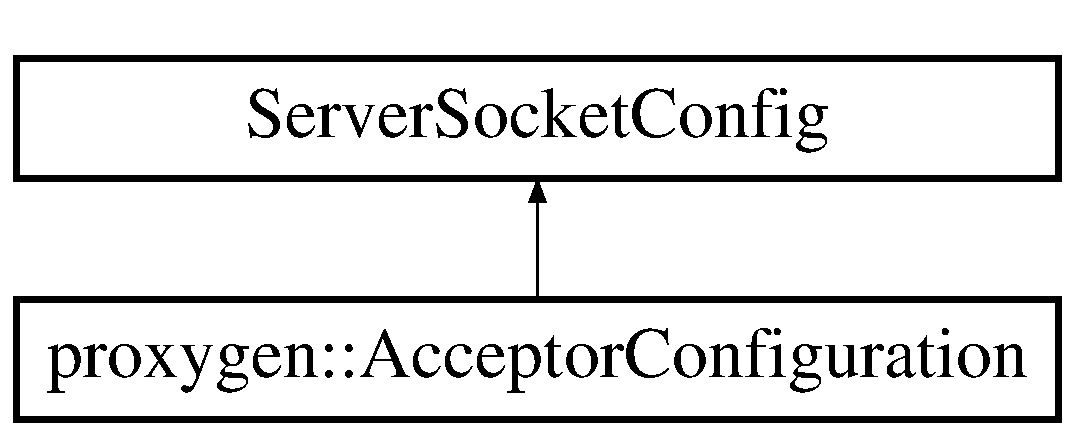
\includegraphics[height=2.000000cm]{structproxygen_1_1AcceptorConfiguration}
\end{center}
\end{figure}
\subsection*{Public Attributes}
\begin{DoxyCompactItemize}
\item 
bool {\bf internal} \{false\}
\item 
bool {\bf H\+T\+T\+P2\+Priorities\+Enabled} \{true\}
\item 
std\+::chrono\+::milliseconds {\bf transaction\+Idle\+Timeout} \{600000\}
\item 
int {\bf spdy\+Compression\+Level} \{Z\+\_\+\+N\+O\+\_\+\+C\+O\+M\+P\+R\+E\+S\+S\+I\+ON\}
\item 
std\+::string {\bf plaintext\+Protocol}
\item 
std\+::list$<$ std\+::string $>$ {\bf allowed\+Plaintext\+Upgrade\+Protocols}
\item 
{\bf Settings\+List} {\bf egress\+Settings}
\item 
uint32\+\_\+t {\bf max\+Concurrent\+Incoming\+Streams} \{0\}
\item 
size\+\_\+t {\bf initial\+Receive\+Window} \{65536\}
\item 
size\+\_\+t {\bf receive\+Stream\+Window\+Size} \{65536\}
\item 
size\+\_\+t {\bf receive\+Session\+Window\+Size} \{65536\}
\item 
int64\+\_\+t {\bf write\+Buffer\+Limit} \{-\/1\}
\end{DoxyCompactItemize}


\subsection{Detailed Description}
Configuration for a single Acceptor.

This configures not only accept behavior, but also some types of S\+SL behavior that may make sense to configure on a per-\/\+V\+IP basis (e.\+g. which cert(s) we use, etc). 

Definition at line 33 of file Acceptor\+Configuration.\+h.



\subsection{Member Data Documentation}
\index{proxygen\+::\+Acceptor\+Configuration@{proxygen\+::\+Acceptor\+Configuration}!allowed\+Plaintext\+Upgrade\+Protocols@{allowed\+Plaintext\+Upgrade\+Protocols}}
\index{allowed\+Plaintext\+Upgrade\+Protocols@{allowed\+Plaintext\+Upgrade\+Protocols}!proxygen\+::\+Acceptor\+Configuration@{proxygen\+::\+Acceptor\+Configuration}}
\subsubsection[{allowed\+Plaintext\+Upgrade\+Protocols}]{\setlength{\rightskip}{0pt plus 5cm}std\+::list$<$std\+::string$>$ proxygen\+::\+Acceptor\+Configuration\+::allowed\+Plaintext\+Upgrade\+Protocols}\label{structproxygen_1_1AcceptorConfiguration_a8cdffbf1ccdbc7a57625d5b30ff7e761}
Comma separated string of protocols that can be upgraded to from H\+T\+T\+P/1.\+1 

Definition at line 65 of file Acceptor\+Configuration.\+h.



Referenced by proxygen\+::\+H\+T\+T\+P\+Default\+Session\+Codec\+Factory\+::get\+Codec(), proxygen\+::\+H\+T\+T\+P\+Server\+Acceptor\+::make\+Config(), and T\+E\+S\+T().

\index{proxygen\+::\+Acceptor\+Configuration@{proxygen\+::\+Acceptor\+Configuration}!egress\+Settings@{egress\+Settings}}
\index{egress\+Settings@{egress\+Settings}!proxygen\+::\+Acceptor\+Configuration@{proxygen\+::\+Acceptor\+Configuration}}
\subsubsection[{egress\+Settings}]{\setlength{\rightskip}{0pt plus 5cm}{\bf Settings\+List} proxygen\+::\+Acceptor\+Configuration\+::egress\+Settings}\label{structproxygen_1_1AcceptorConfiguration_a5f7a2f52cb7355810771600ddf6d398a}
H\+T\+T\+P/2 or S\+P\+DY settings for this acceptor 

Definition at line 70 of file Acceptor\+Configuration.\+h.



Referenced by proxygen\+::\+H\+T\+T\+P\+Server\+Acceptor\+::make\+Config(), and proxygen\+::\+H\+T\+T\+P\+Session\+Acceptor\+::on\+New\+Connection().

\index{proxygen\+::\+Acceptor\+Configuration@{proxygen\+::\+Acceptor\+Configuration}!H\+T\+T\+P2\+Priorities\+Enabled@{H\+T\+T\+P2\+Priorities\+Enabled}}
\index{H\+T\+T\+P2\+Priorities\+Enabled@{H\+T\+T\+P2\+Priorities\+Enabled}!proxygen\+::\+Acceptor\+Configuration@{proxygen\+::\+Acceptor\+Configuration}}
\subsubsection[{H\+T\+T\+P2\+Priorities\+Enabled}]{\setlength{\rightskip}{0pt plus 5cm}bool proxygen\+::\+Acceptor\+Configuration\+::\+H\+T\+T\+P2\+Priorities\+Enabled \{true\}}\label{structproxygen_1_1AcceptorConfiguration_a72b3172a38fa31b89d5a27e21b23825b}
Determines if connection should respect H\+T\+T\+P2 priorities 

Definition at line 44 of file Acceptor\+Configuration.\+h.



Referenced by proxygen\+::\+H\+T\+T\+P\+Session\+Acceptor\+::get\+Http2\+Priorities\+Enabled().

\index{proxygen\+::\+Acceptor\+Configuration@{proxygen\+::\+Acceptor\+Configuration}!initial\+Receive\+Window@{initial\+Receive\+Window}}
\index{initial\+Receive\+Window@{initial\+Receive\+Window}!proxygen\+::\+Acceptor\+Configuration@{proxygen\+::\+Acceptor\+Configuration}}
\subsubsection[{initial\+Receive\+Window}]{\setlength{\rightskip}{0pt plus 5cm}size\+\_\+t proxygen\+::\+Acceptor\+Configuration\+::initial\+Receive\+Window \{65536\}}\label{structproxygen_1_1AcceptorConfiguration_a223d94c0cfe389bb8ce85b91acae47d7}
Flow control parameters.

initial\+Receive\+Window = amount to advertise to peer via S\+E\+T\+T\+I\+N\+GS receive\+Stream\+Window\+Size = amount to increase per-\/stream window via W\+I\+N\+D\+O\+W\+\_\+\+U\+P\+D\+A\+TE receive\+Session\+Window\+Size = amount to increase per-\/session window via W\+I\+N\+D\+O\+W\+\_\+\+U\+P\+D\+A\+TE This also controls the size of the per-\/session read buffer. 

Definition at line 89 of file Acceptor\+Configuration.\+h.



Referenced by proxygen\+::\+H\+T\+T\+P\+Server\+Acceptor\+::make\+Config(), and proxygen\+::\+H\+T\+T\+P\+Session\+Acceptor\+::on\+New\+Connection().

\index{proxygen\+::\+Acceptor\+Configuration@{proxygen\+::\+Acceptor\+Configuration}!internal@{internal}}
\index{internal@{internal}!proxygen\+::\+Acceptor\+Configuration@{proxygen\+::\+Acceptor\+Configuration}}
\subsubsection[{internal}]{\setlength{\rightskip}{0pt plus 5cm}bool proxygen\+::\+Acceptor\+Configuration\+::internal \{false\}}\label{structproxygen_1_1AcceptorConfiguration_a4404bf1e25fd4afa3d3210f86a7d08f8}
Determines if the V\+IP should accept traffic from only internal or external clients. Internal V\+I\+Ps have different behavior (e.\+g. Via headers, etc). 

Definition at line 39 of file Acceptor\+Configuration.\+h.



Referenced by proxygen\+::\+H\+T\+T\+P\+Acceptor\+::is\+Internal().

\index{proxygen\+::\+Acceptor\+Configuration@{proxygen\+::\+Acceptor\+Configuration}!max\+Concurrent\+Incoming\+Streams@{max\+Concurrent\+Incoming\+Streams}}
\index{max\+Concurrent\+Incoming\+Streams@{max\+Concurrent\+Incoming\+Streams}!proxygen\+::\+Acceptor\+Configuration@{proxygen\+::\+Acceptor\+Configuration}}
\subsubsection[{max\+Concurrent\+Incoming\+Streams}]{\setlength{\rightskip}{0pt plus 5cm}uint32\+\_\+t proxygen\+::\+Acceptor\+Configuration\+::max\+Concurrent\+Incoming\+Streams \{0\}}\label{structproxygen_1_1AcceptorConfiguration_a77d134a2cca1d793fe7b56fae3a48d50}
The maximum number of transactions the remote could initiate per connection on protocols that allow multiplexing. 

Definition at line 76 of file Acceptor\+Configuration.\+h.



Referenced by proxygen\+::\+H\+T\+T\+P\+Server\+Acceptor\+::make\+Config(), and proxygen\+::\+H\+T\+T\+P\+Session\+Acceptor\+::on\+New\+Connection().

\index{proxygen\+::\+Acceptor\+Configuration@{proxygen\+::\+Acceptor\+Configuration}!plaintext\+Protocol@{plaintext\+Protocol}}
\index{plaintext\+Protocol@{plaintext\+Protocol}!proxygen\+::\+Acceptor\+Configuration@{proxygen\+::\+Acceptor\+Configuration}}
\subsubsection[{plaintext\+Protocol}]{\setlength{\rightskip}{0pt plus 5cm}std\+::string proxygen\+::\+Acceptor\+Configuration\+::plaintext\+Protocol}\label{structproxygen_1_1AcceptorConfiguration_aa9862c35045ed653e3b2bff41b6985e0}
The name of the protocol to use on non-\/\+T\+LS connections. 

Definition at line 60 of file Acceptor\+Configuration.\+h.



Referenced by proxygen\+::\+H\+T\+T\+P\+Default\+Session\+Codec\+Factory\+::\+H\+T\+T\+P\+Default\+Session\+Codec\+Factory(), proxygen\+::\+H\+T\+T\+P\+Server\+Acceptor\+::make\+Config(), and T\+E\+S\+T().

\index{proxygen\+::\+Acceptor\+Configuration@{proxygen\+::\+Acceptor\+Configuration}!receive\+Session\+Window\+Size@{receive\+Session\+Window\+Size}}
\index{receive\+Session\+Window\+Size@{receive\+Session\+Window\+Size}!proxygen\+::\+Acceptor\+Configuration@{proxygen\+::\+Acceptor\+Configuration}}
\subsubsection[{receive\+Session\+Window\+Size}]{\setlength{\rightskip}{0pt plus 5cm}size\+\_\+t proxygen\+::\+Acceptor\+Configuration\+::receive\+Session\+Window\+Size \{65536\}}\label{structproxygen_1_1AcceptorConfiguration_a9ee5ac616a2bb78f58e8695ebc9ca51f}


Definition at line 91 of file Acceptor\+Configuration.\+h.



Referenced by proxygen\+::\+H\+T\+T\+P\+Server\+Acceptor\+::make\+Config(), and proxygen\+::\+H\+T\+T\+P\+Session\+Acceptor\+::on\+New\+Connection().

\index{proxygen\+::\+Acceptor\+Configuration@{proxygen\+::\+Acceptor\+Configuration}!receive\+Stream\+Window\+Size@{receive\+Stream\+Window\+Size}}
\index{receive\+Stream\+Window\+Size@{receive\+Stream\+Window\+Size}!proxygen\+::\+Acceptor\+Configuration@{proxygen\+::\+Acceptor\+Configuration}}
\subsubsection[{receive\+Stream\+Window\+Size}]{\setlength{\rightskip}{0pt plus 5cm}size\+\_\+t proxygen\+::\+Acceptor\+Configuration\+::receive\+Stream\+Window\+Size \{65536\}}\label{structproxygen_1_1AcceptorConfiguration_a5a176b673f3faefc7b5df7037d8d8c43}


Definition at line 90 of file Acceptor\+Configuration.\+h.



Referenced by proxygen\+::\+H\+T\+T\+P\+Server\+Acceptor\+::make\+Config(), and proxygen\+::\+H\+T\+T\+P\+Session\+Acceptor\+::on\+New\+Connection().

\index{proxygen\+::\+Acceptor\+Configuration@{proxygen\+::\+Acceptor\+Configuration}!spdy\+Compression\+Level@{spdy\+Compression\+Level}}
\index{spdy\+Compression\+Level@{spdy\+Compression\+Level}!proxygen\+::\+Acceptor\+Configuration@{proxygen\+::\+Acceptor\+Configuration}}
\subsubsection[{spdy\+Compression\+Level}]{\setlength{\rightskip}{0pt plus 5cm}int proxygen\+::\+Acceptor\+Configuration\+::spdy\+Compression\+Level \{Z\+\_\+\+N\+O\+\_\+\+C\+O\+M\+P\+R\+E\+S\+S\+I\+ON\}}\label{structproxygen_1_1AcceptorConfiguration_a29cd33d546c98280c53379867e27f240}
The compression level to use for S\+P\+DY headers with responses from this Acceptor. 

Definition at line 55 of file Acceptor\+Configuration.\+h.



Referenced by proxygen\+::\+H\+T\+T\+P\+Default\+Session\+Codec\+Factory\+::get\+Codec().

\index{proxygen\+::\+Acceptor\+Configuration@{proxygen\+::\+Acceptor\+Configuration}!transaction\+Idle\+Timeout@{transaction\+Idle\+Timeout}}
\index{transaction\+Idle\+Timeout@{transaction\+Idle\+Timeout}!proxygen\+::\+Acceptor\+Configuration@{proxygen\+::\+Acceptor\+Configuration}}
\subsubsection[{transaction\+Idle\+Timeout}]{\setlength{\rightskip}{0pt plus 5cm}std\+::chrono\+::milliseconds proxygen\+::\+Acceptor\+Configuration\+::transaction\+Idle\+Timeout \{600000\}}\label{structproxygen_1_1AcceptorConfiguration_a63f89ab89dda9680abbe3c171de16b2f}
The number of milliseconds a transaction can be idle before we close it. 

Definition at line 49 of file Acceptor\+Configuration.\+h.



Referenced by proxygen\+::\+H\+T\+T\+P\+Acceptor\+::init(), and proxygen\+::\+H\+T\+T\+P\+Server\+Acceptor\+::make\+Config().

\index{proxygen\+::\+Acceptor\+Configuration@{proxygen\+::\+Acceptor\+Configuration}!write\+Buffer\+Limit@{write\+Buffer\+Limit}}
\index{write\+Buffer\+Limit@{write\+Buffer\+Limit}!proxygen\+::\+Acceptor\+Configuration@{proxygen\+::\+Acceptor\+Configuration}}
\subsubsection[{write\+Buffer\+Limit}]{\setlength{\rightskip}{0pt plus 5cm}int64\+\_\+t proxygen\+::\+Acceptor\+Configuration\+::write\+Buffer\+Limit \{-\/1\}}\label{structproxygen_1_1AcceptorConfiguration_a861ef94d8f5040dcf136fd5f9db22b1c}
These parameters control how many bytes \doxyref{H\+T\+T\+P\+Session}{p.}{classproxygen_1_1HTTPSession}\textquotesingle{}s will buffer in user space before applying backpressure to handlers. -\/1 means use the built-\/in \doxyref{H\+T\+T\+P\+Session}{p.}{classproxygen_1_1HTTPSession} default (64kb) 

Definition at line 98 of file Acceptor\+Configuration.\+h.



Referenced by proxygen\+::\+H\+T\+T\+P\+Session\+Acceptor\+::on\+New\+Connection().



The documentation for this struct was generated from the following file\+:\begin{DoxyCompactItemize}
\item 
proxygen/lib/services/{\bf Acceptor\+Configuration.\+h}\end{DoxyCompactItemize}

\section{proxygen\+:\+:Acceptor\+Factory Class Reference}
\label{classproxygen_1_1AcceptorFactory}\index{proxygen\+::\+Acceptor\+Factory@{proxygen\+::\+Acceptor\+Factory}}
Inheritance diagram for proxygen\+:\+:Acceptor\+Factory\+:\begin{figure}[H]
\begin{center}
\leavevmode
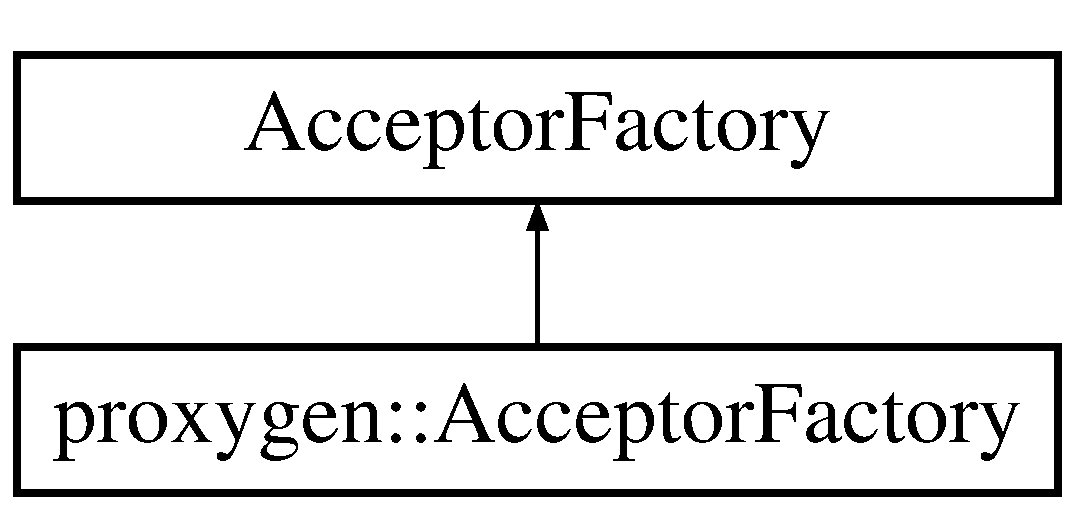
\includegraphics[height=2.000000cm]{classproxygen_1_1AcceptorFactory}
\end{center}
\end{figure}
\subsection*{Public Member Functions}
\begin{DoxyCompactItemize}
\item 
{\bf Acceptor\+Factory} (std\+::shared\+\_\+ptr$<$ {\bf H\+T\+T\+P\+Server\+Options} $>$ options, std\+::shared\+\_\+ptr$<$ {\bf H\+T\+T\+P\+Codec\+Factory} $>$ codec\+Factory, {\bf Acceptor\+Configuration} config, {\bf H\+T\+T\+P\+Session\+::\+Info\+Callback} $\ast$session\+Info\+Cb)
\item 
std\+::shared\+\_\+ptr$<$ wangle\+::\+Acceptor $>$ {\bf new\+Acceptor} (folly\+::\+Event\+Base $\ast$event\+Base) override
\end{DoxyCompactItemize}
\subsection*{Private Attributes}
\begin{DoxyCompactItemize}
\item 
std\+::shared\+\_\+ptr$<$ {\bf H\+T\+T\+P\+Server\+Options} $>$ {\bf options\+\_\+}
\item 
std\+::shared\+\_\+ptr$<$ {\bf H\+T\+T\+P\+Codec\+Factory} $>$ {\bf codec\+Factory\+\_\+}
\item 
{\bf Acceptor\+Configuration} {\bf config\+\_\+}
\item 
{\bf H\+T\+T\+P\+Session\+::\+Info\+Callback} $\ast$ {\bf session\+Info\+Cb\+\_\+}
\end{DoxyCompactItemize}


\subsection{Detailed Description}


Definition at line 31 of file H\+T\+T\+P\+Server.\+cpp.



\subsection{Constructor \& Destructor Documentation}
\index{proxygen\+::\+Acceptor\+Factory@{proxygen\+::\+Acceptor\+Factory}!Acceptor\+Factory@{Acceptor\+Factory}}
\index{Acceptor\+Factory@{Acceptor\+Factory}!proxygen\+::\+Acceptor\+Factory@{proxygen\+::\+Acceptor\+Factory}}
\subsubsection[{Acceptor\+Factory(std\+::shared\+\_\+ptr$<$ H\+T\+T\+P\+Server\+Options $>$ options, std\+::shared\+\_\+ptr$<$ H\+T\+T\+P\+Codec\+Factory $>$ codec\+Factory, Acceptor\+Configuration config, H\+T\+T\+P\+Session\+::\+Info\+Callback $\ast$session\+Info\+Cb)}]{\setlength{\rightskip}{0pt plus 5cm}proxygen\+::\+Acceptor\+Factory\+::\+Acceptor\+Factory (
\begin{DoxyParamCaption}
\item[{std\+::shared\+\_\+ptr$<$ {\bf H\+T\+T\+P\+Server\+Options} $>$}]{options, }
\item[{std\+::shared\+\_\+ptr$<$ {\bf H\+T\+T\+P\+Codec\+Factory} $>$}]{codec\+Factory, }
\item[{{\bf Acceptor\+Configuration}}]{config, }
\item[{{\bf H\+T\+T\+P\+Session\+::\+Info\+Callback} $\ast$}]{session\+Info\+Cb}
\end{DoxyParamCaption}
)\hspace{0.3cm}{\ttfamily [inline]}}\label{classproxygen_1_1AcceptorFactory_a814286e5fe4f64d129c3626ed02deda5}


Definition at line 33 of file H\+T\+T\+P\+Server.\+cpp.


\begin{DoxyCode}
36                                                           :
37       options_(options),
38       codecFactory_(codecFactory),
39       config_(config),
40       sessionInfoCb_(sessionInfoCb) \{\}
\end{DoxyCode}


\subsection{Member Function Documentation}
\index{proxygen\+::\+Acceptor\+Factory@{proxygen\+::\+Acceptor\+Factory}!new\+Acceptor@{new\+Acceptor}}
\index{new\+Acceptor@{new\+Acceptor}!proxygen\+::\+Acceptor\+Factory@{proxygen\+::\+Acceptor\+Factory}}
\subsubsection[{new\+Acceptor(folly\+::\+Event\+Base $\ast$event\+Base) override}]{\setlength{\rightskip}{0pt plus 5cm}std\+::shared\+\_\+ptr$<$wangle\+::\+Acceptor$>$ proxygen\+::\+Acceptor\+Factory\+::new\+Acceptor (
\begin{DoxyParamCaption}
\item[{folly\+::\+Event\+Base $\ast$}]{event\+Base}
\end{DoxyParamCaption}
)\hspace{0.3cm}{\ttfamily [inline]}, {\ttfamily [override]}}\label{classproxygen_1_1AcceptorFactory_a94ea073002f279b52acfce1952041ca8}


Definition at line 41 of file H\+T\+T\+P\+Server.\+cpp.



References codec\+Factory\+\_\+, config\+\_\+, proxygen\+::\+H\+T\+T\+P\+Server\+Acceptor\+::make(), options\+\_\+, and session\+Info\+Cb\+\_\+.


\begin{DoxyCode}
42                                           \{
43     \textcolor{keyword}{auto} acc = std::shared\_ptr<HTTPServerAcceptor>(
44       HTTPServerAcceptor::make(config_, *options_, codecFactory_).release());
45     \textcolor{keywordflow}{if} (sessionInfoCb_) \{
46       acc->setSessionInfoCallback(sessionInfoCb_);
47     \}
48     acc->init(\textcolor{keyword}{nullptr}, eventBase);
49     \textcolor{keywordflow}{return} acc;
50   \}
\end{DoxyCode}


\subsection{Member Data Documentation}
\index{proxygen\+::\+Acceptor\+Factory@{proxygen\+::\+Acceptor\+Factory}!codec\+Factory\+\_\+@{codec\+Factory\+\_\+}}
\index{codec\+Factory\+\_\+@{codec\+Factory\+\_\+}!proxygen\+::\+Acceptor\+Factory@{proxygen\+::\+Acceptor\+Factory}}
\subsubsection[{codec\+Factory\+\_\+}]{\setlength{\rightskip}{0pt plus 5cm}std\+::shared\+\_\+ptr$<${\bf H\+T\+T\+P\+Codec\+Factory}$>$ proxygen\+::\+Acceptor\+Factory\+::codec\+Factory\+\_\+\hspace{0.3cm}{\ttfamily [private]}}\label{classproxygen_1_1AcceptorFactory_a128482b94fbd811cf75d53fb61d25be9}


Definition at line 54 of file H\+T\+T\+P\+Server.\+cpp.



Referenced by new\+Acceptor().

\index{proxygen\+::\+Acceptor\+Factory@{proxygen\+::\+Acceptor\+Factory}!config\+\_\+@{config\+\_\+}}
\index{config\+\_\+@{config\+\_\+}!proxygen\+::\+Acceptor\+Factory@{proxygen\+::\+Acceptor\+Factory}}
\subsubsection[{config\+\_\+}]{\setlength{\rightskip}{0pt plus 5cm}{\bf Acceptor\+Configuration} proxygen\+::\+Acceptor\+Factory\+::config\+\_\+\hspace{0.3cm}{\ttfamily [private]}}\label{classproxygen_1_1AcceptorFactory_a4c92f6b3e6817c4c6085aacffaee5be5}


Definition at line 55 of file H\+T\+T\+P\+Server.\+cpp.



Referenced by new\+Acceptor().

\index{proxygen\+::\+Acceptor\+Factory@{proxygen\+::\+Acceptor\+Factory}!options\+\_\+@{options\+\_\+}}
\index{options\+\_\+@{options\+\_\+}!proxygen\+::\+Acceptor\+Factory@{proxygen\+::\+Acceptor\+Factory}}
\subsubsection[{options\+\_\+}]{\setlength{\rightskip}{0pt plus 5cm}std\+::shared\+\_\+ptr$<${\bf H\+T\+T\+P\+Server\+Options}$>$ proxygen\+::\+Acceptor\+Factory\+::options\+\_\+\hspace{0.3cm}{\ttfamily [private]}}\label{classproxygen_1_1AcceptorFactory_ac855a330ec68de58aefa6115c54d0333}


Definition at line 53 of file H\+T\+T\+P\+Server.\+cpp.



Referenced by new\+Acceptor().

\index{proxygen\+::\+Acceptor\+Factory@{proxygen\+::\+Acceptor\+Factory}!session\+Info\+Cb\+\_\+@{session\+Info\+Cb\+\_\+}}
\index{session\+Info\+Cb\+\_\+@{session\+Info\+Cb\+\_\+}!proxygen\+::\+Acceptor\+Factory@{proxygen\+::\+Acceptor\+Factory}}
\subsubsection[{session\+Info\+Cb\+\_\+}]{\setlength{\rightskip}{0pt plus 5cm}{\bf H\+T\+T\+P\+Session\+::\+Info\+Callback}$\ast$ proxygen\+::\+Acceptor\+Factory\+::session\+Info\+Cb\+\_\+\hspace{0.3cm}{\ttfamily [private]}}\label{classproxygen_1_1AcceptorFactory_a3949290eca84b57d147606a91fa1950f}


Definition at line 56 of file H\+T\+T\+P\+Server.\+cpp.



Referenced by new\+Acceptor().



The documentation for this class was generated from the following file\+:\begin{DoxyCompactItemize}
\item 
proxygen/httpserver/{\bf H\+T\+T\+P\+Server.\+cpp}\end{DoxyCompactItemize}

\section{proxygen\+:\+:compress\+:\+:Compression\+Scheme\+:\+:Ack Struct Reference}
\label{structproxygen_1_1compress_1_1CompressionScheme_1_1Ack}\index{proxygen\+::compress\+::\+Compression\+Scheme\+::\+Ack@{proxygen\+::compress\+::\+Compression\+Scheme\+::\+Ack}}


{\ttfamily \#include $<$Compression\+Scheme.\+h$>$}

Inheritance diagram for proxygen\+:\+:compress\+:\+:Compression\+Scheme\+:\+:Ack\+:\begin{figure}[H]
\begin{center}
\leavevmode
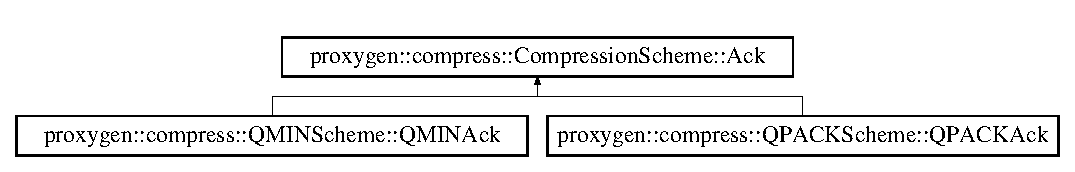
\includegraphics[height=1.866667cm]{structproxygen_1_1compress_1_1CompressionScheme_1_1Ack}
\end{center}
\end{figure}
\subsection*{Public Member Functions}
\begin{DoxyCompactItemize}
\item 
virtual {\bf $\sim$\+Ack} ()
\end{DoxyCompactItemize}


\subsection{Detailed Description}


Definition at line 28 of file Compression\+Scheme.\+h.



\subsection{Constructor \& Destructor Documentation}
\index{proxygen\+::compress\+::\+Compression\+Scheme\+::\+Ack@{proxygen\+::compress\+::\+Compression\+Scheme\+::\+Ack}!````~Ack@{$\sim$\+Ack}}
\index{````~Ack@{$\sim$\+Ack}!proxygen\+::compress\+::\+Compression\+Scheme\+::\+Ack@{proxygen\+::compress\+::\+Compression\+Scheme\+::\+Ack}}
\subsubsection[{$\sim$\+Ack()}]{\setlength{\rightskip}{0pt plus 5cm}virtual proxygen\+::compress\+::\+Compression\+Scheme\+::\+Ack\+::$\sim$\+Ack (
\begin{DoxyParamCaption}
{}
\end{DoxyParamCaption}
)\hspace{0.3cm}{\ttfamily [inline]}, {\ttfamily [virtual]}}\label{structproxygen_1_1compress_1_1CompressionScheme_1_1Ack_ae1dfeda2ebd2ead894fa9212b1132d8f}


Definition at line 29 of file Compression\+Scheme.\+h.



References proxygen\+::compress\+::\+Compression\+Scheme\+::decode(), proxygen\+::compress\+::\+Compression\+Scheme\+::encode(), proxygen\+::compress\+::\+Compression\+Scheme\+::get\+Ack(), proxygen\+::compress\+::\+Compression\+Scheme\+::get\+Hol\+Block\+Count(), proxygen\+::compress\+::\+Compression\+Scheme\+::recv\+Ack(), and proxygen\+::compress\+::\+Compression\+Scheme\+::run\+Loop\+Callback().


\begin{DoxyCode}
29                    \{
30     \}
\end{DoxyCode}


The documentation for this struct was generated from the following file\+:\begin{DoxyCompactItemize}
\item 
proxygen/lib/http/codec/compress/experimental/simulator/{\bf Compression\+Scheme.\+h}\end{DoxyCompactItemize}

\section{proxygen\+:\+:Ack\+Byte\+Event Class Reference}
\label{classproxygen_1_1AckByteEvent}\index{proxygen\+::\+Ack\+Byte\+Event@{proxygen\+::\+Ack\+Byte\+Event}}


{\ttfamily \#include $<$Byte\+Events.\+h$>$}

Inheritance diagram for proxygen\+:\+:Ack\+Byte\+Event\+:\begin{figure}[H]
\begin{center}
\leavevmode
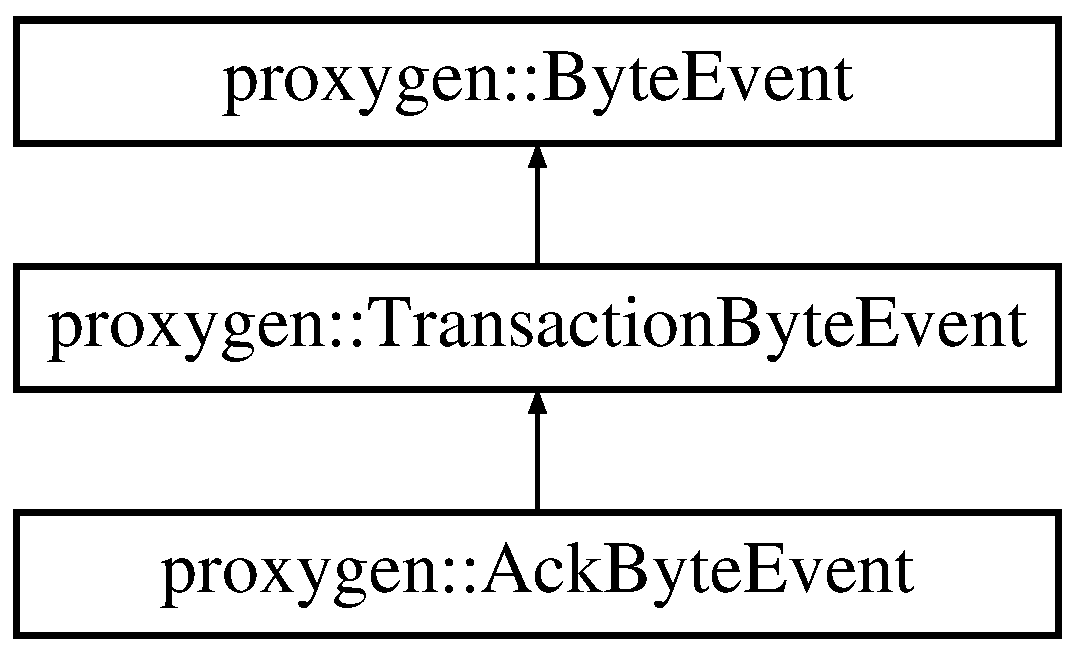
\includegraphics[height=3.000000cm]{classproxygen_1_1AckByteEvent}
\end{center}
\end{figure}
\subsection*{Public Member Functions}
\begin{DoxyCompactItemize}
\item 
{\bf Ack\+Byte\+Event} ({\bf Ack\+Timeout\+::\+Callback} $\ast$callback, uint64\+\_\+t byte\+No, {\bf Event\+Type} event\+Type, {\bf H\+T\+T\+P\+Transaction} $\ast$txn)
\end{DoxyCompactItemize}
\subsection*{Public Attributes}
\begin{DoxyCompactItemize}
\item 
{\bf Ack\+Timeout} {\bf timeout}
\end{DoxyCompactItemize}
\subsection*{Additional Inherited Members}


\subsection{Detailed Description}


Definition at line 88 of file Byte\+Events.\+h.



\subsection{Constructor \& Destructor Documentation}
\index{proxygen\+::\+Ack\+Byte\+Event@{proxygen\+::\+Ack\+Byte\+Event}!Ack\+Byte\+Event@{Ack\+Byte\+Event}}
\index{Ack\+Byte\+Event@{Ack\+Byte\+Event}!proxygen\+::\+Ack\+Byte\+Event@{proxygen\+::\+Ack\+Byte\+Event}}
\subsubsection[{Ack\+Byte\+Event(\+Ack\+Timeout\+::\+Callback $\ast$callback, uint64\+\_\+t byte\+No, Event\+Type event\+Type, H\+T\+T\+P\+Transaction $\ast$txn)}]{\setlength{\rightskip}{0pt plus 5cm}proxygen\+::\+Ack\+Byte\+Event\+::\+Ack\+Byte\+Event (
\begin{DoxyParamCaption}
\item[{{\bf Ack\+Timeout\+::\+Callback} $\ast$}]{callback, }
\item[{uint64\+\_\+t}]{byte\+No, }
\item[{{\bf Event\+Type}}]{event\+Type, }
\item[{{\bf H\+T\+T\+P\+Transaction} $\ast$}]{txn}
\end{DoxyParamCaption}
)\hspace{0.3cm}{\ttfamily [inline]}}\label{classproxygen_1_1AckByteEvent_acb066fcd2cc93f220c37e11e2debed8c}


Definition at line 90 of file Byte\+Events.\+h.


\begin{DoxyCode}
94       : TransactionByteEvent(byteNo, eventType, txn),
95         timeout(callback, byteNo) \{\}
\end{DoxyCode}


\subsection{Member Data Documentation}
\index{proxygen\+::\+Ack\+Byte\+Event@{proxygen\+::\+Ack\+Byte\+Event}!timeout@{timeout}}
\index{timeout@{timeout}!proxygen\+::\+Ack\+Byte\+Event@{proxygen\+::\+Ack\+Byte\+Event}}
\subsubsection[{timeout}]{\setlength{\rightskip}{0pt plus 5cm}{\bf Ack\+Timeout} proxygen\+::\+Ack\+Byte\+Event\+::timeout}\label{classproxygen_1_1AckByteEvent_a10b4acefa8b60d3daa95297a15424e61}


Definition at line 97 of file Byte\+Events.\+h.



The documentation for this class was generated from the following file\+:\begin{DoxyCompactItemize}
\item 
proxygen/lib/http/session/{\bf Byte\+Events.\+h}\end{DoxyCompactItemize}

\section{proxygen\+:\+:Ack\+Latency\+Event Struct Reference}
\label{structproxygen_1_1AckLatencyEvent}\index{proxygen\+::\+Ack\+Latency\+Event@{proxygen\+::\+Ack\+Latency\+Event}}


{\ttfamily \#include $<$Ack\+Latency\+Event.\+h$>$}

\subsection*{Public Attributes}
\begin{DoxyCompactItemize}
\item 
unsigned int {\bf byte\+No}
\item 
std\+::chrono\+::nanoseconds {\bf latency}
\end{DoxyCompactItemize}


\subsection{Detailed Description}


Definition at line 16 of file Ack\+Latency\+Event.\+h.



\subsection{Member Data Documentation}
\index{proxygen\+::\+Ack\+Latency\+Event@{proxygen\+::\+Ack\+Latency\+Event}!byte\+No@{byte\+No}}
\index{byte\+No@{byte\+No}!proxygen\+::\+Ack\+Latency\+Event@{proxygen\+::\+Ack\+Latency\+Event}}
\subsubsection[{byte\+No}]{\setlength{\rightskip}{0pt plus 5cm}unsigned int proxygen\+::\+Ack\+Latency\+Event\+::byte\+No}\label{structproxygen_1_1AckLatencyEvent_a614e7ef0bafbb50ab4c724ab6c29c39a}


Definition at line 18 of file Ack\+Latency\+Event.\+h.

\index{proxygen\+::\+Ack\+Latency\+Event@{proxygen\+::\+Ack\+Latency\+Event}!latency@{latency}}
\index{latency@{latency}!proxygen\+::\+Ack\+Latency\+Event@{proxygen\+::\+Ack\+Latency\+Event}}
\subsubsection[{latency}]{\setlength{\rightskip}{0pt plus 5cm}std\+::chrono\+::nanoseconds proxygen\+::\+Ack\+Latency\+Event\+::latency}\label{structproxygen_1_1AckLatencyEvent_a05f7213062534e8b13052e946447e1fb}


Definition at line 20 of file Ack\+Latency\+Event.\+h.



The documentation for this struct was generated from the following file\+:\begin{DoxyCompactItemize}
\item 
proxygen/lib/http/session/{\bf Ack\+Latency\+Event.\+h}\end{DoxyCompactItemize}

\section{proxygen\+:\+:Ack\+Timeout Class Reference}
\label{classproxygen_1_1AckTimeout}\index{proxygen\+::\+Ack\+Timeout@{proxygen\+::\+Ack\+Timeout}}


{\ttfamily \#include $<$Byte\+Events.\+h$>$}

Inheritance diagram for proxygen\+:\+:Ack\+Timeout\+:\begin{figure}[H]
\begin{center}
\leavevmode
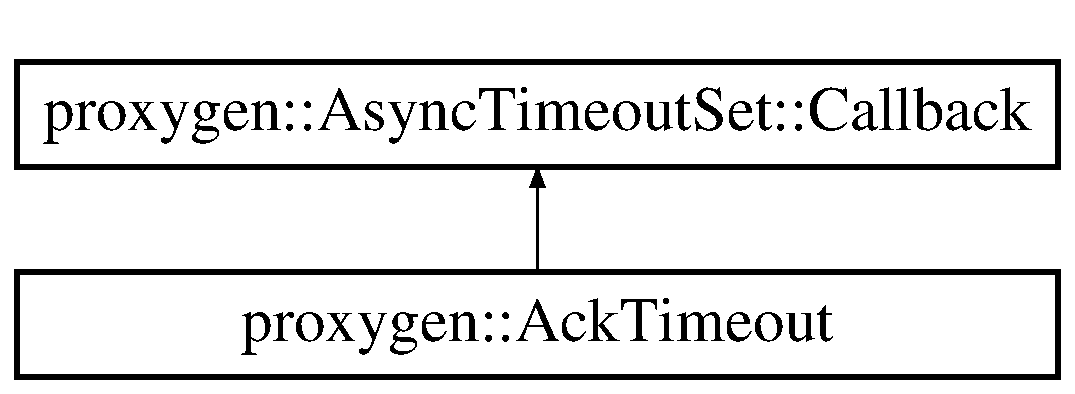
\includegraphics[height=2.000000cm]{classproxygen_1_1AckTimeout}
\end{center}
\end{figure}
\subsection*{Classes}
\begin{DoxyCompactItemize}
\item 
class {\bf Callback}
\end{DoxyCompactItemize}
\subsection*{Public Member Functions}
\begin{DoxyCompactItemize}
\item 
{\bf Ack\+Timeout} ({\bf Callback} $\ast$callback, uint64\+\_\+t byte\+No)
\item 
void {\bf timeout\+Expired} () noexceptoverride
\end{DoxyCompactItemize}
\subsection*{Private Attributes}
\begin{DoxyCompactItemize}
\item 
{\bf Callback} $\ast$ {\bf callback\+\_\+}
\item 
uint64\+\_\+t {\bf byte\+No\+\_\+}
\end{DoxyCompactItemize}


\subsection{Detailed Description}


Definition at line 63 of file Byte\+Events.\+h.



\subsection{Constructor \& Destructor Documentation}
\index{proxygen\+::\+Ack\+Timeout@{proxygen\+::\+Ack\+Timeout}!Ack\+Timeout@{Ack\+Timeout}}
\index{Ack\+Timeout@{Ack\+Timeout}!proxygen\+::\+Ack\+Timeout@{proxygen\+::\+Ack\+Timeout}}
\subsubsection[{Ack\+Timeout(\+Callback $\ast$callback, uint64\+\_\+t byte\+No)}]{\setlength{\rightskip}{0pt plus 5cm}proxygen\+::\+Ack\+Timeout\+::\+Ack\+Timeout (
\begin{DoxyParamCaption}
\item[{{\bf Callback} $\ast$}]{callback, }
\item[{uint64\+\_\+t}]{byte\+No}
\end{DoxyParamCaption}
)\hspace{0.3cm}{\ttfamily [inline]}}\label{classproxygen_1_1AckTimeout_a7b869a8a7594d430f793e12ab5dfdc5e}


Definition at line 76 of file Byte\+Events.\+h.


\begin{DoxyCode}
77       : callback_(callback), byteNo_(byteNo) \{\}
\end{DoxyCode}


\subsection{Member Function Documentation}
\index{proxygen\+::\+Ack\+Timeout@{proxygen\+::\+Ack\+Timeout}!timeout\+Expired@{timeout\+Expired}}
\index{timeout\+Expired@{timeout\+Expired}!proxygen\+::\+Ack\+Timeout@{proxygen\+::\+Ack\+Timeout}}
\subsubsection[{timeout\+Expired() noexceptoverride}]{\setlength{\rightskip}{0pt plus 5cm}void proxygen\+::\+Ack\+Timeout\+::timeout\+Expired (
\begin{DoxyParamCaption}
{}
\end{DoxyParamCaption}
)\hspace{0.3cm}{\ttfamily [inline]}, {\ttfamily [override]}, {\ttfamily [virtual]}, {\ttfamily [noexcept]}}\label{classproxygen_1_1AckTimeout_a4e71983dc975851e4720f40d57a58308}
\doxyref{timeout\+Expired()}{p.}{classproxygen_1_1AckTimeout_a4e71983dc975851e4720f40d57a58308} is invoked when the timeout has expired. 

Implements {\bf proxygen\+::\+Async\+Timeout\+Set\+::\+Callback} \doxyref{}{p.}{classproxygen_1_1AsyncTimeoutSet_1_1Callback_a6c1534935d53209440d6b02c7a69e96c}.



Definition at line 79 of file Byte\+Events.\+h.


\begin{DoxyCode}
79                                           \{
80     callback_->ackTimeoutExpired(byteNo_);
81   \}
\end{DoxyCode}


\subsection{Member Data Documentation}
\index{proxygen\+::\+Ack\+Timeout@{proxygen\+::\+Ack\+Timeout}!byte\+No\+\_\+@{byte\+No\+\_\+}}
\index{byte\+No\+\_\+@{byte\+No\+\_\+}!proxygen\+::\+Ack\+Timeout@{proxygen\+::\+Ack\+Timeout}}
\subsubsection[{byte\+No\+\_\+}]{\setlength{\rightskip}{0pt plus 5cm}uint64\+\_\+t proxygen\+::\+Ack\+Timeout\+::byte\+No\+\_\+\hspace{0.3cm}{\ttfamily [private]}}\label{classproxygen_1_1AckTimeout_ace86ce8cf2531b28423766d2e787e11f}


Definition at line 85 of file Byte\+Events.\+h.

\index{proxygen\+::\+Ack\+Timeout@{proxygen\+::\+Ack\+Timeout}!callback\+\_\+@{callback\+\_\+}}
\index{callback\+\_\+@{callback\+\_\+}!proxygen\+::\+Ack\+Timeout@{proxygen\+::\+Ack\+Timeout}}
\subsubsection[{callback\+\_\+}]{\setlength{\rightskip}{0pt plus 5cm}{\bf Callback}$\ast$ proxygen\+::\+Ack\+Timeout\+::callback\+\_\+\hspace{0.3cm}{\ttfamily [private]}}\label{classproxygen_1_1AckTimeout_a77aec09fff5477803aefae1fad3bf8c9}


Definition at line 84 of file Byte\+Events.\+h.



The documentation for this class was generated from the following file\+:\begin{DoxyCompactItemize}
\item 
proxygen/lib/http/session/{\bf Byte\+Events.\+h}\end{DoxyCompactItemize}

\section{proxygen\+:\+:Ascii\+Case\+Underscore\+Insensitive Struct Reference}
\label{structproxygen_1_1AsciiCaseUnderscoreInsensitive}\index{proxygen\+::\+Ascii\+Case\+Underscore\+Insensitive@{proxygen\+::\+Ascii\+Case\+Underscore\+Insensitive}}


{\ttfamily \#include $<$Util\+Inl.\+h$>$}

\subsection*{Public Member Functions}
\begin{DoxyCompactItemize}
\item 
bool {\bf operator()} (char lhs, char rhs) const 
\end{DoxyCompactItemize}


\subsection{Detailed Description}


Definition at line 25 of file Util\+Inl.\+h.



\subsection{Member Function Documentation}
\index{proxygen\+::\+Ascii\+Case\+Underscore\+Insensitive@{proxygen\+::\+Ascii\+Case\+Underscore\+Insensitive}!operator()@{operator()}}
\index{operator()@{operator()}!proxygen\+::\+Ascii\+Case\+Underscore\+Insensitive@{proxygen\+::\+Ascii\+Case\+Underscore\+Insensitive}}
\subsubsection[{operator()(char lhs, char rhs) const }]{\setlength{\rightskip}{0pt plus 5cm}bool proxygen\+::\+Ascii\+Case\+Underscore\+Insensitive\+::operator() (
\begin{DoxyParamCaption}
\item[{char}]{lhs, }
\item[{char}]{rhs}
\end{DoxyParamCaption}
) const\hspace{0.3cm}{\ttfamily [inline]}}\label{structproxygen_1_1AsciiCaseUnderscoreInsensitive_a256cd3e8583a3c7a867355134c38e478}


Definition at line 26 of file Util\+Inl.\+h.


\begin{DoxyCode}
26                                             \{
27     \textcolor{keywordflow}{if} (lhs == \textcolor{charliteral}{'\_'}) \{
28       lhs = \textcolor{charliteral}{'-'};
29     \}
30     \textcolor{keywordflow}{if} (rhs == \textcolor{charliteral}{'\_'}) \{
31       rhs = \textcolor{charliteral}{'-'};
32     \}
33     \textcolor{keywordflow}{return} folly::AsciiCaseInsensitive()(lhs, rhs);
34   \}
\end{DoxyCode}


The documentation for this struct was generated from the following file\+:\begin{DoxyCompactItemize}
\item 
proxygen/lib/utils/{\bf Util\+Inl.\+h}\end{DoxyCompactItemize}

\section{proxygen\+:\+:Async\+Timeout\+Set Class Reference}
\label{classproxygen_1_1AsyncTimeoutSet}\index{proxygen\+::\+Async\+Timeout\+Set@{proxygen\+::\+Async\+Timeout\+Set}}


{\ttfamily \#include $<$Async\+Timeout\+Set.\+h$>$}

Inheritance diagram for proxygen\+:\+:Async\+Timeout\+Set\+:\begin{figure}[H]
\begin{center}
\leavevmode
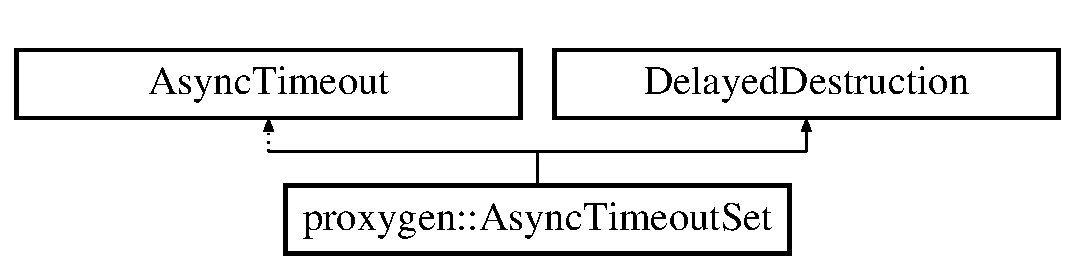
\includegraphics[height=2.000000cm]{classproxygen_1_1AsyncTimeoutSet}
\end{center}
\end{figure}
\subsection*{Classes}
\begin{DoxyCompactItemize}
\item 
class {\bf Callback}
\item 
class {\bf Timeout\+Clock}
\end{DoxyCompactItemize}
\subsection*{Public Types}
\begin{DoxyCompactItemize}
\item 
using {\bf Unique\+Ptr} = std\+::unique\+\_\+ptr$<$ {\bf Async\+Timeout\+Set}, Destructor $>$
\end{DoxyCompactItemize}
\subsection*{Public Member Functions}
\begin{DoxyCompactItemize}
\item 
{\bf Async\+Timeout\+Set} (folly\+::\+Timeout\+Manager $\ast$timeout\+Manager, std\+::chrono\+::milliseconds interval\+MS, std\+::chrono\+::milliseconds at\+Most\+EveryN=std\+::chrono\+::milliseconds(0), {\bf Timeout\+Clock} $\ast$timeout\+Clock={\bf nullptr})
\item 
{\bf Async\+Timeout\+Set} (folly\+::\+Timeout\+Manager $\ast$timeout\+Manager, Internal\+Enum internal, std\+::chrono\+::milliseconds interval\+MS, std\+::chrono\+::milliseconds at\+Most\+EveryN=std\+::chrono\+::milliseconds(0))
\item 
void {\bf destroy} () override
\item 
std\+::chrono\+::milliseconds {\bf get\+Interval} () const 
\item 
void {\bf schedule\+Timeout} ({\bf Callback} $\ast$callback)
\item 
void {\bf fire\+At\+Most\+Every} (const std\+::chrono\+::milliseconds \&ms)
\item 
{\bf Callback} $\ast$ {\bf front} ()
\item 
const {\bf Callback} $\ast$ {\bf front} () const 
\end{DoxyCompactItemize}
\subsection*{Protected Member Functions}
\begin{DoxyCompactItemize}
\item 
{\bf $\sim$\+Async\+Timeout\+Set} () override
\end{DoxyCompactItemize}
\subsection*{Private Member Functions}
\begin{DoxyCompactItemize}
\item 
{\bf Async\+Timeout\+Set} ({\bf Async\+Timeout\+Set} const \&)=delete
\item 
{\bf Async\+Timeout\+Set} \& {\bf operator=} ({\bf Async\+Timeout\+Set} const \&)=delete
\item 
void {\bf head\+Changed} ()
\item 
void {\bf timeout\+Expired} () noexceptoverride
\end{DoxyCompactItemize}
\subsection*{Private Attributes}
\begin{DoxyCompactItemize}
\item 
{\bf Timeout\+Clock} \& {\bf timeout\+Clock\+\_\+}
\item 
{\bf Callback} $\ast$ {\bf head\+\_\+}
\item 
{\bf Callback} $\ast$ {\bf tail\+\_\+}
\item 
std\+::chrono\+::milliseconds {\bf interval\+\_\+}
\item 
std\+::chrono\+::milliseconds {\bf at\+Most\+Every\+N\+\_\+}
\item 
bool {\bf in\+Timeout\+Expired\+\_\+} \{false\}
\end{DoxyCompactItemize}


\subsection{Detailed Description}
\doxyref{Async\+Timeout\+Set}{p.}{classproxygen_1_1AsyncTimeoutSet} exists for efficiently managing a group of timeouts events that always have the same timeout interval.

\doxyref{Async\+Timeout\+Set}{p.}{classproxygen_1_1AsyncTimeoutSet} takes advantage of the fact that the timeouts are always scheduled in sorted order. (Since each timeout has the same interval, when a new timeout is scheduled it will always be the last timeout in the set.) This avoids the need to perform any additional sorting of the timeouts within a single \doxyref{Async\+Timeout\+Set}{p.}{classproxygen_1_1AsyncTimeoutSet}.

\doxyref{Async\+Timeout\+Set}{p.}{classproxygen_1_1AsyncTimeoutSet} is useful whenever you have a large group of objects that each need their own timeout, but with the same interval for each object. For example, managing idle timeouts for thousands of connection, or scheduling health checks for a large group of servers.

Note, this class may not be needed given libevent\textquotesingle{}s event\+\_\+base\+\_\+init\+\_\+common\+\_\+timeout(). We should look into using that. 

Definition at line 40 of file Async\+Timeout\+Set.\+h.



\subsection{Member Typedef Documentation}
\index{proxygen\+::\+Async\+Timeout\+Set@{proxygen\+::\+Async\+Timeout\+Set}!Unique\+Ptr@{Unique\+Ptr}}
\index{Unique\+Ptr@{Unique\+Ptr}!proxygen\+::\+Async\+Timeout\+Set@{proxygen\+::\+Async\+Timeout\+Set}}
\subsubsection[{Unique\+Ptr}]{\setlength{\rightskip}{0pt plus 5cm}using {\bf proxygen\+::\+Async\+Timeout\+Set\+::\+Unique\+Ptr} =  std\+::unique\+\_\+ptr$<${\bf Async\+Timeout\+Set}, Destructor$>$}\label{classproxygen_1_1AsyncTimeoutSet_a6504975452bb527d5ca5ab8d83fef9d6}


Definition at line 43 of file Async\+Timeout\+Set.\+h.



\subsection{Constructor \& Destructor Documentation}
\index{proxygen\+::\+Async\+Timeout\+Set@{proxygen\+::\+Async\+Timeout\+Set}!Async\+Timeout\+Set@{Async\+Timeout\+Set}}
\index{Async\+Timeout\+Set@{Async\+Timeout\+Set}!proxygen\+::\+Async\+Timeout\+Set@{proxygen\+::\+Async\+Timeout\+Set}}
\subsubsection[{Async\+Timeout\+Set(folly\+::\+Timeout\+Manager $\ast$timeout\+Manager, std\+::chrono\+::milliseconds interval\+M\+S, std\+::chrono\+::milliseconds at\+Most\+Every\+N=std\+::chrono\+::milliseconds(0), Timeout\+Clock $\ast$timeout\+Clock=nullptr)}]{\setlength{\rightskip}{0pt plus 5cm}proxygen\+::\+Async\+Timeout\+Set\+::\+Async\+Timeout\+Set (
\begin{DoxyParamCaption}
\item[{folly\+::\+Timeout\+Manager $\ast$}]{timeout\+Manager, }
\item[{std\+::chrono\+::milliseconds}]{interval\+MS, }
\item[{std\+::chrono\+::milliseconds}]{at\+Most\+EveryN = {\ttfamily std\+:\+:chrono\+:\+:milliseconds(0)}, }
\item[{{\bf Timeout\+Clock} $\ast$}]{timeout\+Clock = {\ttfamily {\bf nullptr}}}
\end{DoxyParamCaption}
)}\label{classproxygen_1_1AsyncTimeoutSet_a0962cba7f086fb70b178b6b5348d423d}
Create a new \doxyref{Async\+Timeout\+Set}{p.}{classproxygen_1_1AsyncTimeoutSet} with the specified interval.

If timeout clock is unspecified, it will use the default (system clock) 

Referenced by proxygen\+::\+Async\+Timeout\+Set\+::\+Callback\+::cancel\+Timeout\+Impl().

\index{proxygen\+::\+Async\+Timeout\+Set@{proxygen\+::\+Async\+Timeout\+Set}!Async\+Timeout\+Set@{Async\+Timeout\+Set}}
\index{Async\+Timeout\+Set@{Async\+Timeout\+Set}!proxygen\+::\+Async\+Timeout\+Set@{proxygen\+::\+Async\+Timeout\+Set}}
\subsubsection[{Async\+Timeout\+Set(folly\+::\+Timeout\+Manager $\ast$timeout\+Manager, Internal\+Enum internal, std\+::chrono\+::milliseconds interval\+M\+S, std\+::chrono\+::milliseconds at\+Most\+Every\+N=std\+::chrono\+::milliseconds(0))}]{\setlength{\rightskip}{0pt plus 5cm}proxygen\+::\+Async\+Timeout\+Set\+::\+Async\+Timeout\+Set (
\begin{DoxyParamCaption}
\item[{folly\+::\+Timeout\+Manager $\ast$}]{timeout\+Manager, }
\item[{Internal\+Enum}]{internal, }
\item[{std\+::chrono\+::milliseconds}]{interval\+MS, }
\item[{std\+::chrono\+::milliseconds}]{at\+Most\+EveryN = {\ttfamily std\+:\+:chrono\+:\+:milliseconds(0)}}
\end{DoxyParamCaption}
)}\label{classproxygen_1_1AsyncTimeoutSet_ad6cc34f3e0b95e45a6adad5647758835}
Create a new \doxyref{Async\+Timeout\+Set}{p.}{classproxygen_1_1AsyncTimeoutSet} with the given \textquotesingle{}internal\textquotesingle{} settting. For details on what the Internal\+Enum specifies, see the documentation in Async\+Timeout.\+h \index{proxygen\+::\+Async\+Timeout\+Set@{proxygen\+::\+Async\+Timeout\+Set}!````~Async\+Timeout\+Set@{$\sim$\+Async\+Timeout\+Set}}
\index{````~Async\+Timeout\+Set@{$\sim$\+Async\+Timeout\+Set}!proxygen\+::\+Async\+Timeout\+Set@{proxygen\+::\+Async\+Timeout\+Set}}
\subsubsection[{$\sim$\+Async\+Timeout\+Set() override}]{\setlength{\rightskip}{0pt plus 5cm}proxygen\+::\+Async\+Timeout\+Set\+::$\sim$\+Async\+Timeout\+Set (
\begin{DoxyParamCaption}
{}
\end{DoxyParamCaption}
)\hspace{0.3cm}{\ttfamily [override]}, {\ttfamily [protected]}}\label{classproxygen_1_1AsyncTimeoutSet_aedb30a91d3cafa5cdd64721a69b2da53}
Protected destructor.

Use \doxyref{destroy()}{p.}{classproxygen_1_1AsyncTimeoutSet_a7d73639d69b63ae20941cf85366e64b4} instead. See the comments in Delayed\+Destruction for more details. 

Definition at line 100 of file Async\+Timeout\+Set.\+cpp.



Referenced by front().


\begin{DoxyCode}
100                                   \{
101   \textcolor{comment}{// DelayedDestruction should ensure that we are never destroyed while inside}
102   \textcolor{comment}{// a call to timeoutExpired().}
103   assert(!inTimeoutExpired_);
104 
105   \textcolor{comment}{// destroy() should have already cleared out the timeout list.}
106   \textcolor{comment}{// It's a bug if anyone tries to keep using the AsyncTimeoutSet after}
107   \textcolor{comment}{// calling destroy, so no new timeouts may have been scheduled since then.}
108   assert(head_ == \textcolor{keyword}{nullptr});
109   assert(tail_ == \textcolor{keyword}{nullptr});
110 \}
\end{DoxyCode}
\index{proxygen\+::\+Async\+Timeout\+Set@{proxygen\+::\+Async\+Timeout\+Set}!Async\+Timeout\+Set@{Async\+Timeout\+Set}}
\index{Async\+Timeout\+Set@{Async\+Timeout\+Set}!proxygen\+::\+Async\+Timeout\+Set@{proxygen\+::\+Async\+Timeout\+Set}}
\subsubsection[{Async\+Timeout\+Set(\+Async\+Timeout\+Set const \&)=delete}]{\setlength{\rightskip}{0pt plus 5cm}proxygen\+::\+Async\+Timeout\+Set\+::\+Async\+Timeout\+Set (
\begin{DoxyParamCaption}
\item[{{\bf Async\+Timeout\+Set} const \&}]{}
\end{DoxyParamCaption}
)\hspace{0.3cm}{\ttfamily [private]}, {\ttfamily [delete]}}\label{classproxygen_1_1AsyncTimeoutSet_a92a08e535442ea2a5ee946c1865aa225}


\subsection{Member Function Documentation}
\index{proxygen\+::\+Async\+Timeout\+Set@{proxygen\+::\+Async\+Timeout\+Set}!destroy@{destroy}}
\index{destroy@{destroy}!proxygen\+::\+Async\+Timeout\+Set@{proxygen\+::\+Async\+Timeout\+Set}}
\subsubsection[{destroy() override}]{\setlength{\rightskip}{0pt plus 5cm}void proxygen\+::\+Async\+Timeout\+Set\+::destroy (
\begin{DoxyParamCaption}
{}
\end{DoxyParamCaption}
)\hspace{0.3cm}{\ttfamily [override]}}\label{classproxygen_1_1AsyncTimeoutSet_a7d73639d69b63ae20941cf85366e64b4}
Destroy the \doxyref{Async\+Timeout\+Set}{p.}{classproxygen_1_1AsyncTimeoutSet}.

Normally a \doxyref{Async\+Timeout\+Set}{p.}{classproxygen_1_1AsyncTimeoutSet} should only be destroyed when there are no more callbacks pending in the set. If there are timeout callbacks pending for this set, destroying the \doxyref{Async\+Timeout\+Set}{p.}{classproxygen_1_1AsyncTimeoutSet} will automatically cancel them. If you destroy a \doxyref{Async\+Timeout\+Set}{p.}{classproxygen_1_1AsyncTimeoutSet} with callbacks pending, your callback code needs to be aware that the callbacks will never be invoked. 

Definition at line 112 of file Async\+Timeout\+Set.\+cpp.



Referenced by proxygen\+::\+Async\+Timeout\+Set\+::\+Timeout\+Clock\+::$\sim$\+Timeout\+Clock().


\begin{DoxyCode}
112                               \{
113   \textcolor{comment}{// If there are any timeout callbacks pending, get rid of them without ever}
114   \textcolor{comment}{// invoking them.  This is somewhat undesirable from the callback's}
115   \textcolor{comment}{// perspective (how is it supposed to know that it will never get invoked?).}
116   \textcolor{comment}{// Most users probably only want to destroy a AsyncTimeoutSet when it has no}
117   \textcolor{comment}{// callbacks remaining.  Otherwise they need to implement their own code to}
118   \textcolor{comment}{// take care of cleaning up the callbacks that will never be invoked.}
119 
120   \textcolor{comment}{// cancel from tail to head, to avoid extra calls to headChanged}
121   \textcolor{keywordflow}{while} (tail_ != \textcolor{keyword}{nullptr}) \{
122     tail_->cancelTimeout();
123   \}
124 
125   DelayedDestruction::destroy();
126 \}
\end{DoxyCode}
\index{proxygen\+::\+Async\+Timeout\+Set@{proxygen\+::\+Async\+Timeout\+Set}!fire\+At\+Most\+Every@{fire\+At\+Most\+Every}}
\index{fire\+At\+Most\+Every@{fire\+At\+Most\+Every}!proxygen\+::\+Async\+Timeout\+Set@{proxygen\+::\+Async\+Timeout\+Set}}
\subsubsection[{fire\+At\+Most\+Every(const std\+::chrono\+::milliseconds \&ms)}]{\setlength{\rightskip}{0pt plus 5cm}void proxygen\+::\+Async\+Timeout\+Set\+::fire\+At\+Most\+Every (
\begin{DoxyParamCaption}
\item[{const std\+::chrono\+::milliseconds \&}]{ms}
\end{DoxyParamCaption}
)\hspace{0.3cm}{\ttfamily [inline]}}\label{classproxygen_1_1AsyncTimeoutSet_a50d05bfe30768a44f49a961994e08b54}
Limit how frequently this \doxyref{Async\+Timeout\+Set}{p.}{classproxygen_1_1AsyncTimeoutSet} will fire. 

Definition at line 179 of file Async\+Timeout\+Set.\+h.



References at\+Most\+Every\+N\+\_\+.


\begin{DoxyCode}
179                                                         \{
180     atMostEveryN_ = ms;
181   \}
\end{DoxyCode}
\index{proxygen\+::\+Async\+Timeout\+Set@{proxygen\+::\+Async\+Timeout\+Set}!front@{front}}
\index{front@{front}!proxygen\+::\+Async\+Timeout\+Set@{proxygen\+::\+Async\+Timeout\+Set}}
\subsubsection[{front()}]{\setlength{\rightskip}{0pt plus 5cm}{\bf Callback}$\ast$ proxygen\+::\+Async\+Timeout\+Set\+::front (
\begin{DoxyParamCaption}
{}
\end{DoxyParamCaption}
)\hspace{0.3cm}{\ttfamily [inline]}}\label{classproxygen_1_1AsyncTimeoutSet_a545e118edc2b8d391efebe285299890d}
Get a pointer to the next \doxyref{Callback}{p.}{classproxygen_1_1AsyncTimeoutSet_1_1Callback} scheduled to be invoked (may be null). 

Definition at line 186 of file Async\+Timeout\+Set.\+h.



References head\+\_\+.



Referenced by Test\+Timeout\+::\+\_\+schedule\+Next().


\begin{DoxyCode}
186 \{ \textcolor{keywordflow}{return} head_; \}
\end{DoxyCode}
\index{proxygen\+::\+Async\+Timeout\+Set@{proxygen\+::\+Async\+Timeout\+Set}!front@{front}}
\index{front@{front}!proxygen\+::\+Async\+Timeout\+Set@{proxygen\+::\+Async\+Timeout\+Set}}
\subsubsection[{front() const }]{\setlength{\rightskip}{0pt plus 5cm}const {\bf Callback}$\ast$ proxygen\+::\+Async\+Timeout\+Set\+::front (
\begin{DoxyParamCaption}
{}
\end{DoxyParamCaption}
) const\hspace{0.3cm}{\ttfamily [inline]}}\label{classproxygen_1_1AsyncTimeoutSet_a07cbf841b5ac1414b2c34c0ca0572821}


Definition at line 187 of file Async\+Timeout\+Set.\+h.



References proxygen\+::\+Async\+Timeout\+Set\+::\+Callback\+::\+Async\+Timeout\+Set, head\+\_\+, head\+Changed(), operator=(), proxygen\+::\+Async\+Timeout\+Set\+::\+Callback\+::timeout\+Expired(), and $\sim$\+Async\+Timeout\+Set().


\begin{DoxyCode}
187 \{ \textcolor{keywordflow}{return} head_; \}
\end{DoxyCode}
\index{proxygen\+::\+Async\+Timeout\+Set@{proxygen\+::\+Async\+Timeout\+Set}!get\+Interval@{get\+Interval}}
\index{get\+Interval@{get\+Interval}!proxygen\+::\+Async\+Timeout\+Set@{proxygen\+::\+Async\+Timeout\+Set}}
\subsubsection[{get\+Interval() const }]{\setlength{\rightskip}{0pt plus 5cm}std\+::chrono\+::milliseconds proxygen\+::\+Async\+Timeout\+Set\+::get\+Interval (
\begin{DoxyParamCaption}
{}
\end{DoxyParamCaption}
) const\hspace{0.3cm}{\ttfamily [inline]}}\label{classproxygen_1_1AsyncTimeoutSet_a2691cb17e6e97a681d9ed87b0214968b}
Get the interval for this \doxyref{Async\+Timeout\+Set}{p.}{classproxygen_1_1AsyncTimeoutSet}.

Returns the timeout interval in milliseconds. All callbacks scheduled with \doxyref{schedule\+Timeout()}{p.}{classproxygen_1_1AsyncTimeoutSet_a47263dc8248a017034999fee182c7f0b} will be invoked after this amount of time has passed since the call to \doxyref{schedule\+Timeout()}{p.}{classproxygen_1_1AsyncTimeoutSet_a47263dc8248a017034999fee182c7f0b}. 

Definition at line 163 of file Async\+Timeout\+Set.\+h.



References interval\+\_\+, and schedule\+Timeout().


\begin{DoxyCode}
163                                             \{
164     \textcolor{keywordflow}{return} interval_;
165   \}
\end{DoxyCode}
\index{proxygen\+::\+Async\+Timeout\+Set@{proxygen\+::\+Async\+Timeout\+Set}!head\+Changed@{head\+Changed}}
\index{head\+Changed@{head\+Changed}!proxygen\+::\+Async\+Timeout\+Set@{proxygen\+::\+Async\+Timeout\+Set}}
\subsubsection[{head\+Changed()}]{\setlength{\rightskip}{0pt plus 5cm}void proxygen\+::\+Async\+Timeout\+Set\+::head\+Changed (
\begin{DoxyParamCaption}
{}
\end{DoxyParamCaption}
)\hspace{0.3cm}{\ttfamily [private]}}\label{classproxygen_1_1AsyncTimeoutSet_ac3dfc2b108061d8525f3f25f360424e2}


Definition at line 158 of file Async\+Timeout\+Set.\+cpp.



Referenced by front().


\begin{DoxyCode}
158                                   \{
159   \textcolor{keywordflow}{if} (inTimeoutExpired_) \{
160     \textcolor{comment}{// timeoutExpired() will always update the scheduling correctly before it}
161     \textcolor{comment}{// returns.  No need to change the state now, since we are just going to}
162     \textcolor{comment}{// change it again later.}
163     \textcolor{keywordflow}{return};
164   \}
165 
166   \textcolor{keywordflow}{if} (!head_) \{
167     this->folly::AsyncTimeout::cancelTimeout();
168   \} \textcolor{keywordflow}{else} \{
169     milliseconds delta =
170       head_->getTimeRemaining(timeoutClock_.millisecondsSinceEpoch());
171     this->folly::AsyncTimeout::scheduleTimeout(delta.count());
172   \}
173 \}
\end{DoxyCode}
\index{proxygen\+::\+Async\+Timeout\+Set@{proxygen\+::\+Async\+Timeout\+Set}!operator=@{operator=}}
\index{operator=@{operator=}!proxygen\+::\+Async\+Timeout\+Set@{proxygen\+::\+Async\+Timeout\+Set}}
\subsubsection[{operator=(\+Async\+Timeout\+Set const \&)=delete}]{\setlength{\rightskip}{0pt plus 5cm}{\bf Async\+Timeout\+Set}\& proxygen\+::\+Async\+Timeout\+Set\+::operator= (
\begin{DoxyParamCaption}
\item[{{\bf Async\+Timeout\+Set} const \&}]{}
\end{DoxyParamCaption}
)\hspace{0.3cm}{\ttfamily [private]}, {\ttfamily [delete]}}\label{classproxygen_1_1AsyncTimeoutSet_a0fab352ad4f67effd55362cb9d9767e9}


Referenced by front().

\index{proxygen\+::\+Async\+Timeout\+Set@{proxygen\+::\+Async\+Timeout\+Set}!schedule\+Timeout@{schedule\+Timeout}}
\index{schedule\+Timeout@{schedule\+Timeout}!proxygen\+::\+Async\+Timeout\+Set@{proxygen\+::\+Async\+Timeout\+Set}}
\subsubsection[{schedule\+Timeout(\+Callback $\ast$callback)}]{\setlength{\rightskip}{0pt plus 5cm}void proxygen\+::\+Async\+Timeout\+Set\+::schedule\+Timeout (
\begin{DoxyParamCaption}
\item[{{\bf Callback} $\ast$}]{callback}
\end{DoxyParamCaption}
)}\label{classproxygen_1_1AsyncTimeoutSet_a47263dc8248a017034999fee182c7f0b}
Schedule the specified \doxyref{Callback}{p.}{classproxygen_1_1AsyncTimeoutSet_1_1Callback} to be invoked after the \doxyref{Async\+Timeout\+Set}{p.}{classproxygen_1_1AsyncTimeoutSet}\textquotesingle{}s specified timeout interval.

If the callback is already scheduled, this cancels the existing timeout before scheduling the new timeout. 

Definition at line 128 of file Async\+Timeout\+Set.\+cpp.



References proxygen\+::\+Async\+Timeout\+Set\+::\+Callback\+::cancel\+Timeout(), proxygen\+::\+Async\+Timeout\+Set\+::\+Callback\+::context\+\_\+, proxygen\+::\+Async\+Timeout\+Set\+::\+Callback\+::next\+\_\+, proxygen\+::\+Async\+Timeout\+Set\+::\+Callback\+::prev\+\_\+, and proxygen\+::\+Async\+Timeout\+Set\+::\+Callback\+::set\+Scheduled().



Referenced by Test\+Timeout\+::\+\_\+schedule\+Next(), and get\+Interval().


\begin{DoxyCode}
128                                                         \{
129   \textcolor{comment}{// Cancel the callback if it happens to be scheduled already.}
130   callback->cancelTimeout();
131   assert(callback->prev\_ == \textcolor{keyword}{nullptr});
132   assert(callback->next\_ == \textcolor{keyword}{nullptr});
133 
134   callback->context\_ = folly::RequestContext::saveContext();
135 
136   Callback* old\_tail = tail_;
137   \textcolor{keywordflow}{if} (head_ == \textcolor{keyword}{nullptr}) \{
138     \textcolor{comment}{// We don't have any timeouts scheduled already.  We have to schedule}
139     \textcolor{comment}{// ourself.}
140     assert(tail_ == \textcolor{keyword}{nullptr});
141     assert(!isScheduled());
142     \textcolor{keywordflow}{if} (!inTimeoutExpired_) \{
143       this->folly::AsyncTimeout::scheduleTimeout(interval_.count());
144     \}
145     head_ = callback;
146     tail_ = callback;
147   \} \textcolor{keywordflow}{else} \{
148     assert(inTimeoutExpired_ || isScheduled());
149     assert(tail_->next_ == \textcolor{keyword}{nullptr});
150     tail_->next_ = callback;
151     tail_ = callback;
152   \}
153 
154   \textcolor{comment}{// callback->prev\_ = tail\_;}
155   callback->setScheduled(\textcolor{keyword}{this}, old\_tail);
156 \}
\end{DoxyCode}
\index{proxygen\+::\+Async\+Timeout\+Set@{proxygen\+::\+Async\+Timeout\+Set}!timeout\+Expired@{timeout\+Expired}}
\index{timeout\+Expired@{timeout\+Expired}!proxygen\+::\+Async\+Timeout\+Set@{proxygen\+::\+Async\+Timeout\+Set}}
\subsubsection[{timeout\+Expired() noexceptoverride}]{\setlength{\rightskip}{0pt plus 5cm}void proxygen\+::\+Async\+Timeout\+Set\+::timeout\+Expired (
\begin{DoxyParamCaption}
{}
\end{DoxyParamCaption}
)\hspace{0.3cm}{\ttfamily [override]}, {\ttfamily [private]}, {\ttfamily [noexcept]}}\label{classproxygen_1_1AsyncTimeoutSet_ae3886b99e43d265f8bf9747e5da2dd75}


Definition at line 175 of file Async\+Timeout\+Set.\+cpp.



References proxygen\+::\+Async\+Timeout\+Set\+::\+Callback\+::cancel\+Timeout(), proxygen\+::\+Async\+Timeout\+Set\+::\+Callback\+::context\+\_\+, and proxygen\+::\+Async\+Timeout\+Set\+::\+Callback\+::timeout\+Expired().


\begin{DoxyCode}
175                                               \{
176   \textcolor{comment}{// If destroy() is called inside timeoutExpired(), delay actual destruction}
177   \textcolor{comment}{// until timeoutExpired() returns}
178   DestructorGuard dg(\textcolor{keyword}{this});
179 
180   \textcolor{comment}{// timeoutExpired() can only be invoked directly from the event base loop.}
181   \textcolor{comment}{// It should never be invoked recursively.}
182   \textcolor{comment}{//}
183   \textcolor{comment}{// Set inTimeoutExpired\_ to true, so that we won't bother rescheduling the}
184   \textcolor{comment}{// main AsyncTimeout inside timeoutExpired().  We'll always make sure this}
185   \textcolor{comment}{// is up-to-date before we return.  This simply prevents us from}
186   \textcolor{comment}{// unnecessarily modifying the main timeout heap multiple times before we}
187   \textcolor{comment}{// return.}
188   assert(!inTimeoutExpired_);
189   inTimeoutExpired_ = \textcolor{keyword}{true};
190   SCOPE\_EXIT \{ inTimeoutExpired_ = \textcolor{keyword}{false}; \};
191 
192   \textcolor{comment}{// Get the current time.}
193   \textcolor{comment}{// For now we only compute the current time at the start of the loop.}
194   \textcolor{comment}{// If a callback takes a very long time to execute its timeoutExpired()}
195   \textcolor{comment}{// method, this value could potentially get stale.}
196   \textcolor{comment}{//}
197   \textcolor{comment}{// However, this should be rare, and it doesn't seem worth the overhead of}
198   \textcolor{comment}{// recomputing the current time each time around the loop.  If the value does}
199   \textcolor{comment}{// go stale, we won't invoke as many callbacks as we could.  They will have}
200   \textcolor{comment}{// to wait until the next call to timeoutExpired().  However, we could also}
201   \textcolor{comment}{// end up rescheduling the next timeoutExpired() call a bit late if now gets}
202   \textcolor{comment}{// stale.  If we find that this becomes a problem in practice we could be}
203   \textcolor{comment}{// more smart about when we recompute the current time.}
204   \textcolor{keyword}{auto} now = timeoutClock_.millisecondsSinceEpoch();
205 
206   \textcolor{keywordflow}{while} (head_ != \textcolor{keyword}{nullptr}) \{
207     milliseconds delta = head_->getTimeRemaining(now);
208     \textcolor{keywordflow}{if} (delta > milliseconds(0)) \{
209       \textcolor{keywordflow}{if} (delta < atMostEveryN_) \{
210         delta = atMostEveryN_;
211       \}
212       this->folly::AsyncTimeout::scheduleTimeout(delta.count());
213       \textcolor{keywordflow}{break};
214     \}
215 
216     \textcolor{comment}{// Remember the callback to invoke, since calling cancelTimeout()}
217     \textcolor{comment}{// on it will modify head\_.}
218     Callback* cb = head_;
219     head_->cancelTimeout();
220     folly::RequestContextScopeGuard rctxScopeGuard(cb->context\_);
221     cb->timeoutExpired();
222   \}
223 \}
\end{DoxyCode}


\subsection{Member Data Documentation}
\index{proxygen\+::\+Async\+Timeout\+Set@{proxygen\+::\+Async\+Timeout\+Set}!at\+Most\+Every\+N\+\_\+@{at\+Most\+Every\+N\+\_\+}}
\index{at\+Most\+Every\+N\+\_\+@{at\+Most\+Every\+N\+\_\+}!proxygen\+::\+Async\+Timeout\+Set@{proxygen\+::\+Async\+Timeout\+Set}}
\subsubsection[{at\+Most\+Every\+N\+\_\+}]{\setlength{\rightskip}{0pt plus 5cm}std\+::chrono\+::milliseconds proxygen\+::\+Async\+Timeout\+Set\+::at\+Most\+Every\+N\+\_\+\hspace{0.3cm}{\ttfamily [private]}}\label{classproxygen_1_1AsyncTimeoutSet_afe127bd607f5e9333e98fa6e85d1829d}


Definition at line 213 of file Async\+Timeout\+Set.\+h.



Referenced by fire\+At\+Most\+Every().

\index{proxygen\+::\+Async\+Timeout\+Set@{proxygen\+::\+Async\+Timeout\+Set}!head\+\_\+@{head\+\_\+}}
\index{head\+\_\+@{head\+\_\+}!proxygen\+::\+Async\+Timeout\+Set@{proxygen\+::\+Async\+Timeout\+Set}}
\subsubsection[{head\+\_\+}]{\setlength{\rightskip}{0pt plus 5cm}{\bf Callback}$\ast$ proxygen\+::\+Async\+Timeout\+Set\+::head\+\_\+\hspace{0.3cm}{\ttfamily [private]}}\label{classproxygen_1_1AsyncTimeoutSet_a8c9669e4c4e0829c867708cc95de2941}


Definition at line 210 of file Async\+Timeout\+Set.\+h.



Referenced by front().

\index{proxygen\+::\+Async\+Timeout\+Set@{proxygen\+::\+Async\+Timeout\+Set}!interval\+\_\+@{interval\+\_\+}}
\index{interval\+\_\+@{interval\+\_\+}!proxygen\+::\+Async\+Timeout\+Set@{proxygen\+::\+Async\+Timeout\+Set}}
\subsubsection[{interval\+\_\+}]{\setlength{\rightskip}{0pt plus 5cm}std\+::chrono\+::milliseconds proxygen\+::\+Async\+Timeout\+Set\+::interval\+\_\+\hspace{0.3cm}{\ttfamily [private]}}\label{classproxygen_1_1AsyncTimeoutSet_aa1a9da62448a39b9f478b5e675a5893b}


Definition at line 212 of file Async\+Timeout\+Set.\+h.



Referenced by get\+Interval().

\index{proxygen\+::\+Async\+Timeout\+Set@{proxygen\+::\+Async\+Timeout\+Set}!in\+Timeout\+Expired\+\_\+@{in\+Timeout\+Expired\+\_\+}}
\index{in\+Timeout\+Expired\+\_\+@{in\+Timeout\+Expired\+\_\+}!proxygen\+::\+Async\+Timeout\+Set@{proxygen\+::\+Async\+Timeout\+Set}}
\subsubsection[{in\+Timeout\+Expired\+\_\+}]{\setlength{\rightskip}{0pt plus 5cm}bool proxygen\+::\+Async\+Timeout\+Set\+::in\+Timeout\+Expired\+\_\+ \{false\}\hspace{0.3cm}{\ttfamily [private]}}\label{classproxygen_1_1AsyncTimeoutSet_a9d5268d9fbc05770dc95530f1a0b5d8a}


Definition at line 214 of file Async\+Timeout\+Set.\+h.

\index{proxygen\+::\+Async\+Timeout\+Set@{proxygen\+::\+Async\+Timeout\+Set}!tail\+\_\+@{tail\+\_\+}}
\index{tail\+\_\+@{tail\+\_\+}!proxygen\+::\+Async\+Timeout\+Set@{proxygen\+::\+Async\+Timeout\+Set}}
\subsubsection[{tail\+\_\+}]{\setlength{\rightskip}{0pt plus 5cm}{\bf Callback}$\ast$ proxygen\+::\+Async\+Timeout\+Set\+::tail\+\_\+\hspace{0.3cm}{\ttfamily [private]}}\label{classproxygen_1_1AsyncTimeoutSet_ac4ec32ea911001768191964bd822a5f1}


Definition at line 211 of file Async\+Timeout\+Set.\+h.

\index{proxygen\+::\+Async\+Timeout\+Set@{proxygen\+::\+Async\+Timeout\+Set}!timeout\+Clock\+\_\+@{timeout\+Clock\+\_\+}}
\index{timeout\+Clock\+\_\+@{timeout\+Clock\+\_\+}!proxygen\+::\+Async\+Timeout\+Set@{proxygen\+::\+Async\+Timeout\+Set}}
\subsubsection[{timeout\+Clock\+\_\+}]{\setlength{\rightskip}{0pt plus 5cm}{\bf Timeout\+Clock}\& proxygen\+::\+Async\+Timeout\+Set\+::timeout\+Clock\+\_\+\hspace{0.3cm}{\ttfamily [private]}}\label{classproxygen_1_1AsyncTimeoutSet_a06c3f0dd7e387a0fb58dcd77f74a6ec3}


Definition at line 209 of file Async\+Timeout\+Set.\+h.



Referenced by proxygen\+::\+Async\+Timeout\+Set\+::\+Callback\+::set\+Scheduled().



The documentation for this class was generated from the following files\+:\begin{DoxyCompactItemize}
\item 
proxygen/lib/utils/{\bf Async\+Timeout\+Set.\+h}\item 
proxygen/lib/utils/{\bf Async\+Timeout\+Set.\+cpp}\end{DoxyCompactItemize}

\section{proxygen\+:\+:Base64 Class Reference}
\label{classproxygen_1_1Base64}\index{proxygen\+::\+Base64@{proxygen\+::\+Base64}}


{\ttfamily \#include $<$Base64.\+h$>$}

\subsection*{Static Public Member Functions}
\begin{DoxyCompactItemize}
\item 
static std\+::string {\bf decode} (const std\+::string \&b64message, int padding)
\item 
static std\+::string {\bf url\+Decode} (const std\+::string \&b64message)
\item 
static std\+::string {\bf encode} (folly\+::\+Byte\+Range buffer)
\item 
static std\+::string {\bf url\+Encode} (folly\+::\+Byte\+Range buffer)
\end{DoxyCompactItemize}


\subsection{Detailed Description}


Definition at line 20 of file Base64.\+h.



\subsection{Member Function Documentation}
\index{proxygen\+::\+Base64@{proxygen\+::\+Base64}!decode@{decode}}
\index{decode@{decode}!proxygen\+::\+Base64@{proxygen\+::\+Base64}}
\subsubsection[{decode(const std\+::string \&b64message, int padding)}]{\setlength{\rightskip}{0pt plus 5cm}std\+::string proxygen\+::\+Base64\+::decode (
\begin{DoxyParamCaption}
\item[{const std\+::string \&}]{b64message, }
\item[{int}]{padding}
\end{DoxyParamCaption}
)\hspace{0.3cm}{\ttfamily [static]}}\label{classproxygen_1_1Base64_ab376d71fadcfd556f774b8ed1b9b991c}


Definition at line 51 of file Base64.\+cpp.



Referenced by T\+E\+S\+T().


\begin{DoxyCode}
51                                                                  \{
52   \textcolor{keywordflow}{if} (b64message.length() % 4 != 0 || padding >= 3) \{
53     \textcolor{keywordflow}{return} std::string();
54   \}
55 
56   std::unique\_ptr<BIO, BIODeleter> bio, b64;
57   \textcolor{keywordtype}{size\_t} decodeLen = b64message.length() * 3/4 - padding;
58   std::string result(decodeLen, \textcolor{charliteral}{'\(\backslash\)0'});
59 
60   bio.reset(BIO\_new\_mem\_buf((\textcolor{keywordtype}{void}*)b64message.data(), -1));
61   \textcolor{keywordflow}{if} (!bio) \{
62     \textcolor{keywordflow}{return} std::string();
63   \}
64   b64.reset(BIO\_new(BIO\_f\_base64()));
65   \textcolor{keywordflow}{if} (!b64) \{
66     \textcolor{keywordflow}{return} std::string();
67   \}
68   bio.reset(BIO\_push(b64.release(), bio.release()));
69 
70   \textcolor{comment}{// Do not use newlines to flush buffer}
71   BIO\_set\_flags(bio.get(), BIO\_FLAGS\_BASE64\_NO\_NL);
72   BIO\_read(bio.get(), (\textcolor{keywordtype}{char}*)result.data(), b64message.length());
73   DCHECK\_LE(result.length(), decodeLen);
74   \textcolor{keywordflow}{if} (result.length() < decodeLen) \{
75     \textcolor{keywordflow}{return} std::string();
76   \}
77   \textcolor{keywordflow}{return} result;
78 \}
\end{DoxyCode}
\index{proxygen\+::\+Base64@{proxygen\+::\+Base64}!encode@{encode}}
\index{encode@{encode}!proxygen\+::\+Base64@{proxygen\+::\+Base64}}
\subsubsection[{encode(folly\+::\+Byte\+Range buffer)}]{\setlength{\rightskip}{0pt plus 5cm}std\+::string proxygen\+::\+Base64\+::encode (
\begin{DoxyParamCaption}
\item[{folly\+::\+Byte\+Range}]{buffer}
\end{DoxyParamCaption}
)\hspace{0.3cm}{\ttfamily [static]}}\label{classproxygen_1_1Base64_a6cdf14a42c5986d783ff60a5cbcb30b7}


Definition at line 80 of file Base64.\+cpp.



Referenced by proxygen\+::\+H\+T\+T\+P1x\+Codec\+::generate\+Websocket\+Accept(), and proxygen\+::\+H\+T\+T\+P1x\+Codec\+::generate\+Websocket\+Key().


\begin{DoxyCode}
80                                               \{
81   std::unique\_ptr<BIO, BIODeleter> bio, b64;
82   BUF\_MEM* bufferPtr;
83 
84   b64.reset(BIO\_new(BIO\_f\_base64()));
85   \textcolor{keywordflow}{if} (!b64) \{
86     \textcolor{keywordflow}{throw} std::bad\_alloc();
87   \}
88   bio.reset(BIO\_new(BIO\_s\_mem()));
89   \textcolor{keywordflow}{if} (!bio) \{
90     \textcolor{keywordflow}{throw} std::bad\_alloc();
91   \}
92   bio.reset(BIO\_push(b64.release(), bio.release()));
93 
94   \textcolor{comment}{// Ignore newlines - write everything in one line}
95   BIO\_set\_flags(bio.get(), BIO\_FLAGS\_BASE64\_NO\_NL);
96   BIO\_write(bio.get(), buffer.data(), buffer.size());
97   (void)BIO\_flush(bio.get());
98   BIO\_get\_mem\_ptr(bio.get(), &bufferPtr);
99   (void)BIO\_set\_close(bio.get(), BIO\_NOCLOSE);
100 
101   std::string result(bufferPtr->data, bufferPtr->length);
102   BUF\_MEM\_free(bufferPtr);
103   \textcolor{keywordflow}{return} result;
104 \}
\end{DoxyCode}
\index{proxygen\+::\+Base64@{proxygen\+::\+Base64}!url\+Decode@{url\+Decode}}
\index{url\+Decode@{url\+Decode}!proxygen\+::\+Base64@{proxygen\+::\+Base64}}
\subsubsection[{url\+Decode(const std\+::string \&b64message)}]{\setlength{\rightskip}{0pt plus 5cm}std\+::string proxygen\+::\+Base64\+::url\+Decode (
\begin{DoxyParamCaption}
\item[{const std\+::string \&}]{b64message}
\end{DoxyParamCaption}
)\hspace{0.3cm}{\ttfamily [static]}}\label{classproxygen_1_1Base64_abe3a003552a73026aa2c488a80f584fe}


Definition at line 26 of file Base64.\+cpp.



References proxygen\+::hpack\+::decode().


\begin{DoxyCode}
26                                                           \{
27   std::unique\_ptr<BIO, BIODeleter> bio, b64;
28   uint8\_t padding = (4 - urlB64message.length() % 4) % 4;
29   \textcolor{keywordflow}{if} (padding == 3) \{
30     \textcolor{keywordflow}{return} std::string();
31   \}
32 
33   std::string b64message(urlB64message.length() + padding, 0);
34   std::transform(
35     urlB64message.begin(), urlB64message.end(), b64message.begin(),
36     [](\textcolor{keywordtype}{char} c) \{
37       \textcolor{keywordflow}{if} (c == \textcolor{charliteral}{'-'}) \{
38         \textcolor{keywordflow}{return} \textcolor{charliteral}{'+'};
39       \} \textcolor{keywordflow}{else} \textcolor{keywordflow}{if} (c == \textcolor{charliteral}{'\_'}) \{
40         \textcolor{keywordflow}{return} \textcolor{charliteral}{'/'};
41       \}
42       \textcolor{keywordflow}{return} c;
43     \});
44   \textcolor{keywordflow}{for} (\textcolor{keyword}{auto} i = urlB64message.length(); i < urlB64message.length() + padding;
45        i++) \{
46     b64message[i] = \textcolor{charliteral}{'='};
47   \}
48   \textcolor{keywordflow}{return} decode(b64message, padding);
49 \}
\end{DoxyCode}
\index{proxygen\+::\+Base64@{proxygen\+::\+Base64}!url\+Encode@{url\+Encode}}
\index{url\+Encode@{url\+Encode}!proxygen\+::\+Base64@{proxygen\+::\+Base64}}
\subsubsection[{url\+Encode(folly\+::\+Byte\+Range buffer)}]{\setlength{\rightskip}{0pt plus 5cm}std\+::string proxygen\+::\+Base64\+::url\+Encode (
\begin{DoxyParamCaption}
\item[{folly\+::\+Byte\+Range}]{buffer}
\end{DoxyParamCaption}
)\hspace{0.3cm}{\ttfamily [static]}}\label{classproxygen_1_1Base64_a2c7fd3fb8150302ddaacbe64bc500aef}


Definition at line 107 of file Base64.\+cpp.



References encode().


\begin{DoxyCode}
107                                                  \{
108   std::string result = encode(buffer);
109   folly::StringPiece sp(result.data(), result.length());
110   uint8\_t padding = 0;
111   std::transform(
112     sp.begin(), sp.end(), result.begin(),
113     [&padding](\textcolor{keywordtype}{char} c) \{
114       \textcolor{keywordflow}{if} (c == \textcolor{charliteral}{'+'}) \{
115         \textcolor{keywordflow}{return} \textcolor{charliteral}{'-'};
116       \} \textcolor{keywordflow}{else} \textcolor{keywordflow}{if} (c == \textcolor{charliteral}{'/'}) \{
117         \textcolor{keywordflow}{return} \textcolor{charliteral}{'\_'};
118       \} \textcolor{keywordflow}{else} \textcolor{keywordflow}{if} (c == \textcolor{charliteral}{'='}) \{
119         padding++;
120       \}
121       \textcolor{keywordflow}{return} c;
122     \});
123   DCHECK\_LE(padding, result.length());
124   result.resize(result.length() - padding);
125   \textcolor{keywordflow}{return} result;
126 \}
\end{DoxyCode}


The documentation for this class was generated from the following files\+:\begin{DoxyCompactItemize}
\item 
proxygen/lib/utils/{\bf Base64.\+h}\item 
proxygen/lib/utils/{\bf Base64.\+cpp}\end{DoxyCompactItemize}

\section{proxygen\+:\+:H\+T\+T\+P2\+Priority\+Queue\+Base\+:\+:Base\+Node Class Reference}
\label{classproxygen_1_1HTTP2PriorityQueueBase_1_1BaseNode}\index{proxygen\+::\+H\+T\+T\+P2\+Priority\+Queue\+Base\+::\+Base\+Node@{proxygen\+::\+H\+T\+T\+P2\+Priority\+Queue\+Base\+::\+Base\+Node}}


{\ttfamily \#include $<$H\+T\+T\+P2\+Priority\+Queue.\+h$>$}

\subsection*{Public Member Functions}
\begin{DoxyCompactItemize}
\item 
virtual {\bf $\sim$\+Base\+Node} ()
\item 
virtual bool {\bf is\+Enqueued} () const =0
\item 
virtual uint64\+\_\+t {\bf calculate\+Depth} (bool include\+Virtual=true) const =0
\end{DoxyCompactItemize}


\subsection{Detailed Description}


Definition at line 29 of file H\+T\+T\+P2\+Priority\+Queue.\+h.



\subsection{Constructor \& Destructor Documentation}
\index{proxygen\+::\+H\+T\+T\+P2\+Priority\+Queue\+Base\+::\+Base\+Node@{proxygen\+::\+H\+T\+T\+P2\+Priority\+Queue\+Base\+::\+Base\+Node}!````~Base\+Node@{$\sim$\+Base\+Node}}
\index{````~Base\+Node@{$\sim$\+Base\+Node}!proxygen\+::\+H\+T\+T\+P2\+Priority\+Queue\+Base\+::\+Base\+Node@{proxygen\+::\+H\+T\+T\+P2\+Priority\+Queue\+Base\+::\+Base\+Node}}
\subsubsection[{$\sim$\+Base\+Node()}]{\setlength{\rightskip}{0pt plus 5cm}virtual proxygen\+::\+H\+T\+T\+P2\+Priority\+Queue\+Base\+::\+Base\+Node\+::$\sim$\+Base\+Node (
\begin{DoxyParamCaption}
{}
\end{DoxyParamCaption}
)\hspace{0.3cm}{\ttfamily [inline]}, {\ttfamily [virtual]}}\label{classproxygen_1_1HTTP2PriorityQueueBase_1_1BaseNode_a81db3ac47423c50fc20ff68cd6eebe09}


Definition at line 31 of file H\+T\+T\+P2\+Priority\+Queue.\+h.



References calculate\+Depth(), and is\+Enqueued().


\begin{DoxyCode}
31 \{\}
\end{DoxyCode}


\subsection{Member Function Documentation}
\index{proxygen\+::\+H\+T\+T\+P2\+Priority\+Queue\+Base\+::\+Base\+Node@{proxygen\+::\+H\+T\+T\+P2\+Priority\+Queue\+Base\+::\+Base\+Node}!calculate\+Depth@{calculate\+Depth}}
\index{calculate\+Depth@{calculate\+Depth}!proxygen\+::\+H\+T\+T\+P2\+Priority\+Queue\+Base\+::\+Base\+Node@{proxygen\+::\+H\+T\+T\+P2\+Priority\+Queue\+Base\+::\+Base\+Node}}
\subsubsection[{calculate\+Depth(bool include\+Virtual=true) const =0}]{\setlength{\rightskip}{0pt plus 5cm}virtual uint64\+\_\+t proxygen\+::\+H\+T\+T\+P2\+Priority\+Queue\+Base\+::\+Base\+Node\+::calculate\+Depth (
\begin{DoxyParamCaption}
\item[{bool}]{include\+Virtual = {\ttfamily true}}
\end{DoxyParamCaption}
) const\hspace{0.3cm}{\ttfamily [pure virtual]}}\label{classproxygen_1_1HTTP2PriorityQueueBase_1_1BaseNode_ae5abfb9239fce01e8b66097c0a0368f4}


Referenced by proxygen\+::\+H\+T\+T\+P\+Transaction\+::update\+Contentions\+Count(), proxygen\+::\+H\+T\+T\+P2\+Priority\+Queue\+::update\+Priority(), and $\sim$\+Base\+Node().

\index{proxygen\+::\+H\+T\+T\+P2\+Priority\+Queue\+Base\+::\+Base\+Node@{proxygen\+::\+H\+T\+T\+P2\+Priority\+Queue\+Base\+::\+Base\+Node}!is\+Enqueued@{is\+Enqueued}}
\index{is\+Enqueued@{is\+Enqueued}!proxygen\+::\+H\+T\+T\+P2\+Priority\+Queue\+Base\+::\+Base\+Node@{proxygen\+::\+H\+T\+T\+P2\+Priority\+Queue\+Base\+::\+Base\+Node}}
\subsubsection[{is\+Enqueued() const =0}]{\setlength{\rightskip}{0pt plus 5cm}virtual bool proxygen\+::\+H\+T\+T\+P2\+Priority\+Queue\+Base\+::\+Base\+Node\+::is\+Enqueued (
\begin{DoxyParamCaption}
{}
\end{DoxyParamCaption}
) const\hspace{0.3cm}{\ttfamily [pure virtual]}}\label{classproxygen_1_1HTTP2PriorityQueueBase_1_1BaseNode_a433cbcf28eb308085b0658e4c0c7fb78}


Referenced by proxygen\+::\+H\+T\+T\+P2\+Priority\+Queue\+::\+Node\+::in\+Egress\+Tree(), proxygen\+::\+H\+T\+T\+P2\+Priority\+Queue\+::signal\+Pending\+Egress(), and $\sim$\+Base\+Node().



The documentation for this class was generated from the following file\+:\begin{DoxyCompactItemize}
\item 
proxygen/lib/http/session/{\bf H\+T\+T\+P2\+Priority\+Queue.\+h}\end{DoxyCompactItemize}

\section{proxygen\+:\+:Bin\+Printer Class Reference}
\label{classproxygen_1_1BinPrinter}\index{proxygen\+::\+Bin\+Printer@{proxygen\+::\+Bin\+Printer}}


{\ttfamily \#include $<$Logging.\+h$>$}

Inheritance diagram for proxygen\+:\+:Bin\+Printer\+:\begin{figure}[H]
\begin{center}
\leavevmode
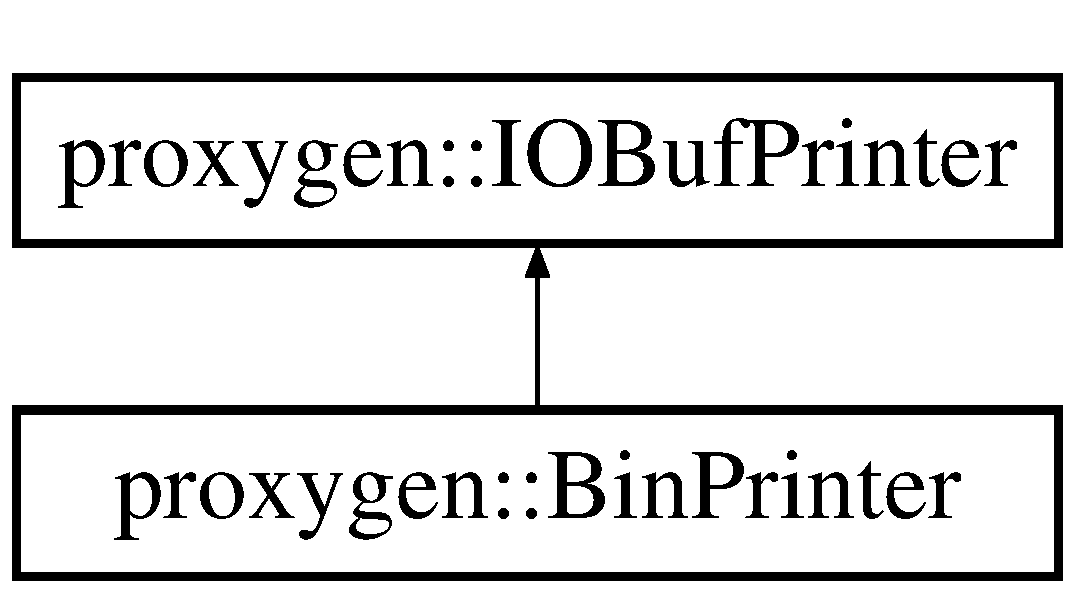
\includegraphics[height=2.000000cm]{classproxygen_1_1BinPrinter}
\end{center}
\end{figure}
\subsection*{Public Member Functions}
\begin{DoxyCompactItemize}
\item 
std\+::string {\bf print} (const folly\+::\+I\+O\+Buf $\ast$buf) override
\end{DoxyCompactItemize}
\subsection*{Additional Inherited Members}


\subsection{Detailed Description}


Definition at line 165 of file Logging.\+h.



\subsection{Member Function Documentation}
\index{proxygen\+::\+Bin\+Printer@{proxygen\+::\+Bin\+Printer}!print@{print}}
\index{print@{print}!proxygen\+::\+Bin\+Printer@{proxygen\+::\+Bin\+Printer}}
\subsubsection[{print(const folly\+::\+I\+O\+Buf $\ast$buf) override}]{\setlength{\rightskip}{0pt plus 5cm}string proxygen\+::\+Bin\+Printer\+::print (
\begin{DoxyParamCaption}
\item[{const folly\+::\+I\+O\+Buf $\ast$}]{buf}
\end{DoxyParamCaption}
)\hspace{0.3cm}{\ttfamily [override]}, {\ttfamily [virtual]}}\label{classproxygen_1_1BinPrinter_a466c1ecf4967a9bf06db76f9a44a34f7}


Implements {\bf proxygen\+::\+I\+O\+Buf\+Printer} \doxyref{}{p.}{classproxygen_1_1IOBufPrinter_a317ea00fb51d7d42c37a440488f42664}.



Definition at line 84 of file Logging.\+cpp.


\begin{DoxyCode}
84                                          \{
85   \textcolor{keyword}{static} uint8\_t bytesPerLine = 8;
86   \textcolor{keywordtype}{string} out;
87   \textcolor{keyword}{const} uint8\_t* data = buf->data();
88   \textcolor{keywordflow}{for} (\textcolor{keywordtype}{size\_t} i = 0; i < buf->length(); i++) \{
89     \textcolor{keywordflow}{for} (\textcolor{keywordtype}{int} b = 7; b >= 0; b--) \{
90       out += data[i] & 1 << b ? \textcolor{charliteral}{'1'} : \textcolor{charliteral}{'0'};
91     \}
92     out += \textcolor{charliteral}{' '};
93     out += isprint(data[i]) ? data[i] : \textcolor{charliteral}{' '};
94     \textcolor{keywordflow}{if} ((i + 1) % bytesPerLine == 0) \{
95       out += \textcolor{charliteral}{'\(\backslash\)n'};
96     \} \textcolor{keywordflow}{else} \{
97       out += \textcolor{charliteral}{' '};
98     \}
99   \}
100   out += \textcolor{charliteral}{'\(\backslash\)n'};
101   \textcolor{keywordflow}{return} out;
102 \}
\end{DoxyCode}


The documentation for this class was generated from the following files\+:\begin{DoxyCompactItemize}
\item 
proxygen/lib/utils/{\bf Logging.\+h}\item 
proxygen/lib/utils/{\bf Logging.\+cpp}\end{DoxyCompactItemize}

\section{proxygen\+:\+:Byte\+Event Class Reference}
\label{classproxygen_1_1ByteEvent}\index{proxygen\+::\+Byte\+Event@{proxygen\+::\+Byte\+Event}}


{\ttfamily \#include $<$Byte\+Events.\+h$>$}

Inheritance diagram for proxygen\+:\+:Byte\+Event\+:\begin{figure}[H]
\begin{center}
\leavevmode
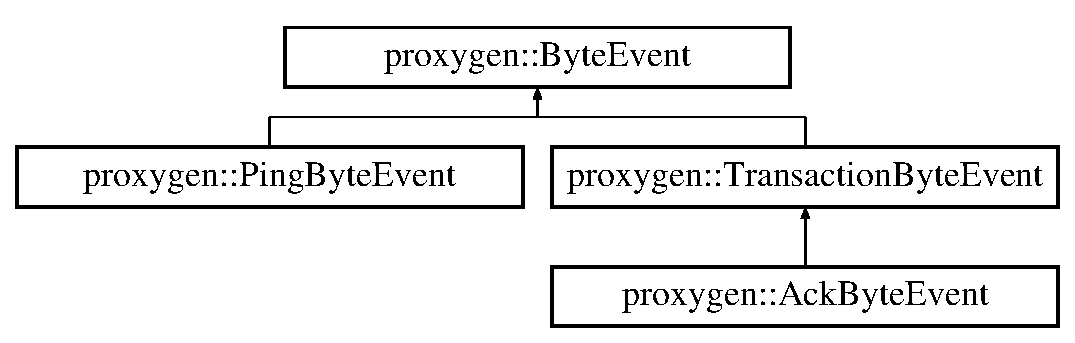
\includegraphics[height=3.000000cm]{classproxygen_1_1ByteEvent}
\end{center}
\end{figure}
\subsection*{Public Types}
\begin{DoxyCompactItemize}
\item 
enum {\bf Event\+Type} \{ \\*
{\bf F\+I\+R\+S\+T\+\_\+\+B\+Y\+TE}, 
{\bf L\+A\+S\+T\+\_\+\+B\+Y\+TE}, 
{\bf P\+I\+N\+G\+\_\+\+R\+E\+P\+L\+Y\+\_\+\+S\+E\+NT}, 
{\bf F\+I\+R\+S\+T\+\_\+\+H\+E\+A\+D\+E\+R\+\_\+\+B\+Y\+TE}, 
\\*
{\bf T\+R\+A\+C\+K\+E\+D\+\_\+\+B\+Y\+TE}
 \}
\end{DoxyCompactItemize}
\subsection*{Public Member Functions}
\begin{DoxyCompactItemize}
\item 
{\bf Byte\+Event} (uint64\+\_\+t byte\+Offset, {\bf Event\+Type} event\+Type)
\item 
virtual {\bf $\sim$\+Byte\+Event} ()
\item 
virtual {\bf H\+T\+T\+P\+Transaction} $\ast$ {\bf get\+Transaction} ()
\item 
virtual int64\+\_\+t {\bf get\+Latency} ()
\end{DoxyCompactItemize}
\subsection*{Public Attributes}
\begin{DoxyCompactItemize}
\item 
folly\+::\+Intrusive\+List\+Hook {\bf list\+Hook}
\item 
{\bf Event\+Type} {\bf event\+Type\+\_\+}\+:3
\item 
size\+\_\+t {\bf eom\+Tracked\+\_\+}\+:1
\item 
uint64\+\_\+t {\bf byte\+Offset\+\_\+}\+:(8$\ast$sizeof(uint64\+\_\+t)-\/4)
\end{DoxyCompactItemize}


\subsection{Detailed Description}


Definition at line 19 of file Byte\+Events.\+h.



\subsection{Member Enumeration Documentation}
\index{proxygen\+::\+Byte\+Event@{proxygen\+::\+Byte\+Event}!Event\+Type@{Event\+Type}}
\index{Event\+Type@{Event\+Type}!proxygen\+::\+Byte\+Event@{proxygen\+::\+Byte\+Event}}
\subsubsection[{Event\+Type}]{\setlength{\rightskip}{0pt plus 5cm}enum {\bf proxygen\+::\+Byte\+Event\+::\+Event\+Type}}\label{classproxygen_1_1ByteEvent_a3fdae6f245b9ed404854edde218bb549}
\begin{Desc}
\item[Enumerator]\par
\begin{description}
\index{F\+I\+R\+S\+T\+\_\+\+B\+Y\+TE@{F\+I\+R\+S\+T\+\_\+\+B\+Y\+TE}!proxygen\+::\+Byte\+Event@{proxygen\+::\+Byte\+Event}}\index{proxygen\+::\+Byte\+Event@{proxygen\+::\+Byte\+Event}!F\+I\+R\+S\+T\+\_\+\+B\+Y\+TE@{F\+I\+R\+S\+T\+\_\+\+B\+Y\+TE}}\item[{\em 
F\+I\+R\+S\+T\+\_\+\+B\+Y\+TE\label{classproxygen_1_1ByteEvent_a3fdae6f245b9ed404854edde218bb549a78a8d6c539da12626be6923ae965fec2}
}]\index{L\+A\+S\+T\+\_\+\+B\+Y\+TE@{L\+A\+S\+T\+\_\+\+B\+Y\+TE}!proxygen\+::\+Byte\+Event@{proxygen\+::\+Byte\+Event}}\index{proxygen\+::\+Byte\+Event@{proxygen\+::\+Byte\+Event}!L\+A\+S\+T\+\_\+\+B\+Y\+TE@{L\+A\+S\+T\+\_\+\+B\+Y\+TE}}\item[{\em 
L\+A\+S\+T\+\_\+\+B\+Y\+TE\label{classproxygen_1_1ByteEvent_a3fdae6f245b9ed404854edde218bb549af5c7f685ff574ac3be87f40fb8fd7604}
}]\index{P\+I\+N\+G\+\_\+\+R\+E\+P\+L\+Y\+\_\+\+S\+E\+NT@{P\+I\+N\+G\+\_\+\+R\+E\+P\+L\+Y\+\_\+\+S\+E\+NT}!proxygen\+::\+Byte\+Event@{proxygen\+::\+Byte\+Event}}\index{proxygen\+::\+Byte\+Event@{proxygen\+::\+Byte\+Event}!P\+I\+N\+G\+\_\+\+R\+E\+P\+L\+Y\+\_\+\+S\+E\+NT@{P\+I\+N\+G\+\_\+\+R\+E\+P\+L\+Y\+\_\+\+S\+E\+NT}}\item[{\em 
P\+I\+N\+G\+\_\+\+R\+E\+P\+L\+Y\+\_\+\+S\+E\+NT\label{classproxygen_1_1ByteEvent_a3fdae6f245b9ed404854edde218bb549a67ec99a70c7a12ff5d9b96f4099f566e}
}]\index{F\+I\+R\+S\+T\+\_\+\+H\+E\+A\+D\+E\+R\+\_\+\+B\+Y\+TE@{F\+I\+R\+S\+T\+\_\+\+H\+E\+A\+D\+E\+R\+\_\+\+B\+Y\+TE}!proxygen\+::\+Byte\+Event@{proxygen\+::\+Byte\+Event}}\index{proxygen\+::\+Byte\+Event@{proxygen\+::\+Byte\+Event}!F\+I\+R\+S\+T\+\_\+\+H\+E\+A\+D\+E\+R\+\_\+\+B\+Y\+TE@{F\+I\+R\+S\+T\+\_\+\+H\+E\+A\+D\+E\+R\+\_\+\+B\+Y\+TE}}\item[{\em 
F\+I\+R\+S\+T\+\_\+\+H\+E\+A\+D\+E\+R\+\_\+\+B\+Y\+TE\label{classproxygen_1_1ByteEvent_a3fdae6f245b9ed404854edde218bb549aecd719926c50a3c8df227a23ba4a737a}
}]\index{T\+R\+A\+C\+K\+E\+D\+\_\+\+B\+Y\+TE@{T\+R\+A\+C\+K\+E\+D\+\_\+\+B\+Y\+TE}!proxygen\+::\+Byte\+Event@{proxygen\+::\+Byte\+Event}}\index{proxygen\+::\+Byte\+Event@{proxygen\+::\+Byte\+Event}!T\+R\+A\+C\+K\+E\+D\+\_\+\+B\+Y\+TE@{T\+R\+A\+C\+K\+E\+D\+\_\+\+B\+Y\+TE}}\item[{\em 
T\+R\+A\+C\+K\+E\+D\+\_\+\+B\+Y\+TE\label{classproxygen_1_1ByteEvent_a3fdae6f245b9ed404854edde218bb549aca4ce19dad7f039195e8cfbc25e1fa53}
}]\end{description}
\end{Desc}


Definition at line 21 of file Byte\+Events.\+h.


\begin{DoxyCode}
21                  \{
22     FIRST_BYTE,
23     LAST_BYTE,
24     PING_REPLY_SENT,
25     FIRST_HEADER_BYTE,
26     TRACKED_BYTE,
27   \};
\end{DoxyCode}


\subsection{Constructor \& Destructor Documentation}
\index{proxygen\+::\+Byte\+Event@{proxygen\+::\+Byte\+Event}!Byte\+Event@{Byte\+Event}}
\index{Byte\+Event@{Byte\+Event}!proxygen\+::\+Byte\+Event@{proxygen\+::\+Byte\+Event}}
\subsubsection[{Byte\+Event(uint64\+\_\+t byte\+Offset, Event\+Type event\+Type)}]{\setlength{\rightskip}{0pt plus 5cm}proxygen\+::\+Byte\+Event\+::\+Byte\+Event (
\begin{DoxyParamCaption}
\item[{uint64\+\_\+t}]{byte\+Offset, }
\item[{{\bf Event\+Type}}]{event\+Type}
\end{DoxyParamCaption}
)\hspace{0.3cm}{\ttfamily [inline]}}\label{classproxygen_1_1ByteEvent_a8bcde32e10c23693b5c5ba2a80f5b4ff}


Definition at line 29 of file Byte\+Events.\+h.


\begin{DoxyCode}
30       : eventType_(eventType), eomTracked_(0), byteOffset_(byteOffset) \{\}
\end{DoxyCode}
\index{proxygen\+::\+Byte\+Event@{proxygen\+::\+Byte\+Event}!````~Byte\+Event@{$\sim$\+Byte\+Event}}
\index{````~Byte\+Event@{$\sim$\+Byte\+Event}!proxygen\+::\+Byte\+Event@{proxygen\+::\+Byte\+Event}}
\subsubsection[{$\sim$\+Byte\+Event()}]{\setlength{\rightskip}{0pt plus 5cm}virtual proxygen\+::\+Byte\+Event\+::$\sim$\+Byte\+Event (
\begin{DoxyParamCaption}
{}
\end{DoxyParamCaption}
)\hspace{0.3cm}{\ttfamily [inline]}, {\ttfamily [virtual]}}\label{classproxygen_1_1ByteEvent_a0ba49c1967be95ad9564ba93686c6f74}


Definition at line 31 of file Byte\+Events.\+h.


\begin{DoxyCode}
31 \{\}
\end{DoxyCode}


\subsection{Member Function Documentation}
\index{proxygen\+::\+Byte\+Event@{proxygen\+::\+Byte\+Event}!get\+Latency@{get\+Latency}}
\index{get\+Latency@{get\+Latency}!proxygen\+::\+Byte\+Event@{proxygen\+::\+Byte\+Event}}
\subsubsection[{get\+Latency()}]{\setlength{\rightskip}{0pt plus 5cm}virtual int64\+\_\+t proxygen\+::\+Byte\+Event\+::get\+Latency (
\begin{DoxyParamCaption}
{}
\end{DoxyParamCaption}
)\hspace{0.3cm}{\ttfamily [inline]}, {\ttfamily [virtual]}}\label{classproxygen_1_1ByteEvent_affa839c44c453c209acc72b93580e9e1}


Reimplemented in {\bf proxygen\+::\+Ping\+Byte\+Event} \doxyref{}{p.}{classproxygen_1_1PingByteEvent_ab465512f266054d2ef8d3b455c4bc11f}.



Definition at line 33 of file Byte\+Events.\+h.



Referenced by proxygen\+::\+Ping\+Byte\+Event\+::\+Ping\+Byte\+Event().


\begin{DoxyCode}
33 \{ \textcolor{keywordflow}{return} -1; \}
\end{DoxyCode}
\index{proxygen\+::\+Byte\+Event@{proxygen\+::\+Byte\+Event}!get\+Transaction@{get\+Transaction}}
\index{get\+Transaction@{get\+Transaction}!proxygen\+::\+Byte\+Event@{proxygen\+::\+Byte\+Event}}
\subsubsection[{get\+Transaction()}]{\setlength{\rightskip}{0pt plus 5cm}virtual {\bf H\+T\+T\+P\+Transaction}$\ast$ proxygen\+::\+Byte\+Event\+::get\+Transaction (
\begin{DoxyParamCaption}
{}
\end{DoxyParamCaption}
)\hspace{0.3cm}{\ttfamily [inline]}, {\ttfamily [virtual]}}\label{classproxygen_1_1ByteEvent_a1b193cbf3dcac88db6d439d0f7a3b798}


Reimplemented in {\bf proxygen\+::\+Transaction\+Byte\+Event} \doxyref{}{p.}{classproxygen_1_1TransactionByteEvent_affb42e3c628b508a798b44e6367b13ef}.



Definition at line 32 of file Byte\+Events.\+h.


\begin{DoxyCode}
32 \{ \textcolor{keywordflow}{return} \textcolor{keyword}{nullptr}; \}
\end{DoxyCode}


\subsection{Member Data Documentation}
\index{proxygen\+::\+Byte\+Event@{proxygen\+::\+Byte\+Event}!byte\+Offset\+\_\+@{byte\+Offset\+\_\+}}
\index{byte\+Offset\+\_\+@{byte\+Offset\+\_\+}!proxygen\+::\+Byte\+Event@{proxygen\+::\+Byte\+Event}}
\subsubsection[{byte\+Offset\+\_\+}]{\setlength{\rightskip}{0pt plus 5cm}uint64\+\_\+t proxygen\+::\+Byte\+Event\+::byte\+Offset\+\_\+}\label{classproxygen_1_1ByteEvent_a3f554bdf7dfb4bce5005412a21bbf8e7}


Definition at line 38 of file Byte\+Events.\+h.



Referenced by proxygen\+::operator$<$$<$().

\index{proxygen\+::\+Byte\+Event@{proxygen\+::\+Byte\+Event}!eom\+Tracked\+\_\+@{eom\+Tracked\+\_\+}}
\index{eom\+Tracked\+\_\+@{eom\+Tracked\+\_\+}!proxygen\+::\+Byte\+Event@{proxygen\+::\+Byte\+Event}}
\subsubsection[{eom\+Tracked\+\_\+}]{\setlength{\rightskip}{0pt plus 5cm}size\+\_\+t proxygen\+::\+Byte\+Event\+::eom\+Tracked\+\_\+}\label{classproxygen_1_1ByteEvent_a59de6d66d0415d15f75b8bc74af5259c}


Definition at line 37 of file Byte\+Events.\+h.

\index{proxygen\+::\+Byte\+Event@{proxygen\+::\+Byte\+Event}!event\+Type\+\_\+@{event\+Type\+\_\+}}
\index{event\+Type\+\_\+@{event\+Type\+\_\+}!proxygen\+::\+Byte\+Event@{proxygen\+::\+Byte\+Event}}
\subsubsection[{event\+Type\+\_\+}]{\setlength{\rightskip}{0pt plus 5cm}{\bf Event\+Type} proxygen\+::\+Byte\+Event\+::event\+Type\+\_\+}\label{classproxygen_1_1ByteEvent_a5f6425b89dc8d2eac3ad1ce17739f737}


Definition at line 36 of file Byte\+Events.\+h.



Referenced by proxygen\+::operator$<$$<$().

\index{proxygen\+::\+Byte\+Event@{proxygen\+::\+Byte\+Event}!list\+Hook@{list\+Hook}}
\index{list\+Hook@{list\+Hook}!proxygen\+::\+Byte\+Event@{proxygen\+::\+Byte\+Event}}
\subsubsection[{list\+Hook}]{\setlength{\rightskip}{0pt plus 5cm}folly\+::\+Intrusive\+List\+Hook proxygen\+::\+Byte\+Event\+::list\+Hook}\label{classproxygen_1_1ByteEvent_a37dc552e16debcee7125fd2160b30ae7}


Definition at line 35 of file Byte\+Events.\+h.



The documentation for this class was generated from the following file\+:\begin{DoxyCompactItemize}
\item 
proxygen/lib/http/session/{\bf Byte\+Events.\+h}\end{DoxyCompactItemize}

\section{proxygen\+:\+:Byte\+Event\+Tracker Class Reference}
\label{classproxygen_1_1ByteEventTracker}\index{proxygen\+::\+Byte\+Event\+Tracker@{proxygen\+::\+Byte\+Event\+Tracker}}


{\ttfamily \#include $<$Byte\+Event\+Tracker.\+h$>$}

Inheritance diagram for proxygen\+:\+:Byte\+Event\+Tracker\+:\begin{figure}[H]
\begin{center}
\leavevmode
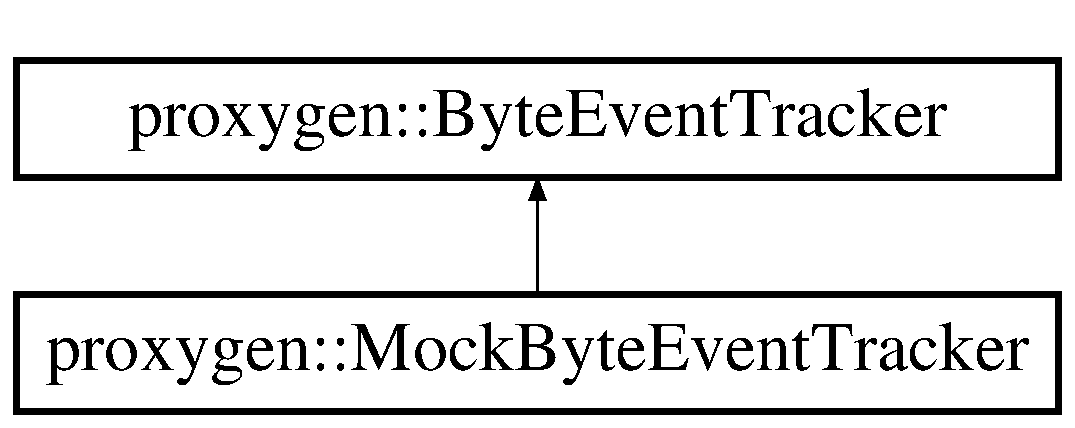
\includegraphics[height=2.000000cm]{classproxygen_1_1ByteEventTracker}
\end{center}
\end{figure}
\subsection*{Classes}
\begin{DoxyCompactItemize}
\item 
class {\bf Callback}
\end{DoxyCompactItemize}
\subsection*{Public Member Functions}
\begin{DoxyCompactItemize}
\item 
virtual {\bf $\sim$\+Byte\+Event\+Tracker} ()
\item 
{\bf Byte\+Event\+Tracker} ({\bf Callback} $\ast$callback)
\item 
virtual void {\bf absorb} ({\bf Byte\+Event\+Tracker} \&\&other)
\item 
void {\bf set\+Callback} ({\bf Callback} $\ast$callback)
\item 
virtual size\+\_\+t {\bf drain\+Byte\+Events} ()
\item 
virtual bool {\bf process\+Byte\+Events} (std\+::shared\+\_\+ptr$<$ {\bf Byte\+Event\+Tracker} $>$ self, uint64\+\_\+t bytes\+Written)
\item 
void {\bf add\+Ping\+Byte\+Event} (size\+\_\+t ping\+Size, {\bf Time\+Point} timestamp, uint64\+\_\+t bytes\+Scheduled)
\item 
void {\bf add\+First\+Body\+Byte\+Event} (uint64\+\_\+t offset, {\bf H\+T\+T\+P\+Transaction} $\ast$txn)
\item 
virtual void {\bf add\+First\+Header\+Byte\+Event} (uint64\+\_\+t offset, {\bf H\+T\+T\+P\+Transaction} $\ast$txn)
\item 
virtual void {\bf add\+Last\+Byte\+Event} ({\bf H\+T\+T\+P\+Transaction} $\ast$txn, uint64\+\_\+t byte\+No) noexcept
\item 
virtual void {\bf add\+Tracked\+Byte\+Event} ({\bf H\+T\+T\+P\+Transaction} $\ast$txn, uint64\+\_\+t byte\+No) noexcept
\item 
virtual void {\bf add\+Ack\+Byte\+Event} (uint64\+\_\+t, {\bf H\+T\+T\+P\+Transaction} $\ast$)
\item 
virtual uint64\+\_\+t {\bf pre\+Send} (bool $\ast$, bool $\ast$, uint64\+\_\+t)
\item 
virtual void {\bf set\+T\+T\+L\+B\+A\+Stats} ({\bf T\+T\+L\+B\+A\+Stats} $\ast$)
\end{DoxyCompactItemize}
\subsection*{Protected Member Functions}
\begin{DoxyCompactItemize}
\item 
virtual void {\bf eom\+Event\+Processed} ()
\end{DoxyCompactItemize}
\subsection*{Protected Attributes}
\begin{DoxyCompactItemize}
\item 
folly\+::\+Intrusive\+List$<$ {\bf Byte\+Event},\&{\bf Byte\+Event\+::list\+Hook} $>$ {\bf byte\+Events\+\_\+}
\item 
{\bf Callback} $\ast$ {\bf callback\+\_\+}
\end{DoxyCompactItemize}


\subsection{Detailed Description}
\doxyref{Byte\+Event\+Tracker}{p.}{classproxygen_1_1ByteEventTracker} can be used to fire application callbacks when a given byte of a transport stream has been processed. The primary usage is to fire the callbacks when the byte is accepted by the transport, not when the byte has been written on the wire, or acknowledged.

Subclasses may implement handling of acknowledgement timing. 

Definition at line 29 of file Byte\+Event\+Tracker.\+h.



\subsection{Constructor \& Destructor Documentation}
\index{proxygen\+::\+Byte\+Event\+Tracker@{proxygen\+::\+Byte\+Event\+Tracker}!````~Byte\+Event\+Tracker@{$\sim$\+Byte\+Event\+Tracker}}
\index{````~Byte\+Event\+Tracker@{$\sim$\+Byte\+Event\+Tracker}!proxygen\+::\+Byte\+Event\+Tracker@{proxygen\+::\+Byte\+Event\+Tracker}}
\subsubsection[{$\sim$\+Byte\+Event\+Tracker()}]{\setlength{\rightskip}{0pt plus 5cm}proxygen\+::\+Byte\+Event\+Tracker\+::$\sim$\+Byte\+Event\+Tracker (
\begin{DoxyParamCaption}
{}
\end{DoxyParamCaption}
)\hspace{0.3cm}{\ttfamily [virtual]}}\label{classproxygen_1_1ByteEventTracker_ae5f28ee6585f57fd6d91b87d11a32393}


Definition at line 20 of file Byte\+Event\+Tracker.\+cpp.



References drain\+Byte\+Events().



Referenced by proxygen\+::\+Byte\+Event\+Tracker\+::\+Callback\+::$\sim$\+Callback().


\begin{DoxyCode}
20                                     \{
21   drainByteEvents();
22 \}
\end{DoxyCode}
\index{proxygen\+::\+Byte\+Event\+Tracker@{proxygen\+::\+Byte\+Event\+Tracker}!Byte\+Event\+Tracker@{Byte\+Event\+Tracker}}
\index{Byte\+Event\+Tracker@{Byte\+Event\+Tracker}!proxygen\+::\+Byte\+Event\+Tracker@{proxygen\+::\+Byte\+Event\+Tracker}}
\subsubsection[{Byte\+Event\+Tracker(\+Callback $\ast$callback)}]{\setlength{\rightskip}{0pt plus 5cm}proxygen\+::\+Byte\+Event\+Tracker\+::\+Byte\+Event\+Tracker (
\begin{DoxyParamCaption}
\item[{{\bf Callback} $\ast$}]{callback}
\end{DoxyParamCaption}
)\hspace{0.3cm}{\ttfamily [inline]}, {\ttfamily [explicit]}}\label{classproxygen_1_1ByteEventTracker_a279fe2e59fddfa415102d7618d5694e2}


Definition at line 41 of file Byte\+Event\+Tracker.\+h.



References absorb().


\begin{DoxyCode}
41 : callback_(callback) \{\}
\end{DoxyCode}


\subsection{Member Function Documentation}
\index{proxygen\+::\+Byte\+Event\+Tracker@{proxygen\+::\+Byte\+Event\+Tracker}!absorb@{absorb}}
\index{absorb@{absorb}!proxygen\+::\+Byte\+Event\+Tracker@{proxygen\+::\+Byte\+Event\+Tracker}}
\subsubsection[{absorb(\+Byte\+Event\+Tracker \&\&other)}]{\setlength{\rightskip}{0pt plus 5cm}void proxygen\+::\+Byte\+Event\+Tracker\+::absorb (
\begin{DoxyParamCaption}
\item[{{\bf Byte\+Event\+Tracker} \&\&}]{other}
\end{DoxyParamCaption}
)\hspace{0.3cm}{\ttfamily [virtual]}}\label{classproxygen_1_1ByteEventTracker_abe16042d313ab05c3853560893dc94ae}
Assumes the byte events of another \doxyref{Byte\+Event\+Tracker}{p.}{classproxygen_1_1ByteEventTracker} that this object is replacing. 

Definition at line 24 of file Byte\+Event\+Tracker.\+cpp.



References byte\+Events\+\_\+.



Referenced by Byte\+Event\+Tracker().


\begin{DoxyCode}
24                                                       \{
25   byteEvents_ = std::move(other.byteEvents\_);
26 \}
\end{DoxyCode}
\index{proxygen\+::\+Byte\+Event\+Tracker@{proxygen\+::\+Byte\+Event\+Tracker}!add\+Ack\+Byte\+Event@{add\+Ack\+Byte\+Event}}
\index{add\+Ack\+Byte\+Event@{add\+Ack\+Byte\+Event}!proxygen\+::\+Byte\+Event\+Tracker@{proxygen\+::\+Byte\+Event\+Tracker}}
\subsubsection[{add\+Ack\+Byte\+Event(uint64\+\_\+t, H\+T\+T\+P\+Transaction $\ast$)}]{\setlength{\rightskip}{0pt plus 5cm}virtual void proxygen\+::\+Byte\+Event\+Tracker\+::add\+Ack\+Byte\+Event (
\begin{DoxyParamCaption}
\item[{uint64\+\_\+t}]{, }
\item[{{\bf H\+T\+T\+P\+Transaction} $\ast$}]{}
\end{DoxyParamCaption}
)\hspace{0.3cm}{\ttfamily [inline]}, {\ttfamily [virtual]}}\label{classproxygen_1_1ByteEventTracker_a288902a7901d57baceb764a566291c06}
The base \doxyref{Byte\+Event\+Tracker}{p.}{classproxygen_1_1ByteEventTracker} cannot track acks. 

Definition at line 81 of file Byte\+Event\+Tracker.\+h.


\begin{DoxyCode}
81 \{\}
\end{DoxyCode}
\index{proxygen\+::\+Byte\+Event\+Tracker@{proxygen\+::\+Byte\+Event\+Tracker}!add\+First\+Body\+Byte\+Event@{add\+First\+Body\+Byte\+Event}}
\index{add\+First\+Body\+Byte\+Event@{add\+First\+Body\+Byte\+Event}!proxygen\+::\+Byte\+Event\+Tracker@{proxygen\+::\+Byte\+Event\+Tracker}}
\subsubsection[{add\+First\+Body\+Byte\+Event(uint64\+\_\+t offset, H\+T\+T\+P\+Transaction $\ast$txn)}]{\setlength{\rightskip}{0pt plus 5cm}void proxygen\+::\+Byte\+Event\+Tracker\+::add\+First\+Body\+Byte\+Event (
\begin{DoxyParamCaption}
\item[{uint64\+\_\+t}]{offset, }
\item[{{\bf H\+T\+T\+P\+Transaction} $\ast$}]{txn}
\end{DoxyParamCaption}
)}\label{classproxygen_1_1ByteEventTracker_ac84342294ec2723886cf830d143a7dcf}


Definition at line 136 of file Byte\+Event\+Tracker.\+cpp.



References byte\+Events\+\_\+, and proxygen\+::\+Byte\+Event\+::\+F\+I\+R\+S\+T\+\_\+\+B\+Y\+TE.



Referenced by proxygen\+::\+Mock\+Byte\+Event\+Tracker\+::\+Mock\+Byte\+Event\+Tracker(), and set\+Callback().


\begin{DoxyCode}
137                                                                    \{
138   byteEvents_.push\_back(
139       *\textcolor{keyword}{new} TransactionByteEvent(
140           offset, ByteEvent::FIRST_BYTE,
141           txn));
142 \}
\end{DoxyCode}
\index{proxygen\+::\+Byte\+Event\+Tracker@{proxygen\+::\+Byte\+Event\+Tracker}!add\+First\+Header\+Byte\+Event@{add\+First\+Header\+Byte\+Event}}
\index{add\+First\+Header\+Byte\+Event@{add\+First\+Header\+Byte\+Event}!proxygen\+::\+Byte\+Event\+Tracker@{proxygen\+::\+Byte\+Event\+Tracker}}
\subsubsection[{add\+First\+Header\+Byte\+Event(uint64\+\_\+t offset, H\+T\+T\+P\+Transaction $\ast$txn)}]{\setlength{\rightskip}{0pt plus 5cm}void proxygen\+::\+Byte\+Event\+Tracker\+::add\+First\+Header\+Byte\+Event (
\begin{DoxyParamCaption}
\item[{uint64\+\_\+t}]{offset, }
\item[{{\bf H\+T\+T\+P\+Transaction} $\ast$}]{txn}
\end{DoxyParamCaption}
)\hspace{0.3cm}{\ttfamily [virtual]}}\label{classproxygen_1_1ByteEventTracker_a404ee5910e19a3e1e11750c26f30976a}


Definition at line 144 of file Byte\+Event\+Tracker.\+cpp.



References byte\+Events\+\_\+, and proxygen\+::\+Byte\+Event\+::\+F\+I\+R\+S\+T\+\_\+\+H\+E\+A\+D\+E\+R\+\_\+\+B\+Y\+TE.



Referenced by proxygen\+::\+Mock\+Byte\+Event\+Tracker\+::\+Mock\+Byte\+Event\+Tracker(), and set\+Callback().


\begin{DoxyCode}
145                                                                      \{
146   \textcolor{comment}{// onWriteSuccess() is called after the entire header has been written.}
147   \textcolor{comment}{// It does not catch partial write case.}
148   byteEvents_.push\_back(
149       *\textcolor{keyword}{new} TransactionByteEvent(offset,
150                                 ByteEvent::FIRST_HEADER_BYTE,
151                                 txn));
152 \}
\end{DoxyCode}
\index{proxygen\+::\+Byte\+Event\+Tracker@{proxygen\+::\+Byte\+Event\+Tracker}!add\+Last\+Byte\+Event@{add\+Last\+Byte\+Event}}
\index{add\+Last\+Byte\+Event@{add\+Last\+Byte\+Event}!proxygen\+::\+Byte\+Event\+Tracker@{proxygen\+::\+Byte\+Event\+Tracker}}
\subsubsection[{add\+Last\+Byte\+Event(\+H\+T\+T\+P\+Transaction $\ast$txn, uint64\+\_\+t byte\+No) noexcept}]{\setlength{\rightskip}{0pt plus 5cm}void proxygen\+::\+Byte\+Event\+Tracker\+::add\+Last\+Byte\+Event (
\begin{DoxyParamCaption}
\item[{{\bf H\+T\+T\+P\+Transaction} $\ast$}]{txn, }
\item[{uint64\+\_\+t}]{byte\+No}
\end{DoxyParamCaption}
)\hspace{0.3cm}{\ttfamily [virtual]}, {\ttfamily [noexcept]}}\label{classproxygen_1_1ByteEventTracker_a025cc627ea747c2c65d912abe4534626}


Definition at line 89 of file Byte\+Event\+Tracker.\+cpp.



References byte\+Events\+\_\+, and proxygen\+::\+Byte\+Event\+::\+L\+A\+S\+T\+\_\+\+B\+Y\+TE.



Referenced by proxygen\+::\+H\+T\+T\+P\+Session\+Base\+::handle\+Last\+Byte\+Events(), proxygen\+::\+Mock\+Byte\+Event\+Tracker\+::\+Mock\+Byte\+Event\+Tracker(), and set\+Callback().


\begin{DoxyCode}
91                               \{
92   VLOG(5) << \textcolor{stringliteral}{" adding last byte event for "} << byteNo;
93   TransactionByteEvent* \textcolor{keyword}{event} = \textcolor{keyword}{new} TransactionByteEvent(
94       byteNo, ByteEvent::LAST_BYTE, txn);
95   byteEvents_.push\_back(*event);
96 \}
\end{DoxyCode}
\index{proxygen\+::\+Byte\+Event\+Tracker@{proxygen\+::\+Byte\+Event\+Tracker}!add\+Ping\+Byte\+Event@{add\+Ping\+Byte\+Event}}
\index{add\+Ping\+Byte\+Event@{add\+Ping\+Byte\+Event}!proxygen\+::\+Byte\+Event\+Tracker@{proxygen\+::\+Byte\+Event\+Tracker}}
\subsubsection[{add\+Ping\+Byte\+Event(size\+\_\+t ping\+Size, Time\+Point timestamp, uint64\+\_\+t bytes\+Scheduled)}]{\setlength{\rightskip}{0pt plus 5cm}void proxygen\+::\+Byte\+Event\+Tracker\+::add\+Ping\+Byte\+Event (
\begin{DoxyParamCaption}
\item[{size\+\_\+t}]{ping\+Size, }
\item[{{\bf Time\+Point}}]{timestamp, }
\item[{uint64\+\_\+t}]{bytes\+Scheduled}
\end{DoxyParamCaption}
)}\label{classproxygen_1_1ByteEventTracker_a2deb75d0a0e42a3e6dd603c09d620f86}
The following methods add byte events for tracking 

Definition at line 107 of file Byte\+Event\+Tracker.\+cpp.



References byte\+Events\+\_\+.



Referenced by proxygen\+::\+Mock\+Byte\+Event\+Tracker\+::\+Mock\+Byte\+Event\+Tracker(), and set\+Callback().


\begin{DoxyCode}
109                                                                  \{
110   \textcolor{comment}{// register a byte event on ping reply sent, and adjust the byteOffset\_}
111   \textcolor{comment}{// for others by one ping size}
112   uint64\_t offset = bytesScheduled + pingSize;
113   \textcolor{keyword}{auto} i = byteEvents_.rbegin();
114   \textcolor{keywordflow}{for} (; i != byteEvents_.rend(); ++i) \{
115     \textcolor{keywordflow}{if} (i->byteOffset\_ > bytesScheduled) \{
116       VLOG(5) << \textcolor{stringliteral}{"pushing back ByteEvent from "} << *i << \textcolor{stringliteral}{" to "}
117               << ByteEvent(i->byteOffset\_ + pingSize, i->eventType\_);
118       i->byteOffset\_ += pingSize;
119     \} \textcolor{keywordflow}{else} \{
120       \textcolor{keywordflow}{break}; \textcolor{comment}{// the rest of the events are already scheduled}
121     \}
122   \}
123 
124   ByteEvent* be = \textcolor{keyword}{new} PingByteEvent(offset, timestamp);
125   \textcolor{keywordflow}{if} (i == byteEvents_.rend()) \{
126     byteEvents_.push\_front(*be);
127   \} \textcolor{keywordflow}{else} \textcolor{keywordflow}{if} (i == byteEvents_.rbegin()) \{
128     byteEvents_.push\_back(*be);
129   \} \textcolor{keywordflow}{else} \{
130     --i;
131     CHECK\_GT(i->byteOffset\_, bytesScheduled);
132     byteEvents_.insert(i.base(), *be);
133   \}
134 \}
\end{DoxyCode}
\index{proxygen\+::\+Byte\+Event\+Tracker@{proxygen\+::\+Byte\+Event\+Tracker}!add\+Tracked\+Byte\+Event@{add\+Tracked\+Byte\+Event}}
\index{add\+Tracked\+Byte\+Event@{add\+Tracked\+Byte\+Event}!proxygen\+::\+Byte\+Event\+Tracker@{proxygen\+::\+Byte\+Event\+Tracker}}
\subsubsection[{add\+Tracked\+Byte\+Event(\+H\+T\+T\+P\+Transaction $\ast$txn, uint64\+\_\+t byte\+No) noexcept}]{\setlength{\rightskip}{0pt plus 5cm}void proxygen\+::\+Byte\+Event\+Tracker\+::add\+Tracked\+Byte\+Event (
\begin{DoxyParamCaption}
\item[{{\bf H\+T\+T\+P\+Transaction} $\ast$}]{txn, }
\item[{uint64\+\_\+t}]{byte\+No}
\end{DoxyParamCaption}
)\hspace{0.3cm}{\ttfamily [virtual]}, {\ttfamily [noexcept]}}\label{classproxygen_1_1ByteEventTracker_a0acc3270c2d17b8785ae22cff07cd73e}


Definition at line 98 of file Byte\+Event\+Tracker.\+cpp.



References byte\+Events\+\_\+, and proxygen\+::\+Byte\+Event\+::\+T\+R\+A\+C\+K\+E\+D\+\_\+\+B\+Y\+TE.



Referenced by proxygen\+::\+Mock\+Byte\+Event\+Tracker\+::\+Mock\+Byte\+Event\+Tracker(), and set\+Callback().


\begin{DoxyCode}
100                               \{
101   VLOG(5) << \textcolor{stringliteral}{" adding tracked byte event for "} << byteNo;
102   TransactionByteEvent* \textcolor{keyword}{event} = \textcolor{keyword}{new} TransactionByteEvent(
103       byteNo, ByteEvent::TRACKED_BYTE, txn);
104   byteEvents_.push\_back(*event);
105 \}
\end{DoxyCode}
\index{proxygen\+::\+Byte\+Event\+Tracker@{proxygen\+::\+Byte\+Event\+Tracker}!drain\+Byte\+Events@{drain\+Byte\+Events}}
\index{drain\+Byte\+Events@{drain\+Byte\+Events}!proxygen\+::\+Byte\+Event\+Tracker@{proxygen\+::\+Byte\+Event\+Tracker}}
\subsubsection[{drain\+Byte\+Events()}]{\setlength{\rightskip}{0pt plus 5cm}size\+\_\+t proxygen\+::\+Byte\+Event\+Tracker\+::drain\+Byte\+Events (
\begin{DoxyParamCaption}
{}
\end{DoxyParamCaption}
)\hspace{0.3cm}{\ttfamily [virtual]}}\label{classproxygen_1_1ByteEventTracker_a6ef3f0ec3fb68834241621a1caf92076}
drain\+Byte\+Events should be called to clear out any pending events holding transactions when process\+Byte\+Events will no longer be called 

Definition at line 79 of file Byte\+Event\+Tracker.\+cpp.



References byte\+Events\+\_\+.



Referenced by proxygen\+::\+Mock\+Byte\+Event\+Tracker\+::\+Mock\+Byte\+Event\+Tracker(), set\+Callback(), and $\sim$\+Byte\+Event\+Tracker().


\begin{DoxyCode}
79                                          \{
80   \textcolor{keywordtype}{size\_t} numEvents = 0;
81   \textcolor{comment}{// everything is dead from here on, let's just drop all extra refs to txns}
82   \textcolor{keywordflow}{while} (!byteEvents_.empty()) \{
83     \textcolor{keyword}{delete} &byteEvents_.front();
84     ++numEvents;
85   \}
86   \textcolor{keywordflow}{return} numEvents;
87 \}
\end{DoxyCode}
\index{proxygen\+::\+Byte\+Event\+Tracker@{proxygen\+::\+Byte\+Event\+Tracker}!eom\+Event\+Processed@{eom\+Event\+Processed}}
\index{eom\+Event\+Processed@{eom\+Event\+Processed}!proxygen\+::\+Byte\+Event\+Tracker@{proxygen\+::\+Byte\+Event\+Tracker}}
\subsubsection[{eom\+Event\+Processed()}]{\setlength{\rightskip}{0pt plus 5cm}virtual void proxygen\+::\+Byte\+Event\+Tracker\+::eom\+Event\+Processed (
\begin{DoxyParamCaption}
{}
\end{DoxyParamCaption}
)\hspace{0.3cm}{\ttfamily [inline]}, {\ttfamily [protected]}, {\ttfamily [virtual]}}\label{classproxygen_1_1ByteEventTracker_a539a7046579036c2acd18a238787a892}


Definition at line 102 of file Byte\+Event\+Tracker.\+h.



Referenced by process\+Byte\+Events().


\begin{DoxyCode}
102 \{\}
\end{DoxyCode}
\index{proxygen\+::\+Byte\+Event\+Tracker@{proxygen\+::\+Byte\+Event\+Tracker}!pre\+Send@{pre\+Send}}
\index{pre\+Send@{pre\+Send}!proxygen\+::\+Byte\+Event\+Tracker@{proxygen\+::\+Byte\+Event\+Tracker}}
\subsubsection[{pre\+Send(bool $\ast$, bool $\ast$, uint64\+\_\+t)}]{\setlength{\rightskip}{0pt plus 5cm}virtual uint64\+\_\+t proxygen\+::\+Byte\+Event\+Tracker\+::pre\+Send (
\begin{DoxyParamCaption}
\item[{bool $\ast$}]{, }
\item[{bool $\ast$}]{, }
\item[{uint64\+\_\+t}]{}
\end{DoxyParamCaption}
)\hspace{0.3cm}{\ttfamily [inline]}, {\ttfamily [virtual]}}\label{classproxygen_1_1ByteEventTracker_ade1d712b6855de6a40cc3128a8d447c1}
\doxyref{H\+T\+T\+P\+Session}{p.}{classproxygen_1_1HTTPSession} uses pre\+Send to truncate writes on an eom boundary. In Ack-\/tracking \doxyref{Byte\+Event\+Tracker}{p.}{classproxygen_1_1ByteEventTracker}\textquotesingle{}s, this should exmaine pending byte events and return the number of bytes until the next last byte event, or 0 if none are pending. If non-\/zero is returned then eom may be set to indicate ack tracking is requested. 

Definition at line 91 of file Byte\+Event\+Tracker.\+h.



Referenced by proxygen\+::\+Mock\+Byte\+Event\+Tracker\+::\+Mock\+Byte\+Event\+Tracker().


\begin{DoxyCode}
92                                        \{
93     \textcolor{keywordflow}{return} 0;
94   \}
\end{DoxyCode}
\index{proxygen\+::\+Byte\+Event\+Tracker@{proxygen\+::\+Byte\+Event\+Tracker}!process\+Byte\+Events@{process\+Byte\+Events}}
\index{process\+Byte\+Events@{process\+Byte\+Events}!proxygen\+::\+Byte\+Event\+Tracker@{proxygen\+::\+Byte\+Event\+Tracker}}
\subsubsection[{process\+Byte\+Events(std\+::shared\+\_\+ptr$<$ Byte\+Event\+Tracker $>$ self, uint64\+\_\+t bytes\+Written)}]{\setlength{\rightskip}{0pt plus 5cm}bool proxygen\+::\+Byte\+Event\+Tracker\+::process\+Byte\+Events (
\begin{DoxyParamCaption}
\item[{std\+::shared\+\_\+ptr$<$ {\bf Byte\+Event\+Tracker} $>$}]{self, }
\item[{uint64\+\_\+t}]{bytes\+Written}
\end{DoxyParamCaption}
)\hspace{0.3cm}{\ttfamily [virtual]}}\label{classproxygen_1_1ByteEventTracker_af5d1ab24926efe8567546c720370f4dd}
process\+Byte\+Events is called whenever the transport has accepted more bytes. bytes\+Written is the number of bytes written to the transport over its lifetime. 

Definition at line 31 of file Byte\+Event\+Tracker.\+cpp.



References byte\+Events\+\_\+, callback\+\_\+, eom\+Event\+Processed(), proxygen\+::\+Byte\+Event\+::\+F\+I\+R\+S\+T\+\_\+\+B\+Y\+TE, proxygen\+::\+Byte\+Event\+::\+F\+I\+R\+S\+T\+\_\+\+H\+E\+A\+D\+E\+R\+\_\+\+B\+Y\+TE, proxygen\+::\+Byte\+Event\+::\+L\+A\+S\+T\+\_\+\+B\+Y\+TE, proxygen\+::\+Byte\+Event\+Tracker\+::\+Callback\+::on\+Last\+Byte\+Event(), proxygen\+::\+Byte\+Event\+Tracker\+::\+Callback\+::on\+Ping\+Reply\+Latency(), proxygen\+::\+Byte\+Event\+::\+P\+I\+N\+G\+\_\+\+R\+E\+P\+L\+Y\+\_\+\+S\+E\+NT, and proxygen\+::\+Byte\+Event\+::\+T\+R\+A\+C\+K\+E\+D\+\_\+\+B\+Y\+TE.



Referenced by proxygen\+::\+Mock\+Byte\+Event\+Tracker\+::\+Mock\+Byte\+Event\+Tracker(), and set\+Callback().


\begin{DoxyCode}
32                                                                 \{
33   \textcolor{keywordtype}{bool} advanceEOM = \textcolor{keyword}{false};
34 
35   \textcolor{keywordflow}{while} (!byteEvents_.empty() &&
36          (byteEvents_.front().byteOffset\_ <= bytesWritten)) \{
37     ByteEvent& \textcolor{keyword}{event} = byteEvents_.front();
38     int64\_t latency;
39     \textcolor{keyword}{auto} txn = \textcolor{keyword}{event}.getTransaction();
40 
41     \textcolor{keywordflow}{switch} (event.eventType\_) \{
42     \textcolor{keywordflow}{case} ByteEvent::FIRST_HEADER_BYTE:
43       txn->onEgressHeaderFirstByte();
44       \textcolor{keywordflow}{break};
45     \textcolor{keywordflow}{case} ByteEvent::FIRST_BYTE:
46       txn->onEgressBodyFirstByte();
47       \textcolor{keywordflow}{break};
48     \textcolor{keywordflow}{case} ByteEvent::LAST_BYTE:
49       txn->onEgressBodyLastByte();
50       \textcolor{keywordflow}{if} (callback_) \{
51         callback_->onLastByteEvent(txn, event.byteOffset\_, event.eomTracked\_);
52       \}
53       advanceEOM = \textcolor{keyword}{true};
54       \textcolor{keywordflow}{break};
55     \textcolor{keywordflow}{case} ByteEvent::TRACKED_BYTE:
56       txn->onEgressTrackedByte();
57       \textcolor{keywordflow}{break};
58     \textcolor{keywordflow}{case} ByteEvent::PING_REPLY_SENT:
59       latency = \textcolor{keyword}{event}.getLatency();
60       \textcolor{keywordflow}{if} (callback_) \{
61         callback_->onPingReplyLatency(latency);
62       \}
63       \textcolor{keywordflow}{break};
64     \}
65 
66     VLOG(5) << \textcolor{stringliteral}{" removing ByteEvent "} << event;
67     \textcolor{comment}{// explicitly remove from the list, in case delete event triggers a}
68     \textcolor{comment}{// callback that would absorb this ByteEventTracker.}
69     \textcolor{keyword}{event}.listHook.unlink();
70     \textcolor{keyword}{delete} &event;
71   \}
72 
73   \textcolor{keywordflow}{if} (advanceEOM) \{
74     eomEventProcessed();
75   \}
76   \textcolor{keywordflow}{return} \textcolor{keyword}{self}.use\_count() == 1;
77 \}
\end{DoxyCode}
\index{proxygen\+::\+Byte\+Event\+Tracker@{proxygen\+::\+Byte\+Event\+Tracker}!set\+Callback@{set\+Callback}}
\index{set\+Callback@{set\+Callback}!proxygen\+::\+Byte\+Event\+Tracker@{proxygen\+::\+Byte\+Event\+Tracker}}
\subsubsection[{set\+Callback(\+Callback $\ast$callback)}]{\setlength{\rightskip}{0pt plus 5cm}void proxygen\+::\+Byte\+Event\+Tracker\+::set\+Callback (
\begin{DoxyParamCaption}
\item[{{\bf Callback} $\ast$}]{callback}
\end{DoxyParamCaption}
)\hspace{0.3cm}{\ttfamily [inline]}}\label{classproxygen_1_1ByteEventTracker_ad63604621dfa10fb196dc9df7f7a2ecf}


Definition at line 48 of file Byte\+Event\+Tracker.\+h.



References add\+First\+Body\+Byte\+Event(), add\+First\+Header\+Byte\+Event(), add\+Last\+Byte\+Event(), add\+Ping\+Byte\+Event(), add\+Tracked\+Byte\+Event(), callback\+\_\+, drain\+Byte\+Events(), and process\+Byte\+Events().


\begin{DoxyCode}
48 \{ callback_ = callback; \}
\end{DoxyCode}
\index{proxygen\+::\+Byte\+Event\+Tracker@{proxygen\+::\+Byte\+Event\+Tracker}!set\+T\+T\+L\+B\+A\+Stats@{set\+T\+T\+L\+B\+A\+Stats}}
\index{set\+T\+T\+L\+B\+A\+Stats@{set\+T\+T\+L\+B\+A\+Stats}!proxygen\+::\+Byte\+Event\+Tracker@{proxygen\+::\+Byte\+Event\+Tracker}}
\subsubsection[{set\+T\+T\+L\+B\+A\+Stats(\+T\+T\+L\+B\+A\+Stats $\ast$)}]{\setlength{\rightskip}{0pt plus 5cm}virtual void proxygen\+::\+Byte\+Event\+Tracker\+::set\+T\+T\+L\+B\+A\+Stats (
\begin{DoxyParamCaption}
\item[{{\bf T\+T\+L\+B\+A\+Stats} $\ast$}]{}
\end{DoxyParamCaption}
)\hspace{0.3cm}{\ttfamily [inline]}, {\ttfamily [virtual]}}\label{classproxygen_1_1ByteEventTracker_accba773d0885d1af7a880524649c2fc5}


Definition at line 96 of file Byte\+Event\+Tracker.\+h.


\begin{DoxyCode}
96 \{\}
\end{DoxyCode}


\subsection{Member Data Documentation}
\index{proxygen\+::\+Byte\+Event\+Tracker@{proxygen\+::\+Byte\+Event\+Tracker}!byte\+Events\+\_\+@{byte\+Events\+\_\+}}
\index{byte\+Events\+\_\+@{byte\+Events\+\_\+}!proxygen\+::\+Byte\+Event\+Tracker@{proxygen\+::\+Byte\+Event\+Tracker}}
\subsubsection[{byte\+Events\+\_\+}]{\setlength{\rightskip}{0pt plus 5cm}folly\+::\+Intrusive\+List$<${\bf Byte\+Event}, \&{\bf Byte\+Event\+::list\+Hook}$>$ proxygen\+::\+Byte\+Event\+Tracker\+::byte\+Events\+\_\+\hspace{0.3cm}{\ttfamily [protected]}}\label{classproxygen_1_1ByteEventTracker_a83721a92dce1dc202dc187758b97c797}


Definition at line 100 of file Byte\+Event\+Tracker.\+h.



Referenced by absorb(), add\+First\+Body\+Byte\+Event(), add\+First\+Header\+Byte\+Event(), add\+Last\+Byte\+Event(), add\+Ping\+Byte\+Event(), add\+Tracked\+Byte\+Event(), drain\+Byte\+Events(), and process\+Byte\+Events().

\index{proxygen\+::\+Byte\+Event\+Tracker@{proxygen\+::\+Byte\+Event\+Tracker}!callback\+\_\+@{callback\+\_\+}}
\index{callback\+\_\+@{callback\+\_\+}!proxygen\+::\+Byte\+Event\+Tracker@{proxygen\+::\+Byte\+Event\+Tracker}}
\subsubsection[{callback\+\_\+}]{\setlength{\rightskip}{0pt plus 5cm}{\bf Callback}$\ast$ proxygen\+::\+Byte\+Event\+Tracker\+::callback\+\_\+\hspace{0.3cm}{\ttfamily [protected]}}\label{classproxygen_1_1ByteEventTracker_aebed6fd1a728b8829f86647123f171eb}


Definition at line 104 of file Byte\+Event\+Tracker.\+h.



Referenced by process\+Byte\+Events(), and set\+Callback().



The documentation for this class was generated from the following files\+:\begin{DoxyCompactItemize}
\item 
proxygen/lib/http/session/{\bf Byte\+Event\+Tracker.\+h}\item 
proxygen/lib/http/session/{\bf Byte\+Event\+Tracker.\+cpp}\end{DoxyCompactItemize}

\section{Byte\+Event\+Tracker\+Test Class Reference}
\label{classByteEventTrackerTest}\index{Byte\+Event\+Tracker\+Test@{Byte\+Event\+Tracker\+Test}}
Inheritance diagram for Byte\+Event\+Tracker\+Test\+:\begin{figure}[H]
\begin{center}
\leavevmode
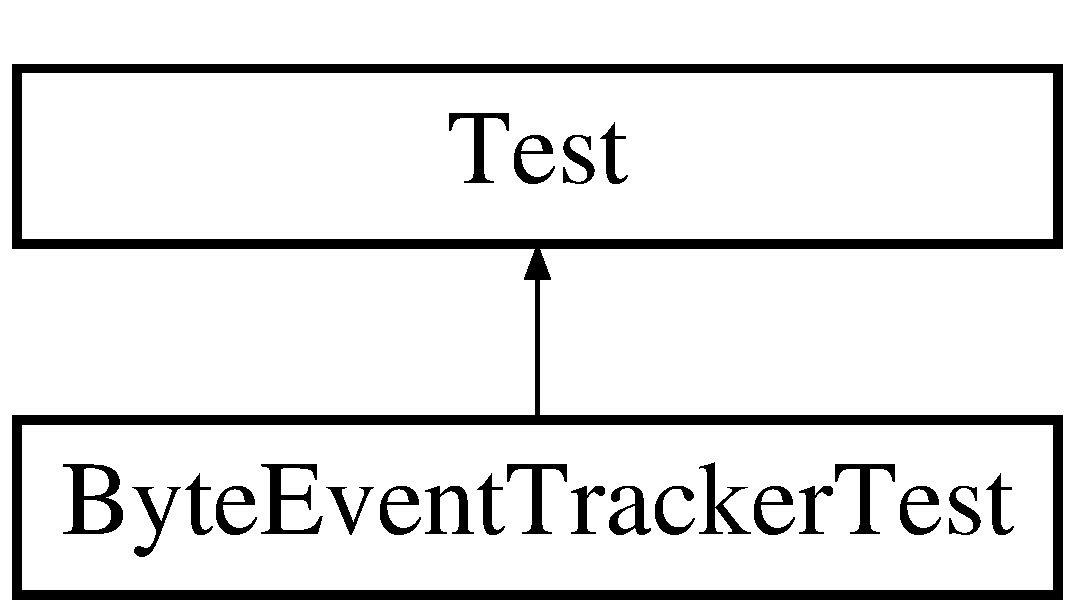
\includegraphics[height=2.000000cm]{classByteEventTrackerTest}
\end{center}
\end{figure}
\subsection*{Public Member Functions}
\begin{DoxyCompactItemize}
\item 
void {\bf Set\+Up} () override
\end{DoxyCompactItemize}
\subsection*{Protected Attributes}
\begin{DoxyCompactItemize}
\item 
folly\+::\+Event\+Base {\bf event\+Base\+\_\+}
\item 
{\bf Wheel\+Timer\+Instance} {\bf transaction\+Timeouts\+\_\+}
\item 
Nice\+Mock$<$ {\bf Mock\+H\+T\+T\+P\+Transaction\+Transport} $>$ {\bf transport\+\_\+}
\item 
Strict\+Mock$<$ {\bf Mock\+H\+T\+T\+P\+Handler} $>$ {\bf handler\+\_\+}
\item 
{\bf H\+T\+T\+P2\+Priority\+Queue} {\bf txn\+Egress\+Queue\+\_\+}
\item 
{\bf H\+T\+T\+P\+Transaction} {\bf txn\+\_\+}
\item 
{\bf Mock\+H\+T\+T\+P\+Transaction\+Transport\+Callback} {\bf transport\+Callback\+\_\+}
\item 
{\bf Mock\+Byte\+Event\+Tracker\+Callback} {\bf callback\+\_\+}
\item 
std\+::shared\+\_\+ptr$<$ {\bf Byte\+Event\+Tracker} $>$ {\bf byte\+Event\+Tracker\+\_\+}
\end{DoxyCompactItemize}


\subsection{Detailed Description}


Definition at line 31 of file Byte\+Event\+Tracker\+Test.\+cpp.



\subsection{Member Function Documentation}
\index{Byte\+Event\+Tracker\+Test@{Byte\+Event\+Tracker\+Test}!Set\+Up@{Set\+Up}}
\index{Set\+Up@{Set\+Up}!Byte\+Event\+Tracker\+Test@{Byte\+Event\+Tracker\+Test}}
\subsubsection[{Set\+Up() override}]{\setlength{\rightskip}{0pt plus 5cm}void Byte\+Event\+Tracker\+Test\+::\+Set\+Up (
\begin{DoxyParamCaption}
{}
\end{DoxyParamCaption}
)\hspace{0.3cm}{\ttfamily [inline]}, {\ttfamily [override]}}\label{classByteEventTrackerTest_a5517d78c03c7d3d587d5fdcf6094d9b5}


Definition at line 34 of file Byte\+Event\+Tracker\+Test.\+cpp.


\begin{DoxyCode}
34                         \{
35     txn_.setTransportCallback(&transportCallback_);
36   \}
\end{DoxyCode}


\subsection{Member Data Documentation}
\index{Byte\+Event\+Tracker\+Test@{Byte\+Event\+Tracker\+Test}!byte\+Event\+Tracker\+\_\+@{byte\+Event\+Tracker\+\_\+}}
\index{byte\+Event\+Tracker\+\_\+@{byte\+Event\+Tracker\+\_\+}!Byte\+Event\+Tracker\+Test@{Byte\+Event\+Tracker\+Test}}
\subsubsection[{byte\+Event\+Tracker\+\_\+}]{\setlength{\rightskip}{0pt plus 5cm}std\+::shared\+\_\+ptr$<${\bf Byte\+Event\+Tracker}$>$ Byte\+Event\+Tracker\+Test\+::byte\+Event\+Tracker\+\_\+\hspace{0.3cm}{\ttfamily [protected]}}\label{classByteEventTrackerTest_a207e905ea8f6ae94c217d577ec64fc59}
{\bfseries Initial value\+:}
\begin{DoxyCode}
\{
    \textcolor{keyword}{new} ByteEventTracker(&callback_)\}
\end{DoxyCode}


Definition at line 52 of file Byte\+Event\+Tracker\+Test.\+cpp.

\index{Byte\+Event\+Tracker\+Test@{Byte\+Event\+Tracker\+Test}!callback\+\_\+@{callback\+\_\+}}
\index{callback\+\_\+@{callback\+\_\+}!Byte\+Event\+Tracker\+Test@{Byte\+Event\+Tracker\+Test}}
\subsubsection[{callback\+\_\+}]{\setlength{\rightskip}{0pt plus 5cm}{\bf Mock\+Byte\+Event\+Tracker\+Callback} Byte\+Event\+Tracker\+Test\+::callback\+\_\+\hspace{0.3cm}{\ttfamily [protected]}}\label{classByteEventTrackerTest_a5d21bf7da10e433def8a600b1f107189}


Definition at line 51 of file Byte\+Event\+Tracker\+Test.\+cpp.

\index{Byte\+Event\+Tracker\+Test@{Byte\+Event\+Tracker\+Test}!event\+Base\+\_\+@{event\+Base\+\_\+}}
\index{event\+Base\+\_\+@{event\+Base\+\_\+}!Byte\+Event\+Tracker\+Test@{Byte\+Event\+Tracker\+Test}}
\subsubsection[{event\+Base\+\_\+}]{\setlength{\rightskip}{0pt plus 5cm}folly\+::\+Event\+Base Byte\+Event\+Tracker\+Test\+::event\+Base\+\_\+\hspace{0.3cm}{\ttfamily [protected]}}\label{classByteEventTrackerTest_a08a0b259562be8f85573ca39bac5fc67}


Definition at line 39 of file Byte\+Event\+Tracker\+Test.\+cpp.

\index{Byte\+Event\+Tracker\+Test@{Byte\+Event\+Tracker\+Test}!handler\+\_\+@{handler\+\_\+}}
\index{handler\+\_\+@{handler\+\_\+}!Byte\+Event\+Tracker\+Test@{Byte\+Event\+Tracker\+Test}}
\subsubsection[{handler\+\_\+}]{\setlength{\rightskip}{0pt plus 5cm}Strict\+Mock$<${\bf Mock\+H\+T\+T\+P\+Handler}$>$ Byte\+Event\+Tracker\+Test\+::handler\+\_\+\hspace{0.3cm}{\ttfamily [protected]}}\label{classByteEventTrackerTest_afa3e5b3068f14f2b2e308bcd9e2b73e7}


Definition at line 43 of file Byte\+Event\+Tracker\+Test.\+cpp.

\index{Byte\+Event\+Tracker\+Test@{Byte\+Event\+Tracker\+Test}!transaction\+Timeouts\+\_\+@{transaction\+Timeouts\+\_\+}}
\index{transaction\+Timeouts\+\_\+@{transaction\+Timeouts\+\_\+}!Byte\+Event\+Tracker\+Test@{Byte\+Event\+Tracker\+Test}}
\subsubsection[{transaction\+Timeouts\+\_\+}]{\setlength{\rightskip}{0pt plus 5cm}{\bf Wheel\+Timer\+Instance} Byte\+Event\+Tracker\+Test\+::transaction\+Timeouts\+\_\+\hspace{0.3cm}{\ttfamily [protected]}}\label{classByteEventTrackerTest_a6dbf6cabdc76968395daa871c96fa519}
{\bfseries Initial value\+:}
\begin{DoxyCode}
\{std::chrono::milliseconds(500),
      &eventBase_\}
\end{DoxyCode}


Definition at line 40 of file Byte\+Event\+Tracker\+Test.\+cpp.

\index{Byte\+Event\+Tracker\+Test@{Byte\+Event\+Tracker\+Test}!transport\+\_\+@{transport\+\_\+}}
\index{transport\+\_\+@{transport\+\_\+}!Byte\+Event\+Tracker\+Test@{Byte\+Event\+Tracker\+Test}}
\subsubsection[{transport\+\_\+}]{\setlength{\rightskip}{0pt plus 5cm}Nice\+Mock$<${\bf Mock\+H\+T\+T\+P\+Transaction\+Transport}$>$ Byte\+Event\+Tracker\+Test\+::transport\+\_\+\hspace{0.3cm}{\ttfamily [protected]}}\label{classByteEventTrackerTest_a5b7d70dbb9aa4ce97f2bd0f2dc102571}


Definition at line 42 of file Byte\+Event\+Tracker\+Test.\+cpp.

\index{Byte\+Event\+Tracker\+Test@{Byte\+Event\+Tracker\+Test}!transport\+Callback\+\_\+@{transport\+Callback\+\_\+}}
\index{transport\+Callback\+\_\+@{transport\+Callback\+\_\+}!Byte\+Event\+Tracker\+Test@{Byte\+Event\+Tracker\+Test}}
\subsubsection[{transport\+Callback\+\_\+}]{\setlength{\rightskip}{0pt plus 5cm}{\bf Mock\+H\+T\+T\+P\+Transaction\+Transport\+Callback} Byte\+Event\+Tracker\+Test\+::transport\+Callback\+\_\+\hspace{0.3cm}{\ttfamily [protected]}}\label{classByteEventTrackerTest_a29bbc40f55eed805ac63dd413126c9f9}


Definition at line 50 of file Byte\+Event\+Tracker\+Test.\+cpp.

\index{Byte\+Event\+Tracker\+Test@{Byte\+Event\+Tracker\+Test}!txn\+\_\+@{txn\+\_\+}}
\index{txn\+\_\+@{txn\+\_\+}!Byte\+Event\+Tracker\+Test@{Byte\+Event\+Tracker\+Test}}
\subsubsection[{txn\+\_\+}]{\setlength{\rightskip}{0pt plus 5cm}{\bf H\+T\+T\+P\+Transaction} Byte\+Event\+Tracker\+Test\+::txn\+\_\+\hspace{0.3cm}{\ttfamily [protected]}}\label{classByteEventTrackerTest_ab771899d98eda449aa48a53656b34f3f}
{\bfseries Initial value\+:}
\begin{DoxyCode}
\{
    TransportDirection::DOWNSTREAM,
      HTTPCodec::StreamID(1), 1, transport_,
      txnEgressQueue_, transactionTimeouts_.getWheelTimer(),
      transactionTimeouts_.getDefaultTimeout()\}
\end{DoxyCode}


Definition at line 45 of file Byte\+Event\+Tracker\+Test.\+cpp.

\index{Byte\+Event\+Tracker\+Test@{Byte\+Event\+Tracker\+Test}!txn\+Egress\+Queue\+\_\+@{txn\+Egress\+Queue\+\_\+}}
\index{txn\+Egress\+Queue\+\_\+@{txn\+Egress\+Queue\+\_\+}!Byte\+Event\+Tracker\+Test@{Byte\+Event\+Tracker\+Test}}
\subsubsection[{txn\+Egress\+Queue\+\_\+}]{\setlength{\rightskip}{0pt plus 5cm}{\bf H\+T\+T\+P2\+Priority\+Queue} Byte\+Event\+Tracker\+Test\+::txn\+Egress\+Queue\+\_\+\hspace{0.3cm}{\ttfamily [protected]}}\label{classByteEventTrackerTest_a035ebc82fae6cc2aabcd6f3dd0184b76}


Definition at line 44 of file Byte\+Event\+Tracker\+Test.\+cpp.



The documentation for this class was generated from the following file\+:\begin{DoxyCompactItemize}
\item 
proxygen/lib/http/session/test/{\bf Byte\+Event\+Tracker\+Test.\+cpp}\end{DoxyCompactItemize}

\section{Tester\+Interface\+:\+:Callback Class Reference}
\label{classTesterInterface_1_1Callback}\index{Tester\+Interface\+::\+Callback@{Tester\+Interface\+::\+Callback}}
Inheritance diagram for Tester\+Interface\+:\+:Callback\+:\begin{figure}[H]
\begin{center}
\leavevmode
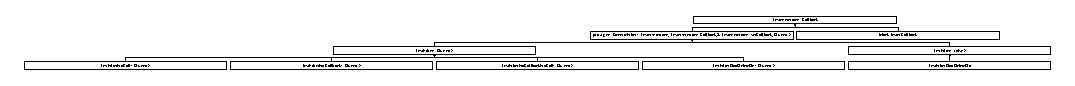
\includegraphics[height=0.712242cm]{classTesterInterface_1_1Callback}
\end{center}
\end{figure}
\subsection*{Public Member Functions}
\begin{DoxyCompactItemize}
\item 
virtual {\bf $\sim$\+Callback} ()
\item 
virtual void {\bf onA} ()=0
\end{DoxyCompactItemize}


\subsection{Detailed Description}


Definition at line 42 of file Generic\+Filter\+Test.\+cpp.



\subsection{Constructor \& Destructor Documentation}
\index{Tester\+Interface\+::\+Callback@{Tester\+Interface\+::\+Callback}!````~Callback@{$\sim$\+Callback}}
\index{````~Callback@{$\sim$\+Callback}!Tester\+Interface\+::\+Callback@{Tester\+Interface\+::\+Callback}}
\subsubsection[{$\sim$\+Callback()}]{\setlength{\rightskip}{0pt plus 5cm}virtual Tester\+Interface\+::\+Callback\+::$\sim$\+Callback (
\begin{DoxyParamCaption}
{}
\end{DoxyParamCaption}
)\hspace{0.3cm}{\ttfamily [inline]}, {\ttfamily [virtual]}}\label{classTesterInterface_1_1Callback_ae3d1d1ce1d02578ede2bb418ba84ae2f}


Definition at line 44 of file Generic\+Filter\+Test.\+cpp.


\begin{DoxyCode}
44 \{\}
\end{DoxyCode}


\subsection{Member Function Documentation}
\index{Tester\+Interface\+::\+Callback@{Tester\+Interface\+::\+Callback}!onA@{onA}}
\index{onA@{onA}!Tester\+Interface\+::\+Callback@{Tester\+Interface\+::\+Callback}}
\subsubsection[{on\+A()=0}]{\setlength{\rightskip}{0pt plus 5cm}virtual void Tester\+Interface\+::\+Callback\+::onA (
\begin{DoxyParamCaption}
{}
\end{DoxyParamCaption}
)\hspace{0.3cm}{\ttfamily [pure virtual]}}\label{classTesterInterface_1_1Callback_a27b141e4f64f782fa8c7f3b028fbf652}


Implemented in {\bf Test\+Filter\+Odd\+Delete\+On$<$ Owned $>$} \doxyref{}{p.}{classTestFilterOddDeleteOn_a8ebd823d3a980756b8afb808b72cbcd5}, {\bf Test\+Filter$<$ Owned $>$} \doxyref{}{p.}{classTestFilter_a63cb90aa885b4ad1fe27f73cad737397}, and {\bf Test\+Filter$<$ false $>$} \doxyref{}{p.}{classTestFilter_a63cb90aa885b4ad1fe27f73cad737397}.



The documentation for this class was generated from the following file\+:\begin{DoxyCompactItemize}
\item 
proxygen/lib/utils/test/{\bf Generic\+Filter\+Test.\+cpp}\end{DoxyCompactItemize}

\section{proxygen\+:\+:Flow\+Control\+Filter\+:\+:Callback Class Reference}
\label{classproxygen_1_1FlowControlFilter_1_1Callback}\index{proxygen\+::\+Flow\+Control\+Filter\+::\+Callback@{proxygen\+::\+Flow\+Control\+Filter\+::\+Callback}}


{\ttfamily \#include $<$Flow\+Control\+Filter.\+h$>$}

Inheritance diagram for proxygen\+:\+:Flow\+Control\+Filter\+:\+:Callback\+:\begin{figure}[H]
\begin{center}
\leavevmode
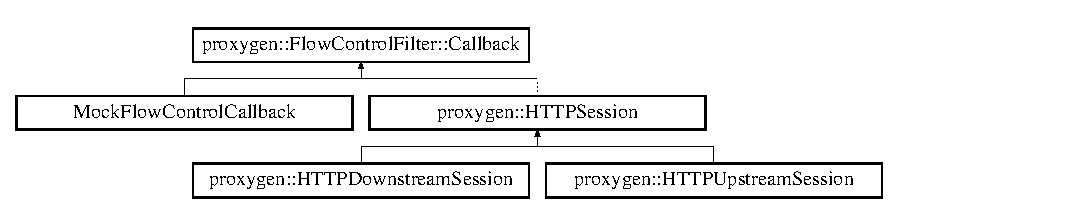
\includegraphics[height=2.424242cm]{classproxygen_1_1FlowControlFilter_1_1Callback}
\end{center}
\end{figure}
\subsection*{Public Member Functions}
\begin{DoxyCompactItemize}
\item 
virtual {\bf $\sim$\+Callback} ()
\item 
virtual void {\bf on\+Connection\+Send\+Window\+Open} ()=0
\item 
virtual void {\bf on\+Connection\+Send\+Window\+Closed} ()=0
\end{DoxyCompactItemize}


\subsection{Detailed Description}


Definition at line 29 of file Flow\+Control\+Filter.\+h.



\subsection{Constructor \& Destructor Documentation}
\index{proxygen\+::\+Flow\+Control\+Filter\+::\+Callback@{proxygen\+::\+Flow\+Control\+Filter\+::\+Callback}!````~Callback@{$\sim$\+Callback}}
\index{````~Callback@{$\sim$\+Callback}!proxygen\+::\+Flow\+Control\+Filter\+::\+Callback@{proxygen\+::\+Flow\+Control\+Filter\+::\+Callback}}
\subsubsection[{$\sim$\+Callback()}]{\setlength{\rightskip}{0pt plus 5cm}virtual proxygen\+::\+Flow\+Control\+Filter\+::\+Callback\+::$\sim$\+Callback (
\begin{DoxyParamCaption}
{}
\end{DoxyParamCaption}
)\hspace{0.3cm}{\ttfamily [inline]}, {\ttfamily [virtual]}}\label{classproxygen_1_1FlowControlFilter_1_1Callback_a74e492388b4f10f928cdfc5e8cfdd9fa}


Definition at line 31 of file Flow\+Control\+Filter.\+h.


\begin{DoxyCode}
31 \{\}
\end{DoxyCode}


\subsection{Member Function Documentation}
\index{proxygen\+::\+Flow\+Control\+Filter\+::\+Callback@{proxygen\+::\+Flow\+Control\+Filter\+::\+Callback}!on\+Connection\+Send\+Window\+Closed@{on\+Connection\+Send\+Window\+Closed}}
\index{on\+Connection\+Send\+Window\+Closed@{on\+Connection\+Send\+Window\+Closed}!proxygen\+::\+Flow\+Control\+Filter\+::\+Callback@{proxygen\+::\+Flow\+Control\+Filter\+::\+Callback}}
\subsubsection[{on\+Connection\+Send\+Window\+Closed()=0}]{\setlength{\rightskip}{0pt plus 5cm}virtual void proxygen\+::\+Flow\+Control\+Filter\+::\+Callback\+::on\+Connection\+Send\+Window\+Closed (
\begin{DoxyParamCaption}
{}
\end{DoxyParamCaption}
)\hspace{0.3cm}{\ttfamily [pure virtual]}}\label{classproxygen_1_1FlowControlFilter_1_1Callback_ab226241c68d175d41d4465af4c2cf757}


Implemented in {\bf proxygen\+::\+H\+T\+T\+P\+Session} \doxyref{}{p.}{classproxygen_1_1HTTPSession_a8073b08df1319efb31f35fc64268d60a}.



Referenced by proxygen\+::\+Flow\+Control\+Filter\+::generate\+Body().

\index{proxygen\+::\+Flow\+Control\+Filter\+::\+Callback@{proxygen\+::\+Flow\+Control\+Filter\+::\+Callback}!on\+Connection\+Send\+Window\+Open@{on\+Connection\+Send\+Window\+Open}}
\index{on\+Connection\+Send\+Window\+Open@{on\+Connection\+Send\+Window\+Open}!proxygen\+::\+Flow\+Control\+Filter\+::\+Callback@{proxygen\+::\+Flow\+Control\+Filter\+::\+Callback}}
\subsubsection[{on\+Connection\+Send\+Window\+Open()=0}]{\setlength{\rightskip}{0pt plus 5cm}virtual void proxygen\+::\+Flow\+Control\+Filter\+::\+Callback\+::on\+Connection\+Send\+Window\+Open (
\begin{DoxyParamCaption}
{}
\end{DoxyParamCaption}
)\hspace{0.3cm}{\ttfamily [pure virtual]}}\label{classproxygen_1_1FlowControlFilter_1_1Callback_a177ffe967dcc7969454c1a42ebc6f0d0}
Notification channel to alert when the send window state changes. 

Implemented in {\bf proxygen\+::\+H\+T\+T\+P\+Session} \doxyref{}{p.}{classproxygen_1_1HTTPSession_abf2d1ccc7eab9fe9a157bbf0999d73a4}.



Referenced by proxygen\+::\+Flow\+Control\+Filter\+::on\+Window\+Update().



The documentation for this class was generated from the following file\+:\begin{DoxyCompactItemize}
\item 
proxygen/lib/http/codec/{\bf Flow\+Control\+Filter.\+h}\end{DoxyCompactItemize}

\section{proxygen\+:\+:H\+T\+T\+P\+Codec\+:\+:Callback Class Reference}
\label{classproxygen_1_1HTTPCodec_1_1Callback}\index{proxygen\+::\+H\+T\+T\+P\+Codec\+::\+Callback@{proxygen\+::\+H\+T\+T\+P\+Codec\+::\+Callback}}


{\ttfamily \#include $<$H\+T\+T\+P\+Codec.\+h$>$}

Inheritance diagram for proxygen\+:\+:H\+T\+T\+P\+Codec\+:\+:Callback\+:\begin{figure}[H]
\begin{center}
\leavevmode
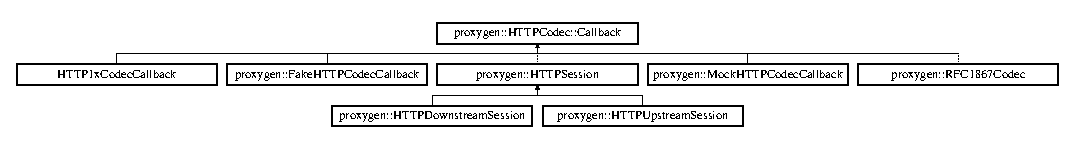
\includegraphics[height=1.480176cm]{classproxygen_1_1HTTPCodec_1_1Callback}
\end{center}
\end{figure}
\subsection*{Public Member Functions}
\begin{DoxyCompactItemize}
\item 
virtual void {\bf on\+Message\+Begin} ({\bf Stream\+ID} {\bf stream}, {\bf H\+T\+T\+P\+Message} $\ast$msg)=0
\item 
virtual void {\bf on\+Push\+Message\+Begin} ({\bf Stream\+ID}, {\bf Stream\+ID}, {\bf H\+T\+T\+P\+Message} $\ast$)
\item 
virtual void {\bf on\+Ex\+Message\+Begin} ({\bf Stream\+ID}, {\bf Stream\+ID}, bool, {\bf H\+T\+T\+P\+Message} $\ast$)
\item 
virtual void {\bf on\+Headers\+Complete} ({\bf Stream\+ID} {\bf stream}, std\+::unique\+\_\+ptr$<$ {\bf H\+T\+T\+P\+Message} $>$ msg)=0
\item 
virtual void {\bf on\+Body} ({\bf Stream\+ID} {\bf stream}, std\+::unique\+\_\+ptr$<$ folly\+::\+I\+O\+Buf $>$ chain, uint16\+\_\+t padding)=0
\item 
virtual void {\bf on\+Chunk\+Header} ({\bf Stream\+ID}, size\+\_\+t)
\item 
virtual void {\bf on\+Chunk\+Complete} ({\bf Stream\+ID})
\item 
virtual void {\bf on\+Trailers\+Complete} ({\bf Stream\+ID} {\bf stream}, std\+::unique\+\_\+ptr$<$ {\bf H\+T\+T\+P\+Headers} $>$ trailers)=0
\item 
virtual void {\bf on\+Message\+Complete} ({\bf Stream\+ID} {\bf stream}, bool upgrade)=0
\item 
virtual void {\bf on\+Error} ({\bf Stream\+ID} {\bf stream}, const {\bf H\+T\+T\+P\+Exception} \&error, bool new\+Txn=false)=0
\item 
virtual void {\bf on\+Abort} ({\bf Stream\+ID}, {\bf Error\+Code})
\item 
virtual void {\bf on\+Frame\+Header} ({\bf Stream\+ID}, uint8\+\_\+t, uint64\+\_\+t, uint8\+\_\+t, uint16\+\_\+t=0)
\item 
virtual void {\bf on\+Goaway} (uint64\+\_\+t, {\bf Error\+Code}, std\+::unique\+\_\+ptr$<$ folly\+::\+I\+O\+Buf $>$={\bf nullptr})
\item 
virtual void {\bf on\+Ping\+Request} (uint64\+\_\+t)
\item 
virtual void {\bf on\+Ping\+Reply} (uint64\+\_\+t)
\item 
virtual void {\bf on\+Window\+Update} ({\bf Stream\+ID}, uint32\+\_\+t)
\item 
virtual void {\bf on\+Settings} (const {\bf Settings\+List} \&)
\item 
virtual void {\bf on\+Settings\+Ack} ()
\item 
virtual void {\bf on\+Priority} ({\bf Stream\+ID}, const {\bf H\+T\+T\+P\+Message\+::\+H\+T\+T\+P\+Priority} \&)
\item 
virtual bool {\bf on\+Native\+Protocol\+Upgrade} ({\bf Stream\+ID}, {\bf Codec\+Protocol}, const std\+::string \&, {\bf H\+T\+T\+P\+Message} \&)
\item 
virtual void {\bf on\+Generate\+Frame\+Header} ({\bf Stream\+ID}, uint8\+\_\+t, uint64\+\_\+t, uint16\+\_\+t=0)
\item 
virtual void {\bf on\+Certificate\+Request} (uint16\+\_\+t, std\+::unique\+\_\+ptr$<$ folly\+::\+I\+O\+Buf $>$)
\item 
virtual void {\bf on\+Certificate} (uint16\+\_\+t, std\+::unique\+\_\+ptr$<$ folly\+::\+I\+O\+Buf $>$)
\item 
virtual uint32\+\_\+t {\bf num\+Outgoing\+Streams} () const 
\item 
virtual uint32\+\_\+t {\bf num\+Incoming\+Streams} () const 
\item 
virtual {\bf $\sim$\+Callback} ()
\end{DoxyCompactItemize}


\subsection{Detailed Description}
\doxyref{Callback}{p.}{classproxygen_1_1HTTPCodec_1_1Callback} interface that users of \doxyref{H\+T\+T\+P\+Codec}{p.}{classproxygen_1_1HTTPCodec} must implement 

Definition at line 78 of file H\+T\+T\+P\+Codec.\+h.



\subsection{Constructor \& Destructor Documentation}
\index{proxygen\+::\+H\+T\+T\+P\+Codec\+::\+Callback@{proxygen\+::\+H\+T\+T\+P\+Codec\+::\+Callback}!````~Callback@{$\sim$\+Callback}}
\index{````~Callback@{$\sim$\+Callback}!proxygen\+::\+H\+T\+T\+P\+Codec\+::\+Callback@{proxygen\+::\+H\+T\+T\+P\+Codec\+::\+Callback}}
\subsubsection[{$\sim$\+Callback()}]{\setlength{\rightskip}{0pt plus 5cm}virtual proxygen\+::\+H\+T\+T\+P\+Codec\+::\+Callback\+::$\sim$\+Callback (
\begin{DoxyParamCaption}
{}
\end{DoxyParamCaption}
)\hspace{0.3cm}{\ttfamily [inline]}, {\ttfamily [virtual]}}\label{classproxygen_1_1HTTPCodec_1_1Callback_a05e9e9907d24e577604f7941da8123bd}


Definition at line 329 of file H\+T\+T\+P\+Codec.\+h.


\begin{DoxyCode}
329 \{\}
\end{DoxyCode}


\subsection{Member Function Documentation}
\index{proxygen\+::\+H\+T\+T\+P\+Codec\+::\+Callback@{proxygen\+::\+H\+T\+T\+P\+Codec\+::\+Callback}!num\+Incoming\+Streams@{num\+Incoming\+Streams}}
\index{num\+Incoming\+Streams@{num\+Incoming\+Streams}!proxygen\+::\+H\+T\+T\+P\+Codec\+::\+Callback@{proxygen\+::\+H\+T\+T\+P\+Codec\+::\+Callback}}
\subsubsection[{num\+Incoming\+Streams() const }]{\setlength{\rightskip}{0pt plus 5cm}virtual uint32\+\_\+t proxygen\+::\+H\+T\+T\+P\+Codec\+::\+Callback\+::num\+Incoming\+Streams (
\begin{DoxyParamCaption}
{}
\end{DoxyParamCaption}
) const\hspace{0.3cm}{\ttfamily [inline]}, {\ttfamily [virtual]}}\label{classproxygen_1_1HTTPCodec_1_1Callback_aad2decb51a53dc21448547ba34b0409a}
Return the number of open streams started by the remote side. Parallel codecs with a maximum number of streams will invoke this to determine if a new stream exceeds the limit. 

Reimplemented in {\bf proxygen\+::\+H\+T\+T\+P\+Session} \doxyref{}{p.}{classproxygen_1_1HTTPSession_a32ded5f1b237ce4aac4dacb8d8844b6f}, and {\bf proxygen\+::\+Fake\+H\+T\+T\+P\+Codec\+Callback} \doxyref{}{p.}{classproxygen_1_1FakeHTTPCodecCallback_a1aa4525d399761ddc2f08b839cc266b1}.



Definition at line 327 of file H\+T\+T\+P\+Codec.\+h.



Referenced by proxygen\+::\+S\+P\+D\+Y\+Codec\+::on\+Syn\+Stream(), and proxygen\+::\+H\+T\+T\+P2\+Codec\+::parse\+Headers\+Check\+Concurrent\+Streams().


\begin{DoxyCode}
327 \{ \textcolor{keywordflow}{return} 0; \}
\end{DoxyCode}
\index{proxygen\+::\+H\+T\+T\+P\+Codec\+::\+Callback@{proxygen\+::\+H\+T\+T\+P\+Codec\+::\+Callback}!num\+Outgoing\+Streams@{num\+Outgoing\+Streams}}
\index{num\+Outgoing\+Streams@{num\+Outgoing\+Streams}!proxygen\+::\+H\+T\+T\+P\+Codec\+::\+Callback@{proxygen\+::\+H\+T\+T\+P\+Codec\+::\+Callback}}
\subsubsection[{num\+Outgoing\+Streams() const }]{\setlength{\rightskip}{0pt plus 5cm}virtual uint32\+\_\+t proxygen\+::\+H\+T\+T\+P\+Codec\+::\+Callback\+::num\+Outgoing\+Streams (
\begin{DoxyParamCaption}
{}
\end{DoxyParamCaption}
) const\hspace{0.3cm}{\ttfamily [inline]}, {\ttfamily [virtual]}}\label{classproxygen_1_1HTTPCodec_1_1Callback_a65779e4b1763aa1daa424f02a5ca3f05}
Return the number of open streams started by this codec callback. Parallel codecs with a maximum number of streams will invoke this to determine if a new stream exceeds the limit. 

Reimplemented in {\bf proxygen\+::\+H\+T\+T\+P\+Session} \doxyref{}{p.}{classproxygen_1_1HTTPSession_ac9f475ec074ab357ffeeb614cfe3f83d}, and {\bf proxygen\+::\+Fake\+H\+T\+T\+P\+Codec\+Callback} \doxyref{}{p.}{classproxygen_1_1FakeHTTPCodecCallback_a03af9af000004c543ee9999debf25390}.



Definition at line 320 of file H\+T\+T\+P\+Codec.\+h.


\begin{DoxyCode}
320 \{ \textcolor{keywordflow}{return} 0; \}
\end{DoxyCode}
\index{proxygen\+::\+H\+T\+T\+P\+Codec\+::\+Callback@{proxygen\+::\+H\+T\+T\+P\+Codec\+::\+Callback}!on\+Abort@{on\+Abort}}
\index{on\+Abort@{on\+Abort}!proxygen\+::\+H\+T\+T\+P\+Codec\+::\+Callback@{proxygen\+::\+H\+T\+T\+P\+Codec\+::\+Callback}}
\subsubsection[{on\+Abort(\+Stream\+I\+D, Error\+Code)}]{\setlength{\rightskip}{0pt plus 5cm}virtual void proxygen\+::\+H\+T\+T\+P\+Codec\+::\+Callback\+::on\+Abort (
\begin{DoxyParamCaption}
\item[{{\bf Stream\+ID}}]{, }
\item[{{\bf Error\+Code}}]{}
\end{DoxyParamCaption}
)\hspace{0.3cm}{\ttfamily [inline]}, {\ttfamily [virtual]}}\label{classproxygen_1_1HTTPCodec_1_1Callback_a110afc4d5324a47b9b2f6356afc70bbf}
Called when the peer has asked to shut down a stream immediately. 
\begin{DoxyParams}{Parameters}
{\em stream} & The stream ID \\
\hline
{\em code} & The code the stream was aborted with \\
\hline
\end{DoxyParams}
\begin{DoxyNote}{Note}
Not applicable to all protocols. 
\end{DoxyNote}


Reimplemented in {\bf proxygen\+::\+H\+T\+T\+P\+Session} \doxyref{}{p.}{classproxygen_1_1HTTPSession_ac3183c78b441791ee835660ffb91ed9f}, and {\bf proxygen\+::\+Fake\+H\+T\+T\+P\+Codec\+Callback} \doxyref{}{p.}{classproxygen_1_1FakeHTTPCodecCallback_a3f66d4797b2c12c5485986f90fa1b331}.



Definition at line 192 of file H\+T\+T\+P\+Codec.\+h.



Referenced by proxygen\+::\+S\+P\+D\+Y\+Codec\+::on\+Rst\+Stream(), and proxygen\+::\+H\+T\+T\+P2\+Codec\+::parse\+Rst\+Stream().


\begin{DoxyCode}
194                      \{\}
\end{DoxyCode}
\index{proxygen\+::\+H\+T\+T\+P\+Codec\+::\+Callback@{proxygen\+::\+H\+T\+T\+P\+Codec\+::\+Callback}!on\+Body@{on\+Body}}
\index{on\+Body@{on\+Body}!proxygen\+::\+H\+T\+T\+P\+Codec\+::\+Callback@{proxygen\+::\+H\+T\+T\+P\+Codec\+::\+Callback}}
\subsubsection[{on\+Body(\+Stream\+I\+D stream, std\+::unique\+\_\+ptr$<$ folly\+::\+I\+O\+Buf $>$ chain, uint16\+\_\+t padding)=0}]{\setlength{\rightskip}{0pt plus 5cm}virtual void proxygen\+::\+H\+T\+T\+P\+Codec\+::\+Callback\+::on\+Body (
\begin{DoxyParamCaption}
\item[{{\bf Stream\+ID}}]{stream, }
\item[{std\+::unique\+\_\+ptr$<$ folly\+::\+I\+O\+Buf $>$}]{chain, }
\item[{uint16\+\_\+t}]{padding}
\end{DoxyParamCaption}
)\hspace{0.3cm}{\ttfamily [pure virtual]}}\label{classproxygen_1_1HTTPCodec_1_1Callback_af6661786cb419aa6b0138ed1d8085d52}
Called for each block of message body data 
\begin{DoxyParams}{Parameters}
{\em stream} & The stream ID \\
\hline
{\em chain} & One or more buffers of body data. The codec will remove any protocol framing, such as H\+T\+T\+P/1.\+1 chunk headers, from the buffers before calling this function. \\
\hline
{\em padding} & Number of pad bytes that came with the data segment \\
\hline
\end{DoxyParams}


Implemented in {\bf proxygen\+::\+H\+T\+T\+P\+Session} \doxyref{}{p.}{classproxygen_1_1HTTPSession_a4ef5f45a171469eadd34144f3a00802c}, {\bf proxygen\+::\+Mock\+H\+T\+T\+P\+Codec\+Callback} \doxyref{}{p.}{classproxygen_1_1MockHTTPCodecCallback_ac4e58e068ff76da169802b8668befd73}, {\bf proxygen\+::\+Fake\+H\+T\+T\+P\+Codec\+Callback} \doxyref{}{p.}{classproxygen_1_1FakeHTTPCodecCallback_a43e0a21206fd5d3b34959818ecb5a5c1}, {\bf proxygen\+::\+R\+F\+C1867\+Codec} \doxyref{}{p.}{classproxygen_1_1RFC1867Codec_a4a6f31403b32e593888d89274023614a}, and {\bf H\+T\+T\+P1x\+Codec\+Callback} \doxyref{}{p.}{classHTTP1xCodecCallback_a45c3eac90864197e1ec5334016629431}.



Referenced by proxygen\+::\+H\+T\+T\+P1x\+Codec\+::on\+Body(), proxygen\+::\+H\+T\+T\+P1x\+Codec\+::on\+Ingress(), proxygen\+::\+H\+T\+T\+P2\+Codec\+::parse\+All\+Data(), proxygen\+::\+H\+T\+T\+P2\+Codec\+::parse\+Data\+Frame\+Data(), and proxygen\+::\+S\+P\+D\+Y\+Codec\+::parse\+Ingress().

\index{proxygen\+::\+H\+T\+T\+P\+Codec\+::\+Callback@{proxygen\+::\+H\+T\+T\+P\+Codec\+::\+Callback}!on\+Certificate@{on\+Certificate}}
\index{on\+Certificate@{on\+Certificate}!proxygen\+::\+H\+T\+T\+P\+Codec\+::\+Callback@{proxygen\+::\+H\+T\+T\+P\+Codec\+::\+Callback}}
\subsubsection[{on\+Certificate(uint16\+\_\+t, std\+::unique\+\_\+ptr$<$ folly\+::\+I\+O\+Buf $>$)}]{\setlength{\rightskip}{0pt plus 5cm}virtual void proxygen\+::\+H\+T\+T\+P\+Codec\+::\+Callback\+::on\+Certificate (
\begin{DoxyParamCaption}
\item[{uint16\+\_\+t}]{, }
\item[{std\+::unique\+\_\+ptr$<$ folly\+::\+I\+O\+Buf $>$}]{}
\end{DoxyParamCaption}
)\hspace{0.3cm}{\ttfamily [inline]}, {\ttfamily [virtual]}}\label{classproxygen_1_1HTTPCodec_1_1Callback_a39962dfe4038936e8042e725e50c2d45}
Called upon receipt of an authenticator, for protocols that support secondary certificate authentication. 
\begin{DoxyParams}{Parameters}
{\em cert\+Id} & The Cert-\/\+ID identifying this authenticator \\
\hline
{\em authenticator} & The authenticator request \\
\hline
\end{DoxyParams}
\begin{DoxyNote}{Note}
Not all protocols support secondary certificate authentication. H\+T\+T\+P/2 does, but H\+T\+T\+P/1.\+1 doesn\textquotesingle{}t. 
\end{DoxyNote}


Reimplemented in {\bf proxygen\+::\+H\+T\+T\+P\+Session} \doxyref{}{p.}{classproxygen_1_1HTTPSession_a4bdeeff83639f5b0afdec5b2d92ea48d}, {\bf proxygen\+::\+Fake\+H\+T\+T\+P\+Codec\+Callback} \doxyref{}{p.}{classproxygen_1_1FakeHTTPCodecCallback_af2175032d60674dc99e7ddc7859f2a02}, and {\bf proxygen\+::\+Mock\+H\+T\+T\+P\+Codec\+Callback} \doxyref{}{p.}{classproxygen_1_1MockHTTPCodecCallback_aef5b399bf8a0191cb96354611ff945fc}.



Definition at line 310 of file H\+T\+T\+P\+Codec.\+h.



Referenced by proxygen\+::\+H\+T\+T\+P2\+Codec\+::parse\+Certificate().


\begin{DoxyCode}
312                                      \{
313     \}
\end{DoxyCode}
\index{proxygen\+::\+H\+T\+T\+P\+Codec\+::\+Callback@{proxygen\+::\+H\+T\+T\+P\+Codec\+::\+Callback}!on\+Certificate\+Request@{on\+Certificate\+Request}}
\index{on\+Certificate\+Request@{on\+Certificate\+Request}!proxygen\+::\+H\+T\+T\+P\+Codec\+::\+Callback@{proxygen\+::\+H\+T\+T\+P\+Codec\+::\+Callback}}
\subsubsection[{on\+Certificate\+Request(uint16\+\_\+t, std\+::unique\+\_\+ptr$<$ folly\+::\+I\+O\+Buf $>$)}]{\setlength{\rightskip}{0pt plus 5cm}virtual void proxygen\+::\+H\+T\+T\+P\+Codec\+::\+Callback\+::on\+Certificate\+Request (
\begin{DoxyParamCaption}
\item[{uint16\+\_\+t}]{, }
\item[{std\+::unique\+\_\+ptr$<$ folly\+::\+I\+O\+Buf $>$}]{}
\end{DoxyParamCaption}
)\hspace{0.3cm}{\ttfamily [inline]}, {\ttfamily [virtual]}}\label{classproxygen_1_1HTTPCodec_1_1Callback_a982896bcd896ea45a10b03a294ded590}
Called upon receipt of a certificate request frame, for protocols that support secondary certificate authentication. 
\begin{DoxyParams}{Parameters}
{\em request\+Id} & The Request-\/\+ID identifying the certificate request \\
\hline
{\em auth\+Request} & The authenticator request \\
\hline
\end{DoxyParams}
\begin{DoxyNote}{Note}
Not all protocols support secondary certificate authentication. H\+T\+T\+P/2 does, but H\+T\+T\+P/1.\+1 doesn\textquotesingle{}t. 
\end{DoxyNote}


Reimplemented in {\bf proxygen\+::\+H\+T\+T\+P\+Session} \doxyref{}{p.}{classproxygen_1_1HTTPSession_ae98209dbf84dc096fb2ace705407fd47}, {\bf proxygen\+::\+Fake\+H\+T\+T\+P\+Codec\+Callback} \doxyref{}{p.}{classproxygen_1_1FakeHTTPCodecCallback_a404bde70243206b37309b8df0dd5f717}, and {\bf proxygen\+::\+Mock\+H\+T\+T\+P\+Codec\+Callback} \doxyref{}{p.}{classproxygen_1_1MockHTTPCodecCallback_a6890b812cc7565952643b5cec3f131c6}.



Definition at line 297 of file H\+T\+T\+P\+Codec.\+h.



Referenced by proxygen\+::\+H\+T\+T\+P2\+Codec\+::parse\+Certificate\+Request().


\begin{DoxyCode}
299                                      \{
300     \}
\end{DoxyCode}
\index{proxygen\+::\+H\+T\+T\+P\+Codec\+::\+Callback@{proxygen\+::\+H\+T\+T\+P\+Codec\+::\+Callback}!on\+Chunk\+Complete@{on\+Chunk\+Complete}}
\index{on\+Chunk\+Complete@{on\+Chunk\+Complete}!proxygen\+::\+H\+T\+T\+P\+Codec\+::\+Callback@{proxygen\+::\+H\+T\+T\+P\+Codec\+::\+Callback}}
\subsubsection[{on\+Chunk\+Complete(\+Stream\+I\+D)}]{\setlength{\rightskip}{0pt plus 5cm}virtual void proxygen\+::\+H\+T\+T\+P\+Codec\+::\+Callback\+::on\+Chunk\+Complete (
\begin{DoxyParamCaption}
\item[{{\bf Stream\+ID}}]{}
\end{DoxyParamCaption}
)\hspace{0.3cm}{\ttfamily [inline]}, {\ttfamily [virtual]}}\label{classproxygen_1_1HTTPCodec_1_1Callback_aad1fa297ee8929ea5032b7037956198b}
Called when the terminating C\+R\+LF is received to end a chunk of H\+T\+TP body data.


\begin{DoxyParams}{Parameters}
{\em stream} & The stream ID \\
\hline
\end{DoxyParams}


Reimplemented in {\bf proxygen\+::\+H\+T\+T\+P\+Session} \doxyref{}{p.}{classproxygen_1_1HTTPSession_a201f8d42c3a6754e2743b5e5661b901e}, {\bf proxygen\+::\+Fake\+H\+T\+T\+P\+Codec\+Callback} \doxyref{}{p.}{classproxygen_1_1FakeHTTPCodecCallback_a5e8de5c57251fe0c3e28ca30573ae291}, and {\bf H\+T\+T\+P1x\+Codec\+Callback} \doxyref{}{p.}{classHTTP1xCodecCallback_ab9f5539148d7b2f8ba195a56aefc13b0}.



Definition at line 156 of file H\+T\+T\+P\+Codec.\+h.



Referenced by proxygen\+::\+H\+T\+T\+P1x\+Codec\+::on\+Chunk\+Complete().


\begin{DoxyCode}
156 \{\}
\end{DoxyCode}
\index{proxygen\+::\+H\+T\+T\+P\+Codec\+::\+Callback@{proxygen\+::\+H\+T\+T\+P\+Codec\+::\+Callback}!on\+Chunk\+Header@{on\+Chunk\+Header}}
\index{on\+Chunk\+Header@{on\+Chunk\+Header}!proxygen\+::\+H\+T\+T\+P\+Codec\+::\+Callback@{proxygen\+::\+H\+T\+T\+P\+Codec\+::\+Callback}}
\subsubsection[{on\+Chunk\+Header(\+Stream\+I\+D, size\+\_\+t)}]{\setlength{\rightskip}{0pt plus 5cm}virtual void proxygen\+::\+H\+T\+T\+P\+Codec\+::\+Callback\+::on\+Chunk\+Header (
\begin{DoxyParamCaption}
\item[{{\bf Stream\+ID}}]{, }
\item[{size\+\_\+t}]{}
\end{DoxyParamCaption}
)\hspace{0.3cm}{\ttfamily [inline]}, {\ttfamily [virtual]}}\label{classproxygen_1_1HTTPCodec_1_1Callback_ae106b662c7e855b4677ec55d4235e66d}
Called for each H\+T\+TP chunk header.

\doxyref{on\+Chunk\+Header()}{p.}{classproxygen_1_1HTTPCodec_1_1Callback_ae106b662c7e855b4677ec55d4235e66d} will be called when the chunk header is received. As the chunk data arrives, it will be passed to the callback normally with \doxyref{on\+Body()}{p.}{classproxygen_1_1HTTPCodec_1_1Callback_af6661786cb419aa6b0138ed1d8085d52} calls. Note that the chunk data may arrive in multiple \doxyref{on\+Body()}{p.}{classproxygen_1_1HTTPCodec_1_1Callback_af6661786cb419aa6b0138ed1d8085d52} calls\+: it is not guaranteed to arrive in a single \doxyref{on\+Body()}{p.}{classproxygen_1_1HTTPCodec_1_1Callback_af6661786cb419aa6b0138ed1d8085d52} call.

After the chunk data has been received and the terminating C\+R\+LF has been received, \doxyref{on\+Chunk\+Complete()}{p.}{classproxygen_1_1HTTPCodec_1_1Callback_aad1fa297ee8929ea5032b7037956198b} will be called.


\begin{DoxyParams}{Parameters}
{\em stream} & The stream ID \\
\hline
{\em length} & The chunk length. \\
\hline
\end{DoxyParams}


Reimplemented in {\bf proxygen\+::\+H\+T\+T\+P\+Session} \doxyref{}{p.}{classproxygen_1_1HTTPSession_a3137afb711666467861a8d61d9f15824}, {\bf proxygen\+::\+Fake\+H\+T\+T\+P\+Codec\+Callback} \doxyref{}{p.}{classproxygen_1_1FakeHTTPCodecCallback_adb95188db25583e64a9ff905513f4072}, and {\bf H\+T\+T\+P1x\+Codec\+Callback} \doxyref{}{p.}{classHTTP1xCodecCallback_a37b309b40fb28e30cf01c25e737801b7}.



Definition at line 148 of file H\+T\+T\+P\+Codec.\+h.



Referenced by proxygen\+::\+H\+T\+T\+P1x\+Codec\+::on\+Chunk\+Header().


\begin{DoxyCode}
148 \{\}
\end{DoxyCode}
\index{proxygen\+::\+H\+T\+T\+P\+Codec\+::\+Callback@{proxygen\+::\+H\+T\+T\+P\+Codec\+::\+Callback}!on\+Error@{on\+Error}}
\index{on\+Error@{on\+Error}!proxygen\+::\+H\+T\+T\+P\+Codec\+::\+Callback@{proxygen\+::\+H\+T\+T\+P\+Codec\+::\+Callback}}
\subsubsection[{on\+Error(\+Stream\+I\+D stream, const H\+T\+T\+P\+Exception \&error, bool new\+Txn=false)=0}]{\setlength{\rightskip}{0pt plus 5cm}virtual void proxygen\+::\+H\+T\+T\+P\+Codec\+::\+Callback\+::on\+Error (
\begin{DoxyParamCaption}
\item[{{\bf Stream\+ID}}]{stream, }
\item[{const {\bf H\+T\+T\+P\+Exception} \&}]{error, }
\item[{bool}]{new\+Txn = {\ttfamily false}}
\end{DoxyParamCaption}
)\hspace{0.3cm}{\ttfamily [pure virtual]}}\label{classproxygen_1_1HTTPCodec_1_1Callback_a39e04260da7dd1a074393fe473d6ac34}
Called when a parsing or protocol error has occurred 
\begin{DoxyParams}{Parameters}
{\em stream} & The stream ID \\
\hline
{\em error} & Description of the error \\
\hline
{\em new\+Txn} & true if on\+Message\+Begin has not been called for txn \\
\hline
\end{DoxyParams}


Implemented in {\bf proxygen\+::\+H\+T\+T\+P\+Session} \doxyref{}{p.}{classproxygen_1_1HTTPSession_ab44f22d1c1900f583f4e8584fb2f0105}, {\bf proxygen\+::\+Mock\+H\+T\+T\+P\+Codec\+Callback} \doxyref{}{p.}{classproxygen_1_1MockHTTPCodecCallback_accda1fe4c5523b1fed69b013a3ed63e5}, {\bf proxygen\+::\+Fake\+H\+T\+T\+P\+Codec\+Callback} \doxyref{}{p.}{classproxygen_1_1FakeHTTPCodecCallback_a83e8a0e41d47d585814fe8316ff919d3}, {\bf proxygen\+::\+R\+F\+C1867\+Codec} \doxyref{}{p.}{classproxygen_1_1RFC1867Codec_a072b62abe677260b50cf8b2b5b93f9c2}, and {\bf H\+T\+T\+P1x\+Codec\+Callback} \doxyref{}{p.}{classHTTP1xCodecCallback_ade76ef6d005c0b44518982f4c743f50c}.



Referenced by proxygen\+::\+H\+T\+T\+P2\+Codec\+::check\+Connection\+Error(), proxygen\+::\+S\+P\+D\+Y\+Codec\+::fail\+Session(), proxygen\+::\+S\+P\+D\+Y\+Codec\+::fail\+Stream(), proxygen\+::\+H\+T\+T\+P1x\+Codec\+::on\+Parser\+Error(), proxygen\+::\+H\+T\+T\+P2\+Codec\+::parse\+Headers\+Decode\+Frames(), proxygen\+::\+H\+T\+T\+P2\+Codec\+::stream\+Error(), and T\+E\+S\+T().

\index{proxygen\+::\+H\+T\+T\+P\+Codec\+::\+Callback@{proxygen\+::\+H\+T\+T\+P\+Codec\+::\+Callback}!on\+Ex\+Message\+Begin@{on\+Ex\+Message\+Begin}}
\index{on\+Ex\+Message\+Begin@{on\+Ex\+Message\+Begin}!proxygen\+::\+H\+T\+T\+P\+Codec\+::\+Callback@{proxygen\+::\+H\+T\+T\+P\+Codec\+::\+Callback}}
\subsubsection[{on\+Ex\+Message\+Begin(\+Stream\+I\+D, Stream\+I\+D, bool, H\+T\+T\+P\+Message $\ast$)}]{\setlength{\rightskip}{0pt plus 5cm}virtual void proxygen\+::\+H\+T\+T\+P\+Codec\+::\+Callback\+::on\+Ex\+Message\+Begin (
\begin{DoxyParamCaption}
\item[{{\bf Stream\+ID}}]{, }
\item[{{\bf Stream\+ID}}]{, }
\item[{bool}]{, }
\item[{{\bf H\+T\+T\+P\+Message} $\ast$}]{}
\end{DoxyParamCaption}
)\hspace{0.3cm}{\ttfamily [inline]}, {\ttfamily [virtual]}}\label{classproxygen_1_1HTTPCodec_1_1Callback_abe873557040a9184715f7f5a47c863a1}
Called when a new extended message is seen while parsing the ingress.


\begin{DoxyParams}{Parameters}
{\em stream} & The stream ID \\
\hline
{\em control\+Stream} & The stream ID of the associated stream, which can never be 0 \\
\hline
{\em msg} & A newly allocated \doxyref{H\+T\+T\+P\+Message}{p.}{classproxygen_1_1HTTPMessage} \\
\hline
\end{DoxyParams}


Reimplemented in {\bf proxygen\+::\+H\+T\+T\+P\+Session} \doxyref{}{p.}{classproxygen_1_1HTTPSession_a597d69aedaebffdb4c442ca9d1d6408b}, and {\bf proxygen\+::\+Fake\+H\+T\+T\+P\+Codec\+Callback} \doxyref{}{p.}{classproxygen_1_1FakeHTTPCodecCallback_a4b5bd19125263aa65637b2f5aff8b415}.



Definition at line 107 of file H\+T\+T\+P\+Codec.\+h.



Referenced by proxygen\+::\+H\+T\+T\+P2\+Codec\+::parse\+Headers\+Impl().


\begin{DoxyCode}
110                                                   \{\}
\end{DoxyCode}
\index{proxygen\+::\+H\+T\+T\+P\+Codec\+::\+Callback@{proxygen\+::\+H\+T\+T\+P\+Codec\+::\+Callback}!on\+Frame\+Header@{on\+Frame\+Header}}
\index{on\+Frame\+Header@{on\+Frame\+Header}!proxygen\+::\+H\+T\+T\+P\+Codec\+::\+Callback@{proxygen\+::\+H\+T\+T\+P\+Codec\+::\+Callback}}
\subsubsection[{on\+Frame\+Header(\+Stream\+I\+D, uint8\+\_\+t, uint64\+\_\+t, uint8\+\_\+t, uint16\+\_\+t=0)}]{\setlength{\rightskip}{0pt plus 5cm}virtual void proxygen\+::\+H\+T\+T\+P\+Codec\+::\+Callback\+::on\+Frame\+Header (
\begin{DoxyParamCaption}
\item[{{\bf Stream\+ID}}]{, }
\item[{uint8\+\_\+t}]{, }
\item[{uint64\+\_\+t}]{, }
\item[{uint8\+\_\+t}]{, }
\item[{uint16\+\_\+t}]{ = {\ttfamily 0}}
\end{DoxyParamCaption}
)\hspace{0.3cm}{\ttfamily [inline]}, {\ttfamily [virtual]}}\label{classproxygen_1_1HTTPCodec_1_1Callback_a43441f24ed1f9680a2909d1617822b61}
Called upon receipt of a frame header. 
\begin{DoxyParams}{Parameters}
{\em stream\+\_\+id} & The stream ID \\
\hline
{\em flags} & The flags field of frame header \\
\hline
{\em length} & The length field of frame header \\
\hline
{\em type} & The type field of frame header \\
\hline
{\em version} & The version of frame (S\+P\+DY only) \\
\hline
\end{DoxyParams}
\begin{DoxyNote}{Note}
Not all protocols have frames. S\+P\+DY and H\+T\+T\+P/2 do, but H\+T\+T\+P/1.\+1 doesn\textquotesingle{}t. 
\end{DoxyNote}


Reimplemented in {\bf proxygen\+::\+Fake\+H\+T\+T\+P\+Codec\+Callback} \doxyref{}{p.}{classproxygen_1_1FakeHTTPCodecCallback_a722c3094de807039d40675071c028f43}.



Definition at line 206 of file H\+T\+T\+P\+Codec.\+h.



Referenced by proxygen\+::\+H\+T\+T\+P2\+Codec\+::on\+Ingress(), and proxygen\+::\+S\+P\+D\+Y\+Codec\+::parse\+Ingress().


\begin{DoxyCode}
211                         \{\}
\end{DoxyCode}
\index{proxygen\+::\+H\+T\+T\+P\+Codec\+::\+Callback@{proxygen\+::\+H\+T\+T\+P\+Codec\+::\+Callback}!on\+Generate\+Frame\+Header@{on\+Generate\+Frame\+Header}}
\index{on\+Generate\+Frame\+Header@{on\+Generate\+Frame\+Header}!proxygen\+::\+H\+T\+T\+P\+Codec\+::\+Callback@{proxygen\+::\+H\+T\+T\+P\+Codec\+::\+Callback}}
\subsubsection[{on\+Generate\+Frame\+Header(\+Stream\+I\+D, uint8\+\_\+t, uint64\+\_\+t, uint16\+\_\+t=0)}]{\setlength{\rightskip}{0pt plus 5cm}virtual void proxygen\+::\+H\+T\+T\+P\+Codec\+::\+Callback\+::on\+Generate\+Frame\+Header (
\begin{DoxyParamCaption}
\item[{{\bf Stream\+ID}}]{, }
\item[{uint8\+\_\+t}]{, }
\item[{uint64\+\_\+t}]{, }
\item[{uint16\+\_\+t}]{ = {\ttfamily 0}}
\end{DoxyParamCaption}
)\hspace{0.3cm}{\ttfamily [inline]}, {\ttfamily [virtual]}}\label{classproxygen_1_1HTTPCodec_1_1Callback_acdc27546d6ace641570c28299d83898b}
Called after a header frame is generated. This only applies to framed codecs. 

Definition at line 283 of file H\+T\+T\+P\+Codec.\+h.



Referenced by proxygen\+::\+H\+T\+T\+P2\+Codec\+::generate\+Header\+Callback\+Wrapper().


\begin{DoxyCode}
287                         \{\}
\end{DoxyCode}
\index{proxygen\+::\+H\+T\+T\+P\+Codec\+::\+Callback@{proxygen\+::\+H\+T\+T\+P\+Codec\+::\+Callback}!on\+Goaway@{on\+Goaway}}
\index{on\+Goaway@{on\+Goaway}!proxygen\+::\+H\+T\+T\+P\+Codec\+::\+Callback@{proxygen\+::\+H\+T\+T\+P\+Codec\+::\+Callback}}
\subsubsection[{on\+Goaway(uint64\+\_\+t, Error\+Code, std\+::unique\+\_\+ptr$<$ folly\+::\+I\+O\+Buf $>$=nullptr)}]{\setlength{\rightskip}{0pt plus 5cm}virtual void proxygen\+::\+H\+T\+T\+P\+Codec\+::\+Callback\+::on\+Goaway (
\begin{DoxyParamCaption}
\item[{uint64\+\_\+t}]{, }
\item[{{\bf Error\+Code}}]{, }
\item[{std\+::unique\+\_\+ptr$<$ folly\+::\+I\+O\+Buf $>$}]{ = {\ttfamily {\bf nullptr}}}
\end{DoxyParamCaption}
)\hspace{0.3cm}{\ttfamily [inline]}, {\ttfamily [virtual]}}\label{classproxygen_1_1HTTPCodec_1_1Callback_a782493dc0d063e7f5c626db2617d042b}
Called upon receipt of a goaway. 
\begin{DoxyParams}{Parameters}
{\em last\+Good\+Stream\+ID} & Last successful stream created by the receiver \\
\hline
{\em code} & The code the connection was aborted with \\
\hline
{\em debug\+Data} & The additional debug data for diagnostic purpose \\
\hline
\end{DoxyParams}
\begin{DoxyNote}{Note}
Not all protocols have goaways. S\+P\+DY does, but H\+T\+T\+P/1.\+1 doesn\textquotesingle{}t. 
\end{DoxyNote}


Reimplemented in {\bf proxygen\+::\+H\+T\+T\+P\+Session} \doxyref{}{p.}{classproxygen_1_1HTTPSession_a22d185dd9d6777d445ae30269345c942}, {\bf proxygen\+::\+Fake\+H\+T\+T\+P\+Codec\+Callback} \doxyref{}{p.}{classproxygen_1_1FakeHTTPCodecCallback_af0c6ee01c15862bc87e5938019426591}, and {\bf proxygen\+::\+Mock\+H\+T\+T\+P\+Codec\+Callback} \doxyref{}{p.}{classproxygen_1_1MockHTTPCodecCallback_ab9c7e41e4d0aeed9b01a64ea468492f3}.



Definition at line 220 of file H\+T\+T\+P\+Codec.\+h.



Referenced by proxygen\+::\+S\+P\+D\+Y\+Codec\+::on\+Goaway(), and proxygen\+::\+H\+T\+T\+P2\+Codec\+::parse\+Goaway().


\begin{DoxyCode}
223                                                \{\}
\end{DoxyCode}
\index{proxygen\+::\+H\+T\+T\+P\+Codec\+::\+Callback@{proxygen\+::\+H\+T\+T\+P\+Codec\+::\+Callback}!on\+Headers\+Complete@{on\+Headers\+Complete}}
\index{on\+Headers\+Complete@{on\+Headers\+Complete}!proxygen\+::\+H\+T\+T\+P\+Codec\+::\+Callback@{proxygen\+::\+H\+T\+T\+P\+Codec\+::\+Callback}}
\subsubsection[{on\+Headers\+Complete(\+Stream\+I\+D stream, std\+::unique\+\_\+ptr$<$ H\+T\+T\+P\+Message $>$ msg)=0}]{\setlength{\rightskip}{0pt plus 5cm}virtual void proxygen\+::\+H\+T\+T\+P\+Codec\+::\+Callback\+::on\+Headers\+Complete (
\begin{DoxyParamCaption}
\item[{{\bf Stream\+ID}}]{stream, }
\item[{std\+::unique\+\_\+ptr$<$ {\bf H\+T\+T\+P\+Message} $>$}]{msg}
\end{DoxyParamCaption}
)\hspace{0.3cm}{\ttfamily [pure virtual]}}\label{classproxygen_1_1HTTPCodec_1_1Callback_a7c462d2b3485d0d1077a9ba775f90ebc}
Called when all the headers of an ingress message have been parsed 
\begin{DoxyParams}{Parameters}
{\em stream} & The stream ID \\
\hline
{\em msg} & The message \\
\hline
{\em size} & Size of the ingress header \\
\hline
\end{DoxyParams}


Implemented in {\bf proxygen\+::\+H\+T\+T\+P\+Session} \doxyref{}{p.}{classproxygen_1_1HTTPSession_a01cf2e4876e0d44c1b7974833bef3272}, {\bf proxygen\+::\+Mock\+H\+T\+T\+P\+Codec\+Callback} \doxyref{}{p.}{classproxygen_1_1MockHTTPCodecCallback_a1844c9fda354a134d1d665b73037af6e}, {\bf proxygen\+::\+Fake\+H\+T\+T\+P\+Codec\+Callback} \doxyref{}{p.}{classproxygen_1_1FakeHTTPCodecCallback_a3f55acceddc05d771c992c3a04a51f2f}, {\bf proxygen\+::\+R\+F\+C1867\+Codec} \doxyref{}{p.}{classproxygen_1_1RFC1867Codec_a9e01714bafae9a4c2c5aaa7df2182974}, and {\bf H\+T\+T\+P1x\+Codec\+Callback} \doxyref{}{p.}{classHTTP1xCodecCallback_a931173aed9988e11ed2222cf1545189e}.



Referenced by proxygen\+::\+H\+T\+T\+P1x\+Codec\+::on\+Headers\+Complete(), proxygen\+::\+S\+P\+D\+Y\+Codec\+::on\+Syn\+Common(), and proxygen\+::\+H\+T\+T\+P2\+Codec\+::parse\+Headers\+Impl().

\index{proxygen\+::\+H\+T\+T\+P\+Codec\+::\+Callback@{proxygen\+::\+H\+T\+T\+P\+Codec\+::\+Callback}!on\+Message\+Begin@{on\+Message\+Begin}}
\index{on\+Message\+Begin@{on\+Message\+Begin}!proxygen\+::\+H\+T\+T\+P\+Codec\+::\+Callback@{proxygen\+::\+H\+T\+T\+P\+Codec\+::\+Callback}}
\subsubsection[{on\+Message\+Begin(\+Stream\+I\+D stream, H\+T\+T\+P\+Message $\ast$msg)=0}]{\setlength{\rightskip}{0pt plus 5cm}virtual void proxygen\+::\+H\+T\+T\+P\+Codec\+::\+Callback\+::on\+Message\+Begin (
\begin{DoxyParamCaption}
\item[{{\bf Stream\+ID}}]{stream, }
\item[{{\bf H\+T\+T\+P\+Message} $\ast$}]{msg}
\end{DoxyParamCaption}
)\hspace{0.3cm}{\ttfamily [pure virtual]}}\label{classproxygen_1_1HTTPCodec_1_1Callback_a7bcd0c639fd05f92b31806cee4f4b1aa}
Called when a new message is seen while parsing the ingress 
\begin{DoxyParams}{Parameters}
{\em stream} & The stream ID \\
\hline
{\em msg} & A newly allocated \doxyref{H\+T\+T\+P\+Message}{p.}{classproxygen_1_1HTTPMessage} \\
\hline
\end{DoxyParams}


Implemented in {\bf proxygen\+::\+H\+T\+T\+P\+Session} \doxyref{}{p.}{classproxygen_1_1HTTPSession_a0a4087a0c6fbfbb6a419dff46c0d3517}, {\bf proxygen\+::\+Fake\+H\+T\+T\+P\+Codec\+Callback} \doxyref{}{p.}{classproxygen_1_1FakeHTTPCodecCallback_ab67a7d12ac1032f91c90630bbbca2198}, {\bf proxygen\+::\+R\+F\+C1867\+Codec} \doxyref{}{p.}{classproxygen_1_1RFC1867Codec_a68fcd8fdcd4cf0701b738580998c0973}, and {\bf H\+T\+T\+P1x\+Codec\+Callback} \doxyref{}{p.}{classHTTP1xCodecCallback_a39aea280119e87229685df6b4b18dcbb}.



Referenced by proxygen\+::\+S\+P\+D\+Y\+Codec\+::deliver\+On\+Message\+Begin(), proxygen\+::\+H\+T\+T\+P1x\+Codec\+::on\+Message\+Begin(), and proxygen\+::\+H\+T\+T\+P2\+Codec\+::parse\+Headers\+Impl().

\index{proxygen\+::\+H\+T\+T\+P\+Codec\+::\+Callback@{proxygen\+::\+H\+T\+T\+P\+Codec\+::\+Callback}!on\+Message\+Complete@{on\+Message\+Complete}}
\index{on\+Message\+Complete@{on\+Message\+Complete}!proxygen\+::\+H\+T\+T\+P\+Codec\+::\+Callback@{proxygen\+::\+H\+T\+T\+P\+Codec\+::\+Callback}}
\subsubsection[{on\+Message\+Complete(\+Stream\+I\+D stream, bool upgrade)=0}]{\setlength{\rightskip}{0pt plus 5cm}virtual void proxygen\+::\+H\+T\+T\+P\+Codec\+::\+Callback\+::on\+Message\+Complete (
\begin{DoxyParamCaption}
\item[{{\bf Stream\+ID}}]{stream, }
\item[{bool}]{upgrade}
\end{DoxyParamCaption}
)\hspace{0.3cm}{\ttfamily [pure virtual]}}\label{classproxygen_1_1HTTPCodec_1_1Callback_a8b42c169cc7f48b42be7f97b463db08e}
Called at end of a message (including body and trailers, if applicable) 
\begin{DoxyParams}{Parameters}
{\em stream} & The stream ID \\
\hline
{\em upgrade} & Whether the connection has been upgraded to another protocol. \\
\hline
\end{DoxyParams}


Implemented in {\bf proxygen\+::\+H\+T\+T\+P\+Session} \doxyref{}{p.}{classproxygen_1_1HTTPSession_a564c10e0a4a6fbf287eed792501337f8}, {\bf proxygen\+::\+Fake\+H\+T\+T\+P\+Codec\+Callback} \doxyref{}{p.}{classproxygen_1_1FakeHTTPCodecCallback_af9282cb39daeaa5c68c7138fb4b6b788}, {\bf proxygen\+::\+R\+F\+C1867\+Codec} \doxyref{}{p.}{classproxygen_1_1RFC1867Codec_ae24ab3cb16d38f484a3c659949c250b3}, and {\bf H\+T\+T\+P1x\+Codec\+Callback} \doxyref{}{p.}{classHTTP1xCodecCallback_a7a8ad6d532d80bf525f344e24114fd00}.



Referenced by proxygen\+::\+H\+T\+T\+P2\+Codec\+::handle\+End\+Stream(), proxygen\+::\+H\+T\+T\+P1x\+Codec\+::on\+Ingress\+E\+O\+F(), proxygen\+::\+H\+T\+T\+P1x\+Codec\+::on\+Message\+Complete(), and proxygen\+::\+S\+P\+D\+Y\+Codec\+::parse\+Ingress().

\index{proxygen\+::\+H\+T\+T\+P\+Codec\+::\+Callback@{proxygen\+::\+H\+T\+T\+P\+Codec\+::\+Callback}!on\+Native\+Protocol\+Upgrade@{on\+Native\+Protocol\+Upgrade}}
\index{on\+Native\+Protocol\+Upgrade@{on\+Native\+Protocol\+Upgrade}!proxygen\+::\+H\+T\+T\+P\+Codec\+::\+Callback@{proxygen\+::\+H\+T\+T\+P\+Codec\+::\+Callback}}
\subsubsection[{on\+Native\+Protocol\+Upgrade(\+Stream\+I\+D, Codec\+Protocol, const std\+::string \&, H\+T\+T\+P\+Message \&)}]{\setlength{\rightskip}{0pt plus 5cm}virtual bool proxygen\+::\+H\+T\+T\+P\+Codec\+::\+Callback\+::on\+Native\+Protocol\+Upgrade (
\begin{DoxyParamCaption}
\item[{{\bf Stream\+ID}}]{, }
\item[{{\bf Codec\+Protocol}}]{, }
\item[{const std\+::string \&}]{, }
\item[{{\bf H\+T\+T\+P\+Message} \&}]{}
\end{DoxyParamCaption}
)\hspace{0.3cm}{\ttfamily [inline]}, {\ttfamily [virtual]}}\label{classproxygen_1_1HTTPCodec_1_1Callback_a862f51146984af8fbb64d32d1d27f094}
Called upon receipt of a valid protocol switch. Return false if protocol switch could not be completed. 

Reimplemented in {\bf proxygen\+::\+Fake\+H\+T\+T\+P\+Codec\+Callback} \doxyref{}{p.}{classproxygen_1_1FakeHTTPCodecCallback_a21710f2e103aba11c680e9369059013b}, {\bf proxygen\+::\+H\+T\+T\+P\+Upstream\+Session} \doxyref{}{p.}{classproxygen_1_1HTTPUpstreamSession_a8b2225a822624032bbdd5985b8fef035}, and {\bf proxygen\+::\+H\+T\+T\+P\+Downstream\+Session} \doxyref{}{p.}{classproxygen_1_1HTTPDownstreamSession_a1c526ad7c5af7bc309bfb4f1a9a4ea9b}.



Definition at line 271 of file H\+T\+T\+P\+Codec.\+h.



Referenced by proxygen\+::\+H\+T\+T\+P1x\+Codec\+::on\+Headers\+Complete(), and proxygen\+::\+H\+T\+T\+P1x\+Codec\+::on\+Message\+Complete().


\begin{DoxyCode}
275                         \{
276       \textcolor{keywordflow}{return} \textcolor{keyword}{false};
277     \}
\end{DoxyCode}
\index{proxygen\+::\+H\+T\+T\+P\+Codec\+::\+Callback@{proxygen\+::\+H\+T\+T\+P\+Codec\+::\+Callback}!on\+Ping\+Reply@{on\+Ping\+Reply}}
\index{on\+Ping\+Reply@{on\+Ping\+Reply}!proxygen\+::\+H\+T\+T\+P\+Codec\+::\+Callback@{proxygen\+::\+H\+T\+T\+P\+Codec\+::\+Callback}}
\subsubsection[{on\+Ping\+Reply(uint64\+\_\+t)}]{\setlength{\rightskip}{0pt plus 5cm}virtual void proxygen\+::\+H\+T\+T\+P\+Codec\+::\+Callback\+::on\+Ping\+Reply (
\begin{DoxyParamCaption}
\item[{uint64\+\_\+t}]{}
\end{DoxyParamCaption}
)\hspace{0.3cm}{\ttfamily [inline]}, {\ttfamily [virtual]}}\label{classproxygen_1_1HTTPCodec_1_1Callback_a6ebe6de42080d9b8834f48add6f63553}
Called upon receipt of a ping reply 
\begin{DoxyParams}{Parameters}
{\em unique\+ID} & Unique identifier for the ping \\
\hline
\end{DoxyParams}
\begin{DoxyNote}{Note}
Not all protocols have pings. S\+P\+DY does, but H\+T\+T\+P/1.\+1 doesn\textquotesingle{}t. 
\end{DoxyNote}


Reimplemented in {\bf proxygen\+::\+H\+T\+T\+P\+Session} \doxyref{}{p.}{classproxygen_1_1HTTPSession_a1ce7c717bb5a5e5410a3f7f2506cd8a9}, and {\bf proxygen\+::\+Fake\+H\+T\+T\+P\+Codec\+Callback} \doxyref{}{p.}{classproxygen_1_1FakeHTTPCodecCallback_a260f3b8e79817c12256b865d27d54e65}.



Definition at line 237 of file H\+T\+T\+P\+Codec.\+h.



Referenced by proxygen\+::\+S\+P\+D\+Y\+Codec\+::on\+Ping(), and proxygen\+::\+H\+T\+T\+P2\+Codec\+::parse\+Ping().


\begin{DoxyCode}
237 \{\}
\end{DoxyCode}
\index{proxygen\+::\+H\+T\+T\+P\+Codec\+::\+Callback@{proxygen\+::\+H\+T\+T\+P\+Codec\+::\+Callback}!on\+Ping\+Request@{on\+Ping\+Request}}
\index{on\+Ping\+Request@{on\+Ping\+Request}!proxygen\+::\+H\+T\+T\+P\+Codec\+::\+Callback@{proxygen\+::\+H\+T\+T\+P\+Codec\+::\+Callback}}
\subsubsection[{on\+Ping\+Request(uint64\+\_\+t)}]{\setlength{\rightskip}{0pt plus 5cm}virtual void proxygen\+::\+H\+T\+T\+P\+Codec\+::\+Callback\+::on\+Ping\+Request (
\begin{DoxyParamCaption}
\item[{uint64\+\_\+t}]{}
\end{DoxyParamCaption}
)\hspace{0.3cm}{\ttfamily [inline]}, {\ttfamily [virtual]}}\label{classproxygen_1_1HTTPCodec_1_1Callback_a1740eddb4466d8d9a411f558d37c7d39}
Called upon receipt of a ping request 
\begin{DoxyParams}{Parameters}
{\em unique\+ID} & Unique identifier for the ping \\
\hline
\end{DoxyParams}
\begin{DoxyNote}{Note}
Not all protocols have pings. S\+P\+DY does, but H\+T\+T\+P/1.\+1 doesn\textquotesingle{}t. 
\end{DoxyNote}


Reimplemented in {\bf proxygen\+::\+H\+T\+T\+P\+Session} \doxyref{}{p.}{classproxygen_1_1HTTPSession_ab5e3ba18cca07e6e6bfff73e1d549c21}, and {\bf proxygen\+::\+Fake\+H\+T\+T\+P\+Codec\+Callback} \doxyref{}{p.}{classproxygen_1_1FakeHTTPCodecCallback_ac85d4d70ee22320b8e853d546ce9b593}.



Definition at line 230 of file H\+T\+T\+P\+Codec.\+h.



Referenced by proxygen\+::\+S\+P\+D\+Y\+Codec\+::on\+Ping(), and proxygen\+::\+H\+T\+T\+P2\+Codec\+::parse\+Ping().


\begin{DoxyCode}
230 \{\}
\end{DoxyCode}
\index{proxygen\+::\+H\+T\+T\+P\+Codec\+::\+Callback@{proxygen\+::\+H\+T\+T\+P\+Codec\+::\+Callback}!on\+Priority@{on\+Priority}}
\index{on\+Priority@{on\+Priority}!proxygen\+::\+H\+T\+T\+P\+Codec\+::\+Callback@{proxygen\+::\+H\+T\+T\+P\+Codec\+::\+Callback}}
\subsubsection[{on\+Priority(\+Stream\+I\+D, const H\+T\+T\+P\+Message\+::\+H\+T\+T\+P\+Priority \&)}]{\setlength{\rightskip}{0pt plus 5cm}virtual void proxygen\+::\+H\+T\+T\+P\+Codec\+::\+Callback\+::on\+Priority (
\begin{DoxyParamCaption}
\item[{{\bf Stream\+ID}}]{, }
\item[{const {\bf H\+T\+T\+P\+Message\+::\+H\+T\+T\+P\+Priority} \&}]{}
\end{DoxyParamCaption}
)\hspace{0.3cm}{\ttfamily [inline]}, {\ttfamily [virtual]}}\label{classproxygen_1_1HTTPCodec_1_1Callback_aa3960bf891965283f9a99797af9e99b3}
Called upon receipt of a priority frame, for protocols that support dynamic priority 

Reimplemented in {\bf proxygen\+::\+H\+T\+T\+P\+Session} \doxyref{}{p.}{classproxygen_1_1HTTPSession_a1da743cba2417a010d2d1fa7a7333f79}, and {\bf proxygen\+::\+Fake\+H\+T\+T\+P\+Codec\+Callback} \doxyref{}{p.}{classproxygen_1_1FakeHTTPCodecCallback_aa61996c525eee96c7bb27eb3653da527}.



Definition at line 263 of file H\+T\+T\+P\+Codec.\+h.



Referenced by proxygen\+::\+H\+T\+T\+P2\+Codec\+::parse\+Priority().


\begin{DoxyCode}
265                                           \{\}
\end{DoxyCode}
\index{proxygen\+::\+H\+T\+T\+P\+Codec\+::\+Callback@{proxygen\+::\+H\+T\+T\+P\+Codec\+::\+Callback}!on\+Push\+Message\+Begin@{on\+Push\+Message\+Begin}}
\index{on\+Push\+Message\+Begin@{on\+Push\+Message\+Begin}!proxygen\+::\+H\+T\+T\+P\+Codec\+::\+Callback@{proxygen\+::\+H\+T\+T\+P\+Codec\+::\+Callback}}
\subsubsection[{on\+Push\+Message\+Begin(\+Stream\+I\+D, Stream\+I\+D, H\+T\+T\+P\+Message $\ast$)}]{\setlength{\rightskip}{0pt plus 5cm}virtual void proxygen\+::\+H\+T\+T\+P\+Codec\+::\+Callback\+::on\+Push\+Message\+Begin (
\begin{DoxyParamCaption}
\item[{{\bf Stream\+ID}}]{, }
\item[{{\bf Stream\+ID}}]{, }
\item[{{\bf H\+T\+T\+P\+Message} $\ast$}]{}
\end{DoxyParamCaption}
)\hspace{0.3cm}{\ttfamily [inline]}, {\ttfamily [virtual]}}\label{classproxygen_1_1HTTPCodec_1_1Callback_a2a54bb421215a2929e2c8ee0d2112032}
Called when a new push message is seen while parsing the ingress.


\begin{DoxyParams}{Parameters}
{\em stream} & The stream ID \\
\hline
{\em assoc\+Stream} & The stream ID of the associated stream, which can never be 0 \\
\hline
{\em msg} & A newly allocated \doxyref{H\+T\+T\+P\+Message}{p.}{classproxygen_1_1HTTPMessage} \\
\hline
\end{DoxyParams}


Reimplemented in {\bf proxygen\+::\+H\+T\+T\+P\+Session} \doxyref{}{p.}{classproxygen_1_1HTTPSession_ac22c3f0f0f6c3162a805150faeae3577}, {\bf proxygen\+::\+Fake\+H\+T\+T\+P\+Codec\+Callback} \doxyref{}{p.}{classproxygen_1_1FakeHTTPCodecCallback_a12590d00a1fdfec638b6f736d7af8991}, and {\bf H\+T\+T\+P1x\+Codec\+Callback} \doxyref{}{p.}{classHTTP1xCodecCallback_adcbd6ed2fa495238b09bf35a778e4900}.



Definition at line 95 of file H\+T\+T\+P\+Codec.\+h.



Referenced by proxygen\+::\+S\+P\+D\+Y\+Codec\+::deliver\+On\+Message\+Begin(), and proxygen\+::\+H\+T\+T\+P2\+Codec\+::parse\+Headers\+Impl().


\begin{DoxyCode}
97                                                     \{\}
\end{DoxyCode}
\index{proxygen\+::\+H\+T\+T\+P\+Codec\+::\+Callback@{proxygen\+::\+H\+T\+T\+P\+Codec\+::\+Callback}!on\+Settings@{on\+Settings}}
\index{on\+Settings@{on\+Settings}!proxygen\+::\+H\+T\+T\+P\+Codec\+::\+Callback@{proxygen\+::\+H\+T\+T\+P\+Codec\+::\+Callback}}
\subsubsection[{on\+Settings(const Settings\+List \&)}]{\setlength{\rightskip}{0pt plus 5cm}virtual void proxygen\+::\+H\+T\+T\+P\+Codec\+::\+Callback\+::on\+Settings (
\begin{DoxyParamCaption}
\item[{const {\bf Settings\+List} \&}]{}
\end{DoxyParamCaption}
)\hspace{0.3cm}{\ttfamily [inline]}, {\ttfamily [virtual]}}\label{classproxygen_1_1HTTPCodec_1_1Callback_a74342e68c4a6845289a3385f947d1b65}
Called upon receipt of a settings frame, for protocols that support settings.


\begin{DoxyParams}{Parameters}
{\em settings} & a list of settings that were sent in the settings frame \\
\hline
\end{DoxyParams}


Reimplemented in {\bf proxygen\+::\+H\+T\+T\+P\+Session} \doxyref{}{p.}{classproxygen_1_1HTTPSession_a51b54c75597c9ead6142aa8c26689b09}, and {\bf proxygen\+::\+Fake\+H\+T\+T\+P\+Codec\+Callback} \doxyref{}{p.}{classproxygen_1_1FakeHTTPCodecCallback_a05e83f25b2763f0916b71d59018b42ac}.



Definition at line 251 of file H\+T\+T\+P\+Codec.\+h.



Referenced by proxygen\+::\+H\+T\+T\+P2\+Codec\+::handle\+Settings(), and proxygen\+::\+S\+P\+D\+Y\+Codec\+::on\+Settings().


\begin{DoxyCode}
251 \{\}
\end{DoxyCode}
\index{proxygen\+::\+H\+T\+T\+P\+Codec\+::\+Callback@{proxygen\+::\+H\+T\+T\+P\+Codec\+::\+Callback}!on\+Settings\+Ack@{on\+Settings\+Ack}}
\index{on\+Settings\+Ack@{on\+Settings\+Ack}!proxygen\+::\+H\+T\+T\+P\+Codec\+::\+Callback@{proxygen\+::\+H\+T\+T\+P\+Codec\+::\+Callback}}
\subsubsection[{on\+Settings\+Ack()}]{\setlength{\rightskip}{0pt plus 5cm}virtual void proxygen\+::\+H\+T\+T\+P\+Codec\+::\+Callback\+::on\+Settings\+Ack (
\begin{DoxyParamCaption}
{}
\end{DoxyParamCaption}
)\hspace{0.3cm}{\ttfamily [inline]}, {\ttfamily [virtual]}}\label{classproxygen_1_1HTTPCodec_1_1Callback_a9ec9c7daad56b25852e4d7b31ffc1ae7}
Called upon receipt of a settings frame with A\+CK set, for protocols that support settings ack. 

Reimplemented in {\bf proxygen\+::\+H\+T\+T\+P\+Session} \doxyref{}{p.}{classproxygen_1_1HTTPSession_a2761f5d6f21da00af36fe73385339e9a}, and {\bf proxygen\+::\+Fake\+H\+T\+T\+P\+Codec\+Callback} \doxyref{}{p.}{classproxygen_1_1FakeHTTPCodecCallback_a5ad84649535a96761f540af001f38439}.



Definition at line 257 of file H\+T\+T\+P\+Codec.\+h.



Referenced by proxygen\+::\+H\+T\+T\+P2\+Codec\+::handle\+Settings\+Ack().


\begin{DoxyCode}
257 \{\}
\end{DoxyCode}
\index{proxygen\+::\+H\+T\+T\+P\+Codec\+::\+Callback@{proxygen\+::\+H\+T\+T\+P\+Codec\+::\+Callback}!on\+Trailers\+Complete@{on\+Trailers\+Complete}}
\index{on\+Trailers\+Complete@{on\+Trailers\+Complete}!proxygen\+::\+H\+T\+T\+P\+Codec\+::\+Callback@{proxygen\+::\+H\+T\+T\+P\+Codec\+::\+Callback}}
\subsubsection[{on\+Trailers\+Complete(\+Stream\+I\+D stream, std\+::unique\+\_\+ptr$<$ H\+T\+T\+P\+Headers $>$ trailers)=0}]{\setlength{\rightskip}{0pt plus 5cm}virtual void proxygen\+::\+H\+T\+T\+P\+Codec\+::\+Callback\+::on\+Trailers\+Complete (
\begin{DoxyParamCaption}
\item[{{\bf Stream\+ID}}]{stream, }
\item[{std\+::unique\+\_\+ptr$<$ {\bf H\+T\+T\+P\+Headers} $>$}]{trailers}
\end{DoxyParamCaption}
)\hspace{0.3cm}{\ttfamily [pure virtual]}}\label{classproxygen_1_1HTTPCodec_1_1Callback_aa3ecee42ce8c09840aa67ee824c5cfe3}
Called when all the trailers of an ingress message have been parsed, but only if the number of trailers is nonzero. 
\begin{DoxyParams}{Parameters}
{\em stream} & The stream ID \\
\hline
{\em trailers} & The message trailers \\
\hline
\end{DoxyParams}


Implemented in {\bf proxygen\+::\+H\+T\+T\+P\+Session} \doxyref{}{p.}{classproxygen_1_1HTTPSession_a78452f9b06f73e48e2397923fb71d0dd}, {\bf proxygen\+::\+Mock\+H\+T\+T\+P\+Codec\+Callback} \doxyref{}{p.}{classproxygen_1_1MockHTTPCodecCallback_a9d4e0dded6c6f755ff821f73826c8944}, {\bf proxygen\+::\+Fake\+H\+T\+T\+P\+Codec\+Callback} \doxyref{}{p.}{classproxygen_1_1FakeHTTPCodecCallback_a351269d6163acd4ebe7fc53427d37c30}, {\bf proxygen\+::\+R\+F\+C1867\+Codec} \doxyref{}{p.}{classproxygen_1_1RFC1867Codec_a7fd36951ef46b15fdc75149fa3976d72}, and {\bf H\+T\+T\+P1x\+Codec\+Callback} \doxyref{}{p.}{classHTTP1xCodecCallback_a90d3f9b28edbed340ce02d2eb83bbd16}.



Referenced by proxygen\+::\+H\+T\+T\+P1x\+Codec\+::on\+Message\+Complete(), and proxygen\+::\+H\+T\+T\+P2\+Codec\+::parse\+Headers\+Impl().

\index{proxygen\+::\+H\+T\+T\+P\+Codec\+::\+Callback@{proxygen\+::\+H\+T\+T\+P\+Codec\+::\+Callback}!on\+Window\+Update@{on\+Window\+Update}}
\index{on\+Window\+Update@{on\+Window\+Update}!proxygen\+::\+H\+T\+T\+P\+Codec\+::\+Callback@{proxygen\+::\+H\+T\+T\+P\+Codec\+::\+Callback}}
\subsubsection[{on\+Window\+Update(\+Stream\+I\+D, uint32\+\_\+t)}]{\setlength{\rightskip}{0pt plus 5cm}virtual void proxygen\+::\+H\+T\+T\+P\+Codec\+::\+Callback\+::on\+Window\+Update (
\begin{DoxyParamCaption}
\item[{{\bf Stream\+ID}}]{, }
\item[{uint32\+\_\+t}]{}
\end{DoxyParamCaption}
)\hspace{0.3cm}{\ttfamily [inline]}, {\ttfamily [virtual]}}\label{classproxygen_1_1HTTPCodec_1_1Callback_a2e07b2b70565c4f2782d8767abf0e780}
Called upon receipt of a window update, for protocols that support flow control. For instance spdy/3 and higher. 

Reimplemented in {\bf proxygen\+::\+H\+T\+T\+P\+Session} \doxyref{}{p.}{classproxygen_1_1HTTPSession_aa0fb58504e91e4f38601e2fdd0cebb42}, and {\bf proxygen\+::\+Fake\+H\+T\+T\+P\+Codec\+Callback} \doxyref{}{p.}{classproxygen_1_1FakeHTTPCodecCallback_a5093f7de3631c3d81df1253e484d228b}.



Definition at line 243 of file H\+T\+T\+P\+Codec.\+h.



Referenced by proxygen\+::\+S\+P\+D\+Y\+Codec\+::on\+Window\+Update(), and proxygen\+::\+H\+T\+T\+P2\+Codec\+::parse\+Window\+Update().


\begin{DoxyCode}
243 \{\}
\end{DoxyCode}


The documentation for this class was generated from the following file\+:\begin{DoxyCompactItemize}
\item 
proxygen/lib/http/codec/{\bf H\+T\+T\+P\+Codec.\+h}\end{DoxyCompactItemize}

\section{proxygen\+:\+:R\+F\+C1867\+Codec\+:\+:Callback Class Reference}
\label{classproxygen_1_1RFC1867Codec_1_1Callback}\index{proxygen\+::\+R\+F\+C1867\+Codec\+::\+Callback@{proxygen\+::\+R\+F\+C1867\+Codec\+::\+Callback}}


{\ttfamily \#include $<$R\+F\+C1867.\+h$>$}

Inheritance diagram for proxygen\+:\+:R\+F\+C1867\+Codec\+:\+:Callback\+:\begin{figure}[H]
\begin{center}
\leavevmode
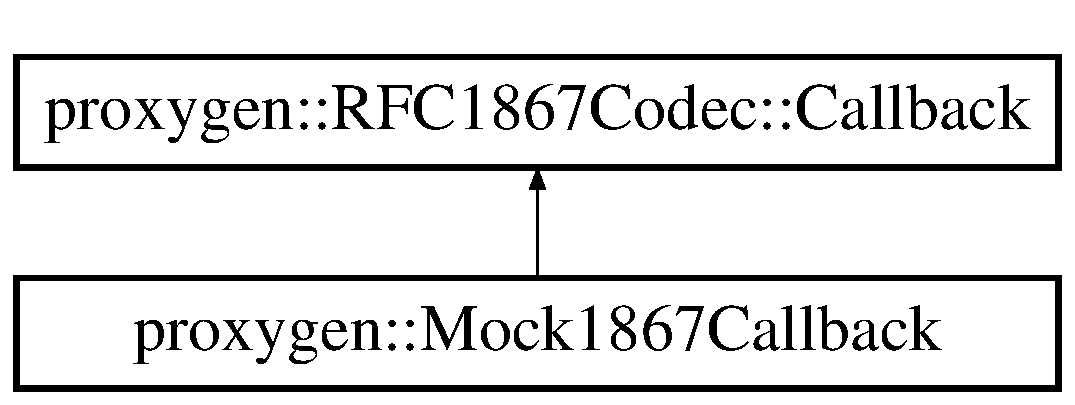
\includegraphics[height=2.000000cm]{classproxygen_1_1RFC1867Codec_1_1Callback}
\end{center}
\end{figure}
\subsection*{Public Member Functions}
\begin{DoxyCompactItemize}
\item 
virtual {\bf $\sim$\+Callback} ()
\item 
virtual int {\bf on\+Field\+Start} (const std\+::string \&{\bf name}, folly\+::\+Optional$<$ std\+::string $>$ filename, std\+::unique\+\_\+ptr$<$ {\bf H\+T\+T\+P\+Message} $>$ msg, uint64\+\_\+t post\+Bytes\+Processed)=0
\item 
virtual int {\bf on\+Field\+Data} (std\+::unique\+\_\+ptr$<$ folly\+::\+I\+O\+Buf $>$, uint64\+\_\+t post\+Bytes\+Processed)=0
\item 
virtual void {\bf on\+Field\+End} (bool ended\+On\+Boundary, uint64\+\_\+t post\+Bytes\+Processed)=0
\item 
virtual void {\bf on\+Error} ()=0
\end{DoxyCompactItemize}


\subsection{Detailed Description}


Definition at line 27 of file R\+F\+C1867.\+h.



\subsection{Constructor \& Destructor Documentation}
\index{proxygen\+::\+R\+F\+C1867\+Codec\+::\+Callback@{proxygen\+::\+R\+F\+C1867\+Codec\+::\+Callback}!````~Callback@{$\sim$\+Callback}}
\index{````~Callback@{$\sim$\+Callback}!proxygen\+::\+R\+F\+C1867\+Codec\+::\+Callback@{proxygen\+::\+R\+F\+C1867\+Codec\+::\+Callback}}
\subsubsection[{$\sim$\+Callback()}]{\setlength{\rightskip}{0pt plus 5cm}virtual proxygen\+::\+R\+F\+C1867\+Codec\+::\+Callback\+::$\sim$\+Callback (
\begin{DoxyParamCaption}
{}
\end{DoxyParamCaption}
)\hspace{0.3cm}{\ttfamily [inline]}, {\ttfamily [virtual]}}\label{classproxygen_1_1RFC1867Codec_1_1Callback_a687755a5751603facd8553196ce69b1f}


Definition at line 29 of file R\+F\+C1867.\+h.



References name, on\+Error(), on\+Field\+Data(), on\+Field\+End(), and on\+Field\+Start().


\begin{DoxyCode}
29 \{\}
\end{DoxyCode}


\subsection{Member Function Documentation}
\index{proxygen\+::\+R\+F\+C1867\+Codec\+::\+Callback@{proxygen\+::\+R\+F\+C1867\+Codec\+::\+Callback}!on\+Error@{on\+Error}}
\index{on\+Error@{on\+Error}!proxygen\+::\+R\+F\+C1867\+Codec\+::\+Callback@{proxygen\+::\+R\+F\+C1867\+Codec\+::\+Callback}}
\subsubsection[{on\+Error()=0}]{\setlength{\rightskip}{0pt plus 5cm}virtual void proxygen\+::\+R\+F\+C1867\+Codec\+::\+Callback\+::on\+Error (
\begin{DoxyParamCaption}
{}
\end{DoxyParamCaption}
)\hspace{0.3cm}{\ttfamily [pure virtual]}}\label{classproxygen_1_1RFC1867Codec_1_1Callback_a37cb2ccff76b15dc57ae473c7493d4e4}


Referenced by $\sim$\+Callback().

\index{proxygen\+::\+R\+F\+C1867\+Codec\+::\+Callback@{proxygen\+::\+R\+F\+C1867\+Codec\+::\+Callback}!on\+Field\+Data@{on\+Field\+Data}}
\index{on\+Field\+Data@{on\+Field\+Data}!proxygen\+::\+R\+F\+C1867\+Codec\+::\+Callback@{proxygen\+::\+R\+F\+C1867\+Codec\+::\+Callback}}
\subsubsection[{on\+Field\+Data(std\+::unique\+\_\+ptr$<$ folly\+::\+I\+O\+Buf $>$, uint64\+\_\+t post\+Bytes\+Processed)=0}]{\setlength{\rightskip}{0pt plus 5cm}virtual int proxygen\+::\+R\+F\+C1867\+Codec\+::\+Callback\+::on\+Field\+Data (
\begin{DoxyParamCaption}
\item[{std\+::unique\+\_\+ptr$<$ folly\+::\+I\+O\+Buf $>$}]{, }
\item[{uint64\+\_\+t}]{post\+Bytes\+Processed}
\end{DoxyParamCaption}
)\hspace{0.3cm}{\ttfamily [pure virtual]}}\label{classproxygen_1_1RFC1867Codec_1_1Callback_a0a8191fbaaad4ea0938cd5fc4042d544}


Implemented in {\bf proxygen\+::\+Mock1867\+Callback} \doxyref{}{p.}{classproxygen_1_1Mock1867Callback_a009045983033bdbc1cd5d88cf57840d4}.



Referenced by $\sim$\+Callback().

\index{proxygen\+::\+R\+F\+C1867\+Codec\+::\+Callback@{proxygen\+::\+R\+F\+C1867\+Codec\+::\+Callback}!on\+Field\+End@{on\+Field\+End}}
\index{on\+Field\+End@{on\+Field\+End}!proxygen\+::\+R\+F\+C1867\+Codec\+::\+Callback@{proxygen\+::\+R\+F\+C1867\+Codec\+::\+Callback}}
\subsubsection[{on\+Field\+End(bool ended\+On\+Boundary, uint64\+\_\+t post\+Bytes\+Processed)=0}]{\setlength{\rightskip}{0pt plus 5cm}virtual void proxygen\+::\+R\+F\+C1867\+Codec\+::\+Callback\+::on\+Field\+End (
\begin{DoxyParamCaption}
\item[{bool}]{ended\+On\+Boundary, }
\item[{uint64\+\_\+t}]{post\+Bytes\+Processed}
\end{DoxyParamCaption}
)\hspace{0.3cm}{\ttfamily [pure virtual]}}\label{classproxygen_1_1RFC1867Codec_1_1Callback_a3db1440dccb898f11cfb1de56ac920a8}
On reading to end of a part indicated by boundary 
\begin{DoxyParams}{Parameters}
{\em ended\+On\+Boundary} & indicate successful part end \\
\hline
\end{DoxyParams}


Referenced by $\sim$\+Callback().

\index{proxygen\+::\+R\+F\+C1867\+Codec\+::\+Callback@{proxygen\+::\+R\+F\+C1867\+Codec\+::\+Callback}!on\+Field\+Start@{on\+Field\+Start}}
\index{on\+Field\+Start@{on\+Field\+Start}!proxygen\+::\+R\+F\+C1867\+Codec\+::\+Callback@{proxygen\+::\+R\+F\+C1867\+Codec\+::\+Callback}}
\subsubsection[{on\+Field\+Start(const std\+::string \&name, folly\+::\+Optional$<$ std\+::string $>$ filename, std\+::unique\+\_\+ptr$<$ H\+T\+T\+P\+Message $>$ msg, uint64\+\_\+t post\+Bytes\+Processed)=0}]{\setlength{\rightskip}{0pt plus 5cm}virtual int proxygen\+::\+R\+F\+C1867\+Codec\+::\+Callback\+::on\+Field\+Start (
\begin{DoxyParamCaption}
\item[{const std\+::string \&}]{name, }
\item[{folly\+::\+Optional$<$ std\+::string $>$}]{filename, }
\item[{std\+::unique\+\_\+ptr$<$ {\bf H\+T\+T\+P\+Message} $>$}]{msg, }
\item[{uint64\+\_\+t}]{post\+Bytes\+Processed}
\end{DoxyParamCaption}
)\hspace{0.3cm}{\ttfamily [pure virtual]}}\label{classproxygen_1_1RFC1867Codec_1_1Callback_a7047036e6769fbb4e33fd7a5d4e24e3a}


Referenced by $\sim$\+Callback().



The documentation for this class was generated from the following file\+:\begin{DoxyCompactItemize}
\item 
proxygen/lib/http/experimental/{\bf R\+F\+C1867.\+h}\end{DoxyCompactItemize}

\section{proxygen\+:\+:H\+T\+T\+P\+Connector\+:\+:Callback Class Reference}
\label{classproxygen_1_1HTTPConnector_1_1Callback}\index{proxygen\+::\+H\+T\+T\+P\+Connector\+::\+Callback@{proxygen\+::\+H\+T\+T\+P\+Connector\+::\+Callback}}


{\ttfamily \#include $<$H\+T\+T\+P\+Connector.\+h$>$}

Inheritance diagram for proxygen\+:\+:H\+T\+T\+P\+Connector\+:\+:Callback\+:\begin{figure}[H]
\begin{center}
\leavevmode
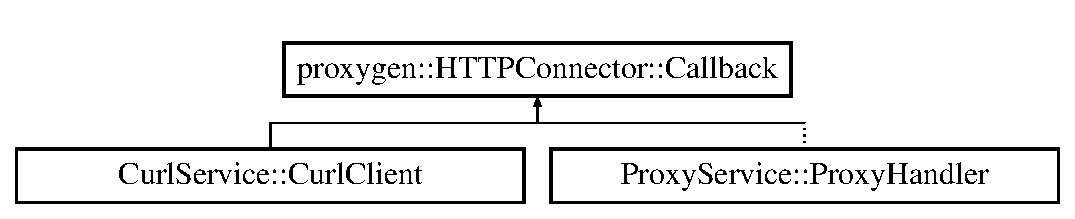
\includegraphics[height=2.000000cm]{classproxygen_1_1HTTPConnector_1_1Callback}
\end{center}
\end{figure}
\subsection*{Public Member Functions}
\begin{DoxyCompactItemize}
\item 
virtual {\bf $\sim$\+Callback} ()
\item 
virtual void {\bf connect\+Success} ({\bf H\+T\+T\+P\+Upstream\+Session} $\ast$session)=0
\item 
virtual void {\bf connect\+Error} (const folly\+::\+Async\+Socket\+Exception \&ex)=0
\end{DoxyCompactItemize}


\subsection{Detailed Description}
This class defines the pure virtual interface on which to receive the result on. 

Definition at line 38 of file H\+T\+T\+P\+Connector.\+h.



\subsection{Constructor \& Destructor Documentation}
\index{proxygen\+::\+H\+T\+T\+P\+Connector\+::\+Callback@{proxygen\+::\+H\+T\+T\+P\+Connector\+::\+Callback}!````~Callback@{$\sim$\+Callback}}
\index{````~Callback@{$\sim$\+Callback}!proxygen\+::\+H\+T\+T\+P\+Connector\+::\+Callback@{proxygen\+::\+H\+T\+T\+P\+Connector\+::\+Callback}}
\subsubsection[{$\sim$\+Callback()}]{\setlength{\rightskip}{0pt plus 5cm}virtual proxygen\+::\+H\+T\+T\+P\+Connector\+::\+Callback\+::$\sim$\+Callback (
\begin{DoxyParamCaption}
{}
\end{DoxyParamCaption}
)\hspace{0.3cm}{\ttfamily [inline]}, {\ttfamily [virtual]}}\label{classproxygen_1_1HTTPConnector_1_1Callback_a315f807f6e668c7a30640ca2c8e78a99}


Definition at line 40 of file H\+T\+T\+P\+Connector.\+h.



References proxygen\+::\+H\+T\+T\+P\+Connector\+::connect(), connect\+Error(), proxygen\+::\+H\+T\+T\+P\+Connector\+::connect\+S\+S\+L(), connect\+Success(), proxygen\+::\+H\+T\+T\+P\+Connector\+::\+H\+T\+T\+P\+Connector(), proxygen\+::\+H\+T\+T\+P\+Connector\+::reset(), proxygen\+::\+H\+T\+T\+P\+Connector\+::set\+H\+T\+T\+P\+Version\+Override(), proxygen\+::\+H\+T\+T\+P\+Connector\+::set\+Plaintext\+Protocol(), proxygen\+::\+H\+T\+T\+P\+Connector\+::time\+Elapsed(), and proxygen\+::\+H\+T\+T\+P\+Connector\+::$\sim$\+H\+T\+T\+P\+Connector().


\begin{DoxyCode}
40 \{\}
\end{DoxyCode}


\subsection{Member Function Documentation}
\index{proxygen\+::\+H\+T\+T\+P\+Connector\+::\+Callback@{proxygen\+::\+H\+T\+T\+P\+Connector\+::\+Callback}!connect\+Error@{connect\+Error}}
\index{connect\+Error@{connect\+Error}!proxygen\+::\+H\+T\+T\+P\+Connector\+::\+Callback@{proxygen\+::\+H\+T\+T\+P\+Connector\+::\+Callback}}
\subsubsection[{connect\+Error(const folly\+::\+Async\+Socket\+Exception \&ex)=0}]{\setlength{\rightskip}{0pt plus 5cm}virtual void proxygen\+::\+H\+T\+T\+P\+Connector\+::\+Callback\+::connect\+Error (
\begin{DoxyParamCaption}
\item[{const folly\+::\+Async\+Socket\+Exception \&}]{ex}
\end{DoxyParamCaption}
)\hspace{0.3cm}{\ttfamily [pure virtual]}}\label{classproxygen_1_1HTTPConnector_1_1Callback_a4f01da41ef58437eeb47c1dee4a5bc47}


Implemented in {\bf Proxy\+Service\+::\+Proxy\+Handler} \doxyref{}{p.}{classProxyService_1_1ProxyHandler_a7c14c1ee3b04187e72ea5f42cde84dff}, and {\bf Curl\+Service\+::\+Curl\+Client} \doxyref{}{p.}{classCurlService_1_1CurlClient_af37e3647eb96eda96323787207c33e80}.



Referenced by proxygen\+::\+H\+T\+T\+P\+Connector\+::connect\+Err(), and $\sim$\+Callback().

\index{proxygen\+::\+H\+T\+T\+P\+Connector\+::\+Callback@{proxygen\+::\+H\+T\+T\+P\+Connector\+::\+Callback}!connect\+Success@{connect\+Success}}
\index{connect\+Success@{connect\+Success}!proxygen\+::\+H\+T\+T\+P\+Connector\+::\+Callback@{proxygen\+::\+H\+T\+T\+P\+Connector\+::\+Callback}}
\subsubsection[{connect\+Success(\+H\+T\+T\+P\+Upstream\+Session $\ast$session)=0}]{\setlength{\rightskip}{0pt plus 5cm}virtual void proxygen\+::\+H\+T\+T\+P\+Connector\+::\+Callback\+::connect\+Success (
\begin{DoxyParamCaption}
\item[{{\bf H\+T\+T\+P\+Upstream\+Session} $\ast$}]{session}
\end{DoxyParamCaption}
)\hspace{0.3cm}{\ttfamily [pure virtual]}}\label{classproxygen_1_1HTTPConnector_1_1Callback_aae878d2da74442ffc19ecb3bbbee7d9e}


Implemented in {\bf Proxy\+Service\+::\+Proxy\+Handler} \doxyref{}{p.}{classProxyService_1_1ProxyHandler_a0a4e260a80e44acec79c992015a7546c}, and {\bf Curl\+Service\+::\+Curl\+Client} \doxyref{}{p.}{classCurlService_1_1CurlClient_a8e0166bd540cf4a16b0ef1dd3accf882}.



Referenced by proxygen\+::\+H\+T\+T\+P\+Connector\+::connect\+Success(), proxygen\+::\+H\+T\+T\+P\+Connector\+::set\+H\+T\+T\+P\+Codec\+Factory(), and $\sim$\+Callback().



The documentation for this class was generated from the following file\+:\begin{DoxyCompactItemize}
\item 
proxygen/lib/http/{\bf H\+T\+T\+P\+Connector.\+h}\end{DoxyCompactItemize}

\section{proxygen\+:\+:Ack\+Timeout\+:\+:Callback Class Reference}
\label{classproxygen_1_1AckTimeout_1_1Callback}\index{proxygen\+::\+Ack\+Timeout\+::\+Callback@{proxygen\+::\+Ack\+Timeout\+::\+Callback}}


{\ttfamily \#include $<$Byte\+Events.\+h$>$}

\subsection*{Public Member Functions}
\begin{DoxyCompactItemize}
\item 
virtual {\bf $\sim$\+Callback} ()
\item 
virtual void {\bf ack\+Timeout\+Expired} (uint64\+\_\+t byte\+No) noexcept=0
\end{DoxyCompactItemize}


\subsection{Detailed Description}
The instances of \doxyref{Ack\+Timeout\+::\+Callback}{p.}{classproxygen_1_1AckTimeout_1_1Callback} {\itshape M\+U\+ST} outlive the \doxyref{Ack\+Timeout}{p.}{classproxygen_1_1AckTimeout} it is registered on. 

Definition at line 70 of file Byte\+Events.\+h.



\subsection{Constructor \& Destructor Documentation}
\index{proxygen\+::\+Ack\+Timeout\+::\+Callback@{proxygen\+::\+Ack\+Timeout\+::\+Callback}!````~Callback@{$\sim$\+Callback}}
\index{````~Callback@{$\sim$\+Callback}!proxygen\+::\+Ack\+Timeout\+::\+Callback@{proxygen\+::\+Ack\+Timeout\+::\+Callback}}
\subsubsection[{$\sim$\+Callback()}]{\setlength{\rightskip}{0pt plus 5cm}virtual proxygen\+::\+Ack\+Timeout\+::\+Callback\+::$\sim$\+Callback (
\begin{DoxyParamCaption}
{}
\end{DoxyParamCaption}
)\hspace{0.3cm}{\ttfamily [inline]}, {\ttfamily [virtual]}}\label{classproxygen_1_1AckTimeout_1_1Callback_ae132705a8cb03a151197e5390c4c9560}


Definition at line 72 of file Byte\+Events.\+h.


\begin{DoxyCode}
72 \{\}
\end{DoxyCode}


\subsection{Member Function Documentation}
\index{proxygen\+::\+Ack\+Timeout\+::\+Callback@{proxygen\+::\+Ack\+Timeout\+::\+Callback}!ack\+Timeout\+Expired@{ack\+Timeout\+Expired}}
\index{ack\+Timeout\+Expired@{ack\+Timeout\+Expired}!proxygen\+::\+Ack\+Timeout\+::\+Callback@{proxygen\+::\+Ack\+Timeout\+::\+Callback}}
\subsubsection[{ack\+Timeout\+Expired(uint64\+\_\+t byte\+No) noexcept=0}]{\setlength{\rightskip}{0pt plus 5cm}virtual void proxygen\+::\+Ack\+Timeout\+::\+Callback\+::ack\+Timeout\+Expired (
\begin{DoxyParamCaption}
\item[{uint64\+\_\+t}]{byte\+No}
\end{DoxyParamCaption}
)\hspace{0.3cm}{\ttfamily [pure virtual]}, {\ttfamily [noexcept]}}\label{classproxygen_1_1AckTimeout_1_1Callback_a5e4b488bf67e0cd22219b7725bdf3e99}


The documentation for this class was generated from the following file\+:\begin{DoxyCompactItemize}
\item 
proxygen/lib/http/session/{\bf Byte\+Events.\+h}\end{DoxyCompactItemize}

\section{proxygen\+:\+:Byte\+Event\+Tracker\+:\+:Callback Class Reference}
\label{classproxygen_1_1ByteEventTracker_1_1Callback}\index{proxygen\+::\+Byte\+Event\+Tracker\+::\+Callback@{proxygen\+::\+Byte\+Event\+Tracker\+::\+Callback}}


{\ttfamily \#include $<$Byte\+Event\+Tracker.\+h$>$}

Inheritance diagram for proxygen\+:\+:Byte\+Event\+Tracker\+:\+:Callback\+:\begin{figure}[H]
\begin{center}
\leavevmode
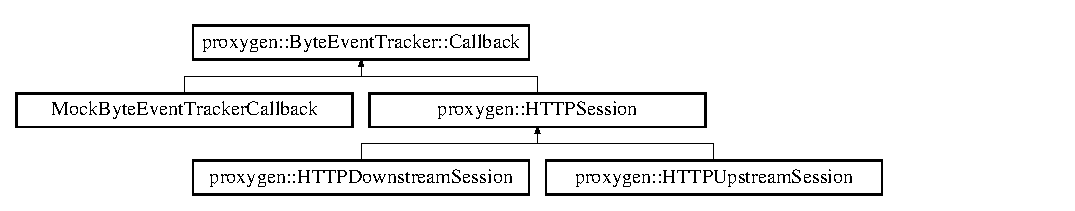
\includegraphics[height=2.382979cm]{classproxygen_1_1ByteEventTracker_1_1Callback}
\end{center}
\end{figure}
\subsection*{Public Member Functions}
\begin{DoxyCompactItemize}
\item 
virtual {\bf $\sim$\+Callback} ()
\item 
virtual void {\bf on\+Ping\+Reply\+Latency} (int64\+\_\+t latency) noexcept=0
\item 
virtual void {\bf on\+Last\+Byte\+Event} ({\bf H\+T\+T\+P\+Transaction} $\ast$txn, uint64\+\_\+t offset, bool eom\+Tracked) noexcept=0
\item 
virtual void {\bf on\+Delete\+Ack\+Event} () noexcept=0
\end{DoxyCompactItemize}


\subsection{Detailed Description}


Definition at line 31 of file Byte\+Event\+Tracker.\+h.



\subsection{Constructor \& Destructor Documentation}
\index{proxygen\+::\+Byte\+Event\+Tracker\+::\+Callback@{proxygen\+::\+Byte\+Event\+Tracker\+::\+Callback}!````~Callback@{$\sim$\+Callback}}
\index{````~Callback@{$\sim$\+Callback}!proxygen\+::\+Byte\+Event\+Tracker\+::\+Callback@{proxygen\+::\+Byte\+Event\+Tracker\+::\+Callback}}
\subsubsection[{$\sim$\+Callback()}]{\setlength{\rightskip}{0pt plus 5cm}virtual proxygen\+::\+Byte\+Event\+Tracker\+::\+Callback\+::$\sim$\+Callback (
\begin{DoxyParamCaption}
{}
\end{DoxyParamCaption}
)\hspace{0.3cm}{\ttfamily [inline]}, {\ttfamily [virtual]}}\label{classproxygen_1_1ByteEventTracker_1_1Callback_af827eb2d41e69a09ed84ffeff245eda6}


Definition at line 33 of file Byte\+Event\+Tracker.\+h.



References on\+Delete\+Ack\+Event(), on\+Last\+Byte\+Event(), on\+Ping\+Reply\+Latency(), and proxygen\+::\+Byte\+Event\+Tracker\+::$\sim$\+Byte\+Event\+Tracker().


\begin{DoxyCode}
33 \{\}
\end{DoxyCode}


\subsection{Member Function Documentation}
\index{proxygen\+::\+Byte\+Event\+Tracker\+::\+Callback@{proxygen\+::\+Byte\+Event\+Tracker\+::\+Callback}!on\+Delete\+Ack\+Event@{on\+Delete\+Ack\+Event}}
\index{on\+Delete\+Ack\+Event@{on\+Delete\+Ack\+Event}!proxygen\+::\+Byte\+Event\+Tracker\+::\+Callback@{proxygen\+::\+Byte\+Event\+Tracker\+::\+Callback}}
\subsubsection[{on\+Delete\+Ack\+Event() noexcept=0}]{\setlength{\rightskip}{0pt plus 5cm}virtual void proxygen\+::\+Byte\+Event\+Tracker\+::\+Callback\+::on\+Delete\+Ack\+Event (
\begin{DoxyParamCaption}
{}
\end{DoxyParamCaption}
)\hspace{0.3cm}{\ttfamily [pure virtual]}, {\ttfamily [noexcept]}}\label{classproxygen_1_1ByteEventTracker_1_1Callback_a66e469488f7fc0ea0ccd333a7b90ecbe}


Implemented in {\bf proxygen\+::\+H\+T\+T\+P\+Session} \doxyref{}{p.}{classproxygen_1_1HTTPSession_a3d2b7bdd5d59059cee9b566553db91f1}.



Referenced by $\sim$\+Callback().

\index{proxygen\+::\+Byte\+Event\+Tracker\+::\+Callback@{proxygen\+::\+Byte\+Event\+Tracker\+::\+Callback}!on\+Last\+Byte\+Event@{on\+Last\+Byte\+Event}}
\index{on\+Last\+Byte\+Event@{on\+Last\+Byte\+Event}!proxygen\+::\+Byte\+Event\+Tracker\+::\+Callback@{proxygen\+::\+Byte\+Event\+Tracker\+::\+Callback}}
\subsubsection[{on\+Last\+Byte\+Event(\+H\+T\+T\+P\+Transaction $\ast$txn, uint64\+\_\+t offset, bool eom\+Tracked) noexcept=0}]{\setlength{\rightskip}{0pt plus 5cm}virtual void proxygen\+::\+Byte\+Event\+Tracker\+::\+Callback\+::on\+Last\+Byte\+Event (
\begin{DoxyParamCaption}
\item[{{\bf H\+T\+T\+P\+Transaction} $\ast$}]{txn, }
\item[{uint64\+\_\+t}]{offset, }
\item[{bool}]{eom\+Tracked}
\end{DoxyParamCaption}
)\hspace{0.3cm}{\ttfamily [pure virtual]}, {\ttfamily [noexcept]}}\label{classproxygen_1_1ByteEventTracker_1_1Callback_a2089b3b9335dbc03598f35a007821883}


Implemented in {\bf proxygen\+::\+H\+T\+T\+P\+Session} \doxyref{}{p.}{classproxygen_1_1HTTPSession_a262d04adeb8feb2c1bf6ebb5159b67d6}.



Referenced by proxygen\+::\+Byte\+Event\+Tracker\+::process\+Byte\+Events(), and $\sim$\+Callback().

\index{proxygen\+::\+Byte\+Event\+Tracker\+::\+Callback@{proxygen\+::\+Byte\+Event\+Tracker\+::\+Callback}!on\+Ping\+Reply\+Latency@{on\+Ping\+Reply\+Latency}}
\index{on\+Ping\+Reply\+Latency@{on\+Ping\+Reply\+Latency}!proxygen\+::\+Byte\+Event\+Tracker\+::\+Callback@{proxygen\+::\+Byte\+Event\+Tracker\+::\+Callback}}
\subsubsection[{on\+Ping\+Reply\+Latency(int64\+\_\+t latency) noexcept=0}]{\setlength{\rightskip}{0pt plus 5cm}virtual void proxygen\+::\+Byte\+Event\+Tracker\+::\+Callback\+::on\+Ping\+Reply\+Latency (
\begin{DoxyParamCaption}
\item[{int64\+\_\+t}]{latency}
\end{DoxyParamCaption}
)\hspace{0.3cm}{\ttfamily [pure virtual]}, {\ttfamily [noexcept]}}\label{classproxygen_1_1ByteEventTracker_1_1Callback_a2dbef0abec0b00ac3a2a53eafaf19bcd}


Implemented in {\bf proxygen\+::\+H\+T\+T\+P\+Session} \doxyref{}{p.}{classproxygen_1_1HTTPSession_a63363dd6eb679673b1f548176994f4c9}.



Referenced by proxygen\+::\+Byte\+Event\+Tracker\+::process\+Byte\+Events(), and $\sim$\+Callback().



The documentation for this class was generated from the following file\+:\begin{DoxyCompactItemize}
\item 
proxygen/lib/http/session/{\bf Byte\+Event\+Tracker.\+h}\end{DoxyCompactItemize}

\section{proxygen\+:\+:Async\+Timeout\+Set\+:\+:Callback Class Reference}
\label{classproxygen_1_1AsyncTimeoutSet_1_1Callback}\index{proxygen\+::\+Async\+Timeout\+Set\+::\+Callback@{proxygen\+::\+Async\+Timeout\+Set\+::\+Callback}}


{\ttfamily \#include $<$Async\+Timeout\+Set.\+h$>$}

Inheritance diagram for proxygen\+:\+:Async\+Timeout\+Set\+:\+:Callback\+:\begin{figure}[H]
\begin{center}
\leavevmode
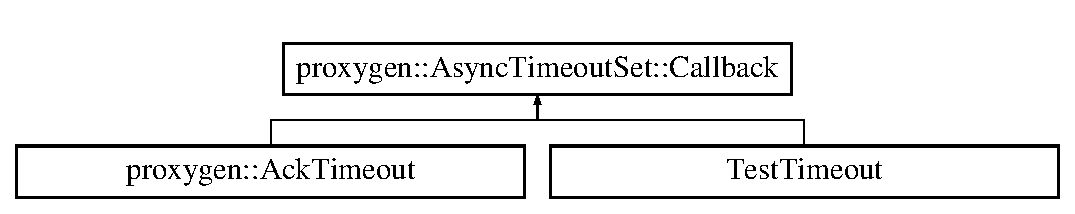
\includegraphics[height=2.000000cm]{classproxygen_1_1AsyncTimeoutSet_1_1Callback}
\end{center}
\end{figure}
\subsection*{Public Member Functions}
\begin{DoxyCompactItemize}
\item 
{\bf Callback} ()
\item 
virtual {\bf $\sim$\+Callback} ()
\item 
virtual void {\bf timeout\+Expired} () noexcept=0
\item 
void {\bf cancel\+Timeout} ()
\item 
bool {\bf is\+Scheduled} () const 
\end{DoxyCompactItemize}
\subsection*{Private Member Functions}
\begin{DoxyCompactItemize}
\item 
std\+::chrono\+::milliseconds {\bf get\+Time\+Remaining} (std\+::chrono\+::milliseconds now) const 
\item 
void {\bf set\+Scheduled} ({\bf Async\+Timeout\+Set} $\ast$timeout\+Set, {\bf Callback} $\ast$prev)
\item 
void {\bf cancel\+Timeout\+Impl} ()
\end{DoxyCompactItemize}
\subsection*{Private Attributes}
\begin{DoxyCompactItemize}
\item 
std\+::shared\+\_\+ptr$<$ folly\+::\+Request\+Context $>$ {\bf context\+\_\+}
\item 
{\bf Async\+Timeout\+Set} $\ast$ {\bf timeout\+Set\+\_\+} \{{\bf nullptr}\}
\item 
{\bf Callback} $\ast$ {\bf prev\+\_\+} \{{\bf nullptr}\}
\item 
{\bf Callback} $\ast$ {\bf next\+\_\+} \{{\bf nullptr}\}
\item 
std\+::chrono\+::milliseconds {\bf expiration\+\_\+} \{0\}
\end{DoxyCompactItemize}
\subsection*{Friends}
\begin{DoxyCompactItemize}
\item 
class {\bf Async\+Timeout\+Set}
\end{DoxyCompactItemize}


\subsection{Detailed Description}
A callback to be notified when a timeout has expired.

\doxyref{Async\+Timeout\+Set\+::\+Callback}{p.}{classproxygen_1_1AsyncTimeoutSet_1_1Callback} is very similar to Async\+Timeout. The primary distinction is that Async\+Timeout can choose its timeout interval each time it is scheduled. On the other hand, \doxyref{Async\+Timeout\+Set\+::\+Callback}{p.}{classproxygen_1_1AsyncTimeoutSet_1_1Callback} always uses the timeout interval defined by the \doxyref{Async\+Timeout\+Set}{p.}{classproxygen_1_1AsyncTimeoutSet} where it is scheduled. 

Definition at line 54 of file Async\+Timeout\+Set.\+h.



\subsection{Constructor \& Destructor Documentation}
\index{proxygen\+::\+Async\+Timeout\+Set\+::\+Callback@{proxygen\+::\+Async\+Timeout\+Set\+::\+Callback}!Callback@{Callback}}
\index{Callback@{Callback}!proxygen\+::\+Async\+Timeout\+Set\+::\+Callback@{proxygen\+::\+Async\+Timeout\+Set\+::\+Callback}}
\subsubsection[{Callback()}]{\setlength{\rightskip}{0pt plus 5cm}proxygen\+::\+Async\+Timeout\+Set\+::\+Callback\+::\+Callback (
\begin{DoxyParamCaption}
{}
\end{DoxyParamCaption}
)\hspace{0.3cm}{\ttfamily [inline]}}\label{classproxygen_1_1AsyncTimeoutSet_1_1Callback_ac0ac7ccbe0ee6e0e3a27744ad5da42cd}


Definition at line 56 of file Async\+Timeout\+Set.\+h.



References timeout\+Expired(), and $\sim$\+Callback().


\begin{DoxyCode}
56 \{\}
\end{DoxyCode}
\index{proxygen\+::\+Async\+Timeout\+Set\+::\+Callback@{proxygen\+::\+Async\+Timeout\+Set\+::\+Callback}!````~Callback@{$\sim$\+Callback}}
\index{````~Callback@{$\sim$\+Callback}!proxygen\+::\+Async\+Timeout\+Set\+::\+Callback@{proxygen\+::\+Async\+Timeout\+Set\+::\+Callback}}
\subsubsection[{$\sim$\+Callback()}]{\setlength{\rightskip}{0pt plus 5cm}proxygen\+::\+Async\+Timeout\+Set\+::\+Callback\+::$\sim$\+Callback (
\begin{DoxyParamCaption}
{}
\end{DoxyParamCaption}
)\hspace{0.3cm}{\ttfamily [virtual]}}\label{classproxygen_1_1AsyncTimeoutSet_1_1Callback_a069f3316cecec4f325a97f2c38c3314e}


Definition at line 32 of file Async\+Timeout\+Set.\+cpp.



Referenced by Callback().


\begin{DoxyCode}
32                                    \{
33   \textcolor{keywordflow}{if} (isScheduled()) \{
34     cancelTimeout();
35   \}
36 \}
\end{DoxyCode}


\subsection{Member Function Documentation}
\index{proxygen\+::\+Async\+Timeout\+Set\+::\+Callback@{proxygen\+::\+Async\+Timeout\+Set\+::\+Callback}!cancel\+Timeout@{cancel\+Timeout}}
\index{cancel\+Timeout@{cancel\+Timeout}!proxygen\+::\+Async\+Timeout\+Set\+::\+Callback@{proxygen\+::\+Async\+Timeout\+Set\+::\+Callback}}
\subsubsection[{cancel\+Timeout()}]{\setlength{\rightskip}{0pt plus 5cm}void proxygen\+::\+Async\+Timeout\+Set\+::\+Callback\+::cancel\+Timeout (
\begin{DoxyParamCaption}
{}
\end{DoxyParamCaption}
)\hspace{0.3cm}{\ttfamily [inline]}}\label{classproxygen_1_1AsyncTimeoutSet_1_1Callback_ae35ff9307fec26ba32d0e85a0b07ef9b}
Cancel the timeout, if it is running.

If the timeout is not scheduled, \doxyref{cancel\+Timeout()}{p.}{classproxygen_1_1AsyncTimeoutSet_1_1Callback_ae35ff9307fec26ba32d0e85a0b07ef9b} does nothing. 

Definition at line 70 of file Async\+Timeout\+Set.\+h.



References cancel\+Timeout\+Impl(), and timeout\+Set\+\_\+.



Referenced by proxygen\+::\+Async\+Timeout\+Set\+::schedule\+Timeout(), T\+E\+S\+T\+\_\+\+F(), and proxygen\+::\+Async\+Timeout\+Set\+::timeout\+Expired().


\begin{DoxyCode}
70                          \{
71       \textcolor{keywordflow}{if} (timeoutSet_ == \textcolor{keyword}{nullptr}) \{
72         \textcolor{comment}{// We're not scheduled, so there's nothing to do.}
73         \textcolor{keywordflow}{return};
74       \}
75       cancelTimeoutImpl();
76     \}
\end{DoxyCode}
\index{proxygen\+::\+Async\+Timeout\+Set\+::\+Callback@{proxygen\+::\+Async\+Timeout\+Set\+::\+Callback}!cancel\+Timeout\+Impl@{cancel\+Timeout\+Impl}}
\index{cancel\+Timeout\+Impl@{cancel\+Timeout\+Impl}!proxygen\+::\+Async\+Timeout\+Set\+::\+Callback@{proxygen\+::\+Async\+Timeout\+Set\+::\+Callback}}
\subsubsection[{cancel\+Timeout\+Impl()}]{\setlength{\rightskip}{0pt plus 5cm}void proxygen\+::\+Async\+Timeout\+Set\+::\+Callback\+::cancel\+Timeout\+Impl (
\begin{DoxyParamCaption}
{}
\end{DoxyParamCaption}
)\hspace{0.3cm}{\ttfamily [private]}}\label{classproxygen_1_1AsyncTimeoutSet_1_1Callback_ade8480096f82eaa0fa7af769ea58bec8}


Definition at line 52 of file Async\+Timeout\+Set.\+cpp.



References proxygen\+::\+Async\+Timeout\+Set\+::\+Async\+Timeout\+Set(), and proxygen\+::get\+Timeout\+Clock().



Referenced by cancel\+Timeout(), and get\+Time\+Remaining().


\begin{DoxyCode}
52                                                 \{
53   \textcolor{keywordflow}{if} (next_ == \textcolor{keyword}{nullptr}) \{
54     assert(timeoutSet_->tail_ == \textcolor{keyword}{this});
55     timeoutSet_->tail_ = prev_;
56   \} \textcolor{keywordflow}{else} \{
57     assert(timeoutSet_->tail_ != \textcolor{keyword}{this});
58     next_->prev_ = prev_;
59   \}
60 
61   \textcolor{keywordflow}{if} (prev_ == \textcolor{keyword}{nullptr}) \{
62     assert(timeoutSet_->head_ == \textcolor{keyword}{this});
63     timeoutSet_->head_ = next_;
64     timeoutSet_->headChanged();
65   \} \textcolor{keywordflow}{else} \{
66     assert(timeoutSet_->head_ != \textcolor{keyword}{this});
67     prev_->next_ = next_;
68   \}
69 
70   timeoutSet_ = \textcolor{keyword}{nullptr};
71   prev_ = \textcolor{keyword}{nullptr};
72   next_ = \textcolor{keyword}{nullptr};
73   expiration_ = \{\};
74 \}
\end{DoxyCode}
\index{proxygen\+::\+Async\+Timeout\+Set\+::\+Callback@{proxygen\+::\+Async\+Timeout\+Set\+::\+Callback}!get\+Time\+Remaining@{get\+Time\+Remaining}}
\index{get\+Time\+Remaining@{get\+Time\+Remaining}!proxygen\+::\+Async\+Timeout\+Set\+::\+Callback@{proxygen\+::\+Async\+Timeout\+Set\+::\+Callback}}
\subsubsection[{get\+Time\+Remaining(std\+::chrono\+::milliseconds now) const }]{\setlength{\rightskip}{0pt plus 5cm}std\+::chrono\+::milliseconds proxygen\+::\+Async\+Timeout\+Set\+::\+Callback\+::get\+Time\+Remaining (
\begin{DoxyParamCaption}
\item[{std\+::chrono\+::milliseconds}]{now}
\end{DoxyParamCaption}
) const\hspace{0.3cm}{\ttfamily [inline]}, {\ttfamily [private]}}\label{classproxygen_1_1AsyncTimeoutSet_1_1Callback_a1f3f31c99103709f658ce8b92d198f4e}


Definition at line 87 of file Async\+Timeout\+Set.\+h.



References cancel\+Timeout\+Impl(), expiration\+\_\+, and set\+Scheduled().


\begin{DoxyCode}
88                                        \{
89       \textcolor{keywordflow}{if} (now >= expiration_) \{
90         \textcolor{keywordflow}{return} std::chrono::milliseconds(0);
91       \}
92       \textcolor{keywordflow}{return} expiration_ - now;
93     \}
\end{DoxyCode}
\index{proxygen\+::\+Async\+Timeout\+Set\+::\+Callback@{proxygen\+::\+Async\+Timeout\+Set\+::\+Callback}!is\+Scheduled@{is\+Scheduled}}
\index{is\+Scheduled@{is\+Scheduled}!proxygen\+::\+Async\+Timeout\+Set\+::\+Callback@{proxygen\+::\+Async\+Timeout\+Set\+::\+Callback}}
\subsubsection[{is\+Scheduled() const }]{\setlength{\rightskip}{0pt plus 5cm}bool proxygen\+::\+Async\+Timeout\+Set\+::\+Callback\+::is\+Scheduled (
\begin{DoxyParamCaption}
{}
\end{DoxyParamCaption}
) const\hspace{0.3cm}{\ttfamily [inline]}}\label{classproxygen_1_1AsyncTimeoutSet_1_1Callback_aabcf8d5c9236f58c456f8f8365b72fd0}
Return true if this timeout is currently scheduled, and false otherwise. 

Definition at line 81 of file Async\+Timeout\+Set.\+h.



References timeout\+Set\+\_\+.


\begin{DoxyCode}
81                              \{
82       \textcolor{keywordflow}{return} timeoutSet_ != \textcolor{keyword}{nullptr};
83     \}
\end{DoxyCode}
\index{proxygen\+::\+Async\+Timeout\+Set\+::\+Callback@{proxygen\+::\+Async\+Timeout\+Set\+::\+Callback}!set\+Scheduled@{set\+Scheduled}}
\index{set\+Scheduled@{set\+Scheduled}!proxygen\+::\+Async\+Timeout\+Set\+::\+Callback@{proxygen\+::\+Async\+Timeout\+Set\+::\+Callback}}
\subsubsection[{set\+Scheduled(\+Async\+Timeout\+Set $\ast$timeout\+Set, Callback $\ast$prev)}]{\setlength{\rightskip}{0pt plus 5cm}void proxygen\+::\+Async\+Timeout\+Set\+::\+Callback\+::set\+Scheduled (
\begin{DoxyParamCaption}
\item[{{\bf Async\+Timeout\+Set} $\ast$}]{timeout\+Set, }
\item[{{\bf Callback} $\ast$}]{prev}
\end{DoxyParamCaption}
)\hspace{0.3cm}{\ttfamily [private]}}\label{classproxygen_1_1AsyncTimeoutSet_1_1Callback_a75d1242305382f91672fb8ff79393d47}


Definition at line 38 of file Async\+Timeout\+Set.\+cpp.



References proxygen\+::\+Async\+Timeout\+Set\+::\+Timeout\+Clock\+::milliseconds\+Since\+Epoch(), proxygen\+::\+Async\+Timeout\+Set\+::timeout\+Clock\+\_\+, and proxygen\+::time\+Point\+Initialized().



Referenced by get\+Time\+Remaining(), and proxygen\+::\+Async\+Timeout\+Set\+::schedule\+Timeout().


\begin{DoxyCode}
39                                                              \{
40   assert(timeoutSet_ == \textcolor{keyword}{nullptr});
41   assert(prev_ == \textcolor{keyword}{nullptr});
42   assert(next_ == \textcolor{keyword}{nullptr});
43   assert(!timePointInitialized(expiration_));
44 
45   timeoutSet_ = timeoutSet;
46   prev_ = prev;
47   next_ = \textcolor{keyword}{nullptr};
48   expiration_ = timeoutSet->timeoutClock\_.millisecondsSinceEpoch() +
49     timeoutSet_->getInterval();
50 \}
\end{DoxyCode}
\index{proxygen\+::\+Async\+Timeout\+Set\+::\+Callback@{proxygen\+::\+Async\+Timeout\+Set\+::\+Callback}!timeout\+Expired@{timeout\+Expired}}
\index{timeout\+Expired@{timeout\+Expired}!proxygen\+::\+Async\+Timeout\+Set\+::\+Callback@{proxygen\+::\+Async\+Timeout\+Set\+::\+Callback}}
\subsubsection[{timeout\+Expired() noexcept=0}]{\setlength{\rightskip}{0pt plus 5cm}virtual void proxygen\+::\+Async\+Timeout\+Set\+::\+Callback\+::timeout\+Expired (
\begin{DoxyParamCaption}
{}
\end{DoxyParamCaption}
)\hspace{0.3cm}{\ttfamily [pure virtual]}, {\ttfamily [noexcept]}}\label{classproxygen_1_1AsyncTimeoutSet_1_1Callback_a6c1534935d53209440d6b02c7a69e96c}
\doxyref{timeout\+Expired()}{p.}{classproxygen_1_1AsyncTimeoutSet_1_1Callback_a6c1534935d53209440d6b02c7a69e96c} is invoked when the timeout has expired. 

Implemented in {\bf proxygen\+::\+Ack\+Timeout} \doxyref{}{p.}{classproxygen_1_1AckTimeout_a4e71983dc975851e4720f40d57a58308}, and {\bf Test\+Timeout} \doxyref{}{p.}{classTestTimeout_a66a85a8148ca75d881532948d8537df3}.



Referenced by Callback(), proxygen\+::\+Async\+Timeout\+Set\+::front(), and proxygen\+::\+Async\+Timeout\+Set\+::timeout\+Expired().



\subsection{Friends And Related Function Documentation}
\index{proxygen\+::\+Async\+Timeout\+Set\+::\+Callback@{proxygen\+::\+Async\+Timeout\+Set\+::\+Callback}!Async\+Timeout\+Set@{Async\+Timeout\+Set}}
\index{Async\+Timeout\+Set@{Async\+Timeout\+Set}!proxygen\+::\+Async\+Timeout\+Set\+::\+Callback@{proxygen\+::\+Async\+Timeout\+Set\+::\+Callback}}
\subsubsection[{Async\+Timeout\+Set}]{\setlength{\rightskip}{0pt plus 5cm}friend class {\bf Async\+Timeout\+Set}\hspace{0.3cm}{\ttfamily [friend]}}\label{classproxygen_1_1AsyncTimeoutSet_1_1Callback_a7b4aa3c9ceb8920cba3b903ae65d444f}


Definition at line 107 of file Async\+Timeout\+Set.\+h.



Referenced by proxygen\+::\+Async\+Timeout\+Set\+::front(), and proxygen\+::\+Async\+Timeout\+Set\+::\+Timeout\+Clock\+::$\sim$\+Timeout\+Clock().



\subsection{Member Data Documentation}
\index{proxygen\+::\+Async\+Timeout\+Set\+::\+Callback@{proxygen\+::\+Async\+Timeout\+Set\+::\+Callback}!context\+\_\+@{context\+\_\+}}
\index{context\+\_\+@{context\+\_\+}!proxygen\+::\+Async\+Timeout\+Set\+::\+Callback@{proxygen\+::\+Async\+Timeout\+Set\+::\+Callback}}
\subsubsection[{context\+\_\+}]{\setlength{\rightskip}{0pt plus 5cm}std\+::shared\+\_\+ptr$<$folly\+::\+Request\+Context$>$ proxygen\+::\+Async\+Timeout\+Set\+::\+Callback\+::context\+\_\+\hspace{0.3cm}{\ttfamily [private]}}\label{classproxygen_1_1AsyncTimeoutSet_1_1Callback_a49a50f72d1e94f385d46d68768efb0ea}


Definition at line 98 of file Async\+Timeout\+Set.\+h.



Referenced by proxygen\+::\+Async\+Timeout\+Set\+::schedule\+Timeout(), and proxygen\+::\+Async\+Timeout\+Set\+::timeout\+Expired().

\index{proxygen\+::\+Async\+Timeout\+Set\+::\+Callback@{proxygen\+::\+Async\+Timeout\+Set\+::\+Callback}!expiration\+\_\+@{expiration\+\_\+}}
\index{expiration\+\_\+@{expiration\+\_\+}!proxygen\+::\+Async\+Timeout\+Set\+::\+Callback@{proxygen\+::\+Async\+Timeout\+Set\+::\+Callback}}
\subsubsection[{expiration\+\_\+}]{\setlength{\rightskip}{0pt plus 5cm}std\+::chrono\+::milliseconds proxygen\+::\+Async\+Timeout\+Set\+::\+Callback\+::expiration\+\_\+ \{0\}\hspace{0.3cm}{\ttfamily [private]}}\label{classproxygen_1_1AsyncTimeoutSet_1_1Callback_a48ccbd0fd034f302c3aff538d52516a7}


Definition at line 103 of file Async\+Timeout\+Set.\+h.



Referenced by get\+Time\+Remaining().

\index{proxygen\+::\+Async\+Timeout\+Set\+::\+Callback@{proxygen\+::\+Async\+Timeout\+Set\+::\+Callback}!next\+\_\+@{next\+\_\+}}
\index{next\+\_\+@{next\+\_\+}!proxygen\+::\+Async\+Timeout\+Set\+::\+Callback@{proxygen\+::\+Async\+Timeout\+Set\+::\+Callback}}
\subsubsection[{next\+\_\+}]{\setlength{\rightskip}{0pt plus 5cm}{\bf Callback}$\ast$ proxygen\+::\+Async\+Timeout\+Set\+::\+Callback\+::next\+\_\+ \{{\bf nullptr}\}\hspace{0.3cm}{\ttfamily [private]}}\label{classproxygen_1_1AsyncTimeoutSet_1_1Callback_aa87ca0fb3bd1c15ba444e79400e881ae}


Definition at line 102 of file Async\+Timeout\+Set.\+h.



Referenced by proxygen\+::\+Async\+Timeout\+Set\+::schedule\+Timeout().

\index{proxygen\+::\+Async\+Timeout\+Set\+::\+Callback@{proxygen\+::\+Async\+Timeout\+Set\+::\+Callback}!prev\+\_\+@{prev\+\_\+}}
\index{prev\+\_\+@{prev\+\_\+}!proxygen\+::\+Async\+Timeout\+Set\+::\+Callback@{proxygen\+::\+Async\+Timeout\+Set\+::\+Callback}}
\subsubsection[{prev\+\_\+}]{\setlength{\rightskip}{0pt plus 5cm}{\bf Callback}$\ast$ proxygen\+::\+Async\+Timeout\+Set\+::\+Callback\+::prev\+\_\+ \{{\bf nullptr}\}\hspace{0.3cm}{\ttfamily [private]}}\label{classproxygen_1_1AsyncTimeoutSet_1_1Callback_acd9dbea7d0ab73fb26911d92d9817539}


Definition at line 101 of file Async\+Timeout\+Set.\+h.



Referenced by proxygen\+::\+Async\+Timeout\+Set\+::schedule\+Timeout().

\index{proxygen\+::\+Async\+Timeout\+Set\+::\+Callback@{proxygen\+::\+Async\+Timeout\+Set\+::\+Callback}!timeout\+Set\+\_\+@{timeout\+Set\+\_\+}}
\index{timeout\+Set\+\_\+@{timeout\+Set\+\_\+}!proxygen\+::\+Async\+Timeout\+Set\+::\+Callback@{proxygen\+::\+Async\+Timeout\+Set\+::\+Callback}}
\subsubsection[{timeout\+Set\+\_\+}]{\setlength{\rightskip}{0pt plus 5cm}{\bf Async\+Timeout\+Set}$\ast$ proxygen\+::\+Async\+Timeout\+Set\+::\+Callback\+::timeout\+Set\+\_\+ \{{\bf nullptr}\}\hspace{0.3cm}{\ttfamily [private]}}\label{classproxygen_1_1AsyncTimeoutSet_1_1Callback_a2171fde9e91d7c5a52fc59f2a8cdb69b}


Definition at line 100 of file Async\+Timeout\+Set.\+h.



Referenced by cancel\+Timeout(), and is\+Scheduled().



The documentation for this class was generated from the following files\+:\begin{DoxyCompactItemize}
\item 
proxygen/lib/utils/{\bf Async\+Timeout\+Set.\+h}\item 
proxygen/lib/utils/{\bf Async\+Timeout\+Set.\+cpp}\end{DoxyCompactItemize}

\section{Cb Class Reference}
\label{classCb}\index{Cb@{Cb}}
Inheritance diagram for Cb\+:\begin{figure}[H]
\begin{center}
\leavevmode
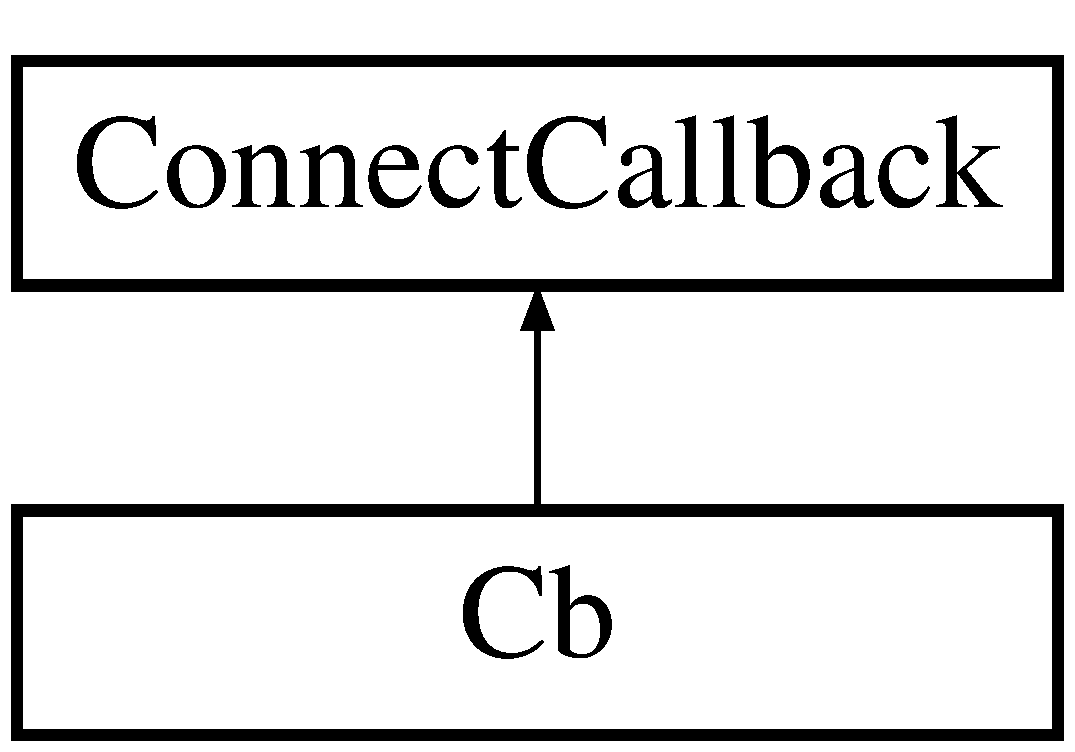
\includegraphics[height=2.000000cm]{classCb}
\end{center}
\end{figure}
\subsection*{Public Member Functions}
\begin{DoxyCompactItemize}
\item 
{\bf Cb} (folly\+::\+Async\+S\+S\+L\+Socket $\ast$sock)
\item 
void {\bf connect\+Success} () noexceptoverride
\item 
void {\bf connect\+Err} (const folly\+::\+Async\+Socket\+Exception \&) noexceptoverride
\item 
const X509 $\ast$ {\bf get\+Peer\+Cert} ()
\end{DoxyCompactItemize}
\subsection*{Public Attributes}
\begin{DoxyCompactItemize}
\item 
bool {\bf success} \{false\}
\item 
bool {\bf reused\+Session} \{false\}
\item 
wangle\+::\+S\+S\+L\+Session\+Ptr {\bf session}
\item 
folly\+::\+Async\+S\+S\+L\+Socket $\ast$ {\bf sock\+\_\+} \{{\bf nullptr}\}
\item 
folly\+::ssl\+::\+X509\+Unique\+Ptr {\bf peer\+Cert\+\_\+} \{{\bf nullptr}\}
\end{DoxyCompactItemize}


\subsection{Detailed Description}


Definition at line 127 of file H\+T\+T\+P\+Server\+Test.\+cpp.



\subsection{Constructor \& Destructor Documentation}
\index{Cb@{Cb}!Cb@{Cb}}
\index{Cb@{Cb}!Cb@{Cb}}
\subsubsection[{Cb(folly\+::\+Async\+S\+S\+L\+Socket $\ast$sock)}]{\setlength{\rightskip}{0pt plus 5cm}Cb\+::\+Cb (
\begin{DoxyParamCaption}
\item[{folly\+::\+Async\+S\+S\+L\+Socket $\ast$}]{sock}
\end{DoxyParamCaption}
)\hspace{0.3cm}{\ttfamily [inline]}, {\ttfamily [explicit]}}\label{classCb_aec3df3b289507f952c718117e82ef48d}


Definition at line 129 of file H\+T\+T\+P\+Server\+Test.\+cpp.


\begin{DoxyCode}
129 : sock_(sock) \{\}
\end{DoxyCode}


\subsection{Member Function Documentation}
\index{Cb@{Cb}!connect\+Err@{connect\+Err}}
\index{connect\+Err@{connect\+Err}!Cb@{Cb}}
\subsubsection[{connect\+Err(const folly\+::\+Async\+Socket\+Exception \&) noexceptoverride}]{\setlength{\rightskip}{0pt plus 5cm}void Cb\+::connect\+Err (
\begin{DoxyParamCaption}
\item[{const folly\+::\+Async\+Socket\+Exception \&}]{}
\end{DoxyParamCaption}
)\hspace{0.3cm}{\ttfamily [inline]}, {\ttfamily [override]}, {\ttfamily [noexcept]}}\label{classCb_a89f40919f2a9c33284b3aff1cfa5918d}


Definition at line 141 of file H\+T\+T\+P\+Server\+Test.\+cpp.


\begin{DoxyCode}
141                                                                       \{
142     success = \textcolor{keyword}{false};
143   \}
\end{DoxyCode}
\index{Cb@{Cb}!connect\+Success@{connect\+Success}}
\index{connect\+Success@{connect\+Success}!Cb@{Cb}}
\subsubsection[{connect\+Success() noexceptoverride}]{\setlength{\rightskip}{0pt plus 5cm}void Cb\+::connect\+Success (
\begin{DoxyParamCaption}
{}
\end{DoxyParamCaption}
)\hspace{0.3cm}{\ttfamily [inline]}, {\ttfamily [override]}, {\ttfamily [noexcept]}}\label{classCb_a6a80543111df63b25cea314f3f5c03f1}


Definition at line 130 of file H\+T\+T\+P\+Server\+Test.\+cpp.


\begin{DoxyCode}
130                                           \{
131     success = \textcolor{keyword}{true};
132     reusedSession = sock_->getSSLSessionReused();
133     session.reset(sock_->getSSLSession());
134     \textcolor{keywordflow}{if} (sock_->getPeerCert()) \{
135       \textcolor{comment}{// keeps this alive until Cb is destroyed, even if sock is closed}
136       peerCert_ = sock_->getPeerCert();
137     \}
138     sock_->close();
139   \}
\end{DoxyCode}
\index{Cb@{Cb}!get\+Peer\+Cert@{get\+Peer\+Cert}}
\index{get\+Peer\+Cert@{get\+Peer\+Cert}!Cb@{Cb}}
\subsubsection[{get\+Peer\+Cert()}]{\setlength{\rightskip}{0pt plus 5cm}const X509$\ast$ Cb\+::get\+Peer\+Cert (
\begin{DoxyParamCaption}
{}
\end{DoxyParamCaption}
)\hspace{0.3cm}{\ttfamily [inline]}}\label{classCb_a13ccf5f1b4d6b63b97f8daef90466101}


Definition at line 145 of file H\+T\+T\+P\+Server\+Test.\+cpp.


\begin{DoxyCode}
145 \{ \textcolor{keywordflow}{return} peerCert_.get(); \}
\end{DoxyCode}


\subsection{Member Data Documentation}
\index{Cb@{Cb}!peer\+Cert\+\_\+@{peer\+Cert\+\_\+}}
\index{peer\+Cert\+\_\+@{peer\+Cert\+\_\+}!Cb@{Cb}}
\subsubsection[{peer\+Cert\+\_\+}]{\setlength{\rightskip}{0pt plus 5cm}folly\+::ssl\+::\+X509\+Unique\+Ptr Cb\+::peer\+Cert\+\_\+ \{{\bf nullptr}\}}\label{classCb_a1517924c770639c8649425cbf3229fd4}


Definition at line 151 of file H\+T\+T\+P\+Server\+Test.\+cpp.

\index{Cb@{Cb}!reused\+Session@{reused\+Session}}
\index{reused\+Session@{reused\+Session}!Cb@{Cb}}
\subsubsection[{reused\+Session}]{\setlength{\rightskip}{0pt plus 5cm}bool Cb\+::reused\+Session \{false\}}\label{classCb_a078f1d64998766c1d1738178e874e286}


Definition at line 148 of file H\+T\+T\+P\+Server\+Test.\+cpp.

\index{Cb@{Cb}!session@{session}}
\index{session@{session}!Cb@{Cb}}
\subsubsection[{session}]{\setlength{\rightskip}{0pt plus 5cm}wangle\+::\+S\+S\+L\+Session\+Ptr Cb\+::session}\label{classCb_a5033dda06c9fc459caa35973a60a7364}


Definition at line 149 of file H\+T\+T\+P\+Server\+Test.\+cpp.

\index{Cb@{Cb}!sock\+\_\+@{sock\+\_\+}}
\index{sock\+\_\+@{sock\+\_\+}!Cb@{Cb}}
\subsubsection[{sock\+\_\+}]{\setlength{\rightskip}{0pt plus 5cm}folly\+::\+Async\+S\+S\+L\+Socket$\ast$ Cb\+::sock\+\_\+ \{{\bf nullptr}\}}\label{classCb_a6704c20a449a287ab6fdcc90e9327569}


Definition at line 150 of file H\+T\+T\+P\+Server\+Test.\+cpp.

\index{Cb@{Cb}!success@{success}}
\index{success@{success}!Cb@{Cb}}
\subsubsection[{success}]{\setlength{\rightskip}{0pt plus 5cm}bool Cb\+::success \{false\}}\label{classCb_abfc5a7346c80efa80e729eacc856cee0}


Definition at line 147 of file H\+T\+T\+P\+Server\+Test.\+cpp.



The documentation for this class was generated from the following file\+:\begin{DoxyCompactItemize}
\item 
proxygen/httpserver/tests/{\bf H\+T\+T\+P\+Server\+Test.\+cpp}\end{DoxyCompactItemize}

\section{proxygen\+:\+:Chain\+Info\+Printer Class Reference}
\label{classproxygen_1_1ChainInfoPrinter}\index{proxygen\+::\+Chain\+Info\+Printer@{proxygen\+::\+Chain\+Info\+Printer}}


{\ttfamily \#include $<$Logging.\+h$>$}

Inheritance diagram for proxygen\+:\+:Chain\+Info\+Printer\+:\begin{figure}[H]
\begin{center}
\leavevmode
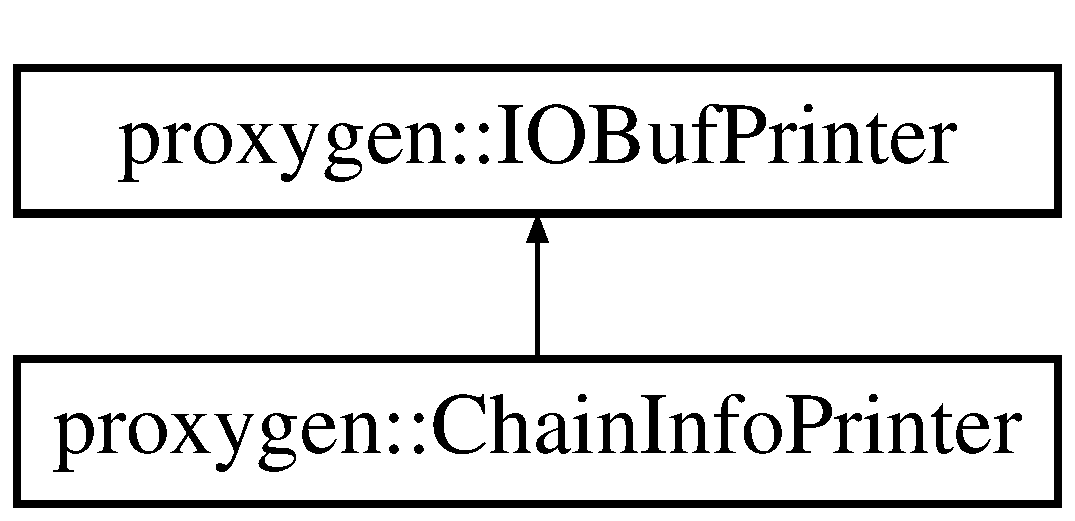
\includegraphics[height=2.000000cm]{classproxygen_1_1ChainInfoPrinter}
\end{center}
\end{figure}
\subsection*{Public Member Functions}
\begin{DoxyCompactItemize}
\item 
std\+::string {\bf print} (const folly\+::\+I\+O\+Buf $\ast$buf) override
\end{DoxyCompactItemize}
\subsection*{Additional Inherited Members}


\subsection{Detailed Description}


Definition at line 160 of file Logging.\+h.



\subsection{Member Function Documentation}
\index{proxygen\+::\+Chain\+Info\+Printer@{proxygen\+::\+Chain\+Info\+Printer}!print@{print}}
\index{print@{print}!proxygen\+::\+Chain\+Info\+Printer@{proxygen\+::\+Chain\+Info\+Printer}}
\subsubsection[{print(const folly\+::\+I\+O\+Buf $\ast$buf) override}]{\setlength{\rightskip}{0pt plus 5cm}string proxygen\+::\+Chain\+Info\+Printer\+::print (
\begin{DoxyParamCaption}
\item[{const folly\+::\+I\+O\+Buf $\ast$}]{buf}
\end{DoxyParamCaption}
)\hspace{0.3cm}{\ttfamily [override]}, {\ttfamily [virtual]}}\label{classproxygen_1_1ChainInfoPrinter_afaf2d5e6eece776c60e478431580d63c}


Implements {\bf proxygen\+::\+I\+O\+Buf\+Printer} \doxyref{}{p.}{classproxygen_1_1IOBufPrinter_a317ea00fb51d7d42c37a440488f42664}.



Definition at line 77 of file Logging.\+cpp.


\begin{DoxyCode}
77                                                \{
78   stringstream out;
79   out << \textcolor{stringliteral}{"iobuf of size "} << buf->length()
80       << \textcolor{stringliteral}{" tailroom "} << buf->tailroom();
81   \textcolor{keywordflow}{return} out.str();
82 \}
\end{DoxyCode}


The documentation for this class was generated from the following files\+:\begin{DoxyCompactItemize}
\item 
proxygen/lib/utils/{\bf Logging.\+h}\item 
proxygen/lib/utils/{\bf Logging.\+cpp}\end{DoxyCompactItemize}

\section{proxygen\+:\+:H\+T\+T\+P\+Transaction\+:\+:Chunk Struct Reference}
\label{structproxygen_1_1HTTPTransaction_1_1Chunk}\index{proxygen\+::\+H\+T\+T\+P\+Transaction\+::\+Chunk@{proxygen\+::\+H\+T\+T\+P\+Transaction\+::\+Chunk}}
\subsection*{Public Member Functions}
\begin{DoxyCompactItemize}
\item 
{\bf Chunk} (size\+\_\+t in\+Length)
\end{DoxyCompactItemize}
\subsection*{Public Attributes}
\begin{DoxyCompactItemize}
\item 
size\+\_\+t {\bf length}
\item 
bool {\bf header\+Sent}
\end{DoxyCompactItemize}


\subsection{Detailed Description}


Definition at line 1391 of file H\+T\+T\+P\+Transaction.\+h.



\subsection{Constructor \& Destructor Documentation}
\index{proxygen\+::\+H\+T\+T\+P\+Transaction\+::\+Chunk@{proxygen\+::\+H\+T\+T\+P\+Transaction\+::\+Chunk}!Chunk@{Chunk}}
\index{Chunk@{Chunk}!proxygen\+::\+H\+T\+T\+P\+Transaction\+::\+Chunk@{proxygen\+::\+H\+T\+T\+P\+Transaction\+::\+Chunk}}
\subsubsection[{Chunk(size\+\_\+t in\+Length)}]{\setlength{\rightskip}{0pt plus 5cm}proxygen\+::\+H\+T\+T\+P\+Transaction\+::\+Chunk\+::\+Chunk (
\begin{DoxyParamCaption}
\item[{size\+\_\+t}]{in\+Length}
\end{DoxyParamCaption}
)\hspace{0.3cm}{\ttfamily [inline]}, {\ttfamily [explicit]}}\label{structproxygen_1_1HTTPTransaction_1_1Chunk_aadc9394603474911230754e0f4156f62}


Definition at line 1392 of file H\+T\+T\+P\+Transaction.\+h.


\begin{DoxyCode}
1392 : length(inLength), headerSent(\textcolor{keyword}{false}) \{\}
\end{DoxyCode}


\subsection{Member Data Documentation}
\index{proxygen\+::\+H\+T\+T\+P\+Transaction\+::\+Chunk@{proxygen\+::\+H\+T\+T\+P\+Transaction\+::\+Chunk}!header\+Sent@{header\+Sent}}
\index{header\+Sent@{header\+Sent}!proxygen\+::\+H\+T\+T\+P\+Transaction\+::\+Chunk@{proxygen\+::\+H\+T\+T\+P\+Transaction\+::\+Chunk}}
\subsubsection[{header\+Sent}]{\setlength{\rightskip}{0pt plus 5cm}bool proxygen\+::\+H\+T\+T\+P\+Transaction\+::\+Chunk\+::header\+Sent}\label{structproxygen_1_1HTTPTransaction_1_1Chunk_af044d194d523fbce539790e034449240}


Definition at line 1394 of file H\+T\+T\+P\+Transaction.\+h.



Referenced by proxygen\+::\+H\+T\+T\+P\+Transaction\+::send\+Deferred\+Body().

\index{proxygen\+::\+H\+T\+T\+P\+Transaction\+::\+Chunk@{proxygen\+::\+H\+T\+T\+P\+Transaction\+::\+Chunk}!length@{length}}
\index{length@{length}!proxygen\+::\+H\+T\+T\+P\+Transaction\+::\+Chunk@{proxygen\+::\+H\+T\+T\+P\+Transaction\+::\+Chunk}}
\subsubsection[{length}]{\setlength{\rightskip}{0pt plus 5cm}size\+\_\+t proxygen\+::\+H\+T\+T\+P\+Transaction\+::\+Chunk\+::length}\label{structproxygen_1_1HTTPTransaction_1_1Chunk_abdf4b50799a3323b6bb5417eb4f010cf}


Definition at line 1393 of file H\+T\+T\+P\+Transaction.\+h.



Referenced by proxygen\+::\+H\+T\+T\+P\+Transaction\+::send\+Deferred\+Body().



The documentation for this struct was generated from the following file\+:\begin{DoxyCompactItemize}
\item 
proxygen/lib/http/session/{\bf H\+T\+T\+P\+Transaction.\+h}\end{DoxyCompactItemize}

\section{proxygen\+:\+:Cob\+Helper Class Reference}
\label{classproxygen_1_1CobHelper}\index{proxygen\+::\+Cob\+Helper@{proxygen\+::\+Cob\+Helper}}


{\ttfamily \#include $<$Cob\+Helper.\+h$>$}

\subsection*{Public Member Functions}
\begin{DoxyCompactItemize}
\item 
{\bf Cob\+Helper} (size\+\_\+t items\+Left, const std\+::function$<$ void()$>$ \&cob, const std\+::function$<$ void(const std\+::exception \&)$>$ \&ecob)
\item 
void {\bf set\+Error} (const std\+::string \&emsg)
\item 
void {\bf worker\+Done} ()
\end{DoxyCompactItemize}
\subsection*{Private Member Functions}
\begin{DoxyCompactItemize}
\item 
void {\bf all\+Done} ()
\end{DoxyCompactItemize}
\subsection*{Private Attributes}
\begin{DoxyCompactItemize}
\item 
std\+::atomic$<$ uint32\+\_\+t $>$ {\bf items\+Left\+\_\+}
\item 
std\+::string {\bf emsg\+\_\+}
\item 
std\+::function$<$ void()$>$ {\bf cob\+\_\+}
\item 
std\+::function$<$ void(const std\+::exception \&)$>$ {\bf ecob\+\_\+}
\end{DoxyCompactItemize}


\subsection{Detailed Description}
A helper class to schedule N async jobs in (possibly) different threads and invoke a final callback in a given thread once all are done. 

Definition at line 23 of file Cob\+Helper.\+h.



\subsection{Constructor \& Destructor Documentation}
\index{proxygen\+::\+Cob\+Helper@{proxygen\+::\+Cob\+Helper}!Cob\+Helper@{Cob\+Helper}}
\index{Cob\+Helper@{Cob\+Helper}!proxygen\+::\+Cob\+Helper@{proxygen\+::\+Cob\+Helper}}
\subsubsection[{Cob\+Helper(size\+\_\+t items\+Left, const std\+::function$<$ void()$>$ \&cob, const std\+::function$<$ void(const std\+::exception \&)$>$ \&ecob)}]{\setlength{\rightskip}{0pt plus 5cm}proxygen\+::\+Cob\+Helper\+::\+Cob\+Helper (
\begin{DoxyParamCaption}
\item[{size\+\_\+t}]{items\+Left, }
\item[{const std\+::function$<$ void()$>$ \&}]{cob, }
\item[{const std\+::function$<$ void(const std\+::exception \&)$>$ \&}]{ecob}
\end{DoxyParamCaption}
)\hspace{0.3cm}{\ttfamily [inline]}}\label{classproxygen_1_1CobHelper_a5556acf109751c90b1c5ccf9364a4109}


Definition at line 25 of file Cob\+Helper.\+h.


\begin{DoxyCode}
28   : itemsLeft_(itemsLeft)
29 , cob_(cob)
30 , ecob_(ecob) \{\}
\end{DoxyCode}


\subsection{Member Function Documentation}
\index{proxygen\+::\+Cob\+Helper@{proxygen\+::\+Cob\+Helper}!all\+Done@{all\+Done}}
\index{all\+Done@{all\+Done}!proxygen\+::\+Cob\+Helper@{proxygen\+::\+Cob\+Helper}}
\subsubsection[{all\+Done()}]{\setlength{\rightskip}{0pt plus 5cm}void proxygen\+::\+Cob\+Helper\+::all\+Done (
\begin{DoxyParamCaption}
{}
\end{DoxyParamCaption}
)\hspace{0.3cm}{\ttfamily [inline]}, {\ttfamily [private]}}\label{classproxygen_1_1CobHelper_a49485d67af296b3f8a20060a4e4ce649}


Definition at line 46 of file Cob\+Helper.\+h.



References cob\+\_\+, ecob\+\_\+, and emsg\+\_\+.



Referenced by worker\+Done().


\begin{DoxyCode}
46                  \{
47     \textcolor{keywordflow}{if} (!emsg_.empty()) \{
48       ecob_(std::runtime\_error(emsg_));
49     \} \textcolor{keywordflow}{else} \{
50       cob_();
51     \}
52 
53     \textcolor{keyword}{delete} \textcolor{keyword}{this};
54   \}
\end{DoxyCode}
\index{proxygen\+::\+Cob\+Helper@{proxygen\+::\+Cob\+Helper}!set\+Error@{set\+Error}}
\index{set\+Error@{set\+Error}!proxygen\+::\+Cob\+Helper@{proxygen\+::\+Cob\+Helper}}
\subsubsection[{set\+Error(const std\+::string \&emsg)}]{\setlength{\rightskip}{0pt plus 5cm}void proxygen\+::\+Cob\+Helper\+::set\+Error (
\begin{DoxyParamCaption}
\item[{const std\+::string \&}]{emsg}
\end{DoxyParamCaption}
)\hspace{0.3cm}{\ttfamily [inline]}}\label{classproxygen_1_1CobHelper_ab29d60620d28fa2def97e4d696dde19b}


Definition at line 32 of file Cob\+Helper.\+h.



References emsg\+\_\+.


\begin{DoxyCode}
32                                        \{
33     CHECK(!emsg.empty());
34     emsg_ = emsg;
35   \}
\end{DoxyCode}
\index{proxygen\+::\+Cob\+Helper@{proxygen\+::\+Cob\+Helper}!worker\+Done@{worker\+Done}}
\index{worker\+Done@{worker\+Done}!proxygen\+::\+Cob\+Helper@{proxygen\+::\+Cob\+Helper}}
\subsubsection[{worker\+Done()}]{\setlength{\rightskip}{0pt plus 5cm}void proxygen\+::\+Cob\+Helper\+::worker\+Done (
\begin{DoxyParamCaption}
{}
\end{DoxyParamCaption}
)\hspace{0.3cm}{\ttfamily [inline]}}\label{classproxygen_1_1CobHelper_ab4c52632990ad52068b40d92272d6acd}


Definition at line 37 of file Cob\+Helper.\+h.



References all\+Done(), and items\+Left\+\_\+.


\begin{DoxyCode}
37                     \{
38     uint32\_t oldValue = itemsLeft_.fetch\_sub(1);
39     \textcolor{keywordflow}{if} (oldValue != 1) \{
40       \textcolor{keywordflow}{return};
41     \}
42 
43     allDone();
44   \}
\end{DoxyCode}


\subsection{Member Data Documentation}
\index{proxygen\+::\+Cob\+Helper@{proxygen\+::\+Cob\+Helper}!cob\+\_\+@{cob\+\_\+}}
\index{cob\+\_\+@{cob\+\_\+}!proxygen\+::\+Cob\+Helper@{proxygen\+::\+Cob\+Helper}}
\subsubsection[{cob\+\_\+}]{\setlength{\rightskip}{0pt plus 5cm}std\+::function$<$void()$>$ proxygen\+::\+Cob\+Helper\+::cob\+\_\+\hspace{0.3cm}{\ttfamily [private]}}\label{classproxygen_1_1CobHelper_a38d33b75ab511aa394efde8c12d94b2f}


Definition at line 58 of file Cob\+Helper.\+h.



Referenced by all\+Done().

\index{proxygen\+::\+Cob\+Helper@{proxygen\+::\+Cob\+Helper}!ecob\+\_\+@{ecob\+\_\+}}
\index{ecob\+\_\+@{ecob\+\_\+}!proxygen\+::\+Cob\+Helper@{proxygen\+::\+Cob\+Helper}}
\subsubsection[{ecob\+\_\+}]{\setlength{\rightskip}{0pt plus 5cm}std\+::function$<$void(const std\+::exception\&)$>$ proxygen\+::\+Cob\+Helper\+::ecob\+\_\+\hspace{0.3cm}{\ttfamily [private]}}\label{classproxygen_1_1CobHelper_a0cb8c27b4ef2b871ee509510ff6ff6ac}


Definition at line 59 of file Cob\+Helper.\+h.



Referenced by all\+Done().

\index{proxygen\+::\+Cob\+Helper@{proxygen\+::\+Cob\+Helper}!emsg\+\_\+@{emsg\+\_\+}}
\index{emsg\+\_\+@{emsg\+\_\+}!proxygen\+::\+Cob\+Helper@{proxygen\+::\+Cob\+Helper}}
\subsubsection[{emsg\+\_\+}]{\setlength{\rightskip}{0pt plus 5cm}std\+::string proxygen\+::\+Cob\+Helper\+::emsg\+\_\+\hspace{0.3cm}{\ttfamily [private]}}\label{classproxygen_1_1CobHelper_acf9111dee0bc8cbc4fe227db988e650a}


Definition at line 57 of file Cob\+Helper.\+h.



Referenced by all\+Done(), and set\+Error().

\index{proxygen\+::\+Cob\+Helper@{proxygen\+::\+Cob\+Helper}!items\+Left\+\_\+@{items\+Left\+\_\+}}
\index{items\+Left\+\_\+@{items\+Left\+\_\+}!proxygen\+::\+Cob\+Helper@{proxygen\+::\+Cob\+Helper}}
\subsubsection[{items\+Left\+\_\+}]{\setlength{\rightskip}{0pt plus 5cm}std\+::atomic$<$uint32\+\_\+t$>$ proxygen\+::\+Cob\+Helper\+::items\+Left\+\_\+\hspace{0.3cm}{\ttfamily [private]}}\label{classproxygen_1_1CobHelper_a029769e43745539b0d863ccd0b45e440}


Definition at line 56 of file Cob\+Helper.\+h.



Referenced by worker\+Done().



The documentation for this class was generated from the following file\+:\begin{DoxyCompactItemize}
\item 
proxygen/lib/utils/{\bf Cob\+Helper.\+h}\end{DoxyCompactItemize}

\section{proxygen\+:\+:Codec\+Error\+Response\+Handler Class Reference}
\label{classproxygen_1_1CodecErrorResponseHandler}\index{proxygen\+::\+Codec\+Error\+Response\+Handler@{proxygen\+::\+Codec\+Error\+Response\+Handler}}


{\ttfamily \#include $<$Codec\+Error\+Response\+Handler.\+h$>$}

Inheritance diagram for proxygen\+:\+:Codec\+Error\+Response\+Handler\+:\begin{figure}[H]
\begin{center}
\leavevmode
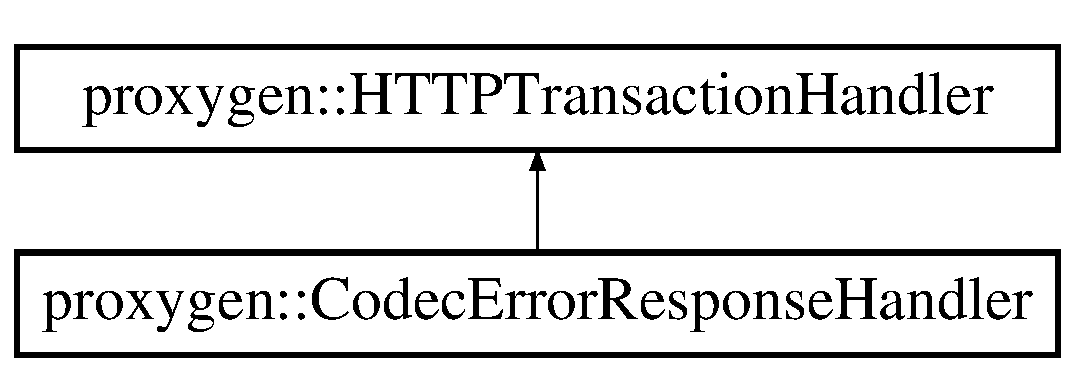
\includegraphics[height=2.000000cm]{classproxygen_1_1CodecErrorResponseHandler}
\end{center}
\end{figure}
\subsection*{Public Member Functions}
\begin{DoxyCompactItemize}
\item 
{\bf Codec\+Error\+Response\+Handler} ({\bf Error\+Code} {\bf status\+Code})
\item 
void {\bf set\+Transaction} ({\bf H\+T\+T\+P\+Transaction} $\ast$txn) noexceptoverride
\item 
void {\bf detach\+Transaction} () noexceptoverride
\item 
void {\bf on\+Headers\+Complete} (std\+::unique\+\_\+ptr$<$ {\bf H\+T\+T\+P\+Message} $>$ msg) noexceptoverride
\item 
void {\bf on\+Body} (std\+::unique\+\_\+ptr$<$ folly\+::\+I\+O\+Buf $>$ chain) noexceptoverride
\item 
void {\bf on\+Trailers} (std\+::unique\+\_\+ptr$<$ {\bf H\+T\+T\+P\+Headers} $>$ trailers) noexceptoverride
\item 
void {\bf on\+E\+OM} () noexceptoverride
\item 
void {\bf on\+Upgrade} ({\bf Upgrade\+Protocol} protocol) noexceptoverride
\item 
void {\bf on\+Error} (const {\bf H\+T\+T\+P\+Exception} \&error) noexceptoverride
\item 
void {\bf on\+Egress\+Paused} () noexceptoverride
\item 
void {\bf on\+Egress\+Resumed} () noexceptoverride
\end{DoxyCompactItemize}
\subsection*{Private Member Functions}
\begin{DoxyCompactItemize}
\item 
{\bf $\sim$\+Codec\+Error\+Response\+Handler} () override
\end{DoxyCompactItemize}
\subsection*{Private Attributes}
\begin{DoxyCompactItemize}
\item 
{\bf H\+T\+T\+P\+Transaction} $\ast$ {\bf txn\+\_\+}
\end{DoxyCompactItemize}


\subsection{Detailed Description}


Definition at line 18 of file Codec\+Error\+Response\+Handler.\+h.



\subsection{Constructor \& Destructor Documentation}
\index{proxygen\+::\+Codec\+Error\+Response\+Handler@{proxygen\+::\+Codec\+Error\+Response\+Handler}!Codec\+Error\+Response\+Handler@{Codec\+Error\+Response\+Handler}}
\index{Codec\+Error\+Response\+Handler@{Codec\+Error\+Response\+Handler}!proxygen\+::\+Codec\+Error\+Response\+Handler@{proxygen\+::\+Codec\+Error\+Response\+Handler}}
\subsubsection[{Codec\+Error\+Response\+Handler(\+Error\+Code status\+Code)}]{\setlength{\rightskip}{0pt plus 5cm}proxygen\+::\+Codec\+Error\+Response\+Handler\+::\+Codec\+Error\+Response\+Handler (
\begin{DoxyParamCaption}
\item[{{\bf Error\+Code}}]{status\+Code}
\end{DoxyParamCaption}
)\hspace{0.3cm}{\ttfamily [explicit]}}\label{classproxygen_1_1CodecErrorResponseHandler_a408606f53c689950306a1af013351527}


Definition at line 20 of file Codec\+Error\+Response\+Handler.\+cpp.


\begin{DoxyCode}
21     : txn_(\textcolor{keyword}{nullptr}) \{\}
\end{DoxyCode}
\index{proxygen\+::\+Codec\+Error\+Response\+Handler@{proxygen\+::\+Codec\+Error\+Response\+Handler}!````~Codec\+Error\+Response\+Handler@{$\sim$\+Codec\+Error\+Response\+Handler}}
\index{````~Codec\+Error\+Response\+Handler@{$\sim$\+Codec\+Error\+Response\+Handler}!proxygen\+::\+Codec\+Error\+Response\+Handler@{proxygen\+::\+Codec\+Error\+Response\+Handler}}
\subsubsection[{$\sim$\+Codec\+Error\+Response\+Handler() override}]{\setlength{\rightskip}{0pt plus 5cm}proxygen\+::\+Codec\+Error\+Response\+Handler\+::$\sim$\+Codec\+Error\+Response\+Handler (
\begin{DoxyParamCaption}
{}
\end{DoxyParamCaption}
)\hspace{0.3cm}{\ttfamily [override]}, {\ttfamily [private]}}\label{classproxygen_1_1CodecErrorResponseHandler_adad4e656ad69bf040bb2e5a1bafbb39d}


Definition at line 23 of file Codec\+Error\+Response\+Handler.\+cpp.



Referenced by on\+Egress\+Resumed().


\begin{DoxyCode}
23                                                       \{
24 \}
\end{DoxyCode}


\subsection{Member Function Documentation}
\index{proxygen\+::\+Codec\+Error\+Response\+Handler@{proxygen\+::\+Codec\+Error\+Response\+Handler}!detach\+Transaction@{detach\+Transaction}}
\index{detach\+Transaction@{detach\+Transaction}!proxygen\+::\+Codec\+Error\+Response\+Handler@{proxygen\+::\+Codec\+Error\+Response\+Handler}}
\subsubsection[{detach\+Transaction() noexceptoverride}]{\setlength{\rightskip}{0pt plus 5cm}void proxygen\+::\+Codec\+Error\+Response\+Handler\+::detach\+Transaction (
\begin{DoxyParamCaption}
{}
\end{DoxyParamCaption}
)\hspace{0.3cm}{\ttfamily [override]}, {\ttfamily [virtual]}, {\ttfamily [noexcept]}}\label{classproxygen_1_1CodecErrorResponseHandler_af9d9d69d23411943857745fa7e8a5bf7}
Called once after a transaction successfully completes. It will be called even if a read or write error happened earlier. This is a terminal callback, which means that the \doxyref{H\+T\+T\+P\+Transaction}{p.}{classproxygen_1_1HTTPTransaction} object that gives this call will be invalid after this function completes. 

Implements {\bf proxygen\+::\+H\+T\+T\+P\+Transaction\+Handler} \doxyref{}{p.}{classproxygen_1_1HTTPTransactionHandler_a67eb253d121a26772f4caa56847ed7cd}.



Definition at line 32 of file Codec\+Error\+Response\+Handler.\+cpp.


\begin{DoxyCode}
32                                                       \{
33   \textcolor{keyword}{delete} \textcolor{keyword}{this};
34 \}
\end{DoxyCode}
\index{proxygen\+::\+Codec\+Error\+Response\+Handler@{proxygen\+::\+Codec\+Error\+Response\+Handler}!on\+Body@{on\+Body}}
\index{on\+Body@{on\+Body}!proxygen\+::\+Codec\+Error\+Response\+Handler@{proxygen\+::\+Codec\+Error\+Response\+Handler}}
\subsubsection[{on\+Body(std\+::unique\+\_\+ptr$<$ folly\+::\+I\+O\+Buf $>$ chain) noexceptoverride}]{\setlength{\rightskip}{0pt plus 5cm}void proxygen\+::\+Codec\+Error\+Response\+Handler\+::on\+Body (
\begin{DoxyParamCaption}
\item[{std\+::unique\+\_\+ptr$<$ folly\+::\+I\+O\+Buf $>$}]{chain}
\end{DoxyParamCaption}
)\hspace{0.3cm}{\ttfamily [override]}, {\ttfamily [virtual]}, {\ttfamily [noexcept]}}\label{classproxygen_1_1CodecErrorResponseHandler_a6954568eda49450938d616b74095d5da}
Can be called multiple times per transaction. If you had previously called pause\+Ingress(), this callback will be delayed until you call resume\+Ingress(). 

Implements {\bf proxygen\+::\+H\+T\+T\+P\+Transaction\+Handler} \doxyref{}{p.}{classproxygen_1_1HTTPTransactionHandler_a56a25d7fb8ac5ddf1ed5b16eaca3c5df}.



Definition at line 41 of file Codec\+Error\+Response\+Handler.\+cpp.


\begin{DoxyCode}
41                                                                    \{
42   VLOG(4) << \textcolor{stringliteral}{"discarding request body"};
43 \}
\end{DoxyCode}
\index{proxygen\+::\+Codec\+Error\+Response\+Handler@{proxygen\+::\+Codec\+Error\+Response\+Handler}!on\+Egress\+Paused@{on\+Egress\+Paused}}
\index{on\+Egress\+Paused@{on\+Egress\+Paused}!proxygen\+::\+Codec\+Error\+Response\+Handler@{proxygen\+::\+Codec\+Error\+Response\+Handler}}
\subsubsection[{on\+Egress\+Paused() noexceptoverride}]{\setlength{\rightskip}{0pt plus 5cm}void proxygen\+::\+Codec\+Error\+Response\+Handler\+::on\+Egress\+Paused (
\begin{DoxyParamCaption}
{}
\end{DoxyParamCaption}
)\hspace{0.3cm}{\ttfamily [inline]}, {\ttfamily [override]}, {\ttfamily [virtual]}, {\ttfamily [noexcept]}}\label{classproxygen_1_1CodecErrorResponseHandler_a11978d258bea9a4c3b66d00f51abb085}
If the remote side\textquotesingle{}s receive buffer fills up, this callback will be invoked so you can attempt to stop sending to the remote side. 

Implements {\bf proxygen\+::\+H\+T\+T\+P\+Transaction\+Handler} \doxyref{}{p.}{classproxygen_1_1HTTPTransactionHandler_a0a50acdb32cb51ecbf6a72730053a36b}.



Definition at line 33 of file Codec\+Error\+Response\+Handler.\+h.


\begin{DoxyCode}
33 \{\};
\end{DoxyCode}
\index{proxygen\+::\+Codec\+Error\+Response\+Handler@{proxygen\+::\+Codec\+Error\+Response\+Handler}!on\+Egress\+Resumed@{on\+Egress\+Resumed}}
\index{on\+Egress\+Resumed@{on\+Egress\+Resumed}!proxygen\+::\+Codec\+Error\+Response\+Handler@{proxygen\+::\+Codec\+Error\+Response\+Handler}}
\subsubsection[{on\+Egress\+Resumed() noexceptoverride}]{\setlength{\rightskip}{0pt plus 5cm}void proxygen\+::\+Codec\+Error\+Response\+Handler\+::on\+Egress\+Resumed (
\begin{DoxyParamCaption}
{}
\end{DoxyParamCaption}
)\hspace{0.3cm}{\ttfamily [inline]}, {\ttfamily [override]}, {\ttfamily [virtual]}, {\ttfamily [noexcept]}}\label{classproxygen_1_1CodecErrorResponseHandler_a14f5d408dd0540be026594f9ffc71258}
This callback lets you know that the remote side has resumed reading and you can now continue to send data. 

Implements {\bf proxygen\+::\+H\+T\+T\+P\+Transaction\+Handler} \doxyref{}{p.}{classproxygen_1_1HTTPTransactionHandler_a7715b02e413859c26426adbbde7e53d8}.



Definition at line 34 of file Codec\+Error\+Response\+Handler.\+h.



References $\sim$\+Codec\+Error\+Response\+Handler().


\begin{DoxyCode}
34 \{\};
\end{DoxyCode}
\index{proxygen\+::\+Codec\+Error\+Response\+Handler@{proxygen\+::\+Codec\+Error\+Response\+Handler}!on\+E\+OM@{on\+E\+OM}}
\index{on\+E\+OM@{on\+E\+OM}!proxygen\+::\+Codec\+Error\+Response\+Handler@{proxygen\+::\+Codec\+Error\+Response\+Handler}}
\subsubsection[{on\+E\+O\+M() noexceptoverride}]{\setlength{\rightskip}{0pt plus 5cm}void proxygen\+::\+Codec\+Error\+Response\+Handler\+::on\+E\+OM (
\begin{DoxyParamCaption}
{}
\end{DoxyParamCaption}
)\hspace{0.3cm}{\ttfamily [override]}, {\ttfamily [virtual]}, {\ttfamily [noexcept]}}\label{classproxygen_1_1CodecErrorResponseHandler_a478113c15632fd80373ba1568d67ebea}
Can be called once per transaction. If you had previously called pause\+Ingress(), this callback will be delayed until you call resume\+Ingress(). After this callback is received, there will be no more normal ingress callbacks received (on\+Egress$\ast$() and \doxyref{on\+Error()}{p.}{classproxygen_1_1CodecErrorResponseHandler_a528f7a698e0c1651dc1138f8a5cce25b} may still be invoked). The Handler should consider ingress complete after receiving this message. This Transaction is still valid, and work may still occur on it until detach\+Transaction is called. 

Implements {\bf proxygen\+::\+H\+T\+T\+P\+Transaction\+Handler} \doxyref{}{p.}{classproxygen_1_1HTTPTransactionHandler_afdc4d4dec715841ba0c5bb5e58b1d53c}.



Definition at line 51 of file Codec\+Error\+Response\+Handler.\+cpp.


\begin{DoxyCode}
51                                           \{
52 \}
\end{DoxyCode}
\index{proxygen\+::\+Codec\+Error\+Response\+Handler@{proxygen\+::\+Codec\+Error\+Response\+Handler}!on\+Error@{on\+Error}}
\index{on\+Error@{on\+Error}!proxygen\+::\+Codec\+Error\+Response\+Handler@{proxygen\+::\+Codec\+Error\+Response\+Handler}}
\subsubsection[{on\+Error(const H\+T\+T\+P\+Exception \&error) noexceptoverride}]{\setlength{\rightskip}{0pt plus 5cm}void proxygen\+::\+Codec\+Error\+Response\+Handler\+::on\+Error (
\begin{DoxyParamCaption}
\item[{const {\bf H\+T\+T\+P\+Exception} \&}]{error}
\end{DoxyParamCaption}
)\hspace{0.3cm}{\ttfamily [override]}, {\ttfamily [virtual]}, {\ttfamily [noexcept]}}\label{classproxygen_1_1CodecErrorResponseHandler_a528f7a698e0c1651dc1138f8a5cce25b}
Can be called at any time before \doxyref{detach\+Transaction()}{p.}{classproxygen_1_1CodecErrorResponseHandler_af9d9d69d23411943857745fa7e8a5bf7}. This callback implies that an error has occurred. To determine if ingress or egress is affected, check the direciont on the \doxyref{H\+T\+T\+P\+Exception}{p.}{classproxygen_1_1HTTPException}. If the direction is I\+N\+G\+R\+E\+SS, it M\+AY still be possible to send egress. 

Implements {\bf proxygen\+::\+H\+T\+T\+P\+Transaction\+Handler} \doxyref{}{p.}{classproxygen_1_1HTTPTransactionHandler_a585c21327eb30ab85ebdb84f663dab3b}.



Definition at line 57 of file Codec\+Error\+Response\+Handler.\+cpp.



References proxygen\+::\+H\+T\+T\+P\+Transaction\+::send\+Abort(), and txn\+\_\+.


\begin{DoxyCode}
57                                                                            \{
58   VLOG(4) << \textcolor{stringliteral}{"processing error "} << error;
59   txn_->sendAbort();
60 \}
\end{DoxyCode}
\index{proxygen\+::\+Codec\+Error\+Response\+Handler@{proxygen\+::\+Codec\+Error\+Response\+Handler}!on\+Headers\+Complete@{on\+Headers\+Complete}}
\index{on\+Headers\+Complete@{on\+Headers\+Complete}!proxygen\+::\+Codec\+Error\+Response\+Handler@{proxygen\+::\+Codec\+Error\+Response\+Handler}}
\subsubsection[{on\+Headers\+Complete(std\+::unique\+\_\+ptr$<$ H\+T\+T\+P\+Message $>$ msg) noexceptoverride}]{\setlength{\rightskip}{0pt plus 5cm}void proxygen\+::\+Codec\+Error\+Response\+Handler\+::on\+Headers\+Complete (
\begin{DoxyParamCaption}
\item[{std\+::unique\+\_\+ptr$<$ {\bf H\+T\+T\+P\+Message} $>$}]{msg}
\end{DoxyParamCaption}
)\hspace{0.3cm}{\ttfamily [override]}, {\ttfamily [virtual]}, {\ttfamily [noexcept]}}\label{classproxygen_1_1CodecErrorResponseHandler_a53f53233df1aa329d58c6e4c25792b21}
Called at most once per transaction. This is usually the first ingress callback. It is possible to get a read error before this however. If you had previously called pause\+Ingress(), this callback will be delayed until you call resume\+Ingress(). 

Implements {\bf proxygen\+::\+H\+T\+T\+P\+Transaction\+Handler} \doxyref{}{p.}{classproxygen_1_1HTTPTransactionHandler_a5e431cbb4c065285c5ad65acaceb0b22}.



Definition at line 36 of file Codec\+Error\+Response\+Handler.\+cpp.


\begin{DoxyCode}
37                                            \{
38   VLOG(4) << \textcolor{stringliteral}{"discarding headers"};
39 \}
\end{DoxyCode}
\index{proxygen\+::\+Codec\+Error\+Response\+Handler@{proxygen\+::\+Codec\+Error\+Response\+Handler}!on\+Trailers@{on\+Trailers}}
\index{on\+Trailers@{on\+Trailers}!proxygen\+::\+Codec\+Error\+Response\+Handler@{proxygen\+::\+Codec\+Error\+Response\+Handler}}
\subsubsection[{on\+Trailers(std\+::unique\+\_\+ptr$<$ H\+T\+T\+P\+Headers $>$ trailers) noexceptoverride}]{\setlength{\rightskip}{0pt plus 5cm}void proxygen\+::\+Codec\+Error\+Response\+Handler\+::on\+Trailers (
\begin{DoxyParamCaption}
\item[{std\+::unique\+\_\+ptr$<$ {\bf H\+T\+T\+P\+Headers} $>$}]{trailers}
\end{DoxyParamCaption}
)\hspace{0.3cm}{\ttfamily [override]}, {\ttfamily [virtual]}, {\ttfamily [noexcept]}}\label{classproxygen_1_1CodecErrorResponseHandler_a0d1ffa7ca3489d9cb76a1f1015eb8d9f}
Can be called any number of times per transaction. If you had previously called pause\+Ingress(), this callback will be delayed until you call resume\+Ingress(). Trailers can be received once right before the E\+OM of a chunked H\+T\+T\+P/1.\+1 reponse or multiple times per transaction from S\+P\+DY and H\+T\+T\+P/2.\+0 H\+E\+A\+D\+E\+RS frames. 

Implements {\bf proxygen\+::\+H\+T\+T\+P\+Transaction\+Handler} \doxyref{}{p.}{classproxygen_1_1HTTPTransactionHandler_a219de67110f915deda30d18327f26393}.



Definition at line 45 of file Codec\+Error\+Response\+Handler.\+cpp.


\begin{DoxyCode}
46                                         \{
47   VLOG(4) << \textcolor{stringliteral}{"discarding request trailers"};
48 \}
\end{DoxyCode}
\index{proxygen\+::\+Codec\+Error\+Response\+Handler@{proxygen\+::\+Codec\+Error\+Response\+Handler}!on\+Upgrade@{on\+Upgrade}}
\index{on\+Upgrade@{on\+Upgrade}!proxygen\+::\+Codec\+Error\+Response\+Handler@{proxygen\+::\+Codec\+Error\+Response\+Handler}}
\subsubsection[{on\+Upgrade(\+Upgrade\+Protocol protocol) noexceptoverride}]{\setlength{\rightskip}{0pt plus 5cm}void proxygen\+::\+Codec\+Error\+Response\+Handler\+::on\+Upgrade (
\begin{DoxyParamCaption}
\item[{{\bf Upgrade\+Protocol}}]{protocol}
\end{DoxyParamCaption}
)\hspace{0.3cm}{\ttfamily [override]}, {\ttfamily [virtual]}, {\ttfamily [noexcept]}}\label{classproxygen_1_1CodecErrorResponseHandler_a85661a89d97edc0e729ab79a48dfd7e1}
Can be called once per transaction. If you had previously called pause\+Ingress(), this callback will be delayed until you call resume\+Ingress(). After this callback is invoked, further data will be forwarded using the \doxyref{on\+Body()}{p.}{classproxygen_1_1CodecErrorResponseHandler_a6954568eda49450938d616b74095d5da} callback. Once the data transfer is completed (E\+OF recevied in case of C\+O\+N\+N\+E\+CT), \doxyref{on\+E\+O\+M()}{p.}{classproxygen_1_1CodecErrorResponseHandler_a478113c15632fd80373ba1568d67ebea} callback will be invoked. 

Implements {\bf proxygen\+::\+H\+T\+T\+P\+Transaction\+Handler} \doxyref{}{p.}{classproxygen_1_1HTTPTransactionHandler_acda954bf78c4d2aad951698e78c40a0f}.



Definition at line 54 of file Codec\+Error\+Response\+Handler.\+cpp.


\begin{DoxyCode}
55                                 \{\}
\end{DoxyCode}
\index{proxygen\+::\+Codec\+Error\+Response\+Handler@{proxygen\+::\+Codec\+Error\+Response\+Handler}!set\+Transaction@{set\+Transaction}}
\index{set\+Transaction@{set\+Transaction}!proxygen\+::\+Codec\+Error\+Response\+Handler@{proxygen\+::\+Codec\+Error\+Response\+Handler}}
\subsubsection[{set\+Transaction(\+H\+T\+T\+P\+Transaction $\ast$txn) noexceptoverride}]{\setlength{\rightskip}{0pt plus 5cm}void proxygen\+::\+Codec\+Error\+Response\+Handler\+::set\+Transaction (
\begin{DoxyParamCaption}
\item[{{\bf H\+T\+T\+P\+Transaction} $\ast$}]{txn}
\end{DoxyParamCaption}
)\hspace{0.3cm}{\ttfamily [override]}, {\ttfamily [virtual]}, {\ttfamily [noexcept]}}\label{classproxygen_1_1CodecErrorResponseHandler_aef0fd13f2c1b669bf81502ea0a10e5c3}
Called once per transaction. This notifies the handler of which transaction it should talk to and will receive callbacks from. 

Implements {\bf proxygen\+::\+H\+T\+T\+P\+Transaction\+Handler} \doxyref{}{p.}{classproxygen_1_1HTTPTransactionHandler_a4eb50d5627d26f6ca0d8e8283259d8a4}.



Definition at line 27 of file Codec\+Error\+Response\+Handler.\+cpp.



References txn\+\_\+.


\begin{DoxyCode}
27                                                                        \{
28   txn_ = txn;
29 \}
\end{DoxyCode}


\subsection{Member Data Documentation}
\index{proxygen\+::\+Codec\+Error\+Response\+Handler@{proxygen\+::\+Codec\+Error\+Response\+Handler}!txn\+\_\+@{txn\+\_\+}}
\index{txn\+\_\+@{txn\+\_\+}!proxygen\+::\+Codec\+Error\+Response\+Handler@{proxygen\+::\+Codec\+Error\+Response\+Handler}}
\subsubsection[{txn\+\_\+}]{\setlength{\rightskip}{0pt plus 5cm}{\bf H\+T\+T\+P\+Transaction}$\ast$ proxygen\+::\+Codec\+Error\+Response\+Handler\+::txn\+\_\+\hspace{0.3cm}{\ttfamily [private]}}\label{classproxygen_1_1CodecErrorResponseHandler_accc9a7b16388971897c9d6a52806bae7}


Definition at line 39 of file Codec\+Error\+Response\+Handler.\+h.



Referenced by on\+Error(), and set\+Transaction().



The documentation for this class was generated from the following files\+:\begin{DoxyCompactItemize}
\item 
proxygen/lib/http/session/{\bf Codec\+Error\+Response\+Handler.\+h}\item 
proxygen/lib/http/session/{\bf Codec\+Error\+Response\+Handler.\+cpp}\end{DoxyCompactItemize}

\section{proxygen\+:\+:Codec\+Util Class Reference}
\label{classproxygen_1_1CodecUtil}\index{proxygen\+::\+Codec\+Util@{proxygen\+::\+Codec\+Util}}


{\ttfamily \#include $<$Codec\+Util.\+h$>$}

\subsection*{Public Types}
\begin{DoxyCompactItemize}
\item 
enum {\bf Ctl\+Escape\+Mode} \{ {\bf C\+O\+M\+P\+L\+I\+A\+NT}, 
{\bf S\+T\+R\+I\+CT}
 \}
\end{DoxyCompactItemize}
\subsection*{Static Public Member Functions}
\begin{DoxyCompactItemize}
\item 
static bool {\bf validate\+U\+RL} (folly\+::\+Byte\+Range url)
\item 
static bool {\bf validate\+Method} (folly\+::\+Byte\+Range method)
\item 
static bool {\bf validate\+Header\+Name} (folly\+::\+Byte\+Range {\bf name})
\item 
static bool {\bf validate\+Header\+Value} (folly\+::\+Byte\+Range value, {\bf Ctl\+Escape\+Mode} mode)
\item 
static bool {\bf has\+Gzip\+And\+Deflate} (const std\+::string \&value, bool \&has\+Gzip, bool \&has\+Deflate)
\item 
static std\+::vector$<$ {\bf compress\+::\+Header} $>$ {\bf prepare\+Message\+For\+Compression} (const {\bf H\+T\+T\+P\+Message} \&msg, std\+::vector$<$ std\+::string $>$ \&temps)
\item 
static bool {\bf append\+Headers} (const {\bf H\+T\+T\+P\+Headers} \&input\+Headers, std\+::vector$<$ {\bf compress\+::\+Header} $>$ \&headers, {\bf H\+T\+T\+P\+Header\+Code} header\+To\+Check)
\end{DoxyCompactItemize}
\subsection*{Static Public Attributes}
\begin{DoxyCompactItemize}
\item 
static const char {\bf http\+\_\+tokens} [256]
\end{DoxyCompactItemize}


\subsection{Detailed Description}


Definition at line 23 of file Codec\+Util.\+h.



\subsection{Member Enumeration Documentation}
\index{proxygen\+::\+Codec\+Util@{proxygen\+::\+Codec\+Util}!Ctl\+Escape\+Mode@{Ctl\+Escape\+Mode}}
\index{Ctl\+Escape\+Mode@{Ctl\+Escape\+Mode}!proxygen\+::\+Codec\+Util@{proxygen\+::\+Codec\+Util}}
\subsubsection[{Ctl\+Escape\+Mode}]{\setlength{\rightskip}{0pt plus 5cm}enum {\bf proxygen\+::\+Codec\+Util\+::\+Ctl\+Escape\+Mode}}\label{classproxygen_1_1CodecUtil_a856a74954c175245974a2fc27c8c554b}
\doxyref{R\+F\+C2616}{p.}{namespaceproxygen_1_1RFC2616} allows certain control chars in header values if they are quoted and escaped. When mode is C\+O\+M\+P\+L\+I\+A\+NT, then this is allowed. When mode is S\+T\+R\+I\+CT, no escaped C\+T\+Ls are allowed \begin{Desc}
\item[Enumerator]\par
\begin{description}
\index{C\+O\+M\+P\+L\+I\+A\+NT@{C\+O\+M\+P\+L\+I\+A\+NT}!proxygen\+::\+Codec\+Util@{proxygen\+::\+Codec\+Util}}\index{proxygen\+::\+Codec\+Util@{proxygen\+::\+Codec\+Util}!C\+O\+M\+P\+L\+I\+A\+NT@{C\+O\+M\+P\+L\+I\+A\+NT}}\item[{\em 
C\+O\+M\+P\+L\+I\+A\+NT\label{classproxygen_1_1CodecUtil_a856a74954c175245974a2fc27c8c554ba35ad9e7dd13b99faf2913be5a9470144}
}]\index{S\+T\+R\+I\+CT@{S\+T\+R\+I\+CT}!proxygen\+::\+Codec\+Util@{proxygen\+::\+Codec\+Util}}\index{proxygen\+::\+Codec\+Util@{proxygen\+::\+Codec\+Util}!S\+T\+R\+I\+CT@{S\+T\+R\+I\+CT}}\item[{\em 
S\+T\+R\+I\+CT\label{classproxygen_1_1CodecUtil_a856a74954c175245974a2fc27c8c554ba71a6e170eb4d3c8b755a4ace234aaf46}
}]\end{description}
\end{Desc}


Definition at line 61 of file Codec\+Util.\+h.


\begin{DoxyCode}
61                      \{
62     COMPLIANT,
63     STRICT
64   \};
\end{DoxyCode}


\subsection{Member Function Documentation}
\index{proxygen\+::\+Codec\+Util@{proxygen\+::\+Codec\+Util}!append\+Headers@{append\+Headers}}
\index{append\+Headers@{append\+Headers}!proxygen\+::\+Codec\+Util@{proxygen\+::\+Codec\+Util}}
\subsubsection[{append\+Headers(const H\+T\+T\+P\+Headers \&input\+Headers, std\+::vector$<$ compress\+::\+Header $>$ \&headers, H\+T\+T\+P\+Header\+Code header\+To\+Check)}]{\setlength{\rightskip}{0pt plus 5cm}bool proxygen\+::\+Codec\+Util\+::append\+Headers (
\begin{DoxyParamCaption}
\item[{const {\bf H\+T\+T\+P\+Headers} \&}]{input\+Headers, }
\item[{std\+::vector$<$ {\bf compress\+::\+Header} $>$ \&}]{headers, }
\item[{{\bf H\+T\+T\+P\+Header\+Code}}]{header\+To\+Check}
\end{DoxyParamCaption}
)\hspace{0.3cm}{\ttfamily [static]}}\label{classproxygen_1_1CodecUtil_a88c268b449dc3ba5b47ed181b68234c3}


Definition at line 131 of file Codec\+Util.\+cpp.



References proxygen\+::\+H\+T\+T\+P\+Headers\+::for\+Each\+With\+Code(), and name.



Referenced by proxygen\+::\+H\+T\+T\+P2\+Codec\+::generate\+Trailers(), prepare\+Message\+For\+Compression(), and validate\+Header\+Value().


\begin{DoxyCode}
133                                                             \{
134   \textcolor{keywordtype}{bool} headerToCheckExists = \textcolor{keyword}{false};
135   \textcolor{comment}{// Add the HTTP headers supplied by the caller, but skip}
136   \textcolor{comment}{// any per-hop headers that aren't supported in HTTP/2.}
137   inputHeaders.forEachWithCode([&](HTTPHeaderCode code,
138                                    \textcolor{keyword}{const} std::string& name,
139                                    \textcolor{keyword}{const} std::string& value) \{
140     \textcolor{keyword}{static} \textcolor{keyword}{const} std::bitset<256> s\_perHopHeaderCodes\{[] \{
141       std::bitset<256> bs;
142       \textcolor{comment}{// HTTP/1.x per-hop headers that have no meaning in HTTP/2}
143       bs[HTTP\_HEADER\_CONNECTION] = \textcolor{keyword}{true};
144       bs[HTTP\_HEADER\_HOST] = \textcolor{keyword}{true};
145       bs[HTTP\_HEADER\_KEEP\_ALIVE] = \textcolor{keyword}{true};
146       bs[HTTP\_HEADER\_PROXY\_CONNECTION] = \textcolor{keyword}{true};
147       bs[HTTP\_HEADER\_TRANSFER\_ENCODING] = \textcolor{keyword}{true};
148       bs[HTTP\_HEADER\_UPGRADE] = \textcolor{keyword}{true};
149       bs[HTTP\_HEADER\_SEC\_WEBSOCKET\_KEY] = \textcolor{keyword}{true};
150       bs[HTTP\_HEADER\_SEC\_WEBSOCKET\_ACCEPT] = \textcolor{keyword}{true};
151       \textcolor{keywordflow}{return} bs;
152     \}()\};
153 
154     \textcolor{keywordflow}{if} (s\_perHopHeaderCodes[code] || name.size() == 0 || name[0] == \textcolor{charliteral}{':'}) \{
155       DCHECK\_GT(name.size(), 0) << \textcolor{stringliteral}{"Empty header"};
156       DCHECK\_NE(name[0], \textcolor{charliteral}{':'}) << \textcolor{stringliteral}{"Invalid header="} << name;
157       \textcolor{keywordflow}{return};
158     \}
159     \textcolor{comment}{// Note this code will not drop headers named by Connection.  That's the}
160     \textcolor{comment}{// caller's job}
161 
162     \textcolor{comment}{// see HTTP/2 spec, 8.1.2}
163     DCHECK(name != \textcolor{stringliteral}{"TE"} || value == \textcolor{stringliteral}{"trailers"});
164     \textcolor{keywordflow}{if} ((name.size() > 0 && name[0] != \textcolor{charliteral}{':'}) && code != HTTP\_HEADER\_HOST) \{
165       headers.emplace\_back(code, name, value);
166     \}
167     \textcolor{keywordflow}{if} (code == headerToCheck) \{
168       headerToCheckExists = \textcolor{keyword}{true};
169     \}
170   \});
171 
172   \textcolor{keywordflow}{return} headerToCheckExists;
173 \}
\end{DoxyCode}
\index{proxygen\+::\+Codec\+Util@{proxygen\+::\+Codec\+Util}!has\+Gzip\+And\+Deflate@{has\+Gzip\+And\+Deflate}}
\index{has\+Gzip\+And\+Deflate@{has\+Gzip\+And\+Deflate}!proxygen\+::\+Codec\+Util@{proxygen\+::\+Codec\+Util}}
\subsubsection[{has\+Gzip\+And\+Deflate(const std\+::string \&value, bool \&has\+Gzip, bool \&has\+Deflate)}]{\setlength{\rightskip}{0pt plus 5cm}bool proxygen\+::\+Codec\+Util\+::has\+Gzip\+And\+Deflate (
\begin{DoxyParamCaption}
\item[{const std\+::string \&}]{value, }
\item[{bool \&}]{has\+Gzip, }
\item[{bool \&}]{has\+Deflate}
\end{DoxyParamCaption}
)\hspace{0.3cm}{\ttfamily [static]}}\label{classproxygen_1_1CodecUtil_ad1df12d61ffacdeeabb5eac028f75aed}


Definition at line 61 of file Codec\+Util.\+cpp.



References proxygen\+::\+R\+F\+C2616\+::parse\+Qvalues().



Referenced by proxygen\+::\+S\+P\+D\+Y\+Codec\+::parse\+Headers(), and validate\+Header\+Value().


\begin{DoxyCode}
62                                                    \{
63   \textcolor{keyword}{static} folly::ThreadLocal<std::vector<RFC2616::TokenQPair>> output;
64   output->clear();
65   hasGzip = \textcolor{keyword}{false};
66   hasDeflate = \textcolor{keyword}{false};
67   RFC2616::parseQvalues(value, *output);
68   \textcolor{keywordflow}{for} (\textcolor{keyword}{const} \textcolor{keyword}{auto}& encodingQ: *output) \{
69     std::string lower(encodingQ.first.str());
70     std::transform(lower.begin(), lower.end(), lower.begin(), ::tolower);
71     \textcolor{comment}{// RFC says 3 sig figs}
72     \textcolor{keywordflow}{if} (lower == \textcolor{stringliteral}{"gzip"} && encodingQ.second >= 0.001) \{
73       hasGzip = \textcolor{keyword}{true};
74     \} \textcolor{keywordflow}{else} \textcolor{keywordflow}{if} (lower == \textcolor{stringliteral}{"deflate"} && encodingQ.second >= 0.001) \{
75       hasDeflate = \textcolor{keyword}{true};
76     \}
77   \}
78   \textcolor{keywordflow}{return} hasGzip && hasDeflate;
79 \}
\end{DoxyCode}
\index{proxygen\+::\+Codec\+Util@{proxygen\+::\+Codec\+Util}!prepare\+Message\+For\+Compression@{prepare\+Message\+For\+Compression}}
\index{prepare\+Message\+For\+Compression@{prepare\+Message\+For\+Compression}!proxygen\+::\+Codec\+Util@{proxygen\+::\+Codec\+Util}}
\subsubsection[{prepare\+Message\+For\+Compression(const H\+T\+T\+P\+Message \&msg, std\+::vector$<$ std\+::string $>$ \&temps)}]{\setlength{\rightskip}{0pt plus 5cm}std\+::vector$<$ {\bf compress\+::\+Header} $>$ proxygen\+::\+Codec\+Util\+::prepare\+Message\+For\+Compression (
\begin{DoxyParamCaption}
\item[{const {\bf H\+T\+T\+P\+Message} \&}]{msg, }
\item[{std\+::vector$<$ std\+::string $>$ \&}]{temps}
\end{DoxyParamCaption}
)\hspace{0.3cm}{\ttfamily [static]}}\label{classproxygen_1_1CodecUtil_aa88e7bf99028926f11066a8e47baf672}


Definition at line 82 of file Codec\+Util.\+cpp.



References append\+Headers(), proxygen\+::\+C\+O\+N\+N\+E\+CT, proxygen\+::\+H\+T\+T\+P\+Message\+::format\+Date\+Header(), proxygen\+::\+H\+T\+T\+P\+Message\+::get\+Headers(), proxygen\+::\+H\+T\+T\+P\+Message\+::get\+Method(), proxygen\+::\+H\+T\+T\+P\+Message\+::get\+Method\+String(), proxygen\+::\+H\+T\+T\+P\+Headers\+::get\+Single\+Or\+Empty(), proxygen\+::\+H\+T\+T\+P\+Message\+::get\+Status\+Code(), proxygen\+::\+H\+T\+T\+P\+Message\+::get\+U\+R\+L(), proxygen\+::\+H\+T\+T\+P\+Message\+::is\+Egress\+Websocket\+Upgrade(), proxygen\+::\+H\+T\+T\+P\+Message\+::is\+Request(), proxygen\+::\+H\+T\+T\+P\+Message\+::is\+Response(), proxygen\+::\+H\+T\+T\+P\+Message\+::is\+Secure(), proxygen\+::headers\+::k\+Http, proxygen\+::headers\+::k\+Https, proxygen\+::headers\+::k\+Status200, proxygen\+::headers\+::k\+Websocket\+String, and proxygen\+::method\+To\+String().



Referenced by proxygen\+::\+H\+T\+T\+P2\+Codec\+::generate\+Header\+Impl(), and validate\+Header\+Value().


\begin{DoxyCode}
84                                  \{
85   std::vector<compress::Header> allHeaders;
86   \textcolor{keywordflow}{if} (msg.isRequest()) \{
87     \textcolor{keywordflow}{if} (msg.isEgressWebsocketUpgrade()) \{
88       allHeaders.emplace\_back(HTTP\_HEADER\_COLON\_METHOD,
89           methodToString(HTTPMethod::CONNECT));
90       allHeaders.emplace\_back(HTTP\_HEADER\_COLON\_PROTOCOL,
91                               headers::kWebsocketString);
92     \} \textcolor{keywordflow}{else} \{
93       \textcolor{keyword}{const} std::string& method = msg.getMethodString();
94       allHeaders.emplace\_back(HTTP\_HEADER\_COLON\_METHOD, method);
95     \}
96 
97     \textcolor{keywordflow}{if} (msg.getMethod() != HTTPMethod::CONNECT ||
98         msg.isEgressWebsocketUpgrade()) \{
99       \textcolor{keyword}{const} std::string& scheme =
100         (msg.isSecure() ? headers::kHttps : headers::kHttp);
101       \textcolor{keyword}{const} std::string& path = msg.getURL();
102       allHeaders.emplace\_back(HTTP\_HEADER\_COLON\_SCHEME, scheme);
103       allHeaders.emplace\_back(HTTP\_HEADER\_COLON\_PATH, path);
104     \}
105     \textcolor{keyword}{const} HTTPHeaders& headers = msg.getHeaders();
106     \textcolor{keyword}{const} std::string& host = headers.getSingleOrEmpty(HTTP\_HEADER\_HOST);
107     \textcolor{keywordflow}{if} (!host.empty()) \{
108       allHeaders.emplace\_back(HTTP\_HEADER\_COLON\_AUTHORITY, host);
109     \}
110   \} \textcolor{keywordflow}{else} \{
111     temps.reserve(3); \textcolor{comment}{// must be large enough so that emplace does not resize}
112     \textcolor{keywordflow}{if} (msg.isEgressWebsocketUpgrade()) \{
113       temps.emplace\_back(headers::kStatus200);
114     \} \textcolor{keywordflow}{else} \{
115       temps.emplace\_back(folly::to<std::string>(msg.getStatusCode()));
116     \}
117     allHeaders.emplace\_back(HTTP\_HEADER\_COLON\_STATUS, temps.back());
118     \textcolor{comment}{// HEADERS frames do not include a version or reason string.}
119   \}
120 
121   \textcolor{keywordtype}{bool} hasDateHeader =
122       appendHeaders(msg.getHeaders(), allHeaders, HTTP\_HEADER\_DATE);
123 
124   \textcolor{keywordflow}{if} (msg.isResponse() && !hasDateHeader) \{
125     temps.emplace\_back(HTTPMessage::formatDateHeader());
126     allHeaders.emplace\_back(HTTP\_HEADER\_DATE, temps.back());
127   \}
128   \textcolor{keywordflow}{return} allHeaders;
129 \}
\end{DoxyCode}
\index{proxygen\+::\+Codec\+Util@{proxygen\+::\+Codec\+Util}!validate\+Header\+Name@{validate\+Header\+Name}}
\index{validate\+Header\+Name@{validate\+Header\+Name}!proxygen\+::\+Codec\+Util@{proxygen\+::\+Codec\+Util}}
\subsubsection[{validate\+Header\+Name(folly\+::\+Byte\+Range name)}]{\setlength{\rightskip}{0pt plus 5cm}static bool proxygen\+::\+Codec\+Util\+::validate\+Header\+Name (
\begin{DoxyParamCaption}
\item[{folly\+::\+Byte\+Range}]{name}
\end{DoxyParamCaption}
)\hspace{0.3cm}{\ttfamily [inline]}, {\ttfamily [static]}}\label{classproxygen_1_1CodecUtil_a82438d2f4bb2dfda705f03a750e8e7fc}


Definition at line 43 of file Codec\+Util.\+h.



Referenced by proxygen\+::\+Header\+Decode\+Info\+::on\+Header(), and proxygen\+::\+S\+P\+D\+Y\+Codec\+::parse\+Headers().


\begin{DoxyCode}
43                                                       \{
44     \textcolor{keywordflow}{if} (name.size() == 0) \{
45       \textcolor{keywordflow}{return} \textcolor{keyword}{false};
46     \}
47     \textcolor{keywordflow}{for} (\textcolor{keyword}{auto} p: name) \{
48       \textcolor{keywordflow}{if} (p < 0x80 && http_tokens[(uint8\_t)p] != p) \{
49         \textcolor{keywordflow}{return} \textcolor{keyword}{false};
50       \}
51     \}
52     \textcolor{keywordflow}{return} \textcolor{keyword}{true};
53   \}
\end{DoxyCode}
\index{proxygen\+::\+Codec\+Util@{proxygen\+::\+Codec\+Util}!validate\+Header\+Value@{validate\+Header\+Value}}
\index{validate\+Header\+Value@{validate\+Header\+Value}!proxygen\+::\+Codec\+Util@{proxygen\+::\+Codec\+Util}}
\subsubsection[{validate\+Header\+Value(folly\+::\+Byte\+Range value, Ctl\+Escape\+Mode mode)}]{\setlength{\rightskip}{0pt plus 5cm}static bool proxygen\+::\+Codec\+Util\+::validate\+Header\+Value (
\begin{DoxyParamCaption}
\item[{folly\+::\+Byte\+Range}]{value, }
\item[{{\bf Ctl\+Escape\+Mode}}]{mode}
\end{DoxyParamCaption}
)\hspace{0.3cm}{\ttfamily [inline]}, {\ttfamily [static]}}\label{classproxygen_1_1CodecUtil_ac5cc215d13e8b9bccfa35adf20c61ae8}


Definition at line 66 of file Codec\+Util.\+h.



References append\+Headers(), C\+O\+M\+P\+L\+I\+A\+NT, has\+Gzip\+And\+Deflate(), and prepare\+Message\+For\+Compression().



Referenced by proxygen\+::\+Header\+Decode\+Info\+::on\+Header(), proxygen\+::\+S\+P\+D\+Y\+Codec\+::parse\+Headers(), and proxygen\+::\+H\+T\+T\+P\+Request\+Verifier\+::set\+Authority().


\begin{DoxyCode}
67                                                       \{
68     \textcolor{keywordtype}{bool} escape = \textcolor{keyword}{false};
69     \textcolor{keywordtype}{bool} quote = \textcolor{keyword}{false};
70     \textcolor{keyword}{enum} \{ lws\_none,
71            lws\_expect\_nl,
72            lws\_expect\_ws1,
73            lws\_expect\_ws2 \} state = lws\_none;
74 
75     \textcolor{keywordflow}{for} (\textcolor{keyword}{auto} p = std::begin(value); p != std::end(value); ++p) \{
76       \textcolor{keywordflow}{if} (escape) \{
77         escape = \textcolor{keyword}{false};
78         \textcolor{keywordflow}{if} (mode == COMPLIANT) \{
79           \textcolor{comment}{// prev char escaped.  Turn off escape and go to next char}
80           \textcolor{comment}{// COMPLIANT mode only}
81           assert(quote);
82           \textcolor{keywordflow}{continue};
83         \}
84       \}
85       \textcolor{keywordflow}{switch} (state) \{
86         \textcolor{keywordflow}{case} lws\_none:
87           \textcolor{keywordflow}{switch} (*p) \{
88             \textcolor{keywordflow}{case} \textcolor{charliteral}{'\(\backslash\)\(\backslash\)'}:
89               \textcolor{keywordflow}{if} (quote) \{
90                 escape = \textcolor{keyword}{true};
91               \}
92               \textcolor{keywordflow}{break};
93             \textcolor{keywordflow}{case} \textcolor{charliteral}{'\(\backslash\)"'}:
94               quote = !quote;
95               \textcolor{keywordflow}{break};
96             \textcolor{keywordflow}{case} \textcolor{charliteral}{'\(\backslash\)r'}:
97               state = lws\_expect\_nl;
98               \textcolor{keywordflow}{break};
99             \textcolor{keywordflow}{default}:
100               \textcolor{keywordflow}{if} ((*p < 0x20 || *p == 0x7f) && *p != \textcolor{charliteral}{'\(\backslash\)t'}) \{
101                 \textcolor{comment}{// unexpected ctl per rfc2616, HT OK}
102                 \textcolor{keywordflow}{return} \textcolor{keyword}{false};
103               \}
104               \textcolor{keywordflow}{break};
105           \}
106           \textcolor{keywordflow}{break};
107         \textcolor{keywordflow}{case} lws\_expect\_nl:
108           \textcolor{keywordflow}{if} (*p != \textcolor{charliteral}{'\(\backslash\)n'}) \{
109             \textcolor{comment}{// unescaped \(\backslash\)r must be LWS}
110             \textcolor{keywordflow}{return} \textcolor{keyword}{false};
111           \}
112           state = lws\_expect\_ws1;
113           \textcolor{keywordflow}{break};
114         \textcolor{keywordflow}{case} lws\_expect\_ws1:
115           \textcolor{keywordflow}{if} (*p != \textcolor{charliteral}{' '} && *p != \textcolor{charliteral}{'\(\backslash\)t'}) \{
116             \textcolor{comment}{// unescaped \(\backslash\)r\(\backslash\)n must be LWS}
117             \textcolor{keywordflow}{return} \textcolor{keyword}{false};
118           \}
119           state = lws\_expect\_ws2;
120           \textcolor{keywordflow}{break};
121         \textcolor{keywordflow}{case} lws\_expect\_ws2:
122           \textcolor{keywordflow}{if} (*p != \textcolor{charliteral}{' '} && *p != \textcolor{charliteral}{'\(\backslash\)t'}) \{
123             \textcolor{comment}{// terminated LWS}
124             state = lws\_none;
125             \textcolor{comment}{// check this char again}
126             p--;
127           \}
128           \textcolor{keywordflow}{break};
129       \}
130     \}
131     \textcolor{comment}{// Unterminated quotes are OK, since the value can be* TEXT which treats}
132     \textcolor{comment}{// the " like any other char.}
133     \textcolor{comment}{// Unterminated escapes are bad because it will escape the next character}
134     \textcolor{comment}{// when converting to HTTP}
135     \textcolor{comment}{// Unterminated LWS (dangling \(\backslash\)r or \(\backslash\)r\(\backslash\)n) is bad because it could}
136     \textcolor{comment}{// prematurely terminate the headers when converting to HTTP}
137     \textcolor{keywordflow}{return} !escape && (state == lws\_none || state == lws\_expect\_ws2);
138   \}
\end{DoxyCode}
\index{proxygen\+::\+Codec\+Util@{proxygen\+::\+Codec\+Util}!validate\+Method@{validate\+Method}}
\index{validate\+Method@{validate\+Method}!proxygen\+::\+Codec\+Util@{proxygen\+::\+Codec\+Util}}
\subsubsection[{validate\+Method(folly\+::\+Byte\+Range method)}]{\setlength{\rightskip}{0pt plus 5cm}static bool proxygen\+::\+Codec\+Util\+::validate\+Method (
\begin{DoxyParamCaption}
\item[{folly\+::\+Byte\+Range}]{method}
\end{DoxyParamCaption}
)\hspace{0.3cm}{\ttfamily [inline]}, {\ttfamily [static]}}\label{classproxygen_1_1CodecUtil_aa865daca9716ad297c4771ebb6c650c5}


Definition at line 33 of file Codec\+Util.\+h.



Referenced by proxygen\+::\+S\+P\+D\+Y\+Codec\+::parse\+Headers(), proxygen\+::\+H\+T\+T\+P\+Request\+Verifier\+::set\+Method(), and proxygen\+::\+H\+T\+T\+P\+Request\+Verifier\+::set\+Scheme().


\begin{DoxyCode}
33                                                     \{
34     \textcolor{keywordflow}{for} (\textcolor{keyword}{auto} p: method) \{
35       \textcolor{keywordflow}{if} (!isalpha(p)) \{
36         \textcolor{comment}{// methods are all characters}
37         \textcolor{keywordflow}{return} \textcolor{keyword}{false};
38       \}
39     \}
40     \textcolor{keywordflow}{return} \textcolor{keyword}{true};
41   \}
\end{DoxyCode}
\index{proxygen\+::\+Codec\+Util@{proxygen\+::\+Codec\+Util}!validate\+U\+RL@{validate\+U\+RL}}
\index{validate\+U\+RL@{validate\+U\+RL}!proxygen\+::\+Codec\+Util@{proxygen\+::\+Codec\+Util}}
\subsubsection[{validate\+U\+R\+L(folly\+::\+Byte\+Range url)}]{\setlength{\rightskip}{0pt plus 5cm}static bool proxygen\+::\+Codec\+Util\+::validate\+U\+RL (
\begin{DoxyParamCaption}
\item[{folly\+::\+Byte\+Range}]{url}
\end{DoxyParamCaption}
)\hspace{0.3cm}{\ttfamily [inline]}, {\ttfamily [static]}}\label{classproxygen_1_1CodecUtil_a1cf346e49d7822f78d85fe3edbb67ef5}


Definition at line 29 of file Codec\+Util.\+h.



References proxygen\+::validate\+U\+R\+L().



Referenced by proxygen\+::\+S\+P\+D\+Y\+Codec\+::parse\+Headers(), and proxygen\+::\+H\+T\+T\+P\+Request\+Verifier\+::set\+Path().


\begin{DoxyCode}
29                                               \{
30     \textcolor{keywordflow}{return} proxygen::validateURL(url);
31   \}
\end{DoxyCode}


\subsection{Member Data Documentation}
\index{proxygen\+::\+Codec\+Util@{proxygen\+::\+Codec\+Util}!http\+\_\+tokens@{http\+\_\+tokens}}
\index{http\+\_\+tokens@{http\+\_\+tokens}!proxygen\+::\+Codec\+Util@{proxygen\+::\+Codec\+Util}}
\subsubsection[{http\+\_\+tokens}]{\setlength{\rightskip}{0pt plus 5cm}const char proxygen\+::\+Codec\+Util\+::http\+\_\+tokens\hspace{0.3cm}{\ttfamily [static]}}\label{classproxygen_1_1CodecUtil_ae6e8cce92924181e499587aadedee378}
Tokens as defined by rfc 2616. Also lowercases them. token = 1$\ast$$<$any char=\char`\"{}\char`\"{} except=\char`\"{}\char`\"{} ctls=\char`\"{}\char`\"{} or=\char`\"{}\char`\"{} separators$>$=\char`\"{}\char`\"{}$>$ separators = \char`\"{}(\char`\"{} $\vert$ \char`\"{})\char`\"{} $\vert$ \char`\"{}$<$\char`\"{} $\vert$ \char`\"{}$>$\char`\"{} $\vert$ \char`\"{}@\char`\"{} $\vert$ \char`\"{},\char`\"{} $\vert$ \char`\"{};\char`\"{} $\vert$ \char`\"{}\+:\char`\"{} $\vert$ \char`\"{}\textbackslash{}\char`\"{} $\vert$ $<$\char`\"{}$>$
                  $\vert$ \char`\"{}/\char`\"{} $\vert$ \char`\"{}[\char`\"{} $\vert$ \char`\"{}]\char`\"{} $\vert$ \char`\"{}?\char`\"{} $\vert$ \char`\"{}=\char`\"{}
                  $\vert$ \char`\"{}\{\char`\"{} $\vert$ \char`\"{}\}" $\vert$ SP $\vert$ HT 

Definition at line 27 of file Codec\+Util.\+h.



The documentation for this class was generated from the following files\+:\begin{DoxyCompactItemize}
\item 
proxygen/lib/http/codec/{\bf Codec\+Util.\+h}\item 
proxygen/lib/http/codec/{\bf Codec\+Util.\+cpp}\end{DoxyCompactItemize}

\section{proxygen\+:\+:Compression\+Info Struct Reference}
\label{structproxygen_1_1CompressionInfo}\index{proxygen\+::\+Compression\+Info@{proxygen\+::\+Compression\+Info}}


{\ttfamily \#include $<$Compression\+Info.\+h$>$}

\subsection*{Public Member Functions}
\begin{DoxyCompactItemize}
\item 
{\bf Compression\+Info} (uint32\+\_\+t egress\+Header\+Table\+Size, uint32\+\_\+t egress\+Bytes\+Stored, uint32\+\_\+t egress\+Headers\+Stored, uint32\+\_\+t ingress\+Header\+Table\+Size, uint32\+\_\+t ingress\+Bytes\+Stored, uint32\+\_\+t ingress\+Headers\+Stored)
\item 
{\bf Compression\+Info} ()
\item 
bool {\bf operator==} (const {\bf Compression\+Info} \&table\+Info) const 
\end{DoxyCompactItemize}
\subsection*{Public Attributes}
\begin{DoxyCompactItemize}
\item 
uint32\+\_\+t {\bf egress\+Header\+Table\+Size\+\_\+} \{0\}
\item 
uint32\+\_\+t {\bf egress\+Bytes\+Stored\+\_\+} \{0\}
\item 
uint32\+\_\+t {\bf egress\+Headers\+Stored\+\_\+} \{0\}
\item 
uint32\+\_\+t {\bf ingress\+Header\+Table\+Size\+\_\+} \{0\}
\item 
uint32\+\_\+t {\bf ingress\+Bytes\+Stored\+\_\+} \{0\}
\item 
uint32\+\_\+t {\bf ingress\+Headers\+Stored\+\_\+} \{0\}
\end{DoxyCompactItemize}


\subsection{Detailed Description}


Definition at line 19 of file Compression\+Info.\+h.



\subsection{Constructor \& Destructor Documentation}
\index{proxygen\+::\+Compression\+Info@{proxygen\+::\+Compression\+Info}!Compression\+Info@{Compression\+Info}}
\index{Compression\+Info@{Compression\+Info}!proxygen\+::\+Compression\+Info@{proxygen\+::\+Compression\+Info}}
\subsubsection[{Compression\+Info(uint32\+\_\+t egress\+Header\+Table\+Size, uint32\+\_\+t egress\+Bytes\+Stored, uint32\+\_\+t egress\+Headers\+Stored, uint32\+\_\+t ingress\+Header\+Table\+Size, uint32\+\_\+t ingress\+Bytes\+Stored, uint32\+\_\+t ingress\+Headers\+Stored)}]{\setlength{\rightskip}{0pt plus 5cm}proxygen\+::\+Compression\+Info\+::\+Compression\+Info (
\begin{DoxyParamCaption}
\item[{uint32\+\_\+t}]{egress\+Header\+Table\+Size, }
\item[{uint32\+\_\+t}]{egress\+Bytes\+Stored, }
\item[{uint32\+\_\+t}]{egress\+Headers\+Stored, }
\item[{uint32\+\_\+t}]{ingress\+Header\+Table\+Size, }
\item[{uint32\+\_\+t}]{ingress\+Bytes\+Stored, }
\item[{uint32\+\_\+t}]{ingress\+Headers\+Stored}
\end{DoxyParamCaption}
)\hspace{0.3cm}{\ttfamily [inline]}}\label{structproxygen_1_1CompressionInfo_a3e7e54d103585f718218257e25c50f38}


Definition at line 30 of file Compression\+Info.\+h.


\begin{DoxyCode}
35                                                 :
36       egressHeaderTableSize_(egressHeaderTableSize),
37       egressBytesStored_(egressBytesStored),
38       egressHeadersStored_(egressHeadersStored),
39       ingressHeaderTableSize_(ingressHeaderTableSize),
40       ingressBytesStored_(ingressBytesStored),
41       ingressHeadersStored_(ingressHeadersStored) \{\}
\end{DoxyCode}
\index{proxygen\+::\+Compression\+Info@{proxygen\+::\+Compression\+Info}!Compression\+Info@{Compression\+Info}}
\index{Compression\+Info@{Compression\+Info}!proxygen\+::\+Compression\+Info@{proxygen\+::\+Compression\+Info}}
\subsubsection[{Compression\+Info()}]{\setlength{\rightskip}{0pt plus 5cm}proxygen\+::\+Compression\+Info\+::\+Compression\+Info (
\begin{DoxyParamCaption}
{}
\end{DoxyParamCaption}
)\hspace{0.3cm}{\ttfamily [inline]}}\label{structproxygen_1_1CompressionInfo_af7be9f80ea8788c865d00677ee972ff5}


Definition at line 43 of file Compression\+Info.\+h.


\begin{DoxyCode}
43 \{\}
\end{DoxyCode}


\subsection{Member Function Documentation}
\index{proxygen\+::\+Compression\+Info@{proxygen\+::\+Compression\+Info}!operator==@{operator==}}
\index{operator==@{operator==}!proxygen\+::\+Compression\+Info@{proxygen\+::\+Compression\+Info}}
\subsubsection[{operator==(const Compression\+Info \&table\+Info) const }]{\setlength{\rightskip}{0pt plus 5cm}bool proxygen\+::\+Compression\+Info\+::operator== (
\begin{DoxyParamCaption}
\item[{const {\bf Compression\+Info} \&}]{table\+Info}
\end{DoxyParamCaption}
) const\hspace{0.3cm}{\ttfamily [inline]}}\label{structproxygen_1_1CompressionInfo_a3979ee9306fdc8224373e02bcea3f54c}


Definition at line 45 of file Compression\+Info.\+h.



References egress\+Bytes\+Stored\+\_\+, egress\+Headers\+Stored\+\_\+, egress\+Header\+Table\+Size\+\_\+, ingress\+Bytes\+Stored\+\_\+, ingress\+Headers\+Stored\+\_\+, and ingress\+Header\+Table\+Size\+\_\+.


\begin{DoxyCode}
45                                                           \{
46     \textcolor{keywordflow}{return} egressHeaderTableSize_ == tableInfo.egressHeaderTableSize\_ &&
47            egressBytesStored_ == tableInfo.egressBytesStored\_ &&
48            egressHeadersStored_ == tableInfo.egressHeadersStored\_ &&
49            ingressHeaderTableSize_ == tableInfo.ingressHeaderTableSize\_ &&
50            ingressBytesStored_ == tableInfo.ingressBytesStored\_ &&
51            ingressHeadersStored_ == tableInfo.ingressHeadersStored\_;
52   \}
\end{DoxyCode}


\subsection{Member Data Documentation}
\index{proxygen\+::\+Compression\+Info@{proxygen\+::\+Compression\+Info}!egress\+Bytes\+Stored\+\_\+@{egress\+Bytes\+Stored\+\_\+}}
\index{egress\+Bytes\+Stored\+\_\+@{egress\+Bytes\+Stored\+\_\+}!proxygen\+::\+Compression\+Info@{proxygen\+::\+Compression\+Info}}
\subsubsection[{egress\+Bytes\+Stored\+\_\+}]{\setlength{\rightskip}{0pt plus 5cm}uint32\+\_\+t proxygen\+::\+Compression\+Info\+::egress\+Bytes\+Stored\+\_\+ \{0\}}\label{structproxygen_1_1CompressionInfo_ab78106ba4defb0d422206c5430a8b7e6}


Definition at line 22 of file Compression\+Info.\+h.



Referenced by operator==(), and proxygen\+::\+H\+T\+T\+P\+Transaction\+::update\+Egress\+Compression\+Info().

\index{proxygen\+::\+Compression\+Info@{proxygen\+::\+Compression\+Info}!egress\+Headers\+Stored\+\_\+@{egress\+Headers\+Stored\+\_\+}}
\index{egress\+Headers\+Stored\+\_\+@{egress\+Headers\+Stored\+\_\+}!proxygen\+::\+Compression\+Info@{proxygen\+::\+Compression\+Info}}
\subsubsection[{egress\+Headers\+Stored\+\_\+}]{\setlength{\rightskip}{0pt plus 5cm}uint32\+\_\+t proxygen\+::\+Compression\+Info\+::egress\+Headers\+Stored\+\_\+ \{0\}}\label{structproxygen_1_1CompressionInfo_a8505af2a2798b0e40c86c05600f0a67b}


Definition at line 23 of file Compression\+Info.\+h.



Referenced by operator==(), and proxygen\+::\+H\+T\+T\+P\+Transaction\+::update\+Egress\+Compression\+Info().

\index{proxygen\+::\+Compression\+Info@{proxygen\+::\+Compression\+Info}!egress\+Header\+Table\+Size\+\_\+@{egress\+Header\+Table\+Size\+\_\+}}
\index{egress\+Header\+Table\+Size\+\_\+@{egress\+Header\+Table\+Size\+\_\+}!proxygen\+::\+Compression\+Info@{proxygen\+::\+Compression\+Info}}
\subsubsection[{egress\+Header\+Table\+Size\+\_\+}]{\setlength{\rightskip}{0pt plus 5cm}uint32\+\_\+t proxygen\+::\+Compression\+Info\+::egress\+Header\+Table\+Size\+\_\+ \{0\}}\label{structproxygen_1_1CompressionInfo_a22477e99d07b08d4f8fdb72b65479de2}


Definition at line 21 of file Compression\+Info.\+h.



Referenced by operator==(), and proxygen\+::\+H\+T\+T\+P\+Transaction\+::update\+Egress\+Compression\+Info().

\index{proxygen\+::\+Compression\+Info@{proxygen\+::\+Compression\+Info}!ingress\+Bytes\+Stored\+\_\+@{ingress\+Bytes\+Stored\+\_\+}}
\index{ingress\+Bytes\+Stored\+\_\+@{ingress\+Bytes\+Stored\+\_\+}!proxygen\+::\+Compression\+Info@{proxygen\+::\+Compression\+Info}}
\subsubsection[{ingress\+Bytes\+Stored\+\_\+}]{\setlength{\rightskip}{0pt plus 5cm}uint32\+\_\+t proxygen\+::\+Compression\+Info\+::ingress\+Bytes\+Stored\+\_\+ \{0\}}\label{structproxygen_1_1CompressionInfo_afca67204c598e7b76e4c889a2fc7cd97}


Definition at line 27 of file Compression\+Info.\+h.



Referenced by operator==(), and proxygen\+::\+H\+T\+T\+P\+Transaction\+::update\+Ingress\+Compression\+Info().

\index{proxygen\+::\+Compression\+Info@{proxygen\+::\+Compression\+Info}!ingress\+Headers\+Stored\+\_\+@{ingress\+Headers\+Stored\+\_\+}}
\index{ingress\+Headers\+Stored\+\_\+@{ingress\+Headers\+Stored\+\_\+}!proxygen\+::\+Compression\+Info@{proxygen\+::\+Compression\+Info}}
\subsubsection[{ingress\+Headers\+Stored\+\_\+}]{\setlength{\rightskip}{0pt plus 5cm}uint32\+\_\+t proxygen\+::\+Compression\+Info\+::ingress\+Headers\+Stored\+\_\+ \{0\}}\label{structproxygen_1_1CompressionInfo_a680906edd9c2081d55c6df98db652dbb}


Definition at line 28 of file Compression\+Info.\+h.



Referenced by operator==(), and proxygen\+::\+H\+T\+T\+P\+Transaction\+::update\+Ingress\+Compression\+Info().

\index{proxygen\+::\+Compression\+Info@{proxygen\+::\+Compression\+Info}!ingress\+Header\+Table\+Size\+\_\+@{ingress\+Header\+Table\+Size\+\_\+}}
\index{ingress\+Header\+Table\+Size\+\_\+@{ingress\+Header\+Table\+Size\+\_\+}!proxygen\+::\+Compression\+Info@{proxygen\+::\+Compression\+Info}}
\subsubsection[{ingress\+Header\+Table\+Size\+\_\+}]{\setlength{\rightskip}{0pt plus 5cm}uint32\+\_\+t proxygen\+::\+Compression\+Info\+::ingress\+Header\+Table\+Size\+\_\+ \{0\}}\label{structproxygen_1_1CompressionInfo_adbf738f1a934cdfe112a41c883bfa5e4}


Definition at line 26 of file Compression\+Info.\+h.



Referenced by operator==(), and proxygen\+::\+H\+T\+T\+P\+Transaction\+::update\+Ingress\+Compression\+Info().



The documentation for this struct was generated from the following file\+:\begin{DoxyCompactItemize}
\item 
proxygen/lib/http/codec/compress/{\bf Compression\+Info.\+h}\end{DoxyCompactItemize}

\section{proxygen\+:\+:compress\+:\+:Compression\+Scheme Class Reference}
\label{classproxygen_1_1compress_1_1CompressionScheme}\index{proxygen\+::compress\+::\+Compression\+Scheme@{proxygen\+::compress\+::\+Compression\+Scheme}}


{\ttfamily \#include $<$Compression\+Scheme.\+h$>$}

Inheritance diagram for proxygen\+:\+:compress\+:\+:Compression\+Scheme\+:\begin{figure}[H]
\begin{center}
\leavevmode
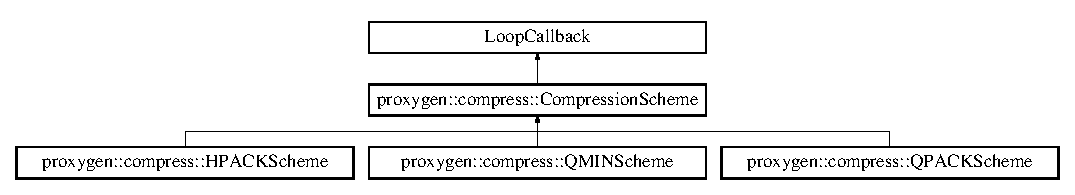
\includegraphics[height=2.178988cm]{classproxygen_1_1compress_1_1CompressionScheme}
\end{center}
\end{figure}
\subsection*{Classes}
\begin{DoxyCompactItemize}
\item 
struct {\bf Ack}
\end{DoxyCompactItemize}
\subsection*{Public Types}
\begin{DoxyCompactItemize}
\item 
using {\bf Block\+Info} = std\+::tuple$<$ {\bf Frame\+Flags}, bool, std\+::unique\+\_\+ptr$<$ folly\+::\+I\+O\+Buf $>$, {\bf Sim\+Streaming\+Callback} $\ast$ $>$
\end{DoxyCompactItemize}
\subsection*{Public Member Functions}
\begin{DoxyCompactItemize}
\item 
{\bf Compression\+Scheme} ({\bf Compression\+Simulator} $\ast$sim)
\item 
virtual {\bf $\sim$\+Compression\+Scheme} ()
\item 
virtual std\+::unique\+\_\+ptr$<$ {\bf Ack} $>$ {\bf get\+Ack} (uint16\+\_\+t seqn)=0
\item 
virtual void {\bf recv\+Ack} (std\+::unique\+\_\+ptr$<$ {\bf Ack} $>$)=0
\item 
virtual std\+::pair$<$ {\bf Frame\+Flags}, std\+::unique\+\_\+ptr$<$ folly\+::\+I\+O\+Buf $>$ $>$ {\bf encode} (bool new\+Packet, std\+::vector$<$ {\bf compress\+::\+Header} $>$ all\+Headers, {\bf Sim\+Stats} \&stats)=0
\item 
virtual void {\bf decode} ({\bf Frame\+Flags} {\bf flags}, std\+::unique\+\_\+ptr$<$ folly\+::\+I\+O\+Buf $>$ encoded\+Req, {\bf Sim\+Stats} \&stats, {\bf Sim\+Streaming\+Callback} \&cb)=0
\item 
virtual uint32\+\_\+t {\bf get\+Hol\+Block\+Count} () const =0
\item 
void {\bf run\+Loop\+Callback} () noexceptoverride
\end{DoxyCompactItemize}
\subsection*{Public Attributes}
\begin{DoxyCompactItemize}
\item 
std\+::list$<$ {\bf Block\+Info} $>$ {\bf encoded\+Blocks}
\item 
std\+::list$<$ {\bf Block\+Info} $>$ {\bf packet\+Blocks}
\item 
size\+\_\+t {\bf index} \{0\}
\item 
std\+::chrono\+::milliseconds {\bf prev}
\item 
size\+\_\+t {\bf packet\+Bytes} \{0\}
\item 
std\+::chrono\+::milliseconds {\bf decode\+Delay}
\item 
std\+::list$<$ uint16\+\_\+t $>$ {\bf packet\+Indices}
\end{DoxyCompactItemize}
\subsection*{Private Attributes}
\begin{DoxyCompactItemize}
\item 
{\bf Compression\+Simulator} $\ast$ {\bf simulator\+\_\+}
\end{DoxyCompactItemize}


\subsection{Detailed Description}


Definition at line 20 of file Compression\+Scheme.\+h.



\subsection{Member Typedef Documentation}
\index{proxygen\+::compress\+::\+Compression\+Scheme@{proxygen\+::compress\+::\+Compression\+Scheme}!Block\+Info@{Block\+Info}}
\index{Block\+Info@{Block\+Info}!proxygen\+::compress\+::\+Compression\+Scheme@{proxygen\+::compress\+::\+Compression\+Scheme}}
\subsubsection[{Block\+Info}]{\setlength{\rightskip}{0pt plus 5cm}using {\bf proxygen\+::compress\+::\+Compression\+Scheme\+::\+Block\+Info} =  std\+::tuple$<${\bf Frame\+Flags}, bool , std\+::unique\+\_\+ptr$<$folly\+::\+I\+O\+Buf$>$, {\bf Sim\+Streaming\+Callback}$\ast$$>$}\label{classproxygen_1_1compress_1_1CompressionScheme_ada50eb60ed8ed86791a59ef612fe1d69}


Definition at line 67 of file Compression\+Scheme.\+h.



\subsection{Constructor \& Destructor Documentation}
\index{proxygen\+::compress\+::\+Compression\+Scheme@{proxygen\+::compress\+::\+Compression\+Scheme}!Compression\+Scheme@{Compression\+Scheme}}
\index{Compression\+Scheme@{Compression\+Scheme}!proxygen\+::compress\+::\+Compression\+Scheme@{proxygen\+::compress\+::\+Compression\+Scheme}}
\subsubsection[{Compression\+Scheme(\+Compression\+Simulator $\ast$sim)}]{\setlength{\rightskip}{0pt plus 5cm}proxygen\+::compress\+::\+Compression\+Scheme\+::\+Compression\+Scheme (
\begin{DoxyParamCaption}
\item[{{\bf Compression\+Simulator} $\ast$}]{sim}
\end{DoxyParamCaption}
)\hspace{0.3cm}{\ttfamily [inline]}, {\ttfamily [explicit]}}\label{classproxygen_1_1compress_1_1CompressionScheme_a0e1dd7b22be68e2f4a87c59457658c54}


Definition at line 22 of file Compression\+Scheme.\+h.


\begin{DoxyCode}
22                                                         : simulator_(sim) \{
23   \}
\end{DoxyCode}
\index{proxygen\+::compress\+::\+Compression\+Scheme@{proxygen\+::compress\+::\+Compression\+Scheme}!````~Compression\+Scheme@{$\sim$\+Compression\+Scheme}}
\index{````~Compression\+Scheme@{$\sim$\+Compression\+Scheme}!proxygen\+::compress\+::\+Compression\+Scheme@{proxygen\+::compress\+::\+Compression\+Scheme}}
\subsubsection[{$\sim$\+Compression\+Scheme()}]{\setlength{\rightskip}{0pt plus 5cm}virtual proxygen\+::compress\+::\+Compression\+Scheme\+::$\sim$\+Compression\+Scheme (
\begin{DoxyParamCaption}
{}
\end{DoxyParamCaption}
)\hspace{0.3cm}{\ttfamily [inline]}, {\ttfamily [virtual]}}\label{classproxygen_1_1compress_1_1CompressionScheme_aa452b315f598d9f0034bbd9a23f6c366}


Definition at line 24 of file Compression\+Scheme.\+h.


\begin{DoxyCode}
24                                \{
25   \}
\end{DoxyCode}


\subsection{Member Function Documentation}
\index{proxygen\+::compress\+::\+Compression\+Scheme@{proxygen\+::compress\+::\+Compression\+Scheme}!decode@{decode}}
\index{decode@{decode}!proxygen\+::compress\+::\+Compression\+Scheme@{proxygen\+::compress\+::\+Compression\+Scheme}}
\subsubsection[{decode(\+Frame\+Flags flags, std\+::unique\+\_\+ptr$<$ folly\+::\+I\+O\+Buf $>$ encoded\+Req, Sim\+Stats \&stats, Sim\+Streaming\+Callback \&cb)=0}]{\setlength{\rightskip}{0pt plus 5cm}virtual void proxygen\+::compress\+::\+Compression\+Scheme\+::decode (
\begin{DoxyParamCaption}
\item[{{\bf Frame\+Flags}}]{flags, }
\item[{std\+::unique\+\_\+ptr$<$ folly\+::\+I\+O\+Buf $>$}]{encoded\+Req, }
\item[{{\bf Sim\+Stats} \&}]{stats, }
\item[{{\bf Sim\+Streaming\+Callback} \&}]{cb}
\end{DoxyParamCaption}
)\hspace{0.3cm}{\ttfamily [pure virtual]}}\label{classproxygen_1_1compress_1_1CompressionScheme_ac5ddabc82889df4797e1e869dc32e4e2}


Implemented in {\bf proxygen\+::compress\+::\+Q\+M\+I\+N\+Scheme} \doxyref{}{p.}{classproxygen_1_1compress_1_1QMINScheme_a427f948be8edc3c3fbd784e1e4e36c7a}, {\bf proxygen\+::compress\+::\+Q\+P\+A\+C\+K\+Scheme} \doxyref{}{p.}{classproxygen_1_1compress_1_1QPACKScheme_aaf6b32a5a4350a4f03dda162da4dc188}, and {\bf proxygen\+::compress\+::\+H\+P\+A\+C\+K\+Scheme} \doxyref{}{p.}{classproxygen_1_1compress_1_1HPACKScheme_a7180bb82bbc7fd4119aad297344306ce}.



Referenced by proxygen\+::compress\+::\+Compression\+Simulator\+::decode(), and proxygen\+::compress\+::\+Compression\+Scheme\+::\+Ack\+::$\sim$\+Ack().

\index{proxygen\+::compress\+::\+Compression\+Scheme@{proxygen\+::compress\+::\+Compression\+Scheme}!encode@{encode}}
\index{encode@{encode}!proxygen\+::compress\+::\+Compression\+Scheme@{proxygen\+::compress\+::\+Compression\+Scheme}}
\subsubsection[{encode(bool new\+Packet, std\+::vector$<$ compress\+::\+Header $>$ all\+Headers, Sim\+Stats \&stats)=0}]{\setlength{\rightskip}{0pt plus 5cm}virtual std\+::pair$<${\bf Frame\+Flags}, std\+::unique\+\_\+ptr$<$folly\+::\+I\+O\+Buf$>$ $>$ proxygen\+::compress\+::\+Compression\+Scheme\+::encode (
\begin{DoxyParamCaption}
\item[{bool}]{new\+Packet, }
\item[{std\+::vector$<$ {\bf compress\+::\+Header} $>$}]{all\+Headers, }
\item[{{\bf Sim\+Stats} \&}]{stats}
\end{DoxyParamCaption}
)\hspace{0.3cm}{\ttfamily [pure virtual]}}\label{classproxygen_1_1compress_1_1CompressionScheme_a4e013945112c438374a2cb99eb753d67}


Implemented in {\bf proxygen\+::compress\+::\+Q\+M\+I\+N\+Scheme} \doxyref{}{p.}{classproxygen_1_1compress_1_1QMINScheme_a389ec2fa53acd698ef9648408a163e90}, {\bf proxygen\+::compress\+::\+Q\+P\+A\+C\+K\+Scheme} \doxyref{}{p.}{classproxygen_1_1compress_1_1QPACKScheme_a2e7fe9421b392a72672b44922494a1e5}, and {\bf proxygen\+::compress\+::\+H\+P\+A\+C\+K\+Scheme} \doxyref{}{p.}{classproxygen_1_1compress_1_1HPACKScheme_aafa09cb0b8847355ebb099ffc44e794f}.



Referenced by proxygen\+::compress\+::\+Compression\+Simulator\+::encode(), and proxygen\+::compress\+::\+Compression\+Scheme\+::\+Ack\+::$\sim$\+Ack().

\index{proxygen\+::compress\+::\+Compression\+Scheme@{proxygen\+::compress\+::\+Compression\+Scheme}!get\+Ack@{get\+Ack}}
\index{get\+Ack@{get\+Ack}!proxygen\+::compress\+::\+Compression\+Scheme@{proxygen\+::compress\+::\+Compression\+Scheme}}
\subsubsection[{get\+Ack(uint16\+\_\+t seqn)=0}]{\setlength{\rightskip}{0pt plus 5cm}virtual std\+::unique\+\_\+ptr$<${\bf Ack}$>$ proxygen\+::compress\+::\+Compression\+Scheme\+::get\+Ack (
\begin{DoxyParamCaption}
\item[{uint16\+\_\+t}]{seqn}
\end{DoxyParamCaption}
)\hspace{0.3cm}{\ttfamily [pure virtual]}}\label{classproxygen_1_1compress_1_1CompressionScheme_af8a906f3f6600f903a3f8249478f9ea6}


Implemented in {\bf proxygen\+::compress\+::\+Q\+M\+I\+N\+Scheme} \doxyref{}{p.}{classproxygen_1_1compress_1_1QMINScheme_ac06a5811f950530ea4ea011cfeb45985}, {\bf proxygen\+::compress\+::\+Q\+P\+A\+C\+K\+Scheme} \doxyref{}{p.}{classproxygen_1_1compress_1_1QPACKScheme_afb944df19670c2872f1ba870b101695a}, and {\bf proxygen\+::compress\+::\+H\+P\+A\+C\+K\+Scheme} \doxyref{}{p.}{classproxygen_1_1compress_1_1HPACKScheme_a82816e8390863439eca18e01ff65c7b5}.



Referenced by proxygen\+::compress\+::\+Compression\+Scheme\+::\+Ack\+::$\sim$\+Ack().

\index{proxygen\+::compress\+::\+Compression\+Scheme@{proxygen\+::compress\+::\+Compression\+Scheme}!get\+Hol\+Block\+Count@{get\+Hol\+Block\+Count}}
\index{get\+Hol\+Block\+Count@{get\+Hol\+Block\+Count}!proxygen\+::compress\+::\+Compression\+Scheme@{proxygen\+::compress\+::\+Compression\+Scheme}}
\subsubsection[{get\+Hol\+Block\+Count() const =0}]{\setlength{\rightskip}{0pt plus 5cm}virtual uint32\+\_\+t proxygen\+::compress\+::\+Compression\+Scheme\+::get\+Hol\+Block\+Count (
\begin{DoxyParamCaption}
{}
\end{DoxyParamCaption}
) const\hspace{0.3cm}{\ttfamily [pure virtual]}}\label{classproxygen_1_1compress_1_1CompressionScheme_a08043930336620a278f3763256384a38}


Implemented in {\bf proxygen\+::compress\+::\+Q\+M\+I\+N\+Scheme} \doxyref{}{p.}{classproxygen_1_1compress_1_1QMINScheme_a9746dc6ffa6552250e6eadd2dda71742}, {\bf proxygen\+::compress\+::\+Q\+P\+A\+C\+K\+Scheme} \doxyref{}{p.}{classproxygen_1_1compress_1_1QPACKScheme_a03b7c3817a7c4f36759b57890f3681bb}, and {\bf proxygen\+::compress\+::\+H\+P\+A\+C\+K\+Scheme} \doxyref{}{p.}{classproxygen_1_1compress_1_1HPACKScheme_a7f72f561fdb655de2a57437fc961a33d}.



Referenced by proxygen\+::compress\+::\+Compression\+Scheme\+::\+Ack\+::$\sim$\+Ack().

\index{proxygen\+::compress\+::\+Compression\+Scheme@{proxygen\+::compress\+::\+Compression\+Scheme}!recv\+Ack@{recv\+Ack}}
\index{recv\+Ack@{recv\+Ack}!proxygen\+::compress\+::\+Compression\+Scheme@{proxygen\+::compress\+::\+Compression\+Scheme}}
\subsubsection[{recv\+Ack(std\+::unique\+\_\+ptr$<$ Ack $>$)=0}]{\setlength{\rightskip}{0pt plus 5cm}virtual void proxygen\+::compress\+::\+Compression\+Scheme\+::recv\+Ack (
\begin{DoxyParamCaption}
\item[{std\+::unique\+\_\+ptr$<$ {\bf Ack} $>$}]{}
\end{DoxyParamCaption}
)\hspace{0.3cm}{\ttfamily [pure virtual]}}\label{classproxygen_1_1compress_1_1CompressionScheme_a8b5b9dbfd8f08e0dfdc6415e7432ddbf}


Implemented in {\bf proxygen\+::compress\+::\+Q\+M\+I\+N\+Scheme} \doxyref{}{p.}{classproxygen_1_1compress_1_1QMINScheme_afbc48109af89a406c0e4108a3b897aa3}, {\bf proxygen\+::compress\+::\+Q\+P\+A\+C\+K\+Scheme} \doxyref{}{p.}{classproxygen_1_1compress_1_1QPACKScheme_a11bfbfc191956116934fa2c36ebe3411}, and {\bf proxygen\+::compress\+::\+H\+P\+A\+C\+K\+Scheme} \doxyref{}{p.}{classproxygen_1_1compress_1_1HPACKScheme_a80a8a4f5c57f4aa3436a4d1eede0f90a}.



Referenced by proxygen\+::compress\+::\+Compression\+Simulator\+::recv\+Ack(), and proxygen\+::compress\+::\+Compression\+Scheme\+::\+Ack\+::$\sim$\+Ack().

\index{proxygen\+::compress\+::\+Compression\+Scheme@{proxygen\+::compress\+::\+Compression\+Scheme}!run\+Loop\+Callback@{run\+Loop\+Callback}}
\index{run\+Loop\+Callback@{run\+Loop\+Callback}!proxygen\+::compress\+::\+Compression\+Scheme@{proxygen\+::compress\+::\+Compression\+Scheme}}
\subsubsection[{run\+Loop\+Callback() noexceptoverride}]{\setlength{\rightskip}{0pt plus 5cm}void proxygen\+::compress\+::\+Compression\+Scheme\+::run\+Loop\+Callback (
\begin{DoxyParamCaption}
{}
\end{DoxyParamCaption}
)\hspace{0.3cm}{\ttfamily [override]}, {\ttfamily [noexcept]}}\label{classproxygen_1_1compress_1_1CompressionScheme_ab3f9a79c53cc1e5bea7a1ebc6fd47e6b}


Definition at line 182 of file Compression\+Simulator.\+cpp.



Referenced by proxygen\+::compress\+::\+Compression\+Scheme\+::\+Ack\+::$\sim$\+Ack().


\begin{DoxyCode}
182                                                  \{
183   simulator_->flushSchemePackets(\textcolor{keyword}{this});
184 \}
\end{DoxyCode}


\subsection{Member Data Documentation}
\index{proxygen\+::compress\+::\+Compression\+Scheme@{proxygen\+::compress\+::\+Compression\+Scheme}!decode\+Delay@{decode\+Delay}}
\index{decode\+Delay@{decode\+Delay}!proxygen\+::compress\+::\+Compression\+Scheme@{proxygen\+::compress\+::\+Compression\+Scheme}}
\subsubsection[{decode\+Delay}]{\setlength{\rightskip}{0pt plus 5cm}std\+::chrono\+::milliseconds proxygen\+::compress\+::\+Compression\+Scheme\+::decode\+Delay}\label{classproxygen_1_1compress_1_1CompressionScheme_a7941a48e560dae88e07d62943dc4da7a}


Definition at line 79 of file Compression\+Scheme.\+h.



Referenced by proxygen\+::compress\+::\+Compression\+Simulator\+::flush\+Packet(), and proxygen\+::compress\+::\+Compression\+Simulator\+::flush\+Scheme\+Packets().

\index{proxygen\+::compress\+::\+Compression\+Scheme@{proxygen\+::compress\+::\+Compression\+Scheme}!encoded\+Blocks@{encoded\+Blocks}}
\index{encoded\+Blocks@{encoded\+Blocks}!proxygen\+::compress\+::\+Compression\+Scheme@{proxygen\+::compress\+::\+Compression\+Scheme}}
\subsubsection[{encoded\+Blocks}]{\setlength{\rightskip}{0pt plus 5cm}std\+::list$<${\bf Block\+Info}$>$ proxygen\+::compress\+::\+Compression\+Scheme\+::encoded\+Blocks}\label{classproxygen_1_1compress_1_1CompressionScheme_ab9712b0de439245609196d02570ae20e}


Definition at line 68 of file Compression\+Scheme.\+h.



Referenced by proxygen\+::compress\+::\+Compression\+Simulator\+::flush\+Scheme\+Packets().

\index{proxygen\+::compress\+::\+Compression\+Scheme@{proxygen\+::compress\+::\+Compression\+Scheme}!index@{index}}
\index{index@{index}!proxygen\+::compress\+::\+Compression\+Scheme@{proxygen\+::compress\+::\+Compression\+Scheme}}
\subsubsection[{index}]{\setlength{\rightskip}{0pt plus 5cm}size\+\_\+t proxygen\+::compress\+::\+Compression\+Scheme\+::index \{0\}}\label{classproxygen_1_1compress_1_1CompressionScheme_a0c89d36849efe3c35d49228833ad2bfd}


Definition at line 73 of file Compression\+Scheme.\+h.



Referenced by proxygen\+::compress\+::\+H\+P\+A\+C\+K\+Scheme\+::encode(), and proxygen\+::compress\+::\+Q\+P\+A\+C\+K\+Scheme\+::encode().

\index{proxygen\+::compress\+::\+Compression\+Scheme@{proxygen\+::compress\+::\+Compression\+Scheme}!packet\+Blocks@{packet\+Blocks}}
\index{packet\+Blocks@{packet\+Blocks}!proxygen\+::compress\+::\+Compression\+Scheme@{proxygen\+::compress\+::\+Compression\+Scheme}}
\subsubsection[{packet\+Blocks}]{\setlength{\rightskip}{0pt plus 5cm}std\+::list$<${\bf Block\+Info}$>$ proxygen\+::compress\+::\+Compression\+Scheme\+::packet\+Blocks}\label{classproxygen_1_1compress_1_1CompressionScheme_af6fb1e0f08c33671a116f4fe85d4ebe1}


Definition at line 70 of file Compression\+Scheme.\+h.



Referenced by proxygen\+::compress\+::\+Compression\+Simulator\+::flush\+Packet(), and proxygen\+::compress\+::\+Compression\+Simulator\+::flush\+Scheme\+Packets().

\index{proxygen\+::compress\+::\+Compression\+Scheme@{proxygen\+::compress\+::\+Compression\+Scheme}!packet\+Bytes@{packet\+Bytes}}
\index{packet\+Bytes@{packet\+Bytes}!proxygen\+::compress\+::\+Compression\+Scheme@{proxygen\+::compress\+::\+Compression\+Scheme}}
\subsubsection[{packet\+Bytes}]{\setlength{\rightskip}{0pt plus 5cm}size\+\_\+t proxygen\+::compress\+::\+Compression\+Scheme\+::packet\+Bytes \{0\}}\label{classproxygen_1_1compress_1_1CompressionScheme_a4f71fa1ca3db61ad6b7aa4a078bb8b76}


Definition at line 78 of file Compression\+Scheme.\+h.



Referenced by proxygen\+::compress\+::\+Compression\+Simulator\+::flush\+Packet(), and proxygen\+::compress\+::\+Compression\+Simulator\+::flush\+Scheme\+Packets().

\index{proxygen\+::compress\+::\+Compression\+Scheme@{proxygen\+::compress\+::\+Compression\+Scheme}!packet\+Indices@{packet\+Indices}}
\index{packet\+Indices@{packet\+Indices}!proxygen\+::compress\+::\+Compression\+Scheme@{proxygen\+::compress\+::\+Compression\+Scheme}}
\subsubsection[{packet\+Indices}]{\setlength{\rightskip}{0pt plus 5cm}std\+::list$<$uint16\+\_\+t$>$ proxygen\+::compress\+::\+Compression\+Scheme\+::packet\+Indices}\label{classproxygen_1_1compress_1_1CompressionScheme_a625e785dd8c5fa8aa84d686739d604ec}


Definition at line 81 of file Compression\+Scheme.\+h.



Referenced by proxygen\+::compress\+::\+Compression\+Simulator\+::flush\+Requests().

\index{proxygen\+::compress\+::\+Compression\+Scheme@{proxygen\+::compress\+::\+Compression\+Scheme}!prev@{prev}}
\index{prev@{prev}!proxygen\+::compress\+::\+Compression\+Scheme@{proxygen\+::compress\+::\+Compression\+Scheme}}
\subsubsection[{prev}]{\setlength{\rightskip}{0pt plus 5cm}std\+::chrono\+::milliseconds proxygen\+::compress\+::\+Compression\+Scheme\+::prev}\label{classproxygen_1_1compress_1_1CompressionScheme_a2a356966d15ef97cdda9c121985f84dd}


Definition at line 76 of file Compression\+Scheme.\+h.



Referenced by proxygen\+::compress\+::\+Compression\+Simulator\+::flush\+Requests().

\index{proxygen\+::compress\+::\+Compression\+Scheme@{proxygen\+::compress\+::\+Compression\+Scheme}!simulator\+\_\+@{simulator\+\_\+}}
\index{simulator\+\_\+@{simulator\+\_\+}!proxygen\+::compress\+::\+Compression\+Scheme@{proxygen\+::compress\+::\+Compression\+Scheme}}
\subsubsection[{simulator\+\_\+}]{\setlength{\rightskip}{0pt plus 5cm}{\bf Compression\+Simulator}$\ast$ proxygen\+::compress\+::\+Compression\+Scheme\+::simulator\+\_\+\hspace{0.3cm}{\ttfamily [private]}}\label{classproxygen_1_1compress_1_1CompressionScheme_afc135889510fde0065e5f96ddf293c5d}


Definition at line 84 of file Compression\+Scheme.\+h.



The documentation for this class was generated from the following files\+:\begin{DoxyCompactItemize}
\item 
proxygen/lib/http/codec/compress/experimental/simulator/{\bf Compression\+Scheme.\+h}\item 
proxygen/lib/http/codec/compress/experimental/simulator/{\bf Compression\+Simulator.\+cpp}\end{DoxyCompactItemize}

\section{proxygen\+:\+:compress\+:\+:Compression\+Simulator Class Reference}
\label{classproxygen_1_1compress_1_1CompressionSimulator}\index{proxygen\+::compress\+::\+Compression\+Simulator@{proxygen\+::compress\+::\+Compression\+Simulator}}


{\ttfamily \#include $<$Compression\+Simulator.\+h$>$}

\subsection*{Public Member Functions}
\begin{DoxyCompactItemize}
\item 
{\bf Compression\+Simulator} ({\bf Sim\+Params} p)
\item 
bool {\bf read\+Input\+From\+File\+And\+Schedule} (const std\+::string \&filename)
\item 
void {\bf run} ()
\item 
void {\bf flush\+Scheme\+Packets} ({\bf Compression\+Scheme} $\ast$scheme)
\item 
void {\bf flush\+Packet} ({\bf Compression\+Scheme} $\ast$scheme)
\end{DoxyCompactItemize}
\subsection*{Private Member Functions}
\begin{DoxyCompactItemize}
\item 
void {\bf flush\+Requests} ({\bf Compression\+Scheme} $\ast$scheme)
\item 
void {\bf setup\+Request} (uint16\+\_\+t seqn, {\bf H\+T\+T\+P\+Message} \&\&msg, std\+::chrono\+::milliseconds encode\+Delay)
\item 
{\bf Compression\+Scheme} $\ast$ {\bf get\+Scheme} (folly\+::\+String\+Piece host)
\item 
std\+::unique\+\_\+ptr$<$ {\bf Compression\+Scheme} $>$ {\bf make\+Scheme} ()
\item 
std\+::pair$<$ {\bf Frame\+Flags}, std\+::unique\+\_\+ptr$<$ folly\+::\+I\+O\+Buf $>$ $>$ {\bf encode} ({\bf Compression\+Scheme} $\ast$scheme, bool new\+Packet, uint16\+\_\+t seqn)
\item 
void {\bf decode\+Packet} ({\bf Compression\+Scheme} $\ast$scheme, std\+::list$<$ {\bf Compression\+Scheme\+::\+Block\+Info} $>$ \&blocks)
\item 
void {\bf decode} ({\bf Compression\+Scheme} $\ast$scheme, {\bf Frame\+Flags} {\bf flags}, std\+::unique\+\_\+ptr$<$ folly\+::\+I\+O\+Buf $>$ encoded\+Req, {\bf Sim\+Streaming\+Callback} \&cb)
\item 
void {\bf schedule\+Event} (folly\+::\+Function$<$ void()$>$ f, std\+::chrono\+::milliseconds ms)
\item 
void {\bf send\+Ack} ({\bf Compression\+Scheme} $\ast$scheme, std\+::unique\+\_\+ptr$<$ {\bf Compression\+Scheme\+::\+Ack} $>$ ack)
\item 
void {\bf recv\+Ack} ({\bf Compression\+Scheme} $\ast$scheme, std\+::unique\+\_\+ptr$<$ {\bf Compression\+Scheme\+::\+Ack} $>$ ack)
\item 
std\+::chrono\+::milliseconds {\bf delivery\+Delay} ()
\item 
std\+::chrono\+::milliseconds {\bf rtt} ()
\item 
std\+::chrono\+::milliseconds {\bf one\+\_\+half\+\_\+rtt} ()
\item 
std\+::chrono\+::milliseconds {\bf rxmit\+Delay} ()
\item 
bool {\bf loss} ()
\item 
bool {\bf delayed} ()
\item 
std\+::chrono\+::milliseconds {\bf extra\+Delay} ()
\item 
uint32\+\_\+t {\bf min\+O\+O\+O\+Thresh} ()
\end{DoxyCompactItemize}
\subsection*{Private Attributes}
\begin{DoxyCompactItemize}
\item 
{\bf Sim\+Params} {\bf params\+\_\+}
\item 
std\+::vector$<$ {\bf proxygen\+::\+H\+T\+T\+P\+Message} $>$ {\bf requests\+\_\+}
\item 
folly\+::\+Event\+Base {\bf event\+Base\+\_\+}
\item 
std\+::unordered\+\_\+map$<$ std\+::string, std\+::unique\+\_\+ptr$<$ {\bf Compression\+Scheme} $>$ $>$ {\bf domains\+\_\+}
\item 
std\+::vector$<$ {\bf Sim\+Streaming\+Callback} $>$ {\bf callbacks\+\_\+}
\item 
folly\+::\+Random\+::\+Default\+Generator {\bf rng\+\_\+}
\item 
{\bf Sim\+Stats} {\bf stats\+\_\+}
\end{DoxyCompactItemize}


\subsection{Detailed Description}


Definition at line 23 of file Compression\+Simulator.\+h.



\subsection{Constructor \& Destructor Documentation}
\index{proxygen\+::compress\+::\+Compression\+Simulator@{proxygen\+::compress\+::\+Compression\+Simulator}!Compression\+Simulator@{Compression\+Simulator}}
\index{Compression\+Simulator@{Compression\+Simulator}!proxygen\+::compress\+::\+Compression\+Simulator@{proxygen\+::compress\+::\+Compression\+Simulator}}
\subsubsection[{Compression\+Simulator(\+Sim\+Params p)}]{\setlength{\rightskip}{0pt plus 5cm}proxygen\+::compress\+::\+Compression\+Simulator\+::\+Compression\+Simulator (
\begin{DoxyParamCaption}
\item[{{\bf Sim\+Params}}]{p}
\end{DoxyParamCaption}
)\hspace{0.3cm}{\ttfamily [inline]}, {\ttfamily [explicit]}}\label{classproxygen_1_1compress_1_1CompressionSimulator_a18003fe5998e7271d2c818bec436ee52}


Definition at line 25 of file Compression\+Simulator.\+h.



References decode(), decode\+Packet(), delayed(), delivery\+Delay(), encode(), extra\+Delay(), flush\+Packet(), flush\+Requests(), flush\+Scheme\+Packets(), get\+Scheme(), loss(), make\+Scheme(), min\+O\+O\+O\+Thresh(), one\+\_\+half\+\_\+rtt(), read\+Input\+From\+File\+And\+Schedule(), recv\+Ack(), rtt(), run(), rxmit\+Delay(), schedule\+Event(), send\+Ack(), and setup\+Request().


\begin{DoxyCode}
25                                              : params_(p) \{
26   \}
\end{DoxyCode}


\subsection{Member Function Documentation}
\index{proxygen\+::compress\+::\+Compression\+Simulator@{proxygen\+::compress\+::\+Compression\+Simulator}!decode@{decode}}
\index{decode@{decode}!proxygen\+::compress\+::\+Compression\+Simulator@{proxygen\+::compress\+::\+Compression\+Simulator}}
\subsubsection[{decode(\+Compression\+Scheme $\ast$scheme, Frame\+Flags flags, std\+::unique\+\_\+ptr$<$ folly\+::\+I\+O\+Buf $>$ encoded\+Req, Sim\+Streaming\+Callback \&cb)}]{\setlength{\rightskip}{0pt plus 5cm}void proxygen\+::compress\+::\+Compression\+Simulator\+::decode (
\begin{DoxyParamCaption}
\item[{{\bf Compression\+Scheme} $\ast$}]{scheme, }
\item[{{\bf Frame\+Flags}}]{flags, }
\item[{std\+::unique\+\_\+ptr$<$ folly\+::\+I\+O\+Buf $>$}]{encoded\+Req, }
\item[{{\bf Sim\+Streaming\+Callback} \&}]{cb}
\end{DoxyParamCaption}
)\hspace{0.3cm}{\ttfamily [private]}}\label{classproxygen_1_1compress_1_1CompressionSimulator_ae82cb6f93c12771defb01fe392d12639}


Definition at line 306 of file Compression\+Simulator.\+cpp.



References proxygen\+::compress\+::\+Compression\+Scheme\+::decode().



Referenced by Compression\+Simulator().


\begin{DoxyCode}
309                                                             \{
310   scheme->decode(flags, std::move(encodedReq), stats_, cb);
311 \}
\end{DoxyCode}
\index{proxygen\+::compress\+::\+Compression\+Simulator@{proxygen\+::compress\+::\+Compression\+Simulator}!decode\+Packet@{decode\+Packet}}
\index{decode\+Packet@{decode\+Packet}!proxygen\+::compress\+::\+Compression\+Simulator@{proxygen\+::compress\+::\+Compression\+Simulator}}
\subsubsection[{decode\+Packet(\+Compression\+Scheme $\ast$scheme, std\+::list$<$ Compression\+Scheme\+::\+Block\+Info $>$ \&blocks)}]{\setlength{\rightskip}{0pt plus 5cm}void proxygen\+::compress\+::\+Compression\+Simulator\+::decode\+Packet (
\begin{DoxyParamCaption}
\item[{{\bf Compression\+Scheme} $\ast$}]{scheme, }
\item[{std\+::list$<$ {\bf Compression\+Scheme\+::\+Block\+Info} $>$ \&}]{blocks}
\end{DoxyParamCaption}
)\hspace{0.3cm}{\ttfamily [private]}}\label{classproxygen_1_1compress_1_1CompressionSimulator_a38bef8da0daefefa016062dfc5374f11}


Definition at line 313 of file Compression\+Simulator.\+cpp.



References proxygen\+::hpack\+::decode().



Referenced by Compression\+Simulator().


\begin{DoxyCode}
315                                                  \{
316   VLOG(1) << \textcolor{stringliteral}{"decode packet with "} << blocks.size() << \textcolor{stringliteral}{" blocks"};
317   \textcolor{keywordflow}{while} (!blocks.empty()) \{
318     \textcolor{keyword}{auto} encodeRes = &blocks.front();
319     \textcolor{comment}{// TODO(ckrasic) - to get packet coordination correct, could plumb}
320     \textcolor{comment}{// through "start of packet" flag here.  Probably not worth it,}
321     \textcolor{comment}{// since it seems to make only a very small difference (about a}
322     \textcolor{comment}{// 0.1% compressiondifference on my facebook har).}
323     decode(scheme,
324            std::get<0>(*encodeRes),
325            std::move(std::get<2>(*encodeRes)),
326            *std::get<3>(*encodeRes));
327     blocks.pop\_front();
328   \}
329 \}
\end{DoxyCode}
\index{proxygen\+::compress\+::\+Compression\+Simulator@{proxygen\+::compress\+::\+Compression\+Simulator}!delayed@{delayed}}
\index{delayed@{delayed}!proxygen\+::compress\+::\+Compression\+Simulator@{proxygen\+::compress\+::\+Compression\+Simulator}}
\subsubsection[{delayed()}]{\setlength{\rightskip}{0pt plus 5cm}bool proxygen\+::compress\+::\+Compression\+Simulator\+::delayed (
\begin{DoxyParamCaption}
{}
\end{DoxyParamCaption}
)\hspace{0.3cm}{\ttfamily [private]}}\label{classproxygen_1_1compress_1_1CompressionSimulator_a1946a350f39d75b58da56fcf21080b08}


Definition at line 392 of file Compression\+Simulator.\+cpp.



Referenced by Compression\+Simulator().


\begin{DoxyCode}
392                                    \{
393   \textcolor{keywordflow}{return} Random::randDouble01(rng_) < params_.delayProbability;
394 \}
\end{DoxyCode}
\index{proxygen\+::compress\+::\+Compression\+Simulator@{proxygen\+::compress\+::\+Compression\+Simulator}!delivery\+Delay@{delivery\+Delay}}
\index{delivery\+Delay@{delivery\+Delay}!proxygen\+::compress\+::\+Compression\+Simulator@{proxygen\+::compress\+::\+Compression\+Simulator}}
\subsubsection[{delivery\+Delay()}]{\setlength{\rightskip}{0pt plus 5cm}std\+::chrono\+::milliseconds proxygen\+::compress\+::\+Compression\+Simulator\+::delivery\+Delay (
\begin{DoxyParamCaption}
{}
\end{DoxyParamCaption}
)\hspace{0.3cm}{\ttfamily [private]}}\label{classproxygen_1_1compress_1_1CompressionSimulator_af0d6d728f67553cdfa0149c7bc7e634f}


Definition at line 354 of file Compression\+Simulator.\+cpp.



Referenced by Compression\+Simulator().


\begin{DoxyCode}
354                                                           \{
355   std::chrono::milliseconds delay = one_half_rtt();
356   \textcolor{keywordflow}{while} (loss()) \{
357     stats_.packetLosses++;
358     scheduleEvent([] \{ VLOG(4) << \textcolor{stringliteral}{"Packet lost!"}; \}, delay);
359     std::chrono::milliseconds rxmit = rxmitDelay();
360     delay += rxmit;
361     scheduleEvent(
362         [rxmit] \{
363           VLOG(4) << \textcolor{stringliteral}{"Packet loss detected, retransmitting with additional "}
364                   << rxmit.count();
365         \},
366         delay - one_half_rtt());
367   \}
368   \textcolor{keywordflow}{if} (delayed()) \{
369     scheduleEvent([] \{ VLOG(4) << \textcolor{stringliteral}{"Packet delayed in network"}; \}, delay);
370     delay += extraDelay();
371   \}
372   \textcolor{keywordflow}{return} delay;
373 \}
\end{DoxyCode}
\index{proxygen\+::compress\+::\+Compression\+Simulator@{proxygen\+::compress\+::\+Compression\+Simulator}!encode@{encode}}
\index{encode@{encode}!proxygen\+::compress\+::\+Compression\+Simulator@{proxygen\+::compress\+::\+Compression\+Simulator}}
\subsubsection[{encode(\+Compression\+Scheme $\ast$scheme, bool new\+Packet, uint16\+\_\+t seqn)}]{\setlength{\rightskip}{0pt plus 5cm}std\+::pair$<$ {\bf Frame\+Flags}, unique\+\_\+ptr$<$ I\+O\+Buf $>$ $>$ proxygen\+::compress\+::\+Compression\+Simulator\+::encode (
\begin{DoxyParamCaption}
\item[{{\bf Compression\+Scheme} $\ast$}]{scheme, }
\item[{bool}]{new\+Packet, }
\item[{uint16\+\_\+t}]{seqn}
\end{DoxyParamCaption}
)\hspace{0.3cm}{\ttfamily [private]}}\label{classproxygen_1_1compress_1_1CompressionSimulator_a566957fa4b7a925f5cae7660b4ed24b9}


Definition at line 286 of file Compression\+Simulator.\+cpp.



References proxygen\+::compress\+::\+Compression\+Scheme\+::encode(), and proxygen\+::compress\+::prepare\+Message\+For\+Compression().



Referenced by Compression\+Simulator().


\begin{DoxyCode}
287                                                                \{
288   VLOG(1) << \textcolor{stringliteral}{"Start encoding request="} << index;
289   \textcolor{comment}{// vector to hold cookie crumbs}
290   vector<string> cookies;
291   vector<compress::Header> allHeaders = prepareMessageForCompression(
292       requests_[index], cookies);
293 
294   \textcolor{keyword}{auto} before = stats_.uncompressed;
295   \textcolor{keyword}{auto} res = scheme->encode(newPacket, std::move(allHeaders), stats_);
296   VLOG(1) << \textcolor{stringliteral}{"Encoded request="} << index << \textcolor{stringliteral}{" for host="}
297           << requests_[index].getHeaders().getSingleOrEmpty(HTTP\_HEADER\_HOST)
298           << \textcolor{stringliteral}{" orig size="} << (stats_.uncompressed - before)
299           << \textcolor{stringliteral}{" block size="} << res.second->computeChainDataLength()
300           << \textcolor{stringliteral}{" cumulative bytes="} << stats_.compressed
301           << \textcolor{stringliteral}{" cumulative compression ratio="}
302           << int(100 - \textcolor{keywordtype}{double}(100 * stats_.compressed) / stats_.uncompressed);
303   \textcolor{keywordflow}{return} res;
304 \}
\end{DoxyCode}
\index{proxygen\+::compress\+::\+Compression\+Simulator@{proxygen\+::compress\+::\+Compression\+Simulator}!extra\+Delay@{extra\+Delay}}
\index{extra\+Delay@{extra\+Delay}!proxygen\+::compress\+::\+Compression\+Simulator@{proxygen\+::compress\+::\+Compression\+Simulator}}
\subsubsection[{extra\+Delay()}]{\setlength{\rightskip}{0pt plus 5cm}std\+::chrono\+::milliseconds proxygen\+::compress\+::\+Compression\+Simulator\+::extra\+Delay (
\begin{DoxyParamCaption}
{}
\end{DoxyParamCaption}
)\hspace{0.3cm}{\ttfamily [private]}}\label{classproxygen_1_1compress_1_1CompressionSimulator_a17527a82237c46d5d9968605cefe2aee}


Definition at line 396 of file Compression\+Simulator.\+cpp.



Referenced by Compression\+Simulator().


\begin{DoxyCode}
396                                                        \{
397   uint32\_t ms = params_.maxDelay.count() * Random::randDouble01(rng_);
398   \textcolor{keywordflow}{return} std::chrono::milliseconds(ms);
399 \}
\end{DoxyCode}
\index{proxygen\+::compress\+::\+Compression\+Simulator@{proxygen\+::compress\+::\+Compression\+Simulator}!flush\+Packet@{flush\+Packet}}
\index{flush\+Packet@{flush\+Packet}!proxygen\+::compress\+::\+Compression\+Simulator@{proxygen\+::compress\+::\+Compression\+Simulator}}
\subsubsection[{flush\+Packet(\+Compression\+Scheme $\ast$scheme)}]{\setlength{\rightskip}{0pt plus 5cm}void proxygen\+::compress\+::\+Compression\+Simulator\+::flush\+Packet (
\begin{DoxyParamCaption}
\item[{{\bf Compression\+Scheme} $\ast$}]{scheme}
\end{DoxyParamCaption}
)}\label{classproxygen_1_1compress_1_1CompressionSimulator_adbe2351c3837f1532bedee587d37d4b0}


Definition at line 186 of file Compression\+Simulator.\+cpp.



References proxygen\+::compress\+::\+Compression\+Scheme\+::decode\+Delay, proxygen\+::compress\+::\+Compression\+Scheme\+::packet\+Blocks, and proxygen\+::compress\+::\+Compression\+Scheme\+::packet\+Bytes.



Referenced by Compression\+Simulator().


\begin{DoxyCode}
186                                                                 \{
187   \textcolor{keywordflow}{if} (scheme->packetBlocks.empty()) \{
188     \textcolor{keywordflow}{return};
189   \}
190 
191   stats_.packets++;
192   VLOG(1) << \textcolor{stringliteral}{"schedule decode for "} << scheme->packetBlocks.size()
193           << \textcolor{stringliteral}{" blocks at "} << scheme->decodeDelay.count();
194   scheduleEvent(
195       \{[\textcolor{keyword}{this}, scheme, blocks = std::move(scheme->packetBlocks)]() \textcolor{keyword}{mutable} \{
196         decodePacket(scheme, blocks);
197       \}\},
198       scheme->decodeDelay);
199   scheme->packetBytes = 0;
200 \}
\end{DoxyCode}
\index{proxygen\+::compress\+::\+Compression\+Simulator@{proxygen\+::compress\+::\+Compression\+Simulator}!flush\+Requests@{flush\+Requests}}
\index{flush\+Requests@{flush\+Requests}!proxygen\+::compress\+::\+Compression\+Simulator@{proxygen\+::compress\+::\+Compression\+Simulator}}
\subsubsection[{flush\+Requests(\+Compression\+Scheme $\ast$scheme)}]{\setlength{\rightskip}{0pt plus 5cm}void proxygen\+::compress\+::\+Compression\+Simulator\+::flush\+Requests (
\begin{DoxyParamCaption}
\item[{{\bf Compression\+Scheme} $\ast$}]{scheme}
\end{DoxyParamCaption}
)\hspace{0.3cm}{\ttfamily [private]}}\label{classproxygen_1_1compress_1_1CompressionSimulator_ae5507a6cc20d0189a91a840c1e9650ea}


Definition at line 103 of file Compression\+Simulator.\+cpp.



References proxygen\+::compress\+::\+Compression\+Scheme\+::packet\+Indices, and proxygen\+::compress\+::\+Compression\+Scheme\+::prev.



Referenced by Compression\+Simulator().


\begin{DoxyCode}
103                                                                   \{
104   VLOG(5) << \textcolor{stringliteral}{"schedule encode for "} << scheme->packetIndices.size()
105           << \textcolor{stringliteral}{" blocks at "} << scheme->prev.count();
106   \textcolor{comment}{// Flush previous train}
107   scheduleEvent(
108       [\textcolor{keyword}{this}, scheme, indices = std::move(scheme->packetIndices)]() \textcolor{keyword}{mutable} \{
109         bool newPacket = true;
110         while (!indices.empty()) \{
111           int16\_t index = indices.front();
112           indices.pop\_front();
113           auto schemeIndex = scheme->index;
114           auto encodeRes = encode(scheme, newPacket, index);
115           FrameFlags flags = encodeRes.first;
116           bool allowOOO = flags.allowOOO;
117           if (schemeIndex < minOOOThresh()) \{
118             allowOOO = false;
119             auto ack = scheme->getAck(schemeIndex);
120             if (ack) \{
121               scheme->recvAck(std::move(ack));
122             \}
123           \}
124           stats\_.allowedOOO += (allowOOO) ? 1 : 0;
125           flags.allowOOO = allowOOO;
126           scheme->encodedBlocks.emplace\_back(flags,
127                                              newPacket,
128                                              std::move(encodeRes.second),
129                                              &callbacks\_[index]);
130           newPacket = false;
131         \}
132         eventBase_.runInLoop(scheme, \textcolor{keyword}{true});
133       \},
134       scheme->prev);
135 \}
\end{DoxyCode}
\index{proxygen\+::compress\+::\+Compression\+Simulator@{proxygen\+::compress\+::\+Compression\+Simulator}!flush\+Scheme\+Packets@{flush\+Scheme\+Packets}}
\index{flush\+Scheme\+Packets@{flush\+Scheme\+Packets}!proxygen\+::compress\+::\+Compression\+Simulator@{proxygen\+::compress\+::\+Compression\+Simulator}}
\subsubsection[{flush\+Scheme\+Packets(\+Compression\+Scheme $\ast$scheme)}]{\setlength{\rightskip}{0pt plus 5cm}void proxygen\+::compress\+::\+Compression\+Simulator\+::flush\+Scheme\+Packets (
\begin{DoxyParamCaption}
\item[{{\bf Compression\+Scheme} $\ast$}]{scheme}
\end{DoxyParamCaption}
)}\label{classproxygen_1_1compress_1_1CompressionSimulator_a884a49adac43a3f563dc5d09b15de14a}


Definition at line 202 of file Compression\+Simulator.\+cpp.



References proxygen\+::compress\+::\+Compression\+Scheme\+::decode\+Delay, proxygen\+::compress\+::\+Compression\+Scheme\+::encoded\+Blocks, proxygen\+::compress\+::\+Compression\+Scheme\+::packet\+Blocks, and proxygen\+::compress\+::\+Compression\+Scheme\+::packet\+Bytes.



Referenced by Compression\+Simulator().


\begin{DoxyCode}
202                                                                        \{
203   CHECK(!scheme->encodedBlocks.empty());
204   VLOG(2) << \textcolor{stringliteral}{"Flushing "} << scheme->encodedBlocks.size() << \textcolor{stringliteral}{" requests"};
205   \textcolor{comment}{// tracks the number of bytes in the current simulated packet}
206   \textcolor{keyword}{auto} encodeRes = &scheme->encodedBlocks.front();
207   \textcolor{keywordtype}{bool} newPacket = std::get<1>(*encodeRes);
208   \textcolor{keywordtype}{size\_t} headerBlockBytesRemaining =
209       std::get<2>(*encodeRes)->computeChainDataLength();
210   std::chrono::milliseconds packetDelay = deliveryDelay();
211   scheme->decodeDelay = packetDelay;
212   \textcolor{keywordflow}{while} (\textcolor{keyword}{true}) \{
213     \textcolor{keywordflow}{if} (newPacket) \{
214       flushPacket(scheme);
215     \}
216     newPacket = \textcolor{keyword}{false};
217     \textcolor{comment}{// precondition packetBytes < kMTU}
218     \textcolor{keywordflow}{if} (scheme->packetBytes + headerBlockBytesRemaining >= kMTU) \{
219       \textcolor{comment}{// Header block filled current packet, triggering a flush}
220       VLOG(2) << \textcolor{stringliteral}{"Request(s) spanned multiple packets"};
221       newPacket = \textcolor{keyword}{true};
222     \} \textcolor{keywordflow}{else} \{
223       scheme->packetBytes += headerBlockBytesRemaining;
224     \}
225     headerBlockBytesRemaining -=
226         std::min(headerBlockBytesRemaining, kMTU - scheme->packetBytes);
227     \textcolor{keywordflow}{if} (headerBlockBytesRemaining == 0) \{
228       \textcolor{comment}{// Move from the first element of encodedBlocks to the last}
229       \textcolor{comment}{// element of packetBlocks.}
230       scheme->packetBlocks.splice(scheme->packetBlocks.end(),
231                                   scheme->encodedBlocks,
232                                   scheme->encodedBlocks.begin());
233       \textcolor{keywordflow}{if} (scheme->encodedBlocks.empty()) \{
234         \textcolor{comment}{// All done}
235         \textcolor{keywordflow}{break};
236       \}
237       \textcolor{comment}{// Grab the next request}
238       encodeRes = &scheme->encodedBlocks.front();
239       newPacket = std::get<1>(*encodeRes);
240       headerBlockBytesRemaining =
241           std::get<2>(*encodeRes)->computeChainDataLength();
242     \}
243     \textcolor{keywordflow}{if} (newPacket) \{
244       packetDelay = deliveryDelay();
245       scheme->decodeDelay = std::max(scheme->decodeDelay, packetDelay);
246     \}
247   \}
248   flushPacket(scheme);
249   CHECK(scheme->encodedBlocks.empty());
250 \}
\end{DoxyCode}
\index{proxygen\+::compress\+::\+Compression\+Simulator@{proxygen\+::compress\+::\+Compression\+Simulator}!get\+Scheme@{get\+Scheme}}
\index{get\+Scheme@{get\+Scheme}!proxygen\+::compress\+::\+Compression\+Simulator@{proxygen\+::compress\+::\+Compression\+Simulator}}
\subsubsection[{get\+Scheme(folly\+::\+String\+Piece host)}]{\setlength{\rightskip}{0pt plus 5cm}{\bf Compression\+Scheme} $\ast$ proxygen\+::compress\+::\+Compression\+Simulator\+::get\+Scheme (
\begin{DoxyParamCaption}
\item[{folly\+::\+String\+Piece}]{host}
\end{DoxyParamCaption}
)\hspace{0.3cm}{\ttfamily [private]}}\label{classproxygen_1_1compress_1_1CompressionSimulator_a1d2618417295b3be19f67d35d8f974af}


Definition at line 252 of file Compression\+Simulator.\+cpp.



Referenced by Compression\+Simulator().


\begin{DoxyCode}
252                                                                      \{
253   \textcolor{keyword}{static} \textcolor{keywordtype}{string} blended(\textcolor{stringliteral}{"\(\backslash\)"Facebook\(\backslash\)""});
254   \textcolor{keywordflow}{if} (params_.blend &&
255       (domain.endsWith(\textcolor{stringliteral}{"facebook.com"}) || domain.endsWith(\textcolor{stringliteral}{"fbcdn.net"}))) \{
256     domain = blended;
257   \}
258 
259   \textcolor{keyword}{auto} it = domains_.find(domain.str());
260   CompressionScheme* scheme = \textcolor{keyword}{nullptr};
261   \textcolor{keywordflow}{if} (it == domains_.end()) \{
262     LOG(INFO) << \textcolor{stringliteral}{"Creating scheme for domain="} << domain;
263     \textcolor{keyword}{auto} schemePtr = makeScheme();
264     scheme = schemePtr.get();
265     domains_.emplace(domain.str(), std::move(schemePtr));
266   \} \textcolor{keywordflow}{else} \{
267     scheme = it->second.get();
268   \}
269   \textcolor{keywordflow}{return} scheme;
270 \}
\end{DoxyCode}
\index{proxygen\+::compress\+::\+Compression\+Simulator@{proxygen\+::compress\+::\+Compression\+Simulator}!loss@{loss}}
\index{loss@{loss}!proxygen\+::compress\+::\+Compression\+Simulator@{proxygen\+::compress\+::\+Compression\+Simulator}}
\subsubsection[{loss()}]{\setlength{\rightskip}{0pt plus 5cm}bool proxygen\+::compress\+::\+Compression\+Simulator\+::loss (
\begin{DoxyParamCaption}
{}
\end{DoxyParamCaption}
)\hspace{0.3cm}{\ttfamily [private]}}\label{classproxygen_1_1compress_1_1CompressionSimulator_a8c5b3ac32f847eb57ffa25b48bbc938a}


Definition at line 388 of file Compression\+Simulator.\+cpp.



Referenced by Compression\+Simulator().


\begin{DoxyCode}
388                                 \{
389   \textcolor{keywordflow}{return} Random::randDouble01(rng_) < params_.lossProbability;
390 \}
\end{DoxyCode}
\index{proxygen\+::compress\+::\+Compression\+Simulator@{proxygen\+::compress\+::\+Compression\+Simulator}!make\+Scheme@{make\+Scheme}}
\index{make\+Scheme@{make\+Scheme}!proxygen\+::compress\+::\+Compression\+Simulator@{proxygen\+::compress\+::\+Compression\+Simulator}}
\subsubsection[{make\+Scheme()}]{\setlength{\rightskip}{0pt plus 5cm}unique\+\_\+ptr$<$ {\bf Compression\+Scheme} $>$ proxygen\+::compress\+::\+Compression\+Simulator\+::make\+Scheme (
\begin{DoxyParamCaption}
{}
\end{DoxyParamCaption}
)\hspace{0.3cm}{\ttfamily [private]}}\label{classproxygen_1_1compress_1_1CompressionSimulator_a8be7f9576f03cd8f562ebb0755cd8d69}


Definition at line 272 of file Compression\+Simulator.\+cpp.



Referenced by Compression\+Simulator().


\begin{DoxyCode}
272                                                                \{
273   \textcolor{keywordflow}{switch} (params_.type) \{
274     \textcolor{keywordflow}{case} SchemeType::QPACK:
275       \textcolor{keywordflow}{return} make\_unique<QPACKScheme>(\textcolor{keyword}{this}, params_.tableSize,
276                                       params_.maxBlocking);
277     \textcolor{keywordflow}{case} SchemeType::QMIN:
278       \textcolor{keywordflow}{return} make\_unique<QMINScheme>(\textcolor{keyword}{this}, params_.tableSize);
279     \textcolor{keywordflow}{case} SchemeType::HPACK:
280       \textcolor{keywordflow}{return} make\_unique<HPACKScheme>(\textcolor{keyword}{this}, params_.tableSize);
281   \}
282   LOG(FATAL) << \textcolor{stringliteral}{"Bad scheme"};
283   \textcolor{keywordflow}{return} \textcolor{keyword}{nullptr};
284 \}
\end{DoxyCode}
\index{proxygen\+::compress\+::\+Compression\+Simulator@{proxygen\+::compress\+::\+Compression\+Simulator}!min\+O\+O\+O\+Thresh@{min\+O\+O\+O\+Thresh}}
\index{min\+O\+O\+O\+Thresh@{min\+O\+O\+O\+Thresh}!proxygen\+::compress\+::\+Compression\+Simulator@{proxygen\+::compress\+::\+Compression\+Simulator}}
\subsubsection[{min\+O\+O\+O\+Thresh()}]{\setlength{\rightskip}{0pt plus 5cm}uint32\+\_\+t proxygen\+::compress\+::\+Compression\+Simulator\+::min\+O\+O\+O\+Thresh (
\begin{DoxyParamCaption}
{}
\end{DoxyParamCaption}
)\hspace{0.3cm}{\ttfamily [private]}}\label{classproxygen_1_1compress_1_1CompressionSimulator_aa3aa2b684f8d8a8aad6850bfafa94c29}


Definition at line 401 of file Compression\+Simulator.\+cpp.



Referenced by Compression\+Simulator().


\begin{DoxyCode}
401                                             \{
402   \textcolor{keywordflow}{return} params_.minOOOThresh;
403 \}
\end{DoxyCode}
\index{proxygen\+::compress\+::\+Compression\+Simulator@{proxygen\+::compress\+::\+Compression\+Simulator}!one\+\_\+half\+\_\+rtt@{one\+\_\+half\+\_\+rtt}}
\index{one\+\_\+half\+\_\+rtt@{one\+\_\+half\+\_\+rtt}!proxygen\+::compress\+::\+Compression\+Simulator@{proxygen\+::compress\+::\+Compression\+Simulator}}
\subsubsection[{one\+\_\+half\+\_\+rtt()}]{\setlength{\rightskip}{0pt plus 5cm}std\+::chrono\+::milliseconds proxygen\+::compress\+::\+Compression\+Simulator\+::one\+\_\+half\+\_\+rtt (
\begin{DoxyParamCaption}
{}
\end{DoxyParamCaption}
)\hspace{0.3cm}{\ttfamily [private]}}\label{classproxygen_1_1compress_1_1CompressionSimulator_ac277f5cf3c36830948b344ecad58db3e}


Definition at line 379 of file Compression\+Simulator.\+cpp.



Referenced by Compression\+Simulator().


\begin{DoxyCode}
379                                                          \{
380   \textcolor{keywordflow}{return} params_.rtt / 2;
381 \}
\end{DoxyCode}
\index{proxygen\+::compress\+::\+Compression\+Simulator@{proxygen\+::compress\+::\+Compression\+Simulator}!read\+Input\+From\+File\+And\+Schedule@{read\+Input\+From\+File\+And\+Schedule}}
\index{read\+Input\+From\+File\+And\+Schedule@{read\+Input\+From\+File\+And\+Schedule}!proxygen\+::compress\+::\+Compression\+Simulator@{proxygen\+::compress\+::\+Compression\+Simulator}}
\subsubsection[{read\+Input\+From\+File\+And\+Schedule(const std\+::string \&filename)}]{\setlength{\rightskip}{0pt plus 5cm}bool proxygen\+::compress\+::\+Compression\+Simulator\+::read\+Input\+From\+File\+And\+Schedule (
\begin{DoxyParamCaption}
\item[{const std\+::string \&}]{filename}
\end{DoxyParamCaption}
)}\label{classproxygen_1_1compress_1_1CompressionSimulator_a669fd5e309fe7b672d0a192039782b9a}


Definition at line 36 of file Compression\+Simulator.\+cpp.



References proxygen\+::\+E\+R\+R\+OR, proxygen\+::\+H\+T\+T\+P\+Message\+::get\+Start\+Time(), proxygen\+::milliseconds\+Between(), and proxygen\+::\+H\+T\+T\+P\+Archive\+::requests.



Referenced by Compression\+Simulator(), and main().


\begin{DoxyCode}
37                             \{
38   unique\_ptr<HTTPArchive> har;
39   \textcolor{keywordflow}{try} \{
40     har = HTTPArchive::fromFile(kTestDir + filename);
41   \} \textcolor{keywordflow}{catch} (\textcolor{keyword}{const} std::exception& ex) \{
42     LOG(ERROR) << folly::exceptionStr(ex);
43   \}
44   \textcolor{keywordflow}{if} (!har || har->requests.size() == 0) \{
45     \textcolor{keywordflow}{return} \textcolor{keyword}{false};
46   \}
47   \textcolor{comment}{// Sort by start time (har ordered by finish time?)}
48   std::sort(har->requests.begin(),
49             har->requests.end(),
50             [](\textcolor{keyword}{const} HTTPMessage& a, \textcolor{keyword}{const} HTTPMessage& b) \{
51               \textcolor{keywordflow}{return} a.getStartTime() < b.getStartTime();
52             \});
53   TimePoint last = har->requests[0].getStartTime();
54   std::chrono::milliseconds cumulativeDelay(0);
55   uint16\_t index = 0;
56   \textcolor{keywordflow}{for} (HTTPMessage& msg : har->requests) \{
57     \textcolor{keyword}{auto} delayFromPrevious = millisecondsBetween(msg.getStartTime(), last);
58     \textcolor{comment}{// If there was a quiescent gap in the HAR of at least some value, shrink}
59     \textcolor{comment}{// it so the test doesn't last forever}
60     \textcolor{keywordflow}{if} (delayFromPrevious > std::chrono::milliseconds(1000)) \{
61       delayFromPrevious = std::chrono::milliseconds(1000);
62     \}
63     last = msg.getStartTime();
64     cumulativeDelay += delayFromPrevious;
65     setupRequest(index++, std::move(msg), cumulativeDelay);
66   \}
67   \textcolor{keywordflow}{for} (\textcolor{keyword}{auto}& kv : domains_) \{
68     flushRequests(kv.second.get());
69   \}
70   \textcolor{keywordflow}{return} \textcolor{keyword}{true};
71 \}
\end{DoxyCode}
\index{proxygen\+::compress\+::\+Compression\+Simulator@{proxygen\+::compress\+::\+Compression\+Simulator}!recv\+Ack@{recv\+Ack}}
\index{recv\+Ack@{recv\+Ack}!proxygen\+::compress\+::\+Compression\+Simulator@{proxygen\+::compress\+::\+Compression\+Simulator}}
\subsubsection[{recv\+Ack(\+Compression\+Scheme $\ast$scheme, std\+::unique\+\_\+ptr$<$ Compression\+Scheme\+::\+Ack $>$ ack)}]{\setlength{\rightskip}{0pt plus 5cm}void proxygen\+::compress\+::\+Compression\+Simulator\+::recv\+Ack (
\begin{DoxyParamCaption}
\item[{{\bf Compression\+Scheme} $\ast$}]{scheme, }
\item[{std\+::unique\+\_\+ptr$<$ {\bf Compression\+Scheme\+::\+Ack} $>$}]{ack}
\end{DoxyParamCaption}
)\hspace{0.3cm}{\ttfamily [private]}}\label{classproxygen_1_1compress_1_1CompressionSimulator_a1edc5901ae87a12da5851a6a238293fc}


Definition at line 349 of file Compression\+Simulator.\+cpp.



References proxygen\+::compress\+::\+Compression\+Scheme\+::recv\+Ack().



Referenced by Compression\+Simulator().


\begin{DoxyCode}
350                                                                          \{
351   scheme->recvAck(std::move(ack));
352 \}
\end{DoxyCode}
\index{proxygen\+::compress\+::\+Compression\+Simulator@{proxygen\+::compress\+::\+Compression\+Simulator}!rtt@{rtt}}
\index{rtt@{rtt}!proxygen\+::compress\+::\+Compression\+Simulator@{proxygen\+::compress\+::\+Compression\+Simulator}}
\subsubsection[{rtt()}]{\setlength{\rightskip}{0pt plus 5cm}std\+::chrono\+::milliseconds proxygen\+::compress\+::\+Compression\+Simulator\+::rtt (
\begin{DoxyParamCaption}
{}
\end{DoxyParamCaption}
)\hspace{0.3cm}{\ttfamily [private]}}\label{classproxygen_1_1compress_1_1CompressionSimulator_aee96fdc737e78658a558b44c877bca6d}


Definition at line 375 of file Compression\+Simulator.\+cpp.



Referenced by Compression\+Simulator().


\begin{DoxyCode}
375                                                 \{
376   \textcolor{keywordflow}{return} params_.rtt;
377 \}
\end{DoxyCode}
\index{proxygen\+::compress\+::\+Compression\+Simulator@{proxygen\+::compress\+::\+Compression\+Simulator}!run@{run}}
\index{run@{run}!proxygen\+::compress\+::\+Compression\+Simulator@{proxygen\+::compress\+::\+Compression\+Simulator}}
\subsubsection[{run()}]{\setlength{\rightskip}{0pt plus 5cm}void proxygen\+::compress\+::\+Compression\+Simulator\+::run (
\begin{DoxyParamCaption}
{}
\end{DoxyParamCaption}
)}\label{classproxygen_1_1compress_1_1CompressionSimulator_a5b756a2a20de3ecd7f2fd00c995b78d6}


Definition at line 73 of file Compression\+Simulator.\+cpp.



Referenced by Compression\+Simulator(), and main().


\begin{DoxyCode}
73                                \{
74 \textcolor{preprocessor}{#ifndef HAVE\_REAL\_QMIN}
75   \textcolor{keywordflow}{if} (params_.type == SchemeType::QMIN) \{
76     LOG(INFO) << \textcolor{stringliteral}{"QMIN not available"};
77     \textcolor{keywordflow}{return};
78   \}
79 \textcolor{preprocessor}{#endif}
80 
81   LOG(INFO) << \textcolor{stringliteral}{"Starting run"};
82   eventBase_.loop();
83   uint32\_t holBlockCount = 0;
84   \textcolor{keywordflow}{for} (\textcolor{keyword}{auto}& scheme : domains_) \{
85     holBlockCount += scheme.second->getHolBlockCount();
86   \}
87   LOG(INFO) << \textcolor{stringliteral}{"Complete"}
88             << \textcolor{stringliteral}{"\(\backslash\)nStats:"}
89                \textcolor{stringliteral}{"\(\backslash\)nSeed: "}
90             << params_.seed << \textcolor{stringliteral}{"\(\backslash\)nBlocks sent: "} << requests_.size()
91             << \textcolor{stringliteral}{"\(\backslash\)nAllowed OOO: "} << stats_.allowedOOO
92             << \textcolor{stringliteral}{"\(\backslash\)nPackets: "} << stats_.packets
93             << \textcolor{stringliteral}{"\(\backslash\)nPacket Losses: "} << stats_.packetLosses
94             << \textcolor{stringliteral}{"\(\backslash\)nHOL Block Count: "} << holBlockCount
95             << \textcolor{stringliteral}{"\(\backslash\)nHOL Delay (ms): "} << stats_.holDelay.count()
96             << \textcolor{stringliteral}{"\(\backslash\)nMax Queue Buffer Bytes: "} << stats_.maxQueueBufferBytes
97             << \textcolor{stringliteral}{"\(\backslash\)nUncompressed Bytes: "} << stats_.uncompressed
98             << \textcolor{stringliteral}{"\(\backslash\)nCompressed Bytes: "} << stats_.compressed
99             << \textcolor{stringliteral}{"\(\backslash\)nCompression Ratio: "}
100             << int(100 - \textcolor{keywordtype}{double}(100 * stats_.compressed) / stats_.uncompressed);
101 \}
\end{DoxyCode}
\index{proxygen\+::compress\+::\+Compression\+Simulator@{proxygen\+::compress\+::\+Compression\+Simulator}!rxmit\+Delay@{rxmit\+Delay}}
\index{rxmit\+Delay@{rxmit\+Delay}!proxygen\+::compress\+::\+Compression\+Simulator@{proxygen\+::compress\+::\+Compression\+Simulator}}
\subsubsection[{rxmit\+Delay()}]{\setlength{\rightskip}{0pt plus 5cm}std\+::chrono\+::milliseconds proxygen\+::compress\+::\+Compression\+Simulator\+::rxmit\+Delay (
\begin{DoxyParamCaption}
{}
\end{DoxyParamCaption}
)\hspace{0.3cm}{\ttfamily [private]}}\label{classproxygen_1_1compress_1_1CompressionSimulator_a5c93f855c37efddfc1468a754aca7539}


Definition at line 383 of file Compression\+Simulator.\+cpp.



Referenced by Compression\+Simulator().


\begin{DoxyCode}
383                                                        \{
384   uint32\_t ms = rtt().count() * Random::randDouble(1.1, 2, rng_);
385   \textcolor{keywordflow}{return} std::chrono::milliseconds(ms);
386 \}
\end{DoxyCode}
\index{proxygen\+::compress\+::\+Compression\+Simulator@{proxygen\+::compress\+::\+Compression\+Simulator}!schedule\+Event@{schedule\+Event}}
\index{schedule\+Event@{schedule\+Event}!proxygen\+::compress\+::\+Compression\+Simulator@{proxygen\+::compress\+::\+Compression\+Simulator}}
\subsubsection[{schedule\+Event(folly\+::\+Function$<$ void()$>$ f, std\+::chrono\+::milliseconds ms)}]{\setlength{\rightskip}{0pt plus 5cm}void proxygen\+::compress\+::\+Compression\+Simulator\+::schedule\+Event (
\begin{DoxyParamCaption}
\item[{folly\+::\+Function$<$ void()$>$}]{f, }
\item[{std\+::chrono\+::milliseconds}]{ms}
\end{DoxyParamCaption}
)\hspace{0.3cm}{\ttfamily [private]}}\label{classproxygen_1_1compress_1_1CompressionSimulator_ac04f1b78922a01355be9bc27d20455a7}


Definition at line 331 of file Compression\+Simulator.\+cpp.



Referenced by Compression\+Simulator().


\begin{DoxyCode}
332                                                                    \{
333   eventBase_.runAfterDelay(std::move(f), ms.count());
334 \}
\end{DoxyCode}
\index{proxygen\+::compress\+::\+Compression\+Simulator@{proxygen\+::compress\+::\+Compression\+Simulator}!send\+Ack@{send\+Ack}}
\index{send\+Ack@{send\+Ack}!proxygen\+::compress\+::\+Compression\+Simulator@{proxygen\+::compress\+::\+Compression\+Simulator}}
\subsubsection[{send\+Ack(\+Compression\+Scheme $\ast$scheme, std\+::unique\+\_\+ptr$<$ Compression\+Scheme\+::\+Ack $>$ ack)}]{\setlength{\rightskip}{0pt plus 5cm}void proxygen\+::compress\+::\+Compression\+Simulator\+::send\+Ack (
\begin{DoxyParamCaption}
\item[{{\bf Compression\+Scheme} $\ast$}]{scheme, }
\item[{std\+::unique\+\_\+ptr$<$ {\bf Compression\+Scheme\+::\+Ack} $>$}]{ack}
\end{DoxyParamCaption}
)\hspace{0.3cm}{\ttfamily [private]}}\label{classproxygen_1_1compress_1_1CompressionSimulator_a6d9e755a51c6b580b6c793bbdd0e72d9}


Definition at line 336 of file Compression\+Simulator.\+cpp.



Referenced by Compression\+Simulator().


\begin{DoxyCode}
337                                                                          \{
338   \textcolor{keywordflow}{if} (!ack) \{
339     \textcolor{keywordflow}{return};
340   \}
341   \textcolor{comment}{// An ack is a packet}
342   stats_.packets++;
343   scheduleEvent([a = std::move(ack),
344                  \textcolor{keyword}{this},
345                  scheme]() \textcolor{keyword}{mutable} \{ recvAck(scheme, std::move(a)); \},
346                 deliveryDelay());
347 \}
\end{DoxyCode}
\index{proxygen\+::compress\+::\+Compression\+Simulator@{proxygen\+::compress\+::\+Compression\+Simulator}!setup\+Request@{setup\+Request}}
\index{setup\+Request@{setup\+Request}!proxygen\+::compress\+::\+Compression\+Simulator@{proxygen\+::compress\+::\+Compression\+Simulator}}
\subsubsection[{setup\+Request(uint16\+\_\+t seqn, H\+T\+T\+P\+Message \&\&msg, std\+::chrono\+::milliseconds encode\+Delay)}]{\setlength{\rightskip}{0pt plus 5cm}void proxygen\+::compress\+::\+Compression\+Simulator\+::setup\+Request (
\begin{DoxyParamCaption}
\item[{uint16\+\_\+t}]{seqn, }
\item[{{\bf H\+T\+T\+P\+Message} \&\&}]{msg, }
\item[{std\+::chrono\+::milliseconds}]{encode\+Delay}
\end{DoxyParamCaption}
)\hspace{0.3cm}{\ttfamily [private]}}\label{classproxygen_1_1compress_1_1CompressionSimulator_a63980bd7582703dfdd89aa3fffdc93ff}


Definition at line 137 of file Compression\+Simulator.\+cpp.



Referenced by Compression\+Simulator().


\begin{DoxyCode}
139                                                                            \{
140   \textcolor{comment}{// Normalize to relative paths}
141   \textcolor{keyword}{const} \textcolor{keyword}{auto}& query = msg.getQueryString();
142   \textcolor{keywordflow}{if} (query.empty()) \{
143     msg.setURL(msg.getPath());
144   \} \textcolor{keywordflow}{else} \{
145     msg.setURL(folly::to<string>(msg.getPath(), \textcolor{stringliteral}{"?"}, query));
146   \}
147 
148   \textcolor{keyword}{auto} scheme = getScheme(msg.getHeaders().getSingleOrEmpty(HTTP\_HEADER\_HOST));
149   requests_.emplace\_back(msg);
150   \textcolor{keyword}{auto} decodeCompleteCB =
151       [index, \textcolor{keyword}{this}, scheme](std::chrono::milliseconds holDelay) \{
152         \textcolor{comment}{// record processed timestamp}
153         CHECK(!callbacks_[index].getResult().hasError());
154         DCHECK\_EQ(requests_[index], *callbacks_[index].getResult().value());
155         stats_.holDelay += holDelay;
156         VLOG(1) << \textcolor{stringliteral}{"Finished decoding request="} << index
157                 << \textcolor{stringliteral}{" with holDelay="} << holDelay.count()
158                 << \textcolor{stringliteral}{" cumulative HoL delay="} << stats_.holDelay.count();
159         \textcolor{keywordflow}{if} (callbacks_[index].acknowledge) \{
160           sendAck(scheme, scheme->getAck(callbacks_[index].seqn));
161         \}
162       \};
163   callbacks_.emplace\_back(index, decodeCompleteCB);
164 
165   \textcolor{comment}{// Assume that all packets with same encodeDelay will form a packet}
166   \textcolor{comment}{// train.  Encode them as a group, so can we can emulate packet}
167   \textcolor{comment}{// boundaries more realistically, telling the encoder which blocks}
168   \textcolor{comment}{// start such trains.}
169   \textcolor{keywordflow}{if} (scheme->packetIndices.size() > 0) \{
170     \textcolor{keyword}{auto} delayFromPrevious = encodeDelay - scheme->prev;
171     VLOG(1) << \textcolor{stringliteral}{"request "} << index << \textcolor{stringliteral}{" delay "} << delayFromPrevious.count();
172     \textcolor{keywordflow}{if} (delayFromPrevious > std::chrono::milliseconds(1)) \{
173       flushRequests(scheme);
174     \}
175   \}
176   scheme->prev = encodeDelay;
177   scheme->packetIndices.push\_back(index);
178 \}
\end{DoxyCode}


\subsection{Member Data Documentation}
\index{proxygen\+::compress\+::\+Compression\+Simulator@{proxygen\+::compress\+::\+Compression\+Simulator}!callbacks\+\_\+@{callbacks\+\_\+}}
\index{callbacks\+\_\+@{callbacks\+\_\+}!proxygen\+::compress\+::\+Compression\+Simulator@{proxygen\+::compress\+::\+Compression\+Simulator}}
\subsubsection[{callbacks\+\_\+}]{\setlength{\rightskip}{0pt plus 5cm}std\+::vector$<${\bf Sim\+Streaming\+Callback}$>$ proxygen\+::compress\+::\+Compression\+Simulator\+::callbacks\+\_\+\hspace{0.3cm}{\ttfamily [private]}}\label{classproxygen_1_1compress_1_1CompressionSimulator_a4c6e0687998c74788b4a21c4edcff6d8}


Definition at line 70 of file Compression\+Simulator.\+h.

\index{proxygen\+::compress\+::\+Compression\+Simulator@{proxygen\+::compress\+::\+Compression\+Simulator}!domains\+\_\+@{domains\+\_\+}}
\index{domains\+\_\+@{domains\+\_\+}!proxygen\+::compress\+::\+Compression\+Simulator@{proxygen\+::compress\+::\+Compression\+Simulator}}
\subsubsection[{domains\+\_\+}]{\setlength{\rightskip}{0pt plus 5cm}std\+::unordered\+\_\+map$<$std\+::string, std\+::unique\+\_\+ptr$<${\bf Compression\+Scheme}$>$ $>$ proxygen\+::compress\+::\+Compression\+Simulator\+::domains\+\_\+\hspace{0.3cm}{\ttfamily [private]}}\label{classproxygen_1_1compress_1_1CompressionSimulator_a53051171a9727bfeb9f1566814b64b60}


Definition at line 69 of file Compression\+Simulator.\+h.

\index{proxygen\+::compress\+::\+Compression\+Simulator@{proxygen\+::compress\+::\+Compression\+Simulator}!event\+Base\+\_\+@{event\+Base\+\_\+}}
\index{event\+Base\+\_\+@{event\+Base\+\_\+}!proxygen\+::compress\+::\+Compression\+Simulator@{proxygen\+::compress\+::\+Compression\+Simulator}}
\subsubsection[{event\+Base\+\_\+}]{\setlength{\rightskip}{0pt plus 5cm}folly\+::\+Event\+Base proxygen\+::compress\+::\+Compression\+Simulator\+::event\+Base\+\_\+\hspace{0.3cm}{\ttfamily [private]}}\label{classproxygen_1_1compress_1_1CompressionSimulator_ac5749fb27acd9bfcb3cf75032e7103fb}


Definition at line 67 of file Compression\+Simulator.\+h.

\index{proxygen\+::compress\+::\+Compression\+Simulator@{proxygen\+::compress\+::\+Compression\+Simulator}!params\+\_\+@{params\+\_\+}}
\index{params\+\_\+@{params\+\_\+}!proxygen\+::compress\+::\+Compression\+Simulator@{proxygen\+::compress\+::\+Compression\+Simulator}}
\subsubsection[{params\+\_\+}]{\setlength{\rightskip}{0pt plus 5cm}{\bf Sim\+Params} proxygen\+::compress\+::\+Compression\+Simulator\+::params\+\_\+\hspace{0.3cm}{\ttfamily [private]}}\label{classproxygen_1_1compress_1_1CompressionSimulator_a9513db1985327332e7a9e87f708fa899}


Definition at line 65 of file Compression\+Simulator.\+h.

\index{proxygen\+::compress\+::\+Compression\+Simulator@{proxygen\+::compress\+::\+Compression\+Simulator}!requests\+\_\+@{requests\+\_\+}}
\index{requests\+\_\+@{requests\+\_\+}!proxygen\+::compress\+::\+Compression\+Simulator@{proxygen\+::compress\+::\+Compression\+Simulator}}
\subsubsection[{requests\+\_\+}]{\setlength{\rightskip}{0pt plus 5cm}std\+::vector$<${\bf proxygen\+::\+H\+T\+T\+P\+Message}$>$ proxygen\+::compress\+::\+Compression\+Simulator\+::requests\+\_\+\hspace{0.3cm}{\ttfamily [private]}}\label{classproxygen_1_1compress_1_1CompressionSimulator_ad3715b92b4caff88ff3cf9ca77f954b7}


Definition at line 66 of file Compression\+Simulator.\+h.

\index{proxygen\+::compress\+::\+Compression\+Simulator@{proxygen\+::compress\+::\+Compression\+Simulator}!rng\+\_\+@{rng\+\_\+}}
\index{rng\+\_\+@{rng\+\_\+}!proxygen\+::compress\+::\+Compression\+Simulator@{proxygen\+::compress\+::\+Compression\+Simulator}}
\subsubsection[{rng\+\_\+}]{\setlength{\rightskip}{0pt plus 5cm}folly\+::\+Random\+::\+Default\+Generator proxygen\+::compress\+::\+Compression\+Simulator\+::rng\+\_\+\hspace{0.3cm}{\ttfamily [private]}}\label{classproxygen_1_1compress_1_1CompressionSimulator_ae668782e2b26f9ca6dd1cd8f5c6d5cc7}
{\bfseries Initial value\+:}
\begin{DoxyCode}
\{
      \textcolor{keyword}{static\_cast<}folly::Random::DefaultGenerator::result\_type\textcolor{keyword}{>}(params_.seed)\}
\end{DoxyCode}


Definition at line 71 of file Compression\+Simulator.\+h.

\index{proxygen\+::compress\+::\+Compression\+Simulator@{proxygen\+::compress\+::\+Compression\+Simulator}!stats\+\_\+@{stats\+\_\+}}
\index{stats\+\_\+@{stats\+\_\+}!proxygen\+::compress\+::\+Compression\+Simulator@{proxygen\+::compress\+::\+Compression\+Simulator}}
\subsubsection[{stats\+\_\+}]{\setlength{\rightskip}{0pt plus 5cm}{\bf Sim\+Stats} proxygen\+::compress\+::\+Compression\+Simulator\+::stats\+\_\+\hspace{0.3cm}{\ttfamily [private]}}\label{classproxygen_1_1compress_1_1CompressionSimulator_aa38d3dd39bf4ad68347a3668899aa9ed}


Definition at line 73 of file Compression\+Simulator.\+h.



The documentation for this class was generated from the following files\+:\begin{DoxyCompactItemize}
\item 
proxygen/lib/http/codec/compress/experimental/simulator/{\bf Compression\+Simulator.\+h}\item 
proxygen/lib/http/codec/compress/experimental/simulator/{\bf Compression\+Simulator.\+cpp}\end{DoxyCompactItemize}

\section{Connection\+Filter\+Test Class Reference}
\label{classConnectionFilterTest}\index{Connection\+Filter\+Test@{Connection\+Filter\+Test}}
Inheritance diagram for Connection\+Filter\+Test\+:\begin{figure}[H]
\begin{center}
\leavevmode
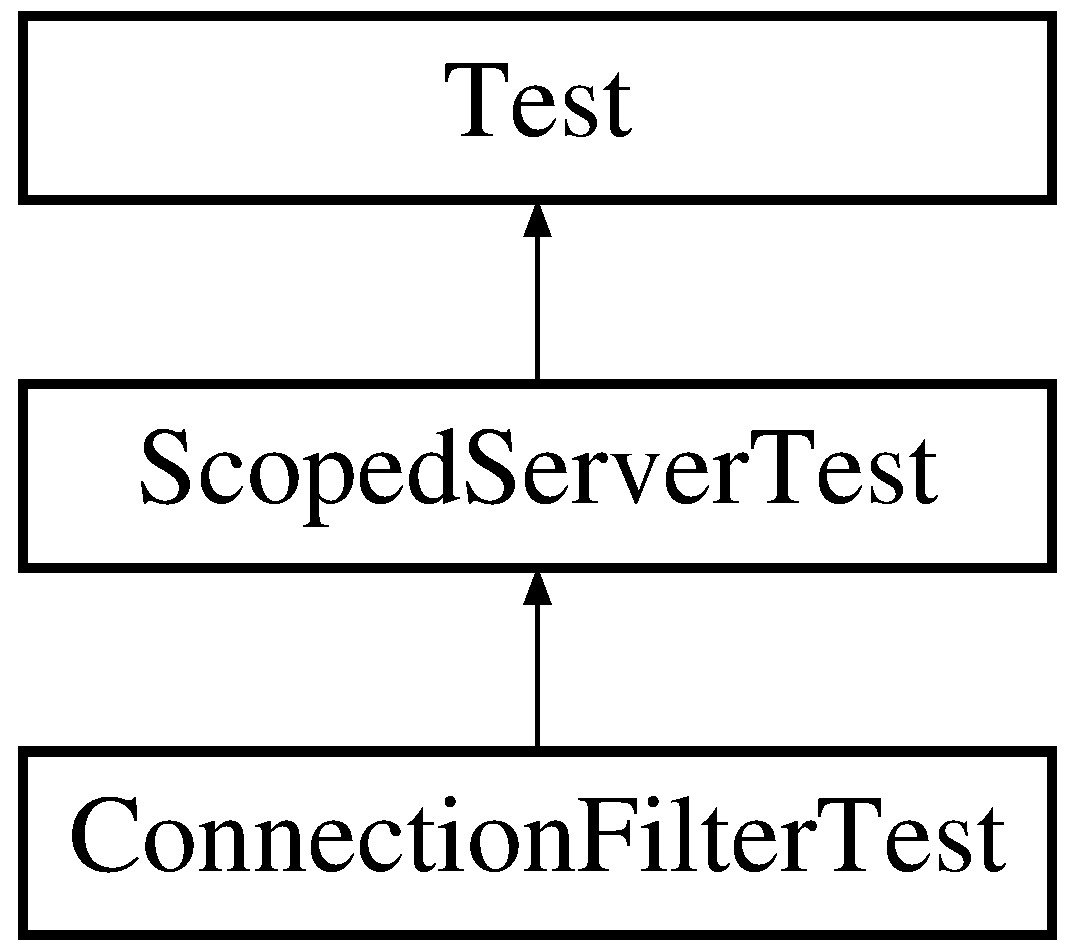
\includegraphics[height=3.000000cm]{classConnectionFilterTest}
\end{center}
\end{figure}
\subsection*{Protected Member Functions}
\begin{DoxyCompactItemize}
\item 
{\bf H\+T\+T\+P\+Server\+Options} {\bf create\+Default\+Opts} () override
\end{DoxyCompactItemize}
\subsection*{Additional Inherited Members}


\subsection{Detailed Description}


Definition at line 710 of file H\+T\+T\+P\+Server\+Test.\+cpp.



\subsection{Member Function Documentation}
\index{Connection\+Filter\+Test@{Connection\+Filter\+Test}!create\+Default\+Opts@{create\+Default\+Opts}}
\index{create\+Default\+Opts@{create\+Default\+Opts}!Connection\+Filter\+Test@{Connection\+Filter\+Test}}
\subsubsection[{create\+Default\+Opts() override}]{\setlength{\rightskip}{0pt plus 5cm}{\bf H\+T\+T\+P\+Server\+Options} Connection\+Filter\+Test\+::create\+Default\+Opts (
\begin{DoxyParamCaption}
{}
\end{DoxyParamCaption}
)\hspace{0.3cm}{\ttfamily [inline]}, {\ttfamily [override]}, {\ttfamily [protected]}, {\ttfamily [virtual]}}\label{classConnectionFilterTest_a19b02926b8bd53494cff0694ae181658}


Reimplemented from {\bf Scoped\+Server\+Test} \doxyref{}{p.}{classScopedServerTest_a451ba8d7a23e67134de3356a7fd264fd}.



Definition at line 712 of file H\+T\+T\+P\+Server\+Test.\+cpp.



References proxygen\+::\+Request\+Handler\+Chain\+::add\+Then(), proxygen\+::\+H\+T\+T\+P\+Server\+Options\+::handler\+Factories, proxygen\+::\+H\+T\+T\+P\+Server\+Options\+::new\+Connection\+Filter, and proxygen\+::\+H\+T\+T\+P\+Server\+Options\+::threads.


\begin{DoxyCode}
712                                                  \{
713     HTTPServerOptions options;
714     options.threads = 4;
715     options.handlerFactories =
716         RequestHandlerChain().addThen<TestHandlerFactory>().build();
717     options.handlerFactories = RequestHandlerChain()
718                                    .addThen<DummyFilterFactory>()
719                                    .addThen<TestHandlerFactory>()
720                                    .build();
721     options.newConnectionFilter =
722         [](\textcolor{keyword}{const} folly::AsyncTransportWrapper* sock,
723            \textcolor{keyword}{const} folly::SocketAddress* \textcolor{comment}{/* address */},
724            \textcolor{keyword}{const} std::string& \textcolor{comment}{/* nextProtocolName */},
725            wangle::SecureTransportType \textcolor{comment}{/* secureTransportType */},
726            \textcolor{keyword}{const} wangle::TransportInfo& \textcolor{comment}{/* tinfo */}) \{
727           \textcolor{keyword}{auto} cert = sock->getPeerCert();
728           \textcolor{keywordflow}{if} (!cert || OpenSSLCertUtils::getCommonName(*cert).value\_or(\textcolor{stringliteral}{""}) !=
729                            \textcolor{stringliteral}{"testuser1"}) \{
730             \textcolor{keywordflow}{throw} std::runtime\_error(\textcolor{stringliteral}{"Client cert is missing or invalid."});
731           \}
732         \};
733     \textcolor{keywordflow}{return} options;
734   \}
\end{DoxyCode}


The documentation for this class was generated from the following file\+:\begin{DoxyCompactItemize}
\item 
proxygen/httpserver/tests/{\bf H\+T\+T\+P\+Server\+Test.\+cpp}\end{DoxyCompactItemize}

\section{Connection\+Header\+Test Class Reference}
\label{classConnectionHeaderTest}\index{Connection\+Header\+Test@{Connection\+Header\+Test}}
Inheritance diagram for Connection\+Header\+Test\+:\begin{figure}[H]
\begin{center}
\leavevmode
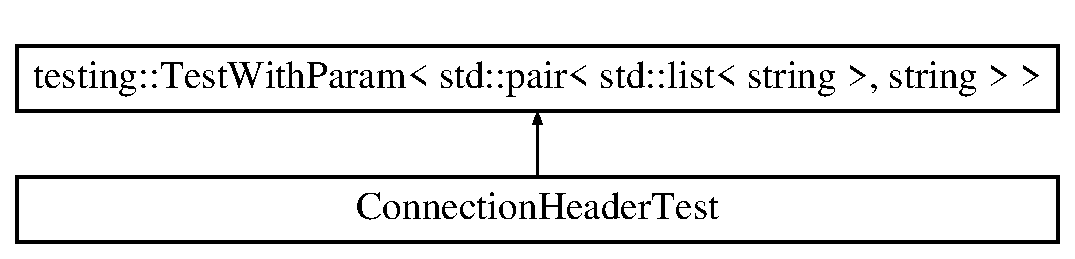
\includegraphics[height=2.000000cm]{classConnectionHeaderTest}
\end{center}
\end{figure}
\subsection*{Public Types}
\begin{DoxyCompactItemize}
\item 
using {\bf Param\+Type} = std\+::pair$<$ std\+::list$<$ string $>$, string $>$
\end{DoxyCompactItemize}


\subsection{Detailed Description}


Definition at line 705 of file H\+T\+T\+P1x\+Codec\+Test.\+cpp.



\subsection{Member Typedef Documentation}
\index{Connection\+Header\+Test@{Connection\+Header\+Test}!Param\+Type@{Param\+Type}}
\index{Param\+Type@{Param\+Type}!Connection\+Header\+Test@{Connection\+Header\+Test}}
\subsubsection[{Param\+Type}]{\setlength{\rightskip}{0pt plus 5cm}using {\bf Connection\+Header\+Test\+::\+Param\+Type} =  std\+::pair$<$std\+::list$<$string$>$, string$>$}\label{classConnectionHeaderTest_aac85e9bb383c68a69e89aeb2a502c15b}


Definition at line 708 of file H\+T\+T\+P1x\+Codec\+Test.\+cpp.



The documentation for this class was generated from the following file\+:\begin{DoxyCompactItemize}
\item 
proxygen/lib/http/codec/test/{\bf H\+T\+T\+P1x\+Codec\+Test.\+cpp}\end{DoxyCompactItemize}

\section{proxygen\+:\+:Consistent\+Hash Class Reference}
\label{classproxygen_1_1ConsistentHash}\index{proxygen\+::\+Consistent\+Hash@{proxygen\+::\+Consistent\+Hash}}


{\ttfamily \#include $<$Consistent\+Hash.\+h$>$}

Inheritance diagram for proxygen\+:\+:Consistent\+Hash\+:\begin{figure}[H]
\begin{center}
\leavevmode
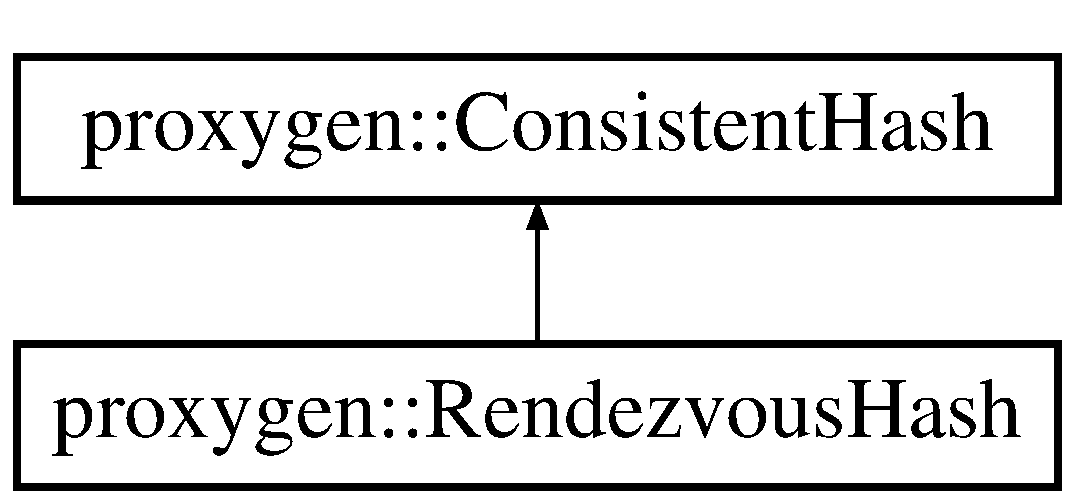
\includegraphics[height=2.000000cm]{classproxygen_1_1ConsistentHash}
\end{center}
\end{figure}
\subsection*{Public Member Functions}
\begin{DoxyCompactItemize}
\item 
virtual {\bf $\sim$\+Consistent\+Hash} ()
\item 
virtual void {\bf build} (std\+::vector$<$ std\+::pair$<$ std\+::string, uint64\+\_\+t $>$ $>$ \&)=0
\item 
virtual size\+\_\+t {\bf get} (const uint64\+\_\+t key, const size\+\_\+t rank=0) const =0
\item 
virtual double {\bf get\+Max\+Error\+Rate} () const =0
\end{DoxyCompactItemize}


\subsection{Detailed Description}


Definition at line 18 of file Consistent\+Hash.\+h.



\subsection{Constructor \& Destructor Documentation}
\index{proxygen\+::\+Consistent\+Hash@{proxygen\+::\+Consistent\+Hash}!````~Consistent\+Hash@{$\sim$\+Consistent\+Hash}}
\index{````~Consistent\+Hash@{$\sim$\+Consistent\+Hash}!proxygen\+::\+Consistent\+Hash@{proxygen\+::\+Consistent\+Hash}}
\subsubsection[{$\sim$\+Consistent\+Hash()}]{\setlength{\rightskip}{0pt plus 5cm}virtual proxygen\+::\+Consistent\+Hash\+::$\sim$\+Consistent\+Hash (
\begin{DoxyParamCaption}
{}
\end{DoxyParamCaption}
)\hspace{0.3cm}{\ttfamily [inline]}, {\ttfamily [virtual]}}\label{classproxygen_1_1ConsistentHash_a2d06f933aaab405fad765cabec504006}


Definition at line 20 of file Consistent\+Hash.\+h.



References build(), and get\+Max\+Error\+Rate().


\begin{DoxyCode}
20 \{\}
\end{DoxyCode}


\subsection{Member Function Documentation}
\index{proxygen\+::\+Consistent\+Hash@{proxygen\+::\+Consistent\+Hash}!build@{build}}
\index{build@{build}!proxygen\+::\+Consistent\+Hash@{proxygen\+::\+Consistent\+Hash}}
\subsubsection[{build(std\+::vector$<$ std\+::pair$<$ std\+::string, uint64\+\_\+t $>$ $>$ \&)=0}]{\setlength{\rightskip}{0pt plus 5cm}virtual void proxygen\+::\+Consistent\+Hash\+::build (
\begin{DoxyParamCaption}
\item[{std\+::vector$<$ std\+::pair$<$ std\+::string, uint64\+\_\+t $>$ $>$ \&}]{}
\end{DoxyParamCaption}
)\hspace{0.3cm}{\ttfamily [pure virtual]}}\label{classproxygen_1_1ConsistentHash_a8fd265b589f488ef87e4b18035566380}
\doxyref{build()}{p.}{classproxygen_1_1ConsistentHash_a8fd265b589f488ef87e4b18035566380} builds the hashing pool based on a vector of nodes with their keys and weights.

The bevahior of calling build multiple times is undefined.

\doxyref{build()}{p.}{classproxygen_1_1ConsistentHash_a8fd265b589f488ef87e4b18035566380} is not thread safe with \doxyref{get()}{p.}{classproxygen_1_1ConsistentHash_aff314a6a770935974172e5579be928e3}, documented below. 

Referenced by $\sim$\+Consistent\+Hash().

\index{proxygen\+::\+Consistent\+Hash@{proxygen\+::\+Consistent\+Hash}!get@{get}}
\index{get@{get}!proxygen\+::\+Consistent\+Hash@{proxygen\+::\+Consistent\+Hash}}
\subsubsection[{get(const uint64\+\_\+t key, const size\+\_\+t rank=0) const =0}]{\setlength{\rightskip}{0pt plus 5cm}virtual size\+\_\+t proxygen\+::\+Consistent\+Hash\+::get (
\begin{DoxyParamCaption}
\item[{const uint64\+\_\+t}]{key, }
\item[{const size\+\_\+t}]{rank = {\ttfamily 0}}
\end{DoxyParamCaption}
) const\hspace{0.3cm}{\ttfamily [pure virtual]}}\label{classproxygen_1_1ConsistentHash_aff314a6a770935974172e5579be928e3}
get(key, N) finds the node ranked N in the consistent hashing space for the given key.

The returning value is the node\textquotesingle{}s index in the input vector of \doxyref{build()}{p.}{classproxygen_1_1ConsistentHash_a8fd265b589f488ef87e4b18035566380}. 

Implemented in {\bf proxygen\+::\+Rendezvous\+Hash} \doxyref{}{p.}{classproxygen_1_1RendezvousHash_abf63d7fce1a3b5e85b6f13047054e8bb}.

\index{proxygen\+::\+Consistent\+Hash@{proxygen\+::\+Consistent\+Hash}!get\+Max\+Error\+Rate@{get\+Max\+Error\+Rate}}
\index{get\+Max\+Error\+Rate@{get\+Max\+Error\+Rate}!proxygen\+::\+Consistent\+Hash@{proxygen\+::\+Consistent\+Hash}}
\subsubsection[{get\+Max\+Error\+Rate() const =0}]{\setlength{\rightskip}{0pt plus 5cm}virtual double proxygen\+::\+Consistent\+Hash\+::get\+Max\+Error\+Rate (
\begin{DoxyParamCaption}
{}
\end{DoxyParamCaption}
) const\hspace{0.3cm}{\ttfamily [pure virtual]}}\label{classproxygen_1_1ConsistentHash_a979601c4ebab25cbab4d72cf3ed8988f}
get max error rate the current hashing space 

Implemented in {\bf proxygen\+::\+Rendezvous\+Hash} \doxyref{}{p.}{classproxygen_1_1RendezvousHash_a2453618b03612ba068c2cef6964e818e}.



Referenced by $\sim$\+Consistent\+Hash().



The documentation for this class was generated from the following file\+:\begin{DoxyCompactItemize}
\item 
proxygen/lib/utils/{\bf Consistent\+Hash.\+h}\end{DoxyCompactItemize}

\section{proxygen\+:\+:Trace\+Event\+:\+:Meta\+Data\+:\+:Conv\+Visitor$<$ T $>$ Struct Template Reference}
\label{structproxygen_1_1TraceEvent_1_1MetaData_1_1ConvVisitor}\index{proxygen\+::\+Trace\+Event\+::\+Meta\+Data\+::\+Conv\+Visitor$<$ T $>$@{proxygen\+::\+Trace\+Event\+::\+Meta\+Data\+::\+Conv\+Visitor$<$ T $>$}}


{\ttfamily \#include $<$Trace\+Event.\+h$>$}

Inheritance diagram for proxygen\+:\+:Trace\+Event\+:\+:Meta\+Data\+:\+:Conv\+Visitor$<$ T $>$\+:\begin{figure}[H]
\begin{center}
\leavevmode
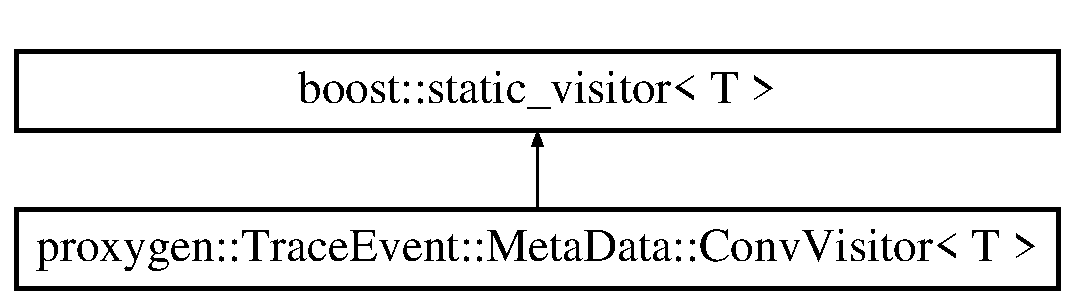
\includegraphics[height=2.000000cm]{structproxygen_1_1TraceEvent_1_1MetaData_1_1ConvVisitor}
\end{center}
\end{figure}
\subsection*{Public Member Functions}
\begin{DoxyCompactItemize}
\item 
{\bf T} {\bf operator()} (const std\+::vector$<$ std\+::string $>$ \&) const 
\item 
{\footnotesize template$<$typename U $>$ }\\{\bf T} {\bf operator()} (U \&operand) const 
\end{DoxyCompactItemize}


\subsection{Detailed Description}
\subsubsection*{template$<$typename T$>$\\*
struct proxygen\+::\+Trace\+Event\+::\+Meta\+Data\+::\+Conv\+Visitor$<$ T $>$}



Definition at line 86 of file Trace\+Event.\+h.



\subsection{Member Function Documentation}
\index{proxygen\+::\+Trace\+Event\+::\+Meta\+Data\+::\+Conv\+Visitor@{proxygen\+::\+Trace\+Event\+::\+Meta\+Data\+::\+Conv\+Visitor}!operator()@{operator()}}
\index{operator()@{operator()}!proxygen\+::\+Trace\+Event\+::\+Meta\+Data\+::\+Conv\+Visitor@{proxygen\+::\+Trace\+Event\+::\+Meta\+Data\+::\+Conv\+Visitor}}
\subsubsection[{operator()(const std\+::vector$<$ std\+::string $>$ \&) const }]{\setlength{\rightskip}{0pt plus 5cm}template$<$typename T$>$ {\bf T} {\bf proxygen\+::\+Trace\+Event\+::\+Meta\+Data\+::\+Conv\+Visitor}$<$ {\bf T} $>$\+::operator() (
\begin{DoxyParamCaption}
\item[{const std\+::vector$<$ std\+::string $>$ \&}]{}
\end{DoxyParamCaption}
) const\hspace{0.3cm}{\ttfamily [inline]}}\label{structproxygen_1_1TraceEvent_1_1MetaData_1_1ConvVisitor_a28eac243cc0e3bfda66cb195dded696f}


Definition at line 87 of file Trace\+Event.\+h.


\begin{DoxyCode}
87                                                         \{
88         folly::throw\_exception<Exception>(\textcolor{stringliteral}{"Not supported for type"});
89       \}
\end{DoxyCode}
\index{proxygen\+::\+Trace\+Event\+::\+Meta\+Data\+::\+Conv\+Visitor@{proxygen\+::\+Trace\+Event\+::\+Meta\+Data\+::\+Conv\+Visitor}!operator()@{operator()}}
\index{operator()@{operator()}!proxygen\+::\+Trace\+Event\+::\+Meta\+Data\+::\+Conv\+Visitor@{proxygen\+::\+Trace\+Event\+::\+Meta\+Data\+::\+Conv\+Visitor}}
\subsubsection[{operator()(\+U \&operand) const }]{\setlength{\rightskip}{0pt plus 5cm}template$<$typename T$>$ template$<$typename U $>$ {\bf T} {\bf proxygen\+::\+Trace\+Event\+::\+Meta\+Data\+::\+Conv\+Visitor}$<$ {\bf T} $>$\+::operator() (
\begin{DoxyParamCaption}
\item[{U \&}]{operand}
\end{DoxyParamCaption}
) const\hspace{0.3cm}{\ttfamily [inline]}}\label{structproxygen_1_1TraceEvent_1_1MetaData_1_1ConvVisitor_ae2bd52f351a2eae1615edd61b8780069}


Definition at line 92 of file Trace\+Event.\+h.


\begin{DoxyCode}
92                                      \{
93         \textcolor{keywordflow}{return} folly::to<T>(operand);
94       \}
\end{DoxyCode}


The documentation for this struct was generated from the following file\+:\begin{DoxyCompactItemize}
\item 
proxygen/lib/utils/{\bf Trace\+Event.\+h}\end{DoxyCompactItemize}

\section{proxygen\+:\+:Trace\+Event\+:\+:Meta\+Data\+:\+:Conv\+Visitor$<$ std\+:\+:string $>$ Struct Template Reference}
\label{structproxygen_1_1TraceEvent_1_1MetaData_1_1ConvVisitor_3_01std_1_1string_01_4}\index{proxygen\+::\+Trace\+Event\+::\+Meta\+Data\+::\+Conv\+Visitor$<$ std\+::string $>$@{proxygen\+::\+Trace\+Event\+::\+Meta\+Data\+::\+Conv\+Visitor$<$ std\+::string $>$}}


{\ttfamily \#include $<$Trace\+Event.\+h$>$}

Inheritance diagram for proxygen\+:\+:Trace\+Event\+:\+:Meta\+Data\+:\+:Conv\+Visitor$<$ std\+:\+:string $>$\+:\begin{figure}[H]
\begin{center}
\leavevmode
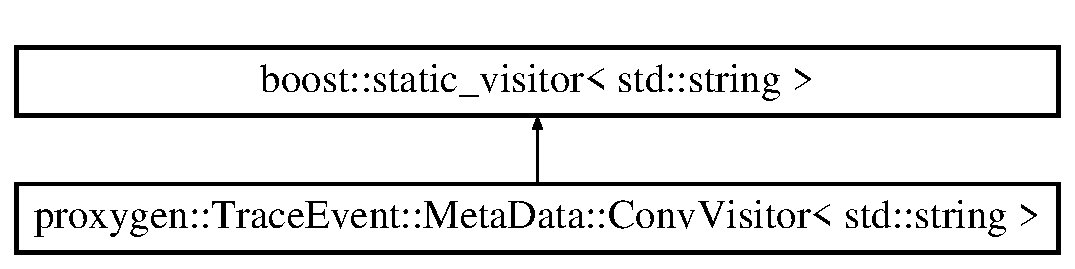
\includegraphics[height=2.000000cm]{structproxygen_1_1TraceEvent_1_1MetaData_1_1ConvVisitor_3_01std_1_1string_01_4}
\end{center}
\end{figure}
\subsection*{Public Member Functions}
\begin{DoxyCompactItemize}
\item 
std\+::string {\bf operator()} (const std\+::vector$<$ std\+::string $>$ \&operand) const 
\item 
{\footnotesize template$<$typename U $>$ }\\std\+::string {\bf operator()} (U \&operand) const 
\end{DoxyCompactItemize}


\subsection{Detailed Description}
\subsubsection*{template$<$$>$\\*
struct proxygen\+::\+Trace\+Event\+::\+Meta\+Data\+::\+Conv\+Visitor$<$ std\+::string $>$}



Definition at line 298 of file Trace\+Event.\+h.



\subsection{Member Function Documentation}
\index{proxygen\+::\+Trace\+Event\+::\+Meta\+Data\+::\+Conv\+Visitor$<$ std\+::string $>$@{proxygen\+::\+Trace\+Event\+::\+Meta\+Data\+::\+Conv\+Visitor$<$ std\+::string $>$}!operator()@{operator()}}
\index{operator()@{operator()}!proxygen\+::\+Trace\+Event\+::\+Meta\+Data\+::\+Conv\+Visitor$<$ std\+::string $>$@{proxygen\+::\+Trace\+Event\+::\+Meta\+Data\+::\+Conv\+Visitor$<$ std\+::string $>$}}
\subsubsection[{operator()(const std\+::vector$<$ std\+::string $>$ \&operand) const }]{\setlength{\rightskip}{0pt plus 5cm}std\+::string {\bf proxygen\+::\+Trace\+Event\+::\+Meta\+Data\+::\+Conv\+Visitor}$<$ std\+::string $>$\+::operator() (
\begin{DoxyParamCaption}
\item[{const std\+::vector$<$ std\+::string $>$ \&}]{operand}
\end{DoxyParamCaption}
) const}\label{structproxygen_1_1TraceEvent_1_1MetaData_1_1ConvVisitor_3_01std_1_1string_01_4_a985ada856255f8bf3b6184cf676df476}


Definition at line 106 of file Trace\+Event.\+cpp.


\begin{DoxyCode}
107                                                \{
108   \textcolor{comment}{// parse string vector to json string.}
109   folly::dynamic data = folly::dynamic::array;
110   \textcolor{keywordflow}{for} (\textcolor{keyword}{auto} item : operand) \{
111     data.push\_back(item);
112   \}
113   \textcolor{keywordflow}{return} folly::toJson(data);
114 \}
\end{DoxyCode}
\index{proxygen\+::\+Trace\+Event\+::\+Meta\+Data\+::\+Conv\+Visitor$<$ std\+::string $>$@{proxygen\+::\+Trace\+Event\+::\+Meta\+Data\+::\+Conv\+Visitor$<$ std\+::string $>$}!operator()@{operator()}}
\index{operator()@{operator()}!proxygen\+::\+Trace\+Event\+::\+Meta\+Data\+::\+Conv\+Visitor$<$ std\+::string $>$@{proxygen\+::\+Trace\+Event\+::\+Meta\+Data\+::\+Conv\+Visitor$<$ std\+::string $>$}}
\subsubsection[{operator()(\+U \&operand) const }]{\setlength{\rightskip}{0pt plus 5cm}template$<$typename U $>$ std\+::string {\bf proxygen\+::\+Trace\+Event\+::\+Meta\+Data\+::\+Conv\+Visitor}$<$ std\+::string $>$\+::operator() (
\begin{DoxyParamCaption}
\item[{U \&}]{operand}
\end{DoxyParamCaption}
) const\hspace{0.3cm}{\ttfamily [inline]}}\label{structproxygen_1_1TraceEvent_1_1MetaData_1_1ConvVisitor_3_01std_1_1string_01_4_a9dc7c7a8b536f0fd97436b59605ce6de}


Definition at line 303 of file Trace\+Event.\+h.


\begin{DoxyCode}
303                                          \{
304     \textcolor{keywordflow}{return} folly::to<std::string>(operand);
305   \}
\end{DoxyCode}


The documentation for this struct was generated from the following files\+:\begin{DoxyCompactItemize}
\item 
proxygen/lib/utils/{\bf Trace\+Event.\+h}\item 
proxygen/lib/utils/{\bf Trace\+Event.\+cpp}\end{DoxyCompactItemize}

\section{proxygen\+:\+:Trace\+Event\+:\+:Meta\+Data\+:\+:Conv\+Visitor$<$ std\+:\+:vector$<$ std\+:\+:string $>$ $>$ Struct Template Reference}
\label{structproxygen_1_1TraceEvent_1_1MetaData_1_1ConvVisitor_3_01std_1_1vector_3_01std_1_1string_01_4_01_4}\index{proxygen\+::\+Trace\+Event\+::\+Meta\+Data\+::\+Conv\+Visitor$<$ std\+::vector$<$ std\+::string $>$ $>$@{proxygen\+::\+Trace\+Event\+::\+Meta\+Data\+::\+Conv\+Visitor$<$ std\+::vector$<$ std\+::string $>$ $>$}}


{\ttfamily \#include $<$Trace\+Event.\+h$>$}

Inheritance diagram for proxygen\+:\+:Trace\+Event\+:\+:Meta\+Data\+:\+:Conv\+Visitor$<$ std\+:\+:vector$<$ std\+:\+:string $>$ $>$\+:\begin{figure}[H]
\begin{center}
\leavevmode
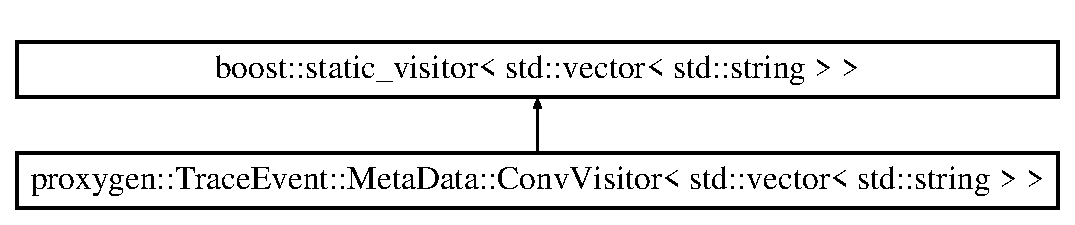
\includegraphics[height=2.000000cm]{structproxygen_1_1TraceEvent_1_1MetaData_1_1ConvVisitor_3_01std_1_1vector_3_01std_1_1string_01_4_01_4}
\end{center}
\end{figure}
\subsection*{Public Member Functions}
\begin{DoxyCompactItemize}
\item 
std\+::vector$<$ std\+::string $>$ {\bf operator()} (const std\+::vector$<$ std\+::string $>$ \&operand) const 
\item 
{\footnotesize template$<$typename U $>$ }\\std\+::vector$<$ std\+::string $>$ {\bf operator()} (U \&) const 
\end{DoxyCompactItemize}


\subsection{Detailed Description}
\subsubsection*{template$<$$>$\\*
struct proxygen\+::\+Trace\+Event\+::\+Meta\+Data\+::\+Conv\+Visitor$<$ std\+::vector$<$ std\+::string $>$ $>$}



Definition at line 284 of file Trace\+Event.\+h.



\subsection{Member Function Documentation}
\index{proxygen\+::\+Trace\+Event\+::\+Meta\+Data\+::\+Conv\+Visitor$<$ std\+::vector$<$ std\+::string $>$ $>$@{proxygen\+::\+Trace\+Event\+::\+Meta\+Data\+::\+Conv\+Visitor$<$ std\+::vector$<$ std\+::string $>$ $>$}!operator()@{operator()}}
\index{operator()@{operator()}!proxygen\+::\+Trace\+Event\+::\+Meta\+Data\+::\+Conv\+Visitor$<$ std\+::vector$<$ std\+::string $>$ $>$@{proxygen\+::\+Trace\+Event\+::\+Meta\+Data\+::\+Conv\+Visitor$<$ std\+::vector$<$ std\+::string $>$ $>$}}
\subsubsection[{operator()(const std\+::vector$<$ std\+::string $>$ \&operand) const }]{\setlength{\rightskip}{0pt plus 5cm}std\+::vector$<$std\+::string$>$ {\bf proxygen\+::\+Trace\+Event\+::\+Meta\+Data\+::\+Conv\+Visitor}$<$ std\+::vector$<$ std\+::string $>$ $>$\+::operator() (
\begin{DoxyParamCaption}
\item[{const std\+::vector$<$ std\+::string $>$ \&}]{operand}
\end{DoxyParamCaption}
) const\hspace{0.3cm}{\ttfamily [inline]}}\label{structproxygen_1_1TraceEvent_1_1MetaData_1_1ConvVisitor_3_01std_1_1vector_3_01std_1_1string_01_4_01_4_a6d526d8e2c6073edba931fa706661f7c}


Definition at line 286 of file Trace\+Event.\+h.


\begin{DoxyCode}
287                                                  \{
288     \textcolor{keywordflow}{return} operand;
289   \}
\end{DoxyCode}
\index{proxygen\+::\+Trace\+Event\+::\+Meta\+Data\+::\+Conv\+Visitor$<$ std\+::vector$<$ std\+::string $>$ $>$@{proxygen\+::\+Trace\+Event\+::\+Meta\+Data\+::\+Conv\+Visitor$<$ std\+::vector$<$ std\+::string $>$ $>$}!operator()@{operator()}}
\index{operator()@{operator()}!proxygen\+::\+Trace\+Event\+::\+Meta\+Data\+::\+Conv\+Visitor$<$ std\+::vector$<$ std\+::string $>$ $>$@{proxygen\+::\+Trace\+Event\+::\+Meta\+Data\+::\+Conv\+Visitor$<$ std\+::vector$<$ std\+::string $>$ $>$}}
\subsubsection[{operator()(\+U \&) const }]{\setlength{\rightskip}{0pt plus 5cm}template$<$typename U $>$ std\+::vector$<$std\+::string$>$ {\bf proxygen\+::\+Trace\+Event\+::\+Meta\+Data\+::\+Conv\+Visitor}$<$ std\+::vector$<$ std\+::string $>$ $>$\+::operator() (
\begin{DoxyParamCaption}
\item[{U \&}]{}
\end{DoxyParamCaption}
) const\hspace{0.3cm}{\ttfamily [inline]}}\label{structproxygen_1_1TraceEvent_1_1MetaData_1_1ConvVisitor_3_01std_1_1vector_3_01std_1_1string_01_4_01_4_a4a90bfe433eb1701131457f68473e437}


Definition at line 292 of file Trace\+Event.\+h.


\begin{DoxyCode}
292                                               \{
293     folly::throw\_exception<Exception>(\textcolor{stringliteral}{"Not supported for type"});
294   \}
\end{DoxyCode}


The documentation for this struct was generated from the following file\+:\begin{DoxyCompactItemize}
\item 
proxygen/lib/utils/{\bf Trace\+Event.\+h}\end{DoxyCompactItemize}

\section{Curl\+Service\+:\+:Curl\+Client Class Reference}
\label{classCurlService_1_1CurlClient}\index{Curl\+Service\+::\+Curl\+Client@{Curl\+Service\+::\+Curl\+Client}}


{\ttfamily \#include $<$Curl\+Client.\+h$>$}

Inheritance diagram for Curl\+Service\+:\+:Curl\+Client\+:\begin{figure}[H]
\begin{center}
\leavevmode
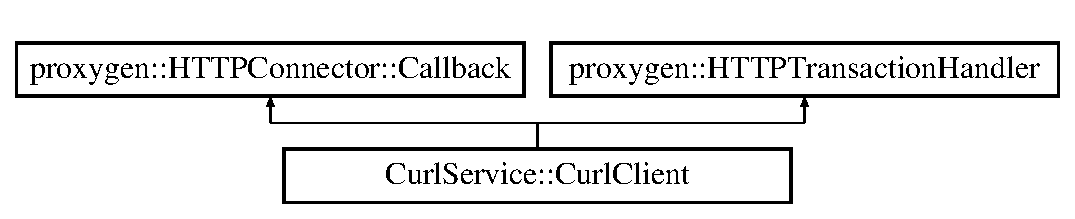
\includegraphics[height=2.000000cm]{classCurlService_1_1CurlClient}
\end{center}
\end{figure}
\subsection*{Public Member Functions}
\begin{DoxyCompactItemize}
\item 
{\bf Curl\+Client} (folly\+::\+Event\+Base $\ast$evb, {\bf proxygen\+::\+H\+T\+T\+P\+Method} http\+Method, const {\bf proxygen\+::\+U\+RL} \&url, const {\bf proxygen\+::\+U\+RL} $\ast$proxy, const {\bf proxygen\+::\+H\+T\+T\+P\+Headers} \&headers, const std\+::string \&input\+Filename, bool h2c=false, unsigned short http\+Major=1, unsigned short http\+Minor=1)
\item 
virtual {\bf $\sim$\+Curl\+Client} ()=default
\item 
void {\bf initialize\+Ssl} (const std\+::string \&ca\+Path, const std\+::string \&next\+Protos, const std\+::string \&cert\+Path=\char`\"{}\char`\"{}, const std\+::string \&key\+Path=\char`\"{}\char`\"{})
\item 
void {\bf ssl\+Handshake\+Followup} ({\bf proxygen\+::\+H\+T\+T\+P\+Upstream\+Session} $\ast$session) noexcept
\item 
void {\bf connect\+Success} ({\bf proxygen\+::\+H\+T\+T\+P\+Upstream\+Session} $\ast$session) override
\item 
void {\bf connect\+Error} (const folly\+::\+Async\+Socket\+Exception \&ex) override
\item 
void {\bf set\+Transaction} ({\bf proxygen\+::\+H\+T\+T\+P\+Transaction} $\ast$txn) noexceptoverride
\item 
void {\bf detach\+Transaction} () noexceptoverride
\item 
void {\bf on\+Headers\+Complete} (std\+::unique\+\_\+ptr$<$ {\bf proxygen\+::\+H\+T\+T\+P\+Message} $>$ msg) noexceptoverride
\item 
void {\bf on\+Body} (std\+::unique\+\_\+ptr$<$ folly\+::\+I\+O\+Buf $>$ chain) noexceptoverride
\item 
void {\bf on\+Trailers} (std\+::unique\+\_\+ptr$<$ {\bf proxygen\+::\+H\+T\+T\+P\+Headers} $>$ trailers) noexceptoverride
\item 
void {\bf on\+E\+OM} () noexceptoverride
\item 
void {\bf on\+Upgrade} ({\bf proxygen\+::\+Upgrade\+Protocol} protocol) noexceptoverride
\item 
void {\bf on\+Error} (const {\bf proxygen\+::\+H\+T\+T\+P\+Exception} \&error) noexceptoverride
\item 
void {\bf on\+Egress\+Paused} () noexceptoverride
\item 
void {\bf on\+Egress\+Resumed} () noexceptoverride
\item 
void {\bf send\+Request} ({\bf proxygen\+::\+H\+T\+T\+P\+Transaction} $\ast$txn)
\item 
folly\+::\+S\+S\+L\+Context\+Ptr {\bf get\+S\+S\+L\+Context} ()
\item 
const std\+::string \& {\bf get\+Server\+Name} () const 
\item 
void {\bf set\+Flow\+Control\+Settings} (int32\+\_\+t recv\+Window)
\item 
const {\bf proxygen\+::\+H\+T\+T\+P\+Message} $\ast$ {\bf get\+Response} () const 
\item 
void {\bf set\+Logging} (bool enabled)
\end{DoxyCompactItemize}
\subsection*{Static Public Member Functions}
\begin{DoxyCompactItemize}
\item 
static {\bf proxygen\+::\+H\+T\+T\+P\+Headers} {\bf parse\+Headers} (const std\+::string \&headers\+String)
\end{DoxyCompactItemize}
\subsection*{Protected Attributes}
\begin{DoxyCompactItemize}
\item 
{\bf proxygen\+::\+H\+T\+T\+P\+Transaction} $\ast$ {\bf txn\+\_\+} \{{\bf nullptr}\}
\item 
folly\+::\+Event\+Base $\ast$ {\bf evb\+\_\+} \{{\bf nullptr}\}
\item 
{\bf proxygen\+::\+H\+T\+T\+P\+Method} {\bf http\+Method\+\_\+}
\item 
{\bf proxygen\+::\+U\+RL} {\bf url\+\_\+}
\item 
std\+::unique\+\_\+ptr$<$ {\bf proxygen\+::\+U\+RL} $>$ {\bf proxy\+\_\+}
\item 
{\bf proxygen\+::\+H\+T\+T\+P\+Message} {\bf request\+\_\+}
\item 
const std\+::string {\bf input\+Filename\+\_\+}
\item 
folly\+::\+S\+S\+L\+Context\+Ptr {\bf ssl\+Context\+\_\+}
\item 
int32\+\_\+t {\bf recv\+Window\+\_\+} \{0\}
\item 
bool {\bf logging\+Enabled\+\_\+} \{true\}
\item 
bool {\bf h2c\+\_\+} \{false\}
\item 
unsigned short {\bf http\+Major\+\_\+}
\item 
unsigned short {\bf http\+Minor\+\_\+}
\item 
std\+::unique\+\_\+ptr$<$ {\bf proxygen\+::\+H\+T\+T\+P\+Message} $>$ {\bf response\+\_\+}
\end{DoxyCompactItemize}


\subsection{Detailed Description}


Definition at line 20 of file Curl\+Client.\+h.



\subsection{Constructor \& Destructor Documentation}
\index{Curl\+Service\+::\+Curl\+Client@{Curl\+Service\+::\+Curl\+Client}!Curl\+Client@{Curl\+Client}}
\index{Curl\+Client@{Curl\+Client}!Curl\+Service\+::\+Curl\+Client@{Curl\+Service\+::\+Curl\+Client}}
\subsubsection[{Curl\+Client(folly\+::\+Event\+Base $\ast$evb, proxygen\+::\+H\+T\+T\+P\+Method http\+Method, const proxygen\+::\+U\+R\+L \&url, const proxygen\+::\+U\+R\+L $\ast$proxy, const proxygen\+::\+H\+T\+T\+P\+Headers \&headers, const std\+::string \&input\+Filename, bool h2c=false, unsigned short http\+Major=1, unsigned short http\+Minor=1)}]{\setlength{\rightskip}{0pt plus 5cm}Curl\+Service\+::\+Curl\+Client\+::\+Curl\+Client (
\begin{DoxyParamCaption}
\item[{folly\+::\+Event\+Base $\ast$}]{evb, }
\item[{{\bf proxygen\+::\+H\+T\+T\+P\+Method}}]{http\+Method, }
\item[{const {\bf proxygen\+::\+U\+RL} \&}]{url, }
\item[{const {\bf proxygen\+::\+U\+RL} $\ast$}]{proxy, }
\item[{const {\bf proxygen\+::\+H\+T\+T\+P\+Headers} \&}]{headers, }
\item[{const std\+::string \&}]{input\+Filename, }
\item[{bool}]{h2c = {\ttfamily false}, }
\item[{unsigned short}]{http\+Major = {\ttfamily 1}, }
\item[{unsigned short}]{http\+Minor = {\ttfamily 1}}
\end{DoxyParamCaption}
)}\label{classCurlService_1_1CurlClient_a42a858be5737f3e0abd4aa416a4aae31}


Definition at line 32 of file Curl\+Client.\+cpp.



References proxygen\+::\+H\+T\+T\+P\+Headers\+::add(), proxygen\+::\+H\+T\+T\+P\+Headers\+::for\+Each(), proxygen\+::\+H\+T\+T\+P\+Message\+::get\+Headers(), proxygen\+::\+U\+R\+L\+::get\+Url(), proxy\+\_\+, and request\+\_\+.


\begin{DoxyCode}
41     : evb_(evb),
42       httpMethod_(httpMethod),
43       url_(url),
44       inputFilename_(inputFilename),
45       h2c_(h2c),
46       httpMajor_(httpMajor),
47       httpMinor_(httpMinor) \{
48   \textcolor{keywordflow}{if} (proxy != \textcolor{keyword}{nullptr}) \{
49     proxy_ = std::make\_unique<URL>(proxy->getUrl());
50   \}
51 
52   headers.forEach([\textcolor{keyword}{this}] (\textcolor{keyword}{const} \textcolor{keywordtype}{string}& header, \textcolor{keyword}{const} \textcolor{keywordtype}{string}& val) \{
53       request_.getHeaders().add(header, val);
54     \});
55 \}
\end{DoxyCode}
\index{Curl\+Service\+::\+Curl\+Client@{Curl\+Service\+::\+Curl\+Client}!````~Curl\+Client@{$\sim$\+Curl\+Client}}
\index{````~Curl\+Client@{$\sim$\+Curl\+Client}!Curl\+Service\+::\+Curl\+Client@{Curl\+Service\+::\+Curl\+Client}}
\subsubsection[{$\sim$\+Curl\+Client()=default}]{\setlength{\rightskip}{0pt plus 5cm}virtual Curl\+Service\+::\+Curl\+Client\+::$\sim$\+Curl\+Client (
\begin{DoxyParamCaption}
{}
\end{DoxyParamCaption}
)\hspace{0.3cm}{\ttfamily [virtual]}, {\ttfamily [default]}}\label{classCurlService_1_1CurlClient_a9043bca3122091124eb61baabcc4d4e5}


\subsection{Member Function Documentation}
\index{Curl\+Service\+::\+Curl\+Client@{Curl\+Service\+::\+Curl\+Client}!connect\+Error@{connect\+Error}}
\index{connect\+Error@{connect\+Error}!Curl\+Service\+::\+Curl\+Client@{Curl\+Service\+::\+Curl\+Client}}
\subsubsection[{connect\+Error(const folly\+::\+Async\+Socket\+Exception \&ex) override}]{\setlength{\rightskip}{0pt plus 5cm}void Curl\+Service\+::\+Curl\+Client\+::connect\+Error (
\begin{DoxyParamCaption}
\item[{const folly\+::\+Async\+Socket\+Exception \&}]{ex}
\end{DoxyParamCaption}
)\hspace{0.3cm}{\ttfamily [override]}, {\ttfamily [virtual]}}\label{classCurlService_1_1CurlClient_af37e3647eb96eda96323787207c33e80}


Implements {\bf proxygen\+::\+H\+T\+T\+P\+Connector\+::\+Callback} \doxyref{}{p.}{classproxygen_1_1HTTPConnector_1_1Callback_a4f01da41ef58437eeb47c1dee4a5bc47}.



Definition at line 187 of file Curl\+Client.\+cpp.



References proxygen\+::\+E\+R\+R\+OR, proxygen\+::\+U\+R\+L\+::get\+Host\+And\+Port(), logging\+Enabled\+\_\+, and url\+\_\+.


\begin{DoxyCode}
187                                                                  \{
188   LOG\_IF(ERROR, loggingEnabled_) << \textcolor{stringliteral}{"Coudln't connect to "}
189                                  << url_.getHostAndPort() << \textcolor{stringliteral}{":"} << ex.what();
190 \}
\end{DoxyCode}
\index{Curl\+Service\+::\+Curl\+Client@{Curl\+Service\+::\+Curl\+Client}!connect\+Success@{connect\+Success}}
\index{connect\+Success@{connect\+Success}!Curl\+Service\+::\+Curl\+Client@{Curl\+Service\+::\+Curl\+Client}}
\subsubsection[{connect\+Success(proxygen\+::\+H\+T\+T\+P\+Upstream\+Session $\ast$session) override}]{\setlength{\rightskip}{0pt plus 5cm}void Curl\+Service\+::\+Curl\+Client\+::connect\+Success (
\begin{DoxyParamCaption}
\item[{{\bf proxygen\+::\+H\+T\+T\+P\+Upstream\+Session} $\ast$}]{session}
\end{DoxyParamCaption}
)\hspace{0.3cm}{\ttfamily [override]}, {\ttfamily [virtual]}}\label{classCurlService_1_1CurlClient_a8e0166bd540cf4a16b0ef1dd3accf882}


Implements {\bf proxygen\+::\+H\+T\+T\+P\+Connector\+::\+Callback} \doxyref{}{p.}{classproxygen_1_1HTTPConnector_1_1Callback_aae878d2da74442ffc19ecb3bbbee7d9e}.



Definition at line 121 of file Curl\+Client.\+cpp.



References proxygen\+::\+H\+T\+T\+P\+Session\+::close\+When\+Idle(), proxygen\+::\+U\+R\+L\+::is\+Secure(), proxygen\+::\+H\+T\+T\+P\+Upstream\+Session\+::new\+Transaction(), recv\+Window\+\_\+, send\+Request(), proxygen\+::\+H\+T\+T\+P\+Session\+::set\+Flow\+Control(), ssl\+Handshake\+Followup(), and url\+\_\+.


\begin{DoxyCode}
121                                                             \{
122 
123   \textcolor{keywordflow}{if} (url_.isSecure()) \{
124     sslHandshakeFollowup(session);
125   \}
126 
127   session->setFlowControl(recvWindow_, recvWindow_, recvWindow_);
128   sendRequest(session->newTransaction(\textcolor{keyword}{this}));
129   session->closeWhenIdle();
130 \}
\end{DoxyCode}
\index{Curl\+Service\+::\+Curl\+Client@{Curl\+Service\+::\+Curl\+Client}!detach\+Transaction@{detach\+Transaction}}
\index{detach\+Transaction@{detach\+Transaction}!Curl\+Service\+::\+Curl\+Client@{Curl\+Service\+::\+Curl\+Client}}
\subsubsection[{detach\+Transaction() noexceptoverride}]{\setlength{\rightskip}{0pt plus 5cm}void Curl\+Service\+::\+Curl\+Client\+::detach\+Transaction (
\begin{DoxyParamCaption}
{}
\end{DoxyParamCaption}
)\hspace{0.3cm}{\ttfamily [override]}, {\ttfamily [virtual]}, {\ttfamily [noexcept]}}\label{classCurlService_1_1CurlClient_acdae4e65f5bdf0126630dcb03ec4a7fb}
Called once after a transaction successfully completes. It will be called even if a read or write error happened earlier. This is a terminal callback, which means that the H\+T\+T\+P\+Transaction object that gives this call will be invalid after this function completes. 

Implements {\bf proxygen\+::\+H\+T\+T\+P\+Transaction\+Handler} \doxyref{}{p.}{classproxygen_1_1HTTPTransactionHandler_a67eb253d121a26772f4caa56847ed7cd}.



Definition at line 195 of file Curl\+Client.\+cpp.


\begin{DoxyCode}
195                                             \{
196 \}
\end{DoxyCode}
\index{Curl\+Service\+::\+Curl\+Client@{Curl\+Service\+::\+Curl\+Client}!get\+Response@{get\+Response}}
\index{get\+Response@{get\+Response}!Curl\+Service\+::\+Curl\+Client@{Curl\+Service\+::\+Curl\+Client}}
\subsubsection[{get\+Response() const }]{\setlength{\rightskip}{0pt plus 5cm}const {\bf proxygen\+::\+H\+T\+T\+P\+Message}$\ast$ Curl\+Service\+::\+Curl\+Client\+::get\+Response (
\begin{DoxyParamCaption}
{}
\end{DoxyParamCaption}
) const\hspace{0.3cm}{\ttfamily [inline]}}\label{classCurlService_1_1CurlClient_a1b2bb369d3320c6704ef5c3624e24d6f}


Definition at line 72 of file Curl\+Client.\+h.



References response\+\_\+.



Referenced by T\+E\+S\+T().


\begin{DoxyCode}
72                                                  \{
73     \textcolor{keywordflow}{return} response_.get();
74   \}
\end{DoxyCode}
\index{Curl\+Service\+::\+Curl\+Client@{Curl\+Service\+::\+Curl\+Client}!get\+Server\+Name@{get\+Server\+Name}}
\index{get\+Server\+Name@{get\+Server\+Name}!Curl\+Service\+::\+Curl\+Client@{Curl\+Service\+::\+Curl\+Client}}
\subsubsection[{get\+Server\+Name() const }]{\setlength{\rightskip}{0pt plus 5cm}const string \& Curl\+Service\+::\+Curl\+Client\+::get\+Server\+Name (
\begin{DoxyParamCaption}
{}
\end{DoxyParamCaption}
) const}\label{classCurlService_1_1CurlClient_ad67c27bfa1474add9e1ec31b66641f1c}


Definition at line 248 of file Curl\+Client.\+cpp.



References proxygen\+::\+H\+T\+T\+P\+Message\+::get\+Headers(), proxygen\+::\+U\+R\+L\+::get\+Host(), proxygen\+::\+H\+T\+T\+P\+Headers\+::get\+Single\+Or\+Empty(), request\+\_\+, and url\+\_\+.



Referenced by get\+S\+S\+L\+Context().


\begin{DoxyCode}
248                                               \{
249   \textcolor{keyword}{const} \textcolor{keywordtype}{string}& res = request_.getHeaders().getSingleOrEmpty(HTTP\_HEADER\_HOST);
250   \textcolor{keywordflow}{if} (res.empty()) \{
251     \textcolor{keywordflow}{return} url_.getHost();
252   \}
253   \textcolor{keywordflow}{return} res;
254 \}
\end{DoxyCode}
\index{Curl\+Service\+::\+Curl\+Client@{Curl\+Service\+::\+Curl\+Client}!get\+S\+S\+L\+Context@{get\+S\+S\+L\+Context}}
\index{get\+S\+S\+L\+Context@{get\+S\+S\+L\+Context}!Curl\+Service\+::\+Curl\+Client@{Curl\+Service\+::\+Curl\+Client}}
\subsubsection[{get\+S\+S\+L\+Context()}]{\setlength{\rightskip}{0pt plus 5cm}folly\+::\+S\+S\+L\+Context\+Ptr Curl\+Service\+::\+Curl\+Client\+::get\+S\+S\+L\+Context (
\begin{DoxyParamCaption}
{}
\end{DoxyParamCaption}
)\hspace{0.3cm}{\ttfamily [inline]}}\label{classCurlService_1_1CurlClient_adb219d4719c50b886776d3e17c6d3554}


Definition at line 66 of file Curl\+Client.\+h.



References get\+Server\+Name(), set\+Flow\+Control\+Settings(), and ssl\+Context\+\_\+.


\begin{DoxyCode}
66 \{ \textcolor{keywordflow}{return} sslContext_; \}
\end{DoxyCode}
\index{Curl\+Service\+::\+Curl\+Client@{Curl\+Service\+::\+Curl\+Client}!initialize\+Ssl@{initialize\+Ssl}}
\index{initialize\+Ssl@{initialize\+Ssl}!Curl\+Service\+::\+Curl\+Client@{Curl\+Service\+::\+Curl\+Client}}
\subsubsection[{initialize\+Ssl(const std\+::string \&ca\+Path, const std\+::string \&next\+Protos, const std\+::string \&cert\+Path="""", const std\+::string \&key\+Path="""")}]{\setlength{\rightskip}{0pt plus 5cm}void Curl\+Service\+::\+Curl\+Client\+::initialize\+Ssl (
\begin{DoxyParamCaption}
\item[{const std\+::string \&}]{ca\+Path, }
\item[{const std\+::string \&}]{next\+Protos, }
\item[{const std\+::string \&}]{cert\+Path = {\ttfamily \char`\"{}\char`\"{}}, }
\item[{const std\+::string \&}]{key\+Path = {\ttfamily \char`\"{}\char`\"{}}}
\end{DoxyParamCaption}
)}\label{classCurlService_1_1CurlClient_a17d9333f43833c56ec41d9852db58067}


Definition at line 78 of file Curl\+Client.\+cpp.



References h2c\+\_\+, and ssl\+Context\+\_\+.


\begin{DoxyCode}
81                                                       \{
82   sslContext_ = std::make\_shared<folly::SSLContext>();
83   sslContext_->setOptions(SSL\_OP\_NO\_COMPRESSION);
84   sslContext_->setCipherList(folly::ssl::SSLCommonOptions::kCipherList);
85   \textcolor{keywordflow}{if} (!caPath.empty()) \{
86     sslContext_->loadTrustedCertificates(caPath.c\_str());
87   \}
88   \textcolor{keywordflow}{if} (!certPath.empty() && !keyPath.empty()) \{
89     sslContext_->loadCertKeyPairFromFiles(certPath.c\_str(), keyPath.c\_str());
90   \}
91   list<string> nextProtoList;
92   folly::splitTo<string>(\textcolor{charliteral}{','}, nextProtos, std::inserter(nextProtoList,
93                                                         nextProtoList.begin()));
94   sslContext_->setAdvertisedNextProtocols(nextProtoList);
95   h2c_ = \textcolor{keyword}{false};
96 \}
\end{DoxyCode}
\index{Curl\+Service\+::\+Curl\+Client@{Curl\+Service\+::\+Curl\+Client}!on\+Body@{on\+Body}}
\index{on\+Body@{on\+Body}!Curl\+Service\+::\+Curl\+Client@{Curl\+Service\+::\+Curl\+Client}}
\subsubsection[{on\+Body(std\+::unique\+\_\+ptr$<$ folly\+::\+I\+O\+Buf $>$ chain) noexceptoverride}]{\setlength{\rightskip}{0pt plus 5cm}void Curl\+Service\+::\+Curl\+Client\+::on\+Body (
\begin{DoxyParamCaption}
\item[{std\+::unique\+\_\+ptr$<$ folly\+::\+I\+O\+Buf $>$}]{chain}
\end{DoxyParamCaption}
)\hspace{0.3cm}{\ttfamily [override]}, {\ttfamily [virtual]}, {\ttfamily [noexcept]}}\label{classCurlService_1_1CurlClient_a347b9f1409c93387bfaf2ff88a400138}
Can be called multiple times per transaction. If you had previously called pause\+Ingress(), this callback will be delayed until you call resume\+Ingress(). 

Implements {\bf proxygen\+::\+H\+T\+T\+P\+Transaction\+Handler} \doxyref{}{p.}{classproxygen_1_1HTTPTransactionHandler_a56a25d7fb8ac5ddf1ed5b16eaca3c5df}.



Definition at line 210 of file Curl\+Client.\+cpp.



References logging\+Enabled\+\_\+.


\begin{DoxyCode}
210                                                                 \{
211   \textcolor{keywordflow}{if} (!loggingEnabled_) \{
212     \textcolor{keywordflow}{return};
213   \}
214   \textcolor{keywordflow}{if} (chain) \{
215     \textcolor{keyword}{const} IOBuf* p = chain.get();
216     \textcolor{keywordflow}{do} \{
217       cout.write((\textcolor{keyword}{const} \textcolor{keywordtype}{char}*)p->data(), p->length());
218       cout.flush();
219       p = p->next();
220     \} \textcolor{keywordflow}{while} (p != chain.get());
221   \}
222 \}
\end{DoxyCode}
\index{Curl\+Service\+::\+Curl\+Client@{Curl\+Service\+::\+Curl\+Client}!on\+Egress\+Paused@{on\+Egress\+Paused}}
\index{on\+Egress\+Paused@{on\+Egress\+Paused}!Curl\+Service\+::\+Curl\+Client@{Curl\+Service\+::\+Curl\+Client}}
\subsubsection[{on\+Egress\+Paused() noexceptoverride}]{\setlength{\rightskip}{0pt plus 5cm}void Curl\+Service\+::\+Curl\+Client\+::on\+Egress\+Paused (
\begin{DoxyParamCaption}
{}
\end{DoxyParamCaption}
)\hspace{0.3cm}{\ttfamily [override]}, {\ttfamily [virtual]}, {\ttfamily [noexcept]}}\label{classCurlService_1_1CurlClient_a26480fe7beb7f338dcf2dd1f6be11628}
If the remote side\textquotesingle{}s receive buffer fills up, this callback will be invoked so you can attempt to stop sending to the remote side. 

Implements {\bf proxygen\+::\+H\+T\+T\+P\+Transaction\+Handler} \doxyref{}{p.}{classproxygen_1_1HTTPTransactionHandler_a0a50acdb32cb51ecbf6a72730053a36b}.



Definition at line 240 of file Curl\+Client.\+cpp.



References logging\+Enabled\+\_\+.


\begin{DoxyCode}
240                                          \{
241   LOG\_IF(INFO, loggingEnabled_) << \textcolor{stringliteral}{"Egress paused"};
242 \}
\end{DoxyCode}
\index{Curl\+Service\+::\+Curl\+Client@{Curl\+Service\+::\+Curl\+Client}!on\+Egress\+Resumed@{on\+Egress\+Resumed}}
\index{on\+Egress\+Resumed@{on\+Egress\+Resumed}!Curl\+Service\+::\+Curl\+Client@{Curl\+Service\+::\+Curl\+Client}}
\subsubsection[{on\+Egress\+Resumed() noexceptoverride}]{\setlength{\rightskip}{0pt plus 5cm}void Curl\+Service\+::\+Curl\+Client\+::on\+Egress\+Resumed (
\begin{DoxyParamCaption}
{}
\end{DoxyParamCaption}
)\hspace{0.3cm}{\ttfamily [override]}, {\ttfamily [virtual]}, {\ttfamily [noexcept]}}\label{classCurlService_1_1CurlClient_a40fc8dafd3a048f5311b84e68a9495a3}
This callback lets you know that the remote side has resumed reading and you can now continue to send data. 

Implements {\bf proxygen\+::\+H\+T\+T\+P\+Transaction\+Handler} \doxyref{}{p.}{classproxygen_1_1HTTPTransactionHandler_a7715b02e413859c26426adbbde7e53d8}.



Definition at line 244 of file Curl\+Client.\+cpp.



References logging\+Enabled\+\_\+.


\begin{DoxyCode}
244                                           \{
245   LOG\_IF(INFO, loggingEnabled_) << \textcolor{stringliteral}{"Egress resumed"};
246 \}
\end{DoxyCode}
\index{Curl\+Service\+::\+Curl\+Client@{Curl\+Service\+::\+Curl\+Client}!on\+E\+OM@{on\+E\+OM}}
\index{on\+E\+OM@{on\+E\+OM}!Curl\+Service\+::\+Curl\+Client@{Curl\+Service\+::\+Curl\+Client}}
\subsubsection[{on\+E\+O\+M() noexceptoverride}]{\setlength{\rightskip}{0pt plus 5cm}void Curl\+Service\+::\+Curl\+Client\+::on\+E\+OM (
\begin{DoxyParamCaption}
{}
\end{DoxyParamCaption}
)\hspace{0.3cm}{\ttfamily [override]}, {\ttfamily [virtual]}, {\ttfamily [noexcept]}}\label{classCurlService_1_1CurlClient_a7c4b2f28e543ff77e626745c0917ae42}
Can be called once per transaction. If you had previously called pause\+Ingress(), this callback will be delayed until you call resume\+Ingress(). After this callback is received, there will be no more normal ingress callbacks received (on\+Egress$\ast$() and \doxyref{on\+Error()}{p.}{classCurlService_1_1CurlClient_ac58be91bdc9ec7fb485e343263d59678} may still be invoked). The Handler should consider ingress complete after receiving this message. This Transaction is still valid, and work may still occur on it until detach\+Transaction is called. 

Implements {\bf proxygen\+::\+H\+T\+T\+P\+Transaction\+Handler} \doxyref{}{p.}{classproxygen_1_1HTTPTransactionHandler_afdc4d4dec715841ba0c5bb5e58b1d53c}.



Definition at line 228 of file Curl\+Client.\+cpp.



References logging\+Enabled\+\_\+.


\begin{DoxyCode}
228                                 \{
229   LOG\_IF(INFO, loggingEnabled_) << \textcolor{stringliteral}{"Got EOM"};
230 \}
\end{DoxyCode}
\index{Curl\+Service\+::\+Curl\+Client@{Curl\+Service\+::\+Curl\+Client}!on\+Error@{on\+Error}}
\index{on\+Error@{on\+Error}!Curl\+Service\+::\+Curl\+Client@{Curl\+Service\+::\+Curl\+Client}}
\subsubsection[{on\+Error(const proxygen\+::\+H\+T\+T\+P\+Exception \&error) noexceptoverride}]{\setlength{\rightskip}{0pt plus 5cm}void Curl\+Service\+::\+Curl\+Client\+::on\+Error (
\begin{DoxyParamCaption}
\item[{const {\bf proxygen\+::\+H\+T\+T\+P\+Exception} \&}]{error}
\end{DoxyParamCaption}
)\hspace{0.3cm}{\ttfamily [override]}, {\ttfamily [virtual]}, {\ttfamily [noexcept]}}\label{classCurlService_1_1CurlClient_ac58be91bdc9ec7fb485e343263d59678}
Can be called at any time before \doxyref{detach\+Transaction()}{p.}{classCurlService_1_1CurlClient_acdae4e65f5bdf0126630dcb03ec4a7fb}. This callback implies that an error has occurred. To determine if ingress or egress is affected, check the direciont on the H\+T\+T\+P\+Exception. If the direction is I\+N\+G\+R\+E\+SS, it M\+AY still be possible to send egress. 

Implements {\bf proxygen\+::\+H\+T\+T\+P\+Transaction\+Handler} \doxyref{}{p.}{classproxygen_1_1HTTPTransactionHandler_a585c21327eb30ab85ebdb84f663dab3b}.



Definition at line 236 of file Curl\+Client.\+cpp.



References proxygen\+::\+E\+R\+R\+OR, and logging\+Enabled\+\_\+.


\begin{DoxyCode}
236                                                             \{
237   LOG\_IF(ERROR, loggingEnabled_) << \textcolor{stringliteral}{"An error occurred: "} << error.what();
238 \}
\end{DoxyCode}
\index{Curl\+Service\+::\+Curl\+Client@{Curl\+Service\+::\+Curl\+Client}!on\+Headers\+Complete@{on\+Headers\+Complete}}
\index{on\+Headers\+Complete@{on\+Headers\+Complete}!Curl\+Service\+::\+Curl\+Client@{Curl\+Service\+::\+Curl\+Client}}
\subsubsection[{on\+Headers\+Complete(std\+::unique\+\_\+ptr$<$ proxygen\+::\+H\+T\+T\+P\+Message $>$ msg) noexceptoverride}]{\setlength{\rightskip}{0pt plus 5cm}void Curl\+Service\+::\+Curl\+Client\+::on\+Headers\+Complete (
\begin{DoxyParamCaption}
\item[{std\+::unique\+\_\+ptr$<$ {\bf proxygen\+::\+H\+T\+T\+P\+Message} $>$}]{msg}
\end{DoxyParamCaption}
)\hspace{0.3cm}{\ttfamily [override]}, {\ttfamily [virtual]}, {\ttfamily [noexcept]}}\label{classCurlService_1_1CurlClient_abfa6047eebf33dae96acd69f3f072956}
Called at most once per transaction. This is usually the first ingress callback. It is possible to get a read error before this however. If you had previously called pause\+Ingress(), this callback will be delayed until you call resume\+Ingress(). 

Implements {\bf proxygen\+::\+H\+T\+T\+P\+Transaction\+Handler} \doxyref{}{p.}{classproxygen_1_1HTTPTransactionHandler_a5e431cbb4c065285c5ad65acaceb0b22}.



Definition at line 198 of file Curl\+Client.\+cpp.



References logging\+Enabled\+\_\+, and response\+\_\+.


\begin{DoxyCode}
198                                                                        \{
199   response_ = std::move(msg);
200   \textcolor{keywordflow}{if} (!loggingEnabled_) \{
201     \textcolor{keywordflow}{return};
202   \}
203   cout << response_->getStatusCode() << \textcolor{stringliteral}{" "}
204        << response_->getStatusMessage() << endl;
205   response_->getHeaders().forEach([&](\textcolor{keyword}{const} \textcolor{keywordtype}{string}& header, \textcolor{keyword}{const} \textcolor{keywordtype}{string}& val) \{
206     cout << header << \textcolor{stringliteral}{": "} << val << endl;
207   \});
208 \}
\end{DoxyCode}
\index{Curl\+Service\+::\+Curl\+Client@{Curl\+Service\+::\+Curl\+Client}!on\+Trailers@{on\+Trailers}}
\index{on\+Trailers@{on\+Trailers}!Curl\+Service\+::\+Curl\+Client@{Curl\+Service\+::\+Curl\+Client}}
\subsubsection[{on\+Trailers(std\+::unique\+\_\+ptr$<$ proxygen\+::\+H\+T\+T\+P\+Headers $>$ trailers) noexceptoverride}]{\setlength{\rightskip}{0pt plus 5cm}void Curl\+Service\+::\+Curl\+Client\+::on\+Trailers (
\begin{DoxyParamCaption}
\item[{std\+::unique\+\_\+ptr$<$ {\bf proxygen\+::\+H\+T\+T\+P\+Headers} $>$}]{trailers}
\end{DoxyParamCaption}
)\hspace{0.3cm}{\ttfamily [override]}, {\ttfamily [virtual]}, {\ttfamily [noexcept]}}\label{classCurlService_1_1CurlClient_a13f4e9d8894fba072798f6909f8f740b}
Can be called any number of times per transaction. If you had previously called pause\+Ingress(), this callback will be delayed until you call resume\+Ingress(). Trailers can be received once right before the E\+OM of a chunked H\+T\+T\+P/1.\+1 reponse or multiple times per transaction from S\+P\+DY and H\+T\+T\+P/2.\+0 H\+E\+A\+D\+E\+RS frames. 

Implements {\bf proxygen\+::\+H\+T\+T\+P\+Transaction\+Handler} \doxyref{}{p.}{classproxygen_1_1HTTPTransactionHandler_a219de67110f915deda30d18327f26393}.



Definition at line 224 of file Curl\+Client.\+cpp.



References logging\+Enabled\+\_\+.


\begin{DoxyCode}
224                                                                \{
225   LOG\_IF(INFO, loggingEnabled_) << \textcolor{stringliteral}{"Discarding trailers"};
226 \}
\end{DoxyCode}
\index{Curl\+Service\+::\+Curl\+Client@{Curl\+Service\+::\+Curl\+Client}!on\+Upgrade@{on\+Upgrade}}
\index{on\+Upgrade@{on\+Upgrade}!Curl\+Service\+::\+Curl\+Client@{Curl\+Service\+::\+Curl\+Client}}
\subsubsection[{on\+Upgrade(proxygen\+::\+Upgrade\+Protocol protocol) noexceptoverride}]{\setlength{\rightskip}{0pt plus 5cm}void Curl\+Service\+::\+Curl\+Client\+::on\+Upgrade (
\begin{DoxyParamCaption}
\item[{{\bf proxygen\+::\+Upgrade\+Protocol}}]{protocol}
\end{DoxyParamCaption}
)\hspace{0.3cm}{\ttfamily [override]}, {\ttfamily [virtual]}, {\ttfamily [noexcept]}}\label{classCurlService_1_1CurlClient_ae64a3832725897be431f2473cf3abd8b}
Can be called once per transaction. If you had previously called pause\+Ingress(), this callback will be delayed until you call resume\+Ingress(). After this callback is invoked, further data will be forwarded using the \doxyref{on\+Body()}{p.}{classCurlService_1_1CurlClient_a347b9f1409c93387bfaf2ff88a400138} callback. Once the data transfer is completed (E\+OF recevied in case of C\+O\+N\+N\+E\+CT), \doxyref{on\+E\+O\+M()}{p.}{classCurlService_1_1CurlClient_a7c4b2f28e543ff77e626745c0917ae42} callback will be invoked. 

Implements {\bf proxygen\+::\+H\+T\+T\+P\+Transaction\+Handler} \doxyref{}{p.}{classproxygen_1_1HTTPTransactionHandler_acda954bf78c4d2aad951698e78c40a0f}.



Definition at line 232 of file Curl\+Client.\+cpp.



References logging\+Enabled\+\_\+.


\begin{DoxyCode}
232                                                    \{
233   LOG\_IF(INFO, loggingEnabled_) << \textcolor{stringliteral}{"Discarding upgrade protocol"};
234 \}
\end{DoxyCode}
\index{Curl\+Service\+::\+Curl\+Client@{Curl\+Service\+::\+Curl\+Client}!parse\+Headers@{parse\+Headers}}
\index{parse\+Headers@{parse\+Headers}!Curl\+Service\+::\+Curl\+Client@{Curl\+Service\+::\+Curl\+Client}}
\subsubsection[{parse\+Headers(const std\+::string \&headers\+String)}]{\setlength{\rightskip}{0pt plus 5cm}{\bf H\+T\+T\+P\+Headers} Curl\+Service\+::\+Curl\+Client\+::parse\+Headers (
\begin{DoxyParamCaption}
\item[{const std\+::string \&}]{headers\+String}
\end{DoxyParamCaption}
)\hspace{0.3cm}{\ttfamily [static]}}\label{classCurlService_1_1CurlClient_ab60fb767ca6e21620c56baf65c1b6a24}


Definition at line 57 of file Curl\+Client.\+cpp.



References proxygen\+::\+H\+T\+T\+P\+Headers\+::add().



Referenced by main().


\begin{DoxyCode}
57                                                                    \{
58   vector<StringPiece> headersList;
59   HTTPHeaders headers;
60   folly::split(\textcolor{stringliteral}{","}, headersString, headersList);
61   \textcolor{keywordflow}{for} (\textcolor{keyword}{const} \textcolor{keyword}{auto}& headerPair: headersList) \{
62     vector<StringPiece> nv;
63     folly::split(\textcolor{charliteral}{'='}, headerPair, nv);
64     \textcolor{keywordflow}{if} (nv.size() > 0) \{
65       \textcolor{keywordflow}{if} (nv[0].empty()) \{
66         \textcolor{keywordflow}{continue};
67       \}
68       StringPiece value(\textcolor{stringliteral}{""});
69       \textcolor{keywordflow}{if} (nv.size() > 1) \{
70         value = nv[1];
71       \} \textcolor{comment}{// trim anything else}
72       headers.add(nv[0], value);
73     \}
74   \}
75   \textcolor{keywordflow}{return} headers;
76 \}
\end{DoxyCode}
\index{Curl\+Service\+::\+Curl\+Client@{Curl\+Service\+::\+Curl\+Client}!send\+Request@{send\+Request}}
\index{send\+Request@{send\+Request}!Curl\+Service\+::\+Curl\+Client@{Curl\+Service\+::\+Curl\+Client}}
\subsubsection[{send\+Request(proxygen\+::\+H\+T\+T\+P\+Transaction $\ast$txn)}]{\setlength{\rightskip}{0pt plus 5cm}void Curl\+Service\+::\+Curl\+Client\+::send\+Request (
\begin{DoxyParamCaption}
\item[{{\bf proxygen\+::\+H\+T\+T\+P\+Transaction} $\ast$}]{txn}
\end{DoxyParamCaption}
)}\label{classCurlService_1_1CurlClient_a0bf80217808cd85fcaf8b548c4f3c5c9}


Definition at line 132 of file Curl\+Client.\+cpp.



References proxygen\+::\+H\+T\+T\+P\+Headers\+::add(), proxygen\+::\+H\+T\+T\+P\+Message\+::dump\+Message(), proxygen\+::\+H\+T\+T\+P\+Message\+::get\+Headers(), proxygen\+::\+U\+R\+L\+::get\+Host\+And\+Port(), proxygen\+::\+H\+T\+T\+P\+Headers\+::get\+Number\+Of\+Values(), proxygen\+::\+U\+R\+L\+::get\+Url(), h2c\+\_\+, http\+Major\+\_\+, http\+Method\+\_\+, http\+Minor\+\_\+, input\+Filename\+\_\+, proxygen\+::\+U\+R\+L\+::is\+Secure(), logging\+Enabled\+\_\+, proxygen\+::\+U\+R\+L\+::make\+Relative\+U\+R\+L(), proxy\+\_\+, request\+\_\+, proxygen\+::\+H\+T\+T\+P\+Transaction\+::send\+Body(), proxygen\+::\+H\+T\+T\+P\+Transaction\+::send\+E\+O\+M(), proxygen\+::\+H\+T\+T\+P\+Transaction\+::send\+Headers(), proxygen\+::\+H\+T\+T\+P\+Message\+::set\+H\+T\+T\+P\+Version(), proxygen\+::\+H\+T\+T\+P\+Message\+::set\+Method(), proxygen\+::\+H\+T\+T\+P\+Message\+::set\+Secure(), proxygen\+::\+H\+T\+T\+P\+Message\+::set\+U\+R\+L(), txn\+\_\+, and url\+\_\+.



Referenced by connect\+Success().


\begin{DoxyCode}
132                                                  \{
133   txn_ = txn;
134   request_.setMethod(httpMethod_);
135   request_.setHTTPVersion(httpMajor_, httpMinor_);
136   \textcolor{keywordflow}{if} (proxy_) \{
137     request_.setURL(url_.getUrl());
138   \} \textcolor{keywordflow}{else} \{
139     request_.setURL(url_.makeRelativeURL());
140   \}
141   request_.setSecure(url_.isSecure());
142   \textcolor{keywordflow}{if} (h2c_) \{
143     HTTP2Codec::requestUpgrade(request_);
144   \}
145 
146   \textcolor{keywordflow}{if} (!request_.getHeaders().getNumberOfValues(HTTP\_HEADER\_USER\_AGENT)) \{
147     request_.getHeaders().add(HTTP\_HEADER\_USER\_AGENT, \textcolor{stringliteral}{"proxygen\_curl"});
148   \}
149   \textcolor{keywordflow}{if} (!request_.getHeaders().getNumberOfValues(HTTP\_HEADER\_HOST)) \{
150     request_.getHeaders().add(HTTP\_HEADER\_HOST, url_.getHostAndPort());
151   \}
152   \textcolor{keywordflow}{if} (!request_.getHeaders().getNumberOfValues(HTTP\_HEADER\_ACCEPT)) \{
153     request_.getHeaders().add(\textcolor{stringliteral}{"Accept"}, \textcolor{stringliteral}{"*/*"});
154   \}
155   \textcolor{keywordflow}{if} (loggingEnabled_) \{
156     request_.dumpMessage(4);
157   \}
158 
159   txn_->sendHeaders(request_);
160 
161   unique\_ptr<IOBuf> buf;
162   \textcolor{keywordflow}{if} (httpMethod_ == HTTPMethod::POST) \{
163 
164     \textcolor{keyword}{const} uint16\_t kReadSize = 4096;
165     ifstream inputFile(inputFilename_, ios::in | ios::binary);
166 
167     \textcolor{comment}{// Reading from the file by chunks}
168     \textcolor{comment}{// Important note: It's pretty bad to call a blocking i/o function like}
169     \textcolor{comment}{// ifstream::read() in an eventloop - but for the sake of this simple}
170     \textcolor{comment}{// example, we'll do it.}
171     \textcolor{comment}{// An alternative would be to put this into some folly::AsyncReader}
172     \textcolor{comment}{// object.}
173     \textcolor{keywordflow}{while} (inputFile.good()) \{
174       buf = IOBuf::createCombined(kReadSize);
175       inputFile.read((\textcolor{keywordtype}{char}*)buf->writableData(), kReadSize);
176       buf->append(inputFile.gcount());
177       txn_->sendBody(move(buf));
178     \}
179   \}
180 
181   \textcolor{comment}{// note that sendBody() is called only for POST. It's fine not to call it}
182   \textcolor{comment}{// at all.}
183 
184   txn_->sendEOM();
185 \}
\end{DoxyCode}
\index{Curl\+Service\+::\+Curl\+Client@{Curl\+Service\+::\+Curl\+Client}!set\+Flow\+Control\+Settings@{set\+Flow\+Control\+Settings}}
\index{set\+Flow\+Control\+Settings@{set\+Flow\+Control\+Settings}!Curl\+Service\+::\+Curl\+Client@{Curl\+Service\+::\+Curl\+Client}}
\subsubsection[{set\+Flow\+Control\+Settings(int32\+\_\+t recv\+Window)}]{\setlength{\rightskip}{0pt plus 5cm}void Curl\+Service\+::\+Curl\+Client\+::set\+Flow\+Control\+Settings (
\begin{DoxyParamCaption}
\item[{int32\+\_\+t}]{recv\+Window}
\end{DoxyParamCaption}
)}\label{classCurlService_1_1CurlClient_a46a8ed5b2fa85873c95c4a99cc3edf7a}


Definition at line 117 of file Curl\+Client.\+cpp.



References recv\+Window\+\_\+.



Referenced by get\+S\+S\+L\+Context(), main(), and T\+E\+S\+T().


\begin{DoxyCode}
117                                                           \{
118   recvWindow_ = recvWindow;
119 \}
\end{DoxyCode}
\index{Curl\+Service\+::\+Curl\+Client@{Curl\+Service\+::\+Curl\+Client}!set\+Logging@{set\+Logging}}
\index{set\+Logging@{set\+Logging}!Curl\+Service\+::\+Curl\+Client@{Curl\+Service\+::\+Curl\+Client}}
\subsubsection[{set\+Logging(bool enabled)}]{\setlength{\rightskip}{0pt plus 5cm}void Curl\+Service\+::\+Curl\+Client\+::set\+Logging (
\begin{DoxyParamCaption}
\item[{bool}]{enabled}
\end{DoxyParamCaption}
)\hspace{0.3cm}{\ttfamily [inline]}}\label{classCurlService_1_1CurlClient_a57c03c0e1d1a9e03a77c694e8cea0df1}


Definition at line 76 of file Curl\+Client.\+h.



References logging\+Enabled\+\_\+.



Referenced by T\+E\+S\+T().


\begin{DoxyCode}
76                                 \{
77     loggingEnabled_ = enabled;
78   \}
\end{DoxyCode}
\index{Curl\+Service\+::\+Curl\+Client@{Curl\+Service\+::\+Curl\+Client}!set\+Transaction@{set\+Transaction}}
\index{set\+Transaction@{set\+Transaction}!Curl\+Service\+::\+Curl\+Client@{Curl\+Service\+::\+Curl\+Client}}
\subsubsection[{set\+Transaction(proxygen\+::\+H\+T\+T\+P\+Transaction $\ast$txn) noexceptoverride}]{\setlength{\rightskip}{0pt plus 5cm}void Curl\+Service\+::\+Curl\+Client\+::set\+Transaction (
\begin{DoxyParamCaption}
\item[{{\bf proxygen\+::\+H\+T\+T\+P\+Transaction} $\ast$}]{txn}
\end{DoxyParamCaption}
)\hspace{0.3cm}{\ttfamily [override]}, {\ttfamily [virtual]}, {\ttfamily [noexcept]}}\label{classCurlService_1_1CurlClient_a3b1e05c84ebfc6691f2f80f299018070}
Called once per transaction. This notifies the handler of which transaction it should talk to and will receive callbacks from. 

Implements {\bf proxygen\+::\+H\+T\+T\+P\+Transaction\+Handler} \doxyref{}{p.}{classproxygen_1_1HTTPTransactionHandler_a4eb50d5627d26f6ca0d8e8283259d8a4}.



Definition at line 192 of file Curl\+Client.\+cpp.


\begin{DoxyCode}
192                                                          \{
193 \}
\end{DoxyCode}
\index{Curl\+Service\+::\+Curl\+Client@{Curl\+Service\+::\+Curl\+Client}!ssl\+Handshake\+Followup@{ssl\+Handshake\+Followup}}
\index{ssl\+Handshake\+Followup@{ssl\+Handshake\+Followup}!Curl\+Service\+::\+Curl\+Client@{Curl\+Service\+::\+Curl\+Client}}
\subsubsection[{ssl\+Handshake\+Followup(proxygen\+::\+H\+T\+T\+P\+Upstream\+Session $\ast$session) noexcept}]{\setlength{\rightskip}{0pt plus 5cm}void Curl\+Service\+::\+Curl\+Client\+::ssl\+Handshake\+Followup (
\begin{DoxyParamCaption}
\item[{{\bf proxygen\+::\+H\+T\+T\+P\+Upstream\+Session} $\ast$}]{session}
\end{DoxyParamCaption}
)\hspace{0.3cm}{\ttfamily [noexcept]}}\label{classCurlService_1_1CurlClient_a820a2acdfc59a2c487ee69232b4817e2}


Definition at line 98 of file Curl\+Client.\+cpp.



Referenced by connect\+Success().


\begin{DoxyCode}
98                                                                            \{
99   AsyncSSLSocket* sslSocket = \textcolor{keyword}{dynamic\_cast<}AsyncSSLSocket*\textcolor{keyword}{>}(
100     session->getTransport());
101 
102   \textcolor{keyword}{const} \textcolor{keywordtype}{unsigned} \textcolor{keywordtype}{char}* nextProto = \textcolor{keyword}{nullptr};
103   \textcolor{keywordtype}{unsigned} nextProtoLength = 0;
104   sslSocket->getSelectedNextProtocol(&nextProto, &nextProtoLength);
105   \textcolor{keywordflow}{if} (nextProto) \{
106     VLOG(1) << \textcolor{stringliteral}{"Client selected next protocol "} <<
107       string((\textcolor{keyword}{const} \textcolor{keywordtype}{char}*)nextProto, nextProtoLength);
108   \} \textcolor{keywordflow}{else} \{
109     VLOG(1) << \textcolor{stringliteral}{"Client did not select a next protocol"};
110   \}
111 
112   \textcolor{comment}{// Note: This ssl session can be used by defining a member and setting}
113   \textcolor{comment}{// something like sslSession\_ = sslSocket->getSSLSession() and then}
114   \textcolor{comment}{// passing it to the connector::connectSSL() method}
115 \}
\end{DoxyCode}


\subsection{Member Data Documentation}
\index{Curl\+Service\+::\+Curl\+Client@{Curl\+Service\+::\+Curl\+Client}!evb\+\_\+@{evb\+\_\+}}
\index{evb\+\_\+@{evb\+\_\+}!Curl\+Service\+::\+Curl\+Client@{Curl\+Service\+::\+Curl\+Client}}
\subsubsection[{evb\+\_\+}]{\setlength{\rightskip}{0pt plus 5cm}folly\+::\+Event\+Base$\ast$ Curl\+Service\+::\+Curl\+Client\+::evb\+\_\+ \{{\bf nullptr}\}\hspace{0.3cm}{\ttfamily [protected]}}\label{classCurlService_1_1CurlClient_add03a72b093bd952987612c742462c9d}


Definition at line 82 of file Curl\+Client.\+h.

\index{Curl\+Service\+::\+Curl\+Client@{Curl\+Service\+::\+Curl\+Client}!h2c\+\_\+@{h2c\+\_\+}}
\index{h2c\+\_\+@{h2c\+\_\+}!Curl\+Service\+::\+Curl\+Client@{Curl\+Service\+::\+Curl\+Client}}
\subsubsection[{h2c\+\_\+}]{\setlength{\rightskip}{0pt plus 5cm}bool Curl\+Service\+::\+Curl\+Client\+::h2c\+\_\+ \{false\}\hspace{0.3cm}{\ttfamily [protected]}}\label{classCurlService_1_1CurlClient_a83c32795a4ac77fd19b60c6793ce82f6}


Definition at line 91 of file Curl\+Client.\+h.



Referenced by initialize\+Ssl(), and send\+Request().

\index{Curl\+Service\+::\+Curl\+Client@{Curl\+Service\+::\+Curl\+Client}!http\+Major\+\_\+@{http\+Major\+\_\+}}
\index{http\+Major\+\_\+@{http\+Major\+\_\+}!Curl\+Service\+::\+Curl\+Client@{Curl\+Service\+::\+Curl\+Client}}
\subsubsection[{http\+Major\+\_\+}]{\setlength{\rightskip}{0pt plus 5cm}unsigned short Curl\+Service\+::\+Curl\+Client\+::http\+Major\+\_\+\hspace{0.3cm}{\ttfamily [protected]}}\label{classCurlService_1_1CurlClient_a6ad850835a00fdbb7ff9d88b73c83f3e}


Definition at line 92 of file Curl\+Client.\+h.



Referenced by send\+Request().

\index{Curl\+Service\+::\+Curl\+Client@{Curl\+Service\+::\+Curl\+Client}!http\+Method\+\_\+@{http\+Method\+\_\+}}
\index{http\+Method\+\_\+@{http\+Method\+\_\+}!Curl\+Service\+::\+Curl\+Client@{Curl\+Service\+::\+Curl\+Client}}
\subsubsection[{http\+Method\+\_\+}]{\setlength{\rightskip}{0pt plus 5cm}{\bf proxygen\+::\+H\+T\+T\+P\+Method} Curl\+Service\+::\+Curl\+Client\+::http\+Method\+\_\+\hspace{0.3cm}{\ttfamily [protected]}}\label{classCurlService_1_1CurlClient_a7e6a024d9a0159edc3c796b7a570539c}


Definition at line 83 of file Curl\+Client.\+h.



Referenced by send\+Request().

\index{Curl\+Service\+::\+Curl\+Client@{Curl\+Service\+::\+Curl\+Client}!http\+Minor\+\_\+@{http\+Minor\+\_\+}}
\index{http\+Minor\+\_\+@{http\+Minor\+\_\+}!Curl\+Service\+::\+Curl\+Client@{Curl\+Service\+::\+Curl\+Client}}
\subsubsection[{http\+Minor\+\_\+}]{\setlength{\rightskip}{0pt plus 5cm}unsigned short Curl\+Service\+::\+Curl\+Client\+::http\+Minor\+\_\+\hspace{0.3cm}{\ttfamily [protected]}}\label{classCurlService_1_1CurlClient_afe0b40335518327d0c9226850a2ec43b}


Definition at line 93 of file Curl\+Client.\+h.



Referenced by send\+Request().

\index{Curl\+Service\+::\+Curl\+Client@{Curl\+Service\+::\+Curl\+Client}!input\+Filename\+\_\+@{input\+Filename\+\_\+}}
\index{input\+Filename\+\_\+@{input\+Filename\+\_\+}!Curl\+Service\+::\+Curl\+Client@{Curl\+Service\+::\+Curl\+Client}}
\subsubsection[{input\+Filename\+\_\+}]{\setlength{\rightskip}{0pt plus 5cm}const std\+::string Curl\+Service\+::\+Curl\+Client\+::input\+Filename\+\_\+\hspace{0.3cm}{\ttfamily [protected]}}\label{classCurlService_1_1CurlClient_a7cf2fbc7b54de14175683846f9da95cd}


Definition at line 87 of file Curl\+Client.\+h.



Referenced by send\+Request().

\index{Curl\+Service\+::\+Curl\+Client@{Curl\+Service\+::\+Curl\+Client}!logging\+Enabled\+\_\+@{logging\+Enabled\+\_\+}}
\index{logging\+Enabled\+\_\+@{logging\+Enabled\+\_\+}!Curl\+Service\+::\+Curl\+Client@{Curl\+Service\+::\+Curl\+Client}}
\subsubsection[{logging\+Enabled\+\_\+}]{\setlength{\rightskip}{0pt plus 5cm}bool Curl\+Service\+::\+Curl\+Client\+::logging\+Enabled\+\_\+ \{true\}\hspace{0.3cm}{\ttfamily [protected]}}\label{classCurlService_1_1CurlClient_af267d43fb03388037838600dfdd5c212}


Definition at line 90 of file Curl\+Client.\+h.



Referenced by connect\+Error(), on\+Body(), on\+Egress\+Paused(), on\+Egress\+Resumed(), on\+E\+O\+M(), on\+Error(), on\+Headers\+Complete(), on\+Trailers(), on\+Upgrade(), send\+Request(), and set\+Logging().

\index{Curl\+Service\+::\+Curl\+Client@{Curl\+Service\+::\+Curl\+Client}!proxy\+\_\+@{proxy\+\_\+}}
\index{proxy\+\_\+@{proxy\+\_\+}!Curl\+Service\+::\+Curl\+Client@{Curl\+Service\+::\+Curl\+Client}}
\subsubsection[{proxy\+\_\+}]{\setlength{\rightskip}{0pt plus 5cm}std\+::unique\+\_\+ptr$<${\bf proxygen\+::\+U\+RL}$>$ Curl\+Service\+::\+Curl\+Client\+::proxy\+\_\+\hspace{0.3cm}{\ttfamily [protected]}}\label{classCurlService_1_1CurlClient_aec0d5fe3dad7195993a2a6174b17e968}


Definition at line 85 of file Curl\+Client.\+h.



Referenced by Curl\+Client(), and send\+Request().

\index{Curl\+Service\+::\+Curl\+Client@{Curl\+Service\+::\+Curl\+Client}!recv\+Window\+\_\+@{recv\+Window\+\_\+}}
\index{recv\+Window\+\_\+@{recv\+Window\+\_\+}!Curl\+Service\+::\+Curl\+Client@{Curl\+Service\+::\+Curl\+Client}}
\subsubsection[{recv\+Window\+\_\+}]{\setlength{\rightskip}{0pt plus 5cm}int32\+\_\+t Curl\+Service\+::\+Curl\+Client\+::recv\+Window\+\_\+ \{0\}\hspace{0.3cm}{\ttfamily [protected]}}\label{classCurlService_1_1CurlClient_abc1cfd2c1cf55a60a2bdeaaa33f4e0a7}


Definition at line 89 of file Curl\+Client.\+h.



Referenced by connect\+Success(), and set\+Flow\+Control\+Settings().

\index{Curl\+Service\+::\+Curl\+Client@{Curl\+Service\+::\+Curl\+Client}!request\+\_\+@{request\+\_\+}}
\index{request\+\_\+@{request\+\_\+}!Curl\+Service\+::\+Curl\+Client@{Curl\+Service\+::\+Curl\+Client}}
\subsubsection[{request\+\_\+}]{\setlength{\rightskip}{0pt plus 5cm}{\bf proxygen\+::\+H\+T\+T\+P\+Message} Curl\+Service\+::\+Curl\+Client\+::request\+\_\+\hspace{0.3cm}{\ttfamily [protected]}}\label{classCurlService_1_1CurlClient_a42da130e62922ad8f814f42d27fc5716}


Definition at line 86 of file Curl\+Client.\+h.



Referenced by Curl\+Client(), get\+Server\+Name(), and send\+Request().

\index{Curl\+Service\+::\+Curl\+Client@{Curl\+Service\+::\+Curl\+Client}!response\+\_\+@{response\+\_\+}}
\index{response\+\_\+@{response\+\_\+}!Curl\+Service\+::\+Curl\+Client@{Curl\+Service\+::\+Curl\+Client}}
\subsubsection[{response\+\_\+}]{\setlength{\rightskip}{0pt plus 5cm}std\+::unique\+\_\+ptr$<${\bf proxygen\+::\+H\+T\+T\+P\+Message}$>$ Curl\+Service\+::\+Curl\+Client\+::response\+\_\+\hspace{0.3cm}{\ttfamily [protected]}}\label{classCurlService_1_1CurlClient_ad319715a8c8b23199c0f5296c454b367}


Definition at line 95 of file Curl\+Client.\+h.



Referenced by get\+Response(), and on\+Headers\+Complete().

\index{Curl\+Service\+::\+Curl\+Client@{Curl\+Service\+::\+Curl\+Client}!ssl\+Context\+\_\+@{ssl\+Context\+\_\+}}
\index{ssl\+Context\+\_\+@{ssl\+Context\+\_\+}!Curl\+Service\+::\+Curl\+Client@{Curl\+Service\+::\+Curl\+Client}}
\subsubsection[{ssl\+Context\+\_\+}]{\setlength{\rightskip}{0pt plus 5cm}folly\+::\+S\+S\+L\+Context\+Ptr Curl\+Service\+::\+Curl\+Client\+::ssl\+Context\+\_\+\hspace{0.3cm}{\ttfamily [protected]}}\label{classCurlService_1_1CurlClient_a3510965f9140bbb53307b66767f1bd21}


Definition at line 88 of file Curl\+Client.\+h.



Referenced by get\+S\+S\+L\+Context(), and initialize\+Ssl().

\index{Curl\+Service\+::\+Curl\+Client@{Curl\+Service\+::\+Curl\+Client}!txn\+\_\+@{txn\+\_\+}}
\index{txn\+\_\+@{txn\+\_\+}!Curl\+Service\+::\+Curl\+Client@{Curl\+Service\+::\+Curl\+Client}}
\subsubsection[{txn\+\_\+}]{\setlength{\rightskip}{0pt plus 5cm}{\bf proxygen\+::\+H\+T\+T\+P\+Transaction}$\ast$ Curl\+Service\+::\+Curl\+Client\+::txn\+\_\+ \{{\bf nullptr}\}\hspace{0.3cm}{\ttfamily [protected]}}\label{classCurlService_1_1CurlClient_a9c065d01d8910b7b917ac5c5c949ef4b}


Definition at line 81 of file Curl\+Client.\+h.



Referenced by send\+Request().

\index{Curl\+Service\+::\+Curl\+Client@{Curl\+Service\+::\+Curl\+Client}!url\+\_\+@{url\+\_\+}}
\index{url\+\_\+@{url\+\_\+}!Curl\+Service\+::\+Curl\+Client@{Curl\+Service\+::\+Curl\+Client}}
\subsubsection[{url\+\_\+}]{\setlength{\rightskip}{0pt plus 5cm}{\bf proxygen\+::\+U\+RL} Curl\+Service\+::\+Curl\+Client\+::url\+\_\+\hspace{0.3cm}{\ttfamily [protected]}}\label{classCurlService_1_1CurlClient_ad2a7108b00bd71800979d6834061d01c}


Definition at line 84 of file Curl\+Client.\+h.



Referenced by connect\+Error(), connect\+Success(), get\+Server\+Name(), and send\+Request().



The documentation for this class was generated from the following files\+:\begin{DoxyCompactItemize}
\item 
proxygen/httpclient/samples/curl/{\bf Curl\+Client.\+h}\item 
proxygen/httpclient/samples/curl/{\bf Curl\+Client.\+cpp}\end{DoxyCompactItemize}

\section{proxygen\+:\+:Dangling\+Queue\+Test Class Reference}
\label{classproxygen_1_1DanglingQueueTest}\index{proxygen\+::\+Dangling\+Queue\+Test@{proxygen\+::\+Dangling\+Queue\+Test}}
Inheritance diagram for proxygen\+:\+:Dangling\+Queue\+Test\+:\begin{figure}[H]
\begin{center}
\leavevmode
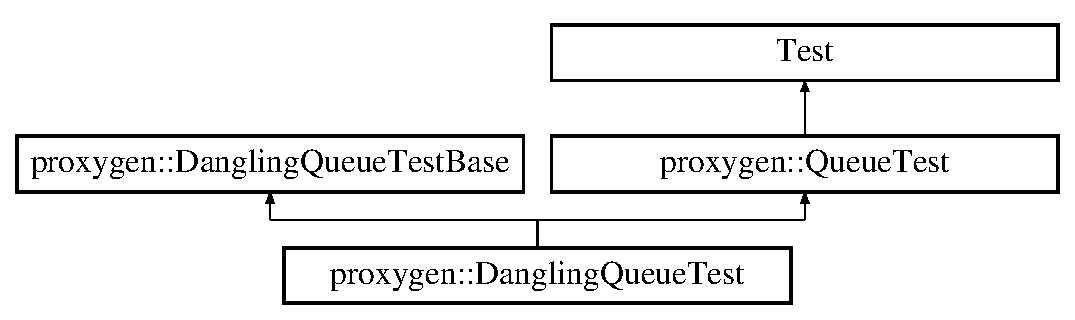
\includegraphics[height=3.000000cm]{classproxygen_1_1DanglingQueueTest}
\end{center}
\end{figure}
\subsection*{Public Member Functions}
\begin{DoxyCompactItemize}
\item 
{\bf Dangling\+Queue\+Test} ()
\end{DoxyCompactItemize}
\subsection*{Additional Inherited Members}


\subsection{Detailed Description}


Definition at line 758 of file H\+T\+T\+P2\+Priority\+Queue\+Test.\+cpp.



\subsection{Constructor \& Destructor Documentation}
\index{proxygen\+::\+Dangling\+Queue\+Test@{proxygen\+::\+Dangling\+Queue\+Test}!Dangling\+Queue\+Test@{Dangling\+Queue\+Test}}
\index{Dangling\+Queue\+Test@{Dangling\+Queue\+Test}!proxygen\+::\+Dangling\+Queue\+Test@{proxygen\+::\+Dangling\+Queue\+Test}}
\subsubsection[{Dangling\+Queue\+Test()}]{\setlength{\rightskip}{0pt plus 5cm}proxygen\+::\+Dangling\+Queue\+Test\+::\+Dangling\+Queue\+Test (
\begin{DoxyParamCaption}
{}
\end{DoxyParamCaption}
)\hspace{0.3cm}{\ttfamily [inline]}}\label{classproxygen_1_1DanglingQueueTest_af94ed62adbe41558bdbe1948d8d712ac}


Definition at line 760 of file H\+T\+T\+P2\+Priority\+Queue\+Test.\+cpp.


\begin{DoxyCode}
760                       :
761     DanglingQueueTestBase(),
762     QueueTest(&timer_) \{
763   \}
\end{DoxyCode}


The documentation for this class was generated from the following file\+:\begin{DoxyCompactItemize}
\item 
proxygen/lib/http/session/test/{\bf H\+T\+T\+P2\+Priority\+Queue\+Test.\+cpp}\end{DoxyCompactItemize}

\section{proxygen\+:\+:Dangling\+Queue\+Test\+Base Class Reference}
\label{classproxygen_1_1DanglingQueueTestBase}\index{proxygen\+::\+Dangling\+Queue\+Test\+Base@{proxygen\+::\+Dangling\+Queue\+Test\+Base}}
Inheritance diagram for proxygen\+:\+:Dangling\+Queue\+Test\+Base\+:\begin{figure}[H]
\begin{center}
\leavevmode
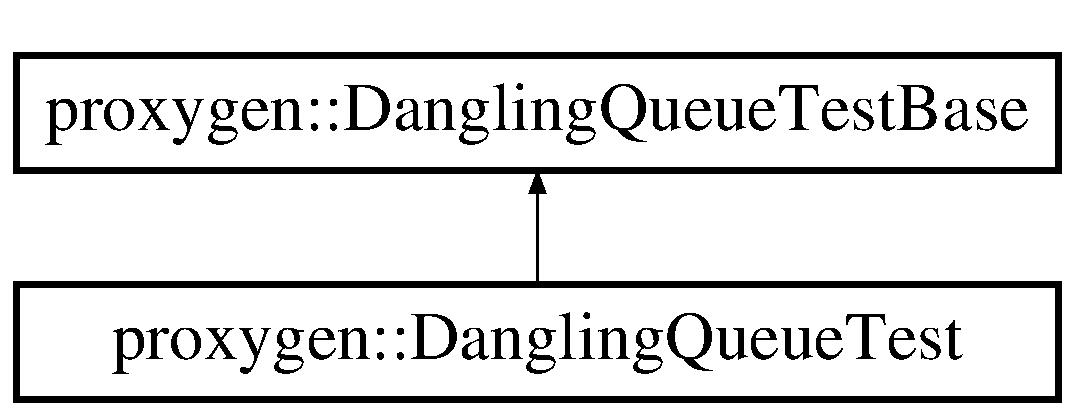
\includegraphics[height=2.000000cm]{classproxygen_1_1DanglingQueueTestBase}
\end{center}
\end{figure}
\subsection*{Public Member Functions}
\begin{DoxyCompactItemize}
\item 
{\bf Dangling\+Queue\+Test\+Base} ()
\end{DoxyCompactItemize}
\subsection*{Protected Member Functions}
\begin{DoxyCompactItemize}
\item 
void {\bf expire\+Nodes} ()
\item 
void {\bf tick} ()
\end{DoxyCompactItemize}
\subsection*{Protected Attributes}
\begin{DoxyCompactItemize}
\item 
std\+::list$<$ folly\+::\+Async\+Timeout $\ast$ $>$ {\bf timeouts\+\_\+}
\item 
testing\+::\+Nice\+Mock$<$ Mock\+Timeout\+Manager $>$ {\bf timeout\+Manager\+\_\+}
\item 
folly\+::\+Undelayed\+Destruction$<$ H\+H\+Wheel\+Timer $>$ {\bf timer\+\_\+} \{\&{\bf timeout\+Manager\+\_\+}\}
\end{DoxyCompactItemize}


\subsection{Detailed Description}


Definition at line 719 of file H\+T\+T\+P2\+Priority\+Queue\+Test.\+cpp.



\subsection{Constructor \& Destructor Documentation}
\index{proxygen\+::\+Dangling\+Queue\+Test\+Base@{proxygen\+::\+Dangling\+Queue\+Test\+Base}!Dangling\+Queue\+Test\+Base@{Dangling\+Queue\+Test\+Base}}
\index{Dangling\+Queue\+Test\+Base@{Dangling\+Queue\+Test\+Base}!proxygen\+::\+Dangling\+Queue\+Test\+Base@{proxygen\+::\+Dangling\+Queue\+Test\+Base}}
\subsubsection[{Dangling\+Queue\+Test\+Base()}]{\setlength{\rightskip}{0pt plus 5cm}proxygen\+::\+Dangling\+Queue\+Test\+Base\+::\+Dangling\+Queue\+Test\+Base (
\begin{DoxyParamCaption}
{}
\end{DoxyParamCaption}
)\hspace{0.3cm}{\ttfamily [inline]}}\label{classproxygen_1_1DanglingQueueTestBase_a30b2582dcf1539654226c971f97d0f32}


Definition at line 721 of file H\+T\+T\+P2\+Priority\+Queue\+Test.\+cpp.


\begin{DoxyCode}
721                           \{
722     \textcolor{comment}{// Just under two ticks}
723     HTTP2PriorityQueue::setNodeLifetime(
724       std::chrono::milliseconds(2 * HHWheelTimer::DEFAULT\_TICK\_INTERVAL - 1));
725     EXPECT\_CALL(timeoutManager_, scheduleTimeout(\_, \_))
726       .WillRepeatedly(Invoke([\textcolor{keyword}{this}] (folly::AsyncTimeout* timeout,
727                                      std::chrono::milliseconds) \{
728                                timeouts_.push\_back(timeout);
729                                \textcolor{keywordflow}{return} \textcolor{keyword}{true};
730                              \}));
731   \}
\end{DoxyCode}


\subsection{Member Function Documentation}
\index{proxygen\+::\+Dangling\+Queue\+Test\+Base@{proxygen\+::\+Dangling\+Queue\+Test\+Base}!expire\+Nodes@{expire\+Nodes}}
\index{expire\+Nodes@{expire\+Nodes}!proxygen\+::\+Dangling\+Queue\+Test\+Base@{proxygen\+::\+Dangling\+Queue\+Test\+Base}}
\subsubsection[{expire\+Nodes()}]{\setlength{\rightskip}{0pt plus 5cm}void proxygen\+::\+Dangling\+Queue\+Test\+Base\+::expire\+Nodes (
\begin{DoxyParamCaption}
{}
\end{DoxyParamCaption}
)\hspace{0.3cm}{\ttfamily [inline]}, {\ttfamily [protected]}}\label{classproxygen_1_1DanglingQueueTestBase_a1ab7b50aca2fe87775cfa7ca2892846f}


Definition at line 734 of file H\+T\+T\+P2\+Priority\+Queue\+Test.\+cpp.


\begin{DoxyCode}
734                      \{
735     std::this\_thread::sleep\_for(
736       std::chrono::milliseconds(2 * HHWheelTimer::DEFAULT\_TICK\_INTERVAL));
737     \textcolor{comment}{// Node lifetime it just under two ticks, so firing twice expires all nodes}
738     tick();
739     tick();
740   \}
\end{DoxyCode}
\index{proxygen\+::\+Dangling\+Queue\+Test\+Base@{proxygen\+::\+Dangling\+Queue\+Test\+Base}!tick@{tick}}
\index{tick@{tick}!proxygen\+::\+Dangling\+Queue\+Test\+Base@{proxygen\+::\+Dangling\+Queue\+Test\+Base}}
\subsubsection[{tick()}]{\setlength{\rightskip}{0pt plus 5cm}void proxygen\+::\+Dangling\+Queue\+Test\+Base\+::tick (
\begin{DoxyParamCaption}
{}
\end{DoxyParamCaption}
)\hspace{0.3cm}{\ttfamily [inline]}, {\ttfamily [protected]}}\label{classproxygen_1_1DanglingQueueTestBase_aed87de9e5448543c171c5d3d0d093bfc}


Definition at line 742 of file H\+T\+T\+P2\+Priority\+Queue\+Test.\+cpp.


\begin{DoxyCode}
742               \{
743     std::list<folly::AsyncTimeout*> timeouts;
744     std::swap(timeouts_, timeouts);
745     \textcolor{keywordflow}{for} (\textcolor{keyword}{auto} timeout: timeouts) \{
746       timeout->timeoutExpired();
747     \}
748   \}
\end{DoxyCode}


\subsection{Member Data Documentation}
\index{proxygen\+::\+Dangling\+Queue\+Test\+Base@{proxygen\+::\+Dangling\+Queue\+Test\+Base}!timeout\+Manager\+\_\+@{timeout\+Manager\+\_\+}}
\index{timeout\+Manager\+\_\+@{timeout\+Manager\+\_\+}!proxygen\+::\+Dangling\+Queue\+Test\+Base@{proxygen\+::\+Dangling\+Queue\+Test\+Base}}
\subsubsection[{timeout\+Manager\+\_\+}]{\setlength{\rightskip}{0pt plus 5cm}testing\+::\+Nice\+Mock$<$Mock\+Timeout\+Manager$>$ proxygen\+::\+Dangling\+Queue\+Test\+Base\+::timeout\+Manager\+\_\+\hspace{0.3cm}{\ttfamily [protected]}}\label{classproxygen_1_1DanglingQueueTestBase_a524fa9fbf6ecb1e83e3d5fa7429c8905}


Definition at line 751 of file H\+T\+T\+P2\+Priority\+Queue\+Test.\+cpp.

\index{proxygen\+::\+Dangling\+Queue\+Test\+Base@{proxygen\+::\+Dangling\+Queue\+Test\+Base}!timeouts\+\_\+@{timeouts\+\_\+}}
\index{timeouts\+\_\+@{timeouts\+\_\+}!proxygen\+::\+Dangling\+Queue\+Test\+Base@{proxygen\+::\+Dangling\+Queue\+Test\+Base}}
\subsubsection[{timeouts\+\_\+}]{\setlength{\rightskip}{0pt plus 5cm}std\+::list$<$folly\+::\+Async\+Timeout$\ast$$>$ proxygen\+::\+Dangling\+Queue\+Test\+Base\+::timeouts\+\_\+\hspace{0.3cm}{\ttfamily [protected]}}\label{classproxygen_1_1DanglingQueueTestBase_ad591bb3840b23d95d7af977604868ca3}


Definition at line 750 of file H\+T\+T\+P2\+Priority\+Queue\+Test.\+cpp.

\index{proxygen\+::\+Dangling\+Queue\+Test\+Base@{proxygen\+::\+Dangling\+Queue\+Test\+Base}!timer\+\_\+@{timer\+\_\+}}
\index{timer\+\_\+@{timer\+\_\+}!proxygen\+::\+Dangling\+Queue\+Test\+Base@{proxygen\+::\+Dangling\+Queue\+Test\+Base}}
\subsubsection[{timer\+\_\+}]{\setlength{\rightskip}{0pt plus 5cm}folly\+::\+Undelayed\+Destruction$<$H\+H\+Wheel\+Timer$>$ proxygen\+::\+Dangling\+Queue\+Test\+Base\+::timer\+\_\+ \{\&{\bf timeout\+Manager\+\_\+}\}\hspace{0.3cm}{\ttfamily [protected]}}\label{classproxygen_1_1DanglingQueueTestBase_ac65c387cda8f4586a75684bf908499b1}


Definition at line 752 of file H\+T\+T\+P2\+Priority\+Queue\+Test.\+cpp.



The documentation for this class was generated from the following file\+:\begin{DoxyCompactItemize}
\item 
proxygen/lib/http/session/test/{\bf H\+T\+T\+P2\+Priority\+Queue\+Test.\+cpp}\end{DoxyCompactItemize}

\section{proxygen\+:\+:Default\+H\+T\+T\+P\+Codec\+Factory Class Reference}
\label{classproxygen_1_1DefaultHTTPCodecFactory}\index{proxygen\+::\+Default\+H\+T\+T\+P\+Codec\+Factory@{proxygen\+::\+Default\+H\+T\+T\+P\+Codec\+Factory}}


{\ttfamily \#include $<$Default\+H\+T\+T\+P\+Codec\+Factory.\+h$>$}

Inheritance diagram for proxygen\+:\+:Default\+H\+T\+T\+P\+Codec\+Factory\+:\begin{figure}[H]
\begin{center}
\leavevmode
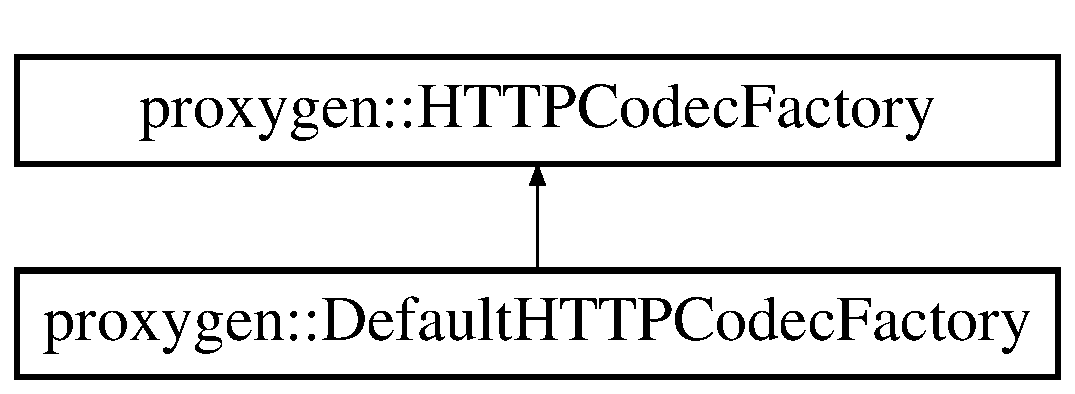
\includegraphics[height=2.000000cm]{classproxygen_1_1DefaultHTTPCodecFactory}
\end{center}
\end{figure}
\subsection*{Public Member Functions}
\begin{DoxyCompactItemize}
\item 
{\bf Default\+H\+T\+T\+P\+Codec\+Factory} (bool force\+H\+T\+T\+P1x\+Codec\+To1\+\_\+1)
\item 
{\bf $\sim$\+Default\+H\+T\+T\+P\+Codec\+Factory} () override=default
\item 
std\+::unique\+\_\+ptr$<$ {\bf H\+T\+T\+P\+Codec} $>$ {\bf get\+Codec} (const std\+::string \&next\+Protocol, {\bf Transport\+Direction} direction, bool is\+T\+LS) override
\item 
void {\bf set\+Force\+H\+T\+T\+P1x\+Codec\+To1\+\_\+1} (bool force\+H\+T\+T\+P1x\+Codec\+To1\+\_\+1)
\end{DoxyCompactItemize}
\subsection*{Protected Attributes}
\begin{DoxyCompactItemize}
\item 
bool {\bf force\+H\+T\+T\+P1x\+Codec\+To1\+\_\+1\+\_\+} \{false\}
\end{DoxyCompactItemize}
\subsection*{Additional Inherited Members}


\subsection{Detailed Description}


Definition at line 15 of file Default\+H\+T\+T\+P\+Codec\+Factory.\+h.



\subsection{Constructor \& Destructor Documentation}
\index{proxygen\+::\+Default\+H\+T\+T\+P\+Codec\+Factory@{proxygen\+::\+Default\+H\+T\+T\+P\+Codec\+Factory}!Default\+H\+T\+T\+P\+Codec\+Factory@{Default\+H\+T\+T\+P\+Codec\+Factory}}
\index{Default\+H\+T\+T\+P\+Codec\+Factory@{Default\+H\+T\+T\+P\+Codec\+Factory}!proxygen\+::\+Default\+H\+T\+T\+P\+Codec\+Factory@{proxygen\+::\+Default\+H\+T\+T\+P\+Codec\+Factory}}
\subsubsection[{Default\+H\+T\+T\+P\+Codec\+Factory(bool force\+H\+T\+T\+P1x\+Codec\+To1\+\_\+1)}]{\setlength{\rightskip}{0pt plus 5cm}proxygen\+::\+Default\+H\+T\+T\+P\+Codec\+Factory\+::\+Default\+H\+T\+T\+P\+Codec\+Factory (
\begin{DoxyParamCaption}
\item[{bool}]{force\+H\+T\+T\+P1x\+Codec\+To1\+\_\+1}
\end{DoxyParamCaption}
)\hspace{0.3cm}{\ttfamily [explicit]}}\label{classproxygen_1_1DefaultHTTPCodecFactory_a6aec151abe51ff173ff66c4a971e7bbd}


Definition at line 19 of file Default\+H\+T\+T\+P\+Codec\+Factory.\+cpp.


\begin{DoxyCode}
21     : forceHTTP1xCodecTo1_1_(forceHTTP1xCodecTo1\_1) \{
22 \}
\end{DoxyCode}
\index{proxygen\+::\+Default\+H\+T\+T\+P\+Codec\+Factory@{proxygen\+::\+Default\+H\+T\+T\+P\+Codec\+Factory}!````~Default\+H\+T\+T\+P\+Codec\+Factory@{$\sim$\+Default\+H\+T\+T\+P\+Codec\+Factory}}
\index{````~Default\+H\+T\+T\+P\+Codec\+Factory@{$\sim$\+Default\+H\+T\+T\+P\+Codec\+Factory}!proxygen\+::\+Default\+H\+T\+T\+P\+Codec\+Factory@{proxygen\+::\+Default\+H\+T\+T\+P\+Codec\+Factory}}
\subsubsection[{$\sim$\+Default\+H\+T\+T\+P\+Codec\+Factory() override=default}]{\setlength{\rightskip}{0pt plus 5cm}proxygen\+::\+Default\+H\+T\+T\+P\+Codec\+Factory\+::$\sim$\+Default\+H\+T\+T\+P\+Codec\+Factory (
\begin{DoxyParamCaption}
{}
\end{DoxyParamCaption}
)\hspace{0.3cm}{\ttfamily [override]}, {\ttfamily [default]}}\label{classproxygen_1_1DefaultHTTPCodecFactory_aba86335aea44dd00fb5778372029791c}


\subsection{Member Function Documentation}
\index{proxygen\+::\+Default\+H\+T\+T\+P\+Codec\+Factory@{proxygen\+::\+Default\+H\+T\+T\+P\+Codec\+Factory}!get\+Codec@{get\+Codec}}
\index{get\+Codec@{get\+Codec}!proxygen\+::\+Default\+H\+T\+T\+P\+Codec\+Factory@{proxygen\+::\+Default\+H\+T\+T\+P\+Codec\+Factory}}
\subsubsection[{get\+Codec(const std\+::string \&next\+Protocol, Transport\+Direction direction, bool is\+T\+L\+S) override}]{\setlength{\rightskip}{0pt plus 5cm}std\+::unique\+\_\+ptr$<$ {\bf H\+T\+T\+P\+Codec} $>$ proxygen\+::\+Default\+H\+T\+T\+P\+Codec\+Factory\+::get\+Codec (
\begin{DoxyParamCaption}
\item[{const std\+::string \&}]{next\+Protocol, }
\item[{{\bf Transport\+Direction}}]{direction, }
\item[{bool}]{is\+T\+LS}
\end{DoxyParamCaption}
)\hspace{0.3cm}{\ttfamily [override]}, {\ttfamily [virtual]}}\label{classproxygen_1_1DefaultHTTPCodecFactory_ad87f587d94ea757a1db0e3863bf8b643}
Get a codec instance 

Implements {\bf proxygen\+::\+H\+T\+T\+P\+Codec\+Factory} \doxyref{}{p.}{classproxygen_1_1HTTPCodecFactory_ab0d8d25513603c7d4bd0d7036ab78066}.



Definition at line 24 of file Default\+H\+T\+T\+P\+Codec\+Factory.\+cpp.



References proxygen\+::\+E\+R\+R\+OR, force\+H\+T\+T\+P1x\+Codec\+To1\+\_\+1\+\_\+, proxygen\+::\+S\+P\+D\+Y\+Codec\+::get\+Version(), proxygen\+::http2\+::k\+Protocol\+Cleartext\+String, proxygen\+::http2\+::k\+Protocol\+Draft\+String, proxygen\+::http2\+::k\+Protocol\+Experimental\+String, proxygen\+::http2\+::k\+Protocol\+String, and proxygen\+::\+H\+T\+T\+P1x\+Codec\+::supports\+Next\+Protocol().



Referenced by T\+E\+S\+T().


\begin{DoxyCode}
27             \{
28 
29     \textcolor{keyword}{auto} spdyVersion = SPDYCodec::getVersion(chosenProto);
30     \textcolor{keywordflow}{if} (spdyVersion) \{
31       \textcolor{keywordflow}{return} std::make\_unique<SPDYCodec>(direction,
32                                            *spdyVersion);
33     \} \textcolor{keywordflow}{else} \textcolor{keywordflow}{if} (chosenProto == proxygen::http2::kProtocolString ||
34                chosenProto == proxygen::http2::kProtocolCleartextString ||
35                chosenProto == proxygen::http2::kProtocolDraftString ||
36                chosenProto == proxygen::http2::kProtocolExperimentalString) \{
37       \textcolor{keywordflow}{return} std::make\_unique<HTTP2Codec>(direction);
38     \} \textcolor{keywordflow}{else} \{
39       \textcolor{keywordflow}{if} (!chosenProto.empty() &&
40           !HTTP1xCodec::supportsNextProtocol(chosenProto)) \{
41         LOG(ERROR) << \textcolor{stringliteral}{"Chosen upstream protocol "} <<
42           \textcolor{stringliteral}{"\(\backslash\)""} << chosenProto << \textcolor{stringliteral}{"\(\backslash\)" is unimplemented. "} <<
43           \textcolor{stringliteral}{"Attempting to use HTTP/1.1"};
44       \}
45 
46       \textcolor{keywordflow}{return} std::make\_unique<HTTP1xCodec>(direction,
47                                              forceHTTP1xCodecTo1_1_);
48     \}
49 \}
\end{DoxyCode}
\index{proxygen\+::\+Default\+H\+T\+T\+P\+Codec\+Factory@{proxygen\+::\+Default\+H\+T\+T\+P\+Codec\+Factory}!set\+Force\+H\+T\+T\+P1x\+Codec\+To1\+\_\+1@{set\+Force\+H\+T\+T\+P1x\+Codec\+To1\+\_\+1}}
\index{set\+Force\+H\+T\+T\+P1x\+Codec\+To1\+\_\+1@{set\+Force\+H\+T\+T\+P1x\+Codec\+To1\+\_\+1}!proxygen\+::\+Default\+H\+T\+T\+P\+Codec\+Factory@{proxygen\+::\+Default\+H\+T\+T\+P\+Codec\+Factory}}
\subsubsection[{set\+Force\+H\+T\+T\+P1x\+Codec\+To1\+\_\+1(bool force\+H\+T\+T\+P1x\+Codec\+To1\+\_\+1)}]{\setlength{\rightskip}{0pt plus 5cm}void proxygen\+::\+Default\+H\+T\+T\+P\+Codec\+Factory\+::set\+Force\+H\+T\+T\+P1x\+Codec\+To1\+\_\+1 (
\begin{DoxyParamCaption}
\item[{bool}]{force\+H\+T\+T\+P1x\+Codec\+To1\+\_\+1}
\end{DoxyParamCaption}
)\hspace{0.3cm}{\ttfamily [inline]}}\label{classproxygen_1_1DefaultHTTPCodecFactory_a6687c037bff66a077fe05555a5edc2a5}


Definition at line 27 of file Default\+H\+T\+T\+P\+Codec\+Factory.\+h.



References force\+H\+T\+T\+P1x\+Codec\+To1\+\_\+1\+\_\+.


\begin{DoxyCode}
27                                                             \{
28     forceHTTP1xCodecTo1_1_ = forceHTTP1xCodecTo1\_1;
29   \}
\end{DoxyCode}


\subsection{Member Data Documentation}
\index{proxygen\+::\+Default\+H\+T\+T\+P\+Codec\+Factory@{proxygen\+::\+Default\+H\+T\+T\+P\+Codec\+Factory}!force\+H\+T\+T\+P1x\+Codec\+To1\+\_\+1\+\_\+@{force\+H\+T\+T\+P1x\+Codec\+To1\+\_\+1\+\_\+}}
\index{force\+H\+T\+T\+P1x\+Codec\+To1\+\_\+1\+\_\+@{force\+H\+T\+T\+P1x\+Codec\+To1\+\_\+1\+\_\+}!proxygen\+::\+Default\+H\+T\+T\+P\+Codec\+Factory@{proxygen\+::\+Default\+H\+T\+T\+P\+Codec\+Factory}}
\subsubsection[{force\+H\+T\+T\+P1x\+Codec\+To1\+\_\+1\+\_\+}]{\setlength{\rightskip}{0pt plus 5cm}bool proxygen\+::\+Default\+H\+T\+T\+P\+Codec\+Factory\+::force\+H\+T\+T\+P1x\+Codec\+To1\+\_\+1\+\_\+ \{false\}\hspace{0.3cm}{\ttfamily [protected]}}\label{classproxygen_1_1DefaultHTTPCodecFactory_a9d307f887cc96b95f0c0270984316388}


Definition at line 31 of file Default\+H\+T\+T\+P\+Codec\+Factory.\+h.



Referenced by get\+Codec(), and set\+Force\+H\+T\+T\+P1x\+Codec\+To1\+\_\+1().



The documentation for this class was generated from the following files\+:\begin{DoxyCompactItemize}
\item 
proxygen/lib/http/codec/{\bf Default\+H\+T\+T\+P\+Codec\+Factory.\+h}\item 
proxygen/lib/http/codec/{\bf Default\+H\+T\+T\+P\+Codec\+Factory.\+cpp}\end{DoxyCompactItemize}

\section{proxygen\+:\+:Direct\+Response\+Handler Class Reference}
\label{classproxygen_1_1DirectResponseHandler}\index{proxygen\+::\+Direct\+Response\+Handler@{proxygen\+::\+Direct\+Response\+Handler}}


{\ttfamily \#include $<$Direct\+Response\+Handler.\+h$>$}

Inheritance diagram for proxygen\+:\+:Direct\+Response\+Handler\+:\begin{figure}[H]
\begin{center}
\leavevmode
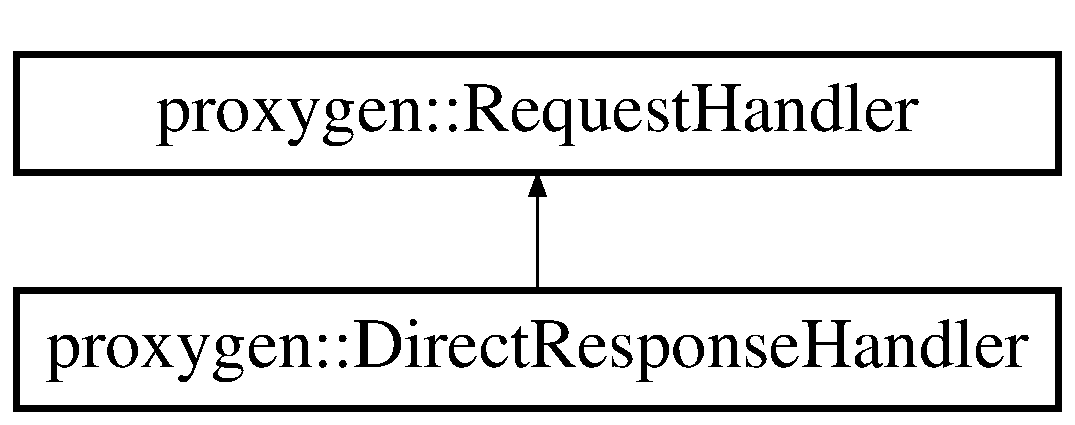
\includegraphics[height=2.000000cm]{classproxygen_1_1DirectResponseHandler}
\end{center}
\end{figure}
\subsection*{Public Member Functions}
\begin{DoxyCompactItemize}
\item 
{\bf Direct\+Response\+Handler} (int code, std\+::string {\bf message}, std\+::string body)
\item 
void {\bf on\+Request} (std\+::unique\+\_\+ptr$<$ {\bf H\+T\+T\+P\+Message} $>$) noexceptoverride
\item 
void {\bf on\+Body} (std\+::unique\+\_\+ptr$<$ folly\+::\+I\+O\+Buf $>$) noexceptoverride
\item 
void {\bf on\+Upgrade} ({\bf proxygen\+::\+Upgrade\+Protocol}) noexceptoverride
\item 
void {\bf on\+E\+OM} () noexceptoverride
\item 
void {\bf request\+Complete} () noexceptoverride
\item 
void {\bf on\+Error} ({\bf Proxygen\+Error}) noexceptoverride
\end{DoxyCompactItemize}
\subsection*{Private Attributes}
\begin{DoxyCompactItemize}
\item 
const int {\bf code\+\_\+}
\item 
std\+::string {\bf message\+\_\+}
\item 
std\+::unique\+\_\+ptr$<$ folly\+::\+I\+O\+Buf $>$ {\bf body\+\_\+}
\end{DoxyCompactItemize}
\subsection*{Additional Inherited Members}


\subsection{Detailed Description}
Handler that sends a fixed response back. 

Definition at line 20 of file Direct\+Response\+Handler.\+h.



\subsection{Constructor \& Destructor Documentation}
\index{proxygen\+::\+Direct\+Response\+Handler@{proxygen\+::\+Direct\+Response\+Handler}!Direct\+Response\+Handler@{Direct\+Response\+Handler}}
\index{Direct\+Response\+Handler@{Direct\+Response\+Handler}!proxygen\+::\+Direct\+Response\+Handler@{proxygen\+::\+Direct\+Response\+Handler}}
\subsubsection[{Direct\+Response\+Handler(int code, std\+::string message, std\+::string body)}]{\setlength{\rightskip}{0pt plus 5cm}proxygen\+::\+Direct\+Response\+Handler\+::\+Direct\+Response\+Handler (
\begin{DoxyParamCaption}
\item[{int}]{code, }
\item[{std\+::string}]{message, }
\item[{std\+::string}]{body}
\end{DoxyParamCaption}
)\hspace{0.3cm}{\ttfamily [inline]}}\label{classproxygen_1_1DirectResponseHandler_a062ba0e3fb9187375f420ab092e39ec7}


Definition at line 22 of file Direct\+Response\+Handler.\+h.


\begin{DoxyCode}
25       : code_(code),
26         message_(std::move(message)),
27         body_(folly::IOBuf::copyBuffer(body)) \{
28   \}
\end{DoxyCode}


\subsection{Member Function Documentation}
\index{proxygen\+::\+Direct\+Response\+Handler@{proxygen\+::\+Direct\+Response\+Handler}!on\+Body@{on\+Body}}
\index{on\+Body@{on\+Body}!proxygen\+::\+Direct\+Response\+Handler@{proxygen\+::\+Direct\+Response\+Handler}}
\subsubsection[{on\+Body(std\+::unique\+\_\+ptr$<$ folly\+::\+I\+O\+Buf $>$) noexceptoverride}]{\setlength{\rightskip}{0pt plus 5cm}void proxygen\+::\+Direct\+Response\+Handler\+::on\+Body (
\begin{DoxyParamCaption}
\item[{std\+::unique\+\_\+ptr$<$ folly\+::\+I\+O\+Buf $>$}]{body}
\end{DoxyParamCaption}
)\hspace{0.3cm}{\ttfamily [inline]}, {\ttfamily [override]}, {\ttfamily [virtual]}, {\ttfamily [noexcept]}}\label{classproxygen_1_1DirectResponseHandler_aca230a07d76dc6f8b8105dade50360e6}
Invoked when we get part of body for the request. 

Implements {\bf proxygen\+::\+Request\+Handler} \doxyref{}{p.}{classproxygen_1_1RequestHandler_aaf0ed3bb94384e6240e15cca63de82bb}.



Definition at line 32 of file Direct\+Response\+Handler.\+h.


\begin{DoxyCode}
32 \{\}
\end{DoxyCode}
\index{proxygen\+::\+Direct\+Response\+Handler@{proxygen\+::\+Direct\+Response\+Handler}!on\+E\+OM@{on\+E\+OM}}
\index{on\+E\+OM@{on\+E\+OM}!proxygen\+::\+Direct\+Response\+Handler@{proxygen\+::\+Direct\+Response\+Handler}}
\subsubsection[{on\+E\+O\+M() noexceptoverride}]{\setlength{\rightskip}{0pt plus 5cm}void proxygen\+::\+Direct\+Response\+Handler\+::on\+E\+OM (
\begin{DoxyParamCaption}
{}
\end{DoxyParamCaption}
)\hspace{0.3cm}{\ttfamily [inline]}, {\ttfamily [override]}, {\ttfamily [virtual]}, {\ttfamily [noexcept]}}\label{classproxygen_1_1DirectResponseHandler_a5307b79be1b865f7ea040ccad1262bcd}
Invoked when we finish receiving the body. 

Implements {\bf proxygen\+::\+Request\+Handler} \doxyref{}{p.}{classproxygen_1_1RequestHandler_a24f26d2cf71effaf154ce53aeff51aab}.



Definition at line 36 of file Direct\+Response\+Handler.\+h.



References proxygen\+::\+Response\+Builder\+::body(), body\+\_\+, code\+\_\+, proxygen\+::\+Request\+Handler\+::downstream\+\_\+, message\+\_\+, proxygen\+::\+Response\+Builder\+::send\+With\+E\+O\+M(), and proxygen\+::\+Response\+Builder\+::status().


\begin{DoxyCode}
36                                  \{
37     ResponseBuilder(downstream_)
38         .status(code_, std::move(message_))
39         .body(std::move(body_))
40         .sendWithEOM();
41   \}
\end{DoxyCode}
\index{proxygen\+::\+Direct\+Response\+Handler@{proxygen\+::\+Direct\+Response\+Handler}!on\+Error@{on\+Error}}
\index{on\+Error@{on\+Error}!proxygen\+::\+Direct\+Response\+Handler@{proxygen\+::\+Direct\+Response\+Handler}}
\subsubsection[{on\+Error(\+Proxygen\+Error) noexceptoverride}]{\setlength{\rightskip}{0pt plus 5cm}void proxygen\+::\+Direct\+Response\+Handler\+::on\+Error (
\begin{DoxyParamCaption}
\item[{{\bf Proxygen\+Error}}]{err}
\end{DoxyParamCaption}
)\hspace{0.3cm}{\ttfamily [inline]}, {\ttfamily [override]}, {\ttfamily [virtual]}, {\ttfamily [noexcept]}}\label{classproxygen_1_1DirectResponseHandler_a00e7231c0cfba8a580a51c5f98b1339d}
Request failed. Maybe because of read/write error on socket or client not being able to send request in time.

N\+O\+TE\+: Can be invoked at any time (except for before on\+Request).

No more callbacks will be invoked after this. You should clean up after yourself. 

Implements {\bf proxygen\+::\+Request\+Handler} \doxyref{}{p.}{classproxygen_1_1RequestHandler_ad7e6428b925840a334adc58ff6f4f680}.



Definition at line 47 of file Direct\+Response\+Handler.\+h.


\begin{DoxyCode}
47 \{ \textcolor{keyword}{delete} \textcolor{keyword}{this}; \}
\end{DoxyCode}
\index{proxygen\+::\+Direct\+Response\+Handler@{proxygen\+::\+Direct\+Response\+Handler}!on\+Request@{on\+Request}}
\index{on\+Request@{on\+Request}!proxygen\+::\+Direct\+Response\+Handler@{proxygen\+::\+Direct\+Response\+Handler}}
\subsubsection[{on\+Request(std\+::unique\+\_\+ptr$<$ H\+T\+T\+P\+Message $>$) noexceptoverride}]{\setlength{\rightskip}{0pt plus 5cm}void proxygen\+::\+Direct\+Response\+Handler\+::on\+Request (
\begin{DoxyParamCaption}
\item[{std\+::unique\+\_\+ptr$<$ {\bf H\+T\+T\+P\+Message} $>$}]{headers}
\end{DoxyParamCaption}
)\hspace{0.3cm}{\ttfamily [inline]}, {\ttfamily [override]}, {\ttfamily [virtual]}, {\ttfamily [noexcept]}}\label{classproxygen_1_1DirectResponseHandler_abc64e1082cbd55ac4c66f1ca384ba649}
Invoked when we have successfully fetched headers from client. This will always be the first callback invoked on your handler. 

Implements {\bf proxygen\+::\+Request\+Handler} \doxyref{}{p.}{classproxygen_1_1RequestHandler_a61f59e1155f906c7b73062147164320f}.



Definition at line 30 of file Direct\+Response\+Handler.\+h.


\begin{DoxyCode}
30 \{\}
\end{DoxyCode}
\index{proxygen\+::\+Direct\+Response\+Handler@{proxygen\+::\+Direct\+Response\+Handler}!on\+Upgrade@{on\+Upgrade}}
\index{on\+Upgrade@{on\+Upgrade}!proxygen\+::\+Direct\+Response\+Handler@{proxygen\+::\+Direct\+Response\+Handler}}
\subsubsection[{on\+Upgrade(proxygen\+::\+Upgrade\+Protocol) noexceptoverride}]{\setlength{\rightskip}{0pt plus 5cm}void proxygen\+::\+Direct\+Response\+Handler\+::on\+Upgrade (
\begin{DoxyParamCaption}
\item[{{\bf proxygen\+::\+Upgrade\+Protocol}}]{prot}
\end{DoxyParamCaption}
)\hspace{0.3cm}{\ttfamily [inline]}, {\ttfamily [override]}, {\ttfamily [virtual]}, {\ttfamily [noexcept]}}\label{classproxygen_1_1DirectResponseHandler_ad6386cd4e5b5d2d49b3dc1934432f08c}
Invoked when the session has been upgraded to a different protocol 

Implements {\bf proxygen\+::\+Request\+Handler} \doxyref{}{p.}{classproxygen_1_1RequestHandler_aefed2946bc5558baf6e36a2d11290b79}.



Definition at line 34 of file Direct\+Response\+Handler.\+h.


\begin{DoxyCode}
34 \{\}
\end{DoxyCode}
\index{proxygen\+::\+Direct\+Response\+Handler@{proxygen\+::\+Direct\+Response\+Handler}!request\+Complete@{request\+Complete}}
\index{request\+Complete@{request\+Complete}!proxygen\+::\+Direct\+Response\+Handler@{proxygen\+::\+Direct\+Response\+Handler}}
\subsubsection[{request\+Complete() noexceptoverride}]{\setlength{\rightskip}{0pt plus 5cm}void proxygen\+::\+Direct\+Response\+Handler\+::request\+Complete (
\begin{DoxyParamCaption}
{}
\end{DoxyParamCaption}
)\hspace{0.3cm}{\ttfamily [inline]}, {\ttfamily [override]}, {\ttfamily [virtual]}, {\ttfamily [noexcept]}}\label{classproxygen_1_1DirectResponseHandler_a26fc292f230767b390b2d2a7d9228de1}
Invoked when request processing has been completed and nothing more needs to be done. This may be a good place to log some stats and clean up resources. This is distinct from \doxyref{on\+E\+O\+M()}{p.}{classproxygen_1_1DirectResponseHandler_a5307b79be1b865f7ea040ccad1262bcd} because it is invoked after the response is fully sent. Once this callback has been received, {\ttfamily downstream\+\_\+} should be considered invalid. 

Implements {\bf proxygen\+::\+Request\+Handler} \doxyref{}{p.}{classproxygen_1_1RequestHandler_a0ec159751b407bcd3667994c6d8d7cfe}.



Definition at line 43 of file Direct\+Response\+Handler.\+h.


\begin{DoxyCode}
43                                            \{
44     \textcolor{keyword}{delete} \textcolor{keyword}{this};
45   \}
\end{DoxyCode}


\subsection{Member Data Documentation}
\index{proxygen\+::\+Direct\+Response\+Handler@{proxygen\+::\+Direct\+Response\+Handler}!body\+\_\+@{body\+\_\+}}
\index{body\+\_\+@{body\+\_\+}!proxygen\+::\+Direct\+Response\+Handler@{proxygen\+::\+Direct\+Response\+Handler}}
\subsubsection[{body\+\_\+}]{\setlength{\rightskip}{0pt plus 5cm}std\+::unique\+\_\+ptr$<$folly\+::\+I\+O\+Buf$>$ proxygen\+::\+Direct\+Response\+Handler\+::body\+\_\+\hspace{0.3cm}{\ttfamily [private]}}\label{classproxygen_1_1DirectResponseHandler_a485750f522109b9d88f7dfc6f9746505}


Definition at line 52 of file Direct\+Response\+Handler.\+h.



Referenced by on\+E\+O\+M().

\index{proxygen\+::\+Direct\+Response\+Handler@{proxygen\+::\+Direct\+Response\+Handler}!code\+\_\+@{code\+\_\+}}
\index{code\+\_\+@{code\+\_\+}!proxygen\+::\+Direct\+Response\+Handler@{proxygen\+::\+Direct\+Response\+Handler}}
\subsubsection[{code\+\_\+}]{\setlength{\rightskip}{0pt plus 5cm}const int proxygen\+::\+Direct\+Response\+Handler\+::code\+\_\+\hspace{0.3cm}{\ttfamily [private]}}\label{classproxygen_1_1DirectResponseHandler_adabe02047534aa413786c8211697b5bd}


Definition at line 50 of file Direct\+Response\+Handler.\+h.



Referenced by on\+E\+O\+M().

\index{proxygen\+::\+Direct\+Response\+Handler@{proxygen\+::\+Direct\+Response\+Handler}!message\+\_\+@{message\+\_\+}}
\index{message\+\_\+@{message\+\_\+}!proxygen\+::\+Direct\+Response\+Handler@{proxygen\+::\+Direct\+Response\+Handler}}
\subsubsection[{message\+\_\+}]{\setlength{\rightskip}{0pt plus 5cm}std\+::string proxygen\+::\+Direct\+Response\+Handler\+::message\+\_\+\hspace{0.3cm}{\ttfamily [private]}}\label{classproxygen_1_1DirectResponseHandler_a2d1942cefd927731660f46cdb5cb2e18}


Definition at line 51 of file Direct\+Response\+Handler.\+h.



Referenced by on\+E\+O\+M().



The documentation for this class was generated from the following file\+:\begin{DoxyCompactItemize}
\item 
proxygen/httpserver/filters/{\bf Direct\+Response\+Handler.\+h}\end{DoxyCompactItemize}

\section{docker\+\_\+builder.\+Docker\+F\+B\+Code\+Builder Class Reference}
\label{classdocker__builder_1_1DockerFBCodeBuilder}\index{docker\+\_\+builder.\+Docker\+F\+B\+Code\+Builder@{docker\+\_\+builder.\+Docker\+F\+B\+Code\+Builder}}
Inheritance diagram for docker\+\_\+builder.\+Docker\+F\+B\+Code\+Builder\+:\begin{figure}[H]
\begin{center}
\leavevmode
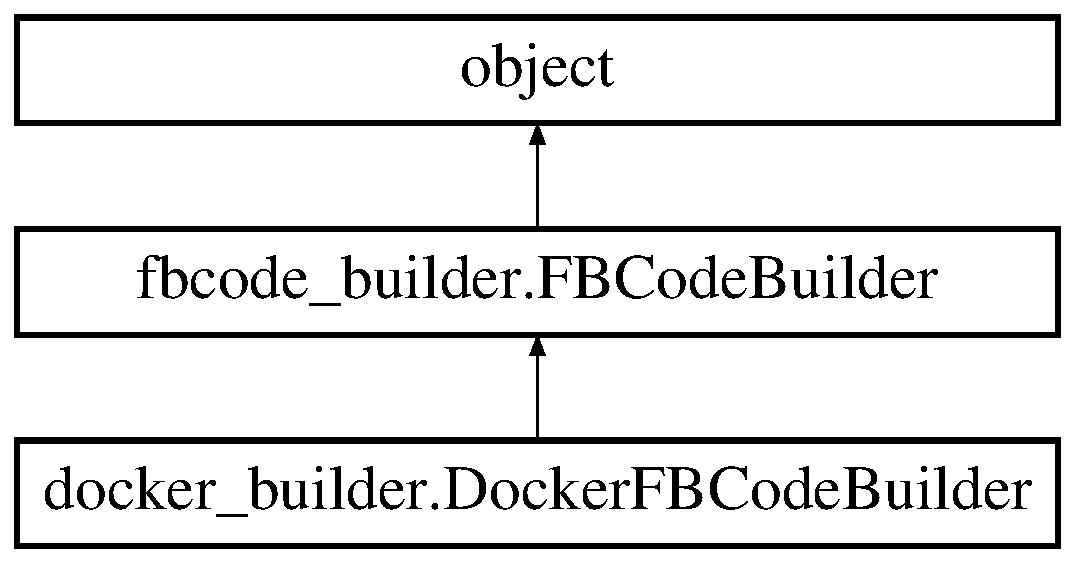
\includegraphics[height=3.000000cm]{classdocker__builder_1_1DockerFBCodeBuilder}
\end{center}
\end{figure}
\subsection*{Public Member Functions}
\begin{DoxyCompactItemize}
\item 
def {\bf setup} (self)
\item 
def {\bf step} (self, {\bf name}, actions)
\item 
def {\bf run} (self, shell\+\_\+cmd)
\item 
def {\bf workdir} (self, dir)
\item 
def {\bf comment} (self, comment)
\item 
def {\bf copy\+\_\+local\+\_\+repo} (self, repo\+\_\+dir, dest\+\_\+name)
\item 
def {\bf debian\+\_\+ccache\+\_\+setup\+\_\+steps} (self)
\end{DoxyCompactItemize}
\subsection*{Private Member Functions}
\begin{DoxyCompactItemize}
\item 
def {\bf \+\_\+user} (self)
\item 
def {\bf \+\_\+change\+\_\+user} (self)
\item 
def {\bf \+\_\+render\+\_\+impl} (self, steps)
\end{DoxyCompactItemize}
\subsection*{Additional Inherited Members}


\subsection{Detailed Description}


Definition at line 31 of file docker\+\_\+builder.\+py.



\subsection{Member Function Documentation}
\index{docker\+\_\+builder\+::\+Docker\+F\+B\+Code\+Builder@{docker\+\_\+builder\+::\+Docker\+F\+B\+Code\+Builder}!\+\_\+change\+\_\+user@{\+\_\+change\+\_\+user}}
\index{\+\_\+change\+\_\+user@{\+\_\+change\+\_\+user}!docker\+\_\+builder\+::\+Docker\+F\+B\+Code\+Builder@{docker\+\_\+builder\+::\+Docker\+F\+B\+Code\+Builder}}
\subsubsection[{\+\_\+change\+\_\+user(self)}]{\setlength{\rightskip}{0pt plus 5cm}def docker\+\_\+builder.\+Docker\+F\+B\+Code\+Builder.\+\_\+change\+\_\+user (
\begin{DoxyParamCaption}
\item[{}]{self}
\end{DoxyParamCaption}
)\hspace{0.3cm}{\ttfamily [private]}}\label{classdocker__builder_1_1DockerFBCodeBuilder_ae9a8254850be534c23318817c2346425}


Definition at line 36 of file docker\+\_\+builder.\+py.



References docker\+\_\+builder.\+Docker\+F\+B\+Code\+Builder.\+\_\+user().



Referenced by docker\+\_\+builder.\+Docker\+F\+B\+Code\+Builder.\+copy\+\_\+local\+\_\+repo(), docker\+\_\+builder.\+Docker\+F\+B\+Code\+Builder.\+setup(), and docker\+\_\+builder.\+Docker\+F\+B\+Code\+Builder.\+workdir().


\begin{DoxyCode}
36     \textcolor{keyword}{def }_change_user(self):
37         \textcolor{keywordflow}{return} ShellQuoted(\textcolor{stringliteral}{'USER \{u\}'}).format(u=self._user())
38 
\end{DoxyCode}
\index{docker\+\_\+builder\+::\+Docker\+F\+B\+Code\+Builder@{docker\+\_\+builder\+::\+Docker\+F\+B\+Code\+Builder}!\+\_\+render\+\_\+impl@{\+\_\+render\+\_\+impl}}
\index{\+\_\+render\+\_\+impl@{\+\_\+render\+\_\+impl}!docker\+\_\+builder\+::\+Docker\+F\+B\+Code\+Builder@{docker\+\_\+builder\+::\+Docker\+F\+B\+Code\+Builder}}
\subsubsection[{\+\_\+render\+\_\+impl(self, steps)}]{\setlength{\rightskip}{0pt plus 5cm}def docker\+\_\+builder.\+Docker\+F\+B\+Code\+Builder.\+\_\+render\+\_\+impl (
\begin{DoxyParamCaption}
\item[{}]{self, }
\item[{}]{steps}
\end{DoxyParamCaption}
)\hspace{0.3cm}{\ttfamily [private]}}\label{classdocker__builder_1_1DockerFBCodeBuilder_a28411db2584ad62e8440443ea7533d04}


Definition at line 99 of file docker\+\_\+builder.\+py.



References shell\+\_\+quoting.\+raw\+\_\+shell(), utils.\+recursively\+\_\+flatten\+\_\+list(), and shell\+\_\+quoting.\+shell\+\_\+join().



Referenced by fbcode\+\_\+builder.\+F\+B\+Code\+Builder.\+render().


\begin{DoxyCode}
99     \textcolor{keyword}{def }_render_impl(self, steps):
100         \textcolor{keywordflow}{return} raw_shell(shell_join(\textcolor{stringliteral}{'\(\backslash\)n'}, recursively_flatten_list(steps)))
101 
\end{DoxyCode}
\index{docker\+\_\+builder\+::\+Docker\+F\+B\+Code\+Builder@{docker\+\_\+builder\+::\+Docker\+F\+B\+Code\+Builder}!\+\_\+user@{\+\_\+user}}
\index{\+\_\+user@{\+\_\+user}!docker\+\_\+builder\+::\+Docker\+F\+B\+Code\+Builder@{docker\+\_\+builder\+::\+Docker\+F\+B\+Code\+Builder}}
\subsubsection[{\+\_\+user(self)}]{\setlength{\rightskip}{0pt plus 5cm}def docker\+\_\+builder.\+Docker\+F\+B\+Code\+Builder.\+\_\+user (
\begin{DoxyParamCaption}
\item[{}]{self}
\end{DoxyParamCaption}
)\hspace{0.3cm}{\ttfamily [private]}}\label{classdocker__builder_1_1DockerFBCodeBuilder_a8c350592f660a5ad3dbcad6fb83b55b2}


Definition at line 33 of file docker\+\_\+builder.\+py.



References fbcode\+\_\+builder.\+F\+B\+Code\+Builder.\+option().



Referenced by docker\+\_\+builder.\+Docker\+F\+B\+Code\+Builder.\+\_\+change\+\_\+user(), docker\+\_\+builder.\+Docker\+F\+B\+Code\+Builder.\+copy\+\_\+local\+\_\+repo(), and docker\+\_\+builder.\+Docker\+F\+B\+Code\+Builder.\+workdir().


\begin{DoxyCode}
33     \textcolor{keyword}{def }_user(self):
34         \textcolor{keywordflow}{return} self.option(\textcolor{stringliteral}{'user'}, \textcolor{stringliteral}{'root'})
35 
\end{DoxyCode}
\index{docker\+\_\+builder\+::\+Docker\+F\+B\+Code\+Builder@{docker\+\_\+builder\+::\+Docker\+F\+B\+Code\+Builder}!comment@{comment}}
\index{comment@{comment}!docker\+\_\+builder\+::\+Docker\+F\+B\+Code\+Builder@{docker\+\_\+builder\+::\+Docker\+F\+B\+Code\+Builder}}
\subsubsection[{comment(self, comment)}]{\setlength{\rightskip}{0pt plus 5cm}def docker\+\_\+builder.\+Docker\+F\+B\+Code\+Builder.\+comment (
\begin{DoxyParamCaption}
\item[{}]{self, }
\item[{}]{comment}
\end{DoxyParamCaption}
)}\label{classdocker__builder_1_1DockerFBCodeBuilder_a435e2725f7aef068b637c39533e0f8fa}


Definition at line 74 of file docker\+\_\+builder.\+py.



References shell\+\_\+quoting.\+shell\+\_\+comment().



Referenced by fbcode\+\_\+builder.\+F\+B\+Code\+Builder.\+diagnostics().


\begin{DoxyCode}
74     \textcolor{keyword}{def }comment(self, comment):
75         \textcolor{comment}{# This should not be a command since we don't want comment changes}
76         \textcolor{comment}{# to invalidate the Docker build cache.}
77         \textcolor{keywordflow}{return} shell_comment(comment)
78 
\end{DoxyCode}
\index{docker\+\_\+builder\+::\+Docker\+F\+B\+Code\+Builder@{docker\+\_\+builder\+::\+Docker\+F\+B\+Code\+Builder}!copy\+\_\+local\+\_\+repo@{copy\+\_\+local\+\_\+repo}}
\index{copy\+\_\+local\+\_\+repo@{copy\+\_\+local\+\_\+repo}!docker\+\_\+builder\+::\+Docker\+F\+B\+Code\+Builder@{docker\+\_\+builder\+::\+Docker\+F\+B\+Code\+Builder}}
\subsubsection[{copy\+\_\+local\+\_\+repo(self, repo\+\_\+dir, dest\+\_\+name)}]{\setlength{\rightskip}{0pt plus 5cm}def docker\+\_\+builder.\+Docker\+F\+B\+Code\+Builder.\+copy\+\_\+local\+\_\+repo (
\begin{DoxyParamCaption}
\item[{}]{self, }
\item[{}]{repo\+\_\+dir, }
\item[{}]{dest\+\_\+name}
\end{DoxyParamCaption}
)}\label{classdocker__builder_1_1DockerFBCodeBuilder_ab848cddfad2aee07a95b9ff0d6bb701a}


Definition at line 79 of file docker\+\_\+builder.\+py.



References docker\+\_\+builder.\+Docker\+F\+B\+Code\+Builder.\+\_\+change\+\_\+user(), docker\+\_\+builder.\+Docker\+F\+B\+Code\+Builder.\+\_\+user(), fbcode\+\_\+builder.\+F\+B\+Code\+Builder.\+option(), and utils.\+run\+\_\+command().



Referenced by fbcode\+\_\+builder.\+F\+B\+Code\+Builder.\+github\+\_\+project\+\_\+workdir().


\begin{DoxyCode}
79     \textcolor{keyword}{def }copy_local_repo(self, repo\_dir, dest\_name):
80         fd, archive\_path = tempfile.mkstemp(
81             prefix=\textcolor{stringliteral}{'local\_repo\_\{0\}\_'}.format(dest\_name),
82             suffix=\textcolor{stringliteral}{'.tgz'},
83             dir=os.path.abspath(self.option(\textcolor{stringliteral}{'docker\_context\_dir'})),
84         )
85         os.close(fd)
86         run_command(\textcolor{stringliteral}{'tar'}, \textcolor{stringliteral}{'czf'}, archive\_path, \textcolor{stringliteral}{'.'}, cwd=repo\_dir)
87         \textcolor{keywordflow}{return} [
88             ShellQuoted(\textcolor{stringliteral}{'ADD \{archive\} \{dest\_name\}'}).format(
89                 archive=os.path.basename(archive\_path), dest\_name=dest\_name
90             ),
91             \textcolor{comment}{# Docker permissions make very little sense... see also workdir()}
92             ShellQuoted(\textcolor{stringliteral}{'USER root'}),
93             ShellQuoted(\textcolor{stringliteral}{'RUN chown -R \{u\} \{d\}'}).format(
94                 d=dest\_name, u=self._user()
95             ),
96             self._change_user(),
97         ]
98 
\end{DoxyCode}
\index{docker\+\_\+builder\+::\+Docker\+F\+B\+Code\+Builder@{docker\+\_\+builder\+::\+Docker\+F\+B\+Code\+Builder}!debian\+\_\+ccache\+\_\+setup\+\_\+steps@{debian\+\_\+ccache\+\_\+setup\+\_\+steps}}
\index{debian\+\_\+ccache\+\_\+setup\+\_\+steps@{debian\+\_\+ccache\+\_\+setup\+\_\+steps}!docker\+\_\+builder\+::\+Docker\+F\+B\+Code\+Builder@{docker\+\_\+builder\+::\+Docker\+F\+B\+Code\+Builder}}
\subsubsection[{debian\+\_\+ccache\+\_\+setup\+\_\+steps(self)}]{\setlength{\rightskip}{0pt plus 5cm}def docker\+\_\+builder.\+Docker\+F\+B\+Code\+Builder.\+debian\+\_\+ccache\+\_\+setup\+\_\+steps (
\begin{DoxyParamCaption}
\item[{}]{self}
\end{DoxyParamCaption}
)}\label{classdocker__builder_1_1DockerFBCodeBuilder_aba03d7ab2cdae48eea95e83fedf03e54}


Definition at line 102 of file docker\+\_\+builder.\+py.



References fbcode\+\_\+builder.\+F\+B\+Code\+Builder.\+option(), and docker\+\_\+builder.\+Docker\+F\+B\+Code\+Builder.\+run().



Referenced by fbcode\+\_\+builder.\+F\+B\+Code\+Builder.\+install\+\_\+debian\+\_\+deps().


\begin{DoxyCode}
102     \textcolor{keyword}{def }debian_ccache_setup_steps(self):
103         source\_ccache\_tgz = self.option(\textcolor{stringliteral}{'ccache\_tgz'}, \textcolor{stringliteral}{''})
104         \textcolor{keywordflow}{if} \textcolor{keywordflow}{not} source\_ccache\_tgz:
105             logging.info(\textcolor{stringliteral}{'Docker ccache not enabled'})
106             \textcolor{keywordflow}{return} []
107 
108         dest\_ccache\_tgz = os.path.join(
109             self.option(\textcolor{stringliteral}{'docker\_context\_dir'}), \textcolor{stringliteral}{'ccache.tgz'}
110         )
111 
112         \textcolor{keywordflow}{try}:
113             \textcolor{keywordflow}{try}:
114                 os.link(source\_ccache\_tgz, dest\_ccache\_tgz)
115             \textcolor{keywordflow}{except} OSError:
116                 logging.exception(
117                     \textcolor{stringliteral}{'Hard-linking \{s\} to \{d\} failed, falling back to copy'}
118                     .format(s=source\_ccache\_tgz, d=dest\_ccache\_tgz)
119                 )
120                 shutil.copyfile(source\_ccache\_tgz, dest\_ccache\_tgz)
121         \textcolor{keywordflow}{except} Exception:
122             logging.exception(
123                 \textcolor{stringliteral}{'Failed to copy or link \{s\} to \{d\}, aborting'}
124                 .format(s=source\_ccache\_tgz, d=dest\_ccache\_tgz)
125             )
126             \textcolor{keywordflow}{raise}
127 
128         \textcolor{keywordflow}{return} [
129             \textcolor{comment}{# Separate layer so that in development we avoid re-downloads.}
130             self.run(ShellQuoted(\textcolor{stringliteral}{'apt-get install -yq ccache'})),
131             ShellQuoted(\textcolor{stringliteral}{'ADD ccache.tgz /'}),
132             ShellQuoted(
133                 \textcolor{comment}{# Set CCACHE\_DIR before the `ccache` invocations below.}
134                 \textcolor{stringliteral}{'ENV CCACHE\_DIR=/ccache '}
135                 \textcolor{comment}{# No clang support for now, so it's easiest to hardcode gcc.}
136                 \textcolor{stringliteral}{'CC="ccache gcc" CXX="ccache g++" '}
137                 \textcolor{comment}{# Always log for ease of debugging. For real FB projects,}
138                 \textcolor{comment}{# this log is several megabytes, so dumping it to stdout}
139                 \textcolor{comment}{# would likely exceed the Travis log limit of 4MB.}
140                 \textcolor{comment}{#}
141                 \textcolor{comment}{# On a local machine, `docker cp` will get you the data.  To}
142                 \textcolor{comment}{# get the data out from Travis, I would compress and dump}
143                 \textcolor{comment}{# uuencoded bytes to the log -- for Bistro this was about}
144                 \textcolor{comment}{# 600kb or 8000 lines:}
145                 \textcolor{comment}{#}
146                 \textcolor{comment}{#   apt-get install sharutils}
147                 \textcolor{comment}{#   bzip2 -9 < /tmp/ccache.log | uuencode -m ccache.log.bz2}
148                 \textcolor{stringliteral}{'CCACHE\_LOGFILE=/tmp/ccache.log'}
149             ),
150             self.run(ShellQuoted(
151                 \textcolor{comment}{# Future: Skipping this part made this Docker step instant,}
152                 \textcolor{comment}{# saving ~1min of build time.  It's unclear if it is the}
153                 \textcolor{comment}{# chown or the du, but probably the chown -- since a large}
154                 \textcolor{comment}{# part of the cost is incurred at image save time.}
155                 \textcolor{comment}{#}
156                 \textcolor{comment}{# ccache.tgz may be empty, or may have the wrong}
157                 \textcolor{comment}{# permissions.}
158                 \textcolor{stringliteral}{'mkdir -p /ccache && time chown -R nobody /ccache && '}
159                 \textcolor{stringliteral}{'time du -sh /ccache && '}
160                 \textcolor{comment}{# Reset stats so `docker\_build\_with\_ccache.sh` can print}
161                 \textcolor{comment}{# useful values at the end of the run.}
162                 \textcolor{stringliteral}{'echo === Prev run stats === && ccache -s && ccache -z && '}
163                 \textcolor{comment}{# Record the current time to let travis\_build.sh figure out}
164                 \textcolor{comment}{# the number of bytes in the cache that are actually used --}
165                 \textcolor{comment}{# this is crucial for tuning the maximum cache size.}
166                 \textcolor{stringliteral}{'date +%s > /FBCODE\_BUILDER\_CCACHE\_START\_TIME && '}
167                 \textcolor{comment}{# The build running as `nobody` should be able to write here}
168                 \textcolor{stringliteral}{'chown nobody /tmp/ccache.log'}
169             )),
170         ]
171 \end{DoxyCode}
\index{docker\+\_\+builder\+::\+Docker\+F\+B\+Code\+Builder@{docker\+\_\+builder\+::\+Docker\+F\+B\+Code\+Builder}!run@{run}}
\index{run@{run}!docker\+\_\+builder\+::\+Docker\+F\+B\+Code\+Builder@{docker\+\_\+builder\+::\+Docker\+F\+B\+Code\+Builder}}
\subsubsection[{run(self, shell\+\_\+cmd)}]{\setlength{\rightskip}{0pt plus 5cm}def docker\+\_\+builder.\+Docker\+F\+B\+Code\+Builder.\+run (
\begin{DoxyParamCaption}
\item[{}]{self, }
\item[{}]{shell\+\_\+cmd}
\end{DoxyParamCaption}
)}\label{classdocker__builder_1_1DockerFBCodeBuilder_a4cb362d14c6f7a48189877a0007a805e}


Definition at line 57 of file docker\+\_\+builder.\+py.



Referenced by fbcode\+\_\+builder.\+F\+B\+Code\+Builder.\+autoconf\+\_\+install(), fbcode\+\_\+builder.\+F\+B\+Code\+Builder.\+cmake\+\_\+configure(), fbcode\+\_\+builder.\+F\+B\+Code\+Builder.\+configure(), docker\+\_\+builder.\+Docker\+F\+B\+Code\+Builder.\+debian\+\_\+ccache\+\_\+setup\+\_\+steps(), fbcode\+\_\+builder.\+F\+B\+Code\+Builder.\+diagnostics(), fbcode\+\_\+builder.\+F\+B\+Code\+Builder.\+github\+\_\+project\+\_\+workdir(), fbcode\+\_\+builder.\+F\+B\+Code\+Builder.\+install\+\_\+debian\+\_\+deps(), fbcode\+\_\+builder.\+F\+B\+Code\+Builder.\+make\+\_\+and\+\_\+install(), and fbcode\+\_\+builder.\+F\+B\+Code\+Builder.\+parallel\+\_\+make().


\begin{DoxyCode}
57     \textcolor{keyword}{def }run(self, shell\_cmd):
58         \textcolor{keywordflow}{return} ShellQuoted(\textcolor{stringliteral}{'RUN \{cmd\}'}).format(cmd=shell\_cmd)
59 
\end{DoxyCode}
\index{docker\+\_\+builder\+::\+Docker\+F\+B\+Code\+Builder@{docker\+\_\+builder\+::\+Docker\+F\+B\+Code\+Builder}!setup@{setup}}
\index{setup@{setup}!docker\+\_\+builder\+::\+Docker\+F\+B\+Code\+Builder@{docker\+\_\+builder\+::\+Docker\+F\+B\+Code\+Builder}}
\subsubsection[{setup(self)}]{\setlength{\rightskip}{0pt plus 5cm}def docker\+\_\+builder.\+Docker\+F\+B\+Code\+Builder.\+setup (
\begin{DoxyParamCaption}
\item[{}]{self}
\end{DoxyParamCaption}
)}\label{classdocker__builder_1_1DockerFBCodeBuilder_a4bbf39b30647b3ca6249d3ad8201d5d8}


Definition at line 39 of file docker\+\_\+builder.\+py.



References docker\+\_\+builder.\+Docker\+F\+B\+Code\+Builder.\+\_\+change\+\_\+user(), fbcode\+\_\+builder.\+F\+B\+Code\+Builder.\+install\+\_\+debian\+\_\+deps(), fbcode\+\_\+builder.\+F\+B\+Code\+Builder.\+option(), and docker\+\_\+builder.\+Docker\+F\+B\+Code\+Builder.\+step().



Referenced by fbcode\+\_\+builder.\+F\+B\+Code\+Builder.\+build().


\begin{DoxyCode}
39     \textcolor{keyword}{def }setup(self):
40         \textcolor{comment}{# Please add RPM-based OSes here as appropriate.}
41         \textcolor{comment}{#}
42         \textcolor{comment}{# To allow exercising non-root installs -- we change users after the}
43         \textcolor{comment}{# system packages are installed.  TODO: For users not defined in the}
44         \textcolor{comment}{# image, we should probably `useradd`.}
45         \textcolor{keywordflow}{return} self.step(\textcolor{stringliteral}{'Setup'}, [
46             \textcolor{comment}{# Docker's FROM does not understand shell quoting.}
47             ShellQuoted(\textcolor{stringliteral}{'FROM \{\}'}.format(self.option(\textcolor{stringliteral}{'os\_image'}))),
48             \textcolor{comment}{# /bin/sh syntax is a pain}
49             ShellQuoted(\textcolor{stringliteral}{'SHELL ["/bin/bash", "-c"]'}),
50         ] + self.install_debian_deps() + [self._change_user()])
51 
\end{DoxyCode}
\index{docker\+\_\+builder\+::\+Docker\+F\+B\+Code\+Builder@{docker\+\_\+builder\+::\+Docker\+F\+B\+Code\+Builder}!step@{step}}
\index{step@{step}!docker\+\_\+builder\+::\+Docker\+F\+B\+Code\+Builder@{docker\+\_\+builder\+::\+Docker\+F\+B\+Code\+Builder}}
\subsubsection[{step(self, name, actions)}]{\setlength{\rightskip}{0pt plus 5cm}def docker\+\_\+builder.\+Docker\+F\+B\+Code\+Builder.\+step (
\begin{DoxyParamCaption}
\item[{}]{self, }
\item[{}]{name, }
\item[{}]{actions}
\end{DoxyParamCaption}
)}\label{classdocker__builder_1_1DockerFBCodeBuilder_a5e21223ffa5b25bcf348892c5455ead7}


Definition at line 52 of file docker\+\_\+builder.\+py.



Referenced by fbcode\+\_\+builder.\+F\+B\+Code\+Builder.\+autoconf\+\_\+install(), fbcode\+\_\+builder.\+F\+B\+Code\+Builder.\+cmake\+\_\+install(), fbcode\+\_\+builder.\+F\+B\+Code\+Builder.\+diagnostics(), fbcode\+\_\+builder.\+F\+B\+Code\+Builder.\+github\+\_\+project\+\_\+workdir(), fbcode\+\_\+builder.\+F\+B\+Code\+Builder.\+install\+\_\+debian\+\_\+deps(), and docker\+\_\+builder.\+Docker\+F\+B\+Code\+Builder.\+setup().


\begin{DoxyCode}
52     \textcolor{keyword}{def }step(self, name, actions):
53         \textcolor{keyword}{assert} \textcolor{stringliteral}{'\(\backslash\)n'} \textcolor{keywordflow}{not} \textcolor{keywordflow}{in} name, \textcolor{stringliteral}{'Name \{0\} would span > 1 line'}.format(name)
54         b = ShellQuoted(\textcolor{stringliteral}{''})
55         \textcolor{keywordflow}{return} [ShellQuoted(\textcolor{stringliteral}{'### \{0\} ###'}.format(name)), b] + actions + [b]
56 
\end{DoxyCode}
\index{docker\+\_\+builder\+::\+Docker\+F\+B\+Code\+Builder@{docker\+\_\+builder\+::\+Docker\+F\+B\+Code\+Builder}!workdir@{workdir}}
\index{workdir@{workdir}!docker\+\_\+builder\+::\+Docker\+F\+B\+Code\+Builder@{docker\+\_\+builder\+::\+Docker\+F\+B\+Code\+Builder}}
\subsubsection[{workdir(self, dir)}]{\setlength{\rightskip}{0pt plus 5cm}def docker\+\_\+builder.\+Docker\+F\+B\+Code\+Builder.\+workdir (
\begin{DoxyParamCaption}
\item[{}]{self, }
\item[{}]{dir}
\end{DoxyParamCaption}
)}\label{classdocker__builder_1_1DockerFBCodeBuilder_ab720a23f8b1bc0eb12a953b9de2348a8}


Definition at line 60 of file docker\+\_\+builder.\+py.



References docker\+\_\+builder.\+Docker\+F\+B\+Code\+Builder.\+\_\+change\+\_\+user(), and docker\+\_\+builder.\+Docker\+F\+B\+Code\+Builder.\+\_\+user().



Referenced by fbcode\+\_\+builder.\+F\+B\+Code\+Builder.\+github\+\_\+project\+\_\+workdir().


\begin{DoxyCode}
60     \textcolor{keyword}{def }workdir(self, dir):
61         \textcolor{keywordflow}{return} [
62             \textcolor{comment}{# As late as Docker 1.12.5, this results in `build` being owned}
63             \textcolor{comment}{# by root:root -- the explicit `mkdir` works around the bug:}
64             \textcolor{comment}{#   USER nobody}
65             \textcolor{comment}{#   WORKDIR build}
66             ShellQuoted(\textcolor{stringliteral}{'USER root'}),
67             ShellQuoted(\textcolor{stringliteral}{'RUN mkdir -p \{d\} && chown \{u\} \{d\}'}).format(
68                 d=dir, u=self._user()
69             ),
70             self._change_user(),
71             ShellQuoted(\textcolor{stringliteral}{'WORKDIR \{dir\}'}).format(dir=dir),
72         ]
73 
\end{DoxyCode}


The documentation for this class was generated from the following file\+:\begin{DoxyCompactItemize}
\item 
build/fbcode\+\_\+builder/{\bf docker\+\_\+builder.\+py}\end{DoxyCompactItemize}

\section{Downstream\+Transaction\+Test Class Reference}
\label{classDownstreamTransactionTest}\index{Downstream\+Transaction\+Test@{Downstream\+Transaction\+Test}}
Inheritance diagram for Downstream\+Transaction\+Test\+:\begin{figure}[H]
\begin{center}
\leavevmode
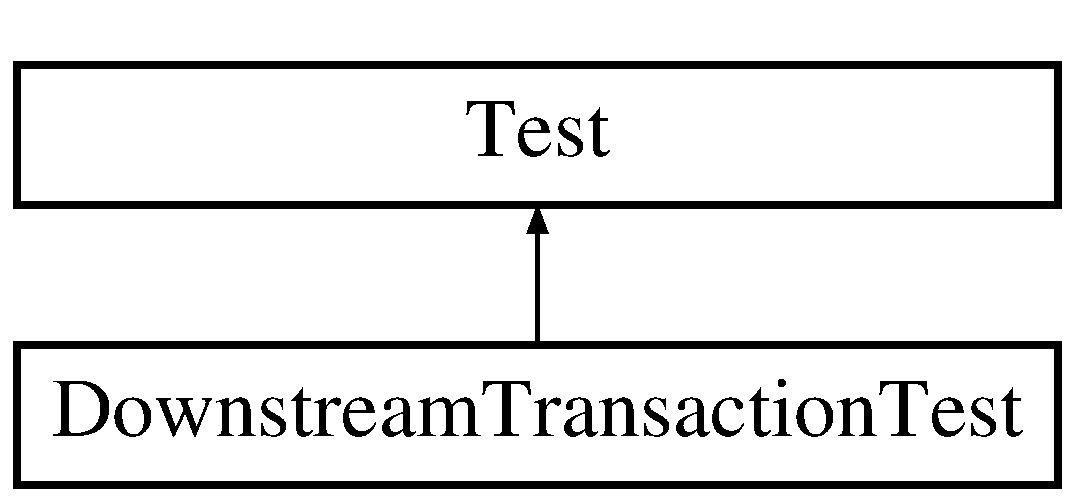
\includegraphics[height=2.000000cm]{classDownstreamTransactionTest}
\end{center}
\end{figure}
\subsection*{Public Member Functions}
\begin{DoxyCompactItemize}
\item 
{\bf Downstream\+Transaction\+Test} ()
\item 
void {\bf Set\+Up} () override
\item 
void {\bf setup\+Request\+Response\+Flow} ({\bf H\+T\+T\+P\+Transaction} $\ast$txn, uint32\+\_\+t size, bool delay\+Response=false)
\end{DoxyCompactItemize}
\subsection*{Protected Attributes}
\begin{DoxyCompactItemize}
\item 
folly\+::\+Event\+Base {\bf event\+Base\+\_\+}
\item 
folly\+::\+H\+H\+Wheel\+Timer\+::\+Unique\+Ptr {\bf transaction\+Timeouts\+\_\+}
\item 
{\bf Mock\+H\+T\+T\+P\+Transaction\+Transport} {\bf transport\+\_\+}
\item 
Strict\+Mock$<$ {\bf Mock\+H\+T\+T\+P\+Handler} $>$ {\bf handler\+\_\+}
\item 
{\bf H\+T\+T\+P2\+Priority\+Queue} {\bf txn\+Egress\+Queue\+\_\+}
\item 
uint32\+\_\+t {\bf received\+\_\+} \{0\}
\item 
uint32\+\_\+t {\bf sent\+\_\+} \{0\}
\end{DoxyCompactItemize}


\subsection{Detailed Description}


Definition at line 30 of file Downstream\+Transaction\+Test.\+cpp.



\subsection{Constructor \& Destructor Documentation}
\index{Downstream\+Transaction\+Test@{Downstream\+Transaction\+Test}!Downstream\+Transaction\+Test@{Downstream\+Transaction\+Test}}
\index{Downstream\+Transaction\+Test@{Downstream\+Transaction\+Test}!Downstream\+Transaction\+Test@{Downstream\+Transaction\+Test}}
\subsubsection[{Downstream\+Transaction\+Test()}]{\setlength{\rightskip}{0pt plus 5cm}Downstream\+Transaction\+Test\+::\+Downstream\+Transaction\+Test (
\begin{DoxyParamCaption}
{}
\end{DoxyParamCaption}
)\hspace{0.3cm}{\ttfamily [inline]}}\label{classDownstreamTransactionTest_a263c12154b7ab0c5b23598f826933f1c}


Definition at line 32 of file Downstream\+Transaction\+Test.\+cpp.


\begin{DoxyCode}
32 \{\}
\end{DoxyCode}


\subsection{Member Function Documentation}
\index{Downstream\+Transaction\+Test@{Downstream\+Transaction\+Test}!Set\+Up@{Set\+Up}}
\index{Set\+Up@{Set\+Up}!Downstream\+Transaction\+Test@{Downstream\+Transaction\+Test}}
\subsubsection[{Set\+Up() override}]{\setlength{\rightskip}{0pt plus 5cm}void Downstream\+Transaction\+Test\+::\+Set\+Up (
\begin{DoxyParamCaption}
{}
\end{DoxyParamCaption}
)\hspace{0.3cm}{\ttfamily [inline]}, {\ttfamily [override]}}\label{classDownstreamTransactionTest_a3c0d7099304bccd5da24c32f9e4485fb}


Definition at line 34 of file Downstream\+Transaction\+Test.\+cpp.


\begin{DoxyCode}
34                         \{
35     EXPECT\_CALL(transport_, describe(\_))
36       .WillRepeatedly(Return());
37   \}
\end{DoxyCode}
\index{Downstream\+Transaction\+Test@{Downstream\+Transaction\+Test}!setup\+Request\+Response\+Flow@{setup\+Request\+Response\+Flow}}
\index{setup\+Request\+Response\+Flow@{setup\+Request\+Response\+Flow}!Downstream\+Transaction\+Test@{Downstream\+Transaction\+Test}}
\subsubsection[{setup\+Request\+Response\+Flow(\+H\+T\+T\+P\+Transaction $\ast$txn, uint32\+\_\+t size, bool delay\+Response=false)}]{\setlength{\rightskip}{0pt plus 5cm}void Downstream\+Transaction\+Test\+::setup\+Request\+Response\+Flow (
\begin{DoxyParamCaption}
\item[{{\bf H\+T\+T\+P\+Transaction} $\ast$}]{txn, }
\item[{uint32\+\_\+t}]{size, }
\item[{bool}]{delay\+Response = {\ttfamily false}}
\end{DoxyParamCaption}
)\hspace{0.3cm}{\ttfamily [inline]}}\label{classDownstreamTransactionTest_a9c4bb789e570bc521af6c43ad18d8643}


Definition at line 39 of file Downstream\+Transaction\+Test.\+cpp.



References proxygen\+::\+H\+T\+T\+P\+Message\+::get\+Status\+Code(), proxygen\+::make\+Buf(), proxygen\+::make\+Response(), proxygen\+::\+H\+T\+T\+P\+Transaction\+::on\+Ingress\+Body(), proxygen\+::\+H\+T\+T\+P\+Transaction\+::on\+Ingress\+E\+O\+M(), proxygen\+::\+H\+T\+T\+P\+Transaction\+::on\+Write\+Ready(), proxygen\+::\+H\+T\+T\+P\+Transaction\+::send\+Body(), proxygen\+::\+H\+T\+T\+P\+Transaction\+::send\+E\+O\+M(), proxygen\+::\+H\+T\+T\+P\+Transaction\+::send\+Headers(), and proxygen\+::\+H\+T\+T\+P\+Transaction\+::set\+Handler().


\begin{DoxyCode}
40                                                           \{
41     EXPECT\_CALL(handler_, setTransaction(txn));
42     EXPECT\_CALL(handler_, detachTransaction());
43     EXPECT\_CALL(transport_, detach(txn));
44     \textcolor{keywordflow}{if} (delayResponse) \{
45       EXPECT\_CALL(handler_, onHeadersComplete(\_));
46     \} \textcolor{keywordflow}{else} \{
47       EXPECT\_CALL(handler_, onHeadersComplete(\_))
48           .WillOnce(Invoke([=](std::shared\_ptr<HTTPMessage> \textcolor{comment}{/*msg*/}) \{
49             \textcolor{keyword}{auto} response = makeResponse(200);
50             txn->sendHeaders(*response.get());
51             txn->sendBody(makeBuf(size));
52             txn->sendEOM();
53           \}));
54     \}
55     EXPECT\_CALL(transport_, sendHeaders(txn, \_, \_, \_))
56       .WillOnce(Invoke([=](Unused, \textcolor{keyword}{const} HTTPMessage& headers, Unused, Unused) \{
57             EXPECT\_EQ(headers.getStatusCode(), 200);
58           \}));
59     EXPECT\_CALL(transport_, sendBody(txn, \_, \textcolor{keyword}{false}, \textcolor{keyword}{false}))
60       .WillRepeatedly(Invoke([=](Unused, std::shared\_ptr<folly::IOBuf> body,
61                                  Unused, Unused) \{
62                                \textcolor{keyword}{auto} cur = body->computeChainDataLength();
63                                sent_ += cur;
64                                \textcolor{keywordflow}{return} cur;
65                              \}));
66     \textcolor{keywordflow}{if} (delayResponse) \{
67       EXPECT\_CALL(transport_, sendEOM(txn, \_));
68     \} \textcolor{keywordflow}{else} \{
69       EXPECT\_CALL(transport_, sendEOM(txn, \_))
70           .WillOnce(InvokeWithoutArgs([=]() \{
71             CHECK\_EQ(sent_, size);
72             txn->onIngressBody(makeBuf(size), 0);
73             txn->onIngressEOM();
74             \textcolor{keywordflow}{return} 5;
75           \}));
76     \}
77     EXPECT\_CALL(handler_, onBody(\_))
78       .WillRepeatedly(Invoke([=](std::shared\_ptr<folly::IOBuf> body) \{
79             received_ += body->computeChainDataLength();
80           \}));
81     EXPECT\_CALL(handler_, onEOM())
82       .WillOnce(InvokeWithoutArgs([=] \{
83             CHECK\_EQ(received_, size);
84           \}));
85     EXPECT\_CALL(transport_, notifyPendingEgress())
86       .WillOnce(InvokeWithoutArgs([=] \{
87             txn->onWriteReady(size, 1);
88           \}))
89       .WillOnce(DoDefault()); \textcolor{comment}{// The second call is for sending the eom}
90 
91     txn->setHandler(&handler_);
92   \}
\end{DoxyCode}


\subsection{Member Data Documentation}
\index{Downstream\+Transaction\+Test@{Downstream\+Transaction\+Test}!event\+Base\+\_\+@{event\+Base\+\_\+}}
\index{event\+Base\+\_\+@{event\+Base\+\_\+}!Downstream\+Transaction\+Test@{Downstream\+Transaction\+Test}}
\subsubsection[{event\+Base\+\_\+}]{\setlength{\rightskip}{0pt plus 5cm}folly\+::\+Event\+Base Downstream\+Transaction\+Test\+::event\+Base\+\_\+\hspace{0.3cm}{\ttfamily [protected]}}\label{classDownstreamTransactionTest_a583e720341c5bc14423eedb3bd94ddc4}


Definition at line 95 of file Downstream\+Transaction\+Test.\+cpp.

\index{Downstream\+Transaction\+Test@{Downstream\+Transaction\+Test}!handler\+\_\+@{handler\+\_\+}}
\index{handler\+\_\+@{handler\+\_\+}!Downstream\+Transaction\+Test@{Downstream\+Transaction\+Test}}
\subsubsection[{handler\+\_\+}]{\setlength{\rightskip}{0pt plus 5cm}Strict\+Mock$<${\bf Mock\+H\+T\+T\+P\+Handler}$>$ Downstream\+Transaction\+Test\+::handler\+\_\+\hspace{0.3cm}{\ttfamily [protected]}}\label{classDownstreamTransactionTest_a6f6aef3fff49be0c80669d2574c3b4df}


Definition at line 103 of file Downstream\+Transaction\+Test.\+cpp.

\index{Downstream\+Transaction\+Test@{Downstream\+Transaction\+Test}!received\+\_\+@{received\+\_\+}}
\index{received\+\_\+@{received\+\_\+}!Downstream\+Transaction\+Test@{Downstream\+Transaction\+Test}}
\subsubsection[{received\+\_\+}]{\setlength{\rightskip}{0pt plus 5cm}uint32\+\_\+t Downstream\+Transaction\+Test\+::received\+\_\+ \{0\}\hspace{0.3cm}{\ttfamily [protected]}}\label{classDownstreamTransactionTest_ab91964c2c5c84ab7b28e8d713f339fa3}


Definition at line 105 of file Downstream\+Transaction\+Test.\+cpp.

\index{Downstream\+Transaction\+Test@{Downstream\+Transaction\+Test}!sent\+\_\+@{sent\+\_\+}}
\index{sent\+\_\+@{sent\+\_\+}!Downstream\+Transaction\+Test@{Downstream\+Transaction\+Test}}
\subsubsection[{sent\+\_\+}]{\setlength{\rightskip}{0pt plus 5cm}uint32\+\_\+t Downstream\+Transaction\+Test\+::sent\+\_\+ \{0\}\hspace{0.3cm}{\ttfamily [protected]}}\label{classDownstreamTransactionTest_aef38dfbd014f1c282f955e208b75cf6b}


Definition at line 106 of file Downstream\+Transaction\+Test.\+cpp.

\index{Downstream\+Transaction\+Test@{Downstream\+Transaction\+Test}!transaction\+Timeouts\+\_\+@{transaction\+Timeouts\+\_\+}}
\index{transaction\+Timeouts\+\_\+@{transaction\+Timeouts\+\_\+}!Downstream\+Transaction\+Test@{Downstream\+Transaction\+Test}}
\subsubsection[{transaction\+Timeouts\+\_\+}]{\setlength{\rightskip}{0pt plus 5cm}folly\+::\+H\+H\+Wheel\+Timer\+::\+Unique\+Ptr Downstream\+Transaction\+Test\+::transaction\+Timeouts\+\_\+\hspace{0.3cm}{\ttfamily [protected]}}\label{classDownstreamTransactionTest_a2206e5db44b6e7f1aca3b8bb27dba3f5}
{\bfseries Initial value\+:}
\begin{DoxyCode}
\{
      folly::HHWheelTimer::newTimer(
          &eventBase_,
          std::chrono::milliseconds(folly::HHWheelTimer::DEFAULT\_TICK\_INTERVAL),
          folly::AsyncTimeout::InternalEnum::NORMAL,
          std::chrono::milliseconds(500))\}
\end{DoxyCode}


Definition at line 96 of file Downstream\+Transaction\+Test.\+cpp.

\index{Downstream\+Transaction\+Test@{Downstream\+Transaction\+Test}!transport\+\_\+@{transport\+\_\+}}
\index{transport\+\_\+@{transport\+\_\+}!Downstream\+Transaction\+Test@{Downstream\+Transaction\+Test}}
\subsubsection[{transport\+\_\+}]{\setlength{\rightskip}{0pt plus 5cm}{\bf Mock\+H\+T\+T\+P\+Transaction\+Transport} Downstream\+Transaction\+Test\+::transport\+\_\+\hspace{0.3cm}{\ttfamily [protected]}}\label{classDownstreamTransactionTest_af3cd2dc4330358012a25ee2f6dc544d8}


Definition at line 102 of file Downstream\+Transaction\+Test.\+cpp.

\index{Downstream\+Transaction\+Test@{Downstream\+Transaction\+Test}!txn\+Egress\+Queue\+\_\+@{txn\+Egress\+Queue\+\_\+}}
\index{txn\+Egress\+Queue\+\_\+@{txn\+Egress\+Queue\+\_\+}!Downstream\+Transaction\+Test@{Downstream\+Transaction\+Test}}
\subsubsection[{txn\+Egress\+Queue\+\_\+}]{\setlength{\rightskip}{0pt plus 5cm}{\bf H\+T\+T\+P2\+Priority\+Queue} Downstream\+Transaction\+Test\+::txn\+Egress\+Queue\+\_\+\hspace{0.3cm}{\ttfamily [protected]}}\label{classDownstreamTransactionTest_a949d1091b816665e2552186c5199f4d8}


Definition at line 104 of file Downstream\+Transaction\+Test.\+cpp.



The documentation for this class was generated from the following file\+:\begin{DoxyCompactItemize}
\item 
proxygen/lib/http/session/test/{\bf Downstream\+Transaction\+Test.\+cpp}\end{DoxyCompactItemize}

\section{proxygen\+:\+:H\+T\+T\+P\+Session\+:\+:Drain\+Timeout Class Reference}
\label{classproxygen_1_1HTTPSession_1_1DrainTimeout}\index{proxygen\+::\+H\+T\+T\+P\+Session\+::\+Drain\+Timeout@{proxygen\+::\+H\+T\+T\+P\+Session\+::\+Drain\+Timeout}}
Inheritance diagram for proxygen\+:\+:H\+T\+T\+P\+Session\+:\+:Drain\+Timeout\+:\begin{figure}[H]
\begin{center}
\leavevmode
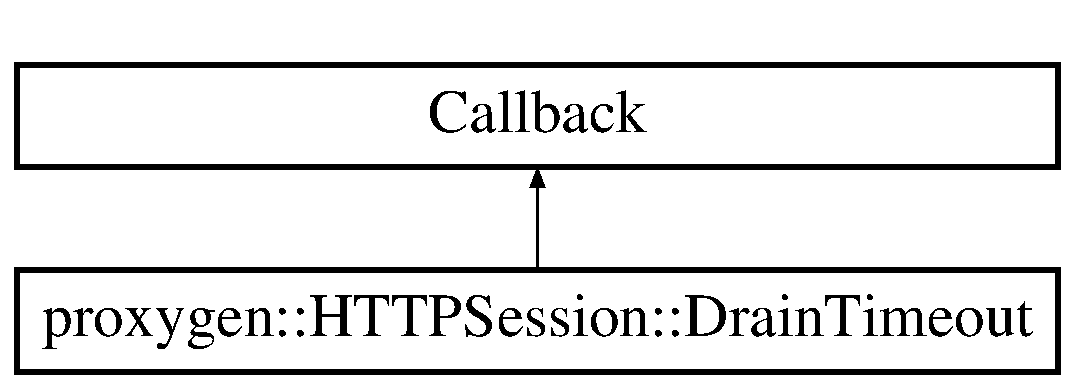
\includegraphics[height=2.000000cm]{classproxygen_1_1HTTPSession_1_1DrainTimeout}
\end{center}
\end{figure}
\subsection*{Public Member Functions}
\begin{DoxyCompactItemize}
\item 
{\bf Drain\+Timeout} ({\bf H\+T\+T\+P\+Session} $\ast$session)
\item 
{\bf $\sim$\+Drain\+Timeout} () override
\item 
void {\bf timeout\+Expired} () noexceptoverride
\end{DoxyCompactItemize}
\subsection*{Private Attributes}
\begin{DoxyCompactItemize}
\item 
{\bf H\+T\+T\+P\+Session} $\ast$ {\bf session\+\_\+}
\end{DoxyCompactItemize}


\subsection{Detailed Description}


Definition at line 1024 of file H\+T\+T\+P\+Session.\+h.



\subsection{Constructor \& Destructor Documentation}
\index{proxygen\+::\+H\+T\+T\+P\+Session\+::\+Drain\+Timeout@{proxygen\+::\+H\+T\+T\+P\+Session\+::\+Drain\+Timeout}!Drain\+Timeout@{Drain\+Timeout}}
\index{Drain\+Timeout@{Drain\+Timeout}!proxygen\+::\+H\+T\+T\+P\+Session\+::\+Drain\+Timeout@{proxygen\+::\+H\+T\+T\+P\+Session\+::\+Drain\+Timeout}}
\subsubsection[{Drain\+Timeout(\+H\+T\+T\+P\+Session $\ast$session)}]{\setlength{\rightskip}{0pt plus 5cm}proxygen\+::\+H\+T\+T\+P\+Session\+::\+Drain\+Timeout\+::\+Drain\+Timeout (
\begin{DoxyParamCaption}
\item[{{\bf H\+T\+T\+P\+Session} $\ast$}]{session}
\end{DoxyParamCaption}
)\hspace{0.3cm}{\ttfamily [inline]}, {\ttfamily [explicit]}}\label{classproxygen_1_1HTTPSession_1_1DrainTimeout_a0dbac88d026788cb8c8fa36e46bade48}


Definition at line 1026 of file H\+T\+T\+P\+Session.\+h.


\begin{DoxyCode}
1026 : session_(session) \{\}
\end{DoxyCode}
\index{proxygen\+::\+H\+T\+T\+P\+Session\+::\+Drain\+Timeout@{proxygen\+::\+H\+T\+T\+P\+Session\+::\+Drain\+Timeout}!````~Drain\+Timeout@{$\sim$\+Drain\+Timeout}}
\index{````~Drain\+Timeout@{$\sim$\+Drain\+Timeout}!proxygen\+::\+H\+T\+T\+P\+Session\+::\+Drain\+Timeout@{proxygen\+::\+H\+T\+T\+P\+Session\+::\+Drain\+Timeout}}
\subsubsection[{$\sim$\+Drain\+Timeout() override}]{\setlength{\rightskip}{0pt plus 5cm}proxygen\+::\+H\+T\+T\+P\+Session\+::\+Drain\+Timeout\+::$\sim$\+Drain\+Timeout (
\begin{DoxyParamCaption}
{}
\end{DoxyParamCaption}
)\hspace{0.3cm}{\ttfamily [inline]}, {\ttfamily [override]}}\label{classproxygen_1_1HTTPSession_1_1DrainTimeout_a9973b21d4df1280fc6660bb9f43f12f5}


Definition at line 1027 of file H\+T\+T\+P\+Session.\+h.


\begin{DoxyCode}
1027 \{\}
\end{DoxyCode}


\subsection{Member Function Documentation}
\index{proxygen\+::\+H\+T\+T\+P\+Session\+::\+Drain\+Timeout@{proxygen\+::\+H\+T\+T\+P\+Session\+::\+Drain\+Timeout}!timeout\+Expired@{timeout\+Expired}}
\index{timeout\+Expired@{timeout\+Expired}!proxygen\+::\+H\+T\+T\+P\+Session\+::\+Drain\+Timeout@{proxygen\+::\+H\+T\+T\+P\+Session\+::\+Drain\+Timeout}}
\subsubsection[{timeout\+Expired() noexceptoverride}]{\setlength{\rightskip}{0pt plus 5cm}void proxygen\+::\+H\+T\+T\+P\+Session\+::\+Drain\+Timeout\+::timeout\+Expired (
\begin{DoxyParamCaption}
{}
\end{DoxyParamCaption}
)\hspace{0.3cm}{\ttfamily [inline]}, {\ttfamily [override]}, {\ttfamily [noexcept]}}\label{classproxygen_1_1HTTPSession_1_1DrainTimeout_a89e9514dbe221a18e64b2c39d68b84cf}


Definition at line 1029 of file H\+T\+T\+P\+Session.\+h.



References proxygen\+::\+H\+T\+T\+P\+Session\+::close\+When\+Idle(), and proxygen\+::\+H\+T\+T\+P\+Session\+::\+Write\+Timeout\+::session\+\_\+.


\begin{DoxyCode}
1029                                             \{
1030       session_->closeWhenIdle();
1031     \}
\end{DoxyCode}


\subsection{Member Data Documentation}
\index{proxygen\+::\+H\+T\+T\+P\+Session\+::\+Drain\+Timeout@{proxygen\+::\+H\+T\+T\+P\+Session\+::\+Drain\+Timeout}!session\+\_\+@{session\+\_\+}}
\index{session\+\_\+@{session\+\_\+}!proxygen\+::\+H\+T\+T\+P\+Session\+::\+Drain\+Timeout@{proxygen\+::\+H\+T\+T\+P\+Session\+::\+Drain\+Timeout}}
\subsubsection[{session\+\_\+}]{\setlength{\rightskip}{0pt plus 5cm}{\bf H\+T\+T\+P\+Session}$\ast$ proxygen\+::\+H\+T\+T\+P\+Session\+::\+Drain\+Timeout\+::session\+\_\+\hspace{0.3cm}{\ttfamily [private]}}\label{classproxygen_1_1HTTPSession_1_1DrainTimeout_a95b67c04adbed96e947f000b4c9f8353}


Definition at line 1033 of file H\+T\+T\+P\+Session.\+h.



The documentation for this class was generated from the following file\+:\begin{DoxyCompactItemize}
\item 
proxygen/lib/http/session/{\bf H\+T\+T\+P\+Session.\+h}\end{DoxyCompactItemize}

\section{Dummy\+Filter\+Factory\+:\+:Dummy\+Filter Class Reference}
\label{classDummyFilterFactory_1_1DummyFilter}\index{Dummy\+Filter\+Factory\+::\+Dummy\+Filter@{Dummy\+Filter\+Factory\+::\+Dummy\+Filter}}
Inheritance diagram for Dummy\+Filter\+Factory\+:\+:Dummy\+Filter\+:\begin{figure}[H]
\begin{center}
\leavevmode
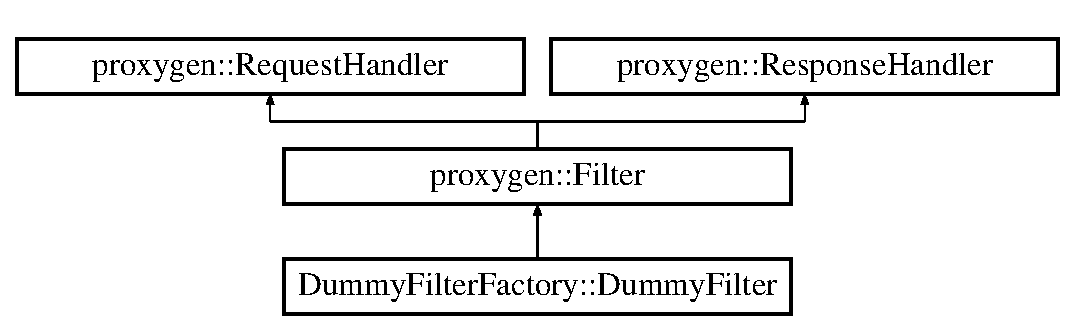
\includegraphics[height=3.000000cm]{classDummyFilterFactory_1_1DummyFilter}
\end{center}
\end{figure}
\subsection*{Public Member Functions}
\begin{DoxyCompactItemize}
\item 
{\bf Dummy\+Filter} ({\bf Request\+Handler} $\ast$upstream)
\end{DoxyCompactItemize}
\subsection*{Additional Inherited Members}


\subsection{Detailed Description}


Definition at line 191 of file H\+T\+T\+P\+Server\+Test.\+cpp.



\subsection{Constructor \& Destructor Documentation}
\index{Dummy\+Filter\+Factory\+::\+Dummy\+Filter@{Dummy\+Filter\+Factory\+::\+Dummy\+Filter}!Dummy\+Filter@{Dummy\+Filter}}
\index{Dummy\+Filter@{Dummy\+Filter}!Dummy\+Filter\+Factory\+::\+Dummy\+Filter@{Dummy\+Filter\+Factory\+::\+Dummy\+Filter}}
\subsubsection[{Dummy\+Filter(\+Request\+Handler $\ast$upstream)}]{\setlength{\rightskip}{0pt plus 5cm}Dummy\+Filter\+Factory\+::\+Dummy\+Filter\+::\+Dummy\+Filter (
\begin{DoxyParamCaption}
\item[{{\bf Request\+Handler} $\ast$}]{upstream}
\end{DoxyParamCaption}
)\hspace{0.3cm}{\ttfamily [inline]}, {\ttfamily [explicit]}}\label{classDummyFilterFactory_1_1DummyFilter_a104d5aaf68493d029c30d3dc6cf8c245}


Definition at line 193 of file H\+T\+T\+P\+Server\+Test.\+cpp.


\begin{DoxyCode}
193 : Filter(upstream) \{\}
\end{DoxyCode}


The documentation for this class was generated from the following file\+:\begin{DoxyCompactItemize}
\item 
proxygen/httpserver/tests/{\bf H\+T\+T\+P\+Server\+Test.\+cpp}\end{DoxyCompactItemize}

\section{Dummy\+Filter\+Factory Class Reference}
\label{classDummyFilterFactory}\index{Dummy\+Filter\+Factory@{Dummy\+Filter\+Factory}}
Inheritance diagram for Dummy\+Filter\+Factory\+:\begin{figure}[H]
\begin{center}
\leavevmode
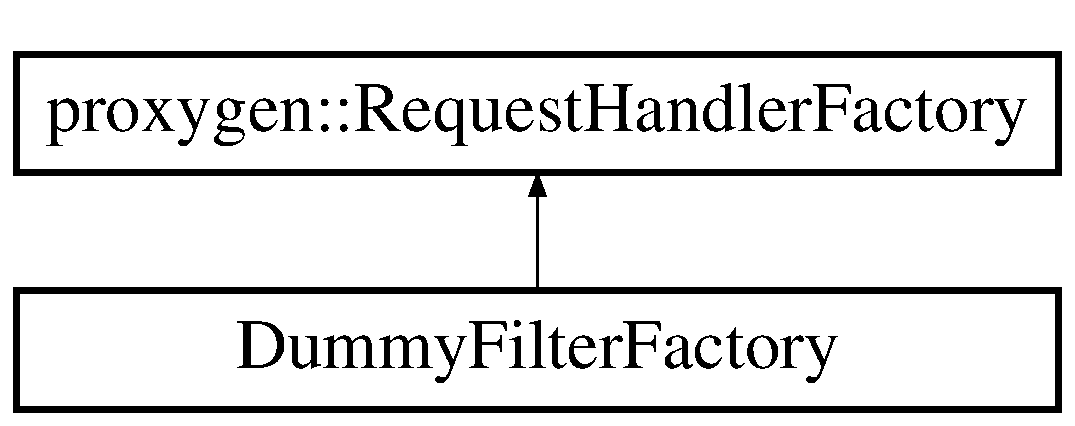
\includegraphics[height=2.000000cm]{classDummyFilterFactory}
\end{center}
\end{figure}
\subsection*{Classes}
\begin{DoxyCompactItemize}
\item 
class {\bf Dummy\+Filter}
\end{DoxyCompactItemize}
\subsection*{Public Member Functions}
\begin{DoxyCompactItemize}
\item 
{\bf Request\+Handler} $\ast$ {\bf on\+Request} ({\bf Request\+Handler} $\ast$h, {\bf H\+T\+T\+P\+Message} $\ast$) noexceptoverride
\item 
void {\bf on\+Server\+Start} (folly\+::\+Event\+Base $\ast$) noexceptoverride
\item 
void {\bf on\+Server\+Stop} () noexceptoverride
\end{DoxyCompactItemize}


\subsection{Detailed Description}
A dummy filter to make Request\+Handler\+Chain longer. 

Definition at line 189 of file H\+T\+T\+P\+Server\+Test.\+cpp.



\subsection{Member Function Documentation}
\index{Dummy\+Filter\+Factory@{Dummy\+Filter\+Factory}!on\+Request@{on\+Request}}
\index{on\+Request@{on\+Request}!Dummy\+Filter\+Factory@{Dummy\+Filter\+Factory}}
\subsubsection[{on\+Request(\+Request\+Handler $\ast$h, H\+T\+T\+P\+Message $\ast$) noexceptoverride}]{\setlength{\rightskip}{0pt plus 5cm}{\bf Request\+Handler}$\ast$ Dummy\+Filter\+Factory\+::on\+Request (
\begin{DoxyParamCaption}
\item[{{\bf Request\+Handler} $\ast$}]{, }
\item[{{\bf H\+T\+T\+P\+Message} $\ast$}]{}
\end{DoxyParamCaption}
)\hspace{0.3cm}{\ttfamily [inline]}, {\ttfamily [override]}, {\ttfamily [virtual]}, {\ttfamily [noexcept]}}\label{classDummyFilterFactory_a2a79bb927c1d7bb0d6c0e036b9a4e424}
Invoked for each new request server handles. H\+T\+T\+P\+Message is provided so that user can potentially choose among several implementation of handler based on U\+RL or something. No need to save/copy this H\+T\+T\+P\+Message. Request\+Handler will be given the H\+T\+T\+P\+Message in a separate callback.

Some request handlers don\textquotesingle{}t handle the request themselves (think filters). They do take some actions based on request/response but otherwise they just hand-\/off request to some other Request\+Handler. This upstream Request\+Handler is given as first parameter. For the terminal Request\+Handler this will by nullptr. 

Implements {\bf proxygen\+::\+Request\+Handler\+Factory} \doxyref{}{p.}{classproxygen_1_1RequestHandlerFactory_a9c2cbbc96d006244ea28cea44a3e6a60}.



Definition at line 196 of file H\+T\+T\+P\+Server\+Test.\+cpp.


\begin{DoxyCode}
196                                                                                \{
197     \textcolor{keywordflow}{return} \textcolor{keyword}{new} DummyFilter(h);
198   \}
\end{DoxyCode}
\index{Dummy\+Filter\+Factory@{Dummy\+Filter\+Factory}!on\+Server\+Start@{on\+Server\+Start}}
\index{on\+Server\+Start@{on\+Server\+Start}!Dummy\+Filter\+Factory@{Dummy\+Filter\+Factory}}
\subsubsection[{on\+Server\+Start(folly\+::\+Event\+Base $\ast$) noexceptoverride}]{\setlength{\rightskip}{0pt plus 5cm}void Dummy\+Filter\+Factory\+::on\+Server\+Start (
\begin{DoxyParamCaption}
\item[{folly\+::\+Event\+Base $\ast$}]{evb}
\end{DoxyParamCaption}
)\hspace{0.3cm}{\ttfamily [inline]}, {\ttfamily [override]}, {\ttfamily [virtual]}, {\ttfamily [noexcept]}}\label{classDummyFilterFactory_a8db0e2a4e0be334f537c54c2da92b35f}
Invoked in each thread server is going to handle requests before we start handling requests. Can be used to setup thread-\/local setup for each thread (stats and such). 

Implements {\bf proxygen\+::\+Request\+Handler\+Factory} \doxyref{}{p.}{classproxygen_1_1RequestHandlerFactory_af76091b8a51a8d069fcc1aec3007a1cc}.



Definition at line 200 of file H\+T\+T\+P\+Server\+Test.\+cpp.


\begin{DoxyCode}
200 \{\}
\end{DoxyCode}
\index{Dummy\+Filter\+Factory@{Dummy\+Filter\+Factory}!on\+Server\+Stop@{on\+Server\+Stop}}
\index{on\+Server\+Stop@{on\+Server\+Stop}!Dummy\+Filter\+Factory@{Dummy\+Filter\+Factory}}
\subsubsection[{on\+Server\+Stop() noexceptoverride}]{\setlength{\rightskip}{0pt plus 5cm}void Dummy\+Filter\+Factory\+::on\+Server\+Stop (
\begin{DoxyParamCaption}
{}
\end{DoxyParamCaption}
)\hspace{0.3cm}{\ttfamily [inline]}, {\ttfamily [override]}, {\ttfamily [virtual]}, {\ttfamily [noexcept]}}\label{classDummyFilterFactory_a6bca57ceeef14bc159f4fd47c13ef573}
Invoked in each handler thread after all the connections are drained from that thread. Can be used to tear down thread-\/local setup. 

Implements {\bf proxygen\+::\+Request\+Handler\+Factory} \doxyref{}{p.}{classproxygen_1_1RequestHandlerFactory_a0791d6b33c13513ed6f550bbbd7bca85}.



Definition at line 201 of file H\+T\+T\+P\+Server\+Test.\+cpp.


\begin{DoxyCode}
201 \{\}
\end{DoxyCode}


The documentation for this class was generated from the following file\+:\begin{DoxyCompactItemize}
\item 
proxygen/httpserver/tests/{\bf H\+T\+T\+P\+Server\+Test.\+cpp}\end{DoxyCompactItemize}

\section{proxygen\+:\+:Dummy\+H\+T\+T\+P\+Session\+Stats Class Reference}
\label{classproxygen_1_1DummyHTTPSessionStats}\index{proxygen\+::\+Dummy\+H\+T\+T\+P\+Session\+Stats@{proxygen\+::\+Dummy\+H\+T\+T\+P\+Session\+Stats}}


{\ttfamily \#include $<$H\+T\+T\+P\+Session\+Mocks.\+h$>$}

Inheritance diagram for proxygen\+:\+:Dummy\+H\+T\+T\+P\+Session\+Stats\+:\begin{figure}[H]
\begin{center}
\leavevmode
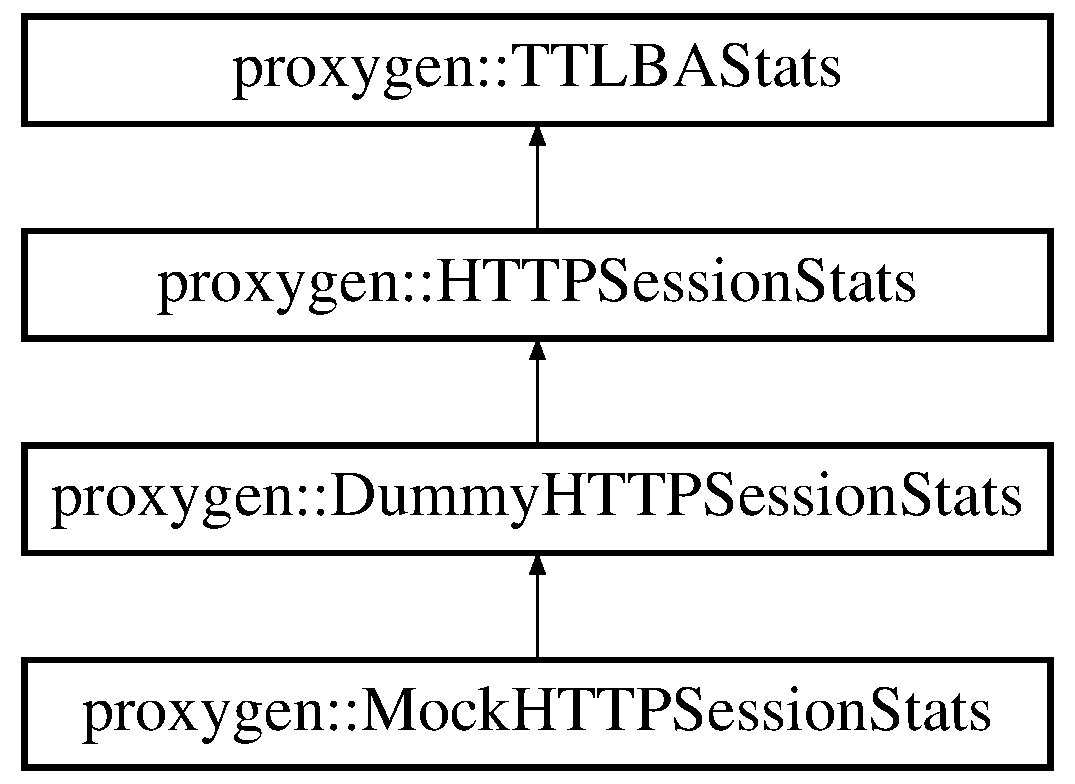
\includegraphics[height=4.000000cm]{classproxygen_1_1DummyHTTPSessionStats}
\end{center}
\end{figure}
\subsection*{Public Member Functions}
\begin{DoxyCompactItemize}
\item 
void {\bf record\+Transaction\+Opened} () noexceptoverride
\item 
void {\bf record\+Transaction\+Closed} () noexceptoverride
\item 
void {\bf record\+Transactions\+Served} (uint64\+\_\+t) noexceptoverride
\item 
void {\bf record\+Session\+Reused} () noexceptoverride
\item 
void {\bf record\+Transaction\+Stalled} () noexceptoverride
\item 
void {\bf record\+Session\+Stalled} () noexceptoverride
\item 
void {\bf record\+T\+T\+L\+B\+A\+Exceed\+Limit} () noexceptoverride
\item 
void {\bf record\+T\+T\+L\+B\+A\+I\+O\+B\+Split\+By\+Eom} () noexceptoverride
\item 
void {\bf record\+T\+T\+L\+B\+A\+Not\+Found} () noexceptoverride
\item 
void {\bf record\+T\+T\+L\+B\+A\+Received} () noexceptoverride
\item 
void {\bf record\+T\+T\+L\+B\+A\+Timeout} () noexceptoverride
\item 
void {\bf record\+T\+T\+L\+B\+A\+Eom\+Passed} () noexceptoverride
\item 
void {\bf record\+T\+T\+L\+B\+A\+Tracked} () noexceptoverride
\end{DoxyCompactItemize}


\subsection{Detailed Description}


Definition at line 443 of file H\+T\+T\+P\+Session\+Mocks.\+h.



\subsection{Member Function Documentation}
\index{proxygen\+::\+Dummy\+H\+T\+T\+P\+Session\+Stats@{proxygen\+::\+Dummy\+H\+T\+T\+P\+Session\+Stats}!record\+Session\+Reused@{record\+Session\+Reused}}
\index{record\+Session\+Reused@{record\+Session\+Reused}!proxygen\+::\+Dummy\+H\+T\+T\+P\+Session\+Stats@{proxygen\+::\+Dummy\+H\+T\+T\+P\+Session\+Stats}}
\subsubsection[{record\+Session\+Reused() noexceptoverride}]{\setlength{\rightskip}{0pt plus 5cm}void proxygen\+::\+Dummy\+H\+T\+T\+P\+Session\+Stats\+::record\+Session\+Reused (
\begin{DoxyParamCaption}
{}
\end{DoxyParamCaption}
)\hspace{0.3cm}{\ttfamily [inline]}, {\ttfamily [override]}, {\ttfamily [virtual]}, {\ttfamily [noexcept]}}\label{classproxygen_1_1DummyHTTPSessionStats_aedae43f00c84fbe14f20573b0fea9d3e}


Implements {\bf proxygen\+::\+H\+T\+T\+P\+Session\+Stats} \doxyref{}{p.}{classproxygen_1_1HTTPSessionStats_a17e73331812564e0474afde1f3afcc53}.



Definition at line 448 of file H\+T\+T\+P\+Session\+Mocks.\+h.


\begin{DoxyCode}
448 \{\};
\end{DoxyCode}
\index{proxygen\+::\+Dummy\+H\+T\+T\+P\+Session\+Stats@{proxygen\+::\+Dummy\+H\+T\+T\+P\+Session\+Stats}!record\+Session\+Stalled@{record\+Session\+Stalled}}
\index{record\+Session\+Stalled@{record\+Session\+Stalled}!proxygen\+::\+Dummy\+H\+T\+T\+P\+Session\+Stats@{proxygen\+::\+Dummy\+H\+T\+T\+P\+Session\+Stats}}
\subsubsection[{record\+Session\+Stalled() noexceptoverride}]{\setlength{\rightskip}{0pt plus 5cm}void proxygen\+::\+Dummy\+H\+T\+T\+P\+Session\+Stats\+::record\+Session\+Stalled (
\begin{DoxyParamCaption}
{}
\end{DoxyParamCaption}
)\hspace{0.3cm}{\ttfamily [inline]}, {\ttfamily [override]}, {\ttfamily [virtual]}, {\ttfamily [noexcept]}}\label{classproxygen_1_1DummyHTTPSessionStats_add1ea9dfcc0ca78730b0c70276e7284f}


Implements {\bf proxygen\+::\+H\+T\+T\+P\+Session\+Stats} \doxyref{}{p.}{classproxygen_1_1HTTPSessionStats_a0dcc0a5eb3676131ed6128d680052108}.



Definition at line 451 of file H\+T\+T\+P\+Session\+Mocks.\+h.


\begin{DoxyCode}
451 \{\};
\end{DoxyCode}
\index{proxygen\+::\+Dummy\+H\+T\+T\+P\+Session\+Stats@{proxygen\+::\+Dummy\+H\+T\+T\+P\+Session\+Stats}!record\+Transaction\+Closed@{record\+Transaction\+Closed}}
\index{record\+Transaction\+Closed@{record\+Transaction\+Closed}!proxygen\+::\+Dummy\+H\+T\+T\+P\+Session\+Stats@{proxygen\+::\+Dummy\+H\+T\+T\+P\+Session\+Stats}}
\subsubsection[{record\+Transaction\+Closed() noexceptoverride}]{\setlength{\rightskip}{0pt plus 5cm}void proxygen\+::\+Dummy\+H\+T\+T\+P\+Session\+Stats\+::record\+Transaction\+Closed (
\begin{DoxyParamCaption}
{}
\end{DoxyParamCaption}
)\hspace{0.3cm}{\ttfamily [inline]}, {\ttfamily [override]}, {\ttfamily [virtual]}, {\ttfamily [noexcept]}}\label{classproxygen_1_1DummyHTTPSessionStats_af6b980a8f23508fbf40162bd89aeca5d}


Implements {\bf proxygen\+::\+H\+T\+T\+P\+Session\+Stats} \doxyref{}{p.}{classproxygen_1_1HTTPSessionStats_a09e2e19fb354bba950e9d38d1fefd697}.



Definition at line 446 of file H\+T\+T\+P\+Session\+Mocks.\+h.


\begin{DoxyCode}
446 \{\};
\end{DoxyCode}
\index{proxygen\+::\+Dummy\+H\+T\+T\+P\+Session\+Stats@{proxygen\+::\+Dummy\+H\+T\+T\+P\+Session\+Stats}!record\+Transaction\+Opened@{record\+Transaction\+Opened}}
\index{record\+Transaction\+Opened@{record\+Transaction\+Opened}!proxygen\+::\+Dummy\+H\+T\+T\+P\+Session\+Stats@{proxygen\+::\+Dummy\+H\+T\+T\+P\+Session\+Stats}}
\subsubsection[{record\+Transaction\+Opened() noexceptoverride}]{\setlength{\rightskip}{0pt plus 5cm}void proxygen\+::\+Dummy\+H\+T\+T\+P\+Session\+Stats\+::record\+Transaction\+Opened (
\begin{DoxyParamCaption}
{}
\end{DoxyParamCaption}
)\hspace{0.3cm}{\ttfamily [inline]}, {\ttfamily [override]}, {\ttfamily [virtual]}, {\ttfamily [noexcept]}}\label{classproxygen_1_1DummyHTTPSessionStats_af47e8b3f1fe0f367c7f7ce3fb6566f7e}


Implements {\bf proxygen\+::\+H\+T\+T\+P\+Session\+Stats} \doxyref{}{p.}{classproxygen_1_1HTTPSessionStats_a4c0ac2fb3a6fe829a82ddacce8c39175}.



Definition at line 445 of file H\+T\+T\+P\+Session\+Mocks.\+h.


\begin{DoxyCode}
445 \{\};
\end{DoxyCode}
\index{proxygen\+::\+Dummy\+H\+T\+T\+P\+Session\+Stats@{proxygen\+::\+Dummy\+H\+T\+T\+P\+Session\+Stats}!record\+Transactions\+Served@{record\+Transactions\+Served}}
\index{record\+Transactions\+Served@{record\+Transactions\+Served}!proxygen\+::\+Dummy\+H\+T\+T\+P\+Session\+Stats@{proxygen\+::\+Dummy\+H\+T\+T\+P\+Session\+Stats}}
\subsubsection[{record\+Transactions\+Served(uint64\+\_\+t) noexceptoverride}]{\setlength{\rightskip}{0pt plus 5cm}void proxygen\+::\+Dummy\+H\+T\+T\+P\+Session\+Stats\+::record\+Transactions\+Served (
\begin{DoxyParamCaption}
\item[{uint64\+\_\+t}]{}
\end{DoxyParamCaption}
)\hspace{0.3cm}{\ttfamily [inline]}, {\ttfamily [override]}, {\ttfamily [virtual]}, {\ttfamily [noexcept]}}\label{classproxygen_1_1DummyHTTPSessionStats_a17a88083485a26f42f911307293dc3ed}


Implements {\bf proxygen\+::\+H\+T\+T\+P\+Session\+Stats} \doxyref{}{p.}{classproxygen_1_1HTTPSessionStats_a1cdc45cde70887176f6b4cbf600e8893}.



Definition at line 447 of file H\+T\+T\+P\+Session\+Mocks.\+h.


\begin{DoxyCode}
447 \{\};
\end{DoxyCode}
\index{proxygen\+::\+Dummy\+H\+T\+T\+P\+Session\+Stats@{proxygen\+::\+Dummy\+H\+T\+T\+P\+Session\+Stats}!record\+Transaction\+Stalled@{record\+Transaction\+Stalled}}
\index{record\+Transaction\+Stalled@{record\+Transaction\+Stalled}!proxygen\+::\+Dummy\+H\+T\+T\+P\+Session\+Stats@{proxygen\+::\+Dummy\+H\+T\+T\+P\+Session\+Stats}}
\subsubsection[{record\+Transaction\+Stalled() noexceptoverride}]{\setlength{\rightskip}{0pt plus 5cm}void proxygen\+::\+Dummy\+H\+T\+T\+P\+Session\+Stats\+::record\+Transaction\+Stalled (
\begin{DoxyParamCaption}
{}
\end{DoxyParamCaption}
)\hspace{0.3cm}{\ttfamily [inline]}, {\ttfamily [override]}, {\ttfamily [virtual]}, {\ttfamily [noexcept]}}\label{classproxygen_1_1DummyHTTPSessionStats_ae2ff4902fd161bebb35288a42edd2bc6}


Implements {\bf proxygen\+::\+H\+T\+T\+P\+Session\+Stats} \doxyref{}{p.}{classproxygen_1_1HTTPSessionStats_a11caacb735320e219801d594fad7a1a3}.



Definition at line 450 of file H\+T\+T\+P\+Session\+Mocks.\+h.


\begin{DoxyCode}
450 \{\};
\end{DoxyCode}
\index{proxygen\+::\+Dummy\+H\+T\+T\+P\+Session\+Stats@{proxygen\+::\+Dummy\+H\+T\+T\+P\+Session\+Stats}!record\+T\+T\+L\+B\+A\+Eom\+Passed@{record\+T\+T\+L\+B\+A\+Eom\+Passed}}
\index{record\+T\+T\+L\+B\+A\+Eom\+Passed@{record\+T\+T\+L\+B\+A\+Eom\+Passed}!proxygen\+::\+Dummy\+H\+T\+T\+P\+Session\+Stats@{proxygen\+::\+Dummy\+H\+T\+T\+P\+Session\+Stats}}
\subsubsection[{record\+T\+T\+L\+B\+A\+Eom\+Passed() noexceptoverride}]{\setlength{\rightskip}{0pt plus 5cm}void proxygen\+::\+Dummy\+H\+T\+T\+P\+Session\+Stats\+::record\+T\+T\+L\+B\+A\+Eom\+Passed (
\begin{DoxyParamCaption}
{}
\end{DoxyParamCaption}
)\hspace{0.3cm}{\ttfamily [inline]}, {\ttfamily [override]}, {\ttfamily [virtual]}, {\ttfamily [noexcept]}}\label{classproxygen_1_1DummyHTTPSessionStats_ad1fee46e3887fc1cf228cb89d3040a5e}


Implements {\bf proxygen\+::\+T\+T\+L\+B\+A\+Stats} \doxyref{}{p.}{classproxygen_1_1TTLBAStats_a5a2fee61cc392d977ef3509f4eb2c539}.



Definition at line 458 of file H\+T\+T\+P\+Session\+Mocks.\+h.


\begin{DoxyCode}
458 \{\};
\end{DoxyCode}
\index{proxygen\+::\+Dummy\+H\+T\+T\+P\+Session\+Stats@{proxygen\+::\+Dummy\+H\+T\+T\+P\+Session\+Stats}!record\+T\+T\+L\+B\+A\+Exceed\+Limit@{record\+T\+T\+L\+B\+A\+Exceed\+Limit}}
\index{record\+T\+T\+L\+B\+A\+Exceed\+Limit@{record\+T\+T\+L\+B\+A\+Exceed\+Limit}!proxygen\+::\+Dummy\+H\+T\+T\+P\+Session\+Stats@{proxygen\+::\+Dummy\+H\+T\+T\+P\+Session\+Stats}}
\subsubsection[{record\+T\+T\+L\+B\+A\+Exceed\+Limit() noexceptoverride}]{\setlength{\rightskip}{0pt plus 5cm}void proxygen\+::\+Dummy\+H\+T\+T\+P\+Session\+Stats\+::record\+T\+T\+L\+B\+A\+Exceed\+Limit (
\begin{DoxyParamCaption}
{}
\end{DoxyParamCaption}
)\hspace{0.3cm}{\ttfamily [inline]}, {\ttfamily [override]}, {\ttfamily [virtual]}, {\ttfamily [noexcept]}}\label{classproxygen_1_1DummyHTTPSessionStats_a04a91d5de8d98bc0b3e19ac5a7bd16d1}


Implements {\bf proxygen\+::\+T\+T\+L\+B\+A\+Stats} \doxyref{}{p.}{classproxygen_1_1TTLBAStats_ac6ebb7c67e5aed5e87260ae8408c00cf}.



Definition at line 453 of file H\+T\+T\+P\+Session\+Mocks.\+h.


\begin{DoxyCode}
453 \{\};
\end{DoxyCode}
\index{proxygen\+::\+Dummy\+H\+T\+T\+P\+Session\+Stats@{proxygen\+::\+Dummy\+H\+T\+T\+P\+Session\+Stats}!record\+T\+T\+L\+B\+A\+I\+O\+B\+Split\+By\+Eom@{record\+T\+T\+L\+B\+A\+I\+O\+B\+Split\+By\+Eom}}
\index{record\+T\+T\+L\+B\+A\+I\+O\+B\+Split\+By\+Eom@{record\+T\+T\+L\+B\+A\+I\+O\+B\+Split\+By\+Eom}!proxygen\+::\+Dummy\+H\+T\+T\+P\+Session\+Stats@{proxygen\+::\+Dummy\+H\+T\+T\+P\+Session\+Stats}}
\subsubsection[{record\+T\+T\+L\+B\+A\+I\+O\+B\+Split\+By\+Eom() noexceptoverride}]{\setlength{\rightskip}{0pt plus 5cm}void proxygen\+::\+Dummy\+H\+T\+T\+P\+Session\+Stats\+::record\+T\+T\+L\+B\+A\+I\+O\+B\+Split\+By\+Eom (
\begin{DoxyParamCaption}
{}
\end{DoxyParamCaption}
)\hspace{0.3cm}{\ttfamily [inline]}, {\ttfamily [override]}, {\ttfamily [virtual]}, {\ttfamily [noexcept]}}\label{classproxygen_1_1DummyHTTPSessionStats_a3f9821bde6c1593ccba13422d204f93d}


Implements {\bf proxygen\+::\+T\+T\+L\+B\+A\+Stats} \doxyref{}{p.}{classproxygen_1_1TTLBAStats_a081d0bf94f64a2f9658550bd4c7db185}.



Definition at line 454 of file H\+T\+T\+P\+Session\+Mocks.\+h.


\begin{DoxyCode}
454 \{\};
\end{DoxyCode}
\index{proxygen\+::\+Dummy\+H\+T\+T\+P\+Session\+Stats@{proxygen\+::\+Dummy\+H\+T\+T\+P\+Session\+Stats}!record\+T\+T\+L\+B\+A\+Not\+Found@{record\+T\+T\+L\+B\+A\+Not\+Found}}
\index{record\+T\+T\+L\+B\+A\+Not\+Found@{record\+T\+T\+L\+B\+A\+Not\+Found}!proxygen\+::\+Dummy\+H\+T\+T\+P\+Session\+Stats@{proxygen\+::\+Dummy\+H\+T\+T\+P\+Session\+Stats}}
\subsubsection[{record\+T\+T\+L\+B\+A\+Not\+Found() noexceptoverride}]{\setlength{\rightskip}{0pt plus 5cm}void proxygen\+::\+Dummy\+H\+T\+T\+P\+Session\+Stats\+::record\+T\+T\+L\+B\+A\+Not\+Found (
\begin{DoxyParamCaption}
{}
\end{DoxyParamCaption}
)\hspace{0.3cm}{\ttfamily [inline]}, {\ttfamily [override]}, {\ttfamily [virtual]}, {\ttfamily [noexcept]}}\label{classproxygen_1_1DummyHTTPSessionStats_a534151f3eb26aa82c8b78e67ffc29c33}


Implements {\bf proxygen\+::\+T\+T\+L\+B\+A\+Stats} \doxyref{}{p.}{classproxygen_1_1TTLBAStats_ad9d2a22b33977b970f8c4c466434b113}.



Definition at line 455 of file H\+T\+T\+P\+Session\+Mocks.\+h.


\begin{DoxyCode}
455 \{\};
\end{DoxyCode}
\index{proxygen\+::\+Dummy\+H\+T\+T\+P\+Session\+Stats@{proxygen\+::\+Dummy\+H\+T\+T\+P\+Session\+Stats}!record\+T\+T\+L\+B\+A\+Received@{record\+T\+T\+L\+B\+A\+Received}}
\index{record\+T\+T\+L\+B\+A\+Received@{record\+T\+T\+L\+B\+A\+Received}!proxygen\+::\+Dummy\+H\+T\+T\+P\+Session\+Stats@{proxygen\+::\+Dummy\+H\+T\+T\+P\+Session\+Stats}}
\subsubsection[{record\+T\+T\+L\+B\+A\+Received() noexceptoverride}]{\setlength{\rightskip}{0pt plus 5cm}void proxygen\+::\+Dummy\+H\+T\+T\+P\+Session\+Stats\+::record\+T\+T\+L\+B\+A\+Received (
\begin{DoxyParamCaption}
{}
\end{DoxyParamCaption}
)\hspace{0.3cm}{\ttfamily [inline]}, {\ttfamily [override]}, {\ttfamily [virtual]}, {\ttfamily [noexcept]}}\label{classproxygen_1_1DummyHTTPSessionStats_a0cebbe19082ebcbf7d544846e169db7e}


Implements {\bf proxygen\+::\+T\+T\+L\+B\+A\+Stats} \doxyref{}{p.}{classproxygen_1_1TTLBAStats_a20823d0dee35945343c64385aa6a3ae3}.



Definition at line 456 of file H\+T\+T\+P\+Session\+Mocks.\+h.


\begin{DoxyCode}
456 \{\};
\end{DoxyCode}
\index{proxygen\+::\+Dummy\+H\+T\+T\+P\+Session\+Stats@{proxygen\+::\+Dummy\+H\+T\+T\+P\+Session\+Stats}!record\+T\+T\+L\+B\+A\+Timeout@{record\+T\+T\+L\+B\+A\+Timeout}}
\index{record\+T\+T\+L\+B\+A\+Timeout@{record\+T\+T\+L\+B\+A\+Timeout}!proxygen\+::\+Dummy\+H\+T\+T\+P\+Session\+Stats@{proxygen\+::\+Dummy\+H\+T\+T\+P\+Session\+Stats}}
\subsubsection[{record\+T\+T\+L\+B\+A\+Timeout() noexceptoverride}]{\setlength{\rightskip}{0pt plus 5cm}void proxygen\+::\+Dummy\+H\+T\+T\+P\+Session\+Stats\+::record\+T\+T\+L\+B\+A\+Timeout (
\begin{DoxyParamCaption}
{}
\end{DoxyParamCaption}
)\hspace{0.3cm}{\ttfamily [inline]}, {\ttfamily [override]}, {\ttfamily [virtual]}, {\ttfamily [noexcept]}}\label{classproxygen_1_1DummyHTTPSessionStats_ab633360f43bde1b2c543c3a415867e8c}


Implements {\bf proxygen\+::\+T\+T\+L\+B\+A\+Stats} \doxyref{}{p.}{classproxygen_1_1TTLBAStats_aad6c3532367782ea5b1b45b4eafb5146}.



Definition at line 457 of file H\+T\+T\+P\+Session\+Mocks.\+h.


\begin{DoxyCode}
457 \{\};
\end{DoxyCode}
\index{proxygen\+::\+Dummy\+H\+T\+T\+P\+Session\+Stats@{proxygen\+::\+Dummy\+H\+T\+T\+P\+Session\+Stats}!record\+T\+T\+L\+B\+A\+Tracked@{record\+T\+T\+L\+B\+A\+Tracked}}
\index{record\+T\+T\+L\+B\+A\+Tracked@{record\+T\+T\+L\+B\+A\+Tracked}!proxygen\+::\+Dummy\+H\+T\+T\+P\+Session\+Stats@{proxygen\+::\+Dummy\+H\+T\+T\+P\+Session\+Stats}}
\subsubsection[{record\+T\+T\+L\+B\+A\+Tracked() noexceptoverride}]{\setlength{\rightskip}{0pt plus 5cm}void proxygen\+::\+Dummy\+H\+T\+T\+P\+Session\+Stats\+::record\+T\+T\+L\+B\+A\+Tracked (
\begin{DoxyParamCaption}
{}
\end{DoxyParamCaption}
)\hspace{0.3cm}{\ttfamily [inline]}, {\ttfamily [override]}, {\ttfamily [virtual]}, {\ttfamily [noexcept]}}\label{classproxygen_1_1DummyHTTPSessionStats_acbada22d5d4b73f02dd8ddfad79827bc}


Implements {\bf proxygen\+::\+T\+T\+L\+B\+A\+Stats} \doxyref{}{p.}{classproxygen_1_1TTLBAStats_ac228121aba1f5de8f35e5698fc8f4f62}.



Definition at line 459 of file H\+T\+T\+P\+Session\+Mocks.\+h.


\begin{DoxyCode}
459 \{\};
\end{DoxyCode}


The documentation for this class was generated from the following file\+:\begin{DoxyCompactItemize}
\item 
proxygen/lib/http/session/test/{\bf H\+T\+T\+P\+Session\+Mocks.\+h}\end{DoxyCompactItemize}

\section{Dummy\+Queue Class Reference}
\label{classDummyQueue}\index{Dummy\+Queue@{Dummy\+Queue}}
Inheritance diagram for Dummy\+Queue\+:\begin{figure}[H]
\begin{center}
\leavevmode
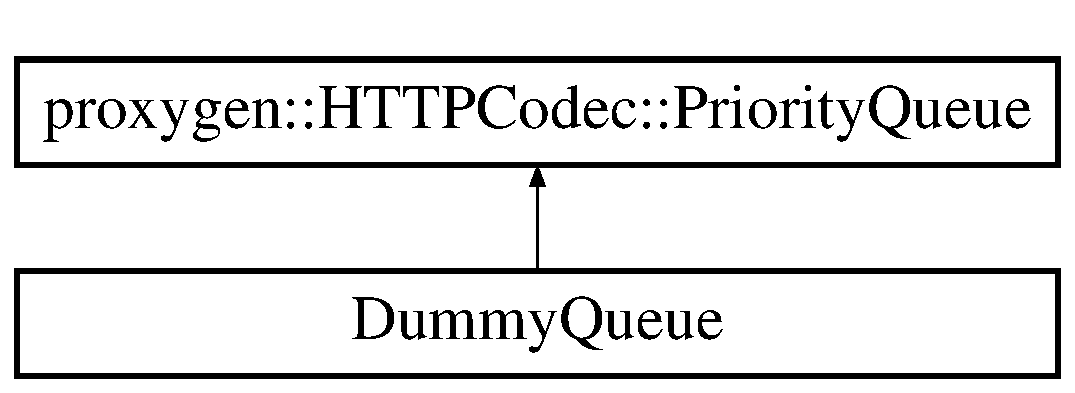
\includegraphics[height=2.000000cm]{classDummyQueue}
\end{center}
\end{figure}
\subsection*{Public Member Functions}
\begin{DoxyCompactItemize}
\item 
{\bf Dummy\+Queue} ()
\item 
{\bf $\sim$\+Dummy\+Queue} () override
\item 
void {\bf add\+Priority\+Node} ({\bf H\+T\+T\+P\+Codec\+::\+Stream\+ID} id, {\bf H\+T\+T\+P\+Codec\+::\+Stream\+ID}) override
\end{DoxyCompactItemize}
\subsection*{Public Attributes}
\begin{DoxyCompactItemize}
\item 
std\+::vector$<$ {\bf H\+T\+T\+P\+Codec\+::\+Stream\+ID} $>$ {\bf nodes\+\_\+}
\end{DoxyCompactItemize}


\subsection{Detailed Description}


Definition at line 1436 of file H\+T\+T\+P2\+Codec\+Test.\+cpp.



\subsection{Constructor \& Destructor Documentation}
\index{Dummy\+Queue@{Dummy\+Queue}!Dummy\+Queue@{Dummy\+Queue}}
\index{Dummy\+Queue@{Dummy\+Queue}!Dummy\+Queue@{Dummy\+Queue}}
\subsubsection[{Dummy\+Queue()}]{\setlength{\rightskip}{0pt plus 5cm}Dummy\+Queue\+::\+Dummy\+Queue (
\begin{DoxyParamCaption}
{}
\end{DoxyParamCaption}
)\hspace{0.3cm}{\ttfamily [inline]}}\label{classDummyQueue_a26beb35d21fd18fe3bf210d92293c109}


Definition at line 1438 of file H\+T\+T\+P2\+Codec\+Test.\+cpp.


\begin{DoxyCode}
1438 \{\}
\end{DoxyCode}
\index{Dummy\+Queue@{Dummy\+Queue}!````~Dummy\+Queue@{$\sim$\+Dummy\+Queue}}
\index{````~Dummy\+Queue@{$\sim$\+Dummy\+Queue}!Dummy\+Queue@{Dummy\+Queue}}
\subsubsection[{$\sim$\+Dummy\+Queue() override}]{\setlength{\rightskip}{0pt plus 5cm}Dummy\+Queue\+::$\sim$\+Dummy\+Queue (
\begin{DoxyParamCaption}
{}
\end{DoxyParamCaption}
)\hspace{0.3cm}{\ttfamily [inline]}, {\ttfamily [override]}}\label{classDummyQueue_adefa31d2670e3f9484cde9a9a8e51a8c}


Definition at line 1439 of file H\+T\+T\+P2\+Codec\+Test.\+cpp.


\begin{DoxyCode}
1439 \{\}
\end{DoxyCode}


\subsection{Member Function Documentation}
\index{Dummy\+Queue@{Dummy\+Queue}!add\+Priority\+Node@{add\+Priority\+Node}}
\index{add\+Priority\+Node@{add\+Priority\+Node}!Dummy\+Queue@{Dummy\+Queue}}
\subsubsection[{add\+Priority\+Node(\+H\+T\+T\+P\+Codec\+::\+Stream\+I\+D id, H\+T\+T\+P\+Codec\+::\+Stream\+I\+D) override}]{\setlength{\rightskip}{0pt plus 5cm}void Dummy\+Queue\+::add\+Priority\+Node (
\begin{DoxyParamCaption}
\item[{{\bf H\+T\+T\+P\+Codec\+::\+Stream\+ID}}]{id, }
\item[{{\bf H\+T\+T\+P\+Codec\+::\+Stream\+ID}}]{}
\end{DoxyParamCaption}
)\hspace{0.3cm}{\ttfamily [inline]}, {\ttfamily [override]}, {\ttfamily [virtual]}}\label{classDummyQueue_a815ab2e6208cbb56843e522c39df3484}


Implements {\bf proxygen\+::\+H\+T\+T\+P\+Codec\+::\+Priority\+Queue} \doxyref{}{p.}{classproxygen_1_1HTTPCodec_1_1PriorityQueue_abb613f1d0278eca54bc7e80d87137944}.



Definition at line 1440 of file H\+T\+T\+P2\+Codec\+Test.\+cpp.


\begin{DoxyCode}
1440                                                                          \{
1441     nodes_.push\_back(\textcolor{keywordtype}{id});
1442   \}
\end{DoxyCode}


\subsection{Member Data Documentation}
\index{Dummy\+Queue@{Dummy\+Queue}!nodes\+\_\+@{nodes\+\_\+}}
\index{nodes\+\_\+@{nodes\+\_\+}!Dummy\+Queue@{Dummy\+Queue}}
\subsubsection[{nodes\+\_\+}]{\setlength{\rightskip}{0pt plus 5cm}std\+::vector$<${\bf H\+T\+T\+P\+Codec\+::\+Stream\+ID}$>$ Dummy\+Queue\+::nodes\+\_\+}\label{classDummyQueue_abb65ff43f72c9b54a75b0a53a528a43f}


Definition at line 1444 of file H\+T\+T\+P2\+Codec\+Test.\+cpp.



Referenced by T\+E\+S\+T\+\_\+\+F().



The documentation for this class was generated from the following file\+:\begin{DoxyCompactItemize}
\item 
proxygen/lib/http/codec/test/{\bf H\+T\+T\+P2\+Codec\+Test.\+cpp}\end{DoxyCompactItemize}

\section{proxygen\+:\+:Dummy\+Timeout Class Reference}
\label{classproxygen_1_1DummyTimeout}\index{proxygen\+::\+Dummy\+Timeout@{proxygen\+::\+Dummy\+Timeout}}
Inheritance diagram for proxygen\+:\+:Dummy\+Timeout\+:\begin{figure}[H]
\begin{center}
\leavevmode
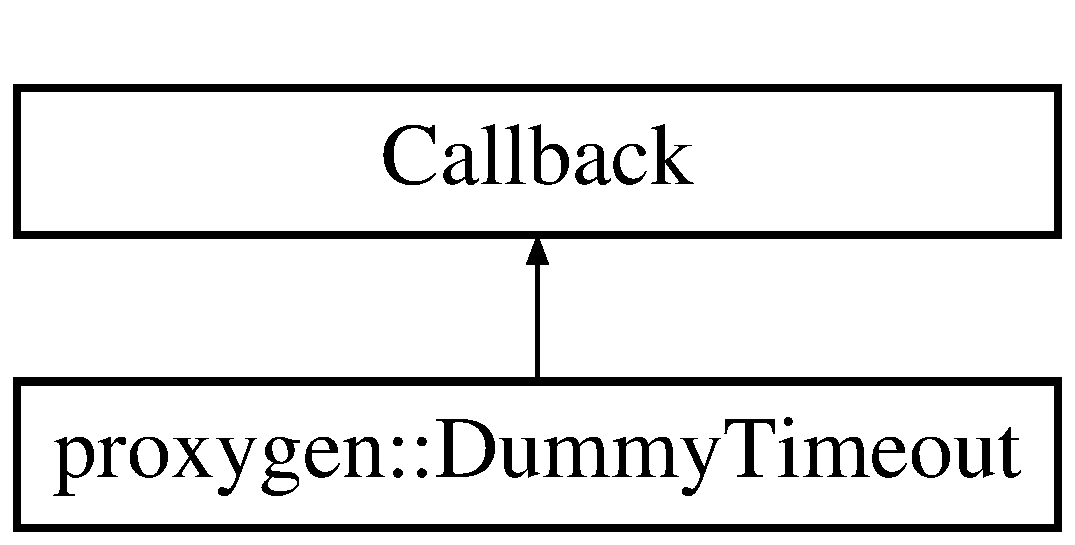
\includegraphics[height=2.000000cm]{classproxygen_1_1DummyTimeout}
\end{center}
\end{figure}
\subsection*{Private Member Functions}
\begin{DoxyCompactItemize}
\item 
void {\bf timeout\+Expired} () noexceptoverride
\end{DoxyCompactItemize}


\subsection{Detailed Description}


Definition at line 818 of file H\+T\+T\+P2\+Priority\+Queue\+Test.\+cpp.



\subsection{Member Function Documentation}
\index{proxygen\+::\+Dummy\+Timeout@{proxygen\+::\+Dummy\+Timeout}!timeout\+Expired@{timeout\+Expired}}
\index{timeout\+Expired@{timeout\+Expired}!proxygen\+::\+Dummy\+Timeout@{proxygen\+::\+Dummy\+Timeout}}
\subsubsection[{timeout\+Expired() noexceptoverride}]{\setlength{\rightskip}{0pt plus 5cm}void proxygen\+::\+Dummy\+Timeout\+::timeout\+Expired (
\begin{DoxyParamCaption}
{}
\end{DoxyParamCaption}
)\hspace{0.3cm}{\ttfamily [inline]}, {\ttfamily [override]}, {\ttfamily [private]}, {\ttfamily [noexcept]}}\label{classproxygen_1_1DummyTimeout_ad4695648dd8923babf766581f3ff0d9a}


Definition at line 819 of file H\+T\+T\+P2\+Priority\+Queue\+Test.\+cpp.


\begin{DoxyCode}
819                                           \{
820   \}
\end{DoxyCode}


The documentation for this class was generated from the following file\+:\begin{DoxyCompactItemize}
\item 
proxygen/lib/http/session/test/{\bf H\+T\+T\+P2\+Priority\+Queue\+Test.\+cpp}\end{DoxyCompactItemize}

\section{Echo\+Service\+:\+:Echo\+Handler Class Reference}
\label{classEchoService_1_1EchoHandler}\index{Echo\+Service\+::\+Echo\+Handler@{Echo\+Service\+::\+Echo\+Handler}}


{\ttfamily \#include $<$Echo\+Handler.\+h$>$}

Inheritance diagram for Echo\+Service\+:\+:Echo\+Handler\+:\begin{figure}[H]
\begin{center}
\leavevmode
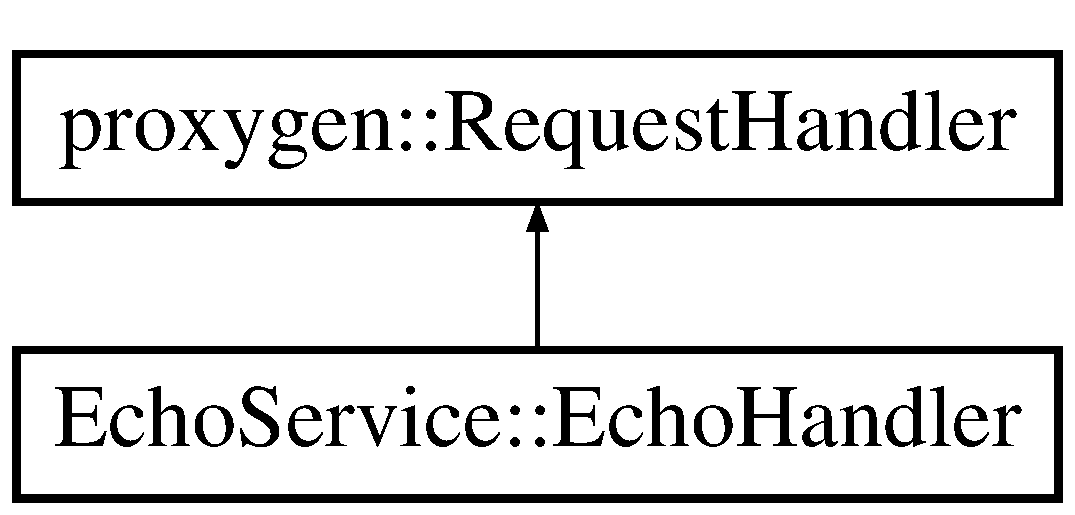
\includegraphics[height=2.000000cm]{classEchoService_1_1EchoHandler}
\end{center}
\end{figure}
\subsection*{Public Member Functions}
\begin{DoxyCompactItemize}
\item 
{\bf Echo\+Handler} ({\bf Echo\+Stats} $\ast$stats)
\item 
void {\bf on\+Request} (std\+::unique\+\_\+ptr$<$ {\bf proxygen\+::\+H\+T\+T\+P\+Message} $>$ headers) noexceptoverride
\item 
void {\bf on\+Body} (std\+::unique\+\_\+ptr$<$ folly\+::\+I\+O\+Buf $>$ body) noexceptoverride
\item 
void {\bf on\+E\+OM} () noexceptoverride
\item 
void {\bf on\+Upgrade} ({\bf proxygen\+::\+Upgrade\+Protocol} proto) noexceptoverride
\item 
void {\bf request\+Complete} () noexceptoverride
\item 
void {\bf on\+Error} ({\bf proxygen\+::\+Proxygen\+Error} err) noexceptoverride
\end{DoxyCompactItemize}
\subsection*{Private Attributes}
\begin{DoxyCompactItemize}
\item 
{\bf Echo\+Stats} $\ast$const {\bf stats\+\_\+} \{{\bf nullptr}\}
\item 
std\+::unique\+\_\+ptr$<$ folly\+::\+I\+O\+Buf $>$ {\bf body\+\_\+}
\end{DoxyCompactItemize}
\subsection*{Additional Inherited Members}


\subsection{Detailed Description}


Definition at line 23 of file Echo\+Handler.\+h.



\subsection{Constructor \& Destructor Documentation}
\index{Echo\+Service\+::\+Echo\+Handler@{Echo\+Service\+::\+Echo\+Handler}!Echo\+Handler@{Echo\+Handler}}
\index{Echo\+Handler@{Echo\+Handler}!Echo\+Service\+::\+Echo\+Handler@{Echo\+Service\+::\+Echo\+Handler}}
\subsubsection[{Echo\+Handler(\+Echo\+Stats $\ast$stats)}]{\setlength{\rightskip}{0pt plus 5cm}Echo\+Service\+::\+Echo\+Handler\+::\+Echo\+Handler (
\begin{DoxyParamCaption}
\item[{{\bf Echo\+Stats} $\ast$}]{stats}
\end{DoxyParamCaption}
)\hspace{0.3cm}{\ttfamily [explicit]}}\label{classEchoService_1_1EchoHandler_aa2fcdba4a6b4a25cde95ef1bf0895b38}


Definition at line 21 of file Echo\+Handler.\+cpp.


\begin{DoxyCode}
21                                         : stats_(stats) \{
22 \}
\end{DoxyCode}


\subsection{Member Function Documentation}
\index{Echo\+Service\+::\+Echo\+Handler@{Echo\+Service\+::\+Echo\+Handler}!on\+Body@{on\+Body}}
\index{on\+Body@{on\+Body}!Echo\+Service\+::\+Echo\+Handler@{Echo\+Service\+::\+Echo\+Handler}}
\subsubsection[{on\+Body(std\+::unique\+\_\+ptr$<$ folly\+::\+I\+O\+Buf $>$ body) noexceptoverride}]{\setlength{\rightskip}{0pt plus 5cm}void Echo\+Service\+::\+Echo\+Handler\+::on\+Body (
\begin{DoxyParamCaption}
\item[{std\+::unique\+\_\+ptr$<$ folly\+::\+I\+O\+Buf $>$}]{body}
\end{DoxyParamCaption}
)\hspace{0.3cm}{\ttfamily [override]}, {\ttfamily [virtual]}, {\ttfamily [noexcept]}}\label{classEchoService_1_1EchoHandler_acb1bd2ba7b3bbb9ba7700e2d39260d8a}
Invoked when we get part of body for the request. 

Implements {\bf proxygen\+::\+Request\+Handler} \doxyref{}{p.}{classproxygen_1_1RequestHandler_aaf0ed3bb94384e6240e15cca63de82bb}.



Definition at line 28 of file Echo\+Handler.\+cpp.



References body\+\_\+.


\begin{DoxyCode}
28                                                                 \{
29   \textcolor{keywordflow}{if} (body_) \{
30     body_->prependChain(std::move(body));
31   \} \textcolor{keywordflow}{else} \{
32     body_ = std::move(body);
33   \}
34 \}
\end{DoxyCode}
\index{Echo\+Service\+::\+Echo\+Handler@{Echo\+Service\+::\+Echo\+Handler}!on\+E\+OM@{on\+E\+OM}}
\index{on\+E\+OM@{on\+E\+OM}!Echo\+Service\+::\+Echo\+Handler@{Echo\+Service\+::\+Echo\+Handler}}
\subsubsection[{on\+E\+O\+M() noexceptoverride}]{\setlength{\rightskip}{0pt plus 5cm}void Echo\+Service\+::\+Echo\+Handler\+::on\+E\+OM (
\begin{DoxyParamCaption}
{}
\end{DoxyParamCaption}
)\hspace{0.3cm}{\ttfamily [override]}, {\ttfamily [virtual]}, {\ttfamily [noexcept]}}\label{classEchoService_1_1EchoHandler_abe8fa1e2a498986931c392bf0881dbcd}
Invoked when we finish receiving the body. 

Implements {\bf proxygen\+::\+Request\+Handler} \doxyref{}{p.}{classproxygen_1_1RequestHandler_a24f26d2cf71effaf154ce53aeff51aab}.



Definition at line 36 of file Echo\+Handler.\+cpp.



References proxygen\+::\+Response\+Builder\+::body(), body\+\_\+, proxygen\+::\+Request\+Handler\+::downstream\+\_\+, Echo\+Service\+::\+Echo\+Stats\+::get\+Request\+Count(), proxygen\+::\+Response\+Builder\+::header(), proxygen\+::\+Response\+Builder\+::send\+With\+E\+O\+M(), stats\+\_\+, and proxygen\+::\+Response\+Builder\+::status().


\begin{DoxyCode}
36                                  \{
37   ResponseBuilder(downstream_)
38     .status(200, \textcolor{stringliteral}{"OK"})
39     .header(\textcolor{stringliteral}{"Request-Number"},
40             folly::to<std::string>(stats_->getRequestCount()))
41     .body(std::move(body_))
42     .sendWithEOM();
43 \}
\end{DoxyCode}
\index{Echo\+Service\+::\+Echo\+Handler@{Echo\+Service\+::\+Echo\+Handler}!on\+Error@{on\+Error}}
\index{on\+Error@{on\+Error}!Echo\+Service\+::\+Echo\+Handler@{Echo\+Service\+::\+Echo\+Handler}}
\subsubsection[{on\+Error(proxygen\+::\+Proxygen\+Error err) noexceptoverride}]{\setlength{\rightskip}{0pt plus 5cm}void Echo\+Service\+::\+Echo\+Handler\+::on\+Error (
\begin{DoxyParamCaption}
\item[{{\bf proxygen\+::\+Proxygen\+Error}}]{err}
\end{DoxyParamCaption}
)\hspace{0.3cm}{\ttfamily [override]}, {\ttfamily [virtual]}, {\ttfamily [noexcept]}}\label{classEchoService_1_1EchoHandler_ac67effcf7a52288701e2661b0212b2df}
Request failed. Maybe because of read/write error on socket or client not being able to send request in time.

N\+O\+TE\+: Can be invoked at any time (except for before on\+Request).

No more callbacks will be invoked after this. You should clean up after yourself. 

Implements {\bf proxygen\+::\+Request\+Handler} \doxyref{}{p.}{classproxygen_1_1RequestHandler_ad7e6428b925840a334adc58ff6f4f680}.



Definition at line 53 of file Echo\+Handler.\+cpp.


\begin{DoxyCode}
53 \{ \textcolor{keyword}{delete} \textcolor{keyword}{this}; \}
\end{DoxyCode}
\index{Echo\+Service\+::\+Echo\+Handler@{Echo\+Service\+::\+Echo\+Handler}!on\+Request@{on\+Request}}
\index{on\+Request@{on\+Request}!Echo\+Service\+::\+Echo\+Handler@{Echo\+Service\+::\+Echo\+Handler}}
\subsubsection[{on\+Request(std\+::unique\+\_\+ptr$<$ proxygen\+::\+H\+T\+T\+P\+Message $>$ headers) noexceptoverride}]{\setlength{\rightskip}{0pt plus 5cm}void Echo\+Service\+::\+Echo\+Handler\+::on\+Request (
\begin{DoxyParamCaption}
\item[{std\+::unique\+\_\+ptr$<$ {\bf proxygen\+::\+H\+T\+T\+P\+Message} $>$}]{headers}
\end{DoxyParamCaption}
)\hspace{0.3cm}{\ttfamily [override]}, {\ttfamily [virtual]}, {\ttfamily [noexcept]}}\label{classEchoService_1_1EchoHandler_a932d54649a949672ab933e688cfac4b6}
Invoked when we have successfully fetched headers from client. This will always be the first callback invoked on your handler. 

Implements {\bf proxygen\+::\+Request\+Handler} \doxyref{}{p.}{classproxygen_1_1RequestHandler_a61f59e1155f906c7b73062147164320f}.



Definition at line 24 of file Echo\+Handler.\+cpp.



References Echo\+Service\+::\+Echo\+Stats\+::record\+Request(), and stats\+\_\+.


\begin{DoxyCode}
24                                                                  \{
25   stats_->recordRequest();
26 \}
\end{DoxyCode}
\index{Echo\+Service\+::\+Echo\+Handler@{Echo\+Service\+::\+Echo\+Handler}!on\+Upgrade@{on\+Upgrade}}
\index{on\+Upgrade@{on\+Upgrade}!Echo\+Service\+::\+Echo\+Handler@{Echo\+Service\+::\+Echo\+Handler}}
\subsubsection[{on\+Upgrade(proxygen\+::\+Upgrade\+Protocol proto) noexceptoverride}]{\setlength{\rightskip}{0pt plus 5cm}void Echo\+Service\+::\+Echo\+Handler\+::on\+Upgrade (
\begin{DoxyParamCaption}
\item[{{\bf proxygen\+::\+Upgrade\+Protocol}}]{prot}
\end{DoxyParamCaption}
)\hspace{0.3cm}{\ttfamily [override]}, {\ttfamily [virtual]}, {\ttfamily [noexcept]}}\label{classEchoService_1_1EchoHandler_af5cda50efa2d8ff694b4f37a48d61df3}
Invoked when the session has been upgraded to a different protocol 

Implements {\bf proxygen\+::\+Request\+Handler} \doxyref{}{p.}{classproxygen_1_1RequestHandler_aefed2946bc5558baf6e36a2d11290b79}.



Definition at line 45 of file Echo\+Handler.\+cpp.


\begin{DoxyCode}
45                                                       \{
46   \textcolor{comment}{// handler doesn't support upgrades}
47 \}
\end{DoxyCode}
\index{Echo\+Service\+::\+Echo\+Handler@{Echo\+Service\+::\+Echo\+Handler}!request\+Complete@{request\+Complete}}
\index{request\+Complete@{request\+Complete}!Echo\+Service\+::\+Echo\+Handler@{Echo\+Service\+::\+Echo\+Handler}}
\subsubsection[{request\+Complete() noexceptoverride}]{\setlength{\rightskip}{0pt plus 5cm}void Echo\+Service\+::\+Echo\+Handler\+::request\+Complete (
\begin{DoxyParamCaption}
{}
\end{DoxyParamCaption}
)\hspace{0.3cm}{\ttfamily [override]}, {\ttfamily [virtual]}, {\ttfamily [noexcept]}}\label{classEchoService_1_1EchoHandler_af1e31ad69997ed16af7294fb449e7004}
Invoked when request processing has been completed and nothing more needs to be done. This may be a good place to log some stats and clean up resources. This is distinct from \doxyref{on\+E\+O\+M()}{p.}{classEchoService_1_1EchoHandler_abe8fa1e2a498986931c392bf0881dbcd} because it is invoked after the response is fully sent. Once this callback has been received, {\ttfamily downstream\+\_\+} should be considered invalid. 

Implements {\bf proxygen\+::\+Request\+Handler} \doxyref{}{p.}{classproxygen_1_1RequestHandler_a0ec159751b407bcd3667994c6d8d7cfe}.



Definition at line 49 of file Echo\+Handler.\+cpp.


\begin{DoxyCode}
49                                            \{
50   \textcolor{keyword}{delete} \textcolor{keyword}{this};
51 \}
\end{DoxyCode}


\subsection{Member Data Documentation}
\index{Echo\+Service\+::\+Echo\+Handler@{Echo\+Service\+::\+Echo\+Handler}!body\+\_\+@{body\+\_\+}}
\index{body\+\_\+@{body\+\_\+}!Echo\+Service\+::\+Echo\+Handler@{Echo\+Service\+::\+Echo\+Handler}}
\subsubsection[{body\+\_\+}]{\setlength{\rightskip}{0pt plus 5cm}std\+::unique\+\_\+ptr$<$folly\+::\+I\+O\+Buf$>$ Echo\+Service\+::\+Echo\+Handler\+::body\+\_\+\hspace{0.3cm}{\ttfamily [private]}}\label{classEchoService_1_1EchoHandler_a1f73fd52f02a93b6acb4cd591bc1293d}


Definition at line 43 of file Echo\+Handler.\+h.



Referenced by on\+Body(), and on\+E\+O\+M().

\index{Echo\+Service\+::\+Echo\+Handler@{Echo\+Service\+::\+Echo\+Handler}!stats\+\_\+@{stats\+\_\+}}
\index{stats\+\_\+@{stats\+\_\+}!Echo\+Service\+::\+Echo\+Handler@{Echo\+Service\+::\+Echo\+Handler}}
\subsubsection[{stats\+\_\+}]{\setlength{\rightskip}{0pt plus 5cm}{\bf Echo\+Stats}$\ast$ const Echo\+Service\+::\+Echo\+Handler\+::stats\+\_\+ \{{\bf nullptr}\}\hspace{0.3cm}{\ttfamily [private]}}\label{classEchoService_1_1EchoHandler_ab421c6cce76b196ef923ef2a8bb2dab6}


Definition at line 41 of file Echo\+Handler.\+h.



Referenced by on\+E\+O\+M(), and on\+Request().



The documentation for this class was generated from the following files\+:\begin{DoxyCompactItemize}
\item 
proxygen/httpserver/samples/echo/{\bf Echo\+Handler.\+h}\item 
proxygen/httpserver/samples/echo/{\bf Echo\+Handler.\+cpp}\end{DoxyCompactItemize}

\section{Echo\+Handler\+Factory Class Reference}
\label{classEchoHandlerFactory}\index{Echo\+Handler\+Factory@{Echo\+Handler\+Factory}}
Inheritance diagram for Echo\+Handler\+Factory\+:\begin{figure}[H]
\begin{center}
\leavevmode
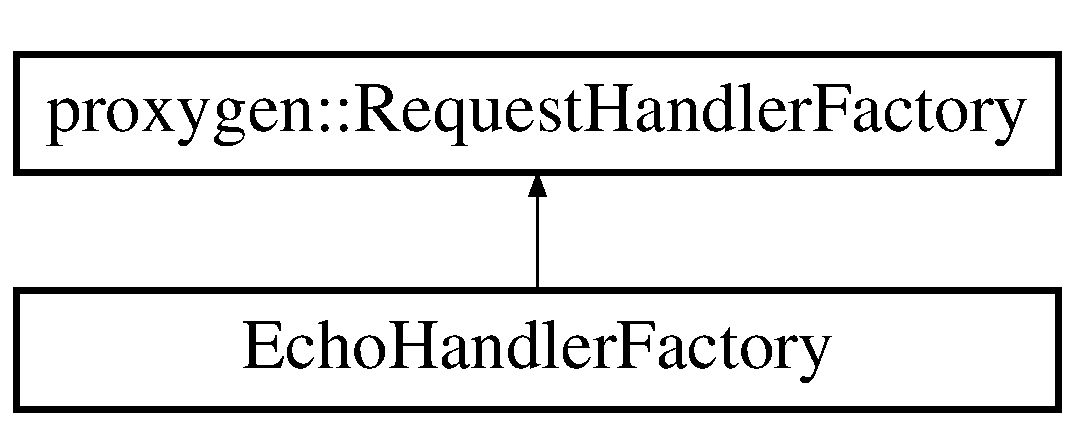
\includegraphics[height=2.000000cm]{classEchoHandlerFactory}
\end{center}
\end{figure}
\subsection*{Public Member Functions}
\begin{DoxyCompactItemize}
\item 
void {\bf on\+Server\+Start} (folly\+::\+Event\+Base $\ast$) noexceptoverride
\item 
void {\bf on\+Server\+Stop} () noexceptoverride
\item 
{\bf Request\+Handler} $\ast$ {\bf on\+Request} ({\bf Request\+Handler} $\ast$, {\bf H\+T\+T\+P\+Message} $\ast$) noexceptoverride
\end{DoxyCompactItemize}
\subsection*{Private Attributes}
\begin{DoxyCompactItemize}
\item 
folly\+::\+Thread\+Local\+Ptr$<$ {\bf Echo\+Stats} $>$ {\bf stats\+\_\+}
\end{DoxyCompactItemize}


\subsection{Detailed Description}


Definition at line 36 of file Echo\+Server.\+cpp.



\subsection{Member Function Documentation}
\index{Echo\+Handler\+Factory@{Echo\+Handler\+Factory}!on\+Request@{on\+Request}}
\index{on\+Request@{on\+Request}!Echo\+Handler\+Factory@{Echo\+Handler\+Factory}}
\subsubsection[{on\+Request(\+Request\+Handler $\ast$, H\+T\+T\+P\+Message $\ast$) noexceptoverride}]{\setlength{\rightskip}{0pt plus 5cm}{\bf Request\+Handler}$\ast$ Echo\+Handler\+Factory\+::on\+Request (
\begin{DoxyParamCaption}
\item[{{\bf Request\+Handler} $\ast$}]{, }
\item[{{\bf H\+T\+T\+P\+Message} $\ast$}]{}
\end{DoxyParamCaption}
)\hspace{0.3cm}{\ttfamily [inline]}, {\ttfamily [override]}, {\ttfamily [virtual]}, {\ttfamily [noexcept]}}\label{classEchoHandlerFactory_aea5858e08e8ecdb3a6a6be1e12872b50}
Invoked for each new request server handles. H\+T\+T\+P\+Message is provided so that user can potentially choose among several implementation of handler based on U\+RL or something. No need to save/copy this H\+T\+T\+P\+Message. Request\+Handler will be given the H\+T\+T\+P\+Message in a separate callback.

Some request handlers don\textquotesingle{}t handle the request themselves (think filters). They do take some actions based on request/response but otherwise they just hand-\/off request to some other Request\+Handler. This upstream Request\+Handler is given as first parameter. For the terminal Request\+Handler this will by nullptr. 

Implements {\bf proxygen\+::\+Request\+Handler\+Factory} \doxyref{}{p.}{classproxygen_1_1RequestHandlerFactory_a9c2cbbc96d006244ea28cea44a3e6a60}.



Definition at line 46 of file Echo\+Server.\+cpp.


\begin{DoxyCode}
46                                                                              \{
47     \textcolor{keywordflow}{return} \textcolor{keyword}{new} EchoHandler(stats_.get());
48   \}
\end{DoxyCode}
\index{Echo\+Handler\+Factory@{Echo\+Handler\+Factory}!on\+Server\+Start@{on\+Server\+Start}}
\index{on\+Server\+Start@{on\+Server\+Start}!Echo\+Handler\+Factory@{Echo\+Handler\+Factory}}
\subsubsection[{on\+Server\+Start(folly\+::\+Event\+Base $\ast$) noexceptoverride}]{\setlength{\rightskip}{0pt plus 5cm}void Echo\+Handler\+Factory\+::on\+Server\+Start (
\begin{DoxyParamCaption}
\item[{folly\+::\+Event\+Base $\ast$}]{evb}
\end{DoxyParamCaption}
)\hspace{0.3cm}{\ttfamily [inline]}, {\ttfamily [override]}, {\ttfamily [virtual]}, {\ttfamily [noexcept]}}\label{classEchoHandlerFactory_a458dde996e97432619ab11bf8b55d58b}
Invoked in each thread server is going to handle requests before we start handling requests. Can be used to setup thread-\/local setup for each thread (stats and such). 

Implements {\bf proxygen\+::\+Request\+Handler\+Factory} \doxyref{}{p.}{classproxygen_1_1RequestHandlerFactory_af76091b8a51a8d069fcc1aec3007a1cc}.



Definition at line 38 of file Echo\+Server.\+cpp.


\begin{DoxyCode}
38                                                           \{
39     stats_.reset(\textcolor{keyword}{new} EchoStats);
40   \}
\end{DoxyCode}
\index{Echo\+Handler\+Factory@{Echo\+Handler\+Factory}!on\+Server\+Stop@{on\+Server\+Stop}}
\index{on\+Server\+Stop@{on\+Server\+Stop}!Echo\+Handler\+Factory@{Echo\+Handler\+Factory}}
\subsubsection[{on\+Server\+Stop() noexceptoverride}]{\setlength{\rightskip}{0pt plus 5cm}void Echo\+Handler\+Factory\+::on\+Server\+Stop (
\begin{DoxyParamCaption}
{}
\end{DoxyParamCaption}
)\hspace{0.3cm}{\ttfamily [inline]}, {\ttfamily [override]}, {\ttfamily [virtual]}, {\ttfamily [noexcept]}}\label{classEchoHandlerFactory_a5e461a60e6e9f8e49e4c07ca13eba7b6}
Invoked in each handler thread after all the connections are drained from that thread. Can be used to tear down thread-\/local setup. 

Implements {\bf proxygen\+::\+Request\+Handler\+Factory} \doxyref{}{p.}{classproxygen_1_1RequestHandlerFactory_a0791d6b33c13513ed6f550bbbd7bca85}.



Definition at line 42 of file Echo\+Server.\+cpp.


\begin{DoxyCode}
42                                         \{
43     stats_.reset();
44   \}
\end{DoxyCode}


\subsection{Member Data Documentation}
\index{Echo\+Handler\+Factory@{Echo\+Handler\+Factory}!stats\+\_\+@{stats\+\_\+}}
\index{stats\+\_\+@{stats\+\_\+}!Echo\+Handler\+Factory@{Echo\+Handler\+Factory}}
\subsubsection[{stats\+\_\+}]{\setlength{\rightskip}{0pt plus 5cm}folly\+::\+Thread\+Local\+Ptr$<${\bf Echo\+Stats}$>$ Echo\+Handler\+Factory\+::stats\+\_\+\hspace{0.3cm}{\ttfamily [private]}}\label{classEchoHandlerFactory_a529d1601f88485d6016d29185f432795}


Definition at line 51 of file Echo\+Server.\+cpp.



The documentation for this class was generated from the following file\+:\begin{DoxyCompactItemize}
\item 
proxygen/httpserver/samples/echo/{\bf Echo\+Server.\+cpp}\end{DoxyCompactItemize}

\section{Echo\+Handler\+Fixture Class Reference}
\label{classEchoHandlerFixture}\index{Echo\+Handler\+Fixture@{Echo\+Handler\+Fixture}}
Inheritance diagram for Echo\+Handler\+Fixture\+:\begin{figure}[H]
\begin{center}
\leavevmode
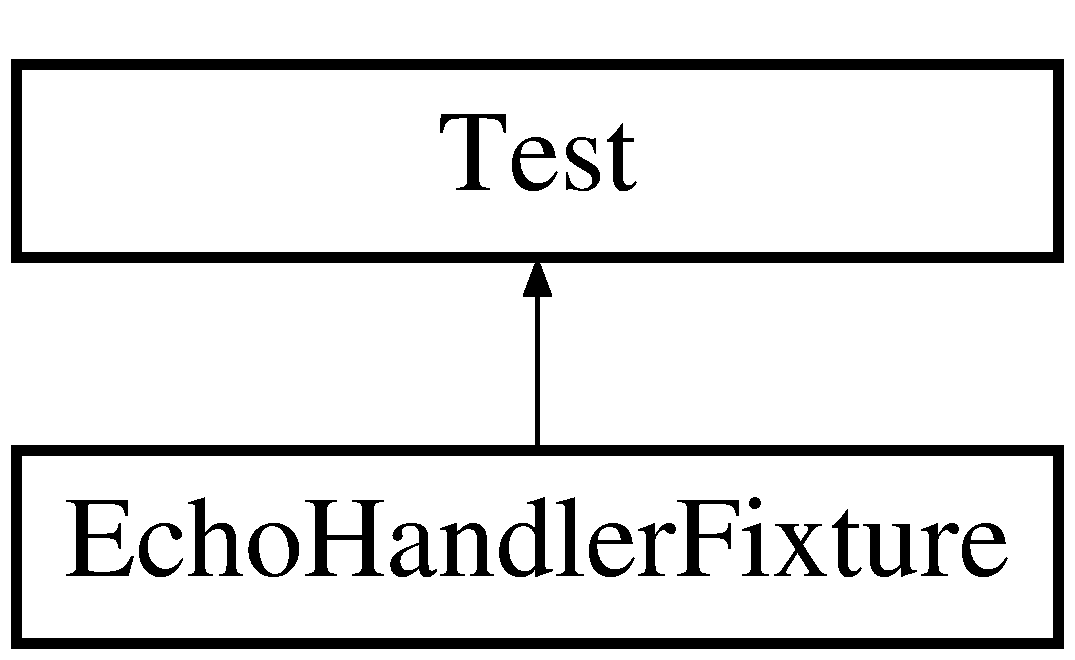
\includegraphics[height=2.000000cm]{classEchoHandlerFixture}
\end{center}
\end{figure}
\subsection*{Public Member Functions}
\begin{DoxyCompactItemize}
\item 
void {\bf Set\+Up} () override
\item 
void {\bf Tear\+Down} () override
\end{DoxyCompactItemize}
\subsection*{Protected Attributes}
\begin{DoxyCompactItemize}
\item 
{\bf Echo\+Handler} $\ast$ {\bf handler} \{{\bf nullptr}\}
\item 
Strict\+Mock$<$ {\bf Mock\+Echo\+Stats} $>$ {\bf stats}
\item 
std\+::unique\+\_\+ptr$<$ {\bf Mock\+Response\+Handler} $>$ {\bf response\+Handler}
\end{DoxyCompactItemize}


\subsection{Detailed Description}


Definition at line 26 of file Echo\+Handler\+Test.\+cpp.



\subsection{Member Function Documentation}
\index{Echo\+Handler\+Fixture@{Echo\+Handler\+Fixture}!Set\+Up@{Set\+Up}}
\index{Set\+Up@{Set\+Up}!Echo\+Handler\+Fixture@{Echo\+Handler\+Fixture}}
\subsubsection[{Set\+Up() override}]{\setlength{\rightskip}{0pt plus 5cm}void Echo\+Handler\+Fixture\+::\+Set\+Up (
\begin{DoxyParamCaption}
{}
\end{DoxyParamCaption}
)\hspace{0.3cm}{\ttfamily [inline]}, {\ttfamily [override]}}\label{classEchoHandlerFixture_a2cadfbce5064a1be32ffa74ad0932451}


Definition at line 28 of file Echo\+Handler\+Test.\+cpp.


\begin{DoxyCode}
28                         \{
29     handler = \textcolor{keyword}{new} EchoHandler(&stats);
30     responseHandler = std::make\_unique<MockResponseHandler>(handler);
31     handler->setResponseHandler(responseHandler.get());
32   \}
\end{DoxyCode}
\index{Echo\+Handler\+Fixture@{Echo\+Handler\+Fixture}!Tear\+Down@{Tear\+Down}}
\index{Tear\+Down@{Tear\+Down}!Echo\+Handler\+Fixture@{Echo\+Handler\+Fixture}}
\subsubsection[{Tear\+Down() override}]{\setlength{\rightskip}{0pt plus 5cm}void Echo\+Handler\+Fixture\+::\+Tear\+Down (
\begin{DoxyParamCaption}
{}
\end{DoxyParamCaption}
)\hspace{0.3cm}{\ttfamily [inline]}, {\ttfamily [override]}}\label{classEchoHandlerFixture_a724579b42c6c20f6d79b0d4e06741576}


Definition at line 34 of file Echo\+Handler\+Test.\+cpp.


\begin{DoxyCode}
34                            \{
35     Mock::VerifyAndClear(&stats);
36     Mock::VerifyAndClear(responseHandler.get());
37 
38     \textcolor{comment}{// Since there is no easy way to verify that handler has deleted}
39     \textcolor{comment}{// itself, its advised to run test binary under AddressSanitzer}
40     \textcolor{comment}{// to verify that.}
41   \}
\end{DoxyCode}


\subsection{Member Data Documentation}
\index{Echo\+Handler\+Fixture@{Echo\+Handler\+Fixture}!handler@{handler}}
\index{handler@{handler}!Echo\+Handler\+Fixture@{Echo\+Handler\+Fixture}}
\subsubsection[{handler}]{\setlength{\rightskip}{0pt plus 5cm}{\bf Echo\+Handler}$\ast$ Echo\+Handler\+Fixture\+::handler \{{\bf nullptr}\}\hspace{0.3cm}{\ttfamily [protected]}}\label{classEchoHandlerFixture_a8c87741598fe9bea6be899c79f754310}


Definition at line 44 of file Echo\+Handler\+Test.\+cpp.

\index{Echo\+Handler\+Fixture@{Echo\+Handler\+Fixture}!response\+Handler@{response\+Handler}}
\index{response\+Handler@{response\+Handler}!Echo\+Handler\+Fixture@{Echo\+Handler\+Fixture}}
\subsubsection[{response\+Handler}]{\setlength{\rightskip}{0pt plus 5cm}std\+::unique\+\_\+ptr$<${\bf Mock\+Response\+Handler}$>$ Echo\+Handler\+Fixture\+::response\+Handler\hspace{0.3cm}{\ttfamily [protected]}}\label{classEchoHandlerFixture_af2e2b472637ff5fffae721581ba29a4b}


Definition at line 46 of file Echo\+Handler\+Test.\+cpp.

\index{Echo\+Handler\+Fixture@{Echo\+Handler\+Fixture}!stats@{stats}}
\index{stats@{stats}!Echo\+Handler\+Fixture@{Echo\+Handler\+Fixture}}
\subsubsection[{stats}]{\setlength{\rightskip}{0pt plus 5cm}Strict\+Mock$<${\bf Mock\+Echo\+Stats}$>$ Echo\+Handler\+Fixture\+::stats\hspace{0.3cm}{\ttfamily [protected]}}\label{classEchoHandlerFixture_adda2ebe970af7c852303d62f8f1e5a1f}


Definition at line 45 of file Echo\+Handler\+Test.\+cpp.



The documentation for this class was generated from the following file\+:\begin{DoxyCompactItemize}
\item 
proxygen/httpserver/samples/echo/test/{\bf Echo\+Handler\+Test.\+cpp}\end{DoxyCompactItemize}

\section{Echo\+Service\+:\+:Echo\+Stats Class Reference}
\label{classEchoService_1_1EchoStats}\index{Echo\+Service\+::\+Echo\+Stats@{Echo\+Service\+::\+Echo\+Stats}}


{\ttfamily \#include $<$Echo\+Stats.\+h$>$}

Inheritance diagram for Echo\+Service\+:\+:Echo\+Stats\+:\begin{figure}[H]
\begin{center}
\leavevmode
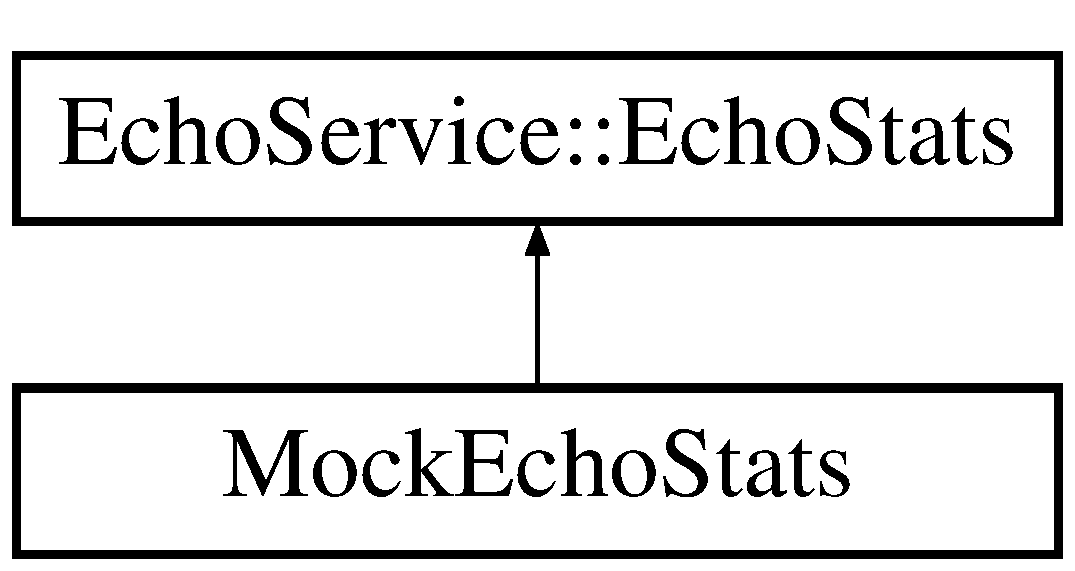
\includegraphics[height=2.000000cm]{classEchoService_1_1EchoStats}
\end{center}
\end{figure}
\subsection*{Public Member Functions}
\begin{DoxyCompactItemize}
\item 
virtual {\bf $\sim$\+Echo\+Stats} ()
\item 
virtual void {\bf record\+Request} ()
\item 
virtual uint64\+\_\+t {\bf get\+Request\+Count} ()
\end{DoxyCompactItemize}
\subsection*{Private Attributes}
\begin{DoxyCompactItemize}
\item 
uint64\+\_\+t {\bf req\+Count\+\_\+} \{0\}
\end{DoxyCompactItemize}


\subsection{Detailed Description}
Just some dummy class containing request count. Since we keep one instance of this in each class, there is no need of synchronization 

Definition at line 21 of file Echo\+Stats.\+h.



\subsection{Constructor \& Destructor Documentation}
\index{Echo\+Service\+::\+Echo\+Stats@{Echo\+Service\+::\+Echo\+Stats}!````~Echo\+Stats@{$\sim$\+Echo\+Stats}}
\index{````~Echo\+Stats@{$\sim$\+Echo\+Stats}!Echo\+Service\+::\+Echo\+Stats@{Echo\+Service\+::\+Echo\+Stats}}
\subsubsection[{$\sim$\+Echo\+Stats()}]{\setlength{\rightskip}{0pt plus 5cm}virtual Echo\+Service\+::\+Echo\+Stats\+::$\sim$\+Echo\+Stats (
\begin{DoxyParamCaption}
{}
\end{DoxyParamCaption}
)\hspace{0.3cm}{\ttfamily [inline]}, {\ttfamily [virtual]}}\label{classEchoService_1_1EchoStats_ad032c0cca3fd9dbf4f8b03f8387a58fa}


Definition at line 23 of file Echo\+Stats.\+h.


\begin{DoxyCode}
23                        \{
24   \}
\end{DoxyCode}


\subsection{Member Function Documentation}
\index{Echo\+Service\+::\+Echo\+Stats@{Echo\+Service\+::\+Echo\+Stats}!get\+Request\+Count@{get\+Request\+Count}}
\index{get\+Request\+Count@{get\+Request\+Count}!Echo\+Service\+::\+Echo\+Stats@{Echo\+Service\+::\+Echo\+Stats}}
\subsubsection[{get\+Request\+Count()}]{\setlength{\rightskip}{0pt plus 5cm}virtual uint64\+\_\+t Echo\+Service\+::\+Echo\+Stats\+::get\+Request\+Count (
\begin{DoxyParamCaption}
{}
\end{DoxyParamCaption}
)\hspace{0.3cm}{\ttfamily [inline]}, {\ttfamily [virtual]}}\label{classEchoService_1_1EchoStats_a26ebc46f67809f621d2aa26777562b0c}


Definition at line 35 of file Echo\+Stats.\+h.



References req\+Count\+\_\+.



Referenced by Echo\+Service\+::\+Echo\+Handler\+::on\+E\+O\+M().


\begin{DoxyCode}
35                                      \{
36     \textcolor{keywordflow}{return} reqCount_;
37   \}
\end{DoxyCode}
\index{Echo\+Service\+::\+Echo\+Stats@{Echo\+Service\+::\+Echo\+Stats}!record\+Request@{record\+Request}}
\index{record\+Request@{record\+Request}!Echo\+Service\+::\+Echo\+Stats@{Echo\+Service\+::\+Echo\+Stats}}
\subsubsection[{record\+Request()}]{\setlength{\rightskip}{0pt plus 5cm}virtual void Echo\+Service\+::\+Echo\+Stats\+::record\+Request (
\begin{DoxyParamCaption}
{}
\end{DoxyParamCaption}
)\hspace{0.3cm}{\ttfamily [inline]}, {\ttfamily [virtual]}}\label{classEchoService_1_1EchoStats_a8718aed3002dd750773258d62942257d}


Definition at line 31 of file Echo\+Stats.\+h.



References req\+Count\+\_\+.



Referenced by Echo\+Service\+::\+Echo\+Handler\+::on\+Request().


\begin{DoxyCode}
31                                \{
32     ++reqCount_;
33   \}
\end{DoxyCode}


\subsection{Member Data Documentation}
\index{Echo\+Service\+::\+Echo\+Stats@{Echo\+Service\+::\+Echo\+Stats}!req\+Count\+\_\+@{req\+Count\+\_\+}}
\index{req\+Count\+\_\+@{req\+Count\+\_\+}!Echo\+Service\+::\+Echo\+Stats@{Echo\+Service\+::\+Echo\+Stats}}
\subsubsection[{req\+Count\+\_\+}]{\setlength{\rightskip}{0pt plus 5cm}uint64\+\_\+t Echo\+Service\+::\+Echo\+Stats\+::req\+Count\+\_\+ \{0\}\hspace{0.3cm}{\ttfamily [private]}}\label{classEchoService_1_1EchoStats_ab4c069f4bc26d9b40dd7417b3b4297a9}


Definition at line 40 of file Echo\+Stats.\+h.



Referenced by get\+Request\+Count(), and record\+Request().



The documentation for this class was generated from the following file\+:\begin{DoxyCompactItemize}
\item 
proxygen/httpserver/samples/echo/{\bf Echo\+Stats.\+h}\end{DoxyCompactItemize}

\section{Egress\+State\+Machine\+Fixture Class Reference}
\label{classEgressStateMachineFixture}\index{Egress\+State\+Machine\+Fixture@{Egress\+State\+Machine\+Fixture}}
Inheritance diagram for Egress\+State\+Machine\+Fixture\+:\begin{figure}[H]
\begin{center}
\leavevmode
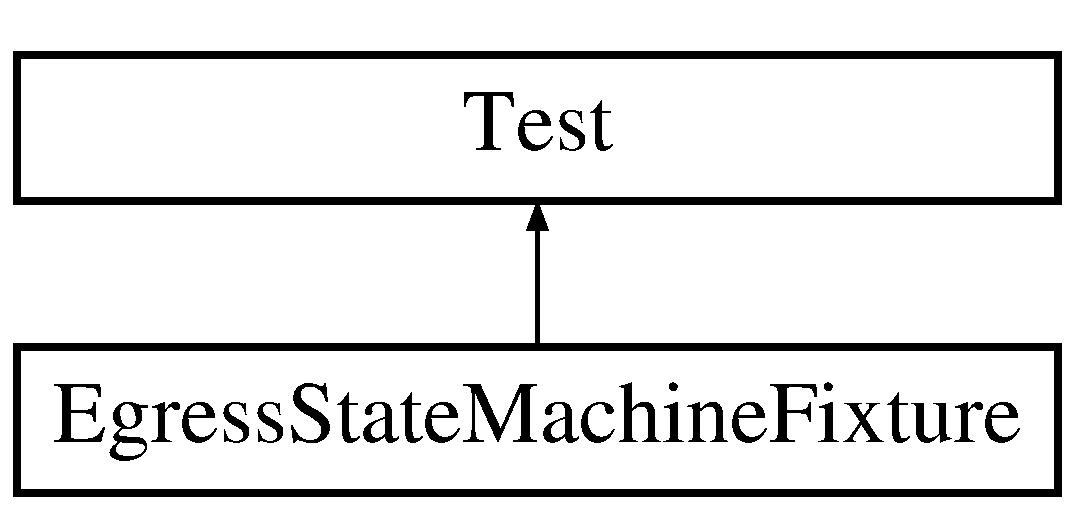
\includegraphics[height=2.000000cm]{classEgressStateMachineFixture}
\end{center}
\end{figure}
\subsection*{Public Member Functions}
\begin{DoxyCompactItemize}
\item 
{\bf Egress\+State\+Machine\+Fixture} ()
\item 
void {\bf follow} ({\bf H\+T\+T\+P\+Transaction\+Egress\+S\+M\+::\+Event} e)
\item 
void {\bf fail} ({\bf H\+T\+T\+P\+Transaction\+Egress\+S\+M\+::\+Event} e)
\end{DoxyCompactItemize}
\subsection*{Private Attributes}
\begin{DoxyCompactItemize}
\item 
{\bf H\+T\+T\+P\+Transaction\+Egress\+S\+M\+::\+State} {\bf instance\+\_\+}
\end{DoxyCompactItemize}


\subsection{Detailed Description}


Definition at line 16 of file H\+T\+T\+P\+Transaction\+S\+M\+Test.\+cpp.



\subsection{Constructor \& Destructor Documentation}
\index{Egress\+State\+Machine\+Fixture@{Egress\+State\+Machine\+Fixture}!Egress\+State\+Machine\+Fixture@{Egress\+State\+Machine\+Fixture}}
\index{Egress\+State\+Machine\+Fixture@{Egress\+State\+Machine\+Fixture}!Egress\+State\+Machine\+Fixture@{Egress\+State\+Machine\+Fixture}}
\subsubsection[{Egress\+State\+Machine\+Fixture()}]{\setlength{\rightskip}{0pt plus 5cm}Egress\+State\+Machine\+Fixture\+::\+Egress\+State\+Machine\+Fixture (
\begin{DoxyParamCaption}
{}
\end{DoxyParamCaption}
)\hspace{0.3cm}{\ttfamily [inline]}}\label{classEgressStateMachineFixture_afa3620b29085495a95630ea469c101c3}


Definition at line 18 of file H\+T\+T\+P\+Transaction\+S\+M\+Test.\+cpp.


\begin{DoxyCode}
18                              : instance_(
19     HTTPTransactionEgressSM::getNewInstance()) \{\}
\end{DoxyCode}


\subsection{Member Function Documentation}
\index{Egress\+State\+Machine\+Fixture@{Egress\+State\+Machine\+Fixture}!fail@{fail}}
\index{fail@{fail}!Egress\+State\+Machine\+Fixture@{Egress\+State\+Machine\+Fixture}}
\subsubsection[{fail(\+H\+T\+T\+P\+Transaction\+Egress\+S\+M\+::\+Event e)}]{\setlength{\rightskip}{0pt plus 5cm}void Egress\+State\+Machine\+Fixture\+::fail (
\begin{DoxyParamCaption}
\item[{{\bf H\+T\+T\+P\+Transaction\+Egress\+S\+M\+::\+Event}}]{e}
\end{DoxyParamCaption}
)\hspace{0.3cm}{\ttfamily [inline]}}\label{classEgressStateMachineFixture_ae7d7bdb2a4a253ff5338375496b9aa5c}


Definition at line 25 of file H\+T\+T\+P\+Transaction\+S\+M\+Test.\+cpp.



References proxygen\+::\+State\+Machine$<$ T $>$\+::transit().


\begin{DoxyCode}
25                                             \{
26     EXPECT\_FALSE(HTTPTransactionEgressSM::transit(instance_, e));
27   \}
\end{DoxyCode}
\index{Egress\+State\+Machine\+Fixture@{Egress\+State\+Machine\+Fixture}!follow@{follow}}
\index{follow@{follow}!Egress\+State\+Machine\+Fixture@{Egress\+State\+Machine\+Fixture}}
\subsubsection[{follow(\+H\+T\+T\+P\+Transaction\+Egress\+S\+M\+::\+Event e)}]{\setlength{\rightskip}{0pt plus 5cm}void Egress\+State\+Machine\+Fixture\+::follow (
\begin{DoxyParamCaption}
\item[{{\bf H\+T\+T\+P\+Transaction\+Egress\+S\+M\+::\+Event}}]{e}
\end{DoxyParamCaption}
)\hspace{0.3cm}{\ttfamily [inline]}}\label{classEgressStateMachineFixture_a1608c10664f60081dcac33a3d5b5b109}


Definition at line 21 of file H\+T\+T\+P\+Transaction\+S\+M\+Test.\+cpp.



References proxygen\+::\+State\+Machine$<$ T $>$\+::transit().


\begin{DoxyCode}
21                                               \{
22     EXPECT\_TRUE(HTTPTransactionEgressSM::transit(instance_, e));
23   \}
\end{DoxyCode}


\subsection{Member Data Documentation}
\index{Egress\+State\+Machine\+Fixture@{Egress\+State\+Machine\+Fixture}!instance\+\_\+@{instance\+\_\+}}
\index{instance\+\_\+@{instance\+\_\+}!Egress\+State\+Machine\+Fixture@{Egress\+State\+Machine\+Fixture}}
\subsubsection[{instance\+\_\+}]{\setlength{\rightskip}{0pt plus 5cm}{\bf H\+T\+T\+P\+Transaction\+Egress\+S\+M\+::\+State} Egress\+State\+Machine\+Fixture\+::instance\+\_\+\hspace{0.3cm}{\ttfamily [private]}}\label{classEgressStateMachineFixture_a1f55944e33a5a687144f94a559170ea0}


Definition at line 29 of file H\+T\+T\+P\+Transaction\+S\+M\+Test.\+cpp.



The documentation for this class was generated from the following file\+:\begin{DoxyCompactItemize}
\item 
proxygen/lib/http/session/test/{\bf H\+T\+T\+P\+Transaction\+S\+M\+Test.\+cpp}\end{DoxyCompactItemize}

\section{proxygen\+:\+:Q\+P\+A\+C\+K\+Encoder\+:\+:Encode\+Result Struct Reference}
\label{structproxygen_1_1QPACKEncoder_1_1EncodeResult}\index{proxygen\+::\+Q\+P\+A\+C\+K\+Encoder\+::\+Encode\+Result@{proxygen\+::\+Q\+P\+A\+C\+K\+Encoder\+::\+Encode\+Result}}


{\ttfamily \#include $<$Q\+P\+A\+C\+K\+Encoder.\+h$>$}

\subsection*{Public Member Functions}
\begin{DoxyCompactItemize}
\item 
{\bf Encode\+Result} ({\bf Buf} c, {\bf Buf} s)
\end{DoxyCompactItemize}
\subsection*{Public Attributes}
\begin{DoxyCompactItemize}
\item 
{\bf Buf} {\bf control}
\item 
{\bf Buf} {\bf stream}
\end{DoxyCompactItemize}


\subsection{Detailed Description}


Definition at line 36 of file Q\+P\+A\+C\+K\+Encoder.\+h.



\subsection{Constructor \& Destructor Documentation}
\index{proxygen\+::\+Q\+P\+A\+C\+K\+Encoder\+::\+Encode\+Result@{proxygen\+::\+Q\+P\+A\+C\+K\+Encoder\+::\+Encode\+Result}!Encode\+Result@{Encode\+Result}}
\index{Encode\+Result@{Encode\+Result}!proxygen\+::\+Q\+P\+A\+C\+K\+Encoder\+::\+Encode\+Result@{proxygen\+::\+Q\+P\+A\+C\+K\+Encoder\+::\+Encode\+Result}}
\subsubsection[{Encode\+Result(\+Buf c, Buf s)}]{\setlength{\rightskip}{0pt plus 5cm}proxygen\+::\+Q\+P\+A\+C\+K\+Encoder\+::\+Encode\+Result\+::\+Encode\+Result (
\begin{DoxyParamCaption}
\item[{{\bf Buf}}]{c, }
\item[{{\bf Buf}}]{s}
\end{DoxyParamCaption}
)\hspace{0.3cm}{\ttfamily [inline]}}\label{structproxygen_1_1QPACKEncoder_1_1EncodeResult_ac32260440697b8fd21b2d9af632eef87}


Definition at line 37 of file Q\+P\+A\+C\+K\+Encoder.\+h.


\begin{DoxyCode}
38         : control(std::move(c)), stream(std::move(s)) \{\}
\end{DoxyCode}


\subsection{Member Data Documentation}
\index{proxygen\+::\+Q\+P\+A\+C\+K\+Encoder\+::\+Encode\+Result@{proxygen\+::\+Q\+P\+A\+C\+K\+Encoder\+::\+Encode\+Result}!control@{control}}
\index{control@{control}!proxygen\+::\+Q\+P\+A\+C\+K\+Encoder\+::\+Encode\+Result@{proxygen\+::\+Q\+P\+A\+C\+K\+Encoder\+::\+Encode\+Result}}
\subsubsection[{control}]{\setlength{\rightskip}{0pt plus 5cm}{\bf Buf} proxygen\+::\+Q\+P\+A\+C\+K\+Encoder\+::\+Encode\+Result\+::control}\label{structproxygen_1_1QPACKEncoder_1_1EncodeResult_af1e95086af24375422f74539d1a9acce}


Definition at line 39 of file Q\+P\+A\+C\+K\+Encoder.\+h.



Referenced by proxygen\+::\+Q\+P\+A\+C\+K\+Codec\+::record\+Compressed\+Size(), and T\+E\+S\+T().

\index{proxygen\+::\+Q\+P\+A\+C\+K\+Encoder\+::\+Encode\+Result@{proxygen\+::\+Q\+P\+A\+C\+K\+Encoder\+::\+Encode\+Result}!stream@{stream}}
\index{stream@{stream}!proxygen\+::\+Q\+P\+A\+C\+K\+Encoder\+::\+Encode\+Result@{proxygen\+::\+Q\+P\+A\+C\+K\+Encoder\+::\+Encode\+Result}}
\subsubsection[{stream}]{\setlength{\rightskip}{0pt plus 5cm}{\bf Buf} proxygen\+::\+Q\+P\+A\+C\+K\+Encoder\+::\+Encode\+Result\+::stream}\label{structproxygen_1_1QPACKEncoder_1_1EncodeResult_a671339fd627bebfa15c4118ce7cbb878}


Definition at line 40 of file Q\+P\+A\+C\+K\+Encoder.\+h.



Referenced by proxygen\+::\+Q\+P\+A\+C\+K\+Codec\+::record\+Compressed\+Size(), and T\+E\+S\+T().



The documentation for this struct was generated from the following file\+:\begin{DoxyCompactItemize}
\item 
proxygen/lib/http/codec/compress/{\bf Q\+P\+A\+C\+K\+Encoder.\+h}\end{DoxyCompactItemize}

\section{proxygen\+:\+:H\+T\+T\+P\+Codec\+:\+:Ex\+Attributes Struct Reference}
\label{structproxygen_1_1HTTPCodec_1_1ExAttributes}\index{proxygen\+::\+H\+T\+T\+P\+Codec\+::\+Ex\+Attributes@{proxygen\+::\+H\+T\+T\+P\+Codec\+::\+Ex\+Attributes}}


{\ttfamily \#include $<$H\+T\+T\+P\+Codec.\+h$>$}

\subsection*{Public Member Functions}
\begin{DoxyCompactItemize}
\item 
{\bf Ex\+Attributes} ()
\item 
{\bf Ex\+Attributes} ({\bf Stream\+ID} control\+Stream\+Id, bool is\+Unidirectional)
\end{DoxyCompactItemize}
\subsection*{Public Attributes}
\begin{DoxyCompactItemize}
\item 
{\bf Stream\+ID} {\bf control\+Stream}
\item 
bool {\bf unidirectional}
\end{DoxyCompactItemize}


\subsection{Detailed Description}


Definition at line 57 of file H\+T\+T\+P\+Codec.\+h.



\subsection{Constructor \& Destructor Documentation}
\index{proxygen\+::\+H\+T\+T\+P\+Codec\+::\+Ex\+Attributes@{proxygen\+::\+H\+T\+T\+P\+Codec\+::\+Ex\+Attributes}!Ex\+Attributes@{Ex\+Attributes}}
\index{Ex\+Attributes@{Ex\+Attributes}!proxygen\+::\+H\+T\+T\+P\+Codec\+::\+Ex\+Attributes@{proxygen\+::\+H\+T\+T\+P\+Codec\+::\+Ex\+Attributes}}
\subsubsection[{Ex\+Attributes()}]{\setlength{\rightskip}{0pt plus 5cm}proxygen\+::\+H\+T\+T\+P\+Codec\+::\+Ex\+Attributes\+::\+Ex\+Attributes (
\begin{DoxyParamCaption}
{}
\end{DoxyParamCaption}
)\hspace{0.3cm}{\ttfamily [inline]}}\label{structproxygen_1_1HTTPCodec_1_1ExAttributes_a53c5c15bd572d560d20538a0918b0d80}


Definition at line 58 of file H\+T\+T\+P\+Codec.\+h.


\begin{DoxyCode}
58 \{\}
\end{DoxyCode}
\index{proxygen\+::\+H\+T\+T\+P\+Codec\+::\+Ex\+Attributes@{proxygen\+::\+H\+T\+T\+P\+Codec\+::\+Ex\+Attributes}!Ex\+Attributes@{Ex\+Attributes}}
\index{Ex\+Attributes@{Ex\+Attributes}!proxygen\+::\+H\+T\+T\+P\+Codec\+::\+Ex\+Attributes@{proxygen\+::\+H\+T\+T\+P\+Codec\+::\+Ex\+Attributes}}
\subsubsection[{Ex\+Attributes(\+Stream\+I\+D control\+Stream\+Id, bool is\+Unidirectional)}]{\setlength{\rightskip}{0pt plus 5cm}proxygen\+::\+H\+T\+T\+P\+Codec\+::\+Ex\+Attributes\+::\+Ex\+Attributes (
\begin{DoxyParamCaption}
\item[{{\bf Stream\+ID}}]{control\+Stream\+Id, }
\item[{bool}]{is\+Unidirectional}
\end{DoxyParamCaption}
)\hspace{0.3cm}{\ttfamily [inline]}}\label{structproxygen_1_1HTTPCodec_1_1ExAttributes_a2939e026912108db8d3d50a088887cd2}


Definition at line 59 of file H\+T\+T\+P\+Codec.\+h.


\begin{DoxyCode}
60       : controlStream(controlStreamId), unidirectional(isUnidirectional) \{\}
\end{DoxyCode}


\subsection{Member Data Documentation}
\index{proxygen\+::\+H\+T\+T\+P\+Codec\+::\+Ex\+Attributes@{proxygen\+::\+H\+T\+T\+P\+Codec\+::\+Ex\+Attributes}!control\+Stream@{control\+Stream}}
\index{control\+Stream@{control\+Stream}!proxygen\+::\+H\+T\+T\+P\+Codec\+::\+Ex\+Attributes@{proxygen\+::\+H\+T\+T\+P\+Codec\+::\+Ex\+Attributes}}
\subsubsection[{control\+Stream}]{\setlength{\rightskip}{0pt plus 5cm}{\bf Stream\+ID} proxygen\+::\+H\+T\+T\+P\+Codec\+::\+Ex\+Attributes\+::control\+Stream}\label{structproxygen_1_1HTTPCodec_1_1ExAttributes_a480479a6475fdade4150f8c3129a3aea}


Definition at line 62 of file H\+T\+T\+P\+Codec.\+h.



Referenced by T\+E\+S\+T\+\_\+\+F().

\index{proxygen\+::\+H\+T\+T\+P\+Codec\+::\+Ex\+Attributes@{proxygen\+::\+H\+T\+T\+P\+Codec\+::\+Ex\+Attributes}!unidirectional@{unidirectional}}
\index{unidirectional@{unidirectional}!proxygen\+::\+H\+T\+T\+P\+Codec\+::\+Ex\+Attributes@{proxygen\+::\+H\+T\+T\+P\+Codec\+::\+Ex\+Attributes}}
\subsubsection[{unidirectional}]{\setlength{\rightskip}{0pt plus 5cm}bool proxygen\+::\+H\+T\+T\+P\+Codec\+::\+Ex\+Attributes\+::unidirectional}\label{structproxygen_1_1HTTPCodec_1_1ExAttributes_afa10742fb9c34d03dcd531d9639db681}


Definition at line 63 of file H\+T\+T\+P\+Codec.\+h.



Referenced by T\+E\+S\+T\+\_\+\+F().



The documentation for this struct was generated from the following file\+:\begin{DoxyCompactItemize}
\item 
proxygen/lib/http/codec/{\bf H\+T\+T\+P\+Codec.\+h}\end{DoxyCompactItemize}

\section{proxygen\+:\+:Exception Class Reference}
\label{classproxygen_1_1Exception}\index{proxygen\+::\+Exception@{proxygen\+::\+Exception}}


{\ttfamily \#include $<$Exception.\+h$>$}

Inheritance diagram for proxygen\+:\+:Exception\+:\begin{figure}[H]
\begin{center}
\leavevmode
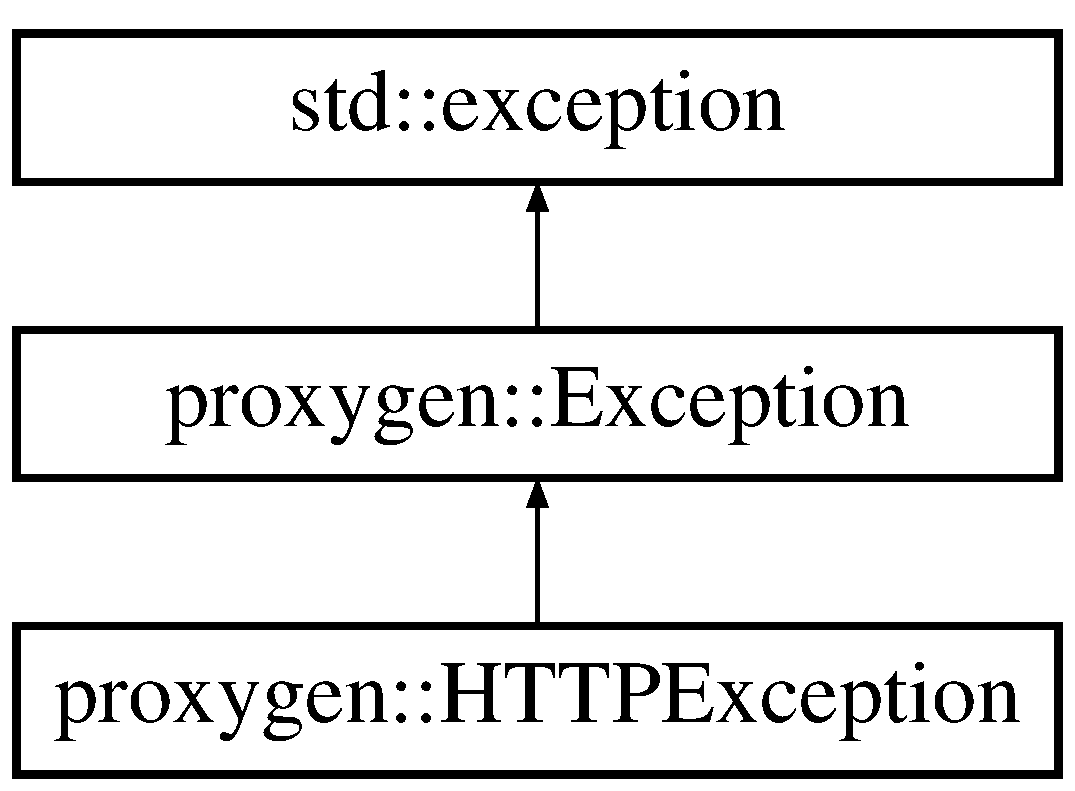
\includegraphics[height=3.000000cm]{classproxygen_1_1Exception}
\end{center}
\end{figure}
\subsection*{Public Member Functions}
\begin{DoxyCompactItemize}
\item 
{\bf Exception} (std\+::string const \&msg)
\item 
{\bf Exception} (const {\bf Exception} \&)
\item 
{\bf Exception} ({\bf Exception} \&other)
\item 
{\bf Exception} ({\bf Exception} \&\&) noexcept
\item 
{\footnotesize template$<$typename... Args$>$ }\\{\bf Exception} (Args \&\&...args)
\item 
{\bf $\sim$\+Exception} (void) noexceptoverride
\item 
const char $\ast$ {\bf what} (void) const noexceptoverride
\item 
void {\bf set\+Code} (int code)
\item 
int {\bf get\+Code} () const 
\item 
bool {\bf has\+Proxygen\+Error} () const 
\item 
void {\bf set\+Proxygen\+Error} ({\bf Proxygen\+Error} proxygen\+Error)
\item 
{\bf Proxygen\+Error} {\bf get\+Proxygen\+Error} () const 
\end{DoxyCompactItemize}
\subsection*{Private Attributes}
\begin{DoxyCompactItemize}
\item 
const std\+::string {\bf msg\+\_\+}
\item 
int {\bf code\+\_\+}
\item 
{\bf Proxygen\+Error} {\bf proxygen\+Error\+\_\+} \{{\bf k\+Error\+None}\}
\end{DoxyCompactItemize}


\subsection{Detailed Description}
Base class for all exceptions. 

Definition at line 22 of file Exception.\+h.



\subsection{Constructor \& Destructor Documentation}
\index{proxygen\+::\+Exception@{proxygen\+::\+Exception}!Exception@{Exception}}
\index{Exception@{Exception}!proxygen\+::\+Exception@{proxygen\+::\+Exception}}
\subsubsection[{Exception(std\+::string const \&msg)}]{\setlength{\rightskip}{0pt plus 5cm}proxygen\+::\+Exception\+::\+Exception (
\begin{DoxyParamCaption}
\item[{std\+::string const \&}]{msg}
\end{DoxyParamCaption}
)\hspace{0.3cm}{\ttfamily [explicit]}}\label{classproxygen_1_1Exception_a074daba75dd5c0654e00a1a0af00d94e}


Definition at line 14 of file Exception.\+cpp.



Referenced by Exception().


\begin{DoxyCode}
14 : msg_(msg), code_(0) \{\}
\end{DoxyCode}
\index{proxygen\+::\+Exception@{proxygen\+::\+Exception}!Exception@{Exception}}
\index{Exception@{Exception}!proxygen\+::\+Exception@{proxygen\+::\+Exception}}
\subsubsection[{Exception(const Exception \&)}]{\setlength{\rightskip}{0pt plus 5cm}proxygen\+::\+Exception\+::\+Exception (
\begin{DoxyParamCaption}
\item[{const {\bf Exception} \&}]{other}
\end{DoxyParamCaption}
)}\label{classproxygen_1_1Exception_a9873d230e54a81a3448478680ecd4339}


Definition at line 16 of file Exception.\+cpp.


\begin{DoxyCode}
17     : msg_(other.msg\_),
18       code_(other.code\_),
19       proxygenError_(other.proxygenError\_) \{\}
\end{DoxyCode}
\index{proxygen\+::\+Exception@{proxygen\+::\+Exception}!Exception@{Exception}}
\index{Exception@{Exception}!proxygen\+::\+Exception@{proxygen\+::\+Exception}}
\subsubsection[{Exception(\+Exception \&other)}]{\setlength{\rightskip}{0pt plus 5cm}proxygen\+::\+Exception\+::\+Exception (
\begin{DoxyParamCaption}
\item[{{\bf Exception} \&}]{other}
\end{DoxyParamCaption}
)\hspace{0.3cm}{\ttfamily [inline]}}\label{classproxygen_1_1Exception_a943d0448d3adca6466a465de975b739d}


Definition at line 26 of file Exception.\+h.



References Exception().


\begin{DoxyCode}
26 : Exception(folly::as\_const(other)) \{\} \textcolor{comment}{// @nolint}
\end{DoxyCode}
\index{proxygen\+::\+Exception@{proxygen\+::\+Exception}!Exception@{Exception}}
\index{Exception@{Exception}!proxygen\+::\+Exception@{proxygen\+::\+Exception}}
\subsubsection[{Exception(\+Exception \&\&) noexcept}]{\setlength{\rightskip}{0pt plus 5cm}proxygen\+::\+Exception\+::\+Exception (
\begin{DoxyParamCaption}
\item[{{\bf Exception} \&\&}]{other}
\end{DoxyParamCaption}
)\hspace{0.3cm}{\ttfamily [noexcept]}}\label{classproxygen_1_1Exception_a6ec1b08dae14e2bfed35c8a43350833d}


Definition at line 21 of file Exception.\+cpp.


\begin{DoxyCode}
22     : msg_(other.msg\_),
23       code_(other.code\_),
24       proxygenError_(other.proxygenError\_) \{\}
\end{DoxyCode}
\index{proxygen\+::\+Exception@{proxygen\+::\+Exception}!Exception@{Exception}}
\index{Exception@{Exception}!proxygen\+::\+Exception@{proxygen\+::\+Exception}}
\subsubsection[{Exception(\+Args \&\&...\+args)}]{\setlength{\rightskip}{0pt plus 5cm}template$<$typename... Args$>$ proxygen\+::\+Exception\+::\+Exception (
\begin{DoxyParamCaption}
\item[{Args \&\&...}]{args}
\end{DoxyParamCaption}
)\hspace{0.3cm}{\ttfamily [inline]}, {\ttfamily [explicit]}}\label{classproxygen_1_1Exception_abb3de5aabb6dc6cd6b5b256959fff770}


Definition at line 30 of file Exception.\+h.


\begin{DoxyCode}
31       : msg_(folly::to<std::string>(std::forward<Args>(args)...)), code_(0) \{\}
\end{DoxyCode}
\index{proxygen\+::\+Exception@{proxygen\+::\+Exception}!````~Exception@{$\sim$\+Exception}}
\index{````~Exception@{$\sim$\+Exception}!proxygen\+::\+Exception@{proxygen\+::\+Exception}}
\subsubsection[{$\sim$\+Exception(void) noexceptoverride}]{\setlength{\rightskip}{0pt plus 5cm}proxygen\+::\+Exception\+::$\sim$\+Exception (
\begin{DoxyParamCaption}
\item[{void}]{}
\end{DoxyParamCaption}
)\hspace{0.3cm}{\ttfamily [inline]}, {\ttfamily [override]}, {\ttfamily [noexcept]}}\label{classproxygen_1_1Exception_a6224f3a2f0783cda88aed4573197ead3}


Definition at line 33 of file Exception.\+h.



References what().


\begin{DoxyCode}
33 \{\}
\end{DoxyCode}


\subsection{Member Function Documentation}
\index{proxygen\+::\+Exception@{proxygen\+::\+Exception}!get\+Code@{get\+Code}}
\index{get\+Code@{get\+Code}!proxygen\+::\+Exception@{proxygen\+::\+Exception}}
\subsubsection[{get\+Code() const }]{\setlength{\rightskip}{0pt plus 5cm}int proxygen\+::\+Exception\+::get\+Code (
\begin{DoxyParamCaption}
{}
\end{DoxyParamCaption}
) const\hspace{0.3cm}{\ttfamily [inline]}}\label{classproxygen_1_1Exception_aece194f85c0e6258a26048e9a4e9e13b}


Definition at line 41 of file Exception.\+h.



References code\+\_\+.


\begin{DoxyCode}
41 \{ \textcolor{keywordflow}{return} code_; \}
\end{DoxyCode}
\index{proxygen\+::\+Exception@{proxygen\+::\+Exception}!get\+Proxygen\+Error@{get\+Proxygen\+Error}}
\index{get\+Proxygen\+Error@{get\+Proxygen\+Error}!proxygen\+::\+Exception@{proxygen\+::\+Exception}}
\subsubsection[{get\+Proxygen\+Error() const }]{\setlength{\rightskip}{0pt plus 5cm}{\bf Proxygen\+Error} proxygen\+::\+Exception\+::get\+Proxygen\+Error (
\begin{DoxyParamCaption}
{}
\end{DoxyParamCaption}
) const\hspace{0.3cm}{\ttfamily [inline]}}\label{classproxygen_1_1Exception_af1367ee45a543354d6527bcc1f17a059}


Definition at line 50 of file Exception.\+h.



References proxygen\+Error\+\_\+.



Referenced by proxygen\+::\+H\+T\+T\+P\+Session\+Base\+::handle\+Error\+Directly(), proxygen\+::\+H\+T\+T\+P\+Transaction\+::on\+Error(), proxygen\+::operator$<$$<$(), T\+E\+S\+T\+\_\+\+F(), Mock\+Codec\+Downstream\+Test\+::test\+Conn\+Flow\+Control\+Blocked(), and T\+Y\+P\+E\+D\+\_\+\+T\+E\+S\+T\+\_\+\+P().


\begin{DoxyCode}
50 \{ \textcolor{keywordflow}{return} proxygenError_; \}
\end{DoxyCode}
\index{proxygen\+::\+Exception@{proxygen\+::\+Exception}!has\+Proxygen\+Error@{has\+Proxygen\+Error}}
\index{has\+Proxygen\+Error@{has\+Proxygen\+Error}!proxygen\+::\+Exception@{proxygen\+::\+Exception}}
\subsubsection[{has\+Proxygen\+Error() const }]{\setlength{\rightskip}{0pt plus 5cm}bool proxygen\+::\+Exception\+::has\+Proxygen\+Error (
\begin{DoxyParamCaption}
{}
\end{DoxyParamCaption}
) const\hspace{0.3cm}{\ttfamily [inline]}}\label{classproxygen_1_1Exception_a3bbccb65c4ec2d9cd04efb4189f0bc46}


Definition at line 44 of file Exception.\+h.



References proxygen\+::k\+Error\+None, and proxygen\+Error\+\_\+.



Referenced by T\+E\+S\+T\+\_\+\+F().


\begin{DoxyCode}
44 \{ \textcolor{keywordflow}{return} (proxygenError_ != kErrorNone); \}
\end{DoxyCode}
\index{proxygen\+::\+Exception@{proxygen\+::\+Exception}!set\+Code@{set\+Code}}
\index{set\+Code@{set\+Code}!proxygen\+::\+Exception@{proxygen\+::\+Exception}}
\subsubsection[{set\+Code(int code)}]{\setlength{\rightskip}{0pt plus 5cm}void proxygen\+::\+Exception\+::set\+Code (
\begin{DoxyParamCaption}
\item[{int}]{code}
\end{DoxyParamCaption}
)\hspace{0.3cm}{\ttfamily [inline]}}\label{classproxygen_1_1Exception_ae5b36e663be40b733038a2b1c2c37798}


Definition at line 39 of file Exception.\+h.



References code\+\_\+.


\begin{DoxyCode}
39 \{ code_ = code; \}
\end{DoxyCode}
\index{proxygen\+::\+Exception@{proxygen\+::\+Exception}!set\+Proxygen\+Error@{set\+Proxygen\+Error}}
\index{set\+Proxygen\+Error@{set\+Proxygen\+Error}!proxygen\+::\+Exception@{proxygen\+::\+Exception}}
\subsubsection[{set\+Proxygen\+Error(\+Proxygen\+Error proxygen\+Error)}]{\setlength{\rightskip}{0pt plus 5cm}void proxygen\+::\+Exception\+::set\+Proxygen\+Error (
\begin{DoxyParamCaption}
\item[{{\bf Proxygen\+Error}}]{proxygen\+Error}
\end{DoxyParamCaption}
)\hspace{0.3cm}{\ttfamily [inline]}}\label{classproxygen_1_1Exception_a96189a5e5d3636599b7af7337437e77f}


Definition at line 46 of file Exception.\+h.



References proxygen\+Error\+\_\+.



Referenced by proxygen\+::\+H\+T\+T\+P\+Session\+::error\+On\+Transaction\+Ids(), proxygen\+::\+S\+P\+D\+Y\+Codec\+::fail\+Session(), proxygen\+::\+S\+P\+D\+Y\+Codec\+::fail\+Stream(), proxygen\+::\+H\+T\+T\+P\+Session\+::on\+Abort(), proxygen\+::\+H\+T\+T\+P\+Transaction\+::on\+Egress\+Timeout(), proxygen\+::\+H\+T\+T\+P\+Session\+::on\+Goaway(), proxygen\+::\+H\+T\+T\+P\+Checks\+::on\+Headers\+Complete(), proxygen\+::\+H\+T\+T\+P\+Transaction\+::on\+Ingress\+Body(), proxygen\+::\+H\+T\+T\+P\+Transaction\+::on\+Ingress\+E\+O\+M(), proxygen\+::\+H\+T\+T\+P\+Transaction\+::on\+Ingress\+Timeout(), proxygen\+::\+H\+T\+T\+P1x\+Codec\+::on\+Parser\+Error(), proxygen\+::\+H\+T\+T\+P\+Transaction\+::send\+Body\+Now(), proxygen\+::\+H\+T\+T\+P\+Session\+::shutdown\+Transport(), T\+E\+S\+T(), T\+E\+S\+T\+\_\+\+F(), and proxygen\+::\+H\+T\+T\+P\+Transaction\+::validate\+Ingress\+State\+Transition().


\begin{DoxyCode}
46                                                      \{
47     proxygenError_ = proxygenError;
48   \}
\end{DoxyCode}
\index{proxygen\+::\+Exception@{proxygen\+::\+Exception}!what@{what}}
\index{what@{what}!proxygen\+::\+Exception@{proxygen\+::\+Exception}}
\subsubsection[{what(void) const noexceptoverride}]{\setlength{\rightskip}{0pt plus 5cm}const char $\ast$ proxygen\+::\+Exception\+::what (
\begin{DoxyParamCaption}
\item[{void}]{}
\end{DoxyParamCaption}
) const\hspace{0.3cm}{\ttfamily [override]}, {\ttfamily [noexcept]}}\label{classproxygen_1_1Exception_afa04dab521f8170b6da29b4f01943308}


Definition at line 26 of file Exception.\+cpp.



References msg\+\_\+.



Referenced by proxygen\+::\+H\+T\+T\+P\+Codec\+Printer\+::on\+Error(), proxygen\+::\+H\+T\+T\+P\+Session\+::on\+Session\+Parse\+Error(), proxygen\+::operator$<$$<$(), T\+E\+S\+T\+\_\+\+F(), T\+Y\+P\+E\+D\+\_\+\+T\+E\+S\+T\+\_\+\+P(), and $\sim$\+Exception().


\begin{DoxyCode}
26 \{ \textcolor{keywordflow}{return} msg_.c\_str(); \}
\end{DoxyCode}


\subsection{Member Data Documentation}
\index{proxygen\+::\+Exception@{proxygen\+::\+Exception}!code\+\_\+@{code\+\_\+}}
\index{code\+\_\+@{code\+\_\+}!proxygen\+::\+Exception@{proxygen\+::\+Exception}}
\subsubsection[{code\+\_\+}]{\setlength{\rightskip}{0pt plus 5cm}int proxygen\+::\+Exception\+::code\+\_\+\hspace{0.3cm}{\ttfamily [private]}}\label{classproxygen_1_1Exception_a4adb1db4ba3d299493d948e0af4cbd6c}


Definition at line 54 of file Exception.\+h.



Referenced by get\+Code(), and set\+Code().

\index{proxygen\+::\+Exception@{proxygen\+::\+Exception}!msg\+\_\+@{msg\+\_\+}}
\index{msg\+\_\+@{msg\+\_\+}!proxygen\+::\+Exception@{proxygen\+::\+Exception}}
\subsubsection[{msg\+\_\+}]{\setlength{\rightskip}{0pt plus 5cm}const std\+::string proxygen\+::\+Exception\+::msg\+\_\+\hspace{0.3cm}{\ttfamily [private]}}\label{classproxygen_1_1Exception_a15e20ea5cdd8fb21db0b17f7a90782a9}


Definition at line 53 of file Exception.\+h.



Referenced by what().

\index{proxygen\+::\+Exception@{proxygen\+::\+Exception}!proxygen\+Error\+\_\+@{proxygen\+Error\+\_\+}}
\index{proxygen\+Error\+\_\+@{proxygen\+Error\+\_\+}!proxygen\+::\+Exception@{proxygen\+::\+Exception}}
\subsubsection[{proxygen\+Error\+\_\+}]{\setlength{\rightskip}{0pt plus 5cm}{\bf Proxygen\+Error} proxygen\+::\+Exception\+::proxygen\+Error\+\_\+ \{{\bf k\+Error\+None}\}\hspace{0.3cm}{\ttfamily [private]}}\label{classproxygen_1_1Exception_a715fcc25be1af4a5d6d39a4aa7ec1d14}


Definition at line 55 of file Exception.\+h.



Referenced by get\+Proxygen\+Error(), has\+Proxygen\+Error(), and set\+Proxygen\+Error().



The documentation for this class was generated from the following files\+:\begin{DoxyCompactItemize}
\item 
proxygen/lib/utils/{\bf Exception.\+h}\item 
proxygen/lib/utils/{\bf Exception.\+cpp}\end{DoxyCompactItemize}

\section{proxygen\+:\+:Ex\+Message\+Handler Class Reference}
\label{classproxygen_1_1ExMessageHandler}\index{proxygen\+::\+Ex\+Message\+Handler@{proxygen\+::\+Ex\+Message\+Handler}}


{\ttfamily \#include $<$Ex\+Message\+Handler.\+h$>$}

Inheritance diagram for proxygen\+:\+:Ex\+Message\+Handler\+:\begin{figure}[H]
\begin{center}
\leavevmode
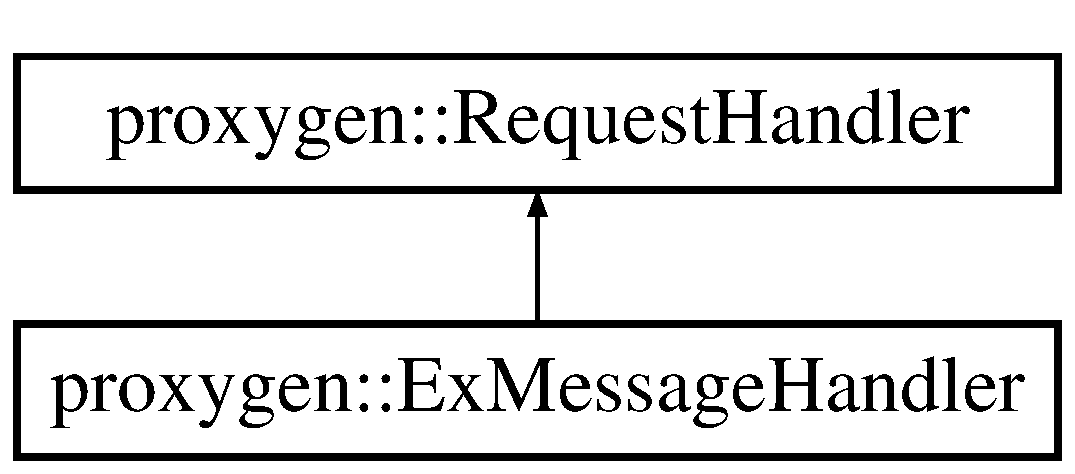
\includegraphics[height=2.000000cm]{classproxygen_1_1ExMessageHandler}
\end{center}
\end{figure}
\subsection*{Public Member Functions}
\begin{DoxyCompactItemize}
\item 
virtual void {\bf on\+Upgrade} ({\bf proxygen\+::\+Upgrade\+Protocol}) noexceptoverride
\item 
virtual {\bf Ex\+Message\+Handler} $\ast$ {\bf get\+Ex\+Handler} () noexceptoverride
\end{DoxyCompactItemize}
\subsection*{Additional Inherited Members}


\subsection{Detailed Description}
Interface to be implemented to handle EX messages from client. 

Definition at line 19 of file Ex\+Message\+Handler.\+h.



\subsection{Member Function Documentation}
\index{proxygen\+::\+Ex\+Message\+Handler@{proxygen\+::\+Ex\+Message\+Handler}!get\+Ex\+Handler@{get\+Ex\+Handler}}
\index{get\+Ex\+Handler@{get\+Ex\+Handler}!proxygen\+::\+Ex\+Message\+Handler@{proxygen\+::\+Ex\+Message\+Handler}}
\subsubsection[{get\+Ex\+Handler() noexceptoverride}]{\setlength{\rightskip}{0pt plus 5cm}virtual {\bf Ex\+Message\+Handler}$\ast$ proxygen\+::\+Ex\+Message\+Handler\+::get\+Ex\+Handler (
\begin{DoxyParamCaption}
{}
\end{DoxyParamCaption}
)\hspace{0.3cm}{\ttfamily [inline]}, {\ttfamily [override]}, {\ttfamily [virtual]}, {\ttfamily [noexcept]}}\label{classproxygen_1_1ExMessageHandler_ae869b1f28a958a4960536ef6031730d2}
Implement in control stream handler to support incoming child EX streams. 

Reimplemented from {\bf proxygen\+::\+Request\+Handler} \doxyref{}{p.}{classproxygen_1_1RequestHandler_a6131d21f1a673ce0d37fa61af8aa5733}.



Definition at line 26 of file Ex\+Message\+Handler.\+h.


\begin{DoxyCode}
26                                                              \{
27     LOG(FATAL) << \textcolor{stringliteral}{"getExHandler can't be called on ExMessageHandler"};
28   \}
\end{DoxyCode}
\index{proxygen\+::\+Ex\+Message\+Handler@{proxygen\+::\+Ex\+Message\+Handler}!on\+Upgrade@{on\+Upgrade}}
\index{on\+Upgrade@{on\+Upgrade}!proxygen\+::\+Ex\+Message\+Handler@{proxygen\+::\+Ex\+Message\+Handler}}
\subsubsection[{on\+Upgrade(proxygen\+::\+Upgrade\+Protocol) noexceptoverride}]{\setlength{\rightskip}{0pt plus 5cm}virtual void proxygen\+::\+Ex\+Message\+Handler\+::on\+Upgrade (
\begin{DoxyParamCaption}
\item[{{\bf proxygen\+::\+Upgrade\+Protocol}}]{prot}
\end{DoxyParamCaption}
)\hspace{0.3cm}{\ttfamily [inline]}, {\ttfamily [override]}, {\ttfamily [virtual]}, {\ttfamily [noexcept]}}\label{classproxygen_1_1ExMessageHandler_a08f5c0786adfc3fdacc8b54ec6c6a3e2}
Invoked when the session has been upgraded to a different protocol 

Implements {\bf proxygen\+::\+Request\+Handler} \doxyref{}{p.}{classproxygen_1_1RequestHandler_aefed2946bc5558baf6e36a2d11290b79}.



Definition at line 22 of file Ex\+Message\+Handler.\+h.


\begin{DoxyCode}
22                                                                       \{
23     LOG(FATAL) << \textcolor{stringliteral}{"ExMessageHandler doesn't support upgrade"};
24   \}
\end{DoxyCode}


The documentation for this class was generated from the following file\+:\begin{DoxyCompactItemize}
\item 
proxygen/httpserver/{\bf Ex\+Message\+Handler.\+h}\end{DoxyCompactItemize}

\section{proxygen\+:\+:Fake\+H\+T\+T\+P\+Codec\+Callback Class Reference}
\label{classproxygen_1_1FakeHTTPCodecCallback}\index{proxygen\+::\+Fake\+H\+T\+T\+P\+Codec\+Callback@{proxygen\+::\+Fake\+H\+T\+T\+P\+Codec\+Callback}}


{\ttfamily \#include $<$Test\+Utils.\+h$>$}

Inheritance diagram for proxygen\+:\+:Fake\+H\+T\+T\+P\+Codec\+Callback\+:\begin{figure}[H]
\begin{center}
\leavevmode
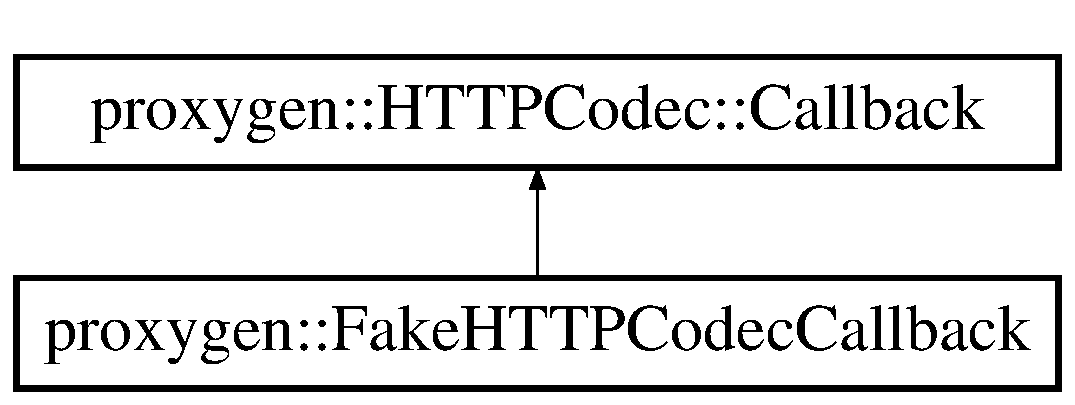
\includegraphics[height=2.000000cm]{classproxygen_1_1FakeHTTPCodecCallback}
\end{center}
\end{figure}
\subsection*{Public Member Functions}
\begin{DoxyCompactItemize}
\item 
{\bf Fake\+H\+T\+T\+P\+Codec\+Callback} ()
\item 
void {\bf on\+Message\+Begin} ({\bf H\+T\+T\+P\+Codec\+::\+Stream\+ID}, {\bf H\+T\+T\+P\+Message} $\ast$) override
\item 
void {\bf on\+Push\+Message\+Begin} ({\bf H\+T\+T\+P\+Codec\+::\+Stream\+ID}, {\bf H\+T\+T\+P\+Codec\+::\+Stream\+ID} assoc\+Stream, {\bf H\+T\+T\+P\+Message} $\ast$) override
\item 
void {\bf on\+Ex\+Message\+Begin} ({\bf H\+T\+T\+P\+Codec\+::\+Stream\+ID}, {\bf H\+T\+T\+P\+Codec\+::\+Stream\+ID} control\+Stream, bool unidirectional, {\bf H\+T\+T\+P\+Message} $\ast$) override
\item 
void {\bf on\+Headers\+Complete} ({\bf H\+T\+T\+P\+Codec\+::\+Stream\+ID} {\bf stream}, std\+::unique\+\_\+ptr$<$ {\bf H\+T\+T\+P\+Message} $>$ in\+Msg) override
\item 
void {\bf on\+Body} ({\bf H\+T\+T\+P\+Codec\+::\+Stream\+ID}, std\+::unique\+\_\+ptr$<$ folly\+::\+I\+O\+Buf $>$ chain, uint16\+\_\+t padding) override
\item 
void {\bf on\+Chunk\+Header} ({\bf H\+T\+T\+P\+Codec\+::\+Stream\+ID}, size\+\_\+t) override
\item 
void {\bf on\+Chunk\+Complete} ({\bf H\+T\+T\+P\+Codec\+::\+Stream\+ID}) override
\item 
void {\bf on\+Trailers\+Complete} ({\bf H\+T\+T\+P\+Codec\+::\+Stream\+ID}, std\+::unique\+\_\+ptr$<$ {\bf H\+T\+T\+P\+Headers} $>$ in\+Trailers) override
\item 
void {\bf on\+Message\+Complete} ({\bf H\+T\+T\+P\+Codec\+::\+Stream\+ID}, bool) override
\item 
void {\bf on\+Error} ({\bf H\+T\+T\+P\+Codec\+::\+Stream\+ID} {\bf stream}, const {\bf H\+T\+T\+P\+Exception} \&error, bool) override
\item 
void {\bf on\+Abort} ({\bf H\+T\+T\+P\+Codec\+::\+Stream\+ID}, {\bf Error\+Code} code) override
\item 
void {\bf on\+Frame\+Header} ({\bf H\+T\+T\+P\+Codec\+::\+Stream\+ID}, uint8\+\_\+t, uint64\+\_\+t, uint8\+\_\+t, uint16\+\_\+t) override
\item 
void {\bf on\+Goaway} (uint64\+\_\+t last\+Stream\+Id, {\bf Error\+Code}, std\+::unique\+\_\+ptr$<$ folly\+::\+I\+O\+Buf $>$ debug\+Data) override
\item 
void {\bf on\+Ping\+Request} (uint64\+\_\+t unique\+ID) override
\item 
void {\bf on\+Ping\+Reply} (uint64\+\_\+t unique\+ID) override
\item 
void {\bf on\+Priority} ({\bf H\+T\+T\+P\+Codec\+::\+Stream\+ID}, const {\bf H\+T\+T\+P\+Message\+::\+H\+T\+T\+P\+Priority} \&pri) override
\item 
void {\bf on\+Window\+Update} ({\bf H\+T\+T\+P\+Codec\+::\+Stream\+ID} {\bf stream}, uint32\+\_\+t amount) override
\item 
void {\bf on\+Settings} (const {\bf Settings\+List} \&in\+Settings) override
\item 
void {\bf on\+Settings\+Ack} () override
\item 
void {\bf on\+Certificate\+Request} (uint16\+\_\+t request\+Id, std\+::unique\+\_\+ptr$<$ folly\+::\+I\+O\+Buf $>$ auth\+Request) override
\item 
void {\bf on\+Certificate} (uint16\+\_\+t cert\+Id, std\+::unique\+\_\+ptr$<$ folly\+::\+I\+O\+Buf $>$ authenticator) override
\item 
bool {\bf on\+Native\+Protocol\+Upgrade} ({\bf H\+T\+T\+P\+Codec\+::\+Stream\+ID}, {\bf Codec\+Protocol}, const std\+::string \&, {\bf H\+T\+T\+P\+Message} \&) override
\item 
uint32\+\_\+t {\bf num\+Outgoing\+Streams} () const override
\item 
uint32\+\_\+t {\bf num\+Incoming\+Streams} () const override
\item 
void {\bf expect\+Message} (bool eom, int32\+\_\+t header\+Count, const std\+::string \&url) const 
\item 
void {\bf expect\+Message} (bool eom, int32\+\_\+t header\+Count, int32\+\_\+t {\bf status\+Code}) const 
\item 
void {\bf expect\+Message\+Helper} (bool eom, int32\+\_\+t header\+Count, const std\+::string \&url, int32\+\_\+t {\bf status\+Code}) const 
\item 
bool {\bf session\+Error} () const 
\item 
std\+::function$<$ bool()$>$ {\bf get\+Stop\+Fn} ()
\item 
void {\bf set\+Session\+Stream\+Id} ({\bf H\+T\+T\+P\+Codec\+::\+Stream\+ID} stream\+Id)
\item 
void {\bf reset} ()
\item 
void {\bf dump\+Counters} (int verbosity) const 
\end{DoxyCompactItemize}
\subsection*{Public Attributes}
\begin{DoxyCompactItemize}
\item 
{\bf H\+T\+T\+P\+Codec\+::\+Stream\+ID} {\bf headers\+Complete\+Id} \{0\}
\item 
{\bf H\+T\+T\+P\+Codec\+::\+Stream\+ID} {\bf assoc\+Stream\+Id} \{0\}
\item 
{\bf H\+T\+T\+P\+Codec\+::\+Stream\+ID} {\bf control\+Stream\+Id} \{0\}
\item 
bool {\bf is\+Unidirectional} \{false\}
\item 
{\bf H\+T\+T\+P\+Codec\+::\+Stream\+ID} {\bf session\+Stream\+Id} \{0\}
\item 
uint32\+\_\+t {\bf message\+Begin} \{0\}
\item 
uint32\+\_\+t {\bf headers\+Complete} \{0\}
\item 
uint32\+\_\+t {\bf message\+Complete} \{0\}
\item 
uint32\+\_\+t {\bf body\+Calls} \{0\}
\item 
uint32\+\_\+t {\bf body\+Length} \{0\}
\item 
uint32\+\_\+t {\bf padding\+Bytes} \{0\}
\item 
uint32\+\_\+t {\bf chunk\+Headers} \{0\}
\item 
uint32\+\_\+t {\bf chunk\+Complete} \{0\}
\item 
uint32\+\_\+t {\bf trailers} \{0\}
\item 
uint32\+\_\+t {\bf aborts} \{0\}
\item 
uint32\+\_\+t {\bf goaways} \{0\}
\item 
uint32\+\_\+t {\bf session\+Errors} \{0\}
\item 
uint32\+\_\+t {\bf stream\+Errors} \{0\}
\item 
uint64\+\_\+t {\bf recv\+Ping\+Request} \{0\}
\item 
uint64\+\_\+t {\bf recv\+Ping\+Reply} \{0\}
\item 
uint32\+\_\+t {\bf window\+Update\+Calls} \{0\}
\item 
uint32\+\_\+t {\bf settings} \{0\}
\item 
uint64\+\_\+t {\bf num\+Settings} \{0\}
\item 
uint32\+\_\+t {\bf settings\+Acks} \{0\}
\item 
uint32\+\_\+t {\bf certificate\+Requests} \{0\}
\item 
uint16\+\_\+t {\bf last\+Cert\+Request\+Id} \{0\}
\item 
uint32\+\_\+t {\bf certificates} \{0\}
\item 
uint16\+\_\+t {\bf last\+Cert\+Id} \{0\}
\item 
uint64\+\_\+t {\bf window\+Size} \{0\}
\item 
uint64\+\_\+t {\bf max\+Streams} \{0\}
\item 
uint32\+\_\+t {\bf header\+Frames} \{0\}
\item 
{\bf H\+T\+T\+P\+Message\+::\+H\+T\+T\+P\+Priority} {\bf priority} \{0, false, 0\}
\item 
std\+::map$<$ {\bf proxygen\+::\+H\+T\+T\+P\+Codec\+::\+Stream\+ID}, std\+::vector$<$ uint32\+\_\+t $>$ $>$ {\bf window\+Updates}
\item 
folly\+::\+I\+O\+Buf\+Queue {\bf data}
\item 
std\+::unique\+\_\+ptr$<$ {\bf H\+T\+T\+P\+Message} $>$ {\bf msg}
\item 
std\+::unique\+\_\+ptr$<$ {\bf H\+T\+T\+P\+Exception} $>$ {\bf last\+Parse\+Error}
\item 
{\bf Error\+Code} {\bf last\+Error\+Code}
\item 
std\+::vector$<$ {\bf H\+T\+T\+P\+Codec\+::\+Stream\+ID} $>$ {\bf goaway\+Stream\+Ids}
\end{DoxyCompactItemize}


\subsection{Detailed Description}


Definition at line 107 of file Test\+Utils.\+h.



\subsection{Constructor \& Destructor Documentation}
\index{proxygen\+::\+Fake\+H\+T\+T\+P\+Codec\+Callback@{proxygen\+::\+Fake\+H\+T\+T\+P\+Codec\+Callback}!Fake\+H\+T\+T\+P\+Codec\+Callback@{Fake\+H\+T\+T\+P\+Codec\+Callback}}
\index{Fake\+H\+T\+T\+P\+Codec\+Callback@{Fake\+H\+T\+T\+P\+Codec\+Callback}!proxygen\+::\+Fake\+H\+T\+T\+P\+Codec\+Callback@{proxygen\+::\+Fake\+H\+T\+T\+P\+Codec\+Callback}}
\subsubsection[{Fake\+H\+T\+T\+P\+Codec\+Callback()}]{\setlength{\rightskip}{0pt plus 5cm}proxygen\+::\+Fake\+H\+T\+T\+P\+Codec\+Callback\+::\+Fake\+H\+T\+T\+P\+Codec\+Callback (
\begin{DoxyParamCaption}
{}
\end{DoxyParamCaption}
)\hspace{0.3cm}{\ttfamily [inline]}}\label{classproxygen_1_1FakeHTTPCodecCallback_a6a38942222c5d4fb42f110d5c810e227}


Definition at line 109 of file Test\+Utils.\+h.


\begin{DoxyCode}
109 \{\}
\end{DoxyCode}


\subsection{Member Function Documentation}
\index{proxygen\+::\+Fake\+H\+T\+T\+P\+Codec\+Callback@{proxygen\+::\+Fake\+H\+T\+T\+P\+Codec\+Callback}!dump\+Counters@{dump\+Counters}}
\index{dump\+Counters@{dump\+Counters}!proxygen\+::\+Fake\+H\+T\+T\+P\+Codec\+Callback@{proxygen\+::\+Fake\+H\+T\+T\+P\+Codec\+Callback}}
\subsubsection[{dump\+Counters(int verbosity) const }]{\setlength{\rightskip}{0pt plus 5cm}void proxygen\+::\+Fake\+H\+T\+T\+P\+Codec\+Callback\+::dump\+Counters (
\begin{DoxyParamCaption}
\item[{int}]{verbosity}
\end{DoxyParamCaption}
) const\hspace{0.3cm}{\ttfamily [inline]}}\label{classproxygen_1_1FakeHTTPCodecCallback_a28dfea79809829274afbb2d54d1cc9b8}


Definition at line 337 of file Test\+Utils.\+h.



References aborts, assoc\+Stream\+Id, body\+Calls, body\+Length, certificate\+Requests, certificates, chunk\+Complete, chunk\+Headers, control\+Stream\+Id, goaways, header\+Frames, headers\+Complete, headers\+Complete\+Id, is\+Unidirectional, last\+Cert\+Id, last\+Cert\+Request\+Id, max\+Streams, message\+Begin, padding\+Bytes, recv\+Ping\+Reply, recv\+Ping\+Request, session\+Errors, settings, settings\+Acks, stream\+Errors, trailers, window\+Size, and window\+Update\+Calls.


\begin{DoxyCode}
337                                          \{
338     VLOG(verbosity) << \textcolor{stringliteral}{"Dumping HTTP codec callback counters"};
339     VLOG(verbosity) << \textcolor{stringliteral}{"headersCompleteId: "} << headersCompleteId;
340     VLOG(verbosity) << \textcolor{stringliteral}{"assocStreamId: "} << assocStreamId;
341     VLOG(verbosity) << \textcolor{stringliteral}{"controlStreamId: "} << controlStreamId;
342     VLOG(verbosity) << \textcolor{stringliteral}{"unidirectional: "} << isUnidirectional;
343     VLOG(verbosity) << \textcolor{stringliteral}{"messageBegin: "} << messageBegin;
344     VLOG(verbosity) << \textcolor{stringliteral}{"headersComplete: "} << headersComplete;
345     VLOG(verbosity) << \textcolor{stringliteral}{"bodyCalls: "} << bodyCalls;
346     VLOG(verbosity) << \textcolor{stringliteral}{"bodyLength: "} << bodyLength;
347     VLOG(verbosity) << \textcolor{stringliteral}{"paddingBytes: "} << paddingBytes;
348     VLOG(verbosity) << \textcolor{stringliteral}{"chunkHeaders: "} << chunkHeaders;
349     VLOG(verbosity) << \textcolor{stringliteral}{"chunkComplete: "} << chunkComplete;
350     VLOG(verbosity) << \textcolor{stringliteral}{"trailers: "} << trailers;
351     VLOG(verbosity) << \textcolor{stringliteral}{"aborts: "} << aborts;
352     VLOG(verbosity) << \textcolor{stringliteral}{"goaways: "} << goaways;
353     VLOG(verbosity) << \textcolor{stringliteral}{"sessionErrors: "} << sessionErrors;
354     VLOG(verbosity) << \textcolor{stringliteral}{"streamErrors: "} << streamErrors;
355     VLOG(verbosity) << \textcolor{stringliteral}{"recvPingRequest: "} << recvPingRequest;
356     VLOG(verbosity) << \textcolor{stringliteral}{"recvPingReply: "} << recvPingReply;
357     VLOG(verbosity) << \textcolor{stringliteral}{"windowUpdateCalls: "} << windowUpdateCalls;
358     VLOG(verbosity) << \textcolor{stringliteral}{"settings: "} << settings;
359     VLOG(verbosity) << \textcolor{stringliteral}{"settingsAcks: "} << settingsAcks;
360     VLOG(verbosity) << \textcolor{stringliteral}{"certificateRequests: "} << certificateRequests;
361     VLOG(verbosity) << \textcolor{stringliteral}{"lastCertRequestId: "} << lastCertRequestId;
362     VLOG(verbosity) << \textcolor{stringliteral}{"certificates: "} << certificates;
363     VLOG(verbosity) << \textcolor{stringliteral}{"lastCertId: "} << lastCertId;
364     VLOG(verbosity) << \textcolor{stringliteral}{"windowSize: "} << windowSize;
365     VLOG(verbosity) << \textcolor{stringliteral}{"maxStreams: "} << maxStreams;
366     VLOG(verbosity) << \textcolor{stringliteral}{"headerFrames: "} << headerFrames;
367   \}
\end{DoxyCode}
\index{proxygen\+::\+Fake\+H\+T\+T\+P\+Codec\+Callback@{proxygen\+::\+Fake\+H\+T\+T\+P\+Codec\+Callback}!expect\+Message@{expect\+Message}}
\index{expect\+Message@{expect\+Message}!proxygen\+::\+Fake\+H\+T\+T\+P\+Codec\+Callback@{proxygen\+::\+Fake\+H\+T\+T\+P\+Codec\+Callback}}
\subsubsection[{expect\+Message(bool eom, int32\+\_\+t header\+Count, const std\+::string \&url) const }]{\setlength{\rightskip}{0pt plus 5cm}void proxygen\+::\+Fake\+H\+T\+T\+P\+Codec\+Callback\+::expect\+Message (
\begin{DoxyParamCaption}
\item[{bool}]{eom, }
\item[{int32\+\_\+t}]{header\+Count, }
\item[{const std\+::string \&}]{url}
\end{DoxyParamCaption}
) const\hspace{0.3cm}{\ttfamily [inline]}}\label{classproxygen_1_1FakeHTTPCodecCallback_ab992c6479b4f7be5300f9af1b08fbb66}


Definition at line 256 of file Test\+Utils.\+h.



References expect\+Message\+Helper().


\begin{DoxyCode}
257                                                  \{
258     expectMessageHelper(eom, headerCount, url, -1);
259   \}
\end{DoxyCode}
\index{proxygen\+::\+Fake\+H\+T\+T\+P\+Codec\+Callback@{proxygen\+::\+Fake\+H\+T\+T\+P\+Codec\+Callback}!expect\+Message@{expect\+Message}}
\index{expect\+Message@{expect\+Message}!proxygen\+::\+Fake\+H\+T\+T\+P\+Codec\+Callback@{proxygen\+::\+Fake\+H\+T\+T\+P\+Codec\+Callback}}
\subsubsection[{expect\+Message(bool eom, int32\+\_\+t header\+Count, int32\+\_\+t status\+Code) const }]{\setlength{\rightskip}{0pt plus 5cm}void proxygen\+::\+Fake\+H\+T\+T\+P\+Codec\+Callback\+::expect\+Message (
\begin{DoxyParamCaption}
\item[{bool}]{eom, }
\item[{int32\+\_\+t}]{header\+Count, }
\item[{int32\+\_\+t}]{status\+Code}
\end{DoxyParamCaption}
) const\hspace{0.3cm}{\ttfamily [inline]}}\label{classproxygen_1_1FakeHTTPCodecCallback_ad50e9a5f48010b458d542eafb6f48279}


Definition at line 260 of file Test\+Utils.\+h.



References expect\+Message\+Helper().


\begin{DoxyCode}
261                                                \{
262     expectMessageHelper(eom, headerCount, \textcolor{stringliteral}{""}, statusCode);
263   \}
\end{DoxyCode}
\index{proxygen\+::\+Fake\+H\+T\+T\+P\+Codec\+Callback@{proxygen\+::\+Fake\+H\+T\+T\+P\+Codec\+Callback}!expect\+Message\+Helper@{expect\+Message\+Helper}}
\index{expect\+Message\+Helper@{expect\+Message\+Helper}!proxygen\+::\+Fake\+H\+T\+T\+P\+Codec\+Callback@{proxygen\+::\+Fake\+H\+T\+T\+P\+Codec\+Callback}}
\subsubsection[{expect\+Message\+Helper(bool eom, int32\+\_\+t header\+Count, const std\+::string \&url, int32\+\_\+t status\+Code) const }]{\setlength{\rightskip}{0pt plus 5cm}void proxygen\+::\+Fake\+H\+T\+T\+P\+Codec\+Callback\+::expect\+Message\+Helper (
\begin{DoxyParamCaption}
\item[{bool}]{eom, }
\item[{int32\+\_\+t}]{header\+Count, }
\item[{const std\+::string \&}]{url, }
\item[{int32\+\_\+t}]{status\+Code}
\end{DoxyParamCaption}
) const\hspace{0.3cm}{\ttfamily [inline]}}\label{classproxygen_1_1FakeHTTPCodecCallback_ad4ecb6ff00ba6dd47a70fc2630fc2529}


Definition at line 265 of file Test\+Utils.\+h.



References headers\+Complete, message\+Begin, message\+Complete, msg, session\+Errors, status\+Code, and stream\+Errors.



Referenced by expect\+Message().


\begin{DoxyCode}
266                                                                            \{
267     EXPECT\_EQ(messageBegin, 1);
268     EXPECT\_EQ(headersComplete, 1);
269     EXPECT\_EQ(messageComplete, eom ? 1 : 0);
270     EXPECT\_EQ(streamErrors, 0);
271     EXPECT\_EQ(sessionErrors, 0);
272     EXPECT\_NE(msg, \textcolor{keyword}{nullptr});
273     \textcolor{keywordflow}{if} (headerCount >= 0) \{
274       EXPECT\_EQ(msg->getHeaders().size(), headerCount);
275     \}
276     \textcolor{keywordflow}{if} (!url.empty()) \{
277       EXPECT\_EQ(msg->getURL(), url);
278     \} \textcolor{keywordflow}{else} \textcolor{keywordflow}{if} (statusCode > 0) \{
279       \textcolor{keywordflow}{if} (msg->isResponse()) \{
280         EXPECT\_EQ(msg->getStatusCode(), statusCode);
281       \} \textcolor{keywordflow}{else} \{
282         EXPECT\_EQ(msg->getPushStatusCode(), statusCode);
283       \}
284     \}
285   \}
\end{DoxyCode}
\index{proxygen\+::\+Fake\+H\+T\+T\+P\+Codec\+Callback@{proxygen\+::\+Fake\+H\+T\+T\+P\+Codec\+Callback}!get\+Stop\+Fn@{get\+Stop\+Fn}}
\index{get\+Stop\+Fn@{get\+Stop\+Fn}!proxygen\+::\+Fake\+H\+T\+T\+P\+Codec\+Callback@{proxygen\+::\+Fake\+H\+T\+T\+P\+Codec\+Callback}}
\subsubsection[{get\+Stop\+Fn()}]{\setlength{\rightskip}{0pt plus 5cm}std\+::function$<$bool()$>$ proxygen\+::\+Fake\+H\+T\+T\+P\+Codec\+Callback\+::get\+Stop\+Fn (
\begin{DoxyParamCaption}
{}
\end{DoxyParamCaption}
)\hspace{0.3cm}{\ttfamily [inline]}}\label{classproxygen_1_1FakeHTTPCodecCallback_a55151fe477425f730f911f483ee294f8}


Definition at line 291 of file Test\+Utils.\+h.



References session\+Error().



Referenced by parse\+S\+P\+D\+Y().


\begin{DoxyCode}
291                                   \{
292     \textcolor{keywordflow}{return} std::bind(&FakeHTTPCodecCallback::sessionError, \textcolor{keyword}{this});
293   \}
\end{DoxyCode}
\index{proxygen\+::\+Fake\+H\+T\+T\+P\+Codec\+Callback@{proxygen\+::\+Fake\+H\+T\+T\+P\+Codec\+Callback}!num\+Incoming\+Streams@{num\+Incoming\+Streams}}
\index{num\+Incoming\+Streams@{num\+Incoming\+Streams}!proxygen\+::\+Fake\+H\+T\+T\+P\+Codec\+Callback@{proxygen\+::\+Fake\+H\+T\+T\+P\+Codec\+Callback}}
\subsubsection[{num\+Incoming\+Streams() const override}]{\setlength{\rightskip}{0pt plus 5cm}uint32\+\_\+t proxygen\+::\+Fake\+H\+T\+T\+P\+Codec\+Callback\+::num\+Incoming\+Streams (
\begin{DoxyParamCaption}
{}
\end{DoxyParamCaption}
) const\hspace{0.3cm}{\ttfamily [inline]}, {\ttfamily [override]}, {\ttfamily [virtual]}}\label{classproxygen_1_1FakeHTTPCodecCallback_a1aa4525d399761ddc2f08b839cc266b1}
Return the number of open streams started by the remote side. Parallel codecs with a maximum number of streams will invoke this to determine if a new stream exceeds the limit. 

Reimplemented from {\bf proxygen\+::\+H\+T\+T\+P\+Codec\+::\+Callback} \doxyref{}{p.}{classproxygen_1_1HTTPCodec_1_1Callback_aad2decb51a53dc21448547ba34b0409a}.



Definition at line 252 of file Test\+Utils.\+h.



References message\+Begin.


\begin{DoxyCode}
252                                                \{
253     \textcolor{keywordflow}{return} messageBegin;
254   \}
\end{DoxyCode}
\index{proxygen\+::\+Fake\+H\+T\+T\+P\+Codec\+Callback@{proxygen\+::\+Fake\+H\+T\+T\+P\+Codec\+Callback}!num\+Outgoing\+Streams@{num\+Outgoing\+Streams}}
\index{num\+Outgoing\+Streams@{num\+Outgoing\+Streams}!proxygen\+::\+Fake\+H\+T\+T\+P\+Codec\+Callback@{proxygen\+::\+Fake\+H\+T\+T\+P\+Codec\+Callback}}
\subsubsection[{num\+Outgoing\+Streams() const override}]{\setlength{\rightskip}{0pt plus 5cm}uint32\+\_\+t proxygen\+::\+Fake\+H\+T\+T\+P\+Codec\+Callback\+::num\+Outgoing\+Streams (
\begin{DoxyParamCaption}
{}
\end{DoxyParamCaption}
) const\hspace{0.3cm}{\ttfamily [inline]}, {\ttfamily [override]}, {\ttfamily [virtual]}}\label{classproxygen_1_1FakeHTTPCodecCallback_a03af9af000004c543ee9999debf25390}
Return the number of open streams started by this codec callback. Parallel codecs with a maximum number of streams will invoke this to determine if a new stream exceeds the limit. 

Reimplemented from {\bf proxygen\+::\+H\+T\+T\+P\+Codec\+::\+Callback} \doxyref{}{p.}{classproxygen_1_1HTTPCodec_1_1Callback_a65779e4b1763aa1daa424f02a5ca3f05}.



Definition at line 248 of file Test\+Utils.\+h.


\begin{DoxyCode}
248                                                \{
249     \textcolor{keywordflow}{return} 0;
250   \}
\end{DoxyCode}
\index{proxygen\+::\+Fake\+H\+T\+T\+P\+Codec\+Callback@{proxygen\+::\+Fake\+H\+T\+T\+P\+Codec\+Callback}!on\+Abort@{on\+Abort}}
\index{on\+Abort@{on\+Abort}!proxygen\+::\+Fake\+H\+T\+T\+P\+Codec\+Callback@{proxygen\+::\+Fake\+H\+T\+T\+P\+Codec\+Callback}}
\subsubsection[{on\+Abort(\+H\+T\+T\+P\+Codec\+::\+Stream\+I\+D, Error\+Code code) override}]{\setlength{\rightskip}{0pt plus 5cm}void proxygen\+::\+Fake\+H\+T\+T\+P\+Codec\+Callback\+::on\+Abort (
\begin{DoxyParamCaption}
\item[{{\bf H\+T\+T\+P\+Codec\+::\+Stream\+ID}}]{, }
\item[{{\bf Error\+Code}}]{}
\end{DoxyParamCaption}
)\hspace{0.3cm}{\ttfamily [inline]}, {\ttfamily [override]}, {\ttfamily [virtual]}}\label{classproxygen_1_1FakeHTTPCodecCallback_a3f66d4797b2c12c5485986f90fa1b331}
Called when the peer has asked to shut down a stream immediately. 
\begin{DoxyParams}{Parameters}
{\em stream} & The stream ID \\
\hline
{\em code} & The code the stream was aborted with \\
\hline
\end{DoxyParams}
\begin{DoxyNote}{Note}
Not applicable to all protocols. 
\end{DoxyNote}


Reimplemented from {\bf proxygen\+::\+H\+T\+T\+P\+Codec\+::\+Callback} \doxyref{}{p.}{classproxygen_1_1HTTPCodec_1_1Callback_a110afc4d5324a47b9b2f6356afc70bbf}.



Definition at line 171 of file Test\+Utils.\+h.



References aborts, and last\+Error\+Code.


\begin{DoxyCode}
171                                                              \{
172     ++aborts;
173     lastErrorCode = code;
174   \}
\end{DoxyCode}
\index{proxygen\+::\+Fake\+H\+T\+T\+P\+Codec\+Callback@{proxygen\+::\+Fake\+H\+T\+T\+P\+Codec\+Callback}!on\+Body@{on\+Body}}
\index{on\+Body@{on\+Body}!proxygen\+::\+Fake\+H\+T\+T\+P\+Codec\+Callback@{proxygen\+::\+Fake\+H\+T\+T\+P\+Codec\+Callback}}
\subsubsection[{on\+Body(\+H\+T\+T\+P\+Codec\+::\+Stream\+I\+D, std\+::unique\+\_\+ptr$<$ folly\+::\+I\+O\+Buf $>$ chain, uint16\+\_\+t padding) override}]{\setlength{\rightskip}{0pt plus 5cm}void proxygen\+::\+Fake\+H\+T\+T\+P\+Codec\+Callback\+::on\+Body (
\begin{DoxyParamCaption}
\item[{{\bf H\+T\+T\+P\+Codec\+::\+Stream\+ID}}]{stream, }
\item[{std\+::unique\+\_\+ptr$<$ folly\+::\+I\+O\+Buf $>$}]{chain, }
\item[{uint16\+\_\+t}]{padding}
\end{DoxyParamCaption}
)\hspace{0.3cm}{\ttfamily [inline]}, {\ttfamily [override]}, {\ttfamily [virtual]}}\label{classproxygen_1_1FakeHTTPCodecCallback_a43e0a21206fd5d3b34959818ecb5a5c1}
Called for each block of message body data 
\begin{DoxyParams}{Parameters}
{\em stream} & The stream ID \\
\hline
{\em chain} & One or more buffers of body data. The codec will remove any protocol framing, such as H\+T\+T\+P/1.\+1 chunk headers, from the buffers before calling this function. \\
\hline
{\em padding} & Number of pad bytes that came with the data segment \\
\hline
\end{DoxyParams}


Implements {\bf proxygen\+::\+H\+T\+T\+P\+Codec\+::\+Callback} \doxyref{}{p.}{classproxygen_1_1HTTPCodec_1_1Callback_af6661786cb419aa6b0138ed1d8085d52}.



Definition at line 134 of file Test\+Utils.\+h.



References body\+Calls, body\+Length, data, and padding\+Bytes.


\begin{DoxyCode}
136                                          \{
137     bodyCalls++;
138     paddingBytes += padding;
139     bodyLength += chain->computeChainDataLength();
140     data.append(std::move(chain));
141   \}
\end{DoxyCode}
\index{proxygen\+::\+Fake\+H\+T\+T\+P\+Codec\+Callback@{proxygen\+::\+Fake\+H\+T\+T\+P\+Codec\+Callback}!on\+Certificate@{on\+Certificate}}
\index{on\+Certificate@{on\+Certificate}!proxygen\+::\+Fake\+H\+T\+T\+P\+Codec\+Callback@{proxygen\+::\+Fake\+H\+T\+T\+P\+Codec\+Callback}}
\subsubsection[{on\+Certificate(uint16\+\_\+t cert\+Id, std\+::unique\+\_\+ptr$<$ folly\+::\+I\+O\+Buf $>$ authenticator) override}]{\setlength{\rightskip}{0pt plus 5cm}void proxygen\+::\+Fake\+H\+T\+T\+P\+Codec\+Callback\+::on\+Certificate (
\begin{DoxyParamCaption}
\item[{uint16\+\_\+t}]{, }
\item[{std\+::unique\+\_\+ptr$<$ folly\+::\+I\+O\+Buf $>$}]{}
\end{DoxyParamCaption}
)\hspace{0.3cm}{\ttfamily [inline]}, {\ttfamily [override]}, {\ttfamily [virtual]}}\label{classproxygen_1_1FakeHTTPCodecCallback_af2175032d60674dc99e7ddc7859f2a02}
Called upon receipt of an authenticator, for protocols that support secondary certificate authentication. 
\begin{DoxyParams}{Parameters}
{\em cert\+Id} & The Cert-\/\+ID identifying this authenticator \\
\hline
{\em authenticator} & The authenticator request \\
\hline
\end{DoxyParams}
\begin{DoxyNote}{Note}
Not all protocols support secondary certificate authentication. H\+T\+T\+P/2 does, but H\+T\+T\+P/1.\+1 doesn\textquotesingle{}t. 
\end{DoxyNote}


Reimplemented from {\bf proxygen\+::\+H\+T\+T\+P\+Codec\+::\+Callback} \doxyref{}{p.}{classproxygen_1_1HTTPCodec_1_1Callback_a39962dfe4038936e8042e725e50c2d45}.



Definition at line 234 of file Test\+Utils.\+h.



References certificates, data, and last\+Cert\+Id.


\begin{DoxyCode}
235                                                                        \{
236     certificates++;
237     lastCertId = certId;
238     data.append(std::move(authenticator));
239   \}
\end{DoxyCode}
\index{proxygen\+::\+Fake\+H\+T\+T\+P\+Codec\+Callback@{proxygen\+::\+Fake\+H\+T\+T\+P\+Codec\+Callback}!on\+Certificate\+Request@{on\+Certificate\+Request}}
\index{on\+Certificate\+Request@{on\+Certificate\+Request}!proxygen\+::\+Fake\+H\+T\+T\+P\+Codec\+Callback@{proxygen\+::\+Fake\+H\+T\+T\+P\+Codec\+Callback}}
\subsubsection[{on\+Certificate\+Request(uint16\+\_\+t request\+Id, std\+::unique\+\_\+ptr$<$ folly\+::\+I\+O\+Buf $>$ auth\+Request) override}]{\setlength{\rightskip}{0pt plus 5cm}void proxygen\+::\+Fake\+H\+T\+T\+P\+Codec\+Callback\+::on\+Certificate\+Request (
\begin{DoxyParamCaption}
\item[{uint16\+\_\+t}]{, }
\item[{std\+::unique\+\_\+ptr$<$ folly\+::\+I\+O\+Buf $>$}]{}
\end{DoxyParamCaption}
)\hspace{0.3cm}{\ttfamily [inline]}, {\ttfamily [override]}, {\ttfamily [virtual]}}\label{classproxygen_1_1FakeHTTPCodecCallback_a404bde70243206b37309b8df0dd5f717}
Called upon receipt of a certificate request frame, for protocols that support secondary certificate authentication. 
\begin{DoxyParams}{Parameters}
{\em request\+Id} & The Request-\/\+ID identifying the certificate request \\
\hline
{\em auth\+Request} & The authenticator request \\
\hline
\end{DoxyParams}
\begin{DoxyNote}{Note}
Not all protocols support secondary certificate authentication. H\+T\+T\+P/2 does, but H\+T\+T\+P/1.\+1 doesn\textquotesingle{}t. 
\end{DoxyNote}


Reimplemented from {\bf proxygen\+::\+H\+T\+T\+P\+Codec\+::\+Callback} \doxyref{}{p.}{classproxygen_1_1HTTPCodec_1_1Callback_a982896bcd896ea45a10b03a294ded590}.



Definition at line 227 of file Test\+Utils.\+h.



References certificate\+Requests, data, and last\+Cert\+Request\+Id.


\begin{DoxyCode}
228                                                                           \{
229     certificateRequests++;
230     lastCertRequestId = requestId;
231     data.append(std::move(authRequest));
232   \}
\end{DoxyCode}
\index{proxygen\+::\+Fake\+H\+T\+T\+P\+Codec\+Callback@{proxygen\+::\+Fake\+H\+T\+T\+P\+Codec\+Callback}!on\+Chunk\+Complete@{on\+Chunk\+Complete}}
\index{on\+Chunk\+Complete@{on\+Chunk\+Complete}!proxygen\+::\+Fake\+H\+T\+T\+P\+Codec\+Callback@{proxygen\+::\+Fake\+H\+T\+T\+P\+Codec\+Callback}}
\subsubsection[{on\+Chunk\+Complete(\+H\+T\+T\+P\+Codec\+::\+Stream\+I\+D) override}]{\setlength{\rightskip}{0pt plus 5cm}void proxygen\+::\+Fake\+H\+T\+T\+P\+Codec\+Callback\+::on\+Chunk\+Complete (
\begin{DoxyParamCaption}
\item[{{\bf H\+T\+T\+P\+Codec\+::\+Stream\+ID}}]{}
\end{DoxyParamCaption}
)\hspace{0.3cm}{\ttfamily [inline]}, {\ttfamily [override]}, {\ttfamily [virtual]}}\label{classproxygen_1_1FakeHTTPCodecCallback_a5e8de5c57251fe0c3e28ca30573ae291}
Called when the terminating C\+R\+LF is received to end a chunk of H\+T\+TP body data.


\begin{DoxyParams}{Parameters}
{\em stream} & The stream ID \\
\hline
\end{DoxyParams}


Reimplemented from {\bf proxygen\+::\+H\+T\+T\+P\+Codec\+::\+Callback} \doxyref{}{p.}{classproxygen_1_1HTTPCodec_1_1Callback_aad1fa297ee8929ea5032b7037956198b}.



Definition at line 146 of file Test\+Utils.\+h.



References chunk\+Complete.


\begin{DoxyCode}
146                                                      \{
147     chunkComplete++;
148   \}
\end{DoxyCode}
\index{proxygen\+::\+Fake\+H\+T\+T\+P\+Codec\+Callback@{proxygen\+::\+Fake\+H\+T\+T\+P\+Codec\+Callback}!on\+Chunk\+Header@{on\+Chunk\+Header}}
\index{on\+Chunk\+Header@{on\+Chunk\+Header}!proxygen\+::\+Fake\+H\+T\+T\+P\+Codec\+Callback@{proxygen\+::\+Fake\+H\+T\+T\+P\+Codec\+Callback}}
\subsubsection[{on\+Chunk\+Header(\+H\+T\+T\+P\+Codec\+::\+Stream\+I\+D, size\+\_\+t) override}]{\setlength{\rightskip}{0pt plus 5cm}void proxygen\+::\+Fake\+H\+T\+T\+P\+Codec\+Callback\+::on\+Chunk\+Header (
\begin{DoxyParamCaption}
\item[{{\bf H\+T\+T\+P\+Codec\+::\+Stream\+ID}}]{, }
\item[{size\+\_\+t}]{}
\end{DoxyParamCaption}
)\hspace{0.3cm}{\ttfamily [inline]}, {\ttfamily [override]}, {\ttfamily [virtual]}}\label{classproxygen_1_1FakeHTTPCodecCallback_adb95188db25583e64a9ff905513f4072}
Called for each H\+T\+TP chunk header.

\doxyref{on\+Chunk\+Header()}{p.}{classproxygen_1_1FakeHTTPCodecCallback_adb95188db25583e64a9ff905513f4072} will be called when the chunk header is received. As the chunk data arrives, it will be passed to the callback normally with \doxyref{on\+Body()}{p.}{classproxygen_1_1FakeHTTPCodecCallback_a43e0a21206fd5d3b34959818ecb5a5c1} calls. Note that the chunk data may arrive in multiple \doxyref{on\+Body()}{p.}{classproxygen_1_1FakeHTTPCodecCallback_a43e0a21206fd5d3b34959818ecb5a5c1} calls\+: it is not guaranteed to arrive in a single \doxyref{on\+Body()}{p.}{classproxygen_1_1FakeHTTPCodecCallback_a43e0a21206fd5d3b34959818ecb5a5c1} call.

After the chunk data has been received and the terminating C\+R\+LF has been received, \doxyref{on\+Chunk\+Complete()}{p.}{classproxygen_1_1FakeHTTPCodecCallback_a5e8de5c57251fe0c3e28ca30573ae291} will be called.


\begin{DoxyParams}{Parameters}
{\em stream} & The stream ID \\
\hline
{\em length} & The chunk length. \\
\hline
\end{DoxyParams}


Reimplemented from {\bf proxygen\+::\+H\+T\+T\+P\+Codec\+::\+Callback} \doxyref{}{p.}{classproxygen_1_1HTTPCodec_1_1Callback_ae106b662c7e855b4677ec55d4235e66d}.



Definition at line 142 of file Test\+Utils.\+h.



References chunk\+Headers.


\begin{DoxyCode}
143                                         \{
144     chunkHeaders++;
145   \}
\end{DoxyCode}
\index{proxygen\+::\+Fake\+H\+T\+T\+P\+Codec\+Callback@{proxygen\+::\+Fake\+H\+T\+T\+P\+Codec\+Callback}!on\+Error@{on\+Error}}
\index{on\+Error@{on\+Error}!proxygen\+::\+Fake\+H\+T\+T\+P\+Codec\+Callback@{proxygen\+::\+Fake\+H\+T\+T\+P\+Codec\+Callback}}
\subsubsection[{on\+Error(\+H\+T\+T\+P\+Codec\+::\+Stream\+I\+D stream, const H\+T\+T\+P\+Exception \&error, bool) override}]{\setlength{\rightskip}{0pt plus 5cm}void proxygen\+::\+Fake\+H\+T\+T\+P\+Codec\+Callback\+::on\+Error (
\begin{DoxyParamCaption}
\item[{{\bf H\+T\+T\+P\+Codec\+::\+Stream\+ID}}]{stream, }
\item[{const {\bf H\+T\+T\+P\+Exception} \&}]{error, }
\item[{bool}]{new\+Txn}
\end{DoxyParamCaption}
)\hspace{0.3cm}{\ttfamily [inline]}, {\ttfamily [override]}, {\ttfamily [virtual]}}\label{classproxygen_1_1FakeHTTPCodecCallback_a83e8a0e41d47d585814fe8316ff919d3}
Called when a parsing or protocol error has occurred 
\begin{DoxyParams}{Parameters}
{\em stream} & The stream ID \\
\hline
{\em error} & Description of the error \\
\hline
{\em new\+Txn} & true if on\+Message\+Begin has not been called for txn \\
\hline
\end{DoxyParams}


Implements {\bf proxygen\+::\+H\+T\+T\+P\+Codec\+::\+Callback} \doxyref{}{p.}{classproxygen_1_1HTTPCodec_1_1Callback_a39e04260da7dd1a074393fe473d6ac34}.



Definition at line 160 of file Test\+Utils.\+h.



References last\+Parse\+Error, session\+Errors, session\+Stream\+Id, and stream\+Errors.


\begin{DoxyCode}
162                                 \{
163     \textcolor{keywordflow}{if} (stream != sessionStreamId) \{
164       streamErrors++;
165     \} \textcolor{keywordflow}{else} \{
166       sessionErrors++;
167     \}
168     lastParseError = std::make\_unique<HTTPException>(error);
169   \}
\end{DoxyCode}
\index{proxygen\+::\+Fake\+H\+T\+T\+P\+Codec\+Callback@{proxygen\+::\+Fake\+H\+T\+T\+P\+Codec\+Callback}!on\+Ex\+Message\+Begin@{on\+Ex\+Message\+Begin}}
\index{on\+Ex\+Message\+Begin@{on\+Ex\+Message\+Begin}!proxygen\+::\+Fake\+H\+T\+T\+P\+Codec\+Callback@{proxygen\+::\+Fake\+H\+T\+T\+P\+Codec\+Callback}}
\subsubsection[{on\+Ex\+Message\+Begin(\+H\+T\+T\+P\+Codec\+::\+Stream\+I\+D, H\+T\+T\+P\+Codec\+::\+Stream\+I\+D control\+Stream, bool unidirectional, H\+T\+T\+P\+Message $\ast$) override}]{\setlength{\rightskip}{0pt plus 5cm}void proxygen\+::\+Fake\+H\+T\+T\+P\+Codec\+Callback\+::on\+Ex\+Message\+Begin (
\begin{DoxyParamCaption}
\item[{{\bf H\+T\+T\+P\+Codec\+::\+Stream\+ID}}]{, }
\item[{{\bf H\+T\+T\+P\+Codec\+::\+Stream\+ID}}]{, }
\item[{bool}]{, }
\item[{{\bf H\+T\+T\+P\+Message} $\ast$}]{}
\end{DoxyParamCaption}
)\hspace{0.3cm}{\ttfamily [inline]}, {\ttfamily [override]}, {\ttfamily [virtual]}}\label{classproxygen_1_1FakeHTTPCodecCallback_a4b5bd19125263aa65637b2f5aff8b415}
Called when a new extended message is seen while parsing the ingress.


\begin{DoxyParams}{Parameters}
{\em stream} & The stream ID \\
\hline
{\em control\+Stream} & The stream ID of the associated stream, which can never be 0 \\
\hline
{\em msg} & A newly allocated \doxyref{H\+T\+T\+P\+Message}{p.}{classproxygen_1_1HTTPMessage} \\
\hline
\end{DoxyParams}


Reimplemented from {\bf proxygen\+::\+H\+T\+T\+P\+Codec\+::\+Callback} \doxyref{}{p.}{classproxygen_1_1HTTPCodec_1_1Callback_abe873557040a9184715f7f5a47c863a1}.



Definition at line 120 of file Test\+Utils.\+h.



References control\+Stream\+Id, is\+Unidirectional, and message\+Begin.


\begin{DoxyCode}
123                                                \{
124     messageBegin++;
125     controlStreamId = controlStream;
126     isUnidirectional = unidirectional;
127   \}
\end{DoxyCode}
\index{proxygen\+::\+Fake\+H\+T\+T\+P\+Codec\+Callback@{proxygen\+::\+Fake\+H\+T\+T\+P\+Codec\+Callback}!on\+Frame\+Header@{on\+Frame\+Header}}
\index{on\+Frame\+Header@{on\+Frame\+Header}!proxygen\+::\+Fake\+H\+T\+T\+P\+Codec\+Callback@{proxygen\+::\+Fake\+H\+T\+T\+P\+Codec\+Callback}}
\subsubsection[{on\+Frame\+Header(\+H\+T\+T\+P\+Codec\+::\+Stream\+I\+D, uint8\+\_\+t, uint64\+\_\+t, uint8\+\_\+t, uint16\+\_\+t) override}]{\setlength{\rightskip}{0pt plus 5cm}void proxygen\+::\+Fake\+H\+T\+T\+P\+Codec\+Callback\+::on\+Frame\+Header (
\begin{DoxyParamCaption}
\item[{{\bf H\+T\+T\+P\+Codec\+::\+Stream\+ID}}]{, }
\item[{uint8\+\_\+t}]{, }
\item[{uint64\+\_\+t}]{, }
\item[{uint8\+\_\+t}]{, }
\item[{uint16\+\_\+t}]{}
\end{DoxyParamCaption}
)\hspace{0.3cm}{\ttfamily [inline]}, {\ttfamily [override]}, {\ttfamily [virtual]}}\label{classproxygen_1_1FakeHTTPCodecCallback_a722c3094de807039d40675071c028f43}
Called upon receipt of a frame header. 
\begin{DoxyParams}{Parameters}
{\em stream\+\_\+id} & The stream ID \\
\hline
{\em flags} & The flags field of frame header \\
\hline
{\em length} & The length field of frame header \\
\hline
{\em type} & The type field of frame header \\
\hline
{\em version} & The version of frame (S\+P\+DY only) \\
\hline
\end{DoxyParams}
\begin{DoxyNote}{Note}
Not all protocols have frames. S\+P\+DY and H\+T\+T\+P/2 do, but H\+T\+T\+P/1.\+1 doesn\textquotesingle{}t. 
\end{DoxyNote}


Reimplemented from {\bf proxygen\+::\+H\+T\+T\+P\+Codec\+::\+Callback} \doxyref{}{p.}{classproxygen_1_1HTTPCodec_1_1Callback_a43441f24ed1f9680a2909d1617822b61}.



Definition at line 176 of file Test\+Utils.\+h.



References header\+Frames.


\begin{DoxyCode}
181                          \{
182     ++headerFrames;
183   \}
\end{DoxyCode}
\index{proxygen\+::\+Fake\+H\+T\+T\+P\+Codec\+Callback@{proxygen\+::\+Fake\+H\+T\+T\+P\+Codec\+Callback}!on\+Goaway@{on\+Goaway}}
\index{on\+Goaway@{on\+Goaway}!proxygen\+::\+Fake\+H\+T\+T\+P\+Codec\+Callback@{proxygen\+::\+Fake\+H\+T\+T\+P\+Codec\+Callback}}
\subsubsection[{on\+Goaway(uint64\+\_\+t last\+Stream\+Id, Error\+Code, std\+::unique\+\_\+ptr$<$ folly\+::\+I\+O\+Buf $>$ debug\+Data) override}]{\setlength{\rightskip}{0pt plus 5cm}void proxygen\+::\+Fake\+H\+T\+T\+P\+Codec\+Callback\+::on\+Goaway (
\begin{DoxyParamCaption}
\item[{uint64\+\_\+t}]{, }
\item[{{\bf Error\+Code}}]{, }
\item[{std\+::unique\+\_\+ptr$<$ folly\+::\+I\+O\+Buf $>$}]{}
\end{DoxyParamCaption}
)\hspace{0.3cm}{\ttfamily [inline]}, {\ttfamily [override]}, {\ttfamily [virtual]}}\label{classproxygen_1_1FakeHTTPCodecCallback_af0c6ee01c15862bc87e5938019426591}
Called upon receipt of a goaway. 
\begin{DoxyParams}{Parameters}
{\em last\+Good\+Stream\+ID} & Last successful stream created by the receiver \\
\hline
{\em code} & The code the connection was aborted with \\
\hline
{\em debug\+Data} & The additional debug data for diagnostic purpose \\
\hline
\end{DoxyParams}
\begin{DoxyNote}{Note}
Not all protocols have goaways. S\+P\+DY does, but H\+T\+T\+P/1.\+1 doesn\textquotesingle{}t. 
\end{DoxyNote}


Reimplemented from {\bf proxygen\+::\+H\+T\+T\+P\+Codec\+::\+Callback} \doxyref{}{p.}{classproxygen_1_1HTTPCodec_1_1Callback_a782493dc0d063e7f5c626db2617d042b}.



Definition at line 185 of file Test\+Utils.\+h.



References data, goaways, and goaway\+Stream\+Ids.


\begin{DoxyCode}
187                                                               \{
188     ++goaways;
189     goawayStreamIds.emplace\_back(lastStreamId);
190     data.append(std::move(debugData));
191   \}
\end{DoxyCode}
\index{proxygen\+::\+Fake\+H\+T\+T\+P\+Codec\+Callback@{proxygen\+::\+Fake\+H\+T\+T\+P\+Codec\+Callback}!on\+Headers\+Complete@{on\+Headers\+Complete}}
\index{on\+Headers\+Complete@{on\+Headers\+Complete}!proxygen\+::\+Fake\+H\+T\+T\+P\+Codec\+Callback@{proxygen\+::\+Fake\+H\+T\+T\+P\+Codec\+Callback}}
\subsubsection[{on\+Headers\+Complete(\+H\+T\+T\+P\+Codec\+::\+Stream\+I\+D stream, std\+::unique\+\_\+ptr$<$ H\+T\+T\+P\+Message $>$ in\+Msg) override}]{\setlength{\rightskip}{0pt plus 5cm}void proxygen\+::\+Fake\+H\+T\+T\+P\+Codec\+Callback\+::on\+Headers\+Complete (
\begin{DoxyParamCaption}
\item[{{\bf H\+T\+T\+P\+Codec\+::\+Stream\+ID}}]{stream, }
\item[{std\+::unique\+\_\+ptr$<$ {\bf H\+T\+T\+P\+Message} $>$}]{msg}
\end{DoxyParamCaption}
)\hspace{0.3cm}{\ttfamily [inline]}, {\ttfamily [override]}, {\ttfamily [virtual]}}\label{classproxygen_1_1FakeHTTPCodecCallback_a3f55acceddc05d771c992c3a04a51f2f}
Called when all the headers of an ingress message have been parsed 
\begin{DoxyParams}{Parameters}
{\em stream} & The stream ID \\
\hline
{\em msg} & The message \\
\hline
{\em size} & Size of the ingress header \\
\hline
\end{DoxyParams}


Implements {\bf proxygen\+::\+H\+T\+T\+P\+Codec\+::\+Callback} \doxyref{}{p.}{classproxygen_1_1HTTPCodec_1_1Callback_a7c462d2b3485d0d1077a9ba775f90ebc}.



Definition at line 128 of file Test\+Utils.\+h.



References headers\+Complete, headers\+Complete\+Id, and msg.


\begin{DoxyCode}
129                                                                     \{
130     headersComplete++;
131     headersCompleteId = stream;
132     msg = std::move(inMsg);
133   \}
\end{DoxyCode}
\index{proxygen\+::\+Fake\+H\+T\+T\+P\+Codec\+Callback@{proxygen\+::\+Fake\+H\+T\+T\+P\+Codec\+Callback}!on\+Message\+Begin@{on\+Message\+Begin}}
\index{on\+Message\+Begin@{on\+Message\+Begin}!proxygen\+::\+Fake\+H\+T\+T\+P\+Codec\+Callback@{proxygen\+::\+Fake\+H\+T\+T\+P\+Codec\+Callback}}
\subsubsection[{on\+Message\+Begin(\+H\+T\+T\+P\+Codec\+::\+Stream\+I\+D, H\+T\+T\+P\+Message $\ast$) override}]{\setlength{\rightskip}{0pt plus 5cm}void proxygen\+::\+Fake\+H\+T\+T\+P\+Codec\+Callback\+::on\+Message\+Begin (
\begin{DoxyParamCaption}
\item[{{\bf H\+T\+T\+P\+Codec\+::\+Stream\+ID}}]{stream, }
\item[{{\bf H\+T\+T\+P\+Message} $\ast$}]{msg}
\end{DoxyParamCaption}
)\hspace{0.3cm}{\ttfamily [inline]}, {\ttfamily [override]}, {\ttfamily [virtual]}}\label{classproxygen_1_1FakeHTTPCodecCallback_ab67a7d12ac1032f91c90630bbbca2198}
Called when a new message is seen while parsing the ingress 
\begin{DoxyParams}{Parameters}
{\em stream} & The stream ID \\
\hline
{\em msg} & A newly allocated \doxyref{H\+T\+T\+P\+Message}{p.}{classproxygen_1_1HTTPMessage} \\
\hline
\end{DoxyParams}


Implements {\bf proxygen\+::\+H\+T\+T\+P\+Codec\+::\+Callback} \doxyref{}{p.}{classproxygen_1_1HTTPCodec_1_1Callback_a7bcd0c639fd05f92b31806cee4f4b1aa}.



Definition at line 111 of file Test\+Utils.\+h.



References message\+Begin.


\begin{DoxyCode}
111                                                                   \{
112     messageBegin++;
113   \}
\end{DoxyCode}
\index{proxygen\+::\+Fake\+H\+T\+T\+P\+Codec\+Callback@{proxygen\+::\+Fake\+H\+T\+T\+P\+Codec\+Callback}!on\+Message\+Complete@{on\+Message\+Complete}}
\index{on\+Message\+Complete@{on\+Message\+Complete}!proxygen\+::\+Fake\+H\+T\+T\+P\+Codec\+Callback@{proxygen\+::\+Fake\+H\+T\+T\+P\+Codec\+Callback}}
\subsubsection[{on\+Message\+Complete(\+H\+T\+T\+P\+Codec\+::\+Stream\+I\+D, bool) override}]{\setlength{\rightskip}{0pt plus 5cm}void proxygen\+::\+Fake\+H\+T\+T\+P\+Codec\+Callback\+::on\+Message\+Complete (
\begin{DoxyParamCaption}
\item[{{\bf H\+T\+T\+P\+Codec\+::\+Stream\+ID}}]{stream, }
\item[{bool}]{upgrade}
\end{DoxyParamCaption}
)\hspace{0.3cm}{\ttfamily [inline]}, {\ttfamily [override]}, {\ttfamily [virtual]}}\label{classproxygen_1_1FakeHTTPCodecCallback_af9282cb39daeaa5c68c7138fb4b6b788}
Called at end of a message (including body and trailers, if applicable) 
\begin{DoxyParams}{Parameters}
{\em stream} & The stream ID \\
\hline
{\em upgrade} & Whether the connection has been upgraded to another protocol. \\
\hline
\end{DoxyParams}


Implements {\bf proxygen\+::\+H\+T\+T\+P\+Codec\+::\+Callback} \doxyref{}{p.}{classproxygen_1_1HTTPCodec_1_1Callback_a8b42c169cc7f48b42be7f97b463db08e}.



Definition at line 156 of file Test\+Utils.\+h.



References message\+Complete.


\begin{DoxyCode}
157                                           \{
158     messageComplete++;
159   \}
\end{DoxyCode}
\index{proxygen\+::\+Fake\+H\+T\+T\+P\+Codec\+Callback@{proxygen\+::\+Fake\+H\+T\+T\+P\+Codec\+Callback}!on\+Native\+Protocol\+Upgrade@{on\+Native\+Protocol\+Upgrade}}
\index{on\+Native\+Protocol\+Upgrade@{on\+Native\+Protocol\+Upgrade}!proxygen\+::\+Fake\+H\+T\+T\+P\+Codec\+Callback@{proxygen\+::\+Fake\+H\+T\+T\+P\+Codec\+Callback}}
\subsubsection[{on\+Native\+Protocol\+Upgrade(\+H\+T\+T\+P\+Codec\+::\+Stream\+I\+D, Codec\+Protocol, const std\+::string \&, H\+T\+T\+P\+Message \&) override}]{\setlength{\rightskip}{0pt plus 5cm}bool proxygen\+::\+Fake\+H\+T\+T\+P\+Codec\+Callback\+::on\+Native\+Protocol\+Upgrade (
\begin{DoxyParamCaption}
\item[{{\bf H\+T\+T\+P\+Codec\+::\+Stream\+ID}}]{, }
\item[{{\bf Codec\+Protocol}}]{, }
\item[{const std\+::string \&}]{, }
\item[{{\bf H\+T\+T\+P\+Message} \&}]{}
\end{DoxyParamCaption}
)\hspace{0.3cm}{\ttfamily [inline]}, {\ttfamily [override]}, {\ttfamily [virtual]}}\label{classproxygen_1_1FakeHTTPCodecCallback_a21710f2e103aba11c680e9369059013b}
Called upon receipt of a valid protocol switch. Return false if protocol switch could not be completed. 

Reimplemented from {\bf proxygen\+::\+H\+T\+T\+P\+Codec\+::\+Callback} \doxyref{}{p.}{classproxygen_1_1HTTPCodec_1_1Callback_a862f51146984af8fbb64d32d1d27f094}.



Definition at line 241 of file Test\+Utils.\+h.


\begin{DoxyCode}
244                                                       \{
245      \textcolor{keywordflow}{return} \textcolor{keyword}{true};
246   \}
\end{DoxyCode}
\index{proxygen\+::\+Fake\+H\+T\+T\+P\+Codec\+Callback@{proxygen\+::\+Fake\+H\+T\+T\+P\+Codec\+Callback}!on\+Ping\+Reply@{on\+Ping\+Reply}}
\index{on\+Ping\+Reply@{on\+Ping\+Reply}!proxygen\+::\+Fake\+H\+T\+T\+P\+Codec\+Callback@{proxygen\+::\+Fake\+H\+T\+T\+P\+Codec\+Callback}}
\subsubsection[{on\+Ping\+Reply(uint64\+\_\+t unique\+I\+D) override}]{\setlength{\rightskip}{0pt plus 5cm}void proxygen\+::\+Fake\+H\+T\+T\+P\+Codec\+Callback\+::on\+Ping\+Reply (
\begin{DoxyParamCaption}
\item[{uint64\+\_\+t}]{}
\end{DoxyParamCaption}
)\hspace{0.3cm}{\ttfamily [inline]}, {\ttfamily [override]}, {\ttfamily [virtual]}}\label{classproxygen_1_1FakeHTTPCodecCallback_a260f3b8e79817c12256b865d27d54e65}
Called upon receipt of a ping reply 
\begin{DoxyParams}{Parameters}
{\em unique\+ID} & Unique identifier for the ping \\
\hline
\end{DoxyParams}
\begin{DoxyNote}{Note}
Not all protocols have pings. S\+P\+DY does, but H\+T\+T\+P/1.\+1 doesn\textquotesingle{}t. 
\end{DoxyNote}


Reimplemented from {\bf proxygen\+::\+H\+T\+T\+P\+Codec\+::\+Callback} \doxyref{}{p.}{classproxygen_1_1HTTPCodec_1_1Callback_a6ebe6de42080d9b8834f48add6f63553}.



Definition at line 197 of file Test\+Utils.\+h.



References recv\+Ping\+Reply.


\begin{DoxyCode}
197                                                \{
198     recvPingReply = uniqueID;
199   \}
\end{DoxyCode}
\index{proxygen\+::\+Fake\+H\+T\+T\+P\+Codec\+Callback@{proxygen\+::\+Fake\+H\+T\+T\+P\+Codec\+Callback}!on\+Ping\+Request@{on\+Ping\+Request}}
\index{on\+Ping\+Request@{on\+Ping\+Request}!proxygen\+::\+Fake\+H\+T\+T\+P\+Codec\+Callback@{proxygen\+::\+Fake\+H\+T\+T\+P\+Codec\+Callback}}
\subsubsection[{on\+Ping\+Request(uint64\+\_\+t unique\+I\+D) override}]{\setlength{\rightskip}{0pt plus 5cm}void proxygen\+::\+Fake\+H\+T\+T\+P\+Codec\+Callback\+::on\+Ping\+Request (
\begin{DoxyParamCaption}
\item[{uint64\+\_\+t}]{}
\end{DoxyParamCaption}
)\hspace{0.3cm}{\ttfamily [inline]}, {\ttfamily [override]}, {\ttfamily [virtual]}}\label{classproxygen_1_1FakeHTTPCodecCallback_ac85d4d70ee22320b8e853d546ce9b593}
Called upon receipt of a ping request 
\begin{DoxyParams}{Parameters}
{\em unique\+ID} & Unique identifier for the ping \\
\hline
\end{DoxyParams}
\begin{DoxyNote}{Note}
Not all protocols have pings. S\+P\+DY does, but H\+T\+T\+P/1.\+1 doesn\textquotesingle{}t. 
\end{DoxyNote}


Reimplemented from {\bf proxygen\+::\+H\+T\+T\+P\+Codec\+::\+Callback} \doxyref{}{p.}{classproxygen_1_1HTTPCodec_1_1Callback_a1740eddb4466d8d9a411f558d37c7d39}.



Definition at line 193 of file Test\+Utils.\+h.



References recv\+Ping\+Request.


\begin{DoxyCode}
193                                                  \{
194     recvPingRequest = uniqueID;
195   \}
\end{DoxyCode}
\index{proxygen\+::\+Fake\+H\+T\+T\+P\+Codec\+Callback@{proxygen\+::\+Fake\+H\+T\+T\+P\+Codec\+Callback}!on\+Priority@{on\+Priority}}
\index{on\+Priority@{on\+Priority}!proxygen\+::\+Fake\+H\+T\+T\+P\+Codec\+Callback@{proxygen\+::\+Fake\+H\+T\+T\+P\+Codec\+Callback}}
\subsubsection[{on\+Priority(\+H\+T\+T\+P\+Codec\+::\+Stream\+I\+D, const H\+T\+T\+P\+Message\+::\+H\+T\+T\+P\+Priority \&pri) override}]{\setlength{\rightskip}{0pt plus 5cm}void proxygen\+::\+Fake\+H\+T\+T\+P\+Codec\+Callback\+::on\+Priority (
\begin{DoxyParamCaption}
\item[{{\bf H\+T\+T\+P\+Codec\+::\+Stream\+ID}}]{, }
\item[{const {\bf H\+T\+T\+P\+Message\+::\+H\+T\+T\+P\+Priority} \&}]{}
\end{DoxyParamCaption}
)\hspace{0.3cm}{\ttfamily [inline]}, {\ttfamily [override]}, {\ttfamily [virtual]}}\label{classproxygen_1_1FakeHTTPCodecCallback_aa61996c525eee96c7bb27eb3653da527}
Called upon receipt of a priority frame, for protocols that support dynamic priority 

Reimplemented from {\bf proxygen\+::\+H\+T\+T\+P\+Codec\+::\+Callback} \doxyref{}{p.}{classproxygen_1_1HTTPCodec_1_1Callback_aa3960bf891965283f9a99797af9e99b3}.



Definition at line 201 of file Test\+Utils.\+h.



References priority.


\begin{DoxyCode}
202                                                                \{
203     priority = pri;
204   \}
\end{DoxyCode}
\index{proxygen\+::\+Fake\+H\+T\+T\+P\+Codec\+Callback@{proxygen\+::\+Fake\+H\+T\+T\+P\+Codec\+Callback}!on\+Push\+Message\+Begin@{on\+Push\+Message\+Begin}}
\index{on\+Push\+Message\+Begin@{on\+Push\+Message\+Begin}!proxygen\+::\+Fake\+H\+T\+T\+P\+Codec\+Callback@{proxygen\+::\+Fake\+H\+T\+T\+P\+Codec\+Callback}}
\subsubsection[{on\+Push\+Message\+Begin(\+H\+T\+T\+P\+Codec\+::\+Stream\+I\+D, H\+T\+T\+P\+Codec\+::\+Stream\+I\+D assoc\+Stream, H\+T\+T\+P\+Message $\ast$) override}]{\setlength{\rightskip}{0pt plus 5cm}void proxygen\+::\+Fake\+H\+T\+T\+P\+Codec\+Callback\+::on\+Push\+Message\+Begin (
\begin{DoxyParamCaption}
\item[{{\bf H\+T\+T\+P\+Codec\+::\+Stream\+ID}}]{, }
\item[{{\bf H\+T\+T\+P\+Codec\+::\+Stream\+ID}}]{, }
\item[{{\bf H\+T\+T\+P\+Message} $\ast$}]{}
\end{DoxyParamCaption}
)\hspace{0.3cm}{\ttfamily [inline]}, {\ttfamily [override]}, {\ttfamily [virtual]}}\label{classproxygen_1_1FakeHTTPCodecCallback_a12590d00a1fdfec638b6f736d7af8991}
Called when a new push message is seen while parsing the ingress.


\begin{DoxyParams}{Parameters}
{\em stream} & The stream ID \\
\hline
{\em assoc\+Stream} & The stream ID of the associated stream, which can never be 0 \\
\hline
{\em msg} & A newly allocated \doxyref{H\+T\+T\+P\+Message}{p.}{classproxygen_1_1HTTPMessage} \\
\hline
\end{DoxyParams}


Reimplemented from {\bf proxygen\+::\+H\+T\+T\+P\+Codec\+::\+Callback} \doxyref{}{p.}{classproxygen_1_1HTTPCodec_1_1Callback_a2a54bb421215a2929e2c8ee0d2112032}.



Definition at line 114 of file Test\+Utils.\+h.



References assoc\+Stream\+Id, and message\+Begin.


\begin{DoxyCode}
116                                                  \{
117     messageBegin++;
118     assocStreamId = assocStream;
119   \}
\end{DoxyCode}
\index{proxygen\+::\+Fake\+H\+T\+T\+P\+Codec\+Callback@{proxygen\+::\+Fake\+H\+T\+T\+P\+Codec\+Callback}!on\+Settings@{on\+Settings}}
\index{on\+Settings@{on\+Settings}!proxygen\+::\+Fake\+H\+T\+T\+P\+Codec\+Callback@{proxygen\+::\+Fake\+H\+T\+T\+P\+Codec\+Callback}}
\subsubsection[{on\+Settings(const Settings\+List \&in\+Settings) override}]{\setlength{\rightskip}{0pt plus 5cm}void proxygen\+::\+Fake\+H\+T\+T\+P\+Codec\+Callback\+::on\+Settings (
\begin{DoxyParamCaption}
\item[{const {\bf Settings\+List} \&}]{}
\end{DoxyParamCaption}
)\hspace{0.3cm}{\ttfamily [inline]}, {\ttfamily [override]}, {\ttfamily [virtual]}}\label{classproxygen_1_1FakeHTTPCodecCallback_a05e83f25b2763f0916b71d59018b42ac}
Called upon receipt of a settings frame, for protocols that support settings.


\begin{DoxyParams}{Parameters}
{\em settings} & a list of settings that were sent in the settings frame \\
\hline
\end{DoxyParams}


Reimplemented from {\bf proxygen\+::\+H\+T\+T\+P\+Codec\+::\+Callback} \doxyref{}{p.}{classproxygen_1_1HTTPCodec_1_1Callback_a74342e68c4a6845289a3385f947d1b65}.



Definition at line 211 of file Test\+Utils.\+h.



References proxygen\+::\+I\+N\+I\+T\+I\+A\+L\+\_\+\+W\+I\+N\+D\+O\+W\+\_\+\+S\+I\+ZE, proxygen\+::\+M\+A\+X\+\_\+\+C\+O\+N\+C\+U\+R\+R\+E\+N\+T\+\_\+\+S\+T\+R\+E\+A\+MS, max\+Streams, num\+Settings, settings, and window\+Size.


\begin{DoxyCode}
211                                                            \{
212     settings++;
213     numSettings += inSettings.size();
214     \textcolor{keywordflow}{for} (\textcolor{keyword}{auto}& setting: inSettings) \{
215       \textcolor{keywordflow}{if} (setting.id == SettingsId::INITIAL_WINDOW_SIZE) \{
216         windowSize = setting.value;
217       \} \textcolor{keywordflow}{else} \textcolor{keywordflow}{if} (setting.id == SettingsId::MAX_CONCURRENT_STREAMS) \{
218         maxStreams = setting.value;
219       \}
220     \}
221   \}
\end{DoxyCode}
\index{proxygen\+::\+Fake\+H\+T\+T\+P\+Codec\+Callback@{proxygen\+::\+Fake\+H\+T\+T\+P\+Codec\+Callback}!on\+Settings\+Ack@{on\+Settings\+Ack}}
\index{on\+Settings\+Ack@{on\+Settings\+Ack}!proxygen\+::\+Fake\+H\+T\+T\+P\+Codec\+Callback@{proxygen\+::\+Fake\+H\+T\+T\+P\+Codec\+Callback}}
\subsubsection[{on\+Settings\+Ack() override}]{\setlength{\rightskip}{0pt plus 5cm}void proxygen\+::\+Fake\+H\+T\+T\+P\+Codec\+Callback\+::on\+Settings\+Ack (
\begin{DoxyParamCaption}
{}
\end{DoxyParamCaption}
)\hspace{0.3cm}{\ttfamily [inline]}, {\ttfamily [override]}, {\ttfamily [virtual]}}\label{classproxygen_1_1FakeHTTPCodecCallback_a5ad84649535a96761f540af001f38439}
Called upon receipt of a settings frame with A\+CK set, for protocols that support settings ack. 

Reimplemented from {\bf proxygen\+::\+H\+T\+T\+P\+Codec\+::\+Callback} \doxyref{}{p.}{classproxygen_1_1HTTPCodec_1_1Callback_a9ec9c7daad56b25852e4d7b31ffc1ae7}.



Definition at line 223 of file Test\+Utils.\+h.



References settings\+Acks.


\begin{DoxyCode}
223                                 \{
224     settingsAcks++;
225   \}
\end{DoxyCode}
\index{proxygen\+::\+Fake\+H\+T\+T\+P\+Codec\+Callback@{proxygen\+::\+Fake\+H\+T\+T\+P\+Codec\+Callback}!on\+Trailers\+Complete@{on\+Trailers\+Complete}}
\index{on\+Trailers\+Complete@{on\+Trailers\+Complete}!proxygen\+::\+Fake\+H\+T\+T\+P\+Codec\+Callback@{proxygen\+::\+Fake\+H\+T\+T\+P\+Codec\+Callback}}
\subsubsection[{on\+Trailers\+Complete(\+H\+T\+T\+P\+Codec\+::\+Stream\+I\+D, std\+::unique\+\_\+ptr$<$ H\+T\+T\+P\+Headers $>$ in\+Trailers) override}]{\setlength{\rightskip}{0pt plus 5cm}void proxygen\+::\+Fake\+H\+T\+T\+P\+Codec\+Callback\+::on\+Trailers\+Complete (
\begin{DoxyParamCaption}
\item[{{\bf H\+T\+T\+P\+Codec\+::\+Stream\+ID}}]{stream, }
\item[{std\+::unique\+\_\+ptr$<$ {\bf H\+T\+T\+P\+Headers} $>$}]{trailers}
\end{DoxyParamCaption}
)\hspace{0.3cm}{\ttfamily [inline]}, {\ttfamily [override]}, {\ttfamily [virtual]}}\label{classproxygen_1_1FakeHTTPCodecCallback_a351269d6163acd4ebe7fc53427d37c30}
Called when all the trailers of an ingress message have been parsed, but only if the number of trailers is nonzero. 
\begin{DoxyParams}{Parameters}
{\em stream} & The stream ID \\
\hline
{\em trailers} & The message trailers \\
\hline
\end{DoxyParams}


Implements {\bf proxygen\+::\+H\+T\+T\+P\+Codec\+::\+Callback} \doxyref{}{p.}{classproxygen_1_1HTTPCodec_1_1Callback_aa3ecee42ce8c09840aa67ee824c5cfe3}.



Definition at line 149 of file Test\+Utils.\+h.



References msg, and trailers.


\begin{DoxyCode}
150                                                                           \{
151     trailers++;
152     \textcolor{keywordflow}{if} (msg) \{
153       msg->setTrailers(std::move(inTrailers));
154     \}
155   \}
\end{DoxyCode}
\index{proxygen\+::\+Fake\+H\+T\+T\+P\+Codec\+Callback@{proxygen\+::\+Fake\+H\+T\+T\+P\+Codec\+Callback}!on\+Window\+Update@{on\+Window\+Update}}
\index{on\+Window\+Update@{on\+Window\+Update}!proxygen\+::\+Fake\+H\+T\+T\+P\+Codec\+Callback@{proxygen\+::\+Fake\+H\+T\+T\+P\+Codec\+Callback}}
\subsubsection[{on\+Window\+Update(\+H\+T\+T\+P\+Codec\+::\+Stream\+I\+D stream, uint32\+\_\+t amount) override}]{\setlength{\rightskip}{0pt plus 5cm}void proxygen\+::\+Fake\+H\+T\+T\+P\+Codec\+Callback\+::on\+Window\+Update (
\begin{DoxyParamCaption}
\item[{{\bf H\+T\+T\+P\+Codec\+::\+Stream\+ID}}]{, }
\item[{uint32\+\_\+t}]{}
\end{DoxyParamCaption}
)\hspace{0.3cm}{\ttfamily [inline]}, {\ttfamily [override]}, {\ttfamily [virtual]}}\label{classproxygen_1_1FakeHTTPCodecCallback_a5093f7de3631c3d81df1253e484d228b}
Called upon receipt of a window update, for protocols that support flow control. For instance spdy/3 and higher. 

Reimplemented from {\bf proxygen\+::\+H\+T\+T\+P\+Codec\+::\+Callback} \doxyref{}{p.}{classproxygen_1_1HTTPCodec_1_1Callback_a2e07b2b70565c4f2782d8767abf0e780}.



Definition at line 206 of file Test\+Utils.\+h.



References window\+Update\+Calls, and window\+Updates.


\begin{DoxyCode}
206                                                                           \{
207     windowUpdateCalls++;
208     windowUpdates[stream].push\_back(amount);
209   \}
\end{DoxyCode}
\index{proxygen\+::\+Fake\+H\+T\+T\+P\+Codec\+Callback@{proxygen\+::\+Fake\+H\+T\+T\+P\+Codec\+Callback}!reset@{reset}}
\index{reset@{reset}!proxygen\+::\+Fake\+H\+T\+T\+P\+Codec\+Callback@{proxygen\+::\+Fake\+H\+T\+T\+P\+Codec\+Callback}}
\subsubsection[{reset()}]{\setlength{\rightskip}{0pt plus 5cm}void proxygen\+::\+Fake\+H\+T\+T\+P\+Codec\+Callback\+::reset (
\begin{DoxyParamCaption}
{}
\end{DoxyParamCaption}
)\hspace{0.3cm}{\ttfamily [inline]}}\label{classproxygen_1_1FakeHTTPCodecCallback_ab8ddd949021dc00ffd6f734b2ef4e300}


Definition at line 299 of file Test\+Utils.\+h.



References aborts, assoc\+Stream\+Id, body\+Calls, body\+Length, certificate\+Requests, certificates, chunk\+Complete, chunk\+Headers, control\+Stream\+Id, data, goaways, header\+Frames, headers\+Complete, headers\+Complete\+Id, is\+Unidirectional, last\+Cert\+Id, last\+Cert\+Request\+Id, last\+Error\+Code, last\+Parse\+Error, max\+Streams, message\+Begin, message\+Complete, msg, proxygen\+::\+N\+O\+\_\+\+E\+R\+R\+OR, padding\+Bytes, priority, recv\+Ping\+Reply, recv\+Ping\+Request, session\+Errors, settings, settings\+Acks, stream\+Errors, trailers, window\+Size, window\+Update\+Calls, and window\+Updates.



Referenced by T\+E\+S\+T().


\begin{DoxyCode}
299                \{
300     headersCompleteId = 0;
301     assocStreamId = 0;
302     controlStreamId = 0;
303     isUnidirectional = \textcolor{keyword}{false};
304     messageBegin = 0;
305     headersComplete = 0;
306     messageComplete = 0;
307     bodyCalls = 0;
308     bodyLength = 0;
309     paddingBytes = 0;
310     chunkHeaders = 0;
311     chunkComplete = 0;
312     trailers = 0;
313     aborts = 0;
314     goaways = 0;
315     sessionErrors = 0;
316     streamErrors = 0;
317     recvPingRequest = 0;
318     recvPingReply = 0;
319     windowUpdateCalls = 0;
320     settings = 0;
321     settingsAcks = 0;
322     certificateRequests = 0;
323     lastCertRequestId = 0;
324     certificates = 0;
325     lastCertId = 0;
326     windowSize = 0;
327     maxStreams = 0;
328     headerFrames = 0;
329     priority = HTTPMessage::HTTPPriority(0, \textcolor{keyword}{false}, 0);
330     windowUpdates.clear();
331     data.move();
332     msg.reset();
333     lastParseError.reset();
334     lastErrorCode = ErrorCode::NO_ERROR;
335   \}
\end{DoxyCode}
\index{proxygen\+::\+Fake\+H\+T\+T\+P\+Codec\+Callback@{proxygen\+::\+Fake\+H\+T\+T\+P\+Codec\+Callback}!session\+Error@{session\+Error}}
\index{session\+Error@{session\+Error}!proxygen\+::\+Fake\+H\+T\+T\+P\+Codec\+Callback@{proxygen\+::\+Fake\+H\+T\+T\+P\+Codec\+Callback}}
\subsubsection[{session\+Error() const }]{\setlength{\rightskip}{0pt plus 5cm}bool proxygen\+::\+Fake\+H\+T\+T\+P\+Codec\+Callback\+::session\+Error (
\begin{DoxyParamCaption}
{}
\end{DoxyParamCaption}
) const\hspace{0.3cm}{\ttfamily [inline]}}\label{classproxygen_1_1FakeHTTPCodecCallback_a66bd19488793bbf8deeb9b9dfe219bd8}


Definition at line 287 of file Test\+Utils.\+h.



References session\+Errors.



Referenced by get\+Stop\+Fn().


\begin{DoxyCode}
287                             \{
288     \textcolor{keywordflow}{return} sessionErrors > 0;
289   \}
\end{DoxyCode}
\index{proxygen\+::\+Fake\+H\+T\+T\+P\+Codec\+Callback@{proxygen\+::\+Fake\+H\+T\+T\+P\+Codec\+Callback}!set\+Session\+Stream\+Id@{set\+Session\+Stream\+Id}}
\index{set\+Session\+Stream\+Id@{set\+Session\+Stream\+Id}!proxygen\+::\+Fake\+H\+T\+T\+P\+Codec\+Callback@{proxygen\+::\+Fake\+H\+T\+T\+P\+Codec\+Callback}}
\subsubsection[{set\+Session\+Stream\+Id(\+H\+T\+T\+P\+Codec\+::\+Stream\+I\+D stream\+Id)}]{\setlength{\rightskip}{0pt plus 5cm}void proxygen\+::\+Fake\+H\+T\+T\+P\+Codec\+Callback\+::set\+Session\+Stream\+Id (
\begin{DoxyParamCaption}
\item[{{\bf H\+T\+T\+P\+Codec\+::\+Stream\+ID}}]{stream\+Id}
\end{DoxyParamCaption}
)\hspace{0.3cm}{\ttfamily [inline]}}\label{classproxygen_1_1FakeHTTPCodecCallback_a9cbe6752649d762792075e3819892d8a}


Definition at line 295 of file Test\+Utils.\+h.



References session\+Stream\+Id.


\begin{DoxyCode}
295                                                       \{
296     sessionStreamId = streamId;
297   \}
\end{DoxyCode}


\subsection{Member Data Documentation}
\index{proxygen\+::\+Fake\+H\+T\+T\+P\+Codec\+Callback@{proxygen\+::\+Fake\+H\+T\+T\+P\+Codec\+Callback}!aborts@{aborts}}
\index{aborts@{aborts}!proxygen\+::\+Fake\+H\+T\+T\+P\+Codec\+Callback@{proxygen\+::\+Fake\+H\+T\+T\+P\+Codec\+Callback}}
\subsubsection[{aborts}]{\setlength{\rightskip}{0pt plus 5cm}uint32\+\_\+t proxygen\+::\+Fake\+H\+T\+T\+P\+Codec\+Callback\+::aborts \{0\}}\label{classproxygen_1_1FakeHTTPCodecCallback_a8c3b6311455c401b2bd84cf34781a987}


Definition at line 383 of file Test\+Utils.\+h.



Referenced by dump\+Counters(), on\+Abort(), and reset().

\index{proxygen\+::\+Fake\+H\+T\+T\+P\+Codec\+Callback@{proxygen\+::\+Fake\+H\+T\+T\+P\+Codec\+Callback}!assoc\+Stream\+Id@{assoc\+Stream\+Id}}
\index{assoc\+Stream\+Id@{assoc\+Stream\+Id}!proxygen\+::\+Fake\+H\+T\+T\+P\+Codec\+Callback@{proxygen\+::\+Fake\+H\+T\+T\+P\+Codec\+Callback}}
\subsubsection[{assoc\+Stream\+Id}]{\setlength{\rightskip}{0pt plus 5cm}{\bf H\+T\+T\+P\+Codec\+::\+Stream\+ID} proxygen\+::\+Fake\+H\+T\+T\+P\+Codec\+Callback\+::assoc\+Stream\+Id \{0\}}\label{classproxygen_1_1FakeHTTPCodecCallback_a3c3fa6f7e2495172b0159b2e6d413268}


Definition at line 370 of file Test\+Utils.\+h.



Referenced by dump\+Counters(), on\+Push\+Message\+Begin(), reset(), and T\+E\+S\+T().

\index{proxygen\+::\+Fake\+H\+T\+T\+P\+Codec\+Callback@{proxygen\+::\+Fake\+H\+T\+T\+P\+Codec\+Callback}!body\+Calls@{body\+Calls}}
\index{body\+Calls@{body\+Calls}!proxygen\+::\+Fake\+H\+T\+T\+P\+Codec\+Callback@{proxygen\+::\+Fake\+H\+T\+T\+P\+Codec\+Callback}}
\subsubsection[{body\+Calls}]{\setlength{\rightskip}{0pt plus 5cm}uint32\+\_\+t proxygen\+::\+Fake\+H\+T\+T\+P\+Codec\+Callback\+::body\+Calls \{0\}}\label{classproxygen_1_1FakeHTTPCodecCallback_a28219caa0f2f9b4b3df5b50a2d8313a7}


Definition at line 377 of file Test\+Utils.\+h.



Referenced by dump\+Counters(), on\+Body(), and reset().

\index{proxygen\+::\+Fake\+H\+T\+T\+P\+Codec\+Callback@{proxygen\+::\+Fake\+H\+T\+T\+P\+Codec\+Callback}!body\+Length@{body\+Length}}
\index{body\+Length@{body\+Length}!proxygen\+::\+Fake\+H\+T\+T\+P\+Codec\+Callback@{proxygen\+::\+Fake\+H\+T\+T\+P\+Codec\+Callback}}
\subsubsection[{body\+Length}]{\setlength{\rightskip}{0pt plus 5cm}uint32\+\_\+t proxygen\+::\+Fake\+H\+T\+T\+P\+Codec\+Callback\+::body\+Length \{0\}}\label{classproxygen_1_1FakeHTTPCodecCallback_adb867ebd739fb34ccc62d9c10c6a2759}


Definition at line 378 of file Test\+Utils.\+h.



Referenced by dump\+Counters(), on\+Body(), reset(), and T\+E\+S\+T().

\index{proxygen\+::\+Fake\+H\+T\+T\+P\+Codec\+Callback@{proxygen\+::\+Fake\+H\+T\+T\+P\+Codec\+Callback}!certificate\+Requests@{certificate\+Requests}}
\index{certificate\+Requests@{certificate\+Requests}!proxygen\+::\+Fake\+H\+T\+T\+P\+Codec\+Callback@{proxygen\+::\+Fake\+H\+T\+T\+P\+Codec\+Callback}}
\subsubsection[{certificate\+Requests}]{\setlength{\rightskip}{0pt plus 5cm}uint32\+\_\+t proxygen\+::\+Fake\+H\+T\+T\+P\+Codec\+Callback\+::certificate\+Requests \{0\}}\label{classproxygen_1_1FakeHTTPCodecCallback_a450186555b77f1a23826a96ae43ccad9}


Definition at line 393 of file Test\+Utils.\+h.



Referenced by dump\+Counters(), on\+Certificate\+Request(), and reset().

\index{proxygen\+::\+Fake\+H\+T\+T\+P\+Codec\+Callback@{proxygen\+::\+Fake\+H\+T\+T\+P\+Codec\+Callback}!certificates@{certificates}}
\index{certificates@{certificates}!proxygen\+::\+Fake\+H\+T\+T\+P\+Codec\+Callback@{proxygen\+::\+Fake\+H\+T\+T\+P\+Codec\+Callback}}
\subsubsection[{certificates}]{\setlength{\rightskip}{0pt plus 5cm}uint32\+\_\+t proxygen\+::\+Fake\+H\+T\+T\+P\+Codec\+Callback\+::certificates \{0\}}\label{classproxygen_1_1FakeHTTPCodecCallback_a4267cecf23943da3686f8dc50c1dfce9}


Definition at line 395 of file Test\+Utils.\+h.



Referenced by dump\+Counters(), on\+Certificate(), and reset().

\index{proxygen\+::\+Fake\+H\+T\+T\+P\+Codec\+Callback@{proxygen\+::\+Fake\+H\+T\+T\+P\+Codec\+Callback}!chunk\+Complete@{chunk\+Complete}}
\index{chunk\+Complete@{chunk\+Complete}!proxygen\+::\+Fake\+H\+T\+T\+P\+Codec\+Callback@{proxygen\+::\+Fake\+H\+T\+T\+P\+Codec\+Callback}}
\subsubsection[{chunk\+Complete}]{\setlength{\rightskip}{0pt plus 5cm}uint32\+\_\+t proxygen\+::\+Fake\+H\+T\+T\+P\+Codec\+Callback\+::chunk\+Complete \{0\}}\label{classproxygen_1_1FakeHTTPCodecCallback_a958cd5445f45817b23c11534b3925f43}


Definition at line 381 of file Test\+Utils.\+h.



Referenced by dump\+Counters(), on\+Chunk\+Complete(), and reset().

\index{proxygen\+::\+Fake\+H\+T\+T\+P\+Codec\+Callback@{proxygen\+::\+Fake\+H\+T\+T\+P\+Codec\+Callback}!chunk\+Headers@{chunk\+Headers}}
\index{chunk\+Headers@{chunk\+Headers}!proxygen\+::\+Fake\+H\+T\+T\+P\+Codec\+Callback@{proxygen\+::\+Fake\+H\+T\+T\+P\+Codec\+Callback}}
\subsubsection[{chunk\+Headers}]{\setlength{\rightskip}{0pt plus 5cm}uint32\+\_\+t proxygen\+::\+Fake\+H\+T\+T\+P\+Codec\+Callback\+::chunk\+Headers \{0\}}\label{classproxygen_1_1FakeHTTPCodecCallback_a6224c079453156c4ac3c31e25a7988f2}


Definition at line 380 of file Test\+Utils.\+h.



Referenced by dump\+Counters(), on\+Chunk\+Header(), and reset().

\index{proxygen\+::\+Fake\+H\+T\+T\+P\+Codec\+Callback@{proxygen\+::\+Fake\+H\+T\+T\+P\+Codec\+Callback}!control\+Stream\+Id@{control\+Stream\+Id}}
\index{control\+Stream\+Id@{control\+Stream\+Id}!proxygen\+::\+Fake\+H\+T\+T\+P\+Codec\+Callback@{proxygen\+::\+Fake\+H\+T\+T\+P\+Codec\+Callback}}
\subsubsection[{control\+Stream\+Id}]{\setlength{\rightskip}{0pt plus 5cm}{\bf H\+T\+T\+P\+Codec\+::\+Stream\+ID} proxygen\+::\+Fake\+H\+T\+T\+P\+Codec\+Callback\+::control\+Stream\+Id \{0\}}\label{classproxygen_1_1FakeHTTPCodecCallback_a8c8e550acac28d31260274832bdf31e6}


Definition at line 371 of file Test\+Utils.\+h.



Referenced by dump\+Counters(), on\+Ex\+Message\+Begin(), and reset().

\index{proxygen\+::\+Fake\+H\+T\+T\+P\+Codec\+Callback@{proxygen\+::\+Fake\+H\+T\+T\+P\+Codec\+Callback}!data@{data}}
\index{data@{data}!proxygen\+::\+Fake\+H\+T\+T\+P\+Codec\+Callback@{proxygen\+::\+Fake\+H\+T\+T\+P\+Codec\+Callback}}
\subsubsection[{data}]{\setlength{\rightskip}{0pt plus 5cm}folly\+::\+I\+O\+Buf\+Queue proxygen\+::\+Fake\+H\+T\+T\+P\+Codec\+Callback\+::data}\label{classproxygen_1_1FakeHTTPCodecCallback_a263d93f35e8f009ab83a1ab0309534dd}


Definition at line 402 of file Test\+Utils.\+h.



Referenced by on\+Body(), on\+Certificate(), on\+Certificate\+Request(), on\+Goaway(), and reset().

\index{proxygen\+::\+Fake\+H\+T\+T\+P\+Codec\+Callback@{proxygen\+::\+Fake\+H\+T\+T\+P\+Codec\+Callback}!goaways@{goaways}}
\index{goaways@{goaways}!proxygen\+::\+Fake\+H\+T\+T\+P\+Codec\+Callback@{proxygen\+::\+Fake\+H\+T\+T\+P\+Codec\+Callback}}
\subsubsection[{goaways}]{\setlength{\rightskip}{0pt plus 5cm}uint32\+\_\+t proxygen\+::\+Fake\+H\+T\+T\+P\+Codec\+Callback\+::goaways \{0\}}\label{classproxygen_1_1FakeHTTPCodecCallback_a565f3e3271912a12c0702637ad59daa6}


Definition at line 384 of file Test\+Utils.\+h.



Referenced by dump\+Counters(), on\+Goaway(), reset(), and T\+E\+S\+T().

\index{proxygen\+::\+Fake\+H\+T\+T\+P\+Codec\+Callback@{proxygen\+::\+Fake\+H\+T\+T\+P\+Codec\+Callback}!goaway\+Stream\+Ids@{goaway\+Stream\+Ids}}
\index{goaway\+Stream\+Ids@{goaway\+Stream\+Ids}!proxygen\+::\+Fake\+H\+T\+T\+P\+Codec\+Callback@{proxygen\+::\+Fake\+H\+T\+T\+P\+Codec\+Callback}}
\subsubsection[{goaway\+Stream\+Ids}]{\setlength{\rightskip}{0pt plus 5cm}std\+::vector$<${\bf H\+T\+T\+P\+Codec\+::\+Stream\+ID}$>$ proxygen\+::\+Fake\+H\+T\+T\+P\+Codec\+Callback\+::goaway\+Stream\+Ids}\label{classproxygen_1_1FakeHTTPCodecCallback_a49e3da4a0bc667f8d0ac35ba53e7cb82}


Definition at line 407 of file Test\+Utils.\+h.



Referenced by on\+Goaway().

\index{proxygen\+::\+Fake\+H\+T\+T\+P\+Codec\+Callback@{proxygen\+::\+Fake\+H\+T\+T\+P\+Codec\+Callback}!header\+Frames@{header\+Frames}}
\index{header\+Frames@{header\+Frames}!proxygen\+::\+Fake\+H\+T\+T\+P\+Codec\+Callback@{proxygen\+::\+Fake\+H\+T\+T\+P\+Codec\+Callback}}
\subsubsection[{header\+Frames}]{\setlength{\rightskip}{0pt plus 5cm}uint32\+\_\+t proxygen\+::\+Fake\+H\+T\+T\+P\+Codec\+Callback\+::header\+Frames \{0\}}\label{classproxygen_1_1FakeHTTPCodecCallback_a5ae6260f9afa24617444a233fcbbd647}


Definition at line 399 of file Test\+Utils.\+h.



Referenced by dump\+Counters(), on\+Frame\+Header(), and reset().

\index{proxygen\+::\+Fake\+H\+T\+T\+P\+Codec\+Callback@{proxygen\+::\+Fake\+H\+T\+T\+P\+Codec\+Callback}!headers\+Complete@{headers\+Complete}}
\index{headers\+Complete@{headers\+Complete}!proxygen\+::\+Fake\+H\+T\+T\+P\+Codec\+Callback@{proxygen\+::\+Fake\+H\+T\+T\+P\+Codec\+Callback}}
\subsubsection[{headers\+Complete}]{\setlength{\rightskip}{0pt plus 5cm}uint32\+\_\+t proxygen\+::\+Fake\+H\+T\+T\+P\+Codec\+Callback\+::headers\+Complete \{0\}}\label{classproxygen_1_1FakeHTTPCodecCallback_a91a599bfae6e8a2bee90876cd1863513}


Definition at line 375 of file Test\+Utils.\+h.



Referenced by dump\+Counters(), expect\+Message\+Helper(), on\+Headers\+Complete(), reset(), and T\+E\+S\+T().

\index{proxygen\+::\+Fake\+H\+T\+T\+P\+Codec\+Callback@{proxygen\+::\+Fake\+H\+T\+T\+P\+Codec\+Callback}!headers\+Complete\+Id@{headers\+Complete\+Id}}
\index{headers\+Complete\+Id@{headers\+Complete\+Id}!proxygen\+::\+Fake\+H\+T\+T\+P\+Codec\+Callback@{proxygen\+::\+Fake\+H\+T\+T\+P\+Codec\+Callback}}
\subsubsection[{headers\+Complete\+Id}]{\setlength{\rightskip}{0pt plus 5cm}{\bf H\+T\+T\+P\+Codec\+::\+Stream\+ID} proxygen\+::\+Fake\+H\+T\+T\+P\+Codec\+Callback\+::headers\+Complete\+Id \{0\}}\label{classproxygen_1_1FakeHTTPCodecCallback_a253d170e3543a8df04df6ab69055a066}


Definition at line 369 of file Test\+Utils.\+h.



Referenced by dump\+Counters(), on\+Headers\+Complete(), and reset().

\index{proxygen\+::\+Fake\+H\+T\+T\+P\+Codec\+Callback@{proxygen\+::\+Fake\+H\+T\+T\+P\+Codec\+Callback}!is\+Unidirectional@{is\+Unidirectional}}
\index{is\+Unidirectional@{is\+Unidirectional}!proxygen\+::\+Fake\+H\+T\+T\+P\+Codec\+Callback@{proxygen\+::\+Fake\+H\+T\+T\+P\+Codec\+Callback}}
\subsubsection[{is\+Unidirectional}]{\setlength{\rightskip}{0pt plus 5cm}bool proxygen\+::\+Fake\+H\+T\+T\+P\+Codec\+Callback\+::is\+Unidirectional \{false\}}\label{classproxygen_1_1FakeHTTPCodecCallback_a24c84cc936646b4c2cd0d0dc2cbd3a1f}


Definition at line 372 of file Test\+Utils.\+h.



Referenced by dump\+Counters(), on\+Ex\+Message\+Begin(), and reset().

\index{proxygen\+::\+Fake\+H\+T\+T\+P\+Codec\+Callback@{proxygen\+::\+Fake\+H\+T\+T\+P\+Codec\+Callback}!last\+Cert\+Id@{last\+Cert\+Id}}
\index{last\+Cert\+Id@{last\+Cert\+Id}!proxygen\+::\+Fake\+H\+T\+T\+P\+Codec\+Callback@{proxygen\+::\+Fake\+H\+T\+T\+P\+Codec\+Callback}}
\subsubsection[{last\+Cert\+Id}]{\setlength{\rightskip}{0pt plus 5cm}uint16\+\_\+t proxygen\+::\+Fake\+H\+T\+T\+P\+Codec\+Callback\+::last\+Cert\+Id \{0\}}\label{classproxygen_1_1FakeHTTPCodecCallback_ae45c4d96a751ee1b4f817d10b8b7a51d}


Definition at line 396 of file Test\+Utils.\+h.



Referenced by dump\+Counters(), on\+Certificate(), and reset().

\index{proxygen\+::\+Fake\+H\+T\+T\+P\+Codec\+Callback@{proxygen\+::\+Fake\+H\+T\+T\+P\+Codec\+Callback}!last\+Cert\+Request\+Id@{last\+Cert\+Request\+Id}}
\index{last\+Cert\+Request\+Id@{last\+Cert\+Request\+Id}!proxygen\+::\+Fake\+H\+T\+T\+P\+Codec\+Callback@{proxygen\+::\+Fake\+H\+T\+T\+P\+Codec\+Callback}}
\subsubsection[{last\+Cert\+Request\+Id}]{\setlength{\rightskip}{0pt plus 5cm}uint16\+\_\+t proxygen\+::\+Fake\+H\+T\+T\+P\+Codec\+Callback\+::last\+Cert\+Request\+Id \{0\}}\label{classproxygen_1_1FakeHTTPCodecCallback_a63862043fecf342bef302e8ed8f46ec0}


Definition at line 394 of file Test\+Utils.\+h.



Referenced by dump\+Counters(), on\+Certificate\+Request(), and reset().

\index{proxygen\+::\+Fake\+H\+T\+T\+P\+Codec\+Callback@{proxygen\+::\+Fake\+H\+T\+T\+P\+Codec\+Callback}!last\+Error\+Code@{last\+Error\+Code}}
\index{last\+Error\+Code@{last\+Error\+Code}!proxygen\+::\+Fake\+H\+T\+T\+P\+Codec\+Callback@{proxygen\+::\+Fake\+H\+T\+T\+P\+Codec\+Callback}}
\subsubsection[{last\+Error\+Code}]{\setlength{\rightskip}{0pt plus 5cm}{\bf Error\+Code} proxygen\+::\+Fake\+H\+T\+T\+P\+Codec\+Callback\+::last\+Error\+Code}\label{classproxygen_1_1FakeHTTPCodecCallback_a57cdfaf922a5f8b47a8e1d96086808e4}


Definition at line 406 of file Test\+Utils.\+h.



Referenced by on\+Abort(), and reset().

\index{proxygen\+::\+Fake\+H\+T\+T\+P\+Codec\+Callback@{proxygen\+::\+Fake\+H\+T\+T\+P\+Codec\+Callback}!last\+Parse\+Error@{last\+Parse\+Error}}
\index{last\+Parse\+Error@{last\+Parse\+Error}!proxygen\+::\+Fake\+H\+T\+T\+P\+Codec\+Callback@{proxygen\+::\+Fake\+H\+T\+T\+P\+Codec\+Callback}}
\subsubsection[{last\+Parse\+Error}]{\setlength{\rightskip}{0pt plus 5cm}std\+::unique\+\_\+ptr$<${\bf H\+T\+T\+P\+Exception}$>$ proxygen\+::\+Fake\+H\+T\+T\+P\+Codec\+Callback\+::last\+Parse\+Error}\label{classproxygen_1_1FakeHTTPCodecCallback_a5343ee9c4d330ddcebdce5f04c6736b9}


Definition at line 405 of file Test\+Utils.\+h.



Referenced by on\+Error(), reset(), and T\+E\+S\+T().

\index{proxygen\+::\+Fake\+H\+T\+T\+P\+Codec\+Callback@{proxygen\+::\+Fake\+H\+T\+T\+P\+Codec\+Callback}!max\+Streams@{max\+Streams}}
\index{max\+Streams@{max\+Streams}!proxygen\+::\+Fake\+H\+T\+T\+P\+Codec\+Callback@{proxygen\+::\+Fake\+H\+T\+T\+P\+Codec\+Callback}}
\subsubsection[{max\+Streams}]{\setlength{\rightskip}{0pt plus 5cm}uint64\+\_\+t proxygen\+::\+Fake\+H\+T\+T\+P\+Codec\+Callback\+::max\+Streams \{0\}}\label{classproxygen_1_1FakeHTTPCodecCallback_a710d87609b03d8a1ee6995dfdab6a007}


Definition at line 398 of file Test\+Utils.\+h.



Referenced by dump\+Counters(), on\+Settings(), and reset().

\index{proxygen\+::\+Fake\+H\+T\+T\+P\+Codec\+Callback@{proxygen\+::\+Fake\+H\+T\+T\+P\+Codec\+Callback}!message\+Begin@{message\+Begin}}
\index{message\+Begin@{message\+Begin}!proxygen\+::\+Fake\+H\+T\+T\+P\+Codec\+Callback@{proxygen\+::\+Fake\+H\+T\+T\+P\+Codec\+Callback}}
\subsubsection[{message\+Begin}]{\setlength{\rightskip}{0pt plus 5cm}uint32\+\_\+t proxygen\+::\+Fake\+H\+T\+T\+P\+Codec\+Callback\+::message\+Begin \{0\}}\label{classproxygen_1_1FakeHTTPCodecCallback_a5d6360f70344c3bd06108594bd16985a}


Definition at line 374 of file Test\+Utils.\+h.



Referenced by dump\+Counters(), expect\+Message\+Helper(), num\+Incoming\+Streams(), on\+Ex\+Message\+Begin(), on\+Message\+Begin(), on\+Push\+Message\+Begin(), reset(), and T\+E\+S\+T().

\index{proxygen\+::\+Fake\+H\+T\+T\+P\+Codec\+Callback@{proxygen\+::\+Fake\+H\+T\+T\+P\+Codec\+Callback}!message\+Complete@{message\+Complete}}
\index{message\+Complete@{message\+Complete}!proxygen\+::\+Fake\+H\+T\+T\+P\+Codec\+Callback@{proxygen\+::\+Fake\+H\+T\+T\+P\+Codec\+Callback}}
\subsubsection[{message\+Complete}]{\setlength{\rightskip}{0pt plus 5cm}uint32\+\_\+t proxygen\+::\+Fake\+H\+T\+T\+P\+Codec\+Callback\+::message\+Complete \{0\}}\label{classproxygen_1_1FakeHTTPCodecCallback_a9169c10fd22859a9fcee7246870b406d}


Definition at line 376 of file Test\+Utils.\+h.



Referenced by expect\+Message\+Helper(), on\+Message\+Complete(), reset(), and T\+E\+S\+T().

\index{proxygen\+::\+Fake\+H\+T\+T\+P\+Codec\+Callback@{proxygen\+::\+Fake\+H\+T\+T\+P\+Codec\+Callback}!msg@{msg}}
\index{msg@{msg}!proxygen\+::\+Fake\+H\+T\+T\+P\+Codec\+Callback@{proxygen\+::\+Fake\+H\+T\+T\+P\+Codec\+Callback}}
\subsubsection[{msg}]{\setlength{\rightskip}{0pt plus 5cm}std\+::unique\+\_\+ptr$<${\bf H\+T\+T\+P\+Message}$>$ proxygen\+::\+Fake\+H\+T\+T\+P\+Codec\+Callback\+::msg}\label{classproxygen_1_1FakeHTTPCodecCallback_af35384751d2f5a0d9c1c979936e81df6}


Definition at line 404 of file Test\+Utils.\+h.



Referenced by do\+Empty\+Header\+Value\+Test(), expect\+Message\+Helper(), on\+Headers\+Complete(), on\+Trailers\+Complete(), reset(), and T\+E\+S\+T().

\index{proxygen\+::\+Fake\+H\+T\+T\+P\+Codec\+Callback@{proxygen\+::\+Fake\+H\+T\+T\+P\+Codec\+Callback}!num\+Settings@{num\+Settings}}
\index{num\+Settings@{num\+Settings}!proxygen\+::\+Fake\+H\+T\+T\+P\+Codec\+Callback@{proxygen\+::\+Fake\+H\+T\+T\+P\+Codec\+Callback}}
\subsubsection[{num\+Settings}]{\setlength{\rightskip}{0pt plus 5cm}uint64\+\_\+t proxygen\+::\+Fake\+H\+T\+T\+P\+Codec\+Callback\+::num\+Settings \{0\}}\label{classproxygen_1_1FakeHTTPCodecCallback_a8240c123fc351f9c9ba3121e358d9f37}


Definition at line 391 of file Test\+Utils.\+h.



Referenced by on\+Settings().

\index{proxygen\+::\+Fake\+H\+T\+T\+P\+Codec\+Callback@{proxygen\+::\+Fake\+H\+T\+T\+P\+Codec\+Callback}!padding\+Bytes@{padding\+Bytes}}
\index{padding\+Bytes@{padding\+Bytes}!proxygen\+::\+Fake\+H\+T\+T\+P\+Codec\+Callback@{proxygen\+::\+Fake\+H\+T\+T\+P\+Codec\+Callback}}
\subsubsection[{padding\+Bytes}]{\setlength{\rightskip}{0pt plus 5cm}uint32\+\_\+t proxygen\+::\+Fake\+H\+T\+T\+P\+Codec\+Callback\+::padding\+Bytes \{0\}}\label{classproxygen_1_1FakeHTTPCodecCallback_a7f78b64787162a325e6b8ac3de0fc147}


Definition at line 379 of file Test\+Utils.\+h.



Referenced by dump\+Counters(), on\+Body(), and reset().

\index{proxygen\+::\+Fake\+H\+T\+T\+P\+Codec\+Callback@{proxygen\+::\+Fake\+H\+T\+T\+P\+Codec\+Callback}!priority@{priority}}
\index{priority@{priority}!proxygen\+::\+Fake\+H\+T\+T\+P\+Codec\+Callback@{proxygen\+::\+Fake\+H\+T\+T\+P\+Codec\+Callback}}
\subsubsection[{priority}]{\setlength{\rightskip}{0pt plus 5cm}{\bf H\+T\+T\+P\+Message\+::\+H\+T\+T\+P\+Priority} proxygen\+::\+Fake\+H\+T\+T\+P\+Codec\+Callback\+::priority \{0, false, 0\}}\label{classproxygen_1_1FakeHTTPCodecCallback_a4cc75e8290ac9eae48ffef3ca9a4418b}


Definition at line 400 of file Test\+Utils.\+h.



Referenced by proxygen\+::\+M\+A\+T\+C\+H\+E\+R\+\_\+\+P(), on\+Priority(), and reset().

\index{proxygen\+::\+Fake\+H\+T\+T\+P\+Codec\+Callback@{proxygen\+::\+Fake\+H\+T\+T\+P\+Codec\+Callback}!recv\+Ping\+Reply@{recv\+Ping\+Reply}}
\index{recv\+Ping\+Reply@{recv\+Ping\+Reply}!proxygen\+::\+Fake\+H\+T\+T\+P\+Codec\+Callback@{proxygen\+::\+Fake\+H\+T\+T\+P\+Codec\+Callback}}
\subsubsection[{recv\+Ping\+Reply}]{\setlength{\rightskip}{0pt plus 5cm}uint64\+\_\+t proxygen\+::\+Fake\+H\+T\+T\+P\+Codec\+Callback\+::recv\+Ping\+Reply \{0\}}\label{classproxygen_1_1FakeHTTPCodecCallback_a5ecc72ee9ecb407e15364eb41be713a4}


Definition at line 388 of file Test\+Utils.\+h.



Referenced by dump\+Counters(), on\+Ping\+Reply(), reset(), and T\+E\+S\+T().

\index{proxygen\+::\+Fake\+H\+T\+T\+P\+Codec\+Callback@{proxygen\+::\+Fake\+H\+T\+T\+P\+Codec\+Callback}!recv\+Ping\+Request@{recv\+Ping\+Request}}
\index{recv\+Ping\+Request@{recv\+Ping\+Request}!proxygen\+::\+Fake\+H\+T\+T\+P\+Codec\+Callback@{proxygen\+::\+Fake\+H\+T\+T\+P\+Codec\+Callback}}
\subsubsection[{recv\+Ping\+Request}]{\setlength{\rightskip}{0pt plus 5cm}uint64\+\_\+t proxygen\+::\+Fake\+H\+T\+T\+P\+Codec\+Callback\+::recv\+Ping\+Request \{0\}}\label{classproxygen_1_1FakeHTTPCodecCallback_a9410ca571010eb77f89992f5e8085f8a}


Definition at line 387 of file Test\+Utils.\+h.



Referenced by dump\+Counters(), on\+Ping\+Request(), reset(), and T\+E\+S\+T().

\index{proxygen\+::\+Fake\+H\+T\+T\+P\+Codec\+Callback@{proxygen\+::\+Fake\+H\+T\+T\+P\+Codec\+Callback}!session\+Errors@{session\+Errors}}
\index{session\+Errors@{session\+Errors}!proxygen\+::\+Fake\+H\+T\+T\+P\+Codec\+Callback@{proxygen\+::\+Fake\+H\+T\+T\+P\+Codec\+Callback}}
\subsubsection[{session\+Errors}]{\setlength{\rightskip}{0pt plus 5cm}uint32\+\_\+t proxygen\+::\+Fake\+H\+T\+T\+P\+Codec\+Callback\+::session\+Errors \{0\}}\label{classproxygen_1_1FakeHTTPCodecCallback_ab1cc8c017b70f7746e64476c90b7b44b}


Definition at line 385 of file Test\+Utils.\+h.



Referenced by do\+Empty\+Header\+Value\+Test(), do\+Short\+Syn\+Reply\+Test(), dump\+Counters(), expect\+Message\+Helper(), max\+Transaction\+Helper(), on\+Error(), reset(), session\+Error(), and T\+E\+S\+T().

\index{proxygen\+::\+Fake\+H\+T\+T\+P\+Codec\+Callback@{proxygen\+::\+Fake\+H\+T\+T\+P\+Codec\+Callback}!session\+Stream\+Id@{session\+Stream\+Id}}
\index{session\+Stream\+Id@{session\+Stream\+Id}!proxygen\+::\+Fake\+H\+T\+T\+P\+Codec\+Callback@{proxygen\+::\+Fake\+H\+T\+T\+P\+Codec\+Callback}}
\subsubsection[{session\+Stream\+Id}]{\setlength{\rightskip}{0pt plus 5cm}{\bf H\+T\+T\+P\+Codec\+::\+Stream\+ID} proxygen\+::\+Fake\+H\+T\+T\+P\+Codec\+Callback\+::session\+Stream\+Id \{0\}}\label{classproxygen_1_1FakeHTTPCodecCallback_aa61259fd14ee08cad9007fa3624e4a94}


Definition at line 373 of file Test\+Utils.\+h.



Referenced by on\+Error(), and set\+Session\+Stream\+Id().

\index{proxygen\+::\+Fake\+H\+T\+T\+P\+Codec\+Callback@{proxygen\+::\+Fake\+H\+T\+T\+P\+Codec\+Callback}!settings@{settings}}
\index{settings@{settings}!proxygen\+::\+Fake\+H\+T\+T\+P\+Codec\+Callback@{proxygen\+::\+Fake\+H\+T\+T\+P\+Codec\+Callback}}
\subsubsection[{settings}]{\setlength{\rightskip}{0pt plus 5cm}uint32\+\_\+t proxygen\+::\+Fake\+H\+T\+T\+P\+Codec\+Callback\+::settings \{0\}}\label{classproxygen_1_1FakeHTTPCodecCallback_a1c9b36870966fef409fcee81a830d852}


Definition at line 390 of file Test\+Utils.\+h.



Referenced by dump\+Counters(), on\+Settings(), and reset().

\index{proxygen\+::\+Fake\+H\+T\+T\+P\+Codec\+Callback@{proxygen\+::\+Fake\+H\+T\+T\+P\+Codec\+Callback}!settings\+Acks@{settings\+Acks}}
\index{settings\+Acks@{settings\+Acks}!proxygen\+::\+Fake\+H\+T\+T\+P\+Codec\+Callback@{proxygen\+::\+Fake\+H\+T\+T\+P\+Codec\+Callback}}
\subsubsection[{settings\+Acks}]{\setlength{\rightskip}{0pt plus 5cm}uint32\+\_\+t proxygen\+::\+Fake\+H\+T\+T\+P\+Codec\+Callback\+::settings\+Acks \{0\}}\label{classproxygen_1_1FakeHTTPCodecCallback_ad726da4feefd32823b9319da5fb4b205}


Definition at line 392 of file Test\+Utils.\+h.



Referenced by dump\+Counters(), on\+Settings\+Ack(), and reset().

\index{proxygen\+::\+Fake\+H\+T\+T\+P\+Codec\+Callback@{proxygen\+::\+Fake\+H\+T\+T\+P\+Codec\+Callback}!stream\+Errors@{stream\+Errors}}
\index{stream\+Errors@{stream\+Errors}!proxygen\+::\+Fake\+H\+T\+T\+P\+Codec\+Callback@{proxygen\+::\+Fake\+H\+T\+T\+P\+Codec\+Callback}}
\subsubsection[{stream\+Errors}]{\setlength{\rightskip}{0pt plus 5cm}uint32\+\_\+t proxygen\+::\+Fake\+H\+T\+T\+P\+Codec\+Callback\+::stream\+Errors \{0\}}\label{classproxygen_1_1FakeHTTPCodecCallback_a03699b80223cdebc7ff97e861a32dc8b}


Definition at line 386 of file Test\+Utils.\+h.



Referenced by do\+Empty\+Header\+Value\+Test(), do\+Short\+Syn\+Reply\+Test(), dump\+Counters(), expect\+Message\+Helper(), max\+Transaction\+Helper(), on\+Error(), reset(), and T\+E\+S\+T().

\index{proxygen\+::\+Fake\+H\+T\+T\+P\+Codec\+Callback@{proxygen\+::\+Fake\+H\+T\+T\+P\+Codec\+Callback}!trailers@{trailers}}
\index{trailers@{trailers}!proxygen\+::\+Fake\+H\+T\+T\+P\+Codec\+Callback@{proxygen\+::\+Fake\+H\+T\+T\+P\+Codec\+Callback}}
\subsubsection[{trailers}]{\setlength{\rightskip}{0pt plus 5cm}uint32\+\_\+t proxygen\+::\+Fake\+H\+T\+T\+P\+Codec\+Callback\+::trailers \{0\}}\label{classproxygen_1_1FakeHTTPCodecCallback_afe78e4fea495ee3f750e4758395909a3}


Definition at line 382 of file Test\+Utils.\+h.



Referenced by dump\+Counters(), on\+Trailers\+Complete(), and reset().

\index{proxygen\+::\+Fake\+H\+T\+T\+P\+Codec\+Callback@{proxygen\+::\+Fake\+H\+T\+T\+P\+Codec\+Callback}!window\+Size@{window\+Size}}
\index{window\+Size@{window\+Size}!proxygen\+::\+Fake\+H\+T\+T\+P\+Codec\+Callback@{proxygen\+::\+Fake\+H\+T\+T\+P\+Codec\+Callback}}
\subsubsection[{window\+Size}]{\setlength{\rightskip}{0pt plus 5cm}uint64\+\_\+t proxygen\+::\+Fake\+H\+T\+T\+P\+Codec\+Callback\+::window\+Size \{0\}}\label{classproxygen_1_1FakeHTTPCodecCallback_aef306be0e7b0b9f464f4df102e1e1114}


Definition at line 397 of file Test\+Utils.\+h.



Referenced by dump\+Counters(), on\+Settings(), and reset().

\index{proxygen\+::\+Fake\+H\+T\+T\+P\+Codec\+Callback@{proxygen\+::\+Fake\+H\+T\+T\+P\+Codec\+Callback}!window\+Update\+Calls@{window\+Update\+Calls}}
\index{window\+Update\+Calls@{window\+Update\+Calls}!proxygen\+::\+Fake\+H\+T\+T\+P\+Codec\+Callback@{proxygen\+::\+Fake\+H\+T\+T\+P\+Codec\+Callback}}
\subsubsection[{window\+Update\+Calls}]{\setlength{\rightskip}{0pt plus 5cm}uint32\+\_\+t proxygen\+::\+Fake\+H\+T\+T\+P\+Codec\+Callback\+::window\+Update\+Calls \{0\}}\label{classproxygen_1_1FakeHTTPCodecCallback_a9fa5bece5c4fed734090d2a086487669}


Definition at line 389 of file Test\+Utils.\+h.



Referenced by dump\+Counters(), on\+Window\+Update(), and reset().

\index{proxygen\+::\+Fake\+H\+T\+T\+P\+Codec\+Callback@{proxygen\+::\+Fake\+H\+T\+T\+P\+Codec\+Callback}!window\+Updates@{window\+Updates}}
\index{window\+Updates@{window\+Updates}!proxygen\+::\+Fake\+H\+T\+T\+P\+Codec\+Callback@{proxygen\+::\+Fake\+H\+T\+T\+P\+Codec\+Callback}}
\subsubsection[{window\+Updates}]{\setlength{\rightskip}{0pt plus 5cm}std\+::map$<${\bf proxygen\+::\+H\+T\+T\+P\+Codec\+::\+Stream\+ID}, std\+::vector$<$uint32\+\_\+t$>$ $>$ proxygen\+::\+Fake\+H\+T\+T\+P\+Codec\+Callback\+::window\+Updates}\label{classproxygen_1_1FakeHTTPCodecCallback_a63697027fbb9bfcd52a94a2c0022b0ec}


Definition at line 401 of file Test\+Utils.\+h.



Referenced by on\+Window\+Update(), and reset().



The documentation for this class was generated from the following file\+:\begin{DoxyCompactItemize}
\item 
proxygen/lib/http/codec/test/{\bf Test\+Utils.\+h}\end{DoxyCompactItemize}

\section{fbcode\+\_\+builder.\+F\+B\+Code\+Builder Class Reference}
\label{classfbcode__builder_1_1FBCodeBuilder}\index{fbcode\+\_\+builder.\+F\+B\+Code\+Builder@{fbcode\+\_\+builder.\+F\+B\+Code\+Builder}}
Inheritance diagram for fbcode\+\_\+builder.\+F\+B\+Code\+Builder\+:\begin{figure}[H]
\begin{center}
\leavevmode
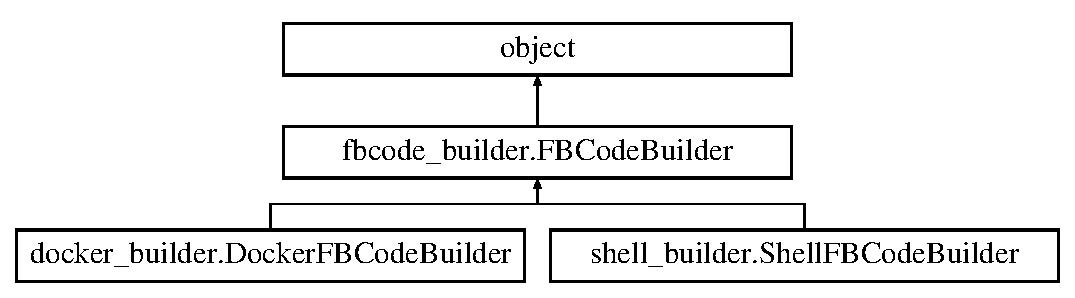
\includegraphics[height=3.000000cm]{classfbcode__builder_1_1FBCodeBuilder}
\end{center}
\end{figure}
\subsection*{Public Member Functions}
\begin{DoxyCompactItemize}
\item 
def {\bf \+\_\+\+\_\+init\+\_\+\+\_\+} (self, kwargs)
\item 
def {\bf \+\_\+\+\_\+repr\+\_\+\+\_\+} (self)
\item 
def {\bf option} (self, {\bf name}, default=None)
\item 
def {\bf has\+\_\+option} (self, {\bf name})
\item 
def {\bf add\+\_\+option} (self, {\bf name}, value)
\item 
def {\bf render} (self, steps)
\item 
def {\bf build} (self, steps)
\item 
def {\bf setup} (self)
\item 
def {\bf diagnostics} (self)
\item 
def {\bf step} (self, {\bf name}, actions)
\item 
def {\bf run} (self, shell\+\_\+cmd)
\item 
def {\bf workdir} (self, dir)
\item 
def {\bf copy\+\_\+local\+\_\+repo} (self, dir, dest\+\_\+name)
\item 
def {\bf debian\+\_\+deps} (self)
\item 
def {\bf install\+\_\+debian\+\_\+deps} (self)
\item 
def {\bf debian\+\_\+ccache\+\_\+setup\+\_\+steps} (self)
\item 
def {\bf github\+\_\+project\+\_\+workdir} (self, project, path)
\item 
def {\bf fb\+\_\+github\+\_\+project\+\_\+workdir} (self, project\+\_\+and\+\_\+path, github\+\_\+org=\textquotesingle{}facebook\textquotesingle{})
\item 
def {\bf parallel\+\_\+make} (self, make\+\_\+vars=None)
\item 
def {\bf make\+\_\+and\+\_\+install} (self, make\+\_\+vars=None)
\item 
def {\bf configure} (self, {\bf name}=None)
\item 
def {\bf autoconf\+\_\+install} (self, {\bf name})
\item 
def {\bf cmake\+\_\+configure} (self, {\bf name}, cmake\+\_\+path=\textquotesingle{}..\textquotesingle{})
\item 
def {\bf cmake\+\_\+install} (self, {\bf name}, cmake\+\_\+path=\textquotesingle{}..\textquotesingle{})
\item 
def {\bf fb\+\_\+github\+\_\+autoconf\+\_\+install} (self, project\+\_\+and\+\_\+path, github\+\_\+org=\textquotesingle{}facebook\textquotesingle{})
\item 
def {\bf fb\+\_\+github\+\_\+cmake\+\_\+install} (self, project\+\_\+and\+\_\+path, cmake\+\_\+path=\textquotesingle{}..\textquotesingle{}, github\+\_\+org=\textquotesingle{}facebook\textquotesingle{})
\end{DoxyCompactItemize}
\subsection*{Public Attributes}
\begin{DoxyCompactItemize}
\item 
{\bf options\+\_\+used}
\end{DoxyCompactItemize}
\subsection*{Private Member Functions}
\begin{DoxyCompactItemize}
\item 
def {\bf \+\_\+make\+\_\+vars} (self, make\+\_\+vars)
\end{DoxyCompactItemize}
\subsection*{Private Attributes}
\begin{DoxyCompactItemize}
\item 
{\bf \+\_\+options\+\_\+do\+\_\+not\+\_\+access}
\item 
{\bf \+\_\+github\+\_\+hashes}
\end{DoxyCompactItemize}


\subsection{Detailed Description}


Definition at line 83 of file fbcode\+\_\+builder.\+py.



\subsection{Constructor \& Destructor Documentation}
\index{fbcode\+\_\+builder\+::\+F\+B\+Code\+Builder@{fbcode\+\_\+builder\+::\+F\+B\+Code\+Builder}!\+\_\+\+\_\+init\+\_\+\+\_\+@{\+\_\+\+\_\+init\+\_\+\+\_\+}}
\index{\+\_\+\+\_\+init\+\_\+\+\_\+@{\+\_\+\+\_\+init\+\_\+\+\_\+}!fbcode\+\_\+builder\+::\+F\+B\+Code\+Builder@{fbcode\+\_\+builder\+::\+F\+B\+Code\+Builder}}
\subsubsection[{\+\_\+\+\_\+init\+\_\+\+\_\+(self, kwargs)}]{\setlength{\rightskip}{0pt plus 5cm}def fbcode\+\_\+builder.\+F\+B\+Code\+Builder.\+\_\+\+\_\+init\+\_\+\+\_\+ (
\begin{DoxyParamCaption}
\item[{}]{self, }
\item[{}]{kwargs}
\end{DoxyParamCaption}
)}\label{classfbcode__builder_1_1FBCodeBuilder_a02218bace0d9992d68cdffeb8bfe6278}


Definition at line 85 of file fbcode\+\_\+builder.\+py.


\begin{DoxyCode}
85     \textcolor{keyword}{def }__init__(self, **kwargs):
86         self._options_do_not_access = kwargs  \textcolor{comment}{# Use .option() instead.}
87         \textcolor{comment}{# This raises upon detecting options that are specified but unused,}
88         \textcolor{comment}{# because otherwise it is very easy to make a typo in option names.}
89         self.options_used = set()
90         self._github_hashes = dict(_read_project_github_hashes())
91 
\end{DoxyCode}


\subsection{Member Function Documentation}
\index{fbcode\+\_\+builder\+::\+F\+B\+Code\+Builder@{fbcode\+\_\+builder\+::\+F\+B\+Code\+Builder}!\+\_\+\+\_\+repr\+\_\+\+\_\+@{\+\_\+\+\_\+repr\+\_\+\+\_\+}}
\index{\+\_\+\+\_\+repr\+\_\+\+\_\+@{\+\_\+\+\_\+repr\+\_\+\+\_\+}!fbcode\+\_\+builder\+::\+F\+B\+Code\+Builder@{fbcode\+\_\+builder\+::\+F\+B\+Code\+Builder}}
\subsubsection[{\+\_\+\+\_\+repr\+\_\+\+\_\+(self)}]{\setlength{\rightskip}{0pt plus 5cm}def fbcode\+\_\+builder.\+F\+B\+Code\+Builder.\+\_\+\+\_\+repr\+\_\+\+\_\+ (
\begin{DoxyParamCaption}
\item[{}]{self}
\end{DoxyParamCaption}
)}\label{classfbcode__builder_1_1FBCodeBuilder_ac675551dfb753df591af560d54626bff}


Definition at line 92 of file fbcode\+\_\+builder.\+py.


\begin{DoxyCode}
92     \textcolor{keyword}{def }__repr__(self):
93         \textcolor{keywordflow}{return} \textcolor{stringliteral}{'\{0\}(\{1\})'}.format(
94             self.\_\_class\_\_.\_\_name\_\_,
95             \textcolor{stringliteral}{', '}.join(
96                 \textcolor{stringliteral}{'\{0\}=\{1\}'}.format(k, repr(v))
97                     \textcolor{keywordflow}{for} k, v \textcolor{keywordflow}{in} self.\_options\_do\_not\_access.items()
98             )
99         )
100 
\end{DoxyCode}
\index{fbcode\+\_\+builder\+::\+F\+B\+Code\+Builder@{fbcode\+\_\+builder\+::\+F\+B\+Code\+Builder}!\+\_\+make\+\_\+vars@{\+\_\+make\+\_\+vars}}
\index{\+\_\+make\+\_\+vars@{\+\_\+make\+\_\+vars}!fbcode\+\_\+builder\+::\+F\+B\+Code\+Builder@{fbcode\+\_\+builder\+::\+F\+B\+Code\+Builder}}
\subsubsection[{\+\_\+make\+\_\+vars(self, make\+\_\+vars)}]{\setlength{\rightskip}{0pt plus 5cm}def fbcode\+\_\+builder.\+F\+B\+Code\+Builder.\+\_\+make\+\_\+vars (
\begin{DoxyParamCaption}
\item[{}]{self, }
\item[{}]{make\+\_\+vars}
\end{DoxyParamCaption}
)\hspace{0.3cm}{\ttfamily [private]}}\label{classfbcode__builder_1_1FBCodeBuilder_a51f60af5b4110f07cb2c4fbb591727bf}


Definition at line 283 of file fbcode\+\_\+builder.\+py.



References shell\+\_\+quoting.\+shell\+\_\+join().



Referenced by fbcode\+\_\+builder.\+F\+B\+Code\+Builder.\+make\+\_\+and\+\_\+install(), and fbcode\+\_\+builder.\+F\+B\+Code\+Builder.\+parallel\+\_\+make().


\begin{DoxyCode}
283     \textcolor{keyword}{def }_make_vars(self, make\_vars):
284         \textcolor{keywordflow}{return} shell_join(\textcolor{stringliteral}{' '}, (
285             ShellQuoted(\textcolor{stringliteral}{'\{k\}=\{v\}'}).format(k=k, v=v)
286                 \textcolor{keywordflow}{for} k, v \textcolor{keywordflow}{in} (\{\} \textcolor{keywordflow}{if} make\_vars \textcolor{keywordflow}{is} \textcolor{keywordtype}{None} \textcolor{keywordflow}{else} make\_vars).items()
287         ))
288 
\end{DoxyCode}
\index{fbcode\+\_\+builder\+::\+F\+B\+Code\+Builder@{fbcode\+\_\+builder\+::\+F\+B\+Code\+Builder}!add\+\_\+option@{add\+\_\+option}}
\index{add\+\_\+option@{add\+\_\+option}!fbcode\+\_\+builder\+::\+F\+B\+Code\+Builder@{fbcode\+\_\+builder\+::\+F\+B\+Code\+Builder}}
\subsubsection[{add\+\_\+option(self, name, value)}]{\setlength{\rightskip}{0pt plus 5cm}def fbcode\+\_\+builder.\+F\+B\+Code\+Builder.\+add\+\_\+option (
\begin{DoxyParamCaption}
\item[{}]{self, }
\item[{}]{name, }
\item[{}]{value}
\end{DoxyParamCaption}
)}\label{classfbcode__builder_1_1FBCodeBuilder_aba688e21f53f6e31990ca9ee97982c47}


Definition at line 111 of file fbcode\+\_\+builder.\+py.



References fbcode\+\_\+builder.\+F\+B\+Code\+Builder.\+\_\+options\+\_\+do\+\_\+not\+\_\+access.


\begin{DoxyCode}
111     \textcolor{keyword}{def }add_option(self, name, value):
112         \textcolor{keywordflow}{if} name \textcolor{keywordflow}{in} self._options_do_not_access:
113             \textcolor{keywordflow}{raise} RuntimeError(\textcolor{stringliteral}{'Option \{0\} already set'}.format(name))
114         self._options_do_not_access[name] = value
115 
\end{DoxyCode}
\index{fbcode\+\_\+builder\+::\+F\+B\+Code\+Builder@{fbcode\+\_\+builder\+::\+F\+B\+Code\+Builder}!autoconf\+\_\+install@{autoconf\+\_\+install}}
\index{autoconf\+\_\+install@{autoconf\+\_\+install}!fbcode\+\_\+builder\+::\+F\+B\+Code\+Builder@{fbcode\+\_\+builder\+::\+F\+B\+Code\+Builder}}
\subsubsection[{autoconf\+\_\+install(self, name)}]{\setlength{\rightskip}{0pt plus 5cm}def fbcode\+\_\+builder.\+F\+B\+Code\+Builder.\+autoconf\+\_\+install (
\begin{DoxyParamCaption}
\item[{}]{self, }
\item[{}]{name}
\end{DoxyParamCaption}
)}\label{classfbcode__builder_1_1FBCodeBuilder_adddf6f8d9e910637ec8fb8524fee9daf}


Definition at line 325 of file fbcode\+\_\+builder.\+py.



References fbcode\+\_\+builder.\+F\+B\+Code\+Builder.\+configure(), fbcode\+\_\+builder.\+F\+B\+Code\+Builder.\+make\+\_\+and\+\_\+install(), docker\+\_\+builder.\+Docker\+F\+B\+Code\+Builder.\+run(), fbcode\+\_\+builder.\+F\+B\+Code\+Builder.\+run(), docker\+\_\+builder.\+Docker\+F\+B\+Code\+Builder.\+step(), and fbcode\+\_\+builder.\+F\+B\+Code\+Builder.\+step().



Referenced by fbcode\+\_\+builder.\+F\+B\+Code\+Builder.\+fb\+\_\+github\+\_\+autoconf\+\_\+install().


\begin{DoxyCode}
325     \textcolor{keyword}{def }autoconf_install(self, name):
326         \textcolor{keywordflow}{return} self.step(\textcolor{stringliteral}{'Build and install \{0\}'}.format(name), [
327             self.run(ShellQuoted(\textcolor{stringliteral}{'autoreconf -ivf'})),
328         ] + self.configure() + self.make_and_install())
329 
\end{DoxyCode}
\index{fbcode\+\_\+builder\+::\+F\+B\+Code\+Builder@{fbcode\+\_\+builder\+::\+F\+B\+Code\+Builder}!build@{build}}
\index{build@{build}!fbcode\+\_\+builder\+::\+F\+B\+Code\+Builder@{fbcode\+\_\+builder\+::\+F\+B\+Code\+Builder}}
\subsubsection[{build(self, steps)}]{\setlength{\rightskip}{0pt plus 5cm}def fbcode\+\_\+builder.\+F\+B\+Code\+Builder.\+build (
\begin{DoxyParamCaption}
\item[{}]{self, }
\item[{}]{steps}
\end{DoxyParamCaption}
)}\label{classfbcode__builder_1_1FBCodeBuilder_ac0fe8d534f835bf4c82656d1804308df}


Definition at line 141 of file fbcode\+\_\+builder.\+py.



References fbcode\+\_\+builder.\+F\+B\+Code\+Builder.\+diagnostics(), docker\+\_\+builder.\+Docker\+F\+B\+Code\+Builder.\+setup(), and fbcode\+\_\+builder.\+F\+B\+Code\+Builder.\+setup().


\begin{DoxyCode}
141     \textcolor{keyword}{def }build(self, steps):
142         \textcolor{keywordflow}{if} \textcolor{keywordflow}{not} steps:
143             \textcolor{keywordflow}{raise} RuntimeError(\textcolor{stringliteral}{'Please ensure that the config you are passing '}
144                                \textcolor{stringliteral}{'contains steps'})
145         \textcolor{keywordflow}{return} [self.setup(), self.diagnostics()] + steps
146 
\end{DoxyCode}
\index{fbcode\+\_\+builder\+::\+F\+B\+Code\+Builder@{fbcode\+\_\+builder\+::\+F\+B\+Code\+Builder}!cmake\+\_\+configure@{cmake\+\_\+configure}}
\index{cmake\+\_\+configure@{cmake\+\_\+configure}!fbcode\+\_\+builder\+::\+F\+B\+Code\+Builder@{fbcode\+\_\+builder\+::\+F\+B\+Code\+Builder}}
\subsubsection[{cmake\+\_\+configure(self, name, cmake\+\_\+path=\textquotesingle{}..\textquotesingle{})}]{\setlength{\rightskip}{0pt plus 5cm}def fbcode\+\_\+builder.\+F\+B\+Code\+Builder.\+cmake\+\_\+configure (
\begin{DoxyParamCaption}
\item[{}]{self, }
\item[{}]{name, }
\item[{}]{cmake\+\_\+path = {\ttfamily \textquotesingle{}..\textquotesingle{}}}
\end{DoxyParamCaption}
)}\label{classfbcode__builder_1_1FBCodeBuilder_aa717c0ea61f606104ce64a1bdcdb3115}


Definition at line 330 of file fbcode\+\_\+builder.\+py.



References fbcode\+\_\+builder.\+F\+B\+Code\+Builder.\+option(), docker\+\_\+builder.\+Docker\+F\+B\+Code\+Builder.\+run(), fbcode\+\_\+builder.\+F\+B\+Code\+Builder.\+run(), and shell\+\_\+quoting.\+shell\+\_\+join().



Referenced by fbcode\+\_\+builder.\+F\+B\+Code\+Builder.\+cmake\+\_\+install().


\begin{DoxyCode}
330     \textcolor{keyword}{def }cmake_configure(self, name, cmake\_path='..'):
331         cmake\_defines = \{
332             \textcolor{stringliteral}{'BUILD\_SHARED\_LIBS'}: \textcolor{stringliteral}{'ON'},
333             \textcolor{stringliteral}{'CMAKE\_INSTALL\_PREFIX'}: self.option(\textcolor{stringliteral}{'prefix'}),
334         \}
335         cmake\_defines.update(
336             self.option(\textcolor{stringliteral}{'\{0\}:cmake\_defines'}.format(name), \{\})
337         )
338         \textcolor{keywordflow}{return} [
339             self.run(ShellQuoted(
340                 \textcolor{stringliteral}{'CXXFLAGS="$CXXFLAGS -fPIC -isystem "\{p\}"/include" '}
341                 \textcolor{stringliteral}{'CFLAGS="$CFLAGS -fPIC -isystem "\{p\}"/include" '}
342                 \textcolor{stringliteral}{'cmake \{args\} \{cmake\_path\}'}
343             ).format(
344                 p=self.option(\textcolor{stringliteral}{'prefix'}),
345                 args=shell_join(\textcolor{stringliteral}{' '}, (
346                     ShellQuoted(\textcolor{stringliteral}{'-D\{k\}=\{v\}'}).format(k=k, v=v)
347                         \textcolor{keywordflow}{for} k, v \textcolor{keywordflow}{in} cmake\_defines.items()
348                 )),
349                 cmake\_path=cmake\_path,
350             )),
351         ]
352 
\end{DoxyCode}
\index{fbcode\+\_\+builder\+::\+F\+B\+Code\+Builder@{fbcode\+\_\+builder\+::\+F\+B\+Code\+Builder}!cmake\+\_\+install@{cmake\+\_\+install}}
\index{cmake\+\_\+install@{cmake\+\_\+install}!fbcode\+\_\+builder\+::\+F\+B\+Code\+Builder@{fbcode\+\_\+builder\+::\+F\+B\+Code\+Builder}}
\subsubsection[{cmake\+\_\+install(self, name, cmake\+\_\+path=\textquotesingle{}..\textquotesingle{})}]{\setlength{\rightskip}{0pt plus 5cm}def fbcode\+\_\+builder.\+F\+B\+Code\+Builder.\+cmake\+\_\+install (
\begin{DoxyParamCaption}
\item[{}]{self, }
\item[{}]{name, }
\item[{}]{cmake\+\_\+path = {\ttfamily \textquotesingle{}..\textquotesingle{}}}
\end{DoxyParamCaption}
)}\label{classfbcode__builder_1_1FBCodeBuilder_aff66e33205009b083d6272dc33757b64}


Definition at line 353 of file fbcode\+\_\+builder.\+py.



References fbcode\+\_\+builder.\+F\+B\+Code\+Builder.\+cmake\+\_\+configure(), fbcode\+\_\+builder.\+F\+B\+Code\+Builder.\+make\+\_\+and\+\_\+install(), docker\+\_\+builder.\+Docker\+F\+B\+Code\+Builder.\+step(), and fbcode\+\_\+builder.\+F\+B\+Code\+Builder.\+step().



Referenced by fbcode\+\_\+builder.\+F\+B\+Code\+Builder.\+fb\+\_\+github\+\_\+cmake\+\_\+install().


\begin{DoxyCode}
353     \textcolor{keyword}{def }cmake_install(self, name, cmake\_path='..'):
354         \textcolor{keywordflow}{return} self.step(
355             \textcolor{stringliteral}{'Build and install \{0\}'}.format(name),
356             self.cmake_configure(name, cmake\_path) + self.make_and_install()
357         )
358 
\end{DoxyCode}
\index{fbcode\+\_\+builder\+::\+F\+B\+Code\+Builder@{fbcode\+\_\+builder\+::\+F\+B\+Code\+Builder}!configure@{configure}}
\index{configure@{configure}!fbcode\+\_\+builder\+::\+F\+B\+Code\+Builder@{fbcode\+\_\+builder\+::\+F\+B\+Code\+Builder}}
\subsubsection[{configure(self, name=\+None)}]{\setlength{\rightskip}{0pt plus 5cm}def fbcode\+\_\+builder.\+F\+B\+Code\+Builder.\+configure (
\begin{DoxyParamCaption}
\item[{}]{self, }
\item[{}]{name = {\ttfamily None}}
\end{DoxyParamCaption}
)}\label{classfbcode__builder_1_1FBCodeBuilder_a9bafdc9ebde1e6c76151664655eb18c6}


Definition at line 303 of file fbcode\+\_\+builder.\+py.



References fbcode\+\_\+builder.\+F\+B\+Code\+Builder.\+option(), docker\+\_\+builder.\+Docker\+F\+B\+Code\+Builder.\+run(), fbcode\+\_\+builder.\+F\+B\+Code\+Builder.\+run(), and shell\+\_\+quoting.\+shell\+\_\+join().



Referenced by fbcode\+\_\+builder.\+F\+B\+Code\+Builder.\+autoconf\+\_\+install().


\begin{DoxyCode}
303     \textcolor{keyword}{def }configure(self, name=None):
304         autoconf\_options = \{\}
305         \textcolor{keywordflow}{if} name \textcolor{keywordflow}{is} \textcolor{keywordflow}{not} \textcolor{keywordtype}{None}:
306             autoconf\_options.update(
307                 self.option(\textcolor{stringliteral}{'\{0\}:autoconf\_options'}.format(name), \{\})
308             )
309         \textcolor{keywordflow}{return} [
310             self.run(ShellQuoted(
311                 \textcolor{stringliteral}{'LDFLAGS="$LDFLAGS -L"\{p\}"/lib -Wl,-rpath="\{p\}"/lib" '}
312                 \textcolor{stringliteral}{'CFLAGS="$CFLAGS -I"\{p\}"/include" '}
313                 \textcolor{stringliteral}{'CPPFLAGS="$CPPFLAGS -I"\{p\}"/include" '}
314                 \textcolor{stringliteral}{'PY\_PREFIX=\{p\} '}
315                 \textcolor{stringliteral}{'./configure --prefix=\{p\} \{args\}'}
316             ).format(
317                 p=self.option(\textcolor{stringliteral}{'prefix'}),
318                 args=shell_join(\textcolor{stringliteral}{' '}, (
319                     ShellQuoted(\textcolor{stringliteral}{'\{k\}=\{v\}'}).format(k=k, v=v)
320                     \textcolor{keywordflow}{for} k, v \textcolor{keywordflow}{in} autoconf\_options.items()
321                 )),
322             )),
323         ]
324 
\end{DoxyCode}
\index{fbcode\+\_\+builder\+::\+F\+B\+Code\+Builder@{fbcode\+\_\+builder\+::\+F\+B\+Code\+Builder}!copy\+\_\+local\+\_\+repo@{copy\+\_\+local\+\_\+repo}}
\index{copy\+\_\+local\+\_\+repo@{copy\+\_\+local\+\_\+repo}!fbcode\+\_\+builder\+::\+F\+B\+Code\+Builder@{fbcode\+\_\+builder\+::\+F\+B\+Code\+Builder}}
\subsubsection[{copy\+\_\+local\+\_\+repo(self, dir, dest\+\_\+name)}]{\setlength{\rightskip}{0pt plus 5cm}def fbcode\+\_\+builder.\+F\+B\+Code\+Builder.\+copy\+\_\+local\+\_\+repo (
\begin{DoxyParamCaption}
\item[{}]{self, }
\item[{}]{dir, }
\item[{}]{dest\+\_\+name}
\end{DoxyParamCaption}
)}\label{classfbcode__builder_1_1FBCodeBuilder_a1d889aca71ff24b1e3ac060371fcf694}
\begin{DoxyVerb}Copy the local repo at `dir` into this step's `workdir()`, analog of:
  cp -r /path/to/folly folly
\end{DoxyVerb}
 

Definition at line 175 of file fbcode\+\_\+builder.\+py.



Referenced by fbcode\+\_\+builder.\+F\+B\+Code\+Builder.\+github\+\_\+project\+\_\+workdir().


\begin{DoxyCode}
175     \textcolor{keyword}{def }copy_local_repo(self, dir, dest\_name):
176         \textcolor{stringliteral}{'''}
177 \textcolor{stringliteral}{        Copy the local repo at `dir` into this step's `workdir()`, analog of:}
178 \textcolor{stringliteral}{          cp -r /path/to/folly folly}
179 \textcolor{stringliteral}{        '''}
180         \textcolor{keywordflow}{raise} NotImplementedError
181 
\end{DoxyCode}
\index{fbcode\+\_\+builder\+::\+F\+B\+Code\+Builder@{fbcode\+\_\+builder\+::\+F\+B\+Code\+Builder}!debian\+\_\+ccache\+\_\+setup\+\_\+steps@{debian\+\_\+ccache\+\_\+setup\+\_\+steps}}
\index{debian\+\_\+ccache\+\_\+setup\+\_\+steps@{debian\+\_\+ccache\+\_\+setup\+\_\+steps}!fbcode\+\_\+builder\+::\+F\+B\+Code\+Builder@{fbcode\+\_\+builder\+::\+F\+B\+Code\+Builder}}
\subsubsection[{debian\+\_\+ccache\+\_\+setup\+\_\+steps(self)}]{\setlength{\rightskip}{0pt plus 5cm}def fbcode\+\_\+builder.\+F\+B\+Code\+Builder.\+debian\+\_\+ccache\+\_\+setup\+\_\+steps (
\begin{DoxyParamCaption}
\item[{}]{self}
\end{DoxyParamCaption}
)}\label{classfbcode__builder_1_1FBCodeBuilder_a9f100ffe7bb168c03f2aa6953d9969a7}


Definition at line 249 of file fbcode\+\_\+builder.\+py.



Referenced by fbcode\+\_\+builder.\+F\+B\+Code\+Builder.\+install\+\_\+debian\+\_\+deps().


\begin{DoxyCode}
249     \textcolor{keyword}{def }debian_ccache_setup_steps(self):
250         \textcolor{keywordflow}{return} []  \textcolor{comment}{# It's ok to ship a renderer without ccache support.}
251 
\end{DoxyCode}
\index{fbcode\+\_\+builder\+::\+F\+B\+Code\+Builder@{fbcode\+\_\+builder\+::\+F\+B\+Code\+Builder}!debian\+\_\+deps@{debian\+\_\+deps}}
\index{debian\+\_\+deps@{debian\+\_\+deps}!fbcode\+\_\+builder\+::\+F\+B\+Code\+Builder@{fbcode\+\_\+builder\+::\+F\+B\+Code\+Builder}}
\subsubsection[{debian\+\_\+deps(self)}]{\setlength{\rightskip}{0pt plus 5cm}def fbcode\+\_\+builder.\+F\+B\+Code\+Builder.\+debian\+\_\+deps (
\begin{DoxyParamCaption}
\item[{}]{self}
\end{DoxyParamCaption}
)}\label{classfbcode__builder_1_1FBCodeBuilder_a5a11e2701863b6600a62deffaa2d4474}


Definition at line 182 of file fbcode\+\_\+builder.\+py.



Referenced by fbcode\+\_\+builder.\+F\+B\+Code\+Builder.\+install\+\_\+debian\+\_\+deps().


\begin{DoxyCode}
182     \textcolor{keyword}{def }debian_deps(self):
183         \textcolor{keywordflow}{return} [
184             \textcolor{stringliteral}{'autoconf-archive'},
185             \textcolor{stringliteral}{'bison'},
186             \textcolor{stringliteral}{'build-essential'},
187             \textcolor{stringliteral}{'cmake'},
188             \textcolor{stringliteral}{'curl'},
189             \textcolor{stringliteral}{'flex'},
190             \textcolor{stringliteral}{'git'},
191             \textcolor{stringliteral}{'gperf'},
192             \textcolor{stringliteral}{'joe'},
193             \textcolor{stringliteral}{'libboost-all-dev'},
194             \textcolor{stringliteral}{'libcap-dev'},
195             \textcolor{stringliteral}{'libdouble-conversion-dev'},
196             \textcolor{stringliteral}{'libevent-dev'},
197             \textcolor{stringliteral}{'libgflags-dev'},
198             \textcolor{stringliteral}{'libgoogle-glog-dev'},
199             \textcolor{stringliteral}{'libkrb5-dev'},
200             \textcolor{stringliteral}{'libpcre3-dev'},
201             \textcolor{stringliteral}{'libpthread-stubs0-dev'},
202             \textcolor{stringliteral}{'libnuma-dev'},
203             \textcolor{stringliteral}{'libsasl2-dev'},
204             \textcolor{stringliteral}{'libsnappy-dev'},
205             \textcolor{stringliteral}{'libsqlite3-dev'},
206             \textcolor{stringliteral}{'libssl-dev'},
207             \textcolor{stringliteral}{'libtool'},
208             \textcolor{stringliteral}{'netcat-openbsd'},
209             \textcolor{stringliteral}{'pkg-config'},
210             \textcolor{stringliteral}{'sudo'},
211             \textcolor{stringliteral}{'unzip'},
212             \textcolor{stringliteral}{'wget'},
213         ]
214 
\end{DoxyCode}
\index{fbcode\+\_\+builder\+::\+F\+B\+Code\+Builder@{fbcode\+\_\+builder\+::\+F\+B\+Code\+Builder}!diagnostics@{diagnostics}}
\index{diagnostics@{diagnostics}!fbcode\+\_\+builder\+::\+F\+B\+Code\+Builder@{fbcode\+\_\+builder\+::\+F\+B\+Code\+Builder}}
\subsubsection[{diagnostics(self)}]{\setlength{\rightskip}{0pt plus 5cm}def fbcode\+\_\+builder.\+F\+B\+Code\+Builder.\+diagnostics (
\begin{DoxyParamCaption}
\item[{}]{self}
\end{DoxyParamCaption}
)}\label{classfbcode__builder_1_1FBCodeBuilder_a64340bd79e34282afd523863703534f2}


Definition at line 151 of file fbcode\+\_\+builder.\+py.



References shell\+\_\+builder.\+Shell\+F\+B\+Code\+Builder.\+comment(), docker\+\_\+builder.\+Docker\+F\+B\+Code\+Builder.\+comment(), docker\+\_\+builder.\+Docker\+F\+B\+Code\+Builder.\+run(), fbcode\+\_\+builder.\+F\+B\+Code\+Builder.\+run(), docker\+\_\+builder.\+Docker\+F\+B\+Code\+Builder.\+step(), and fbcode\+\_\+builder.\+F\+B\+Code\+Builder.\+step().



Referenced by fbcode\+\_\+builder.\+F\+B\+Code\+Builder.\+build().


\begin{DoxyCode}
151     \textcolor{keyword}{def }diagnostics(self):
152         \textcolor{stringliteral}{'Log some system diagnostics before/after setup for ease of debugging'}
153         \textcolor{comment}{# The builder's repr is not used in a command to avoid pointlessly}
154         \textcolor{comment}{# invalidating Docker's build cache.}
155         \textcolor{keywordflow}{return} self.step(\textcolor{stringliteral}{'Diagnostics'}, [
156             self.comment(\textcolor{stringliteral}{'Builder \{0\}'}.format(repr(self))),
157             self.run(ShellQuoted(\textcolor{stringliteral}{'hostname'})),
158             self.run(ShellQuoted(\textcolor{stringliteral}{'cat /etc/issue || echo no /etc/issue'})),
159             self.run(ShellQuoted(\textcolor{stringliteral}{'g++ --version || echo g++ not installed'})),
160             self.run(ShellQuoted(\textcolor{stringliteral}{'cmake --version || echo cmake not installed'})),
161         ])
162 
\end{DoxyCode}
\index{fbcode\+\_\+builder\+::\+F\+B\+Code\+Builder@{fbcode\+\_\+builder\+::\+F\+B\+Code\+Builder}!fb\+\_\+github\+\_\+autoconf\+\_\+install@{fb\+\_\+github\+\_\+autoconf\+\_\+install}}
\index{fb\+\_\+github\+\_\+autoconf\+\_\+install@{fb\+\_\+github\+\_\+autoconf\+\_\+install}!fbcode\+\_\+builder\+::\+F\+B\+Code\+Builder@{fbcode\+\_\+builder\+::\+F\+B\+Code\+Builder}}
\subsubsection[{fb\+\_\+github\+\_\+autoconf\+\_\+install(self, project\+\_\+and\+\_\+path, github\+\_\+org=\textquotesingle{}facebook\textquotesingle{})}]{\setlength{\rightskip}{0pt plus 5cm}def fbcode\+\_\+builder.\+F\+B\+Code\+Builder.\+fb\+\_\+github\+\_\+autoconf\+\_\+install (
\begin{DoxyParamCaption}
\item[{}]{self, }
\item[{}]{project\+\_\+and\+\_\+path, }
\item[{}]{github\+\_\+org = {\ttfamily \textquotesingle{}facebook\textquotesingle{}}}
\end{DoxyParamCaption}
)}\label{classfbcode__builder_1_1FBCodeBuilder_ac80b52f88cf372d96cbe75d0a1d9c86f}


Definition at line 359 of file fbcode\+\_\+builder.\+py.



References fbcode\+\_\+builder.\+F\+B\+Code\+Builder.\+autoconf\+\_\+install(), and fbcode\+\_\+builder.\+F\+B\+Code\+Builder.\+fb\+\_\+github\+\_\+project\+\_\+workdir().


\begin{DoxyCode}
359     \textcolor{keyword}{def }fb_github_autoconf_install(self, project\_and\_path, github\_org='facebook'):
360         \textcolor{keywordflow}{return} [
361             self.fb_github_project_workdir(project\_and\_path, github\_org),
362             self.autoconf_install(project\_and\_path),
363         ]
364 
\end{DoxyCode}
\index{fbcode\+\_\+builder\+::\+F\+B\+Code\+Builder@{fbcode\+\_\+builder\+::\+F\+B\+Code\+Builder}!fb\+\_\+github\+\_\+cmake\+\_\+install@{fb\+\_\+github\+\_\+cmake\+\_\+install}}
\index{fb\+\_\+github\+\_\+cmake\+\_\+install@{fb\+\_\+github\+\_\+cmake\+\_\+install}!fbcode\+\_\+builder\+::\+F\+B\+Code\+Builder@{fbcode\+\_\+builder\+::\+F\+B\+Code\+Builder}}
\subsubsection[{fb\+\_\+github\+\_\+cmake\+\_\+install(self, project\+\_\+and\+\_\+path, cmake\+\_\+path=\textquotesingle{}..\textquotesingle{}, github\+\_\+org=\textquotesingle{}facebook\textquotesingle{})}]{\setlength{\rightskip}{0pt plus 5cm}def fbcode\+\_\+builder.\+F\+B\+Code\+Builder.\+fb\+\_\+github\+\_\+cmake\+\_\+install (
\begin{DoxyParamCaption}
\item[{}]{self, }
\item[{}]{project\+\_\+and\+\_\+path, }
\item[{}]{cmake\+\_\+path = {\ttfamily \textquotesingle{}..\textquotesingle{}}, }
\item[{}]{github\+\_\+org = {\ttfamily \textquotesingle{}facebook\textquotesingle{}}}
\end{DoxyParamCaption}
)}\label{classfbcode__builder_1_1FBCodeBuilder_a642fb2e0fe693fbaeb58653b2ed97b35}


Definition at line 365 of file fbcode\+\_\+builder.\+py.



References fbcode\+\_\+builder.\+F\+B\+Code\+Builder.\+cmake\+\_\+install(), and fbcode\+\_\+builder.\+F\+B\+Code\+Builder.\+fb\+\_\+github\+\_\+project\+\_\+workdir().


\begin{DoxyCode}
365     \textcolor{keyword}{def }fb_github_cmake_install(self, project\_and\_path, cmake\_path='..', github\_org='facebook'):
366         \textcolor{keywordflow}{return} [
367             self.fb_github_project_workdir(project\_and\_path, github\_org),
368             self.cmake_install(project\_and\_path, cmake\_path),
369         ]
370 \end{DoxyCode}
\index{fbcode\+\_\+builder\+::\+F\+B\+Code\+Builder@{fbcode\+\_\+builder\+::\+F\+B\+Code\+Builder}!fb\+\_\+github\+\_\+project\+\_\+workdir@{fb\+\_\+github\+\_\+project\+\_\+workdir}}
\index{fb\+\_\+github\+\_\+project\+\_\+workdir@{fb\+\_\+github\+\_\+project\+\_\+workdir}!fbcode\+\_\+builder\+::\+F\+B\+Code\+Builder@{fbcode\+\_\+builder\+::\+F\+B\+Code\+Builder}}
\subsubsection[{fb\+\_\+github\+\_\+project\+\_\+workdir(self, project\+\_\+and\+\_\+path, github\+\_\+org=\textquotesingle{}facebook\textquotesingle{})}]{\setlength{\rightskip}{0pt plus 5cm}def fbcode\+\_\+builder.\+F\+B\+Code\+Builder.\+fb\+\_\+github\+\_\+project\+\_\+workdir (
\begin{DoxyParamCaption}
\item[{}]{self, }
\item[{}]{project\+\_\+and\+\_\+path, }
\item[{}]{github\+\_\+org = {\ttfamily \textquotesingle{}facebook\textquotesingle{}}}
\end{DoxyParamCaption}
)}\label{classfbcode__builder_1_1FBCodeBuilder_a9b5fe5a35afe35aec0ac68996f5e983e}


Definition at line 278 of file fbcode\+\_\+builder.\+py.



References fbcode\+\_\+builder.\+F\+B\+Code\+Builder.\+github\+\_\+project\+\_\+workdir().



Referenced by fbcode\+\_\+builder.\+F\+B\+Code\+Builder.\+fb\+\_\+github\+\_\+autoconf\+\_\+install(), and fbcode\+\_\+builder.\+F\+B\+Code\+Builder.\+fb\+\_\+github\+\_\+cmake\+\_\+install().


\begin{DoxyCode}
278     \textcolor{keyword}{def }fb_github_project_workdir(self, project\_and\_path, github\_org='facebook'):
279         \textcolor{stringliteral}{'This helper lets Facebook-internal CI special-cases FB projects'}
280         project, path = project\_and\_path.split(\textcolor{stringliteral}{'/'}, 1)
281         \textcolor{keywordflow}{return} self.github_project_workdir(github\_org + \textcolor{stringliteral}{'/'} + project, path)
282 
\end{DoxyCode}
\index{fbcode\+\_\+builder\+::\+F\+B\+Code\+Builder@{fbcode\+\_\+builder\+::\+F\+B\+Code\+Builder}!github\+\_\+project\+\_\+workdir@{github\+\_\+project\+\_\+workdir}}
\index{github\+\_\+project\+\_\+workdir@{github\+\_\+project\+\_\+workdir}!fbcode\+\_\+builder\+::\+F\+B\+Code\+Builder@{fbcode\+\_\+builder\+::\+F\+B\+Code\+Builder}}
\subsubsection[{github\+\_\+project\+\_\+workdir(self, project, path)}]{\setlength{\rightskip}{0pt plus 5cm}def fbcode\+\_\+builder.\+F\+B\+Code\+Builder.\+github\+\_\+project\+\_\+workdir (
\begin{DoxyParamCaption}
\item[{}]{self, }
\item[{}]{project, }
\item[{}]{path}
\end{DoxyParamCaption}
)}\label{classfbcode__builder_1_1FBCodeBuilder_ab6b8644665eb16625044b8c994dc0ced}


Definition at line 252 of file fbcode\+\_\+builder.\+py.



References docker\+\_\+builder.\+Docker\+F\+B\+Code\+Builder.\+copy\+\_\+local\+\_\+repo(), fbcode\+\_\+builder.\+F\+B\+Code\+Builder.\+copy\+\_\+local\+\_\+repo(), fbcode\+\_\+builder.\+F\+B\+Code\+Builder.\+option(), shell\+\_\+quoting.\+path\+\_\+join(), docker\+\_\+builder.\+Docker\+F\+B\+Code\+Builder.\+run(), fbcode\+\_\+builder.\+F\+B\+Code\+Builder.\+run(), docker\+\_\+builder.\+Docker\+F\+B\+Code\+Builder.\+step(), fbcode\+\_\+builder.\+F\+B\+Code\+Builder.\+step(), docker\+\_\+builder.\+Docker\+F\+B\+Code\+Builder.\+workdir(), and fbcode\+\_\+builder.\+F\+B\+Code\+Builder.\+workdir().



Referenced by fbcode\+\_\+builder.\+F\+B\+Code\+Builder.\+fb\+\_\+github\+\_\+project\+\_\+workdir().


\begin{DoxyCode}
252     \textcolor{keyword}{def }github_project_workdir(self, project, path):
253         \textcolor{comment}{# Only check out a non-default branch if requested. This especially}
254         \textcolor{comment}{# makes sense when building from a local repo.}
255         git\_hash = self.option(
256             \textcolor{stringliteral}{'\{0\}:git\_hash'}.format(project),
257             \textcolor{comment}{# Any repo that has a hash in deps/github\_hashes defaults to}
258             \textcolor{comment}{# that, with the goal of making builds maximally consistent.}
259             self.\_github\_hashes.get(project, \textcolor{stringliteral}{''})
260         )
261         maybe\_change\_branch = [
262             self.run(ShellQuoted(\textcolor{stringliteral}{'git checkout \{hash\}'}).format(hash=git\_hash)),
263         ] \textcolor{keywordflow}{if} git\_hash \textcolor{keywordflow}{else} []
264 
265         base\_dir = self.option(\textcolor{stringliteral}{'projects\_dir'})
266 
267         local\_repo\_dir = self.option(\textcolor{stringliteral}{'\{0\}:local\_repo\_dir'}.format(project), \textcolor{stringliteral}{''})
268         \textcolor{keywordflow}{return} self.step(\textcolor{stringliteral}{'Check out \{0\}, workdir \{1\}'}.format(project, path), [
269             self.workdir(base\_dir),
270             self.run(
271                 ShellQuoted(\textcolor{stringliteral}{'git clone https://github.com/\{p\}'}).format(p=project)
272             ) \textcolor{keywordflow}{if} \textcolor{keywordflow}{not} local\_repo\_dir \textcolor{keywordflow}{else} self.copy_local_repo(
273                 local\_repo\_dir, os.path.basename(project)
274             ),
275             self.workdir(path_join(base\_dir, os.path.basename(project), path)),
276         ] + maybe\_change\_branch)
277 
\end{DoxyCode}
\index{fbcode\+\_\+builder\+::\+F\+B\+Code\+Builder@{fbcode\+\_\+builder\+::\+F\+B\+Code\+Builder}!has\+\_\+option@{has\+\_\+option}}
\index{has\+\_\+option@{has\+\_\+option}!fbcode\+\_\+builder\+::\+F\+B\+Code\+Builder@{fbcode\+\_\+builder\+::\+F\+B\+Code\+Builder}}
\subsubsection[{has\+\_\+option(self, name)}]{\setlength{\rightskip}{0pt plus 5cm}def fbcode\+\_\+builder.\+F\+B\+Code\+Builder.\+has\+\_\+option (
\begin{DoxyParamCaption}
\item[{}]{self, }
\item[{}]{name}
\end{DoxyParamCaption}
)}\label{classfbcode__builder_1_1FBCodeBuilder_aebe22a563f68f8d01a35463f540300ea}


Definition at line 108 of file fbcode\+\_\+builder.\+py.



References fbcode\+\_\+builder.\+F\+B\+Code\+Builder.\+\_\+options\+\_\+do\+\_\+not\+\_\+access.



Referenced by shell\+\_\+builder.\+Shell\+F\+B\+Code\+Builder.\+setup().


\begin{DoxyCode}
108     \textcolor{keyword}{def }has_option(self, name):
109         \textcolor{keywordflow}{return} name \textcolor{keywordflow}{in} self._options_do_not_access
110 
\end{DoxyCode}
\index{fbcode\+\_\+builder\+::\+F\+B\+Code\+Builder@{fbcode\+\_\+builder\+::\+F\+B\+Code\+Builder}!install\+\_\+debian\+\_\+deps@{install\+\_\+debian\+\_\+deps}}
\index{install\+\_\+debian\+\_\+deps@{install\+\_\+debian\+\_\+deps}!fbcode\+\_\+builder\+::\+F\+B\+Code\+Builder@{fbcode\+\_\+builder\+::\+F\+B\+Code\+Builder}}
\subsubsection[{install\+\_\+debian\+\_\+deps(self)}]{\setlength{\rightskip}{0pt plus 5cm}def fbcode\+\_\+builder.\+F\+B\+Code\+Builder.\+install\+\_\+debian\+\_\+deps (
\begin{DoxyParamCaption}
\item[{}]{self}
\end{DoxyParamCaption}
)}\label{classfbcode__builder_1_1FBCodeBuilder_a2f3b87fa18289cd3662aee3e83224f41}


Definition at line 219 of file fbcode\+\_\+builder.\+py.



References docker\+\_\+builder.\+Docker\+F\+B\+Code\+Builder.\+debian\+\_\+ccache\+\_\+setup\+\_\+steps(), fbcode\+\_\+builder.\+F\+B\+Code\+Builder.\+debian\+\_\+ccache\+\_\+setup\+\_\+steps(), fbcode\+\_\+builder.\+F\+B\+Code\+Builder.\+debian\+\_\+deps(), fbcode\+\_\+builder.\+F\+B\+Code\+Builder.\+option(), docker\+\_\+builder.\+Docker\+F\+B\+Code\+Builder.\+run(), fbcode\+\_\+builder.\+F\+B\+Code\+Builder.\+run(), shell\+\_\+quoting.\+shell\+\_\+join(), docker\+\_\+builder.\+Docker\+F\+B\+Code\+Builder.\+step(), and fbcode\+\_\+builder.\+F\+B\+Code\+Builder.\+step().



Referenced by docker\+\_\+builder.\+Docker\+F\+B\+Code\+Builder.\+setup().


\begin{DoxyCode}
219     \textcolor{keyword}{def }install_debian_deps(self):
220         actions = [
221             self.run(
222                 ShellQuoted(\textcolor{stringliteral}{'apt-get update && apt-get install -yq \{deps\}'}).format(
223                     deps=shell_join(\textcolor{stringliteral}{' '}, (
224                         ShellQuoted(dep) \textcolor{keywordflow}{for} dep \textcolor{keywordflow}{in} self.debian_deps())))
225             ),
226         ]
227         gcc\_version = self.option(\textcolor{stringliteral}{'gcc\_version'})
228 
229         \textcolor{comment}{# Make the selected GCC the default before building anything}
230         actions.extend([
231             self.run(ShellQuoted(\textcolor{stringliteral}{'apt-get install -yq \{c\} \{cpp\}'}).format(
232                 c=ShellQuoted(\textcolor{stringliteral}{'gcc-\{v\}'}).format(v=gcc\_version),
233                 cpp=ShellQuoted(\textcolor{stringliteral}{'g++-\{v\}'}).format(v=gcc\_version),
234             )),
235             self.run(ShellQuoted(
236                 \textcolor{stringliteral}{'update-alternatives --install /usr/bin/gcc gcc \{c\} 40 '}
237                 \textcolor{stringliteral}{'--slave /usr/bin/g++ g++ \{cpp\}'}
238             ).format(
239                 c=ShellQuoted(\textcolor{stringliteral}{'/usr/bin/gcc-\{v\}'}).format(v=gcc\_version),
240                 cpp=ShellQuoted(\textcolor{stringliteral}{'/usr/bin/g++-\{v\}'}).format(v=gcc\_version),
241             )),
242             self.run(ShellQuoted(\textcolor{stringliteral}{'update-alternatives --config gcc'})),
243         ])
244 
245         actions.extend(self.debian_ccache_setup_steps())
246 
247         \textcolor{keywordflow}{return} self.step(\textcolor{stringliteral}{'Install packages for Debian-based OS'}, actions)
248 
\end{DoxyCode}
\index{fbcode\+\_\+builder\+::\+F\+B\+Code\+Builder@{fbcode\+\_\+builder\+::\+F\+B\+Code\+Builder}!make\+\_\+and\+\_\+install@{make\+\_\+and\+\_\+install}}
\index{make\+\_\+and\+\_\+install@{make\+\_\+and\+\_\+install}!fbcode\+\_\+builder\+::\+F\+B\+Code\+Builder@{fbcode\+\_\+builder\+::\+F\+B\+Code\+Builder}}
\subsubsection[{make\+\_\+and\+\_\+install(self, make\+\_\+vars=\+None)}]{\setlength{\rightskip}{0pt plus 5cm}def fbcode\+\_\+builder.\+F\+B\+Code\+Builder.\+make\+\_\+and\+\_\+install (
\begin{DoxyParamCaption}
\item[{}]{self, }
\item[{}]{make\+\_\+vars = {\ttfamily None}}
\end{DoxyParamCaption}
)}\label{classfbcode__builder_1_1FBCodeBuilder_a6f32b6848b9c7b51b95ea44dccddd30d}


Definition at line 295 of file fbcode\+\_\+builder.\+py.



References fbcode\+\_\+builder.\+F\+B\+Code\+Builder.\+\_\+make\+\_\+vars(), fbcode\+\_\+builder.\+F\+B\+Code\+Builder.\+parallel\+\_\+make(), docker\+\_\+builder.\+Docker\+F\+B\+Code\+Builder.\+run(), and fbcode\+\_\+builder.\+F\+B\+Code\+Builder.\+run().



Referenced by fbcode\+\_\+builder.\+F\+B\+Code\+Builder.\+autoconf\+\_\+install(), and fbcode\+\_\+builder.\+F\+B\+Code\+Builder.\+cmake\+\_\+install().


\begin{DoxyCode}
295     \textcolor{keyword}{def }make_and_install(self, make\_vars=None):
296         \textcolor{keywordflow}{return} [
297             self.parallel_make(make\_vars),
298             self.run(ShellQuoted(\textcolor{stringliteral}{'make install \{vars\}'}).format(
299                 vars=self._make_vars(make\_vars),
300             )),
301         ]
302 
\end{DoxyCode}
\index{fbcode\+\_\+builder\+::\+F\+B\+Code\+Builder@{fbcode\+\_\+builder\+::\+F\+B\+Code\+Builder}!option@{option}}
\index{option@{option}!fbcode\+\_\+builder\+::\+F\+B\+Code\+Builder@{fbcode\+\_\+builder\+::\+F\+B\+Code\+Builder}}
\subsubsection[{option(self, name, default=\+None)}]{\setlength{\rightskip}{0pt plus 5cm}def fbcode\+\_\+builder.\+F\+B\+Code\+Builder.\+option (
\begin{DoxyParamCaption}
\item[{}]{self, }
\item[{}]{name, }
\item[{}]{default = {\ttfamily None}}
\end{DoxyParamCaption}
)}\label{classfbcode__builder_1_1FBCodeBuilder_a2e909c8eb525b65f9cbb9c902c5b1c01}


Definition at line 101 of file fbcode\+\_\+builder.\+py.



Referenced by docker\+\_\+builder.\+Docker\+F\+B\+Code\+Builder.\+\_\+user(), fbcode\+\_\+builder.\+F\+B\+Code\+Builder.\+cmake\+\_\+configure(), fbcode\+\_\+builder.\+F\+B\+Code\+Builder.\+configure(), docker\+\_\+builder.\+Docker\+F\+B\+Code\+Builder.\+copy\+\_\+local\+\_\+repo(), docker\+\_\+builder.\+Docker\+F\+B\+Code\+Builder.\+debian\+\_\+ccache\+\_\+setup\+\_\+steps(), fbcode\+\_\+builder.\+F\+B\+Code\+Builder.\+github\+\_\+project\+\_\+workdir(), fbcode\+\_\+builder.\+F\+B\+Code\+Builder.\+install\+\_\+debian\+\_\+deps(), fbcode\+\_\+builder.\+F\+B\+Code\+Builder.\+parallel\+\_\+make(), docker\+\_\+builder.\+Docker\+F\+B\+Code\+Builder.\+setup(), and shell\+\_\+builder.\+Shell\+F\+B\+Code\+Builder.\+setup().


\begin{DoxyCode}
101     \textcolor{keyword}{def }option(self, name, default=None):
102         value = self.\_options\_do\_not\_access.get(name, default)
103         \textcolor{keywordflow}{if} value \textcolor{keywordflow}{is} \textcolor{keywordtype}{None}:
104             \textcolor{keywordflow}{raise} RuntimeError(\textcolor{stringliteral}{'Option \{0\} is required'}.format(name))
105         self.options\_used.add(name)
106         \textcolor{keywordflow}{return} value
107 
\end{DoxyCode}
\index{fbcode\+\_\+builder\+::\+F\+B\+Code\+Builder@{fbcode\+\_\+builder\+::\+F\+B\+Code\+Builder}!parallel\+\_\+make@{parallel\+\_\+make}}
\index{parallel\+\_\+make@{parallel\+\_\+make}!fbcode\+\_\+builder\+::\+F\+B\+Code\+Builder@{fbcode\+\_\+builder\+::\+F\+B\+Code\+Builder}}
\subsubsection[{parallel\+\_\+make(self, make\+\_\+vars=\+None)}]{\setlength{\rightskip}{0pt plus 5cm}def fbcode\+\_\+builder.\+F\+B\+Code\+Builder.\+parallel\+\_\+make (
\begin{DoxyParamCaption}
\item[{}]{self, }
\item[{}]{make\+\_\+vars = {\ttfamily None}}
\end{DoxyParamCaption}
)}\label{classfbcode__builder_1_1FBCodeBuilder_a3524fa0d1fda016ea3d1ffc0defb0809}


Definition at line 289 of file fbcode\+\_\+builder.\+py.



References fbcode\+\_\+builder.\+F\+B\+Code\+Builder.\+\_\+make\+\_\+vars(), fbcode\+\_\+builder.\+F\+B\+Code\+Builder.\+option(), docker\+\_\+builder.\+Docker\+F\+B\+Code\+Builder.\+run(), and fbcode\+\_\+builder.\+F\+B\+Code\+Builder.\+run().



Referenced by fbcode\+\_\+builder.\+F\+B\+Code\+Builder.\+make\+\_\+and\+\_\+install().


\begin{DoxyCode}
289     \textcolor{keyword}{def }parallel_make(self, make\_vars=None):
290         \textcolor{keywordflow}{return} self.run(ShellQuoted(\textcolor{stringliteral}{'make -j \{n\} \{vars\}'}).format(
291             n=self.option(\textcolor{stringliteral}{'make\_parallelism'}),
292             vars=self._make_vars(make\_vars),
293         ))
294 
\end{DoxyCode}
\index{fbcode\+\_\+builder\+::\+F\+B\+Code\+Builder@{fbcode\+\_\+builder\+::\+F\+B\+Code\+Builder}!render@{render}}
\index{render@{render}!fbcode\+\_\+builder\+::\+F\+B\+Code\+Builder@{fbcode\+\_\+builder\+::\+F\+B\+Code\+Builder}}
\subsubsection[{render(self, steps)}]{\setlength{\rightskip}{0pt plus 5cm}def fbcode\+\_\+builder.\+F\+B\+Code\+Builder.\+render (
\begin{DoxyParamCaption}
\item[{}]{self, }
\item[{}]{steps}
\end{DoxyParamCaption}
)}\label{classfbcode__builder_1_1FBCodeBuilder_a9520e20493a3d6963a1ad94f12e9022c}
\begin{DoxyVerb}Converts nested actions to your builder's expected output format.
Typically takes the output of build().\end{DoxyVerb}
 

Definition at line 120 of file fbcode\+\_\+builder.\+py.



References fbcode\+\_\+builder.\+F\+B\+Code\+Builder.\+\_\+options\+\_\+do\+\_\+not\+\_\+access, shell\+\_\+builder.\+Shell\+F\+B\+Code\+Builder.\+\_\+render\+\_\+impl(), docker\+\_\+builder.\+Docker\+F\+B\+Code\+Builder.\+\_\+render\+\_\+impl(), and fbcode\+\_\+builder.\+F\+B\+Code\+Builder.\+options\+\_\+used.


\begin{DoxyCode}
120     \textcolor{keyword}{def }render(self, steps):
121         \textcolor{stringliteral}{'''}
122 \textcolor{stringliteral}{}
123 \textcolor{stringliteral}{        Converts nested actions to your builder's expected output format.}
124 \textcolor{stringliteral}{        Typically takes the output of build().}
125 \textcolor{stringliteral}{}
126 \textcolor{stringliteral}{        '''}
127         res = self.\_render\_impl(steps)  \textcolor{comment}{# Implementation-dependent}
128         \textcolor{comment}{# Now that the output is rendered, we expect all options to have}
129         \textcolor{comment}{# been used.}
130         unused\_options = set(self._options_do_not_access)
131         unused\_options -= self.options_used
132         \textcolor{keywordflow}{if} unused\_options:
133             \textcolor{keywordflow}{raise} RuntimeError(
134                 \textcolor{stringliteral}{'Unused options: \{0\} -- please check if you made a typo '}
135                 \textcolor{stringliteral}{'in any of them. Those that are truly not useful should '}
136                 \textcolor{stringliteral}{'be not be set so that this typo detection can be useful.'}
137                 .format(unused\_options)
138             )
139         \textcolor{keywordflow}{return} res
140 
\end{DoxyCode}
\index{fbcode\+\_\+builder\+::\+F\+B\+Code\+Builder@{fbcode\+\_\+builder\+::\+F\+B\+Code\+Builder}!run@{run}}
\index{run@{run}!fbcode\+\_\+builder\+::\+F\+B\+Code\+Builder@{fbcode\+\_\+builder\+::\+F\+B\+Code\+Builder}}
\subsubsection[{run(self, shell\+\_\+cmd)}]{\setlength{\rightskip}{0pt plus 5cm}def fbcode\+\_\+builder.\+F\+B\+Code\+Builder.\+run (
\begin{DoxyParamCaption}
\item[{}]{self, }
\item[{}]{shell\+\_\+cmd}
\end{DoxyParamCaption}
)}\label{classfbcode__builder_1_1FBCodeBuilder_a0fc0d3c7786f4148057ca7e1f95efc71}


Definition at line 167 of file fbcode\+\_\+builder.\+py.



Referenced by fbcode\+\_\+builder.\+F\+B\+Code\+Builder.\+autoconf\+\_\+install(), fbcode\+\_\+builder.\+F\+B\+Code\+Builder.\+cmake\+\_\+configure(), fbcode\+\_\+builder.\+F\+B\+Code\+Builder.\+configure(), fbcode\+\_\+builder.\+F\+B\+Code\+Builder.\+diagnostics(), fbcode\+\_\+builder.\+F\+B\+Code\+Builder.\+github\+\_\+project\+\_\+workdir(), fbcode\+\_\+builder.\+F\+B\+Code\+Builder.\+install\+\_\+debian\+\_\+deps(), fbcode\+\_\+builder.\+F\+B\+Code\+Builder.\+make\+\_\+and\+\_\+install(), and fbcode\+\_\+builder.\+F\+B\+Code\+Builder.\+parallel\+\_\+make().


\begin{DoxyCode}
167     \textcolor{keyword}{def }run(self, shell\_cmd):
168         \textcolor{stringliteral}{'Run this bash command'}
169         \textcolor{keywordflow}{raise} NotImplementedError
170 
\end{DoxyCode}
\index{fbcode\+\_\+builder\+::\+F\+B\+Code\+Builder@{fbcode\+\_\+builder\+::\+F\+B\+Code\+Builder}!setup@{setup}}
\index{setup@{setup}!fbcode\+\_\+builder\+::\+F\+B\+Code\+Builder@{fbcode\+\_\+builder\+::\+F\+B\+Code\+Builder}}
\subsubsection[{setup(self)}]{\setlength{\rightskip}{0pt plus 5cm}def fbcode\+\_\+builder.\+F\+B\+Code\+Builder.\+setup (
\begin{DoxyParamCaption}
\item[{}]{self}
\end{DoxyParamCaption}
)}\label{classfbcode__builder_1_1FBCodeBuilder_a2b677e7185c8cfd7608f843833dd03c6}


Definition at line 147 of file fbcode\+\_\+builder.\+py.



Referenced by fbcode\+\_\+builder.\+F\+B\+Code\+Builder.\+build().


\begin{DoxyCode}
147     \textcolor{keyword}{def }setup(self):
148         \textcolor{stringliteral}{'Your builder may want to install packages here.'}
149         \textcolor{keywordflow}{raise} NotImplementedError
150 
\end{DoxyCode}
\index{fbcode\+\_\+builder\+::\+F\+B\+Code\+Builder@{fbcode\+\_\+builder\+::\+F\+B\+Code\+Builder}!step@{step}}
\index{step@{step}!fbcode\+\_\+builder\+::\+F\+B\+Code\+Builder@{fbcode\+\_\+builder\+::\+F\+B\+Code\+Builder}}
\subsubsection[{step(self, name, actions)}]{\setlength{\rightskip}{0pt plus 5cm}def fbcode\+\_\+builder.\+F\+B\+Code\+Builder.\+step (
\begin{DoxyParamCaption}
\item[{}]{self, }
\item[{}]{name, }
\item[{}]{actions}
\end{DoxyParamCaption}
)}\label{classfbcode__builder_1_1FBCodeBuilder_a93562734c3bdf45932e88ffa0a697aa9}


Definition at line 163 of file fbcode\+\_\+builder.\+py.



Referenced by fbcode\+\_\+builder.\+F\+B\+Code\+Builder.\+autoconf\+\_\+install(), fbcode\+\_\+builder.\+F\+B\+Code\+Builder.\+cmake\+\_\+install(), fbcode\+\_\+builder.\+F\+B\+Code\+Builder.\+diagnostics(), fbcode\+\_\+builder.\+F\+B\+Code\+Builder.\+github\+\_\+project\+\_\+workdir(), and fbcode\+\_\+builder.\+F\+B\+Code\+Builder.\+install\+\_\+debian\+\_\+deps().


\begin{DoxyCode}
163     \textcolor{keyword}{def }step(self, name, actions):
164         \textcolor{stringliteral}{'A labeled collection of actions or other steps'}
165         \textcolor{keywordflow}{raise} NotImplementedError
166 
\end{DoxyCode}
\index{fbcode\+\_\+builder\+::\+F\+B\+Code\+Builder@{fbcode\+\_\+builder\+::\+F\+B\+Code\+Builder}!workdir@{workdir}}
\index{workdir@{workdir}!fbcode\+\_\+builder\+::\+F\+B\+Code\+Builder@{fbcode\+\_\+builder\+::\+F\+B\+Code\+Builder}}
\subsubsection[{workdir(self, dir)}]{\setlength{\rightskip}{0pt plus 5cm}def fbcode\+\_\+builder.\+F\+B\+Code\+Builder.\+workdir (
\begin{DoxyParamCaption}
\item[{}]{self, }
\item[{}]{dir}
\end{DoxyParamCaption}
)}\label{classfbcode__builder_1_1FBCodeBuilder_a9206347ffe31ffbea0d4535aeab60c87}


Definition at line 171 of file fbcode\+\_\+builder.\+py.



Referenced by fbcode\+\_\+builder.\+F\+B\+Code\+Builder.\+github\+\_\+project\+\_\+workdir().


\begin{DoxyCode}
171     \textcolor{keyword}{def }workdir(self, dir):
172         \textcolor{stringliteral}{'Create this directory if it does not exist, and change into it'}
173         \textcolor{keywordflow}{raise} NotImplementedError
174 
\end{DoxyCode}


\subsection{Member Data Documentation}
\index{fbcode\+\_\+builder\+::\+F\+B\+Code\+Builder@{fbcode\+\_\+builder\+::\+F\+B\+Code\+Builder}!\+\_\+github\+\_\+hashes@{\+\_\+github\+\_\+hashes}}
\index{\+\_\+github\+\_\+hashes@{\+\_\+github\+\_\+hashes}!fbcode\+\_\+builder\+::\+F\+B\+Code\+Builder@{fbcode\+\_\+builder\+::\+F\+B\+Code\+Builder}}
\subsubsection[{\+\_\+github\+\_\+hashes}]{\setlength{\rightskip}{0pt plus 5cm}fbcode\+\_\+builder.\+F\+B\+Code\+Builder.\+\_\+github\+\_\+hashes\hspace{0.3cm}{\ttfamily [private]}}\label{classfbcode__builder_1_1FBCodeBuilder_a8de20d1f7b20927139a79f0fd6076057}


Definition at line 90 of file fbcode\+\_\+builder.\+py.

\index{fbcode\+\_\+builder\+::\+F\+B\+Code\+Builder@{fbcode\+\_\+builder\+::\+F\+B\+Code\+Builder}!\+\_\+options\+\_\+do\+\_\+not\+\_\+access@{\+\_\+options\+\_\+do\+\_\+not\+\_\+access}}
\index{\+\_\+options\+\_\+do\+\_\+not\+\_\+access@{\+\_\+options\+\_\+do\+\_\+not\+\_\+access}!fbcode\+\_\+builder\+::\+F\+B\+Code\+Builder@{fbcode\+\_\+builder\+::\+F\+B\+Code\+Builder}}
\subsubsection[{\+\_\+options\+\_\+do\+\_\+not\+\_\+access}]{\setlength{\rightskip}{0pt plus 5cm}fbcode\+\_\+builder.\+F\+B\+Code\+Builder.\+\_\+options\+\_\+do\+\_\+not\+\_\+access\hspace{0.3cm}{\ttfamily [private]}}\label{classfbcode__builder_1_1FBCodeBuilder_a9619842a6e9fcb3113f0b88bca07e914}


Definition at line 86 of file fbcode\+\_\+builder.\+py.



Referenced by fbcode\+\_\+builder.\+F\+B\+Code\+Builder.\+add\+\_\+option(), fbcode\+\_\+builder.\+F\+B\+Code\+Builder.\+has\+\_\+option(), and fbcode\+\_\+builder.\+F\+B\+Code\+Builder.\+render().

\index{fbcode\+\_\+builder\+::\+F\+B\+Code\+Builder@{fbcode\+\_\+builder\+::\+F\+B\+Code\+Builder}!options\+\_\+used@{options\+\_\+used}}
\index{options\+\_\+used@{options\+\_\+used}!fbcode\+\_\+builder\+::\+F\+B\+Code\+Builder@{fbcode\+\_\+builder\+::\+F\+B\+Code\+Builder}}
\subsubsection[{options\+\_\+used}]{\setlength{\rightskip}{0pt plus 5cm}fbcode\+\_\+builder.\+F\+B\+Code\+Builder.\+options\+\_\+used}\label{classfbcode__builder_1_1FBCodeBuilder_ab5e799fd429347a660bad6c143cd109d}


Definition at line 89 of file fbcode\+\_\+builder.\+py.



Referenced by fbcode\+\_\+builder.\+F\+B\+Code\+Builder.\+render().



The documentation for this class was generated from the following file\+:\begin{DoxyCompactItemize}
\item 
build/fbcode\+\_\+builder/{\bf fbcode\+\_\+builder.\+py}\end{DoxyCompactItemize}

\section{proxygen\+:\+:Filter Class Reference}
\label{classproxygen_1_1Filter}\index{proxygen\+::\+Filter@{proxygen\+::\+Filter}}


{\ttfamily \#include $<$Filters.\+h$>$}

Inheritance diagram for proxygen\+:\+:Filter\+:\begin{figure}[H]
\begin{center}
\leavevmode
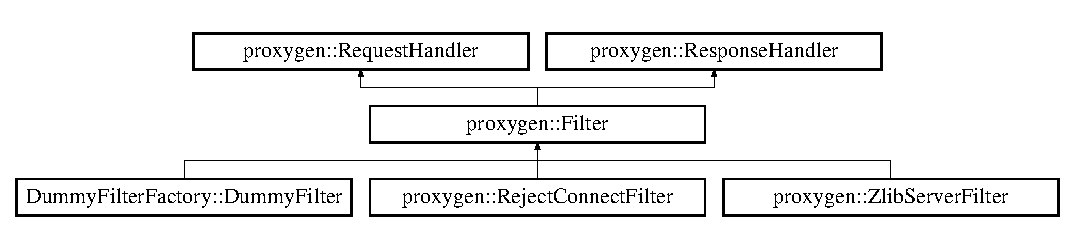
\includegraphics[height=2.666667cm]{classproxygen_1_1Filter}
\end{center}
\end{figure}
\subsection*{Public Member Functions}
\begin{DoxyCompactItemize}
\item 
{\bf Filter} ({\bf Request\+Handler} $\ast$upstream)
\item 
void {\bf set\+Response\+Handler} ({\bf Response\+Handler} $\ast$handler) noexceptoverride
\item 
void {\bf on\+Request} (std\+::unique\+\_\+ptr$<$ {\bf H\+T\+T\+P\+Message} $>$ headers) noexceptoverride
\item 
void {\bf on\+Body} (std\+::unique\+\_\+ptr$<$ folly\+::\+I\+O\+Buf $>$ body) noexceptoverride
\item 
void {\bf on\+Upgrade} ({\bf Upgrade\+Protocol} protocol) noexceptoverride
\item 
void {\bf on\+E\+OM} () noexceptoverride
\item 
void {\bf request\+Complete} () noexceptoverride
\item 
void {\bf on\+Error} ({\bf Proxygen\+Error} err) noexceptoverride
\item 
void {\bf on\+Egress\+Paused} () noexceptoverride
\item 
void {\bf on\+Egress\+Resumed} () noexceptoverride
\item 
bool {\bf can\+Handle\+Expect} () noexceptoverride
\item 
{\bf Ex\+Message\+Handler} $\ast$ {\bf get\+Ex\+Handler} () noexceptoverride
\item 
void {\bf send\+Headers} ({\bf H\+T\+T\+P\+Message} \&msg) noexceptoverride
\item 
void {\bf send\+Chunk\+Header} (size\+\_\+t len) noexceptoverride
\item 
void {\bf send\+Body} (std\+::unique\+\_\+ptr$<$ folly\+::\+I\+O\+Buf $>$ body) noexceptoverride
\item 
void {\bf send\+Chunk\+Terminator} () noexceptoverride
\item 
void {\bf send\+E\+OM} () noexceptoverride
\item 
void {\bf send\+Abort} () noexceptoverride
\item 
void {\bf refresh\+Timeout} () noexceptoverride
\item 
void {\bf pause\+Ingress} () noexceptoverride
\item 
void {\bf resume\+Ingress} () noexceptoverride
\item 
{\bf Response\+Handler} $\ast$ {\bf new\+Pushed\+Response} ({\bf Push\+Handler} $\ast$handler) noexceptoverride
\item 
const wangle\+::\+Transport\+Info \& {\bf get\+Setup\+Transport\+Info} () const noexceptoverride
\item 
void {\bf get\+Current\+Transport\+Info} (wangle\+::\+Transport\+Info $\ast$tinfo) const override
\end{DoxyCompactItemize}
\subsection*{Additional Inherited Members}


\subsection{Detailed Description}
Filters are a way to add functionality to \doxyref{H\+T\+T\+P\+Server}{p.}{classproxygen_1_1HTTPServer} without complicating app specific \doxyref{Request\+Handler}{p.}{classproxygen_1_1RequestHandler}. The basic idea is

App-\/handler $<$=$>$ Filter-\/1 $<$=$>$ Filter-\/2 $<$=$>$ Client

The data flows through these filters between client and handler. They can do things like modify the data flowing through them, can update stats, create traces and even send direct response if they feel like.

The default implementation just lets everything pass through. 

Definition at line 29 of file Filters.\+h.



\subsection{Constructor \& Destructor Documentation}
\index{proxygen\+::\+Filter@{proxygen\+::\+Filter}!Filter@{Filter}}
\index{Filter@{Filter}!proxygen\+::\+Filter@{proxygen\+::\+Filter}}
\subsubsection[{Filter(\+Request\+Handler $\ast$upstream)}]{\setlength{\rightskip}{0pt plus 5cm}proxygen\+::\+Filter\+::\+Filter (
\begin{DoxyParamCaption}
\item[{{\bf Request\+Handler} $\ast$}]{upstream}
\end{DoxyParamCaption}
)\hspace{0.3cm}{\ttfamily [inline]}, {\ttfamily [explicit]}}\label{classproxygen_1_1Filter_af8eeab2d700b69642731a34e5b063d20}


Definition at line 31 of file Filters.\+h.


\begin{DoxyCode}
32       : ResponseHandler(upstream) \{
33   \}
\end{DoxyCode}


\subsection{Member Function Documentation}
\index{proxygen\+::\+Filter@{proxygen\+::\+Filter}!can\+Handle\+Expect@{can\+Handle\+Expect}}
\index{can\+Handle\+Expect@{can\+Handle\+Expect}!proxygen\+::\+Filter@{proxygen\+::\+Filter}}
\subsubsection[{can\+Handle\+Expect() noexceptoverride}]{\setlength{\rightskip}{0pt plus 5cm}bool proxygen\+::\+Filter\+::can\+Handle\+Expect (
\begin{DoxyParamCaption}
{}
\end{DoxyParamCaption}
)\hspace{0.3cm}{\ttfamily [inline]}, {\ttfamily [override]}, {\ttfamily [virtual]}, {\ttfamily [noexcept]}}\label{classproxygen_1_1Filter_a32ea4520f3f16444c0538fa65b2726b3}
Returns true if the handler is responsible for responding to Expect headers, false otherwise. 

Reimplemented from {\bf proxygen\+::\+Request\+Handler} \doxyref{}{p.}{classproxygen_1_1RequestHandler_ad632dd51c75e6d27558fae7bf850239d}.



Definition at line 79 of file Filters.\+h.



References proxygen\+::\+Request\+Handler\+::can\+Handle\+Expect(), and proxygen\+::\+Response\+Handler\+::upstream\+\_\+.


\begin{DoxyCode}
79                                            \{
80     \textcolor{keywordflow}{return} upstream_->canHandleExpect();
81   \}
\end{DoxyCode}
\index{proxygen\+::\+Filter@{proxygen\+::\+Filter}!get\+Current\+Transport\+Info@{get\+Current\+Transport\+Info}}
\index{get\+Current\+Transport\+Info@{get\+Current\+Transport\+Info}!proxygen\+::\+Filter@{proxygen\+::\+Filter}}
\subsubsection[{get\+Current\+Transport\+Info(wangle\+::\+Transport\+Info $\ast$tinfo) const override}]{\setlength{\rightskip}{0pt plus 5cm}void proxygen\+::\+Filter\+::get\+Current\+Transport\+Info (
\begin{DoxyParamCaption}
\item[{wangle\+::\+Transport\+Info $\ast$}]{tinfo}
\end{DoxyParamCaption}
) const\hspace{0.3cm}{\ttfamily [inline]}, {\ttfamily [override]}, {\ttfamily [virtual]}}\label{classproxygen_1_1Filter_adfe01b2f566951c8022ae0bc8f051cc6}


Implements {\bf proxygen\+::\+Response\+Handler} \doxyref{}{p.}{classproxygen_1_1ResponseHandler_a90940a302d830ed0eebfc993c2b176f2}.



Definition at line 132 of file Filters.\+h.



References proxygen\+::\+Request\+Handler\+::downstream\+\_\+, and proxygen\+::\+Response\+Handler\+::get\+Current\+Transport\+Info().


\begin{DoxyCode}
132                                                                           \{
133     downstream_->getCurrentTransportInfo(tinfo);
134   \}
\end{DoxyCode}
\index{proxygen\+::\+Filter@{proxygen\+::\+Filter}!get\+Ex\+Handler@{get\+Ex\+Handler}}
\index{get\+Ex\+Handler@{get\+Ex\+Handler}!proxygen\+::\+Filter@{proxygen\+::\+Filter}}
\subsubsection[{get\+Ex\+Handler() noexceptoverride}]{\setlength{\rightskip}{0pt plus 5cm}{\bf Ex\+Message\+Handler}$\ast$ proxygen\+::\+Filter\+::get\+Ex\+Handler (
\begin{DoxyParamCaption}
{}
\end{DoxyParamCaption}
)\hspace{0.3cm}{\ttfamily [inline]}, {\ttfamily [override]}, {\ttfamily [virtual]}, {\ttfamily [noexcept]}}\label{classproxygen_1_1Filter_acbd6d5206633c61ef385d4a2dbc04a75}
Implement in control stream handler to support incoming child EX streams. 

Reimplemented from {\bf proxygen\+::\+Request\+Handler} \doxyref{}{p.}{classproxygen_1_1RequestHandler_a6131d21f1a673ce0d37fa61af8aa5733}.



Definition at line 83 of file Filters.\+h.



References proxygen\+::\+Request\+Handler\+::get\+Ex\+Handler(), and proxygen\+::\+Response\+Handler\+::upstream\+\_\+.


\begin{DoxyCode}
83                                                      \{
84     \textcolor{keywordflow}{return} upstream_->getExHandler();
85   \}
\end{DoxyCode}
\index{proxygen\+::\+Filter@{proxygen\+::\+Filter}!get\+Setup\+Transport\+Info@{get\+Setup\+Transport\+Info}}
\index{get\+Setup\+Transport\+Info@{get\+Setup\+Transport\+Info}!proxygen\+::\+Filter@{proxygen\+::\+Filter}}
\subsubsection[{get\+Setup\+Transport\+Info() const noexceptoverride}]{\setlength{\rightskip}{0pt plus 5cm}const wangle\+::\+Transport\+Info\& proxygen\+::\+Filter\+::get\+Setup\+Transport\+Info (
\begin{DoxyParamCaption}
{}
\end{DoxyParamCaption}
) const\hspace{0.3cm}{\ttfamily [inline]}, {\ttfamily [override]}, {\ttfamily [virtual]}, {\ttfamily [noexcept]}}\label{classproxygen_1_1Filter_a8f1d64f6b73c879c4ba7a0e89a0eca91}


Implements {\bf proxygen\+::\+Response\+Handler} \doxyref{}{p.}{classproxygen_1_1ResponseHandler_aeceafc15bb87a0c4dce1c6ea3a6274a1}.



Definition at line 128 of file Filters.\+h.



References proxygen\+::\+Request\+Handler\+::downstream\+\_\+, and proxygen\+::\+Response\+Handler\+::get\+Setup\+Transport\+Info().


\begin{DoxyCode}
128                                                                              \{
129     \textcolor{keywordflow}{return} downstream_->getSetupTransportInfo();
130   \}
\end{DoxyCode}
\index{proxygen\+::\+Filter@{proxygen\+::\+Filter}!new\+Pushed\+Response@{new\+Pushed\+Response}}
\index{new\+Pushed\+Response@{new\+Pushed\+Response}!proxygen\+::\+Filter@{proxygen\+::\+Filter}}
\subsubsection[{new\+Pushed\+Response(\+Push\+Handler $\ast$handler) noexceptoverride}]{\setlength{\rightskip}{0pt plus 5cm}{\bf Response\+Handler}$\ast$ proxygen\+::\+Filter\+::new\+Pushed\+Response (
\begin{DoxyParamCaption}
\item[{{\bf Push\+Handler} $\ast$}]{handler}
\end{DoxyParamCaption}
)\hspace{0.3cm}{\ttfamily [inline]}, {\ttfamily [override]}, {\ttfamily [virtual]}, {\ttfamily [noexcept]}}\label{classproxygen_1_1Filter_aed159f5c492839867ac16cdc65e6f57a}


Implements {\bf proxygen\+::\+Response\+Handler} \doxyref{}{p.}{classproxygen_1_1ResponseHandler_a43a4028a9b826ba81f77ce38134d1584}.



Definition at line 124 of file Filters.\+h.



References proxygen\+::\+Request\+Handler\+::downstream\+\_\+, and proxygen\+::\+Response\+Handler\+::new\+Pushed\+Response().


\begin{DoxyCode}
124                                                                              \{
125     \textcolor{keywordflow}{return} downstream_->newPushedResponse(handler);
126   \}
\end{DoxyCode}
\index{proxygen\+::\+Filter@{proxygen\+::\+Filter}!on\+Body@{on\+Body}}
\index{on\+Body@{on\+Body}!proxygen\+::\+Filter@{proxygen\+::\+Filter}}
\subsubsection[{on\+Body(std\+::unique\+\_\+ptr$<$ folly\+::\+I\+O\+Buf $>$ body) noexceptoverride}]{\setlength{\rightskip}{0pt plus 5cm}void proxygen\+::\+Filter\+::on\+Body (
\begin{DoxyParamCaption}
\item[{std\+::unique\+\_\+ptr$<$ folly\+::\+I\+O\+Buf $>$}]{body}
\end{DoxyParamCaption}
)\hspace{0.3cm}{\ttfamily [inline]}, {\ttfamily [override]}, {\ttfamily [virtual]}, {\ttfamily [noexcept]}}\label{classproxygen_1_1Filter_a98e803dd89a7bfc644e82c641555dfe0}
Invoked when we get part of body for the request. 

Implements {\bf proxygen\+::\+Request\+Handler} \doxyref{}{p.}{classproxygen_1_1RequestHandler_aaf0ed3bb94384e6240e15cca63de82bb}.



Definition at line 47 of file Filters.\+h.



References proxygen\+::\+Request\+Handler\+::on\+Body(), and proxygen\+::\+Response\+Handler\+::upstream\+\_\+.


\begin{DoxyCode}
47                                                                 \{
48     upstream_->onBody(std::move(body));
49   \}
\end{DoxyCode}
\index{proxygen\+::\+Filter@{proxygen\+::\+Filter}!on\+Egress\+Paused@{on\+Egress\+Paused}}
\index{on\+Egress\+Paused@{on\+Egress\+Paused}!proxygen\+::\+Filter@{proxygen\+::\+Filter}}
\subsubsection[{on\+Egress\+Paused() noexceptoverride}]{\setlength{\rightskip}{0pt plus 5cm}void proxygen\+::\+Filter\+::on\+Egress\+Paused (
\begin{DoxyParamCaption}
{}
\end{DoxyParamCaption}
)\hspace{0.3cm}{\ttfamily [inline]}, {\ttfamily [override]}, {\ttfamily [virtual]}, {\ttfamily [noexcept]}}\label{classproxygen_1_1Filter_af8a97efa470810e7bad65fc51f1d3559}
Signals from H\+T\+TP layer when client queue is full or empty. If you are sending a streaming response, consider implementing these and acting accordingly. Saves your server from running out of memory. 

Reimplemented from {\bf proxygen\+::\+Request\+Handler} \doxyref{}{p.}{classproxygen_1_1RequestHandler_a2791a2a46b57712ad177116d43fbc8e3}.



Definition at line 71 of file Filters.\+h.



References proxygen\+::\+Request\+Handler\+::on\+Egress\+Paused(), and proxygen\+::\+Response\+Handler\+::upstream\+\_\+.


\begin{DoxyCode}
71                                           \{
72     upstream_->onEgressPaused();
73   \}
\end{DoxyCode}
\index{proxygen\+::\+Filter@{proxygen\+::\+Filter}!on\+Egress\+Resumed@{on\+Egress\+Resumed}}
\index{on\+Egress\+Resumed@{on\+Egress\+Resumed}!proxygen\+::\+Filter@{proxygen\+::\+Filter}}
\subsubsection[{on\+Egress\+Resumed() noexceptoverride}]{\setlength{\rightskip}{0pt plus 5cm}void proxygen\+::\+Filter\+::on\+Egress\+Resumed (
\begin{DoxyParamCaption}
{}
\end{DoxyParamCaption}
)\hspace{0.3cm}{\ttfamily [inline]}, {\ttfamily [override]}, {\ttfamily [virtual]}, {\ttfamily [noexcept]}}\label{classproxygen_1_1Filter_acf857f65ceeac0b3c9c8e0a1efe79d22}


Reimplemented from {\bf proxygen\+::\+Request\+Handler} \doxyref{}{p.}{classproxygen_1_1RequestHandler_a8128e8661fa526a6d10fd9c03dbe4dc3}.



Definition at line 75 of file Filters.\+h.



References proxygen\+::\+Request\+Handler\+::on\+Egress\+Resumed(), and proxygen\+::\+Response\+Handler\+::upstream\+\_\+.


\begin{DoxyCode}
75                                            \{
76     upstream_->onEgressResumed();
77   \}
\end{DoxyCode}
\index{proxygen\+::\+Filter@{proxygen\+::\+Filter}!on\+E\+OM@{on\+E\+OM}}
\index{on\+E\+OM@{on\+E\+OM}!proxygen\+::\+Filter@{proxygen\+::\+Filter}}
\subsubsection[{on\+E\+O\+M() noexceptoverride}]{\setlength{\rightskip}{0pt plus 5cm}void proxygen\+::\+Filter\+::on\+E\+OM (
\begin{DoxyParamCaption}
{}
\end{DoxyParamCaption}
)\hspace{0.3cm}{\ttfamily [inline]}, {\ttfamily [override]}, {\ttfamily [virtual]}, {\ttfamily [noexcept]}}\label{classproxygen_1_1Filter_a9cbe8f047a67bafe605ffdb960ae8daf}
Invoked when we finish receiving the body. 

Implements {\bf proxygen\+::\+Request\+Handler} \doxyref{}{p.}{classproxygen_1_1RequestHandler_a24f26d2cf71effaf154ce53aeff51aab}.



Definition at line 55 of file Filters.\+h.



References proxygen\+::\+Request\+Handler\+::on\+E\+O\+M(), and proxygen\+::\+Response\+Handler\+::upstream\+\_\+.


\begin{DoxyCode}
55                                  \{
56     upstream_->onEOM();
57   \}
\end{DoxyCode}
\index{proxygen\+::\+Filter@{proxygen\+::\+Filter}!on\+Error@{on\+Error}}
\index{on\+Error@{on\+Error}!proxygen\+::\+Filter@{proxygen\+::\+Filter}}
\subsubsection[{on\+Error(\+Proxygen\+Error err) noexceptoverride}]{\setlength{\rightskip}{0pt plus 5cm}void proxygen\+::\+Filter\+::on\+Error (
\begin{DoxyParamCaption}
\item[{{\bf Proxygen\+Error}}]{err}
\end{DoxyParamCaption}
)\hspace{0.3cm}{\ttfamily [inline]}, {\ttfamily [override]}, {\ttfamily [virtual]}, {\ttfamily [noexcept]}}\label{classproxygen_1_1Filter_accfdfae779e41ca7624148910e9254a0}
Request failed. Maybe because of read/write error on socket or client not being able to send request in time.

N\+O\+TE\+: Can be invoked at any time (except for before on\+Request).

No more callbacks will be invoked after this. You should clean up after yourself. 

Implements {\bf proxygen\+::\+Request\+Handler} \doxyref{}{p.}{classproxygen_1_1RequestHandler_ad7e6428b925840a334adc58ff6f4f680}.



Definition at line 65 of file Filters.\+h.



References proxygen\+::\+Request\+Handler\+::downstream\+\_\+, proxygen\+::\+Request\+Handler\+::on\+Error(), and proxygen\+::\+Response\+Handler\+::upstream\+\_\+.


\begin{DoxyCode}
65                                                     \{
66     downstream_ = \textcolor{keyword}{nullptr};
67     upstream_->onError(err);
68     \textcolor{keyword}{delete} \textcolor{keyword}{this};
69   \}
\end{DoxyCode}
\index{proxygen\+::\+Filter@{proxygen\+::\+Filter}!on\+Request@{on\+Request}}
\index{on\+Request@{on\+Request}!proxygen\+::\+Filter@{proxygen\+::\+Filter}}
\subsubsection[{on\+Request(std\+::unique\+\_\+ptr$<$ H\+T\+T\+P\+Message $>$ headers) noexceptoverride}]{\setlength{\rightskip}{0pt plus 5cm}void proxygen\+::\+Filter\+::on\+Request (
\begin{DoxyParamCaption}
\item[{std\+::unique\+\_\+ptr$<$ {\bf H\+T\+T\+P\+Message} $>$}]{headers}
\end{DoxyParamCaption}
)\hspace{0.3cm}{\ttfamily [inline]}, {\ttfamily [override]}, {\ttfamily [virtual]}, {\ttfamily [noexcept]}}\label{classproxygen_1_1Filter_aae05166bfb13752325073d4427a8ed34}
Invoked when we have successfully fetched headers from client. This will always be the first callback invoked on your handler. 

Implements {\bf proxygen\+::\+Request\+Handler} \doxyref{}{p.}{classproxygen_1_1RequestHandler_a61f59e1155f906c7b73062147164320f}.



Definition at line 43 of file Filters.\+h.



References proxygen\+::\+Request\+Handler\+::on\+Request(), and proxygen\+::\+Response\+Handler\+::upstream\+\_\+.


\begin{DoxyCode}
43                                                                        \{
44     upstream_->onRequest(std::move(headers));
45   \}
\end{DoxyCode}
\index{proxygen\+::\+Filter@{proxygen\+::\+Filter}!on\+Upgrade@{on\+Upgrade}}
\index{on\+Upgrade@{on\+Upgrade}!proxygen\+::\+Filter@{proxygen\+::\+Filter}}
\subsubsection[{on\+Upgrade(\+Upgrade\+Protocol protocol) noexceptoverride}]{\setlength{\rightskip}{0pt plus 5cm}void proxygen\+::\+Filter\+::on\+Upgrade (
\begin{DoxyParamCaption}
\item[{{\bf Upgrade\+Protocol}}]{prot}
\end{DoxyParamCaption}
)\hspace{0.3cm}{\ttfamily [inline]}, {\ttfamily [override]}, {\ttfamily [virtual]}, {\ttfamily [noexcept]}}\label{classproxygen_1_1Filter_a3fafd5b5b4db26e7602110b3e60eb418}
Invoked when the session has been upgraded to a different protocol 

Implements {\bf proxygen\+::\+Request\+Handler} \doxyref{}{p.}{classproxygen_1_1RequestHandler_aefed2946bc5558baf6e36a2d11290b79}.



Definition at line 51 of file Filters.\+h.



References proxygen\+::\+Request\+Handler\+::on\+Upgrade(), and proxygen\+::\+Response\+Handler\+::upstream\+\_\+.


\begin{DoxyCode}
51                                                              \{
52     upstream_->onUpgrade(protocol);
53   \}
\end{DoxyCode}
\index{proxygen\+::\+Filter@{proxygen\+::\+Filter}!pause\+Ingress@{pause\+Ingress}}
\index{pause\+Ingress@{pause\+Ingress}!proxygen\+::\+Filter@{proxygen\+::\+Filter}}
\subsubsection[{pause\+Ingress() noexceptoverride}]{\setlength{\rightskip}{0pt plus 5cm}void proxygen\+::\+Filter\+::pause\+Ingress (
\begin{DoxyParamCaption}
{}
\end{DoxyParamCaption}
)\hspace{0.3cm}{\ttfamily [inline]}, {\ttfamily [override]}, {\ttfamily [virtual]}, {\ttfamily [noexcept]}}\label{classproxygen_1_1Filter_adbee2e0f11f96b7bf4807fbd34f255ad}


Implements {\bf proxygen\+::\+Response\+Handler} \doxyref{}{p.}{classproxygen_1_1ResponseHandler_afa9c9a5f7a64d98de012d35e344c6d98}.



Definition at line 116 of file Filters.\+h.



References proxygen\+::\+Request\+Handler\+::downstream\+\_\+, and proxygen\+::\+Response\+Handler\+::pause\+Ingress().


\begin{DoxyCode}
116                                         \{
117     downstream_->pauseIngress();
118   \}
\end{DoxyCode}
\index{proxygen\+::\+Filter@{proxygen\+::\+Filter}!refresh\+Timeout@{refresh\+Timeout}}
\index{refresh\+Timeout@{refresh\+Timeout}!proxygen\+::\+Filter@{proxygen\+::\+Filter}}
\subsubsection[{refresh\+Timeout() noexceptoverride}]{\setlength{\rightskip}{0pt plus 5cm}void proxygen\+::\+Filter\+::refresh\+Timeout (
\begin{DoxyParamCaption}
{}
\end{DoxyParamCaption}
)\hspace{0.3cm}{\ttfamily [inline]}, {\ttfamily [override]}, {\ttfamily [virtual]}, {\ttfamily [noexcept]}}\label{classproxygen_1_1Filter_abdb0592340eac2e25ed66472c243cfc8}


Implements {\bf proxygen\+::\+Response\+Handler} \doxyref{}{p.}{classproxygen_1_1ResponseHandler_a8b487f372085f391dc1a15a4fe5855cd}.



Definition at line 112 of file Filters.\+h.



References proxygen\+::\+Request\+Handler\+::downstream\+\_\+, and proxygen\+::\+Response\+Handler\+::refresh\+Timeout().


\begin{DoxyCode}
112                                           \{
113     downstream_->refreshTimeout();
114   \}
\end{DoxyCode}
\index{proxygen\+::\+Filter@{proxygen\+::\+Filter}!request\+Complete@{request\+Complete}}
\index{request\+Complete@{request\+Complete}!proxygen\+::\+Filter@{proxygen\+::\+Filter}}
\subsubsection[{request\+Complete() noexceptoverride}]{\setlength{\rightskip}{0pt plus 5cm}void proxygen\+::\+Filter\+::request\+Complete (
\begin{DoxyParamCaption}
{}
\end{DoxyParamCaption}
)\hspace{0.3cm}{\ttfamily [inline]}, {\ttfamily [override]}, {\ttfamily [virtual]}, {\ttfamily [noexcept]}}\label{classproxygen_1_1Filter_ab075db9a9546d3bfa3affff60f5c468c}
Invoked when request processing has been completed and nothing more needs to be done. This may be a good place to log some stats and clean up resources. This is distinct from \doxyref{on\+E\+O\+M()}{p.}{classproxygen_1_1Filter_a9cbe8f047a67bafe605ffdb960ae8daf} because it is invoked after the response is fully sent. Once this callback has been received, {\ttfamily downstream\+\_\+} should be considered invalid. 

Implements {\bf proxygen\+::\+Request\+Handler} \doxyref{}{p.}{classproxygen_1_1RequestHandler_a0ec159751b407bcd3667994c6d8d7cfe}.



Definition at line 59 of file Filters.\+h.



References proxygen\+::\+Request\+Handler\+::downstream\+\_\+, proxygen\+::\+Request\+Handler\+::request\+Complete(), and proxygen\+::\+Response\+Handler\+::upstream\+\_\+.


\begin{DoxyCode}
59                                            \{
60     downstream_ = \textcolor{keyword}{nullptr};
61     upstream_->requestComplete();
62     \textcolor{keyword}{delete} \textcolor{keyword}{this};
63   \}
\end{DoxyCode}
\index{proxygen\+::\+Filter@{proxygen\+::\+Filter}!resume\+Ingress@{resume\+Ingress}}
\index{resume\+Ingress@{resume\+Ingress}!proxygen\+::\+Filter@{proxygen\+::\+Filter}}
\subsubsection[{resume\+Ingress() noexceptoverride}]{\setlength{\rightskip}{0pt plus 5cm}void proxygen\+::\+Filter\+::resume\+Ingress (
\begin{DoxyParamCaption}
{}
\end{DoxyParamCaption}
)\hspace{0.3cm}{\ttfamily [inline]}, {\ttfamily [override]}, {\ttfamily [virtual]}, {\ttfamily [noexcept]}}\label{classproxygen_1_1Filter_af14ff17b4684e908e8612579ce718706}


Implements {\bf proxygen\+::\+Response\+Handler} \doxyref{}{p.}{classproxygen_1_1ResponseHandler_af6bf0c68365230886b7d278821f87078}.



Definition at line 120 of file Filters.\+h.



References proxygen\+::\+Request\+Handler\+::downstream\+\_\+, and proxygen\+::\+Response\+Handler\+::resume\+Ingress().


\begin{DoxyCode}
120                                          \{
121     downstream_->resumeIngress();
122   \}
\end{DoxyCode}
\index{proxygen\+::\+Filter@{proxygen\+::\+Filter}!send\+Abort@{send\+Abort}}
\index{send\+Abort@{send\+Abort}!proxygen\+::\+Filter@{proxygen\+::\+Filter}}
\subsubsection[{send\+Abort() noexceptoverride}]{\setlength{\rightskip}{0pt plus 5cm}void proxygen\+::\+Filter\+::send\+Abort (
\begin{DoxyParamCaption}
{}
\end{DoxyParamCaption}
)\hspace{0.3cm}{\ttfamily [inline]}, {\ttfamily [override]}, {\ttfamily [virtual]}, {\ttfamily [noexcept]}}\label{classproxygen_1_1Filter_a4c7e63270b947317f421f09bde33b252}


Implements {\bf proxygen\+::\+Response\+Handler} \doxyref{}{p.}{classproxygen_1_1ResponseHandler_a3827b60bdfef24355756918c5b7ade26}.



Definition at line 108 of file Filters.\+h.



References proxygen\+::\+Request\+Handler\+::downstream\+\_\+, and proxygen\+::\+Response\+Handler\+::send\+Abort().



Referenced by proxygen\+::\+Zlib\+Server\+Filter\+::fail().


\begin{DoxyCode}
108                                      \{
109     downstream_->sendAbort();
110   \}
\end{DoxyCode}
\index{proxygen\+::\+Filter@{proxygen\+::\+Filter}!send\+Body@{send\+Body}}
\index{send\+Body@{send\+Body}!proxygen\+::\+Filter@{proxygen\+::\+Filter}}
\subsubsection[{send\+Body(std\+::unique\+\_\+ptr$<$ folly\+::\+I\+O\+Buf $>$ body) noexceptoverride}]{\setlength{\rightskip}{0pt plus 5cm}void proxygen\+::\+Filter\+::send\+Body (
\begin{DoxyParamCaption}
\item[{std\+::unique\+\_\+ptr$<$ folly\+::\+I\+O\+Buf $>$}]{body}
\end{DoxyParamCaption}
)\hspace{0.3cm}{\ttfamily [inline]}, {\ttfamily [override]}, {\ttfamily [virtual]}, {\ttfamily [noexcept]}}\label{classproxygen_1_1Filter_a13525ef7e5031fae0475e4b67d5497ff}


Implements {\bf proxygen\+::\+Response\+Handler} \doxyref{}{p.}{classproxygen_1_1ResponseHandler_ad2f61f6816fe12e96945fef5cdcd2228}.



Definition at line 96 of file Filters.\+h.



References proxygen\+::\+Request\+Handler\+::downstream\+\_\+, and proxygen\+::\+Response\+Handler\+::send\+Body().



Referenced by proxygen\+::\+Zlib\+Server\+Filter\+::send\+Body(), and proxygen\+::\+Zlib\+Server\+Filter\+::send\+E\+O\+M().


\begin{DoxyCode}
96                                                                   \{
97     downstream_->sendBody(std::move(body));
98   \}
\end{DoxyCode}
\index{proxygen\+::\+Filter@{proxygen\+::\+Filter}!send\+Chunk\+Header@{send\+Chunk\+Header}}
\index{send\+Chunk\+Header@{send\+Chunk\+Header}!proxygen\+::\+Filter@{proxygen\+::\+Filter}}
\subsubsection[{send\+Chunk\+Header(size\+\_\+t len) noexceptoverride}]{\setlength{\rightskip}{0pt plus 5cm}void proxygen\+::\+Filter\+::send\+Chunk\+Header (
\begin{DoxyParamCaption}
\item[{size\+\_\+t}]{len}
\end{DoxyParamCaption}
)\hspace{0.3cm}{\ttfamily [inline]}, {\ttfamily [override]}, {\ttfamily [virtual]}, {\ttfamily [noexcept]}}\label{classproxygen_1_1Filter_a52bdb3c0f7f88b796ba824e5d3230519}


Implements {\bf proxygen\+::\+Response\+Handler} \doxyref{}{p.}{classproxygen_1_1ResponseHandler_a37c5b3b070602f564d654cf016b35109}.



Definition at line 92 of file Filters.\+h.



References proxygen\+::\+Request\+Handler\+::downstream\+\_\+, and proxygen\+::\+Response\+Handler\+::send\+Chunk\+Header().



Referenced by proxygen\+::\+Zlib\+Server\+Filter\+::send\+Body(), proxygen\+::\+Zlib\+Server\+Filter\+::send\+Chunk\+Header(), and proxygen\+::\+Zlib\+Server\+Filter\+::send\+E\+O\+M().


\begin{DoxyCode}
92                                                      \{
93     downstream_->sendChunkHeader(len);
94   \}
\end{DoxyCode}
\index{proxygen\+::\+Filter@{proxygen\+::\+Filter}!send\+Chunk\+Terminator@{send\+Chunk\+Terminator}}
\index{send\+Chunk\+Terminator@{send\+Chunk\+Terminator}!proxygen\+::\+Filter@{proxygen\+::\+Filter}}
\subsubsection[{send\+Chunk\+Terminator() noexceptoverride}]{\setlength{\rightskip}{0pt plus 5cm}void proxygen\+::\+Filter\+::send\+Chunk\+Terminator (
\begin{DoxyParamCaption}
{}
\end{DoxyParamCaption}
)\hspace{0.3cm}{\ttfamily [inline]}, {\ttfamily [override]}, {\ttfamily [virtual]}, {\ttfamily [noexcept]}}\label{classproxygen_1_1Filter_a9804f149cdfaea4984b3b306f77de6de}


Implements {\bf proxygen\+::\+Response\+Handler} \doxyref{}{p.}{classproxygen_1_1ResponseHandler_a7b7faccdcf98892f64ebe01d8b3dd11c}.



Definition at line 100 of file Filters.\+h.



References proxygen\+::\+Request\+Handler\+::downstream\+\_\+, and proxygen\+::\+Response\+Handler\+::send\+Chunk\+Terminator().



Referenced by proxygen\+::\+Zlib\+Server\+Filter\+::send\+E\+O\+M().


\begin{DoxyCode}
100                                                \{
101     downstream_->sendChunkTerminator();
102   \}
\end{DoxyCode}
\index{proxygen\+::\+Filter@{proxygen\+::\+Filter}!send\+E\+OM@{send\+E\+OM}}
\index{send\+E\+OM@{send\+E\+OM}!proxygen\+::\+Filter@{proxygen\+::\+Filter}}
\subsubsection[{send\+E\+O\+M() noexceptoverride}]{\setlength{\rightskip}{0pt plus 5cm}void proxygen\+::\+Filter\+::send\+E\+OM (
\begin{DoxyParamCaption}
{}
\end{DoxyParamCaption}
)\hspace{0.3cm}{\ttfamily [inline]}, {\ttfamily [override]}, {\ttfamily [virtual]}, {\ttfamily [noexcept]}}\label{classproxygen_1_1Filter_a7ac8fec9b96805c396b49bec23e62708}


Implements {\bf proxygen\+::\+Response\+Handler} \doxyref{}{p.}{classproxygen_1_1ResponseHandler_af40d7a5c1674bea892d2598df9cfba61}.



Definition at line 104 of file Filters.\+h.



References proxygen\+::\+Request\+Handler\+::downstream\+\_\+, and proxygen\+::\+Response\+Handler\+::send\+E\+O\+M().



Referenced by proxygen\+::\+Zlib\+Server\+Filter\+::send\+E\+O\+M().


\begin{DoxyCode}
104                                    \{
105     downstream_->sendEOM();
106   \}
\end{DoxyCode}
\index{proxygen\+::\+Filter@{proxygen\+::\+Filter}!send\+Headers@{send\+Headers}}
\index{send\+Headers@{send\+Headers}!proxygen\+::\+Filter@{proxygen\+::\+Filter}}
\subsubsection[{send\+Headers(\+H\+T\+T\+P\+Message \&msg) noexceptoverride}]{\setlength{\rightskip}{0pt plus 5cm}void proxygen\+::\+Filter\+::send\+Headers (
\begin{DoxyParamCaption}
\item[{{\bf H\+T\+T\+P\+Message} \&}]{msg}
\end{DoxyParamCaption}
)\hspace{0.3cm}{\ttfamily [inline]}, {\ttfamily [override]}, {\ttfamily [virtual]}, {\ttfamily [noexcept]}}\label{classproxygen_1_1Filter_a46e5b86bf739ec744d58e4b88438a6f0}
N\+O\+TE\+: We take response message as non-\/const reference, to allow filters between your handler and client to be able to modify response if they want to.

eg. a compression filter might want to change the content-\/encoding 

Implements {\bf proxygen\+::\+Response\+Handler} \doxyref{}{p.}{classproxygen_1_1ResponseHandler_a20f98e57c8000a4af68483763f5fffb1}.



Definition at line 88 of file Filters.\+h.



References proxygen\+::\+Request\+Handler\+::downstream\+\_\+, and proxygen\+::\+Response\+Handler\+::send\+Headers().



Referenced by proxygen\+::\+Zlib\+Server\+Filter\+::send\+Body(), and proxygen\+::\+Zlib\+Server\+Filter\+::send\+Headers().


\begin{DoxyCode}
88                                                        \{
89     downstream_->sendHeaders(msg);
90   \}
\end{DoxyCode}
\index{proxygen\+::\+Filter@{proxygen\+::\+Filter}!set\+Response\+Handler@{set\+Response\+Handler}}
\index{set\+Response\+Handler@{set\+Response\+Handler}!proxygen\+::\+Filter@{proxygen\+::\+Filter}}
\subsubsection[{set\+Response\+Handler(\+Response\+Handler $\ast$handler) noexceptoverride}]{\setlength{\rightskip}{0pt plus 5cm}void proxygen\+::\+Filter\+::set\+Response\+Handler (
\begin{DoxyParamCaption}
\item[{{\bf Response\+Handler} $\ast$}]{handler}
\end{DoxyParamCaption}
)\hspace{0.3cm}{\ttfamily [inline]}, {\ttfamily [override]}, {\ttfamily [virtual]}, {\ttfamily [noexcept]}}\label{classproxygen_1_1Filter_af0e6c8e222e74c64b5acda58d64fb54f}
Saves the downstream handle with itself. Implementations of this interface should use downstream\+\_\+ to send back response.

X\+XX\+: Only override this method if you are A\+B\+S\+O\+L\+U\+T\+E\+LY sure what you are doing. If possible, just use downstream\+\_\+ variable and dont mess with these things. 

Reimplemented from {\bf proxygen\+::\+Request\+Handler} \doxyref{}{p.}{classproxygen_1_1RequestHandler_a7c3679aea96f2d5502c42a1254ea882f}.



Definition at line 36 of file Filters.\+h.



References proxygen\+::\+Request\+Handler\+::downstream\+\_\+, proxygen\+::\+Request\+Handler\+::set\+Response\+Handler(), proxygen\+::\+Response\+Handler\+::txn\+\_\+, and proxygen\+::\+Response\+Handler\+::upstream\+\_\+.


\begin{DoxyCode}
36                                                                       \{
37     \textcolor{comment}{// Save downstream handler and pass ourselves as downstream handler}
38     downstream_ = handler;
39     txn_ = handler->getTransaction();
40     upstream_->setResponseHandler(\textcolor{keyword}{this});
41   \}
\end{DoxyCode}


The documentation for this class was generated from the following file\+:\begin{DoxyCompactItemize}
\item 
proxygen/httpserver/{\bf Filters.\+h}\end{DoxyCompactItemize}

\section{proxygen\+:\+:Filter\+Chain$<$ T1, T2, Filter\+Type, set\+\_\+callback, Take\+Ownership $>$ Class Template Reference}
\label{classproxygen_1_1FilterChain}\index{proxygen\+::\+Filter\+Chain$<$ T1, T2, Filter\+Type, set\+\_\+callback, Take\+Ownership $>$@{proxygen\+::\+Filter\+Chain$<$ T1, T2, Filter\+Type, set\+\_\+callback, Take\+Ownership $>$}}


{\ttfamily \#include $<$Filter\+Chain.\+h$>$}

Inheritance diagram for proxygen\+:\+:Filter\+Chain$<$ T1, T2, Filter\+Type, set\+\_\+callback, Take\+Ownership $>$\+:\begin{figure}[H]
\begin{center}
\leavevmode
\includegraphics[height=2.000000cm]{classproxygen_1_1FilterChain}
\end{center}
\end{figure}
\subsection*{Public Types}
\begin{DoxyCompactItemize}
\item 
using {\bf Filter\+Chain\+Type} = {\bf Generic\+Filter}$<$ T1, T2, set\+\_\+callback, Take\+Ownership $>$
\end{DoxyCompactItemize}
\subsection*{Public Member Functions}
\begin{DoxyCompactItemize}
\item 
{\bf Filter\+Chain} (std\+::unique\+\_\+ptr$<$ T1 $>$ destination)
\item 
{\bf Filter\+Chain} (T1 $\ast$destination)
\item 
void {\bf set\+Callback} (T2 $\ast$cb) override
\item 
T1 $\ast$ {\bf call} ()
\item 
const T1 $\ast$ {\bf call} () const 
\item 
T1 $\ast$ {\bf get\+Chain\+End\+Ptr} ()
\item 
const T1 \& {\bf get\+Chain\+End} () const 
\item 
std\+::unique\+\_\+ptr$<$ T1 $>$ {\bf set\+Destination} (std\+::unique\+\_\+ptr$<$ T1 $>$ destination)
\item 
{\footnotesize template$<$typename C , typename C2 , typename... Types$>$ }\\std\+::enable\+\_\+if$<$ std\+::is\+\_\+constructible$<$ C $>$\+::value $>$\+::type {\bf add\+Filters} ()
\item 
{\footnotesize template$<$typename C $>$ }\\std\+::enable\+\_\+if$<$ std\+::is\+\_\+constructible$<$ C $>$\+::value $>$\+::type {\bf add\+Filters} ()
\item 
{\footnotesize template$<$typename C , typename... Types$>$ }\\void {\bf add\+Filters} (std\+::unique\+\_\+ptr$<$ C $>$ cur, Types \&\&...remaining)
\item 
{\footnotesize template$<$typename C , typename... Types$>$ }\\void {\bf add\+Filters} (C $\ast$cur, Types \&\&...remaining)
\item 
{\footnotesize template$<$typename C , typename... Args$>$ }\\{\bf Filter\+Chain}$<$ T1, T2, Filter\+Type, set\+\_\+callback, Take\+Ownership $>$ \& {\bf add} (Args \&\&...args)
\item 
const T1 $\ast$ {\bf operator-\/$>$} () const 
\item 
T1 $\ast$ {\bf operator-\/$>$} ()
\item 
void {\bf foreach} (folly\+::\+Function\+Ref$<$ void({\bf Filter\+Chain\+Type} $\ast$)$>$ fn)
\end{DoxyCompactItemize}
\subsection*{Private Member Functions}
\begin{DoxyCompactItemize}
\item 
void {\bf add\+Filters} ()
\end{DoxyCompactItemize}
\subsection*{Private Attributes}
\begin{DoxyCompactItemize}
\item 
T1 $\ast$ {\bf chain\+End\+\_\+}
\end{DoxyCompactItemize}


\subsection{Detailed Description}
\subsubsection*{template$<$typename T1, typename T2, typename Filter\+Type, void(\+T1\+::$\ast$)(\+T2 $\ast$) set\+\_\+callback, bool Take\+Ownership$>$\\*
class proxygen\+::\+Filter\+Chain$<$ T1, T2, Filter\+Type, set\+\_\+callback, Take\+Ownership $>$}

This class can be treated the same as a T1$\ast$, however internally it contains a chain of filters for T1 and T2. These filters are inserted between the original callback and destination.

If a filter does not care about one side of the calls, it will pass through the calls, saving a virtual function call. In the example below Filter1 only wants to intercept callbacks, and Filter2 only wants to intercept calls.

\begin{DoxyVerb} FilterChain        Filter1          Filter2        destination
_____________    _____________    _____________    _____________
|           |    |           |    |           |    |           |
|   call_------------------------>|   call_------->|"call"     | T1
|           |    |           |    |           |    |           |
\end{DoxyVerb}
 T2 $\vert$ callback\+\_\+ $\vert$$<$-\/-\/---callback\+\_\+ $\vert$$<$-\/-\/-\/-\/-\/-\/-\/-\/-\/-\/-\/-\/-\/-\/-\/-\/-\/---$\vert$\char`\"{}callback\char`\"{} $\vert$ $\vert$\+\_\+\+\_\+\+\_\+\+\_\+\+\_\+\+\_\+\+\_\+\+\_\+\+\_\+\+\_\+\+\_\+$\vert$ $\vert$\+\_\+\+\_\+\+\_\+\+\_\+\+\_\+\+\_\+\+\_\+\+\_\+\+\_\+\+\_\+\+\_\+$\vert$ $\vert$\+\_\+\+\_\+\+\_\+\+\_\+\+\_\+\+\_\+\+\_\+\+\_\+\+\_\+\+\_\+\+\_\+$\vert$ $\vert$\+\_\+\+\_\+\+\_\+\+\_\+\+\_\+\+\_\+\+\_\+\+\_\+\+\_\+\+\_\+\+\_\+$\vert$

This class is templatized on the two interfaces, T1, T2, as well as on the pass through filter implementation, Filter\+Type, the special set callback function, and a boolean indicating whether the chain owns the filters (if false, the filters must delete themselves at the correct time). Filter\+Type must have \doxyref{Generic\+Filter}{p.}{classproxygen_1_1GenericFilter} as an ancestor. 

Definition at line 207 of file Filter\+Chain.\+h.



\subsection{Member Typedef Documentation}
\index{proxygen\+::\+Filter\+Chain@{proxygen\+::\+Filter\+Chain}!Filter\+Chain\+Type@{Filter\+Chain\+Type}}
\index{Filter\+Chain\+Type@{Filter\+Chain\+Type}!proxygen\+::\+Filter\+Chain@{proxygen\+::\+Filter\+Chain}}
\subsubsection[{Filter\+Chain\+Type}]{\setlength{\rightskip}{0pt plus 5cm}template$<$typename T1, typename T2, typename Filter\+Type, void(\+T1\+::$\ast$)(\+T2 $\ast$) set\+\_\+callback, bool Take\+Ownership$>$ using {\bf proxygen\+::\+Filter\+Chain}$<$ T1, T2, Filter\+Type, set\+\_\+callback, Take\+Ownership $>$\+::{\bf Filter\+Chain\+Type} =  {\bf Generic\+Filter}$<$T1, T2, set\+\_\+callback, Take\+Ownership$>$}\label{classproxygen_1_1FilterChain_aaf56e3255f9f0290f5f0681f7cdf5d3e}


Definition at line 259 of file Filter\+Chain.\+h.



\subsection{Constructor \& Destructor Documentation}
\index{proxygen\+::\+Filter\+Chain@{proxygen\+::\+Filter\+Chain}!Filter\+Chain@{Filter\+Chain}}
\index{Filter\+Chain@{Filter\+Chain}!proxygen\+::\+Filter\+Chain@{proxygen\+::\+Filter\+Chain}}
\subsubsection[{Filter\+Chain(std\+::unique\+\_\+ptr$<$ T1 $>$ destination)}]{\setlength{\rightskip}{0pt plus 5cm}template$<$typename T1, typename T2, typename Filter\+Type, void(\+T1\+::$\ast$)(\+T2 $\ast$) set\+\_\+callback, bool Take\+Ownership$>$ {\bf proxygen\+::\+Filter\+Chain}$<$ T1, T2, Filter\+Type, set\+\_\+callback, Take\+Ownership $>$\+::{\bf Filter\+Chain} (
\begin{DoxyParamCaption}
\item[{std\+::unique\+\_\+ptr$<$ T1 $>$}]{destination}
\end{DoxyParamCaption}
)\hspace{0.3cm}{\ttfamily [inline]}, {\ttfamily [explicit]}}\label{classproxygen_1_1FilterChain_a0d2436218300bf51f2bb60204c8f4c1d}


Definition at line 209 of file Filter\+Chain.\+h.


\begin{DoxyCode}
209                                                      :
210       FilterType(\textcolor{keyword}{false}, \textcolor{keyword}{false}) \{
211     static\_assert(TakeOwnership, \textcolor{stringliteral}{"unique\_ptr constructor only available "}
212                   \textcolor{stringliteral}{"if the chain owns the filters."});
213     this->call\_ = CHECK\_NOTNULL(destination.release());
214     this->callback\_ = \textcolor{keyword}{nullptr}; \textcolor{comment}{//must call setCallback() explicitly}
215     this->callSource\_ = \textcolor{keyword}{this};
216     this->callbackSource\_ = this->call\_;
217     this->chainEnd_ = this->call\_;
218   \}
\end{DoxyCode}
\index{proxygen\+::\+Filter\+Chain@{proxygen\+::\+Filter\+Chain}!Filter\+Chain@{Filter\+Chain}}
\index{Filter\+Chain@{Filter\+Chain}!proxygen\+::\+Filter\+Chain@{proxygen\+::\+Filter\+Chain}}
\subsubsection[{Filter\+Chain(\+T1 $\ast$destination)}]{\setlength{\rightskip}{0pt plus 5cm}template$<$typename T1, typename T2, typename Filter\+Type, void(\+T1\+::$\ast$)(\+T2 $\ast$) set\+\_\+callback, bool Take\+Ownership$>$ {\bf proxygen\+::\+Filter\+Chain}$<$ T1, T2, Filter\+Type, set\+\_\+callback, Take\+Ownership $>$\+::{\bf Filter\+Chain} (
\begin{DoxyParamCaption}
\item[{T1 $\ast$}]{destination}
\end{DoxyParamCaption}
)\hspace{0.3cm}{\ttfamily [inline]}, {\ttfamily [explicit]}}\label{classproxygen_1_1FilterChain_a3cda65d09b99a401a49cef5805b4b607}


Definition at line 220 of file Filter\+Chain.\+h.


\begin{DoxyCode}
220                                        :
221       FilterType(\textcolor{keyword}{false}, \textcolor{keyword}{false}) \{
222     static\_assert(!TakeOwnership, \textcolor{stringliteral}{"raw pointer constructor only available "}
223                   \textcolor{stringliteral}{"if the chain doesn't own the filters."});
224     this->call\_ = CHECK\_NOTNULL(destination);
225     this->callback\_ = \textcolor{keyword}{nullptr}; \textcolor{comment}{//must call setCallback() explicitly}
226     this->callSource\_ = \textcolor{keyword}{this};
227     this->callbackSource\_ = this->call\_;
228     this->chainEnd_ = this->call\_;
229   \}
\end{DoxyCode}


\subsection{Member Function Documentation}
\index{proxygen\+::\+Filter\+Chain@{proxygen\+::\+Filter\+Chain}!add@{add}}
\index{add@{add}!proxygen\+::\+Filter\+Chain@{proxygen\+::\+Filter\+Chain}}
\subsubsection[{add(\+Args \&\&...\+args)}]{\setlength{\rightskip}{0pt plus 5cm}template$<$typename T1, typename T2, typename Filter\+Type, void(\+T1\+::$\ast$)(\+T2 $\ast$) set\+\_\+callback, bool Take\+Ownership$>$ template$<$typename C , typename... Args$>$ {\bf Filter\+Chain}$<$T1, T2, Filter\+Type, set\+\_\+callback, Take\+Ownership$>$\& {\bf proxygen\+::\+Filter\+Chain}$<$ T1, T2, Filter\+Type, set\+\_\+callback, Take\+Ownership $>$\+::add (
\begin{DoxyParamCaption}
\item[{Args \&\&...}]{args}
\end{DoxyParamCaption}
)\hspace{0.3cm}{\ttfamily [inline]}}\label{classproxygen_1_1FilterChain_a5c9a247735bddd41eff4c2795e889fc3}
Another way to add filters. This way is similar to \textquotesingle{}emplace\+\_\+front\textquotesingle{} and returns a reference to itself so you can chain \doxyref{add()}{p.}{classproxygen_1_1FilterChain_a5c9a247735bddd41eff4c2795e889fc3} calls if you like. 

Definition at line 341 of file Filter\+Chain.\+h.



Referenced by proxygen\+::\+H\+T\+T\+P\+Session\+::\+Write\+Segment\+::write\+Err().


\begin{DoxyCode}
341                       \{
342     this->append(\textcolor{keyword}{new} C(std::forward<Args>(args)...));
343     \textcolor{keywordflow}{return} *\textcolor{keyword}{this};
344   \}
\end{DoxyCode}
\index{proxygen\+::\+Filter\+Chain@{proxygen\+::\+Filter\+Chain}!add\+Filters@{add\+Filters}}
\index{add\+Filters@{add\+Filters}!proxygen\+::\+Filter\+Chain@{proxygen\+::\+Filter\+Chain}}
\subsubsection[{add\+Filters()}]{\setlength{\rightskip}{0pt plus 5cm}template$<$typename T1, typename T2, typename Filter\+Type, void(\+T1\+::$\ast$)(\+T2 $\ast$) set\+\_\+callback, bool Take\+Ownership$>$ template$<$typename C , typename C2 , typename... Types$>$ std\+::enable\+\_\+if$<$std\+::is\+\_\+constructible$<$C$>$\+::value$>$\+::type {\bf proxygen\+::\+Filter\+Chain}$<$ T1, T2, Filter\+Type, set\+\_\+callback, Take\+Ownership $>$\+::add\+Filters (
\begin{DoxyParamCaption}
{}
\end{DoxyParamCaption}
)\hspace{0.3cm}{\ttfamily [inline]}}\label{classproxygen_1_1FilterChain_a156f7de0f5af0dbddfe240c12d0ef27b}
Adds filters with the given types to the front of the chain. 

Definition at line 301 of file Filter\+Chain.\+h.



Referenced by proxygen\+::\+H\+T\+T\+P\+Session\+::setup\+Codec().


\begin{DoxyCode}
301                                                                       \{
302     \textcolor{comment}{// Callback <-> F1 <-> F2 ... <-> F\_new <-> Destination}
303     this->append(\textcolor{keyword}{new} C());
304     addFilters<C2, Types...>();
305   \}
\end{DoxyCode}
\index{proxygen\+::\+Filter\+Chain@{proxygen\+::\+Filter\+Chain}!add\+Filters@{add\+Filters}}
\index{add\+Filters@{add\+Filters}!proxygen\+::\+Filter\+Chain@{proxygen\+::\+Filter\+Chain}}
\subsubsection[{add\+Filters()}]{\setlength{\rightskip}{0pt plus 5cm}template$<$typename T1, typename T2, typename Filter\+Type, void(\+T1\+::$\ast$)(\+T2 $\ast$) set\+\_\+callback, bool Take\+Ownership$>$ template$<$typename C $>$ std\+::enable\+\_\+if$<$std\+::is\+\_\+constructible$<$C$>$\+::value$>$\+::type {\bf proxygen\+::\+Filter\+Chain}$<$ T1, T2, Filter\+Type, set\+\_\+callback, Take\+Ownership $>$\+::add\+Filters (
\begin{DoxyParamCaption}
{}
\end{DoxyParamCaption}
)\hspace{0.3cm}{\ttfamily [inline]}}\label{classproxygen_1_1FilterChain_a155a35b906e4169bf310197bbd09aaf7}
Base case of above function where we add a single filter. 

Definition at line 311 of file Filter\+Chain.\+h.


\begin{DoxyCode}
311                                                                       \{
312     this->append(\textcolor{keyword}{new} C());
313   \}
\end{DoxyCode}
\index{proxygen\+::\+Filter\+Chain@{proxygen\+::\+Filter\+Chain}!add\+Filters@{add\+Filters}}
\index{add\+Filters@{add\+Filters}!proxygen\+::\+Filter\+Chain@{proxygen\+::\+Filter\+Chain}}
\subsubsection[{add\+Filters(std\+::unique\+\_\+ptr$<$ C $>$ cur, Types \&\&...\+remaining)}]{\setlength{\rightskip}{0pt plus 5cm}template$<$typename T1, typename T2, typename Filter\+Type, void(\+T1\+::$\ast$)(\+T2 $\ast$) set\+\_\+callback, bool Take\+Ownership$>$ template$<$typename C , typename... Types$>$ void {\bf proxygen\+::\+Filter\+Chain}$<$ T1, T2, Filter\+Type, set\+\_\+callback, Take\+Ownership $>$\+::add\+Filters (
\begin{DoxyParamCaption}
\item[{std\+::unique\+\_\+ptr$<$ C $>$}]{cur, }
\item[{Types \&\&...}]{remaining}
\end{DoxyParamCaption}
)\hspace{0.3cm}{\ttfamily [inline]}}\label{classproxygen_1_1FilterChain_a9df273029c67b0a5805fb63f358a6877}
Adds already constructed filters (inside unique\+\_\+ptr) to the front of the chain. 

Definition at line 320 of file Filter\+Chain.\+h.


\begin{DoxyCode}
320                                                               \{
321     static\_assert(TakeOwnership, \textcolor{stringliteral}{"addFilters() can only take "}
322                   \textcolor{stringliteral}{"unique\_ptr if the chain owns the filters"});
323     this->append(cur.release());
324     addFilters(std::forward<Types>(remaining)...);
325   \}
\end{DoxyCode}
\index{proxygen\+::\+Filter\+Chain@{proxygen\+::\+Filter\+Chain}!add\+Filters@{add\+Filters}}
\index{add\+Filters@{add\+Filters}!proxygen\+::\+Filter\+Chain@{proxygen\+::\+Filter\+Chain}}
\subsubsection[{add\+Filters(\+C $\ast$cur, Types \&\&...\+remaining)}]{\setlength{\rightskip}{0pt plus 5cm}template$<$typename T1, typename T2, typename Filter\+Type, void(\+T1\+::$\ast$)(\+T2 $\ast$) set\+\_\+callback, bool Take\+Ownership$>$ template$<$typename C , typename... Types$>$ void {\bf proxygen\+::\+Filter\+Chain}$<$ T1, T2, Filter\+Type, set\+\_\+callback, Take\+Ownership $>$\+::add\+Filters (
\begin{DoxyParamCaption}
\item[{C $\ast$}]{cur, }
\item[{Types \&\&...}]{remaining}
\end{DoxyParamCaption}
)\hspace{0.3cm}{\ttfamily [inline]}}\label{classproxygen_1_1FilterChain_a79be8bc52c2f2541560d397ec627937b}


Definition at line 328 of file Filter\+Chain.\+h.


\begin{DoxyCode}
328                                                 \{
329     static\_assert(!TakeOwnership, \textcolor{stringliteral}{"addFilters() can only take "}
330                   \textcolor{stringliteral}{"pointers if the chain doesn't own the filters"});
331     this->append(cur);
332     addFilters(std::forward<Types>(remaining)...);
333   \}
\end{DoxyCode}
\index{proxygen\+::\+Filter\+Chain@{proxygen\+::\+Filter\+Chain}!add\+Filters@{add\+Filters}}
\index{add\+Filters@{add\+Filters}!proxygen\+::\+Filter\+Chain@{proxygen\+::\+Filter\+Chain}}
\subsubsection[{add\+Filters()}]{\setlength{\rightskip}{0pt plus 5cm}template$<$typename T1, typename T2, typename Filter\+Type, void(\+T1\+::$\ast$)(\+T2 $\ast$) set\+\_\+callback, bool Take\+Ownership$>$ void {\bf proxygen\+::\+Filter\+Chain}$<$ T1, T2, Filter\+Type, set\+\_\+callback, Take\+Ownership $>$\+::add\+Filters (
\begin{DoxyParamCaption}
{}
\end{DoxyParamCaption}
)\hspace{0.3cm}{\ttfamily [inline]}, {\ttfamily [private]}}\label{classproxygen_1_1FilterChain_a2c53b086f7f708560bd9c4f08eacbc26}
Base case for \doxyref{add\+Filters()}{p.}{classproxygen_1_1FilterChain_a156f7de0f5af0dbddfe240c12d0ef27b} called with no arguments. It doesn\textquotesingle{}t need to be public since trying to add zero filters doesn\textquotesingle{}t make sense from a public A\+PI pov. 

Definition at line 364 of file Filter\+Chain.\+h.


\begin{DoxyCode}
364 \{\}
\end{DoxyCode}
\index{proxygen\+::\+Filter\+Chain@{proxygen\+::\+Filter\+Chain}!call@{call}}
\index{call@{call}!proxygen\+::\+Filter\+Chain@{proxygen\+::\+Filter\+Chain}}
\subsubsection[{call()}]{\setlength{\rightskip}{0pt plus 5cm}template$<$typename T1, typename T2, typename Filter\+Type, void(\+T1\+::$\ast$)(\+T2 $\ast$) set\+\_\+callback, bool Take\+Ownership$>$ T1$\ast$ {\bf proxygen\+::\+Filter\+Chain}$<$ T1, T2, Filter\+Type, set\+\_\+callback, Take\+Ownership $>$\+::call (
\begin{DoxyParamCaption}
{}
\end{DoxyParamCaption}
)\hspace{0.3cm}{\ttfamily [inline]}}\label{classproxygen_1_1FilterChain_a097978132f89f0d76537a83daecfa960}
Returns the head of the call chain. Do$\ast$ not$\ast$ call T1\+::set\+\_\+callback() on this member. To change the callback of this entire filter chain, use the separate \doxyref{set\+Callback()}{p.}{classproxygen_1_1FilterChain_a26eec92e23c4bede04208d8996cad587} method. 

Definition at line 242 of file Filter\+Chain.\+h.



Referenced by proxygen\+::\+H\+T\+T\+P\+Session\+::setup\+Codec().


\begin{DoxyCode}
242              \{
243     \textcolor{keywordflow}{return} this->call\_;
244   \}
\end{DoxyCode}
\index{proxygen\+::\+Filter\+Chain@{proxygen\+::\+Filter\+Chain}!call@{call}}
\index{call@{call}!proxygen\+::\+Filter\+Chain@{proxygen\+::\+Filter\+Chain}}
\subsubsection[{call() const }]{\setlength{\rightskip}{0pt plus 5cm}template$<$typename T1, typename T2, typename Filter\+Type, void(\+T1\+::$\ast$)(\+T2 $\ast$) set\+\_\+callback, bool Take\+Ownership$>$ const T1$\ast$ {\bf proxygen\+::\+Filter\+Chain}$<$ T1, T2, Filter\+Type, set\+\_\+callback, Take\+Ownership $>$\+::call (
\begin{DoxyParamCaption}
{}
\end{DoxyParamCaption}
) const\hspace{0.3cm}{\ttfamily [inline]}}\label{classproxygen_1_1FilterChain_a049c1ee6b75eb199d7e4f24010408e69}


Definition at line 245 of file Filter\+Chain.\+h.


\begin{DoxyCode}
245                          \{
246     \textcolor{keywordflow}{return} this->call\_;
247   \}
\end{DoxyCode}
\index{proxygen\+::\+Filter\+Chain@{proxygen\+::\+Filter\+Chain}!foreach@{foreach}}
\index{foreach@{foreach}!proxygen\+::\+Filter\+Chain@{proxygen\+::\+Filter\+Chain}}
\subsubsection[{foreach(folly\+::\+Function\+Ref$<$ void(\+Filter\+Chain\+Type $\ast$)$>$ fn)}]{\setlength{\rightskip}{0pt plus 5cm}template$<$typename T1, typename T2, typename Filter\+Type, void(\+T1\+::$\ast$)(\+T2 $\ast$) set\+\_\+callback, bool Take\+Ownership$>$ void {\bf proxygen\+::\+Filter\+Chain}$<$ T1, T2, Filter\+Type, set\+\_\+callback, Take\+Ownership $>$\+::foreach (
\begin{DoxyParamCaption}
\item[{folly\+::\+Function\+Ref$<$ void({\bf Filter\+Chain\+Type} $\ast$)$>$}]{fn}
\end{DoxyParamCaption}
)\hspace{0.3cm}{\ttfamily [inline]}}\label{classproxygen_1_1FilterChain_ac59776e8ac9688af120db07adcd87702}


Definition at line 349 of file Filter\+Chain.\+h.



Referenced by proxygen\+::\+H\+T\+T\+P\+Upstream\+Session\+::attach\+Thread\+Locals().


\begin{DoxyCode}
349                                                             \{
350     \textcolor{keyword}{auto} cur = this->next\_;
351     \textcolor{keywordflow}{while} (cur) \{
352       \textcolor{keyword}{auto} filter = cur;
353       cur = cur->next\_;
354       fn(filter);
355     \}
356   \}
\end{DoxyCode}
\index{proxygen\+::\+Filter\+Chain@{proxygen\+::\+Filter\+Chain}!get\+Chain\+End@{get\+Chain\+End}}
\index{get\+Chain\+End@{get\+Chain\+End}!proxygen\+::\+Filter\+Chain@{proxygen\+::\+Filter\+Chain}}
\subsubsection[{get\+Chain\+End() const }]{\setlength{\rightskip}{0pt plus 5cm}template$<$typename T1, typename T2, typename Filter\+Type, void(\+T1\+::$\ast$)(\+T2 $\ast$) set\+\_\+callback, bool Take\+Ownership$>$ const T1\& {\bf proxygen\+::\+Filter\+Chain}$<$ T1, T2, Filter\+Type, set\+\_\+callback, Take\+Ownership $>$\+::get\+Chain\+End (
\begin{DoxyParamCaption}
{}
\end{DoxyParamCaption}
) const\hspace{0.3cm}{\ttfamily [inline]}}\label{classproxygen_1_1FilterChain_a24ef040a55410dd9a816f57cb795cb44}


Definition at line 255 of file Filter\+Chain.\+h.



Referenced by proxygen\+::\+H\+T\+T\+P\+Session\+::get\+Codec().


\begin{DoxyCode}
255                                 \{
256     \textcolor{keywordflow}{return} *chainEnd_;
257   \}
\end{DoxyCode}
\index{proxygen\+::\+Filter\+Chain@{proxygen\+::\+Filter\+Chain}!get\+Chain\+End\+Ptr@{get\+Chain\+End\+Ptr}}
\index{get\+Chain\+End\+Ptr@{get\+Chain\+End\+Ptr}!proxygen\+::\+Filter\+Chain@{proxygen\+::\+Filter\+Chain}}
\subsubsection[{get\+Chain\+End\+Ptr()}]{\setlength{\rightskip}{0pt plus 5cm}template$<$typename T1, typename T2, typename Filter\+Type, void(\+T1\+::$\ast$)(\+T2 $\ast$) set\+\_\+callback, bool Take\+Ownership$>$ T1$\ast$ {\bf proxygen\+::\+Filter\+Chain}$<$ T1, T2, Filter\+Type, set\+\_\+callback, Take\+Ownership $>$\+::get\+Chain\+End\+Ptr (
\begin{DoxyParamCaption}
{}
\end{DoxyParamCaption}
)\hspace{0.3cm}{\ttfamily [inline]}}\label{classproxygen_1_1FilterChain_a251a79f705fb5341d440765921afdce7}
Returns the concrete implementation at the end of the filter chain. 

Definition at line 252 of file Filter\+Chain.\+h.



Referenced by proxygen\+::\+H\+T\+T\+P\+Session\+Base\+::init\+Codec\+Header\+Indexing\+Strategy().


\begin{DoxyCode}
252                        \{
253     \textcolor{keywordflow}{return} chainEnd_;
254   \}
\end{DoxyCode}
\index{proxygen\+::\+Filter\+Chain@{proxygen\+::\+Filter\+Chain}!operator-\/$>$@{operator-\/$>$}}
\index{operator-\/$>$@{operator-\/$>$}!proxygen\+::\+Filter\+Chain@{proxygen\+::\+Filter\+Chain}}
\subsubsection[{operator-\/$>$() const }]{\setlength{\rightskip}{0pt plus 5cm}template$<$typename T1, typename T2, typename Filter\+Type, void(\+T1\+::$\ast$)(\+T2 $\ast$) set\+\_\+callback, bool Take\+Ownership$>$ const T1$\ast$ {\bf proxygen\+::\+Filter\+Chain}$<$ T1, T2, Filter\+Type, set\+\_\+callback, Take\+Ownership $>$\+::operator-\/$>$ (
\begin{DoxyParamCaption}
{}
\end{DoxyParamCaption}
) const\hspace{0.3cm}{\ttfamily [inline]}}\label{classproxygen_1_1FilterChain_a840801ed50699b36795986469a063d4f}


Definition at line 346 of file Filter\+Chain.\+h.


\begin{DoxyCode}
346 \{ \textcolor{keywordflow}{return} call(); \}
\end{DoxyCode}
\index{proxygen\+::\+Filter\+Chain@{proxygen\+::\+Filter\+Chain}!operator-\/$>$@{operator-\/$>$}}
\index{operator-\/$>$@{operator-\/$>$}!proxygen\+::\+Filter\+Chain@{proxygen\+::\+Filter\+Chain}}
\subsubsection[{operator-\/$>$()}]{\setlength{\rightskip}{0pt plus 5cm}template$<$typename T1, typename T2, typename Filter\+Type, void(\+T1\+::$\ast$)(\+T2 $\ast$) set\+\_\+callback, bool Take\+Ownership$>$ T1$\ast$ {\bf proxygen\+::\+Filter\+Chain}$<$ T1, T2, Filter\+Type, set\+\_\+callback, Take\+Ownership $>$\+::operator-\/$>$ (
\begin{DoxyParamCaption}
{}
\end{DoxyParamCaption}
)\hspace{0.3cm}{\ttfamily [inline]}}\label{classproxygen_1_1FilterChain_a97e45693befbef8b771d8cc5be1ef80c}


Definition at line 347 of file Filter\+Chain.\+h.


\begin{DoxyCode}
347 \{ \textcolor{keywordflow}{return} call(); \}
\end{DoxyCode}
\index{proxygen\+::\+Filter\+Chain@{proxygen\+::\+Filter\+Chain}!set\+Callback@{set\+Callback}}
\index{set\+Callback@{set\+Callback}!proxygen\+::\+Filter\+Chain@{proxygen\+::\+Filter\+Chain}}
\subsubsection[{set\+Callback(\+T2 $\ast$cb) override}]{\setlength{\rightskip}{0pt plus 5cm}template$<$typename T1, typename T2, typename Filter\+Type, void(\+T1\+::$\ast$)(\+T2 $\ast$) set\+\_\+callback, bool Take\+Ownership$>$ void {\bf proxygen\+::\+Filter\+Chain}$<$ T1, T2, Filter\+Type, set\+\_\+callback, Take\+Ownership $>$\+::set\+Callback (
\begin{DoxyParamCaption}
\item[{T2 $\ast$}]{cb}
\end{DoxyParamCaption}
)\hspace{0.3cm}{\ttfamily [inline]}, {\ttfamily [override]}}\label{classproxygen_1_1FilterChain_a26eec92e23c4bede04208d8996cad587}
Set the callback for this entire filter chain. Setting this to null will uninstall the callback from the concrete object at the end of the chain. 

Definition at line 235 of file Filter\+Chain.\+h.



Referenced by proxygen\+::\+H\+T\+T\+P\+Session\+::setup\+Codec().


\begin{DoxyCode}
235 \{ this->setCallbackInternalImpl(cb, cb); \}
\end{DoxyCode}
\index{proxygen\+::\+Filter\+Chain@{proxygen\+::\+Filter\+Chain}!set\+Destination@{set\+Destination}}
\index{set\+Destination@{set\+Destination}!proxygen\+::\+Filter\+Chain@{proxygen\+::\+Filter\+Chain}}
\subsubsection[{set\+Destination(std\+::unique\+\_\+ptr$<$ T1 $>$ destination)}]{\setlength{\rightskip}{0pt plus 5cm}template$<$typename T1, typename T2, typename Filter\+Type, void(\+T1\+::$\ast$)(\+T2 $\ast$) set\+\_\+callback, bool Take\+Ownership$>$ std\+::unique\+\_\+ptr$<$T1$>$ {\bf proxygen\+::\+Filter\+Chain}$<$ T1, T2, Filter\+Type, set\+\_\+callback, Take\+Ownership $>$\+::set\+Destination (
\begin{DoxyParamCaption}
\item[{std\+::unique\+\_\+ptr$<$ T1 $>$}]{destination}
\end{DoxyParamCaption}
)\hspace{0.3cm}{\ttfamily [inline]}}\label{classproxygen_1_1FilterChain_a9fb71919f20e105649530b95a3170b8f}


Definition at line 260 of file Filter\+Chain.\+h.



Referenced by proxygen\+::\+H\+T\+T\+P\+Session\+::on\+Native\+Protocol\+Upgrade\+Impl().


\begin{DoxyCode}
260                                                                   \{
261     static\_assert(TakeOwnership, \textcolor{stringliteral}{"unique\_ptr setDestination only available "}
262                   \textcolor{stringliteral}{"if the chain owns the filters."});
263     \textcolor{comment}{// find the last filter in the chain, and the last filter that wants calls,}
264     \textcolor{comment}{// callbacks}
265     FilterChainType* lastFilter = \textcolor{keyword}{this};
266     FilterChainType* lastCall = \textcolor{keyword}{this};
267     FilterChainType* lastCallback = \textcolor{keyword}{this};
268     \textcolor{keywordflow}{while} (lastFilter->next\_) \{
269       \textcolor{keywordflow}{if} (lastFilter->kWantsCalls\_) \{
270         lastCall = lastFilter;
271       \}
272       \textcolor{keywordflow}{if} (lastFilter->kWantsCallbacks\_) \{
273         lastCallback = lastFilter;
274       \}
275       \textcolor{keywordflow}{if} (lastFilter->call\_ == this->chainEnd\_) \{
276         \textcolor{comment}{// Search and replace, the last N non-call filters all point to dest}
277         lastFilter->call\_ = destination.get();
278       \}
279       lastFilter = lastFilter->next\_;
280     \}
281     \textcolor{keywordflow}{if} (lastFilter->kWantsCalls\_) \{
282       lastCall = lastFilter;
283     \}
284     \textcolor{keywordflow}{if} (lastFilter->kWantsCallbacks\_) \{
285       lastCallback = lastFilter;
286     \}
287     lastFilter->call\_ = CHECK\_NOTNULL(destination.release());
288     lastCall->call\_ = lastFilter->call\_;
289     lastCallback->callbackSource\_ = lastFilter->call\_;
290     \textcolor{keyword}{auto} oldChainEnd = this->chainEnd_;
291     this->chainEnd_ = lastFilter->call\_;
292 
293     this->chainEnd_->setCallback(lastCallback);
294     \textcolor{keywordflow}{return} std::unique\_ptr<T1>(oldChainEnd);
295   \}
\end{DoxyCode}


\subsection{Member Data Documentation}
\index{proxygen\+::\+Filter\+Chain@{proxygen\+::\+Filter\+Chain}!chain\+End\+\_\+@{chain\+End\+\_\+}}
\index{chain\+End\+\_\+@{chain\+End\+\_\+}!proxygen\+::\+Filter\+Chain@{proxygen\+::\+Filter\+Chain}}
\subsubsection[{chain\+End\+\_\+}]{\setlength{\rightskip}{0pt plus 5cm}template$<$typename T1, typename T2, typename Filter\+Type, void(\+T1\+::$\ast$)(\+T2 $\ast$) set\+\_\+callback, bool Take\+Ownership$>$ T1$\ast$ {\bf proxygen\+::\+Filter\+Chain}$<$ T1, T2, Filter\+Type, set\+\_\+callback, Take\+Ownership $>$\+::chain\+End\+\_\+\hspace{0.3cm}{\ttfamily [private]}}\label{classproxygen_1_1FilterChain_a679fffcc67e45ba02163e29a5d95a422}


Definition at line 366 of file Filter\+Chain.\+h.



The documentation for this class was generated from the following file\+:\begin{DoxyCompactItemize}
\item 
proxygen/lib/utils/{\bf Filter\+Chain.\+h}\end{DoxyCompactItemize}

\section{Filter\+Test Class Reference}
\label{classFilterTest}\index{Filter\+Test@{Filter\+Test}}
Inheritance diagram for Filter\+Test\+:\begin{figure}[H]
\begin{center}
\leavevmode
\includegraphics[height=3.000000cm]{classFilterTest}
\end{center}
\end{figure}
\subsection*{Public Member Functions}
\begin{DoxyCompactItemize}
\item 
{\bf Filter\+Test} ()
\end{DoxyCompactItemize}
\subsection*{Protected Attributes}
\begin{DoxyCompactItemize}
\item 
{\bf Mock\+H\+T\+T\+P\+Codec} $\ast$ {\bf codec\+\_\+}
\item 
{\bf H\+T\+T\+P\+Codec\+::\+Callback} $\ast$ {\bf callback\+Start\+\_\+}
\item 
{\bf H\+T\+T\+P\+Codec\+Filter\+Chain} {\bf chain\+\_\+}
\item 
{\bf Mock\+H\+T\+T\+P\+Codec\+Callback} {\bf callback\+\_\+}
\item 
folly\+::\+I\+O\+Buf\+Queue {\bf write\+Buf\+\_\+} \{folly\+::\+I\+O\+Buf\+Queue\+::cache\+Chain\+Length()\}
\end{DoxyCompactItemize}


\subsection{Detailed Description}


Definition at line 34 of file Filter\+Tests.\+cpp.



\subsection{Constructor \& Destructor Documentation}
\index{Filter\+Test@{Filter\+Test}!Filter\+Test@{Filter\+Test}}
\index{Filter\+Test@{Filter\+Test}!Filter\+Test@{Filter\+Test}}
\subsubsection[{Filter\+Test()}]{\setlength{\rightskip}{0pt plus 5cm}Filter\+Test\+::\+Filter\+Test (
\begin{DoxyParamCaption}
{}
\end{DoxyParamCaption}
)\hspace{0.3cm}{\ttfamily [inline]}}\label{classFilterTest_a5516b1f70f7b0e37a9fe28e4282bada7}


Definition at line 36 of file Filter\+Tests.\+cpp.


\begin{DoxyCode}
36               :
37       codec_(\textcolor{keyword}{new} MockHTTPCodec()),
38       chain_(unique\_ptr<HTTPCodec>(codec_)) \{
39     EXPECT\_CALL(*codec_, setCallback(\_))
40       .WillRepeatedly(SaveArg<0>(&callbackStart_));
41     chain_.setCallback(&callback_);
42   \}
\end{DoxyCode}


\subsection{Member Data Documentation}
\index{Filter\+Test@{Filter\+Test}!callback\+\_\+@{callback\+\_\+}}
\index{callback\+\_\+@{callback\+\_\+}!Filter\+Test@{Filter\+Test}}
\subsubsection[{callback\+\_\+}]{\setlength{\rightskip}{0pt plus 5cm}{\bf Mock\+H\+T\+T\+P\+Codec\+Callback} Filter\+Test\+::callback\+\_\+\hspace{0.3cm}{\ttfamily [protected]}}\label{classFilterTest_a3d38e412a5933ba099ff55c7a2c8cc33}


Definition at line 48 of file Filter\+Tests.\+cpp.

\index{Filter\+Test@{Filter\+Test}!callback\+Start\+\_\+@{callback\+Start\+\_\+}}
\index{callback\+Start\+\_\+@{callback\+Start\+\_\+}!Filter\+Test@{Filter\+Test}}
\subsubsection[{callback\+Start\+\_\+}]{\setlength{\rightskip}{0pt plus 5cm}{\bf H\+T\+T\+P\+Codec\+::\+Callback}$\ast$ Filter\+Test\+::callback\+Start\+\_\+\hspace{0.3cm}{\ttfamily [protected]}}\label{classFilterTest_a65e11cfe373d7cf058514184fb6ae344}


Definition at line 46 of file Filter\+Tests.\+cpp.

\index{Filter\+Test@{Filter\+Test}!chain\+\_\+@{chain\+\_\+}}
\index{chain\+\_\+@{chain\+\_\+}!Filter\+Test@{Filter\+Test}}
\subsubsection[{chain\+\_\+}]{\setlength{\rightskip}{0pt plus 5cm}{\bf H\+T\+T\+P\+Codec\+Filter\+Chain} Filter\+Test\+::chain\+\_\+\hspace{0.3cm}{\ttfamily [protected]}}\label{classFilterTest_a70d4af1f97ebb29d973ed426f3cc41a5}


Definition at line 47 of file Filter\+Tests.\+cpp.

\index{Filter\+Test@{Filter\+Test}!codec\+\_\+@{codec\+\_\+}}
\index{codec\+\_\+@{codec\+\_\+}!Filter\+Test@{Filter\+Test}}
\subsubsection[{codec\+\_\+}]{\setlength{\rightskip}{0pt plus 5cm}{\bf Mock\+H\+T\+T\+P\+Codec}$\ast$ Filter\+Test\+::codec\+\_\+\hspace{0.3cm}{\ttfamily [protected]}}\label{classFilterTest_ad9960b56021e3e1b9a4ba9b47e2e9892}


Definition at line 45 of file Filter\+Tests.\+cpp.

\index{Filter\+Test@{Filter\+Test}!write\+Buf\+\_\+@{write\+Buf\+\_\+}}
\index{write\+Buf\+\_\+@{write\+Buf\+\_\+}!Filter\+Test@{Filter\+Test}}
\subsubsection[{write\+Buf\+\_\+}]{\setlength{\rightskip}{0pt plus 5cm}folly\+::\+I\+O\+Buf\+Queue Filter\+Test\+::write\+Buf\+\_\+ \{folly\+::\+I\+O\+Buf\+Queue\+::cache\+Chain\+Length()\}\hspace{0.3cm}{\ttfamily [protected]}}\label{classFilterTest_a0cec15af83736d93b649990e77cee11c}


Definition at line 49 of file Filter\+Tests.\+cpp.



The documentation for this class was generated from the following file\+:\begin{DoxyCompactItemize}
\item 
proxygen/lib/http/codec/test/{\bf Filter\+Tests.\+cpp}\end{DoxyCompactItemize}

\section{proxygen\+:\+:Request\+Worker\+:\+:Finish\+Callback Class Reference}
\label{classproxygen_1_1RequestWorker_1_1FinishCallback}\index{proxygen\+::\+Request\+Worker\+::\+Finish\+Callback@{proxygen\+::\+Request\+Worker\+::\+Finish\+Callback}}


{\ttfamily \#include $<$Request\+Worker.\+h$>$}

\subsection*{Public Member Functions}
\begin{DoxyCompactItemize}
\item 
virtual {\bf $\sim$\+Finish\+Callback} () noexcept
\item 
virtual void {\bf worker\+Started} ({\bf Request\+Worker} $\ast$)=0
\item 
virtual void {\bf worker\+Finished} ({\bf Request\+Worker} $\ast$)=0
\end{DoxyCompactItemize}


\subsection{Detailed Description}


Definition at line 27 of file Request\+Worker.\+h.



\subsection{Constructor \& Destructor Documentation}
\index{proxygen\+::\+Request\+Worker\+::\+Finish\+Callback@{proxygen\+::\+Request\+Worker\+::\+Finish\+Callback}!````~Finish\+Callback@{$\sim$\+Finish\+Callback}}
\index{````~Finish\+Callback@{$\sim$\+Finish\+Callback}!proxygen\+::\+Request\+Worker\+::\+Finish\+Callback@{proxygen\+::\+Request\+Worker\+::\+Finish\+Callback}}
\subsubsection[{$\sim$\+Finish\+Callback() noexcept}]{\setlength{\rightskip}{0pt plus 5cm}virtual proxygen\+::\+Request\+Worker\+::\+Finish\+Callback\+::$\sim$\+Finish\+Callback (
\begin{DoxyParamCaption}
{}
\end{DoxyParamCaption}
)\hspace{0.3cm}{\ttfamily [inline]}, {\ttfamily [virtual]}, {\ttfamily [noexcept]}}\label{classproxygen_1_1RequestWorker_1_1FinishCallback_ac3252388de108ddaefa1577a43544024}


Definition at line 29 of file Request\+Worker.\+h.



References proxygen\+::\+Request\+Worker\+::next\+Request\+Id(), proxygen\+::\+Request\+Worker\+::\+Request\+Worker(), worker\+Finished(), and worker\+Started().


\begin{DoxyCode}
29 \{\}
\end{DoxyCode}


\subsection{Member Function Documentation}
\index{proxygen\+::\+Request\+Worker\+::\+Finish\+Callback@{proxygen\+::\+Request\+Worker\+::\+Finish\+Callback}!worker\+Finished@{worker\+Finished}}
\index{worker\+Finished@{worker\+Finished}!proxygen\+::\+Request\+Worker\+::\+Finish\+Callback@{proxygen\+::\+Request\+Worker\+::\+Finish\+Callback}}
\subsubsection[{worker\+Finished(\+Request\+Worker $\ast$)=0}]{\setlength{\rightskip}{0pt plus 5cm}virtual void proxygen\+::\+Request\+Worker\+::\+Finish\+Callback\+::worker\+Finished (
\begin{DoxyParamCaption}
\item[{{\bf Request\+Worker} $\ast$}]{}
\end{DoxyParamCaption}
)\hspace{0.3cm}{\ttfamily [pure virtual]}}\label{classproxygen_1_1RequestWorker_1_1FinishCallback_afbfd637b55e9c057d819c42b9e506a00}


Referenced by proxygen\+::\+Request\+Worker\+::cleanup(), and $\sim$\+Finish\+Callback().

\index{proxygen\+::\+Request\+Worker\+::\+Finish\+Callback@{proxygen\+::\+Request\+Worker\+::\+Finish\+Callback}!worker\+Started@{worker\+Started}}
\index{worker\+Started@{worker\+Started}!proxygen\+::\+Request\+Worker\+::\+Finish\+Callback@{proxygen\+::\+Request\+Worker\+::\+Finish\+Callback}}
\subsubsection[{worker\+Started(\+Request\+Worker $\ast$)=0}]{\setlength{\rightskip}{0pt plus 5cm}virtual void proxygen\+::\+Request\+Worker\+::\+Finish\+Callback\+::worker\+Started (
\begin{DoxyParamCaption}
\item[{{\bf Request\+Worker} $\ast$}]{}
\end{DoxyParamCaption}
)\hspace{0.3cm}{\ttfamily [pure virtual]}}\label{classproxygen_1_1RequestWorker_1_1FinishCallback_a7d88abe5b4446d57da8c44b6f8794da0}


Referenced by proxygen\+::\+Request\+Worker\+::setup(), and $\sim$\+Finish\+Callback().



The documentation for this class was generated from the following file\+:\begin{DoxyCompactItemize}
\item 
proxygen/lib/services/{\bf Request\+Worker.\+h}\end{DoxyCompactItemize}

\section{proxygen\+:\+:Flow\+Control\+Filter Class Reference}
\label{classproxygen_1_1FlowControlFilter}\index{proxygen\+::\+Flow\+Control\+Filter@{proxygen\+::\+Flow\+Control\+Filter}}


{\ttfamily \#include $<$Flow\+Control\+Filter.\+h$>$}

Inheritance diagram for proxygen\+:\+:Flow\+Control\+Filter\+:\begin{figure}[H]
\begin{center}
\leavevmode
\includegraphics[height=2.698795cm]{classproxygen_1_1FlowControlFilter}
\end{center}
\end{figure}
\subsection*{Classes}
\begin{DoxyCompactItemize}
\item 
class {\bf Callback}
\end{DoxyCompactItemize}
\subsection*{Public Member Functions}
\begin{DoxyCompactItemize}
\item 
{\bf Flow\+Control\+Filter} ({\bf Callback} \&callback, folly\+::\+I\+O\+Buf\+Queue \&write\+Buf, {\bf H\+T\+T\+P\+Codec} $\ast$codec, uint32\+\_\+t recv\+Capacity=0)
\item 
void {\bf set\+Receive\+Window\+Size} (folly\+::\+I\+O\+Buf\+Queue \&write\+Buf, uint32\+\_\+t capacity)
\item 
bool {\bf ingress\+Bytes\+Processed} (folly\+::\+I\+O\+Buf\+Queue \&write\+Buf, uint32\+\_\+t delta)
\item 
uint32\+\_\+t {\bf get\+Available\+Send} () const 
\item 
bool {\bf is\+Reusable} () const override
\item 
void {\bf on\+Body} (Stream\+ID {\bf stream}, std\+::unique\+\_\+ptr$<$ folly\+::\+I\+O\+Buf $>$ chain, uint16\+\_\+t padding) override
\item 
void {\bf on\+Window\+Update} (Stream\+ID {\bf stream}, uint32\+\_\+t amount) override
\item 
size\+\_\+t {\bf generate\+Body} (folly\+::\+I\+O\+Buf\+Queue \&write\+Buf, Stream\+ID {\bf stream}, std\+::unique\+\_\+ptr$<$ folly\+::\+I\+O\+Buf $>$ chain, folly\+::\+Optional$<$ uint8\+\_\+t $>$ padding, bool eom) override
\item 
size\+\_\+t {\bf generate\+Window\+Update} (folly\+::\+I\+O\+Buf\+Queue \&write\+Buf, Stream\+ID {\bf stream}, uint32\+\_\+t delta) override
\end{DoxyCompactItemize}
\subsection*{Private Attributes}
\begin{DoxyCompactItemize}
\item 
{\bf Callback} \& {\bf notify\+\_\+}
\item 
{\bf Window} {\bf recv\+Window\+\_\+}
\item 
{\bf Window} {\bf send\+Window\+\_\+}
\item 
int32\+\_\+t {\bf to\+Ack\+\_\+} \{0\}
\item 
bool {\bf error\+\_\+}\+:1
\item 
bool {\bf sends\+Blocked\+\_\+}\+:1
\end{DoxyCompactItemize}
\subsection*{Additional Inherited Members}


\subsection{Detailed Description}
This class implements the logic for managing per-\/session flow control. Not every codec is interested in per-\/session flow control, so this filter can only be added in that case or else it is an error. 

Definition at line 26 of file Flow\+Control\+Filter.\+h.



\subsection{Constructor \& Destructor Documentation}
\index{proxygen\+::\+Flow\+Control\+Filter@{proxygen\+::\+Flow\+Control\+Filter}!Flow\+Control\+Filter@{Flow\+Control\+Filter}}
\index{Flow\+Control\+Filter@{Flow\+Control\+Filter}!proxygen\+::\+Flow\+Control\+Filter@{proxygen\+::\+Flow\+Control\+Filter}}
\subsubsection[{Flow\+Control\+Filter(\+Callback \&callback, folly\+::\+I\+O\+Buf\+Queue \&write\+Buf, H\+T\+T\+P\+Codec $\ast$codec, uint32\+\_\+t recv\+Capacity=0)}]{\setlength{\rightskip}{0pt plus 5cm}proxygen\+::\+Flow\+Control\+Filter\+::\+Flow\+Control\+Filter (
\begin{DoxyParamCaption}
\item[{{\bf Callback} \&}]{callback, }
\item[{folly\+::\+I\+O\+Buf\+Queue \&}]{write\+Buf, }
\item[{{\bf H\+T\+T\+P\+Codec} $\ast$}]{codec, }
\item[{uint32\+\_\+t}]{recv\+Capacity = {\ttfamily 0}}
\end{DoxyParamCaption}
)\hspace{0.3cm}{\ttfamily [explicit]}}\label{classproxygen_1_1FlowControlFilter_abdf232714fbd79b346d3987cb6d31263}
Construct a flow control filter. 
\begin{DoxyParams}{Parameters}
{\em callback} & A channel to be notified when the window is not full anymore. \\
\hline
{\em write\+Buf} & The buffer to write egress on. This constructor may generate a window update frame on this buffer. \\
\hline
{\em codec} & The codec implementation. \\
\hline
{\em recv\+Capacity} & The initial size of the conn-\/level recv window. It must be $>$= codec-\/$>$\doxyref{get\+Default\+Window\+Size()}{p.}{classproxygen_1_1PassThroughHTTPCodecFilter_aef9204b1a66354eef9e579d0d84832df}, or it will generate an immediate window update into write\+Buf. 0 means use the codec default. \\
\hline
\end{DoxyParams}


Definition at line 23 of file Flow\+Control\+Filter.\+cpp.



References proxygen\+::\+H\+T\+T\+P\+Codec\+::generate\+Window\+Update(), proxygen\+::\+Pass\+Through\+H\+T\+T\+P\+Codec\+Filter\+::get\+Default\+Window\+Size(), proxygen\+::\+H\+T\+T\+P\+Codec\+::get\+Default\+Window\+Size(), recv\+Window\+\_\+, and proxygen\+::\+Window\+::set\+Capacity().


\begin{DoxyCode}
26                                                            :
27     notify_(callback),
28     recvWindow_(codec->getDefaultWindowSize()),
29     sendWindow_(codec->getDefaultWindowSize()),
30     error_(\textcolor{keyword}{false}),
31     sendsBlocked_(\textcolor{keyword}{false}) \{
32   \textcolor{keywordflow}{if} (recvCapacity > 0) \{
33     \textcolor{keywordflow}{if} (recvCapacity < codec->getDefaultWindowSize()) \{
34       VLOG(4) << \textcolor{stringliteral}{"Ignoring low conn-level recv window size of "} << recvCapacity;
35     \} \textcolor{keywordflow}{else} \textcolor{keywordflow}{if} (recvCapacity > codec->getDefaultWindowSize()) \{
36       \textcolor{keyword}{auto} delta = recvCapacity - codec->getDefaultWindowSize();
37       VLOG(4) << \textcolor{stringliteral}{"Incrementing default conn-level recv window by "} << delta;
38       CHECK(recvWindow_.setCapacity(recvCapacity));
39       codec->generateWindowUpdate(writeBuf, 0, delta);
40     \}
41   \}
42 \}
\end{DoxyCode}


\subsection{Member Function Documentation}
\index{proxygen\+::\+Flow\+Control\+Filter@{proxygen\+::\+Flow\+Control\+Filter}!generate\+Body@{generate\+Body}}
\index{generate\+Body@{generate\+Body}!proxygen\+::\+Flow\+Control\+Filter@{proxygen\+::\+Flow\+Control\+Filter}}
\subsubsection[{generate\+Body(folly\+::\+I\+O\+Buf\+Queue \&write\+Buf, Stream\+I\+D stream, std\+::unique\+\_\+ptr$<$ folly\+::\+I\+O\+Buf $>$ chain, folly\+::\+Optional$<$ uint8\+\_\+t $>$ padding, bool eom) override}]{\setlength{\rightskip}{0pt plus 5cm}size\+\_\+t proxygen\+::\+Flow\+Control\+Filter\+::generate\+Body (
\begin{DoxyParamCaption}
\item[{folly\+::\+I\+O\+Buf\+Queue \&}]{write\+Buf, }
\item[{Stream\+ID}]{stream, }
\item[{std\+::unique\+\_\+ptr$<$ folly\+::\+I\+O\+Buf $>$}]{chain, }
\item[{folly\+::\+Optional$<$ uint8\+\_\+t $>$}]{padding, }
\item[{bool}]{eom}
\end{DoxyParamCaption}
)\hspace{0.3cm}{\ttfamily [override]}}\label{classproxygen_1_1FlowControlFilter_a1deadb80c07145c7d5eeb99553dc3777}


Definition at line 145 of file Flow\+Control\+Filter.\+cpp.



References proxygen\+::\+Generic\+Filter$<$ T1, T2, set\+\_\+callback, Take\+Ownership, Dp $>$\+::call\+\_\+, proxygen\+::\+Window\+::get\+Non\+Negative\+Size(), proxygen\+::\+Window\+::get\+Size(), notify\+\_\+, proxygen\+::\+Flow\+Control\+Filter\+::\+Callback\+::on\+Connection\+Send\+Window\+Closed(), proxygen\+::\+Window\+::reserve(), sends\+Blocked\+\_\+, and send\+Window\+\_\+.


\begin{DoxyCode}
149                                                  \{
150   uint8\_t padLen = padding ? *padding : 0;
151   \textcolor{keywordtype}{bool} success = sendWindow_.reserve(
152     chain->computeChainDataLength() + padLen);
153   VLOG(5) << \textcolor{stringliteral}{"Sending "} << chain->computeChainDataLength()
154           << \textcolor{stringliteral}{" bytes, sendWindow="} << sendWindow_.getSize();
155 
156   \textcolor{comment}{// In the future, maybe make this DCHECK}
157   CHECK(success) << \textcolor{stringliteral}{"Session-level send window underflowed! "}
158                  << \textcolor{stringliteral}{"Too much data sent without WINDOW\_UPDATES!"};
159 
160   \textcolor{keywordflow}{if} (sendWindow_.getNonNegativeSize() == 0) \{
161     \textcolor{comment}{// Need to inform when the send window is no longer full}
162     VLOG(4) << \textcolor{stringliteral}{"Send window closed"};
163     sendsBlocked_ = \textcolor{keyword}{true};
164     notify_.onConnectionSendWindowClosed();
165   \}
166 
167   \textcolor{keywordflow}{return} call_->generateBody(writeBuf, stream, std::move(chain), padding,
168                              eom);
169 \}
\end{DoxyCode}
\index{proxygen\+::\+Flow\+Control\+Filter@{proxygen\+::\+Flow\+Control\+Filter}!generate\+Window\+Update@{generate\+Window\+Update}}
\index{generate\+Window\+Update@{generate\+Window\+Update}!proxygen\+::\+Flow\+Control\+Filter@{proxygen\+::\+Flow\+Control\+Filter}}
\subsubsection[{generate\+Window\+Update(folly\+::\+I\+O\+Buf\+Queue \&write\+Buf, Stream\+I\+D stream, uint32\+\_\+t delta) override}]{\setlength{\rightskip}{0pt plus 5cm}size\+\_\+t proxygen\+::\+Flow\+Control\+Filter\+::generate\+Window\+Update (
\begin{DoxyParamCaption}
\item[{folly\+::\+I\+O\+Buf\+Queue \&}]{write\+Buf, }
\item[{Stream\+ID}]{stream, }
\item[{uint32\+\_\+t}]{delta}
\end{DoxyParamCaption}
)\hspace{0.3cm}{\ttfamily [override]}}\label{classproxygen_1_1FlowControlFilter_afd7cd516f4bdf431201cc6e47f2e1d8f}


Definition at line 171 of file Flow\+Control\+Filter.\+cpp.



References proxygen\+::\+Generic\+Filter$<$ T1, T2, set\+\_\+callback, Take\+Ownership, Dp $>$\+::call\+\_\+.


\begin{DoxyCode}
173                                                                \{
174   CHECK(stream) << \textcolor{stringliteral}{" someone tried to manually manipulate a conn-level window"};
175   \textcolor{keywordflow}{return} call_->generateWindowUpdate(writeBuf, stream, delta);
176 \}
\end{DoxyCode}
\index{proxygen\+::\+Flow\+Control\+Filter@{proxygen\+::\+Flow\+Control\+Filter}!get\+Available\+Send@{get\+Available\+Send}}
\index{get\+Available\+Send@{get\+Available\+Send}!proxygen\+::\+Flow\+Control\+Filter@{proxygen\+::\+Flow\+Control\+Filter}}
\subsubsection[{get\+Available\+Send() const }]{\setlength{\rightskip}{0pt plus 5cm}uint32\+\_\+t proxygen\+::\+Flow\+Control\+Filter\+::get\+Available\+Send (
\begin{DoxyParamCaption}
{}
\end{DoxyParamCaption}
) const}\label{classproxygen_1_1FlowControlFilter_a12903e2114e8367ffebc4a8e119bca59}
\begin{DoxyReturn}{Returns}
the number of bytes available in the connection-\/level send window 
\end{DoxyReturn}


Definition at line 85 of file Flow\+Control\+Filter.\+cpp.



References proxygen\+::\+Window\+::get\+Non\+Negative\+Size(), and send\+Window\+\_\+.



Referenced by proxygen\+::\+H\+T\+T\+P\+Session\+::get\+Next\+To\+Send(), proxygen\+::\+H\+T\+T\+P\+Session\+::is\+Conn\+Window\+Full(), and proxygen\+::\+H\+T\+T\+P\+Session\+::run\+Loop\+Callback().


\begin{DoxyCode}
85                                                    \{
86   \textcolor{keywordflow}{return} sendWindow_.getNonNegativeSize();
87 \}
\end{DoxyCode}
\index{proxygen\+::\+Flow\+Control\+Filter@{proxygen\+::\+Flow\+Control\+Filter}!ingress\+Bytes\+Processed@{ingress\+Bytes\+Processed}}
\index{ingress\+Bytes\+Processed@{ingress\+Bytes\+Processed}!proxygen\+::\+Flow\+Control\+Filter@{proxygen\+::\+Flow\+Control\+Filter}}
\subsubsection[{ingress\+Bytes\+Processed(folly\+::\+I\+O\+Buf\+Queue \&write\+Buf, uint32\+\_\+t delta)}]{\setlength{\rightskip}{0pt plus 5cm}bool proxygen\+::\+Flow\+Control\+Filter\+::ingress\+Bytes\+Processed (
\begin{DoxyParamCaption}
\item[{folly\+::\+I\+O\+Buf\+Queue \&}]{write\+Buf, }
\item[{uint32\+\_\+t}]{delta}
\end{DoxyParamCaption}
)}\label{classproxygen_1_1FlowControlFilter_ab23466dac5f1a5c5cf202d975ce41f2c}
Notify the flow control filter that some ingress bytes were processed. If the number of bytes to acknowledge exceeds half the receive window\textquotesingle{}s capacity, a W\+I\+N\+D\+O\+W\+\_\+\+U\+P\+D\+A\+TE frame will be written. 
\begin{DoxyParams}{Parameters}
{\em write\+Buf} & The buffer to write egress on. This function may generate a W\+I\+N\+D\+O\+W\+\_\+\+U\+P\+D\+A\+TE on this buffer. \\
\hline
{\em delta} & The number of bytes that were processed. \\
\hline
\end{DoxyParams}
\begin{DoxyReturn}{Returns}
true iff we wrote a W\+I\+N\+D\+O\+W\+\_\+\+U\+P\+D\+A\+TE frame to the write buf. 
\end{DoxyReturn}


Definition at line 69 of file Flow\+Control\+Filter.\+cpp.



References proxygen\+::\+Generic\+Filter$<$ T1, T2, set\+\_\+callback, Take\+Ownership, Dp $>$\+::call\+\_\+, proxygen\+::\+Window\+::free(), proxygen\+::\+Window\+::get\+Capacity(), recv\+Window\+\_\+, and to\+Ack\+\_\+.



Referenced by proxygen\+::\+H\+T\+T\+P\+Session\+::notify\+Ingress\+Body\+Processed(), and proxygen\+::\+H\+T\+T\+P\+Session\+::on\+Body().


\begin{DoxyCode}
70                                                               \{
71   toAck_ += delta;
72   \textcolor{keywordtype}{bool} willAck = (toAck_ > 0 &&
73                   uint32\_t(toAck_) > recvWindow_.getCapacity() / 2);
74   VLOG(4) << \textcolor{stringliteral}{"processed "} << delta << \textcolor{stringliteral}{" toAck\_="} << toAck_
75           << \textcolor{stringliteral}{" bytes, will ack="} << willAck;
76   \textcolor{keywordflow}{if} (willAck) \{
77     CHECK(recvWindow_.free(toAck_));
78     call_->generateWindowUpdate(writeBuf, 0, toAck_);
79     toAck_ = 0;
80     \textcolor{keywordflow}{return} \textcolor{keyword}{true};
81   \}
82   \textcolor{keywordflow}{return} \textcolor{keyword}{false};
83 \}
\end{DoxyCode}
\index{proxygen\+::\+Flow\+Control\+Filter@{proxygen\+::\+Flow\+Control\+Filter}!is\+Reusable@{is\+Reusable}}
\index{is\+Reusable@{is\+Reusable}!proxygen\+::\+Flow\+Control\+Filter@{proxygen\+::\+Flow\+Control\+Filter}}
\subsubsection[{is\+Reusable() const override}]{\setlength{\rightskip}{0pt plus 5cm}bool proxygen\+::\+Flow\+Control\+Filter\+::is\+Reusable (
\begin{DoxyParamCaption}
{}
\end{DoxyParamCaption}
) const\hspace{0.3cm}{\ttfamily [override]}}\label{classproxygen_1_1FlowControlFilter_aca52eaf12ed5ee17bfd223a197bc509e}


Definition at line 89 of file Flow\+Control\+Filter.\+cpp.



References proxygen\+::\+Generic\+Filter$<$ T1, T2, set\+\_\+callback, Take\+Ownership, Dp $>$\+::call\+\_\+, and error\+\_\+.


\begin{DoxyCode}
89                                          \{
90   \textcolor{keywordflow}{if} (error_) \{
91     \textcolor{keywordflow}{return} \textcolor{keyword}{false};
92   \}
93   \textcolor{keywordflow}{return} call_->isReusable();
94 \}
\end{DoxyCode}
\index{proxygen\+::\+Flow\+Control\+Filter@{proxygen\+::\+Flow\+Control\+Filter}!on\+Body@{on\+Body}}
\index{on\+Body@{on\+Body}!proxygen\+::\+Flow\+Control\+Filter@{proxygen\+::\+Flow\+Control\+Filter}}
\subsubsection[{on\+Body(\+Stream\+I\+D stream, std\+::unique\+\_\+ptr$<$ folly\+::\+I\+O\+Buf $>$ chain, uint16\+\_\+t padding) override}]{\setlength{\rightskip}{0pt plus 5cm}void proxygen\+::\+Flow\+Control\+Filter\+::on\+Body (
\begin{DoxyParamCaption}
\item[{Stream\+ID}]{stream, }
\item[{std\+::unique\+\_\+ptr$<$ folly\+::\+I\+O\+Buf $>$}]{chain, }
\item[{uint16\+\_\+t}]{padding}
\end{DoxyParamCaption}
)\hspace{0.3cm}{\ttfamily [override]}}\label{classproxygen_1_1FlowControlFilter_a563283685583483b1f579514b081e837}


Definition at line 96 of file Flow\+Control\+Filter.\+cpp.



References proxygen\+::\+Generic\+Filter$<$ T1, T2, set\+\_\+callback, Take\+Ownership, Dp $>$\+::callback\+\_\+, error\+\_\+, proxygen\+::\+Window\+::free(), proxygen\+::\+Window\+::get\+Size(), recv\+Window\+\_\+, proxygen\+::\+Window\+::reserve(), and to\+Ack\+\_\+.


\begin{DoxyCode}
98                                                  \{
99   uint64\_t amount = chain->computeChainDataLength();
100   \textcolor{keywordflow}{if} (!recvWindow_.reserve(amount + padding)) \{
101     error_ = \textcolor{keyword}{true};
102     HTTPException ex = getException(
103       folly::to<std::string>(
104         \textcolor{stringliteral}{"Failed to reserve receive window, window size="},
105         recvWindow_.getSize(), \textcolor{stringliteral}{", amount="}, amount));
106     callback_->onError(0, ex, \textcolor{keyword}{false});
107   \} \textcolor{keywordflow}{else} \{
108     \textcolor{keywordflow}{if} (VLOG\_IS\_ON(4) && recvWindow_.getSize() == 0) \{
109       VLOG(4) << \textcolor{stringliteral}{"recvWindow full"};
110     \}
111     toAck_ += padding;
112     CHECK(recvWindow_.free(padding));
113     callback_->onBody(stream, std::move(chain), padding);
114   \}
115 \}
\end{DoxyCode}
\index{proxygen\+::\+Flow\+Control\+Filter@{proxygen\+::\+Flow\+Control\+Filter}!on\+Window\+Update@{on\+Window\+Update}}
\index{on\+Window\+Update@{on\+Window\+Update}!proxygen\+::\+Flow\+Control\+Filter@{proxygen\+::\+Flow\+Control\+Filter}}
\subsubsection[{on\+Window\+Update(\+Stream\+I\+D stream, uint32\+\_\+t amount) override}]{\setlength{\rightskip}{0pt plus 5cm}void proxygen\+::\+Flow\+Control\+Filter\+::on\+Window\+Update (
\begin{DoxyParamCaption}
\item[{Stream\+ID}]{stream, }
\item[{uint32\+\_\+t}]{amount}
\end{DoxyParamCaption}
)\hspace{0.3cm}{\ttfamily [override]}}\label{classproxygen_1_1FlowControlFilter_a3be2c9d9ec687d49f8c8e0e974a8e0a4}


Definition at line 117 of file Flow\+Control\+Filter.\+cpp.



References proxygen\+::\+Generic\+Filter$<$ T1, T2, set\+\_\+callback, Take\+Ownership, Dp $>$\+::callback\+\_\+, error\+\_\+, proxygen\+::\+Window\+::free(), proxygen\+::\+Window\+::get\+Non\+Negative\+Size(), proxygen\+::\+Window\+::get\+Outstanding(), proxygen\+::\+Window\+::get\+Size(), notify\+\_\+, proxygen\+::\+Flow\+Control\+Filter\+::\+Callback\+::on\+Connection\+Send\+Window\+Open(), sends\+Blocked\+\_\+, and send\+Window\+\_\+.


\begin{DoxyCode}
117                                                                        \{
118   \textcolor{keywordflow}{if} (!stream) \{
119     \textcolor{keywordtype}{bool} success = sendWindow_.free(amount);
120     VLOG(4) << \textcolor{stringliteral}{"Remote side ack'd "} << amount << \textcolor{stringliteral}{" bytes, sendWindow="} <<
121       sendWindow_.getSize();
122     \textcolor{keywordflow}{if} (!success) \{
123       LOG(WARNING) << \textcolor{stringliteral}{"Remote side sent connection-level WINDOW\_UPDATE "}
124                    << \textcolor{stringliteral}{"that could not be applied. Aborting session."};
125       \textcolor{comment}{// If something went wrong applying the flow control change, abort}
126       \textcolor{comment}{// the entire session.}
127       error_ = \textcolor{keyword}{true};
128       HTTPException ex = getException(
129         folly::to<std::string>(
130           \textcolor{stringliteral}{"Failed to update send window, outstanding="},
131           sendWindow_.getOutstanding(), \textcolor{stringliteral}{", amount="}, amount));
132       callback_->onError(stream, ex, \textcolor{keyword}{false});
133     \}
134     \textcolor{keywordflow}{if} (sendsBlocked_ && sendWindow_.getNonNegativeSize()) \{
135       VLOG(4) << \textcolor{stringliteral}{"Send window opened"};
136       sendsBlocked_ = \textcolor{keyword}{false};
137       notify_.onConnectionSendWindowOpen();
138     \}
139     \textcolor{comment}{// Don't forward.}
140   \} \textcolor{keywordflow}{else} \{
141     callback_->onWindowUpdate(stream, amount);
142   \}
143 \}
\end{DoxyCode}
\index{proxygen\+::\+Flow\+Control\+Filter@{proxygen\+::\+Flow\+Control\+Filter}!set\+Receive\+Window\+Size@{set\+Receive\+Window\+Size}}
\index{set\+Receive\+Window\+Size@{set\+Receive\+Window\+Size}!proxygen\+::\+Flow\+Control\+Filter@{proxygen\+::\+Flow\+Control\+Filter}}
\subsubsection[{set\+Receive\+Window\+Size(folly\+::\+I\+O\+Buf\+Queue \&write\+Buf, uint32\+\_\+t capacity)}]{\setlength{\rightskip}{0pt plus 5cm}void proxygen\+::\+Flow\+Control\+Filter\+::set\+Receive\+Window\+Size (
\begin{DoxyParamCaption}
\item[{folly\+::\+I\+O\+Buf\+Queue \&}]{write\+Buf, }
\item[{uint32\+\_\+t}]{capacity}
\end{DoxyParamCaption}
)}\label{classproxygen_1_1FlowControlFilter_a1a9cd3f414379ab670d92cd59cf2a43e}
Modify the session receive window


\begin{DoxyParams}{Parameters}
{\em write\+Buf} & The buffer to write egress on. This constructor may generate a window update frame on this buffer. \\
\hline
{\em capacity} & The initial size of the conn-\/level recv window. It must be $>$= the codec default. \\
\hline
\end{DoxyParams}


Definition at line 44 of file Flow\+Control\+Filter.\+cpp.



References proxygen\+::\+Generic\+Filter$<$ T1, T2, set\+\_\+callback, Take\+Ownership, Dp $>$\+::call\+\_\+, proxygen\+::\+Window\+::get\+Capacity(), recv\+Window\+\_\+, proxygen\+::\+Window\+::set\+Capacity(), and to\+Ack\+\_\+.



Referenced by proxygen\+::\+H\+T\+T\+P\+Session\+::on\+Native\+Protocol\+Upgrade\+Impl(), and proxygen\+::\+H\+T\+T\+P\+Session\+::start\+Now().


\begin{DoxyCode}
45                                                                 \{
46   \textcolor{keywordflow}{if} (capacity < recvWindow_.getCapacity()) \{
47     VLOG(4) << \textcolor{stringliteral}{"Ignoring low conn-level recv window size of "} << capacity;
48     \textcolor{keywordflow}{return};
49   \}
50   int32\_t delta = capacity - recvWindow_.getCapacity();
51   \textcolor{keywordflow}{if} (delta < 0) \{
52     \textcolor{comment}{// For now, we're disallowing shrinking the window, since it can lead}
53     \textcolor{comment}{// to FLOW\_CONTROL\_ERRORs if there is data in flight.}
54     VLOG(4) << \textcolor{stringliteral}{"Refusing to shrink the recv window"};
55     \textcolor{keywordflow}{return};
56   \}
57   VLOG(4) << \textcolor{stringliteral}{"Incrementing default conn-level recv window by "} << delta;
58   \textcolor{keywordflow}{if} (!recvWindow_.setCapacity(capacity)) \{
59     VLOG(2) << \textcolor{stringliteral}{"Failed setting conn-level recv window capacity to "} << capacity;
60     \textcolor{keywordflow}{return};
61   \}
62   toAck_ += delta;
63   \textcolor{keywordflow}{if} (toAck_ > 0) \{
64     call_->generateWindowUpdate(writeBuf, 0, delta);
65     toAck_ = 0;
66   \}
67 \}
\end{DoxyCode}


\subsection{Member Data Documentation}
\index{proxygen\+::\+Flow\+Control\+Filter@{proxygen\+::\+Flow\+Control\+Filter}!error\+\_\+@{error\+\_\+}}
\index{error\+\_\+@{error\+\_\+}!proxygen\+::\+Flow\+Control\+Filter@{proxygen\+::\+Flow\+Control\+Filter}}
\subsubsection[{error\+\_\+}]{\setlength{\rightskip}{0pt plus 5cm}bool proxygen\+::\+Flow\+Control\+Filter\+::error\+\_\+\hspace{0.3cm}{\ttfamily [private]}}\label{classproxygen_1_1FlowControlFilter_af7238ed554ee81463ec466ad5fb5ba6b}


Definition at line 108 of file Flow\+Control\+Filter.\+h.



Referenced by is\+Reusable(), on\+Body(), and on\+Window\+Update().

\index{proxygen\+::\+Flow\+Control\+Filter@{proxygen\+::\+Flow\+Control\+Filter}!notify\+\_\+@{notify\+\_\+}}
\index{notify\+\_\+@{notify\+\_\+}!proxygen\+::\+Flow\+Control\+Filter@{proxygen\+::\+Flow\+Control\+Filter}}
\subsubsection[{notify\+\_\+}]{\setlength{\rightskip}{0pt plus 5cm}{\bf Callback}\& proxygen\+::\+Flow\+Control\+Filter\+::notify\+\_\+\hspace{0.3cm}{\ttfamily [private]}}\label{classproxygen_1_1FlowControlFilter_a154bdddf7844976fccd882290fe9a3ee}


Definition at line 104 of file Flow\+Control\+Filter.\+h.



Referenced by generate\+Body(), and on\+Window\+Update().

\index{proxygen\+::\+Flow\+Control\+Filter@{proxygen\+::\+Flow\+Control\+Filter}!recv\+Window\+\_\+@{recv\+Window\+\_\+}}
\index{recv\+Window\+\_\+@{recv\+Window\+\_\+}!proxygen\+::\+Flow\+Control\+Filter@{proxygen\+::\+Flow\+Control\+Filter}}
\subsubsection[{recv\+Window\+\_\+}]{\setlength{\rightskip}{0pt plus 5cm}{\bf Window} proxygen\+::\+Flow\+Control\+Filter\+::recv\+Window\+\_\+\hspace{0.3cm}{\ttfamily [private]}}\label{classproxygen_1_1FlowControlFilter_aa576f7941fdcec7f8c2674d7d9757bfb}


Definition at line 105 of file Flow\+Control\+Filter.\+h.



Referenced by Flow\+Control\+Filter(), ingress\+Bytes\+Processed(), on\+Body(), and set\+Receive\+Window\+Size().

\index{proxygen\+::\+Flow\+Control\+Filter@{proxygen\+::\+Flow\+Control\+Filter}!sends\+Blocked\+\_\+@{sends\+Blocked\+\_\+}}
\index{sends\+Blocked\+\_\+@{sends\+Blocked\+\_\+}!proxygen\+::\+Flow\+Control\+Filter@{proxygen\+::\+Flow\+Control\+Filter}}
\subsubsection[{sends\+Blocked\+\_\+}]{\setlength{\rightskip}{0pt plus 5cm}bool proxygen\+::\+Flow\+Control\+Filter\+::sends\+Blocked\+\_\+\hspace{0.3cm}{\ttfamily [private]}}\label{classproxygen_1_1FlowControlFilter_a411ba3374f13584968d1bc5abe935c95}


Definition at line 109 of file Flow\+Control\+Filter.\+h.



Referenced by generate\+Body(), and on\+Window\+Update().

\index{proxygen\+::\+Flow\+Control\+Filter@{proxygen\+::\+Flow\+Control\+Filter}!send\+Window\+\_\+@{send\+Window\+\_\+}}
\index{send\+Window\+\_\+@{send\+Window\+\_\+}!proxygen\+::\+Flow\+Control\+Filter@{proxygen\+::\+Flow\+Control\+Filter}}
\subsubsection[{send\+Window\+\_\+}]{\setlength{\rightskip}{0pt plus 5cm}{\bf Window} proxygen\+::\+Flow\+Control\+Filter\+::send\+Window\+\_\+\hspace{0.3cm}{\ttfamily [private]}}\label{classproxygen_1_1FlowControlFilter_aaaf44106f2efed6fdd091dc436310bcb}


Definition at line 106 of file Flow\+Control\+Filter.\+h.



Referenced by generate\+Body(), get\+Available\+Send(), and on\+Window\+Update().

\index{proxygen\+::\+Flow\+Control\+Filter@{proxygen\+::\+Flow\+Control\+Filter}!to\+Ack\+\_\+@{to\+Ack\+\_\+}}
\index{to\+Ack\+\_\+@{to\+Ack\+\_\+}!proxygen\+::\+Flow\+Control\+Filter@{proxygen\+::\+Flow\+Control\+Filter}}
\subsubsection[{to\+Ack\+\_\+}]{\setlength{\rightskip}{0pt plus 5cm}int32\+\_\+t proxygen\+::\+Flow\+Control\+Filter\+::to\+Ack\+\_\+ \{0\}\hspace{0.3cm}{\ttfamily [private]}}\label{classproxygen_1_1FlowControlFilter_a78735906ba3e077be2447a8979a5820b}


Definition at line 107 of file Flow\+Control\+Filter.\+h.



Referenced by ingress\+Bytes\+Processed(), on\+Body(), and set\+Receive\+Window\+Size().



The documentation for this class was generated from the following files\+:\begin{DoxyCompactItemize}
\item 
proxygen/lib/http/codec/{\bf Flow\+Control\+Filter.\+h}\item 
proxygen/lib/http/codec/{\bf Flow\+Control\+Filter.\+cpp}\end{DoxyCompactItemize}

\section{Flow\+Control\+Filter\+Test$<$ init\+Size $>$ Class Template Reference}
\label{classFlowControlFilterTest}\index{Flow\+Control\+Filter\+Test$<$ init\+Size $>$@{Flow\+Control\+Filter\+Test$<$ init\+Size $>$}}
Inheritance diagram for Flow\+Control\+Filter\+Test$<$ init\+Size $>$\+:\begin{figure}[H]
\begin{center}
\leavevmode
\includegraphics[height=3.000000cm]{classFlowControlFilterTest}
\end{center}
\end{figure}
\subsection*{Public Member Functions}
\begin{DoxyCompactItemize}
\item 
void {\bf Set\+Up} () override
\end{DoxyCompactItemize}
\subsection*{Public Attributes}
\begin{DoxyCompactItemize}
\item 
Strict\+Mock$<$ {\bf Mock\+Flow\+Control\+Callback} $>$ {\bf flow\+Callback\+\_\+}
\item 
{\bf Flow\+Control\+Filter} $\ast$ {\bf filter\+\_\+}
\item 
int {\bf recv\+Window\+\_\+} \{init\+Size\}
\end{DoxyCompactItemize}
\subsection*{Additional Inherited Members}


\subsection{Detailed Description}
\subsubsection*{template$<$int init\+Size$>$\\*
class Flow\+Control\+Filter\+Test$<$ init\+Size $>$}



Definition at line 60 of file Filter\+Tests.\+cpp.



\subsection{Member Function Documentation}
\index{Flow\+Control\+Filter\+Test@{Flow\+Control\+Filter\+Test}!Set\+Up@{Set\+Up}}
\index{Set\+Up@{Set\+Up}!Flow\+Control\+Filter\+Test@{Flow\+Control\+Filter\+Test}}
\subsubsection[{Set\+Up() override}]{\setlength{\rightskip}{0pt plus 5cm}template$<$int init\+Size$>$ void {\bf Flow\+Control\+Filter\+Test}$<$ init\+Size $>$\+::Set\+Up (
\begin{DoxyParamCaption}
{}
\end{DoxyParamCaption}
)\hspace{0.3cm}{\ttfamily [inline]}, {\ttfamily [override]}}\label{classFlowControlFilterTest_af3664754098cb88048758a098c09f221}


Definition at line 62 of file Filter\+Tests.\+cpp.



References proxygen\+::make\+Buf().


\begin{DoxyCode}
62                         \{
63     EXPECT\_CALL(*codec_, getDefaultWindowSize())
64       .WillRepeatedly(Return(kInitialCapacity));
65 
66     \textcolor{keywordflow}{if} (initSize > kInitialCapacity) \{
67       \textcolor{comment}{// If the initial size is bigger than the default, a window update}
68       \textcolor{comment}{// will immediately be generated}
69       EXPECT\_CALL(*codec_, generateWindowUpdate(\_, 0, initSize -
70                                                 kInitialCapacity))
71         .WillOnce(InvokeWithoutArgs([\textcolor{keyword}{this}] () \{
72               writeBuf_.append(makeBuf(10));
73               \textcolor{keywordflow}{return} 10;
74             \}));
75     \}
76     EXPECT\_CALL(*codec_, generateBody(\_, \_, \_, \_, \_))
77         .WillRepeatedly(Invoke([](folly::IOBufQueue& writeBuf,
78                                   HTTPCodec::StreamID \textcolor{comment}{/*stream*/},
79                                   std::shared\_ptr<folly::IOBuf> chain,
80                                   folly::Optional<uint8\_t> \textcolor{comment}{/*padding*/},
81                                   \textcolor{keywordtype}{bool} \textcolor{comment}{/*eom*/}) \{
82           \textcolor{keyword}{auto} len = chain->computeChainDataLength() + 4;
83           writeBuf.append(makeBuf(len));
84           \textcolor{keywordflow}{return} len;
85         \}));
86     EXPECT\_CALL(*codec_, isReusable()).WillRepeatedly(Return(\textcolor{keyword}{true}));
87 
88     \textcolor{comment}{// Construct flow control filter with capacity of 0, which will be}
89     \textcolor{comment}{// overridden to the codec default, which is the minimum}
90     filter_ = \textcolor{keyword}{new} FlowControlFilter(flowCallback_, writeBuf_, codec_,
91                                     initSize);
92     chain_.addFilters(std::unique\_ptr<FlowControlFilter>(filter_));
93   \}
\end{DoxyCode}


\subsection{Member Data Documentation}
\index{Flow\+Control\+Filter\+Test@{Flow\+Control\+Filter\+Test}!filter\+\_\+@{filter\+\_\+}}
\index{filter\+\_\+@{filter\+\_\+}!Flow\+Control\+Filter\+Test@{Flow\+Control\+Filter\+Test}}
\subsubsection[{filter\+\_\+}]{\setlength{\rightskip}{0pt plus 5cm}template$<$int init\+Size$>$ {\bf Flow\+Control\+Filter}$\ast$ {\bf Flow\+Control\+Filter\+Test}$<$ init\+Size $>$\+::filter\+\_\+}\label{classFlowControlFilterTest_a42b971d7053e6fb7b0c64ec8b00ff64a}


Definition at line 95 of file Filter\+Tests.\+cpp.

\index{Flow\+Control\+Filter\+Test@{Flow\+Control\+Filter\+Test}!flow\+Callback\+\_\+@{flow\+Callback\+\_\+}}
\index{flow\+Callback\+\_\+@{flow\+Callback\+\_\+}!Flow\+Control\+Filter\+Test@{Flow\+Control\+Filter\+Test}}
\subsubsection[{flow\+Callback\+\_\+}]{\setlength{\rightskip}{0pt plus 5cm}template$<$int init\+Size$>$ Strict\+Mock$<${\bf Mock\+Flow\+Control\+Callback}$>$ {\bf Flow\+Control\+Filter\+Test}$<$ init\+Size $>$\+::flow\+Callback\+\_\+}\label{classFlowControlFilterTest_ac100cbc3c6c3115d88037061bc1a220d}


Definition at line 94 of file Filter\+Tests.\+cpp.

\index{Flow\+Control\+Filter\+Test@{Flow\+Control\+Filter\+Test}!recv\+Window\+\_\+@{recv\+Window\+\_\+}}
\index{recv\+Window\+\_\+@{recv\+Window\+\_\+}!Flow\+Control\+Filter\+Test@{Flow\+Control\+Filter\+Test}}
\subsubsection[{recv\+Window\+\_\+}]{\setlength{\rightskip}{0pt plus 5cm}template$<$int init\+Size$>$ int {\bf Flow\+Control\+Filter\+Test}$<$ init\+Size $>$\+::recv\+Window\+\_\+ \{init\+Size\}}\label{classFlowControlFilterTest_a7c31bfec35dd326f64047f0acf5629fc}


Definition at line 96 of file Filter\+Tests.\+cpp.



The documentation for this class was generated from the following file\+:\begin{DoxyCompactItemize}
\item 
proxygen/lib/http/codec/test/{\bf Filter\+Tests.\+cpp}\end{DoxyCompactItemize}

\section{proxygen\+:\+:H\+T\+T\+P\+Session\+:\+:Flow\+Control\+Timeout Class Reference}
\label{classproxygen_1_1HTTPSession_1_1FlowControlTimeout}\index{proxygen\+::\+H\+T\+T\+P\+Session\+::\+Flow\+Control\+Timeout@{proxygen\+::\+H\+T\+T\+P\+Session\+::\+Flow\+Control\+Timeout}}
Inheritance diagram for proxygen\+:\+:H\+T\+T\+P\+Session\+:\+:Flow\+Control\+Timeout\+:\begin{figure}[H]
\begin{center}
\leavevmode
\includegraphics[height=2.000000cm]{classproxygen_1_1HTTPSession_1_1FlowControlTimeout}
\end{center}
\end{figure}
\subsection*{Public Member Functions}
\begin{DoxyCompactItemize}
\item 
{\bf Flow\+Control\+Timeout} ({\bf H\+T\+T\+P\+Session} $\ast$session)
\item 
{\bf $\sim$\+Flow\+Control\+Timeout} () override
\item 
void {\bf timeout\+Expired} () noexceptoverride
\item 
std\+::chrono\+::milliseconds {\bf get\+Timeout\+Duration} () const 
\item 
void {\bf set\+Timeout\+Duration} (std\+::chrono\+::milliseconds duration)
\end{DoxyCompactItemize}
\subsection*{Private Attributes}
\begin{DoxyCompactItemize}
\item 
{\bf H\+T\+T\+P\+Session} $\ast$ {\bf session\+\_\+}
\item 
std\+::chrono\+::milliseconds {\bf duration\+\_\+} \{std\+::chrono\+::milliseconds(0)\}
\end{DoxyCompactItemize}


\subsection{Detailed Description}


Definition at line 1002 of file H\+T\+T\+P\+Session.\+h.



\subsection{Constructor \& Destructor Documentation}
\index{proxygen\+::\+H\+T\+T\+P\+Session\+::\+Flow\+Control\+Timeout@{proxygen\+::\+H\+T\+T\+P\+Session\+::\+Flow\+Control\+Timeout}!Flow\+Control\+Timeout@{Flow\+Control\+Timeout}}
\index{Flow\+Control\+Timeout@{Flow\+Control\+Timeout}!proxygen\+::\+H\+T\+T\+P\+Session\+::\+Flow\+Control\+Timeout@{proxygen\+::\+H\+T\+T\+P\+Session\+::\+Flow\+Control\+Timeout}}
\subsubsection[{Flow\+Control\+Timeout(\+H\+T\+T\+P\+Session $\ast$session)}]{\setlength{\rightskip}{0pt plus 5cm}proxygen\+::\+H\+T\+T\+P\+Session\+::\+Flow\+Control\+Timeout\+::\+Flow\+Control\+Timeout (
\begin{DoxyParamCaption}
\item[{{\bf H\+T\+T\+P\+Session} $\ast$}]{session}
\end{DoxyParamCaption}
)\hspace{0.3cm}{\ttfamily [inline]}, {\ttfamily [explicit]}}\label{classproxygen_1_1HTTPSession_1_1FlowControlTimeout_a196995a900510384133a70d573da334e}


Definition at line 1004 of file H\+T\+T\+P\+Session.\+h.


\begin{DoxyCode}
1004 : session_(session) \{\}
\end{DoxyCode}
\index{proxygen\+::\+H\+T\+T\+P\+Session\+::\+Flow\+Control\+Timeout@{proxygen\+::\+H\+T\+T\+P\+Session\+::\+Flow\+Control\+Timeout}!````~Flow\+Control\+Timeout@{$\sim$\+Flow\+Control\+Timeout}}
\index{````~Flow\+Control\+Timeout@{$\sim$\+Flow\+Control\+Timeout}!proxygen\+::\+H\+T\+T\+P\+Session\+::\+Flow\+Control\+Timeout@{proxygen\+::\+H\+T\+T\+P\+Session\+::\+Flow\+Control\+Timeout}}
\subsubsection[{$\sim$\+Flow\+Control\+Timeout() override}]{\setlength{\rightskip}{0pt plus 5cm}proxygen\+::\+H\+T\+T\+P\+Session\+::\+Flow\+Control\+Timeout\+::$\sim$\+Flow\+Control\+Timeout (
\begin{DoxyParamCaption}
{}
\end{DoxyParamCaption}
)\hspace{0.3cm}{\ttfamily [inline]}, {\ttfamily [override]}}\label{classproxygen_1_1HTTPSession_1_1FlowControlTimeout_aa8cd7f37c8b66715e4145c0b91c10662}


Definition at line 1005 of file H\+T\+T\+P\+Session.\+h.


\begin{DoxyCode}
1005 \{\}
\end{DoxyCode}


\subsection{Member Function Documentation}
\index{proxygen\+::\+H\+T\+T\+P\+Session\+::\+Flow\+Control\+Timeout@{proxygen\+::\+H\+T\+T\+P\+Session\+::\+Flow\+Control\+Timeout}!get\+Timeout\+Duration@{get\+Timeout\+Duration}}
\index{get\+Timeout\+Duration@{get\+Timeout\+Duration}!proxygen\+::\+H\+T\+T\+P\+Session\+::\+Flow\+Control\+Timeout@{proxygen\+::\+H\+T\+T\+P\+Session\+::\+Flow\+Control\+Timeout}}
\subsubsection[{get\+Timeout\+Duration() const }]{\setlength{\rightskip}{0pt plus 5cm}std\+::chrono\+::milliseconds proxygen\+::\+H\+T\+T\+P\+Session\+::\+Flow\+Control\+Timeout\+::get\+Timeout\+Duration (
\begin{DoxyParamCaption}
{}
\end{DoxyParamCaption}
) const\hspace{0.3cm}{\ttfamily [inline]}}\label{classproxygen_1_1HTTPSession_1_1FlowControlTimeout_a2541f897a1161dd1ac4ad0160295310e}


Definition at line 1011 of file H\+T\+T\+P\+Session.\+h.



Referenced by proxygen\+::\+H\+T\+T\+P\+Session\+::on\+Connection\+Send\+Window\+Closed().


\begin{DoxyCode}
1011                                                      \{
1012       \textcolor{keywordflow}{return} duration_;
1013     \}
\end{DoxyCode}
\index{proxygen\+::\+H\+T\+T\+P\+Session\+::\+Flow\+Control\+Timeout@{proxygen\+::\+H\+T\+T\+P\+Session\+::\+Flow\+Control\+Timeout}!set\+Timeout\+Duration@{set\+Timeout\+Duration}}
\index{set\+Timeout\+Duration@{set\+Timeout\+Duration}!proxygen\+::\+H\+T\+T\+P\+Session\+::\+Flow\+Control\+Timeout@{proxygen\+::\+H\+T\+T\+P\+Session\+::\+Flow\+Control\+Timeout}}
\subsubsection[{set\+Timeout\+Duration(std\+::chrono\+::milliseconds duration)}]{\setlength{\rightskip}{0pt plus 5cm}void proxygen\+::\+H\+T\+T\+P\+Session\+::\+Flow\+Control\+Timeout\+::set\+Timeout\+Duration (
\begin{DoxyParamCaption}
\item[{std\+::chrono\+::milliseconds}]{duration}
\end{DoxyParamCaption}
)\hspace{0.3cm}{\ttfamily [inline]}}\label{classproxygen_1_1HTTPSession_1_1FlowControlTimeout_a99fce853f6a0c42968a95aefa1eed774}


Definition at line 1015 of file H\+T\+T\+P\+Session.\+h.



Referenced by proxygen\+::\+H\+T\+T\+P\+Session\+::\+Write\+Segment\+::write\+Err().


\begin{DoxyCode}
1015                                                             \{
1016       duration_ = duration;
1017     \}
\end{DoxyCode}
\index{proxygen\+::\+H\+T\+T\+P\+Session\+::\+Flow\+Control\+Timeout@{proxygen\+::\+H\+T\+T\+P\+Session\+::\+Flow\+Control\+Timeout}!timeout\+Expired@{timeout\+Expired}}
\index{timeout\+Expired@{timeout\+Expired}!proxygen\+::\+H\+T\+T\+P\+Session\+::\+Flow\+Control\+Timeout@{proxygen\+::\+H\+T\+T\+P\+Session\+::\+Flow\+Control\+Timeout}}
\subsubsection[{timeout\+Expired() noexceptoverride}]{\setlength{\rightskip}{0pt plus 5cm}void proxygen\+::\+H\+T\+T\+P\+Session\+::\+Flow\+Control\+Timeout\+::timeout\+Expired (
\begin{DoxyParamCaption}
{}
\end{DoxyParamCaption}
)\hspace{0.3cm}{\ttfamily [inline]}, {\ttfamily [override]}, {\ttfamily [noexcept]}}\label{classproxygen_1_1HTTPSession_1_1FlowControlTimeout_ac06162824b3977b0ad34215e69a3356e}


Definition at line 1007 of file H\+T\+T\+P\+Session.\+h.



References proxygen\+::\+H\+T\+T\+P\+Session\+::flow\+Control\+Timeout\+Expired(), and proxygen\+::\+H\+T\+T\+P\+Session\+::\+Write\+Timeout\+::session\+\_\+.


\begin{DoxyCode}
1007                                             \{
1008       session_->flowControlTimeoutExpired();
1009     \}
\end{DoxyCode}


\subsection{Member Data Documentation}
\index{proxygen\+::\+H\+T\+T\+P\+Session\+::\+Flow\+Control\+Timeout@{proxygen\+::\+H\+T\+T\+P\+Session\+::\+Flow\+Control\+Timeout}!duration\+\_\+@{duration\+\_\+}}
\index{duration\+\_\+@{duration\+\_\+}!proxygen\+::\+H\+T\+T\+P\+Session\+::\+Flow\+Control\+Timeout@{proxygen\+::\+H\+T\+T\+P\+Session\+::\+Flow\+Control\+Timeout}}
\subsubsection[{duration\+\_\+}]{\setlength{\rightskip}{0pt plus 5cm}std\+::chrono\+::milliseconds proxygen\+::\+H\+T\+T\+P\+Session\+::\+Flow\+Control\+Timeout\+::duration\+\_\+ \{std\+::chrono\+::milliseconds(0)\}\hspace{0.3cm}{\ttfamily [private]}}\label{classproxygen_1_1HTTPSession_1_1FlowControlTimeout_a49f899bd769c1d7e2f2783ed6e1ae31b}


Definition at line 1020 of file H\+T\+T\+P\+Session.\+h.

\index{proxygen\+::\+H\+T\+T\+P\+Session\+::\+Flow\+Control\+Timeout@{proxygen\+::\+H\+T\+T\+P\+Session\+::\+Flow\+Control\+Timeout}!session\+\_\+@{session\+\_\+}}
\index{session\+\_\+@{session\+\_\+}!proxygen\+::\+H\+T\+T\+P\+Session\+::\+Flow\+Control\+Timeout@{proxygen\+::\+H\+T\+T\+P\+Session\+::\+Flow\+Control\+Timeout}}
\subsubsection[{session\+\_\+}]{\setlength{\rightskip}{0pt plus 5cm}{\bf H\+T\+T\+P\+Session}$\ast$ proxygen\+::\+H\+T\+T\+P\+Session\+::\+Flow\+Control\+Timeout\+::session\+\_\+\hspace{0.3cm}{\ttfamily [private]}}\label{classproxygen_1_1HTTPSession_1_1FlowControlTimeout_a4aefa54a9c2d58221e0f9f5146b4394c}


Definition at line 1019 of file H\+T\+T\+P\+Session.\+h.



The documentation for this class was generated from the following file\+:\begin{DoxyCompactItemize}
\item 
proxygen/lib/http/session/{\bf H\+T\+T\+P\+Session.\+h}\end{DoxyCompactItemize}

\section{proxygen\+:\+:compress\+:\+:Frame\+Flags Struct Reference}
\label{structproxygen_1_1compress_1_1FrameFlags}\index{proxygen\+::compress\+::\+Frame\+Flags@{proxygen\+::compress\+::\+Frame\+Flags}}


{\ttfamily \#include $<$Compression\+Types.\+h$>$}

\subsection*{Public Member Functions}
\begin{DoxyCompactItemize}
\item 
{\bf Frame\+Flags} (bool ooo=false, bool depends=false)
\end{DoxyCompactItemize}
\subsection*{Public Attributes}
\begin{DoxyCompactItemize}
\item 
bool {\bf allow\+O\+OO} \{false\}
\item 
bool {\bf Q\+P\+A\+C\+K\+Prefix\+Has\+Depends} \{false\}
\end{DoxyCompactItemize}


\subsection{Detailed Description}


Definition at line 19 of file Compression\+Types.\+h.



\subsection{Constructor \& Destructor Documentation}
\index{proxygen\+::compress\+::\+Frame\+Flags@{proxygen\+::compress\+::\+Frame\+Flags}!Frame\+Flags@{Frame\+Flags}}
\index{Frame\+Flags@{Frame\+Flags}!proxygen\+::compress\+::\+Frame\+Flags@{proxygen\+::compress\+::\+Frame\+Flags}}
\subsubsection[{Frame\+Flags(bool ooo=false, bool depends=false)}]{\setlength{\rightskip}{0pt plus 5cm}proxygen\+::compress\+::\+Frame\+Flags\+::\+Frame\+Flags (
\begin{DoxyParamCaption}
\item[{bool}]{ooo = {\ttfamily false}, }
\item[{bool}]{depends = {\ttfamily false}}
\end{DoxyParamCaption}
)\hspace{0.3cm}{\ttfamily [inline]}}\label{structproxygen_1_1compress_1_1FrameFlags_a1d8a28549f3b764bbce78074266abc21}


Definition at line 20 of file Compression\+Types.\+h.


\begin{DoxyCode}
21       : allowOOO(ooo), QPACKPrefixHasDepends(depends) \{
22   \}
\end{DoxyCode}


\subsection{Member Data Documentation}
\index{proxygen\+::compress\+::\+Frame\+Flags@{proxygen\+::compress\+::\+Frame\+Flags}!allow\+O\+OO@{allow\+O\+OO}}
\index{allow\+O\+OO@{allow\+O\+OO}!proxygen\+::compress\+::\+Frame\+Flags@{proxygen\+::compress\+::\+Frame\+Flags}}
\subsubsection[{allow\+O\+OO}]{\setlength{\rightskip}{0pt plus 5cm}bool proxygen\+::compress\+::\+Frame\+Flags\+::allow\+O\+OO \{false\}}\label{structproxygen_1_1compress_1_1FrameFlags_a986bad1c0b19e9582264b7c346853d48}


Definition at line 24 of file Compression\+Types.\+h.



Referenced by proxygen\+::compress\+::\+H\+P\+A\+C\+K\+Scheme\+::decode(), proxygen\+::compress\+::\+Q\+P\+A\+C\+K\+Scheme\+::decode(), and proxygen\+::compress\+::\+Q\+M\+I\+N\+Scheme\+::encode().

\index{proxygen\+::compress\+::\+Frame\+Flags@{proxygen\+::compress\+::\+Frame\+Flags}!Q\+P\+A\+C\+K\+Prefix\+Has\+Depends@{Q\+P\+A\+C\+K\+Prefix\+Has\+Depends}}
\index{Q\+P\+A\+C\+K\+Prefix\+Has\+Depends@{Q\+P\+A\+C\+K\+Prefix\+Has\+Depends}!proxygen\+::compress\+::\+Frame\+Flags@{proxygen\+::compress\+::\+Frame\+Flags}}
\subsubsection[{Q\+P\+A\+C\+K\+Prefix\+Has\+Depends}]{\setlength{\rightskip}{0pt plus 5cm}bool proxygen\+::compress\+::\+Frame\+Flags\+::\+Q\+P\+A\+C\+K\+Prefix\+Has\+Depends \{false\}}\label{structproxygen_1_1compress_1_1FrameFlags_a183fa9479b62646a7ccdbd1da64f3743}


Definition at line 25 of file Compression\+Types.\+h.



The documentation for this struct was generated from the following file\+:\begin{DoxyCompactItemize}
\item 
proxygen/lib/http/codec/compress/experimental/simulator/{\bf Compression\+Types.\+h}\end{DoxyCompactItemize}

\section{proxygen\+:\+:http2\+:\+:Frame\+Header Struct Reference}
\label{structproxygen_1_1http2_1_1FrameHeader}\index{proxygen\+::http2\+::\+Frame\+Header@{proxygen\+::http2\+::\+Frame\+Header}}


{\ttfamily \#include $<$H\+T\+T\+P2\+Framer.\+h$>$}

\subsection*{Public Attributes}
\begin{DoxyCompactItemize}
\item 
uint32\+\_\+t {\bf length}
\item 
uint32\+\_\+t {\bf stream}
\item 
{\bf Frame\+Type} {\bf type}
\item 
uint8\+\_\+t {\bf flags}
\item 
uint16\+\_\+t {\bf unused}
\end{DoxyCompactItemize}


\subsection{Detailed Description}


Definition at line 73 of file H\+T\+T\+P2\+Framer.\+h.



\subsection{Member Data Documentation}
\index{proxygen\+::http2\+::\+Frame\+Header@{proxygen\+::http2\+::\+Frame\+Header}!flags@{flags}}
\index{flags@{flags}!proxygen\+::http2\+::\+Frame\+Header@{proxygen\+::http2\+::\+Frame\+Header}}
\subsubsection[{flags}]{\setlength{\rightskip}{0pt plus 5cm}uint8\+\_\+t proxygen\+::http2\+::\+Frame\+Header\+::flags}\label{structproxygen_1_1http2_1_1FrameHeader_a27a246396f3d5db4f563d9dfe310224d}


Definition at line 77 of file H\+T\+T\+P2\+Framer.\+h.



Referenced by proxygen\+::http2\+::frame\+Has\+Padding(), proxygen\+::\+H\+T\+T\+P2\+Codec\+::generate\+Rst\+Stream(), proxygen\+::\+H\+T\+T\+P2\+Codec\+::handle\+End\+Stream(), proxygen\+::\+H\+T\+T\+P2\+Codec\+::on\+Ingress(), proxygen\+::\+H\+T\+T\+P2\+Codec\+::parse\+Certificate(), proxygen\+::\+H\+T\+T\+P2\+Codec\+::parse\+Frame(), proxygen\+::\+H\+T\+T\+P2\+Codec\+::parse\+Headers\+Check\+Concurrent\+Streams(), proxygen\+::\+H\+T\+T\+P2\+Codec\+::parse\+Headers\+Impl(), proxygen\+::\+H\+T\+T\+P2\+Codec\+::parse\+Ping(), proxygen\+::\+H\+T\+T\+P2\+Codec\+::parse\+Settings(), and T\+E\+S\+T\+\_\+\+F().

\index{proxygen\+::http2\+::\+Frame\+Header@{proxygen\+::http2\+::\+Frame\+Header}!length@{length}}
\index{length@{length}!proxygen\+::http2\+::\+Frame\+Header@{proxygen\+::http2\+::\+Frame\+Header}}
\subsubsection[{length}]{\setlength{\rightskip}{0pt plus 5cm}uint32\+\_\+t proxygen\+::http2\+::\+Frame\+Header\+::length}\label{structproxygen_1_1http2_1_1FrameHeader_a009ad761137f421b35a49f551bc52e57}


Definition at line 74 of file H\+T\+T\+P2\+Framer.\+h.



Referenced by proxygen\+::\+H\+T\+T\+P2\+Codec\+::on\+Ingress(), proxygen\+::\+H\+T\+T\+P2\+Codec\+::parse\+All\+Data(), proxygen\+::\+H\+T\+T\+P2\+Codec\+::parse\+Certificate(), proxygen\+::\+H\+T\+T\+P2\+Codec\+::parse\+Certificate\+Request(), proxygen\+::\+H\+T\+T\+P2\+Codec\+::parse\+Continuation(), proxygen\+::\+H\+T\+T\+P2\+Codec\+::parse\+Data\+Frame\+Data(), proxygen\+::\+H\+T\+T\+P2\+Codec\+::parse\+Ex\+Headers(), proxygen\+::\+H\+T\+T\+P2\+Codec\+::parse\+Frame(), proxygen\+::\+H\+T\+T\+P2\+Codec\+::parse\+Goaway(), proxygen\+::\+H\+T\+T\+P2\+Codec\+::parse\+Headers(), proxygen\+::\+H\+T\+T\+P2\+Codec\+::parse\+Ping(), proxygen\+::\+H\+T\+T\+P2\+Codec\+::parse\+Priority(), proxygen\+::\+H\+T\+T\+P2\+Codec\+::parse\+Push\+Promise(), proxygen\+::\+H\+T\+T\+P2\+Codec\+::parse\+Rst\+Stream(), proxygen\+::\+H\+T\+T\+P2\+Codec\+::parse\+Settings(), proxygen\+::\+H\+T\+T\+P2\+Codec\+::parse\+Window\+Update(), and T\+E\+S\+T\+\_\+\+F().

\index{proxygen\+::http2\+::\+Frame\+Header@{proxygen\+::http2\+::\+Frame\+Header}!stream@{stream}}
\index{stream@{stream}!proxygen\+::http2\+::\+Frame\+Header@{proxygen\+::http2\+::\+Frame\+Header}}
\subsubsection[{stream}]{\setlength{\rightskip}{0pt plus 5cm}uint32\+\_\+t proxygen\+::http2\+::\+Frame\+Header\+::stream}\label{structproxygen_1_1http2_1_1FrameHeader_ab92cd576f2a3c6622039a6aa7e3a0653}


Definition at line 75 of file H\+T\+T\+P2\+Framer.\+h.



Referenced by proxygen\+::\+H\+T\+T\+P2\+Codec\+::generate\+Rst\+Stream(), proxygen\+::\+H\+T\+T\+P2\+Codec\+::handle\+End\+Stream(), proxygen\+::\+H\+T\+T\+P2\+Codec\+::handle\+Settings(), proxygen\+::\+H\+T\+T\+P2\+Codec\+::on\+Headers\+Complete(), proxygen\+::\+H\+T\+T\+P2\+Codec\+::on\+Ingress(), proxygen\+::\+H\+T\+T\+P2\+Codec\+::parse\+All\+Data(), proxygen\+::\+H\+T\+T\+P2\+Codec\+::parse\+Continuation(), proxygen\+::\+H\+T\+T\+P2\+Codec\+::parse\+Data\+Frame\+Data(), proxygen\+::\+H\+T\+T\+P2\+Codec\+::parse\+Ex\+Headers(), proxygen\+::\+H\+T\+T\+P2\+Codec\+::parse\+Frame(), proxygen\+::\+H\+T\+T\+P2\+Codec\+::parse\+Headers(), proxygen\+::\+H\+T\+T\+P2\+Codec\+::parse\+Headers\+Decode\+Frames(), proxygen\+::\+H\+T\+T\+P2\+Codec\+::parse\+Headers\+Impl(), proxygen\+::\+H\+T\+T\+P2\+Codec\+::parse\+Priority(), proxygen\+::\+H\+T\+T\+P2\+Codec\+::parse\+Push\+Promise(), proxygen\+::\+H\+T\+T\+P2\+Codec\+::parse\+Rst\+Stream(), proxygen\+::\+H\+T\+T\+P2\+Codec\+::parse\+Settings(), proxygen\+::\+H\+T\+T\+P2\+Codec\+::parse\+Window\+Update(), proxygen\+::\+H\+T\+T\+P2\+Codec\+::stream\+Error(), and T\+E\+S\+T\+\_\+\+F().

\index{proxygen\+::http2\+::\+Frame\+Header@{proxygen\+::http2\+::\+Frame\+Header}!type@{type}}
\index{type@{type}!proxygen\+::http2\+::\+Frame\+Header@{proxygen\+::http2\+::\+Frame\+Header}}
\subsubsection[{type}]{\setlength{\rightskip}{0pt plus 5cm}{\bf Frame\+Type} proxygen\+::http2\+::\+Frame\+Header\+::type}\label{structproxygen_1_1http2_1_1FrameHeader_a608bcd42466ce5f95b36e939c479fb38}


Definition at line 76 of file H\+T\+T\+P2\+Framer.\+h.



Referenced by proxygen\+::\+H\+T\+T\+P2\+Codec\+::handle\+End\+Stream(), proxygen\+::\+H\+T\+T\+P2\+Codec\+::on\+Ingress(), proxygen\+::\+H\+T\+T\+P2\+Codec\+::parse\+Frame(), proxygen\+::\+H\+T\+T\+P2\+Codec\+::parse\+Headers\+Check\+Concurrent\+Streams(), proxygen\+::\+H\+T\+T\+P2\+Codec\+::parse\+Headers\+Decode\+Frames(), proxygen\+::\+H\+T\+T\+P2\+Codec\+::parse\+Headers\+Impl(), proxygen\+::\+H\+T\+T\+P2\+Codec\+::parsing\+Trailers(), and T\+E\+S\+T\+\_\+\+F().

\index{proxygen\+::http2\+::\+Frame\+Header@{proxygen\+::http2\+::\+Frame\+Header}!unused@{unused}}
\index{unused@{unused}!proxygen\+::http2\+::\+Frame\+Header@{proxygen\+::http2\+::\+Frame\+Header}}
\subsubsection[{unused}]{\setlength{\rightskip}{0pt plus 5cm}uint16\+\_\+t proxygen\+::http2\+::\+Frame\+Header\+::unused}\label{structproxygen_1_1http2_1_1FrameHeader_aeaebfec487f59f3f4f8489c1c4a8fed5}


Definition at line 78 of file H\+T\+T\+P2\+Framer.\+h.



The documentation for this struct was generated from the following file\+:\begin{DoxyCompactItemize}
\item 
proxygen/lib/http/codec/{\bf H\+T\+T\+P2\+Framer.\+h}\end{DoxyCompactItemize}

\section{proxygen\+:\+:Generic\+Filter$<$ T1, T2, set\+\_\+callback, Take\+Ownership, Dp $>$ Class Template Reference}
\label{classproxygen_1_1GenericFilter}\index{proxygen\+::\+Generic\+Filter$<$ T1, T2, set\+\_\+callback, Take\+Ownership, Dp $>$@{proxygen\+::\+Generic\+Filter$<$ T1, T2, set\+\_\+callback, Take\+Ownership, Dp $>$}}


{\ttfamily \#include $<$Filter\+Chain.\+h$>$}

Inheritance diagram for proxygen\+:\+:Generic\+Filter$<$ T1, T2, set\+\_\+callback, Take\+Ownership, Dp $>$\+:\begin{figure}[H]
\begin{center}
\leavevmode
\includegraphics[height=0.769231cm]{classproxygen_1_1GenericFilter}
\end{center}
\end{figure}
\subsection*{Public Types}
\begin{DoxyCompactItemize}
\item 
using {\bf Filter} = {\bf Generic\+Filter}$<$ T1, T2, set\+\_\+callback, Take\+Ownership, Dp $>$
\end{DoxyCompactItemize}
\subsection*{Public Member Functions}
\begin{DoxyCompactItemize}
\item 
{\bf Generic\+Filter} (bool calls, bool callbacks)
\item 
{\bf $\sim$\+Generic\+Filter} () override
\item 
void {\bf append} ({\bf Filter} $\ast$next\+Filter)
\end{DoxyCompactItemize}
\subsection*{Public Attributes}
\begin{DoxyCompactItemize}
\item 
const bool {\bf k\+Wants\+Calls\+\_\+}
\item 
const bool {\bf k\+Wants\+Callbacks\+\_\+}
\end{DoxyCompactItemize}
\subsection*{Protected Member Functions}
\begin{DoxyCompactItemize}
\item 
void {\bf set\+Callback\+Internal} (T2 $\ast$cb)
\item 
void {\bf drop} ()
\end{DoxyCompactItemize}
\subsection*{Protected Attributes}
\begin{DoxyCompactItemize}
\item 
T1 $\ast$ {\bf call\+\_\+} \{{\bf nullptr}\}
\item 
T2 $\ast$ {\bf callback\+\_\+} \{{\bf nullptr}\}
\end{DoxyCompactItemize}
\subsection*{Private Member Functions}
\begin{DoxyCompactItemize}
\item 
void {\bf set\+Callback\+Internal\+Impl} (T2 $\ast$cb, T2 $\ast$source\+Set)
\end{DoxyCompactItemize}
\subsection*{Private Attributes}
\begin{DoxyCompactItemize}
\item 
{\bf Filter} $\ast$ {\bf next\+\_\+} \{{\bf nullptr}\}
\item 
{\bf Filter} $\ast$ {\bf prev\+\_\+} \{{\bf nullptr}\}
\item 
{\bf Filter} $\ast$ {\bf call\+Source\+\_\+} \{{\bf nullptr}\}
\item 
T1 $\ast$ {\bf callback\+Source\+\_\+} \{{\bf nullptr}\}
\end{DoxyCompactItemize}
\subsection*{Friends}
\begin{DoxyCompactItemize}
\item 
{\footnotesize template$<$class A , class B , class F , void(\+A\+::$\ast$)(\+B $\ast$) fn, bool Own$>$ }\\class {\bf Filter\+Chain}
\end{DoxyCompactItemize}


\subsection{Detailed Description}
\subsubsection*{template$<$typename T1, typename T2, void(\+T1\+::$\ast$)(\+T2 $\ast$) set\+\_\+callback, bool Take\+Ownership, typename Dp = std\+::default\+\_\+delete$<$\+T1$>$$>$\\*
class proxygen\+::\+Generic\+Filter$<$ T1, T2, set\+\_\+callback, Take\+Ownership, Dp $>$}

A generic two-\/way filter. That is, this filter intercepts calls from an object A to some object B on an interface T1. It also intercepts calls from B to A on an interface T2.

Subclass \doxyref{Generic\+Filter}{p.}{classproxygen_1_1GenericFilter} templatized on the appropriate interfaces to intercept calls between T1 and T2.

T2 must have the ability to tell T1 to call it back using a certain object. Many different callback patterns have a different name for this function, but this filter needs to be informed when the callback object changes. Therefore, when you subclass this object, you must call

void \doxyref{set\+Callback\+Internal(\+T2$\ast$)}{p.}{classproxygen_1_1GenericFilter_a5ffa361695d72c2d93ccd762d1a072c7};

from the appropriate virtual function and not forward that function call along the chain, or the filter will not work and may have errors! 

Definition at line 40 of file Filter\+Chain.\+h.



\subsection{Member Typedef Documentation}
\index{proxygen\+::\+Generic\+Filter@{proxygen\+::\+Generic\+Filter}!Filter@{Filter}}
\index{Filter@{Filter}!proxygen\+::\+Generic\+Filter@{proxygen\+::\+Generic\+Filter}}
\subsubsection[{Filter}]{\setlength{\rightskip}{0pt plus 5cm}template$<$typename T1, typename T2, void(\+T1\+::$\ast$)(\+T2 $\ast$) set\+\_\+callback, bool Take\+Ownership, typename Dp = std\+::default\+\_\+delete$<$\+T1$>$$>$ using {\bf proxygen\+::\+Generic\+Filter}$<$ T1, T2, set\+\_\+callback, Take\+Ownership, Dp $>$\+::{\bf Filter} =  {\bf Generic\+Filter}$<$T1, T2, set\+\_\+callback, Take\+Ownership, Dp$>$}\label{classproxygen_1_1GenericFilter_a389d3bbe1cc982d293812386191da67e}


Definition at line 42 of file Filter\+Chain.\+h.



\subsection{Constructor \& Destructor Documentation}
\index{proxygen\+::\+Generic\+Filter@{proxygen\+::\+Generic\+Filter}!Generic\+Filter@{Generic\+Filter}}
\index{Generic\+Filter@{Generic\+Filter}!proxygen\+::\+Generic\+Filter@{proxygen\+::\+Generic\+Filter}}
\subsubsection[{Generic\+Filter(bool calls, bool callbacks)}]{\setlength{\rightskip}{0pt plus 5cm}template$<$typename T1, typename T2, void(\+T1\+::$\ast$)(\+T2 $\ast$) set\+\_\+callback, bool Take\+Ownership, typename Dp = std\+::default\+\_\+delete$<$\+T1$>$$>$ {\bf proxygen\+::\+Generic\+Filter}$<$ T1, T2, set\+\_\+callback, Take\+Ownership, Dp $>$\+::{\bf Generic\+Filter} (
\begin{DoxyParamCaption}
\item[{bool}]{calls, }
\item[{bool}]{callbacks}
\end{DoxyParamCaption}
)\hspace{0.3cm}{\ttfamily [inline]}}\label{classproxygen_1_1GenericFilter_a84f317808c140aee6e5c61cd08cc2462}

\begin{DoxyParams}{Parameters}
{\em calls} & You will intercept calls to T1 interface iff you pass true for this parameter. \\
\hline
{\em callbacks} & You will intercept calls to T2 interface iff you pass true for this parameter. \\
\hline
\end{DoxyParams}


Definition at line 49 of file Filter\+Chain.\+h.


\begin{DoxyCode}
49                                            :
50       kWantsCalls_(calls),
51       kWantsCallbacks_(callbacks) \{\}
\end{DoxyCode}
\index{proxygen\+::\+Generic\+Filter@{proxygen\+::\+Generic\+Filter}!````~Generic\+Filter@{$\sim$\+Generic\+Filter}}
\index{````~Generic\+Filter@{$\sim$\+Generic\+Filter}!proxygen\+::\+Generic\+Filter@{proxygen\+::\+Generic\+Filter}}
\subsubsection[{$\sim$\+Generic\+Filter() override}]{\setlength{\rightskip}{0pt plus 5cm}template$<$typename T1, typename T2, void(\+T1\+::$\ast$)(\+T2 $\ast$) set\+\_\+callback, bool Take\+Ownership, typename Dp = std\+::default\+\_\+delete$<$\+T1$>$$>$ {\bf proxygen\+::\+Generic\+Filter}$<$ T1, T2, set\+\_\+callback, Take\+Ownership, Dp $>$\+::$\sim${\bf Generic\+Filter} (
\begin{DoxyParamCaption}
{}
\end{DoxyParamCaption}
)\hspace{0.3cm}{\ttfamily [inline]}, {\ttfamily [override]}}\label{classproxygen_1_1GenericFilter_ac735a06aa304a9af961cde1fed669d9e}


Definition at line 53 of file Filter\+Chain.\+h.


\begin{DoxyCode}
53                             \{
54     \textcolor{keywordflow}{if} (TakeOwnership) \{
55       callbackSource_ = \textcolor{keyword}{nullptr};
56     \}
57     \textcolor{comment}{// For the last filter in the chain, next\_ is null, and call\_ points}
58     \textcolor{comment}{// to the concrete implementation object.}
59     \textcolor{keyword}{auto} next = next_ ? next_ : call_;
60     drop();
61     \textcolor{keywordflow}{if} (TakeOwnership && next) \{
62       Dp()(next);
63     \}
64   \}
\end{DoxyCode}


\subsection{Member Function Documentation}
\index{proxygen\+::\+Generic\+Filter@{proxygen\+::\+Generic\+Filter}!append@{append}}
\index{append@{append}!proxygen\+::\+Generic\+Filter@{proxygen\+::\+Generic\+Filter}}
\subsubsection[{append(\+Filter $\ast$next\+Filter)}]{\setlength{\rightskip}{0pt plus 5cm}template$<$typename T1, typename T2, void(\+T1\+::$\ast$)(\+T2 $\ast$) set\+\_\+callback, bool Take\+Ownership, typename Dp = std\+::default\+\_\+delete$<$\+T1$>$$>$ void {\bf proxygen\+::\+Generic\+Filter}$<$ T1, T2, set\+\_\+callback, Take\+Ownership, Dp $>$\+::append (
\begin{DoxyParamCaption}
\item[{{\bf Filter} $\ast$}]{next\+Filter}
\end{DoxyParamCaption}
)\hspace{0.3cm}{\ttfamily [inline]}}\label{classproxygen_1_1GenericFilter_a5ace1a9c6b836f9c47e9a5ffcda41d1d}

\begin{DoxyParams}{Parameters}
{\em next\+Filter} & the new filter to insert after this filter \\
\hline
\end{DoxyParams}


Definition at line 69 of file Filter\+Chain.\+h.


\begin{DoxyCode}
69                                   \{
70     nextFilter->next\_ = next_;
71     nextFilter->prev_ = \textcolor{keyword}{this};
72     nextFilter->call_ = call_;
73     nextFilter->callback\_ = kWantsCallbacks_ ? \textcolor{keyword}{this} : callback_;
74     nextFilter->callSource\_ = kWantsCalls_ ? \textcolor{keyword}{this} : callSource_;
75     nextFilter->callbackSource_ = callbackSource_;
76     \textcolor{keywordflow}{if} (next_) \{
77       next_->prev_ = nextFilter;
78     \}
79 
80     \textcolor{keywordflow}{if} (nextFilter->kWantsCalls\_) \{
81       \textcolor{keywordflow}{if} (kWantsCalls_) \{
82         call_ = nextFilter;
83       \} \textcolor{keywordflow}{else} \{
84         callSource_->call_ = nextFilter;
85       \}
86       \textcolor{keywordflow}{if} (next_) \{
87         next_->callSource_ = nextFilter;
88       \}
89     \}
90     \textcolor{keywordflow}{if} (nextFilter->kWantsCallbacks\_) \{
91       \textcolor{comment}{// Find the first filter before this one that wants callbacks}
92       \textcolor{keyword}{auto} cur = \textcolor{keyword}{this};
93       \textcolor{keywordflow}{while} (cur->prev\_ && !cur->kWantsCallbacks\_) \{
94         cur = cur->prev_;
95       \}
96       cur->callbackSource_ = nextFilter;
97       \textcolor{comment}{// Make sure nextFilter gets callbacks}
98       ((nextFilter->callbackSource\_)->*(set\_callback))(nextFilter);
99     \}
100     next_ = nextFilter;
101   \}
\end{DoxyCode}
\index{proxygen\+::\+Generic\+Filter@{proxygen\+::\+Generic\+Filter}!drop@{drop}}
\index{drop@{drop}!proxygen\+::\+Generic\+Filter@{proxygen\+::\+Generic\+Filter}}
\subsubsection[{drop()}]{\setlength{\rightskip}{0pt plus 5cm}template$<$typename T1, typename T2, void(\+T1\+::$\ast$)(\+T2 $\ast$) set\+\_\+callback, bool Take\+Ownership, typename Dp = std\+::default\+\_\+delete$<$\+T1$>$$>$ void {\bf proxygen\+::\+Generic\+Filter}$<$ T1, T2, set\+\_\+callback, Take\+Ownership, Dp $>$\+::drop (
\begin{DoxyParamCaption}
{}
\end{DoxyParamCaption}
)\hspace{0.3cm}{\ttfamily [inline]}, {\ttfamily [protected]}}\label{classproxygen_1_1GenericFilter_a58cd678895ea4703cc87cded78e9d4c6}
Removes this filter from the chain. For owning chains the caller must manually delete the filter 

Definition at line 119 of file Filter\+Chain.\+h.


\begin{DoxyCode}
119               \{
120     \textcolor{keywordflow}{if} (prev_) \{
121       prev_->next_ = next_;
122     \}
123     \textcolor{keywordflow}{if} (next_) \{
124       next_->prev_ = prev_;
125     \}
126     \textcolor{comment}{// TODO: could call fn gated by std::enable\_if}
127     \textcolor{keywordflow}{if} (kWantsCalls_ && callSource_) \{
128       callSource_->call_ = call_;
129       \textcolor{keywordflow}{if} (call_) \{
130         \textcolor{keyword}{auto} callFilter = \textcolor{keyword}{dynamic\_cast<}Filter*\textcolor{keyword}{>}(call_);
131         \textcolor{keywordflow}{if} (callFilter) \{
132           callFilter->callSource\_ = callSource_;
133         \}
134       \}
135     \}
136     \textcolor{comment}{// TODO: could call fn gated by std::enable\_if}
137     \textcolor{keywordflow}{if} (kWantsCallbacks_ && callbackSource_) \{
138       ((callbackSource_)->*(set\_callback))(callback_);
139       \textcolor{keywordflow}{if} (callback_) \{
140         \textcolor{keyword}{auto} callbackFilter = \textcolor{keyword}{dynamic\_cast<}Filter*\textcolor{keyword}{>}(callback_);
141         \textcolor{keywordflow}{if} (callbackFilter) \{
142           callbackFilter->callbackSource\_ = callbackSource_;
143         \}
144       \}
145     \}
146     call_ = callbackSource_ = \textcolor{keyword}{nullptr};
147     callback_ = \textcolor{keyword}{nullptr};
148     callSource_ = next_ = prev_ = \textcolor{keyword}{nullptr};
149   \}
\end{DoxyCode}
\index{proxygen\+::\+Generic\+Filter@{proxygen\+::\+Generic\+Filter}!set\+Callback\+Internal@{set\+Callback\+Internal}}
\index{set\+Callback\+Internal@{set\+Callback\+Internal}!proxygen\+::\+Generic\+Filter@{proxygen\+::\+Generic\+Filter}}
\subsubsection[{set\+Callback\+Internal(\+T2 $\ast$cb)}]{\setlength{\rightskip}{0pt plus 5cm}template$<$typename T1, typename T2, void(\+T1\+::$\ast$)(\+T2 $\ast$) set\+\_\+callback, bool Take\+Ownership, typename Dp = std\+::default\+\_\+delete$<$\+T1$>$$>$ void {\bf proxygen\+::\+Generic\+Filter}$<$ T1, T2, set\+\_\+callback, Take\+Ownership, Dp $>$\+::set\+Callback\+Internal (
\begin{DoxyParamCaption}
\item[{T2 $\ast$}]{cb}
\end{DoxyParamCaption}
)\hspace{0.3cm}{\ttfamily [inline]}, {\ttfamily [protected]}}\label{classproxygen_1_1GenericFilter_a5ffa361695d72c2d93ccd762d1a072c7}
Note\+: you M\+U\+ST override the set\+\_\+callback function and call \doxyref{set\+Callback\+Internal()}{p.}{classproxygen_1_1GenericFilter_a5ffa361695d72c2d93ccd762d1a072c7} from your derived class. 

Definition at line 111 of file Filter\+Chain.\+h.



Referenced by proxygen\+::\+Pass\+Through\+H\+T\+T\+P\+Codec\+Filter\+::set\+Callback().


\begin{DoxyCode}
111                                    \{
112     setCallbackInternalImpl(cb, \textcolor{keyword}{this});
113   \}
\end{DoxyCode}
\index{proxygen\+::\+Generic\+Filter@{proxygen\+::\+Generic\+Filter}!set\+Callback\+Internal\+Impl@{set\+Callback\+Internal\+Impl}}
\index{set\+Callback\+Internal\+Impl@{set\+Callback\+Internal\+Impl}!proxygen\+::\+Generic\+Filter@{proxygen\+::\+Generic\+Filter}}
\subsubsection[{set\+Callback\+Internal\+Impl(\+T2 $\ast$cb, T2 $\ast$source\+Set)}]{\setlength{\rightskip}{0pt plus 5cm}template$<$typename T1, typename T2, void(\+T1\+::$\ast$)(\+T2 $\ast$) set\+\_\+callback, bool Take\+Ownership, typename Dp = std\+::default\+\_\+delete$<$\+T1$>$$>$ void {\bf proxygen\+::\+Generic\+Filter}$<$ T1, T2, set\+\_\+callback, Take\+Ownership, Dp $>$\+::set\+Callback\+Internal\+Impl (
\begin{DoxyParamCaption}
\item[{T2 $\ast$}]{cb, }
\item[{T2 $\ast$}]{source\+Set}
\end{DoxyParamCaption}
)\hspace{0.3cm}{\ttfamily [inline]}, {\ttfamily [private]}}\label{classproxygen_1_1GenericFilter_a9e1df9cbd76eed567e7103d23a108e6a}


Definition at line 158 of file Filter\+Chain.\+h.


\begin{DoxyCode}
158                                                       \{
159     \textcolor{keywordflow}{if} (callback_ != cb) \{
160       callback_ = cb;
161       ((callbackSource_)->*(set\_callback))(cb ? sourceSet : \textcolor{keyword}{nullptr});
162     \}
163   \}
\end{DoxyCode}


\subsection{Friends And Related Function Documentation}
\index{proxygen\+::\+Generic\+Filter@{proxygen\+::\+Generic\+Filter}!Filter\+Chain@{Filter\+Chain}}
\index{Filter\+Chain@{Filter\+Chain}!proxygen\+::\+Generic\+Filter@{proxygen\+::\+Generic\+Filter}}
\subsubsection[{Filter\+Chain}]{\setlength{\rightskip}{0pt plus 5cm}template$<$typename T1, typename T2, void(\+T1\+::$\ast$)(\+T2 $\ast$) set\+\_\+callback, bool Take\+Ownership, typename Dp = std\+::default\+\_\+delete$<$\+T1$>$$>$ template$<$class A , class B , class F , void(\+A\+::$\ast$)(\+B $\ast$) fn, bool Own$>$ friend class {\bf Filter\+Chain}\hspace{0.3cm}{\ttfamily [friend]}}\label{classproxygen_1_1GenericFilter_a95c29b20c364e8ebbb6c546ecff2a6b2}


Definition at line 177 of file Filter\+Chain.\+h.



\subsection{Member Data Documentation}
\index{proxygen\+::\+Generic\+Filter@{proxygen\+::\+Generic\+Filter}!call\+\_\+@{call\+\_\+}}
\index{call\+\_\+@{call\+\_\+}!proxygen\+::\+Generic\+Filter@{proxygen\+::\+Generic\+Filter}}
\subsubsection[{call\+\_\+}]{\setlength{\rightskip}{0pt plus 5cm}template$<$typename T1, typename T2, void(\+T1\+::$\ast$)(\+T2 $\ast$) set\+\_\+callback, bool Take\+Ownership, typename Dp = std\+::default\+\_\+delete$<$\+T1$>$$>$ T1$\ast$ {\bf proxygen\+::\+Generic\+Filter}$<$ T1, T2, set\+\_\+callback, Take\+Ownership, Dp $>$\+::call\+\_\+ \{{\bf nullptr}\}\hspace{0.3cm}{\ttfamily [protected]}}\label{classproxygen_1_1GenericFilter_a5aa6e457a5679089f5ae167d87e64cc9}


Definition at line 152 of file Filter\+Chain.\+h.



Referenced by proxygen\+::\+Pass\+Through\+H\+T\+T\+P\+Codec\+Filter\+::add\+Priority\+Nodes(), proxygen\+::\+Generic\+Filter$<$ Tester\+Interface, Tester\+Interface\+::\+Callback,\&\+Tester\+Interface\+::set\+Callback, Owned $>$\+::append(), proxygen\+::\+Pass\+Through\+H\+T\+T\+P\+Codec\+Filter\+::close\+On\+Egress\+Complete(), proxygen\+::\+Pass\+Through\+H\+T\+T\+P\+Codec\+Filter\+::create\+Stream(), proxygen\+::\+Pass\+Through\+H\+T\+T\+P\+Codec\+Filter\+::enable\+Double\+Goaway\+Drain(), proxygen\+::\+Flow\+Control\+Filter\+::generate\+Body(), proxygen\+::\+Pass\+Through\+H\+T\+T\+P\+Codec\+Filter\+::generate\+Body(), proxygen\+::\+Pass\+Through\+H\+T\+T\+P\+Codec\+Filter\+::generate\+Certificate(), proxygen\+::\+Pass\+Through\+H\+T\+T\+P\+Codec\+Filter\+::generate\+Certificate\+Request(), proxygen\+::\+Pass\+Through\+H\+T\+T\+P\+Codec\+Filter\+::generate\+Chunk\+Header(), proxygen\+::\+Pass\+Through\+H\+T\+T\+P\+Codec\+Filter\+::generate\+Chunk\+Terminator(), proxygen\+::\+Pass\+Through\+H\+T\+T\+P\+Codec\+Filter\+::generate\+Connection\+Preface(), proxygen\+::\+Pass\+Through\+H\+T\+T\+P\+Codec\+Filter\+::generate\+E\+O\+M(), proxygen\+::\+Pass\+Through\+H\+T\+T\+P\+Codec\+Filter\+::generate\+Ex\+Header(), proxygen\+::\+Pass\+Through\+H\+T\+T\+P\+Codec\+Filter\+::generate\+Goaway(), proxygen\+::\+H\+T\+T\+P\+Checks\+::generate\+Header(), proxygen\+::\+Pass\+Through\+H\+T\+T\+P\+Codec\+Filter\+::generate\+Header(), proxygen\+::\+Pass\+Through\+H\+T\+T\+P\+Codec\+Filter\+::generate\+Ping\+Reply(), proxygen\+::\+Pass\+Through\+H\+T\+T\+P\+Codec\+Filter\+::generate\+Ping\+Request(), proxygen\+::\+Pass\+Through\+H\+T\+T\+P\+Codec\+Filter\+::generate\+Priority(), proxygen\+::\+Pass\+Through\+H\+T\+T\+P\+Codec\+Filter\+::generate\+Push\+Promise(), proxygen\+::\+Pass\+Through\+H\+T\+T\+P\+Codec\+Filter\+::generate\+Rst\+Stream(), proxygen\+::\+Pass\+Through\+H\+T\+T\+P\+Codec\+Filter\+::generate\+Settings(), proxygen\+::\+Pass\+Through\+H\+T\+T\+P\+Codec\+Filter\+::generate\+Settings\+Ack(), proxygen\+::\+Pass\+Through\+H\+T\+T\+P\+Codec\+Filter\+::generate\+Trailers(), proxygen\+::\+Flow\+Control\+Filter\+::generate\+Window\+Update(), proxygen\+::\+Pass\+Through\+H\+T\+T\+P\+Codec\+Filter\+::generate\+Window\+Update(), proxygen\+::\+Pass\+Through\+H\+T\+T\+P\+Codec\+Filter\+::get\+Compression\+Info(), proxygen\+::\+Pass\+Through\+H\+T\+T\+P\+Codec\+Filter\+::get\+Default\+Window\+Size(), proxygen\+::\+Pass\+Through\+H\+T\+T\+P\+Codec\+Filter\+::get\+Egress\+Settings(), proxygen\+::\+Pass\+Through\+H\+T\+T\+P\+Codec\+Filter\+::get\+Ingress\+Settings(), proxygen\+::\+Pass\+Through\+H\+T\+T\+P\+Codec\+Filter\+::get\+Last\+Incoming\+Stream\+I\+D(), proxygen\+::\+Pass\+Through\+H\+T\+T\+P\+Codec\+Filter\+::get\+Protocol(), proxygen\+::\+Pass\+Through\+H\+T\+T\+P\+Codec\+Filter\+::get\+Transport\+Direction(), proxygen\+::\+Pass\+Through\+H\+T\+T\+P\+Codec\+Filter\+::get\+User\+Agent(), proxygen\+::\+Flow\+Control\+Filter\+::ingress\+Bytes\+Processed(), proxygen\+::\+Pass\+Through\+H\+T\+T\+P\+Codec\+Filter\+::is\+Busy(), proxygen\+::\+Flow\+Control\+Filter\+::is\+Reusable(), proxygen\+::\+Pass\+Through\+H\+T\+T\+P\+Codec\+Filter\+::is\+Reusable(), proxygen\+::\+Pass\+Through\+H\+T\+T\+P\+Codec\+Filter\+::is\+Waiting\+To\+Drain(), proxygen\+::\+Pass\+Through\+H\+T\+T\+P\+Codec\+Filter\+::map\+Dependency\+To\+Priority(), proxygen\+::\+Pass\+Through\+H\+T\+T\+P\+Codec\+Filter\+::map\+Priority\+To\+Dependency(), proxygen\+::\+H\+T\+T\+P\+Codec\+Printer\+::on\+Frame\+Header(), proxygen\+::\+Pass\+Through\+H\+T\+T\+P\+Codec\+Filter\+::on\+Ingress(), proxygen\+::\+Pass\+Through\+H\+T\+T\+P\+Codec\+Filter\+::on\+Ingress\+E\+O\+F(), proxygen\+::\+Pass\+Through\+H\+T\+T\+P\+Codec\+Filter\+::on\+Ingress\+Upgrade\+Message(), proxygen\+::\+Filter\+Chain$<$ H\+T\+T\+P\+Codec, H\+T\+T\+P\+Codec\+::\+Callback, Pass\+Through\+H\+T\+T\+P\+Codec\+Filter,\&\+H\+T\+T\+P\+Codec\+::set\+Callback, true $>$\+::set\+Destination(), proxygen\+::\+Pass\+Through\+H\+T\+T\+P\+Codec\+Filter\+::set\+Header\+Codec\+Stats(), proxygen\+::\+Pass\+Through\+H\+T\+T\+P\+Codec\+Filter\+::set\+Parser\+Paused(), proxygen\+::\+Flow\+Control\+Filter\+::set\+Receive\+Window\+Size(), proxygen\+::\+Pass\+Through\+H\+T\+T\+P\+Codec\+Filter\+::supports\+Parallel\+Requests(), proxygen\+::\+Pass\+Through\+H\+T\+T\+P\+Codec\+Filter\+::supports\+Push\+Transactions(), proxygen\+::\+Pass\+Through\+H\+T\+T\+P\+Codec\+Filter\+::supports\+Session\+Flow\+Control(), and proxygen\+::\+Pass\+Through\+H\+T\+T\+P\+Codec\+Filter\+::supports\+Stream\+Flow\+Control().

\index{proxygen\+::\+Generic\+Filter@{proxygen\+::\+Generic\+Filter}!callback\+\_\+@{callback\+\_\+}}
\index{callback\+\_\+@{callback\+\_\+}!proxygen\+::\+Generic\+Filter@{proxygen\+::\+Generic\+Filter}}
\subsubsection[{callback\+\_\+}]{\setlength{\rightskip}{0pt plus 5cm}template$<$typename T1, typename T2, void(\+T1\+::$\ast$)(\+T2 $\ast$) set\+\_\+callback, bool Take\+Ownership, typename Dp = std\+::default\+\_\+delete$<$\+T1$>$$>$ T2$\ast$ {\bf proxygen\+::\+Generic\+Filter}$<$ T1, T2, set\+\_\+callback, Take\+Ownership, Dp $>$\+::callback\+\_\+ \{{\bf nullptr}\}\hspace{0.3cm}{\ttfamily [protected]}}\label{classproxygen_1_1GenericFilter_a220493bfd47fb9557b93c5ce9389adc7}


Definition at line 154 of file Filter\+Chain.\+h.



Referenced by proxygen\+::\+Generic\+Filter$<$ Tester\+Interface, Tester\+Interface\+::\+Callback,\&\+Tester\+Interface\+::set\+Callback, Owned $>$\+::append(), proxygen\+::\+Pass\+Through\+H\+T\+T\+P\+Codec\+Filter\+::num\+Incoming\+Streams(), proxygen\+::\+Pass\+Through\+H\+T\+T\+P\+Codec\+Filter\+::num\+Outgoing\+Streams(), proxygen\+::\+H\+T\+T\+P\+Codec\+Printer\+::on\+Abort(), proxygen\+::\+Pass\+Through\+H\+T\+T\+P\+Codec\+Filter\+::on\+Abort(), proxygen\+::\+H\+T\+T\+P\+Codec\+Printer\+::on\+Body(), proxygen\+::\+Pass\+Through\+H\+T\+T\+P\+Codec\+Filter\+::on\+Body(), proxygen\+::\+Flow\+Control\+Filter\+::on\+Body(), proxygen\+::\+Pass\+Through\+H\+T\+T\+P\+Codec\+Filter\+::on\+Certificate(), proxygen\+::\+Pass\+Through\+H\+T\+T\+P\+Codec\+Filter\+::on\+Certificate\+Request(), proxygen\+::\+Pass\+Through\+H\+T\+T\+P\+Codec\+Filter\+::on\+Chunk\+Complete(), proxygen\+::\+Pass\+Through\+H\+T\+T\+P\+Codec\+Filter\+::on\+Chunk\+Header(), proxygen\+::\+H\+T\+T\+P\+Codec\+Printer\+::on\+Error(), proxygen\+::\+Pass\+Through\+H\+T\+T\+P\+Codec\+Filter\+::on\+Error(), proxygen\+::\+Pass\+Through\+H\+T\+T\+P\+Codec\+Filter\+::on\+Ex\+Message\+Begin(), proxygen\+::\+H\+T\+T\+P\+Codec\+Printer\+::on\+Frame\+Header(), proxygen\+::\+Pass\+Through\+H\+T\+T\+P\+Codec\+Filter\+::on\+Frame\+Header(), proxygen\+::\+Pass\+Through\+H\+T\+T\+P\+Codec\+Filter\+::on\+Generate\+Frame\+Header(), proxygen\+::\+Pass\+Through\+H\+T\+T\+P\+Codec\+Filter\+::on\+Goaway(), proxygen\+::\+H\+T\+T\+P\+Codec\+Printer\+::on\+Goaway(), proxygen\+::\+H\+T\+T\+P\+Checks\+::on\+Headers\+Complete(), proxygen\+::\+Pass\+Through\+H\+T\+T\+P\+Codec\+Filter\+::on\+Headers\+Complete(), proxygen\+::\+H\+T\+T\+P\+Codec\+Printer\+::on\+Headers\+Complete(), proxygen\+::\+Pass\+Through\+H\+T\+T\+P\+Codec\+Filter\+::on\+Message\+Begin(), proxygen\+::\+H\+T\+T\+P\+Codec\+Printer\+::on\+Message\+Complete(), proxygen\+::\+Pass\+Through\+H\+T\+T\+P\+Codec\+Filter\+::on\+Message\+Complete(), proxygen\+::\+Pass\+Through\+H\+T\+T\+P\+Codec\+Filter\+::on\+Native\+Protocol\+Upgrade(), proxygen\+::\+Pass\+Through\+H\+T\+T\+P\+Codec\+Filter\+::on\+Ping\+Reply(), proxygen\+::\+H\+T\+T\+P\+Codec\+Printer\+::on\+Ping\+Reply(), proxygen\+::\+Pass\+Through\+H\+T\+T\+P\+Codec\+Filter\+::on\+Ping\+Request(), proxygen\+::\+H\+T\+T\+P\+Codec\+Printer\+::on\+Ping\+Request(), proxygen\+::\+Pass\+Through\+H\+T\+T\+P\+Codec\+Filter\+::on\+Priority(), proxygen\+::\+Pass\+Through\+H\+T\+T\+P\+Codec\+Filter\+::on\+Push\+Message\+Begin(), proxygen\+::\+H\+T\+T\+P\+Codec\+Printer\+::on\+Settings(), proxygen\+::\+Pass\+Through\+H\+T\+T\+P\+Codec\+Filter\+::on\+Settings(), proxygen\+::\+H\+T\+T\+P\+Codec\+Printer\+::on\+Settings\+Ack(), proxygen\+::\+Pass\+Through\+H\+T\+T\+P\+Codec\+Filter\+::on\+Settings\+Ack(), proxygen\+::\+Pass\+Through\+H\+T\+T\+P\+Codec\+Filter\+::on\+Trailers\+Complete(), proxygen\+::\+H\+T\+T\+P\+Codec\+Printer\+::on\+Window\+Update(), proxygen\+::\+Pass\+Through\+H\+T\+T\+P\+Codec\+Filter\+::on\+Window\+Update(), and proxygen\+::\+Flow\+Control\+Filter\+::on\+Window\+Update().

\index{proxygen\+::\+Generic\+Filter@{proxygen\+::\+Generic\+Filter}!callback\+Source\+\_\+@{callback\+Source\+\_\+}}
\index{callback\+Source\+\_\+@{callback\+Source\+\_\+}!proxygen\+::\+Generic\+Filter@{proxygen\+::\+Generic\+Filter}}
\subsubsection[{callback\+Source\+\_\+}]{\setlength{\rightskip}{0pt plus 5cm}template$<$typename T1, typename T2, void(\+T1\+::$\ast$)(\+T2 $\ast$) set\+\_\+callback, bool Take\+Ownership, typename Dp = std\+::default\+\_\+delete$<$\+T1$>$$>$ T1$\ast$ {\bf proxygen\+::\+Generic\+Filter}$<$ T1, T2, set\+\_\+callback, Take\+Ownership, Dp $>$\+::callback\+Source\+\_\+ \{{\bf nullptr}\}\hspace{0.3cm}{\ttfamily [private]}}\label{classproxygen_1_1GenericFilter_a2fb8d99f9d9e9d0ed2e8722edba98285}


Definition at line 174 of file Filter\+Chain.\+h.



Referenced by proxygen\+::\+Generic\+Filter$<$ Tester\+Interface, Tester\+Interface\+::\+Callback,\&\+Tester\+Interface\+::set\+Callback, Owned $>$\+::append(), proxygen\+::\+Generic\+Filter$<$ Tester\+Interface, Tester\+Interface\+::\+Callback,\&\+Tester\+Interface\+::set\+Callback, Owned $>$\+::drop(), and proxygen\+::\+Filter\+Chain$<$ H\+T\+T\+P\+Codec, H\+T\+T\+P\+Codec\+::\+Callback, Pass\+Through\+H\+T\+T\+P\+Codec\+Filter,\&\+H\+T\+T\+P\+Codec\+::set\+Callback, true $>$\+::set\+Destination().

\index{proxygen\+::\+Generic\+Filter@{proxygen\+::\+Generic\+Filter}!call\+Source\+\_\+@{call\+Source\+\_\+}}
\index{call\+Source\+\_\+@{call\+Source\+\_\+}!proxygen\+::\+Generic\+Filter@{proxygen\+::\+Generic\+Filter}}
\subsubsection[{call\+Source\+\_\+}]{\setlength{\rightskip}{0pt plus 5cm}template$<$typename T1, typename T2, void(\+T1\+::$\ast$)(\+T2 $\ast$) set\+\_\+callback, bool Take\+Ownership, typename Dp = std\+::default\+\_\+delete$<$\+T1$>$$>$ {\bf Filter}$\ast$ {\bf proxygen\+::\+Generic\+Filter}$<$ T1, T2, set\+\_\+callback, Take\+Ownership, Dp $>$\+::call\+Source\+\_\+ \{{\bf nullptr}\}\hspace{0.3cm}{\ttfamily [private]}}\label{classproxygen_1_1GenericFilter_ab7c3f69b09585ac6b25ad3a4515d1bef}


Definition at line 171 of file Filter\+Chain.\+h.



Referenced by proxygen\+::\+Generic\+Filter$<$ Tester\+Interface, Tester\+Interface\+::\+Callback,\&\+Tester\+Interface\+::set\+Callback, Owned $>$\+::append(), and proxygen\+::\+Generic\+Filter$<$ Tester\+Interface, Tester\+Interface\+::\+Callback,\&\+Tester\+Interface\+::set\+Callback, Owned $>$\+::drop().

\index{proxygen\+::\+Generic\+Filter@{proxygen\+::\+Generic\+Filter}!k\+Wants\+Callbacks\+\_\+@{k\+Wants\+Callbacks\+\_\+}}
\index{k\+Wants\+Callbacks\+\_\+@{k\+Wants\+Callbacks\+\_\+}!proxygen\+::\+Generic\+Filter@{proxygen\+::\+Generic\+Filter}}
\subsubsection[{k\+Wants\+Callbacks\+\_\+}]{\setlength{\rightskip}{0pt plus 5cm}template$<$typename T1, typename T2, void(\+T1\+::$\ast$)(\+T2 $\ast$) set\+\_\+callback, bool Take\+Ownership, typename Dp = std\+::default\+\_\+delete$<$\+T1$>$$>$ const bool {\bf proxygen\+::\+Generic\+Filter}$<$ T1, T2, set\+\_\+callback, Take\+Ownership, Dp $>$\+::k\+Wants\+Callbacks\+\_\+}\label{classproxygen_1_1GenericFilter_a6c3532dbdc77a23c87ea57618f398130}


Definition at line 104 of file Filter\+Chain.\+h.



Referenced by proxygen\+::\+Generic\+Filter$<$ Tester\+Interface, Tester\+Interface\+::\+Callback,\&\+Tester\+Interface\+::set\+Callback, Owned $>$\+::append(), and proxygen\+::\+Filter\+Chain$<$ H\+T\+T\+P\+Codec, H\+T\+T\+P\+Codec\+::\+Callback, Pass\+Through\+H\+T\+T\+P\+Codec\+Filter,\&\+H\+T\+T\+P\+Codec\+::set\+Callback, true $>$\+::set\+Destination().

\index{proxygen\+::\+Generic\+Filter@{proxygen\+::\+Generic\+Filter}!k\+Wants\+Calls\+\_\+@{k\+Wants\+Calls\+\_\+}}
\index{k\+Wants\+Calls\+\_\+@{k\+Wants\+Calls\+\_\+}!proxygen\+::\+Generic\+Filter@{proxygen\+::\+Generic\+Filter}}
\subsubsection[{k\+Wants\+Calls\+\_\+}]{\setlength{\rightskip}{0pt plus 5cm}template$<$typename T1, typename T2, void(\+T1\+::$\ast$)(\+T2 $\ast$) set\+\_\+callback, bool Take\+Ownership, typename Dp = std\+::default\+\_\+delete$<$\+T1$>$$>$ const bool {\bf proxygen\+::\+Generic\+Filter}$<$ T1, T2, set\+\_\+callback, Take\+Ownership, Dp $>$\+::k\+Wants\+Calls\+\_\+}\label{classproxygen_1_1GenericFilter_ab0bcf0b3db5befb74a31a255f0ed78a3}


Definition at line 103 of file Filter\+Chain.\+h.



Referenced by proxygen\+::\+Generic\+Filter$<$ Tester\+Interface, Tester\+Interface\+::\+Callback,\&\+Tester\+Interface\+::set\+Callback, Owned $>$\+::append(), and proxygen\+::\+Filter\+Chain$<$ H\+T\+T\+P\+Codec, H\+T\+T\+P\+Codec\+::\+Callback, Pass\+Through\+H\+T\+T\+P\+Codec\+Filter,\&\+H\+T\+T\+P\+Codec\+::set\+Callback, true $>$\+::set\+Destination().

\index{proxygen\+::\+Generic\+Filter@{proxygen\+::\+Generic\+Filter}!next\+\_\+@{next\+\_\+}}
\index{next\+\_\+@{next\+\_\+}!proxygen\+::\+Generic\+Filter@{proxygen\+::\+Generic\+Filter}}
\subsubsection[{next\+\_\+}]{\setlength{\rightskip}{0pt plus 5cm}template$<$typename T1, typename T2, void(\+T1\+::$\ast$)(\+T2 $\ast$) set\+\_\+callback, bool Take\+Ownership, typename Dp = std\+::default\+\_\+delete$<$\+T1$>$$>$ {\bf Filter}$\ast$ {\bf proxygen\+::\+Generic\+Filter}$<$ T1, T2, set\+\_\+callback, Take\+Ownership, Dp $>$\+::next\+\_\+ \{{\bf nullptr}\}\hspace{0.3cm}{\ttfamily [private]}}\label{classproxygen_1_1GenericFilter_a3c357bc09758a6b0f091ceb059cf3dcc}


Definition at line 166 of file Filter\+Chain.\+h.



Referenced by proxygen\+::\+Generic\+Filter$<$ Tester\+Interface, Tester\+Interface\+::\+Callback,\&\+Tester\+Interface\+::set\+Callback, Owned $>$\+::append(), and proxygen\+::\+Filter\+Chain$<$ H\+T\+T\+P\+Codec, H\+T\+T\+P\+Codec\+::\+Callback, Pass\+Through\+H\+T\+T\+P\+Codec\+Filter,\&\+H\+T\+T\+P\+Codec\+::set\+Callback, true $>$\+::set\+Destination().

\index{proxygen\+::\+Generic\+Filter@{proxygen\+::\+Generic\+Filter}!prev\+\_\+@{prev\+\_\+}}
\index{prev\+\_\+@{prev\+\_\+}!proxygen\+::\+Generic\+Filter@{proxygen\+::\+Generic\+Filter}}
\subsubsection[{prev\+\_\+}]{\setlength{\rightskip}{0pt plus 5cm}template$<$typename T1, typename T2, void(\+T1\+::$\ast$)(\+T2 $\ast$) set\+\_\+callback, bool Take\+Ownership, typename Dp = std\+::default\+\_\+delete$<$\+T1$>$$>$ {\bf Filter}$\ast$ {\bf proxygen\+::\+Generic\+Filter}$<$ T1, T2, set\+\_\+callback, Take\+Ownership, Dp $>$\+::prev\+\_\+ \{{\bf nullptr}\}\hspace{0.3cm}{\ttfamily [private]}}\label{classproxygen_1_1GenericFilter_a7754951315e1d98be092785991500685}


Definition at line 168 of file Filter\+Chain.\+h.



Referenced by proxygen\+::\+Generic\+Filter$<$ Tester\+Interface, Tester\+Interface\+::\+Callback,\&\+Tester\+Interface\+::set\+Callback, Owned $>$\+::append().



The documentation for this class was generated from the following file\+:\begin{DoxyCompactItemize}
\item 
proxygen/lib/utils/{\bf Filter\+Chain.\+h}\end{DoxyCompactItemize}

\section{Generic\+Filter\+Test$<$ Owned $>$ Class Template Reference}
\label{classGenericFilterTest}\index{Generic\+Filter\+Test$<$ Owned $>$@{Generic\+Filter\+Test$<$ Owned $>$}}
Inheritance diagram for Generic\+Filter\+Test$<$ Owned $>$\+:\begin{figure}[H]
\begin{center}
\leavevmode
\includegraphics[height=2.000000cm]{classGenericFilterTest}
\end{center}
\end{figure}
\subsection*{Public Member Functions}
\begin{DoxyCompactItemize}
\item 
void {\bf basic\+Test} ()
\item 
void {\bf test\+Filters} (const std\+::deque$<$ {\bf Test\+Filter}$<$ Owned $>$ $\ast$ $>$ \&filters, {\bf Mock\+Tester\+Callback} $\ast$expected\+Cb)
\item 
void {\bf Set\+Up} () override
\item 
{\bf Filter\+Chain}$<$ {\bf Tester\+Interface}, {\bf Tester\+Interface\+::\+Callback}, {\bf Test\+Filter}$<$ Owned $>$,\&{\bf Tester\+Interface\+::set\+Callback}, Owned $>$ \& {\bf chain} ()
\item 
{\footnotesize template$<$typename FilterT $>$ }\\std\+::enable\+\_\+if$<$!Owned, FilterT $\ast$ $>$\+::type {\bf get\+Filter} ()
\item 
{\footnotesize template$<$typename FilterT $>$ }\\std\+::enable\+\_\+if$<$ Owned, unique\+\_\+ptr$<$ FilterT $>$ $>$\+::type {\bf get\+Filter} ()
\item 
{\footnotesize template$<$typename FilterT $>$ }\\void {\bf add\+Filter\+To\+Chain} (std\+::deque$<$ {\bf Test\+Filter}$<$ Owned $>$ $\ast$ $>$ \&refs)
\item 
std\+::deque$<$ {\bf Test\+Filter}$<$ Owned $>$ $\ast$ $>$ {\bf get\+Random\+Filters} (unsigned num)
\end{DoxyCompactItemize}
\subsection*{Public Attributes}
\begin{DoxyCompactItemize}
\item 
{\bf Mock\+Tester\+Callback} {\bf callback\+\_\+}
\item 
unique\+\_\+ptr$<$ {\bf Filter\+Chain}$<$ {\bf Tester\+Interface}, {\bf Tester\+Interface\+::\+Callback}, {\bf Test\+Filter}$<$ Owned $>$,\&{\bf Tester\+Interface\+::set\+Callback}, Owned $>$ $>$ {\bf chain\+\_\+}
\item 
{\bf Mock\+Tester} $\ast$ {\bf actor\+\_\+} \{{\bf nullptr}\}
\end{DoxyCompactItemize}


\subsection{Detailed Description}
\subsubsection*{template$<$bool Owned$>$\\*
class Generic\+Filter\+Test$<$ Owned $>$}



Definition at line 132 of file Generic\+Filter\+Test.\+cpp.



\subsection{Member Function Documentation}
\index{Generic\+Filter\+Test@{Generic\+Filter\+Test}!add\+Filter\+To\+Chain@{add\+Filter\+To\+Chain}}
\index{add\+Filter\+To\+Chain@{add\+Filter\+To\+Chain}!Generic\+Filter\+Test@{Generic\+Filter\+Test}}
\subsubsection[{add\+Filter\+To\+Chain(std\+::deque$<$ Test\+Filter$<$ Owned $>$ $\ast$ $>$ \&refs)}]{\setlength{\rightskip}{0pt plus 5cm}template$<$bool Owned$>$ template$<$typename FilterT $>$ void {\bf Generic\+Filter\+Test}$<$ Owned $>$\+::add\+Filter\+To\+Chain (
\begin{DoxyParamCaption}
\item[{std\+::deque$<$ {\bf Test\+Filter}$<$ Owned $>$ $\ast$ $>$ \&}]{refs}
\end{DoxyParamCaption}
)\hspace{0.3cm}{\ttfamily [inline]}}\label{classGenericFilterTest_a852a17ec9140c91e426afb463bb9ed18}


Definition at line 165 of file Generic\+Filter\+Test.\+cpp.



References detail\+::get\+\_\+pointer().


\begin{DoxyCode}
165                                                             \{
166     \textcolor{keyword}{auto} f = getFilter<FilterT>();
167     refs.push\_front(::detail::get_pointer(f));
168     chain().addFilters(std::move(f));
169   \}
\end{DoxyCode}
\index{Generic\+Filter\+Test@{Generic\+Filter\+Test}!basic\+Test@{basic\+Test}}
\index{basic\+Test@{basic\+Test}!Generic\+Filter\+Test@{Generic\+Filter\+Test}}
\subsubsection[{basic\+Test()}]{\setlength{\rightskip}{0pt plus 5cm}template$<$bool Owned$>$ void {\bf Generic\+Filter\+Test}$<$ Owned $>$\+::basic\+Test (
\begin{DoxyParamCaption}
{}
\end{DoxyParamCaption}
)}\label{classGenericFilterTest_ab877588d397bb89b0a33dd03e6d60330}


Definition at line 198 of file Generic\+Filter\+Test.\+cpp.


\begin{DoxyCode}
198                                          \{
199   InSequence enforceOrder;
200 
201   \textcolor{comment}{// Test call side}
202   EXPECT\_CALL(*actor_, doA());
203   chain()->doA();
204 
205   \textcolor{comment}{// Now poke the callback side}
206   EXPECT\_CALL(callback_, onA());
207   CHECK\_NOTNULL(actor_->cb_);
208   actor_->cb_->onA();
209 \}
\end{DoxyCode}
\index{Generic\+Filter\+Test@{Generic\+Filter\+Test}!chain@{chain}}
\index{chain@{chain}!Generic\+Filter\+Test@{Generic\+Filter\+Test}}
\subsubsection[{chain()}]{\setlength{\rightskip}{0pt plus 5cm}template$<$bool Owned$>$ {\bf Filter\+Chain}$<${\bf Tester\+Interface}, {\bf Tester\+Interface\+::\+Callback}, {\bf Test\+Filter}$<$Owned$>$, \&{\bf Tester\+Interface\+::set\+Callback}, Owned$>$\& {\bf Generic\+Filter\+Test}$<$ Owned $>$\+::chain (
\begin{DoxyParamCaption}
{}
\end{DoxyParamCaption}
)\hspace{0.3cm}{\ttfamily [inline]}}\label{classGenericFilterTest_a99942d6adf9aae2a02d3789b59e68f94}


Definition at line 150 of file Generic\+Filter\+Test.\+cpp.


\begin{DoxyCode}
150                                                            \{
151     \textcolor{keywordflow}{return} *chain_;
152   \}
\end{DoxyCode}
\index{Generic\+Filter\+Test@{Generic\+Filter\+Test}!get\+Filter@{get\+Filter}}
\index{get\+Filter@{get\+Filter}!Generic\+Filter\+Test@{Generic\+Filter\+Test}}
\subsubsection[{get\+Filter()}]{\setlength{\rightskip}{0pt plus 5cm}template$<$bool Owned$>$ template$<$typename FilterT $>$ std\+::enable\+\_\+if$<$!Owned, FilterT$\ast$$>$\+::type {\bf Generic\+Filter\+Test}$<$ Owned $>$\+::get\+Filter (
\begin{DoxyParamCaption}
{}
\end{DoxyParamCaption}
)\hspace{0.3cm}{\ttfamily [inline]}}\label{classGenericFilterTest_a73c355af21d6baea3a16c6da9160d871}


Definition at line 155 of file Generic\+Filter\+Test.\+cpp.


\begin{DoxyCode}
155                                                           \{
156     \textcolor{keywordflow}{return} \textcolor{keyword}{new} FilterT();
157   \}
\end{DoxyCode}
\index{Generic\+Filter\+Test@{Generic\+Filter\+Test}!get\+Filter@{get\+Filter}}
\index{get\+Filter@{get\+Filter}!Generic\+Filter\+Test@{Generic\+Filter\+Test}}
\subsubsection[{get\+Filter()}]{\setlength{\rightskip}{0pt plus 5cm}template$<$bool Owned$>$ template$<$typename FilterT $>$ std\+::enable\+\_\+if$<$Owned, unique\+\_\+ptr$<$FilterT$>$ $>$\+::type {\bf Generic\+Filter\+Test}$<$ Owned $>$\+::get\+Filter (
\begin{DoxyParamCaption}
{}
\end{DoxyParamCaption}
)\hspace{0.3cm}{\ttfamily [inline]}}\label{classGenericFilterTest_a978e49652d8a235531f1b8af9ecb3795}


Definition at line 160 of file Generic\+Filter\+Test.\+cpp.


\begin{DoxyCode}
160                                                                     \{
161     \textcolor{keywordflow}{return} std::make\_unique<FilterT>();
162   \}
\end{DoxyCode}
\index{Generic\+Filter\+Test@{Generic\+Filter\+Test}!get\+Random\+Filters@{get\+Random\+Filters}}
\index{get\+Random\+Filters@{get\+Random\+Filters}!Generic\+Filter\+Test@{Generic\+Filter\+Test}}
\subsubsection[{get\+Random\+Filters(unsigned num)}]{\setlength{\rightskip}{0pt plus 5cm}template$<$bool Owned$>$ std\+::deque$<${\bf Test\+Filter}$<$Owned$>$$\ast$$>$ {\bf Generic\+Filter\+Test}$<$ Owned $>$\+::get\+Random\+Filters (
\begin{DoxyParamCaption}
\item[{unsigned}]{num}
\end{DoxyParamCaption}
)\hspace{0.3cm}{\ttfamily [inline]}}\label{classGenericFilterTest_af81c83f42a6e11fceeeda8b7d7245014}


Definition at line 171 of file Generic\+Filter\+Test.\+cpp.


\begin{DoxyCode}
171                                                               \{
172     std::deque<TestFilter<Owned>*> filters;
173     srand(0);
174     \textcolor{keywordflow}{for} (\textcolor{keywordtype}{unsigned} i = 0; i < num; ++i) \{
175       \textcolor{keyword}{auto} r = rand() % 4;
176       \textcolor{keywordflow}{if} (r == 0) \{
177         addFilterToChain<TestFilter<Owned>>(filters);
178       \} \textcolor{keywordflow}{else} \textcolor{keywordflow}{if} (r == 1) \{
179         addFilterToChain<TestFilterNoCall<Owned>>(filters);
180       \} \textcolor{keywordflow}{else} \textcolor{keywordflow}{if} (r == 2) \{
181         addFilterToChain<TestFilterNoCallback<Owned>>(filters);
182       \} \textcolor{keywordflow}{else} \textcolor{keywordflow}{if} (r == 3) \{
183         addFilterToChain<TestFilterNoCallbackNoCall<Owned>>(filters);
184       \}
185       basicTest();
186     \}
187     \textcolor{keywordflow}{return} filters;
188   \}
\end{DoxyCode}
\index{Generic\+Filter\+Test@{Generic\+Filter\+Test}!Set\+Up@{Set\+Up}}
\index{Set\+Up@{Set\+Up}!Generic\+Filter\+Test@{Generic\+Filter\+Test}}
\subsubsection[{Set\+Up() override}]{\setlength{\rightskip}{0pt plus 5cm}template$<$bool Owned$>$ void {\bf Generic\+Filter\+Test}$<$ Owned $>$\+::Set\+Up (
\begin{DoxyParamCaption}
{}
\end{DoxyParamCaption}
)\hspace{0.3cm}{\ttfamily [inline]}, {\ttfamily [override]}}\label{classGenericFilterTest_a0133cfab371a3f5bb573d8983b257a7e}


Definition at line 139 of file Generic\+Filter\+Test.\+cpp.



References Tester\+Interface\+::set\+Callback().


\begin{DoxyCode}
139                         \{
140     chain_ = std::make\_unique<
141       FilterChain<TesterInterface, TesterInterface::Callback,
142                   TestFilter<Owned>,
143                   &TesterInterface::setCallback,
144                   Owned>>(getTester<Owned>());
145     chain().setCallback(&callback_);
146     actor_ = CHECK\_NOTNULL(static\_cast<MockTester*>(chain_->call()));
147   \}
\end{DoxyCode}
\index{Generic\+Filter\+Test@{Generic\+Filter\+Test}!test\+Filters@{test\+Filters}}
\index{test\+Filters@{test\+Filters}!Generic\+Filter\+Test@{Generic\+Filter\+Test}}
\subsubsection[{test\+Filters(const std\+::deque$<$ Test\+Filter$<$ Owned $>$ $\ast$ $>$ \&filters, Mock\+Tester\+Callback $\ast$expected\+Cb)}]{\setlength{\rightskip}{0pt plus 5cm}template$<$bool Owned$>$ void {\bf Generic\+Filter\+Test}$<$ Owned $>$\+::test\+Filters (
\begin{DoxyParamCaption}
\item[{const std\+::deque$<$ {\bf Test\+Filter}$<$ Owned $>$ $\ast$ $>$ \&}]{filters, }
\item[{{\bf Mock\+Tester\+Callback} $\ast$}]{expected\+Cb}
\end{DoxyParamCaption}
)}\label{classGenericFilterTest_ad8f42092824f571426fc85654efb2398}


Definition at line 211 of file Generic\+Filter\+Test.\+cpp.


\begin{DoxyCode}
213                                     \{
214   \textcolor{keywordflow}{for} (\textcolor{keyword}{auto} f: filters) \{
215     f->do\_ = 0;
216     f->on\_ = 0;
217   \}
218   \textcolor{comment}{// Call}
219   EXPECT\_CALL(*actor_, doA());
220   chain()->doA();
221   \textcolor{comment}{// Callback}
222   \textcolor{keywordflow}{if} (expectedCb) \{
223     EXPECT\_CALL(*expectedCb, onA());
224     CHECK\_NOTNULL(actor_->cb_);
225     actor_->cb_->onA();
226   \}
227   \textcolor{keywordflow}{for} (\textcolor{keyword}{auto} f: filters) \{
228     \textcolor{keywordflow}{if} (f->kWantsCalls\_) \{
229       EXPECT\_EQ(f->do\_, 1);
230     \} \textcolor{keywordflow}{else} \{
231       EXPECT\_EQ(f->do\_, 0);
232     \}
233     \textcolor{keywordflow}{if} (f->kWantsCallbacks\_) \{
234       EXPECT\_EQ(f->on\_, expectedCb ? 1 : 0);
235     \} \textcolor{keywordflow}{else} \{
236       EXPECT\_EQ(f->on\_, 0);
237     \}
238   \}
239 \}
\end{DoxyCode}


\subsection{Member Data Documentation}
\index{Generic\+Filter\+Test@{Generic\+Filter\+Test}!actor\+\_\+@{actor\+\_\+}}
\index{actor\+\_\+@{actor\+\_\+}!Generic\+Filter\+Test@{Generic\+Filter\+Test}}
\subsubsection[{actor\+\_\+}]{\setlength{\rightskip}{0pt plus 5cm}template$<$bool Owned$>$ {\bf Mock\+Tester}$\ast$ {\bf Generic\+Filter\+Test}$<$ Owned $>$\+::actor\+\_\+ \{{\bf nullptr}\}}\label{classGenericFilterTest_a01122058f0740a991c09fd6ce97e2c74}


Definition at line 194 of file Generic\+Filter\+Test.\+cpp.

\index{Generic\+Filter\+Test@{Generic\+Filter\+Test}!callback\+\_\+@{callback\+\_\+}}
\index{callback\+\_\+@{callback\+\_\+}!Generic\+Filter\+Test@{Generic\+Filter\+Test}}
\subsubsection[{callback\+\_\+}]{\setlength{\rightskip}{0pt plus 5cm}template$<$bool Owned$>$ {\bf Mock\+Tester\+Callback} {\bf Generic\+Filter\+Test}$<$ Owned $>$\+::callback\+\_\+}\label{classGenericFilterTest_afad6f89b1cea3888dd3762d83b8267fd}


Definition at line 190 of file Generic\+Filter\+Test.\+cpp.

\index{Generic\+Filter\+Test@{Generic\+Filter\+Test}!chain\+\_\+@{chain\+\_\+}}
\index{chain\+\_\+@{chain\+\_\+}!Generic\+Filter\+Test@{Generic\+Filter\+Test}}
\subsubsection[{chain\+\_\+}]{\setlength{\rightskip}{0pt plus 5cm}template$<$bool Owned$>$ unique\+\_\+ptr$<${\bf Filter\+Chain}$<${\bf Tester\+Interface}, {\bf Tester\+Interface\+::\+Callback}, {\bf Test\+Filter}$<$Owned$>$, \&{\bf Tester\+Interface\+::set\+Callback}, Owned$>$ $>$ {\bf Generic\+Filter\+Test}$<$ Owned $>$\+::chain\+\_\+}\label{classGenericFilterTest_a27a1ccc0948037590f14d8b61f1a759f}


Definition at line 193 of file Generic\+Filter\+Test.\+cpp.



The documentation for this class was generated from the following file\+:\begin{DoxyCompactItemize}
\item 
proxygen/lib/utils/test/{\bf Generic\+Filter\+Test.\+cpp}\end{DoxyCompactItemize}

\section{proxygen\+:\+:Gzip\+Header\+Codec Class Reference}
\label{classproxygen_1_1GzipHeaderCodec}\index{proxygen\+::\+Gzip\+Header\+Codec@{proxygen\+::\+Gzip\+Header\+Codec}}


{\ttfamily \#include $<$Gzip\+Header\+Codec.\+h$>$}

Inheritance diagram for proxygen\+:\+:Gzip\+Header\+Codec\+:\begin{figure}[H]
\begin{center}
\leavevmode
\includegraphics[height=2.000000cm]{classproxygen_1_1GzipHeaderCodec}
\end{center}
\end{figure}
\subsection*{Public Member Functions}
\begin{DoxyCompactItemize}
\item 
{\bf Gzip\+Header\+Codec} (int compression\+Level, const {\bf S\+P\+D\+Y\+Version\+Settings} \&version\+Settings)
\item 
{\bf Gzip\+Header\+Codec} (int compression\+Level, {\bf S\+P\+D\+Y\+Version} version={\bf S\+P\+D\+Y\+Version\+::\+S\+P\+D\+Y3\+\_\+1})
\item 
{\bf $\sim$\+Gzip\+Header\+Codec} () override
\item 
std\+::unique\+\_\+ptr$<$ folly\+::\+I\+O\+Buf $>$ {\bf encode} (std\+::vector$<$ {\bf compress\+::\+Header} $>$ \&headers) noexcept
\item 
folly\+::\+Expected$<$ {\bf Header\+Decode\+Result}, {\bf Gzip\+Decode\+Error} $>$ {\bf decode} (folly\+::io\+::\+Cursor \&cursor, uint32\+\_\+t length) noexcept
\item 
const {\bf H\+T\+T\+P\+Header\+Size} \& {\bf get\+Decoded\+Size} ()
\end{DoxyCompactItemize}
\subsection*{Private Member Functions}
\begin{DoxyCompactItemize}
\item 
folly\+::\+I\+O\+Buf \& {\bf get\+Header\+Buf} ()
\item 
folly\+::\+Expected$<$ size\+\_\+t, {\bf Gzip\+Decode\+Error} $>$ {\bf parse\+Name\+Values} (const folly\+::\+I\+O\+Buf \&uncompressed, uint32\+\_\+t uncompressed\+Length) noexcept
\end{DoxyCompactItemize}
\subsection*{Private Attributes}
\begin{DoxyCompactItemize}
\item 
const {\bf S\+P\+D\+Y\+Version\+Settings} \& {\bf version\+Settings\+\_\+}
\item 
z\+\_\+stream {\bf deflater\+\_\+}
\item 
z\+\_\+stream {\bf inflater\+\_\+}
\item 
{\bf compress\+::\+Header\+Piece\+List} {\bf out\+Headers\+\_\+}
\item 
{\bf H\+T\+T\+P\+Header\+Size} {\bf decoded\+Size\+\_\+}
\end{DoxyCompactItemize}
\subsection*{Additional Inherited Members}


\subsection{Detailed Description}


Definition at line 34 of file Gzip\+Header\+Codec.\+h.



\subsection{Constructor \& Destructor Documentation}
\index{proxygen\+::\+Gzip\+Header\+Codec@{proxygen\+::\+Gzip\+Header\+Codec}!Gzip\+Header\+Codec@{Gzip\+Header\+Codec}}
\index{Gzip\+Header\+Codec@{Gzip\+Header\+Codec}!proxygen\+::\+Gzip\+Header\+Codec@{proxygen\+::\+Gzip\+Header\+Codec}}
\subsubsection[{Gzip\+Header\+Codec(int compression\+Level, const S\+P\+D\+Y\+Version\+Settings \&version\+Settings)}]{\setlength{\rightskip}{0pt plus 5cm}proxygen\+::\+Gzip\+Header\+Codec\+::\+Gzip\+Header\+Codec (
\begin{DoxyParamCaption}
\item[{int}]{compression\+Level, }
\item[{const {\bf S\+P\+D\+Y\+Version\+Settings} \&}]{version\+Settings}
\end{DoxyParamCaption}
)}\label{classproxygen_1_1GzipHeaderCodec_afa967d9444f351a064fd62b5121a1f80}


Definition at line 156 of file Gzip\+Header\+Codec.\+cpp.



References deflater\+\_\+, and inflater\+\_\+.


\begin{DoxyCode}
158     : versionSettings_(versionSettings) \{
159   \textcolor{comment}{// Create compression and decompression contexts by cloning thread-local}
160   \textcolor{comment}{// copies of the initial SPDY compression state}
161   \textcolor{keyword}{auto} context = getZlibContext(versionSettings, compressionLevel);
162   deflateCopy(&deflater_, const\_cast<z\_stream*>(&(context->deflater)));
163   inflateCopy(&inflater_, const\_cast<z\_stream*>(&(context->inflater)));
164 \}
\end{DoxyCode}
\index{proxygen\+::\+Gzip\+Header\+Codec@{proxygen\+::\+Gzip\+Header\+Codec}!Gzip\+Header\+Codec@{Gzip\+Header\+Codec}}
\index{Gzip\+Header\+Codec@{Gzip\+Header\+Codec}!proxygen\+::\+Gzip\+Header\+Codec@{proxygen\+::\+Gzip\+Header\+Codec}}
\subsubsection[{Gzip\+Header\+Codec(int compression\+Level, S\+P\+D\+Y\+Version version=\+S\+P\+D\+Y\+Version\+::\+S\+P\+D\+Y3\+\_\+1)}]{\setlength{\rightskip}{0pt plus 5cm}proxygen\+::\+Gzip\+Header\+Codec\+::\+Gzip\+Header\+Codec (
\begin{DoxyParamCaption}
\item[{int}]{compression\+Level, }
\item[{{\bf S\+P\+D\+Y\+Version}}]{version = {\ttfamily {\bf S\+P\+D\+Y\+Version\+::\+S\+P\+D\+Y3\+\_\+1}}}
\end{DoxyParamCaption}
)\hspace{0.3cm}{\ttfamily [explicit]}}\label{classproxygen_1_1GzipHeaderCodec_a85d025f89121ccc6dbb63a4b2d908af8}


Definition at line 166 of file Gzip\+Header\+Codec.\+cpp.


\begin{DoxyCode}
168     : GzipHeaderCodec(
169         compressionLevel,
170         SPDYCodec::getVersionSettings(version)) \{\}
\end{DoxyCode}
\index{proxygen\+::\+Gzip\+Header\+Codec@{proxygen\+::\+Gzip\+Header\+Codec}!````~Gzip\+Header\+Codec@{$\sim$\+Gzip\+Header\+Codec}}
\index{````~Gzip\+Header\+Codec@{$\sim$\+Gzip\+Header\+Codec}!proxygen\+::\+Gzip\+Header\+Codec@{proxygen\+::\+Gzip\+Header\+Codec}}
\subsubsection[{$\sim$\+Gzip\+Header\+Codec() override}]{\setlength{\rightskip}{0pt plus 5cm}proxygen\+::\+Gzip\+Header\+Codec\+::$\sim$\+Gzip\+Header\+Codec (
\begin{DoxyParamCaption}
{}
\end{DoxyParamCaption}
)\hspace{0.3cm}{\ttfamily [override]}}\label{classproxygen_1_1GzipHeaderCodec_a50a3e2f2c013a5ee1b4daa272522df75}


Definition at line 172 of file Gzip\+Header\+Codec.\+cpp.



References deflater\+\_\+, and inflater\+\_\+.


\begin{DoxyCode}
172                                   \{
173   deflateEnd(&deflater_);
174   inflateEnd(&inflater_);
175 \}
\end{DoxyCode}


\subsection{Member Function Documentation}
\index{proxygen\+::\+Gzip\+Header\+Codec@{proxygen\+::\+Gzip\+Header\+Codec}!decode@{decode}}
\index{decode@{decode}!proxygen\+::\+Gzip\+Header\+Codec@{proxygen\+::\+Gzip\+Header\+Codec}}
\subsubsection[{decode(folly\+::io\+::\+Cursor \&cursor, uint32\+\_\+t length) noexcept}]{\setlength{\rightskip}{0pt plus 5cm}folly\+::\+Expected$<$ {\bf Header\+Decode\+Result}, {\bf Gzip\+Decode\+Error} $>$ proxygen\+::\+Gzip\+Header\+Codec\+::decode (
\begin{DoxyParamCaption}
\item[{folly\+::io\+::\+Cursor \&}]{cursor, }
\item[{uint32\+\_\+t}]{length}
\end{DoxyParamCaption}
)\hspace{0.3cm}{\ttfamily [noexcept]}}\label{classproxygen_1_1GzipHeaderCodec_a8370959771b56a302cdc6eccb74455f4}


Definition at line 291 of file Gzip\+Header\+Codec.\+cpp.



References proxygen\+::\+B\+A\+D\+\_\+\+E\+N\+C\+O\+D\+I\+NG, decoded\+Size\+\_\+, proxygen\+::\+S\+P\+D\+Y\+Version\+Settings\+::dict, proxygen\+::\+S\+P\+D\+Y\+Version\+Settings\+::dict\+Size, proxygen\+::\+E\+R\+R\+OR, get\+Header\+Buf(), proxygen\+::\+Header\+Codec\+::\+G\+Z\+IP, proxygen\+::\+H\+E\+A\+D\+E\+R\+S\+\_\+\+T\+O\+O\+\_\+\+L\+A\+R\+GE, proxygen\+::\+I\+N\+F\+L\+A\+T\+E\+\_\+\+D\+I\+C\+T\+I\+O\+N\+A\+RY, inflater\+\_\+, proxygen\+::\+Header\+Codec\+::max\+Uncompressed\+\_\+, out\+Headers\+\_\+, parse\+Name\+Values(), proxygen\+::\+Header\+Codec\+::\+Stats\+::record\+Decode(), proxygen\+::\+Header\+Codec\+::stats\+\_\+, and version\+Settings\+\_\+.



Referenced by proxygen\+::\+S\+P\+D\+Y\+Codec\+::decode\+Headers().


\begin{DoxyCode}
291                                                                 \{
292   outHeaders_.clear();
293 
294   \textcolor{comment}{// empty header block}
295   \textcolor{keywordflow}{if} (length == 0) \{
296     \textcolor{keywordflow}{return} HeaderDecodeResult\{outHeaders_, 0\};
297   \}
298 
299   \textcolor{comment}{// Get the thread local buffer space to use}
300   \textcolor{keyword}{auto}& uncompressed = getHeaderBuf();
301   uint32\_t consumed = 0;
302   \textcolor{comment}{// Decompress the headers}
303   \textcolor{keywordflow}{while} (length > 0) \{
304     \textcolor{keyword}{auto} next = cursor.peek();
305     uint32\_t chunkLen = std::min((uint32\_t)next.second, length);
306     inflater_.avail\_in = chunkLen;
307     inflater_.next\_in = (uint8\_t *)next.first;
308     \textcolor{keywordflow}{do} \{
309       if (uncompressed.tailroom() == 0) \{
310         \textcolor{comment}{// This code should not execute, since we throw an error if the}
311         \textcolor{comment}{// decompressed size of the headers is too large and we initialize}
312         \textcolor{comment}{// the buffer to that size.}
313         LOG(ERROR) << \textcolor{stringliteral}{"Doubling capacity of SPDY headers buffer"};
314         uncompressed.reserve(0, uncompressed.capacity());
315       \}
316 
317       inflater_.next\_out = uncompressed.writableTail();
318       inflater_.avail\_out = uncompressed.tailroom();
319       \textcolor{keywordtype}{int} r = inflate(&inflater_, Z\_NO\_FLUSH);
320       \textcolor{keywordflow}{if} (r == Z\_NEED\_DICT) \{
321         \textcolor{comment}{// we cannot initialize the inflater dictionary before calling inflate()}
322         \textcolor{comment}{// as it checks the adler-32 checksum of the supplied dictionary}
323         r = inflateSetDictionary(&inflater_, versionSettings_.dict,
324                                  versionSettings_.dictSize);
325         \textcolor{keywordflow}{if} (r != Z\_OK) \{
326           LOG(ERROR) << \textcolor{stringliteral}{"inflate set dictionary failed with error="} << r;
327           \textcolor{keywordflow}{return} folly::makeUnexpected(GzipDecodeError::INFLATE_DICTIONARY);
328         \}
329         inflater_.avail\_out = 0;
330         \textcolor{keywordflow}{continue};
331       \}
332       \textcolor{keywordflow}{if} (r != 0) \{
333         \textcolor{comment}{// probably bad encoding}
334         LOG(ERROR) << \textcolor{stringliteral}{"inflate failed with error="} << r;
335         \textcolor{keywordflow}{return} folly::makeUnexpected(GzipDecodeError::BAD_ENCODING);
336       \}
337       uncompressed.append(uncompressed.tailroom() - inflater_.avail\_out);
338       \textcolor{keywordflow}{if} (uncompressed.length() > maxUncompressed_) \{
339         LOG(ERROR) << \textcolor{stringliteral}{"Decompressed headers too large"};
340         \textcolor{keywordflow}{return} folly::makeUnexpected(GzipDecodeError::HEADERS_TOO_LARGE);
341       \}
342     \} \textcolor{keywordflow}{while} (inflater_.avail\_in > 0 && inflater_.avail\_out == 0);
343     length -= chunkLen;
344     consumed += chunkLen;
345     cursor.skip(chunkLen);
346   \}
347 
348   decodedSize_.compressed = consumed;
349   decodedSize_.uncompressed = uncompressed.computeChainDataLength();
350   \textcolor{keywordflow}{if} (stats_) \{
351     stats_->recordDecode(Type::GZIP, decodedSize_);
352   \}
353 
354   \textcolor{keywordtype}{size\_t} expandedHeaderLineBytes = 0;
355   \textcolor{keyword}{auto} result = parseNameValues(uncompressed, decodedSize_.uncompressed);
356   \textcolor{keywordflow}{if} (result.hasError()) \{
357     \textcolor{keywordflow}{return} folly::makeUnexpected(result.error());
358   \}
359   expandedHeaderLineBytes = *result;
360 
361   \textcolor{keywordflow}{if} (UNLIKELY(expandedHeaderLineBytes > kMaxExpandedHeaderLineBytes)) \{
362     LOG(ERROR) << \textcolor{stringliteral}{"expanded headers too large"};
363     \textcolor{keywordflow}{return} folly::makeUnexpected(GzipDecodeError::HEADERS_TOO_LARGE);
364   \}
365 
366   \textcolor{keywordflow}{return} HeaderDecodeResult\{outHeaders_, consumed\};
367 \}
\end{DoxyCode}
\index{proxygen\+::\+Gzip\+Header\+Codec@{proxygen\+::\+Gzip\+Header\+Codec}!encode@{encode}}
\index{encode@{encode}!proxygen\+::\+Gzip\+Header\+Codec@{proxygen\+::\+Gzip\+Header\+Codec}}
\subsubsection[{encode(std\+::vector$<$ compress\+::\+Header $>$ \&headers) noexcept}]{\setlength{\rightskip}{0pt plus 5cm}unique\+\_\+ptr$<$ I\+O\+Buf $>$ proxygen\+::\+Gzip\+Header\+Codec\+::encode (
\begin{DoxyParamCaption}
\item[{std\+::vector$<$ {\bf compress\+::\+Header} $>$ \&}]{headers}
\end{DoxyParamCaption}
)\hspace{0.3cm}{\ttfamily [noexcept]}}\label{classproxygen_1_1GzipHeaderCodec_ade8df298143e71bc34881b0ee1db41f0}


Definition at line 181 of file Gzip\+Header\+Codec.\+cpp.



References proxygen\+::\+S\+P\+D\+Y\+Version\+Settings\+::append\+Size\+Fun, deflater\+\_\+, proxygen\+::empty\+\_\+string, proxygen\+::\+Header\+Codec\+::encoded\+Size\+\_\+, proxygen\+::\+Header\+Codec\+::encode\+Headroom\+\_\+, get\+Header\+Buf(), proxygen\+::\+Header\+Codec\+::\+G\+Z\+IP, proxygen\+::\+H\+T\+T\+P\+\_\+\+H\+E\+A\+D\+E\+R\+\_\+\+O\+T\+H\+ER, proxygen\+::\+S\+P\+D\+Y\+Version\+Settings\+::name\+Value\+Size, proxygen\+::\+Header\+Codec\+::\+Stats\+::record\+Encode(), proxygen\+::\+Header\+Codec\+::stats\+\_\+, and version\+Settings\+\_\+.



Referenced by proxygen\+::\+S\+P\+D\+Y\+Codec\+::encode\+Headers().


\begin{DoxyCode}
181                                                                           \{
182   \textcolor{comment}{// Build a sequence of the header names and values, sorted by name.}
183   \textcolor{comment}{// The purpose of the sort is to make it easier to combine the}
184   \textcolor{comment}{// values of multiple headers with the same name.  The SPDY spec}
185   \textcolor{comment}{// prohibits any header name from appearing more than once in the}
186   \textcolor{comment}{// Name/Value list, so we must combine values when serializing.}
187   std::sort(headers.begin(), headers.end());
188 
189   \textcolor{keyword}{auto}& uncompressed = getHeaderBuf();
190   \textcolor{comment}{// Compute the amount of space needed to hold the uncompressed}
191   \textcolor{comment}{// representation of the headers.  This is an upper bound on the}
192   \textcolor{comment}{// amount of space we'll actually need, because if we end up}
193   \textcolor{comment}{// combining any headers with the same name, the combined}
194   \textcolor{comment}{// representation will be smaller than the original.}
195   \textcolor{keywordtype}{size\_t} maxUncompressedSize = versionSettings_.nameValueSize;
196   \textcolor{keywordflow}{for} (\textcolor{keyword}{const} Header& header : headers) \{
197     maxUncompressedSize += versionSettings_.nameValueSize;
198     maxUncompressedSize += header.name->length();
199     maxUncompressedSize += versionSettings_.nameValueSize;
200     maxUncompressedSize += header.value->length();
201   \}
202 
203   \textcolor{comment}{// TODO: give on 'onError()' callback if the space in uncompressed buf}
204   \textcolor{comment}{// cannot fit the headers and then skip the "reserve" code below. We}
205   \textcolor{comment}{// have already reserved the maximum legal amount of space for}
206   \textcolor{comment}{// uncompressed headers.}
207 
208   VLOG(5) << \textcolor{stringliteral}{"reserving "} << maxUncompressedSize
209           << \textcolor{stringliteral}{" bytes for uncompressed headers"};
210   uncompressed.reserve(0, maxUncompressedSize);
211 
212   \textcolor{comment}{// Serialize the uncompressed representation of the headers.}
213   uint8\_t* dst = uncompressed.writableData();
214   dst += versionSettings_.nameValueSize; \textcolor{comment}{// Leave space for count of headers.}
215   HTTPHeaderCode lastCode = HTTP_HEADER_OTHER;
216   \textcolor{keyword}{const} \textcolor{keywordtype}{string}* lastName = &empty_string;
217   uint8\_t* lastValueLenPtr = \textcolor{keyword}{nullptr};
218   \textcolor{keywordtype}{size\_t} lastValueLen = 0;
219   \textcolor{keywordtype}{unsigned} numHeaders = 0;
220   \textcolor{keywordflow}{for} (\textcolor{keyword}{const} Header& header : headers) \{
221     \textcolor{keywordflow}{if} ((header.code != lastCode) || (*header.name != *lastName)) \{
222       \textcolor{comment}{// Simple case: this header name is different from the previous}
223       \textcolor{comment}{// one, so we don't need to combine values.}
224       numHeaders++;
225       versionSettings_.appendSizeFun(dst, header.name->length());
226 
227       \textcolor{comment}{// lowercasing the header name inline}
228       \textcolor{keywordtype}{char}* nameBegin = (\textcolor{keywordtype}{char} *)dst;
229       appendString(dst, *header.name);
230       folly::toLowerAscii((\textcolor{keywordtype}{char} *)nameBegin, header.name->size());
231 
232       lastValueLenPtr = dst;
233       lastValueLen = header.value->length();
234       versionSettings_.appendSizeFun(dst, header.value->length());
235       appendString(dst, *header.value);
236       lastCode = header.code;
237       lastName = header.name;
238     \} \textcolor{keywordflow}{else} \textcolor{keywordflow}{if} (header.value->length() > 0) \{
239       \textcolor{comment}{// More complicated case: we do need to combine values.}
240       \textcolor{keywordflow}{if} (lastValueLen > 0) \{
241         \textcolor{comment}{// Only nul terminate if previous value was non-empty}
242         *dst++ = 0;  \textcolor{comment}{// SPDY uses a null byte as a separator}
243         lastValueLen++;
244       \}
245       appendString(dst, *header.value);
246       \textcolor{comment}{// Go back and rewrite the length field in front of the value}
247       lastValueLen += header.value->length();
248       uint8\_t* tmp = lastValueLenPtr;
249       versionSettings_.appendSizeFun(tmp, lastValueLen);
250     \}
251   \}
252 
253   \textcolor{comment}{// Compute the uncompressed length; if we combined any header values,}
254   \textcolor{comment}{// we will have used less space than originally estimated.}
255   \textcolor{keywordtype}{size\_t} uncompressedLen = dst - uncompressed.writableData();
256 
257   \textcolor{comment}{// Go back and write the count of unique header names at the start.}
258   dst = uncompressed.writableData();
259   versionSettings_.appendSizeFun(dst, numHeaders);
260 
261   \textcolor{comment}{// Allocate a contiguous space big enough to hold the compressed headers,}
262   \textcolor{comment}{// plus any headroom requested by the caller.}
263   \textcolor{keywordtype}{size\_t} maxDeflatedSize = deflateBound(&deflater_, uncompressedLen);
264   unique\_ptr<IOBuf> out(IOBuf::create(maxDeflatedSize + encodeHeadroom_));
265   out->advance(encodeHeadroom_);
266 
267   \textcolor{comment}{// Compress}
268   deflater_.next\_in = uncompressed.writableData();
269   deflater_.avail\_in = uncompressedLen;
270   deflater_.next\_out = out->writableData();
271   deflater_.avail\_out = maxDeflatedSize;
272   \textcolor{keywordtype}{int} r = deflate(&deflater_, Z\_SYNC\_FLUSH);
273   CHECK\_EQ(r, Z\_OK);
274   CHECK\_EQ(deflater_.avail\_in, 0);
275   out->append(maxDeflatedSize - deflater_.avail\_out);
276 
277   VLOG(4) << \textcolor{stringliteral}{"header size orig="} << uncompressedLen
278           << \textcolor{stringliteral}{", max deflated="} << maxDeflatedSize
279           << \textcolor{stringliteral}{", actual deflated="} << out->length();
280 
281   encodedSize_.compressed = out->length();
282   encodedSize_.uncompressed = uncompressedLen;
283   \textcolor{keywordflow}{if} (stats_) \{
284     stats_->recordEncode(Type::GZIP, encodedSize_);
285   \}
286 
287   \textcolor{keywordflow}{return} out;
288 \}
\end{DoxyCode}
\index{proxygen\+::\+Gzip\+Header\+Codec@{proxygen\+::\+Gzip\+Header\+Codec}!get\+Decoded\+Size@{get\+Decoded\+Size}}
\index{get\+Decoded\+Size@{get\+Decoded\+Size}!proxygen\+::\+Gzip\+Header\+Codec@{proxygen\+::\+Gzip\+Header\+Codec}}
\subsubsection[{get\+Decoded\+Size()}]{\setlength{\rightskip}{0pt plus 5cm}const {\bf H\+T\+T\+P\+Header\+Size}\& proxygen\+::\+Gzip\+Header\+Codec\+::get\+Decoded\+Size (
\begin{DoxyParamCaption}
{}
\end{DoxyParamCaption}
)\hspace{0.3cm}{\ttfamily [inline]}}\label{classproxygen_1_1GzipHeaderCodec_a846f1fb2270b31373f8cda4f2c750363}
same as above, but for decode 

Definition at line 52 of file Gzip\+Header\+Codec.\+h.



Referenced by proxygen\+::\+S\+P\+D\+Y\+Codec\+::on\+Control\+Frame().


\begin{DoxyCode}
52                                          \{
53     \textcolor{keywordflow}{return} decodedSize_;
54   \}
\end{DoxyCode}
\index{proxygen\+::\+Gzip\+Header\+Codec@{proxygen\+::\+Gzip\+Header\+Codec}!get\+Header\+Buf@{get\+Header\+Buf}}
\index{get\+Header\+Buf@{get\+Header\+Buf}!proxygen\+::\+Gzip\+Header\+Codec@{proxygen\+::\+Gzip\+Header\+Codec}}
\subsubsection[{get\+Header\+Buf()}]{\setlength{\rightskip}{0pt plus 5cm}folly\+::\+I\+O\+Buf \& proxygen\+::\+Gzip\+Header\+Codec\+::get\+Header\+Buf (
\begin{DoxyParamCaption}
{}
\end{DoxyParamCaption}
)\hspace{0.3cm}{\ttfamily [private]}}\label{classproxygen_1_1GzipHeaderCodec_ad7455e0a88444a3e426a7a5c1f50034a}


Definition at line 177 of file Gzip\+Header\+Codec.\+cpp.



References proxygen\+::\+Header\+Codec\+::max\+Uncompressed\+\_\+.



Referenced by decode(), and encode().


\begin{DoxyCode}
177                                           \{
178   \textcolor{keywordflow}{return} getStaticHeaderBufSpace(maxUncompressed_);
179 \}
\end{DoxyCode}
\index{proxygen\+::\+Gzip\+Header\+Codec@{proxygen\+::\+Gzip\+Header\+Codec}!parse\+Name\+Values@{parse\+Name\+Values}}
\index{parse\+Name\+Values@{parse\+Name\+Values}!proxygen\+::\+Gzip\+Header\+Codec@{proxygen\+::\+Gzip\+Header\+Codec}}
\subsubsection[{parse\+Name\+Values(const folly\+::\+I\+O\+Buf \&uncompressed, uint32\+\_\+t uncompressed\+Length) noexcept}]{\setlength{\rightskip}{0pt plus 5cm}folly\+::\+Expected$<$ size\+\_\+t, {\bf Gzip\+Decode\+Error} $>$ proxygen\+::\+Gzip\+Header\+Codec\+::parse\+Name\+Values (
\begin{DoxyParamCaption}
\item[{const folly\+::\+I\+O\+Buf \&}]{uncompressed, }
\item[{uint32\+\_\+t}]{uncompressed\+Length}
\end{DoxyParamCaption}
)\hspace{0.3cm}{\ttfamily [private]}, {\ttfamily [noexcept]}}\label{classproxygen_1_1GzipHeaderCodec_aedefb90c6bee8fdcd037e80addc3386d}
Parse the decompressed name/value header block. 

Definition at line 370 of file Gzip\+Header\+Codec.\+cpp.



References proxygen\+::\+B\+A\+D\+\_\+\+E\+N\+C\+O\+D\+I\+NG, proxygen\+::\+E\+M\+P\+T\+Y\+\_\+\+H\+E\+A\+D\+E\+R\+\_\+\+N\+A\+ME, proxygen\+::\+E\+M\+P\+T\+Y\+\_\+\+H\+E\+A\+D\+E\+R\+\_\+\+V\+A\+L\+UE, proxygen\+::\+E\+R\+R\+OR, proxygen\+::\+I\+N\+V\+A\+L\+I\+D\+\_\+\+H\+E\+A\+D\+E\+R\+\_\+\+V\+A\+L\+UE, proxygen\+::\+S\+P\+D\+Y\+Version\+Settings\+::name\+Value\+Size, out\+Headers\+\_\+, proxygen\+::\+S\+P\+D\+Y\+Version\+Settings\+::parse\+Size\+Fun, proxygen\+::\+I\+O\+Buf\+Printer\+::print\+Hex\+Folly(), proxygen\+::compress\+::\+Header\+Piece\+::str, and version\+Settings\+\_\+.



Referenced by decode().


\begin{DoxyCode}
371                                                                        \{
372 
373   \textcolor{keywordtype}{size\_t} expandedHeaderLineBytes = 0;
374   Cursor headerCursor(&uncompressed);
375   uint32\_t numNV = 0;
376   \textcolor{keyword}{const} HeaderPiece* headerName = \textcolor{keyword}{nullptr};
377 
378   \textcolor{keywordflow}{try} \{
379     numNV = versionSettings_.parseSizeFun(&headerCursor);
380   \} \textcolor{keywordflow}{catch} (\textcolor{keyword}{const} std::out\_of\_range& ex) \{
381     \textcolor{keywordflow}{return} folly::makeUnexpected(GzipDecodeError::BAD_ENCODING);
382   \}
383 
384   \textcolor{keywordflow}{for} (uint32\_t i = 0; i < numNV * 2; i++) \{
385     uint32\_t len = 0;
386     \textcolor{keywordflow}{try} \{
387       len = versionSettings_.parseSizeFun(&headerCursor);
388       uncompressedLength -= versionSettings_.nameValueSize;
389     \} \textcolor{keywordflow}{catch} (\textcolor{keyword}{const} std::out\_of\_range& ex) \{
390       \textcolor{keywordflow}{return} folly::makeUnexpected(GzipDecodeError::BAD_ENCODING);
391     \}
392 
393     \textcolor{keywordflow}{if} (len == 0 && !headerName) \{
394       LOG(ERROR) << \textcolor{stringliteral}{"empty header name"};
395       \textcolor{keywordflow}{return} folly::makeUnexpected(GzipDecodeError::EMPTY_HEADER_NAME);
396     \}
397     \textcolor{keyword}{auto} next = headerCursor.peek();
398     \textcolor{keywordflow}{try} \{
399       \textcolor{keywordflow}{if} (len > uncompressedLength) \{
400         \textcolor{keywordflow}{throw} std::out\_of\_range(
401           folly::to<string>(\textcolor{stringliteral}{"bad length="}, len, \textcolor{stringliteral}{" uncompressedLength="},
402                             uncompressedLength));
403       \} \textcolor{keywordflow}{else} \textcolor{keywordflow}{if} (next.second >= len) \{
404         \textcolor{comment}{// string is contiguous, just put a pointer into the headers structure}
405         outHeaders_.emplace\_back((\textcolor{keywordtype}{char} *)next.first, len, \textcolor{keyword}{false}, \textcolor{keyword}{false});
406         headerCursor.skip(len);
407       \} \textcolor{keywordflow}{else} \{
408         \textcolor{comment}{// string is not contiguous, allocate a buffer and pull into it}
409         unique\_ptr<char[]> data (\textcolor{keyword}{new} \textcolor{keywordtype}{char}[len]);
410         headerCursor.pull(data.get(), len);
411         outHeaders_.emplace\_back(data.release(), len, \textcolor{keyword}{true}, \textcolor{keyword}{false});
412       \}
413       uncompressedLength -= len;
414     \} \textcolor{keywordflow}{catch} (\textcolor{keyword}{const} std::out\_of\_range& ex) \{
415       LOG(ERROR) << \textcolor{stringliteral}{"bad encoding for nv="} << i << \textcolor{stringliteral}{": "}
416                  << folly::exceptionStr(ex);
417       VLOG(3) << IOBufPrinter::printHexFolly(&uncompressed, \textcolor{keyword}{true});
418       \textcolor{keywordflow}{return} folly::makeUnexpected(GzipDecodeError::BAD_ENCODING);
419     \}
420     \textcolor{keywordflow}{if} (i % 2 == 0) \{
421       headerName = &outHeaders_.back();
422       \textcolor{keywordflow}{for} (\textcolor{keyword}{const} \textcolor{keywordtype}{char} c: headerName->str) \{
423         \textcolor{keywordflow}{if} (c < 0x20 || c > 0x7e || (\textcolor{charliteral}{'A'} <= c && c <= \textcolor{charliteral}{'Z'})) \{
424           LOG(ERROR) << \textcolor{stringliteral}{"invalid header value"};
425           \textcolor{keywordflow}{return} folly::makeUnexpected(GzipDecodeError::INVALID_HEADER_VALUE);
426         \}
427       \}
428     \} \textcolor{keywordflow}{else} \{
429       HeaderPiece& headerValue = outHeaders_.back();
430       \textcolor{keywordtype}{bool} first = \textcolor{keyword}{true};
431       \textcolor{keyword}{const} \textcolor{keywordtype}{char}* valueStart = headerValue.str.data();
432       \textcolor{keyword}{const} \textcolor{keywordtype}{char}* pos = valueStart;
433       \textcolor{keyword}{const} \textcolor{keywordtype}{char}* stop = valueStart + headerValue.str.size();
434       \textcolor{keywordflow}{while}(pos < stop) \{
435         \textcolor{keywordflow}{if} (*pos == \textcolor{charliteral}{'\(\backslash\)0'}) \{
436           \textcolor{keywordflow}{if} (pos - valueStart == 0) \{
437             LOG(ERROR) << \textcolor{stringliteral}{"empty header value for header="} << headerName;
438             \textcolor{keywordflow}{return} folly::makeUnexpected(GzipDecodeError::EMPTY_HEADER_VALUE);
439           \}
440           \textcolor{keywordflow}{if} (first) \{
441             headerValue.str.reset(valueStart, pos - valueStart);
442             first = \textcolor{keyword}{false};
443           \} \textcolor{keywordflow}{else} \{
444             outHeaders_.emplace\_back(headerName->str.data(),
445                                      headerName->str.size(),
446                                      \textcolor{keyword}{false}, \textcolor{keyword}{true});
447             outHeaders_.emplace\_back(valueStart, pos - valueStart, \textcolor{keyword}{false}, \textcolor{keyword}{true});
448             expandedHeaderLineBytes += ((pos - valueStart) +
449                                         headerName->str.size());
450           \}
451           valueStart = pos + 1;
452         \}
453         pos++;
454       \}
455       \textcolor{keywordflow}{if} (!first) \{
456         \textcolor{comment}{// value contained at least one \(\backslash\)0, add the last value}
457         \textcolor{keywordflow}{if} (pos - valueStart == 0) \{
458           LOG(ERROR) << \textcolor{stringliteral}{"empty header value for header="} << headerName;
459           \textcolor{keywordflow}{return} folly::makeUnexpected(GzipDecodeError::EMPTY_HEADER_VALUE);
460         \}
461         outHeaders_.emplace\_back(headerName->str.data(),
462                                  headerName->str.size(),
463                                  \textcolor{keyword}{false}, \textcolor{keyword}{true});
464         outHeaders_.emplace\_back(valueStart, pos - valueStart, \textcolor{keyword}{false}, \textcolor{keyword}{true});
465         expandedHeaderLineBytes += (pos - valueStart) + headerName->str.size();
466       \}
467       headerName = \textcolor{keyword}{nullptr};
468     \}
469   \}
470   \textcolor{keywordflow}{return} expandedHeaderLineBytes;
471 \}
\end{DoxyCode}


\subsection{Member Data Documentation}
\index{proxygen\+::\+Gzip\+Header\+Codec@{proxygen\+::\+Gzip\+Header\+Codec}!decoded\+Size\+\_\+@{decoded\+Size\+\_\+}}
\index{decoded\+Size\+\_\+@{decoded\+Size\+\_\+}!proxygen\+::\+Gzip\+Header\+Codec@{proxygen\+::\+Gzip\+Header\+Codec}}
\subsubsection[{decoded\+Size\+\_\+}]{\setlength{\rightskip}{0pt plus 5cm}{\bf H\+T\+T\+P\+Header\+Size} proxygen\+::\+Gzip\+Header\+Codec\+::decoded\+Size\+\_\+\hspace{0.3cm}{\ttfamily [private]}}\label{classproxygen_1_1GzipHeaderCodec_a2a1535ad0e5a01241cb5869c1c48af82}


Definition at line 70 of file Gzip\+Header\+Codec.\+h.



Referenced by decode().

\index{proxygen\+::\+Gzip\+Header\+Codec@{proxygen\+::\+Gzip\+Header\+Codec}!deflater\+\_\+@{deflater\+\_\+}}
\index{deflater\+\_\+@{deflater\+\_\+}!proxygen\+::\+Gzip\+Header\+Codec@{proxygen\+::\+Gzip\+Header\+Codec}}
\subsubsection[{deflater\+\_\+}]{\setlength{\rightskip}{0pt plus 5cm}z\+\_\+stream proxygen\+::\+Gzip\+Header\+Codec\+::deflater\+\_\+\hspace{0.3cm}{\ttfamily [private]}}\label{classproxygen_1_1GzipHeaderCodec_a86c3fd17d4adafd880e0a86de59c4780}


Definition at line 67 of file Gzip\+Header\+Codec.\+h.



Referenced by encode(), Gzip\+Header\+Codec(), and $\sim$\+Gzip\+Header\+Codec().

\index{proxygen\+::\+Gzip\+Header\+Codec@{proxygen\+::\+Gzip\+Header\+Codec}!inflater\+\_\+@{inflater\+\_\+}}
\index{inflater\+\_\+@{inflater\+\_\+}!proxygen\+::\+Gzip\+Header\+Codec@{proxygen\+::\+Gzip\+Header\+Codec}}
\subsubsection[{inflater\+\_\+}]{\setlength{\rightskip}{0pt plus 5cm}z\+\_\+stream proxygen\+::\+Gzip\+Header\+Codec\+::inflater\+\_\+\hspace{0.3cm}{\ttfamily [private]}}\label{classproxygen_1_1GzipHeaderCodec_ab7be5cf6ac428f223714b701813693dd}


Definition at line 68 of file Gzip\+Header\+Codec.\+h.



Referenced by decode(), Gzip\+Header\+Codec(), and $\sim$\+Gzip\+Header\+Codec().

\index{proxygen\+::\+Gzip\+Header\+Codec@{proxygen\+::\+Gzip\+Header\+Codec}!out\+Headers\+\_\+@{out\+Headers\+\_\+}}
\index{out\+Headers\+\_\+@{out\+Headers\+\_\+}!proxygen\+::\+Gzip\+Header\+Codec@{proxygen\+::\+Gzip\+Header\+Codec}}
\subsubsection[{out\+Headers\+\_\+}]{\setlength{\rightskip}{0pt plus 5cm}{\bf compress\+::\+Header\+Piece\+List} proxygen\+::\+Gzip\+Header\+Codec\+::out\+Headers\+\_\+\hspace{0.3cm}{\ttfamily [private]}}\label{classproxygen_1_1GzipHeaderCodec_a7df782fe5f62c44b61a8f5e8da935ff5}


Definition at line 69 of file Gzip\+Header\+Codec.\+h.



Referenced by decode(), and parse\+Name\+Values().

\index{proxygen\+::\+Gzip\+Header\+Codec@{proxygen\+::\+Gzip\+Header\+Codec}!version\+Settings\+\_\+@{version\+Settings\+\_\+}}
\index{version\+Settings\+\_\+@{version\+Settings\+\_\+}!proxygen\+::\+Gzip\+Header\+Codec@{proxygen\+::\+Gzip\+Header\+Codec}}
\subsubsection[{version\+Settings\+\_\+}]{\setlength{\rightskip}{0pt plus 5cm}const {\bf S\+P\+D\+Y\+Version\+Settings}\& proxygen\+::\+Gzip\+Header\+Codec\+::version\+Settings\+\_\+\hspace{0.3cm}{\ttfamily [private]}}\label{classproxygen_1_1GzipHeaderCodec_ac4d8507560a3163c4f17632805a13e3c}


Definition at line 66 of file Gzip\+Header\+Codec.\+h.



Referenced by decode(), encode(), and parse\+Name\+Values().



The documentation for this class was generated from the following files\+:\begin{DoxyCompactItemize}
\item 
proxygen/lib/http/codec/compress/{\bf Gzip\+Header\+Codec.\+h}\item 
proxygen/lib/http/codec/compress/{\bf Gzip\+Header\+Codec.\+cpp}\end{DoxyCompactItemize}

\section{proxygen\+:\+:Handler\+Callbacks Class Reference}
\label{classproxygen_1_1HandlerCallbacks}\index{proxygen\+::\+Handler\+Callbacks@{proxygen\+::\+Handler\+Callbacks}}
Inheritance diagram for proxygen\+:\+:Handler\+Callbacks\+:\begin{figure}[H]
\begin{center}
\leavevmode
\includegraphics[height=2.000000cm]{classproxygen_1_1HandlerCallbacks}
\end{center}
\end{figure}
\subsection*{Public Member Functions}
\begin{DoxyCompactItemize}
\item 
{\bf Handler\+Callbacks} (std\+::shared\+\_\+ptr$<$ {\bf H\+T\+T\+P\+Server\+Options} $>$ options)
\item 
void {\bf thread\+Started} (Thread\+Pool\+Executor\+::\+Thread\+Handle $\ast$h) override
\item 
void {\bf thread\+Stopped} (Thread\+Pool\+Executor\+::\+Thread\+Handle $\ast$h) override
\end{DoxyCompactItemize}
\subsection*{Private Attributes}
\begin{DoxyCompactItemize}
\item 
std\+::shared\+\_\+ptr$<$ {\bf H\+T\+T\+P\+Server\+Options} $>$ {\bf options\+\_\+}
\end{DoxyCompactItemize}


\subsection{Detailed Description}


Definition at line 93 of file H\+T\+T\+P\+Server.\+cpp.



\subsection{Constructor \& Destructor Documentation}
\index{proxygen\+::\+Handler\+Callbacks@{proxygen\+::\+Handler\+Callbacks}!Handler\+Callbacks@{Handler\+Callbacks}}
\index{Handler\+Callbacks@{Handler\+Callbacks}!proxygen\+::\+Handler\+Callbacks@{proxygen\+::\+Handler\+Callbacks}}
\subsubsection[{Handler\+Callbacks(std\+::shared\+\_\+ptr$<$ H\+T\+T\+P\+Server\+Options $>$ options)}]{\setlength{\rightskip}{0pt plus 5cm}proxygen\+::\+Handler\+Callbacks\+::\+Handler\+Callbacks (
\begin{DoxyParamCaption}
\item[{std\+::shared\+\_\+ptr$<$ {\bf H\+T\+T\+P\+Server\+Options} $>$}]{options}
\end{DoxyParamCaption}
)\hspace{0.3cm}{\ttfamily [inline]}, {\ttfamily [explicit]}}\label{classproxygen_1_1HandlerCallbacks_a222c2c615cff1af5f5441fc811c9bd38}


Definition at line 95 of file H\+T\+T\+P\+Server.\+cpp.


\begin{DoxyCode}
95 : options_(options) \{\}
\end{DoxyCode}


\subsection{Member Function Documentation}
\index{proxygen\+::\+Handler\+Callbacks@{proxygen\+::\+Handler\+Callbacks}!thread\+Started@{thread\+Started}}
\index{thread\+Started@{thread\+Started}!proxygen\+::\+Handler\+Callbacks@{proxygen\+::\+Handler\+Callbacks}}
\subsubsection[{thread\+Started(\+Thread\+Pool\+Executor\+::\+Thread\+Handle $\ast$h) override}]{\setlength{\rightskip}{0pt plus 5cm}void proxygen\+::\+Handler\+Callbacks\+::thread\+Started (
\begin{DoxyParamCaption}
\item[{Thread\+Pool\+Executor\+::\+Thread\+Handle $\ast$}]{h}
\end{DoxyParamCaption}
)\hspace{0.3cm}{\ttfamily [inline]}, {\ttfamily [override]}}\label{classproxygen_1_1HandlerCallbacks_a841f8f0bad1e870ade8461104df209a6}


Definition at line 97 of file H\+T\+T\+P\+Server.\+cpp.



References proxygen\+::\+H\+T\+T\+P\+Server\+::options\+\_\+.


\begin{DoxyCode}
97                                                                  \{
98     \textcolor{keyword}{auto} evb = IOThreadPoolExecutor::getEventBase(h);
99     CHECK(evb) << \textcolor{stringliteral}{"Invariant violated - started thread must have an EventBase"};
100     evb->runInEventBaseThread([=]()\{
101       \textcolor{keywordflow}{for} (\textcolor{keyword}{auto}& factory: options_->handlerFactories) \{
102         factory->onServerStart(evb);
103       \}
104     \});
105   \}
\end{DoxyCode}
\index{proxygen\+::\+Handler\+Callbacks@{proxygen\+::\+Handler\+Callbacks}!thread\+Stopped@{thread\+Stopped}}
\index{thread\+Stopped@{thread\+Stopped}!proxygen\+::\+Handler\+Callbacks@{proxygen\+::\+Handler\+Callbacks}}
\subsubsection[{thread\+Stopped(\+Thread\+Pool\+Executor\+::\+Thread\+Handle $\ast$h) override}]{\setlength{\rightskip}{0pt plus 5cm}void proxygen\+::\+Handler\+Callbacks\+::thread\+Stopped (
\begin{DoxyParamCaption}
\item[{Thread\+Pool\+Executor\+::\+Thread\+Handle $\ast$}]{h}
\end{DoxyParamCaption}
)\hspace{0.3cm}{\ttfamily [inline]}, {\ttfamily [override]}}\label{classproxygen_1_1HandlerCallbacks_a2993419c163696b760da69507ad8f782}


Definition at line 106 of file H\+T\+T\+P\+Server.\+cpp.



References proxygen\+::\+H\+T\+T\+P\+Server\+::options\+\_\+.


\begin{DoxyCode}
106                                                                  \{
107     IOThreadPoolExecutor::getEventBase(h)->runInEventBaseThread([&]()\{
108       \textcolor{keywordflow}{for} (\textcolor{keyword}{auto}& factory: options_->handlerFactories) \{
109         factory->onServerStop();
110       \}
111     \});
112   \}
\end{DoxyCode}


\subsection{Member Data Documentation}
\index{proxygen\+::\+Handler\+Callbacks@{proxygen\+::\+Handler\+Callbacks}!options\+\_\+@{options\+\_\+}}
\index{options\+\_\+@{options\+\_\+}!proxygen\+::\+Handler\+Callbacks@{proxygen\+::\+Handler\+Callbacks}}
\subsubsection[{options\+\_\+}]{\setlength{\rightskip}{0pt plus 5cm}std\+::shared\+\_\+ptr$<${\bf H\+T\+T\+P\+Server\+Options}$>$ proxygen\+::\+Handler\+Callbacks\+::options\+\_\+\hspace{0.3cm}{\ttfamily [private]}}\label{classproxygen_1_1HandlerCallbacks_a1735614db1539855f922d33e634ae98a}


Definition at line 115 of file H\+T\+T\+P\+Server.\+cpp.



The documentation for this class was generated from the following file\+:\begin{DoxyCompactItemize}
\item 
proxygen/httpserver/{\bf H\+T\+T\+P\+Server.\+cpp}\end{DoxyCompactItemize}

\section{std\+:\+:hash$<$ proxygen\+:\+:H\+P\+A\+C\+K\+Header\+Name $>$ Struct Template Reference}
\label{structstd_1_1hash_3_01proxygen_1_1HPACKHeaderName_01_4}\index{std\+::hash$<$ proxygen\+::\+H\+P\+A\+C\+K\+Header\+Name $>$@{std\+::hash$<$ proxygen\+::\+H\+P\+A\+C\+K\+Header\+Name $>$}}


{\ttfamily \#include $<$H\+P\+A\+C\+K\+Header\+Name.\+h$>$}

\subsection*{Public Member Functions}
\begin{DoxyCompactItemize}
\item 
size\+\_\+t {\bf operator()} (const {\bf proxygen\+::\+H\+P\+A\+C\+K\+Header\+Name} \&header\+Name) const 
\end{DoxyCompactItemize}


\subsection{Detailed Description}
\subsubsection*{template$<$$>$\\*
struct std\+::hash$<$ proxygen\+::\+H\+P\+A\+C\+K\+Header\+Name $>$}



Definition at line 213 of file H\+P\+A\+C\+K\+Header\+Name.\+h.



\subsection{Member Function Documentation}
\index{std\+::hash$<$ proxygen\+::\+H\+P\+A\+C\+K\+Header\+Name $>$@{std\+::hash$<$ proxygen\+::\+H\+P\+A\+C\+K\+Header\+Name $>$}!operator()@{operator()}}
\index{operator()@{operator()}!std\+::hash$<$ proxygen\+::\+H\+P\+A\+C\+K\+Header\+Name $>$@{std\+::hash$<$ proxygen\+::\+H\+P\+A\+C\+K\+Header\+Name $>$}}
\subsubsection[{operator()(const proxygen\+::\+H\+P\+A\+C\+K\+Header\+Name \&header\+Name) const }]{\setlength{\rightskip}{0pt plus 5cm}size\+\_\+t std\+::hash$<$ {\bf proxygen\+::\+H\+P\+A\+C\+K\+Header\+Name} $>$\+::operator() (
\begin{DoxyParamCaption}
\item[{const {\bf proxygen\+::\+H\+P\+A\+C\+K\+Header\+Name} \&}]{header\+Name}
\end{DoxyParamCaption}
) const\hspace{0.3cm}{\ttfamily [inline]}}\label{structstd_1_1hash_3_01proxygen_1_1HPACKHeaderName_01_4_ad38bf96b02d7b0a3b74e3a9a0d5d9ae0}


Definition at line 214 of file H\+P\+A\+C\+K\+Header\+Name.\+h.



References proxygen\+::\+H\+P\+A\+C\+K\+Header\+Name\+::get().


\begin{DoxyCode}
214                                                                      \{
215     \textcolor{keywordflow}{return} std::hash<std::string>()(headerName.get());
216   \}
\end{DoxyCode}


The documentation for this struct was generated from the following file\+:\begin{DoxyCompactItemize}
\item 
proxygen/lib/http/codec/compress/{\bf H\+P\+A\+C\+K\+Header\+Name.\+h}\end{DoxyCompactItemize}

\section{proxygen\+:\+:Has\+H\+T\+T\+P\+Header\+Matcher\+Impl Class Reference}
\label{classproxygen_1_1HasHTTPHeaderMatcherImpl}\index{proxygen\+::\+Has\+H\+T\+T\+P\+Header\+Matcher\+Impl@{proxygen\+::\+Has\+H\+T\+T\+P\+Header\+Matcher\+Impl}}


{\ttfamily \#include $<$Mock\+H\+T\+T\+P\+Headers.\+h$>$}

Inheritance diagram for proxygen\+:\+:Has\+H\+T\+T\+P\+Header\+Matcher\+Impl\+:\begin{figure}[H]
\begin{center}
\leavevmode
\includegraphics[height=2.000000cm]{classproxygen_1_1HasHTTPHeaderMatcherImpl}
\end{center}
\end{figure}
\subsection*{Public Member Functions}
\begin{DoxyCompactItemize}
\item 
{\bf Has\+H\+T\+T\+P\+Header\+Matcher\+Impl} (std\+::string {\bf name})
\item 
{\bf Has\+H\+T\+T\+P\+Header\+Matcher\+Impl} (std\+::string {\bf name}, std\+::string value)
\item 
bool {\bf Match\+And\+Explain} (const {\bf H\+T\+T\+P\+Headers} \&headers,\+::testing\+::\+Match\+Result\+Listener $\ast$) const override
\item 
void {\bf Describe\+To} (\+::std\+::ostream $\ast$os) const override
\item 
void {\bf Describe\+Negation\+To} (\+::std\+::ostream $\ast$os) const override
\end{DoxyCompactItemize}
\subsection*{Private Attributes}
\begin{DoxyCompactItemize}
\item 
const std\+::string {\bf name\+\_\+}
\item 
const folly\+::\+Optional$<$ std\+::string $>$ {\bf value\+\_\+}
\end{DoxyCompactItemize}


\subsection{Detailed Description}
A gmock matcher for H\+T\+T\+P\+Header objects.

This can be used for check for the existence of a header, or for a header with a specific value. To check for multiple headers, or more complicated predicate logic, use \+::testing\+::\+All\+Of() and friends from gmock.

Use the factory functions below in tests rather than using this class directly. 

Definition at line 29 of file Mock\+H\+T\+T\+P\+Headers.\+h.



\subsection{Constructor \& Destructor Documentation}
\index{proxygen\+::\+Has\+H\+T\+T\+P\+Header\+Matcher\+Impl@{proxygen\+::\+Has\+H\+T\+T\+P\+Header\+Matcher\+Impl}!Has\+H\+T\+T\+P\+Header\+Matcher\+Impl@{Has\+H\+T\+T\+P\+Header\+Matcher\+Impl}}
\index{Has\+H\+T\+T\+P\+Header\+Matcher\+Impl@{Has\+H\+T\+T\+P\+Header\+Matcher\+Impl}!proxygen\+::\+Has\+H\+T\+T\+P\+Header\+Matcher\+Impl@{proxygen\+::\+Has\+H\+T\+T\+P\+Header\+Matcher\+Impl}}
\subsubsection[{Has\+H\+T\+T\+P\+Header\+Matcher\+Impl(std\+::string name)}]{\setlength{\rightskip}{0pt plus 5cm}proxygen\+::\+Has\+H\+T\+T\+P\+Header\+Matcher\+Impl\+::\+Has\+H\+T\+T\+P\+Header\+Matcher\+Impl (
\begin{DoxyParamCaption}
\item[{std\+::string}]{name}
\end{DoxyParamCaption}
)\hspace{0.3cm}{\ttfamily [inline]}, {\ttfamily [explicit]}}\label{classproxygen_1_1HasHTTPHeaderMatcherImpl_ac133171d36b9ea2939984508cb8b79c8}


Definition at line 32 of file Mock\+H\+T\+T\+P\+Headers.\+h.



Referenced by proxygen\+::\+Has\+H\+T\+T\+P\+Header().


\begin{DoxyCode}
32                                                     :
33       name_(name) \{
34   \}
\end{DoxyCode}
\index{proxygen\+::\+Has\+H\+T\+T\+P\+Header\+Matcher\+Impl@{proxygen\+::\+Has\+H\+T\+T\+P\+Header\+Matcher\+Impl}!Has\+H\+T\+T\+P\+Header\+Matcher\+Impl@{Has\+H\+T\+T\+P\+Header\+Matcher\+Impl}}
\index{Has\+H\+T\+T\+P\+Header\+Matcher\+Impl@{Has\+H\+T\+T\+P\+Header\+Matcher\+Impl}!proxygen\+::\+Has\+H\+T\+T\+P\+Header\+Matcher\+Impl@{proxygen\+::\+Has\+H\+T\+T\+P\+Header\+Matcher\+Impl}}
\subsubsection[{Has\+H\+T\+T\+P\+Header\+Matcher\+Impl(std\+::string name, std\+::string value)}]{\setlength{\rightskip}{0pt plus 5cm}proxygen\+::\+Has\+H\+T\+T\+P\+Header\+Matcher\+Impl\+::\+Has\+H\+T\+T\+P\+Header\+Matcher\+Impl (
\begin{DoxyParamCaption}
\item[{std\+::string}]{name, }
\item[{std\+::string}]{value}
\end{DoxyParamCaption}
)\hspace{0.3cm}{\ttfamily [inline]}}\label{classproxygen_1_1HasHTTPHeaderMatcherImpl_a019da38def4aaca52e986d684ed2c518}


Definition at line 36 of file Mock\+H\+T\+T\+P\+Headers.\+h.


\begin{DoxyCode}
36                                                             :
37       name_(name),
38       value_(value) \{
39   \}
\end{DoxyCode}


\subsection{Member Function Documentation}
\index{proxygen\+::\+Has\+H\+T\+T\+P\+Header\+Matcher\+Impl@{proxygen\+::\+Has\+H\+T\+T\+P\+Header\+Matcher\+Impl}!Describe\+Negation\+To@{Describe\+Negation\+To}}
\index{Describe\+Negation\+To@{Describe\+Negation\+To}!proxygen\+::\+Has\+H\+T\+T\+P\+Header\+Matcher\+Impl@{proxygen\+::\+Has\+H\+T\+T\+P\+Header\+Matcher\+Impl}}
\subsubsection[{Describe\+Negation\+To(\+::std\+::ostream $\ast$os) const override}]{\setlength{\rightskip}{0pt plus 5cm}void proxygen\+::\+Has\+H\+T\+T\+P\+Header\+Matcher\+Impl\+::\+Describe\+Negation\+To (
\begin{DoxyParamCaption}
\item[{\+::std\+::ostream $\ast$}]{os}
\end{DoxyParamCaption}
) const\hspace{0.3cm}{\ttfamily [inline]}, {\ttfamily [override]}}\label{classproxygen_1_1HasHTTPHeaderMatcherImpl_a602f1a34a96f8e14cd364088c0c16080}


Definition at line 64 of file Mock\+H\+T\+T\+P\+Headers.\+h.



References name\+\_\+, and value\+\_\+.


\begin{DoxyCode}
64                                                          \{
65     \textcolor{keywordflow}{if} (!value_) \{
66       *os << \textcolor{stringliteral}{"does not have the '"} << name_ << \textcolor{stringliteral}{"' header"};
67     \} \textcolor{keywordflow}{else} \{
68       *os << \textcolor{stringliteral}{"does not have the '"} << name_ << \textcolor{stringliteral}{"' header "} <<
69         \textcolor{stringliteral}{"equal to '"} << *value_ << \textcolor{stringliteral}{"'"};
70     \}
71   \}
\end{DoxyCode}
\index{proxygen\+::\+Has\+H\+T\+T\+P\+Header\+Matcher\+Impl@{proxygen\+::\+Has\+H\+T\+T\+P\+Header\+Matcher\+Impl}!Describe\+To@{Describe\+To}}
\index{Describe\+To@{Describe\+To}!proxygen\+::\+Has\+H\+T\+T\+P\+Header\+Matcher\+Impl@{proxygen\+::\+Has\+H\+T\+T\+P\+Header\+Matcher\+Impl}}
\subsubsection[{Describe\+To(\+::std\+::ostream $\ast$os) const override}]{\setlength{\rightskip}{0pt plus 5cm}void proxygen\+::\+Has\+H\+T\+T\+P\+Header\+Matcher\+Impl\+::\+Describe\+To (
\begin{DoxyParamCaption}
\item[{\+::std\+::ostream $\ast$}]{os}
\end{DoxyParamCaption}
) const\hspace{0.3cm}{\ttfamily [inline]}, {\ttfamily [override]}}\label{classproxygen_1_1HasHTTPHeaderMatcherImpl_aef6078eb359ede89d0859dc2db293f5a}


Definition at line 56 of file Mock\+H\+T\+T\+P\+Headers.\+h.



References name\+\_\+, and value\+\_\+.


\begin{DoxyCode}
56                                                  \{
57     \textcolor{keywordflow}{if} (!value_) \{
58       *os << \textcolor{stringliteral}{"has the '"} << name_ << \textcolor{stringliteral}{"' header"};
59     \} \textcolor{keywordflow}{else} \{
60       *os << \textcolor{stringliteral}{"has the header '"} << name_ << \textcolor{stringliteral}{"' equal to '"} << *value_ << \textcolor{stringliteral}{"'"};
61     \}
62   \}
\end{DoxyCode}
\index{proxygen\+::\+Has\+H\+T\+T\+P\+Header\+Matcher\+Impl@{proxygen\+::\+Has\+H\+T\+T\+P\+Header\+Matcher\+Impl}!Match\+And\+Explain@{Match\+And\+Explain}}
\index{Match\+And\+Explain@{Match\+And\+Explain}!proxygen\+::\+Has\+H\+T\+T\+P\+Header\+Matcher\+Impl@{proxygen\+::\+Has\+H\+T\+T\+P\+Header\+Matcher\+Impl}}
\subsubsection[{Match\+And\+Explain(const H\+T\+T\+P\+Headers \&headers,\+::testing\+::\+Match\+Result\+Listener $\ast$) const override}]{\setlength{\rightskip}{0pt plus 5cm}bool proxygen\+::\+Has\+H\+T\+T\+P\+Header\+Matcher\+Impl\+::\+Match\+And\+Explain (
\begin{DoxyParamCaption}
\item[{const {\bf H\+T\+T\+P\+Headers} \&}]{headers, }
\item[{\+::testing\+::\+Match\+Result\+Listener $\ast$}]{}
\end{DoxyParamCaption}
) const\hspace{0.3cm}{\ttfamily [inline]}, {\ttfamily [override]}}\label{classproxygen_1_1HasHTTPHeaderMatcherImpl_ae1c6667069fee8e86f04d2f52380d98f}


Definition at line 41 of file Mock\+H\+T\+T\+P\+Headers.\+h.



References proxygen\+::\+H\+T\+T\+P\+Headers\+::for\+Each(), name, name\+\_\+, and value\+\_\+.


\begin{DoxyCode}
43                                                     \{
44     \textcolor{keywordtype}{bool} matches = \textcolor{keyword}{false};
45     headers.forEach([&](\textcolor{keyword}{const} std::string& name, \textcolor{keyword}{const} std::string& value) \{
46         \textcolor{keywordflow}{if} (name_ != name) \{
47           \textcolor{keywordflow}{return};
48         \}
49 
50         matches = matches || !value_ || *value_ == value;
51     \});
52 
53     \textcolor{keywordflow}{return} matches;
54   \}
\end{DoxyCode}


\subsection{Member Data Documentation}
\index{proxygen\+::\+Has\+H\+T\+T\+P\+Header\+Matcher\+Impl@{proxygen\+::\+Has\+H\+T\+T\+P\+Header\+Matcher\+Impl}!name\+\_\+@{name\+\_\+}}
\index{name\+\_\+@{name\+\_\+}!proxygen\+::\+Has\+H\+T\+T\+P\+Header\+Matcher\+Impl@{proxygen\+::\+Has\+H\+T\+T\+P\+Header\+Matcher\+Impl}}
\subsubsection[{name\+\_\+}]{\setlength{\rightskip}{0pt plus 5cm}const std\+::string proxygen\+::\+Has\+H\+T\+T\+P\+Header\+Matcher\+Impl\+::name\+\_\+\hspace{0.3cm}{\ttfamily [private]}}\label{classproxygen_1_1HasHTTPHeaderMatcherImpl_a82f0ec5327f341701e5c14d1178d0dcb}


Definition at line 74 of file Mock\+H\+T\+T\+P\+Headers.\+h.



Referenced by Describe\+Negation\+To(), Describe\+To(), and Match\+And\+Explain().

\index{proxygen\+::\+Has\+H\+T\+T\+P\+Header\+Matcher\+Impl@{proxygen\+::\+Has\+H\+T\+T\+P\+Header\+Matcher\+Impl}!value\+\_\+@{value\+\_\+}}
\index{value\+\_\+@{value\+\_\+}!proxygen\+::\+Has\+H\+T\+T\+P\+Header\+Matcher\+Impl@{proxygen\+::\+Has\+H\+T\+T\+P\+Header\+Matcher\+Impl}}
\subsubsection[{value\+\_\+}]{\setlength{\rightskip}{0pt plus 5cm}const folly\+::\+Optional$<$std\+::string$>$ proxygen\+::\+Has\+H\+T\+T\+P\+Header\+Matcher\+Impl\+::value\+\_\+\hspace{0.3cm}{\ttfamily [private]}}\label{classproxygen_1_1HasHTTPHeaderMatcherImpl_a45d12dc6ae99af111ebd4e02d9386426}


Definition at line 75 of file Mock\+H\+T\+T\+P\+Headers.\+h.



Referenced by Describe\+Negation\+To(), Describe\+To(), and Match\+And\+Explain().



The documentation for this class was generated from the following file\+:\begin{DoxyCompactItemize}
\item 
proxygen/lib/http/test/{\bf Mock\+H\+T\+T\+P\+Headers.\+h}\end{DoxyCompactItemize}

\section{proxygen\+:\+:compress\+:\+:Header Struct Reference}
\label{structproxygen_1_1compress_1_1Header}\index{proxygen\+::compress\+::\+Header@{proxygen\+::compress\+::\+Header}}


{\ttfamily \#include $<$Header.\+h$>$}

\subsection*{Public Member Functions}
\begin{DoxyCompactItemize}
\item 
{\bf Header} ({\bf H\+T\+T\+P\+Header\+Code} c, const std\+::string \&v)
\item 
{\bf Header} ({\bf H\+T\+T\+P\+Header\+Code} c, const std\+::string \&n, const std\+::string \&v)
\item 
bool {\bf operator$<$} (const {\bf Header} \&h) const 
\end{DoxyCompactItemize}
\subsection*{Static Public Member Functions}
\begin{DoxyCompactItemize}
\item 
static {\bf Header} {\bf make\+Header\+For\+Test} (const std\+::string \&n, const std\+::string \&v)
\end{DoxyCompactItemize}
\subsection*{Public Attributes}
\begin{DoxyCompactItemize}
\item 
{\bf H\+T\+T\+P\+Header\+Code} {\bf code}
\item 
const std\+::string $\ast$ {\bf name}
\item 
const std\+::string $\ast$ {\bf value}
\end{DoxyCompactItemize}
\subsection*{Private Member Functions}
\begin{DoxyCompactItemize}
\item 
{\bf Header} (const std\+::string \&n, const std\+::string \&v)
\end{DoxyCompactItemize}


\subsection{Detailed Description}
Helper structure used when serializing the uncompressed representation of a header name/value list. 

Definition at line 21 of file Header.\+h.



\subsection{Constructor \& Destructor Documentation}
\index{proxygen\+::compress\+::\+Header@{proxygen\+::compress\+::\+Header}!Header@{Header}}
\index{Header@{Header}!proxygen\+::compress\+::\+Header@{proxygen\+::compress\+::\+Header}}
\subsubsection[{Header(\+H\+T\+T\+P\+Header\+Code c, const std\+::string \&v)}]{\setlength{\rightskip}{0pt plus 5cm}proxygen\+::compress\+::\+Header\+::\+Header (
\begin{DoxyParamCaption}
\item[{{\bf H\+T\+T\+P\+Header\+Code}}]{c, }
\item[{const std\+::string \&}]{v}
\end{DoxyParamCaption}
)\hspace{0.3cm}{\ttfamily [inline]}}\label{structproxygen_1_1compress_1_1Header_a7505c53646482726afe17ab5eef8ecb7}


Definition at line 26 of file Header.\+h.



Referenced by make\+Header\+For\+Test().


\begin{DoxyCode}
28     : code(c), name(HTTPCommonHeaders::getPointerToHeaderName(c)), value(&v) \{\}
\end{DoxyCode}
\index{proxygen\+::compress\+::\+Header@{proxygen\+::compress\+::\+Header}!Header@{Header}}
\index{Header@{Header}!proxygen\+::compress\+::\+Header@{proxygen\+::compress\+::\+Header}}
\subsubsection[{Header(\+H\+T\+T\+P\+Header\+Code c, const std\+::string \&n, const std\+::string \&v)}]{\setlength{\rightskip}{0pt plus 5cm}proxygen\+::compress\+::\+Header\+::\+Header (
\begin{DoxyParamCaption}
\item[{{\bf H\+T\+T\+P\+Header\+Code}}]{c, }
\item[{const std\+::string \&}]{n, }
\item[{const std\+::string \&}]{v}
\end{DoxyParamCaption}
)\hspace{0.3cm}{\ttfamily [inline]}}\label{structproxygen_1_1compress_1_1Header_aa5aadf141c4f1c82c5fa21abfbdafd74}


Definition at line 30 of file Header.\+h.


\begin{DoxyCode}
33     : code(c), name(&n), value(&v) \{\}
\end{DoxyCode}
\index{proxygen\+::compress\+::\+Header@{proxygen\+::compress\+::\+Header}!Header@{Header}}
\index{Header@{Header}!proxygen\+::compress\+::\+Header@{proxygen\+::compress\+::\+Header}}
\subsubsection[{Header(const std\+::string \&n, const std\+::string \&v)}]{\setlength{\rightskip}{0pt plus 5cm}proxygen\+::compress\+::\+Header\+::\+Header (
\begin{DoxyParamCaption}
\item[{const std\+::string \&}]{n, }
\item[{const std\+::string \&}]{v}
\end{DoxyParamCaption}
)\hspace{0.3cm}{\ttfamily [inline]}, {\ttfamily [private]}}\label{structproxygen_1_1compress_1_1Header_aba26ab959a71c4665a96bcf8d8b5947a}


Definition at line 49 of file Header.\+h.


\begin{DoxyCode}
50     : code(HTTPCommonHeaders::hash(n)), name(&n), value(&v) \{\}
\end{DoxyCode}


\subsection{Member Function Documentation}
\index{proxygen\+::compress\+::\+Header@{proxygen\+::compress\+::\+Header}!make\+Header\+For\+Test@{make\+Header\+For\+Test}}
\index{make\+Header\+For\+Test@{make\+Header\+For\+Test}!proxygen\+::compress\+::\+Header@{proxygen\+::compress\+::\+Header}}
\subsubsection[{make\+Header\+For\+Test(const std\+::string \&n, const std\+::string \&v)}]{\setlength{\rightskip}{0pt plus 5cm}static {\bf Header} proxygen\+::compress\+::\+Header\+::make\+Header\+For\+Test (
\begin{DoxyParamCaption}
\item[{const std\+::string \&}]{n, }
\item[{const std\+::string \&}]{v}
\end{DoxyParamCaption}
)\hspace{0.3cm}{\ttfamily [inline]}, {\ttfamily [static]}}\label{structproxygen_1_1compress_1_1Header_a1aa96208f8408929c81f3434f5ff47e9}


Definition at line 41 of file Header.\+h.



References Header().



Referenced by proxygen\+::hpack\+::headers\+From\+Array(), and T\+E\+S\+T\+\_\+\+F().


\begin{DoxyCode}
41                                                                           \{
42     \textcolor{keywordflow}{return} Header(n, v);
43   \}
\end{DoxyCode}
\index{proxygen\+::compress\+::\+Header@{proxygen\+::compress\+::\+Header}!operator$<$@{operator$<$}}
\index{operator$<$@{operator$<$}!proxygen\+::compress\+::\+Header@{proxygen\+::compress\+::\+Header}}
\subsubsection[{operator$<$(const Header \&h) const }]{\setlength{\rightskip}{0pt plus 5cm}bool proxygen\+::compress\+::\+Header\+::operator$<$ (
\begin{DoxyParamCaption}
\item[{const {\bf Header} \&}]{h}
\end{DoxyParamCaption}
) const\hspace{0.3cm}{\ttfamily [inline]}}\label{structproxygen_1_1compress_1_1Header_a7f48b515089a2f52b521f2ab33c540ff}


Definition at line 35 of file Header.\+h.



References code, and name.


\begin{DoxyCode}
35                                         \{
36     \textcolor{keywordflow}{return} (code < h.code) ||
37       ((code == h.code) && (*name < *h.name));
38   \}
\end{DoxyCode}


\subsection{Member Data Documentation}
\index{proxygen\+::compress\+::\+Header@{proxygen\+::compress\+::\+Header}!code@{code}}
\index{code@{code}!proxygen\+::compress\+::\+Header@{proxygen\+::compress\+::\+Header}}
\subsubsection[{code}]{\setlength{\rightskip}{0pt plus 5cm}{\bf H\+T\+T\+P\+Header\+Code} proxygen\+::compress\+::\+Header\+::code}\label{structproxygen_1_1compress_1_1Header_ae99a4ed4edbb46b5b6526f433021825e}


Definition at line 22 of file Header.\+h.



Referenced by operator$<$().

\index{proxygen\+::compress\+::\+Header@{proxygen\+::compress\+::\+Header}!name@{name}}
\index{name@{name}!proxygen\+::compress\+::\+Header@{proxygen\+::compress\+::\+Header}}
\subsubsection[{name}]{\setlength{\rightskip}{0pt plus 5cm}const std\+::string$\ast$ proxygen\+::compress\+::\+Header\+::name}\label{structproxygen_1_1compress_1_1Header_aaf77ce8261352652b1b42d52db116766}


Definition at line 23 of file Header.\+h.



Referenced by operator$<$().

\index{proxygen\+::compress\+::\+Header@{proxygen\+::compress\+::\+Header}!value@{value}}
\index{value@{value}!proxygen\+::compress\+::\+Header@{proxygen\+::compress\+::\+Header}}
\subsubsection[{value}]{\setlength{\rightskip}{0pt plus 5cm}const std\+::string$\ast$ proxygen\+::compress\+::\+Header\+::value}\label{structproxygen_1_1compress_1_1Header_a9b73ad245fff5a716cc55d137531aee5}


Definition at line 24 of file Header.\+h.



The documentation for this struct was generated from the following file\+:\begin{DoxyCompactItemize}
\item 
proxygen/lib/http/codec/compress/{\bf Header.\+h}\end{DoxyCompactItemize}

\section{proxygen\+:\+:Header\+Codec Class Reference}
\label{classproxygen_1_1HeaderCodec}\index{proxygen\+::\+Header\+Codec@{proxygen\+::\+Header\+Codec}}


{\ttfamily \#include $<$Header\+Codec.\+h$>$}

Inheritance diagram for proxygen\+:\+:Header\+Codec\+:\begin{figure}[H]
\begin{center}
\leavevmode
\includegraphics[height=2.000000cm]{classproxygen_1_1HeaderCodec}
\end{center}
\end{figure}
\subsection*{Classes}
\begin{DoxyCompactItemize}
\item 
class {\bf Stats}
\end{DoxyCompactItemize}
\subsection*{Public Types}
\begin{DoxyCompactItemize}
\item 
enum {\bf Type} \+: uint8\+\_\+t \{ {\bf Type\+::\+G\+Z\+IP} = 0, 
{\bf Type\+::\+H\+P\+A\+CK} = 1, 
{\bf Type\+::\+Q\+P\+A\+CK} = 2
 \}
\end{DoxyCompactItemize}
\subsection*{Public Member Functions}
\begin{DoxyCompactItemize}
\item 
{\bf Header\+Codec} ()
\item 
virtual {\bf $\sim$\+Header\+Codec} ()
\item 
const {\bf H\+T\+T\+P\+Header\+Size} \& {\bf get\+Encoded\+Size} ()
\item 
void {\bf set\+Encode\+Headroom} (uint32\+\_\+t headroom)
\item 
virtual void {\bf set\+Max\+Uncompressed} (uint64\+\_\+t max\+Uncompressed)
\item 
uint64\+\_\+t {\bf get\+Max\+Uncompressed} () const 
\item 
void {\bf set\+Stats} ({\bf Stats} $\ast$stats)
\end{DoxyCompactItemize}
\subsection*{Static Public Attributes}
\begin{DoxyCompactItemize}
\item 
static const uint32\+\_\+t {\bf k\+Max\+Uncompressed} = 128 $\ast$ 1024
\end{DoxyCompactItemize}
\subsection*{Protected Attributes}
\begin{DoxyCompactItemize}
\item 
{\bf H\+T\+T\+P\+Header\+Size} {\bf encoded\+Size\+\_\+}
\item 
uint32\+\_\+t {\bf encode\+Headroom\+\_\+} \{0\}
\item 
uint64\+\_\+t {\bf max\+Uncompressed\+\_\+} \{{\bf k\+Max\+Uncompressed}\}
\item 
{\bf Stats} $\ast$ {\bf stats\+\_\+} \{{\bf nullptr}\}
\end{DoxyCompactItemize}


\subsection{Detailed Description}


Definition at line 35 of file Header\+Codec.\+h.



\subsection{Member Enumeration Documentation}
\index{proxygen\+::\+Header\+Codec@{proxygen\+::\+Header\+Codec}!Type@{Type}}
\index{Type@{Type}!proxygen\+::\+Header\+Codec@{proxygen\+::\+Header\+Codec}}
\subsubsection[{Type}]{\setlength{\rightskip}{0pt plus 5cm}enum {\bf proxygen\+::\+Header\+Codec\+::\+Type} \+: uint8\+\_\+t\hspace{0.3cm}{\ttfamily [strong]}}\label{classproxygen_1_1HeaderCodec_a0d608e95f85eeea77922c12bcbd88892}
\begin{Desc}
\item[Enumerator]\par
\begin{description}
\index{G\+Z\+IP@{G\+Z\+IP}!proxygen\+::\+Header\+Codec@{proxygen\+::\+Header\+Codec}}\index{proxygen\+::\+Header\+Codec@{proxygen\+::\+Header\+Codec}!G\+Z\+IP@{G\+Z\+IP}}\item[{\em 
G\+Z\+IP\label{classproxygen_1_1HeaderCodec_a0d608e95f85eeea77922c12bcbd88892af1cd28417b03cfab3a8e16d66e34e18a}
}]\index{H\+P\+A\+CK@{H\+P\+A\+CK}!proxygen\+::\+Header\+Codec@{proxygen\+::\+Header\+Codec}}\index{proxygen\+::\+Header\+Codec@{proxygen\+::\+Header\+Codec}!H\+P\+A\+CK@{H\+P\+A\+CK}}\item[{\em 
H\+P\+A\+CK\label{classproxygen_1_1HeaderCodec_a0d608e95f85eeea77922c12bcbd88892abeeb357da92a0c9056f9e9f91fc48938}
}]\index{Q\+P\+A\+CK@{Q\+P\+A\+CK}!proxygen\+::\+Header\+Codec@{proxygen\+::\+Header\+Codec}}\index{proxygen\+::\+Header\+Codec@{proxygen\+::\+Header\+Codec}!Q\+P\+A\+CK@{Q\+P\+A\+CK}}\item[{\em 
Q\+P\+A\+CK\label{classproxygen_1_1HeaderCodec_a0d608e95f85eeea77922c12bcbd88892a722622dacf22345d7f65d96d10d5d1ae}
}]\end{description}
\end{Desc}


Definition at line 39 of file Header\+Codec.\+h.


\begin{DoxyCode}
39                   : uint8\_t \{
40     GZIP = 0,
41     HPACK = 1,
42     QPACK = 2
43   \};
\end{DoxyCode}


\subsection{Constructor \& Destructor Documentation}
\index{proxygen\+::\+Header\+Codec@{proxygen\+::\+Header\+Codec}!Header\+Codec@{Header\+Codec}}
\index{Header\+Codec@{Header\+Codec}!proxygen\+::\+Header\+Codec@{proxygen\+::\+Header\+Codec}}
\subsubsection[{Header\+Codec()}]{\setlength{\rightskip}{0pt plus 5cm}proxygen\+::\+Header\+Codec\+::\+Header\+Codec (
\begin{DoxyParamCaption}
{}
\end{DoxyParamCaption}
)\hspace{0.3cm}{\ttfamily [inline]}}\label{classproxygen_1_1HeaderCodec_a8350ffa5967148f8de0dd7240eb9229c}


Definition at line 56 of file Header\+Codec.\+h.


\begin{DoxyCode}
56 \{\}
\end{DoxyCode}
\index{proxygen\+::\+Header\+Codec@{proxygen\+::\+Header\+Codec}!````~Header\+Codec@{$\sim$\+Header\+Codec}}
\index{````~Header\+Codec@{$\sim$\+Header\+Codec}!proxygen\+::\+Header\+Codec@{proxygen\+::\+Header\+Codec}}
\subsubsection[{$\sim$\+Header\+Codec()}]{\setlength{\rightskip}{0pt plus 5cm}virtual proxygen\+::\+Header\+Codec\+::$\sim$\+Header\+Codec (
\begin{DoxyParamCaption}
{}
\end{DoxyParamCaption}
)\hspace{0.3cm}{\ttfamily [inline]}, {\ttfamily [virtual]}}\label{classproxygen_1_1HeaderCodec_a544352d65713461ee0ebeed2df72b58f}


Definition at line 57 of file Header\+Codec.\+h.


\begin{DoxyCode}
57 \{\}
\end{DoxyCode}


\subsection{Member Function Documentation}
\index{proxygen\+::\+Header\+Codec@{proxygen\+::\+Header\+Codec}!get\+Encoded\+Size@{get\+Encoded\+Size}}
\index{get\+Encoded\+Size@{get\+Encoded\+Size}!proxygen\+::\+Header\+Codec@{proxygen\+::\+Header\+Codec}}
\subsubsection[{get\+Encoded\+Size()}]{\setlength{\rightskip}{0pt plus 5cm}const {\bf H\+T\+T\+P\+Header\+Size}\& proxygen\+::\+Header\+Codec\+::get\+Encoded\+Size (
\begin{DoxyParamCaption}
{}
\end{DoxyParamCaption}
)\hspace{0.3cm}{\ttfamily [inline]}}\label{classproxygen_1_1HeaderCodec_ae178418e59ed4cf7744b2057c288ec09}
compressed and uncompressed size of the last encode 

Definition at line 62 of file Header\+Codec.\+h.



Referenced by proxygen\+::compress\+::\+H\+P\+A\+C\+K\+Scheme\+::encode(), proxygen\+::compress\+::\+Q\+P\+A\+C\+K\+Scheme\+::encode(), proxygen\+::\+H\+T\+T\+P2\+Codec\+::encode\+Headers(), and proxygen\+::\+S\+P\+D\+Y\+Codec\+::encode\+Headers().


\begin{DoxyCode}
62                                          \{
63     \textcolor{keywordflow}{return} encodedSize_;
64   \}
\end{DoxyCode}
\index{proxygen\+::\+Header\+Codec@{proxygen\+::\+Header\+Codec}!get\+Max\+Uncompressed@{get\+Max\+Uncompressed}}
\index{get\+Max\+Uncompressed@{get\+Max\+Uncompressed}!proxygen\+::\+Header\+Codec@{proxygen\+::\+Header\+Codec}}
\subsubsection[{get\+Max\+Uncompressed() const }]{\setlength{\rightskip}{0pt plus 5cm}uint64\+\_\+t proxygen\+::\+Header\+Codec\+::get\+Max\+Uncompressed (
\begin{DoxyParamCaption}
{}
\end{DoxyParamCaption}
) const\hspace{0.3cm}{\ttfamily [inline]}}\label{classproxygen_1_1HeaderCodec_abd25fab5293f08ae05e4dfff3e2c97e0}


Definition at line 77 of file Header\+Codec.\+h.


\begin{DoxyCode}
77                                       \{
78     \textcolor{keywordflow}{return} maxUncompressed_;
79   \}
\end{DoxyCode}
\index{proxygen\+::\+Header\+Codec@{proxygen\+::\+Header\+Codec}!set\+Encode\+Headroom@{set\+Encode\+Headroom}}
\index{set\+Encode\+Headroom@{set\+Encode\+Headroom}!proxygen\+::\+Header\+Codec@{proxygen\+::\+Header\+Codec}}
\subsubsection[{set\+Encode\+Headroom(uint32\+\_\+t headroom)}]{\setlength{\rightskip}{0pt plus 5cm}void proxygen\+::\+Header\+Codec\+::set\+Encode\+Headroom (
\begin{DoxyParamCaption}
\item[{uint32\+\_\+t}]{headroom}
\end{DoxyParamCaption}
)\hspace{0.3cm}{\ttfamily [inline]}}\label{classproxygen_1_1HeaderCodec_aff6e2f8e61f5fb67edc3c28cd203c65d}
amount of space to reserve as a headroom in the encode buffer 

Definition at line 69 of file Header\+Codec.\+h.



Referenced by proxygen\+::\+H\+T\+T\+P2\+Codec\+::encode\+Headers(), proxygen\+::\+S\+P\+D\+Y\+Codec\+::encode\+Headers(), and proxygen\+::compress\+::\+H\+P\+A\+C\+K\+Scheme\+::\+H\+P\+A\+C\+K\+Scheme().


\begin{DoxyCode}
69                                             \{
70     encodeHeadroom_ = headroom;
71   \}
\end{DoxyCode}
\index{proxygen\+::\+Header\+Codec@{proxygen\+::\+Header\+Codec}!set\+Max\+Uncompressed@{set\+Max\+Uncompressed}}
\index{set\+Max\+Uncompressed@{set\+Max\+Uncompressed}!proxygen\+::\+Header\+Codec@{proxygen\+::\+Header\+Codec}}
\subsubsection[{set\+Max\+Uncompressed(uint64\+\_\+t max\+Uncompressed)}]{\setlength{\rightskip}{0pt plus 5cm}virtual void proxygen\+::\+Header\+Codec\+::set\+Max\+Uncompressed (
\begin{DoxyParamCaption}
\item[{uint64\+\_\+t}]{max\+Uncompressed}
\end{DoxyParamCaption}
)\hspace{0.3cm}{\ttfamily [inline]}, {\ttfamily [virtual]}}\label{classproxygen_1_1HeaderCodec_a219babf61a8c726fa6479e88f3fdece0}


Reimplemented in {\bf proxygen\+::\+Q\+P\+A\+C\+K\+Codec} \doxyref{}{p.}{classproxygen_1_1QPACKCodec_a3e3cf3dd0faf343437fa794eacd71f5b}, and {\bf proxygen\+::\+H\+P\+A\+C\+K\+Codec} \doxyref{}{p.}{classproxygen_1_1HPACKCodec_ab2616a90c991a6259baf4998b05c9431}.



Definition at line 73 of file Header\+Codec.\+h.



Referenced by proxygen\+::\+S\+P\+D\+Y\+Codec\+::set\+Max\+Uncompressed\+Headers(), and proxygen\+::\+S\+P\+D\+Y\+Codec\+::\+S\+P\+D\+Y\+Codec().


\begin{DoxyCode}
73                                                             \{
74     maxUncompressed_ = maxUncompressed;
75   \}
\end{DoxyCode}
\index{proxygen\+::\+Header\+Codec@{proxygen\+::\+Header\+Codec}!set\+Stats@{set\+Stats}}
\index{set\+Stats@{set\+Stats}!proxygen\+::\+Header\+Codec@{proxygen\+::\+Header\+Codec}}
\subsubsection[{set\+Stats(\+Stats $\ast$stats)}]{\setlength{\rightskip}{0pt plus 5cm}void proxygen\+::\+Header\+Codec\+::set\+Stats (
\begin{DoxyParamCaption}
\item[{{\bf Stats} $\ast$}]{stats}
\end{DoxyParamCaption}
)\hspace{0.3cm}{\ttfamily [inline]}}\label{classproxygen_1_1HeaderCodec_a05d1e61481ae8448bdf74e984b133f6c}
set the stats object 

Definition at line 84 of file Header\+Codec.\+h.



Referenced by proxygen\+::\+H\+T\+T\+P2\+Codec\+::set\+Header\+Codec\+Stats().


\begin{DoxyCode}
84                               \{
85     stats_ = stats;
86   \}
\end{DoxyCode}


\subsection{Member Data Documentation}
\index{proxygen\+::\+Header\+Codec@{proxygen\+::\+Header\+Codec}!encoded\+Size\+\_\+@{encoded\+Size\+\_\+}}
\index{encoded\+Size\+\_\+@{encoded\+Size\+\_\+}!proxygen\+::\+Header\+Codec@{proxygen\+::\+Header\+Codec}}
\subsubsection[{encoded\+Size\+\_\+}]{\setlength{\rightskip}{0pt plus 5cm}{\bf H\+T\+T\+P\+Header\+Size} proxygen\+::\+Header\+Codec\+::encoded\+Size\+\_\+\hspace{0.3cm}{\ttfamily [protected]}}\label{classproxygen_1_1HeaderCodec_abea55bc049c4a93baa62cd7047ed39ba}


Definition at line 90 of file Header\+Codec.\+h.



Referenced by proxygen\+::\+Q\+P\+A\+C\+K\+Codec\+::encode(), proxygen\+::\+Gzip\+Header\+Codec\+::encode(), proxygen\+::\+H\+P\+A\+C\+K\+Codec\+::encode(), proxygen\+::\+H\+P\+A\+C\+K\+Codec\+::record\+Compressed\+Size(), and proxygen\+::\+Q\+P\+A\+C\+K\+Codec\+::record\+Compressed\+Size().

\index{proxygen\+::\+Header\+Codec@{proxygen\+::\+Header\+Codec}!encode\+Headroom\+\_\+@{encode\+Headroom\+\_\+}}
\index{encode\+Headroom\+\_\+@{encode\+Headroom\+\_\+}!proxygen\+::\+Header\+Codec@{proxygen\+::\+Header\+Codec}}
\subsubsection[{encode\+Headroom\+\_\+}]{\setlength{\rightskip}{0pt plus 5cm}uint32\+\_\+t proxygen\+::\+Header\+Codec\+::encode\+Headroom\+\_\+ \{0\}\hspace{0.3cm}{\ttfamily [protected]}}\label{classproxygen_1_1HeaderCodec_a96fe8905e1caaebfaaa2ee32eb2d0779}


Definition at line 91 of file Header\+Codec.\+h.



Referenced by proxygen\+::\+Q\+P\+A\+C\+K\+Codec\+::encode(), proxygen\+::\+Gzip\+Header\+Codec\+::encode(), and proxygen\+::\+H\+P\+A\+C\+K\+Codec\+::encode().

\index{proxygen\+::\+Header\+Codec@{proxygen\+::\+Header\+Codec}!k\+Max\+Uncompressed@{k\+Max\+Uncompressed}}
\index{k\+Max\+Uncompressed@{k\+Max\+Uncompressed}!proxygen\+::\+Header\+Codec@{proxygen\+::\+Header\+Codec}}
\subsubsection[{k\+Max\+Uncompressed}]{\setlength{\rightskip}{0pt plus 5cm}const uint32\+\_\+t proxygen\+::\+Header\+Codec\+::k\+Max\+Uncompressed = 128 $\ast$ 1024\hspace{0.3cm}{\ttfamily [static]}}\label{classproxygen_1_1HeaderCodec_a521a1942c91e48d1dbd782c99e1e18fb}


Definition at line 37 of file Header\+Codec.\+h.

\index{proxygen\+::\+Header\+Codec@{proxygen\+::\+Header\+Codec}!max\+Uncompressed\+\_\+@{max\+Uncompressed\+\_\+}}
\index{max\+Uncompressed\+\_\+@{max\+Uncompressed\+\_\+}!proxygen\+::\+Header\+Codec@{proxygen\+::\+Header\+Codec}}
\subsubsection[{max\+Uncompressed\+\_\+}]{\setlength{\rightskip}{0pt plus 5cm}uint64\+\_\+t proxygen\+::\+Header\+Codec\+::max\+Uncompressed\+\_\+ \{{\bf k\+Max\+Uncompressed}\}\hspace{0.3cm}{\ttfamily [protected]}}\label{classproxygen_1_1HeaderCodec_a530ac54e03d1fa795ca250effd3a9a26}


Definition at line 92 of file Header\+Codec.\+h.



Referenced by proxygen\+::\+Gzip\+Header\+Codec\+::decode(), and proxygen\+::\+Gzip\+Header\+Codec\+::get\+Header\+Buf().

\index{proxygen\+::\+Header\+Codec@{proxygen\+::\+Header\+Codec}!stats\+\_\+@{stats\+\_\+}}
\index{stats\+\_\+@{stats\+\_\+}!proxygen\+::\+Header\+Codec@{proxygen\+::\+Header\+Codec}}
\subsubsection[{stats\+\_\+}]{\setlength{\rightskip}{0pt plus 5cm}{\bf Stats}$\ast$ proxygen\+::\+Header\+Codec\+::stats\+\_\+ \{{\bf nullptr}\}\hspace{0.3cm}{\ttfamily [protected]}}\label{classproxygen_1_1HeaderCodec_a84629226fdbbcc42e4bed72e59fb0a78}


Definition at line 93 of file Header\+Codec.\+h.



Referenced by proxygen\+::\+Gzip\+Header\+Codec\+::decode(), proxygen\+::\+H\+P\+A\+C\+K\+Codec\+::decode\+Streaming(), proxygen\+::\+Q\+P\+A\+C\+K\+Codec\+::decode\+Streaming(), proxygen\+::\+Gzip\+Header\+Codec\+::encode(), proxygen\+::\+H\+P\+A\+C\+K\+Codec\+::record\+Compressed\+Size(), and proxygen\+::\+Q\+P\+A\+C\+K\+Codec\+::record\+Compressed\+Size().



The documentation for this class was generated from the following file\+:\begin{DoxyCompactItemize}
\item 
proxygen/lib/http/codec/compress/{\bf Header\+Codec.\+h}\end{DoxyCompactItemize}

\section{proxygen\+:\+:Header\+Decode\+Info Class Reference}
\label{classproxygen_1_1HeaderDecodeInfo}\index{proxygen\+::\+Header\+Decode\+Info@{proxygen\+::\+Header\+Decode\+Info}}


{\ttfamily \#include $<$Header\+Decode\+Info.\+h$>$}

\subsection*{Public Member Functions}
\begin{DoxyCompactItemize}
\item 
void {\bf init} (bool is\+Request\+In, bool is\+Request\+Trailers)
\item 
bool {\bf on\+Header} (const folly\+::fbstring \&{\bf name}, const folly\+::fbstring \&value)
\item 
void {\bf on\+Headers\+Complete} ({\bf H\+T\+T\+P\+Header\+Size} decoded\+Size)
\item 
bool {\bf has\+Status} () const 
\end{DoxyCompactItemize}
\subsection*{Public Attributes}
\begin{DoxyCompactItemize}
\item 
std\+::unique\+\_\+ptr$<$ {\bf H\+T\+T\+P\+Message} $>$ {\bf msg}
\item 
{\bf H\+T\+T\+P\+Request\+Verifier} {\bf verifier}
\item 
std\+::string {\bf parsing\+Error}
\item 
{\bf H\+P\+A\+C\+K\+::\+Decode\+Error} {\bf decode\+Error} \{{\bf H\+P\+A\+C\+K\+::\+Decode\+Error\+::\+N\+O\+NE}\}
\end{DoxyCompactItemize}
\subsection*{Private Attributes}
\begin{DoxyCompactItemize}
\item 
bool {\bf is\+Request\+\_\+} \{false\}
\item 
bool {\bf is\+Request\+Trailers\+\_\+} \{false\}
\item 
bool {\bf has\+Status\+\_\+} \{false\}
\item 
bool {\bf regular\+Header\+Seen\+\_\+} \{false\}
\item 
bool {\bf pseudo\+Header\+Seen\+\_\+} \{false\}
\item 
folly\+::\+Optional$<$ uint32\+\_\+t $>$ {\bf content\+Length\+\_\+}
\end{DoxyCompactItemize}


\subsection{Detailed Description}


Definition at line 19 of file Header\+Decode\+Info.\+h.



\subsection{Member Function Documentation}
\index{proxygen\+::\+Header\+Decode\+Info@{proxygen\+::\+Header\+Decode\+Info}!has\+Status@{has\+Status}}
\index{has\+Status@{has\+Status}!proxygen\+::\+Header\+Decode\+Info@{proxygen\+::\+Header\+Decode\+Info}}
\subsubsection[{has\+Status() const }]{\setlength{\rightskip}{0pt plus 5cm}bool proxygen\+::\+Header\+Decode\+Info\+::has\+Status (
\begin{DoxyParamCaption}
{}
\end{DoxyParamCaption}
) const}\label{classproxygen_1_1HeaderDecodeInfo_a80ffac3cb82f51ad84bd42be83f39341}


Definition at line 135 of file Header\+Decode\+Info.\+cpp.



References has\+Status\+\_\+.



Referenced by init(), and proxygen\+::\+H\+T\+T\+P2\+Codec\+::parsing\+Trailers().


\begin{DoxyCode}
135                                        \{
136   \textcolor{keywordflow}{return} hasStatus_;
137 \}
\end{DoxyCode}
\index{proxygen\+::\+Header\+Decode\+Info@{proxygen\+::\+Header\+Decode\+Info}!init@{init}}
\index{init@{init}!proxygen\+::\+Header\+Decode\+Info@{proxygen\+::\+Header\+Decode\+Info}}
\subsubsection[{init(bool is\+Request\+In, bool is\+Request\+Trailers)}]{\setlength{\rightskip}{0pt plus 5cm}void proxygen\+::\+Header\+Decode\+Info\+::init (
\begin{DoxyParamCaption}
\item[{bool}]{is\+Request\+In, }
\item[{bool}]{is\+Request\+Trailers}
\end{DoxyParamCaption}
)\hspace{0.3cm}{\ttfamily [inline]}}\label{classproxygen_1_1HeaderDecodeInfo_ad857e35a3c1882f0bc958ae6d63849b5}


Definition at line 21 of file Header\+Decode\+Info.\+h.



References content\+Length\+\_\+, decode\+Error, has\+Status(), has\+Status\+\_\+, is\+Request\+\_\+, is\+Request\+Trailers\+\_\+, msg, name, proxygen\+::\+H\+P\+A\+C\+K\+::\+N\+O\+NE, on\+Header(), on\+Headers\+Complete(), parsing\+Error, pseudo\+Header\+Seen\+\_\+, regular\+Header\+Seen\+\_\+, proxygen\+::\+H\+T\+T\+P\+Request\+Verifier\+::reset(), and verifier.



Referenced by proxygen\+::\+H\+T\+T\+P2\+Codec\+::parse\+Headers\+Decode\+Frames().


\begin{DoxyCode}
21                                                       \{
22     CHECK(!msg);
23     msg.reset(\textcolor{keyword}{new} HTTPMessage());
24     isRequest_ = isRequestIn;
25     isRequestTrailers_ = isRequestTrailers;
26     hasStatus_ = \textcolor{keyword}{false};
27     contentLength_ = folly::none;
28     regularHeaderSeen_ = \textcolor{keyword}{false};
29     pseudoHeaderSeen_ = \textcolor{keyword}{false};
30     parsingError = \textcolor{stringliteral}{""};
31     decodeError = HPACK::DecodeError::NONE;
32     verifier.reset(msg.get());
33   \}
\end{DoxyCode}
\index{proxygen\+::\+Header\+Decode\+Info@{proxygen\+::\+Header\+Decode\+Info}!on\+Header@{on\+Header}}
\index{on\+Header@{on\+Header}!proxygen\+::\+Header\+Decode\+Info@{proxygen\+::\+Header\+Decode\+Info}}
\subsubsection[{on\+Header(const folly\+::fbstring \&name, const folly\+::fbstring \&value)}]{\setlength{\rightskip}{0pt plus 5cm}bool proxygen\+::\+Header\+Decode\+Info\+::on\+Header (
\begin{DoxyParamCaption}
\item[{const folly\+::fbstring \&}]{name, }
\item[{const folly\+::fbstring \&}]{value}
\end{DoxyParamCaption}
)}\label{classproxygen_1_1HeaderDecodeInfo_afdb2d683757fb05b650f04dd2ea60771}


Definition at line 16 of file Header\+Decode\+Info.\+cpp.



References content\+Length\+\_\+, decode\+Error, proxygen\+::\+H\+T\+T\+P\+Message\+::get\+Default\+Reason(), has\+Status\+\_\+, is\+Request\+\_\+, proxygen\+::headers\+::k\+Authority, proxygen\+::headers\+::k\+Method, proxygen\+::headers\+::k\+Path, proxygen\+::headers\+::k\+Protocol, proxygen\+::headers\+::k\+Scheme, proxygen\+::headers\+::k\+Status, msg, proxygen\+::\+H\+P\+A\+C\+K\+::\+N\+O\+NE, parsing\+Error, pseudo\+Header\+Seen\+\_\+, regular\+Header\+Seen\+\_\+, proxygen\+::\+H\+T\+T\+P\+Request\+Verifier\+::set\+Authority(), proxygen\+::\+H\+T\+T\+P\+Request\+Verifier\+::set\+Method(), proxygen\+::\+H\+T\+T\+P\+Request\+Verifier\+::set\+Path(), proxygen\+::\+H\+T\+T\+P\+Request\+Verifier\+::set\+Scheme(), proxygen\+::\+H\+T\+T\+P\+Request\+Verifier\+::set\+Upgrade\+Protocol(), proxygen\+::\+Codec\+Util\+::\+S\+T\+R\+I\+CT, proxygen\+::\+Codec\+Util\+::validate\+Header\+Name(), proxygen\+::\+Codec\+Util\+::validate\+Header\+Value(), and verifier.



Referenced by init(), and proxygen\+::\+H\+T\+T\+P2\+Codec\+::on\+Header().


\begin{DoxyCode}
17                                                             \{
18   \textcolor{comment}{// Refuse decoding other headers if an error is already found}
19   \textcolor{keywordflow}{if} (decodeError != HPACK::DecodeError::NONE
20       || parsingError != \textcolor{stringliteral}{""}) \{
21     VLOG(4) << \textcolor{stringliteral}{"Ignoring header="} << name << \textcolor{stringliteral}{" value="} << value <<
22       \textcolor{stringliteral}{" due to parser error="} << parsingError;
23     \textcolor{keywordflow}{return} \textcolor{keyword}{true};
24   \}
25   VLOG(5) << \textcolor{stringliteral}{"Processing header="} << name << \textcolor{stringliteral}{" value="} << value;
26   folly::StringPiece nameSp(name);
27   folly::StringPiece valueSp(value);
28 
29   \textcolor{keywordflow}{if} (nameSp.startsWith(\textcolor{charliteral}{':'})) \{
30     pseudoHeaderSeen_ = \textcolor{keyword}{true};
31     \textcolor{keywordflow}{if} (regularHeaderSeen_) \{
32       parsingError = folly::to<string>(\textcolor{stringliteral}{"Illegal pseudo header name="}, nameSp);
33       \textcolor{keywordflow}{return} \textcolor{keyword}{false};
34     \}
35     \textcolor{keywordflow}{if} (isRequest_) \{
36       \textcolor{keywordflow}{if} (nameSp == headers::kMethod) \{
37         \textcolor{keywordflow}{if} (!verifier.setMethod(valueSp)) \{
38           \textcolor{keywordflow}{return} \textcolor{keyword}{false};
39         \}
40       \} \textcolor{keywordflow}{else} \textcolor{keywordflow}{if} (nameSp == headers::kScheme) \{
41         \textcolor{keywordflow}{if} (!verifier.setScheme(valueSp)) \{
42           \textcolor{keywordflow}{return} \textcolor{keyword}{false};
43         \}
44       \} \textcolor{keywordflow}{else} \textcolor{keywordflow}{if} (nameSp == headers::kAuthority) \{
45         \textcolor{keywordflow}{if} (!verifier.setAuthority(valueSp)) \{
46           \textcolor{keywordflow}{return} \textcolor{keyword}{false};
47         \}
48       \} \textcolor{keywordflow}{else} \textcolor{keywordflow}{if} (nameSp == headers::kPath) \{
49         \textcolor{keywordflow}{if} (!verifier.setPath(valueSp)) \{
50           \textcolor{keywordflow}{return} \textcolor{keyword}{false};
51         \}
52       \} \textcolor{keywordflow}{else} \textcolor{keywordflow}{if} (nameSp == headers::kProtocol) \{
53         \textcolor{keywordflow}{if} (!verifier.setUpgradeProtocol(valueSp)) \{
54           \textcolor{keywordflow}{return} \textcolor{keyword}{false};
55         \}
56       \} \textcolor{keywordflow}{else} \{
57         parsingError = folly::to<string>(\textcolor{stringliteral}{"Invalid req header name="}, nameSp);
58         \textcolor{keywordflow}{return} \textcolor{keyword}{false};
59       \}
60     \} \textcolor{keywordflow}{else} \{
61       \textcolor{keywordflow}{if} (nameSp == headers::kStatus) \{
62         \textcolor{keywordflow}{if} (hasStatus_) \{
63           parsingError = string(\textcolor{stringliteral}{"Duplicate status"});
64           \textcolor{keywordflow}{return} \textcolor{keyword}{false};
65         \}
66         hasStatus_ = \textcolor{keyword}{true};
67         int32\_t code = -1;
68         folly::tryTo<int32\_t>(valueSp).then(
69             [&code](int32\_t num) \{ code = num; \});
70         \textcolor{keywordflow}{if} (code >= 100 && code <= 999) \{
71           msg->setStatusCode(code);
72           msg->setStatusMessage(HTTPMessage::getDefaultReason(code));
73         \} \textcolor{keywordflow}{else} \{
74           parsingError = folly::to<string>(\textcolor{stringliteral}{"Malformed status code="}, valueSp);
75           \textcolor{keywordflow}{return} \textcolor{keyword}{false};
76         \}
77       \} \textcolor{keywordflow}{else} \{
78         parsingError = folly::to<string>(\textcolor{stringliteral}{"Invalid resp header name="}, nameSp);
79         \textcolor{keywordflow}{return} \textcolor{keyword}{false};
80       \}
81     \}
82   \} \textcolor{keywordflow}{else} \{
83     regularHeaderSeen_ = \textcolor{keyword}{true};
84     \textcolor{keywordflow}{if} (nameSp == \textcolor{stringliteral}{"connection"}) \{
85       parsingError = string(\textcolor{stringliteral}{"HTTP/2 Message with Connection header"});
86       \textcolor{keywordflow}{return} \textcolor{keyword}{false};
87     \}
88     \textcolor{keywordflow}{if} (nameSp == \textcolor{stringliteral}{"content-length"}) \{
89       uint32\_t cl = 0;
90       folly::tryTo<uint32\_t>(valueSp).then(
91           [&cl](uint32\_t num) \{ cl = num; \});
92       \textcolor{keywordflow}{if} (contentLength_ && *contentLength_ != cl) \{
93         parsingError = string(\textcolor{stringliteral}{"Multiple content-length headers"});
94         \textcolor{keywordflow}{return} \textcolor{keyword}{false};
95       \}
96       contentLength_ = cl;
97     \}
98     \textcolor{keywordtype}{bool} nameOk = CodecUtil::validateHeaderName(nameSp);
99     \textcolor{keywordtype}{bool} valueOk = CodecUtil::validateHeaderValue(valueSp, CodecUtil::STRICT);
100     \textcolor{keywordflow}{if} (!nameOk || !valueOk) \{
101       parsingError = folly::to<string>(\textcolor{stringliteral}{"Bad header value: name="},
102                                        nameSp, \textcolor{stringliteral}{" value="}, valueSp);
103       \textcolor{keywordflow}{return} \textcolor{keyword}{false};
104     \}
105     \textcolor{comment}{// Add the (name, value) pair to headers}
106     msg->getHeaders().add(nameSp, valueSp);
107   \}
108   \textcolor{keywordflow}{return} \textcolor{keyword}{true};
109 \}
\end{DoxyCode}
\index{proxygen\+::\+Header\+Decode\+Info@{proxygen\+::\+Header\+Decode\+Info}!on\+Headers\+Complete@{on\+Headers\+Complete}}
\index{on\+Headers\+Complete@{on\+Headers\+Complete}!proxygen\+::\+Header\+Decode\+Info@{proxygen\+::\+Header\+Decode\+Info}}
\subsubsection[{on\+Headers\+Complete(\+H\+T\+T\+P\+Header\+Size decoded\+Size)}]{\setlength{\rightskip}{0pt plus 5cm}void proxygen\+::\+Header\+Decode\+Info\+::on\+Headers\+Complete (
\begin{DoxyParamCaption}
\item[{{\bf H\+T\+T\+P\+Header\+Size}}]{decoded\+Size}
\end{DoxyParamCaption}
)}\label{classproxygen_1_1HeaderDecodeInfo_ad8bdd9b9c1ffe378e61c12d91f9f446e}


Definition at line 111 of file Header\+Decode\+Info.\+cpp.



References proxygen\+::\+H\+T\+T\+P\+Headers\+::combine(), proxygen\+::\+H\+T\+T\+P\+Request\+Verifier\+::error, has\+Status\+\_\+, is\+Request\+\_\+, is\+Request\+Trailers\+\_\+, msg, parsing\+Error, pseudo\+Header\+Seen\+\_\+, proxygen\+::\+H\+T\+T\+P\+Headers\+::set(), proxygen\+::\+H\+T\+T\+P\+Request\+Verifier\+::validate(), and verifier.



Referenced by init(), and proxygen\+::\+H\+T\+T\+P2\+Codec\+::on\+Headers\+Complete().


\begin{DoxyCode}
111                                                                    \{
112   HTTPHeaders& headers = msg->getHeaders();
113 
114   \textcolor{keywordflow}{if} (isRequest_ && !isRequestTrailers_) \{
115     \textcolor{keyword}{auto} combinedCookie = headers.combine(HTTP\_HEADER\_COOKIE, \textcolor{stringliteral}{"; "});
116     \textcolor{keywordflow}{if} (!combinedCookie.empty()) \{
117       headers.set(HTTP\_HEADER\_COOKIE, combinedCookie);
118     \}
119     \textcolor{keywordflow}{if} (!verifier.validate()) \{
120       parsingError = verifier.error;
121       \textcolor{keywordflow}{return};
122     \}
123   \}
124 
125   \textcolor{keywordtype}{bool} isResponseTrailers = (!isRequest_ && !hasStatus_);
126   \textcolor{keywordflow}{if} ((isRequestTrailers_ || isResponseTrailers) && pseudoHeaderSeen_) \{
127     parsingError = \textcolor{stringliteral}{"Pseudo headers forbidden in trailers."};
128     \textcolor{keywordflow}{return};
129   \}
130 
131   msg->setHTTPVersion(1, 1);
132   msg->setIngressHeaderSize(decodedSize);
133 \}
\end{DoxyCode}


\subsection{Member Data Documentation}
\index{proxygen\+::\+Header\+Decode\+Info@{proxygen\+::\+Header\+Decode\+Info}!content\+Length\+\_\+@{content\+Length\+\_\+}}
\index{content\+Length\+\_\+@{content\+Length\+\_\+}!proxygen\+::\+Header\+Decode\+Info@{proxygen\+::\+Header\+Decode\+Info}}
\subsubsection[{content\+Length\+\_\+}]{\setlength{\rightskip}{0pt plus 5cm}folly\+::\+Optional$<$uint32\+\_\+t$>$ proxygen\+::\+Header\+Decode\+Info\+::content\+Length\+\_\+\hspace{0.3cm}{\ttfamily [private]}}\label{classproxygen_1_1HeaderDecodeInfo_ac4f8d4707ff340c762e102d181daf291}


Definition at line 54 of file Header\+Decode\+Info.\+h.



Referenced by init(), and on\+Header().

\index{proxygen\+::\+Header\+Decode\+Info@{proxygen\+::\+Header\+Decode\+Info}!decode\+Error@{decode\+Error}}
\index{decode\+Error@{decode\+Error}!proxygen\+::\+Header\+Decode\+Info@{proxygen\+::\+Header\+Decode\+Info}}
\subsubsection[{decode\+Error}]{\setlength{\rightskip}{0pt plus 5cm}{\bf H\+P\+A\+C\+K\+::\+Decode\+Error} proxygen\+::\+Header\+Decode\+Info\+::decode\+Error \{{\bf H\+P\+A\+C\+K\+::\+Decode\+Error\+::\+N\+O\+NE}\}}\label{classproxygen_1_1HeaderDecodeInfo_a1ee0cd983100c8e34030b33f176c29e6}


Definition at line 46 of file Header\+Decode\+Info.\+h.



Referenced by init(), proxygen\+::\+H\+T\+T\+P2\+Codec\+::on\+Decode\+Error(), on\+Header(), and proxygen\+::\+H\+T\+T\+P2\+Codec\+::parse\+Headers\+Decode\+Frames().

\index{proxygen\+::\+Header\+Decode\+Info@{proxygen\+::\+Header\+Decode\+Info}!has\+Status\+\_\+@{has\+Status\+\_\+}}
\index{has\+Status\+\_\+@{has\+Status\+\_\+}!proxygen\+::\+Header\+Decode\+Info@{proxygen\+::\+Header\+Decode\+Info}}
\subsubsection[{has\+Status\+\_\+}]{\setlength{\rightskip}{0pt plus 5cm}bool proxygen\+::\+Header\+Decode\+Info\+::has\+Status\+\_\+ \{false\}\hspace{0.3cm}{\ttfamily [private]}}\label{classproxygen_1_1HeaderDecodeInfo_a66a48dd79098a7e71a04afcf5e3c3c2d}


Definition at line 51 of file Header\+Decode\+Info.\+h.



Referenced by has\+Status(), init(), on\+Header(), and on\+Headers\+Complete().

\index{proxygen\+::\+Header\+Decode\+Info@{proxygen\+::\+Header\+Decode\+Info}!is\+Request\+\_\+@{is\+Request\+\_\+}}
\index{is\+Request\+\_\+@{is\+Request\+\_\+}!proxygen\+::\+Header\+Decode\+Info@{proxygen\+::\+Header\+Decode\+Info}}
\subsubsection[{is\+Request\+\_\+}]{\setlength{\rightskip}{0pt plus 5cm}bool proxygen\+::\+Header\+Decode\+Info\+::is\+Request\+\_\+ \{false\}\hspace{0.3cm}{\ttfamily [private]}}\label{classproxygen_1_1HeaderDecodeInfo_a00d0768c36e79101d800d300c9fd2612}


Definition at line 49 of file Header\+Decode\+Info.\+h.



Referenced by init(), on\+Header(), and on\+Headers\+Complete().

\index{proxygen\+::\+Header\+Decode\+Info@{proxygen\+::\+Header\+Decode\+Info}!is\+Request\+Trailers\+\_\+@{is\+Request\+Trailers\+\_\+}}
\index{is\+Request\+Trailers\+\_\+@{is\+Request\+Trailers\+\_\+}!proxygen\+::\+Header\+Decode\+Info@{proxygen\+::\+Header\+Decode\+Info}}
\subsubsection[{is\+Request\+Trailers\+\_\+}]{\setlength{\rightskip}{0pt plus 5cm}bool proxygen\+::\+Header\+Decode\+Info\+::is\+Request\+Trailers\+\_\+ \{false\}\hspace{0.3cm}{\ttfamily [private]}}\label{classproxygen_1_1HeaderDecodeInfo_ac647e1e441d03ec7a48dbde0ed4caa96}


Definition at line 50 of file Header\+Decode\+Info.\+h.



Referenced by init(), and on\+Headers\+Complete().

\index{proxygen\+::\+Header\+Decode\+Info@{proxygen\+::\+Header\+Decode\+Info}!msg@{msg}}
\index{msg@{msg}!proxygen\+::\+Header\+Decode\+Info@{proxygen\+::\+Header\+Decode\+Info}}
\subsubsection[{msg}]{\setlength{\rightskip}{0pt plus 5cm}std\+::unique\+\_\+ptr$<${\bf H\+T\+T\+P\+Message}$>$ proxygen\+::\+Header\+Decode\+Info\+::msg}\label{classproxygen_1_1HeaderDecodeInfo_ab2bd908e32fc3dc3164d9ddba192fa9a}


Definition at line 43 of file Header\+Decode\+Info.\+h.



Referenced by init(), on\+Header(), proxygen\+::\+H\+T\+T\+P2\+Codec\+::on\+Headers\+Complete(), on\+Headers\+Complete(), and proxygen\+::\+H\+T\+T\+P2\+Codec\+::parse\+Headers\+Decode\+Frames().

\index{proxygen\+::\+Header\+Decode\+Info@{proxygen\+::\+Header\+Decode\+Info}!parsing\+Error@{parsing\+Error}}
\index{parsing\+Error@{parsing\+Error}!proxygen\+::\+Header\+Decode\+Info@{proxygen\+::\+Header\+Decode\+Info}}
\subsubsection[{parsing\+Error}]{\setlength{\rightskip}{0pt plus 5cm}std\+::string proxygen\+::\+Header\+Decode\+Info\+::parsing\+Error}\label{classproxygen_1_1HeaderDecodeInfo_ab2b5405e0ba8df58913f00a254861e3f}


Definition at line 45 of file Header\+Decode\+Info.\+h.



Referenced by init(), proxygen\+::\+H\+T\+T\+P2\+Codec\+::on\+Header(), on\+Header(), proxygen\+::\+H\+T\+T\+P2\+Codec\+::on\+Headers\+Complete(), on\+Headers\+Complete(), and proxygen\+::\+H\+T\+T\+P2\+Codec\+::parse\+Headers\+Decode\+Frames().

\index{proxygen\+::\+Header\+Decode\+Info@{proxygen\+::\+Header\+Decode\+Info}!pseudo\+Header\+Seen\+\_\+@{pseudo\+Header\+Seen\+\_\+}}
\index{pseudo\+Header\+Seen\+\_\+@{pseudo\+Header\+Seen\+\_\+}!proxygen\+::\+Header\+Decode\+Info@{proxygen\+::\+Header\+Decode\+Info}}
\subsubsection[{pseudo\+Header\+Seen\+\_\+}]{\setlength{\rightskip}{0pt plus 5cm}bool proxygen\+::\+Header\+Decode\+Info\+::pseudo\+Header\+Seen\+\_\+ \{false\}\hspace{0.3cm}{\ttfamily [private]}}\label{classproxygen_1_1HeaderDecodeInfo_ab057dcf3b4aba361a1b16b24763fdffa}


Definition at line 53 of file Header\+Decode\+Info.\+h.



Referenced by init(), on\+Header(), and on\+Headers\+Complete().

\index{proxygen\+::\+Header\+Decode\+Info@{proxygen\+::\+Header\+Decode\+Info}!regular\+Header\+Seen\+\_\+@{regular\+Header\+Seen\+\_\+}}
\index{regular\+Header\+Seen\+\_\+@{regular\+Header\+Seen\+\_\+}!proxygen\+::\+Header\+Decode\+Info@{proxygen\+::\+Header\+Decode\+Info}}
\subsubsection[{regular\+Header\+Seen\+\_\+}]{\setlength{\rightskip}{0pt plus 5cm}bool proxygen\+::\+Header\+Decode\+Info\+::regular\+Header\+Seen\+\_\+ \{false\}\hspace{0.3cm}{\ttfamily [private]}}\label{classproxygen_1_1HeaderDecodeInfo_ac280b3fffa362ea88f4522806968ee27}


Definition at line 52 of file Header\+Decode\+Info.\+h.



Referenced by init(), and on\+Header().

\index{proxygen\+::\+Header\+Decode\+Info@{proxygen\+::\+Header\+Decode\+Info}!verifier@{verifier}}
\index{verifier@{verifier}!proxygen\+::\+Header\+Decode\+Info@{proxygen\+::\+Header\+Decode\+Info}}
\subsubsection[{verifier}]{\setlength{\rightskip}{0pt plus 5cm}{\bf H\+T\+T\+P\+Request\+Verifier} proxygen\+::\+Header\+Decode\+Info\+::verifier}\label{classproxygen_1_1HeaderDecodeInfo_a29f39dc842c38cd602a798990182fddf}


Definition at line 44 of file Header\+Decode\+Info.\+h.



Referenced by init(), on\+Header(), proxygen\+::\+H\+T\+T\+P2\+Codec\+::on\+Headers\+Complete(), and on\+Headers\+Complete().



The documentation for this class was generated from the following files\+:\begin{DoxyCompactItemize}
\item 
proxygen/lib/http/codec/{\bf Header\+Decode\+Info.\+h}\item 
proxygen/lib/http/codec/{\bf Header\+Decode\+Info.\+cpp}\end{DoxyCompactItemize}

\section{proxygen\+:\+:Header\+Decode\+Result Struct Reference}
\label{structproxygen_1_1HeaderDecodeResult}\index{proxygen\+::\+Header\+Decode\+Result@{proxygen\+::\+Header\+Decode\+Result}}


{\ttfamily \#include $<$Header\+Codec.\+h$>$}

\subsection*{Public Attributes}
\begin{DoxyCompactItemize}
\item 
{\bf compress\+::\+Header\+Piece\+List} \& {\bf headers}
\item 
uint32\+\_\+t {\bf bytes\+Consumed}
\end{DoxyCompactItemize}


\subsection{Detailed Description}


Definition at line 30 of file Header\+Codec.\+h.



\subsection{Member Data Documentation}
\index{proxygen\+::\+Header\+Decode\+Result@{proxygen\+::\+Header\+Decode\+Result}!bytes\+Consumed@{bytes\+Consumed}}
\index{bytes\+Consumed@{bytes\+Consumed}!proxygen\+::\+Header\+Decode\+Result@{proxygen\+::\+Header\+Decode\+Result}}
\subsubsection[{bytes\+Consumed}]{\setlength{\rightskip}{0pt plus 5cm}uint32\+\_\+t proxygen\+::\+Header\+Decode\+Result\+::bytes\+Consumed}\label{structproxygen_1_1HeaderDecodeResult_af1deb4d93cf0f537051465e4f6d6c416}


Definition at line 32 of file Header\+Codec.\+h.

\index{proxygen\+::\+Header\+Decode\+Result@{proxygen\+::\+Header\+Decode\+Result}!headers@{headers}}
\index{headers@{headers}!proxygen\+::\+Header\+Decode\+Result@{proxygen\+::\+Header\+Decode\+Result}}
\subsubsection[{headers}]{\setlength{\rightskip}{0pt plus 5cm}{\bf compress\+::\+Header\+Piece\+List}\& proxygen\+::\+Header\+Decode\+Result\+::headers}\label{structproxygen_1_1HeaderDecodeResult_a677212f645ce90313f99fecc81add485}


Definition at line 31 of file Header\+Codec.\+h.



The documentation for this struct was generated from the following file\+:\begin{DoxyCompactItemize}
\item 
proxygen/lib/http/codec/compress/{\bf Header\+Codec.\+h}\end{DoxyCompactItemize}

\section{proxygen\+:\+:Header\+Indexing\+Strategy Class Reference}
\label{classproxygen_1_1HeaderIndexingStrategy}\index{proxygen\+::\+Header\+Indexing\+Strategy@{proxygen\+::\+Header\+Indexing\+Strategy}}


{\ttfamily \#include $<$Header\+Indexing\+Strategy.\+h$>$}

Inheritance diagram for proxygen\+:\+:Header\+Indexing\+Strategy\+:\begin{figure}[H]
\begin{center}
\leavevmode
\includegraphics[height=2.000000cm]{classproxygen_1_1HeaderIndexingStrategy}
\end{center}
\end{figure}
\subsection*{Public Member Functions}
\begin{DoxyCompactItemize}
\item 
{\bf Header\+Indexing\+Strategy} ()
\item 
virtual {\bf $\sim$\+Header\+Indexing\+Strategy} ()
\item 
virtual bool {\bf index\+Header} (const {\bf H\+P\+A\+C\+K\+Header} \&header) const 
\end{DoxyCompactItemize}
\subsection*{Static Public Member Functions}
\begin{DoxyCompactItemize}
\item 
static const {\bf Header\+Indexing\+Strategy} $\ast$ {\bf get\+Default\+Instance} ()
\end{DoxyCompactItemize}


\subsection{Detailed Description}


Definition at line 16 of file Header\+Indexing\+Strategy.\+h.



\subsection{Constructor \& Destructor Documentation}
\index{proxygen\+::\+Header\+Indexing\+Strategy@{proxygen\+::\+Header\+Indexing\+Strategy}!Header\+Indexing\+Strategy@{Header\+Indexing\+Strategy}}
\index{Header\+Indexing\+Strategy@{Header\+Indexing\+Strategy}!proxygen\+::\+Header\+Indexing\+Strategy@{proxygen\+::\+Header\+Indexing\+Strategy}}
\subsubsection[{Header\+Indexing\+Strategy()}]{\setlength{\rightskip}{0pt plus 5cm}proxygen\+::\+Header\+Indexing\+Strategy\+::\+Header\+Indexing\+Strategy (
\begin{DoxyParamCaption}
{}
\end{DoxyParamCaption}
)\hspace{0.3cm}{\ttfamily [inline]}}\label{classproxygen_1_1HeaderIndexingStrategy_aa7dd0f3db4df6faffd2b855cb51f20cb}


Definition at line 24 of file Header\+Indexing\+Strategy.\+h.



Referenced by get\+Default\+Instance().


\begin{DoxyCode}
24 \{\}
\end{DoxyCode}
\index{proxygen\+::\+Header\+Indexing\+Strategy@{proxygen\+::\+Header\+Indexing\+Strategy}!````~Header\+Indexing\+Strategy@{$\sim$\+Header\+Indexing\+Strategy}}
\index{````~Header\+Indexing\+Strategy@{$\sim$\+Header\+Indexing\+Strategy}!proxygen\+::\+Header\+Indexing\+Strategy@{proxygen\+::\+Header\+Indexing\+Strategy}}
\subsubsection[{$\sim$\+Header\+Indexing\+Strategy()}]{\setlength{\rightskip}{0pt plus 5cm}virtual proxygen\+::\+Header\+Indexing\+Strategy\+::$\sim$\+Header\+Indexing\+Strategy (
\begin{DoxyParamCaption}
{}
\end{DoxyParamCaption}
)\hspace{0.3cm}{\ttfamily [inline]}, {\ttfamily [virtual]}}\label{classproxygen_1_1HeaderIndexingStrategy_a7ff0b6d8006e92ecc617b710efbe0933}


Definition at line 25 of file Header\+Indexing\+Strategy.\+h.



References index\+Header().


\begin{DoxyCode}
25 \{\}
\end{DoxyCode}


\subsection{Member Function Documentation}
\index{proxygen\+::\+Header\+Indexing\+Strategy@{proxygen\+::\+Header\+Indexing\+Strategy}!get\+Default\+Instance@{get\+Default\+Instance}}
\index{get\+Default\+Instance@{get\+Default\+Instance}!proxygen\+::\+Header\+Indexing\+Strategy@{proxygen\+::\+Header\+Indexing\+Strategy}}
\subsubsection[{get\+Default\+Instance()}]{\setlength{\rightskip}{0pt plus 5cm}const {\bf Header\+Indexing\+Strategy} $\ast$ proxygen\+::\+Header\+Indexing\+Strategy\+::get\+Default\+Instance (
\begin{DoxyParamCaption}
{}
\end{DoxyParamCaption}
)\hspace{0.3cm}{\ttfamily [static]}}\label{classproxygen_1_1HeaderIndexingStrategy_a83549e93c31c004bccc8a4c83807f54a}


Definition at line 14 of file Header\+Indexing\+Strategy.\+cpp.



References Header\+Indexing\+Strategy().



Referenced by proxygen\+::\+H\+P\+A\+C\+K\+Encoder\+Base\+::\+H\+P\+A\+C\+K\+Encoder\+Base(), and proxygen\+::\+Q\+P\+A\+C\+K\+Encoder\+::\+Q\+P\+A\+C\+K\+Encoder().


\begin{DoxyCode}
14                                                                          \{
15   \textcolor{keyword}{static} \textcolor{keyword}{const} HeaderIndexingStrategy* instance = \textcolor{keyword}{new} HeaderIndexingStrategy();
16   \textcolor{keywordflow}{return} instance;
17 \}
\end{DoxyCode}
\index{proxygen\+::\+Header\+Indexing\+Strategy@{proxygen\+::\+Header\+Indexing\+Strategy}!index\+Header@{index\+Header}}
\index{index\+Header@{index\+Header}!proxygen\+::\+Header\+Indexing\+Strategy@{proxygen\+::\+Header\+Indexing\+Strategy}}
\subsubsection[{index\+Header(const H\+P\+A\+C\+K\+Header \&header) const }]{\setlength{\rightskip}{0pt plus 5cm}bool proxygen\+::\+Header\+Indexing\+Strategy\+::index\+Header (
\begin{DoxyParamCaption}
\item[{const {\bf H\+P\+A\+C\+K\+Header} \&}]{header}
\end{DoxyParamCaption}
) const\hspace{0.3cm}{\ttfamily [virtual]}}\label{classproxygen_1_1HeaderIndexingStrategy_a289999a0414abe3d57570ad2a2459ce9}


Reimplemented in {\bf proxygen\+::\+No\+Path\+Indexing\+Strategy} \doxyref{}{p.}{classproxygen_1_1NoPathIndexingStrategy_a8bf76389e2bdde554cc371b66079d935}.



Definition at line 19 of file Header\+Indexing\+Strategy.\+cpp.



References proxygen\+::\+H\+P\+A\+C\+K\+Header\+Name\+::get\+Header\+Code(), proxygen\+::\+H\+T\+T\+P\+\_\+\+H\+E\+A\+D\+E\+R\+\_\+\+N\+O\+NE, proxygen\+::\+H\+P\+A\+C\+K\+Header\+::name, and proxygen\+::\+H\+P\+A\+C\+K\+Header\+::value.



Referenced by proxygen\+::\+H\+P\+A\+C\+K\+Encoder\+::encode\+Header(), proxygen\+::\+No\+Path\+Indexing\+Strategy\+::index\+Header(), proxygen\+::\+Q\+P\+A\+C\+K\+Encoder\+::should\+Index(), T\+E\+S\+T\+\_\+\+F(), and $\sim$\+Header\+Indexing\+Strategy().


\begin{DoxyCode}
19                                                                         \{
20   \textcolor{comment}{// Handle all the cases where we want to return false in the switch statement}
21   \textcolor{comment}{// below; else let the code fall through and return true}
22   \textcolor{keywordflow}{switch}(header.name.getHeaderCode()) \{
23     \textcolor{keywordflow}{case} HTTP\_HEADER\_COLON\_PATH:
24       \textcolor{keywordflow}{if} (header.value.find(\textcolor{charliteral}{'='}) != std::string::npos) \{
25         \textcolor{keywordflow}{return} \textcolor{keyword}{false};
26       \}
27       \textcolor{keywordflow}{if} (header.value.find(\textcolor{stringliteral}{"jpg"}) != std::string::npos) \{
28         \textcolor{keywordflow}{return} \textcolor{keyword}{false};
29       \}
30       \textcolor{keywordflow}{break};
31 
32     \textcolor{comment}{// The wrapped header should never be HTTP\_HEADER\_NONE but for completeness}
33     \textcolor{comment}{// the condition is included below}
34     \textcolor{keywordflow}{case} HTTP_HEADER_NONE:
35     \textcolor{keywordflow}{case} HTTP\_HEADER\_CONTENT\_LENGTH:
36     \textcolor{keywordflow}{case} HTTP\_HEADER\_IF\_MODIFIED\_SINCE:
37     \textcolor{keywordflow}{case} HTTP\_HEADER\_LAST\_MODIFIED:
38       \textcolor{keywordflow}{return} \textcolor{keyword}{false};
39 
40     \textcolor{keywordflow}{default}:
41       \textcolor{keywordflow}{break};
42   \}
43 
44   \textcolor{keywordflow}{return} \textcolor{keyword}{true};
45 \}
\end{DoxyCode}


The documentation for this class was generated from the following files\+:\begin{DoxyCompactItemize}
\item 
proxygen/lib/http/codec/compress/{\bf Header\+Indexing\+Strategy.\+h}\item 
proxygen/lib/http/codec/compress/{\bf Header\+Indexing\+Strategy.\+cpp}\end{DoxyCompactItemize}

\section{proxygen\+:\+:compress\+:\+:Header\+Piece Class Reference}
\label{classproxygen_1_1compress_1_1HeaderPiece}\index{proxygen\+::compress\+::\+Header\+Piece@{proxygen\+::compress\+::\+Header\+Piece}}


{\ttfamily \#include $<$Header\+Piece.\+h$>$}

\subsection*{Public Member Functions}
\begin{DoxyCompactItemize}
\item 
{\bf Header\+Piece} (const char $\ast$in\+Data, uint32\+\_\+t in\+Len, bool in\+Owner, bool in\+Multi\+Valued)
\item 
{\bf Header\+Piece} ({\bf Header\+Piece} \&\&goner) noexcept
\item 
{\bf $\sim$\+Header\+Piece} ()
\item 
bool {\bf is\+Multi\+Valued} () const 
\end{DoxyCompactItemize}
\subsection*{Public Attributes}
\begin{DoxyCompactItemize}
\item 
folly\+::\+String\+Piece {\bf str}
\end{DoxyCompactItemize}
\subsection*{Private Attributes}
\begin{DoxyCompactItemize}
\item 
bool {\bf owner}
\item 
bool {\bf multi\+Valued}
\end{DoxyCompactItemize}


\subsection{Detailed Description}
in-\/place representation of a header name or value 

Definition at line 20 of file Header\+Piece.\+h.



\subsection{Constructor \& Destructor Documentation}
\index{proxygen\+::compress\+::\+Header\+Piece@{proxygen\+::compress\+::\+Header\+Piece}!Header\+Piece@{Header\+Piece}}
\index{Header\+Piece@{Header\+Piece}!proxygen\+::compress\+::\+Header\+Piece@{proxygen\+::compress\+::\+Header\+Piece}}
\subsubsection[{Header\+Piece(const char $\ast$in\+Data, uint32\+\_\+t in\+Len, bool in\+Owner, bool in\+Multi\+Valued)}]{\setlength{\rightskip}{0pt plus 5cm}proxygen\+::compress\+::\+Header\+Piece\+::\+Header\+Piece (
\begin{DoxyParamCaption}
\item[{const char $\ast$}]{in\+Data, }
\item[{uint32\+\_\+t}]{in\+Len, }
\item[{bool}]{in\+Owner, }
\item[{bool}]{in\+Multi\+Valued}
\end{DoxyParamCaption}
)\hspace{0.3cm}{\ttfamily [inline]}}\label{classproxygen_1_1compress_1_1HeaderPiece_a6a909a767b6d671bc580015c7fc5600a}
Construct a view around the data 

Definition at line 25 of file Header\+Piece.\+h.


\begin{DoxyCode}
29       : str(inData, inLen),
30         owner(inOwner),
31         multiValued(inMultiValued) \{\}
\end{DoxyCode}
\index{proxygen\+::compress\+::\+Header\+Piece@{proxygen\+::compress\+::\+Header\+Piece}!Header\+Piece@{Header\+Piece}}
\index{Header\+Piece@{Header\+Piece}!proxygen\+::compress\+::\+Header\+Piece@{proxygen\+::compress\+::\+Header\+Piece}}
\subsubsection[{Header\+Piece(\+Header\+Piece \&\&goner) noexcept}]{\setlength{\rightskip}{0pt plus 5cm}proxygen\+::compress\+::\+Header\+Piece\+::\+Header\+Piece (
\begin{DoxyParamCaption}
\item[{{\bf Header\+Piece} \&\&}]{goner}
\end{DoxyParamCaption}
)\hspace{0.3cm}{\ttfamily [inline]}, {\ttfamily [noexcept]}}\label{classproxygen_1_1compress_1_1HeaderPiece_ae517e0a4bdf433a797a3b68728d76350}


Definition at line 33 of file Header\+Piece.\+h.


\begin{DoxyCode}
34       : str(goner.str),
35         owner(goner.owner),
36         multiValued(goner.multiValued)\{
37     goner.owner = \textcolor{keyword}{false};
38   \}
\end{DoxyCode}
\index{proxygen\+::compress\+::\+Header\+Piece@{proxygen\+::compress\+::\+Header\+Piece}!````~Header\+Piece@{$\sim$\+Header\+Piece}}
\index{````~Header\+Piece@{$\sim$\+Header\+Piece}!proxygen\+::compress\+::\+Header\+Piece@{proxygen\+::compress\+::\+Header\+Piece}}
\subsubsection[{$\sim$\+Header\+Piece()}]{\setlength{\rightskip}{0pt plus 5cm}proxygen\+::compress\+::\+Header\+Piece\+::$\sim$\+Header\+Piece (
\begin{DoxyParamCaption}
{}
\end{DoxyParamCaption}
)\hspace{0.3cm}{\ttfamily [inline]}}\label{classproxygen_1_1compress_1_1HeaderPiece_a6b643ff2845bcdb0ca3a2cddb1b3c12b}


Definition at line 40 of file Header\+Piece.\+h.



References owner, and str.


\begin{DoxyCode}
40                  \{
41     \textcolor{keywordflow}{if} (owner) \{
42       CHECK\_NOTNULL(str.data());
43       \textcolor{keyword}{delete}[] str.data();
44     \}
45   \}
\end{DoxyCode}


\subsection{Member Function Documentation}
\index{proxygen\+::compress\+::\+Header\+Piece@{proxygen\+::compress\+::\+Header\+Piece}!is\+Multi\+Valued@{is\+Multi\+Valued}}
\index{is\+Multi\+Valued@{is\+Multi\+Valued}!proxygen\+::compress\+::\+Header\+Piece@{proxygen\+::compress\+::\+Header\+Piece}}
\subsubsection[{is\+Multi\+Valued() const }]{\setlength{\rightskip}{0pt plus 5cm}bool proxygen\+::compress\+::\+Header\+Piece\+::is\+Multi\+Valued (
\begin{DoxyParamCaption}
{}
\end{DoxyParamCaption}
) const\hspace{0.3cm}{\ttfamily [inline]}}\label{classproxygen_1_1compress_1_1HeaderPiece_abaec9295157815b61a9000029bcbcd24}


Definition at line 47 of file Header\+Piece.\+h.



References multi\+Valued.



Referenced by T\+E\+S\+T\+\_\+\+F().


\begin{DoxyCode}
47                              \{
48     \textcolor{keywordflow}{return} multiValued;
49   \}
\end{DoxyCode}


\subsection{Member Data Documentation}
\index{proxygen\+::compress\+::\+Header\+Piece@{proxygen\+::compress\+::\+Header\+Piece}!multi\+Valued@{multi\+Valued}}
\index{multi\+Valued@{multi\+Valued}!proxygen\+::compress\+::\+Header\+Piece@{proxygen\+::compress\+::\+Header\+Piece}}
\subsubsection[{multi\+Valued}]{\setlength{\rightskip}{0pt plus 5cm}bool proxygen\+::compress\+::\+Header\+Piece\+::multi\+Valued\hspace{0.3cm}{\ttfamily [private]}}\label{classproxygen_1_1compress_1_1HeaderPiece_ad730012ddb65a95b3e716cd0b2bd7141}


Definition at line 56 of file Header\+Piece.\+h.



Referenced by is\+Multi\+Valued().

\index{proxygen\+::compress\+::\+Header\+Piece@{proxygen\+::compress\+::\+Header\+Piece}!owner@{owner}}
\index{owner@{owner}!proxygen\+::compress\+::\+Header\+Piece@{proxygen\+::compress\+::\+Header\+Piece}}
\subsubsection[{owner}]{\setlength{\rightskip}{0pt plus 5cm}bool proxygen\+::compress\+::\+Header\+Piece\+::owner\hspace{0.3cm}{\ttfamily [private]}}\label{classproxygen_1_1compress_1_1HeaderPiece_a8192242ab552fc1523ec96489d01f365}


Definition at line 55 of file Header\+Piece.\+h.



Referenced by $\sim$\+Header\+Piece().

\index{proxygen\+::compress\+::\+Header\+Piece@{proxygen\+::compress\+::\+Header\+Piece}!str@{str}}
\index{str@{str}!proxygen\+::compress\+::\+Header\+Piece@{proxygen\+::compress\+::\+Header\+Piece}}
\subsubsection[{str}]{\setlength{\rightskip}{0pt plus 5cm}folly\+::\+String\+Piece proxygen\+::compress\+::\+Header\+Piece\+::str}\label{classproxygen_1_1compress_1_1HeaderPiece_ae87c7ba9578f12b151a0d24a8b6e3601}


Definition at line 52 of file Header\+Piece.\+h.



Referenced by proxygen\+::\+Gzip\+Header\+Codec\+::parse\+Name\+Values(), and $\sim$\+Header\+Piece().



The documentation for this class was generated from the following file\+:\begin{DoxyCompactItemize}
\item 
proxygen/lib/http/codec/compress/{\bf Header\+Piece.\+h}\end{DoxyCompactItemize}

\section{Header\+Piece\+Tests Class Reference}
\label{classHeaderPieceTests}\index{Header\+Piece\+Tests@{Header\+Piece\+Tests}}
Inheritance diagram for Header\+Piece\+Tests\+:\begin{figure}[H]
\begin{center}
\leavevmode
\includegraphics[height=2.000000cm]{classHeaderPieceTests}
\end{center}
\end{figure}


\subsection{Detailed Description}


Definition at line 17 of file Header\+Piece\+Tests.\+cpp.



The documentation for this class was generated from the following file\+:\begin{DoxyCompactItemize}
\item 
proxygen/lib/http/codec/compress/test/{\bf Header\+Piece\+Tests.\+cpp}\end{DoxyCompactItemize}

\section{proxygen\+:\+:Header\+Table Class Reference}
\label{classproxygen_1_1HeaderTable}\index{proxygen\+::\+Header\+Table@{proxygen\+::\+Header\+Table}}


{\ttfamily \#include $<$Header\+Table.\+h$>$}

Inheritance diagram for proxygen\+:\+:Header\+Table\+:\begin{figure}[H]
\begin{center}
\leavevmode
\includegraphics[height=2.000000cm]{classproxygen_1_1HeaderTable}
\end{center}
\end{figure}
\subsection*{Public Types}
\begin{DoxyCompactItemize}
\item 
using {\bf names\+\_\+map} = std\+::unordered\+\_\+map$<$ {\bf H\+P\+A\+C\+K\+Header\+Name}, std\+::list$<$ uint32\+\_\+t $>$$>$
\end{DoxyCompactItemize}
\subsection*{Public Member Functions}
\begin{DoxyCompactItemize}
\item 
{\bf Header\+Table} (uint32\+\_\+t capacity\+Val)
\item 
virtual {\bf $\sim$\+Header\+Table} ()
\item 
{\bf Header\+Table} (const {\bf Header\+Table} \&)=delete
\item 
{\bf Header\+Table} \& {\bf operator=} (const {\bf Header\+Table} \&)=delete
\item 
virtual bool {\bf add} ({\bf H\+P\+A\+C\+K\+Header} header)
\item 
uint32\+\_\+t {\bf get\+Index} (const {\bf H\+P\+A\+C\+K\+Header} \&header) const 
\item 
const {\bf H\+P\+A\+C\+K\+Header} \& {\bf get\+Header} (uint32\+\_\+t index) const 
\item 
bool {\bf is\+Valid} (uint32\+\_\+t index) const 
\item 
bool {\bf has\+Name} (const {\bf H\+P\+A\+C\+K\+Header\+Name} \&header\+Name)
\item 
const {\bf names\+\_\+map} \& {\bf names} () const 
\item 
uint32\+\_\+t {\bf name\+Index} (const {\bf H\+P\+A\+C\+K\+Header\+Name} \&header\+Name) const 
\item 
uint32\+\_\+t {\bf capacity} () const 
\item 
uint32\+\_\+t {\bf get\+Max\+Table\+Length} (uint32\+\_\+t capacity\+Val) const 
\item 
virtual bool {\bf set\+Capacity} (uint32\+\_\+t {\bf capacity})
\item 
uint32\+\_\+t {\bf size} () const 
\item 
uint32\+\_\+t {\bf bytes} () const 
\item 
size\+\_\+t {\bf length} () const 
\item 
bool {\bf operator==} (const {\bf Header\+Table} \&other) const 
\end{DoxyCompactItemize}
\subsection*{Static Public Member Functions}
\begin{DoxyCompactItemize}
\item 
static uint32\+\_\+t {\bf to\+External} (uint32\+\_\+t head, uint32\+\_\+t {\bf length}, uint32\+\_\+t internal\+Index)
\item 
static uint32\+\_\+t {\bf to\+Internal} (uint32\+\_\+t head, uint32\+\_\+t {\bf length}, uint32\+\_\+t external\+Index)
\end{DoxyCompactItemize}
\subsection*{Protected Member Functions}
\begin{DoxyCompactItemize}
\item 
void {\bf init} (uint32\+\_\+t capacity\+Val)
\item 
virtual void {\bf increase\+Table\+Length\+To} (uint32\+\_\+t new\+Length)
\item 
virtual void {\bf resize\+Table} (uint32\+\_\+t new\+Length)
\item 
virtual void {\bf update\+Resized\+Table} (uint32\+\_\+t old\+Tail, uint32\+\_\+t old\+Length, uint32\+\_\+t new\+Length)
\item 
virtual uint32\+\_\+t {\bf remove\+Last} ()
\item 
void {\bf reset} ()
\item 
virtual uint32\+\_\+t {\bf evict} (uint32\+\_\+t needed, uint32\+\_\+t desired\+Capacity)
\item 
uint32\+\_\+t {\bf next} (uint32\+\_\+t i) const 
\item 
uint32\+\_\+t {\bf tail} () const 
\item 
uint32\+\_\+t {\bf to\+External} (uint32\+\_\+t internal\+Index) const 
\item 
uint32\+\_\+t {\bf to\+Internal} (uint32\+\_\+t external\+Index) const 
\end{DoxyCompactItemize}
\subsection*{Protected Attributes}
\begin{DoxyCompactItemize}
\item 
uint32\+\_\+t {\bf capacity\+\_\+} \{0\}
\item 
uint32\+\_\+t {\bf bytes\+\_\+} \{0\}
\item 
std\+::vector$<$ {\bf H\+P\+A\+C\+K\+Header} $>$ {\bf table\+\_\+}
\item 
uint32\+\_\+t {\bf size\+\_\+} \{0\}
\item 
uint32\+\_\+t {\bf head\+\_\+} \{0\}
\item 
{\bf names\+\_\+map} {\bf names\+\_\+}
\end{DoxyCompactItemize}
\subsection*{Private Member Functions}
\begin{DoxyCompactItemize}
\item 
uint32\+\_\+t {\bf get\+Index\+Impl} (const {\bf H\+P\+A\+C\+K\+Header\+Name} \&header, const folly\+::fbstring \&value, bool name\+Only) const 
\end{DoxyCompactItemize}


\subsection{Detailed Description}
Data structure for maintaining indexed headers, based on a fixed-\/length ring with F\+I\+FO semantics. Externally it acts as an array. 

Definition at line 26 of file Header\+Table.\+h.



\subsection{Member Typedef Documentation}
\index{proxygen\+::\+Header\+Table@{proxygen\+::\+Header\+Table}!names\+\_\+map@{names\+\_\+map}}
\index{names\+\_\+map@{names\+\_\+map}!proxygen\+::\+Header\+Table@{proxygen\+::\+Header\+Table}}
\subsubsection[{names\+\_\+map}]{\setlength{\rightskip}{0pt plus 5cm}using {\bf proxygen\+::\+Header\+Table\+::names\+\_\+map} =  std\+::unordered\+\_\+map$<${\bf H\+P\+A\+C\+K\+Header\+Name}, std\+::list$<$uint32\+\_\+t$>$$>$}\label{classproxygen_1_1HeaderTable_ad8be16498debba4c9ed68abe694e1d07}


Definition at line 28 of file Header\+Table.\+h.



\subsection{Constructor \& Destructor Documentation}
\index{proxygen\+::\+Header\+Table@{proxygen\+::\+Header\+Table}!Header\+Table@{Header\+Table}}
\index{Header\+Table@{Header\+Table}!proxygen\+::\+Header\+Table@{proxygen\+::\+Header\+Table}}
\subsubsection[{Header\+Table(uint32\+\_\+t capacity\+Val)}]{\setlength{\rightskip}{0pt plus 5cm}proxygen\+::\+Header\+Table\+::\+Header\+Table (
\begin{DoxyParamCaption}
\item[{uint32\+\_\+t}]{capacity\+Val}
\end{DoxyParamCaption}
)\hspace{0.3cm}{\ttfamily [inline]}, {\ttfamily [explicit]}}\label{classproxygen_1_1HeaderTable_a8bc6c6f742d93b32494e5bb362b8ee2b}


Definition at line 30 of file Header\+Table.\+h.



References init().



Referenced by $\sim$\+Header\+Table().


\begin{DoxyCode}
30                                              \{
31     init(capacityVal);
32   \}
\end{DoxyCode}
\index{proxygen\+::\+Header\+Table@{proxygen\+::\+Header\+Table}!````~Header\+Table@{$\sim$\+Header\+Table}}
\index{````~Header\+Table@{$\sim$\+Header\+Table}!proxygen\+::\+Header\+Table@{proxygen\+::\+Header\+Table}}
\subsubsection[{$\sim$\+Header\+Table()}]{\setlength{\rightskip}{0pt plus 5cm}virtual proxygen\+::\+Header\+Table\+::$\sim$\+Header\+Table (
\begin{DoxyParamCaption}
{}
\end{DoxyParamCaption}
)\hspace{0.3cm}{\ttfamily [inline]}, {\ttfamily [virtual]}}\label{classproxygen_1_1HeaderTable_a9b6c9db2b59b6153a0d55f02a9307ba6}


Definition at line 34 of file Header\+Table.\+h.



References add(), get\+Header(), get\+Index(), has\+Name(), Header\+Table(), is\+Valid(), and operator=().


\begin{DoxyCode}
34 \{\}
\end{DoxyCode}
\index{proxygen\+::\+Header\+Table@{proxygen\+::\+Header\+Table}!Header\+Table@{Header\+Table}}
\index{Header\+Table@{Header\+Table}!proxygen\+::\+Header\+Table@{proxygen\+::\+Header\+Table}}
\subsubsection[{Header\+Table(const Header\+Table \&)=delete}]{\setlength{\rightskip}{0pt plus 5cm}proxygen\+::\+Header\+Table\+::\+Header\+Table (
\begin{DoxyParamCaption}
\item[{const {\bf Header\+Table} \&}]{}
\end{DoxyParamCaption}
)\hspace{0.3cm}{\ttfamily [delete]}}\label{classproxygen_1_1HeaderTable_a0bba6318f35864bf52e4a240c00b72b0}


\subsection{Member Function Documentation}
\index{proxygen\+::\+Header\+Table@{proxygen\+::\+Header\+Table}!add@{add}}
\index{add@{add}!proxygen\+::\+Header\+Table@{proxygen\+::\+Header\+Table}}
\subsubsection[{add(\+H\+P\+A\+C\+K\+Header header)}]{\setlength{\rightskip}{0pt plus 5cm}bool proxygen\+::\+Header\+Table\+::add (
\begin{DoxyParamCaption}
\item[{{\bf H\+P\+A\+C\+K\+Header}}]{header}
\end{DoxyParamCaption}
)\hspace{0.3cm}{\ttfamily [virtual]}}\label{classproxygen_1_1HeaderTable_a733f7bd056a003bbbf3e8f8d5ab9fa11}
Add the header entry at the beginning of the table (index=1)

\begin{DoxyReturn}{Returns}
true if it was able to add the entry 
\end{DoxyReturn}


Reimplemented in {\bf proxygen\+::\+Q\+P\+A\+C\+K\+Header\+Table} \doxyref{}{p.}{classproxygen_1_1QPACKHeaderTable_a92966263016752609108f97a231e18ca}.



Definition at line 33 of file Header\+Table.\+cpp.



References proxygen\+::\+H\+P\+A\+C\+K\+Header\+::bytes(), bytes\+\_\+, capacity\+\_\+, evict(), get\+Max\+Table\+Length(), head\+\_\+, increase\+Table\+Length\+To(), length(), proxygen\+::\+H\+P\+A\+C\+K\+Header\+::name, names\+\_\+, next(), reset(), size\+\_\+, and table\+\_\+.



Referenced by proxygen\+::\+Q\+P\+A\+C\+K\+Header\+Table\+::add(), proxygen\+::\+H\+P\+A\+C\+K\+Decoder\+::decode\+Literal\+Header(), proxygen\+::\+H\+P\+A\+C\+K\+Encoder\+::encode\+As\+Literal(), proxygen\+::\+Header\+Table\+Tests\+::resize\+And\+Fill\+Table(), proxygen\+::\+H\+P\+A\+C\+K\+Context\+::seed\+Header\+Table(), proxygen\+::\+Static\+Header\+Table\+::\+Static\+Header\+Table(), proxygen\+::\+T\+E\+S\+T\+\_\+\+F(), and $\sim$\+Header\+Table().


\begin{DoxyCode}
33                                         \{
34   \textcolor{keywordflow}{if} (header.bytes() > capacity_) \{
35     \textcolor{comment}{// Per the RFC spec https://tools.ietf.org/html/rfc7541#page-11, we must}
36     \textcolor{comment}{// flush the underlying table if a request is made for a header that is}
37     \textcolor{comment}{// larger than the current table capacity}
38     reset();
39     \textcolor{keywordflow}{return} \textcolor{keyword}{false};
40   \}
41 
42   \textcolor{comment}{// Make the necessary room in the table if appropriate per RFC spec}
43   \textcolor{keywordflow}{if} ((bytes_ + header.bytes()) > capacity_) \{
44     \textcolor{keywordflow}{if} (evict(header.bytes(), capacity_) == 0) \{
45       \textcolor{keywordflow}{return} \textcolor{keyword}{false};
46     \}
47   \}
48 
49   \textcolor{keywordflow}{if} (size_ == length()) \{
50     increaseTableLengthTo(std::min((uint32\_t)ceil(size_ * 1.5),
51                                    getMaxTableLength(capacity_)));
52   \}
53   head_ = next(head_);
54   \textcolor{comment}{// index name}
55   names_[header.name].push\_back(head_);
56   bytes_ += header.bytes();
57   table_[head_] = std::move(header);
58 
59   ++size_;
60   \textcolor{keywordflow}{return} \textcolor{keyword}{true};
61 \}
\end{DoxyCode}
\index{proxygen\+::\+Header\+Table@{proxygen\+::\+Header\+Table}!bytes@{bytes}}
\index{bytes@{bytes}!proxygen\+::\+Header\+Table@{proxygen\+::\+Header\+Table}}
\subsubsection[{bytes() const }]{\setlength{\rightskip}{0pt plus 5cm}uint32\+\_\+t proxygen\+::\+Header\+Table\+::bytes (
\begin{DoxyParamCaption}
{}
\end{DoxyParamCaption}
) const\hspace{0.3cm}{\ttfamily [inline]}}\label{classproxygen_1_1HeaderTable_a1f03bce888c80997e8b67ec378cdd723}
\begin{DoxyReturn}{Returns}
size in bytes, the sum of the size of all entries 
\end{DoxyReturn}


Definition at line 112 of file Header\+Table.\+h.



References bytes\+\_\+.



Referenced by proxygen\+::\+Q\+P\+A\+C\+K\+Header\+Table\+::add(), proxygen\+::\+Q\+P\+A\+C\+K\+Context\+::get\+Bytes\+Stored(), proxygen\+::\+H\+P\+A\+C\+K\+Context\+::get\+Bytes\+Stored(), proxygen\+::operator$<$$<$(), operator==(), proxygen\+::\+Header\+Table\+Tests\+::resize\+And\+Fill\+Table(), proxygen\+::\+T\+E\+S\+T\+\_\+\+F(), and T\+E\+S\+T\+\_\+\+P().


\begin{DoxyCode}
112                          \{
113     \textcolor{keywordflow}{return} bytes_;
114   \}
\end{DoxyCode}
\index{proxygen\+::\+Header\+Table@{proxygen\+::\+Header\+Table}!capacity@{capacity}}
\index{capacity@{capacity}!proxygen\+::\+Header\+Table@{proxygen\+::\+Header\+Table}}
\subsubsection[{capacity() const }]{\setlength{\rightskip}{0pt plus 5cm}uint32\+\_\+t proxygen\+::\+Header\+Table\+::capacity (
\begin{DoxyParamCaption}
{}
\end{DoxyParamCaption}
) const\hspace{0.3cm}{\ttfamily [inline]}}\label{classproxygen_1_1HeaderTable_a2d96d2d1f1158954db3bae99a1854dc6}
Table capacity, or maximum number of bytes we can hold. 

Definition at line 86 of file Header\+Table.\+h.



References capacity\+\_\+, get\+Max\+Table\+Length(), and set\+Capacity().



Referenced by proxygen\+::\+H\+P\+A\+C\+K\+Encoder\+::encode(), proxygen\+::\+Q\+P\+A\+C\+K\+Encoder\+::encode(), proxygen\+::\+H\+P\+A\+C\+K\+Encoder\+::encode\+As\+Literal(), proxygen\+::\+Q\+P\+A\+C\+K\+Context\+::get\+Table\+Size(), proxygen\+::\+H\+P\+A\+C\+K\+Context\+::get\+Table\+Size(), proxygen\+::\+Q\+P\+A\+C\+K\+Header\+Table\+::is\+Draining(), proxygen\+::\+H\+P\+A\+C\+K\+Decoder\+Base\+::set\+Header\+Table\+Max\+Size(), proxygen\+::\+H\+P\+A\+C\+K\+Encoder\+Base\+::set\+Header\+Table\+Size(), and proxygen\+::\+Q\+P\+A\+C\+K\+Encoder\+::should\+Index().


\begin{DoxyCode}
86                             \{
87     \textcolor{keywordflow}{return} capacity_;
88   \}
\end{DoxyCode}
\index{proxygen\+::\+Header\+Table@{proxygen\+::\+Header\+Table}!evict@{evict}}
\index{evict@{evict}!proxygen\+::\+Header\+Table@{proxygen\+::\+Header\+Table}}
\subsubsection[{evict(uint32\+\_\+t needed, uint32\+\_\+t desired\+Capacity)}]{\setlength{\rightskip}{0pt plus 5cm}uint32\+\_\+t proxygen\+::\+Header\+Table\+::evict (
\begin{DoxyParamCaption}
\item[{uint32\+\_\+t}]{needed, }
\item[{uint32\+\_\+t}]{desired\+Capacity}
\end{DoxyParamCaption}
)\hspace{0.3cm}{\ttfamily [protected]}, {\ttfamily [virtual]}}\label{classproxygen_1_1HeaderTable_a8503522cb62d6f94dc5aff4843e5c322}
Evict entries to make space for the needed amount of bytes. 

Reimplemented in {\bf proxygen\+::\+Q\+P\+A\+C\+K\+Header\+Table} \doxyref{}{p.}{classproxygen_1_1QPACKHeaderTable_a7acf709b3c58e89a33d70a409b81c237}.



Definition at line 196 of file Header\+Table.\+cpp.



References bytes\+\_\+, remove\+Last(), and size\+\_\+.



Referenced by add(), proxygen\+::\+Q\+P\+A\+C\+K\+Header\+Table\+::evict(), length(), and set\+Capacity().


\begin{DoxyCode}
196                                                                      \{
197   uint32\_t previousSize = size_;
198   \textcolor{keywordflow}{while} (size_ > 0 && (bytes_ + needed > desiredCapacity)) \{
199     removeLast();
200   \}
201   \textcolor{keywordflow}{return} previousSize - size_;
202 \}
\end{DoxyCode}
\index{proxygen\+::\+Header\+Table@{proxygen\+::\+Header\+Table}!get\+Header@{get\+Header}}
\index{get\+Header@{get\+Header}!proxygen\+::\+Header\+Table@{proxygen\+::\+Header\+Table}}
\subsubsection[{get\+Header(uint32\+\_\+t index) const }]{\setlength{\rightskip}{0pt plus 5cm}const {\bf H\+P\+A\+C\+K\+Header} \& proxygen\+::\+Header\+Table\+::get\+Header (
\begin{DoxyParamCaption}
\item[{uint32\+\_\+t}]{index}
\end{DoxyParamCaption}
) const}\label{classproxygen_1_1HeaderTable_a58ec9b8b28bf611947e7c586f9fad48a}
Get the table entry at the given external index.

\begin{DoxyReturn}{Returns}
the header entry 
\end{DoxyReturn}


Definition at line 93 of file Header\+Table.\+cpp.



References is\+Valid(), table\+\_\+, and to\+Internal().



Referenced by proxygen\+::\+Q\+P\+A\+C\+K\+Context\+::get\+Header(), proxygen\+::\+H\+P\+A\+C\+K\+Context\+::get\+Header(), proxygen\+::operator$<$$<$(), proxygen\+::\+T\+E\+S\+T\+\_\+\+F(), and $\sim$\+Header\+Table().


\begin{DoxyCode}
93                                                               \{
94   CHECK(isValid(index));
95   \textcolor{keywordflow}{return} table_[toInternal(index)];
96 \}
\end{DoxyCode}
\index{proxygen\+::\+Header\+Table@{proxygen\+::\+Header\+Table}!get\+Index@{get\+Index}}
\index{get\+Index@{get\+Index}!proxygen\+::\+Header\+Table@{proxygen\+::\+Header\+Table}}
\subsubsection[{get\+Index(const H\+P\+A\+C\+K\+Header \&header) const }]{\setlength{\rightskip}{0pt plus 5cm}uint32\+\_\+t proxygen\+::\+Header\+Table\+::get\+Index (
\begin{DoxyParamCaption}
\item[{const {\bf H\+P\+A\+C\+K\+Header} \&}]{header}
\end{DoxyParamCaption}
) const}\label{classproxygen_1_1HeaderTable_ade646871ccfed35b6abcc28c8c8998cc}
Get the index of the given header, if found.

\begin{DoxyReturn}{Returns}
0 in case the header is not found 
\end{DoxyReturn}


Definition at line 63 of file Header\+Table.\+cpp.



References get\+Index\+Impl(), proxygen\+::\+H\+P\+A\+C\+K\+Header\+::name, and proxygen\+::\+H\+P\+A\+C\+K\+Header\+::value.



Referenced by proxygen\+::\+Q\+P\+A\+C\+K\+Encoder\+::encode\+Header\+Q(), proxygen\+::\+H\+P\+A\+C\+K\+Context\+::get\+Index(), proxygen\+::\+T\+E\+S\+T\+\_\+\+F(), and $\sim$\+Header\+Table().


\begin{DoxyCode}
63                                                               \{
64   \textcolor{keywordflow}{return} getIndexImpl(header.name, header.value, \textcolor{keyword}{false});
65 \}
\end{DoxyCode}
\index{proxygen\+::\+Header\+Table@{proxygen\+::\+Header\+Table}!get\+Index\+Impl@{get\+Index\+Impl}}
\index{get\+Index\+Impl@{get\+Index\+Impl}!proxygen\+::\+Header\+Table@{proxygen\+::\+Header\+Table}}
\subsubsection[{get\+Index\+Impl(const H\+P\+A\+C\+K\+Header\+Name \&header, const folly\+::fbstring \&value, bool name\+Only) const }]{\setlength{\rightskip}{0pt plus 5cm}uint32\+\_\+t proxygen\+::\+Header\+Table\+::get\+Index\+Impl (
\begin{DoxyParamCaption}
\item[{const {\bf H\+P\+A\+C\+K\+Header\+Name} \&}]{header, }
\item[{const folly\+::fbstring \&}]{value, }
\item[{bool}]{name\+Only}
\end{DoxyParamCaption}
) const\hspace{0.3cm}{\ttfamily [private]}}\label{classproxygen_1_1HeaderTable_ab007cf535c28221527d4e446ac8c4e3c}


Definition at line 67 of file Header\+Table.\+cpp.



References names\+\_\+, table\+\_\+, and to\+External().



Referenced by get\+Index(), and name\+Index().


\begin{DoxyCode}
69                                                         \{
70   \textcolor{keyword}{auto} it = names_.find(headerName);
71   \textcolor{keywordflow}{if} (it == names_.end()) \{
72     \textcolor{keywordflow}{return} 0;
73   \}
74   \textcolor{keywordflow}{for} (\textcolor{keyword}{auto} indexIt = it->second.rbegin(); indexIt != it->second.rend();
75        ++indexIt) \{
76     \textcolor{keyword}{auto} i = *indexIt;
77     \textcolor{keywordflow}{if} (nameOnly || table_[i].value == value) \{
78       \textcolor{keywordflow}{return} toExternal(i);
79     \}
80   \}
81   \textcolor{keywordflow}{return} 0;
82 \}
\end{DoxyCode}
\index{proxygen\+::\+Header\+Table@{proxygen\+::\+Header\+Table}!get\+Max\+Table\+Length@{get\+Max\+Table\+Length}}
\index{get\+Max\+Table\+Length@{get\+Max\+Table\+Length}!proxygen\+::\+Header\+Table@{proxygen\+::\+Header\+Table}}
\subsubsection[{get\+Max\+Table\+Length(uint32\+\_\+t capacity\+Val) const }]{\setlength{\rightskip}{0pt plus 5cm}uint32\+\_\+t proxygen\+::\+Header\+Table\+::get\+Max\+Table\+Length (
\begin{DoxyParamCaption}
\item[{uint32\+\_\+t}]{capacity\+Val}
\end{DoxyParamCaption}
) const}\label{classproxygen_1_1HeaderTable_af598a5ba14964459ae073173c5dfcd63}
Returns the maximum table length required to support \doxyref{H\+P\+A\+CK}{p.}{namespaceproxygen_1_1HPACK} headers given the specified capacity bytes 

Definition at line 98 of file Header\+Table.\+cpp.



Referenced by add(), capacity(), proxygen\+::\+Q\+P\+A\+C\+K\+Header\+Table\+::get\+Max\+Entries(), init(), set\+Capacity(), and proxygen\+::\+T\+E\+S\+T\+\_\+\+F().


\begin{DoxyCode}
98                                                                   \{
99   \textcolor{comment}{// At a minimum an entry will take 32 bytes}
100   \textcolor{comment}{// No need to add an extra slot; i.e. a capacity of 32 to 63 bytes can hold}
101   \textcolor{comment}{// at most one entry.}
102   \textcolor{keywordflow}{return} (capacityVal >> 5);
103 \}
\end{DoxyCode}
\index{proxygen\+::\+Header\+Table@{proxygen\+::\+Header\+Table}!has\+Name@{has\+Name}}
\index{has\+Name@{has\+Name}!proxygen\+::\+Header\+Table@{proxygen\+::\+Header\+Table}}
\subsubsection[{has\+Name(const H\+P\+A\+C\+K\+Header\+Name \&header\+Name)}]{\setlength{\rightskip}{0pt plus 5cm}bool proxygen\+::\+Header\+Table\+::has\+Name (
\begin{DoxyParamCaption}
\item[{const {\bf H\+P\+A\+C\+K\+Header\+Name} \&}]{header\+Name}
\end{DoxyParamCaption}
)}\label{classproxygen_1_1HeaderTable_a280245c11a6653333d5f984159029942}
\begin{DoxyReturn}{Returns}
true if there is at least one header with the given name 
\end{DoxyReturn}


Definition at line 84 of file Header\+Table.\+cpp.



References names\+\_\+.



Referenced by proxygen\+::\+T\+E\+S\+T\+\_\+\+F(), and $\sim$\+Header\+Table().


\begin{DoxyCode}
84                                                            \{
85   \textcolor{keywordflow}{return} names_.find(headerName) != names_.end();
86 \}
\end{DoxyCode}
\index{proxygen\+::\+Header\+Table@{proxygen\+::\+Header\+Table}!increase\+Table\+Length\+To@{increase\+Table\+Length\+To}}
\index{increase\+Table\+Length\+To@{increase\+Table\+Length\+To}!proxygen\+::\+Header\+Table@{proxygen\+::\+Header\+Table}}
\subsubsection[{increase\+Table\+Length\+To(uint32\+\_\+t new\+Length)}]{\setlength{\rightskip}{0pt plus 5cm}void proxygen\+::\+Header\+Table\+::increase\+Table\+Length\+To (
\begin{DoxyParamCaption}
\item[{uint32\+\_\+t}]{new\+Length}
\end{DoxyParamCaption}
)\hspace{0.3cm}{\ttfamily [protected]}, {\ttfamily [virtual]}}\label{classproxygen_1_1HeaderTable_af24d57b442441844ac18fbd870eadb8c}


Reimplemented in {\bf proxygen\+::\+Q\+P\+A\+C\+K\+Header\+Table} \doxyref{}{p.}{classproxygen_1_1QPACKHeaderTable_a4a34bdab42cd92d5f865fc439243c383}.



Definition at line 159 of file Header\+Table.\+cpp.



References head\+\_\+, length(), names\+\_\+, resize\+Table(), size\+\_\+, tail(), and update\+Resized\+Table().



Referenced by add(), proxygen\+::\+Q\+P\+A\+C\+K\+Header\+Table\+::increase\+Table\+Length\+To(), length(), and set\+Capacity().


\begin{DoxyCode}
159                                                           \{
160   DCHECK\_GE(newLength, length());
161   uint32\_t oldTail = (size_ > 0) ? tail() : 0;
162   \textcolor{keyword}{auto} oldLength = length();
163   resizeTable(newLength);
164 
165   \textcolor{comment}{// TODO: referenence to head here is incompatible with baseIndex}
166   \textcolor{keywordflow}{if} (size_ > 0 && oldTail > head_) \{
167     \textcolor{comment}{// the list wrapped around, need to move oldTail..oldLength to the end}
168     \textcolor{comment}{// of the now-larger table\_}
169     updateResizedTable(oldTail, oldLength, newLength);
170     \textcolor{comment}{// Update the names indecies that pointed to the old range}
171     \textcolor{keywordflow}{for} (\textcolor{keyword}{auto}& names\_it: names_) \{
172       \textcolor{keywordflow}{for} (\textcolor{keyword}{auto}& idx: names\_it.second) \{
173         \textcolor{keywordflow}{if} (idx >= oldTail) \{
174           DCHECK\_LT(idx + (length() - oldLength), length());
175           idx += (length() - oldLength);
176         \} \textcolor{keywordflow}{else} \{
177           \textcolor{comment}{// remaining indecies in the list were smaller than oldTail, so}
178           \textcolor{comment}{// should be indexed from 0}
179           \textcolor{keywordflow}{break};
180         \}
181       \}
182     \}
183   \}
184 \}
\end{DoxyCode}
\index{proxygen\+::\+Header\+Table@{proxygen\+::\+Header\+Table}!init@{init}}
\index{init@{init}!proxygen\+::\+Header\+Table@{proxygen\+::\+Header\+Table}}
\subsubsection[{init(uint32\+\_\+t capacity\+Val)}]{\setlength{\rightskip}{0pt plus 5cm}void proxygen\+::\+Header\+Table\+::init (
\begin{DoxyParamCaption}
\item[{uint32\+\_\+t}]{capacity\+Val}
\end{DoxyParamCaption}
)\hspace{0.3cm}{\ttfamily [protected]}}\label{classproxygen_1_1HeaderTable_a1188949acc16a0036530342e1fc4b0e6}
Initialize with a given capacity. 

Definition at line 20 of file Header\+Table.\+cpp.



References bytes\+\_\+, capacity\+\_\+, get\+Max\+Table\+Length(), head\+\_\+, names\+\_\+, size\+\_\+, and table\+\_\+.



Referenced by Header\+Table(), length(), and proxygen\+::\+Static\+Header\+Table\+::\+Static\+Header\+Table().


\begin{DoxyCode}
20                                            \{
21   bytes_ = 0;
22   size_ = 0;
23   head_ = 0;
24   capacity_ = capacityVal;
25   uint32\_t initLength = getMaxTableLength(capacity_) / 2;
26   table_.reserve(initLength);
27   \textcolor{keywordflow}{for} (uint32\_t i = 0; i < initLength; i++) \{
28     table_.emplace\_back();
29   \}
30   names_.clear();
31 \}
\end{DoxyCode}
\index{proxygen\+::\+Header\+Table@{proxygen\+::\+Header\+Table}!is\+Valid@{is\+Valid}}
\index{is\+Valid@{is\+Valid}!proxygen\+::\+Header\+Table@{proxygen\+::\+Header\+Table}}
\subsubsection[{is\+Valid(uint32\+\_\+t index) const }]{\setlength{\rightskip}{0pt plus 5cm}bool proxygen\+::\+Header\+Table\+::is\+Valid (
\begin{DoxyParamCaption}
\item[{uint32\+\_\+t}]{index}
\end{DoxyParamCaption}
) const}\label{classproxygen_1_1HeaderTable_a11c66735867cf9b3c55d463a36c1c096}
Checks if an external index is valid. 

Definition at line 204 of file Header\+Table.\+cpp.



References proxygen\+::\+E\+R\+R\+OR, and size\+\_\+.



Referenced by get\+Header(), proxygen\+::\+H\+P\+A\+C\+K\+Decoder\+::is\+Valid(), proxygen\+::\+Q\+P\+A\+C\+K\+Decoder\+::is\+Valid(), proxygen\+::\+Q\+P\+A\+C\+K\+Header\+Table\+::is\+Valid(), and $\sim$\+Header\+Table().


\begin{DoxyCode}
204                                               \{
205   \textcolor{keywordtype}{bool} result = \textcolor{keyword}{false};
206   result = 0 < index && index <= size_;
207   \textcolor{keywordflow}{if} (!result) \{
208     LOG(ERROR) << \textcolor{stringliteral}{"Invalid index="} << index << \textcolor{stringliteral}{" size\_="} << size_;
209   \}
210   \textcolor{keywordflow}{return} result;
211 \}
\end{DoxyCode}
\index{proxygen\+::\+Header\+Table@{proxygen\+::\+Header\+Table}!length@{length}}
\index{length@{length}!proxygen\+::\+Header\+Table@{proxygen\+::\+Header\+Table}}
\subsubsection[{length() const }]{\setlength{\rightskip}{0pt plus 5cm}size\+\_\+t proxygen\+::\+Header\+Table\+::length (
\begin{DoxyParamCaption}
{}
\end{DoxyParamCaption}
) const\hspace{0.3cm}{\ttfamily [inline]}}\label{classproxygen_1_1HeaderTable_a2b0bb1caabcc9215221fe6ca265dc021}
\begin{DoxyReturn}{Returns}
how many slots we have in the table 
\end{DoxyReturn}


Definition at line 119 of file Header\+Table.\+h.



References evict(), increase\+Table\+Length\+To(), init(), next(), operator==(), remove\+Last(), reset(), resize\+Table(), table\+\_\+, tail(), to\+External(), to\+Internal(), and update\+Resized\+Table().



Referenced by add(), increase\+Table\+Length\+To(), next(), set\+Capacity(), tail(), proxygen\+::\+T\+E\+S\+T\+\_\+\+F(), to\+External(), and to\+Internal().


\begin{DoxyCode}
119                         \{
120     \textcolor{keywordflow}{return} table_.size();
121   \}
\end{DoxyCode}
\index{proxygen\+::\+Header\+Table@{proxygen\+::\+Header\+Table}!name\+Index@{name\+Index}}
\index{name\+Index@{name\+Index}!proxygen\+::\+Header\+Table@{proxygen\+::\+Header\+Table}}
\subsubsection[{name\+Index(const H\+P\+A\+C\+K\+Header\+Name \&header\+Name) const }]{\setlength{\rightskip}{0pt plus 5cm}uint32\+\_\+t proxygen\+::\+Header\+Table\+::name\+Index (
\begin{DoxyParamCaption}
\item[{const {\bf H\+P\+A\+C\+K\+Header\+Name} \&}]{header\+Name}
\end{DoxyParamCaption}
) const}\label{classproxygen_1_1HeaderTable_a3c25e611d22e7a940053acff9dc415f1}
Get any index of a header that has the given name. From all the headers with the given name we pick the last one added to the header table, but the way we pick the header can be arbitrary. 

Definition at line 88 of file Header\+Table.\+cpp.



References get\+Index\+Impl().



Referenced by proxygen\+::\+Q\+P\+A\+C\+K\+Encoder\+::get\+Name\+Index\+Q(), proxygen\+::\+H\+P\+A\+C\+K\+Context\+::name\+Index(), names(), and proxygen\+::\+T\+E\+S\+T\+\_\+\+F().


\begin{DoxyCode}
88                                                                        \{
89   folly::fbstring value;
90   \textcolor{keywordflow}{return} getIndexImpl(headerName, value, \textcolor{keyword}{true} \textcolor{comment}{/* name only */});
91 \}
\end{DoxyCode}
\index{proxygen\+::\+Header\+Table@{proxygen\+::\+Header\+Table}!names@{names}}
\index{names@{names}!proxygen\+::\+Header\+Table@{proxygen\+::\+Header\+Table}}
\subsubsection[{names() const }]{\setlength{\rightskip}{0pt plus 5cm}const {\bf names\+\_\+map}\& proxygen\+::\+Header\+Table\+::names (
\begin{DoxyParamCaption}
{}
\end{DoxyParamCaption}
) const\hspace{0.3cm}{\ttfamily [inline]}}\label{classproxygen_1_1HeaderTable_a9417cd37167fcab5d56821377f677fdd}
\begin{DoxyReturn}{Returns}
the map holding the indexed names 
\end{DoxyReturn}


Definition at line 72 of file Header\+Table.\+h.



References name\+Index(), and names\+\_\+.



Referenced by proxygen\+::\+T\+E\+S\+T\+\_\+\+F().


\begin{DoxyCode}
72                                  \{
73     \textcolor{keywordflow}{return} names_;
74   \}
\end{DoxyCode}
\index{proxygen\+::\+Header\+Table@{proxygen\+::\+Header\+Table}!next@{next}}
\index{next@{next}!proxygen\+::\+Header\+Table@{proxygen\+::\+Header\+Table}}
\subsubsection[{next(uint32\+\_\+t i) const }]{\setlength{\rightskip}{0pt plus 5cm}uint32\+\_\+t proxygen\+::\+Header\+Table\+::next (
\begin{DoxyParamCaption}
\item[{uint32\+\_\+t}]{i}
\end{DoxyParamCaption}
) const\hspace{0.3cm}{\ttfamily [protected]}}\label{classproxygen_1_1HeaderTable_ae3223bb00879ea1f18775f7b6e908f58}
Move the index to the right. 

Definition at line 213 of file Header\+Table.\+cpp.



References length().



Referenced by add(), proxygen\+::\+Q\+P\+A\+C\+K\+Header\+Table\+::can\+Evict(), and length().


\begin{DoxyCode}
213                                            \{
214   \textcolor{keywordflow}{return} (i + 1) % length();
215 \}
\end{DoxyCode}
\index{proxygen\+::\+Header\+Table@{proxygen\+::\+Header\+Table}!operator=@{operator=}}
\index{operator=@{operator=}!proxygen\+::\+Header\+Table@{proxygen\+::\+Header\+Table}}
\subsubsection[{operator=(const Header\+Table \&)=delete}]{\setlength{\rightskip}{0pt plus 5cm}{\bf Header\+Table}\& proxygen\+::\+Header\+Table\+::operator= (
\begin{DoxyParamCaption}
\item[{const {\bf Header\+Table} \&}]{}
\end{DoxyParamCaption}
)\hspace{0.3cm}{\ttfamily [delete]}}\label{classproxygen_1_1HeaderTable_a6147e2a152ab1eb5184ef06dcb051ef8}


Referenced by $\sim$\+Header\+Table().

\index{proxygen\+::\+Header\+Table@{proxygen\+::\+Header\+Table}!operator==@{operator==}}
\index{operator==@{operator==}!proxygen\+::\+Header\+Table@{proxygen\+::\+Header\+Table}}
\subsubsection[{operator==(const Header\+Table \&other) const }]{\setlength{\rightskip}{0pt plus 5cm}bool proxygen\+::\+Header\+Table\+::operator== (
\begin{DoxyParamCaption}
\item[{const {\bf Header\+Table} \&}]{other}
\end{DoxyParamCaption}
) const}\label{classproxygen_1_1HeaderTable_a7509c2e759586894c2c7da83f6eee83d}


Definition at line 244 of file Header\+Table.\+cpp.



References bytes(), and size().



Referenced by length().


\begin{DoxyCode}
244                                                            \{
245   \textcolor{keywordflow}{if} (size() != other.size()) \{
246     \textcolor{keywordflow}{return} \textcolor{keyword}{false};
247   \}
248   \textcolor{keywordflow}{if} (bytes() != other.bytes()) \{
249     \textcolor{keywordflow}{return} \textcolor{keyword}{false};
250   \}
251   \textcolor{keywordflow}{return} \textcolor{keyword}{true};
252 \}
\end{DoxyCode}
\index{proxygen\+::\+Header\+Table@{proxygen\+::\+Header\+Table}!remove\+Last@{remove\+Last}}
\index{remove\+Last@{remove\+Last}!proxygen\+::\+Header\+Table@{proxygen\+::\+Header\+Table}}
\subsubsection[{remove\+Last()}]{\setlength{\rightskip}{0pt plus 5cm}uint32\+\_\+t proxygen\+::\+Header\+Table\+::remove\+Last (
\begin{DoxyParamCaption}
{}
\end{DoxyParamCaption}
)\hspace{0.3cm}{\ttfamily [protected]}, {\ttfamily [virtual]}}\label{classproxygen_1_1HeaderTable_a04e79a9372362641082e61130c3e8dbb}
Removes one header entry from the beginning of the header table.

Returns the size of the removed header 

Reimplemented in {\bf proxygen\+::\+Q\+P\+A\+C\+K\+Header\+Table} \doxyref{}{p.}{classproxygen_1_1QPACKHeaderTable_aea7ebea22434b56fc18a77f972e4718a}.



Definition at line 105 of file Header\+Table.\+cpp.



References bytes\+\_\+, name, names\+\_\+, size\+\_\+, table\+\_\+, and tail().



Referenced by evict(), length(), and proxygen\+::\+Q\+P\+A\+C\+K\+Header\+Table\+::remove\+Last().


\begin{DoxyCode}
105                                  \{
106   \textcolor{keyword}{auto} t = tail();
107   \textcolor{comment}{// remove the first element from the names index}
108   \textcolor{keyword}{auto} names\_it = names_.find(table_[t].name);
109   DCHECK(names\_it != names_.end());
110   \textcolor{keyword}{auto} &ilist = names\_it->second;
111   DCHECK\_EQ(ilist.front(), t);
112   ilist.pop\_front();
113 
114   \textcolor{comment}{// remove the name if there are no indices associated with it}
115   \textcolor{keywordflow}{if} (ilist.empty()) \{
116     names_.erase(names\_it);
117   \}
118   \textcolor{keyword}{const} \textcolor{keyword}{auto}& header = table_[t];
119   uint32\_t headerBytes = header.bytes();
120   bytes_ -= headerBytes;
121   VLOG(10) << \textcolor{stringliteral}{"Removing local idx="} << t << \textcolor{stringliteral}{" name="} << header.name
122            << \textcolor{stringliteral}{" value="} << header.value;
123   --size_;
124   \textcolor{keywordflow}{return} headerBytes;
125 \}
\end{DoxyCode}
\index{proxygen\+::\+Header\+Table@{proxygen\+::\+Header\+Table}!reset@{reset}}
\index{reset@{reset}!proxygen\+::\+Header\+Table@{proxygen\+::\+Header\+Table}}
\subsubsection[{reset()}]{\setlength{\rightskip}{0pt plus 5cm}void proxygen\+::\+Header\+Table\+::reset (
\begin{DoxyParamCaption}
{}
\end{DoxyParamCaption}
)\hspace{0.3cm}{\ttfamily [protected]}}\label{classproxygen_1_1HeaderTable_acc85b5135059165f984a4c9eed8b810a}
Empties the underlying header table 

Definition at line 127 of file Header\+Table.\+cpp.



References bytes\+\_\+, names\+\_\+, and size\+\_\+.



Referenced by add(), and length().


\begin{DoxyCode}
127                         \{
128   names_.clear();
129 
130   bytes_ = 0;
131   size_ = 0;
132 
133   \textcolor{comment}{// Capacity remains unchanged and for now we leave head\_ index the same}
134 \}
\end{DoxyCode}
\index{proxygen\+::\+Header\+Table@{proxygen\+::\+Header\+Table}!resize\+Table@{resize\+Table}}
\index{resize\+Table@{resize\+Table}!proxygen\+::\+Header\+Table@{proxygen\+::\+Header\+Table}}
\subsubsection[{resize\+Table(uint32\+\_\+t new\+Length)}]{\setlength{\rightskip}{0pt plus 5cm}void proxygen\+::\+Header\+Table\+::resize\+Table (
\begin{DoxyParamCaption}
\item[{uint32\+\_\+t}]{new\+Length}
\end{DoxyParamCaption}
)\hspace{0.3cm}{\ttfamily [protected]}, {\ttfamily [virtual]}}\label{classproxygen_1_1HeaderTable_a5f6febb1d6eb8b091fa3e601a5a96f72}


Reimplemented in {\bf proxygen\+::\+Q\+P\+A\+C\+K\+Header\+Table} \doxyref{}{p.}{classproxygen_1_1QPACKHeaderTable_aa061b4f5265f968c081aca198615347e}.



Definition at line 186 of file Header\+Table.\+cpp.



References table\+\_\+.



Referenced by increase\+Table\+Length\+To(), length(), and proxygen\+::\+Q\+P\+A\+C\+K\+Header\+Table\+::resize\+Table().


\begin{DoxyCode}
186                                                 \{
187   table_.resize(newLength);
188 \}
\end{DoxyCode}
\index{proxygen\+::\+Header\+Table@{proxygen\+::\+Header\+Table}!set\+Capacity@{set\+Capacity}}
\index{set\+Capacity@{set\+Capacity}!proxygen\+::\+Header\+Table@{proxygen\+::\+Header\+Table}}
\subsubsection[{set\+Capacity(uint32\+\_\+t capacity)}]{\setlength{\rightskip}{0pt plus 5cm}bool proxygen\+::\+Header\+Table\+::set\+Capacity (
\begin{DoxyParamCaption}
\item[{uint32\+\_\+t}]{capacity}
\end{DoxyParamCaption}
)\hspace{0.3cm}{\ttfamily [virtual]}}\label{classproxygen_1_1HeaderTable_a20ce3242a2f6a5a77a100f6010db8a47}
Sets the current capacity of the header table, and evicts entries if needed. Returns false if eviction failed. 

Reimplemented in {\bf proxygen\+::\+Q\+P\+A\+C\+K\+Header\+Table} \doxyref{}{p.}{classproxygen_1_1QPACKHeaderTable_a8ee51228fbddd7ef548f1be1c2b8950b}.



Definition at line 136 of file Header\+Table.\+cpp.



References bytes\+\_\+, capacity\+\_\+, evict(), get\+Max\+Table\+Length(), increase\+Table\+Length\+To(), and length().



Referenced by capacity(), proxygen\+::\+H\+P\+A\+C\+K\+Decoder\+Base\+::handle\+Table\+Size\+Update(), proxygen\+::\+Header\+Table\+Tests\+::resize\+Table(), proxygen\+::\+Q\+P\+A\+C\+K\+Header\+Table\+::set\+Capacity(), proxygen\+::\+H\+P\+A\+C\+K\+Decoder\+Base\+::set\+Header\+Table\+Max\+Size(), proxygen\+::\+H\+P\+A\+C\+K\+Encoder\+Base\+::set\+Header\+Table\+Size(), and proxygen\+::\+T\+E\+S\+T\+\_\+\+F().


\begin{DoxyCode}
136                                                   \{
137   \textcolor{keywordflow}{if} (newCapacity == capacity_) \{
138     \textcolor{keywordflow}{return} \textcolor{keyword}{true};
139   \} \textcolor{keywordflow}{else} \textcolor{keywordflow}{if} (newCapacity < capacity_) \{
140     \textcolor{comment}{// NOTE: currently no actual resizing is performed...}
141     evict(0, newCapacity);
142     \textcolor{keywordflow}{if} (bytes_ > newCapacity) \{
143       \textcolor{comment}{// eviction failed!}
144       \textcolor{keywordflow}{return} \textcolor{keyword}{false};
145     \}
146   \} \textcolor{keywordflow}{else} \{
147     \textcolor{comment}{// NOTE: due to the above lack of resizing, we must determine whether a}
148     \textcolor{comment}{// resize is actually appropriate (to handle cases where the underlying}
149     \textcolor{comment}{// vector is still >= to the size related to the new capacity requested)}
150     uint32\_t newLength = getMaxTableLength(newCapacity) / 2;
151     \textcolor{keywordflow}{if} (newLength > length()) \{
152       increaseTableLengthTo(newLength);
153     \}
154   \}
155   capacity_ = newCapacity;
156   \textcolor{keywordflow}{return} \textcolor{keyword}{true};
157 \}
\end{DoxyCode}
\index{proxygen\+::\+Header\+Table@{proxygen\+::\+Header\+Table}!size@{size}}
\index{size@{size}!proxygen\+::\+Header\+Table@{proxygen\+::\+Header\+Table}}
\subsubsection[{size() const }]{\setlength{\rightskip}{0pt plus 5cm}uint32\+\_\+t proxygen\+::\+Header\+Table\+::size (
\begin{DoxyParamCaption}
{}
\end{DoxyParamCaption}
) const\hspace{0.3cm}{\ttfamily [inline]}}\label{classproxygen_1_1HeaderTable_a8579a331163c2701e084d9506175ead9}
\begin{DoxyReturn}{Returns}
number of valid entries 
\end{DoxyReturn}


Definition at line 105 of file Header\+Table.\+h.



References size\+\_\+.



Referenced by proxygen\+::\+Q\+P\+A\+C\+K\+Header\+Table\+::can\+Evict(), proxygen\+::\+H\+P\+A\+C\+K\+Context\+::dynamic\+To\+Global\+Index(), proxygen\+::\+Q\+P\+A\+C\+K\+Context\+::get\+Headers\+Stored(), proxygen\+::\+H\+P\+A\+C\+K\+Context\+::get\+Headers\+Stored(), proxygen\+::\+H\+P\+A\+C\+K\+Context\+::global\+To\+Dynamic\+Index(), proxygen\+::\+H\+P\+A\+C\+K\+Context\+::is\+Static(), proxygen\+::operator$<$$<$(), operator==(), proxygen\+::\+Q\+P\+A\+C\+K\+Header\+Table\+::remove\+Last(), proxygen\+::\+Header\+Table\+Tests\+::resize\+And\+Fill\+Table(), proxygen\+::\+Header\+Table\+Tests\+::resize\+Table(), proxygen\+::\+Static\+Header\+Table\+::\+Static\+Header\+Table(), T\+E\+S\+T\+\_\+\+F(), proxygen\+::\+T\+E\+S\+T\+\_\+\+F(), and T\+E\+S\+T\+\_\+\+P().


\begin{DoxyCode}
105                         \{
106     \textcolor{keywordflow}{return} size_;
107   \}
\end{DoxyCode}
\index{proxygen\+::\+Header\+Table@{proxygen\+::\+Header\+Table}!tail@{tail}}
\index{tail@{tail}!proxygen\+::\+Header\+Table@{proxygen\+::\+Header\+Table}}
\subsubsection[{tail() const }]{\setlength{\rightskip}{0pt plus 5cm}uint32\+\_\+t proxygen\+::\+Header\+Table\+::tail (
\begin{DoxyParamCaption}
{}
\end{DoxyParamCaption}
) const\hspace{0.3cm}{\ttfamily [protected]}}\label{classproxygen_1_1HeaderTable_a356dde60cbd9b58f37320f968de97a86}
Get the index of the tail element of the table. 

Definition at line 217 of file Header\+Table.\+cpp.



References head\+\_\+, length(), and size\+\_\+.



Referenced by proxygen\+::\+Q\+P\+A\+C\+K\+Header\+Table\+::can\+Evict(), increase\+Table\+Length\+To(), proxygen\+::\+Q\+P\+A\+C\+K\+Header\+Table\+::increase\+Table\+Length\+To(), length(), remove\+Last(), and proxygen\+::\+Q\+P\+A\+C\+K\+Header\+Table\+::remove\+Last().


\begin{DoxyCode}
217                                  \{
218   \textcolor{comment}{// tail is private, and only called in the encoder, where head\_ is always}
219   \textcolor{comment}{// valid}
220   DCHECK\_GT(size_, 0) << \textcolor{stringliteral}{"tail() undefined"};
221   \textcolor{keywordflow}{return} (head_ + length() - size_ + 1) % length();
222 \}
\end{DoxyCode}
\index{proxygen\+::\+Header\+Table@{proxygen\+::\+Header\+Table}!to\+External@{to\+External}}
\index{to\+External@{to\+External}!proxygen\+::\+Header\+Table@{proxygen\+::\+Header\+Table}}
\subsubsection[{to\+External(uint32\+\_\+t head, uint32\+\_\+t length, uint32\+\_\+t internal\+Index)}]{\setlength{\rightskip}{0pt plus 5cm}uint32\+\_\+t proxygen\+::\+Header\+Table\+::to\+External (
\begin{DoxyParamCaption}
\item[{uint32\+\_\+t}]{head, }
\item[{uint32\+\_\+t}]{length, }
\item[{uint32\+\_\+t}]{internal\+Index}
\end{DoxyParamCaption}
)\hspace{0.3cm}{\ttfamily [static]}}\label{classproxygen_1_1HeaderTable_ae79a881ef83bb8ddc7cc99e644f3288f}
Static versions of the methods that translate indices. 

Definition at line 228 of file Header\+Table.\+cpp.



Referenced by proxygen\+::\+Q\+P\+A\+C\+K\+Header\+Table\+::get\+Index\+Impl(), get\+Index\+Impl(), proxygen\+::\+Q\+P\+A\+C\+K\+Header\+Table\+::internal\+To\+Absolute(), length(), and to\+External().


\begin{DoxyCode}
229                                                          \{
230   \textcolor{keywordflow}{return} ((head + length - internalIndex) % length) + 1;
231 \}
\end{DoxyCode}
\index{proxygen\+::\+Header\+Table@{proxygen\+::\+Header\+Table}!to\+External@{to\+External}}
\index{to\+External@{to\+External}!proxygen\+::\+Header\+Table@{proxygen\+::\+Header\+Table}}
\subsubsection[{to\+External(uint32\+\_\+t internal\+Index) const }]{\setlength{\rightskip}{0pt plus 5cm}uint32\+\_\+t proxygen\+::\+Header\+Table\+::to\+External (
\begin{DoxyParamCaption}
\item[{uint32\+\_\+t}]{internal\+Index}
\end{DoxyParamCaption}
) const\hspace{0.3cm}{\ttfamily [protected]}}\label{classproxygen_1_1HeaderTable_a8592bc2dde3c98b331a4a8826465b6ca}
Translate internal index to external one, including a static version. 

Definition at line 224 of file Header\+Table.\+cpp.



References head\+\_\+, length(), and to\+External().


\begin{DoxyCode}
224                                                              \{
225   \textcolor{keywordflow}{return} toExternal(head_, length(), internalIndex);
226 \}
\end{DoxyCode}
\index{proxygen\+::\+Header\+Table@{proxygen\+::\+Header\+Table}!to\+Internal@{to\+Internal}}
\index{to\+Internal@{to\+Internal}!proxygen\+::\+Header\+Table@{proxygen\+::\+Header\+Table}}
\subsubsection[{to\+Internal(uint32\+\_\+t head, uint32\+\_\+t length, uint32\+\_\+t external\+Index)}]{\setlength{\rightskip}{0pt plus 5cm}uint32\+\_\+t proxygen\+::\+Header\+Table\+::to\+Internal (
\begin{DoxyParamCaption}
\item[{uint32\+\_\+t}]{head, }
\item[{uint32\+\_\+t}]{length, }
\item[{uint32\+\_\+t}]{external\+Index}
\end{DoxyParamCaption}
)\hspace{0.3cm}{\ttfamily [static]}}\label{classproxygen_1_1HeaderTable_a5d0329b1762816819a8f8e59cf023b3c}


Definition at line 237 of file Header\+Table.\+cpp.



References length().



Referenced by get\+Header(), length(), to\+Internal(), and proxygen\+::\+Q\+P\+A\+C\+K\+Header\+Table\+::to\+Internal().


\begin{DoxyCode}
238                                                          \{
239   \textcolor{comment}{// remove the offset}
240   --externalIndex;
241   \textcolor{keywordflow}{return} (head + length - externalIndex) % length;
242 \}
\end{DoxyCode}
\index{proxygen\+::\+Header\+Table@{proxygen\+::\+Header\+Table}!to\+Internal@{to\+Internal}}
\index{to\+Internal@{to\+Internal}!proxygen\+::\+Header\+Table@{proxygen\+::\+Header\+Table}}
\subsubsection[{to\+Internal(uint32\+\_\+t external\+Index) const }]{\setlength{\rightskip}{0pt plus 5cm}uint32\+\_\+t proxygen\+::\+Header\+Table\+::to\+Internal (
\begin{DoxyParamCaption}
\item[{uint32\+\_\+t}]{external\+Index}
\end{DoxyParamCaption}
) const\hspace{0.3cm}{\ttfamily [protected]}}\label{classproxygen_1_1HeaderTable_a7ad33913fe72ed6ebba17df9635b4fb8}
Translate external index to internal one. 

Definition at line 233 of file Header\+Table.\+cpp.



References head\+\_\+, length(), and to\+Internal().


\begin{DoxyCode}
233                                                              \{
234   \textcolor{keywordflow}{return} toInternal(head_, length(), externalIndex);
235 \}
\end{DoxyCode}
\index{proxygen\+::\+Header\+Table@{proxygen\+::\+Header\+Table}!update\+Resized\+Table@{update\+Resized\+Table}}
\index{update\+Resized\+Table@{update\+Resized\+Table}!proxygen\+::\+Header\+Table@{proxygen\+::\+Header\+Table}}
\subsubsection[{update\+Resized\+Table(uint32\+\_\+t old\+Tail, uint32\+\_\+t old\+Length, uint32\+\_\+t new\+Length)}]{\setlength{\rightskip}{0pt plus 5cm}void proxygen\+::\+Header\+Table\+::update\+Resized\+Table (
\begin{DoxyParamCaption}
\item[{uint32\+\_\+t}]{old\+Tail, }
\item[{uint32\+\_\+t}]{old\+Length, }
\item[{uint32\+\_\+t}]{new\+Length}
\end{DoxyParamCaption}
)\hspace{0.3cm}{\ttfamily [protected]}, {\ttfamily [virtual]}}\label{classproxygen_1_1HeaderTable_a766176c1fe1a275f02170cd5847ea520}


Reimplemented in {\bf proxygen\+::\+Q\+P\+A\+C\+K\+Header\+Table} \doxyref{}{p.}{classproxygen_1_1QPACKHeaderTable_aadf63828e34b169116a27425f31ba61b}.



Definition at line 190 of file Header\+Table.\+cpp.



References table\+\_\+.



Referenced by increase\+Table\+Length\+To(), length(), and proxygen\+::\+Q\+P\+A\+C\+K\+Header\+Table\+::update\+Resized\+Table().


\begin{DoxyCode}
191                                                          \{
192   std::move\_backward(table_.begin() + oldTail, table_.begin() + oldLength,
193                      table_.begin() + newLength);
194 \}
\end{DoxyCode}


\subsection{Member Data Documentation}
\index{proxygen\+::\+Header\+Table@{proxygen\+::\+Header\+Table}!bytes\+\_\+@{bytes\+\_\+}}
\index{bytes\+\_\+@{bytes\+\_\+}!proxygen\+::\+Header\+Table@{proxygen\+::\+Header\+Table}}
\subsubsection[{bytes\+\_\+}]{\setlength{\rightskip}{0pt plus 5cm}uint32\+\_\+t proxygen\+::\+Header\+Table\+::bytes\+\_\+ \{0\}\hspace{0.3cm}{\ttfamily [protected]}}\label{classproxygen_1_1HeaderTable_a9b136aaf7d5a76973b2003e91deb4a62}


Definition at line 188 of file Header\+Table.\+h.



Referenced by add(), proxygen\+::\+Q\+P\+A\+C\+K\+Header\+Table\+::add(), bytes(), proxygen\+::\+Q\+P\+A\+C\+K\+Header\+Table\+::can\+Index(), evict(), proxygen\+::\+Q\+P\+A\+C\+K\+Header\+Table\+::evict(), init(), remove\+Last(), reset(), and set\+Capacity().

\index{proxygen\+::\+Header\+Table@{proxygen\+::\+Header\+Table}!capacity\+\_\+@{capacity\+\_\+}}
\index{capacity\+\_\+@{capacity\+\_\+}!proxygen\+::\+Header\+Table@{proxygen\+::\+Header\+Table}}
\subsubsection[{capacity\+\_\+}]{\setlength{\rightskip}{0pt plus 5cm}uint32\+\_\+t proxygen\+::\+Header\+Table\+::capacity\+\_\+ \{0\}\hspace{0.3cm}{\ttfamily [protected]}}\label{classproxygen_1_1HeaderTable_a51ae7385ef1baf101c860e8ca607973d}


Definition at line 187 of file Header\+Table.\+h.



Referenced by add(), proxygen\+::\+Q\+P\+A\+C\+K\+Header\+Table\+::add(), proxygen\+::\+Q\+P\+A\+C\+K\+Header\+Table\+::can\+Evict(), proxygen\+::\+Q\+P\+A\+C\+K\+Header\+Table\+::can\+Index(), capacity(), proxygen\+::\+Q\+P\+A\+C\+K\+Header\+Table\+::get\+Max\+Entries(), init(), and set\+Capacity().

\index{proxygen\+::\+Header\+Table@{proxygen\+::\+Header\+Table}!head\+\_\+@{head\+\_\+}}
\index{head\+\_\+@{head\+\_\+}!proxygen\+::\+Header\+Table@{proxygen\+::\+Header\+Table}}
\subsubsection[{head\+\_\+}]{\setlength{\rightskip}{0pt plus 5cm}uint32\+\_\+t proxygen\+::\+Header\+Table\+::head\+\_\+ \{0\}\hspace{0.3cm}{\ttfamily [protected]}}\label{classproxygen_1_1HeaderTable_a28433c7d006a61458e4c8a4f780c9a21}


Definition at line 192 of file Header\+Table.\+h.



Referenced by add(), proxygen\+::\+Q\+P\+A\+C\+K\+Header\+Table\+::add(), increase\+Table\+Length\+To(), proxygen\+::\+Q\+P\+A\+C\+K\+Header\+Table\+::increase\+Table\+Length\+To(), init(), tail(), to\+External(), and to\+Internal().

\index{proxygen\+::\+Header\+Table@{proxygen\+::\+Header\+Table}!names\+\_\+@{names\+\_\+}}
\index{names\+\_\+@{names\+\_\+}!proxygen\+::\+Header\+Table@{proxygen\+::\+Header\+Table}}
\subsubsection[{names\+\_\+}]{\setlength{\rightskip}{0pt plus 5cm}{\bf names\+\_\+map} proxygen\+::\+Header\+Table\+::names\+\_\+\hspace{0.3cm}{\ttfamily [protected]}}\label{classproxygen_1_1HeaderTable_ab0cf4f76095d8fe357c7df3629353bfc}


Definition at line 194 of file Header\+Table.\+h.



Referenced by add(), proxygen\+::\+Q\+P\+A\+C\+K\+Header\+Table\+::get\+Index\+Impl(), get\+Index\+Impl(), has\+Name(), increase\+Table\+Length\+To(), init(), names(), remove\+Last(), and reset().

\index{proxygen\+::\+Header\+Table@{proxygen\+::\+Header\+Table}!size\+\_\+@{size\+\_\+}}
\index{size\+\_\+@{size\+\_\+}!proxygen\+::\+Header\+Table@{proxygen\+::\+Header\+Table}}
\subsubsection[{size\+\_\+}]{\setlength{\rightskip}{0pt plus 5cm}uint32\+\_\+t proxygen\+::\+Header\+Table\+::size\+\_\+ \{0\}\hspace{0.3cm}{\ttfamily [protected]}}\label{classproxygen_1_1HeaderTable_a9de8856182c6ac8c3560cec2cf490794}


Definition at line 191 of file Header\+Table.\+h.



Referenced by add(), proxygen\+::\+Q\+P\+A\+C\+K\+Header\+Table\+::can\+Evict(), evict(), increase\+Table\+Length\+To(), proxygen\+::\+Q\+P\+A\+C\+K\+Header\+Table\+::increase\+Table\+Length\+To(), init(), is\+Valid(), remove\+Last(), reset(), size(), and tail().

\index{proxygen\+::\+Header\+Table@{proxygen\+::\+Header\+Table}!table\+\_\+@{table\+\_\+}}
\index{table\+\_\+@{table\+\_\+}!proxygen\+::\+Header\+Table@{proxygen\+::\+Header\+Table}}
\subsubsection[{table\+\_\+}]{\setlength{\rightskip}{0pt plus 5cm}std\+::vector$<${\bf H\+P\+A\+C\+K\+Header}$>$ proxygen\+::\+Header\+Table\+::table\+\_\+\hspace{0.3cm}{\ttfamily [protected]}}\label{classproxygen_1_1HeaderTable_a114c19408859e2aafb37755401709f34}


Definition at line 189 of file Header\+Table.\+h.



Referenced by add(), proxygen\+::\+Q\+P\+A\+C\+K\+Header\+Table\+::add(), proxygen\+::\+Q\+P\+A\+C\+K\+Header\+Table\+::can\+Evict(), get\+Header(), proxygen\+::\+Q\+P\+A\+C\+K\+Header\+Table\+::get\+Header(), proxygen\+::\+Q\+P\+A\+C\+K\+Header\+Table\+::get\+Index\+Impl(), get\+Index\+Impl(), init(), length(), proxygen\+::\+Q\+P\+A\+C\+K\+Header\+Table\+::\+Q\+P\+A\+C\+K\+Header\+Table(), remove\+Last(), resize\+Table(), and update\+Resized\+Table().



The documentation for this class was generated from the following files\+:\begin{DoxyCompactItemize}
\item 
proxygen/lib/http/codec/compress/{\bf Header\+Table.\+h}\item 
proxygen/lib/http/codec/compress/{\bf Header\+Table.\+cpp}\end{DoxyCompactItemize}

\section{proxygen\+:\+:Header\+Table\+Tests Class Reference}
\label{classproxygen_1_1HeaderTableTests}\index{proxygen\+::\+Header\+Table\+Tests@{proxygen\+::\+Header\+Table\+Tests}}
Inheritance diagram for proxygen\+:\+:Header\+Table\+Tests\+:\begin{figure}[H]
\begin{center}
\leavevmode
\includegraphics[height=2.000000cm]{classproxygen_1_1HeaderTableTests}
\end{center}
\end{figure}
\subsection*{Protected Member Functions}
\begin{DoxyCompactItemize}
\item 
void {\bf xcheck} (uint32\+\_\+t internal, uint32\+\_\+t external)
\item 
void {\bf resize\+Table} ({\bf Header\+Table} \&table, uint32\+\_\+t new\+Capacity, uint32\+\_\+t new\+Max)
\item 
void {\bf resize\+And\+Fill\+Table} ({\bf Header\+Table} \&table, {\bf H\+P\+A\+C\+K\+Header} \&header, uint32\+\_\+t new\+Max, uint32\+\_\+t fill\+Count)
\end{DoxyCompactItemize}
\subsection*{Protected Attributes}
\begin{DoxyCompactItemize}
\item 
uint32\+\_\+t {\bf head\+\_\+} \{0\}
\item 
uint32\+\_\+t {\bf length\+\_\+} \{0\}
\end{DoxyCompactItemize}


\subsection{Detailed Description}


Definition at line 22 of file Header\+Table\+Tests.\+cpp.



\subsection{Member Function Documentation}
\index{proxygen\+::\+Header\+Table\+Tests@{proxygen\+::\+Header\+Table\+Tests}!resize\+And\+Fill\+Table@{resize\+And\+Fill\+Table}}
\index{resize\+And\+Fill\+Table@{resize\+And\+Fill\+Table}!proxygen\+::\+Header\+Table\+Tests@{proxygen\+::\+Header\+Table\+Tests}}
\subsubsection[{resize\+And\+Fill\+Table(\+Header\+Table \&table, H\+P\+A\+C\+K\+Header \&header, uint32\+\_\+t new\+Max, uint32\+\_\+t fill\+Count)}]{\setlength{\rightskip}{0pt plus 5cm}void proxygen\+::\+Header\+Table\+Tests\+::resize\+And\+Fill\+Table (
\begin{DoxyParamCaption}
\item[{{\bf Header\+Table} \&}]{table, }
\item[{{\bf H\+P\+A\+C\+K\+Header} \&}]{header, }
\item[{uint32\+\_\+t}]{new\+Max, }
\item[{uint32\+\_\+t}]{fill\+Count}
\end{DoxyParamCaption}
)\hspace{0.3cm}{\ttfamily [inline]}, {\ttfamily [protected]}}\label{classproxygen_1_1HeaderTableTests_a315888eb2dda400f38875cce6a3d7360}


Definition at line 36 of file Header\+Table\+Tests.\+cpp.



References proxygen\+::\+Header\+Table\+::add(), proxygen\+::\+H\+P\+A\+C\+K\+Header\+::bytes(), proxygen\+::\+Header\+Table\+::bytes(), proxygen\+::\+H\+P\+A\+C\+K\+Header\+::copy(), and proxygen\+::\+Header\+Table\+::size().


\begin{DoxyCode}
38                           \{
39     uint32\_t newCapacity = header.bytes() * newMax;
40     resizeTable(table, newCapacity, newMax);
41     \textcolor{comment}{// Fill the table (with one extra) and make sure we haven't violated our}
42     \textcolor{comment}{// size (bytes) limits (expected one entry to be evicted)}
43     \textcolor{keywordflow}{for} (\textcolor{keywordtype}{size\_t} i = 0; i <= fillCount; ++i) \{
44       EXPECT\_EQ(table.add(header.copy()), \textcolor{keyword}{true});
45     \}
46     EXPECT\_EQ(table.size(), newMax);
47     EXPECT\_EQ(table.bytes(), newCapacity);
48   \}
\end{DoxyCode}
\index{proxygen\+::\+Header\+Table\+Tests@{proxygen\+::\+Header\+Table\+Tests}!resize\+Table@{resize\+Table}}
\index{resize\+Table@{resize\+Table}!proxygen\+::\+Header\+Table\+Tests@{proxygen\+::\+Header\+Table\+Tests}}
\subsubsection[{resize\+Table(\+Header\+Table \&table, uint32\+\_\+t new\+Capacity, uint32\+\_\+t new\+Max)}]{\setlength{\rightskip}{0pt plus 5cm}void proxygen\+::\+Header\+Table\+Tests\+::resize\+Table (
\begin{DoxyParamCaption}
\item[{{\bf Header\+Table} \&}]{table, }
\item[{uint32\+\_\+t}]{new\+Capacity, }
\item[{uint32\+\_\+t}]{new\+Max}
\end{DoxyParamCaption}
)\hspace{0.3cm}{\ttfamily [inline]}, {\ttfamily [protected]}}\label{classproxygen_1_1HeaderTableTests_af4fbfa65507247002229ebfd74171e8e}


Definition at line 29 of file Header\+Table\+Tests.\+cpp.



References proxygen\+::\+Header\+Table\+::set\+Capacity(), and proxygen\+::\+Header\+Table\+::size().


\begin{DoxyCode}
29                                                                               \{
30     table.setCapacity(newCapacity);
31     \textcolor{comment}{// On resizing the table size (count of headers) remains the same or sizes}
32     \textcolor{comment}{// down; can not size up}
33     EXPECT\_LE(table.size(), newMax);
34   \}
\end{DoxyCode}
\index{proxygen\+::\+Header\+Table\+Tests@{proxygen\+::\+Header\+Table\+Tests}!xcheck@{xcheck}}
\index{xcheck@{xcheck}!proxygen\+::\+Header\+Table\+Tests@{proxygen\+::\+Header\+Table\+Tests}}
\subsubsection[{xcheck(uint32\+\_\+t internal, uint32\+\_\+t external)}]{\setlength{\rightskip}{0pt plus 5cm}void proxygen\+::\+Header\+Table\+Tests\+::xcheck (
\begin{DoxyParamCaption}
\item[{uint32\+\_\+t}]{internal, }
\item[{uint32\+\_\+t}]{external}
\end{DoxyParamCaption}
)\hspace{0.3cm}{\ttfamily [inline]}, {\ttfamily [protected]}}\label{classproxygen_1_1HeaderTableTests_acfe756c35589d9abd8ab20f84d70bcf5}


Definition at line 24 of file Header\+Table\+Tests.\+cpp.


\begin{DoxyCode}
24                                                     \{
25     EXPECT\_EQ(HeaderTable::toExternal(head_, length_, \textcolor{keyword}{internal}), external);
26     EXPECT\_EQ(HeaderTable::toInternal(head_, length_, external), \textcolor{keyword}{internal});
27   \}
\end{DoxyCode}


\subsection{Member Data Documentation}
\index{proxygen\+::\+Header\+Table\+Tests@{proxygen\+::\+Header\+Table\+Tests}!head\+\_\+@{head\+\_\+}}
\index{head\+\_\+@{head\+\_\+}!proxygen\+::\+Header\+Table\+Tests@{proxygen\+::\+Header\+Table\+Tests}}
\subsubsection[{head\+\_\+}]{\setlength{\rightskip}{0pt plus 5cm}uint32\+\_\+t proxygen\+::\+Header\+Table\+Tests\+::head\+\_\+ \{0\}\hspace{0.3cm}{\ttfamily [protected]}}\label{classproxygen_1_1HeaderTableTests_a6f36a3eaa8cf4f8e59e3e2b56de63440}


Definition at line 50 of file Header\+Table\+Tests.\+cpp.

\index{proxygen\+::\+Header\+Table\+Tests@{proxygen\+::\+Header\+Table\+Tests}!length\+\_\+@{length\+\_\+}}
\index{length\+\_\+@{length\+\_\+}!proxygen\+::\+Header\+Table\+Tests@{proxygen\+::\+Header\+Table\+Tests}}
\subsubsection[{length\+\_\+}]{\setlength{\rightskip}{0pt plus 5cm}uint32\+\_\+t proxygen\+::\+Header\+Table\+Tests\+::length\+\_\+ \{0\}\hspace{0.3cm}{\ttfamily [protected]}}\label{classproxygen_1_1HeaderTableTests_a5c757f633e18e73931656e7e341f85c3}


Definition at line 51 of file Header\+Table\+Tests.\+cpp.



The documentation for this class was generated from the following file\+:\begin{DoxyCompactItemize}
\item 
proxygen/lib/http/codec/compress/test/{\bf Header\+Table\+Tests.\+cpp}\end{DoxyCompactItemize}

\section{proxygen\+:\+:Hex16\+Printer Class Reference}
\label{classproxygen_1_1Hex16Printer}\index{proxygen\+::\+Hex16\+Printer@{proxygen\+::\+Hex16\+Printer}}


{\ttfamily \#include $<$Logging.\+h$>$}

Inheritance diagram for proxygen\+:\+:Hex16\+Printer\+:\begin{figure}[H]
\begin{center}
\leavevmode
\includegraphics[height=2.000000cm]{classproxygen_1_1Hex16Printer}
\end{center}
\end{figure}
\subsection*{Public Member Functions}
\begin{DoxyCompactItemize}
\item 
std\+::string {\bf print} (const folly\+::\+I\+O\+Buf $\ast$buf) override
\end{DoxyCompactItemize}
\subsection*{Additional Inherited Members}


\subsection{Detailed Description}


Definition at line 150 of file Logging.\+h.



\subsection{Member Function Documentation}
\index{proxygen\+::\+Hex16\+Printer@{proxygen\+::\+Hex16\+Printer}!print@{print}}
\index{print@{print}!proxygen\+::\+Hex16\+Printer@{proxygen\+::\+Hex16\+Printer}}
\subsubsection[{print(const folly\+::\+I\+O\+Buf $\ast$buf) override}]{\setlength{\rightskip}{0pt plus 5cm}string proxygen\+::\+Hex16\+Printer\+::print (
\begin{DoxyParamCaption}
\item[{const folly\+::\+I\+O\+Buf $\ast$}]{buf}
\end{DoxyParamCaption}
)\hspace{0.3cm}{\ttfamily [override]}, {\ttfamily [virtual]}}\label{classproxygen_1_1Hex16Printer_ad506ebdf33e19a422cbafdf04323ae64}


Implements {\bf proxygen\+::\+I\+O\+Buf\+Printer} \doxyref{}{p.}{classproxygen_1_1IOBufPrinter_a317ea00fb51d7d42c37a440488f42664}.



Definition at line 60 of file Logging.\+cpp.


\begin{DoxyCode}
60                                            \{
61   stringstream out;
62   \textcolor{keyword}{const} uint8\_t* data = buf->data();
63   \textcolor{keywordtype}{char} tmp[24];
64   \textcolor{keywordflow}{for} (\textcolor{keywordtype}{size\_t} i = 0; i < buf->length(); i++) \{
65     snprintf(tmp, 3, \textcolor{stringliteral}{"%02x"}, data[i]);
66     out << tmp;
67     \textcolor{keywordflow}{if} ((i + 1) % 2 == 0) \{
68       out << \textcolor{charliteral}{' '};
69     \}
70     \textcolor{keywordflow}{if} ((i + 1) % 16 == 0) \{
71       out << std::endl;
72     \}
73   \}
74   \textcolor{keywordflow}{return} out.str();
75 \}
\end{DoxyCode}


The documentation for this class was generated from the following files\+:\begin{DoxyCompactItemize}
\item 
proxygen/lib/utils/{\bf Logging.\+h}\item 
proxygen/lib/utils/{\bf Logging.\+cpp}\end{DoxyCompactItemize}

\section{proxygen\+:\+:Hex\+Folly\+Printer Class Reference}
\label{classproxygen_1_1HexFollyPrinter}\index{proxygen\+::\+Hex\+Folly\+Printer@{proxygen\+::\+Hex\+Folly\+Printer}}


{\ttfamily \#include $<$Logging.\+h$>$}

Inheritance diagram for proxygen\+:\+:Hex\+Folly\+Printer\+:\begin{figure}[H]
\begin{center}
\leavevmode
\includegraphics[height=2.000000cm]{classproxygen_1_1HexFollyPrinter}
\end{center}
\end{figure}
\subsection*{Public Member Functions}
\begin{DoxyCompactItemize}
\item 
std\+::string {\bf print} (const folly\+::\+I\+O\+Buf $\ast$buf) override
\end{DoxyCompactItemize}
\subsection*{Additional Inherited Members}


\subsection{Detailed Description}


Definition at line 155 of file Logging.\+h.



\subsection{Member Function Documentation}
\index{proxygen\+::\+Hex\+Folly\+Printer@{proxygen\+::\+Hex\+Folly\+Printer}!print@{print}}
\index{print@{print}!proxygen\+::\+Hex\+Folly\+Printer@{proxygen\+::\+Hex\+Folly\+Printer}}
\subsubsection[{print(const folly\+::\+I\+O\+Buf $\ast$buf) override}]{\setlength{\rightskip}{0pt plus 5cm}string proxygen\+::\+Hex\+Folly\+Printer\+::print (
\begin{DoxyParamCaption}
\item[{const folly\+::\+I\+O\+Buf $\ast$}]{buf}
\end{DoxyParamCaption}
)\hspace{0.3cm}{\ttfamily [override]}, {\ttfamily [virtual]}}\label{classproxygen_1_1HexFollyPrinter_a7bcd6a0f671f8f46ed8542e8fffd3d71}


Implements {\bf proxygen\+::\+I\+O\+Buf\+Printer} \doxyref{}{p.}{classproxygen_1_1IOBufPrinter_a317ea00fb51d7d42c37a440488f42664}.



Definition at line 56 of file Logging.\+cpp.


\begin{DoxyCode}
56                                               \{
57   \textcolor{keywordflow}{return} folly::hexDump(buf->data(), buf->length());
58 \}
\end{DoxyCode}


The documentation for this class was generated from the following files\+:\begin{DoxyCompactItemize}
\item 
proxygen/lib/utils/{\bf Logging.\+h}\item 
proxygen/lib/utils/{\bf Logging.\+cpp}\end{DoxyCompactItemize}

\section{H\+P\+A\+C\+K\+Buffer\+Tests Class Reference}
\label{classHPACKBufferTests}\index{H\+P\+A\+C\+K\+Buffer\+Tests@{H\+P\+A\+C\+K\+Buffer\+Tests}}
Inheritance diagram for H\+P\+A\+C\+K\+Buffer\+Tests\+:\begin{figure}[H]
\begin{center}
\leavevmode
\includegraphics[height=2.000000cm]{classHPACKBufferTests}
\end{center}
\end{figure}
\subsection*{Public Member Functions}
\begin{DoxyCompactItemize}
\item 
{\bf H\+P\+A\+C\+K\+Buffer\+Tests} ()
\end{DoxyCompactItemize}
\subsection*{Protected Member Functions}
\begin{DoxyCompactItemize}
\item 
void {\bf release\+Data} ()
\item 
void {\bf release\+Data} ({\bf H\+P\+A\+C\+K\+Encode\+Buffer} \&encoder)
\item 
void {\bf reset\+Decoder} ()
\item 
void {\bf reset\+Decoder} (I\+O\+Buf $\ast$buf)
\end{DoxyCompactItemize}
\subsection*{Protected Attributes}
\begin{DoxyCompactItemize}
\item 
Cursor {\bf cursor\+\_\+} \{{\bf nullptr}\}
\item 
{\bf H\+P\+A\+C\+K\+Encode\+Buffer} {\bf encoder\+\_\+}
\item 
{\bf H\+P\+A\+C\+K\+Decode\+Buffer} {\bf decoder\+\_\+}
\item 
std\+::unique\+\_\+ptr$<$ I\+O\+Buf $>$ {\bf buf\+\_\+} \{{\bf nullptr}\}
\item 
const uint8\+\_\+t $\ast$ {\bf data\+\_\+} \{{\bf nullptr}\}
\end{DoxyCompactItemize}


\subsection{Detailed Description}


Definition at line 28 of file H\+P\+A\+C\+K\+Buffer\+Tests.\+cpp.



\subsection{Constructor \& Destructor Documentation}
\index{H\+P\+A\+C\+K\+Buffer\+Tests@{H\+P\+A\+C\+K\+Buffer\+Tests}!H\+P\+A\+C\+K\+Buffer\+Tests@{H\+P\+A\+C\+K\+Buffer\+Tests}}
\index{H\+P\+A\+C\+K\+Buffer\+Tests@{H\+P\+A\+C\+K\+Buffer\+Tests}!H\+P\+A\+C\+K\+Buffer\+Tests@{H\+P\+A\+C\+K\+Buffer\+Tests}}
\subsubsection[{H\+P\+A\+C\+K\+Buffer\+Tests()}]{\setlength{\rightskip}{0pt plus 5cm}H\+P\+A\+C\+K\+Buffer\+Tests\+::\+H\+P\+A\+C\+K\+Buffer\+Tests (
\begin{DoxyParamCaption}
{}
\end{DoxyParamCaption}
)\hspace{0.3cm}{\ttfamily [inline]}}\label{classHPACKBufferTests_a202df80239fbf73cda3a8bbf604ded0f}


Definition at line 34 of file H\+P\+A\+C\+K\+Buffer\+Tests.\+cpp.


\begin{DoxyCode}
34                      : encoder_(512),
35                        decoder_(cursor_, 0, kMaxLiteralSize) \{
36   \}
\end{DoxyCode}


\subsection{Member Function Documentation}
\index{H\+P\+A\+C\+K\+Buffer\+Tests@{H\+P\+A\+C\+K\+Buffer\+Tests}!release\+Data@{release\+Data}}
\index{release\+Data@{release\+Data}!H\+P\+A\+C\+K\+Buffer\+Tests@{H\+P\+A\+C\+K\+Buffer\+Tests}}
\subsubsection[{release\+Data()}]{\setlength{\rightskip}{0pt plus 5cm}void H\+P\+A\+C\+K\+Buffer\+Tests\+::release\+Data (
\begin{DoxyParamCaption}
{}
\end{DoxyParamCaption}
)\hspace{0.3cm}{\ttfamily [inline]}, {\ttfamily [protected]}}\label{classHPACKBufferTests_a797d88230db181a8be952b1017096b69}


Definition at line 40 of file H\+P\+A\+C\+K\+Buffer\+Tests.\+cpp.


\begin{DoxyCode}
40                      \{
41     releaseData(encoder_);
42   \}
\end{DoxyCode}
\index{H\+P\+A\+C\+K\+Buffer\+Tests@{H\+P\+A\+C\+K\+Buffer\+Tests}!release\+Data@{release\+Data}}
\index{release\+Data@{release\+Data}!H\+P\+A\+C\+K\+Buffer\+Tests@{H\+P\+A\+C\+K\+Buffer\+Tests}}
\subsubsection[{release\+Data(\+H\+P\+A\+C\+K\+Encode\+Buffer \&encoder)}]{\setlength{\rightskip}{0pt plus 5cm}void H\+P\+A\+C\+K\+Buffer\+Tests\+::release\+Data (
\begin{DoxyParamCaption}
\item[{{\bf H\+P\+A\+C\+K\+Encode\+Buffer} \&}]{encoder}
\end{DoxyParamCaption}
)\hspace{0.3cm}{\ttfamily [inline]}, {\ttfamily [protected]}}\label{classHPACKBufferTests_a92862e11cc24f2dfd42803235ee83961}


Definition at line 44 of file H\+P\+A\+C\+K\+Buffer\+Tests.\+cpp.



References proxygen\+::\+H\+P\+A\+C\+K\+Encode\+Buffer\+::release().


\begin{DoxyCode}
44                                                \{
45     buf_ = encoder.release();
46     \textcolor{keywordflow}{if} (buf_) \{
47       data_ = buf_->data();
48     \}
49   \}
\end{DoxyCode}
\index{H\+P\+A\+C\+K\+Buffer\+Tests@{H\+P\+A\+C\+K\+Buffer\+Tests}!reset\+Decoder@{reset\+Decoder}}
\index{reset\+Decoder@{reset\+Decoder}!H\+P\+A\+C\+K\+Buffer\+Tests@{H\+P\+A\+C\+K\+Buffer\+Tests}}
\subsubsection[{reset\+Decoder()}]{\setlength{\rightskip}{0pt plus 5cm}void H\+P\+A\+C\+K\+Buffer\+Tests\+::reset\+Decoder (
\begin{DoxyParamCaption}
{}
\end{DoxyParamCaption}
)\hspace{0.3cm}{\ttfamily [inline]}, {\ttfamily [protected]}}\label{classHPACKBufferTests_a9b2cf7bca1a47e4f39661b9ea73bc926}


Definition at line 51 of file H\+P\+A\+C\+K\+Buffer\+Tests.\+cpp.


\begin{DoxyCode}
51                       \{
52     resetDecoder(buf_.get());
53   \}
\end{DoxyCode}
\index{H\+P\+A\+C\+K\+Buffer\+Tests@{H\+P\+A\+C\+K\+Buffer\+Tests}!reset\+Decoder@{reset\+Decoder}}
\index{reset\+Decoder@{reset\+Decoder}!H\+P\+A\+C\+K\+Buffer\+Tests@{H\+P\+A\+C\+K\+Buffer\+Tests}}
\subsubsection[{reset\+Decoder(\+I\+O\+Buf $\ast$buf)}]{\setlength{\rightskip}{0pt plus 5cm}void H\+P\+A\+C\+K\+Buffer\+Tests\+::reset\+Decoder (
\begin{DoxyParamCaption}
\item[{I\+O\+Buf $\ast$}]{buf}
\end{DoxyParamCaption}
)\hspace{0.3cm}{\ttfamily [inline]}, {\ttfamily [protected]}}\label{classHPACKBufferTests_acf0d83560cf218b8ecc825d736450532}


Definition at line 55 of file H\+P\+A\+C\+K\+Buffer\+Tests.\+cpp.


\begin{DoxyCode}
55                                 \{
56     cursor_.reset(buf);
57     decoder_.reset(cursor_);
58   \}
\end{DoxyCode}


\subsection{Member Data Documentation}
\index{H\+P\+A\+C\+K\+Buffer\+Tests@{H\+P\+A\+C\+K\+Buffer\+Tests}!buf\+\_\+@{buf\+\_\+}}
\index{buf\+\_\+@{buf\+\_\+}!H\+P\+A\+C\+K\+Buffer\+Tests@{H\+P\+A\+C\+K\+Buffer\+Tests}}
\subsubsection[{buf\+\_\+}]{\setlength{\rightskip}{0pt plus 5cm}std\+::unique\+\_\+ptr$<$I\+O\+Buf$>$ H\+P\+A\+C\+K\+Buffer\+Tests\+::buf\+\_\+ \{{\bf nullptr}\}\hspace{0.3cm}{\ttfamily [protected]}}\label{classHPACKBufferTests_a8207f64efcbd32559700ad6c1a3958ef}


Definition at line 63 of file H\+P\+A\+C\+K\+Buffer\+Tests.\+cpp.

\index{H\+P\+A\+C\+K\+Buffer\+Tests@{H\+P\+A\+C\+K\+Buffer\+Tests}!cursor\+\_\+@{cursor\+\_\+}}
\index{cursor\+\_\+@{cursor\+\_\+}!H\+P\+A\+C\+K\+Buffer\+Tests@{H\+P\+A\+C\+K\+Buffer\+Tests}}
\subsubsection[{cursor\+\_\+}]{\setlength{\rightskip}{0pt plus 5cm}Cursor H\+P\+A\+C\+K\+Buffer\+Tests\+::cursor\+\_\+ \{{\bf nullptr}\}\hspace{0.3cm}{\ttfamily [protected]}}\label{classHPACKBufferTests_a79d513d42b0e2633ee44d02f314bbbd6}


Definition at line 60 of file H\+P\+A\+C\+K\+Buffer\+Tests.\+cpp.

\index{H\+P\+A\+C\+K\+Buffer\+Tests@{H\+P\+A\+C\+K\+Buffer\+Tests}!data\+\_\+@{data\+\_\+}}
\index{data\+\_\+@{data\+\_\+}!H\+P\+A\+C\+K\+Buffer\+Tests@{H\+P\+A\+C\+K\+Buffer\+Tests}}
\subsubsection[{data\+\_\+}]{\setlength{\rightskip}{0pt plus 5cm}const uint8\+\_\+t$\ast$ H\+P\+A\+C\+K\+Buffer\+Tests\+::data\+\_\+ \{{\bf nullptr}\}\hspace{0.3cm}{\ttfamily [protected]}}\label{classHPACKBufferTests_ac894394fcda78b6bd84dd1d08716b6a1}


Definition at line 64 of file H\+P\+A\+C\+K\+Buffer\+Tests.\+cpp.

\index{H\+P\+A\+C\+K\+Buffer\+Tests@{H\+P\+A\+C\+K\+Buffer\+Tests}!decoder\+\_\+@{decoder\+\_\+}}
\index{decoder\+\_\+@{decoder\+\_\+}!H\+P\+A\+C\+K\+Buffer\+Tests@{H\+P\+A\+C\+K\+Buffer\+Tests}}
\subsubsection[{decoder\+\_\+}]{\setlength{\rightskip}{0pt plus 5cm}{\bf H\+P\+A\+C\+K\+Decode\+Buffer} H\+P\+A\+C\+K\+Buffer\+Tests\+::decoder\+\_\+\hspace{0.3cm}{\ttfamily [protected]}}\label{classHPACKBufferTests_a1a11afebe42825b989e8933bd8cea4b9}


Definition at line 62 of file H\+P\+A\+C\+K\+Buffer\+Tests.\+cpp.

\index{H\+P\+A\+C\+K\+Buffer\+Tests@{H\+P\+A\+C\+K\+Buffer\+Tests}!encoder\+\_\+@{encoder\+\_\+}}
\index{encoder\+\_\+@{encoder\+\_\+}!H\+P\+A\+C\+K\+Buffer\+Tests@{H\+P\+A\+C\+K\+Buffer\+Tests}}
\subsubsection[{encoder\+\_\+}]{\setlength{\rightskip}{0pt plus 5cm}{\bf H\+P\+A\+C\+K\+Encode\+Buffer} H\+P\+A\+C\+K\+Buffer\+Tests\+::encoder\+\_\+\hspace{0.3cm}{\ttfamily [protected]}}\label{classHPACKBufferTests_a90c7eaaee22b7ebb0f4e44307d66299d}


Definition at line 61 of file H\+P\+A\+C\+K\+Buffer\+Tests.\+cpp.



The documentation for this class was generated from the following file\+:\begin{DoxyCompactItemize}
\item 
proxygen/lib/http/codec/compress/test/{\bf H\+P\+A\+C\+K\+Buffer\+Tests.\+cpp}\end{DoxyCompactItemize}

\section{proxygen\+:\+:H\+P\+A\+C\+K\+Codec Class Reference}
\label{classproxygen_1_1HPACKCodec}\index{proxygen\+::\+H\+P\+A\+C\+K\+Codec@{proxygen\+::\+H\+P\+A\+C\+K\+Codec}}


{\ttfamily \#include $<$H\+P\+A\+C\+K\+Codec.\+h$>$}

Inheritance diagram for proxygen\+:\+:H\+P\+A\+C\+K\+Codec\+:\begin{figure}[H]
\begin{center}
\leavevmode
\includegraphics[height=2.000000cm]{classproxygen_1_1HPACKCodec}
\end{center}
\end{figure}
\subsection*{Public Member Functions}
\begin{DoxyCompactItemize}
\item 
{\bf H\+P\+A\+C\+K\+Codec} ({\bf Transport\+Direction} direction)
\item 
{\bf $\sim$\+H\+P\+A\+C\+K\+Codec} () override
\item 
std\+::unique\+\_\+ptr$<$ folly\+::\+I\+O\+Buf $>$ {\bf encode} (std\+::vector$<$ {\bf compress\+::\+Header} $>$ \&headers) noexcept
\item 
void {\bf decode\+Streaming} (folly\+::io\+::\+Cursor \&cursor, uint32\+\_\+t length, {\bf H\+P\+A\+C\+K\+::\+Streaming\+Callback} $\ast$streaming\+Cb) noexcept
\item 
void {\bf set\+Encoder\+Header\+Table\+Size} (uint32\+\_\+t size)
\item 
void {\bf set\+Decoder\+Header\+Table\+Max\+Size} (uint32\+\_\+t size)
\item 
void {\bf describe} (std\+::ostream \&os) const 
\item 
void {\bf set\+Max\+Uncompressed} (uint64\+\_\+t max\+Uncompressed) override
\item 
{\bf Compression\+Info} {\bf get\+Compression\+Info} () const 
\item 
void {\bf set\+Header\+Indexing\+Strategy} (const {\bf Header\+Indexing\+Strategy} $\ast$indexing\+Strat)
\item 
const {\bf Header\+Indexing\+Strategy} $\ast$ {\bf get\+Header\+Indexing\+Strategy} () const 
\end{DoxyCompactItemize}
\subsection*{Protected Attributes}
\begin{DoxyCompactItemize}
\item 
{\bf H\+P\+A\+C\+K\+Encoder} {\bf encoder\+\_\+}
\item 
{\bf H\+P\+A\+C\+K\+Decoder} {\bf decoder\+\_\+}
\end{DoxyCompactItemize}
\subsection*{Private Member Functions}
\begin{DoxyCompactItemize}
\item 
void {\bf record\+Compressed\+Size} (const folly\+::\+I\+O\+Buf $\ast$buf)
\end{DoxyCompactItemize}
\subsection*{Private Attributes}
\begin{DoxyCompactItemize}
\item 
std\+::vector$<$ {\bf H\+P\+A\+C\+K\+Header} $>$ {\bf decoded\+Headers\+\_\+}
\end{DoxyCompactItemize}
\subsection*{Additional Inherited Members}


\subsection{Detailed Description}


Definition at line 41 of file H\+P\+A\+C\+K\+Codec.\+h.



\subsection{Constructor \& Destructor Documentation}
\index{proxygen\+::\+H\+P\+A\+C\+K\+Codec@{proxygen\+::\+H\+P\+A\+C\+K\+Codec}!H\+P\+A\+C\+K\+Codec@{H\+P\+A\+C\+K\+Codec}}
\index{H\+P\+A\+C\+K\+Codec@{H\+P\+A\+C\+K\+Codec}!proxygen\+::\+H\+P\+A\+C\+K\+Codec@{proxygen\+::\+H\+P\+A\+C\+K\+Codec}}
\subsubsection[{H\+P\+A\+C\+K\+Codec(\+Transport\+Direction direction)}]{\setlength{\rightskip}{0pt plus 5cm}proxygen\+::\+H\+P\+A\+C\+K\+Codec\+::\+H\+P\+A\+C\+K\+Codec (
\begin{DoxyParamCaption}
\item[{{\bf Transport\+Direction}}]{direction}
\end{DoxyParamCaption}
)\hspace{0.3cm}{\ttfamily [explicit]}}\label{classproxygen_1_1HPACKCodec_a6a93c72eb5f35b177d2bea5ed1428b88}


Definition at line 44 of file H\+P\+A\+C\+K\+Codec.\+cpp.


\begin{DoxyCode}
45     : encoder_(\textcolor{keyword}{true}, HPACK::kTableSize),
46       decoder_(HPACK::kTableSize, maxUncompressed_) \{\}
\end{DoxyCode}
\index{proxygen\+::\+H\+P\+A\+C\+K\+Codec@{proxygen\+::\+H\+P\+A\+C\+K\+Codec}!````~H\+P\+A\+C\+K\+Codec@{$\sim$\+H\+P\+A\+C\+K\+Codec}}
\index{````~H\+P\+A\+C\+K\+Codec@{$\sim$\+H\+P\+A\+C\+K\+Codec}!proxygen\+::\+H\+P\+A\+C\+K\+Codec@{proxygen\+::\+H\+P\+A\+C\+K\+Codec}}
\subsubsection[{$\sim$\+H\+P\+A\+C\+K\+Codec() override}]{\setlength{\rightskip}{0pt plus 5cm}proxygen\+::\+H\+P\+A\+C\+K\+Codec\+::$\sim$\+H\+P\+A\+C\+K\+Codec (
\begin{DoxyParamCaption}
{}
\end{DoxyParamCaption}
)\hspace{0.3cm}{\ttfamily [inline]}, {\ttfamily [override]}}\label{classproxygen_1_1HPACKCodec_a68100a2dcc03bd50516af43438b21264}


Definition at line 44 of file H\+P\+A\+C\+K\+Codec.\+h.



References encode().


\begin{DoxyCode}
44 \{\}
\end{DoxyCode}


\subsection{Member Function Documentation}
\index{proxygen\+::\+H\+P\+A\+C\+K\+Codec@{proxygen\+::\+H\+P\+A\+C\+K\+Codec}!decode\+Streaming@{decode\+Streaming}}
\index{decode\+Streaming@{decode\+Streaming}!proxygen\+::\+H\+P\+A\+C\+K\+Codec@{proxygen\+::\+H\+P\+A\+C\+K\+Codec}}
\subsubsection[{decode\+Streaming(folly\+::io\+::\+Cursor \&cursor, uint32\+\_\+t length, H\+P\+A\+C\+K\+::\+Streaming\+Callback $\ast$streaming\+Cb) noexcept}]{\setlength{\rightskip}{0pt plus 5cm}void proxygen\+::\+H\+P\+A\+C\+K\+Codec\+::decode\+Streaming (
\begin{DoxyParamCaption}
\item[{folly\+::io\+::\+Cursor \&}]{cursor, }
\item[{uint32\+\_\+t}]{length, }
\item[{{\bf H\+P\+A\+C\+K\+::\+Streaming\+Callback} $\ast$}]{streaming\+Cb}
\end{DoxyParamCaption}
)\hspace{0.3cm}{\ttfamily [noexcept]}}\label{classproxygen_1_1HPACKCodec_afd9c9452ec5bc544d9c65b52a6be3f66}


Definition at line 67 of file H\+P\+A\+C\+K\+Codec.\+cpp.



References decoder\+\_\+, proxygen\+::\+H\+P\+A\+C\+K\+Decoder\+::decode\+Streaming(), and proxygen\+::\+Header\+Codec\+::stats\+\_\+.



Referenced by proxygen\+::\+H\+P\+A\+C\+K\+Queue\+::decode\+Block(), is\+Lowercase(), and proxygen\+::\+H\+T\+T\+P2\+Codec\+::parse\+Headers\+Decode\+Frames().


\begin{DoxyCode}
70                                                   \{
71   streamingCb->stats = stats_;
72   decoder_.decodeStreaming(cursor, length, streamingCb);
73 \}
\end{DoxyCode}
\index{proxygen\+::\+H\+P\+A\+C\+K\+Codec@{proxygen\+::\+H\+P\+A\+C\+K\+Codec}!describe@{describe}}
\index{describe@{describe}!proxygen\+::\+H\+P\+A\+C\+K\+Codec@{proxygen\+::\+H\+P\+A\+C\+K\+Codec}}
\subsubsection[{describe(std\+::ostream \&os) const }]{\setlength{\rightskip}{0pt plus 5cm}void proxygen\+::\+H\+P\+A\+C\+K\+Codec\+::describe (
\begin{DoxyParamCaption}
\item[{std\+::ostream \&}]{os}
\end{DoxyParamCaption}
) const}\label{classproxygen_1_1HPACKCodec_ae5583f200324658af7c886fd75cc8034}


Definition at line 75 of file H\+P\+A\+C\+K\+Codec.\+cpp.



References decoder\+\_\+, and encoder\+\_\+.



Referenced by proxygen\+::operator$<$$<$().


\begin{DoxyCode}
75                                                   \{
76   stream << \textcolor{stringliteral}{"DecoderTable:\(\backslash\)n"} << decoder_;
77   stream << \textcolor{stringliteral}{"EncoderTable:\(\backslash\)n"} << encoder_;
78 \}
\end{DoxyCode}
\index{proxygen\+::\+H\+P\+A\+C\+K\+Codec@{proxygen\+::\+H\+P\+A\+C\+K\+Codec}!encode@{encode}}
\index{encode@{encode}!proxygen\+::\+H\+P\+A\+C\+K\+Codec@{proxygen\+::\+H\+P\+A\+C\+K\+Codec}}
\subsubsection[{encode(std\+::vector$<$ compress\+::\+Header $>$ \&headers) noexcept}]{\setlength{\rightskip}{0pt plus 5cm}unique\+\_\+ptr$<$ I\+O\+Buf $>$ proxygen\+::\+H\+P\+A\+C\+K\+Codec\+::encode (
\begin{DoxyParamCaption}
\item[{std\+::vector$<$ {\bf compress\+::\+Header} $>$ \&}]{headers}
\end{DoxyParamCaption}
)\hspace{0.3cm}{\ttfamily [noexcept]}}\label{classproxygen_1_1HPACKCodec_a220ee4997288c97754b2467c2f33b06d}


Definition at line 48 of file H\+P\+A\+C\+K\+Codec.\+cpp.



References proxygen\+::\+H\+P\+A\+C\+K\+Encoder\+::encode(), proxygen\+::\+Header\+Codec\+::encoded\+Size\+\_\+, proxygen\+::\+Header\+Codec\+::encode\+Headroom\+\_\+, encoder\+\_\+, proxygen\+::compress\+::prepare\+Headers(), and record\+Compressed\+Size().



Referenced by proxygen\+::compress\+::\+H\+P\+A\+C\+K\+Scheme\+::encode(), proxygen\+::\+H\+T\+T\+P2\+Codec\+::encode\+Headers(), is\+Lowercase(), and T\+E\+S\+T\+\_\+\+F().


\begin{DoxyCode}
48                                                                      \{
49   \textcolor{keyword}{auto} prepared = compress::prepareHeaders(headers);
50   encodedSize_.uncompressed = prepared.second;
51   \textcolor{keyword}{auto} buf = encoder_.encode(prepared.first, encodeHeadroom_);
52   recordCompressedSize(buf.get());
53   \textcolor{keywordflow}{return} buf;
54 \}
\end{DoxyCode}
\index{proxygen\+::\+H\+P\+A\+C\+K\+Codec@{proxygen\+::\+H\+P\+A\+C\+K\+Codec}!get\+Compression\+Info@{get\+Compression\+Info}}
\index{get\+Compression\+Info@{get\+Compression\+Info}!proxygen\+::\+H\+P\+A\+C\+K\+Codec@{proxygen\+::\+H\+P\+A\+C\+K\+Codec}}
\subsubsection[{get\+Compression\+Info() const }]{\setlength{\rightskip}{0pt plus 5cm}{\bf Compression\+Info} proxygen\+::\+H\+P\+A\+C\+K\+Codec\+::get\+Compression\+Info (
\begin{DoxyParamCaption}
{}
\end{DoxyParamCaption}
) const\hspace{0.3cm}{\ttfamily [inline]}}\label{classproxygen_1_1HPACKCodec_a520cbd5e01e729bb501f41d397ae240d}


Definition at line 69 of file H\+P\+A\+C\+K\+Codec.\+h.



Referenced by proxygen\+::\+H\+T\+T\+P2\+Codec\+::get\+Compression\+Info().


\begin{DoxyCode}
69                                              \{
70     \textcolor{keywordflow}{return} CompressionInfo(encoder_.getTableSize(),
71                            encoder_.getBytesStored(),
72                            encoder_.getHeadersStored(),
73                            decoder_.getTableSize(),
74                            decoder_.getBytesStored(),
75                            decoder_.getHeadersStored());
76   \}
\end{DoxyCode}
\index{proxygen\+::\+H\+P\+A\+C\+K\+Codec@{proxygen\+::\+H\+P\+A\+C\+K\+Codec}!get\+Header\+Indexing\+Strategy@{get\+Header\+Indexing\+Strategy}}
\index{get\+Header\+Indexing\+Strategy@{get\+Header\+Indexing\+Strategy}!proxygen\+::\+H\+P\+A\+C\+K\+Codec@{proxygen\+::\+H\+P\+A\+C\+K\+Codec}}
\subsubsection[{get\+Header\+Indexing\+Strategy() const }]{\setlength{\rightskip}{0pt plus 5cm}const {\bf Header\+Indexing\+Strategy}$\ast$ proxygen\+::\+H\+P\+A\+C\+K\+Codec\+::get\+Header\+Indexing\+Strategy (
\begin{DoxyParamCaption}
{}
\end{DoxyParamCaption}
) const\hspace{0.3cm}{\ttfamily [inline]}}\label{classproxygen_1_1HPACKCodec_acc440c2c55dd45d5367b2a2e80457334}


Definition at line 81 of file H\+P\+A\+C\+K\+Codec.\+h.



Referenced by proxygen\+::\+H\+T\+T\+P2\+Codec\+::get\+Header\+Indexing\+Strategy().


\begin{DoxyCode}
81                                                                   \{
82     \textcolor{keywordflow}{return} encoder_.getHeaderIndexingStrategy();
83   \}
\end{DoxyCode}
\index{proxygen\+::\+H\+P\+A\+C\+K\+Codec@{proxygen\+::\+H\+P\+A\+C\+K\+Codec}!record\+Compressed\+Size@{record\+Compressed\+Size}}
\index{record\+Compressed\+Size@{record\+Compressed\+Size}!proxygen\+::\+H\+P\+A\+C\+K\+Codec@{proxygen\+::\+H\+P\+A\+C\+K\+Codec}}
\subsubsection[{record\+Compressed\+Size(const folly\+::\+I\+O\+Buf $\ast$buf)}]{\setlength{\rightskip}{0pt plus 5cm}void proxygen\+::\+H\+P\+A\+C\+K\+Codec\+::record\+Compressed\+Size (
\begin{DoxyParamCaption}
\item[{const folly\+::\+I\+O\+Buf $\ast$}]{buf}
\end{DoxyParamCaption}
)\hspace{0.3cm}{\ttfamily [private]}}\label{classproxygen_1_1HPACKCodec_a02998cb97655a2b49f070e009fdf3a9f}


Definition at line 56 of file H\+P\+A\+C\+K\+Codec.\+cpp.



References proxygen\+::\+Header\+Codec\+::encoded\+Size\+\_\+, proxygen\+::\+Header\+Codec\+::\+H\+P\+A\+CK, proxygen\+::\+Header\+Codec\+::\+Stats\+::record\+Encode(), and proxygen\+::\+Header\+Codec\+::stats\+\_\+.



Referenced by encode().


\begin{DoxyCode}
57                        \{
58   encodedSize_.compressed = 0;
59   \textcolor{keywordflow}{if} (stream) \{
60     encodedSize_.compressed += stream->computeChainDataLength();
61   \}
62   \textcolor{keywordflow}{if} (stats_) \{
63     stats_->recordEncode(Type::HPACK, encodedSize_);
64   \}
65 \}
\end{DoxyCode}
\index{proxygen\+::\+H\+P\+A\+C\+K\+Codec@{proxygen\+::\+H\+P\+A\+C\+K\+Codec}!set\+Decoder\+Header\+Table\+Max\+Size@{set\+Decoder\+Header\+Table\+Max\+Size}}
\index{set\+Decoder\+Header\+Table\+Max\+Size@{set\+Decoder\+Header\+Table\+Max\+Size}!proxygen\+::\+H\+P\+A\+C\+K\+Codec@{proxygen\+::\+H\+P\+A\+C\+K\+Codec}}
\subsubsection[{set\+Decoder\+Header\+Table\+Max\+Size(uint32\+\_\+t size)}]{\setlength{\rightskip}{0pt plus 5cm}void proxygen\+::\+H\+P\+A\+C\+K\+Codec\+::set\+Decoder\+Header\+Table\+Max\+Size (
\begin{DoxyParamCaption}
\item[{uint32\+\_\+t}]{size}
\end{DoxyParamCaption}
)\hspace{0.3cm}{\ttfamily [inline]}}\label{classproxygen_1_1HPACKCodec_af8c5bc9897e45572f8a9d0409039f81d}


Definition at line 58 of file H\+P\+A\+C\+K\+Codec.\+h.



Referenced by proxygen\+::\+H\+T\+T\+P2\+Codec\+::handle\+Settings\+Ack(), and proxygen\+::compress\+::\+H\+P\+A\+C\+K\+Scheme\+::\+H\+P\+A\+C\+K\+Scheme().


\begin{DoxyCode}
58                                                    \{
59     decoder_.setHeaderTableMaxSize(size);
60   \}
\end{DoxyCode}
\index{proxygen\+::\+H\+P\+A\+C\+K\+Codec@{proxygen\+::\+H\+P\+A\+C\+K\+Codec}!set\+Encoder\+Header\+Table\+Size@{set\+Encoder\+Header\+Table\+Size}}
\index{set\+Encoder\+Header\+Table\+Size@{set\+Encoder\+Header\+Table\+Size}!proxygen\+::\+H\+P\+A\+C\+K\+Codec@{proxygen\+::\+H\+P\+A\+C\+K\+Codec}}
\subsubsection[{set\+Encoder\+Header\+Table\+Size(uint32\+\_\+t size)}]{\setlength{\rightskip}{0pt plus 5cm}void proxygen\+::\+H\+P\+A\+C\+K\+Codec\+::set\+Encoder\+Header\+Table\+Size (
\begin{DoxyParamCaption}
\item[{uint32\+\_\+t}]{size}
\end{DoxyParamCaption}
)\hspace{0.3cm}{\ttfamily [inline]}}\label{classproxygen_1_1HPACKCodec_ac48dbb949e38c733e41837f279cd3173}


Definition at line 54 of file H\+P\+A\+C\+K\+Codec.\+h.



Referenced by proxygen\+::\+H\+T\+T\+P2\+Codec\+::handle\+Settings(), and proxygen\+::compress\+::\+H\+P\+A\+C\+K\+Scheme\+::\+H\+P\+A\+C\+K\+Scheme().


\begin{DoxyCode}
54                                                 \{
55     encoder_.setHeaderTableSize(size);
56   \}
\end{DoxyCode}
\index{proxygen\+::\+H\+P\+A\+C\+K\+Codec@{proxygen\+::\+H\+P\+A\+C\+K\+Codec}!set\+Header\+Indexing\+Strategy@{set\+Header\+Indexing\+Strategy}}
\index{set\+Header\+Indexing\+Strategy@{set\+Header\+Indexing\+Strategy}!proxygen\+::\+H\+P\+A\+C\+K\+Codec@{proxygen\+::\+H\+P\+A\+C\+K\+Codec}}
\subsubsection[{set\+Header\+Indexing\+Strategy(const Header\+Indexing\+Strategy $\ast$indexing\+Strat)}]{\setlength{\rightskip}{0pt plus 5cm}void proxygen\+::\+H\+P\+A\+C\+K\+Codec\+::set\+Header\+Indexing\+Strategy (
\begin{DoxyParamCaption}
\item[{const {\bf Header\+Indexing\+Strategy} $\ast$}]{indexing\+Strat}
\end{DoxyParamCaption}
)\hspace{0.3cm}{\ttfamily [inline]}}\label{classproxygen_1_1HPACKCodec_a7b043db06cfa9fe062009fcbf8f31924}


Definition at line 78 of file H\+P\+A\+C\+K\+Codec.\+h.



Referenced by proxygen\+::compress\+::\+H\+P\+A\+C\+K\+Scheme\+::\+H\+P\+A\+C\+K\+Scheme(), and proxygen\+::\+H\+T\+T\+P2\+Codec\+::set\+Header\+Indexing\+Strategy().


\begin{DoxyCode}
78                                                                               \{
79     encoder_.setHeaderIndexingStrategy(indexingStrat);
80   \}
\end{DoxyCode}
\index{proxygen\+::\+H\+P\+A\+C\+K\+Codec@{proxygen\+::\+H\+P\+A\+C\+K\+Codec}!set\+Max\+Uncompressed@{set\+Max\+Uncompressed}}
\index{set\+Max\+Uncompressed@{set\+Max\+Uncompressed}!proxygen\+::\+H\+P\+A\+C\+K\+Codec@{proxygen\+::\+H\+P\+A\+C\+K\+Codec}}
\subsubsection[{set\+Max\+Uncompressed(uint64\+\_\+t max\+Uncompressed) override}]{\setlength{\rightskip}{0pt plus 5cm}void proxygen\+::\+H\+P\+A\+C\+K\+Codec\+::set\+Max\+Uncompressed (
\begin{DoxyParamCaption}
\item[{uint64\+\_\+t}]{max\+Uncompressed}
\end{DoxyParamCaption}
)\hspace{0.3cm}{\ttfamily [inline]}, {\ttfamily [override]}, {\ttfamily [virtual]}}\label{classproxygen_1_1HPACKCodec_ab2616a90c991a6259baf4998b05c9431}


Reimplemented from {\bf proxygen\+::\+Header\+Codec} \doxyref{}{p.}{classproxygen_1_1HeaderCodec_a219babf61a8c726fa6479e88f3fdece0}.



Definition at line 64 of file H\+P\+A\+C\+K\+Codec.\+h.



Referenced by proxygen\+::\+H\+T\+T\+P2\+Codec\+::generate\+Settings(), and proxygen\+::\+H\+T\+T\+P2\+Codec\+::\+H\+T\+T\+P2\+Codec().


\begin{DoxyCode}
64                                                              \{
65     HeaderCodec::setMaxUncompressed(maxUncompressed);
66     decoder_.setMaxUncompressed(maxUncompressed);
67   \}
\end{DoxyCode}


\subsection{Member Data Documentation}
\index{proxygen\+::\+H\+P\+A\+C\+K\+Codec@{proxygen\+::\+H\+P\+A\+C\+K\+Codec}!decoded\+Headers\+\_\+@{decoded\+Headers\+\_\+}}
\index{decoded\+Headers\+\_\+@{decoded\+Headers\+\_\+}!proxygen\+::\+H\+P\+A\+C\+K\+Codec@{proxygen\+::\+H\+P\+A\+C\+K\+Codec}}
\subsubsection[{decoded\+Headers\+\_\+}]{\setlength{\rightskip}{0pt plus 5cm}std\+::vector$<${\bf H\+P\+A\+C\+K\+Header}$>$ proxygen\+::\+H\+P\+A\+C\+K\+Codec\+::decoded\+Headers\+\_\+\hspace{0.3cm}{\ttfamily [private]}}\label{classproxygen_1_1HPACKCodec_a4f0873effa1f46c205bf66c59cc046ef}


Definition at line 92 of file H\+P\+A\+C\+K\+Codec.\+h.

\index{proxygen\+::\+H\+P\+A\+C\+K\+Codec@{proxygen\+::\+H\+P\+A\+C\+K\+Codec}!decoder\+\_\+@{decoder\+\_\+}}
\index{decoder\+\_\+@{decoder\+\_\+}!proxygen\+::\+H\+P\+A\+C\+K\+Codec@{proxygen\+::\+H\+P\+A\+C\+K\+Codec}}
\subsubsection[{decoder\+\_\+}]{\setlength{\rightskip}{0pt plus 5cm}{\bf H\+P\+A\+C\+K\+Decoder} proxygen\+::\+H\+P\+A\+C\+K\+Codec\+::decoder\+\_\+\hspace{0.3cm}{\ttfamily [protected]}}\label{classproxygen_1_1HPACKCodec_aee953c46503abaf963e631491301cd9f}


Definition at line 87 of file H\+P\+A\+C\+K\+Codec.\+h.



Referenced by decode\+Streaming(), and describe().

\index{proxygen\+::\+H\+P\+A\+C\+K\+Codec@{proxygen\+::\+H\+P\+A\+C\+K\+Codec}!encoder\+\_\+@{encoder\+\_\+}}
\index{encoder\+\_\+@{encoder\+\_\+}!proxygen\+::\+H\+P\+A\+C\+K\+Codec@{proxygen\+::\+H\+P\+A\+C\+K\+Codec}}
\subsubsection[{encoder\+\_\+}]{\setlength{\rightskip}{0pt plus 5cm}{\bf H\+P\+A\+C\+K\+Encoder} proxygen\+::\+H\+P\+A\+C\+K\+Codec\+::encoder\+\_\+\hspace{0.3cm}{\ttfamily [protected]}}\label{classproxygen_1_1HPACKCodec_a11b13d8963934603709f36acf150d21f}


Definition at line 86 of file H\+P\+A\+C\+K\+Codec.\+h.



Referenced by describe(), and encode().



The documentation for this class was generated from the following files\+:\begin{DoxyCompactItemize}
\item 
proxygen/lib/http/codec/compress/{\bf H\+P\+A\+C\+K\+Codec.\+h}\item 
proxygen/lib/http/codec/compress/{\bf H\+P\+A\+C\+K\+Codec.\+cpp}\end{DoxyCompactItemize}

\section{H\+P\+A\+C\+K\+Codec\+Tests Class Reference}
\label{classHPACKCodecTests}\index{H\+P\+A\+C\+K\+Codec\+Tests@{H\+P\+A\+C\+K\+Codec\+Tests}}
Inheritance diagram for H\+P\+A\+C\+K\+Codec\+Tests\+:\begin{figure}[H]
\begin{center}
\leavevmode
\includegraphics[height=2.000000cm]{classHPACKCodecTests}
\end{center}
\end{figure}
\subsection*{Protected Attributes}
\begin{DoxyCompactItemize}
\item 
{\bf H\+P\+A\+C\+K\+Codec} {\bf client} \{Transport\+Direction\+::\+U\+P\+S\+T\+R\+E\+AM\}
\item 
{\bf H\+P\+A\+C\+K\+Codec} {\bf server} \{Transport\+Direction\+::\+D\+O\+W\+N\+S\+T\+R\+E\+AM\}
\end{DoxyCompactItemize}


\subsection{Detailed Description}


Definition at line 76 of file H\+P\+A\+C\+K\+Codec\+Tests.\+cpp.



\subsection{Member Data Documentation}
\index{H\+P\+A\+C\+K\+Codec\+Tests@{H\+P\+A\+C\+K\+Codec\+Tests}!client@{client}}
\index{client@{client}!H\+P\+A\+C\+K\+Codec\+Tests@{H\+P\+A\+C\+K\+Codec\+Tests}}
\subsubsection[{client}]{\setlength{\rightskip}{0pt plus 5cm}{\bf H\+P\+A\+C\+K\+Codec} H\+P\+A\+C\+K\+Codec\+Tests\+::client \{Transport\+Direction\+::\+U\+P\+S\+T\+R\+E\+AM\}\hspace{0.3cm}{\ttfamily [protected]}}\label{classHPACKCodecTests_ae4ef4d33996cc45dd4cbef540a40c167}


Definition at line 79 of file H\+P\+A\+C\+K\+Codec\+Tests.\+cpp.

\index{H\+P\+A\+C\+K\+Codec\+Tests@{H\+P\+A\+C\+K\+Codec\+Tests}!server@{server}}
\index{server@{server}!H\+P\+A\+C\+K\+Codec\+Tests@{H\+P\+A\+C\+K\+Codec\+Tests}}
\subsubsection[{server}]{\setlength{\rightskip}{0pt plus 5cm}{\bf H\+P\+A\+C\+K\+Codec} H\+P\+A\+C\+K\+Codec\+Tests\+::server \{Transport\+Direction\+::\+D\+O\+W\+N\+S\+T\+R\+E\+AM\}\hspace{0.3cm}{\ttfamily [protected]}}\label{classHPACKCodecTests_ac76b12e313901aa1311c8e803d84f6c4}


Definition at line 80 of file H\+P\+A\+C\+K\+Codec\+Tests.\+cpp.



The documentation for this class was generated from the following file\+:\begin{DoxyCompactItemize}
\item 
proxygen/lib/http/codec/compress/test/{\bf H\+P\+A\+C\+K\+Codec\+Tests.\+cpp}\end{DoxyCompactItemize}

\section{proxygen\+:\+:H\+P\+A\+C\+K\+Context Class Reference}
\label{classproxygen_1_1HPACKContext}\index{proxygen\+::\+H\+P\+A\+C\+K\+Context@{proxygen\+::\+H\+P\+A\+C\+K\+Context}}


{\ttfamily \#include $<$H\+P\+A\+C\+K\+Context.\+h$>$}

Inheritance diagram for proxygen\+:\+:H\+P\+A\+C\+K\+Context\+:\begin{figure}[H]
\begin{center}
\leavevmode
\includegraphics[height=2.000000cm]{classproxygen_1_1HPACKContext}
\end{center}
\end{figure}
\subsection*{Public Member Functions}
\begin{DoxyCompactItemize}
\item 
{\bf H\+P\+A\+C\+K\+Context} (uint32\+\_\+t table\+Size)
\item 
{\bf $\sim$\+H\+P\+A\+C\+K\+Context} ()
\item 
uint32\+\_\+t {\bf get\+Index} (const {\bf H\+P\+A\+C\+K\+Header} \&header) const 
\item 
uint32\+\_\+t {\bf name\+Index} (const {\bf H\+P\+A\+C\+K\+Header\+Name} \&header\+Name) const 
\item 
bool {\bf is\+Static} (uint32\+\_\+t index) const 
\item 
const {\bf H\+P\+A\+C\+K\+Header} \& {\bf get\+Header} (uint32\+\_\+t index)
\item 
const {\bf Header\+Table} \& {\bf get\+Table} () const 
\item 
uint32\+\_\+t {\bf get\+Table\+Size} () const 
\item 
uint32\+\_\+t {\bf get\+Bytes\+Stored} () const 
\item 
uint32\+\_\+t {\bf get\+Headers\+Stored} () const 
\item 
void {\bf seed\+Header\+Table} (std\+::vector$<$ {\bf H\+P\+A\+C\+K\+Header} $>$ \&headers)
\item 
void {\bf describe} (std\+::ostream \&os) const 
\end{DoxyCompactItemize}
\subsection*{Protected Member Functions}
\begin{DoxyCompactItemize}
\item 
const {\bf Static\+Header\+Table} \& {\bf get\+Static\+Table} () const 
\item 
uint32\+\_\+t {\bf global\+To\+Dynamic\+Index} (uint32\+\_\+t index) const 
\item 
uint32\+\_\+t {\bf global\+To\+Static\+Index} (uint32\+\_\+t index) const 
\item 
uint32\+\_\+t {\bf dynamic\+To\+Global\+Index} (uint32\+\_\+t index) const 
\item 
uint32\+\_\+t {\bf static\+To\+Global\+Index} (uint32\+\_\+t index) const 
\end{DoxyCompactItemize}
\subsection*{Protected Attributes}
\begin{DoxyCompactItemize}
\item 
{\bf Header\+Table} {\bf table\+\_\+}
\end{DoxyCompactItemize}


\subsection{Detailed Description}


Definition at line 18 of file H\+P\+A\+C\+K\+Context.\+h.



\subsection{Constructor \& Destructor Documentation}
\index{proxygen\+::\+H\+P\+A\+C\+K\+Context@{proxygen\+::\+H\+P\+A\+C\+K\+Context}!H\+P\+A\+C\+K\+Context@{H\+P\+A\+C\+K\+Context}}
\index{H\+P\+A\+C\+K\+Context@{H\+P\+A\+C\+K\+Context}!proxygen\+::\+H\+P\+A\+C\+K\+Context@{proxygen\+::\+H\+P\+A\+C\+K\+Context}}
\subsubsection[{H\+P\+A\+C\+K\+Context(uint32\+\_\+t table\+Size)}]{\setlength{\rightskip}{0pt plus 5cm}proxygen\+::\+H\+P\+A\+C\+K\+Context\+::\+H\+P\+A\+C\+K\+Context (
\begin{DoxyParamCaption}
\item[{uint32\+\_\+t}]{table\+Size}
\end{DoxyParamCaption}
)\hspace{0.3cm}{\ttfamily [explicit]}}\label{classproxygen_1_1HPACKContext_ac0a809fdba1966803e0e577a0065f67f}


Definition at line 14 of file H\+P\+A\+C\+K\+Context.\+cpp.


\begin{DoxyCode}
14                                              :
15     table_(tableSize) \{
16 \}
\end{DoxyCode}
\index{proxygen\+::\+H\+P\+A\+C\+K\+Context@{proxygen\+::\+H\+P\+A\+C\+K\+Context}!````~H\+P\+A\+C\+K\+Context@{$\sim$\+H\+P\+A\+C\+K\+Context}}
\index{````~H\+P\+A\+C\+K\+Context@{$\sim$\+H\+P\+A\+C\+K\+Context}!proxygen\+::\+H\+P\+A\+C\+K\+Context@{proxygen\+::\+H\+P\+A\+C\+K\+Context}}
\subsubsection[{$\sim$\+H\+P\+A\+C\+K\+Context()}]{\setlength{\rightskip}{0pt plus 5cm}proxygen\+::\+H\+P\+A\+C\+K\+Context\+::$\sim$\+H\+P\+A\+C\+K\+Context (
\begin{DoxyParamCaption}
{}
\end{DoxyParamCaption}
)\hspace{0.3cm}{\ttfamily [inline]}}\label{classproxygen_1_1HPACKContext_abf6caecd10a59dfcf60800f06314b79e}


Definition at line 21 of file H\+P\+A\+C\+K\+Context.\+h.



References get\+Header(), get\+Index(), is\+Static(), and name\+Index().


\begin{DoxyCode}
21 \{\}
\end{DoxyCode}


\subsection{Member Function Documentation}
\index{proxygen\+::\+H\+P\+A\+C\+K\+Context@{proxygen\+::\+H\+P\+A\+C\+K\+Context}!describe@{describe}}
\index{describe@{describe}!proxygen\+::\+H\+P\+A\+C\+K\+Context@{proxygen\+::\+H\+P\+A\+C\+K\+Context}}
\subsubsection[{describe(std\+::ostream \&os) const }]{\setlength{\rightskip}{0pt plus 5cm}void proxygen\+::\+H\+P\+A\+C\+K\+Context\+::describe (
\begin{DoxyParamCaption}
\item[{std\+::ostream \&}]{os}
\end{DoxyParamCaption}
) const}\label{classproxygen_1_1HPACKContext_ab5ac9e4d95e2d8db1253beed84bdf407}


Definition at line 82 of file H\+P\+A\+C\+K\+Context.\+cpp.



References table\+\_\+.



Referenced by get\+Headers\+Stored(), and proxygen\+::operator$<$$<$().


\begin{DoxyCode}
82                                                 \{
83   os << table_;
84 \}
\end{DoxyCode}
\index{proxygen\+::\+H\+P\+A\+C\+K\+Context@{proxygen\+::\+H\+P\+A\+C\+K\+Context}!dynamic\+To\+Global\+Index@{dynamic\+To\+Global\+Index}}
\index{dynamic\+To\+Global\+Index@{dynamic\+To\+Global\+Index}!proxygen\+::\+H\+P\+A\+C\+K\+Context@{proxygen\+::\+H\+P\+A\+C\+K\+Context}}
\subsubsection[{dynamic\+To\+Global\+Index(uint32\+\_\+t index) const }]{\setlength{\rightskip}{0pt plus 5cm}uint32\+\_\+t proxygen\+::\+H\+P\+A\+C\+K\+Context\+::dynamic\+To\+Global\+Index (
\begin{DoxyParamCaption}
\item[{uint32\+\_\+t}]{index}
\end{DoxyParamCaption}
) const\hspace{0.3cm}{\ttfamily [inline]}, {\ttfamily [protected]}}\label{classproxygen_1_1HPACKContext_afdb4eea88b18bf77df3dd10962b1faf2}


Definition at line 79 of file H\+P\+A\+C\+K\+Context.\+h.



References get\+Static\+Table(), and proxygen\+::\+Header\+Table\+::size().



Referenced by get\+Index(), and name\+Index().


\begin{DoxyCode}
79                                                       \{
80     \textcolor{keywordflow}{return} index + getStaticTable().size();
81   \}
\end{DoxyCode}
\index{proxygen\+::\+H\+P\+A\+C\+K\+Context@{proxygen\+::\+H\+P\+A\+C\+K\+Context}!get\+Bytes\+Stored@{get\+Bytes\+Stored}}
\index{get\+Bytes\+Stored@{get\+Bytes\+Stored}!proxygen\+::\+H\+P\+A\+C\+K\+Context@{proxygen\+::\+H\+P\+A\+C\+K\+Context}}
\subsubsection[{get\+Bytes\+Stored() const }]{\setlength{\rightskip}{0pt plus 5cm}uint32\+\_\+t proxygen\+::\+H\+P\+A\+C\+K\+Context\+::get\+Bytes\+Stored (
\begin{DoxyParamCaption}
{}
\end{DoxyParamCaption}
) const\hspace{0.3cm}{\ttfamily [inline]}}\label{classproxygen_1_1HPACKContext_aa18d564d39ebbe5a08c8a229d59b8052}


Definition at line 56 of file H\+P\+A\+C\+K\+Context.\+h.



References proxygen\+::\+Header\+Table\+::bytes(), and table\+\_\+.


\begin{DoxyCode}
56                                   \{
57     \textcolor{keywordflow}{return} table_.bytes();
58   \}
\end{DoxyCode}
\index{proxygen\+::\+H\+P\+A\+C\+K\+Context@{proxygen\+::\+H\+P\+A\+C\+K\+Context}!get\+Header@{get\+Header}}
\index{get\+Header@{get\+Header}!proxygen\+::\+H\+P\+A\+C\+K\+Context@{proxygen\+::\+H\+P\+A\+C\+K\+Context}}
\subsubsection[{get\+Header(uint32\+\_\+t index)}]{\setlength{\rightskip}{0pt plus 5cm}const {\bf H\+P\+A\+C\+K\+Header} \& proxygen\+::\+H\+P\+A\+C\+K\+Context\+::get\+Header (
\begin{DoxyParamCaption}
\item[{uint32\+\_\+t}]{index}
\end{DoxyParamCaption}
)}\label{classproxygen_1_1HPACKContext_a0fde4e5f96f4a6fe9e0a0267e386c1fe}
\begin{DoxyReturn}{Returns}
header at the given index by composing dynamic and static tables 
\end{DoxyReturn}


Definition at line 68 of file H\+P\+A\+C\+K\+Context.\+cpp.



References proxygen\+::\+Header\+Table\+::get\+Header(), get\+Static\+Table(), global\+To\+Dynamic\+Index(), global\+To\+Static\+Index(), is\+Static(), and table\+\_\+.



Referenced by proxygen\+::\+H\+P\+A\+C\+K\+Decoder\+::decode\+Indexed\+Header(), proxygen\+::\+H\+P\+A\+C\+K\+Decoder\+::decode\+Literal\+Header(), T\+E\+S\+T\+\_\+\+F(), T\+E\+S\+T\+\_\+\+P(), and $\sim$\+H\+P\+A\+C\+K\+Context().


\begin{DoxyCode}
68                                                          \{
69   \textcolor{keywordflow}{if} (isStatic(index)) \{
70     \textcolor{keywordflow}{return} getStaticTable().getHeader(globalToStaticIndex(index));
71   \}
72   \textcolor{keywordflow}{return} table_.getHeader(globalToDynamicIndex(index));
73 \}
\end{DoxyCode}
\index{proxygen\+::\+H\+P\+A\+C\+K\+Context@{proxygen\+::\+H\+P\+A\+C\+K\+Context}!get\+Headers\+Stored@{get\+Headers\+Stored}}
\index{get\+Headers\+Stored@{get\+Headers\+Stored}!proxygen\+::\+H\+P\+A\+C\+K\+Context@{proxygen\+::\+H\+P\+A\+C\+K\+Context}}
\subsubsection[{get\+Headers\+Stored() const }]{\setlength{\rightskip}{0pt plus 5cm}uint32\+\_\+t proxygen\+::\+H\+P\+A\+C\+K\+Context\+::get\+Headers\+Stored (
\begin{DoxyParamCaption}
{}
\end{DoxyParamCaption}
) const\hspace{0.3cm}{\ttfamily [inline]}}\label{classproxygen_1_1HPACKContext_ac9dad55ca6238b816846d7477363cdbf}


Definition at line 60 of file H\+P\+A\+C\+K\+Context.\+h.



References describe(), seed\+Header\+Table(), proxygen\+::\+Header\+Table\+::size(), and table\+\_\+.


\begin{DoxyCode}
60                                     \{
61     \textcolor{keywordflow}{return} table_.size();
62   \}
\end{DoxyCode}
\index{proxygen\+::\+H\+P\+A\+C\+K\+Context@{proxygen\+::\+H\+P\+A\+C\+K\+Context}!get\+Index@{get\+Index}}
\index{get\+Index@{get\+Index}!proxygen\+::\+H\+P\+A\+C\+K\+Context@{proxygen\+::\+H\+P\+A\+C\+K\+Context}}
\subsubsection[{get\+Index(const H\+P\+A\+C\+K\+Header \&header) const }]{\setlength{\rightskip}{0pt plus 5cm}uint32\+\_\+t proxygen\+::\+H\+P\+A\+C\+K\+Context\+::get\+Index (
\begin{DoxyParamCaption}
\item[{const {\bf H\+P\+A\+C\+K\+Header} \&}]{header}
\end{DoxyParamCaption}
) const}\label{classproxygen_1_1HPACKContext_a15f734f9d1f7d14a460a460fbf03e8da}
get the index of the given header by looking into both dynamic and static header table

\begin{DoxyReturn}{Returns}
0 if cannot be found 
\end{DoxyReturn}


Definition at line 18 of file H\+P\+A\+C\+K\+Context.\+cpp.



References dynamic\+To\+Global\+Index(), proxygen\+::\+H\+P\+A\+C\+K\+Header\+Name\+::get\+Header\+Code(), proxygen\+::\+Header\+Table\+::get\+Index(), get\+Static\+Table(), proxygen\+::\+H\+P\+A\+C\+K\+Header\+Name\+::is\+Common\+Header(), proxygen\+::\+Static\+Header\+Table\+::is\+Header\+Code\+In\+Table\+With\+Non\+Empty\+Value(), proxygen\+::\+H\+P\+A\+C\+K\+Header\+::name, static\+To\+Global\+Index(), table\+\_\+, and proxygen\+::\+H\+P\+A\+C\+K\+Header\+::value.



Referenced by proxygen\+::\+H\+P\+A\+C\+K\+Encoder\+::encode\+Header(), T\+E\+S\+T\+\_\+\+F(), and $\sim$\+H\+P\+A\+C\+K\+Context().


\begin{DoxyCode}
18                                                                \{
19   \textcolor{comment}{// First consult the static header table if applicable}
20   \textcolor{comment}{// Applicability is determined by the following guided optimizations:}
21   \textcolor{comment}{// 1) The set of CommonHeaders includes all StaticTable headers and so we can}
22   \textcolor{comment}{// quickly conclude that we need not check the StaticTable}
23   \textcolor{comment}{// for non-CommonHeaders}
24   \textcolor{comment}{// 2) The StaticTable only contains non empty values for a very small subset}
25   \textcolor{comment}{// of header names.  As getIndex is only meaingful if both name and value}
26   \textcolor{comment}{// match, we know that if our header has a value and is not part of the very}
27   \textcolor{comment}{// small subset of header names, there is no point consulting the StaticTable}
28   \textcolor{keywordtype}{bool} consultStaticTable = \textcolor{keyword}{false};
29   \textcolor{keywordflow}{if} (header.value.empty()) \{
30     consultStaticTable = header.name.isCommonHeader();
31   \} \textcolor{keywordflow}{else} \{
32     consultStaticTable =
33       StaticHeaderTable::isHeaderCodeInTableWithNonEmptyValue(
34         header.name.getHeaderCode());
35   \}
36   \textcolor{keywordflow}{if} (consultStaticTable) \{
37     uint32\_t staticIndex = getStaticTable().getIndex(header);
38     \textcolor{keywordflow}{if} (staticIndex) \{
39       \textcolor{keywordflow}{return} staticToGlobalIndex(staticIndex);
40     \}
41   \}
42 
43   \textcolor{comment}{// Else check the dynamic table}
44   uint32\_t dynamicIndex = table_.getIndex(header);
45   \textcolor{keywordflow}{if} (dynamicIndex) \{
46     \textcolor{keywordflow}{return} dynamicToGlobalIndex(dynamicIndex);
47   \} \textcolor{keywordflow}{else} \{
48     \textcolor{keywordflow}{return} dynamicIndex;
49   \}
50 \}
\end{DoxyCode}
\index{proxygen\+::\+H\+P\+A\+C\+K\+Context@{proxygen\+::\+H\+P\+A\+C\+K\+Context}!get\+Static\+Table@{get\+Static\+Table}}
\index{get\+Static\+Table@{get\+Static\+Table}!proxygen\+::\+H\+P\+A\+C\+K\+Context@{proxygen\+::\+H\+P\+A\+C\+K\+Context}}
\subsubsection[{get\+Static\+Table() const }]{\setlength{\rightskip}{0pt plus 5cm}const {\bf Static\+Header\+Table}\& proxygen\+::\+H\+P\+A\+C\+K\+Context\+::get\+Static\+Table (
\begin{DoxyParamCaption}
{}
\end{DoxyParamCaption}
) const\hspace{0.3cm}{\ttfamily [inline]}, {\ttfamily [protected]}}\label{classproxygen_1_1HPACKContext_a75c825c1c413730a0c52d3f8d0263c9b}


Definition at line 69 of file H\+P\+A\+C\+K\+Context.\+h.



References proxygen\+::\+Static\+Header\+Table\+::get().



Referenced by dynamic\+To\+Global\+Index(), get\+Header(), get\+Index(), global\+To\+Dynamic\+Index(), is\+Static(), proxygen\+::\+H\+P\+A\+C\+K\+Decoder\+::is\+Valid(), and name\+Index().


\begin{DoxyCode}
69                                                   \{
70     \textcolor{keywordflow}{return} StaticHeaderTable::get();
71   \}
\end{DoxyCode}
\index{proxygen\+::\+H\+P\+A\+C\+K\+Context@{proxygen\+::\+H\+P\+A\+C\+K\+Context}!get\+Table@{get\+Table}}
\index{get\+Table@{get\+Table}!proxygen\+::\+H\+P\+A\+C\+K\+Context@{proxygen\+::\+H\+P\+A\+C\+K\+Context}}
\subsubsection[{get\+Table() const }]{\setlength{\rightskip}{0pt plus 5cm}const {\bf Header\+Table}\& proxygen\+::\+H\+P\+A\+C\+K\+Context\+::get\+Table (
\begin{DoxyParamCaption}
{}
\end{DoxyParamCaption}
) const\hspace{0.3cm}{\ttfamily [inline]}}\label{classproxygen_1_1HPACKContext_a59809f0534c4755dd0bbafcf546f1e65}


Definition at line 48 of file H\+P\+A\+C\+K\+Context.\+h.



References table\+\_\+.



Referenced by proxygen\+::hpack\+::encode\+Decode(), T\+E\+S\+T\+\_\+\+F(), and T\+E\+S\+T\+\_\+\+P().


\begin{DoxyCode}
48                                       \{
49     \textcolor{keywordflow}{return} table_;
50   \}
\end{DoxyCode}
\index{proxygen\+::\+H\+P\+A\+C\+K\+Context@{proxygen\+::\+H\+P\+A\+C\+K\+Context}!get\+Table\+Size@{get\+Table\+Size}}
\index{get\+Table\+Size@{get\+Table\+Size}!proxygen\+::\+H\+P\+A\+C\+K\+Context@{proxygen\+::\+H\+P\+A\+C\+K\+Context}}
\subsubsection[{get\+Table\+Size() const }]{\setlength{\rightskip}{0pt plus 5cm}uint32\+\_\+t proxygen\+::\+H\+P\+A\+C\+K\+Context\+::get\+Table\+Size (
\begin{DoxyParamCaption}
{}
\end{DoxyParamCaption}
) const\hspace{0.3cm}{\ttfamily [inline]}}\label{classproxygen_1_1HPACKContext_a6740b4988e81d2b43de8e09b7064ae73}


Definition at line 52 of file H\+P\+A\+C\+K\+Context.\+h.



References proxygen\+::\+Header\+Table\+::capacity(), and table\+\_\+.


\begin{DoxyCode}
52                                 \{
53     \textcolor{keywordflow}{return} table_.capacity();
54   \}
\end{DoxyCode}
\index{proxygen\+::\+H\+P\+A\+C\+K\+Context@{proxygen\+::\+H\+P\+A\+C\+K\+Context}!global\+To\+Dynamic\+Index@{global\+To\+Dynamic\+Index}}
\index{global\+To\+Dynamic\+Index@{global\+To\+Dynamic\+Index}!proxygen\+::\+H\+P\+A\+C\+K\+Context@{proxygen\+::\+H\+P\+A\+C\+K\+Context}}
\subsubsection[{global\+To\+Dynamic\+Index(uint32\+\_\+t index) const }]{\setlength{\rightskip}{0pt plus 5cm}uint32\+\_\+t proxygen\+::\+H\+P\+A\+C\+K\+Context\+::global\+To\+Dynamic\+Index (
\begin{DoxyParamCaption}
\item[{uint32\+\_\+t}]{index}
\end{DoxyParamCaption}
) const\hspace{0.3cm}{\ttfamily [inline]}, {\ttfamily [protected]}}\label{classproxygen_1_1HPACKContext_ae148394e1091b3c449a6f06181ac9d14}


Definition at line 73 of file H\+P\+A\+C\+K\+Context.\+h.



References get\+Static\+Table(), and proxygen\+::\+Header\+Table\+::size().



Referenced by get\+Header(), and proxygen\+::\+H\+P\+A\+C\+K\+Decoder\+::is\+Valid().


\begin{DoxyCode}
73                                                       \{
74     \textcolor{keywordflow}{return} index - getStaticTable().size();
75   \}
\end{DoxyCode}
\index{proxygen\+::\+H\+P\+A\+C\+K\+Context@{proxygen\+::\+H\+P\+A\+C\+K\+Context}!global\+To\+Static\+Index@{global\+To\+Static\+Index}}
\index{global\+To\+Static\+Index@{global\+To\+Static\+Index}!proxygen\+::\+H\+P\+A\+C\+K\+Context@{proxygen\+::\+H\+P\+A\+C\+K\+Context}}
\subsubsection[{global\+To\+Static\+Index(uint32\+\_\+t index) const }]{\setlength{\rightskip}{0pt plus 5cm}uint32\+\_\+t proxygen\+::\+H\+P\+A\+C\+K\+Context\+::global\+To\+Static\+Index (
\begin{DoxyParamCaption}
\item[{uint32\+\_\+t}]{index}
\end{DoxyParamCaption}
) const\hspace{0.3cm}{\ttfamily [inline]}, {\ttfamily [protected]}}\label{classproxygen_1_1HPACKContext_a94d19dc02f3bf5c7d259c032d0f47c72}


Definition at line 76 of file H\+P\+A\+C\+K\+Context.\+h.



Referenced by get\+Header(), and proxygen\+::\+H\+P\+A\+C\+K\+Decoder\+::is\+Valid().


\begin{DoxyCode}
76                                                      \{
77     \textcolor{keywordflow}{return} index;
78   \}
\end{DoxyCode}
\index{proxygen\+::\+H\+P\+A\+C\+K\+Context@{proxygen\+::\+H\+P\+A\+C\+K\+Context}!is\+Static@{is\+Static}}
\index{is\+Static@{is\+Static}!proxygen\+::\+H\+P\+A\+C\+K\+Context@{proxygen\+::\+H\+P\+A\+C\+K\+Context}}
\subsubsection[{is\+Static(uint32\+\_\+t index) const }]{\setlength{\rightskip}{0pt plus 5cm}bool proxygen\+::\+H\+P\+A\+C\+K\+Context\+::is\+Static (
\begin{DoxyParamCaption}
\item[{uint32\+\_\+t}]{index}
\end{DoxyParamCaption}
) const}\label{classproxygen_1_1HPACKContext_a6c4807192b0fd20377e5d8983af3617c}
\begin{DoxyReturn}{Returns}
true if the given index points to a static header entry 
\end{DoxyReturn}


Definition at line 64 of file H\+P\+A\+C\+K\+Context.\+cpp.



References get\+Static\+Table(), and proxygen\+::\+Header\+Table\+::size().



Referenced by get\+Header(), proxygen\+::\+H\+P\+A\+C\+K\+Decoder\+::is\+Valid(), T\+E\+S\+T\+\_\+\+F(), and $\sim$\+H\+P\+A\+C\+K\+Context().


\begin{DoxyCode}
64                                                 \{
65   \textcolor{keywordflow}{return} index <= getStaticTable().size();
66 \}
\end{DoxyCode}
\index{proxygen\+::\+H\+P\+A\+C\+K\+Context@{proxygen\+::\+H\+P\+A\+C\+K\+Context}!name\+Index@{name\+Index}}
\index{name\+Index@{name\+Index}!proxygen\+::\+H\+P\+A\+C\+K\+Context@{proxygen\+::\+H\+P\+A\+C\+K\+Context}}
\subsubsection[{name\+Index(const H\+P\+A\+C\+K\+Header\+Name \&header\+Name) const }]{\setlength{\rightskip}{0pt plus 5cm}uint32\+\_\+t proxygen\+::\+H\+P\+A\+C\+K\+Context\+::name\+Index (
\begin{DoxyParamCaption}
\item[{const {\bf H\+P\+A\+C\+K\+Header\+Name} \&}]{header\+Name}
\end{DoxyParamCaption}
) const}\label{classproxygen_1_1HPACKContext_ace77d7d50cc96be3f18be8711d5440dd}
index of a header entry with the given name from dynamic or static table

\begin{DoxyReturn}{Returns}
0 if name not found 
\end{DoxyReturn}


Definition at line 52 of file H\+P\+A\+C\+K\+Context.\+cpp.



References dynamic\+To\+Global\+Index(), get\+Static\+Table(), proxygen\+::\+Header\+Table\+::name\+Index(), static\+To\+Global\+Index(), and table\+\_\+.



Referenced by proxygen\+::\+H\+P\+A\+C\+K\+Encoder\+::encode\+As\+Literal(), proxygen\+::\+H\+P\+A\+C\+K\+Encoder\+::encode\+Literal(), proxygen\+::\+H\+P\+A\+C\+K\+Encoder\+::set\+Header\+Table\+Size(), and $\sim$\+H\+P\+A\+C\+K\+Context().


\begin{DoxyCode}
52                                                                         \{
53   uint32\_t index = getStaticTable().nameIndex(headerName);
54   \textcolor{keywordflow}{if} (index) \{
55     \textcolor{keywordflow}{return} staticToGlobalIndex(index);
56   \}
57   index = table_.nameIndex(headerName);
58   \textcolor{keywordflow}{if} (index) \{
59     \textcolor{keywordflow}{return} dynamicToGlobalIndex(index);
60   \}
61   \textcolor{keywordflow}{return} 0;
62 \}
\end{DoxyCode}
\index{proxygen\+::\+H\+P\+A\+C\+K\+Context@{proxygen\+::\+H\+P\+A\+C\+K\+Context}!seed\+Header\+Table@{seed\+Header\+Table}}
\index{seed\+Header\+Table@{seed\+Header\+Table}!proxygen\+::\+H\+P\+A\+C\+K\+Context@{proxygen\+::\+H\+P\+A\+C\+K\+Context}}
\subsubsection[{seed\+Header\+Table(std\+::vector$<$ H\+P\+A\+C\+K\+Header $>$ \&headers)}]{\setlength{\rightskip}{0pt plus 5cm}void proxygen\+::\+H\+P\+A\+C\+K\+Context\+::seed\+Header\+Table (
\begin{DoxyParamCaption}
\item[{std\+::vector$<$ {\bf H\+P\+A\+C\+K\+Header} $>$ \&}]{headers}
\end{DoxyParamCaption}
)}\label{classproxygen_1_1HPACKContext_a665b6c8a8ee02fe02cf87d662d19101e}


Definition at line 75 of file H\+P\+A\+C\+K\+Context.\+cpp.



References proxygen\+::\+Header\+Table\+::add(), and table\+\_\+.



Referenced by get\+Headers\+Stored().


\begin{DoxyCode}
76                                    \{
77   \textcolor{keywordflow}{for} (\textcolor{keyword}{auto}& header: headers) \{
78     table_.add(std::move(header));
79   \}
80 \}
\end{DoxyCode}
\index{proxygen\+::\+H\+P\+A\+C\+K\+Context@{proxygen\+::\+H\+P\+A\+C\+K\+Context}!static\+To\+Global\+Index@{static\+To\+Global\+Index}}
\index{static\+To\+Global\+Index@{static\+To\+Global\+Index}!proxygen\+::\+H\+P\+A\+C\+K\+Context@{proxygen\+::\+H\+P\+A\+C\+K\+Context}}
\subsubsection[{static\+To\+Global\+Index(uint32\+\_\+t index) const }]{\setlength{\rightskip}{0pt plus 5cm}uint32\+\_\+t proxygen\+::\+H\+P\+A\+C\+K\+Context\+::static\+To\+Global\+Index (
\begin{DoxyParamCaption}
\item[{uint32\+\_\+t}]{index}
\end{DoxyParamCaption}
) const\hspace{0.3cm}{\ttfamily [inline]}, {\ttfamily [protected]}}\label{classproxygen_1_1HPACKContext_a3e64c6157144ec26524b8996f3de0608}


Definition at line 82 of file H\+P\+A\+C\+K\+Context.\+h.



Referenced by get\+Index(), and name\+Index().


\begin{DoxyCode}
82                                                      \{
83     \textcolor{keywordflow}{return} index;
84   \}
\end{DoxyCode}


\subsection{Member Data Documentation}
\index{proxygen\+::\+H\+P\+A\+C\+K\+Context@{proxygen\+::\+H\+P\+A\+C\+K\+Context}!table\+\_\+@{table\+\_\+}}
\index{table\+\_\+@{table\+\_\+}!proxygen\+::\+H\+P\+A\+C\+K\+Context@{proxygen\+::\+H\+P\+A\+C\+K\+Context}}
\subsubsection[{table\+\_\+}]{\setlength{\rightskip}{0pt plus 5cm}{\bf Header\+Table} proxygen\+::\+H\+P\+A\+C\+K\+Context\+::table\+\_\+\hspace{0.3cm}{\ttfamily [protected]}}\label{classproxygen_1_1HPACKContext_a20bb3bc98f66659ce7fd61f553042188}


Definition at line 86 of file H\+P\+A\+C\+K\+Context.\+h.



Referenced by proxygen\+::\+H\+P\+A\+C\+K\+Decoder\+::decode\+Header(), proxygen\+::\+H\+P\+A\+C\+K\+Decoder\+::decode\+Literal\+Header(), describe(), proxygen\+::\+H\+P\+A\+C\+K\+Encoder\+::encode(), proxygen\+::\+H\+P\+A\+C\+K\+Encoder\+::encode\+As\+Literal(), get\+Bytes\+Stored(), get\+Header(), get\+Headers\+Stored(), get\+Index(), get\+Table(), get\+Table\+Size(), proxygen\+::\+H\+P\+A\+C\+K\+Decoder\+::is\+Valid(), name\+Index(), seed\+Header\+Table(), proxygen\+::\+H\+P\+A\+C\+K\+Decoder\+::set\+Header\+Table\+Max\+Size(), and proxygen\+::\+H\+P\+A\+C\+K\+Encoder\+::set\+Header\+Table\+Size().



The documentation for this class was generated from the following files\+:\begin{DoxyCompactItemize}
\item 
proxygen/lib/http/codec/compress/{\bf H\+P\+A\+C\+K\+Context.\+h}\item 
proxygen/lib/http/codec/compress/{\bf H\+P\+A\+C\+K\+Context.\+cpp}\end{DoxyCompactItemize}

\section{H\+P\+A\+C\+K\+Context\+Tests Class Reference}
\label{classHPACKContextTests}\index{H\+P\+A\+C\+K\+Context\+Tests@{H\+P\+A\+C\+K\+Context\+Tests}}
Inheritance diagram for H\+P\+A\+C\+K\+Context\+Tests\+:\begin{figure}[H]
\begin{center}
\leavevmode
\includegraphics[height=2.000000cm]{classHPACKContextTests}
\end{center}
\end{figure}


\subsection{Detailed Description}


Definition at line 27 of file H\+P\+A\+C\+K\+Context\+Tests.\+cpp.



The documentation for this class was generated from the following file\+:\begin{DoxyCompactItemize}
\item 
proxygen/lib/http/codec/compress/test/{\bf H\+P\+A\+C\+K\+Context\+Tests.\+cpp}\end{DoxyCompactItemize}

\section{proxygen\+:\+:H\+P\+A\+C\+K\+Decode\+Buffer Class Reference}
\label{classproxygen_1_1HPACKDecodeBuffer}\index{proxygen\+::\+H\+P\+A\+C\+K\+Decode\+Buffer@{proxygen\+::\+H\+P\+A\+C\+K\+Decode\+Buffer}}


{\ttfamily \#include $<$H\+P\+A\+C\+K\+Decode\+Buffer.\+h$>$}

\subsection*{Public Member Functions}
\begin{DoxyCompactItemize}
\item 
{\bf H\+P\+A\+C\+K\+Decode\+Buffer} (folly\+::io\+::\+Cursor \&cursor\+Val, uint32\+\_\+t total\+Bytes, uint32\+\_\+t max\+Literal\+Size)
\item 
{\bf $\sim$\+H\+P\+A\+C\+K\+Decode\+Buffer} ()
\item 
void {\bf reset} (folly\+::io\+::\+Cursor \&cursor\+Val)
\item 
void {\bf reset} (folly\+::io\+::\+Cursor \&cursor\+Val, uint32\+\_\+t total\+Bytes)
\item 
uint32\+\_\+t {\bf consumed\+Bytes} () const 
\item 
const folly\+::io\+::\+Cursor \& {\bf cursor} () const 
\item 
bool {\bf empty} ()
\item 
uint8\+\_\+t {\bf next} ()
\item 
uint8\+\_\+t {\bf peek} ()
\item 
{\bf H\+P\+A\+C\+K\+::\+Decode\+Error} {\bf decode\+Integer} (uint8\+\_\+t nbit, uint64\+\_\+t \&integer)
\item 
{\bf H\+P\+A\+C\+K\+::\+Decode\+Error} {\bf decode\+Integer} (uint64\+\_\+t \&integer)
\item 
{\bf H\+P\+A\+C\+K\+::\+Decode\+Error} {\bf decode\+Literal} (folly\+::fbstring \&literal)
\item 
{\bf H\+P\+A\+C\+K\+::\+Decode\+Error} {\bf decode\+Literal} (uint8\+\_\+t nbit, folly\+::fbstring \&literal)
\end{DoxyCompactItemize}
\subsection*{Private Attributes}
\begin{DoxyCompactItemize}
\item 
folly\+::io\+::\+Cursor \& {\bf cursor\+\_\+}
\item 
uint32\+\_\+t {\bf total\+Bytes\+\_\+}
\item 
uint32\+\_\+t {\bf remaining\+Bytes\+\_\+}
\item 
uint32\+\_\+t {\bf max\+Literal\+Size\+\_\+} \{std\+::numeric\+\_\+limits$<$uint32\+\_\+t$>$\+::max()\}
\end{DoxyCompactItemize}


\subsection{Detailed Description}


Definition at line 21 of file H\+P\+A\+C\+K\+Decode\+Buffer.\+h.



\subsection{Constructor \& Destructor Documentation}
\index{proxygen\+::\+H\+P\+A\+C\+K\+Decode\+Buffer@{proxygen\+::\+H\+P\+A\+C\+K\+Decode\+Buffer}!H\+P\+A\+C\+K\+Decode\+Buffer@{H\+P\+A\+C\+K\+Decode\+Buffer}}
\index{H\+P\+A\+C\+K\+Decode\+Buffer@{H\+P\+A\+C\+K\+Decode\+Buffer}!proxygen\+::\+H\+P\+A\+C\+K\+Decode\+Buffer@{proxygen\+::\+H\+P\+A\+C\+K\+Decode\+Buffer}}
\subsubsection[{H\+P\+A\+C\+K\+Decode\+Buffer(folly\+::io\+::\+Cursor \&cursor\+Val, uint32\+\_\+t total\+Bytes, uint32\+\_\+t max\+Literal\+Size)}]{\setlength{\rightskip}{0pt plus 5cm}proxygen\+::\+H\+P\+A\+C\+K\+Decode\+Buffer\+::\+H\+P\+A\+C\+K\+Decode\+Buffer (
\begin{DoxyParamCaption}
\item[{folly\+::io\+::\+Cursor \&}]{cursor\+Val, }
\item[{uint32\+\_\+t}]{total\+Bytes, }
\item[{uint32\+\_\+t}]{max\+Literal\+Size}
\end{DoxyParamCaption}
)\hspace{0.3cm}{\ttfamily [inline]}, {\ttfamily [explicit]}}\label{classproxygen_1_1HPACKDecodeBuffer_af67422220f3a0b4a0f7df5813a03e4c0}


Definition at line 24 of file H\+P\+A\+C\+K\+Decode\+Buffer.\+h.


\begin{DoxyCode}
27       : cursor_(cursorVal),
28         totalBytes_(totalBytes),
29         remainingBytes_(totalBytes),
30         maxLiteralSize_(maxLiteralSize) \{\}
\end{DoxyCode}
\index{proxygen\+::\+H\+P\+A\+C\+K\+Decode\+Buffer@{proxygen\+::\+H\+P\+A\+C\+K\+Decode\+Buffer}!````~H\+P\+A\+C\+K\+Decode\+Buffer@{$\sim$\+H\+P\+A\+C\+K\+Decode\+Buffer}}
\index{````~H\+P\+A\+C\+K\+Decode\+Buffer@{$\sim$\+H\+P\+A\+C\+K\+Decode\+Buffer}!proxygen\+::\+H\+P\+A\+C\+K\+Decode\+Buffer@{proxygen\+::\+H\+P\+A\+C\+K\+Decode\+Buffer}}
\subsubsection[{$\sim$\+H\+P\+A\+C\+K\+Decode\+Buffer()}]{\setlength{\rightskip}{0pt plus 5cm}proxygen\+::\+H\+P\+A\+C\+K\+Decode\+Buffer\+::$\sim$\+H\+P\+A\+C\+K\+Decode\+Buffer (
\begin{DoxyParamCaption}
{}
\end{DoxyParamCaption}
)\hspace{0.3cm}{\ttfamily [inline]}}\label{classproxygen_1_1HPACKDecodeBuffer_a3d73291b2de59157bc0f6705ce746cb5}


Definition at line 32 of file H\+P\+A\+C\+K\+Decode\+Buffer.\+h.


\begin{DoxyCode}
32 \{\}
\end{DoxyCode}


\subsection{Member Function Documentation}
\index{proxygen\+::\+H\+P\+A\+C\+K\+Decode\+Buffer@{proxygen\+::\+H\+P\+A\+C\+K\+Decode\+Buffer}!consumed\+Bytes@{consumed\+Bytes}}
\index{consumed\+Bytes@{consumed\+Bytes}!proxygen\+::\+H\+P\+A\+C\+K\+Decode\+Buffer@{proxygen\+::\+H\+P\+A\+C\+K\+Decode\+Buffer}}
\subsubsection[{consumed\+Bytes() const }]{\setlength{\rightskip}{0pt plus 5cm}uint32\+\_\+t proxygen\+::\+H\+P\+A\+C\+K\+Decode\+Buffer\+::consumed\+Bytes (
\begin{DoxyParamCaption}
{}
\end{DoxyParamCaption}
) const\hspace{0.3cm}{\ttfamily [inline]}}\label{classproxygen_1_1HPACKDecodeBuffer_ae6cd1fd49b681bb57794b5b7462a98a0}


Definition at line 45 of file H\+P\+A\+C\+K\+Decode\+Buffer.\+h.



References remaining\+Bytes\+\_\+, and total\+Bytes\+\_\+.



Referenced by proxygen\+::\+Q\+P\+A\+C\+K\+Decoder\+::decode\+Encoder\+Stream\+Instruction(), proxygen\+::\+Q\+P\+A\+C\+K\+Decoder\+::decode\+Literal\+Header\+Q(), proxygen\+::\+H\+P\+A\+C\+K\+Decoder\+::decode\+Streaming(), and proxygen\+::\+Q\+P\+A\+C\+K\+Decoder\+::decode\+Streaming\+Impl().


\begin{DoxyCode}
45                                  \{
46     \textcolor{keywordflow}{return} totalBytes_ - remainingBytes_;
47   \}
\end{DoxyCode}
\index{proxygen\+::\+H\+P\+A\+C\+K\+Decode\+Buffer@{proxygen\+::\+H\+P\+A\+C\+K\+Decode\+Buffer}!cursor@{cursor}}
\index{cursor@{cursor}!proxygen\+::\+H\+P\+A\+C\+K\+Decode\+Buffer@{proxygen\+::\+H\+P\+A\+C\+K\+Decode\+Buffer}}
\subsubsection[{cursor() const }]{\setlength{\rightskip}{0pt plus 5cm}const folly\+::io\+::\+Cursor\& proxygen\+::\+H\+P\+A\+C\+K\+Decode\+Buffer\+::cursor (
\begin{DoxyParamCaption}
{}
\end{DoxyParamCaption}
) const\hspace{0.3cm}{\ttfamily [inline]}}\label{classproxygen_1_1HPACKDecodeBuffer_a3f9e3cf93bb406ca2587176216ebde2d}


Definition at line 49 of file H\+P\+A\+C\+K\+Decode\+Buffer.\+h.



References cursor\+\_\+, decode\+Integer(), decode\+Literal(), empty(), next(), and peek().


\begin{DoxyCode}
49                                       \{
50     \textcolor{keywordflow}{return} cursor_;
51   \}
\end{DoxyCode}
\index{proxygen\+::\+H\+P\+A\+C\+K\+Decode\+Buffer@{proxygen\+::\+H\+P\+A\+C\+K\+Decode\+Buffer}!decode\+Integer@{decode\+Integer}}
\index{decode\+Integer@{decode\+Integer}!proxygen\+::\+H\+P\+A\+C\+K\+Decode\+Buffer@{proxygen\+::\+H\+P\+A\+C\+K\+Decode\+Buffer}}
\subsubsection[{decode\+Integer(uint8\+\_\+t nbit, uint64\+\_\+t \&integer)}]{\setlength{\rightskip}{0pt plus 5cm}{\bf Decode\+Error} proxygen\+::\+H\+P\+A\+C\+K\+Decode\+Buffer\+::decode\+Integer (
\begin{DoxyParamCaption}
\item[{uint8\+\_\+t}]{nbit, }
\item[{uint64\+\_\+t \&}]{integer}
\end{DoxyParamCaption}
)}\label{classproxygen_1_1HPACKDecodeBuffer_a44a33d82950b4cf72b98eacccdef778c}
decode an integer from the current position, given a nbit prefix. Ignores 8 -\/ nbit bits in the first byte of the buffer. 

Definition at line 101 of file H\+P\+A\+C\+K\+Decode\+Buffer.\+cpp.



References proxygen\+::\+E\+R\+R\+OR, proxygen\+::\+H\+P\+A\+C\+K\+::\+N\+B\+I\+T\+\_\+\+M\+A\+S\+KS, next(), proxygen\+::\+N\+O\+NE, and remaining\+Bytes\+\_\+.



Referenced by cursor(), proxygen\+::\+Q\+P\+A\+C\+K\+Encoder\+::decode\+Header\+Ack(), proxygen\+::\+H\+P\+A\+C\+K\+Decoder\+::decode\+Indexed\+Header(), proxygen\+::\+Q\+P\+A\+C\+K\+Decoder\+::decode\+Indexed\+Header\+Q(), decode\+Integer(), decode\+Literal(), proxygen\+::\+H\+P\+A\+C\+K\+Decoder\+::decode\+Literal\+Header(), proxygen\+::\+Q\+P\+A\+C\+K\+Decoder\+::decode\+Literal\+Header\+Q(), proxygen\+::\+Q\+P\+A\+C\+K\+Decoder\+::handle\+Base\+Index(), and proxygen\+::\+H\+P\+A\+C\+K\+Decoder\+Base\+::handle\+Table\+Size\+Update().


\begin{DoxyCode}
101                                                                             \{
102   \textcolor{keywordflow}{if} (remainingBytes_ == 0) \{
103     LOG(ERROR) << \textcolor{stringliteral}{"remainingBytes\_ == 0"};
104     \textcolor{keywordflow}{return} DecodeError::BUFFER\_UNDERFLOW;
105   \}
106   uint8\_t byte = next();
107   uint8\_t mask = HPACK::NBIT_MASKS[nbit];
108   \textcolor{comment}{// remove the first (8 - nbit) bits}
109   byte = byte & mask;
110   integer = byte;
111   \textcolor{keywordflow}{if} (byte != mask) \{
112     \textcolor{comment}{// the value fit in one byte}
113     \textcolor{keywordflow}{return} DecodeError::NONE;
114   \}
115   uint64\_t f = 1;
116   uint32\_t fexp = 0;
117   \textcolor{keywordflow}{do} \{
118     \textcolor{keywordflow}{if} (remainingBytes_ == 0) \{
119       LOG(ERROR) << \textcolor{stringliteral}{"remainingBytes\_ == 0"};
120       \textcolor{keywordflow}{return} DecodeError::BUFFER\_UNDERFLOW;
121     \}
122     byte = next();
123     \textcolor{keywordflow}{if} (fexp > 64) \{
124       \textcolor{comment}{// overflow in factorizer, f > 2^64}
125       LOG(ERROR) << \textcolor{stringliteral}{"overflow fexp="} << fexp;
126       \textcolor{keywordflow}{return} DecodeError::INTEGER\_OVERFLOW;
127     \}
128     uint64\_t add = (byte & 127) * f;
129     \textcolor{keywordflow}{if} (std::numeric\_limits<uint64\_t>::max() - integer < add) \{
130       \textcolor{comment}{// overflow detected}
131       LOG(ERROR) << \textcolor{stringliteral}{"overflow integer="} << integer << \textcolor{stringliteral}{" add="} << add;
132       \textcolor{keywordflow}{return} DecodeError::INTEGER\_OVERFLOW;
133     \}
134     integer += add;
135     f = f << 7;
136     fexp += 7;
137   \} \textcolor{keywordflow}{while} (byte & 128);
138   \textcolor{keywordflow}{return} DecodeError::NONE;
139 \}
\end{DoxyCode}
\index{proxygen\+::\+H\+P\+A\+C\+K\+Decode\+Buffer@{proxygen\+::\+H\+P\+A\+C\+K\+Decode\+Buffer}!decode\+Integer@{decode\+Integer}}
\index{decode\+Integer@{decode\+Integer}!proxygen\+::\+H\+P\+A\+C\+K\+Decode\+Buffer@{proxygen\+::\+H\+P\+A\+C\+K\+Decode\+Buffer}}
\subsubsection[{decode\+Integer(uint64\+\_\+t \&integer)}]{\setlength{\rightskip}{0pt plus 5cm}{\bf Decode\+Error} proxygen\+::\+H\+P\+A\+C\+K\+Decode\+Buffer\+::decode\+Integer (
\begin{DoxyParamCaption}
\item[{uint64\+\_\+t \&}]{integer}
\end{DoxyParamCaption}
)}\label{classproxygen_1_1HPACKDecodeBuffer_a1d15f4c51015418b991ca50254d1dc3e}
As above but with no prefix 

Definition at line 97 of file H\+P\+A\+C\+K\+Decode\+Buffer.\+cpp.



References decode\+Integer().


\begin{DoxyCode}
97                                                               \{
98   \textcolor{keywordflow}{return} decodeInteger(8, integer);
99 \}
\end{DoxyCode}
\index{proxygen\+::\+H\+P\+A\+C\+K\+Decode\+Buffer@{proxygen\+::\+H\+P\+A\+C\+K\+Decode\+Buffer}!decode\+Literal@{decode\+Literal}}
\index{decode\+Literal@{decode\+Literal}!proxygen\+::\+H\+P\+A\+C\+K\+Decode\+Buffer@{proxygen\+::\+H\+P\+A\+C\+K\+Decode\+Buffer}}
\subsubsection[{decode\+Literal(folly\+::fbstring \&literal)}]{\setlength{\rightskip}{0pt plus 5cm}{\bf Decode\+Error} proxygen\+::\+H\+P\+A\+C\+K\+Decode\+Buffer\+::decode\+Literal (
\begin{DoxyParamCaption}
\item[{folly\+::fbstring \&}]{literal}
\end{DoxyParamCaption}
)}\label{classproxygen_1_1HPACKDecodeBuffer_a150f9d5c85a003f3122ebbfb7f5e71e1}
decode a literal starting from the current position 

Definition at line 44 of file H\+P\+A\+C\+K\+Decode\+Buffer.\+cpp.



Referenced by cursor(), proxygen\+::\+H\+P\+A\+C\+K\+Decoder\+::decode\+Literal\+Header(), and proxygen\+::\+Q\+P\+A\+C\+K\+Decoder\+::decode\+Literal\+Header\+Q().


\begin{DoxyCode}
44                                                                    \{
45   \textcolor{keywordflow}{return} decodeLiteral(7, literal);
46 \}
\end{DoxyCode}
\index{proxygen\+::\+H\+P\+A\+C\+K\+Decode\+Buffer@{proxygen\+::\+H\+P\+A\+C\+K\+Decode\+Buffer}!decode\+Literal@{decode\+Literal}}
\index{decode\+Literal@{decode\+Literal}!proxygen\+::\+H\+P\+A\+C\+K\+Decode\+Buffer@{proxygen\+::\+H\+P\+A\+C\+K\+Decode\+Buffer}}
\subsubsection[{decode\+Literal(uint8\+\_\+t nbit, folly\+::fbstring \&literal)}]{\setlength{\rightskip}{0pt plus 5cm}{\bf Decode\+Error} proxygen\+::\+H\+P\+A\+C\+K\+Decode\+Buffer\+::decode\+Literal (
\begin{DoxyParamCaption}
\item[{uint8\+\_\+t}]{nbit, }
\item[{folly\+::fbstring \&}]{literal}
\end{DoxyParamCaption}
)}\label{classproxygen_1_1HPACKDecodeBuffer_a91a4aa2f0ae054b1ab9b4813fb377e99}


Definition at line 48 of file H\+P\+A\+C\+K\+Decode\+Buffer.\+cpp.



References cursor\+\_\+, decode\+Integer(), proxygen\+::\+E\+R\+R\+OR, proxygen\+::huffman\+::huff\+Tree(), max\+Literal\+Size\+\_\+, proxygen\+::\+N\+O\+NE, peek(), and remaining\+Bytes\+\_\+.


\begin{DoxyCode}
49                                                                      \{
50   literal.clear();
51   \textcolor{keywordflow}{if} (remainingBytes_ == 0) \{
52     LOG(ERROR) << \textcolor{stringliteral}{"remainingBytes\_ == 0"};
53     \textcolor{keywordflow}{return} DecodeError::BUFFER\_UNDERFLOW;
54   \}
55   \textcolor{keyword}{auto} byte = peek();
56   uint8\_t huffmanCheck = uint8\_t(1 << nbit);
57   \textcolor{keywordtype}{bool} huffman = byte & huffmanCheck;
58   \textcolor{comment}{// extract the size}
59   uint64\_t size;
60   DecodeError result = decodeInteger(nbit, size);
61   \textcolor{keywordflow}{if} (result != DecodeError::NONE) \{
62     LOG(ERROR) << \textcolor{stringliteral}{"Could not decode literal size"};
63     \textcolor{keywordflow}{return} result;
64   \}
65   \textcolor{keywordflow}{if} (size > remainingBytes_) \{
66     LOG(ERROR) << \textcolor{stringliteral}{"size > remainingBytes\_ decoding literal size="}
67                << size << \textcolor{stringliteral}{" remainingBytes\_="} << remainingBytes_;
68     \textcolor{keywordflow}{return} DecodeError::BUFFER\_UNDERFLOW;
69   \}
70   \textcolor{keywordflow}{if} (size > maxLiteralSize_) \{
71     LOG(ERROR) << \textcolor{stringliteral}{"Literal too large, size="} << size;
72     \textcolor{keywordflow}{return} DecodeError::LITERAL\_TOO\_LARGE;
73   \}
74   \textcolor{keyword}{const} uint8\_t* data;
75   unique\_ptr<IOBuf> tmpbuf;
76   \textcolor{comment}{// handle the case where the buffer spans multiple buffers}
77   \textcolor{keywordflow}{if} (cursor_.length() >= size) \{
78     data = cursor_.data();
79     cursor_.skip(size);
80   \} \textcolor{keywordflow}{else} \{
81     \textcolor{comment}{// temporary buffer to pull the chunks together}
82     tmpbuf = IOBuf::create(size);
83     \textcolor{comment}{// pull() will move the cursor}
84     cursor_.pull(tmpbuf->writableData(), size);
85     data = tmpbuf->data();
86   \}
87   \textcolor{keywordflow}{if} (huffman) \{
88     \textcolor{keyword}{static} \textcolor{keyword}{auto}& huffmanTree = huffman::huffTree();
89     huffmanTree.decode(data, size, literal);
90   \} \textcolor{keywordflow}{else} \{
91     literal.append((\textcolor{keyword}{const} \textcolor{keywordtype}{char} *)data, size);
92   \}
93   remainingBytes_ -= size;
94   \textcolor{keywordflow}{return} DecodeError::NONE;
95 \}
\end{DoxyCode}
\index{proxygen\+::\+H\+P\+A\+C\+K\+Decode\+Buffer@{proxygen\+::\+H\+P\+A\+C\+K\+Decode\+Buffer}!empty@{empty}}
\index{empty@{empty}!proxygen\+::\+H\+P\+A\+C\+K\+Decode\+Buffer@{proxygen\+::\+H\+P\+A\+C\+K\+Decode\+Buffer}}
\subsubsection[{empty()}]{\setlength{\rightskip}{0pt plus 5cm}bool proxygen\+::\+H\+P\+A\+C\+K\+Decode\+Buffer\+::empty (
\begin{DoxyParamCaption}
{}
\end{DoxyParamCaption}
)}\label{classproxygen_1_1HPACKDecodeBuffer_a42038701cf111b882d3afaa501519561}
\begin{DoxyReturn}{Returns}
true if there are no more bytes to decode. Calling this method might move the cursor from the current I\+O\+Buf to the next one 
\end{DoxyReturn}


Definition at line 22 of file H\+P\+A\+C\+K\+Decode\+Buffer.\+cpp.



References remaining\+Bytes\+\_\+.



Referenced by cursor(), proxygen\+::\+H\+P\+A\+C\+K\+Decoder\+::decode\+Streaming(), proxygen\+::\+Q\+P\+A\+C\+K\+Decoder\+::decode\+Streaming\+Impl(), and proxygen\+::\+Q\+P\+A\+C\+K\+Decoder\+::handle\+Base\+Index().


\begin{DoxyCode}
22                               \{
23   \textcolor{keywordflow}{return} remainingBytes_ == 0;
24 \}
\end{DoxyCode}
\index{proxygen\+::\+H\+P\+A\+C\+K\+Decode\+Buffer@{proxygen\+::\+H\+P\+A\+C\+K\+Decode\+Buffer}!next@{next}}
\index{next@{next}!proxygen\+::\+H\+P\+A\+C\+K\+Decode\+Buffer@{proxygen\+::\+H\+P\+A\+C\+K\+Decode\+Buffer}}
\subsubsection[{next()}]{\setlength{\rightskip}{0pt plus 5cm}uint8\+\_\+t proxygen\+::\+H\+P\+A\+C\+K\+Decode\+Buffer\+::next (
\begin{DoxyParamCaption}
{}
\end{DoxyParamCaption}
)}\label{classproxygen_1_1HPACKDecodeBuffer_aadcbe5d807d7bdf9f71de2f19ae69ecd}
extracts one byte from the buffer and advances the cursor 

Definition at line 26 of file H\+P\+A\+C\+K\+Decode\+Buffer.\+cpp.



References cursor\+\_\+, peek(), and remaining\+Bytes\+\_\+.



Referenced by cursor(), decode\+Integer(), and proxygen\+::\+H\+P\+A\+C\+K\+Decoder\+::decode\+Literal\+Header().


\begin{DoxyCode}
26                                 \{
27   CHECK\_GT(remainingBytes_, 0);
28   \textcolor{comment}{// in case we are the end of an IOBuf, peek() will move to the next one}
29   uint8\_t byte = peek();
30   cursor_.skip(1);
31   remainingBytes_--;
32 
33   \textcolor{keywordflow}{return} byte;
34 \}
\end{DoxyCode}
\index{proxygen\+::\+H\+P\+A\+C\+K\+Decode\+Buffer@{proxygen\+::\+H\+P\+A\+C\+K\+Decode\+Buffer}!peek@{peek}}
\index{peek@{peek}!proxygen\+::\+H\+P\+A\+C\+K\+Decode\+Buffer@{proxygen\+::\+H\+P\+A\+C\+K\+Decode\+Buffer}}
\subsubsection[{peek()}]{\setlength{\rightskip}{0pt plus 5cm}uint8\+\_\+t proxygen\+::\+H\+P\+A\+C\+K\+Decode\+Buffer\+::peek (
\begin{DoxyParamCaption}
{}
\end{DoxyParamCaption}
)}\label{classproxygen_1_1HPACKDecodeBuffer_a4da9d0d8a7e47fda8b84a424a3e33381}
just peeks at the next available byte without moving the cursor 

Definition at line 36 of file H\+P\+A\+C\+K\+Decode\+Buffer.\+cpp.



References cursor\+\_\+, and remaining\+Bytes\+\_\+.



Referenced by cursor(), proxygen\+::\+Q\+P\+A\+C\+K\+Decoder\+::decode\+Encoder\+Stream\+Instruction(), proxygen\+::\+H\+P\+A\+C\+K\+Decoder\+::decode\+Header(), proxygen\+::\+Q\+P\+A\+C\+K\+Decoder\+::decode\+Header\+Q(), proxygen\+::\+Q\+P\+A\+C\+K\+Decoder\+::decode\+Indexed\+Header\+Q(), decode\+Literal(), proxygen\+::\+H\+P\+A\+C\+K\+Decoder\+::decode\+Literal\+Header(), proxygen\+::\+Q\+P\+A\+C\+K\+Decoder\+::decode\+Literal\+Header\+Q(), proxygen\+::\+Q\+P\+A\+C\+K\+Decoder\+::handle\+Base\+Index(), and next().


\begin{DoxyCode}
36                                 \{
37   CHECK\_GT(remainingBytes_, 0);
38   \textcolor{keywordflow}{if} (cursor_.length() == 0) \{
39     cursor_.peek();
40   \}
41   \textcolor{keywordflow}{return} *cursor_.data();
42 \}
\end{DoxyCode}
\index{proxygen\+::\+H\+P\+A\+C\+K\+Decode\+Buffer@{proxygen\+::\+H\+P\+A\+C\+K\+Decode\+Buffer}!reset@{reset}}
\index{reset@{reset}!proxygen\+::\+H\+P\+A\+C\+K\+Decode\+Buffer@{proxygen\+::\+H\+P\+A\+C\+K\+Decode\+Buffer}}
\subsubsection[{reset(folly\+::io\+::\+Cursor \&cursor\+Val)}]{\setlength{\rightskip}{0pt plus 5cm}void proxygen\+::\+H\+P\+A\+C\+K\+Decode\+Buffer\+::reset (
\begin{DoxyParamCaption}
\item[{folly\+::io\+::\+Cursor \&}]{cursor\+Val}
\end{DoxyParamCaption}
)\hspace{0.3cm}{\ttfamily [inline]}}\label{classproxygen_1_1HPACKDecodeBuffer_a6221dc2a63f9ddbc5ce4b5fc7fa51526}


Definition at line 34 of file H\+P\+A\+C\+K\+Decode\+Buffer.\+h.


\begin{DoxyCode}
34                                        \{
35     reset(cursorVal, folly::to<uint32\_t>(cursorVal.totalLength()));
36   \}
\end{DoxyCode}
\index{proxygen\+::\+H\+P\+A\+C\+K\+Decode\+Buffer@{proxygen\+::\+H\+P\+A\+C\+K\+Decode\+Buffer}!reset@{reset}}
\index{reset@{reset}!proxygen\+::\+H\+P\+A\+C\+K\+Decode\+Buffer@{proxygen\+::\+H\+P\+A\+C\+K\+Decode\+Buffer}}
\subsubsection[{reset(folly\+::io\+::\+Cursor \&cursor\+Val, uint32\+\_\+t total\+Bytes)}]{\setlength{\rightskip}{0pt plus 5cm}void proxygen\+::\+H\+P\+A\+C\+K\+Decode\+Buffer\+::reset (
\begin{DoxyParamCaption}
\item[{folly\+::io\+::\+Cursor \&}]{cursor\+Val, }
\item[{uint32\+\_\+t}]{total\+Bytes}
\end{DoxyParamCaption}
)\hspace{0.3cm}{\ttfamily [inline]}}\label{classproxygen_1_1HPACKDecodeBuffer_a312b73a0bebdc65c4dca7c9d047a30be}


Definition at line 38 of file H\+P\+A\+C\+K\+Decode\+Buffer.\+h.



References cursor\+\_\+, remaining\+Bytes\+\_\+, and total\+Bytes\+\_\+.


\begin{DoxyCode}
39                                   \{
40     cursor_ = cursorVal;
41     totalBytes_ = totalBytes;
42     remainingBytes_ = totalBytes;
43   \}
\end{DoxyCode}


\subsection{Member Data Documentation}
\index{proxygen\+::\+H\+P\+A\+C\+K\+Decode\+Buffer@{proxygen\+::\+H\+P\+A\+C\+K\+Decode\+Buffer}!cursor\+\_\+@{cursor\+\_\+}}
\index{cursor\+\_\+@{cursor\+\_\+}!proxygen\+::\+H\+P\+A\+C\+K\+Decode\+Buffer@{proxygen\+::\+H\+P\+A\+C\+K\+Decode\+Buffer}}
\subsubsection[{cursor\+\_\+}]{\setlength{\rightskip}{0pt plus 5cm}folly\+::io\+::\+Cursor\& proxygen\+::\+H\+P\+A\+C\+K\+Decode\+Buffer\+::cursor\+\_\+\hspace{0.3cm}{\ttfamily [private]}}\label{classproxygen_1_1HPACKDecodeBuffer_a6f6d7bfe128ebcefde8f59a89fccdaaa}


Definition at line 88 of file H\+P\+A\+C\+K\+Decode\+Buffer.\+h.



Referenced by cursor(), decode\+Literal(), next(), peek(), and reset().

\index{proxygen\+::\+H\+P\+A\+C\+K\+Decode\+Buffer@{proxygen\+::\+H\+P\+A\+C\+K\+Decode\+Buffer}!max\+Literal\+Size\+\_\+@{max\+Literal\+Size\+\_\+}}
\index{max\+Literal\+Size\+\_\+@{max\+Literal\+Size\+\_\+}!proxygen\+::\+H\+P\+A\+C\+K\+Decode\+Buffer@{proxygen\+::\+H\+P\+A\+C\+K\+Decode\+Buffer}}
\subsubsection[{max\+Literal\+Size\+\_\+}]{\setlength{\rightskip}{0pt plus 5cm}uint32\+\_\+t proxygen\+::\+H\+P\+A\+C\+K\+Decode\+Buffer\+::max\+Literal\+Size\+\_\+ \{std\+::numeric\+\_\+limits$<$uint32\+\_\+t$>$\+::max()\}\hspace{0.3cm}{\ttfamily [private]}}\label{classproxygen_1_1HPACKDecodeBuffer_a0a8aaf795fb2602edcdcbdf36ad6c33a}


Definition at line 91 of file H\+P\+A\+C\+K\+Decode\+Buffer.\+h.



Referenced by decode\+Literal().

\index{proxygen\+::\+H\+P\+A\+C\+K\+Decode\+Buffer@{proxygen\+::\+H\+P\+A\+C\+K\+Decode\+Buffer}!remaining\+Bytes\+\_\+@{remaining\+Bytes\+\_\+}}
\index{remaining\+Bytes\+\_\+@{remaining\+Bytes\+\_\+}!proxygen\+::\+H\+P\+A\+C\+K\+Decode\+Buffer@{proxygen\+::\+H\+P\+A\+C\+K\+Decode\+Buffer}}
\subsubsection[{remaining\+Bytes\+\_\+}]{\setlength{\rightskip}{0pt plus 5cm}uint32\+\_\+t proxygen\+::\+H\+P\+A\+C\+K\+Decode\+Buffer\+::remaining\+Bytes\+\_\+\hspace{0.3cm}{\ttfamily [private]}}\label{classproxygen_1_1HPACKDecodeBuffer_a3d2fe4fe3b9527081bfd5116b45f7905}


Definition at line 90 of file H\+P\+A\+C\+K\+Decode\+Buffer.\+h.



Referenced by consumed\+Bytes(), decode\+Integer(), decode\+Literal(), empty(), next(), peek(), and reset().

\index{proxygen\+::\+H\+P\+A\+C\+K\+Decode\+Buffer@{proxygen\+::\+H\+P\+A\+C\+K\+Decode\+Buffer}!total\+Bytes\+\_\+@{total\+Bytes\+\_\+}}
\index{total\+Bytes\+\_\+@{total\+Bytes\+\_\+}!proxygen\+::\+H\+P\+A\+C\+K\+Decode\+Buffer@{proxygen\+::\+H\+P\+A\+C\+K\+Decode\+Buffer}}
\subsubsection[{total\+Bytes\+\_\+}]{\setlength{\rightskip}{0pt plus 5cm}uint32\+\_\+t proxygen\+::\+H\+P\+A\+C\+K\+Decode\+Buffer\+::total\+Bytes\+\_\+\hspace{0.3cm}{\ttfamily [private]}}\label{classproxygen_1_1HPACKDecodeBuffer_abdc098cf010a52fac3c467e37f4b98bb}


Definition at line 89 of file H\+P\+A\+C\+K\+Decode\+Buffer.\+h.



Referenced by consumed\+Bytes(), and reset().



The documentation for this class was generated from the following files\+:\begin{DoxyCompactItemize}
\item 
proxygen/lib/http/codec/compress/{\bf H\+P\+A\+C\+K\+Decode\+Buffer.\+h}\item 
proxygen/lib/http/codec/compress/{\bf H\+P\+A\+C\+K\+Decode\+Buffer.\+cpp}\end{DoxyCompactItemize}

\section{proxygen\+:\+:H\+P\+A\+C\+K\+Decoder Class Reference}
\label{classproxygen_1_1HPACKDecoder}\index{proxygen\+::\+H\+P\+A\+C\+K\+Decoder@{proxygen\+::\+H\+P\+A\+C\+K\+Decoder}}


{\ttfamily \#include $<$H\+P\+A\+C\+K\+Decoder.\+h$>$}

Inheritance diagram for proxygen\+:\+:H\+P\+A\+C\+K\+Decoder\+:\begin{figure}[H]
\begin{center}
\leavevmode
\includegraphics[height=2.000000cm]{classproxygen_1_1HPACKDecoder}
\end{center}
\end{figure}
\subsection*{Public Member Functions}
\begin{DoxyCompactItemize}
\item 
{\bf H\+P\+A\+C\+K\+Decoder} (uint32\+\_\+t table\+Size={\bf H\+P\+A\+C\+K\+::k\+Table\+Size}, uint32\+\_\+t max\+Uncompressed={\bf Header\+Codec\+::k\+Max\+Uncompressed})
\item 
void {\bf decode\+Streaming} (folly\+::io\+::\+Cursor \&cursor, uint32\+\_\+t total\+Bytes, {\bf H\+P\+A\+C\+K\+::\+Streaming\+Callback} $\ast$streaming\+Cb)
\item 
void {\bf set\+Header\+Table\+Max\+Size} (uint32\+\_\+t max\+Size)
\end{DoxyCompactItemize}
\subsection*{Private Member Functions}
\begin{DoxyCompactItemize}
\item 
bool {\bf is\+Valid} (uint32\+\_\+t index)
\item 
uint32\+\_\+t {\bf decode\+Indexed\+Header} ({\bf H\+P\+A\+C\+K\+Decode\+Buffer} \&dbuf, {\bf H\+P\+A\+C\+K\+::\+Streaming\+Callback} $\ast$streaming\+Cb, {\bf headers\+\_\+t} $\ast$emitted)
\item 
uint32\+\_\+t {\bf decode\+Literal\+Header} ({\bf H\+P\+A\+C\+K\+Decode\+Buffer} \&dbuf, {\bf H\+P\+A\+C\+K\+::\+Streaming\+Callback} $\ast$streaming\+Cb, {\bf headers\+\_\+t} $\ast$emitted)
\item 
uint32\+\_\+t {\bf decode\+Header} ({\bf H\+P\+A\+C\+K\+Decode\+Buffer} \&dbuf, {\bf H\+P\+A\+C\+K\+::\+Streaming\+Callback} $\ast$streaming\+Cb, {\bf headers\+\_\+t} $\ast$emitted)
\end{DoxyCompactItemize}
\subsection*{Additional Inherited Members}


\subsection{Detailed Description}


Definition at line 22 of file H\+P\+A\+C\+K\+Decoder.\+h.



\subsection{Constructor \& Destructor Documentation}
\index{proxygen\+::\+H\+P\+A\+C\+K\+Decoder@{proxygen\+::\+H\+P\+A\+C\+K\+Decoder}!H\+P\+A\+C\+K\+Decoder@{H\+P\+A\+C\+K\+Decoder}}
\index{H\+P\+A\+C\+K\+Decoder@{H\+P\+A\+C\+K\+Decoder}!proxygen\+::\+H\+P\+A\+C\+K\+Decoder@{proxygen\+::\+H\+P\+A\+C\+K\+Decoder}}
\subsubsection[{H\+P\+A\+C\+K\+Decoder(uint32\+\_\+t table\+Size=\+H\+P\+A\+C\+K\+::k\+Table\+Size, uint32\+\_\+t max\+Uncompressed=\+Header\+Codec\+::k\+Max\+Uncompressed)}]{\setlength{\rightskip}{0pt plus 5cm}proxygen\+::\+H\+P\+A\+C\+K\+Decoder\+::\+H\+P\+A\+C\+K\+Decoder (
\begin{DoxyParamCaption}
\item[{uint32\+\_\+t}]{table\+Size = {\ttfamily {\bf H\+P\+A\+C\+K\+::k\+Table\+Size}}, }
\item[{uint32\+\_\+t}]{max\+Uncompressed = {\ttfamily {\bf Header\+Codec\+::k\+Max\+Uncompressed}}}
\end{DoxyParamCaption}
)\hspace{0.3cm}{\ttfamily [inline]}, {\ttfamily [explicit]}}\label{classproxygen_1_1HPACKDecoder_ae3c13bcf1c64fba35387e6acf0aa8468}


Definition at line 25 of file H\+P\+A\+C\+K\+Decoder.\+h.



References decode\+Streaming().


\begin{DoxyCode}
28       : HPACKDecoderBase(tableSize, maxUncompressed),
29         HPACKContext(tableSize) \{\}
\end{DoxyCode}


\subsection{Member Function Documentation}
\index{proxygen\+::\+H\+P\+A\+C\+K\+Decoder@{proxygen\+::\+H\+P\+A\+C\+K\+Decoder}!decode\+Header@{decode\+Header}}
\index{decode\+Header@{decode\+Header}!proxygen\+::\+H\+P\+A\+C\+K\+Decoder@{proxygen\+::\+H\+P\+A\+C\+K\+Decoder}}
\subsubsection[{decode\+Header(\+H\+P\+A\+C\+K\+Decode\+Buffer \&dbuf, H\+P\+A\+C\+K\+::\+Streaming\+Callback $\ast$streaming\+Cb, headers\+\_\+t $\ast$emitted)}]{\setlength{\rightskip}{0pt plus 5cm}uint32\+\_\+t proxygen\+::\+H\+P\+A\+C\+K\+Decoder\+::decode\+Header (
\begin{DoxyParamCaption}
\item[{{\bf H\+P\+A\+C\+K\+Decode\+Buffer} \&}]{dbuf, }
\item[{{\bf H\+P\+A\+C\+K\+::\+Streaming\+Callback} $\ast$}]{streaming\+Cb, }
\item[{{\bf headers\+\_\+t} $\ast$}]{emitted}
\end{DoxyParamCaption}
)\hspace{0.3cm}{\ttfamily [private]}}\label{classproxygen_1_1HPACKDecoder_a271a569db5151a078f64d0efa417ee34}


Definition at line 130 of file H\+P\+A\+C\+K\+Decoder.\+cpp.



References decode\+Indexed\+Header(), decode\+Literal\+Header(), proxygen\+::\+H\+P\+A\+C\+K\+Decoder\+Base\+::handle\+Table\+Size\+Update(), proxygen\+::\+H\+P\+A\+C\+K\+::\+I\+N\+D\+E\+X\+\_\+\+R\+EF, proxygen\+::\+H\+P\+A\+C\+K\+::\+L\+I\+T\+E\+R\+A\+L\+\_\+\+I\+N\+C\+\_\+\+I\+N\+D\+EX, proxygen\+::\+H\+P\+A\+C\+K\+Decode\+Buffer\+::peek(), proxygen\+::\+H\+P\+A\+C\+K\+Context\+::table\+\_\+, and proxygen\+::\+H\+P\+A\+C\+K\+::\+T\+A\+B\+L\+E\+\_\+\+S\+I\+Z\+E\+\_\+\+U\+P\+D\+A\+TE.



Referenced by decode\+Streaming(), and set\+Header\+Table\+Max\+Size().


\begin{DoxyCode}
133                         \{
134   uint8\_t byte = dbuf.peek();
135   \textcolor{keywordflow}{if} (byte & HPACK::INDEX_REF.code) \{
136     \textcolor{keywordflow}{return} decodeIndexedHeader(dbuf, streamingCb, emitted);
137   \} \textcolor{keywordflow}{else} \textcolor{keywordflow}{if} (byte & HPACK::LITERAL_INC_INDEX.code) \{
138     \textcolor{comment}{// else it's fine, fall through to decodeLiteralHeader}
139   \} \textcolor{keywordflow}{else} \textcolor{keywordflow}{if} (byte & HPACK::TABLE_SIZE_UPDATE.code) \{
140     handleTableSizeUpdate(dbuf, table_);
141     \textcolor{keywordflow}{return} 0;
142   \} \textcolor{comment}{// else LITERAL}
143   \textcolor{comment}{// LITERAL\_NO\_INDEXING or LITERAL\_INCR\_INDEXING}
144   \textcolor{keywordflow}{return} decodeLiteralHeader(dbuf, streamingCb, emitted);
145 \}
\end{DoxyCode}
\index{proxygen\+::\+H\+P\+A\+C\+K\+Decoder@{proxygen\+::\+H\+P\+A\+C\+K\+Decoder}!decode\+Indexed\+Header@{decode\+Indexed\+Header}}
\index{decode\+Indexed\+Header@{decode\+Indexed\+Header}!proxygen\+::\+H\+P\+A\+C\+K\+Decoder@{proxygen\+::\+H\+P\+A\+C\+K\+Decoder}}
\subsubsection[{decode\+Indexed\+Header(\+H\+P\+A\+C\+K\+Decode\+Buffer \&dbuf, H\+P\+A\+C\+K\+::\+Streaming\+Callback $\ast$streaming\+Cb, headers\+\_\+t $\ast$emitted)}]{\setlength{\rightskip}{0pt plus 5cm}uint32\+\_\+t proxygen\+::\+H\+P\+A\+C\+K\+Decoder\+::decode\+Indexed\+Header (
\begin{DoxyParamCaption}
\item[{{\bf H\+P\+A\+C\+K\+Decode\+Buffer} \&}]{dbuf, }
\item[{{\bf H\+P\+A\+C\+K\+::\+Streaming\+Callback} $\ast$}]{streaming\+Cb, }
\item[{{\bf headers\+\_\+t} $\ast$}]{emitted}
\end{DoxyParamCaption}
)\hspace{0.3cm}{\ttfamily [private]}}\label{classproxygen_1_1HPACKDecoder_a60b39c6ec89f4f48e2c0edbc744582d7}


Definition at line 101 of file H\+P\+A\+C\+K\+Decoder.\+cpp.



References proxygen\+::\+H\+P\+A\+C\+K\+Decode\+Buffer\+::decode\+Integer(), proxygen\+::\+H\+P\+A\+C\+K\+Decoder\+Base\+::emit(), proxygen\+::\+H\+P\+A\+C\+K\+Decoder\+Base\+::err\+\_\+, proxygen\+::\+E\+R\+R\+OR, proxygen\+::\+H\+P\+A\+C\+K\+Context\+::get\+Header(), proxygen\+::\+H\+P\+A\+C\+K\+::\+I\+N\+D\+E\+X\+\_\+\+R\+EF, proxygen\+::\+H\+P\+A\+C\+K\+::\+I\+N\+V\+A\+L\+I\+D\+\_\+\+I\+N\+D\+EX, is\+Valid(), and proxygen\+::\+H\+P\+A\+C\+K\+::\+N\+O\+NE.



Referenced by decode\+Header(), and set\+Header\+Table\+Max\+Size().


\begin{DoxyCode}
104                         \{
105   uint64\_t index;
106   err_ = dbuf.decodeInteger(HPACK::INDEX_REF.prefixLength, index);
107   \textcolor{keywordflow}{if} (err_ != HPACK::DecodeError::NONE) \{
108     LOG(ERROR) << \textcolor{stringliteral}{"Decode error decoding index err\_="} << err_;
109     \textcolor{keywordflow}{return} 0;
110   \}
111   \textcolor{comment}{// validate the index}
112   \textcolor{keywordflow}{if} (index == 0 || !isValid(index)) \{
113     LOG(ERROR) << \textcolor{stringliteral}{"received invalid index: "} << index;
114     err_ = HPACK::DecodeError::INVALID_INDEX;
115     \textcolor{keywordflow}{return} 0;
116   \}
117 
118   \textcolor{keyword}{auto}& header = getHeader(index);
119   \textcolor{keywordflow}{return} emit(header, streamingCb, emitted);
120 \}
\end{DoxyCode}
\index{proxygen\+::\+H\+P\+A\+C\+K\+Decoder@{proxygen\+::\+H\+P\+A\+C\+K\+Decoder}!decode\+Literal\+Header@{decode\+Literal\+Header}}
\index{decode\+Literal\+Header@{decode\+Literal\+Header}!proxygen\+::\+H\+P\+A\+C\+K\+Decoder@{proxygen\+::\+H\+P\+A\+C\+K\+Decoder}}
\subsubsection[{decode\+Literal\+Header(\+H\+P\+A\+C\+K\+Decode\+Buffer \&dbuf, H\+P\+A\+C\+K\+::\+Streaming\+Callback $\ast$streaming\+Cb, headers\+\_\+t $\ast$emitted)}]{\setlength{\rightskip}{0pt plus 5cm}uint32\+\_\+t proxygen\+::\+H\+P\+A\+C\+K\+Decoder\+::decode\+Literal\+Header (
\begin{DoxyParamCaption}
\item[{{\bf H\+P\+A\+C\+K\+Decode\+Buffer} \&}]{dbuf, }
\item[{{\bf H\+P\+A\+C\+K\+::\+Streaming\+Callback} $\ast$}]{streaming\+Cb, }
\item[{{\bf headers\+\_\+t} $\ast$}]{emitted}
\end{DoxyParamCaption}
)\hspace{0.3cm}{\ttfamily [private]}}\label{classproxygen_1_1HPACKDecoder_a6dd81eec9220ab2d6b45edaed38c98cc}


Definition at line 44 of file H\+P\+A\+C\+K\+Decoder.\+cpp.



References proxygen\+::\+Header\+Table\+::add(), proxygen\+::\+H\+P\+A\+C\+K\+::\+Instruction\+::code, proxygen\+::\+H\+P\+A\+C\+K\+Decode\+Buffer\+::decode\+Integer(), proxygen\+::\+H\+P\+A\+C\+K\+Decode\+Buffer\+::decode\+Literal(), proxygen\+::\+H\+P\+A\+C\+K\+Decoder\+Base\+::emit(), proxygen\+::\+H\+P\+A\+C\+K\+Decoder\+Base\+::err\+\_\+, proxygen\+::\+E\+R\+R\+OR, proxygen\+::\+H\+P\+A\+C\+K\+Context\+::get\+Header(), proxygen\+::\+H\+P\+A\+C\+K\+::\+I\+N\+V\+A\+L\+I\+D\+\_\+\+I\+N\+D\+EX, is\+Valid(), proxygen\+::\+H\+P\+A\+C\+K\+::\+L\+I\+T\+E\+R\+AL, proxygen\+::\+H\+P\+A\+C\+K\+::\+L\+I\+T\+E\+R\+A\+L\+\_\+\+I\+N\+C\+\_\+\+I\+N\+D\+EX, proxygen\+::\+H\+P\+A\+C\+K\+Header\+::name, proxygen\+::\+H\+P\+A\+C\+K\+Decode\+Buffer\+::next(), proxygen\+::\+H\+P\+A\+C\+K\+::\+N\+O\+NE, proxygen\+::\+H\+P\+A\+C\+K\+Decode\+Buffer\+::peek(), proxygen\+::\+H\+P\+A\+C\+K\+::\+Instruction\+::prefix\+Length, proxygen\+::\+H\+P\+A\+C\+K\+Context\+::table\+\_\+, and proxygen\+::\+H\+P\+A\+C\+K\+Header\+::value.



Referenced by decode\+Header(), and set\+Header\+Table\+Max\+Size().


\begin{DoxyCode}
47                         \{
48   uint8\_t byte = dbuf.peek();
49   \textcolor{keywordtype}{bool} indexing = byte & HPACK::LITERAL_INC_INDEX.code;
50   HPACKHeader header;
51   uint8\_t indexMask = 0x3F;  \textcolor{comment}{// 0011 1111}
52   uint8\_t length = HPACK::LITERAL_INC_INDEX.prefixLength;
53   \textcolor{keywordflow}{if} (!indexing) \{
54     \textcolor{comment}{// bool neverIndex = byte & HPACK::LITERAL\_NEV\_INDEX.code;}
55     \textcolor{comment}{// TODO: we need to emit this flag with the headers}
56     indexMask = 0x0F; \textcolor{comment}{// 0000 1111}
57     length = HPACK::LITERAL.prefixLength;
58   \}
59   \textcolor{keywordflow}{if} (byte & indexMask) \{
60     uint64\_t index;
61     err_ = dbuf.decodeInteger(length, index);
62     \textcolor{keywordflow}{if} (err_ != HPACK::DecodeError::NONE) \{
63       LOG(ERROR) << \textcolor{stringliteral}{"Decode error decoding index err\_="} << err_;
64       \textcolor{keywordflow}{return} 0;
65     \}
66     \textcolor{comment}{// validate the index}
67     \textcolor{keywordflow}{if} (!isValid(index)) \{
68       LOG(ERROR) << \textcolor{stringliteral}{"received invalid index: "} << index;
69       err_ = HPACK::DecodeError::INVALID_INDEX;
70       \textcolor{keywordflow}{return} 0;
71     \}
72     header.name = getHeader(index).name;
73   \} \textcolor{keywordflow}{else} \{
74     \textcolor{comment}{// skip current byte}
75     dbuf.next();
76     folly::fbstring headerName;
77     err_ = dbuf.decodeLiteral(headerName);
78     header.name = headerName;
79     \textcolor{keywordflow}{if} (err_ != HPACK::DecodeError::NONE) \{
80       LOG(ERROR) << \textcolor{stringliteral}{"Error decoding header name err\_="} << err_;
81       \textcolor{keywordflow}{return} 0;
82     \}
83   \}
84   \textcolor{comment}{// value}
85   err_ = dbuf.decodeLiteral(header.value);
86   \textcolor{keywordflow}{if} (err_ != HPACK::DecodeError::NONE) \{
87     LOG(ERROR) << \textcolor{stringliteral}{"Error decoding header value name="} << header.name
88                << \textcolor{stringliteral}{" err\_="} << err_;
89     \textcolor{keywordflow}{return} 0;
90   \}
91 
92   uint32\_t emittedSize = emit(header, streamingCb, emitted);
93 
94   \textcolor{keywordflow}{if} (indexing) \{
95     table_.add(std::move(header));
96   \}
97 
98   \textcolor{keywordflow}{return} emittedSize;
99 \}
\end{DoxyCode}
\index{proxygen\+::\+H\+P\+A\+C\+K\+Decoder@{proxygen\+::\+H\+P\+A\+C\+K\+Decoder}!decode\+Streaming@{decode\+Streaming}}
\index{decode\+Streaming@{decode\+Streaming}!proxygen\+::\+H\+P\+A\+C\+K\+Decoder@{proxygen\+::\+H\+P\+A\+C\+K\+Decoder}}
\subsubsection[{decode\+Streaming(folly\+::io\+::\+Cursor \&cursor, uint32\+\_\+t total\+Bytes, H\+P\+A\+C\+K\+::\+Streaming\+Callback $\ast$streaming\+Cb)}]{\setlength{\rightskip}{0pt plus 5cm}void proxygen\+::\+H\+P\+A\+C\+K\+Decoder\+::decode\+Streaming (
\begin{DoxyParamCaption}
\item[{folly\+::io\+::\+Cursor \&}]{cursor, }
\item[{uint32\+\_\+t}]{total\+Bytes, }
\item[{{\bf H\+P\+A\+C\+K\+::\+Streaming\+Callback} $\ast$}]{streaming\+Cb}
\end{DoxyParamCaption}
)}\label{classproxygen_1_1HPACKDecoder_a20b292f927dd6f316b02491c5d08013c}
given a Cursor and a total amount of bytes we can consume from it, decode headers and invoke a callback. 

Definition at line 21 of file H\+P\+A\+C\+K\+Decoder.\+cpp.



References proxygen\+::\+H\+P\+A\+C\+K\+Decoder\+Base\+::complete\+Decode(), proxygen\+::\+H\+P\+A\+C\+K\+Decode\+Buffer\+::consumed\+Bytes(), decode\+Header(), proxygen\+::\+H\+P\+A\+C\+K\+Decode\+Buffer\+::empty(), proxygen\+::\+H\+P\+A\+C\+K\+Decoder\+Base\+::err\+\_\+, proxygen\+::\+E\+R\+R\+OR, proxygen\+::\+H\+P\+A\+C\+K\+Decoder\+Base\+::has\+Error(), proxygen\+::\+H\+P\+A\+C\+K\+::\+H\+E\+A\+D\+E\+R\+S\+\_\+\+T\+O\+O\+\_\+\+L\+A\+R\+GE, proxygen\+::\+Header\+Codec\+::\+H\+P\+A\+CK, and proxygen\+::\+H\+P\+A\+C\+K\+Decoder\+Base\+::max\+Uncompressed\+\_\+.



Referenced by proxygen\+::hpack\+::decode(), proxygen\+::\+H\+P\+A\+C\+K\+Codec\+::decode\+Streaming(), encode\+Decode(), and H\+P\+A\+C\+K\+Decoder().


\begin{DoxyCode}
24                                          \{
25   HPACKDecodeBuffer dbuf(cursor, totalBytes, maxUncompressed_);
26   uint32\_t emittedSize = 0;
27 
28   \textcolor{keywordflow}{while} (!hasError() && !dbuf.empty()) \{
29     emittedSize += decodeHeader(dbuf, streamingCb, \textcolor{keyword}{nullptr});
30 
31     \textcolor{keywordflow}{if} (emittedSize > maxUncompressed_) \{
32       LOG(ERROR) << \textcolor{stringliteral}{"exceeded uncompressed size limit of "}
33                  << maxUncompressed_ << \textcolor{stringliteral}{" bytes"};
34       err_ = HPACK::DecodeError::HEADERS_TOO_LARGE;
35       \textcolor{keywordflow}{break};
36     \}
37     emittedSize += 2;
38   \}
39 
40   completeDecode(HeaderCodec::Type::HPACK, streamingCb, dbuf.consumedBytes(),
41                  emittedSize);
42 \}
\end{DoxyCode}
\index{proxygen\+::\+H\+P\+A\+C\+K\+Decoder@{proxygen\+::\+H\+P\+A\+C\+K\+Decoder}!is\+Valid@{is\+Valid}}
\index{is\+Valid@{is\+Valid}!proxygen\+::\+H\+P\+A\+C\+K\+Decoder@{proxygen\+::\+H\+P\+A\+C\+K\+Decoder}}
\subsubsection[{is\+Valid(uint32\+\_\+t index)}]{\setlength{\rightskip}{0pt plus 5cm}bool proxygen\+::\+H\+P\+A\+C\+K\+Decoder\+::is\+Valid (
\begin{DoxyParamCaption}
\item[{uint32\+\_\+t}]{index}
\end{DoxyParamCaption}
)\hspace{0.3cm}{\ttfamily [private]}}\label{classproxygen_1_1HPACKDecoder_af5e24e9fc53cb7cedf99138d7c1c9822}


Definition at line 122 of file H\+P\+A\+C\+K\+Decoder.\+cpp.



References proxygen\+::\+H\+P\+A\+C\+K\+Context\+::get\+Static\+Table(), proxygen\+::\+H\+P\+A\+C\+K\+Context\+::global\+To\+Dynamic\+Index(), proxygen\+::\+H\+P\+A\+C\+K\+Context\+::global\+To\+Static\+Index(), proxygen\+::\+H\+P\+A\+C\+K\+Context\+::is\+Static(), proxygen\+::\+Header\+Table\+::is\+Valid(), and proxygen\+::\+H\+P\+A\+C\+K\+Context\+::table\+\_\+.



Referenced by decode\+Indexed\+Header(), decode\+Literal\+Header(), and set\+Header\+Table\+Max\+Size().


\begin{DoxyCode}
122                                          \{
123   \textcolor{keywordflow}{if} (isStatic(index)) \{
124     \textcolor{keywordflow}{return} getStaticTable().isValid(globalToStaticIndex(index));
125   \} \textcolor{keywordflow}{else} \{
126     \textcolor{keywordflow}{return} table_.isValid(globalToDynamicIndex(index));
127   \}
128 \}
\end{DoxyCode}
\index{proxygen\+::\+H\+P\+A\+C\+K\+Decoder@{proxygen\+::\+H\+P\+A\+C\+K\+Decoder}!set\+Header\+Table\+Max\+Size@{set\+Header\+Table\+Max\+Size}}
\index{set\+Header\+Table\+Max\+Size@{set\+Header\+Table\+Max\+Size}!proxygen\+::\+H\+P\+A\+C\+K\+Decoder@{proxygen\+::\+H\+P\+A\+C\+K\+Decoder}}
\subsubsection[{set\+Header\+Table\+Max\+Size(uint32\+\_\+t max\+Size)}]{\setlength{\rightskip}{0pt plus 5cm}void proxygen\+::\+H\+P\+A\+C\+K\+Decoder\+::set\+Header\+Table\+Max\+Size (
\begin{DoxyParamCaption}
\item[{uint32\+\_\+t}]{max\+Size}
\end{DoxyParamCaption}
)\hspace{0.3cm}{\ttfamily [inline]}}\label{classproxygen_1_1HPACKDecoder_af6c3ec90eaafa94a8997ece4d95d1e3a}


Definition at line 40 of file H\+P\+A\+C\+K\+Decoder.\+h.



References decode\+Header(), decode\+Indexed\+Header(), decode\+Literal\+Header(), is\+Valid(), proxygen\+::\+H\+P\+A\+C\+K\+Decoder\+Base\+::set\+Header\+Table\+Max\+Size(), and proxygen\+::\+H\+P\+A\+C\+K\+Context\+::table\+\_\+.



Referenced by T\+E\+S\+T\+\_\+\+P().


\begin{DoxyCode}
40                                                \{
41     HPACKDecoderBase::setHeaderTableMaxSize(table_, maxSize);
42   \}
\end{DoxyCode}


The documentation for this class was generated from the following files\+:\begin{DoxyCompactItemize}
\item 
proxygen/lib/http/codec/compress/{\bf H\+P\+A\+C\+K\+Decoder.\+h}\item 
proxygen/lib/http/codec/compress/{\bf H\+P\+A\+C\+K\+Decoder.\+cpp}\end{DoxyCompactItemize}

\section{proxygen\+:\+:H\+P\+A\+C\+K\+Decoder\+Base Class Reference}
\label{classproxygen_1_1HPACKDecoderBase}\index{proxygen\+::\+H\+P\+A\+C\+K\+Decoder\+Base@{proxygen\+::\+H\+P\+A\+C\+K\+Decoder\+Base}}


{\ttfamily \#include $<$H\+P\+A\+C\+K\+Decoder\+Base.\+h$>$}

Inheritance diagram for proxygen\+:\+:H\+P\+A\+C\+K\+Decoder\+Base\+:\begin{figure}[H]
\begin{center}
\leavevmode
\includegraphics[height=2.000000cm]{classproxygen_1_1HPACKDecoderBase}
\end{center}
\end{figure}
\subsection*{Public Types}
\begin{DoxyCompactItemize}
\item 
using {\bf headers\+\_\+t} = std\+::vector$<$ {\bf H\+P\+A\+C\+K\+Header} $>$
\end{DoxyCompactItemize}
\subsection*{Public Member Functions}
\begin{DoxyCompactItemize}
\item 
{\bf H\+P\+A\+C\+K\+Decoder\+Base} (uint32\+\_\+t table\+Size, uint32\+\_\+t max\+Uncompressed)
\item 
{\bf H\+P\+A\+C\+K\+::\+Decode\+Error} {\bf get\+Error} () const 
\item 
bool {\bf has\+Error} () const 
\item 
void {\bf set\+Header\+Table\+Max\+Size} ({\bf Header\+Table} \&table, uint32\+\_\+t max\+Size)
\item 
void {\bf set\+Max\+Uncompressed} (uint64\+\_\+t max\+Uncompressed)
\end{DoxyCompactItemize}
\subsection*{Protected Member Functions}
\begin{DoxyCompactItemize}
\item 
uint32\+\_\+t {\bf emit} (const {\bf H\+P\+A\+C\+K\+Header} \&header, {\bf H\+P\+A\+C\+K\+::\+Streaming\+Callback} $\ast$streaming\+Cb, {\bf headers\+\_\+t} $\ast$emitted)
\item 
void {\bf complete\+Decode} ({\bf Header\+Codec\+::\+Type} type, {\bf H\+P\+A\+C\+K\+::\+Streaming\+Callback} $\ast$streaming\+Cb, uint32\+\_\+t compressed\+Size, uint32\+\_\+t emitted\+Size, bool acknowledge=false)
\item 
void {\bf handle\+Table\+Size\+Update} ({\bf H\+P\+A\+C\+K\+Decode\+Buffer} \&dbuf, {\bf Header\+Table} \&table)
\end{DoxyCompactItemize}
\subsection*{Protected Attributes}
\begin{DoxyCompactItemize}
\item 
{\bf H\+P\+A\+C\+K\+::\+Decode\+Error} {\bf err\+\_\+} \{{\bf H\+P\+A\+C\+K\+::\+Decode\+Error\+::\+N\+O\+NE}\}
\item 
uint32\+\_\+t {\bf max\+Table\+Size\+\_\+}
\item 
uint64\+\_\+t {\bf max\+Uncompressed\+\_\+}
\end{DoxyCompactItemize}


\subsection{Detailed Description}
Common decoder functionality between \doxyref{H\+P\+A\+CK}{p.}{namespaceproxygen_1_1HPACK} and Q\+P\+A\+CK 

Definition at line 24 of file H\+P\+A\+C\+K\+Decoder\+Base.\+h.



\subsection{Member Typedef Documentation}
\index{proxygen\+::\+H\+P\+A\+C\+K\+Decoder\+Base@{proxygen\+::\+H\+P\+A\+C\+K\+Decoder\+Base}!headers\+\_\+t@{headers\+\_\+t}}
\index{headers\+\_\+t@{headers\+\_\+t}!proxygen\+::\+H\+P\+A\+C\+K\+Decoder\+Base@{proxygen\+::\+H\+P\+A\+C\+K\+Decoder\+Base}}
\subsubsection[{headers\+\_\+t}]{\setlength{\rightskip}{0pt plus 5cm}using {\bf proxygen\+::\+H\+P\+A\+C\+K\+Decoder\+Base\+::headers\+\_\+t} =  std\+::vector$<${\bf H\+P\+A\+C\+K\+Header}$>$}\label{classproxygen_1_1HPACKDecoderBase_a7827ab5098070534e67ad60fc3ee6bbf}


Definition at line 32 of file H\+P\+A\+C\+K\+Decoder\+Base.\+h.



\subsection{Constructor \& Destructor Documentation}
\index{proxygen\+::\+H\+P\+A\+C\+K\+Decoder\+Base@{proxygen\+::\+H\+P\+A\+C\+K\+Decoder\+Base}!H\+P\+A\+C\+K\+Decoder\+Base@{H\+P\+A\+C\+K\+Decoder\+Base}}
\index{H\+P\+A\+C\+K\+Decoder\+Base@{H\+P\+A\+C\+K\+Decoder\+Base}!proxygen\+::\+H\+P\+A\+C\+K\+Decoder\+Base@{proxygen\+::\+H\+P\+A\+C\+K\+Decoder\+Base}}
\subsubsection[{H\+P\+A\+C\+K\+Decoder\+Base(uint32\+\_\+t table\+Size, uint32\+\_\+t max\+Uncompressed)}]{\setlength{\rightskip}{0pt plus 5cm}proxygen\+::\+H\+P\+A\+C\+K\+Decoder\+Base\+::\+H\+P\+A\+C\+K\+Decoder\+Base (
\begin{DoxyParamCaption}
\item[{uint32\+\_\+t}]{table\+Size, }
\item[{uint32\+\_\+t}]{max\+Uncompressed}
\end{DoxyParamCaption}
)\hspace{0.3cm}{\ttfamily [inline]}}\label{classproxygen_1_1HPACKDecoderBase_a9c25ca75bd961332d9cfa2009b6eaa5e}


Definition at line 26 of file H\+P\+A\+C\+K\+Decoder\+Base.\+h.


\begin{DoxyCode}
29       : maxTableSize_(tableSize)
30       , maxUncompressed_(maxUncompressed) \{\}
\end{DoxyCode}


\subsection{Member Function Documentation}
\index{proxygen\+::\+H\+P\+A\+C\+K\+Decoder\+Base@{proxygen\+::\+H\+P\+A\+C\+K\+Decoder\+Base}!complete\+Decode@{complete\+Decode}}
\index{complete\+Decode@{complete\+Decode}!proxygen\+::\+H\+P\+A\+C\+K\+Decoder\+Base@{proxygen\+::\+H\+P\+A\+C\+K\+Decoder\+Base}}
\subsubsection[{complete\+Decode(\+Header\+Codec\+::\+Type type, H\+P\+A\+C\+K\+::\+Streaming\+Callback $\ast$streaming\+Cb, uint32\+\_\+t compressed\+Size, uint32\+\_\+t emitted\+Size, bool acknowledge=false)}]{\setlength{\rightskip}{0pt plus 5cm}void proxygen\+::\+H\+P\+A\+C\+K\+Decoder\+Base\+::complete\+Decode (
\begin{DoxyParamCaption}
\item[{{\bf Header\+Codec\+::\+Type}}]{type, }
\item[{{\bf H\+P\+A\+C\+K\+::\+Streaming\+Callback} $\ast$}]{streaming\+Cb, }
\item[{uint32\+\_\+t}]{compressed\+Size, }
\item[{uint32\+\_\+t}]{emitted\+Size, }
\item[{bool}]{acknowledge = {\ttfamily false}}
\end{DoxyParamCaption}
)\hspace{0.3cm}{\ttfamily [protected]}}\label{classproxygen_1_1HPACKDecoderBase_a2b7fea550cdd0ba51d85043ecc117d7b}


Definition at line 27 of file H\+P\+A\+C\+K\+Decoder\+Base.\+cpp.



References err\+\_\+, proxygen\+::\+H\+P\+A\+C\+K\+::\+H\+E\+A\+D\+E\+R\+S\+\_\+\+T\+O\+O\+\_\+\+L\+A\+R\+GE, proxygen\+::\+H\+P\+A\+C\+K\+::\+L\+I\+T\+E\+R\+A\+L\+\_\+\+T\+O\+O\+\_\+\+L\+A\+R\+GE, proxygen\+::\+H\+P\+A\+C\+K\+::\+N\+O\+NE, proxygen\+::\+H\+P\+A\+C\+K\+::\+Streaming\+Callback\+::on\+Decode\+Error(), proxygen\+::\+H\+P\+A\+C\+K\+::\+Streaming\+Callback\+::on\+Headers\+Complete(), proxygen\+::\+Header\+Codec\+::\+Stats\+::record\+Decode(), proxygen\+::\+Header\+Codec\+::\+Stats\+::record\+Decode\+Error(), proxygen\+::\+Header\+Codec\+::\+Stats\+::record\+Decode\+Too\+Large(), and proxygen\+::\+H\+P\+A\+C\+K\+::\+Streaming\+Callback\+::stats.



Referenced by proxygen\+::\+Q\+P\+A\+C\+K\+Decoder\+::decode\+Streaming(), proxygen\+::\+H\+P\+A\+C\+K\+Decoder\+::decode\+Streaming(), proxygen\+::\+Q\+P\+A\+C\+K\+Decoder\+::decode\+Streaming\+Impl(), and set\+Max\+Uncompressed().


\begin{DoxyCode}
32                       \{
33   \textcolor{keywordflow}{if} (!streamingCb) \{
34     \textcolor{keywordflow}{return};
35   \}
36   \textcolor{keywordflow}{if} (err_ != HPACK::DecodeError::NONE) \{
37     \textcolor{keywordflow}{if} (streamingCb->stats) \{
38       \textcolor{keywordflow}{if} (err_ == HPACK::DecodeError::HEADERS_TOO_LARGE ||
39           err_ == HPACK::DecodeError::LITERAL_TOO_LARGE) \{
40         streamingCb->stats->recordDecodeTooLarge(type);
41       \} \textcolor{keywordflow}{else} \{
42         streamingCb->stats->recordDecodeError(type);
43       \}
44     \}
45     streamingCb->onDecodeError(err_);
46   \} \textcolor{keywordflow}{else} \{
47     HTTPHeaderSize decodedSize;
48     decodedSize.compressed = compressedSize;
49     decodedSize.uncompressed = emittedSize;
50     \textcolor{keywordflow}{if} (streamingCb->stats) \{
51       streamingCb->stats->recordDecode(type, decodedSize);
52     \}
53     streamingCb->onHeadersComplete(decodedSize, acknowledge);
54   \}
55 \}
\end{DoxyCode}
\index{proxygen\+::\+H\+P\+A\+C\+K\+Decoder\+Base@{proxygen\+::\+H\+P\+A\+C\+K\+Decoder\+Base}!emit@{emit}}
\index{emit@{emit}!proxygen\+::\+H\+P\+A\+C\+K\+Decoder\+Base@{proxygen\+::\+H\+P\+A\+C\+K\+Decoder\+Base}}
\subsubsection[{emit(const H\+P\+A\+C\+K\+Header \&header, H\+P\+A\+C\+K\+::\+Streaming\+Callback $\ast$streaming\+Cb, headers\+\_\+t $\ast$emitted)}]{\setlength{\rightskip}{0pt plus 5cm}uint32\+\_\+t proxygen\+::\+H\+P\+A\+C\+K\+Decoder\+Base\+::emit (
\begin{DoxyParamCaption}
\item[{const {\bf H\+P\+A\+C\+K\+Header} \&}]{header, }
\item[{{\bf H\+P\+A\+C\+K\+::\+Streaming\+Callback} $\ast$}]{streaming\+Cb, }
\item[{{\bf headers\+\_\+t} $\ast$}]{emitted}
\end{DoxyParamCaption}
)\hspace{0.3cm}{\ttfamily [protected]}}\label{classproxygen_1_1HPACKDecoderBase_a1677aad8c6788c2c42c887337f237162}


Definition at line 15 of file H\+P\+A\+C\+K\+Decoder\+Base.\+cpp.



References proxygen\+::\+H\+P\+A\+C\+K\+Header\+::bytes(), proxygen\+::\+H\+P\+A\+C\+K\+Header\+Name\+::get(), proxygen\+::\+H\+P\+A\+C\+K\+Header\+::name, proxygen\+::\+H\+P\+A\+C\+K\+::\+Streaming\+Callback\+::on\+Header(), and proxygen\+::\+H\+P\+A\+C\+K\+Header\+::value.



Referenced by proxygen\+::\+H\+P\+A\+C\+K\+Decoder\+::decode\+Indexed\+Header(), proxygen\+::\+Q\+P\+A\+C\+K\+Decoder\+::decode\+Indexed\+Header\+Q(), proxygen\+::\+H\+P\+A\+C\+K\+Decoder\+::decode\+Literal\+Header(), proxygen\+::\+Q\+P\+A\+C\+K\+Decoder\+::decode\+Literal\+Header\+Q(), and set\+Max\+Uncompressed().


\begin{DoxyCode}
17                                                     \{
18   \textcolor{keywordflow}{if} (streamingCb) \{
19     streamingCb->onHeader(header.name.get(), header.value);
20   \} \textcolor{keywordflow}{else} \textcolor{keywordflow}{if} (emitted) \{
21     \textcolor{comment}{// copying HPACKHeader}
22     emitted->emplace\_back(header.name.get(), header.value);
23   \}
24   \textcolor{keywordflow}{return} header.bytes();
25 \}
\end{DoxyCode}
\index{proxygen\+::\+H\+P\+A\+C\+K\+Decoder\+Base@{proxygen\+::\+H\+P\+A\+C\+K\+Decoder\+Base}!get\+Error@{get\+Error}}
\index{get\+Error@{get\+Error}!proxygen\+::\+H\+P\+A\+C\+K\+Decoder\+Base@{proxygen\+::\+H\+P\+A\+C\+K\+Decoder\+Base}}
\subsubsection[{get\+Error() const }]{\setlength{\rightskip}{0pt plus 5cm}{\bf H\+P\+A\+C\+K\+::\+Decode\+Error} proxygen\+::\+H\+P\+A\+C\+K\+Decoder\+Base\+::get\+Error (
\begin{DoxyParamCaption}
{}
\end{DoxyParamCaption}
) const\hspace{0.3cm}{\ttfamily [inline]}}\label{classproxygen_1_1HPACKDecoderBase_a2ca14609da515f50fdd44ad95dda0a75}


Definition at line 34 of file H\+P\+A\+C\+K\+Decoder\+Base.\+h.



References err\+\_\+.



Referenced by check\+Error(), and T\+E\+S\+T\+\_\+\+P().


\begin{DoxyCode}
34                                     \{
35     \textcolor{keywordflow}{return} err_;
36   \}
\end{DoxyCode}
\index{proxygen\+::\+H\+P\+A\+C\+K\+Decoder\+Base@{proxygen\+::\+H\+P\+A\+C\+K\+Decoder\+Base}!handle\+Table\+Size\+Update@{handle\+Table\+Size\+Update}}
\index{handle\+Table\+Size\+Update@{handle\+Table\+Size\+Update}!proxygen\+::\+H\+P\+A\+C\+K\+Decoder\+Base@{proxygen\+::\+H\+P\+A\+C\+K\+Decoder\+Base}}
\subsubsection[{handle\+Table\+Size\+Update(\+H\+P\+A\+C\+K\+Decode\+Buffer \&dbuf, Header\+Table \&table)}]{\setlength{\rightskip}{0pt plus 5cm}void proxygen\+::\+H\+P\+A\+C\+K\+Decoder\+Base\+::handle\+Table\+Size\+Update (
\begin{DoxyParamCaption}
\item[{{\bf H\+P\+A\+C\+K\+Decode\+Buffer} \&}]{dbuf, }
\item[{{\bf Header\+Table} \&}]{table}
\end{DoxyParamCaption}
)\hspace{0.3cm}{\ttfamily [protected]}}\label{classproxygen_1_1HPACKDecoderBase_a05a851fdb3e8def2439e136bda849aa1}


Definition at line 65 of file H\+P\+A\+C\+K\+Decoder\+Base.\+cpp.



References proxygen\+::\+H\+P\+A\+C\+K\+Decode\+Buffer\+::decode\+Integer(), err\+\_\+, proxygen\+::\+E\+R\+R\+OR, proxygen\+::\+H\+P\+A\+C\+K\+::\+I\+N\+V\+A\+L\+I\+D\+\_\+\+T\+A\+B\+L\+E\+\_\+\+S\+I\+ZE, max\+Table\+Size\+\_\+, proxygen\+::\+H\+P\+A\+C\+K\+::\+N\+O\+NE, proxygen\+::\+Header\+Table\+::set\+Capacity(), and proxygen\+::\+H\+P\+A\+C\+K\+::\+T\+A\+B\+L\+E\+\_\+\+S\+I\+Z\+E\+\_\+\+U\+P\+D\+A\+TE.



Referenced by proxygen\+::\+Q\+P\+A\+C\+K\+Decoder\+::decode\+Encoder\+Stream\+Instruction(), proxygen\+::\+H\+P\+A\+C\+K\+Decoder\+::decode\+Header(), and set\+Max\+Uncompressed().


\begin{DoxyCode}
66                                                                  \{
67   uint64\_t arg = 0;
68   err_ = dbuf.decodeInteger(HPACK::TABLE_SIZE_UPDATE.prefixLength, arg);
69   \textcolor{keywordflow}{if} (err_ != HPACK::DecodeError::NONE) \{
70     LOG(ERROR) << \textcolor{stringliteral}{"Decode error decoding maxSize err\_="} << err_;
71     \textcolor{keywordflow}{return};
72   \}
73 
74   \textcolor{keywordflow}{if} (arg > maxTableSize_) \{
75     LOG(ERROR) << \textcolor{stringliteral}{"Tried to increase size of the header table to "} << arg
76                << \textcolor{stringliteral}{" maxTableSize\_="} << maxTableSize_;
77     err_ = HPACK::DecodeError::INVALID_TABLE_SIZE;
78     \textcolor{keywordflow}{return};
79   \}
80   VLOG(5) << \textcolor{stringliteral}{"Received table size update, new size="} << arg;
81   table.setCapacity(arg);
82 \}
\end{DoxyCode}
\index{proxygen\+::\+H\+P\+A\+C\+K\+Decoder\+Base@{proxygen\+::\+H\+P\+A\+C\+K\+Decoder\+Base}!has\+Error@{has\+Error}}
\index{has\+Error@{has\+Error}!proxygen\+::\+H\+P\+A\+C\+K\+Decoder\+Base@{proxygen\+::\+H\+P\+A\+C\+K\+Decoder\+Base}}
\subsubsection[{has\+Error() const }]{\setlength{\rightskip}{0pt plus 5cm}bool proxygen\+::\+H\+P\+A\+C\+K\+Decoder\+Base\+::has\+Error (
\begin{DoxyParamCaption}
{}
\end{DoxyParamCaption}
) const\hspace{0.3cm}{\ttfamily [inline]}}\label{classproxygen_1_1HPACKDecoderBase_a711576d26adb8095a91c4d29e10c1fe3}


Definition at line 38 of file H\+P\+A\+C\+K\+Decoder\+Base.\+h.



References err\+\_\+, proxygen\+::\+H\+P\+A\+C\+K\+::\+N\+O\+NE, and set\+Header\+Table\+Max\+Size().



Referenced by check\+Error(), proxygen\+::\+Q\+P\+A\+C\+K\+Decoder\+::decode\+Encoder\+Stream(), proxygen\+::\+Q\+P\+A\+C\+K\+Decoder\+::decode\+Encoder\+Stream\+Instruction(), proxygen\+::\+H\+P\+A\+C\+K\+Decoder\+::decode\+Streaming(), proxygen\+::\+Q\+P\+A\+C\+K\+Decoder\+::decode\+Streaming\+Impl(), proxygen\+::\+Q\+P\+A\+C\+K\+Decoder\+::drain\+Queue(), proxygen\+::hpack\+::encode\+Decode(), T\+E\+S\+T\+\_\+\+F(), and T\+E\+S\+T\+\_\+\+P().


\begin{DoxyCode}
38                         \{
39     \textcolor{keywordflow}{return} err_ != HPACK::DecodeError::NONE;
40   \}
\end{DoxyCode}
\index{proxygen\+::\+H\+P\+A\+C\+K\+Decoder\+Base@{proxygen\+::\+H\+P\+A\+C\+K\+Decoder\+Base}!set\+Header\+Table\+Max\+Size@{set\+Header\+Table\+Max\+Size}}
\index{set\+Header\+Table\+Max\+Size@{set\+Header\+Table\+Max\+Size}!proxygen\+::\+H\+P\+A\+C\+K\+Decoder\+Base@{proxygen\+::\+H\+P\+A\+C\+K\+Decoder\+Base}}
\subsubsection[{set\+Header\+Table\+Max\+Size(\+Header\+Table \&table, uint32\+\_\+t max\+Size)}]{\setlength{\rightskip}{0pt plus 5cm}void proxygen\+::\+H\+P\+A\+C\+K\+Decoder\+Base\+::set\+Header\+Table\+Max\+Size (
\begin{DoxyParamCaption}
\item[{{\bf Header\+Table} \&}]{table, }
\item[{uint32\+\_\+t}]{max\+Size}
\end{DoxyParamCaption}
)}\label{classproxygen_1_1HPACKDecoderBase_ab4529514026c47a8d8966a14c44ef72d}


Definition at line 57 of file H\+P\+A\+C\+K\+Decoder\+Base.\+cpp.



References proxygen\+::\+Header\+Table\+::capacity(), max\+Table\+Size\+\_\+, and proxygen\+::\+Header\+Table\+::set\+Capacity().



Referenced by has\+Error(), proxygen\+::\+H\+P\+A\+C\+K\+Decoder\+::set\+Header\+Table\+Max\+Size(), and proxygen\+::\+Q\+P\+A\+C\+K\+Decoder\+::set\+Header\+Table\+Max\+Size().


\begin{DoxyCode}
58                                           \{
59   maxTableSize_ = maxSize;
60   \textcolor{keywordflow}{if} (maxTableSize_ < table.capacity()) \{
61     CHECK(table.setCapacity(maxTableSize_));
62   \}
63 \}
\end{DoxyCode}
\index{proxygen\+::\+H\+P\+A\+C\+K\+Decoder\+Base@{proxygen\+::\+H\+P\+A\+C\+K\+Decoder\+Base}!set\+Max\+Uncompressed@{set\+Max\+Uncompressed}}
\index{set\+Max\+Uncompressed@{set\+Max\+Uncompressed}!proxygen\+::\+H\+P\+A\+C\+K\+Decoder\+Base@{proxygen\+::\+H\+P\+A\+C\+K\+Decoder\+Base}}
\subsubsection[{set\+Max\+Uncompressed(uint64\+\_\+t max\+Uncompressed)}]{\setlength{\rightskip}{0pt plus 5cm}void proxygen\+::\+H\+P\+A\+C\+K\+Decoder\+Base\+::set\+Max\+Uncompressed (
\begin{DoxyParamCaption}
\item[{uint64\+\_\+t}]{max\+Uncompressed}
\end{DoxyParamCaption}
)\hspace{0.3cm}{\ttfamily [inline]}}\label{classproxygen_1_1HPACKDecoderBase_a7bfdab5737e95dadc19aa9792800e298}


Definition at line 44 of file H\+P\+A\+C\+K\+Decoder\+Base.\+h.



References complete\+Decode(), emit(), handle\+Table\+Size\+Update(), and max\+Uncompressed\+\_\+.



Referenced by T\+E\+S\+T().


\begin{DoxyCode}
44                                                     \{
45     maxUncompressed_ = maxUncompressed;
46   \}
\end{DoxyCode}


\subsection{Member Data Documentation}
\index{proxygen\+::\+H\+P\+A\+C\+K\+Decoder\+Base@{proxygen\+::\+H\+P\+A\+C\+K\+Decoder\+Base}!err\+\_\+@{err\+\_\+}}
\index{err\+\_\+@{err\+\_\+}!proxygen\+::\+H\+P\+A\+C\+K\+Decoder\+Base@{proxygen\+::\+H\+P\+A\+C\+K\+Decoder\+Base}}
\subsubsection[{err\+\_\+}]{\setlength{\rightskip}{0pt plus 5cm}{\bf H\+P\+A\+C\+K\+::\+Decode\+Error} proxygen\+::\+H\+P\+A\+C\+K\+Decoder\+Base\+::err\+\_\+ \{{\bf H\+P\+A\+C\+K\+::\+Decode\+Error\+::\+N\+O\+NE}\}\hspace{0.3cm}{\ttfamily [protected]}}\label{classproxygen_1_1HPACKDecoderBase_a52cfdfd0723f31c18bcfd9ea31ac1666}


Definition at line 62 of file H\+P\+A\+C\+K\+Decoder\+Base.\+h.



Referenced by complete\+Decode(), proxygen\+::\+Q\+P\+A\+C\+K\+Decoder\+::decode\+Encoder\+Stream(), proxygen\+::\+H\+P\+A\+C\+K\+Decoder\+::decode\+Indexed\+Header(), proxygen\+::\+Q\+P\+A\+C\+K\+Decoder\+::decode\+Indexed\+Header\+Q(), proxygen\+::\+H\+P\+A\+C\+K\+Decoder\+::decode\+Literal\+Header(), proxygen\+::\+Q\+P\+A\+C\+K\+Decoder\+::decode\+Literal\+Header\+Q(), proxygen\+::\+Q\+P\+A\+C\+K\+Decoder\+::decode\+Streaming(), proxygen\+::\+H\+P\+A\+C\+K\+Decoder\+::decode\+Streaming(), proxygen\+::\+Q\+P\+A\+C\+K\+Decoder\+::decode\+Streaming\+Impl(), get\+Error(), proxygen\+::\+Q\+P\+A\+C\+K\+Decoder\+::handle\+Base\+Index(), handle\+Table\+Size\+Update(), and has\+Error().

\index{proxygen\+::\+H\+P\+A\+C\+K\+Decoder\+Base@{proxygen\+::\+H\+P\+A\+C\+K\+Decoder\+Base}!max\+Table\+Size\+\_\+@{max\+Table\+Size\+\_\+}}
\index{max\+Table\+Size\+\_\+@{max\+Table\+Size\+\_\+}!proxygen\+::\+H\+P\+A\+C\+K\+Decoder\+Base@{proxygen\+::\+H\+P\+A\+C\+K\+Decoder\+Base}}
\subsubsection[{max\+Table\+Size\+\_\+}]{\setlength{\rightskip}{0pt plus 5cm}uint32\+\_\+t proxygen\+::\+H\+P\+A\+C\+K\+Decoder\+Base\+::max\+Table\+Size\+\_\+\hspace{0.3cm}{\ttfamily [protected]}}\label{classproxygen_1_1HPACKDecoderBase_a5013669ce8cd6c76e642127a431cac86}


Definition at line 63 of file H\+P\+A\+C\+K\+Decoder\+Base.\+h.



Referenced by handle\+Table\+Size\+Update(), and set\+Header\+Table\+Max\+Size().

\index{proxygen\+::\+H\+P\+A\+C\+K\+Decoder\+Base@{proxygen\+::\+H\+P\+A\+C\+K\+Decoder\+Base}!max\+Uncompressed\+\_\+@{max\+Uncompressed\+\_\+}}
\index{max\+Uncompressed\+\_\+@{max\+Uncompressed\+\_\+}!proxygen\+::\+H\+P\+A\+C\+K\+Decoder\+Base@{proxygen\+::\+H\+P\+A\+C\+K\+Decoder\+Base}}
\subsubsection[{max\+Uncompressed\+\_\+}]{\setlength{\rightskip}{0pt plus 5cm}uint64\+\_\+t proxygen\+::\+H\+P\+A\+C\+K\+Decoder\+Base\+::max\+Uncompressed\+\_\+\hspace{0.3cm}{\ttfamily [protected]}}\label{classproxygen_1_1HPACKDecoderBase_a3f868b98fd0ac9c4577f3c882cc81770}


Definition at line 64 of file H\+P\+A\+C\+K\+Decoder\+Base.\+h.



Referenced by proxygen\+::\+Q\+P\+A\+C\+K\+Decoder\+::decode\+Block(), proxygen\+::\+Q\+P\+A\+C\+K\+Decoder\+::decode\+Encoder\+Stream(), proxygen\+::\+Q\+P\+A\+C\+K\+Decoder\+::decode\+Streaming(), proxygen\+::\+H\+P\+A\+C\+K\+Decoder\+::decode\+Streaming(), proxygen\+::\+Q\+P\+A\+C\+K\+Decoder\+::decode\+Streaming\+Impl(), and set\+Max\+Uncompressed().



The documentation for this class was generated from the following files\+:\begin{DoxyCompactItemize}
\item 
proxygen/lib/http/codec/compress/{\bf H\+P\+A\+C\+K\+Decoder\+Base.\+h}\item 
proxygen/lib/http/codec/compress/{\bf H\+P\+A\+C\+K\+Decoder\+Base.\+cpp}\end{DoxyCompactItemize}

\section{proxygen\+:\+:H\+P\+A\+C\+K\+Encode\+Buffer Class Reference}
\label{classproxygen_1_1HPACKEncodeBuffer}\index{proxygen\+::\+H\+P\+A\+C\+K\+Encode\+Buffer@{proxygen\+::\+H\+P\+A\+C\+K\+Encode\+Buffer}}


{\ttfamily \#include $<$H\+P\+A\+C\+K\+Encode\+Buffer.\+h$>$}

\subsection*{Public Member Functions}
\begin{DoxyCompactItemize}
\item 
{\bf H\+P\+A\+C\+K\+Encode\+Buffer} (uint32\+\_\+t growth\+Size, bool huffman\+Enabled)
\item 
{\bf H\+P\+A\+C\+K\+Encode\+Buffer} (uint32\+\_\+t growth\+Size)
\item 
{\bf $\sim$\+H\+P\+A\+C\+K\+Encode\+Buffer} ()
\item 
std\+::unique\+\_\+ptr$<$ folly\+::\+I\+O\+Buf $>$ {\bf release} ()
\item 
void {\bf clear} ()
\item 
void {\bf add\+Headroom} (uint32\+\_\+t bytes)
\item 
uint32\+\_\+t {\bf encode\+Integer} (uint64\+\_\+t value, uint8\+\_\+t instruction, uint8\+\_\+t nbit)
\item 
uint32\+\_\+t {\bf encode\+Integer} (uint64\+\_\+t value, const {\bf H\+P\+A\+C\+K\+::\+Instruction} \&instruction)
\item 
uint32\+\_\+t {\bf encode\+Integer} (uint64\+\_\+t value)
\item 
uint32\+\_\+t {\bf encode\+Literal} (folly\+::\+String\+Piece literal)
\item 
uint32\+\_\+t {\bf encode\+Literal} (uint8\+\_\+t instruction, uint8\+\_\+t nbit, folly\+::\+String\+Piece literal)
\item 
uint32\+\_\+t {\bf encode\+Huffman} (folly\+::\+String\+Piece literal)
\item 
uint32\+\_\+t {\bf encode\+Huffman} (uint8\+\_\+t instruction, uint8\+\_\+t nbit, folly\+::\+String\+Piece literal)
\item 
std\+::string {\bf to\+Bin} ()
\end{DoxyCompactItemize}
\subsection*{Private Member Functions}
\begin{DoxyCompactItemize}
\item 
void {\bf append} (uint8\+\_\+t byte)
\end{DoxyCompactItemize}
\subsection*{Private Attributes}
\begin{DoxyCompactItemize}
\item 
folly\+::\+I\+O\+Buf\+Queue {\bf buf\+Queue\+\_\+}
\item 
folly\+::io\+::\+Queue\+Appender {\bf buf\+\_\+}
\item 
uint32\+\_\+t {\bf growth\+Size\+\_\+}
\item 
bool {\bf huffman\+Enabled\+\_\+}
\end{DoxyCompactItemize}


\subsection{Detailed Description}


Definition at line 20 of file H\+P\+A\+C\+K\+Encode\+Buffer.\+h.



\subsection{Constructor \& Destructor Documentation}
\index{proxygen\+::\+H\+P\+A\+C\+K\+Encode\+Buffer@{proxygen\+::\+H\+P\+A\+C\+K\+Encode\+Buffer}!H\+P\+A\+C\+K\+Encode\+Buffer@{H\+P\+A\+C\+K\+Encode\+Buffer}}
\index{H\+P\+A\+C\+K\+Encode\+Buffer@{H\+P\+A\+C\+K\+Encode\+Buffer}!proxygen\+::\+H\+P\+A\+C\+K\+Encode\+Buffer@{proxygen\+::\+H\+P\+A\+C\+K\+Encode\+Buffer}}
\subsubsection[{H\+P\+A\+C\+K\+Encode\+Buffer(uint32\+\_\+t growth\+Size, bool huffman\+Enabled)}]{\setlength{\rightskip}{0pt plus 5cm}proxygen\+::\+H\+P\+A\+C\+K\+Encode\+Buffer\+::\+H\+P\+A\+C\+K\+Encode\+Buffer (
\begin{DoxyParamCaption}
\item[{uint32\+\_\+t}]{growth\+Size, }
\item[{bool}]{huffman\+Enabled}
\end{DoxyParamCaption}
)}\label{classproxygen_1_1HPACKEncodeBuffer_ab4cc11975c20d9a93a505d0e6eda3cf9}


Definition at line 24 of file H\+P\+A\+C\+K\+Encode\+Buffer.\+cpp.


\begin{DoxyCode}
26                        :
27     buf_(&bufQueue_, growthSize),
28     growthSize_(growthSize),
29     huffmanEnabled_(huffmanEnabled) \{
30 \}
\end{DoxyCode}
\index{proxygen\+::\+H\+P\+A\+C\+K\+Encode\+Buffer@{proxygen\+::\+H\+P\+A\+C\+K\+Encode\+Buffer}!H\+P\+A\+C\+K\+Encode\+Buffer@{H\+P\+A\+C\+K\+Encode\+Buffer}}
\index{H\+P\+A\+C\+K\+Encode\+Buffer@{H\+P\+A\+C\+K\+Encode\+Buffer}!proxygen\+::\+H\+P\+A\+C\+K\+Encode\+Buffer@{proxygen\+::\+H\+P\+A\+C\+K\+Encode\+Buffer}}
\subsubsection[{H\+P\+A\+C\+K\+Encode\+Buffer(uint32\+\_\+t growth\+Size)}]{\setlength{\rightskip}{0pt plus 5cm}proxygen\+::\+H\+P\+A\+C\+K\+Encode\+Buffer\+::\+H\+P\+A\+C\+K\+Encode\+Buffer (
\begin{DoxyParamCaption}
\item[{uint32\+\_\+t}]{growth\+Size}
\end{DoxyParamCaption}
)\hspace{0.3cm}{\ttfamily [explicit]}}\label{classproxygen_1_1HPACKEncodeBuffer_af1c4dbe56be62e8bace4820b7fda0273}


Definition at line 32 of file H\+P\+A\+C\+K\+Encode\+Buffer.\+cpp.


\begin{DoxyCode}
32                                                         :
33     buf_(&bufQueue_, growthSize),
34     growthSize_(growthSize),
35     huffmanEnabled_(\textcolor{keyword}{false}) \{
36 \}
\end{DoxyCode}
\index{proxygen\+::\+H\+P\+A\+C\+K\+Encode\+Buffer@{proxygen\+::\+H\+P\+A\+C\+K\+Encode\+Buffer}!````~H\+P\+A\+C\+K\+Encode\+Buffer@{$\sim$\+H\+P\+A\+C\+K\+Encode\+Buffer}}
\index{````~H\+P\+A\+C\+K\+Encode\+Buffer@{$\sim$\+H\+P\+A\+C\+K\+Encode\+Buffer}!proxygen\+::\+H\+P\+A\+C\+K\+Encode\+Buffer@{proxygen\+::\+H\+P\+A\+C\+K\+Encode\+Buffer}}
\subsubsection[{$\sim$\+H\+P\+A\+C\+K\+Encode\+Buffer()}]{\setlength{\rightskip}{0pt plus 5cm}proxygen\+::\+H\+P\+A\+C\+K\+Encode\+Buffer\+::$\sim$\+H\+P\+A\+C\+K\+Encode\+Buffer (
\begin{DoxyParamCaption}
{}
\end{DoxyParamCaption}
)\hspace{0.3cm}{\ttfamily [inline]}}\label{classproxygen_1_1HPACKEncodeBuffer_a519e45d90fc971f44d27268cf8679e61}


Definition at line 29 of file H\+P\+A\+C\+K\+Encode\+Buffer.\+h.


\begin{DoxyCode}
29 \{\}
\end{DoxyCode}


\subsection{Member Function Documentation}
\index{proxygen\+::\+H\+P\+A\+C\+K\+Encode\+Buffer@{proxygen\+::\+H\+P\+A\+C\+K\+Encode\+Buffer}!add\+Headroom@{add\+Headroom}}
\index{add\+Headroom@{add\+Headroom}!proxygen\+::\+H\+P\+A\+C\+K\+Encode\+Buffer@{proxygen\+::\+H\+P\+A\+C\+K\+Encode\+Buffer}}
\subsubsection[{add\+Headroom(uint32\+\_\+t bytes)}]{\setlength{\rightskip}{0pt plus 5cm}void proxygen\+::\+H\+P\+A\+C\+K\+Encode\+Buffer\+::add\+Headroom (
\begin{DoxyParamCaption}
\item[{uint32\+\_\+t}]{bytes}
\end{DoxyParamCaption}
)}\label{classproxygen_1_1HPACKEncodeBuffer_a22db8d25c5d39b46362ea81e4e5f550e}
Add headroom at the beginning of the I\+O\+Buf\+Queue Meant to be called before encoding anything. 

Definition at line 38 of file H\+P\+A\+C\+K\+Encode\+Buffer.\+cpp.



References buf\+Queue\+\_\+, and growth\+Size\+\_\+.



Referenced by clear(), proxygen\+::\+H\+P\+A\+C\+K\+Encoder\+::encode(), and proxygen\+::\+Q\+P\+A\+C\+K\+Encoder\+::encode().


\begin{DoxyCode}
38                                                      \{
39   \textcolor{comment}{// we expect that this function is called before any encoding happens}
40   CHECK(bufQueue_.front() == \textcolor{keyword}{nullptr});
41   \textcolor{comment}{// create a custom IOBuf and add it to the queue}
42   unique\_ptr<IOBuf> buf = IOBuf::create(std::max(headroom, growthSize_));
43   buf->advance(headroom);
44   bufQueue_.append(std::move(buf));
45 \}
\end{DoxyCode}
\index{proxygen\+::\+H\+P\+A\+C\+K\+Encode\+Buffer@{proxygen\+::\+H\+P\+A\+C\+K\+Encode\+Buffer}!append@{append}}
\index{append@{append}!proxygen\+::\+H\+P\+A\+C\+K\+Encode\+Buffer@{proxygen\+::\+H\+P\+A\+C\+K\+Encode\+Buffer}}
\subsubsection[{append(uint8\+\_\+t byte)}]{\setlength{\rightskip}{0pt plus 5cm}void proxygen\+::\+H\+P\+A\+C\+K\+Encode\+Buffer\+::append (
\begin{DoxyParamCaption}
\item[{uint8\+\_\+t}]{byte}
\end{DoxyParamCaption}
)\hspace{0.3cm}{\ttfamily [private]}}\label{classproxygen_1_1HPACKEncodeBuffer_a194198e5a1413410d9986da042571672}
append one byte at the end of buffer ensuring we always have enough space 

Definition at line 47 of file H\+P\+A\+C\+K\+Encode\+Buffer.\+cpp.



References buf\+\_\+.



Referenced by clear(), and encode\+Integer().


\begin{DoxyCode}
47                                            \{
48   buf_.push(&byte, 1);
49 \}
\end{DoxyCode}
\index{proxygen\+::\+H\+P\+A\+C\+K\+Encode\+Buffer@{proxygen\+::\+H\+P\+A\+C\+K\+Encode\+Buffer}!clear@{clear}}
\index{clear@{clear}!proxygen\+::\+H\+P\+A\+C\+K\+Encode\+Buffer@{proxygen\+::\+H\+P\+A\+C\+K\+Encode\+Buffer}}
\subsubsection[{clear()}]{\setlength{\rightskip}{0pt plus 5cm}void proxygen\+::\+H\+P\+A\+C\+K\+Encode\+Buffer\+::clear (
\begin{DoxyParamCaption}
{}
\end{DoxyParamCaption}
)\hspace{0.3cm}{\ttfamily [inline]}}\label{classproxygen_1_1HPACKEncodeBuffer_aa1d42ab99cc8969ae5ce4be571c60025}


Definition at line 38 of file H\+P\+A\+C\+K\+Encode\+Buffer.\+h.



References add\+Headroom(), append(), buf\+Queue\+\_\+, encode\+Huffman(), encode\+Integer(), encode\+Literal(), and to\+Bin().


\begin{DoxyCode}
38                \{
39     bufQueue_.clear();
40   \}
\end{DoxyCode}
\index{proxygen\+::\+H\+P\+A\+C\+K\+Encode\+Buffer@{proxygen\+::\+H\+P\+A\+C\+K\+Encode\+Buffer}!encode\+Huffman@{encode\+Huffman}}
\index{encode\+Huffman@{encode\+Huffman}!proxygen\+::\+H\+P\+A\+C\+K\+Encode\+Buffer@{proxygen\+::\+H\+P\+A\+C\+K\+Encode\+Buffer}}
\subsubsection[{encode\+Huffman(folly\+::\+String\+Piece literal)}]{\setlength{\rightskip}{0pt plus 5cm}uint32\+\_\+t proxygen\+::\+H\+P\+A\+C\+K\+Encode\+Buffer\+::encode\+Huffman (
\begin{DoxyParamCaption}
\item[{folly\+::\+String\+Piece}]{literal}
\end{DoxyParamCaption}
)}\label{classproxygen_1_1HPACKEncodeBuffer_a135f1f792aa6f68b1d917399ae06993c}
encodes a string using huffman encoding 

Definition at line 95 of file H\+P\+A\+C\+K\+Encode\+Buffer.\+cpp.



Referenced by clear(), and encode\+Literal().


\begin{DoxyCode}
95                                                                   \{
96   \textcolor{keywordflow}{return} encodeHuffman(0, 7, literal);
97 \}
\end{DoxyCode}
\index{proxygen\+::\+H\+P\+A\+C\+K\+Encode\+Buffer@{proxygen\+::\+H\+P\+A\+C\+K\+Encode\+Buffer}!encode\+Huffman@{encode\+Huffman}}
\index{encode\+Huffman@{encode\+Huffman}!proxygen\+::\+H\+P\+A\+C\+K\+Encode\+Buffer@{proxygen\+::\+H\+P\+A\+C\+K\+Encode\+Buffer}}
\subsubsection[{encode\+Huffman(uint8\+\_\+t instruction, uint8\+\_\+t nbit, folly\+::\+String\+Piece literal)}]{\setlength{\rightskip}{0pt plus 5cm}uint32\+\_\+t proxygen\+::\+H\+P\+A\+C\+K\+Encode\+Buffer\+::encode\+Huffman (
\begin{DoxyParamCaption}
\item[{uint8\+\_\+t}]{instruction, }
\item[{uint8\+\_\+t}]{nbit, }
\item[{folly\+::\+String\+Piece}]{literal}
\end{DoxyParamCaption}
)}\label{classproxygen_1_1HPACKEncodeBuffer_af103ea6b16263330cd0cd2f19a9eab0d}
encodes a string using huffman encoding Q\+P\+A\+CK style, where literal length has an nbit prefix. 

Definition at line 109 of file H\+P\+A\+C\+K\+Encode\+Buffer.\+cpp.



References buf\+\_\+, encode\+Integer(), and proxygen\+::huffman\+::huff\+Tree().


\begin{DoxyCode}
110                                                                     \{
111   \textcolor{keyword}{static} \textcolor{keyword}{const} \textcolor{keyword}{auto}& huffmanTree = huffman::huffTree();
112   uint32\_t size = huffmanTree.getEncodeSize(literal);
113   \textcolor{comment}{// add the length}
114   DCHECK\_LE(nbit, 7);
115   uint8\_t huffmanOn = uint8\_t(1 << nbit);
116   DCHECK\_EQ(instruction & huffmanOn, 0);
117   uint32\_t count = encodeInteger(size, instruction | huffmanOn, nbit);
118   \textcolor{comment}{// ensure we have enough bytes before performing the encoding}
119   count += huffmanTree.encode(literal, buf_);
120   \textcolor{keywordflow}{return} count;
121 \}
\end{DoxyCode}
\index{proxygen\+::\+H\+P\+A\+C\+K\+Encode\+Buffer@{proxygen\+::\+H\+P\+A\+C\+K\+Encode\+Buffer}!encode\+Integer@{encode\+Integer}}
\index{encode\+Integer@{encode\+Integer}!proxygen\+::\+H\+P\+A\+C\+K\+Encode\+Buffer@{proxygen\+::\+H\+P\+A\+C\+K\+Encode\+Buffer}}
\subsubsection[{encode\+Integer(uint64\+\_\+t value, uint8\+\_\+t instruction, uint8\+\_\+t nbit)}]{\setlength{\rightskip}{0pt plus 5cm}uint32\+\_\+t proxygen\+::\+H\+P\+A\+C\+K\+Encode\+Buffer\+::encode\+Integer (
\begin{DoxyParamCaption}
\item[{uint64\+\_\+t}]{value, }
\item[{uint8\+\_\+t}]{instruction, }
\item[{uint8\+\_\+t}]{nbit}
\end{DoxyParamCaption}
)}\label{classproxygen_1_1HPACKEncodeBuffer_afd120f4281c1491e3444e637c1b347dd}
Encode the integer value using variable-\/length layout and the given instruction using an nbit prefix. Per the spec, prefix is the portion of value that fits in one byte. The instruction is given as 1-\/byte value (not need for shifting) used only for the first byte. It starts from M\+SB.

For example for integer=3, instruction=0x80, nbit=6\+:

M\+SB L\+SB X X 0 0 0 0 1 1 (value) 1 0 X X X X X X (instruction) 1 0 0 0 0 0 1 1 (encoded value)

\begin{DoxyReturn}{Returns}
how many bytes were used to encode the value 
\end{DoxyReturn}


Definition at line 61 of file H\+P\+A\+C\+K\+Encode\+Buffer.\+cpp.



References append(), and proxygen\+::\+H\+P\+A\+C\+K\+::\+N\+B\+I\+T\+\_\+\+M\+A\+S\+KS.



Referenced by clear(), proxygen\+::\+H\+P\+A\+C\+K\+Encoder\+::encode\+As\+Index(), proxygen\+::\+Q\+P\+A\+C\+K\+Decoder\+::encode\+Cancel\+Stream(), proxygen\+::\+Q\+P\+A\+C\+K\+Encoder\+::encode\+Duplicate(), proxygen\+::\+Q\+P\+A\+C\+K\+Decoder\+::encode\+Header\+Ack(), proxygen\+::\+Q\+P\+A\+C\+K\+Encoder\+::encode\+Header\+Q(), encode\+Huffman(), encode\+Integer(), proxygen\+::\+H\+P\+A\+C\+K\+Encoder\+::encode\+Literal(), encode\+Literal(), proxygen\+::\+Q\+P\+A\+C\+K\+Encoder\+::encode\+Literal\+Q\+Helper(), proxygen\+::\+Q\+P\+A\+C\+K\+Encoder\+::encode\+Q(), proxygen\+::\+Q\+P\+A\+C\+K\+Decoder\+::encode\+Table\+State\+Sync(), proxygen\+::\+H\+P\+A\+C\+K\+Encoder\+Base\+::handle\+Pending\+Context\+Update(), and T\+E\+S\+T\+\_\+\+F().


\begin{DoxyCode}
62                                                         \{
63   CHECK(nbit > 0 && nbit <= 8);
64   uint32\_t count = 0;
65   uint8\_t mask = HPACK::NBIT_MASKS[nbit];
66   \textcolor{comment}{// The instruction should not extend into mask}
67   DCHECK\_EQ(instruction & mask, 0);
68 
69   \textcolor{comment}{// write the first byte}
70   uint8\_t byte = instruction;
71   \textcolor{keywordflow}{if} (value < mask) \{
72     \textcolor{comment}{// fits in the first byte}
73     byte |= value;
74     append(byte);
75     \textcolor{keywordflow}{return} 1;
76   \}
77 
78   byte |= mask;
79   value -= mask;
80   ++count;
81   append(byte);
82   \textcolor{comment}{// variable length encoding}
83   \textcolor{keywordflow}{while} (value >= 128) \{
84     byte = 128 | (127 & value);
85     append(byte);
86     value = value >> 7;
87     ++count;
88   \}
89   \textcolor{comment}{// last byte, which should always fit on 1 byte}
90   append(value);
91   ++count;
92   \textcolor{keywordflow}{return} count;
93 \}
\end{DoxyCode}
\index{proxygen\+::\+H\+P\+A\+C\+K\+Encode\+Buffer@{proxygen\+::\+H\+P\+A\+C\+K\+Encode\+Buffer}!encode\+Integer@{encode\+Integer}}
\index{encode\+Integer@{encode\+Integer}!proxygen\+::\+H\+P\+A\+C\+K\+Encode\+Buffer@{proxygen\+::\+H\+P\+A\+C\+K\+Encode\+Buffer}}
\subsubsection[{encode\+Integer(uint64\+\_\+t value, const H\+P\+A\+C\+K\+::\+Instruction \&instruction)}]{\setlength{\rightskip}{0pt plus 5cm}uint32\+\_\+t proxygen\+::\+H\+P\+A\+C\+K\+Encode\+Buffer\+::encode\+Integer (
\begin{DoxyParamCaption}
\item[{uint64\+\_\+t}]{value, }
\item[{const {\bf H\+P\+A\+C\+K\+::\+Instruction} \&}]{instruction}
\end{DoxyParamCaption}
)}\label{classproxygen_1_1HPACKEncodeBuffer_a328c360edc665b12cc18de790f1d0727}


Definition at line 55 of file H\+P\+A\+C\+K\+Encode\+Buffer.\+cpp.



References proxygen\+::\+H\+P\+A\+C\+K\+::\+Instruction\+::code, encode\+Integer(), and proxygen\+::\+H\+P\+A\+C\+K\+::\+Instruction\+::prefix\+Length.


\begin{DoxyCode}
57                                        \{
58   \textcolor{keywordflow}{return} encodeInteger(value, instruction.code, instruction.prefixLength);
59 \}
\end{DoxyCode}
\index{proxygen\+::\+H\+P\+A\+C\+K\+Encode\+Buffer@{proxygen\+::\+H\+P\+A\+C\+K\+Encode\+Buffer}!encode\+Integer@{encode\+Integer}}
\index{encode\+Integer@{encode\+Integer}!proxygen\+::\+H\+P\+A\+C\+K\+Encode\+Buffer@{proxygen\+::\+H\+P\+A\+C\+K\+Encode\+Buffer}}
\subsubsection[{encode\+Integer(uint64\+\_\+t value)}]{\setlength{\rightskip}{0pt plus 5cm}uint32\+\_\+t proxygen\+::\+H\+P\+A\+C\+K\+Encode\+Buffer\+::encode\+Integer (
\begin{DoxyParamCaption}
\item[{uint64\+\_\+t}]{value}
\end{DoxyParamCaption}
)}\label{classproxygen_1_1HPACKEncodeBuffer_ae007b7d43e04a19277e9d9c687ac52d6}


Definition at line 51 of file H\+P\+A\+C\+K\+Encode\+Buffer.\+cpp.



References encode\+Integer().


\begin{DoxyCode}
51                                                         \{
52   \textcolor{keywordflow}{return} encodeInteger(value, 0, 8);
53 \}
\end{DoxyCode}
\index{proxygen\+::\+H\+P\+A\+C\+K\+Encode\+Buffer@{proxygen\+::\+H\+P\+A\+C\+K\+Encode\+Buffer}!encode\+Literal@{encode\+Literal}}
\index{encode\+Literal@{encode\+Literal}!proxygen\+::\+H\+P\+A\+C\+K\+Encode\+Buffer@{proxygen\+::\+H\+P\+A\+C\+K\+Encode\+Buffer}}
\subsubsection[{encode\+Literal(folly\+::\+String\+Piece literal)}]{\setlength{\rightskip}{0pt plus 5cm}uint32\+\_\+t proxygen\+::\+H\+P\+A\+C\+K\+Encode\+Buffer\+::encode\+Literal (
\begin{DoxyParamCaption}
\item[{folly\+::\+String\+Piece}]{literal}
\end{DoxyParamCaption}
)}\label{classproxygen_1_1HPACKEncodeBuffer_a50d72b2742c16eacdfada93a61943c50}
encodes a string, either header name or header value

\begin{DoxyReturn}{Returns}
bytes used for encoding 
\end{DoxyReturn}


Definition at line 123 of file H\+P\+A\+C\+K\+Encode\+Buffer.\+cpp.



Referenced by clear(), proxygen\+::\+H\+P\+A\+C\+K\+Encoder\+::encode\+Literal(), proxygen\+::\+Q\+P\+A\+C\+K\+Encoder\+::encode\+Literal\+Q\+Helper(), and T\+E\+S\+T\+\_\+\+F().


\begin{DoxyCode}
123                                                                   \{
124   \textcolor{keywordflow}{return} encodeLiteral(0, 7, literal);
125 \}
\end{DoxyCode}
\index{proxygen\+::\+H\+P\+A\+C\+K\+Encode\+Buffer@{proxygen\+::\+H\+P\+A\+C\+K\+Encode\+Buffer}!encode\+Literal@{encode\+Literal}}
\index{encode\+Literal@{encode\+Literal}!proxygen\+::\+H\+P\+A\+C\+K\+Encode\+Buffer@{proxygen\+::\+H\+P\+A\+C\+K\+Encode\+Buffer}}
\subsubsection[{encode\+Literal(uint8\+\_\+t instruction, uint8\+\_\+t nbit, folly\+::\+String\+Piece literal)}]{\setlength{\rightskip}{0pt plus 5cm}uint32\+\_\+t proxygen\+::\+H\+P\+A\+C\+K\+Encode\+Buffer\+::encode\+Literal (
\begin{DoxyParamCaption}
\item[{uint8\+\_\+t}]{instruction, }
\item[{uint8\+\_\+t}]{nbit, }
\item[{folly\+::\+String\+Piece}]{literal}
\end{DoxyParamCaption}
)}\label{classproxygen_1_1HPACKEncodeBuffer_a90454503760066076dce01c190c7a458}
encodes a string, either header name or header value Q\+P\+A\+CK style, where literal length has an nbit prefix.

\begin{DoxyReturn}{Returns}
bytes used for encoding 
\end{DoxyReturn}


Definition at line 127 of file H\+P\+A\+C\+K\+Encode\+Buffer.\+cpp.



References buf\+\_\+, encode\+Huffman(), encode\+Integer(), and huffman\+Enabled\+\_\+.


\begin{DoxyCode}
128                                                                     \{
129   \textcolor{keywordflow}{if} (huffmanEnabled_) \{
130     \textcolor{keywordflow}{return} encodeHuffman(instruction, nbit, literal);
131   \}
132   \textcolor{comment}{// otherwise use simple layout}
133   uint32\_t count =
134     encodeInteger(literal.size(), instruction, nbit);
135   \textcolor{comment}{// copy the entire string}
136   buf_.push((uint8\_t*)literal.data(), literal.size());
137   count += literal.size();
138   \textcolor{keywordflow}{return} count;
139 \}
\end{DoxyCode}
\index{proxygen\+::\+H\+P\+A\+C\+K\+Encode\+Buffer@{proxygen\+::\+H\+P\+A\+C\+K\+Encode\+Buffer}!release@{release}}
\index{release@{release}!proxygen\+::\+H\+P\+A\+C\+K\+Encode\+Buffer@{proxygen\+::\+H\+P\+A\+C\+K\+Encode\+Buffer}}
\subsubsection[{release()}]{\setlength{\rightskip}{0pt plus 5cm}std\+::unique\+\_\+ptr$<$folly\+::\+I\+O\+Buf$>$ proxygen\+::\+H\+P\+A\+C\+K\+Encode\+Buffer\+::release (
\begin{DoxyParamCaption}
{}
\end{DoxyParamCaption}
)\hspace{0.3cm}{\ttfamily [inline]}}\label{classproxygen_1_1HPACKEncodeBuffer_ac98e41352ccc13c8b8fb3e5b9e10c083}
transfer ownership of the underlying I\+O\+Buf\textquotesingle{}s 

Definition at line 34 of file H\+P\+A\+C\+K\+Encode\+Buffer.\+h.



References buf\+Queue\+\_\+.



Referenced by proxygen\+::\+H\+P\+A\+C\+K\+Encoder\+::encode(), proxygen\+::\+Q\+P\+A\+C\+K\+Decoder\+::encode\+Cancel\+Stream(), proxygen\+::\+Q\+P\+A\+C\+K\+Decoder\+::encode\+Header\+Ack(), proxygen\+::\+Q\+P\+A\+C\+K\+Encoder\+::encode\+Q(), proxygen\+::\+Q\+P\+A\+C\+K\+Decoder\+::encode\+Table\+State\+Sync(), H\+P\+A\+C\+K\+Buffer\+Tests\+::release\+Data(), and T\+E\+S\+T\+\_\+\+F().


\begin{DoxyCode}
34                                       \{
35     \textcolor{keywordflow}{return} bufQueue_.move();
36   \}
\end{DoxyCode}
\index{proxygen\+::\+H\+P\+A\+C\+K\+Encode\+Buffer@{proxygen\+::\+H\+P\+A\+C\+K\+Encode\+Buffer}!to\+Bin@{to\+Bin}}
\index{to\+Bin@{to\+Bin}!proxygen\+::\+H\+P\+A\+C\+K\+Encode\+Buffer@{proxygen\+::\+H\+P\+A\+C\+K\+Encode\+Buffer}}
\subsubsection[{to\+Bin()}]{\setlength{\rightskip}{0pt plus 5cm}string proxygen\+::\+H\+P\+A\+C\+K\+Encode\+Buffer\+::to\+Bin (
\begin{DoxyParamCaption}
{}
\end{DoxyParamCaption}
)}\label{classproxygen_1_1HPACKEncodeBuffer_ae9e5d7cf5c3b5d189f6dfc04a783f0e6}
prints the content of an I\+O\+Buf in binary format. Useful for debugging. 

Definition at line 141 of file H\+P\+A\+C\+K\+Encode\+Buffer.\+cpp.



References buf\+Queue\+\_\+, and proxygen\+::\+I\+O\+Buf\+Printer\+::print\+Bin().



Referenced by clear(), and T\+E\+S\+T\+\_\+\+F().


\begin{DoxyCode}
141                                 \{
142   \textcolor{keywordflow}{return} IOBufPrinter::printBin(bufQueue_.front());
143 \}
\end{DoxyCode}


\subsection{Member Data Documentation}
\index{proxygen\+::\+H\+P\+A\+C\+K\+Encode\+Buffer@{proxygen\+::\+H\+P\+A\+C\+K\+Encode\+Buffer}!buf\+\_\+@{buf\+\_\+}}
\index{buf\+\_\+@{buf\+\_\+}!proxygen\+::\+H\+P\+A\+C\+K\+Encode\+Buffer@{proxygen\+::\+H\+P\+A\+C\+K\+Encode\+Buffer}}
\subsubsection[{buf\+\_\+}]{\setlength{\rightskip}{0pt plus 5cm}folly\+::io\+::\+Queue\+Appender proxygen\+::\+H\+P\+A\+C\+K\+Encode\+Buffer\+::buf\+\_\+\hspace{0.3cm}{\ttfamily [private]}}\label{classproxygen_1_1HPACKEncodeBuffer_a3e6843672b7fefe3abb197f52633b015}


Definition at line 111 of file H\+P\+A\+C\+K\+Encode\+Buffer.\+h.



Referenced by append(), encode\+Huffman(), and encode\+Literal().

\index{proxygen\+::\+H\+P\+A\+C\+K\+Encode\+Buffer@{proxygen\+::\+H\+P\+A\+C\+K\+Encode\+Buffer}!buf\+Queue\+\_\+@{buf\+Queue\+\_\+}}
\index{buf\+Queue\+\_\+@{buf\+Queue\+\_\+}!proxygen\+::\+H\+P\+A\+C\+K\+Encode\+Buffer@{proxygen\+::\+H\+P\+A\+C\+K\+Encode\+Buffer}}
\subsubsection[{buf\+Queue\+\_\+}]{\setlength{\rightskip}{0pt plus 5cm}folly\+::\+I\+O\+Buf\+Queue proxygen\+::\+H\+P\+A\+C\+K\+Encode\+Buffer\+::buf\+Queue\+\_\+\hspace{0.3cm}{\ttfamily [private]}}\label{classproxygen_1_1HPACKEncodeBuffer_a47d0ed0e5780e4048bd4d89ea84e0268}


Definition at line 110 of file H\+P\+A\+C\+K\+Encode\+Buffer.\+h.



Referenced by add\+Headroom(), clear(), release(), and to\+Bin().

\index{proxygen\+::\+H\+P\+A\+C\+K\+Encode\+Buffer@{proxygen\+::\+H\+P\+A\+C\+K\+Encode\+Buffer}!growth\+Size\+\_\+@{growth\+Size\+\_\+}}
\index{growth\+Size\+\_\+@{growth\+Size\+\_\+}!proxygen\+::\+H\+P\+A\+C\+K\+Encode\+Buffer@{proxygen\+::\+H\+P\+A\+C\+K\+Encode\+Buffer}}
\subsubsection[{growth\+Size\+\_\+}]{\setlength{\rightskip}{0pt plus 5cm}uint32\+\_\+t proxygen\+::\+H\+P\+A\+C\+K\+Encode\+Buffer\+::growth\+Size\+\_\+\hspace{0.3cm}{\ttfamily [private]}}\label{classproxygen_1_1HPACKEncodeBuffer_a811a967d64460e57436d9089b071403f}


Definition at line 112 of file H\+P\+A\+C\+K\+Encode\+Buffer.\+h.



Referenced by add\+Headroom().

\index{proxygen\+::\+H\+P\+A\+C\+K\+Encode\+Buffer@{proxygen\+::\+H\+P\+A\+C\+K\+Encode\+Buffer}!huffman\+Enabled\+\_\+@{huffman\+Enabled\+\_\+}}
\index{huffman\+Enabled\+\_\+@{huffman\+Enabled\+\_\+}!proxygen\+::\+H\+P\+A\+C\+K\+Encode\+Buffer@{proxygen\+::\+H\+P\+A\+C\+K\+Encode\+Buffer}}
\subsubsection[{huffman\+Enabled\+\_\+}]{\setlength{\rightskip}{0pt plus 5cm}bool proxygen\+::\+H\+P\+A\+C\+K\+Encode\+Buffer\+::huffman\+Enabled\+\_\+\hspace{0.3cm}{\ttfamily [private]}}\label{classproxygen_1_1HPACKEncodeBuffer_a89d7c562d1fe25d4edaf4cdab1de5e38}


Definition at line 113 of file H\+P\+A\+C\+K\+Encode\+Buffer.\+h.



Referenced by encode\+Literal().



The documentation for this class was generated from the following files\+:\begin{DoxyCompactItemize}
\item 
proxygen/lib/http/codec/compress/{\bf H\+P\+A\+C\+K\+Encode\+Buffer.\+h}\item 
proxygen/lib/http/codec/compress/{\bf H\+P\+A\+C\+K\+Encode\+Buffer.\+cpp}\end{DoxyCompactItemize}

\section{proxygen\+:\+:H\+P\+A\+C\+K\+Encoder Class Reference}
\label{classproxygen_1_1HPACKEncoder}\index{proxygen\+::\+H\+P\+A\+C\+K\+Encoder@{proxygen\+::\+H\+P\+A\+C\+K\+Encoder}}


{\ttfamily \#include $<$H\+P\+A\+C\+K\+Encoder.\+h$>$}

Inheritance diagram for proxygen\+:\+:H\+P\+A\+C\+K\+Encoder\+:\begin{figure}[H]
\begin{center}
\leavevmode
\includegraphics[height=2.000000cm]{classproxygen_1_1HPACKEncoder}
\end{center}
\end{figure}
\subsection*{Public Member Functions}
\begin{DoxyCompactItemize}
\item 
{\bf H\+P\+A\+C\+K\+Encoder} (bool huffman, uint32\+\_\+t table\+Size={\bf H\+P\+A\+C\+K\+::k\+Table\+Size})
\item 
std\+::unique\+\_\+ptr$<$ folly\+::\+I\+O\+Buf $>$ {\bf encode} (const std\+::vector$<$ {\bf H\+P\+A\+C\+K\+Header} $>$ \&headers, uint32\+\_\+t headroom=0)
\item 
void {\bf set\+Header\+Table\+Size} (uint32\+\_\+t size)
\end{DoxyCompactItemize}
\subsection*{Private Member Functions}
\begin{DoxyCompactItemize}
\item 
void {\bf encode\+As\+Index} (uint32\+\_\+t index)
\item 
void {\bf encode\+Header} (const {\bf H\+P\+A\+C\+K\+Header} \&header)
\item 
bool {\bf encode\+As\+Literal} (const {\bf H\+P\+A\+C\+K\+Header} \&header, bool indexing)
\item 
void {\bf encode\+Literal} (const {\bf H\+P\+A\+C\+K\+Header} \&header, uint32\+\_\+t {\bf name\+Index}, const {\bf H\+P\+A\+C\+K\+::\+Instruction} \&instruction)
\end{DoxyCompactItemize}
\subsection*{Additional Inherited Members}


\subsection{Detailed Description}


Definition at line 19 of file H\+P\+A\+C\+K\+Encoder.\+h.



\subsection{Constructor \& Destructor Documentation}
\index{proxygen\+::\+H\+P\+A\+C\+K\+Encoder@{proxygen\+::\+H\+P\+A\+C\+K\+Encoder}!H\+P\+A\+C\+K\+Encoder@{H\+P\+A\+C\+K\+Encoder}}
\index{H\+P\+A\+C\+K\+Encoder@{H\+P\+A\+C\+K\+Encoder}!proxygen\+::\+H\+P\+A\+C\+K\+Encoder@{proxygen\+::\+H\+P\+A\+C\+K\+Encoder}}
\subsubsection[{H\+P\+A\+C\+K\+Encoder(bool huffman, uint32\+\_\+t table\+Size=\+H\+P\+A\+C\+K\+::k\+Table\+Size)}]{\setlength{\rightskip}{0pt plus 5cm}proxygen\+::\+H\+P\+A\+C\+K\+Encoder\+::\+H\+P\+A\+C\+K\+Encoder (
\begin{DoxyParamCaption}
\item[{bool}]{huffman, }
\item[{uint32\+\_\+t}]{table\+Size = {\ttfamily {\bf H\+P\+A\+C\+K\+::k\+Table\+Size}}}
\end{DoxyParamCaption}
)\hspace{0.3cm}{\ttfamily [inline]}, {\ttfamily [explicit]}}\label{classproxygen_1_1HPACKEncoder_a658523b11a50f8a066023e3b1dc49095}


Definition at line 22 of file H\+P\+A\+C\+K\+Encoder.\+h.



References encode().


\begin{DoxyCode}
24       : HPACKEncoderBase(huffman)
25       , HPACKContext(tableSize) \{\}
\end{DoxyCode}


\subsection{Member Function Documentation}
\index{proxygen\+::\+H\+P\+A\+C\+K\+Encoder@{proxygen\+::\+H\+P\+A\+C\+K\+Encoder}!encode@{encode}}
\index{encode@{encode}!proxygen\+::\+H\+P\+A\+C\+K\+Encoder@{proxygen\+::\+H\+P\+A\+C\+K\+Encoder}}
\subsubsection[{encode(const std\+::vector$<$ H\+P\+A\+C\+K\+Header $>$ \&headers, uint32\+\_\+t headroom=0)}]{\setlength{\rightskip}{0pt plus 5cm}std\+::unique\+\_\+ptr$<$ folly\+::\+I\+O\+Buf $>$ proxygen\+::\+H\+P\+A\+C\+K\+Encoder\+::encode (
\begin{DoxyParamCaption}
\item[{const std\+::vector$<$ {\bf H\+P\+A\+C\+K\+Header} $>$ \&}]{headers, }
\item[{uint32\+\_\+t}]{headroom = {\ttfamily 0}}
\end{DoxyParamCaption}
)}\label{classproxygen_1_1HPACKEncoder_acde33b6912f84caa04d6fc27f3b35f63}
Encode the given headers. 

Definition at line 17 of file H\+P\+A\+C\+K\+Encoder.\+cpp.



References proxygen\+::\+H\+P\+A\+C\+K\+Encode\+Buffer\+::add\+Headroom(), proxygen\+::\+Header\+Table\+::capacity(), encode\+Header(), proxygen\+::\+H\+P\+A\+C\+K\+Encoder\+Base\+::handle\+Pending\+Context\+Update(), proxygen\+::\+H\+P\+A\+C\+K\+Encode\+Buffer\+::release(), proxygen\+::\+H\+P\+A\+C\+K\+Encoder\+Base\+::stream\+Buffer\+\_\+, and proxygen\+::\+H\+P\+A\+C\+K\+Context\+::table\+\_\+.



Referenced by encode(), proxygen\+::\+H\+P\+A\+C\+K\+Codec\+::encode(), proxygen\+::hpack\+::encode\+Decode(), H\+P\+A\+C\+K\+Encoder(), T\+E\+S\+T\+\_\+\+F(), and T\+E\+S\+T\+\_\+\+P().


\begin{DoxyCode}
17                                                                           \{
18   \textcolor{keywordflow}{if} (headroom) \{
19     streamBuffer_.addHeadroom(headroom);
20   \}
21   handlePendingContextUpdate(streamBuffer_, table_.capacity());
22   \textcolor{keywordflow}{for} (\textcolor{keyword}{const} \textcolor{keyword}{auto}& header : headers) \{
23     encodeHeader(header);
24   \}
25   \textcolor{keywordflow}{return} streamBuffer_.release();
26 \}
\end{DoxyCode}
\index{proxygen\+::\+H\+P\+A\+C\+K\+Encoder@{proxygen\+::\+H\+P\+A\+C\+K\+Encoder}!encode\+As\+Index@{encode\+As\+Index}}
\index{encode\+As\+Index@{encode\+As\+Index}!proxygen\+::\+H\+P\+A\+C\+K\+Encoder@{proxygen\+::\+H\+P\+A\+C\+K\+Encoder}}
\subsubsection[{encode\+As\+Index(uint32\+\_\+t index)}]{\setlength{\rightskip}{0pt plus 5cm}void proxygen\+::\+H\+P\+A\+C\+K\+Encoder\+::encode\+As\+Index (
\begin{DoxyParamCaption}
\item[{uint32\+\_\+t}]{index}
\end{DoxyParamCaption}
)\hspace{0.3cm}{\ttfamily [private]}}\label{classproxygen_1_1HPACKEncoder_a9b47cddd9427be02525e252bee805468}


Definition at line 63 of file H\+P\+A\+C\+K\+Encoder.\+cpp.



References proxygen\+::\+H\+P\+A\+C\+K\+Encode\+Buffer\+::encode\+Integer(), proxygen\+::\+H\+P\+A\+C\+K\+::\+I\+N\+D\+E\+X\+\_\+\+R\+EF, and proxygen\+::\+H\+P\+A\+C\+K\+Encoder\+Base\+::stream\+Buffer\+\_\+.



Referenced by encode\+Header(), and set\+Header\+Table\+Size().


\begin{DoxyCode}
63                                                \{
64   VLOG(10) << \textcolor{stringliteral}{"encoding index="} << index;
65   streamBuffer_.encodeInteger(index, HPACK::INDEX_REF);
66 \}
\end{DoxyCode}
\index{proxygen\+::\+H\+P\+A\+C\+K\+Encoder@{proxygen\+::\+H\+P\+A\+C\+K\+Encoder}!encode\+As\+Literal@{encode\+As\+Literal}}
\index{encode\+As\+Literal@{encode\+As\+Literal}!proxygen\+::\+H\+P\+A\+C\+K\+Encoder@{proxygen\+::\+H\+P\+A\+C\+K\+Encoder}}
\subsubsection[{encode\+As\+Literal(const H\+P\+A\+C\+K\+Header \&header, bool indexing)}]{\setlength{\rightskip}{0pt plus 5cm}bool proxygen\+::\+H\+P\+A\+C\+K\+Encoder\+::encode\+As\+Literal (
\begin{DoxyParamCaption}
\item[{const {\bf H\+P\+A\+C\+K\+Header} \&}]{header, }
\item[{bool}]{indexing}
\end{DoxyParamCaption}
)\hspace{0.3cm}{\ttfamily [private]}}\label{classproxygen_1_1HPACKEncoder_a54fa97bb9b76f9099ca63037beae7cdf}


Definition at line 28 of file H\+P\+A\+C\+K\+Encoder.\+cpp.



References proxygen\+::\+Header\+Table\+::add(), proxygen\+::\+H\+P\+A\+C\+K\+Header\+::bytes(), proxygen\+::\+Header\+Table\+::capacity(), proxygen\+::\+H\+P\+A\+C\+K\+Header\+::copy(), encode\+Literal(), proxygen\+::\+H\+P\+A\+C\+K\+::\+L\+I\+T\+E\+R\+AL, proxygen\+::\+H\+P\+A\+C\+K\+::\+L\+I\+T\+E\+R\+A\+L\+\_\+\+I\+N\+C\+\_\+\+I\+N\+D\+EX, proxygen\+::\+H\+P\+A\+C\+K\+Header\+::name, proxygen\+::\+H\+P\+A\+C\+K\+Context\+::name\+Index(), and proxygen\+::\+H\+P\+A\+C\+K\+Context\+::table\+\_\+.



Referenced by encode\+Header(), and set\+Header\+Table\+Size().


\begin{DoxyCode}
28                                                                            \{
29   \textcolor{keywordflow}{if} (header.bytes() > table_.capacity()) \{
30     \textcolor{comment}{// May want to investigate further whether or not this is wanted.}
31     \textcolor{comment}{// Flushing the table on a large header frees up some memory,}
32     \textcolor{comment}{// however, there will be no compression due to an empty table, and}
33     \textcolor{comment}{// the table will fill up again fairly quickly}
34     indexing = \textcolor{keyword}{false};
35   \}
36 
37   HPACK::Instruction instruction = (indexing) ?
38     HPACK::LITERAL_INC_INDEX : HPACK::LITERAL;
39 
40   encodeLiteral(header, nameIndex(header.name), instruction);
41   \textcolor{comment}{// indexed ones need to get added to the header table}
42   \textcolor{keywordflow}{if} (indexing) \{
43     CHECK(table_.add(header.copy()));
44   \}
45   \textcolor{keywordflow}{return} \textcolor{keyword}{true};
46 \}
\end{DoxyCode}
\index{proxygen\+::\+H\+P\+A\+C\+K\+Encoder@{proxygen\+::\+H\+P\+A\+C\+K\+Encoder}!encode\+Header@{encode\+Header}}
\index{encode\+Header@{encode\+Header}!proxygen\+::\+H\+P\+A\+C\+K\+Encoder@{proxygen\+::\+H\+P\+A\+C\+K\+Encoder}}
\subsubsection[{encode\+Header(const H\+P\+A\+C\+K\+Header \&header)}]{\setlength{\rightskip}{0pt plus 5cm}void proxygen\+::\+H\+P\+A\+C\+K\+Encoder\+::encode\+Header (
\begin{DoxyParamCaption}
\item[{const {\bf H\+P\+A\+C\+K\+Header} \&}]{header}
\end{DoxyParamCaption}
)\hspace{0.3cm}{\ttfamily [private]}}\label{classproxygen_1_1HPACKEncoder_a2e353a1fa5dbb7b037de087d000303bd}


Definition at line 68 of file H\+P\+A\+C\+K\+Encoder.\+cpp.



References encode\+As\+Index(), encode\+As\+Literal(), proxygen\+::\+H\+P\+A\+C\+K\+Context\+::get\+Index(), proxygen\+::\+Header\+Indexing\+Strategy\+::index\+Header(), and proxygen\+::\+H\+P\+A\+C\+K\+Encoder\+Base\+::indexing\+Strat\+\_\+.



Referenced by encode(), and set\+Header\+Table\+Size().


\begin{DoxyCode}
68                                                          \{
69   \textcolor{comment}{// First determine whether the header is defined as indexable using the}
70   \textcolor{comment}{// set strategy if applicable, else assume it is indexable}
71   \textcolor{keywordtype}{bool} indexable = !indexingStrat_ || indexingStrat_->indexHeader(header);
72 
73   \textcolor{comment}{// If the header was not defined as indexable, its a reasonable assumption}
74   \textcolor{comment}{// that it does not appear in either the static or dynamic table and should}
75   \textcolor{comment}{// not be searched.  The only time this is not true is if the header indexing}
76   \textcolor{comment}{// strat specified an exact header/value pair that is in the static header}
77   \textcolor{comment}{// table although semantically the header indexing strategy should indeed act}
78   \textcolor{comment}{// as an override so we assume this is desired if such a case occurs}
79   uint32\_t index = 0;
80   \textcolor{keywordflow}{if} (indexable) \{
81     index = getIndex(header);
82   \}
83 
84   \textcolor{comment}{// Finally encode the header as determined above}
85   \textcolor{keywordflow}{if} (index) \{
86     encodeAsIndex(index);
87   \} \textcolor{keywordflow}{else} \{
88     encodeAsLiteral(header, indexable);
89   \}
90 \}
\end{DoxyCode}
\index{proxygen\+::\+H\+P\+A\+C\+K\+Encoder@{proxygen\+::\+H\+P\+A\+C\+K\+Encoder}!encode\+Literal@{encode\+Literal}}
\index{encode\+Literal@{encode\+Literal}!proxygen\+::\+H\+P\+A\+C\+K\+Encoder@{proxygen\+::\+H\+P\+A\+C\+K\+Encoder}}
\subsubsection[{encode\+Literal(const H\+P\+A\+C\+K\+Header \&header, uint32\+\_\+t name\+Index, const H\+P\+A\+C\+K\+::\+Instruction \&instruction)}]{\setlength{\rightskip}{0pt plus 5cm}void proxygen\+::\+H\+P\+A\+C\+K\+Encoder\+::encode\+Literal (
\begin{DoxyParamCaption}
\item[{const {\bf H\+P\+A\+C\+K\+Header} \&}]{header, }
\item[{uint32\+\_\+t}]{name\+Index, }
\item[{const {\bf H\+P\+A\+C\+K\+::\+Instruction} \&}]{instruction}
\end{DoxyParamCaption}
)\hspace{0.3cm}{\ttfamily [private]}}\label{classproxygen_1_1HPACKEncoder_a83e93a93a2c75971d02d4e2ba0df8778}


Definition at line 48 of file H\+P\+A\+C\+K\+Encoder.\+cpp.



References proxygen\+::\+H\+P\+A\+C\+K\+Encode\+Buffer\+::encode\+Integer(), proxygen\+::\+H\+P\+A\+C\+K\+Encode\+Buffer\+::encode\+Literal(), proxygen\+::\+H\+P\+A\+C\+K\+Header\+Name\+::get(), proxygen\+::\+H\+P\+A\+C\+K\+Header\+::name, proxygen\+::\+H\+P\+A\+C\+K\+Context\+::name\+Index(), proxygen\+::\+H\+P\+A\+C\+K\+Encoder\+Base\+::stream\+Buffer\+\_\+, and proxygen\+::\+H\+P\+A\+C\+K\+Header\+::value.



Referenced by encode\+As\+Literal(), and set\+Header\+Table\+Size().


\begin{DoxyCode}
50                                                                       \{
51   \textcolor{comment}{// name}
52   \textcolor{keywordflow}{if} (nameIndex) \{
53     VLOG(10) << \textcolor{stringliteral}{"encoding name index="} << nameIndex;
54     streamBuffer_.encodeInteger(nameIndex, instruction);
55   \} \textcolor{keywordflow}{else} \{
56     streamBuffer_.encodeInteger(0, instruction);
57     streamBuffer_.encodeLiteral(header.name.get());
58   \}
59   \textcolor{comment}{// value}
60   streamBuffer_.encodeLiteral(header.value);
61 \}
\end{DoxyCode}
\index{proxygen\+::\+H\+P\+A\+C\+K\+Encoder@{proxygen\+::\+H\+P\+A\+C\+K\+Encoder}!set\+Header\+Table\+Size@{set\+Header\+Table\+Size}}
\index{set\+Header\+Table\+Size@{set\+Header\+Table\+Size}!proxygen\+::\+H\+P\+A\+C\+K\+Encoder@{proxygen\+::\+H\+P\+A\+C\+K\+Encoder}}
\subsubsection[{set\+Header\+Table\+Size(uint32\+\_\+t size)}]{\setlength{\rightskip}{0pt plus 5cm}void proxygen\+::\+H\+P\+A\+C\+K\+Encoder\+::set\+Header\+Table\+Size (
\begin{DoxyParamCaption}
\item[{uint32\+\_\+t}]{size}
\end{DoxyParamCaption}
)\hspace{0.3cm}{\ttfamily [inline]}}\label{classproxygen_1_1HPACKEncoder_a3695aaf69d00880b5fdc1795abeea02f}


Definition at line 35 of file H\+P\+A\+C\+K\+Encoder.\+h.



References encode\+As\+Index(), encode\+As\+Literal(), encode\+Header(), encode\+Literal(), proxygen\+::\+H\+P\+A\+C\+K\+Context\+::name\+Index(), proxygen\+::\+H\+P\+A\+C\+K\+Encoder\+Base\+::set\+Header\+Table\+Size(), and proxygen\+::\+H\+P\+A\+C\+K\+Context\+::table\+\_\+.



Referenced by T\+E\+S\+T\+\_\+\+P().


\begin{DoxyCode}
35                                          \{
36     HPACKEncoderBase::setHeaderTableSize(table_, size);
37   \}
\end{DoxyCode}


The documentation for this class was generated from the following files\+:\begin{DoxyCompactItemize}
\item 
proxygen/lib/http/codec/compress/{\bf H\+P\+A\+C\+K\+Encoder.\+h}\item 
proxygen/lib/http/codec/compress/{\bf H\+P\+A\+C\+K\+Encoder.\+cpp}\end{DoxyCompactItemize}

\section{proxygen\+:\+:H\+P\+A\+C\+K\+Encoder\+Base Class Reference}
\label{classproxygen_1_1HPACKEncoderBase}\index{proxygen\+::\+H\+P\+A\+C\+K\+Encoder\+Base@{proxygen\+::\+H\+P\+A\+C\+K\+Encoder\+Base}}


{\ttfamily \#include $<$H\+P\+A\+C\+K\+Encoder\+Base.\+h$>$}

Inheritance diagram for proxygen\+:\+:H\+P\+A\+C\+K\+Encoder\+Base\+:\begin{figure}[H]
\begin{center}
\leavevmode
\includegraphics[height=2.000000cm]{classproxygen_1_1HPACKEncoderBase}
\end{center}
\end{figure}
\subsection*{Public Member Functions}
\begin{DoxyCompactItemize}
\item 
{\bf H\+P\+A\+C\+K\+Encoder\+Base} (bool huffman)
\item 
void {\bf set\+Header\+Table\+Size} ({\bf Header\+Table} \&table, uint32\+\_\+t size)
\item 
void {\bf set\+Header\+Indexing\+Strategy} (const {\bf Header\+Indexing\+Strategy} $\ast$indexing\+Strat)
\item 
const {\bf Header\+Indexing\+Strategy} $\ast$ {\bf get\+Header\+Indexing\+Strategy} () const 
\end{DoxyCompactItemize}
\subsection*{Static Public Attributes}
\begin{DoxyCompactItemize}
\item 
static const uint32\+\_\+t {\bf k\+Buffer\+Growth} = 4000
\end{DoxyCompactItemize}
\subsection*{Protected Member Functions}
\begin{DoxyCompactItemize}
\item 
uint32\+\_\+t {\bf handle\+Pending\+Context\+Update} ({\bf H\+P\+A\+C\+K\+Encode\+Buffer} \&buf, uint32\+\_\+t table\+Capacity)
\end{DoxyCompactItemize}
\subsection*{Protected Attributes}
\begin{DoxyCompactItemize}
\item 
const {\bf Header\+Indexing\+Strategy} $\ast$ {\bf indexing\+Strat\+\_\+}
\item 
{\bf H\+P\+A\+C\+K\+Encode\+Buffer} {\bf stream\+Buffer\+\_\+}
\item 
bool {\bf pending\+Context\+Update\+\_\+} \{false\}
\end{DoxyCompactItemize}


\subsection{Detailed Description}
Common encoder functionality between \doxyref{H\+P\+A\+CK}{p.}{namespaceproxygen_1_1HPACK} and Q\+P\+A\+CK 

Definition at line 21 of file H\+P\+A\+C\+K\+Encoder\+Base.\+h.



\subsection{Constructor \& Destructor Documentation}
\index{proxygen\+::\+H\+P\+A\+C\+K\+Encoder\+Base@{proxygen\+::\+H\+P\+A\+C\+K\+Encoder\+Base}!H\+P\+A\+C\+K\+Encoder\+Base@{H\+P\+A\+C\+K\+Encoder\+Base}}
\index{H\+P\+A\+C\+K\+Encoder\+Base@{H\+P\+A\+C\+K\+Encoder\+Base}!proxygen\+::\+H\+P\+A\+C\+K\+Encoder\+Base@{proxygen\+::\+H\+P\+A\+C\+K\+Encoder\+Base}}
\subsubsection[{H\+P\+A\+C\+K\+Encoder\+Base(bool huffman)}]{\setlength{\rightskip}{0pt plus 5cm}proxygen\+::\+H\+P\+A\+C\+K\+Encoder\+Base\+::\+H\+P\+A\+C\+K\+Encoder\+Base (
\begin{DoxyParamCaption}
\item[{bool}]{huffman}
\end{DoxyParamCaption}
)\hspace{0.3cm}{\ttfamily [inline]}, {\ttfamily [explicit]}}\label{classproxygen_1_1HPACKEncoderBase_a65d3d96f11e8150fdd912ea11ae62bfa}


Definition at line 24 of file H\+P\+A\+C\+K\+Encoder\+Base.\+h.



References proxygen\+::\+Header\+Indexing\+Strategy\+::get\+Default\+Instance(), and indexing\+Strat\+\_\+.


\begin{DoxyCode}
25     : streamBuffer_(kBufferGrowth, huffman) \{
26     indexingStrat_ = HeaderIndexingStrategy::getDefaultInstance();
27   \}
\end{DoxyCode}


\subsection{Member Function Documentation}
\index{proxygen\+::\+H\+P\+A\+C\+K\+Encoder\+Base@{proxygen\+::\+H\+P\+A\+C\+K\+Encoder\+Base}!get\+Header\+Indexing\+Strategy@{get\+Header\+Indexing\+Strategy}}
\index{get\+Header\+Indexing\+Strategy@{get\+Header\+Indexing\+Strategy}!proxygen\+::\+H\+P\+A\+C\+K\+Encoder\+Base@{proxygen\+::\+H\+P\+A\+C\+K\+Encoder\+Base}}
\subsubsection[{get\+Header\+Indexing\+Strategy() const }]{\setlength{\rightskip}{0pt plus 5cm}const {\bf Header\+Indexing\+Strategy}$\ast$ proxygen\+::\+H\+P\+A\+C\+K\+Encoder\+Base\+::get\+Header\+Indexing\+Strategy (
\begin{DoxyParamCaption}
{}
\end{DoxyParamCaption}
) const\hspace{0.3cm}{\ttfamily [inline]}}\label{classproxygen_1_1HPACKEncoderBase_ad6ea138a04a530e364fbeccdc36ee2d1}


Definition at line 46 of file H\+P\+A\+C\+K\+Encoder\+Base.\+h.



References handle\+Pending\+Context\+Update(), and indexing\+Strat\+\_\+.


\begin{DoxyCode}
46                                                                   \{
47     \textcolor{keywordflow}{return} indexingStrat_;
48   \}
\end{DoxyCode}
\index{proxygen\+::\+H\+P\+A\+C\+K\+Encoder\+Base@{proxygen\+::\+H\+P\+A\+C\+K\+Encoder\+Base}!handle\+Pending\+Context\+Update@{handle\+Pending\+Context\+Update}}
\index{handle\+Pending\+Context\+Update@{handle\+Pending\+Context\+Update}!proxygen\+::\+H\+P\+A\+C\+K\+Encoder\+Base@{proxygen\+::\+H\+P\+A\+C\+K\+Encoder\+Base}}
\subsubsection[{handle\+Pending\+Context\+Update(\+H\+P\+A\+C\+K\+Encode\+Buffer \&buf, uint32\+\_\+t table\+Capacity)}]{\setlength{\rightskip}{0pt plus 5cm}uint32\+\_\+t proxygen\+::\+H\+P\+A\+C\+K\+Encoder\+Base\+::handle\+Pending\+Context\+Update (
\begin{DoxyParamCaption}
\item[{{\bf H\+P\+A\+C\+K\+Encode\+Buffer} \&}]{buf, }
\item[{uint32\+\_\+t}]{table\+Capacity}
\end{DoxyParamCaption}
)\hspace{0.3cm}{\ttfamily [protected]}}\label{classproxygen_1_1HPACKEncoderBase_a0fbf93fce0f9a5887a7fd4950beeb5cd}


Definition at line 14 of file H\+P\+A\+C\+K\+Encoder\+Base.\+cpp.



References proxygen\+::\+H\+P\+A\+C\+K\+Encode\+Buffer\+::encode\+Integer(), pending\+Context\+Update\+\_\+, proxygen\+::\+H\+P\+A\+C\+K\+::\+Q\+\_\+\+T\+A\+B\+L\+E\+\_\+\+S\+I\+Z\+E\+\_\+\+U\+P\+D\+A\+TE, and proxygen\+::\+H\+P\+A\+C\+K\+::\+T\+A\+B\+L\+E\+\_\+\+S\+I\+Z\+E\+\_\+\+U\+P\+D\+A\+TE.



Referenced by proxygen\+::\+H\+P\+A\+C\+K\+Encoder\+::encode(), proxygen\+::\+Q\+P\+A\+C\+K\+Encoder\+::encode(), and get\+Header\+Indexing\+Strategy().


\begin{DoxyCode}
15                                                                               \{
16   CHECK\_EQ(HPACK::TABLE_SIZE_UPDATE.code, HPACK::Q_TABLE_SIZE_UPDATE.code) <<
17     \textcolor{stringliteral}{"Code assumes these are equal"};
18   uint32\_t encoded = 0;
19   \textcolor{keywordflow}{if} (pendingContextUpdate_) \{
20     VLOG(5) << \textcolor{stringliteral}{"Encoding table size update size="} << tableCapacity;
21     encoded = buf.encodeInteger(tableCapacity, HPACK::TABLE_SIZE_UPDATE);
22     pendingContextUpdate_ = \textcolor{keyword}{false};
23   \}
24 
25   \textcolor{keywordflow}{return} encoded;
26 \}
\end{DoxyCode}
\index{proxygen\+::\+H\+P\+A\+C\+K\+Encoder\+Base@{proxygen\+::\+H\+P\+A\+C\+K\+Encoder\+Base}!set\+Header\+Indexing\+Strategy@{set\+Header\+Indexing\+Strategy}}
\index{set\+Header\+Indexing\+Strategy@{set\+Header\+Indexing\+Strategy}!proxygen\+::\+H\+P\+A\+C\+K\+Encoder\+Base@{proxygen\+::\+H\+P\+A\+C\+K\+Encoder\+Base}}
\subsubsection[{set\+Header\+Indexing\+Strategy(const Header\+Indexing\+Strategy $\ast$indexing\+Strat)}]{\setlength{\rightskip}{0pt plus 5cm}void proxygen\+::\+H\+P\+A\+C\+K\+Encoder\+Base\+::set\+Header\+Indexing\+Strategy (
\begin{DoxyParamCaption}
\item[{const {\bf Header\+Indexing\+Strategy} $\ast$}]{indexing\+Strat}
\end{DoxyParamCaption}
)\hspace{0.3cm}{\ttfamily [inline]}}\label{classproxygen_1_1HPACKEncoderBase_a1cd6b420b5b3b9be14db9f4186c8844b}


Definition at line 43 of file H\+P\+A\+C\+K\+Encoder\+Base.\+h.



References indexing\+Strat\+\_\+.



Referenced by proxygen\+::\+Q\+P\+A\+C\+K\+Encoder\+::\+Q\+P\+A\+C\+K\+Encoder().


\begin{DoxyCode}
43                                                                               \{
44     indexingStrat_ = indexingStrat;
45   \}
\end{DoxyCode}
\index{proxygen\+::\+H\+P\+A\+C\+K\+Encoder\+Base@{proxygen\+::\+H\+P\+A\+C\+K\+Encoder\+Base}!set\+Header\+Table\+Size@{set\+Header\+Table\+Size}}
\index{set\+Header\+Table\+Size@{set\+Header\+Table\+Size}!proxygen\+::\+H\+P\+A\+C\+K\+Encoder\+Base@{proxygen\+::\+H\+P\+A\+C\+K\+Encoder\+Base}}
\subsubsection[{set\+Header\+Table\+Size(\+Header\+Table \&table, uint32\+\_\+t size)}]{\setlength{\rightskip}{0pt plus 5cm}void proxygen\+::\+H\+P\+A\+C\+K\+Encoder\+Base\+::set\+Header\+Table\+Size (
\begin{DoxyParamCaption}
\item[{{\bf Header\+Table} \&}]{table, }
\item[{uint32\+\_\+t}]{size}
\end{DoxyParamCaption}
)\hspace{0.3cm}{\ttfamily [inline]}}\label{classproxygen_1_1HPACKEncoderBase_ab1e107b20f4307d8ba432db2782193c6}


Definition at line 36 of file H\+P\+A\+C\+K\+Encoder\+Base.\+h.



References proxygen\+::\+Header\+Table\+::capacity(), pending\+Context\+Update\+\_\+, and proxygen\+::\+Header\+Table\+::set\+Capacity().



Referenced by proxygen\+::\+H\+P\+A\+C\+K\+Encoder\+::set\+Header\+Table\+Size(), and proxygen\+::\+Q\+P\+A\+C\+K\+Encoder\+::set\+Header\+Table\+Size().


\begin{DoxyCode}
36                                                              \{
37     \textcolor{keywordflow}{if} (size != table.capacity()) \{
38       CHECK(table.setCapacity(size));
39       pendingContextUpdate_ = \textcolor{keyword}{true};
40     \}
41   \}
\end{DoxyCode}


\subsection{Member Data Documentation}
\index{proxygen\+::\+H\+P\+A\+C\+K\+Encoder\+Base@{proxygen\+::\+H\+P\+A\+C\+K\+Encoder\+Base}!indexing\+Strat\+\_\+@{indexing\+Strat\+\_\+}}
\index{indexing\+Strat\+\_\+@{indexing\+Strat\+\_\+}!proxygen\+::\+H\+P\+A\+C\+K\+Encoder\+Base@{proxygen\+::\+H\+P\+A\+C\+K\+Encoder\+Base}}
\subsubsection[{indexing\+Strat\+\_\+}]{\setlength{\rightskip}{0pt plus 5cm}const {\bf Header\+Indexing\+Strategy}$\ast$ proxygen\+::\+H\+P\+A\+C\+K\+Encoder\+Base\+::indexing\+Strat\+\_\+\hspace{0.3cm}{\ttfamily [protected]}}\label{classproxygen_1_1HPACKEncoderBase_a0f1d868b93aa6ca7a347e40c094f561c}


Definition at line 55 of file H\+P\+A\+C\+K\+Encoder\+Base.\+h.



Referenced by proxygen\+::\+H\+P\+A\+C\+K\+Encoder\+::encode\+Header(), get\+Header\+Indexing\+Strategy(), H\+P\+A\+C\+K\+Encoder\+Base(), set\+Header\+Indexing\+Strategy(), and proxygen\+::\+Q\+P\+A\+C\+K\+Encoder\+::should\+Index().

\index{proxygen\+::\+H\+P\+A\+C\+K\+Encoder\+Base@{proxygen\+::\+H\+P\+A\+C\+K\+Encoder\+Base}!k\+Buffer\+Growth@{k\+Buffer\+Growth}}
\index{k\+Buffer\+Growth@{k\+Buffer\+Growth}!proxygen\+::\+H\+P\+A\+C\+K\+Encoder\+Base@{proxygen\+::\+H\+P\+A\+C\+K\+Encoder\+Base}}
\subsubsection[{k\+Buffer\+Growth}]{\setlength{\rightskip}{0pt plus 5cm}const uint32\+\_\+t proxygen\+::\+H\+P\+A\+C\+K\+Encoder\+Base\+::k\+Buffer\+Growth = 4000\hspace{0.3cm}{\ttfamily [static]}}\label{classproxygen_1_1HPACKEncoderBase_a8d74c68fb18401bcf03fda3cd5221b46}
Size of a new I\+O\+Buf which is added to the chain

jemalloc will round up to 4k -\/ overhead 

Definition at line 34 of file H\+P\+A\+C\+K\+Encoder\+Base.\+h.

\index{proxygen\+::\+H\+P\+A\+C\+K\+Encoder\+Base@{proxygen\+::\+H\+P\+A\+C\+K\+Encoder\+Base}!pending\+Context\+Update\+\_\+@{pending\+Context\+Update\+\_\+}}
\index{pending\+Context\+Update\+\_\+@{pending\+Context\+Update\+\_\+}!proxygen\+::\+H\+P\+A\+C\+K\+Encoder\+Base@{proxygen\+::\+H\+P\+A\+C\+K\+Encoder\+Base}}
\subsubsection[{pending\+Context\+Update\+\_\+}]{\setlength{\rightskip}{0pt plus 5cm}bool proxygen\+::\+H\+P\+A\+C\+K\+Encoder\+Base\+::pending\+Context\+Update\+\_\+ \{false\}\hspace{0.3cm}{\ttfamily [protected]}}\label{classproxygen_1_1HPACKEncoderBase_a10f3879036ab0c2b233a70e38d7746a2}


Definition at line 57 of file H\+P\+A\+C\+K\+Encoder\+Base.\+h.



Referenced by handle\+Pending\+Context\+Update(), and set\+Header\+Table\+Size().

\index{proxygen\+::\+H\+P\+A\+C\+K\+Encoder\+Base@{proxygen\+::\+H\+P\+A\+C\+K\+Encoder\+Base}!stream\+Buffer\+\_\+@{stream\+Buffer\+\_\+}}
\index{stream\+Buffer\+\_\+@{stream\+Buffer\+\_\+}!proxygen\+::\+H\+P\+A\+C\+K\+Encoder\+Base@{proxygen\+::\+H\+P\+A\+C\+K\+Encoder\+Base}}
\subsubsection[{stream\+Buffer\+\_\+}]{\setlength{\rightskip}{0pt plus 5cm}{\bf H\+P\+A\+C\+K\+Encode\+Buffer} proxygen\+::\+H\+P\+A\+C\+K\+Encoder\+Base\+::stream\+Buffer\+\_\+\hspace{0.3cm}{\ttfamily [protected]}}\label{classproxygen_1_1HPACKEncoderBase_a311077cae16bac420390c2d4c031a5dc}


Definition at line 56 of file H\+P\+A\+C\+K\+Encoder\+Base.\+h.



Referenced by proxygen\+::\+H\+P\+A\+C\+K\+Encoder\+::encode(), proxygen\+::\+Q\+P\+A\+C\+K\+Encoder\+::encode(), proxygen\+::\+H\+P\+A\+C\+K\+Encoder\+::encode\+As\+Index(), proxygen\+::\+Q\+P\+A\+C\+K\+Encoder\+::encode\+Header\+Q(), proxygen\+::\+H\+P\+A\+C\+K\+Encoder\+::encode\+Literal(), proxygen\+::\+Q\+P\+A\+C\+K\+Encoder\+::encode\+Literal\+Q(), and proxygen\+::\+Q\+P\+A\+C\+K\+Encoder\+::encode\+Q().



The documentation for this class was generated from the following files\+:\begin{DoxyCompactItemize}
\item 
proxygen/lib/http/codec/compress/{\bf H\+P\+A\+C\+K\+Encoder\+Base.\+h}\item 
proxygen/lib/http/codec/compress/{\bf H\+P\+A\+C\+K\+Encoder\+Base.\+cpp}\end{DoxyCompactItemize}

\section{proxygen\+:\+:H\+P\+A\+C\+K\+Header Class Reference}
\label{classproxygen_1_1HPACKHeader}\index{proxygen\+::\+H\+P\+A\+C\+K\+Header@{proxygen\+::\+H\+P\+A\+C\+K\+Header}}


{\ttfamily \#include $<$H\+P\+A\+C\+K\+Header.\+h$>$}

\subsection*{Public Member Functions}
\begin{DoxyCompactItemize}
\item 
{\bf H\+P\+A\+C\+K\+Header} ()
\item 
{\bf H\+P\+A\+C\+K\+Header} (const {\bf H\+P\+A\+C\+K\+Header\+Name} \&name\+\_\+, const folly\+::fbstring \&value\+\_\+)
\item 
{\bf H\+P\+A\+C\+K\+Header} (folly\+::\+String\+Piece name\+\_\+, folly\+::\+String\+Piece value\+\_\+)
\item 
{\bf H\+P\+A\+C\+K\+Header} ({\bf H\+P\+A\+C\+K\+Header} \&\&goner) noexcept
\item 
{\bf H\+P\+A\+C\+K\+Header} \& {\bf operator=} ({\bf H\+P\+A\+C\+K\+Header} \&\&goner) noexcept
\item 
{\bf $\sim$\+H\+P\+A\+C\+K\+Header} ()
\item 
uint32\+\_\+t {\bf bytes} () const 
\item 
bool {\bf operator==} (const {\bf H\+P\+A\+C\+K\+Header} \&other) const 
\item 
bool {\bf operator$<$} (const {\bf H\+P\+A\+C\+K\+Header} \&other) const 
\item 
bool {\bf operator$>$} (const {\bf H\+P\+A\+C\+K\+Header} \&other) const 
\item 
{\bf H\+P\+A\+C\+K\+Header} {\bf copy} () const 
\item 
bool {\bf has\+Value} () const 
\end{DoxyCompactItemize}
\subsection*{Public Attributes}
\begin{DoxyCompactItemize}
\item 
{\bf H\+P\+A\+C\+K\+Header\+Name} {\bf name}
\item 
folly\+::fbstring {\bf value}
\end{DoxyCompactItemize}
\subsection*{Static Public Attributes}
\begin{DoxyCompactItemize}
\item 
static const uint32\+\_\+t {\bf k\+Min\+Length} = 32
\end{DoxyCompactItemize}


\subsection{Detailed Description}


Definition at line 20 of file H\+P\+A\+C\+K\+Header.\+h.



\subsection{Constructor \& Destructor Documentation}
\index{proxygen\+::\+H\+P\+A\+C\+K\+Header@{proxygen\+::\+H\+P\+A\+C\+K\+Header}!H\+P\+A\+C\+K\+Header@{H\+P\+A\+C\+K\+Header}}
\index{H\+P\+A\+C\+K\+Header@{H\+P\+A\+C\+K\+Header}!proxygen\+::\+H\+P\+A\+C\+K\+Header@{proxygen\+::\+H\+P\+A\+C\+K\+Header}}
\subsubsection[{H\+P\+A\+C\+K\+Header()}]{\setlength{\rightskip}{0pt plus 5cm}proxygen\+::\+H\+P\+A\+C\+K\+Header\+::\+H\+P\+A\+C\+K\+Header (
\begin{DoxyParamCaption}
{}
\end{DoxyParamCaption}
)\hspace{0.3cm}{\ttfamily [inline]}}\label{classproxygen_1_1HPACKHeader_a5f4fe426fff34c22cfde2d85032ff5e2}


Definition at line 24 of file H\+P\+A\+C\+K\+Header.\+h.



Referenced by copy().


\begin{DoxyCode}
24 \{\}
\end{DoxyCode}
\index{proxygen\+::\+H\+P\+A\+C\+K\+Header@{proxygen\+::\+H\+P\+A\+C\+K\+Header}!H\+P\+A\+C\+K\+Header@{H\+P\+A\+C\+K\+Header}}
\index{H\+P\+A\+C\+K\+Header@{H\+P\+A\+C\+K\+Header}!proxygen\+::\+H\+P\+A\+C\+K\+Header@{proxygen\+::\+H\+P\+A\+C\+K\+Header}}
\subsubsection[{H\+P\+A\+C\+K\+Header(const H\+P\+A\+C\+K\+Header\+Name \&name\+\_\+, const folly\+::fbstring \&value\+\_\+)}]{\setlength{\rightskip}{0pt plus 5cm}proxygen\+::\+H\+P\+A\+C\+K\+Header\+::\+H\+P\+A\+C\+K\+Header (
\begin{DoxyParamCaption}
\item[{const {\bf H\+P\+A\+C\+K\+Header\+Name} \&}]{name\+\_\+, }
\item[{const folly\+::fbstring \&}]{value\+\_\+}
\end{DoxyParamCaption}
)\hspace{0.3cm}{\ttfamily [inline]}}\label{classproxygen_1_1HPACKHeader_a08003a16f68558d675c2845a9ac4c64c}


Definition at line 26 of file H\+P\+A\+C\+K\+Header.\+h.


\begin{DoxyCode}
27                                           :
28       name(name\_), value(value\_) \{\}
\end{DoxyCode}
\index{proxygen\+::\+H\+P\+A\+C\+K\+Header@{proxygen\+::\+H\+P\+A\+C\+K\+Header}!H\+P\+A\+C\+K\+Header@{H\+P\+A\+C\+K\+Header}}
\index{H\+P\+A\+C\+K\+Header@{H\+P\+A\+C\+K\+Header}!proxygen\+::\+H\+P\+A\+C\+K\+Header@{proxygen\+::\+H\+P\+A\+C\+K\+Header}}
\subsubsection[{H\+P\+A\+C\+K\+Header(folly\+::\+String\+Piece name\+\_\+, folly\+::\+String\+Piece value\+\_\+)}]{\setlength{\rightskip}{0pt plus 5cm}proxygen\+::\+H\+P\+A\+C\+K\+Header\+::\+H\+P\+A\+C\+K\+Header (
\begin{DoxyParamCaption}
\item[{folly\+::\+String\+Piece}]{name\+\_\+, }
\item[{folly\+::\+String\+Piece}]{value\+\_\+}
\end{DoxyParamCaption}
)\hspace{0.3cm}{\ttfamily [inline]}}\label{classproxygen_1_1HPACKHeader_a8dffaa028c0bb3139f05ed87ec655c43}


Definition at line 30 of file H\+P\+A\+C\+K\+Header.\+h.


\begin{DoxyCode}
31                                       :
32       name(name\_), value(value\_.data(), value\_.size()) \{\}
\end{DoxyCode}
\index{proxygen\+::\+H\+P\+A\+C\+K\+Header@{proxygen\+::\+H\+P\+A\+C\+K\+Header}!H\+P\+A\+C\+K\+Header@{H\+P\+A\+C\+K\+Header}}
\index{H\+P\+A\+C\+K\+Header@{H\+P\+A\+C\+K\+Header}!proxygen\+::\+H\+P\+A\+C\+K\+Header@{proxygen\+::\+H\+P\+A\+C\+K\+Header}}
\subsubsection[{H\+P\+A\+C\+K\+Header(\+H\+P\+A\+C\+K\+Header \&\&goner) noexcept}]{\setlength{\rightskip}{0pt plus 5cm}proxygen\+::\+H\+P\+A\+C\+K\+Header\+::\+H\+P\+A\+C\+K\+Header (
\begin{DoxyParamCaption}
\item[{{\bf H\+P\+A\+C\+K\+Header} \&\&}]{goner}
\end{DoxyParamCaption}
)\hspace{0.3cm}{\ttfamily [inline]}, {\ttfamily [noexcept]}}\label{classproxygen_1_1HPACKHeader_a756fb5056d45212c58c616f8d2b2407b}


Definition at line 34 of file H\+P\+A\+C\+K\+Header.\+h.


\begin{DoxyCode}
35       : name(std::move(goner.name)),
36         value(std::move(goner.value)) \{\}
\end{DoxyCode}
\index{proxygen\+::\+H\+P\+A\+C\+K\+Header@{proxygen\+::\+H\+P\+A\+C\+K\+Header}!````~H\+P\+A\+C\+K\+Header@{$\sim$\+H\+P\+A\+C\+K\+Header}}
\index{````~H\+P\+A\+C\+K\+Header@{$\sim$\+H\+P\+A\+C\+K\+Header}!proxygen\+::\+H\+P\+A\+C\+K\+Header@{proxygen\+::\+H\+P\+A\+C\+K\+Header}}
\subsubsection[{$\sim$\+H\+P\+A\+C\+K\+Header()}]{\setlength{\rightskip}{0pt plus 5cm}proxygen\+::\+H\+P\+A\+C\+K\+Header\+::$\sim$\+H\+P\+A\+C\+K\+Header (
\begin{DoxyParamCaption}
{}
\end{DoxyParamCaption}
)\hspace{0.3cm}{\ttfamily [inline]}}\label{classproxygen_1_1HPACKHeader_a6ce7a90b76e98be4b67be7edee7963b0}


Definition at line 44 of file H\+P\+A\+C\+K\+Header.\+h.


\begin{DoxyCode}
44 \{\}
\end{DoxyCode}


\subsection{Member Function Documentation}
\index{proxygen\+::\+H\+P\+A\+C\+K\+Header@{proxygen\+::\+H\+P\+A\+C\+K\+Header}!bytes@{bytes}}
\index{bytes@{bytes}!proxygen\+::\+H\+P\+A\+C\+K\+Header@{proxygen\+::\+H\+P\+A\+C\+K\+Header}}
\subsubsection[{bytes() const }]{\setlength{\rightskip}{0pt plus 5cm}uint32\+\_\+t proxygen\+::\+H\+P\+A\+C\+K\+Header\+::bytes (
\begin{DoxyParamCaption}
{}
\end{DoxyParamCaption}
) const\hspace{0.3cm}{\ttfamily [inline]}}\label{classproxygen_1_1HPACKHeader_a7835b6c7224a80672c38fcd4e9e200e2}
size in bytes of the header entry, as defined in the \doxyref{H\+P\+A\+CK}{p.}{namespaceproxygen_1_1HPACK} spec 

Definition at line 49 of file H\+P\+A\+C\+K\+Header.\+h.



References name, proxygen\+::\+H\+P\+A\+C\+K\+Header\+Name\+::size(), and value.



Referenced by proxygen\+::\+Header\+Table\+::add(), proxygen\+::\+Q\+P\+A\+C\+K\+Header\+Table\+::can\+Index(), proxygen\+::\+H\+P\+A\+C\+K\+Decoder\+Base\+::emit(), proxygen\+::\+H\+P\+A\+C\+K\+Encoder\+::encode\+As\+Literal(), proxygen\+::operator$<$$<$(), proxygen\+::\+Header\+Table\+Tests\+::resize\+And\+Fill\+Table(), proxygen\+::\+Q\+P\+A\+C\+K\+Encoder\+::should\+Index(), proxygen\+::\+T\+E\+S\+T\+\_\+\+F(), and T\+E\+S\+T\+\_\+\+F().


\begin{DoxyCode}
49                          \{
50     \textcolor{keywordflow}{return} folly::to<uint32\_t>(kMinLength + name.size() + value.size());
51   \}
\end{DoxyCode}
\index{proxygen\+::\+H\+P\+A\+C\+K\+Header@{proxygen\+::\+H\+P\+A\+C\+K\+Header}!copy@{copy}}
\index{copy@{copy}!proxygen\+::\+H\+P\+A\+C\+K\+Header@{proxygen\+::\+H\+P\+A\+C\+K\+Header}}
\subsubsection[{copy() const }]{\setlength{\rightskip}{0pt plus 5cm}{\bf H\+P\+A\+C\+K\+Header} proxygen\+::\+H\+P\+A\+C\+K\+Header\+::copy (
\begin{DoxyParamCaption}
{}
\end{DoxyParamCaption}
) const\hspace{0.3cm}{\ttfamily [inline]}}\label{classproxygen_1_1HPACKHeader_a22e34d9a86e403f31422cb920ac38dff}


Definition at line 71 of file H\+P\+A\+C\+K\+Header.\+h.



References H\+P\+A\+C\+K\+Header(), name, and value.



Referenced by Test\+Context\+::add(), proxygen\+::\+H\+P\+A\+C\+K\+Encoder\+::encode\+As\+Literal(), proxygen\+::\+Q\+P\+A\+C\+K\+Encoder\+::encode\+Header\+Q(), proxygen\+::\+Q\+P\+A\+C\+K\+Header\+Table\+::maybe\+Duplicate(), proxygen\+::\+Header\+Table\+Tests\+::resize\+And\+Fill\+Table(), and proxygen\+::\+T\+E\+S\+T\+\_\+\+F().


\begin{DoxyCode}
71                            \{
72     \textcolor{keywordflow}{return} HPACKHeader(name, value);
73   \}
\end{DoxyCode}
\index{proxygen\+::\+H\+P\+A\+C\+K\+Header@{proxygen\+::\+H\+P\+A\+C\+K\+Header}!has\+Value@{has\+Value}}
\index{has\+Value@{has\+Value}!proxygen\+::\+H\+P\+A\+C\+K\+Header@{proxygen\+::\+H\+P\+A\+C\+K\+Header}}
\subsubsection[{has\+Value() const }]{\setlength{\rightskip}{0pt plus 5cm}bool proxygen\+::\+H\+P\+A\+C\+K\+Header\+::has\+Value (
\begin{DoxyParamCaption}
{}
\end{DoxyParamCaption}
) const\hspace{0.3cm}{\ttfamily [inline]}}\label{classproxygen_1_1HPACKHeader_a16856a2ef3e9cc49f4d7492dfc344ccc}
Some header entries don\textquotesingle{}t have a value, see \doxyref{Static\+Header\+Table}{p.}{classproxygen_1_1StaticHeaderTable} 

Definition at line 78 of file H\+P\+A\+C\+K\+Header.\+h.



References value.



Referenced by T\+E\+S\+T\+\_\+\+F().


\begin{DoxyCode}
78                         \{
79     \textcolor{keywordflow}{return} !value.empty();
80   \}
\end{DoxyCode}
\index{proxygen\+::\+H\+P\+A\+C\+K\+Header@{proxygen\+::\+H\+P\+A\+C\+K\+Header}!operator$<$@{operator$<$}}
\index{operator$<$@{operator$<$}!proxygen\+::\+H\+P\+A\+C\+K\+Header@{proxygen\+::\+H\+P\+A\+C\+K\+Header}}
\subsubsection[{operator$<$(const H\+P\+A\+C\+K\+Header \&other) const }]{\setlength{\rightskip}{0pt plus 5cm}bool proxygen\+::\+H\+P\+A\+C\+K\+Header\+::operator$<$ (
\begin{DoxyParamCaption}
\item[{const {\bf H\+P\+A\+C\+K\+Header} \&}]{other}
\end{DoxyParamCaption}
) const\hspace{0.3cm}{\ttfamily [inline]}}\label{classproxygen_1_1HPACKHeader_a5f32046fab119b9188d9bb98425a0c1a}


Definition at line 56 of file H\+P\+A\+C\+K\+Header.\+h.



References name, and value.


\begin{DoxyCode}
56                                                  \{
57     \textcolor{keywordtype}{bool} eqname = (name == other.name);
58     \textcolor{keywordflow}{if} (!eqname) \{
59       \textcolor{keywordflow}{return} name < other.name;
60     \}
61     \textcolor{keywordflow}{return} value < other.value;
62   \}
\end{DoxyCode}
\index{proxygen\+::\+H\+P\+A\+C\+K\+Header@{proxygen\+::\+H\+P\+A\+C\+K\+Header}!operator=@{operator=}}
\index{operator=@{operator=}!proxygen\+::\+H\+P\+A\+C\+K\+Header@{proxygen\+::\+H\+P\+A\+C\+K\+Header}}
\subsubsection[{operator=(\+H\+P\+A\+C\+K\+Header \&\&goner) noexcept}]{\setlength{\rightskip}{0pt plus 5cm}{\bf H\+P\+A\+C\+K\+Header}\& proxygen\+::\+H\+P\+A\+C\+K\+Header\+::operator= (
\begin{DoxyParamCaption}
\item[{{\bf H\+P\+A\+C\+K\+Header} \&\&}]{goner}
\end{DoxyParamCaption}
)\hspace{0.3cm}{\ttfamily [inline]}, {\ttfamily [noexcept]}}\label{classproxygen_1_1HPACKHeader_ac1e233791464f42bb139372368554f8b}


Definition at line 38 of file H\+P\+A\+C\+K\+Header.\+h.



References name, and value.


\begin{DoxyCode}
38                                                        \{
39     std::swap(name, goner.name);
40     std::swap(value, goner.value);
41     \textcolor{keywordflow}{return} *\textcolor{keyword}{this};
42   \}
\end{DoxyCode}
\index{proxygen\+::\+H\+P\+A\+C\+K\+Header@{proxygen\+::\+H\+P\+A\+C\+K\+Header}!operator==@{operator==}}
\index{operator==@{operator==}!proxygen\+::\+H\+P\+A\+C\+K\+Header@{proxygen\+::\+H\+P\+A\+C\+K\+Header}}
\subsubsection[{operator==(const H\+P\+A\+C\+K\+Header \&other) const }]{\setlength{\rightskip}{0pt plus 5cm}bool proxygen\+::\+H\+P\+A\+C\+K\+Header\+::operator== (
\begin{DoxyParamCaption}
\item[{const {\bf H\+P\+A\+C\+K\+Header} \&}]{other}
\end{DoxyParamCaption}
) const\hspace{0.3cm}{\ttfamily [inline]}}\label{classproxygen_1_1HPACKHeader_a31b9452820e5b93de34950c49583a90e}


Definition at line 53 of file H\+P\+A\+C\+K\+Header.\+h.



References name, and value.


\begin{DoxyCode}
53                                                   \{
54     \textcolor{keywordflow}{return} name == other.name && value == other.value;
55   \}
\end{DoxyCode}
\index{proxygen\+::\+H\+P\+A\+C\+K\+Header@{proxygen\+::\+H\+P\+A\+C\+K\+Header}!operator$>$@{operator$>$}}
\index{operator$>$@{operator$>$}!proxygen\+::\+H\+P\+A\+C\+K\+Header@{proxygen\+::\+H\+P\+A\+C\+K\+Header}}
\subsubsection[{operator$>$(const H\+P\+A\+C\+K\+Header \&other) const }]{\setlength{\rightskip}{0pt plus 5cm}bool proxygen\+::\+H\+P\+A\+C\+K\+Header\+::operator$>$ (
\begin{DoxyParamCaption}
\item[{const {\bf H\+P\+A\+C\+K\+Header} \&}]{other}
\end{DoxyParamCaption}
) const\hspace{0.3cm}{\ttfamily [inline]}}\label{classproxygen_1_1HPACKHeader_ad25bce11f8b9a7b7ccc84f0935c56df9}


Definition at line 63 of file H\+P\+A\+C\+K\+Header.\+h.



References name, and value.


\begin{DoxyCode}
63                                                  \{
64     \textcolor{keywordtype}{bool} eqname = (name == other.name);
65     \textcolor{keywordflow}{if} (!eqname) \{
66       \textcolor{keywordflow}{return} name > other.name;
67     \}
68     \textcolor{keywordflow}{return} value > other.value;
69   \}
\end{DoxyCode}


\subsection{Member Data Documentation}
\index{proxygen\+::\+H\+P\+A\+C\+K\+Header@{proxygen\+::\+H\+P\+A\+C\+K\+Header}!k\+Min\+Length@{k\+Min\+Length}}
\index{k\+Min\+Length@{k\+Min\+Length}!proxygen\+::\+H\+P\+A\+C\+K\+Header@{proxygen\+::\+H\+P\+A\+C\+K\+Header}}
\subsubsection[{k\+Min\+Length}]{\setlength{\rightskip}{0pt plus 5cm}const uint32\+\_\+t proxygen\+::\+H\+P\+A\+C\+K\+Header\+::k\+Min\+Length = 32\hspace{0.3cm}{\ttfamily [static]}}\label{classproxygen_1_1HPACKHeader_a6649d90586344a7c6f7ac663f6364e8d}


Definition at line 22 of file H\+P\+A\+C\+K\+Header.\+h.

\index{proxygen\+::\+H\+P\+A\+C\+K\+Header@{proxygen\+::\+H\+P\+A\+C\+K\+Header}!name@{name}}
\index{name@{name}!proxygen\+::\+H\+P\+A\+C\+K\+Header@{proxygen\+::\+H\+P\+A\+C\+K\+Header}}
\subsubsection[{name}]{\setlength{\rightskip}{0pt plus 5cm}{\bf H\+P\+A\+C\+K\+Header\+Name} proxygen\+::\+H\+P\+A\+C\+K\+Header\+::name}\label{classproxygen_1_1HPACKHeader_ad5014c76ba0f1f8b3976b605723c156b}


Definition at line 82 of file H\+P\+A\+C\+K\+Header.\+h.



Referenced by proxygen\+::\+Header\+Table\+::add(), bytes(), copy(), proxygen\+::\+H\+P\+A\+C\+K\+Decoder\+::decode\+Literal\+Header(), proxygen\+::\+Q\+P\+A\+C\+K\+Decoder\+::decode\+Literal\+Header\+Q(), proxygen\+::\+H\+P\+A\+C\+K\+Decoder\+Base\+::emit(), proxygen\+::\+H\+P\+A\+C\+K\+Encoder\+::encode\+As\+Literal(), proxygen\+::\+Q\+P\+A\+C\+K\+Encoder\+::encode\+Header\+Q(), proxygen\+::\+H\+P\+A\+C\+K\+Encoder\+::encode\+Literal(), proxygen\+::\+Q\+P\+A\+C\+K\+Encoder\+::encode\+Literal\+Q\+Helper(), proxygen\+::\+H\+P\+A\+C\+K\+Context\+::get\+Index(), proxygen\+::\+Header\+Table\+::get\+Index(), proxygen\+::\+Q\+P\+A\+C\+K\+Header\+Table\+::get\+Index(), proxygen\+::\+No\+Path\+Indexing\+Strategy\+::index\+Header(), proxygen\+::\+Header\+Indexing\+Strategy\+::index\+Header(), operator$<$(), proxygen\+::operator$<$$<$(), operator=(), operator==(), operator$>$(), T\+E\+S\+T\+\_\+\+F(), proxygen\+::\+T\+E\+S\+T\+\_\+\+F(), and T\+E\+S\+T\+\_\+\+P().

\index{proxygen\+::\+H\+P\+A\+C\+K\+Header@{proxygen\+::\+H\+P\+A\+C\+K\+Header}!value@{value}}
\index{value@{value}!proxygen\+::\+H\+P\+A\+C\+K\+Header@{proxygen\+::\+H\+P\+A\+C\+K\+Header}}
\subsubsection[{value}]{\setlength{\rightskip}{0pt plus 5cm}folly\+::fbstring proxygen\+::\+H\+P\+A\+C\+K\+Header\+::value}\label{classproxygen_1_1HPACKHeader_aec97820acef551b8d393dba963433548}


Definition at line 83 of file H\+P\+A\+C\+K\+Header.\+h.



Referenced by bytes(), copy(), proxygen\+::\+H\+P\+A\+C\+K\+Decoder\+::decode\+Literal\+Header(), proxygen\+::\+Q\+P\+A\+C\+K\+Decoder\+::decode\+Literal\+Header\+Q(), proxygen\+::\+H\+P\+A\+C\+K\+Decoder\+Base\+::emit(), proxygen\+::\+H\+P\+A\+C\+K\+Encoder\+::encode\+Literal(), proxygen\+::\+Q\+P\+A\+C\+K\+Encoder\+::encode\+Literal\+Q\+Helper(), proxygen\+::\+H\+P\+A\+C\+K\+Context\+::get\+Index(), proxygen\+::\+Header\+Table\+::get\+Index(), proxygen\+::\+Q\+P\+A\+C\+K\+Header\+Table\+::get\+Index(), has\+Value(), proxygen\+::\+Header\+Indexing\+Strategy\+::index\+Header(), operator$<$(), proxygen\+::operator$<$$<$(), operator=(), operator==(), operator$>$(), T\+E\+S\+T\+\_\+\+F(), and T\+E\+S\+T\+\_\+\+P().



The documentation for this class was generated from the following file\+:\begin{DoxyCompactItemize}
\item 
proxygen/lib/http/codec/compress/{\bf H\+P\+A\+C\+K\+Header.\+h}\end{DoxyCompactItemize}

\section{proxygen\+:\+:H\+P\+A\+C\+K\+Header\+Name Class Reference}
\label{classproxygen_1_1HPACKHeaderName}\index{proxygen\+::\+H\+P\+A\+C\+K\+Header\+Name@{proxygen\+::\+H\+P\+A\+C\+K\+Header\+Name}}


{\ttfamily \#include $<$H\+P\+A\+C\+K\+Header\+Name.\+h$>$}

\subsection*{Public Member Functions}
\begin{DoxyCompactItemize}
\item 
{\bf H\+P\+A\+C\+K\+Header\+Name} ()
\item 
{\bf H\+P\+A\+C\+K\+Header\+Name} (folly\+::\+String\+Piece {\bf name})
\item 
{\bf H\+P\+A\+C\+K\+Header\+Name} (const {\bf H\+P\+A\+C\+K\+Header\+Name} \&header\+Name)
\item 
{\bf H\+P\+A\+C\+K\+Header\+Name} ({\bf H\+P\+A\+C\+K\+Header\+Name} \&\&goner) noexcept
\item 
{\bf H\+P\+A\+C\+K\+Header\+Name} \& {\bf operator=} (folly\+::\+String\+Piece {\bf name})
\item 
{\bf H\+P\+A\+C\+K\+Header\+Name} \& {\bf operator=} (const {\bf H\+P\+A\+C\+K\+Header\+Name} \&header\+Name)
\item 
{\bf H\+P\+A\+C\+K\+Header\+Name} \& {\bf operator=} ({\bf H\+P\+A\+C\+K\+Header\+Name} \&\&goner) noexcept
\item 
{\bf $\sim$\+H\+P\+A\+C\+K\+Header\+Name} ()
\item 
bool {\bf operator==} (const {\bf H\+P\+A\+C\+K\+Header\+Name} \&header\+Name) const 
\item 
bool {\bf operator!=} (const {\bf H\+P\+A\+C\+K\+Header\+Name} \&header\+Name) const 
\item 
bool {\bf operator$>$} (const {\bf H\+P\+A\+C\+K\+Header\+Name} \&header\+Name) const 
\item 
bool {\bf operator$<$} (const {\bf H\+P\+A\+C\+K\+Header\+Name} \&header\+Name) const 
\item 
bool {\bf operator$>$=} (const {\bf H\+P\+A\+C\+K\+Header\+Name} \&header\+Name) const 
\item 
bool {\bf operator$<$=} (const {\bf H\+P\+A\+C\+K\+Header\+Name} \&header\+Name) const 
\item 
const std\+::string \& {\bf get} () const 
\item 
{\bf H\+T\+T\+P\+Header\+Code} {\bf get\+Header\+Code} () const 
\item 
bool {\bf is\+Common\+Header} () const 
\item 
uint32\+\_\+t {\bf size} () const 
\item 
const char $\ast$ {\bf c\+\_\+str} () const 
\end{DoxyCompactItemize}
\subsection*{Private Member Functions}
\begin{DoxyCompactItemize}
\item 
void {\bf store\+Address} (folly\+::\+String\+Piece {\bf name})
\item 
void {\bf copy\+Address} (const {\bf H\+P\+A\+C\+K\+Header\+Name} \&header\+Name)
\item 
void {\bf move\+Address} ({\bf H\+P\+A\+C\+K\+Header\+Name} \&goner)
\item 
void {\bf reset\+Address} ()
\item 
bool {\bf is\+Allocated} () const 
\end{DoxyCompactItemize}
\subsection*{Private Attributes}
\begin{DoxyCompactItemize}
\item 
const std\+::string $\ast$ {\bf address\+\_\+} = {\bf nullptr}
\end{DoxyCompactItemize}


\subsection{Detailed Description}


Definition at line 29 of file H\+P\+A\+C\+K\+Header\+Name.\+h.



\subsection{Constructor \& Destructor Documentation}
\index{proxygen\+::\+H\+P\+A\+C\+K\+Header\+Name@{proxygen\+::\+H\+P\+A\+C\+K\+Header\+Name}!H\+P\+A\+C\+K\+Header\+Name@{H\+P\+A\+C\+K\+Header\+Name}}
\index{H\+P\+A\+C\+K\+Header\+Name@{H\+P\+A\+C\+K\+Header\+Name}!proxygen\+::\+H\+P\+A\+C\+K\+Header\+Name@{proxygen\+::\+H\+P\+A\+C\+K\+Header\+Name}}
\subsubsection[{H\+P\+A\+C\+K\+Header\+Name()}]{\setlength{\rightskip}{0pt plus 5cm}proxygen\+::\+H\+P\+A\+C\+K\+Header\+Name\+::\+H\+P\+A\+C\+K\+Header\+Name (
\begin{DoxyParamCaption}
{}
\end{DoxyParamCaption}
)\hspace{0.3cm}{\ttfamily [inline]}}\label{classproxygen_1_1HPACKHeaderName_a2a6cad6b9165cd4a039c37b51a510001}


Definition at line 31 of file H\+P\+A\+C\+K\+Header\+Name.\+h.


\begin{DoxyCode}
31 \{\}
\end{DoxyCode}
\index{proxygen\+::\+H\+P\+A\+C\+K\+Header\+Name@{proxygen\+::\+H\+P\+A\+C\+K\+Header\+Name}!H\+P\+A\+C\+K\+Header\+Name@{H\+P\+A\+C\+K\+Header\+Name}}
\index{H\+P\+A\+C\+K\+Header\+Name@{H\+P\+A\+C\+K\+Header\+Name}!proxygen\+::\+H\+P\+A\+C\+K\+Header\+Name@{proxygen\+::\+H\+P\+A\+C\+K\+Header\+Name}}
\subsubsection[{H\+P\+A\+C\+K\+Header\+Name(folly\+::\+String\+Piece name)}]{\setlength{\rightskip}{0pt plus 5cm}proxygen\+::\+H\+P\+A\+C\+K\+Header\+Name\+::\+H\+P\+A\+C\+K\+Header\+Name (
\begin{DoxyParamCaption}
\item[{folly\+::\+String\+Piece}]{name}
\end{DoxyParamCaption}
)\hspace{0.3cm}{\ttfamily [inline]}, {\ttfamily [explicit]}}\label{classproxygen_1_1HPACKHeaderName_a5f2ee3cd06dbb506a7a5d1e7332e6275}


Definition at line 33 of file H\+P\+A\+C\+K\+Header\+Name.\+h.



References store\+Address().


\begin{DoxyCode}
33                                                   \{
34     storeAddress(name);
35   \}
\end{DoxyCode}
\index{proxygen\+::\+H\+P\+A\+C\+K\+Header\+Name@{proxygen\+::\+H\+P\+A\+C\+K\+Header\+Name}!H\+P\+A\+C\+K\+Header\+Name@{H\+P\+A\+C\+K\+Header\+Name}}
\index{H\+P\+A\+C\+K\+Header\+Name@{H\+P\+A\+C\+K\+Header\+Name}!proxygen\+::\+H\+P\+A\+C\+K\+Header\+Name@{proxygen\+::\+H\+P\+A\+C\+K\+Header\+Name}}
\subsubsection[{H\+P\+A\+C\+K\+Header\+Name(const H\+P\+A\+C\+K\+Header\+Name \&header\+Name)}]{\setlength{\rightskip}{0pt plus 5cm}proxygen\+::\+H\+P\+A\+C\+K\+Header\+Name\+::\+H\+P\+A\+C\+K\+Header\+Name (
\begin{DoxyParamCaption}
\item[{const {\bf H\+P\+A\+C\+K\+Header\+Name} \&}]{header\+Name}
\end{DoxyParamCaption}
)\hspace{0.3cm}{\ttfamily [inline]}}\label{classproxygen_1_1HPACKHeaderName_ae863565da5576a9abb20e7acd1626d5a}


Definition at line 36 of file H\+P\+A\+C\+K\+Header\+Name.\+h.



References copy\+Address().


\begin{DoxyCode}
36                                                      \{
37     copyAddress(headerName);
38   \}
\end{DoxyCode}
\index{proxygen\+::\+H\+P\+A\+C\+K\+Header\+Name@{proxygen\+::\+H\+P\+A\+C\+K\+Header\+Name}!H\+P\+A\+C\+K\+Header\+Name@{H\+P\+A\+C\+K\+Header\+Name}}
\index{H\+P\+A\+C\+K\+Header\+Name@{H\+P\+A\+C\+K\+Header\+Name}!proxygen\+::\+H\+P\+A\+C\+K\+Header\+Name@{proxygen\+::\+H\+P\+A\+C\+K\+Header\+Name}}
\subsubsection[{H\+P\+A\+C\+K\+Header\+Name(\+H\+P\+A\+C\+K\+Header\+Name \&\&goner) noexcept}]{\setlength{\rightskip}{0pt plus 5cm}proxygen\+::\+H\+P\+A\+C\+K\+Header\+Name\+::\+H\+P\+A\+C\+K\+Header\+Name (
\begin{DoxyParamCaption}
\item[{{\bf H\+P\+A\+C\+K\+Header\+Name} \&\&}]{goner}
\end{DoxyParamCaption}
)\hspace{0.3cm}{\ttfamily [inline]}, {\ttfamily [noexcept]}}\label{classproxygen_1_1HPACKHeaderName_aa6723353c9b32fcb978e581fe952b8ab}


Definition at line 39 of file H\+P\+A\+C\+K\+Header\+Name.\+h.



References move\+Address().


\begin{DoxyCode}
39                                                     \{
40     moveAddress(goner);
41   \}
\end{DoxyCode}
\index{proxygen\+::\+H\+P\+A\+C\+K\+Header\+Name@{proxygen\+::\+H\+P\+A\+C\+K\+Header\+Name}!````~H\+P\+A\+C\+K\+Header\+Name@{$\sim$\+H\+P\+A\+C\+K\+Header\+Name}}
\index{````~H\+P\+A\+C\+K\+Header\+Name@{$\sim$\+H\+P\+A\+C\+K\+Header\+Name}!proxygen\+::\+H\+P\+A\+C\+K\+Header\+Name@{proxygen\+::\+H\+P\+A\+C\+K\+Header\+Name}}
\subsubsection[{$\sim$\+H\+P\+A\+C\+K\+Header\+Name()}]{\setlength{\rightskip}{0pt plus 5cm}proxygen\+::\+H\+P\+A\+C\+K\+Header\+Name\+::$\sim$\+H\+P\+A\+C\+K\+Header\+Name (
\begin{DoxyParamCaption}
{}
\end{DoxyParamCaption}
)\hspace{0.3cm}{\ttfamily [inline]}}\label{classproxygen_1_1HPACKHeaderName_afa655513ce892b760925b300765028c9}


Definition at line 62 of file H\+P\+A\+C\+K\+Header\+Name.\+h.



References reset\+Address().


\begin{DoxyCode}
62                      \{
63     resetAddress();
64   \}
\end{DoxyCode}


\subsection{Member Function Documentation}
\index{proxygen\+::\+H\+P\+A\+C\+K\+Header\+Name@{proxygen\+::\+H\+P\+A\+C\+K\+Header\+Name}!c\+\_\+str@{c\+\_\+str}}
\index{c\+\_\+str@{c\+\_\+str}!proxygen\+::\+H\+P\+A\+C\+K\+Header\+Name@{proxygen\+::\+H\+P\+A\+C\+K\+Header\+Name}}
\subsubsection[{c\+\_\+str() const }]{\setlength{\rightskip}{0pt plus 5cm}const char$\ast$ proxygen\+::\+H\+P\+A\+C\+K\+Header\+Name\+::c\+\_\+str (
\begin{DoxyParamCaption}
{}
\end{DoxyParamCaption}
) const\hspace{0.3cm}{\ttfamily [inline]}}\label{classproxygen_1_1HPACKHeaderName_aff5aff3b18f4bf3b98cea11dce913ae9}


Definition at line 132 of file H\+P\+A\+C\+K\+Header\+Name.\+h.



References address\+\_\+.


\begin{DoxyCode}
132                             \{
133     \textcolor{keywordflow}{return} address_->c\_str();
134   \}
\end{DoxyCode}
\index{proxygen\+::\+H\+P\+A\+C\+K\+Header\+Name@{proxygen\+::\+H\+P\+A\+C\+K\+Header\+Name}!copy\+Address@{copy\+Address}}
\index{copy\+Address@{copy\+Address}!proxygen\+::\+H\+P\+A\+C\+K\+Header\+Name@{proxygen\+::\+H\+P\+A\+C\+K\+Header\+Name}}
\subsubsection[{copy\+Address(const H\+P\+A\+C\+K\+Header\+Name \&header\+Name)}]{\setlength{\rightskip}{0pt plus 5cm}void proxygen\+::\+H\+P\+A\+C\+K\+Header\+Name\+::copy\+Address (
\begin{DoxyParamCaption}
\item[{const {\bf H\+P\+A\+C\+K\+Header\+Name} \&}]{header\+Name}
\end{DoxyParamCaption}
)\hspace{0.3cm}{\ttfamily [inline]}, {\ttfamily [private]}}\label{classproxygen_1_1HPACKHeaderName_a8b965f219527beb6e2a4a147526217c5}


Definition at line 157 of file H\+P\+A\+C\+K\+Header\+Name.\+h.



References address\+\_\+, get(), and is\+Allocated().



Referenced by H\+P\+A\+C\+K\+Header\+Name(), and operator=().


\begin{DoxyCode}
157                                                       \{
158     \textcolor{keywordflow}{if} (headerName.isAllocated()) \{
159       address_ = \textcolor{keyword}{new} std::string(headerName.get());
160     \} \textcolor{keywordflow}{else} \{
161       address_ = headerName.address\_;
162     \}
163   \}
\end{DoxyCode}
\index{proxygen\+::\+H\+P\+A\+C\+K\+Header\+Name@{proxygen\+::\+H\+P\+A\+C\+K\+Header\+Name}!get@{get}}
\index{get@{get}!proxygen\+::\+H\+P\+A\+C\+K\+Header\+Name@{proxygen\+::\+H\+P\+A\+C\+K\+Header\+Name}}
\subsubsection[{get() const }]{\setlength{\rightskip}{0pt plus 5cm}const std\+::string\& proxygen\+::\+H\+P\+A\+C\+K\+Header\+Name\+::get (
\begin{DoxyParamCaption}
{}
\end{DoxyParamCaption}
) const\hspace{0.3cm}{\ttfamily [inline]}}\label{classproxygen_1_1HPACKHeaderName_ad2c467b2902b086e87aa80c0b5304543}


Definition at line 107 of file H\+P\+A\+C\+K\+Header\+Name.\+h.



References address\+\_\+.



Referenced by copy\+Address(), proxygen\+::\+H\+P\+A\+C\+K\+Decoder\+Base\+::emit(), proxygen\+::\+H\+P\+A\+C\+K\+Encoder\+::encode\+Literal(), proxygen\+::\+Q\+P\+A\+C\+K\+Encoder\+::encode\+Literal\+Q\+Helper(), std\+::hash$<$ proxygen\+::\+H\+P\+A\+C\+K\+Header\+Name $>$\+::operator()(), proxygen\+::operator$<$$<$(), T\+E\+S\+T\+\_\+\+F(), and T\+E\+S\+T\+\_\+\+P().


\begin{DoxyCode}
107                                \{
108     \textcolor{keywordflow}{return} *address_;
109   \}
\end{DoxyCode}
\index{proxygen\+::\+H\+P\+A\+C\+K\+Header\+Name@{proxygen\+::\+H\+P\+A\+C\+K\+Header\+Name}!get\+Header\+Code@{get\+Header\+Code}}
\index{get\+Header\+Code@{get\+Header\+Code}!proxygen\+::\+H\+P\+A\+C\+K\+Header\+Name@{proxygen\+::\+H\+P\+A\+C\+K\+Header\+Name}}
\subsubsection[{get\+Header\+Code() const }]{\setlength{\rightskip}{0pt plus 5cm}{\bf H\+T\+T\+P\+Header\+Code} proxygen\+::\+H\+P\+A\+C\+K\+Header\+Name\+::get\+Header\+Code (
\begin{DoxyParamCaption}
{}
\end{DoxyParamCaption}
) const\hspace{0.3cm}{\ttfamily [inline]}}\label{classproxygen_1_1HPACKHeaderName_a82e05e387279fa06df15b5be7ba90197}


Definition at line 114 of file H\+P\+A\+C\+K\+Header\+Name.\+h.



References address\+\_\+, proxygen\+::\+H\+T\+T\+P\+Common\+Headers\+::get\+Header\+Code\+From\+Table\+Common\+Header\+Name(), and proxygen\+::\+T\+A\+B\+L\+E\+\_\+\+L\+O\+W\+E\+R\+C\+A\+SE.



Referenced by proxygen\+::\+H\+P\+A\+C\+K\+Context\+::get\+Index(), proxygen\+::\+No\+Path\+Indexing\+Strategy\+::index\+Header(), proxygen\+::\+Header\+Indexing\+Strategy\+::index\+Header(), and T\+E\+S\+T\+\_\+\+F().


\begin{DoxyCode}
114                                        \{
115     \textcolor{keywordflow}{return} HTTPCommonHeaders::getHeaderCodeFromTableCommonHeaderName(
116       address_, TABLE_LOWERCASE);
117   \}
\end{DoxyCode}
\index{proxygen\+::\+H\+P\+A\+C\+K\+Header\+Name@{proxygen\+::\+H\+P\+A\+C\+K\+Header\+Name}!is\+Allocated@{is\+Allocated}}
\index{is\+Allocated@{is\+Allocated}!proxygen\+::\+H\+P\+A\+C\+K\+Header\+Name@{proxygen\+::\+H\+P\+A\+C\+K\+Header\+Name}}
\subsubsection[{is\+Allocated() const }]{\setlength{\rightskip}{0pt plus 5cm}bool proxygen\+::\+H\+P\+A\+C\+K\+Header\+Name\+::is\+Allocated (
\begin{DoxyParamCaption}
{}
\end{DoxyParamCaption}
) const\hspace{0.3cm}{\ttfamily [inline]}, {\ttfamily [private]}}\label{classproxygen_1_1HPACKHeaderName_ac5971e9c2f667891a2f39b5e80229f4d}


Definition at line 187 of file H\+P\+A\+C\+K\+Header\+Name.\+h.



References address\+\_\+, proxygen\+::\+H\+T\+T\+P\+Common\+Headers\+::is\+Header\+Name\+From\+Table(), and proxygen\+::\+T\+A\+B\+L\+E\+\_\+\+L\+O\+W\+E\+R\+C\+A\+SE.



Referenced by copy\+Address(), operator$<$(), operator$>$(), and reset\+Address().


\begin{DoxyCode}
187                            \{
188     \textcolor{keywordflow}{if} (address_ == \textcolor{keyword}{nullptr}) \{
189       \textcolor{keywordflow}{return} \textcolor{keyword}{false};
190     \} \textcolor{keywordflow}{else} \{
191       \textcolor{keywordflow}{return} !HTTPCommonHeaders::isHeaderNameFromTable(
192         address_, TABLE_LOWERCASE);
193     \}
194   \}
\end{DoxyCode}
\index{proxygen\+::\+H\+P\+A\+C\+K\+Header\+Name@{proxygen\+::\+H\+P\+A\+C\+K\+Header\+Name}!is\+Common\+Header@{is\+Common\+Header}}
\index{is\+Common\+Header@{is\+Common\+Header}!proxygen\+::\+H\+P\+A\+C\+K\+Header\+Name@{proxygen\+::\+H\+P\+A\+C\+K\+Header\+Name}}
\subsubsection[{is\+Common\+Header() const }]{\setlength{\rightskip}{0pt plus 5cm}bool proxygen\+::\+H\+P\+A\+C\+K\+Header\+Name\+::is\+Common\+Header (
\begin{DoxyParamCaption}
{}
\end{DoxyParamCaption}
) const\hspace{0.3cm}{\ttfamily [inline]}}\label{classproxygen_1_1HPACKHeaderName_a11315d11d0bb5cc59862ef35769ee76e}


Definition at line 122 of file H\+P\+A\+C\+K\+Header\+Name.\+h.



References address\+\_\+, proxygen\+::\+H\+T\+T\+P\+Common\+Headers\+::is\+Header\+Name\+From\+Table(), and proxygen\+::\+T\+A\+B\+L\+E\+\_\+\+L\+O\+W\+E\+R\+C\+A\+SE.



Referenced by proxygen\+::\+H\+P\+A\+C\+K\+Context\+::get\+Index(), and T\+E\+S\+T\+\_\+\+F().


\begin{DoxyCode}
122                               \{
123     \textcolor{keywordflow}{return} HTTPCommonHeaders::isHeaderNameFromTable(address_, TABLE_LOWERCASE);
124   \}
\end{DoxyCode}
\index{proxygen\+::\+H\+P\+A\+C\+K\+Header\+Name@{proxygen\+::\+H\+P\+A\+C\+K\+Header\+Name}!move\+Address@{move\+Address}}
\index{move\+Address@{move\+Address}!proxygen\+::\+H\+P\+A\+C\+K\+Header\+Name@{proxygen\+::\+H\+P\+A\+C\+K\+Header\+Name}}
\subsubsection[{move\+Address(\+H\+P\+A\+C\+K\+Header\+Name \&goner)}]{\setlength{\rightskip}{0pt plus 5cm}void proxygen\+::\+H\+P\+A\+C\+K\+Header\+Name\+::move\+Address (
\begin{DoxyParamCaption}
\item[{{\bf H\+P\+A\+C\+K\+Header\+Name} \&}]{goner}
\end{DoxyParamCaption}
)\hspace{0.3cm}{\ttfamily [inline]}, {\ttfamily [private]}}\label{classproxygen_1_1HPACKHeaderName_ae4e520b90a87bcc16e96f8856b6f9ed7}


Definition at line 168 of file H\+P\+A\+C\+K\+Header\+Name.\+h.



References address\+\_\+.



Referenced by H\+P\+A\+C\+K\+Header\+Name(), and operator=().


\begin{DoxyCode}
168                                            \{
169     address_ = goner.address\_;
170     goner.address\_ = \textcolor{keyword}{nullptr};
171   \}
\end{DoxyCode}
\index{proxygen\+::\+H\+P\+A\+C\+K\+Header\+Name@{proxygen\+::\+H\+P\+A\+C\+K\+Header\+Name}!operator"!=@{operator"!=}}
\index{operator"!=@{operator"!=}!proxygen\+::\+H\+P\+A\+C\+K\+Header\+Name@{proxygen\+::\+H\+P\+A\+C\+K\+Header\+Name}}
\subsubsection[{operator"!=(const H\+P\+A\+C\+K\+Header\+Name \&header\+Name) const }]{\setlength{\rightskip}{0pt plus 5cm}bool proxygen\+::\+H\+P\+A\+C\+K\+Header\+Name\+::operator!= (
\begin{DoxyParamCaption}
\item[{const {\bf H\+P\+A\+C\+K\+Header\+Name} \&}]{header\+Name}
\end{DoxyParamCaption}
) const\hspace{0.3cm}{\ttfamily [inline]}}\label{classproxygen_1_1HPACKHeaderName_a208069c209ed36a48c50ced5b9ac8eb0}


Definition at line 73 of file H\+P\+A\+C\+K\+Header\+Name.\+h.


\begin{DoxyCode}
73                                                            \{
74     \textcolor{comment}{// Utilize the == overloaded operator}
75     \textcolor{keywordflow}{return} !(*\textcolor{keyword}{this} == headerName);
76   \}
\end{DoxyCode}
\index{proxygen\+::\+H\+P\+A\+C\+K\+Header\+Name@{proxygen\+::\+H\+P\+A\+C\+K\+Header\+Name}!operator$<$@{operator$<$}}
\index{operator$<$@{operator$<$}!proxygen\+::\+H\+P\+A\+C\+K\+Header\+Name@{proxygen\+::\+H\+P\+A\+C\+K\+Header\+Name}}
\subsubsection[{operator$<$(const H\+P\+A\+C\+K\+Header\+Name \&header\+Name) const }]{\setlength{\rightskip}{0pt plus 5cm}bool proxygen\+::\+H\+P\+A\+C\+K\+Header\+Name\+::operator$<$ (
\begin{DoxyParamCaption}
\item[{const {\bf H\+P\+A\+C\+K\+Header\+Name} \&}]{header\+Name}
\end{DoxyParamCaption}
) const\hspace{0.3cm}{\ttfamily [inline]}}\label{classproxygen_1_1HPACKHeaderName_a63533f422954dfcb6b2dbf69e073da4b}


Definition at line 86 of file H\+P\+A\+C\+K\+Header\+Name.\+h.



References address\+\_\+, and is\+Allocated().


\begin{DoxyCode}
86                                                           \{
87     \textcolor{keywordflow}{if} (!isAllocated() && !headerName.isAllocated()) \{
88       \textcolor{comment}{// Common header tables are aligned alphabetically (unit tested as well}
89       \textcolor{comment}{// to ensure it isn't accidentally changed)}
90       \textcolor{keywordflow}{return} address_ < headerName.address\_;
91     \} \textcolor{keywordflow}{else} \{
92       \textcolor{keywordflow}{return} *address_ < *(headerName.address\_);
93     \}
94   \}
\end{DoxyCode}
\index{proxygen\+::\+H\+P\+A\+C\+K\+Header\+Name@{proxygen\+::\+H\+P\+A\+C\+K\+Header\+Name}!operator$<$=@{operator$<$=}}
\index{operator$<$=@{operator$<$=}!proxygen\+::\+H\+P\+A\+C\+K\+Header\+Name@{proxygen\+::\+H\+P\+A\+C\+K\+Header\+Name}}
\subsubsection[{operator$<$=(const H\+P\+A\+C\+K\+Header\+Name \&header\+Name) const }]{\setlength{\rightskip}{0pt plus 5cm}bool proxygen\+::\+H\+P\+A\+C\+K\+Header\+Name\+::operator$<$= (
\begin{DoxyParamCaption}
\item[{const {\bf H\+P\+A\+C\+K\+Header\+Name} \&}]{header\+Name}
\end{DoxyParamCaption}
) const\hspace{0.3cm}{\ttfamily [inline]}}\label{classproxygen_1_1HPACKHeaderName_aa0914be2ee3670c0f055f3e79cc80143}


Definition at line 99 of file H\+P\+A\+C\+K\+Header\+Name.\+h.


\begin{DoxyCode}
99                                                            \{
100     \textcolor{comment}{// Utilize existing > overload operator}
101     \textcolor{keywordflow}{return} !(*\textcolor{keyword}{this} > headerName);
102   \}
\end{DoxyCode}
\index{proxygen\+::\+H\+P\+A\+C\+K\+Header\+Name@{proxygen\+::\+H\+P\+A\+C\+K\+Header\+Name}!operator=@{operator=}}
\index{operator=@{operator=}!proxygen\+::\+H\+P\+A\+C\+K\+Header\+Name@{proxygen\+::\+H\+P\+A\+C\+K\+Header\+Name}}
\subsubsection[{operator=(folly\+::\+String\+Piece name)}]{\setlength{\rightskip}{0pt plus 5cm}{\bf H\+P\+A\+C\+K\+Header\+Name}\& proxygen\+::\+H\+P\+A\+C\+K\+Header\+Name\+::operator= (
\begin{DoxyParamCaption}
\item[{folly\+::\+String\+Piece}]{name}
\end{DoxyParamCaption}
)\hspace{0.3cm}{\ttfamily [inline]}}\label{classproxygen_1_1HPACKHeaderName_a294f7e932192693aaef5e9eea29668cb}


Definition at line 42 of file H\+P\+A\+C\+K\+Header\+Name.\+h.



References reset\+Address(), and store\+Address().


\begin{DoxyCode}
42                                                     \{
43     resetAddress();
44     storeAddress(name);
45     \textcolor{keywordflow}{return} *\textcolor{keyword}{this};
46   \}
\end{DoxyCode}
\index{proxygen\+::\+H\+P\+A\+C\+K\+Header\+Name@{proxygen\+::\+H\+P\+A\+C\+K\+Header\+Name}!operator=@{operator=}}
\index{operator=@{operator=}!proxygen\+::\+H\+P\+A\+C\+K\+Header\+Name@{proxygen\+::\+H\+P\+A\+C\+K\+Header\+Name}}
\subsubsection[{operator=(const H\+P\+A\+C\+K\+Header\+Name \&header\+Name)}]{\setlength{\rightskip}{0pt plus 5cm}{\bf H\+P\+A\+C\+K\+Header\+Name}\& proxygen\+::\+H\+P\+A\+C\+K\+Header\+Name\+::operator= (
\begin{DoxyParamCaption}
\item[{const {\bf H\+P\+A\+C\+K\+Header\+Name} \&}]{header\+Name}
\end{DoxyParamCaption}
)\hspace{0.3cm}{\ttfamily [inline]}}\label{classproxygen_1_1HPACKHeaderName_a4c495ca412186c2eb9f79bea4ad575fe}


Definition at line 47 of file H\+P\+A\+C\+K\+Header\+Name.\+h.



References copy\+Address(), and reset\+Address().


\begin{DoxyCode}
47                                                                 \{
48     \textcolor{keywordflow}{if} (\textcolor{keyword}{this} != &headerName) \{
49       resetAddress();
50       copyAddress(headerName);
51     \}
52     \textcolor{keywordflow}{return} *\textcolor{keyword}{this};
53   \}
\end{DoxyCode}
\index{proxygen\+::\+H\+P\+A\+C\+K\+Header\+Name@{proxygen\+::\+H\+P\+A\+C\+K\+Header\+Name}!operator=@{operator=}}
\index{operator=@{operator=}!proxygen\+::\+H\+P\+A\+C\+K\+Header\+Name@{proxygen\+::\+H\+P\+A\+C\+K\+Header\+Name}}
\subsubsection[{operator=(\+H\+P\+A\+C\+K\+Header\+Name \&\&goner) noexcept}]{\setlength{\rightskip}{0pt plus 5cm}{\bf H\+P\+A\+C\+K\+Header\+Name}\& proxygen\+::\+H\+P\+A\+C\+K\+Header\+Name\+::operator= (
\begin{DoxyParamCaption}
\item[{{\bf H\+P\+A\+C\+K\+Header\+Name} \&\&}]{goner}
\end{DoxyParamCaption}
)\hspace{0.3cm}{\ttfamily [inline]}, {\ttfamily [noexcept]}}\label{classproxygen_1_1HPACKHeaderName_acef1c67dcf2f1a031adbbc3f122cc184}


Definition at line 54 of file H\+P\+A\+C\+K\+Header\+Name.\+h.



References move\+Address(), and reset\+Address().


\begin{DoxyCode}
54                                                                \{
55     \textcolor{keywordflow}{if} (\textcolor{keyword}{this} != &goner) \{
56       resetAddress();
57       moveAddress(goner);
58     \}
59     \textcolor{keywordflow}{return} *\textcolor{keyword}{this};
60   \}
\end{DoxyCode}
\index{proxygen\+::\+H\+P\+A\+C\+K\+Header\+Name@{proxygen\+::\+H\+P\+A\+C\+K\+Header\+Name}!operator==@{operator==}}
\index{operator==@{operator==}!proxygen\+::\+H\+P\+A\+C\+K\+Header\+Name@{proxygen\+::\+H\+P\+A\+C\+K\+Header\+Name}}
\subsubsection[{operator==(const H\+P\+A\+C\+K\+Header\+Name \&header\+Name) const }]{\setlength{\rightskip}{0pt plus 5cm}bool proxygen\+::\+H\+P\+A\+C\+K\+Header\+Name\+::operator== (
\begin{DoxyParamCaption}
\item[{const {\bf H\+P\+A\+C\+K\+Header\+Name} \&}]{header\+Name}
\end{DoxyParamCaption}
) const\hspace{0.3cm}{\ttfamily [inline]}}\label{classproxygen_1_1HPACKHeaderName_ada45d22ff9ffb6c659c542373502f527}


Definition at line 69 of file H\+P\+A\+C\+K\+Header\+Name.\+h.



References address\+\_\+.


\begin{DoxyCode}
69                                                            \{
70     \textcolor{keywordflow}{return} address_ == headerName.address\_ ||
71       *address_ == *(headerName.address\_);
72   \}
\end{DoxyCode}
\index{proxygen\+::\+H\+P\+A\+C\+K\+Header\+Name@{proxygen\+::\+H\+P\+A\+C\+K\+Header\+Name}!operator$>$@{operator$>$}}
\index{operator$>$@{operator$>$}!proxygen\+::\+H\+P\+A\+C\+K\+Header\+Name@{proxygen\+::\+H\+P\+A\+C\+K\+Header\+Name}}
\subsubsection[{operator$>$(const H\+P\+A\+C\+K\+Header\+Name \&header\+Name) const }]{\setlength{\rightskip}{0pt plus 5cm}bool proxygen\+::\+H\+P\+A\+C\+K\+Header\+Name\+::operator$>$ (
\begin{DoxyParamCaption}
\item[{const {\bf H\+P\+A\+C\+K\+Header\+Name} \&}]{header\+Name}
\end{DoxyParamCaption}
) const\hspace{0.3cm}{\ttfamily [inline]}}\label{classproxygen_1_1HPACKHeaderName_a0764601209f1dc8bb661b7cb5cc42627}


Definition at line 77 of file H\+P\+A\+C\+K\+Header\+Name.\+h.



References address\+\_\+, and is\+Allocated().


\begin{DoxyCode}
77                                                           \{
78     \textcolor{keywordflow}{if} (!isAllocated() && !headerName.isAllocated()) \{
79       \textcolor{comment}{// Common header tables are aligned alphabetically (unit tested as well}
80       \textcolor{comment}{// to ensure it isn't accidentally changed)}
81       \textcolor{keywordflow}{return} address_ > headerName.address\_;
82     \} \textcolor{keywordflow}{else} \{
83       \textcolor{keywordflow}{return} *address_ > *(headerName.address\_);
84     \}
85   \}
\end{DoxyCode}
\index{proxygen\+::\+H\+P\+A\+C\+K\+Header\+Name@{proxygen\+::\+H\+P\+A\+C\+K\+Header\+Name}!operator$>$=@{operator$>$=}}
\index{operator$>$=@{operator$>$=}!proxygen\+::\+H\+P\+A\+C\+K\+Header\+Name@{proxygen\+::\+H\+P\+A\+C\+K\+Header\+Name}}
\subsubsection[{operator$>$=(const H\+P\+A\+C\+K\+Header\+Name \&header\+Name) const }]{\setlength{\rightskip}{0pt plus 5cm}bool proxygen\+::\+H\+P\+A\+C\+K\+Header\+Name\+::operator$>$= (
\begin{DoxyParamCaption}
\item[{const {\bf H\+P\+A\+C\+K\+Header\+Name} \&}]{header\+Name}
\end{DoxyParamCaption}
) const\hspace{0.3cm}{\ttfamily [inline]}}\label{classproxygen_1_1HPACKHeaderName_aa76895a207eb7a43de6e103d9c27b6ee}


Definition at line 95 of file H\+P\+A\+C\+K\+Header\+Name.\+h.


\begin{DoxyCode}
95                                                            \{
96     \textcolor{comment}{// Utilize existing < overloaded operator}
97     \textcolor{keywordflow}{return} !(*\textcolor{keyword}{this} < headerName);
98   \}
\end{DoxyCode}
\index{proxygen\+::\+H\+P\+A\+C\+K\+Header\+Name@{proxygen\+::\+H\+P\+A\+C\+K\+Header\+Name}!reset\+Address@{reset\+Address}}
\index{reset\+Address@{reset\+Address}!proxygen\+::\+H\+P\+A\+C\+K\+Header\+Name@{proxygen\+::\+H\+P\+A\+C\+K\+Header\+Name}}
\subsubsection[{reset\+Address()}]{\setlength{\rightskip}{0pt plus 5cm}void proxygen\+::\+H\+P\+A\+C\+K\+Header\+Name\+::reset\+Address (
\begin{DoxyParamCaption}
{}
\end{DoxyParamCaption}
)\hspace{0.3cm}{\ttfamily [inline]}, {\ttfamily [private]}}\label{classproxygen_1_1HPACKHeaderName_ae9f8fc4e33d7fb7264a6d5c902d3f0fb}


Definition at line 176 of file H\+P\+A\+C\+K\+Header\+Name.\+h.



References address\+\_\+, and is\+Allocated().



Referenced by operator=(), and $\sim$\+H\+P\+A\+C\+K\+Header\+Name().


\begin{DoxyCode}
176                       \{
177     \textcolor{keywordflow}{if} (isAllocated()) \{
178       \textcolor{keyword}{delete} address_;
179     \}
180     address_ = \textcolor{keyword}{nullptr};
181   \}
\end{DoxyCode}
\index{proxygen\+::\+H\+P\+A\+C\+K\+Header\+Name@{proxygen\+::\+H\+P\+A\+C\+K\+Header\+Name}!size@{size}}
\index{size@{size}!proxygen\+::\+H\+P\+A\+C\+K\+Header\+Name@{proxygen\+::\+H\+P\+A\+C\+K\+Header\+Name}}
\subsubsection[{size() const }]{\setlength{\rightskip}{0pt plus 5cm}uint32\+\_\+t proxygen\+::\+H\+P\+A\+C\+K\+Header\+Name\+::size (
\begin{DoxyParamCaption}
{}
\end{DoxyParamCaption}
) const\hspace{0.3cm}{\ttfamily [inline]}}\label{classproxygen_1_1HPACKHeaderName_adc5d378cf64a6aa54b09c7554f70cb29}


Definition at line 129 of file H\+P\+A\+C\+K\+Header\+Name.\+h.



References address\+\_\+.



Referenced by proxygen\+::\+H\+P\+A\+C\+K\+Header\+::bytes(), and T\+E\+S\+T\+\_\+\+F().


\begin{DoxyCode}
129                         \{
130     \textcolor{keywordflow}{return} (uint32\_t)(address_->size());
131   \}
\end{DoxyCode}
\index{proxygen\+::\+H\+P\+A\+C\+K\+Header\+Name@{proxygen\+::\+H\+P\+A\+C\+K\+Header\+Name}!store\+Address@{store\+Address}}
\index{store\+Address@{store\+Address}!proxygen\+::\+H\+P\+A\+C\+K\+Header\+Name@{proxygen\+::\+H\+P\+A\+C\+K\+Header\+Name}}
\subsubsection[{store\+Address(folly\+::\+String\+Piece name)}]{\setlength{\rightskip}{0pt plus 5cm}void proxygen\+::\+H\+P\+A\+C\+K\+Header\+Name\+::store\+Address (
\begin{DoxyParamCaption}
\item[{folly\+::\+String\+Piece}]{name}
\end{DoxyParamCaption}
)\hspace{0.3cm}{\ttfamily [inline]}, {\ttfamily [private]}}\label{classproxygen_1_1HPACKHeaderName_a533ce0d936992a5b6b215563e38a181e}


Definition at line 140 of file H\+P\+A\+C\+K\+Header\+Name.\+h.



References address\+\_\+, proxygen\+::\+H\+T\+T\+P\+Common\+Headers\+::get\+Pointer\+To\+Header\+Name(), proxygen\+::\+H\+T\+T\+P\+Common\+Headers\+::hash(), proxygen\+::\+H\+T\+T\+P\+\_\+\+H\+E\+A\+D\+E\+R\+\_\+\+N\+O\+NE, proxygen\+::\+H\+T\+T\+P\+\_\+\+H\+E\+A\+D\+E\+R\+\_\+\+O\+T\+H\+ER, and proxygen\+::\+T\+A\+B\+L\+E\+\_\+\+L\+O\+W\+E\+R\+C\+A\+SE.



Referenced by H\+P\+A\+C\+K\+Header\+Name(), and operator=().


\begin{DoxyCode}
140                                            \{
141     HTTPHeaderCode headerCode = HTTPCommonHeaders::hash(
142       name.data(), name.size());
143     \textcolor{keywordflow}{if} (headerCode == HTTPHeaderCode::HTTP_HEADER_NONE ||
144         headerCode == HTTPHeaderCode::HTTP_HEADER_OTHER) \{
145       std::string* newAddress = \textcolor{keyword}{new} std::string(name.size(), 0);
146       std::transform(name.begin(), name.end(), newAddress->begin(), ::tolower);
147       address_ = newAddress;
148     \} \textcolor{keywordflow}{else} \{
149       address_ = HTTPCommonHeaders::getPointerToHeaderName(
150         headerCode, TABLE_LOWERCASE);
151     \}
152   \}
\end{DoxyCode}


\subsection{Member Data Documentation}
\index{proxygen\+::\+H\+P\+A\+C\+K\+Header\+Name@{proxygen\+::\+H\+P\+A\+C\+K\+Header\+Name}!address\+\_\+@{address\+\_\+}}
\index{address\+\_\+@{address\+\_\+}!proxygen\+::\+H\+P\+A\+C\+K\+Header\+Name@{proxygen\+::\+H\+P\+A\+C\+K\+Header\+Name}}
\subsubsection[{address\+\_\+}]{\setlength{\rightskip}{0pt plus 5cm}const std\+::string$\ast$ proxygen\+::\+H\+P\+A\+C\+K\+Header\+Name\+::address\+\_\+ = {\bf nullptr}\hspace{0.3cm}{\ttfamily [private]}}\label{classproxygen_1_1HPACKHeaderName_a1d56c964a1ae28dfa23caddb0864aaf9}


Definition at line 200 of file H\+P\+A\+C\+K\+Header\+Name.\+h.



Referenced by c\+\_\+str(), copy\+Address(), get(), get\+Header\+Code(), is\+Allocated(), is\+Common\+Header(), move\+Address(), operator$<$(), operator==(), operator$>$(), reset\+Address(), size(), and store\+Address().



The documentation for this class was generated from the following file\+:\begin{DoxyCompactItemize}
\item 
proxygen/lib/http/codec/compress/{\bf H\+P\+A\+C\+K\+Header\+Name.\+h}\end{DoxyCompactItemize}

\section{H\+P\+A\+C\+K\+Header\+Name\+Test Class Reference}
\label{classHPACKHeaderNameTest}\index{H\+P\+A\+C\+K\+Header\+Name\+Test@{H\+P\+A\+C\+K\+Header\+Name\+Test}}
Inheritance diagram for H\+P\+A\+C\+K\+Header\+Name\+Test\+:\begin{figure}[H]
\begin{center}
\leavevmode
\includegraphics[height=2.000000cm]{classHPACKHeaderNameTest}
\end{center}
\end{figure}


\subsection{Detailed Description}


Definition at line 68 of file H\+P\+A\+C\+K\+Header\+Tests.\+cpp.



The documentation for this class was generated from the following file\+:\begin{DoxyCompactItemize}
\item 
proxygen/lib/http/codec/compress/test/{\bf H\+P\+A\+C\+K\+Header\+Tests.\+cpp}\end{DoxyCompactItemize}

\section{H\+P\+A\+C\+K\+Header\+Tests Class Reference}
\label{classHPACKHeaderTests}\index{H\+P\+A\+C\+K\+Header\+Tests@{H\+P\+A\+C\+K\+Header\+Tests}}
Inheritance diagram for H\+P\+A\+C\+K\+Header\+Tests\+:\begin{figure}[H]
\begin{center}
\leavevmode
\includegraphics[height=2.000000cm]{classHPACKHeaderTests}
\end{center}
\end{figure}


\subsection{Detailed Description}


Definition at line 19 of file H\+P\+A\+C\+K\+Header\+Tests.\+cpp.



The documentation for this class was generated from the following file\+:\begin{DoxyCompactItemize}
\item 
proxygen/lib/http/codec/compress/test/{\bf H\+P\+A\+C\+K\+Header\+Tests.\+cpp}\end{DoxyCompactItemize}

\section{proxygen\+:\+:H\+P\+A\+C\+K\+Queue Class Reference}
\label{classproxygen_1_1HPACKQueue}\index{proxygen\+::\+H\+P\+A\+C\+K\+Queue@{proxygen\+::\+H\+P\+A\+C\+K\+Queue}}


{\ttfamily \#include $<$H\+P\+A\+C\+K\+Queue.\+h$>$}

Inheritance diagram for proxygen\+:\+:H\+P\+A\+C\+K\+Queue\+:\begin{figure}[H]
\begin{center}
\leavevmode
\includegraphics[height=2.000000cm]{classproxygen_1_1HPACKQueue}
\end{center}
\end{figure}
\subsection*{Public Member Functions}
\begin{DoxyCompactItemize}
\item 
{\bf H\+P\+A\+C\+K\+Queue} ({\bf H\+P\+A\+C\+K\+Codec} \&codec)
\item 
void {\bf enqueue\+Header\+Block} (uint32\+\_\+t seqn, std\+::unique\+\_\+ptr$<$ folly\+::\+I\+O\+Buf $>$ block, size\+\_\+t length, {\bf H\+P\+A\+C\+K\+::\+Streaming\+Callback} $\ast$streaming\+Cb, bool ooo\+Ok)
\item 
uint64\+\_\+t {\bf get\+Hol\+Block\+Count} () const 
\item 
uint64\+\_\+t {\bf get\+Queued\+Bytes} () const 
\end{DoxyCompactItemize}
\subsection*{Private Member Functions}
\begin{DoxyCompactItemize}
\item 
bool {\bf decode\+Block} (int32\+\_\+t seqn, std\+::unique\+\_\+ptr$<$ folly\+::\+I\+O\+Buf $>$ block, size\+\_\+t length, {\bf H\+P\+A\+C\+K\+::\+Streaming\+Callback} $\ast$cb, bool ooo)
\item 
void {\bf drain\+Queue} ()
\end{DoxyCompactItemize}
\subsection*{Private Attributes}
\begin{DoxyCompactItemize}
\item 
size\+\_\+t {\bf next\+Seqn\+\_\+} \{0\}
\item 
uint64\+\_\+t {\bf hol\+Block\+Count\+\_\+} \{0\}
\item 
uint64\+\_\+t {\bf queued\+Bytes\+\_\+} \{0\}
\item 
std\+::deque$<$ std\+::tuple$<$ uint32\+\_\+t, std\+::unique\+\_\+ptr$<$ folly\+::\+I\+O\+Buf $>$, size\+\_\+t, {\bf H\+P\+A\+C\+K\+::\+Streaming\+Callback} $\ast$ $>$ $>$ {\bf queue\+\_\+}
\item 
{\bf H\+P\+A\+C\+K\+Codec} \& {\bf codec\+\_\+}
\end{DoxyCompactItemize}


\subsection{Detailed Description}


Definition at line 21 of file H\+P\+A\+C\+K\+Queue.\+h.



\subsection{Constructor \& Destructor Documentation}
\index{proxygen\+::\+H\+P\+A\+C\+K\+Queue@{proxygen\+::\+H\+P\+A\+C\+K\+Queue}!H\+P\+A\+C\+K\+Queue@{H\+P\+A\+C\+K\+Queue}}
\index{H\+P\+A\+C\+K\+Queue@{H\+P\+A\+C\+K\+Queue}!proxygen\+::\+H\+P\+A\+C\+K\+Queue@{proxygen\+::\+H\+P\+A\+C\+K\+Queue}}
\subsubsection[{H\+P\+A\+C\+K\+Queue(\+H\+P\+A\+C\+K\+Codec \&codec)}]{\setlength{\rightskip}{0pt plus 5cm}proxygen\+::\+H\+P\+A\+C\+K\+Queue\+::\+H\+P\+A\+C\+K\+Queue (
\begin{DoxyParamCaption}
\item[{{\bf H\+P\+A\+C\+K\+Codec} \&}]{codec}
\end{DoxyParamCaption}
)\hspace{0.3cm}{\ttfamily [inline]}, {\ttfamily [explicit]}}\label{classproxygen_1_1HPACKQueue_aec13ae8a735a833bd6be4da4eed65433}


Definition at line 23 of file H\+P\+A\+C\+K\+Queue.\+h.


\begin{DoxyCode}
24     : codec_(codec) \{\}
\end{DoxyCode}


\subsection{Member Function Documentation}
\index{proxygen\+::\+H\+P\+A\+C\+K\+Queue@{proxygen\+::\+H\+P\+A\+C\+K\+Queue}!decode\+Block@{decode\+Block}}
\index{decode\+Block@{decode\+Block}!proxygen\+::\+H\+P\+A\+C\+K\+Queue@{proxygen\+::\+H\+P\+A\+C\+K\+Queue}}
\subsubsection[{decode\+Block(int32\+\_\+t seqn, std\+::unique\+\_\+ptr$<$ folly\+::\+I\+O\+Buf $>$ block, size\+\_\+t length, H\+P\+A\+C\+K\+::\+Streaming\+Callback $\ast$cb, bool ooo)}]{\setlength{\rightskip}{0pt plus 5cm}bool proxygen\+::\+H\+P\+A\+C\+K\+Queue\+::decode\+Block (
\begin{DoxyParamCaption}
\item[{int32\+\_\+t}]{seqn, }
\item[{std\+::unique\+\_\+ptr$<$ folly\+::\+I\+O\+Buf $>$}]{block, }
\item[{size\+\_\+t}]{length, }
\item[{{\bf H\+P\+A\+C\+K\+::\+Streaming\+Callback} $\ast$}]{cb, }
\item[{bool}]{ooo}
\end{DoxyParamCaption}
)\hspace{0.3cm}{\ttfamily [inline]}, {\ttfamily [private]}}\label{classproxygen_1_1HPACKQueue_a64e64d8c4fa5adfed2b51c7c7900d434}


Definition at line 85 of file H\+P\+A\+C\+K\+Queue.\+h.



References codec\+\_\+, proxygen\+::\+H\+P\+A\+C\+K\+Codec\+::decode\+Streaming(), and next\+Seqn\+\_\+.



Referenced by drain\+Queue(), and enqueue\+Header\+Block().


\begin{DoxyCode}
87                              \{
88     \textcolor{keywordflow}{if} (length > 0) \{
89       VLOG(5) << \textcolor{stringliteral}{"decodeBlock for block="} << seqn << \textcolor{stringliteral}{" len="} << length;
90       folly::io::Cursor c(block.get());
91       folly::DestructorCheck::Safety safety(*\textcolor{keyword}{this});
92       codec_.decodeStreaming(c, length, cb);
93       \textcolor{keywordflow}{if} (safety.destroyed()) \{
94         \textcolor{keywordflow}{return} \textcolor{keyword}{true};
95       \}
96     \}
97     \textcolor{keywordflow}{if} (!ooo) \{
98       nextSeqn_++;
99     \}
100     \textcolor{keywordflow}{return} \textcolor{keyword}{false};
101   \}
\end{DoxyCode}
\index{proxygen\+::\+H\+P\+A\+C\+K\+Queue@{proxygen\+::\+H\+P\+A\+C\+K\+Queue}!drain\+Queue@{drain\+Queue}}
\index{drain\+Queue@{drain\+Queue}!proxygen\+::\+H\+P\+A\+C\+K\+Queue@{proxygen\+::\+H\+P\+A\+C\+K\+Queue}}
\subsubsection[{drain\+Queue()}]{\setlength{\rightskip}{0pt plus 5cm}void proxygen\+::\+H\+P\+A\+C\+K\+Queue\+::drain\+Queue (
\begin{DoxyParamCaption}
{}
\end{DoxyParamCaption}
)\hspace{0.3cm}{\ttfamily [inline]}, {\ttfamily [private]}}\label{classproxygen_1_1HPACKQueue_a1804058b5705e14b33bccfd4701bcd32}


Definition at line 103 of file H\+P\+A\+C\+K\+Queue.\+h.



References decode\+Block(), next\+Seqn\+\_\+, queue\+\_\+, and queued\+Bytes\+\_\+.



Referenced by enqueue\+Header\+Block().


\begin{DoxyCode}
103                     \{
104     \textcolor{keywordflow}{while} (!queue_.empty() && nextSeqn_ == std::get<0>(queue_.front())) \{
105       \textcolor{keyword}{auto}& next = queue_.front();
106       \textcolor{keyword}{auto} length = std::get<2>(next);
107       \textcolor{keywordflow}{if} (decodeBlock(std::get<0>(next), std::move(std::get<1>(next)),
108                       length, std::get<3>(next),
109                       \textcolor{keyword}{false} \textcolor{comment}{/* in order */})) \{
110         \textcolor{keywordflow}{return};
111       \}
112       DCHECK\_LE(length, queuedBytes_);
113       queuedBytes_ -= length;
114       queue_.pop\_front();
115     \}
116   \}
\end{DoxyCode}
\index{proxygen\+::\+H\+P\+A\+C\+K\+Queue@{proxygen\+::\+H\+P\+A\+C\+K\+Queue}!enqueue\+Header\+Block@{enqueue\+Header\+Block}}
\index{enqueue\+Header\+Block@{enqueue\+Header\+Block}!proxygen\+::\+H\+P\+A\+C\+K\+Queue@{proxygen\+::\+H\+P\+A\+C\+K\+Queue}}
\subsubsection[{enqueue\+Header\+Block(uint32\+\_\+t seqn, std\+::unique\+\_\+ptr$<$ folly\+::\+I\+O\+Buf $>$ block, size\+\_\+t length, H\+P\+A\+C\+K\+::\+Streaming\+Callback $\ast$streaming\+Cb, bool ooo\+Ok)}]{\setlength{\rightskip}{0pt plus 5cm}void proxygen\+::\+H\+P\+A\+C\+K\+Queue\+::enqueue\+Header\+Block (
\begin{DoxyParamCaption}
\item[{uint32\+\_\+t}]{seqn, }
\item[{std\+::unique\+\_\+ptr$<$ folly\+::\+I\+O\+Buf $>$}]{block, }
\item[{size\+\_\+t}]{length, }
\item[{{\bf H\+P\+A\+C\+K\+::\+Streaming\+Callback} $\ast$}]{streaming\+Cb, }
\item[{bool}]{ooo\+Ok}
\end{DoxyParamCaption}
)\hspace{0.3cm}{\ttfamily [inline]}}\label{classproxygen_1_1HPACKQueue_a0a93f54563cfd97359ba46658ce9f746}


Definition at line 26 of file H\+P\+A\+C\+K\+Queue.\+h.



References proxygen\+::\+H\+P\+A\+C\+K\+::\+B\+A\+D\+\_\+\+S\+E\+Q\+U\+E\+N\+C\+E\+\_\+\+N\+U\+M\+B\+ER, decode\+Block(), drain\+Queue(), hol\+Block\+Count\+\_\+, next\+Seqn\+\_\+, proxygen\+::\+H\+P\+A\+C\+K\+::\+Streaming\+Callback\+::on\+Decode\+Error(), queue\+\_\+, and queued\+Bytes\+\_\+.



Referenced by proxygen\+::compress\+::\+H\+P\+A\+C\+K\+Scheme\+::decode().


\begin{DoxyCode}
29                                       \{
30     \textcolor{keywordflow}{if} (seqn < nextSeqn_) \{
31       streamingCb->onDecodeError(HPACK::DecodeError::BAD_SEQUENCE_NUMBER);
32       \textcolor{keywordflow}{return};
33     \}
34     \textcolor{keywordflow}{if} (nextSeqn_ == seqn) \{
35       \textcolor{comment}{// common case, decode immediately}
36       \textcolor{keywordflow}{if} (decodeBlock(seqn, std::move(block), length, streamingCb,
37                       \textcolor{keyword}{false} \textcolor{comment}{/* in order */})) \{
38         \textcolor{keywordflow}{return};
39       \}
40       drainQueue();
41     \} \textcolor{keywordflow}{else} \{
42       \textcolor{comment}{// there's a gap, have to queue}
43       \textcolor{keyword}{auto} it = queue_.begin();
44       \textcolor{keywordflow}{while} (it != queue_.end()) \{
45         \textcolor{keyword}{auto} qSeqn = std::get<0>(*it);
46         \textcolor{keywordflow}{if} (seqn == qSeqn) \{
47           streamingCb->onDecodeError(HPACK::DecodeError::BAD_SEQUENCE_NUMBER);
48           \textcolor{keywordflow}{return};
49         \} \textcolor{keywordflow}{else} \textcolor{keywordflow}{if} (seqn < qSeqn) \{
50           \textcolor{keywordflow}{break};
51         \}
52         it++;
53       \}
54       \textcolor{keywordflow}{if} (oooOk) \{
55         \textcolor{comment}{// out-of-order allowed.  Decode the block, but make an empty entry in}
56         \textcolor{comment}{// the queue}
57         \textcolor{keywordflow}{if} (decodeBlock(seqn, std::move(block), length, streamingCb,
58                         \textcolor{keyword}{true} \textcolor{comment}{/* ooo */})) \{
59           \textcolor{keywordflow}{return};
60         \}
61         length = 0;
62         streamingCb = \textcolor{keyword}{nullptr};
63       \} \textcolor{keywordflow}{else} \{
64         holBlockCount_++;
65       \}
66       VLOG(5) << \textcolor{stringliteral}{"queued block="} << seqn << \textcolor{stringliteral}{" len="} << length <<
67         \textcolor{stringliteral}{" placeholder="} << int32\_t(oooOk);
68       queuedBytes_ += length;
69       queue_.emplace(it, seqn, std::move(block), length, streamingCb);
70     \}
71   \}
\end{DoxyCode}
\index{proxygen\+::\+H\+P\+A\+C\+K\+Queue@{proxygen\+::\+H\+P\+A\+C\+K\+Queue}!get\+Hol\+Block\+Count@{get\+Hol\+Block\+Count}}
\index{get\+Hol\+Block\+Count@{get\+Hol\+Block\+Count}!proxygen\+::\+H\+P\+A\+C\+K\+Queue@{proxygen\+::\+H\+P\+A\+C\+K\+Queue}}
\subsubsection[{get\+Hol\+Block\+Count() const }]{\setlength{\rightskip}{0pt plus 5cm}uint64\+\_\+t proxygen\+::\+H\+P\+A\+C\+K\+Queue\+::get\+Hol\+Block\+Count (
\begin{DoxyParamCaption}
{}
\end{DoxyParamCaption}
) const\hspace{0.3cm}{\ttfamily [inline]}}\label{classproxygen_1_1HPACKQueue_a8b39697af17586828e9d8751d1c1274d}


Definition at line 73 of file H\+P\+A\+C\+K\+Queue.\+h.



References hol\+Block\+Count\+\_\+.



Referenced by proxygen\+::compress\+::\+H\+P\+A\+C\+K\+Scheme\+::get\+Hol\+Block\+Count().


\begin{DoxyCode}
73                                     \{
74     \textcolor{keywordflow}{return} holBlockCount_;
75   \}
\end{DoxyCode}
\index{proxygen\+::\+H\+P\+A\+C\+K\+Queue@{proxygen\+::\+H\+P\+A\+C\+K\+Queue}!get\+Queued\+Bytes@{get\+Queued\+Bytes}}
\index{get\+Queued\+Bytes@{get\+Queued\+Bytes}!proxygen\+::\+H\+P\+A\+C\+K\+Queue@{proxygen\+::\+H\+P\+A\+C\+K\+Queue}}
\subsubsection[{get\+Queued\+Bytes() const }]{\setlength{\rightskip}{0pt plus 5cm}uint64\+\_\+t proxygen\+::\+H\+P\+A\+C\+K\+Queue\+::get\+Queued\+Bytes (
\begin{DoxyParamCaption}
{}
\end{DoxyParamCaption}
) const\hspace{0.3cm}{\ttfamily [inline]}}\label{classproxygen_1_1HPACKQueue_a0c083fb8e7cb8dd7814b59340adaefd7}


Definition at line 77 of file H\+P\+A\+C\+K\+Queue.\+h.



References queued\+Bytes\+\_\+.



Referenced by proxygen\+::compress\+::\+H\+P\+A\+C\+K\+Scheme\+::decode(), and proxygen\+::compress\+::\+H\+P\+A\+C\+K\+Scheme\+::$\sim$\+H\+P\+A\+C\+K\+Scheme().


\begin{DoxyCode}
77                                   \{
78     \textcolor{keywordflow}{return} queuedBytes_;
79   \}
\end{DoxyCode}


\subsection{Member Data Documentation}
\index{proxygen\+::\+H\+P\+A\+C\+K\+Queue@{proxygen\+::\+H\+P\+A\+C\+K\+Queue}!codec\+\_\+@{codec\+\_\+}}
\index{codec\+\_\+@{codec\+\_\+}!proxygen\+::\+H\+P\+A\+C\+K\+Queue@{proxygen\+::\+H\+P\+A\+C\+K\+Queue}}
\subsubsection[{codec\+\_\+}]{\setlength{\rightskip}{0pt plus 5cm}{\bf H\+P\+A\+C\+K\+Codec}\& proxygen\+::\+H\+P\+A\+C\+K\+Queue\+::codec\+\_\+\hspace{0.3cm}{\ttfamily [private]}}\label{classproxygen_1_1HPACKQueue_a95606f2da1cc90c4215470d9d47f43ab}


Definition at line 123 of file H\+P\+A\+C\+K\+Queue.\+h.



Referenced by decode\+Block().

\index{proxygen\+::\+H\+P\+A\+C\+K\+Queue@{proxygen\+::\+H\+P\+A\+C\+K\+Queue}!hol\+Block\+Count\+\_\+@{hol\+Block\+Count\+\_\+}}
\index{hol\+Block\+Count\+\_\+@{hol\+Block\+Count\+\_\+}!proxygen\+::\+H\+P\+A\+C\+K\+Queue@{proxygen\+::\+H\+P\+A\+C\+K\+Queue}}
\subsubsection[{hol\+Block\+Count\+\_\+}]{\setlength{\rightskip}{0pt plus 5cm}uint64\+\_\+t proxygen\+::\+H\+P\+A\+C\+K\+Queue\+::hol\+Block\+Count\+\_\+ \{0\}\hspace{0.3cm}{\ttfamily [private]}}\label{classproxygen_1_1HPACKQueue_a597ceed04054f616de959effd66f9eb5}


Definition at line 119 of file H\+P\+A\+C\+K\+Queue.\+h.



Referenced by enqueue\+Header\+Block(), and get\+Hol\+Block\+Count().

\index{proxygen\+::\+H\+P\+A\+C\+K\+Queue@{proxygen\+::\+H\+P\+A\+C\+K\+Queue}!next\+Seqn\+\_\+@{next\+Seqn\+\_\+}}
\index{next\+Seqn\+\_\+@{next\+Seqn\+\_\+}!proxygen\+::\+H\+P\+A\+C\+K\+Queue@{proxygen\+::\+H\+P\+A\+C\+K\+Queue}}
\subsubsection[{next\+Seqn\+\_\+}]{\setlength{\rightskip}{0pt plus 5cm}size\+\_\+t proxygen\+::\+H\+P\+A\+C\+K\+Queue\+::next\+Seqn\+\_\+ \{0\}\hspace{0.3cm}{\ttfamily [private]}}\label{classproxygen_1_1HPACKQueue_ad78415262df9b4f7cda48dceaf18d42b}


Definition at line 118 of file H\+P\+A\+C\+K\+Queue.\+h.



Referenced by decode\+Block(), drain\+Queue(), and enqueue\+Header\+Block().

\index{proxygen\+::\+H\+P\+A\+C\+K\+Queue@{proxygen\+::\+H\+P\+A\+C\+K\+Queue}!queue\+\_\+@{queue\+\_\+}}
\index{queue\+\_\+@{queue\+\_\+}!proxygen\+::\+H\+P\+A\+C\+K\+Queue@{proxygen\+::\+H\+P\+A\+C\+K\+Queue}}
\subsubsection[{queue\+\_\+}]{\setlength{\rightskip}{0pt plus 5cm}std\+::deque$<$std\+::tuple$<$uint32\+\_\+t, std\+::unique\+\_\+ptr$<$folly\+::\+I\+O\+Buf$>$, size\+\_\+t, {\bf H\+P\+A\+C\+K\+::\+Streaming\+Callback}$\ast$$>$ $>$ proxygen\+::\+H\+P\+A\+C\+K\+Queue\+::queue\+\_\+\hspace{0.3cm}{\ttfamily [private]}}\label{classproxygen_1_1HPACKQueue_a0485192d4d5e484bbcb9043ed6a35dc7}


Definition at line 122 of file H\+P\+A\+C\+K\+Queue.\+h.



Referenced by drain\+Queue(), and enqueue\+Header\+Block().

\index{proxygen\+::\+H\+P\+A\+C\+K\+Queue@{proxygen\+::\+H\+P\+A\+C\+K\+Queue}!queued\+Bytes\+\_\+@{queued\+Bytes\+\_\+}}
\index{queued\+Bytes\+\_\+@{queued\+Bytes\+\_\+}!proxygen\+::\+H\+P\+A\+C\+K\+Queue@{proxygen\+::\+H\+P\+A\+C\+K\+Queue}}
\subsubsection[{queued\+Bytes\+\_\+}]{\setlength{\rightskip}{0pt plus 5cm}uint64\+\_\+t proxygen\+::\+H\+P\+A\+C\+K\+Queue\+::queued\+Bytes\+\_\+ \{0\}\hspace{0.3cm}{\ttfamily [private]}}\label{classproxygen_1_1HPACKQueue_aea91338bb2954aa5bfc5f340e51169fc}


Definition at line 120 of file H\+P\+A\+C\+K\+Queue.\+h.



Referenced by drain\+Queue(), enqueue\+Header\+Block(), and get\+Queued\+Bytes().



The documentation for this class was generated from the following file\+:\begin{DoxyCompactItemize}
\item 
proxygen/lib/http/codec/compress/{\bf H\+P\+A\+C\+K\+Queue.\+h}\end{DoxyCompactItemize}

\section{H\+P\+A\+C\+K\+Queue\+Tests Class Reference}
\label{classHPACKQueueTests}\index{H\+P\+A\+C\+K\+Queue\+Tests@{H\+P\+A\+C\+K\+Queue\+Tests}}
Inheritance diagram for H\+P\+A\+C\+K\+Queue\+Tests\+:\begin{figure}[H]
\begin{center}
\leavevmode
\includegraphics[height=2.000000cm]{classHPACKQueueTests}
\end{center}
\end{figure}
\subsection*{Public Member Functions}
\begin{DoxyCompactItemize}
\item 
{\bf H\+P\+A\+C\+K\+Queue\+Tests} ()
\end{DoxyCompactItemize}
\subsection*{Protected Attributes}
\begin{DoxyCompactItemize}
\item 
{\bf H\+P\+A\+C\+K\+Codec} {\bf client} \{Transport\+Direction\+::\+U\+P\+S\+T\+R\+E\+AM\}
\item 
{\bf H\+P\+A\+C\+K\+Codec} {\bf server} \{Transport\+Direction\+::\+D\+O\+W\+N\+S\+T\+R\+E\+AM\}
\item 
std\+::unique\+\_\+ptr$<$ {\bf H\+P\+A\+C\+K\+Queue} $>$ {\bf queue}
\end{DoxyCompactItemize}


\subsection{Detailed Description}


Definition at line 297 of file H\+P\+A\+C\+K\+Codec\+Tests.\+cpp.



\subsection{Constructor \& Destructor Documentation}
\index{H\+P\+A\+C\+K\+Queue\+Tests@{H\+P\+A\+C\+K\+Queue\+Tests}!H\+P\+A\+C\+K\+Queue\+Tests@{H\+P\+A\+C\+K\+Queue\+Tests}}
\index{H\+P\+A\+C\+K\+Queue\+Tests@{H\+P\+A\+C\+K\+Queue\+Tests}!H\+P\+A\+C\+K\+Queue\+Tests@{H\+P\+A\+C\+K\+Queue\+Tests}}
\subsubsection[{H\+P\+A\+C\+K\+Queue\+Tests()}]{\setlength{\rightskip}{0pt plus 5cm}H\+P\+A\+C\+K\+Queue\+Tests\+::\+H\+P\+A\+C\+K\+Queue\+Tests (
\begin{DoxyParamCaption}
{}
\end{DoxyParamCaption}
)\hspace{0.3cm}{\ttfamily [inline]}}\label{classHPACKQueueTests_afe54935b4c22c49d819c1ad4f4547e1f}


Definition at line 299 of file H\+P\+A\+C\+K\+Codec\+Tests.\+cpp.


\begin{DoxyCode}
300       : queue(std::make\_unique<HPACKQueue>(server)) \{\}
\end{DoxyCode}


\subsection{Member Data Documentation}
\index{H\+P\+A\+C\+K\+Queue\+Tests@{H\+P\+A\+C\+K\+Queue\+Tests}!client@{client}}
\index{client@{client}!H\+P\+A\+C\+K\+Queue\+Tests@{H\+P\+A\+C\+K\+Queue\+Tests}}
\subsubsection[{client}]{\setlength{\rightskip}{0pt plus 5cm}{\bf H\+P\+A\+C\+K\+Codec} H\+P\+A\+C\+K\+Queue\+Tests\+::client \{Transport\+Direction\+::\+U\+P\+S\+T\+R\+E\+AM\}\hspace{0.3cm}{\ttfamily [protected]}}\label{classHPACKQueueTests_a9aecb0a9a8e456bd55b4db048bcf67c8}


Definition at line 304 of file H\+P\+A\+C\+K\+Codec\+Tests.\+cpp.

\index{H\+P\+A\+C\+K\+Queue\+Tests@{H\+P\+A\+C\+K\+Queue\+Tests}!queue@{queue}}
\index{queue@{queue}!H\+P\+A\+C\+K\+Queue\+Tests@{H\+P\+A\+C\+K\+Queue\+Tests}}
\subsubsection[{queue}]{\setlength{\rightskip}{0pt plus 5cm}std\+::unique\+\_\+ptr$<${\bf H\+P\+A\+C\+K\+Queue}$>$ H\+P\+A\+C\+K\+Queue\+Tests\+::queue\hspace{0.3cm}{\ttfamily [protected]}}\label{classHPACKQueueTests_ab48ec6f4b532488b7bad1f0a6e52992c}


Definition at line 306 of file H\+P\+A\+C\+K\+Codec\+Tests.\+cpp.

\index{H\+P\+A\+C\+K\+Queue\+Tests@{H\+P\+A\+C\+K\+Queue\+Tests}!server@{server}}
\index{server@{server}!H\+P\+A\+C\+K\+Queue\+Tests@{H\+P\+A\+C\+K\+Queue\+Tests}}
\subsubsection[{server}]{\setlength{\rightskip}{0pt plus 5cm}{\bf H\+P\+A\+C\+K\+Codec} H\+P\+A\+C\+K\+Queue\+Tests\+::server \{Transport\+Direction\+::\+D\+O\+W\+N\+S\+T\+R\+E\+AM\}\hspace{0.3cm}{\ttfamily [protected]}}\label{classHPACKQueueTests_acb13eb22bfc6bade772303bf6e79b05e}


Definition at line 305 of file H\+P\+A\+C\+K\+Codec\+Tests.\+cpp.



The documentation for this class was generated from the following file\+:\begin{DoxyCompactItemize}
\item 
proxygen/lib/http/codec/compress/test/{\bf H\+P\+A\+C\+K\+Codec\+Tests.\+cpp}\end{DoxyCompactItemize}

\section{proxygen\+:\+:compress\+:\+:H\+P\+A\+C\+K\+Scheme Class Reference}
\label{classproxygen_1_1compress_1_1HPACKScheme}\index{proxygen\+::compress\+::\+H\+P\+A\+C\+K\+Scheme@{proxygen\+::compress\+::\+H\+P\+A\+C\+K\+Scheme}}


{\ttfamily \#include $<$H\+P\+A\+C\+K\+Scheme.\+h$>$}

Inheritance diagram for proxygen\+:\+:compress\+:\+:H\+P\+A\+C\+K\+Scheme\+:\begin{figure}[H]
\begin{center}
\leavevmode
\includegraphics[height=3.000000cm]{classproxygen_1_1compress_1_1HPACKScheme}
\end{center}
\end{figure}
\subsection*{Public Member Functions}
\begin{DoxyCompactItemize}
\item 
{\bf H\+P\+A\+C\+K\+Scheme} ({\bf Compression\+Simulator} $\ast$sim, uint32\+\_\+t table\+Size)
\item 
{\bf $\sim$\+H\+P\+A\+C\+K\+Scheme} ()
\item 
std\+::unique\+\_\+ptr$<$ {\bf Ack} $>$ {\bf get\+Ack} (uint16\+\_\+t) override
\item 
void {\bf recv\+Ack} (std\+::unique\+\_\+ptr$<$ {\bf Ack} $>$) override
\item 
std\+::pair$<$ {\bf Frame\+Flags}, std\+::unique\+\_\+ptr$<$ folly\+::\+I\+O\+Buf $>$ $>$ {\bf encode} (bool, std\+::vector$<$ {\bf compress\+::\+Header} $>$ all\+Headers, {\bf Sim\+Stats} \&stats) override
\item 
void {\bf decode} ({\bf Frame\+Flags} {\bf flags}, std\+::unique\+\_\+ptr$<$ folly\+::\+I\+O\+Buf $>$ encoded\+Req, {\bf Sim\+Stats} \&stats, {\bf Sim\+Streaming\+Callback} \&callback) override
\item 
uint32\+\_\+t {\bf get\+Hol\+Block\+Count} () const override
\end{DoxyCompactItemize}
\subsection*{Public Attributes}
\begin{DoxyCompactItemize}
\item 
{\bf H\+P\+A\+C\+K\+Codec} {\bf client\+\_\+} \{{\bf Transport\+Direction\+::\+U\+P\+S\+T\+R\+E\+AM}\}
\item 
{\bf H\+P\+A\+C\+K\+Codec} {\bf server\+\_\+} \{{\bf Transport\+Direction\+::\+D\+O\+W\+N\+S\+T\+R\+E\+AM}\}
\item 
{\bf H\+P\+A\+C\+K\+Queue} {\bf server\+Queue\+\_\+} \{{\bf server\+\_\+}\}
\item 
bool {\bf allow\+O\+O\+O\+\_\+} \{false\}
\end{DoxyCompactItemize}
\subsection*{Additional Inherited Members}


\subsection{Detailed Description}
Compression scheme for \doxyref{H\+P\+A\+CK}{p.}{namespaceproxygen_1_1HPACK} with a prepended sequence number 

Definition at line 22 of file H\+P\+A\+C\+K\+Scheme.\+h.



\subsection{Constructor \& Destructor Documentation}
\index{proxygen\+::compress\+::\+H\+P\+A\+C\+K\+Scheme@{proxygen\+::compress\+::\+H\+P\+A\+C\+K\+Scheme}!H\+P\+A\+C\+K\+Scheme@{H\+P\+A\+C\+K\+Scheme}}
\index{H\+P\+A\+C\+K\+Scheme@{H\+P\+A\+C\+K\+Scheme}!proxygen\+::compress\+::\+H\+P\+A\+C\+K\+Scheme@{proxygen\+::compress\+::\+H\+P\+A\+C\+K\+Scheme}}
\subsubsection[{H\+P\+A\+C\+K\+Scheme(\+Compression\+Simulator $\ast$sim, uint32\+\_\+t table\+Size)}]{\setlength{\rightskip}{0pt plus 5cm}proxygen\+::compress\+::\+H\+P\+A\+C\+K\+Scheme\+::\+H\+P\+A\+C\+K\+Scheme (
\begin{DoxyParamCaption}
\item[{{\bf Compression\+Simulator} $\ast$}]{sim, }
\item[{uint32\+\_\+t}]{table\+Size}
\end{DoxyParamCaption}
)\hspace{0.3cm}{\ttfamily [inline]}, {\ttfamily [explicit]}}\label{classproxygen_1_1compress_1_1HPACKScheme_a7d34fa2a0bbe69476c4639b3cb2570a1}


Definition at line 24 of file H\+P\+A\+C\+K\+Scheme.\+h.



References allow\+O\+O\+O\+\_\+, client\+\_\+, proxygen\+::\+No\+Path\+Indexing\+Strategy\+::get\+Instance(), server\+\_\+, proxygen\+::\+H\+P\+A\+C\+K\+Codec\+::set\+Decoder\+Header\+Table\+Max\+Size(), proxygen\+::\+Header\+Codec\+::set\+Encode\+Headroom(), proxygen\+::\+H\+P\+A\+C\+K\+Codec\+::set\+Encoder\+Header\+Table\+Size(), and proxygen\+::\+H\+P\+A\+C\+K\+Codec\+::set\+Header\+Indexing\+Strategy().


\begin{DoxyCode}
25       : CompressionScheme(sim) \{
26     client_.setEncodeHeadroom(2);
27     client_.setHeaderIndexingStrategy(NoPathIndexingStrategy::getInstance());
28     server_.setHeaderIndexingStrategy(NoPathIndexingStrategy::getInstance());
29     client_.setEncoderHeaderTableSize(tableSize);
30     server_.setDecoderHeaderTableMaxSize(tableSize);
31     allowOOO_ = (tableSize == 0);
32   \}
\end{DoxyCode}
\index{proxygen\+::compress\+::\+H\+P\+A\+C\+K\+Scheme@{proxygen\+::compress\+::\+H\+P\+A\+C\+K\+Scheme}!````~H\+P\+A\+C\+K\+Scheme@{$\sim$\+H\+P\+A\+C\+K\+Scheme}}
\index{````~H\+P\+A\+C\+K\+Scheme@{$\sim$\+H\+P\+A\+C\+K\+Scheme}!proxygen\+::compress\+::\+H\+P\+A\+C\+K\+Scheme@{proxygen\+::compress\+::\+H\+P\+A\+C\+K\+Scheme}}
\subsubsection[{$\sim$\+H\+P\+A\+C\+K\+Scheme()}]{\setlength{\rightskip}{0pt plus 5cm}proxygen\+::compress\+::\+H\+P\+A\+C\+K\+Scheme\+::$\sim$\+H\+P\+A\+C\+K\+Scheme (
\begin{DoxyParamCaption}
{}
\end{DoxyParamCaption}
)\hspace{0.3cm}{\ttfamily [inline]}}\label{classproxygen_1_1compress_1_1HPACKScheme_a40e49a31c1497c4d50732110a4afd61e}


Definition at line 34 of file H\+P\+A\+C\+K\+Scheme.\+h.



References proxygen\+::\+H\+P\+A\+C\+K\+Queue\+::get\+Queued\+Bytes(), and server\+Queue\+\_\+.


\begin{DoxyCode}
34                  \{
35     CHECK\_EQ(serverQueue_.getQueuedBytes(), 0);
36   \}
\end{DoxyCode}


\subsection{Member Function Documentation}
\index{proxygen\+::compress\+::\+H\+P\+A\+C\+K\+Scheme@{proxygen\+::compress\+::\+H\+P\+A\+C\+K\+Scheme}!decode@{decode}}
\index{decode@{decode}!proxygen\+::compress\+::\+H\+P\+A\+C\+K\+Scheme@{proxygen\+::compress\+::\+H\+P\+A\+C\+K\+Scheme}}
\subsubsection[{decode(\+Frame\+Flags flags, std\+::unique\+\_\+ptr$<$ folly\+::\+I\+O\+Buf $>$ encoded\+Req, Sim\+Stats \&stats, Sim\+Streaming\+Callback \&callback) override}]{\setlength{\rightskip}{0pt plus 5cm}void proxygen\+::compress\+::\+H\+P\+A\+C\+K\+Scheme\+::decode (
\begin{DoxyParamCaption}
\item[{{\bf Frame\+Flags}}]{flags, }
\item[{std\+::unique\+\_\+ptr$<$ folly\+::\+I\+O\+Buf $>$}]{encoded\+Req, }
\item[{{\bf Sim\+Stats} \&}]{stats, }
\item[{{\bf Sim\+Streaming\+Callback} \&}]{callback}
\end{DoxyParamCaption}
)\hspace{0.3cm}{\ttfamily [inline]}, {\ttfamily [override]}, {\ttfamily [virtual]}}\label{classproxygen_1_1compress_1_1HPACKScheme_a7180bb82bbc7fd4119aad297344306ce}


Implements {\bf proxygen\+::compress\+::\+Compression\+Scheme} \doxyref{}{p.}{classproxygen_1_1compress_1_1CompressionScheme_ac5ddabc82889df4797e1e869dc32e4e2}.



Definition at line 60 of file H\+P\+A\+C\+K\+Scheme.\+h.



References proxygen\+::compress\+::\+Frame\+Flags\+::allow\+O\+OO, proxygen\+::\+H\+P\+A\+C\+K\+Queue\+::enqueue\+Header\+Block(), proxygen\+::\+H\+P\+A\+C\+K\+Queue\+::get\+Queued\+Bytes(), proxygen\+::compress\+::\+Sim\+Stats\+::max\+Queue\+Buffer\+Bytes, proxygen\+::compress\+::\+Sim\+Streaming\+Callback\+::maybe\+Mark\+Hol\+Delay(), proxygen\+::compress\+::\+Sim\+Streaming\+Callback\+::request\+Index, proxygen\+::compress\+::\+Sim\+Streaming\+Callback\+::seqn, and server\+Queue\+\_\+.


\begin{DoxyCode}
63                                                        \{
64     folly::io::Cursor cursor(encodedReq.get());
65     \textcolor{keyword}{auto} seqn = cursor.readBE<uint16\_t>();
66     callback.seqn = seqn;
67     VLOG(1) << \textcolor{stringliteral}{"Decoding request="} << callback.requestIndex
68             << \textcolor{stringliteral}{" header seqn="} << seqn;
69     \textcolor{keyword}{auto} len = cursor.totalLength();
70     encodedReq->trimStart(\textcolor{keyword}{sizeof}(uint16\_t));
71     serverQueue_.enqueueHeaderBlock(
72         seqn, std::move(encodedReq), len, &callback, flags.allowOOO);
73     callback.maybeMarkHolDelay();
74     \textcolor{keywordflow}{if} (serverQueue_.getQueuedBytes() > stats.maxQueueBufferBytes) \{
75       stats.maxQueueBufferBytes = serverQueue_.getQueuedBytes();
76     \}
77   \}
\end{DoxyCode}
\index{proxygen\+::compress\+::\+H\+P\+A\+C\+K\+Scheme@{proxygen\+::compress\+::\+H\+P\+A\+C\+K\+Scheme}!encode@{encode}}
\index{encode@{encode}!proxygen\+::compress\+::\+H\+P\+A\+C\+K\+Scheme@{proxygen\+::compress\+::\+H\+P\+A\+C\+K\+Scheme}}
\subsubsection[{encode(bool, std\+::vector$<$ compress\+::\+Header $>$ all\+Headers, Sim\+Stats \&stats) override}]{\setlength{\rightskip}{0pt plus 5cm}std\+::pair$<${\bf Frame\+Flags}, std\+::unique\+\_\+ptr$<$folly\+::\+I\+O\+Buf$>$ $>$ proxygen\+::compress\+::\+H\+P\+A\+C\+K\+Scheme\+::encode (
\begin{DoxyParamCaption}
\item[{bool}]{, }
\item[{std\+::vector$<$ {\bf compress\+::\+Header} $>$}]{all\+Headers, }
\item[{{\bf Sim\+Stats} \&}]{stats}
\end{DoxyParamCaption}
)\hspace{0.3cm}{\ttfamily [inline]}, {\ttfamily [override]}, {\ttfamily [virtual]}}\label{classproxygen_1_1compress_1_1HPACKScheme_aafa09cb0b8847355ebb099ffc44e794f}


Implements {\bf proxygen\+::compress\+::\+Compression\+Scheme} \doxyref{}{p.}{classproxygen_1_1compress_1_1CompressionScheme_a4e013945112c438374a2cb99eb753d67}.



Definition at line 45 of file H\+P\+A\+C\+K\+Scheme.\+h.



References allow\+O\+O\+O\+\_\+, client\+\_\+, proxygen\+::compress\+::\+Sim\+Stats\+::compressed, proxygen\+::\+H\+P\+A\+C\+K\+Codec\+::encode(), proxygen\+::\+Header\+Codec\+::get\+Encoded\+Size(), proxygen\+::compress\+::\+Compression\+Scheme\+::index, and proxygen\+::compress\+::\+Sim\+Stats\+::uncompressed.


\begin{DoxyCode}
48                                 \{
49     \textcolor{keyword}{auto} block = client_.encode(allHeaders);
50     block->prepend(\textcolor{keyword}{sizeof}(uint16\_t));
51     folly::io::RWPrivateCursor c(block.get());
52     c.writeBE<uint16\_t>(index++);
53     stats.uncompressed += client_.getEncodedSize().uncompressed;
54     stats.compressed += client_.getEncodedSize().compressed;
55     \textcolor{comment}{// OOO is allowed with 0 table size}
56     FrameFlags flags\{allowOOO_\};
57     \textcolor{keywordflow}{return} \{flags, std::move(block)\};
58   \}
\end{DoxyCode}
\index{proxygen\+::compress\+::\+H\+P\+A\+C\+K\+Scheme@{proxygen\+::compress\+::\+H\+P\+A\+C\+K\+Scheme}!get\+Ack@{get\+Ack}}
\index{get\+Ack@{get\+Ack}!proxygen\+::compress\+::\+H\+P\+A\+C\+K\+Scheme@{proxygen\+::compress\+::\+H\+P\+A\+C\+K\+Scheme}}
\subsubsection[{get\+Ack(uint16\+\_\+t) override}]{\setlength{\rightskip}{0pt plus 5cm}std\+::unique\+\_\+ptr$<${\bf Ack}$>$ proxygen\+::compress\+::\+H\+P\+A\+C\+K\+Scheme\+::get\+Ack (
\begin{DoxyParamCaption}
\item[{uint16\+\_\+t}]{}
\end{DoxyParamCaption}
)\hspace{0.3cm}{\ttfamily [inline]}, {\ttfamily [override]}, {\ttfamily [virtual]}}\label{classproxygen_1_1compress_1_1HPACKScheme_a82816e8390863439eca18e01ff65c7b5}


Implements {\bf proxygen\+::compress\+::\+Compression\+Scheme} \doxyref{}{p.}{classproxygen_1_1compress_1_1CompressionScheme_af8a906f3f6600f903a3f8249478f9ea6}.



Definition at line 39 of file H\+P\+A\+C\+K\+Scheme.\+h.


\begin{DoxyCode}
39                                                  \{
40     \textcolor{keywordflow}{return} \textcolor{keyword}{nullptr};
41   \}
\end{DoxyCode}
\index{proxygen\+::compress\+::\+H\+P\+A\+C\+K\+Scheme@{proxygen\+::compress\+::\+H\+P\+A\+C\+K\+Scheme}!get\+Hol\+Block\+Count@{get\+Hol\+Block\+Count}}
\index{get\+Hol\+Block\+Count@{get\+Hol\+Block\+Count}!proxygen\+::compress\+::\+H\+P\+A\+C\+K\+Scheme@{proxygen\+::compress\+::\+H\+P\+A\+C\+K\+Scheme}}
\subsubsection[{get\+Hol\+Block\+Count() const override}]{\setlength{\rightskip}{0pt plus 5cm}uint32\+\_\+t proxygen\+::compress\+::\+H\+P\+A\+C\+K\+Scheme\+::get\+Hol\+Block\+Count (
\begin{DoxyParamCaption}
{}
\end{DoxyParamCaption}
) const\hspace{0.3cm}{\ttfamily [inline]}, {\ttfamily [override]}, {\ttfamily [virtual]}}\label{classproxygen_1_1compress_1_1HPACKScheme_a7f72f561fdb655de2a57437fc961a33d}


Implements {\bf proxygen\+::compress\+::\+Compression\+Scheme} \doxyref{}{p.}{classproxygen_1_1compress_1_1CompressionScheme_a08043930336620a278f3763256384a38}.



Definition at line 79 of file H\+P\+A\+C\+K\+Scheme.\+h.



References proxygen\+::\+H\+P\+A\+C\+K\+Queue\+::get\+Hol\+Block\+Count(), and server\+Queue\+\_\+.


\begin{DoxyCode}
79                                              \{
80     \textcolor{keywordflow}{return} serverQueue_.getHolBlockCount();
81   \}
\end{DoxyCode}
\index{proxygen\+::compress\+::\+H\+P\+A\+C\+K\+Scheme@{proxygen\+::compress\+::\+H\+P\+A\+C\+K\+Scheme}!recv\+Ack@{recv\+Ack}}
\index{recv\+Ack@{recv\+Ack}!proxygen\+::compress\+::\+H\+P\+A\+C\+K\+Scheme@{proxygen\+::compress\+::\+H\+P\+A\+C\+K\+Scheme}}
\subsubsection[{recv\+Ack(std\+::unique\+\_\+ptr$<$ Ack $>$) override}]{\setlength{\rightskip}{0pt plus 5cm}void proxygen\+::compress\+::\+H\+P\+A\+C\+K\+Scheme\+::recv\+Ack (
\begin{DoxyParamCaption}
\item[{std\+::unique\+\_\+ptr$<$ {\bf Ack} $>$}]{}
\end{DoxyParamCaption}
)\hspace{0.3cm}{\ttfamily [inline]}, {\ttfamily [override]}, {\ttfamily [virtual]}}\label{classproxygen_1_1compress_1_1HPACKScheme_a80a8a4f5c57f4aa3436a4d1eede0f90a}


Implements {\bf proxygen\+::compress\+::\+Compression\+Scheme} \doxyref{}{p.}{classproxygen_1_1compress_1_1CompressionScheme_a8b5b9dbfd8f08e0dfdc6415e7432ddbf}.



Definition at line 42 of file H\+P\+A\+C\+K\+Scheme.\+h.


\begin{DoxyCode}
42                                               \{
43   \}
\end{DoxyCode}


\subsection{Member Data Documentation}
\index{proxygen\+::compress\+::\+H\+P\+A\+C\+K\+Scheme@{proxygen\+::compress\+::\+H\+P\+A\+C\+K\+Scheme}!allow\+O\+O\+O\+\_\+@{allow\+O\+O\+O\+\_\+}}
\index{allow\+O\+O\+O\+\_\+@{allow\+O\+O\+O\+\_\+}!proxygen\+::compress\+::\+H\+P\+A\+C\+K\+Scheme@{proxygen\+::compress\+::\+H\+P\+A\+C\+K\+Scheme}}
\subsubsection[{allow\+O\+O\+O\+\_\+}]{\setlength{\rightskip}{0pt plus 5cm}bool proxygen\+::compress\+::\+H\+P\+A\+C\+K\+Scheme\+::allow\+O\+O\+O\+\_\+ \{false\}}\label{classproxygen_1_1compress_1_1HPACKScheme_ac39b90a15a3a3d371704b978e6e7dc9e}


Definition at line 86 of file H\+P\+A\+C\+K\+Scheme.\+h.



Referenced by encode(), and H\+P\+A\+C\+K\+Scheme().

\index{proxygen\+::compress\+::\+H\+P\+A\+C\+K\+Scheme@{proxygen\+::compress\+::\+H\+P\+A\+C\+K\+Scheme}!client\+\_\+@{client\+\_\+}}
\index{client\+\_\+@{client\+\_\+}!proxygen\+::compress\+::\+H\+P\+A\+C\+K\+Scheme@{proxygen\+::compress\+::\+H\+P\+A\+C\+K\+Scheme}}
\subsubsection[{client\+\_\+}]{\setlength{\rightskip}{0pt plus 5cm}{\bf H\+P\+A\+C\+K\+Codec} proxygen\+::compress\+::\+H\+P\+A\+C\+K\+Scheme\+::client\+\_\+ \{{\bf Transport\+Direction\+::\+U\+P\+S\+T\+R\+E\+AM}\}}\label{classproxygen_1_1compress_1_1HPACKScheme_ad505e1a5f730c6510475d0479ef2d8be}


Definition at line 83 of file H\+P\+A\+C\+K\+Scheme.\+h.



Referenced by encode(), and H\+P\+A\+C\+K\+Scheme().

\index{proxygen\+::compress\+::\+H\+P\+A\+C\+K\+Scheme@{proxygen\+::compress\+::\+H\+P\+A\+C\+K\+Scheme}!server\+\_\+@{server\+\_\+}}
\index{server\+\_\+@{server\+\_\+}!proxygen\+::compress\+::\+H\+P\+A\+C\+K\+Scheme@{proxygen\+::compress\+::\+H\+P\+A\+C\+K\+Scheme}}
\subsubsection[{server\+\_\+}]{\setlength{\rightskip}{0pt plus 5cm}{\bf H\+P\+A\+C\+K\+Codec} proxygen\+::compress\+::\+H\+P\+A\+C\+K\+Scheme\+::server\+\_\+ \{{\bf Transport\+Direction\+::\+D\+O\+W\+N\+S\+T\+R\+E\+AM}\}}\label{classproxygen_1_1compress_1_1HPACKScheme_a52de977fa597240a7db4967c59110328}


Definition at line 84 of file H\+P\+A\+C\+K\+Scheme.\+h.



Referenced by H\+P\+A\+C\+K\+Scheme().

\index{proxygen\+::compress\+::\+H\+P\+A\+C\+K\+Scheme@{proxygen\+::compress\+::\+H\+P\+A\+C\+K\+Scheme}!server\+Queue\+\_\+@{server\+Queue\+\_\+}}
\index{server\+Queue\+\_\+@{server\+Queue\+\_\+}!proxygen\+::compress\+::\+H\+P\+A\+C\+K\+Scheme@{proxygen\+::compress\+::\+H\+P\+A\+C\+K\+Scheme}}
\subsubsection[{server\+Queue\+\_\+}]{\setlength{\rightskip}{0pt plus 5cm}{\bf H\+P\+A\+C\+K\+Queue} proxygen\+::compress\+::\+H\+P\+A\+C\+K\+Scheme\+::server\+Queue\+\_\+ \{{\bf server\+\_\+}\}}\label{classproxygen_1_1compress_1_1HPACKScheme_aee2746867a60458aa6c558a9ab2f4634}


Definition at line 85 of file H\+P\+A\+C\+K\+Scheme.\+h.



Referenced by decode(), get\+Hol\+Block\+Count(), and $\sim$\+H\+P\+A\+C\+K\+Scheme().



The documentation for this class was generated from the following file\+:\begin{DoxyCompactItemize}
\item 
proxygen/lib/http/codec/compress/experimental/simulator/{\bf H\+P\+A\+C\+K\+Scheme.\+h}\end{DoxyCompactItemize}

\section{proxygen\+:\+:H\+T\+T\+P1x\+Codec Class Reference}
\label{classproxygen_1_1HTTP1xCodec}\index{proxygen\+::\+H\+T\+T\+P1x\+Codec@{proxygen\+::\+H\+T\+T\+P1x\+Codec}}


{\ttfamily \#include $<$H\+T\+T\+P1x\+Codec.\+h$>$}

Inheritance diagram for proxygen\+:\+:H\+T\+T\+P1x\+Codec\+:\begin{figure}[H]
\begin{center}
\leavevmode
\includegraphics[height=2.000000cm]{classproxygen_1_1HTTP1xCodec}
\end{center}
\end{figure}
\subsection*{Public Member Functions}
\begin{DoxyCompactItemize}
\item 
{\bf H\+T\+T\+P1x\+Codec} ({\bf Transport\+Direction} direction, bool force\+Upstream1\+\_\+1=false)
\item 
{\bf $\sim$\+H\+T\+T\+P1x\+Codec} () override
\item 
{\bf H\+T\+T\+P1x\+Codec} ({\bf H\+T\+T\+P1x\+Codec} \&\&)=default
\item 
{\bf Codec\+Protocol} {\bf get\+Protocol} () const override
\item 
const std\+::string \& {\bf get\+User\+Agent} () const override
\item 
{\bf Transport\+Direction} {\bf get\+Transport\+Direction} () const override
\item 
{\bf Stream\+ID} {\bf create\+Stream} () override
\item 
void {\bf set\+Callback} ({\bf Callback} $\ast$callback) override
\item 
bool {\bf is\+Busy} () const override
\item 
void {\bf set\+Parser\+Paused} (bool paused) override
\item 
size\+\_\+t {\bf on\+Ingress} (const folly\+::\+I\+O\+Buf \&buf) override
\item 
void {\bf on\+Ingress\+E\+OF} () override
\item 
bool {\bf is\+Reusable} () const override
\item 
bool {\bf is\+Waiting\+To\+Drain} () const override
\item 
bool {\bf close\+On\+Egress\+Complete} () const override
\item 
bool {\bf supports\+Parallel\+Requests} () const override
\item 
bool {\bf supports\+Push\+Transactions} () const override
\item 
void {\bf generate\+Header} (folly\+::\+I\+O\+Buf\+Queue \&write\+Buf, {\bf Stream\+ID} txn, const {\bf H\+T\+T\+P\+Message} \&msg, bool eom=false, {\bf H\+T\+T\+P\+Header\+Size} $\ast$size={\bf nullptr}) override
\item 
size\+\_\+t {\bf generate\+Body} (folly\+::\+I\+O\+Buf\+Queue \&write\+Buf, {\bf Stream\+ID} txn, std\+::unique\+\_\+ptr$<$ folly\+::\+I\+O\+Buf $>$ chain, folly\+::\+Optional$<$ uint8\+\_\+t $>$ padding, bool eom) override
\item 
size\+\_\+t {\bf generate\+Chunk\+Header} (folly\+::\+I\+O\+Buf\+Queue \&write\+Buf, {\bf Stream\+ID} txn, size\+\_\+t length) override
\item 
size\+\_\+t {\bf generate\+Chunk\+Terminator} (folly\+::\+I\+O\+Buf\+Queue \&write\+Buf, {\bf Stream\+ID} txn) override
\item 
size\+\_\+t {\bf generate\+Trailers} (folly\+::\+I\+O\+Buf\+Queue \&write\+Buf, {\bf Stream\+ID} txn, const {\bf H\+T\+T\+P\+Headers} \&trailers) override
\item 
size\+\_\+t {\bf generate\+E\+OM} (folly\+::\+I\+O\+Buf\+Queue \&write\+Buf, {\bf Stream\+ID} txn) override
\item 
size\+\_\+t {\bf generate\+Rst\+Stream} (folly\+::\+I\+O\+Buf\+Queue \&write\+Buf, {\bf Stream\+ID} txn, {\bf Error\+Code} {\bf status\+Code}) override
\item 
size\+\_\+t {\bf generate\+Goaway} (folly\+::\+I\+O\+Buf\+Queue \&write\+Buf, {\bf Stream\+ID} last\+Stream, {\bf Error\+Code} {\bf status\+Code}, std\+::unique\+\_\+ptr$<$ folly\+::\+I\+O\+Buf $>$ debug\+Data={\bf nullptr}) override
\item 
void {\bf set\+Allowed\+Upgrade\+Protocols} (std\+::list$<$ std\+::string $>$ protocols)
\item 
const std\+::string \& {\bf get\+Allowed\+Upgrade\+Protocols} ()
\end{DoxyCompactItemize}
\subsection*{Static Public Member Functions}
\begin{DoxyCompactItemize}
\item 
static {\bf H\+T\+T\+P1x\+Codec} {\bf make\+Response\+Codec} (bool may\+Chunk\+Egress)
\item 
static bool {\bf supports\+Next\+Protocol} (const std\+::string \&npn)
\end{DoxyCompactItemize}
\subsection*{Private Types}
\begin{DoxyCompactItemize}
\item 
enum {\bf Header\+Parse\+State} \+: uint8\+\_\+t \{ \\*
{\bf Header\+Parse\+State\+::k\+Parsing\+Header\+Idle}, 
{\bf Header\+Parse\+State\+::k\+Parsing\+Header\+Start}, 
{\bf Header\+Parse\+State\+::k\+Parsing\+Header\+Name}, 
{\bf Header\+Parse\+State\+::k\+Parsing\+Header\+Value}, 
\\*
{\bf Header\+Parse\+State\+::k\+Parsing\+Headers\+Complete}, 
{\bf Header\+Parse\+State\+::k\+Parsing\+Trailer\+Name}, 
{\bf Header\+Parse\+State\+::k\+Parsing\+Trailer\+Value}
 \}
\item 
enum {\bf Keepalive\+Requested} \+: uint8\+\_\+t \{ {\bf Keepalive\+Requested\+::\+U\+N\+S\+ET}, 
{\bf Keepalive\+Requested\+::\+E\+N\+A\+B\+L\+ED}, 
{\bf Keepalive\+Requested\+::\+D\+I\+S\+A\+B\+L\+ED}
 \}
\end{DoxyCompactItemize}
\subsection*{Private Member Functions}
\begin{DoxyCompactItemize}
\item 
std\+::string {\bf generate\+Websocket\+Key} () const 
\item 
std\+::string {\bf generate\+Websocket\+Accept} (const std\+::string \&accept\+Key) const 
\item 
void {\bf add\+Date\+Header} (folly\+::\+I\+O\+Buf\+Queue \&write\+Buf, size\+\_\+t \&len)
\item 
bool {\bf is\+Parsing\+Headers} () const 
\item 
bool {\bf is\+Parsing\+Header\+Or\+Trailer\+Name} () const 
\item 
void {\bf on\+Parser\+Error} (const char $\ast$what={\bf nullptr})
\item 
void {\bf push\+Header\+Name\+And\+Value} ({\bf H\+T\+T\+P\+Headers} \&hdrs)
\item 
void {\bf serialize\+Websocket\+Header} (folly\+::\+I\+O\+Buf\+Queue \&write\+Buf, size\+\_\+t \&len, bool upstream)
\item 
int {\bf on\+Message\+Begin} ()
\item 
int {\bf on\+U\+RL} (const char $\ast$buf, size\+\_\+t len)
\item 
int {\bf on\+Reason} (const char $\ast$buf, size\+\_\+t len)
\item 
int {\bf on\+Header\+Field} (const char $\ast$buf, size\+\_\+t len)
\item 
int {\bf on\+Header\+Value} (const char $\ast$buf, size\+\_\+t len)
\item 
int {\bf on\+Headers\+Complete} (size\+\_\+t len)
\item 
int {\bf on\+Body} (const char $\ast$buf, size\+\_\+t len)
\item 
int {\bf on\+Chunk\+Header} (size\+\_\+t len)
\item 
int {\bf on\+Chunk\+Complete} ()
\item 
int {\bf on\+Message\+Complete} ()
\end{DoxyCompactItemize}
\subsection*{Static Private Member Functions}
\begin{DoxyCompactItemize}
\item 
static int {\bf on\+Message\+Begin\+CB} ({\bf http\+\_\+parser} $\ast${\bf parser})
\item 
static int {\bf on\+Path\+CB} ({\bf http\+\_\+parser} $\ast${\bf parser}, const char $\ast$buf, size\+\_\+t len)
\item 
static int {\bf on\+Query\+String\+CB} ({\bf http\+\_\+parser} $\ast${\bf parser}, const char $\ast$buf, size\+\_\+t len)
\item 
static int {\bf on\+Url\+CB} ({\bf http\+\_\+parser} $\ast${\bf parser}, const char $\ast$buf, size\+\_\+t len)
\item 
static int {\bf on\+Reason\+CB} ({\bf http\+\_\+parser} $\ast${\bf parser}, const char $\ast$buf, size\+\_\+t len)
\item 
static int {\bf on\+Header\+Field\+CB} ({\bf http\+\_\+parser} $\ast${\bf parser}, const char $\ast$buf, size\+\_\+t len)
\item 
static int {\bf on\+Header\+Value\+CB} ({\bf http\+\_\+parser} $\ast${\bf parser}, const char $\ast$buf, size\+\_\+t len)
\item 
static int {\bf on\+Headers\+Complete\+CB} ({\bf http\+\_\+parser} $\ast${\bf parser}, const char $\ast$buf, size\+\_\+t len)
\item 
static int {\bf on\+Body\+CB} ({\bf http\+\_\+parser} $\ast${\bf parser}, const char $\ast$buf, size\+\_\+t len)
\item 
static int {\bf on\+Chunk\+Header\+CB} ({\bf http\+\_\+parser} $\ast${\bf parser})
\item 
static int {\bf on\+Chunk\+Complete\+CB} ({\bf http\+\_\+parser} $\ast${\bf parser})
\item 
static int {\bf on\+Message\+Complete\+CB} ({\bf http\+\_\+parser} $\ast${\bf parser})
\item 
static const {\bf http\+\_\+parser\+\_\+settings} $\ast$ {\bf get\+Parser\+Settings} ()
\end{DoxyCompactItemize}
\subsection*{Private Attributes}
\begin{DoxyCompactItemize}
\item 
std\+::string {\bf websock\+Accept\+Key\+\_\+}
\item 
{\bf H\+T\+T\+P\+Codec\+::\+Callback} $\ast$ {\bf callback\+\_\+}
\item 
{\bf Stream\+ID} {\bf ingress\+Txn\+I\+D\+\_\+}
\item 
{\bf Stream\+ID} {\bf egress\+Txn\+I\+D\+\_\+}
\item 
{\bf http\+\_\+parser} {\bf parser\+\_\+}
\item 
const folly\+::\+I\+O\+Buf $\ast$ {\bf current\+Ingress\+Buf\+\_\+}
\item 
std\+::unique\+\_\+ptr$<$ {\bf H\+T\+T\+P\+Message} $>$ {\bf msg\+\_\+}
\item 
std\+::unique\+\_\+ptr$<$ {\bf H\+T\+T\+P\+Message} $>$ {\bf upgrade\+Request\+\_\+}
\item 
std\+::unique\+\_\+ptr$<$ {\bf H\+T\+T\+P\+Headers} $>$ {\bf trailers\+\_\+}
\item 
std\+::string {\bf current\+Header\+Name\+\_\+}
\item 
folly\+::\+String\+Piece {\bf current\+Header\+Name\+String\+Piece\+\_\+}
\item 
std\+::string {\bf current\+Header\+Value\+\_\+}
\item 
std\+::string {\bf url\+\_\+}
\item 
std\+::string {\bf user\+Agent\+\_\+}
\item 
std\+::string {\bf reason\+\_\+}
\item 
std\+::string {\bf upgrade\+Header\+\_\+}
\item 
std\+::string {\bf allowed\+Native\+Upgrades\+\_\+}
\item 
{\bf H\+T\+T\+P\+Header\+Size} {\bf header\+Size\+\_\+}
\item 
{\bf Header\+Parse\+State} {\bf header\+Parse\+State\+\_\+}
\item 
{\bf Transport\+Direction} {\bf transport\+Direction\+\_\+}
\item 
{\bf Keepalive\+Requested} {\bf keepalive\+Requested\+\_\+}
\item 
std\+::pair$<$ {\bf Codec\+Protocol}, std\+::string $>$ {\bf upgrade\+Result\+\_\+}
\item 
bool {\bf force\+Upstream1\+\_\+1\+\_\+}\+:1
\item 
bool {\bf parser\+Active\+\_\+}\+:1
\item 
bool {\bf pending\+E\+O\+F\+\_\+}\+:1
\item 
bool {\bf parser\+Paused\+\_\+}\+:1
\item 
bool {\bf parser\+Error\+\_\+}\+:1
\item 
bool {\bf request\+Pending\+\_\+}\+:1
\item 
bool {\bf response\+Pending\+\_\+}\+:1
\item 
bool {\bf egress\+Chunked\+\_\+}\+:1
\item 
bool {\bf in\+Chunk\+\_\+}\+:1
\item 
bool {\bf last\+Chunk\+Written\+\_\+}\+:1
\item 
bool {\bf keepalive\+\_\+}\+:1
\item 
bool {\bf disable\+Keepalive\+Pending\+\_\+}\+:1
\item 
bool {\bf connect\+Request\+\_\+}\+:1
\item 
bool {\bf head\+Request\+\_\+}\+:1
\item 
bool {\bf expect\+No\+Response\+Body\+\_\+}\+:1
\item 
bool {\bf may\+Chunk\+Egress\+\_\+}\+:1
\item 
bool {\bf is1xx\+Response\+\_\+}\+:1
\item 
bool {\bf in\+Recv\+Last\+Chunk\+\_\+}\+:1
\item 
bool {\bf ingress\+Upgrade\+\_\+}\+:1
\item 
bool {\bf ingress\+Upgrade\+Complete\+\_\+}\+:1
\item 
bool {\bf egress\+Upgrade\+\_\+}\+:1
\item 
bool {\bf native\+Upgrade\+\_\+}\+:1
\item 
bool {\bf headers\+Complete\+\_\+}\+:1
\end{DoxyCompactItemize}
\subsection*{Additional Inherited Members}


\subsection{Detailed Description}


Definition at line 21 of file H\+T\+T\+P1x\+Codec.\+h.



\subsection{Member Enumeration Documentation}
\index{proxygen\+::\+H\+T\+T\+P1x\+Codec@{proxygen\+::\+H\+T\+T\+P1x\+Codec}!Header\+Parse\+State@{Header\+Parse\+State}}
\index{Header\+Parse\+State@{Header\+Parse\+State}!proxygen\+::\+H\+T\+T\+P1x\+Codec@{proxygen\+::\+H\+T\+T\+P1x\+Codec}}
\subsubsection[{Header\+Parse\+State}]{\setlength{\rightskip}{0pt plus 5cm}enum {\bf proxygen\+::\+H\+T\+T\+P1x\+Codec\+::\+Header\+Parse\+State} \+: uint8\+\_\+t\hspace{0.3cm}{\ttfamily [strong]}, {\ttfamily [private]}}\label{classproxygen_1_1HTTP1xCodec_ad6b27ceb52069afc3f5260deb4a487f1}
Simple state model used to track the parsing of H\+T\+TP headers \begin{Desc}
\item[Enumerator]\par
\begin{description}
\index{k\+Parsing\+Header\+Idle@{k\+Parsing\+Header\+Idle}!proxygen\+::\+H\+T\+T\+P1x\+Codec@{proxygen\+::\+H\+T\+T\+P1x\+Codec}}\index{proxygen\+::\+H\+T\+T\+P1x\+Codec@{proxygen\+::\+H\+T\+T\+P1x\+Codec}!k\+Parsing\+Header\+Idle@{k\+Parsing\+Header\+Idle}}\item[{\em 
k\+Parsing\+Header\+Idle\label{classproxygen_1_1HTTP1xCodec_ad6b27ceb52069afc3f5260deb4a487f1ac916ac3fc01f9e3e0243f0fde5d34fa0}
}]\index{k\+Parsing\+Header\+Start@{k\+Parsing\+Header\+Start}!proxygen\+::\+H\+T\+T\+P1x\+Codec@{proxygen\+::\+H\+T\+T\+P1x\+Codec}}\index{proxygen\+::\+H\+T\+T\+P1x\+Codec@{proxygen\+::\+H\+T\+T\+P1x\+Codec}!k\+Parsing\+Header\+Start@{k\+Parsing\+Header\+Start}}\item[{\em 
k\+Parsing\+Header\+Start\label{classproxygen_1_1HTTP1xCodec_ad6b27ceb52069afc3f5260deb4a487f1a2df55bed1747b556380b4bacb2b2432d}
}]\index{k\+Parsing\+Header\+Name@{k\+Parsing\+Header\+Name}!proxygen\+::\+H\+T\+T\+P1x\+Codec@{proxygen\+::\+H\+T\+T\+P1x\+Codec}}\index{proxygen\+::\+H\+T\+T\+P1x\+Codec@{proxygen\+::\+H\+T\+T\+P1x\+Codec}!k\+Parsing\+Header\+Name@{k\+Parsing\+Header\+Name}}\item[{\em 
k\+Parsing\+Header\+Name\label{classproxygen_1_1HTTP1xCodec_ad6b27ceb52069afc3f5260deb4a487f1a77e54ab638a73d0aad7c3bec8e6ca594}
}]\index{k\+Parsing\+Header\+Value@{k\+Parsing\+Header\+Value}!proxygen\+::\+H\+T\+T\+P1x\+Codec@{proxygen\+::\+H\+T\+T\+P1x\+Codec}}\index{proxygen\+::\+H\+T\+T\+P1x\+Codec@{proxygen\+::\+H\+T\+T\+P1x\+Codec}!k\+Parsing\+Header\+Value@{k\+Parsing\+Header\+Value}}\item[{\em 
k\+Parsing\+Header\+Value\label{classproxygen_1_1HTTP1xCodec_ad6b27ceb52069afc3f5260deb4a487f1a73245b2363d1f01e6931f7f147b6b695}
}]\index{k\+Parsing\+Headers\+Complete@{k\+Parsing\+Headers\+Complete}!proxygen\+::\+H\+T\+T\+P1x\+Codec@{proxygen\+::\+H\+T\+T\+P1x\+Codec}}\index{proxygen\+::\+H\+T\+T\+P1x\+Codec@{proxygen\+::\+H\+T\+T\+P1x\+Codec}!k\+Parsing\+Headers\+Complete@{k\+Parsing\+Headers\+Complete}}\item[{\em 
k\+Parsing\+Headers\+Complete\label{classproxygen_1_1HTTP1xCodec_ad6b27ceb52069afc3f5260deb4a487f1ac3e8cd8b00b1178306026ecb4d9f7374}
}]\index{k\+Parsing\+Trailer\+Name@{k\+Parsing\+Trailer\+Name}!proxygen\+::\+H\+T\+T\+P1x\+Codec@{proxygen\+::\+H\+T\+T\+P1x\+Codec}}\index{proxygen\+::\+H\+T\+T\+P1x\+Codec@{proxygen\+::\+H\+T\+T\+P1x\+Codec}!k\+Parsing\+Trailer\+Name@{k\+Parsing\+Trailer\+Name}}\item[{\em 
k\+Parsing\+Trailer\+Name\label{classproxygen_1_1HTTP1xCodec_ad6b27ceb52069afc3f5260deb4a487f1aba499fcd9dab56e6789501c59792d026}
}]\index{k\+Parsing\+Trailer\+Value@{k\+Parsing\+Trailer\+Value}!proxygen\+::\+H\+T\+T\+P1x\+Codec@{proxygen\+::\+H\+T\+T\+P1x\+Codec}}\index{proxygen\+::\+H\+T\+T\+P1x\+Codec@{proxygen\+::\+H\+T\+T\+P1x\+Codec}!k\+Parsing\+Trailer\+Value@{k\+Parsing\+Trailer\+Value}}\item[{\em 
k\+Parsing\+Trailer\+Value\label{classproxygen_1_1HTTP1xCodec_ad6b27ceb52069afc3f5260deb4a487f1a02d7bd2f7807956ad46ee629d5aa0652}
}]\end{description}
\end{Desc}


Definition at line 99 of file H\+T\+T\+P1x\+Codec.\+h.


\begin{DoxyCode}
99                               : uint8\_t \{
100     kParsingHeaderIdle,
101     kParsingHeaderStart,
102     kParsingHeaderName,
103     kParsingHeaderValue,
104     kParsingHeadersComplete,
105     kParsingTrailerName,
106     kParsingTrailerValue
107   \};
\end{DoxyCode}
\index{proxygen\+::\+H\+T\+T\+P1x\+Codec@{proxygen\+::\+H\+T\+T\+P1x\+Codec}!Keepalive\+Requested@{Keepalive\+Requested}}
\index{Keepalive\+Requested@{Keepalive\+Requested}!proxygen\+::\+H\+T\+T\+P1x\+Codec@{proxygen\+::\+H\+T\+T\+P1x\+Codec}}
\subsubsection[{Keepalive\+Requested}]{\setlength{\rightskip}{0pt plus 5cm}enum {\bf proxygen\+::\+H\+T\+T\+P1x\+Codec\+::\+Keepalive\+Requested} \+: uint8\+\_\+t\hspace{0.3cm}{\ttfamily [strong]}, {\ttfamily [private]}}\label{classproxygen_1_1HTTP1xCodec_ad288be6ba74a5f18c6280f4677a1eb0b}
Used to keep track of whether a client requested keep-\/alive. This is only useful to support H\+T\+TP 1.\+0 keep-\/alive for a downstream connection where keep-\/alive is disabled unless the client requested it. \begin{Desc}
\item[Enumerator]\par
\begin{description}
\index{U\+N\+S\+ET@{U\+N\+S\+ET}!proxygen\+::\+H\+T\+T\+P1x\+Codec@{proxygen\+::\+H\+T\+T\+P1x\+Codec}}\index{proxygen\+::\+H\+T\+T\+P1x\+Codec@{proxygen\+::\+H\+T\+T\+P1x\+Codec}!U\+N\+S\+ET@{U\+N\+S\+ET}}\item[{\em 
U\+N\+S\+ET\label{classproxygen_1_1HTTP1xCodec_ad288be6ba74a5f18c6280f4677a1eb0ba666a87025ab0d8965e221050c8948001}
}]\index{E\+N\+A\+B\+L\+ED@{E\+N\+A\+B\+L\+ED}!proxygen\+::\+H\+T\+T\+P1x\+Codec@{proxygen\+::\+H\+T\+T\+P1x\+Codec}}\index{proxygen\+::\+H\+T\+T\+P1x\+Codec@{proxygen\+::\+H\+T\+T\+P1x\+Codec}!E\+N\+A\+B\+L\+ED@{E\+N\+A\+B\+L\+ED}}\item[{\em 
E\+N\+A\+B\+L\+ED\label{classproxygen_1_1HTTP1xCodec_ad288be6ba74a5f18c6280f4677a1eb0bac8cf6eea8f096ed51160b484d97c5bbd}
}]\index{D\+I\+S\+A\+B\+L\+ED@{D\+I\+S\+A\+B\+L\+ED}!proxygen\+::\+H\+T\+T\+P1x\+Codec@{proxygen\+::\+H\+T\+T\+P1x\+Codec}}\index{proxygen\+::\+H\+T\+T\+P1x\+Codec@{proxygen\+::\+H\+T\+T\+P1x\+Codec}!D\+I\+S\+A\+B\+L\+ED@{D\+I\+S\+A\+B\+L\+ED}}\item[{\em 
D\+I\+S\+A\+B\+L\+ED\label{classproxygen_1_1HTTP1xCodec_ad288be6ba74a5f18c6280f4677a1eb0ba055c1a591abb0e8cd86dc969727bcc0b}
}]\end{description}
\end{Desc}


Definition at line 116 of file H\+T\+T\+P1x\+Codec.\+h.


\begin{DoxyCode}
116                                 : uint8\_t \{
117     UNSET,
118     ENABLED,  \textcolor{comment}{// incoming message requested keepalive}
119     DISABLED,   \textcolor{comment}{// incoming message disabled keepalive}
120   \};
\end{DoxyCode}


\subsection{Constructor \& Destructor Documentation}
\index{proxygen\+::\+H\+T\+T\+P1x\+Codec@{proxygen\+::\+H\+T\+T\+P1x\+Codec}!H\+T\+T\+P1x\+Codec@{H\+T\+T\+P1x\+Codec}}
\index{H\+T\+T\+P1x\+Codec@{H\+T\+T\+P1x\+Codec}!proxygen\+::\+H\+T\+T\+P1x\+Codec@{proxygen\+::\+H\+T\+T\+P1x\+Codec}}
\subsubsection[{H\+T\+T\+P1x\+Codec(\+Transport\+Direction direction, bool force\+Upstream1\+\_\+1=false)}]{\setlength{\rightskip}{0pt plus 5cm}proxygen\+::\+H\+T\+T\+P1x\+Codec\+::\+H\+T\+T\+P1x\+Codec (
\begin{DoxyParamCaption}
\item[{{\bf Transport\+Direction}}]{direction, }
\item[{bool}]{force\+Upstream1\+\_\+1 = {\ttfamily false}}
\end{DoxyParamCaption}
)\hspace{0.3cm}{\ttfamily [explicit]}}\label{classproxygen_1_1HTTP1xCodec_a785642e5353b4948ee882661b1c9e1f6}


Definition at line 81 of file H\+T\+T\+P1x\+Codec.\+cpp.



References http\+\_\+parser\+::data, proxygen\+::\+D\+O\+W\+N\+S\+T\+R\+E\+AM, http\+\_\+parser\+\_\+init(), H\+T\+T\+P\+\_\+\+R\+E\+Q\+U\+E\+ST, H\+T\+T\+P\+\_\+\+R\+E\+S\+P\+O\+N\+SE, parser\+\_\+, and proxygen\+::\+U\+P\+S\+T\+R\+E\+AM.


\begin{DoxyCode}
82     : callback_(\textcolor{keyword}{nullptr}),
83       ingressTxnID_(0),
84       egressTxnID_(0),
85       currentIngressBuf_(\textcolor{keyword}{nullptr}),
86       headerParseState_(HeaderParseState::kParsingHeaderIdle),
87       transportDirection_(direction),
88       keepaliveRequested_(KeepaliveRequested::UNSET),
89       forceUpstream1_1_(forceUpstream1\_1),
90       parserActive_(\textcolor{keyword}{false}),
91       pendingEOF_(\textcolor{keyword}{false}),
92       parserPaused_(\textcolor{keyword}{false}),
93       parserError_(\textcolor{keyword}{false}),
94       requestPending_(\textcolor{keyword}{false}),
95       responsePending_(\textcolor{keyword}{false}),
96       egressChunked_(\textcolor{keyword}{false}),
97       inChunk_(\textcolor{keyword}{false}),
98       lastChunkWritten_(\textcolor{keyword}{false}),
99       keepalive_(\textcolor{keyword}{true}),
100       disableKeepalivePending_(\textcolor{keyword}{false}),
101       connectRequest_(\textcolor{keyword}{false}),
102       headRequest_(\textcolor{keyword}{false}),
103       expectNoResponseBody_(\textcolor{keyword}{false}),
104       mayChunkEgress_(\textcolor{keyword}{false}),
105       is1xxResponse_(\textcolor{keyword}{false}),
106       inRecvLastChunk_(\textcolor{keyword}{false}),
107       ingressUpgrade_(\textcolor{keyword}{false}),
108       ingressUpgradeComplete_(\textcolor{keyword}{false}),
109       egressUpgrade_(\textcolor{keyword}{false}),
110       nativeUpgrade_(\textcolor{keyword}{false}),
111       headersComplete_(\textcolor{keyword}{false}) \{
112   \textcolor{keywordflow}{switch} (direction) \{
113   \textcolor{keywordflow}{case} TransportDirection::DOWNSTREAM:
114     http_parser_init(&parser_, HTTP_REQUEST);
115     \textcolor{keywordflow}{break};
116   \textcolor{keywordflow}{case} TransportDirection::UPSTREAM:
117     http_parser_init(&parser_, HTTP_RESPONSE);
118     \textcolor{keywordflow}{break};
119   \textcolor{keywordflow}{default}:
120     LOG(FATAL) << \textcolor{stringliteral}{"Unknown transport direction."};
121   \}
122   parser_.data = \textcolor{keyword}{this};
123 \}
\end{DoxyCode}
\index{proxygen\+::\+H\+T\+T\+P1x\+Codec@{proxygen\+::\+H\+T\+T\+P1x\+Codec}!````~H\+T\+T\+P1x\+Codec@{$\sim$\+H\+T\+T\+P1x\+Codec}}
\index{````~H\+T\+T\+P1x\+Codec@{$\sim$\+H\+T\+T\+P1x\+Codec}!proxygen\+::\+H\+T\+T\+P1x\+Codec@{proxygen\+::\+H\+T\+T\+P1x\+Codec}}
\subsubsection[{$\sim$\+H\+T\+T\+P1x\+Codec() override}]{\setlength{\rightskip}{0pt plus 5cm}proxygen\+::\+H\+T\+T\+P1x\+Codec\+::$\sim$\+H\+T\+T\+P1x\+Codec (
\begin{DoxyParamCaption}
{}
\end{DoxyParamCaption}
)\hspace{0.3cm}{\ttfamily [override]}}\label{classproxygen_1_1HTTP1xCodec_a18a4de43d6cab6d4915923312d4b0ca7}


Definition at line 125 of file H\+T\+T\+P1x\+Codec.\+cpp.


\begin{DoxyCode}
125                           \{
126   \textcolor{comment}{// This code used to throw a parse error there were unterminated headers}
127   \textcolor{comment}{// being parsed.  None of the cases where this can happen relied on the parse}
128   \textcolor{comment}{// error.}
129 \}
\end{DoxyCode}
\index{proxygen\+::\+H\+T\+T\+P1x\+Codec@{proxygen\+::\+H\+T\+T\+P1x\+Codec}!H\+T\+T\+P1x\+Codec@{H\+T\+T\+P1x\+Codec}}
\index{H\+T\+T\+P1x\+Codec@{H\+T\+T\+P1x\+Codec}!proxygen\+::\+H\+T\+T\+P1x\+Codec@{proxygen\+::\+H\+T\+T\+P1x\+Codec}}
\subsubsection[{H\+T\+T\+P1x\+Codec(\+H\+T\+T\+P1x\+Codec \&\&)=default}]{\setlength{\rightskip}{0pt plus 5cm}proxygen\+::\+H\+T\+T\+P1x\+Codec\+::\+H\+T\+T\+P1x\+Codec (
\begin{DoxyParamCaption}
\item[{{\bf H\+T\+T\+P1x\+Codec} \&\&}]{}
\end{DoxyParamCaption}
)\hspace{0.3cm}{\ttfamily [default]}}\label{classproxygen_1_1HTTP1xCodec_a0eb063ca6395fc5e807546be6328efa3}


\subsection{Member Function Documentation}
\index{proxygen\+::\+H\+T\+T\+P1x\+Codec@{proxygen\+::\+H\+T\+T\+P1x\+Codec}!add\+Date\+Header@{add\+Date\+Header}}
\index{add\+Date\+Header@{add\+Date\+Header}!proxygen\+::\+H\+T\+T\+P1x\+Codec@{proxygen\+::\+H\+T\+T\+P1x\+Codec}}
\subsubsection[{add\+Date\+Header(folly\+::\+I\+O\+Buf\+Queue \&write\+Buf, size\+\_\+t \&len)}]{\setlength{\rightskip}{0pt plus 5cm}void proxygen\+::\+H\+T\+T\+P1x\+Codec\+::add\+Date\+Header (
\begin{DoxyParamCaption}
\item[{folly\+::\+I\+O\+Buf\+Queue \&}]{write\+Buf, }
\item[{size\+\_\+t \&}]{len}
\end{DoxyParamCaption}
)\hspace{0.3cm}{\ttfamily [private]}}\label{classproxygen_1_1HTTP1xCodec_a5b1b97e0d72a78f7939d3e28246ec032}


Definition at line 306 of file H\+T\+T\+P1x\+Codec.\+cpp.



References append\+Literal, and proxygen\+::\+H\+T\+T\+P\+Message\+::format\+Date\+Header().



Referenced by generate\+Header().


\begin{DoxyCode}
306                                                             \{
307   appendLiteral(writeBuf, len, \textcolor{stringliteral}{"Date: "});
308   appendString(writeBuf, len, HTTPMessage::formatDateHeader());
309   appendLiteral(writeBuf, len, CRLF);
310 \}
\end{DoxyCode}
\index{proxygen\+::\+H\+T\+T\+P1x\+Codec@{proxygen\+::\+H\+T\+T\+P1x\+Codec}!close\+On\+Egress\+Complete@{close\+On\+Egress\+Complete}}
\index{close\+On\+Egress\+Complete@{close\+On\+Egress\+Complete}!proxygen\+::\+H\+T\+T\+P1x\+Codec@{proxygen\+::\+H\+T\+T\+P1x\+Codec}}
\subsubsection[{close\+On\+Egress\+Complete() const override}]{\setlength{\rightskip}{0pt plus 5cm}bool proxygen\+::\+H\+T\+T\+P1x\+Codec\+::close\+On\+Egress\+Complete (
\begin{DoxyParamCaption}
{}
\end{DoxyParamCaption}
) const\hspace{0.3cm}{\ttfamily [inline]}, {\ttfamily [override]}, {\ttfamily [virtual]}}\label{classproxygen_1_1HTTP1xCodec_a6ac8586d4ec02853f64844556e19e412}
Checks whether the socket needs to be closed when E\+OM is sent. This is used during C\+O\+N\+N\+E\+CT when E\+OF needs to be sent after upgrade to notify the server 

Implements {\bf proxygen\+::\+H\+T\+T\+P\+Codec} \doxyref{}{p.}{classproxygen_1_1HTTPCodec_a4f32afc7d536aba32c44d78e183abfbf}.



Definition at line 57 of file H\+T\+T\+P1x\+Codec.\+h.



References egress\+Upgrade\+\_\+.


\begin{DoxyCode}
57 \{ \textcolor{keywordflow}{return} egressUpgrade_; \}
\end{DoxyCode}
\index{proxygen\+::\+H\+T\+T\+P1x\+Codec@{proxygen\+::\+H\+T\+T\+P1x\+Codec}!create\+Stream@{create\+Stream}}
\index{create\+Stream@{create\+Stream}!proxygen\+::\+H\+T\+T\+P1x\+Codec@{proxygen\+::\+H\+T\+T\+P1x\+Codec}}
\subsubsection[{create\+Stream() override}]{\setlength{\rightskip}{0pt plus 5cm}{\bf H\+T\+T\+P\+Codec\+::\+Stream\+ID} proxygen\+::\+H\+T\+T\+P1x\+Codec\+::create\+Stream (
\begin{DoxyParamCaption}
{}
\end{DoxyParamCaption}
)\hspace{0.3cm}{\ttfamily [override]}, {\ttfamily [virtual]}}\label{classproxygen_1_1HTTP1xCodec_a05bc575dd965f6575224f674fae7c876}
Reserve a stream ID. \begin{DoxyReturn}{Returns}
A stream ID on success, or zero on error. 
\end{DoxyReturn}


Implements {\bf proxygen\+::\+H\+T\+T\+P\+Codec} \doxyref{}{p.}{classproxygen_1_1HTTPCodec_acf86dd965f7732f70403449d11bddcbe}.



Definition at line 132 of file H\+T\+T\+P1x\+Codec.\+cpp.



References proxygen\+::\+D\+O\+W\+N\+S\+T\+R\+E\+AM, egress\+Txn\+I\+D\+\_\+, ingress\+Txn\+I\+D\+\_\+, and transport\+Direction\+\_\+.



Referenced by get\+Transport\+Direction(), T\+E\+S\+T(), and T\+E\+S\+T\+\_\+\+P().


\begin{DoxyCode}
132                           \{
133   \textcolor{keywordflow}{if} (transportDirection_ == TransportDirection::DOWNSTREAM) \{
134     \textcolor{keywordflow}{return} ++ingressTxnID_;
135   \} \textcolor{keywordflow}{else} \{
136     \textcolor{keywordflow}{return} ++egressTxnID_;
137   \}
138 \}
\end{DoxyCode}
\index{proxygen\+::\+H\+T\+T\+P1x\+Codec@{proxygen\+::\+H\+T\+T\+P1x\+Codec}!generate\+Body@{generate\+Body}}
\index{generate\+Body@{generate\+Body}!proxygen\+::\+H\+T\+T\+P1x\+Codec@{proxygen\+::\+H\+T\+T\+P1x\+Codec}}
\subsubsection[{generate\+Body(folly\+::\+I\+O\+Buf\+Queue \&write\+Buf, Stream\+I\+D txn, std\+::unique\+\_\+ptr$<$ folly\+::\+I\+O\+Buf $>$ chain, folly\+::\+Optional$<$ uint8\+\_\+t $>$ padding, bool eom) override}]{\setlength{\rightskip}{0pt plus 5cm}size\+\_\+t proxygen\+::\+H\+T\+T\+P1x\+Codec\+::generate\+Body (
\begin{DoxyParamCaption}
\item[{folly\+::\+I\+O\+Buf\+Queue \&}]{write\+Buf, }
\item[{{\bf Stream\+ID}}]{stream, }
\item[{std\+::unique\+\_\+ptr$<$ folly\+::\+I\+O\+Buf $>$}]{chain, }
\item[{folly\+::\+Optional$<$ uint8\+\_\+t $>$}]{padding, }
\item[{bool}]{eom}
\end{DoxyParamCaption}
)\hspace{0.3cm}{\ttfamily [override]}, {\ttfamily [virtual]}}\label{classproxygen_1_1HTTP1xCodec_a9c67e2a6490c1bf1aa65cc850f4a2b57}
Write part of an egress message body.

This will automatically generate a chunk header and footer around the data if necessary (e.\+g. you haven\textquotesingle{}t manually sent a chunk header and the message should be chunked).


\begin{DoxyParams}{Parameters}
{\em padding} & Optionally add padding bytes to the body if possible \\
\hline
{\em eom} & implicitly generate the E\+OM marker with this body frame\\
\hline
\end{DoxyParams}
\begin{DoxyReturn}{Returns}
number of bytes written 
\end{DoxyReturn}


Implements {\bf proxygen\+::\+H\+T\+T\+P\+Codec} \doxyref{}{p.}{classproxygen_1_1HTTPCodec_ad914e07a10cf00dc93e9cb9e0c0205b3}.



Definition at line 657 of file H\+T\+T\+P1x\+Codec.\+cpp.



References egress\+Chunked\+\_\+, egress\+Txn\+I\+D\+\_\+, generate\+E\+O\+M(), and in\+Chunk\+\_\+.



Referenced by supports\+Push\+Transactions(), and T\+E\+S\+T().


\begin{DoxyCode}
661                                            \{
662   DCHECK\_EQ(txn, egressTxnID_);
663   \textcolor{keywordflow}{if} (!chain) \{
664     \textcolor{keywordflow}{return} 0;
665   \}
666   \textcolor{keywordtype}{size\_t} buflen = chain->computeChainDataLength();
667   \textcolor{keywordtype}{size\_t} totLen = buflen;
668   \textcolor{keywordflow}{if} (totLen == 0) \{
669     \textcolor{keywordflow}{if} (eom) \{
670       totLen += generateEOM(writeBuf, txn);
671     \}
672     \textcolor{keywordflow}{return} totLen;
673   \}
674 
675   \textcolor{keywordflow}{if} (egressChunked_ && !inChunk_) \{
676     \textcolor{keywordtype}{char} chunkLenBuf[32];
677     \textcolor{keywordtype}{int} rc = snprintf(chunkLenBuf, \textcolor{keyword}{sizeof}(chunkLenBuf), \textcolor{stringliteral}{"%zx\(\backslash\)r\(\backslash\)n"}, buflen);
678     CHECK\_GT(rc, 0);
679     CHECK\_LT(\textcolor{keywordtype}{size\_t}(rc), \textcolor{keyword}{sizeof}(chunkLenBuf));
680 
681     writeBuf.append(chunkLenBuf, rc);
682     totLen += rc;
683 
684     writeBuf.append(std::move(chain));
685     writeBuf.append(\textcolor{stringliteral}{"\(\backslash\)r\(\backslash\)n"}, 2);
686     totLen += 2;
687   \} \textcolor{keywordflow}{else} \{
688     writeBuf.append(std::move(chain));
689   \}
690   \textcolor{keywordflow}{if} (eom) \{
691     totLen += generateEOM(writeBuf, txn);
692   \}
693 
694   \textcolor{keywordflow}{return} totLen;
695 \}
\end{DoxyCode}
\index{proxygen\+::\+H\+T\+T\+P1x\+Codec@{proxygen\+::\+H\+T\+T\+P1x\+Codec}!generate\+Chunk\+Header@{generate\+Chunk\+Header}}
\index{generate\+Chunk\+Header@{generate\+Chunk\+Header}!proxygen\+::\+H\+T\+T\+P1x\+Codec@{proxygen\+::\+H\+T\+T\+P1x\+Codec}}
\subsubsection[{generate\+Chunk\+Header(folly\+::\+I\+O\+Buf\+Queue \&write\+Buf, Stream\+I\+D txn, size\+\_\+t length) override}]{\setlength{\rightskip}{0pt plus 5cm}size\+\_\+t proxygen\+::\+H\+T\+T\+P1x\+Codec\+::generate\+Chunk\+Header (
\begin{DoxyParamCaption}
\item[{folly\+::\+I\+O\+Buf\+Queue \&}]{write\+Buf, }
\item[{{\bf Stream\+ID}}]{stream, }
\item[{size\+\_\+t}]{length}
\end{DoxyParamCaption}
)\hspace{0.3cm}{\ttfamily [override]}, {\ttfamily [virtual]}}\label{classproxygen_1_1HTTP1xCodec_a50e8e488ed9d226f6857404eeea29cb7}
Write a body chunk header, if relevant. 

Implements {\bf proxygen\+::\+H\+T\+T\+P\+Codec} \doxyref{}{p.}{classproxygen_1_1HTTPCodec_a10a3cf44e3748bddd22d260a028c152c}.



Definition at line 697 of file H\+T\+T\+P1x\+Codec.\+cpp.



References egress\+Chunked\+\_\+, and in\+Chunk\+\_\+.



Referenced by supports\+Push\+Transactions().


\begin{DoxyCode}
699                                                        \{
700   \textcolor{comment}{// TODO: Format directly into the IOBuf, rather than copying after the fact.}
701   \textcolor{comment}{// IOBufQueue::append() currently forces us to copy.}
702 
703   CHECK(length) << \textcolor{stringliteral}{"use sendEOM to terminate the message using the "}
704                 << \textcolor{stringliteral}{"standard zero-length chunk. Don't "}
705                 << \textcolor{stringliteral}{"send zero-length chunks using this API."};
706   \textcolor{keywordflow}{if} (egressChunked_) \{
707     CHECK(!inChunk_);
708     inChunk_ = \textcolor{keyword}{true};
709     \textcolor{keywordtype}{char} chunkLenBuf[32];
710     \textcolor{keywordtype}{int} rc = snprintf(chunkLenBuf, \textcolor{keyword}{sizeof}(chunkLenBuf), \textcolor{stringliteral}{"%zx\(\backslash\)r\(\backslash\)n"}, length);
711     CHECK\_GT(rc, 0);
712     CHECK\_LT(\textcolor{keywordtype}{size\_t}(rc), \textcolor{keyword}{sizeof}(chunkLenBuf));
713 
714     writeBuf.append(chunkLenBuf, rc);
715     \textcolor{keywordflow}{return} rc;
716   \}
717 
718   \textcolor{keywordflow}{return} 0;
719 \}
\end{DoxyCode}
\index{proxygen\+::\+H\+T\+T\+P1x\+Codec@{proxygen\+::\+H\+T\+T\+P1x\+Codec}!generate\+Chunk\+Terminator@{generate\+Chunk\+Terminator}}
\index{generate\+Chunk\+Terminator@{generate\+Chunk\+Terminator}!proxygen\+::\+H\+T\+T\+P1x\+Codec@{proxygen\+::\+H\+T\+T\+P1x\+Codec}}
\subsubsection[{generate\+Chunk\+Terminator(folly\+::\+I\+O\+Buf\+Queue \&write\+Buf, Stream\+I\+D txn) override}]{\setlength{\rightskip}{0pt plus 5cm}size\+\_\+t proxygen\+::\+H\+T\+T\+P1x\+Codec\+::generate\+Chunk\+Terminator (
\begin{DoxyParamCaption}
\item[{folly\+::\+I\+O\+Buf\+Queue \&}]{write\+Buf, }
\item[{{\bf Stream\+ID}}]{stream}
\end{DoxyParamCaption}
)\hspace{0.3cm}{\ttfamily [override]}, {\ttfamily [virtual]}}\label{classproxygen_1_1HTTP1xCodec_a82f5c381e3bbb09c203eafde3530510d}
Write a body chunk terminator, if relevant. 

Implements {\bf proxygen\+::\+H\+T\+T\+P\+Codec} \doxyref{}{p.}{classproxygen_1_1HTTPCodec_a6e20271ad023252b6fa877d95b413f26}.



Definition at line 721 of file H\+T\+T\+P1x\+Codec.\+cpp.



References egress\+Chunked\+\_\+, and in\+Chunk\+\_\+.



Referenced by supports\+Push\+Transactions().


\begin{DoxyCode}
722                                                         \{
723   \textcolor{keywordflow}{if} (egressChunked_ && inChunk_) \{
724     inChunk_ = \textcolor{keyword}{false};
725     writeBuf.append(\textcolor{stringliteral}{"\(\backslash\)r\(\backslash\)n"}, 2);
726     \textcolor{keywordflow}{return} 2;
727   \}
728 
729   \textcolor{keywordflow}{return} 0;
730 \}
\end{DoxyCode}
\index{proxygen\+::\+H\+T\+T\+P1x\+Codec@{proxygen\+::\+H\+T\+T\+P1x\+Codec}!generate\+E\+OM@{generate\+E\+OM}}
\index{generate\+E\+OM@{generate\+E\+OM}!proxygen\+::\+H\+T\+T\+P1x\+Codec@{proxygen\+::\+H\+T\+T\+P1x\+Codec}}
\subsubsection[{generate\+E\+O\+M(folly\+::\+I\+O\+Buf\+Queue \&write\+Buf, Stream\+I\+D txn) override}]{\setlength{\rightskip}{0pt plus 5cm}size\+\_\+t proxygen\+::\+H\+T\+T\+P1x\+Codec\+::generate\+E\+OM (
\begin{DoxyParamCaption}
\item[{folly\+::\+I\+O\+Buf\+Queue \&}]{write\+Buf, }
\item[{{\bf Stream\+ID}}]{stream}
\end{DoxyParamCaption}
)\hspace{0.3cm}{\ttfamily [override]}, {\ttfamily [virtual]}}\label{classproxygen_1_1HTTP1xCodec_acba8a17fcc4da3ebaecf7da19fe2aa4a}
Generate any protocol framing needed to finalize an egress message. This method must be called to complete a stream.

\begin{DoxyReturn}{Returns}
number of bytes written 
\end{DoxyReturn}


Implements {\bf proxygen\+::\+H\+T\+T\+P\+Codec} \doxyref{}{p.}{classproxygen_1_1HTTPCodec_aefa134de8aff8e9000092a9996546bd5}.



Definition at line 752 of file H\+T\+T\+P1x\+Codec.\+cpp.



References append\+Literal, proxygen\+::\+D\+O\+W\+N\+S\+T\+R\+E\+AM, egress\+Chunked\+\_\+, egress\+Txn\+I\+D\+\_\+, head\+Request\+\_\+, in\+Chunk\+\_\+, last\+Chunk\+Written\+\_\+, request\+Pending\+\_\+, response\+Pending\+\_\+, transport\+Direction\+\_\+, and proxygen\+::\+U\+P\+S\+T\+R\+E\+AM.



Referenced by generate\+Body(), generate\+Header(), supports\+Push\+Transactions(), and T\+E\+S\+T().


\begin{DoxyCode}
752                                                                   \{
753   DCHECK\_EQ(txn, egressTxnID_);
754   \textcolor{keywordtype}{size\_t} len = 0;
755   \textcolor{keywordflow}{if} (egressChunked_) \{
756     CHECK(!inChunk_);
757     \textcolor{keywordflow}{if} (headRequest_ && transportDirection_ == TransportDirection::DOWNSTREAM) \{
758       lastChunkWritten_ = \textcolor{keyword}{true};
759     \} \textcolor{keywordflow}{else} \{
760       \textcolor{comment}{// appending a 0\(\backslash\)r\(\backslash\)n only if it's not a HEAD and downstream request}
761       \textcolor{keywordflow}{if} (!lastChunkWritten_) \{
762         lastChunkWritten_ = \textcolor{keyword}{true};
763         \textcolor{keywordflow}{if} (!(headRequest_ &&
764               transportDirection_ == TransportDirection::DOWNSTREAM)) \{
765           appendLiteral(writeBuf, len, \textcolor{stringliteral}{"0\(\backslash\)r\(\backslash\)n"});
766         \}
767       \}
768       appendLiteral(writeBuf, len, CRLF);
769     \}
770   \}
771   \textcolor{keywordflow}{switch} (transportDirection_) \{
772   \textcolor{keywordflow}{case} TransportDirection::DOWNSTREAM:
773     responsePending_ = \textcolor{keyword}{false};
774     \textcolor{keywordflow}{break};
775   \textcolor{keywordflow}{case} TransportDirection::UPSTREAM:
776     requestPending_ = \textcolor{keyword}{false};
777     \textcolor{keywordflow}{break};
778   \}
779   \textcolor{keywordflow}{return} len;
780 \}
\end{DoxyCode}
\index{proxygen\+::\+H\+T\+T\+P1x\+Codec@{proxygen\+::\+H\+T\+T\+P1x\+Codec}!generate\+Goaway@{generate\+Goaway}}
\index{generate\+Goaway@{generate\+Goaway}!proxygen\+::\+H\+T\+T\+P1x\+Codec@{proxygen\+::\+H\+T\+T\+P1x\+Codec}}
\subsubsection[{generate\+Goaway(folly\+::\+I\+O\+Buf\+Queue \&write\+Buf, Stream\+I\+D last\+Stream, Error\+Code status\+Code, std\+::unique\+\_\+ptr$<$ folly\+::\+I\+O\+Buf $>$ debug\+Data=nullptr) override}]{\setlength{\rightskip}{0pt plus 5cm}size\+\_\+t proxygen\+::\+H\+T\+T\+P1x\+Codec\+::generate\+Goaway (
\begin{DoxyParamCaption}
\item[{folly\+::\+I\+O\+Buf\+Queue \&}]{write\+Buf, }
\item[{{\bf Stream\+ID}}]{last\+Stream, }
\item[{{\bf Error\+Code}}]{code, }
\item[{std\+::unique\+\_\+ptr$<$ folly\+::\+I\+O\+Buf $>$}]{debug\+Data = {\ttfamily {\bf nullptr}}}
\end{DoxyParamCaption}
)\hspace{0.3cm}{\ttfamily [override]}, {\ttfamily [virtual]}}\label{classproxygen_1_1HTTP1xCodec_a4dee1ae5ca15cca0edcf79fa70120941}
Generate any protocol framing needed to abort a connection. \begin{DoxyReturn}{Returns}
number of bytes written 
\end{DoxyReturn}


Implements {\bf proxygen\+::\+H\+T\+T\+P\+Codec} \doxyref{}{p.}{classproxygen_1_1HTTPCodec_a22dec1b6d4dde73ea7380a28b937e545}.



Definition at line 791 of file H\+T\+T\+P1x\+Codec.\+cpp.



References disable\+Keepalive\+Pending\+\_\+.



Referenced by supports\+Push\+Transactions().


\begin{DoxyCode}
795                              \{
796   \textcolor{comment}{// statusCode ignored for HTTP/1.1}
797   \textcolor{comment}{// We won't be able to send anything else on the transport after this.}
798   disableKeepalivePending_ = \textcolor{keyword}{true};
799   \textcolor{keywordflow}{return} 0;
800 \}
\end{DoxyCode}
\index{proxygen\+::\+H\+T\+T\+P1x\+Codec@{proxygen\+::\+H\+T\+T\+P1x\+Codec}!generate\+Header@{generate\+Header}}
\index{generate\+Header@{generate\+Header}!proxygen\+::\+H\+T\+T\+P1x\+Codec@{proxygen\+::\+H\+T\+T\+P1x\+Codec}}
\subsubsection[{generate\+Header(folly\+::\+I\+O\+Buf\+Queue \&write\+Buf, Stream\+I\+D txn, const H\+T\+T\+P\+Message \&msg, bool eom=false, H\+T\+T\+P\+Header\+Size $\ast$size=nullptr) override}]{\setlength{\rightskip}{0pt plus 5cm}void proxygen\+::\+H\+T\+T\+P1x\+Codec\+::generate\+Header (
\begin{DoxyParamCaption}
\item[{folly\+::\+I\+O\+Buf\+Queue \&}]{write\+Buf, }
\item[{{\bf Stream\+ID}}]{stream, }
\item[{const {\bf H\+T\+T\+P\+Message} \&}]{msg, }
\item[{bool}]{eom = {\ttfamily false}, }
\item[{{\bf H\+T\+T\+P\+Header\+Size} $\ast$}]{size = {\ttfamily {\bf nullptr}}}
\end{DoxyParamCaption}
)\hspace{0.3cm}{\ttfamily [override]}, {\ttfamily [virtual]}}\label{classproxygen_1_1HTTP1xCodec_a4c45650db9eb3d96ab6d091f4f67fbf7}
Write an egress message header. For pushed streams, you must specify the assoc\+Stream. 
\begin{DoxyRetVals}{Return values}
{\em size} & the size of the generated message, both the actual size and the size of the uncompressed data. \\
\hline
\end{DoxyRetVals}
\begin{DoxyReturn}{Returns}
None 
\end{DoxyReturn}


Implements {\bf proxygen\+::\+H\+T\+T\+P\+Codec} \doxyref{}{p.}{classproxygen_1_1HTTPCodec_a572e25a01e0d36bb527db2dc39ca26b3}.



Definition at line 364 of file H\+T\+T\+P1x\+Codec.\+cpp.



References add\+Date\+Header(), append\+Literal, proxygen\+::case\+Insensitive\+Equal(), proxygen\+::\+C\+O\+N\+N\+E\+CT, connect\+Request\+\_\+, disable\+Keepalive\+Pending\+\_\+, proxygen\+::\+D\+O\+W\+N\+S\+T\+R\+E\+AM, egress\+Chunked\+\_\+, egress\+Txn\+I\+D\+\_\+, egress\+Upgrade\+\_\+, E\+N\+A\+B\+L\+ED, proxygen\+::\+E\+R\+R\+OR, expect\+No\+Response\+Body\+\_\+, force\+Upstream1\+\_\+1\+\_\+, proxygen\+::\+H\+T\+T\+P\+Headers\+::for\+Each\+With\+Code(), generate\+E\+O\+M(), proxygen\+::\+G\+ET, proxygen\+::\+H\+T\+T\+P\+Message\+::get\+Default\+Reason(), proxygen\+::\+H\+T\+T\+P\+Message\+::get\+Headers(), proxygen\+::\+H\+T\+T\+P\+Message\+::get\+H\+T\+T\+P\+Version(), proxygen\+::\+H\+T\+T\+P\+Message\+::get\+Is\+Chunked(), proxygen\+::\+H\+T\+T\+P\+Message\+::get\+Method(), proxygen\+::\+H\+T\+T\+P\+Message\+::get\+Method\+String(), proxygen\+::\+H\+T\+T\+P\+Message\+::get\+Status\+Code(), proxygen\+::\+H\+T\+T\+P\+Message\+::get\+Status\+Message(), proxygen\+::\+H\+T\+T\+P\+Message\+::get\+U\+R\+L(), proxygen\+::\+H\+E\+AD, head\+Request\+\_\+, http\+\_\+parser\+::http\+\_\+major, http\+\_\+parser\+::http\+\_\+minor, ingress\+Txn\+I\+D\+\_\+, ingress\+Upgrade\+\_\+, proxygen\+::\+H\+T\+T\+P\+Message\+::is1xx\+Response(), is1xx\+Response\+\_\+, proxygen\+::\+H\+T\+T\+P\+Message\+::is\+Egress\+Websocket\+Upgrade(), keepalive\+\_\+, keepalive\+Requested\+\_\+, proxygen\+::\+H\+T\+T\+P\+Message\+::k\+H\+T\+T\+P\+Version10, proxygen\+::\+H\+T\+T\+P\+Message\+::k\+H\+T\+T\+P\+Version11, last\+Chunk\+Written\+\_\+, may\+Chunk\+Egress\+\_\+, proxygen\+::method\+To\+String(), parser\+\_\+, proxygen\+::\+P\+O\+ST, request\+Pending\+\_\+, proxygen\+::\+R\+F\+C2616\+::response\+Body\+Must\+Be\+Empty(), response\+Pending\+\_\+, serialize\+Websocket\+Header(), status\+Code, transport\+Direction\+\_\+, upgrade\+Header\+\_\+, proxygen\+::\+U\+P\+S\+T\+R\+E\+AM, and proxygen\+::\+H\+T\+T\+P\+Message\+::wants\+Keepalive().



Referenced by supports\+Push\+Transactions(), T\+E\+S\+T(), and T\+E\+S\+T\+\_\+\+P().


\begin{DoxyCode}
368                                                   \{
369   \textcolor{keywordflow}{if} (keepalive_ && disableKeepalivePending_) \{
370     keepalive_ = \textcolor{keyword}{false};
371   \}
372   \textcolor{keyword}{const} \textcolor{keywordtype}{bool} upstream = (transportDirection_ == TransportDirection::UPSTREAM);
373   \textcolor{keyword}{const} \textcolor{keywordtype}{bool} downstream = !upstream;
374   \textcolor{keywordflow}{if} (upstream) \{
375     DCHECK\_EQ(txn, egressTxnID_);
376     requestPending_ = \textcolor{keyword}{true};
377     responsePending_ = \textcolor{keyword}{true};
378     connectRequest_ = (msg.getMethod() == HTTPMethod::CONNECT);
379     headRequest_ = (msg.getMethod() == HTTPMethod::HEAD);
380     expectNoResponseBody_ = connectRequest_ || headRequest_;
381   \} \textcolor{keywordflow}{else} \{
382     \textcolor{comment}{// In HTTP, transactions must be egressed sequentially -- no out of order}
383     \textcolor{comment}{// responses.  So txn must be egressTxnID\_ + 1.  Furthermore, we shouldn't}
384     \textcolor{comment}{// ever egress a response before we see a request, so txn can't}
385     \textcolor{comment}{// be > ingressTxnID\_}
386     \textcolor{keywordflow}{if} ((txn != egressTxnID_ + 1 &&
387          !(txn == egressTxnID_ && is1xxResponse_)) ||
388         (txn > ingressTxnID_)) \{
389       LOG(DFATAL) << \textcolor{stringliteral}{"Out of order, duplicate or premature HTTP response"};
390     \}
391     \textcolor{keywordflow}{if} (!is1xxResponse_) \{
392       ++egressTxnID_;
393     \}
394     is1xxResponse_ = msg.is1xxResponse() || msg.isEgressWebsocketUpgrade();
395 
396     expectNoResponseBody_ =
397       connectRequest_ || headRequest_ ||
398       RFC2616::responseBodyMustBeEmpty(msg.getStatusCode());
399   \}
400 
401   \textcolor{keywordtype}{int} statusCode = 0;
402   StringPiece statusMessage;
403   \textcolor{keywordflow}{if} (downstream) \{
404     statusCode = msg.getStatusCode();
405     statusMessage = msg.getStatusMessage();
406     \textcolor{comment}{// If a response to a websocket upgrade is being sent out, it must be 101.}
407     \textcolor{comment}{// This is required since the application may not have changed the status,}
408     \textcolor{comment}{// particularly when proxying between a H2 hop and a H1 hop.}
409     \textcolor{keywordflow}{if} (msg.isEgressWebsocketUpgrade()) \{
410       statusCode = 101;
411       statusMessage = HTTPMessage::getDefaultReason(101);
412     \}
413     \textcolor{keywordflow}{if} (connectRequest_ && (statusCode >= 200 && statusCode < 300)) \{
414       \textcolor{comment}{// Set egress upgrade flag if we are sending a 200 response}
415       \textcolor{comment}{// to a CONNECT request we received earlier.}
416       egressUpgrade_ = \textcolor{keyword}{true};
417     \} \textcolor{keywordflow}{else} \textcolor{keywordflow}{if} (statusCode == 101) \{
418       \textcolor{comment}{// Set the upgrade flags if we upgraded after the request from client.}
419       ingressUpgrade_ = \textcolor{keyword}{true};
420       egressUpgrade_ = \textcolor{keyword}{true};
421     \}
422     \textcolor{keywordflow}{else} \textcolor{keywordflow}{if} (connectRequest_ && ingressUpgrade_) \{
423       \textcolor{comment}{// Disable upgrade when rejecting CONNECT request}
424       ingressUpgrade_ = \textcolor{keyword}{false};
425 
426       \textcolor{comment}{// This codec/session is no longer useful as we might have}
427       \textcolor{comment}{// forwarded some data before receiving the 200.}
428       keepalive_ = \textcolor{keyword}{false};
429     \}
430   \} \textcolor{keywordflow}{else} \{
431     \textcolor{keywordflow}{if} (connectRequest_ || msg.isEgressWebsocketUpgrade()) \{
432       \textcolor{comment}{// Sending a CONNECT request or a websocket upgrade request to an upstream}
433       \textcolor{comment}{// server. This is used to determine the chunked setting below.}
434       egressUpgrade_ = \textcolor{keyword}{true};
435     \}
436   \}
437 
438   egressChunked_ = msg.getIsChunked() && !egressUpgrade_;
439   lastChunkWritten_ = \textcolor{keyword}{false};
440   std::pair<uint8\_t, uint8\_t> version = msg.getHTTPVersion();
441   \textcolor{keywordflow}{if} (version > HTTPMessage::kHTTPVersion11) \{
442     version = HTTPMessage::kHTTPVersion11;
443   \}
444 
445   \textcolor{keywordtype}{size\_t} len = 0;
446   \textcolor{keywordflow}{switch} (transportDirection_) \{
447   \textcolor{keywordflow}{case} TransportDirection::DOWNSTREAM:
448     DCHECK\_NE(statusCode, 0);
449     \textcolor{keywordflow}{if} (version.first == 0 && version.second == 9) \{
450       \textcolor{keywordflow}{return};
451     \}
452     appendLiteral(writeBuf, len, \textcolor{stringliteral}{"HTTP/"});
453     appendUint(writeBuf, len, version.first);
454     appendLiteral(writeBuf, len, \textcolor{stringliteral}{"."});
455     appendUint(writeBuf, len, version.second);
456     appendLiteral(writeBuf, len, \textcolor{stringliteral}{" "});
457     appendUint(writeBuf, len, statusCode);
458     appendLiteral(writeBuf, len, \textcolor{stringliteral}{" "});
459     appendString(writeBuf, len, statusMessage);
460     \textcolor{keywordflow}{break};
461   \textcolor{keywordflow}{case} TransportDirection::UPSTREAM:
462     \textcolor{keywordflow}{if} (forceUpstream1_1_ && version < HTTPMessage::kHTTPVersion11) \{
463       version = HTTPMessage::kHTTPVersion11;
464     \}
465     \textcolor{keywordflow}{if} (msg.isEgressWebsocketUpgrade()) \{
466       appendString(writeBuf, len, methodToString(HTTPMethod::GET));
467     \} \textcolor{keywordflow}{else} \{
468       appendString(writeBuf, len, msg.getMethodString());
469     \}
470     appendLiteral(writeBuf, len, \textcolor{stringliteral}{" "});
471     appendString(writeBuf, len, msg.getURL());
472     appendLiteral(writeBuf, len, \textcolor{stringliteral}{" HTTP/"});
473     appendUint(writeBuf, len, version.first);
474     appendLiteral(writeBuf, len, \textcolor{stringliteral}{"."});
475     appendUint(writeBuf, len, version.second);
476     mayChunkEgress_ = (version.first == 1) && (version.second >= 1);
477     \textcolor{keywordflow}{if} (!upgradeHeader_.empty()) \{
478       LOG(DFATAL) << \textcolor{stringliteral}{"Attempted to pipeline HTTP request with pending upgrade"};
479       upgradeHeader_.clear();
480     \}
481     \textcolor{keywordflow}{break};
482   \}
483 
484   \textcolor{keywordflow}{if} (keepalive_ &&
485       (!msg.wantsKeepalive() ||
486        version.first < 1 ||
487        (downstream && version == HTTPMessage::kHTTPVersion10 &&
488         keepaliveRequested_ != KeepaliveRequested::ENABLED))) \{
489     \textcolor{comment}{// Disable keepalive if}
490     \textcolor{comment}{//  - the message asked to turn it off}
491     \textcolor{comment}{//  - it's HTTP/0.9}
492     \textcolor{comment}{//  - this is a response to a 1.0 request that didn't say keep-alive}
493     keepalive_ = \textcolor{keyword}{false};
494   \}
495   egressChunked_ &= mayChunkEgress_;
496   appendLiteral(writeBuf, len, CRLF);
497   \textcolor{keywordflow}{if} (version.first == 0 && version.second == 9) \{
498     parser_.http_major = 0;
499     parser_.http_minor = 9;
500     \textcolor{keywordflow}{return};
501   \}
502   \textcolor{keyword}{const} \textcolor{keywordtype}{string}* deferredContentLength = \textcolor{keyword}{nullptr};
503   \textcolor{keywordtype}{bool} hasTransferEncodingChunked = \textcolor{keyword}{false};
504   \textcolor{keywordtype}{bool} hasDateHeader = \textcolor{keyword}{false};
505   \textcolor{keywordtype}{bool} hasUpgradeHeader = \textcolor{keyword}{false};
506   std::vector<StringPiece> connectionTokens;
507   \textcolor{keywordtype}{size\_t} lastConnectionToken = 0;
508   \textcolor{keywordtype}{bool} egressWebsocketUpgrade = msg.isEgressWebsocketUpgrade();
509   \textcolor{keywordtype}{bool} hasUpgradeTokeninConnection = \textcolor{keyword}{false};
510   msg.getHeaders().forEachWithCode([&] (HTTPHeaderCode code,
511                                         \textcolor{keyword}{const} \textcolor{keywordtype}{string}& header,
512                                         \textcolor{keyword}{const} \textcolor{keywordtype}{string}& value) \{
513     \textcolor{keywordflow}{if} (code == HTTP\_HEADER\_CONTENT\_LENGTH) \{
514       \textcolor{comment}{// Write the Content-Length last (t1071703)}
515       deferredContentLength = &value;
516       \textcolor{keywordflow}{return}; \textcolor{comment}{// continue}
517     \} \textcolor{keywordflow}{else} \textcolor{keywordflow}{if} (code == HTTP\_HEADER\_CONNECTION && (!is1xxResponse_ ||
518         egressWebsocketUpgrade)) \{
519       \textcolor{keyword}{static} \textcolor{keyword}{const} \textcolor{keywordtype}{string} kClose = \textcolor{stringliteral}{"close"};
520       \textcolor{keyword}{static} \textcolor{keyword}{const} \textcolor{keywordtype}{string} kKeepAlive = \textcolor{stringliteral}{"keep-alive"};
521       folly::split(\textcolor{charliteral}{','}, value, connectionTokens);
522       \textcolor{keywordflow}{for} (\textcolor{keyword}{auto} curConnectionToken = lastConnectionToken;
523            curConnectionToken < connectionTokens.size();
524            curConnectionToken++) \{
525         \textcolor{keyword}{auto} token = trimWhitespace(connectionTokens[curConnectionToken]);
526         \textcolor{keywordflow}{if} (caseInsensitiveEqual(token, \textcolor{stringliteral}{"upgrade"})) \{
527           hasUpgradeTokeninConnection = \textcolor{keyword}{true};
528         \}
529         \textcolor{keywordflow}{if} (caseInsensitiveEqual(token, kClose)) \{
530           keepalive_ = \textcolor{keyword}{false};
531         \} \textcolor{keywordflow}{else} \textcolor{keywordflow}{if} (!caseInsensitiveEqual(token, kKeepAlive)) \{
532           connectionTokens[lastConnectionToken++] = token;
533         \} \textcolor{comment}{// else eat the keep-alive token}
534       \}
535       connectionTokens.resize(lastConnectionToken);
536       \textcolor{comment}{// We'll generate a new Connection header based on the keepalive\_ state}
537       \textcolor{keywordflow}{return};
538     \} \textcolor{keywordflow}{else} \textcolor{keywordflow}{if} (code == HTTP\_HEADER\_UPGRADE && txn == 1) \{
539       hasUpgradeHeader = \textcolor{keyword}{true};
540       \textcolor{keywordflow}{if} (upstream) \{
541         \textcolor{comment}{// save in case we get a 101 Switching Protocols}
542         upgradeHeader_ = value;
543       \}
544     \} \textcolor{keywordflow}{else} \textcolor{keywordflow}{if} (!hasTransferEncodingChunked &&
545                code == HTTP\_HEADER\_TRANSFER\_ENCODING) \{
546       \textcolor{keywordflow}{if} (!caseInsensitiveEqual(value, kChunked)) \{
547         \textcolor{keywordflow}{return};
548       \}
549       hasTransferEncodingChunked = \textcolor{keyword}{true};
550       \textcolor{keywordflow}{if} (!mayChunkEgress_) \{
551         \textcolor{keywordflow}{return};
552       \}
553     \} \textcolor{keywordflow}{else} \textcolor{keywordflow}{if} (!hasDateHeader && code == HTTP\_HEADER\_DATE) \{
554       hasDateHeader = \textcolor{keyword}{true};
555     \} \textcolor{keywordflow}{else} \textcolor{keywordflow}{if} (egressWebsocketUpgrade &&
556         code == HTTP\_HEADER\_SEC\_WEBSOCKET\_KEY) \{
557       \textcolor{comment}{// will generate our own key per hop, not client's.}
558       \textcolor{keywordflow}{return};
559     \} \textcolor{keywordflow}{else} \textcolor{keywordflow}{if} (egressWebsocketUpgrade &&
560         code == HTTP\_HEADER\_SEC\_WEBSOCKET\_ACCEPT) \{
561       \textcolor{comment}{// will generate our own accept per hop, not client's.}
562       \textcolor{keywordflow}{return};
563     \}
564     \textcolor{keywordtype}{size\_t} lineLen = header.length() + value.length() + 4; \textcolor{comment}{// 4 for ": " + CRLF}
565     \textcolor{keyword}{auto} writable = writeBuf.preallocate(lineLen,
566         std::max(lineLen, \textcolor{keywordtype}{size\_t}(2000)));
567     \textcolor{keywordtype}{char}* dst = (\textcolor{keywordtype}{char}*)writable.first;
568     memcpy(dst, header.data(), header.length());
569     dst += header.length();
570     *dst++ = \textcolor{charliteral}{':'};
571     *dst++ = \textcolor{charliteral}{' '};
572     memcpy(dst, value.data(), value.length());
573     dst += value.length();
574     *dst++ = \textcolor{charliteral}{'\(\backslash\)r'};
575     *dst = \textcolor{charliteral}{'\(\backslash\)n'};
576     DCHECK\_EQ(\textcolor{keywordtype}{size\_t}(++dst - (\textcolor{keywordtype}{char}*)writable.first), lineLen);
577     writeBuf.postallocate(lineLen);
578     len += lineLen;
579   \});
580   \textcolor{keywordtype}{bool} bodyCheck =
581     (downstream && keepalive_ && !expectNoResponseBody_ && !egressUpgrade_) ||
582     \textcolor{comment}{// auto chunk POSTs and any request that came to us chunked}
583     (upstream && ((msg.getMethod() == HTTPMethod::POST) || egressChunked_));
584   \textcolor{comment}{// TODO: 400 a 1.0 POST with no content-length}
585   \textcolor{comment}{// clear egressChunked\_ if the header wasn't actually set}
586   egressChunked_ &= hasTransferEncodingChunked;
587   \textcolor{keywordflow}{if} (bodyCheck && !egressChunked_ && !deferredContentLength) \{
588     \textcolor{comment}{// On a connection that would otherwise be eligible for keep-alive,}
589     \textcolor{comment}{// we're being asked to send a response message with no Content-Length,}
590     \textcolor{comment}{// no chunked encoding, and no special circumstances that would eliminate}
591     \textcolor{comment}{// the need for a response body. If the client supports chunking, turn}
592     \textcolor{comment}{// on chunked encoding now.  Otherwise, turn off keepalives on this}
593     \textcolor{comment}{// connection.}
594     \textcolor{keywordflow}{if} (!hasTransferEncodingChunked && mayChunkEgress_) \{
595       appendLiteral(writeBuf, len, \textcolor{stringliteral}{"Transfer-Encoding: chunked\(\backslash\)r\(\backslash\)n"});
596       egressChunked_ = \textcolor{keyword}{true};
597     \} \textcolor{keywordflow}{else} \{
598       keepalive_ = \textcolor{keyword}{false};
599     \}
600   \}
601   \textcolor{keywordflow}{if} (downstream && !hasDateHeader) \{
602     addDateHeader(writeBuf, len);
603   \}
604 
605   \textcolor{comment}{// websocket headers}
606   \textcolor{keywordflow}{if} (msg.isEgressWebsocketUpgrade()) \{
607     \textcolor{keywordflow}{if} (!hasUpgradeHeader && txn == 1) \{
608       \textcolor{comment}{// upgradeHeader\_ is set in serializeWwebsocketHeader for requests.}
609       serializeWebsocketHeader(writeBuf, len, upstream);
610       \textcolor{keywordflow}{if} (!hasUpgradeTokeninConnection) \{
611         connectionTokens.push\_back(kUpgradeConnectionToken);
612         lastConnectionToken++;
613       \}
614     \} \textcolor{keywordflow}{else} \{
615       LOG(ERROR) << folly::to<string>(\textcolor{stringliteral}{"Not serializing headers. "}
616           \textcolor{stringliteral}{"Upgrade headers present/txn: "},
617           hasUpgradeHeader, txn);
618     \}
619   \}
620 
621   \textcolor{keywordflow}{if} (!is1xxResponse_ || upstream || !connectionTokens.empty()) \{
622     \textcolor{comment}{// We don't seem to add keep-alive/close and let the application add any}
623     \textcolor{comment}{// for 1xx responses.}
624     appendLiteral(writeBuf, len, \textcolor{stringliteral}{"Connection: "});
625     \textcolor{keywordflow}{if} (connectionTokens.size() > 0) \{
626       appendString(writeBuf, len, folly::join(\textcolor{stringliteral}{", "}, connectionTokens));
627     \}
628     \textcolor{keywordflow}{if} (!is1xxResponse_) \{
629       \textcolor{keywordflow}{if} (connectionTokens.size() > 0) \{
630         appendString(writeBuf, len, \textcolor{stringliteral}{", "});
631       \}
632       \textcolor{keywordflow}{if} (keepalive_) \{
633         appendLiteral(writeBuf, len, \textcolor{stringliteral}{"keep-alive"});
634       \} \textcolor{keywordflow}{else} \{
635         appendLiteral(writeBuf, len, \textcolor{stringliteral}{"close"});
636       \}
637     \}
638     appendLiteral(writeBuf, len, \textcolor{stringliteral}{"\(\backslash\)r\(\backslash\)n"});
639   \}
640 
641   \textcolor{keywordflow}{if} (deferredContentLength) \{
642     appendLiteral(writeBuf, len, \textcolor{stringliteral}{"Content-Length: "});
643     appendString(writeBuf, len, *deferredContentLength);
644     appendLiteral(writeBuf, len, CRLF);
645   \}
646   appendLiteral(writeBuf, len, CRLF);
647   \textcolor{keywordflow}{if} (eom) \{
648     len += generateEOM(writeBuf, txn);
649   \}
650 
651   \textcolor{keywordflow}{if} (size) \{
652     size->compressed = 0;
653     size->uncompressed = len;
654   \}
655 \}
\end{DoxyCode}
\index{proxygen\+::\+H\+T\+T\+P1x\+Codec@{proxygen\+::\+H\+T\+T\+P1x\+Codec}!generate\+Rst\+Stream@{generate\+Rst\+Stream}}
\index{generate\+Rst\+Stream@{generate\+Rst\+Stream}!proxygen\+::\+H\+T\+T\+P1x\+Codec@{proxygen\+::\+H\+T\+T\+P1x\+Codec}}
\subsubsection[{generate\+Rst\+Stream(folly\+::\+I\+O\+Buf\+Queue \&write\+Buf, Stream\+I\+D txn, Error\+Code status\+Code) override}]{\setlength{\rightskip}{0pt plus 5cm}size\+\_\+t proxygen\+::\+H\+T\+T\+P1x\+Codec\+::generate\+Rst\+Stream (
\begin{DoxyParamCaption}
\item[{folly\+::\+I\+O\+Buf\+Queue \&}]{write\+Buf, }
\item[{{\bf Stream\+ID}}]{stream, }
\item[{{\bf Error\+Code}}]{code}
\end{DoxyParamCaption}
)\hspace{0.3cm}{\ttfamily [override]}, {\ttfamily [virtual]}}\label{classproxygen_1_1HTTP1xCodec_ab69a27d92f362ab0668cc7e9ed5ce2d9}
Generate any protocol framing needed to abort a stream. \begin{DoxyReturn}{Returns}
number of bytes written 
\end{DoxyReturn}


Implements {\bf proxygen\+::\+H\+T\+T\+P\+Codec} \doxyref{}{p.}{classproxygen_1_1HTTPCodec_adfb41670b50d0608a8beb934494109be}.



Definition at line 782 of file H\+T\+T\+P1x\+Codec.\+cpp.



References disable\+Keepalive\+Pending\+\_\+.



Referenced by supports\+Push\+Transactions().


\begin{DoxyCode}
784                                                    \{
785   \textcolor{comment}{// statusCode ignored for HTTP/1.1}
786   \textcolor{comment}{// We won't be able to send anything else on the transport after this.}
787   disableKeepalivePending_ = \textcolor{keyword}{true};
788   \textcolor{keywordflow}{return} 0;
789 \}
\end{DoxyCode}
\index{proxygen\+::\+H\+T\+T\+P1x\+Codec@{proxygen\+::\+H\+T\+T\+P1x\+Codec}!generate\+Trailers@{generate\+Trailers}}
\index{generate\+Trailers@{generate\+Trailers}!proxygen\+::\+H\+T\+T\+P1x\+Codec@{proxygen\+::\+H\+T\+T\+P1x\+Codec}}
\subsubsection[{generate\+Trailers(folly\+::\+I\+O\+Buf\+Queue \&write\+Buf, Stream\+I\+D txn, const H\+T\+T\+P\+Headers \&trailers) override}]{\setlength{\rightskip}{0pt plus 5cm}size\+\_\+t proxygen\+::\+H\+T\+T\+P1x\+Codec\+::generate\+Trailers (
\begin{DoxyParamCaption}
\item[{folly\+::\+I\+O\+Buf\+Queue \&}]{write\+Buf, }
\item[{{\bf Stream\+ID}}]{stream, }
\item[{const {\bf H\+T\+T\+P\+Headers} \&}]{trailers}
\end{DoxyParamCaption}
)\hspace{0.3cm}{\ttfamily [override]}, {\ttfamily [virtual]}}\label{classproxygen_1_1HTTP1xCodec_abbf26ac9719d15f2cfa3b30f409c266b}
Write the message trailers \begin{DoxyReturn}{Returns}
number of bytes written 
\end{DoxyReturn}


Implements {\bf proxygen\+::\+H\+T\+T\+P\+Codec} \doxyref{}{p.}{classproxygen_1_1HTTPCodec_a097d1fa44f042101b2eeeb775de65289}.



Definition at line 733 of file H\+T\+T\+P1x\+Codec.\+cpp.



References append\+Literal, egress\+Chunked\+\_\+, egress\+Txn\+I\+D\+\_\+, proxygen\+::\+H\+T\+T\+P\+Headers\+::for\+Each(), in\+Chunk\+\_\+, and last\+Chunk\+Written\+\_\+.



Referenced by supports\+Push\+Transactions(), and T\+E\+S\+T().


\begin{DoxyCode}
735                                                            \{
736   DCHECK\_EQ(txn, egressTxnID_);
737   \textcolor{keywordtype}{size\_t} len = 0;
738   \textcolor{keywordflow}{if} (egressChunked_) \{
739     CHECK(!inChunk_);
740     appendLiteral(writeBuf, len, \textcolor{stringliteral}{"0\(\backslash\)r\(\backslash\)n"});
741     lastChunkWritten_ = \textcolor{keyword}{true};
742     trailers.forEach([&] (\textcolor{keyword}{const} \textcolor{keywordtype}{string}& trailer, \textcolor{keyword}{const} \textcolor{keywordtype}{string}& value) \{
743       appendString(writeBuf, len, trailer);
744       appendLiteral(writeBuf, len, \textcolor{stringliteral}{": "});
745       appendString(writeBuf, len, value);
746       appendLiteral(writeBuf, len, CRLF);
747     \});
748   \}
749   \textcolor{keywordflow}{return} len;
750 \}
\end{DoxyCode}
\index{proxygen\+::\+H\+T\+T\+P1x\+Codec@{proxygen\+::\+H\+T\+T\+P1x\+Codec}!generate\+Websocket\+Accept@{generate\+Websocket\+Accept}}
\index{generate\+Websocket\+Accept@{generate\+Websocket\+Accept}!proxygen\+::\+H\+T\+T\+P1x\+Codec@{proxygen\+::\+H\+T\+T\+P1x\+Codec}}
\subsubsection[{generate\+Websocket\+Accept(const std\+::string \&accept\+Key) const }]{\setlength{\rightskip}{0pt plus 5cm}std\+::string proxygen\+::\+H\+T\+T\+P1x\+Codec\+::generate\+Websocket\+Accept (
\begin{DoxyParamCaption}
\item[{const std\+::string \&}]{accept\+Key}
\end{DoxyParamCaption}
) const\hspace{0.3cm}{\ttfamily [private]}}\label{classproxygen_1_1HTTP1xCodec_ab851dab320da9ede29f7cd7cd85f44cd}


Definition at line 326 of file H\+T\+T\+P1x\+Codec.\+cpp.



References proxygen\+::\+Base64\+::encode(), and proxygen\+::k\+W\+S\+Magic\+String.



Referenced by on\+Headers\+Complete(), and serialize\+Websocket\+Header().


\begin{DoxyCode}
326                                                                \{
327   folly::ssl::OpenSSLHash::Digest digest;
328   digest.hash\_init(EVP\_sha1());
329   digest.hash\_update(folly::StringPiece(key));
330   digest.hash\_update(kWSMagicString);
331   std::array<unsigned char, 20> arr;
332   folly::MutableByteRange accept(arr.data(), arr.size());
333   digest.hash\_final(accept);
334   \textcolor{keywordflow}{return} Base64::encode(accept);
335 \}
\end{DoxyCode}
\index{proxygen\+::\+H\+T\+T\+P1x\+Codec@{proxygen\+::\+H\+T\+T\+P1x\+Codec}!generate\+Websocket\+Key@{generate\+Websocket\+Key}}
\index{generate\+Websocket\+Key@{generate\+Websocket\+Key}!proxygen\+::\+H\+T\+T\+P1x\+Codec@{proxygen\+::\+H\+T\+T\+P1x\+Codec}}
\subsubsection[{generate\+Websocket\+Key() const }]{\setlength{\rightskip}{0pt plus 5cm}std\+::string proxygen\+::\+H\+T\+T\+P1x\+Codec\+::generate\+Websocket\+Key (
\begin{DoxyParamCaption}
{}
\end{DoxyParamCaption}
) const\hspace{0.3cm}{\ttfamily [private]}}\label{classproxygen_1_1HTTP1xCodec_abf2a33ee60834bae58a98169c56899fb}


Definition at line 319 of file H\+T\+T\+P1x\+Codec.\+cpp.



References proxygen\+::\+Base64\+::encode().



Referenced by serialize\+Websocket\+Header().


\begin{DoxyCode}
319                                         \{
320   std::array<unsigned char, 16> arr;
321   folly::Random::secureRandom(arr.data(), arr.size());
322   \textcolor{keywordflow}{return} Base64::encode(folly::ByteRange(arr.data(), arr.size()));
323 \}
\end{DoxyCode}
\index{proxygen\+::\+H\+T\+T\+P1x\+Codec@{proxygen\+::\+H\+T\+T\+P1x\+Codec}!get\+Allowed\+Upgrade\+Protocols@{get\+Allowed\+Upgrade\+Protocols}}
\index{get\+Allowed\+Upgrade\+Protocols@{get\+Allowed\+Upgrade\+Protocols}!proxygen\+::\+H\+T\+T\+P1x\+Codec@{proxygen\+::\+H\+T\+T\+P1x\+Codec}}
\subsubsection[{get\+Allowed\+Upgrade\+Protocols()}]{\setlength{\rightskip}{0pt plus 5cm}const std\+::string \& proxygen\+::\+H\+T\+T\+P1x\+Codec\+::get\+Allowed\+Upgrade\+Protocols (
\begin{DoxyParamCaption}
{}
\end{DoxyParamCaption}
)}\label{classproxygen_1_1HTTP1xCodec_a3b8cb1f3df8906a9fa46097b9f0dbf46}


Definition at line 812 of file H\+T\+T\+P1x\+Codec.\+cpp.



References allowed\+Native\+Upgrades\+\_\+.



Referenced by supports\+Push\+Transactions(), and T\+E\+S\+T().


\begin{DoxyCode}
812                                                          \{
813   \textcolor{keywordflow}{return} allowedNativeUpgrades_;
814 \}
\end{DoxyCode}
\index{proxygen\+::\+H\+T\+T\+P1x\+Codec@{proxygen\+::\+H\+T\+T\+P1x\+Codec}!get\+Parser\+Settings@{get\+Parser\+Settings}}
\index{get\+Parser\+Settings@{get\+Parser\+Settings}!proxygen\+::\+H\+T\+T\+P1x\+Codec@{proxygen\+::\+H\+T\+T\+P1x\+Codec}}
\subsubsection[{get\+Parser\+Settings()}]{\setlength{\rightskip}{0pt plus 5cm}const {\bf http\+\_\+parser\+\_\+settings} $\ast$ proxygen\+::\+H\+T\+T\+P1x\+Codec\+::get\+Parser\+Settings (
\begin{DoxyParamCaption}
{}
\end{DoxyParamCaption}
)\hspace{0.3cm}{\ttfamily [static]}, {\ttfamily [private]}}\label{classproxygen_1_1HTTP1xCodec_a937e7f3fd64e9a9f974621ac1b40b1d3}


Definition at line 158 of file H\+T\+T\+P1x\+Codec.\+cpp.



References http\+\_\+parser\+\_\+settings\+::on\+\_\+body, http\+\_\+parser\+\_\+settings\+::on\+\_\+chunk\+\_\+complete, http\+\_\+parser\+\_\+settings\+::on\+\_\+chunk\+\_\+header, http\+\_\+parser\+\_\+settings\+::on\+\_\+header\+\_\+field, http\+\_\+parser\+\_\+settings\+::on\+\_\+header\+\_\+value, http\+\_\+parser\+\_\+settings\+::on\+\_\+headers\+\_\+complete, http\+\_\+parser\+\_\+settings\+::on\+\_\+message\+\_\+begin, http\+\_\+parser\+\_\+settings\+::on\+\_\+message\+\_\+complete, http\+\_\+parser\+\_\+settings\+::on\+\_\+reason, http\+\_\+parser\+\_\+settings\+::on\+\_\+url, on\+Body\+C\+B(), on\+Chunk\+Complete\+C\+B(), on\+Chunk\+Header\+C\+B(), on\+Header\+Field\+C\+B(), on\+Headers\+Complete\+C\+B(), on\+Header\+Value\+C\+B(), on\+Message\+Begin\+C\+B(), on\+Message\+Complete\+C\+B(), on\+Reason\+C\+B(), and on\+Url\+C\+B().



Referenced by on\+Ingress(), and on\+Ingress\+E\+O\+F().


\begin{DoxyCode}
158                                                            \{
159   \textcolor{keyword}{static} http_parser_settings parserSettings = [] \{
160     http_parser_settings st;
161     st.on_message_begin = HTTP1xCodec::onMessageBeginCB;
162     st.on_url = HTTP1xCodec::onUrlCB;
163     st.on_header_field = HTTP1xCodec::onHeaderFieldCB;
164     st.on_header_value = HTTP1xCodec::onHeaderValueCB;
165     st.on_headers_complete = HTTP1xCodec::onHeadersCompleteCB;
166     st.on_body = HTTP1xCodec::onBodyCB;
167     st.on_message_complete = HTTP1xCodec::onMessageCompleteCB;
168     st.on_reason = HTTP1xCodec::onReasonCB;
169     st.on_chunk_header = HTTP1xCodec::onChunkHeaderCB;
170     st.on_chunk_complete = HTTP1xCodec::onChunkCompleteCB;
171     \textcolor{keywordflow}{return} st;
172   \}();
173   \textcolor{keywordflow}{return} &parserSettings;
174 \}
\end{DoxyCode}
\index{proxygen\+::\+H\+T\+T\+P1x\+Codec@{proxygen\+::\+H\+T\+T\+P1x\+Codec}!get\+Protocol@{get\+Protocol}}
\index{get\+Protocol@{get\+Protocol}!proxygen\+::\+H\+T\+T\+P1x\+Codec@{proxygen\+::\+H\+T\+T\+P1x\+Codec}}
\subsubsection[{get\+Protocol() const override}]{\setlength{\rightskip}{0pt plus 5cm}{\bf Codec\+Protocol} proxygen\+::\+H\+T\+T\+P1x\+Codec\+::get\+Protocol (
\begin{DoxyParamCaption}
{}
\end{DoxyParamCaption}
) const\hspace{0.3cm}{\ttfamily [inline]}, {\ttfamily [override]}, {\ttfamily [virtual]}}\label{classproxygen_1_1HTTP1xCodec_a3eb13af0276cb480a35426440c37eb52}
Gets the session protocol currently used by the codec. This can be mapped to a string for logging and diagnostic use. 

Implements {\bf proxygen\+::\+H\+T\+T\+P\+Codec} \doxyref{}{p.}{classproxygen_1_1HTTPCodec_a3818f5333dbb3c19312984ac5f069969}.



Definition at line 36 of file H\+T\+T\+P1x\+Codec.\+h.



References proxygen\+::\+H\+T\+T\+P\+\_\+1\+\_\+1.



Referenced by T\+E\+S\+T().


\begin{DoxyCode}
36                                              \{
37     \textcolor{keywordflow}{return} CodecProtocol::HTTP_1_1;
38   \}
\end{DoxyCode}
\index{proxygen\+::\+H\+T\+T\+P1x\+Codec@{proxygen\+::\+H\+T\+T\+P1x\+Codec}!get\+Transport\+Direction@{get\+Transport\+Direction}}
\index{get\+Transport\+Direction@{get\+Transport\+Direction}!proxygen\+::\+H\+T\+T\+P1x\+Codec@{proxygen\+::\+H\+T\+T\+P1x\+Codec}}
\subsubsection[{get\+Transport\+Direction() const override}]{\setlength{\rightskip}{0pt plus 5cm}{\bf Transport\+Direction} proxygen\+::\+H\+T\+T\+P1x\+Codec\+::get\+Transport\+Direction (
\begin{DoxyParamCaption}
{}
\end{DoxyParamCaption}
) const\hspace{0.3cm}{\ttfamily [inline]}, {\ttfamily [override]}, {\ttfamily [virtual]}}\label{classproxygen_1_1HTTP1xCodec_ad2f3debb34c2cabcf497d149e022254d}
Get the transport direction of this codec\+: D\+O\+W\+N\+S\+T\+R\+E\+AM if the codec receives requests from clients or U\+P\+S\+T\+R\+E\+AM if the codec sends requests to servers. 

Implements {\bf proxygen\+::\+H\+T\+T\+P\+Codec} \doxyref{}{p.}{classproxygen_1_1HTTPCodec_ae629d52a90a0a7f753e178bb0f3c973e}.



Definition at line 44 of file H\+T\+T\+P1x\+Codec.\+h.



References create\+Stream(), and transport\+Direction\+\_\+.


\begin{DoxyCode}
44                                                             \{
45     \textcolor{keywordflow}{return} transportDirection_;
46   \}
\end{DoxyCode}
\index{proxygen\+::\+H\+T\+T\+P1x\+Codec@{proxygen\+::\+H\+T\+T\+P1x\+Codec}!get\+User\+Agent@{get\+User\+Agent}}
\index{get\+User\+Agent@{get\+User\+Agent}!proxygen\+::\+H\+T\+T\+P1x\+Codec@{proxygen\+::\+H\+T\+T\+P1x\+Codec}}
\subsubsection[{get\+User\+Agent() const override}]{\setlength{\rightskip}{0pt plus 5cm}const std\+::string\& proxygen\+::\+H\+T\+T\+P1x\+Codec\+::get\+User\+Agent (
\begin{DoxyParamCaption}
{}
\end{DoxyParamCaption}
) const\hspace{0.3cm}{\ttfamily [inline]}, {\ttfamily [override]}, {\ttfamily [virtual]}}\label{classproxygen_1_1HTTP1xCodec_a275b18f84036733a84e43f9c69f9be28}
Gets the user agent string of the client. Thus, it is only meaningful for a D\+O\+W\+N\+S\+T\+R\+E\+AM session. Note that the value is available after \doxyref{on\+Headers\+Complete()}{p.}{classproxygen_1_1HTTP1xCodec_a27676fab5714bed165565d49eceddf17}. It can help in diagnosing the interactions between different codec implementation. 

Implements {\bf proxygen\+::\+H\+T\+T\+P\+Codec} \doxyref{}{p.}{classproxygen_1_1HTTPCodec_a0fc1b54808088c79076892d0d0d53275}.



Definition at line 40 of file H\+T\+T\+P1x\+Codec.\+h.



References user\+Agent\+\_\+.


\begin{DoxyCode}
40                                                  \{
41     \textcolor{keywordflow}{return} userAgent_;
42   \}
\end{DoxyCode}
\index{proxygen\+::\+H\+T\+T\+P1x\+Codec@{proxygen\+::\+H\+T\+T\+P1x\+Codec}!is\+Busy@{is\+Busy}}
\index{is\+Busy@{is\+Busy}!proxygen\+::\+H\+T\+T\+P1x\+Codec@{proxygen\+::\+H\+T\+T\+P1x\+Codec}}
\subsubsection[{is\+Busy() const override}]{\setlength{\rightskip}{0pt plus 5cm}bool proxygen\+::\+H\+T\+T\+P1x\+Codec\+::is\+Busy (
\begin{DoxyParamCaption}
{}
\end{DoxyParamCaption}
) const\hspace{0.3cm}{\ttfamily [override]}, {\ttfamily [virtual]}}\label{classproxygen_1_1HTTP1xCodec_a67a49333e17aa867d1e2daf7dcfa6dd3}
Check whether the codec still has at least one H\+T\+TP stream to parse. 

Implements {\bf proxygen\+::\+H\+T\+T\+P\+Codec} \doxyref{}{p.}{classproxygen_1_1HTTPCodec_a342e3fd380c692a9ed1d9ad11ac73185}.



Definition at line 301 of file H\+T\+T\+P1x\+Codec.\+cpp.



References request\+Pending\+\_\+, and response\+Pending\+\_\+.



Referenced by set\+Callback().


\begin{DoxyCode}
301                           \{
302   \textcolor{keywordflow}{return} requestPending_ || responsePending_;
303 \}
\end{DoxyCode}
\index{proxygen\+::\+H\+T\+T\+P1x\+Codec@{proxygen\+::\+H\+T\+T\+P1x\+Codec}!is\+Parsing\+Header\+Or\+Trailer\+Name@{is\+Parsing\+Header\+Or\+Trailer\+Name}}
\index{is\+Parsing\+Header\+Or\+Trailer\+Name@{is\+Parsing\+Header\+Or\+Trailer\+Name}!proxygen\+::\+H\+T\+T\+P1x\+Codec@{proxygen\+::\+H\+T\+T\+P1x\+Codec}}
\subsubsection[{is\+Parsing\+Header\+Or\+Trailer\+Name() const }]{\setlength{\rightskip}{0pt plus 5cm}bool proxygen\+::\+H\+T\+T\+P1x\+Codec\+::is\+Parsing\+Header\+Or\+Trailer\+Name (
\begin{DoxyParamCaption}
{}
\end{DoxyParamCaption}
) const\hspace{0.3cm}{\ttfamily [inline]}, {\ttfamily [private]}}\label{classproxygen_1_1HTTP1xCodec_a6577e396b22d82fed0ed77ad88aa7bde}
Check whether we\textquotesingle{}re currently parsing ingress header-\/or-\/trailer name 

Definition at line 131 of file H\+T\+T\+P1x\+Codec.\+h.



References header\+Parse\+State\+\_\+, k\+Parsing\+Header\+Name, k\+Parsing\+Trailer\+Name, on\+Body(), on\+Chunk\+Complete(), on\+Chunk\+Header(), on\+Header\+Field(), on\+Headers\+Complete(), on\+Header\+Value(), on\+Message\+Begin(), on\+Message\+Complete(), on\+Parser\+Error(), on\+Reason(), on\+U\+R\+L(), push\+Header\+Name\+And\+Value(), and serialize\+Websocket\+Header().



Referenced by on\+Header\+Field().


\begin{DoxyCode}
131                                             \{
132     \textcolor{keywordflow}{return} (headerParseState_ == HeaderParseState::kParsingHeaderName) ||
133         (headerParseState_ == HeaderParseState::kParsingTrailerName);
134   \}
\end{DoxyCode}
\index{proxygen\+::\+H\+T\+T\+P1x\+Codec@{proxygen\+::\+H\+T\+T\+P1x\+Codec}!is\+Parsing\+Headers@{is\+Parsing\+Headers}}
\index{is\+Parsing\+Headers@{is\+Parsing\+Headers}!proxygen\+::\+H\+T\+T\+P1x\+Codec@{proxygen\+::\+H\+T\+T\+P1x\+Codec}}
\subsubsection[{is\+Parsing\+Headers() const }]{\setlength{\rightskip}{0pt plus 5cm}bool proxygen\+::\+H\+T\+T\+P1x\+Codec\+::is\+Parsing\+Headers (
\begin{DoxyParamCaption}
{}
\end{DoxyParamCaption}
) const\hspace{0.3cm}{\ttfamily [inline]}, {\ttfamily [private]}}\label{classproxygen_1_1HTTP1xCodec_aa76d3057282665324de7520db9555d65}
Check whether we\textquotesingle{}re currently parsing ingress message headers 

Definition at line 125 of file H\+T\+T\+P1x\+Codec.\+h.



References header\+Parse\+State\+\_\+, k\+Parsing\+Header\+Idle, and k\+Parsing\+Headers\+Complete.



Referenced by on\+Body(), on\+Header\+Value(), and on\+Message\+Complete().


\begin{DoxyCode}
125                                 \{
126     \textcolor{keywordflow}{return} (headerParseState_ > HeaderParseState::kParsingHeaderIdle) &&
127        (headerParseState_ < HeaderParseState::kParsingHeadersComplete);
128   \}
\end{DoxyCode}
\index{proxygen\+::\+H\+T\+T\+P1x\+Codec@{proxygen\+::\+H\+T\+T\+P1x\+Codec}!is\+Reusable@{is\+Reusable}}
\index{is\+Reusable@{is\+Reusable}!proxygen\+::\+H\+T\+T\+P1x\+Codec@{proxygen\+::\+H\+T\+T\+P1x\+Codec}}
\subsubsection[{is\+Reusable() const override}]{\setlength{\rightskip}{0pt plus 5cm}bool proxygen\+::\+H\+T\+T\+P1x\+Codec\+::is\+Reusable (
\begin{DoxyParamCaption}
{}
\end{DoxyParamCaption}
) const\hspace{0.3cm}{\ttfamily [override]}, {\ttfamily [virtual]}}\label{classproxygen_1_1HTTP1xCodec_a892c4d6d8e0f1e42f636978e8eb8f010}
Check whether the codec can process new streams. Typically, an implementing subclass will return true when a new codec is created and false once it encounters a situation that would prevent reuse of the underlying transport (e.\+g., a \char`\"{}\+Connection\+: close\char`\"{} in H\+T\+T\+P/1.\+x). \begin{DoxyNote}{Note}
A return value of true means that the codec can process new connections at some reasonable point in the future; that may mean \char`\"{}immediately,\char`\"{} for codecs that support pipelined or interleaved requests, or \char`\"{}upon completion of the current
      stream\char`\"{} for codecs that do not. 
\end{DoxyNote}


Implements {\bf proxygen\+::\+H\+T\+T\+P\+Codec} \doxyref{}{p.}{classproxygen_1_1HTTPCodec_a66436379f33e2510871cadeb4512f0b5}.



Definition at line 295 of file H\+T\+T\+P1x\+Codec.\+cpp.



References egress\+Upgrade\+\_\+, ingress\+Upgrade\+\_\+, keepalive\+\_\+, parser\+Error\+\_\+, and websock\+Accept\+Key\+\_\+.



Referenced by set\+Callback().


\begin{DoxyCode}
295                               \{
296   \textcolor{keywordflow}{return} keepalive_ && !egressUpgrade_ && !ingressUpgrade_ && !parserError_ &&
297     websockAcceptKey_.empty();
298 \}
\end{DoxyCode}
\index{proxygen\+::\+H\+T\+T\+P1x\+Codec@{proxygen\+::\+H\+T\+T\+P1x\+Codec}!is\+Waiting\+To\+Drain@{is\+Waiting\+To\+Drain}}
\index{is\+Waiting\+To\+Drain@{is\+Waiting\+To\+Drain}!proxygen\+::\+H\+T\+T\+P1x\+Codec@{proxygen\+::\+H\+T\+T\+P1x\+Codec}}
\subsubsection[{is\+Waiting\+To\+Drain() const override}]{\setlength{\rightskip}{0pt plus 5cm}bool proxygen\+::\+H\+T\+T\+P1x\+Codec\+::is\+Waiting\+To\+Drain (
\begin{DoxyParamCaption}
{}
\end{DoxyParamCaption}
) const\hspace{0.3cm}{\ttfamily [inline]}, {\ttfamily [override]}, {\ttfamily [virtual]}}\label{classproxygen_1_1HTTP1xCodec_a9640bab3af67e39e9ab05b3548365f64}
Returns true if this codec is in a state where it accepting new requests but will soon begin to reject new requests. For S\+P\+DY and H\+T\+T\+P/2, this is true when the first G\+O\+A\+W\+AY N\+O\+\_\+\+E\+R\+R\+OR is sent during graceful shutdown. 

Implements {\bf proxygen\+::\+H\+T\+T\+P\+Codec} \doxyref{}{p.}{classproxygen_1_1HTTPCodec_a844f3bc01e7c20a70da5b67deffb021a}.



Definition at line 54 of file H\+T\+T\+P1x\+Codec.\+h.


\begin{DoxyCode}
54 \{ \textcolor{keywordflow}{return} \textcolor{keyword}{false}; \}
\end{DoxyCode}
\index{proxygen\+::\+H\+T\+T\+P1x\+Codec@{proxygen\+::\+H\+T\+T\+P1x\+Codec}!make\+Response\+Codec@{make\+Response\+Codec}}
\index{make\+Response\+Codec@{make\+Response\+Codec}!proxygen\+::\+H\+T\+T\+P1x\+Codec@{proxygen\+::\+H\+T\+T\+P1x\+Codec}}
\subsubsection[{make\+Response\+Codec(bool may\+Chunk\+Egress)}]{\setlength{\rightskip}{0pt plus 5cm}{\bf H\+T\+T\+P1x\+Codec} proxygen\+::\+H\+T\+T\+P1x\+Codec\+::make\+Response\+Codec (
\begin{DoxyParamCaption}
\item[{bool}]{may\+Chunk\+Egress}
\end{DoxyParamCaption}
)\hspace{0.3cm}{\ttfamily [static]}}\label{classproxygen_1_1HTTP1xCodec_ae2f1ae2af663dd3c68230efe64ab6f6d}


Definition at line 1384 of file H\+T\+T\+P1x\+Codec.\+cpp.



References proxygen\+::\+D\+O\+W\+N\+S\+T\+R\+E\+AM, and may\+Chunk\+Egress\+\_\+.



Referenced by T\+E\+S\+T().


\begin{DoxyCode}
1384                                                               \{
1385   HTTP1xCodec codec(TransportDirection::DOWNSTREAM);
1386   codec.mayChunkEgress\_ = mayChunkEgress;
1387   \textcolor{keywordflow}{return} codec;
1388 \}
\end{DoxyCode}
\index{proxygen\+::\+H\+T\+T\+P1x\+Codec@{proxygen\+::\+H\+T\+T\+P1x\+Codec}!on\+Body@{on\+Body}}
\index{on\+Body@{on\+Body}!proxygen\+::\+H\+T\+T\+P1x\+Codec@{proxygen\+::\+H\+T\+T\+P1x\+Codec}}
\subsubsection[{on\+Body(const char $\ast$buf, size\+\_\+t len)}]{\setlength{\rightskip}{0pt plus 5cm}int proxygen\+::\+H\+T\+T\+P1x\+Codec\+::on\+Body (
\begin{DoxyParamCaption}
\item[{const char $\ast$}]{buf, }
\item[{size\+\_\+t}]{len}
\end{DoxyParamCaption}
)\hspace{0.3cm}{\ttfamily [private]}}\label{classproxygen_1_1HTTP1xCodec_aaa6db664b9ac8c764246138515b76a1e}


Definition at line 1144 of file H\+T\+T\+P1x\+Codec.\+cpp.



References callback\+\_\+, current\+Ingress\+Buf\+\_\+, ingress\+Txn\+I\+D\+\_\+, in\+Recv\+Last\+Chunk\+\_\+, is\+Parsing\+Headers(), and proxygen\+::\+H\+T\+T\+P\+Codec\+::\+Callback\+::on\+Body().



Referenced by is\+Parsing\+Header\+Or\+Trailer\+Name(), and on\+Body\+C\+B().


\begin{DoxyCode}
1144                                                \{
1145   DCHECK(!isParsingHeaders());
1146   DCHECK(!inRecvLastChunk_);
1147   CHECK\_NOTNULL(currentIngressBuf_);
1148   \textcolor{keyword}{const} \textcolor{keywordtype}{char}* dataStart = (\textcolor{keyword}{const} \textcolor{keywordtype}{char}*)currentIngressBuf_->data();
1149   \textcolor{keyword}{const} \textcolor{keywordtype}{char}* dataEnd = dataStart + currentIngressBuf_->length();
1150   DCHECK\_GE(buf, dataStart);
1151   DCHECK\_LE(buf + len, dataEnd);
1152   unique\_ptr<IOBuf> clone(currentIngressBuf_->cloneOne());
1153   clone->trimStart(buf - dataStart);
1154   clone->trimEnd(dataEnd - (buf + len));
1155   DCHECK\_EQ(len, clone->computeChainDataLength());
1156   callback_->onBody(ingressTxnID_, std::move(clone), 0);
1157   \textcolor{keywordflow}{return} 0;
1158 \}
\end{DoxyCode}
\index{proxygen\+::\+H\+T\+T\+P1x\+Codec@{proxygen\+::\+H\+T\+T\+P1x\+Codec}!on\+Body\+CB@{on\+Body\+CB}}
\index{on\+Body\+CB@{on\+Body\+CB}!proxygen\+::\+H\+T\+T\+P1x\+Codec@{proxygen\+::\+H\+T\+T\+P1x\+Codec}}
\subsubsection[{on\+Body\+C\+B(http\+\_\+parser $\ast$parser, const char $\ast$buf, size\+\_\+t len)}]{\setlength{\rightskip}{0pt plus 5cm}int proxygen\+::\+H\+T\+T\+P1x\+Codec\+::on\+Body\+CB (
\begin{DoxyParamCaption}
\item[{{\bf http\+\_\+parser} $\ast$}]{parser, }
\item[{const char $\ast$}]{buf, }
\item[{size\+\_\+t}]{len}
\end{DoxyParamCaption}
)\hspace{0.3cm}{\ttfamily [static]}, {\ttfamily [private]}}\label{classproxygen_1_1HTTP1xCodec_a60bea5692808b138c83bab7f6a5aa640}


Definition at line 1321 of file H\+T\+T\+P1x\+Codec.\+cpp.



References http\+\_\+parser\+::data, on\+Body(), on\+Parser\+Error(), and parser\+\_\+.



Referenced by get\+Parser\+Settings().


\begin{DoxyCode}
1321                                                                       \{
1322   HTTP1xCodec* codec = \textcolor{keyword}{static\_cast<}HTTP1xCodec*\textcolor{keyword}{>}(parser->data);
1323   DCHECK(codec != \textcolor{keyword}{nullptr});
1324   DCHECK\_EQ(&codec->parser\_, parser);
1325 
1326   \textcolor{keywordflow}{try} \{
1327     \textcolor{keywordflow}{return} codec->onBody(buf, len);
1328   \} \textcolor{keywordflow}{catch} (\textcolor{keyword}{const} std::exception& ex) \{
1329     \textcolor{comment}{// Note: http\_parser appears to completely ignore the return value from the}
1330     \textcolor{comment}{// on\_body() callback.  There seems to be no way to abort parsing after an}
1331     \textcolor{comment}{// error in on\_body().}
1332     \textcolor{comment}{//}
1333     \textcolor{comment}{// We handle this by checking if error\_ is set after each call to}
1334     \textcolor{comment}{// http\_parser\_execute().}
1335     codec->onParserError(ex.what());
1336     \textcolor{keywordflow}{return} 1;
1337   \}
1338 \}
\end{DoxyCode}
\index{proxygen\+::\+H\+T\+T\+P1x\+Codec@{proxygen\+::\+H\+T\+T\+P1x\+Codec}!on\+Chunk\+Complete@{on\+Chunk\+Complete}}
\index{on\+Chunk\+Complete@{on\+Chunk\+Complete}!proxygen\+::\+H\+T\+T\+P1x\+Codec@{proxygen\+::\+H\+T\+T\+P1x\+Codec}}
\subsubsection[{on\+Chunk\+Complete()}]{\setlength{\rightskip}{0pt plus 5cm}int proxygen\+::\+H\+T\+T\+P1x\+Codec\+::on\+Chunk\+Complete (
\begin{DoxyParamCaption}
{}
\end{DoxyParamCaption}
)\hspace{0.3cm}{\ttfamily [private]}}\label{classproxygen_1_1HTTP1xCodec_a8814e48056043e52cdf5f529ed3f5a10}


Definition at line 1171 of file H\+T\+T\+P1x\+Codec.\+cpp.



References callback\+\_\+, ingress\+Txn\+I\+D\+\_\+, in\+Recv\+Last\+Chunk\+\_\+, and proxygen\+::\+H\+T\+T\+P\+Codec\+::\+Callback\+::on\+Chunk\+Complete().



Referenced by is\+Parsing\+Header\+Or\+Trailer\+Name(), and on\+Chunk\+Complete\+C\+B().


\begin{DoxyCode}
1171                                  \{
1172   \textcolor{keywordflow}{if} (inRecvLastChunk_) \{
1173     inRecvLastChunk_ = \textcolor{keyword}{false};
1174   \} \textcolor{keywordflow}{else} \{
1175     callback_->onChunkComplete(ingressTxnID_);
1176   \}
1177   \textcolor{keywordflow}{return} 0;
1178 \}
\end{DoxyCode}
\index{proxygen\+::\+H\+T\+T\+P1x\+Codec@{proxygen\+::\+H\+T\+T\+P1x\+Codec}!on\+Chunk\+Complete\+CB@{on\+Chunk\+Complete\+CB}}
\index{on\+Chunk\+Complete\+CB@{on\+Chunk\+Complete\+CB}!proxygen\+::\+H\+T\+T\+P1x\+Codec@{proxygen\+::\+H\+T\+T\+P1x\+Codec}}
\subsubsection[{on\+Chunk\+Complete\+C\+B(http\+\_\+parser $\ast$parser)}]{\setlength{\rightskip}{0pt plus 5cm}int proxygen\+::\+H\+T\+T\+P1x\+Codec\+::on\+Chunk\+Complete\+CB (
\begin{DoxyParamCaption}
\item[{{\bf http\+\_\+parser} $\ast$}]{parser}
\end{DoxyParamCaption}
)\hspace{0.3cm}{\ttfamily [static]}, {\ttfamily [private]}}\label{classproxygen_1_1HTTP1xCodec_a3bfe0830b0aa3154be0d3ced43691612}


Definition at line 1353 of file H\+T\+T\+P1x\+Codec.\+cpp.



References http\+\_\+parser\+::data, on\+Chunk\+Complete(), on\+Parser\+Error(), and parser\+\_\+.



Referenced by get\+Parser\+Settings().


\begin{DoxyCode}
1353                                                       \{
1354   HTTP1xCodec* codec = \textcolor{keyword}{static\_cast<}HTTP1xCodec*\textcolor{keyword}{>}(parser->data);
1355   DCHECK(codec != \textcolor{keyword}{nullptr});
1356   DCHECK\_EQ(&codec->parser\_, parser);
1357 
1358   \textcolor{keywordflow}{try} \{
1359     \textcolor{keywordflow}{return} codec->onChunkComplete();
1360   \} \textcolor{keywordflow}{catch} (\textcolor{keyword}{const} std::exception& ex) \{
1361     codec->onParserError(ex.what());
1362     \textcolor{keywordflow}{return} 1;
1363   \}
1364 \}
\end{DoxyCode}
\index{proxygen\+::\+H\+T\+T\+P1x\+Codec@{proxygen\+::\+H\+T\+T\+P1x\+Codec}!on\+Chunk\+Header@{on\+Chunk\+Header}}
\index{on\+Chunk\+Header@{on\+Chunk\+Header}!proxygen\+::\+H\+T\+T\+P1x\+Codec@{proxygen\+::\+H\+T\+T\+P1x\+Codec}}
\subsubsection[{on\+Chunk\+Header(size\+\_\+t len)}]{\setlength{\rightskip}{0pt plus 5cm}int proxygen\+::\+H\+T\+T\+P1x\+Codec\+::on\+Chunk\+Header (
\begin{DoxyParamCaption}
\item[{size\+\_\+t}]{len}
\end{DoxyParamCaption}
)\hspace{0.3cm}{\ttfamily [private]}}\label{classproxygen_1_1HTTP1xCodec_a3c0d594db4269d761dee5c140f2833a0}


Definition at line 1160 of file H\+T\+T\+P1x\+Codec.\+cpp.



References callback\+\_\+, ingress\+Txn\+I\+D\+\_\+, in\+Recv\+Last\+Chunk\+\_\+, and proxygen\+::\+H\+T\+T\+P\+Codec\+::\+Callback\+::on\+Chunk\+Header().



Referenced by is\+Parsing\+Header\+Or\+Trailer\+Name(), and on\+Chunk\+Header\+C\+B().


\begin{DoxyCode}
1160                                          \{
1161   \textcolor{keywordflow}{if} (len > 0) \{
1162     callback_->onChunkHeader(ingressTxnID_, len);
1163   \} \textcolor{keywordflow}{else} \{
1164     VLOG(5) << \textcolor{stringliteral}{"Suppressed onChunkHeader callback for final zero length "}
1165             << \textcolor{stringliteral}{"chunk"};
1166     inRecvLastChunk_ = \textcolor{keyword}{true};
1167   \}
1168   \textcolor{keywordflow}{return} 0;
1169 \}
\end{DoxyCode}
\index{proxygen\+::\+H\+T\+T\+P1x\+Codec@{proxygen\+::\+H\+T\+T\+P1x\+Codec}!on\+Chunk\+Header\+CB@{on\+Chunk\+Header\+CB}}
\index{on\+Chunk\+Header\+CB@{on\+Chunk\+Header\+CB}!proxygen\+::\+H\+T\+T\+P1x\+Codec@{proxygen\+::\+H\+T\+T\+P1x\+Codec}}
\subsubsection[{on\+Chunk\+Header\+C\+B(http\+\_\+parser $\ast$parser)}]{\setlength{\rightskip}{0pt plus 5cm}int proxygen\+::\+H\+T\+T\+P1x\+Codec\+::on\+Chunk\+Header\+CB (
\begin{DoxyParamCaption}
\item[{{\bf http\+\_\+parser} $\ast$}]{parser}
\end{DoxyParamCaption}
)\hspace{0.3cm}{\ttfamily [static]}, {\ttfamily [private]}}\label{classproxygen_1_1HTTP1xCodec_a03706b0ec9b56c24ea39c5c0b1ea8f03}


Definition at line 1340 of file H\+T\+T\+P1x\+Codec.\+cpp.



References http\+\_\+parser\+::content\+\_\+length, http\+\_\+parser\+::data, on\+Chunk\+Header(), on\+Parser\+Error(), and parser\+\_\+.



Referenced by get\+Parser\+Settings().


\begin{DoxyCode}
1340                                                     \{
1341   HTTP1xCodec* codec = \textcolor{keyword}{static\_cast<}HTTP1xCodec*\textcolor{keyword}{>}(parser->data);
1342   DCHECK(codec != \textcolor{keyword}{nullptr});
1343   DCHECK\_EQ(&codec->parser\_, parser);
1344 
1345   \textcolor{keywordflow}{try} \{
1346     \textcolor{keywordflow}{return} codec->onChunkHeader(parser->content_length);
1347   \} \textcolor{keywordflow}{catch} (\textcolor{keyword}{const} std::exception& ex) \{
1348     codec->onParserError(ex.what());
1349     \textcolor{keywordflow}{return} 1;
1350   \}
1351 \}
\end{DoxyCode}
\index{proxygen\+::\+H\+T\+T\+P1x\+Codec@{proxygen\+::\+H\+T\+T\+P1x\+Codec}!on\+Header\+Field@{on\+Header\+Field}}
\index{on\+Header\+Field@{on\+Header\+Field}!proxygen\+::\+H\+T\+T\+P1x\+Codec@{proxygen\+::\+H\+T\+T\+P1x\+Codec}}
\subsubsection[{on\+Header\+Field(const char $\ast$buf, size\+\_\+t len)}]{\setlength{\rightskip}{0pt plus 5cm}int proxygen\+::\+H\+T\+T\+P1x\+Codec\+::on\+Header\+Field (
\begin{DoxyParamCaption}
\item[{const char $\ast$}]{buf, }
\item[{size\+\_\+t}]{len}
\end{DoxyParamCaption}
)\hspace{0.3cm}{\ttfamily [private]}}\label{classproxygen_1_1HTTP1xCodec_a8c401635a6996807302ff2b59086e082}


Definition at line 866 of file H\+T\+T\+P1x\+Codec.\+cpp.



References current\+Header\+Name\+\_\+, current\+Header\+Name\+String\+Piece\+\_\+, header\+Parse\+State\+\_\+, is\+Parsing\+Header\+Or\+Trailer\+Name(), k\+Parsing\+Header\+Name, k\+Parsing\+Headers\+Complete, k\+Parsing\+Header\+Value, k\+Parsing\+Trailer\+Name, k\+Parsing\+Trailer\+Value, msg\+\_\+, push\+Header\+Name\+And\+Value(), and trailers\+\_\+.



Referenced by is\+Parsing\+Header\+Or\+Trailer\+Name(), and on\+Header\+Field\+C\+B().


\begin{DoxyCode}
866                                                       \{
867   \textcolor{keywordflow}{if} (headerParseState_ == HeaderParseState::kParsingHeaderValue) \{
868     pushHeaderNameAndValue(msg_->getHeaders());
869   \} \textcolor{keywordflow}{else} \textcolor{keywordflow}{if} (headerParseState_ == HeaderParseState::kParsingTrailerValue) \{
870     \textcolor{keywordflow}{if} (!trailers_) \{
871       trailers_.reset(\textcolor{keyword}{new} HTTPHeaders());
872     \}
873     pushHeaderNameAndValue(*trailers_);
874   \}
875 
876   \textcolor{keywordflow}{if} (isParsingHeaderOrTrailerName()) \{
877 
878     \textcolor{comment}{// we're already parsing a header name}
879     \textcolor{keywordflow}{if} (currentHeaderName_.empty()) \{
880       \textcolor{comment}{// but we've been keeping it in currentHeaderNameStringPiece\_ until now}
881       \textcolor{keywordflow}{if} (currentHeaderNameStringPiece_.end() == buf) \{
882         \textcolor{comment}{// the header name we are currently reading is contiguous in memory,}
883         \textcolor{comment}{// and so we just adjust the right end of our StringPiece;}
884         \textcolor{comment}{// this is likely because onIngress() hasn't been called since we got}
885         \textcolor{comment}{// the previous chunk (otherwise currentHeaderName\_ would be nonempty)}
886         currentHeaderNameStringPiece_.advance(len);
887       \} \textcolor{keywordflow}{else} \{
888         \textcolor{comment}{// this is just for safety - if for any reason there is a discontinuity}
889         \textcolor{comment}{// even though we are during the same onIngress() call,}
890         \textcolor{comment}{// we fall back to currentHeaderName\_}
891         currentHeaderName_.assign(currentHeaderNameStringPiece_.begin(),
892                                   currentHeaderNameStringPiece_.size());
893         currentHeaderName_.append(buf, len);
894       \}
895     \} \textcolor{keywordflow}{else} \{
896       \textcolor{comment}{// we had already fallen back to currentHeaderName\_ before}
897       currentHeaderName_.append(buf, len);
898     \}
899 
900   \} \textcolor{keywordflow}{else} \{
901     \textcolor{comment}{// we're not yet parsing a header name - this is the first chunk}
902     \textcolor{comment}{// (typically, there is only one)}
903     currentHeaderNameStringPiece_.reset(buf, len);
904 
905     \textcolor{keywordflow}{if} (headerParseState_ >= HeaderParseState::kParsingHeadersComplete) \{
906       headerParseState_ = HeaderParseState::kParsingTrailerName;
907     \} \textcolor{keywordflow}{else} \{
908       headerParseState_ = HeaderParseState::kParsingHeaderName;
909     \}
910   \}
911   \textcolor{keywordflow}{return} 0;
912 \}
\end{DoxyCode}
\index{proxygen\+::\+H\+T\+T\+P1x\+Codec@{proxygen\+::\+H\+T\+T\+P1x\+Codec}!on\+Header\+Field\+CB@{on\+Header\+Field\+CB}}
\index{on\+Header\+Field\+CB@{on\+Header\+Field\+CB}!proxygen\+::\+H\+T\+T\+P1x\+Codec@{proxygen\+::\+H\+T\+T\+P1x\+Codec}}
\subsubsection[{on\+Header\+Field\+C\+B(http\+\_\+parser $\ast$parser, const char $\ast$buf, size\+\_\+t len)}]{\setlength{\rightskip}{0pt plus 5cm}int proxygen\+::\+H\+T\+T\+P1x\+Codec\+::on\+Header\+Field\+CB (
\begin{DoxyParamCaption}
\item[{{\bf http\+\_\+parser} $\ast$}]{parser, }
\item[{const char $\ast$}]{buf, }
\item[{size\+\_\+t}]{len}
\end{DoxyParamCaption}
)\hspace{0.3cm}{\ttfamily [static]}, {\ttfamily [private]}}\label{classproxygen_1_1HTTP1xCodec_abf4c336913965080bde360251e80ed01}


Definition at line 1278 of file H\+T\+T\+P1x\+Codec.\+cpp.



References http\+\_\+parser\+::data, on\+Header\+Field(), on\+Parser\+Error(), and parser\+\_\+.



Referenced by get\+Parser\+Settings().


\begin{DoxyCode}
1278                                                                              \{
1279   HTTP1xCodec* codec = \textcolor{keyword}{static\_cast<}HTTP1xCodec*\textcolor{keyword}{>}(parser->data);
1280   DCHECK(codec != \textcolor{keyword}{nullptr});
1281   DCHECK\_EQ(&codec->parser\_, parser);
1282 
1283   \textcolor{keywordflow}{try} \{
1284     \textcolor{keywordflow}{return} codec->onHeaderField(buf, len);
1285   \} \textcolor{keywordflow}{catch} (\textcolor{keyword}{const} std::exception& ex) \{
1286     codec->onParserError(ex.what());
1287     \textcolor{keywordflow}{return} 1;
1288   \}
1289 \}
\end{DoxyCode}
\index{proxygen\+::\+H\+T\+T\+P1x\+Codec@{proxygen\+::\+H\+T\+T\+P1x\+Codec}!on\+Headers\+Complete@{on\+Headers\+Complete}}
\index{on\+Headers\+Complete@{on\+Headers\+Complete}!proxygen\+::\+H\+T\+T\+P1x\+Codec@{proxygen\+::\+H\+T\+T\+P1x\+Codec}}
\subsubsection[{on\+Headers\+Complete(size\+\_\+t len)}]{\setlength{\rightskip}{0pt plus 5cm}int proxygen\+::\+H\+T\+T\+P1x\+Codec\+::on\+Headers\+Complete (
\begin{DoxyParamCaption}
\item[{size\+\_\+t}]{len}
\end{DoxyParamCaption}
)\hspace{0.3cm}{\ttfamily [private]}}\label{classproxygen_1_1HTTP1xCodec_a27676fab5714bed165565d49eceddf17}


Definition at line 926 of file H\+T\+T\+P1x\+Codec.\+cpp.



References allowed\+Native\+Upgrades\+\_\+, callback\+\_\+, proxygen\+::case\+Insensitive\+Equal(), proxygen\+::check\+For\+Protocol\+Upgrade(), proxygen\+::\+C\+O\+N\+N\+E\+CT, connect\+Request\+\_\+, D\+I\+S\+A\+B\+L\+ED, proxygen\+::\+D\+O\+W\+N\+S\+T\+R\+E\+AM, egress\+Upgrade\+\_\+, E\+N\+A\+B\+L\+ED, proxygen\+::\+E\+R\+R\+OR, expect\+No\+Response\+Body\+\_\+, F\+\_\+\+C\+H\+U\+N\+K\+ED, F\+\_\+\+U\+P\+G\+R\+A\+DE, http\+\_\+parser\+::flags, generate\+Websocket\+Accept(), proxygen\+::get\+Codec\+Protocol\+String(), proxygen\+::\+Parse\+U\+R\+L\+::has\+Host(), proxygen\+::\+H\+E\+AD, header\+Parse\+State\+\_\+, headers\+Complete\+\_\+, header\+Size\+\_\+, head\+Request\+\_\+, proxygen\+::\+Parse\+U\+R\+L\+::host\+And\+Port(), proxygen\+::\+H\+T\+T\+P\+\_\+1\+\_\+1, http\+\_\+parser\+::http\+\_\+major, http\+\_\+method\+\_\+str(), http\+\_\+parser\+::http\+\_\+minor, ingress\+Txn\+I\+D\+\_\+, ingress\+Upgrade\+\_\+, is1xx\+Response\+\_\+, keepalive\+\_\+, keepalive\+Requested\+\_\+, k\+Parsing\+Headers\+Complete, k\+Parsing\+Header\+Value, may\+Chunk\+Egress\+\_\+, http\+\_\+parser\+::method, msg\+\_\+, native\+Upgrade\+\_\+, proxygen\+::\+H\+T\+T\+P\+Codec\+::\+Callback\+::on\+Headers\+Complete(), proxygen\+::\+H\+T\+T\+P\+Codec\+::\+Callback\+::on\+Native\+Protocol\+Upgrade(), parser\+\_\+, push\+Header\+Name\+And\+Value(), reason\+\_\+, proxygen\+::\+R\+F\+C2616\+::response\+Body\+Must\+Be\+Empty(), http\+\_\+parser\+::status\+\_\+code, transport\+Direction\+\_\+, U\+N\+S\+ET, http\+\_\+parser\+::upgrade, upgrade\+Header\+\_\+, upgrade\+Request\+\_\+, upgrade\+Result\+\_\+, proxygen\+::\+U\+P\+S\+T\+R\+E\+AM, url\+\_\+, user\+Agent\+\_\+, and websock\+Accept\+Key\+\_\+.



Referenced by is\+Parsing\+Header\+Or\+Trailer\+Name(), on\+Headers\+Complete\+C\+B(), and on\+Ingress().


\begin{DoxyCode}
926                                          \{
927   \textcolor{keywordflow}{if} (headerParseState_ == HeaderParseState::kParsingHeaderValue) \{
928     pushHeaderNameAndValue(msg_->getHeaders());
929   \}
930 
931   \textcolor{comment}{// discard messages with folded or multiple valued Transfer-Encoding headers}
932   \textcolor{comment}{// ex : "chunked , zorg\(\backslash\)r\(\backslash\)n" or "\(\backslash\)r\(\backslash\)n chunked \(\backslash\)r\(\backslash\)n" (t12767790)}
933   HTTPHeaders& hdrs = msg_->getHeaders();
934   \textcolor{keyword}{const} std::string& headerVal =
935     hdrs.getSingleOrEmpty(HTTP\_HEADER\_TRANSFER\_ENCODING);
936   \textcolor{keywordflow}{if} (!headerVal.empty() && !caseInsensitiveEqual(headerVal, kChunked)) \{
937       LOG(ERROR) << \textcolor{stringliteral}{"Invalid Transfer-Encoding header. Value ="} << headerVal;
938       \textcolor{keywordflow}{return} -1;
939   \}
940 
941   \textcolor{comment}{// discard messages with multiple content-length headers (t12767790)}
942   \textcolor{keywordflow}{if} (hdrs.getNumberOfValues(HTTP\_HEADER\_CONTENT\_LENGTH) > 1) \{
943     \textcolor{comment}{// Only reject the message if the Content-Length headers have different}
944     \textcolor{comment}{// values}
945     folly::Optional<folly::StringPiece> contentLen;
946     \textcolor{keywordtype}{bool} error = hdrs.forEachValueOfHeader(
947         HTTP\_HEADER\_CONTENT\_LENGTH, [&] (folly::StringPiece value) -> \textcolor{keywordtype}{bool} \{
948       \textcolor{keywordflow}{if} (!contentLen.hasValue()) \{
949         contentLen = value;
950         \textcolor{keywordflow}{return} \textcolor{keyword}{false};
951       \}
952       \textcolor{keywordflow}{return} (contentLen.value() != value);
953     \});
954 
955     \textcolor{keywordflow}{if} (error) \{
956       LOG(ERROR) << \textcolor{stringliteral}{"Invalid message, multiple Content-Length headers"};
957       \textcolor{keywordflow}{return} -1;
958     \}
959   \}
960 
961   \textcolor{comment}{// Update the HTTPMessage with the values parsed from the header}
962   msg_->setHTTPVersion(parser_.http_major, parser_.http_minor);
963   msg_->setIsChunked((parser_.flags & F_CHUNKED));
964 
965   \textcolor{keywordflow}{if} (transportDirection_ == TransportDirection::DOWNSTREAM) \{
966     \textcolor{comment}{// Set the method type}
967     msg_->setMethod(http_method_str(static\_cast<http\_method>(parser_.method)));
968 
969     connectRequest_ = (msg_->getMethod() == HTTPMethod::CONNECT);
970 
971     \textcolor{comment}{// If this is a headers-only request, we shouldn't send}
972     \textcolor{comment}{// an entity-body in the response.}
973     headRequest_ = (msg_->getMethod() == HTTPMethod::HEAD);
974 
975     ParseURL parseUrl = msg_->setURL(std::move(url_));
976     url_.clear();
977 
978     \textcolor{keywordflow}{if} (parseUrl.hasHost()) \{
979       \textcolor{comment}{// RFC 2616 5.2.1 states "If Request-URI is an absoluteURI, the host}
980       \textcolor{comment}{// is part of the Request-URI. Any Host header field value in the}
981       \textcolor{comment}{// request MUST be ignored."}
982       \textcolor{keyword}{auto} hostAndPort = parseUrl.hostAndPort();
983       VLOG(4) << \textcolor{stringliteral}{"Adding inferred host header: "} << hostAndPort;
984       msg_->getHeaders().set(HTTP\_HEADER\_HOST, hostAndPort);
985     \}
986 
987     \textcolor{comment}{// If the client sent us an HTTP/1.x with x >= 1, we may send}
988     \textcolor{comment}{// chunked responses.}
989     mayChunkEgress_ = ((parser_.http_major == 1) && (parser_.http_minor >= 1));
990   \} \textcolor{keywordflow}{else} \{
991     msg_->setStatusCode(parser_.status_code);
992     msg_->setStatusMessage(std::move(reason_));
993     reason_.clear();
994   \}
995 
996   \textcolor{keyword}{auto} g = folly::makeGuard([\textcolor{keyword}{this}] \{
997       \textcolor{comment}{// Always clear the outbound upgrade header after we receive a response}
998       \textcolor{keywordflow}{if} (transportDirection_ == TransportDirection::UPSTREAM &&
999           parser_.status_code != 100) \{
1000         upgradeHeader\_.clear();
1001       \}
1002     \});
1003   headerParseState_ = HeaderParseState::kParsingHeadersComplete;
1004   \textcolor{keywordflow}{if} (transportDirection_ == TransportDirection::UPSTREAM) \{
1005     \textcolor{keywordflow}{if} (connectRequest_ &&
1006         (parser_.status_code >= 200 && parser_.status_code < 300)) \{
1007       \textcolor{comment}{// Enable upgrade if this is a 200 response to a CONNECT}
1008       \textcolor{comment}{// request we sent earlier}
1009       ingressUpgrade_ = \textcolor{keyword}{true};
1010     \} \textcolor{keywordflow}{else} \textcolor{keywordflow}{if} (parser_.status_code == 101) \{
1011       \textcolor{comment}{// Set the upgrade flags if the server has upgraded.}
1012       \textcolor{keyword}{const} std::string& serverUpgrade =
1013         msg_->getHeaders().getSingleOrEmpty(HTTP\_HEADER\_UPGRADE);
1014       \textcolor{keywordflow}{if} (serverUpgrade.empty() ||
1015           upgradeHeader_.empty()) \{
1016         LOG(ERROR) << \textcolor{stringliteral}{"Invalid 101 response, empty upgrade headers"};
1017         \textcolor{keywordflow}{return} -1;
1018       \}
1019       \textcolor{keyword}{auto} result = checkForProtocolUpgrade(upgradeHeader_,
1020                                             serverUpgrade,
1021                                             \textcolor{keyword}{false} \textcolor{comment}{/* client mode */});
1022       \textcolor{keywordflow}{if} (result) \{
1023         ingressUpgrade_ = \textcolor{keyword}{true};
1024         egressUpgrade_ = \textcolor{keyword}{true};
1025         \textcolor{keywordflow}{if} (result->first != CodecProtocol::HTTP_1_1) \{
1026           \textcolor{keywordtype}{bool} success = callback_->onNativeProtocolUpgrade(
1027             ingressTxnID_, result->first, result->second, *msg_);
1028           \textcolor{keywordflow}{if} (success) \{
1029             nativeUpgrade_ = \textcolor{keyword}{true};
1030             msg_->setIsUpgraded(ingressUpgrade_);
1031             \textcolor{keywordflow}{return} 1;  \textcolor{comment}{// no message body if successful}
1032           \}
1033         \} \textcolor{keywordflow}{else} \textcolor{keywordflow}{if} (result->second == getCodecProtocolString(result->first)) \{
1034           \textcolor{comment}{// someone upgraded to http/1.1?  Reset upgrade flags}
1035           ingressUpgrade_ = \textcolor{keyword}{false};
1036           egressUpgrade_ = \textcolor{keyword}{false};
1037         \}
1038         \textcolor{comment}{// else, there's some non-native upgrade}
1039       \} \textcolor{keywordflow}{else} \{
1040         LOG(ERROR) << \textcolor{stringliteral}{"Invalid 101 response, client/server upgrade mismatch "}
1041           \textcolor{stringliteral}{"client="} << upgradeHeader_ << \textcolor{stringliteral}{" server="} << serverUpgrade;
1042         \textcolor{keywordflow}{return} -1;
1043       \}
1044     \} \textcolor{keywordflow}{else} \textcolor{keywordflow}{if} (parser_.upgrade || parser_.flags & F_UPGRADE) \{
1045       \textcolor{comment}{// Ignore upgrade header for upstream response messages with status code}
1046       \textcolor{comment}{// different from 101 in case if it was not a response to CONNECT.}
1047       parser_.upgrade = \textcolor{keyword}{false};
1048       parser_.flags &= ~F_UPGRADE;
1049     \}
1050   \}
1051   \textcolor{keywordflow}{else} \{
1052     \textcolor{keywordflow}{if} (connectRequest_) \{
1053       \textcolor{comment}{// Enable upgrade by default for the CONNECT requests.}
1054       \textcolor{comment}{// If we locally reject CONNECT, we will disable this flag while}
1055       \textcolor{comment}{// sending the reject response. If we forward the req to upstream proxy,}
1056       \textcolor{comment}{// we will start forwarding data to the proxy without waiting for}
1057       \textcolor{comment}{// the response from the proxy server.}
1058       ingressUpgrade_ = \textcolor{keyword}{true};
1059     \} \textcolor{keywordflow}{else} \textcolor{keywordflow}{if} (!allowedNativeUpgrades_.empty() && ingressTxnID_ == 1) \{
1060       upgradeHeader_ = msg_->getHeaders().getSingleOrEmpty(HTTP\_HEADER\_UPGRADE);
1061       \textcolor{keywordflow}{if} (!upgradeHeader_.empty() && !allowedNativeUpgrades_.empty()) \{
1062         \textcolor{keyword}{auto} result = checkForProtocolUpgrade(upgradeHeader_,
1063                                               allowedNativeUpgrades_,
1064                                               \textcolor{keyword}{true} \textcolor{comment}{/* server mode */});
1065         \textcolor{keywordflow}{if} (result && result->first != CodecProtocol::HTTP_1_1) \{
1066           nativeUpgrade_ = \textcolor{keyword}{true};
1067           upgradeResult_ = *result;
1068           \textcolor{comment}{// unfortunately have to copy because msg\_ is passed to}
1069           \textcolor{comment}{// onHeadersComplete}
1070           upgradeRequest_ = std::make\_unique<HTTPMessage>(*msg\_);
1071         \}
1072       \}
1073     \}
1074   \}
1075   msg_->setIsUpgraded(ingressUpgrade_);
1076 
1077   \textcolor{keyword}{const} std::string& upgrade = hdrs.getSingleOrEmpty(HTTP\_HEADER\_UPGRADE);
1078   \textcolor{keywordflow}{if} (kUpgradeToken.equals(upgrade, folly::AsciiCaseInsensitive())) \{
1079     msg_->setIngressWebsocketUpgrade();
1080     \textcolor{keywordflow}{if} (transportDirection_ == TransportDirection::UPSTREAM) \{
1081       \textcolor{comment}{// response.}
1082       \textcolor{keyword}{const} std::string& accept = hdrs.getSingleOrEmpty(
1083           HTTP\_HEADER\_SEC\_WEBSOCKET\_ACCEPT);
1084       \textcolor{keywordflow}{if} (accept != websockAcceptKey_) \{
1085         LOG(ERROR) << \textcolor{stringliteral}{"Mismatch in expected ws accept key: "} <<
1086           \textcolor{stringliteral}{"upstream: "} << accept << \textcolor{stringliteral}{" expected: "} << websockAcceptKey_;
1087         \textcolor{keywordflow}{return} -1;
1088       \}
1089     \} \textcolor{keywordflow}{else} \{
1090       \textcolor{comment}{// request.}
1091       \textcolor{keyword}{auto} key = hdrs.getSingleOrEmpty(HTTP\_HEADER\_SEC\_WEBSOCKET\_KEY);
1092       DCHECK(websockAcceptKey_.empty());
1093       websockAcceptKey_ = generateWebsocketAccept(key);
1094     \}
1095   \}
1096 
1097   \textcolor{keywordtype}{bool} msgKeepalive = msg_->computeKeepalive();
1098   \textcolor{keywordflow}{if} (!msgKeepalive) \{
1099      keepalive_ = \textcolor{keyword}{false};
1100   \}
1101   \textcolor{keywordflow}{if} (transportDirection_ == TransportDirection::DOWNSTREAM) \{
1102     \textcolor{comment}{// Remember whether this was an HTTP 1.0 request with keepalive enabled}
1103     \textcolor{keywordflow}{if} (msgKeepalive && msg_->isHTTP1\_0() &&
1104           (keepaliveRequested_ == KeepaliveRequested::UNSET ||
1105            keepaliveRequested_ == KeepaliveRequested::ENABLED)) \{
1106       keepaliveRequested_ = KeepaliveRequested::ENABLED;
1107     \} \textcolor{keywordflow}{else} \{
1108       keepaliveRequested_ = KeepaliveRequested::DISABLED;
1109     \}
1110   \}
1111 
1112   \textcolor{comment}{// Determine whether the HTTP parser should ignore any headers}
1113   \textcolor{comment}{// that indicate the presence of a message body.  This is needed,}
1114   \textcolor{comment}{// for example, if the message is a response to a request with}
1115   \textcolor{comment}{// method==HEAD.}
1116   \textcolor{keywordtype}{bool} ignoreBody;
1117   \textcolor{keywordflow}{if} (transportDirection_ == TransportDirection::DOWNSTREAM) \{
1118     ignoreBody = \textcolor{keyword}{false};
1119   \} \textcolor{keywordflow}{else} \{
1120     is1xxResponse_ = msg_->is1xxResponse();
1121     \textcolor{keywordflow}{if} (expectNoResponseBody_) \{
1122       ignoreBody = \textcolor{keyword}{true};
1123     \} \textcolor{keywordflow}{else} \{
1124       ignoreBody = RFC2616::responseBodyMustBeEmpty(msg_->getStatusCode());
1125     \}
1126   \}
1127 
1128   headersComplete_ = \textcolor{keyword}{true};
1129   headerSize_.uncompressed += len;
1130   msg_->setIngressHeaderSize(headerSize_);
1131 
1132   \textcolor{keywordflow}{if} (userAgent_.empty()) \{
1133     userAgent_ = msg_->getHeaders().getSingleOrEmpty(HTTP\_HEADER\_USER\_AGENT);
1134   \}
1135   callback_->onHeadersComplete(ingressTxnID_, std::move(msg_));
1136 
1137   \textcolor{comment}{// 1 is a magic value that tells the http\_parser not to expect a}
1138   \textcolor{comment}{// message body even if the message header implied the presence}
1139   \textcolor{comment}{// of one (e.g., via a Content-Length)}
1140   \textcolor{keywordflow}{return} (ignoreBody) ? 1 : 0;
1141 \}
\end{DoxyCode}
\index{proxygen\+::\+H\+T\+T\+P1x\+Codec@{proxygen\+::\+H\+T\+T\+P1x\+Codec}!on\+Headers\+Complete\+CB@{on\+Headers\+Complete\+CB}}
\index{on\+Headers\+Complete\+CB@{on\+Headers\+Complete\+CB}!proxygen\+::\+H\+T\+T\+P1x\+Codec@{proxygen\+::\+H\+T\+T\+P1x\+Codec}}
\subsubsection[{on\+Headers\+Complete\+C\+B(http\+\_\+parser $\ast$parser, const char $\ast$buf, size\+\_\+t len)}]{\setlength{\rightskip}{0pt plus 5cm}int proxygen\+::\+H\+T\+T\+P1x\+Codec\+::on\+Headers\+Complete\+CB (
\begin{DoxyParamCaption}
\item[{{\bf http\+\_\+parser} $\ast$}]{parser, }
\item[{const char $\ast$}]{buf, }
\item[{size\+\_\+t}]{len}
\end{DoxyParamCaption}
)\hspace{0.3cm}{\ttfamily [static]}, {\ttfamily [private]}}\label{classproxygen_1_1HTTP1xCodec_a859726b46a4c6e8353073e8940f9b9e0}


Definition at line 1305 of file H\+T\+T\+P1x\+Codec.\+cpp.



References http\+\_\+parser\+::data, on\+Headers\+Complete(), on\+Parser\+Error(), and parser\+\_\+.



Referenced by get\+Parser\+Settings().


\begin{DoxyCode}
1307                                                  \{
1308   HTTP1xCodec* codec = \textcolor{keyword}{static\_cast<}HTTP1xCodec*\textcolor{keyword}{>}(parser->data);
1309   DCHECK(codec != \textcolor{keyword}{nullptr});
1310   DCHECK\_EQ(&codec->parser\_, parser);
1311 
1312   \textcolor{keywordflow}{try} \{
1313     \textcolor{keywordflow}{return} codec->onHeadersComplete(len);
1314   \} \textcolor{keywordflow}{catch} (\textcolor{keyword}{const} std::exception& ex) \{
1315     codec->onParserError(ex.what());
1316     \textcolor{keywordflow}{return} 3;
1317   \}
1318 \}
\end{DoxyCode}
\index{proxygen\+::\+H\+T\+T\+P1x\+Codec@{proxygen\+::\+H\+T\+T\+P1x\+Codec}!on\+Header\+Value@{on\+Header\+Value}}
\index{on\+Header\+Value@{on\+Header\+Value}!proxygen\+::\+H\+T\+T\+P1x\+Codec@{proxygen\+::\+H\+T\+T\+P1x\+Codec}}
\subsubsection[{on\+Header\+Value(const char $\ast$buf, size\+\_\+t len)}]{\setlength{\rightskip}{0pt plus 5cm}int proxygen\+::\+H\+T\+T\+P1x\+Codec\+::on\+Header\+Value (
\begin{DoxyParamCaption}
\item[{const char $\ast$}]{buf, }
\item[{size\+\_\+t}]{len}
\end{DoxyParamCaption}
)\hspace{0.3cm}{\ttfamily [private]}}\label{classproxygen_1_1HTTP1xCodec_aab289e7e017b9b9c980c6ccc22dd9b86}


Definition at line 915 of file H\+T\+T\+P1x\+Codec.\+cpp.



References current\+Header\+Value\+\_\+, header\+Parse\+State\+\_\+, is\+Parsing\+Headers(), k\+Parsing\+Header\+Value, and k\+Parsing\+Trailer\+Value.



Referenced by is\+Parsing\+Header\+Or\+Trailer\+Name(), and on\+Header\+Value\+C\+B().


\begin{DoxyCode}
915                                                       \{
916   \textcolor{keywordflow}{if} (isParsingHeaders()) \{
917     headerParseState_ = HeaderParseState::kParsingHeaderValue;
918   \} \textcolor{keywordflow}{else} \{
919     headerParseState_ = HeaderParseState::kParsingTrailerValue;
920   \}
921   currentHeaderValue_.append(buf, len);
922   \textcolor{keywordflow}{return} 0;
923 \}
\end{DoxyCode}
\index{proxygen\+::\+H\+T\+T\+P1x\+Codec@{proxygen\+::\+H\+T\+T\+P1x\+Codec}!on\+Header\+Value\+CB@{on\+Header\+Value\+CB}}
\index{on\+Header\+Value\+CB@{on\+Header\+Value\+CB}!proxygen\+::\+H\+T\+T\+P1x\+Codec@{proxygen\+::\+H\+T\+T\+P1x\+Codec}}
\subsubsection[{on\+Header\+Value\+C\+B(http\+\_\+parser $\ast$parser, const char $\ast$buf, size\+\_\+t len)}]{\setlength{\rightskip}{0pt plus 5cm}int proxygen\+::\+H\+T\+T\+P1x\+Codec\+::on\+Header\+Value\+CB (
\begin{DoxyParamCaption}
\item[{{\bf http\+\_\+parser} $\ast$}]{parser, }
\item[{const char $\ast$}]{buf, }
\item[{size\+\_\+t}]{len}
\end{DoxyParamCaption}
)\hspace{0.3cm}{\ttfamily [static]}, {\ttfamily [private]}}\label{classproxygen_1_1HTTP1xCodec_a0be99af96d4b41338263d44b0072c510}


Definition at line 1292 of file H\+T\+T\+P1x\+Codec.\+cpp.



References http\+\_\+parser\+::data, on\+Header\+Value(), on\+Parser\+Error(), and parser\+\_\+.



Referenced by get\+Parser\+Settings().


\begin{DoxyCode}
1292                                                                              \{
1293   HTTP1xCodec* codec = \textcolor{keyword}{static\_cast<}HTTP1xCodec*\textcolor{keyword}{>}(parser->data);
1294   DCHECK(codec != \textcolor{keyword}{nullptr});
1295   DCHECK\_EQ(&codec->parser\_, parser);
1296 
1297   \textcolor{keywordflow}{try} \{
1298     \textcolor{keywordflow}{return} codec->onHeaderValue(buf, len);
1299   \} \textcolor{keywordflow}{catch} (\textcolor{keyword}{const} std::exception& ex) \{
1300     codec->onParserError(ex.what());
1301     \textcolor{keywordflow}{return} 1;
1302   \}
1303 \}
\end{DoxyCode}
\index{proxygen\+::\+H\+T\+T\+P1x\+Codec@{proxygen\+::\+H\+T\+T\+P1x\+Codec}!on\+Ingress@{on\+Ingress}}
\index{on\+Ingress@{on\+Ingress}!proxygen\+::\+H\+T\+T\+P1x\+Codec@{proxygen\+::\+H\+T\+T\+P1x\+Codec}}
\subsubsection[{on\+Ingress(const folly\+::\+I\+O\+Buf \&buf) override}]{\setlength{\rightskip}{0pt plus 5cm}size\+\_\+t proxygen\+::\+H\+T\+T\+P1x\+Codec\+::on\+Ingress (
\begin{DoxyParamCaption}
\item[{const folly\+::\+I\+O\+Buf \&}]{buf}
\end{DoxyParamCaption}
)\hspace{0.3cm}{\ttfamily [override]}, {\ttfamily [virtual]}}\label{classproxygen_1_1HTTP1xCodec_a956adf4b9685d26198cedb7f51fc3b84}
Parse ingress data. 
\begin{DoxyParams}{Parameters}
{\em buf} & A single I\+O\+Buf of data to parse \\
\hline
\end{DoxyParams}
\begin{DoxyReturn}{Returns}
Number of bytes consumed. 
\end{DoxyReturn}


Implements {\bf proxygen\+::\+H\+T\+T\+P\+Codec} \doxyref{}{p.}{classproxygen_1_1HTTPCodec_a44a623c547735db83ae472ba7f1af6df}.



Definition at line 177 of file H\+T\+T\+P1x\+Codec.\+cpp.



References callback\+\_\+, current\+Header\+Name\+\_\+, current\+Header\+Name\+String\+Piece\+\_\+, current\+Ingress\+Buf\+\_\+, get\+Parser\+Settings(), headers\+Complete\+\_\+, header\+Size\+\_\+, H\+P\+E\+\_\+\+OK, H\+P\+E\+\_\+\+P\+A\+U\+S\+ED, http\+\_\+parser\+::http\+\_\+major, http\+\_\+parser\+::http\+\_\+minor, H\+T\+T\+P\+\_\+\+P\+A\+R\+S\+E\+R\+\_\+\+E\+R\+R\+NO, http\+\_\+parser\+\_\+execute(), ingress\+Txn\+I\+D\+\_\+, ingress\+Upgrade\+Complete\+\_\+, msg\+\_\+, proxygen\+::\+H\+T\+T\+P\+Codec\+::\+Callback\+::on\+Body(), on\+Headers\+Complete(), on\+Ingress\+E\+O\+F(), on\+Message\+Begin(), on\+Parser\+Error(), parser\+\_\+, parser\+Active\+\_\+, parser\+Error\+\_\+, pending\+E\+O\+F\+\_\+, transport\+Direction\+\_\+, and proxygen\+::\+U\+P\+S\+T\+R\+E\+AM.



Referenced by set\+Callback(), T\+E\+S\+T(), and T\+E\+S\+T\+\_\+\+P().


\begin{DoxyCode}
177                                        \{
178   \textcolor{keywordflow}{if} (parserError_) \{
179     \textcolor{keywordflow}{return} 0;
180   \} \textcolor{keywordflow}{else} \textcolor{keywordflow}{if} (ingressUpgradeComplete_) \{
181     callback_->onBody(ingressTxnID_, buf.clone(), 0);
182     \textcolor{keywordflow}{return} buf.computeChainDataLength();
183   \} \textcolor{keywordflow}{else} \{
184     \textcolor{comment}{// Callers responsibility to prevent calling onIngress from a callback}
185     CHECK(!parserActive_);
186     parserActive_ = \textcolor{keyword}{true};
187     currentIngressBuf_ = &buf;
188     \textcolor{keywordflow}{if} (transportDirection_ == TransportDirection::UPSTREAM &&
189         parser_.http_major == 0 && parser_.http_minor == 9) \{
190       \textcolor{comment}{// HTTP/0.9 responses have no header block, so create a fake 200 response}
191       \textcolor{comment}{// and put the codec in upgrade mode}
192       onMessageBegin();
193       msg_->setStatusCode(200);
194       onHeadersComplete(0);
195       parserActive_ = \textcolor{keyword}{false};
196       ingressUpgradeComplete_ = \textcolor{keyword}{true};
197       \textcolor{keywordflow}{return} onIngress(buf);
198     \}
199     \textcolor{keywordtype}{size\_t} bytesParsed = http_parser_execute(&parser_,
200                                              getParserSettings(),
201                                              (\textcolor{keyword}{const} \textcolor{keywordtype}{char}*)buf.data(),
202                                              buf.length());
203     \textcolor{comment}{// in case we parsed a section of the headers but we're not done parsing}
204     \textcolor{comment}{// the headers we need to keep accounting of it for total header size}
205     \textcolor{keywordflow}{if} (!headersComplete_) \{
206       headerSize_.uncompressed += bytesParsed;
207     \}
208     parserActive_ = \textcolor{keyword}{false};
209     parserError_ = (HTTP_PARSER_ERRNO(&parser_) != HPE_OK) &&
210         (HTTP_PARSER_ERRNO(&parser_) != HPE_PAUSED);
211     \textcolor{keywordflow}{if} (parserError_) \{
212       onParserError();
213     \}
214     \textcolor{keywordflow}{if} (currentHeaderName_.empty() && !currentHeaderNameStringPiece_.empty()) \{
215       \textcolor{comment}{// we currently are storing a chunk of header name via pointers in}
216       \textcolor{comment}{// currentHeaderNameStringPiece\_, but the currentIngressBuf\_ is about to}
217       \textcolor{comment}{// vanish and so we need to copy over that data to currentHeaderName\_}
218       currentHeaderName_.assign(currentHeaderNameStringPiece_.begin(),
219                                 currentHeaderNameStringPiece_.size());
220     \}
221     currentIngressBuf_ = \textcolor{keyword}{nullptr};
222     \textcolor{keywordflow}{if} (pendingEOF_) \{
223       onIngressEOF();
224       pendingEOF_ = \textcolor{keyword}{false};
225     \}
226     \textcolor{keywordflow}{return} bytesParsed;
227   \}
228 \}
\end{DoxyCode}
\index{proxygen\+::\+H\+T\+T\+P1x\+Codec@{proxygen\+::\+H\+T\+T\+P1x\+Codec}!on\+Ingress\+E\+OF@{on\+Ingress\+E\+OF}}
\index{on\+Ingress\+E\+OF@{on\+Ingress\+E\+OF}!proxygen\+::\+H\+T\+T\+P1x\+Codec@{proxygen\+::\+H\+T\+T\+P1x\+Codec}}
\subsubsection[{on\+Ingress\+E\+O\+F() override}]{\setlength{\rightskip}{0pt plus 5cm}void proxygen\+::\+H\+T\+T\+P1x\+Codec\+::on\+Ingress\+E\+OF (
\begin{DoxyParamCaption}
{}
\end{DoxyParamCaption}
)\hspace{0.3cm}{\ttfamily [override]}, {\ttfamily [virtual]}}\label{classproxygen_1_1HTTP1xCodec_abcbe15cffb1a2151b1a2e56e5adbe70b}
Finish parsing when the ingress stream has ended. 

Implements {\bf proxygen\+::\+H\+T\+T\+P\+Codec} \doxyref{}{p.}{classproxygen_1_1HTTPCodec_a23e624f386bd4f4740acb27cb72df169}.



Definition at line 231 of file H\+T\+T\+P1x\+Codec.\+cpp.



References callback\+\_\+, get\+Parser\+Settings(), H\+P\+E\+\_\+\+OK, H\+P\+E\+\_\+\+P\+A\+U\+S\+ED, H\+T\+T\+P\+\_\+\+P\+A\+R\+S\+E\+R\+\_\+\+E\+R\+R\+NO, http\+\_\+parser\+\_\+execute(), ingress\+Txn\+I\+D\+\_\+, ingress\+Upgrade\+Complete\+\_\+, proxygen\+::\+H\+T\+T\+P\+Codec\+::\+Callback\+::on\+Message\+Complete(), on\+Parser\+Error(), parser\+\_\+, parser\+Active\+\_\+, parser\+Error\+\_\+, and pending\+E\+O\+F\+\_\+.



Referenced by on\+Ingress(), set\+Callback(), and T\+E\+S\+T().


\begin{DoxyCode}
231                           \{
232   \textcolor{keywordflow}{if} (parserError_) \{
233     \textcolor{keywordflow}{return};
234   \}
235   \textcolor{keywordflow}{if} (parserActive_) \{
236     pendingEOF_ = \textcolor{keyword}{true};
237     \textcolor{keywordflow}{return};
238   \}
239   \textcolor{keywordflow}{if} (ingressUpgradeComplete_) \{
240     callback_->onMessageComplete(ingressTxnID_, \textcolor{keyword}{false});
241     \textcolor{keywordflow}{return};
242   \}
243   parserActive_ = \textcolor{keyword}{true};
244   \textcolor{keywordflow}{if} (http_parser_execute(&parser_, getParserSettings(), \textcolor{keyword}{nullptr}, 0) != 0) \{
245     parserError_ = \textcolor{keyword}{true};
246   \} \textcolor{keywordflow}{else} \{
247     parserError_ = (HTTP_PARSER_ERRNO(&parser_) != HPE_OK) &&
248         (HTTP_PARSER_ERRNO(&parser_) != HPE_PAUSED);
249   \}
250   parserActive_ = \textcolor{keyword}{false};
251   \textcolor{keywordflow}{if} (parserError_) \{
252     onParserError();
253   \}
254 \}
\end{DoxyCode}
\index{proxygen\+::\+H\+T\+T\+P1x\+Codec@{proxygen\+::\+H\+T\+T\+P1x\+Codec}!on\+Message\+Begin@{on\+Message\+Begin}}
\index{on\+Message\+Begin@{on\+Message\+Begin}!proxygen\+::\+H\+T\+T\+P1x\+Codec@{proxygen\+::\+H\+T\+T\+P1x\+Codec}}
\subsubsection[{on\+Message\+Begin()}]{\setlength{\rightskip}{0pt plus 5cm}int proxygen\+::\+H\+T\+T\+P1x\+Codec\+::on\+Message\+Begin (
\begin{DoxyParamCaption}
{}
\end{DoxyParamCaption}
)\hspace{0.3cm}{\ttfamily [private]}}\label{classproxygen_1_1HTTP1xCodec_a29934914059c9ba987c16f5f65ed9577}


Definition at line 817 of file H\+T\+T\+P1x\+Codec.\+cpp.



References callback\+\_\+, proxygen\+::\+D\+O\+W\+N\+S\+T\+R\+E\+AM, header\+Parse\+State\+\_\+, headers\+Complete\+\_\+, header\+Size\+\_\+, ingress\+Txn\+I\+D\+\_\+, is1xx\+Response\+\_\+, k\+Parsing\+Header\+Start, msg\+\_\+, proxygen\+::\+H\+T\+T\+P\+Codec\+::\+Callback\+::on\+Message\+Begin(), request\+Pending\+\_\+, response\+Pending\+\_\+, trailers\+\_\+, transport\+Direction\+\_\+, and proxygen\+::\+U\+P\+S\+T\+R\+E\+AM.



Referenced by is\+Parsing\+Header\+Or\+Trailer\+Name(), on\+Ingress(), and on\+Message\+Begin\+C\+B().


\begin{DoxyCode}
817                             \{
818   headersComplete_ = \textcolor{keyword}{false};
819   headerSize_.uncompressed = 0;
820   headerParseState_ = HeaderParseState::kParsingHeaderStart;
821   msg_.reset(\textcolor{keyword}{new} HTTPMessage());
822   trailers_.reset();
823   \textcolor{keywordflow}{if} (transportDirection_ == TransportDirection::DOWNSTREAM) \{
824     requestPending_ = \textcolor{keyword}{true};
825     responsePending_ = \textcolor{keyword}{true};
826   \}
827   \textcolor{comment}{// If there was a 1xx on this connection, don't increment the ingress txn id}
828   \textcolor{keywordflow}{if} (transportDirection_ == TransportDirection::DOWNSTREAM ||
829       !is1xxResponse_) \{
830     ++ingressTxnID_;
831   \}
832   \textcolor{keywordflow}{if} (transportDirection_ == TransportDirection::UPSTREAM) \{
833     is1xxResponse_ = \textcolor{keyword}{false};
834   \}
835   callback_->onMessageBegin(ingressTxnID_, msg_.get());
836   \textcolor{keywordflow}{return} 0;
837 \}
\end{DoxyCode}
\index{proxygen\+::\+H\+T\+T\+P1x\+Codec@{proxygen\+::\+H\+T\+T\+P1x\+Codec}!on\+Message\+Begin\+CB@{on\+Message\+Begin\+CB}}
\index{on\+Message\+Begin\+CB@{on\+Message\+Begin\+CB}!proxygen\+::\+H\+T\+T\+P1x\+Codec@{proxygen\+::\+H\+T\+T\+P1x\+Codec}}
\subsubsection[{on\+Message\+Begin\+C\+B(http\+\_\+parser $\ast$parser)}]{\setlength{\rightskip}{0pt plus 5cm}int proxygen\+::\+H\+T\+T\+P1x\+Codec\+::on\+Message\+Begin\+CB (
\begin{DoxyParamCaption}
\item[{{\bf http\+\_\+parser} $\ast$}]{parser}
\end{DoxyParamCaption}
)\hspace{0.3cm}{\ttfamily [static]}, {\ttfamily [private]}}\label{classproxygen_1_1HTTP1xCodec_a6021fa658575daa6b03883423342aef4}


Definition at line 1236 of file H\+T\+T\+P1x\+Codec.\+cpp.



References http\+\_\+parser\+::data, on\+Message\+Begin(), on\+Parser\+Error(), and parser\+\_\+.



Referenced by get\+Parser\+Settings().


\begin{DoxyCode}
1236                                                  \{
1237   HTTP1xCodec* codec = \textcolor{keyword}{static\_cast<}HTTP1xCodec*\textcolor{keyword}{>}(parser->data);
1238   DCHECK(codec != \textcolor{keyword}{nullptr});
1239   DCHECK\_EQ(&codec->parser\_, parser);
1240 
1241   \textcolor{keywordflow}{try} \{
1242     \textcolor{keywordflow}{return} codec->onMessageBegin();
1243   \} \textcolor{keywordflow}{catch} (\textcolor{keyword}{const} std::exception& ex) \{
1244     codec->onParserError(ex.what());
1245     \textcolor{keywordflow}{return} 1;
1246   \}
1247 \}
\end{DoxyCode}
\index{proxygen\+::\+H\+T\+T\+P1x\+Codec@{proxygen\+::\+H\+T\+T\+P1x\+Codec}!on\+Message\+Complete@{on\+Message\+Complete}}
\index{on\+Message\+Complete@{on\+Message\+Complete}!proxygen\+::\+H\+T\+T\+P1x\+Codec@{proxygen\+::\+H\+T\+T\+P1x\+Codec}}
\subsubsection[{on\+Message\+Complete()}]{\setlength{\rightskip}{0pt plus 5cm}int proxygen\+::\+H\+T\+T\+P1x\+Codec\+::on\+Message\+Complete (
\begin{DoxyParamCaption}
{}
\end{DoxyParamCaption}
)\hspace{0.3cm}{\ttfamily [private]}}\label{classproxygen_1_1HTTP1xCodec_a5b63012f358bc08f916b8925b6680ec6}


Definition at line 1180 of file H\+T\+T\+P1x\+Codec.\+cpp.



References callback\+\_\+, proxygen\+::\+D\+O\+W\+N\+S\+T\+R\+E\+AM, header\+Parse\+State\+\_\+, ingress\+Txn\+I\+D\+\_\+, ingress\+Upgrade\+\_\+, ingress\+Upgrade\+Complete\+\_\+, in\+Recv\+Last\+Chunk\+\_\+, is1xx\+Response\+\_\+, is\+Parsing\+Headers(), k\+Parsing\+Header\+Idle, k\+Parsing\+Trailer\+Value, native\+Upgrade\+\_\+, proxygen\+::\+H\+T\+T\+P\+Codec\+::\+Callback\+::on\+Message\+Complete(), proxygen\+::\+H\+T\+T\+P\+Codec\+::\+Callback\+::on\+Native\+Protocol\+Upgrade(), proxygen\+::\+H\+T\+T\+P\+Codec\+::\+Callback\+::on\+Trailers\+Complete(), push\+Header\+Name\+And\+Value(), request\+Pending\+\_\+, response\+Pending\+\_\+, set\+Parser\+Paused(), trailers\+\_\+, transport\+Direction\+\_\+, upgrade\+Request\+\_\+, upgrade\+Result\+\_\+, and proxygen\+::\+U\+P\+S\+T\+R\+E\+AM.



Referenced by is\+Parsing\+Header\+Or\+Trailer\+Name(), and on\+Message\+Complete\+C\+B().


\begin{DoxyCode}
1180                                    \{
1181   DCHECK(!isParsingHeaders());
1182   DCHECK(!inRecvLastChunk_);
1183   \textcolor{keywordflow}{if} (headerParseState_ == HeaderParseState::kParsingTrailerValue) \{
1184     \textcolor{keywordflow}{if} (!trailers_) \{
1185       trailers_.reset(\textcolor{keyword}{new} HTTPHeaders());
1186     \}
1187     pushHeaderNameAndValue(*trailers_);
1188   \}
1189 
1190   headerParseState_ = HeaderParseState::kParsingHeaderIdle;
1191   \textcolor{keywordflow}{if} (trailers_) \{
1192     callback_->onTrailersComplete(ingressTxnID_, std::move(trailers_));
1193   \}
1194 
1195   \textcolor{keywordflow}{switch} (transportDirection_) \{
1196   \textcolor{keywordflow}{case} TransportDirection::DOWNSTREAM:
1197   \{
1198     requestPending_ = \textcolor{keyword}{false};
1199     \textcolor{keywordflow}{if} (upgradeRequest_) \{
1200       ingressUpgrade_ = callback_->onNativeProtocolUpgrade(
1201         ingressTxnID_, upgradeResult_.first, upgradeResult_.second,
1202         *upgradeRequest_);
1203       upgradeRequest_.reset();
1204     \}
1205     \textcolor{comment}{// else there was no match, OR we upgraded to http/1.1 OR someone specified}
1206     \textcolor{comment}{// a non-native protocol in the setAllowedUpgradeProtocols.  No-ops}
1207     \textcolor{keywordflow}{break};
1208   \}
1209   \textcolor{keywordflow}{case} TransportDirection::UPSTREAM:
1210     responsePending_ = is1xxResponse_;
1211   \}
1212 
1213   \textcolor{comment}{// For downstream, always call onMessageComplete. If native upgrade,}
1214   \textcolor{comment}{// pass upgrade=false. Else pass ingressUpgrade\_.}
1215   \textcolor{comment}{// For upstream, call onMessagComplete if not native upgrade.}
1216   \textcolor{keywordflow}{if} (!nativeUpgrade_) \{
1217     callback_->onMessageComplete(ingressTxnID_, ingressUpgrade_);
1218   \} \textcolor{keywordflow}{else} \textcolor{keywordflow}{if} (transportDirection_ == TransportDirection::DOWNSTREAM) \{
1219     \textcolor{comment}{// native upgrade and downstream.}
1220     callback_->onMessageComplete(ingressTxnID_, \textcolor{keyword}{false});
1221   \}
1222   \textcolor{comment}{// else we suppressed onHeadersComplete, suppress onMessageComplete also.}
1223   \textcolor{comment}{// The new codec will handle these callbacks with the real message}
1224 
1225   \textcolor{keywordflow}{if} (ingressUpgrade_) \{
1226     ingressUpgradeComplete_ = \textcolor{keyword}{true};
1227     \textcolor{comment}{// If upgrade is complete, any pending data should not be parsed.}
1228     \textcolor{comment}{// It must be forwarded directly to the handler.}
1229     setParserPaused(\textcolor{keyword}{true});
1230   \}
1231 
1232   \textcolor{keywordflow}{return} 0;
1233 \}
\end{DoxyCode}
\index{proxygen\+::\+H\+T\+T\+P1x\+Codec@{proxygen\+::\+H\+T\+T\+P1x\+Codec}!on\+Message\+Complete\+CB@{on\+Message\+Complete\+CB}}
\index{on\+Message\+Complete\+CB@{on\+Message\+Complete\+CB}!proxygen\+::\+H\+T\+T\+P1x\+Codec@{proxygen\+::\+H\+T\+T\+P1x\+Codec}}
\subsubsection[{on\+Message\+Complete\+C\+B(http\+\_\+parser $\ast$parser)}]{\setlength{\rightskip}{0pt plus 5cm}int proxygen\+::\+H\+T\+T\+P1x\+Codec\+::on\+Message\+Complete\+CB (
\begin{DoxyParamCaption}
\item[{{\bf http\+\_\+parser} $\ast$}]{parser}
\end{DoxyParamCaption}
)\hspace{0.3cm}{\ttfamily [static]}, {\ttfamily [private]}}\label{classproxygen_1_1HTTP1xCodec_a72ebbd4264586dbcf1dad29788090aab}


Definition at line 1367 of file H\+T\+T\+P1x\+Codec.\+cpp.



References http\+\_\+parser\+::data, on\+Message\+Complete(), on\+Parser\+Error(), and parser\+\_\+.



Referenced by get\+Parser\+Settings().


\begin{DoxyCode}
1367                                                     \{
1368   HTTP1xCodec* codec = \textcolor{keyword}{static\_cast<}HTTP1xCodec*\textcolor{keyword}{>}(parser->data);
1369   DCHECK(codec != \textcolor{keyword}{nullptr});
1370   DCHECK\_EQ(&codec->parser\_, parser);
1371 
1372   \textcolor{keywordflow}{try} \{
1373     \textcolor{keywordflow}{return} codec->onMessageComplete();
1374   \} \textcolor{keywordflow}{catch} (\textcolor{keyword}{const} std::exception& ex) \{
1375     codec->onParserError(ex.what());
1376     \textcolor{keywordflow}{return} 1;
1377   \}
1378 \}
\end{DoxyCode}
\index{proxygen\+::\+H\+T\+T\+P1x\+Codec@{proxygen\+::\+H\+T\+T\+P1x\+Codec}!on\+Parser\+Error@{on\+Parser\+Error}}
\index{on\+Parser\+Error@{on\+Parser\+Error}!proxygen\+::\+H\+T\+T\+P1x\+Codec@{proxygen\+::\+H\+T\+T\+P1x\+Codec}}
\subsubsection[{on\+Parser\+Error(const char $\ast$what=nullptr)}]{\setlength{\rightskip}{0pt plus 5cm}void proxygen\+::\+H\+T\+T\+P1x\+Codec\+::on\+Parser\+Error (
\begin{DoxyParamCaption}
\item[{const char $\ast$}]{what = {\ttfamily {\bf nullptr}}}
\end{DoxyParamCaption}
)\hspace{0.3cm}{\ttfamily [private]}}\label{classproxygen_1_1HTTP1xCodec_a0538cbcf427cd6d9afc8377a16f6d6a7}
Invoked when a parsing error occurs. It will send an exception to the callback object to report the error and do any other cleanup needed. It optionally takes a message to pass to the generated \doxyref{H\+T\+T\+P\+Exception}{p.}{classproxygen_1_1HTTPException} passed to callback\+\_\+. 

Definition at line 257 of file H\+T\+T\+P1x\+Codec.\+cpp.



References callback\+\_\+, current\+Ingress\+Buf\+\_\+, proxygen\+::\+D\+O\+W\+N\+S\+T\+R\+E\+AM, egress\+Txn\+I\+D\+\_\+, H\+P\+E\+\_\+\+H\+E\+A\+D\+E\+R\+\_\+\+O\+V\+E\+R\+F\+L\+OW, H\+P\+E\+\_\+\+H\+U\+G\+E\+\_\+\+C\+H\+U\+N\+K\+\_\+\+S\+I\+ZE, H\+P\+E\+\_\+\+H\+U\+G\+E\+\_\+\+C\+O\+N\+T\+E\+N\+T\+\_\+\+L\+E\+N\+G\+TH, H\+P\+E\+\_\+\+I\+N\+V\+A\+L\+I\+D\+\_\+\+C\+H\+U\+N\+K\+\_\+\+S\+I\+ZE, H\+P\+E\+\_\+\+I\+N\+V\+A\+L\+I\+D\+\_\+\+C\+O\+N\+S\+T\+A\+NT, H\+P\+E\+\_\+\+I\+N\+V\+A\+L\+I\+D\+\_\+\+E\+O\+F\+\_\+\+S\+T\+A\+TE, H\+P\+E\+\_\+\+I\+N\+V\+A\+L\+I\+D\+\_\+\+V\+E\+R\+S\+I\+ON, http\+\_\+errno\+\_\+description(), H\+T\+T\+P\+\_\+\+P\+A\+R\+S\+E\+R\+\_\+\+E\+R\+R\+NO, proxygen\+::\+H\+T\+T\+P\+Exception\+::\+I\+N\+G\+R\+E\+SS, ingress\+Txn\+I\+D\+\_\+, in\+Recv\+Last\+Chunk\+\_\+, proxygen\+::k\+Error\+E\+OF, proxygen\+::k\+Error\+Parse\+Body, proxygen\+::k\+Error\+Parse\+Header, proxygen\+::k\+Error\+Unknown, msg\+\_\+, proxygen\+::\+H\+T\+T\+P\+Codec\+::\+Callback\+::on\+Error(), parser\+\_\+, proxygen\+::\+H\+T\+T\+P\+Exception\+::set\+Current\+Ingress\+Buf(), proxygen\+::\+H\+T\+T\+P\+Exception\+::set\+Http\+Status\+Code(), proxygen\+::\+H\+T\+T\+P\+Exception\+::set\+Partial\+Msg(), proxygen\+::\+Exception\+::set\+Proxygen\+Error(), and transport\+Direction\+\_\+.



Referenced by is\+Parsing\+Header\+Or\+Trailer\+Name(), on\+Body\+C\+B(), on\+Chunk\+Complete\+C\+B(), on\+Chunk\+Header\+C\+B(), on\+Header\+Field\+C\+B(), on\+Headers\+Complete\+C\+B(), on\+Header\+Value\+C\+B(), on\+Ingress(), on\+Ingress\+E\+O\+F(), on\+Message\+Begin\+C\+B(), on\+Message\+Complete\+C\+B(), on\+Reason\+C\+B(), and on\+Url\+C\+B().


\begin{DoxyCode}
257                                            \{
258   inRecvLastChunk_ = \textcolor{keyword}{false};
259   http_errno parser\_errno = HTTP_PARSER_ERRNO(&parser_);
260   HTTPException error(HTTPException::Direction::INGRESS,
261                       what ? what : folly::to<std::string>(
262                         \textcolor{stringliteral}{"Error parsing message: "},
263                         http_errno_description(parser\_errno)
264                       ));
265   \textcolor{comment}{// generate a string of parsed headers so that we can pass it to callback}
266   \textcolor{keywordflow}{if} (msg_) \{
267     error.setPartialMsg(std::move(msg_));
268   \}
269   \textcolor{comment}{// store the ingress buffer}
270   \textcolor{keywordflow}{if} (currentIngressBuf_) \{
271     error.setCurrentIngressBuf(currentIngressBuf_->cloneOne());
272   \}
273   \textcolor{keywordflow}{if} (transportDirection_ == TransportDirection::DOWNSTREAM &&
274       egressTxnID_ < ingressTxnID_) \{
275     error.setHttpStatusCode(400);
276   \} \textcolor{comment}{// else we've already egressed a response for this txn, don't attempt a 400}
277   \textcolor{comment}{// See http\_parser.h for what these error codes mean}
278   \textcolor{keywordflow}{if} (parser\_errno == HPE_INVALID_EOF_STATE) \{
279     error.setProxygenError(kErrorEOF);
280   \} \textcolor{keywordflow}{else} \textcolor{keywordflow}{if} (parser\_errno == HPE_HEADER_OVERFLOW ||
281              parser\_errno == HPE_INVALID_CONSTANT ||
282              (parser\_errno >= HPE_INVALID_VERSION &&
283               parser\_errno <= HPE_HUGE_CONTENT_LENGTH)) \{
284     error.setProxygenError(kErrorParseHeader);
285   \} \textcolor{keywordflow}{else} \textcolor{keywordflow}{if} (parser\_errno == HPE_INVALID_CHUNK_SIZE ||
286              parser\_errno == HPE_HUGE_CHUNK_SIZE) \{
287     error.setProxygenError(kErrorParseBody);
288   \} \textcolor{keywordflow}{else} \{
289     error.setProxygenError(kErrorUnknown);
290   \}
291   callback_->onError(ingressTxnID_, error);
292 \}
\end{DoxyCode}
\index{proxygen\+::\+H\+T\+T\+P1x\+Codec@{proxygen\+::\+H\+T\+T\+P1x\+Codec}!on\+Path\+CB@{on\+Path\+CB}}
\index{on\+Path\+CB@{on\+Path\+CB}!proxygen\+::\+H\+T\+T\+P1x\+Codec@{proxygen\+::\+H\+T\+T\+P1x\+Codec}}
\subsubsection[{on\+Path\+C\+B(http\+\_\+parser $\ast$parser, const char $\ast$buf, size\+\_\+t len)}]{\setlength{\rightskip}{0pt plus 5cm}static int proxygen\+::\+H\+T\+T\+P1x\+Codec\+::on\+Path\+CB (
\begin{DoxyParamCaption}
\item[{{\bf http\+\_\+parser} $\ast$}]{parser, }
\item[{const char $\ast$}]{buf, }
\item[{size\+\_\+t}]{len}
\end{DoxyParamCaption}
)\hspace{0.3cm}{\ttfamily [static]}, {\ttfamily [private]}}\label{classproxygen_1_1HTTP1xCodec_aa448ffaa0d56947b3267cc554ff2a6a7}
\index{proxygen\+::\+H\+T\+T\+P1x\+Codec@{proxygen\+::\+H\+T\+T\+P1x\+Codec}!on\+Query\+String\+CB@{on\+Query\+String\+CB}}
\index{on\+Query\+String\+CB@{on\+Query\+String\+CB}!proxygen\+::\+H\+T\+T\+P1x\+Codec@{proxygen\+::\+H\+T\+T\+P1x\+Codec}}
\subsubsection[{on\+Query\+String\+C\+B(http\+\_\+parser $\ast$parser, const char $\ast$buf, size\+\_\+t len)}]{\setlength{\rightskip}{0pt plus 5cm}static int proxygen\+::\+H\+T\+T\+P1x\+Codec\+::on\+Query\+String\+CB (
\begin{DoxyParamCaption}
\item[{{\bf http\+\_\+parser} $\ast$}]{parser, }
\item[{const char $\ast$}]{buf, }
\item[{size\+\_\+t}]{len}
\end{DoxyParamCaption}
)\hspace{0.3cm}{\ttfamily [static]}, {\ttfamily [private]}}\label{classproxygen_1_1HTTP1xCodec_ac85c01c7ad753d4256b18cbea1cefe26}
\index{proxygen\+::\+H\+T\+T\+P1x\+Codec@{proxygen\+::\+H\+T\+T\+P1x\+Codec}!on\+Reason@{on\+Reason}}
\index{on\+Reason@{on\+Reason}!proxygen\+::\+H\+T\+T\+P1x\+Codec@{proxygen\+::\+H\+T\+T\+P1x\+Codec}}
\subsubsection[{on\+Reason(const char $\ast$buf, size\+\_\+t len)}]{\setlength{\rightskip}{0pt plus 5cm}int proxygen\+::\+H\+T\+T\+P1x\+Codec\+::on\+Reason (
\begin{DoxyParamCaption}
\item[{const char $\ast$}]{buf, }
\item[{size\+\_\+t}]{len}
\end{DoxyParamCaption}
)\hspace{0.3cm}{\ttfamily [private]}}\label{classproxygen_1_1HTTP1xCodec_a52da98ea713ae05947926ba5ef5d489b}


Definition at line 846 of file H\+T\+T\+P1x\+Codec.\+cpp.



References reason\+\_\+.



Referenced by is\+Parsing\+Header\+Or\+Trailer\+Name(), and on\+Reason\+C\+B().


\begin{DoxyCode}
846                                                  \{
847   reason_.append(buf, len);
848   \textcolor{keywordflow}{return} 0;
849 \}
\end{DoxyCode}
\index{proxygen\+::\+H\+T\+T\+P1x\+Codec@{proxygen\+::\+H\+T\+T\+P1x\+Codec}!on\+Reason\+CB@{on\+Reason\+CB}}
\index{on\+Reason\+CB@{on\+Reason\+CB}!proxygen\+::\+H\+T\+T\+P1x\+Codec@{proxygen\+::\+H\+T\+T\+P1x\+Codec}}
\subsubsection[{on\+Reason\+C\+B(http\+\_\+parser $\ast$parser, const char $\ast$buf, size\+\_\+t len)}]{\setlength{\rightskip}{0pt plus 5cm}int proxygen\+::\+H\+T\+T\+P1x\+Codec\+::on\+Reason\+CB (
\begin{DoxyParamCaption}
\item[{{\bf http\+\_\+parser} $\ast$}]{parser, }
\item[{const char $\ast$}]{buf, }
\item[{size\+\_\+t}]{len}
\end{DoxyParamCaption}
)\hspace{0.3cm}{\ttfamily [static]}, {\ttfamily [private]}}\label{classproxygen_1_1HTTP1xCodec_a1bcd67710d22424f7195d47acfbf0078}


Definition at line 1264 of file H\+T\+T\+P1x\+Codec.\+cpp.



References http\+\_\+parser\+::data, on\+Parser\+Error(), on\+Reason(), and parser\+\_\+.



Referenced by get\+Parser\+Settings().


\begin{DoxyCode}
1264                                                                         \{
1265   HTTP1xCodec* codec = \textcolor{keyword}{static\_cast<}HTTP1xCodec*\textcolor{keyword}{>}(parser->data);
1266   DCHECK(codec != \textcolor{keyword}{nullptr});
1267   DCHECK\_EQ(&codec->parser\_, parser);
1268 
1269   \textcolor{keywordflow}{try} \{
1270     \textcolor{keywordflow}{return} codec->onReason(buf, len);
1271   \} \textcolor{keywordflow}{catch} (\textcolor{keyword}{const} std::exception& ex) \{
1272     codec->onParserError(ex.what());
1273     \textcolor{keywordflow}{return} 1;
1274   \}
1275 \}
\end{DoxyCode}
\index{proxygen\+::\+H\+T\+T\+P1x\+Codec@{proxygen\+::\+H\+T\+T\+P1x\+Codec}!on\+U\+RL@{on\+U\+RL}}
\index{on\+U\+RL@{on\+U\+RL}!proxygen\+::\+H\+T\+T\+P1x\+Codec@{proxygen\+::\+H\+T\+T\+P1x\+Codec}}
\subsubsection[{on\+U\+R\+L(const char $\ast$buf, size\+\_\+t len)}]{\setlength{\rightskip}{0pt plus 5cm}int proxygen\+::\+H\+T\+T\+P1x\+Codec\+::on\+U\+RL (
\begin{DoxyParamCaption}
\item[{const char $\ast$}]{buf, }
\item[{size\+\_\+t}]{len}
\end{DoxyParamCaption}
)\hspace{0.3cm}{\ttfamily [private]}}\label{classproxygen_1_1HTTP1xCodec_ac8ba5d81b6794136e42fe1d5cf4e2c02}


Definition at line 840 of file H\+T\+T\+P1x\+Codec.\+cpp.



References url\+\_\+.



Referenced by is\+Parsing\+Header\+Or\+Trailer\+Name(), and on\+Url\+C\+B().


\begin{DoxyCode}
840                                               \{
841   url_.append(buf, len);
842   \textcolor{keywordflow}{return} 0;
843 \}
\end{DoxyCode}
\index{proxygen\+::\+H\+T\+T\+P1x\+Codec@{proxygen\+::\+H\+T\+T\+P1x\+Codec}!on\+Url\+CB@{on\+Url\+CB}}
\index{on\+Url\+CB@{on\+Url\+CB}!proxygen\+::\+H\+T\+T\+P1x\+Codec@{proxygen\+::\+H\+T\+T\+P1x\+Codec}}
\subsubsection[{on\+Url\+C\+B(http\+\_\+parser $\ast$parser, const char $\ast$buf, size\+\_\+t len)}]{\setlength{\rightskip}{0pt plus 5cm}int proxygen\+::\+H\+T\+T\+P1x\+Codec\+::on\+Url\+CB (
\begin{DoxyParamCaption}
\item[{{\bf http\+\_\+parser} $\ast$}]{parser, }
\item[{const char $\ast$}]{buf, }
\item[{size\+\_\+t}]{len}
\end{DoxyParamCaption}
)\hspace{0.3cm}{\ttfamily [static]}, {\ttfamily [private]}}\label{classproxygen_1_1HTTP1xCodec_a332e4b9813c1e24c89c1024c3c54fed9}


Definition at line 1250 of file H\+T\+T\+P1x\+Codec.\+cpp.



References http\+\_\+parser\+::data, on\+Parser\+Error(), on\+U\+R\+L(), and parser\+\_\+.



Referenced by get\+Parser\+Settings().


\begin{DoxyCode}
1250                                                                      \{
1251   HTTP1xCodec* codec = \textcolor{keyword}{static\_cast<}HTTP1xCodec*\textcolor{keyword}{>}(parser->data);
1252   DCHECK(codec != \textcolor{keyword}{nullptr});
1253   DCHECK\_EQ(&codec->parser\_, parser);
1254 
1255   \textcolor{keywordflow}{try} \{
1256     \textcolor{keywordflow}{return} codec->onURL(buf, len);
1257   \} \textcolor{keywordflow}{catch} (\textcolor{keyword}{const} std::exception& ex) \{
1258     codec->onParserError(ex.what());
1259     \textcolor{keywordflow}{return} 1;
1260   \}
1261 \}
\end{DoxyCode}
\index{proxygen\+::\+H\+T\+T\+P1x\+Codec@{proxygen\+::\+H\+T\+T\+P1x\+Codec}!push\+Header\+Name\+And\+Value@{push\+Header\+Name\+And\+Value}}
\index{push\+Header\+Name\+And\+Value@{push\+Header\+Name\+And\+Value}!proxygen\+::\+H\+T\+T\+P1x\+Codec@{proxygen\+::\+H\+T\+T\+P1x\+Codec}}
\subsubsection[{push\+Header\+Name\+And\+Value(\+H\+T\+T\+P\+Headers \&hdrs)}]{\setlength{\rightskip}{0pt plus 5cm}void proxygen\+::\+H\+T\+T\+P1x\+Codec\+::push\+Header\+Name\+And\+Value (
\begin{DoxyParamCaption}
\item[{{\bf H\+T\+T\+P\+Headers} \&}]{hdrs}
\end{DoxyParamCaption}
)\hspace{0.3cm}{\ttfamily [private]}}\label{classproxygen_1_1HTTP1xCodec_af320367fa7e96010fc82273748189b30}
Push out header name-\/value pair to hdrs and clear current\+Header$\ast$\+\_\+ 

Definition at line 851 of file H\+T\+T\+P1x\+Codec.\+cpp.



References proxygen\+::\+H\+T\+T\+P\+Headers\+::add(), proxygen\+::\+H\+T\+T\+P\+Headers\+::add\+From\+Codec(), current\+Header\+Name\+\_\+, current\+Header\+Name\+String\+Piece\+\_\+, and current\+Header\+Value\+\_\+.



Referenced by is\+Parsing\+Header\+Or\+Trailer\+Name(), on\+Header\+Field(), on\+Headers\+Complete(), and on\+Message\+Complete().


\begin{DoxyCode}
851                                                           \{
852   \textcolor{keywordflow}{if} (LIKELY(currentHeaderName_.empty())) \{
853     hdrs.addFromCodec(currentHeaderNameStringPiece_.begin(),
854                       currentHeaderNameStringPiece_.size(),
855                       std::move(currentHeaderValue_));
856   \} \textcolor{keywordflow}{else} \{
857     hdrs.add(currentHeaderName_,
858              std::move(currentHeaderValue_));
859     currentHeaderName_.clear();
860   \}
861   currentHeaderNameStringPiece_.clear();
862   currentHeaderValue_.clear();
863 \}
\end{DoxyCode}
\index{proxygen\+::\+H\+T\+T\+P1x\+Codec@{proxygen\+::\+H\+T\+T\+P1x\+Codec}!serialize\+Websocket\+Header@{serialize\+Websocket\+Header}}
\index{serialize\+Websocket\+Header@{serialize\+Websocket\+Header}!proxygen\+::\+H\+T\+T\+P1x\+Codec@{proxygen\+::\+H\+T\+T\+P1x\+Codec}}
\subsubsection[{serialize\+Websocket\+Header(folly\+::\+I\+O\+Buf\+Queue \&write\+Buf, size\+\_\+t \&len, bool upstream)}]{\setlength{\rightskip}{0pt plus 5cm}void proxygen\+::\+H\+T\+T\+P1x\+Codec\+::serialize\+Websocket\+Header (
\begin{DoxyParamCaption}
\item[{folly\+::\+I\+O\+Buf\+Queue \&}]{write\+Buf, }
\item[{size\+\_\+t \&}]{len, }
\item[{bool}]{upstream}
\end{DoxyParamCaption}
)\hspace{0.3cm}{\ttfamily [private]}}\label{classproxygen_1_1HTTP1xCodec_a9e87870661bc54c6d7a560b4d26594d3}
Serialize websocket headers into a buffer 

Definition at line 337 of file H\+T\+T\+P1x\+Codec.\+cpp.



References append\+Literal, generate\+Websocket\+Accept(), generate\+Websocket\+Key(), upgrade\+Header\+\_\+, and websock\+Accept\+Key\+\_\+.



Referenced by generate\+Header(), and is\+Parsing\+Header\+Or\+Trailer\+Name().


\begin{DoxyCode}
339                                                           \{
340     \textcolor{keywordflow}{if} (upstream) \{
341       appendLiteral(writeBuf, len, \textcolor{stringliteral}{"Upgrade: "});
342       appendString(writeBuf, len, kUpgradeToken.str());
343       appendLiteral(writeBuf, len, CRLF);
344       upgradeHeader_ = kUpgradeToken.str();
345 
346       \textcolor{keyword}{auto} key = generateWebsocketKey();
347       appendLiteral(writeBuf, len, \textcolor{stringliteral}{"Sec-WebSocket-Key: "});
348       appendString(writeBuf, len, key);
349       appendLiteral(writeBuf, len, CRLF);
350       DCHECK(websockAcceptKey_.empty());
351       websockAcceptKey_ = generateWebsocketAccept(key);
352     \} \textcolor{keywordflow}{else} \{
353       appendLiteral(writeBuf, len, \textcolor{stringliteral}{"Upgrade: "});
354       appendString(writeBuf, len, kUpgradeToken.str());
355       appendLiteral(writeBuf, len, CRLF);
356 
357       appendLiteral(writeBuf, len, \textcolor{stringliteral}{"Sec-WebSocket-Accept: "});
358       appendString(writeBuf, len, websockAcceptKey_);
359       appendLiteral(writeBuf, len, CRLF);
360     \}
361 \}
\end{DoxyCode}
\index{proxygen\+::\+H\+T\+T\+P1x\+Codec@{proxygen\+::\+H\+T\+T\+P1x\+Codec}!set\+Allowed\+Upgrade\+Protocols@{set\+Allowed\+Upgrade\+Protocols}}
\index{set\+Allowed\+Upgrade\+Protocols@{set\+Allowed\+Upgrade\+Protocols}!proxygen\+::\+H\+T\+T\+P1x\+Codec@{proxygen\+::\+H\+T\+T\+P1x\+Codec}}
\subsubsection[{set\+Allowed\+Upgrade\+Protocols(std\+::list$<$ std\+::string $>$ protocols)}]{\setlength{\rightskip}{0pt plus 5cm}void proxygen\+::\+H\+T\+T\+P1x\+Codec\+::set\+Allowed\+Upgrade\+Protocols (
\begin{DoxyParamCaption}
\item[{std\+::list$<$ std\+::string $>$}]{protocols}
\end{DoxyParamCaption}
)}\label{classproxygen_1_1HTTP1xCodec_a4b5b28285688c029ddfb711df7da41b7}


Definition at line 802 of file H\+T\+T\+P1x\+Codec.\+cpp.



References allowed\+Native\+Upgrades\+\_\+, proxygen\+::\+D\+O\+W\+N\+S\+T\+R\+E\+AM, and transport\+Direction\+\_\+.



Referenced by supports\+Push\+Transactions().


\begin{DoxyCode}
802                                                                          \{
803   CHECK(transportDirection_ == TransportDirection::DOWNSTREAM);
804   \textcolor{keywordflow}{for} (\textcolor{keyword}{const} \textcolor{keyword}{auto}& proto: protocols) \{
805     allowedNativeUpgrades_ += folly::to<string>(proto, \textcolor{stringliteral}{","});
806   \}
807   \textcolor{keywordflow}{if} (!allowedNativeUpgrades_.empty()) \{
808     allowedNativeUpgrades_.erase(allowedNativeUpgrades_.size() - 1);
809   \}
810 \}
\end{DoxyCode}
\index{proxygen\+::\+H\+T\+T\+P1x\+Codec@{proxygen\+::\+H\+T\+T\+P1x\+Codec}!set\+Callback@{set\+Callback}}
\index{set\+Callback@{set\+Callback}!proxygen\+::\+H\+T\+T\+P1x\+Codec@{proxygen\+::\+H\+T\+T\+P1x\+Codec}}
\subsubsection[{set\+Callback(\+Callback $\ast$callback) override}]{\setlength{\rightskip}{0pt plus 5cm}void proxygen\+::\+H\+T\+T\+P1x\+Codec\+::set\+Callback (
\begin{DoxyParamCaption}
\item[{{\bf Callback} $\ast$}]{callback}
\end{DoxyParamCaption}
)\hspace{0.3cm}{\ttfamily [inline]}, {\ttfamily [override]}, {\ttfamily [virtual]}}\label{classproxygen_1_1HTTP1xCodec_ac682c3ead807f40bdd6f7c67c4272d4c}
Set the callback to notify on ingress events 
\begin{DoxyParams}{Parameters}
{\em callback} & The callback object \\
\hline
\end{DoxyParams}


Implements {\bf proxygen\+::\+H\+T\+T\+P\+Codec} \doxyref{}{p.}{classproxygen_1_1HTTPCodec_a36c5a685435eefac5b9c4682995c56ac}.



Definition at line 48 of file H\+T\+T\+P1x\+Codec.\+h.



References callback\+\_\+, is\+Busy(), is\+Reusable(), on\+Ingress(), on\+Ingress\+E\+O\+F(), and set\+Parser\+Paused().



Referenced by proxygen\+::\+R\+F\+C1867\+Codec\+::\+R\+F\+C1867\+Codec(), T\+E\+S\+T(), and T\+E\+S\+T\+\_\+\+P().


\begin{DoxyCode}
48 \{ callback_ = callback; \}
\end{DoxyCode}
\index{proxygen\+::\+H\+T\+T\+P1x\+Codec@{proxygen\+::\+H\+T\+T\+P1x\+Codec}!set\+Parser\+Paused@{set\+Parser\+Paused}}
\index{set\+Parser\+Paused@{set\+Parser\+Paused}!proxygen\+::\+H\+T\+T\+P1x\+Codec@{proxygen\+::\+H\+T\+T\+P1x\+Codec}}
\subsubsection[{set\+Parser\+Paused(bool paused) override}]{\setlength{\rightskip}{0pt plus 5cm}void proxygen\+::\+H\+T\+T\+P1x\+Codec\+::set\+Parser\+Paused (
\begin{DoxyParamCaption}
\item[{bool}]{paused}
\end{DoxyParamCaption}
)\hspace{0.3cm}{\ttfamily [override]}, {\ttfamily [virtual]}}\label{classproxygen_1_1HTTP1xCodec_a647ccc6839a17eb3d1c7833165f29648}
Pause or resume the ingress parser 
\begin{DoxyParams}{Parameters}
{\em paused} & Whether the caller wants the parser to be paused \\
\hline
\end{DoxyParams}


Implements {\bf proxygen\+::\+H\+T\+T\+P\+Codec} \doxyref{}{p.}{classproxygen_1_1HTTPCodec_a82bd0706831dfc83898b162f58750e73}.



Definition at line 141 of file H\+T\+T\+P1x\+Codec.\+cpp.



References H\+P\+E\+\_\+\+OK, H\+P\+E\+\_\+\+P\+A\+U\+S\+ED, H\+T\+T\+P\+\_\+\+P\+A\+R\+S\+E\+R\+\_\+\+E\+R\+R\+NO, http\+\_\+parser\+\_\+pause(), parser\+\_\+, parser\+Error\+\_\+, and parser\+Paused\+\_\+.



Referenced by proxygen\+::\+R\+F\+C1867\+Codec\+::on\+Body(), proxygen\+::\+R\+F\+C1867\+Codec\+::on\+Error(), proxygen\+::\+R\+F\+C1867\+Codec\+::on\+Message\+Complete(), on\+Message\+Complete(), proxygen\+::\+R\+F\+C1867\+Codec\+::on\+Trailers\+Complete(), set\+Callback(), and T\+E\+S\+T().


\begin{DoxyCode}
141                                         \{
142   \textcolor{keywordflow}{if} ((paused == parserPaused_) || parserError_) \{
143     \textcolor{comment}{// If we're bailing early, we better be paused already}
144     DCHECK(parserError_ ||
145            (HTTP_PARSER_ERRNO(&parser_) == HPE_PAUSED) == paused);
146     \textcolor{keywordflow}{return};
147   \}
148   \textcolor{keywordflow}{if} (paused) \{
149     \textcolor{keywordflow}{if} (HTTP_PARSER_ERRNO(&parser_) == HPE_OK) \{
150       http_parser_pause(&parser_, 1);
151     \}
152   \} \textcolor{keywordflow}{else} \{
153     http_parser_pause(&parser_, 0);
154   \}
155   parserPaused_ = paused;
156 \}
\end{DoxyCode}
\index{proxygen\+::\+H\+T\+T\+P1x\+Codec@{proxygen\+::\+H\+T\+T\+P1x\+Codec}!supports\+Next\+Protocol@{supports\+Next\+Protocol}}
\index{supports\+Next\+Protocol@{supports\+Next\+Protocol}!proxygen\+::\+H\+T\+T\+P1x\+Codec@{proxygen\+::\+H\+T\+T\+P1x\+Codec}}
\subsubsection[{supports\+Next\+Protocol(const std\+::string \&npn)}]{\setlength{\rightskip}{0pt plus 5cm}bool proxygen\+::\+H\+T\+T\+P1x\+Codec\+::supports\+Next\+Protocol (
\begin{DoxyParamCaption}
\item[{const std\+::string \&}]{npn}
\end{DoxyParamCaption}
)\hspace{0.3cm}{\ttfamily [static]}}\label{classproxygen_1_1HTTP1xCodec_af263975899eaed538047de97e5fcf313}
\begin{DoxyReturn}{Returns}
true if the codec supports the given N\+PN protocol. 
\end{DoxyReturn}


Definition at line 1380 of file H\+T\+T\+P1x\+Codec.\+cpp.



Referenced by proxygen\+::\+Default\+H\+T\+T\+P\+Codec\+Factory\+::get\+Codec(), proxygen\+::\+H\+T\+T\+P\+Default\+Session\+Codec\+Factory\+::get\+Codec(), and supports\+Push\+Transactions().


\begin{DoxyCode}
1380                                                            \{
1381   \textcolor{keywordflow}{return} npn.length() == 8 && (npn == \textcolor{stringliteral}{"http/1.0"} || npn == \textcolor{stringliteral}{"http/1.1"});
1382 \}
\end{DoxyCode}
\index{proxygen\+::\+H\+T\+T\+P1x\+Codec@{proxygen\+::\+H\+T\+T\+P1x\+Codec}!supports\+Parallel\+Requests@{supports\+Parallel\+Requests}}
\index{supports\+Parallel\+Requests@{supports\+Parallel\+Requests}!proxygen\+::\+H\+T\+T\+P1x\+Codec@{proxygen\+::\+H\+T\+T\+P1x\+Codec}}
\subsubsection[{supports\+Parallel\+Requests() const override}]{\setlength{\rightskip}{0pt plus 5cm}bool proxygen\+::\+H\+T\+T\+P1x\+Codec\+::supports\+Parallel\+Requests (
\begin{DoxyParamCaption}
{}
\end{DoxyParamCaption}
) const\hspace{0.3cm}{\ttfamily [inline]}, {\ttfamily [override]}, {\ttfamily [virtual]}}\label{classproxygen_1_1HTTP1xCodec_ab04eae86e19a1a4714f3dd0d5e4834ba}
Check whether the codec supports the processing of multiple requests in parallel. 

Implements {\bf proxygen\+::\+H\+T\+T\+P\+Codec} \doxyref{}{p.}{classproxygen_1_1HTTPCodec_a8dfbc8c5bee0947e718742e541259be2}.



Definition at line 58 of file H\+T\+T\+P1x\+Codec.\+h.


\begin{DoxyCode}
58 \{ \textcolor{keywordflow}{return} \textcolor{keyword}{false}; \}
\end{DoxyCode}
\index{proxygen\+::\+H\+T\+T\+P1x\+Codec@{proxygen\+::\+H\+T\+T\+P1x\+Codec}!supports\+Push\+Transactions@{supports\+Push\+Transactions}}
\index{supports\+Push\+Transactions@{supports\+Push\+Transactions}!proxygen\+::\+H\+T\+T\+P1x\+Codec@{proxygen\+::\+H\+T\+T\+P1x\+Codec}}
\subsubsection[{supports\+Push\+Transactions() const override}]{\setlength{\rightskip}{0pt plus 5cm}bool proxygen\+::\+H\+T\+T\+P1x\+Codec\+::supports\+Push\+Transactions (
\begin{DoxyParamCaption}
{}
\end{DoxyParamCaption}
) const\hspace{0.3cm}{\ttfamily [inline]}, {\ttfamily [override]}, {\ttfamily [virtual]}}\label{classproxygen_1_1HTTP1xCodec_abcb663c6bed8c892384398a0aa3988ca}
Check whether the codec supports pushing resources from server to client. 

Implements {\bf proxygen\+::\+H\+T\+T\+P\+Codec} \doxyref{}{p.}{classproxygen_1_1HTTPCodec_aa43f8d4ffd6e30bf9e2c176fa5b9188c}.



Definition at line 59 of file H\+T\+T\+P1x\+Codec.\+h.



References generate\+Body(), generate\+Chunk\+Header(), generate\+Chunk\+Terminator(), generate\+E\+O\+M(), generate\+Goaway(), generate\+Header(), generate\+Rst\+Stream(), generate\+Trailers(), get\+Allowed\+Upgrade\+Protocols(), set\+Allowed\+Upgrade\+Protocols(), status\+Code, and supports\+Next\+Protocol().


\begin{DoxyCode}
59 \{ \textcolor{keywordflow}{return} \textcolor{keyword}{false}; \}
\end{DoxyCode}


\subsection{Member Data Documentation}
\index{proxygen\+::\+H\+T\+T\+P1x\+Codec@{proxygen\+::\+H\+T\+T\+P1x\+Codec}!allowed\+Native\+Upgrades\+\_\+@{allowed\+Native\+Upgrades\+\_\+}}
\index{allowed\+Native\+Upgrades\+\_\+@{allowed\+Native\+Upgrades\+\_\+}!proxygen\+::\+H\+T\+T\+P1x\+Codec@{proxygen\+::\+H\+T\+T\+P1x\+Codec}}
\subsubsection[{allowed\+Native\+Upgrades\+\_\+}]{\setlength{\rightskip}{0pt plus 5cm}std\+::string proxygen\+::\+H\+T\+T\+P1x\+Codec\+::allowed\+Native\+Upgrades\+\_\+\hspace{0.3cm}{\ttfamily [private]}}\label{classproxygen_1_1HTTP1xCodec_a91e9439b00b81d281e4a2189c32f8b17}


Definition at line 176 of file H\+T\+T\+P1x\+Codec.\+h.



Referenced by get\+Allowed\+Upgrade\+Protocols(), on\+Headers\+Complete(), and set\+Allowed\+Upgrade\+Protocols().

\index{proxygen\+::\+H\+T\+T\+P1x\+Codec@{proxygen\+::\+H\+T\+T\+P1x\+Codec}!callback\+\_\+@{callback\+\_\+}}
\index{callback\+\_\+@{callback\+\_\+}!proxygen\+::\+H\+T\+T\+P1x\+Codec@{proxygen\+::\+H\+T\+T\+P1x\+Codec}}
\subsubsection[{callback\+\_\+}]{\setlength{\rightskip}{0pt plus 5cm}{\bf H\+T\+T\+P\+Codec\+::\+Callback}$\ast$ proxygen\+::\+H\+T\+T\+P1x\+Codec\+::callback\+\_\+\hspace{0.3cm}{\ttfamily [private]}}\label{classproxygen_1_1HTTP1xCodec_a3cbf9ba9da471fdb333f36ea0a530349}


Definition at line 161 of file H\+T\+T\+P1x\+Codec.\+h.



Referenced by on\+Body(), on\+Chunk\+Complete(), on\+Chunk\+Header(), on\+Headers\+Complete(), on\+Ingress(), on\+Ingress\+E\+O\+F(), on\+Message\+Begin(), on\+Message\+Complete(), on\+Parser\+Error(), and set\+Callback().

\index{proxygen\+::\+H\+T\+T\+P1x\+Codec@{proxygen\+::\+H\+T\+T\+P1x\+Codec}!connect\+Request\+\_\+@{connect\+Request\+\_\+}}
\index{connect\+Request\+\_\+@{connect\+Request\+\_\+}!proxygen\+::\+H\+T\+T\+P1x\+Codec@{proxygen\+::\+H\+T\+T\+P1x\+Codec}}
\subsubsection[{connect\+Request\+\_\+}]{\setlength{\rightskip}{0pt plus 5cm}bool proxygen\+::\+H\+T\+T\+P1x\+Codec\+::connect\+Request\+\_\+\hspace{0.3cm}{\ttfamily [private]}}\label{classproxygen_1_1HTTP1xCodec_ab9d5aaad0b232ff5e9503e66088bb631}


Definition at line 195 of file H\+T\+T\+P1x\+Codec.\+h.



Referenced by generate\+Header(), and on\+Headers\+Complete().

\index{proxygen\+::\+H\+T\+T\+P1x\+Codec@{proxygen\+::\+H\+T\+T\+P1x\+Codec}!current\+Header\+Name\+\_\+@{current\+Header\+Name\+\_\+}}
\index{current\+Header\+Name\+\_\+@{current\+Header\+Name\+\_\+}!proxygen\+::\+H\+T\+T\+P1x\+Codec@{proxygen\+::\+H\+T\+T\+P1x\+Codec}}
\subsubsection[{current\+Header\+Name\+\_\+}]{\setlength{\rightskip}{0pt plus 5cm}std\+::string proxygen\+::\+H\+T\+T\+P1x\+Codec\+::current\+Header\+Name\+\_\+\hspace{0.3cm}{\ttfamily [private]}}\label{classproxygen_1_1HTTP1xCodec_a873e5e8f585ae95618bf8ad336422471}


Definition at line 169 of file H\+T\+T\+P1x\+Codec.\+h.



Referenced by on\+Header\+Field(), on\+Ingress(), and push\+Header\+Name\+And\+Value().

\index{proxygen\+::\+H\+T\+T\+P1x\+Codec@{proxygen\+::\+H\+T\+T\+P1x\+Codec}!current\+Header\+Name\+String\+Piece\+\_\+@{current\+Header\+Name\+String\+Piece\+\_\+}}
\index{current\+Header\+Name\+String\+Piece\+\_\+@{current\+Header\+Name\+String\+Piece\+\_\+}!proxygen\+::\+H\+T\+T\+P1x\+Codec@{proxygen\+::\+H\+T\+T\+P1x\+Codec}}
\subsubsection[{current\+Header\+Name\+String\+Piece\+\_\+}]{\setlength{\rightskip}{0pt plus 5cm}folly\+::\+String\+Piece proxygen\+::\+H\+T\+T\+P1x\+Codec\+::current\+Header\+Name\+String\+Piece\+\_\+\hspace{0.3cm}{\ttfamily [private]}}\label{classproxygen_1_1HTTP1xCodec_a6283ac3527865bcf105a800b234e3aa2}


Definition at line 170 of file H\+T\+T\+P1x\+Codec.\+h.



Referenced by on\+Header\+Field(), on\+Ingress(), and push\+Header\+Name\+And\+Value().

\index{proxygen\+::\+H\+T\+T\+P1x\+Codec@{proxygen\+::\+H\+T\+T\+P1x\+Codec}!current\+Header\+Value\+\_\+@{current\+Header\+Value\+\_\+}}
\index{current\+Header\+Value\+\_\+@{current\+Header\+Value\+\_\+}!proxygen\+::\+H\+T\+T\+P1x\+Codec@{proxygen\+::\+H\+T\+T\+P1x\+Codec}}
\subsubsection[{current\+Header\+Value\+\_\+}]{\setlength{\rightskip}{0pt plus 5cm}std\+::string proxygen\+::\+H\+T\+T\+P1x\+Codec\+::current\+Header\+Value\+\_\+\hspace{0.3cm}{\ttfamily [private]}}\label{classproxygen_1_1HTTP1xCodec_a8d0f01167a87a2193350ab7322507975}


Definition at line 171 of file H\+T\+T\+P1x\+Codec.\+h.



Referenced by on\+Header\+Value(), and push\+Header\+Name\+And\+Value().

\index{proxygen\+::\+H\+T\+T\+P1x\+Codec@{proxygen\+::\+H\+T\+T\+P1x\+Codec}!current\+Ingress\+Buf\+\_\+@{current\+Ingress\+Buf\+\_\+}}
\index{current\+Ingress\+Buf\+\_\+@{current\+Ingress\+Buf\+\_\+}!proxygen\+::\+H\+T\+T\+P1x\+Codec@{proxygen\+::\+H\+T\+T\+P1x\+Codec}}
\subsubsection[{current\+Ingress\+Buf\+\_\+}]{\setlength{\rightskip}{0pt plus 5cm}const folly\+::\+I\+O\+Buf$\ast$ proxygen\+::\+H\+T\+T\+P1x\+Codec\+::current\+Ingress\+Buf\+\_\+\hspace{0.3cm}{\ttfamily [private]}}\label{classproxygen_1_1HTTP1xCodec_a289cfc560678ac19cfe1ddfce929857f}


Definition at line 165 of file H\+T\+T\+P1x\+Codec.\+h.



Referenced by on\+Body(), on\+Ingress(), and on\+Parser\+Error().

\index{proxygen\+::\+H\+T\+T\+P1x\+Codec@{proxygen\+::\+H\+T\+T\+P1x\+Codec}!disable\+Keepalive\+Pending\+\_\+@{disable\+Keepalive\+Pending\+\_\+}}
\index{disable\+Keepalive\+Pending\+\_\+@{disable\+Keepalive\+Pending\+\_\+}!proxygen\+::\+H\+T\+T\+P1x\+Codec@{proxygen\+::\+H\+T\+T\+P1x\+Codec}}
\subsubsection[{disable\+Keepalive\+Pending\+\_\+}]{\setlength{\rightskip}{0pt plus 5cm}bool proxygen\+::\+H\+T\+T\+P1x\+Codec\+::disable\+Keepalive\+Pending\+\_\+\hspace{0.3cm}{\ttfamily [private]}}\label{classproxygen_1_1HTTP1xCodec_adcf71d76966a6abdd5efa157c397deb5}


Definition at line 193 of file H\+T\+T\+P1x\+Codec.\+h.



Referenced by generate\+Goaway(), generate\+Header(), and generate\+Rst\+Stream().

\index{proxygen\+::\+H\+T\+T\+P1x\+Codec@{proxygen\+::\+H\+T\+T\+P1x\+Codec}!egress\+Chunked\+\_\+@{egress\+Chunked\+\_\+}}
\index{egress\+Chunked\+\_\+@{egress\+Chunked\+\_\+}!proxygen\+::\+H\+T\+T\+P1x\+Codec@{proxygen\+::\+H\+T\+T\+P1x\+Codec}}
\subsubsection[{egress\+Chunked\+\_\+}]{\setlength{\rightskip}{0pt plus 5cm}bool proxygen\+::\+H\+T\+T\+P1x\+Codec\+::egress\+Chunked\+\_\+\hspace{0.3cm}{\ttfamily [private]}}\label{classproxygen_1_1HTTP1xCodec_a8b8d0bf8209a20e62ab666fa8f20719c}


Definition at line 189 of file H\+T\+T\+P1x\+Codec.\+h.



Referenced by generate\+Body(), generate\+Chunk\+Header(), generate\+Chunk\+Terminator(), generate\+E\+O\+M(), generate\+Header(), and generate\+Trailers().

\index{proxygen\+::\+H\+T\+T\+P1x\+Codec@{proxygen\+::\+H\+T\+T\+P1x\+Codec}!egress\+Txn\+I\+D\+\_\+@{egress\+Txn\+I\+D\+\_\+}}
\index{egress\+Txn\+I\+D\+\_\+@{egress\+Txn\+I\+D\+\_\+}!proxygen\+::\+H\+T\+T\+P1x\+Codec@{proxygen\+::\+H\+T\+T\+P1x\+Codec}}
\subsubsection[{egress\+Txn\+I\+D\+\_\+}]{\setlength{\rightskip}{0pt plus 5cm}{\bf Stream\+ID} proxygen\+::\+H\+T\+T\+P1x\+Codec\+::egress\+Txn\+I\+D\+\_\+\hspace{0.3cm}{\ttfamily [private]}}\label{classproxygen_1_1HTTP1xCodec_aa933da09cfa924b9daa888968e43c36d}


Definition at line 163 of file H\+T\+T\+P1x\+Codec.\+h.



Referenced by create\+Stream(), generate\+Body(), generate\+E\+O\+M(), generate\+Header(), generate\+Trailers(), and on\+Parser\+Error().

\index{proxygen\+::\+H\+T\+T\+P1x\+Codec@{proxygen\+::\+H\+T\+T\+P1x\+Codec}!egress\+Upgrade\+\_\+@{egress\+Upgrade\+\_\+}}
\index{egress\+Upgrade\+\_\+@{egress\+Upgrade\+\_\+}!proxygen\+::\+H\+T\+T\+P1x\+Codec@{proxygen\+::\+H\+T\+T\+P1x\+Codec}}
\subsubsection[{egress\+Upgrade\+\_\+}]{\setlength{\rightskip}{0pt plus 5cm}bool proxygen\+::\+H\+T\+T\+P1x\+Codec\+::egress\+Upgrade\+\_\+\hspace{0.3cm}{\ttfamily [private]}}\label{classproxygen_1_1HTTP1xCodec_a40435eb4cc340fafbc29ab6f68d3a064}


Definition at line 203 of file H\+T\+T\+P1x\+Codec.\+h.



Referenced by close\+On\+Egress\+Complete(), generate\+Header(), is\+Reusable(), and on\+Headers\+Complete().

\index{proxygen\+::\+H\+T\+T\+P1x\+Codec@{proxygen\+::\+H\+T\+T\+P1x\+Codec}!expect\+No\+Response\+Body\+\_\+@{expect\+No\+Response\+Body\+\_\+}}
\index{expect\+No\+Response\+Body\+\_\+@{expect\+No\+Response\+Body\+\_\+}!proxygen\+::\+H\+T\+T\+P1x\+Codec@{proxygen\+::\+H\+T\+T\+P1x\+Codec}}
\subsubsection[{expect\+No\+Response\+Body\+\_\+}]{\setlength{\rightskip}{0pt plus 5cm}bool proxygen\+::\+H\+T\+T\+P1x\+Codec\+::expect\+No\+Response\+Body\+\_\+\hspace{0.3cm}{\ttfamily [private]}}\label{classproxygen_1_1HTTP1xCodec_a2a6dcde241bf834683538d3cbc735bf7}


Definition at line 197 of file H\+T\+T\+P1x\+Codec.\+h.



Referenced by generate\+Header(), and on\+Headers\+Complete().

\index{proxygen\+::\+H\+T\+T\+P1x\+Codec@{proxygen\+::\+H\+T\+T\+P1x\+Codec}!force\+Upstream1\+\_\+1\+\_\+@{force\+Upstream1\+\_\+1\+\_\+}}
\index{force\+Upstream1\+\_\+1\+\_\+@{force\+Upstream1\+\_\+1\+\_\+}!proxygen\+::\+H\+T\+T\+P1x\+Codec@{proxygen\+::\+H\+T\+T\+P1x\+Codec}}
\subsubsection[{force\+Upstream1\+\_\+1\+\_\+}]{\setlength{\rightskip}{0pt plus 5cm}bool proxygen\+::\+H\+T\+T\+P1x\+Codec\+::force\+Upstream1\+\_\+1\+\_\+\hspace{0.3cm}{\ttfamily [private]}}\label{classproxygen_1_1HTTP1xCodec_aa9acbe483674c08f2a32817eaaa3e245}


Definition at line 182 of file H\+T\+T\+P1x\+Codec.\+h.



Referenced by generate\+Header().

\index{proxygen\+::\+H\+T\+T\+P1x\+Codec@{proxygen\+::\+H\+T\+T\+P1x\+Codec}!header\+Parse\+State\+\_\+@{header\+Parse\+State\+\_\+}}
\index{header\+Parse\+State\+\_\+@{header\+Parse\+State\+\_\+}!proxygen\+::\+H\+T\+T\+P1x\+Codec@{proxygen\+::\+H\+T\+T\+P1x\+Codec}}
\subsubsection[{header\+Parse\+State\+\_\+}]{\setlength{\rightskip}{0pt plus 5cm}{\bf Header\+Parse\+State} proxygen\+::\+H\+T\+T\+P1x\+Codec\+::header\+Parse\+State\+\_\+\hspace{0.3cm}{\ttfamily [private]}}\label{classproxygen_1_1HTTP1xCodec_aa9cea5cbd03a6797e51e86714e0f8b21}


Definition at line 178 of file H\+T\+T\+P1x\+Codec.\+h.



Referenced by is\+Parsing\+Header\+Or\+Trailer\+Name(), is\+Parsing\+Headers(), on\+Header\+Field(), on\+Headers\+Complete(), on\+Header\+Value(), on\+Message\+Begin(), and on\+Message\+Complete().

\index{proxygen\+::\+H\+T\+T\+P1x\+Codec@{proxygen\+::\+H\+T\+T\+P1x\+Codec}!headers\+Complete\+\_\+@{headers\+Complete\+\_\+}}
\index{headers\+Complete\+\_\+@{headers\+Complete\+\_\+}!proxygen\+::\+H\+T\+T\+P1x\+Codec@{proxygen\+::\+H\+T\+T\+P1x\+Codec}}
\subsubsection[{headers\+Complete\+\_\+}]{\setlength{\rightskip}{0pt plus 5cm}bool proxygen\+::\+H\+T\+T\+P1x\+Codec\+::headers\+Complete\+\_\+\hspace{0.3cm}{\ttfamily [private]}}\label{classproxygen_1_1HTTP1xCodec_ad02191b56806cf4e172afca376ec23b4}


Definition at line 205 of file H\+T\+T\+P1x\+Codec.\+h.



Referenced by on\+Headers\+Complete(), on\+Ingress(), and on\+Message\+Begin().

\index{proxygen\+::\+H\+T\+T\+P1x\+Codec@{proxygen\+::\+H\+T\+T\+P1x\+Codec}!header\+Size\+\_\+@{header\+Size\+\_\+}}
\index{header\+Size\+\_\+@{header\+Size\+\_\+}!proxygen\+::\+H\+T\+T\+P1x\+Codec@{proxygen\+::\+H\+T\+T\+P1x\+Codec}}
\subsubsection[{header\+Size\+\_\+}]{\setlength{\rightskip}{0pt plus 5cm}{\bf H\+T\+T\+P\+Header\+Size} proxygen\+::\+H\+T\+T\+P1x\+Codec\+::header\+Size\+\_\+\hspace{0.3cm}{\ttfamily [private]}}\label{classproxygen_1_1HTTP1xCodec_a976dcb012d4741a4c9c628db3e856f96}


Definition at line 177 of file H\+T\+T\+P1x\+Codec.\+h.



Referenced by on\+Headers\+Complete(), on\+Ingress(), and on\+Message\+Begin().

\index{proxygen\+::\+H\+T\+T\+P1x\+Codec@{proxygen\+::\+H\+T\+T\+P1x\+Codec}!head\+Request\+\_\+@{head\+Request\+\_\+}}
\index{head\+Request\+\_\+@{head\+Request\+\_\+}!proxygen\+::\+H\+T\+T\+P1x\+Codec@{proxygen\+::\+H\+T\+T\+P1x\+Codec}}
\subsubsection[{head\+Request\+\_\+}]{\setlength{\rightskip}{0pt plus 5cm}bool proxygen\+::\+H\+T\+T\+P1x\+Codec\+::head\+Request\+\_\+\hspace{0.3cm}{\ttfamily [private]}}\label{classproxygen_1_1HTTP1xCodec_a0181445988c2626273556075e4d52342}


Definition at line 196 of file H\+T\+T\+P1x\+Codec.\+h.



Referenced by generate\+E\+O\+M(), generate\+Header(), and on\+Headers\+Complete().

\index{proxygen\+::\+H\+T\+T\+P1x\+Codec@{proxygen\+::\+H\+T\+T\+P1x\+Codec}!in\+Chunk\+\_\+@{in\+Chunk\+\_\+}}
\index{in\+Chunk\+\_\+@{in\+Chunk\+\_\+}!proxygen\+::\+H\+T\+T\+P1x\+Codec@{proxygen\+::\+H\+T\+T\+P1x\+Codec}}
\subsubsection[{in\+Chunk\+\_\+}]{\setlength{\rightskip}{0pt plus 5cm}bool proxygen\+::\+H\+T\+T\+P1x\+Codec\+::in\+Chunk\+\_\+\hspace{0.3cm}{\ttfamily [private]}}\label{classproxygen_1_1HTTP1xCodec_af0b5581eb5401468b000ca31dc7803f0}


Definition at line 190 of file H\+T\+T\+P1x\+Codec.\+h.



Referenced by generate\+Body(), generate\+Chunk\+Header(), generate\+Chunk\+Terminator(), generate\+E\+O\+M(), and generate\+Trailers().

\index{proxygen\+::\+H\+T\+T\+P1x\+Codec@{proxygen\+::\+H\+T\+T\+P1x\+Codec}!ingress\+Txn\+I\+D\+\_\+@{ingress\+Txn\+I\+D\+\_\+}}
\index{ingress\+Txn\+I\+D\+\_\+@{ingress\+Txn\+I\+D\+\_\+}!proxygen\+::\+H\+T\+T\+P1x\+Codec@{proxygen\+::\+H\+T\+T\+P1x\+Codec}}
\subsubsection[{ingress\+Txn\+I\+D\+\_\+}]{\setlength{\rightskip}{0pt plus 5cm}{\bf Stream\+ID} proxygen\+::\+H\+T\+T\+P1x\+Codec\+::ingress\+Txn\+I\+D\+\_\+\hspace{0.3cm}{\ttfamily [private]}}\label{classproxygen_1_1HTTP1xCodec_a2ff3a05a5a1abea7489a2a48bd3673c4}


Definition at line 162 of file H\+T\+T\+P1x\+Codec.\+h.



Referenced by create\+Stream(), generate\+Header(), on\+Body(), on\+Chunk\+Complete(), on\+Chunk\+Header(), on\+Headers\+Complete(), on\+Ingress(), on\+Ingress\+E\+O\+F(), on\+Message\+Begin(), on\+Message\+Complete(), and on\+Parser\+Error().

\index{proxygen\+::\+H\+T\+T\+P1x\+Codec@{proxygen\+::\+H\+T\+T\+P1x\+Codec}!ingress\+Upgrade\+\_\+@{ingress\+Upgrade\+\_\+}}
\index{ingress\+Upgrade\+\_\+@{ingress\+Upgrade\+\_\+}!proxygen\+::\+H\+T\+T\+P1x\+Codec@{proxygen\+::\+H\+T\+T\+P1x\+Codec}}
\subsubsection[{ingress\+Upgrade\+\_\+}]{\setlength{\rightskip}{0pt plus 5cm}bool proxygen\+::\+H\+T\+T\+P1x\+Codec\+::ingress\+Upgrade\+\_\+\hspace{0.3cm}{\ttfamily [private]}}\label{classproxygen_1_1HTTP1xCodec_a27d71fbadabed80be6efb88f6f6fba06}


Definition at line 201 of file H\+T\+T\+P1x\+Codec.\+h.



Referenced by generate\+Header(), is\+Reusable(), on\+Headers\+Complete(), and on\+Message\+Complete().

\index{proxygen\+::\+H\+T\+T\+P1x\+Codec@{proxygen\+::\+H\+T\+T\+P1x\+Codec}!ingress\+Upgrade\+Complete\+\_\+@{ingress\+Upgrade\+Complete\+\_\+}}
\index{ingress\+Upgrade\+Complete\+\_\+@{ingress\+Upgrade\+Complete\+\_\+}!proxygen\+::\+H\+T\+T\+P1x\+Codec@{proxygen\+::\+H\+T\+T\+P1x\+Codec}}
\subsubsection[{ingress\+Upgrade\+Complete\+\_\+}]{\setlength{\rightskip}{0pt plus 5cm}bool proxygen\+::\+H\+T\+T\+P1x\+Codec\+::ingress\+Upgrade\+Complete\+\_\+\hspace{0.3cm}{\ttfamily [private]}}\label{classproxygen_1_1HTTP1xCodec_aa352a6bf96f18acc617995b335fe61cf}


Definition at line 202 of file H\+T\+T\+P1x\+Codec.\+h.



Referenced by on\+Ingress(), on\+Ingress\+E\+O\+F(), and on\+Message\+Complete().

\index{proxygen\+::\+H\+T\+T\+P1x\+Codec@{proxygen\+::\+H\+T\+T\+P1x\+Codec}!in\+Recv\+Last\+Chunk\+\_\+@{in\+Recv\+Last\+Chunk\+\_\+}}
\index{in\+Recv\+Last\+Chunk\+\_\+@{in\+Recv\+Last\+Chunk\+\_\+}!proxygen\+::\+H\+T\+T\+P1x\+Codec@{proxygen\+::\+H\+T\+T\+P1x\+Codec}}
\subsubsection[{in\+Recv\+Last\+Chunk\+\_\+}]{\setlength{\rightskip}{0pt plus 5cm}bool proxygen\+::\+H\+T\+T\+P1x\+Codec\+::in\+Recv\+Last\+Chunk\+\_\+\hspace{0.3cm}{\ttfamily [private]}}\label{classproxygen_1_1HTTP1xCodec_a9d72e64a89e789ef8ce5057501c4c2e2}


Definition at line 200 of file H\+T\+T\+P1x\+Codec.\+h.



Referenced by on\+Body(), on\+Chunk\+Complete(), on\+Chunk\+Header(), on\+Message\+Complete(), and on\+Parser\+Error().

\index{proxygen\+::\+H\+T\+T\+P1x\+Codec@{proxygen\+::\+H\+T\+T\+P1x\+Codec}!is1xx\+Response\+\_\+@{is1xx\+Response\+\_\+}}
\index{is1xx\+Response\+\_\+@{is1xx\+Response\+\_\+}!proxygen\+::\+H\+T\+T\+P1x\+Codec@{proxygen\+::\+H\+T\+T\+P1x\+Codec}}
\subsubsection[{is1xx\+Response\+\_\+}]{\setlength{\rightskip}{0pt plus 5cm}bool proxygen\+::\+H\+T\+T\+P1x\+Codec\+::is1xx\+Response\+\_\+\hspace{0.3cm}{\ttfamily [private]}}\label{classproxygen_1_1HTTP1xCodec_ad6e58acb6db53d54b424ef94dca05d55}


Definition at line 199 of file H\+T\+T\+P1x\+Codec.\+h.



Referenced by generate\+Header(), on\+Headers\+Complete(), on\+Message\+Begin(), and on\+Message\+Complete().

\index{proxygen\+::\+H\+T\+T\+P1x\+Codec@{proxygen\+::\+H\+T\+T\+P1x\+Codec}!keepalive\+\_\+@{keepalive\+\_\+}}
\index{keepalive\+\_\+@{keepalive\+\_\+}!proxygen\+::\+H\+T\+T\+P1x\+Codec@{proxygen\+::\+H\+T\+T\+P1x\+Codec}}
\subsubsection[{keepalive\+\_\+}]{\setlength{\rightskip}{0pt plus 5cm}bool proxygen\+::\+H\+T\+T\+P1x\+Codec\+::keepalive\+\_\+\hspace{0.3cm}{\ttfamily [private]}}\label{classproxygen_1_1HTTP1xCodec_a56155e65d790b00ad2966bf3aa851de1}


Definition at line 192 of file H\+T\+T\+P1x\+Codec.\+h.



Referenced by generate\+Header(), is\+Reusable(), and on\+Headers\+Complete().

\index{proxygen\+::\+H\+T\+T\+P1x\+Codec@{proxygen\+::\+H\+T\+T\+P1x\+Codec}!keepalive\+Requested\+\_\+@{keepalive\+Requested\+\_\+}}
\index{keepalive\+Requested\+\_\+@{keepalive\+Requested\+\_\+}!proxygen\+::\+H\+T\+T\+P1x\+Codec@{proxygen\+::\+H\+T\+T\+P1x\+Codec}}
\subsubsection[{keepalive\+Requested\+\_\+}]{\setlength{\rightskip}{0pt plus 5cm}{\bf Keepalive\+Requested} proxygen\+::\+H\+T\+T\+P1x\+Codec\+::keepalive\+Requested\+\_\+\hspace{0.3cm}{\ttfamily [private]}}\label{classproxygen_1_1HTTP1xCodec_a31c5772485cce1f100bb4ddecde816bc}


Definition at line 180 of file H\+T\+T\+P1x\+Codec.\+h.



Referenced by generate\+Header(), and on\+Headers\+Complete().

\index{proxygen\+::\+H\+T\+T\+P1x\+Codec@{proxygen\+::\+H\+T\+T\+P1x\+Codec}!last\+Chunk\+Written\+\_\+@{last\+Chunk\+Written\+\_\+}}
\index{last\+Chunk\+Written\+\_\+@{last\+Chunk\+Written\+\_\+}!proxygen\+::\+H\+T\+T\+P1x\+Codec@{proxygen\+::\+H\+T\+T\+P1x\+Codec}}
\subsubsection[{last\+Chunk\+Written\+\_\+}]{\setlength{\rightskip}{0pt plus 5cm}bool proxygen\+::\+H\+T\+T\+P1x\+Codec\+::last\+Chunk\+Written\+\_\+\hspace{0.3cm}{\ttfamily [private]}}\label{classproxygen_1_1HTTP1xCodec_a3df7be00fdc2a8174c06a1f12937dd6f}


Definition at line 191 of file H\+T\+T\+P1x\+Codec.\+h.



Referenced by generate\+E\+O\+M(), generate\+Header(), and generate\+Trailers().

\index{proxygen\+::\+H\+T\+T\+P1x\+Codec@{proxygen\+::\+H\+T\+T\+P1x\+Codec}!may\+Chunk\+Egress\+\_\+@{may\+Chunk\+Egress\+\_\+}}
\index{may\+Chunk\+Egress\+\_\+@{may\+Chunk\+Egress\+\_\+}!proxygen\+::\+H\+T\+T\+P1x\+Codec@{proxygen\+::\+H\+T\+T\+P1x\+Codec}}
\subsubsection[{may\+Chunk\+Egress\+\_\+}]{\setlength{\rightskip}{0pt plus 5cm}bool proxygen\+::\+H\+T\+T\+P1x\+Codec\+::may\+Chunk\+Egress\+\_\+\hspace{0.3cm}{\ttfamily [private]}}\label{classproxygen_1_1HTTP1xCodec_af856c187de9726f583bfd6c71d4a9dd6}


Definition at line 198 of file H\+T\+T\+P1x\+Codec.\+h.



Referenced by generate\+Header(), make\+Response\+Codec(), and on\+Headers\+Complete().

\index{proxygen\+::\+H\+T\+T\+P1x\+Codec@{proxygen\+::\+H\+T\+T\+P1x\+Codec}!msg\+\_\+@{msg\+\_\+}}
\index{msg\+\_\+@{msg\+\_\+}!proxygen\+::\+H\+T\+T\+P1x\+Codec@{proxygen\+::\+H\+T\+T\+P1x\+Codec}}
\subsubsection[{msg\+\_\+}]{\setlength{\rightskip}{0pt plus 5cm}std\+::unique\+\_\+ptr$<${\bf H\+T\+T\+P\+Message}$>$ proxygen\+::\+H\+T\+T\+P1x\+Codec\+::msg\+\_\+\hspace{0.3cm}{\ttfamily [private]}}\label{classproxygen_1_1HTTP1xCodec_aedbf1f90bd69174afe206304ec706bea}


Definition at line 166 of file H\+T\+T\+P1x\+Codec.\+h.



Referenced by on\+Header\+Field(), on\+Headers\+Complete(), on\+Ingress(), on\+Message\+Begin(), and on\+Parser\+Error().

\index{proxygen\+::\+H\+T\+T\+P1x\+Codec@{proxygen\+::\+H\+T\+T\+P1x\+Codec}!native\+Upgrade\+\_\+@{native\+Upgrade\+\_\+}}
\index{native\+Upgrade\+\_\+@{native\+Upgrade\+\_\+}!proxygen\+::\+H\+T\+T\+P1x\+Codec@{proxygen\+::\+H\+T\+T\+P1x\+Codec}}
\subsubsection[{native\+Upgrade\+\_\+}]{\setlength{\rightskip}{0pt plus 5cm}bool proxygen\+::\+H\+T\+T\+P1x\+Codec\+::native\+Upgrade\+\_\+\hspace{0.3cm}{\ttfamily [private]}}\label{classproxygen_1_1HTTP1xCodec_ad46c40e57419758e66877148e3acfb48}


Definition at line 204 of file H\+T\+T\+P1x\+Codec.\+h.



Referenced by on\+Headers\+Complete(), and on\+Message\+Complete().

\index{proxygen\+::\+H\+T\+T\+P1x\+Codec@{proxygen\+::\+H\+T\+T\+P1x\+Codec}!parser\+\_\+@{parser\+\_\+}}
\index{parser\+\_\+@{parser\+\_\+}!proxygen\+::\+H\+T\+T\+P1x\+Codec@{proxygen\+::\+H\+T\+T\+P1x\+Codec}}
\subsubsection[{parser\+\_\+}]{\setlength{\rightskip}{0pt plus 5cm}{\bf http\+\_\+parser} proxygen\+::\+H\+T\+T\+P1x\+Codec\+::parser\+\_\+\hspace{0.3cm}{\ttfamily [private]}}\label{classproxygen_1_1HTTP1xCodec_ac0abaf53b89624a78246f85ad025d0de}


Definition at line 164 of file H\+T\+T\+P1x\+Codec.\+h.



Referenced by generate\+Header(), H\+T\+T\+P1x\+Codec(), on\+Body\+C\+B(), on\+Chunk\+Complete\+C\+B(), on\+Chunk\+Header\+C\+B(), on\+Header\+Field\+C\+B(), on\+Headers\+Complete(), on\+Headers\+Complete\+C\+B(), on\+Header\+Value\+C\+B(), on\+Ingress(), on\+Ingress\+E\+O\+F(), on\+Message\+Begin\+C\+B(), on\+Message\+Complete\+C\+B(), on\+Parser\+Error(), on\+Reason\+C\+B(), on\+Url\+C\+B(), and set\+Parser\+Paused().

\index{proxygen\+::\+H\+T\+T\+P1x\+Codec@{proxygen\+::\+H\+T\+T\+P1x\+Codec}!parser\+Active\+\_\+@{parser\+Active\+\_\+}}
\index{parser\+Active\+\_\+@{parser\+Active\+\_\+}!proxygen\+::\+H\+T\+T\+P1x\+Codec@{proxygen\+::\+H\+T\+T\+P1x\+Codec}}
\subsubsection[{parser\+Active\+\_\+}]{\setlength{\rightskip}{0pt plus 5cm}bool proxygen\+::\+H\+T\+T\+P1x\+Codec\+::parser\+Active\+\_\+\hspace{0.3cm}{\ttfamily [private]}}\label{classproxygen_1_1HTTP1xCodec_a7aeb36c072968b2c40783bf6022743e9}


Definition at line 183 of file H\+T\+T\+P1x\+Codec.\+h.



Referenced by on\+Ingress(), and on\+Ingress\+E\+O\+F().

\index{proxygen\+::\+H\+T\+T\+P1x\+Codec@{proxygen\+::\+H\+T\+T\+P1x\+Codec}!parser\+Error\+\_\+@{parser\+Error\+\_\+}}
\index{parser\+Error\+\_\+@{parser\+Error\+\_\+}!proxygen\+::\+H\+T\+T\+P1x\+Codec@{proxygen\+::\+H\+T\+T\+P1x\+Codec}}
\subsubsection[{parser\+Error\+\_\+}]{\setlength{\rightskip}{0pt plus 5cm}bool proxygen\+::\+H\+T\+T\+P1x\+Codec\+::parser\+Error\+\_\+\hspace{0.3cm}{\ttfamily [private]}}\label{classproxygen_1_1HTTP1xCodec_a6fa54238bf60686d1c66cab0986659d1}


Definition at line 186 of file H\+T\+T\+P1x\+Codec.\+h.



Referenced by is\+Reusable(), on\+Ingress(), on\+Ingress\+E\+O\+F(), and set\+Parser\+Paused().

\index{proxygen\+::\+H\+T\+T\+P1x\+Codec@{proxygen\+::\+H\+T\+T\+P1x\+Codec}!parser\+Paused\+\_\+@{parser\+Paused\+\_\+}}
\index{parser\+Paused\+\_\+@{parser\+Paused\+\_\+}!proxygen\+::\+H\+T\+T\+P1x\+Codec@{proxygen\+::\+H\+T\+T\+P1x\+Codec}}
\subsubsection[{parser\+Paused\+\_\+}]{\setlength{\rightskip}{0pt plus 5cm}bool proxygen\+::\+H\+T\+T\+P1x\+Codec\+::parser\+Paused\+\_\+\hspace{0.3cm}{\ttfamily [private]}}\label{classproxygen_1_1HTTP1xCodec_a7bd44db2f8d64a85f2f7b127f9c4fd20}


Definition at line 185 of file H\+T\+T\+P1x\+Codec.\+h.



Referenced by set\+Parser\+Paused().

\index{proxygen\+::\+H\+T\+T\+P1x\+Codec@{proxygen\+::\+H\+T\+T\+P1x\+Codec}!pending\+E\+O\+F\+\_\+@{pending\+E\+O\+F\+\_\+}}
\index{pending\+E\+O\+F\+\_\+@{pending\+E\+O\+F\+\_\+}!proxygen\+::\+H\+T\+T\+P1x\+Codec@{proxygen\+::\+H\+T\+T\+P1x\+Codec}}
\subsubsection[{pending\+E\+O\+F\+\_\+}]{\setlength{\rightskip}{0pt plus 5cm}bool proxygen\+::\+H\+T\+T\+P1x\+Codec\+::pending\+E\+O\+F\+\_\+\hspace{0.3cm}{\ttfamily [private]}}\label{classproxygen_1_1HTTP1xCodec_a09e8360fbcfb3798d96d06eea21b812a}


Definition at line 184 of file H\+T\+T\+P1x\+Codec.\+h.



Referenced by on\+Ingress(), and on\+Ingress\+E\+O\+F().

\index{proxygen\+::\+H\+T\+T\+P1x\+Codec@{proxygen\+::\+H\+T\+T\+P1x\+Codec}!reason\+\_\+@{reason\+\_\+}}
\index{reason\+\_\+@{reason\+\_\+}!proxygen\+::\+H\+T\+T\+P1x\+Codec@{proxygen\+::\+H\+T\+T\+P1x\+Codec}}
\subsubsection[{reason\+\_\+}]{\setlength{\rightskip}{0pt plus 5cm}std\+::string proxygen\+::\+H\+T\+T\+P1x\+Codec\+::reason\+\_\+\hspace{0.3cm}{\ttfamily [private]}}\label{classproxygen_1_1HTTP1xCodec_a186fdf724f52ffbb29e4d18bdfac81b4}


Definition at line 174 of file H\+T\+T\+P1x\+Codec.\+h.



Referenced by on\+Headers\+Complete(), and on\+Reason().

\index{proxygen\+::\+H\+T\+T\+P1x\+Codec@{proxygen\+::\+H\+T\+T\+P1x\+Codec}!request\+Pending\+\_\+@{request\+Pending\+\_\+}}
\index{request\+Pending\+\_\+@{request\+Pending\+\_\+}!proxygen\+::\+H\+T\+T\+P1x\+Codec@{proxygen\+::\+H\+T\+T\+P1x\+Codec}}
\subsubsection[{request\+Pending\+\_\+}]{\setlength{\rightskip}{0pt plus 5cm}bool proxygen\+::\+H\+T\+T\+P1x\+Codec\+::request\+Pending\+\_\+\hspace{0.3cm}{\ttfamily [private]}}\label{classproxygen_1_1HTTP1xCodec_a4c13ae7ae47307c588ec5a7eff7947ce}


Definition at line 187 of file H\+T\+T\+P1x\+Codec.\+h.



Referenced by generate\+E\+O\+M(), generate\+Header(), is\+Busy(), on\+Message\+Begin(), and on\+Message\+Complete().

\index{proxygen\+::\+H\+T\+T\+P1x\+Codec@{proxygen\+::\+H\+T\+T\+P1x\+Codec}!response\+Pending\+\_\+@{response\+Pending\+\_\+}}
\index{response\+Pending\+\_\+@{response\+Pending\+\_\+}!proxygen\+::\+H\+T\+T\+P1x\+Codec@{proxygen\+::\+H\+T\+T\+P1x\+Codec}}
\subsubsection[{response\+Pending\+\_\+}]{\setlength{\rightskip}{0pt plus 5cm}bool proxygen\+::\+H\+T\+T\+P1x\+Codec\+::response\+Pending\+\_\+\hspace{0.3cm}{\ttfamily [private]}}\label{classproxygen_1_1HTTP1xCodec_a67143e5f59239b7a8ca2c9a3af5f8a81}


Definition at line 188 of file H\+T\+T\+P1x\+Codec.\+h.



Referenced by generate\+E\+O\+M(), generate\+Header(), is\+Busy(), on\+Message\+Begin(), and on\+Message\+Complete().

\index{proxygen\+::\+H\+T\+T\+P1x\+Codec@{proxygen\+::\+H\+T\+T\+P1x\+Codec}!trailers\+\_\+@{trailers\+\_\+}}
\index{trailers\+\_\+@{trailers\+\_\+}!proxygen\+::\+H\+T\+T\+P1x\+Codec@{proxygen\+::\+H\+T\+T\+P1x\+Codec}}
\subsubsection[{trailers\+\_\+}]{\setlength{\rightskip}{0pt plus 5cm}std\+::unique\+\_\+ptr$<${\bf H\+T\+T\+P\+Headers}$>$ proxygen\+::\+H\+T\+T\+P1x\+Codec\+::trailers\+\_\+\hspace{0.3cm}{\ttfamily [private]}}\label{classproxygen_1_1HTTP1xCodec_ae86c8af73ef76bbc315eb687a35424fb}


Definition at line 168 of file H\+T\+T\+P1x\+Codec.\+h.



Referenced by on\+Header\+Field(), on\+Message\+Begin(), and on\+Message\+Complete().

\index{proxygen\+::\+H\+T\+T\+P1x\+Codec@{proxygen\+::\+H\+T\+T\+P1x\+Codec}!transport\+Direction\+\_\+@{transport\+Direction\+\_\+}}
\index{transport\+Direction\+\_\+@{transport\+Direction\+\_\+}!proxygen\+::\+H\+T\+T\+P1x\+Codec@{proxygen\+::\+H\+T\+T\+P1x\+Codec}}
\subsubsection[{transport\+Direction\+\_\+}]{\setlength{\rightskip}{0pt plus 5cm}{\bf Transport\+Direction} proxygen\+::\+H\+T\+T\+P1x\+Codec\+::transport\+Direction\+\_\+\hspace{0.3cm}{\ttfamily [private]}}\label{classproxygen_1_1HTTP1xCodec_acdc5f4f93ee4ac01dc1dcb550344dad6}


Definition at line 179 of file H\+T\+T\+P1x\+Codec.\+h.



Referenced by create\+Stream(), generate\+E\+O\+M(), generate\+Header(), get\+Transport\+Direction(), on\+Headers\+Complete(), on\+Ingress(), on\+Message\+Begin(), on\+Message\+Complete(), on\+Parser\+Error(), and set\+Allowed\+Upgrade\+Protocols().

\index{proxygen\+::\+H\+T\+T\+P1x\+Codec@{proxygen\+::\+H\+T\+T\+P1x\+Codec}!upgrade\+Header\+\_\+@{upgrade\+Header\+\_\+}}
\index{upgrade\+Header\+\_\+@{upgrade\+Header\+\_\+}!proxygen\+::\+H\+T\+T\+P1x\+Codec@{proxygen\+::\+H\+T\+T\+P1x\+Codec}}
\subsubsection[{upgrade\+Header\+\_\+}]{\setlength{\rightskip}{0pt plus 5cm}std\+::string proxygen\+::\+H\+T\+T\+P1x\+Codec\+::upgrade\+Header\+\_\+\hspace{0.3cm}{\ttfamily [private]}}\label{classproxygen_1_1HTTP1xCodec_ae6473f8b7a4eb00ad269390d03da4755}


Definition at line 175 of file H\+T\+T\+P1x\+Codec.\+h.



Referenced by generate\+Header(), on\+Headers\+Complete(), and serialize\+Websocket\+Header().

\index{proxygen\+::\+H\+T\+T\+P1x\+Codec@{proxygen\+::\+H\+T\+T\+P1x\+Codec}!upgrade\+Request\+\_\+@{upgrade\+Request\+\_\+}}
\index{upgrade\+Request\+\_\+@{upgrade\+Request\+\_\+}!proxygen\+::\+H\+T\+T\+P1x\+Codec@{proxygen\+::\+H\+T\+T\+P1x\+Codec}}
\subsubsection[{upgrade\+Request\+\_\+}]{\setlength{\rightskip}{0pt plus 5cm}std\+::unique\+\_\+ptr$<${\bf H\+T\+T\+P\+Message}$>$ proxygen\+::\+H\+T\+T\+P1x\+Codec\+::upgrade\+Request\+\_\+\hspace{0.3cm}{\ttfamily [private]}}\label{classproxygen_1_1HTTP1xCodec_a3029d70e6690cd4ab7c68113032cfbd6}


Definition at line 167 of file H\+T\+T\+P1x\+Codec.\+h.



Referenced by on\+Headers\+Complete(), and on\+Message\+Complete().

\index{proxygen\+::\+H\+T\+T\+P1x\+Codec@{proxygen\+::\+H\+T\+T\+P1x\+Codec}!upgrade\+Result\+\_\+@{upgrade\+Result\+\_\+}}
\index{upgrade\+Result\+\_\+@{upgrade\+Result\+\_\+}!proxygen\+::\+H\+T\+T\+P1x\+Codec@{proxygen\+::\+H\+T\+T\+P1x\+Codec}}
\subsubsection[{upgrade\+Result\+\_\+}]{\setlength{\rightskip}{0pt plus 5cm}std\+::pair$<${\bf Codec\+Protocol}, std\+::string$>$ proxygen\+::\+H\+T\+T\+P1x\+Codec\+::upgrade\+Result\+\_\+\hspace{0.3cm}{\ttfamily [private]}}\label{classproxygen_1_1HTTP1xCodec_a2acbc4ff9b4f84e55c1a972bfe38df4b}


Definition at line 181 of file H\+T\+T\+P1x\+Codec.\+h.



Referenced by on\+Headers\+Complete(), and on\+Message\+Complete().

\index{proxygen\+::\+H\+T\+T\+P1x\+Codec@{proxygen\+::\+H\+T\+T\+P1x\+Codec}!url\+\_\+@{url\+\_\+}}
\index{url\+\_\+@{url\+\_\+}!proxygen\+::\+H\+T\+T\+P1x\+Codec@{proxygen\+::\+H\+T\+T\+P1x\+Codec}}
\subsubsection[{url\+\_\+}]{\setlength{\rightskip}{0pt plus 5cm}std\+::string proxygen\+::\+H\+T\+T\+P1x\+Codec\+::url\+\_\+\hspace{0.3cm}{\ttfamily [private]}}\label{classproxygen_1_1HTTP1xCodec_a663ba6227d146a9554b3a6721500e794}


Definition at line 172 of file H\+T\+T\+P1x\+Codec.\+h.



Referenced by on\+Headers\+Complete(), and on\+U\+R\+L().

\index{proxygen\+::\+H\+T\+T\+P1x\+Codec@{proxygen\+::\+H\+T\+T\+P1x\+Codec}!user\+Agent\+\_\+@{user\+Agent\+\_\+}}
\index{user\+Agent\+\_\+@{user\+Agent\+\_\+}!proxygen\+::\+H\+T\+T\+P1x\+Codec@{proxygen\+::\+H\+T\+T\+P1x\+Codec}}
\subsubsection[{user\+Agent\+\_\+}]{\setlength{\rightskip}{0pt plus 5cm}std\+::string proxygen\+::\+H\+T\+T\+P1x\+Codec\+::user\+Agent\+\_\+\hspace{0.3cm}{\ttfamily [private]}}\label{classproxygen_1_1HTTP1xCodec_aaddebf07118c1c05d299f52716bd2eb3}


Definition at line 173 of file H\+T\+T\+P1x\+Codec.\+h.



Referenced by get\+User\+Agent(), and on\+Headers\+Complete().

\index{proxygen\+::\+H\+T\+T\+P1x\+Codec@{proxygen\+::\+H\+T\+T\+P1x\+Codec}!websock\+Accept\+Key\+\_\+@{websock\+Accept\+Key\+\_\+}}
\index{websock\+Accept\+Key\+\_\+@{websock\+Accept\+Key\+\_\+}!proxygen\+::\+H\+T\+T\+P1x\+Codec@{proxygen\+::\+H\+T\+T\+P1x\+Codec}}
\subsubsection[{websock\+Accept\+Key\+\_\+}]{\setlength{\rightskip}{0pt plus 5cm}std\+::string proxygen\+::\+H\+T\+T\+P1x\+Codec\+::websock\+Accept\+Key\+\_\+\hspace{0.3cm}{\ttfamily [mutable]}, {\ttfamily [private]}}\label{classproxygen_1_1HTTP1xCodec_a77a070ca8bda15b88317393c55af82ec}


Definition at line 111 of file H\+T\+T\+P1x\+Codec.\+h.



Referenced by is\+Reusable(), on\+Headers\+Complete(), and serialize\+Websocket\+Header().



The documentation for this class was generated from the following files\+:\begin{DoxyCompactItemize}
\item 
proxygen/lib/http/codec/{\bf H\+T\+T\+P1x\+Codec.\+h}\item 
proxygen/lib/http/codec/{\bf H\+T\+T\+P1x\+Codec.\+cpp}\end{DoxyCompactItemize}

\section{H\+T\+T\+P1x\+Codec\+Callback Class Reference}
\label{classHTTP1xCodecCallback}\index{H\+T\+T\+P1x\+Codec\+Callback@{H\+T\+T\+P1x\+Codec\+Callback}}
Inheritance diagram for H\+T\+T\+P1x\+Codec\+Callback\+:\begin{figure}[H]
\begin{center}
\leavevmode
\includegraphics[height=2.000000cm]{classHTTP1xCodecCallback}
\end{center}
\end{figure}
\subsection*{Public Member Functions}
\begin{DoxyCompactItemize}
\item 
{\bf H\+T\+T\+P1x\+Codec\+Callback} ()
\item 
void {\bf on\+Message\+Begin} ({\bf H\+T\+T\+P\+Codec\+::\+Stream\+ID}, {\bf H\+T\+T\+P\+Message} $\ast$) override
\item 
void {\bf on\+Push\+Message\+Begin} ({\bf H\+T\+T\+P\+Codec\+::\+Stream\+ID}, {\bf H\+T\+T\+P\+Codec\+::\+Stream\+ID}, {\bf H\+T\+T\+P\+Message} $\ast$) override
\item 
void {\bf on\+Headers\+Complete} ({\bf H\+T\+T\+P\+Codec\+::\+Stream\+ID}, std\+::unique\+\_\+ptr$<$ {\bf H\+T\+T\+P\+Message} $>$ msg) override
\item 
void {\bf on\+Body} ({\bf H\+T\+T\+P\+Codec\+::\+Stream\+ID}, std\+::unique\+\_\+ptr$<$ folly\+::\+I\+O\+Buf $>$ chain, uint16\+\_\+t) override
\item 
void {\bf on\+Chunk\+Header} ({\bf H\+T\+T\+P\+Codec\+::\+Stream\+ID}, size\+\_\+t) override
\item 
void {\bf on\+Chunk\+Complete} ({\bf H\+T\+T\+P\+Codec\+::\+Stream\+ID}) override
\item 
void {\bf on\+Trailers\+Complete} ({\bf H\+T\+T\+P\+Codec\+::\+Stream\+ID}, std\+::unique\+\_\+ptr$<$ {\bf H\+T\+T\+P\+Headers} $>$ trailers) override
\item 
void {\bf on\+Message\+Complete} ({\bf H\+T\+T\+P\+Codec\+::\+Stream\+ID}, bool) override
\item 
void {\bf on\+Error} ({\bf H\+T\+T\+P\+Codec\+::\+Stream\+ID}, const {\bf H\+T\+T\+P\+Exception} \&error, bool) override
\end{DoxyCompactItemize}
\subsection*{Public Attributes}
\begin{DoxyCompactItemize}
\item 
uint32\+\_\+t {\bf headers\+Complete} \{0\}
\item 
uint32\+\_\+t {\bf trailers\+Complete} \{0\}
\item 
uint32\+\_\+t {\bf message\+Complete} \{0\}
\item 
uint32\+\_\+t {\bf errors} \{0\}
\item 
uint32\+\_\+t {\bf body\+Len} \{0\}
\item 
{\bf H\+T\+T\+P\+Header\+Size} {\bf header\+Size}
\item 
std\+::unique\+\_\+ptr$<$ {\bf H\+T\+T\+P\+Message} $>$ {\bf msg\+\_\+}
\item 
std\+::unique\+\_\+ptr$<$ {\bf H\+T\+T\+P\+Headers} $>$ {\bf trailers\+\_\+}
\end{DoxyCompactItemize}


\subsection{Detailed Description}


Definition at line 22 of file H\+T\+T\+P1x\+Codec\+Test.\+cpp.



\subsection{Constructor \& Destructor Documentation}
\index{H\+T\+T\+P1x\+Codec\+Callback@{H\+T\+T\+P1x\+Codec\+Callback}!H\+T\+T\+P1x\+Codec\+Callback@{H\+T\+T\+P1x\+Codec\+Callback}}
\index{H\+T\+T\+P1x\+Codec\+Callback@{H\+T\+T\+P1x\+Codec\+Callback}!H\+T\+T\+P1x\+Codec\+Callback@{H\+T\+T\+P1x\+Codec\+Callback}}
\subsubsection[{H\+T\+T\+P1x\+Codec\+Callback()}]{\setlength{\rightskip}{0pt plus 5cm}H\+T\+T\+P1x\+Codec\+Callback\+::\+H\+T\+T\+P1x\+Codec\+Callback (
\begin{DoxyParamCaption}
{}
\end{DoxyParamCaption}
)\hspace{0.3cm}{\ttfamily [inline]}}\label{classHTTP1xCodecCallback_ad5d617560cdfd341ba670fb80d412fca}


Definition at line 24 of file H\+T\+T\+P1x\+Codec\+Test.\+cpp.


\begin{DoxyCode}
24 \{\}
\end{DoxyCode}


\subsection{Member Function Documentation}
\index{H\+T\+T\+P1x\+Codec\+Callback@{H\+T\+T\+P1x\+Codec\+Callback}!on\+Body@{on\+Body}}
\index{on\+Body@{on\+Body}!H\+T\+T\+P1x\+Codec\+Callback@{H\+T\+T\+P1x\+Codec\+Callback}}
\subsubsection[{on\+Body(\+H\+T\+T\+P\+Codec\+::\+Stream\+I\+D, std\+::unique\+\_\+ptr$<$ folly\+::\+I\+O\+Buf $>$ chain, uint16\+\_\+t) override}]{\setlength{\rightskip}{0pt plus 5cm}void H\+T\+T\+P1x\+Codec\+Callback\+::on\+Body (
\begin{DoxyParamCaption}
\item[{{\bf H\+T\+T\+P\+Codec\+::\+Stream\+ID}}]{stream, }
\item[{std\+::unique\+\_\+ptr$<$ folly\+::\+I\+O\+Buf $>$}]{chain, }
\item[{uint16\+\_\+t}]{padding}
\end{DoxyParamCaption}
)\hspace{0.3cm}{\ttfamily [inline]}, {\ttfamily [override]}, {\ttfamily [virtual]}}\label{classHTTP1xCodecCallback_a45c3eac90864197e1ec5334016629431}
Called for each block of message body data 
\begin{DoxyParams}{Parameters}
{\em stream} & The stream ID \\
\hline
{\em chain} & One or more buffers of body data. The codec will remove any protocol framing, such as H\+T\+T\+P/1.\+1 chunk headers, from the buffers before calling this function. \\
\hline
{\em padding} & Number of pad bytes that came with the data segment \\
\hline
\end{DoxyParams}


Implements {\bf proxygen\+::\+H\+T\+T\+P\+Codec\+::\+Callback} \doxyref{}{p.}{classproxygen_1_1HTTPCodec_1_1Callback_af6661786cb419aa6b0138ed1d8085d52}.



Definition at line 37 of file H\+T\+T\+P1x\+Codec\+Test.\+cpp.


\begin{DoxyCode}
39                                    \{
40     bodyLen += chain->computeChainDataLength();
41   \}
\end{DoxyCode}
\index{H\+T\+T\+P1x\+Codec\+Callback@{H\+T\+T\+P1x\+Codec\+Callback}!on\+Chunk\+Complete@{on\+Chunk\+Complete}}
\index{on\+Chunk\+Complete@{on\+Chunk\+Complete}!H\+T\+T\+P1x\+Codec\+Callback@{H\+T\+T\+P1x\+Codec\+Callback}}
\subsubsection[{on\+Chunk\+Complete(\+H\+T\+T\+P\+Codec\+::\+Stream\+I\+D) override}]{\setlength{\rightskip}{0pt plus 5cm}void H\+T\+T\+P1x\+Codec\+Callback\+::on\+Chunk\+Complete (
\begin{DoxyParamCaption}
\item[{{\bf H\+T\+T\+P\+Codec\+::\+Stream\+ID}}]{}
\end{DoxyParamCaption}
)\hspace{0.3cm}{\ttfamily [inline]}, {\ttfamily [override]}, {\ttfamily [virtual]}}\label{classHTTP1xCodecCallback_ab9f5539148d7b2f8ba195a56aefc13b0}
Called when the terminating C\+R\+LF is received to end a chunk of H\+T\+TP body data.


\begin{DoxyParams}{Parameters}
{\em stream} & The stream ID \\
\hline
\end{DoxyParams}


Reimplemented from {\bf proxygen\+::\+H\+T\+T\+P\+Codec\+::\+Callback} \doxyref{}{p.}{classproxygen_1_1HTTPCodec_1_1Callback_aad1fa297ee8929ea5032b7037956198b}.



Definition at line 44 of file H\+T\+T\+P1x\+Codec\+Test.\+cpp.


\begin{DoxyCode}
44 \{\}
\end{DoxyCode}
\index{H\+T\+T\+P1x\+Codec\+Callback@{H\+T\+T\+P1x\+Codec\+Callback}!on\+Chunk\+Header@{on\+Chunk\+Header}}
\index{on\+Chunk\+Header@{on\+Chunk\+Header}!H\+T\+T\+P1x\+Codec\+Callback@{H\+T\+T\+P1x\+Codec\+Callback}}
\subsubsection[{on\+Chunk\+Header(\+H\+T\+T\+P\+Codec\+::\+Stream\+I\+D, size\+\_\+t) override}]{\setlength{\rightskip}{0pt plus 5cm}void H\+T\+T\+P1x\+Codec\+Callback\+::on\+Chunk\+Header (
\begin{DoxyParamCaption}
\item[{{\bf H\+T\+T\+P\+Codec\+::\+Stream\+ID}}]{, }
\item[{size\+\_\+t}]{}
\end{DoxyParamCaption}
)\hspace{0.3cm}{\ttfamily [inline]}, {\ttfamily [override]}, {\ttfamily [virtual]}}\label{classHTTP1xCodecCallback_a37b309b40fb28e30cf01c25e737801b7}
Called for each H\+T\+TP chunk header.

\doxyref{on\+Chunk\+Header()}{p.}{classHTTP1xCodecCallback_a37b309b40fb28e30cf01c25e737801b7} will be called when the chunk header is received. As the chunk data arrives, it will be passed to the callback normally with \doxyref{on\+Body()}{p.}{classHTTP1xCodecCallback_a45c3eac90864197e1ec5334016629431} calls. Note that the chunk data may arrive in multiple \doxyref{on\+Body()}{p.}{classHTTP1xCodecCallback_a45c3eac90864197e1ec5334016629431} calls\+: it is not guaranteed to arrive in a single \doxyref{on\+Body()}{p.}{classHTTP1xCodecCallback_a45c3eac90864197e1ec5334016629431} call.

After the chunk data has been received and the terminating C\+R\+LF has been received, \doxyref{on\+Chunk\+Complete()}{p.}{classHTTP1xCodecCallback_ab9f5539148d7b2f8ba195a56aefc13b0} will be called.


\begin{DoxyParams}{Parameters}
{\em stream} & The stream ID \\
\hline
{\em length} & The chunk length. \\
\hline
\end{DoxyParams}


Reimplemented from {\bf proxygen\+::\+H\+T\+T\+P\+Codec\+::\+Callback} \doxyref{}{p.}{classproxygen_1_1HTTPCodec_1_1Callback_ae106b662c7e855b4677ec55d4235e66d}.



Definition at line 42 of file H\+T\+T\+P1x\+Codec\+Test.\+cpp.


\begin{DoxyCode}
43                                         \{\}
\end{DoxyCode}
\index{H\+T\+T\+P1x\+Codec\+Callback@{H\+T\+T\+P1x\+Codec\+Callback}!on\+Error@{on\+Error}}
\index{on\+Error@{on\+Error}!H\+T\+T\+P1x\+Codec\+Callback@{H\+T\+T\+P1x\+Codec\+Callback}}
\subsubsection[{on\+Error(\+H\+T\+T\+P\+Codec\+::\+Stream\+I\+D, const H\+T\+T\+P\+Exception \&error, bool) override}]{\setlength{\rightskip}{0pt plus 5cm}void H\+T\+T\+P1x\+Codec\+Callback\+::on\+Error (
\begin{DoxyParamCaption}
\item[{{\bf H\+T\+T\+P\+Codec\+::\+Stream\+ID}}]{stream, }
\item[{const {\bf H\+T\+T\+P\+Exception} \&}]{error, }
\item[{bool}]{new\+Txn}
\end{DoxyParamCaption}
)\hspace{0.3cm}{\ttfamily [inline]}, {\ttfamily [override]}, {\ttfamily [virtual]}}\label{classHTTP1xCodecCallback_ade76ef6d005c0b44518982f4c743f50c}
Called when a parsing or protocol error has occurred 
\begin{DoxyParams}{Parameters}
{\em stream} & The stream ID \\
\hline
{\em error} & Description of the error \\
\hline
{\em new\+Txn} & true if on\+Message\+Begin has not been called for txn \\
\hline
\end{DoxyParams}


Implements {\bf proxygen\+::\+H\+T\+T\+P\+Codec\+::\+Callback} \doxyref{}{p.}{classproxygen_1_1HTTPCodec_1_1Callback_a39e04260da7dd1a074393fe473d6ac34}.



Definition at line 54 of file H\+T\+T\+P1x\+Codec\+Test.\+cpp.



References proxygen\+::\+E\+R\+R\+OR.


\begin{DoxyCode}
56                                 \{
57     ++errors;
58     LOG(ERROR) << \textcolor{stringliteral}{"parse error "} << error;
59   \}
\end{DoxyCode}
\index{H\+T\+T\+P1x\+Codec\+Callback@{H\+T\+T\+P1x\+Codec\+Callback}!on\+Headers\+Complete@{on\+Headers\+Complete}}
\index{on\+Headers\+Complete@{on\+Headers\+Complete}!H\+T\+T\+P1x\+Codec\+Callback@{H\+T\+T\+P1x\+Codec\+Callback}}
\subsubsection[{on\+Headers\+Complete(\+H\+T\+T\+P\+Codec\+::\+Stream\+I\+D, std\+::unique\+\_\+ptr$<$ H\+T\+T\+P\+Message $>$ msg) override}]{\setlength{\rightskip}{0pt plus 5cm}void H\+T\+T\+P1x\+Codec\+Callback\+::on\+Headers\+Complete (
\begin{DoxyParamCaption}
\item[{{\bf H\+T\+T\+P\+Codec\+::\+Stream\+ID}}]{stream, }
\item[{std\+::unique\+\_\+ptr$<$ {\bf H\+T\+T\+P\+Message} $>$}]{msg}
\end{DoxyParamCaption}
)\hspace{0.3cm}{\ttfamily [inline]}, {\ttfamily [override]}, {\ttfamily [virtual]}}\label{classHTTP1xCodecCallback_a931173aed9988e11ed2222cf1545189e}
Called when all the headers of an ingress message have been parsed 
\begin{DoxyParams}{Parameters}
{\em stream} & The stream ID \\
\hline
{\em msg} & The message \\
\hline
{\em size} & Size of the ingress header \\
\hline
\end{DoxyParams}


Implements {\bf proxygen\+::\+H\+T\+T\+P\+Codec\+::\+Callback} \doxyref{}{p.}{classproxygen_1_1HTTPCodec_1_1Callback_a7c462d2b3485d0d1077a9ba775f90ebc}.



Definition at line 31 of file H\+T\+T\+P1x\+Codec\+Test.\+cpp.



References proxygen\+::\+H\+T\+T\+P\+Message\+::get\+Ingress\+Header\+Size().


\begin{DoxyCode}
32                                                                   \{
33     headersComplete++;
34     headerSize = msg->getIngressHeaderSize();
35     msg_ = std::move(msg);
36   \}
\end{DoxyCode}
\index{H\+T\+T\+P1x\+Codec\+Callback@{H\+T\+T\+P1x\+Codec\+Callback}!on\+Message\+Begin@{on\+Message\+Begin}}
\index{on\+Message\+Begin@{on\+Message\+Begin}!H\+T\+T\+P1x\+Codec\+Callback@{H\+T\+T\+P1x\+Codec\+Callback}}
\subsubsection[{on\+Message\+Begin(\+H\+T\+T\+P\+Codec\+::\+Stream\+I\+D, H\+T\+T\+P\+Message $\ast$) override}]{\setlength{\rightskip}{0pt plus 5cm}void H\+T\+T\+P1x\+Codec\+Callback\+::on\+Message\+Begin (
\begin{DoxyParamCaption}
\item[{{\bf H\+T\+T\+P\+Codec\+::\+Stream\+ID}}]{stream, }
\item[{{\bf H\+T\+T\+P\+Message} $\ast$}]{msg}
\end{DoxyParamCaption}
)\hspace{0.3cm}{\ttfamily [inline]}, {\ttfamily [override]}, {\ttfamily [virtual]}}\label{classHTTP1xCodecCallback_a39aea280119e87229685df6b4b18dcbb}
Called when a new message is seen while parsing the ingress 
\begin{DoxyParams}{Parameters}
{\em stream} & The stream ID \\
\hline
{\em msg} & A newly allocated H\+T\+T\+P\+Message \\
\hline
\end{DoxyParams}


Implements {\bf proxygen\+::\+H\+T\+T\+P\+Codec\+::\+Callback} \doxyref{}{p.}{classproxygen_1_1HTTPCodec_1_1Callback_a7bcd0c639fd05f92b31806cee4f4b1aa}.



Definition at line 26 of file H\+T\+T\+P1x\+Codec\+Test.\+cpp.


\begin{DoxyCode}
27                                                \{\}
\end{DoxyCode}
\index{H\+T\+T\+P1x\+Codec\+Callback@{H\+T\+T\+P1x\+Codec\+Callback}!on\+Message\+Complete@{on\+Message\+Complete}}
\index{on\+Message\+Complete@{on\+Message\+Complete}!H\+T\+T\+P1x\+Codec\+Callback@{H\+T\+T\+P1x\+Codec\+Callback}}
\subsubsection[{on\+Message\+Complete(\+H\+T\+T\+P\+Codec\+::\+Stream\+I\+D, bool) override}]{\setlength{\rightskip}{0pt plus 5cm}void H\+T\+T\+P1x\+Codec\+Callback\+::on\+Message\+Complete (
\begin{DoxyParamCaption}
\item[{{\bf H\+T\+T\+P\+Codec\+::\+Stream\+ID}}]{stream, }
\item[{bool}]{upgrade}
\end{DoxyParamCaption}
)\hspace{0.3cm}{\ttfamily [inline]}, {\ttfamily [override]}, {\ttfamily [virtual]}}\label{classHTTP1xCodecCallback_a7a8ad6d532d80bf525f344e24114fd00}
Called at end of a message (including body and trailers, if applicable) 
\begin{DoxyParams}{Parameters}
{\em stream} & The stream ID \\
\hline
{\em upgrade} & Whether the connection has been upgraded to another protocol. \\
\hline
\end{DoxyParams}


Implements {\bf proxygen\+::\+H\+T\+T\+P\+Codec\+::\+Callback} \doxyref{}{p.}{classproxygen_1_1HTTPCodec_1_1Callback_a8b42c169cc7f48b42be7f97b463db08e}.



Definition at line 50 of file H\+T\+T\+P1x\+Codec\+Test.\+cpp.


\begin{DoxyCode}
51                                           \{
52     ++messageComplete;
53   \}
\end{DoxyCode}
\index{H\+T\+T\+P1x\+Codec\+Callback@{H\+T\+T\+P1x\+Codec\+Callback}!on\+Push\+Message\+Begin@{on\+Push\+Message\+Begin}}
\index{on\+Push\+Message\+Begin@{on\+Push\+Message\+Begin}!H\+T\+T\+P1x\+Codec\+Callback@{H\+T\+T\+P1x\+Codec\+Callback}}
\subsubsection[{on\+Push\+Message\+Begin(\+H\+T\+T\+P\+Codec\+::\+Stream\+I\+D, H\+T\+T\+P\+Codec\+::\+Stream\+I\+D, H\+T\+T\+P\+Message $\ast$) override}]{\setlength{\rightskip}{0pt plus 5cm}void H\+T\+T\+P1x\+Codec\+Callback\+::on\+Push\+Message\+Begin (
\begin{DoxyParamCaption}
\item[{{\bf H\+T\+T\+P\+Codec\+::\+Stream\+ID}}]{, }
\item[{{\bf H\+T\+T\+P\+Codec\+::\+Stream\+ID}}]{, }
\item[{{\bf H\+T\+T\+P\+Message} $\ast$}]{}
\end{DoxyParamCaption}
)\hspace{0.3cm}{\ttfamily [inline]}, {\ttfamily [override]}, {\ttfamily [virtual]}}\label{classHTTP1xCodecCallback_adcbd6ed2fa495238b09bf35a778e4900}
Called when a new push message is seen while parsing the ingress.


\begin{DoxyParams}{Parameters}
{\em stream} & The stream ID \\
\hline
{\em assoc\+Stream} & The stream ID of the associated stream, which can never be 0 \\
\hline
{\em msg} & A newly allocated H\+T\+T\+P\+Message \\
\hline
\end{DoxyParams}


Reimplemented from {\bf proxygen\+::\+H\+T\+T\+P\+Codec\+::\+Callback} \doxyref{}{p.}{classproxygen_1_1HTTPCodec_1_1Callback_a2a54bb421215a2929e2c8ee0d2112032}.



Definition at line 28 of file H\+T\+T\+P1x\+Codec\+Test.\+cpp.


\begin{DoxyCode}
30                                                    \{\}
\end{DoxyCode}
\index{H\+T\+T\+P1x\+Codec\+Callback@{H\+T\+T\+P1x\+Codec\+Callback}!on\+Trailers\+Complete@{on\+Trailers\+Complete}}
\index{on\+Trailers\+Complete@{on\+Trailers\+Complete}!H\+T\+T\+P1x\+Codec\+Callback@{H\+T\+T\+P1x\+Codec\+Callback}}
\subsubsection[{on\+Trailers\+Complete(\+H\+T\+T\+P\+Codec\+::\+Stream\+I\+D, std\+::unique\+\_\+ptr$<$ H\+T\+T\+P\+Headers $>$ trailers) override}]{\setlength{\rightskip}{0pt plus 5cm}void H\+T\+T\+P1x\+Codec\+Callback\+::on\+Trailers\+Complete (
\begin{DoxyParamCaption}
\item[{{\bf H\+T\+T\+P\+Codec\+::\+Stream\+ID}}]{stream, }
\item[{std\+::unique\+\_\+ptr$<$ {\bf H\+T\+T\+P\+Headers} $>$}]{trailers}
\end{DoxyParamCaption}
)\hspace{0.3cm}{\ttfamily [inline]}, {\ttfamily [override]}, {\ttfamily [virtual]}}\label{classHTTP1xCodecCallback_a90d3f9b28edbed340ce02d2eb83bbd16}
Called when all the trailers of an ingress message have been parsed, but only if the number of trailers is nonzero. 
\begin{DoxyParams}{Parameters}
{\em stream} & The stream ID \\
\hline
{\em trailers} & The message trailers \\
\hline
\end{DoxyParams}


Implements {\bf proxygen\+::\+H\+T\+T\+P\+Codec\+::\+Callback} \doxyref{}{p.}{classproxygen_1_1HTTPCodec_1_1Callback_aa3ecee42ce8c09840aa67ee824c5cfe3}.



Definition at line 45 of file H\+T\+T\+P1x\+Codec\+Test.\+cpp.


\begin{DoxyCode}
46                                                                         \{
47     trailersComplete++;
48     trailers_ = std::move(trailers);
49   \}
\end{DoxyCode}


\subsection{Member Data Documentation}
\index{H\+T\+T\+P1x\+Codec\+Callback@{H\+T\+T\+P1x\+Codec\+Callback}!body\+Len@{body\+Len}}
\index{body\+Len@{body\+Len}!H\+T\+T\+P1x\+Codec\+Callback@{H\+T\+T\+P1x\+Codec\+Callback}}
\subsubsection[{body\+Len}]{\setlength{\rightskip}{0pt plus 5cm}uint32\+\_\+t H\+T\+T\+P1x\+Codec\+Callback\+::body\+Len \{0\}}\label{classHTTP1xCodecCallback_a6f8674e5a63dc828d037eeb8d998317e}


Definition at line 65 of file H\+T\+T\+P1x\+Codec\+Test.\+cpp.



Referenced by T\+E\+S\+T().

\index{H\+T\+T\+P1x\+Codec\+Callback@{H\+T\+T\+P1x\+Codec\+Callback}!errors@{errors}}
\index{errors@{errors}!H\+T\+T\+P1x\+Codec\+Callback@{H\+T\+T\+P1x\+Codec\+Callback}}
\subsubsection[{errors}]{\setlength{\rightskip}{0pt plus 5cm}uint32\+\_\+t H\+T\+T\+P1x\+Codec\+Callback\+::errors \{0\}}\label{classHTTP1xCodecCallback_ae99b1392e65c34270ba9babbeec6114d}


Definition at line 64 of file H\+T\+T\+P1x\+Codec\+Test.\+cpp.



Referenced by T\+E\+S\+T().

\index{H\+T\+T\+P1x\+Codec\+Callback@{H\+T\+T\+P1x\+Codec\+Callback}!headers\+Complete@{headers\+Complete}}
\index{headers\+Complete@{headers\+Complete}!H\+T\+T\+P1x\+Codec\+Callback@{H\+T\+T\+P1x\+Codec\+Callback}}
\subsubsection[{headers\+Complete}]{\setlength{\rightskip}{0pt plus 5cm}uint32\+\_\+t H\+T\+T\+P1x\+Codec\+Callback\+::headers\+Complete \{0\}}\label{classHTTP1xCodecCallback_a1308e199e5e8333172e77c8f4122c0c1}


Definition at line 61 of file H\+T\+T\+P1x\+Codec\+Test.\+cpp.



Referenced by T\+E\+S\+T(), and T\+E\+S\+T\+\_\+\+P().

\index{H\+T\+T\+P1x\+Codec\+Callback@{H\+T\+T\+P1x\+Codec\+Callback}!header\+Size@{header\+Size}}
\index{header\+Size@{header\+Size}!H\+T\+T\+P1x\+Codec\+Callback@{H\+T\+T\+P1x\+Codec\+Callback}}
\subsubsection[{header\+Size}]{\setlength{\rightskip}{0pt plus 5cm}{\bf H\+T\+T\+P\+Header\+Size} H\+T\+T\+P1x\+Codec\+Callback\+::header\+Size}\label{classHTTP1xCodecCallback_ad8354df7a63de60ff4719f7da562fa5f}


Definition at line 66 of file H\+T\+T\+P1x\+Codec\+Test.\+cpp.



Referenced by T\+E\+S\+T().

\index{H\+T\+T\+P1x\+Codec\+Callback@{H\+T\+T\+P1x\+Codec\+Callback}!message\+Complete@{message\+Complete}}
\index{message\+Complete@{message\+Complete}!H\+T\+T\+P1x\+Codec\+Callback@{H\+T\+T\+P1x\+Codec\+Callback}}
\subsubsection[{message\+Complete}]{\setlength{\rightskip}{0pt plus 5cm}uint32\+\_\+t H\+T\+T\+P1x\+Codec\+Callback\+::message\+Complete \{0\}}\label{classHTTP1xCodecCallback_aebfeb1b689a9f9ec196d1aabc24f4923}


Definition at line 63 of file H\+T\+T\+P1x\+Codec\+Test.\+cpp.



Referenced by T\+E\+S\+T().

\index{H\+T\+T\+P1x\+Codec\+Callback@{H\+T\+T\+P1x\+Codec\+Callback}!msg\+\_\+@{msg\+\_\+}}
\index{msg\+\_\+@{msg\+\_\+}!H\+T\+T\+P1x\+Codec\+Callback@{H\+T\+T\+P1x\+Codec\+Callback}}
\subsubsection[{msg\+\_\+}]{\setlength{\rightskip}{0pt plus 5cm}std\+::unique\+\_\+ptr$<${\bf H\+T\+T\+P\+Message}$>$ H\+T\+T\+P1x\+Codec\+Callback\+::msg\+\_\+}\label{classHTTP1xCodecCallback_a2beca3aadf55f92c8eca0e1dcc14b11a}


Definition at line 67 of file H\+T\+T\+P1x\+Codec\+Test.\+cpp.



Referenced by T\+E\+S\+T(), and T\+E\+S\+T\+\_\+\+P().

\index{H\+T\+T\+P1x\+Codec\+Callback@{H\+T\+T\+P1x\+Codec\+Callback}!trailers\+\_\+@{trailers\+\_\+}}
\index{trailers\+\_\+@{trailers\+\_\+}!H\+T\+T\+P1x\+Codec\+Callback@{H\+T\+T\+P1x\+Codec\+Callback}}
\subsubsection[{trailers\+\_\+}]{\setlength{\rightskip}{0pt plus 5cm}std\+::unique\+\_\+ptr$<${\bf H\+T\+T\+P\+Headers}$>$ H\+T\+T\+P1x\+Codec\+Callback\+::trailers\+\_\+}\label{classHTTP1xCodecCallback_a9588d2eb08015f14bc97f2489174d3f0}


Definition at line 68 of file H\+T\+T\+P1x\+Codec\+Test.\+cpp.



Referenced by T\+E\+S\+T().

\index{H\+T\+T\+P1x\+Codec\+Callback@{H\+T\+T\+P1x\+Codec\+Callback}!trailers\+Complete@{trailers\+Complete}}
\index{trailers\+Complete@{trailers\+Complete}!H\+T\+T\+P1x\+Codec\+Callback@{H\+T\+T\+P1x\+Codec\+Callback}}
\subsubsection[{trailers\+Complete}]{\setlength{\rightskip}{0pt plus 5cm}uint32\+\_\+t H\+T\+T\+P1x\+Codec\+Callback\+::trailers\+Complete \{0\}}\label{classHTTP1xCodecCallback_ab14ed0b8a7f46cc963dce83209ced5b5}


Definition at line 62 of file H\+T\+T\+P1x\+Codec\+Test.\+cpp.



Referenced by T\+E\+S\+T().



The documentation for this class was generated from the following file\+:\begin{DoxyCompactItemize}
\item 
proxygen/lib/http/codec/test/{\bf H\+T\+T\+P1x\+Codec\+Test.\+cpp}\end{DoxyCompactItemize}

\section{proxygen\+:\+:H\+T\+T\+P1x\+Codec\+Pair Struct Reference}
\label{structproxygen_1_1HTTP1xCodecPair}\index{proxygen\+::\+H\+T\+T\+P1x\+Codec\+Pair@{proxygen\+::\+H\+T\+T\+P1x\+Codec\+Pair}}


{\ttfamily \#include $<$Test\+Utils.\+h$>$}

\subsection*{Public Types}
\begin{DoxyCompactItemize}
\item 
using {\bf Codec} = {\bf H\+T\+T\+P1x\+Codec}
\end{DoxyCompactItemize}
\subsection*{Static Public Attributes}
\begin{DoxyCompactItemize}
\item 
static const int {\bf version} = 1
\end{DoxyCompactItemize}


\subsection{Detailed Description}


Definition at line 37 of file Test\+Utils.\+h.



\subsection{Member Typedef Documentation}
\index{proxygen\+::\+H\+T\+T\+P1x\+Codec\+Pair@{proxygen\+::\+H\+T\+T\+P1x\+Codec\+Pair}!Codec@{Codec}}
\index{Codec@{Codec}!proxygen\+::\+H\+T\+T\+P1x\+Codec\+Pair@{proxygen\+::\+H\+T\+T\+P1x\+Codec\+Pair}}
\subsubsection[{Codec}]{\setlength{\rightskip}{0pt plus 5cm}using {\bf proxygen\+::\+H\+T\+T\+P1x\+Codec\+Pair\+::\+Codec} =  {\bf H\+T\+T\+P1x\+Codec}}\label{structproxygen_1_1HTTP1xCodecPair_a6e7ae049a7e563e1f36055e8fe66023b}


Definition at line 38 of file Test\+Utils.\+h.



\subsection{Member Data Documentation}
\index{proxygen\+::\+H\+T\+T\+P1x\+Codec\+Pair@{proxygen\+::\+H\+T\+T\+P1x\+Codec\+Pair}!version@{version}}
\index{version@{version}!proxygen\+::\+H\+T\+T\+P1x\+Codec\+Pair@{proxygen\+::\+H\+T\+T\+P1x\+Codec\+Pair}}
\subsubsection[{version}]{\setlength{\rightskip}{0pt plus 5cm}const int proxygen\+::\+H\+T\+T\+P1x\+Codec\+Pair\+::version = 1\hspace{0.3cm}{\ttfamily [static]}}\label{structproxygen_1_1HTTP1xCodecPair_aaeb3c805b2d420385a50e7056a5d4d02}


Definition at line 39 of file Test\+Utils.\+h.



The documentation for this struct was generated from the following file\+:\begin{DoxyCompactItemize}
\item 
proxygen/lib/http/session/test/{\bf Test\+Utils.\+h}\end{DoxyCompactItemize}

\section{proxygen\+:\+:H\+T\+T\+P2\+Codec Class Reference}
\label{classproxygen_1_1HTTP2Codec}\index{proxygen\+::\+H\+T\+T\+P2\+Codec@{proxygen\+::\+H\+T\+T\+P2\+Codec}}


{\ttfamily \#include $<$H\+T\+T\+P2\+Codec.\+h$>$}

Inheritance diagram for proxygen\+:\+:H\+T\+T\+P2\+Codec\+:\begin{figure}[H]
\begin{center}
\leavevmode
\includegraphics[height=3.000000cm]{classproxygen_1_1HTTP2Codec}
\end{center}
\end{figure}
\subsection*{Public Member Functions}
\begin{DoxyCompactItemize}
\item 
void {\bf on\+Header} (const folly\+::fbstring \&{\bf name}, const folly\+::fbstring \&value) override
\item 
void {\bf on\+Headers\+Complete} ({\bf H\+T\+T\+P\+Header\+Size} decoded\+Size, bool acknowledge) override
\item 
void {\bf on\+Decode\+Error} ({\bf H\+P\+A\+C\+K\+::\+Decode\+Error} decode\+Error) override
\item 
{\bf H\+T\+T\+P2\+Codec} ({\bf Transport\+Direction} direction)
\item 
{\bf $\sim$\+H\+T\+T\+P2\+Codec} () override
\item 
{\bf Codec\+Protocol} {\bf get\+Protocol} () const override
\item 
const std\+::string \& {\bf get\+User\+Agent} () const override
\item 
size\+\_\+t {\bf on\+Ingress} (const folly\+::\+I\+O\+Buf \&buf) override
\item 
bool {\bf on\+Ingress\+Upgrade\+Message} (const {\bf H\+T\+T\+P\+Message} \&msg) override
\item 
size\+\_\+t {\bf generate\+Connection\+Preface} (folly\+::\+I\+O\+Buf\+Queue \&write\+Buf) override
\item 
void {\bf generate\+Header} (folly\+::\+I\+O\+Buf\+Queue \&write\+Buf, {\bf Stream\+ID} {\bf stream}, const {\bf H\+T\+T\+P\+Message} \&msg, bool eom=false, {\bf H\+T\+T\+P\+Header\+Size} $\ast$size={\bf nullptr}) override
\item 
void {\bf generate\+Continuation} (folly\+::\+I\+O\+Buf\+Queue \&write\+Buf, folly\+::\+I\+O\+Buf\+Queue \&queue, {\bf Stream\+ID} {\bf stream}, size\+\_\+t max\+Frame\+Size)
\item 
void {\bf generate\+Push\+Promise} (folly\+::\+I\+O\+Buf\+Queue \&write\+Buf, {\bf Stream\+ID} {\bf stream}, const {\bf H\+T\+T\+P\+Message} \&msg, {\bf Stream\+ID} assoc\+Stream, bool eom=false, {\bf H\+T\+T\+P\+Header\+Size} $\ast$size={\bf nullptr}) override
\item 
void {\bf generate\+Ex\+Header} (folly\+::\+I\+O\+Buf\+Queue \&write\+Buf, {\bf Stream\+ID} {\bf stream}, const {\bf H\+T\+T\+P\+Message} \&msg, const {\bf H\+T\+T\+P\+Codec\+::\+Ex\+Attributes} \&ex\+Attributes, bool eom=false, {\bf H\+T\+T\+P\+Header\+Size} $\ast$size={\bf nullptr}) override
\item 
size\+\_\+t {\bf generate\+Body} (folly\+::\+I\+O\+Buf\+Queue \&write\+Buf, {\bf Stream\+ID} {\bf stream}, std\+::unique\+\_\+ptr$<$ folly\+::\+I\+O\+Buf $>$ chain, folly\+::\+Optional$<$ uint8\+\_\+t $>$ padding, bool eom) override
\item 
size\+\_\+t {\bf generate\+Chunk\+Header} (folly\+::\+I\+O\+Buf\+Queue \&write\+Buf, {\bf Stream\+ID} {\bf stream}, size\+\_\+t length) override
\item 
size\+\_\+t {\bf generate\+Chunk\+Terminator} (folly\+::\+I\+O\+Buf\+Queue \&write\+Buf, {\bf Stream\+ID} {\bf stream}) override
\item 
size\+\_\+t {\bf generate\+Trailers} (folly\+::\+I\+O\+Buf\+Queue \&write\+Buf, {\bf Stream\+ID} {\bf stream}, const {\bf H\+T\+T\+P\+Headers} \&trailers) override
\item 
size\+\_\+t {\bf generate\+E\+OM} (folly\+::\+I\+O\+Buf\+Queue \&write\+Buf, {\bf Stream\+ID} {\bf stream}) override
\item 
size\+\_\+t {\bf generate\+Rst\+Stream} (folly\+::\+I\+O\+Buf\+Queue \&write\+Buf, {\bf Stream\+ID} {\bf stream}, {\bf Error\+Code} {\bf status\+Code}) override
\item 
size\+\_\+t {\bf generate\+Goaway} (folly\+::\+I\+O\+Buf\+Queue \&write\+Buf, {\bf Stream\+ID} last\+Stream, {\bf Error\+Code} {\bf status\+Code}, std\+::unique\+\_\+ptr$<$ folly\+::\+I\+O\+Buf $>$ debug\+Data={\bf nullptr}) override
\item 
size\+\_\+t {\bf generate\+Ping\+Request} (folly\+::\+I\+O\+Buf\+Queue \&write\+Buf) override
\item 
size\+\_\+t {\bf generate\+Ping\+Reply} (folly\+::\+I\+O\+Buf\+Queue \&write\+Buf, uint64\+\_\+t unique\+ID) override
\item 
size\+\_\+t {\bf generate\+Settings} (folly\+::\+I\+O\+Buf\+Queue \&write\+Buf) override
\item 
size\+\_\+t {\bf generate\+Settings\+Ack} (folly\+::\+I\+O\+Buf\+Queue \&write\+Buf) override
\item 
size\+\_\+t {\bf generate\+Window\+Update} (folly\+::\+I\+O\+Buf\+Queue \&write\+Buf, {\bf Stream\+ID} {\bf stream}, uint32\+\_\+t delta) override
\item 
size\+\_\+t {\bf generate\+Priority} (folly\+::\+I\+O\+Buf\+Queue \&write\+Buf, {\bf Stream\+ID} {\bf stream}, const {\bf H\+T\+T\+P\+Message\+::\+H\+T\+T\+P\+Priority} \&pri) override
\item 
size\+\_\+t {\bf generate\+Certificate\+Request} (folly\+::\+I\+O\+Buf\+Queue \&write\+Buf, uint16\+\_\+t request\+Id, std\+::unique\+\_\+ptr$<$ folly\+::\+I\+O\+Buf $>$ certificate\+Request\+Data) override
\item 
size\+\_\+t {\bf generate\+Certificate} (folly\+::\+I\+O\+Buf\+Queue \&write\+Buf, uint16\+\_\+t cert\+Id, std\+::unique\+\_\+ptr$<$ folly\+::\+I\+O\+Buf $>$ cert\+Data) override
\item 
const {\bf H\+T\+T\+P\+Settings} $\ast$ {\bf get\+Ingress\+Settings} () const override
\item 
{\bf H\+T\+T\+P\+Settings} $\ast$ {\bf get\+Egress\+Settings} () override
\item 
uint32\+\_\+t {\bf get\+Default\+Window\+Size} () const override
\item 
bool {\bf supports\+Push\+Transactions} () const override
\item 
bool {\bf peer\+Has\+Websockets} () const 
\item 
bool {\bf supports\+Ex\+Transactions} () const override
\item 
void {\bf set\+Header\+Codec\+Stats} ({\bf Header\+Codec\+::\+Stats} $\ast$hc\+Stats) override
\item 
bool {\bf is\+Request} ({\bf Stream\+ID} id) const 
\item 
size\+\_\+t {\bf add\+Priority\+Nodes} ({\bf Priority\+Queue} \&queue, folly\+::\+I\+O\+Buf\+Queue \&write\+Buf, uint8\+\_\+t max\+Level) override
\item 
{\bf H\+T\+T\+P\+Codec\+::\+Stream\+ID} {\bf map\+Priority\+To\+Dependency} (uint8\+\_\+t priority) const override
\item 
{\bf Compression\+Info} {\bf get\+Compression\+Info} () const override
\item 
uint64\+\_\+t {\bf get\+Received\+Frame\+Count} () const 
\item 
void {\bf set\+Reuse\+I\+O\+Buf\+Headroom\+For\+Data} (bool enabled)
\item 
void {\bf set\+Header\+Indexing\+Strategy} (const {\bf Header\+Indexing\+Strategy} $\ast$indexing\+Strat)
\item 
const {\bf Header\+Indexing\+Strategy} $\ast$ {\bf get\+Header\+Indexing\+Strategy} () const 
\end{DoxyCompactItemize}
\subsection*{Static Public Member Functions}
\begin{DoxyCompactItemize}
\item 
static void {\bf request\+Upgrade} ({\bf H\+T\+T\+P\+Message} \&request)
\end{DoxyCompactItemize}
\subsection*{Private Types}
\begin{DoxyCompactItemize}
\item 
enum {\bf Frame\+State} \{ \\*
{\bf U\+P\+S\+T\+R\+E\+A\+M\+\_\+\+C\+O\+N\+N\+E\+C\+T\+I\+O\+N\+\_\+\+P\+R\+E\+F\+A\+CE} = 0, 
{\bf D\+O\+W\+N\+S\+T\+R\+E\+A\+M\+\_\+\+C\+O\+N\+N\+E\+C\+T\+I\+O\+N\+\_\+\+P\+R\+E\+F\+A\+CE} = 1, 
{\bf F\+R\+A\+M\+E\+\_\+\+H\+E\+A\+D\+ER} = 2, 
{\bf F\+R\+A\+M\+E\+\_\+\+D\+A\+TA} = 3, 
\\*
{\bf D\+A\+T\+A\+\_\+\+F\+R\+A\+M\+E\+\_\+\+D\+A\+TA} = 4
 \}
\end{DoxyCompactItemize}
\subsection*{Private Member Functions}
\begin{DoxyCompactItemize}
\item 
void {\bf generate\+Header\+Impl} (folly\+::\+I\+O\+Buf\+Queue \&write\+Buf, {\bf Stream\+ID} {\bf stream}, const {\bf H\+T\+T\+P\+Message} \&msg, const folly\+::\+Optional$<$ {\bf Stream\+ID} $>$ \&assoc\+Stream, const folly\+::\+Optional$<$ {\bf Ex\+Attributes} $>$ \&ex\+Attributes, bool eom, {\bf H\+T\+T\+P\+Header\+Size} $\ast$size)
\item 
std\+::unique\+\_\+ptr$<$ folly\+::\+I\+O\+Buf $>$ {\bf encode\+Headers} (const {\bf H\+T\+T\+P\+Headers} \&headers, std\+::vector$<$ {\bf compress\+::\+Header} $>$ \&all\+Headers, {\bf H\+T\+T\+P\+Header\+Size} $\ast$size)
\item 
size\+\_\+t {\bf generate\+Header\+Callback\+Wrapper} ({\bf Stream\+ID} {\bf stream}, {\bf http2\+::\+Frame\+Type} type, size\+\_\+t length)
\item 
{\bf Error\+Code} {\bf parse\+Frame} (folly\+::io\+::\+Cursor \&cursor)
\item 
{\bf Error\+Code} {\bf parse\+All\+Data} (folly\+::io\+::\+Cursor \&cursor)
\item 
{\bf Error\+Code} {\bf parse\+Data\+Frame\+Data} (folly\+::io\+::\+Cursor \&cursor, size\+\_\+t buf\+Len, size\+\_\+t \&parsed)
\item 
{\bf Error\+Code} {\bf parse\+Headers} (folly\+::io\+::\+Cursor \&cursor)
\item 
{\bf Error\+Code} {\bf parse\+Ex\+Headers} (folly\+::io\+::\+Cursor \&cursor)
\item 
{\bf Error\+Code} {\bf parse\+Priority} (folly\+::io\+::\+Cursor \&cursor)
\item 
{\bf Error\+Code} {\bf parse\+Rst\+Stream} (folly\+::io\+::\+Cursor \&cursor)
\item 
{\bf Error\+Code} {\bf parse\+Settings} (folly\+::io\+::\+Cursor \&cursor)
\item 
{\bf Error\+Code} {\bf parse\+Push\+Promise} (folly\+::io\+::\+Cursor \&cursor)
\item 
{\bf Error\+Code} {\bf parse\+Ping} (folly\+::io\+::\+Cursor \&cursor)
\item 
{\bf Error\+Code} {\bf parse\+Goaway} (folly\+::io\+::\+Cursor \&cursor)
\item 
{\bf Error\+Code} {\bf parse\+Continuation} (folly\+::io\+::\+Cursor \&cursor)
\item 
{\bf Error\+Code} {\bf parse\+Window\+Update} (folly\+::io\+::\+Cursor \&cursor)
\item 
{\bf Error\+Code} {\bf parse\+Certificate\+Request} (folly\+::io\+::\+Cursor \&cursor)
\item 
{\bf Error\+Code} {\bf parse\+Certificate} (folly\+::io\+::\+Cursor \&cursor)
\item 
{\bf Error\+Code} {\bf parse\+Headers\+Impl} (folly\+::io\+::\+Cursor \&cursor, std\+::unique\+\_\+ptr$<$ folly\+::\+I\+O\+Buf $>$ header\+Buf, const folly\+::\+Optional$<$ {\bf http2\+::\+Priority\+Update} $>$ \&priority, const folly\+::\+Optional$<$ uint32\+\_\+t $>$ \&promised\+Stream, const folly\+::\+Optional$<$ {\bf Ex\+Attributes} $>$ \&ex\+Attributes)
\item 
folly\+::\+Optional$<$ {\bf Error\+Code} $>$ {\bf parse\+Headers\+Decode\+Frames} (const folly\+::\+Optional$<$ {\bf http2\+::\+Priority\+Update} $>$ \&priority, const folly\+::\+Optional$<$ uint32\+\_\+t $>$ \&promised\+Stream, const folly\+::\+Optional$<$ {\bf Ex\+Attributes} $>$ \&ex\+Attributes, std\+::unique\+\_\+ptr$<$ {\bf H\+T\+T\+P\+Message} $>$ \&msg)
\item 
folly\+::\+Optional$<$ {\bf Error\+Code} $>$ {\bf parse\+Headers\+Check\+Concurrent\+Streams} (const folly\+::\+Optional$<$ {\bf http2\+::\+Priority\+Update} $>$ \&priority)
\item 
{\bf Error\+Code} {\bf handle\+End\+Stream} ()
\item 
{\bf Error\+Code} {\bf check\+New\+Stream} (uint32\+\_\+t {\bf stream}, bool trailers\+Allowed)
\item 
bool {\bf check\+Connection\+Error} ({\bf Error\+Code}, const folly\+::\+I\+O\+Buf $\ast$buf)
\item 
{\bf Error\+Code} {\bf handle\+Settings} (const std\+::deque$<$ {\bf Setting\+Pair} $>$ \&{\bf settings})
\item 
void {\bf handle\+Settings\+Ack} ()
\item 
size\+\_\+t {\bf max\+Send\+Frame\+Size} () const 
\item 
uint32\+\_\+t {\bf max\+Recv\+Frame\+Size} () const 
\item 
void {\bf stream\+Error} (const std\+::string \&msg, {\bf Error\+Code} error, bool new\+Txn=false)
\item 
bool {\bf parsing\+Trailers} () const 
\end{DoxyCompactItemize}
\subsection*{Private Attributes}
\begin{DoxyCompactItemize}
\item 
{\bf H\+P\+A\+C\+K\+Codec} {\bf header\+Codec\+\_\+}
\item 
{\bf http2\+::\+Frame\+Header} {\bf cur\+Header\+\_\+}
\item 
{\bf Stream\+ID} {\bf expected\+Continuation\+Stream\+\_\+} \{0\}
\item 
bool {\bf pending\+End\+Stream\+Handling\+\_\+} \{false\}
\item 
bool {\bf ingress\+Websocket\+Upgrade\+\_\+} \{false\}
\item 
std\+::unordered\+\_\+set$<$ {\bf Stream\+ID} $>$ {\bf upgraded\+Streams\+\_\+}
\item 
uint16\+\_\+t {\bf cur\+Cert\+Id\+\_\+} \{0\}
\item 
folly\+::\+I\+O\+Buf\+Queue {\bf cur\+Authenticator\+Block\+\_\+}
\item 
folly\+::\+I\+O\+Buf\+Queue {\bf cur\+Header\+Block\+\_\+} \{folly\+::\+I\+O\+Buf\+Queue\+::cache\+Chain\+Length()\}
\item 
{\bf H\+T\+T\+P\+Settings} {\bf ingress\+Settings\+\_\+}
\item 
{\bf H\+T\+T\+P\+Settings} {\bf egress\+Settings\+\_\+}
\item 
uint64\+\_\+t {\bf received\+Frame\+Count\+\_\+} \{0\}
\item 
{\bf Frame\+State} {\bf frame\+State\+\_\+}\+:3
\item 
std\+::string {\bf user\+Agent\+\_\+}
\item 
size\+\_\+t {\bf pending\+Data\+Frame\+Bytes\+\_\+} \{0\}
\item 
size\+\_\+t {\bf pending\+Data\+Frame\+Padding\+Bytes\+\_\+} \{0\}
\item 
{\bf Header\+Decode\+Info} {\bf decode\+Info\+\_\+}
\item 
std\+::vector$<$ {\bf Stream\+ID} $>$ {\bf virtual\+Priority\+Nodes\+\_\+}
\item 
folly\+::\+Optional$<$ uint32\+\_\+t $>$ {\bf pending\+Table\+Max\+Size\+\_\+}
\item 
bool {\bf reuse\+I\+O\+Buf\+Headroom\+For\+Data\+\_\+} \{true\}
\item 
bool {\bf parsing\+Downstream\+Trailers\+\_\+} \{false\}
\item 
{\bf http2\+::\+Frame\+Type} {\bf header\+Block\+Frame\+Type\+\_\+} \{{\bf http2\+::\+Frame\+Type\+::\+D\+A\+TA}\}
\end{DoxyCompactItemize}
\subsection*{Additional Inherited Members}


\subsection{Detailed Description}
An implementation of the framing layer for H\+T\+T\+P/2. Instances of this class must not be used from multiple threads concurrently. 

Definition at line 29 of file H\+T\+T\+P2\+Codec.\+h.



\subsection{Member Enumeration Documentation}
\index{proxygen\+::\+H\+T\+T\+P2\+Codec@{proxygen\+::\+H\+T\+T\+P2\+Codec}!Frame\+State@{Frame\+State}}
\index{Frame\+State@{Frame\+State}!proxygen\+::\+H\+T\+T\+P2\+Codec@{proxygen\+::\+H\+T\+T\+P2\+Codec}}
\subsubsection[{Frame\+State}]{\setlength{\rightskip}{0pt plus 5cm}enum {\bf proxygen\+::\+H\+T\+T\+P2\+Codec\+::\+Frame\+State}\hspace{0.3cm}{\ttfamily [private]}}\label{classproxygen_1_1HTTP2Codec_a59c0ca628f83852a7de8a023327a1ff4}
\begin{Desc}
\item[Enumerator]\par
\begin{description}
\index{U\+P\+S\+T\+R\+E\+A\+M\+\_\+\+C\+O\+N\+N\+E\+C\+T\+I\+O\+N\+\_\+\+P\+R\+E\+F\+A\+CE@{U\+P\+S\+T\+R\+E\+A\+M\+\_\+\+C\+O\+N\+N\+E\+C\+T\+I\+O\+N\+\_\+\+P\+R\+E\+F\+A\+CE}!proxygen\+::\+H\+T\+T\+P2\+Codec@{proxygen\+::\+H\+T\+T\+P2\+Codec}}\index{proxygen\+::\+H\+T\+T\+P2\+Codec@{proxygen\+::\+H\+T\+T\+P2\+Codec}!U\+P\+S\+T\+R\+E\+A\+M\+\_\+\+C\+O\+N\+N\+E\+C\+T\+I\+O\+N\+\_\+\+P\+R\+E\+F\+A\+CE@{U\+P\+S\+T\+R\+E\+A\+M\+\_\+\+C\+O\+N\+N\+E\+C\+T\+I\+O\+N\+\_\+\+P\+R\+E\+F\+A\+CE}}\item[{\em 
U\+P\+S\+T\+R\+E\+A\+M\+\_\+\+C\+O\+N\+N\+E\+C\+T\+I\+O\+N\+\_\+\+P\+R\+E\+F\+A\+CE\label{classproxygen_1_1HTTP2Codec_a59c0ca628f83852a7de8a023327a1ff4a4a0729c8fd9839b0c7c384583ea14d2f}
}]\index{D\+O\+W\+N\+S\+T\+R\+E\+A\+M\+\_\+\+C\+O\+N\+N\+E\+C\+T\+I\+O\+N\+\_\+\+P\+R\+E\+F\+A\+CE@{D\+O\+W\+N\+S\+T\+R\+E\+A\+M\+\_\+\+C\+O\+N\+N\+E\+C\+T\+I\+O\+N\+\_\+\+P\+R\+E\+F\+A\+CE}!proxygen\+::\+H\+T\+T\+P2\+Codec@{proxygen\+::\+H\+T\+T\+P2\+Codec}}\index{proxygen\+::\+H\+T\+T\+P2\+Codec@{proxygen\+::\+H\+T\+T\+P2\+Codec}!D\+O\+W\+N\+S\+T\+R\+E\+A\+M\+\_\+\+C\+O\+N\+N\+E\+C\+T\+I\+O\+N\+\_\+\+P\+R\+E\+F\+A\+CE@{D\+O\+W\+N\+S\+T\+R\+E\+A\+M\+\_\+\+C\+O\+N\+N\+E\+C\+T\+I\+O\+N\+\_\+\+P\+R\+E\+F\+A\+CE}}\item[{\em 
D\+O\+W\+N\+S\+T\+R\+E\+A\+M\+\_\+\+C\+O\+N\+N\+E\+C\+T\+I\+O\+N\+\_\+\+P\+R\+E\+F\+A\+CE\label{classproxygen_1_1HTTP2Codec_a59c0ca628f83852a7de8a023327a1ff4a75a806aefba029c423a53496c10f86fc}
}]\index{F\+R\+A\+M\+E\+\_\+\+H\+E\+A\+D\+ER@{F\+R\+A\+M\+E\+\_\+\+H\+E\+A\+D\+ER}!proxygen\+::\+H\+T\+T\+P2\+Codec@{proxygen\+::\+H\+T\+T\+P2\+Codec}}\index{proxygen\+::\+H\+T\+T\+P2\+Codec@{proxygen\+::\+H\+T\+T\+P2\+Codec}!F\+R\+A\+M\+E\+\_\+\+H\+E\+A\+D\+ER@{F\+R\+A\+M\+E\+\_\+\+H\+E\+A\+D\+ER}}\item[{\em 
F\+R\+A\+M\+E\+\_\+\+H\+E\+A\+D\+ER\label{classproxygen_1_1HTTP2Codec_a59c0ca628f83852a7de8a023327a1ff4a5591b4d1979debac72e4bb3e36d95922}
}]\index{F\+R\+A\+M\+E\+\_\+\+D\+A\+TA@{F\+R\+A\+M\+E\+\_\+\+D\+A\+TA}!proxygen\+::\+H\+T\+T\+P2\+Codec@{proxygen\+::\+H\+T\+T\+P2\+Codec}}\index{proxygen\+::\+H\+T\+T\+P2\+Codec@{proxygen\+::\+H\+T\+T\+P2\+Codec}!F\+R\+A\+M\+E\+\_\+\+D\+A\+TA@{F\+R\+A\+M\+E\+\_\+\+D\+A\+TA}}\item[{\em 
F\+R\+A\+M\+E\+\_\+\+D\+A\+TA\label{classproxygen_1_1HTTP2Codec_a59c0ca628f83852a7de8a023327a1ff4a382f1b09e7bc39c451955be7e8080b7e}
}]\index{D\+A\+T\+A\+\_\+\+F\+R\+A\+M\+E\+\_\+\+D\+A\+TA@{D\+A\+T\+A\+\_\+\+F\+R\+A\+M\+E\+\_\+\+D\+A\+TA}!proxygen\+::\+H\+T\+T\+P2\+Codec@{proxygen\+::\+H\+T\+T\+P2\+Codec}}\index{proxygen\+::\+H\+T\+T\+P2\+Codec@{proxygen\+::\+H\+T\+T\+P2\+Codec}!D\+A\+T\+A\+\_\+\+F\+R\+A\+M\+E\+\_\+\+D\+A\+TA@{D\+A\+T\+A\+\_\+\+F\+R\+A\+M\+E\+\_\+\+D\+A\+TA}}\item[{\em 
D\+A\+T\+A\+\_\+\+F\+R\+A\+M\+E\+\_\+\+D\+A\+TA\label{classproxygen_1_1HTTP2Codec_a59c0ca628f83852a7de8a023327a1ff4a355bc2fd0cf71575448a3e45d96f9f1e}
}]\end{description}
\end{Desc}


Definition at line 270 of file H\+T\+T\+P2\+Codec.\+h.


\begin{DoxyCode}
270                   \{
271     UPSTREAM_CONNECTION_PREFACE = 0,
272     DOWNSTREAM_CONNECTION_PREFACE = 1,
273     FRAME_HEADER = 2,
274     FRAME_DATA = 3,
275     DATA_FRAME_DATA = 4,
276   \};
\end{DoxyCode}


\subsection{Constructor \& Destructor Documentation}
\index{proxygen\+::\+H\+T\+T\+P2\+Codec@{proxygen\+::\+H\+T\+T\+P2\+Codec}!H\+T\+T\+P2\+Codec@{H\+T\+T\+P2\+Codec}}
\index{H\+T\+T\+P2\+Codec@{H\+T\+T\+P2\+Codec}!proxygen\+::\+H\+T\+T\+P2\+Codec@{proxygen\+::\+H\+T\+T\+P2\+Codec}}
\subsubsection[{H\+T\+T\+P2\+Codec(\+Transport\+Direction direction)}]{\setlength{\rightskip}{0pt plus 5cm}proxygen\+::\+H\+T\+T\+P2\+Codec\+::\+H\+T\+T\+P2\+Codec (
\begin{DoxyParamCaption}
\item[{{\bf Transport\+Direction}}]{direction}
\end{DoxyParamCaption}
)\hspace{0.3cm}{\ttfamily [explicit]}}\label{classproxygen_1_1HTTP2Codec_a9fce583096ab928db8aafb5b9c970579}


Definition at line 43 of file H\+T\+T\+P2\+Codec.\+cpp.



References proxygen\+::\+D\+O\+W\+N\+S\+T\+R\+E\+AM, egress\+Settings\+\_\+, proxygen\+::\+H\+T\+T\+P\+Settings\+::get\+Setting(), proxygen\+::get\+Transport\+Direction\+String(), header\+Codec\+\_\+, proxygen\+::\+M\+A\+X\+\_\+\+H\+E\+A\+D\+E\+R\+\_\+\+L\+I\+S\+T\+\_\+\+S\+I\+ZE, and proxygen\+::\+H\+P\+A\+C\+K\+Codec\+::set\+Max\+Uncompressed().



Referenced by request\+Upgrade().


\begin{DoxyCode}
44     : HTTPParallelCodec(direction),
45       headerCodec_(direction),
46       frameState_(direction == TransportDirection::DOWNSTREAM
47                   ? FrameState::UPSTREAM\_CONNECTION\_PREFACE
48                   : FrameState::DOWNSTREAM\_CONNECTION\_PREFACE) \{
49 
50   \textcolor{keyword}{const} \textcolor{keyword}{auto} maxHeaderListSize = egressSettings_.getSetting(
51     SettingsId::MAX_HEADER_LIST_SIZE);
52   \textcolor{keywordflow}{if} (maxHeaderListSize) \{
53     headerCodec_.setMaxUncompressed(maxHeaderListSize->value);
54   \}
55 
56   VLOG(4) << \textcolor{stringliteral}{"creating "} << getTransportDirectionString(direction)
57           << \textcolor{stringliteral}{" HTTP/2 codec"};
58 \}
\end{DoxyCode}
\index{proxygen\+::\+H\+T\+T\+P2\+Codec@{proxygen\+::\+H\+T\+T\+P2\+Codec}!````~H\+T\+T\+P2\+Codec@{$\sim$\+H\+T\+T\+P2\+Codec}}
\index{````~H\+T\+T\+P2\+Codec@{$\sim$\+H\+T\+T\+P2\+Codec}!proxygen\+::\+H\+T\+T\+P2\+Codec@{proxygen\+::\+H\+T\+T\+P2\+Codec}}
\subsubsection[{$\sim$\+H\+T\+T\+P2\+Codec() override}]{\setlength{\rightskip}{0pt plus 5cm}proxygen\+::\+H\+T\+T\+P2\+Codec\+::$\sim$\+H\+T\+T\+P2\+Codec (
\begin{DoxyParamCaption}
{}
\end{DoxyParamCaption}
)\hspace{0.3cm}{\ttfamily [override]}}\label{classproxygen_1_1HTTP2Codec_a916eed1f924cdf1dd55f5a54e72a59ec}


Definition at line 60 of file H\+T\+T\+P2\+Codec.\+cpp.


\begin{DoxyCode}
60 \{\}
\end{DoxyCode}


\subsection{Member Function Documentation}
\index{proxygen\+::\+H\+T\+T\+P2\+Codec@{proxygen\+::\+H\+T\+T\+P2\+Codec}!add\+Priority\+Nodes@{add\+Priority\+Nodes}}
\index{add\+Priority\+Nodes@{add\+Priority\+Nodes}!proxygen\+::\+H\+T\+T\+P2\+Codec@{proxygen\+::\+H\+T\+T\+P2\+Codec}}
\subsubsection[{add\+Priority\+Nodes(\+Priority\+Queue \&queue, folly\+::\+I\+O\+Buf\+Queue \&write\+Buf, uint8\+\_\+t max\+Level) override}]{\setlength{\rightskip}{0pt plus 5cm}size\+\_\+t proxygen\+::\+H\+T\+T\+P2\+Codec\+::add\+Priority\+Nodes (
\begin{DoxyParamCaption}
\item[{{\bf Priority\+Queue} \&}]{, }
\item[{folly\+::\+I\+O\+Buf\+Queue \&}]{, }
\item[{uint8\+\_\+t}]{}
\end{DoxyParamCaption}
)\hspace{0.3cm}{\ttfamily [override]}, {\ttfamily [virtual]}}\label{classproxygen_1_1HTTP2Codec_af826e3b58baaa1e267adf09495b71a0d}
Create virtual nodes in H\+T\+T\+P/2 priority tree. Some protocols (S\+P\+DY) have a linear priority structure which must be simulated in the H\+T\+T\+P/2 tree structure with \char`\"{}virtual\char`\"{} nodes representing different priority bands. There are other cases we simply want a \char`\"{}plain\char`\"{} linear priority structure even with H\+T\+T\+P/2. In that case a Priority frame will also be sent out for each virtual node created so that peer will have the same linear structure.


\begin{DoxyParams}{Parameters}
{\em queue} & the priority queue to add nodes \\
\hline
{\em write\+Buf} & I\+O\+Buf\+Queue to append priority frames to send. For S\+P\+DY, the write\+Buf will be ignored. \\
\hline
{\em max\+Lavel} & the max level of virtual priority nodes to create. For S\+P\+DY, this value will be ignored. \\
\hline
\end{DoxyParams}


Reimplemented from {\bf proxygen\+::\+H\+T\+T\+P\+Codec} \doxyref{}{p.}{classproxygen_1_1HTTPCodec_a5735debb82295d27f6d8491ab07e9b4f}.



Definition at line 667 of file H\+T\+T\+P2\+Codec.\+cpp.



References proxygen\+::\+H\+T\+T\+P\+Codec\+::\+Priority\+Queue\+::add\+Priority\+Node(), proxygen\+::\+H\+T\+T\+P\+Parallel\+Codec\+::create\+Stream(), generate\+Priority(), and virtual\+Priority\+Nodes\+\_\+.



Referenced by is\+Request().


\begin{DoxyCode}
670                       \{
671   HTTPCodec::StreamID parent = 0;
672   \textcolor{keywordtype}{size\_t} bytes = 0;
673   \textcolor{keywordflow}{while} (maxLevel--) \{
674     \textcolor{keyword}{auto} \textcolor{keywordtype}{id} = createStream();
675     virtualPriorityNodes_.push\_back(\textcolor{keywordtype}{id});
676     queue.addPriorityNode(\textcolor{keywordtype}{id}, parent);
677     bytes += generatePriority(writeBuf, \textcolor{keywordtype}{id}, std::make\_tuple(parent, \textcolor{keyword}{false}, 0));
678     parent = id;
679   \}
680   \textcolor{keywordflow}{return} bytes;
681 \}
\end{DoxyCode}
\index{proxygen\+::\+H\+T\+T\+P2\+Codec@{proxygen\+::\+H\+T\+T\+P2\+Codec}!check\+Connection\+Error@{check\+Connection\+Error}}
\index{check\+Connection\+Error@{check\+Connection\+Error}!proxygen\+::\+H\+T\+T\+P2\+Codec@{proxygen\+::\+H\+T\+T\+P2\+Codec}}
\subsubsection[{check\+Connection\+Error(\+Error\+Code, const folly\+::\+I\+O\+Buf $\ast$buf)}]{\setlength{\rightskip}{0pt plus 5cm}bool proxygen\+::\+H\+T\+T\+P2\+Codec\+::check\+Connection\+Error (
\begin{DoxyParamCaption}
\item[{{\bf Error\+Code}}]{err, }
\item[{const folly\+::\+I\+O\+Buf $\ast$}]{buf}
\end{DoxyParamCaption}
)\hspace{0.3cm}{\ttfamily [private]}}\label{classproxygen_1_1HTTP2Codec_a25d4c42889b243cdf223c77996fccae4}


Definition at line 1614 of file H\+T\+T\+P2\+Codec.\+cpp.



References proxygen\+::\+H\+T\+T\+P\+Parallel\+Codec\+::callback\+\_\+, proxygen\+::\+E\+R\+R\+OR, proxygen\+::get\+Error\+Code\+String(), proxygen\+::\+H\+T\+T\+P\+Parallel\+Codec\+::goaway\+Error\+Message\+\_\+, proxygen\+::\+H\+T\+T\+P\+Exception\+::\+I\+N\+G\+R\+E\+S\+S\+\_\+\+A\+N\+D\+\_\+\+E\+G\+R\+E\+SS, proxygen\+::\+N\+O\+\_\+\+E\+R\+R\+OR, proxygen\+::\+H\+T\+T\+P\+Codec\+::\+Callback\+::on\+Error(), proxygen\+::\+I\+O\+Buf\+Printer\+::print\+Hex\+Folly(), and proxygen\+::\+H\+T\+T\+P\+Exception\+::set\+Codec\+Status\+Code().



Referenced by get\+Header\+Indexing\+Strategy(), and on\+Ingress().


\begin{DoxyCode}
1614                                                                           \{
1615   \textcolor{keywordflow}{if} (err != ErrorCode::NO_ERROR) \{
1616     LOG(ERROR) << \textcolor{stringliteral}{"Connection error "} << getErrorCodeString(err)
1617                << \textcolor{stringliteral}{" with ingress="};
1618     VLOG(3) << IOBufPrinter::printHexFolly(buf, \textcolor{keyword}{true});
1619     \textcolor{keywordflow}{if} (callback_) \{
1620       std::string errorDescription = goawayErrorMessage_.empty() ?
1621         \textcolor{stringliteral}{"Connection error"} : goawayErrorMessage_;
1622       HTTPException ex(HTTPException::Direction::INGRESS_AND_EGRESS,
1623                        errorDescription);
1624       ex.setCodecStatusCode(err);
1625       callback_->onError(0, ex, \textcolor{keyword}{false});
1626     \}
1627     \textcolor{keywordflow}{return} \textcolor{keyword}{true};
1628   \}
1629   \textcolor{keywordflow}{return} \textcolor{keyword}{false};
1630 \}
\end{DoxyCode}
\index{proxygen\+::\+H\+T\+T\+P2\+Codec@{proxygen\+::\+H\+T\+T\+P2\+Codec}!check\+New\+Stream@{check\+New\+Stream}}
\index{check\+New\+Stream@{check\+New\+Stream}!proxygen\+::\+H\+T\+T\+P2\+Codec@{proxygen\+::\+H\+T\+T\+P2\+Codec}}
\subsubsection[{check\+New\+Stream(uint32\+\_\+t stream, bool trailers\+Allowed)}]{\setlength{\rightskip}{0pt plus 5cm}{\bf Error\+Code} proxygen\+::\+H\+T\+T\+P2\+Codec\+::check\+New\+Stream (
\begin{DoxyParamCaption}
\item[{uint32\+\_\+t}]{stream, }
\item[{bool}]{trailers\+Allowed}
\end{DoxyParamCaption}
)\hspace{0.3cm}{\ttfamily [private]}}\label{classproxygen_1_1HTTP2Codec_ae4a7e306771675a8e7cad071254be83b}


Definition at line 977 of file H\+T\+T\+P2\+Codec.\+cpp.



References proxygen\+::\+H\+T\+T\+P\+Parallel\+Codec\+::goaway\+Error\+Message\+\_\+, proxygen\+::\+H\+T\+T\+P\+Parallel\+Codec\+::is\+Initiated\+Stream(), proxygen\+::\+H\+T\+T\+P\+Parallel\+Codec\+::last\+Stream\+I\+D\+\_\+, proxygen\+::\+N\+O\+\_\+\+E\+R\+R\+OR, parsing\+Downstream\+Trailers\+\_\+, proxygen\+::\+P\+R\+O\+T\+O\+C\+O\+L\+\_\+\+E\+R\+R\+OR, and proxygen\+::\+H\+T\+T\+P\+Parallel\+Codec\+::session\+Closing\+\_\+.



Referenced by get\+Header\+Indexing\+Strategy(), parse\+Ex\+Headers(), parse\+Headers(), and parse\+Push\+Promise().


\begin{DoxyCode}
977                                                                             \{
978   \textcolor{keywordtype}{bool} existingStream = (streamId <= lastStreamID_);
979   \textcolor{keywordflow}{if} (streamId == 0 || (!trailersAllowed && existingStream)) \{
980     goawayErrorMessage_ = folly::to<string>(
981         \textcolor{stringliteral}{"GOAWAY error: received streamID="}, streamId,
982         \textcolor{stringliteral}{" as invalid new stream for lastStreamID\_="}, lastStreamID_);
983     VLOG(4) << goawayErrorMessage_;
984     \textcolor{keywordflow}{return} ErrorCode::PROTOCOL_ERROR;
985   \}
986   parsingDownstreamTrailers_ = trailersAllowed && existingStream;
987   \textcolor{keywordflow}{if} (parsingDownstreamTrailers_) \{
988     VLOG(4) << \textcolor{stringliteral}{"Parsing downstream trailers streamId="} << streamId;
989   \}
990 
991   \textcolor{keywordflow}{if} (sessionClosing_ != ClosingState::CLOSED && !existingStream) \{
992     lastStreamID_ = streamId;
993   \}
994 
995   \textcolor{keywordflow}{if} (isInitiatedStream(streamId)) \{
996     \textcolor{comment}{// this stream should be initiated by us, not by peer}
997     goawayErrorMessage_ = folly::to<string>(
998         \textcolor{stringliteral}{"GOAWAY error: invalid new stream received with streamID="}, streamId);
999     VLOG(4) << goawayErrorMessage_;
1000     \textcolor{keywordflow}{return} ErrorCode::PROTOCOL_ERROR;
1001   \} \textcolor{keywordflow}{else} \{
1002     \textcolor{keywordflow}{return} ErrorCode::NO_ERROR;
1003   \}
1004 \}
\end{DoxyCode}
\index{proxygen\+::\+H\+T\+T\+P2\+Codec@{proxygen\+::\+H\+T\+T\+P2\+Codec}!encode\+Headers@{encode\+Headers}}
\index{encode\+Headers@{encode\+Headers}!proxygen\+::\+H\+T\+T\+P2\+Codec@{proxygen\+::\+H\+T\+T\+P2\+Codec}}
\subsubsection[{encode\+Headers(const H\+T\+T\+P\+Headers \&headers, std\+::vector$<$ compress\+::\+Header $>$ \&all\+Headers, H\+T\+T\+P\+Header\+Size $\ast$size)}]{\setlength{\rightskip}{0pt plus 5cm}std\+::unique\+\_\+ptr$<$ folly\+::\+I\+O\+Buf $>$ proxygen\+::\+H\+T\+T\+P2\+Codec\+::encode\+Headers (
\begin{DoxyParamCaption}
\item[{const {\bf H\+T\+T\+P\+Headers} \&}]{headers, }
\item[{std\+::vector$<$ {\bf compress\+::\+Header} $>$ \&}]{all\+Headers, }
\item[{{\bf H\+T\+T\+P\+Header\+Size} $\ast$}]{size}
\end{DoxyParamCaption}
)\hspace{0.3cm}{\ttfamily [private]}}\label{classproxygen_1_1HTTP2Codec_a4938347e7283b53ce7a82e771943a067}


Definition at line 1222 of file H\+T\+T\+P2\+Codec.\+cpp.



References proxygen\+::\+H\+P\+A\+C\+K\+Codec\+::encode(), proxygen\+::\+E\+R\+R\+OR, proxygen\+::\+H\+T\+T\+P\+Headers\+::for\+Each(), proxygen\+::\+Header\+Codec\+::get\+Encoded\+Size(), proxygen\+::\+H\+T\+T\+P\+Settings\+::get\+Setting(), header\+Codec\+\_\+, ingress\+Settings\+\_\+, proxygen\+::http2\+::k\+Frame\+Headers\+Base\+Max\+Size, proxygen\+::http2\+::k\+Frame\+Header\+Size, proxygen\+::\+M\+A\+X\+\_\+\+H\+E\+A\+D\+E\+R\+\_\+\+L\+I\+S\+T\+\_\+\+S\+I\+ZE, name, proxygen\+::\+Header\+Codec\+::set\+Encode\+Headroom(), and proxygen\+::\+H\+T\+T\+P\+Headers\+::size().



Referenced by generate\+Header\+Impl(), generate\+Trailers(), and get\+Header\+Indexing\+Strategy().


\begin{DoxyCode}
1225                           \{
1226   headerCodec_.setEncodeHeadroom(http2::kFrameHeaderSize +
1227                                  http2::kFrameHeadersBaseMaxSize);
1228   \textcolor{keyword}{auto} out = headerCodec_.encode(allHeaders);
1229   \textcolor{keywordflow}{if} (size) \{
1230     *size = headerCodec_.getEncodedSize();
1231   \}
1232 
1233   \textcolor{keywordflow}{if} (headerCodec_.getEncodedSize().uncompressed >
1234       ingressSettings_.getSetting(SettingsId::MAX_HEADER_LIST_SIZE,
1235                                   std::numeric\_limits<uint32\_t>::max())) \{
1236     \textcolor{comment}{// The remote side told us they don't want headers this large...}
1237     \textcolor{comment}{// but this function has no mechanism to fail}
1238     \textcolor{keywordtype}{string} serializedHeaders;
1239     headers.forEach(
1240       [&serializedHeaders] (\textcolor{keyword}{const} \textcolor{keywordtype}{string}& name, \textcolor{keyword}{const} \textcolor{keywordtype}{string}& value) \{
1241         serializedHeaders = folly::to<string>(serializedHeaders, \textcolor{stringliteral}{"\(\backslash\)\(\backslash\)n"}, name,
1242                                               \textcolor{stringliteral}{":"}, value);
1243       \});
1244     LOG(ERROR) << \textcolor{stringliteral}{"generating HEADERS frame larger than peer maximum nHeaders="}
1245                << headers.size() << \textcolor{stringliteral}{" all headers="}
1246                << serializedHeaders;
1247   \}
1248   \textcolor{keywordflow}{return} out;
1249 \}
\end{DoxyCode}
\index{proxygen\+::\+H\+T\+T\+P2\+Codec@{proxygen\+::\+H\+T\+T\+P2\+Codec}!generate\+Body@{generate\+Body}}
\index{generate\+Body@{generate\+Body}!proxygen\+::\+H\+T\+T\+P2\+Codec@{proxygen\+::\+H\+T\+T\+P2\+Codec}}
\subsubsection[{generate\+Body(folly\+::\+I\+O\+Buf\+Queue \&write\+Buf, Stream\+I\+D stream, std\+::unique\+\_\+ptr$<$ folly\+::\+I\+O\+Buf $>$ chain, folly\+::\+Optional$<$ uint8\+\_\+t $>$ padding, bool eom) override}]{\setlength{\rightskip}{0pt plus 5cm}size\+\_\+t proxygen\+::\+H\+T\+T\+P2\+Codec\+::generate\+Body (
\begin{DoxyParamCaption}
\item[{folly\+::\+I\+O\+Buf\+Queue \&}]{write\+Buf, }
\item[{{\bf Stream\+ID}}]{stream, }
\item[{std\+::unique\+\_\+ptr$<$ folly\+::\+I\+O\+Buf $>$}]{chain, }
\item[{folly\+::\+Optional$<$ uint8\+\_\+t $>$}]{padding, }
\item[{bool}]{eom}
\end{DoxyParamCaption}
)\hspace{0.3cm}{\ttfamily [override]}, {\ttfamily [virtual]}}\label{classproxygen_1_1HTTP2Codec_a0aab7de59125bb9d5c65bd28fa24cc87}
Write part of an egress message body.

This will automatically generate a chunk header and footer around the data if necessary (e.\+g. you haven\textquotesingle{}t manually sent a chunk header and the message should be chunked).


\begin{DoxyParams}{Parameters}
{\em padding} & Optionally add padding bytes to the body if possible \\
\hline
{\em eom} & implicitly generate the E\+OM marker with this body frame\\
\hline
\end{DoxyParams}
\begin{DoxyReturn}{Returns}
number of bytes written 
\end{DoxyReturn}


Implements {\bf proxygen\+::\+H\+T\+T\+P\+Codec} \doxyref{}{p.}{classproxygen_1_1HTTPCodec_ad914e07a10cf00dc93e9cb9e0c0205b3}.



Definition at line 1262 of file H\+T\+T\+P2\+Codec.\+cpp.



References proxygen\+::http2\+::\+D\+A\+TA, generate\+Header\+Callback\+Wrapper(), proxygen\+::\+H\+T\+T\+P\+Parallel\+Codec\+::ingress\+Goaway\+Ack\+\_\+, proxygen\+::\+H\+T\+T\+P\+Parallel\+Codec\+::is\+Stream\+Ingress\+Egress\+Allowed(), max\+Send\+Frame\+Size(), reuse\+I\+O\+Buf\+Headroom\+For\+Data\+\_\+, and proxygen\+::http2\+::write\+Data().



Referenced by get\+User\+Agent().


\begin{DoxyCode}
1266                                           \{
1267   \textcolor{comment}{// todo: generate random padding for everything?}
1268   \textcolor{keywordtype}{size\_t} written = 0;
1269   \textcolor{keywordflow}{if} (!isStreamIngressEgressAllowed(stream)) \{
1270     VLOG(2) << \textcolor{stringliteral}{"Suppressing DATA for stream="} << stream << \textcolor{stringliteral}{" ingressGoawayAck\_="}
1271             << ingressGoawayAck_;
1272     \textcolor{keywordflow}{return} 0;
1273   \}
1274   IOBufQueue queue(IOBufQueue::cacheChainLength());
1275   queue.append(std::move(chain));
1276   \textcolor{keywordtype}{size\_t} maxFrameSize = maxSendFrameSize();
1277   \textcolor{keywordflow}{while} (queue.chainLength() > maxFrameSize) \{
1278     \textcolor{keyword}{auto} chunk = queue.split(maxFrameSize);
1279     written += generateHeaderCallbackWrapper(
1280                   stream,
1281                   http2::FrameType::DATA,
1282                   http2::writeData(writeBuf,
1283                                    std::move(chunk),
1284                                    stream,
1285                                    padding,
1286                                    \textcolor{keyword}{false},
1287                                    reuseIOBufHeadroomForData_));
1288   \}
1289 
1290   \textcolor{keywordflow}{return} written + generateHeaderCallbackWrapper(
1291                       stream,
1292                       http2::FrameType::DATA,
1293                       http2::writeData(writeBuf,
1294                                        queue.move(),
1295                                        stream,
1296                                        padding,
1297                                        eom,
1298                                        reuseIOBufHeadroomForData_));
1299 \}
\end{DoxyCode}
\index{proxygen\+::\+H\+T\+T\+P2\+Codec@{proxygen\+::\+H\+T\+T\+P2\+Codec}!generate\+Certificate@{generate\+Certificate}}
\index{generate\+Certificate@{generate\+Certificate}!proxygen\+::\+H\+T\+T\+P2\+Codec@{proxygen\+::\+H\+T\+T\+P2\+Codec}}
\subsubsection[{generate\+Certificate(folly\+::\+I\+O\+Buf\+Queue \&write\+Buf, uint16\+\_\+t cert\+Id, std\+::unique\+\_\+ptr$<$ folly\+::\+I\+O\+Buf $>$ cert\+Data) override}]{\setlength{\rightskip}{0pt plus 5cm}size\+\_\+t proxygen\+::\+H\+T\+T\+P2\+Codec\+::generate\+Certificate (
\begin{DoxyParamCaption}
\item[{folly\+::\+I\+O\+Buf\+Queue \&}]{write\+Buf, }
\item[{uint16\+\_\+t}]{cert\+Id, }
\item[{std\+::unique\+\_\+ptr$<$ folly\+::\+I\+O\+Buf $>$}]{cert\+Data}
\end{DoxyParamCaption}
)\hspace{0.3cm}{\ttfamily [override]}, {\ttfamily [virtual]}}\label{classproxygen_1_1HTTP2Codec_a6ac031f1cfff574c1651bc519ac8c3c3}


Reimplemented from {\bf proxygen\+::\+H\+T\+T\+P\+Codec} \doxyref{}{p.}{classproxygen_1_1HTTPCodec_a42e1829f46f87baab24becc3ec93b0c8}.



Definition at line 1595 of file H\+T\+T\+P2\+Codec.\+cpp.



References max\+Send\+Frame\+Size(), and proxygen\+::http2\+::write\+Certificate().



Referenced by get\+User\+Agent().


\begin{DoxyCode}
1597                                                                            \{
1598   \textcolor{keywordtype}{size\_t} written = 0;
1599   VLOG(4) << \textcolor{stringliteral}{"sending CERTIFICATE with Cert-ID="} << certId << \textcolor{stringliteral}{"for stream=0"};
1600   IOBufQueue queue(IOBufQueue::cacheChainLength());
1601   queue.append(std::move(certData));
1602   \textcolor{comment}{// The maximum size of an autenticator fragment, combined with the Cert-ID can}
1603   \textcolor{comment}{// not exceed the maximal allowable size of a sent frame.}
1604   \textcolor{keywordtype}{size\_t} maxChunkSize = maxSendFrameSize() - \textcolor{keyword}{sizeof}(certId);
1605   \textcolor{keywordflow}{while} (queue.chainLength() > maxChunkSize) \{
1606     \textcolor{keyword}{auto} chunk = queue.splitAtMost(maxChunkSize);
1607     written +=
1608         http2::writeCertificate(writeBuf, certId, std::move(chunk), \textcolor{keyword}{true});
1609   \}
1610   \textcolor{keywordflow}{return} written +
1611          http2::writeCertificate(writeBuf, certId, queue.move(), \textcolor{keyword}{false});
1612 \}
\end{DoxyCode}
\index{proxygen\+::\+H\+T\+T\+P2\+Codec@{proxygen\+::\+H\+T\+T\+P2\+Codec}!generate\+Certificate\+Request@{generate\+Certificate\+Request}}
\index{generate\+Certificate\+Request@{generate\+Certificate\+Request}!proxygen\+::\+H\+T\+T\+P2\+Codec@{proxygen\+::\+H\+T\+T\+P2\+Codec}}
\subsubsection[{generate\+Certificate\+Request(folly\+::\+I\+O\+Buf\+Queue \&write\+Buf, uint16\+\_\+t request\+Id, std\+::unique\+\_\+ptr$<$ folly\+::\+I\+O\+Buf $>$ certificate\+Request\+Data) override}]{\setlength{\rightskip}{0pt plus 5cm}size\+\_\+t proxygen\+::\+H\+T\+T\+P2\+Codec\+::generate\+Certificate\+Request (
\begin{DoxyParamCaption}
\item[{folly\+::\+I\+O\+Buf\+Queue \&}]{write\+Buf, }
\item[{uint16\+\_\+t}]{request\+Id, }
\item[{std\+::unique\+\_\+ptr$<$ folly\+::\+I\+O\+Buf $>$}]{certificate\+Request\+Data}
\end{DoxyParamCaption}
)\hspace{0.3cm}{\ttfamily [override]}, {\ttfamily [virtual]}}\label{classproxygen_1_1HTTP2Codec_aefb364c906dcc3bd2f5a8a4b7be47d57}


Reimplemented from {\bf proxygen\+::\+H\+T\+T\+P\+Codec} \doxyref{}{p.}{classproxygen_1_1HTTPCodec_a8a77434d064a55376acef338e068ef86}.



Definition at line 1586 of file H\+T\+T\+P2\+Codec.\+cpp.



References proxygen\+::http2\+::write\+Certificate\+Request().



Referenced by get\+User\+Agent().


\begin{DoxyCode}
1589                                                       \{
1590   VLOG(4) << \textcolor{stringliteral}{"generating CERTIFICATE\_REQUEST with Request-ID="} << requestId;
1591   \textcolor{keywordflow}{return} http2::writeCertificateRequest(
1592       writeBuf, requestId, std::move(certificateRequestData));
1593 \}
\end{DoxyCode}
\index{proxygen\+::\+H\+T\+T\+P2\+Codec@{proxygen\+::\+H\+T\+T\+P2\+Codec}!generate\+Chunk\+Header@{generate\+Chunk\+Header}}
\index{generate\+Chunk\+Header@{generate\+Chunk\+Header}!proxygen\+::\+H\+T\+T\+P2\+Codec@{proxygen\+::\+H\+T\+T\+P2\+Codec}}
\subsubsection[{generate\+Chunk\+Header(folly\+::\+I\+O\+Buf\+Queue \&write\+Buf, Stream\+I\+D stream, size\+\_\+t length) override}]{\setlength{\rightskip}{0pt plus 5cm}size\+\_\+t proxygen\+::\+H\+T\+T\+P2\+Codec\+::generate\+Chunk\+Header (
\begin{DoxyParamCaption}
\item[{folly\+::\+I\+O\+Buf\+Queue \&}]{write\+Buf, }
\item[{{\bf Stream\+ID}}]{stream, }
\item[{size\+\_\+t}]{length}
\end{DoxyParamCaption}
)\hspace{0.3cm}{\ttfamily [override]}, {\ttfamily [virtual]}}\label{classproxygen_1_1HTTP2Codec_a90ba68990b14c2c31c2d6b99c29c9861}
Write a body chunk header, if relevant. 

Implements {\bf proxygen\+::\+H\+T\+T\+P\+Codec} \doxyref{}{p.}{classproxygen_1_1HTTPCodec_a10a3cf44e3748bddd22d260a028c152c}.



Definition at line 1301 of file H\+T\+T\+P2\+Codec.\+cpp.



Referenced by get\+User\+Agent().


\begin{DoxyCode}
1303                                                  \{
1304   \textcolor{comment}{// HTTP/2 has no chunk headers}
1305   \textcolor{keywordflow}{return} 0;
1306 \}
\end{DoxyCode}
\index{proxygen\+::\+H\+T\+T\+P2\+Codec@{proxygen\+::\+H\+T\+T\+P2\+Codec}!generate\+Chunk\+Terminator@{generate\+Chunk\+Terminator}}
\index{generate\+Chunk\+Terminator@{generate\+Chunk\+Terminator}!proxygen\+::\+H\+T\+T\+P2\+Codec@{proxygen\+::\+H\+T\+T\+P2\+Codec}}
\subsubsection[{generate\+Chunk\+Terminator(folly\+::\+I\+O\+Buf\+Queue \&write\+Buf, Stream\+I\+D stream) override}]{\setlength{\rightskip}{0pt plus 5cm}size\+\_\+t proxygen\+::\+H\+T\+T\+P2\+Codec\+::generate\+Chunk\+Terminator (
\begin{DoxyParamCaption}
\item[{folly\+::\+I\+O\+Buf\+Queue \&}]{write\+Buf, }
\item[{{\bf Stream\+ID}}]{stream}
\end{DoxyParamCaption}
)\hspace{0.3cm}{\ttfamily [override]}, {\ttfamily [virtual]}}\label{classproxygen_1_1HTTP2Codec_ae2e22718e225a1a5398f9eb79001da26}
Write a body chunk terminator, if relevant. 

Implements {\bf proxygen\+::\+H\+T\+T\+P\+Codec} \doxyref{}{p.}{classproxygen_1_1HTTPCodec_a6e20271ad023252b6fa877d95b413f26}.



Definition at line 1308 of file H\+T\+T\+P2\+Codec.\+cpp.



Referenced by get\+User\+Agent().


\begin{DoxyCode}
1309                                                        \{
1310   \textcolor{comment}{// HTTP/2 has no chunk terminators}
1311   \textcolor{keywordflow}{return} 0;
1312 \}
\end{DoxyCode}
\index{proxygen\+::\+H\+T\+T\+P2\+Codec@{proxygen\+::\+H\+T\+T\+P2\+Codec}!generate\+Connection\+Preface@{generate\+Connection\+Preface}}
\index{generate\+Connection\+Preface@{generate\+Connection\+Preface}!proxygen\+::\+H\+T\+T\+P2\+Codec@{proxygen\+::\+H\+T\+T\+P2\+Codec}}
\subsubsection[{generate\+Connection\+Preface(folly\+::\+I\+O\+Buf\+Queue \&write\+Buf) override}]{\setlength{\rightskip}{0pt plus 5cm}size\+\_\+t proxygen\+::\+H\+T\+T\+P2\+Codec\+::generate\+Connection\+Preface (
\begin{DoxyParamCaption}
\item[{folly\+::\+I\+O\+Buf\+Queue \&}]{}
\end{DoxyParamCaption}
)\hspace{0.3cm}{\ttfamily [override]}, {\ttfamily [virtual]}}\label{classproxygen_1_1HTTP2Codec_ae2d0802691534045f105980dc27553c1}
Generate a connection preface, if there is any for this protocol.

\begin{DoxyReturn}{Returns}
size of the generated message 
\end{DoxyReturn}


Reimplemented from {\bf proxygen\+::\+H\+T\+T\+P\+Codec} \doxyref{}{p.}{classproxygen_1_1HTTPCodec_a6ae912c73dd75b2d3fb992c458809096}.



Definition at line 1006 of file H\+T\+T\+P2\+Codec.\+cpp.



References proxygen\+::http2\+::k\+Connection\+Preface, proxygen\+::\+H\+T\+T\+P\+Parallel\+Codec\+::transport\+Direction\+\_\+, and proxygen\+::\+U\+P\+S\+T\+R\+E\+AM.



Referenced by get\+User\+Agent().


\begin{DoxyCode}
1006                                                                       \{
1007   \textcolor{keywordflow}{if} (transportDirection_ == TransportDirection::UPSTREAM) \{
1008     VLOG(4) << \textcolor{stringliteral}{"generating connection preface"};
1009     writeBuf.append(http2::kConnectionPreface);
1010     \textcolor{keywordflow}{return} http2::kConnectionPreface.length();
1011   \}
1012   \textcolor{keywordflow}{return} 0;
1013 \}
\end{DoxyCode}
\index{proxygen\+::\+H\+T\+T\+P2\+Codec@{proxygen\+::\+H\+T\+T\+P2\+Codec}!generate\+Continuation@{generate\+Continuation}}
\index{generate\+Continuation@{generate\+Continuation}!proxygen\+::\+H\+T\+T\+P2\+Codec@{proxygen\+::\+H\+T\+T\+P2\+Codec}}
\subsubsection[{generate\+Continuation(folly\+::\+I\+O\+Buf\+Queue \&write\+Buf, folly\+::\+I\+O\+Buf\+Queue \&queue, Stream\+I\+D stream, size\+\_\+t max\+Frame\+Size)}]{\setlength{\rightskip}{0pt plus 5cm}void proxygen\+::\+H\+T\+T\+P2\+Codec\+::generate\+Continuation (
\begin{DoxyParamCaption}
\item[{folly\+::\+I\+O\+Buf\+Queue \&}]{write\+Buf, }
\item[{folly\+::\+I\+O\+Buf\+Queue \&}]{queue, }
\item[{{\bf Stream\+ID}}]{stream, }
\item[{size\+\_\+t}]{max\+Frame\+Size}
\end{DoxyParamCaption}
)}\label{classproxygen_1_1HTTP2Codec_a9790eaed5113c521aa5f56b48ab56838}


Definition at line 1205 of file H\+T\+T\+P2\+Codec.\+cpp.



References proxygen\+::http2\+::\+C\+O\+N\+T\+I\+N\+U\+A\+T\+I\+ON, generate\+Header\+Callback\+Wrapper(), and proxygen\+::http2\+::write\+Continuation().



Referenced by generate\+Header\+Impl(), generate\+Trailers(), and get\+User\+Agent().


\begin{DoxyCode}
1208                                                            \{
1209   \textcolor{keywordtype}{bool} endHeaders = \textcolor{keyword}{false};
1210   \textcolor{keywordflow}{while} (!endHeaders) \{
1211     \textcolor{keyword}{auto} chunk = queue.split(std::min(maxFrameSize, queue.chainLength()));
1212     endHeaders = (queue.chainLength() == 0);
1213     VLOG(4) << \textcolor{stringliteral}{"generating CONTINUATION for stream="} << stream;
1214     generateHeaderCallbackWrapper(
1215         stream,
1216         http2::FrameType::CONTINUATION,
1217         http2::writeContinuation(
1218             writeBuf, stream, endHeaders, std::move(chunk)));
1219   \}
1220 \}
\end{DoxyCode}
\index{proxygen\+::\+H\+T\+T\+P2\+Codec@{proxygen\+::\+H\+T\+T\+P2\+Codec}!generate\+E\+OM@{generate\+E\+OM}}
\index{generate\+E\+OM@{generate\+E\+OM}!proxygen\+::\+H\+T\+T\+P2\+Codec@{proxygen\+::\+H\+T\+T\+P2\+Codec}}
\subsubsection[{generate\+E\+O\+M(folly\+::\+I\+O\+Buf\+Queue \&write\+Buf, Stream\+I\+D stream) override}]{\setlength{\rightskip}{0pt plus 5cm}size\+\_\+t proxygen\+::\+H\+T\+T\+P2\+Codec\+::generate\+E\+OM (
\begin{DoxyParamCaption}
\item[{folly\+::\+I\+O\+Buf\+Queue \&}]{write\+Buf, }
\item[{{\bf Stream\+ID}}]{stream}
\end{DoxyParamCaption}
)\hspace{0.3cm}{\ttfamily [override]}, {\ttfamily [virtual]}}\label{classproxygen_1_1HTTP2Codec_a88e055d63bcc12dd31d0b82042a2e5bc}
Generate any protocol framing needed to finalize an egress message. This method must be called to complete a stream.

\begin{DoxyReturn}{Returns}
number of bytes written 
\end{DoxyReturn}


Implements {\bf proxygen\+::\+H\+T\+T\+P\+Codec} \doxyref{}{p.}{classproxygen_1_1HTTPCodec_aefa134de8aff8e9000092a9996546bd5}.



Definition at line 1350 of file H\+T\+T\+P2\+Codec.\+cpp.



References proxygen\+::http2\+::\+D\+A\+TA, generate\+Header\+Callback\+Wrapper(), proxygen\+::\+H\+T\+T\+P\+Parallel\+Codec\+::ingress\+Goaway\+Ack\+\_\+, proxygen\+::\+H\+T\+T\+P\+Parallel\+Codec\+::is\+Stream\+Ingress\+Egress\+Allowed(), proxygen\+::http2\+::k\+No\+Padding, reuse\+I\+O\+Buf\+Headroom\+For\+Data\+\_\+, upgraded\+Streams\+\_\+, and proxygen\+::http2\+::write\+Data().



Referenced by get\+User\+Agent().


\begin{DoxyCode}
1351                                                 \{
1352   VLOG(4) << \textcolor{stringliteral}{"sending EOM for stream="} << stream;
1353   upgradedStreams_.erase(stream);
1354   \textcolor{keywordflow}{if} (!isStreamIngressEgressAllowed(stream)) \{
1355     VLOG(2) << \textcolor{stringliteral}{"suppressed EOM for stream="} << stream << \textcolor{stringliteral}{" ingressGoawayAck\_="}
1356             << ingressGoawayAck_;
1357     \textcolor{keywordflow}{return} 0;
1358   \}
1359   \textcolor{keywordflow}{return} generateHeaderCallbackWrapper(
1360             stream,
1361             http2::FrameType::DATA,
1362             http2::writeData(writeBuf,
1363                              \textcolor{keyword}{nullptr},
1364                              stream,
1365                              http2::kNoPadding,
1366                              \textcolor{keyword}{true},
1367                              reuseIOBufHeadroomForData_));
1368 \}
\end{DoxyCode}
\index{proxygen\+::\+H\+T\+T\+P2\+Codec@{proxygen\+::\+H\+T\+T\+P2\+Codec}!generate\+Ex\+Header@{generate\+Ex\+Header}}
\index{generate\+Ex\+Header@{generate\+Ex\+Header}!proxygen\+::\+H\+T\+T\+P2\+Codec@{proxygen\+::\+H\+T\+T\+P2\+Codec}}
\subsubsection[{generate\+Ex\+Header(folly\+::\+I\+O\+Buf\+Queue \&write\+Buf, Stream\+I\+D stream, const H\+T\+T\+P\+Message \&msg, const H\+T\+T\+P\+Codec\+::\+Ex\+Attributes \&ex\+Attributes, bool eom=false, H\+T\+T\+P\+Header\+Size $\ast$size=nullptr) override}]{\setlength{\rightskip}{0pt plus 5cm}void proxygen\+::\+H\+T\+T\+P2\+Codec\+::generate\+Ex\+Header (
\begin{DoxyParamCaption}
\item[{folly\+::\+I\+O\+Buf\+Queue \&}]{write\+Buf, }
\item[{{\bf Stream\+ID}}]{stream, }
\item[{const {\bf H\+T\+T\+P\+Message} \&}]{msg, }
\item[{const {\bf H\+T\+T\+P\+Codec\+::\+Ex\+Attributes} \&}]{ex\+Attributes, }
\item[{bool}]{eom = {\ttfamily false}, }
\item[{{\bf H\+T\+T\+P\+Header\+Size} $\ast$}]{size = {\ttfamily {\bf nullptr}}}
\end{DoxyParamCaption}
)\hspace{0.3cm}{\ttfamily [override]}, {\ttfamily [virtual]}}\label{classproxygen_1_1HTTP2Codec_af1a4edfd68b99b4efb875af6bc423f8c}


Reimplemented from {\bf proxygen\+::\+H\+T\+T\+P\+Codec} \doxyref{}{p.}{classproxygen_1_1HTTPCodec_af7c397a651c7e848fdef4015f6d166d3}.



Definition at line 1089 of file H\+T\+T\+P2\+Codec.\+cpp.



References generate\+Header\+Impl().



Referenced by get\+User\+Agent().


\begin{DoxyCode}
1094                                                         \{
1095   generateHeaderImpl(writeBuf,
1096                      stream,
1097                      msg,
1098                      folly::none, \textcolor{comment}{/* assocStream */}
1099                      exAttributes,
1100                      eom,
1101                      size);
1102 \}
\end{DoxyCode}
\index{proxygen\+::\+H\+T\+T\+P2\+Codec@{proxygen\+::\+H\+T\+T\+P2\+Codec}!generate\+Goaway@{generate\+Goaway}}
\index{generate\+Goaway@{generate\+Goaway}!proxygen\+::\+H\+T\+T\+P2\+Codec@{proxygen\+::\+H\+T\+T\+P2\+Codec}}
\subsubsection[{generate\+Goaway(folly\+::\+I\+O\+Buf\+Queue \&write\+Buf, Stream\+I\+D last\+Stream, Error\+Code status\+Code, std\+::unique\+\_\+ptr$<$ folly\+::\+I\+O\+Buf $>$ debug\+Data=nullptr) override}]{\setlength{\rightskip}{0pt plus 5cm}size\+\_\+t proxygen\+::\+H\+T\+T\+P2\+Codec\+::generate\+Goaway (
\begin{DoxyParamCaption}
\item[{folly\+::\+I\+O\+Buf\+Queue \&}]{write\+Buf, }
\item[{{\bf Stream\+ID}}]{last\+Stream, }
\item[{{\bf Error\+Code}}]{code, }
\item[{std\+::unique\+\_\+ptr$<$ folly\+::\+I\+O\+Buf $>$}]{debug\+Data = {\ttfamily {\bf nullptr}}}
\end{DoxyParamCaption}
)\hspace{0.3cm}{\ttfamily [override]}, {\ttfamily [virtual]}}\label{classproxygen_1_1HTTP2Codec_a18fe5580e3cc76ecd054eac770b56eea}
Generate any protocol framing needed to abort a connection. \begin{DoxyReturn}{Returns}
number of bytes written 
\end{DoxyReturn}


Implements {\bf proxygen\+::\+H\+T\+T\+P\+Codec} \doxyref{}{p.}{classproxygen_1_1HTTPCodec_a22dec1b6d4dde73ea7380a28b937e545}.



Definition at line 1397 of file H\+T\+T\+P2\+Codec.\+cpp.



References proxygen\+::\+H\+T\+T\+P\+Parallel\+Codec\+::egress\+Goaway\+Ack\+\_\+, proxygen\+::http2\+::error\+Code\+To\+Goaway(), generate\+Header\+Callback\+Wrapper(), proxygen\+::get\+Error\+Code\+String(), proxygen\+::http2\+::\+G\+O\+A\+W\+AY, proxygen\+::\+N\+O\+\_\+\+E\+R\+R\+OR, proxygen\+::\+P\+R\+O\+T\+O\+C\+O\+L\+\_\+\+E\+R\+R\+OR, proxygen\+::\+H\+T\+T\+P\+Parallel\+Codec\+::session\+Closing\+\_\+, user\+Agent\+\_\+, and proxygen\+::http2\+::write\+Goaway().



Referenced by get\+User\+Agent().


\begin{DoxyCode}
1400                                                                        \{
1401   DCHECK\_LE(lastStream, egressGoawayAck_) << \textcolor{stringliteral}{"Cannot increase last good stream"};
1402   egressGoawayAck_ = lastStream;
1403   \textcolor{keywordflow}{if} (sessionClosing_ == ClosingState::CLOSED) \{
1404     VLOG(4) << \textcolor{stringliteral}{"Not sending GOAWAY for closed session"};
1405     \textcolor{keywordflow}{return} 0;
1406   \}
1407   \textcolor{keywordflow}{switch} (sessionClosing_) \{
1408     \textcolor{keywordflow}{case} ClosingState::OPEN:
1409     \textcolor{keywordflow}{case} ClosingState::OPEN\_WITH\_GRACEFUL\_DRAIN\_ENABLED:
1410       \textcolor{keywordflow}{if} (lastStream == std::numeric\_limits<int32\_t>::max() &&
1411           statusCode == ErrorCode::NO_ERROR) \{
1412         sessionClosing_ = ClosingState::FIRST\_GOAWAY\_SENT;
1413       \} \textcolor{keywordflow}{else} \{
1414         \textcolor{comment}{// The user of this codec decided not to do the double goaway}
1415         \textcolor{comment}{// drain, or this is not a graceful shutdown}
1416         sessionClosing_ = ClosingState::CLOSED;
1417       \}
1418       \textcolor{keywordflow}{break};
1419     \textcolor{keywordflow}{case} ClosingState::FIRST\_GOAWAY\_SENT:
1420       sessionClosing_ = ClosingState::CLOSED;
1421       \textcolor{keywordflow}{break};
1422     \textcolor{keywordflow}{case} ClosingState::CLOSING:
1423     \textcolor{keywordflow}{case} ClosingState::CLOSED:
1424       LOG(FATAL) << \textcolor{stringliteral}{"unreachable"};
1425   \}
1426 
1427   VLOG(4) << \textcolor{stringliteral}{"Sending GOAWAY with last acknowledged stream="}
1428           << lastStream << \textcolor{stringliteral}{" with code="} << getErrorCodeString(statusCode);
1429   \textcolor{keywordflow}{if} (statusCode == ErrorCode::PROTOCOL_ERROR) \{
1430     VLOG(2) << \textcolor{stringliteral}{"sending GOAWAY with last acknowledged stream="} << lastStream
1431             << \textcolor{stringliteral}{" with code="} << getErrorCodeString(statusCode)
1432             << \textcolor{stringliteral}{" user-agent="} << userAgent_;
1433   \}
1434 
1435   \textcolor{keyword}{auto} code = http2::errorCodeToGoaway(statusCode);
1436   \textcolor{keywordflow}{return} generateHeaderCallbackWrapper(
1437             0,
1438             http2::FrameType::GOAWAY,
1439             http2::writeGoaway(writeBuf,
1440                               lastStream,
1441                               code,
1442                               std::move(debugData)));
1443 \}
\end{DoxyCode}
\index{proxygen\+::\+H\+T\+T\+P2\+Codec@{proxygen\+::\+H\+T\+T\+P2\+Codec}!generate\+Header@{generate\+Header}}
\index{generate\+Header@{generate\+Header}!proxygen\+::\+H\+T\+T\+P2\+Codec@{proxygen\+::\+H\+T\+T\+P2\+Codec}}
\subsubsection[{generate\+Header(folly\+::\+I\+O\+Buf\+Queue \&write\+Buf, Stream\+I\+D stream, const H\+T\+T\+P\+Message \&msg, bool eom=false, H\+T\+T\+P\+Header\+Size $\ast$size=nullptr) override}]{\setlength{\rightskip}{0pt plus 5cm}void proxygen\+::\+H\+T\+T\+P2\+Codec\+::generate\+Header (
\begin{DoxyParamCaption}
\item[{folly\+::\+I\+O\+Buf\+Queue \&}]{write\+Buf, }
\item[{{\bf Stream\+ID}}]{stream, }
\item[{const {\bf H\+T\+T\+P\+Message} \&}]{msg, }
\item[{bool}]{eom = {\ttfamily false}, }
\item[{{\bf H\+T\+T\+P\+Header\+Size} $\ast$}]{size = {\ttfamily {\bf nullptr}}}
\end{DoxyParamCaption}
)\hspace{0.3cm}{\ttfamily [override]}, {\ttfamily [virtual]}}\label{classproxygen_1_1HTTP2Codec_a75debbfbc334f645dd4ce097d00141cc}
Write an egress message header. For pushed streams, you must specify the assoc\+Stream. 
\begin{DoxyRetVals}{Return values}
{\em size} & the size of the generated message, both the actual size and the size of the uncompressed data. \\
\hline
\end{DoxyRetVals}
\begin{DoxyReturn}{Returns}
None 
\end{DoxyReturn}


Implements {\bf proxygen\+::\+H\+T\+T\+P\+Codec} \doxyref{}{p.}{classproxygen_1_1HTTPCodec_a572e25a01e0d36bb527db2dc39ca26b3}.



Definition at line 1060 of file H\+T\+T\+P2\+Codec.\+cpp.



References generate\+Header\+Impl().



Referenced by get\+User\+Agent().


\begin{DoxyCode}
1064                                                       \{
1065   generateHeaderImpl(writeBuf,
1066                      stream,
1067                      msg,
1068                      folly::none, \textcolor{comment}{/* assocStream */}
1069                      folly::none, \textcolor{comment}{/* controlStream */}
1070                      eom,
1071                      size);
1072 \}
\end{DoxyCode}
\index{proxygen\+::\+H\+T\+T\+P2\+Codec@{proxygen\+::\+H\+T\+T\+P2\+Codec}!generate\+Header\+Callback\+Wrapper@{generate\+Header\+Callback\+Wrapper}}
\index{generate\+Header\+Callback\+Wrapper@{generate\+Header\+Callback\+Wrapper}!proxygen\+::\+H\+T\+T\+P2\+Codec@{proxygen\+::\+H\+T\+T\+P2\+Codec}}
\subsubsection[{generate\+Header\+Callback\+Wrapper(\+Stream\+I\+D stream, http2\+::\+Frame\+Type type, size\+\_\+t length)}]{\setlength{\rightskip}{0pt plus 5cm}size\+\_\+t proxygen\+::\+H\+T\+T\+P2\+Codec\+::generate\+Header\+Callback\+Wrapper (
\begin{DoxyParamCaption}
\item[{{\bf Stream\+ID}}]{stream, }
\item[{{\bf http2\+::\+Frame\+Type}}]{type, }
\item[{size\+\_\+t}]{length}
\end{DoxyParamCaption}
)\hspace{0.3cm}{\ttfamily [private]}}\label{classproxygen_1_1HTTP2Codec_a8d6949b25189df0a4075e412617b5b18}


Definition at line 1251 of file H\+T\+T\+P2\+Codec.\+cpp.



References proxygen\+::\+H\+T\+T\+P\+Parallel\+Codec\+::callback\+\_\+, and proxygen\+::\+H\+T\+T\+P\+Codec\+::\+Callback\+::on\+Generate\+Frame\+Header().



Referenced by generate\+Body(), generate\+Continuation(), generate\+E\+O\+M(), generate\+Goaway(), generate\+Header\+Impl(), generate\+Ping\+Reply(), generate\+Ping\+Request(), generate\+Priority(), generate\+Rst\+Stream(), generate\+Settings(), generate\+Settings\+Ack(), generate\+Trailers(), generate\+Window\+Update(), and get\+Header\+Indexing\+Strategy().


\begin{DoxyCode}
1253                                                                 \{
1254   \textcolor{keywordflow}{if} (callback_) \{
1255     callback_->onGenerateFrameHeader(stream,
1256                                      static\_cast<uint8\_t>(type),
1257                                      length);
1258   \}
1259   \textcolor{keywordflow}{return} length;
1260 \}
\end{DoxyCode}
\index{proxygen\+::\+H\+T\+T\+P2\+Codec@{proxygen\+::\+H\+T\+T\+P2\+Codec}!generate\+Header\+Impl@{generate\+Header\+Impl}}
\index{generate\+Header\+Impl@{generate\+Header\+Impl}!proxygen\+::\+H\+T\+T\+P2\+Codec@{proxygen\+::\+H\+T\+T\+P2\+Codec}}
\subsubsection[{generate\+Header\+Impl(folly\+::\+I\+O\+Buf\+Queue \&write\+Buf, Stream\+I\+D stream, const H\+T\+T\+P\+Message \&msg, const folly\+::\+Optional$<$ Stream\+I\+D $>$ \&assoc\+Stream, const folly\+::\+Optional$<$ Ex\+Attributes $>$ \&ex\+Attributes, bool eom, H\+T\+T\+P\+Header\+Size $\ast$size)}]{\setlength{\rightskip}{0pt plus 5cm}void proxygen\+::\+H\+T\+T\+P2\+Codec\+::generate\+Header\+Impl (
\begin{DoxyParamCaption}
\item[{folly\+::\+I\+O\+Buf\+Queue \&}]{write\+Buf, }
\item[{{\bf Stream\+ID}}]{stream, }
\item[{const {\bf H\+T\+T\+P\+Message} \&}]{msg, }
\item[{const folly\+::\+Optional$<$ {\bf Stream\+ID} $>$ \&}]{assoc\+Stream, }
\item[{const folly\+::\+Optional$<$ {\bf Ex\+Attributes} $>$ \&}]{ex\+Attributes, }
\item[{bool}]{eom, }
\item[{{\bf H\+T\+T\+P\+Header\+Size} $\ast$}]{size}
\end{DoxyParamCaption}
)\hspace{0.3cm}{\ttfamily [private]}}\label{classproxygen_1_1HTTP2Codec_a5226a24726b4c7d89fc3bd4aa800ccbb}


Definition at line 1104 of file H\+T\+T\+P2\+Codec.\+cpp.



References proxygen\+::\+D\+O\+W\+N\+S\+T\+R\+E\+AM, encode\+Headers(), proxygen\+::http2\+::\+E\+X\+\_\+\+H\+E\+A\+D\+E\+RS, generate\+Continuation(), generate\+Header\+Callback\+Wrapper(), proxygen\+::\+H\+T\+T\+P\+Message\+::get\+Headers(), proxygen\+::\+H\+T\+T\+P\+Message\+::get\+H\+T\+T\+P2\+Priority(), proxygen\+::http2\+::\+H\+E\+A\+D\+E\+RS, proxygen\+::\+H\+T\+T\+P\+Parallel\+Codec\+::ingress\+Goaway\+Ack\+\_\+, proxygen\+::\+H\+T\+T\+P\+Message\+::is\+Egress\+Websocket\+Upgrade(), proxygen\+::\+H\+T\+T\+P\+Message\+::is\+Request(), proxygen\+::\+H\+T\+T\+P\+Parallel\+Codec\+::is\+Stream\+Ingress\+Egress\+Allowed(), proxygen\+::http2\+::k\+Frame\+Priority\+Size, proxygen\+::http2\+::k\+No\+Padding, max\+Send\+Frame\+Size(), proxygen\+::\+Codec\+Util\+::prepare\+Message\+For\+Compression(), proxygen\+::http2\+::\+P\+U\+S\+H\+\_\+\+P\+R\+O\+M\+I\+SE, proxygen\+::\+H\+T\+T\+P\+Parallel\+Codec\+::transport\+Direction\+\_\+, upgraded\+Streams\+\_\+, proxygen\+::\+U\+P\+S\+T\+R\+E\+AM, proxygen\+::http2\+::write\+Ex\+Headers(), proxygen\+::http2\+::write\+Headers(), and proxygen\+::http2\+::write\+Push\+Promise().



Referenced by generate\+Ex\+Header(), generate\+Header(), generate\+Push\+Promise(), and get\+Header\+Indexing\+Strategy().


\begin{DoxyCode}
1111                           \{
1112   \textcolor{keywordflow}{if} (assocStream) \{
1113     CHECK(!exAttributes);
1114     VLOG(4) << \textcolor{stringliteral}{"generating PUSH\_PROMISE for stream="} << stream;
1115   \} \textcolor{keywordflow}{else} \textcolor{keywordflow}{if} (exAttributes) \{
1116     CHECK(!assocStream);
1117     VLOG(4) << \textcolor{stringliteral}{"generating ExHEADERS for stream="} << stream
1118             << \textcolor{stringliteral}{" with control stream="} << exAttributes->controlStream
1119             << \textcolor{stringliteral}{" unidirectional="} << exAttributes->unidirectional;
1120   \} \textcolor{keywordflow}{else} \{
1121     VLOG(4) << \textcolor{stringliteral}{"generating HEADERS for stream="} << stream;
1122   \}
1123 
1124   \textcolor{keywordflow}{if} (!isStreamIngressEgressAllowed(stream)) \{
1125     VLOG(2) << \textcolor{stringliteral}{"Suppressing HEADERS/PROMISE for stream="} << stream <<
1126       \textcolor{stringliteral}{" ingressGoawayAck\_="} << ingressGoawayAck_;
1127     \textcolor{keywordflow}{if} (size) \{
1128       size->uncompressed = 0;
1129       size->compressed = 0;
1130     \}
1131     \textcolor{keywordflow}{return};
1132   \}
1133 
1134   \textcolor{keywordflow}{if} (msg.isRequest()) \{
1135     DCHECK(transportDirection_ == TransportDirection::UPSTREAM ||
1136            assocStream || exAttributes);
1137     \textcolor{keywordflow}{if} (msg.isEgressWebsocketUpgrade()) \{
1138       upgradedStreams_.insert(stream);
1139     \}
1140   \} \textcolor{keywordflow}{else} \{
1141     DCHECK(transportDirection_ == TransportDirection::DOWNSTREAM ||
1142            exAttributes);
1143   \}
1144 
1145   std::vector<std::string> temps;
1146   \textcolor{keyword}{auto} allHeaders = CodecUtil::prepareMessageForCompression(msg, temps);
1147   \textcolor{keyword}{auto} out = encodeHeaders(msg.getHeaders(), allHeaders, size);
1148   IOBufQueue queue(IOBufQueue::cacheChainLength());
1149   queue.append(std::move(out));
1150   \textcolor{keyword}{auto} maxFrameSize = maxSendFrameSize();
1151   \textcolor{keywordflow}{if} (queue.chainLength() > 0) \{
1152     folly::Optional<http2::PriorityUpdate> pri;
1153     \textcolor{keyword}{auto} res = msg.getHTTP2Priority();
1154     \textcolor{keyword}{auto} remainingFrameSize = maxFrameSize;
1155     \textcolor{keywordflow}{if} (res) \{
1156       pri = http2::PriorityUpdate\{std::get<0>(*res), std::get<1>(*res),
1157                                   std::get<2>(*res)\};
1158       DCHECK\_GE(remainingFrameSize, http2::kFramePrioritySize)
1159         << \textcolor{stringliteral}{"no enough space for priority? frameHeadroom="} << remainingFrameSize;
1160       remainingFrameSize -= http2::kFramePrioritySize;
1161     \}
1162     \textcolor{keyword}{auto} chunk = queue.split(std::min(remainingFrameSize, queue.chainLength()));
1163 
1164     \textcolor{keywordtype}{bool} endHeaders = queue.chainLength() == 0;
1165 
1166     \textcolor{keywordflow}{if} (assocStream) \{
1167       DCHECK\_EQ(transportDirection_, TransportDirection::DOWNSTREAM);
1168       DCHECK(!eom);
1169       generateHeaderCallbackWrapper(stream, http2::FrameType::PUSH_PROMISE,
1170                                     http2::writePushPromise(writeBuf,
1171                                                             *assocStream,
1172                                                             stream,
1173                                                             std::move(chunk),
1174                                                             http2::kNoPadding,
1175                                                             endHeaders));
1176     \} \textcolor{keywordflow}{else} \textcolor{keywordflow}{if} (exAttributes) \{
1177       generateHeaderCallbackWrapper(
1178         stream,
1179         http2::FrameType::EX_HEADERS,
1180         http2::writeExHeaders(writeBuf,
1181                               std::move(chunk),
1182                               stream,
1183                               *exAttributes,
1184                               pri,
1185                               http2::kNoPadding,
1186                               eom,
1187                               endHeaders));
1188     \} \textcolor{keywordflow}{else} \{
1189       generateHeaderCallbackWrapper(stream, http2::FrameType::HEADERS,
1190                                     http2::writeHeaders(writeBuf,
1191                                                         std::move(chunk),
1192                                                         stream,
1193                                                         pri,
1194                                                         http2::kNoPadding,
1195                                                         eom,
1196                                                         endHeaders));
1197     \}
1198 
1199     \textcolor{keywordflow}{if} (!endHeaders) \{
1200       generateContinuation(writeBuf, queue, stream, maxFrameSize);
1201     \}
1202   \}
1203 \}
\end{DoxyCode}
\index{proxygen\+::\+H\+T\+T\+P2\+Codec@{proxygen\+::\+H\+T\+T\+P2\+Codec}!generate\+Ping\+Reply@{generate\+Ping\+Reply}}
\index{generate\+Ping\+Reply@{generate\+Ping\+Reply}!proxygen\+::\+H\+T\+T\+P2\+Codec@{proxygen\+::\+H\+T\+T\+P2\+Codec}}
\subsubsection[{generate\+Ping\+Reply(folly\+::\+I\+O\+Buf\+Queue \&write\+Buf, uint64\+\_\+t unique\+I\+D) override}]{\setlength{\rightskip}{0pt plus 5cm}size\+\_\+t proxygen\+::\+H\+T\+T\+P2\+Codec\+::generate\+Ping\+Reply (
\begin{DoxyParamCaption}
\item[{folly\+::\+I\+O\+Buf\+Queue \&}]{, }
\item[{uint64\+\_\+t}]{}
\end{DoxyParamCaption}
)\hspace{0.3cm}{\ttfamily [override]}, {\ttfamily [virtual]}}\label{classproxygen_1_1HTTP2Codec_aac48605b87c60aabc13765e80e06dea7}
Generate a reply to a ping message, if supported in the protocol implemented by the codec. 

Reimplemented from {\bf proxygen\+::\+H\+T\+T\+P\+Codec} \doxyref{}{p.}{classproxygen_1_1HTTPCodec_aeb8c597c8604bc7159e58b74c1874de3}.



Definition at line 1454 of file H\+T\+T\+P2\+Codec.\+cpp.



References generate\+Header\+Callback\+Wrapper(), proxygen\+::http2\+::\+P\+I\+NG, and proxygen\+::http2\+::write\+Ping().



Referenced by get\+User\+Agent().


\begin{DoxyCode}
1455                                                         \{
1456   VLOG(4) << \textcolor{stringliteral}{"Generating ping reply with opaqueData="} << uniqueID;
1457   \textcolor{keywordflow}{return} generateHeaderCallbackWrapper(0, http2::FrameType::PING,
1458                                        http2::writePing(writeBuf, uniqueID, \textcolor{keyword}{true} \textcolor{comment}{/* ack */}));
1459 \}
\end{DoxyCode}
\index{proxygen\+::\+H\+T\+T\+P2\+Codec@{proxygen\+::\+H\+T\+T\+P2\+Codec}!generate\+Ping\+Request@{generate\+Ping\+Request}}
\index{generate\+Ping\+Request@{generate\+Ping\+Request}!proxygen\+::\+H\+T\+T\+P2\+Codec@{proxygen\+::\+H\+T\+T\+P2\+Codec}}
\subsubsection[{generate\+Ping\+Request(folly\+::\+I\+O\+Buf\+Queue \&write\+Buf) override}]{\setlength{\rightskip}{0pt plus 5cm}size\+\_\+t proxygen\+::\+H\+T\+T\+P2\+Codec\+::generate\+Ping\+Request (
\begin{DoxyParamCaption}
\item[{folly\+::\+I\+O\+Buf\+Queue \&}]{}
\end{DoxyParamCaption}
)\hspace{0.3cm}{\ttfamily [override]}, {\ttfamily [virtual]}}\label{classproxygen_1_1HTTP2Codec_a21692ad7b31050cf677378df46db3a54}
If the protocol supports it, generate a ping message that the other side should respond to. 

Reimplemented from {\bf proxygen\+::\+H\+T\+T\+P\+Codec} \doxyref{}{p.}{classproxygen_1_1HTTPCodec_a70731ca9f30fe9890817034be4e78c28}.



Definition at line 1445 of file H\+T\+T\+P2\+Codec.\+cpp.



References generate\+Header\+Callback\+Wrapper(), proxygen\+::http2\+::\+P\+I\+NG, and proxygen\+::http2\+::write\+Ping().



Referenced by get\+User\+Agent().


\begin{DoxyCode}
1445                                                                 \{
1446   \textcolor{comment}{// should probably let the caller specify when integrating with session}
1447   \textcolor{comment}{// we know HTTPSession sets up events to track ping latency}
1448   uint64\_t opaqueData = folly::Random::rand64();
1449   VLOG(4) << \textcolor{stringliteral}{"Generating ping request with opaqueData="} << opaqueData;
1450   \textcolor{keywordflow}{return} generateHeaderCallbackWrapper(0, http2::FrameType::PING,
1451                                        http2::writePing(writeBuf, opaqueData, \textcolor{keyword}{false} \textcolor{comment}{/* no ack */}));
1452 \}
\end{DoxyCode}
\index{proxygen\+::\+H\+T\+T\+P2\+Codec@{proxygen\+::\+H\+T\+T\+P2\+Codec}!generate\+Priority@{generate\+Priority}}
\index{generate\+Priority@{generate\+Priority}!proxygen\+::\+H\+T\+T\+P2\+Codec@{proxygen\+::\+H\+T\+T\+P2\+Codec}}
\subsubsection[{generate\+Priority(folly\+::\+I\+O\+Buf\+Queue \&write\+Buf, Stream\+I\+D stream, const H\+T\+T\+P\+Message\+::\+H\+T\+T\+P\+Priority \&pri) override}]{\setlength{\rightskip}{0pt plus 5cm}size\+\_\+t proxygen\+::\+H\+T\+T\+P2\+Codec\+::generate\+Priority (
\begin{DoxyParamCaption}
\item[{folly\+::\+I\+O\+Buf\+Queue \&}]{write\+Buf, }
\item[{{\bf Stream\+ID}}]{stream, }
\item[{const {\bf H\+T\+T\+P\+Message\+::\+H\+T\+T\+P\+Priority} \&}]{pri}
\end{DoxyParamCaption}
)\hspace{0.3cm}{\ttfamily [override]}, {\ttfamily [virtual]}}\label{classproxygen_1_1HTTP2Codec_ae217d3987537c27897e818312e6b7ff9}


Reimplemented from {\bf proxygen\+::\+H\+T\+T\+P\+Codec} \doxyref{}{p.}{classproxygen_1_1HTTPCodec_a6315ba48314ddbe30a9b5aeb231f4c37}.



Definition at line 1568 of file H\+T\+T\+P2\+Codec.\+cpp.



References generate\+Header\+Callback\+Wrapper(), proxygen\+::\+H\+T\+T\+P\+Parallel\+Codec\+::ingress\+Goaway\+Ack\+\_\+, proxygen\+::\+H\+T\+T\+P\+Parallel\+Codec\+::is\+Stream\+Ingress\+Egress\+Allowed(), proxygen\+::http2\+::\+P\+R\+I\+O\+R\+I\+TY, and proxygen\+::http2\+::write\+Priority().



Referenced by add\+Priority\+Nodes(), and get\+User\+Agent().


\begin{DoxyCode}
1570                                                                         \{
1571   VLOG(4) << \textcolor{stringliteral}{"generating priority for stream="} << stream;
1572   \textcolor{keywordflow}{if} (!isStreamIngressEgressAllowed(stream)) \{
1573     VLOG(2) << \textcolor{stringliteral}{"suppressed PRIORITY for stream="} << stream
1574             << \textcolor{stringliteral}{" ingressGoawayAck\_="} << ingressGoawayAck_;
1575     \textcolor{keywordflow}{return} 0;
1576   \}
1577   \textcolor{keywordflow}{return} generateHeaderCallbackWrapper(
1578             stream,
1579             http2::FrameType::PRIORITY,
1580             http2::writePriority(writeBuf, stream,
1581                                  \{std::get<0>(pri),
1582                                    std::get<1>(pri),
1583                                    std::get<2>(pri)\}));
1584 \}
\end{DoxyCode}
\index{proxygen\+::\+H\+T\+T\+P2\+Codec@{proxygen\+::\+H\+T\+T\+P2\+Codec}!generate\+Push\+Promise@{generate\+Push\+Promise}}
\index{generate\+Push\+Promise@{generate\+Push\+Promise}!proxygen\+::\+H\+T\+T\+P2\+Codec@{proxygen\+::\+H\+T\+T\+P2\+Codec}}
\subsubsection[{generate\+Push\+Promise(folly\+::\+I\+O\+Buf\+Queue \&write\+Buf, Stream\+I\+D stream, const H\+T\+T\+P\+Message \&msg, Stream\+I\+D assoc\+Stream, bool eom=false, H\+T\+T\+P\+Header\+Size $\ast$size=nullptr) override}]{\setlength{\rightskip}{0pt plus 5cm}void proxygen\+::\+H\+T\+T\+P2\+Codec\+::generate\+Push\+Promise (
\begin{DoxyParamCaption}
\item[{folly\+::\+I\+O\+Buf\+Queue \&}]{write\+Buf, }
\item[{{\bf Stream\+ID}}]{stream, }
\item[{const {\bf H\+T\+T\+P\+Message} \&}]{msg, }
\item[{{\bf Stream\+ID}}]{assoc\+Stream, }
\item[{bool}]{eom = {\ttfamily false}, }
\item[{{\bf H\+T\+T\+P\+Header\+Size} $\ast$}]{size = {\ttfamily {\bf nullptr}}}
\end{DoxyParamCaption}
)\hspace{0.3cm}{\ttfamily [override]}, {\ttfamily [virtual]}}\label{classproxygen_1_1HTTP2Codec_a116fef7e31e949f40ac445903622cfab}


Reimplemented from {\bf proxygen\+::\+H\+T\+T\+P\+Codec} \doxyref{}{p.}{classproxygen_1_1HTTPCodec_a087b49a9fb21bf2219125ce63a96ea11}.



Definition at line 1074 of file H\+T\+T\+P2\+Codec.\+cpp.



References generate\+Header\+Impl().



Referenced by get\+User\+Agent().


\begin{DoxyCode}
1079                                                            \{
1080   generateHeaderImpl(writeBuf,
1081                      stream,
1082                      msg,
1083                      assocStream,
1084                      folly::none, \textcolor{comment}{/* controlStream */}
1085                      eom,
1086                      size);
1087 \}
\end{DoxyCode}
\index{proxygen\+::\+H\+T\+T\+P2\+Codec@{proxygen\+::\+H\+T\+T\+P2\+Codec}!generate\+Rst\+Stream@{generate\+Rst\+Stream}}
\index{generate\+Rst\+Stream@{generate\+Rst\+Stream}!proxygen\+::\+H\+T\+T\+P2\+Codec@{proxygen\+::\+H\+T\+T\+P2\+Codec}}
\subsubsection[{generate\+Rst\+Stream(folly\+::\+I\+O\+Buf\+Queue \&write\+Buf, Stream\+I\+D stream, Error\+Code status\+Code) override}]{\setlength{\rightskip}{0pt plus 5cm}size\+\_\+t proxygen\+::\+H\+T\+T\+P2\+Codec\+::generate\+Rst\+Stream (
\begin{DoxyParamCaption}
\item[{folly\+::\+I\+O\+Buf\+Queue \&}]{write\+Buf, }
\item[{{\bf Stream\+ID}}]{stream, }
\item[{{\bf Error\+Code}}]{code}
\end{DoxyParamCaption}
)\hspace{0.3cm}{\ttfamily [override]}, {\ttfamily [virtual]}}\label{classproxygen_1_1HTTP2Codec_adbb95912a72ac71915e0066539c242ee}
Generate any protocol framing needed to abort a stream. \begin{DoxyReturn}{Returns}
number of bytes written 
\end{DoxyReturn}


Implements {\bf proxygen\+::\+H\+T\+T\+P\+Codec} \doxyref{}{p.}{classproxygen_1_1HTTPCodec_adfb41670b50d0608a8beb934494109be}.



Definition at line 1370 of file H\+T\+T\+P2\+Codec.\+cpp.



References cur\+Header\+\_\+, proxygen\+::http2\+::\+E\+N\+D\+\_\+\+S\+T\+R\+E\+AM, proxygen\+::http2\+::error\+Code\+To\+Reset(), proxygen\+::http2\+::\+Frame\+Header\+::flags, generate\+Header\+Callback\+Wrapper(), proxygen\+::get\+Error\+Code\+String(), proxygen\+::\+H\+T\+T\+P\+Parallel\+Codec\+::ingress\+Goaway\+Ack\+\_\+, ingress\+Websocket\+Upgrade\+\_\+, proxygen\+::\+H\+T\+T\+P\+Parallel\+Codec\+::is\+Stream\+Ingress\+Egress\+Allowed(), pending\+End\+Stream\+Handling\+\_\+, proxygen\+::\+P\+R\+O\+T\+O\+C\+O\+L\+\_\+\+E\+R\+R\+OR, proxygen\+::http2\+::\+R\+S\+T\+\_\+\+S\+T\+R\+E\+AM, proxygen\+::http2\+::\+Frame\+Header\+::stream, upgraded\+Streams\+\_\+, user\+Agent\+\_\+, and proxygen\+::http2\+::write\+Rst\+Stream().



Referenced by get\+User\+Agent().


\begin{DoxyCode}
1372                                                            \{
1373   VLOG(4) << \textcolor{stringliteral}{"sending RST\_STREAM for stream="} << stream
1374           << \textcolor{stringliteral}{" with code="} << getErrorCodeString(statusCode);
1375   \textcolor{keywordflow}{if} (!isStreamIngressEgressAllowed(stream)) \{
1376     VLOG(2) << \textcolor{stringliteral}{"suppressed RST\_STREAM for stream="} << stream
1377             << \textcolor{stringliteral}{" ingressGoawayAck\_="} << ingressGoawayAck_;
1378     \textcolor{keywordflow}{return} 0;
1379   \}
1380   \textcolor{comment}{// Suppress any EOM callback for the current frame.}
1381   \textcolor{keywordflow}{if} (stream == curHeader_.stream) \{
1382     curHeader_.flags &= ~http2::END_STREAM;
1383     pendingEndStreamHandling_ = \textcolor{keyword}{false};
1384     ingressWebsocketUpgrade_ = \textcolor{keyword}{false};
1385   \}
1386   upgradedStreams_.erase(stream);
1387 
1388   \textcolor{keywordflow}{if} (statusCode == ErrorCode::PROTOCOL_ERROR) \{
1389     VLOG(2) << \textcolor{stringliteral}{"sending RST\_STREAM with code="} << getErrorCodeString(statusCode)
1390             << \textcolor{stringliteral}{" for stream="} << stream << \textcolor{stringliteral}{" user-agent="} << userAgent_;
1391   \}
1392   \textcolor{keyword}{auto} code = http2::errorCodeToReset(statusCode);
1393   \textcolor{keywordflow}{return} generateHeaderCallbackWrapper(stream, http2::FrameType::RST_STREAM,
1394                                        http2::writeRstStream(writeBuf, stream, code));
1395 \}
\end{DoxyCode}
\index{proxygen\+::\+H\+T\+T\+P2\+Codec@{proxygen\+::\+H\+T\+T\+P2\+Codec}!generate\+Settings@{generate\+Settings}}
\index{generate\+Settings@{generate\+Settings}!proxygen\+::\+H\+T\+T\+P2\+Codec@{proxygen\+::\+H\+T\+T\+P2\+Codec}}
\subsubsection[{generate\+Settings(folly\+::\+I\+O\+Buf\+Queue \&write\+Buf) override}]{\setlength{\rightskip}{0pt plus 5cm}size\+\_\+t proxygen\+::\+H\+T\+T\+P2\+Codec\+::generate\+Settings (
\begin{DoxyParamCaption}
\item[{folly\+::\+I\+O\+Buf\+Queue \&}]{}
\end{DoxyParamCaption}
)\hspace{0.3cm}{\ttfamily [override]}, {\ttfamily [virtual]}}\label{classproxygen_1_1HTTP2Codec_a29dde5869e70cfbf1b9638d4dd024079}
Generate a settings message, if supported in the protocol implemented by the codec. 

Reimplemented from {\bf proxygen\+::\+H\+T\+T\+P\+Codec} \doxyref{}{p.}{classproxygen_1_1HTTPCodec_ab55cd5f8412d9d930ff6a28e0aa711b6}.



Definition at line 1461 of file H\+T\+T\+P2\+Codec.\+cpp.



References proxygen\+::\+D\+O\+W\+N\+S\+T\+R\+E\+AM, egress\+Settings\+\_\+, proxygen\+::\+E\+N\+A\+B\+L\+E\+\_\+\+C\+O\+N\+N\+E\+C\+T\+\_\+\+P\+R\+O\+T\+O\+C\+OL, proxygen\+::\+E\+N\+A\+B\+L\+E\+\_\+\+E\+X\+\_\+\+H\+E\+A\+D\+E\+RS, proxygen\+::\+E\+N\+A\+B\+L\+E\+\_\+\+P\+U\+SH, proxygen\+::\+E\+R\+R\+OR, generate\+Header\+Callback\+Wrapper(), proxygen\+::\+H\+T\+T\+P\+Settings\+::get\+All\+Settings(), proxygen\+::\+H\+T\+T\+P\+Parallel\+Codec\+::get\+Transport\+Direction(), proxygen\+::get\+Transport\+Direction\+String(), proxygen\+::\+H\+E\+A\+D\+E\+R\+\_\+\+T\+A\+B\+L\+E\+\_\+\+S\+I\+ZE, header\+Codec\+\_\+, proxygen\+::\+I\+N\+I\+T\+I\+A\+L\+\_\+\+W\+I\+N\+D\+O\+W\+\_\+\+S\+I\+ZE, proxygen\+::\+M\+A\+X\+\_\+\+C\+O\+N\+C\+U\+R\+R\+E\+N\+T\+\_\+\+S\+T\+R\+E\+A\+MS, proxygen\+::\+M\+A\+X\+\_\+\+F\+R\+A\+M\+E\+\_\+\+S\+I\+ZE, proxygen\+::\+M\+A\+X\+\_\+\+H\+E\+A\+D\+E\+R\+\_\+\+L\+I\+S\+T\+\_\+\+S\+I\+ZE, pending\+Table\+Max\+Size\+\_\+, proxygen\+::\+H\+P\+A\+C\+K\+Codec\+::set\+Max\+Uncompressed(), proxygen\+::http2\+::\+S\+E\+T\+T\+I\+N\+GS, settings, proxygen\+::\+T\+H\+R\+I\+F\+T\+\_\+\+C\+H\+A\+N\+N\+E\+L\+\_\+\+ID, proxygen\+::\+T\+H\+R\+I\+F\+T\+\_\+\+C\+H\+A\+N\+N\+E\+L\+\_\+\+I\+D\+\_\+\+D\+E\+P\+R\+E\+C\+A\+T\+ED, proxygen\+::\+H\+T\+T\+P\+Parallel\+Codec\+::transport\+Direction\+\_\+, and proxygen\+::http2\+::write\+Settings().



Referenced by get\+User\+Agent().


\begin{DoxyCode}
1461                                                              \{
1462   std::deque<SettingPair> settings;
1463   \textcolor{keywordflow}{for} (\textcolor{keyword}{auto}& setting: egressSettings_.getAllSettings()) \{
1464     \textcolor{keywordflow}{switch} (setting.id) \{
1465       \textcolor{keywordflow}{case} SettingsId::HEADER_TABLE_SIZE:
1466         \textcolor{keywordflow}{if} (pendingTableMaxSize_) \{
1467           LOG(ERROR) << \textcolor{stringliteral}{"Can't have more than one settings in flight, skipping"};
1468           \textcolor{keywordflow}{continue};
1469         \} \textcolor{keywordflow}{else} \{
1470           pendingTableMaxSize_ = setting.value;
1471         \}
1472         \textcolor{keywordflow}{break};
1473       \textcolor{keywordflow}{case} SettingsId::ENABLE_PUSH:
1474         \textcolor{keywordflow}{if} (transportDirection_ == TransportDirection::DOWNSTREAM) \{
1475           \textcolor{comment}{// HTTP/2 spec says downstream must not send this flag}
1476           \textcolor{comment}{// HTTP2Codec uses it to determine if push features are enabled}
1477           \textcolor{keywordflow}{continue};
1478         \} \textcolor{keywordflow}{else} \{
1479           CHECK(setting.value == 0 || setting.value == 1);
1480         \}
1481         \textcolor{keywordflow}{break};
1482       \textcolor{keywordflow}{case} SettingsId::MAX_CONCURRENT_STREAMS:
1483       \textcolor{keywordflow}{case} SettingsId::INITIAL_WINDOW_SIZE:
1484       \textcolor{keywordflow}{case} SettingsId::MAX_FRAME_SIZE:
1485         \textcolor{keywordflow}{break};
1486       \textcolor{keywordflow}{case} SettingsId::MAX_HEADER_LIST_SIZE:
1487         headerCodec_.setMaxUncompressed(setting.value);
1488         \textcolor{keywordflow}{break};
1489       \textcolor{keywordflow}{case} SettingsId::ENABLE_EX_HEADERS:
1490         CHECK(setting.value == 0 || setting.value == 1);
1491         \textcolor{keywordflow}{if} (setting.value == 0) \{
1492           \textcolor{keywordflow}{continue}; \textcolor{comment}{// just skip the experimental setting if disabled}
1493         \} \textcolor{keywordflow}{else} \{
1494           VLOG(4) << \textcolor{stringliteral}{"generating ENABLE\_EX\_HEADERS="} << setting.value;
1495         \}
1496         \textcolor{keywordflow}{break};
1497       \textcolor{keywordflow}{case} SettingsId::ENABLE_CONNECT_PROTOCOL:
1498         \textcolor{keywordflow}{if} (setting.value == 0) \{
1499           \textcolor{keywordflow}{continue};
1500         \}
1501         \textcolor{keywordflow}{break};
1502       \textcolor{keywordflow}{case} SettingsId::THRIFT_CHANNEL_ID:
1503       \textcolor{keywordflow}{case} SettingsId::THRIFT_CHANNEL_ID_DEPRECATED:
1504         \textcolor{keywordflow}{break};
1505       \textcolor{keywordflow}{default}:
1506         LOG(ERROR) << \textcolor{stringliteral}{"ignore unknown settingsId="}
1507                    << std::underlying\_type<SettingsId>::type(setting.id)
1508                    << \textcolor{stringliteral}{" value="} << setting.value;
1509         \textcolor{keywordflow}{continue};
1510     \}
1511 
1512     settings.push\_back(SettingPair(setting.id, setting.value));
1513   \}
1514   VLOG(4) << getTransportDirectionString(getTransportDirection())
1515           << \textcolor{stringliteral}{" generating "} << (unsigned)settings.size() << \textcolor{stringliteral}{" settings"};
1516   \textcolor{keywordflow}{return} generateHeaderCallbackWrapper(0, http2::FrameType::SETTINGS,
1517                                        http2::writeSettings(writeBuf, settings));
1518 \}
\end{DoxyCode}
\index{proxygen\+::\+H\+T\+T\+P2\+Codec@{proxygen\+::\+H\+T\+T\+P2\+Codec}!generate\+Settings\+Ack@{generate\+Settings\+Ack}}
\index{generate\+Settings\+Ack@{generate\+Settings\+Ack}!proxygen\+::\+H\+T\+T\+P2\+Codec@{proxygen\+::\+H\+T\+T\+P2\+Codec}}
\subsubsection[{generate\+Settings\+Ack(folly\+::\+I\+O\+Buf\+Queue \&write\+Buf) override}]{\setlength{\rightskip}{0pt plus 5cm}size\+\_\+t proxygen\+::\+H\+T\+T\+P2\+Codec\+::generate\+Settings\+Ack (
\begin{DoxyParamCaption}
\item[{folly\+::\+I\+O\+Buf\+Queue \&}]{}
\end{DoxyParamCaption}
)\hspace{0.3cm}{\ttfamily [override]}, {\ttfamily [virtual]}}\label{classproxygen_1_1HTTP2Codec_ab4e699331a6c702fc5c1c56d1eecca74}
Generate a settings ack message, if supported in the protocol implemented by the codec. 

Reimplemented from {\bf proxygen\+::\+H\+T\+T\+P\+Codec} \doxyref{}{p.}{classproxygen_1_1HTTPCodec_a7773a5b8b6902a5bc6211e4d2b1961b7}.



Definition at line 1547 of file H\+T\+T\+P2\+Codec.\+cpp.



References generate\+Header\+Callback\+Wrapper(), proxygen\+::\+H\+T\+T\+P\+Parallel\+Codec\+::get\+Transport\+Direction(), proxygen\+::get\+Transport\+Direction\+String(), proxygen\+::http2\+::\+S\+E\+T\+T\+I\+N\+GS, and proxygen\+::http2\+::write\+Settings\+Ack().



Referenced by get\+User\+Agent().


\begin{DoxyCode}
1547                                                                 \{
1548   VLOG(4) << getTransportDirectionString(getTransportDirection())
1549           << \textcolor{stringliteral}{" generating settings ack"};
1550   \textcolor{keywordflow}{return} generateHeaderCallbackWrapper(0, http2::FrameType::SETTINGS,
1551                                        http2::writeSettingsAck(writeBuf));
1552 \}
\end{DoxyCode}
\index{proxygen\+::\+H\+T\+T\+P2\+Codec@{proxygen\+::\+H\+T\+T\+P2\+Codec}!generate\+Trailers@{generate\+Trailers}}
\index{generate\+Trailers@{generate\+Trailers}!proxygen\+::\+H\+T\+T\+P2\+Codec@{proxygen\+::\+H\+T\+T\+P2\+Codec}}
\subsubsection[{generate\+Trailers(folly\+::\+I\+O\+Buf\+Queue \&write\+Buf, Stream\+I\+D stream, const H\+T\+T\+P\+Headers \&trailers) override}]{\setlength{\rightskip}{0pt plus 5cm}size\+\_\+t proxygen\+::\+H\+T\+T\+P2\+Codec\+::generate\+Trailers (
\begin{DoxyParamCaption}
\item[{folly\+::\+I\+O\+Buf\+Queue \&}]{write\+Buf, }
\item[{{\bf Stream\+ID}}]{stream, }
\item[{const {\bf H\+T\+T\+P\+Headers} \&}]{trailers}
\end{DoxyParamCaption}
)\hspace{0.3cm}{\ttfamily [override]}, {\ttfamily [virtual]}}\label{classproxygen_1_1HTTP2Codec_a0f004009717e09a865f871dc5e3a82cd}
Write the message trailers \begin{DoxyReturn}{Returns}
number of bytes written 
\end{DoxyReturn}


Implements {\bf proxygen\+::\+H\+T\+T\+P\+Codec} \doxyref{}{p.}{classproxygen_1_1HTTPCodec_a097d1fa44f042101b2eeeb775de65289}.



Definition at line 1314 of file H\+T\+T\+P2\+Codec.\+cpp.



References proxygen\+::\+Codec\+Util\+::append\+Headers(), encode\+Headers(), generate\+Continuation(), generate\+Header\+Callback\+Wrapper(), proxygen\+::http2\+::\+H\+E\+A\+D\+E\+RS, proxygen\+::\+H\+T\+T\+P\+\_\+\+H\+E\+A\+D\+E\+R\+\_\+\+N\+O\+NE, proxygen\+::http2\+::k\+No\+Padding, max\+Send\+Frame\+Size(), and proxygen\+::http2\+::write\+Headers().



Referenced by get\+User\+Agent().


\begin{DoxyCode}
1316                                                                  \{
1317   VLOG(4) << \textcolor{stringliteral}{"generating TRAILERS for stream="} << stream;
1318   std::vector<compress::Header> allHeaders;
1319   CodecUtil::appendHeaders(trailers, allHeaders, HTTP_HEADER_NONE);
1320 
1321   HTTPHeaderSize size;
1322   \textcolor{keyword}{auto} out = encodeHeaders(trailers, allHeaders, &size);
1323 
1324   IOBufQueue queue(IOBufQueue::cacheChainLength());
1325   queue.append(std::move(out));
1326   \textcolor{keyword}{auto} maxFrameSize = maxSendFrameSize();
1327   \textcolor{keywordflow}{if} (queue.chainLength() > 0) \{
1328     folly::Optional<http2::PriorityUpdate> pri;
1329     \textcolor{keyword}{auto} remainingFrameSize = maxFrameSize;
1330     \textcolor{keyword}{auto} chunk = queue.split(std::min(remainingFrameSize, queue.chainLength()));
1331     \textcolor{keywordtype}{bool} endHeaders = queue.chainLength() == 0;
1332     generateHeaderCallbackWrapper(stream,
1333                                   http2::FrameType::HEADERS,
1334                                   http2::writeHeaders(writeBuf,
1335                                                       std::move(chunk),
1336                                                       stream,
1337                                                       pri,
1338                                                       http2::kNoPadding,
1339                                                       \textcolor{keyword}{true} \textcolor{comment}{/*eom*/},
1340                                                       endHeaders));
1341 
1342     \textcolor{keywordflow}{if} (!endHeaders) \{
1343       generateContinuation(writeBuf, queue, stream, maxFrameSize);
1344     \}
1345   \}
1346 
1347   \textcolor{keywordflow}{return} size.compressed;
1348 \}
\end{DoxyCode}
\index{proxygen\+::\+H\+T\+T\+P2\+Codec@{proxygen\+::\+H\+T\+T\+P2\+Codec}!generate\+Window\+Update@{generate\+Window\+Update}}
\index{generate\+Window\+Update@{generate\+Window\+Update}!proxygen\+::\+H\+T\+T\+P2\+Codec@{proxygen\+::\+H\+T\+T\+P2\+Codec}}
\subsubsection[{generate\+Window\+Update(folly\+::\+I\+O\+Buf\+Queue \&write\+Buf, Stream\+I\+D stream, uint32\+\_\+t delta) override}]{\setlength{\rightskip}{0pt plus 5cm}size\+\_\+t proxygen\+::\+H\+T\+T\+P2\+Codec\+::generate\+Window\+Update (
\begin{DoxyParamCaption}
\item[{folly\+::\+I\+O\+Buf\+Queue \&}]{write\+Buf, }
\item[{{\bf Stream\+ID}}]{stream, }
\item[{uint32\+\_\+t}]{delta}
\end{DoxyParamCaption}
)\hspace{0.3cm}{\ttfamily [override]}, {\ttfamily [virtual]}}\label{classproxygen_1_1HTTP2Codec_a229a3b8ecb28e13ed68672a999f03373}


Reimplemented from {\bf proxygen\+::\+H\+T\+T\+P\+Codec} \doxyref{}{p.}{classproxygen_1_1HTTPCodec_a8b80a75b703ace1377f76bd574d81b00}.



Definition at line 1554 of file H\+T\+T\+P2\+Codec.\+cpp.



References generate\+Header\+Callback\+Wrapper(), proxygen\+::\+H\+T\+T\+P\+Parallel\+Codec\+::ingress\+Goaway\+Ack\+\_\+, proxygen\+::\+H\+T\+T\+P\+Parallel\+Codec\+::is\+Stream\+Ingress\+Egress\+Allowed(), proxygen\+::http2\+::\+W\+I\+N\+D\+O\+W\+\_\+\+U\+P\+D\+A\+TE, and proxygen\+::http2\+::write\+Window\+Update().



Referenced by get\+User\+Agent().


\begin{DoxyCode}
1556                                                         \{
1557   VLOG(4) << \textcolor{stringliteral}{"generating window update for stream="} << stream
1558           << \textcolor{stringliteral}{": Processed "} << delta << \textcolor{stringliteral}{" bytes"};
1559   \textcolor{keywordflow}{if} (!isStreamIngressEgressAllowed(stream)) \{
1560     VLOG(2) << \textcolor{stringliteral}{"suppressed WINDOW\_UPDATE for stream="} << stream
1561             << \textcolor{stringliteral}{" ingressGoawayAck\_="} << ingressGoawayAck_;
1562     \textcolor{keywordflow}{return} 0;
1563   \}
1564   \textcolor{keywordflow}{return} generateHeaderCallbackWrapper(stream, http2::FrameType::WINDOW_UPDATE,
1565                                        http2::writeWindowUpdate(writeBuf, stream, delta));
1566 \}
\end{DoxyCode}
\index{proxygen\+::\+H\+T\+T\+P2\+Codec@{proxygen\+::\+H\+T\+T\+P2\+Codec}!get\+Compression\+Info@{get\+Compression\+Info}}
\index{get\+Compression\+Info@{get\+Compression\+Info}!proxygen\+::\+H\+T\+T\+P2\+Codec@{proxygen\+::\+H\+T\+T\+P2\+Codec}}
\subsubsection[{get\+Compression\+Info() const override}]{\setlength{\rightskip}{0pt plus 5cm}{\bf Compression\+Info} proxygen\+::\+H\+T\+T\+P2\+Codec\+::get\+Compression\+Info (
\begin{DoxyParamCaption}
{}
\end{DoxyParamCaption}
) const\hspace{0.3cm}{\ttfamily [inline]}, {\ttfamily [override]}, {\ttfamily [virtual]}}\label{classproxygen_1_1HTTP2Codec_a61f3f2a2a5f0ff3110b8f2306b143568}
Gets both the egress and ingress header table size, bytes stored in header table, and the number of headers stored in the header table 

Reimplemented from {\bf proxygen\+::\+H\+T\+T\+P\+Codec} \doxyref{}{p.}{classproxygen_1_1HTTPCodec_a4e0b7580b74da507c77553ef7891bc0e}.



Definition at line 151 of file H\+T\+T\+P2\+Codec.\+h.



References proxygen\+::\+H\+P\+A\+C\+K\+Codec\+::get\+Compression\+Info(), header\+Codec\+\_\+, and request\+Upgrade().


\begin{DoxyCode}
151                                                       \{
152     \textcolor{keywordflow}{return} headerCodec_.getCompressionInfo();
153   \}
\end{DoxyCode}
\index{proxygen\+::\+H\+T\+T\+P2\+Codec@{proxygen\+::\+H\+T\+T\+P2\+Codec}!get\+Default\+Window\+Size@{get\+Default\+Window\+Size}}
\index{get\+Default\+Window\+Size@{get\+Default\+Window\+Size}!proxygen\+::\+H\+T\+T\+P2\+Codec@{proxygen\+::\+H\+T\+T\+P2\+Codec}}
\subsubsection[{get\+Default\+Window\+Size() const override}]{\setlength{\rightskip}{0pt plus 5cm}uint32\+\_\+t proxygen\+::\+H\+T\+T\+P2\+Codec\+::get\+Default\+Window\+Size (
\begin{DoxyParamCaption}
{}
\end{DoxyParamCaption}
) const\hspace{0.3cm}{\ttfamily [inline]}, {\ttfamily [override]}, {\ttfamily [virtual]}}\label{classproxygen_1_1HTTP2Codec_aaf2c778a7df6b9677b3755a2a1cecceb}
Get the default size of flow control windows for this protocol 

Reimplemented from {\bf proxygen\+::\+H\+T\+T\+P\+Codec} \doxyref{}{p.}{classproxygen_1_1HTTPCodec_af4516328c1b427f975f86909cd3ed01e}.



Definition at line 117 of file H\+T\+T\+P2\+Codec.\+h.



References proxygen\+::http2\+::k\+Initial\+Window.



Referenced by T\+E\+S\+T\+\_\+\+F().


\begin{DoxyCode}
117                                                  \{
118     \textcolor{keywordflow}{return} http2::kInitialWindow;
119   \}
\end{DoxyCode}
\index{proxygen\+::\+H\+T\+T\+P2\+Codec@{proxygen\+::\+H\+T\+T\+P2\+Codec}!get\+Egress\+Settings@{get\+Egress\+Settings}}
\index{get\+Egress\+Settings@{get\+Egress\+Settings}!proxygen\+::\+H\+T\+T\+P2\+Codec@{proxygen\+::\+H\+T\+T\+P2\+Codec}}
\subsubsection[{get\+Egress\+Settings() override}]{\setlength{\rightskip}{0pt plus 5cm}{\bf H\+T\+T\+P\+Settings}$\ast$ proxygen\+::\+H\+T\+T\+P2\+Codec\+::get\+Egress\+Settings (
\begin{DoxyParamCaption}
{}
\end{DoxyParamCaption}
)\hspace{0.3cm}{\ttfamily [inline]}, {\ttfamily [override]}, {\ttfamily [virtual]}}\label{classproxygen_1_1HTTP2Codec_abeba44c52208477693c7b187acc5bc00}


Reimplemented from {\bf proxygen\+::\+H\+T\+T\+P\+Codec} \doxyref{}{p.}{classproxygen_1_1HTTPCodec_a13245f4e4f749a752c87275396cf9879}.



Definition at line 116 of file H\+T\+T\+P2\+Codec.\+h.



References egress\+Settings\+\_\+.



Referenced by H\+T\+T\+P\+Downstream\+Test$<$ S\+P\+D\+Y3\+\_\+1\+Codec\+Pair $>$\+::\+H\+T\+T\+P\+Downstream\+Test().


\begin{DoxyCode}
116 \{ \textcolor{keywordflow}{return} &egressSettings_; \}
\end{DoxyCode}
\index{proxygen\+::\+H\+T\+T\+P2\+Codec@{proxygen\+::\+H\+T\+T\+P2\+Codec}!get\+Header\+Indexing\+Strategy@{get\+Header\+Indexing\+Strategy}}
\index{get\+Header\+Indexing\+Strategy@{get\+Header\+Indexing\+Strategy}!proxygen\+::\+H\+T\+T\+P2\+Codec@{proxygen\+::\+H\+T\+T\+P2\+Codec}}
\subsubsection[{get\+Header\+Indexing\+Strategy() const }]{\setlength{\rightskip}{0pt plus 5cm}const {\bf Header\+Indexing\+Strategy}$\ast$ proxygen\+::\+H\+T\+T\+P2\+Codec\+::get\+Header\+Indexing\+Strategy (
\begin{DoxyParamCaption}
{}
\end{DoxyParamCaption}
) const\hspace{0.3cm}{\ttfamily [inline]}}\label{classproxygen_1_1HTTP2Codec_a18540e4ea97aace01b07ae1e0c1e2129}


Definition at line 174 of file H\+T\+T\+P2\+Codec.\+h.



References check\+Connection\+Error(), check\+New\+Stream(), encode\+Headers(), generate\+Header\+Callback\+Wrapper(), generate\+Header\+Impl(), proxygen\+::\+H\+P\+A\+C\+K\+Codec\+::get\+Header\+Indexing\+Strategy(), handle\+End\+Stream(), handle\+Settings(), handle\+Settings\+Ack(), header\+Codec\+\_\+, parse\+All\+Data(), parse\+Certificate(), parse\+Certificate\+Request(), parse\+Continuation(), parse\+Data\+Frame\+Data(), parse\+Ex\+Headers(), parse\+Frame(), parse\+Goaway(), parse\+Headers(), parse\+Headers\+Check\+Concurrent\+Streams(), parse\+Headers\+Decode\+Frames(), parse\+Headers\+Impl(), parse\+Ping(), parse\+Priority(), parse\+Push\+Promise(), parse\+Rst\+Stream(), parse\+Settings(), parse\+Window\+Update(), and settings.



Referenced by H\+T\+T\+P\+Downstream\+Test$<$ S\+P\+D\+Y3\+\_\+1\+Codec\+Pair $>$\+::\+H\+T\+T\+P\+Downstream\+Test(), T\+E\+S\+T\+\_\+\+F(), H\+T\+T\+P\+Downstream\+Test$<$ C $>$\+::test\+Simple\+Upgrade(), and H\+T\+T\+P\+Upstream\+Test$<$ C $>$\+::test\+Simple\+Upgrade().


\begin{DoxyCode}
174                                                                   \{
175     \textcolor{keywordflow}{return} headerCodec_.getHeaderIndexingStrategy();
176   \}
\end{DoxyCode}
\index{proxygen\+::\+H\+T\+T\+P2\+Codec@{proxygen\+::\+H\+T\+T\+P2\+Codec}!get\+Ingress\+Settings@{get\+Ingress\+Settings}}
\index{get\+Ingress\+Settings@{get\+Ingress\+Settings}!proxygen\+::\+H\+T\+T\+P2\+Codec@{proxygen\+::\+H\+T\+T\+P2\+Codec}}
\subsubsection[{get\+Ingress\+Settings() const override}]{\setlength{\rightskip}{0pt plus 5cm}const {\bf H\+T\+T\+P\+Settings}$\ast$ proxygen\+::\+H\+T\+T\+P2\+Codec\+::get\+Ingress\+Settings (
\begin{DoxyParamCaption}
{}
\end{DoxyParamCaption}
) const\hspace{0.3cm}{\ttfamily [inline]}, {\ttfamily [override]}, {\ttfamily [virtual]}}\label{classproxygen_1_1HTTP2Codec_a5ea659ad33ecfad31089acd434f3bef1}


Reimplemented from {\bf proxygen\+::\+H\+T\+T\+P\+Codec} \doxyref{}{p.}{classproxygen_1_1HTTPCodec_aedbff2455d784b58ee452d648858cc9a}.



Definition at line 113 of file H\+T\+T\+P2\+Codec.\+h.



References ingress\+Settings\+\_\+.


\begin{DoxyCode}
113                                                           \{
114     \textcolor{keywordflow}{return} &ingressSettings_;
115   \}
\end{DoxyCode}
\index{proxygen\+::\+H\+T\+T\+P2\+Codec@{proxygen\+::\+H\+T\+T\+P2\+Codec}!get\+Protocol@{get\+Protocol}}
\index{get\+Protocol@{get\+Protocol}!proxygen\+::\+H\+T\+T\+P2\+Codec@{proxygen\+::\+H\+T\+T\+P2\+Codec}}
\subsubsection[{get\+Protocol() const override}]{\setlength{\rightskip}{0pt plus 5cm}{\bf Codec\+Protocol} proxygen\+::\+H\+T\+T\+P2\+Codec\+::get\+Protocol (
\begin{DoxyParamCaption}
{}
\end{DoxyParamCaption}
) const\hspace{0.3cm}{\ttfamily [inline]}, {\ttfamily [override]}, {\ttfamily [virtual]}}\label{classproxygen_1_1HTTP2Codec_a535dc616454e4d2e6d41d997bffc3371}
Gets the session protocol currently used by the codec. This can be mapped to a string for logging and diagnostic use. 

Implements {\bf proxygen\+::\+H\+T\+T\+P\+Codec} \doxyref{}{p.}{classproxygen_1_1HTTPCodec_a3818f5333dbb3c19312984ac5f069969}.



Definition at line 40 of file H\+T\+T\+P2\+Codec.\+h.



References proxygen\+::\+H\+T\+T\+P\+\_\+2.



Referenced by T\+E\+S\+T().


\begin{DoxyCode}
40                                              \{
41     \textcolor{keywordflow}{return} CodecProtocol::HTTP_2;
42   \}
\end{DoxyCode}
\index{proxygen\+::\+H\+T\+T\+P2\+Codec@{proxygen\+::\+H\+T\+T\+P2\+Codec}!get\+Received\+Frame\+Count@{get\+Received\+Frame\+Count}}
\index{get\+Received\+Frame\+Count@{get\+Received\+Frame\+Count}!proxygen\+::\+H\+T\+T\+P2\+Codec@{proxygen\+::\+H\+T\+T\+P2\+Codec}}
\subsubsection[{get\+Received\+Frame\+Count() const }]{\setlength{\rightskip}{0pt plus 5cm}uint64\+\_\+t proxygen\+::\+H\+T\+T\+P2\+Codec\+::get\+Received\+Frame\+Count (
\begin{DoxyParamCaption}
{}
\end{DoxyParamCaption}
) const\hspace{0.3cm}{\ttfamily [inline]}}\label{classproxygen_1_1HTTP2Codec_a0c227182b0fbe351fe5c159798a9afa0}


Definition at line 160 of file H\+T\+T\+P2\+Codec.\+h.



References received\+Frame\+Count\+\_\+.


\begin{DoxyCode}
160                                          \{
161     \textcolor{keywordflow}{return} receivedFrameCount_;
162   \}
\end{DoxyCode}
\index{proxygen\+::\+H\+T\+T\+P2\+Codec@{proxygen\+::\+H\+T\+T\+P2\+Codec}!get\+User\+Agent@{get\+User\+Agent}}
\index{get\+User\+Agent@{get\+User\+Agent}!proxygen\+::\+H\+T\+T\+P2\+Codec@{proxygen\+::\+H\+T\+T\+P2\+Codec}}
\subsubsection[{get\+User\+Agent() const override}]{\setlength{\rightskip}{0pt plus 5cm}const std\+::string\& proxygen\+::\+H\+T\+T\+P2\+Codec\+::get\+User\+Agent (
\begin{DoxyParamCaption}
{}
\end{DoxyParamCaption}
) const\hspace{0.3cm}{\ttfamily [inline]}, {\ttfamily [override]}, {\ttfamily [virtual]}}\label{classproxygen_1_1HTTP2Codec_a10a99e9cd9555da3cb0ee4bff637482b}
Gets the user agent string of the client. Thus, it is only meaningful for a D\+O\+W\+N\+S\+T\+R\+E\+AM session. Note that the value is available after \doxyref{on\+Headers\+Complete()}{p.}{classproxygen_1_1HTTP2Codec_af156831a61f0c48cc4678100694a7b47}. It can help in diagnosing the interactions between different codec implementation. 

Implements {\bf proxygen\+::\+H\+T\+T\+P\+Codec} \doxyref{}{p.}{classproxygen_1_1HTTPCodec_a0fc1b54808088c79076892d0d0d53275}.



Definition at line 44 of file H\+T\+T\+P2\+Codec.\+h.



References generate\+Body(), generate\+Certificate(), generate\+Certificate\+Request(), generate\+Chunk\+Header(), generate\+Chunk\+Terminator(), generate\+Connection\+Preface(), generate\+Continuation(), generate\+E\+O\+M(), generate\+Ex\+Header(), generate\+Goaway(), generate\+Header(), generate\+Ping\+Reply(), generate\+Ping\+Request(), generate\+Priority(), generate\+Push\+Promise(), generate\+Rst\+Stream(), generate\+Settings(), generate\+Settings\+Ack(), generate\+Trailers(), generate\+Window\+Update(), on\+Ingress(), on\+Ingress\+Upgrade\+Message(), status\+Code, and user\+Agent\+\_\+.


\begin{DoxyCode}
44                                                  \{
45     \textcolor{keywordflow}{return} userAgent_;
46   \}
\end{DoxyCode}
\index{proxygen\+::\+H\+T\+T\+P2\+Codec@{proxygen\+::\+H\+T\+T\+P2\+Codec}!handle\+End\+Stream@{handle\+End\+Stream}}
\index{handle\+End\+Stream@{handle\+End\+Stream}!proxygen\+::\+H\+T\+T\+P2\+Codec@{proxygen\+::\+H\+T\+T\+P2\+Codec}}
\subsubsection[{handle\+End\+Stream()}]{\setlength{\rightskip}{0pt plus 5cm}{\bf Error\+Code} proxygen\+::\+H\+T\+T\+P2\+Codec\+::handle\+End\+Stream (
\begin{DoxyParamCaption}
{}
\end{DoxyParamCaption}
)\hspace{0.3cm}{\ttfamily [private]}}\label{classproxygen_1_1HTTP2Codec_ab64d540f45ec9b86794f09a87f698271}


Definition at line 246 of file H\+T\+T\+P2\+Codec.\+cpp.



References proxygen\+::http2\+::\+C\+O\+N\+T\+I\+N\+U\+A\+T\+I\+ON, cur\+Header\+\_\+, proxygen\+::http2\+::\+D\+A\+TA, proxygen\+::\+H\+T\+T\+P\+Parallel\+Codec\+::deliver\+Callback\+If\+Allowed(), proxygen\+::http2\+::\+E\+N\+D\+\_\+\+S\+T\+R\+E\+AM, proxygen\+::http2\+::\+E\+X\+\_\+\+H\+E\+A\+D\+E\+RS, expected\+Continuation\+Stream\+\_\+, proxygen\+::http2\+::\+Frame\+Header\+::flags, proxygen\+::http2\+::\+H\+E\+A\+D\+E\+RS, ingress\+Websocket\+Upgrade\+\_\+, proxygen\+::\+N\+O\+\_\+\+E\+R\+R\+OR, proxygen\+::\+H\+T\+T\+P\+Codec\+::\+Callback\+::on\+Message\+Complete(), pending\+End\+Stream\+Handling\+\_\+, proxygen\+::http2\+::\+Frame\+Header\+::stream, and proxygen\+::http2\+::\+Frame\+Header\+::type.



Referenced by get\+Header\+Indexing\+Strategy(), parse\+All\+Data(), parse\+Data\+Frame\+Data(), and parse\+Headers\+Impl().


\begin{DoxyCode}
246                                       \{
247   \textcolor{keywordflow}{if} (curHeader_.type != http2::FrameType::HEADERS &&
248       curHeader_.type != http2::FrameType::EX_HEADERS &&
249       curHeader_.type != http2::FrameType::CONTINUATION &&
250       curHeader_.type != http2::FrameType::DATA) \{
251     \textcolor{keywordflow}{return} ErrorCode::NO_ERROR;
252   \}
253 
254   \textcolor{comment}{// do we need to handle case where this stream has already aborted via}
255   \textcolor{comment}{// another callback (onHeadersComplete/onBody)?}
256   pendingEndStreamHandling_ |= (curHeader_.flags & http2::END_STREAM);
257 
258   \textcolor{comment}{// with a websocket upgrade, we need to send message complete cb to}
259   \textcolor{comment}{// mirror h1x codec's behavior. when the stream closes, we need to}
260   \textcolor{comment}{// send another callback to clean up the stream's resources.}
261   \textcolor{keywordflow}{if} (ingressWebsocketUpgrade_) \{
262     ingressWebsocketUpgrade_ = \textcolor{keyword}{false};
263     deliverCallbackIfAllowed(&HTTPCodec::Callback::onMessageComplete,
264                              \textcolor{stringliteral}{"onMessageComplete"}, curHeader_.stream, \textcolor{keyword}{true});
265   \}
266 
267   \textcolor{keywordflow}{if} (pendingEndStreamHandling_ && expectedContinuationStream_ == 0) \{
268     pendingEndStreamHandling_ = \textcolor{keyword}{false};
269     deliverCallbackIfAllowed(&HTTPCodec::Callback::onMessageComplete,
270                              \textcolor{stringliteral}{"onMessageComplete"}, curHeader_.stream, \textcolor{keyword}{false});
271   \}
272   \textcolor{keywordflow}{return} ErrorCode::NO_ERROR;
273 \}
\end{DoxyCode}
\index{proxygen\+::\+H\+T\+T\+P2\+Codec@{proxygen\+::\+H\+T\+T\+P2\+Codec}!handle\+Settings@{handle\+Settings}}
\index{handle\+Settings@{handle\+Settings}!proxygen\+::\+H\+T\+T\+P2\+Codec@{proxygen\+::\+H\+T\+T\+P2\+Codec}}
\subsubsection[{handle\+Settings(const std\+::deque$<$ Setting\+Pair $>$ \&settings)}]{\setlength{\rightskip}{0pt plus 5cm}{\bf Error\+Code} proxygen\+::\+H\+T\+T\+P2\+Codec\+::handle\+Settings (
\begin{DoxyParamCaption}
\item[{const std\+::deque$<$ {\bf Setting\+Pair} $>$ \&}]{settings}
\end{DoxyParamCaption}
)\hspace{0.3cm}{\ttfamily [private]}}\label{classproxygen_1_1HTTP2Codec_a41a22d5a0fa6b3872ea318fb1d434a08}


Definition at line 725 of file H\+T\+T\+P2\+Codec.\+cpp.



References proxygen\+::\+H\+T\+T\+P\+Parallel\+Codec\+::callback\+\_\+, cur\+Header\+\_\+, egress\+Settings\+\_\+, proxygen\+::\+E\+N\+A\+B\+L\+E\+\_\+\+C\+O\+N\+N\+E\+C\+T\+\_\+\+P\+R\+O\+T\+O\+C\+OL, proxygen\+::\+E\+N\+A\+B\+L\+E\+\_\+\+E\+X\+\_\+\+H\+E\+A\+D\+E\+RS, proxygen\+::\+E\+N\+A\+B\+L\+E\+\_\+\+P\+U\+SH, proxygen\+::\+H\+T\+T\+P\+Settings\+::get\+Setting(), proxygen\+::\+H\+T\+T\+P\+Parallel\+Codec\+::get\+Transport\+Direction(), proxygen\+::get\+Transport\+Direction\+String(), proxygen\+::\+H\+T\+T\+P\+Parallel\+Codec\+::goaway\+Error\+Message\+\_\+, proxygen\+::\+H\+E\+A\+D\+E\+R\+\_\+\+T\+A\+B\+L\+E\+\_\+\+S\+I\+ZE, header\+Codec\+\_\+, ingress\+Settings\+\_\+, proxygen\+::\+I\+N\+I\+T\+I\+A\+L\+\_\+\+W\+I\+N\+D\+O\+W\+\_\+\+S\+I\+ZE, proxygen\+::http2\+::k\+Max\+Frame\+Payload\+Length, proxygen\+::http2\+::k\+Max\+Frame\+Payload\+Length\+Min, proxygen\+::http2\+::k\+Max\+Header\+Table\+Size, proxygen\+::http2\+::k\+Max\+Window\+Update\+Size, proxygen\+::\+M\+A\+X\+\_\+\+C\+O\+N\+C\+U\+R\+R\+E\+N\+T\+\_\+\+S\+T\+R\+E\+A\+MS, proxygen\+::\+M\+A\+X\+\_\+\+F\+R\+A\+M\+E\+\_\+\+S\+I\+ZE, proxygen\+::\+M\+A\+X\+\_\+\+H\+E\+A\+D\+E\+R\+\_\+\+L\+I\+S\+T\+\_\+\+S\+I\+ZE, proxygen\+::\+N\+O\+\_\+\+E\+R\+R\+OR, proxygen\+::\+H\+T\+T\+P\+Codec\+::\+Callback\+::on\+Settings(), proxygen\+::\+P\+R\+O\+T\+O\+C\+O\+L\+\_\+\+E\+R\+R\+OR, proxygen\+::\+H\+P\+A\+C\+K\+Codec\+::set\+Encoder\+Header\+Table\+Size(), proxygen\+::\+H\+T\+T\+P\+Settings\+::set\+Setting(), proxygen\+::\+S\+E\+T\+T\+I\+N\+G\+S\+\_\+\+H\+T\+T\+P\+\_\+\+C\+E\+R\+T\+\_\+\+A\+U\+TH, proxygen\+::http2\+::\+Frame\+Header\+::stream, proxygen\+::\+T\+H\+R\+I\+F\+T\+\_\+\+C\+H\+A\+N\+N\+E\+L\+\_\+\+ID, proxygen\+::\+T\+H\+R\+I\+F\+T\+\_\+\+C\+H\+A\+N\+N\+E\+L\+\_\+\+I\+D\+\_\+\+D\+E\+P\+R\+E\+C\+A\+T\+ED, proxygen\+::\+H\+T\+T\+P\+Parallel\+Codec\+::transport\+Direction\+\_\+, and proxygen\+::\+U\+P\+S\+T\+R\+E\+AM.



Referenced by get\+Header\+Indexing\+Strategy(), on\+Ingress\+Upgrade\+Message(), and parse\+Settings().


\begin{DoxyCode}
725                                                                           \{
726   SettingsList settingsList;
727   \textcolor{keywordflow}{for} (\textcolor{keyword}{auto}& setting: settings) \{
728     \textcolor{keywordflow}{switch} (setting.first) \{
729       \textcolor{keywordflow}{case} SettingsId::HEADER_TABLE_SIZE:
730       \{
731         uint32\_t tableSize = setting.second;
732         \textcolor{keywordflow}{if} (setting.second > http2::kMaxHeaderTableSize) \{
733           VLOG(2) << \textcolor{stringliteral}{"Limiting table size from "} << tableSize << \textcolor{stringliteral}{" to "} <<
734             http2::kMaxHeaderTableSize;
735           tableSize = http2::kMaxHeaderTableSize;
736         \}
737         headerCodec_.setEncoderHeaderTableSize(tableSize);
738       \}
739       \textcolor{keywordflow}{break};
740       \textcolor{keywordflow}{case} SettingsId::ENABLE_PUSH:
741         \textcolor{keywordflow}{if} ((setting.second != 0 && setting.second != 1) ||
742             (setting.second == 1 &&
743              transportDirection_ == TransportDirection::UPSTREAM)) \{
744           goawayErrorMessage_ = folly::to<string>(
745               \textcolor{stringliteral}{"GOAWAY error: ENABLE\_PUSH invalid setting="}, setting.second,
746               \textcolor{stringliteral}{" for streamID="}, curHeader_.stream);
747           VLOG(4) << goawayErrorMessage_;
748           \textcolor{keywordflow}{return} ErrorCode::PROTOCOL_ERROR;
749         \}
750         \textcolor{keywordflow}{break};
751       \textcolor{keywordflow}{case} SettingsId::MAX_CONCURRENT_STREAMS:
752         \textcolor{keywordflow}{break};
753       \textcolor{keywordflow}{case} SettingsId::INITIAL_WINDOW_SIZE:
754         \textcolor{keywordflow}{if} (setting.second > http2::kMaxWindowUpdateSize) \{
755           goawayErrorMessage_ = folly::to<string>(
756               \textcolor{stringliteral}{"GOAWAY error: INITIAL\_WINDOW\_SIZE invalid size="}, setting.second,
757               \textcolor{stringliteral}{" for streamID="}, curHeader_.stream);
758           VLOG(4) << goawayErrorMessage_;
759           \textcolor{keywordflow}{return} ErrorCode::PROTOCOL_ERROR;
760         \}
761         \textcolor{keywordflow}{break};
762       \textcolor{keywordflow}{case} SettingsId::MAX_FRAME_SIZE:
763         \textcolor{keywordflow}{if} (setting.second < http2::kMaxFramePayloadLengthMin ||
764             setting.second > http2::kMaxFramePayloadLength) \{
765           goawayErrorMessage_ = folly::to<string>(
766               \textcolor{stringliteral}{"GOAWAY error: MAX\_FRAME\_SIZE invalid size="}, setting.second,
767               \textcolor{stringliteral}{" for streamID="}, curHeader_.stream);
768           VLOG(4) << goawayErrorMessage_;
769           \textcolor{keywordflow}{return} ErrorCode::PROTOCOL_ERROR;
770         \}
771         ingressSettings_.setSetting(SettingsId::MAX_FRAME_SIZE, setting.second);
772         \textcolor{keywordflow}{break};
773       \textcolor{keywordflow}{case} SettingsId::MAX_HEADER_LIST_SIZE:
774         \textcolor{keywordflow}{break};
775       \textcolor{keywordflow}{case} SettingsId::ENABLE_EX_HEADERS:
776       \{
777         \textcolor{keyword}{auto} ptr = egressSettings_.getSetting(SettingsId::ENABLE_EX_HEADERS);
778         \textcolor{keywordflow}{if} (ptr && ptr->value > 0) \{
779           VLOG(4) << getTransportDirectionString(getTransportDirection())
780                   << \textcolor{stringliteral}{" got ENABLE\_EX\_HEADERS="} << setting.second;
781           \textcolor{keywordflow}{if} (setting.second != 0 && setting.second != 1) \{
782             goawayErrorMessage_ = folly::to<string>(
783               \textcolor{stringliteral}{"GOAWAY error: invalid ENABLE\_EX\_HEADERS="}, setting.second,
784               \textcolor{stringliteral}{" for streamID="}, curHeader_.stream);
785             VLOG(4) << goawayErrorMessage_;
786             \textcolor{keywordflow}{return} ErrorCode::PROTOCOL_ERROR;
787           \}
788           \textcolor{keywordflow}{break};
789         \} \textcolor{keywordflow}{else} \{
790           \textcolor{comment}{// egress ENABLE\_EX\_HEADERS is disabled, consider the ingress}
791           \textcolor{comment}{// ENABLE\_EX\_HEADERS as unknown setting, and ignore it.}
792           \textcolor{keywordflow}{continue};
793         \}
794       \}
795       \textcolor{keywordflow}{case} SettingsId::ENABLE_CONNECT_PROTOCOL:
796         \textcolor{keywordflow}{if} (setting.second > 1) \{
797           goawayErrorMessage_ = folly::to<string>(
798               \textcolor{stringliteral}{"GOAWAY error: ENABLE\_CONNECT\_PROTOCOL invalid number="},
799               setting.second, \textcolor{stringliteral}{" for streamID="}, curHeader_.stream);
800           VLOG(4) << goawayErrorMessage_;
801           \textcolor{keywordflow}{return} ErrorCode::PROTOCOL_ERROR;
802         \}
803         \textcolor{keywordflow}{break};
804       \textcolor{keywordflow}{case} SettingsId::THRIFT_CHANNEL_ID:
805       \textcolor{keywordflow}{case} SettingsId::THRIFT_CHANNEL_ID_DEPRECATED:
806         \textcolor{keywordflow}{break};
807       \textcolor{keywordflow}{case} SettingsId::SETTINGS_HTTP_CERT_AUTH:
808         \textcolor{keywordflow}{break};
809       \textcolor{keywordflow}{default}:
810         \textcolor{keywordflow}{continue}; \textcolor{comment}{// ignore unknown setting}
811     \}
812     ingressSettings_.setSetting(setting.first, setting.second);
813     settingsList.push\_back(*ingressSettings_.getSetting(setting.first));
814   \}
815   \textcolor{keywordflow}{if} (callback_) \{
816     callback_->onSettings(settingsList);
817   \}
818   \textcolor{keywordflow}{return} ErrorCode::NO_ERROR;
819 \}
\end{DoxyCode}
\index{proxygen\+::\+H\+T\+T\+P2\+Codec@{proxygen\+::\+H\+T\+T\+P2\+Codec}!handle\+Settings\+Ack@{handle\+Settings\+Ack}}
\index{handle\+Settings\+Ack@{handle\+Settings\+Ack}!proxygen\+::\+H\+T\+T\+P2\+Codec@{proxygen\+::\+H\+T\+T\+P2\+Codec}}
\subsubsection[{handle\+Settings\+Ack()}]{\setlength{\rightskip}{0pt plus 5cm}void proxygen\+::\+H\+T\+T\+P2\+Codec\+::handle\+Settings\+Ack (
\begin{DoxyParamCaption}
{}
\end{DoxyParamCaption}
)\hspace{0.3cm}{\ttfamily [private]}}\label{classproxygen_1_1HTTP2Codec_a4e7313c1e8e94d799957bc638fde479c}


Definition at line 715 of file H\+T\+T\+P2\+Codec.\+cpp.



References proxygen\+::\+H\+T\+T\+P\+Parallel\+Codec\+::callback\+\_\+, header\+Codec\+\_\+, proxygen\+::\+H\+T\+T\+P\+Codec\+::\+Callback\+::on\+Settings\+Ack(), pending\+Table\+Max\+Size\+\_\+, and proxygen\+::\+H\+P\+A\+C\+K\+Codec\+::set\+Decoder\+Header\+Table\+Max\+Size().



Referenced by get\+Header\+Indexing\+Strategy(), and parse\+Settings().


\begin{DoxyCode}
715                                    \{
716   \textcolor{keywordflow}{if} (pendingTableMaxSize_) \{
717     headerCodec_.setDecoderHeaderTableMaxSize(*pendingTableMaxSize_);
718     pendingTableMaxSize_ = folly::none;
719   \}
720   \textcolor{keywordflow}{if} (callback_) \{
721     callback_->onSettingsAck();
722   \}
723 \}
\end{DoxyCode}
\index{proxygen\+::\+H\+T\+T\+P2\+Codec@{proxygen\+::\+H\+T\+T\+P2\+Codec}!is\+Request@{is\+Request}}
\index{is\+Request@{is\+Request}!proxygen\+::\+H\+T\+T\+P2\+Codec@{proxygen\+::\+H\+T\+T\+P2\+Codec}}
\subsubsection[{is\+Request(\+Stream\+I\+D id) const }]{\setlength{\rightskip}{0pt plus 5cm}bool proxygen\+::\+H\+T\+T\+P2\+Codec\+::is\+Request (
\begin{DoxyParamCaption}
\item[{{\bf Stream\+ID}}]{id}
\end{DoxyParamCaption}
) const\hspace{0.3cm}{\ttfamily [inline]}}\label{classproxygen_1_1HTTP2Codec_adbaa418d913d844f6bef8e14ca5894d6}


Definition at line 138 of file H\+T\+T\+P2\+Codec.\+h.



References add\+Priority\+Nodes(), proxygen\+::\+D\+O\+W\+N\+S\+T\+R\+E\+AM, map\+Priority\+To\+Dependency(), proxygen\+::\+H\+T\+T\+P\+Parallel\+Codec\+::transport\+Direction\+\_\+, and proxygen\+::\+U\+P\+S\+T\+R\+E\+AM.



Referenced by parse\+Ex\+Headers(), and parse\+Headers\+Decode\+Frames().


\begin{DoxyCode}
138                                     \{
139     \textcolor{keywordflow}{return} ((transportDirection_ == TransportDirection::DOWNSTREAM &&
140              (\textcolor{keywordtype}{id} & 0x1) == 1) ||
141             (transportDirection_ == TransportDirection::UPSTREAM &&
142              (\textcolor{keywordtype}{id} & 0x1) == 0));
143   \}
\end{DoxyCode}
\index{proxygen\+::\+H\+T\+T\+P2\+Codec@{proxygen\+::\+H\+T\+T\+P2\+Codec}!map\+Priority\+To\+Dependency@{map\+Priority\+To\+Dependency}}
\index{map\+Priority\+To\+Dependency@{map\+Priority\+To\+Dependency}!proxygen\+::\+H\+T\+T\+P2\+Codec@{proxygen\+::\+H\+T\+T\+P2\+Codec}}
\subsubsection[{map\+Priority\+To\+Dependency(uint8\+\_\+t priority) const override}]{\setlength{\rightskip}{0pt plus 5cm}{\bf H\+T\+T\+P\+Codec\+::\+Stream\+ID} proxygen\+::\+H\+T\+T\+P2\+Codec\+::map\+Priority\+To\+Dependency (
\begin{DoxyParamCaption}
\item[{uint8\+\_\+t}]{}
\end{DoxyParamCaption}
) const\hspace{0.3cm}{\ttfamily [override]}, {\ttfamily [virtual]}}\label{classproxygen_1_1HTTP2Codec_a11798c1963d0a7e4b4eb670dcc7e037d}
Map the given linear priority to the correct parent node dependency 

Reimplemented from {\bf proxygen\+::\+H\+T\+T\+P\+Codec} \doxyref{}{p.}{classproxygen_1_1HTTPCodec_ad3f2df6e146618da881c36c5bd68c7e3}.



Definition at line 1643 of file H\+T\+T\+P2\+Codec.\+cpp.



References virtual\+Priority\+Nodes\+\_\+.



Referenced by is\+Request().


\begin{DoxyCode}
1643                                                           \{
1644   \textcolor{comment}{// If the priority is out of the maximum index of virtual nodes array, we}
1645   \textcolor{comment}{// return the lowest level virtual node as a punishment of not setting}
1646   \textcolor{comment}{// priority correctly.}
1647   \textcolor{keywordflow}{return} virtualPriorityNodes_.empty()
1648     ? 0
1649     : virtualPriorityNodes_[
1650         std::min(priority, uint8\_t(virtualPriorityNodes_.size() - 1))];
1651 \}
\end{DoxyCode}
\index{proxygen\+::\+H\+T\+T\+P2\+Codec@{proxygen\+::\+H\+T\+T\+P2\+Codec}!max\+Recv\+Frame\+Size@{max\+Recv\+Frame\+Size}}
\index{max\+Recv\+Frame\+Size@{max\+Recv\+Frame\+Size}!proxygen\+::\+H\+T\+T\+P2\+Codec@{proxygen\+::\+H\+T\+T\+P2\+Codec}}
\subsubsection[{max\+Recv\+Frame\+Size() const }]{\setlength{\rightskip}{0pt plus 5cm}uint32\+\_\+t proxygen\+::\+H\+T\+T\+P2\+Codec\+::max\+Recv\+Frame\+Size (
\begin{DoxyParamCaption}
{}
\end{DoxyParamCaption}
) const\hspace{0.3cm}{\ttfamily [inline]}, {\ttfamily [private]}}\label{classproxygen_1_1HTTP2Codec_a3926598ce62a96b2db26f69aaf986d7e}


Definition at line 234 of file H\+T\+T\+P2\+Codec.\+h.



References egress\+Settings\+\_\+, proxygen\+::\+H\+T\+T\+P\+Settings\+::get\+Setting(), proxygen\+::http2\+::k\+Max\+Frame\+Payload\+Length\+Min, proxygen\+::\+M\+A\+X\+\_\+\+F\+R\+A\+M\+E\+\_\+\+S\+I\+ZE, parsing\+Trailers(), and stream\+Error().



Referenced by on\+Ingress().


\begin{DoxyCode}
234                                     \{
235     \textcolor{keywordflow}{return} (uint32\_t)egressSettings_.getSetting(SettingsId::MAX_FRAME_SIZE,
236                                       http2::kMaxFramePayloadLengthMin);
237   \}
\end{DoxyCode}
\index{proxygen\+::\+H\+T\+T\+P2\+Codec@{proxygen\+::\+H\+T\+T\+P2\+Codec}!max\+Send\+Frame\+Size@{max\+Send\+Frame\+Size}}
\index{max\+Send\+Frame\+Size@{max\+Send\+Frame\+Size}!proxygen\+::\+H\+T\+T\+P2\+Codec@{proxygen\+::\+H\+T\+T\+P2\+Codec}}
\subsubsection[{max\+Send\+Frame\+Size() const }]{\setlength{\rightskip}{0pt plus 5cm}size\+\_\+t proxygen\+::\+H\+T\+T\+P2\+Codec\+::max\+Send\+Frame\+Size (
\begin{DoxyParamCaption}
{}
\end{DoxyParamCaption}
) const\hspace{0.3cm}{\ttfamily [inline]}, {\ttfamily [private]}}\label{classproxygen_1_1HTTP2Codec_ac36011bbbfe9faced640ac98d637bc76}


Definition at line 230 of file H\+T\+T\+P2\+Codec.\+h.



References proxygen\+::\+H\+T\+T\+P\+Settings\+::get\+Setting(), ingress\+Settings\+\_\+, proxygen\+::http2\+::k\+Max\+Frame\+Payload\+Length\+Min, and proxygen\+::\+M\+A\+X\+\_\+\+F\+R\+A\+M\+E\+\_\+\+S\+I\+ZE.



Referenced by generate\+Body(), generate\+Certificate(), generate\+Header\+Impl(), and generate\+Trailers().


\begin{DoxyCode}
230                                   \{
231     \textcolor{keywordflow}{return} (uint32\_t)ingressSettings_.getSetting(SettingsId::MAX_FRAME_SIZE,
232                                        http2::kMaxFramePayloadLengthMin);
233   \}
\end{DoxyCode}
\index{proxygen\+::\+H\+T\+T\+P2\+Codec@{proxygen\+::\+H\+T\+T\+P2\+Codec}!on\+Decode\+Error@{on\+Decode\+Error}}
\index{on\+Decode\+Error@{on\+Decode\+Error}!proxygen\+::\+H\+T\+T\+P2\+Codec@{proxygen\+::\+H\+T\+T\+P2\+Codec}}
\subsubsection[{on\+Decode\+Error(\+H\+P\+A\+C\+K\+::\+Decode\+Error decode\+Error) override}]{\setlength{\rightskip}{0pt plus 5cm}void proxygen\+::\+H\+T\+T\+P2\+Codec\+::on\+Decode\+Error (
\begin{DoxyParamCaption}
\item[{{\bf H\+P\+A\+C\+K\+::\+Decode\+Error}}]{decode\+Error}
\end{DoxyParamCaption}
)\hspace{0.3cm}{\ttfamily [override]}, {\ttfamily [virtual]}}\label{classproxygen_1_1HTTP2Codec_a4a88a40aa078ed14676fb88e855beee2}


Implements {\bf proxygen\+::\+H\+P\+A\+C\+K\+::\+Streaming\+Callback} \doxyref{}{p.}{classproxygen_1_1HPACK_1_1StreamingCallback_a4ae06a3524ba64174bc6b9fb5dc4f09f}.



Definition at line 643 of file H\+T\+T\+P2\+Codec.\+cpp.



References proxygen\+::\+Header\+Decode\+Info\+::decode\+Error, and decode\+Info\+\_\+.


\begin{DoxyCode}
643                                                            \{
644   decodeInfo_.decodeError = decodeError;
645 \}
\end{DoxyCode}
\index{proxygen\+::\+H\+T\+T\+P2\+Codec@{proxygen\+::\+H\+T\+T\+P2\+Codec}!on\+Header@{on\+Header}}
\index{on\+Header@{on\+Header}!proxygen\+::\+H\+T\+T\+P2\+Codec@{proxygen\+::\+H\+T\+T\+P2\+Codec}}
\subsubsection[{on\+Header(const folly\+::fbstring \&name, const folly\+::fbstring \&value) override}]{\setlength{\rightskip}{0pt plus 5cm}void proxygen\+::\+H\+T\+T\+P2\+Codec\+::on\+Header (
\begin{DoxyParamCaption}
\item[{const folly\+::fbstring \&}]{name, }
\item[{const folly\+::fbstring \&}]{value}
\end{DoxyParamCaption}
)\hspace{0.3cm}{\ttfamily [override]}, {\ttfamily [virtual]}}\label{classproxygen_1_1HTTP2Codec_aa9c0130a08f0a30fcd8bc6061d1b396b}


Implements {\bf proxygen\+::\+H\+P\+A\+C\+K\+::\+Streaming\+Callback} \doxyref{}{p.}{classproxygen_1_1HPACK_1_1StreamingCallback_a4e98f0e581dbb03435a818b92350da89}.



Definition at line 602 of file H\+T\+T\+P2\+Codec.\+cpp.



References decode\+Info\+\_\+, header\+Codec\+\_\+, proxygen\+::\+Header\+Decode\+Info\+::on\+Header(), proxygen\+::\+Header\+Decode\+Info\+::parsing\+Error, proxygen\+::\+H\+T\+T\+P\+Parallel\+Codec\+::transport\+Direction\+\_\+, and user\+Agent\+\_\+.


\begin{DoxyCode}
603                                                       \{
604   \textcolor{keywordflow}{if} (decodeInfo_.onHeader(name, value)) \{
605     \textcolor{keywordflow}{if} (name == \textcolor{stringliteral}{"user-agent"} && userAgent_.empty()) \{
606       userAgent_ = value.toStdString();
607     \}
608   \} \textcolor{keywordflow}{else} \{
609     VLOG(4) << \textcolor{stringliteral}{"dir="} << uint32\_t(transportDirection_) <<
610       decodeInfo_.parsingError << \textcolor{stringliteral}{" codec="} << headerCodec_;
611   \}
612 \}
\end{DoxyCode}
\index{proxygen\+::\+H\+T\+T\+P2\+Codec@{proxygen\+::\+H\+T\+T\+P2\+Codec}!on\+Headers\+Complete@{on\+Headers\+Complete}}
\index{on\+Headers\+Complete@{on\+Headers\+Complete}!proxygen\+::\+H\+T\+T\+P2\+Codec@{proxygen\+::\+H\+T\+T\+P2\+Codec}}
\subsubsection[{on\+Headers\+Complete(\+H\+T\+T\+P\+Header\+Size decoded\+Size, bool acknowledge) override}]{\setlength{\rightskip}{0pt plus 5cm}void proxygen\+::\+H\+T\+T\+P2\+Codec\+::on\+Headers\+Complete (
\begin{DoxyParamCaption}
\item[{{\bf H\+T\+T\+P\+Header\+Size}}]{decoded\+Size, }
\item[{bool}]{acknowledge}
\end{DoxyParamCaption}
)\hspace{0.3cm}{\ttfamily [override]}, {\ttfamily [virtual]}}\label{classproxygen_1_1HTTP2Codec_af156831a61f0c48cc4678100694a7b47}


Implements {\bf proxygen\+::\+H\+P\+A\+C\+K\+::\+Streaming\+Callback} \doxyref{}{p.}{classproxygen_1_1HPACK_1_1StreamingCallback_a597eeb4d7fbe2013339317459f2520ed}.



Definition at line 614 of file H\+T\+T\+P2\+Codec.\+cpp.



References proxygen\+::\+C\+O\+N\+N\+E\+CT, cur\+Header\+\_\+, decode\+Info\+\_\+, proxygen\+::\+D\+O\+W\+N\+S\+T\+R\+E\+AM, proxygen\+::\+H\+T\+T\+P\+Message\+::get\+Method(), proxygen\+::\+H\+T\+T\+P\+Message\+::get\+Status\+Code(), proxygen\+::\+H\+T\+T\+P\+Message\+::get\+Upgrade\+Protocol(), proxygen\+::\+H\+T\+T\+P\+Request\+Verifier\+::has\+Upgrade\+Protocol(), ingress\+Websocket\+Upgrade\+\_\+, proxygen\+::http2\+::k\+Protocol\+String, proxygen\+::headers\+::k\+Websocket\+String, proxygen\+::\+Header\+Decode\+Info\+::msg, proxygen\+::\+Header\+Decode\+Info\+::on\+Headers\+Complete(), proxygen\+::\+Header\+Decode\+Info\+::parsing\+Error, proxygen\+::\+H\+T\+T\+P\+Message\+::set\+Ingress\+Websocket\+Upgrade(), proxygen\+::http2\+::\+Frame\+Header\+::stream, proxygen\+::\+H\+T\+T\+P\+Parallel\+Codec\+::transport\+Direction\+\_\+, upgraded\+Streams\+\_\+, and proxygen\+::\+Header\+Decode\+Info\+::verifier.


\begin{DoxyCode}
615                                            \{
616   decodeInfo_.onHeadersComplete(decodedSize);
617   decodeInfo_.msg->setAdvancedProtocolString(http2::kProtocolString);
618 
619   HTTPMessage* msg = decodeInfo_.msg.get();
620   HTTPRequestVerifier& verifier = decodeInfo_.verifier;
621   \textcolor{keywordflow}{if} ((transportDirection_ == TransportDirection::DOWNSTREAM) &&
622       verifier.hasUpgradeProtocol() &&
623       (*msg->getUpgradeProtocol() == headers::kWebsocketString) &&
624       msg->getMethod() == HTTPMethod::CONNECT) \{
625     msg->setIngressWebsocketUpgrade();
626     ingressWebsocketUpgrade_ = \textcolor{keyword}{true};
627   \} \textcolor{keywordflow}{else} \{
628     \textcolor{keyword}{auto} it = upgradedStreams_.find(curHeader_.stream);
629     \textcolor{keywordflow}{if} (it != upgradedStreams_.end()) \{
630       upgradedStreams_.erase(curHeader_.stream);
631       \textcolor{comment}{// a websocket upgrade was sent on this stream.}
632       \textcolor{keywordflow}{if} (msg->getStatusCode() != 200) \{
633         decodeInfo_.parsingError =
634           folly::to<string>(\textcolor{stringliteral}{"Invalid response code to a websocket upgrade: "},
635                             msg->getStatusCode());
636         \textcolor{keywordflow}{return};
637       \}
638       msg->setIngressWebsocketUpgrade();
639     \}
640   \}
641 \}
\end{DoxyCode}
\index{proxygen\+::\+H\+T\+T\+P2\+Codec@{proxygen\+::\+H\+T\+T\+P2\+Codec}!on\+Ingress@{on\+Ingress}}
\index{on\+Ingress@{on\+Ingress}!proxygen\+::\+H\+T\+T\+P2\+Codec@{proxygen\+::\+H\+T\+T\+P2\+Codec}}
\subsubsection[{on\+Ingress(const folly\+::\+I\+O\+Buf \&buf) override}]{\setlength{\rightskip}{0pt plus 5cm}size\+\_\+t proxygen\+::\+H\+T\+T\+P2\+Codec\+::on\+Ingress (
\begin{DoxyParamCaption}
\item[{const folly\+::\+I\+O\+Buf \&}]{buf}
\end{DoxyParamCaption}
)\hspace{0.3cm}{\ttfamily [override]}, {\ttfamily [virtual]}}\label{classproxygen_1_1HTTP2Codec_a3611c7bd4f23c055ee31d983e4f9aefa}
Parse ingress data. 
\begin{DoxyParams}{Parameters}
{\em buf} & A single I\+O\+Buf of data to parse \\
\hline
\end{DoxyParams}
\begin{DoxyReturn}{Returns}
Number of bytes consumed. 
\end{DoxyReturn}


Implements {\bf proxygen\+::\+H\+T\+T\+P\+Codec} \doxyref{}{p.}{classproxygen_1_1HTTPCodec_a44a623c547735db83ae472ba7f1af6df}.



Definition at line 64 of file H\+T\+T\+P2\+Codec.\+cpp.



References proxygen\+::\+H\+T\+T\+P\+Parallel\+Codec\+::callback\+\_\+, check\+Connection\+Error(), cur\+Header\+\_\+, proxygen\+::http2\+::\+D\+A\+TA, proxygen\+::http2\+::\+Frame\+Header\+::flags, proxygen\+::\+F\+R\+A\+M\+E\+\_\+\+S\+I\+Z\+E\+\_\+\+E\+R\+R\+OR, frame\+State\+\_\+, proxygen\+::http2\+::get\+Frame\+Type\+String(), proxygen\+::\+H\+T\+T\+P\+Parallel\+Codec\+::goaway\+Error\+Message\+\_\+, proxygen\+::http2\+::k\+Connection\+Preface, proxygen\+::http2\+::k\+Frame\+Header\+Size, proxygen\+::http2\+::\+Frame\+Header\+::length, max\+Recv\+Frame\+Size(), proxygen\+::\+N\+O\+\_\+\+E\+R\+R\+OR, proxygen\+::\+H\+T\+T\+P\+Codec\+::\+Callback\+::on\+Frame\+Header(), parse\+Data\+Frame\+Data(), parse\+Frame(), proxygen\+::http2\+::parse\+Frame\+Header(), pending\+Data\+Frame\+Bytes\+\_\+, pending\+Data\+Frame\+Padding\+Bytes\+\_\+, proxygen\+::\+P\+R\+O\+T\+O\+C\+O\+L\+\_\+\+E\+R\+R\+OR, received\+Frame\+Count\+\_\+, proxygen\+::http2\+::\+S\+E\+T\+T\+I\+N\+GS, proxygen\+::http2\+::\+Frame\+Header\+::stream, and proxygen\+::http2\+::\+Frame\+Header\+::type.



Referenced by get\+User\+Agent().


\begin{DoxyCode}
64                                                   \{
65   \textcolor{comment}{// TODO: ensure only 1 parse at a time on stack.}
66   FOLLY\_SCOPED\_TRACE\_SECTION(\textcolor{stringliteral}{"HTTP2Codec - onIngress"});
67 
68   Cursor cursor(&buf);
69   \textcolor{keywordtype}{size\_t} parsed = 0;
70   ErrorCode connError = ErrorCode::NO_ERROR;
71   \textcolor{keywordflow}{for} (\textcolor{keyword}{auto} bufLen = cursor.totalLength();
72        connError == ErrorCode::NO_ERROR;
73        bufLen = cursor.totalLength()) \{
74     \textcolor{keywordflow}{if} (frameState_ == FrameState::UPSTREAM\_CONNECTION\_PREFACE) \{
75       \textcolor{keywordflow}{if} (bufLen >= http2::kConnectionPreface.length()) \{
76         \textcolor{keyword}{auto} test = cursor.readFixedString(http2::kConnectionPreface.length());
77         parsed += http2::kConnectionPreface.length();
78         \textcolor{keywordflow}{if} (test != http2::kConnectionPreface) \{
79           goawayErrorMessage_ = \textcolor{stringliteral}{"missing connection preface"};
80           VLOG(4) << goawayErrorMessage_;
81           connError = ErrorCode::PROTOCOL_ERROR;
82         \}
83         frameState_ = FrameState::FRAME\_HEADER;
84       \} \textcolor{keywordflow}{else} \{
85         \textcolor{keywordflow}{break};
86       \}
87     \} \textcolor{keywordflow}{else} \textcolor{keywordflow}{if} (frameState_ == FrameState::FRAME\_HEADER ||
88                frameState_ == FrameState::DOWNSTREAM\_CONNECTION\_PREFACE) \{
89       \textcolor{comment}{// Waiting to parse the common frame header}
90       \textcolor{keywordflow}{if} (bufLen >= http2::kFrameHeaderSize) \{
91         connError = parseFrameHeader(cursor, curHeader_);
92         parsed += http2::kFrameHeaderSize;
93         \textcolor{keywordflow}{if} (frameState_ == FrameState::DOWNSTREAM\_CONNECTION\_PREFACE &&
94             curHeader_.type != http2::FrameType::SETTINGS) \{
95           goawayErrorMessage_ = folly::to<string>(
96               \textcolor{stringliteral}{"GOAWAY error: got invalid connection preface frame type="},
97               getFrameTypeString(curHeader_.type), \textcolor{stringliteral}{"("}, curHeader_.type, \textcolor{stringliteral}{")"},
98               \textcolor{stringliteral}{" for streamID="}, curHeader_.stream);
99           VLOG(4) << goawayErrorMessage_;
100           connError = ErrorCode::PROTOCOL_ERROR;
101         \}
102         \textcolor{keywordflow}{if} (curHeader_.length > maxRecvFrameSize()) \{
103           VLOG(4) << \textcolor{stringliteral}{"Excessively large frame len="} << curHeader_.length;
104           connError = ErrorCode::FRAME_SIZE_ERROR;
105         \}
106 
107         \textcolor{keywordflow}{if} (callback_) \{
108           callback_->onFrameHeader(
109             curHeader_.stream,
110             curHeader_.flags,
111             curHeader_.length,
112             static\_cast<uint8\_t>(curHeader_.type));
113         \}
114 
115         frameState_ = (curHeader_.type == http2::FrameType::DATA) ?
116           FrameState::DATA\_FRAME\_DATA : FrameState::FRAME\_DATA;
117         pendingDataFrameBytes_ = curHeader_.length;
118         pendingDataFramePaddingBytes_ = 0;
119 \textcolor{preprocessor}{#ifndef NDEBUG}
120         receivedFrameCount_++;
121 \textcolor{preprocessor}{#endif}
122       \} \textcolor{keywordflow}{else} \{
123         \textcolor{keywordflow}{break};
124       \}
125     \} \textcolor{keywordflow}{else} \textcolor{keywordflow}{if} (frameState_ == FrameState::DATA\_FRAME\_DATA && bufLen > 0 &&
126                (bufLen < curHeader_.length ||
127                 pendingDataFrameBytes_ < curHeader_.length)) \{
128       \textcolor{comment}{// FrameState::DATA\_FRAME\_DATA with partial data only}
129       \textcolor{keywordtype}{size\_t} dataParsed = 0;
130       connError = parseDataFrameData(cursor, bufLen, dataParsed);
131       \textcolor{keywordflow}{if} (dataParsed == 0 && pendingDataFrameBytes_ > 0) \{
132         \textcolor{comment}{// We received only the padding byte, we will wait for more}
133         \textcolor{keywordflow}{break};
134       \} \textcolor{keywordflow}{else} \{
135         parsed += dataParsed;
136         \textcolor{keywordflow}{if} (pendingDataFrameBytes_ == 0) \{
137           frameState_ = FrameState::FRAME\_HEADER;
138         \}
139       \}
140     \} \textcolor{keywordflow}{else} \{ \textcolor{comment}{// FrameState::FRAME\_DATA}
141              \textcolor{comment}{// or FrameState::DATA\_FRAME\_DATA with all data available}
142       \textcolor{comment}{// Already parsed the common frame header}
143       \textcolor{keyword}{const} \textcolor{keyword}{auto} frameLen = curHeader_.length;
144       \textcolor{keywordflow}{if} (bufLen >= frameLen) \{
145         connError = parseFrame(cursor);
146         parsed += curHeader_.length;
147         frameState_ = FrameState::FRAME\_HEADER;
148       \} \textcolor{keywordflow}{else} \{
149         \textcolor{keywordflow}{break};
150       \}
151     \}
152   \}
153   checkConnectionError(connError, &buf);
154   \textcolor{keywordflow}{return} parsed;
155 \}
\end{DoxyCode}
\index{proxygen\+::\+H\+T\+T\+P2\+Codec@{proxygen\+::\+H\+T\+T\+P2\+Codec}!on\+Ingress\+Upgrade\+Message@{on\+Ingress\+Upgrade\+Message}}
\index{on\+Ingress\+Upgrade\+Message@{on\+Ingress\+Upgrade\+Message}!proxygen\+::\+H\+T\+T\+P2\+Codec@{proxygen\+::\+H\+T\+T\+P2\+Codec}}
\subsubsection[{on\+Ingress\+Upgrade\+Message(const H\+T\+T\+P\+Message \&msg) override}]{\setlength{\rightskip}{0pt plus 5cm}bool proxygen\+::\+H\+T\+T\+P2\+Codec\+::on\+Ingress\+Upgrade\+Message (
\begin{DoxyParamCaption}
\item[{const {\bf H\+T\+T\+P\+Message} \&}]{}
\end{DoxyParamCaption}
)\hspace{0.3cm}{\ttfamily [override]}, {\ttfamily [virtual]}}\label{classproxygen_1_1HTTP2Codec_a01c0d94750190f9cf0fb2cacc56cf065}
Invoked on a codec that has been upgraded to via an \doxyref{H\+T\+T\+P\+Message}{p.}{classproxygen_1_1HTTPMessage} on a different codec. The codec may return false to halt the upgrade. 

Reimplemented from {\bf proxygen\+::\+H\+T\+T\+P\+Codec} \doxyref{}{p.}{classproxygen_1_1HTTPCodec_a1118801488cb642470f5a21c1ffb371d}.



Definition at line 1015 of file H\+T\+T\+P2\+Codec.\+cpp.



References proxygen\+::\+H\+T\+T\+P\+Message\+::get\+Headers(), proxygen\+::\+H\+T\+T\+P\+Headers\+::get\+Number\+Of\+Values(), proxygen\+::\+H\+T\+T\+P\+Headers\+::get\+Single\+Or\+Empty(), handle\+Settings(), proxygen\+::http2\+::k\+Max\+Frame\+Payload\+Length, proxygen\+::http2\+::k\+Protocol\+Settings\+Header, proxygen\+::\+N\+O\+\_\+\+E\+R\+R\+OR, proxygen\+::\+H\+T\+T\+P\+Parallel\+Codec\+::on\+Ingress\+Upgrade\+Message(), proxygen\+::http2\+::parse\+Settings(), proxygen\+::http2\+::\+S\+E\+T\+T\+I\+N\+GS, and settings.



Referenced by get\+User\+Agent().


\begin{DoxyCode}
1015                                                                \{
1016   \textcolor{keywordflow}{if} (!HTTPParallelCodec::onIngressUpgradeMessage(msg)) \{
1017     \textcolor{keywordflow}{return} \textcolor{keyword}{false};
1018   \}
1019   \textcolor{keywordflow}{if} (msg.getHeaders().getNumberOfValues(http2::kProtocolSettingsHeader) != 1) \{
1020     VLOG(4) << \_\_func\_\_ << \textcolor{stringliteral}{" with no HTTP2-Settings"};
1021     \textcolor{keywordflow}{return} \textcolor{keyword}{false};
1022   \}
1023 
1024   \textcolor{keyword}{const} \textcolor{keyword}{auto}& settingsHeader = msg.getHeaders().getSingleOrEmpty(
1025     http2::kProtocolSettingsHeader);
1026   \textcolor{keywordflow}{if} (settingsHeader.empty()) \{
1027     \textcolor{keywordflow}{return} \textcolor{keyword}{true};
1028   \}
1029 
1030   \textcolor{keyword}{auto} decoded = base64url\_decode(settingsHeader);
1031 
1032   \textcolor{comment}{// Must be well formed Base64Url and not too large}
1033   \textcolor{keywordflow}{if} (decoded.empty() || decoded.length() > http2::kMaxFramePayloadLength) \{
1034     VLOG(4) << \_\_func\_\_ << \textcolor{stringliteral}{" failed to decode HTTP2-Settings"};
1035     \textcolor{keywordflow}{return} \textcolor{keyword}{false};
1036   \}
1037   std::unique\_ptr<IOBuf> decodedBuf = IOBuf::wrapBuffer(decoded.data(),
1038                                                         decoded.length());
1039   IOBufQueue settingsQueue\{IOBufQueue::cacheChainLength()\};
1040   settingsQueue.append(std::move(decodedBuf));
1041   Cursor c(settingsQueue.front());
1042   std::deque<SettingPair> settings;
1043   \textcolor{comment}{// downcast is ok because of above length check}
1044   http2::FrameHeader frameHeader\{
1045     (uint32\_t)settingsQueue.chainLength(), 0, http2::FrameType::SETTINGS, 0, 0\};
1046   \textcolor{keyword}{auto} err = http2::parseSettings(c, frameHeader, settings);
1047   \textcolor{keywordflow}{if} (err != ErrorCode::NO_ERROR) \{
1048     VLOG(4) << \_\_func\_\_ << \textcolor{stringliteral}{" bad settings frame"};
1049     \textcolor{keywordflow}{return} \textcolor{keyword}{false};
1050   \}
1051 
1052   \textcolor{keywordflow}{if} (handleSettings(settings) != ErrorCode::NO_ERROR) \{
1053     VLOG(4) << \_\_func\_\_ << \textcolor{stringliteral}{" handleSettings failed"};
1054     \textcolor{keywordflow}{return} \textcolor{keyword}{false};
1055   \}
1056 
1057   \textcolor{keywordflow}{return} \textcolor{keyword}{true};
1058 \}
\end{DoxyCode}
\index{proxygen\+::\+H\+T\+T\+P2\+Codec@{proxygen\+::\+H\+T\+T\+P2\+Codec}!parse\+All\+Data@{parse\+All\+Data}}
\index{parse\+All\+Data@{parse\+All\+Data}!proxygen\+::\+H\+T\+T\+P2\+Codec@{proxygen\+::\+H\+T\+T\+P2\+Codec}}
\subsubsection[{parse\+All\+Data(folly\+::io\+::\+Cursor \&cursor)}]{\setlength{\rightskip}{0pt plus 5cm}{\bf Error\+Code} proxygen\+::\+H\+T\+T\+P2\+Codec\+::parse\+All\+Data (
\begin{DoxyParamCaption}
\item[{folly\+::io\+::\+Cursor \&}]{cursor}
\end{DoxyParamCaption}
)\hspace{0.3cm}{\ttfamily [private]}}\label{classproxygen_1_1HTTP2Codec_a13a5477d00ba1bb2dbbd1920b559d6ce}


Definition at line 275 of file H\+T\+T\+P2\+Codec.\+cpp.



References proxygen\+::\+H\+T\+T\+P\+Parallel\+Codec\+::callback\+\_\+, cur\+Header\+\_\+, proxygen\+::\+H\+T\+T\+P\+Parallel\+Codec\+::deliver\+Callback\+If\+Allowed(), handle\+End\+Stream(), proxygen\+::http2\+::\+Frame\+Header\+::length, proxygen\+::\+H\+T\+T\+P\+Codec\+::\+Callback\+::on\+Body(), proxygen\+::http2\+::parse\+Data(), R\+E\+T\+U\+R\+N\+\_\+\+I\+F\+\_\+\+E\+R\+R\+OR, and proxygen\+::http2\+::\+Frame\+Header\+::stream.



Referenced by get\+Header\+Indexing\+Strategy(), and parse\+Frame().


\begin{DoxyCode}
275                                                  \{
276   std::unique\_ptr<IOBuf> outData;
277   uint16\_t padding = 0;
278   VLOG(10) << \textcolor{stringliteral}{"parsing all frame DATA bytes for stream="} << curHeader_.stream <<
279     \textcolor{stringliteral}{" length="} << curHeader_.length;
280   \textcolor{keyword}{auto} ret = http2::parseData(cursor, curHeader_, outData, padding);
281   RETURN_IF_ERROR(ret);
282 
283   \textcolor{keywordflow}{if} (callback_ && (padding > 0 || (outData && !outData->empty()))) \{
284     \textcolor{keywordflow}{if} (!outData) \{
285       outData = std::make\_unique<IOBuf>();
286     \}
287     deliverCallbackIfAllowed(&HTTPCodec::Callback::onBody, \textcolor{stringliteral}{"onBody"},
288                              curHeader_.stream, std::move(outData), padding);
289   \}
290   \textcolor{keywordflow}{return} handleEndStream();
291 \}
\end{DoxyCode}
\index{proxygen\+::\+H\+T\+T\+P2\+Codec@{proxygen\+::\+H\+T\+T\+P2\+Codec}!parse\+Certificate@{parse\+Certificate}}
\index{parse\+Certificate@{parse\+Certificate}!proxygen\+::\+H\+T\+T\+P2\+Codec@{proxygen\+::\+H\+T\+T\+P2\+Codec}}
\subsubsection[{parse\+Certificate(folly\+::io\+::\+Cursor \&cursor)}]{\setlength{\rightskip}{0pt plus 5cm}{\bf Error\+Code} proxygen\+::\+H\+T\+T\+P2\+Codec\+::parse\+Certificate (
\begin{DoxyParamCaption}
\item[{folly\+::io\+::\+Cursor \&}]{cursor}
\end{DoxyParamCaption}
)\hspace{0.3cm}{\ttfamily [private]}}\label{classproxygen_1_1HTTP2Codec_ac595f3a54e0c69c7c6e919d00f5257b3}


Definition at line 949 of file H\+T\+T\+P2\+Codec.\+cpp.



References proxygen\+::\+H\+T\+T\+P\+Parallel\+Codec\+::callback\+\_\+, cur\+Authenticator\+Block\+\_\+, cur\+Cert\+Id\+\_\+, cur\+Header\+\_\+, proxygen\+::http2\+::\+Frame\+Header\+::flags, proxygen\+::http2\+::k\+Max\+Authenticator\+Buf\+Size, proxygen\+::http2\+::\+Frame\+Header\+::length, proxygen\+::\+N\+O\+\_\+\+E\+R\+R\+OR, proxygen\+::\+H\+T\+T\+P\+Codec\+::\+Callback\+::on\+Certificate(), proxygen\+::http2\+::parse\+Certificate(), proxygen\+::\+P\+R\+O\+T\+O\+C\+O\+L\+\_\+\+E\+R\+R\+OR, R\+E\+T\+U\+R\+N\+\_\+\+I\+F\+\_\+\+E\+R\+R\+OR, and proxygen\+::http2\+::\+T\+O\+\_\+\+B\+E\+\_\+\+C\+O\+N\+T\+I\+N\+U\+ED.



Referenced by get\+Header\+Indexing\+Strategy(), and parse\+Frame().


\begin{DoxyCode}
949                                                      \{
950   VLOG(4) << \textcolor{stringliteral}{"parsing CERTIFICATE frame length="} << curHeader_.length;
951   uint16\_t certId = 0;
952   std::unique\_ptr<IOBuf> authData;
953   \textcolor{keyword}{auto} err = http2::parseCertificate(cursor, curHeader_, certId, authData);
954   RETURN_IF_ERROR(err);
955   \textcolor{keywordflow}{if} (curAuthenticatorBlock_.empty()) \{
956     curCertId_ = certId;
957   \} \textcolor{keywordflow}{else} \textcolor{keywordflow}{if} (certId != curCertId_) \{
958     \textcolor{comment}{// Received CERTIFICATE frame with different Cert-ID.}
959     \textcolor{keywordflow}{return} ErrorCode::PROTOCOL_ERROR;
960   \}
961   curAuthenticatorBlock_.append(std::move(authData));
962   \textcolor{keywordflow}{if} (curAuthenticatorBlock_.chainLength() > http2::kMaxAuthenticatorBufSize) \{
963     \textcolor{comment}{// Received excessively long authenticator.}
964     \textcolor{keywordflow}{return} ErrorCode::PROTOCOL_ERROR;
965   \}
966   \textcolor{keywordflow}{if} (!(curHeader_.flags & http2::TO_BE_CONTINUED)) \{
967     \textcolor{keyword}{auto} authenticator = curAuthenticatorBlock_.move();
968     \textcolor{keywordflow}{if} (callback_) \{
969       callback_->onCertificate(certId, std::move(authenticator));
970     \} \textcolor{keywordflow}{else} \{
971       curAuthenticatorBlock_.clear();
972     \}
973   \}
974   \textcolor{keywordflow}{return} ErrorCode::NO_ERROR;
975 \}
\end{DoxyCode}
\index{proxygen\+::\+H\+T\+T\+P2\+Codec@{proxygen\+::\+H\+T\+T\+P2\+Codec}!parse\+Certificate\+Request@{parse\+Certificate\+Request}}
\index{parse\+Certificate\+Request@{parse\+Certificate\+Request}!proxygen\+::\+H\+T\+T\+P2\+Codec@{proxygen\+::\+H\+T\+T\+P2\+Codec}}
\subsubsection[{parse\+Certificate\+Request(folly\+::io\+::\+Cursor \&cursor)}]{\setlength{\rightskip}{0pt plus 5cm}{\bf Error\+Code} proxygen\+::\+H\+T\+T\+P2\+Codec\+::parse\+Certificate\+Request (
\begin{DoxyParamCaption}
\item[{folly\+::io\+::\+Cursor \&}]{cursor}
\end{DoxyParamCaption}
)\hspace{0.3cm}{\ttfamily [private]}}\label{classproxygen_1_1HTTP2Codec_ad63fdccefa25930e3ff2a83ff86064f4}


Definition at line 935 of file H\+T\+T\+P2\+Codec.\+cpp.



References proxygen\+::\+H\+T\+T\+P\+Parallel\+Codec\+::callback\+\_\+, cur\+Header\+\_\+, proxygen\+::http2\+::\+Frame\+Header\+::length, proxygen\+::\+N\+O\+\_\+\+E\+R\+R\+OR, proxygen\+::\+H\+T\+T\+P\+Codec\+::\+Callback\+::on\+Certificate\+Request(), proxygen\+::http2\+::parse\+Certificate\+Request(), and R\+E\+T\+U\+R\+N\+\_\+\+I\+F\+\_\+\+E\+R\+R\+OR.



Referenced by get\+Header\+Indexing\+Strategy(), and parse\+Frame().


\begin{DoxyCode}
935                                                             \{
936   VLOG(4) << \textcolor{stringliteral}{"parsing CERTIFICATE\_REQUEST frame length="} << curHeader_.length;
937   uint16\_t requestId = 0;
938   std::unique\_ptr<IOBuf> authRequest;
939 
940   \textcolor{keyword}{auto} err = http2::parseCertificateRequest(
941       cursor, curHeader_, requestId, authRequest);
942   RETURN_IF_ERROR(err);
943   \textcolor{keywordflow}{if} (callback_) \{
944     callback_->onCertificateRequest(requestId, std::move(authRequest));
945   \}
946   \textcolor{keywordflow}{return} ErrorCode::NO_ERROR;
947 \}
\end{DoxyCode}
\index{proxygen\+::\+H\+T\+T\+P2\+Codec@{proxygen\+::\+H\+T\+T\+P2\+Codec}!parse\+Continuation@{parse\+Continuation}}
\index{parse\+Continuation@{parse\+Continuation}!proxygen\+::\+H\+T\+T\+P2\+Codec@{proxygen\+::\+H\+T\+T\+P2\+Codec}}
\subsubsection[{parse\+Continuation(folly\+::io\+::\+Cursor \&cursor)}]{\setlength{\rightskip}{0pt plus 5cm}{\bf Error\+Code} proxygen\+::\+H\+T\+T\+P2\+Codec\+::parse\+Continuation (
\begin{DoxyParamCaption}
\item[{folly\+::io\+::\+Cursor \&}]{cursor}
\end{DoxyParamCaption}
)\hspace{0.3cm}{\ttfamily [private]}}\label{classproxygen_1_1HTTP2Codec_ab4a28add1ab8a46c95ffbbf218eed230}


Definition at line 407 of file H\+T\+T\+P2\+Codec.\+cpp.



References cur\+Header\+\_\+, proxygen\+::http2\+::\+Frame\+Header\+::length, proxygen\+::http2\+::parse\+Continuation(), parse\+Headers\+Impl(), R\+E\+T\+U\+R\+N\+\_\+\+I\+F\+\_\+\+E\+R\+R\+OR, and proxygen\+::http2\+::\+Frame\+Header\+::stream.



Referenced by get\+Header\+Indexing\+Strategy(), and parse\+Frame().


\begin{DoxyCode}
407                                                       \{
408   std::unique\_ptr<IOBuf> headerBuf;
409   VLOG(4) << \textcolor{stringliteral}{"parsing CONTINUATION frame for stream="} << curHeader_.stream <<
410     \textcolor{stringliteral}{" length="} << curHeader_.length;
411   \textcolor{keyword}{auto} err = http2::parseContinuation(cursor, curHeader_, headerBuf);
412   RETURN_IF_ERROR(err);
413   err = parseHeadersImpl(cursor, std::move(headerBuf),
414                          folly::none, folly::none, folly::none);
415   \textcolor{keywordflow}{return} err;
416 \}
\end{DoxyCode}
\index{proxygen\+::\+H\+T\+T\+P2\+Codec@{proxygen\+::\+H\+T\+T\+P2\+Codec}!parse\+Data\+Frame\+Data@{parse\+Data\+Frame\+Data}}
\index{parse\+Data\+Frame\+Data@{parse\+Data\+Frame\+Data}!proxygen\+::\+H\+T\+T\+P2\+Codec@{proxygen\+::\+H\+T\+T\+P2\+Codec}}
\subsubsection[{parse\+Data\+Frame\+Data(folly\+::io\+::\+Cursor \&cursor, size\+\_\+t buf\+Len, size\+\_\+t \&parsed)}]{\setlength{\rightskip}{0pt plus 5cm}{\bf Error\+Code} proxygen\+::\+H\+T\+T\+P2\+Codec\+::parse\+Data\+Frame\+Data (
\begin{DoxyParamCaption}
\item[{folly\+::io\+::\+Cursor \&}]{cursor, }
\item[{size\+\_\+t}]{buf\+Len, }
\item[{size\+\_\+t \&}]{parsed}
\end{DoxyParamCaption}
)\hspace{0.3cm}{\ttfamily [private]}}\label{classproxygen_1_1HTTP2Codec_aabc86d54be7229ef61dfad546d57fedc}


Definition at line 293 of file H\+T\+T\+P2\+Codec.\+cpp.



References proxygen\+::\+H\+T\+T\+P\+Parallel\+Codec\+::callback\+\_\+, cur\+Header\+\_\+, proxygen\+::\+H\+T\+T\+P\+Parallel\+Codec\+::deliver\+Callback\+If\+Allowed(), proxygen\+::http2\+::frame\+Has\+Padding(), handle\+End\+Stream(), proxygen\+::http2\+::\+Frame\+Header\+::length, proxygen\+::\+N\+O\+\_\+\+E\+R\+R\+OR, proxygen\+::\+H\+T\+T\+P\+Codec\+::\+Callback\+::on\+Body(), proxygen\+::http2\+::parse\+Data\+Begin(), proxygen\+::http2\+::parse\+Data\+End(), pending\+Data\+Frame\+Bytes\+\_\+, pending\+Data\+Frame\+Padding\+Bytes\+\_\+, R\+E\+T\+U\+R\+N\+\_\+\+I\+F\+\_\+\+E\+R\+R\+OR, and proxygen\+::http2\+::\+Frame\+Header\+::stream.



Referenced by get\+Header\+Indexing\+Strategy(), and on\+Ingress().


\begin{DoxyCode}
295                                                          \{
296   FOLLY\_SCOPED\_TRACE\_SECTION(\textcolor{stringliteral}{"HTTP2Codec - parseDataFrameData"});
297   \textcolor{keywordflow}{if} (bufLen == 0) \{
298     VLOG(10) << \textcolor{stringliteral}{"No data to parse"};
299     \textcolor{keywordflow}{return} ErrorCode::NO_ERROR;
300   \}
301 
302   std::unique\_ptr<IOBuf> outData;
303   uint16\_t padding = 0;
304   VLOG(10) << \textcolor{stringliteral}{"parsing DATA frame data for stream="} << curHeader_.stream <<
305     \textcolor{stringliteral}{" frame data length="} << curHeader_.length << \textcolor{stringliteral}{" pendingDataFrameBytes\_="} <<
306     pendingDataFrameBytes_ << \textcolor{stringliteral}{" pendingDataFramePaddingBytes\_="} <<
307     pendingDataFramePaddingBytes_ << \textcolor{stringliteral}{" bufLen="} << bufLen <<
308     \textcolor{stringliteral}{" parsed="} << parsed;
309   \textcolor{comment}{// Parse the padding information only the first time}
310   \textcolor{keywordflow}{if} (pendingDataFrameBytes_ == curHeader_.length &&
311     pendingDataFramePaddingBytes_ == 0) \{
312     \textcolor{keywordflow}{if} (frameHasPadding(curHeader_) && bufLen == 1) \{
313       \textcolor{comment}{// We need to wait for more bytes otherwise we won't be able to pass}
314       \textcolor{comment}{// the correct padding to the first onBody call}
315       \textcolor{keywordflow}{return} ErrorCode::NO_ERROR;
316     \}
317     \textcolor{keyword}{const} \textcolor{keyword}{auto} ret = http2::parseDataBegin(cursor, curHeader_, parsed, padding);
318     RETURN_IF_ERROR(ret);
319     \textcolor{keywordflow}{if} (padding > 0) \{
320       pendingDataFramePaddingBytes_ = padding - 1;
321       pendingDataFrameBytes_--;
322       bufLen--;
323       parsed++;
324     \}
325     VLOG(10) << \textcolor{stringliteral}{"out padding="} << padding << \textcolor{stringliteral}{" pendingDataFrameBytes\_="} <<
326       pendingDataFrameBytes_ << \textcolor{stringliteral}{" pendingDataFramePaddingBytes\_="} <<
327       pendingDataFramePaddingBytes_ << \textcolor{stringliteral}{" bufLen="} << bufLen <<
328       \textcolor{stringliteral}{" parsed="} << parsed;
329   \}
330   \textcolor{keywordflow}{if} (bufLen > 0) \{
331     \textcolor{comment}{// Check if we have application data to parse}
332     \textcolor{keywordflow}{if} (pendingDataFrameBytes_ > pendingDataFramePaddingBytes_) \{
333       \textcolor{keyword}{const} \textcolor{keywordtype}{size\_t} pendingAppData =
334         pendingDataFrameBytes_ - pendingDataFramePaddingBytes_;
335       \textcolor{keyword}{const} \textcolor{keywordtype}{size\_t} toClone = std::min(pendingAppData, bufLen);
336       cursor.clone(outData, toClone);
337       bufLen -= toClone;
338       pendingDataFrameBytes_ -= toClone;
339       parsed += toClone;
340       VLOG(10) << \textcolor{stringliteral}{"parsed some app data, pendingDataFrameBytes\_="} <<
341         pendingDataFrameBytes_ << \textcolor{stringliteral}{" pendingDataFramePaddingBytes\_="} <<
342         pendingDataFramePaddingBytes\_ << \textcolor{stringliteral}{" bufLen="} << bufLen <<
343         \textcolor{stringliteral}{" parsed="} << parsed;
344     \}
345     \textcolor{comment}{// Check if we have padding bytes to parse}
346     \textcolor{keywordflow}{if} (bufLen > 0 && pendingDataFramePaddingBytes\_ > 0) \{
347       \textcolor{keywordtype}{size\_t} toSkip = 0;
348       \textcolor{keyword}{auto} ret = http2::parseDataEnd(cursor, bufLen,
349                                      pendingDataFramePaddingBytes\_, toSkip);
350       RETURN_IF_ERROR(ret);
351       pendingDataFrameBytes_ -= toSkip;
352       pendingDataFramePaddingBytes\_ -= toSkip;
353       parsed += toSkip;
354       VLOG(10) << \textcolor{stringliteral}{"parsed some padding, pendingDataFrameBytes\_="} <<
355         pendingDataFrameBytes_ << \textcolor{stringliteral}{" pendingDataFramePaddingBytes\_="} <<
356         pendingDataFramePaddingBytes\_ << \textcolor{stringliteral}{" bufLen="} << bufLen <<
357         \textcolor{stringliteral}{" parsed="} << parsed;
358     \}
359   \}
360 
361   \textcolor{keywordflow}{if} (callback_ && (padding > 0 || (outData && !outData->empty()))) \{
362     \textcolor{keywordflow}{if} (!outData) \{
363       outData = std::make\_unique<IOBuf>();
364     \}
365     deliverCallbackIfAllowed(&HTTPCodec::Callback::onBody, \textcolor{stringliteral}{"onBody"},
366                              curHeader_.stream, std::move(outData), padding);
367   \}
368   \textcolor{keywordflow}{return} (pendingDataFrameBytes_ > 0) ? ErrorCode::NO_ERROR : handleEndStream();
369 \}
\end{DoxyCode}
\index{proxygen\+::\+H\+T\+T\+P2\+Codec@{proxygen\+::\+H\+T\+T\+P2\+Codec}!parse\+Ex\+Headers@{parse\+Ex\+Headers}}
\index{parse\+Ex\+Headers@{parse\+Ex\+Headers}!proxygen\+::\+H\+T\+T\+P2\+Codec@{proxygen\+::\+H\+T\+T\+P2\+Codec}}
\subsubsection[{parse\+Ex\+Headers(folly\+::io\+::\+Cursor \&cursor)}]{\setlength{\rightskip}{0pt plus 5cm}{\bf Error\+Code} proxygen\+::\+H\+T\+T\+P2\+Codec\+::parse\+Ex\+Headers (
\begin{DoxyParamCaption}
\item[{folly\+::io\+::\+Cursor \&}]{cursor}
\end{DoxyParamCaption}
)\hspace{0.3cm}{\ttfamily [private]}}\label{classproxygen_1_1HTTP2Codec_a906a2e41b818b74c67e05bfe7a0bc8c9}


Definition at line 389 of file H\+T\+T\+P2\+Codec.\+cpp.



References check\+New\+Stream(), cur\+Header\+\_\+, is\+Request(), proxygen\+::http2\+::\+Frame\+Header\+::length, proxygen\+::http2\+::parse\+Ex\+Headers(), parse\+Headers\+Impl(), R\+E\+T\+U\+R\+N\+\_\+\+I\+F\+\_\+\+E\+R\+R\+OR, and proxygen\+::http2\+::\+Frame\+Header\+::stream.



Referenced by get\+Header\+Indexing\+Strategy(), and parse\+Frame().


\begin{DoxyCode}
389                                                    \{
390   FOLLY\_SCOPED\_TRACE\_SECTION(\textcolor{stringliteral}{"HTTP2Codec - parseExHeaders"});
391   HTTPCodec::ExAttributes exAttributes;
392   folly::Optional<http2::PriorityUpdate> priority;
393   std::unique\_ptr<IOBuf> headerBuf;
394   VLOG(4) << \textcolor{stringliteral}{"parsing ExHEADERS frame for stream="} << curHeader_.stream
395           << \textcolor{stringliteral}{" length="} << curHeader_.length;
396   \textcolor{keyword}{auto} err = http2::parseExHeaders(
397       cursor, curHeader_, exAttributes, priority, headerBuf);
398   RETURN_IF_ERROR(err);
399   \textcolor{keywordflow}{if} (isRequest(curHeader_.stream)) \{
400     RETURN_IF_ERROR(
401         checkNewStream(curHeader_.stream, \textcolor{keyword}{false} \textcolor{comment}{/* trailersAllowed */}));
402   \}
403   \textcolor{keywordflow}{return} parseHeadersImpl(cursor, std::move(headerBuf), priority, folly::none,
404                           exAttributes);
405 \}
\end{DoxyCode}
\index{proxygen\+::\+H\+T\+T\+P2\+Codec@{proxygen\+::\+H\+T\+T\+P2\+Codec}!parse\+Frame@{parse\+Frame}}
\index{parse\+Frame@{parse\+Frame}!proxygen\+::\+H\+T\+T\+P2\+Codec@{proxygen\+::\+H\+T\+T\+P2\+Codec}}
\subsubsection[{parse\+Frame(folly\+::io\+::\+Cursor \&cursor)}]{\setlength{\rightskip}{0pt plus 5cm}{\bf Error\+Code} proxygen\+::\+H\+T\+T\+P2\+Codec\+::parse\+Frame (
\begin{DoxyParamCaption}
\item[{folly\+::io\+::\+Cursor \&}]{cursor}
\end{DoxyParamCaption}
)\hspace{0.3cm}{\ttfamily [private]}}\label{classproxygen_1_1HTTP2Codec_ab33ca34b2fc8446817a3f466aa3c370d}


Definition at line 157 of file H\+T\+T\+P2\+Codec.\+cpp.



References proxygen\+::http2\+::\+A\+L\+T\+S\+VC, proxygen\+::http2\+::\+C\+E\+R\+T\+I\+F\+I\+C\+A\+TE, proxygen\+::http2\+::\+C\+E\+R\+T\+I\+F\+I\+C\+A\+T\+E\+\_\+\+R\+E\+Q\+U\+E\+ST, proxygen\+::http2\+::\+C\+O\+N\+T\+I\+N\+U\+A\+T\+I\+ON, cur\+Header\+\_\+, cur\+Header\+Block\+\_\+, proxygen\+::http2\+::\+D\+A\+TA, egress\+Settings\+\_\+, proxygen\+::\+E\+N\+A\+B\+L\+E\+\_\+\+E\+X\+\_\+\+H\+E\+A\+D\+E\+RS, proxygen\+::http2\+::\+E\+N\+D\+\_\+\+H\+E\+A\+D\+E\+RS, proxygen\+::\+E\+R\+R\+OR, proxygen\+::http2\+::\+E\+X\+\_\+\+H\+E\+A\+D\+E\+RS, expected\+Continuation\+Stream\+\_\+, proxygen\+::http2\+::\+Frame\+Header\+::flags, proxygen\+::http2\+::frame\+Affects\+Compression(), proxygen\+::http2\+::get\+Frame\+Type\+String(), proxygen\+::\+H\+T\+T\+P\+Settings\+::get\+Setting(), proxygen\+::http2\+::\+G\+O\+A\+W\+AY, proxygen\+::\+H\+T\+T\+P\+Parallel\+Codec\+::goaway\+Error\+Message\+\_\+, proxygen\+::http2\+::\+H\+E\+A\+D\+E\+RS, ingress\+Settings\+\_\+, proxygen\+::http2\+::\+Frame\+Header\+::length, proxygen\+::\+M\+A\+X\+\_\+\+H\+E\+A\+D\+E\+R\+\_\+\+L\+I\+S\+T\+\_\+\+S\+I\+ZE, proxygen\+::\+N\+O\+\_\+\+E\+R\+R\+OR, parse\+All\+Data(), parse\+Certificate(), parse\+Certificate\+Request(), parse\+Continuation(), parse\+Ex\+Headers(), parse\+Goaway(), parse\+Headers(), parse\+Ping(), parse\+Priority(), parse\+Push\+Promise(), parse\+Rst\+Stream(), parse\+Settings(), parse\+Window\+Update(), proxygen\+::http2\+::\+P\+I\+NG, proxygen\+::http2\+::\+P\+R\+I\+O\+R\+I\+TY, proxygen\+::\+P\+R\+O\+T\+O\+C\+O\+L\+\_\+\+E\+R\+R\+OR, proxygen\+::http2\+::\+P\+U\+S\+H\+\_\+\+P\+R\+O\+M\+I\+SE, proxygen\+::http2\+::\+R\+S\+T\+\_\+\+S\+T\+R\+E\+AM, proxygen\+::http2\+::\+S\+E\+T\+T\+I\+N\+GS, proxygen\+::http2\+::\+Frame\+Header\+::stream, proxygen\+::http2\+::\+Frame\+Header\+::type, and proxygen\+::http2\+::\+W\+I\+N\+D\+O\+W\+\_\+\+U\+P\+D\+A\+TE.



Referenced by get\+Header\+Indexing\+Strategy(), and on\+Ingress().


\begin{DoxyCode}
157                                                       \{
158   FOLLY\_SCOPED\_TRACE\_SECTION(\textcolor{stringliteral}{"HTTP2Codec - parseFrame"});
159   \textcolor{keywordflow}{if} (expectedContinuationStream_ != 0 &&
160        (curHeader_.type != http2::FrameType::CONTINUATION ||
161         expectedContinuationStream_ != curHeader_.stream)) \{
162     goawayErrorMessage_ = folly::to<string>(
163         \textcolor{stringliteral}{"GOAWAY error: while expected CONTINUATION with stream="},
164         expectedContinuationStream_, \textcolor{stringliteral}{", received streamID="}, curHeader_.stream,
165         \textcolor{stringliteral}{" of type="}, getFrameTypeString(curHeader_.type));
166     VLOG(4) << goawayErrorMessage_;
167     \textcolor{keywordflow}{return} ErrorCode::PROTOCOL_ERROR;
168   \}
169   \textcolor{keywordflow}{if} (expectedContinuationStream_ == 0 &&
170       curHeader_.type == http2::FrameType::CONTINUATION) \{
171     goawayErrorMessage_ = folly::to<string>(
172         \textcolor{stringliteral}{"GOAWAY error: unexpected CONTINUATION received with streamID="},
173         curHeader_.stream);
174     VLOG(4) << goawayErrorMessage_;
175     \textcolor{keywordflow}{return} ErrorCode::PROTOCOL_ERROR;
176   \}
177   \textcolor{keywordflow}{if} (frameAffectsCompression(curHeader_.type) &&
178       curHeaderBlock_.chainLength() + curHeader_.length >
179       egressSettings_.getSetting(SettingsId::MAX_HEADER_LIST_SIZE, 0)) \{
180     \textcolor{comment}{// this may be off by up to the padding length (max 255), but}
181     \textcolor{comment}{// these numbers are already so generous, and we're comparing the}
182     \textcolor{comment}{// max-uncompressed to the actual compressed size.  Let's fail}
183     \textcolor{comment}{// before buffering.}
184 
185     \textcolor{comment}{// TODO(t6513634): it would be nicer to stream-process this header}
186     \textcolor{comment}{// block to keep the connection state consistent without consuming}
187     \textcolor{comment}{// memory, and fail just the request per the HTTP/2 spec (section}
188     \textcolor{comment}{// 10.3)}
189     goawayErrorMessage_ = folly::to<string>(
190       \textcolor{stringliteral}{"Failing connection due to excessively large headers"});
191     LOG(ERROR) << goawayErrorMessage_;
192     \textcolor{keywordflow}{return} ErrorCode::PROTOCOL_ERROR;
193   \}
194 
195   expectedContinuationStream_ =
196     (frameAffectsCompression(curHeader_.type) &&
197      !(curHeader_.flags & http2::END_HEADERS)) ? curHeader_.stream : 0;
198 
199   \textcolor{keywordflow}{switch} (curHeader_.type) \{
200     \textcolor{keywordflow}{case} http2::FrameType::DATA:
201       \textcolor{keywordflow}{return} parseAllData(cursor);
202     \textcolor{keywordflow}{case} http2::FrameType::HEADERS:
203       \textcolor{keywordflow}{return} parseHeaders(cursor);
204     \textcolor{keywordflow}{case} http2::FrameType::PRIORITY:
205       \textcolor{keywordflow}{return} parsePriority(cursor);
206     \textcolor{keywordflow}{case} http2::FrameType::RST_STREAM:
207       \textcolor{keywordflow}{return} parseRstStream(cursor);
208     \textcolor{keywordflow}{case} http2::FrameType::SETTINGS:
209       \textcolor{keywordflow}{return} parseSettings(cursor);
210     \textcolor{keywordflow}{case} http2::FrameType::PUSH_PROMISE:
211       \textcolor{keywordflow}{return} parsePushPromise(cursor);
212     \textcolor{keywordflow}{case} http2::FrameType::EX_HEADERS:
213       \textcolor{keywordflow}{if} (ingressSettings_.getSetting(SettingsId::ENABLE_EX_HEADERS, 0)) \{
214         \textcolor{keywordflow}{return} parseExHeaders(cursor);
215       \} \textcolor{keywordflow}{else} \{
216         VLOG(2) << \textcolor{stringliteral}{"EX\_HEADERS not enabled, ignoring the frame"};
217         \textcolor{keywordflow}{break};
218       \}
219     \textcolor{keywordflow}{case} http2::FrameType::PING:
220       \textcolor{keywordflow}{return} parsePing(cursor);
221     \textcolor{keywordflow}{case} http2::FrameType::GOAWAY:
222       \textcolor{keywordflow}{return} parseGoaway(cursor);
223     \textcolor{keywordflow}{case} http2::FrameType::WINDOW_UPDATE:
224       \textcolor{keywordflow}{return} parseWindowUpdate(cursor);
225     \textcolor{keywordflow}{case} http2::FrameType::CONTINUATION:
226       \textcolor{keywordflow}{return} parseContinuation(cursor);
227     \textcolor{keywordflow}{case} http2::FrameType::ALTSVC:
228       \textcolor{comment}{// fall through, unimplemented}
229       \textcolor{keywordflow}{break};
230     \textcolor{keywordflow}{case} http2::FrameType::CERTIFICATE_REQUEST:
231       \textcolor{keywordflow}{return} parseCertificateRequest(cursor);
232     \textcolor{keywordflow}{case} http2::FrameType::CERTIFICATE:
233       \textcolor{keywordflow}{return} parseCertificate(cursor);
234     \textcolor{keywordflow}{default}:
235       \textcolor{comment}{// Implementations MUST ignore and discard any frame that has a}
236       \textcolor{comment}{// type that is unknown}
237       \textcolor{keywordflow}{break};
238   \}
239 
240   \textcolor{comment}{// Landing here means unknown, unimplemented or ignored frame.}
241   VLOG(2) << \textcolor{stringliteral}{"Skipping frame (type="} << (uint8\_t)curHeader_.type << \textcolor{stringliteral}{")"};
242   cursor.skip(curHeader_.length);
243   \textcolor{keywordflow}{return} ErrorCode::NO_ERROR;
244 \}
\end{DoxyCode}
\index{proxygen\+::\+H\+T\+T\+P2\+Codec@{proxygen\+::\+H\+T\+T\+P2\+Codec}!parse\+Goaway@{parse\+Goaway}}
\index{parse\+Goaway@{parse\+Goaway}!proxygen\+::\+H\+T\+T\+P2\+Codec@{proxygen\+::\+H\+T\+T\+P2\+Codec}}
\subsubsection[{parse\+Goaway(folly\+::io\+::\+Cursor \&cursor)}]{\setlength{\rightskip}{0pt plus 5cm}{\bf Error\+Code} proxygen\+::\+H\+T\+T\+P2\+Codec\+::parse\+Goaway (
\begin{DoxyParamCaption}
\item[{folly\+::io\+::\+Cursor \&}]{cursor}
\end{DoxyParamCaption}
)\hspace{0.3cm}{\ttfamily [private]}}\label{classproxygen_1_1HTTP2Codec_a6d06174cc0a48ff6c6cb849dce7afd24}


Definition at line 873 of file H\+T\+T\+P2\+Codec.\+cpp.



References proxygen\+::\+H\+T\+T\+P\+Parallel\+Codec\+::callback\+\_\+, cur\+Header\+\_\+, proxygen\+::empty\+\_\+string, proxygen\+::get\+Error\+Code\+String(), proxygen\+::\+H\+T\+T\+P\+Parallel\+Codec\+::ingress\+Goaway\+Ack\+\_\+, proxygen\+::http2\+::\+Frame\+Header\+::length, proxygen\+::\+N\+O\+\_\+\+E\+R\+R\+OR, proxygen\+::\+H\+T\+T\+P\+Codec\+::\+Callback\+::on\+Goaway(), proxygen\+::http2\+::parse\+Goaway(), R\+E\+T\+U\+R\+N\+\_\+\+I\+F\+\_\+\+E\+R\+R\+OR, status\+Code, and user\+Agent\+\_\+.



Referenced by get\+Header\+Indexing\+Strategy(), and parse\+Frame().


\begin{DoxyCode}
873                                                 \{
874   VLOG(4) << \textcolor{stringliteral}{"parsing GOAWAY frame length="} << curHeader_.length;
875   uint32\_t lastGoodStream = 0;
876   ErrorCode statusCode = ErrorCode::NO_ERROR;
877   std::unique\_ptr<IOBuf> debugData;
878 
879   \textcolor{keyword}{auto} err = http2::parseGoaway(cursor, curHeader_, lastGoodStream, statusCode,
880                                 debugData);
881   \textcolor{keywordflow}{if} (statusCode != ErrorCode::NO_ERROR) \{
882     VLOG(2) << \textcolor{stringliteral}{"Goaway error statusCode="} << getErrorCodeString(statusCode)
883             << \textcolor{stringliteral}{" lastStream="} << lastGoodStream
884             << \textcolor{stringliteral}{" user-agent="} << userAgent_ <<  \textcolor{stringliteral}{" debugData="} <<
885       ((debugData) ? \textcolor{keywordtype}{string}((\textcolor{keywordtype}{char}*)debugData->data(), debugData->length()):
886        empty_string);
887   \}
888   RETURN_IF_ERROR(err);
889   if (lastGoodStream < ingressGoawayAck_) \{
890     ingressGoawayAck\_ = lastGoodStream;
891     \textcolor{comment}{// Drain all streams <= lastGoodStream}
892     \textcolor{comment}{// and abort streams > lastGoodStream}
893     \textcolor{keywordflow}{if} (callback_) \{
894       callback_->onGoaway(lastGoodStream, statusCode, std::move(debugData));
895     \}
896   \} \textcolor{keywordflow}{else} \{
897     LOG(WARNING) << \textcolor{stringliteral}{"Received multiple GOAWAY with increasing ack"};
898   \}
899   \textcolor{keywordflow}{return} ErrorCode::NO_ERROR;
900 \}
\end{DoxyCode}
\index{proxygen\+::\+H\+T\+T\+P2\+Codec@{proxygen\+::\+H\+T\+T\+P2\+Codec}!parse\+Headers@{parse\+Headers}}
\index{parse\+Headers@{parse\+Headers}!proxygen\+::\+H\+T\+T\+P2\+Codec@{proxygen\+::\+H\+T\+T\+P2\+Codec}}
\subsubsection[{parse\+Headers(folly\+::io\+::\+Cursor \&cursor)}]{\setlength{\rightskip}{0pt plus 5cm}{\bf Error\+Code} proxygen\+::\+H\+T\+T\+P2\+Codec\+::parse\+Headers (
\begin{DoxyParamCaption}
\item[{folly\+::io\+::\+Cursor \&}]{cursor}
\end{DoxyParamCaption}
)\hspace{0.3cm}{\ttfamily [private]}}\label{classproxygen_1_1HTTP2Codec_a7c4e6d53ef33d23d82d2ecffff8bd547}


Definition at line 372 of file H\+T\+T\+P2\+Codec.\+cpp.



References check\+New\+Stream(), cur\+Header\+\_\+, proxygen\+::\+D\+O\+W\+N\+S\+T\+R\+E\+AM, proxygen\+::http2\+::\+Frame\+Header\+::length, proxygen\+::http2\+::parse\+Headers(), parse\+Headers\+Impl(), R\+E\+T\+U\+R\+N\+\_\+\+I\+F\+\_\+\+E\+R\+R\+OR, proxygen\+::http2\+::\+Frame\+Header\+::stream, and proxygen\+::\+H\+T\+T\+P\+Parallel\+Codec\+::transport\+Direction\+\_\+.



Referenced by get\+Header\+Indexing\+Strategy(), and parse\+Frame().


\begin{DoxyCode}
372                                                  \{
373   FOLLY\_SCOPED\_TRACE\_SECTION(\textcolor{stringliteral}{"HTTP2Codec - parseHeaders"});
374   folly::Optional<http2::PriorityUpdate> priority;
375   std::unique\_ptr<IOBuf> headerBuf;
376   VLOG(4) << \textcolor{stringliteral}{"parsing HEADERS frame for stream="} << curHeader_.stream <<
377     \textcolor{stringliteral}{" length="} << curHeader_.length;
378   \textcolor{keyword}{auto} err = http2::parseHeaders(cursor, curHeader_, priority, headerBuf);
379   RETURN_IF_ERROR(err);
380   \textcolor{keywordflow}{if} (transportDirection_ == TransportDirection::DOWNSTREAM) \{
381     RETURN_IF_ERROR(
382         checkNewStream(curHeader_.stream, \textcolor{keyword}{true} \textcolor{comment}{/* trailersAllowed */}));
383   \}
384   err = parseHeadersImpl(cursor, std::move(headerBuf), priority, folly::none,
385                          folly::none);
386   \textcolor{keywordflow}{return} err;
387 \}
\end{DoxyCode}
\index{proxygen\+::\+H\+T\+T\+P2\+Codec@{proxygen\+::\+H\+T\+T\+P2\+Codec}!parse\+Headers\+Check\+Concurrent\+Streams@{parse\+Headers\+Check\+Concurrent\+Streams}}
\index{parse\+Headers\+Check\+Concurrent\+Streams@{parse\+Headers\+Check\+Concurrent\+Streams}!proxygen\+::\+H\+T\+T\+P2\+Codec@{proxygen\+::\+H\+T\+T\+P2\+Codec}}
\subsubsection[{parse\+Headers\+Check\+Concurrent\+Streams(const folly\+::\+Optional$<$ http2\+::\+Priority\+Update $>$ \&priority)}]{\setlength{\rightskip}{0pt plus 5cm}folly\+::\+Optional$<$ {\bf Error\+Code} $>$ proxygen\+::\+H\+T\+T\+P2\+Codec\+::parse\+Headers\+Check\+Concurrent\+Streams (
\begin{DoxyParamCaption}
\item[{const folly\+::\+Optional$<$ {\bf http2\+::\+Priority\+Update} $>$ \&}]{priority}
\end{DoxyParamCaption}
)\hspace{0.3cm}{\ttfamily [private]}}\label{classproxygen_1_1HTTP2Codec_a514f1b077cd30673c80b7e4b32c768dc}


Definition at line 581 of file H\+T\+T\+P2\+Codec.\+cpp.



References proxygen\+::\+H\+T\+T\+P\+Parallel\+Codec\+::callback\+\_\+, cur\+Header\+\_\+, egress\+Settings\+\_\+, proxygen\+::http2\+::\+E\+X\+\_\+\+H\+E\+A\+D\+E\+RS, proxygen\+::http2\+::\+Frame\+Header\+::flags, proxygen\+::\+H\+T\+T\+P\+Settings\+::get\+Setting(), proxygen\+::http2\+::\+H\+E\+A\+D\+E\+RS, proxygen\+::\+M\+A\+X\+\_\+\+C\+O\+N\+C\+U\+R\+R\+E\+N\+T\+\_\+\+S\+T\+R\+E\+A\+MS, proxygen\+::\+N\+O\+\_\+\+E\+R\+R\+OR, proxygen\+::\+H\+T\+T\+P\+Codec\+::\+Callback\+::num\+Incoming\+Streams(), proxygen\+::http2\+::\+P\+R\+I\+O\+R\+I\+TY, proxygen\+::\+R\+E\+F\+U\+S\+E\+D\+\_\+\+S\+T\+R\+E\+AM, stream\+Error(), and proxygen\+::http2\+::\+Frame\+Header\+::type.



Referenced by get\+Header\+Indexing\+Strategy(), and parse\+Headers\+Impl().


\begin{DoxyCode}
582                                                         \{
583   \textcolor{keywordflow}{if} (curHeader_.type == http2::FrameType::HEADERS ||
584       curHeader_.type == http2::FrameType::EX_HEADERS) \{
585     \textcolor{keywordflow}{if} (curHeader_.flags & http2::PRIORITY) \{
586       DCHECK(priority);
587       \textcolor{comment}{// callback\_->onPriority(priority.get());}
588     \}
589 
590     \textcolor{comment}{// callback checks total number of streams is smaller than settings max}
591     \textcolor{keywordflow}{if} (callback_->numIncomingStreams() >=
592         egressSettings_.getSetting(SettingsId::MAX_CONCURRENT_STREAMS,
593                                    std::numeric\_limits<int32\_t>::max())) \{
594       streamError(folly::to<string>(\textcolor{stringliteral}{"Exceeded max\_concurrent\_streams"}),
595                   ErrorCode::REFUSED_STREAM, \textcolor{keyword}{true});
596       \textcolor{keywordflow}{return} ErrorCode::NO_ERROR;
597     \}
598   \}
599   \textcolor{keywordflow}{return} folly::Optional<ErrorCode>();
600 \}
\end{DoxyCode}
\index{proxygen\+::\+H\+T\+T\+P2\+Codec@{proxygen\+::\+H\+T\+T\+P2\+Codec}!parse\+Headers\+Decode\+Frames@{parse\+Headers\+Decode\+Frames}}
\index{parse\+Headers\+Decode\+Frames@{parse\+Headers\+Decode\+Frames}!proxygen\+::\+H\+T\+T\+P2\+Codec@{proxygen\+::\+H\+T\+T\+P2\+Codec}}
\subsubsection[{parse\+Headers\+Decode\+Frames(const folly\+::\+Optional$<$ http2\+::\+Priority\+Update $>$ \&priority, const folly\+::\+Optional$<$ uint32\+\_\+t $>$ \&promised\+Stream, const folly\+::\+Optional$<$ Ex\+Attributes $>$ \&ex\+Attributes, std\+::unique\+\_\+ptr$<$ H\+T\+T\+P\+Message $>$ \&msg)}]{\setlength{\rightskip}{0pt plus 5cm}folly\+::\+Optional$<$ {\bf Error\+Code} $>$ proxygen\+::\+H\+T\+T\+P2\+Codec\+::parse\+Headers\+Decode\+Frames (
\begin{DoxyParamCaption}
\item[{const folly\+::\+Optional$<$ {\bf http2\+::\+Priority\+Update} $>$ \&}]{priority, }
\item[{const folly\+::\+Optional$<$ uint32\+\_\+t $>$ \&}]{promised\+Stream, }
\item[{const folly\+::\+Optional$<$ {\bf Ex\+Attributes} $>$ \&}]{ex\+Attributes, }
\item[{std\+::unique\+\_\+ptr$<$ {\bf H\+T\+T\+P\+Message} $>$ \&}]{msg}
\end{DoxyParamCaption}
)\hspace{0.3cm}{\ttfamily [private]}}\label{classproxygen_1_1HTTP2Codec_a0e8c1be27a4ce8b0b87a07cf79bf6144}


Definition at line 501 of file H\+T\+T\+P2\+Codec.\+cpp.



References proxygen\+::\+H\+T\+T\+P\+Parallel\+Codec\+::callback\+\_\+, proxygen\+::\+C\+O\+M\+P\+R\+E\+S\+S\+I\+O\+N\+\_\+\+E\+R\+R\+OR, cur\+Header\+\_\+, cur\+Header\+Block\+\_\+, proxygen\+::\+Header\+Decode\+Info\+::decode\+Error, decode\+Info\+\_\+, proxygen\+::\+H\+P\+A\+C\+K\+Codec\+::decode\+Streaming(), proxygen\+::\+D\+O\+W\+N\+S\+T\+R\+E\+AM, proxygen\+::\+E\+R\+R\+OR, header\+Codec\+\_\+, proxygen\+::http2\+::\+H\+E\+A\+D\+E\+RS, proxygen\+::\+H\+P\+A\+C\+K\+::\+H\+E\+A\+D\+E\+R\+S\+\_\+\+T\+O\+O\+\_\+\+L\+A\+R\+GE, proxygen\+::\+H\+T\+T\+P\+Exception\+::\+I\+N\+G\+R\+E\+SS, proxygen\+::\+Header\+Decode\+Info\+::init(), is\+Request(), proxygen\+::\+Header\+Decode\+Info\+::msg, proxygen\+::\+N\+O\+\_\+\+E\+R\+R\+OR, proxygen\+::\+H\+P\+A\+C\+K\+::\+N\+O\+NE, proxygen\+::\+H\+T\+T\+P\+Codec\+::\+Callback\+::on\+Error(), parsing\+Downstream\+Trailers\+\_\+, proxygen\+::\+Header\+Decode\+Info\+::parsing\+Error, proxygen\+::\+I\+O\+Buf\+Printer\+::print\+Hex\+Folly(), proxygen\+::\+P\+R\+O\+T\+O\+C\+O\+L\+\_\+\+E\+R\+R\+OR, proxygen\+::http2\+::\+Frame\+Header\+::stream, stream\+Error(), proxygen\+::\+H\+T\+T\+P\+Parallel\+Codec\+::transport\+Direction\+\_\+, and proxygen\+::http2\+::\+Frame\+Header\+::type.



Referenced by get\+Header\+Indexing\+Strategy(), and parse\+Headers\+Impl().


\begin{DoxyCode}
505                                      \{
506   \textcolor{comment}{// decompress headers}
507   Cursor headerCursor(curHeaderBlock_.front());
508   \textcolor{keywordtype}{bool} isReq = \textcolor{keyword}{false};
509   \textcolor{keywordflow}{if} (promisedStream) \{
510     isReq = \textcolor{keyword}{true};
511   \} \textcolor{keywordflow}{else} \textcolor{keywordflow}{if} (exAttributes) \{
512     isReq = isRequest(curHeader_.stream);
513   \} \textcolor{keywordflow}{else} \{
514     isReq = transportDirection_ == TransportDirection::DOWNSTREAM;
515   \}
516 
517   \textcolor{comment}{// Validate circular dependencies.}
518   \textcolor{keywordflow}{if} (priority && (curHeader_.stream == priority->streamDependency)) \{
519     streamError(
520         folly::to<string>(\textcolor{stringliteral}{"Circular dependency for txn="}, curHeader_.stream),
521         ErrorCode::PROTOCOL_ERROR,
522         curHeader_.type == http2::FrameType::HEADERS);
523     \textcolor{keywordflow}{return} ErrorCode::NO_ERROR;
524   \}
525 
526   decodeInfo_.init(isReq, parsingDownstreamTrailers_);
527   \textcolor{keywordflow}{if} (priority) \{
528     decodeInfo_.msg->setHTTP2Priority(
529         std::make\_tuple(priority->streamDependency,
530                         priority->exclusive,
531                         priority->weight));
532   \}
533 
534   headerCodec_.decodeStreaming(
535       headerCursor, curHeaderBlock_.chainLength(), \textcolor{keyword}{this});
536   msg = std::move(decodeInfo_.msg);
537   \textcolor{comment}{// Saving this in case we need to log it on error}
538   \textcolor{keyword}{auto} g = folly::makeGuard([\textcolor{keyword}{this}] \{ curHeaderBlock_.move(); \});
539   \textcolor{comment}{// Check decoding error}
540   \textcolor{keywordflow}{if} (decodeInfo_.decodeError != HPACK::DecodeError::NONE) \{
541     \textcolor{keyword}{static} \textcolor{keyword}{const} std::string decodeErrorMessage =
542         \textcolor{stringliteral}{"Failed decoding header block for stream="};
543     \textcolor{comment}{// Avoid logging header blocks that have failed decoding due to being}
544     \textcolor{comment}{// excessively large.}
545     \textcolor{keywordflow}{if} (decodeInfo_.decodeError != HPACK::DecodeError::HEADERS_TOO_LARGE) \{
546       LOG(ERROR) << decodeErrorMessage << curHeader_.stream
547                  << \textcolor{stringliteral}{" header block="};
548       VLOG(3) << IOBufPrinter::printHexFolly(curHeaderBlock_.front(), \textcolor{keyword}{true});
549     \} \textcolor{keywordflow}{else} \{
550       LOG(ERROR) << decodeErrorMessage << curHeader_.stream;
551     \}
552 
553     \textcolor{keywordflow}{if} (msg) \{
554       \textcolor{comment}{// print the partial message}
555       msg->dumpMessage(3);
556     \}
557     \textcolor{keywordflow}{return} ErrorCode::COMPRESSION_ERROR;
558   \}
559 
560   \textcolor{comment}{// Check parsing error}
561   \textcolor{keywordflow}{if} (decodeInfo_.parsingError != \textcolor{stringliteral}{""}) \{
562     LOG(ERROR) << \textcolor{stringliteral}{"Failed parsing header list for stream="} << curHeader_.stream
563                << \textcolor{stringliteral}{", error="} << decodeInfo_.parsingError << \textcolor{stringliteral}{", header block="};
564     VLOG(3) << IOBufPrinter::printHexFolly(curHeaderBlock_.front(), \textcolor{keyword}{true});
565     HTTPException err(HTTPException::Direction::INGRESS,
566                       folly::to<std::string>(\textcolor{stringliteral}{"HTTP2Codec stream error: "},
567                                              \textcolor{stringliteral}{"stream="},
568                                              curHeader_.stream,
569                                              \textcolor{stringliteral}{" status="},
570                                              400,
571                                              \textcolor{stringliteral}{" error: "},
572                                              decodeInfo_.parsingError));
573     err.setHttpStatusCode(400);
574     callback_->onError(curHeader_.stream, err, \textcolor{keyword}{true});
575     \textcolor{keywordflow}{return} ErrorCode::NO_ERROR;
576   \}
577 
578   \textcolor{keywordflow}{return} folly::Optional<ErrorCode>();
579 \}
\end{DoxyCode}
\index{proxygen\+::\+H\+T\+T\+P2\+Codec@{proxygen\+::\+H\+T\+T\+P2\+Codec}!parse\+Headers\+Impl@{parse\+Headers\+Impl}}
\index{parse\+Headers\+Impl@{parse\+Headers\+Impl}!proxygen\+::\+H\+T\+T\+P2\+Codec@{proxygen\+::\+H\+T\+T\+P2\+Codec}}
\subsubsection[{parse\+Headers\+Impl(folly\+::io\+::\+Cursor \&cursor, std\+::unique\+\_\+ptr$<$ folly\+::\+I\+O\+Buf $>$ header\+Buf, const folly\+::\+Optional$<$ http2\+::\+Priority\+Update $>$ \&priority, const folly\+::\+Optional$<$ uint32\+\_\+t $>$ \&promised\+Stream, const folly\+::\+Optional$<$ Ex\+Attributes $>$ \&ex\+Attributes)}]{\setlength{\rightskip}{0pt plus 5cm}{\bf Error\+Code} proxygen\+::\+H\+T\+T\+P2\+Codec\+::parse\+Headers\+Impl (
\begin{DoxyParamCaption}
\item[{folly\+::io\+::\+Cursor \&}]{cursor, }
\item[{std\+::unique\+\_\+ptr$<$ folly\+::\+I\+O\+Buf $>$}]{header\+Buf, }
\item[{const folly\+::\+Optional$<$ {\bf http2\+::\+Priority\+Update} $>$ \&}]{priority, }
\item[{const folly\+::\+Optional$<$ uint32\+\_\+t $>$ \&}]{promised\+Stream, }
\item[{const folly\+::\+Optional$<$ {\bf Ex\+Attributes} $>$ \&}]{ex\+Attributes}
\end{DoxyParamCaption}
)\hspace{0.3cm}{\ttfamily [private]}}\label{classproxygen_1_1HTTP2Codec_aba4ba6ea12397d657a221250a8564009}


Definition at line 418 of file H\+T\+T\+P2\+Codec.\+cpp.



References proxygen\+::\+H\+T\+T\+P\+Parallel\+Codec\+::callback\+\_\+, proxygen\+::http2\+::\+C\+O\+N\+T\+I\+N\+U\+A\+T\+I\+ON, cur\+Header\+\_\+, cur\+Header\+Block\+\_\+, proxygen\+::\+H\+T\+T\+P\+Parallel\+Codec\+::deliver\+Callback\+If\+Allowed(), proxygen\+::http2\+::\+E\+N\+D\+\_\+\+H\+E\+A\+D\+E\+RS, proxygen\+::http2\+::\+E\+N\+D\+\_\+\+S\+T\+R\+E\+AM, proxygen\+::http2\+::\+E\+X\+\_\+\+H\+E\+A\+D\+E\+RS, proxygen\+::http2\+::\+Frame\+Header\+::flags, handle\+End\+Stream(), header\+Block\+Frame\+Type\+\_\+, proxygen\+::http2\+::\+H\+E\+A\+D\+E\+RS, proxygen\+::\+N\+O\+\_\+\+E\+R\+R\+OR, proxygen\+::\+H\+T\+T\+P\+Codec\+::\+Callback\+::on\+Ex\+Message\+Begin(), proxygen\+::\+H\+T\+T\+P\+Codec\+::\+Callback\+::on\+Headers\+Complete(), proxygen\+::\+H\+T\+T\+P\+Codec\+::\+Callback\+::on\+Message\+Begin(), proxygen\+::\+H\+T\+T\+P\+Codec\+::\+Callback\+::on\+Push\+Message\+Begin(), proxygen\+::\+H\+T\+T\+P\+Codec\+::\+Callback\+::on\+Trailers\+Complete(), parse\+Headers\+Check\+Concurrent\+Streams(), parse\+Headers\+Decode\+Frames(), parsing\+Trailers(), proxygen\+::http2\+::\+P\+U\+S\+H\+\_\+\+P\+R\+O\+M\+I\+SE, proxygen\+::http2\+::\+Frame\+Header\+::stream, proxygen\+::\+H\+T\+T\+P\+Parallel\+Codec\+::transport\+Direction\+\_\+, and proxygen\+::http2\+::\+Frame\+Header\+::type.



Referenced by get\+Header\+Indexing\+Strategy(), parse\+Continuation(), parse\+Ex\+Headers(), parse\+Headers(), and parse\+Push\+Promise().


\begin{DoxyCode}
423                                                      \{
424   curHeaderBlock_.append(std::move(headerBuf));
425   std::unique\_ptr<HTTPMessage> msg;
426   \textcolor{keywordflow}{if} (curHeader_.flags & http2::END_HEADERS) \{
427     \textcolor{keyword}{auto} errorCode =
428         parseHeadersDecodeFrames(priority, promisedStream, exAttributes, msg);
429     \textcolor{keywordflow}{if} (errorCode.hasValue()) \{
430       \textcolor{keywordflow}{return} errorCode.value();
431     \}
432   \}
433 
434   \textcolor{comment}{// if we're not parsing CONTINUATION, then it's start of new header block}
435   \textcolor{keywordflow}{if} (curHeader_.type != http2::FrameType::CONTINUATION) \{
436     headerBlockFrameType_ = curHeader_.type;
437   \}
438 
439   \textcolor{comment}{// Report back what we've parsed}
440   \textcolor{keywordflow}{if} (callback_) \{
441     \textcolor{keyword}{auto} concurError = parseHeadersCheckConcurrentStreams(priority);
442     \textcolor{keywordflow}{if} (concurError.hasValue()) \{
443       \textcolor{keywordflow}{return} concurError.value();
444     \}
445     uint32\_t headersCompleteStream = curHeader_.stream;
446     \textcolor{keywordtype}{bool} trailers = parsingTrailers();
447     \textcolor{keywordtype}{bool} allHeaderFramesReceived =
448         (curHeader_.flags & http2::END_HEADERS) &&
449         (headerBlockFrameType_ == http2::FrameType::HEADERS);
450     \textcolor{keywordflow}{if} (allHeaderFramesReceived && !trailers) \{
451       \textcolor{comment}{// Only deliver onMessageBegin once per stream.}
452       \textcolor{comment}{// For responses with CONTINUATION, this will be delayed until}
453       \textcolor{comment}{// the frame with the END\_HEADERS flag set.}
454       \textcolor{keywordflow}{if} (!deliverCallbackIfAllowed(&HTTPCodec::Callback::onMessageBegin,
455                                     \textcolor{stringliteral}{"onMessageBegin"},
456                                     curHeader_.stream,
457                                     msg.get())) \{
458         \textcolor{keywordflow}{return} handleEndStream();
459       \}
460    \} \textcolor{keywordflow}{else} \textcolor{keywordflow}{if} (curHeader_.type == http2::FrameType::EX_HEADERS) \{
461       \textcolor{keywordflow}{if} (!deliverCallbackIfAllowed(&HTTPCodec::Callback::onExMessageBegin,
462                                     \textcolor{stringliteral}{"onExMessageBegin"},
463                                     curHeader_.stream,
464                                     exAttributes->controlStream,
465                                     exAttributes->unidirectional,
466                                     msg.get())) \{
467         \textcolor{keywordflow}{return} handleEndStream();
468       \}
469     \} \textcolor{keywordflow}{else} \textcolor{keywordflow}{if} (curHeader_.type == http2::FrameType::PUSH_PROMISE) \{
470       DCHECK(promisedStream);
471       \textcolor{keywordflow}{if} (!deliverCallbackIfAllowed(&HTTPCodec::Callback::onPushMessageBegin,
472                                     \textcolor{stringliteral}{"onPushMessageBegin"}, *promisedStream,
473                                     curHeader_.stream, msg.get())) \{
474         \textcolor{keywordflow}{return} handleEndStream();
475       \}
476       headersCompleteStream = *promisedStream;
477     \}
478 
479     \textcolor{keywordflow}{if} (curHeader_.flags & http2::END_HEADERS && msg) \{
480       \textcolor{keywordflow}{if} (!(curHeader_.flags & http2::END_STREAM)) \{
481         \textcolor{comment}{// If it there are DATA frames coming, consider it chunked}
482         msg->setIsChunked(\textcolor{keyword}{true});
483       \}
484       \textcolor{keywordflow}{if} (trailers) \{
485         VLOG(4) << \textcolor{stringliteral}{"Trailers complete for streamId="} << headersCompleteStream
486                 << \textcolor{stringliteral}{" direction="} << transportDirection_;
487         \textcolor{keyword}{auto} trailerHeaders =
488             std::make\_unique<HTTPHeaders>(msg->extractHeaders());
489         msg.reset();
490         callback_->onTrailersComplete(headersCompleteStream,
491                                       std::move(trailerHeaders));
492       \} \textcolor{keywordflow}{else} \{
493         callback_->onHeadersComplete(headersCompleteStream, std::move(msg));
494       \}
495     \}
496     \textcolor{keywordflow}{return} handleEndStream();
497   \}
498   \textcolor{keywordflow}{return} ErrorCode::NO_ERROR;
499 \}
\end{DoxyCode}
\index{proxygen\+::\+H\+T\+T\+P2\+Codec@{proxygen\+::\+H\+T\+T\+P2\+Codec}!parse\+Ping@{parse\+Ping}}
\index{parse\+Ping@{parse\+Ping}!proxygen\+::\+H\+T\+T\+P2\+Codec@{proxygen\+::\+H\+T\+T\+P2\+Codec}}
\subsubsection[{parse\+Ping(folly\+::io\+::\+Cursor \&cursor)}]{\setlength{\rightskip}{0pt plus 5cm}{\bf Error\+Code} proxygen\+::\+H\+T\+T\+P2\+Codec\+::parse\+Ping (
\begin{DoxyParamCaption}
\item[{folly\+::io\+::\+Cursor \&}]{cursor}
\end{DoxyParamCaption}
)\hspace{0.3cm}{\ttfamily [private]}}\label{classproxygen_1_1HTTP2Codec_a83ef4704995222d5921bf40f9fb02209}


Definition at line 858 of file H\+T\+T\+P2\+Codec.\+cpp.



References proxygen\+::http2\+::\+A\+CK, proxygen\+::\+H\+T\+T\+P\+Parallel\+Codec\+::callback\+\_\+, cur\+Header\+\_\+, proxygen\+::http2\+::\+Frame\+Header\+::flags, proxygen\+::http2\+::\+Frame\+Header\+::length, proxygen\+::\+N\+O\+\_\+\+E\+R\+R\+OR, proxygen\+::\+H\+T\+T\+P\+Codec\+::\+Callback\+::on\+Ping\+Reply(), proxygen\+::\+H\+T\+T\+P\+Codec\+::\+Callback\+::on\+Ping\+Request(), proxygen\+::http2\+::parse\+Ping(), and R\+E\+T\+U\+R\+N\+\_\+\+I\+F\+\_\+\+E\+R\+R\+OR.



Referenced by get\+Header\+Indexing\+Strategy(), and parse\+Frame().


\begin{DoxyCode}
858                                               \{
859   VLOG(4) << \textcolor{stringliteral}{"parsing PING frame length="} << curHeader_.length;
860   uint64\_t opaqueData = 0;
861   \textcolor{keyword}{auto} err = http2::parsePing(cursor, curHeader_, opaqueData);
862   RETURN_IF_ERROR(err);
863   \textcolor{keywordflow}{if} (callback_) \{
864     \textcolor{keywordflow}{if} (curHeader_.flags & http2::ACK) \{
865       callback_->onPingReply(opaqueData);
866     \} \textcolor{keywordflow}{else} \{
867       callback_->onPingRequest(opaqueData);
868     \}
869   \}
870   \textcolor{keywordflow}{return} ErrorCode::NO_ERROR;
871 \}
\end{DoxyCode}
\index{proxygen\+::\+H\+T\+T\+P2\+Codec@{proxygen\+::\+H\+T\+T\+P2\+Codec}!parse\+Priority@{parse\+Priority}}
\index{parse\+Priority@{parse\+Priority}!proxygen\+::\+H\+T\+T\+P2\+Codec@{proxygen\+::\+H\+T\+T\+P2\+Codec}}
\subsubsection[{parse\+Priority(folly\+::io\+::\+Cursor \&cursor)}]{\setlength{\rightskip}{0pt plus 5cm}{\bf Error\+Code} proxygen\+::\+H\+T\+T\+P2\+Codec\+::parse\+Priority (
\begin{DoxyParamCaption}
\item[{folly\+::io\+::\+Cursor \&}]{cursor}
\end{DoxyParamCaption}
)\hspace{0.3cm}{\ttfamily [private]}}\label{classproxygen_1_1HTTP2Codec_a315a6cc71bff9d053e45799cc1129491}


Definition at line 647 of file H\+T\+T\+P2\+Codec.\+cpp.



References cur\+Header\+\_\+, proxygen\+::\+H\+T\+T\+P\+Parallel\+Codec\+::deliver\+Callback\+If\+Allowed(), proxygen\+::http2\+::\+Priority\+Update\+::exclusive, proxygen\+::http2\+::\+Frame\+Header\+::length, proxygen\+::\+N\+O\+\_\+\+E\+R\+R\+OR, proxygen\+::\+H\+T\+T\+P\+Codec\+::\+Callback\+::on\+Priority(), proxygen\+::http2\+::parse\+Priority(), proxygen\+::\+P\+R\+O\+T\+O\+C\+O\+L\+\_\+\+E\+R\+R\+OR, R\+E\+T\+U\+R\+N\+\_\+\+I\+F\+\_\+\+E\+R\+R\+OR, proxygen\+::http2\+::\+Frame\+Header\+::stream, proxygen\+::http2\+::\+Priority\+Update\+::stream\+Dependency, stream\+Error(), and proxygen\+::http2\+::\+Priority\+Update\+::weight.



Referenced by get\+Header\+Indexing\+Strategy(), and parse\+Frame().


\begin{DoxyCode}
647                                                   \{
648   VLOG(4) << \textcolor{stringliteral}{"parsing PRIORITY frame for stream="} << curHeader_.stream <<
649     \textcolor{stringliteral}{" length="} << curHeader_.length;
650   http2::PriorityUpdate pri;
651   \textcolor{keyword}{auto} err = http2::parsePriority(cursor, curHeader_, pri);
652   RETURN_IF_ERROR(err);
653   \textcolor{keywordflow}{if} (curHeader_.stream == pri.streamDependency) \{
654     streamError(folly::to<string>(\textcolor{stringliteral}{"Circular dependency for txn="},
655                                   curHeader_.stream),
656                 ErrorCode::PROTOCOL_ERROR, \textcolor{keyword}{false});
657     \textcolor{keywordflow}{return} ErrorCode::NO_ERROR;
658   \}
659   deliverCallbackIfAllowed(&HTTPCodec::Callback::onPriority, \textcolor{stringliteral}{"onPriority"},
660                            curHeader_.stream,
661                            std::make\_tuple(pri.streamDependency,
662                                            pri.exclusive,
663                                            pri.weight));
664   \textcolor{keywordflow}{return} ErrorCode::NO_ERROR;
665 \}
\end{DoxyCode}
\index{proxygen\+::\+H\+T\+T\+P2\+Codec@{proxygen\+::\+H\+T\+T\+P2\+Codec}!parse\+Push\+Promise@{parse\+Push\+Promise}}
\index{parse\+Push\+Promise@{parse\+Push\+Promise}!proxygen\+::\+H\+T\+T\+P2\+Codec@{proxygen\+::\+H\+T\+T\+P2\+Codec}}
\subsubsection[{parse\+Push\+Promise(folly\+::io\+::\+Cursor \&cursor)}]{\setlength{\rightskip}{0pt plus 5cm}{\bf Error\+Code} proxygen\+::\+H\+T\+T\+P2\+Codec\+::parse\+Push\+Promise (
\begin{DoxyParamCaption}
\item[{folly\+::io\+::\+Cursor \&}]{cursor}
\end{DoxyParamCaption}
)\hspace{0.3cm}{\ttfamily [private]}}\label{classproxygen_1_1HTTP2Codec_a7a26d5c41349c591584d5f056d23a4e5}


Definition at line 821 of file H\+T\+T\+P2\+Codec.\+cpp.



References check\+New\+Stream(), cur\+Header\+\_\+, egress\+Settings\+\_\+, proxygen\+::\+E\+N\+A\+B\+L\+E\+\_\+\+P\+U\+SH, proxygen\+::\+H\+T\+T\+P\+Settings\+::get\+Setting(), proxygen\+::\+H\+T\+T\+P\+Parallel\+Codec\+::goaway\+Error\+Message\+\_\+, proxygen\+::http2\+::\+Frame\+Header\+::length, parse\+Headers\+Impl(), proxygen\+::http2\+::parse\+Push\+Promise(), proxygen\+::\+P\+R\+O\+T\+O\+C\+O\+L\+\_\+\+E\+R\+R\+OR, R\+E\+T\+U\+R\+N\+\_\+\+I\+F\+\_\+\+E\+R\+R\+OR, proxygen\+::http2\+::\+Frame\+Header\+::stream, proxygen\+::\+H\+T\+T\+P\+Parallel\+Codec\+::transport\+Direction\+\_\+, and proxygen\+::\+U\+P\+S\+T\+R\+E\+AM.



Referenced by get\+Header\+Indexing\+Strategy(), and parse\+Frame().


\begin{DoxyCode}
821                                                      \{
822   \textcolor{comment}{// stream id must be idle - protocol error}
823   \textcolor{comment}{// assoc-stream-id=closed/unknown - protocol error, unless rst\_stream sent}
824 
825   \textcolor{comment}{/*}
826 \textcolor{comment}{   * What does "must handle" mean in the following context?  I have to}
827 \textcolor{comment}{   * accept this as a valid pushed resource?}
828 \textcolor{comment}{}
829 \textcolor{comment}{    However, an endpoint that has sent RST\_STREAM on the associated}
830 \textcolor{comment}{    stream MUST handle PUSH\_PROMISE frames that might have been}
831 \textcolor{comment}{    created before the RST\_STREAM frame is received and processed.}
832 \textcolor{comment}{  */}
833   \textcolor{keywordflow}{if} (transportDirection_ != TransportDirection::UPSTREAM) \{
834     goawayErrorMessage_ = folly::to<string>(
835       \textcolor{stringliteral}{"Received PUSH\_PROMISE on DOWNSTREAM codec"});
836     VLOG(2) << goawayErrorMessage_;
837     \textcolor{keywordflow}{return} ErrorCode::PROTOCOL_ERROR;
838   \}
839   \textcolor{keywordflow}{if} (egressSettings_.getSetting(SettingsId::ENABLE_PUSH, -1) != 1) \{
840     goawayErrorMessage_ = folly::to<string>(
841       \textcolor{stringliteral}{"Received PUSH\_PROMISE on codec with push disabled"});
842     VLOG(2) << goawayErrorMessage_;
843     \textcolor{keywordflow}{return} ErrorCode::PROTOCOL_ERROR;
844   \}
845   VLOG(4) << \textcolor{stringliteral}{"parsing PUSH\_PROMISE frame for stream="} << curHeader_.stream <<
846     \textcolor{stringliteral}{" length="} << curHeader_.length;
847   uint32\_t promisedStream;
848   std::unique\_ptr<IOBuf> headerBlockFragment;
849   \textcolor{keyword}{auto} err = http2::parsePushPromise(cursor, curHeader_, promisedStream,
850                                      headerBlockFragment);
851   RETURN_IF_ERROR(err);
852   RETURN_IF_ERROR(checkNewStream(promisedStream, \textcolor{keyword}{false} \textcolor{comment}{/* trailersAllowed */}));
853   err = parseHeadersImpl(cursor, std::move(headerBlockFragment), folly::none,
854                          promisedStream, folly::none);
855   \textcolor{keywordflow}{return} err;
856 \}
\end{DoxyCode}
\index{proxygen\+::\+H\+T\+T\+P2\+Codec@{proxygen\+::\+H\+T\+T\+P2\+Codec}!parse\+Rst\+Stream@{parse\+Rst\+Stream}}
\index{parse\+Rst\+Stream@{parse\+Rst\+Stream}!proxygen\+::\+H\+T\+T\+P2\+Codec@{proxygen\+::\+H\+T\+T\+P2\+Codec}}
\subsubsection[{parse\+Rst\+Stream(folly\+::io\+::\+Cursor \&cursor)}]{\setlength{\rightskip}{0pt plus 5cm}{\bf Error\+Code} proxygen\+::\+H\+T\+T\+P2\+Codec\+::parse\+Rst\+Stream (
\begin{DoxyParamCaption}
\item[{folly\+::io\+::\+Cursor \&}]{cursor}
\end{DoxyParamCaption}
)\hspace{0.3cm}{\ttfamily [private]}}\label{classproxygen_1_1HTTP2Codec_ada840b8f16ceb59fef8903e4ad3e9506}


Definition at line 683 of file H\+T\+T\+P2\+Codec.\+cpp.



References cur\+Header\+\_\+, proxygen\+::\+H\+T\+T\+P\+Parallel\+Codec\+::deliver\+Callback\+If\+Allowed(), proxygen\+::get\+Error\+Code\+String(), proxygen\+::\+H\+T\+T\+P\+Parallel\+Codec\+::goaway\+Error\+Message\+\_\+, proxygen\+::http2\+::\+Frame\+Header\+::length, proxygen\+::\+N\+O\+\_\+\+E\+R\+R\+OR, proxygen\+::\+H\+T\+T\+P\+Codec\+::\+Callback\+::on\+Abort(), proxygen\+::http2\+::parse\+Rst\+Stream(), proxygen\+::\+P\+R\+O\+T\+O\+C\+O\+L\+\_\+\+E\+R\+R\+OR, R\+E\+T\+U\+R\+N\+\_\+\+I\+F\+\_\+\+E\+R\+R\+OR, status\+Code, proxygen\+::http2\+::\+Frame\+Header\+::stream, upgraded\+Streams\+\_\+, and user\+Agent\+\_\+.



Referenced by get\+Header\+Indexing\+Strategy(), and parse\+Frame().


\begin{DoxyCode}
683                                                    \{
684   \textcolor{comment}{// rst for stream in idle state - protocol error}
685   VLOG(4) << \textcolor{stringliteral}{"parsing RST\_STREAM frame for stream="} << curHeader_.stream <<
686     \textcolor{stringliteral}{" length="} << curHeader_.length;
687   upgradedStreams_.erase(curHeader_.stream);
688   ErrorCode statusCode = ErrorCode::NO_ERROR;
689   \textcolor{keyword}{auto} err = http2::parseRstStream(cursor, curHeader_, statusCode);
690   RETURN_IF_ERROR(err);
691   \textcolor{keywordflow}{if} (statusCode == ErrorCode::PROTOCOL_ERROR) \{
692     goawayErrorMessage_ = folly::to<string>(
693         \textcolor{stringliteral}{"GOAWAY error: RST\_STREAM with code="}, getErrorCodeString(statusCode),
694         \textcolor{stringliteral}{" for streamID="}, curHeader_.stream, \textcolor{stringliteral}{" user-agent="}, userAgent_);
695     VLOG(2) << goawayErrorMessage_;
696   \}
697   deliverCallbackIfAllowed(&HTTPCodec::Callback::onAbort, \textcolor{stringliteral}{"onAbort"},
698                            curHeader_.stream, statusCode);
699   \textcolor{keywordflow}{return} ErrorCode::NO_ERROR;
700 \}
\end{DoxyCode}
\index{proxygen\+::\+H\+T\+T\+P2\+Codec@{proxygen\+::\+H\+T\+T\+P2\+Codec}!parse\+Settings@{parse\+Settings}}
\index{parse\+Settings@{parse\+Settings}!proxygen\+::\+H\+T\+T\+P2\+Codec@{proxygen\+::\+H\+T\+T\+P2\+Codec}}
\subsubsection[{parse\+Settings(folly\+::io\+::\+Cursor \&cursor)}]{\setlength{\rightskip}{0pt plus 5cm}{\bf Error\+Code} proxygen\+::\+H\+T\+T\+P2\+Codec\+::parse\+Settings (
\begin{DoxyParamCaption}
\item[{folly\+::io\+::\+Cursor \&}]{cursor}
\end{DoxyParamCaption}
)\hspace{0.3cm}{\ttfamily [private]}}\label{classproxygen_1_1HTTP2Codec_a87540a29c5c7b53cb3dd9ab38277c677}


Definition at line 702 of file H\+T\+T\+P2\+Codec.\+cpp.



References proxygen\+::http2\+::\+A\+CK, cur\+Header\+\_\+, proxygen\+::http2\+::\+Frame\+Header\+::flags, handle\+Settings(), handle\+Settings\+Ack(), proxygen\+::http2\+::\+Frame\+Header\+::length, proxygen\+::\+N\+O\+\_\+\+E\+R\+R\+OR, proxygen\+::http2\+::parse\+Settings(), R\+E\+T\+U\+R\+N\+\_\+\+I\+F\+\_\+\+E\+R\+R\+OR, settings, and proxygen\+::http2\+::\+Frame\+Header\+::stream.



Referenced by get\+Header\+Indexing\+Strategy(), and parse\+Frame().


\begin{DoxyCode}
702                                                   \{
703   VLOG(4) << \textcolor{stringliteral}{"parsing SETTINGS frame for stream="} << curHeader_.stream <<
704     \textcolor{stringliteral}{" length="} << curHeader_.length;
705   std::deque<SettingPair> settings;
706   \textcolor{keyword}{auto} err = http2::parseSettings(cursor, curHeader_, settings);
707   RETURN_IF_ERROR(err);
708   \textcolor{keywordflow}{if} (curHeader_.flags & http2::ACK) \{
709     handleSettingsAck();
710     \textcolor{keywordflow}{return} ErrorCode::NO_ERROR;
711   \}
712   \textcolor{keywordflow}{return} handleSettings(settings);
713 \}
\end{DoxyCode}
\index{proxygen\+::\+H\+T\+T\+P2\+Codec@{proxygen\+::\+H\+T\+T\+P2\+Codec}!parse\+Window\+Update@{parse\+Window\+Update}}
\index{parse\+Window\+Update@{parse\+Window\+Update}!proxygen\+::\+H\+T\+T\+P2\+Codec@{proxygen\+::\+H\+T\+T\+P2\+Codec}}
\subsubsection[{parse\+Window\+Update(folly\+::io\+::\+Cursor \&cursor)}]{\setlength{\rightskip}{0pt plus 5cm}{\bf Error\+Code} proxygen\+::\+H\+T\+T\+P2\+Codec\+::parse\+Window\+Update (
\begin{DoxyParamCaption}
\item[{folly\+::io\+::\+Cursor \&}]{cursor}
\end{DoxyParamCaption}
)\hspace{0.3cm}{\ttfamily [private]}}\label{classproxygen_1_1HTTP2Codec_ac4ee308788952dd4535760c6e9a2bbe7}


Definition at line 902 of file H\+T\+T\+P2\+Codec.\+cpp.



References cur\+Header\+\_\+, proxygen\+::\+H\+T\+T\+P\+Parallel\+Codec\+::deliver\+Callback\+If\+Allowed(), proxygen\+::\+H\+T\+T\+P\+Parallel\+Codec\+::goaway\+Error\+Message\+\_\+, proxygen\+::http2\+::\+Frame\+Header\+::length, proxygen\+::\+N\+O\+\_\+\+E\+R\+R\+OR, proxygen\+::\+H\+T\+T\+P\+Codec\+::\+Callback\+::on\+Window\+Update(), proxygen\+::http2\+::parse\+Window\+Update(), proxygen\+::\+P\+R\+O\+T\+O\+C\+O\+L\+\_\+\+E\+R\+R\+OR, R\+E\+T\+U\+R\+N\+\_\+\+I\+F\+\_\+\+E\+R\+R\+OR, proxygen\+::http2\+::\+Frame\+Header\+::stream, and stream\+Error().



Referenced by get\+Header\+Indexing\+Strategy(), and parse\+Frame().


\begin{DoxyCode}
902                                                       \{
903   VLOG(4) << \textcolor{stringliteral}{"parsing WINDOW\_UPDATE frame for stream="} << curHeader_.stream <<
904     \textcolor{stringliteral}{" length="} << curHeader_.length;
905   uint32\_t delta = 0;
906   \textcolor{keyword}{auto} err = http2::parseWindowUpdate(cursor, curHeader_, delta);
907   RETURN_IF_ERROR(err);
908   \textcolor{keywordflow}{if} (delta == 0) \{
909     VLOG(4) << \textcolor{stringliteral}{"Invalid 0 length delta for stream="} << curHeader_.stream;
910     \textcolor{keywordflow}{if} (curHeader_.stream == 0) \{
911       goawayErrorMessage_ = folly::to<string>(
912         \textcolor{stringliteral}{"GOAWAY error: invalid/0 length delta for streamID="},
913         curHeader_.stream);
914       \textcolor{keywordflow}{return} ErrorCode::PROTOCOL_ERROR;
915     \} \textcolor{keywordflow}{else} \{
916       \textcolor{comment}{// Parsing a zero delta window update should cause a protocol error}
917       \textcolor{comment}{// and send a rst stream}
918       goawayErrorMessage_ = folly::to<string>(
919         \textcolor{stringliteral}{"parseWindowUpdate Invalid 0 length"});
920       VLOG(4) << goawayErrorMessage_;
921       streamError(folly::to<std::string>(\textcolor{stringliteral}{"streamID="}, curHeader_.stream,
922                                          \textcolor{stringliteral}{" with HTTP2Codec stream error: "},
923                                          \textcolor{stringliteral}{"window update delta="}, delta),
924                   ErrorCode::PROTOCOL_ERROR);
925       \textcolor{keywordflow}{return} ErrorCode::PROTOCOL_ERROR;
926     \}
927   \}
928   \textcolor{comment}{// if window exceeds 2^31-1, connection/stream error flow control error}
929   \textcolor{comment}{// must be checked in session/txn}
930   deliverCallbackIfAllowed(&HTTPCodec::Callback::onWindowUpdate,
931                            \textcolor{stringliteral}{"onWindowUpdate"}, curHeader_.stream, delta);
932   \textcolor{keywordflow}{return} ErrorCode::NO_ERROR;
933 \}
\end{DoxyCode}
\index{proxygen\+::\+H\+T\+T\+P2\+Codec@{proxygen\+::\+H\+T\+T\+P2\+Codec}!parsing\+Trailers@{parsing\+Trailers}}
\index{parsing\+Trailers@{parsing\+Trailers}!proxygen\+::\+H\+T\+T\+P2\+Codec@{proxygen\+::\+H\+T\+T\+P2\+Codec}}
\subsubsection[{parsing\+Trailers() const }]{\setlength{\rightskip}{0pt plus 5cm}bool proxygen\+::\+H\+T\+T\+P2\+Codec\+::parsing\+Trailers (
\begin{DoxyParamCaption}
{}
\end{DoxyParamCaption}
) const\hspace{0.3cm}{\ttfamily [private]}}\label{classproxygen_1_1HTTP2Codec_a3046b2915acc496a5926164cb4960039}


Definition at line 1653 of file H\+T\+T\+P2\+Codec.\+cpp.



References proxygen\+::http2\+::\+C\+O\+N\+T\+I\+N\+U\+A\+T\+I\+ON, cur\+Header\+\_\+, decode\+Info\+\_\+, proxygen\+::\+D\+O\+W\+N\+S\+T\+R\+E\+AM, proxygen\+::\+Header\+Decode\+Info\+::has\+Status(), proxygen\+::http2\+::\+H\+E\+A\+D\+E\+RS, parsing\+Downstream\+Trailers\+\_\+, proxygen\+::\+H\+T\+T\+P\+Parallel\+Codec\+::transport\+Direction\+\_\+, and proxygen\+::http2\+::\+Frame\+Header\+::type.



Referenced by max\+Recv\+Frame\+Size(), and parse\+Headers\+Impl().


\begin{DoxyCode}
1653                                        \{
1654   \textcolor{comment}{// HEADERS frame is used for request/response headers and trailers.}
1655   \textcolor{comment}{// Per spec, specific role of HEADERS frame is determined by it's postion}
1656   \textcolor{comment}{// within the stream. We don't keep full stream state in this codec,}
1657   \textcolor{comment}{// thus using heuristics to distinguish between headers/trailers.}
1658   \textcolor{comment}{// For DOWNSTREAM case, request headers HEADERS frame would be creating}
1659   \textcolor{comment}{// new stream, thus HEADERS on existing stream ID are considered trailers}
1660   \textcolor{comment}{// (see checkNewStream).}
1661   \textcolor{comment}{// For UPSTREAM case, response headers are required to have status code,}
1662   \textcolor{comment}{// thus if no status code we consider that trailers.}
1663   \textcolor{keywordflow}{if} (curHeader_.type == http2::FrameType::HEADERS ||
1664       curHeader_.type == http2::FrameType::CONTINUATION) \{
1665     \textcolor{keywordflow}{if} (transportDirection_ == TransportDirection::DOWNSTREAM) \{
1666       \textcolor{keywordflow}{return} parsingDownstreamTrailers_;
1667     \} \textcolor{keywordflow}{else} \{
1668       \textcolor{keywordflow}{return} !decodeInfo_.hasStatus();
1669     \}
1670   \}
1671   \textcolor{keywordflow}{return} \textcolor{keyword}{false};
1672 \}
\end{DoxyCode}
\index{proxygen\+::\+H\+T\+T\+P2\+Codec@{proxygen\+::\+H\+T\+T\+P2\+Codec}!peer\+Has\+Websockets@{peer\+Has\+Websockets}}
\index{peer\+Has\+Websockets@{peer\+Has\+Websockets}!proxygen\+::\+H\+T\+T\+P2\+Codec@{proxygen\+::\+H\+T\+T\+P2\+Codec}}
\subsubsection[{peer\+Has\+Websockets() const }]{\setlength{\rightskip}{0pt plus 5cm}bool proxygen\+::\+H\+T\+T\+P2\+Codec\+::peer\+Has\+Websockets (
\begin{DoxyParamCaption}
{}
\end{DoxyParamCaption}
) const\hspace{0.3cm}{\ttfamily [inline]}}\label{classproxygen_1_1HTTP2Codec_ade8232176f661d89532b4849d73fa4f3}


Definition at line 127 of file H\+T\+T\+P2\+Codec.\+h.



References proxygen\+::\+E\+N\+A\+B\+L\+E\+\_\+\+C\+O\+N\+N\+E\+C\+T\+\_\+\+P\+R\+O\+T\+O\+C\+OL, proxygen\+::\+H\+T\+T\+P\+Settings\+::get\+Setting(), and ingress\+Settings\+\_\+.


\begin{DoxyCode}
127                                  \{
128     \textcolor{keywordflow}{return} ingressSettings_.getSetting(SettingsId::ENABLE_CONNECT_PROTOCOL);
129   \}
\end{DoxyCode}
\index{proxygen\+::\+H\+T\+T\+P2\+Codec@{proxygen\+::\+H\+T\+T\+P2\+Codec}!request\+Upgrade@{request\+Upgrade}}
\index{request\+Upgrade@{request\+Upgrade}!proxygen\+::\+H\+T\+T\+P2\+Codec@{proxygen\+::\+H\+T\+T\+P2\+Codec}}
\subsubsection[{request\+Upgrade(\+H\+T\+T\+P\+Message \&request)}]{\setlength{\rightskip}{0pt plus 5cm}void proxygen\+::\+H\+T\+T\+P2\+Codec\+::request\+Upgrade (
\begin{DoxyParamCaption}
\item[{{\bf H\+T\+T\+P\+Message} \&}]{request}
\end{DoxyParamCaption}
)\hspace{0.3cm}{\ttfamily [static]}}\label{classproxygen_1_1HTTP2Codec_acfd2ca8ca915a899e80aa7addd24e0ba}


Definition at line 1520 of file H\+T\+T\+P2\+Codec.\+cpp.



References proxygen\+::\+H\+T\+T\+P\+Message\+::check\+For\+Header\+Token(), proxygen\+::\+H\+T\+T\+P\+Message\+::get\+Headers(), H\+T\+T\+P2\+Codec(), proxygen\+::http2\+::k\+Frame\+Header\+Size, proxygen\+::http2\+::k\+Protocol\+Cleartext\+String, proxygen\+::http2\+::k\+Protocol\+Settings\+Header, proxygen\+::\+H\+T\+T\+P\+Headers\+::set(), and proxygen\+::\+U\+P\+S\+T\+R\+E\+AM.



Referenced by get\+Compression\+Info(), and T\+E\+S\+T\+\_\+\+F().


\begin{DoxyCode}
1520                                                     \{
1521   \textcolor{keyword}{static} folly::ThreadLocalPtr<HTTP2Codec> defaultCodec;
1522   \textcolor{keywordflow}{if} (!defaultCodec.get()) \{
1523     defaultCodec.reset(\textcolor{keyword}{new} HTTP2Codec(TransportDirection::UPSTREAM));
1524   \}
1525 
1526   \textcolor{keyword}{auto}& headers = request.getHeaders();
1527   headers.set(HTTP\_HEADER\_UPGRADE, http2::kProtocolCleartextString);
1528   \textcolor{keywordflow}{if} (!request.checkForHeaderToken(HTTP\_HEADER\_CONNECTION, \textcolor{stringliteral}{"Upgrade"}, \textcolor{keyword}{false})) \{
1529     headers.add(HTTP\_HEADER\_CONNECTION, \textcolor{stringliteral}{"Upgrade"});
1530   \}
1531   IOBufQueue writeBuf\{IOBufQueue::cacheChainLength()\};
1532   defaultCodec->generateSettings(writeBuf);
1533   \textcolor{comment}{// fake an ack since defaultCodec gets reused}
1534   defaultCodec->handleSettingsAck();
1535   writeBuf.trimStart(http2::kFrameHeaderSize);
1536   \textcolor{keyword}{auto} buf = writeBuf.move();
1537   buf->coalesce();
1538   headers.set(http2::kProtocolSettingsHeader,
1539               base64url\_encode(folly::ByteRange(buf->data(), buf->length())));
1540   \textcolor{keywordflow}{if} (!request.checkForHeaderToken(HTTP\_HEADER\_CONNECTION,
1541                                    http2::kProtocolSettingsHeader.c\_str(),
1542                                    \textcolor{keyword}{false})) \{
1543     headers.add(HTTP\_HEADER\_CONNECTION, http2::kProtocolSettingsHeader);
1544   \}
1545 \}
\end{DoxyCode}
\index{proxygen\+::\+H\+T\+T\+P2\+Codec@{proxygen\+::\+H\+T\+T\+P2\+Codec}!set\+Header\+Codec\+Stats@{set\+Header\+Codec\+Stats}}
\index{set\+Header\+Codec\+Stats@{set\+Header\+Codec\+Stats}!proxygen\+::\+H\+T\+T\+P2\+Codec@{proxygen\+::\+H\+T\+T\+P2\+Codec}}
\subsubsection[{set\+Header\+Codec\+Stats(\+Header\+Codec\+::\+Stats $\ast$hc\+Stats) override}]{\setlength{\rightskip}{0pt plus 5cm}void proxygen\+::\+H\+T\+T\+P2\+Codec\+::set\+Header\+Codec\+Stats (
\begin{DoxyParamCaption}
\item[{{\bf Header\+Codec\+::\+Stats} $\ast$}]{}
\end{DoxyParamCaption}
)\hspace{0.3cm}{\ttfamily [inline]}, {\ttfamily [override]}, {\ttfamily [virtual]}}\label{classproxygen_1_1HTTP2Codec_a0cf655369be58321deb1fadc4cef1591}
set stats for the header codec, if the protocol supports header compression 

Reimplemented from {\bf proxygen\+::\+H\+T\+T\+P\+Codec} \doxyref{}{p.}{classproxygen_1_1HTTPCodec_a0177b39d7554a85c702a2e20ebce2db0}.



Definition at line 134 of file H\+T\+T\+P2\+Codec.\+h.



References header\+Codec\+\_\+, and proxygen\+::\+Header\+Codec\+::set\+Stats().


\begin{DoxyCode}
134                                                                \{
135     headerCodec_.setStats(hcStats);
136   \}
\end{DoxyCode}
\index{proxygen\+::\+H\+T\+T\+P2\+Codec@{proxygen\+::\+H\+T\+T\+P2\+Codec}!set\+Header\+Indexing\+Strategy@{set\+Header\+Indexing\+Strategy}}
\index{set\+Header\+Indexing\+Strategy@{set\+Header\+Indexing\+Strategy}!proxygen\+::\+H\+T\+T\+P2\+Codec@{proxygen\+::\+H\+T\+T\+P2\+Codec}}
\subsubsection[{set\+Header\+Indexing\+Strategy(const Header\+Indexing\+Strategy $\ast$indexing\+Strat)}]{\setlength{\rightskip}{0pt plus 5cm}void proxygen\+::\+H\+T\+T\+P2\+Codec\+::set\+Header\+Indexing\+Strategy (
\begin{DoxyParamCaption}
\item[{const {\bf Header\+Indexing\+Strategy} $\ast$}]{indexing\+Strat}
\end{DoxyParamCaption}
)\hspace{0.3cm}{\ttfamily [inline]}}\label{classproxygen_1_1HTTP2Codec_ab9004def92b456e85df95c607e5b87c8}


Definition at line 171 of file H\+T\+T\+P2\+Codec.\+h.



References header\+Codec\+\_\+, and proxygen\+::\+H\+P\+A\+C\+K\+Codec\+::set\+Header\+Indexing\+Strategy().



Referenced by proxygen\+::\+H\+T\+T\+P\+Session\+Base\+::init\+Codec\+Header\+Indexing\+Strategy().


\begin{DoxyCode}
171                                                                               \{
172     headerCodec_.setHeaderIndexingStrategy(indexingStrat);
173   \}
\end{DoxyCode}
\index{proxygen\+::\+H\+T\+T\+P2\+Codec@{proxygen\+::\+H\+T\+T\+P2\+Codec}!set\+Reuse\+I\+O\+Buf\+Headroom\+For\+Data@{set\+Reuse\+I\+O\+Buf\+Headroom\+For\+Data}}
\index{set\+Reuse\+I\+O\+Buf\+Headroom\+For\+Data@{set\+Reuse\+I\+O\+Buf\+Headroom\+For\+Data}!proxygen\+::\+H\+T\+T\+P2\+Codec@{proxygen\+::\+H\+T\+T\+P2\+Codec}}
\subsubsection[{set\+Reuse\+I\+O\+Buf\+Headroom\+For\+Data(bool enabled)}]{\setlength{\rightskip}{0pt plus 5cm}void proxygen\+::\+H\+T\+T\+P2\+Codec\+::set\+Reuse\+I\+O\+Buf\+Headroom\+For\+Data (
\begin{DoxyParamCaption}
\item[{bool}]{enabled}
\end{DoxyParamCaption}
)\hspace{0.3cm}{\ttfamily [inline]}}\label{classproxygen_1_1HTTP2Codec_aa4ff2668cda111c43eb1911ec790dc1b}


Definition at line 167 of file H\+T\+T\+P2\+Codec.\+h.



References reuse\+I\+O\+Buf\+Headroom\+For\+Data\+\_\+.


\begin{DoxyCode}
167                                                   \{
168     reuseIOBufHeadroomForData_ = enabled;
169   \}
\end{DoxyCode}
\index{proxygen\+::\+H\+T\+T\+P2\+Codec@{proxygen\+::\+H\+T\+T\+P2\+Codec}!stream\+Error@{stream\+Error}}
\index{stream\+Error@{stream\+Error}!proxygen\+::\+H\+T\+T\+P2\+Codec@{proxygen\+::\+H\+T\+T\+P2\+Codec}}
\subsubsection[{stream\+Error(const std\+::string \&msg, Error\+Code error, bool new\+Txn=false)}]{\setlength{\rightskip}{0pt plus 5cm}void proxygen\+::\+H\+T\+T\+P2\+Codec\+::stream\+Error (
\begin{DoxyParamCaption}
\item[{const std\+::string \&}]{msg, }
\item[{{\bf Error\+Code}}]{error, }
\item[{bool}]{new\+Txn = {\ttfamily false}}
\end{DoxyParamCaption}
)\hspace{0.3cm}{\ttfamily [private]}}\label{classproxygen_1_1HTTP2Codec_a736aae5aa1b8bcd119d4cef0219ff51c}


Definition at line 1632 of file H\+T\+T\+P2\+Codec.\+cpp.



References proxygen\+::\+H\+T\+T\+P\+Parallel\+Codec\+::callback\+\_\+, cur\+Header\+\_\+, proxygen\+::\+H\+T\+T\+P\+Exception\+::\+I\+N\+G\+R\+E\+S\+S\+\_\+\+A\+N\+D\+\_\+\+E\+G\+R\+E\+SS, proxygen\+::\+H\+T\+T\+P\+Codec\+::\+Callback\+::on\+Error(), proxygen\+::\+H\+T\+T\+P\+Exception\+::set\+Codec\+Status\+Code(), and proxygen\+::http2\+::\+Frame\+Header\+::stream.



Referenced by max\+Recv\+Frame\+Size(), parse\+Headers\+Check\+Concurrent\+Streams(), parse\+Headers\+Decode\+Frames(), parse\+Priority(), and parse\+Window\+Update().


\begin{DoxyCode}
1633                                           \{
1634   HTTPException error(HTTPException::Direction::INGRESS_AND_EGRESS,
1635                       msg);
1636   error.setCodecStatusCode(code);
1637   \textcolor{keywordflow}{if} (callback_) \{
1638     callback_->onError(curHeader_.stream, error, newTxn);
1639   \}
1640 \}
\end{DoxyCode}
\index{proxygen\+::\+H\+T\+T\+P2\+Codec@{proxygen\+::\+H\+T\+T\+P2\+Codec}!supports\+Ex\+Transactions@{supports\+Ex\+Transactions}}
\index{supports\+Ex\+Transactions@{supports\+Ex\+Transactions}!proxygen\+::\+H\+T\+T\+P2\+Codec@{proxygen\+::\+H\+T\+T\+P2\+Codec}}
\subsubsection[{supports\+Ex\+Transactions() const override}]{\setlength{\rightskip}{0pt plus 5cm}bool proxygen\+::\+H\+T\+T\+P2\+Codec\+::supports\+Ex\+Transactions (
\begin{DoxyParamCaption}
{}
\end{DoxyParamCaption}
) const\hspace{0.3cm}{\ttfamily [inline]}, {\ttfamily [override]}, {\ttfamily [virtual]}}\label{classproxygen_1_1HTTP2Codec_a7d7539d5c41a29e8fc5fbef10d0887dc}
Check whether the codec supports bidirectional communications between server and client. 

Reimplemented from {\bf proxygen\+::\+H\+T\+T\+P\+Codec} \doxyref{}{p.}{classproxygen_1_1HTTPCodec_a0081fbb66811b106c6826c059c3c5437}.



Definition at line 130 of file H\+T\+T\+P2\+Codec.\+h.



References egress\+Settings\+\_\+, proxygen\+::\+E\+N\+A\+B\+L\+E\+\_\+\+E\+X\+\_\+\+H\+E\+A\+D\+E\+RS, proxygen\+::\+H\+T\+T\+P\+Settings\+::get\+Setting(), and ingress\+Settings\+\_\+.


\begin{DoxyCode}
130                                                \{
131     \textcolor{keywordflow}{return} ingressSettings_.getSetting(SettingsId::ENABLE_EX_HEADERS, 0) &&
132       egressSettings_.getSetting(SettingsId::ENABLE_EX_HEADERS, 0);
133   \}
\end{DoxyCode}
\index{proxygen\+::\+H\+T\+T\+P2\+Codec@{proxygen\+::\+H\+T\+T\+P2\+Codec}!supports\+Push\+Transactions@{supports\+Push\+Transactions}}
\index{supports\+Push\+Transactions@{supports\+Push\+Transactions}!proxygen\+::\+H\+T\+T\+P2\+Codec@{proxygen\+::\+H\+T\+T\+P2\+Codec}}
\subsubsection[{supports\+Push\+Transactions() const override}]{\setlength{\rightskip}{0pt plus 5cm}bool proxygen\+::\+H\+T\+T\+P2\+Codec\+::supports\+Push\+Transactions (
\begin{DoxyParamCaption}
{}
\end{DoxyParamCaption}
) const\hspace{0.3cm}{\ttfamily [inline]}, {\ttfamily [override]}, {\ttfamily [virtual]}}\label{classproxygen_1_1HTTP2Codec_a4e06e939c2682a21144b8c37a6fbf85c}
Check whether the codec supports pushing resources from server to client. 

Implements {\bf proxygen\+::\+H\+T\+T\+P\+Codec} \doxyref{}{p.}{classproxygen_1_1HTTPCodec_aa43f8d4ffd6e30bf9e2c176fa5b9188c}.



Definition at line 120 of file H\+T\+T\+P2\+Codec.\+h.



References proxygen\+::\+D\+O\+W\+N\+S\+T\+R\+E\+AM, egress\+Settings\+\_\+, proxygen\+::\+E\+N\+A\+B\+L\+E\+\_\+\+P\+U\+SH, proxygen\+::\+H\+T\+T\+P\+Settings\+::get\+Setting(), ingress\+Settings\+\_\+, proxygen\+::\+H\+T\+T\+P\+Parallel\+Codec\+::transport\+Direction\+\_\+, and proxygen\+::\+U\+P\+S\+T\+R\+E\+AM.


\begin{DoxyCode}
120                                                  \{
121     \textcolor{keywordflow}{return}
122       (transportDirection_ == TransportDirection::DOWNSTREAM &&
123        ingressSettings_.getSetting(SettingsId::ENABLE_PUSH, 1)) ||
124       (transportDirection_ == TransportDirection::UPSTREAM &&
125        egressSettings_.getSetting(SettingsId::ENABLE_PUSH, 1));
126   \}
\end{DoxyCode}


\subsection{Member Data Documentation}
\index{proxygen\+::\+H\+T\+T\+P2\+Codec@{proxygen\+::\+H\+T\+T\+P2\+Codec}!cur\+Authenticator\+Block\+\_\+@{cur\+Authenticator\+Block\+\_\+}}
\index{cur\+Authenticator\+Block\+\_\+@{cur\+Authenticator\+Block\+\_\+}!proxygen\+::\+H\+T\+T\+P2\+Codec@{proxygen\+::\+H\+T\+T\+P2\+Codec}}
\subsubsection[{cur\+Authenticator\+Block\+\_\+}]{\setlength{\rightskip}{0pt plus 5cm}folly\+::\+I\+O\+Buf\+Queue proxygen\+::\+H\+T\+T\+P2\+Codec\+::cur\+Authenticator\+Block\+\_\+\hspace{0.3cm}{\ttfamily [private]}}\label{classproxygen_1_1HTTP2Codec_a303ceb2ba8f4b6eb49fc2d2b77dd7024}
{\bfseries Initial value\+:}
\begin{DoxyCode}
\{
      folly::IOBufQueue::cacheChainLength()\}
\end{DoxyCode}


Definition at line 252 of file H\+T\+T\+P2\+Codec.\+h.



Referenced by parse\+Certificate().

\index{proxygen\+::\+H\+T\+T\+P2\+Codec@{proxygen\+::\+H\+T\+T\+P2\+Codec}!cur\+Cert\+Id\+\_\+@{cur\+Cert\+Id\+\_\+}}
\index{cur\+Cert\+Id\+\_\+@{cur\+Cert\+Id\+\_\+}!proxygen\+::\+H\+T\+T\+P2\+Codec@{proxygen\+::\+H\+T\+T\+P2\+Codec}}
\subsubsection[{cur\+Cert\+Id\+\_\+}]{\setlength{\rightskip}{0pt plus 5cm}uint16\+\_\+t proxygen\+::\+H\+T\+T\+P2\+Codec\+::cur\+Cert\+Id\+\_\+ \{0\}\hspace{0.3cm}{\ttfamily [private]}}\label{classproxygen_1_1HTTP2Codec_ac486e718209b1fd8f9fab1239d1a03d6}


Definition at line 251 of file H\+T\+T\+P2\+Codec.\+h.



Referenced by parse\+Certificate().

\index{proxygen\+::\+H\+T\+T\+P2\+Codec@{proxygen\+::\+H\+T\+T\+P2\+Codec}!cur\+Header\+\_\+@{cur\+Header\+\_\+}}
\index{cur\+Header\+\_\+@{cur\+Header\+\_\+}!proxygen\+::\+H\+T\+T\+P2\+Codec@{proxygen\+::\+H\+T\+T\+P2\+Codec}}
\subsubsection[{cur\+Header\+\_\+}]{\setlength{\rightskip}{0pt plus 5cm}{\bf http2\+::\+Frame\+Header} proxygen\+::\+H\+T\+T\+P2\+Codec\+::cur\+Header\+\_\+\hspace{0.3cm}{\ttfamily [private]}}\label{classproxygen_1_1HTTP2Codec_a688448aa944d728427a493be7ab3482e}


Definition at line 244 of file H\+T\+T\+P2\+Codec.\+h.



Referenced by generate\+Rst\+Stream(), handle\+End\+Stream(), handle\+Settings(), on\+Headers\+Complete(), on\+Ingress(), parse\+All\+Data(), parse\+Certificate(), parse\+Certificate\+Request(), parse\+Continuation(), parse\+Data\+Frame\+Data(), parse\+Ex\+Headers(), parse\+Frame(), parse\+Goaway(), parse\+Headers(), parse\+Headers\+Check\+Concurrent\+Streams(), parse\+Headers\+Decode\+Frames(), parse\+Headers\+Impl(), parse\+Ping(), parse\+Priority(), parse\+Push\+Promise(), parse\+Rst\+Stream(), parse\+Settings(), parse\+Window\+Update(), parsing\+Trailers(), and stream\+Error().

\index{proxygen\+::\+H\+T\+T\+P2\+Codec@{proxygen\+::\+H\+T\+T\+P2\+Codec}!cur\+Header\+Block\+\_\+@{cur\+Header\+Block\+\_\+}}
\index{cur\+Header\+Block\+\_\+@{cur\+Header\+Block\+\_\+}!proxygen\+::\+H\+T\+T\+P2\+Codec@{proxygen\+::\+H\+T\+T\+P2\+Codec}}
\subsubsection[{cur\+Header\+Block\+\_\+}]{\setlength{\rightskip}{0pt plus 5cm}folly\+::\+I\+O\+Buf\+Queue proxygen\+::\+H\+T\+T\+P2\+Codec\+::cur\+Header\+Block\+\_\+ \{folly\+::\+I\+O\+Buf\+Queue\+::cache\+Chain\+Length()\}\hspace{0.3cm}{\ttfamily [private]}}\label{classproxygen_1_1HTTP2Codec_aaf01b9d3fabbc1bf35bb7de0676599a6}


Definition at line 255 of file H\+T\+T\+P2\+Codec.\+h.



Referenced by parse\+Frame(), parse\+Headers\+Decode\+Frames(), and parse\+Headers\+Impl().

\index{proxygen\+::\+H\+T\+T\+P2\+Codec@{proxygen\+::\+H\+T\+T\+P2\+Codec}!decode\+Info\+\_\+@{decode\+Info\+\_\+}}
\index{decode\+Info\+\_\+@{decode\+Info\+\_\+}!proxygen\+::\+H\+T\+T\+P2\+Codec@{proxygen\+::\+H\+T\+T\+P2\+Codec}}
\subsubsection[{decode\+Info\+\_\+}]{\setlength{\rightskip}{0pt plus 5cm}{\bf Header\+Decode\+Info} proxygen\+::\+H\+T\+T\+P2\+Codec\+::decode\+Info\+\_\+\hspace{0.3cm}{\ttfamily [private]}}\label{classproxygen_1_1HTTP2Codec_aef9a9b7aa814ea413206646ccc22371d}


Definition at line 283 of file H\+T\+T\+P2\+Codec.\+h.



Referenced by on\+Decode\+Error(), on\+Header(), on\+Headers\+Complete(), parse\+Headers\+Decode\+Frames(), and parsing\+Trailers().

\index{proxygen\+::\+H\+T\+T\+P2\+Codec@{proxygen\+::\+H\+T\+T\+P2\+Codec}!egress\+Settings\+\_\+@{egress\+Settings\+\_\+}}
\index{egress\+Settings\+\_\+@{egress\+Settings\+\_\+}!proxygen\+::\+H\+T\+T\+P2\+Codec@{proxygen\+::\+H\+T\+T\+P2\+Codec}}
\subsubsection[{egress\+Settings\+\_\+}]{\setlength{\rightskip}{0pt plus 5cm}{\bf H\+T\+T\+P\+Settings} proxygen\+::\+H\+T\+T\+P2\+Codec\+::egress\+Settings\+\_\+\hspace{0.3cm}{\ttfamily [private]}}\label{classproxygen_1_1HTTP2Codec_a1294114a1f9b7aaac943921ea58d8c1e}
{\bfseries Initial value\+:}
\begin{DoxyCode}
\{
    \{ SettingsId::HEADER_TABLE_SIZE, 4096 \},
    \{ SettingsId::ENABLE_PUSH, 0 \},
    \{ SettingsId::MAX_FRAME_SIZE, 16384 \},
    \{ SettingsId::MAX_HEADER_LIST_SIZE, 1 << 17 \}, 
  \}
\end{DoxyCode}


Definition at line 261 of file H\+T\+T\+P2\+Codec.\+h.



Referenced by generate\+Settings(), get\+Egress\+Settings(), handle\+Settings(), H\+T\+T\+P2\+Codec(), max\+Recv\+Frame\+Size(), parse\+Frame(), parse\+Headers\+Check\+Concurrent\+Streams(), parse\+Push\+Promise(), supports\+Ex\+Transactions(), and supports\+Push\+Transactions().

\index{proxygen\+::\+H\+T\+T\+P2\+Codec@{proxygen\+::\+H\+T\+T\+P2\+Codec}!expected\+Continuation\+Stream\+\_\+@{expected\+Continuation\+Stream\+\_\+}}
\index{expected\+Continuation\+Stream\+\_\+@{expected\+Continuation\+Stream\+\_\+}!proxygen\+::\+H\+T\+T\+P2\+Codec@{proxygen\+::\+H\+T\+T\+P2\+Codec}}
\subsubsection[{expected\+Continuation\+Stream\+\_\+}]{\setlength{\rightskip}{0pt plus 5cm}{\bf Stream\+ID} proxygen\+::\+H\+T\+T\+P2\+Codec\+::expected\+Continuation\+Stream\+\_\+ \{0\}\hspace{0.3cm}{\ttfamily [private]}}\label{classproxygen_1_1HTTP2Codec_a8218e38c4b8e936fff31ef5e5419b159}


Definition at line 245 of file H\+T\+T\+P2\+Codec.\+h.



Referenced by handle\+End\+Stream(), and parse\+Frame().

\index{proxygen\+::\+H\+T\+T\+P2\+Codec@{proxygen\+::\+H\+T\+T\+P2\+Codec}!frame\+State\+\_\+@{frame\+State\+\_\+}}
\index{frame\+State\+\_\+@{frame\+State\+\_\+}!proxygen\+::\+H\+T\+T\+P2\+Codec@{proxygen\+::\+H\+T\+T\+P2\+Codec}}
\subsubsection[{frame\+State\+\_\+}]{\setlength{\rightskip}{0pt plus 5cm}{\bf Frame\+State} proxygen\+::\+H\+T\+T\+P2\+Codec\+::frame\+State\+\_\+\hspace{0.3cm}{\ttfamily [private]}}\label{classproxygen_1_1HTTP2Codec_a866b702048fd151ac1c8d94c358c3b1d}


Definition at line 277 of file H\+T\+T\+P2\+Codec.\+h.



Referenced by on\+Ingress().

\index{proxygen\+::\+H\+T\+T\+P2\+Codec@{proxygen\+::\+H\+T\+T\+P2\+Codec}!header\+Block\+Frame\+Type\+\_\+@{header\+Block\+Frame\+Type\+\_\+}}
\index{header\+Block\+Frame\+Type\+\_\+@{header\+Block\+Frame\+Type\+\_\+}!proxygen\+::\+H\+T\+T\+P2\+Codec@{proxygen\+::\+H\+T\+T\+P2\+Codec}}
\subsubsection[{header\+Block\+Frame\+Type\+\_\+}]{\setlength{\rightskip}{0pt plus 5cm}{\bf http2\+::\+Frame\+Type} proxygen\+::\+H\+T\+T\+P2\+Codec\+::header\+Block\+Frame\+Type\+\_\+ \{{\bf http2\+::\+Frame\+Type\+::\+D\+A\+TA}\}\hspace{0.3cm}{\ttfamily [private]}}\label{classproxygen_1_1HTTP2Codec_aacaa2fa8fc6582e71275ffcba59292a3}


Definition at line 298 of file H\+T\+T\+P2\+Codec.\+h.



Referenced by parse\+Headers\+Impl().

\index{proxygen\+::\+H\+T\+T\+P2\+Codec@{proxygen\+::\+H\+T\+T\+P2\+Codec}!header\+Codec\+\_\+@{header\+Codec\+\_\+}}
\index{header\+Codec\+\_\+@{header\+Codec\+\_\+}!proxygen\+::\+H\+T\+T\+P2\+Codec@{proxygen\+::\+H\+T\+T\+P2\+Codec}}
\subsubsection[{header\+Codec\+\_\+}]{\setlength{\rightskip}{0pt plus 5cm}{\bf H\+P\+A\+C\+K\+Codec} proxygen\+::\+H\+T\+T\+P2\+Codec\+::header\+Codec\+\_\+\hspace{0.3cm}{\ttfamily [private]}}\label{classproxygen_1_1HTTP2Codec_ac7bcfa78767ab456ff93e58574d3a464}


Definition at line 241 of file H\+T\+T\+P2\+Codec.\+h.



Referenced by encode\+Headers(), generate\+Settings(), get\+Compression\+Info(), get\+Header\+Indexing\+Strategy(), handle\+Settings(), handle\+Settings\+Ack(), H\+T\+T\+P2\+Codec(), on\+Header(), parse\+Headers\+Decode\+Frames(), set\+Header\+Codec\+Stats(), and set\+Header\+Indexing\+Strategy().

\index{proxygen\+::\+H\+T\+T\+P2\+Codec@{proxygen\+::\+H\+T\+T\+P2\+Codec}!ingress\+Settings\+\_\+@{ingress\+Settings\+\_\+}}
\index{ingress\+Settings\+\_\+@{ingress\+Settings\+\_\+}!proxygen\+::\+H\+T\+T\+P2\+Codec@{proxygen\+::\+H\+T\+T\+P2\+Codec}}
\subsubsection[{ingress\+Settings\+\_\+}]{\setlength{\rightskip}{0pt plus 5cm}{\bf H\+T\+T\+P\+Settings} proxygen\+::\+H\+T\+T\+P2\+Codec\+::ingress\+Settings\+\_\+\hspace{0.3cm}{\ttfamily [private]}}\label{classproxygen_1_1HTTP2Codec_a4cc664e242d286fb8eb4359727650ef6}
{\bfseries Initial value\+:}
\begin{DoxyCode}
\{
    \{ SettingsId::HEADER_TABLE_SIZE, 4096 \},
    \{ SettingsId::ENABLE_PUSH, 1 \},
    \{ SettingsId::MAX_FRAME_SIZE, 16384 \},
  \}
\end{DoxyCode}


Definition at line 256 of file H\+T\+T\+P2\+Codec.\+h.



Referenced by encode\+Headers(), get\+Ingress\+Settings(), handle\+Settings(), max\+Send\+Frame\+Size(), parse\+Frame(), peer\+Has\+Websockets(), supports\+Ex\+Transactions(), and supports\+Push\+Transactions().

\index{proxygen\+::\+H\+T\+T\+P2\+Codec@{proxygen\+::\+H\+T\+T\+P2\+Codec}!ingress\+Websocket\+Upgrade\+\_\+@{ingress\+Websocket\+Upgrade\+\_\+}}
\index{ingress\+Websocket\+Upgrade\+\_\+@{ingress\+Websocket\+Upgrade\+\_\+}!proxygen\+::\+H\+T\+T\+P2\+Codec@{proxygen\+::\+H\+T\+T\+P2\+Codec}}
\subsubsection[{ingress\+Websocket\+Upgrade\+\_\+}]{\setlength{\rightskip}{0pt plus 5cm}bool proxygen\+::\+H\+T\+T\+P2\+Codec\+::ingress\+Websocket\+Upgrade\+\_\+ \{false\}\hspace{0.3cm}{\ttfamily [private]}}\label{classproxygen_1_1HTTP2Codec_a87f918bf9d86b143090d68cb1bc49c82}


Definition at line 247 of file H\+T\+T\+P2\+Codec.\+h.



Referenced by generate\+Rst\+Stream(), handle\+End\+Stream(), and on\+Headers\+Complete().

\index{proxygen\+::\+H\+T\+T\+P2\+Codec@{proxygen\+::\+H\+T\+T\+P2\+Codec}!parsing\+Downstream\+Trailers\+\_\+@{parsing\+Downstream\+Trailers\+\_\+}}
\index{parsing\+Downstream\+Trailers\+\_\+@{parsing\+Downstream\+Trailers\+\_\+}!proxygen\+::\+H\+T\+T\+P2\+Codec@{proxygen\+::\+H\+T\+T\+P2\+Codec}}
\subsubsection[{parsing\+Downstream\+Trailers\+\_\+}]{\setlength{\rightskip}{0pt plus 5cm}bool proxygen\+::\+H\+T\+T\+P2\+Codec\+::parsing\+Downstream\+Trailers\+\_\+ \{false\}\hspace{0.3cm}{\ttfamily [private]}}\label{classproxygen_1_1HTTP2Codec_a722b5a56f2be5b3339baaca36a0fa2d9}


Definition at line 294 of file H\+T\+T\+P2\+Codec.\+h.



Referenced by check\+New\+Stream(), parse\+Headers\+Decode\+Frames(), and parsing\+Trailers().

\index{proxygen\+::\+H\+T\+T\+P2\+Codec@{proxygen\+::\+H\+T\+T\+P2\+Codec}!pending\+Data\+Frame\+Bytes\+\_\+@{pending\+Data\+Frame\+Bytes\+\_\+}}
\index{pending\+Data\+Frame\+Bytes\+\_\+@{pending\+Data\+Frame\+Bytes\+\_\+}!proxygen\+::\+H\+T\+T\+P2\+Codec@{proxygen\+::\+H\+T\+T\+P2\+Codec}}
\subsubsection[{pending\+Data\+Frame\+Bytes\+\_\+}]{\setlength{\rightskip}{0pt plus 5cm}size\+\_\+t proxygen\+::\+H\+T\+T\+P2\+Codec\+::pending\+Data\+Frame\+Bytes\+\_\+ \{0\}\hspace{0.3cm}{\ttfamily [private]}}\label{classproxygen_1_1HTTP2Codec_aa5db688fcc95c9364c708becaabe06fa}


Definition at line 280 of file H\+T\+T\+P2\+Codec.\+h.



Referenced by on\+Ingress(), and parse\+Data\+Frame\+Data().

\index{proxygen\+::\+H\+T\+T\+P2\+Codec@{proxygen\+::\+H\+T\+T\+P2\+Codec}!pending\+Data\+Frame\+Padding\+Bytes\+\_\+@{pending\+Data\+Frame\+Padding\+Bytes\+\_\+}}
\index{pending\+Data\+Frame\+Padding\+Bytes\+\_\+@{pending\+Data\+Frame\+Padding\+Bytes\+\_\+}!proxygen\+::\+H\+T\+T\+P2\+Codec@{proxygen\+::\+H\+T\+T\+P2\+Codec}}
\subsubsection[{pending\+Data\+Frame\+Padding\+Bytes\+\_\+}]{\setlength{\rightskip}{0pt plus 5cm}size\+\_\+t proxygen\+::\+H\+T\+T\+P2\+Codec\+::pending\+Data\+Frame\+Padding\+Bytes\+\_\+ \{0\}\hspace{0.3cm}{\ttfamily [private]}}\label{classproxygen_1_1HTTP2Codec_ae38f3eafc5ee04caabba16eabfa929f8}


Definition at line 281 of file H\+T\+T\+P2\+Codec.\+h.



Referenced by on\+Ingress(), and parse\+Data\+Frame\+Data().

\index{proxygen\+::\+H\+T\+T\+P2\+Codec@{proxygen\+::\+H\+T\+T\+P2\+Codec}!pending\+End\+Stream\+Handling\+\_\+@{pending\+End\+Stream\+Handling\+\_\+}}
\index{pending\+End\+Stream\+Handling\+\_\+@{pending\+End\+Stream\+Handling\+\_\+}!proxygen\+::\+H\+T\+T\+P2\+Codec@{proxygen\+::\+H\+T\+T\+P2\+Codec}}
\subsubsection[{pending\+End\+Stream\+Handling\+\_\+}]{\setlength{\rightskip}{0pt plus 5cm}bool proxygen\+::\+H\+T\+T\+P2\+Codec\+::pending\+End\+Stream\+Handling\+\_\+ \{false\}\hspace{0.3cm}{\ttfamily [private]}}\label{classproxygen_1_1HTTP2Codec_a1a7967a568fe7d2bbe930d17ec68b2cf}


Definition at line 246 of file H\+T\+T\+P2\+Codec.\+h.



Referenced by generate\+Rst\+Stream(), and handle\+End\+Stream().

\index{proxygen\+::\+H\+T\+T\+P2\+Codec@{proxygen\+::\+H\+T\+T\+P2\+Codec}!pending\+Table\+Max\+Size\+\_\+@{pending\+Table\+Max\+Size\+\_\+}}
\index{pending\+Table\+Max\+Size\+\_\+@{pending\+Table\+Max\+Size\+\_\+}!proxygen\+::\+H\+T\+T\+P2\+Codec@{proxygen\+::\+H\+T\+T\+P2\+Codec}}
\subsubsection[{pending\+Table\+Max\+Size\+\_\+}]{\setlength{\rightskip}{0pt plus 5cm}folly\+::\+Optional$<$uint32\+\_\+t$>$ proxygen\+::\+H\+T\+T\+P2\+Codec\+::pending\+Table\+Max\+Size\+\_\+\hspace{0.3cm}{\ttfamily [private]}}\label{classproxygen_1_1HTTP2Codec_a299b42fb33daa4ed29f1bd5a660d40cf}


Definition at line 285 of file H\+T\+T\+P2\+Codec.\+h.



Referenced by generate\+Settings(), and handle\+Settings\+Ack().

\index{proxygen\+::\+H\+T\+T\+P2\+Codec@{proxygen\+::\+H\+T\+T\+P2\+Codec}!received\+Frame\+Count\+\_\+@{received\+Frame\+Count\+\_\+}}
\index{received\+Frame\+Count\+\_\+@{received\+Frame\+Count\+\_\+}!proxygen\+::\+H\+T\+T\+P2\+Codec@{proxygen\+::\+H\+T\+T\+P2\+Codec}}
\subsubsection[{received\+Frame\+Count\+\_\+}]{\setlength{\rightskip}{0pt plus 5cm}uint64\+\_\+t proxygen\+::\+H\+T\+T\+P2\+Codec\+::received\+Frame\+Count\+\_\+ \{0\}\hspace{0.3cm}{\ttfamily [private]}}\label{classproxygen_1_1HTTP2Codec_a4d0d2d4a29609511eaa3344b046ab821}


Definition at line 268 of file H\+T\+T\+P2\+Codec.\+h.



Referenced by get\+Received\+Frame\+Count(), and on\+Ingress().

\index{proxygen\+::\+H\+T\+T\+P2\+Codec@{proxygen\+::\+H\+T\+T\+P2\+Codec}!reuse\+I\+O\+Buf\+Headroom\+For\+Data\+\_\+@{reuse\+I\+O\+Buf\+Headroom\+For\+Data\+\_\+}}
\index{reuse\+I\+O\+Buf\+Headroom\+For\+Data\+\_\+@{reuse\+I\+O\+Buf\+Headroom\+For\+Data\+\_\+}!proxygen\+::\+H\+T\+T\+P2\+Codec@{proxygen\+::\+H\+T\+T\+P2\+Codec}}
\subsubsection[{reuse\+I\+O\+Buf\+Headroom\+For\+Data\+\_\+}]{\setlength{\rightskip}{0pt plus 5cm}bool proxygen\+::\+H\+T\+T\+P2\+Codec\+::reuse\+I\+O\+Buf\+Headroom\+For\+Data\+\_\+ \{true\}\hspace{0.3cm}{\ttfamily [private]}}\label{classproxygen_1_1HTTP2Codec_a3c913acf656d07ceb805e6d2a27482b9}


Definition at line 286 of file H\+T\+T\+P2\+Codec.\+h.



Referenced by generate\+Body(), generate\+E\+O\+M(), and set\+Reuse\+I\+O\+Buf\+Headroom\+For\+Data().

\index{proxygen\+::\+H\+T\+T\+P2\+Codec@{proxygen\+::\+H\+T\+T\+P2\+Codec}!upgraded\+Streams\+\_\+@{upgraded\+Streams\+\_\+}}
\index{upgraded\+Streams\+\_\+@{upgraded\+Streams\+\_\+}!proxygen\+::\+H\+T\+T\+P2\+Codec@{proxygen\+::\+H\+T\+T\+P2\+Codec}}
\subsubsection[{upgraded\+Streams\+\_\+}]{\setlength{\rightskip}{0pt plus 5cm}std\+::unordered\+\_\+set$<${\bf Stream\+ID}$>$ proxygen\+::\+H\+T\+T\+P2\+Codec\+::upgraded\+Streams\+\_\+\hspace{0.3cm}{\ttfamily [private]}}\label{classproxygen_1_1HTTP2Codec_a002e5cf628c1fde79ffda426913dd02b}


Definition at line 249 of file H\+T\+T\+P2\+Codec.\+h.



Referenced by generate\+E\+O\+M(), generate\+Header\+Impl(), generate\+Rst\+Stream(), on\+Headers\+Complete(), and parse\+Rst\+Stream().

\index{proxygen\+::\+H\+T\+T\+P2\+Codec@{proxygen\+::\+H\+T\+T\+P2\+Codec}!user\+Agent\+\_\+@{user\+Agent\+\_\+}}
\index{user\+Agent\+\_\+@{user\+Agent\+\_\+}!proxygen\+::\+H\+T\+T\+P2\+Codec@{proxygen\+::\+H\+T\+T\+P2\+Codec}}
\subsubsection[{user\+Agent\+\_\+}]{\setlength{\rightskip}{0pt plus 5cm}std\+::string proxygen\+::\+H\+T\+T\+P2\+Codec\+::user\+Agent\+\_\+\hspace{0.3cm}{\ttfamily [private]}}\label{classproxygen_1_1HTTP2Codec_a838563c665ae88ebd4b2efae5ec72d24}


Definition at line 278 of file H\+T\+T\+P2\+Codec.\+h.



Referenced by generate\+Goaway(), generate\+Rst\+Stream(), get\+User\+Agent(), on\+Header(), parse\+Goaway(), and parse\+Rst\+Stream().

\index{proxygen\+::\+H\+T\+T\+P2\+Codec@{proxygen\+::\+H\+T\+T\+P2\+Codec}!virtual\+Priority\+Nodes\+\_\+@{virtual\+Priority\+Nodes\+\_\+}}
\index{virtual\+Priority\+Nodes\+\_\+@{virtual\+Priority\+Nodes\+\_\+}!proxygen\+::\+H\+T\+T\+P2\+Codec@{proxygen\+::\+H\+T\+T\+P2\+Codec}}
\subsubsection[{virtual\+Priority\+Nodes\+\_\+}]{\setlength{\rightskip}{0pt plus 5cm}std\+::vector$<${\bf Stream\+ID}$>$ proxygen\+::\+H\+T\+T\+P2\+Codec\+::virtual\+Priority\+Nodes\+\_\+\hspace{0.3cm}{\ttfamily [private]}}\label{classproxygen_1_1HTTP2Codec_ace111d908b93f5d09e4e8d0f0e9a5155}


Definition at line 284 of file H\+T\+T\+P2\+Codec.\+h.



Referenced by add\+Priority\+Nodes(), and map\+Priority\+To\+Dependency().



The documentation for this class was generated from the following files\+:\begin{DoxyCompactItemize}
\item 
proxygen/lib/http/codec/{\bf H\+T\+T\+P2\+Codec.\+h}\item 
proxygen/lib/http/codec/{\bf H\+T\+T\+P2\+Codec.\+cpp}\end{DoxyCompactItemize}

\section{proxygen\+:\+:H\+T\+T\+P2\+Codec\+Pair Struct Reference}
\label{structproxygen_1_1HTTP2CodecPair}\index{proxygen\+::\+H\+T\+T\+P2\+Codec\+Pair@{proxygen\+::\+H\+T\+T\+P2\+Codec\+Pair}}


{\ttfamily \#include $<$Test\+Utils.\+h$>$}

\subsection*{Public Types}
\begin{DoxyCompactItemize}
\item 
using {\bf Codec} = {\bf H\+T\+T\+P2\+Codec}
\end{DoxyCompactItemize}
\subsection*{Static Public Attributes}
\begin{DoxyCompactItemize}
\item 
static const int {\bf version} = 2
\end{DoxyCompactItemize}


\subsection{Detailed Description}


Definition at line 52 of file Test\+Utils.\+h.



\subsection{Member Typedef Documentation}
\index{proxygen\+::\+H\+T\+T\+P2\+Codec\+Pair@{proxygen\+::\+H\+T\+T\+P2\+Codec\+Pair}!Codec@{Codec}}
\index{Codec@{Codec}!proxygen\+::\+H\+T\+T\+P2\+Codec\+Pair@{proxygen\+::\+H\+T\+T\+P2\+Codec\+Pair}}
\subsubsection[{Codec}]{\setlength{\rightskip}{0pt plus 5cm}using {\bf proxygen\+::\+H\+T\+T\+P2\+Codec\+Pair\+::\+Codec} =  {\bf H\+T\+T\+P2\+Codec}}\label{structproxygen_1_1HTTP2CodecPair_a71f745693ed6cd271c804c0cd1c9b7f3}


Definition at line 53 of file Test\+Utils.\+h.



\subsection{Member Data Documentation}
\index{proxygen\+::\+H\+T\+T\+P2\+Codec\+Pair@{proxygen\+::\+H\+T\+T\+P2\+Codec\+Pair}!version@{version}}
\index{version@{version}!proxygen\+::\+H\+T\+T\+P2\+Codec\+Pair@{proxygen\+::\+H\+T\+T\+P2\+Codec\+Pair}}
\subsubsection[{version}]{\setlength{\rightskip}{0pt plus 5cm}const int proxygen\+::\+H\+T\+T\+P2\+Codec\+Pair\+::version = 2\hspace{0.3cm}{\ttfamily [static]}}\label{structproxygen_1_1HTTP2CodecPair_a3bc4026aaf1c7395d104d9bb76845ba3}


Definition at line 54 of file Test\+Utils.\+h.



The documentation for this struct was generated from the following file\+:\begin{DoxyCompactItemize}
\item 
proxygen/lib/http/session/test/{\bf Test\+Utils.\+h}\end{DoxyCompactItemize}

\section{H\+T\+T\+P2\+Codec\+Test Class Reference}
\label{classHTTP2CodecTest}\index{H\+T\+T\+P2\+Codec\+Test@{H\+T\+T\+P2\+Codec\+Test}}
Inheritance diagram for H\+T\+T\+P2\+Codec\+Test\+:\begin{figure}[H]
\begin{center}
\leavevmode
\includegraphics[height=3.000000cm]{classHTTP2CodecTest}
\end{center}
\end{figure}
\subsection*{Public Member Functions}
\begin{DoxyCompactItemize}
\item 
{\bf H\+T\+T\+P2\+Codec\+Test} ()
\item 
void {\bf Set\+Up} () override
\item 
void {\bf test\+Header\+List\+Size} (bool oversized)
\item 
void {\bf test\+Frame\+Size\+Limit} (bool oversized)
\end{DoxyCompactItemize}
\subsection*{Protected Attributes}
\begin{DoxyCompactItemize}
\item 
{\bf H\+T\+T\+P2\+Codec} {\bf upstream\+Codec\+\_\+} \{Transport\+Direction\+::\+U\+P\+S\+T\+R\+E\+AM\}
\item 
{\bf H\+T\+T\+P2\+Codec} {\bf downstream\+Codec\+\_\+} \{Transport\+Direction\+::\+D\+O\+W\+N\+S\+T\+R\+E\+AM\}
\end{DoxyCompactItemize}


\subsection{Detailed Description}


Definition at line 48 of file H\+T\+T\+P2\+Codec\+Test.\+cpp.



\subsection{Constructor \& Destructor Documentation}
\index{H\+T\+T\+P2\+Codec\+Test@{H\+T\+T\+P2\+Codec\+Test}!H\+T\+T\+P2\+Codec\+Test@{H\+T\+T\+P2\+Codec\+Test}}
\index{H\+T\+T\+P2\+Codec\+Test@{H\+T\+T\+P2\+Codec\+Test}!H\+T\+T\+P2\+Codec\+Test@{H\+T\+T\+P2\+Codec\+Test}}
\subsubsection[{H\+T\+T\+P2\+Codec\+Test()}]{\setlength{\rightskip}{0pt plus 5cm}H\+T\+T\+P2\+Codec\+Test\+::\+H\+T\+T\+P2\+Codec\+Test (
\begin{DoxyParamCaption}
{}
\end{DoxyParamCaption}
)\hspace{0.3cm}{\ttfamily [inline]}}\label{classHTTP2CodecTest_acd43676c5e3b184f4571024016c8c4c5}


Definition at line 51 of file H\+T\+T\+P2\+Codec\+Test.\+cpp.


\begin{DoxyCode}
52     :HTTPParallelCodecTest(upstreamCodec_, downstreamCodec_) \{\}
\end{DoxyCode}


\subsection{Member Function Documentation}
\index{H\+T\+T\+P2\+Codec\+Test@{H\+T\+T\+P2\+Codec\+Test}!Set\+Up@{Set\+Up}}
\index{Set\+Up@{Set\+Up}!H\+T\+T\+P2\+Codec\+Test@{H\+T\+T\+P2\+Codec\+Test}}
\subsubsection[{Set\+Up() override}]{\setlength{\rightskip}{0pt plus 5cm}void H\+T\+T\+P2\+Codec\+Test\+::\+Set\+Up (
\begin{DoxyParamCaption}
{}
\end{DoxyParamCaption}
)\hspace{0.3cm}{\ttfamily [inline]}, {\ttfamily [override]}}\label{classHTTP2CodecTest_a08126d66cabeaf75426da3c5069624c6}


Definition at line 54 of file H\+T\+T\+P2\+Codec\+Test.\+cpp.



References H\+T\+T\+P\+Parallel\+Codec\+Test\+::\+Set\+Up().


\begin{DoxyCode}
54                         \{
55     HTTPParallelCodecTest::SetUp();
56   \}
\end{DoxyCode}
\index{H\+T\+T\+P2\+Codec\+Test@{H\+T\+T\+P2\+Codec\+Test}!test\+Frame\+Size\+Limit@{test\+Frame\+Size\+Limit}}
\index{test\+Frame\+Size\+Limit@{test\+Frame\+Size\+Limit}!H\+T\+T\+P2\+Codec\+Test@{H\+T\+T\+P2\+Codec\+Test}}
\subsubsection[{test\+Frame\+Size\+Limit(bool oversized)}]{\setlength{\rightskip}{0pt plus 5cm}void H\+T\+T\+P2\+Codec\+Test\+::test\+Frame\+Size\+Limit (
\begin{DoxyParamCaption}
\item[{bool}]{oversized}
\end{DoxyParamCaption}
)}\label{classHTTP2CodecTest_ae148785424f615a541ea9096ccf5053d}


Definition at line 530 of file H\+T\+T\+P2\+Codec\+Test.\+cpp.



References proxygen\+::get\+Big\+Get\+Request(), proxygen\+::http2\+::k\+Max\+Frame\+Payload\+Length\+Min, proxygen\+::\+M\+A\+X\+\_\+\+F\+R\+A\+M\+E\+\_\+\+S\+I\+ZE, proxygen\+::parse(), and settings.


\begin{DoxyCode}
530                                                       \{
531   HTTPMessage req = getBigGetRequest(\textcolor{stringliteral}{"/guacamole"});
532   \textcolor{keyword}{auto} settings = downstreamCodec_.getEgressSettings();
533 
534   parse(); \textcolor{comment}{// consume preface}
535   \textcolor{keywordflow}{if} (oversized) \{
536     \textcolor{comment}{// trick upstream for sending a 2x bigger HEADERS frame}
537     settings->setSetting(SettingsId::MAX\_FRAME\_SIZE,
538                          http2::kMaxFramePayloadLengthMin * 2);
539     downstreamCodec_.generateSettings(output_);
540     parseUpstream();
541   \}
542 
543   settings->setSetting(SettingsId::MAX\_FRAME\_SIZE,
544                        http2::kMaxFramePayloadLengthMin);
545   upstreamCodec_.generateHeader(output_, 1, req, \textcolor{keyword}{true} \textcolor{comment}{/* eom */});
546 
547   parse();
548   \textcolor{comment}{// session error}
549   EXPECT\_EQ(callbacks_.messageBegin, oversized ? 0 : 1);
550   EXPECT\_EQ(callbacks_.headersComplete, oversized ? 0 : 1);
551   EXPECT\_EQ(callbacks_.messageComplete, oversized ? 0 : 1);
552   EXPECT\_EQ(callbacks_.streamErrors, 0);
553   EXPECT\_EQ(callbacks_.sessionErrors, oversized ? 1 : 0);
554 \}
\end{DoxyCode}
\index{H\+T\+T\+P2\+Codec\+Test@{H\+T\+T\+P2\+Codec\+Test}!test\+Header\+List\+Size@{test\+Header\+List\+Size}}
\index{test\+Header\+List\+Size@{test\+Header\+List\+Size}!H\+T\+T\+P2\+Codec\+Test@{H\+T\+T\+P2\+Codec\+Test}}
\subsubsection[{test\+Header\+List\+Size(bool oversized)}]{\setlength{\rightskip}{0pt plus 5cm}void H\+T\+T\+P2\+Codec\+Test\+::test\+Header\+List\+Size (
\begin{DoxyParamCaption}
\item[{bool}]{oversized}
\end{DoxyParamCaption}
)}\label{classHTTP2CodecTest_a6d77339173c35c02431060323b8306ed}


Definition at line 509 of file H\+T\+T\+P2\+Codec\+Test.\+cpp.



References proxygen\+::\+H\+T\+T\+P\+Headers\+::add(), proxygen\+::get\+Get\+Request(), proxygen\+::\+H\+T\+T\+P\+Message\+::get\+Headers(), proxygen\+::\+M\+A\+X\+\_\+\+H\+E\+A\+D\+E\+R\+\_\+\+L\+I\+S\+T\+\_\+\+S\+I\+ZE, proxygen\+::parse(), and settings.


\begin{DoxyCode}
509                                                       \{
510   \textcolor{keywordflow}{if} (oversized) \{
511     \textcolor{keyword}{auto} settings = downstreamCodec_.getEgressSettings();
512     settings->setSetting(SettingsId::MAX\_HEADER\_LIST\_SIZE, 37);
513   \}
514 
515   HTTPMessage req = getGetRequest(\textcolor{stringliteral}{"/guacamole"});
516   req.getHeaders().add(HTTP\_HEADER\_USER\_AGENT, \textcolor{stringliteral}{"coolio"});
517   req.getHeaders().add(\textcolor{stringliteral}{"x-long-long-header"},
518                        \textcolor{stringliteral}{"supercalafragalisticexpialadoshus"});
519   upstreamCodec_.generateHeader(output_, 1, req, \textcolor{keyword}{true} \textcolor{comment}{/* eom */});
520 
521   parse();
522   \textcolor{comment}{// session error}
523   EXPECT\_EQ(callbacks_.messageBegin, oversized ? 0 : 1);
524   EXPECT\_EQ(callbacks_.headersComplete, oversized ? 0 : 1);
525   EXPECT\_EQ(callbacks_.messageComplete, oversized ? 0 : 1);
526   EXPECT\_EQ(callbacks_.streamErrors, 0);
527   EXPECT\_EQ(callbacks_.sessionErrors, oversized ? 1 : 0);
528 \}
\end{DoxyCode}


\subsection{Member Data Documentation}
\index{H\+T\+T\+P2\+Codec\+Test@{H\+T\+T\+P2\+Codec\+Test}!downstream\+Codec\+\_\+@{downstream\+Codec\+\_\+}}
\index{downstream\+Codec\+\_\+@{downstream\+Codec\+\_\+}!H\+T\+T\+P2\+Codec\+Test@{H\+T\+T\+P2\+Codec\+Test}}
\subsubsection[{downstream\+Codec\+\_\+}]{\setlength{\rightskip}{0pt plus 5cm}{\bf H\+T\+T\+P2\+Codec} H\+T\+T\+P2\+Codec\+Test\+::downstream\+Codec\+\_\+ \{Transport\+Direction\+::\+D\+O\+W\+N\+S\+T\+R\+E\+AM\}\hspace{0.3cm}{\ttfamily [protected]}}\label{classHTTP2CodecTest_a84a7be1874ac89c9c01389dabb327e4a}


Definition at line 62 of file H\+T\+T\+P2\+Codec\+Test.\+cpp.

\index{H\+T\+T\+P2\+Codec\+Test@{H\+T\+T\+P2\+Codec\+Test}!upstream\+Codec\+\_\+@{upstream\+Codec\+\_\+}}
\index{upstream\+Codec\+\_\+@{upstream\+Codec\+\_\+}!H\+T\+T\+P2\+Codec\+Test@{H\+T\+T\+P2\+Codec\+Test}}
\subsubsection[{upstream\+Codec\+\_\+}]{\setlength{\rightskip}{0pt plus 5cm}{\bf H\+T\+T\+P2\+Codec} H\+T\+T\+P2\+Codec\+Test\+::upstream\+Codec\+\_\+ \{Transport\+Direction\+::\+U\+P\+S\+T\+R\+E\+AM\}\hspace{0.3cm}{\ttfamily [protected]}}\label{classHTTP2CodecTest_ab2c6c84405a88b7adff87057664194f6}


Definition at line 61 of file H\+T\+T\+P2\+Codec\+Test.\+cpp.



The documentation for this class was generated from the following file\+:\begin{DoxyCompactItemize}
\item 
proxygen/lib/http/codec/test/{\bf H\+T\+T\+P2\+Codec\+Test.\+cpp}\end{DoxyCompactItemize}

\section{H\+T\+T\+P2\+Framer\+Test Class Reference}
\label{classHTTP2FramerTest}\index{H\+T\+T\+P2\+Framer\+Test@{H\+T\+T\+P2\+Framer\+Test}}
Inheritance diagram for H\+T\+T\+P2\+Framer\+Test\+:\begin{figure}[H]
\begin{center}
\leavevmode
\includegraphics[height=2.000000cm]{classHTTP2FramerTest}
\end{center}
\end{figure}
\subsection*{Public Member Functions}
\begin{DoxyCompactItemize}
\item 
{\bf H\+T\+T\+P2\+Framer\+Test} ()
\item 
{\footnotesize template$<$typename Parse\+Func , typename... Args$>$ }\\void {\bf parse} (Parse\+Func \&\&parse\+Fn, {\bf Frame\+Header} \&out\+Header, Args \&\&...out\+Args)
\item 
{\footnotesize template$<$typename Parse\+Func , typename... Args$>$ }\\void {\bf parse} (const I\+O\+Buf $\ast$data, Parse\+Func \&\&parse\+Fn, {\bf Frame\+Header} \&out\+Header, Args \&\&...out\+Args)
\item 
void {\bf data\+Frame\+Test} (uint32\+\_\+t data\+Len, folly\+::\+Optional$<$ uint8\+\_\+t $>$ pad\+Len)
\item 
void {\bf data\+Frame\+Test} (I\+O\+Buf $\ast$body, uint32\+\_\+t data\+Len, folly\+::\+Optional$<$ uint8\+\_\+t $>$ pad\+Len)
\end{DoxyCompactItemize}
\subsection*{Public Attributes}
\begin{DoxyCompactItemize}
\item 
I\+O\+Buf\+Queue {\bf queue\+\_\+} \{I\+O\+Buf\+Queue\+::cache\+Chain\+Length()\}
\end{DoxyCompactItemize}


\subsection{Detailed Description}


Definition at line 36 of file H\+T\+T\+P2\+Framer\+Test.\+cpp.



\subsection{Constructor \& Destructor Documentation}
\index{H\+T\+T\+P2\+Framer\+Test@{H\+T\+T\+P2\+Framer\+Test}!H\+T\+T\+P2\+Framer\+Test@{H\+T\+T\+P2\+Framer\+Test}}
\index{H\+T\+T\+P2\+Framer\+Test@{H\+T\+T\+P2\+Framer\+Test}!H\+T\+T\+P2\+Framer\+Test@{H\+T\+T\+P2\+Framer\+Test}}
\subsubsection[{H\+T\+T\+P2\+Framer\+Test()}]{\setlength{\rightskip}{0pt plus 5cm}H\+T\+T\+P2\+Framer\+Test\+::\+H\+T\+T\+P2\+Framer\+Test (
\begin{DoxyParamCaption}
{}
\end{DoxyParamCaption}
)\hspace{0.3cm}{\ttfamily [inline]}}\label{classHTTP2FramerTest_abf7c751ee0bc52c9267a0b1adf81fa16}


Definition at line 38 of file H\+T\+T\+P2\+Framer\+Test.\+cpp.


\begin{DoxyCode}
38 \{\}
\end{DoxyCode}


\subsection{Member Function Documentation}
\index{H\+T\+T\+P2\+Framer\+Test@{H\+T\+T\+P2\+Framer\+Test}!data\+Frame\+Test@{data\+Frame\+Test}}
\index{data\+Frame\+Test@{data\+Frame\+Test}!H\+T\+T\+P2\+Framer\+Test@{H\+T\+T\+P2\+Framer\+Test}}
\subsubsection[{data\+Frame\+Test(uint32\+\_\+t data\+Len, folly\+::\+Optional$<$ uint8\+\_\+t $>$ pad\+Len)}]{\setlength{\rightskip}{0pt plus 5cm}void H\+T\+T\+P2\+Framer\+Test\+::data\+Frame\+Test (
\begin{DoxyParamCaption}
\item[{uint32\+\_\+t}]{data\+Len, }
\item[{folly\+::\+Optional$<$ uint8\+\_\+t $>$}]{pad\+Len}
\end{DoxyParamCaption}
)\hspace{0.3cm}{\ttfamily [inline]}}\label{classHTTP2FramerTest_a29d5f88f632205bb617a19ef83e2a192}


Definition at line 55 of file H\+T\+T\+P2\+Framer\+Test.\+cpp.



References make\+Buf().


\begin{DoxyCode}
55                                                                       \{
56     \textcolor{keyword}{auto} body = makeBuf(dataLen);
57     dataFrameTest(body.get(), dataLen, padLen);
58   \}
\end{DoxyCode}
\index{H\+T\+T\+P2\+Framer\+Test@{H\+T\+T\+P2\+Framer\+Test}!data\+Frame\+Test@{data\+Frame\+Test}}
\index{data\+Frame\+Test@{data\+Frame\+Test}!H\+T\+T\+P2\+Framer\+Test@{H\+T\+T\+P2\+Framer\+Test}}
\subsubsection[{data\+Frame\+Test(\+I\+O\+Buf $\ast$body, uint32\+\_\+t data\+Len, folly\+::\+Optional$<$ uint8\+\_\+t $>$ pad\+Len)}]{\setlength{\rightskip}{0pt plus 5cm}void H\+T\+T\+P2\+Framer\+Test\+::data\+Frame\+Test (
\begin{DoxyParamCaption}
\item[{I\+O\+Buf $\ast$}]{body, }
\item[{uint32\+\_\+t}]{data\+Len, }
\item[{folly\+::\+Optional$<$ uint8\+\_\+t $>$}]{pad\+Len}
\end{DoxyParamCaption}
)\hspace{0.3cm}{\ttfamily [inline]}}\label{classHTTP2FramerTest_ad5bbc465ee06740956eaeef104ef6f80}


Definition at line 60 of file H\+T\+T\+P2\+Framer\+Test.\+cpp.



References E\+X\+P\+E\+C\+T\+\_\+\+D\+E\+A\+T\+H\+\_\+\+N\+O\+\_\+\+C\+O\+RE, proxygen\+::http2\+::k\+Max\+Frame\+Payload\+Length, parse(), proxygen\+::http2\+::parse\+Data(), and proxygen\+::http2\+::write\+Data().


\begin{DoxyCode}
61                                                     \{
62     uint32\_t frameLen = uint32\_t(dataLen);
63     \textcolor{keywordflow}{if} (padLen) \{
64       frameLen += 1 + *padLen;
65     \}
66     \textcolor{keywordflow}{if} (frameLen > kMaxFramePayloadLength) \{
67       EXPECT_DEATH_NO_CORE(writeData(queue_, body->clone(), 1, padLen,
68                                      \textcolor{keyword}{false}, \textcolor{keyword}{true}), \textcolor{stringliteral}{".*"});
69     \} \textcolor{keywordflow}{else} \{
70       writeData(queue_, body->clone(), 1, padLen, \textcolor{keyword}{false}, \textcolor{keyword}{true});
71 
72       FrameHeader outHeader;
73       std::unique\_ptr<IOBuf> outBuf;
74       uint16\_t padding = 0;
75       parse(&parseData, outHeader, outBuf, padding);
76 
77       EXPECT\_EQ(outBuf->moveToFbString(), body->moveToFbString());
78       EXPECT\_EQ(padding, padLen ? (*padLen + 1) : 0);
79     \}
80     queue_.move(); \textcolor{comment}{// reset everything}
81   \}
\end{DoxyCode}
\index{H\+T\+T\+P2\+Framer\+Test@{H\+T\+T\+P2\+Framer\+Test}!parse@{parse}}
\index{parse@{parse}!H\+T\+T\+P2\+Framer\+Test@{H\+T\+T\+P2\+Framer\+Test}}
\subsubsection[{parse(\+Parse\+Func \&\&parse\+Fn, Frame\+Header \&out\+Header, Args \&\&...\+out\+Args)}]{\setlength{\rightskip}{0pt plus 5cm}template$<$typename Parse\+Func , typename... Args$>$ void H\+T\+T\+P2\+Framer\+Test\+::parse (
\begin{DoxyParamCaption}
\item[{Parse\+Func \&\&}]{parse\+Fn, }
\item[{{\bf Frame\+Header} \&}]{out\+Header, }
\item[{Args \&\&...}]{out\+Args}
\end{DoxyParamCaption}
)\hspace{0.3cm}{\ttfamily [inline]}}\label{classHTTP2FramerTest_a2a1e8f31bc2dbb1a16ef7d19e4c934d0}


Definition at line 41 of file H\+T\+T\+P2\+Framer\+Test.\+cpp.



References parse().


\begin{DoxyCode}
41                                                                              \{
42     parse(queue_.front(), parseFn, outHeader, std::forward<Args>(outArgs)...);
43   \}
\end{DoxyCode}
\index{H\+T\+T\+P2\+Framer\+Test@{H\+T\+T\+P2\+Framer\+Test}!parse@{parse}}
\index{parse@{parse}!H\+T\+T\+P2\+Framer\+Test@{H\+T\+T\+P2\+Framer\+Test}}
\subsubsection[{parse(const I\+O\+Buf $\ast$data, Parse\+Func \&\&parse\+Fn, Frame\+Header \&out\+Header, Args \&\&...\+out\+Args)}]{\setlength{\rightskip}{0pt plus 5cm}template$<$typename Parse\+Func , typename... Args$>$ void H\+T\+T\+P2\+Framer\+Test\+::parse (
\begin{DoxyParamCaption}
\item[{const I\+O\+Buf $\ast$}]{data, }
\item[{Parse\+Func \&\&}]{parse\+Fn, }
\item[{{\bf Frame\+Header} \&}]{out\+Header, }
\item[{Args \&\&...}]{out\+Args}
\end{DoxyParamCaption}
)\hspace{0.3cm}{\ttfamily [inline]}}\label{classHTTP2FramerTest_aab97440325617c6e0bc65b256ba470c2}


Definition at line 46 of file H\+T\+T\+P2\+Framer\+Test.\+cpp.



References proxygen\+::http2\+::parse\+Frame\+Header().


\begin{DoxyCode}
47                                                         \{
48     Cursor cursor(data);
49     \textcolor{keyword}{auto} ret1 = parseFrameHeader(cursor, outHeader);
50     ASSERT\_EQ(ret1, ErrorCode::NO\_ERROR);
51     \textcolor{keyword}{auto} ret2 = (*parseFn)(cursor, outHeader, std::forward<Args>(outArgs)...);
52     ASSERT\_EQ(ret2, ErrorCode::NO\_ERROR);
53   \}
\end{DoxyCode}


\subsection{Member Data Documentation}
\index{H\+T\+T\+P2\+Framer\+Test@{H\+T\+T\+P2\+Framer\+Test}!queue\+\_\+@{queue\+\_\+}}
\index{queue\+\_\+@{queue\+\_\+}!H\+T\+T\+P2\+Framer\+Test@{H\+T\+T\+P2\+Framer\+Test}}
\subsubsection[{queue\+\_\+}]{\setlength{\rightskip}{0pt plus 5cm}I\+O\+Buf\+Queue H\+T\+T\+P2\+Framer\+Test\+::queue\+\_\+ \{I\+O\+Buf\+Queue\+::cache\+Chain\+Length()\}}\label{classHTTP2FramerTest_ab801fe28561b98fc644fdf910969a944}


Definition at line 83 of file H\+T\+T\+P2\+Framer\+Test.\+cpp.



The documentation for this class was generated from the following file\+:\begin{DoxyCompactItemize}
\item 
proxygen/lib/http/codec/test/{\bf H\+T\+T\+P2\+Framer\+Test.\+cpp}\end{DoxyCompactItemize}

\section{proxygen\+:\+:H\+T\+T\+P2\+Priority\+Queue Class Reference}
\label{classproxygen_1_1HTTP2PriorityQueue}\index{proxygen\+::\+H\+T\+T\+P2\+Priority\+Queue@{proxygen\+::\+H\+T\+T\+P2\+Priority\+Queue}}


{\ttfamily \#include $<$H\+T\+T\+P2\+Priority\+Queue.\+h$>$}

Inheritance diagram for proxygen\+:\+:H\+T\+T\+P2\+Priority\+Queue\+:\begin{figure}[H]
\begin{center}
\leavevmode
\includegraphics[height=3.000000cm]{classproxygen_1_1HTTP2PriorityQueue}
\end{center}
\end{figure}
\subsection*{Classes}
\begin{DoxyCompactItemize}
\item 
class {\bf Node}
\end{DoxyCompactItemize}
\subsection*{Public Types}
\begin{DoxyCompactItemize}
\item 
using {\bf Next\+Egress\+Result} = std\+::vector$<$ std\+::pair$<$ {\bf H\+T\+T\+P\+Transaction} $\ast$, double $>$$>$
\end{DoxyCompactItemize}
\subsection*{Public Member Functions}
\begin{DoxyCompactItemize}
\item 
{\bf H\+T\+T\+P2\+Priority\+Queue} ({\bf H\+T\+T\+P\+Codec\+::\+Stream\+ID} root\+Node\+Id=0)
\item 
{\bf H\+T\+T\+P2\+Priority\+Queue} (const {\bf Wheel\+Timer\+Instance} \&timeout, {\bf H\+T\+T\+P\+Codec\+::\+Stream\+ID} root\+Node\+Id=0)
\item 
void {\bf attach\+Thread\+Locals} (const {\bf Wheel\+Timer\+Instance} \&timeout)
\begin{DoxyCompactList}\small\item\em class \doxyref{H\+T\+T\+P2\+Priority\+Queue}{p.}{classproxygen_1_1HTTP2PriorityQueue} \end{DoxyCompactList}\item 
void {\bf detach\+Thread\+Locals} ()
\item 
void {\bf set\+Max\+Virtual\+Nodes} (uint32\+\_\+t max\+Virtual\+Nodes)
\item 
void {\bf signal\+Pending\+Egress} ({\bf Handle} h) override
\item 
void {\bf clear\+Pending\+Egress} ({\bf Handle} h) override
\item 
void {\bf add\+Priority\+Node} ({\bf H\+T\+T\+P\+Codec\+::\+Stream\+ID} id, {\bf H\+T\+T\+P\+Codec\+::\+Stream\+ID} parent) override
\item 
void {\bf add\+Or\+Update\+Priority\+Node} ({\bf H\+T\+T\+P\+Codec\+::\+Stream\+ID} id, {\bf http2\+::\+Priority\+Update} pri)
\item 
void {\bf drop\+Priority\+Nodes} ()
\item 
{\bf Handle} {\bf add\+Transaction} ({\bf H\+T\+T\+P\+Codec\+::\+Stream\+ID} id, {\bf http2\+::\+Priority\+Update} pri, {\bf H\+T\+T\+P\+Transaction} $\ast$txn, bool permanent=false, uint64\+\_\+t $\ast$depth={\bf nullptr}) override
\item 
{\bf Handle} {\bf update\+Priority} ({\bf Handle} handle, {\bf http2\+::\+Priority\+Update} pri, uint64\+\_\+t $\ast$depth={\bf nullptr}) override
\item 
void {\bf remove\+Transaction} ({\bf Handle} handle) override
\item 
bool {\bf empty} () const 
\item 
uint64\+\_\+t {\bf num\+Pending\+Egress} () const 
\item 
uint64\+\_\+t {\bf num\+Virtual\+Nodes} () const 
\item 
void {\bf iterate} (const std\+::function$<$ bool({\bf H\+T\+T\+P\+Codec\+::\+Stream\+ID}, {\bf H\+T\+T\+P\+Transaction} $\ast$, double)$>$ \&fn, const std\+::function$<$ bool()$>$ \&stop\+Fn, bool all)
\item 
void {\bf iterate\+B\+FS} (const std\+::function$<$ bool({\bf H\+T\+T\+P2\+Priority\+Queue} \&, {\bf H\+T\+T\+P\+Codec\+::\+Stream\+ID}, {\bf H\+T\+T\+P\+Transaction} $\ast$, double)$>$ \&fn, const std\+::function$<$ bool()$>$ \&stop\+Fn, bool all)
\item 
void {\bf next\+Egress} ({\bf Next\+Egress\+Result} \&result, bool spdy\+Mode=false)
\item 
void {\bf rebuild\+Tree} ()
\begin{DoxyCompactList}\small\item\em Error handling code. \end{DoxyCompactList}\item 
uint32\+\_\+t {\bf get\+Rebuild\+Count} () const 
\item 
bool {\bf is\+Rebuilt} () const 
\end{DoxyCompactItemize}
\subsection*{Static Public Member Functions}
\begin{DoxyCompactItemize}
\item 
static void {\bf set\+Node\+Lifetime} (std\+::chrono\+::milliseconds lifetime)
\end{DoxyCompactItemize}
\subsection*{Private Types}
\begin{DoxyCompactItemize}
\item 
using {\bf Node\+Map} = boost\+::intrusive\+::unordered\+\_\+set$<$ {\bf Node}, boost\+::intrusive\+::constant\+\_\+time\+\_\+size$<$ false $>$$>$
\item 
typedef boost\+::intrusive\+::link\+\_\+mode$<$ boost\+::intrusive\+::auto\+\_\+unlink $>$ {\bf link\+\_\+mode}
\end{DoxyCompactItemize}
\subsection*{Private Member Functions}
\begin{DoxyCompactItemize}
\item 
{\bf Node} $\ast$ {\bf find} ({\bf H\+T\+T\+P\+Codec\+::\+Stream\+ID} id, uint64\+\_\+t $\ast$depth={\bf nullptr})
\item 
{\bf Node} $\ast$ {\bf find\+Internal} ({\bf H\+T\+T\+P\+Codec\+::\+Stream\+ID} id)
\item 
bool {\bf allow\+Dangling\+Nodes} () const 
\item 
void {\bf schedule\+Node\+Expiration} ({\bf Node} $\ast$node)
\item 
void {\bf update\+Enqueued\+Weight} ()
\end{DoxyCompactItemize}
\subsection*{Static Private Member Functions}
\begin{DoxyCompactItemize}
\item 
static bool {\bf next\+Egress\+Result} ({\bf H\+T\+T\+P2\+Priority\+Queue} \&queue, {\bf H\+T\+T\+P\+Codec\+::\+Stream\+ID} id, {\bf H\+T\+T\+P\+Transaction} $\ast$txn, double r)
\end{DoxyCompactItemize}
\subsection*{Private Attributes}
\begin{DoxyCompactItemize}
\item 
Node\+Map\+::bucket\+\_\+type {\bf node\+Buckets\+\_\+} [{\bf k\+Num\+Buckets}]
\item 
{\bf Node\+Map} {\bf nodes\+\_\+}
\item 
{\bf Node} {\bf root\+\_\+}
\item 
uint32\+\_\+t {\bf rebuild\+Count\+\_\+} \{0\}
\item 
uint64\+\_\+t {\bf active\+Count\+\_\+} \{0\}
\item 
uint32\+\_\+t {\bf max\+Virtual\+Nodes\+\_\+} \{50\}
\item 
uint32\+\_\+t {\bf num\+Virtual\+Nodes\+\_\+} \{0\}
\item 
bool {\bf pending\+Weight\+Change\+\_\+} \{false\}
\item 
{\bf Wheel\+Timer\+Instance} {\bf timeout\+\_\+}
\item 
{\bf Next\+Egress\+Result} $\ast$ {\bf next\+Egress\+Results\+\_\+} \{{\bf nullptr}\}
\end{DoxyCompactItemize}
\subsection*{Static Private Attributes}
\begin{DoxyCompactItemize}
\item 
static const size\+\_\+t {\bf k\+Num\+Buckets} = 100
\item 
static uint32\+\_\+t {\bf k\+Max\+Rebuilds\+\_\+} = 3
\item 
static std\+::chrono\+::milliseconds {\bf k\+Node\+Lifetime\+\_\+}
\end{DoxyCompactItemize}
\subsection*{Additional Inherited Members}


\subsection{Detailed Description}


Definition at line 69 of file H\+T\+T\+P2\+Priority\+Queue.\+h.



\subsection{Member Typedef Documentation}
\index{proxygen\+::\+H\+T\+T\+P2\+Priority\+Queue@{proxygen\+::\+H\+T\+T\+P2\+Priority\+Queue}!link\+\_\+mode@{link\+\_\+mode}}
\index{link\+\_\+mode@{link\+\_\+mode}!proxygen\+::\+H\+T\+T\+P2\+Priority\+Queue@{proxygen\+::\+H\+T\+T\+P2\+Priority\+Queue}}
\subsubsection[{link\+\_\+mode}]{\setlength{\rightskip}{0pt plus 5cm}typedef boost\+::intrusive\+::link\+\_\+mode$<$boost\+::intrusive\+::auto\+\_\+unlink$>$ {\bf proxygen\+::\+H\+T\+T\+P2\+Priority\+Queue\+::link\+\_\+mode}\hspace{0.3cm}{\ttfamily [private]}}\label{classproxygen_1_1HTTP2PriorityQueue_a2266613833cba96d623eee31338c1afe}


Definition at line 208 of file H\+T\+T\+P2\+Priority\+Queue.\+h.

\index{proxygen\+::\+H\+T\+T\+P2\+Priority\+Queue@{proxygen\+::\+H\+T\+T\+P2\+Priority\+Queue}!Next\+Egress\+Result@{Next\+Egress\+Result}}
\index{Next\+Egress\+Result@{Next\+Egress\+Result}!proxygen\+::\+H\+T\+T\+P2\+Priority\+Queue@{proxygen\+::\+H\+T\+T\+P2\+Priority\+Queue}}
\subsubsection[{Next\+Egress\+Result}]{\setlength{\rightskip}{0pt plus 5cm}using {\bf proxygen\+::\+H\+T\+T\+P2\+Priority\+Queue\+::\+Next\+Egress\+Result} =  std\+::vector$<$std\+::pair$<${\bf H\+T\+T\+P\+Transaction}$\ast$, double$>$$>$}\label{classproxygen_1_1HTTP2PriorityQueue_a35f9381d8797bb0edbad64bc3b078047}


Definition at line 163 of file H\+T\+T\+P2\+Priority\+Queue.\+h.

\index{proxygen\+::\+H\+T\+T\+P2\+Priority\+Queue@{proxygen\+::\+H\+T\+T\+P2\+Priority\+Queue}!Node\+Map@{Node\+Map}}
\index{Node\+Map@{Node\+Map}!proxygen\+::\+H\+T\+T\+P2\+Priority\+Queue@{proxygen\+::\+H\+T\+T\+P2\+Priority\+Queue}}
\subsubsection[{Node\+Map}]{\setlength{\rightskip}{0pt plus 5cm}using {\bf proxygen\+::\+H\+T\+T\+P2\+Priority\+Queue\+::\+Node\+Map} =  boost\+::intrusive\+::unordered\+\_\+set$<$ {\bf Node}, boost\+::intrusive\+::constant\+\_\+time\+\_\+size$<$false$>$$>$\hspace{0.3cm}{\ttfamily [private]}}\label{classproxygen_1_1HTTP2PriorityQueue_a06a6250504e4c0b66d42b60f6bb26a73}


Definition at line 74 of file H\+T\+T\+P2\+Priority\+Queue.\+h.



\subsection{Constructor \& Destructor Documentation}
\index{proxygen\+::\+H\+T\+T\+P2\+Priority\+Queue@{proxygen\+::\+H\+T\+T\+P2\+Priority\+Queue}!H\+T\+T\+P2\+Priority\+Queue@{H\+T\+T\+P2\+Priority\+Queue}}
\index{H\+T\+T\+P2\+Priority\+Queue@{H\+T\+T\+P2\+Priority\+Queue}!proxygen\+::\+H\+T\+T\+P2\+Priority\+Queue@{proxygen\+::\+H\+T\+T\+P2\+Priority\+Queue}}
\subsubsection[{H\+T\+T\+P2\+Priority\+Queue(\+H\+T\+T\+P\+Codec\+::\+Stream\+I\+D root\+Node\+Id=0)}]{\setlength{\rightskip}{0pt plus 5cm}proxygen\+::\+H\+T\+T\+P2\+Priority\+Queue\+::\+H\+T\+T\+P2\+Priority\+Queue (
\begin{DoxyParamCaption}
\item[{{\bf H\+T\+T\+P\+Codec\+::\+Stream\+ID}}]{root\+Node\+Id = {\ttfamily 0}}
\end{DoxyParamCaption}
)\hspace{0.3cm}{\ttfamily [inline]}}\label{classproxygen_1_1HTTP2PriorityQueue_af9fa68197ad003d30bec187ea17edef2}


Definition at line 80 of file H\+T\+T\+P2\+Priority\+Queue.\+h.


\begin{DoxyCode}
81       : HTTP2PriorityQueueBase(rootNodeId),
82         nodes_(NodeMap::bucket\_traits(nodeBuckets_, kNumBuckets)),
83         root_(*\textcolor{keyword}{this}, \textcolor{keyword}{nullptr}, rootNodeId, 1, \textcolor{keyword}{nullptr}) \{
84     root_.setPermanent();
85   \}
\end{DoxyCode}
\index{proxygen\+::\+H\+T\+T\+P2\+Priority\+Queue@{proxygen\+::\+H\+T\+T\+P2\+Priority\+Queue}!H\+T\+T\+P2\+Priority\+Queue@{H\+T\+T\+P2\+Priority\+Queue}}
\index{H\+T\+T\+P2\+Priority\+Queue@{H\+T\+T\+P2\+Priority\+Queue}!proxygen\+::\+H\+T\+T\+P2\+Priority\+Queue@{proxygen\+::\+H\+T\+T\+P2\+Priority\+Queue}}
\subsubsection[{H\+T\+T\+P2\+Priority\+Queue(const Wheel\+Timer\+Instance \&timeout, H\+T\+T\+P\+Codec\+::\+Stream\+I\+D root\+Node\+Id=0)}]{\setlength{\rightskip}{0pt plus 5cm}proxygen\+::\+H\+T\+T\+P2\+Priority\+Queue\+::\+H\+T\+T\+P2\+Priority\+Queue (
\begin{DoxyParamCaption}
\item[{const {\bf Wheel\+Timer\+Instance} \&}]{timeout, }
\item[{{\bf H\+T\+T\+P\+Codec\+::\+Stream\+ID}}]{root\+Node\+Id = {\ttfamily 0}}
\end{DoxyParamCaption}
)\hspace{0.3cm}{\ttfamily [inline]}, {\ttfamily [explicit]}}\label{classproxygen_1_1HTTP2PriorityQueue_aae95bca2043f86c1946c345aece42448}


Definition at line 87 of file H\+T\+T\+P2\+Priority\+Queue.\+h.


\begin{DoxyCode}
89       : HTTP2PriorityQueueBase(rootNodeId),
90         nodes_(NodeMap::bucket\_traits(nodeBuckets_, kNumBuckets)),
91         root_(*\textcolor{keyword}{this}, \textcolor{keyword}{nullptr}, rootNodeId, 1, \textcolor{keyword}{nullptr}),
92         timeout_(timeout) \{
93     root_.setPermanent();
94   \}
\end{DoxyCode}


\subsection{Member Function Documentation}
\index{proxygen\+::\+H\+T\+T\+P2\+Priority\+Queue@{proxygen\+::\+H\+T\+T\+P2\+Priority\+Queue}!add\+Or\+Update\+Priority\+Node@{add\+Or\+Update\+Priority\+Node}}
\index{add\+Or\+Update\+Priority\+Node@{add\+Or\+Update\+Priority\+Node}!proxygen\+::\+H\+T\+T\+P2\+Priority\+Queue@{proxygen\+::\+H\+T\+T\+P2\+Priority\+Queue}}
\subsubsection[{add\+Or\+Update\+Priority\+Node(\+H\+T\+T\+P\+Codec\+::\+Stream\+I\+D id, http2\+::\+Priority\+Update pri)}]{\setlength{\rightskip}{0pt plus 5cm}void proxygen\+::\+H\+T\+T\+P2\+Priority\+Queue\+::add\+Or\+Update\+Priority\+Node (
\begin{DoxyParamCaption}
\item[{{\bf H\+T\+T\+P\+Codec\+::\+Stream\+ID}}]{id, }
\item[{{\bf http2\+::\+Priority\+Update}}]{pri}
\end{DoxyParamCaption}
)}\label{classproxygen_1_1HTTP2PriorityQueue_a67e4c47f7b598513ecf028605336135a}


Definition at line 444 of file H\+T\+T\+P2\+Priority\+Queue.\+cpp.



References add\+Transaction(), find(), and update\+Priority().



Referenced by proxygen\+::\+H\+T\+T\+P\+Session\+::on\+Priority(), and proxygen\+::\+H\+T\+T\+P\+Session\+::send\+Priority().


\begin{DoxyCode}
445                                                                      \{
446   \textcolor{keyword}{auto} handle = find(\textcolor{keywordtype}{id});
447   \textcolor{keywordflow}{if} (handle) \{
448     \textcolor{comment}{// already added}
449     CHECK(handle->getTransaction() == \textcolor{keyword}{nullptr});
450     updatePriority(handle, pri);
451   \} \textcolor{keywordflow}{else} \{
452     \textcolor{comment}{// brand new}
453     addTransaction(\textcolor{keywordtype}{id}, pri, \textcolor{keyword}{nullptr}, \textcolor{keyword}{false} \textcolor{comment}{/* not permanent */});
454   \}
455 \}
\end{DoxyCode}
\index{proxygen\+::\+H\+T\+T\+P2\+Priority\+Queue@{proxygen\+::\+H\+T\+T\+P2\+Priority\+Queue}!add\+Priority\+Node@{add\+Priority\+Node}}
\index{add\+Priority\+Node@{add\+Priority\+Node}!proxygen\+::\+H\+T\+T\+P2\+Priority\+Queue@{proxygen\+::\+H\+T\+T\+P2\+Priority\+Queue}}
\subsubsection[{add\+Priority\+Node(\+H\+T\+T\+P\+Codec\+::\+Stream\+I\+D id, H\+T\+T\+P\+Codec\+::\+Stream\+I\+D parent) override}]{\setlength{\rightskip}{0pt plus 5cm}void proxygen\+::\+H\+T\+T\+P2\+Priority\+Queue\+::add\+Priority\+Node (
\begin{DoxyParamCaption}
\item[{{\bf H\+T\+T\+P\+Codec\+::\+Stream\+ID}}]{id, }
\item[{{\bf H\+T\+T\+P\+Codec\+::\+Stream\+ID}}]{parent}
\end{DoxyParamCaption}
)\hspace{0.3cm}{\ttfamily [inline]}, {\ttfamily [override]}, {\ttfamily [virtual]}}\label{classproxygen_1_1HTTP2PriorityQueue_a92631ad8256084b9abd06ffe739de3b1}


Implements {\bf proxygen\+::\+H\+T\+T\+P\+Codec\+::\+Priority\+Queue} \doxyref{}{p.}{classproxygen_1_1HTTPCodec_1_1PriorityQueue_abb613f1d0278eca54bc7e80d87137944}.



Definition at line 110 of file H\+T\+T\+P2\+Priority\+Queue.\+h.



References proxygen\+::\+H\+T\+T\+P2\+Priority\+Queue\+Base\+::add\+Transaction().


\begin{DoxyCode}
111                                                          \{
112     addTransaction(\textcolor{keywordtype}{id}, \{parent, \textcolor{keyword}{false}, 0\}, \textcolor{keyword}{nullptr}, \textcolor{keyword}{true});
113   \}
\end{DoxyCode}
\index{proxygen\+::\+H\+T\+T\+P2\+Priority\+Queue@{proxygen\+::\+H\+T\+T\+P2\+Priority\+Queue}!add\+Transaction@{add\+Transaction}}
\index{add\+Transaction@{add\+Transaction}!proxygen\+::\+H\+T\+T\+P2\+Priority\+Queue@{proxygen\+::\+H\+T\+T\+P2\+Priority\+Queue}}
\subsubsection[{add\+Transaction(\+H\+T\+T\+P\+Codec\+::\+Stream\+I\+D id, http2\+::\+Priority\+Update pri, H\+T\+T\+P\+Transaction $\ast$txn, bool permanent=false, uint64\+\_\+t $\ast$depth=nullptr) override}]{\setlength{\rightskip}{0pt plus 5cm}{\bf H\+T\+T\+P2\+Priority\+Queue\+::\+Handle} proxygen\+::\+H\+T\+T\+P2\+Priority\+Queue\+::add\+Transaction (
\begin{DoxyParamCaption}
\item[{{\bf H\+T\+T\+P\+Codec\+::\+Stream\+ID}}]{id, }
\item[{{\bf http2\+::\+Priority\+Update}}]{pri, }
\item[{{\bf H\+T\+T\+P\+Transaction} $\ast$}]{txn, }
\item[{bool}]{permanent = {\ttfamily false}, }
\item[{uint64\+\_\+t $\ast$}]{depth = {\ttfamily {\bf nullptr}}}
\end{DoxyParamCaption}
)\hspace{0.3cm}{\ttfamily [override]}, {\ttfamily [virtual]}}\label{classproxygen_1_1HTTP2PriorityQueue_a0f1114b1ae4f30fbee8b97413ebd8d5b}


Implements {\bf proxygen\+::\+H\+T\+T\+P2\+Priority\+Queue\+Base} \doxyref{}{p.}{classproxygen_1_1HTTP2PriorityQueueBase_ab88b943c7dc595b06dd998ac7fe61efe}.



Definition at line 458 of file H\+T\+T\+P2\+Priority\+Queue.\+cpp.



References proxygen\+::\+H\+T\+T\+P2\+Priority\+Queue\+::\+Node\+::convert\+Virtual\+Node(), proxygen\+::http2\+::\+Priority\+Update\+::exclusive, find(), proxygen\+::\+H\+T\+T\+P2\+Priority\+Queue\+::\+Node\+::get\+I\+D(), max\+Virtual\+Nodes\+\_\+, num\+Virtual\+Nodes\+\_\+, pending\+Weight\+Change\+\_\+, root\+\_\+, proxygen\+::\+H\+T\+T\+P2\+Priority\+Queue\+Base\+::root\+Node\+Id\+\_\+, schedule\+Node\+Expiration(), proxygen\+::http2\+::\+Priority\+Update\+::stream\+Dependency, update\+Priority(), and proxygen\+::http2\+::\+Priority\+Update\+::weight.



Referenced by add\+Or\+Update\+Priority\+Node(), and update\+Priority().


\begin{DoxyCode}
462                                                     \{
463   CHECK\_NE(\textcolor{keywordtype}{id}, rootNodeId_);
464   CHECK\_NE(\textcolor{keywordtype}{id}, pri.streamDependency) << \textcolor{stringliteral}{"Tried to create a loop in the tree"};
465   CHECK(!txn || !permanent);
466   Node *existingNode = find(\textcolor{keywordtype}{id}, depth);
467   \textcolor{keywordflow}{if} (existingNode) \{
468     CHECK(!permanent);
469     existingNode->convertVirtualNode(CHECK\_NOTNULL(txn));
470     updatePriority(existingNode, pri);
471     \textcolor{keywordflow}{return} existingNode;
472   \}
473   \textcolor{keywordflow}{if} (!txn) \{
474     \textcolor{keywordflow}{if} (numVirtualNodes_ >= maxVirtualNodes_) \{
475       \textcolor{keywordflow}{return} \textcolor{keyword}{nullptr};
476     \}
477     numVirtualNodes_++;
478   \}
479 
480   Node* parent = &root_;
481   \textcolor{keywordflow}{if} (depth) \{
482     *depth = 1;
483   \}
484   \textcolor{keywordflow}{if} (pri.streamDependency != rootNodeId_) \{
485     Node* dep = find(pri.streamDependency, depth);
486     \textcolor{keywordflow}{if} (dep == \textcolor{keyword}{nullptr}) \{
487       \textcolor{comment}{// specified a missing parent (timed out an idle node)?}
488       VLOG(4) << \textcolor{stringliteral}{"assigning default priority to txn="} << id;
489       \textcolor{comment}{// No point to try to instantiate one more virtual node}
490       \textcolor{comment}{// if we already reached the virtual node limit}
491       \textcolor{keywordflow}{if} (numVirtualNodes_ < maxVirtualNodes_) \{
492         \textcolor{comment}{// The parent node hasn't arrived yet. For now setting}
493         \textcolor{comment}{// its priority fields to default.}
494         parent = \textcolor{keyword}{dynamic\_cast<}Node*\textcolor{keyword}{>}(
495             addTransaction(pri.streamDependency,
496                            \{rootNodeId\_,
497                             http2::DefaultPriority.exclusive,
498                             http2::DefaultPriority.weight\},
499                            \textcolor{keyword}{nullptr},
500                            permanent,
501                            depth));
502         CHECK\_NOTNULL(parent);
503         \textcolor{keywordflow}{if} (depth) \{
504           *depth += 1;
505         \}
506       \} \textcolor{keywordflow}{else} \{
507         VLOG(4) << \textcolor{stringliteral}{"Virtual node limit reached, ignoring stream dependency "}
508                 << pri.streamDependency << \textcolor{stringliteral}{" for new node ID "} << id;
509       \}
510     \} \textcolor{keywordflow}{else} \{
511       parent = dep;
512       \textcolor{keywordflow}{if} (depth) \{
513         *depth += 1;
514       \}
515     \}
516   \}
517   VLOG(4) << \textcolor{stringliteral}{"Adding id="} << \textcolor{keywordtype}{id} << \textcolor{stringliteral}{" with parent="} << parent->getID() <<
518     \textcolor{stringliteral}{" and weight="} << ((uint16\_t)pri.weight + 1);
519   \textcolor{keyword}{auto} node = std::make\_unique<Node>(*\textcolor{keyword}{this}, parent, id, pri.weight, txn);
520   \textcolor{keywordflow}{if} (permanent) \{
521     node->setPermanent();
522   \} \textcolor{keywordflow}{else} \textcolor{keywordflow}{if} (!txn) \{
523     scheduleNodeExpiration(node.get());
524   \}
525   \textcolor{keyword}{auto} result = parent->emplaceNode(std::move(node), pri.exclusive);
526   pendingWeightChange_ = \textcolor{keyword}{true};
527   \textcolor{keywordflow}{return} result;
528 \}
\end{DoxyCode}
\index{proxygen\+::\+H\+T\+T\+P2\+Priority\+Queue@{proxygen\+::\+H\+T\+T\+P2\+Priority\+Queue}!allow\+Dangling\+Nodes@{allow\+Dangling\+Nodes}}
\index{allow\+Dangling\+Nodes@{allow\+Dangling\+Nodes}!proxygen\+::\+H\+T\+T\+P2\+Priority\+Queue@{proxygen\+::\+H\+T\+T\+P2\+Priority\+Queue}}
\subsubsection[{allow\+Dangling\+Nodes() const }]{\setlength{\rightskip}{0pt plus 5cm}bool proxygen\+::\+H\+T\+T\+P2\+Priority\+Queue\+::allow\+Dangling\+Nodes (
\begin{DoxyParamCaption}
{}
\end{DoxyParamCaption}
) const\hspace{0.3cm}{\ttfamily [inline]}, {\ttfamily [private]}}\label{classproxygen_1_1HTTP2PriorityQueue_a823dae29c613335844f12ef0b8b3eb6f}


Definition at line 189 of file H\+T\+T\+P2\+Priority\+Queue.\+h.



Referenced by remove\+Transaction().


\begin{DoxyCode}
189                                   \{
190     \textcolor{keywordflow}{return} timeout_ && kNodeLifetime_.count() > 0;
191   \}
\end{DoxyCode}
\index{proxygen\+::\+H\+T\+T\+P2\+Priority\+Queue@{proxygen\+::\+H\+T\+T\+P2\+Priority\+Queue}!attach\+Thread\+Locals@{attach\+Thread\+Locals}}
\index{attach\+Thread\+Locals@{attach\+Thread\+Locals}!proxygen\+::\+H\+T\+T\+P2\+Priority\+Queue@{proxygen\+::\+H\+T\+T\+P2\+Priority\+Queue}}
\subsubsection[{attach\+Thread\+Locals(const Wheel\+Timer\+Instance \&timeout)}]{\setlength{\rightskip}{0pt plus 5cm}void proxygen\+::\+H\+T\+T\+P2\+Priority\+Queue\+::attach\+Thread\+Locals (
\begin{DoxyParamCaption}
\item[{const {\bf Wheel\+Timer\+Instance} \&}]{timeout}
\end{DoxyParamCaption}
)}\label{classproxygen_1_1HTTP2PriorityQueue_acaad3c130c9e92d91ffdcf97a7ac6d1c}


class \doxyref{H\+T\+T\+P2\+Priority\+Queue}{p.}{classproxygen_1_1HTTP2PriorityQueue} 



Definition at line 433 of file H\+T\+T\+P2\+Priority\+Queue.\+cpp.



References timeout\+\_\+.



Referenced by proxygen\+::\+H\+T\+T\+P\+Upstream\+Session\+::attach\+Thread\+Locals().


\begin{DoxyCode}
433                                                                              \{
434   timeout_ = timeout;
435 \}
\end{DoxyCode}
\index{proxygen\+::\+H\+T\+T\+P2\+Priority\+Queue@{proxygen\+::\+H\+T\+T\+P2\+Priority\+Queue}!clear\+Pending\+Egress@{clear\+Pending\+Egress}}
\index{clear\+Pending\+Egress@{clear\+Pending\+Egress}!proxygen\+::\+H\+T\+T\+P2\+Priority\+Queue@{proxygen\+::\+H\+T\+T\+P2\+Priority\+Queue}}
\subsubsection[{clear\+Pending\+Egress(\+Handle h) override}]{\setlength{\rightskip}{0pt plus 5cm}void proxygen\+::\+H\+T\+T\+P2\+Priority\+Queue\+::clear\+Pending\+Egress (
\begin{DoxyParamCaption}
\item[{{\bf Handle}}]{h}
\end{DoxyParamCaption}
)\hspace{0.3cm}{\ttfamily [override]}, {\ttfamily [virtual]}}\label{classproxygen_1_1HTTP2PriorityQueue_abc08640ffefe5b0a867a29dea74eee59}


Implements {\bf proxygen\+::\+H\+T\+T\+P2\+Priority\+Queue\+Base} \doxyref{}{p.}{classproxygen_1_1HTTP2PriorityQueueBase_a775fcd7d7d4c27b71ca700c4f7ef93ff}.



Definition at line 611 of file H\+T\+T\+P2\+Priority\+Queue.\+cpp.



References active\+Count\+\_\+, and pending\+Weight\+Change\+\_\+.


\begin{DoxyCode}
611                                                     \{
612   CHECK\_GT(activeCount_, 0);
613   \textcolor{comment}{// clear does a CHECK on handle->isEnqueued()}
614   CHECK\_NOTNULL(dynamic\_cast<HTTP2PriorityQueue::Node*>(handle))
615     ->clearPendingEgress();
616   activeCount_--;
617   pendingWeightChange_ = \textcolor{keyword}{true};
618 \}
\end{DoxyCode}
\index{proxygen\+::\+H\+T\+T\+P2\+Priority\+Queue@{proxygen\+::\+H\+T\+T\+P2\+Priority\+Queue}!detach\+Thread\+Locals@{detach\+Thread\+Locals}}
\index{detach\+Thread\+Locals@{detach\+Thread\+Locals}!proxygen\+::\+H\+T\+T\+P2\+Priority\+Queue@{proxygen\+::\+H\+T\+T\+P2\+Priority\+Queue}}
\subsubsection[{detach\+Thread\+Locals()}]{\setlength{\rightskip}{0pt plus 5cm}void proxygen\+::\+H\+T\+T\+P2\+Priority\+Queue\+::detach\+Thread\+Locals (
\begin{DoxyParamCaption}
{}
\end{DoxyParamCaption}
)}\label{classproxygen_1_1HTTP2PriorityQueue_a795a9d524c7c784d2978f770368a4573}


Definition at line 437 of file H\+T\+T\+P2\+Priority\+Queue.\+cpp.



References proxygen\+::\+H\+T\+T\+P2\+Priority\+Queue\+::\+Node\+::drop\+Priority\+Nodes(), and timeout\+\_\+.



Referenced by proxygen\+::\+H\+T\+T\+P\+Upstream\+Session\+::detach\+Thread\+Locals().


\begin{DoxyCode}
437                                             \{
438   \textcolor{comment}{// a bit harsh, we could cancel and reschedule the timeout}
439   dropPriorityNodes();
440   timeout_ = WheelTimerInstance();
441 \}
\end{DoxyCode}
\index{proxygen\+::\+H\+T\+T\+P2\+Priority\+Queue@{proxygen\+::\+H\+T\+T\+P2\+Priority\+Queue}!drop\+Priority\+Nodes@{drop\+Priority\+Nodes}}
\index{drop\+Priority\+Nodes@{drop\+Priority\+Nodes}!proxygen\+::\+H\+T\+T\+P2\+Priority\+Queue@{proxygen\+::\+H\+T\+T\+P2\+Priority\+Queue}}
\subsubsection[{drop\+Priority\+Nodes()}]{\setlength{\rightskip}{0pt plus 5cm}void proxygen\+::\+H\+T\+T\+P2\+Priority\+Queue\+::drop\+Priority\+Nodes (
\begin{DoxyParamCaption}
{}
\end{DoxyParamCaption}
)\hspace{0.3cm}{\ttfamily [inline]}}\label{classproxygen_1_1HTTP2PriorityQueue_aaa4cae92ec2e25ffda692e39e2215fc3}


Definition at line 118 of file H\+T\+T\+P2\+Priority\+Queue.\+h.



References proxygen\+::\+H\+T\+T\+P2\+Priority\+Queue\+Base\+::add\+Transaction(), proxygen\+::\+H\+T\+T\+P2\+Priority\+Queue\+Base\+::remove\+Transaction(), and proxygen\+::\+H\+T\+T\+P2\+Priority\+Queue\+Base\+::update\+Priority().



Referenced by proxygen\+::\+H\+T\+T\+P\+Session\+::$\sim$\+H\+T\+T\+P\+Session().


\begin{DoxyCode}
118                            \{
119     root_.dropPriorityNodes();
120   \}
\end{DoxyCode}
\index{proxygen\+::\+H\+T\+T\+P2\+Priority\+Queue@{proxygen\+::\+H\+T\+T\+P2\+Priority\+Queue}!empty@{empty}}
\index{empty@{empty}!proxygen\+::\+H\+T\+T\+P2\+Priority\+Queue@{proxygen\+::\+H\+T\+T\+P2\+Priority\+Queue}}
\subsubsection[{empty() const }]{\setlength{\rightskip}{0pt plus 5cm}bool proxygen\+::\+H\+T\+T\+P2\+Priority\+Queue\+::empty (
\begin{DoxyParamCaption}
{}
\end{DoxyParamCaption}
) const\hspace{0.3cm}{\ttfamily [inline]}}\label{classproxygen_1_1HTTP2PriorityQueue_ad0b3818288824506c5a3abb23101f439}


Definition at line 137 of file H\+T\+T\+P2\+Priority\+Queue.\+h.



Referenced by proxygen\+::\+H\+T\+T\+P\+Session\+::get\+Next\+To\+Send(), proxygen\+::\+H\+T\+T\+P\+Session\+::has\+More\+Writes(), proxygen\+::\+H\+T\+T\+P\+Session\+::on\+Connection\+Send\+Window\+Closed(), proxygen\+::\+H\+T\+T\+P\+Session\+::schedule\+Write(), and proxygen\+::\+H\+T\+T\+P\+Session\+::$\sim$\+H\+T\+T\+P\+Session().


\begin{DoxyCode}
137                      \{
138     \textcolor{keywordflow}{return} activeCount_ == 0;
139   \}
\end{DoxyCode}
\index{proxygen\+::\+H\+T\+T\+P2\+Priority\+Queue@{proxygen\+::\+H\+T\+T\+P2\+Priority\+Queue}!find@{find}}
\index{find@{find}!proxygen\+::\+H\+T\+T\+P2\+Priority\+Queue@{proxygen\+::\+H\+T\+T\+P2\+Priority\+Queue}}
\subsubsection[{find(\+H\+T\+T\+P\+Codec\+::\+Stream\+I\+D id, uint64\+\_\+t $\ast$depth=nullptr)}]{\setlength{\rightskip}{0pt plus 5cm}{\bf H\+T\+T\+P2\+Priority\+Queue\+::\+Node} $\ast$ proxygen\+::\+H\+T\+T\+P2\+Priority\+Queue\+::find (
\begin{DoxyParamCaption}
\item[{{\bf H\+T\+T\+P\+Codec\+::\+Stream\+ID}}]{id, }
\item[{uint64\+\_\+t $\ast$}]{depth = {\ttfamily {\bf nullptr}}}
\end{DoxyParamCaption}
)\hspace{0.3cm}{\ttfamily [private]}}\label{classproxygen_1_1HTTP2PriorityQueue_afb9f1555bf188aa261fae13785580d64}


Definition at line 700 of file H\+T\+T\+P2\+Priority\+Queue.\+cpp.



References nodes\+\_\+, and proxygen\+::\+H\+T\+T\+P2\+Priority\+Queue\+Base\+::root\+Node\+Id\+\_\+.



Referenced by add\+Or\+Update\+Priority\+Node(), add\+Transaction(), and update\+Priority().


\begin{DoxyCode}
700                                                               \{
701   \textcolor{keywordflow}{if} (\textcolor{keywordtype}{id} == rootNodeId_) \{
702     \textcolor{keywordflow}{return} \textcolor{keyword}{nullptr};
703   \}
704   \textcolor{keyword}{auto} it = nodes_.find(\textcolor{keywordtype}{id}, Node::IdHash(), Node::IdNodeEqual());
705   \textcolor{keywordflow}{if} (it == nodes_.end()) \{
706     \textcolor{keywordflow}{return} \textcolor{keyword}{nullptr};
707   \}
708   \textcolor{keywordflow}{if} (depth) \{
709     *depth = it->calculateDepth();
710   \}
711   \textcolor{keywordflow}{return} &(*it);
712 \}
\end{DoxyCode}
\index{proxygen\+::\+H\+T\+T\+P2\+Priority\+Queue@{proxygen\+::\+H\+T\+T\+P2\+Priority\+Queue}!find\+Internal@{find\+Internal}}
\index{find\+Internal@{find\+Internal}!proxygen\+::\+H\+T\+T\+P2\+Priority\+Queue@{proxygen\+::\+H\+T\+T\+P2\+Priority\+Queue}}
\subsubsection[{find\+Internal(\+H\+T\+T\+P\+Codec\+::\+Stream\+I\+D id)}]{\setlength{\rightskip}{0pt plus 5cm}{\bf Node}$\ast$ proxygen\+::\+H\+T\+T\+P2\+Priority\+Queue\+::find\+Internal (
\begin{DoxyParamCaption}
\item[{{\bf H\+T\+T\+P\+Codec\+::\+Stream\+ID}}]{id}
\end{DoxyParamCaption}
)\hspace{0.3cm}{\ttfamily [inline]}, {\ttfamily [private]}}\label{classproxygen_1_1HTTP2PriorityQueue_ad17068dd456f93a95072ec3e43a978bb}


Definition at line 182 of file H\+T\+T\+P2\+Priority\+Queue.\+h.



References proxygen\+::\+H\+T\+T\+P2\+Priority\+Queue\+Base\+::root\+Node\+Id\+\_\+.



Referenced by iterate\+B\+F\+S().


\begin{DoxyCode}
182                                            \{
183     \textcolor{keywordflow}{if} (\textcolor{keywordtype}{id} == rootNodeId_) \{
184       \textcolor{keywordflow}{return} &root_;
185     \}
186     \textcolor{keywordflow}{return} find(\textcolor{keywordtype}{id});
187   \}
\end{DoxyCode}
\index{proxygen\+::\+H\+T\+T\+P2\+Priority\+Queue@{proxygen\+::\+H\+T\+T\+P2\+Priority\+Queue}!get\+Rebuild\+Count@{get\+Rebuild\+Count}}
\index{get\+Rebuild\+Count@{get\+Rebuild\+Count}!proxygen\+::\+H\+T\+T\+P2\+Priority\+Queue@{proxygen\+::\+H\+T\+T\+P2\+Priority\+Queue}}
\subsubsection[{get\+Rebuild\+Count() const }]{\setlength{\rightskip}{0pt plus 5cm}uint32\+\_\+t proxygen\+::\+H\+T\+T\+P2\+Priority\+Queue\+::get\+Rebuild\+Count (
\begin{DoxyParamCaption}
{}
\end{DoxyParamCaption}
) const\hspace{0.3cm}{\ttfamily [inline]}}\label{classproxygen_1_1HTTP2PriorityQueue_a1999fc82a9aa0e63e48def2b601b681a}


Definition at line 175 of file H\+T\+T\+P2\+Priority\+Queue.\+h.


\begin{DoxyCode}
175 \{ \textcolor{keywordflow}{return} rebuildCount_; \}
\end{DoxyCode}
\index{proxygen\+::\+H\+T\+T\+P2\+Priority\+Queue@{proxygen\+::\+H\+T\+T\+P2\+Priority\+Queue}!is\+Rebuilt@{is\+Rebuilt}}
\index{is\+Rebuilt@{is\+Rebuilt}!proxygen\+::\+H\+T\+T\+P2\+Priority\+Queue@{proxygen\+::\+H\+T\+T\+P2\+Priority\+Queue}}
\subsubsection[{is\+Rebuilt() const }]{\setlength{\rightskip}{0pt plus 5cm}bool proxygen\+::\+H\+T\+T\+P2\+Priority\+Queue\+::is\+Rebuilt (
\begin{DoxyParamCaption}
{}
\end{DoxyParamCaption}
) const\hspace{0.3cm}{\ttfamily [inline]}}\label{classproxygen_1_1HTTP2PriorityQueue_a19a74cb604e8236e03004676ebaf348b}


Definition at line 176 of file H\+T\+T\+P2\+Priority\+Queue.\+h.


\begin{DoxyCode}
176 \{ \textcolor{keywordflow}{return} rebuildCount_ > 0; \}
\end{DoxyCode}
\index{proxygen\+::\+H\+T\+T\+P2\+Priority\+Queue@{proxygen\+::\+H\+T\+T\+P2\+Priority\+Queue}!iterate@{iterate}}
\index{iterate@{iterate}!proxygen\+::\+H\+T\+T\+P2\+Priority\+Queue@{proxygen\+::\+H\+T\+T\+P2\+Priority\+Queue}}
\subsubsection[{iterate(const std\+::function$<$ bool(\+H\+T\+T\+P\+Codec\+::\+Stream\+I\+D, H\+T\+T\+P\+Transaction $\ast$, double)$>$ \&fn, const std\+::function$<$ bool()$>$ \&stop\+Fn, bool all)}]{\setlength{\rightskip}{0pt plus 5cm}void proxygen\+::\+H\+T\+T\+P2\+Priority\+Queue\+::iterate (
\begin{DoxyParamCaption}
\item[{const std\+::function$<$ bool({\bf H\+T\+T\+P\+Codec\+::\+Stream\+ID}, {\bf H\+T\+T\+P\+Transaction} $\ast$, double)$>$ \&}]{fn, }
\item[{const std\+::function$<$ bool()$>$ \&}]{stop\+Fn, }
\item[{bool}]{all}
\end{DoxyParamCaption}
)\hspace{0.3cm}{\ttfamily [inline]}}\label{classproxygen_1_1HTTP2PriorityQueue_aee7f2f2e01154e1db112e6b3aa455ce0}


Definition at line 150 of file H\+T\+T\+P2\+Priority\+Queue.\+h.


\begin{DoxyCode}
152                                                             \{
153     updateEnqueuedWeight();
154     root_.iterate(fn, stopFn, all);
155   \}
\end{DoxyCode}
\index{proxygen\+::\+H\+T\+T\+P2\+Priority\+Queue@{proxygen\+::\+H\+T\+T\+P2\+Priority\+Queue}!iterate\+B\+FS@{iterate\+B\+FS}}
\index{iterate\+B\+FS@{iterate\+B\+FS}!proxygen\+::\+H\+T\+T\+P2\+Priority\+Queue@{proxygen\+::\+H\+T\+T\+P2\+Priority\+Queue}}
\subsubsection[{iterate\+B\+F\+S(const std\+::function$<$ bool(\+H\+T\+T\+P2\+Priority\+Queue \&, H\+T\+T\+P\+Codec\+::\+Stream\+I\+D, H\+T\+T\+P\+Transaction $\ast$, double)$>$ \&fn, const std\+::function$<$ bool()$>$ \&stop\+Fn, bool all)}]{\setlength{\rightskip}{0pt plus 5cm}void proxygen\+::\+H\+T\+T\+P2\+Priority\+Queue\+::iterate\+B\+FS (
\begin{DoxyParamCaption}
\item[{const std\+::function$<$ bool({\bf H\+T\+T\+P2\+Priority\+Queue} \&, {\bf H\+T\+T\+P\+Codec\+::\+Stream\+ID}, {\bf H\+T\+T\+P\+Transaction} $\ast$, double)$>$ \&}]{fn, }
\item[{const std\+::function$<$ bool()$>$ \&}]{stop\+Fn, }
\item[{bool}]{all}
\end{DoxyParamCaption}
)}\label{classproxygen_1_1HTTP2PriorityQueue_adcbbcfcc49189030798249dc896fcac7}


Definition at line 621 of file H\+T\+T\+P2\+Priority\+Queue.\+cpp.



References find\+Internal(), root\+\_\+, proxygen\+::\+H\+T\+T\+P2\+Priority\+Queue\+Base\+::root\+Node\+Id\+\_\+, proxygen\+::\+H\+T\+T\+P2\+Priority\+Queue\+::\+Node\+::update\+Enqueued\+Weight(), and proxygen\+::\+H\+T\+T\+P2\+Priority\+Queue\+::\+Node\+::visit\+B\+F\+S().



Referenced by proxygen\+::\+H\+T\+T\+P\+Session\+::resume\+Transactions().


\begin{DoxyCode}
624                                                \{
625   Node::PendingList pendingNodes\{\{rootNodeId_, &root_, 1.0\}\};
626   Node::PendingList newPendingNodes;
627   \textcolor{keywordtype}{bool} stop = \textcolor{keyword}{false};
628 
629   updateEnqueuedWeight();
630   \textcolor{keywordflow}{while} (!stop && !stopFn() && !pendingNodes.empty()) \{
631     CHECK(newPendingNodes.empty());
632     \textcolor{keywordflow}{while} (!stop && !pendingNodes.empty()) \{
633       Node* node = findInternal(pendingNodes.front().id);
634       \textcolor{keywordflow}{if} (node) \{
635         stop = node->visitBFS(pendingNodes.front().ratio, fn, all,
636                               newPendingNodes, \textcolor{keyword}{false} \textcolor{comment}{/* all children */});
637       \}
638       pendingNodes.pop\_front();
639     \}
640     std::swap(pendingNodes, newPendingNodes);
641   \}
642 \}
\end{DoxyCode}
\index{proxygen\+::\+H\+T\+T\+P2\+Priority\+Queue@{proxygen\+::\+H\+T\+T\+P2\+Priority\+Queue}!next\+Egress@{next\+Egress}}
\index{next\+Egress@{next\+Egress}!proxygen\+::\+H\+T\+T\+P2\+Priority\+Queue@{proxygen\+::\+H\+T\+T\+P2\+Priority\+Queue}}
\subsubsection[{next\+Egress(\+Next\+Egress\+Result \&result, bool spdy\+Mode=false)}]{\setlength{\rightskip}{0pt plus 5cm}void proxygen\+::\+H\+T\+T\+P2\+Priority\+Queue\+::next\+Egress (
\begin{DoxyParamCaption}
\item[{{\bf H\+T\+T\+P2\+Priority\+Queue\+::\+Next\+Egress\+Result} \&}]{result, }
\item[{bool}]{spdy\+Mode = {\ttfamily false}}
\end{DoxyParamCaption}
)}\label{classproxygen_1_1HTTP2PriorityQueue_ae7a98e71ef297cccaa40e64ded686951}


Definition at line 653 of file H\+T\+T\+P2\+Priority\+Queue.\+cpp.



References active\+Count\+\_\+, next\+Egress\+Result(), next\+Egress\+Results\+\_\+, root\+\_\+, proxygen\+::\+H\+T\+T\+P2\+Priority\+Queue\+Base\+::root\+Node\+Id\+\_\+, proxygen\+::\+H\+T\+T\+P2\+Priority\+Queue\+::\+Node\+::update\+Enqueued\+Weight(), and proxygen\+::\+H\+T\+T\+P2\+Priority\+Queue\+::\+Node\+::visit\+B\+F\+S().



Referenced by proxygen\+::\+H\+T\+T\+P\+Session\+::get\+Next\+To\+Send().


\begin{DoxyCode}
654                                               \{
655   \textcolor{keyword}{struct }WeightCmp \{
656     \textcolor{keywordtype}{bool} operator()(\textcolor{keyword}{const} std::pair<HTTPTransaction*, double>& t1,
657                     \textcolor{keyword}{const} std::pair<HTTPTransaction*, double>& t2) \{
658       \textcolor{keywordflow}{return} t1.second > t2.second;
659     \}
660   \};
661 
662   result.reserve(activeCount_);
663   nextEgressResults_ = &result;
664 
665   updateEnqueuedWeight();
666   Node::PendingList pendingNodes;
667   Node::PendingList pendingNodesTmp;
668   pendingNodes.emplace\_back(rootNodeId_, &root_, 1.0);
669   \textcolor{keywordtype}{bool} stop = \textcolor{keyword}{false};
670   \textcolor{keywordflow}{do} \{
671     \textcolor{keywordflow}{while} (!stop && !pendingNodes.empty()) \{
672       Node* node = pendingNodes.front().node;
673       \textcolor{keywordflow}{if} (node) \{
674         stop = node->visitBFS(pendingNodes.front().ratio, nextEgressResult,
675                               \textcolor{keyword}{false}, pendingNodesTmp,
676                               \textcolor{keyword}{true} \textcolor{comment}{/* enqueued children */});
677       \}
678       pendingNodes.pop\_front();
679     \}
680     \textcolor{comment}{// In SPDY mode, we stop as soon one level of the tree produces results,}
681     \textcolor{comment}{// then normalize the ratios.}
682     \textcolor{keywordflow}{if} (spdyMode && !result.empty() && !pendingNodesTmp.empty()) \{
683       \textcolor{keywordtype}{double} totalRatio = 0;
684       \textcolor{keywordflow}{for} (\textcolor{keyword}{auto} &txnPair: result) \{
685         totalRatio += txnPair.second;
686       \}
687       CHECK\_GT(totalRatio, 0);
688       \textcolor{keywordflow}{for} (\textcolor{keyword}{auto} &txnPair: result) \{
689         txnPair.second = txnPair.second / totalRatio;
690       \}
691       \textcolor{keywordflow}{break};
692     \}
693     std::swap(pendingNodes, pendingNodesTmp);
694   \} \textcolor{keywordflow}{while} (!stop && !pendingNodes.empty());
695   std::sort(result.begin(), result.end(), WeightCmp());
696   nextEgressResults_ = \textcolor{keyword}{nullptr};
697 \}
\end{DoxyCode}
\index{proxygen\+::\+H\+T\+T\+P2\+Priority\+Queue@{proxygen\+::\+H\+T\+T\+P2\+Priority\+Queue}!next\+Egress\+Result@{next\+Egress\+Result}}
\index{next\+Egress\+Result@{next\+Egress\+Result}!proxygen\+::\+H\+T\+T\+P2\+Priority\+Queue@{proxygen\+::\+H\+T\+T\+P2\+Priority\+Queue}}
\subsubsection[{next\+Egress\+Result(\+H\+T\+T\+P2\+Priority\+Queue \&queue, H\+T\+T\+P\+Codec\+::\+Stream\+I\+D id, H\+T\+T\+P\+Transaction $\ast$txn, double r)}]{\setlength{\rightskip}{0pt plus 5cm}bool proxygen\+::\+H\+T\+T\+P2\+Priority\+Queue\+::next\+Egress\+Result (
\begin{DoxyParamCaption}
\item[{{\bf H\+T\+T\+P2\+Priority\+Queue} \&}]{queue, }
\item[{{\bf H\+T\+T\+P\+Codec\+::\+Stream\+ID}}]{id, }
\item[{{\bf H\+T\+T\+P\+Transaction} $\ast$}]{txn, }
\item[{double}]{r}
\end{DoxyParamCaption}
)\hspace{0.3cm}{\ttfamily [static]}, {\ttfamily [private]}}\label{classproxygen_1_1HTTP2PriorityQueue_ae806041664cbc84f66c5826b8d349177}


Definition at line 645 of file H\+T\+T\+P2\+Priority\+Queue.\+cpp.



References next\+Egress\+Results\+\_\+.



Referenced by next\+Egress().


\begin{DoxyCode}
647                                                                      \{
648   queue.nextEgressResults\_->emplace\_back(txn, r);
649   \textcolor{keywordflow}{return} \textcolor{keyword}{false};
650 \}
\end{DoxyCode}
\index{proxygen\+::\+H\+T\+T\+P2\+Priority\+Queue@{proxygen\+::\+H\+T\+T\+P2\+Priority\+Queue}!num\+Pending\+Egress@{num\+Pending\+Egress}}
\index{num\+Pending\+Egress@{num\+Pending\+Egress}!proxygen\+::\+H\+T\+T\+P2\+Priority\+Queue@{proxygen\+::\+H\+T\+T\+P2\+Priority\+Queue}}
\subsubsection[{num\+Pending\+Egress() const }]{\setlength{\rightskip}{0pt plus 5cm}uint64\+\_\+t proxygen\+::\+H\+T\+T\+P2\+Priority\+Queue\+::num\+Pending\+Egress (
\begin{DoxyParamCaption}
{}
\end{DoxyParamCaption}
) const\hspace{0.3cm}{\ttfamily [inline]}}\label{classproxygen_1_1HTTP2PriorityQueue_a30544c5f16c80484c7ef3d32f155f490}


Definition at line 142 of file H\+T\+T\+P2\+Priority\+Queue.\+h.



Referenced by proxygen\+::\+H\+T\+T\+P\+Session\+::run\+Loop\+Callback().


\begin{DoxyCode}
142                                     \{
143     \textcolor{keywordflow}{return} activeCount_;
144   \}
\end{DoxyCode}
\index{proxygen\+::\+H\+T\+T\+P2\+Priority\+Queue@{proxygen\+::\+H\+T\+T\+P2\+Priority\+Queue}!num\+Virtual\+Nodes@{num\+Virtual\+Nodes}}
\index{num\+Virtual\+Nodes@{num\+Virtual\+Nodes}!proxygen\+::\+H\+T\+T\+P2\+Priority\+Queue@{proxygen\+::\+H\+T\+T\+P2\+Priority\+Queue}}
\subsubsection[{num\+Virtual\+Nodes() const }]{\setlength{\rightskip}{0pt plus 5cm}uint64\+\_\+t proxygen\+::\+H\+T\+T\+P2\+Priority\+Queue\+::num\+Virtual\+Nodes (
\begin{DoxyParamCaption}
{}
\end{DoxyParamCaption}
) const\hspace{0.3cm}{\ttfamily [inline]}}\label{classproxygen_1_1HTTP2PriorityQueue_a201fca5cd327bb602666f5cd928bc3c6}


Definition at line 146 of file H\+T\+T\+P2\+Priority\+Queue.\+h.


\begin{DoxyCode}
146                                    \{
147     \textcolor{keywordflow}{return} numVirtualNodes_;
148   \}
\end{DoxyCode}
\index{proxygen\+::\+H\+T\+T\+P2\+Priority\+Queue@{proxygen\+::\+H\+T\+T\+P2\+Priority\+Queue}!rebuild\+Tree@{rebuild\+Tree}}
\index{rebuild\+Tree@{rebuild\+Tree}!proxygen\+::\+H\+T\+T\+P2\+Priority\+Queue@{proxygen\+::\+H\+T\+T\+P2\+Priority\+Queue}}
\subsubsection[{rebuild\+Tree()}]{\setlength{\rightskip}{0pt plus 5cm}void proxygen\+::\+H\+T\+T\+P2\+Priority\+Queue\+::rebuild\+Tree (
\begin{DoxyParamCaption}
{}
\end{DoxyParamCaption}
)}\label{classproxygen_1_1HTTP2PriorityQueue_a1c522c4128ea274ee5772d69d9f30b34}


Error handling code. 



Definition at line 727 of file H\+T\+T\+P2\+Priority\+Queue.\+cpp.



References proxygen\+::\+H\+T\+T\+P2\+Priority\+Queue\+::\+Node\+::flatten\+Subtree(), k\+Max\+Rebuilds\+\_\+, rebuild\+Count\+\_\+, and root\+\_\+.


\begin{DoxyCode}
727                                 \{
728   CHECK\_LE(rebuildCount_ + 1, kMaxRebuilds_);
729   root_.flattenSubtree();
730   rebuildCount_++;
731 \}
\end{DoxyCode}
\index{proxygen\+::\+H\+T\+T\+P2\+Priority\+Queue@{proxygen\+::\+H\+T\+T\+P2\+Priority\+Queue}!remove\+Transaction@{remove\+Transaction}}
\index{remove\+Transaction@{remove\+Transaction}!proxygen\+::\+H\+T\+T\+P2\+Priority\+Queue@{proxygen\+::\+H\+T\+T\+P2\+Priority\+Queue}}
\subsubsection[{remove\+Transaction(\+Handle handle) override}]{\setlength{\rightskip}{0pt plus 5cm}void proxygen\+::\+H\+T\+T\+P2\+Priority\+Queue\+::remove\+Transaction (
\begin{DoxyParamCaption}
\item[{{\bf H\+T\+T\+P2\+Priority\+Queue\+::\+Handle}}]{handle}
\end{DoxyParamCaption}
)\hspace{0.3cm}{\ttfamily [override]}, {\ttfamily [virtual]}}\label{classproxygen_1_1HTTP2PriorityQueue_a681d153d627f4f8d383e0859cce9f56d}


Implements {\bf proxygen\+::\+H\+T\+T\+P2\+Priority\+Queue\+Base} \doxyref{}{p.}{classproxygen_1_1HTTP2PriorityQueueBase_ab9fda9e325d10dd40994ee45b49c0324}.



Definition at line 583 of file H\+T\+T\+P2\+Priority\+Queue.\+cpp.



References allow\+Dangling\+Nodes(), proxygen\+::\+H\+T\+T\+P2\+Priority\+Queue\+::\+Node\+::clear\+Pending\+Egress(), proxygen\+::\+H\+T\+T\+P2\+Priority\+Queue\+::\+Node\+::clear\+Transaction(), proxygen\+::\+H\+T\+T\+P2\+Priority\+Queue\+::\+Node\+::get\+I\+D(), proxygen\+::\+H\+T\+T\+P2\+Priority\+Queue\+::\+Node\+::is\+Enqueued(), max\+Virtual\+Nodes\+\_\+, num\+Virtual\+Nodes\+\_\+, pending\+Weight\+Change\+\_\+, proxygen\+::\+H\+T\+T\+P2\+Priority\+Queue\+::\+Node\+::remove\+From\+Tree(), and schedule\+Node\+Expiration().


\begin{DoxyCode}
583                                                                      \{
584   Node* node = CHECK\_NOTNULL(dynamic\_cast<HTTP2PriorityQueue::Node*>(handle));
585   pendingWeightChange_ = \textcolor{keyword}{true};
586   \textcolor{comment}{// TODO: or require the node to do it?}
587   \textcolor{keywordflow}{if} (node->isEnqueued()) \{
588     clearPendingEgress(handle);
589   \}
590   \textcolor{keywordflow}{if} (allowDanglingNodes() && numVirtualNodes_ < maxVirtualNodes_) \{
591     node->clearTransaction();
592     numVirtualNodes_++;
593     scheduleNodeExpiration(node);
594   \} \textcolor{keywordflow}{else} \{
595     VLOG(5) << \textcolor{stringliteral}{"Deleting dangling node over max id="} << node->getID();
596     node->removeFromTree();
597   \}
598 \}
\end{DoxyCode}
\index{proxygen\+::\+H\+T\+T\+P2\+Priority\+Queue@{proxygen\+::\+H\+T\+T\+P2\+Priority\+Queue}!schedule\+Node\+Expiration@{schedule\+Node\+Expiration}}
\index{schedule\+Node\+Expiration@{schedule\+Node\+Expiration}!proxygen\+::\+H\+T\+T\+P2\+Priority\+Queue@{proxygen\+::\+H\+T\+T\+P2\+Priority\+Queue}}
\subsubsection[{schedule\+Node\+Expiration(\+Node $\ast$node)}]{\setlength{\rightskip}{0pt plus 5cm}void proxygen\+::\+H\+T\+T\+P2\+Priority\+Queue\+::schedule\+Node\+Expiration (
\begin{DoxyParamCaption}
\item[{{\bf Node} $\ast$}]{node}
\end{DoxyParamCaption}
)\hspace{0.3cm}{\ttfamily [inline]}, {\ttfamily [private]}}\label{classproxygen_1_1HTTP2PriorityQueue_a031ffffa94e491cb5f2ae7c038d1a7cc}


Definition at line 193 of file H\+T\+T\+P2\+Priority\+Queue.\+h.



References proxygen\+::\+H\+T\+T\+P2\+Priority\+Queue\+::\+Node\+::get\+I\+D().



Referenced by add\+Transaction(), proxygen\+::\+H\+T\+T\+P2\+Priority\+Queue\+::\+Node\+::detach\+Child(), and remove\+Transaction().


\begin{DoxyCode}
193                                           \{
194     \textcolor{keywordflow}{if} (timeout_) \{
195       VLOG(5) << \textcolor{stringliteral}{"scheduling expiration for node="} << node->getID();
196       DCHECK\_GT(kNodeLifetime_.count(), 0);
197       timeout_.scheduleTimeout(node, kNodeLifetime_);
198     \}
199   \}
\end{DoxyCode}
\index{proxygen\+::\+H\+T\+T\+P2\+Priority\+Queue@{proxygen\+::\+H\+T\+T\+P2\+Priority\+Queue}!set\+Max\+Virtual\+Nodes@{set\+Max\+Virtual\+Nodes}}
\index{set\+Max\+Virtual\+Nodes@{set\+Max\+Virtual\+Nodes}!proxygen\+::\+H\+T\+T\+P2\+Priority\+Queue@{proxygen\+::\+H\+T\+T\+P2\+Priority\+Queue}}
\subsubsection[{set\+Max\+Virtual\+Nodes(uint32\+\_\+t max\+Virtual\+Nodes)}]{\setlength{\rightskip}{0pt plus 5cm}void proxygen\+::\+H\+T\+T\+P2\+Priority\+Queue\+::set\+Max\+Virtual\+Nodes (
\begin{DoxyParamCaption}
\item[{uint32\+\_\+t}]{max\+Virtual\+Nodes}
\end{DoxyParamCaption}
)\hspace{0.3cm}{\ttfamily [inline]}}\label{classproxygen_1_1HTTP2PriorityQueue_a2e486d1e0df051e3caf104c92a237595}


Definition at line 100 of file H\+T\+T\+P2\+Priority\+Queue.\+h.



References proxygen\+::\+H\+T\+T\+P2\+Priority\+Queue\+Base\+::clear\+Pending\+Egress(), and proxygen\+::\+H\+T\+T\+P2\+Priority\+Queue\+Base\+::signal\+Pending\+Egress().


\begin{DoxyCode}
100                                                     \{
101     maxVirtualNodes_ = maxVirtualNodes;
102   \}
\end{DoxyCode}
\index{proxygen\+::\+H\+T\+T\+P2\+Priority\+Queue@{proxygen\+::\+H\+T\+T\+P2\+Priority\+Queue}!set\+Node\+Lifetime@{set\+Node\+Lifetime}}
\index{set\+Node\+Lifetime@{set\+Node\+Lifetime}!proxygen\+::\+H\+T\+T\+P2\+Priority\+Queue@{proxygen\+::\+H\+T\+T\+P2\+Priority\+Queue}}
\subsubsection[{set\+Node\+Lifetime(std\+::chrono\+::milliseconds lifetime)}]{\setlength{\rightskip}{0pt plus 5cm}static void proxygen\+::\+H\+T\+T\+P2\+Priority\+Queue\+::set\+Node\+Lifetime (
\begin{DoxyParamCaption}
\item[{std\+::chrono\+::milliseconds}]{lifetime}
\end{DoxyParamCaption}
)\hspace{0.3cm}{\ttfamily [inline]}, {\ttfamily [static]}}\label{classproxygen_1_1HTTP2PriorityQueue_aada08a779ebec54ef40f17657d2f1364}


Definition at line 167 of file H\+T\+T\+P2\+Priority\+Queue.\+h.


\begin{DoxyCode}
167                                                               \{
168     kNodeLifetime_ = lifetime;
169   \}
\end{DoxyCode}
\index{proxygen\+::\+H\+T\+T\+P2\+Priority\+Queue@{proxygen\+::\+H\+T\+T\+P2\+Priority\+Queue}!signal\+Pending\+Egress@{signal\+Pending\+Egress}}
\index{signal\+Pending\+Egress@{signal\+Pending\+Egress}!proxygen\+::\+H\+T\+T\+P2\+Priority\+Queue@{proxygen\+::\+H\+T\+T\+P2\+Priority\+Queue}}
\subsubsection[{signal\+Pending\+Egress(\+Handle h) override}]{\setlength{\rightskip}{0pt plus 5cm}void proxygen\+::\+H\+T\+T\+P2\+Priority\+Queue\+::signal\+Pending\+Egress (
\begin{DoxyParamCaption}
\item[{{\bf Handle}}]{h}
\end{DoxyParamCaption}
)\hspace{0.3cm}{\ttfamily [override]}, {\ttfamily [virtual]}}\label{classproxygen_1_1HTTP2PriorityQueue_aa6cb4f1766dbef9faee951ddfb4478a6}


Implements {\bf proxygen\+::\+H\+T\+T\+P2\+Priority\+Queue\+Base} \doxyref{}{p.}{classproxygen_1_1HTTP2PriorityQueueBase_affc0541d33b92f8ac94bb95faf4d9015}.



Definition at line 601 of file H\+T\+T\+P2\+Priority\+Queue.\+cpp.



References active\+Count\+\_\+, proxygen\+::\+H\+T\+T\+P2\+Priority\+Queue\+Base\+::\+Base\+Node\+::is\+Enqueued(), and pending\+Weight\+Change\+\_\+.


\begin{DoxyCode}
601                                                      \{
602   \textcolor{keywordflow}{if} (!handle->isEnqueued()) \{
603     CHECK\_NOTNULL(dynamic\_cast<HTTP2PriorityQueue::Node*>(handle))
604       ->signalPendingEgress();
605     activeCount_++;
606     pendingWeightChange_ = \textcolor{keyword}{true};
607   \}
608 \}
\end{DoxyCode}
\index{proxygen\+::\+H\+T\+T\+P2\+Priority\+Queue@{proxygen\+::\+H\+T\+T\+P2\+Priority\+Queue}!update\+Enqueued\+Weight@{update\+Enqueued\+Weight}}
\index{update\+Enqueued\+Weight@{update\+Enqueued\+Weight}!proxygen\+::\+H\+T\+T\+P2\+Priority\+Queue@{proxygen\+::\+H\+T\+T\+P2\+Priority\+Queue}}
\subsubsection[{update\+Enqueued\+Weight()}]{\setlength{\rightskip}{0pt plus 5cm}void proxygen\+::\+H\+T\+T\+P2\+Priority\+Queue\+::update\+Enqueued\+Weight (
\begin{DoxyParamCaption}
{}
\end{DoxyParamCaption}
)\hspace{0.3cm}{\ttfamily [private]}}\label{classproxygen_1_1HTTP2PriorityQueue_ac57ce4be6d8e7623200739bdd2da8bf5}


Definition at line 715 of file H\+T\+T\+P2\+Priority\+Queue.\+cpp.



References active\+Count\+\_\+, pending\+Weight\+Change\+\_\+, root\+\_\+, and proxygen\+::\+H\+T\+T\+P2\+Priority\+Queue\+::\+Node\+::update\+Enqueued\+Weight().


\begin{DoxyCode}
715                                          \{
716 \textcolor{preprocessor}{#ifndef NDEBUG}
717   \textcolor{keywordflow}{if} (pendingWeightChange_) \{
718     root_.updateEnqueuedWeight(activeCount_ > 0);
719     pendingWeightChange_ = \textcolor{keyword}{false};
720   \}
721 \textcolor{preprocessor}{#endif}
722 \}
\end{DoxyCode}
\index{proxygen\+::\+H\+T\+T\+P2\+Priority\+Queue@{proxygen\+::\+H\+T\+T\+P2\+Priority\+Queue}!update\+Priority@{update\+Priority}}
\index{update\+Priority@{update\+Priority}!proxygen\+::\+H\+T\+T\+P2\+Priority\+Queue@{proxygen\+::\+H\+T\+T\+P2\+Priority\+Queue}}
\subsubsection[{update\+Priority(\+Handle handle, http2\+::\+Priority\+Update pri, uint64\+\_\+t $\ast$depth=nullptr) override}]{\setlength{\rightskip}{0pt plus 5cm}{\bf H\+T\+T\+P2\+Priority\+Queue\+::\+Handle} proxygen\+::\+H\+T\+T\+P2\+Priority\+Queue\+::update\+Priority (
\begin{DoxyParamCaption}
\item[{{\bf H\+T\+T\+P2\+Priority\+Queue\+::\+Handle}}]{handle, }
\item[{{\bf http2\+::\+Priority\+Update}}]{pri, }
\item[{uint64\+\_\+t $\ast$}]{depth = {\ttfamily {\bf nullptr}}}
\end{DoxyParamCaption}
)\hspace{0.3cm}{\ttfamily [override]}, {\ttfamily [virtual]}}\label{classproxygen_1_1HTTP2PriorityQueue_a16276ac880fcec6859ce73eb96daacf0}


Implements {\bf proxygen\+::\+H\+T\+T\+P2\+Priority\+Queue\+Base} \doxyref{}{p.}{classproxygen_1_1HTTP2PriorityQueueBase_a79981b30f800a1f4872ddbd708c1bc5a}.



Definition at line 531 of file H\+T\+T\+P2\+Priority\+Queue.\+cpp.



References add\+Transaction(), proxygen\+::\+H\+T\+T\+P2\+Priority\+Queue\+Base\+::\+Base\+Node\+::calculate\+Depth(), proxygen\+::\+H\+T\+T\+P2\+Priority\+Queue\+::\+Node\+::calculate\+Depth(), proxygen\+::http2\+::\+Priority\+Update\+::exclusive, find(), proxygen\+::\+H\+T\+T\+P2\+Priority\+Queue\+::\+Node\+::get\+I\+D(), proxygen\+::\+H\+T\+T\+P2\+Priority\+Queue\+::\+Node\+::get\+Parent(), proxygen\+::\+H\+T\+T\+P2\+Priority\+Queue\+::\+Node\+::is\+Descendant\+Of(), max\+Virtual\+Nodes\+\_\+, num\+Virtual\+Nodes\+\_\+, proxygen\+::\+H\+T\+T\+P2\+Priority\+Queue\+::\+Node\+::parent\+I\+D(), pending\+Weight\+Change\+\_\+, proxygen\+::\+H\+T\+T\+P2\+Priority\+Queue\+::\+Node\+::reparent(), root\+\_\+, proxygen\+::\+H\+T\+T\+P2\+Priority\+Queue\+Base\+::root\+Node\+Id\+\_\+, proxygen\+::http2\+::\+Priority\+Update\+::stream\+Dependency, proxygen\+::\+H\+T\+T\+P2\+Priority\+Queue\+::\+Node\+::update\+Weight(), and proxygen\+::http2\+::\+Priority\+Update\+::weight.



Referenced by add\+Or\+Update\+Priority\+Node(), and add\+Transaction().


\begin{DoxyCode}
533                                                     \{
534   Node* node = CHECK\_NOTNULL(dynamic\_cast<HTTP2PriorityQueue::Node*>(handle));
535   pendingWeightChange_ = \textcolor{keyword}{true};
536   VLOG(4) << \textcolor{stringliteral}{"Updating id="} << node->getID() << \textcolor{stringliteral}{" with parent="} <<
537     pri.streamDependency << \textcolor{stringliteral}{" and weight="} << ((uint16\_t)pri.weight + 1);
538   node->updateWeight(pri.weight);
539   CHECK\_NE(pri.streamDependency, node->getID()) <<
540     \textcolor{stringliteral}{"Tried to create a loop in the tree"};
541   \textcolor{keywordflow}{if} (pri.streamDependency == node->parentID() && !pri.exclusive) \{
542     \textcolor{comment}{// no move}
543     \textcolor{keywordflow}{if} (depth) \{
544       *depth = handle->calculateDepth();
545     \}
546     \textcolor{keywordflow}{return} handle;
547   \}
548 
549   Node* newParent = find(pri.streamDependency, depth);
550   \textcolor{keywordflow}{if} (!newParent) \{
551     \textcolor{keywordflow}{if} (pri.streamDependency == rootNodeId_ ||
552         numVirtualNodes_ >= maxVirtualNodes_) \{
553       newParent = &root_;
554     \} \textcolor{keywordflow}{else} \{
555       \textcolor{comment}{// allocate a virtual node for non-existing parent in my depenency tree}
556       \textcolor{comment}{// then do normal priority processing}
557       newParent = \textcolor{keyword}{dynamic\_cast<}Node*\textcolor{keyword}{>}(
558           addTransaction(pri.streamDependency,
559                          \{rootNodeId\_,
560                           http2::DefaultPriority.exclusive,
561                           http2::DefaultPriority.weight\},
562                          \textcolor{keyword}{nullptr},
563                          \textcolor{keyword}{false},
564                          depth));
565 
566       CHECK\_NOTNULL(newParent);
567       VLOG(4) << \textcolor{stringliteral}{"updatePriority missing parent, creating virtual parent="}
568               << newParent->getID() << \textcolor{stringliteral}{" for txn="} << node->getID();
569     \}
570   \}
571 
572   \textcolor{keywordflow}{if} (newParent->isDescendantOf(node)) \{
573     newParent = newParent->reparent(node->getParent(), \textcolor{keyword}{false});
574   \}
575   node = node->reparent(newParent, pri.exclusive);
576   \textcolor{keywordflow}{if} (depth) \{
577     *depth = node->calculateDepth();
578   \}
579   \textcolor{keywordflow}{return} node;
580 \}
\end{DoxyCode}


\subsection{Member Data Documentation}
\index{proxygen\+::\+H\+T\+T\+P2\+Priority\+Queue@{proxygen\+::\+H\+T\+T\+P2\+Priority\+Queue}!active\+Count\+\_\+@{active\+Count\+\_\+}}
\index{active\+Count\+\_\+@{active\+Count\+\_\+}!proxygen\+::\+H\+T\+T\+P2\+Priority\+Queue@{proxygen\+::\+H\+T\+T\+P2\+Priority\+Queue}}
\subsubsection[{active\+Count\+\_\+}]{\setlength{\rightskip}{0pt plus 5cm}uint64\+\_\+t proxygen\+::\+H\+T\+T\+P2\+Priority\+Queue\+::active\+Count\+\_\+ \{0\}\hspace{0.3cm}{\ttfamily [private]}}\label{classproxygen_1_1HTTP2PriorityQueue_aec5a80788f0441adfb5f88a32d6a2fdc}


Definition at line 426 of file H\+T\+T\+P2\+Priority\+Queue.\+h.



Referenced by clear\+Pending\+Egress(), next\+Egress(), signal\+Pending\+Egress(), and update\+Enqueued\+Weight().

\index{proxygen\+::\+H\+T\+T\+P2\+Priority\+Queue@{proxygen\+::\+H\+T\+T\+P2\+Priority\+Queue}!k\+Max\+Rebuilds\+\_\+@{k\+Max\+Rebuilds\+\_\+}}
\index{k\+Max\+Rebuilds\+\_\+@{k\+Max\+Rebuilds\+\_\+}!proxygen\+::\+H\+T\+T\+P2\+Priority\+Queue@{proxygen\+::\+H\+T\+T\+P2\+Priority\+Queue}}
\subsubsection[{k\+Max\+Rebuilds\+\_\+}]{\setlength{\rightskip}{0pt plus 5cm}uint32\+\_\+t proxygen\+::\+H\+T\+T\+P2\+Priority\+Queue\+::k\+Max\+Rebuilds\+\_\+ = 3\hspace{0.3cm}{\ttfamily [static]}, {\ttfamily [private]}}\label{classproxygen_1_1HTTP2PriorityQueue_adfe15f90202ed06b96bfcf099b621af8}


Definition at line 425 of file H\+T\+T\+P2\+Priority\+Queue.\+h.



Referenced by rebuild\+Tree().

\index{proxygen\+::\+H\+T\+T\+P2\+Priority\+Queue@{proxygen\+::\+H\+T\+T\+P2\+Priority\+Queue}!k\+Node\+Lifetime\+\_\+@{k\+Node\+Lifetime\+\_\+}}
\index{k\+Node\+Lifetime\+\_\+@{k\+Node\+Lifetime\+\_\+}!proxygen\+::\+H\+T\+T\+P2\+Priority\+Queue@{proxygen\+::\+H\+T\+T\+P2\+Priority\+Queue}}
\subsubsection[{k\+Node\+Lifetime\+\_\+}]{\setlength{\rightskip}{0pt plus 5cm}std\+::chrono\+::milliseconds proxygen\+::\+H\+T\+T\+P2\+Priority\+Queue\+::k\+Node\+Lifetime\+\_\+\hspace{0.3cm}{\ttfamily [static]}, {\ttfamily [private]}}\label{classproxygen_1_1HTTP2PriorityQueue_a7ef07bbcb75673840058ca99261e490c}
{\bfseries Initial value\+:}
\begin{DoxyCode}
=
  std::chrono::seconds(30)
\end{DoxyCode}


Definition at line 433 of file H\+T\+T\+P2\+Priority\+Queue.\+h.

\index{proxygen\+::\+H\+T\+T\+P2\+Priority\+Queue@{proxygen\+::\+H\+T\+T\+P2\+Priority\+Queue}!k\+Num\+Buckets@{k\+Num\+Buckets}}
\index{k\+Num\+Buckets@{k\+Num\+Buckets}!proxygen\+::\+H\+T\+T\+P2\+Priority\+Queue@{proxygen\+::\+H\+T\+T\+P2\+Priority\+Queue}}
\subsubsection[{k\+Num\+Buckets}]{\setlength{\rightskip}{0pt plus 5cm}const size\+\_\+t proxygen\+::\+H\+T\+T\+P2\+Priority\+Queue\+::k\+Num\+Buckets = 100\hspace{0.3cm}{\ttfamily [static]}, {\ttfamily [private]}}\label{classproxygen_1_1HTTP2PriorityQueue_ae1517dd39ac349c682c1a98e743c151e}


Definition at line 76 of file H\+T\+T\+P2\+Priority\+Queue.\+h.

\index{proxygen\+::\+H\+T\+T\+P2\+Priority\+Queue@{proxygen\+::\+H\+T\+T\+P2\+Priority\+Queue}!max\+Virtual\+Nodes\+\_\+@{max\+Virtual\+Nodes\+\_\+}}
\index{max\+Virtual\+Nodes\+\_\+@{max\+Virtual\+Nodes\+\_\+}!proxygen\+::\+H\+T\+T\+P2\+Priority\+Queue@{proxygen\+::\+H\+T\+T\+P2\+Priority\+Queue}}
\subsubsection[{max\+Virtual\+Nodes\+\_\+}]{\setlength{\rightskip}{0pt plus 5cm}uint32\+\_\+t proxygen\+::\+H\+T\+T\+P2\+Priority\+Queue\+::max\+Virtual\+Nodes\+\_\+ \{50\}\hspace{0.3cm}{\ttfamily [private]}}\label{classproxygen_1_1HTTP2PriorityQueue_a0ea027a556c831f57c0579c172d4901c}


Definition at line 427 of file H\+T\+T\+P2\+Priority\+Queue.\+h.



Referenced by add\+Transaction(), remove\+Transaction(), and update\+Priority().

\index{proxygen\+::\+H\+T\+T\+P2\+Priority\+Queue@{proxygen\+::\+H\+T\+T\+P2\+Priority\+Queue}!next\+Egress\+Results\+\_\+@{next\+Egress\+Results\+\_\+}}
\index{next\+Egress\+Results\+\_\+@{next\+Egress\+Results\+\_\+}!proxygen\+::\+H\+T\+T\+P2\+Priority\+Queue@{proxygen\+::\+H\+T\+T\+P2\+Priority\+Queue}}
\subsubsection[{next\+Egress\+Results\+\_\+}]{\setlength{\rightskip}{0pt plus 5cm}{\bf Next\+Egress\+Result}$\ast$ proxygen\+::\+H\+T\+T\+P2\+Priority\+Queue\+::next\+Egress\+Results\+\_\+ \{{\bf nullptr}\}\hspace{0.3cm}{\ttfamily [private]}}\label{classproxygen_1_1HTTP2PriorityQueue_aa46f36146598be2c0a254619f7379d9d}


Definition at line 432 of file H\+T\+T\+P2\+Priority\+Queue.\+h.



Referenced by next\+Egress(), and next\+Egress\+Result().

\index{proxygen\+::\+H\+T\+T\+P2\+Priority\+Queue@{proxygen\+::\+H\+T\+T\+P2\+Priority\+Queue}!node\+Buckets\+\_\+@{node\+Buckets\+\_\+}}
\index{node\+Buckets\+\_\+@{node\+Buckets\+\_\+}!proxygen\+::\+H\+T\+T\+P2\+Priority\+Queue@{proxygen\+::\+H\+T\+T\+P2\+Priority\+Queue}}
\subsubsection[{node\+Buckets\+\_\+}]{\setlength{\rightskip}{0pt plus 5cm}Node\+Map\+::bucket\+\_\+type proxygen\+::\+H\+T\+T\+P2\+Priority\+Queue\+::node\+Buckets\+\_\+[{\bf k\+Num\+Buckets}]\hspace{0.3cm}{\ttfamily [private]}}\label{classproxygen_1_1HTTP2PriorityQueue_abf58a7d0c7a961b7464f297dafccf511}


Definition at line 421 of file H\+T\+T\+P2\+Priority\+Queue.\+h.

\index{proxygen\+::\+H\+T\+T\+P2\+Priority\+Queue@{proxygen\+::\+H\+T\+T\+P2\+Priority\+Queue}!nodes\+\_\+@{nodes\+\_\+}}
\index{nodes\+\_\+@{nodes\+\_\+}!proxygen\+::\+H\+T\+T\+P2\+Priority\+Queue@{proxygen\+::\+H\+T\+T\+P2\+Priority\+Queue}}
\subsubsection[{nodes\+\_\+}]{\setlength{\rightskip}{0pt plus 5cm}{\bf Node\+Map} proxygen\+::\+H\+T\+T\+P2\+Priority\+Queue\+::nodes\+\_\+\hspace{0.3cm}{\ttfamily [private]}}\label{classproxygen_1_1HTTP2PriorityQueue_a3587cbdd473166fed035273971c28c52}


Definition at line 422 of file H\+T\+T\+P2\+Priority\+Queue.\+h.



Referenced by find(), and proxygen\+::\+H\+T\+T\+P2\+Priority\+Queue\+::\+Node\+::\+Node().

\index{proxygen\+::\+H\+T\+T\+P2\+Priority\+Queue@{proxygen\+::\+H\+T\+T\+P2\+Priority\+Queue}!num\+Virtual\+Nodes\+\_\+@{num\+Virtual\+Nodes\+\_\+}}
\index{num\+Virtual\+Nodes\+\_\+@{num\+Virtual\+Nodes\+\_\+}!proxygen\+::\+H\+T\+T\+P2\+Priority\+Queue@{proxygen\+::\+H\+T\+T\+P2\+Priority\+Queue}}
\subsubsection[{num\+Virtual\+Nodes\+\_\+}]{\setlength{\rightskip}{0pt plus 5cm}uint32\+\_\+t proxygen\+::\+H\+T\+T\+P2\+Priority\+Queue\+::num\+Virtual\+Nodes\+\_\+ \{0\}\hspace{0.3cm}{\ttfamily [private]}}\label{classproxygen_1_1HTTP2PriorityQueue_ab34d7645f95a94e5f46349fc01757a7e}


Definition at line 428 of file H\+T\+T\+P2\+Priority\+Queue.\+h.



Referenced by add\+Transaction(), proxygen\+::\+H\+T\+T\+P2\+Priority\+Queue\+::\+Node\+::convert\+Virtual\+Node(), remove\+Transaction(), update\+Priority(), and proxygen\+::\+H\+T\+T\+P2\+Priority\+Queue\+::\+Node\+::$\sim$\+Node().

\index{proxygen\+::\+H\+T\+T\+P2\+Priority\+Queue@{proxygen\+::\+H\+T\+T\+P2\+Priority\+Queue}!pending\+Weight\+Change\+\_\+@{pending\+Weight\+Change\+\_\+}}
\index{pending\+Weight\+Change\+\_\+@{pending\+Weight\+Change\+\_\+}!proxygen\+::\+H\+T\+T\+P2\+Priority\+Queue@{proxygen\+::\+H\+T\+T\+P2\+Priority\+Queue}}
\subsubsection[{pending\+Weight\+Change\+\_\+}]{\setlength{\rightskip}{0pt plus 5cm}bool proxygen\+::\+H\+T\+T\+P2\+Priority\+Queue\+::pending\+Weight\+Change\+\_\+ \{false\}\hspace{0.3cm}{\ttfamily [private]}}\label{classproxygen_1_1HTTP2PriorityQueue_a44c67d416b18c57368f22cf8dc92a188}


Definition at line 429 of file H\+T\+T\+P2\+Priority\+Queue.\+h.



Referenced by add\+Transaction(), clear\+Pending\+Egress(), remove\+Transaction(), signal\+Pending\+Egress(), update\+Enqueued\+Weight(), and update\+Priority().

\index{proxygen\+::\+H\+T\+T\+P2\+Priority\+Queue@{proxygen\+::\+H\+T\+T\+P2\+Priority\+Queue}!rebuild\+Count\+\_\+@{rebuild\+Count\+\_\+}}
\index{rebuild\+Count\+\_\+@{rebuild\+Count\+\_\+}!proxygen\+::\+H\+T\+T\+P2\+Priority\+Queue@{proxygen\+::\+H\+T\+T\+P2\+Priority\+Queue}}
\subsubsection[{rebuild\+Count\+\_\+}]{\setlength{\rightskip}{0pt plus 5cm}uint32\+\_\+t proxygen\+::\+H\+T\+T\+P2\+Priority\+Queue\+::rebuild\+Count\+\_\+ \{0\}\hspace{0.3cm}{\ttfamily [private]}}\label{classproxygen_1_1HTTP2PriorityQueue_ad03d3ff2b88896b65c4dcaaf2c04bf49}


Definition at line 424 of file H\+T\+T\+P2\+Priority\+Queue.\+h.



Referenced by rebuild\+Tree().

\index{proxygen\+::\+H\+T\+T\+P2\+Priority\+Queue@{proxygen\+::\+H\+T\+T\+P2\+Priority\+Queue}!root\+\_\+@{root\+\_\+}}
\index{root\+\_\+@{root\+\_\+}!proxygen\+::\+H\+T\+T\+P2\+Priority\+Queue@{proxygen\+::\+H\+T\+T\+P2\+Priority\+Queue}}
\subsubsection[{root\+\_\+}]{\setlength{\rightskip}{0pt plus 5cm}{\bf Node} proxygen\+::\+H\+T\+T\+P2\+Priority\+Queue\+::root\+\_\+\hspace{0.3cm}{\ttfamily [private]}}\label{classproxygen_1_1HTTP2PriorityQueue_a4557bda2ce50c7a0ffb0330874a1fe9a}


Definition at line 423 of file H\+T\+T\+P2\+Priority\+Queue.\+h.



Referenced by add\+Transaction(), iterate\+B\+F\+S(), next\+Egress(), rebuild\+Tree(), update\+Enqueued\+Weight(), and update\+Priority().

\index{proxygen\+::\+H\+T\+T\+P2\+Priority\+Queue@{proxygen\+::\+H\+T\+T\+P2\+Priority\+Queue}!timeout\+\_\+@{timeout\+\_\+}}
\index{timeout\+\_\+@{timeout\+\_\+}!proxygen\+::\+H\+T\+T\+P2\+Priority\+Queue@{proxygen\+::\+H\+T\+T\+P2\+Priority\+Queue}}
\subsubsection[{timeout\+\_\+}]{\setlength{\rightskip}{0pt plus 5cm}{\bf Wheel\+Timer\+Instance} proxygen\+::\+H\+T\+T\+P2\+Priority\+Queue\+::timeout\+\_\+\hspace{0.3cm}{\ttfamily [private]}}\label{classproxygen_1_1HTTP2PriorityQueue_a579a2d30527894df3a6339a160438d7c}


Definition at line 430 of file H\+T\+T\+P2\+Priority\+Queue.\+h.



Referenced by attach\+Thread\+Locals(), and detach\+Thread\+Locals().



The documentation for this class was generated from the following files\+:\begin{DoxyCompactItemize}
\item 
proxygen/lib/http/session/{\bf H\+T\+T\+P2\+Priority\+Queue.\+h}\item 
proxygen/lib/http/session/{\bf H\+T\+T\+P2\+Priority\+Queue.\+cpp}\end{DoxyCompactItemize}

\section{proxygen\+:\+:H\+T\+T\+P2\+Priority\+Queue\+Base Class Reference}
\label{classproxygen_1_1HTTP2PriorityQueueBase}\index{proxygen\+::\+H\+T\+T\+P2\+Priority\+Queue\+Base@{proxygen\+::\+H\+T\+T\+P2\+Priority\+Queue\+Base}}


{\ttfamily \#include $<$H\+T\+T\+P2\+Priority\+Queue.\+h$>$}

Inheritance diagram for proxygen\+:\+:H\+T\+T\+P2\+Priority\+Queue\+Base\+:\begin{figure}[H]
\begin{center}
\leavevmode
\includegraphics[height=3.000000cm]{classproxygen_1_1HTTP2PriorityQueueBase}
\end{center}
\end{figure}
\subsection*{Classes}
\begin{DoxyCompactItemize}
\item 
class {\bf Base\+Node}
\end{DoxyCompactItemize}
\subsection*{Public Types}
\begin{DoxyCompactItemize}
\item 
using {\bf Handle} = {\bf Base\+Node} $\ast$
\end{DoxyCompactItemize}
\subsection*{Public Member Functions}
\begin{DoxyCompactItemize}
\item 
{\bf H\+T\+T\+P2\+Priority\+Queue\+Base} ({\bf H\+T\+T\+P\+Codec\+::\+Stream\+ID} root\+Node\+Id)
\item 
virtual {\bf Handle} {\bf add\+Transaction} ({\bf H\+T\+T\+P\+Codec\+::\+Stream\+ID} id, {\bf http2\+::\+Priority\+Update} pri, {\bf H\+T\+T\+P\+Transaction} $\ast$txn, bool permanent=false, uint64\+\_\+t $\ast$depth={\bf nullptr})=0
\item 
virtual {\bf Handle} {\bf update\+Priority} ({\bf Handle} handle, {\bf http2\+::\+Priority\+Update} pri, uint64\+\_\+t $\ast$depth={\bf nullptr})=0
\item 
virtual void {\bf remove\+Transaction} ({\bf Handle} handle)=0
\item 
virtual void {\bf signal\+Pending\+Egress} ({\bf Handle} h)=0
\item 
virtual void {\bf clear\+Pending\+Egress} ({\bf Handle} h)=0
\item 
{\bf H\+T\+T\+P\+Codec\+::\+Stream\+ID} {\bf get\+Root\+Id} ()
\end{DoxyCompactItemize}
\subsection*{Protected Attributes}
\begin{DoxyCompactItemize}
\item 
{\bf H\+T\+T\+P\+Codec\+::\+Stream\+ID} {\bf root\+Node\+Id\+\_\+} \{0\}
\end{DoxyCompactItemize}


\subsection{Detailed Description}


Definition at line 27 of file H\+T\+T\+P2\+Priority\+Queue.\+h.



\subsection{Member Typedef Documentation}
\index{proxygen\+::\+H\+T\+T\+P2\+Priority\+Queue\+Base@{proxygen\+::\+H\+T\+T\+P2\+Priority\+Queue\+Base}!Handle@{Handle}}
\index{Handle@{Handle}!proxygen\+::\+H\+T\+T\+P2\+Priority\+Queue\+Base@{proxygen\+::\+H\+T\+T\+P2\+Priority\+Queue\+Base}}
\subsubsection[{Handle}]{\setlength{\rightskip}{0pt plus 5cm}using {\bf proxygen\+::\+H\+T\+T\+P2\+Priority\+Queue\+Base\+::\+Handle} =  {\bf Base\+Node}$\ast$}\label{classproxygen_1_1HTTP2PriorityQueueBase_a5f3899c53116ed9ab8c8cec47427970e}


Definition at line 36 of file H\+T\+T\+P2\+Priority\+Queue.\+h.



\subsection{Constructor \& Destructor Documentation}
\index{proxygen\+::\+H\+T\+T\+P2\+Priority\+Queue\+Base@{proxygen\+::\+H\+T\+T\+P2\+Priority\+Queue\+Base}!H\+T\+T\+P2\+Priority\+Queue\+Base@{H\+T\+T\+P2\+Priority\+Queue\+Base}}
\index{H\+T\+T\+P2\+Priority\+Queue\+Base@{H\+T\+T\+P2\+Priority\+Queue\+Base}!proxygen\+::\+H\+T\+T\+P2\+Priority\+Queue\+Base@{proxygen\+::\+H\+T\+T\+P2\+Priority\+Queue\+Base}}
\subsubsection[{H\+T\+T\+P2\+Priority\+Queue\+Base(\+H\+T\+T\+P\+Codec\+::\+Stream\+I\+D root\+Node\+Id)}]{\setlength{\rightskip}{0pt plus 5cm}proxygen\+::\+H\+T\+T\+P2\+Priority\+Queue\+Base\+::\+H\+T\+T\+P2\+Priority\+Queue\+Base (
\begin{DoxyParamCaption}
\item[{{\bf H\+T\+T\+P\+Codec\+::\+Stream\+ID}}]{root\+Node\+Id}
\end{DoxyParamCaption}
)\hspace{0.3cm}{\ttfamily [inline]}, {\ttfamily [explicit]}}\label{classproxygen_1_1HTTP2PriorityQueueBase_a6637cea4f7aff6d84a8b7d4feb7eb6cf}


Definition at line 38 of file H\+T\+T\+P2\+Priority\+Queue.\+h.



References add\+Transaction(), clear\+Pending\+Egress(), remove\+Transaction(), signal\+Pending\+Egress(), and update\+Priority().


\begin{DoxyCode}
39     : rootNodeId_(rootNodeId) \{\}
\end{DoxyCode}


\subsection{Member Function Documentation}
\index{proxygen\+::\+H\+T\+T\+P2\+Priority\+Queue\+Base@{proxygen\+::\+H\+T\+T\+P2\+Priority\+Queue\+Base}!add\+Transaction@{add\+Transaction}}
\index{add\+Transaction@{add\+Transaction}!proxygen\+::\+H\+T\+T\+P2\+Priority\+Queue\+Base@{proxygen\+::\+H\+T\+T\+P2\+Priority\+Queue\+Base}}
\subsubsection[{add\+Transaction(\+H\+T\+T\+P\+Codec\+::\+Stream\+I\+D id, http2\+::\+Priority\+Update pri, H\+T\+T\+P\+Transaction $\ast$txn, bool permanent=false, uint64\+\_\+t $\ast$depth=nullptr)=0}]{\setlength{\rightskip}{0pt plus 5cm}virtual {\bf Handle} proxygen\+::\+H\+T\+T\+P2\+Priority\+Queue\+Base\+::add\+Transaction (
\begin{DoxyParamCaption}
\item[{{\bf H\+T\+T\+P\+Codec\+::\+Stream\+ID}}]{id, }
\item[{{\bf http2\+::\+Priority\+Update}}]{pri, }
\item[{{\bf H\+T\+T\+P\+Transaction} $\ast$}]{txn, }
\item[{bool}]{permanent = {\ttfamily false}, }
\item[{uint64\+\_\+t $\ast$}]{depth = {\ttfamily {\bf nullptr}}}
\end{DoxyParamCaption}
)\hspace{0.3cm}{\ttfamily [pure virtual]}}\label{classproxygen_1_1HTTP2PriorityQueueBase_ab88b943c7dc595b06dd998ac7fe61efe}


Implemented in {\bf proxygen\+::\+H\+T\+T\+P2\+Priority\+Queue} \doxyref{}{p.}{classproxygen_1_1HTTP2PriorityQueue_a0f1114b1ae4f30fbee8b97413ebd8d5b}.



Referenced by proxygen\+::\+H\+T\+T\+P2\+Priority\+Queue\+::add\+Priority\+Node(), proxygen\+::\+H\+T\+T\+P2\+Priority\+Queue\+::drop\+Priority\+Nodes(), H\+T\+T\+P2\+Priority\+Queue\+Base(), and proxygen\+::\+H\+T\+T\+P\+Transaction\+::\+H\+T\+T\+P\+Transaction().

\index{proxygen\+::\+H\+T\+T\+P2\+Priority\+Queue\+Base@{proxygen\+::\+H\+T\+T\+P2\+Priority\+Queue\+Base}!clear\+Pending\+Egress@{clear\+Pending\+Egress}}
\index{clear\+Pending\+Egress@{clear\+Pending\+Egress}!proxygen\+::\+H\+T\+T\+P2\+Priority\+Queue\+Base@{proxygen\+::\+H\+T\+T\+P2\+Priority\+Queue\+Base}}
\subsubsection[{clear\+Pending\+Egress(\+Handle h)=0}]{\setlength{\rightskip}{0pt plus 5cm}virtual void proxygen\+::\+H\+T\+T\+P2\+Priority\+Queue\+Base\+::clear\+Pending\+Egress (
\begin{DoxyParamCaption}
\item[{{\bf Handle}}]{h}
\end{DoxyParamCaption}
)\hspace{0.3cm}{\ttfamily [pure virtual]}}\label{classproxygen_1_1HTTP2PriorityQueueBase_a775fcd7d7d4c27b71ca700c4f7ef93ff}


Implemented in {\bf proxygen\+::\+H\+T\+T\+P2\+Priority\+Queue} \doxyref{}{p.}{classproxygen_1_1HTTP2PriorityQueue_abc08640ffefe5b0a867a29dea74eee59}.



Referenced by proxygen\+::\+H\+T\+T\+P2\+Priority\+Queue\+::\+Node\+::clear\+Transaction(), H\+T\+T\+P2\+Priority\+Queue\+Base(), proxygen\+::\+H\+T\+T\+P\+Transaction\+::notify\+Transport\+Pending\+Egress(), and proxygen\+::\+H\+T\+T\+P2\+Priority\+Queue\+::set\+Max\+Virtual\+Nodes().

\index{proxygen\+::\+H\+T\+T\+P2\+Priority\+Queue\+Base@{proxygen\+::\+H\+T\+T\+P2\+Priority\+Queue\+Base}!get\+Root\+Id@{get\+Root\+Id}}
\index{get\+Root\+Id@{get\+Root\+Id}!proxygen\+::\+H\+T\+T\+P2\+Priority\+Queue\+Base@{proxygen\+::\+H\+T\+T\+P2\+Priority\+Queue\+Base}}
\subsubsection[{get\+Root\+Id()}]{\setlength{\rightskip}{0pt plus 5cm}{\bf H\+T\+T\+P\+Codec\+::\+Stream\+ID} proxygen\+::\+H\+T\+T\+P2\+Priority\+Queue\+Base\+::get\+Root\+Id (
\begin{DoxyParamCaption}
{}
\end{DoxyParamCaption}
)\hspace{0.3cm}{\ttfamily [inline]}}\label{classproxygen_1_1HTTP2PriorityQueueBase_a84127d301f6e185dd2fdf92d8fbf63f6}


Definition at line 61 of file H\+T\+T\+P2\+Priority\+Queue.\+h.



References root\+Node\+Id\+\_\+.



Referenced by proxygen\+::\+H\+T\+T\+P\+Transaction\+::\+H\+T\+T\+P\+Transaction(), and proxygen\+::\+H\+T\+T\+P\+Transaction\+::on\+Priority\+Update().


\begin{DoxyCode}
61                                 \{
62     \textcolor{keywordflow}{return} rootNodeId_;
63   \}
\end{DoxyCode}
\index{proxygen\+::\+H\+T\+T\+P2\+Priority\+Queue\+Base@{proxygen\+::\+H\+T\+T\+P2\+Priority\+Queue\+Base}!remove\+Transaction@{remove\+Transaction}}
\index{remove\+Transaction@{remove\+Transaction}!proxygen\+::\+H\+T\+T\+P2\+Priority\+Queue\+Base@{proxygen\+::\+H\+T\+T\+P2\+Priority\+Queue\+Base}}
\subsubsection[{remove\+Transaction(\+Handle handle)=0}]{\setlength{\rightskip}{0pt plus 5cm}virtual void proxygen\+::\+H\+T\+T\+P2\+Priority\+Queue\+Base\+::remove\+Transaction (
\begin{DoxyParamCaption}
\item[{{\bf Handle}}]{handle}
\end{DoxyParamCaption}
)\hspace{0.3cm}{\ttfamily [pure virtual]}}\label{classproxygen_1_1HTTP2PriorityQueueBase_ab9fda9e325d10dd40994ee45b49c0324}


Implemented in {\bf proxygen\+::\+H\+T\+T\+P2\+Priority\+Queue} \doxyref{}{p.}{classproxygen_1_1HTTP2PriorityQueue_a681d153d627f4f8d383e0859cce9f56d}.



Referenced by proxygen\+::\+H\+T\+T\+P2\+Priority\+Queue\+::drop\+Priority\+Nodes(), H\+T\+T\+P2\+Priority\+Queue\+Base(), and proxygen\+::\+H\+T\+T\+P\+Transaction\+::$\sim$\+H\+T\+T\+P\+Transaction().

\index{proxygen\+::\+H\+T\+T\+P2\+Priority\+Queue\+Base@{proxygen\+::\+H\+T\+T\+P2\+Priority\+Queue\+Base}!signal\+Pending\+Egress@{signal\+Pending\+Egress}}
\index{signal\+Pending\+Egress@{signal\+Pending\+Egress}!proxygen\+::\+H\+T\+T\+P2\+Priority\+Queue\+Base@{proxygen\+::\+H\+T\+T\+P2\+Priority\+Queue\+Base}}
\subsubsection[{signal\+Pending\+Egress(\+Handle h)=0}]{\setlength{\rightskip}{0pt plus 5cm}virtual void proxygen\+::\+H\+T\+T\+P2\+Priority\+Queue\+Base\+::signal\+Pending\+Egress (
\begin{DoxyParamCaption}
\item[{{\bf Handle}}]{h}
\end{DoxyParamCaption}
)\hspace{0.3cm}{\ttfamily [pure virtual]}}\label{classproxygen_1_1HTTP2PriorityQueueBase_affc0541d33b92f8ac94bb95faf4d9015}


Implemented in {\bf proxygen\+::\+H\+T\+T\+P2\+Priority\+Queue} \doxyref{}{p.}{classproxygen_1_1HTTP2PriorityQueue_aa6cb4f1766dbef9faee951ddfb4478a6}.



Referenced by proxygen\+::\+H\+T\+T\+P2\+Priority\+Queue\+::\+Node\+::clear\+Transaction(), H\+T\+T\+P2\+Priority\+Queue\+Base(), proxygen\+::\+H\+T\+T\+P\+Transaction\+::notify\+Transport\+Pending\+Egress(), and proxygen\+::\+H\+T\+T\+P2\+Priority\+Queue\+::set\+Max\+Virtual\+Nodes().

\index{proxygen\+::\+H\+T\+T\+P2\+Priority\+Queue\+Base@{proxygen\+::\+H\+T\+T\+P2\+Priority\+Queue\+Base}!update\+Priority@{update\+Priority}}
\index{update\+Priority@{update\+Priority}!proxygen\+::\+H\+T\+T\+P2\+Priority\+Queue\+Base@{proxygen\+::\+H\+T\+T\+P2\+Priority\+Queue\+Base}}
\subsubsection[{update\+Priority(\+Handle handle, http2\+::\+Priority\+Update pri, uint64\+\_\+t $\ast$depth=nullptr)=0}]{\setlength{\rightskip}{0pt plus 5cm}virtual {\bf Handle} proxygen\+::\+H\+T\+T\+P2\+Priority\+Queue\+Base\+::update\+Priority (
\begin{DoxyParamCaption}
\item[{{\bf Handle}}]{handle, }
\item[{{\bf http2\+::\+Priority\+Update}}]{pri, }
\item[{uint64\+\_\+t $\ast$}]{depth = {\ttfamily {\bf nullptr}}}
\end{DoxyParamCaption}
)\hspace{0.3cm}{\ttfamily [pure virtual]}}\label{classproxygen_1_1HTTP2PriorityQueueBase_a79981b30f800a1f4872ddbd708c1bc5a}


Implemented in {\bf proxygen\+::\+H\+T\+T\+P2\+Priority\+Queue} \doxyref{}{p.}{classproxygen_1_1HTTP2PriorityQueue_a16276ac880fcec6859ce73eb96daacf0}.



Referenced by proxygen\+::\+H\+T\+T\+P2\+Priority\+Queue\+::drop\+Priority\+Nodes(), H\+T\+T\+P2\+Priority\+Queue\+Base(), proxygen\+::\+H\+T\+T\+P\+Transaction\+::on\+Priority\+Update(), and proxygen\+::\+H\+T\+T\+P\+Transaction\+::update\+And\+Send\+Priority().



\subsection{Member Data Documentation}
\index{proxygen\+::\+H\+T\+T\+P2\+Priority\+Queue\+Base@{proxygen\+::\+H\+T\+T\+P2\+Priority\+Queue\+Base}!root\+Node\+Id\+\_\+@{root\+Node\+Id\+\_\+}}
\index{root\+Node\+Id\+\_\+@{root\+Node\+Id\+\_\+}!proxygen\+::\+H\+T\+T\+P2\+Priority\+Queue\+Base@{proxygen\+::\+H\+T\+T\+P2\+Priority\+Queue\+Base}}
\subsubsection[{root\+Node\+Id\+\_\+}]{\setlength{\rightskip}{0pt plus 5cm}{\bf H\+T\+T\+P\+Codec\+::\+Stream\+ID} proxygen\+::\+H\+T\+T\+P2\+Priority\+Queue\+Base\+::root\+Node\+Id\+\_\+ \{0\}\hspace{0.3cm}{\ttfamily [protected]}}\label{classproxygen_1_1HTTP2PriorityQueueBase_ab2b1b9b19ab0164a239f881100d395af}


Definition at line 66 of file H\+T\+T\+P2\+Priority\+Queue.\+h.



Referenced by proxygen\+::\+H\+T\+T\+P2\+Priority\+Queue\+::add\+Transaction(), proxygen\+::\+H\+T\+T\+P2\+Priority\+Queue\+::find(), proxygen\+::\+H\+T\+T\+P2\+Priority\+Queue\+::find\+Internal(), get\+Root\+Id(), proxygen\+::\+H\+T\+T\+P2\+Priority\+Queue\+::iterate\+B\+F\+S(), proxygen\+::\+H\+T\+T\+P2\+Priority\+Queue\+::next\+Egress(), and proxygen\+::\+H\+T\+T\+P2\+Priority\+Queue\+::update\+Priority().



The documentation for this class was generated from the following file\+:\begin{DoxyCompactItemize}
\item 
proxygen/lib/http/session/{\bf H\+T\+T\+P2\+Priority\+Queue.\+h}\end{DoxyCompactItemize}

\section{H\+T\+T\+P2\+Upstream\+Session\+With\+Priority\+Tree Class Reference}
\label{classHTTP2UpstreamSessionWithPriorityTree}\index{H\+T\+T\+P2\+Upstream\+Session\+With\+Priority\+Tree@{H\+T\+T\+P2\+Upstream\+Session\+With\+Priority\+Tree}}
Inheritance diagram for H\+T\+T\+P2\+Upstream\+Session\+With\+Priority\+Tree\+:\begin{figure}[H]
\begin{center}
\leavevmode
\includegraphics[height=4.000000cm]{classHTTP2UpstreamSessionWithPriorityTree}
\end{center}
\end{figure}
\subsection*{Public Member Functions}
\begin{DoxyCompactItemize}
\item 
{\bf H\+T\+T\+P2\+Upstream\+Session\+With\+Priority\+Tree} ()
\end{DoxyCompactItemize}
\subsection*{Additional Inherited Members}


\subsection{Detailed Description}


Definition at line 964 of file H\+T\+T\+P\+Upstream\+Session\+Test.\+cpp.



\subsection{Constructor \& Destructor Documentation}
\index{H\+T\+T\+P2\+Upstream\+Session\+With\+Priority\+Tree@{H\+T\+T\+P2\+Upstream\+Session\+With\+Priority\+Tree}!H\+T\+T\+P2\+Upstream\+Session\+With\+Priority\+Tree@{H\+T\+T\+P2\+Upstream\+Session\+With\+Priority\+Tree}}
\index{H\+T\+T\+P2\+Upstream\+Session\+With\+Priority\+Tree@{H\+T\+T\+P2\+Upstream\+Session\+With\+Priority\+Tree}!H\+T\+T\+P2\+Upstream\+Session\+With\+Priority\+Tree@{H\+T\+T\+P2\+Upstream\+Session\+With\+Priority\+Tree}}
\subsubsection[{H\+T\+T\+P2\+Upstream\+Session\+With\+Priority\+Tree()}]{\setlength{\rightskip}{0pt plus 5cm}H\+T\+T\+P2\+Upstream\+Session\+With\+Priority\+Tree\+::\+H\+T\+T\+P2\+Upstream\+Session\+With\+Priority\+Tree (
\begin{DoxyParamCaption}
{}
\end{DoxyParamCaption}
)\hspace{0.3cm}{\ttfamily [inline]}}\label{classHTTP2UpstreamSessionWithPriorityTree_a916f553e7c67eca9b603e4a90f9953b8}


Definition at line 967 of file H\+T\+T\+P\+Upstream\+Session\+Test.\+cpp.


\begin{DoxyCode}
967                                          \{
968     builder_ = std::make\_shared<TestPriorityMapBuilder>();
969   \}
\end{DoxyCode}


The documentation for this class was generated from the following file\+:\begin{DoxyCompactItemize}
\item 
proxygen/lib/http/session/test/{\bf H\+T\+T\+P\+Upstream\+Session\+Test.\+cpp}\end{DoxyCompactItemize}

\section{H\+T\+T\+P2\+Upstream\+Session\+With\+Virtual\+Nodes\+Test Class Reference}
\label{classHTTP2UpstreamSessionWithVirtualNodesTest}\index{H\+T\+T\+P2\+Upstream\+Session\+With\+Virtual\+Nodes\+Test@{H\+T\+T\+P2\+Upstream\+Session\+With\+Virtual\+Nodes\+Test}}
Inheritance diagram for H\+T\+T\+P2\+Upstream\+Session\+With\+Virtual\+Nodes\+Test\+:\begin{figure}[H]
\begin{center}
\leavevmode
\includegraphics[height=4.000000cm]{classHTTP2UpstreamSessionWithVirtualNodesTest}
\end{center}
\end{figure}
\subsection*{Public Member Functions}
\begin{DoxyCompactItemize}
\item 
void {\bf Set\+Up} () override
\item 
void {\bf common\+Set\+Up} (unique\+\_\+ptr$<$ {\bf H\+T\+T\+P\+Codec} $>$ codec)
\item 
void {\bf Tear\+Down} () override
\end{DoxyCompactItemize}
\subsection*{Protected Attributes}
\begin{DoxyCompactItemize}
\item 
{\bf Mock\+H\+T\+T\+P\+Codec} $\ast$ {\bf codec\+Ptr\+\_\+} \{{\bf nullptr}\}
\item 
{\bf H\+T\+T\+P\+Codec\+::\+Callback} $\ast$ {\bf codec\+Cb\+\_\+} \{{\bf nullptr}\}
\item 
uint32\+\_\+t {\bf next\+Outgoing\+Txn\+\_\+} \{1\}
\item 
std\+::vector$<$ {\bf H\+T\+T\+P\+Codec\+::\+Stream\+ID} $>$ {\bf dependencies}
\item 
uint8\+\_\+t {\bf level\+\_\+} \{3\}
\item 
std\+::shared\+\_\+ptr$<$ {\bf Test\+Priority\+Map\+Builder} $>$ {\bf builder\+\_\+}
\end{DoxyCompactItemize}


\subsection{Detailed Description}


Definition at line 861 of file H\+T\+T\+P\+Upstream\+Session\+Test.\+cpp.



\subsection{Member Function Documentation}
\index{H\+T\+T\+P2\+Upstream\+Session\+With\+Virtual\+Nodes\+Test@{H\+T\+T\+P2\+Upstream\+Session\+With\+Virtual\+Nodes\+Test}!common\+Set\+Up@{common\+Set\+Up}}
\index{common\+Set\+Up@{common\+Set\+Up}!H\+T\+T\+P2\+Upstream\+Session\+With\+Virtual\+Nodes\+Test@{H\+T\+T\+P2\+Upstream\+Session\+With\+Virtual\+Nodes\+Test}}
\subsubsection[{common\+Set\+Up(unique\+\_\+ptr$<$ H\+T\+T\+P\+Codec $>$ codec)}]{\setlength{\rightskip}{0pt plus 5cm}void H\+T\+T\+P2\+Upstream\+Session\+With\+Virtual\+Nodes\+Test\+::common\+Set\+Up (
\begin{DoxyParamCaption}
\item[{unique\+\_\+ptr$<$ {\bf H\+T\+T\+P\+Codec} $>$}]{codec}
\end{DoxyParamCaption}
)\hspace{0.3cm}{\ttfamily [inline]}}\label{classHTTP2UpstreamSessionWithVirtualNodesTest_a34de30a953dd4d5dd369811cae060fc9}


Definition at line 884 of file H\+T\+T\+P\+Upstream\+Session\+Test.\+cpp.


\begin{DoxyCode}
884                                                 \{
885     HTTPSession::setDefaultReadBufferLimit(65536);
886     HTTPSession::setDefaultWriteBufferLimit(65536);
887     EXPECT\_CALL(*transport_, writeChain(\_, \_, \_))
888       .WillRepeatedly(Invoke(
889             \textcolor{keyword}{this},
890             &HTTPUpstreamTest<MockHTTPCodecPair>::onWriteChain));
891     EXPECT\_CALL(*transport_, setReadCB(\_))
892       .WillRepeatedly(SaveArg<0>(&readCallback_));
893     EXPECT\_CALL(*transport_, getReadCB())
894       .WillRepeatedly(Return(readCallback_));
895     EXPECT\_CALL(*transport_, getEventBase())
896       .WillRepeatedly(Return(&eventBase_));
897     EXPECT\_CALL(*transport_, good())
898       .WillRepeatedly(ReturnPointee(&transportGood_));
899     EXPECT\_CALL(*transport_, closeNow())
900       .WillRepeatedly(Assign(&transportGood_, \textcolor{keyword}{false}));
901     AsyncTransportWrapper::UniquePtr transportPtr(transport_);
902     httpSession_ = \textcolor{keyword}{new} HTTPUpstreamSession(
903       transactionTimeouts_.get(),
904       std::move(transportPtr),
905       localAddr_, peerAddr_,
906       std::move(codec),
907       mockTransportInfo_,
908       \textcolor{keyword}{this},
909       level_,
910       builder_);
911     eventBase_.loop();
912     ASSERT\_EQ(this->sessionDestroyed_, \textcolor{keyword}{false});
913   \}
\end{DoxyCode}
\index{H\+T\+T\+P2\+Upstream\+Session\+With\+Virtual\+Nodes\+Test@{H\+T\+T\+P2\+Upstream\+Session\+With\+Virtual\+Nodes\+Test}!Set\+Up@{Set\+Up}}
\index{Set\+Up@{Set\+Up}!H\+T\+T\+P2\+Upstream\+Session\+With\+Virtual\+Nodes\+Test@{H\+T\+T\+P2\+Upstream\+Session\+With\+Virtual\+Nodes\+Test}}
\subsubsection[{Set\+Up() override}]{\setlength{\rightskip}{0pt plus 5cm}void H\+T\+T\+P2\+Upstream\+Session\+With\+Virtual\+Nodes\+Test\+::\+Set\+Up (
\begin{DoxyParamCaption}
{}
\end{DoxyParamCaption}
)\hspace{0.3cm}{\ttfamily [inline]}, {\ttfamily [override]}}\label{classHTTP2UpstreamSessionWithVirtualNodesTest_a366482870c5252bf17f2afe84fda39ba}


Definition at line 864 of file H\+T\+T\+P\+Upstream\+Session\+Test.\+cpp.


\begin{DoxyCode}
864                         \{
865     \textcolor{keyword}{auto} codec = std::make\_unique<NiceMock<MockHTTPCodec>>();
866     codecPtr_ = codec.get();
867     EXPECT\_CALL(*codec, supportsParallelRequests())
868       .WillRepeatedly(Return(\textcolor{keyword}{true}));
869     EXPECT\_CALL(*codec, getTransportDirection())
870       .WillRepeatedly(Return(TransportDirection::UPSTREAM));
871     EXPECT\_CALL(*codec, getProtocol())
872       .WillRepeatedly(Return(CodecProtocol::HTTP\_2));
873     EXPECT\_CALL(*codec, setCallback(\_))
874       .WillRepeatedly(SaveArg<0>(&codecCb_));
875     EXPECT\_CALL(*codec, createStream())
876       .WillRepeatedly(Invoke([&] \{
877             \textcolor{keyword}{auto} ret = nextOutgoingTxn_;
878             nextOutgoingTxn_ += 2;
879             \textcolor{keywordflow}{return} ret;
880           \}));
881     commonSetUp(std::move(codec));
882   \}
\end{DoxyCode}
\index{H\+T\+T\+P2\+Upstream\+Session\+With\+Virtual\+Nodes\+Test@{H\+T\+T\+P2\+Upstream\+Session\+With\+Virtual\+Nodes\+Test}!Tear\+Down@{Tear\+Down}}
\index{Tear\+Down@{Tear\+Down}!H\+T\+T\+P2\+Upstream\+Session\+With\+Virtual\+Nodes\+Test@{H\+T\+T\+P2\+Upstream\+Session\+With\+Virtual\+Nodes\+Test}}
\subsubsection[{Tear\+Down() override}]{\setlength{\rightskip}{0pt plus 5cm}void H\+T\+T\+P2\+Upstream\+Session\+With\+Virtual\+Nodes\+Test\+::\+Tear\+Down (
\begin{DoxyParamCaption}
{}
\end{DoxyParamCaption}
)\hspace{0.3cm}{\ttfamily [inline]}, {\ttfamily [override]}}\label{classHTTP2UpstreamSessionWithVirtualNodesTest_a79e48e626a5b309ef549b9af9e85610b}


Definition at line 915 of file H\+T\+T\+P\+Upstream\+Session\+Test.\+cpp.


\begin{DoxyCode}
915                            \{
916     EXPECT\_TRUE(sessionDestroyed_);
917   \}
\end{DoxyCode}


\subsection{Member Data Documentation}
\index{H\+T\+T\+P2\+Upstream\+Session\+With\+Virtual\+Nodes\+Test@{H\+T\+T\+P2\+Upstream\+Session\+With\+Virtual\+Nodes\+Test}!builder\+\_\+@{builder\+\_\+}}
\index{builder\+\_\+@{builder\+\_\+}!H\+T\+T\+P2\+Upstream\+Session\+With\+Virtual\+Nodes\+Test@{H\+T\+T\+P2\+Upstream\+Session\+With\+Virtual\+Nodes\+Test}}
\subsubsection[{builder\+\_\+}]{\setlength{\rightskip}{0pt plus 5cm}std\+::shared\+\_\+ptr$<${\bf Test\+Priority\+Map\+Builder}$>$ H\+T\+T\+P2\+Upstream\+Session\+With\+Virtual\+Nodes\+Test\+::builder\+\_\+\hspace{0.3cm}{\ttfamily [protected]}}\label{classHTTP2UpstreamSessionWithVirtualNodesTest_a8799ba884fbac4ea0d2788595b49ad72}


Definition at line 925 of file H\+T\+T\+P\+Upstream\+Session\+Test.\+cpp.

\index{H\+T\+T\+P2\+Upstream\+Session\+With\+Virtual\+Nodes\+Test@{H\+T\+T\+P2\+Upstream\+Session\+With\+Virtual\+Nodes\+Test}!codec\+Cb\+\_\+@{codec\+Cb\+\_\+}}
\index{codec\+Cb\+\_\+@{codec\+Cb\+\_\+}!H\+T\+T\+P2\+Upstream\+Session\+With\+Virtual\+Nodes\+Test@{H\+T\+T\+P2\+Upstream\+Session\+With\+Virtual\+Nodes\+Test}}
\subsubsection[{codec\+Cb\+\_\+}]{\setlength{\rightskip}{0pt plus 5cm}{\bf H\+T\+T\+P\+Codec\+::\+Callback}$\ast$ H\+T\+T\+P2\+Upstream\+Session\+With\+Virtual\+Nodes\+Test\+::codec\+Cb\+\_\+ \{{\bf nullptr}\}\hspace{0.3cm}{\ttfamily [protected]}}\label{classHTTP2UpstreamSessionWithVirtualNodesTest_aaba91bcf12fab077fae1d507b34c5dee}


Definition at line 921 of file H\+T\+T\+P\+Upstream\+Session\+Test.\+cpp.

\index{H\+T\+T\+P2\+Upstream\+Session\+With\+Virtual\+Nodes\+Test@{H\+T\+T\+P2\+Upstream\+Session\+With\+Virtual\+Nodes\+Test}!codec\+Ptr\+\_\+@{codec\+Ptr\+\_\+}}
\index{codec\+Ptr\+\_\+@{codec\+Ptr\+\_\+}!H\+T\+T\+P2\+Upstream\+Session\+With\+Virtual\+Nodes\+Test@{H\+T\+T\+P2\+Upstream\+Session\+With\+Virtual\+Nodes\+Test}}
\subsubsection[{codec\+Ptr\+\_\+}]{\setlength{\rightskip}{0pt plus 5cm}{\bf Mock\+H\+T\+T\+P\+Codec}$\ast$ H\+T\+T\+P2\+Upstream\+Session\+With\+Virtual\+Nodes\+Test\+::codec\+Ptr\+\_\+ \{{\bf nullptr}\}\hspace{0.3cm}{\ttfamily [protected]}}\label{classHTTP2UpstreamSessionWithVirtualNodesTest_aadd89edda9733b5cb7f5428617b8ccc6}


Definition at line 920 of file H\+T\+T\+P\+Upstream\+Session\+Test.\+cpp.

\index{H\+T\+T\+P2\+Upstream\+Session\+With\+Virtual\+Nodes\+Test@{H\+T\+T\+P2\+Upstream\+Session\+With\+Virtual\+Nodes\+Test}!dependencies@{dependencies}}
\index{dependencies@{dependencies}!H\+T\+T\+P2\+Upstream\+Session\+With\+Virtual\+Nodes\+Test@{H\+T\+T\+P2\+Upstream\+Session\+With\+Virtual\+Nodes\+Test}}
\subsubsection[{dependencies}]{\setlength{\rightskip}{0pt plus 5cm}std\+::vector$<${\bf H\+T\+T\+P\+Codec\+::\+Stream\+ID}$>$ H\+T\+T\+P2\+Upstream\+Session\+With\+Virtual\+Nodes\+Test\+::dependencies\hspace{0.3cm}{\ttfamily [protected]}}\label{classHTTP2UpstreamSessionWithVirtualNodesTest_aaedad8282fa5e2c07c48fe064525f0b5}


Definition at line 923 of file H\+T\+T\+P\+Upstream\+Session\+Test.\+cpp.

\index{H\+T\+T\+P2\+Upstream\+Session\+With\+Virtual\+Nodes\+Test@{H\+T\+T\+P2\+Upstream\+Session\+With\+Virtual\+Nodes\+Test}!level\+\_\+@{level\+\_\+}}
\index{level\+\_\+@{level\+\_\+}!H\+T\+T\+P2\+Upstream\+Session\+With\+Virtual\+Nodes\+Test@{H\+T\+T\+P2\+Upstream\+Session\+With\+Virtual\+Nodes\+Test}}
\subsubsection[{level\+\_\+}]{\setlength{\rightskip}{0pt plus 5cm}uint8\+\_\+t H\+T\+T\+P2\+Upstream\+Session\+With\+Virtual\+Nodes\+Test\+::level\+\_\+ \{3\}\hspace{0.3cm}{\ttfamily [protected]}}\label{classHTTP2UpstreamSessionWithVirtualNodesTest_ae538a62cc03e516b6c6fe7954aec5bae}


Definition at line 924 of file H\+T\+T\+P\+Upstream\+Session\+Test.\+cpp.

\index{H\+T\+T\+P2\+Upstream\+Session\+With\+Virtual\+Nodes\+Test@{H\+T\+T\+P2\+Upstream\+Session\+With\+Virtual\+Nodes\+Test}!next\+Outgoing\+Txn\+\_\+@{next\+Outgoing\+Txn\+\_\+}}
\index{next\+Outgoing\+Txn\+\_\+@{next\+Outgoing\+Txn\+\_\+}!H\+T\+T\+P2\+Upstream\+Session\+With\+Virtual\+Nodes\+Test@{H\+T\+T\+P2\+Upstream\+Session\+With\+Virtual\+Nodes\+Test}}
\subsubsection[{next\+Outgoing\+Txn\+\_\+}]{\setlength{\rightskip}{0pt plus 5cm}uint32\+\_\+t H\+T\+T\+P2\+Upstream\+Session\+With\+Virtual\+Nodes\+Test\+::next\+Outgoing\+Txn\+\_\+ \{1\}\hspace{0.3cm}{\ttfamily [protected]}}\label{classHTTP2UpstreamSessionWithVirtualNodesTest_ac1eed1f50dc58b21b8085c5a1cc7473f}


Definition at line 922 of file H\+T\+T\+P\+Upstream\+Session\+Test.\+cpp.



The documentation for this class was generated from the following file\+:\begin{DoxyCompactItemize}
\item 
proxygen/lib/http/session/test/{\bf H\+T\+T\+P\+Upstream\+Session\+Test.\+cpp}\end{DoxyCompactItemize}

\section{http\+\_\+parser Struct Reference}
\label{structhttp__parser}\index{http\+\_\+parser@{http\+\_\+parser}}


{\ttfamily \#include $<$http\+\_\+parser.\+h$>$}

\subsection*{Public Attributes}
\begin{DoxyCompactItemize}
\item 
unsigned char {\bf type}\+: 2
\item 
unsigned char {\bf flags}\+: 6
\item 
unsigned char {\bf state}
\item 
unsigned char {\bf header\+\_\+state}
\item 
unsigned char {\bf index}
\item 
uint32\+\_\+t {\bf nread}
\item 
int64\+\_\+t {\bf content\+\_\+length}
\item 
unsigned short {\bf http\+\_\+major}
\item 
unsigned short {\bf http\+\_\+minor}
\item 
unsigned short {\bf status\+\_\+code}
\item 
unsigned char {\bf method}
\item 
unsigned char {\bf http\+\_\+errno}\+: 7
\item 
char {\bf upgrade}\+: 1
\item 
void $\ast$ {\bf data}
\end{DoxyCompactItemize}


\subsection{Detailed Description}


Definition at line 212 of file http\+\_\+parser.\+h.



\subsection{Member Data Documentation}
\index{http\+\_\+parser@{http\+\_\+parser}!content\+\_\+length@{content\+\_\+length}}
\index{content\+\_\+length@{content\+\_\+length}!http\+\_\+parser@{http\+\_\+parser}}
\subsubsection[{content\+\_\+length}]{\setlength{\rightskip}{0pt plus 5cm}int64\+\_\+t http\+\_\+parser\+::content\+\_\+length}\label{structhttp__parser_a086c224e9226afbc619aa04aa2c9ace7}


Definition at line 221 of file http\+\_\+parser.\+h.



Referenced by chunk\+\_\+header\+\_\+cb(), http\+\_\+parser\+\_\+execute(), and proxygen\+::\+H\+T\+T\+P1x\+Codec\+::on\+Chunk\+Header\+C\+B().

\index{http\+\_\+parser@{http\+\_\+parser}!data@{data}}
\index{data@{data}!http\+\_\+parser@{http\+\_\+parser}}
\subsubsection[{data}]{\setlength{\rightskip}{0pt plus 5cm}void$\ast$ http\+\_\+parser\+::data}\label{structhttp__parser_a7e87ce57b97f60f1fdb7039a8ecb0bca}
P\+U\+B\+L\+IC 

Definition at line 242 of file http\+\_\+parser.\+h.



Referenced by proxygen\+::\+H\+T\+T\+P1x\+Codec\+::\+H\+T\+T\+P1x\+Codec(), proxygen\+::\+H\+T\+T\+P1x\+Codec\+::on\+Body\+C\+B(), proxygen\+::\+H\+T\+T\+P1x\+Codec\+::on\+Chunk\+Complete\+C\+B(), proxygen\+::\+H\+T\+T\+P1x\+Codec\+::on\+Chunk\+Header\+C\+B(), proxygen\+::\+H\+T\+T\+P1x\+Codec\+::on\+Header\+Field\+C\+B(), proxygen\+::\+H\+T\+T\+P1x\+Codec\+::on\+Headers\+Complete\+C\+B(), proxygen\+::\+H\+T\+T\+P1x\+Codec\+::on\+Header\+Value\+C\+B(), proxygen\+::\+H\+T\+T\+P1x\+Codec\+::on\+Message\+Begin\+C\+B(), proxygen\+::\+H\+T\+T\+P1x\+Codec\+::on\+Message\+Complete\+C\+B(), proxygen\+::\+H\+T\+T\+P1x\+Codec\+::on\+Reason\+C\+B(), and proxygen\+::\+H\+T\+T\+P1x\+Codec\+::on\+Url\+C\+B().

\index{http\+\_\+parser@{http\+\_\+parser}!flags@{flags}}
\index{flags@{flags}!http\+\_\+parser@{http\+\_\+parser}}
\subsubsection[{flags}]{\setlength{\rightskip}{0pt plus 5cm}unsigned char http\+\_\+parser\+::flags}\label{structhttp__parser_ad4f41ca1e40e3ee7de2fc74ad3f80dd5}


Definition at line 215 of file http\+\_\+parser.\+h.



Referenced by http\+\_\+parser\+\_\+execute(), http\+\_\+parser\+\_\+init(), and proxygen\+::\+H\+T\+T\+P1x\+Codec\+::on\+Headers\+Complete().

\index{http\+\_\+parser@{http\+\_\+parser}!header\+\_\+state@{header\+\_\+state}}
\index{header\+\_\+state@{header\+\_\+state}!http\+\_\+parser@{http\+\_\+parser}}
\subsubsection[{header\+\_\+state}]{\setlength{\rightskip}{0pt plus 5cm}unsigned char http\+\_\+parser\+::header\+\_\+state}\label{structhttp__parser_a9d64389160150bfad8398140a38fe8e8}


Definition at line 217 of file http\+\_\+parser.\+h.



Referenced by http\+\_\+parser\+\_\+execute().

\index{http\+\_\+parser@{http\+\_\+parser}!http\+\_\+errno@{http\+\_\+errno}}
\index{http\+\_\+errno@{http\+\_\+errno}!http\+\_\+parser@{http\+\_\+parser}}
\subsubsection[{http\+\_\+errno}]{\setlength{\rightskip}{0pt plus 5cm}unsigned char http\+\_\+parser\+::http\+\_\+errno}\label{structhttp__parser_a098a1fdf277d5dadaa8e52f17d81c5e5}


Definition at line 228 of file http\+\_\+parser.\+h.



Referenced by http\+\_\+parser\+\_\+execute(), and http\+\_\+parser\+\_\+init().

\index{http\+\_\+parser@{http\+\_\+parser}!http\+\_\+major@{http\+\_\+major}}
\index{http\+\_\+major@{http\+\_\+major}!http\+\_\+parser@{http\+\_\+parser}}
\subsubsection[{http\+\_\+major}]{\setlength{\rightskip}{0pt plus 5cm}unsigned short http\+\_\+parser\+::http\+\_\+major}\label{structhttp__parser_ac994a4a8268652f5ce82de5bde5c3f9d}
R\+E\+A\+D-\/\+O\+N\+LY 

Definition at line 224 of file http\+\_\+parser.\+h.



Referenced by proxygen\+::\+H\+T\+T\+P1x\+Codec\+::generate\+Header(), headers\+\_\+complete\+\_\+cb(), http\+\_\+parser\+\_\+execute(), http\+\_\+parser\+\_\+init(), proxygen\+::\+H\+T\+T\+P1x\+Codec\+::on\+Headers\+Complete(), and proxygen\+::\+H\+T\+T\+P1x\+Codec\+::on\+Ingress().

\index{http\+\_\+parser@{http\+\_\+parser}!http\+\_\+minor@{http\+\_\+minor}}
\index{http\+\_\+minor@{http\+\_\+minor}!http\+\_\+parser@{http\+\_\+parser}}
\subsubsection[{http\+\_\+minor}]{\setlength{\rightskip}{0pt plus 5cm}unsigned short http\+\_\+parser\+::http\+\_\+minor}\label{structhttp__parser_ae8af6433c824f5348773842db62ad4ab}


Definition at line 225 of file http\+\_\+parser.\+h.



Referenced by proxygen\+::\+H\+T\+T\+P1x\+Codec\+::generate\+Header(), headers\+\_\+complete\+\_\+cb(), http\+\_\+parser\+\_\+execute(), http\+\_\+parser\+\_\+init(), proxygen\+::\+H\+T\+T\+P1x\+Codec\+::on\+Headers\+Complete(), and proxygen\+::\+H\+T\+T\+P1x\+Codec\+::on\+Ingress().

\index{http\+\_\+parser@{http\+\_\+parser}!index@{index}}
\index{index@{index}!http\+\_\+parser@{http\+\_\+parser}}
\subsubsection[{index}]{\setlength{\rightskip}{0pt plus 5cm}unsigned char http\+\_\+parser\+::index}\label{structhttp__parser_ae1d04bd4da968b103e3ae91c8ee8b834}


Definition at line 218 of file http\+\_\+parser.\+h.



Referenced by http\+\_\+parser\+\_\+execute().

\index{http\+\_\+parser@{http\+\_\+parser}!method@{method}}
\index{method@{method}!http\+\_\+parser@{http\+\_\+parser}}
\subsubsection[{method}]{\setlength{\rightskip}{0pt plus 5cm}unsigned char http\+\_\+parser\+::method}\label{structhttp__parser_a28532af3774532c797ce32cbc128accd}


Definition at line 227 of file http\+\_\+parser.\+h.



Referenced by headers\+\_\+complete\+\_\+cb(), http\+\_\+parser\+\_\+execute(), http\+\_\+parser\+\_\+init(), and proxygen\+::\+H\+T\+T\+P1x\+Codec\+::on\+Headers\+Complete().

\index{http\+\_\+parser@{http\+\_\+parser}!nread@{nread}}
\index{nread@{nread}!http\+\_\+parser@{http\+\_\+parser}}
\subsubsection[{nread}]{\setlength{\rightskip}{0pt plus 5cm}uint32\+\_\+t http\+\_\+parser\+::nread}\label{structhttp__parser_a78085ca896bb3b9aa1ecb0f6fddc039d}


Definition at line 220 of file http\+\_\+parser.\+h.



Referenced by http\+\_\+parser\+\_\+execute(), and http\+\_\+parser\+\_\+init().

\index{http\+\_\+parser@{http\+\_\+parser}!state@{state}}
\index{state@{state}!http\+\_\+parser@{http\+\_\+parser}}
\subsubsection[{state}]{\setlength{\rightskip}{0pt plus 5cm}unsigned char http\+\_\+parser\+::state}\label{structhttp__parser_a1e39f73146ee7cb9774482180c693d6b}


Definition at line 216 of file http\+\_\+parser.\+h.



Referenced by http\+\_\+parser\+\_\+execute(), and http\+\_\+parser\+\_\+init().

\index{http\+\_\+parser@{http\+\_\+parser}!status\+\_\+code@{status\+\_\+code}}
\index{status\+\_\+code@{status\+\_\+code}!http\+\_\+parser@{http\+\_\+parser}}
\subsubsection[{status\+\_\+code}]{\setlength{\rightskip}{0pt plus 5cm}unsigned short http\+\_\+parser\+::status\+\_\+code}\label{structhttp__parser_a6aaeac3a79271169cd0902992820a9c5}


Definition at line 226 of file http\+\_\+parser.\+h.



Referenced by headers\+\_\+complete\+\_\+cb(), http\+\_\+parser\+\_\+execute(), and proxygen\+::\+H\+T\+T\+P1x\+Codec\+::on\+Headers\+Complete().

\index{http\+\_\+parser@{http\+\_\+parser}!type@{type}}
\index{type@{type}!http\+\_\+parser@{http\+\_\+parser}}
\subsubsection[{type}]{\setlength{\rightskip}{0pt plus 5cm}unsigned char http\+\_\+parser\+::type}\label{structhttp__parser_a20b4326f0a092ca2261b32ce22f0d296}
P\+R\+I\+V\+A\+TE 

Definition at line 214 of file http\+\_\+parser.\+h.



Referenced by http\+\_\+parser\+\_\+execute(), and http\+\_\+parser\+\_\+init().

\index{http\+\_\+parser@{http\+\_\+parser}!upgrade@{upgrade}}
\index{upgrade@{upgrade}!http\+\_\+parser@{http\+\_\+parser}}
\subsubsection[{upgrade}]{\setlength{\rightskip}{0pt plus 5cm}char http\+\_\+parser\+::upgrade}\label{structhttp__parser_a44dee51997fc21443fd91bfc2f0be000}


Definition at line 235 of file http\+\_\+parser.\+h.



Referenced by http\+\_\+parser\+\_\+execute(), http\+\_\+parser\+\_\+init(), proxygen\+::\+H\+T\+T\+P1x\+Codec\+::on\+Headers\+Complete(), test\+\_\+message(), test\+\_\+message\+\_\+pause(), test\+\_\+multiple3(), and test\+\_\+scan().



The documentation for this struct was generated from the following file\+:\begin{DoxyCompactItemize}
\item 
proxygen/external/http\+\_\+parser/{\bf http\+\_\+parser.\+h}\end{DoxyCompactItemize}

\section{http\+\_\+parser\+\_\+settings Struct Reference}
\label{structhttp__parser__settings}\index{http\+\_\+parser\+\_\+settings@{http\+\_\+parser\+\_\+settings}}


{\ttfamily \#include $<$http\+\_\+parser.\+h$>$}

\subsection*{Public Attributes}
\begin{DoxyCompactItemize}
\item 
{\bf http\+\_\+cb} {\bf on\+\_\+message\+\_\+begin}
\item 
{\bf http\+\_\+data\+\_\+cb} {\bf on\+\_\+url}
\item 
{\bf http\+\_\+data\+\_\+cb} {\bf on\+\_\+header\+\_\+field}
\item 
{\bf http\+\_\+data\+\_\+cb} {\bf on\+\_\+header\+\_\+value}
\item 
{\bf http\+\_\+data\+\_\+cb} {\bf on\+\_\+headers\+\_\+complete}
\item 
{\bf http\+\_\+data\+\_\+cb} {\bf on\+\_\+body}
\item 
{\bf http\+\_\+cb} {\bf on\+\_\+message\+\_\+complete}
\item 
{\bf http\+\_\+data\+\_\+cb} {\bf on\+\_\+reason}
\item 
{\bf http\+\_\+cb} {\bf on\+\_\+chunk\+\_\+header}
\item 
{\bf http\+\_\+cb} {\bf on\+\_\+chunk\+\_\+complete}
\end{DoxyCompactItemize}


\subsection{Detailed Description}


Definition at line 246 of file http\+\_\+parser.\+h.



\subsection{Member Data Documentation}
\index{http\+\_\+parser\+\_\+settings@{http\+\_\+parser\+\_\+settings}!on\+\_\+body@{on\+\_\+body}}
\index{on\+\_\+body@{on\+\_\+body}!http\+\_\+parser\+\_\+settings@{http\+\_\+parser\+\_\+settings}}
\subsubsection[{on\+\_\+body}]{\setlength{\rightskip}{0pt plus 5cm}{\bf http\+\_\+data\+\_\+cb} http\+\_\+parser\+\_\+settings\+::on\+\_\+body}\label{structhttp__parser__settings_aaa145d7c24c91f471b2079ecb6368ae4}


Definition at line 252 of file http\+\_\+parser.\+h.



Referenced by proxygen\+::\+H\+T\+T\+P1x\+Codec\+::get\+Parser\+Settings().

\index{http\+\_\+parser\+\_\+settings@{http\+\_\+parser\+\_\+settings}!on\+\_\+chunk\+\_\+complete@{on\+\_\+chunk\+\_\+complete}}
\index{on\+\_\+chunk\+\_\+complete@{on\+\_\+chunk\+\_\+complete}!http\+\_\+parser\+\_\+settings@{http\+\_\+parser\+\_\+settings}}
\subsubsection[{on\+\_\+chunk\+\_\+complete}]{\setlength{\rightskip}{0pt plus 5cm}{\bf http\+\_\+cb} http\+\_\+parser\+\_\+settings\+::on\+\_\+chunk\+\_\+complete}\label{structhttp__parser__settings_ac1c8453573094795ef41d4ba26e78846}


Definition at line 259 of file http\+\_\+parser.\+h.



Referenced by proxygen\+::\+H\+T\+T\+P1x\+Codec\+::get\+Parser\+Settings().

\index{http\+\_\+parser\+\_\+settings@{http\+\_\+parser\+\_\+settings}!on\+\_\+chunk\+\_\+header@{on\+\_\+chunk\+\_\+header}}
\index{on\+\_\+chunk\+\_\+header@{on\+\_\+chunk\+\_\+header}!http\+\_\+parser\+\_\+settings@{http\+\_\+parser\+\_\+settings}}
\subsubsection[{on\+\_\+chunk\+\_\+header}]{\setlength{\rightskip}{0pt plus 5cm}{\bf http\+\_\+cb} http\+\_\+parser\+\_\+settings\+::on\+\_\+chunk\+\_\+header}\label{structhttp__parser__settings_a497cf8f9d68e06e54684b71ee0f9f828}


Definition at line 258 of file http\+\_\+parser.\+h.



Referenced by proxygen\+::\+H\+T\+T\+P1x\+Codec\+::get\+Parser\+Settings().

\index{http\+\_\+parser\+\_\+settings@{http\+\_\+parser\+\_\+settings}!on\+\_\+header\+\_\+field@{on\+\_\+header\+\_\+field}}
\index{on\+\_\+header\+\_\+field@{on\+\_\+header\+\_\+field}!http\+\_\+parser\+\_\+settings@{http\+\_\+parser\+\_\+settings}}
\subsubsection[{on\+\_\+header\+\_\+field}]{\setlength{\rightskip}{0pt plus 5cm}{\bf http\+\_\+data\+\_\+cb} http\+\_\+parser\+\_\+settings\+::on\+\_\+header\+\_\+field}\label{structhttp__parser__settings_acfb3fd7947c5ff3e16649c71aa13bff2}


Definition at line 249 of file http\+\_\+parser.\+h.



Referenced by proxygen\+::\+H\+T\+T\+P1x\+Codec\+::get\+Parser\+Settings().

\index{http\+\_\+parser\+\_\+settings@{http\+\_\+parser\+\_\+settings}!on\+\_\+header\+\_\+value@{on\+\_\+header\+\_\+value}}
\index{on\+\_\+header\+\_\+value@{on\+\_\+header\+\_\+value}!http\+\_\+parser\+\_\+settings@{http\+\_\+parser\+\_\+settings}}
\subsubsection[{on\+\_\+header\+\_\+value}]{\setlength{\rightskip}{0pt plus 5cm}{\bf http\+\_\+data\+\_\+cb} http\+\_\+parser\+\_\+settings\+::on\+\_\+header\+\_\+value}\label{structhttp__parser__settings_a2af4e9085fa79ee52b31e626179bc561}


Definition at line 250 of file http\+\_\+parser.\+h.



Referenced by proxygen\+::\+H\+T\+T\+P1x\+Codec\+::get\+Parser\+Settings().

\index{http\+\_\+parser\+\_\+settings@{http\+\_\+parser\+\_\+settings}!on\+\_\+headers\+\_\+complete@{on\+\_\+headers\+\_\+complete}}
\index{on\+\_\+headers\+\_\+complete@{on\+\_\+headers\+\_\+complete}!http\+\_\+parser\+\_\+settings@{http\+\_\+parser\+\_\+settings}}
\subsubsection[{on\+\_\+headers\+\_\+complete}]{\setlength{\rightskip}{0pt plus 5cm}{\bf http\+\_\+data\+\_\+cb} http\+\_\+parser\+\_\+settings\+::on\+\_\+headers\+\_\+complete}\label{structhttp__parser__settings_a97f0c2e701e0e4f1198405e108d07620}


Definition at line 251 of file http\+\_\+parser.\+h.



Referenced by proxygen\+::\+H\+T\+T\+P1x\+Codec\+::get\+Parser\+Settings(), and http\+\_\+parser\+\_\+execute().

\index{http\+\_\+parser\+\_\+settings@{http\+\_\+parser\+\_\+settings}!on\+\_\+message\+\_\+begin@{on\+\_\+message\+\_\+begin}}
\index{on\+\_\+message\+\_\+begin@{on\+\_\+message\+\_\+begin}!http\+\_\+parser\+\_\+settings@{http\+\_\+parser\+\_\+settings}}
\subsubsection[{on\+\_\+message\+\_\+begin}]{\setlength{\rightskip}{0pt plus 5cm}{\bf http\+\_\+cb} http\+\_\+parser\+\_\+settings\+::on\+\_\+message\+\_\+begin}\label{structhttp__parser__settings_ac44144daecc8e8adbd477b7e6a794e26}


Definition at line 247 of file http\+\_\+parser.\+h.



Referenced by proxygen\+::\+H\+T\+T\+P1x\+Codec\+::get\+Parser\+Settings().

\index{http\+\_\+parser\+\_\+settings@{http\+\_\+parser\+\_\+settings}!on\+\_\+message\+\_\+complete@{on\+\_\+message\+\_\+complete}}
\index{on\+\_\+message\+\_\+complete@{on\+\_\+message\+\_\+complete}!http\+\_\+parser\+\_\+settings@{http\+\_\+parser\+\_\+settings}}
\subsubsection[{on\+\_\+message\+\_\+complete}]{\setlength{\rightskip}{0pt plus 5cm}{\bf http\+\_\+cb} http\+\_\+parser\+\_\+settings\+::on\+\_\+message\+\_\+complete}\label{structhttp__parser__settings_afdd5beef93a4a7b32bc61ae088da64d2}


Definition at line 253 of file http\+\_\+parser.\+h.



Referenced by proxygen\+::\+H\+T\+T\+P1x\+Codec\+::get\+Parser\+Settings().

\index{http\+\_\+parser\+\_\+settings@{http\+\_\+parser\+\_\+settings}!on\+\_\+reason@{on\+\_\+reason}}
\index{on\+\_\+reason@{on\+\_\+reason}!http\+\_\+parser\+\_\+settings@{http\+\_\+parser\+\_\+settings}}
\subsubsection[{on\+\_\+reason}]{\setlength{\rightskip}{0pt plus 5cm}{\bf http\+\_\+data\+\_\+cb} http\+\_\+parser\+\_\+settings\+::on\+\_\+reason}\label{structhttp__parser__settings_acd3e0b6264674006acd09c7c16718392}


Definition at line 254 of file http\+\_\+parser.\+h.



Referenced by proxygen\+::\+H\+T\+T\+P1x\+Codec\+::get\+Parser\+Settings().

\index{http\+\_\+parser\+\_\+settings@{http\+\_\+parser\+\_\+settings}!on\+\_\+url@{on\+\_\+url}}
\index{on\+\_\+url@{on\+\_\+url}!http\+\_\+parser\+\_\+settings@{http\+\_\+parser\+\_\+settings}}
\subsubsection[{on\+\_\+url}]{\setlength{\rightskip}{0pt plus 5cm}{\bf http\+\_\+data\+\_\+cb} http\+\_\+parser\+\_\+settings\+::on\+\_\+url}\label{structhttp__parser__settings_a9c24dfa900b49bf3439bbfba572b42fb}


Definition at line 248 of file http\+\_\+parser.\+h.



Referenced by proxygen\+::\+H\+T\+T\+P1x\+Codec\+::get\+Parser\+Settings().



The documentation for this struct was generated from the following file\+:\begin{DoxyCompactItemize}
\item 
proxygen/external/http\+\_\+parser/{\bf http\+\_\+parser.\+h}\end{DoxyCompactItemize}

\section{http\+\_\+parser\+\_\+url Struct Reference}
\label{structhttp__parser__url}\index{http\+\_\+parser\+\_\+url@{http\+\_\+parser\+\_\+url}}


{\ttfamily \#include $<$http\+\_\+parser.\+h$>$}

\subsection*{Public Attributes}
\begin{DoxyCompactItemize}
\item 
uint16\+\_\+t {\bf field\+\_\+set}
\item 
uint16\+\_\+t {\bf port}
\item 
\begin{tabbing}
xx\=xx\=xx\=xx\=xx\=xx\=xx\=xx\=xx\=\kill
struct \{\\
\>uint16\_t {\bf off}\\
\>uint16\_t {\bf len}\\
\} {\bf field\_data} [{\bf UF\_MAX}]\\

\end{tabbing}\end{DoxyCompactItemize}


\subsection{Detailed Description}


Definition at line 282 of file http\+\_\+parser.\+h.



\subsection{Member Data Documentation}
\index{http\+\_\+parser\+\_\+url@{http\+\_\+parser\+\_\+url}!field\+\_\+data@{field\+\_\+data}}
\index{field\+\_\+data@{field\+\_\+data}!http\+\_\+parser\+\_\+url@{http\+\_\+parser\+\_\+url}}
\subsubsection[{field\+\_\+data}]{\setlength{\rightskip}{0pt plus 5cm}struct \{ ... \}   http\+\_\+parser\+\_\+url\+::field\+\_\+data[{\bf U\+F\+\_\+\+M\+AX}]}\label{structhttp__parser__url_a96a1fed71f3471692e9832f91b42f7db}


Referenced by dump\+\_\+url(), http\+\_\+parse\+\_\+host(), http\+\_\+parser\+\_\+parse\+\_\+url(), and proxygen\+::\+Parse\+U\+R\+L\+::parse().

\index{http\+\_\+parser\+\_\+url@{http\+\_\+parser\+\_\+url}!field\+\_\+set@{field\+\_\+set}}
\index{field\+\_\+set@{field\+\_\+set}!http\+\_\+parser\+\_\+url@{http\+\_\+parser\+\_\+url}}
\subsubsection[{field\+\_\+set}]{\setlength{\rightskip}{0pt plus 5cm}uint16\+\_\+t http\+\_\+parser\+\_\+url\+::field\+\_\+set}\label{structhttp__parser__url_a77af61a480f11c41938810dd76ca49eb}


Definition at line 283 of file http\+\_\+parser.\+h.



Referenced by dump\+\_\+url(), http\+\_\+parse\+\_\+host(), and http\+\_\+parser\+\_\+parse\+\_\+url().

\index{http\+\_\+parser\+\_\+url@{http\+\_\+parser\+\_\+url}!len@{len}}
\index{len@{len}!http\+\_\+parser\+\_\+url@{http\+\_\+parser\+\_\+url}}
\subsubsection[{len}]{\setlength{\rightskip}{0pt plus 5cm}uint16\+\_\+t http\+\_\+parser\+\_\+url\+::len}\label{structhttp__parser__url_a60fb784a989dd5a95e5bd19d468d22c7}


Definition at line 288 of file http\+\_\+parser.\+h.



Referenced by dump\+\_\+url(), http\+\_\+parse\+\_\+host(), http\+\_\+parser\+\_\+parse\+\_\+url(), and proxygen\+::\+Parse\+U\+R\+L\+::parse().

\index{http\+\_\+parser\+\_\+url@{http\+\_\+parser\+\_\+url}!off@{off}}
\index{off@{off}!http\+\_\+parser\+\_\+url@{http\+\_\+parser\+\_\+url}}
\subsubsection[{off}]{\setlength{\rightskip}{0pt plus 5cm}uint16\+\_\+t http\+\_\+parser\+\_\+url\+::off}\label{structhttp__parser__url_a6510826f3aa9a1100ac5f714323edeb1}


Definition at line 287 of file http\+\_\+parser.\+h.



Referenced by dump\+\_\+url(), http\+\_\+parse\+\_\+host(), http\+\_\+parser\+\_\+parse\+\_\+url(), and proxygen\+::\+Parse\+U\+R\+L\+::parse().

\index{http\+\_\+parser\+\_\+url@{http\+\_\+parser\+\_\+url}!port@{port}}
\index{port@{port}!http\+\_\+parser\+\_\+url@{http\+\_\+parser\+\_\+url}}
\subsubsection[{port}]{\setlength{\rightskip}{0pt plus 5cm}uint16\+\_\+t http\+\_\+parser\+\_\+url\+::port}\label{structhttp__parser__url_a875fb8faf3ee45707078eda5435fa563}


Definition at line 284 of file http\+\_\+parser.\+h.



Referenced by dump\+\_\+url(), http\+\_\+parser\+\_\+parse\+\_\+url(), and proxygen\+::\+Parse\+U\+R\+L\+::parse().



The documentation for this struct was generated from the following file\+:\begin{DoxyCompactItemize}
\item 
proxygen/external/http\+\_\+parser/{\bf http\+\_\+parser.\+h}\end{DoxyCompactItemize}

\section{proxygen\+:\+:H\+T\+T\+P\+Acceptor Class Reference}
\label{classproxygen_1_1HTTPAcceptor}\index{proxygen\+::\+H\+T\+T\+P\+Acceptor@{proxygen\+::\+H\+T\+T\+P\+Acceptor}}


{\ttfamily \#include $<$H\+T\+T\+P\+Acceptor.\+h$>$}

Inheritance diagram for proxygen\+:\+:H\+T\+T\+P\+Acceptor\+:\begin{figure}[H]
\begin{center}
\leavevmode
\includegraphics[height=4.000000cm]{classproxygen_1_1HTTPAcceptor}
\end{center}
\end{figure}
\subsection*{Public Member Functions}
\begin{DoxyCompactItemize}
\item 
{\bf H\+T\+T\+P\+Acceptor} (const {\bf Acceptor\+Configuration} \&acc\+Config)
\item 
bool {\bf is\+Internal} () const 
\item 
virtual const {\bf Wheel\+Timer\+Instance} \& {\bf get\+Transaction\+Timeout\+Set} ()
\item 
void {\bf init} (folly\+::\+Async\+Server\+Socket $\ast$server\+Socket, folly\+::\+Event\+Base $\ast$event\+Base, wangle\+::\+S\+S\+L\+Stats $\ast$={\bf nullptr}) override
\item 
const {\bf Acceptor\+Configuration} \& {\bf get\+Config} () const 
\item 
const wangle\+::\+Server\+Socket\+Config \& {\bf get\+Server\+Socket\+Config} ()
\end{DoxyCompactItemize}
\subsection*{Protected Attributes}
\begin{DoxyCompactItemize}
\item 
{\bf Acceptor\+Configuration} {\bf acc\+Config\+\_\+}
\end{DoxyCompactItemize}
\subsection*{Private Attributes}
\begin{DoxyCompactItemize}
\item 
{\bf Async\+Timeout\+Set\+::\+Unique\+Ptr} {\bf tcp\+Events\+Timeouts\+\_\+}
\item 
std\+::unique\+\_\+ptr$<$ {\bf Wheel\+Timer\+Instance} $>$ {\bf timer\+\_\+}
\end{DoxyCompactItemize}


\subsection{Detailed Description}


Definition at line 21 of file H\+T\+T\+P\+Acceptor.\+h.



\subsection{Constructor \& Destructor Documentation}
\index{proxygen\+::\+H\+T\+T\+P\+Acceptor@{proxygen\+::\+H\+T\+T\+P\+Acceptor}!H\+T\+T\+P\+Acceptor@{H\+T\+T\+P\+Acceptor}}
\index{H\+T\+T\+P\+Acceptor@{H\+T\+T\+P\+Acceptor}!proxygen\+::\+H\+T\+T\+P\+Acceptor@{proxygen\+::\+H\+T\+T\+P\+Acceptor}}
\subsubsection[{H\+T\+T\+P\+Acceptor(const Acceptor\+Configuration \&acc\+Config)}]{\setlength{\rightskip}{0pt plus 5cm}proxygen\+::\+H\+T\+T\+P\+Acceptor\+::\+H\+T\+T\+P\+Acceptor (
\begin{DoxyParamCaption}
\item[{const {\bf Acceptor\+Configuration} \&}]{acc\+Config}
\end{DoxyParamCaption}
)\hspace{0.3cm}{\ttfamily [inline]}, {\ttfamily [explicit]}}\label{classproxygen_1_1HTTPAcceptor_ad92ee5333dfcd62b06712d4f365b6a24}


Definition at line 23 of file H\+T\+T\+P\+Acceptor.\+h.


\begin{DoxyCode}
24     : Acceptor(accConfig)
25     , accConfig_(accConfig) \{\}
\end{DoxyCode}


\subsection{Member Function Documentation}
\index{proxygen\+::\+H\+T\+T\+P\+Acceptor@{proxygen\+::\+H\+T\+T\+P\+Acceptor}!get\+Config@{get\+Config}}
\index{get\+Config@{get\+Config}!proxygen\+::\+H\+T\+T\+P\+Acceptor@{proxygen\+::\+H\+T\+T\+P\+Acceptor}}
\subsubsection[{get\+Config() const }]{\setlength{\rightskip}{0pt plus 5cm}const {\bf Acceptor\+Configuration}\& proxygen\+::\+H\+T\+T\+P\+Acceptor\+::get\+Config (
\begin{DoxyParamCaption}
{}
\end{DoxyParamCaption}
) const\hspace{0.3cm}{\ttfamily [inline]}}\label{classproxygen_1_1HTTPAcceptor_ad37753ee3bc6a61feac32f4db75c3f86}


Definition at line 49 of file H\+T\+T\+P\+Acceptor.\+h.



References acc\+Config\+\_\+.


\begin{DoxyCode}
49 \{ \textcolor{keywordflow}{return} accConfig_; \}
\end{DoxyCode}
\index{proxygen\+::\+H\+T\+T\+P\+Acceptor@{proxygen\+::\+H\+T\+T\+P\+Acceptor}!get\+Server\+Socket\+Config@{get\+Server\+Socket\+Config}}
\index{get\+Server\+Socket\+Config@{get\+Server\+Socket\+Config}!proxygen\+::\+H\+T\+T\+P\+Acceptor@{proxygen\+::\+H\+T\+T\+P\+Acceptor}}
\subsubsection[{get\+Server\+Socket\+Config()}]{\setlength{\rightskip}{0pt plus 5cm}const wangle\+::\+Server\+Socket\+Config\& proxygen\+::\+H\+T\+T\+P\+Acceptor\+::get\+Server\+Socket\+Config (
\begin{DoxyParamCaption}
{}
\end{DoxyParamCaption}
)\hspace{0.3cm}{\ttfamily [inline]}}\label{classproxygen_1_1HTTPAcceptor_af2d9fadb2a6488a57e7fe37080374b0c}


Definition at line 50 of file H\+T\+T\+P\+Acceptor.\+h.


\begin{DoxyCode}
50                                                           \{
51     \textcolor{keywordflow}{return} Acceptor::getConfig();
52   \}
\end{DoxyCode}
\index{proxygen\+::\+H\+T\+T\+P\+Acceptor@{proxygen\+::\+H\+T\+T\+P\+Acceptor}!get\+Transaction\+Timeout\+Set@{get\+Transaction\+Timeout\+Set}}
\index{get\+Transaction\+Timeout\+Set@{get\+Transaction\+Timeout\+Set}!proxygen\+::\+H\+T\+T\+P\+Acceptor@{proxygen\+::\+H\+T\+T\+P\+Acceptor}}
\subsubsection[{get\+Transaction\+Timeout\+Set()}]{\setlength{\rightskip}{0pt plus 5cm}virtual const {\bf Wheel\+Timer\+Instance}\& proxygen\+::\+H\+T\+T\+P\+Acceptor\+::get\+Transaction\+Timeout\+Set (
\begin{DoxyParamCaption}
{}
\end{DoxyParamCaption}
)\hspace{0.3cm}{\ttfamily [inline]}, {\ttfamily [virtual]}}\label{classproxygen_1_1HTTPAcceptor_a2e97b2731bacc645d2549d5657f75331}
Access the general-\/purpose timeout manager for transactions. 

Definition at line 37 of file H\+T\+T\+P\+Acceptor.\+h.



References timer\+\_\+.



Referenced by proxygen\+::\+H\+T\+T\+P\+Session\+Acceptor\+::on\+New\+Connection().


\begin{DoxyCode}
37                                                                \{
38     \textcolor{keywordflow}{return} *timer_;
39   \}
\end{DoxyCode}
\index{proxygen\+::\+H\+T\+T\+P\+Acceptor@{proxygen\+::\+H\+T\+T\+P\+Acceptor}!init@{init}}
\index{init@{init}!proxygen\+::\+H\+T\+T\+P\+Acceptor@{proxygen\+::\+H\+T\+T\+P\+Acceptor}}
\subsubsection[{init(folly\+::\+Async\+Server\+Socket $\ast$server\+Socket, folly\+::\+Event\+Base $\ast$event\+Base, wangle\+::\+S\+S\+L\+Stats $\ast$=nullptr) override}]{\setlength{\rightskip}{0pt plus 5cm}void proxygen\+::\+H\+T\+T\+P\+Acceptor\+::init (
\begin{DoxyParamCaption}
\item[{folly\+::\+Async\+Server\+Socket $\ast$}]{server\+Socket, }
\item[{folly\+::\+Event\+Base $\ast$}]{event\+Base, }
\item[{wangle\+::\+S\+S\+L\+Stats $\ast$}]{ = {\ttfamily {\bf nullptr}}}
\end{DoxyParamCaption}
)\hspace{0.3cm}{\ttfamily [inline]}, {\ttfamily [override]}}\label{classproxygen_1_1HTTPAcceptor_a8419473788e11d528388653f834f8b83}


Definition at line 41 of file H\+T\+T\+P\+Acceptor.\+h.



References acc\+Config\+\_\+, timer\+\_\+, and proxygen\+::\+Acceptor\+Configuration\+::transaction\+Idle\+Timeout.


\begin{DoxyCode}
43                                                   \{
44     timer_ = std::make\_unique<WheelTimerInstance>(
45         accConfig_.transactionIdleTimeout, eventBase);
46     Acceptor::init(serverSocket, eventBase);
47   \}
\end{DoxyCode}
\index{proxygen\+::\+H\+T\+T\+P\+Acceptor@{proxygen\+::\+H\+T\+T\+P\+Acceptor}!is\+Internal@{is\+Internal}}
\index{is\+Internal@{is\+Internal}!proxygen\+::\+H\+T\+T\+P\+Acceptor@{proxygen\+::\+H\+T\+T\+P\+Acceptor}}
\subsubsection[{is\+Internal() const }]{\setlength{\rightskip}{0pt plus 5cm}bool proxygen\+::\+H\+T\+T\+P\+Acceptor\+::is\+Internal (
\begin{DoxyParamCaption}
{}
\end{DoxyParamCaption}
) const\hspace{0.3cm}{\ttfamily [inline]}}\label{classproxygen_1_1HTTPAcceptor_aead124220ec1f1510dbf1ef5e8fbb9ee}
Returns true if this server is internal to facebook 

Definition at line 30 of file H\+T\+T\+P\+Acceptor.\+h.



References acc\+Config\+\_\+, and proxygen\+::\+Acceptor\+Configuration\+::internal.



Referenced by proxygen\+::\+H\+T\+T\+P\+Session\+Acceptor\+::get\+Error\+Page().


\begin{DoxyCode}
30                           \{
31     \textcolor{keywordflow}{return} accConfig_.internal;
32   \}
\end{DoxyCode}


\subsection{Member Data Documentation}
\index{proxygen\+::\+H\+T\+T\+P\+Acceptor@{proxygen\+::\+H\+T\+T\+P\+Acceptor}!acc\+Config\+\_\+@{acc\+Config\+\_\+}}
\index{acc\+Config\+\_\+@{acc\+Config\+\_\+}!proxygen\+::\+H\+T\+T\+P\+Acceptor@{proxygen\+::\+H\+T\+T\+P\+Acceptor}}
\subsubsection[{acc\+Config\+\_\+}]{\setlength{\rightskip}{0pt plus 5cm}{\bf Acceptor\+Configuration} proxygen\+::\+H\+T\+T\+P\+Acceptor\+::acc\+Config\+\_\+\hspace{0.3cm}{\ttfamily [protected]}}\label{classproxygen_1_1HTTPAcceptor_a5092ba61a329885849049e2e6e360a98}


Definition at line 55 of file H\+T\+T\+P\+Acceptor.\+h.



Referenced by get\+Config(), proxygen\+::\+H\+T\+T\+P\+Session\+Acceptor\+::get\+Http2\+Priorities\+Enabled(), proxygen\+::\+H\+T\+T\+P\+Session\+Acceptor\+::\+H\+T\+T\+P\+Session\+Acceptor(), init(), is\+Internal(), and proxygen\+::\+H\+T\+T\+P\+Session\+Acceptor\+::on\+New\+Connection().

\index{proxygen\+::\+H\+T\+T\+P\+Acceptor@{proxygen\+::\+H\+T\+T\+P\+Acceptor}!tcp\+Events\+Timeouts\+\_\+@{tcp\+Events\+Timeouts\+\_\+}}
\index{tcp\+Events\+Timeouts\+\_\+@{tcp\+Events\+Timeouts\+\_\+}!proxygen\+::\+H\+T\+T\+P\+Acceptor@{proxygen\+::\+H\+T\+T\+P\+Acceptor}}
\subsubsection[{tcp\+Events\+Timeouts\+\_\+}]{\setlength{\rightskip}{0pt plus 5cm}{\bf Async\+Timeout\+Set\+::\+Unique\+Ptr} proxygen\+::\+H\+T\+T\+P\+Acceptor\+::tcp\+Events\+Timeouts\+\_\+\hspace{0.3cm}{\ttfamily [private]}}\label{classproxygen_1_1HTTPAcceptor_af803520b6a6f3b5b87c2d5d8c5ad5848}


Definition at line 57 of file H\+T\+T\+P\+Acceptor.\+h.

\index{proxygen\+::\+H\+T\+T\+P\+Acceptor@{proxygen\+::\+H\+T\+T\+P\+Acceptor}!timer\+\_\+@{timer\+\_\+}}
\index{timer\+\_\+@{timer\+\_\+}!proxygen\+::\+H\+T\+T\+P\+Acceptor@{proxygen\+::\+H\+T\+T\+P\+Acceptor}}
\subsubsection[{timer\+\_\+}]{\setlength{\rightskip}{0pt plus 5cm}std\+::unique\+\_\+ptr$<${\bf Wheel\+Timer\+Instance}$>$ proxygen\+::\+H\+T\+T\+P\+Acceptor\+::timer\+\_\+\hspace{0.3cm}{\ttfamily [private]}}\label{classproxygen_1_1HTTPAcceptor_a50b5526f9903868be1ba975613bb54f2}


Definition at line 58 of file H\+T\+T\+P\+Acceptor.\+h.



Referenced by get\+Transaction\+Timeout\+Set(), and init().



The documentation for this class was generated from the following file\+:\begin{DoxyCompactItemize}
\item 
proxygen/lib/services/{\bf H\+T\+T\+P\+Acceptor.\+h}\end{DoxyCompactItemize}

\section{proxygen\+:\+:H\+T\+T\+P\+Archive Class Reference}
\label{classproxygen_1_1HTTPArchive}\index{proxygen\+::\+H\+T\+T\+P\+Archive@{proxygen\+::\+H\+T\+T\+P\+Archive}}


{\ttfamily \#include $<$H\+T\+T\+P\+Archive.\+h$>$}

\subsection*{Static Public Member Functions}
\begin{DoxyCompactItemize}
\item 
static std\+::vector$<$ std\+::vector$<$ {\bf H\+P\+A\+C\+K\+Header} $>$ $>$ {\bf convert\+To\+H\+P\+A\+CK} (const std\+::vector$<$ {\bf H\+T\+T\+P\+Message} $>$ \&msgs)
\item 
static std\+::unique\+\_\+ptr$<$ {\bf H\+T\+T\+P\+Archive} $>$ {\bf from\+File} (const std\+::string \&filename)
\item 
static std\+::unique\+\_\+ptr$<$ {\bf H\+T\+T\+P\+Archive} $>$ {\bf from\+Public\+File} (const std\+::string \&fname)
\item 
static uint32\+\_\+t {\bf get\+Size} (const {\bf H\+T\+T\+P\+Message} \&msg)
\item 
static uint32\+\_\+t {\bf get\+Size} (const std\+::vector$<$ {\bf H\+P\+A\+C\+K\+Header} $>$ \&headers)
\end{DoxyCompactItemize}
\subsection*{Public Attributes}
\begin{DoxyCompactItemize}
\item 
std\+::vector$<$ {\bf H\+T\+T\+P\+Message} $>$ {\bf requests}
\item 
std\+::vector$<$ {\bf H\+T\+T\+P\+Message} $>$ {\bf responses}
\end{DoxyCompactItemize}


\subsection{Detailed Description}


Definition at line 22 of file H\+T\+T\+P\+Archive.\+h.



\subsection{Member Function Documentation}
\index{proxygen\+::\+H\+T\+T\+P\+Archive@{proxygen\+::\+H\+T\+T\+P\+Archive}!convert\+To\+H\+P\+A\+CK@{convert\+To\+H\+P\+A\+CK}}
\index{convert\+To\+H\+P\+A\+CK@{convert\+To\+H\+P\+A\+CK}!proxygen\+::\+H\+T\+T\+P\+Archive@{proxygen\+::\+H\+T\+T\+P\+Archive}}
\subsubsection[{convert\+To\+H\+P\+A\+C\+K(const std\+::vector$<$ H\+T\+T\+P\+Message $>$ \&msgs)}]{\setlength{\rightskip}{0pt plus 5cm}std\+::vector$<$ std\+::vector$<$ {\bf H\+P\+A\+C\+K\+Header} $>$ $>$ proxygen\+::\+H\+T\+T\+P\+Archive\+::convert\+To\+H\+P\+A\+CK (
\begin{DoxyParamCaption}
\item[{const std\+::vector$<$ {\bf H\+T\+T\+P\+Message} $>$ \&}]{msgs}
\end{DoxyParamCaption}
)\hspace{0.3cm}{\ttfamily [static]}}\label{classproxygen_1_1HTTPArchive_aa29660cca7bb603854c96c71c2fda6bc}


Definition at line 210 of file H\+T\+T\+P\+Archive.\+cpp.



References proxygen\+::\+H\+T\+T\+P\+Headers\+::for\+Each(), and proxygen\+::\+H\+T\+T\+P\+Message\+::get\+Headers().


\begin{DoxyCode}
211                                       \{
212   std::vector<std::vector<HPACKHeader>> result;
213   \textcolor{keywordflow}{for} (\textcolor{keyword}{const} HTTPMessage& msg: msgs) \{
214     std::vector<HPACKHeader> headers;
215     msg.getHeaders().forEach(
216       [&headers] (\textcolor{keyword}{const} \textcolor{keywordtype}{string}& name, \textcolor{keyword}{const} \textcolor{keywordtype}{string}& value) \{
217         headers.emplace\_back(name, value);
218       \});
219     result.emplace\_back(std::move(headers));
220   \}
221   \textcolor{keywordflow}{return} result;
222 \}
\end{DoxyCode}
\index{proxygen\+::\+H\+T\+T\+P\+Archive@{proxygen\+::\+H\+T\+T\+P\+Archive}!from\+File@{from\+File}}
\index{from\+File@{from\+File}!proxygen\+::\+H\+T\+T\+P\+Archive@{proxygen\+::\+H\+T\+T\+P\+Archive}}
\subsubsection[{from\+File(const std\+::string \&filename)}]{\setlength{\rightskip}{0pt plus 5cm}unique\+\_\+ptr$<$ {\bf H\+T\+T\+P\+Archive} $>$ proxygen\+::\+H\+T\+T\+P\+Archive\+::from\+File (
\begin{DoxyParamCaption}
\item[{const std\+::string \&}]{filename}
\end{DoxyParamCaption}
)\hspace{0.3cm}{\ttfamily [static]}}\label{classproxygen_1_1HTTPArchive_ade6002df68c6f60ec8a96d24262cf248}


Definition at line 148 of file H\+T\+T\+P\+Archive.\+cpp.



References proxygen\+::\+H\+T\+T\+P\+Message\+::get\+Headers(), proxygen\+::read\+File\+To\+I\+O\+Buf(), and proxygen\+::\+H\+T\+T\+P\+Headers\+::size().


\begin{DoxyCode}
148                                                                     \{
149   unique\_ptr<HTTPArchive> har = std::make\_unique<HTTPArchive>();
150   \textcolor{keyword}{auto} buffer = readFileToIOBuf(filename);
151   \textcolor{keywordflow}{if} (!buffer) \{
152     \textcolor{keywordflow}{return} \textcolor{keyword}{nullptr};
153   \}
154   folly::dynamic jsonObj = folly::parseJson((\textcolor{keyword}{const} \textcolor{keywordtype}{char} *)buffer->data());
155   \textcolor{keyword}{auto} entries = jsonObj[\textcolor{stringliteral}{"log"}][\textcolor{stringliteral}{"entries"}];
156   \textcolor{comment}{// go over all the transactions}
157   \textcolor{keywordflow}{for} (\textcolor{keywordtype}{size\_t} i = 0; i < entries.size(); i++) \{
158     HTTPMessage msg = extractMessage(entries[i][\textcolor{stringliteral}{"request"}],
159                                      entries[i][\textcolor{stringliteral}{"startedDateTime"}].asString(),
160                                      \textcolor{keyword}{true});
161     \textcolor{keywordflow}{if} (msg.getHeaders().size() != 0) \{
162       har->requests.push\_back(msg);
163     \}
164     msg = extractMessage(entries[i][\textcolor{stringliteral}{"response"}], \textcolor{stringliteral}{""}, \textcolor{keyword}{false});
165     \textcolor{keywordflow}{if} (msg.getHeaders().size() != 0) \{
166       har->responses.push\_back(msg);
167     \}
168   \}
169 
170   \textcolor{keywordflow}{return} har;
171 \}
\end{DoxyCode}
\index{proxygen\+::\+H\+T\+T\+P\+Archive@{proxygen\+::\+H\+T\+T\+P\+Archive}!from\+Public\+File@{from\+Public\+File}}
\index{from\+Public\+File@{from\+Public\+File}!proxygen\+::\+H\+T\+T\+P\+Archive@{proxygen\+::\+H\+T\+T\+P\+Archive}}
\subsubsection[{from\+Public\+File(const std\+::string \&fname)}]{\setlength{\rightskip}{0pt plus 5cm}unique\+\_\+ptr$<$ {\bf H\+T\+T\+P\+Archive} $>$ proxygen\+::\+H\+T\+T\+P\+Archive\+::from\+Public\+File (
\begin{DoxyParamCaption}
\item[{const std\+::string \&}]{fname}
\end{DoxyParamCaption}
)\hspace{0.3cm}{\ttfamily [static]}}\label{classproxygen_1_1HTTPArchive_abfb51cd38b00f712f82ca4b6b996f8ca}


Definition at line 191 of file H\+T\+T\+P\+Archive.\+cpp.



References proxygen\+::\+H\+T\+T\+P\+Message\+::get\+Headers(), proxygen\+::read\+File\+To\+I\+O\+Buf(), and proxygen\+::\+H\+T\+T\+P\+Headers\+::size().


\begin{DoxyCode}
191                                                                           \{
192   unique\_ptr<HTTPArchive> har = std::make\_unique<HTTPArchive>();
193   \textcolor{keyword}{auto} buffer = readFileToIOBuf(filename);
194   \textcolor{keywordflow}{if} (!buffer) \{
195     \textcolor{keywordflow}{return} \textcolor{keyword}{nullptr};
196   \}
197   folly::dynamic jsonObj = folly::parseJson((\textcolor{keyword}{const} \textcolor{keywordtype}{char} *)buffer->data());
198   \textcolor{keyword}{auto} entries = jsonObj[\textcolor{stringliteral}{"cases"}];
199   \textcolor{comment}{// go over all the transactions}
200   \textcolor{keywordflow}{for} (\textcolor{keywordtype}{size\_t} i = 0; i < entries.size(); i++) \{
201     HTTPMessage msg = extractMessageFromPublic(entries[i]);
202     \textcolor{keywordflow}{if} (msg.getHeaders().size() != 0) \{
203       har->requests.emplace\_back(msg);
204     \}
205   \}
206 
207   \textcolor{keywordflow}{return} har;
208 \}
\end{DoxyCode}
\index{proxygen\+::\+H\+T\+T\+P\+Archive@{proxygen\+::\+H\+T\+T\+P\+Archive}!get\+Size@{get\+Size}}
\index{get\+Size@{get\+Size}!proxygen\+::\+H\+T\+T\+P\+Archive@{proxygen\+::\+H\+T\+T\+P\+Archive}}
\subsubsection[{get\+Size(const H\+T\+T\+P\+Message \&msg)}]{\setlength{\rightskip}{0pt plus 5cm}uint32\+\_\+t proxygen\+::\+H\+T\+T\+P\+Archive\+::get\+Size (
\begin{DoxyParamCaption}
\item[{const {\bf H\+T\+T\+P\+Message} \&}]{msg}
\end{DoxyParamCaption}
)\hspace{0.3cm}{\ttfamily [static]}}\label{classproxygen_1_1HTTPArchive_ac1add491ead394fdb3f560e259920984}


Definition at line 173 of file H\+T\+T\+P\+Archive.\+cpp.



References proxygen\+::\+H\+T\+T\+P\+Headers\+::for\+Each(), and proxygen\+::\+H\+T\+T\+P\+Message\+::get\+Headers().


\begin{DoxyCode}
173                                                     \{
174   uint32\_t size = 0;
175 
176   msg.getHeaders().forEach([&size] (\textcolor{keyword}{const} \textcolor{keywordtype}{string}& name, \textcolor{keyword}{const} \textcolor{keywordtype}{string}& value) \{
177       size += name.size() + value.size() + 2;
178     \});
179   \textcolor{keywordflow}{return} size;
180 \}
\end{DoxyCode}
\index{proxygen\+::\+H\+T\+T\+P\+Archive@{proxygen\+::\+H\+T\+T\+P\+Archive}!get\+Size@{get\+Size}}
\index{get\+Size@{get\+Size}!proxygen\+::\+H\+T\+T\+P\+Archive@{proxygen\+::\+H\+T\+T\+P\+Archive}}
\subsubsection[{get\+Size(const std\+::vector$<$ H\+P\+A\+C\+K\+Header $>$ \&headers)}]{\setlength{\rightskip}{0pt plus 5cm}uint32\+\_\+t proxygen\+::\+H\+T\+T\+P\+Archive\+::get\+Size (
\begin{DoxyParamCaption}
\item[{const std\+::vector$<$ {\bf H\+P\+A\+C\+K\+Header} $>$ \&}]{headers}
\end{DoxyParamCaption}
)\hspace{0.3cm}{\ttfamily [static]}}\label{classproxygen_1_1HTTPArchive_ab682da712a9ff4ef5c9c15594a26d693}


Definition at line 182 of file H\+T\+T\+P\+Archive.\+cpp.


\begin{DoxyCode}
182                                                                 \{
183   uint32\_t size = 0;
184 
185   \textcolor{keywordflow}{for} (\textcolor{keyword}{const} \textcolor{keyword}{auto}& header : headers) \{
186     size += header.name.size() + header.value.size() + 2;
187   \}
188   \textcolor{keywordflow}{return} size;
189 \}
\end{DoxyCode}


\subsection{Member Data Documentation}
\index{proxygen\+::\+H\+T\+T\+P\+Archive@{proxygen\+::\+H\+T\+T\+P\+Archive}!requests@{requests}}
\index{requests@{requests}!proxygen\+::\+H\+T\+T\+P\+Archive@{proxygen\+::\+H\+T\+T\+P\+Archive}}
\subsubsection[{requests}]{\setlength{\rightskip}{0pt plus 5cm}std\+::vector$<${\bf H\+T\+T\+P\+Message}$>$ proxygen\+::\+H\+T\+T\+P\+Archive\+::requests}\label{classproxygen_1_1HTTPArchive_a3b0e159ff83d50caf77b1dd29dd3c868}


Definition at line 24 of file H\+T\+T\+P\+Archive.\+h.



Referenced by proxygen\+::compress\+::\+Compression\+Simulator\+::read\+Input\+From\+File\+And\+Schedule().

\index{proxygen\+::\+H\+T\+T\+P\+Archive@{proxygen\+::\+H\+T\+T\+P\+Archive}!responses@{responses}}
\index{responses@{responses}!proxygen\+::\+H\+T\+T\+P\+Archive@{proxygen\+::\+H\+T\+T\+P\+Archive}}
\subsubsection[{responses}]{\setlength{\rightskip}{0pt plus 5cm}std\+::vector$<${\bf H\+T\+T\+P\+Message}$>$ proxygen\+::\+H\+T\+T\+P\+Archive\+::responses}\label{classproxygen_1_1HTTPArchive_a1c188d9d4b0980f48f5d981538f38aa3}


Definition at line 25 of file H\+T\+T\+P\+Archive.\+h.



The documentation for this class was generated from the following files\+:\begin{DoxyCompactItemize}
\item 
proxygen/lib/http/codec/compress/test/{\bf H\+T\+T\+P\+Archive.\+h}\item 
proxygen/lib/http/codec/compress/test/{\bf H\+T\+T\+P\+Archive.\+cpp}\end{DoxyCompactItemize}

\section{proxygen\+:\+:H\+T\+T\+P\+Checks Class Reference}
\label{classproxygen_1_1HTTPChecks}\index{proxygen\+::\+H\+T\+T\+P\+Checks@{proxygen\+::\+H\+T\+T\+P\+Checks}}


{\ttfamily \#include $<$H\+T\+T\+P\+Checks.\+h$>$}

Inheritance diagram for proxygen\+:\+:H\+T\+T\+P\+Checks\+:\begin{figure}[H]
\begin{center}
\leavevmode
\includegraphics[height=2.698795cm]{classproxygen_1_1HTTPChecks}
\end{center}
\end{figure}
\subsection*{Public Member Functions}
\begin{DoxyCompactItemize}
\item 
void {\bf on\+Headers\+Complete} (Stream\+ID {\bf stream}, std\+::unique\+\_\+ptr$<$ {\bf H\+T\+T\+P\+Message} $>$ msg) override
\item 
void {\bf generate\+Header} (folly\+::\+I\+O\+Buf\+Queue \&write\+Buf, Stream\+ID {\bf stream}, const {\bf H\+T\+T\+P\+Message} \&msg, bool eom, {\bf H\+T\+T\+P\+Header\+Size} $\ast$size\+Out) override
\end{DoxyCompactItemize}
\subsection*{Additional Inherited Members}


\subsection{Detailed Description}
This class enforces certain higher-\/level H\+T\+TP semantics. It does not enforce conditions that require state to decide. That is, this class is stateless and only examines the calls and callbacks that go through it. 

Definition at line 22 of file H\+T\+T\+P\+Checks.\+h.



\subsection{Member Function Documentation}
\index{proxygen\+::\+H\+T\+T\+P\+Checks@{proxygen\+::\+H\+T\+T\+P\+Checks}!generate\+Header@{generate\+Header}}
\index{generate\+Header@{generate\+Header}!proxygen\+::\+H\+T\+T\+P\+Checks@{proxygen\+::\+H\+T\+T\+P\+Checks}}
\subsubsection[{generate\+Header(folly\+::\+I\+O\+Buf\+Queue \&write\+Buf, Stream\+I\+D stream, const H\+T\+T\+P\+Message \&msg, bool eom, H\+T\+T\+P\+Header\+Size $\ast$size\+Out) override}]{\setlength{\rightskip}{0pt plus 5cm}void proxygen\+::\+H\+T\+T\+P\+Checks\+::generate\+Header (
\begin{DoxyParamCaption}
\item[{folly\+::\+I\+O\+Buf\+Queue \&}]{write\+Buf, }
\item[{Stream\+ID}]{stream, }
\item[{const {\bf H\+T\+T\+P\+Message} \&}]{msg, }
\item[{bool}]{eom, }
\item[{{\bf H\+T\+T\+P\+Header\+Size} $\ast$}]{size\+Out}
\end{DoxyParamCaption}
)\hspace{0.3cm}{\ttfamily [override]}}\label{classproxygen_1_1HTTPChecks_a151f6f1d5379af794b78896376de3ae0}


Definition at line 35 of file H\+T\+T\+P\+Checks.\+cpp.



References proxygen\+::\+R\+F\+C2616\+::body\+Implied(), proxygen\+::\+Generic\+Filter$<$ T1, T2, set\+\_\+callback, Take\+Ownership, Dp $>$\+::call\+\_\+, proxygen\+::\+H\+T\+T\+P\+Message\+::get\+Headers(), proxygen\+::\+H\+T\+T\+P\+Message\+::get\+Method(), proxygen\+::\+H\+T\+T\+P\+Message\+::is\+Request(), proxygen\+::\+R\+F\+C2616\+::is\+Request\+Body\+Allowed(), and proxygen\+::\+R\+F\+C2616\+::\+N\+O\+T\+\_\+\+A\+L\+L\+O\+W\+ED.


\begin{DoxyCode}
39                                                          \{
40   \textcolor{keywordflow}{if} (msg.isRequest() && RFC2616::bodyImplied(msg.getHeaders())) \{
41     CHECK(RFC2616::isRequestBodyAllowed(msg.getMethod()) !=
42           RFC2616::BodyAllowed::NOT_ALLOWED);
43     \textcolor{comment}{// We could also add a "strict" mode that disallows sending body on GET}
44     \textcolor{comment}{// requests here too.}
45   \}
46 
47   call_->generateHeader(writeBuf, stream, msg, eom, sizeOut);
48 \}
\end{DoxyCode}
\index{proxygen\+::\+H\+T\+T\+P\+Checks@{proxygen\+::\+H\+T\+T\+P\+Checks}!on\+Headers\+Complete@{on\+Headers\+Complete}}
\index{on\+Headers\+Complete@{on\+Headers\+Complete}!proxygen\+::\+H\+T\+T\+P\+Checks@{proxygen\+::\+H\+T\+T\+P\+Checks}}
\subsubsection[{on\+Headers\+Complete(\+Stream\+I\+D stream, std\+::unique\+\_\+ptr$<$ H\+T\+T\+P\+Message $>$ msg) override}]{\setlength{\rightskip}{0pt plus 5cm}void proxygen\+::\+H\+T\+T\+P\+Checks\+::on\+Headers\+Complete (
\begin{DoxyParamCaption}
\item[{Stream\+ID}]{stream, }
\item[{std\+::unique\+\_\+ptr$<$ {\bf H\+T\+T\+P\+Message} $>$}]{msg}
\end{DoxyParamCaption}
)\hspace{0.3cm}{\ttfamily [override]}}\label{classproxygen_1_1HTTPChecks_ad901595c4a33eb9afa7f400594814d02}


Definition at line 16 of file H\+T\+T\+P\+Checks.\+cpp.



References proxygen\+::\+R\+F\+C2616\+::body\+Implied(), proxygen\+::\+Generic\+Filter$<$ T1, T2, set\+\_\+callback, Take\+Ownership, Dp $>$\+::callback\+\_\+, proxygen\+::\+H\+T\+T\+P\+Exception\+::\+I\+N\+G\+R\+E\+SS, proxygen\+::\+R\+F\+C2616\+::is\+Request\+Body\+Allowed(), proxygen\+::k\+Error\+Parse\+Header, proxygen\+::\+R\+F\+C2616\+::\+N\+O\+T\+\_\+\+A\+L\+L\+O\+W\+ED, proxygen\+::\+H\+T\+T\+P\+Exception\+::set\+Http\+Status\+Code(), and proxygen\+::\+Exception\+::set\+Proxygen\+Error().


\begin{DoxyCode}
17                                                                    \{
18 
19   \textcolor{keywordflow}{if} (msg->isRequest() && (RFC2616::isRequestBodyAllowed(msg->getMethod())
20                            == RFC2616::BodyAllowed::NOT_ALLOWED) &&
21       RFC2616::bodyImplied(msg->getHeaders())) \{
22     HTTPException ex(
23       HTTPException::Direction::INGRESS, \textcolor{stringliteral}{"RFC2616: Request Body Not Allowed"});
24     ex.setProxygenError(kErrorParseHeader);
25     \textcolor{comment}{// setting the status code means that the error is at the HTTP layer and}
26     \textcolor{comment}{// that parsing succeeded.}
27     ex.setHttpStatusCode(400);
28     callback_->onError(stream, ex, \textcolor{keyword}{true});
29     \textcolor{keywordflow}{return};
30   \}
31 
32   callback_->onHeadersComplete(stream, std::move(msg));
33 \}
\end{DoxyCode}


The documentation for this class was generated from the following files\+:\begin{DoxyCompactItemize}
\item 
proxygen/lib/http/codec/{\bf H\+T\+T\+P\+Checks.\+h}\item 
proxygen/lib/http/codec/{\bf H\+T\+T\+P\+Checks.\+cpp}\end{DoxyCompactItemize}

\section{H\+T\+T\+P\+Checks\+Test Class Reference}
\label{classHTTPChecksTest}\index{H\+T\+T\+P\+Checks\+Test@{H\+T\+T\+P\+Checks\+Test}}
Inheritance diagram for H\+T\+T\+P\+Checks\+Test\+:\begin{figure}[H]
\begin{center}
\leavevmode
\includegraphics[height=3.000000cm]{classHTTPChecksTest}
\end{center}
\end{figure}
\subsection*{Public Member Functions}
\begin{DoxyCompactItemize}
\item 
void {\bf Set\+Up} () override
\end{DoxyCompactItemize}
\subsection*{Additional Inherited Members}


\subsection{Detailed Description}


Definition at line 52 of file Filter\+Tests.\+cpp.



\subsection{Member Function Documentation}
\index{H\+T\+T\+P\+Checks\+Test@{H\+T\+T\+P\+Checks\+Test}!Set\+Up@{Set\+Up}}
\index{Set\+Up@{Set\+Up}!H\+T\+T\+P\+Checks\+Test@{H\+T\+T\+P\+Checks\+Test}}
\subsubsection[{Set\+Up() override}]{\setlength{\rightskip}{0pt plus 5cm}void H\+T\+T\+P\+Checks\+Test\+::\+Set\+Up (
\begin{DoxyParamCaption}
{}
\end{DoxyParamCaption}
)\hspace{0.3cm}{\ttfamily [inline]}, {\ttfamily [override]}}\label{classHTTPChecksTest_a81f8c8f885351542903b08edb8100933}


Definition at line 54 of file Filter\+Tests.\+cpp.


\begin{DoxyCode}
54                         \{
55     chain_.add<HTTPChecks>();
56   \}
\end{DoxyCode}


The documentation for this class was generated from the following file\+:\begin{DoxyCompactItemize}
\item 
proxygen/lib/http/codec/test/{\bf Filter\+Tests.\+cpp}\end{DoxyCompactItemize}

\section{proxygen\+:\+:H\+T\+T\+P\+Codec Class Reference}
\label{classproxygen_1_1HTTPCodec}\index{proxygen\+::\+H\+T\+T\+P\+Codec@{proxygen\+::\+H\+T\+T\+P\+Codec}}


{\ttfamily \#include $<$H\+T\+T\+P\+Codec.\+h$>$}

Inheritance diagram for proxygen\+:\+:H\+T\+T\+P\+Codec\+:\begin{figure}[H]
\begin{center}
\leavevmode
\includegraphics[height=2.947368cm]{classproxygen_1_1HTTPCodec}
\end{center}
\end{figure}
\subsection*{Classes}
\begin{DoxyCompactItemize}
\item 
class {\bf Callback}
\item 
struct {\bf Ex\+Attributes}
\item 
class {\bf Priority\+Queue}
\end{DoxyCompactItemize}
\subsection*{Public Types}
\begin{DoxyCompactItemize}
\item 
using {\bf Stream\+ID} = uint64\+\_\+t
\end{DoxyCompactItemize}
\subsection*{Public Member Functions}
\begin{DoxyCompactItemize}
\item 
virtual {\bf $\sim$\+H\+T\+T\+P\+Codec} ()
\item 
virtual {\bf Compression\+Info} {\bf get\+Compression\+Info} () const 
\item 
virtual {\bf Codec\+Protocol} {\bf get\+Protocol} () const =0
\item 
virtual const std\+::string \& {\bf get\+User\+Agent} () const =0
\item 
virtual {\bf Transport\+Direction} {\bf get\+Transport\+Direction} () const =0
\item 
virtual bool {\bf supports\+Stream\+Flow\+Control} () const 
\item 
virtual bool {\bf supports\+Session\+Flow\+Control} () const 
\item 
virtual {\bf Stream\+ID} {\bf create\+Stream} ()=0
\item 
virtual void {\bf set\+Callback} ({\bf Callback} $\ast$callback)=0
\item 
virtual bool {\bf is\+Busy} () const =0
\item 
virtual void {\bf set\+Parser\+Paused} (bool paused)=0
\item 
virtual size\+\_\+t {\bf on\+Ingress} (const folly\+::\+I\+O\+Buf \&buf)=0
\item 
virtual void {\bf on\+Ingress\+E\+OF} ()=0
\item 
virtual bool {\bf on\+Ingress\+Upgrade\+Message} (const {\bf H\+T\+T\+P\+Message} \&)
\item 
virtual bool {\bf is\+Reusable} () const =0
\item 
virtual bool {\bf is\+Waiting\+To\+Drain} () const =0
\item 
virtual bool {\bf close\+On\+Egress\+Complete} () const =0
\item 
virtual bool {\bf supports\+Parallel\+Requests} () const =0
\item 
virtual bool {\bf supports\+Push\+Transactions} () const =0
\item 
virtual bool {\bf supports\+Ex\+Transactions} () const 
\item 
virtual size\+\_\+t {\bf generate\+Connection\+Preface} (folly\+::\+I\+O\+Buf\+Queue \&)
\item 
virtual void {\bf generate\+Header} (folly\+::\+I\+O\+Buf\+Queue \&write\+Buf, {\bf Stream\+ID} {\bf stream}, const {\bf H\+T\+T\+P\+Message} \&msg, bool eom=false, {\bf H\+T\+T\+P\+Header\+Size} $\ast$size={\bf nullptr})=0
\item 
virtual void {\bf generate\+Push\+Promise} (folly\+::\+I\+O\+Buf\+Queue \&, {\bf Stream\+ID}, const {\bf H\+T\+T\+P\+Message} \&, {\bf Stream\+ID}, bool, {\bf H\+T\+T\+P\+Header\+Size} $\ast$)
\item 
virtual void {\bf generate\+Ex\+Header} (folly\+::\+I\+O\+Buf\+Queue \&, {\bf Stream\+ID}, const {\bf H\+T\+T\+P\+Message} \&, const {\bf H\+T\+T\+P\+Codec\+::\+Ex\+Attributes} \&, bool, {\bf H\+T\+T\+P\+Header\+Size} $\ast$)
\item 
virtual size\+\_\+t {\bf generate\+Body} (folly\+::\+I\+O\+Buf\+Queue \&write\+Buf, {\bf Stream\+ID} {\bf stream}, std\+::unique\+\_\+ptr$<$ folly\+::\+I\+O\+Buf $>$ chain, folly\+::\+Optional$<$ uint8\+\_\+t $>$ padding, bool eom)=0
\item 
virtual size\+\_\+t {\bf generate\+Chunk\+Header} (folly\+::\+I\+O\+Buf\+Queue \&write\+Buf, {\bf Stream\+ID} {\bf stream}, size\+\_\+t length)=0
\item 
virtual size\+\_\+t {\bf generate\+Chunk\+Terminator} (folly\+::\+I\+O\+Buf\+Queue \&write\+Buf, {\bf Stream\+ID} {\bf stream})=0
\item 
virtual size\+\_\+t {\bf generate\+Trailers} (folly\+::\+I\+O\+Buf\+Queue \&write\+Buf, {\bf Stream\+ID} {\bf stream}, const {\bf H\+T\+T\+P\+Headers} \&trailers)=0
\item 
virtual size\+\_\+t {\bf generate\+E\+OM} (folly\+::\+I\+O\+Buf\+Queue \&write\+Buf, {\bf Stream\+ID} {\bf stream})=0
\item 
virtual size\+\_\+t {\bf generate\+Rst\+Stream} (folly\+::\+I\+O\+Buf\+Queue \&write\+Buf, {\bf Stream\+ID} {\bf stream}, {\bf Error\+Code} code)=0
\item 
virtual size\+\_\+t {\bf generate\+Goaway} (folly\+::\+I\+O\+Buf\+Queue \&write\+Buf, {\bf Stream\+ID} last\+Stream, {\bf Error\+Code} code, std\+::unique\+\_\+ptr$<$ folly\+::\+I\+O\+Buf $>$ debug\+Data={\bf nullptr})=0
\item 
virtual size\+\_\+t {\bf generate\+Ping\+Request} (folly\+::\+I\+O\+Buf\+Queue \&)
\item 
virtual size\+\_\+t {\bf generate\+Ping\+Reply} (folly\+::\+I\+O\+Buf\+Queue \&, uint64\+\_\+t)
\item 
virtual size\+\_\+t {\bf generate\+Settings} (folly\+::\+I\+O\+Buf\+Queue \&)
\item 
virtual size\+\_\+t {\bf generate\+Settings\+Ack} (folly\+::\+I\+O\+Buf\+Queue \&)
\item 
virtual size\+\_\+t {\bf generate\+Window\+Update} (folly\+::\+I\+O\+Buf\+Queue \&, {\bf Stream\+ID}, uint32\+\_\+t)
\item 
virtual size\+\_\+t {\bf generate\+Priority} (folly\+::\+I\+O\+Buf\+Queue \&, {\bf Stream\+ID}, const {\bf H\+T\+T\+P\+Message\+::\+H\+T\+T\+P\+Priority} \&)
\item 
virtual size\+\_\+t {\bf generate\+Certificate\+Request} (folly\+::\+I\+O\+Buf\+Queue \&, uint16\+\_\+t, std\+::unique\+\_\+ptr$<$ folly\+::\+I\+O\+Buf $>$)
\item 
virtual size\+\_\+t {\bf generate\+Certificate} (folly\+::\+I\+O\+Buf\+Queue \&, uint16\+\_\+t, std\+::unique\+\_\+ptr$<$ folly\+::\+I\+O\+Buf $>$)
\item 
virtual {\bf H\+T\+T\+P\+Settings} $\ast$ {\bf get\+Egress\+Settings} ()
\item 
virtual const {\bf H\+T\+T\+P\+Settings} $\ast$ {\bf get\+Ingress\+Settings} () const 
\item 
virtual void {\bf enable\+Double\+Goaway\+Drain} ()
\item 
virtual void {\bf set\+Header\+Codec\+Stats} ({\bf Header\+Codec\+::\+Stats} $\ast$)
\item 
virtual {\bf Stream\+ID} {\bf get\+Last\+Incoming\+Stream\+ID} () const 
\item 
virtual uint32\+\_\+t {\bf get\+Default\+Window\+Size} () const 
\item 
virtual size\+\_\+t {\bf add\+Priority\+Nodes} ({\bf Priority\+Queue} \&, folly\+::\+I\+O\+Buf\+Queue \&, uint8\+\_\+t)
\item 
virtual {\bf Stream\+ID} {\bf map\+Priority\+To\+Dependency} (uint8\+\_\+t) const 
\item 
virtual int8\+\_\+t {\bf map\+Dependency\+To\+Priority} ({\bf Stream\+ID}) const 
\end{DoxyCompactItemize}
\subsection*{Static Public Attributes}
\begin{DoxyCompactItemize}
\item 
static const folly\+::\+Optional$<$ {\bf Stream\+ID} $>$ {\bf No\+Stream}
\item 
static const folly\+::\+Optional$<$ uint8\+\_\+t $>$ {\bf No\+Padding} = folly\+::none
\item 
static const {\bf Stream\+ID} {\bf M\+A\+X\+\_\+\+S\+T\+R\+E\+A\+M\+\_\+\+ID} = 1u $<$$<$ 31
\item 
static const folly\+::\+Optional$<$ {\bf Ex\+Attributes} $>$ {\bf No\+Ex\+Attributes}
\end{DoxyCompactItemize}


\subsection{Detailed Description}
Interface for a parser\&generator that can translate between an internal representation of an H\+T\+TP request and a wire format. The details of the wire format (e.\+g., H\+T\+T\+P/1.\+x encoding vs. S\+P\+DY encoding) are left for subclasses to implement. 

Definition at line 36 of file H\+T\+T\+P\+Codec.\+h.



\subsection{Member Typedef Documentation}
\index{proxygen\+::\+H\+T\+T\+P\+Codec@{proxygen\+::\+H\+T\+T\+P\+Codec}!Stream\+ID@{Stream\+ID}}
\index{Stream\+ID@{Stream\+ID}!proxygen\+::\+H\+T\+T\+P\+Codec@{proxygen\+::\+H\+T\+T\+P\+Codec}}
\subsubsection[{Stream\+ID}]{\setlength{\rightskip}{0pt plus 5cm}using {\bf proxygen\+::\+H\+T\+T\+P\+Codec\+::\+Stream\+ID} =  uint64\+\_\+t}\label{classproxygen_1_1HTTPCodec_addee32fd97cd4864b2a4b2f8a99c11c1}
Key that uniquely identifies a request/response pair within (and only within) the scope of the codec. Code outside the codec should regard the Stream\+ID as an opaque data structure; different subclasses of \doxyref{H\+T\+T\+P\+Codec}{p.}{classproxygen_1_1HTTPCodec} are likely to use different conventions for generating Stream\+ID values.

A value of zero indicates an uninitialized/unknown/unspecified Stream\+ID. 

Definition at line 49 of file H\+T\+T\+P\+Codec.\+h.



\subsection{Constructor \& Destructor Documentation}
\index{proxygen\+::\+H\+T\+T\+P\+Codec@{proxygen\+::\+H\+T\+T\+P\+Codec}!````~H\+T\+T\+P\+Codec@{$\sim$\+H\+T\+T\+P\+Codec}}
\index{````~H\+T\+T\+P\+Codec@{$\sim$\+H\+T\+T\+P\+Codec}!proxygen\+::\+H\+T\+T\+P\+Codec@{proxygen\+::\+H\+T\+T\+P\+Codec}}
\subsubsection[{$\sim$\+H\+T\+T\+P\+Codec()}]{\setlength{\rightskip}{0pt plus 5cm}virtual proxygen\+::\+H\+T\+T\+P\+Codec\+::$\sim$\+H\+T\+T\+P\+Codec (
\begin{DoxyParamCaption}
{}
\end{DoxyParamCaption}
)\hspace{0.3cm}{\ttfamily [inline]}, {\ttfamily [virtual]}}\label{classproxygen_1_1HTTPCodec_afd634712fd4ea6d463f800471470625a}


Definition at line 332 of file H\+T\+T\+P\+Codec.\+h.


\begin{DoxyCode}
332 \{\}
\end{DoxyCode}


\subsection{Member Function Documentation}
\index{proxygen\+::\+H\+T\+T\+P\+Codec@{proxygen\+::\+H\+T\+T\+P\+Codec}!add\+Priority\+Nodes@{add\+Priority\+Nodes}}
\index{add\+Priority\+Nodes@{add\+Priority\+Nodes}!proxygen\+::\+H\+T\+T\+P\+Codec@{proxygen\+::\+H\+T\+T\+P\+Codec}}
\subsubsection[{add\+Priority\+Nodes(\+Priority\+Queue \&, folly\+::\+I\+O\+Buf\+Queue \&, uint8\+\_\+t)}]{\setlength{\rightskip}{0pt plus 5cm}virtual size\+\_\+t proxygen\+::\+H\+T\+T\+P\+Codec\+::add\+Priority\+Nodes (
\begin{DoxyParamCaption}
\item[{{\bf Priority\+Queue} \&}]{, }
\item[{folly\+::\+I\+O\+Buf\+Queue \&}]{, }
\item[{uint8\+\_\+t}]{}
\end{DoxyParamCaption}
)\hspace{0.3cm}{\ttfamily [inline]}, {\ttfamily [virtual]}}\label{classproxygen_1_1HTTPCodec_a5735debb82295d27f6d8491ab07e9b4f}
Create virtual nodes in H\+T\+T\+P/2 priority tree. Some protocols (S\+P\+DY) have a linear priority structure which must be simulated in the H\+T\+T\+P/2 tree structure with \char`\"{}virtual\char`\"{} nodes representing different priority bands. There are other cases we simply want a \char`\"{}plain\char`\"{} linear priority structure even with H\+T\+T\+P/2. In that case a Priority frame will also be sent out for each virtual node created so that peer will have the same linear structure.


\begin{DoxyParams}{Parameters}
{\em queue} & the priority queue to add nodes \\
\hline
{\em write\+Buf} & I\+O\+Buf\+Queue to append priority frames to send. For S\+P\+DY, the write\+Buf will be ignored. \\
\hline
{\em max\+Lavel} & the max level of virtual priority nodes to create. For S\+P\+DY, this value will be ignored. \\
\hline
\end{DoxyParams}


Reimplemented in {\bf proxygen\+::\+H\+T\+T\+P2\+Codec} \doxyref{}{p.}{classproxygen_1_1HTTP2Codec_af826e3b58baaa1e267adf09495b71a0d}, and {\bf proxygen\+::\+S\+P\+D\+Y\+Codec} \doxyref{}{p.}{classproxygen_1_1SPDYCodec_a0e2bfa5a275fae947a671239f2c5474b}.



Definition at line 696 of file H\+T\+T\+P\+Codec.\+h.



Referenced by proxygen\+::\+Mock\+H\+T\+T\+P\+Codec\+::generate\+Certificate(), proxygen\+::\+H\+T\+T\+P\+Downstream\+Session\+::on\+Native\+Protocol\+Upgrade(), proxygen\+::\+H\+T\+T\+P\+Upstream\+Session\+::on\+Native\+Protocol\+Upgrade(), proxygen\+::\+H\+T\+T\+P\+Downstream\+Session\+::start\+Now(), and proxygen\+::\+H\+T\+T\+P\+Upstream\+Session\+::start\+Now().


\begin{DoxyCode}
699                  \{
700     \textcolor{keywordflow}{return} 0;
701   \}
\end{DoxyCode}
\index{proxygen\+::\+H\+T\+T\+P\+Codec@{proxygen\+::\+H\+T\+T\+P\+Codec}!close\+On\+Egress\+Complete@{close\+On\+Egress\+Complete}}
\index{close\+On\+Egress\+Complete@{close\+On\+Egress\+Complete}!proxygen\+::\+H\+T\+T\+P\+Codec@{proxygen\+::\+H\+T\+T\+P\+Codec}}
\subsubsection[{close\+On\+Egress\+Complete() const =0}]{\setlength{\rightskip}{0pt plus 5cm}virtual bool proxygen\+::\+H\+T\+T\+P\+Codec\+::close\+On\+Egress\+Complete (
\begin{DoxyParamCaption}
{}
\end{DoxyParamCaption}
) const\hspace{0.3cm}{\ttfamily [pure virtual]}}\label{classproxygen_1_1HTTPCodec_a4f32afc7d536aba32c44d78e183abfbf}
Checks whether the socket needs to be closed when E\+OM is sent. This is used during C\+O\+N\+N\+E\+CT when E\+OF needs to be sent after upgrade to notify the server 

Implemented in {\bf proxygen\+::\+H\+T\+T\+P1x\+Codec} \doxyref{}{p.}{classproxygen_1_1HTTP1xCodec_a6ac8586d4ec02853f64844556e19e412}, and {\bf proxygen\+::\+H\+T\+T\+P\+Parallel\+Codec} \doxyref{}{p.}{classproxygen_1_1HTTPParallelCodec_ac357627d351750a2b83554e9c54ee897}.



Referenced by on\+Ingress\+Upgrade\+Message(), and proxygen\+::\+H\+T\+T\+P\+Session\+::shutdown\+Transport().

\index{proxygen\+::\+H\+T\+T\+P\+Codec@{proxygen\+::\+H\+T\+T\+P\+Codec}!create\+Stream@{create\+Stream}}
\index{create\+Stream@{create\+Stream}!proxygen\+::\+H\+T\+T\+P\+Codec@{proxygen\+::\+H\+T\+T\+P\+Codec}}
\subsubsection[{create\+Stream()=0}]{\setlength{\rightskip}{0pt plus 5cm}virtual {\bf Stream\+ID} proxygen\+::\+H\+T\+T\+P\+Codec\+::create\+Stream (
\begin{DoxyParamCaption}
{}
\end{DoxyParamCaption}
)\hspace{0.3cm}{\ttfamily [pure virtual]}}\label{classproxygen_1_1HTTPCodec_acf86dd965f7732f70403449d11bddcbe}
Reserve a stream ID. \begin{DoxyReturn}{Returns}
A stream ID on success, or zero on error. 
\end{DoxyReturn}


Implemented in {\bf proxygen\+::\+H\+T\+T\+P1x\+Codec} \doxyref{}{p.}{classproxygen_1_1HTTP1xCodec_a05bc575dd965f6575224f674fae7c876}, and {\bf proxygen\+::\+H\+T\+T\+P\+Parallel\+Codec} \doxyref{}{p.}{classproxygen_1_1HTTPParallelCodec_afb26e85cb535c7aa21e4e94573e1ae62}.



Referenced by proxygen\+::\+H\+T\+T\+P\+Session\+::new\+Ex\+Transaction(), proxygen\+::\+H\+T\+T\+P\+Session\+::new\+Pushed\+Transaction(), proxygen\+::\+H\+T\+T\+P\+Upstream\+Session\+::new\+Transaction(), proxygen\+::\+H\+T\+T\+P\+Session\+::on\+Native\+Protocol\+Upgrade\+Impl(), proxygen\+::\+H\+T\+T\+P\+Session\+::send\+Priority(), and supports\+Session\+Flow\+Control().

\index{proxygen\+::\+H\+T\+T\+P\+Codec@{proxygen\+::\+H\+T\+T\+P\+Codec}!enable\+Double\+Goaway\+Drain@{enable\+Double\+Goaway\+Drain}}
\index{enable\+Double\+Goaway\+Drain@{enable\+Double\+Goaway\+Drain}!proxygen\+::\+H\+T\+T\+P\+Codec@{proxygen\+::\+H\+T\+T\+P\+Codec}}
\subsubsection[{enable\+Double\+Goaway\+Drain()}]{\setlength{\rightskip}{0pt plus 5cm}virtual void proxygen\+::\+H\+T\+T\+P\+Codec\+::enable\+Double\+Goaway\+Drain (
\begin{DoxyParamCaption}
{}
\end{DoxyParamCaption}
)\hspace{0.3cm}{\ttfamily [inline]}, {\ttfamily [virtual]}}\label{classproxygen_1_1HTTPCodec_abbc9bab2cffe0b4dc4d9de58425efe3b}
This enables H\+T\+T\+P/2 style behavior during graceful shutdown that allows 2 G\+O\+A\+W\+A\+Ys to be sent during shutdown. 

Reimplemented in {\bf proxygen\+::\+H\+T\+T\+P\+Parallel\+Codec} \doxyref{}{p.}{classproxygen_1_1HTTPParallelCodec_aadc403f7b08038c6248a3347dc4b9889}.



Definition at line 665 of file H\+T\+T\+P\+Codec.\+h.



Referenced by proxygen\+::\+H\+T\+T\+P\+Session\+::enable\+Double\+Goaway\+Drain(), and proxygen\+::\+Mock\+H\+T\+T\+P\+Codec\+::generate\+Certificate().


\begin{DoxyCode}
665 \{\}
\end{DoxyCode}
\index{proxygen\+::\+H\+T\+T\+P\+Codec@{proxygen\+::\+H\+T\+T\+P\+Codec}!generate\+Body@{generate\+Body}}
\index{generate\+Body@{generate\+Body}!proxygen\+::\+H\+T\+T\+P\+Codec@{proxygen\+::\+H\+T\+T\+P\+Codec}}
\subsubsection[{generate\+Body(folly\+::\+I\+O\+Buf\+Queue \&write\+Buf, Stream\+I\+D stream, std\+::unique\+\_\+ptr$<$ folly\+::\+I\+O\+Buf $>$ chain, folly\+::\+Optional$<$ uint8\+\_\+t $>$ padding, bool eom)=0}]{\setlength{\rightskip}{0pt plus 5cm}virtual size\+\_\+t proxygen\+::\+H\+T\+T\+P\+Codec\+::generate\+Body (
\begin{DoxyParamCaption}
\item[{folly\+::\+I\+O\+Buf\+Queue \&}]{write\+Buf, }
\item[{{\bf Stream\+ID}}]{stream, }
\item[{std\+::unique\+\_\+ptr$<$ folly\+::\+I\+O\+Buf $>$}]{chain, }
\item[{folly\+::\+Optional$<$ uint8\+\_\+t $>$}]{padding, }
\item[{bool}]{eom}
\end{DoxyParamCaption}
)\hspace{0.3cm}{\ttfamily [pure virtual]}}\label{classproxygen_1_1HTTPCodec_ad914e07a10cf00dc93e9cb9e0c0205b3}
Write part of an egress message body.

This will automatically generate a chunk header and footer around the data if necessary (e.\+g. you haven\textquotesingle{}t manually sent a chunk header and the message should be chunked).


\begin{DoxyParams}{Parameters}
{\em padding} & Optionally add padding bytes to the body if possible \\
\hline
{\em eom} & implicitly generate the E\+OM marker with this body frame\\
\hline
\end{DoxyParams}
\begin{DoxyReturn}{Returns}
number of bytes written 
\end{DoxyReturn}


Implemented in {\bf proxygen\+::\+H\+T\+T\+P2\+Codec} \doxyref{}{p.}{classproxygen_1_1HTTP2Codec_a0aab7de59125bb9d5c65bd28fa24cc87}, {\bf proxygen\+::\+H\+T\+T\+P1x\+Codec} \doxyref{}{p.}{classproxygen_1_1HTTP1xCodec_a9c67e2a6490c1bf1aa65cc850f4a2b57}, {\bf proxygen\+::\+S\+P\+D\+Y\+Codec} \doxyref{}{p.}{classproxygen_1_1SPDYCodec_af4b2d43be6f4255a8d248f9e4e8a9564}, and {\bf proxygen\+::\+Mock\+H\+T\+T\+P\+Codec} \doxyref{}{p.}{classproxygen_1_1MockHTTPCodec_a8d8503ffb56a945551dd597d8048012d}.



Referenced by generate\+Ex\+Header(), and proxygen\+::\+H\+T\+T\+P\+Session\+::send\+Body().

\index{proxygen\+::\+H\+T\+T\+P\+Codec@{proxygen\+::\+H\+T\+T\+P\+Codec}!generate\+Certificate@{generate\+Certificate}}
\index{generate\+Certificate@{generate\+Certificate}!proxygen\+::\+H\+T\+T\+P\+Codec@{proxygen\+::\+H\+T\+T\+P\+Codec}}
\subsubsection[{generate\+Certificate(folly\+::\+I\+O\+Buf\+Queue \&, uint16\+\_\+t, std\+::unique\+\_\+ptr$<$ folly\+::\+I\+O\+Buf $>$)}]{\setlength{\rightskip}{0pt plus 5cm}virtual size\+\_\+t proxygen\+::\+H\+T\+T\+P\+Codec\+::generate\+Certificate (
\begin{DoxyParamCaption}
\item[{folly\+::\+I\+O\+Buf\+Queue \&}]{, }
\item[{uint16\+\_\+t}]{, }
\item[{std\+::unique\+\_\+ptr$<$ folly\+::\+I\+O\+Buf $>$}]{}
\end{DoxyParamCaption}
)\hspace{0.3cm}{\ttfamily [inline]}, {\ttfamily [virtual]}}\label{classproxygen_1_1HTTPCodec_a42e1829f46f87baab24becc3ec93b0c8}


Reimplemented in {\bf proxygen\+::\+Mock\+H\+T\+T\+P\+Codec} \doxyref{}{p.}{classproxygen_1_1MockHTTPCodec_a12ed36eaad3257dea1aa2962192aff4a}, and {\bf proxygen\+::\+H\+T\+T\+P2\+Codec} \doxyref{}{p.}{classproxygen_1_1HTTP2Codec_a6ac031f1cfff574c1651bc519ac8c3c3}.



Definition at line 642 of file H\+T\+T\+P\+Codec.\+h.



Referenced by proxygen\+::\+H\+T\+T\+P\+Session\+::on\+Certificate\+Request().


\begin{DoxyCode}
645                                    \{
646     \textcolor{keywordflow}{return} 0;
647   \}
\end{DoxyCode}
\index{proxygen\+::\+H\+T\+T\+P\+Codec@{proxygen\+::\+H\+T\+T\+P\+Codec}!generate\+Certificate\+Request@{generate\+Certificate\+Request}}
\index{generate\+Certificate\+Request@{generate\+Certificate\+Request}!proxygen\+::\+H\+T\+T\+P\+Codec@{proxygen\+::\+H\+T\+T\+P\+Codec}}
\subsubsection[{generate\+Certificate\+Request(folly\+::\+I\+O\+Buf\+Queue \&, uint16\+\_\+t, std\+::unique\+\_\+ptr$<$ folly\+::\+I\+O\+Buf $>$)}]{\setlength{\rightskip}{0pt plus 5cm}virtual size\+\_\+t proxygen\+::\+H\+T\+T\+P\+Codec\+::generate\+Certificate\+Request (
\begin{DoxyParamCaption}
\item[{folly\+::\+I\+O\+Buf\+Queue \&}]{, }
\item[{uint16\+\_\+t}]{, }
\item[{std\+::unique\+\_\+ptr$<$ folly\+::\+I\+O\+Buf $>$}]{}
\end{DoxyParamCaption}
)\hspace{0.3cm}{\ttfamily [inline]}, {\ttfamily [virtual]}}\label{classproxygen_1_1HTTPCodec_a8a77434d064a55376acef338e068ef86}


Reimplemented in {\bf proxygen\+::\+H\+T\+T\+P2\+Codec} \doxyref{}{p.}{classproxygen_1_1HTTP2Codec_aefb364c906dcc3bd2f5a8a4b7be47d57}, and {\bf proxygen\+::\+Mock\+H\+T\+T\+P\+Codec} \doxyref{}{p.}{classproxygen_1_1MockHTTPCodec_a518d9b1dc1f719063e408b1cf43dd2cc}.



Definition at line 631 of file H\+T\+T\+P\+Codec.\+h.



Referenced by proxygen\+::\+H\+T\+T\+P\+Session\+::send\+Certificate\+Request().


\begin{DoxyCode}
634                                    \{
635     \textcolor{keywordflow}{return} 0;
636   \}
\end{DoxyCode}
\index{proxygen\+::\+H\+T\+T\+P\+Codec@{proxygen\+::\+H\+T\+T\+P\+Codec}!generate\+Chunk\+Header@{generate\+Chunk\+Header}}
\index{generate\+Chunk\+Header@{generate\+Chunk\+Header}!proxygen\+::\+H\+T\+T\+P\+Codec@{proxygen\+::\+H\+T\+T\+P\+Codec}}
\subsubsection[{generate\+Chunk\+Header(folly\+::\+I\+O\+Buf\+Queue \&write\+Buf, Stream\+I\+D stream, size\+\_\+t length)=0}]{\setlength{\rightskip}{0pt plus 5cm}virtual size\+\_\+t proxygen\+::\+H\+T\+T\+P\+Codec\+::generate\+Chunk\+Header (
\begin{DoxyParamCaption}
\item[{folly\+::\+I\+O\+Buf\+Queue \&}]{write\+Buf, }
\item[{{\bf Stream\+ID}}]{stream, }
\item[{size\+\_\+t}]{length}
\end{DoxyParamCaption}
)\hspace{0.3cm}{\ttfamily [pure virtual]}}\label{classproxygen_1_1HTTPCodec_a10a3cf44e3748bddd22d260a028c152c}
Write a body chunk header, if relevant. 

Implemented in {\bf proxygen\+::\+H\+T\+T\+P2\+Codec} \doxyref{}{p.}{classproxygen_1_1HTTP2Codec_a90ba68990b14c2c31c2d6b99c29c9861}, {\bf proxygen\+::\+H\+T\+T\+P1x\+Codec} \doxyref{}{p.}{classproxygen_1_1HTTP1xCodec_a50e8e488ed9d226f6857404eeea29cb7}, and {\bf proxygen\+::\+S\+P\+D\+Y\+Codec} \doxyref{}{p.}{classproxygen_1_1SPDYCodec_aca7d18c287026d8ff821cbc06eb78d29}.



Referenced by proxygen\+::\+Mock\+H\+T\+T\+P\+Codec\+::generate\+Body(), generate\+Ex\+Header(), and proxygen\+::\+H\+T\+T\+P\+Session\+::send\+Chunk\+Header().

\index{proxygen\+::\+H\+T\+T\+P\+Codec@{proxygen\+::\+H\+T\+T\+P\+Codec}!generate\+Chunk\+Terminator@{generate\+Chunk\+Terminator}}
\index{generate\+Chunk\+Terminator@{generate\+Chunk\+Terminator}!proxygen\+::\+H\+T\+T\+P\+Codec@{proxygen\+::\+H\+T\+T\+P\+Codec}}
\subsubsection[{generate\+Chunk\+Terminator(folly\+::\+I\+O\+Buf\+Queue \&write\+Buf, Stream\+I\+D stream)=0}]{\setlength{\rightskip}{0pt plus 5cm}virtual size\+\_\+t proxygen\+::\+H\+T\+T\+P\+Codec\+::generate\+Chunk\+Terminator (
\begin{DoxyParamCaption}
\item[{folly\+::\+I\+O\+Buf\+Queue \&}]{write\+Buf, }
\item[{{\bf Stream\+ID}}]{stream}
\end{DoxyParamCaption}
)\hspace{0.3cm}{\ttfamily [pure virtual]}}\label{classproxygen_1_1HTTPCodec_a6e20271ad023252b6fa877d95b413f26}
Write a body chunk terminator, if relevant. 

Implemented in {\bf proxygen\+::\+H\+T\+T\+P2\+Codec} \doxyref{}{p.}{classproxygen_1_1HTTP2Codec_ae2e22718e225a1a5398f9eb79001da26}, {\bf proxygen\+::\+H\+T\+T\+P1x\+Codec} \doxyref{}{p.}{classproxygen_1_1HTTP1xCodec_a82f5c381e3bbb09c203eafde3530510d}, and {\bf proxygen\+::\+S\+P\+D\+Y\+Codec} \doxyref{}{p.}{classproxygen_1_1SPDYCodec_a2954e7168273600f247c476b6fa405f0}.



Referenced by proxygen\+::\+Mock\+H\+T\+T\+P\+Codec\+::generate\+Body(), generate\+Ex\+Header(), and proxygen\+::\+H\+T\+T\+P\+Session\+::send\+Chunk\+Terminator().

\index{proxygen\+::\+H\+T\+T\+P\+Codec@{proxygen\+::\+H\+T\+T\+P\+Codec}!generate\+Connection\+Preface@{generate\+Connection\+Preface}}
\index{generate\+Connection\+Preface@{generate\+Connection\+Preface}!proxygen\+::\+H\+T\+T\+P\+Codec@{proxygen\+::\+H\+T\+T\+P\+Codec}}
\subsubsection[{generate\+Connection\+Preface(folly\+::\+I\+O\+Buf\+Queue \&)}]{\setlength{\rightskip}{0pt plus 5cm}virtual size\+\_\+t proxygen\+::\+H\+T\+T\+P\+Codec\+::generate\+Connection\+Preface (
\begin{DoxyParamCaption}
\item[{folly\+::\+I\+O\+Buf\+Queue \&}]{}
\end{DoxyParamCaption}
)\hspace{0.3cm}{\ttfamily [inline]}, {\ttfamily [virtual]}}\label{classproxygen_1_1HTTPCodec_a6ae912c73dd75b2d3fb992c458809096}
Generate a connection preface, if there is any for this protocol.

\begin{DoxyReturn}{Returns}
size of the generated message 
\end{DoxyReturn}


Reimplemented in {\bf proxygen\+::\+H\+T\+T\+P2\+Codec} \doxyref{}{p.}{classproxygen_1_1HTTP2Codec_ae2d0802691534045f105980dc27553c1}.



Definition at line 475 of file H\+T\+T\+P\+Codec.\+h.



References generate\+Header().



Referenced by H\+T\+T\+P\+Parallel\+Codec\+Test\+::\+Set\+Up(), proxygen\+::\+H\+T\+T\+P\+Session\+::setup\+Codec(), and H\+T\+T\+P\+Parallel\+Codec\+Test\+::\+Set\+Up\+Upstream\+Test().


\begin{DoxyCode}
475                                                                \{
476     \textcolor{keywordflow}{return} 0;
477   \}
\end{DoxyCode}
\index{proxygen\+::\+H\+T\+T\+P\+Codec@{proxygen\+::\+H\+T\+T\+P\+Codec}!generate\+E\+OM@{generate\+E\+OM}}
\index{generate\+E\+OM@{generate\+E\+OM}!proxygen\+::\+H\+T\+T\+P\+Codec@{proxygen\+::\+H\+T\+T\+P\+Codec}}
\subsubsection[{generate\+E\+O\+M(folly\+::\+I\+O\+Buf\+Queue \&write\+Buf, Stream\+I\+D stream)=0}]{\setlength{\rightskip}{0pt plus 5cm}virtual size\+\_\+t proxygen\+::\+H\+T\+T\+P\+Codec\+::generate\+E\+OM (
\begin{DoxyParamCaption}
\item[{folly\+::\+I\+O\+Buf\+Queue \&}]{write\+Buf, }
\item[{{\bf Stream\+ID}}]{stream}
\end{DoxyParamCaption}
)\hspace{0.3cm}{\ttfamily [pure virtual]}}\label{classproxygen_1_1HTTPCodec_aefa134de8aff8e9000092a9996546bd5}
Generate any protocol framing needed to finalize an egress message. This method must be called to complete a stream.

\begin{DoxyReturn}{Returns}
number of bytes written 
\end{DoxyReturn}


Implemented in {\bf proxygen\+::\+H\+T\+T\+P2\+Codec} \doxyref{}{p.}{classproxygen_1_1HTTP2Codec_a88e055d63bcc12dd31d0b82042a2e5bc}, {\bf proxygen\+::\+H\+T\+T\+P1x\+Codec} \doxyref{}{p.}{classproxygen_1_1HTTP1xCodec_acba8a17fcc4da3ebaecf7da19fe2aa4a}, and {\bf proxygen\+::\+S\+P\+D\+Y\+Codec} \doxyref{}{p.}{classproxygen_1_1SPDYCodec_a756dc90bf27d70737fe0b1c9cf7fa55d}.



Referenced by proxygen\+::\+Mock\+H\+T\+T\+P\+Codec\+::generate\+Body(), generate\+Ex\+Header(), and proxygen\+::\+H\+T\+T\+P\+Session\+::send\+E\+O\+M().

\index{proxygen\+::\+H\+T\+T\+P\+Codec@{proxygen\+::\+H\+T\+T\+P\+Codec}!generate\+Ex\+Header@{generate\+Ex\+Header}}
\index{generate\+Ex\+Header@{generate\+Ex\+Header}!proxygen\+::\+H\+T\+T\+P\+Codec@{proxygen\+::\+H\+T\+T\+P\+Codec}}
\subsubsection[{generate\+Ex\+Header(folly\+::\+I\+O\+Buf\+Queue \&, Stream\+I\+D, const H\+T\+T\+P\+Message \&, const H\+T\+T\+P\+Codec\+::\+Ex\+Attributes \&, bool, H\+T\+T\+P\+Header\+Size $\ast$)}]{\setlength{\rightskip}{0pt plus 5cm}virtual void proxygen\+::\+H\+T\+T\+P\+Codec\+::generate\+Ex\+Header (
\begin{DoxyParamCaption}
\item[{folly\+::\+I\+O\+Buf\+Queue \&}]{, }
\item[{{\bf Stream\+ID}}]{, }
\item[{const {\bf H\+T\+T\+P\+Message} \&}]{, }
\item[{const {\bf H\+T\+T\+P\+Codec\+::\+Ex\+Attributes} \&}]{, }
\item[{bool}]{, }
\item[{{\bf H\+T\+T\+P\+Header\+Size} $\ast$}]{}
\end{DoxyParamCaption}
)\hspace{0.3cm}{\ttfamily [inline]}, {\ttfamily [virtual]}}\label{classproxygen_1_1HTTPCodec_af7c397a651c7e848fdef4015f6d166d3}


Reimplemented in {\bf proxygen\+::\+H\+T\+T\+P2\+Codec} \doxyref{}{p.}{classproxygen_1_1HTTP2Codec_af1a4edfd68b99b4efb875af6bc423f8c}.



Definition at line 499 of file H\+T\+T\+P\+Codec.\+h.



References generate\+Body(), generate\+Chunk\+Header(), generate\+Chunk\+Terminator(), generate\+E\+O\+M(), generate\+Goaway(), generate\+Rst\+Stream(), and generate\+Trailers().



Referenced by proxygen\+::\+H\+T\+T\+P\+Session\+::send\+Headers().


\begin{DoxyCode}
504                                                    \{\}
\end{DoxyCode}
\index{proxygen\+::\+H\+T\+T\+P\+Codec@{proxygen\+::\+H\+T\+T\+P\+Codec}!generate\+Goaway@{generate\+Goaway}}
\index{generate\+Goaway@{generate\+Goaway}!proxygen\+::\+H\+T\+T\+P\+Codec@{proxygen\+::\+H\+T\+T\+P\+Codec}}
\subsubsection[{generate\+Goaway(folly\+::\+I\+O\+Buf\+Queue \&write\+Buf, Stream\+I\+D last\+Stream, Error\+Code code, std\+::unique\+\_\+ptr$<$ folly\+::\+I\+O\+Buf $>$ debug\+Data=nullptr)=0}]{\setlength{\rightskip}{0pt plus 5cm}virtual size\+\_\+t proxygen\+::\+H\+T\+T\+P\+Codec\+::generate\+Goaway (
\begin{DoxyParamCaption}
\item[{folly\+::\+I\+O\+Buf\+Queue \&}]{write\+Buf, }
\item[{{\bf Stream\+ID}}]{last\+Stream, }
\item[{{\bf Error\+Code}}]{code, }
\item[{std\+::unique\+\_\+ptr$<$ folly\+::\+I\+O\+Buf $>$}]{debug\+Data = {\ttfamily {\bf nullptr}}}
\end{DoxyParamCaption}
)\hspace{0.3cm}{\ttfamily [pure virtual]}}\label{classproxygen_1_1HTTPCodec_a22dec1b6d4dde73ea7380a28b937e545}
Generate any protocol framing needed to abort a connection. \begin{DoxyReturn}{Returns}
number of bytes written 
\end{DoxyReturn}


Implemented in {\bf proxygen\+::\+H\+T\+T\+P2\+Codec} \doxyref{}{p.}{classproxygen_1_1HTTP2Codec_a18fe5580e3cc76ecd054eac770b56eea}, {\bf proxygen\+::\+Mock\+H\+T\+T\+P\+Codec} \doxyref{}{p.}{classproxygen_1_1MockHTTPCodec_a882e8da56fb1abff6442d5a8a16a5aab}, {\bf proxygen\+::\+H\+T\+T\+P1x\+Codec} \doxyref{}{p.}{classproxygen_1_1HTTP1xCodec_a4dee1ae5ca15cca0edcf79fa70120941}, and {\bf proxygen\+::\+S\+P\+D\+Y\+Codec} \doxyref{}{p.}{classproxygen_1_1SPDYCodec_af254e0ae14f92818b4527bb45d7d97fd}.



Referenced by proxygen\+::\+H\+T\+T\+P\+Session\+::close\+When\+Idle(), proxygen\+::\+H\+T\+T\+P\+Session\+::drain\+Impl(), generate\+Ex\+Header(), proxygen\+::\+H\+T\+T\+P\+Session\+::on\+Session\+Parse\+Error(), proxygen\+::\+H\+T\+T\+P\+Session\+::shutdown\+Transport(), and proxygen\+::\+H\+T\+T\+P\+Session\+::start\+Now().

\index{proxygen\+::\+H\+T\+T\+P\+Codec@{proxygen\+::\+H\+T\+T\+P\+Codec}!generate\+Header@{generate\+Header}}
\index{generate\+Header@{generate\+Header}!proxygen\+::\+H\+T\+T\+P\+Codec@{proxygen\+::\+H\+T\+T\+P\+Codec}}
\subsubsection[{generate\+Header(folly\+::\+I\+O\+Buf\+Queue \&write\+Buf, Stream\+I\+D stream, const H\+T\+T\+P\+Message \&msg, bool eom=false, H\+T\+T\+P\+Header\+Size $\ast$size=nullptr)=0}]{\setlength{\rightskip}{0pt plus 5cm}virtual void proxygen\+::\+H\+T\+T\+P\+Codec\+::generate\+Header (
\begin{DoxyParamCaption}
\item[{folly\+::\+I\+O\+Buf\+Queue \&}]{write\+Buf, }
\item[{{\bf Stream\+ID}}]{stream, }
\item[{const {\bf H\+T\+T\+P\+Message} \&}]{msg, }
\item[{bool}]{eom = {\ttfamily false}, }
\item[{{\bf H\+T\+T\+P\+Header\+Size} $\ast$}]{size = {\ttfamily {\bf nullptr}}}
\end{DoxyParamCaption}
)\hspace{0.3cm}{\ttfamily [pure virtual]}}\label{classproxygen_1_1HTTPCodec_a572e25a01e0d36bb527db2dc39ca26b3}
Write an egress message header. For pushed streams, you must specify the assoc\+Stream. 
\begin{DoxyRetVals}{Return values}
{\em size} & the size of the generated message, both the actual size and the size of the uncompressed data. \\
\hline
\end{DoxyRetVals}
\begin{DoxyReturn}{Returns}
None 
\end{DoxyReturn}


Implemented in {\bf proxygen\+::\+H\+T\+T\+P1x\+Codec} \doxyref{}{p.}{classproxygen_1_1HTTP1xCodec_a4c45650db9eb3d96ab6d091f4f67fbf7}, {\bf proxygen\+::\+S\+P\+D\+Y\+Codec} \doxyref{}{p.}{classproxygen_1_1SPDYCodec_ae2173f2d02d25e5119b1901d599edcd3}, and {\bf proxygen\+::\+H\+T\+T\+P2\+Codec} \doxyref{}{p.}{classproxygen_1_1HTTP2Codec_a75debbfbc334f645dd4ce097d00141cc}.



Referenced by generate\+Connection\+Preface(), and proxygen\+::\+H\+T\+T\+P\+Session\+::send\+Headers().

\index{proxygen\+::\+H\+T\+T\+P\+Codec@{proxygen\+::\+H\+T\+T\+P\+Codec}!generate\+Ping\+Reply@{generate\+Ping\+Reply}}
\index{generate\+Ping\+Reply@{generate\+Ping\+Reply}!proxygen\+::\+H\+T\+T\+P\+Codec@{proxygen\+::\+H\+T\+T\+P\+Codec}}
\subsubsection[{generate\+Ping\+Reply(folly\+::\+I\+O\+Buf\+Queue \&, uint64\+\_\+t)}]{\setlength{\rightskip}{0pt plus 5cm}virtual size\+\_\+t proxygen\+::\+H\+T\+T\+P\+Codec\+::generate\+Ping\+Reply (
\begin{DoxyParamCaption}
\item[{folly\+::\+I\+O\+Buf\+Queue \&}]{, }
\item[{uint64\+\_\+t}]{}
\end{DoxyParamCaption}
)\hspace{0.3cm}{\ttfamily [inline]}, {\ttfamily [virtual]}}\label{classproxygen_1_1HTTPCodec_aeb8c597c8604bc7159e58b74c1874de3}
Generate a reply to a ping message, if supported in the protocol implemented by the codec. 

Reimplemented in {\bf proxygen\+::\+H\+T\+T\+P2\+Codec} \doxyref{}{p.}{classproxygen_1_1HTTP2Codec_aac48605b87c60aabc13765e80e06dea7}, and {\bf proxygen\+::\+S\+P\+D\+Y\+Codec} \doxyref{}{p.}{classproxygen_1_1SPDYCodec_afa84e8c3ec08e93782854aa09f9b2463}.



Definition at line 584 of file H\+T\+T\+P\+Codec.\+h.



Referenced by proxygen\+::\+Mock\+H\+T\+T\+P\+Codec\+::generate\+Goaway(), and proxygen\+::\+H\+T\+T\+P\+Session\+::on\+Ping\+Request().


\begin{DoxyCode}
586                   \{ \textcolor{keywordflow}{return} 0; \}
\end{DoxyCode}
\index{proxygen\+::\+H\+T\+T\+P\+Codec@{proxygen\+::\+H\+T\+T\+P\+Codec}!generate\+Ping\+Request@{generate\+Ping\+Request}}
\index{generate\+Ping\+Request@{generate\+Ping\+Request}!proxygen\+::\+H\+T\+T\+P\+Codec@{proxygen\+::\+H\+T\+T\+P\+Codec}}
\subsubsection[{generate\+Ping\+Request(folly\+::\+I\+O\+Buf\+Queue \&)}]{\setlength{\rightskip}{0pt plus 5cm}virtual size\+\_\+t proxygen\+::\+H\+T\+T\+P\+Codec\+::generate\+Ping\+Request (
\begin{DoxyParamCaption}
\item[{folly\+::\+I\+O\+Buf\+Queue \&}]{}
\end{DoxyParamCaption}
)\hspace{0.3cm}{\ttfamily [inline]}, {\ttfamily [virtual]}}\label{classproxygen_1_1HTTPCodec_a70731ca9f30fe9890817034be4e78c28}
If the protocol supports it, generate a ping message that the other side should respond to. 

Reimplemented in {\bf proxygen\+::\+H\+T\+T\+P2\+Codec} \doxyref{}{p.}{classproxygen_1_1HTTP2Codec_a21692ad7b31050cf677378df46db3a54}, and {\bf proxygen\+::\+S\+P\+D\+Y\+Codec} \doxyref{}{p.}{classproxygen_1_1SPDYCodec_a03d5b7ac2b85cba27a990c497b898357}.



Definition at line 576 of file H\+T\+T\+P\+Codec.\+h.



Referenced by proxygen\+::\+Mock\+H\+T\+T\+P\+Codec\+::generate\+Goaway(), and proxygen\+::\+H\+T\+T\+P\+Session\+::send\+Ping().


\begin{DoxyCode}
576                                                          \{
577     \textcolor{keywordflow}{return} 0;
578   \}
\end{DoxyCode}
\index{proxygen\+::\+H\+T\+T\+P\+Codec@{proxygen\+::\+H\+T\+T\+P\+Codec}!generate\+Priority@{generate\+Priority}}
\index{generate\+Priority@{generate\+Priority}!proxygen\+::\+H\+T\+T\+P\+Codec@{proxygen\+::\+H\+T\+T\+P\+Codec}}
\subsubsection[{generate\+Priority(folly\+::\+I\+O\+Buf\+Queue \&, Stream\+I\+D, const H\+T\+T\+P\+Message\+::\+H\+T\+T\+P\+Priority \&)}]{\setlength{\rightskip}{0pt plus 5cm}virtual size\+\_\+t proxygen\+::\+H\+T\+T\+P\+Codec\+::generate\+Priority (
\begin{DoxyParamCaption}
\item[{folly\+::\+I\+O\+Buf\+Queue \&}]{, }
\item[{{\bf Stream\+ID}}]{, }
\item[{const {\bf H\+T\+T\+P\+Message\+::\+H\+T\+T\+P\+Priority} \&}]{}
\end{DoxyParamCaption}
)\hspace{0.3cm}{\ttfamily [inline]}, {\ttfamily [virtual]}}\label{classproxygen_1_1HTTPCodec_a6315ba48314ddbe30a9b5aeb231f4c37}


Reimplemented in {\bf proxygen\+::\+H\+T\+T\+P2\+Codec} \doxyref{}{p.}{classproxygen_1_1HTTP2Codec_ae217d3987537c27897e818312e6b7ff9}.



Definition at line 620 of file H\+T\+T\+P\+Codec.\+h.



Referenced by proxygen\+::\+H\+T\+T\+P\+Session\+::send\+Priority\+Impl().


\begin{DoxyCode}
623                                         \{
624     \textcolor{keywordflow}{return} 0;
625   \}
\end{DoxyCode}
\index{proxygen\+::\+H\+T\+T\+P\+Codec@{proxygen\+::\+H\+T\+T\+P\+Codec}!generate\+Push\+Promise@{generate\+Push\+Promise}}
\index{generate\+Push\+Promise@{generate\+Push\+Promise}!proxygen\+::\+H\+T\+T\+P\+Codec@{proxygen\+::\+H\+T\+T\+P\+Codec}}
\subsubsection[{generate\+Push\+Promise(folly\+::\+I\+O\+Buf\+Queue \&, Stream\+I\+D, const H\+T\+T\+P\+Message \&, Stream\+I\+D, bool, H\+T\+T\+P\+Header\+Size $\ast$)}]{\setlength{\rightskip}{0pt plus 5cm}virtual void proxygen\+::\+H\+T\+T\+P\+Codec\+::generate\+Push\+Promise (
\begin{DoxyParamCaption}
\item[{folly\+::\+I\+O\+Buf\+Queue \&}]{, }
\item[{{\bf Stream\+ID}}]{, }
\item[{const {\bf H\+T\+T\+P\+Message} \&}]{, }
\item[{{\bf Stream\+ID}}]{, }
\item[{bool}]{, }
\item[{{\bf H\+T\+T\+P\+Header\+Size} $\ast$}]{}
\end{DoxyParamCaption}
)\hspace{0.3cm}{\ttfamily [inline]}, {\ttfamily [virtual]}}\label{classproxygen_1_1HTTPCodec_a087b49a9fb21bf2219125ce63a96ea11}


Reimplemented in {\bf proxygen\+::\+H\+T\+T\+P2\+Codec} \doxyref{}{p.}{classproxygen_1_1HTTP2Codec_a116fef7e31e949f40ac445903622cfab}, and {\bf proxygen\+::\+S\+P\+D\+Y\+Codec} \doxyref{}{p.}{classproxygen_1_1SPDYCodec_af3cb46ddff92037acbbbe7d6dd566040}.



Definition at line 492 of file H\+T\+T\+P\+Codec.\+h.



Referenced by proxygen\+::\+H\+T\+T\+P\+Session\+::send\+Headers().


\begin{DoxyCode}
497                                                       \{\}
\end{DoxyCode}
\index{proxygen\+::\+H\+T\+T\+P\+Codec@{proxygen\+::\+H\+T\+T\+P\+Codec}!generate\+Rst\+Stream@{generate\+Rst\+Stream}}
\index{generate\+Rst\+Stream@{generate\+Rst\+Stream}!proxygen\+::\+H\+T\+T\+P\+Codec@{proxygen\+::\+H\+T\+T\+P\+Codec}}
\subsubsection[{generate\+Rst\+Stream(folly\+::\+I\+O\+Buf\+Queue \&write\+Buf, Stream\+I\+D stream, Error\+Code code)=0}]{\setlength{\rightskip}{0pt plus 5cm}virtual size\+\_\+t proxygen\+::\+H\+T\+T\+P\+Codec\+::generate\+Rst\+Stream (
\begin{DoxyParamCaption}
\item[{folly\+::\+I\+O\+Buf\+Queue \&}]{write\+Buf, }
\item[{{\bf Stream\+ID}}]{stream, }
\item[{{\bf Error\+Code}}]{code}
\end{DoxyParamCaption}
)\hspace{0.3cm}{\ttfamily [pure virtual]}}\label{classproxygen_1_1HTTPCodec_adfb41670b50d0608a8beb934494109be}
Generate any protocol framing needed to abort a stream. \begin{DoxyReturn}{Returns}
number of bytes written 
\end{DoxyReturn}


Implemented in {\bf proxygen\+::\+H\+T\+T\+P2\+Codec} \doxyref{}{p.}{classproxygen_1_1HTTP2Codec_adbb95912a72ac71915e0066539c242ee}, {\bf proxygen\+::\+H\+T\+T\+P1x\+Codec} \doxyref{}{p.}{classproxygen_1_1HTTP1xCodec_ab69a27d92f362ab0668cc7e9ed5ce2d9}, and {\bf proxygen\+::\+S\+P\+D\+Y\+Codec} \doxyref{}{p.}{classproxygen_1_1SPDYCodec_afad4b1328e51b17b82547a4ab1e42ad7}.



Referenced by proxygen\+::\+Mock\+H\+T\+T\+P\+Codec\+::generate\+Body(), generate\+Ex\+Header(), proxygen\+::\+H\+T\+T\+P\+Session\+::on\+New\+Transaction\+Parse\+Error(), and proxygen\+::\+H\+T\+T\+P\+Session\+::send\+Abort().

\index{proxygen\+::\+H\+T\+T\+P\+Codec@{proxygen\+::\+H\+T\+T\+P\+Codec}!generate\+Settings@{generate\+Settings}}
\index{generate\+Settings@{generate\+Settings}!proxygen\+::\+H\+T\+T\+P\+Codec@{proxygen\+::\+H\+T\+T\+P\+Codec}}
\subsubsection[{generate\+Settings(folly\+::\+I\+O\+Buf\+Queue \&)}]{\setlength{\rightskip}{0pt plus 5cm}virtual size\+\_\+t proxygen\+::\+H\+T\+T\+P\+Codec\+::generate\+Settings (
\begin{DoxyParamCaption}
\item[{folly\+::\+I\+O\+Buf\+Queue \&}]{}
\end{DoxyParamCaption}
)\hspace{0.3cm}{\ttfamily [inline]}, {\ttfamily [virtual]}}\label{classproxygen_1_1HTTPCodec_ab55cd5f8412d9d930ff6a28e0aa711b6}
Generate a settings message, if supported in the protocol implemented by the codec. 

Reimplemented in {\bf proxygen\+::\+H\+T\+T\+P2\+Codec} \doxyref{}{p.}{classproxygen_1_1HTTP2Codec_a29dde5869e70cfbf1b9638d4dd024079}, and {\bf proxygen\+::\+S\+P\+D\+Y\+Codec} \doxyref{}{p.}{classproxygen_1_1SPDYCodec_a98a9f8c8caf4be13de82012a93969fd2}.



Definition at line 592 of file H\+T\+T\+P\+Codec.\+h.



Referenced by proxygen\+::\+Mock\+H\+T\+T\+P\+Codec\+::generate\+Goaway(), proxygen\+::\+H\+T\+T\+P\+Session\+::send\+Settings(), H\+T\+T\+P\+Parallel\+Codec\+Test\+::\+Set\+Up\+Upstream\+Test(), and proxygen\+::\+H\+T\+T\+P\+Session\+::start\+Now().


\begin{DoxyCode}
592                                                       \{
593     \textcolor{keywordflow}{return} 0;
594   \}
\end{DoxyCode}
\index{proxygen\+::\+H\+T\+T\+P\+Codec@{proxygen\+::\+H\+T\+T\+P\+Codec}!generate\+Settings\+Ack@{generate\+Settings\+Ack}}
\index{generate\+Settings\+Ack@{generate\+Settings\+Ack}!proxygen\+::\+H\+T\+T\+P\+Codec@{proxygen\+::\+H\+T\+T\+P\+Codec}}
\subsubsection[{generate\+Settings\+Ack(folly\+::\+I\+O\+Buf\+Queue \&)}]{\setlength{\rightskip}{0pt plus 5cm}virtual size\+\_\+t proxygen\+::\+H\+T\+T\+P\+Codec\+::generate\+Settings\+Ack (
\begin{DoxyParamCaption}
\item[{folly\+::\+I\+O\+Buf\+Queue \&}]{}
\end{DoxyParamCaption}
)\hspace{0.3cm}{\ttfamily [inline]}, {\ttfamily [virtual]}}\label{classproxygen_1_1HTTPCodec_a7773a5b8b6902a5bc6211e4d2b1961b7}
Generate a settings ack message, if supported in the protocol implemented by the codec. 

Reimplemented in {\bf proxygen\+::\+H\+T\+T\+P2\+Codec} \doxyref{}{p.}{classproxygen_1_1HTTP2Codec_ab4e699331a6c702fc5c1c56d1eecca74}.



Definition at line 600 of file H\+T\+T\+P\+Codec.\+h.



Referenced by proxygen\+::\+Mock\+H\+T\+T\+P\+Codec\+::generate\+Goaway(), and proxygen\+::\+H\+T\+T\+P\+Session\+::on\+Settings().


\begin{DoxyCode}
600                                                          \{
601     \textcolor{keywordflow}{return} 0;
602   \}
\end{DoxyCode}
\index{proxygen\+::\+H\+T\+T\+P\+Codec@{proxygen\+::\+H\+T\+T\+P\+Codec}!generate\+Trailers@{generate\+Trailers}}
\index{generate\+Trailers@{generate\+Trailers}!proxygen\+::\+H\+T\+T\+P\+Codec@{proxygen\+::\+H\+T\+T\+P\+Codec}}
\subsubsection[{generate\+Trailers(folly\+::\+I\+O\+Buf\+Queue \&write\+Buf, Stream\+I\+D stream, const H\+T\+T\+P\+Headers \&trailers)=0}]{\setlength{\rightskip}{0pt plus 5cm}virtual size\+\_\+t proxygen\+::\+H\+T\+T\+P\+Codec\+::generate\+Trailers (
\begin{DoxyParamCaption}
\item[{folly\+::\+I\+O\+Buf\+Queue \&}]{write\+Buf, }
\item[{{\bf Stream\+ID}}]{stream, }
\item[{const {\bf H\+T\+T\+P\+Headers} \&}]{trailers}
\end{DoxyParamCaption}
)\hspace{0.3cm}{\ttfamily [pure virtual]}}\label{classproxygen_1_1HTTPCodec_a097d1fa44f042101b2eeeb775de65289}
Write the message trailers \begin{DoxyReturn}{Returns}
number of bytes written 
\end{DoxyReturn}


Implemented in {\bf proxygen\+::\+H\+T\+T\+P2\+Codec} \doxyref{}{p.}{classproxygen_1_1HTTP2Codec_a0f004009717e09a865f871dc5e3a82cd}, {\bf proxygen\+::\+H\+T\+T\+P1x\+Codec} \doxyref{}{p.}{classproxygen_1_1HTTP1xCodec_abbf26ac9719d15f2cfa3b30f409c266b}, and {\bf proxygen\+::\+S\+P\+D\+Y\+Codec} \doxyref{}{p.}{classproxygen_1_1SPDYCodec_a0e9a1096139d8eeccc30891d26b4d45b}.



Referenced by proxygen\+::\+Mock\+H\+T\+T\+P\+Codec\+::generate\+Body(), generate\+Ex\+Header(), and proxygen\+::\+H\+T\+T\+P\+Session\+::send\+E\+O\+M().

\index{proxygen\+::\+H\+T\+T\+P\+Codec@{proxygen\+::\+H\+T\+T\+P\+Codec}!generate\+Window\+Update@{generate\+Window\+Update}}
\index{generate\+Window\+Update@{generate\+Window\+Update}!proxygen\+::\+H\+T\+T\+P\+Codec@{proxygen\+::\+H\+T\+T\+P\+Codec}}
\subsubsection[{generate\+Window\+Update(folly\+::\+I\+O\+Buf\+Queue \&, Stream\+I\+D, uint32\+\_\+t)}]{\setlength{\rightskip}{0pt plus 5cm}virtual size\+\_\+t proxygen\+::\+H\+T\+T\+P\+Codec\+::generate\+Window\+Update (
\begin{DoxyParamCaption}
\item[{folly\+::\+I\+O\+Buf\+Queue \&}]{, }
\item[{{\bf Stream\+ID}}]{, }
\item[{uint32\+\_\+t}]{}
\end{DoxyParamCaption}
)\hspace{0.3cm}{\ttfamily [inline]}, {\ttfamily [virtual]}}\label{classproxygen_1_1HTTPCodec_a8b80a75b703ace1377f76bd574d81b00}


Reimplemented in {\bf proxygen\+::\+H\+T\+T\+P2\+Codec} \doxyref{}{p.}{classproxygen_1_1HTTP2Codec_a229a3b8ecb28e13ed68672a999f03373}, and {\bf proxygen\+::\+S\+P\+D\+Y\+Codec} \doxyref{}{p.}{classproxygen_1_1SPDYCodec_a99ba5081bb5c440eef8c26df70007de8}.



Definition at line 610 of file H\+T\+T\+P\+Codec.\+h.



Referenced by proxygen\+::\+Flow\+Control\+Filter\+::\+Flow\+Control\+Filter(), proxygen\+::\+Mock\+H\+T\+T\+P\+Codec\+::generate\+Goaway(), and proxygen\+::\+H\+T\+T\+P\+Session\+::send\+Window\+Update().


\begin{DoxyCode}
613                   \{
614     \textcolor{keywordflow}{return} 0;
615   \}
\end{DoxyCode}
\index{proxygen\+::\+H\+T\+T\+P\+Codec@{proxygen\+::\+H\+T\+T\+P\+Codec}!get\+Compression\+Info@{get\+Compression\+Info}}
\index{get\+Compression\+Info@{get\+Compression\+Info}!proxygen\+::\+H\+T\+T\+P\+Codec@{proxygen\+::\+H\+T\+T\+P\+Codec}}
\subsubsection[{get\+Compression\+Info() const }]{\setlength{\rightskip}{0pt plus 5cm}virtual {\bf Compression\+Info} proxygen\+::\+H\+T\+T\+P\+Codec\+::get\+Compression\+Info (
\begin{DoxyParamCaption}
{}
\end{DoxyParamCaption}
) const\hspace{0.3cm}{\ttfamily [inline]}, {\ttfamily [virtual]}}\label{classproxygen_1_1HTTPCodec_a4e0b7580b74da507c77553ef7891bc0e}
Gets both the egress and ingress header table size, bytes stored in header table, and the number of headers stored in the header table 

Reimplemented in {\bf proxygen\+::\+H\+T\+T\+P2\+Codec} \doxyref{}{p.}{classproxygen_1_1HTTP2Codec_a61f3f2a2a5f0ff3110b8f2306b143568}.



Definition at line 338 of file H\+T\+T\+P\+Codec.\+h.



References get\+Protocol(), get\+Transport\+Direction(), and get\+User\+Agent().



Referenced by proxygen\+::\+H\+T\+T\+P\+Transaction\+::on\+Ingress\+Headers\+Complete(), and proxygen\+::\+H\+T\+T\+P\+Transaction\+::send\+Headers\+With\+Optional\+E\+O\+M().


\begin{DoxyCode}
338                                                      \{
339     \textcolor{keyword}{static} CompressionInfo defaultCompressionInfo;
340     \textcolor{keywordflow}{return} defaultCompressionInfo;
341   \}
\end{DoxyCode}
\index{proxygen\+::\+H\+T\+T\+P\+Codec@{proxygen\+::\+H\+T\+T\+P\+Codec}!get\+Default\+Window\+Size@{get\+Default\+Window\+Size}}
\index{get\+Default\+Window\+Size@{get\+Default\+Window\+Size}!proxygen\+::\+H\+T\+T\+P\+Codec@{proxygen\+::\+H\+T\+T\+P\+Codec}}
\subsubsection[{get\+Default\+Window\+Size() const }]{\setlength{\rightskip}{0pt plus 5cm}virtual uint32\+\_\+t proxygen\+::\+H\+T\+T\+P\+Codec\+::get\+Default\+Window\+Size (
\begin{DoxyParamCaption}
{}
\end{DoxyParamCaption}
) const\hspace{0.3cm}{\ttfamily [inline]}, {\ttfamily [virtual]}}\label{classproxygen_1_1HTTPCodec_af4516328c1b427f975f86909cd3ed01e}
Get the default size of flow control windows for this protocol 

Reimplemented in {\bf proxygen\+::\+H\+T\+T\+P2\+Codec} \doxyref{}{p.}{classproxygen_1_1HTTP2Codec_aaf2c778a7df6b9677b3755a2a1cecceb}, and {\bf proxygen\+::\+S\+P\+D\+Y\+Codec} \doxyref{}{p.}{classproxygen_1_1SPDYCodec_a1744a790d78eb719b43b4bfdccd23def}.



Definition at line 680 of file H\+T\+T\+P\+Codec.\+h.



Referenced by H\+T\+T\+P\+Upstream\+Test$<$ S\+P\+D\+Y3\+Codec\+Pair $>$\+::common\+Set\+Up(), proxygen\+::\+Flow\+Control\+Filter\+::\+Flow\+Control\+Filter(), proxygen\+::\+Mock\+H\+T\+T\+P\+Codec\+::generate\+Certificate(), proxygen\+::\+H\+T\+T\+P\+Session\+::get\+Codec\+Send\+Window\+Size(), proxygen\+::\+H\+T\+T\+P\+Session\+::on\+Native\+Protocol\+Upgrade\+Impl(), and proxygen\+::\+H\+T\+T\+P\+Session\+::\+Write\+Segment\+::write\+Err().


\begin{DoxyCode}
680 \{ \textcolor{keywordflow}{return} 0; \}
\end{DoxyCode}
\index{proxygen\+::\+H\+T\+T\+P\+Codec@{proxygen\+::\+H\+T\+T\+P\+Codec}!get\+Egress\+Settings@{get\+Egress\+Settings}}
\index{get\+Egress\+Settings@{get\+Egress\+Settings}!proxygen\+::\+H\+T\+T\+P\+Codec@{proxygen\+::\+H\+T\+T\+P\+Codec}}
\subsubsection[{get\+Egress\+Settings()}]{\setlength{\rightskip}{0pt plus 5cm}virtual {\bf H\+T\+T\+P\+Settings}$\ast$ proxygen\+::\+H\+T\+T\+P\+Codec\+::get\+Egress\+Settings (
\begin{DoxyParamCaption}
{}
\end{DoxyParamCaption}
)\hspace{0.3cm}{\ttfamily [inline]}, {\ttfamily [virtual]}}\label{classproxygen_1_1HTTPCodec_a13245f4e4f749a752c87275396cf9879}


Reimplemented in {\bf proxygen\+::\+H\+T\+T\+P2\+Codec} \doxyref{}{p.}{classproxygen_1_1HTTP2Codec_abeba44c52208477693c7b187acc5bc00}, and {\bf proxygen\+::\+S\+P\+D\+Y\+Codec} \doxyref{}{p.}{classproxygen_1_1SPDYCodec_a5afb171c440975eb19543a257163480b}.



Definition at line 653 of file H\+T\+T\+P\+Codec.\+h.



Referenced by proxygen\+::\+H\+T\+T\+P\+Session\+Base\+::enable\+Ex\+Headers\+Settings(), proxygen\+::\+Mock\+H\+T\+T\+P\+Codec\+::generate\+Certificate(), proxygen\+::\+H\+T\+T\+P\+Session\+::new\+Ex\+Transaction(), proxygen\+::\+H\+T\+T\+P\+Session\+::on\+Native\+Protocol\+Upgrade\+Impl(), proxygen\+::\+H\+T\+T\+P\+Session\+::send\+Certificate\+Request(), proxygen\+::\+H\+T\+T\+P\+Session\+::set\+Egress\+Settings(), proxygen\+::\+H\+T\+T\+P\+Session\+::set\+Flow\+Control(), proxygen\+::\+H\+T\+T\+P\+Session\+::set\+Max\+Concurrent\+Incoming\+Streams(), and proxygen\+::\+H\+T\+T\+P\+Session\+::setup\+Codec().


\begin{DoxyCode}
653                                             \{
654     \textcolor{keywordflow}{return} \textcolor{keyword}{nullptr};
655   \}
\end{DoxyCode}
\index{proxygen\+::\+H\+T\+T\+P\+Codec@{proxygen\+::\+H\+T\+T\+P\+Codec}!get\+Ingress\+Settings@{get\+Ingress\+Settings}}
\index{get\+Ingress\+Settings@{get\+Ingress\+Settings}!proxygen\+::\+H\+T\+T\+P\+Codec@{proxygen\+::\+H\+T\+T\+P\+Codec}}
\subsubsection[{get\+Ingress\+Settings() const }]{\setlength{\rightskip}{0pt plus 5cm}virtual const {\bf H\+T\+T\+P\+Settings}$\ast$ proxygen\+::\+H\+T\+T\+P\+Codec\+::get\+Ingress\+Settings (
\begin{DoxyParamCaption}
{}
\end{DoxyParamCaption}
) const\hspace{0.3cm}{\ttfamily [inline]}, {\ttfamily [virtual]}}\label{classproxygen_1_1HTTPCodec_aedbff2455d784b58ee452d648858cc9a}


Reimplemented in {\bf proxygen\+::\+H\+T\+T\+P2\+Codec} \doxyref{}{p.}{classproxygen_1_1HTTP2Codec_a5ea659ad33ecfad31089acd434f3bef1}, and {\bf proxygen\+::\+S\+P\+D\+Y\+Codec} \doxyref{}{p.}{classproxygen_1_1SPDYCodec_a307fb14458df072cf742549493a686db}.



Definition at line 657 of file H\+T\+T\+P\+Codec.\+h.



Referenced by proxygen\+::\+Mock\+H\+T\+T\+P\+Codec\+::generate\+Certificate(), proxygen\+::\+H\+T\+T\+P\+Session\+::get\+Codec\+Send\+Window\+Size(), proxygen\+::\+H\+T\+T\+P\+Session\+::send\+Certificate\+Request(), and proxygen\+::\+H\+T\+T\+P\+Downstream\+Session\+::setup\+On\+Headers\+Complete().


\begin{DoxyCode}
657                                                          \{
658     \textcolor{keywordflow}{return} \textcolor{keyword}{nullptr};
659   \}
\end{DoxyCode}
\index{proxygen\+::\+H\+T\+T\+P\+Codec@{proxygen\+::\+H\+T\+T\+P\+Codec}!get\+Last\+Incoming\+Stream\+ID@{get\+Last\+Incoming\+Stream\+ID}}
\index{get\+Last\+Incoming\+Stream\+ID@{get\+Last\+Incoming\+Stream\+ID}!proxygen\+::\+H\+T\+T\+P\+Codec@{proxygen\+::\+H\+T\+T\+P\+Codec}}
\subsubsection[{get\+Last\+Incoming\+Stream\+I\+D() const }]{\setlength{\rightskip}{0pt plus 5cm}virtual {\bf Stream\+ID} proxygen\+::\+H\+T\+T\+P\+Codec\+::get\+Last\+Incoming\+Stream\+ID (
\begin{DoxyParamCaption}
{}
\end{DoxyParamCaption}
) const\hspace{0.3cm}{\ttfamily [inline]}, {\ttfamily [virtual]}}\label{classproxygen_1_1HTTPCodec_a206f96e3fa41268060203738be887942}
Get the identifier of the last stream started by the remote. 

Reimplemented in {\bf proxygen\+::\+H\+T\+T\+P\+Parallel\+Codec} \doxyref{}{p.}{classproxygen_1_1HTTPParallelCodec_a8edc01e450e7b804de510a014daa6774}.



Definition at line 675 of file H\+T\+T\+P\+Codec.\+h.



Referenced by proxygen\+::\+H\+T\+T\+P\+Session\+::close\+When\+Idle(), proxygen\+::\+H\+T\+T\+P\+Session\+::get\+Graceful\+Goaway\+Ack(), proxygen\+::\+H\+T\+T\+P\+Session\+::on\+Session\+Parse\+Error(), and proxygen\+::\+H\+T\+T\+P\+Session\+::shutdown\+Transport().


\begin{DoxyCode}
675 \{ \textcolor{keywordflow}{return} 0; \}
\end{DoxyCode}
\index{proxygen\+::\+H\+T\+T\+P\+Codec@{proxygen\+::\+H\+T\+T\+P\+Codec}!get\+Protocol@{get\+Protocol}}
\index{get\+Protocol@{get\+Protocol}!proxygen\+::\+H\+T\+T\+P\+Codec@{proxygen\+::\+H\+T\+T\+P\+Codec}}
\subsubsection[{get\+Protocol() const =0}]{\setlength{\rightskip}{0pt plus 5cm}virtual {\bf Codec\+Protocol} proxygen\+::\+H\+T\+T\+P\+Codec\+::get\+Protocol (
\begin{DoxyParamCaption}
{}
\end{DoxyParamCaption}
) const\hspace{0.3cm}{\ttfamily [pure virtual]}}\label{classproxygen_1_1HTTPCodec_a3818f5333dbb3c19312984ac5f069969}
Gets the session protocol currently used by the codec. This can be mapped to a string for logging and diagnostic use. 

Implemented in {\bf proxygen\+::\+S\+P\+D\+Y\+Codec} \doxyref{}{p.}{classproxygen_1_1SPDYCodec_aa0f2ca3eec4dbeb182f3370c6b75d318}, {\bf proxygen\+::\+H\+T\+T\+P2\+Codec} \doxyref{}{p.}{classproxygen_1_1HTTP2Codec_a535dc616454e4d2e6d41d997bffc3371}, and {\bf proxygen\+::\+H\+T\+T\+P1x\+Codec} \doxyref{}{p.}{classproxygen_1_1HTTP1xCodec_a3eb13af0276cb480a35426440c37eb52}.



Referenced by proxygen\+::\+H\+T\+T\+P\+Session\+::describe(), get\+Compression\+Info(), proxygen\+::\+H\+T\+T\+P\+Session\+::get\+Next\+To\+Send(), proxygen\+::\+H\+T\+T\+P\+Session\+Base\+::init\+Codec\+Header\+Indexing\+Strategy(), proxygen\+::\+H\+T\+T\+P\+Session\+::new\+Ex\+Transaction(), proxygen\+::\+H\+T\+T\+P\+Session\+::on\+Session\+Parse\+Error(), proxygen\+::\+H\+T\+T\+P\+Session\+::send\+E\+O\+M(), and proxygen\+::\+H\+T\+T\+P\+Session\+::\+Write\+Segment\+::write\+Err().

\index{proxygen\+::\+H\+T\+T\+P\+Codec@{proxygen\+::\+H\+T\+T\+P\+Codec}!get\+Transport\+Direction@{get\+Transport\+Direction}}
\index{get\+Transport\+Direction@{get\+Transport\+Direction}!proxygen\+::\+H\+T\+T\+P\+Codec@{proxygen\+::\+H\+T\+T\+P\+Codec}}
\subsubsection[{get\+Transport\+Direction() const =0}]{\setlength{\rightskip}{0pt plus 5cm}virtual {\bf Transport\+Direction} proxygen\+::\+H\+T\+T\+P\+Codec\+::get\+Transport\+Direction (
\begin{DoxyParamCaption}
{}
\end{DoxyParamCaption}
) const\hspace{0.3cm}{\ttfamily [pure virtual]}}\label{classproxygen_1_1HTTPCodec_ae629d52a90a0a7f753e178bb0f3c973e}
Get the transport direction of this codec\+: D\+O\+W\+N\+S\+T\+R\+E\+AM if the codec receives requests from clients or U\+P\+S\+T\+R\+E\+AM if the codec sends requests to servers. 

Implemented in {\bf proxygen\+::\+H\+T\+T\+P1x\+Codec} \doxyref{}{p.}{classproxygen_1_1HTTP1xCodec_ad2f3debb34c2cabcf497d149e022254d}, and {\bf proxygen\+::\+H\+T\+T\+P\+Parallel\+Codec} \doxyref{}{p.}{classproxygen_1_1HTTPParallelCodec_aff679d9863268dfbed7410f363d35771}.



Referenced by proxygen\+::\+H\+T\+T\+P\+Session\+::create\+Transaction(), get\+Compression\+Info(), proxygen\+::\+H\+T\+T\+P\+Session\+Base\+::get\+Parse\+Error\+Handler(), proxygen\+::\+H\+T\+T\+P\+Downstream\+Session\+::\+H\+T\+T\+P\+Downstream\+Session(), proxygen\+::\+H\+T\+T\+P\+Upstream\+Session\+::\+H\+T\+T\+P\+Upstream\+Session(), proxygen\+::\+H\+T\+T\+P\+Session\+::is\+Downstream(), and proxygen\+::\+H\+T\+T\+P\+Session\+::is\+Upstream().

\index{proxygen\+::\+H\+T\+T\+P\+Codec@{proxygen\+::\+H\+T\+T\+P\+Codec}!get\+User\+Agent@{get\+User\+Agent}}
\index{get\+User\+Agent@{get\+User\+Agent}!proxygen\+::\+H\+T\+T\+P\+Codec@{proxygen\+::\+H\+T\+T\+P\+Codec}}
\subsubsection[{get\+User\+Agent() const =0}]{\setlength{\rightskip}{0pt plus 5cm}virtual const std\+::string\& proxygen\+::\+H\+T\+T\+P\+Codec\+::get\+User\+Agent (
\begin{DoxyParamCaption}
{}
\end{DoxyParamCaption}
) const\hspace{0.3cm}{\ttfamily [pure virtual]}}\label{classproxygen_1_1HTTPCodec_a0fc1b54808088c79076892d0d0d53275}
Gets the user agent string of the client. Thus, it is only meaningful for a D\+O\+W\+N\+S\+T\+R\+E\+AM session. Note that the value is available after on\+Headers\+Complete(). It can help in diagnosing the interactions between different codec implementation. 

Implemented in {\bf proxygen\+::\+S\+P\+D\+Y\+Codec} \doxyref{}{p.}{classproxygen_1_1SPDYCodec_a32213f66302ec3045e8c90af8ad6f87f}, {\bf proxygen\+::\+H\+T\+T\+P2\+Codec} \doxyref{}{p.}{classproxygen_1_1HTTP2Codec_a10a99e9cd9555da3cb0ee4bff637482b}, and {\bf proxygen\+::\+H\+T\+T\+P1x\+Codec} \doxyref{}{p.}{classproxygen_1_1HTTP1xCodec_a275b18f84036733a84e43f9c69f9be28}.



Referenced by proxygen\+::\+H\+T\+T\+P\+Session\+::describe(), and get\+Compression\+Info().

\index{proxygen\+::\+H\+T\+T\+P\+Codec@{proxygen\+::\+H\+T\+T\+P\+Codec}!is\+Busy@{is\+Busy}}
\index{is\+Busy@{is\+Busy}!proxygen\+::\+H\+T\+T\+P\+Codec@{proxygen\+::\+H\+T\+T\+P\+Codec}}
\subsubsection[{is\+Busy() const =0}]{\setlength{\rightskip}{0pt plus 5cm}virtual bool proxygen\+::\+H\+T\+T\+P\+Codec\+::is\+Busy (
\begin{DoxyParamCaption}
{}
\end{DoxyParamCaption}
) const\hspace{0.3cm}{\ttfamily [pure virtual]}}\label{classproxygen_1_1HTTPCodec_a342e3fd380c692a9ed1d9ad11ac73185}
Check whether the codec still has at least one H\+T\+TP stream to parse. 

Implemented in {\bf proxygen\+::\+H\+T\+T\+P1x\+Codec} \doxyref{}{p.}{classproxygen_1_1HTTP1xCodec_a67a49333e17aa867d1e2daf7dcfa6dd3}, and {\bf proxygen\+::\+H\+T\+T\+P\+Parallel\+Codec} \doxyref{}{p.}{classproxygen_1_1HTTPParallelCodec_a56ed3b0817a9cdb1de2776a21dcbbb43}.



Referenced by proxygen\+::\+H\+T\+T\+P\+Session\+::is\+Busy(), proxygen\+::\+H\+T\+T\+P\+Upstream\+Session\+::is\+Reusable(), and supports\+Session\+Flow\+Control().

\index{proxygen\+::\+H\+T\+T\+P\+Codec@{proxygen\+::\+H\+T\+T\+P\+Codec}!is\+Reusable@{is\+Reusable}}
\index{is\+Reusable@{is\+Reusable}!proxygen\+::\+H\+T\+T\+P\+Codec@{proxygen\+::\+H\+T\+T\+P\+Codec}}
\subsubsection[{is\+Reusable() const =0}]{\setlength{\rightskip}{0pt plus 5cm}virtual bool proxygen\+::\+H\+T\+T\+P\+Codec\+::is\+Reusable (
\begin{DoxyParamCaption}
{}
\end{DoxyParamCaption}
) const\hspace{0.3cm}{\ttfamily [pure virtual]}}\label{classproxygen_1_1HTTPCodec_a66436379f33e2510871cadeb4512f0b5}
Check whether the codec can process new streams. Typically, an implementing subclass will return true when a new codec is created and false once it encounters a situation that would prevent reuse of the underlying transport (e.\+g., a \char`\"{}\+Connection\+: close\char`\"{} in H\+T\+T\+P/1.\+x). \begin{DoxyNote}{Note}
A return value of true means that the codec can process new connections at some reasonable point in the future; that may mean \char`\"{}immediately,\char`\"{} for codecs that support pipelined or interleaved requests, or \char`\"{}upon completion of the current
      stream\char`\"{} for codecs that do not. 
\end{DoxyNote}


Implemented in {\bf proxygen\+::\+H\+T\+T\+P1x\+Codec} \doxyref{}{p.}{classproxygen_1_1HTTP1xCodec_a892c4d6d8e0f1e42f636978e8eb8f010}, and {\bf proxygen\+::\+H\+T\+T\+P\+Parallel\+Codec} \doxyref{}{p.}{classproxygen_1_1HTTPParallelCodec_a65874f05fa9f3389a80c7410bd1d60e3}.



Referenced by proxygen\+::\+H\+T\+T\+P\+Session\+::drain\+Impl(), proxygen\+::\+H\+T\+T\+P\+Session\+::get\+Graceful\+Goaway\+Ack(), proxygen\+::\+H\+T\+T\+P\+Upstream\+Session\+::is\+Reusable(), proxygen\+::\+H\+T\+T\+P\+Session\+::on\+Egress\+Message\+Finished(), proxygen\+::\+H\+T\+T\+P\+Session\+::on\+Error(), proxygen\+::\+H\+T\+T\+P\+Session\+::on\+Headers\+Complete(), proxygen\+::\+H\+T\+T\+P\+Downstream\+Session\+::on\+Headers\+Sent(), on\+Ingress\+Upgrade\+Message(), proxygen\+::\+H\+T\+T\+P\+Session\+::on\+Message\+Complete(), proxygen\+::\+H\+T\+T\+P\+Session\+::on\+New\+Transaction\+Parse\+Error(), proxygen\+::\+H\+T\+T\+P\+Session\+::on\+Write\+Success(), proxygen\+::\+H\+T\+T\+P\+Session\+::send\+Abort(), proxygen\+::\+H\+T\+T\+P\+Session\+::send\+Headers(), and proxygen\+::\+H\+T\+T\+P\+Session\+::should\+Shutdown().

\index{proxygen\+::\+H\+T\+T\+P\+Codec@{proxygen\+::\+H\+T\+T\+P\+Codec}!is\+Waiting\+To\+Drain@{is\+Waiting\+To\+Drain}}
\index{is\+Waiting\+To\+Drain@{is\+Waiting\+To\+Drain}!proxygen\+::\+H\+T\+T\+P\+Codec@{proxygen\+::\+H\+T\+T\+P\+Codec}}
\subsubsection[{is\+Waiting\+To\+Drain() const =0}]{\setlength{\rightskip}{0pt plus 5cm}virtual bool proxygen\+::\+H\+T\+T\+P\+Codec\+::is\+Waiting\+To\+Drain (
\begin{DoxyParamCaption}
{}
\end{DoxyParamCaption}
) const\hspace{0.3cm}{\ttfamily [pure virtual]}}\label{classproxygen_1_1HTTPCodec_a844f3bc01e7c20a70da5b67deffb021a}
Returns true if this codec is in a state where it accepting new requests but will soon begin to reject new requests. For S\+P\+DY and H\+T\+T\+P/2, this is true when the first G\+O\+A\+W\+AY N\+O\+\_\+\+E\+R\+R\+OR is sent during graceful shutdown. 

Implemented in {\bf proxygen\+::\+H\+T\+T\+P1x\+Codec} \doxyref{}{p.}{classproxygen_1_1HTTP1xCodec_a9640bab3af67e39e9ab05b3548365f64}, and {\bf proxygen\+::\+H\+T\+T\+P\+Parallel\+Codec} \doxyref{}{p.}{classproxygen_1_1HTTPParallelCodec_a0da986ba36698070bfc66d224390d436}.



Referenced by proxygen\+::\+H\+T\+T\+P\+Session\+::drain\+Impl(), proxygen\+::\+H\+T\+T\+P\+Session\+::get\+Graceful\+Goaway\+Ack(), and on\+Ingress\+Upgrade\+Message().

\index{proxygen\+::\+H\+T\+T\+P\+Codec@{proxygen\+::\+H\+T\+T\+P\+Codec}!map\+Dependency\+To\+Priority@{map\+Dependency\+To\+Priority}}
\index{map\+Dependency\+To\+Priority@{map\+Dependency\+To\+Priority}!proxygen\+::\+H\+T\+T\+P\+Codec@{proxygen\+::\+H\+T\+T\+P\+Codec}}
\subsubsection[{map\+Dependency\+To\+Priority(\+Stream\+I\+D) const }]{\setlength{\rightskip}{0pt plus 5cm}virtual int8\+\_\+t proxygen\+::\+H\+T\+T\+P\+Codec\+::map\+Dependency\+To\+Priority (
\begin{DoxyParamCaption}
\item[{{\bf Stream\+ID}}]{}
\end{DoxyParamCaption}
) const\hspace{0.3cm}{\ttfamily [inline]}, {\ttfamily [virtual]}}\label{classproxygen_1_1HTTPCodec_a97b36f9ee89eb8441e655126df2ebe5c}
Map the parent back to the priority, -\/1 if this doesn\textquotesingle{}t make sense. 

Reimplemented in {\bf proxygen\+::\+S\+P\+D\+Y\+Codec} \doxyref{}{p.}{classproxygen_1_1SPDYCodec_afee654bf987b86908d803c8c7cb0b48a}.



Definition at line 713 of file H\+T\+T\+P\+Codec.\+h.


\begin{DoxyCode}
713                                                            \{
714     \textcolor{keywordflow}{return} -1;
715   \}
\end{DoxyCode}
\index{proxygen\+::\+H\+T\+T\+P\+Codec@{proxygen\+::\+H\+T\+T\+P\+Codec}!map\+Priority\+To\+Dependency@{map\+Priority\+To\+Dependency}}
\index{map\+Priority\+To\+Dependency@{map\+Priority\+To\+Dependency}!proxygen\+::\+H\+T\+T\+P\+Codec@{proxygen\+::\+H\+T\+T\+P\+Codec}}
\subsubsection[{map\+Priority\+To\+Dependency(uint8\+\_\+t) const }]{\setlength{\rightskip}{0pt plus 5cm}virtual {\bf Stream\+ID} proxygen\+::\+H\+T\+T\+P\+Codec\+::map\+Priority\+To\+Dependency (
\begin{DoxyParamCaption}
\item[{uint8\+\_\+t}]{}
\end{DoxyParamCaption}
) const\hspace{0.3cm}{\ttfamily [inline]}, {\ttfamily [virtual]}}\label{classproxygen_1_1HTTPCodec_ad3f2df6e146618da881c36c5bd68c7e3}
Map the given linear priority to the correct parent node dependency 

Reimplemented in {\bf proxygen\+::\+H\+T\+T\+P2\+Codec} \doxyref{}{p.}{classproxygen_1_1HTTP2Codec_a11798c1963d0a7e4b4eb670dcc7e037d}, and {\bf proxygen\+::\+S\+P\+D\+Y\+Codec} \doxyref{}{p.}{classproxygen_1_1SPDYCodec_acde10d6e811a88aca88c411aed979f7c}.



Definition at line 706 of file H\+T\+T\+P\+Codec.\+h.



Referenced by proxygen\+::\+Mock\+H\+T\+T\+P\+Codec\+::generate\+Certificate(), proxygen\+::\+H\+T\+T\+P\+Session\+::get\+Message\+Priority(), and proxygen\+::\+H\+T\+T\+P\+Transaction\+::update\+And\+Send\+Priority().


\begin{DoxyCode}
706                                                             \{
707     \textcolor{keywordflow}{return} 0;
708   \}
\end{DoxyCode}
\index{proxygen\+::\+H\+T\+T\+P\+Codec@{proxygen\+::\+H\+T\+T\+P\+Codec}!on\+Ingress@{on\+Ingress}}
\index{on\+Ingress@{on\+Ingress}!proxygen\+::\+H\+T\+T\+P\+Codec@{proxygen\+::\+H\+T\+T\+P\+Codec}}
\subsubsection[{on\+Ingress(const folly\+::\+I\+O\+Buf \&buf)=0}]{\setlength{\rightskip}{0pt plus 5cm}virtual size\+\_\+t proxygen\+::\+H\+T\+T\+P\+Codec\+::on\+Ingress (
\begin{DoxyParamCaption}
\item[{const folly\+::\+I\+O\+Buf \&}]{buf}
\end{DoxyParamCaption}
)\hspace{0.3cm}{\ttfamily [pure virtual]}}\label{classproxygen_1_1HTTPCodec_a44a623c547735db83ae472ba7f1af6df}
Parse ingress data. 
\begin{DoxyParams}{Parameters}
{\em buf} & A single I\+O\+Buf of data to parse \\
\hline
\end{DoxyParams}
\begin{DoxyReturn}{Returns}
Number of bytes consumed. 
\end{DoxyReturn}


Implemented in {\bf proxygen\+::\+S\+P\+D\+Y\+Codec} \doxyref{}{p.}{classproxygen_1_1SPDYCodec_aa92e867e2aca890328fc3a0c1539fe58}, {\bf proxygen\+::\+H\+T\+T\+P1x\+Codec} \doxyref{}{p.}{classproxygen_1_1HTTP1xCodec_a956adf4b9685d26198cedb7f51fc3b84}, and {\bf proxygen\+::\+H\+T\+T\+P2\+Codec} \doxyref{}{p.}{classproxygen_1_1HTTP2Codec_a3611c7bd4f23c055ee31d983e4f9aefa}.



Referenced by H\+T\+T\+P\+Parallel\+Codec\+Test\+::parse\+Impl(), H\+T\+T\+P\+Upstream\+Test$<$ S\+P\+D\+Y3\+Codec\+Pair $>$\+::parse\+Output(), H\+T\+T\+P\+Downstream\+Test$<$ S\+P\+D\+Y3\+\_\+1\+Codec\+Pair $>$\+::parse\+Output(), proxygen\+::\+H\+T\+T\+P\+Session\+::process\+Read\+Data(), and supports\+Session\+Flow\+Control().

\index{proxygen\+::\+H\+T\+T\+P\+Codec@{proxygen\+::\+H\+T\+T\+P\+Codec}!on\+Ingress\+E\+OF@{on\+Ingress\+E\+OF}}
\index{on\+Ingress\+E\+OF@{on\+Ingress\+E\+OF}!proxygen\+::\+H\+T\+T\+P\+Codec@{proxygen\+::\+H\+T\+T\+P\+Codec}}
\subsubsection[{on\+Ingress\+E\+O\+F()=0}]{\setlength{\rightskip}{0pt plus 5cm}virtual void proxygen\+::\+H\+T\+T\+P\+Codec\+::on\+Ingress\+E\+OF (
\begin{DoxyParamCaption}
{}
\end{DoxyParamCaption}
)\hspace{0.3cm}{\ttfamily [pure virtual]}}\label{classproxygen_1_1HTTPCodec_a23e624f386bd4f4740acb27cb72df169}
Finish parsing when the ingress stream has ended. 

Implemented in {\bf proxygen\+::\+H\+T\+T\+P1x\+Codec} \doxyref{}{p.}{classproxygen_1_1HTTP1xCodec_abcbe15cffb1a2151b1a2e56e5adbe70b}, and {\bf proxygen\+::\+H\+T\+T\+P\+Parallel\+Codec} \doxyref{}{p.}{classproxygen_1_1HTTPParallelCodec_a32f80b9f4fb9d18e690140c3566bf6a4}.



Referenced by proxygen\+::\+H\+T\+T\+P\+Session\+::shutdown\+Transport(), and supports\+Session\+Flow\+Control().

\index{proxygen\+::\+H\+T\+T\+P\+Codec@{proxygen\+::\+H\+T\+T\+P\+Codec}!on\+Ingress\+Upgrade\+Message@{on\+Ingress\+Upgrade\+Message}}
\index{on\+Ingress\+Upgrade\+Message@{on\+Ingress\+Upgrade\+Message}!proxygen\+::\+H\+T\+T\+P\+Codec@{proxygen\+::\+H\+T\+T\+P\+Codec}}
\subsubsection[{on\+Ingress\+Upgrade\+Message(const H\+T\+T\+P\+Message \&)}]{\setlength{\rightskip}{0pt plus 5cm}virtual bool proxygen\+::\+H\+T\+T\+P\+Codec\+::on\+Ingress\+Upgrade\+Message (
\begin{DoxyParamCaption}
\item[{const {\bf H\+T\+T\+P\+Message} \&}]{}
\end{DoxyParamCaption}
)\hspace{0.3cm}{\ttfamily [inline]}, {\ttfamily [virtual]}}\label{classproxygen_1_1HTTPCodec_a1118801488cb642470f5a21c1ffb371d}
Invoked on a codec that has been upgraded to via an \doxyref{H\+T\+T\+P\+Message}{p.}{classproxygen_1_1HTTPMessage} on a different codec. The codec may return false to halt the upgrade. 

Reimplemented in {\bf proxygen\+::\+H\+T\+T\+P\+Parallel\+Codec} \doxyref{}{p.}{classproxygen_1_1HTTPParallelCodec_acc847966e76df6ab0ddb00672a9ed26e}, and {\bf proxygen\+::\+H\+T\+T\+P2\+Codec} \doxyref{}{p.}{classproxygen_1_1HTTP2Codec_a01c0d94750190f9cf0fb2cacc56cf065}.



Definition at line 418 of file H\+T\+T\+P\+Codec.\+h.



References close\+On\+Egress\+Complete(), is\+Reusable(), is\+Waiting\+To\+Drain(), supports\+Parallel\+Requests(), and supports\+Push\+Transactions().


\begin{DoxyCode}
418                                                              \{
419     \textcolor{keywordflow}{return} \textcolor{keyword}{true};
420   \}
\end{DoxyCode}
\index{proxygen\+::\+H\+T\+T\+P\+Codec@{proxygen\+::\+H\+T\+T\+P\+Codec}!set\+Callback@{set\+Callback}}
\index{set\+Callback@{set\+Callback}!proxygen\+::\+H\+T\+T\+P\+Codec@{proxygen\+::\+H\+T\+T\+P\+Codec}}
\subsubsection[{set\+Callback(\+Callback $\ast$callback)=0}]{\setlength{\rightskip}{0pt plus 5cm}virtual void proxygen\+::\+H\+T\+T\+P\+Codec\+::set\+Callback (
\begin{DoxyParamCaption}
\item[{{\bf Callback} $\ast$}]{callback}
\end{DoxyParamCaption}
)\hspace{0.3cm}{\ttfamily [pure virtual]}}\label{classproxygen_1_1HTTPCodec_a36c5a685435eefac5b9c4682995c56ac}
Set the callback to notify on ingress events 
\begin{DoxyParams}{Parameters}
{\em callback} & The callback object \\
\hline
\end{DoxyParams}


Implemented in {\bf proxygen\+::\+H\+T\+T\+P1x\+Codec} \doxyref{}{p.}{classproxygen_1_1HTTP1xCodec_ac682c3ead807f40bdd6f7c67c4272d4c}, and {\bf proxygen\+::\+H\+T\+T\+P\+Parallel\+Codec} \doxyref{}{p.}{classproxygen_1_1HTTPParallelCodec_a6c0d6ae3bec7b8a748f2033aec3ba5bf}.



Referenced by proxygen\+::\+Pass\+Through\+H\+T\+T\+P\+Codec\+Filter\+::\+Pass\+Through\+H\+T\+T\+P\+Codec\+Filter(), and supports\+Session\+Flow\+Control().

\index{proxygen\+::\+H\+T\+T\+P\+Codec@{proxygen\+::\+H\+T\+T\+P\+Codec}!set\+Header\+Codec\+Stats@{set\+Header\+Codec\+Stats}}
\index{set\+Header\+Codec\+Stats@{set\+Header\+Codec\+Stats}!proxygen\+::\+H\+T\+T\+P\+Codec@{proxygen\+::\+H\+T\+T\+P\+Codec}}
\subsubsection[{set\+Header\+Codec\+Stats(\+Header\+Codec\+::\+Stats $\ast$)}]{\setlength{\rightskip}{0pt plus 5cm}virtual void proxygen\+::\+H\+T\+T\+P\+Codec\+::set\+Header\+Codec\+Stats (
\begin{DoxyParamCaption}
\item[{{\bf Header\+Codec\+::\+Stats} $\ast$}]{}
\end{DoxyParamCaption}
)\hspace{0.3cm}{\ttfamily [inline]}, {\ttfamily [virtual]}}\label{classproxygen_1_1HTTPCodec_a0177b39d7554a85c702a2e20ebce2db0}
set stats for the header codec, if the protocol supports header compression 

Reimplemented in {\bf proxygen\+::\+H\+T\+T\+P2\+Codec} \doxyref{}{p.}{classproxygen_1_1HTTP2Codec_a0cf655369be58321deb1fadc4cef1591}, and {\bf proxygen\+::\+S\+P\+D\+Y\+Codec} \doxyref{}{p.}{classproxygen_1_1SPDYCodec_a55d5716fd7e07b19816e09f9de0cac1d}.



Definition at line 670 of file H\+T\+T\+P\+Codec.\+h.



Referenced by proxygen\+::\+H\+T\+T\+P\+Upstream\+Session\+::attach\+Thread\+Locals(), proxygen\+::\+H\+T\+T\+P\+Upstream\+Session\+::detach\+Thread\+Locals(), and proxygen\+::\+H\+T\+T\+P\+Session\+::set\+Header\+Codec\+Stats().


\begin{DoxyCode}
670 \{\}
\end{DoxyCode}
\index{proxygen\+::\+H\+T\+T\+P\+Codec@{proxygen\+::\+H\+T\+T\+P\+Codec}!set\+Parser\+Paused@{set\+Parser\+Paused}}
\index{set\+Parser\+Paused@{set\+Parser\+Paused}!proxygen\+::\+H\+T\+T\+P\+Codec@{proxygen\+::\+H\+T\+T\+P\+Codec}}
\subsubsection[{set\+Parser\+Paused(bool paused)=0}]{\setlength{\rightskip}{0pt plus 5cm}virtual void proxygen\+::\+H\+T\+T\+P\+Codec\+::set\+Parser\+Paused (
\begin{DoxyParamCaption}
\item[{bool}]{paused}
\end{DoxyParamCaption}
)\hspace{0.3cm}{\ttfamily [pure virtual]}}\label{classproxygen_1_1HTTPCodec_a82bd0706831dfc83898b162f58750e73}
Pause or resume the ingress parser 
\begin{DoxyParams}{Parameters}
{\em paused} & Whether the caller wants the parser to be paused \\
\hline
\end{DoxyParams}


Implemented in {\bf proxygen\+::\+H\+T\+T\+P1x\+Codec} \doxyref{}{p.}{classproxygen_1_1HTTP1xCodec_a647ccc6839a17eb3d1c7833165f29648}, and {\bf proxygen\+::\+H\+T\+T\+P\+Parallel\+Codec} \doxyref{}{p.}{classproxygen_1_1HTTPParallelCodec_a59e47166849bc57ced9c657092ff370f}.



Referenced by proxygen\+::\+H\+T\+T\+P\+Session\+::pause\+Reads(), proxygen\+::\+H\+T\+T\+P\+Session\+::process\+Read\+Data(), proxygen\+::\+H\+T\+T\+P\+Session\+::resume\+Reads\+Impl(), proxygen\+::\+H\+T\+T\+P\+Session\+::shutdown\+Transport(), and supports\+Session\+Flow\+Control().

\index{proxygen\+::\+H\+T\+T\+P\+Codec@{proxygen\+::\+H\+T\+T\+P\+Codec}!supports\+Ex\+Transactions@{supports\+Ex\+Transactions}}
\index{supports\+Ex\+Transactions@{supports\+Ex\+Transactions}!proxygen\+::\+H\+T\+T\+P\+Codec@{proxygen\+::\+H\+T\+T\+P\+Codec}}
\subsubsection[{supports\+Ex\+Transactions() const }]{\setlength{\rightskip}{0pt plus 5cm}virtual bool proxygen\+::\+H\+T\+T\+P\+Codec\+::supports\+Ex\+Transactions (
\begin{DoxyParamCaption}
{}
\end{DoxyParamCaption}
) const\hspace{0.3cm}{\ttfamily [inline]}, {\ttfamily [virtual]}}\label{classproxygen_1_1HTTPCodec_a0081fbb66811b106c6826c059c3c5437}
Check whether the codec supports bidirectional communications between server and client. 

Reimplemented in {\bf proxygen\+::\+H\+T\+T\+P2\+Codec} \doxyref{}{p.}{classproxygen_1_1HTTP2Codec_a7d7539d5c41a29e8fc5fbef10d0887dc}.



Definition at line 466 of file H\+T\+T\+P\+Codec.\+h.


\begin{DoxyCode}
466                                               \{
467     \textcolor{keywordflow}{return} \textcolor{keyword}{false};
468   \}
\end{DoxyCode}
\index{proxygen\+::\+H\+T\+T\+P\+Codec@{proxygen\+::\+H\+T\+T\+P\+Codec}!supports\+Parallel\+Requests@{supports\+Parallel\+Requests}}
\index{supports\+Parallel\+Requests@{supports\+Parallel\+Requests}!proxygen\+::\+H\+T\+T\+P\+Codec@{proxygen\+::\+H\+T\+T\+P\+Codec}}
\subsubsection[{supports\+Parallel\+Requests() const =0}]{\setlength{\rightskip}{0pt plus 5cm}virtual bool proxygen\+::\+H\+T\+T\+P\+Codec\+::supports\+Parallel\+Requests (
\begin{DoxyParamCaption}
{}
\end{DoxyParamCaption}
) const\hspace{0.3cm}{\ttfamily [pure virtual]}}\label{classproxygen_1_1HTTPCodec_a8dfbc8c5bee0947e718742e541259be2}
Check whether the codec supports the processing of multiple requests in parallel. 

Implemented in {\bf proxygen\+::\+H\+T\+T\+P1x\+Codec} \doxyref{}{p.}{classproxygen_1_1HTTP1xCodec_ab04eae86e19a1a4714f3dd0d5e4834ba}, and {\bf proxygen\+::\+H\+T\+T\+P\+Parallel\+Codec} \doxyref{}{p.}{classproxygen_1_1HTTPParallelCodec_a62894a2b9453882cf8a79715edbf1635}.



Referenced by proxygen\+::\+H\+T\+T\+P\+Session\+::invalid\+Stream(), proxygen\+::\+H\+T\+T\+P\+Upstream\+Session\+::is\+Reusable(), proxygen\+::\+H\+T\+T\+P\+Session\+::maybe\+Resume\+Paused\+Pipelined\+Transaction(), proxygen\+::\+H\+T\+T\+P\+Session\+::on\+Error(), on\+Ingress\+Upgrade\+Message(), proxygen\+::\+H\+T\+T\+P\+Session\+::on\+Message\+Begin(), proxygen\+::\+H\+T\+T\+P\+Session\+::on\+Message\+Complete(), proxygen\+::\+H\+T\+T\+P\+Session\+::on\+Native\+Protocol\+Upgrade\+Impl(), proxygen\+::\+H\+T\+T\+P\+Session\+::pause\+Reads(), proxygen\+::\+H\+T\+T\+P\+Session\+::resume\+Reads(), proxygen\+::\+H\+T\+T\+P\+Transaction\+::send\+Body(), proxygen\+::\+H\+T\+T\+P\+Session\+::send\+Priority(), proxygen\+::\+H\+T\+T\+P\+Session\+::set\+Max\+Concurrent\+Incoming\+Streams(), proxygen\+::\+H\+T\+T\+P\+Session\+::setup\+Codec(), proxygen\+::\+H\+T\+T\+P\+Session\+::should\+Shutdown(), and proxygen\+::\+H\+T\+T\+P\+Session\+::transaction\+Timeout().

\index{proxygen\+::\+H\+T\+T\+P\+Codec@{proxygen\+::\+H\+T\+T\+P\+Codec}!supports\+Push\+Transactions@{supports\+Push\+Transactions}}
\index{supports\+Push\+Transactions@{supports\+Push\+Transactions}!proxygen\+::\+H\+T\+T\+P\+Codec@{proxygen\+::\+H\+T\+T\+P\+Codec}}
\subsubsection[{supports\+Push\+Transactions() const =0}]{\setlength{\rightskip}{0pt plus 5cm}virtual bool proxygen\+::\+H\+T\+T\+P\+Codec\+::supports\+Push\+Transactions (
\begin{DoxyParamCaption}
{}
\end{DoxyParamCaption}
) const\hspace{0.3cm}{\ttfamily [pure virtual]}}\label{classproxygen_1_1HTTPCodec_aa43f8d4ffd6e30bf9e2c176fa5b9188c}
Check whether the codec supports pushing resources from server to client. 

Implemented in {\bf proxygen\+::\+H\+T\+T\+P2\+Codec} \doxyref{}{p.}{classproxygen_1_1HTTP2Codec_a4e06e939c2682a21144b8c37a6fbf85c}, {\bf proxygen\+::\+H\+T\+T\+P1x\+Codec} \doxyref{}{p.}{classproxygen_1_1HTTP1xCodec_abcb663c6bed8c892384398a0aa3988ca}, and {\bf proxygen\+::\+S\+P\+D\+Y\+Codec} \doxyref{}{p.}{classproxygen_1_1SPDYCodec_ab1cabfd42530643f1262885934daebb1}.



Referenced by proxygen\+::\+H\+T\+T\+P\+Session\+::new\+Pushed\+Transaction(), and on\+Ingress\+Upgrade\+Message().

\index{proxygen\+::\+H\+T\+T\+P\+Codec@{proxygen\+::\+H\+T\+T\+P\+Codec}!supports\+Session\+Flow\+Control@{supports\+Session\+Flow\+Control}}
\index{supports\+Session\+Flow\+Control@{supports\+Session\+Flow\+Control}!proxygen\+::\+H\+T\+T\+P\+Codec@{proxygen\+::\+H\+T\+T\+P\+Codec}}
\subsubsection[{supports\+Session\+Flow\+Control() const }]{\setlength{\rightskip}{0pt plus 5cm}virtual bool proxygen\+::\+H\+T\+T\+P\+Codec\+::supports\+Session\+Flow\+Control (
\begin{DoxyParamCaption}
{}
\end{DoxyParamCaption}
) const\hspace{0.3cm}{\ttfamily [inline]}, {\ttfamily [virtual]}}\label{classproxygen_1_1HTTPCodec_ab83490eea5bfcae036b7da8b1a3a0afd}
Returns true iff this codec supports session level flow control 

Reimplemented in {\bf proxygen\+::\+S\+P\+D\+Y\+Codec} \doxyref{}{p.}{classproxygen_1_1SPDYCodec_a08497a5bb231a6394bf92d6e1b677852}, and {\bf proxygen\+::\+H\+T\+T\+P\+Parallel\+Codec} \doxyref{}{p.}{classproxygen_1_1HTTPParallelCodec_a2c2e5591e9331db3a9d740f64ab62b1d}.



Definition at line 374 of file H\+T\+T\+P\+Codec.\+h.



References create\+Stream(), is\+Busy(), on\+Ingress(), on\+Ingress\+E\+O\+F(), set\+Callback(), and set\+Parser\+Paused().



Referenced by proxygen\+::\+H\+T\+T\+P\+Session\+::setup\+Codec().


\begin{DoxyCode}
374                                                   \{
375     \textcolor{keywordflow}{return} \textcolor{keyword}{false};
376   \}
\end{DoxyCode}
\index{proxygen\+::\+H\+T\+T\+P\+Codec@{proxygen\+::\+H\+T\+T\+P\+Codec}!supports\+Stream\+Flow\+Control@{supports\+Stream\+Flow\+Control}}
\index{supports\+Stream\+Flow\+Control@{supports\+Stream\+Flow\+Control}!proxygen\+::\+H\+T\+T\+P\+Codec@{proxygen\+::\+H\+T\+T\+P\+Codec}}
\subsubsection[{supports\+Stream\+Flow\+Control() const }]{\setlength{\rightskip}{0pt plus 5cm}virtual bool proxygen\+::\+H\+T\+T\+P\+Codec\+::supports\+Stream\+Flow\+Control (
\begin{DoxyParamCaption}
{}
\end{DoxyParamCaption}
) const\hspace{0.3cm}{\ttfamily [inline]}, {\ttfamily [virtual]}}\label{classproxygen_1_1HTTPCodec_a1b6c4fc3583b01651c19c16a6eb2c12d}
Returns true iff this codec supports per stream flow control 

Reimplemented in {\bf proxygen\+::\+S\+P\+D\+Y\+Codec} \doxyref{}{p.}{classproxygen_1_1SPDYCodec_a7a102816218c440fa61057abfb4ddaa5}, and {\bf proxygen\+::\+H\+T\+T\+P\+Parallel\+Codec} \doxyref{}{p.}{classproxygen_1_1HTTPParallelCodec_a2f8dd0d3baba658c5abc81f2258bdc13}.



Definition at line 367 of file H\+T\+T\+P\+Codec.\+h.



Referenced by proxygen\+::\+H\+T\+T\+P\+Session\+::create\+Transaction(), and proxygen\+::\+H\+T\+T\+P\+Session\+::on\+Native\+Protocol\+Upgrade\+Impl().


\begin{DoxyCode}
367                                                  \{
368     \textcolor{keywordflow}{return} \textcolor{keyword}{false};
369   \}
\end{DoxyCode}


\subsection{Member Data Documentation}
\index{proxygen\+::\+H\+T\+T\+P\+Codec@{proxygen\+::\+H\+T\+T\+P\+Codec}!M\+A\+X\+\_\+\+S\+T\+R\+E\+A\+M\+\_\+\+ID@{M\+A\+X\+\_\+\+S\+T\+R\+E\+A\+M\+\_\+\+ID}}
\index{M\+A\+X\+\_\+\+S\+T\+R\+E\+A\+M\+\_\+\+ID@{M\+A\+X\+\_\+\+S\+T\+R\+E\+A\+M\+\_\+\+ID}!proxygen\+::\+H\+T\+T\+P\+Codec@{proxygen\+::\+H\+T\+T\+P\+Codec}}
\subsubsection[{M\+A\+X\+\_\+\+S\+T\+R\+E\+A\+M\+\_\+\+ID}]{\setlength{\rightskip}{0pt plus 5cm}const {\bf Stream\+ID} proxygen\+::\+H\+T\+T\+P\+Codec\+::\+M\+A\+X\+\_\+\+S\+T\+R\+E\+A\+M\+\_\+\+ID = 1u $<$$<$ 31\hspace{0.3cm}{\ttfamily [static]}}\label{classproxygen_1_1HTTPCodec_a3371e9d65caaebfa87b49612f3e8e5a8}


Definition at line 55 of file H\+T\+T\+P\+Codec.\+h.



Referenced by proxygen\+::\+S\+P\+D\+Y\+Codec\+::add\+Priority\+Nodes(), and proxygen\+::\+S\+P\+D\+Y\+Codec\+::on\+Syn\+Common().

\index{proxygen\+::\+H\+T\+T\+P\+Codec@{proxygen\+::\+H\+T\+T\+P\+Codec}!No\+Ex\+Attributes@{No\+Ex\+Attributes}}
\index{No\+Ex\+Attributes@{No\+Ex\+Attributes}!proxygen\+::\+H\+T\+T\+P\+Codec@{proxygen\+::\+H\+T\+T\+P\+Codec}}
\subsubsection[{No\+Ex\+Attributes}]{\setlength{\rightskip}{0pt plus 5cm}const folly\+::\+Optional$<$ {\bf H\+T\+T\+P\+Codec\+::\+Ex\+Attributes} $>$ proxygen\+::\+H\+T\+T\+P\+Codec\+::\+No\+Ex\+Attributes\hspace{0.3cm}{\ttfamily [static]}}\label{classproxygen_1_1HTTPCodec_aeef645636d1d9736d1006c58313500ad}
{\bfseries Initial value\+:}
\begin{DoxyCode}
=
    folly::none
\end{DoxyCode}


Definition at line 66 of file H\+T\+T\+P\+Codec.\+h.



Referenced by proxygen\+::check\+For\+Protocol\+Upgrade(), proxygen\+::\+H\+T\+T\+P\+Session\+::new\+Pushed\+Transaction(), proxygen\+::\+H\+T\+T\+P\+Upstream\+Session\+::new\+Transaction(), proxygen\+::\+H\+T\+T\+P\+Session\+::on\+Error(), proxygen\+::\+H\+T\+T\+P\+Session\+::on\+Message\+Begin(), and proxygen\+::\+H\+T\+T\+P\+Session\+::on\+Push\+Message\+Begin().

\index{proxygen\+::\+H\+T\+T\+P\+Codec@{proxygen\+::\+H\+T\+T\+P\+Codec}!No\+Padding@{No\+Padding}}
\index{No\+Padding@{No\+Padding}!proxygen\+::\+H\+T\+T\+P\+Codec@{proxygen\+::\+H\+T\+T\+P\+Codec}}
\subsubsection[{No\+Padding}]{\setlength{\rightskip}{0pt plus 5cm}const folly\+::\+Optional$<$ uint8\+\_\+t $>$ proxygen\+::\+H\+T\+T\+P\+Codec\+::\+No\+Padding = folly\+::none\hspace{0.3cm}{\ttfamily [static]}}\label{classproxygen_1_1HTTPCodec_a4e89135b63d8cf74e3edf6448344c8d9}


Definition at line 53 of file H\+T\+T\+P\+Codec.\+h.



Referenced by proxygen\+::check\+For\+Protocol\+Upgrade(), proxygen\+::\+H\+T\+T\+P\+Session\+::send\+Body(), T\+E\+S\+T(), and T\+E\+S\+T\+\_\+\+F().

\index{proxygen\+::\+H\+T\+T\+P\+Codec@{proxygen\+::\+H\+T\+T\+P\+Codec}!No\+Stream@{No\+Stream}}
\index{No\+Stream@{No\+Stream}!proxygen\+::\+H\+T\+T\+P\+Codec@{proxygen\+::\+H\+T\+T\+P\+Codec}}
\subsubsection[{No\+Stream}]{\setlength{\rightskip}{0pt plus 5cm}const folly\+::\+Optional$<$ {\bf H\+T\+T\+P\+Codec\+::\+Stream\+ID} $>$ proxygen\+::\+H\+T\+T\+P\+Codec\+::\+No\+Stream\hspace{0.3cm}{\ttfamily [static]}}\label{classproxygen_1_1HTTPCodec_ab551ec1bec2f37c3e83b8da35634b48c}
{\bfseries Initial value\+:}
\begin{DoxyCode}
=
    folly::none
\end{DoxyCode}


Definition at line 51 of file H\+T\+T\+P\+Codec.\+h.



Referenced by proxygen\+::check\+For\+Protocol\+Upgrade(), proxygen\+::\+H\+T\+T\+P\+Transaction\+::get\+Control\+Stream(), proxygen\+::\+H\+T\+T\+P\+Session\+::new\+Ex\+Transaction(), proxygen\+::\+H\+T\+T\+P\+Upstream\+Session\+::new\+Transaction(), proxygen\+::\+H\+T\+T\+P\+Session\+::on\+Error(), proxygen\+::\+H\+T\+T\+P\+Session\+::on\+Ex\+Message\+Begin(), proxygen\+::\+H\+T\+T\+P\+Session\+::on\+Goaway(), and proxygen\+::\+H\+T\+T\+P\+Session\+::on\+Message\+Begin().



The documentation for this class was generated from the following files\+:\begin{DoxyCompactItemize}
\item 
proxygen/lib/http/codec/{\bf H\+T\+T\+P\+Codec.\+h}\item 
proxygen/lib/http/codec/{\bf Codec\+Protocol.\+cpp}\end{DoxyCompactItemize}

\section{proxygen\+:\+:H\+T\+T\+P\+Codec\+Factory Class Reference}
\label{classproxygen_1_1HTTPCodecFactory}\index{proxygen\+::\+H\+T\+T\+P\+Codec\+Factory@{proxygen\+::\+H\+T\+T\+P\+Codec\+Factory}}


{\ttfamily \#include $<$H\+T\+T\+P\+Codec\+Factory.\+h$>$}

Inheritance diagram for proxygen\+:\+:H\+T\+T\+P\+Codec\+Factory\+:\begin{figure}[H]
\begin{center}
\leavevmode
\includegraphics[height=2.000000cm]{classproxygen_1_1HTTPCodecFactory}
\end{center}
\end{figure}
\subsection*{Public Member Functions}
\begin{DoxyCompactItemize}
\item 
{\bf H\+T\+T\+P\+Codec\+Factory} ()
\item 
virtual {\bf $\sim$\+H\+T\+T\+P\+Codec\+Factory} ()
\item 
virtual std\+::unique\+\_\+ptr$<$ {\bf H\+T\+T\+P\+Codec} $>$ {\bf get\+Codec} (const std\+::string \&protocol\+Hint, {\bf Transport\+Direction} direction, bool is\+T\+LS)=0
\end{DoxyCompactItemize}
\subsection*{Static Public Member Functions}
\begin{DoxyCompactItemize}
\item 
static std\+::unique\+\_\+ptr$<$ {\bf H\+T\+T\+P\+Codec} $>$ {\bf get\+Codec} ({\bf Codec\+Protocol} protocol, {\bf Transport\+Direction} direction)
\end{DoxyCompactItemize}


\subsection{Detailed Description}
Factory for produces \doxyref{H\+T\+T\+P\+Codec}{p.}{classproxygen_1_1HTTPCodec} objects. 

Definition at line 20 of file H\+T\+T\+P\+Codec\+Factory.\+h.



\subsection{Constructor \& Destructor Documentation}
\index{proxygen\+::\+H\+T\+T\+P\+Codec\+Factory@{proxygen\+::\+H\+T\+T\+P\+Codec\+Factory}!H\+T\+T\+P\+Codec\+Factory@{H\+T\+T\+P\+Codec\+Factory}}
\index{H\+T\+T\+P\+Codec\+Factory@{H\+T\+T\+P\+Codec\+Factory}!proxygen\+::\+H\+T\+T\+P\+Codec\+Factory@{proxygen\+::\+H\+T\+T\+P\+Codec\+Factory}}
\subsubsection[{H\+T\+T\+P\+Codec\+Factory()}]{\setlength{\rightskip}{0pt plus 5cm}proxygen\+::\+H\+T\+T\+P\+Codec\+Factory\+::\+H\+T\+T\+P\+Codec\+Factory (
\begin{DoxyParamCaption}
{}
\end{DoxyParamCaption}
)\hspace{0.3cm}{\ttfamily [inline]}, {\ttfamily [explicit]}}\label{classproxygen_1_1HTTPCodecFactory_a363b087760556e19739989d01ff7cdf4}


Definition at line 22 of file H\+T\+T\+P\+Codec\+Factory.\+h.


\begin{DoxyCode}
22 \{\}
\end{DoxyCode}
\index{proxygen\+::\+H\+T\+T\+P\+Codec\+Factory@{proxygen\+::\+H\+T\+T\+P\+Codec\+Factory}!````~H\+T\+T\+P\+Codec\+Factory@{$\sim$\+H\+T\+T\+P\+Codec\+Factory}}
\index{````~H\+T\+T\+P\+Codec\+Factory@{$\sim$\+H\+T\+T\+P\+Codec\+Factory}!proxygen\+::\+H\+T\+T\+P\+Codec\+Factory@{proxygen\+::\+H\+T\+T\+P\+Codec\+Factory}}
\subsubsection[{$\sim$\+H\+T\+T\+P\+Codec\+Factory()}]{\setlength{\rightskip}{0pt plus 5cm}virtual proxygen\+::\+H\+T\+T\+P\+Codec\+Factory\+::$\sim$\+H\+T\+T\+P\+Codec\+Factory (
\begin{DoxyParamCaption}
{}
\end{DoxyParamCaption}
)\hspace{0.3cm}{\ttfamily [inline]}, {\ttfamily [virtual]}}\label{classproxygen_1_1HTTPCodecFactory_a707e0152d06e5b7a67c27445febaad3b}


Definition at line 23 of file H\+T\+T\+P\+Codec\+Factory.\+h.



References get\+Codec().


\begin{DoxyCode}
23 \{\}
\end{DoxyCode}


\subsection{Member Function Documentation}
\index{proxygen\+::\+H\+T\+T\+P\+Codec\+Factory@{proxygen\+::\+H\+T\+T\+P\+Codec\+Factory}!get\+Codec@{get\+Codec}}
\index{get\+Codec@{get\+Codec}!proxygen\+::\+H\+T\+T\+P\+Codec\+Factory@{proxygen\+::\+H\+T\+T\+P\+Codec\+Factory}}
\subsubsection[{get\+Codec(const std\+::string \&protocol\+Hint, Transport\+Direction direction, bool is\+T\+L\+S)=0}]{\setlength{\rightskip}{0pt plus 5cm}virtual std\+::unique\+\_\+ptr$<${\bf H\+T\+T\+P\+Codec}$>$ proxygen\+::\+H\+T\+T\+P\+Codec\+Factory\+::get\+Codec (
\begin{DoxyParamCaption}
\item[{const std\+::string \&}]{protocol\+Hint, }
\item[{{\bf Transport\+Direction}}]{direction, }
\item[{bool}]{is\+T\+LS}
\end{DoxyParamCaption}
)\hspace{0.3cm}{\ttfamily [pure virtual]}}\label{classproxygen_1_1HTTPCodecFactory_ab0d8d25513603c7d4bd0d7036ab78066}
Get a codec instance 

Implemented in {\bf proxygen\+::\+H\+T\+T\+P\+Default\+Session\+Codec\+Factory} \doxyref{}{p.}{classproxygen_1_1HTTPDefaultSessionCodecFactory_ab274955051b45a2fb377f44859c51e32}, and {\bf proxygen\+::\+Default\+H\+T\+T\+P\+Codec\+Factory} \doxyref{}{p.}{classproxygen_1_1DefaultHTTPCodecFactory_ad87f587d94ea757a1db0e3863bf8b643}.



Referenced by proxygen\+::\+H\+T\+T\+P\+Downstream\+Session\+::on\+Native\+Protocol\+Upgrade(), and $\sim$\+H\+T\+T\+P\+Codec\+Factory().

\index{proxygen\+::\+H\+T\+T\+P\+Codec\+Factory@{proxygen\+::\+H\+T\+T\+P\+Codec\+Factory}!get\+Codec@{get\+Codec}}
\index{get\+Codec@{get\+Codec}!proxygen\+::\+H\+T\+T\+P\+Codec\+Factory@{proxygen\+::\+H\+T\+T\+P\+Codec\+Factory}}
\subsubsection[{get\+Codec(\+Codec\+Protocol protocol, Transport\+Direction direction)}]{\setlength{\rightskip}{0pt plus 5cm}std\+::unique\+\_\+ptr$<$ {\bf H\+T\+T\+P\+Codec} $>$ proxygen\+::\+H\+T\+T\+P\+Codec\+Factory\+::get\+Codec (
\begin{DoxyParamCaption}
\item[{{\bf Codec\+Protocol}}]{protocol, }
\item[{{\bf Transport\+Direction}}]{direction}
\end{DoxyParamCaption}
)\hspace{0.3cm}{\ttfamily [static]}}\label{classproxygen_1_1HTTPCodecFactory_a4f4c3379ceee01a9da5b5d4c943af995}


Definition at line 17 of file H\+T\+T\+P\+Codec\+Factory.\+cpp.



References proxygen\+::\+H\+T\+T\+P\+\_\+1\+\_\+1, proxygen\+::\+H\+T\+T\+P\+\_\+2, proxygen\+::\+S\+P\+D\+Y3, proxygen\+::\+S\+P\+D\+Y3\+\_\+1, proxygen\+::\+S\+P\+D\+Y\+\_\+3, and proxygen\+::\+S\+P\+D\+Y\+\_\+3\+\_\+1.


\begin{DoxyCode}
18                                                         \{
19   \textcolor{keywordflow}{switch} (protocol) \{
20     \textcolor{keywordflow}{case} CodecProtocol::HTTP_1_1:
21       \textcolor{keywordflow}{return} std::make\_unique<HTTP1xCodec>(direction);
22     \textcolor{keywordflow}{case} CodecProtocol::SPDY_3:
23       \textcolor{keywordflow}{return} std::make\_unique<SPDYCodec>(direction, SPDYVersion::SPDY3);
24     \textcolor{keywordflow}{case} CodecProtocol::SPDY_3_1:
25       \textcolor{keywordflow}{return} std::make\_unique<SPDYCodec>(direction, SPDYVersion::SPDY3_1);
26     \textcolor{keywordflow}{case} CodecProtocol::HTTP_2:
27       \textcolor{keywordflow}{return} std::make\_unique<HTTP2Codec>(direction);
28     \textcolor{keywordflow}{default}:
29       LOG(FATAL) << \textcolor{stringliteral}{"Unreachable"};
30       \textcolor{keywordflow}{return} \textcolor{keyword}{nullptr};
31   \}
32 \}
\end{DoxyCode}


The documentation for this class was generated from the following files\+:\begin{DoxyCompactItemize}
\item 
proxygen/lib/http/codec/{\bf H\+T\+T\+P\+Codec\+Factory.\+h}\item 
proxygen/lib/http/codec/{\bf H\+T\+T\+P\+Codec\+Factory.\+cpp}\end{DoxyCompactItemize}

\section{proxygen\+:\+:H\+T\+T\+P\+Codec\+Printer Class Reference}
\label{classproxygen_1_1HTTPCodecPrinter}\index{proxygen\+::\+H\+T\+T\+P\+Codec\+Printer@{proxygen\+::\+H\+T\+T\+P\+Codec\+Printer}}


{\ttfamily \#include $<$H\+T\+T\+P\+Codec\+Printer.\+h$>$}

Inheritance diagram for proxygen\+:\+:H\+T\+T\+P\+Codec\+Printer\+:\begin{figure}[H]
\begin{center}
\leavevmode
\includegraphics[height=2.698795cm]{classproxygen_1_1HTTPCodecPrinter}
\end{center}
\end{figure}
\subsection*{Public Member Functions}
\begin{DoxyCompactItemize}
\item 
void {\bf on\+Frame\+Header} (Stream\+ID stream\+\_\+id, uint8\+\_\+t {\bf flags}, uint64\+\_\+t length, uint8\+\_\+t type, uint16\+\_\+t version=0) override
\item 
void {\bf on\+Error} (Stream\+ID {\bf stream}, const {\bf H\+T\+T\+P\+Exception} \&error, bool new\+Stream=false) override
\item 
void {\bf on\+Body} (Stream\+ID {\bf stream}, std\+::unique\+\_\+ptr$<$ folly\+::\+I\+O\+Buf $>$ chain, uint16\+\_\+t padding) override
\item 
void {\bf on\+Message\+Complete} (Stream\+ID {\bf stream}, bool upgrade) override
\item 
void {\bf on\+Headers\+Complete} (Stream\+ID {\bf stream}, std\+::unique\+\_\+ptr$<$ {\bf H\+T\+T\+P\+Message} $>$ msg) override
\item 
void {\bf on\+Abort} (Stream\+ID {\bf stream}, {\bf Error\+Code} code) override
\item 
void {\bf on\+Window\+Update} (Stream\+ID {\bf stream}, uint32\+\_\+t amount) override
\item 
void {\bf on\+Settings} (const {\bf Settings\+List} \&{\bf settings}) override
\item 
void {\bf on\+Settings\+Ack} () override
\item 
void {\bf on\+Goaway} (uint64\+\_\+t last\+Good\+Stream\+ID, {\bf Error\+Code} code, std\+::unique\+\_\+ptr$<$ folly\+::\+I\+O\+Buf $>$ debug\+Data={\bf nullptr}) override
\item 
void {\bf on\+Ping\+Request} (uint64\+\_\+t unique\+ID) override
\item 
void {\bf on\+Ping\+Reply} (uint64\+\_\+t unique\+ID) override
\end{DoxyCompactItemize}
\subsection*{Protected Member Functions}
\begin{DoxyCompactItemize}
\item 
void {\bf print\+Ping} (uint64\+\_\+t unique\+ID)
\end{DoxyCompactItemize}
\subsection*{Additional Inherited Members}


\subsection{Detailed Description}
This class enforces certain higher-\/level H\+T\+TP semantics. It does not enforce conditions that require state to decide. That is, this class is stateless and only examines the calls and callbacks that go through it. 

Definition at line 22 of file H\+T\+T\+P\+Codec\+Printer.\+h.



\subsection{Member Function Documentation}
\index{proxygen\+::\+H\+T\+T\+P\+Codec\+Printer@{proxygen\+::\+H\+T\+T\+P\+Codec\+Printer}!on\+Abort@{on\+Abort}}
\index{on\+Abort@{on\+Abort}!proxygen\+::\+H\+T\+T\+P\+Codec\+Printer@{proxygen\+::\+H\+T\+T\+P\+Codec\+Printer}}
\subsubsection[{on\+Abort(\+Stream\+I\+D stream, Error\+Code code) override}]{\setlength{\rightskip}{0pt plus 5cm}void proxygen\+::\+H\+T\+T\+P\+Codec\+Printer\+::on\+Abort (
\begin{DoxyParamCaption}
\item[{Stream\+ID}]{stream, }
\item[{{\bf Error\+Code}}]{code}
\end{DoxyParamCaption}
)\hspace{0.3cm}{\ttfamily [override]}}\label{classproxygen_1_1HTTPCodecPrinter_a23d136aa5f916aa600e30829a3ab6ec9}


Definition at line 94 of file H\+T\+T\+P\+Codec\+Printer.\+cpp.



References proxygen\+::\+Generic\+Filter$<$ T1, T2, set\+\_\+callback, Take\+Ownership, Dp $>$\+::callback\+\_\+, and proxygen\+::get\+Error\+Code\+String().


\begin{DoxyCode}
94                                                               \{
95   std::cout << \textcolor{stringliteral}{"RST\_STREAM: stream\_id="} << stream << \textcolor{stringliteral}{", error="}
96             << getErrorCodeString(code) << std::endl;
97   callback_->onAbort(stream, code);
98 \}
\end{DoxyCode}
\index{proxygen\+::\+H\+T\+T\+P\+Codec\+Printer@{proxygen\+::\+H\+T\+T\+P\+Codec\+Printer}!on\+Body@{on\+Body}}
\index{on\+Body@{on\+Body}!proxygen\+::\+H\+T\+T\+P\+Codec\+Printer@{proxygen\+::\+H\+T\+T\+P\+Codec\+Printer}}
\subsubsection[{on\+Body(\+Stream\+I\+D stream, std\+::unique\+\_\+ptr$<$ folly\+::\+I\+O\+Buf $>$ chain, uint16\+\_\+t padding) override}]{\setlength{\rightskip}{0pt plus 5cm}void proxygen\+::\+H\+T\+T\+P\+Codec\+Printer\+::on\+Body (
\begin{DoxyParamCaption}
\item[{Stream\+ID}]{stream, }
\item[{std\+::unique\+\_\+ptr$<$ folly\+::\+I\+O\+Buf $>$}]{chain, }
\item[{uint16\+\_\+t}]{padding}
\end{DoxyParamCaption}
)\hspace{0.3cm}{\ttfamily [override]}}\label{classproxygen_1_1HTTPCodecPrinter_ad4f29fb1ab8078fbbf80d97c5ca26dd5}


Definition at line 62 of file H\+T\+T\+P\+Codec\+Printer.\+cpp.



References proxygen\+::\+Generic\+Filter$<$ T1, T2, set\+\_\+callback, Take\+Ownership, Dp $>$\+::callback\+\_\+.


\begin{DoxyCode}
64                                                 \{
65   std::cout << \textcolor{stringliteral}{"DataChunk: stream\_id="} << stream
66             << \textcolor{stringliteral}{", length="} << chain->length()
67             << \textcolor{stringliteral}{", padding="} << padding << std::endl;
68   callback_->onBody(stream, std::move(chain), padding);
69 \}
\end{DoxyCode}
\index{proxygen\+::\+H\+T\+T\+P\+Codec\+Printer@{proxygen\+::\+H\+T\+T\+P\+Codec\+Printer}!on\+Error@{on\+Error}}
\index{on\+Error@{on\+Error}!proxygen\+::\+H\+T\+T\+P\+Codec\+Printer@{proxygen\+::\+H\+T\+T\+P\+Codec\+Printer}}
\subsubsection[{on\+Error(\+Stream\+I\+D stream, const H\+T\+T\+P\+Exception \&error, bool new\+Stream=false) override}]{\setlength{\rightskip}{0pt plus 5cm}void proxygen\+::\+H\+T\+T\+P\+Codec\+Printer\+::on\+Error (
\begin{DoxyParamCaption}
\item[{Stream\+ID}]{stream, }
\item[{const {\bf H\+T\+T\+P\+Exception} \&}]{error, }
\item[{bool}]{new\+Stream = {\ttfamily false}}
\end{DoxyParamCaption}
)\hspace{0.3cm}{\ttfamily [override]}}\label{classproxygen_1_1HTTPCodecPrinter_ae22ec20a72652210313012d6d1f77aa4}


Definition at line 55 of file H\+T\+T\+P\+Codec\+Printer.\+cpp.



References proxygen\+::\+Generic\+Filter$<$ T1, T2, set\+\_\+callback, Take\+Ownership, Dp $>$\+::callback\+\_\+, and proxygen\+::\+Exception\+::what().


\begin{DoxyCode}
57                                                \{
58   std::cout << \textcolor{stringliteral}{"[Exception] "} << error.what() << std::endl;
59   callback_->onError(stream, error, newStream);
60 \}
\end{DoxyCode}
\index{proxygen\+::\+H\+T\+T\+P\+Codec\+Printer@{proxygen\+::\+H\+T\+T\+P\+Codec\+Printer}!on\+Frame\+Header@{on\+Frame\+Header}}
\index{on\+Frame\+Header@{on\+Frame\+Header}!proxygen\+::\+H\+T\+T\+P\+Codec\+Printer@{proxygen\+::\+H\+T\+T\+P\+Codec\+Printer}}
\subsubsection[{on\+Frame\+Header(\+Stream\+I\+D stream\+\_\+id, uint8\+\_\+t flags, uint64\+\_\+t length, uint8\+\_\+t type, uint16\+\_\+t version=0) override}]{\setlength{\rightskip}{0pt plus 5cm}void proxygen\+::\+H\+T\+T\+P\+Codec\+Printer\+::on\+Frame\+Header (
\begin{DoxyParamCaption}
\item[{Stream\+ID}]{stream\+\_\+id, }
\item[{uint8\+\_\+t}]{flags, }
\item[{uint64\+\_\+t}]{length, }
\item[{uint8\+\_\+t}]{type, }
\item[{uint16\+\_\+t}]{version = {\ttfamily 0}}
\end{DoxyParamCaption}
)\hspace{0.3cm}{\ttfamily [override]}}\label{classproxygen_1_1HTTPCodecPrinter_afd1c0b4ea5a84c3f88071032cbea91bf}


Definition at line 16 of file H\+T\+T\+P\+Codec\+Printer.\+cpp.



References proxygen\+::\+Generic\+Filter$<$ T1, T2, set\+\_\+callback, Take\+Ownership, Dp $>$\+::call\+\_\+, proxygen\+::\+Generic\+Filter$<$ T1, T2, set\+\_\+callback, Take\+Ownership, Dp $>$\+::callback\+\_\+, proxygen\+::\+H\+T\+T\+P\+\_\+1\+\_\+1, proxygen\+::\+H\+T\+T\+P\+\_\+2, proxygen\+::\+S\+P\+D\+Y\+\_\+3, and proxygen\+::\+S\+P\+D\+Y\+\_\+3\+\_\+1.


\begin{DoxyCode}
21                       \{
22   \textcolor{keywordflow}{switch} (call_->getProtocol()) \{
23     \textcolor{keywordflow}{case} CodecProtocol::SPDY_3:
24     \textcolor{keywordflow}{case} CodecProtocol::SPDY_3_1:
25       \textcolor{keywordflow}{if} (version > 0) \{
26         \textcolor{comment}{// Print frame header info of SPDY control frames}
27         std::cout << \textcolor{stringliteral}{"[CTRL FRAME] version="} << version << \textcolor{stringliteral}{", flags="}
28                   <<  std::hex << folly::to<unsigned int>(flags) << std::dec
29                   << \textcolor{stringliteral}{", length="} << length
30                   << \textcolor{stringliteral}{", type="} << type
31                   << std::endl;
32       \} \textcolor{keywordflow}{else} \{
33         \textcolor{comment}{// Print frame header info of SPDY data frames and HTTP/2 frames}
34         std::cout << \textcolor{stringliteral}{"[DATA FRAME] stream\_id="} << stream\_id << \textcolor{stringliteral}{", flags="}
35                   << std::hex << folly::to<unsigned int>(flags) << std::dec
36                   << \textcolor{stringliteral}{", length="} << length
37                   << \textcolor{stringliteral}{", type="} << type
38                   << std::endl;
39       \}
40       \textcolor{keywordflow}{break};
41     \textcolor{keywordflow}{case} CodecProtocol::HTTP_2:
42       std::cout << \textcolor{stringliteral}{"[FRAME] stream\_id="} << stream\_id << \textcolor{stringliteral}{", flags="}
43                 << std::hex << folly::to<unsigned int>(flags) << std::dec
44                 << \textcolor{stringliteral}{", length="} << length
45                 << \textcolor{stringliteral}{", type="} << type
46                 << std::endl;
47       \textcolor{keywordflow}{break};
48     \textcolor{keywordflow}{case} CodecProtocol::HTTP_1_1:
49     \textcolor{keywordflow}{default}:
50       \textcolor{keywordflow}{break};
51   \}
52   callback_->onFrameHeader(stream\_id, flags, length, type, version);
53 \}
\end{DoxyCode}
\index{proxygen\+::\+H\+T\+T\+P\+Codec\+Printer@{proxygen\+::\+H\+T\+T\+P\+Codec\+Printer}!on\+Goaway@{on\+Goaway}}
\index{on\+Goaway@{on\+Goaway}!proxygen\+::\+H\+T\+T\+P\+Codec\+Printer@{proxygen\+::\+H\+T\+T\+P\+Codec\+Printer}}
\subsubsection[{on\+Goaway(uint64\+\_\+t last\+Good\+Stream\+I\+D, Error\+Code code, std\+::unique\+\_\+ptr$<$ folly\+::\+I\+O\+Buf $>$ debug\+Data=nullptr) override}]{\setlength{\rightskip}{0pt plus 5cm}void proxygen\+::\+H\+T\+T\+P\+Codec\+Printer\+::on\+Goaway (
\begin{DoxyParamCaption}
\item[{uint64\+\_\+t}]{last\+Good\+Stream\+ID, }
\item[{{\bf Error\+Code}}]{code, }
\item[{std\+::unique\+\_\+ptr$<$ folly\+::\+I\+O\+Buf $>$}]{debug\+Data = {\ttfamily {\bf nullptr}}}
\end{DoxyParamCaption}
)\hspace{0.3cm}{\ttfamily [override]}}\label{classproxygen_1_1HTTPCodecPrinter_acffbbcaf9c89b646813b0a9b03311f1c}


Definition at line 100 of file H\+T\+T\+P\+Codec\+Printer.\+cpp.



References proxygen\+::\+Generic\+Filter$<$ T1, T2, set\+\_\+callback, Take\+Ownership, Dp $>$\+::callback\+\_\+, and proxygen\+::get\+Error\+Code\+String().


\begin{DoxyCode}
101                                                                      \{
102   std::string debugInfo = (debugData) ? \textcolor{stringliteral}{", debug info="} +
103     std::string((\textcolor{keywordtype}{char}*)debugData->data(), debugData->length()) : \textcolor{stringliteral}{""};
104   std::cout << \textcolor{stringliteral}{"GOAWAY: lastGoodStream="} << lastGoodStream
105             << \textcolor{stringliteral}{", error="} << getErrorCodeString(code) << debugInfo << std::endl;
106   callback_->onGoaway(lastGoodStream, code, std::move(debugData));
107 \}
\end{DoxyCode}
\index{proxygen\+::\+H\+T\+T\+P\+Codec\+Printer@{proxygen\+::\+H\+T\+T\+P\+Codec\+Printer}!on\+Headers\+Complete@{on\+Headers\+Complete}}
\index{on\+Headers\+Complete@{on\+Headers\+Complete}!proxygen\+::\+H\+T\+T\+P\+Codec\+Printer@{proxygen\+::\+H\+T\+T\+P\+Codec\+Printer}}
\subsubsection[{on\+Headers\+Complete(\+Stream\+I\+D stream, std\+::unique\+\_\+ptr$<$ H\+T\+T\+P\+Message $>$ msg) override}]{\setlength{\rightskip}{0pt plus 5cm}void proxygen\+::\+H\+T\+T\+P\+Codec\+Printer\+::on\+Headers\+Complete (
\begin{DoxyParamCaption}
\item[{Stream\+ID}]{stream, }
\item[{std\+::unique\+\_\+ptr$<$ {\bf H\+T\+T\+P\+Message} $>$}]{msg}
\end{DoxyParamCaption}
)\hspace{0.3cm}{\ttfamily [override]}}\label{classproxygen_1_1HTTPCodecPrinter_a1a5b3ce446999acff3d7f0b38c522a17}


Definition at line 76 of file H\+T\+T\+P\+Codec\+Printer.\+cpp.



References proxygen\+::\+Generic\+Filter$<$ T1, T2, set\+\_\+callback, Take\+Ownership, Dp $>$\+::callback\+\_\+.


\begin{DoxyCode}
78                                     \{
79   std::cout << \textcolor{stringliteral}{"HEADERS: stream\_id="} << stream
80             << \textcolor{stringliteral}{", numHeaders="} << msg->getHeaders().size() << std::endl;
81   \textcolor{keywordflow}{if} (msg->isRequest()) \{
82     std::cout << \textcolor{stringliteral}{"URL="} << msg->getURL() << std::endl;
83   \} \textcolor{keywordflow}{else} \{
84     std::cout << \textcolor{stringliteral}{"Status="} << msg->getStatusCode() << std::endl;
85   \}
86   msg->getHeaders().forEach([&] (
87         \textcolor{keyword}{const} std::string& header,
88         \textcolor{keyword}{const} std::string& val) \{
89       std::cout << \textcolor{stringliteral}{"\(\backslash\)t"} << header << \textcolor{stringliteral}{": "} << val << std::endl;
90   \});
91   callback_->onHeadersComplete(stream, std::move(msg));
92 \}
\end{DoxyCode}
\index{proxygen\+::\+H\+T\+T\+P\+Codec\+Printer@{proxygen\+::\+H\+T\+T\+P\+Codec\+Printer}!on\+Message\+Complete@{on\+Message\+Complete}}
\index{on\+Message\+Complete@{on\+Message\+Complete}!proxygen\+::\+H\+T\+T\+P\+Codec\+Printer@{proxygen\+::\+H\+T\+T\+P\+Codec\+Printer}}
\subsubsection[{on\+Message\+Complete(\+Stream\+I\+D stream, bool upgrade) override}]{\setlength{\rightskip}{0pt plus 5cm}void proxygen\+::\+H\+T\+T\+P\+Codec\+Printer\+::on\+Message\+Complete (
\begin{DoxyParamCaption}
\item[{Stream\+ID}]{stream, }
\item[{bool}]{upgrade}
\end{DoxyParamCaption}
)\hspace{0.3cm}{\ttfamily [override]}}\label{classproxygen_1_1HTTPCodecPrinter_ab805618a5ec86dbecabc533721c9dba6}


Definition at line 71 of file H\+T\+T\+P\+Codec\+Printer.\+cpp.



References proxygen\+::\+Generic\+Filter$<$ T1, T2, set\+\_\+callback, Take\+Ownership, Dp $>$\+::callback\+\_\+.


\begin{DoxyCode}
71                                                                       \{
72   std::cout << \textcolor{stringliteral}{"DataComplete: stream\_id="} << stream << std::endl;
73   callback_->onMessageComplete(stream, upgrade);
74 \}
\end{DoxyCode}
\index{proxygen\+::\+H\+T\+T\+P\+Codec\+Printer@{proxygen\+::\+H\+T\+T\+P\+Codec\+Printer}!on\+Ping\+Reply@{on\+Ping\+Reply}}
\index{on\+Ping\+Reply@{on\+Ping\+Reply}!proxygen\+::\+H\+T\+T\+P\+Codec\+Printer@{proxygen\+::\+H\+T\+T\+P\+Codec\+Printer}}
\subsubsection[{on\+Ping\+Reply(uint64\+\_\+t unique\+I\+D) override}]{\setlength{\rightskip}{0pt plus 5cm}void proxygen\+::\+H\+T\+T\+P\+Codec\+Printer\+::on\+Ping\+Reply (
\begin{DoxyParamCaption}
\item[{uint64\+\_\+t}]{unique\+ID}
\end{DoxyParamCaption}
)\hspace{0.3cm}{\ttfamily [override]}}\label{classproxygen_1_1HTTPCodecPrinter_ab3d7d231a30ae7b5753631d1bf2e8c48}


Definition at line 134 of file H\+T\+T\+P\+Codec\+Printer.\+cpp.



References proxygen\+::\+Generic\+Filter$<$ T1, T2, set\+\_\+callback, Take\+Ownership, Dp $>$\+::callback\+\_\+, and print\+Ping().


\begin{DoxyCode}
134                                                      \{
135   printPing(unique\_id);
136   callback_->onPingReply(unique\_id);
137 \}
\end{DoxyCode}
\index{proxygen\+::\+H\+T\+T\+P\+Codec\+Printer@{proxygen\+::\+H\+T\+T\+P\+Codec\+Printer}!on\+Ping\+Request@{on\+Ping\+Request}}
\index{on\+Ping\+Request@{on\+Ping\+Request}!proxygen\+::\+H\+T\+T\+P\+Codec\+Printer@{proxygen\+::\+H\+T\+T\+P\+Codec\+Printer}}
\subsubsection[{on\+Ping\+Request(uint64\+\_\+t unique\+I\+D) override}]{\setlength{\rightskip}{0pt plus 5cm}void proxygen\+::\+H\+T\+T\+P\+Codec\+Printer\+::on\+Ping\+Request (
\begin{DoxyParamCaption}
\item[{uint64\+\_\+t}]{unique\+ID}
\end{DoxyParamCaption}
)\hspace{0.3cm}{\ttfamily [override]}}\label{classproxygen_1_1HTTPCodecPrinter_a5f5923e90c3b4611113dfb5dcfe41dd6}


Definition at line 129 of file H\+T\+T\+P\+Codec\+Printer.\+cpp.



References proxygen\+::\+Generic\+Filter$<$ T1, T2, set\+\_\+callback, Take\+Ownership, Dp $>$\+::callback\+\_\+, and print\+Ping().


\begin{DoxyCode}
129                                                        \{
130   printPing(unique\_id);
131   callback_->onPingRequest(unique\_id);
132 \}
\end{DoxyCode}
\index{proxygen\+::\+H\+T\+T\+P\+Codec\+Printer@{proxygen\+::\+H\+T\+T\+P\+Codec\+Printer}!on\+Settings@{on\+Settings}}
\index{on\+Settings@{on\+Settings}!proxygen\+::\+H\+T\+T\+P\+Codec\+Printer@{proxygen\+::\+H\+T\+T\+P\+Codec\+Printer}}
\subsubsection[{on\+Settings(const Settings\+List \&settings) override}]{\setlength{\rightskip}{0pt plus 5cm}void proxygen\+::\+H\+T\+T\+P\+Codec\+Printer\+::on\+Settings (
\begin{DoxyParamCaption}
\item[{const {\bf Settings\+List} \&}]{settings}
\end{DoxyParamCaption}
)\hspace{0.3cm}{\ttfamily [override]}}\label{classproxygen_1_1HTTPCodecPrinter_a3b1ecc8d269005a2df3bd745d4c6baef}


Definition at line 115 of file H\+T\+T\+P\+Codec\+Printer.\+cpp.



References proxygen\+::\+Generic\+Filter$<$ T1, T2, set\+\_\+callback, Take\+Ownership, Dp $>$\+::callback\+\_\+.


\begin{DoxyCode}
115                                                               \{
116   std::cout << \textcolor{stringliteral}{"SETTINGS: num="} << settings.size() << std::endl;
117   \textcolor{keywordflow}{for} (\textcolor{keyword}{const} \textcolor{keyword}{auto}& setting: settings) \{
118     std::cout << \textcolor{stringliteral}{"\(\backslash\)tid="} << folly::to<uint16\_t>(setting.id)
119               << \textcolor{stringliteral}{", value="} << setting.value << std::endl;
120   \}
121   callback_->onSettings(settings);
122 \}
\end{DoxyCode}
\index{proxygen\+::\+H\+T\+T\+P\+Codec\+Printer@{proxygen\+::\+H\+T\+T\+P\+Codec\+Printer}!on\+Settings\+Ack@{on\+Settings\+Ack}}
\index{on\+Settings\+Ack@{on\+Settings\+Ack}!proxygen\+::\+H\+T\+T\+P\+Codec\+Printer@{proxygen\+::\+H\+T\+T\+P\+Codec\+Printer}}
\subsubsection[{on\+Settings\+Ack() override}]{\setlength{\rightskip}{0pt plus 5cm}void proxygen\+::\+H\+T\+T\+P\+Codec\+Printer\+::on\+Settings\+Ack (
\begin{DoxyParamCaption}
{}
\end{DoxyParamCaption}
)\hspace{0.3cm}{\ttfamily [override]}}\label{classproxygen_1_1HTTPCodecPrinter_ac6cb4910b5e0ca77003b09ab292c728b}


Definition at line 124 of file H\+T\+T\+P\+Codec\+Printer.\+cpp.



References proxygen\+::\+Generic\+Filter$<$ T1, T2, set\+\_\+callback, Take\+Ownership, Dp $>$\+::callback\+\_\+.


\begin{DoxyCode}
124                                      \{
125   std::cout << \textcolor{stringliteral}{"SETTINGS\_ACK"} << std::endl;
126   callback_->onSettingsAck();
127 \}
\end{DoxyCode}
\index{proxygen\+::\+H\+T\+T\+P\+Codec\+Printer@{proxygen\+::\+H\+T\+T\+P\+Codec\+Printer}!on\+Window\+Update@{on\+Window\+Update}}
\index{on\+Window\+Update@{on\+Window\+Update}!proxygen\+::\+H\+T\+T\+P\+Codec\+Printer@{proxygen\+::\+H\+T\+T\+P\+Codec\+Printer}}
\subsubsection[{on\+Window\+Update(\+Stream\+I\+D stream, uint32\+\_\+t amount) override}]{\setlength{\rightskip}{0pt plus 5cm}void proxygen\+::\+H\+T\+T\+P\+Codec\+Printer\+::on\+Window\+Update (
\begin{DoxyParamCaption}
\item[{Stream\+ID}]{stream, }
\item[{uint32\+\_\+t}]{amount}
\end{DoxyParamCaption}
)\hspace{0.3cm}{\ttfamily [override]}}\label{classproxygen_1_1HTTPCodecPrinter_ae54506ada66da3f66963882a1c25a93f}


Definition at line 109 of file H\+T\+T\+P\+Codec\+Printer.\+cpp.



References proxygen\+::\+Generic\+Filter$<$ T1, T2, set\+\_\+callback, Take\+Ownership, Dp $>$\+::callback\+\_\+.


\begin{DoxyCode}
109                                                                       \{
110   std::cout << \textcolor{stringliteral}{"WINDOW\_UPDATE: stream\_id="} << stream
111             << \textcolor{stringliteral}{", delta\_window\_size="} << amount << std::endl;
112   callback_->onWindowUpdate(stream, amount);
113 \}
\end{DoxyCode}
\index{proxygen\+::\+H\+T\+T\+P\+Codec\+Printer@{proxygen\+::\+H\+T\+T\+P\+Codec\+Printer}!print\+Ping@{print\+Ping}}
\index{print\+Ping@{print\+Ping}!proxygen\+::\+H\+T\+T\+P\+Codec\+Printer@{proxygen\+::\+H\+T\+T\+P\+Codec\+Printer}}
\subsubsection[{print\+Ping(uint64\+\_\+t unique\+I\+D)}]{\setlength{\rightskip}{0pt plus 5cm}void proxygen\+::\+H\+T\+T\+P\+Codec\+Printer\+::print\+Ping (
\begin{DoxyParamCaption}
\item[{uint64\+\_\+t}]{unique\+ID}
\end{DoxyParamCaption}
)\hspace{0.3cm}{\ttfamily [protected]}}\label{classproxygen_1_1HTTPCodecPrinter_a39f52c49c0937f2f731ae94dc46fc2cc}


Definition at line 139 of file H\+T\+T\+P\+Codec\+Printer.\+cpp.



Referenced by on\+Ping\+Reply(), and on\+Ping\+Request().


\begin{DoxyCode}
139                                                    \{
140   std::cout << \textcolor{stringliteral}{"PING: unique\_id="} << unique\_id << std::endl;
141 \}
\end{DoxyCode}


The documentation for this class was generated from the following files\+:\begin{DoxyCompactItemize}
\item 
proxygen/lib/http/codec/{\bf H\+T\+T\+P\+Codec\+Printer.\+h}\item 
proxygen/lib/http/codec/{\bf H\+T\+T\+P\+Codec\+Printer.\+cpp}\end{DoxyCompactItemize}

\section{proxygen\+:\+:H\+T\+T\+P\+Common\+Headers Class Reference}
\label{classproxygen_1_1HTTPCommonHeaders}\index{proxygen\+::\+H\+T\+T\+P\+Common\+Headers@{proxygen\+::\+H\+T\+T\+P\+Common\+Headers}}


{\ttfamily \#include $<$H\+T\+T\+P\+Common\+Headers.\+template.\+h$>$}

\subsection*{Static Public Member Functions}
\begin{DoxyCompactItemize}
\item 
static {\bf F\+B\+\_\+\+E\+X\+P\+O\+RT} {\bf H\+T\+T\+P\+Header\+Code} {\bf hash} (const char $\ast${\bf name}, size\+\_\+t len)
\item 
static {\bf F\+B\+\_\+\+E\+X\+P\+O\+RT} {\bf H\+T\+T\+P\+Header\+Code} {\bf hash} (const std\+::string \&{\bf name})
\item 
static {\bf F\+B\+\_\+\+E\+X\+P\+O\+RT} std\+::string $\ast$ {\bf init\+Header\+Names} ({\bf H\+T\+T\+P\+Common\+Header\+Table\+Type} type)
\item 
static const std\+::string $\ast$ {\bf get\+Pointer\+To\+Common\+Header\+Table} ({\bf H\+T\+T\+P\+Common\+Header\+Table\+Type} type)
\item 
static const std\+::string $\ast$ {\bf get\+Pointer\+To\+Header\+Name} ({\bf H\+T\+T\+P\+Header\+Code} code, {\bf H\+T\+T\+P\+Common\+Header\+Table\+Type} type={\bf T\+A\+B\+L\+E\+\_\+\+C\+A\+M\+E\+L\+C\+A\+SE})
\item 
static bool {\bf is\+Header\+Name\+From\+Table} (const std\+::string $\ast$header\+Name, {\bf H\+T\+T\+P\+Common\+Header\+Table\+Type} type)
\item 
static {\bf H\+T\+T\+P\+Header\+Code} {\bf get\+Header\+Code\+From\+Table\+Common\+Header\+Name} (const std\+::string $\ast$header\+Name, {\bf H\+T\+T\+P\+Common\+Header\+Table\+Type} type)
\end{DoxyCompactItemize}


\subsection{Detailed Description}


Definition at line 51 of file H\+T\+T\+P\+Common\+Headers.\+template.\+h.



\subsection{Member Function Documentation}
\index{proxygen\+::\+H\+T\+T\+P\+Common\+Headers@{proxygen\+::\+H\+T\+T\+P\+Common\+Headers}!get\+Header\+Code\+From\+Table\+Common\+Header\+Name@{get\+Header\+Code\+From\+Table\+Common\+Header\+Name}}
\index{get\+Header\+Code\+From\+Table\+Common\+Header\+Name@{get\+Header\+Code\+From\+Table\+Common\+Header\+Name}!proxygen\+::\+H\+T\+T\+P\+Common\+Headers@{proxygen\+::\+H\+T\+T\+P\+Common\+Headers}}
\subsubsection[{get\+Header\+Code\+From\+Table\+Common\+Header\+Name(const std\+::string $\ast$header\+Name, H\+T\+T\+P\+Common\+Header\+Table\+Type type)}]{\setlength{\rightskip}{0pt plus 5cm}static {\bf H\+T\+T\+P\+Header\+Code} proxygen\+::\+H\+T\+T\+P\+Common\+Headers\+::get\+Header\+Code\+From\+Table\+Common\+Header\+Name (
\begin{DoxyParamCaption}
\item[{const std\+::string $\ast$}]{header\+Name, }
\item[{{\bf H\+T\+T\+P\+Common\+Header\+Table\+Type}}]{type}
\end{DoxyParamCaption}
)\hspace{0.3cm}{\ttfamily [inline]}, {\ttfamily [static]}}\label{classproxygen_1_1HTTPCommonHeaders_a50266042116e2ec868a29230ad5c4040}


Definition at line 81 of file H\+T\+T\+P\+Common\+Headers.\+template.\+h.



References get\+Pointer\+To\+Common\+Header\+Table(), proxygen\+::\+H\+T\+T\+P\+\_\+\+H\+E\+A\+D\+E\+R\+\_\+\+N\+O\+NE, and proxygen\+::\+H\+T\+T\+P\+\_\+\+H\+E\+A\+D\+E\+R\+\_\+\+O\+T\+H\+ER.



Referenced by proxygen\+::\+H\+P\+A\+C\+K\+Header\+Name\+::get\+Header\+Code(), is\+Header\+Name\+From\+Table(), and T\+E\+S\+T\+\_\+\+F().


\begin{DoxyCode}
82                                                                    \{
83     \textcolor{keywordflow}{if} (headerName == \textcolor{keyword}{nullptr}) \{
84       \textcolor{keywordflow}{return} HTTP_HEADER_NONE;
85     \} \textcolor{keywordflow}{else} \{
86       \textcolor{keyword}{auto} diff = headerName - getPointerToCommonHeaderTable(type);
87       \textcolor{keywordflow}{if} (diff >= HTTPHeaderCodeCommonOffset && diff < (\textcolor{keywordtype}{long})num\_header\_codes) \{
88         \textcolor{keywordflow}{return} \textcolor{keyword}{static\_cast<}HTTPHeaderCode\textcolor{keyword}{>}(diff);
89       \} \textcolor{keywordflow}{else} \{
90         \textcolor{keywordflow}{return} HTTP_HEADER_OTHER;
91       \}
92     \}
93   \}
\end{DoxyCode}
\index{proxygen\+::\+H\+T\+T\+P\+Common\+Headers@{proxygen\+::\+H\+T\+T\+P\+Common\+Headers}!get\+Pointer\+To\+Common\+Header\+Table@{get\+Pointer\+To\+Common\+Header\+Table}}
\index{get\+Pointer\+To\+Common\+Header\+Table@{get\+Pointer\+To\+Common\+Header\+Table}!proxygen\+::\+H\+T\+T\+P\+Common\+Headers@{proxygen\+::\+H\+T\+T\+P\+Common\+Headers}}
\subsubsection[{get\+Pointer\+To\+Common\+Header\+Table(\+H\+T\+T\+P\+Common\+Header\+Table\+Type type)}]{\setlength{\rightskip}{0pt plus 5cm}static const std\+::string$\ast$ proxygen\+::\+H\+T\+T\+P\+Common\+Headers\+::get\+Pointer\+To\+Common\+Header\+Table (
\begin{DoxyParamCaption}
\item[{{\bf H\+T\+T\+P\+Common\+Header\+Table\+Type}}]{type}
\end{DoxyParamCaption}
)\hspace{0.3cm}{\ttfamily [static]}}\label{classproxygen_1_1HTTPCommonHeaders_aa8e83e40872ead0ebd2bfea394d20cd6}


Referenced by get\+Header\+Code\+From\+Table\+Common\+Header\+Name(), get\+Pointer\+To\+Header\+Name(), and hash().

\index{proxygen\+::\+H\+T\+T\+P\+Common\+Headers@{proxygen\+::\+H\+T\+T\+P\+Common\+Headers}!get\+Pointer\+To\+Header\+Name@{get\+Pointer\+To\+Header\+Name}}
\index{get\+Pointer\+To\+Header\+Name@{get\+Pointer\+To\+Header\+Name}!proxygen\+::\+H\+T\+T\+P\+Common\+Headers@{proxygen\+::\+H\+T\+T\+P\+Common\+Headers}}
\subsubsection[{get\+Pointer\+To\+Header\+Name(\+H\+T\+T\+P\+Header\+Code code, H\+T\+T\+P\+Common\+Header\+Table\+Type type=\+T\+A\+B\+L\+E\+\_\+\+C\+A\+M\+E\+L\+C\+A\+S\+E)}]{\setlength{\rightskip}{0pt plus 5cm}static const std\+::string$\ast$ proxygen\+::\+H\+T\+T\+P\+Common\+Headers\+::get\+Pointer\+To\+Header\+Name (
\begin{DoxyParamCaption}
\item[{{\bf H\+T\+T\+P\+Header\+Code}}]{code, }
\item[{{\bf H\+T\+T\+P\+Common\+Header\+Table\+Type}}]{type = {\ttfamily {\bf T\+A\+B\+L\+E\+\_\+\+C\+A\+M\+E\+L\+C\+A\+SE}}}
\end{DoxyParamCaption}
)\hspace{0.3cm}{\ttfamily [inline]}, {\ttfamily [static]}}\label{classproxygen_1_1HTTPCommonHeaders_a5a99ab69a45a8a047083cdcc575c66a8}


Definition at line 66 of file H\+T\+T\+P\+Common\+Headers.\+template.\+h.



References get\+Pointer\+To\+Common\+Header\+Table().



Referenced by proxygen\+::\+H\+T\+T\+P\+Headers\+::add(), proxygen\+::\+H\+T\+T\+P\+Headers\+::add\+From\+Codec(), proxygen\+::\+H\+P\+A\+C\+K\+Header\+Name\+::store\+Address(), and T\+E\+S\+T\+\_\+\+F().


\begin{DoxyCode}
67                                                         \{
68     \textcolor{keywordflow}{return} getPointerToCommonHeaderTable(type) + code;
69   \}
\end{DoxyCode}
\index{proxygen\+::\+H\+T\+T\+P\+Common\+Headers@{proxygen\+::\+H\+T\+T\+P\+Common\+Headers}!hash@{hash}}
\index{hash@{hash}!proxygen\+::\+H\+T\+T\+P\+Common\+Headers@{proxygen\+::\+H\+T\+T\+P\+Common\+Headers}}
\subsubsection[{hash(const char $\ast$name, size\+\_\+t len)}]{\setlength{\rightskip}{0pt plus 5cm}static {\bf F\+B\+\_\+\+E\+X\+P\+O\+RT} {\bf H\+T\+T\+P\+Header\+Code} proxygen\+::\+H\+T\+T\+P\+Common\+Headers\+::hash (
\begin{DoxyParamCaption}
\item[{const char $\ast$}]{name, }
\item[{size\+\_\+t}]{len}
\end{DoxyParamCaption}
)\hspace{0.3cm}{\ttfamily [static]}}\label{classproxygen_1_1HTTPCommonHeaders_a4785617fe4e65094183291cdf0865545}


Referenced by proxygen\+::\+H\+T\+T\+P\+Headers\+::add(), proxygen\+::\+H\+T\+T\+P\+Headers\+::add\+From\+Codec(), proxygen\+::\+H\+T\+T\+P\+Headers\+::exists(), proxygen\+::\+H\+T\+T\+P\+Headers\+::for\+Each\+Value\+Of\+Header(), hash(), proxygen\+::\+H\+T\+T\+P\+Headers\+::remove(), proxygen\+::\+H\+P\+A\+C\+K\+Header\+Name\+::store\+Address(), T\+E\+S\+T(), T\+E\+S\+T\+\_\+\+F(), and proxygen\+::\+H\+T\+T\+P\+Headers\+::transfer\+Header\+If\+Present().

\index{proxygen\+::\+H\+T\+T\+P\+Common\+Headers@{proxygen\+::\+H\+T\+T\+P\+Common\+Headers}!hash@{hash}}
\index{hash@{hash}!proxygen\+::\+H\+T\+T\+P\+Common\+Headers@{proxygen\+::\+H\+T\+T\+P\+Common\+Headers}}
\subsubsection[{hash(const std\+::string \&name)}]{\setlength{\rightskip}{0pt plus 5cm}static {\bf F\+B\+\_\+\+E\+X\+P\+O\+RT} {\bf H\+T\+T\+P\+Header\+Code} proxygen\+::\+H\+T\+T\+P\+Common\+Headers\+::hash (
\begin{DoxyParamCaption}
\item[{const std\+::string \&}]{name}
\end{DoxyParamCaption}
)\hspace{0.3cm}{\ttfamily [inline]}, {\ttfamily [static]}}\label{classproxygen_1_1HTTPCommonHeaders_a040bd38b1a1937f6b0f023f78d8a6754}


Definition at line 56 of file H\+T\+T\+P\+Common\+Headers.\+template.\+h.



References F\+B\+\_\+\+E\+X\+P\+O\+RT, get\+Pointer\+To\+Common\+Header\+Table(), hash(), and init\+Header\+Names().


\begin{DoxyCode}
56                                                                      \{
57     \textcolor{keywordflow}{return} hash(name.data(), name.length());
58   \}
\end{DoxyCode}
\index{proxygen\+::\+H\+T\+T\+P\+Common\+Headers@{proxygen\+::\+H\+T\+T\+P\+Common\+Headers}!init\+Header\+Names@{init\+Header\+Names}}
\index{init\+Header\+Names@{init\+Header\+Names}!proxygen\+::\+H\+T\+T\+P\+Common\+Headers@{proxygen\+::\+H\+T\+T\+P\+Common\+Headers}}
\subsubsection[{init\+Header\+Names(\+H\+T\+T\+P\+Common\+Header\+Table\+Type type)}]{\setlength{\rightskip}{0pt plus 5cm}static {\bf F\+B\+\_\+\+E\+X\+P\+O\+RT} std\+::string$\ast$ proxygen\+::\+H\+T\+T\+P\+Common\+Headers\+::init\+Header\+Names (
\begin{DoxyParamCaption}
\item[{{\bf H\+T\+T\+P\+Common\+Header\+Table\+Type}}]{type}
\end{DoxyParamCaption}
)\hspace{0.3cm}{\ttfamily [static]}}\label{classproxygen_1_1HTTPCommonHeaders_a891b09b6f4914e31290cdcd9b52f522d}


Referenced by hash().

\index{proxygen\+::\+H\+T\+T\+P\+Common\+Headers@{proxygen\+::\+H\+T\+T\+P\+Common\+Headers}!is\+Header\+Name\+From\+Table@{is\+Header\+Name\+From\+Table}}
\index{is\+Header\+Name\+From\+Table@{is\+Header\+Name\+From\+Table}!proxygen\+::\+H\+T\+T\+P\+Common\+Headers@{proxygen\+::\+H\+T\+T\+P\+Common\+Headers}}
\subsubsection[{is\+Header\+Name\+From\+Table(const std\+::string $\ast$header\+Name, H\+T\+T\+P\+Common\+Header\+Table\+Type type)}]{\setlength{\rightskip}{0pt plus 5cm}static bool proxygen\+::\+H\+T\+T\+P\+Common\+Headers\+::is\+Header\+Name\+From\+Table (
\begin{DoxyParamCaption}
\item[{const std\+::string $\ast$}]{header\+Name, }
\item[{{\bf H\+T\+T\+P\+Common\+Header\+Table\+Type}}]{type}
\end{DoxyParamCaption}
)\hspace{0.3cm}{\ttfamily [inline]}, {\ttfamily [static]}}\label{classproxygen_1_1HTTPCommonHeaders_a8e913a9cf5958e39b01c9cd0b9f9a2c7}


Definition at line 71 of file H\+T\+T\+P\+Common\+Headers.\+template.\+h.



References get\+Header\+Code\+From\+Table\+Common\+Header\+Name(), and proxygen\+::\+H\+T\+T\+P\+Header\+Code\+Common\+Offset.



Referenced by proxygen\+::\+H\+P\+A\+C\+K\+Header\+Name\+::is\+Allocated(), proxygen\+::\+H\+P\+A\+C\+K\+Header\+Name\+::is\+Common\+Header(), and T\+E\+S\+T\+\_\+\+F().


\begin{DoxyCode}
72                                       \{
73     \textcolor{keywordflow}{return} getHeaderCodeFromTableCommonHeaderName(headerName, type) >=
74       HTTPHeaderCodeCommonOffset;
75   \}
\end{DoxyCode}


The documentation for this class was generated from the following file\+:\begin{DoxyCompactItemize}
\item 
proxygen/lib/http/{\bf H\+T\+T\+P\+Common\+Headers.\+template.\+h}\end{DoxyCompactItemize}

\section{H\+T\+T\+P\+Common\+Headers\+Tests Class Reference}
\label{classHTTPCommonHeadersTests}\index{H\+T\+T\+P\+Common\+Headers\+Tests@{H\+T\+T\+P\+Common\+Headers\+Tests}}
Inheritance diagram for H\+T\+T\+P\+Common\+Headers\+Tests\+:\begin{figure}[H]
\begin{center}
\leavevmode
\includegraphics[height=2.000000cm]{classHTTPCommonHeadersTests}
\end{center}
\end{figure}


\subsection{Detailed Description}


Definition at line 15 of file H\+T\+T\+P\+Common\+Headers\+Tests.\+cpp.



The documentation for this class was generated from the following file\+:\begin{DoxyCompactItemize}
\item 
proxygen/lib/http/test/{\bf H\+T\+T\+P\+Common\+Headers\+Tests.\+cpp}\end{DoxyCompactItemize}

\section{proxygen\+:\+:H\+T\+T\+P\+Connector Class Reference}
\label{classproxygen_1_1HTTPConnector}\index{proxygen\+::\+H\+T\+T\+P\+Connector@{proxygen\+::\+H\+T\+T\+P\+Connector}}


{\ttfamily \#include $<$H\+T\+T\+P\+Connector.\+h$>$}

Inheritance diagram for proxygen\+:\+:H\+T\+T\+P\+Connector\+:\begin{figure}[H]
\begin{center}
\leavevmode
\includegraphics[height=2.000000cm]{classproxygen_1_1HTTPConnector}
\end{center}
\end{figure}
\subsection*{Classes}
\begin{DoxyCompactItemize}
\item 
class {\bf Callback}
\end{DoxyCompactItemize}
\subsection*{Public Member Functions}
\begin{DoxyCompactItemize}
\item 
{\bf H\+T\+T\+P\+Connector} ({\bf Callback} $\ast$callback, folly\+::\+H\+H\+Wheel\+Timer $\ast$timeout\+Set)
\item 
{\bf H\+T\+T\+P\+Connector} ({\bf Callback} $\ast$callback, const {\bf Wheel\+Timer\+Instance} \&timeout)
\item 
{\bf $\sim$\+H\+T\+T\+P\+Connector} () override
\item 
void {\bf reset} ()
\item 
void {\bf set\+Plaintext\+Protocol} (const std\+::string \&plaintext\+Proto)
\item 
void {\bf set\+H\+T\+T\+P\+Version\+Override} (bool enabled)
\item 
void {\bf connect} (folly\+::\+Event\+Base $\ast$event\+Base, const folly\+::\+Socket\+Address \&connect\+Addr, std\+::chrono\+::milliseconds timeout\+Ms=std\+::chrono\+::milliseconds(0), const folly\+::\+Async\+Socket\+::\+Option\+Map \&socket\+Options=folly\+::\+Async\+Socket\+::empty\+Option\+Map, const folly\+::\+Socket\+Address \&bind\+Addr=folly\+::\+Async\+Socket\+::any\+Address())
\item 
void {\bf connect\+S\+SL} (folly\+::\+Event\+Base $\ast$event\+Base, const folly\+::\+Socket\+Address \&connect\+Addr, const std\+::shared\+\_\+ptr$<$ folly\+::\+S\+S\+L\+Context $>$ \&ctx, S\+S\+L\+\_\+\+S\+E\+S\+S\+I\+ON $\ast$session={\bf nullptr}, std\+::chrono\+::milliseconds timeout\+Ms=std\+::chrono\+::milliseconds(0), const folly\+::\+Async\+Socket\+::\+Option\+Map \&socket\+Options=folly\+::\+Async\+Socket\+::empty\+Option\+Map, const folly\+::\+Socket\+Address \&bind\+Addr=folly\+::\+Async\+Socket\+::any\+Address(), const std\+::string \&server\+Name={\bf empty\+\_\+string})
\item 
std\+::chrono\+::milliseconds {\bf time\+Elapsed} ()
\item 
bool {\bf is\+Busy} () const 
\item 
void {\bf set\+H\+T\+T\+P\+Codec\+Factory} (std\+::unique\+\_\+ptr$<$ {\bf Default\+H\+T\+T\+P\+Codec\+Factory} $>$ factory)
\end{DoxyCompactItemize}
\subsection*{Protected Member Functions}
\begin{DoxyCompactItemize}
\item 
void {\bf connect\+Success} () noexceptoverride
\item 
void {\bf connect\+Err} (const folly\+::\+Async\+Socket\+Exception \&ex) noexceptoverride
\end{DoxyCompactItemize}
\subsection*{Protected Attributes}
\begin{DoxyCompactItemize}
\item 
{\bf Callback} $\ast$ {\bf cb\+\_\+}
\item 
{\bf Wheel\+Timer\+Instance} {\bf timeout\+\_\+}
\item 
folly\+::\+Async\+Transport\+Wrapper\+::\+Unique\+Ptr {\bf socket\+\_\+}
\item 
wangle\+::\+Transport\+Info {\bf transport\+Info\+\_\+}
\item 
std\+::string {\bf plaintext\+Protocol\+\_\+}
\item 
{\bf Time\+Point} {\bf connect\+Start\+\_\+}
\item 
std\+::unique\+\_\+ptr$<$ {\bf Default\+H\+T\+T\+P\+Codec\+Factory} $>$ {\bf http\+Codec\+Factory\+\_\+}
\end{DoxyCompactItemize}


\subsection{Detailed Description}
This class establishes new connections to H\+T\+TP or H\+T\+T\+PS servers. It can be reused, even to connect to different addresses, but it can only service setting up one connection at a time. 

Definition at line 31 of file H\+T\+T\+P\+Connector.\+h.



\subsection{Constructor \& Destructor Documentation}
\index{proxygen\+::\+H\+T\+T\+P\+Connector@{proxygen\+::\+H\+T\+T\+P\+Connector}!H\+T\+T\+P\+Connector@{H\+T\+T\+P\+Connector}}
\index{H\+T\+T\+P\+Connector@{H\+T\+T\+P\+Connector}!proxygen\+::\+H\+T\+T\+P\+Connector@{proxygen\+::\+H\+T\+T\+P\+Connector}}
\subsubsection[{H\+T\+T\+P\+Connector(\+Callback $\ast$callback, folly\+::\+H\+H\+Wheel\+Timer $\ast$timeout\+Set)}]{\setlength{\rightskip}{0pt plus 5cm}proxygen\+::\+H\+T\+T\+P\+Connector\+::\+H\+T\+T\+P\+Connector (
\begin{DoxyParamCaption}
\item[{{\bf Callback} $\ast$}]{callback, }
\item[{folly\+::\+H\+H\+Wheel\+Timer $\ast$}]{timeout\+Set}
\end{DoxyParamCaption}
)}\label{classproxygen_1_1HTTPConnector_a9b71b8cda280d59626800066066335e4}
Construct a \doxyref{H\+T\+T\+P\+Connector}{p.}{classproxygen_1_1HTTPConnector}. The constructor arguments are those parameters \doxyref{H\+T\+T\+P\+Connector}{p.}{classproxygen_1_1HTTPConnector} needs to keep a copy of through the connection process.


\begin{DoxyParams}{Parameters}
{\em callback} & The interface on which to receive the result. Whatever object is passed here M\+U\+ST outlive this connector and M\+U\+ST N\+OT be null. \\
\hline
{\em timeout\+Set} & The timeout set to be used for the transactions that are opened on the session. \\
\hline
\end{DoxyParams}


Definition at line 27 of file H\+T\+T\+P\+Connector.\+cpp.



Referenced by proxygen\+::\+H\+T\+T\+P\+Connector\+::\+Callback\+::$\sim$\+Callback().


\begin{DoxyCode}
29     : HTTPConnector(callback, WheelTimerInstance(timeoutSet)) \{
30 \}
\end{DoxyCode}
\index{proxygen\+::\+H\+T\+T\+P\+Connector@{proxygen\+::\+H\+T\+T\+P\+Connector}!H\+T\+T\+P\+Connector@{H\+T\+T\+P\+Connector}}
\index{H\+T\+T\+P\+Connector@{H\+T\+T\+P\+Connector}!proxygen\+::\+H\+T\+T\+P\+Connector@{proxygen\+::\+H\+T\+T\+P\+Connector}}
\subsubsection[{H\+T\+T\+P\+Connector(\+Callback $\ast$callback, const Wheel\+Timer\+Instance \&timeout)}]{\setlength{\rightskip}{0pt plus 5cm}proxygen\+::\+H\+T\+T\+P\+Connector\+::\+H\+T\+T\+P\+Connector (
\begin{DoxyParamCaption}
\item[{{\bf Callback} $\ast$}]{callback, }
\item[{const {\bf Wheel\+Timer\+Instance} \&}]{timeout}
\end{DoxyParamCaption}
)}\label{classproxygen_1_1HTTPConnector_a21cc477f0704c2d60a67fa8d30b8c521}


Definition at line 32 of file H\+T\+T\+P\+Connector.\+cpp.


\begin{DoxyCode}
34     : cb_(CHECK\_NOTNULL(callback))
35     , timeout_(timeout)
36     , httpCodecFactory_(std::make\_unique<DefaultHTTPCodecFactory>(\textcolor{keyword}{false})) \{\}
\end{DoxyCode}
\index{proxygen\+::\+H\+T\+T\+P\+Connector@{proxygen\+::\+H\+T\+T\+P\+Connector}!````~H\+T\+T\+P\+Connector@{$\sim$\+H\+T\+T\+P\+Connector}}
\index{````~H\+T\+T\+P\+Connector@{$\sim$\+H\+T\+T\+P\+Connector}!proxygen\+::\+H\+T\+T\+P\+Connector@{proxygen\+::\+H\+T\+T\+P\+Connector}}
\subsubsection[{$\sim$\+H\+T\+T\+P\+Connector() override}]{\setlength{\rightskip}{0pt plus 5cm}proxygen\+::\+H\+T\+T\+P\+Connector\+::$\sim$\+H\+T\+T\+P\+Connector (
\begin{DoxyParamCaption}
{}
\end{DoxyParamCaption}
)\hspace{0.3cm}{\ttfamily [override]}}\label{classproxygen_1_1HTTPConnector_aab64ec6ab074a4a5018583bd7537c2a1}
Clients may delete the connector at any time to cancel it. No callbacks will be received. 

Definition at line 38 of file H\+T\+T\+P\+Connector.\+cpp.



References reset().



Referenced by proxygen\+::\+H\+T\+T\+P\+Connector\+::\+Callback\+::$\sim$\+Callback().


\begin{DoxyCode}
38                               \{
39   reset();
40 \}
\end{DoxyCode}


\subsection{Member Function Documentation}
\index{proxygen\+::\+H\+T\+T\+P\+Connector@{proxygen\+::\+H\+T\+T\+P\+Connector}!connect@{connect}}
\index{connect@{connect}!proxygen\+::\+H\+T\+T\+P\+Connector@{proxygen\+::\+H\+T\+T\+P\+Connector}}
\subsubsection[{connect(folly\+::\+Event\+Base $\ast$event\+Base, const folly\+::\+Socket\+Address \&connect\+Addr, std\+::chrono\+::milliseconds timeout\+Ms=std\+::chrono\+::milliseconds(0), const folly\+::\+Async\+Socket\+::\+Option\+Map \&socket\+Options=folly\+::\+Async\+Socket\+::empty\+Option\+Map, const folly\+::\+Socket\+Address \&bind\+Addr=folly\+::\+Async\+Socket\+::any\+Address())}]{\setlength{\rightskip}{0pt plus 5cm}void proxygen\+::\+H\+T\+T\+P\+Connector\+::connect (
\begin{DoxyParamCaption}
\item[{folly\+::\+Event\+Base $\ast$}]{event\+Base, }
\item[{const folly\+::\+Socket\+Address \&}]{connect\+Addr, }
\item[{std\+::chrono\+::milliseconds}]{timeout\+Ms = {\ttfamily std\+:\+:chrono\+:\+:milliseconds(0)}, }
\item[{const folly\+::\+Async\+Socket\+::\+Option\+Map \&}]{socket\+Options = {\ttfamily folly\+:\+:AsyncSocket\+:\+:emptyOptionMap}, }
\item[{const folly\+::\+Socket\+Address \&}]{bind\+Addr = {\ttfamily folly\+:\+:AsyncSocket\+:\+:anyAddress()}}
\end{DoxyParamCaption}
)}\label{classproxygen_1_1HTTPConnector_aa388aeef08ccf04ed37b08df505ed407}
Begin the process of getting a plaintext connection to the server specified by \textquotesingle{}connect\+Addr\textquotesingle{}. This function immediately starts async work and may invoke functions on \doxyref{Callback}{p.}{classproxygen_1_1HTTPConnector_1_1Callback} immediately.


\begin{DoxyParams}{Parameters}
{\em event\+Base} & The event base to put events on. \\
\hline
{\em connect\+Addr} & The address to connect to. \\
\hline
{\em timeout\+Ms} & Optional. If this value is greater than zero, then a connect error will be given if no connection is established within this amount of time. \\
\hline
{\em socket\+Options} & Optional socket options to set on the connection. \\
\hline
{\em bind\+Addr} & Optional address to bind to locally. \\
\hline
\end{DoxyParams}


Definition at line 59 of file H\+T\+T\+P\+Connector.\+cpp.



References connect\+Start\+\_\+, proxygen\+::get\+Current\+Time(), is\+Busy(), socket\+\_\+, and transport\+Info\+\_\+.



Referenced by Scoped\+Server\+Test\+::connect\+Plain\+Text(), Proxy\+Service\+::\+Proxy\+Handler\+::on\+Request(), T\+E\+S\+T(), and proxygen\+::\+H\+T\+T\+P\+Connector\+::\+Callback\+::$\sim$\+Callback().


\begin{DoxyCode}
64                                       \{
65 
66   DCHECK(!isBusy());
67   transportInfo_ = wangle::TransportInfo();
68   transportInfo_.secure = \textcolor{keyword}{false};
69   \textcolor{keyword}{auto} sock = \textcolor{keyword}{new} AsyncSocket(eventBase);
70   socket_.reset(sock);
71   connectStart_ = getCurrentTime();
72   sock->connect(\textcolor{keyword}{this}, connectAddr, timeoutMs.count(),
73                    socketOptions, bindAddr);
74 \}
\end{DoxyCode}
\index{proxygen\+::\+H\+T\+T\+P\+Connector@{proxygen\+::\+H\+T\+T\+P\+Connector}!connect\+Err@{connect\+Err}}
\index{connect\+Err@{connect\+Err}!proxygen\+::\+H\+T\+T\+P\+Connector@{proxygen\+::\+H\+T\+T\+P\+Connector}}
\subsubsection[{connect\+Err(const folly\+::\+Async\+Socket\+Exception \&ex) noexceptoverride}]{\setlength{\rightskip}{0pt plus 5cm}void proxygen\+::\+H\+T\+T\+P\+Connector\+::connect\+Err (
\begin{DoxyParamCaption}
\item[{const folly\+::\+Async\+Socket\+Exception \&}]{ex}
\end{DoxyParamCaption}
)\hspace{0.3cm}{\ttfamily [override]}, {\ttfamily [protected]}, {\ttfamily [noexcept]}}\label{classproxygen_1_1HTTPConnector_a71533a826400a944c290fee2c1cc4138}


Definition at line 151 of file H\+T\+T\+P\+Connector.\+cpp.



References cb\+\_\+, proxygen\+::\+H\+T\+T\+P\+Connector\+::\+Callback\+::connect\+Error(), and socket\+\_\+.



Referenced by set\+H\+T\+T\+P\+Codec\+Factory().


\begin{DoxyCode}
151                                                                       \{
152   socket_.reset();
153   \textcolor{keywordflow}{if} (cb_) \{
154     cb_->connectError(ex);
155   \}
156 \}
\end{DoxyCode}
\index{proxygen\+::\+H\+T\+T\+P\+Connector@{proxygen\+::\+H\+T\+T\+P\+Connector}!connect\+S\+SL@{connect\+S\+SL}}
\index{connect\+S\+SL@{connect\+S\+SL}!proxygen\+::\+H\+T\+T\+P\+Connector@{proxygen\+::\+H\+T\+T\+P\+Connector}}
\subsubsection[{connect\+S\+S\+L(folly\+::\+Event\+Base $\ast$event\+Base, const folly\+::\+Socket\+Address \&connect\+Addr, const std\+::shared\+\_\+ptr$<$ folly\+::\+S\+S\+L\+Context $>$ \&ctx, S\+S\+L\+\_\+\+S\+E\+S\+S\+I\+O\+N $\ast$session=nullptr, std\+::chrono\+::milliseconds timeout\+Ms=std\+::chrono\+::milliseconds(0), const folly\+::\+Async\+Socket\+::\+Option\+Map \&socket\+Options=folly\+::\+Async\+Socket\+::empty\+Option\+Map, const folly\+::\+Socket\+Address \&bind\+Addr=folly\+::\+Async\+Socket\+::any\+Address(), const std\+::string \&server\+Name=empty\+\_\+string)}]{\setlength{\rightskip}{0pt plus 5cm}void proxygen\+::\+H\+T\+T\+P\+Connector\+::connect\+S\+SL (
\begin{DoxyParamCaption}
\item[{folly\+::\+Event\+Base $\ast$}]{event\+Base, }
\item[{const folly\+::\+Socket\+Address \&}]{connect\+Addr, }
\item[{const std\+::shared\+\_\+ptr$<$ folly\+::\+S\+S\+L\+Context $>$ \&}]{ctx, }
\item[{S\+S\+L\+\_\+\+S\+E\+S\+S\+I\+ON $\ast$}]{session = {\ttfamily {\bf nullptr}}, }
\item[{std\+::chrono\+::milliseconds}]{timeout\+Ms = {\ttfamily std\+:\+:chrono\+:\+:milliseconds(0)}, }
\item[{const folly\+::\+Async\+Socket\+::\+Option\+Map \&}]{socket\+Options = {\ttfamily folly\+:\+:AsyncSocket\+:\+:emptyOptionMap}, }
\item[{const folly\+::\+Socket\+Address \&}]{bind\+Addr = {\ttfamily folly\+:\+:AsyncSocket\+:\+:anyAddress()}, }
\item[{const std\+::string \&}]{server\+Name = {\ttfamily {\bf empty\+\_\+string}}}
\end{DoxyParamCaption}
)}\label{classproxygen_1_1HTTPConnector_a873a57e81dc0074ae8ffbb9edacd7074}
Begin the process of getting a secure connection to the server specified by \textquotesingle{}connect\+Addr\textquotesingle{}. This function immediately starts async work and may invoke functions on \doxyref{Callback}{p.}{classproxygen_1_1HTTPConnector_1_1Callback} immediately.


\begin{DoxyParams}{Parameters}
{\em event\+Base} & The event base to put events on. \\
\hline
{\em connect\+Addr} & The address to connect to. \\
\hline
{\em ctx} & S\+SL context to use. Must not be null. \\
\hline
{\em session} & Optional ssl session to use. \\
\hline
{\em timeout\+Ms} & Optional. If this value is greater than zero, then a connect error will be given if no connection is established within this amount of time. \\
\hline
{\em socket\+Options} & Optional socket options to set on the connection. \\
\hline
{\em bind\+Addr} & Optional address to bind to locally. \\
\hline
\end{DoxyParams}


Definition at line 76 of file H\+T\+T\+P\+Connector.\+cpp.



References connect\+Start\+\_\+, proxygen\+::get\+Current\+Time(), is\+Busy(), socket\+\_\+, and transport\+Info\+\_\+.



Referenced by Scoped\+Server\+Test\+::connect\+S\+S\+L(), and proxygen\+::\+H\+T\+T\+P\+Connector\+::\+Callback\+::$\sim$\+Callback().


\begin{DoxyCode}
84                                \{
85 
86   DCHECK(!isBusy());
87   transportInfo_ = wangle::TransportInfo();
88   transportInfo_.secure = \textcolor{keyword}{true};
89   \textcolor{keyword}{auto} sslSock = \textcolor{keyword}{new} AsyncSSLSocket(context, eventBase);
90   \textcolor{keywordflow}{if} (session) \{
91     sslSock->setSSLSession(session, \textcolor{keyword}{true} \textcolor{comment}{/* take ownership */});
92   \}
93   sslSock->setServerName(serverName);
94   sslSock->forceCacheAddrOnFailure(\textcolor{keyword}{true});
95   socket_.reset(sslSock);
96   connectStart_ = getCurrentTime();
97   sslSock->connect(\textcolor{keyword}{this}, connectAddr, timeoutMs.count(),
98                    socketOptions, bindAddr);
99 \}
\end{DoxyCode}
\index{proxygen\+::\+H\+T\+T\+P\+Connector@{proxygen\+::\+H\+T\+T\+P\+Connector}!connect\+Success@{connect\+Success}}
\index{connect\+Success@{connect\+Success}!proxygen\+::\+H\+T\+T\+P\+Connector@{proxygen\+::\+H\+T\+T\+P\+Connector}}
\subsubsection[{connect\+Success() noexceptoverride}]{\setlength{\rightskip}{0pt plus 5cm}void proxygen\+::\+H\+T\+T\+P\+Connector\+::connect\+Success (
\begin{DoxyParamCaption}
{}
\end{DoxyParamCaption}
)\hspace{0.3cm}{\ttfamily [override]}, {\ttfamily [protected]}, {\ttfamily [noexcept]}}\label{classproxygen_1_1HTTPConnector_aa8a2d4230f1a52c46c1a0fc5bcc051cd}


Definition at line 110 of file H\+T\+T\+P\+Connector.\+cpp.



References cb\+\_\+, connect\+Start\+\_\+, proxygen\+::\+H\+T\+T\+P\+Connector\+::\+Callback\+::connect\+Success(), proxygen\+::get\+Current\+Time(), http\+Codec\+Factory\+\_\+, proxygen\+::milliseconds\+Since(), plaintext\+Protocol\+\_\+, socket\+\_\+, timeout\+\_\+, transport\+Info\+\_\+, and proxygen\+::\+U\+P\+S\+T\+R\+E\+AM.


\begin{DoxyCode}
110                                             \{
111   \textcolor{keywordflow}{if} (!cb_) \{
112     \textcolor{keywordflow}{return};
113   \}
114 
115   folly::SocketAddress localAddress;
116   folly::SocketAddress peerAddress;
117   socket_->getLocalAddress(&localAddress);
118   socket_->getPeerAddress(&peerAddress);
119 
120   std::unique\_ptr<HTTPCodec> codec;
121 
122   transportInfo_.acceptTime = getCurrentTime();
123   \textcolor{keywordflow}{if} (transportInfo_.secure) \{
124     AsyncSSLSocket* sslSocket = socket_->getUnderlyingTransport<AsyncSSLSocket>();
125 
126     \textcolor{keywordflow}{if} (sslSocket) \{
127       transportInfo_.appProtocol =
128           std::make\_shared<std::string>(socket_->getApplicationProtocol());
129       transportInfo_.sslSetupTime = millisecondsSince(connectStart_);
130       transportInfo_.sslCipher = sslSocket->getNegotiatedCipherName() ?
131         std::make\_shared<std::string>(sslSocket->getNegotiatedCipherName()) :
132         \textcolor{keyword}{nullptr};
133       transportInfo_.sslVersion = sslSocket->getSSLVersion();
134       transportInfo_.sslResume = wangle::SSLUtil::getResumeState(sslSocket);
135     \}
136     codec = httpCodecFactory_->getCodec(socket_->getApplicationProtocol(),
137                                         TransportDirection::UPSTREAM, \textcolor{keyword}{true});
138   \} \textcolor{keywordflow}{else} \{
139     codec = httpCodecFactory_->getCodec(plaintextProtocol_,
140                                         TransportDirection::UPSTREAM, \textcolor{keyword}{false});
141   \}
142 
143   HTTPUpstreamSession* session = \textcolor{keyword}{new} HTTPUpstreamSession(
144     timeout_,
145     std::move(socket_), localAddress, peerAddress,
146     std::move(codec), transportInfo_, \textcolor{keyword}{nullptr});
147 
148   cb_->connectSuccess(session);
149 \}
\end{DoxyCode}
\index{proxygen\+::\+H\+T\+T\+P\+Connector@{proxygen\+::\+H\+T\+T\+P\+Connector}!is\+Busy@{is\+Busy}}
\index{is\+Busy@{is\+Busy}!proxygen\+::\+H\+T\+T\+P\+Connector@{proxygen\+::\+H\+T\+T\+P\+Connector}}
\subsubsection[{is\+Busy() const }]{\setlength{\rightskip}{0pt plus 5cm}bool proxygen\+::\+H\+T\+T\+P\+Connector\+::is\+Busy (
\begin{DoxyParamCaption}
{}
\end{DoxyParamCaption}
) const\hspace{0.3cm}{\ttfamily [inline]}}\label{classproxygen_1_1HTTPConnector_a9e4e63f497947654f54427676c4e8536}
\begin{DoxyReturn}{Returns}
true iff this connector is busy setting up a connection. If this is false, it is safe to call \doxyref{connect()}{p.}{classproxygen_1_1HTTPConnector_aa388aeef08ccf04ed37b08df505ed407} or \doxyref{connect\+S\+S\+L()}{p.}{classproxygen_1_1HTTPConnector_a873a57e81dc0074ae8ffbb9edacd7074} on it again. 
\end{DoxyReturn}


Definition at line 145 of file H\+T\+T\+P\+Connector.\+h.



References socket\+\_\+.



Referenced by connect(), and connect\+S\+S\+L().


\begin{DoxyCode}
145 \{ \textcolor{keywordflow}{return} socket_.get(); \}
\end{DoxyCode}
\index{proxygen\+::\+H\+T\+T\+P\+Connector@{proxygen\+::\+H\+T\+T\+P\+Connector}!reset@{reset}}
\index{reset@{reset}!proxygen\+::\+H\+T\+T\+P\+Connector@{proxygen\+::\+H\+T\+T\+P\+Connector}}
\subsubsection[{reset()}]{\setlength{\rightskip}{0pt plus 5cm}void proxygen\+::\+H\+T\+T\+P\+Connector\+::reset (
\begin{DoxyParamCaption}
{}
\end{DoxyParamCaption}
)}\label{classproxygen_1_1HTTPConnector_aebb4ed730ef6be25d6e25484ef4c5101}
Reset the object so that it can begin a new connection. No callbacks will be invoked as a result of executing this function. After this function returns, \doxyref{is\+Busy()}{p.}{classproxygen_1_1HTTPConnector_a9e4e63f497947654f54427676c4e8536} will return false. 

Definition at line 42 of file H\+T\+T\+P\+Connector.\+cpp.



References cb\+\_\+, and socket\+\_\+.



Referenced by proxygen\+::\+H\+T\+T\+P\+Connector\+::\+Callback\+::$\sim$\+Callback(), and $\sim$\+H\+T\+T\+P\+Connector().


\begin{DoxyCode}
42                           \{
43   \textcolor{keywordflow}{if} (socket_) \{
44     \textcolor{keyword}{auto} cb = cb_;
45     cb_ = \textcolor{keyword}{nullptr};
46     socket_.reset(); \textcolor{comment}{// This invokes connectError() but will be ignored}
47     cb_ = cb;
48   \}
49 \}
\end{DoxyCode}
\index{proxygen\+::\+H\+T\+T\+P\+Connector@{proxygen\+::\+H\+T\+T\+P\+Connector}!set\+H\+T\+T\+P\+Codec\+Factory@{set\+H\+T\+T\+P\+Codec\+Factory}}
\index{set\+H\+T\+T\+P\+Codec\+Factory@{set\+H\+T\+T\+P\+Codec\+Factory}!proxygen\+::\+H\+T\+T\+P\+Connector@{proxygen\+::\+H\+T\+T\+P\+Connector}}
\subsubsection[{set\+H\+T\+T\+P\+Codec\+Factory(std\+::unique\+\_\+ptr$<$ Default\+H\+T\+T\+P\+Codec\+Factory $>$ factory)}]{\setlength{\rightskip}{0pt plus 5cm}void proxygen\+::\+H\+T\+T\+P\+Connector\+::set\+H\+T\+T\+P\+Codec\+Factory (
\begin{DoxyParamCaption}
\item[{std\+::unique\+\_\+ptr$<$ {\bf Default\+H\+T\+T\+P\+Codec\+Factory} $>$}]{factory}
\end{DoxyParamCaption}
)\hspace{0.3cm}{\ttfamily [inline]}}\label{classproxygen_1_1HTTPConnector_ad07a08ab9d5a29ca7c2bb93522542bba}


Definition at line 147 of file H\+T\+T\+P\+Connector.\+h.



References connect\+Err(), proxygen\+::\+H\+T\+T\+P\+Connector\+::\+Callback\+::connect\+Success(), and http\+Codec\+Factory\+\_\+.


\begin{DoxyCode}
147                                                                            \{
148     httpCodecFactory_ = std::move(factory);
149   \}
\end{DoxyCode}
\index{proxygen\+::\+H\+T\+T\+P\+Connector@{proxygen\+::\+H\+T\+T\+P\+Connector}!set\+H\+T\+T\+P\+Version\+Override@{set\+H\+T\+T\+P\+Version\+Override}}
\index{set\+H\+T\+T\+P\+Version\+Override@{set\+H\+T\+T\+P\+Version\+Override}!proxygen\+::\+H\+T\+T\+P\+Connector@{proxygen\+::\+H\+T\+T\+P\+Connector}}
\subsubsection[{set\+H\+T\+T\+P\+Version\+Override(bool enabled)}]{\setlength{\rightskip}{0pt plus 5cm}void proxygen\+::\+H\+T\+T\+P\+Connector\+::set\+H\+T\+T\+P\+Version\+Override (
\begin{DoxyParamCaption}
\item[{bool}]{enabled}
\end{DoxyParamCaption}
)}\label{classproxygen_1_1HTTPConnector_a95173e3d81c24dec141f61de88caf7a4}
Overrides the H\+T\+TP version to always use the latest and greatest version we support. 

Definition at line 55 of file H\+T\+T\+P\+Connector.\+cpp.



References http\+Codec\+Factory\+\_\+.



Referenced by proxygen\+::\+H\+T\+T\+P\+Connector\+::\+Callback\+::$\sim$\+Callback().


\begin{DoxyCode}
55                                                        \{
56   httpCodecFactory_->setForceHTTP1xCodecTo1\_1(enabled);
57 \}
\end{DoxyCode}
\index{proxygen\+::\+H\+T\+T\+P\+Connector@{proxygen\+::\+H\+T\+T\+P\+Connector}!set\+Plaintext\+Protocol@{set\+Plaintext\+Protocol}}
\index{set\+Plaintext\+Protocol@{set\+Plaintext\+Protocol}!proxygen\+::\+H\+T\+T\+P\+Connector@{proxygen\+::\+H\+T\+T\+P\+Connector}}
\subsubsection[{set\+Plaintext\+Protocol(const std\+::string \&plaintext\+Proto)}]{\setlength{\rightskip}{0pt plus 5cm}void proxygen\+::\+H\+T\+T\+P\+Connector\+::set\+Plaintext\+Protocol (
\begin{DoxyParamCaption}
\item[{const std\+::string \&}]{plaintext\+Proto}
\end{DoxyParamCaption}
)}\label{classproxygen_1_1HTTPConnector_a64cf8f6d003dd0e2de03dde077669d32}
Sets the plain text protocol to use after the connection is established. 

Definition at line 51 of file H\+T\+T\+P\+Connector.\+cpp.



References plaintext\+Protocol\+\_\+.



Referenced by main(), and proxygen\+::\+H\+T\+T\+P\+Connector\+::\+Callback\+::$\sim$\+Callback().


\begin{DoxyCode}
51                                                                         \{
52   plaintextProtocol_ = plaintextProto;
53 \}
\end{DoxyCode}
\index{proxygen\+::\+H\+T\+T\+P\+Connector@{proxygen\+::\+H\+T\+T\+P\+Connector}!time\+Elapsed@{time\+Elapsed}}
\index{time\+Elapsed@{time\+Elapsed}!proxygen\+::\+H\+T\+T\+P\+Connector@{proxygen\+::\+H\+T\+T\+P\+Connector}}
\subsubsection[{time\+Elapsed()}]{\setlength{\rightskip}{0pt plus 5cm}std\+::chrono\+::milliseconds proxygen\+::\+H\+T\+T\+P\+Connector\+::time\+Elapsed (
\begin{DoxyParamCaption}
{}
\end{DoxyParamCaption}
)}\label{classproxygen_1_1HTTPConnector_aabfb09f532b988bac9a688baf31af91a}
\begin{DoxyReturn}{Returns}
the number of milliseconds since connecting began, or zero if connecting hasn\textquotesingle{}t started yet. 
\end{DoxyReturn}


Definition at line 101 of file H\+T\+T\+P\+Connector.\+cpp.



References connect\+Start\+\_\+, proxygen\+::milliseconds\+Since(), and proxygen\+::time\+Point\+Initialized().



Referenced by proxygen\+::\+H\+T\+T\+P\+Connector\+::\+Callback\+::$\sim$\+Callback().


\begin{DoxyCode}
101                                                  \{
102   \textcolor{keywordflow}{if} (timePointInitialized(connectStart_)) \{
103     \textcolor{keywordflow}{return} millisecondsSince(connectStart_);
104   \}
105   \textcolor{keywordflow}{return} std::chrono::milliseconds(0);
106 \}
\end{DoxyCode}


\subsection{Member Data Documentation}
\index{proxygen\+::\+H\+T\+T\+P\+Connector@{proxygen\+::\+H\+T\+T\+P\+Connector}!cb\+\_\+@{cb\+\_\+}}
\index{cb\+\_\+@{cb\+\_\+}!proxygen\+::\+H\+T\+T\+P\+Connector@{proxygen\+::\+H\+T\+T\+P\+Connector}}
\subsubsection[{cb\+\_\+}]{\setlength{\rightskip}{0pt plus 5cm}{\bf Callback}$\ast$ proxygen\+::\+H\+T\+T\+P\+Connector\+::cb\+\_\+\hspace{0.3cm}{\ttfamily [protected]}}\label{classproxygen_1_1HTTPConnector_a39f820952dcda9ba3f1fed1d2528e762}


Definition at line 157 of file H\+T\+T\+P\+Connector.\+h.



Referenced by connect\+Err(), connect\+Success(), and reset().

\index{proxygen\+::\+H\+T\+T\+P\+Connector@{proxygen\+::\+H\+T\+T\+P\+Connector}!connect\+Start\+\_\+@{connect\+Start\+\_\+}}
\index{connect\+Start\+\_\+@{connect\+Start\+\_\+}!proxygen\+::\+H\+T\+T\+P\+Connector@{proxygen\+::\+H\+T\+T\+P\+Connector}}
\subsubsection[{connect\+Start\+\_\+}]{\setlength{\rightskip}{0pt plus 5cm}{\bf Time\+Point} proxygen\+::\+H\+T\+T\+P\+Connector\+::connect\+Start\+\_\+\hspace{0.3cm}{\ttfamily [protected]}}\label{classproxygen_1_1HTTPConnector_abe97039a5b09e5064cb609785bb5271b}


Definition at line 162 of file H\+T\+T\+P\+Connector.\+h.



Referenced by connect(), connect\+S\+S\+L(), connect\+Success(), and time\+Elapsed().

\index{proxygen\+::\+H\+T\+T\+P\+Connector@{proxygen\+::\+H\+T\+T\+P\+Connector}!http\+Codec\+Factory\+\_\+@{http\+Codec\+Factory\+\_\+}}
\index{http\+Codec\+Factory\+\_\+@{http\+Codec\+Factory\+\_\+}!proxygen\+::\+H\+T\+T\+P\+Connector@{proxygen\+::\+H\+T\+T\+P\+Connector}}
\subsubsection[{http\+Codec\+Factory\+\_\+}]{\setlength{\rightskip}{0pt plus 5cm}std\+::unique\+\_\+ptr$<${\bf Default\+H\+T\+T\+P\+Codec\+Factory}$>$ proxygen\+::\+H\+T\+T\+P\+Connector\+::http\+Codec\+Factory\+\_\+\hspace{0.3cm}{\ttfamily [protected]}}\label{classproxygen_1_1HTTPConnector_a23b3b42f72a9a0b67ba5e890b7ba59e7}


Definition at line 163 of file H\+T\+T\+P\+Connector.\+h.



Referenced by connect\+Success(), set\+H\+T\+T\+P\+Codec\+Factory(), and set\+H\+T\+T\+P\+Version\+Override().

\index{proxygen\+::\+H\+T\+T\+P\+Connector@{proxygen\+::\+H\+T\+T\+P\+Connector}!plaintext\+Protocol\+\_\+@{plaintext\+Protocol\+\_\+}}
\index{plaintext\+Protocol\+\_\+@{plaintext\+Protocol\+\_\+}!proxygen\+::\+H\+T\+T\+P\+Connector@{proxygen\+::\+H\+T\+T\+P\+Connector}}
\subsubsection[{plaintext\+Protocol\+\_\+}]{\setlength{\rightskip}{0pt plus 5cm}std\+::string proxygen\+::\+H\+T\+T\+P\+Connector\+::plaintext\+Protocol\+\_\+\hspace{0.3cm}{\ttfamily [protected]}}\label{classproxygen_1_1HTTPConnector_ae0c66b0ab65f6bcf487e6ccb6ed2040e}


Definition at line 161 of file H\+T\+T\+P\+Connector.\+h.



Referenced by connect\+Success(), and set\+Plaintext\+Protocol().

\index{proxygen\+::\+H\+T\+T\+P\+Connector@{proxygen\+::\+H\+T\+T\+P\+Connector}!socket\+\_\+@{socket\+\_\+}}
\index{socket\+\_\+@{socket\+\_\+}!proxygen\+::\+H\+T\+T\+P\+Connector@{proxygen\+::\+H\+T\+T\+P\+Connector}}
\subsubsection[{socket\+\_\+}]{\setlength{\rightskip}{0pt plus 5cm}folly\+::\+Async\+Transport\+Wrapper\+::\+Unique\+Ptr proxygen\+::\+H\+T\+T\+P\+Connector\+::socket\+\_\+\hspace{0.3cm}{\ttfamily [protected]}}\label{classproxygen_1_1HTTPConnector_af5e7d70a9b3d8093deb6420fe50db925}


Definition at line 159 of file H\+T\+T\+P\+Connector.\+h.



Referenced by connect(), connect\+Err(), connect\+S\+S\+L(), connect\+Success(), is\+Busy(), and reset().

\index{proxygen\+::\+H\+T\+T\+P\+Connector@{proxygen\+::\+H\+T\+T\+P\+Connector}!timeout\+\_\+@{timeout\+\_\+}}
\index{timeout\+\_\+@{timeout\+\_\+}!proxygen\+::\+H\+T\+T\+P\+Connector@{proxygen\+::\+H\+T\+T\+P\+Connector}}
\subsubsection[{timeout\+\_\+}]{\setlength{\rightskip}{0pt plus 5cm}{\bf Wheel\+Timer\+Instance} proxygen\+::\+H\+T\+T\+P\+Connector\+::timeout\+\_\+\hspace{0.3cm}{\ttfamily [protected]}}\label{classproxygen_1_1HTTPConnector_a1523e11968c2f923d5d0a3a43fe88722}


Definition at line 158 of file H\+T\+T\+P\+Connector.\+h.



Referenced by connect\+Success().

\index{proxygen\+::\+H\+T\+T\+P\+Connector@{proxygen\+::\+H\+T\+T\+P\+Connector}!transport\+Info\+\_\+@{transport\+Info\+\_\+}}
\index{transport\+Info\+\_\+@{transport\+Info\+\_\+}!proxygen\+::\+H\+T\+T\+P\+Connector@{proxygen\+::\+H\+T\+T\+P\+Connector}}
\subsubsection[{transport\+Info\+\_\+}]{\setlength{\rightskip}{0pt plus 5cm}wangle\+::\+Transport\+Info proxygen\+::\+H\+T\+T\+P\+Connector\+::transport\+Info\+\_\+\hspace{0.3cm}{\ttfamily [protected]}}\label{classproxygen_1_1HTTPConnector_af81bd0169c1dafdf41918931a2bac9b9}


Definition at line 160 of file H\+T\+T\+P\+Connector.\+h.



Referenced by connect(), connect\+S\+S\+L(), and connect\+Success().



The documentation for this class was generated from the following files\+:\begin{DoxyCompactItemize}
\item 
proxygen/lib/http/{\bf H\+T\+T\+P\+Connector.\+h}\item 
proxygen/lib/http/{\bf H\+T\+T\+P\+Connector.\+cpp}\end{DoxyCompactItemize}

\section{proxygen\+:\+:H\+T\+T\+P\+Default\+Session\+Codec\+Factory Class Reference}
\label{classproxygen_1_1HTTPDefaultSessionCodecFactory}\index{proxygen\+::\+H\+T\+T\+P\+Default\+Session\+Codec\+Factory@{proxygen\+::\+H\+T\+T\+P\+Default\+Session\+Codec\+Factory}}


{\ttfamily \#include $<$H\+T\+T\+P\+Default\+Session\+Codec\+Factory.\+h$>$}

Inheritance diagram for proxygen\+:\+:H\+T\+T\+P\+Default\+Session\+Codec\+Factory\+:\begin{figure}[H]
\begin{center}
\leavevmode
\includegraphics[height=2.000000cm]{classproxygen_1_1HTTPDefaultSessionCodecFactory}
\end{center}
\end{figure}
\subsection*{Public Member Functions}
\begin{DoxyCompactItemize}
\item 
{\bf H\+T\+T\+P\+Default\+Session\+Codec\+Factory} (const {\bf Acceptor\+Configuration} \&acc\+Config)
\item 
{\bf $\sim$\+H\+T\+T\+P\+Default\+Session\+Codec\+Factory} () override
\item 
std\+::unique\+\_\+ptr$<$ {\bf H\+T\+T\+P\+Codec} $>$ {\bf get\+Codec} (const std\+::string \&next\+Protocol, {\bf Transport\+Direction} direction, bool is\+T\+LS) override
\end{DoxyCompactItemize}
\subsection*{Protected Attributes}
\begin{DoxyCompactItemize}
\item 
const {\bf Acceptor\+Configuration} \& {\bf acc\+Config\+\_\+}
\item 
folly\+::\+Optional$<$ {\bf S\+P\+D\+Y\+Version} $>$ {\bf always\+Use\+S\+P\+D\+Y\+Version\+\_\+} \{\}
\item 
folly\+::\+Optional$<$ bool $>$ {\bf always\+Use\+H\+T\+T\+P2\+\_\+} \{\}
\end{DoxyCompactItemize}
\subsection*{Additional Inherited Members}


\subsection{Detailed Description}


Definition at line 18 of file H\+T\+T\+P\+Default\+Session\+Codec\+Factory.\+h.



\subsection{Constructor \& Destructor Documentation}
\index{proxygen\+::\+H\+T\+T\+P\+Default\+Session\+Codec\+Factory@{proxygen\+::\+H\+T\+T\+P\+Default\+Session\+Codec\+Factory}!H\+T\+T\+P\+Default\+Session\+Codec\+Factory@{H\+T\+T\+P\+Default\+Session\+Codec\+Factory}}
\index{H\+T\+T\+P\+Default\+Session\+Codec\+Factory@{H\+T\+T\+P\+Default\+Session\+Codec\+Factory}!proxygen\+::\+H\+T\+T\+P\+Default\+Session\+Codec\+Factory@{proxygen\+::\+H\+T\+T\+P\+Default\+Session\+Codec\+Factory}}
\subsubsection[{H\+T\+T\+P\+Default\+Session\+Codec\+Factory(const Acceptor\+Configuration \&acc\+Config)}]{\setlength{\rightskip}{0pt plus 5cm}proxygen\+::\+H\+T\+T\+P\+Default\+Session\+Codec\+Factory\+::\+H\+T\+T\+P\+Default\+Session\+Codec\+Factory (
\begin{DoxyParamCaption}
\item[{const {\bf Acceptor\+Configuration} \&}]{acc\+Config}
\end{DoxyParamCaption}
)\hspace{0.3cm}{\ttfamily [explicit]}}\label{classproxygen_1_1HTTPDefaultSessionCodecFactory_a3445f39ea991798b89b14ecd4613beb3}


Definition at line 19 of file H\+T\+T\+P\+Default\+Session\+Codec\+Factory.\+cpp.



References always\+Use\+H\+T\+T\+P2\+\_\+, always\+Use\+S\+P\+D\+Y\+Version\+\_\+, proxygen\+::\+S\+P\+D\+Y\+Codec\+::get\+Version(), proxygen\+::http2\+::k\+Protocol\+Cleartext\+String, and proxygen\+::\+Acceptor\+Configuration\+::plaintext\+Protocol.


\begin{DoxyCode}
21     : accConfig_(accConfig) \{
22   \textcolor{comment}{// set up codec defaults in the case of plaintext connections}
23   \textcolor{keyword}{auto} version = SPDYCodec::getVersion(accConfig.plaintextProtocol);
24   \textcolor{keywordflow}{if} (version) \{
25     alwaysUseSPDYVersion_ = *version;
26   \} \textcolor{keywordflow}{else} \textcolor{keywordflow}{if} (accConfig.plaintextProtocol == http2::kProtocolCleartextString) \{
27     alwaysUseHTTP2_ = \textcolor{keyword}{true};
28   \}
29 \}
\end{DoxyCode}
\index{proxygen\+::\+H\+T\+T\+P\+Default\+Session\+Codec\+Factory@{proxygen\+::\+H\+T\+T\+P\+Default\+Session\+Codec\+Factory}!````~H\+T\+T\+P\+Default\+Session\+Codec\+Factory@{$\sim$\+H\+T\+T\+P\+Default\+Session\+Codec\+Factory}}
\index{````~H\+T\+T\+P\+Default\+Session\+Codec\+Factory@{$\sim$\+H\+T\+T\+P\+Default\+Session\+Codec\+Factory}!proxygen\+::\+H\+T\+T\+P\+Default\+Session\+Codec\+Factory@{proxygen\+::\+H\+T\+T\+P\+Default\+Session\+Codec\+Factory}}
\subsubsection[{$\sim$\+H\+T\+T\+P\+Default\+Session\+Codec\+Factory() override}]{\setlength{\rightskip}{0pt plus 5cm}proxygen\+::\+H\+T\+T\+P\+Default\+Session\+Codec\+Factory\+::$\sim$\+H\+T\+T\+P\+Default\+Session\+Codec\+Factory (
\begin{DoxyParamCaption}
{}
\end{DoxyParamCaption}
)\hspace{0.3cm}{\ttfamily [inline]}, {\ttfamily [override]}}\label{classproxygen_1_1HTTPDefaultSessionCodecFactory_a71df4e05efb35b84b6e82772cf74fa00}


Definition at line 22 of file H\+T\+T\+P\+Default\+Session\+Codec\+Factory.\+h.



References get\+Codec().


\begin{DoxyCode}
22 \{\}
\end{DoxyCode}


\subsection{Member Function Documentation}
\index{proxygen\+::\+H\+T\+T\+P\+Default\+Session\+Codec\+Factory@{proxygen\+::\+H\+T\+T\+P\+Default\+Session\+Codec\+Factory}!get\+Codec@{get\+Codec}}
\index{get\+Codec@{get\+Codec}!proxygen\+::\+H\+T\+T\+P\+Default\+Session\+Codec\+Factory@{proxygen\+::\+H\+T\+T\+P\+Default\+Session\+Codec\+Factory}}
\subsubsection[{get\+Codec(const std\+::string \&next\+Protocol, Transport\+Direction direction, bool is\+T\+L\+S) override}]{\setlength{\rightskip}{0pt plus 5cm}std\+::unique\+\_\+ptr$<$ {\bf H\+T\+T\+P\+Codec} $>$ proxygen\+::\+H\+T\+T\+P\+Default\+Session\+Codec\+Factory\+::get\+Codec (
\begin{DoxyParamCaption}
\item[{const std\+::string \&}]{next\+Protocol, }
\item[{{\bf Transport\+Direction}}]{direction, }
\item[{bool}]{is\+T\+LS}
\end{DoxyParamCaption}
)\hspace{0.3cm}{\ttfamily [override]}, {\ttfamily [virtual]}}\label{classproxygen_1_1HTTPDefaultSessionCodecFactory_ab274955051b45a2fb377f44859c51e32}
Get a codec instance 

Implements {\bf proxygen\+::\+H\+T\+T\+P\+Codec\+Factory} \doxyref{}{p.}{classproxygen_1_1HTTPCodecFactory_ab0d8d25513603c7d4bd0d7036ab78066}.



Definition at line 31 of file H\+T\+T\+P\+Default\+Session\+Codec\+Factory.\+cpp.



References acc\+Config\+\_\+, proxygen\+::\+Acceptor\+Configuration\+::allowed\+Plaintext\+Upgrade\+Protocols, always\+Use\+H\+T\+T\+P2\+\_\+, always\+Use\+S\+P\+D\+Y\+Version\+\_\+, proxygen\+::\+S\+P\+D\+Y\+Codec\+::get\+Version(), proxygen\+::http2\+::k\+Protocol\+Draft\+String, proxygen\+::http2\+::k\+Protocol\+Experimental\+String, proxygen\+::http2\+::k\+Protocol\+String, proxygen\+::\+Acceptor\+Configuration\+::spdy\+Compression\+Level, and proxygen\+::\+H\+T\+T\+P1x\+Codec\+::supports\+Next\+Protocol().



Referenced by T\+E\+S\+T(), and $\sim$\+H\+T\+T\+P\+Default\+Session\+Codec\+Factory().


\begin{DoxyCode}
32                                                                              \{
33   \textcolor{keywordflow}{if} (!isTLS && alwaysUseSPDYVersion_) \{
34     \textcolor{keywordflow}{return} std::make\_unique<SPDYCodec>(direction,
35                                        alwaysUseSPDYVersion_.value(),
36                                        accConfig_.spdyCompressionLevel);
37   \} \textcolor{keywordflow}{else} \textcolor{keywordflow}{if} (!isTLS && alwaysUseHTTP2_) \{
38     \textcolor{keywordflow}{return} std::make\_unique<HTTP2Codec>(direction);
39   \} \textcolor{keywordflow}{else} \textcolor{keywordflow}{if} (nextProtocol.empty() ||
40              HTTP1xCodec::supportsNextProtocol(nextProtocol)) \{
41     \textcolor{keyword}{auto} codec = std::make\_unique<HTTP1xCodec>(direction);
42     \textcolor{keywordflow}{if} (!isTLS) \{
43       codec->setAllowedUpgradeProtocols(
44         accConfig_.allowedPlaintextUpgradeProtocols);
45     \}
46     \textcolor{keywordflow}{return} std::move(codec);
47   \} \textcolor{keywordflow}{else} \textcolor{keywordflow}{if} (\textcolor{keyword}{auto} version = SPDYCodec::getVersion(nextProtocol)) \{
48     \textcolor{keywordflow}{return} std::make\_unique<SPDYCodec>(direction, *version,
49                                          accConfig_.spdyCompressionLevel);
50   \} \textcolor{keywordflow}{else} \textcolor{keywordflow}{if} (nextProtocol == http2::kProtocolString ||
51              nextProtocol == http2::kProtocolDraftString ||
52              nextProtocol == http2::kProtocolExperimentalString) \{
53     \textcolor{keywordflow}{return} std::make\_unique<HTTP2Codec>(direction);
54   \} \textcolor{keywordflow}{else} \{
55     VLOG(2) << \textcolor{stringliteral}{"Client requested unrecognized next protocol "} << nextProtocol;
56   \}
57 
58   \textcolor{keywordflow}{return} \textcolor{keyword}{nullptr};
59 \}
\end{DoxyCode}


\subsection{Member Data Documentation}
\index{proxygen\+::\+H\+T\+T\+P\+Default\+Session\+Codec\+Factory@{proxygen\+::\+H\+T\+T\+P\+Default\+Session\+Codec\+Factory}!acc\+Config\+\_\+@{acc\+Config\+\_\+}}
\index{acc\+Config\+\_\+@{acc\+Config\+\_\+}!proxygen\+::\+H\+T\+T\+P\+Default\+Session\+Codec\+Factory@{proxygen\+::\+H\+T\+T\+P\+Default\+Session\+Codec\+Factory}}
\subsubsection[{acc\+Config\+\_\+}]{\setlength{\rightskip}{0pt plus 5cm}const {\bf Acceptor\+Configuration}\& proxygen\+::\+H\+T\+T\+P\+Default\+Session\+Codec\+Factory\+::acc\+Config\+\_\+\hspace{0.3cm}{\ttfamily [protected]}}\label{classproxygen_1_1HTTPDefaultSessionCodecFactory_a56cfa7591c3edb804fc5670c32681592}


Definition at line 32 of file H\+T\+T\+P\+Default\+Session\+Codec\+Factory.\+h.



Referenced by get\+Codec().

\index{proxygen\+::\+H\+T\+T\+P\+Default\+Session\+Codec\+Factory@{proxygen\+::\+H\+T\+T\+P\+Default\+Session\+Codec\+Factory}!always\+Use\+H\+T\+T\+P2\+\_\+@{always\+Use\+H\+T\+T\+P2\+\_\+}}
\index{always\+Use\+H\+T\+T\+P2\+\_\+@{always\+Use\+H\+T\+T\+P2\+\_\+}!proxygen\+::\+H\+T\+T\+P\+Default\+Session\+Codec\+Factory@{proxygen\+::\+H\+T\+T\+P\+Default\+Session\+Codec\+Factory}}
\subsubsection[{always\+Use\+H\+T\+T\+P2\+\_\+}]{\setlength{\rightskip}{0pt plus 5cm}folly\+::\+Optional$<$bool$>$ proxygen\+::\+H\+T\+T\+P\+Default\+Session\+Codec\+Factory\+::always\+Use\+H\+T\+T\+P2\+\_\+ \{\}\hspace{0.3cm}{\ttfamily [protected]}}\label{classproxygen_1_1HTTPDefaultSessionCodecFactory_a5687125a4cf4e0078b4089448fd13376}


Definition at line 34 of file H\+T\+T\+P\+Default\+Session\+Codec\+Factory.\+h.



Referenced by get\+Codec(), and H\+T\+T\+P\+Default\+Session\+Codec\+Factory().

\index{proxygen\+::\+H\+T\+T\+P\+Default\+Session\+Codec\+Factory@{proxygen\+::\+H\+T\+T\+P\+Default\+Session\+Codec\+Factory}!always\+Use\+S\+P\+D\+Y\+Version\+\_\+@{always\+Use\+S\+P\+D\+Y\+Version\+\_\+}}
\index{always\+Use\+S\+P\+D\+Y\+Version\+\_\+@{always\+Use\+S\+P\+D\+Y\+Version\+\_\+}!proxygen\+::\+H\+T\+T\+P\+Default\+Session\+Codec\+Factory@{proxygen\+::\+H\+T\+T\+P\+Default\+Session\+Codec\+Factory}}
\subsubsection[{always\+Use\+S\+P\+D\+Y\+Version\+\_\+}]{\setlength{\rightskip}{0pt plus 5cm}folly\+::\+Optional$<${\bf S\+P\+D\+Y\+Version}$>$ proxygen\+::\+H\+T\+T\+P\+Default\+Session\+Codec\+Factory\+::always\+Use\+S\+P\+D\+Y\+Version\+\_\+ \{\}\hspace{0.3cm}{\ttfamily [protected]}}\label{classproxygen_1_1HTTPDefaultSessionCodecFactory_a3d9f2955dbec63e619e2baea9f5ea67f}


Definition at line 33 of file H\+T\+T\+P\+Default\+Session\+Codec\+Factory.\+h.



Referenced by get\+Codec(), and H\+T\+T\+P\+Default\+Session\+Codec\+Factory().



The documentation for this class was generated from the following files\+:\begin{DoxyCompactItemize}
\item 
proxygen/lib/http/session/{\bf H\+T\+T\+P\+Default\+Session\+Codec\+Factory.\+h}\item 
proxygen/lib/http/session/{\bf H\+T\+T\+P\+Default\+Session\+Codec\+Factory.\+cpp}\end{DoxyCompactItemize}

\section{proxygen\+:\+:H\+T\+T\+P\+Direct\+Response\+Handler Class Reference}
\label{classproxygen_1_1HTTPDirectResponseHandler}\index{proxygen\+::\+H\+T\+T\+P\+Direct\+Response\+Handler@{proxygen\+::\+H\+T\+T\+P\+Direct\+Response\+Handler}}


{\ttfamily \#include $<$H\+T\+T\+P\+Direct\+Response\+Handler.\+h$>$}

Inheritance diagram for proxygen\+:\+:H\+T\+T\+P\+Direct\+Response\+Handler\+:\begin{figure}[H]
\begin{center}
\leavevmode
\includegraphics[height=2.000000cm]{classproxygen_1_1HTTPDirectResponseHandler}
\end{center}
\end{figure}
\subsection*{Public Member Functions}
\begin{DoxyCompactItemize}
\item 
{\bf H\+T\+T\+P\+Direct\+Response\+Handler} (unsigned {\bf status\+Code}, const std\+::string \&status\+Msg, const {\bf H\+T\+T\+P\+Error\+Page} $\ast$error\+Page={\bf nullptr})
\item 
void {\bf force\+Connection\+Close} (bool close)
\item 
void {\bf set\+Transaction} ({\bf H\+T\+T\+P\+Transaction} $\ast$txn) noexceptoverride
\item 
void {\bf detach\+Transaction} () noexceptoverride
\item 
void {\bf on\+Headers\+Complete} (std\+::unique\+\_\+ptr$<$ {\bf H\+T\+T\+P\+Message} $>$ msg) noexceptoverride
\item 
void {\bf on\+Body} (std\+::unique\+\_\+ptr$<$ folly\+::\+I\+O\+Buf $>$ chain) noexceptoverride
\item 
void {\bf on\+Trailers} (std\+::unique\+\_\+ptr$<$ {\bf H\+T\+T\+P\+Headers} $>$ trailers) noexceptoverride
\item 
void {\bf on\+E\+OM} () noexceptoverride
\item 
void {\bf on\+Upgrade} ({\bf Upgrade\+Protocol} protocol) noexceptoverride
\item 
void {\bf on\+Error} (const {\bf H\+T\+T\+P\+Exception} \&error) noexceptoverride
\item 
void {\bf on\+Egress\+Paused} () noexceptoverride
\item 
void {\bf on\+Egress\+Resumed} () noexceptoverride
\end{DoxyCompactItemize}
\subsection*{Private Member Functions}
\begin{DoxyCompactItemize}
\item 
{\bf $\sim$\+H\+T\+T\+P\+Direct\+Response\+Handler} () override
\end{DoxyCompactItemize}
\subsection*{Private Attributes}
\begin{DoxyCompactItemize}
\item 
{\bf H\+T\+T\+P\+Transaction} $\ast$ {\bf txn\+\_\+}
\item 
const {\bf H\+T\+T\+P\+Error\+Page} $\ast$ {\bf error\+Page\+\_\+}
\item 
std\+::string {\bf status\+Message\+\_\+}
\item 
unsigned {\bf status\+Code\+\_\+}
\item 
bool {\bf headers\+Sent\+\_\+}\+:1
\item 
bool {\bf eom\+Sent\+\_\+}\+:1
\item 
bool {\bf force\+Connection\+Close\+\_\+}\+:1
\end{DoxyCompactItemize}


\subsection{Detailed Description}


Definition at line 18 of file H\+T\+T\+P\+Direct\+Response\+Handler.\+h.



\subsection{Constructor \& Destructor Documentation}
\index{proxygen\+::\+H\+T\+T\+P\+Direct\+Response\+Handler@{proxygen\+::\+H\+T\+T\+P\+Direct\+Response\+Handler}!H\+T\+T\+P\+Direct\+Response\+Handler@{H\+T\+T\+P\+Direct\+Response\+Handler}}
\index{H\+T\+T\+P\+Direct\+Response\+Handler@{H\+T\+T\+P\+Direct\+Response\+Handler}!proxygen\+::\+H\+T\+T\+P\+Direct\+Response\+Handler@{proxygen\+::\+H\+T\+T\+P\+Direct\+Response\+Handler}}
\subsubsection[{H\+T\+T\+P\+Direct\+Response\+Handler(unsigned status\+Code, const std\+::string \&status\+Msg, const H\+T\+T\+P\+Error\+Page $\ast$error\+Page=nullptr)}]{\setlength{\rightskip}{0pt plus 5cm}proxygen\+::\+H\+T\+T\+P\+Direct\+Response\+Handler\+::\+H\+T\+T\+P\+Direct\+Response\+Handler (
\begin{DoxyParamCaption}
\item[{unsigned}]{status\+Code, }
\item[{const std\+::string \&}]{status\+Msg, }
\item[{const {\bf H\+T\+T\+P\+Error\+Page} $\ast$}]{error\+Page = {\ttfamily {\bf nullptr}}}
\end{DoxyParamCaption}
)}\label{classproxygen_1_1HTTPDirectResponseHandler_aec70f38ddf148fa09549502d54e4f1ee}


Definition at line 21 of file H\+T\+T\+P\+Direct\+Response\+Handler.\+cpp.


\begin{DoxyCode}
23                                    :
24   txn_(\textcolor{keyword}{nullptr}),
25   errorPage_(errorPage),
26   statusMessage_(statusMsg),
27   statusCode_(statusCode),
28   headersSent_(\textcolor{keyword}{false}),
29   eomSent_(\textcolor{keyword}{false}),
30   forceConnectionClose_(\textcolor{keyword}{true}) \{
31 \}
\end{DoxyCode}
\index{proxygen\+::\+H\+T\+T\+P\+Direct\+Response\+Handler@{proxygen\+::\+H\+T\+T\+P\+Direct\+Response\+Handler}!````~H\+T\+T\+P\+Direct\+Response\+Handler@{$\sim$\+H\+T\+T\+P\+Direct\+Response\+Handler}}
\index{````~H\+T\+T\+P\+Direct\+Response\+Handler@{$\sim$\+H\+T\+T\+P\+Direct\+Response\+Handler}!proxygen\+::\+H\+T\+T\+P\+Direct\+Response\+Handler@{proxygen\+::\+H\+T\+T\+P\+Direct\+Response\+Handler}}
\subsubsection[{$\sim$\+H\+T\+T\+P\+Direct\+Response\+Handler() override}]{\setlength{\rightskip}{0pt plus 5cm}proxygen\+::\+H\+T\+T\+P\+Direct\+Response\+Handler\+::$\sim$\+H\+T\+T\+P\+Direct\+Response\+Handler (
\begin{DoxyParamCaption}
{}
\end{DoxyParamCaption}
)\hspace{0.3cm}{\ttfamily [override]}, {\ttfamily [private]}}\label{classproxygen_1_1HTTPDirectResponseHandler_a72fdcade67ae8edca5715b3395dae023}


Definition at line 33 of file H\+T\+T\+P\+Direct\+Response\+Handler.\+cpp.



Referenced by on\+Egress\+Resumed().


\begin{DoxyCode}
33                                                       \{
34 \}
\end{DoxyCode}


\subsection{Member Function Documentation}
\index{proxygen\+::\+H\+T\+T\+P\+Direct\+Response\+Handler@{proxygen\+::\+H\+T\+T\+P\+Direct\+Response\+Handler}!detach\+Transaction@{detach\+Transaction}}
\index{detach\+Transaction@{detach\+Transaction}!proxygen\+::\+H\+T\+T\+P\+Direct\+Response\+Handler@{proxygen\+::\+H\+T\+T\+P\+Direct\+Response\+Handler}}
\subsubsection[{detach\+Transaction() noexceptoverride}]{\setlength{\rightskip}{0pt plus 5cm}void proxygen\+::\+H\+T\+T\+P\+Direct\+Response\+Handler\+::detach\+Transaction (
\begin{DoxyParamCaption}
{}
\end{DoxyParamCaption}
)\hspace{0.3cm}{\ttfamily [override]}, {\ttfamily [virtual]}, {\ttfamily [noexcept]}}\label{classproxygen_1_1HTTPDirectResponseHandler_ae26e1a8188755b57dc2278fb372ce1d3}
Called once after a transaction successfully completes. It will be called even if a read or write error happened earlier. This is a terminal callback, which means that the \doxyref{H\+T\+T\+P\+Transaction}{p.}{classproxygen_1_1HTTPTransaction} object that gives this call will be invalid after this function completes. 

Implements {\bf proxygen\+::\+H\+T\+T\+P\+Transaction\+Handler} \doxyref{}{p.}{classproxygen_1_1HTTPTransactionHandler_a67eb253d121a26772f4caa56847ed7cd}.



Definition at line 42 of file H\+T\+T\+P\+Direct\+Response\+Handler.\+cpp.



Referenced by force\+Connection\+Close().


\begin{DoxyCode}
42                                                       \{
43   \textcolor{keyword}{delete} \textcolor{keyword}{this};
44 \}
\end{DoxyCode}
\index{proxygen\+::\+H\+T\+T\+P\+Direct\+Response\+Handler@{proxygen\+::\+H\+T\+T\+P\+Direct\+Response\+Handler}!force\+Connection\+Close@{force\+Connection\+Close}}
\index{force\+Connection\+Close@{force\+Connection\+Close}!proxygen\+::\+H\+T\+T\+P\+Direct\+Response\+Handler@{proxygen\+::\+H\+T\+T\+P\+Direct\+Response\+Handler}}
\subsubsection[{force\+Connection\+Close(bool close)}]{\setlength{\rightskip}{0pt plus 5cm}void proxygen\+::\+H\+T\+T\+P\+Direct\+Response\+Handler\+::force\+Connection\+Close (
\begin{DoxyParamCaption}
\item[{bool}]{close}
\end{DoxyParamCaption}
)\hspace{0.3cm}{\ttfamily [inline]}}\label{classproxygen_1_1HTTPDirectResponseHandler_a3e54c53bc57940cdf2d1363a32ea2487}


Definition at line 24 of file H\+T\+T\+P\+Direct\+Response\+Handler.\+h.



References detach\+Transaction(), force\+Connection\+Close\+\_\+, on\+Body(), on\+E\+O\+M(), on\+Error(), on\+Headers\+Complete(), on\+Trailers(), on\+Upgrade(), and set\+Transaction().


\begin{DoxyCode}
24                                         \{
25     forceConnectionClose_ = close;
26   \}
\end{DoxyCode}
\index{proxygen\+::\+H\+T\+T\+P\+Direct\+Response\+Handler@{proxygen\+::\+H\+T\+T\+P\+Direct\+Response\+Handler}!on\+Body@{on\+Body}}
\index{on\+Body@{on\+Body}!proxygen\+::\+H\+T\+T\+P\+Direct\+Response\+Handler@{proxygen\+::\+H\+T\+T\+P\+Direct\+Response\+Handler}}
\subsubsection[{on\+Body(std\+::unique\+\_\+ptr$<$ folly\+::\+I\+O\+Buf $>$ chain) noexceptoverride}]{\setlength{\rightskip}{0pt plus 5cm}void proxygen\+::\+H\+T\+T\+P\+Direct\+Response\+Handler\+::on\+Body (
\begin{DoxyParamCaption}
\item[{std\+::unique\+\_\+ptr$<$ folly\+::\+I\+O\+Buf $>$}]{chain}
\end{DoxyParamCaption}
)\hspace{0.3cm}{\ttfamily [override]}, {\ttfamily [virtual]}, {\ttfamily [noexcept]}}\label{classproxygen_1_1HTTPDirectResponseHandler_a339738385d32697a915f8fe2d64ee27c}
Can be called multiple times per transaction. If you had previously called pause\+Ingress(), this callback will be delayed until you call resume\+Ingress(). 

Implements {\bf proxygen\+::\+H\+T\+T\+P\+Transaction\+Handler} \doxyref{}{p.}{classproxygen_1_1HTTPTransactionHandler_a56a25d7fb8ac5ddf1ed5b16eaca3c5df}.



Definition at line 77 of file H\+T\+T\+P\+Direct\+Response\+Handler.\+cpp.



Referenced by force\+Connection\+Close().


\begin{DoxyCode}
77                                                                    \{
78   VLOG(4) << \textcolor{stringliteral}{"discarding request body"};
79 \}
\end{DoxyCode}
\index{proxygen\+::\+H\+T\+T\+P\+Direct\+Response\+Handler@{proxygen\+::\+H\+T\+T\+P\+Direct\+Response\+Handler}!on\+Egress\+Paused@{on\+Egress\+Paused}}
\index{on\+Egress\+Paused@{on\+Egress\+Paused}!proxygen\+::\+H\+T\+T\+P\+Direct\+Response\+Handler@{proxygen\+::\+H\+T\+T\+P\+Direct\+Response\+Handler}}
\subsubsection[{on\+Egress\+Paused() noexceptoverride}]{\setlength{\rightskip}{0pt plus 5cm}void proxygen\+::\+H\+T\+T\+P\+Direct\+Response\+Handler\+::on\+Egress\+Paused (
\begin{DoxyParamCaption}
{}
\end{DoxyParamCaption}
)\hspace{0.3cm}{\ttfamily [inline]}, {\ttfamily [override]}, {\ttfamily [virtual]}, {\ttfamily [noexcept]}}\label{classproxygen_1_1HTTPDirectResponseHandler_a1574b64f55e866a3c494985850539cdd}
If the remote side\textquotesingle{}s receive buffer fills up, this callback will be invoked so you can attempt to stop sending to the remote side. 

Implements {\bf proxygen\+::\+H\+T\+T\+P\+Transaction\+Handler} \doxyref{}{p.}{classproxygen_1_1HTTPTransactionHandler_a0a50acdb32cb51ecbf6a72730053a36b}.



Definition at line 37 of file H\+T\+T\+P\+Direct\+Response\+Handler.\+h.


\begin{DoxyCode}
37 \{\};
\end{DoxyCode}
\index{proxygen\+::\+H\+T\+T\+P\+Direct\+Response\+Handler@{proxygen\+::\+H\+T\+T\+P\+Direct\+Response\+Handler}!on\+Egress\+Resumed@{on\+Egress\+Resumed}}
\index{on\+Egress\+Resumed@{on\+Egress\+Resumed}!proxygen\+::\+H\+T\+T\+P\+Direct\+Response\+Handler@{proxygen\+::\+H\+T\+T\+P\+Direct\+Response\+Handler}}
\subsubsection[{on\+Egress\+Resumed() noexceptoverride}]{\setlength{\rightskip}{0pt plus 5cm}void proxygen\+::\+H\+T\+T\+P\+Direct\+Response\+Handler\+::on\+Egress\+Resumed (
\begin{DoxyParamCaption}
{}
\end{DoxyParamCaption}
)\hspace{0.3cm}{\ttfamily [inline]}, {\ttfamily [override]}, {\ttfamily [virtual]}, {\ttfamily [noexcept]}}\label{classproxygen_1_1HTTPDirectResponseHandler_aad84d594813f254e66b2fba933fb5a7a}
This callback lets you know that the remote side has resumed reading and you can now continue to send data. 

Implements {\bf proxygen\+::\+H\+T\+T\+P\+Transaction\+Handler} \doxyref{}{p.}{classproxygen_1_1HTTPTransactionHandler_a7715b02e413859c26426adbbde7e53d8}.



Definition at line 38 of file H\+T\+T\+P\+Direct\+Response\+Handler.\+h.



References $\sim$\+H\+T\+T\+P\+Direct\+Response\+Handler().


\begin{DoxyCode}
38 \{\};
\end{DoxyCode}
\index{proxygen\+::\+H\+T\+T\+P\+Direct\+Response\+Handler@{proxygen\+::\+H\+T\+T\+P\+Direct\+Response\+Handler}!on\+E\+OM@{on\+E\+OM}}
\index{on\+E\+OM@{on\+E\+OM}!proxygen\+::\+H\+T\+T\+P\+Direct\+Response\+Handler@{proxygen\+::\+H\+T\+T\+P\+Direct\+Response\+Handler}}
\subsubsection[{on\+E\+O\+M() noexceptoverride}]{\setlength{\rightskip}{0pt plus 5cm}void proxygen\+::\+H\+T\+T\+P\+Direct\+Response\+Handler\+::on\+E\+OM (
\begin{DoxyParamCaption}
{}
\end{DoxyParamCaption}
)\hspace{0.3cm}{\ttfamily [override]}, {\ttfamily [virtual]}, {\ttfamily [noexcept]}}\label{classproxygen_1_1HTTPDirectResponseHandler_a24796846b4fdac717d5880f6f97b8a64}
Can be called once per transaction. If you had previously called pause\+Ingress(), this callback will be delayed until you call resume\+Ingress(). After this callback is received, there will be no more normal ingress callbacks received (on\+Egress$\ast$() and \doxyref{on\+Error()}{p.}{classproxygen_1_1HTTPDirectResponseHandler_adf29d70e8ff6c37db793d602e6fa6988} may still be invoked). The Handler should consider ingress complete after receiving this message. This Transaction is still valid, and work may still occur on it until detach\+Transaction is called. 

Implements {\bf proxygen\+::\+H\+T\+T\+P\+Transaction\+Handler} \doxyref{}{p.}{classproxygen_1_1HTTPTransactionHandler_afdc4d4dec715841ba0c5bb5e58b1d53c}.



Definition at line 87 of file H\+T\+T\+P\+Direct\+Response\+Handler.\+cpp.



References eom\+Sent\+\_\+, proxygen\+::\+H\+T\+T\+P\+Transaction\+::send\+E\+O\+M(), and txn\+\_\+.



Referenced by force\+Connection\+Close(), and on\+Error().


\begin{DoxyCode}
87                                           \{
88   eomSent_ = \textcolor{keyword}{true};
89   txn_->sendEOM();
90 \}
\end{DoxyCode}
\index{proxygen\+::\+H\+T\+T\+P\+Direct\+Response\+Handler@{proxygen\+::\+H\+T\+T\+P\+Direct\+Response\+Handler}!on\+Error@{on\+Error}}
\index{on\+Error@{on\+Error}!proxygen\+::\+H\+T\+T\+P\+Direct\+Response\+Handler@{proxygen\+::\+H\+T\+T\+P\+Direct\+Response\+Handler}}
\subsubsection[{on\+Error(const H\+T\+T\+P\+Exception \&error) noexceptoverride}]{\setlength{\rightskip}{0pt plus 5cm}void proxygen\+::\+H\+T\+T\+P\+Direct\+Response\+Handler\+::on\+Error (
\begin{DoxyParamCaption}
\item[{const {\bf H\+T\+T\+P\+Exception} \&}]{error}
\end{DoxyParamCaption}
)\hspace{0.3cm}{\ttfamily [override]}, {\ttfamily [virtual]}, {\ttfamily [noexcept]}}\label{classproxygen_1_1HTTPDirectResponseHandler_adf29d70e8ff6c37db793d602e6fa6988}
Can be called at any time before \doxyref{detach\+Transaction()}{p.}{classproxygen_1_1HTTPDirectResponseHandler_ae26e1a8188755b57dc2278fb372ce1d3}. This callback implies that an error has occurred. To determine if ingress or egress is affected, check the direciont on the \doxyref{H\+T\+T\+P\+Exception}{p.}{classproxygen_1_1HTTPException}. If the direction is I\+N\+G\+R\+E\+SS, it M\+AY still be possible to send egress. 

Implements {\bf proxygen\+::\+H\+T\+T\+P\+Transaction\+Handler} \doxyref{}{p.}{classproxygen_1_1HTTPTransactionHandler_a585c21327eb30ab85ebdb84f663dab3b}.



Definition at line 95 of file H\+T\+T\+P\+Direct\+Response\+Handler.\+cpp.



References eom\+Sent\+\_\+, headers\+Sent\+\_\+, proxygen\+::\+H\+T\+T\+P\+Exception\+::\+I\+N\+G\+R\+E\+SS, proxygen\+::k\+Error\+Timeout, on\+E\+O\+M(), and on\+Headers\+Complete().



Referenced by force\+Connection\+Close().


\begin{DoxyCode}
95                                                                            \{
96   \textcolor{keywordflow}{if} (error.getDirection() == HTTPException::Direction::INGRESS) \{
97     \textcolor{keywordflow}{if} (error.getProxygenError() == kErrorTimeout) \{
98       VLOG(4) << \textcolor{stringliteral}{"processing ingress timeout"};
99       \textcolor{keywordflow}{if} (!headersSent_) \{
100         onHeadersComplete(\textcolor{keyword}{nullptr});
101       \}
102       \textcolor{keywordflow}{if} (!eomSent_) \{
103         onEOM();
104       \}
105     \} \textcolor{keywordflow}{else} \{
106       VLOG(4) << \textcolor{stringliteral}{"processing ingress error"};
107       \textcolor{keywordflow}{if} (!headersSent_) \{
108         onHeadersComplete(\textcolor{keyword}{nullptr});
109       \}
110       \textcolor{keywordflow}{if} (!eomSent_) \{
111         onEOM();
112       \}
113     \}
114   \}
115 \}
\end{DoxyCode}
\index{proxygen\+::\+H\+T\+T\+P\+Direct\+Response\+Handler@{proxygen\+::\+H\+T\+T\+P\+Direct\+Response\+Handler}!on\+Headers\+Complete@{on\+Headers\+Complete}}
\index{on\+Headers\+Complete@{on\+Headers\+Complete}!proxygen\+::\+H\+T\+T\+P\+Direct\+Response\+Handler@{proxygen\+::\+H\+T\+T\+P\+Direct\+Response\+Handler}}
\subsubsection[{on\+Headers\+Complete(std\+::unique\+\_\+ptr$<$ H\+T\+T\+P\+Message $>$ msg) noexceptoverride}]{\setlength{\rightskip}{0pt plus 5cm}void proxygen\+::\+H\+T\+T\+P\+Direct\+Response\+Handler\+::on\+Headers\+Complete (
\begin{DoxyParamCaption}
\item[{std\+::unique\+\_\+ptr$<$ {\bf H\+T\+T\+P\+Message} $>$}]{msg}
\end{DoxyParamCaption}
)\hspace{0.3cm}{\ttfamily [override]}, {\ttfamily [virtual]}, {\ttfamily [noexcept]}}\label{classproxygen_1_1HTTPDirectResponseHandler_a2c09d64debfda5325d4e73f30bd0cb0a}
Called at most once per transaction. This is usually the first ingress callback. It is possible to get a read error before this however. If you had previously called pause\+Ingress(), this callback will be delayed until you call resume\+Ingress(). 

Implements {\bf proxygen\+::\+H\+T\+T\+P\+Transaction\+Handler} \doxyref{}{p.}{classproxygen_1_1HTTPTransactionHandler_a5e431cbb4c065285c5ad65acaceb0b22}.



Definition at line 46 of file H\+T\+T\+P\+Direct\+Response\+Handler.\+cpp.



References proxygen\+::\+H\+T\+T\+P\+Headers\+::add(), proxygen\+::\+H\+T\+T\+P\+Error\+Page\+::\+Page\+::content, proxygen\+::\+H\+T\+T\+P\+Error\+Page\+::\+Page\+::content\+Type, proxygen\+::empty\+\_\+string, error\+Page\+\_\+, force\+Connection\+Close\+\_\+, proxygen\+::\+H\+T\+T\+P\+Error\+Page\+::generate(), proxygen\+::\+H\+T\+T\+P\+Message\+::get\+Default\+Reason(), proxygen\+::\+H\+T\+T\+P\+Message\+::get\+Headers(), headers\+Sent\+\_\+, proxygen\+::\+H\+T\+T\+P\+Transaction\+::send\+Body(), proxygen\+::\+H\+T\+T\+P\+Transaction\+::send\+Headers(), proxygen\+::\+H\+T\+T\+P\+Message\+::set\+H\+T\+T\+P\+Version(), proxygen\+::\+H\+T\+T\+P\+Message\+::set\+Status\+Code(), proxygen\+::\+H\+T\+T\+P\+Message\+::set\+Status\+Message(), status\+Code\+\_\+, status\+Message\+\_\+, and txn\+\_\+.



Referenced by force\+Connection\+Close(), and on\+Error().


\begin{DoxyCode}
47                                            \{
48   VLOG(4) << \textcolor{stringliteral}{"processing request"};
49   headersSent_ = \textcolor{keyword}{true};
50   HTTPMessage response;
51   std::unique\_ptr<folly::IOBuf> responseBody;
52   response.setHTTPVersion(1, 1);
53   response.setStatusCode(statusCode_);
54   \textcolor{keywordflow}{if} (!statusMessage_.empty()) \{
55     response.setStatusMessage(statusMessage_);
56   \} \textcolor{keywordflow}{else} \{
57     response.setStatusMessage(HTTPMessage::getDefaultReason(statusCode_));
58   \}
59   \textcolor{keywordflow}{if} (forceConnectionClose_) \{
60     response.getHeaders().add(HTTP\_HEADER\_CONNECTION, \textcolor{stringliteral}{"close"});
61   \}
62   \textcolor{keywordflow}{if} (errorPage_) \{
63     HTTPErrorPage::Page page = errorPage_->generate(0, statusCode_,
64         statusMessage_, \textcolor{keyword}{nullptr}, empty_string);
65     VLOG(4) << \textcolor{stringliteral}{"sending error page with type "} << page.contentType;
66     response.getHeaders().add(HTTP\_HEADER\_CONTENT\_TYPE, page.contentType);
67     responseBody = std::move(page.content);
68   \}
69   response.getHeaders().add(HTTP\_HEADER\_CONTENT\_LENGTH, folly::to<string>(
70     responseBody ? responseBody->computeChainDataLength() : 0));
71   txn_->sendHeaders(response);
72   \textcolor{keywordflow}{if} (responseBody) \{
73     txn_->sendBody(std::move(responseBody));
74   \}
75 \}
\end{DoxyCode}
\index{proxygen\+::\+H\+T\+T\+P\+Direct\+Response\+Handler@{proxygen\+::\+H\+T\+T\+P\+Direct\+Response\+Handler}!on\+Trailers@{on\+Trailers}}
\index{on\+Trailers@{on\+Trailers}!proxygen\+::\+H\+T\+T\+P\+Direct\+Response\+Handler@{proxygen\+::\+H\+T\+T\+P\+Direct\+Response\+Handler}}
\subsubsection[{on\+Trailers(std\+::unique\+\_\+ptr$<$ H\+T\+T\+P\+Headers $>$ trailers) noexceptoverride}]{\setlength{\rightskip}{0pt plus 5cm}void proxygen\+::\+H\+T\+T\+P\+Direct\+Response\+Handler\+::on\+Trailers (
\begin{DoxyParamCaption}
\item[{std\+::unique\+\_\+ptr$<$ {\bf H\+T\+T\+P\+Headers} $>$}]{trailers}
\end{DoxyParamCaption}
)\hspace{0.3cm}{\ttfamily [override]}, {\ttfamily [virtual]}, {\ttfamily [noexcept]}}\label{classproxygen_1_1HTTPDirectResponseHandler_ab2778c94e47c7d5894694076020ab1e7}
Can be called any number of times per transaction. If you had previously called pause\+Ingress(), this callback will be delayed until you call resume\+Ingress(). Trailers can be received once right before the E\+OM of a chunked H\+T\+T\+P/1.\+1 reponse or multiple times per transaction from S\+P\+DY and H\+T\+T\+P/2.\+0 H\+E\+A\+D\+E\+RS frames. 

Implements {\bf proxygen\+::\+H\+T\+T\+P\+Transaction\+Handler} \doxyref{}{p.}{classproxygen_1_1HTTPTransactionHandler_a219de67110f915deda30d18327f26393}.



Definition at line 81 of file H\+T\+T\+P\+Direct\+Response\+Handler.\+cpp.



Referenced by force\+Connection\+Close().


\begin{DoxyCode}
82                                         \{
83   VLOG(4) << \textcolor{stringliteral}{"discarding request trailers"};
84 \}
\end{DoxyCode}
\index{proxygen\+::\+H\+T\+T\+P\+Direct\+Response\+Handler@{proxygen\+::\+H\+T\+T\+P\+Direct\+Response\+Handler}!on\+Upgrade@{on\+Upgrade}}
\index{on\+Upgrade@{on\+Upgrade}!proxygen\+::\+H\+T\+T\+P\+Direct\+Response\+Handler@{proxygen\+::\+H\+T\+T\+P\+Direct\+Response\+Handler}}
\subsubsection[{on\+Upgrade(\+Upgrade\+Protocol protocol) noexceptoverride}]{\setlength{\rightskip}{0pt plus 5cm}void proxygen\+::\+H\+T\+T\+P\+Direct\+Response\+Handler\+::on\+Upgrade (
\begin{DoxyParamCaption}
\item[{{\bf Upgrade\+Protocol}}]{protocol}
\end{DoxyParamCaption}
)\hspace{0.3cm}{\ttfamily [override]}, {\ttfamily [virtual]}, {\ttfamily [noexcept]}}\label{classproxygen_1_1HTTPDirectResponseHandler_aabd20b77c9340d97ceb79d8ab2064d1f}
Can be called once per transaction. If you had previously called pause\+Ingress(), this callback will be delayed until you call resume\+Ingress(). After this callback is invoked, further data will be forwarded using the \doxyref{on\+Body()}{p.}{classproxygen_1_1HTTPDirectResponseHandler_a339738385d32697a915f8fe2d64ee27c} callback. Once the data transfer is completed (E\+OF recevied in case of C\+O\+N\+N\+E\+CT), \doxyref{on\+E\+O\+M()}{p.}{classproxygen_1_1HTTPDirectResponseHandler_a24796846b4fdac717d5880f6f97b8a64} callback will be invoked. 

Implements {\bf proxygen\+::\+H\+T\+T\+P\+Transaction\+Handler} \doxyref{}{p.}{classproxygen_1_1HTTPTransactionHandler_acda954bf78c4d2aad951698e78c40a0f}.



Definition at line 92 of file H\+T\+T\+P\+Direct\+Response\+Handler.\+cpp.



Referenced by force\+Connection\+Close().


\begin{DoxyCode}
93                                 \{\}
\end{DoxyCode}
\index{proxygen\+::\+H\+T\+T\+P\+Direct\+Response\+Handler@{proxygen\+::\+H\+T\+T\+P\+Direct\+Response\+Handler}!set\+Transaction@{set\+Transaction}}
\index{set\+Transaction@{set\+Transaction}!proxygen\+::\+H\+T\+T\+P\+Direct\+Response\+Handler@{proxygen\+::\+H\+T\+T\+P\+Direct\+Response\+Handler}}
\subsubsection[{set\+Transaction(\+H\+T\+T\+P\+Transaction $\ast$txn) noexceptoverride}]{\setlength{\rightskip}{0pt plus 5cm}void proxygen\+::\+H\+T\+T\+P\+Direct\+Response\+Handler\+::set\+Transaction (
\begin{DoxyParamCaption}
\item[{{\bf H\+T\+T\+P\+Transaction} $\ast$}]{txn}
\end{DoxyParamCaption}
)\hspace{0.3cm}{\ttfamily [override]}, {\ttfamily [virtual]}, {\ttfamily [noexcept]}}\label{classproxygen_1_1HTTPDirectResponseHandler_a8fe2988e6693f8d29ef02f812857cba8}
Called once per transaction. This notifies the handler of which transaction it should talk to and will receive callbacks from. 

Implements {\bf proxygen\+::\+H\+T\+T\+P\+Transaction\+Handler} \doxyref{}{p.}{classproxygen_1_1HTTPTransactionHandler_a4eb50d5627d26f6ca0d8e8283259d8a4}.



Definition at line 37 of file H\+T\+T\+P\+Direct\+Response\+Handler.\+cpp.



References txn\+\_\+.



Referenced by force\+Connection\+Close().


\begin{DoxyCode}
37                                                                        \{
38   txn_ = txn;
39 \}
\end{DoxyCode}


\subsection{Member Data Documentation}
\index{proxygen\+::\+H\+T\+T\+P\+Direct\+Response\+Handler@{proxygen\+::\+H\+T\+T\+P\+Direct\+Response\+Handler}!eom\+Sent\+\_\+@{eom\+Sent\+\_\+}}
\index{eom\+Sent\+\_\+@{eom\+Sent\+\_\+}!proxygen\+::\+H\+T\+T\+P\+Direct\+Response\+Handler@{proxygen\+::\+H\+T\+T\+P\+Direct\+Response\+Handler}}
\subsubsection[{eom\+Sent\+\_\+}]{\setlength{\rightskip}{0pt plus 5cm}bool proxygen\+::\+H\+T\+T\+P\+Direct\+Response\+Handler\+::eom\+Sent\+\_\+\hspace{0.3cm}{\ttfamily [private]}}\label{classproxygen_1_1HTTPDirectResponseHandler_af82c51baf08e1b265131d9dbcba0609f}


Definition at line 48 of file H\+T\+T\+P\+Direct\+Response\+Handler.\+h.



Referenced by on\+E\+O\+M(), and on\+Error().

\index{proxygen\+::\+H\+T\+T\+P\+Direct\+Response\+Handler@{proxygen\+::\+H\+T\+T\+P\+Direct\+Response\+Handler}!error\+Page\+\_\+@{error\+Page\+\_\+}}
\index{error\+Page\+\_\+@{error\+Page\+\_\+}!proxygen\+::\+H\+T\+T\+P\+Direct\+Response\+Handler@{proxygen\+::\+H\+T\+T\+P\+Direct\+Response\+Handler}}
\subsubsection[{error\+Page\+\_\+}]{\setlength{\rightskip}{0pt plus 5cm}const {\bf H\+T\+T\+P\+Error\+Page}$\ast$ proxygen\+::\+H\+T\+T\+P\+Direct\+Response\+Handler\+::error\+Page\+\_\+\hspace{0.3cm}{\ttfamily [private]}}\label{classproxygen_1_1HTTPDirectResponseHandler_adf80adae475a493ef070baf379085517}


Definition at line 44 of file H\+T\+T\+P\+Direct\+Response\+Handler.\+h.



Referenced by on\+Headers\+Complete().

\index{proxygen\+::\+H\+T\+T\+P\+Direct\+Response\+Handler@{proxygen\+::\+H\+T\+T\+P\+Direct\+Response\+Handler}!force\+Connection\+Close\+\_\+@{force\+Connection\+Close\+\_\+}}
\index{force\+Connection\+Close\+\_\+@{force\+Connection\+Close\+\_\+}!proxygen\+::\+H\+T\+T\+P\+Direct\+Response\+Handler@{proxygen\+::\+H\+T\+T\+P\+Direct\+Response\+Handler}}
\subsubsection[{force\+Connection\+Close\+\_\+}]{\setlength{\rightskip}{0pt plus 5cm}bool proxygen\+::\+H\+T\+T\+P\+Direct\+Response\+Handler\+::force\+Connection\+Close\+\_\+\hspace{0.3cm}{\ttfamily [private]}}\label{classproxygen_1_1HTTPDirectResponseHandler_ae041d3775fdc87b6e28e2fab62c57f89}


Definition at line 49 of file H\+T\+T\+P\+Direct\+Response\+Handler.\+h.



Referenced by force\+Connection\+Close(), and on\+Headers\+Complete().

\index{proxygen\+::\+H\+T\+T\+P\+Direct\+Response\+Handler@{proxygen\+::\+H\+T\+T\+P\+Direct\+Response\+Handler}!headers\+Sent\+\_\+@{headers\+Sent\+\_\+}}
\index{headers\+Sent\+\_\+@{headers\+Sent\+\_\+}!proxygen\+::\+H\+T\+T\+P\+Direct\+Response\+Handler@{proxygen\+::\+H\+T\+T\+P\+Direct\+Response\+Handler}}
\subsubsection[{headers\+Sent\+\_\+}]{\setlength{\rightskip}{0pt plus 5cm}bool proxygen\+::\+H\+T\+T\+P\+Direct\+Response\+Handler\+::headers\+Sent\+\_\+\hspace{0.3cm}{\ttfamily [private]}}\label{classproxygen_1_1HTTPDirectResponseHandler_a70cc000b28a631c19d6376755252f778}


Definition at line 47 of file H\+T\+T\+P\+Direct\+Response\+Handler.\+h.



Referenced by on\+Error(), and on\+Headers\+Complete().

\index{proxygen\+::\+H\+T\+T\+P\+Direct\+Response\+Handler@{proxygen\+::\+H\+T\+T\+P\+Direct\+Response\+Handler}!status\+Code\+\_\+@{status\+Code\+\_\+}}
\index{status\+Code\+\_\+@{status\+Code\+\_\+}!proxygen\+::\+H\+T\+T\+P\+Direct\+Response\+Handler@{proxygen\+::\+H\+T\+T\+P\+Direct\+Response\+Handler}}
\subsubsection[{status\+Code\+\_\+}]{\setlength{\rightskip}{0pt plus 5cm}unsigned proxygen\+::\+H\+T\+T\+P\+Direct\+Response\+Handler\+::status\+Code\+\_\+\hspace{0.3cm}{\ttfamily [private]}}\label{classproxygen_1_1HTTPDirectResponseHandler_a80877eef46e3a4caaa982ddf6a6a6c01}


Definition at line 46 of file H\+T\+T\+P\+Direct\+Response\+Handler.\+h.



Referenced by on\+Headers\+Complete().

\index{proxygen\+::\+H\+T\+T\+P\+Direct\+Response\+Handler@{proxygen\+::\+H\+T\+T\+P\+Direct\+Response\+Handler}!status\+Message\+\_\+@{status\+Message\+\_\+}}
\index{status\+Message\+\_\+@{status\+Message\+\_\+}!proxygen\+::\+H\+T\+T\+P\+Direct\+Response\+Handler@{proxygen\+::\+H\+T\+T\+P\+Direct\+Response\+Handler}}
\subsubsection[{status\+Message\+\_\+}]{\setlength{\rightskip}{0pt plus 5cm}std\+::string proxygen\+::\+H\+T\+T\+P\+Direct\+Response\+Handler\+::status\+Message\+\_\+\hspace{0.3cm}{\ttfamily [private]}}\label{classproxygen_1_1HTTPDirectResponseHandler_a6359611a7b943f625e5f2fdeda796838}


Definition at line 45 of file H\+T\+T\+P\+Direct\+Response\+Handler.\+h.



Referenced by on\+Headers\+Complete().

\index{proxygen\+::\+H\+T\+T\+P\+Direct\+Response\+Handler@{proxygen\+::\+H\+T\+T\+P\+Direct\+Response\+Handler}!txn\+\_\+@{txn\+\_\+}}
\index{txn\+\_\+@{txn\+\_\+}!proxygen\+::\+H\+T\+T\+P\+Direct\+Response\+Handler@{proxygen\+::\+H\+T\+T\+P\+Direct\+Response\+Handler}}
\subsubsection[{txn\+\_\+}]{\setlength{\rightskip}{0pt plus 5cm}{\bf H\+T\+T\+P\+Transaction}$\ast$ proxygen\+::\+H\+T\+T\+P\+Direct\+Response\+Handler\+::txn\+\_\+\hspace{0.3cm}{\ttfamily [private]}}\label{classproxygen_1_1HTTPDirectResponseHandler_af80ec208b9d9f4974b8c0a3bb869fd0e}


Definition at line 43 of file H\+T\+T\+P\+Direct\+Response\+Handler.\+h.



Referenced by on\+E\+O\+M(), on\+Headers\+Complete(), and set\+Transaction().



The documentation for this class was generated from the following files\+:\begin{DoxyCompactItemize}
\item 
proxygen/lib/http/session/{\bf H\+T\+T\+P\+Direct\+Response\+Handler.\+h}\item 
proxygen/lib/http/session/{\bf H\+T\+T\+P\+Direct\+Response\+Handler.\+cpp}\end{DoxyCompactItemize}

\section{proxygen\+:\+:H\+T\+T\+P\+Downstream\+Session Class Reference}
\label{classproxygen_1_1HTTPDownstreamSession}\index{proxygen\+::\+H\+T\+T\+P\+Downstream\+Session@{proxygen\+::\+H\+T\+T\+P\+Downstream\+Session}}


{\ttfamily \#include $<$H\+T\+T\+P\+Downstream\+Session.\+h$>$}

Inheritance diagram for proxygen\+:\+:H\+T\+T\+P\+Downstream\+Session\+:\begin{figure}[H]
\begin{center}
\leavevmode
\includegraphics[height=12.000000cm]{classproxygen_1_1HTTPDownstreamSession}
\end{center}
\end{figure}
\subsection*{Public Member Functions}
\begin{DoxyCompactItemize}
\item 
{\bf H\+T\+T\+P\+Downstream\+Session} (const {\bf Wheel\+Timer\+Instance} \&timeout, folly\+::\+Async\+Transport\+Wrapper\+::\+Unique\+Ptr \&\&sock, const folly\+::\+Socket\+Address \&{\bf local\+Addr}, const folly\+::\+Socket\+Address \&{\bf peer\+Addr}, {\bf H\+T\+T\+P\+Session\+Controller} $\ast$controller, std\+::unique\+\_\+ptr$<$ {\bf H\+T\+T\+P\+Codec} $>$ codec, const wangle\+::\+Transport\+Info \&tinfo, {\bf Info\+Callback} $\ast$info\+Callback)
\item 
{\bf H\+T\+T\+P\+Downstream\+Session} (folly\+::\+H\+H\+Wheel\+Timer $\ast$timer, folly\+::\+Async\+Transport\+Wrapper\+::\+Unique\+Ptr \&\&sock, const folly\+::\+Socket\+Address \&{\bf local\+Addr}, const folly\+::\+Socket\+Address \&{\bf peer\+Addr}, {\bf H\+T\+T\+P\+Session\+Controller} $\ast$controller, std\+::unique\+\_\+ptr$<$ {\bf H\+T\+T\+P\+Codec} $>$ codec, const wangle\+::\+Transport\+Info \&tinfo, {\bf Info\+Callback} $\ast$info\+Callback)
\item 
void {\bf start\+Now} () override
\end{DoxyCompactItemize}
\subsection*{Private Member Functions}
\begin{DoxyCompactItemize}
\item 
{\bf $\sim$\+H\+T\+T\+P\+Downstream\+Session} () override
\item 
void {\bf setup\+On\+Headers\+Complete} ({\bf H\+T\+T\+P\+Transaction} $\ast$txn, {\bf H\+T\+T\+P\+Message} $\ast$msg) override
\item 
{\bf H\+T\+T\+P\+Transaction\+::\+Handler} $\ast$ {\bf get\+Transaction\+Timeout\+Handler} ({\bf H\+T\+T\+P\+Transaction} $\ast$txn) override
\item 
void {\bf on\+Headers\+Sent} (const {\bf H\+T\+T\+P\+Message} \&headers, bool codec\+Was\+Reusable) override
\item 
bool {\bf all\+Transactions\+Started} () const override
\item 
bool {\bf on\+Native\+Protocol\+Upgrade} ({\bf H\+T\+T\+P\+Codec\+::\+Stream\+ID} {\bf stream\+ID}, {\bf Codec\+Protocol} protocol, const std\+::string \&protocol\+String, {\bf H\+T\+T\+P\+Message} \&msg) override
\item 
bool {\bf is\+Detachable} (bool) const override
\item 
void {\bf attach\+Thread\+Locals} (folly\+::\+Event\+Base $\ast$, folly\+::\+S\+S\+L\+Context\+Ptr, const {\bf Wheel\+Timer\+Instance} \&, {\bf H\+T\+T\+P\+Session\+Stats} $\ast$, {\bf Filter\+Iterator\+Fn}, {\bf Header\+Codec\+::\+Stats} $\ast$, {\bf H\+T\+T\+P\+Session\+Controller} $\ast$) override
\item 
void {\bf detach\+Thread\+Locals} (bool) override
\item 
{\bf H\+T\+T\+P\+Transaction} $\ast$ {\bf new\+Transaction} ({\bf H\+T\+T\+P\+Transaction\+::\+Handler} $\ast$) override
\item 
bool {\bf is\+Replay\+Safe} () const override
\item 
bool {\bf is\+Reusable} () const override
\item 
bool {\bf is\+Closing} () const override
\end{DoxyCompactItemize}
\subsection*{Additional Inherited Members}


\subsection{Detailed Description}


Definition at line 18 of file H\+T\+T\+P\+Downstream\+Session.\+h.



\subsection{Constructor \& Destructor Documentation}
\index{proxygen\+::\+H\+T\+T\+P\+Downstream\+Session@{proxygen\+::\+H\+T\+T\+P\+Downstream\+Session}!H\+T\+T\+P\+Downstream\+Session@{H\+T\+T\+P\+Downstream\+Session}}
\index{H\+T\+T\+P\+Downstream\+Session@{H\+T\+T\+P\+Downstream\+Session}!proxygen\+::\+H\+T\+T\+P\+Downstream\+Session@{proxygen\+::\+H\+T\+T\+P\+Downstream\+Session}}
\subsubsection[{H\+T\+T\+P\+Downstream\+Session(const Wheel\+Timer\+Instance \&timeout, folly\+::\+Async\+Transport\+Wrapper\+::\+Unique\+Ptr \&\&sock, const folly\+::\+Socket\+Address \&local\+Addr, const folly\+::\+Socket\+Address \&peer\+Addr, H\+T\+T\+P\+Session\+Controller $\ast$controller, std\+::unique\+\_\+ptr$<$ H\+T\+T\+P\+Codec $>$ codec, const wangle\+::\+Transport\+Info \&tinfo, Info\+Callback $\ast$info\+Callback)}]{\setlength{\rightskip}{0pt plus 5cm}proxygen\+::\+H\+T\+T\+P\+Downstream\+Session\+::\+H\+T\+T\+P\+Downstream\+Session (
\begin{DoxyParamCaption}
\item[{const {\bf Wheel\+Timer\+Instance} \&}]{timeout, }
\item[{folly\+::\+Async\+Transport\+Wrapper\+::\+Unique\+Ptr \&\&}]{sock, }
\item[{const folly\+::\+Socket\+Address \&}]{local\+Addr, }
\item[{const folly\+::\+Socket\+Address \&}]{peer\+Addr, }
\item[{{\bf H\+T\+T\+P\+Session\+Controller} $\ast$}]{controller, }
\item[{std\+::unique\+\_\+ptr$<$ {\bf H\+T\+T\+P\+Codec} $>$}]{codec, }
\item[{const wangle\+::\+Transport\+Info \&}]{tinfo, }
\item[{{\bf Info\+Callback} $\ast$}]{info\+Callback}
\end{DoxyParamCaption}
)\hspace{0.3cm}{\ttfamily [inline]}}\label{classproxygen_1_1HTTPDownstreamSession_ae1279f9860a9a60a9c0a8167db9d2c98}

\begin{DoxyParams}{Parameters}
{\em sock} & An open socket on which any applicable T\+LS handshaking has been completed already. \\
\hline
{\em local\+Addr} & Address and port of the local end of the socket. \\
\hline
{\em peer\+Addr} & Address and port of the remote end of the socket. \\
\hline
{\em codec} & A codec with which to parse/generate messages in whatever H\+T\+T\+P-\/like wire format this session needs. \\
\hline
\end{DoxyParams}


Definition at line 28 of file H\+T\+T\+P\+Downstream\+Session.\+h.



References proxygen\+::\+H\+T\+T\+P\+Session\+Base\+::codec\+\_\+, proxygen\+::\+D\+O\+W\+N\+S\+T\+R\+E\+AM, and proxygen\+::\+H\+T\+T\+P\+Codec\+::get\+Transport\+Direction().


\begin{DoxyCode}
36                                  :
37     HTTPSession(timeout, std::move(sock), localAddr, peerAddr,
38                 CHECK\_NOTNULL(controller), std::move(codec), tinfo,
39                 infoCallback) \{
40       CHECK\_EQ(codec_->getTransportDirection(), TransportDirection::DOWNSTREAM);
41   \}
\end{DoxyCode}
\index{proxygen\+::\+H\+T\+T\+P\+Downstream\+Session@{proxygen\+::\+H\+T\+T\+P\+Downstream\+Session}!H\+T\+T\+P\+Downstream\+Session@{H\+T\+T\+P\+Downstream\+Session}}
\index{H\+T\+T\+P\+Downstream\+Session@{H\+T\+T\+P\+Downstream\+Session}!proxygen\+::\+H\+T\+T\+P\+Downstream\+Session@{proxygen\+::\+H\+T\+T\+P\+Downstream\+Session}}
\subsubsection[{H\+T\+T\+P\+Downstream\+Session(folly\+::\+H\+H\+Wheel\+Timer $\ast$timer, folly\+::\+Async\+Transport\+Wrapper\+::\+Unique\+Ptr \&\&sock, const folly\+::\+Socket\+Address \&local\+Addr, const folly\+::\+Socket\+Address \&peer\+Addr, H\+T\+T\+P\+Session\+Controller $\ast$controller, std\+::unique\+\_\+ptr$<$ H\+T\+T\+P\+Codec $>$ codec, const wangle\+::\+Transport\+Info \&tinfo, Info\+Callback $\ast$info\+Callback)}]{\setlength{\rightskip}{0pt plus 5cm}proxygen\+::\+H\+T\+T\+P\+Downstream\+Session\+::\+H\+T\+T\+P\+Downstream\+Session (
\begin{DoxyParamCaption}
\item[{folly\+::\+H\+H\+Wheel\+Timer $\ast$}]{timer, }
\item[{folly\+::\+Async\+Transport\+Wrapper\+::\+Unique\+Ptr \&\&}]{sock, }
\item[{const folly\+::\+Socket\+Address \&}]{local\+Addr, }
\item[{const folly\+::\+Socket\+Address \&}]{peer\+Addr, }
\item[{{\bf H\+T\+T\+P\+Session\+Controller} $\ast$}]{controller, }
\item[{std\+::unique\+\_\+ptr$<$ {\bf H\+T\+T\+P\+Codec} $>$}]{codec, }
\item[{const wangle\+::\+Transport\+Info \&}]{tinfo, }
\item[{{\bf Info\+Callback} $\ast$}]{info\+Callback}
\end{DoxyParamCaption}
)\hspace{0.3cm}{\ttfamily [inline]}}\label{classproxygen_1_1HTTPDownstreamSession_ae6c0b003c3c94ee9488f022a01ca2f7d}


Definition at line 44 of file H\+T\+T\+P\+Downstream\+Session.\+h.



References all\+Transactions\+Started(), get\+Transaction\+Timeout\+Handler(), on\+Headers\+Sent(), on\+Native\+Protocol\+Upgrade(), setup\+On\+Headers\+Complete(), start\+Now(), stream\+ID, and $\sim$\+H\+T\+T\+P\+Downstream\+Session().


\begin{DoxyCode}
52                                  :
53     HTTPDownstreamSession(WheelTimerInstance(timer), std::move(sock), localAddr,
54         peerAddr,CHECK\_NOTNULL(controller), std::move(codec), tinfo,
55         infoCallback) \{
56   \}
\end{DoxyCode}
\index{proxygen\+::\+H\+T\+T\+P\+Downstream\+Session@{proxygen\+::\+H\+T\+T\+P\+Downstream\+Session}!````~H\+T\+T\+P\+Downstream\+Session@{$\sim$\+H\+T\+T\+P\+Downstream\+Session}}
\index{````~H\+T\+T\+P\+Downstream\+Session@{$\sim$\+H\+T\+T\+P\+Downstream\+Session}!proxygen\+::\+H\+T\+T\+P\+Downstream\+Session@{proxygen\+::\+H\+T\+T\+P\+Downstream\+Session}}
\subsubsection[{$\sim$\+H\+T\+T\+P\+Downstream\+Session() override}]{\setlength{\rightskip}{0pt plus 5cm}proxygen\+::\+H\+T\+T\+P\+Downstream\+Session\+::$\sim$\+H\+T\+T\+P\+Downstream\+Session (
\begin{DoxyParamCaption}
{}
\end{DoxyParamCaption}
)\hspace{0.3cm}{\ttfamily [override]}, {\ttfamily [private]}}\label{classproxygen_1_1HTTPDownstreamSession_a3450e20b817f8394ff919c8cf77b34a5}


Definition at line 20 of file H\+T\+T\+P\+Downstream\+Session.\+cpp.



Referenced by H\+T\+T\+P\+Downstream\+Session().


\begin{DoxyCode}
20                                               \{
21 \}
\end{DoxyCode}


\subsection{Member Function Documentation}
\index{proxygen\+::\+H\+T\+T\+P\+Downstream\+Session@{proxygen\+::\+H\+T\+T\+P\+Downstream\+Session}!all\+Transactions\+Started@{all\+Transactions\+Started}}
\index{all\+Transactions\+Started@{all\+Transactions\+Started}!proxygen\+::\+H\+T\+T\+P\+Downstream\+Session@{proxygen\+::\+H\+T\+T\+P\+Downstream\+Session}}
\subsubsection[{all\+Transactions\+Started() const override}]{\setlength{\rightskip}{0pt plus 5cm}bool proxygen\+::\+H\+T\+T\+P\+Downstream\+Session\+::all\+Transactions\+Started (
\begin{DoxyParamCaption}
{}
\end{DoxyParamCaption}
) const\hspace{0.3cm}{\ttfamily [override]}, {\ttfamily [private]}, {\ttfamily [virtual]}}\label{classproxygen_1_1HTTPDownstreamSession_ac4df02bf0fd27a6526aee299cee857e5}


Implements {\bf proxygen\+::\+H\+T\+T\+P\+Session} \doxyref{}{p.}{classproxygen_1_1HTTPSession_a5353997f3caf71049568ad2c460424c5}.



Definition at line 96 of file H\+T\+T\+P\+Downstream\+Session.\+cpp.



References proxygen\+::\+H\+T\+T\+P\+Session\+::transactions\+\_\+.



Referenced by H\+T\+T\+P\+Downstream\+Session().


\begin{DoxyCode}
96                                                          \{
97   \textcolor{keywordflow}{for} (\textcolor{keyword}{const} \textcolor{keyword}{auto}& txn: transactions_) \{
98     \textcolor{keywordflow}{if} (txn.second.isPushed() && !txn.second.isEgressStarted()) \{
99       \textcolor{keywordflow}{return} \textcolor{keyword}{false};
100     \}
101   \}
102   \textcolor{keywordflow}{return} \textcolor{keyword}{true};
103 \}
\end{DoxyCode}
\index{proxygen\+::\+H\+T\+T\+P\+Downstream\+Session@{proxygen\+::\+H\+T\+T\+P\+Downstream\+Session}!attach\+Thread\+Locals@{attach\+Thread\+Locals}}
\index{attach\+Thread\+Locals@{attach\+Thread\+Locals}!proxygen\+::\+H\+T\+T\+P\+Downstream\+Session@{proxygen\+::\+H\+T\+T\+P\+Downstream\+Session}}
\subsubsection[{attach\+Thread\+Locals(folly\+::\+Event\+Base $\ast$, folly\+::\+S\+S\+L\+Context\+Ptr, const Wheel\+Timer\+Instance \&, H\+T\+T\+P\+Session\+Stats $\ast$, Filter\+Iterator\+Fn, Header\+Codec\+::\+Stats $\ast$, H\+T\+T\+P\+Session\+Controller $\ast$) override}]{\setlength{\rightskip}{0pt plus 5cm}void proxygen\+::\+H\+T\+T\+P\+Downstream\+Session\+::attach\+Thread\+Locals (
\begin{DoxyParamCaption}
\item[{folly\+::\+Event\+Base $\ast$}]{, }
\item[{folly\+::\+S\+S\+L\+Context\+Ptr}]{, }
\item[{const {\bf Wheel\+Timer\+Instance} \&}]{, }
\item[{{\bf H\+T\+T\+P\+Session\+Stats} $\ast$}]{, }
\item[{{\bf Filter\+Iterator\+Fn}}]{, }
\item[{{\bf Header\+Codec\+::\+Stats} $\ast$}]{, }
\item[{{\bf H\+T\+T\+P\+Session\+Controller} $\ast$}]{}
\end{DoxyParamCaption}
)\hspace{0.3cm}{\ttfamily [inline]}, {\ttfamily [override]}, {\ttfamily [private]}, {\ttfamily [virtual]}}\label{classproxygen_1_1HTTPDownstreamSession_a6d2cc844677f65cf164b4eed7606752b}


Implements {\bf proxygen\+::\+H\+T\+T\+P\+Session\+Base} \doxyref{}{p.}{classproxygen_1_1HTTPSessionBase_a4e810a1d803e52061964419128fc7fc5}.



Definition at line 95 of file H\+T\+T\+P\+Downstream\+Session.\+h.


\begin{DoxyCode}
101                                                            \{
102     LOG(FATAL) << \_\_func\_\_ << \textcolor{stringliteral}{" is an upstream interface"};
103   \}
\end{DoxyCode}
\index{proxygen\+::\+H\+T\+T\+P\+Downstream\+Session@{proxygen\+::\+H\+T\+T\+P\+Downstream\+Session}!detach\+Thread\+Locals@{detach\+Thread\+Locals}}
\index{detach\+Thread\+Locals@{detach\+Thread\+Locals}!proxygen\+::\+H\+T\+T\+P\+Downstream\+Session@{proxygen\+::\+H\+T\+T\+P\+Downstream\+Session}}
\subsubsection[{detach\+Thread\+Locals(bool) override}]{\setlength{\rightskip}{0pt plus 5cm}void proxygen\+::\+H\+T\+T\+P\+Downstream\+Session\+::detach\+Thread\+Locals (
\begin{DoxyParamCaption}
\item[{bool}]{}
\end{DoxyParamCaption}
)\hspace{0.3cm}{\ttfamily [inline]}, {\ttfamily [override]}, {\ttfamily [private]}, {\ttfamily [virtual]}}\label{classproxygen_1_1HTTPDownstreamSession_af8ac6b4b7a324b290b292988c78befca}


Implements {\bf proxygen\+::\+H\+T\+T\+P\+Session\+Base} \doxyref{}{p.}{classproxygen_1_1HTTPSessionBase_a6c0ea565697840e3cceab93c8eb28462}.



Definition at line 105 of file H\+T\+T\+P\+Downstream\+Session.\+h.


\begin{DoxyCode}
105                                          \{
106     LOG(FATAL) << \_\_func\_\_ << \textcolor{stringliteral}{" is an upstream interface"};
107   \}
\end{DoxyCode}
\index{proxygen\+::\+H\+T\+T\+P\+Downstream\+Session@{proxygen\+::\+H\+T\+T\+P\+Downstream\+Session}!get\+Transaction\+Timeout\+Handler@{get\+Transaction\+Timeout\+Handler}}
\index{get\+Transaction\+Timeout\+Handler@{get\+Transaction\+Timeout\+Handler}!proxygen\+::\+H\+T\+T\+P\+Downstream\+Session@{proxygen\+::\+H\+T\+T\+P\+Downstream\+Session}}
\subsubsection[{get\+Transaction\+Timeout\+Handler(\+H\+T\+T\+P\+Transaction $\ast$txn) override}]{\setlength{\rightskip}{0pt plus 5cm}{\bf H\+T\+T\+P\+Transaction\+::\+Handler} $\ast$ proxygen\+::\+H\+T\+T\+P\+Downstream\+Session\+::get\+Transaction\+Timeout\+Handler (
\begin{DoxyParamCaption}
\item[{{\bf H\+T\+T\+P\+Transaction} $\ast$}]{txn}
\end{DoxyParamCaption}
)\hspace{0.3cm}{\ttfamily [override]}, {\ttfamily [private]}, {\ttfamily [virtual]}}\label{classproxygen_1_1HTTPDownstreamSession_a771c925d1b689f25408bb90a1f2144d4}
Called by \doxyref{transaction\+Timeout()}{p.}{classproxygen_1_1HTTPSession_a27a75b63b2d5d2e397fbf482209e6188} in the downstream case. This function ensures that a handler is set for the transaction. 

Implements {\bf proxygen\+::\+H\+T\+T\+P\+Session} \doxyref{}{p.}{classproxygen_1_1HTTPSession_af9a8e7884bf77f9c5831f652ff803616}.



Definition at line 65 of file H\+T\+T\+P\+Downstream\+Session.\+cpp.



References proxygen\+::\+H\+T\+T\+P\+Session\+Base\+::get\+Controller(), proxygen\+::\+H\+T\+T\+P\+Session\+::get\+Local\+Address(), and proxygen\+::\+H\+T\+T\+P\+Session\+Controller\+::get\+Transaction\+Timeout\+Handler().



Referenced by H\+T\+T\+P\+Downstream\+Session().


\begin{DoxyCode}
66                         \{
67   \textcolor{keywordflow}{return} getController()->getTransactionTimeoutHandler(txn, getLocalAddress());
68 \}
\end{DoxyCode}
\index{proxygen\+::\+H\+T\+T\+P\+Downstream\+Session@{proxygen\+::\+H\+T\+T\+P\+Downstream\+Session}!is\+Closing@{is\+Closing}}
\index{is\+Closing@{is\+Closing}!proxygen\+::\+H\+T\+T\+P\+Downstream\+Session@{proxygen\+::\+H\+T\+T\+P\+Downstream\+Session}}
\subsubsection[{is\+Closing() const override}]{\setlength{\rightskip}{0pt plus 5cm}bool proxygen\+::\+H\+T\+T\+P\+Downstream\+Session\+::is\+Closing (
\begin{DoxyParamCaption}
{}
\end{DoxyParamCaption}
) const\hspace{0.3cm}{\ttfamily [inline]}, {\ttfamily [override]}, {\ttfamily [private]}, {\ttfamily [virtual]}}\label{classproxygen_1_1HTTPDownstreamSession_a8077893d0cff2926bbb4e9370f47a497}
Returns true if the session is shutting down 

Implements {\bf proxygen\+::\+H\+T\+T\+P\+Session\+Base} \doxyref{}{p.}{classproxygen_1_1HTTPSessionBase_af525d1c596f37b737bfa80603ce0c22d}.



Definition at line 124 of file H\+T\+T\+P\+Downstream\+Session.\+h.


\begin{DoxyCode}
124                                   \{
125     LOG(FATAL) << \_\_func\_\_ << \textcolor{stringliteral}{" is an upstream interface"};
126     \textcolor{keywordflow}{return} \textcolor{keyword}{false};
127   \}
\end{DoxyCode}
\index{proxygen\+::\+H\+T\+T\+P\+Downstream\+Session@{proxygen\+::\+H\+T\+T\+P\+Downstream\+Session}!is\+Detachable@{is\+Detachable}}
\index{is\+Detachable@{is\+Detachable}!proxygen\+::\+H\+T\+T\+P\+Downstream\+Session@{proxygen\+::\+H\+T\+T\+P\+Downstream\+Session}}
\subsubsection[{is\+Detachable(bool) const override}]{\setlength{\rightskip}{0pt plus 5cm}bool proxygen\+::\+H\+T\+T\+P\+Downstream\+Session\+::is\+Detachable (
\begin{DoxyParamCaption}
\item[{bool}]{}
\end{DoxyParamCaption}
) const\hspace{0.3cm}{\ttfamily [inline]}, {\ttfamily [override]}, {\ttfamily [private]}, {\ttfamily [virtual]}}\label{classproxygen_1_1HTTPDownstreamSession_a2beb6f3dfd8249d0bcc751c95a909716}


Implements {\bf proxygen\+::\+H\+T\+T\+P\+Session\+Base} \doxyref{}{p.}{classproxygen_1_1HTTPSessionBase_ac388822ab6bddae72234d11aaf661796}.



Definition at line 90 of file H\+T\+T\+P\+Downstream\+Session.\+h.


\begin{DoxyCode}
90                                          \{
91     LOG(FATAL) << \_\_func\_\_ << \textcolor{stringliteral}{" is an upstream interface"};
92     \textcolor{keywordflow}{return} \textcolor{keyword}{false};
93   \}
\end{DoxyCode}
\index{proxygen\+::\+H\+T\+T\+P\+Downstream\+Session@{proxygen\+::\+H\+T\+T\+P\+Downstream\+Session}!is\+Replay\+Safe@{is\+Replay\+Safe}}
\index{is\+Replay\+Safe@{is\+Replay\+Safe}!proxygen\+::\+H\+T\+T\+P\+Downstream\+Session@{proxygen\+::\+H\+T\+T\+P\+Downstream\+Session}}
\subsubsection[{is\+Replay\+Safe() const override}]{\setlength{\rightskip}{0pt plus 5cm}bool proxygen\+::\+H\+T\+T\+P\+Downstream\+Session\+::is\+Replay\+Safe (
\begin{DoxyParamCaption}
{}
\end{DoxyParamCaption}
) const\hspace{0.3cm}{\ttfamily [inline]}, {\ttfamily [override]}, {\ttfamily [private]}, {\ttfamily [virtual]}}\label{classproxygen_1_1HTTPDownstreamSession_a404d39dbef6a9aba6fd20d9b742cb4c7}


Implements {\bf proxygen\+::\+H\+T\+T\+P\+Session\+Base} \doxyref{}{p.}{classproxygen_1_1HTTPSessionBase_aef267ab2932aab69bf25e86c1cfb72ca}.



Definition at line 114 of file H\+T\+T\+P\+Downstream\+Session.\+h.


\begin{DoxyCode}
114                                      \{
115     LOG(FATAL) << \_\_func\_\_ << \textcolor{stringliteral}{" is an upstream interface"};
116     \textcolor{keywordflow}{return} \textcolor{keyword}{false};
117   \}
\end{DoxyCode}
\index{proxygen\+::\+H\+T\+T\+P\+Downstream\+Session@{proxygen\+::\+H\+T\+T\+P\+Downstream\+Session}!is\+Reusable@{is\+Reusable}}
\index{is\+Reusable@{is\+Reusable}!proxygen\+::\+H\+T\+T\+P\+Downstream\+Session@{proxygen\+::\+H\+T\+T\+P\+Downstream\+Session}}
\subsubsection[{is\+Reusable() const override}]{\setlength{\rightskip}{0pt plus 5cm}bool proxygen\+::\+H\+T\+T\+P\+Downstream\+Session\+::is\+Reusable (
\begin{DoxyParamCaption}
{}
\end{DoxyParamCaption}
) const\hspace{0.3cm}{\ttfamily [inline]}, {\ttfamily [override]}, {\ttfamily [private]}, {\ttfamily [virtual]}}\label{classproxygen_1_1HTTPDownstreamSession_a42617632c08a98ebb7c2fc683225c226}
Returns true if the underlying transport can be used again in a new request. 

Implements {\bf proxygen\+::\+H\+T\+T\+P\+Session\+Base} \doxyref{}{p.}{classproxygen_1_1HTTPSessionBase_a0569fef3ef7600b314ae7598164c38a9}.



Definition at line 119 of file H\+T\+T\+P\+Downstream\+Session.\+h.


\begin{DoxyCode}
119                                    \{
120     LOG(FATAL) << \_\_func\_\_ << \textcolor{stringliteral}{" is an upstream interface"};
121     \textcolor{keywordflow}{return} \textcolor{keyword}{false};
122   \}
\end{DoxyCode}
\index{proxygen\+::\+H\+T\+T\+P\+Downstream\+Session@{proxygen\+::\+H\+T\+T\+P\+Downstream\+Session}!new\+Transaction@{new\+Transaction}}
\index{new\+Transaction@{new\+Transaction}!proxygen\+::\+H\+T\+T\+P\+Downstream\+Session@{proxygen\+::\+H\+T\+T\+P\+Downstream\+Session}}
\subsubsection[{new\+Transaction(\+H\+T\+T\+P\+Transaction\+::\+Handler $\ast$) override}]{\setlength{\rightskip}{0pt plus 5cm}{\bf H\+T\+T\+P\+Transaction}$\ast$ proxygen\+::\+H\+T\+T\+P\+Downstream\+Session\+::new\+Transaction (
\begin{DoxyParamCaption}
\item[{{\bf H\+T\+T\+P\+Transaction\+::\+Handler} $\ast$}]{handler}
\end{DoxyParamCaption}
)\hspace{0.3cm}{\ttfamily [inline]}, {\ttfamily [override]}, {\ttfamily [private]}, {\ttfamily [virtual]}}\label{classproxygen_1_1HTTPDownstreamSession_ac4f1622f52e102b9365272a3955bcba6}
Creates a new transaction on this upstream session. Invoking this function also has the side-\/affect of starting reads after this event loop completes.


\begin{DoxyParams}{Parameters}
{\em handler} & The request handler to attach to this transaction. It must not be null. \\
\hline
\end{DoxyParams}


Implements {\bf proxygen\+::\+H\+T\+T\+P\+Session\+Base} \doxyref{}{p.}{classproxygen_1_1HTTPSessionBase_a1cd2bf610fd13e24dd2698329730ef61}.



Definition at line 109 of file H\+T\+T\+P\+Downstream\+Session.\+h.


\begin{DoxyCode}
109                                                                     \{
110     LOG(FATAL) << \_\_func\_\_ << \textcolor{stringliteral}{" is an upstream interface"};
111     \textcolor{keywordflow}{return} \textcolor{keyword}{nullptr};
112   \}
\end{DoxyCode}
\index{proxygen\+::\+H\+T\+T\+P\+Downstream\+Session@{proxygen\+::\+H\+T\+T\+P\+Downstream\+Session}!on\+Headers\+Sent@{on\+Headers\+Sent}}
\index{on\+Headers\+Sent@{on\+Headers\+Sent}!proxygen\+::\+H\+T\+T\+P\+Downstream\+Session@{proxygen\+::\+H\+T\+T\+P\+Downstream\+Session}}
\subsubsection[{on\+Headers\+Sent(const H\+T\+T\+P\+Message \&headers, bool codec\+Was\+Reusable) override}]{\setlength{\rightskip}{0pt plus 5cm}void proxygen\+::\+H\+T\+T\+P\+Downstream\+Session\+::on\+Headers\+Sent (
\begin{DoxyParamCaption}
\item[{const {\bf H\+T\+T\+P\+Message} \&}]{headers, }
\item[{bool}]{codec\+Was\+Reusable}
\end{DoxyParamCaption}
)\hspace{0.3cm}{\ttfamily [override]}, {\ttfamily [private]}, {\ttfamily [virtual]}}\label{classproxygen_1_1HTTPDownstreamSession_a31074b29a9d0287158c721de87b5ba58}
Invoked when headers have been sent. 

Reimplemented from {\bf proxygen\+::\+H\+T\+T\+P\+Session} \doxyref{}{p.}{classproxygen_1_1HTTPSession_af9ed177276be468c39890fd444d3b38c}.



Definition at line 71 of file H\+T\+T\+P\+Downstream\+Session.\+cpp.



References proxygen\+::\+H\+T\+T\+P\+Session\+Base\+::codec\+\_\+, proxygen\+::\+E\+R\+R\+\_\+\+R\+E\+SP, proxygen\+::\+H\+T\+T\+P\+Message\+::get\+Status\+Code(), proxygen\+::\+H\+T\+T\+P\+Codec\+::is\+Reusable(), proxygen\+::\+R\+E\+M\+O\+T\+E\+\_\+\+E\+R\+R\+OR, proxygen\+::\+H\+T\+T\+P\+Session\+Base\+::set\+Close\+Reason(), status\+Code, and proxygen\+::\+U\+N\+K\+N\+O\+WN.



Referenced by H\+T\+T\+P\+Downstream\+Session().


\begin{DoxyCode}
72                                                             \{
73   \textcolor{keywordflow}{if} (!codec_->isReusable()) \{
74     \textcolor{comment}{// If the codec turned unreusable, some thing wrong must have happened.}
75     \textcolor{comment}{// Basically, the proxy decides the connection is not reusable.}
76     \textcolor{comment}{// e.g, an error message is being sent with Connection: close}
77     \textcolor{keywordflow}{if} (codecWasReusable) \{
78       uint32\_t statusCode = headers.getStatusCode();
79       \textcolor{keywordflow}{if} (statusCode >= 500) \{
80         setCloseReason(ConnectionCloseReason::REMOTE_ERROR);
81       \} \textcolor{keywordflow}{else} \{
82         \textcolor{keywordflow}{if} (statusCode >= 400) \{
83           setCloseReason(ConnectionCloseReason::ERR_RESP);
84         \} \textcolor{keywordflow}{else} \{
85           \textcolor{comment}{// should not be here}
86           setCloseReason(ConnectionCloseReason::UNKNOWN);
87         \}
88       \}
89     \} \textcolor{keywordflow}{else} \{
90       \textcolor{comment}{// shouldn't happen... this case is detected by REQ\_NOTREUSABLE}
91       setCloseReason(ConnectionCloseReason::UNKNOWN);
92     \}
93   \}
94 \}
\end{DoxyCode}
\index{proxygen\+::\+H\+T\+T\+P\+Downstream\+Session@{proxygen\+::\+H\+T\+T\+P\+Downstream\+Session}!on\+Native\+Protocol\+Upgrade@{on\+Native\+Protocol\+Upgrade}}
\index{on\+Native\+Protocol\+Upgrade@{on\+Native\+Protocol\+Upgrade}!proxygen\+::\+H\+T\+T\+P\+Downstream\+Session@{proxygen\+::\+H\+T\+T\+P\+Downstream\+Session}}
\subsubsection[{on\+Native\+Protocol\+Upgrade(\+H\+T\+T\+P\+Codec\+::\+Stream\+I\+D stream\+I\+D, Codec\+Protocol protocol, const std\+::string \&protocol\+String, H\+T\+T\+P\+Message \&msg) override}]{\setlength{\rightskip}{0pt plus 5cm}bool proxygen\+::\+H\+T\+T\+P\+Downstream\+Session\+::on\+Native\+Protocol\+Upgrade (
\begin{DoxyParamCaption}
\item[{{\bf H\+T\+T\+P\+Codec\+::\+Stream\+ID}}]{, }
\item[{{\bf Codec\+Protocol}}]{, }
\item[{const std\+::string \&}]{, }
\item[{{\bf H\+T\+T\+P\+Message} \&}]{}
\end{DoxyParamCaption}
)\hspace{0.3cm}{\ttfamily [override]}, {\ttfamily [private]}, {\ttfamily [virtual]}}\label{classproxygen_1_1HTTPDownstreamSession_a1c526ad7c5af7bc309bfb4f1a9a4ea9b}
Called upon receipt of a valid protocol switch. Return false if protocol switch could not be completed. 

Reimplemented from {\bf proxygen\+::\+H\+T\+T\+P\+Codec\+::\+Callback} \doxyref{}{p.}{classproxygen_1_1HTTPCodec_1_1Callback_a862f51146984af8fbb64d32d1d27f094}.



Definition at line 106 of file H\+T\+T\+P\+Downstream\+Session.\+cpp.



References proxygen\+::\+H\+T\+T\+P\+Codec\+::add\+Priority\+Nodes(), proxygen\+::\+H\+T\+T\+P\+Session\+Base\+::codec\+\_\+, proxygen\+::\+D\+O\+W\+N\+S\+T\+R\+E\+AM, proxygen\+::\+H\+T\+T\+P\+Session\+::find\+Transaction(), proxygen\+::\+H\+T\+T\+P\+Codec\+Factory\+::get\+Codec(), proxygen\+::\+H\+T\+T\+P\+Message\+::get\+Headers(), proxygen\+::\+H\+T\+T\+P\+Session\+::on\+Native\+Protocol\+Upgrade\+Impl(), proxygen\+::\+H\+T\+T\+P\+Headers\+::set(), proxygen\+::\+H\+T\+T\+P\+Message\+::set\+H\+T\+T\+P\+Version(), proxygen\+::\+H\+T\+T\+P\+Message\+::set\+Status\+Code(), proxygen\+::\+H\+T\+T\+P\+Message\+::set\+Status\+Message(), proxygen\+::\+H\+T\+T\+P\+Session\+::txn\+Egress\+Queue\+\_\+, and proxygen\+::\+H\+T\+T\+P\+Session\+::write\+Buf\+\_\+.



Referenced by H\+T\+T\+P\+Downstream\+Session().


\begin{DoxyCode}
109                     \{
110   VLOG(4) << *\textcolor{keyword}{this} << \textcolor{stringliteral}{" onNativeProtocolUpgrade streamID="} << streamID <<
111     \textcolor{stringliteral}{" protocol="} << protocolString;
112   \textcolor{keyword}{auto} txn = findTransaction(streamID);
113   CHECK(txn);
114   \textcolor{keywordflow}{if} (txn->canSendHeaders()) \{
115     \textcolor{comment}{// Create the new Codec}
116     \textcolor{keyword}{auto} codec = HTTPCodecFactory::getCodec(protocol,
117                                             TransportDirection::DOWNSTREAM);
118     CHECK(codec);
119     \textcolor{keywordflow}{if} (!codec->onIngressUpgradeMessage(msg)) \{
120       VLOG(4) << *\textcolor{keyword}{this} << \textcolor{stringliteral}{" codec rejected upgrade"};
121       \textcolor{keywordflow}{return} \textcolor{keyword}{false};
122     \}
123 
124     \textcolor{comment}{// Send a 101 Switching Protocols message while we still have HTTP codec}
125     \textcolor{comment}{// Note: it's possible that the client timed out waiting for a}
126     \textcolor{comment}{// 100-continue and ended up here first.  In this case the 100 may go}
127     \textcolor{comment}{// out in the new protocol}
128     HTTPMessage switchingProtos;
129     switchingProtos.setHTTPVersion(1, 1);
130     switchingProtos.setStatusCode(101);
131     switchingProtos.setStatusMessage(\textcolor{stringliteral}{"Switching Protocols"});
132     switchingProtos.getHeaders().set(HTTP\_HEADER\_UPGRADE, protocolString);
133     switchingProtos.getHeaders().set(HTTP\_HEADER\_CONNECTION, \textcolor{stringliteral}{"Upgrade"});
134     txn->sendHeaders(switchingProtos);
135     \textcolor{comment}{// no sendEOM for 1xx}
136 
137     \textcolor{comment}{// This will actually switch the protocol}
138     \textcolor{keywordtype}{bool} ret = HTTPSession::onNativeProtocolUpgradeImpl(
139       streamID, std::move(codec), protocolString);
140     \textcolor{keywordflow}{if} (ret) \{
141       codec_->addPriorityNodes(txnEgressQueue_, writeBuf_, 0);
142     \}
143     \textcolor{keywordflow}{return} ret;
144   \} \textcolor{keywordflow}{else} \{
145     VLOG(4) << *\textcolor{keyword}{this} << \textcolor{stringliteral}{" plaintext upgrade failed due to early response"};
146     \textcolor{keywordflow}{return} \textcolor{keyword}{false};
147   \}
148 \}
\end{DoxyCode}
\index{proxygen\+::\+H\+T\+T\+P\+Downstream\+Session@{proxygen\+::\+H\+T\+T\+P\+Downstream\+Session}!setup\+On\+Headers\+Complete@{setup\+On\+Headers\+Complete}}
\index{setup\+On\+Headers\+Complete@{setup\+On\+Headers\+Complete}!proxygen\+::\+H\+T\+T\+P\+Downstream\+Session@{proxygen\+::\+H\+T\+T\+P\+Downstream\+Session}}
\subsubsection[{setup\+On\+Headers\+Complete(\+H\+T\+T\+P\+Transaction $\ast$txn, H\+T\+T\+P\+Message $\ast$msg) override}]{\setlength{\rightskip}{0pt plus 5cm}void proxygen\+::\+H\+T\+T\+P\+Downstream\+Session\+::setup\+On\+Headers\+Complete (
\begin{DoxyParamCaption}
\item[{{\bf H\+T\+T\+P\+Transaction} $\ast$}]{txn, }
\item[{{\bf H\+T\+T\+P\+Message} $\ast$}]{msg}
\end{DoxyParamCaption}
)\hspace{0.3cm}{\ttfamily [override]}, {\ttfamily [private]}, {\ttfamily [virtual]}}\label{classproxygen_1_1HTTPDownstreamSession_a93c34ca69d797f3e31b11da08bd64a91}
Called by \doxyref{on\+Headers\+Complete()}{p.}{classproxygen_1_1HTTPSession_a01cf2e4876e0d44c1b7974833bef3272}. 

Implements {\bf proxygen\+::\+H\+T\+T\+P\+Session} \doxyref{}{p.}{classproxygen_1_1HTTPSession_ae180c928b2d55c4e227a1629d8b8a511}.



Definition at line 33 of file H\+T\+T\+P\+Downstream\+Session.\+cpp.



References proxygen\+::\+H\+T\+T\+P\+Session\+Base\+::codec\+\_\+, proxygen\+::\+E\+N\+A\+B\+L\+E\+\_\+\+E\+X\+\_\+\+H\+E\+A\+D\+E\+RS, proxygen\+::\+H\+T\+T\+P\+Session\+Base\+::get\+Controller(), proxygen\+::\+H\+T\+T\+P\+Transaction\+::get\+Control\+Stream(), proxygen\+::\+H\+T\+T\+P\+Transaction\+::get\+Handler(), proxygen\+::\+H\+T\+T\+P\+Transaction\+::get\+I\+D(), proxygen\+::\+H\+T\+T\+P\+Codec\+::get\+Ingress\+Settings(), proxygen\+::\+H\+T\+T\+P\+Session\+Controller\+::get\+Request\+Handler(), proxygen\+::\+H\+T\+T\+P\+Transaction\+::set\+Handler(), proxygen\+::\+H\+T\+T\+P\+Session\+::set\+New\+Transaction\+Pause\+State(), and settings.



Referenced by H\+T\+T\+P\+Downstream\+Session().


\begin{DoxyCode}
34                                                                 \{
35   VLOG(5) << \textcolor{stringliteral}{"setupOnHeadersComplete txn="} << txn << \textcolor{stringliteral}{", id="} << txn->getID()
36           << \textcolor{stringliteral}{", handlder="} << txn->getHandler() << \textcolor{stringliteral}{", msg="} << msg;
37   \textcolor{keywordflow}{if} (txn->getHandler()) \{
38     \textcolor{comment}{// handler is installed before setupOnHeadersComplete callback. It must be}
39     \textcolor{comment}{// an EX\_HEADERS from client side, and ENABLE\_EX\_HEADERS == 1}
40     \textcolor{keyword}{const} \textcolor{keyword}{auto}* settings = codec_->getIngressSettings();
41     CHECK(settings && settings->getSetting(SettingsId::ENABLE_EX_HEADERS, 0));
42     CHECK(txn->getControlStream());
43     \textcolor{keywordflow}{return};
44   \}
45 
46   \textcolor{comment}{// We need to find a Handler to process the transaction.}
47   \textcolor{comment}{// Note: The handler is responsible for freeing itself}
48   \textcolor{comment}{// when it has finished processing the transaction.  The}
49   \textcolor{comment}{// transaction is responsible for freeing itself when both the}
50   \textcolor{comment}{// ingress and egress messages have completed (or failed).}
51   HTTPTransaction::Handler* handler = \textcolor{keyword}{nullptr};
52 
53   \textcolor{comment}{// In the general case, delegate to the handler factory to generate}
54   \textcolor{comment}{// a handler for the transaction.}
55   handler = getController()->getRequestHandler(*txn, msg);
56   CHECK(handler);
57 
58   DestructorGuard dg(\textcolor{keyword}{this});
59   \textcolor{keyword}{auto} txnID = txn->getID();
60   txn->setHandler(handler);
61   setNewTransactionPauseState(txnID);
62 \}
\end{DoxyCode}
\index{proxygen\+::\+H\+T\+T\+P\+Downstream\+Session@{proxygen\+::\+H\+T\+T\+P\+Downstream\+Session}!start\+Now@{start\+Now}}
\index{start\+Now@{start\+Now}!proxygen\+::\+H\+T\+T\+P\+Downstream\+Session@{proxygen\+::\+H\+T\+T\+P\+Downstream\+Session}}
\subsubsection[{start\+Now() override}]{\setlength{\rightskip}{0pt plus 5cm}void proxygen\+::\+H\+T\+T\+P\+Downstream\+Session\+::start\+Now (
\begin{DoxyParamCaption}
{}
\end{DoxyParamCaption}
)\hspace{0.3cm}{\ttfamily [override]}, {\ttfamily [virtual]}}\label{classproxygen_1_1HTTPDownstreamSession_a3a03b89e4be6f8d06df0b770eeab06ed}
Start reading from the transport and send any introductory messages to the remote side. This function must be called once per session to begin reads. 

Implements {\bf proxygen\+::\+H\+T\+T\+P\+Session\+Base} \doxyref{}{p.}{classproxygen_1_1HTTPSessionBase_afb0355245a0beec339f0e493870a6114}.



Definition at line 24 of file H\+T\+T\+P\+Downstream\+Session.\+cpp.



References proxygen\+::\+H\+T\+T\+P\+Codec\+::add\+Priority\+Nodes(), proxygen\+::\+H\+T\+T\+P\+Session\+Base\+::codec\+\_\+, proxygen\+::\+H\+T\+T\+P\+Session\+::start\+Now(), proxygen\+::\+H\+T\+T\+P\+Session\+::txn\+Egress\+Queue\+\_\+, and proxygen\+::\+H\+T\+T\+P\+Session\+::write\+Buf\+\_\+.



Referenced by H\+T\+T\+P\+Downstream\+Session(), proxygen\+::\+H\+T\+T\+P\+Session\+Acceptor\+::on\+New\+Connection(), and T\+E\+S\+T().


\begin{DoxyCode}
24                                 \{
25   \textcolor{comment}{// Create virtual nodes should happen before startNow since ingress may come}
26   \textcolor{comment}{// before we can finish startNow. Since maxLevel = 0, this is a no-op unless}
27   \textcolor{comment}{// SPDY is used. And no frame will be sent to peer, so ignore returned value.}
28   codec_->addPriorityNodes(txnEgressQueue_, writeBuf_, 0);
29   HTTPSession::startNow();
30 \}
\end{DoxyCode}


The documentation for this class was generated from the following files\+:\begin{DoxyCompactItemize}
\item 
proxygen/lib/http/session/{\bf H\+T\+T\+P\+Downstream\+Session.\+h}\item 
proxygen/lib/http/session/{\bf H\+T\+T\+P\+Downstream\+Session.\+cpp}\end{DoxyCompactItemize}

\section{H\+T\+T\+P\+Downstream\+Session\+Upgrade\+Flow\+Control\+Test Class Reference}
\label{classHTTPDownstreamSessionUpgradeFlowControlTest}\index{H\+T\+T\+P\+Downstream\+Session\+Upgrade\+Flow\+Control\+Test@{H\+T\+T\+P\+Downstream\+Session\+Upgrade\+Flow\+Control\+Test}}
Inheritance diagram for H\+T\+T\+P\+Downstream\+Session\+Upgrade\+Flow\+Control\+Test\+:\begin{figure}[H]
\begin{center}
\leavevmode
\includegraphics[height=3.000000cm]{classHTTPDownstreamSessionUpgradeFlowControlTest}
\end{center}
\end{figure}
\subsection*{Public Member Functions}
\begin{DoxyCompactItemize}
\item 
{\bf H\+T\+T\+P\+Downstream\+Session\+Upgrade\+Flow\+Control\+Test} ()
\end{DoxyCompactItemize}
\subsection*{Additional Inherited Members}


\subsection{Detailed Description}


Definition at line 1929 of file H\+T\+T\+P\+Downstream\+Session\+Test.\+cpp.



\subsection{Constructor \& Destructor Documentation}
\index{H\+T\+T\+P\+Downstream\+Session\+Upgrade\+Flow\+Control\+Test@{H\+T\+T\+P\+Downstream\+Session\+Upgrade\+Flow\+Control\+Test}!H\+T\+T\+P\+Downstream\+Session\+Upgrade\+Flow\+Control\+Test@{H\+T\+T\+P\+Downstream\+Session\+Upgrade\+Flow\+Control\+Test}}
\index{H\+T\+T\+P\+Downstream\+Session\+Upgrade\+Flow\+Control\+Test@{H\+T\+T\+P\+Downstream\+Session\+Upgrade\+Flow\+Control\+Test}!H\+T\+T\+P\+Downstream\+Session\+Upgrade\+Flow\+Control\+Test@{H\+T\+T\+P\+Downstream\+Session\+Upgrade\+Flow\+Control\+Test}}
\subsubsection[{H\+T\+T\+P\+Downstream\+Session\+Upgrade\+Flow\+Control\+Test()}]{\setlength{\rightskip}{0pt plus 5cm}H\+T\+T\+P\+Downstream\+Session\+Upgrade\+Flow\+Control\+Test\+::\+H\+T\+T\+P\+Downstream\+Session\+Upgrade\+Flow\+Control\+Test (
\begin{DoxyParamCaption}
{}
\end{DoxyParamCaption}
)\hspace{0.3cm}{\ttfamily [inline]}}\label{classHTTPDownstreamSessionUpgradeFlowControlTest_a2ff6259f06fe8aea4d2073640c1b2b16}


Definition at line 1932 of file H\+T\+T\+P\+Downstream\+Session\+Test.\+cpp.


\begin{DoxyCode}
1933       : HTTPDownstreamSessionTest(\{100000, 105000, 110000\}) \{\}
\end{DoxyCode}


The documentation for this class was generated from the following file\+:\begin{DoxyCompactItemize}
\item 
proxygen/lib/http/session/test/{\bf H\+T\+T\+P\+Downstream\+Session\+Test.\+cpp}\end{DoxyCompactItemize}

\section{H\+T\+T\+P\+Downstream\+Test$<$ C $>$ Class Template Reference}
\label{classHTTPDownstreamTest}\index{H\+T\+T\+P\+Downstream\+Test$<$ C $>$@{H\+T\+T\+P\+Downstream\+Test$<$ C $>$}}
Inheritance diagram for H\+T\+T\+P\+Downstream\+Test$<$ C $>$\+:\begin{figure}[H]
\begin{center}
\leavevmode
\includegraphics[height=3.000000cm]{classHTTPDownstreamTest}
\end{center}
\end{figure}
\subsection*{Public Member Functions}
\begin{DoxyCompactItemize}
\item 
{\bf H\+T\+T\+P\+Downstream\+Test} (std\+::vector$<$ int64\+\_\+t $>$ flow\+Control=\{-\/1,-\/1,-\/1\}, bool start\+Immediately=true)
\item 
{\bf H\+T\+T\+P\+Codec\+::\+Stream\+ID} {\bf send\+Request} (const std\+::string \&url=\char`\"{}/\char`\"{}, int8\+\_\+t priority=0, bool eom=true)
\item 
{\bf H\+T\+T\+P\+Codec\+::\+Stream\+ID} {\bf send\+Request} (const {\bf H\+T\+T\+P\+Message} \&req, bool eom=true)
\item 
{\bf H\+T\+T\+P\+Codec\+::\+Stream\+ID} {\bf send\+Header} ()
\item 
Promise$<$ Unit $>$ {\bf send\+Request\+Later} ({\bf H\+T\+T\+P\+Message} req, bool eof=false)
\item 
void {\bf Set\+Up} () override
\item 
void {\bf cleanup} ()
\item 
std\+::unique\+\_\+ptr$<$ testing\+::\+Strict\+Mock$<$ {\bf Mock\+H\+T\+T\+P\+Handler} $>$ $>$ {\bf add\+Simple\+Strict\+Handler} ()
\item 
std\+::unique\+\_\+ptr$<$ testing\+::\+Nice\+Mock$<$ {\bf Mock\+H\+T\+T\+P\+Handler} $>$ $>$ {\bf add\+Simple\+Nice\+Handler} ()
\item 
void {\bf on\+E\+O\+M\+Terminate\+Handler\+Expect\+Shutdown} ({\bf Mock\+H\+T\+T\+P\+Handler} \&handler)
\item 
void {\bf expect\+Detach\+Session} ()
\item 
void {\bf add\+Single\+Byte\+Reads} (const char $\ast$data, milliseconds delay=\{\})
\item 
void {\bf flush\+Requests\+And\+Loop} (bool eof=false, milliseconds eof\+Delay=milliseconds(0), milliseconds initial\+Delay=milliseconds(0), std\+::function$<$ void()$>$ extra\+Events\+Fn=std\+::function$<$ void()$>$())
\item 
void {\bf flush\+Requests\+And\+LoopN} (uint64\+\_\+t n, bool eof=false, milliseconds eof\+Delay=milliseconds(0), milliseconds initial\+Delay=milliseconds(0), std\+::function$<$ void()$>$ extra\+Events\+Fn=std\+::function$<$ void()$>$())
\item 
void {\bf flush\+Requests} (bool eof=false, milliseconds eof\+Delay=milliseconds(0), milliseconds initial\+Delay=milliseconds(0), std\+::function$<$ void()$>$ extra\+Events\+Fn=std\+::function$<$ void()$>$())
\item 
void {\bf test\+Simple\+Upgrade} (const std\+::string \&upgrade\+Header, {\bf Codec\+Protocol} expected\+Protocol, const std\+::string \&expected\+Upgrade\+Header)
\item 
void {\bf graceful\+Shutdown} ()
\item 
void {\bf test\+Priorities} (uint32\+\_\+t num\+Priorities)
\item 
void {\bf test\+Chunks} (bool trailers)
\item 
void {\bf expect101} ({\bf Codec\+Protocol} expected\+Protocol, const std\+::string \&expected\+Upgrade, bool expect100=false)
\item 
void {\bf expect\+Response} (uint32\+\_\+t code=200, {\bf Error\+Code} error\+Code=Error\+Code\+::\+N\+O\+\_\+\+E\+R\+R\+OR, bool expect100=false, bool expect\+Goaway=false)
\item 
void {\bf expect\+Responses} (uint32\+\_\+t n, uint32\+\_\+t code=200, {\bf Error\+Code} error\+Code=Error\+Code\+::\+N\+O\+\_\+\+E\+R\+R\+OR, bool expect100=false, bool expect\+Goaway=false)
\item 
void {\bf parse\+Output} ({\bf H\+T\+T\+P\+Codec} \&client\+Codec)
\item 
void {\bf resume\+Writes\+In\+Loop} ()
\item 
void {\bf resume\+Writes\+After\+Delay} (milliseconds delay)
\item 
{\bf Mock\+Byte\+Event\+Tracker} $\ast$ {\bf set\+Mock\+Byte\+Event\+Tracker} ()
\end{DoxyCompactItemize}
\subsection*{Protected Attributes}
\begin{DoxyCompactItemize}
\item 
Event\+Base {\bf event\+Base\+\_\+}
\item 
{\bf Test\+Async\+Transport} $\ast$ {\bf transport\+\_\+}
\item 
folly\+::\+H\+H\+Wheel\+Timer\+::\+Unique\+Ptr {\bf transaction\+Timeouts\+\_\+}
\item 
std\+::vector$<$ int64\+\_\+t $>$ {\bf flow\+Control\+\_\+}
\item 
Strict\+Mock$<$ {\bf Mock\+Controller} $>$ {\bf mock\+Controller\+\_\+}
\item 
{\bf H\+T\+T\+P\+Downstream\+Session} $\ast$ {\bf http\+Session\+\_\+}
\item 
I\+O\+Buf\+Queue {\bf requests\+\_\+} \{I\+O\+Buf\+Queue\+::cache\+Chain\+Length()\}
\item 
unique\+\_\+ptr$<$ {\bf H\+T\+T\+P\+Codec} $>$ {\bf client\+Codec\+\_\+}
\item 
Nice\+Mock$<$ {\bf Mock\+H\+T\+T\+P\+Codec\+Callback} $>$ {\bf callbacks\+\_\+}
\item 
I\+O\+Buf\+Queue {\bf parse\+Output\+Stream\+\_\+} \{I\+O\+Buf\+Queue\+::cache\+Chain\+Length()\}
\item 
bool {\bf break\+Parse\+Output\+\_\+} \{false\}
\item 
C\+::\+Codec $\ast$ {\bf raw\+Codec\+\_\+} \{{\bf nullptr}\}
\item 
{\bf Header\+Indexing\+Strategy} {\bf test\+H2\+Indexing\+Strat\+\_\+}
\end{DoxyCompactItemize}


\subsection{Detailed Description}
\subsubsection*{template$<$typename C$>$\\*
class H\+T\+T\+P\+Downstream\+Test$<$ C $>$}



Definition at line 44 of file H\+T\+T\+P\+Downstream\+Session\+Test.\+cpp.



\subsection{Constructor \& Destructor Documentation}
\index{H\+T\+T\+P\+Downstream\+Test@{H\+T\+T\+P\+Downstream\+Test}!H\+T\+T\+P\+Downstream\+Test@{H\+T\+T\+P\+Downstream\+Test}}
\index{H\+T\+T\+P\+Downstream\+Test@{H\+T\+T\+P\+Downstream\+Test}!H\+T\+T\+P\+Downstream\+Test@{H\+T\+T\+P\+Downstream\+Test}}
\subsubsection[{H\+T\+T\+P\+Downstream\+Test(std\+::vector$<$ int64\+\_\+t $>$ flow\+Control=\lcurly{}-\/1,-\/1,-\/1\rcurly{}, bool start\+Immediately=true)}]{\setlength{\rightskip}{0pt plus 5cm}template$<$typename C$>$ {\bf H\+T\+T\+P\+Downstream\+Test}$<$ C $>$\+::{\bf H\+T\+T\+P\+Downstream\+Test} (
\begin{DoxyParamCaption}
\item[{std\+::vector$<$ int64\+\_\+t $>$}]{flow\+Control = {\ttfamily \{~-\/1,~-\/1,~-\/1~\}}, }
\item[{bool}]{start\+Immediately = {\ttfamily true}}
\end{DoxyParamCaption}
)\hspace{0.3cm}{\ttfamily [inline]}, {\ttfamily [explicit]}}\label{classHTTPDownstreamTest_a602d4e3eab6691730f1c91342a0cb092}


Definition at line 46 of file H\+T\+T\+P\+Downstream\+Session\+Test.\+cpp.


\begin{DoxyCode}
47                                      \{ -1, -1, -1 \},
48     \textcolor{keywordtype}{bool} startImmediately = \textcolor{keyword}{true})
49     : eventBase_(),
50       transport_(\textcolor{keyword}{new} TestAsyncTransport(&eventBase_)),
51       transactionTimeouts_(makeTimeoutSet(&eventBase_)),
52       flowControl_(flowControl) \{
53     EXPECT\_CALL(mockController_, getGracefulShutdownTimeout())
54       .WillRepeatedly(Return(std::chrono::milliseconds(0)));
55     EXPECT\_CALL(mockController_, attachSession(\_))
56       .WillRepeatedly(Invoke([&] (HTTPSessionBase* session) \{
57         session->setPrioritySampled(\textcolor{keyword}{true});
58       \}));
59     HTTPSession::setDefaultReadBufferLimit(65536);
60     \textcolor{keyword}{auto} codec = makeServerCodec<typename C::Codec>(C::version);
61     rawCodec_ = codec.get();
62 
63     \textcolor{comment}{// If the codec is H2, getHeaderIndexingStrategy will be called when setting}
64     \textcolor{comment}{// up the codec}
65     \textcolor{keywordflow}{if} (rawCodec\_->getProtocol() == CodecProtocol::HTTP\_2) \{
66       EXPECT\_CALL(mockController_, getHeaderIndexingStrategy())
67         .WillOnce(
68           Return(&testH2IndexingStrat_)
69       );
70     \}
71 
72     httpSession_ = \textcolor{keyword}{new} HTTPDownstreamSession(
73       transactionTimeouts_.get(),
74       std::move(AsyncTransportWrapper::UniquePtr(transport_)),
75       localAddr, peerAddr,
76       &mockController_,
77       std::move(codec),
78       mockTransportInfo \textcolor{comment}{/* no stats for now */},
79       \textcolor{keyword}{nullptr});
80     \textcolor{keywordflow}{for} (\textcolor{keyword}{auto}& param: flowControl) \{
81       \textcolor{keywordflow}{if} (param < 0) \{
82         param = rawCodec\_->getDefaultWindowSize();
83       \}
84     \}
85 
86     \textcolor{comment}{// Ensure the H2 header indexing strategy was setup correctly if applicable}
87     \textcolor{keywordflow}{if} (rawCodec\_->getProtocol() == CodecProtocol::HTTP\_2) \{
88       HTTP2Codec* recastedCodec = \textcolor{keyword}{dynamic\_cast<}HTTP2Codec*\textcolor{keyword}{>}(rawCodec_);
89       EXPECT\_EQ(
90         recastedCodec->getHeaderIndexingStrategy(), &testH2IndexingStrat_);
91     \}
92 
93     httpSession_->setFlowControl(flowControl[0], flowControl[1],
94                                  flowControl[2]);
95     httpSession_->setEgressSettings(\{\{ SettingsId::MAX\_CONCURRENT\_STREAMS, 80 \},
96                                      \{ SettingsId::HEADER\_TABLE\_SIZE, 5555 \},
97                                      \{ SettingsId::ENABLE\_PUSH, 1 \},
98                                      \{ SettingsId::ENABLE\_EX\_HEADERS, 1 \}\});
99     \textcolor{keywordflow}{if} (startImmediately) \{
100       httpSession_->startNow();
101     \}
102     clientCodec_ = makeClientCodec<typename C::Codec>(C::version);
103     \textcolor{keywordflow}{if} (clientCodec_->getProtocol() == CodecProtocol::HTTP\_2) \{
104       clientCodec_->getEgressSettings()->setSetting(
105         SettingsId::ENABLE\_EX\_HEADERS, 1);
106     \}
107     clientCodec_->generateConnectionPreface(requests_);
108     clientCodec_->setCallback(&callbacks_);
109   \}
\end{DoxyCode}


\subsection{Member Function Documentation}
\index{H\+T\+T\+P\+Downstream\+Test@{H\+T\+T\+P\+Downstream\+Test}!add\+Simple\+Nice\+Handler@{add\+Simple\+Nice\+Handler}}
\index{add\+Simple\+Nice\+Handler@{add\+Simple\+Nice\+Handler}!H\+T\+T\+P\+Downstream\+Test@{H\+T\+T\+P\+Downstream\+Test}}
\subsubsection[{add\+Simple\+Nice\+Handler()}]{\setlength{\rightskip}{0pt plus 5cm}template$<$typename C$>$ std\+::unique\+\_\+ptr$<$testing\+::\+Nice\+Mock$<${\bf Mock\+H\+T\+T\+P\+Handler}$>$ $>$ {\bf H\+T\+T\+P\+Downstream\+Test}$<$ C $>$\+::add\+Simple\+Nice\+Handler (
\begin{DoxyParamCaption}
{}
\end{DoxyParamCaption}
)\hspace{0.3cm}{\ttfamily [inline]}}\label{classHTTPDownstreamTest_a3114c5718f2c5f6eb188d2aa409b339f}


Definition at line 173 of file H\+T\+T\+P\+Downstream\+Session\+Test.\+cpp.


\begin{DoxyCode}
173                          \{
174     std::unique\_ptr<testing::NiceMock<MockHTTPHandler>> handler =
175       std::make\_unique<testing::NiceMock<MockHTTPHandler>>();
176 
177     \textcolor{comment}{// See comment above}
178     \textcolor{keyword}{auto} rawHandler = handler.get();
179     EXPECT\_CALL(mockController_, getRequestHandler(testing::\_, testing::\_))
180       .WillOnce(testing::Return(rawHandler))
181       .RetiresOnSaturation();
182 
183     EXPECT\_CALL(*handler, setTransaction(testing::\_))
184       .WillOnce(testing::SaveArg<0>(&handler->txn\_));
185 
186     \textcolor{keywordflow}{return} handler;
187   \}
\end{DoxyCode}
\index{H\+T\+T\+P\+Downstream\+Test@{H\+T\+T\+P\+Downstream\+Test}!add\+Simple\+Strict\+Handler@{add\+Simple\+Strict\+Handler}}
\index{add\+Simple\+Strict\+Handler@{add\+Simple\+Strict\+Handler}!H\+T\+T\+P\+Downstream\+Test@{H\+T\+T\+P\+Downstream\+Test}}
\subsubsection[{add\+Simple\+Strict\+Handler()}]{\setlength{\rightskip}{0pt plus 5cm}template$<$typename C$>$ std\+::unique\+\_\+ptr$<$testing\+::\+Strict\+Mock$<${\bf Mock\+H\+T\+T\+P\+Handler}$>$ $>$ {\bf H\+T\+T\+P\+Downstream\+Test}$<$ C $>$\+::add\+Simple\+Strict\+Handler (
\begin{DoxyParamCaption}
{}
\end{DoxyParamCaption}
)\hspace{0.3cm}{\ttfamily [inline]}}\label{classHTTPDownstreamTest_a15ca5ec8573e07ff4ec9aaec3812be41}


Definition at line 155 of file H\+T\+T\+P\+Downstream\+Session\+Test.\+cpp.


\begin{DoxyCode}
155                            \{
156     std::unique\_ptr<testing::StrictMock<MockHTTPHandler>> handler =
157       std::make\_unique<testing::StrictMock<MockHTTPHandler>>();
158 
159     \textcolor{comment}{// The ownership model here is suspect, but assume the callers won't destroy}
160     \textcolor{comment}{// handler before it's requested}
161     \textcolor{keyword}{auto} rawHandler = handler.get();
162     EXPECT\_CALL(mockController_, getRequestHandler(testing::\_, testing::\_))
163       .WillOnce(testing::Return(rawHandler))
164       .RetiresOnSaturation();
165 
166     EXPECT\_CALL(*handler, setTransaction(testing::\_))
167       .WillOnce(testing::SaveArg<0>(&handler->txn\_));
168 
169     \textcolor{keywordflow}{return} handler;
170   \}
\end{DoxyCode}
\index{H\+T\+T\+P\+Downstream\+Test@{H\+T\+T\+P\+Downstream\+Test}!add\+Single\+Byte\+Reads@{add\+Single\+Byte\+Reads}}
\index{add\+Single\+Byte\+Reads@{add\+Single\+Byte\+Reads}!H\+T\+T\+P\+Downstream\+Test@{H\+T\+T\+P\+Downstream\+Test}}
\subsubsection[{add\+Single\+Byte\+Reads(const char $\ast$data, milliseconds delay=\lcurly{}\rcurly{})}]{\setlength{\rightskip}{0pt plus 5cm}template$<$typename C$>$ void {\bf H\+T\+T\+P\+Downstream\+Test}$<$ C $>$\+::add\+Single\+Byte\+Reads (
\begin{DoxyParamCaption}
\item[{const char $\ast$}]{data, }
\item[{milliseconds}]{delay = {\ttfamily \{\}}}
\end{DoxyParamCaption}
)\hspace{0.3cm}{\ttfamily [inline]}}\label{classHTTPDownstreamTest_a5c361b0f34907d7a945ed309a3161cd8}


Definition at line 199 of file H\+T\+T\+P\+Downstream\+Session\+Test.\+cpp.


\begin{DoxyCode}
199                                                                \{\}) \{
200     \textcolor{keywordflow}{for} (\textcolor{keyword}{const} \textcolor{keywordtype}{char}* p = data; *p != \textcolor{charliteral}{'\(\backslash\)0'}; ++p) \{
201       transport_->addReadEvent(p, 1, delay);
202     \}
203   \}
\end{DoxyCode}
\index{H\+T\+T\+P\+Downstream\+Test@{H\+T\+T\+P\+Downstream\+Test}!cleanup@{cleanup}}
\index{cleanup@{cleanup}!H\+T\+T\+P\+Downstream\+Test@{H\+T\+T\+P\+Downstream\+Test}}
\subsubsection[{cleanup()}]{\setlength{\rightskip}{0pt plus 5cm}template$<$typename C$>$ void {\bf H\+T\+T\+P\+Downstream\+Test}$<$ C $>$\+::cleanup (
\begin{DoxyParamCaption}
{}
\end{DoxyParamCaption}
)\hspace{0.3cm}{\ttfamily [inline]}}\label{classHTTPDownstreamTest_a3c6421d5b6f4d9d77c4624c5f20248dd}


Definition at line 148 of file H\+T\+T\+P\+Downstream\+Session\+Test.\+cpp.


\begin{DoxyCode}
148                  \{
149     EXPECT\_CALL(mockController_, detachSession(\_));
150     httpSession_->dropConnection();
151   \}
\end{DoxyCode}
\index{H\+T\+T\+P\+Downstream\+Test@{H\+T\+T\+P\+Downstream\+Test}!expect101@{expect101}}
\index{expect101@{expect101}!H\+T\+T\+P\+Downstream\+Test@{H\+T\+T\+P\+Downstream\+Test}}
\subsubsection[{expect101(\+Codec\+Protocol expected\+Protocol, const std\+::string \&expected\+Upgrade, bool expect100=false)}]{\setlength{\rightskip}{0pt plus 5cm}template$<$typename C$>$ void {\bf H\+T\+T\+P\+Downstream\+Test}$<$ C $>$\+::expect101 (
\begin{DoxyParamCaption}
\item[{{\bf Codec\+Protocol}}]{expected\+Protocol, }
\item[{const std\+::string \&}]{expected\+Upgrade, }
\item[{bool}]{expect100 = {\ttfamily false}}
\end{DoxyParamCaption}
)\hspace{0.3cm}{\ttfamily [inline]}}\label{classHTTPDownstreamTest_af6838fb25be29dd31a7ad8b7fe1fadee}


Definition at line 253 of file H\+T\+T\+P\+Downstream\+Session\+Test.\+cpp.


\begin{DoxyCode}
255                                          \{
256     NiceMock<MockHTTPCodecCallback> callbacks;
257 
258     EXPECT\_CALL(callbacks, onMessageBegin(\_, \_));
259     EXPECT\_CALL(callbacks, onNativeProtocolUpgrade(\_, \_, \_, \_))
260       .WillOnce(
261         Invoke([\textcolor{keyword}{this}, expectedUpgrade] (HTTPCodec::StreamID,
262                                         CodecProtocol,
263                                         \textcolor{keyword}{const} std::string&,
264                                         HTTPMessage& msg) \{
265              EXPECT\_EQ(msg.getStatusCode(), 101);
266              EXPECT\_EQ(msg.getStatusMessage(), \textcolor{stringliteral}{"Switching Protocols"});
267              EXPECT\_EQ(msg.getHeaders().getSingleOrEmpty(HTTP\_HEADER\_UPGRADE),
268                        expectedUpgrade);
269              \textcolor{comment}{// also connection and date}
270              EXPECT\_EQ(msg.getHeaders().size(), 3);
271              breakParseOutput_ = \textcolor{keyword}{true};
272              \textcolor{keywordflow}{return} \textcolor{keyword}{true};
273                \}));
274     \textcolor{comment}{// this comes before 101, but due to gmock this is backwards}
275     \textcolor{keywordflow}{if} (expect100) \{
276       EXPECT\_CALL(callbacks, onMessageBegin(\_, \_))
277         .RetiresOnSaturation();
278       EXPECT\_CALL(callbacks, onHeadersComplete(\_, \_))
279         .WillOnce(Invoke([] (HTTPCodec::StreamID,
280                              std::shared\_ptr<HTTPMessage> msg) \{
281                  LOG(INFO) << \textcolor{stringliteral}{"100 headers"};
282                  EXPECT\_EQ(msg->getStatusCode(), 100);
283                          \}))
284         .RetiresOnSaturation();
285       EXPECT\_CALL(callbacks, onMessageComplete(\_, \_))
286         .RetiresOnSaturation();
287     \}
288     clientCodec_->setCallback(&callbacks);
289     parseOutput(*clientCodec_);
290     clientCodec_ = HTTPCodecFactory::getCodec(expectedProtocol,
291                                               TransportDirection::UPSTREAM);
292   \}
\end{DoxyCode}
\index{H\+T\+T\+P\+Downstream\+Test@{H\+T\+T\+P\+Downstream\+Test}!expect\+Detach\+Session@{expect\+Detach\+Session}}
\index{expect\+Detach\+Session@{expect\+Detach\+Session}!H\+T\+T\+P\+Downstream\+Test@{H\+T\+T\+P\+Downstream\+Test}}
\subsubsection[{expect\+Detach\+Session()}]{\setlength{\rightskip}{0pt plus 5cm}template$<$typename C$>$ void {\bf H\+T\+T\+P\+Downstream\+Test}$<$ C $>$\+::expect\+Detach\+Session (
\begin{DoxyParamCaption}
{}
\end{DoxyParamCaption}
)\hspace{0.3cm}{\ttfamily [inline]}}\label{classHTTPDownstreamTest_a48d8bc32715ea1c587abab3714232c78}


Definition at line 195 of file H\+T\+T\+P\+Downstream\+Session\+Test.\+cpp.


\begin{DoxyCode}
195                              \{
196     EXPECT\_CALL(mockController_, detachSession(testing::\_));
197   \}
\end{DoxyCode}
\index{H\+T\+T\+P\+Downstream\+Test@{H\+T\+T\+P\+Downstream\+Test}!expect\+Response@{expect\+Response}}
\index{expect\+Response@{expect\+Response}!H\+T\+T\+P\+Downstream\+Test@{H\+T\+T\+P\+Downstream\+Test}}
\subsubsection[{expect\+Response(uint32\+\_\+t code=200, Error\+Code error\+Code=\+Error\+Code\+::\+N\+O\+\_\+\+E\+R\+R\+O\+R, bool expect100=false, bool expect\+Goaway=false)}]{\setlength{\rightskip}{0pt plus 5cm}template$<$typename C$>$ void {\bf H\+T\+T\+P\+Downstream\+Test}$<$ C $>$\+::expect\+Response (
\begin{DoxyParamCaption}
\item[{uint32\+\_\+t}]{code = {\ttfamily 200}, }
\item[{{\bf Error\+Code}}]{error\+Code = {\ttfamily ErrorCode\+:\+:NO\+\_\+ERROR}, }
\item[{bool}]{expect100 = {\ttfamily false}, }
\item[{bool}]{expect\+Goaway = {\ttfamily false}}
\end{DoxyParamCaption}
)\hspace{0.3cm}{\ttfamily [inline]}}\label{classHTTPDownstreamTest_aec2d1282f50936c6e661ea21fa9e182c}


Definition at line 293 of file H\+T\+T\+P\+Downstream\+Session\+Test.\+cpp.


\begin{DoxyCode}
295                                                                          \{
296     expectResponses(1, code, errorCode, expect100, expectGoaway);
297   \}
\end{DoxyCode}
\index{H\+T\+T\+P\+Downstream\+Test@{H\+T\+T\+P\+Downstream\+Test}!expect\+Responses@{expect\+Responses}}
\index{expect\+Responses@{expect\+Responses}!H\+T\+T\+P\+Downstream\+Test@{H\+T\+T\+P\+Downstream\+Test}}
\subsubsection[{expect\+Responses(uint32\+\_\+t n, uint32\+\_\+t code=200, Error\+Code error\+Code=\+Error\+Code\+::\+N\+O\+\_\+\+E\+R\+R\+O\+R, bool expect100=false, bool expect\+Goaway=false)}]{\setlength{\rightskip}{0pt plus 5cm}template$<$typename C$>$ void {\bf H\+T\+T\+P\+Downstream\+Test}$<$ C $>$\+::expect\+Responses (
\begin{DoxyParamCaption}
\item[{uint32\+\_\+t}]{n, }
\item[{uint32\+\_\+t}]{code = {\ttfamily 200}, }
\item[{{\bf Error\+Code}}]{error\+Code = {\ttfamily ErrorCode\+:\+:NO\+\_\+ERROR}, }
\item[{bool}]{expect100 = {\ttfamily false}, }
\item[{bool}]{expect\+Goaway = {\ttfamily false}}
\end{DoxyParamCaption}
)\hspace{0.3cm}{\ttfamily [inline]}}\label{classHTTPDownstreamTest_a0c6f26a3f77028aa03bd9f844ee3e741}


Definition at line 298 of file H\+T\+T\+P\+Downstream\+Session\+Test.\+cpp.


\begin{DoxyCode}
300                                                                           \{
301     clientCodec_->setCallback(&callbacks_);
302     \textcolor{keywordflow}{if} (isParallelCodecProtocol(clientCodec_->getProtocol())) \{
303       EXPECT\_CALL(callbacks_, onSettings(\_))
304         .WillOnce(Invoke([\textcolor{keyword}{this}] (\textcolor{keyword}{const} SettingsList& settings) \{
305               \textcolor{keywordflow}{if} (flowControl_[0] > 0) \{
306                 \textcolor{keywordtype}{bool} foundInitialWindow = \textcolor{keyword}{false};
307                 \textcolor{keywordflow}{for} (\textcolor{keyword}{const} \textcolor{keyword}{auto}& setting: settings) \{
308                   \textcolor{keywordflow}{if} (setting.id == SettingsId::INITIAL\_WINDOW\_SIZE) \{
309                     EXPECT\_EQ(flowControl\_[0], setting.value);
310                     foundInitialWindow = true;
311                   \}
312                 \}
313                 EXPECT\_TRUE(foundInitialWindow);
314               \}
315             \}));
316     \}
317     \textcolor{keywordflow}{if} (flowControl_[2] > 0) \{
318       int64\_t sessionDelta =
319         flowControl_[2] - clientCodec_->getDefaultWindowSize();
320       \textcolor{keywordflow}{if} (clientCodec_->supportsSessionFlowControl() && sessionDelta) \{
321         EXPECT\_CALL(callbacks_, onWindowUpdate(0, sessionDelta));
322       \}
323     \}
324     \textcolor{keywordflow}{if} (flowControl_[1] > 0) \{
325       \textcolor{keywordtype}{size\_t} initWindow = flowControl_[0] > 0 ?
326         flowControl_[0] : clientCodec_->getDefaultWindowSize();
327       int64\_t streamDelta = flowControl_[1] - initWindow;
328       \textcolor{keywordflow}{if} (clientCodec_->supportsStreamFlowControl() && streamDelta) \{
329         EXPECT\_CALL(callbacks_, onWindowUpdate(1, streamDelta));
330       \}
331     \}
332 
333     \textcolor{keywordflow}{if} (expectGoaway) \{
334       EXPECT\_CALL(callbacks_, onGoaway(HTTPCodec::StreamID(1),
335                                       ErrorCode::NO\_ERROR, \_));
336     \}
337 
338     \textcolor{keywordflow}{for} (uint32\_t i = 0; i < n; i++) \{
339       uint8\_t times = (expect100) ? 2 : 1;
340       EXPECT\_CALL(callbacks_, onMessageBegin(\_, \_))
341         .Times(times).RetiresOnSaturation();
342       EXPECT\_CALL(callbacks_, onHeadersComplete(\_, \_))
343         .WillOnce(Invoke([code] (HTTPCodec::StreamID,
344                                  std::shared\_ptr<HTTPMessage> msg) \{
345                            EXPECT\_EQ(msg->getStatusCode(), code);
346                          \}));
347       \textcolor{keywordflow}{if} (expect100) \{
348         EXPECT\_CALL(callbacks_, onHeadersComplete(\_, \_))
349           .WillOnce(Invoke([] (HTTPCodec::StreamID,
350                                std::shared\_ptr<HTTPMessage> msg) \{
351                              EXPECT\_EQ(msg->getStatusCode(), 100);
352                            \}))
353           .RetiresOnSaturation();
354       \}
355       \textcolor{keywordflow}{if} (errorCode != ErrorCode::NO\_ERROR) \{
356         EXPECT\_CALL(callbacks_, onAbort(\_, \_))
357           .WillOnce(Invoke([errorCode] (HTTPCodec::StreamID,
358                                         ErrorCode error) \{
359                              EXPECT\_EQ(error, errorCode);
360                          \}));
361       \}
362       EXPECT\_CALL(callbacks_, onBody(\_, \_, \_)).RetiresOnSaturation();
363       EXPECT\_CALL(callbacks_, onMessageComplete(\_, \_)).RetiresOnSaturation();
364     \}
365     parseOutput(*clientCodec_);
366   \}
\end{DoxyCode}
\index{H\+T\+T\+P\+Downstream\+Test@{H\+T\+T\+P\+Downstream\+Test}!flush\+Requests@{flush\+Requests}}
\index{flush\+Requests@{flush\+Requests}!H\+T\+T\+P\+Downstream\+Test@{H\+T\+T\+P\+Downstream\+Test}}
\subsubsection[{flush\+Requests(bool eof=false, milliseconds eof\+Delay=milliseconds(0), milliseconds initial\+Delay=milliseconds(0), std\+::function$<$ void()$>$ extra\+Events\+Fn=std\+::function$<$ void()$>$())}]{\setlength{\rightskip}{0pt plus 5cm}template$<$typename C$>$ void {\bf H\+T\+T\+P\+Downstream\+Test}$<$ C $>$\+::flush\+Requests (
\begin{DoxyParamCaption}
\item[{bool}]{eof = {\ttfamily false}, }
\item[{milliseconds}]{eof\+Delay = {\ttfamily milliseconds(0)}, }
\item[{milliseconds}]{initial\+Delay = {\ttfamily milliseconds(0)}, }
\item[{std\+::function$<$ void()$>$}]{extra\+Events\+Fn = {\ttfamily std\+:\+:function$<$void()$>$()}}
\end{DoxyParamCaption}
)\hspace{0.3cm}{\ttfamily [inline]}}\label{classHTTPDownstreamTest_ab8976962121af33c3caf0bc9ccfb11a1}


Definition at line 223 of file H\+T\+T\+P\+Downstream\+Session\+Test.\+cpp.


\begin{DoxyCode}
226                                                                \{
227     transport_->addReadEvent(requests_, initialDelay);
228     \textcolor{keywordflow}{if} (extraEventsFn) \{
229       extraEventsFn();
230     \}
231     \textcolor{keywordflow}{if} (eof) \{
232       transport_->addReadEOF(eofDelay);
233     \}
234     transport_->startReadEvents();
235   \}
\end{DoxyCode}
\index{H\+T\+T\+P\+Downstream\+Test@{H\+T\+T\+P\+Downstream\+Test}!flush\+Requests\+And\+Loop@{flush\+Requests\+And\+Loop}}
\index{flush\+Requests\+And\+Loop@{flush\+Requests\+And\+Loop}!H\+T\+T\+P\+Downstream\+Test@{H\+T\+T\+P\+Downstream\+Test}}
\subsubsection[{flush\+Requests\+And\+Loop(bool eof=false, milliseconds eof\+Delay=milliseconds(0), milliseconds initial\+Delay=milliseconds(0), std\+::function$<$ void()$>$ extra\+Events\+Fn=std\+::function$<$ void()$>$())}]{\setlength{\rightskip}{0pt plus 5cm}template$<$typename C$>$ void {\bf H\+T\+T\+P\+Downstream\+Test}$<$ C $>$\+::flush\+Requests\+And\+Loop (
\begin{DoxyParamCaption}
\item[{bool}]{eof = {\ttfamily false}, }
\item[{milliseconds}]{eof\+Delay = {\ttfamily milliseconds(0)}, }
\item[{milliseconds}]{initial\+Delay = {\ttfamily milliseconds(0)}, }
\item[{std\+::function$<$ void()$>$}]{extra\+Events\+Fn = {\ttfamily std\+:\+:function$<$void()$>$()}}
\end{DoxyParamCaption}
)\hspace{0.3cm}{\ttfamily [inline]}}\label{classHTTPDownstreamTest_ac883526b2d777a4e131abafd7b998483}


Definition at line 205 of file H\+T\+T\+P\+Downstream\+Session\+Test.\+cpp.


\begin{DoxyCode}
208                                                                \{
209     flushRequests(eof, eofDelay, initialDelay, extraEventsFn);
210     eventBase_.loop();
211   \}
\end{DoxyCode}
\index{H\+T\+T\+P\+Downstream\+Test@{H\+T\+T\+P\+Downstream\+Test}!flush\+Requests\+And\+LoopN@{flush\+Requests\+And\+LoopN}}
\index{flush\+Requests\+And\+LoopN@{flush\+Requests\+And\+LoopN}!H\+T\+T\+P\+Downstream\+Test@{H\+T\+T\+P\+Downstream\+Test}}
\subsubsection[{flush\+Requests\+And\+Loop\+N(uint64\+\_\+t n, bool eof=false, milliseconds eof\+Delay=milliseconds(0), milliseconds initial\+Delay=milliseconds(0), std\+::function$<$ void()$>$ extra\+Events\+Fn=std\+::function$<$ void()$>$())}]{\setlength{\rightskip}{0pt plus 5cm}template$<$typename C$>$ void {\bf H\+T\+T\+P\+Downstream\+Test}$<$ C $>$\+::flush\+Requests\+And\+LoopN (
\begin{DoxyParamCaption}
\item[{uint64\+\_\+t}]{n, }
\item[{bool}]{eof = {\ttfamily false}, }
\item[{milliseconds}]{eof\+Delay = {\ttfamily milliseconds(0)}, }
\item[{milliseconds}]{initial\+Delay = {\ttfamily milliseconds(0)}, }
\item[{std\+::function$<$ void()$>$}]{extra\+Events\+Fn = {\ttfamily std\+:\+:function$<$void()$>$()}}
\end{DoxyParamCaption}
)\hspace{0.3cm}{\ttfamily [inline]}}\label{classHTTPDownstreamTest_a973662f8c90cfa6516feea2cbe9f0304}


Definition at line 213 of file H\+T\+T\+P\+Downstream\+Session\+Test.\+cpp.


\begin{DoxyCode}
216                                                                \{
217     flushRequests(eof, eofDelay, initialDelay, extraEventsFn);
218     \textcolor{keywordflow}{for} (uint64\_t i = 0; i < n; i++) \{
219       eventBase_.loopOnce();
220     \}
221   \}
\end{DoxyCode}
\index{H\+T\+T\+P\+Downstream\+Test@{H\+T\+T\+P\+Downstream\+Test}!graceful\+Shutdown@{graceful\+Shutdown}}
\index{graceful\+Shutdown@{graceful\+Shutdown}!H\+T\+T\+P\+Downstream\+Test@{H\+T\+T\+P\+Downstream\+Test}}
\subsubsection[{graceful\+Shutdown()}]{\setlength{\rightskip}{0pt plus 5cm}template$<$typename C$>$ void {\bf H\+T\+T\+P\+Downstream\+Test}$<$ C $>$\+::graceful\+Shutdown (
\begin{DoxyParamCaption}
{}
\end{DoxyParamCaption}
)\hspace{0.3cm}{\ttfamily [inline]}}\label{classHTTPDownstreamTest_ab03e22df6023ae6b74736af956be93a1}


Definition at line 242 of file H\+T\+T\+P\+Downstream\+Session\+Test.\+cpp.


\begin{DoxyCode}
242                           \{
243     folly::DelayedDestruction::DestructorGuard g(httpSession_);
244     clientCodec_->generateGoaway(this->requests_, 0, ErrorCode::NO\_ERROR);
245     expectDetachSession();
246     flushRequestsAndLoop(\textcolor{keyword}{true});
247   \}
\end{DoxyCode}
\index{H\+T\+T\+P\+Downstream\+Test@{H\+T\+T\+P\+Downstream\+Test}!on\+E\+O\+M\+Terminate\+Handler\+Expect\+Shutdown@{on\+E\+O\+M\+Terminate\+Handler\+Expect\+Shutdown}}
\index{on\+E\+O\+M\+Terminate\+Handler\+Expect\+Shutdown@{on\+E\+O\+M\+Terminate\+Handler\+Expect\+Shutdown}!H\+T\+T\+P\+Downstream\+Test@{H\+T\+T\+P\+Downstream\+Test}}
\subsubsection[{on\+E\+O\+M\+Terminate\+Handler\+Expect\+Shutdown(\+Mock\+H\+T\+T\+P\+Handler \&handler)}]{\setlength{\rightskip}{0pt plus 5cm}template$<$typename C$>$ void {\bf H\+T\+T\+P\+Downstream\+Test}$<$ C $>$\+::on\+E\+O\+M\+Terminate\+Handler\+Expect\+Shutdown (
\begin{DoxyParamCaption}
\item[{{\bf Mock\+H\+T\+T\+P\+Handler} \&}]{handler}
\end{DoxyParamCaption}
)\hspace{0.3cm}{\ttfamily [inline]}}\label{classHTTPDownstreamTest_a9469020a4dbd46bc15e5132a05e1d935}


Definition at line 189 of file H\+T\+T\+P\+Downstream\+Session\+Test.\+cpp.


\begin{DoxyCode}
189                                                                      \{
190     handler.expectEOM([&] \{ handler.terminate(); \});
191     handler.expectDetachTransaction();
192     expectDetachSession();
193   \}
\end{DoxyCode}
\index{H\+T\+T\+P\+Downstream\+Test@{H\+T\+T\+P\+Downstream\+Test}!parse\+Output@{parse\+Output}}
\index{parse\+Output@{parse\+Output}!H\+T\+T\+P\+Downstream\+Test@{H\+T\+T\+P\+Downstream\+Test}}
\subsubsection[{parse\+Output(\+H\+T\+T\+P\+Codec \&client\+Codec)}]{\setlength{\rightskip}{0pt plus 5cm}template$<$typename C$>$ void {\bf H\+T\+T\+P\+Downstream\+Test}$<$ C $>$\+::parse\+Output (
\begin{DoxyParamCaption}
\item[{{\bf H\+T\+T\+P\+Codec} \&}]{client\+Codec}
\end{DoxyParamCaption}
)\hspace{0.3cm}{\ttfamily [inline]}}\label{classHTTPDownstreamTest_aa800294f65d254f30aea9fa906ff407b}


Definition at line 368 of file H\+T\+T\+P\+Downstream\+Session\+Test.\+cpp.


\begin{DoxyCode}
368                                            \{
369     \textcolor{keyword}{auto} writeEvents = transport_->getWriteEvents();
370     \textcolor{keywordflow}{while} (!breakParseOutput_ &&
371            (!writeEvents->empty() || !parseOutputStream_.empty())) \{
372       \textcolor{keywordflow}{if} (!writeEvents->empty()) \{
373         \textcolor{keyword}{auto} \textcolor{keyword}{event} = writeEvents->front();
374         \textcolor{keyword}{auto} vec = \textcolor{keyword}{event}->getIoVec();
375         \textcolor{keywordflow}{for} (\textcolor{keywordtype}{size\_t} i = 0; i < \textcolor{keyword}{event}->getCount(); i++) \{
376           parseOutputStream_.append(
377             IOBuf::copyBuffer(vec[i].iov\_base, vec[i].iov\_len));
378         \}
379         writeEvents->pop\_front();
380       \}
381       uint32\_t consumed = clientCodec.onIngress(*parseOutputStream_.front());
382       parseOutputStream_.split(consumed);
383     \}
384     \textcolor{keywordflow}{if} (!breakParseOutput_) \{
385       EXPECT\_EQ(parseOutputStream_.chainLength(), 0);
386     \}
387     breakParseOutput_ = \textcolor{keyword}{false};
388   \}
\end{DoxyCode}
\index{H\+T\+T\+P\+Downstream\+Test@{H\+T\+T\+P\+Downstream\+Test}!resume\+Writes\+After\+Delay@{resume\+Writes\+After\+Delay}}
\index{resume\+Writes\+After\+Delay@{resume\+Writes\+After\+Delay}!H\+T\+T\+P\+Downstream\+Test@{H\+T\+T\+P\+Downstream\+Test}}
\subsubsection[{resume\+Writes\+After\+Delay(milliseconds delay)}]{\setlength{\rightskip}{0pt plus 5cm}template$<$typename C$>$ void {\bf H\+T\+T\+P\+Downstream\+Test}$<$ C $>$\+::resume\+Writes\+After\+Delay (
\begin{DoxyParamCaption}
\item[{milliseconds}]{delay}
\end{DoxyParamCaption}
)\hspace{0.3cm}{\ttfamily [inline]}}\label{classHTTPDownstreamTest_a46c58f43ceea76591517372823c41636}


Definition at line 394 of file H\+T\+T\+P\+Downstream\+Session\+Test.\+cpp.


\begin{DoxyCode}
394                                                   \{
395     eventBase_.runAfterDelay([\textcolor{keyword}{this}] \{ transport_->resumeWrites(); \},
396                              delay.count());
397   \}
\end{DoxyCode}
\index{H\+T\+T\+P\+Downstream\+Test@{H\+T\+T\+P\+Downstream\+Test}!resume\+Writes\+In\+Loop@{resume\+Writes\+In\+Loop}}
\index{resume\+Writes\+In\+Loop@{resume\+Writes\+In\+Loop}!H\+T\+T\+P\+Downstream\+Test@{H\+T\+T\+P\+Downstream\+Test}}
\subsubsection[{resume\+Writes\+In\+Loop()}]{\setlength{\rightskip}{0pt plus 5cm}template$<$typename C$>$ void {\bf H\+T\+T\+P\+Downstream\+Test}$<$ C $>$\+::resume\+Writes\+In\+Loop (
\begin{DoxyParamCaption}
{}
\end{DoxyParamCaption}
)\hspace{0.3cm}{\ttfamily [inline]}}\label{classHTTPDownstreamTest_a208b25dcd27143e557dafe7ec2803a61}


Definition at line 390 of file H\+T\+T\+P\+Downstream\+Session\+Test.\+cpp.


\begin{DoxyCode}
390                             \{
391     eventBase_.runInLoop([\textcolor{keyword}{this}] \{ transport_->resumeWrites(); \});
392   \}
\end{DoxyCode}
\index{H\+T\+T\+P\+Downstream\+Test@{H\+T\+T\+P\+Downstream\+Test}!send\+Header@{send\+Header}}
\index{send\+Header@{send\+Header}!H\+T\+T\+P\+Downstream\+Test@{H\+T\+T\+P\+Downstream\+Test}}
\subsubsection[{send\+Header()}]{\setlength{\rightskip}{0pt plus 5cm}template$<$typename C$>$ {\bf H\+T\+T\+P\+Codec\+::\+Stream\+ID} {\bf H\+T\+T\+P\+Downstream\+Test}$<$ C $>$\+::send\+Header (
\begin{DoxyParamCaption}
{}
\end{DoxyParamCaption}
)\hspace{0.3cm}{\ttfamily [inline]}}\label{classHTTPDownstreamTest_a7de657b63c7b09c0d6ca8fc221c7a792}


Definition at line 126 of file H\+T\+T\+P\+Downstream\+Session\+Test.\+cpp.


\begin{DoxyCode}
126                                  \{
127     \textcolor{keywordflow}{return} sendRequest(\textcolor{stringliteral}{"/"}, 0, \textcolor{keyword}{false});
128   \}
\end{DoxyCode}
\index{H\+T\+T\+P\+Downstream\+Test@{H\+T\+T\+P\+Downstream\+Test}!send\+Request@{send\+Request}}
\index{send\+Request@{send\+Request}!H\+T\+T\+P\+Downstream\+Test@{H\+T\+T\+P\+Downstream\+Test}}
\subsubsection[{send\+Request(const std\+::string \&url=""/"", int8\+\_\+t priority=0, bool eom=true)}]{\setlength{\rightskip}{0pt plus 5cm}template$<$typename C$>$ {\bf H\+T\+T\+P\+Codec\+::\+Stream\+ID} {\bf H\+T\+T\+P\+Downstream\+Test}$<$ C $>$\+::send\+Request (
\begin{DoxyParamCaption}
\item[{const std\+::string \&}]{url = {\ttfamily \char`\"{}/\char`\"{}}, }
\item[{int8\+\_\+t}]{priority = {\ttfamily 0}, }
\item[{bool}]{eom = {\ttfamily true}}
\end{DoxyParamCaption}
)\hspace{0.3cm}{\ttfamily [inline]}}\label{classHTTPDownstreamTest_a14b4b86f26d2504888fca13ba2d69044}


Definition at line 111 of file H\+T\+T\+P\+Downstream\+Session\+Test.\+cpp.


\begin{DoxyCode}
113                                                    \{
114     \textcolor{keyword}{auto} req = getGetRequest();
115     req.setURL(url);
116     req.setPriority(priority);
117     \textcolor{keywordflow}{return} sendRequest(req, eom);
118   \}
\end{DoxyCode}
\index{H\+T\+T\+P\+Downstream\+Test@{H\+T\+T\+P\+Downstream\+Test}!send\+Request@{send\+Request}}
\index{send\+Request@{send\+Request}!H\+T\+T\+P\+Downstream\+Test@{H\+T\+T\+P\+Downstream\+Test}}
\subsubsection[{send\+Request(const H\+T\+T\+P\+Message \&req, bool eom=true)}]{\setlength{\rightskip}{0pt plus 5cm}template$<$typename C$>$ {\bf H\+T\+T\+P\+Codec\+::\+Stream\+ID} {\bf H\+T\+T\+P\+Downstream\+Test}$<$ C $>$\+::send\+Request (
\begin{DoxyParamCaption}
\item[{const {\bf H\+T\+T\+P\+Message} \&}]{req, }
\item[{bool}]{eom = {\ttfamily true}}
\end{DoxyParamCaption}
)\hspace{0.3cm}{\ttfamily [inline]}}\label{classHTTPDownstreamTest_a51344e68e702f00023df7dae96f65820}


Definition at line 120 of file H\+T\+T\+P\+Downstream\+Session\+Test.\+cpp.


\begin{DoxyCode}
120                                                                          \{
121     \textcolor{keyword}{auto} streamID = clientCodec_->createStream();
122     clientCodec_->generateHeader(requests_, streamID, req, eom);
123     \textcolor{keywordflow}{return} streamID;
124   \}
\end{DoxyCode}
\index{H\+T\+T\+P\+Downstream\+Test@{H\+T\+T\+P\+Downstream\+Test}!send\+Request\+Later@{send\+Request\+Later}}
\index{send\+Request\+Later@{send\+Request\+Later}!H\+T\+T\+P\+Downstream\+Test@{H\+T\+T\+P\+Downstream\+Test}}
\subsubsection[{send\+Request\+Later(\+H\+T\+T\+P\+Message req, bool eof=false)}]{\setlength{\rightskip}{0pt plus 5cm}template$<$typename C$>$ Promise$<$Unit$>$ {\bf H\+T\+T\+P\+Downstream\+Test}$<$ C $>$\+::send\+Request\+Later (
\begin{DoxyParamCaption}
\item[{{\bf H\+T\+T\+P\+Message}}]{req, }
\item[{bool}]{eof = {\ttfamily false}}
\end{DoxyParamCaption}
)\hspace{0.3cm}{\ttfamily [inline]}}\label{classHTTPDownstreamTest_ad7af80b6a258ea7a54f63f79cc05dcaf}


Definition at line 130 of file H\+T\+T\+P\+Downstream\+Session\+Test.\+cpp.


\begin{DoxyCode}
130                                                                   \{
131     Promise<Unit> reqp;
132     reqp.getFuture().then(&eventBase_, [=] \{
133         sendRequest(req);
134         transport_->addReadEvent(requests_, milliseconds(0));
135         \textcolor{keywordflow}{if} (eof) \{
136           transport_->addReadEOF(milliseconds(0));
137         \}
138       \});
139     \textcolor{keywordflow}{return} reqp;
140   \}
\end{DoxyCode}
\index{H\+T\+T\+P\+Downstream\+Test@{H\+T\+T\+P\+Downstream\+Test}!set\+Mock\+Byte\+Event\+Tracker@{set\+Mock\+Byte\+Event\+Tracker}}
\index{set\+Mock\+Byte\+Event\+Tracker@{set\+Mock\+Byte\+Event\+Tracker}!H\+T\+T\+P\+Downstream\+Test@{H\+T\+T\+P\+Downstream\+Test}}
\subsubsection[{set\+Mock\+Byte\+Event\+Tracker()}]{\setlength{\rightskip}{0pt plus 5cm}template$<$typename C$>$ {\bf Mock\+Byte\+Event\+Tracker}$\ast$ {\bf H\+T\+T\+P\+Downstream\+Test}$<$ C $>$\+::set\+Mock\+Byte\+Event\+Tracker (
\begin{DoxyParamCaption}
{}
\end{DoxyParamCaption}
)\hspace{0.3cm}{\ttfamily [inline]}}\label{classHTTPDownstreamTest_af3949ce20921419c3e82b4fecb661dca}


Definition at line 399 of file H\+T\+T\+P\+Downstream\+Session\+Test.\+cpp.


\begin{DoxyCode}
399                                                   \{
400     \textcolor{keyword}{auto} byteEventTracker = \textcolor{keyword}{new} MockByteEventTracker(\textcolor{keyword}{nullptr});
401     httpSession_->setByteEventTracker(
402       std::unique\_ptr<ByteEventTracker>(byteEventTracker));
403     EXPECT\_CALL(*byteEventTracker, preSend(\_, \_, \_))
404       .WillRepeatedly(Return(0));
405     EXPECT\_CALL(*byteEventTracker, drainByteEvents())
406       .WillRepeatedly(Return(0));
407     EXPECT\_CALL(*byteEventTracker, processByteEvents(\_, \_))
408       .WillRepeatedly(Invoke([]
409                              (std::shared\_ptr<ByteEventTracker> \textcolor{keyword}{self},
410                               uint64\_t bytesWritten) \{
411                                \textcolor{keywordflow}{return} \textcolor{keyword}{self}->ByteEventTracker::processByteEvents(
412                                  \textcolor{keyword}{self},
413                                  bytesWritten);
414                              \}));
415 
416     \textcolor{keywordflow}{return} byteEventTracker;
417   \}
\end{DoxyCode}
\index{H\+T\+T\+P\+Downstream\+Test@{H\+T\+T\+P\+Downstream\+Test}!Set\+Up@{Set\+Up}}
\index{Set\+Up@{Set\+Up}!H\+T\+T\+P\+Downstream\+Test@{H\+T\+T\+P\+Downstream\+Test}}
\subsubsection[{Set\+Up() override}]{\setlength{\rightskip}{0pt plus 5cm}template$<$typename C$>$ void {\bf H\+T\+T\+P\+Downstream\+Test}$<$ C $>$\+::Set\+Up (
\begin{DoxyParamCaption}
{}
\end{DoxyParamCaption}
)\hspace{0.3cm}{\ttfamily [inline]}, {\ttfamily [override]}}\label{classHTTPDownstreamTest_ac9f3e052750dc7fc9e318df114efae10}


Definition at line 142 of file H\+T\+T\+P\+Downstream\+Session\+Test.\+cpp.


\begin{DoxyCode}
142                         \{
143     folly::EventBaseManager::get()->clearEventBase();
144     HTTPSession::setDefaultWriteBufferLimit(65536);
145     HTTP2PriorityQueue::setNodeLifetime(std::chrono::milliseconds(2));
146   \}
\end{DoxyCode}
\index{H\+T\+T\+P\+Downstream\+Test@{H\+T\+T\+P\+Downstream\+Test}!test\+Chunks@{test\+Chunks}}
\index{test\+Chunks@{test\+Chunks}!H\+T\+T\+P\+Downstream\+Test@{H\+T\+T\+P\+Downstream\+Test}}
\subsubsection[{test\+Chunks(bool trailers)}]{\setlength{\rightskip}{0pt plus 5cm}template$<$class C $>$ void {\bf H\+T\+T\+P\+Downstream\+Test}$<$ C $>$\+::test\+Chunks (
\begin{DoxyParamCaption}
\item[{bool}]{trailers}
\end{DoxyParamCaption}
)}\label{classHTTPDownstreamTest_a2e1e673d970f37f78dcb5c4a5522c40a}


Definition at line 1369 of file H\+T\+T\+P\+Downstream\+Session\+Test.\+cpp.


\begin{DoxyCode}
1369                                                     \{
1370   InSequence enforceOrder;
1371 
1372   \textcolor{keyword}{auto} handler = addSimpleStrictHandler();
1373   handler->expectHeaders();
1374   handler->expectEOM([&handler, trailers] () \{
1375       handler->sendChunkedReplyWithBody(200, 100, 17, trailers);
1376     \});
1377   handler->expectDetachTransaction();
1378 
1379   HTTPSession::DestructorGuard g(httpSession_);
1380   sendRequest();
1381   flushRequestsAndLoop(\textcolor{keyword}{true}, milliseconds(0));
1382 
1383   EXPECT\_CALL(callbacks_, onMessageBegin(1, \_))
1384     .Times(1);
1385   EXPECT\_CALL(callbacks_, onHeadersComplete(1, \_))
1386     .Times(1);
1387   \textcolor{keywordflow}{for} (\textcolor{keywordtype}{int} i = 0; i < 6; i++) \{
1388     EXPECT\_CALL(callbacks_, onChunkHeader(1, \_));
1389     EXPECT\_CALL(callbacks_, onBody(1, \_, \_));
1390     EXPECT\_CALL(callbacks_, onChunkComplete(1));
1391   \}
1392   \textcolor{keywordflow}{if} (trailers) \{
1393     EXPECT\_CALL(callbacks_, onTrailersComplete(1, \_));
1394   \}
1395   EXPECT\_CALL(callbacks_, onMessageComplete(1, \_));
1396 
1397   parseOutput(*clientCodec_);
1398   expectDetachSession();
1399 \}
\end{DoxyCode}
\index{H\+T\+T\+P\+Downstream\+Test@{H\+T\+T\+P\+Downstream\+Test}!test\+Priorities@{test\+Priorities}}
\index{test\+Priorities@{test\+Priorities}!H\+T\+T\+P\+Downstream\+Test@{H\+T\+T\+P\+Downstream\+Test}}
\subsubsection[{test\+Priorities(uint32\+\_\+t num\+Priorities)}]{\setlength{\rightskip}{0pt plus 5cm}template$<$class C $>$ void {\bf H\+T\+T\+P\+Downstream\+Test}$<$ C $>$\+::test\+Priorities (
\begin{DoxyParamCaption}
\item[{uint32\+\_\+t}]{num\+Priorities}
\end{DoxyParamCaption}
)}\label{classHTTPDownstreamTest_a00b692ddacca59cd6de1c0526467b1a0}


Definition at line 2174 of file H\+T\+T\+P\+Downstream\+Session\+Test.\+cpp.


\begin{DoxyCode}
2174                                                                  \{
2175   uint32\_t iterations = 10;
2176   uint32\_t maxPriority = numPriorities - 1;
2177   std::vector<std::unique\_ptr<testing::NiceMock<MockHTTPHandler>>> handlers;
2178   \textcolor{keywordflow}{for} (\textcolor{keywordtype}{int} pri = numPriorities - 1; pri >= 0; pri--) \{
2179     \textcolor{keywordflow}{for} (uint32\_t i = 0; i < iterations; i++) \{
2180       sendRequest(\textcolor{stringliteral}{"/"}, pri * (8 / numPriorities));
2181       InSequence handlerSequence;
2182       \textcolor{keyword}{auto} handler = addSimpleNiceHandler();
2183       \textcolor{keyword}{auto} rawHandler = handler.get();
2184       handlers.push\_back(std::move(handler));
2185       rawHandler->expectHeaders();
2186       rawHandler->expectEOM([rawHandler] \{
2187           rawHandler->sendReplyWithBody(200, 1000);
2188         \});
2189       rawHandler->expectDetachTransaction([] \{  \});
2190     \}
2191   \}
2192 
2193   \textcolor{keyword}{auto} buf = requests_.move();
2194   buf->coalesce();
2195   requests_.append(std::move(buf));
2196 
2197   flushRequestsAndLoop();
2198 
2199   std::list<HTTPCodec::StreamID> streams;
2200   EXPECT\_CALL(callbacks_, onMessageBegin(\_, \_))
2201     .Times(iterations * numPriorities);
2202   EXPECT\_CALL(callbacks_, onHeadersComplete(\_, \_))
2203     .Times(iterations * numPriorities);
2204   \textcolor{comment}{// body is variable and hence ignored}
2205   EXPECT\_CALL(callbacks_, onMessageComplete(\_, \_))
2206       .Times(iterations * numPriorities)
2207       .WillRepeatedly(Invoke([&](HTTPCodec::StreamID stream, \textcolor{keywordtype}{bool} \textcolor{comment}{/*upgrade*/}) \{
2208         streams.push\_back(stream);
2209       \}));
2210 
2211   parseOutput(*clientCodec_);
2212 
2213   \textcolor{comment}{// transactions finish in priority order (higher streamIDs first)}
2214   EXPECT\_EQ(streams.size(), iterations * numPriorities);
2215   \textcolor{keyword}{auto} txn = streams.begin();
2216   \textcolor{keywordflow}{for} (\textcolor{keywordtype}{int} band = maxPriority; band >= 0; band--) \{
2217     \textcolor{keyword}{auto} upperID = iterations * 2 * (band + 1);
2218     \textcolor{keyword}{auto} lowerID = iterations * 2 * band;
2219     \textcolor{keywordflow}{for} (uint32\_t i = 0; i < iterations; i++) \{
2220       EXPECT\_LE(lowerID, (uint32\_t)*txn);
2221       EXPECT\_GE(upperID, (uint32\_t)*txn);
2222       ++txn;
2223     \}
2224   \}
2225 \}
\end{DoxyCode}
\index{H\+T\+T\+P\+Downstream\+Test@{H\+T\+T\+P\+Downstream\+Test}!test\+Simple\+Upgrade@{test\+Simple\+Upgrade}}
\index{test\+Simple\+Upgrade@{test\+Simple\+Upgrade}!H\+T\+T\+P\+Downstream\+Test@{H\+T\+T\+P\+Downstream\+Test}}
\subsubsection[{test\+Simple\+Upgrade(const std\+::string \&upgrade\+Header, Codec\+Protocol expected\+Protocol, const std\+::string \&expected\+Upgrade\+Header)}]{\setlength{\rightskip}{0pt plus 5cm}template$<$class C $>$ void {\bf H\+T\+T\+P\+Downstream\+Test}$<$ C $>$\+::test\+Simple\+Upgrade (
\begin{DoxyParamCaption}
\item[{const std\+::string \&}]{upgrade\+Header, }
\item[{{\bf Codec\+Protocol}}]{expected\+Protocol, }
\item[{const std\+::string \&}]{expected\+Upgrade\+Header}
\end{DoxyParamCaption}
)}\label{classHTTPDownstreamTest_ab700c063a3227a6ac1752fb13ee99e48}


Definition at line 1868 of file H\+T\+T\+P\+Downstream\+Session\+Test.\+cpp.



References proxygen\+::\+H\+T\+T\+P2\+Codec\+::get\+Header\+Indexing\+Strategy(), proxygen\+::get\+Upgrade\+Request(), and proxygen\+::http2\+::k\+Protocol\+Cleartext\+String.


\begin{DoxyCode}
1871                                           \{
1872   this->rawCodec_->setAllowedUpgradeProtocols(\{expectedUpgradeHeader\});
1873 
1874   \textcolor{keyword}{auto} handler = addSimpleStrictHandler();
1875 
1876   HeaderIndexingStrategy testH2IndexingStrat;
1877   handler->expectHeaders();
1878   EXPECT\_CALL(mockController_, onSessionCodecChange(httpSession_));
1879   handler->expectEOM(
1880     [&handler, expectedProtocol, expectedUpgradeHeader, &testH2IndexingStrat] \{
1881       EXPECT\_FALSE(handler->txn\_->getSetupTransportInfo().secure);
1882       EXPECT\_EQ(*handler->txn\_->getSetupTransportInfo().appProtocol,
1883                 expectedUpgradeHeader);
1884       \textcolor{keywordflow}{if} (expectedProtocol == CodecProtocol::HTTP\_2) \{
1885         \textcolor{keyword}{const} HTTP2Codec* codec = \textcolor{keyword}{dynamic\_cast<}\textcolor{keyword}{const }HTTP2Codec*\textcolor{keyword}{>}(
1886           &handler->txn\_->getTransport().getCodec());
1887         ASSERT\_NE(codec, \textcolor{keyword}{nullptr});
1888         EXPECT\_EQ(codec->getHeaderIndexingStrategy(), &testH2IndexingStrat);
1889       \}
1890       handler->sendReplyWithBody(200, 100);
1891     \});
1892   handler->expectDetachTransaction();
1893 
1894   \textcolor{keywordflow}{if} (expectedProtocol == CodecProtocol::HTTP\_2) \{
1895     EXPECT\_CALL(mockController_, getHeaderIndexingStrategy())
1896       .WillOnce(
1897         Return(&testH2IndexingStrat)
1898     );
1899   \}
1900 
1901   HTTPMessage req = getUpgradeRequest(upgradeHeader);
1902   \textcolor{keywordflow}{if} (upgradeHeader == http2::kProtocolCleartextString) \{
1903     HTTP2Codec::requestUpgrade(req);
1904   \}
1905   sendRequest(req);
1906   flushRequestsAndLoop();
1907 
1908   expect101(expectedProtocol, expectedUpgradeHeader);
1909   expectResponse();
1910 
1911   gracefulShutdown();
1912 \}
\end{DoxyCode}


\subsection{Member Data Documentation}
\index{H\+T\+T\+P\+Downstream\+Test@{H\+T\+T\+P\+Downstream\+Test}!break\+Parse\+Output\+\_\+@{break\+Parse\+Output\+\_\+}}
\index{break\+Parse\+Output\+\_\+@{break\+Parse\+Output\+\_\+}!H\+T\+T\+P\+Downstream\+Test@{H\+T\+T\+P\+Downstream\+Test}}
\subsubsection[{break\+Parse\+Output\+\_\+}]{\setlength{\rightskip}{0pt plus 5cm}template$<$typename C$>$ bool {\bf H\+T\+T\+P\+Downstream\+Test}$<$ C $>$\+::break\+Parse\+Output\+\_\+ \{false\}\hspace{0.3cm}{\ttfamily [protected]}}\label{classHTTPDownstreamTest_ab1a0c2dbbc7f2f60fc446417b28eb559}


Definition at line 430 of file H\+T\+T\+P\+Downstream\+Session\+Test.\+cpp.

\index{H\+T\+T\+P\+Downstream\+Test@{H\+T\+T\+P\+Downstream\+Test}!callbacks\+\_\+@{callbacks\+\_\+}}
\index{callbacks\+\_\+@{callbacks\+\_\+}!H\+T\+T\+P\+Downstream\+Test@{H\+T\+T\+P\+Downstream\+Test}}
\subsubsection[{callbacks\+\_\+}]{\setlength{\rightskip}{0pt plus 5cm}template$<$typename C$>$ Nice\+Mock$<${\bf Mock\+H\+T\+T\+P\+Codec\+Callback}$>$ {\bf H\+T\+T\+P\+Downstream\+Test}$<$ C $>$\+::callbacks\+\_\+\hspace{0.3cm}{\ttfamily [protected]}}\label{classHTTPDownstreamTest_a8985275878cd904b62ca6611e19a40ab}


Definition at line 428 of file H\+T\+T\+P\+Downstream\+Session\+Test.\+cpp.

\index{H\+T\+T\+P\+Downstream\+Test@{H\+T\+T\+P\+Downstream\+Test}!client\+Codec\+\_\+@{client\+Codec\+\_\+}}
\index{client\+Codec\+\_\+@{client\+Codec\+\_\+}!H\+T\+T\+P\+Downstream\+Test@{H\+T\+T\+P\+Downstream\+Test}}
\subsubsection[{client\+Codec\+\_\+}]{\setlength{\rightskip}{0pt plus 5cm}template$<$typename C$>$ unique\+\_\+ptr$<${\bf H\+T\+T\+P\+Codec}$>$ {\bf H\+T\+T\+P\+Downstream\+Test}$<$ C $>$\+::client\+Codec\+\_\+\hspace{0.3cm}{\ttfamily [protected]}}\label{classHTTPDownstreamTest_a36aee26f5b8dde672ff089fec7224ed8}


Definition at line 427 of file H\+T\+T\+P\+Downstream\+Session\+Test.\+cpp.

\index{H\+T\+T\+P\+Downstream\+Test@{H\+T\+T\+P\+Downstream\+Test}!event\+Base\+\_\+@{event\+Base\+\_\+}}
\index{event\+Base\+\_\+@{event\+Base\+\_\+}!H\+T\+T\+P\+Downstream\+Test@{H\+T\+T\+P\+Downstream\+Test}}
\subsubsection[{event\+Base\+\_\+}]{\setlength{\rightskip}{0pt plus 5cm}template$<$typename C$>$ Event\+Base {\bf H\+T\+T\+P\+Downstream\+Test}$<$ C $>$\+::event\+Base\+\_\+\hspace{0.3cm}{\ttfamily [protected]}}\label{classHTTPDownstreamTest_ac46b07afb5858b8e9f61a3f2fedd71f5}


Definition at line 420 of file H\+T\+T\+P\+Downstream\+Session\+Test.\+cpp.

\index{H\+T\+T\+P\+Downstream\+Test@{H\+T\+T\+P\+Downstream\+Test}!flow\+Control\+\_\+@{flow\+Control\+\_\+}}
\index{flow\+Control\+\_\+@{flow\+Control\+\_\+}!H\+T\+T\+P\+Downstream\+Test@{H\+T\+T\+P\+Downstream\+Test}}
\subsubsection[{flow\+Control\+\_\+}]{\setlength{\rightskip}{0pt plus 5cm}template$<$typename C$>$ std\+::vector$<$int64\+\_\+t$>$ {\bf H\+T\+T\+P\+Downstream\+Test}$<$ C $>$\+::flow\+Control\+\_\+\hspace{0.3cm}{\ttfamily [protected]}}\label{classHTTPDownstreamTest_ae1a64adb2ce35eb25406ec7ee75f7692}


Definition at line 423 of file H\+T\+T\+P\+Downstream\+Session\+Test.\+cpp.

\index{H\+T\+T\+P\+Downstream\+Test@{H\+T\+T\+P\+Downstream\+Test}!http\+Session\+\_\+@{http\+Session\+\_\+}}
\index{http\+Session\+\_\+@{http\+Session\+\_\+}!H\+T\+T\+P\+Downstream\+Test@{H\+T\+T\+P\+Downstream\+Test}}
\subsubsection[{http\+Session\+\_\+}]{\setlength{\rightskip}{0pt plus 5cm}template$<$typename C$>$ {\bf H\+T\+T\+P\+Downstream\+Session}$\ast$ {\bf H\+T\+T\+P\+Downstream\+Test}$<$ C $>$\+::http\+Session\+\_\+\hspace{0.3cm}{\ttfamily [protected]}}\label{classHTTPDownstreamTest_abad1dfcfd461476fa7e36c2246206672}


Definition at line 425 of file H\+T\+T\+P\+Downstream\+Session\+Test.\+cpp.

\index{H\+T\+T\+P\+Downstream\+Test@{H\+T\+T\+P\+Downstream\+Test}!mock\+Controller\+\_\+@{mock\+Controller\+\_\+}}
\index{mock\+Controller\+\_\+@{mock\+Controller\+\_\+}!H\+T\+T\+P\+Downstream\+Test@{H\+T\+T\+P\+Downstream\+Test}}
\subsubsection[{mock\+Controller\+\_\+}]{\setlength{\rightskip}{0pt plus 5cm}template$<$typename C$>$ Strict\+Mock$<${\bf Mock\+Controller}$>$ {\bf H\+T\+T\+P\+Downstream\+Test}$<$ C $>$\+::mock\+Controller\+\_\+\hspace{0.3cm}{\ttfamily [protected]}}\label{classHTTPDownstreamTest_aebc16f384387328455eaf6979cee35f9}


Definition at line 424 of file H\+T\+T\+P\+Downstream\+Session\+Test.\+cpp.

\index{H\+T\+T\+P\+Downstream\+Test@{H\+T\+T\+P\+Downstream\+Test}!parse\+Output\+Stream\+\_\+@{parse\+Output\+Stream\+\_\+}}
\index{parse\+Output\+Stream\+\_\+@{parse\+Output\+Stream\+\_\+}!H\+T\+T\+P\+Downstream\+Test@{H\+T\+T\+P\+Downstream\+Test}}
\subsubsection[{parse\+Output\+Stream\+\_\+}]{\setlength{\rightskip}{0pt plus 5cm}template$<$typename C$>$ I\+O\+Buf\+Queue {\bf H\+T\+T\+P\+Downstream\+Test}$<$ C $>$\+::parse\+Output\+Stream\+\_\+ \{I\+O\+Buf\+Queue\+::cache\+Chain\+Length()\}\hspace{0.3cm}{\ttfamily [protected]}}\label{classHTTPDownstreamTest_a0d929e4489f4e8374d7d543d972bc42e}


Definition at line 429 of file H\+T\+T\+P\+Downstream\+Session\+Test.\+cpp.

\index{H\+T\+T\+P\+Downstream\+Test@{H\+T\+T\+P\+Downstream\+Test}!raw\+Codec\+\_\+@{raw\+Codec\+\_\+}}
\index{raw\+Codec\+\_\+@{raw\+Codec\+\_\+}!H\+T\+T\+P\+Downstream\+Test@{H\+T\+T\+P\+Downstream\+Test}}
\subsubsection[{raw\+Codec\+\_\+}]{\setlength{\rightskip}{0pt plus 5cm}template$<$typename C$>$ C\+::\+Codec$\ast$ {\bf H\+T\+T\+P\+Downstream\+Test}$<$ C $>$\+::raw\+Codec\+\_\+ \{{\bf nullptr}\}\hspace{0.3cm}{\ttfamily [protected]}}\label{classHTTPDownstreamTest_a385606fbd6451c9cedf3b74675d46dd3}


Definition at line 431 of file H\+T\+T\+P\+Downstream\+Session\+Test.\+cpp.

\index{H\+T\+T\+P\+Downstream\+Test@{H\+T\+T\+P\+Downstream\+Test}!requests\+\_\+@{requests\+\_\+}}
\index{requests\+\_\+@{requests\+\_\+}!H\+T\+T\+P\+Downstream\+Test@{H\+T\+T\+P\+Downstream\+Test}}
\subsubsection[{requests\+\_\+}]{\setlength{\rightskip}{0pt plus 5cm}template$<$typename C$>$ I\+O\+Buf\+Queue {\bf H\+T\+T\+P\+Downstream\+Test}$<$ C $>$\+::requests\+\_\+ \{I\+O\+Buf\+Queue\+::cache\+Chain\+Length()\}\hspace{0.3cm}{\ttfamily [protected]}}\label{classHTTPDownstreamTest_a03190a599b98f1d6691dca31fb303d28}


Definition at line 426 of file H\+T\+T\+P\+Downstream\+Session\+Test.\+cpp.

\index{H\+T\+T\+P\+Downstream\+Test@{H\+T\+T\+P\+Downstream\+Test}!test\+H2\+Indexing\+Strat\+\_\+@{test\+H2\+Indexing\+Strat\+\_\+}}
\index{test\+H2\+Indexing\+Strat\+\_\+@{test\+H2\+Indexing\+Strat\+\_\+}!H\+T\+T\+P\+Downstream\+Test@{H\+T\+T\+P\+Downstream\+Test}}
\subsubsection[{test\+H2\+Indexing\+Strat\+\_\+}]{\setlength{\rightskip}{0pt plus 5cm}template$<$typename C$>$ {\bf Header\+Indexing\+Strategy} {\bf H\+T\+T\+P\+Downstream\+Test}$<$ C $>$\+::test\+H2\+Indexing\+Strat\+\_\+\hspace{0.3cm}{\ttfamily [protected]}}\label{classHTTPDownstreamTest_a0a392c199fd91632e7fee519fca15423}


Definition at line 432 of file H\+T\+T\+P\+Downstream\+Session\+Test.\+cpp.

\index{H\+T\+T\+P\+Downstream\+Test@{H\+T\+T\+P\+Downstream\+Test}!transaction\+Timeouts\+\_\+@{transaction\+Timeouts\+\_\+}}
\index{transaction\+Timeouts\+\_\+@{transaction\+Timeouts\+\_\+}!H\+T\+T\+P\+Downstream\+Test@{H\+T\+T\+P\+Downstream\+Test}}
\subsubsection[{transaction\+Timeouts\+\_\+}]{\setlength{\rightskip}{0pt plus 5cm}template$<$typename C$>$ folly\+::\+H\+H\+Wheel\+Timer\+::\+Unique\+Ptr {\bf H\+T\+T\+P\+Downstream\+Test}$<$ C $>$\+::transaction\+Timeouts\+\_\+\hspace{0.3cm}{\ttfamily [protected]}}\label{classHTTPDownstreamTest_a795ecf7e745d3067b28adc343f904360}


Definition at line 422 of file H\+T\+T\+P\+Downstream\+Session\+Test.\+cpp.

\index{H\+T\+T\+P\+Downstream\+Test@{H\+T\+T\+P\+Downstream\+Test}!transport\+\_\+@{transport\+\_\+}}
\index{transport\+\_\+@{transport\+\_\+}!H\+T\+T\+P\+Downstream\+Test@{H\+T\+T\+P\+Downstream\+Test}}
\subsubsection[{transport\+\_\+}]{\setlength{\rightskip}{0pt plus 5cm}template$<$typename C$>$ {\bf Test\+Async\+Transport}$\ast$ {\bf H\+T\+T\+P\+Downstream\+Test}$<$ C $>$\+::transport\+\_\+\hspace{0.3cm}{\ttfamily [protected]}}\label{classHTTPDownstreamTest_ab44b1edf6354c86649b1354696b36f68}


Definition at line 421 of file H\+T\+T\+P\+Downstream\+Session\+Test.\+cpp.



The documentation for this class was generated from the following file\+:\begin{DoxyCompactItemize}
\item 
proxygen/lib/http/session/test/{\bf H\+T\+T\+P\+Downstream\+Session\+Test.\+cpp}\end{DoxyCompactItemize}

\section{proxygen\+:\+:H\+T\+T\+P\+Error\+Page Class Reference}
\label{classproxygen_1_1HTTPErrorPage}\index{proxygen\+::\+H\+T\+T\+P\+Error\+Page@{proxygen\+::\+H\+T\+T\+P\+Error\+Page}}


{\ttfamily \#include $<$H\+T\+T\+P\+Error\+Page.\+h$>$}

Inheritance diagram for proxygen\+:\+:H\+T\+T\+P\+Error\+Page\+:\begin{figure}[H]
\begin{center}
\leavevmode
\includegraphics[height=2.000000cm]{classproxygen_1_1HTTPErrorPage}
\end{center}
\end{figure}
\subsection*{Classes}
\begin{DoxyCompactItemize}
\item 
struct {\bf Page}
\end{DoxyCompactItemize}
\subsection*{Public Member Functions}
\begin{DoxyCompactItemize}
\item 
virtual {\bf $\sim$\+H\+T\+T\+P\+Error\+Page} ()
\item 
virtual {\bf Page} {\bf generate} (uint64\+\_\+t request\+ID, unsigned http\+Status\+Code, const std\+::string \&reason, std\+::unique\+\_\+ptr$<$ folly\+::\+I\+O\+Buf $>$ body, const std\+::string \&detail\+Reason) const =0
\end{DoxyCompactItemize}


\subsection{Detailed Description}
An \doxyref{H\+T\+T\+P\+Error\+Page}{p.}{classproxygen_1_1HTTPErrorPage} generates the content for a web page that Proxygen can return in response to various error conditions. 

Definition at line 25 of file H\+T\+T\+P\+Error\+Page.\+h.



\subsection{Constructor \& Destructor Documentation}
\index{proxygen\+::\+H\+T\+T\+P\+Error\+Page@{proxygen\+::\+H\+T\+T\+P\+Error\+Page}!````~H\+T\+T\+P\+Error\+Page@{$\sim$\+H\+T\+T\+P\+Error\+Page}}
\index{````~H\+T\+T\+P\+Error\+Page@{$\sim$\+H\+T\+T\+P\+Error\+Page}!proxygen\+::\+H\+T\+T\+P\+Error\+Page@{proxygen\+::\+H\+T\+T\+P\+Error\+Page}}
\subsubsection[{$\sim$\+H\+T\+T\+P\+Error\+Page()}]{\setlength{\rightskip}{0pt plus 5cm}virtual proxygen\+::\+H\+T\+T\+P\+Error\+Page\+::$\sim$\+H\+T\+T\+P\+Error\+Page (
\begin{DoxyParamCaption}
{}
\end{DoxyParamCaption}
)\hspace{0.3cm}{\ttfamily [inline]}, {\ttfamily [virtual]}}\label{classproxygen_1_1HTTPErrorPage_a66d3ea0b09db5ac020a731b0c97f8b46}


Definition at line 41 of file H\+T\+T\+P\+Error\+Page.\+h.


\begin{DoxyCode}
41 \{\}
\end{DoxyCode}


\subsection{Member Function Documentation}
\index{proxygen\+::\+H\+T\+T\+P\+Error\+Page@{proxygen\+::\+H\+T\+T\+P\+Error\+Page}!generate@{generate}}
\index{generate@{generate}!proxygen\+::\+H\+T\+T\+P\+Error\+Page@{proxygen\+::\+H\+T\+T\+P\+Error\+Page}}
\subsubsection[{generate(uint64\+\_\+t request\+I\+D, unsigned http\+Status\+Code, const std\+::string \&reason, std\+::unique\+\_\+ptr$<$ folly\+::\+I\+O\+Buf $>$ body, const std\+::string \&detail\+Reason) const =0}]{\setlength{\rightskip}{0pt plus 5cm}virtual {\bf Page} proxygen\+::\+H\+T\+T\+P\+Error\+Page\+::generate (
\begin{DoxyParamCaption}
\item[{uint64\+\_\+t}]{request\+ID, }
\item[{unsigned}]{http\+Status\+Code, }
\item[{const std\+::string \&}]{reason, }
\item[{std\+::unique\+\_\+ptr$<$ folly\+::\+I\+O\+Buf $>$}]{body, }
\item[{const std\+::string \&}]{detail\+Reason}
\end{DoxyParamCaption}
) const\hspace{0.3cm}{\ttfamily [pure virtual]}}\label{classproxygen_1_1HTTPErrorPage_ab5216a4bd61c2bcea7a31f4f12caf8f5}


Implemented in {\bf proxygen\+::\+H\+T\+T\+P\+Static\+Error\+Page} \doxyref{}{p.}{classproxygen_1_1HTTPStaticErrorPage_a08df96ff889b8b94244f6addaaec5e75}.



Referenced by proxygen\+::\+H\+T\+T\+P\+Direct\+Response\+Handler\+::on\+Headers\+Complete().



The documentation for this class was generated from the following file\+:\begin{DoxyCompactItemize}
\item 
proxygen/lib/http/session/{\bf H\+T\+T\+P\+Error\+Page.\+h}\end{DoxyCompactItemize}

\section{proxygen\+:\+:H\+T\+T\+P\+Event Class Reference}
\label{classproxygen_1_1HTTPEvent}\index{proxygen\+::\+H\+T\+T\+P\+Event@{proxygen\+::\+H\+T\+T\+P\+Event}}


{\ttfamily \#include $<$H\+T\+T\+P\+Event.\+h$>$}

\subsection*{Public Types}
\begin{DoxyCompactItemize}
\item 
enum {\bf Type} \+: uint8\+\_\+t \{ \\*
{\bf Type\+::\+M\+E\+S\+S\+A\+G\+E\+\_\+\+B\+E\+G\+IN}, 
{\bf Type\+::\+H\+E\+A\+D\+E\+R\+S\+\_\+\+C\+O\+M\+P\+L\+E\+TE}, 
{\bf Type\+::\+B\+O\+DY}, 
{\bf Type\+::\+C\+H\+U\+N\+K\+\_\+\+H\+E\+A\+D\+ER}, 
\\*
{\bf Type\+::\+C\+H\+U\+N\+K\+\_\+\+C\+O\+M\+P\+L\+E\+TE}, 
{\bf Type\+::\+T\+R\+A\+I\+L\+E\+R\+S\+\_\+\+C\+O\+M\+P\+L\+E\+TE}, 
{\bf Type\+::\+M\+E\+S\+S\+A\+G\+E\+\_\+\+C\+O\+M\+P\+L\+E\+TE}, 
{\bf Type\+::\+U\+P\+G\+R\+A\+DE}
 \}
\end{DoxyCompactItemize}
\subsection*{Public Member Functions}
\begin{DoxyCompactItemize}
\item 
{\bf H\+T\+T\+P\+Event} ({\bf H\+T\+T\+P\+Codec\+::\+Stream\+ID} {\bf stream\+ID}, {\bf Type} event, bool upgrade=false)
\item 
{\bf H\+T\+T\+P\+Event} ({\bf H\+T\+T\+P\+Codec\+::\+Stream\+ID} {\bf stream\+ID}, {\bf Type} event, size\+\_\+t length)
\item 
{\bf H\+T\+T\+P\+Event} ({\bf H\+T\+T\+P\+Codec\+::\+Stream\+ID} {\bf stream\+ID}, {\bf Type} event, std\+::unique\+\_\+ptr$<$ {\bf H\+T\+T\+P\+Message} $>$ headers)
\item 
{\bf H\+T\+T\+P\+Event} ({\bf H\+T\+T\+P\+Codec\+::\+Stream\+ID} {\bf stream\+ID}, {\bf Type} event, std\+::unique\+\_\+ptr$<$ folly\+::\+I\+O\+Buf $>$ body)
\item 
{\bf H\+T\+T\+P\+Event} ({\bf H\+T\+T\+P\+Codec\+::\+Stream\+ID} {\bf stream\+ID}, {\bf Type} event, std\+::unique\+\_\+ptr$<$ {\bf H\+T\+T\+P\+Headers} $>$ trailers)
\item 
{\bf H\+T\+T\+P\+Event} ({\bf H\+T\+T\+P\+Codec\+::\+Stream\+ID} {\bf stream\+ID}, {\bf Type} event, std\+::unique\+\_\+ptr$<$ {\bf H\+T\+T\+P\+Exception} $>$ error)
\item 
{\bf H\+T\+T\+P\+Event} ({\bf H\+T\+T\+P\+Codec\+::\+Stream\+ID} {\bf stream\+ID}, {\bf Type} event, {\bf Upgrade\+Protocol} protocol)
\item 
{\bf Type} {\bf get\+Event} () const 
\item 
{\bf H\+T\+T\+P\+Codec\+::\+Stream\+ID} {\bf get\+Stream\+ID} () const 
\item 
std\+::unique\+\_\+ptr$<$ {\bf H\+T\+T\+P\+Message} $>$ {\bf get\+Headers} ()
\item 
std\+::unique\+\_\+ptr$<$ folly\+::\+I\+O\+Buf $>$ {\bf get\+Body} ()
\item 
std\+::unique\+\_\+ptr$<$ {\bf H\+T\+T\+P\+Exception} $>$ {\bf get\+Error} ()
\item 
bool {\bf is\+Upgrade} () const 
\item 
size\+\_\+t {\bf get\+Chunk\+Length} () const 
\item 
std\+::unique\+\_\+ptr$<$ {\bf H\+T\+T\+P\+Headers} $>$ {\bf get\+Trailers} ()
\item 
{\bf Upgrade\+Protocol} {\bf get\+Upgrade\+Protocol} ()
\end{DoxyCompactItemize}
\subsection*{Private Attributes}
\begin{DoxyCompactItemize}
\item 
std\+::unique\+\_\+ptr$<$ {\bf H\+T\+T\+P\+Message} $>$ {\bf headers\+\_\+}
\item 
std\+::unique\+\_\+ptr$<$ folly\+::\+I\+O\+Buf $>$ {\bf body\+\_\+}
\item 
std\+::unique\+\_\+ptr$<$ {\bf H\+T\+T\+P\+Headers} $>$ {\bf trailers\+\_\+}
\item 
std\+::unique\+\_\+ptr$<$ {\bf H\+T\+T\+P\+Exception} $>$ {\bf error\+\_\+}
\item 
{\bf H\+T\+T\+P\+Codec\+::\+Stream\+ID} {\bf stream\+I\+D\+\_\+}
\item 
size\+\_\+t {\bf length\+\_\+}
\item 
{\bf Type} {\bf event\+\_\+}
\item 
bool {\bf upgrade\+\_\+}
\item 
{\bf Upgrade\+Protocol} {\bf protocol\+\_\+}
\end{DoxyCompactItemize}


\subsection{Detailed Description}
Helper class that holds some event in the lifecycle of an H\+T\+TP request or response.

The main use for this class is to queue up events in situations where the code handling events isn\textquotesingle{}t able to process them and the thing generating events isn\textquotesingle{}t able to stop. 

Definition at line 27 of file H\+T\+T\+P\+Event.\+h.



\subsection{Member Enumeration Documentation}
\index{proxygen\+::\+H\+T\+T\+P\+Event@{proxygen\+::\+H\+T\+T\+P\+Event}!Type@{Type}}
\index{Type@{Type}!proxygen\+::\+H\+T\+T\+P\+Event@{proxygen\+::\+H\+T\+T\+P\+Event}}
\subsubsection[{Type}]{\setlength{\rightskip}{0pt plus 5cm}enum {\bf proxygen\+::\+H\+T\+T\+P\+Event\+::\+Type} \+: uint8\+\_\+t\hspace{0.3cm}{\ttfamily [strong]}}\label{classproxygen_1_1HTTPEvent_afa5079eadcc6a6efa4b9a5d4b744ed0f}
\begin{Desc}
\item[Enumerator]\par
\begin{description}
\index{M\+E\+S\+S\+A\+G\+E\+\_\+\+B\+E\+G\+IN@{M\+E\+S\+S\+A\+G\+E\+\_\+\+B\+E\+G\+IN}!proxygen\+::\+H\+T\+T\+P\+Event@{proxygen\+::\+H\+T\+T\+P\+Event}}\index{proxygen\+::\+H\+T\+T\+P\+Event@{proxygen\+::\+H\+T\+T\+P\+Event}!M\+E\+S\+S\+A\+G\+E\+\_\+\+B\+E\+G\+IN@{M\+E\+S\+S\+A\+G\+E\+\_\+\+B\+E\+G\+IN}}\item[{\em 
M\+E\+S\+S\+A\+G\+E\+\_\+\+B\+E\+G\+IN\label{classproxygen_1_1HTTPEvent_afa5079eadcc6a6efa4b9a5d4b744ed0fae8f67cbcf442cae7cbb362ea8227b7ee}
}]\index{H\+E\+A\+D\+E\+R\+S\+\_\+\+C\+O\+M\+P\+L\+E\+TE@{H\+E\+A\+D\+E\+R\+S\+\_\+\+C\+O\+M\+P\+L\+E\+TE}!proxygen\+::\+H\+T\+T\+P\+Event@{proxygen\+::\+H\+T\+T\+P\+Event}}\index{proxygen\+::\+H\+T\+T\+P\+Event@{proxygen\+::\+H\+T\+T\+P\+Event}!H\+E\+A\+D\+E\+R\+S\+\_\+\+C\+O\+M\+P\+L\+E\+TE@{H\+E\+A\+D\+E\+R\+S\+\_\+\+C\+O\+M\+P\+L\+E\+TE}}\item[{\em 
H\+E\+A\+D\+E\+R\+S\+\_\+\+C\+O\+M\+P\+L\+E\+TE\label{classproxygen_1_1HTTPEvent_afa5079eadcc6a6efa4b9a5d4b744ed0fa0f2810d6dd9e145dc07a1eb52d1bf7de}
}]\index{B\+O\+DY@{B\+O\+DY}!proxygen\+::\+H\+T\+T\+P\+Event@{proxygen\+::\+H\+T\+T\+P\+Event}}\index{proxygen\+::\+H\+T\+T\+P\+Event@{proxygen\+::\+H\+T\+T\+P\+Event}!B\+O\+DY@{B\+O\+DY}}\item[{\em 
B\+O\+DY\label{classproxygen_1_1HTTPEvent_afa5079eadcc6a6efa4b9a5d4b744ed0fa786329b34bbe53ab40a54a19cd597f2d}
}]\index{C\+H\+U\+N\+K\+\_\+\+H\+E\+A\+D\+ER@{C\+H\+U\+N\+K\+\_\+\+H\+E\+A\+D\+ER}!proxygen\+::\+H\+T\+T\+P\+Event@{proxygen\+::\+H\+T\+T\+P\+Event}}\index{proxygen\+::\+H\+T\+T\+P\+Event@{proxygen\+::\+H\+T\+T\+P\+Event}!C\+H\+U\+N\+K\+\_\+\+H\+E\+A\+D\+ER@{C\+H\+U\+N\+K\+\_\+\+H\+E\+A\+D\+ER}}\item[{\em 
C\+H\+U\+N\+K\+\_\+\+H\+E\+A\+D\+ER\label{classproxygen_1_1HTTPEvent_afa5079eadcc6a6efa4b9a5d4b744ed0fa7c176223c0dc5d3e1e28b29b6a3d7221}
}]\index{C\+H\+U\+N\+K\+\_\+\+C\+O\+M\+P\+L\+E\+TE@{C\+H\+U\+N\+K\+\_\+\+C\+O\+M\+P\+L\+E\+TE}!proxygen\+::\+H\+T\+T\+P\+Event@{proxygen\+::\+H\+T\+T\+P\+Event}}\index{proxygen\+::\+H\+T\+T\+P\+Event@{proxygen\+::\+H\+T\+T\+P\+Event}!C\+H\+U\+N\+K\+\_\+\+C\+O\+M\+P\+L\+E\+TE@{C\+H\+U\+N\+K\+\_\+\+C\+O\+M\+P\+L\+E\+TE}}\item[{\em 
C\+H\+U\+N\+K\+\_\+\+C\+O\+M\+P\+L\+E\+TE\label{classproxygen_1_1HTTPEvent_afa5079eadcc6a6efa4b9a5d4b744ed0fae0fc80012eacfd179a3045b6a25d921d}
}]\index{T\+R\+A\+I\+L\+E\+R\+S\+\_\+\+C\+O\+M\+P\+L\+E\+TE@{T\+R\+A\+I\+L\+E\+R\+S\+\_\+\+C\+O\+M\+P\+L\+E\+TE}!proxygen\+::\+H\+T\+T\+P\+Event@{proxygen\+::\+H\+T\+T\+P\+Event}}\index{proxygen\+::\+H\+T\+T\+P\+Event@{proxygen\+::\+H\+T\+T\+P\+Event}!T\+R\+A\+I\+L\+E\+R\+S\+\_\+\+C\+O\+M\+P\+L\+E\+TE@{T\+R\+A\+I\+L\+E\+R\+S\+\_\+\+C\+O\+M\+P\+L\+E\+TE}}\item[{\em 
T\+R\+A\+I\+L\+E\+R\+S\+\_\+\+C\+O\+M\+P\+L\+E\+TE\label{classproxygen_1_1HTTPEvent_afa5079eadcc6a6efa4b9a5d4b744ed0fa1f8ec8636df593e722e9631642eabc74}
}]\index{M\+E\+S\+S\+A\+G\+E\+\_\+\+C\+O\+M\+P\+L\+E\+TE@{M\+E\+S\+S\+A\+G\+E\+\_\+\+C\+O\+M\+P\+L\+E\+TE}!proxygen\+::\+H\+T\+T\+P\+Event@{proxygen\+::\+H\+T\+T\+P\+Event}}\index{proxygen\+::\+H\+T\+T\+P\+Event@{proxygen\+::\+H\+T\+T\+P\+Event}!M\+E\+S\+S\+A\+G\+E\+\_\+\+C\+O\+M\+P\+L\+E\+TE@{M\+E\+S\+S\+A\+G\+E\+\_\+\+C\+O\+M\+P\+L\+E\+TE}}\item[{\em 
M\+E\+S\+S\+A\+G\+E\+\_\+\+C\+O\+M\+P\+L\+E\+TE\label{classproxygen_1_1HTTPEvent_afa5079eadcc6a6efa4b9a5d4b744ed0fa54f5ce060c26e64cc1fdea3c2f602000}
}]\index{U\+P\+G\+R\+A\+DE@{U\+P\+G\+R\+A\+DE}!proxygen\+::\+H\+T\+T\+P\+Event@{proxygen\+::\+H\+T\+T\+P\+Event}}\index{proxygen\+::\+H\+T\+T\+P\+Event@{proxygen\+::\+H\+T\+T\+P\+Event}!U\+P\+G\+R\+A\+DE@{U\+P\+G\+R\+A\+DE}}\item[{\em 
U\+P\+G\+R\+A\+DE\label{classproxygen_1_1HTTPEvent_afa5079eadcc6a6efa4b9a5d4b744ed0fa7f10b7b76869bf2e029b6ce4632e1323}
}]\end{description}
\end{Desc}


Definition at line 29 of file H\+T\+T\+P\+Event.\+h.


\begin{DoxyCode}
29                  : uint8\_t \{
30     \textcolor{comment}{// Ingress events}
31     MESSAGE\_BEGIN,
32     HEADERS\_COMPLETE,
33     BODY,
34     CHUNK\_HEADER,
35     CHUNK\_COMPLETE,
36     TRAILERS\_COMPLETE,
37     MESSAGE\_COMPLETE,
38     UPGRADE
39   \};
\end{DoxyCode}


\subsection{Constructor \& Destructor Documentation}
\index{proxygen\+::\+H\+T\+T\+P\+Event@{proxygen\+::\+H\+T\+T\+P\+Event}!H\+T\+T\+P\+Event@{H\+T\+T\+P\+Event}}
\index{H\+T\+T\+P\+Event@{H\+T\+T\+P\+Event}!proxygen\+::\+H\+T\+T\+P\+Event@{proxygen\+::\+H\+T\+T\+P\+Event}}
\subsubsection[{H\+T\+T\+P\+Event(\+H\+T\+T\+P\+Codec\+::\+Stream\+I\+D stream\+I\+D, Type event, bool upgrade=false)}]{\setlength{\rightskip}{0pt plus 5cm}proxygen\+::\+H\+T\+T\+P\+Event\+::\+H\+T\+T\+P\+Event (
\begin{DoxyParamCaption}
\item[{{\bf H\+T\+T\+P\+Codec\+::\+Stream\+ID}}]{stream\+ID, }
\item[{{\bf Type}}]{event, }
\item[{bool}]{upgrade = {\ttfamily false}}
\end{DoxyParamCaption}
)\hspace{0.3cm}{\ttfamily [inline]}}\label{classproxygen_1_1HTTPEvent_aff10c95b8ebd0685ad63d3104ff7e48b}


Definition at line 41 of file H\+T\+T\+P\+Event.\+h.


\begin{DoxyCode}
42                                        :
43       streamID_(streamID), length_(0), event_(event),
44       upgrade_(upgrade) \{\}
\end{DoxyCode}
\index{proxygen\+::\+H\+T\+T\+P\+Event@{proxygen\+::\+H\+T\+T\+P\+Event}!H\+T\+T\+P\+Event@{H\+T\+T\+P\+Event}}
\index{H\+T\+T\+P\+Event@{H\+T\+T\+P\+Event}!proxygen\+::\+H\+T\+T\+P\+Event@{proxygen\+::\+H\+T\+T\+P\+Event}}
\subsubsection[{H\+T\+T\+P\+Event(\+H\+T\+T\+P\+Codec\+::\+Stream\+I\+D stream\+I\+D, Type event, size\+\_\+t length)}]{\setlength{\rightskip}{0pt plus 5cm}proxygen\+::\+H\+T\+T\+P\+Event\+::\+H\+T\+T\+P\+Event (
\begin{DoxyParamCaption}
\item[{{\bf H\+T\+T\+P\+Codec\+::\+Stream\+ID}}]{stream\+ID, }
\item[{{\bf Type}}]{event, }
\item[{size\+\_\+t}]{length}
\end{DoxyParamCaption}
)\hspace{0.3cm}{\ttfamily [inline]}}\label{classproxygen_1_1HTTPEvent_a37c9a6db37e0d16c78afc6b5280f07f7}


Definition at line 46 of file H\+T\+T\+P\+Event.\+h.



References C\+H\+U\+N\+K\+\_\+\+H\+E\+A\+D\+ER.


\begin{DoxyCode}
47                                                   :
48       streamID_(streamID), length_(length), event_(event),
49       upgrade_(\textcolor{keyword}{false}) \{
50     \textcolor{comment}{// This constructor should only be used for CHUNK\_HEADER.}
51     \textcolor{comment}{// (Ideally we would take the event type as a template parameter}
52     \textcolor{comment}{// so we could enforce this check at compile time.  Unfortunately,}
53     \textcolor{comment}{// that would prevent us from using this constructor with}
54     \textcolor{comment}{// deferredCallbacks\_.emplace().)}
55     CHECK(event == Type::CHUNK_HEADER);
56   \}
\end{DoxyCode}
\index{proxygen\+::\+H\+T\+T\+P\+Event@{proxygen\+::\+H\+T\+T\+P\+Event}!H\+T\+T\+P\+Event@{H\+T\+T\+P\+Event}}
\index{H\+T\+T\+P\+Event@{H\+T\+T\+P\+Event}!proxygen\+::\+H\+T\+T\+P\+Event@{proxygen\+::\+H\+T\+T\+P\+Event}}
\subsubsection[{H\+T\+T\+P\+Event(\+H\+T\+T\+P\+Codec\+::\+Stream\+I\+D stream\+I\+D, Type event, std\+::unique\+\_\+ptr$<$ H\+T\+T\+P\+Message $>$ headers)}]{\setlength{\rightskip}{0pt plus 5cm}proxygen\+::\+H\+T\+T\+P\+Event\+::\+H\+T\+T\+P\+Event (
\begin{DoxyParamCaption}
\item[{{\bf H\+T\+T\+P\+Codec\+::\+Stream\+ID}}]{stream\+ID, }
\item[{{\bf Type}}]{event, }
\item[{std\+::unique\+\_\+ptr$<$ {\bf H\+T\+T\+P\+Message} $>$}]{headers}
\end{DoxyParamCaption}
)\hspace{0.3cm}{\ttfamily [inline]}}\label{classproxygen_1_1HTTPEvent_a845f5c068c35dca6e4c2dc2154afc626}


Definition at line 58 of file H\+T\+T\+P\+Event.\+h.


\begin{DoxyCode}
59                                                      :
60         headers_(std::move(headers)), streamID_(streamID), length_(0),
61         event_(event), upgrade_(\textcolor{keyword}{false}) \{\}
\end{DoxyCode}
\index{proxygen\+::\+H\+T\+T\+P\+Event@{proxygen\+::\+H\+T\+T\+P\+Event}!H\+T\+T\+P\+Event@{H\+T\+T\+P\+Event}}
\index{H\+T\+T\+P\+Event@{H\+T\+T\+P\+Event}!proxygen\+::\+H\+T\+T\+P\+Event@{proxygen\+::\+H\+T\+T\+P\+Event}}
\subsubsection[{H\+T\+T\+P\+Event(\+H\+T\+T\+P\+Codec\+::\+Stream\+I\+D stream\+I\+D, Type event, std\+::unique\+\_\+ptr$<$ folly\+::\+I\+O\+Buf $>$ body)}]{\setlength{\rightskip}{0pt plus 5cm}proxygen\+::\+H\+T\+T\+P\+Event\+::\+H\+T\+T\+P\+Event (
\begin{DoxyParamCaption}
\item[{{\bf H\+T\+T\+P\+Codec\+::\+Stream\+ID}}]{stream\+ID, }
\item[{{\bf Type}}]{event, }
\item[{std\+::unique\+\_\+ptr$<$ folly\+::\+I\+O\+Buf $>$}]{body}
\end{DoxyParamCaption}
)\hspace{0.3cm}{\ttfamily [inline]}}\label{classproxygen_1_1HTTPEvent_ab11684fbc9ee01efc56428d9af908f41}


Definition at line 63 of file H\+T\+T\+P\+Event.\+h.


\begin{DoxyCode}
64                                                        :
65       body_(std::move(body)), streamID_(streamID), length_(0),
66       event_(event), upgrade_(\textcolor{keyword}{false}) \{\}
\end{DoxyCode}
\index{proxygen\+::\+H\+T\+T\+P\+Event@{proxygen\+::\+H\+T\+T\+P\+Event}!H\+T\+T\+P\+Event@{H\+T\+T\+P\+Event}}
\index{H\+T\+T\+P\+Event@{H\+T\+T\+P\+Event}!proxygen\+::\+H\+T\+T\+P\+Event@{proxygen\+::\+H\+T\+T\+P\+Event}}
\subsubsection[{H\+T\+T\+P\+Event(\+H\+T\+T\+P\+Codec\+::\+Stream\+I\+D stream\+I\+D, Type event, std\+::unique\+\_\+ptr$<$ H\+T\+T\+P\+Headers $>$ trailers)}]{\setlength{\rightskip}{0pt plus 5cm}proxygen\+::\+H\+T\+T\+P\+Event\+::\+H\+T\+T\+P\+Event (
\begin{DoxyParamCaption}
\item[{{\bf H\+T\+T\+P\+Codec\+::\+Stream\+ID}}]{stream\+ID, }
\item[{{\bf Type}}]{event, }
\item[{std\+::unique\+\_\+ptr$<$ {\bf H\+T\+T\+P\+Headers} $>$}]{trailers}
\end{DoxyParamCaption}
)\hspace{0.3cm}{\ttfamily [inline]}}\label{classproxygen_1_1HTTPEvent_a38c7514f3c488c183c5adbf01f33604e}


Definition at line 68 of file H\+T\+T\+P\+Event.\+h.


\begin{DoxyCode}
69                                                       :
70         trailers_(std::move(trailers)), streamID_(streamID), length_(0),
71         event_(event), upgrade_(\textcolor{keyword}{false}) \{\}
\end{DoxyCode}
\index{proxygen\+::\+H\+T\+T\+P\+Event@{proxygen\+::\+H\+T\+T\+P\+Event}!H\+T\+T\+P\+Event@{H\+T\+T\+P\+Event}}
\index{H\+T\+T\+P\+Event@{H\+T\+T\+P\+Event}!proxygen\+::\+H\+T\+T\+P\+Event@{proxygen\+::\+H\+T\+T\+P\+Event}}
\subsubsection[{H\+T\+T\+P\+Event(\+H\+T\+T\+P\+Codec\+::\+Stream\+I\+D stream\+I\+D, Type event, std\+::unique\+\_\+ptr$<$ H\+T\+T\+P\+Exception $>$ error)}]{\setlength{\rightskip}{0pt plus 5cm}proxygen\+::\+H\+T\+T\+P\+Event\+::\+H\+T\+T\+P\+Event (
\begin{DoxyParamCaption}
\item[{{\bf H\+T\+T\+P\+Codec\+::\+Stream\+ID}}]{stream\+ID, }
\item[{{\bf Type}}]{event, }
\item[{std\+::unique\+\_\+ptr$<$ {\bf H\+T\+T\+P\+Exception} $>$}]{error}
\end{DoxyParamCaption}
)\hspace{0.3cm}{\ttfamily [inline]}}\label{classproxygen_1_1HTTPEvent_a01bcc763dbc718e30b4fa437a2ba4695}


Definition at line 73 of file H\+T\+T\+P\+Event.\+h.


\begin{DoxyCode}
74                                                      :
75         error_(std::move(error)), streamID_(streamID), length_(0),
76         event_(event), upgrade_(\textcolor{keyword}{false}) \{\}
\end{DoxyCode}
\index{proxygen\+::\+H\+T\+T\+P\+Event@{proxygen\+::\+H\+T\+T\+P\+Event}!H\+T\+T\+P\+Event@{H\+T\+T\+P\+Event}}
\index{H\+T\+T\+P\+Event@{H\+T\+T\+P\+Event}!proxygen\+::\+H\+T\+T\+P\+Event@{proxygen\+::\+H\+T\+T\+P\+Event}}
\subsubsection[{H\+T\+T\+P\+Event(\+H\+T\+T\+P\+Codec\+::\+Stream\+I\+D stream\+I\+D, Type event, Upgrade\+Protocol protocol)}]{\setlength{\rightskip}{0pt plus 5cm}proxygen\+::\+H\+T\+T\+P\+Event\+::\+H\+T\+T\+P\+Event (
\begin{DoxyParamCaption}
\item[{{\bf H\+T\+T\+P\+Codec\+::\+Stream\+ID}}]{stream\+ID, }
\item[{{\bf Type}}]{event, }
\item[{{\bf Upgrade\+Protocol}}]{protocol}
\end{DoxyParamCaption}
)\hspace{0.3cm}{\ttfamily [inline]}}\label{classproxygen_1_1HTTPEvent_a7710253aea58dcb5f2b8ec87f531329b}


Definition at line 78 of file H\+T\+T\+P\+Event.\+h.


\begin{DoxyCode}
79                                            :
80         streamID_(streamID), length_(0), event_(event),
81         upgrade_(\textcolor{keyword}{false}), protocol_(protocol) \{\}
\end{DoxyCode}


\subsection{Member Function Documentation}
\index{proxygen\+::\+H\+T\+T\+P\+Event@{proxygen\+::\+H\+T\+T\+P\+Event}!get\+Body@{get\+Body}}
\index{get\+Body@{get\+Body}!proxygen\+::\+H\+T\+T\+P\+Event@{proxygen\+::\+H\+T\+T\+P\+Event}}
\subsubsection[{get\+Body()}]{\setlength{\rightskip}{0pt plus 5cm}std\+::unique\+\_\+ptr$<$folly\+::\+I\+O\+Buf$>$ proxygen\+::\+H\+T\+T\+P\+Event\+::get\+Body (
\begin{DoxyParamCaption}
{}
\end{DoxyParamCaption}
)\hspace{0.3cm}{\ttfamily [inline]}}\label{classproxygen_1_1HTTPEvent_a4dc65fe641290d5c8a18e5a1fd47dfa3}


Definition at line 89 of file H\+T\+T\+P\+Event.\+h.



References body\+\_\+.


\begin{DoxyCode}
89 \{ \textcolor{keywordflow}{return} std::move(body_); \}
\end{DoxyCode}
\index{proxygen\+::\+H\+T\+T\+P\+Event@{proxygen\+::\+H\+T\+T\+P\+Event}!get\+Chunk\+Length@{get\+Chunk\+Length}}
\index{get\+Chunk\+Length@{get\+Chunk\+Length}!proxygen\+::\+H\+T\+T\+P\+Event@{proxygen\+::\+H\+T\+T\+P\+Event}}
\subsubsection[{get\+Chunk\+Length() const }]{\setlength{\rightskip}{0pt plus 5cm}size\+\_\+t proxygen\+::\+H\+T\+T\+P\+Event\+::get\+Chunk\+Length (
\begin{DoxyParamCaption}
{}
\end{DoxyParamCaption}
) const\hspace{0.3cm}{\ttfamily [inline]}}\label{classproxygen_1_1HTTPEvent_a5c66e3b386fc263ed4d91a72823df4e0}


Definition at line 98 of file H\+T\+T\+P\+Event.\+h.



References C\+H\+U\+N\+K\+\_\+\+H\+E\+A\+D\+ER, event\+\_\+, and length\+\_\+.


\begin{DoxyCode}
98                                 \{
99     CHECK(event_ == Type::CHUNK_HEADER);
100     \textcolor{keywordflow}{return} length_;
101   \}
\end{DoxyCode}
\index{proxygen\+::\+H\+T\+T\+P\+Event@{proxygen\+::\+H\+T\+T\+P\+Event}!get\+Error@{get\+Error}}
\index{get\+Error@{get\+Error}!proxygen\+::\+H\+T\+T\+P\+Event@{proxygen\+::\+H\+T\+T\+P\+Event}}
\subsubsection[{get\+Error()}]{\setlength{\rightskip}{0pt plus 5cm}std\+::unique\+\_\+ptr$<${\bf H\+T\+T\+P\+Exception}$>$ proxygen\+::\+H\+T\+T\+P\+Event\+::get\+Error (
\begin{DoxyParamCaption}
{}
\end{DoxyParamCaption}
)\hspace{0.3cm}{\ttfamily [inline]}}\label{classproxygen_1_1HTTPEvent_a5da29bf73fc1fb55ae6df2178ee3853a}


Definition at line 91 of file H\+T\+T\+P\+Event.\+h.



References error\+\_\+.


\begin{DoxyCode}
91 \{ \textcolor{keywordflow}{return} std::move(error_); \}
\end{DoxyCode}
\index{proxygen\+::\+H\+T\+T\+P\+Event@{proxygen\+::\+H\+T\+T\+P\+Event}!get\+Event@{get\+Event}}
\index{get\+Event@{get\+Event}!proxygen\+::\+H\+T\+T\+P\+Event@{proxygen\+::\+H\+T\+T\+P\+Event}}
\subsubsection[{get\+Event() const }]{\setlength{\rightskip}{0pt plus 5cm}{\bf Type} proxygen\+::\+H\+T\+T\+P\+Event\+::get\+Event (
\begin{DoxyParamCaption}
{}
\end{DoxyParamCaption}
) const\hspace{0.3cm}{\ttfamily [inline]}}\label{classproxygen_1_1HTTPEvent_ac0fb3a17ef16423dfb2dda5cf547aaa2}


Definition at line 83 of file H\+T\+T\+P\+Event.\+h.



References event\+\_\+.



Referenced by proxygen\+::\+H\+T\+T\+P\+Transaction\+::resume\+Ingress().


\begin{DoxyCode}
83 \{ \textcolor{keywordflow}{return} event_; \}
\end{DoxyCode}
\index{proxygen\+::\+H\+T\+T\+P\+Event@{proxygen\+::\+H\+T\+T\+P\+Event}!get\+Headers@{get\+Headers}}
\index{get\+Headers@{get\+Headers}!proxygen\+::\+H\+T\+T\+P\+Event@{proxygen\+::\+H\+T\+T\+P\+Event}}
\subsubsection[{get\+Headers()}]{\setlength{\rightskip}{0pt plus 5cm}std\+::unique\+\_\+ptr$<${\bf H\+T\+T\+P\+Message}$>$ proxygen\+::\+H\+T\+T\+P\+Event\+::get\+Headers (
\begin{DoxyParamCaption}
{}
\end{DoxyParamCaption}
)\hspace{0.3cm}{\ttfamily [inline]}}\label{classproxygen_1_1HTTPEvent_a6843cf74634683b2c828e4172e611173}


Definition at line 87 of file H\+T\+T\+P\+Event.\+h.



References headers\+\_\+.


\begin{DoxyCode}
87 \{ \textcolor{keywordflow}{return} std::move(headers_); \}
\end{DoxyCode}
\index{proxygen\+::\+H\+T\+T\+P\+Event@{proxygen\+::\+H\+T\+T\+P\+Event}!get\+Stream\+ID@{get\+Stream\+ID}}
\index{get\+Stream\+ID@{get\+Stream\+ID}!proxygen\+::\+H\+T\+T\+P\+Event@{proxygen\+::\+H\+T\+T\+P\+Event}}
\subsubsection[{get\+Stream\+I\+D() const }]{\setlength{\rightskip}{0pt plus 5cm}{\bf H\+T\+T\+P\+Codec\+::\+Stream\+ID} proxygen\+::\+H\+T\+T\+P\+Event\+::get\+Stream\+ID (
\begin{DoxyParamCaption}
{}
\end{DoxyParamCaption}
) const\hspace{0.3cm}{\ttfamily [inline]}}\label{classproxygen_1_1HTTPEvent_add179cd924321fa6f490467d86247bf7}


Definition at line 85 of file H\+T\+T\+P\+Event.\+h.



References stream\+I\+D\+\_\+.


\begin{DoxyCode}
85 \{ \textcolor{keywordflow}{return} streamID_; \}
\end{DoxyCode}
\index{proxygen\+::\+H\+T\+T\+P\+Event@{proxygen\+::\+H\+T\+T\+P\+Event}!get\+Trailers@{get\+Trailers}}
\index{get\+Trailers@{get\+Trailers}!proxygen\+::\+H\+T\+T\+P\+Event@{proxygen\+::\+H\+T\+T\+P\+Event}}
\subsubsection[{get\+Trailers()}]{\setlength{\rightskip}{0pt plus 5cm}std\+::unique\+\_\+ptr$<${\bf H\+T\+T\+P\+Headers}$>$ proxygen\+::\+H\+T\+T\+P\+Event\+::get\+Trailers (
\begin{DoxyParamCaption}
{}
\end{DoxyParamCaption}
)\hspace{0.3cm}{\ttfamily [inline]}}\label{classproxygen_1_1HTTPEvent_a427db0b65ca2370dde8645058ff0bb7c}


Definition at line 103 of file H\+T\+T\+P\+Event.\+h.



References trailers\+\_\+.


\begin{DoxyCode}
103                                            \{
104     \textcolor{keywordflow}{return} std::move(trailers_);
105   \}
\end{DoxyCode}
\index{proxygen\+::\+H\+T\+T\+P\+Event@{proxygen\+::\+H\+T\+T\+P\+Event}!get\+Upgrade\+Protocol@{get\+Upgrade\+Protocol}}
\index{get\+Upgrade\+Protocol@{get\+Upgrade\+Protocol}!proxygen\+::\+H\+T\+T\+P\+Event@{proxygen\+::\+H\+T\+T\+P\+Event}}
\subsubsection[{get\+Upgrade\+Protocol()}]{\setlength{\rightskip}{0pt plus 5cm}{\bf Upgrade\+Protocol} proxygen\+::\+H\+T\+T\+P\+Event\+::get\+Upgrade\+Protocol (
\begin{DoxyParamCaption}
{}
\end{DoxyParamCaption}
)\hspace{0.3cm}{\ttfamily [inline]}}\label{classproxygen_1_1HTTPEvent_ae3a8b1d84b9f36568345d9853ff39108}


Definition at line 107 of file H\+T\+T\+P\+Event.\+h.



References protocol\+\_\+.


\begin{DoxyCode}
107                                        \{
108     \textcolor{keywordflow}{return} protocol_;
109   \}
\end{DoxyCode}
\index{proxygen\+::\+H\+T\+T\+P\+Event@{proxygen\+::\+H\+T\+T\+P\+Event}!is\+Upgrade@{is\+Upgrade}}
\index{is\+Upgrade@{is\+Upgrade}!proxygen\+::\+H\+T\+T\+P\+Event@{proxygen\+::\+H\+T\+T\+P\+Event}}
\subsubsection[{is\+Upgrade() const }]{\setlength{\rightskip}{0pt plus 5cm}bool proxygen\+::\+H\+T\+T\+P\+Event\+::is\+Upgrade (
\begin{DoxyParamCaption}
{}
\end{DoxyParamCaption}
) const\hspace{0.3cm}{\ttfamily [inline]}}\label{classproxygen_1_1HTTPEvent_a175169b435249e9de3326427b0bd795f}


Definition at line 93 of file H\+T\+T\+P\+Event.\+h.



References event\+\_\+, M\+E\+S\+S\+A\+G\+E\+\_\+\+C\+O\+M\+P\+L\+E\+TE, and upgrade\+\_\+.


\begin{DoxyCode}
93                          \{
94     CHECK(event_ == Type::MESSAGE_COMPLETE);
95     \textcolor{keywordflow}{return} upgrade_;
96   \}
\end{DoxyCode}


\subsection{Member Data Documentation}
\index{proxygen\+::\+H\+T\+T\+P\+Event@{proxygen\+::\+H\+T\+T\+P\+Event}!body\+\_\+@{body\+\_\+}}
\index{body\+\_\+@{body\+\_\+}!proxygen\+::\+H\+T\+T\+P\+Event@{proxygen\+::\+H\+T\+T\+P\+Event}}
\subsubsection[{body\+\_\+}]{\setlength{\rightskip}{0pt plus 5cm}std\+::unique\+\_\+ptr$<$folly\+::\+I\+O\+Buf$>$ proxygen\+::\+H\+T\+T\+P\+Event\+::body\+\_\+\hspace{0.3cm}{\ttfamily [private]}}\label{classproxygen_1_1HTTPEvent_abb9a023018e9aa17200b5689f7409a26}


Definition at line 113 of file H\+T\+T\+P\+Event.\+h.



Referenced by get\+Body().

\index{proxygen\+::\+H\+T\+T\+P\+Event@{proxygen\+::\+H\+T\+T\+P\+Event}!error\+\_\+@{error\+\_\+}}
\index{error\+\_\+@{error\+\_\+}!proxygen\+::\+H\+T\+T\+P\+Event@{proxygen\+::\+H\+T\+T\+P\+Event}}
\subsubsection[{error\+\_\+}]{\setlength{\rightskip}{0pt plus 5cm}std\+::unique\+\_\+ptr$<${\bf H\+T\+T\+P\+Exception}$>$ proxygen\+::\+H\+T\+T\+P\+Event\+::error\+\_\+\hspace{0.3cm}{\ttfamily [private]}}\label{classproxygen_1_1HTTPEvent_a4f5f269718d62d7acf40b53149787728}


Definition at line 115 of file H\+T\+T\+P\+Event.\+h.



Referenced by get\+Error().

\index{proxygen\+::\+H\+T\+T\+P\+Event@{proxygen\+::\+H\+T\+T\+P\+Event}!event\+\_\+@{event\+\_\+}}
\index{event\+\_\+@{event\+\_\+}!proxygen\+::\+H\+T\+T\+P\+Event@{proxygen\+::\+H\+T\+T\+P\+Event}}
\subsubsection[{event\+\_\+}]{\setlength{\rightskip}{0pt plus 5cm}{\bf Type} proxygen\+::\+H\+T\+T\+P\+Event\+::event\+\_\+\hspace{0.3cm}{\ttfamily [private]}}\label{classproxygen_1_1HTTPEvent_aeeb6958cd4a665b493de5ed1d69473d2}


Definition at line 118 of file H\+T\+T\+P\+Event.\+h.



Referenced by get\+Chunk\+Length(), get\+Event(), and is\+Upgrade().

\index{proxygen\+::\+H\+T\+T\+P\+Event@{proxygen\+::\+H\+T\+T\+P\+Event}!headers\+\_\+@{headers\+\_\+}}
\index{headers\+\_\+@{headers\+\_\+}!proxygen\+::\+H\+T\+T\+P\+Event@{proxygen\+::\+H\+T\+T\+P\+Event}}
\subsubsection[{headers\+\_\+}]{\setlength{\rightskip}{0pt plus 5cm}std\+::unique\+\_\+ptr$<${\bf H\+T\+T\+P\+Message}$>$ proxygen\+::\+H\+T\+T\+P\+Event\+::headers\+\_\+\hspace{0.3cm}{\ttfamily [private]}}\label{classproxygen_1_1HTTPEvent_a090e2998d29abcfc811c57a7acdfe230}


Definition at line 112 of file H\+T\+T\+P\+Event.\+h.



Referenced by get\+Headers().

\index{proxygen\+::\+H\+T\+T\+P\+Event@{proxygen\+::\+H\+T\+T\+P\+Event}!length\+\_\+@{length\+\_\+}}
\index{length\+\_\+@{length\+\_\+}!proxygen\+::\+H\+T\+T\+P\+Event@{proxygen\+::\+H\+T\+T\+P\+Event}}
\subsubsection[{length\+\_\+}]{\setlength{\rightskip}{0pt plus 5cm}size\+\_\+t proxygen\+::\+H\+T\+T\+P\+Event\+::length\+\_\+\hspace{0.3cm}{\ttfamily [private]}}\label{classproxygen_1_1HTTPEvent_a2059b0376eb1f87c585eb6fe2f798d51}


Definition at line 117 of file H\+T\+T\+P\+Event.\+h.



Referenced by get\+Chunk\+Length().

\index{proxygen\+::\+H\+T\+T\+P\+Event@{proxygen\+::\+H\+T\+T\+P\+Event}!protocol\+\_\+@{protocol\+\_\+}}
\index{protocol\+\_\+@{protocol\+\_\+}!proxygen\+::\+H\+T\+T\+P\+Event@{proxygen\+::\+H\+T\+T\+P\+Event}}
\subsubsection[{protocol\+\_\+}]{\setlength{\rightskip}{0pt plus 5cm}{\bf Upgrade\+Protocol} proxygen\+::\+H\+T\+T\+P\+Event\+::protocol\+\_\+\hspace{0.3cm}{\ttfamily [private]}}\label{classproxygen_1_1HTTPEvent_a525514c32d11b795002b090cbec25e42}


Definition at line 120 of file H\+T\+T\+P\+Event.\+h.



Referenced by get\+Upgrade\+Protocol().

\index{proxygen\+::\+H\+T\+T\+P\+Event@{proxygen\+::\+H\+T\+T\+P\+Event}!stream\+I\+D\+\_\+@{stream\+I\+D\+\_\+}}
\index{stream\+I\+D\+\_\+@{stream\+I\+D\+\_\+}!proxygen\+::\+H\+T\+T\+P\+Event@{proxygen\+::\+H\+T\+T\+P\+Event}}
\subsubsection[{stream\+I\+D\+\_\+}]{\setlength{\rightskip}{0pt plus 5cm}{\bf H\+T\+T\+P\+Codec\+::\+Stream\+ID} proxygen\+::\+H\+T\+T\+P\+Event\+::stream\+I\+D\+\_\+\hspace{0.3cm}{\ttfamily [private]}}\label{classproxygen_1_1HTTPEvent_a3d352cdba54c561373ac2de1dd8672b1}


Definition at line 116 of file H\+T\+T\+P\+Event.\+h.



Referenced by get\+Stream\+I\+D().

\index{proxygen\+::\+H\+T\+T\+P\+Event@{proxygen\+::\+H\+T\+T\+P\+Event}!trailers\+\_\+@{trailers\+\_\+}}
\index{trailers\+\_\+@{trailers\+\_\+}!proxygen\+::\+H\+T\+T\+P\+Event@{proxygen\+::\+H\+T\+T\+P\+Event}}
\subsubsection[{trailers\+\_\+}]{\setlength{\rightskip}{0pt plus 5cm}std\+::unique\+\_\+ptr$<${\bf H\+T\+T\+P\+Headers}$>$ proxygen\+::\+H\+T\+T\+P\+Event\+::trailers\+\_\+\hspace{0.3cm}{\ttfamily [private]}}\label{classproxygen_1_1HTTPEvent_aac7cc31eb40659f7c85aff90107bf3ae}


Definition at line 114 of file H\+T\+T\+P\+Event.\+h.



Referenced by get\+Trailers().

\index{proxygen\+::\+H\+T\+T\+P\+Event@{proxygen\+::\+H\+T\+T\+P\+Event}!upgrade\+\_\+@{upgrade\+\_\+}}
\index{upgrade\+\_\+@{upgrade\+\_\+}!proxygen\+::\+H\+T\+T\+P\+Event@{proxygen\+::\+H\+T\+T\+P\+Event}}
\subsubsection[{upgrade\+\_\+}]{\setlength{\rightskip}{0pt plus 5cm}bool proxygen\+::\+H\+T\+T\+P\+Event\+::upgrade\+\_\+\hspace{0.3cm}{\ttfamily [private]}}\label{classproxygen_1_1HTTPEvent_a75a53ae67f3ce73836047d80d4f0af3c}


Definition at line 119 of file H\+T\+T\+P\+Event.\+h.



Referenced by is\+Upgrade().



The documentation for this class was generated from the following file\+:\begin{DoxyCompactItemize}
\item 
proxygen/lib/http/session/{\bf H\+T\+T\+P\+Event.\+h}\end{DoxyCompactItemize}

\section{proxygen\+:\+:H\+T\+T\+P\+Exception Class Reference}
\label{classproxygen_1_1HTTPException}\index{proxygen\+::\+H\+T\+T\+P\+Exception@{proxygen\+::\+H\+T\+T\+P\+Exception}}


{\ttfamily \#include $<$H\+T\+T\+P\+Exception.\+h$>$}

Inheritance diagram for proxygen\+:\+:H\+T\+T\+P\+Exception\+:\begin{figure}[H]
\begin{center}
\leavevmode
\includegraphics[height=3.000000cm]{classproxygen_1_1HTTPException}
\end{center}
\end{figure}
\subsection*{Public Types}
\begin{DoxyCompactItemize}
\item 
enum {\bf Direction} \{ {\bf Direction\+::\+I\+N\+G\+R\+E\+SS} = 0, 
{\bf Direction\+::\+E\+G\+R\+E\+SS}, 
{\bf Direction\+::\+I\+N\+G\+R\+E\+S\+S\+\_\+\+A\+N\+D\+\_\+\+E\+G\+R\+E\+SS}
 \}
\end{DoxyCompactItemize}
\subsection*{Public Member Functions}
\begin{DoxyCompactItemize}
\item 
{\bf H\+T\+T\+P\+Exception} ({\bf Direction} dir, const std\+::string \&msg)
\item 
{\bf H\+T\+T\+P\+Exception} (const {\bf H\+T\+T\+P\+Exception} \&ex)
\item 
std\+::string {\bf describe} () const 
\item 
{\bf Direction} {\bf get\+Direction} () const 
\item 
bool {\bf is\+Ingress\+Exception} () const 
\item 
bool {\bf is\+Egress\+Exception} () const 
\item 
bool {\bf has\+Http\+Status\+Code} () const 
\item 
void {\bf set\+Http\+Status\+Code} (uint32\+\_\+t {\bf status\+Code})
\item 
uint32\+\_\+t {\bf get\+Http\+Status\+Code} () const 
\item 
bool {\bf has\+Codec\+Status\+Code} () const 
\item 
void {\bf set\+Codec\+Status\+Code} ({\bf Error\+Code} {\bf status\+Code})
\item 
{\bf Error\+Code} {\bf get\+Codec\+Status\+Code} () const 
\item 
bool {\bf has\+Errno} () const 
\item 
void {\bf set\+Errno} (uint32\+\_\+t e)
\item 
uint32\+\_\+t {\bf get\+Errno} () const 
\item 
void {\bf set\+Current\+Ingress\+Buf} (std\+::unique\+\_\+ptr$<$ folly\+::\+I\+O\+Buf $>$ buf)
\item 
std\+::unique\+\_\+ptr$<$ folly\+::\+I\+O\+Buf $>$ {\bf move\+Current\+Ingress\+Buf} ()
\item 
void {\bf set\+Partial\+Msg} (std\+::unique\+\_\+ptr$<$ {\bf H\+T\+T\+P\+Message} $>$ partial\+Msg)
\item 
std\+::unique\+\_\+ptr$<$ {\bf H\+T\+T\+P\+Message} $>$ {\bf move\+Partial\+Msg} ()
\end{DoxyCompactItemize}
\subsection*{Private Attributes}
\begin{DoxyCompactItemize}
\item 
{\bf Direction} {\bf dir\+\_\+}
\item 
uint32\+\_\+t {\bf http\+Status\+Code\+\_\+} \{0\}
\item 
folly\+::\+Optional$<$ {\bf Error\+Code} $>$ {\bf codec\+Status\+Code\+\_\+}
\item 
uint32\+\_\+t {\bf errno\+\_\+} \{0\}
\item 
std\+::unique\+\_\+ptr$<$ folly\+::\+I\+O\+Buf $>$ {\bf current\+Ingress\+Buf\+\_\+}
\item 
std\+::unique\+\_\+ptr$<$ {\bf H\+T\+T\+P\+Message} $>$ {\bf partial\+Msg\+\_\+}
\end{DoxyCompactItemize}


\subsection{Detailed Description}
This class encapsulates the various errors that can occur on an http session. Errors can occur at various levels\+: the connection can be closed for reads and/or writes, the message body may fail to parse, or various protocol constraints may be violated. 

Definition at line 26 of file H\+T\+T\+P\+Exception.\+h.



\subsection{Member Enumeration Documentation}
\index{proxygen\+::\+H\+T\+T\+P\+Exception@{proxygen\+::\+H\+T\+T\+P\+Exception}!Direction@{Direction}}
\index{Direction@{Direction}!proxygen\+::\+H\+T\+T\+P\+Exception@{proxygen\+::\+H\+T\+T\+P\+Exception}}
\subsubsection[{Direction}]{\setlength{\rightskip}{0pt plus 5cm}enum {\bf proxygen\+::\+H\+T\+T\+P\+Exception\+::\+Direction}\hspace{0.3cm}{\ttfamily [strong]}}\label{classproxygen_1_1HTTPException_a63d32340ce3200c654122f8e40d27954}
Indicates which direction of the data flow was affected by this exception. For instance, if a class receives H\+T\+T\+P\+Exception(\+I\+N\+G\+R\+E\+S\+S), then it should consider ingress callbacks finished (whether or not the underlying transport actually shut down). Likewise for H\+T\+T\+P\+Exception(\+E\+G\+R\+E\+S\+S), the class should consider the write stream shut down. I\+N\+G\+R\+E\+S\+S\+\_\+\+A\+N\+D\+\_\+\+E\+G\+R\+E\+SS indicates both directions are finished. \begin{Desc}
\item[Enumerator]\par
\begin{description}
\index{I\+N\+G\+R\+E\+SS@{I\+N\+G\+R\+E\+SS}!proxygen\+::\+H\+T\+T\+P\+Exception@{proxygen\+::\+H\+T\+T\+P\+Exception}}\index{proxygen\+::\+H\+T\+T\+P\+Exception@{proxygen\+::\+H\+T\+T\+P\+Exception}!I\+N\+G\+R\+E\+SS@{I\+N\+G\+R\+E\+SS}}\item[{\em 
I\+N\+G\+R\+E\+SS\label{classproxygen_1_1HTTPException_a63d32340ce3200c654122f8e40d27954aedb8d33af4486e6873c54224f6cc10ef}
}]\index{E\+G\+R\+E\+SS@{E\+G\+R\+E\+SS}!proxygen\+::\+H\+T\+T\+P\+Exception@{proxygen\+::\+H\+T\+T\+P\+Exception}}\index{proxygen\+::\+H\+T\+T\+P\+Exception@{proxygen\+::\+H\+T\+T\+P\+Exception}!E\+G\+R\+E\+SS@{E\+G\+R\+E\+SS}}\item[{\em 
E\+G\+R\+E\+SS\label{classproxygen_1_1HTTPException_a63d32340ce3200c654122f8e40d27954a5ba463f336572a8840e1e782bb0be238}
}]\index{I\+N\+G\+R\+E\+S\+S\+\_\+\+A\+N\+D\+\_\+\+E\+G\+R\+E\+SS@{I\+N\+G\+R\+E\+S\+S\+\_\+\+A\+N\+D\+\_\+\+E\+G\+R\+E\+SS}!proxygen\+::\+H\+T\+T\+P\+Exception@{proxygen\+::\+H\+T\+T\+P\+Exception}}\index{proxygen\+::\+H\+T\+T\+P\+Exception@{proxygen\+::\+H\+T\+T\+P\+Exception}!I\+N\+G\+R\+E\+S\+S\+\_\+\+A\+N\+D\+\_\+\+E\+G\+R\+E\+SS@{I\+N\+G\+R\+E\+S\+S\+\_\+\+A\+N\+D\+\_\+\+E\+G\+R\+E\+SS}}\item[{\em 
I\+N\+G\+R\+E\+S\+S\+\_\+\+A\+N\+D\+\_\+\+E\+G\+R\+E\+SS\label{classproxygen_1_1HTTPException_a63d32340ce3200c654122f8e40d27954a0a0e79f0c191fea76fe119a78a42e0eb}
}]\end{description}
\end{Desc}


Definition at line 36 of file H\+T\+T\+P\+Exception.\+h.


\begin{DoxyCode}
36                        \{
37     INGRESS = 0,
38     EGRESS,
39     INGRESS\_AND\_EGRESS,
40   \};
\end{DoxyCode}


\subsection{Constructor \& Destructor Documentation}
\index{proxygen\+::\+H\+T\+T\+P\+Exception@{proxygen\+::\+H\+T\+T\+P\+Exception}!H\+T\+T\+P\+Exception@{H\+T\+T\+P\+Exception}}
\index{H\+T\+T\+P\+Exception@{H\+T\+T\+P\+Exception}!proxygen\+::\+H\+T\+T\+P\+Exception@{proxygen\+::\+H\+T\+T\+P\+Exception}}
\subsubsection[{H\+T\+T\+P\+Exception(\+Direction dir, const std\+::string \&msg)}]{\setlength{\rightskip}{0pt plus 5cm}proxygen\+::\+H\+T\+T\+P\+Exception\+::\+H\+T\+T\+P\+Exception (
\begin{DoxyParamCaption}
\item[{{\bf Direction}}]{dir, }
\item[{const std\+::string \&}]{msg}
\end{DoxyParamCaption}
)\hspace{0.3cm}{\ttfamily [inline]}, {\ttfamily [explicit]}}\label{classproxygen_1_1HTTPException_aecaa3932e38e859ab0b1590cfb45cce3}


Definition at line 42 of file H\+T\+T\+P\+Exception.\+h.


\begin{DoxyCode}
43       : Exception(msg),
44         dir_(dir) \{\}
\end{DoxyCode}
\index{proxygen\+::\+H\+T\+T\+P\+Exception@{proxygen\+::\+H\+T\+T\+P\+Exception}!H\+T\+T\+P\+Exception@{H\+T\+T\+P\+Exception}}
\index{H\+T\+T\+P\+Exception@{H\+T\+T\+P\+Exception}!proxygen\+::\+H\+T\+T\+P\+Exception@{proxygen\+::\+H\+T\+T\+P\+Exception}}
\subsubsection[{H\+T\+T\+P\+Exception(const H\+T\+T\+P\+Exception \&ex)}]{\setlength{\rightskip}{0pt plus 5cm}proxygen\+::\+H\+T\+T\+P\+Exception\+::\+H\+T\+T\+P\+Exception (
\begin{DoxyParamCaption}
\item[{const {\bf H\+T\+T\+P\+Exception} \&}]{ex}
\end{DoxyParamCaption}
)\hspace{0.3cm}{\ttfamily [inline]}}\label{classproxygen_1_1HTTPException_a2b3f7a696037adf3196793ae7342b6ff}


Definition at line 46 of file H\+T\+T\+P\+Exception.\+h.



References current\+Ingress\+Buf\+\_\+, describe(), and partial\+Msg\+\_\+.


\begin{DoxyCode}
46                                          :
47       Exception(static\_cast<const Exception&>(ex)),
48       dir_(ex.dir\_),
49       httpStatusCode_(ex.httpStatusCode\_),
50       codecStatusCode_(ex.codecStatusCode\_),
51       errno_(ex.errno\_) \{
52     \textcolor{keywordflow}{if} (ex.currentIngressBuf\_) \{
53       currentIngressBuf_ = ex.currentIngressBuf\_->clone();
54     \}
55     \textcolor{keywordflow}{if} (ex.partialMsg\_) \{
56       partialMsg_ = std::make\_unique<HTTPMessage>(*ex.partialMsg\_.get());
57     \}
58   \}
\end{DoxyCode}


\subsection{Member Function Documentation}
\index{proxygen\+::\+H\+T\+T\+P\+Exception@{proxygen\+::\+H\+T\+T\+P\+Exception}!describe@{describe}}
\index{describe@{describe}!proxygen\+::\+H\+T\+T\+P\+Exception@{proxygen\+::\+H\+T\+T\+P\+Exception}}
\subsubsection[{describe() const }]{\setlength{\rightskip}{0pt plus 5cm}std\+::string proxygen\+::\+H\+T\+T\+P\+Exception\+::describe (
\begin{DoxyParamCaption}
{}
\end{DoxyParamCaption}
) const}\label{classproxygen_1_1HTTPException_ae9625d804d9600640eee823e74677d8e}
Returns a string representation of this exception. This function is intended for debugging and logging only. For the true exception string, use \doxyref{what()}{p.}{classproxygen_1_1Exception_afa04dab521f8170b6da29b4f01943308} 

Definition at line 18 of file H\+T\+T\+P\+Exception.\+cpp.



Referenced by H\+T\+T\+P\+Exception().


\begin{DoxyCode}
18                                         \{
19   std::stringstream ss;
20   ss << *\textcolor{keyword}{this};
21   \textcolor{keywordflow}{return} ss.str();
22 \}
\end{DoxyCode}
\index{proxygen\+::\+H\+T\+T\+P\+Exception@{proxygen\+::\+H\+T\+T\+P\+Exception}!get\+Codec\+Status\+Code@{get\+Codec\+Status\+Code}}
\index{get\+Codec\+Status\+Code@{get\+Codec\+Status\+Code}!proxygen\+::\+H\+T\+T\+P\+Exception@{proxygen\+::\+H\+T\+T\+P\+Exception}}
\subsubsection[{get\+Codec\+Status\+Code() const }]{\setlength{\rightskip}{0pt plus 5cm}{\bf Error\+Code} proxygen\+::\+H\+T\+T\+P\+Exception\+::get\+Codec\+Status\+Code (
\begin{DoxyParamCaption}
{}
\end{DoxyParamCaption}
) const\hspace{0.3cm}{\ttfamily [inline]}}\label{classproxygen_1_1HTTPException_a8a9f5f138aacf5b6c305ae0fd398a0ff}


Definition at line 101 of file H\+T\+T\+P\+Exception.\+h.



References codec\+Status\+Code\+\_\+, and has\+Codec\+Status\+Code().



Referenced by proxygen\+::\+Simple\+Controller\+::get\+Parse\+Error\+Handler(), proxygen\+::\+H\+T\+T\+P\+Transaction\+::on\+Error(), proxygen\+::\+H\+T\+T\+P\+Session\+::on\+New\+Transaction\+Parse\+Error(), proxygen\+::\+H\+T\+T\+P\+Session\+::on\+Session\+Parse\+Error(), proxygen\+::operator$<$$<$(), and T\+E\+S\+T\+\_\+\+F().


\begin{DoxyCode}
101                                        \{
102     CHECK(hasCodecStatusCode());
103     \textcolor{keywordflow}{return} *codecStatusCode_;
104   \}
\end{DoxyCode}
\index{proxygen\+::\+H\+T\+T\+P\+Exception@{proxygen\+::\+H\+T\+T\+P\+Exception}!get\+Direction@{get\+Direction}}
\index{get\+Direction@{get\+Direction}!proxygen\+::\+H\+T\+T\+P\+Exception@{proxygen\+::\+H\+T\+T\+P\+Exception}}
\subsubsection[{get\+Direction() const }]{\setlength{\rightskip}{0pt plus 5cm}{\bf Direction} proxygen\+::\+H\+T\+T\+P\+Exception\+::get\+Direction (
\begin{DoxyParamCaption}
{}
\end{DoxyParamCaption}
) const\hspace{0.3cm}{\ttfamily [inline]}}\label{classproxygen_1_1HTTPException_a18964033ec0f831ef02f6305d7409e46}


Definition at line 67 of file H\+T\+T\+P\+Exception.\+h.



References dir\+\_\+.



Referenced by proxygen\+::\+H\+T\+T\+P\+Transaction\+::on\+Error(), proxygen\+::operator$<$$<$(), and T\+E\+S\+T\+\_\+\+F().


\begin{DoxyCode}
67                                  \{
68     \textcolor{keywordflow}{return} dir_;
69   \}
\end{DoxyCode}
\index{proxygen\+::\+H\+T\+T\+P\+Exception@{proxygen\+::\+H\+T\+T\+P\+Exception}!get\+Errno@{get\+Errno}}
\index{get\+Errno@{get\+Errno}!proxygen\+::\+H\+T\+T\+P\+Exception@{proxygen\+::\+H\+T\+T\+P\+Exception}}
\subsubsection[{get\+Errno() const }]{\setlength{\rightskip}{0pt plus 5cm}uint32\+\_\+t proxygen\+::\+H\+T\+T\+P\+Exception\+::get\+Errno (
\begin{DoxyParamCaption}
{}
\end{DoxyParamCaption}
) const\hspace{0.3cm}{\ttfamily [inline]}}\label{classproxygen_1_1HTTPException_a101b27433243f0c4275f6399d472db30}


Definition at line 113 of file H\+T\+T\+P\+Exception.\+h.



References errno\+\_\+.


\begin{DoxyCode}
113                             \{
114     \textcolor{keywordflow}{return} errno_;
115   \}
\end{DoxyCode}
\index{proxygen\+::\+H\+T\+T\+P\+Exception@{proxygen\+::\+H\+T\+T\+P\+Exception}!get\+Http\+Status\+Code@{get\+Http\+Status\+Code}}
\index{get\+Http\+Status\+Code@{get\+Http\+Status\+Code}!proxygen\+::\+H\+T\+T\+P\+Exception@{proxygen\+::\+H\+T\+T\+P\+Exception}}
\subsubsection[{get\+Http\+Status\+Code() const }]{\setlength{\rightskip}{0pt plus 5cm}uint32\+\_\+t proxygen\+::\+H\+T\+T\+P\+Exception\+::get\+Http\+Status\+Code (
\begin{DoxyParamCaption}
{}
\end{DoxyParamCaption}
) const\hspace{0.3cm}{\ttfamily [inline]}}\label{classproxygen_1_1HTTPException_ad27722f520938ed05f6b62ed59c43109}


Definition at line 90 of file H\+T\+T\+P\+Exception.\+h.



References http\+Status\+Code\+\_\+.



Referenced by proxygen\+::\+Simple\+Controller\+::get\+Parse\+Error\+Handler(), and proxygen\+::operator$<$$<$().


\begin{DoxyCode}
90                                      \{
91     \textcolor{keywordflow}{return} httpStatusCode_;
92   \}
\end{DoxyCode}
\index{proxygen\+::\+H\+T\+T\+P\+Exception@{proxygen\+::\+H\+T\+T\+P\+Exception}!has\+Codec\+Status\+Code@{has\+Codec\+Status\+Code}}
\index{has\+Codec\+Status\+Code@{has\+Codec\+Status\+Code}!proxygen\+::\+H\+T\+T\+P\+Exception@{proxygen\+::\+H\+T\+T\+P\+Exception}}
\subsubsection[{has\+Codec\+Status\+Code() const }]{\setlength{\rightskip}{0pt plus 5cm}bool proxygen\+::\+H\+T\+T\+P\+Exception\+::has\+Codec\+Status\+Code (
\begin{DoxyParamCaption}
{}
\end{DoxyParamCaption}
) const\hspace{0.3cm}{\ttfamily [inline]}}\label{classproxygen_1_1HTTPException_a45d6add97607abbb4a2795980850d8ef}


Definition at line 95 of file H\+T\+T\+P\+Exception.\+h.



References codec\+Status\+Code\+\_\+.



Referenced by get\+Codec\+Status\+Code(), proxygen\+::\+Simple\+Controller\+::get\+Parse\+Error\+Handler(), proxygen\+::\+H\+T\+T\+P\+Transaction\+::on\+Error(), proxygen\+::\+H\+T\+T\+P\+Session\+::on\+New\+Transaction\+Parse\+Error(), proxygen\+::\+H\+T\+T\+P\+Session\+::on\+Session\+Parse\+Error(), proxygen\+::operator$<$$<$(), and T\+E\+S\+T\+\_\+\+F().


\begin{DoxyCode}
95                                   \{
96     \textcolor{keywordflow}{return} codecStatusCode_.hasValue();
97   \}
\end{DoxyCode}
\index{proxygen\+::\+H\+T\+T\+P\+Exception@{proxygen\+::\+H\+T\+T\+P\+Exception}!has\+Errno@{has\+Errno}}
\index{has\+Errno@{has\+Errno}!proxygen\+::\+H\+T\+T\+P\+Exception@{proxygen\+::\+H\+T\+T\+P\+Exception}}
\subsubsection[{has\+Errno() const }]{\setlength{\rightskip}{0pt plus 5cm}bool proxygen\+::\+H\+T\+T\+P\+Exception\+::has\+Errno (
\begin{DoxyParamCaption}
{}
\end{DoxyParamCaption}
) const\hspace{0.3cm}{\ttfamily [inline]}}\label{classproxygen_1_1HTTPException_a998b4ea3b77488529b4b52d3e6fc8712}


Definition at line 107 of file H\+T\+T\+P\+Exception.\+h.



References errno\+\_\+.


\begin{DoxyCode}
107                         \{
108     \textcolor{keywordflow}{return} (errno_ != 0);
109   \}
\end{DoxyCode}
\index{proxygen\+::\+H\+T\+T\+P\+Exception@{proxygen\+::\+H\+T\+T\+P\+Exception}!has\+Http\+Status\+Code@{has\+Http\+Status\+Code}}
\index{has\+Http\+Status\+Code@{has\+Http\+Status\+Code}!proxygen\+::\+H\+T\+T\+P\+Exception@{proxygen\+::\+H\+T\+T\+P\+Exception}}
\subsubsection[{has\+Http\+Status\+Code() const }]{\setlength{\rightskip}{0pt plus 5cm}bool proxygen\+::\+H\+T\+T\+P\+Exception\+::has\+Http\+Status\+Code (
\begin{DoxyParamCaption}
{}
\end{DoxyParamCaption}
) const\hspace{0.3cm}{\ttfamily [inline]}}\label{classproxygen_1_1HTTPException_a37f68a14cfaf68f82169f5bbb4699a36}


Definition at line 82 of file H\+T\+T\+P\+Exception.\+h.



References http\+Status\+Code\+\_\+.



Referenced by proxygen\+::\+Simple\+Controller\+::get\+Parse\+Error\+Handler().


\begin{DoxyCode}
82                                  \{
83     \textcolor{keywordflow}{return} (httpStatusCode_ != 0);
84   \}
\end{DoxyCode}
\index{proxygen\+::\+H\+T\+T\+P\+Exception@{proxygen\+::\+H\+T\+T\+P\+Exception}!is\+Egress\+Exception@{is\+Egress\+Exception}}
\index{is\+Egress\+Exception@{is\+Egress\+Exception}!proxygen\+::\+H\+T\+T\+P\+Exception@{proxygen\+::\+H\+T\+T\+P\+Exception}}
\subsubsection[{is\+Egress\+Exception() const }]{\setlength{\rightskip}{0pt plus 5cm}bool proxygen\+::\+H\+T\+T\+P\+Exception\+::is\+Egress\+Exception (
\begin{DoxyParamCaption}
{}
\end{DoxyParamCaption}
) const\hspace{0.3cm}{\ttfamily [inline]}}\label{classproxygen_1_1HTTPException_a4d413d06e944e0fa28026f31cbf30872}


Definition at line 76 of file H\+T\+T\+P\+Exception.\+h.



References dir\+\_\+, E\+G\+R\+E\+SS, and I\+N\+G\+R\+E\+S\+S\+\_\+\+A\+N\+D\+\_\+\+E\+G\+R\+E\+SS.


\begin{DoxyCode}
76                                  \{
77     \textcolor{keywordflow}{return} dir_ == Direction::EGRESS ||
78       dir_ == Direction::INGRESS_AND_EGRESS;
79   \}
\end{DoxyCode}
\index{proxygen\+::\+H\+T\+T\+P\+Exception@{proxygen\+::\+H\+T\+T\+P\+Exception}!is\+Ingress\+Exception@{is\+Ingress\+Exception}}
\index{is\+Ingress\+Exception@{is\+Ingress\+Exception}!proxygen\+::\+H\+T\+T\+P\+Exception@{proxygen\+::\+H\+T\+T\+P\+Exception}}
\subsubsection[{is\+Ingress\+Exception() const }]{\setlength{\rightskip}{0pt plus 5cm}bool proxygen\+::\+H\+T\+T\+P\+Exception\+::is\+Ingress\+Exception (
\begin{DoxyParamCaption}
{}
\end{DoxyParamCaption}
) const\hspace{0.3cm}{\ttfamily [inline]}}\label{classproxygen_1_1HTTPException_a06b1b9cfe96583d6b35fb99fc02386f0}


Definition at line 71 of file H\+T\+T\+P\+Exception.\+h.



References dir\+\_\+, I\+N\+G\+R\+E\+SS, and I\+N\+G\+R\+E\+S\+S\+\_\+\+A\+N\+D\+\_\+\+E\+G\+R\+E\+SS.


\begin{DoxyCode}
71                                   \{
72     \textcolor{keywordflow}{return} dir_ == Direction::INGRESS ||
73       dir_ == Direction::INGRESS_AND_EGRESS;
74   \}
\end{DoxyCode}
\index{proxygen\+::\+H\+T\+T\+P\+Exception@{proxygen\+::\+H\+T\+T\+P\+Exception}!move\+Current\+Ingress\+Buf@{move\+Current\+Ingress\+Buf}}
\index{move\+Current\+Ingress\+Buf@{move\+Current\+Ingress\+Buf}!proxygen\+::\+H\+T\+T\+P\+Exception@{proxygen\+::\+H\+T\+T\+P\+Exception}}
\subsubsection[{move\+Current\+Ingress\+Buf()}]{\setlength{\rightskip}{0pt plus 5cm}std\+::unique\+\_\+ptr$<$folly\+::\+I\+O\+Buf$>$ proxygen\+::\+H\+T\+T\+P\+Exception\+::move\+Current\+Ingress\+Buf (
\begin{DoxyParamCaption}
{}
\end{DoxyParamCaption}
)\hspace{0.3cm}{\ttfamily [inline]}}\label{classproxygen_1_1HTTPException_a698449d090539d86ed9b354050b1a80e}


Definition at line 121 of file H\+T\+T\+P\+Exception.\+h.



References current\+Ingress\+Buf\+\_\+.


\begin{DoxyCode}
121                                                     \{
122     \textcolor{keywordflow}{return} std::move(currentIngressBuf_);
123   \}
\end{DoxyCode}
\index{proxygen\+::\+H\+T\+T\+P\+Exception@{proxygen\+::\+H\+T\+T\+P\+Exception}!move\+Partial\+Msg@{move\+Partial\+Msg}}
\index{move\+Partial\+Msg@{move\+Partial\+Msg}!proxygen\+::\+H\+T\+T\+P\+Exception@{proxygen\+::\+H\+T\+T\+P\+Exception}}
\subsubsection[{move\+Partial\+Msg()}]{\setlength{\rightskip}{0pt plus 5cm}std\+::unique\+\_\+ptr$<${\bf H\+T\+T\+P\+Message}$>$ proxygen\+::\+H\+T\+T\+P\+Exception\+::move\+Partial\+Msg (
\begin{DoxyParamCaption}
{}
\end{DoxyParamCaption}
)\hspace{0.3cm}{\ttfamily [inline]}}\label{classproxygen_1_1HTTPException_a69a0e911292dd11df9cef36d7f3dc653}


Definition at line 129 of file H\+T\+T\+P\+Exception.\+h.



References partial\+Msg\+\_\+.


\begin{DoxyCode}
129                                               \{
130     \textcolor{keywordflow}{return} std::move(partialMsg_);
131   \}
\end{DoxyCode}
\index{proxygen\+::\+H\+T\+T\+P\+Exception@{proxygen\+::\+H\+T\+T\+P\+Exception}!set\+Codec\+Status\+Code@{set\+Codec\+Status\+Code}}
\index{set\+Codec\+Status\+Code@{set\+Codec\+Status\+Code}!proxygen\+::\+H\+T\+T\+P\+Exception@{proxygen\+::\+H\+T\+T\+P\+Exception}}
\subsubsection[{set\+Codec\+Status\+Code(\+Error\+Code status\+Code)}]{\setlength{\rightskip}{0pt plus 5cm}void proxygen\+::\+H\+T\+T\+P\+Exception\+::set\+Codec\+Status\+Code (
\begin{DoxyParamCaption}
\item[{{\bf Error\+Code}}]{status\+Code}
\end{DoxyParamCaption}
)\hspace{0.3cm}{\ttfamily [inline]}}\label{classproxygen_1_1HTTPException_a3dc0e569f9753f484a6e26ac0c8ab5c3}


Definition at line 98 of file H\+T\+T\+P\+Exception.\+h.



References codec\+Status\+Code\+\_\+, and status\+Code.



Referenced by proxygen\+::\+H\+T\+T\+P2\+Codec\+::check\+Connection\+Error(), proxygen\+::\+S\+P\+D\+Y\+Codec\+::fail\+Session(), proxygen\+::\+S\+P\+D\+Y\+Codec\+::fail\+Stream(), proxygen\+::\+H\+T\+T\+P\+Session\+::invalid\+Stream(), proxygen\+::\+H\+T\+T\+P\+Session\+::on\+Abort(), proxygen\+::\+H\+T\+T\+P\+Session\+::on\+Headers\+Complete(), proxygen\+::\+H\+T\+T\+P\+Transaction\+::on\+Ingress\+Timeout(), proxygen\+::\+H\+T\+T\+P\+Session\+::on\+Message\+Begin(), proxygen\+::\+H\+T\+T\+P\+Session\+::on\+Push\+Message\+Begin(), proxygen\+::\+H\+T\+T\+P\+Transaction\+::send\+Body\+Now(), proxygen\+::\+H\+T\+T\+P2\+Codec\+::stream\+Error(), T\+E\+S\+T(), and T\+E\+S\+T\+\_\+\+F().


\begin{DoxyCode}
98                                                 \{
99     codecStatusCode_ = statusCode;
100   \}
\end{DoxyCode}
\index{proxygen\+::\+H\+T\+T\+P\+Exception@{proxygen\+::\+H\+T\+T\+P\+Exception}!set\+Current\+Ingress\+Buf@{set\+Current\+Ingress\+Buf}}
\index{set\+Current\+Ingress\+Buf@{set\+Current\+Ingress\+Buf}!proxygen\+::\+H\+T\+T\+P\+Exception@{proxygen\+::\+H\+T\+T\+P\+Exception}}
\subsubsection[{set\+Current\+Ingress\+Buf(std\+::unique\+\_\+ptr$<$ folly\+::\+I\+O\+Buf $>$ buf)}]{\setlength{\rightskip}{0pt plus 5cm}void proxygen\+::\+H\+T\+T\+P\+Exception\+::set\+Current\+Ingress\+Buf (
\begin{DoxyParamCaption}
\item[{std\+::unique\+\_\+ptr$<$ folly\+::\+I\+O\+Buf $>$}]{buf}
\end{DoxyParamCaption}
)\hspace{0.3cm}{\ttfamily [inline]}}\label{classproxygen_1_1HTTPException_ae8ce63f18160c14fe755a085717d9f84}


Definition at line 117 of file H\+T\+T\+P\+Exception.\+h.



References current\+Ingress\+Buf\+\_\+.



Referenced by proxygen\+::\+S\+P\+D\+Y\+Codec\+::fail\+Session(), proxygen\+::\+S\+P\+D\+Y\+Codec\+::fail\+Stream(), and proxygen\+::\+H\+T\+T\+P1x\+Codec\+::on\+Parser\+Error().


\begin{DoxyCode}
117                                                            \{
118     currentIngressBuf_ = std::move(buf);
119   \}
\end{DoxyCode}
\index{proxygen\+::\+H\+T\+T\+P\+Exception@{proxygen\+::\+H\+T\+T\+P\+Exception}!set\+Errno@{set\+Errno}}
\index{set\+Errno@{set\+Errno}!proxygen\+::\+H\+T\+T\+P\+Exception@{proxygen\+::\+H\+T\+T\+P\+Exception}}
\subsubsection[{set\+Errno(uint32\+\_\+t e)}]{\setlength{\rightskip}{0pt plus 5cm}void proxygen\+::\+H\+T\+T\+P\+Exception\+::set\+Errno (
\begin{DoxyParamCaption}
\item[{uint32\+\_\+t}]{e}
\end{DoxyParamCaption}
)\hspace{0.3cm}{\ttfamily [inline]}}\label{classproxygen_1_1HTTPException_ae641892b409c49344918d72139953257}


Definition at line 110 of file H\+T\+T\+P\+Exception.\+h.



References errno\+\_\+.


\begin{DoxyCode}
110                             \{
111     errno_ = e;
112   \}
\end{DoxyCode}
\index{proxygen\+::\+H\+T\+T\+P\+Exception@{proxygen\+::\+H\+T\+T\+P\+Exception}!set\+Http\+Status\+Code@{set\+Http\+Status\+Code}}
\index{set\+Http\+Status\+Code@{set\+Http\+Status\+Code}!proxygen\+::\+H\+T\+T\+P\+Exception@{proxygen\+::\+H\+T\+T\+P\+Exception}}
\subsubsection[{set\+Http\+Status\+Code(uint32\+\_\+t status\+Code)}]{\setlength{\rightskip}{0pt plus 5cm}void proxygen\+::\+H\+T\+T\+P\+Exception\+::set\+Http\+Status\+Code (
\begin{DoxyParamCaption}
\item[{uint32\+\_\+t}]{status\+Code}
\end{DoxyParamCaption}
)\hspace{0.3cm}{\ttfamily [inline]}}\label{classproxygen_1_1HTTPException_a8a665dc92421c10257a1baa6445a342e}


Definition at line 86 of file H\+T\+T\+P\+Exception.\+h.



References http\+Status\+Code\+\_\+, and status\+Code.



Referenced by proxygen\+::\+S\+P\+D\+Y\+Codec\+::fail\+Stream(), proxygen\+::\+H\+T\+T\+P\+Checks\+::on\+Headers\+Complete(), proxygen\+::\+H\+T\+T\+P1x\+Codec\+::on\+Parser\+Error(), and T\+E\+S\+T\+\_\+\+F().


\begin{DoxyCode}
86                                               \{
87     httpStatusCode_ = statusCode;
88   \}
\end{DoxyCode}
\index{proxygen\+::\+H\+T\+T\+P\+Exception@{proxygen\+::\+H\+T\+T\+P\+Exception}!set\+Partial\+Msg@{set\+Partial\+Msg}}
\index{set\+Partial\+Msg@{set\+Partial\+Msg}!proxygen\+::\+H\+T\+T\+P\+Exception@{proxygen\+::\+H\+T\+T\+P\+Exception}}
\subsubsection[{set\+Partial\+Msg(std\+::unique\+\_\+ptr$<$ H\+T\+T\+P\+Message $>$ partial\+Msg)}]{\setlength{\rightskip}{0pt plus 5cm}void proxygen\+::\+H\+T\+T\+P\+Exception\+::set\+Partial\+Msg (
\begin{DoxyParamCaption}
\item[{std\+::unique\+\_\+ptr$<$ {\bf H\+T\+T\+P\+Message} $>$}]{partial\+Msg}
\end{DoxyParamCaption}
)\hspace{0.3cm}{\ttfamily [inline]}}\label{classproxygen_1_1HTTPException_ac07a99fc8e5cc552d853eac9f46c36f6}


Definition at line 125 of file H\+T\+T\+P\+Exception.\+h.



References partial\+Msg\+\_\+.



Referenced by proxygen\+::\+S\+P\+D\+Y\+Codec\+::fail\+Stream(), and proxygen\+::\+H\+T\+T\+P1x\+Codec\+::on\+Parser\+Error().


\begin{DoxyCode}
125                                                             \{
126     partialMsg_ = std::move(partialMsg);
127   \}
\end{DoxyCode}


\subsection{Member Data Documentation}
\index{proxygen\+::\+H\+T\+T\+P\+Exception@{proxygen\+::\+H\+T\+T\+P\+Exception}!codec\+Status\+Code\+\_\+@{codec\+Status\+Code\+\_\+}}
\index{codec\+Status\+Code\+\_\+@{codec\+Status\+Code\+\_\+}!proxygen\+::\+H\+T\+T\+P\+Exception@{proxygen\+::\+H\+T\+T\+P\+Exception}}
\subsubsection[{codec\+Status\+Code\+\_\+}]{\setlength{\rightskip}{0pt plus 5cm}folly\+::\+Optional$<${\bf Error\+Code}$>$ proxygen\+::\+H\+T\+T\+P\+Exception\+::codec\+Status\+Code\+\_\+\hspace{0.3cm}{\ttfamily [private]}}\label{classproxygen_1_1HTTPException_ae25127bae81ccc55de43367e13f9b08d}


Definition at line 137 of file H\+T\+T\+P\+Exception.\+h.



Referenced by get\+Codec\+Status\+Code(), has\+Codec\+Status\+Code(), and set\+Codec\+Status\+Code().

\index{proxygen\+::\+H\+T\+T\+P\+Exception@{proxygen\+::\+H\+T\+T\+P\+Exception}!current\+Ingress\+Buf\+\_\+@{current\+Ingress\+Buf\+\_\+}}
\index{current\+Ingress\+Buf\+\_\+@{current\+Ingress\+Buf\+\_\+}!proxygen\+::\+H\+T\+T\+P\+Exception@{proxygen\+::\+H\+T\+T\+P\+Exception}}
\subsubsection[{current\+Ingress\+Buf\+\_\+}]{\setlength{\rightskip}{0pt plus 5cm}std\+::unique\+\_\+ptr$<$folly\+::\+I\+O\+Buf$>$ proxygen\+::\+H\+T\+T\+P\+Exception\+::current\+Ingress\+Buf\+\_\+\hspace{0.3cm}{\ttfamily [private]}}\label{classproxygen_1_1HTTPException_a6b50bb151d6c7243a7e0545f69d1067e}


Definition at line 140 of file H\+T\+T\+P\+Exception.\+h.



Referenced by H\+T\+T\+P\+Exception(), move\+Current\+Ingress\+Buf(), and set\+Current\+Ingress\+Buf().

\index{proxygen\+::\+H\+T\+T\+P\+Exception@{proxygen\+::\+H\+T\+T\+P\+Exception}!dir\+\_\+@{dir\+\_\+}}
\index{dir\+\_\+@{dir\+\_\+}!proxygen\+::\+H\+T\+T\+P\+Exception@{proxygen\+::\+H\+T\+T\+P\+Exception}}
\subsubsection[{dir\+\_\+}]{\setlength{\rightskip}{0pt plus 5cm}{\bf Direction} proxygen\+::\+H\+T\+T\+P\+Exception\+::dir\+\_\+\hspace{0.3cm}{\ttfamily [private]}}\label{classproxygen_1_1HTTPException_a5901b44eaddf0d2a845e113ebb0170d7}


Definition at line 135 of file H\+T\+T\+P\+Exception.\+h.



Referenced by get\+Direction(), is\+Egress\+Exception(), and is\+Ingress\+Exception().

\index{proxygen\+::\+H\+T\+T\+P\+Exception@{proxygen\+::\+H\+T\+T\+P\+Exception}!errno\+\_\+@{errno\+\_\+}}
\index{errno\+\_\+@{errno\+\_\+}!proxygen\+::\+H\+T\+T\+P\+Exception@{proxygen\+::\+H\+T\+T\+P\+Exception}}
\subsubsection[{errno\+\_\+}]{\setlength{\rightskip}{0pt plus 5cm}uint32\+\_\+t proxygen\+::\+H\+T\+T\+P\+Exception\+::errno\+\_\+ \{0\}\hspace{0.3cm}{\ttfamily [private]}}\label{classproxygen_1_1HTTPException_af8be911da6786f204bff116d55ea0f85}


Definition at line 138 of file H\+T\+T\+P\+Exception.\+h.



Referenced by get\+Errno(), has\+Errno(), and set\+Errno().

\index{proxygen\+::\+H\+T\+T\+P\+Exception@{proxygen\+::\+H\+T\+T\+P\+Exception}!http\+Status\+Code\+\_\+@{http\+Status\+Code\+\_\+}}
\index{http\+Status\+Code\+\_\+@{http\+Status\+Code\+\_\+}!proxygen\+::\+H\+T\+T\+P\+Exception@{proxygen\+::\+H\+T\+T\+P\+Exception}}
\subsubsection[{http\+Status\+Code\+\_\+}]{\setlength{\rightskip}{0pt plus 5cm}uint32\+\_\+t proxygen\+::\+H\+T\+T\+P\+Exception\+::http\+Status\+Code\+\_\+ \{0\}\hspace{0.3cm}{\ttfamily [private]}}\label{classproxygen_1_1HTTPException_a5603474be4ae151ef1ee577c3200a634}


Definition at line 136 of file H\+T\+T\+P\+Exception.\+h.



Referenced by get\+Http\+Status\+Code(), has\+Http\+Status\+Code(), and set\+Http\+Status\+Code().

\index{proxygen\+::\+H\+T\+T\+P\+Exception@{proxygen\+::\+H\+T\+T\+P\+Exception}!partial\+Msg\+\_\+@{partial\+Msg\+\_\+}}
\index{partial\+Msg\+\_\+@{partial\+Msg\+\_\+}!proxygen\+::\+H\+T\+T\+P\+Exception@{proxygen\+::\+H\+T\+T\+P\+Exception}}
\subsubsection[{partial\+Msg\+\_\+}]{\setlength{\rightskip}{0pt plus 5cm}std\+::unique\+\_\+ptr$<${\bf H\+T\+T\+P\+Message}$>$ proxygen\+::\+H\+T\+T\+P\+Exception\+::partial\+Msg\+\_\+\hspace{0.3cm}{\ttfamily [private]}}\label{classproxygen_1_1HTTPException_affd221d5963d5e1e2a8bcc77856a4329}


Definition at line 142 of file H\+T\+T\+P\+Exception.\+h.



Referenced by H\+T\+T\+P\+Exception(), move\+Partial\+Msg(), and set\+Partial\+Msg().



The documentation for this class was generated from the following files\+:\begin{DoxyCompactItemize}
\item 
proxygen/lib/http/{\bf H\+T\+T\+P\+Exception.\+h}\item 
proxygen/lib/http/{\bf H\+T\+T\+P\+Exception.\+cpp}\end{DoxyCompactItemize}

\section{proxygen\+:\+:H\+T\+T\+P\+Handler\+Base Class Reference}
\label{classproxygen_1_1HTTPHandlerBase}\index{proxygen\+::\+H\+T\+T\+P\+Handler\+Base@{proxygen\+::\+H\+T\+T\+P\+Handler\+Base}}


{\ttfamily \#include $<$H\+T\+T\+P\+Session\+Mocks.\+h$>$}

Inheritance diagram for proxygen\+:\+:H\+T\+T\+P\+Handler\+Base\+:\begin{figure}[H]
\begin{center}
\leavevmode
\includegraphics[height=2.000000cm]{classproxygen_1_1HTTPHandlerBase}
\end{center}
\end{figure}
\subsection*{Public Types}
\begin{DoxyCompactItemize}
\item 
using {\bf Header\+Map} = std\+::map$<$ std\+::string, std\+::string $>$
\end{DoxyCompactItemize}
\subsection*{Public Member Functions}
\begin{DoxyCompactItemize}
\item 
{\bf H\+T\+T\+P\+Handler\+Base} ()
\item 
{\bf H\+T\+T\+P\+Handler\+Base} ({\bf H\+T\+T\+P\+Transaction} $\ast$txn, {\bf H\+T\+T\+P\+Message} $\ast$msg)
\item 
void {\bf terminate} ()
\item 
void {\bf send\+Request} ()
\item 
void {\bf send\+Request} ({\bf H\+T\+T\+P\+Message} req)
\item 
void {\bf send\+Headers} (uint32\+\_\+t code, uint32\+\_\+t content\+\_\+length, bool keepalive=true, {\bf Header\+Map} headers={\bf Header\+Map}())
\item 
void {\bf send\+Reply} ()
\item 
void {\bf send\+Reply\+Code} (uint32\+\_\+t code)
\item 
void {\bf send\+Body} (uint32\+\_\+t content\+\_\+length)
\item 
void {\bf send\+Body\+With\+Last\+Byte\+Tracking} (uint32\+\_\+t content\+\_\+length)
\item 
void {\bf send\+Reply\+With\+Body} (uint32\+\_\+t code, uint32\+\_\+t content\+\_\+length, bool keepalive=true, bool {\bf send\+E\+OM}=true, bool has\+Trailers=false)
\item 
void {\bf send\+E\+OM} ()
\item 
void {\bf send\+Chunked\+Reply\+With\+Body} (uint32\+\_\+t code, uint32\+\_\+t content\+\_\+length, uint32\+\_\+t chunk\+Size, bool has\+Trailers, bool {\bf send\+E\+OM}=true)
\end{DoxyCompactItemize}
\subsection*{Public Attributes}
\begin{DoxyCompactItemize}
\item 
{\bf H\+T\+T\+P\+Transaction} $\ast$ {\bf txn\+\_\+} \{{\bf nullptr}\}
\item 
std\+::shared\+\_\+ptr$<$ {\bf H\+T\+T\+P\+Message} $>$ {\bf msg\+\_\+}
\end{DoxyCompactItemize}


\subsection{Detailed Description}


Definition at line 25 of file H\+T\+T\+P\+Session\+Mocks.\+h.



\subsection{Member Typedef Documentation}
\index{proxygen\+::\+H\+T\+T\+P\+Handler\+Base@{proxygen\+::\+H\+T\+T\+P\+Handler\+Base}!Header\+Map@{Header\+Map}}
\index{Header\+Map@{Header\+Map}!proxygen\+::\+H\+T\+T\+P\+Handler\+Base@{proxygen\+::\+H\+T\+T\+P\+Handler\+Base}}
\subsubsection[{Header\+Map}]{\setlength{\rightskip}{0pt plus 5cm}using {\bf proxygen\+::\+H\+T\+T\+P\+Handler\+Base\+::\+Header\+Map} =  std\+::map$<$std\+::string, std\+::string$>$}\label{classproxygen_1_1HTTPHandlerBase_a00e04e9e4ea1afc58a222d39a22ab1ca}


Definition at line 47 of file H\+T\+T\+P\+Session\+Mocks.\+h.



\subsection{Constructor \& Destructor Documentation}
\index{proxygen\+::\+H\+T\+T\+P\+Handler\+Base@{proxygen\+::\+H\+T\+T\+P\+Handler\+Base}!H\+T\+T\+P\+Handler\+Base@{H\+T\+T\+P\+Handler\+Base}}
\index{H\+T\+T\+P\+Handler\+Base@{H\+T\+T\+P\+Handler\+Base}!proxygen\+::\+H\+T\+T\+P\+Handler\+Base@{proxygen\+::\+H\+T\+T\+P\+Handler\+Base}}
\subsubsection[{H\+T\+T\+P\+Handler\+Base()}]{\setlength{\rightskip}{0pt plus 5cm}proxygen\+::\+H\+T\+T\+P\+Handler\+Base\+::\+H\+T\+T\+P\+Handler\+Base (
\begin{DoxyParamCaption}
{}
\end{DoxyParamCaption}
)\hspace{0.3cm}{\ttfamily [inline]}}\label{classproxygen_1_1HTTPHandlerBase_a1969f9c5e32ff00eb44b99f29710b8e3}


Definition at line 27 of file H\+T\+T\+P\+Session\+Mocks.\+h.


\begin{DoxyCode}
27                     \{
28   \}
\end{DoxyCode}
\index{proxygen\+::\+H\+T\+T\+P\+Handler\+Base@{proxygen\+::\+H\+T\+T\+P\+Handler\+Base}!H\+T\+T\+P\+Handler\+Base@{H\+T\+T\+P\+Handler\+Base}}
\index{H\+T\+T\+P\+Handler\+Base@{H\+T\+T\+P\+Handler\+Base}!proxygen\+::\+H\+T\+T\+P\+Handler\+Base@{proxygen\+::\+H\+T\+T\+P\+Handler\+Base}}
\subsubsection[{H\+T\+T\+P\+Handler\+Base(\+H\+T\+T\+P\+Transaction $\ast$txn, H\+T\+T\+P\+Message $\ast$msg)}]{\setlength{\rightskip}{0pt plus 5cm}proxygen\+::\+H\+T\+T\+P\+Handler\+Base\+::\+H\+T\+T\+P\+Handler\+Base (
\begin{DoxyParamCaption}
\item[{{\bf H\+T\+T\+P\+Transaction} $\ast$}]{txn, }
\item[{{\bf H\+T\+T\+P\+Message} $\ast$}]{msg}
\end{DoxyParamCaption}
)\hspace{0.3cm}{\ttfamily [inline]}}\label{classproxygen_1_1HTTPHandlerBase_a3335cbadce4cd85e11987852f911eccb}


Definition at line 29 of file H\+T\+T\+P\+Session\+Mocks.\+h.


\begin{DoxyCode}
30       : txn_(txn), msg_(msg) \{
31   \}
\end{DoxyCode}


\subsection{Member Function Documentation}
\index{proxygen\+::\+H\+T\+T\+P\+Handler\+Base@{proxygen\+::\+H\+T\+T\+P\+Handler\+Base}!send\+Body@{send\+Body}}
\index{send\+Body@{send\+Body}!proxygen\+::\+H\+T\+T\+P\+Handler\+Base@{proxygen\+::\+H\+T\+T\+P\+Handler\+Base}}
\subsubsection[{send\+Body(uint32\+\_\+t content\+\_\+length)}]{\setlength{\rightskip}{0pt plus 5cm}void proxygen\+::\+H\+T\+T\+P\+Handler\+Base\+::send\+Body (
\begin{DoxyParamCaption}
\item[{uint32\+\_\+t}]{content\+\_\+length}
\end{DoxyParamCaption}
)\hspace{0.3cm}{\ttfamily [inline]}}\label{classproxygen_1_1HTTPHandlerBase_a0d34595acef7db35cd3acb354a6989eb}


Definition at line 73 of file H\+T\+T\+P\+Session\+Mocks.\+h.



References proxygen\+::\+H\+T\+T\+P\+Transaction\+::send\+Body(), and txn\+\_\+.



Referenced by send\+Body\+With\+Last\+Byte\+Tracking(), send\+Reply\+With\+Body(), and T\+E\+S\+T\+\_\+\+F().


\begin{DoxyCode}
73                                          \{
74     \textcolor{keywordflow}{while} (content\_length > 0) \{
75       uint32\_t toSend = std::min(content\_length, uint32\_t(4096));
76       \textcolor{keywordtype}{char} buf[toSend];
77       memset(buf, \textcolor{charliteral}{'a'}, toSend);
78       txn_->sendBody(folly::IOBuf::copyBuffer(buf, toSend));
79       content\_length -= toSend;
80     \}
81   \}
\end{DoxyCode}
\index{proxygen\+::\+H\+T\+T\+P\+Handler\+Base@{proxygen\+::\+H\+T\+T\+P\+Handler\+Base}!send\+Body\+With\+Last\+Byte\+Tracking@{send\+Body\+With\+Last\+Byte\+Tracking}}
\index{send\+Body\+With\+Last\+Byte\+Tracking@{send\+Body\+With\+Last\+Byte\+Tracking}!proxygen\+::\+H\+T\+T\+P\+Handler\+Base@{proxygen\+::\+H\+T\+T\+P\+Handler\+Base}}
\subsubsection[{send\+Body\+With\+Last\+Byte\+Tracking(uint32\+\_\+t content\+\_\+length)}]{\setlength{\rightskip}{0pt plus 5cm}void proxygen\+::\+H\+T\+T\+P\+Handler\+Base\+::send\+Body\+With\+Last\+Byte\+Tracking (
\begin{DoxyParamCaption}
\item[{uint32\+\_\+t}]{content\+\_\+length}
\end{DoxyParamCaption}
)\hspace{0.3cm}{\ttfamily [inline]}}\label{classproxygen_1_1HTTPHandlerBase_a7b78a47407137897f85086c9a48e72ed}


Definition at line 83 of file H\+T\+T\+P\+Session\+Mocks.\+h.



References send\+Body(), proxygen\+::\+H\+T\+T\+P\+Transaction\+::set\+Last\+Byte\+Flushed\+Tracking\+Enabled(), and txn\+\_\+.


\begin{DoxyCode}
83                                                              \{
84     txn_->setLastByteFlushedTrackingEnabled(\textcolor{keyword}{true});
85     sendBody(content\_length);
86   \}
\end{DoxyCode}
\index{proxygen\+::\+H\+T\+T\+P\+Handler\+Base@{proxygen\+::\+H\+T\+T\+P\+Handler\+Base}!send\+Chunked\+Reply\+With\+Body@{send\+Chunked\+Reply\+With\+Body}}
\index{send\+Chunked\+Reply\+With\+Body@{send\+Chunked\+Reply\+With\+Body}!proxygen\+::\+H\+T\+T\+P\+Handler\+Base@{proxygen\+::\+H\+T\+T\+P\+Handler\+Base}}
\subsubsection[{send\+Chunked\+Reply\+With\+Body(uint32\+\_\+t code, uint32\+\_\+t content\+\_\+length, uint32\+\_\+t chunk\+Size, bool has\+Trailers, bool send\+E\+O\+M=true)}]{\setlength{\rightskip}{0pt plus 5cm}void proxygen\+::\+H\+T\+T\+P\+Handler\+Base\+::send\+Chunked\+Reply\+With\+Body (
\begin{DoxyParamCaption}
\item[{uint32\+\_\+t}]{code, }
\item[{uint32\+\_\+t}]{content\+\_\+length, }
\item[{uint32\+\_\+t}]{chunk\+Size, }
\item[{bool}]{has\+Trailers, }
\item[{bool}]{send\+E\+OM = {\ttfamily true}}
\end{DoxyParamCaption}
)\hspace{0.3cm}{\ttfamily [inline]}}\label{classproxygen_1_1HTTPHandlerBase_aa325117b4f9585116b13f7020ff09de3}


Definition at line 109 of file H\+T\+T\+P\+Session\+Mocks.\+h.



References proxygen\+::\+H\+T\+T\+P\+Headers\+::add(), proxygen\+::\+H\+T\+T\+P\+Transaction\+::send\+Body(), proxygen\+::\+H\+T\+T\+P\+Transaction\+::send\+Chunk\+Header(), proxygen\+::\+H\+T\+T\+P\+Transaction\+::send\+Chunk\+Terminator(), send\+E\+O\+M(), proxygen\+::\+H\+T\+T\+P\+Transaction\+::send\+E\+O\+M(), proxygen\+::\+H\+T\+T\+P\+Transaction\+::send\+Headers(), proxygen\+::\+H\+T\+T\+P\+Transaction\+::send\+Trailers(), proxygen\+::\+H\+T\+T\+P\+Message\+::set\+H\+T\+T\+P\+Version(), proxygen\+::\+H\+T\+T\+P\+Message\+::set\+Is\+Chunked(), proxygen\+::\+H\+T\+T\+P\+Message\+::set\+Status\+Code(), and txn\+\_\+.


\begin{DoxyCode}
113                                                      \{
114     HTTPMessage reply;
115     reply.setStatusCode(code);
116     reply.setHTTPVersion(1, 1);
117     reply.setIsChunked(\textcolor{keyword}{true});
118     txn_->sendHeaders(reply);
119     \textcolor{keywordflow}{while} (content\_length > 0) \{
120       uint32\_t toSend = std::min(content\_length, chunkSize);
121       \textcolor{keywordtype}{char} buf[toSend];
122       memset(buf, \textcolor{charliteral}{'a'}, toSend);
123       txn_->sendChunkHeader(toSend);
124       txn_->sendBody(folly::IOBuf::copyBuffer(buf, toSend));
125       txn_->sendChunkTerminator();
126       content\_length -= toSend;
127     \}
128     \textcolor{keywordflow}{if} (hasTrailers) \{
129       HTTPHeaders trailers;
130       trailers.add(\textcolor{stringliteral}{"X-Trailer1"}, \textcolor{stringliteral}{"Foo"});
131       txn_->sendTrailers(trailers);
132     \}
133     \textcolor{keywordflow}{if} (sendEOM) \{
134       txn_->sendEOM();
135     \}
136   \}
\end{DoxyCode}
\index{proxygen\+::\+H\+T\+T\+P\+Handler\+Base@{proxygen\+::\+H\+T\+T\+P\+Handler\+Base}!send\+E\+OM@{send\+E\+OM}}
\index{send\+E\+OM@{send\+E\+OM}!proxygen\+::\+H\+T\+T\+P\+Handler\+Base@{proxygen\+::\+H\+T\+T\+P\+Handler\+Base}}
\subsubsection[{send\+E\+O\+M()}]{\setlength{\rightskip}{0pt plus 5cm}void proxygen\+::\+H\+T\+T\+P\+Handler\+Base\+::send\+E\+OM (
\begin{DoxyParamCaption}
{}
\end{DoxyParamCaption}
)\hspace{0.3cm}{\ttfamily [inline]}}\label{classproxygen_1_1HTTPHandlerBase_a13430a746638c5f9508126acf52d5861}


Definition at line 105 of file H\+T\+T\+P\+Session\+Mocks.\+h.



References proxygen\+::\+H\+T\+T\+P\+Transaction\+::send\+E\+O\+M(), and txn\+\_\+.



Referenced by send\+Chunked\+Reply\+With\+Body(), and send\+Reply\+With\+Body().


\begin{DoxyCode}
105                  \{
106     txn_->sendEOM();
107   \}
\end{DoxyCode}
\index{proxygen\+::\+H\+T\+T\+P\+Handler\+Base@{proxygen\+::\+H\+T\+T\+P\+Handler\+Base}!send\+Headers@{send\+Headers}}
\index{send\+Headers@{send\+Headers}!proxygen\+::\+H\+T\+T\+P\+Handler\+Base@{proxygen\+::\+H\+T\+T\+P\+Handler\+Base}}
\subsubsection[{send\+Headers(uint32\+\_\+t code, uint32\+\_\+t content\+\_\+length, bool keepalive=true, Header\+Map headers=\+Header\+Map())}]{\setlength{\rightskip}{0pt plus 5cm}void proxygen\+::\+H\+T\+T\+P\+Handler\+Base\+::send\+Headers (
\begin{DoxyParamCaption}
\item[{uint32\+\_\+t}]{code, }
\item[{uint32\+\_\+t}]{content\+\_\+length, }
\item[{bool}]{keepalive = {\ttfamily true}, }
\item[{{\bf Header\+Map}}]{headers = {\ttfamily {\bf Header\+Map}()}}
\end{DoxyParamCaption}
)\hspace{0.3cm}{\ttfamily [inline]}}\label{classproxygen_1_1HTTPHandlerBase_aeaae0c8b7d4d4db019099cb8907d06f8}


Definition at line 48 of file H\+T\+T\+P\+Session\+Mocks.\+h.



References proxygen\+::\+H\+T\+T\+P\+Headers\+::add(), proxygen\+::\+H\+T\+T\+P\+Message\+::get\+Headers(), proxygen\+::\+H\+T\+T\+P\+Transaction\+::send\+Headers(), proxygen\+::\+H\+T\+T\+P\+Message\+::set\+H\+T\+T\+P\+Version(), proxygen\+::\+H\+T\+T\+P\+Message\+::set\+Status\+Code(), proxygen\+::\+H\+T\+T\+P\+Message\+::set\+Wants\+Keepalive(), and txn\+\_\+.



Referenced by send\+Reply\+Code(), send\+Reply\+With\+Body(), and T\+E\+S\+T\+\_\+\+F().


\begin{DoxyCode}
51                                                     \{
52     HTTPMessage reply;
53     reply.setStatusCode(code);
54     reply.setHTTPVersion(1, 1);
55     reply.setWantsKeepalive(keepalive);
56     reply.getHeaders().add(HTTP\_HEADER\_CONTENT\_LENGTH,
57                            folly::to<std::string>(content\_length));
58     \textcolor{keywordflow}{for} (\textcolor{keyword}{auto}& nv : headers) \{
59       reply.getHeaders().add(nv.first, nv.second);
60     \}
61     txn_->sendHeaders(reply);
62   \}
\end{DoxyCode}
\index{proxygen\+::\+H\+T\+T\+P\+Handler\+Base@{proxygen\+::\+H\+T\+T\+P\+Handler\+Base}!send\+Reply@{send\+Reply}}
\index{send\+Reply@{send\+Reply}!proxygen\+::\+H\+T\+T\+P\+Handler\+Base@{proxygen\+::\+H\+T\+T\+P\+Handler\+Base}}
\subsubsection[{send\+Reply()}]{\setlength{\rightskip}{0pt plus 5cm}void proxygen\+::\+H\+T\+T\+P\+Handler\+Base\+::send\+Reply (
\begin{DoxyParamCaption}
{}
\end{DoxyParamCaption}
)\hspace{0.3cm}{\ttfamily [inline]}}\label{classproxygen_1_1HTTPHandlerBase_a0aac9d19ef507e5092bee5db6650260e}


Definition at line 64 of file H\+T\+T\+P\+Session\+Mocks.\+h.



References send\+Reply\+Code().


\begin{DoxyCode}
64                    \{
65     sendReplyCode(200);
66   \}
\end{DoxyCode}
\index{proxygen\+::\+H\+T\+T\+P\+Handler\+Base@{proxygen\+::\+H\+T\+T\+P\+Handler\+Base}!send\+Reply\+Code@{send\+Reply\+Code}}
\index{send\+Reply\+Code@{send\+Reply\+Code}!proxygen\+::\+H\+T\+T\+P\+Handler\+Base@{proxygen\+::\+H\+T\+T\+P\+Handler\+Base}}
\subsubsection[{send\+Reply\+Code(uint32\+\_\+t code)}]{\setlength{\rightskip}{0pt plus 5cm}void proxygen\+::\+H\+T\+T\+P\+Handler\+Base\+::send\+Reply\+Code (
\begin{DoxyParamCaption}
\item[{uint32\+\_\+t}]{code}
\end{DoxyParamCaption}
)\hspace{0.3cm}{\ttfamily [inline]}}\label{classproxygen_1_1HTTPHandlerBase_a953449fb801b810ac24dab8007df1693}


Definition at line 68 of file H\+T\+T\+P\+Session\+Mocks.\+h.



References proxygen\+::\+H\+T\+T\+P\+Transaction\+::send\+E\+O\+M(), send\+Headers(), and txn\+\_\+.



Referenced by send\+Reply().


\begin{DoxyCode}
68                                     \{
69     sendHeaders(code, 0, \textcolor{keyword}{true});
70     txn_->sendEOM();
71   \}
\end{DoxyCode}
\index{proxygen\+::\+H\+T\+T\+P\+Handler\+Base@{proxygen\+::\+H\+T\+T\+P\+Handler\+Base}!send\+Reply\+With\+Body@{send\+Reply\+With\+Body}}
\index{send\+Reply\+With\+Body@{send\+Reply\+With\+Body}!proxygen\+::\+H\+T\+T\+P\+Handler\+Base@{proxygen\+::\+H\+T\+T\+P\+Handler\+Base}}
\subsubsection[{send\+Reply\+With\+Body(uint32\+\_\+t code, uint32\+\_\+t content\+\_\+length, bool keepalive=true, bool send\+E\+O\+M=true, bool has\+Trailers=false)}]{\setlength{\rightskip}{0pt plus 5cm}void proxygen\+::\+H\+T\+T\+P\+Handler\+Base\+::send\+Reply\+With\+Body (
\begin{DoxyParamCaption}
\item[{uint32\+\_\+t}]{code, }
\item[{uint32\+\_\+t}]{content\+\_\+length, }
\item[{bool}]{keepalive = {\ttfamily true}, }
\item[{bool}]{send\+E\+OM = {\ttfamily true}, }
\item[{bool}]{has\+Trailers = {\ttfamily false}}
\end{DoxyParamCaption}
)\hspace{0.3cm}{\ttfamily [inline]}}\label{classproxygen_1_1HTTPHandlerBase_a21aa41d3777aaec9121dc486c87901d6}


Definition at line 88 of file H\+T\+T\+P\+Session\+Mocks.\+h.



References proxygen\+::\+H\+T\+T\+P\+Headers\+::add(), send\+Body(), send\+E\+O\+M(), proxygen\+::\+H\+T\+T\+P\+Transaction\+::send\+E\+O\+M(), send\+Headers(), proxygen\+::\+H\+T\+T\+P\+Transaction\+::send\+Trailers(), and txn\+\_\+.



Referenced by T\+E\+S\+T\+\_\+\+F().


\begin{DoxyCode}
92                                                    \{
93     sendHeaders(code, content\_length, keepalive);
94     sendBody(content\_length);
95     \textcolor{keywordflow}{if} (hasTrailers) \{
96       HTTPHeaders trailers;
97       trailers.add(\textcolor{stringliteral}{"X-Trailer1"}, \textcolor{stringliteral}{"Foo"});
98       txn_->sendTrailers(trailers);
99     \}
100     \textcolor{keywordflow}{if} (sendEOM) \{
101       txn_->sendEOM();
102     \}
103   \}
\end{DoxyCode}
\index{proxygen\+::\+H\+T\+T\+P\+Handler\+Base@{proxygen\+::\+H\+T\+T\+P\+Handler\+Base}!send\+Request@{send\+Request}}
\index{send\+Request@{send\+Request}!proxygen\+::\+H\+T\+T\+P\+Handler\+Base@{proxygen\+::\+H\+T\+T\+P\+Handler\+Base}}
\subsubsection[{send\+Request()}]{\setlength{\rightskip}{0pt plus 5cm}void proxygen\+::\+H\+T\+T\+P\+Handler\+Base\+::send\+Request (
\begin{DoxyParamCaption}
{}
\end{DoxyParamCaption}
)\hspace{0.3cm}{\ttfamily [inline]}}\label{classproxygen_1_1HTTPHandlerBase_affb4a73b95dfa3f09d16aca545cdc4b2}


Definition at line 37 of file H\+T\+T\+P\+Session\+Mocks.\+h.



References proxygen\+::get\+Get\+Request().



Referenced by T\+E\+S\+T\+\_\+\+F().


\begin{DoxyCode}
37                      \{
38     sendRequest(getGetRequest());
39   \}
\end{DoxyCode}
\index{proxygen\+::\+H\+T\+T\+P\+Handler\+Base@{proxygen\+::\+H\+T\+T\+P\+Handler\+Base}!send\+Request@{send\+Request}}
\index{send\+Request@{send\+Request}!proxygen\+::\+H\+T\+T\+P\+Handler\+Base@{proxygen\+::\+H\+T\+T\+P\+Handler\+Base}}
\subsubsection[{send\+Request(\+H\+T\+T\+P\+Message req)}]{\setlength{\rightskip}{0pt plus 5cm}void proxygen\+::\+H\+T\+T\+P\+Handler\+Base\+::send\+Request (
\begin{DoxyParamCaption}
\item[{{\bf H\+T\+T\+P\+Message}}]{req}
\end{DoxyParamCaption}
)\hspace{0.3cm}{\ttfamily [inline]}}\label{classproxygen_1_1HTTPHandlerBase_a9c696ea98436f75036bae4957167fc2e}


Definition at line 41 of file H\+T\+T\+P\+Session\+Mocks.\+h.



References proxygen\+::\+H\+T\+T\+P\+Transaction\+::send\+E\+O\+M(), proxygen\+::\+H\+T\+T\+P\+Transaction\+::send\+Headers(), and txn\+\_\+.


\begin{DoxyCode}
41                                     \{
42     \textcolor{comment}{// this copies but it's test code meh}
43     txn_->sendHeaders(req);
44     txn_->sendEOM();
45   \}
\end{DoxyCode}
\index{proxygen\+::\+H\+T\+T\+P\+Handler\+Base@{proxygen\+::\+H\+T\+T\+P\+Handler\+Base}!terminate@{terminate}}
\index{terminate@{terminate}!proxygen\+::\+H\+T\+T\+P\+Handler\+Base@{proxygen\+::\+H\+T\+T\+P\+Handler\+Base}}
\subsubsection[{terminate()}]{\setlength{\rightskip}{0pt plus 5cm}void proxygen\+::\+H\+T\+T\+P\+Handler\+Base\+::terminate (
\begin{DoxyParamCaption}
{}
\end{DoxyParamCaption}
)\hspace{0.3cm}{\ttfamily [inline]}}\label{classproxygen_1_1HTTPHandlerBase_a381cad48ce1e784c81c3b6eb6b7b8c32}


Definition at line 33 of file H\+T\+T\+P\+Session\+Mocks.\+h.



References proxygen\+::\+H\+T\+T\+P\+Transaction\+::send\+Abort(), and txn\+\_\+.



Referenced by H\+T\+T\+P\+Downstream\+Test$<$ S\+P\+D\+Y3\+\_\+1\+Codec\+Pair $>$\+::on\+E\+O\+M\+Terminate\+Handler\+Expect\+Shutdown().


\begin{DoxyCode}
33                    \{
34     txn_->sendAbort();
35   \}
\end{DoxyCode}


\subsection{Member Data Documentation}
\index{proxygen\+::\+H\+T\+T\+P\+Handler\+Base@{proxygen\+::\+H\+T\+T\+P\+Handler\+Base}!msg\+\_\+@{msg\+\_\+}}
\index{msg\+\_\+@{msg\+\_\+}!proxygen\+::\+H\+T\+T\+P\+Handler\+Base@{proxygen\+::\+H\+T\+T\+P\+Handler\+Base}}
\subsubsection[{msg\+\_\+}]{\setlength{\rightskip}{0pt plus 5cm}std\+::shared\+\_\+ptr$<${\bf H\+T\+T\+P\+Message}$>$ proxygen\+::\+H\+T\+T\+P\+Handler\+Base\+::msg\+\_\+}\label{classproxygen_1_1HTTPHandlerBase_ad56911700c76ae21973e6cd8ba6d972c}


Definition at line 139 of file H\+T\+T\+P\+Session\+Mocks.\+h.

\index{proxygen\+::\+H\+T\+T\+P\+Handler\+Base@{proxygen\+::\+H\+T\+T\+P\+Handler\+Base}!txn\+\_\+@{txn\+\_\+}}
\index{txn\+\_\+@{txn\+\_\+}!proxygen\+::\+H\+T\+T\+P\+Handler\+Base@{proxygen\+::\+H\+T\+T\+P\+Handler\+Base}}
\subsubsection[{txn\+\_\+}]{\setlength{\rightskip}{0pt plus 5cm}{\bf H\+T\+T\+P\+Transaction}$\ast$ proxygen\+::\+H\+T\+T\+P\+Handler\+Base\+::txn\+\_\+ \{{\bf nullptr}\}}\label{classproxygen_1_1HTTPHandlerBase_a0d1cc0ce73811f41a220ed05802a0ff0}


Definition at line 138 of file H\+T\+T\+P\+Session\+Mocks.\+h.



Referenced by proxygen\+::\+Mock\+H\+T\+T\+P\+Handler\+::expect\+Transaction(), send\+Body(), send\+Body\+With\+Last\+Byte\+Tracking(), send\+Chunked\+Reply\+With\+Body(), send\+E\+O\+M(), send\+Headers(), proxygen\+::\+Mock\+H\+T\+T\+P\+Push\+Handler\+::send\+Push\+Headers(), send\+Reply\+Code(), send\+Reply\+With\+Body(), send\+Request(), terminate(), and T\+E\+S\+T\+\_\+\+F().



The documentation for this class was generated from the following file\+:\begin{DoxyCompactItemize}
\item 
proxygen/lib/http/session/test/{\bf H\+T\+T\+P\+Session\+Mocks.\+h}\end{DoxyCompactItemize}

\section{proxygen\+:\+:H\+T\+T\+P\+Headers\+:\+:H\+T\+T\+P\+Header\+Name Struct Reference}
\label{structproxygen_1_1HTTPHeaders_1_1HTTPHeaderName}\index{proxygen\+::\+H\+T\+T\+P\+Headers\+::\+H\+T\+T\+P\+Header\+Name@{proxygen\+::\+H\+T\+T\+P\+Headers\+::\+H\+T\+T\+P\+Header\+Name}}


{\ttfamily \#include $<$H\+T\+T\+P\+Headers.\+h$>$}

\subsection*{Public Types}
\begin{DoxyCompactItemize}
\item 
enum {\bf Type} \{ {\bf C\+O\+DE}, 
{\bf S\+T\+R\+I\+NG}
 \}
\end{DoxyCompactItemize}
\subsection*{Public Member Functions}
\begin{DoxyCompactItemize}
\item 
{\bf H\+T\+T\+P\+Header\+Name} ({\bf H\+T\+T\+P\+Header\+Code} code)
\item 
{\bf H\+T\+T\+P\+Header\+Name} (const char $\ast${\bf name})
\item 
{\bf H\+T\+T\+P\+Header\+Name} (folly\+::\+String\+Piece {\bf name})
\end{DoxyCompactItemize}
\subsection*{Public Attributes}
\begin{DoxyCompactItemize}
\item 
\begin{tabbing}
xx\=xx\=xx\=xx\=xx\=xx\=xx\=xx\=xx\=\kill
union \{\\
\>folly::StringPiece {\bf name\_}\\
\>{\bf HTTPHeaderCode} {\bf code\_}\\
\}; \\

\end{tabbing}\item 
{\bf Type} {\bf type\+\_\+}
\end{DoxyCompactItemize}


\subsection{Detailed Description}


Definition at line 70 of file H\+T\+T\+P\+Headers.\+h.



\subsection{Member Enumeration Documentation}
\index{proxygen\+::\+H\+T\+T\+P\+Headers\+::\+H\+T\+T\+P\+Header\+Name@{proxygen\+::\+H\+T\+T\+P\+Headers\+::\+H\+T\+T\+P\+Header\+Name}!Type@{Type}}
\index{Type@{Type}!proxygen\+::\+H\+T\+T\+P\+Headers\+::\+H\+T\+T\+P\+Header\+Name@{proxygen\+::\+H\+T\+T\+P\+Headers\+::\+H\+T\+T\+P\+Header\+Name}}
\subsubsection[{Type}]{\setlength{\rightskip}{0pt plus 5cm}enum {\bf proxygen\+::\+H\+T\+T\+P\+Headers\+::\+H\+T\+T\+P\+Header\+Name\+::\+Type}}\label{structproxygen_1_1HTTPHeaders_1_1HTTPHeaderName_af36afb4fc6c7d17590d926aa63c42ca6}
\begin{Desc}
\item[Enumerator]\par
\begin{description}
\index{C\+O\+DE@{C\+O\+DE}!proxygen\+::\+H\+T\+T\+P\+Headers\+::\+H\+T\+T\+P\+Header\+Name@{proxygen\+::\+H\+T\+T\+P\+Headers\+::\+H\+T\+T\+P\+Header\+Name}}\index{proxygen\+::\+H\+T\+T\+P\+Headers\+::\+H\+T\+T\+P\+Header\+Name@{proxygen\+::\+H\+T\+T\+P\+Headers\+::\+H\+T\+T\+P\+Header\+Name}!C\+O\+DE@{C\+O\+DE}}\item[{\em 
C\+O\+DE\label{structproxygen_1_1HTTPHeaders_1_1HTTPHeaderName_af36afb4fc6c7d17590d926aa63c42ca6af787017d86648b9d0b96b7c9f71f39e5}
}]\index{S\+T\+R\+I\+NG@{S\+T\+R\+I\+NG}!proxygen\+::\+H\+T\+T\+P\+Headers\+::\+H\+T\+T\+P\+Header\+Name@{proxygen\+::\+H\+T\+T\+P\+Headers\+::\+H\+T\+T\+P\+Header\+Name}}\index{proxygen\+::\+H\+T\+T\+P\+Headers\+::\+H\+T\+T\+P\+Header\+Name@{proxygen\+::\+H\+T\+T\+P\+Headers\+::\+H\+T\+T\+P\+Header\+Name}!S\+T\+R\+I\+NG@{S\+T\+R\+I\+NG}}\item[{\em 
S\+T\+R\+I\+NG\label{structproxygen_1_1HTTPHeaders_1_1HTTPHeaderName_af36afb4fc6c7d17590d926aa63c42ca6abe2e0e1886e0cd62481711223e0204a6}
}]\end{description}
\end{Desc}


Definition at line 71 of file H\+T\+T\+P\+Headers.\+h.


\begin{DoxyCode}
71 \{ CODE, STRING \};
\end{DoxyCode}


\subsection{Constructor \& Destructor Documentation}
\index{proxygen\+::\+H\+T\+T\+P\+Headers\+::\+H\+T\+T\+P\+Header\+Name@{proxygen\+::\+H\+T\+T\+P\+Headers\+::\+H\+T\+T\+P\+Header\+Name}!H\+T\+T\+P\+Header\+Name@{H\+T\+T\+P\+Header\+Name}}
\index{H\+T\+T\+P\+Header\+Name@{H\+T\+T\+P\+Header\+Name}!proxygen\+::\+H\+T\+T\+P\+Headers\+::\+H\+T\+T\+P\+Header\+Name@{proxygen\+::\+H\+T\+T\+P\+Headers\+::\+H\+T\+T\+P\+Header\+Name}}
\subsubsection[{H\+T\+T\+P\+Header\+Name(\+H\+T\+T\+P\+Header\+Code code)}]{\setlength{\rightskip}{0pt plus 5cm}proxygen\+::\+H\+T\+T\+P\+Headers\+::\+H\+T\+T\+P\+Header\+Name\+::\+H\+T\+T\+P\+Header\+Name (
\begin{DoxyParamCaption}
\item[{{\bf H\+T\+T\+P\+Header\+Code}}]{code}
\end{DoxyParamCaption}
)\hspace{0.3cm}{\ttfamily [inline]}}\label{structproxygen_1_1HTTPHeaders_1_1HTTPHeaderName_ac66f92ca001141243b49ac374a7dbe93}


Definition at line 77 of file H\+T\+T\+P\+Headers.\+h.


\begin{DoxyCode}
78       : code_(code), type_(CODE) \{\}
\end{DoxyCode}
\index{proxygen\+::\+H\+T\+T\+P\+Headers\+::\+H\+T\+T\+P\+Header\+Name@{proxygen\+::\+H\+T\+T\+P\+Headers\+::\+H\+T\+T\+P\+Header\+Name}!H\+T\+T\+P\+Header\+Name@{H\+T\+T\+P\+Header\+Name}}
\index{H\+T\+T\+P\+Header\+Name@{H\+T\+T\+P\+Header\+Name}!proxygen\+::\+H\+T\+T\+P\+Headers\+::\+H\+T\+T\+P\+Header\+Name@{proxygen\+::\+H\+T\+T\+P\+Headers\+::\+H\+T\+T\+P\+Header\+Name}}
\subsubsection[{H\+T\+T\+P\+Header\+Name(const char $\ast$name)}]{\setlength{\rightskip}{0pt plus 5cm}proxygen\+::\+H\+T\+T\+P\+Headers\+::\+H\+T\+T\+P\+Header\+Name\+::\+H\+T\+T\+P\+Header\+Name (
\begin{DoxyParamCaption}
\item[{const char $\ast$}]{name}
\end{DoxyParamCaption}
)\hspace{0.3cm}{\ttfamily [inline]}}\label{structproxygen_1_1HTTPHeaders_1_1HTTPHeaderName_a2ef5efcc03341c078fc9cdc901fb4ca4}


Definition at line 79 of file H\+T\+T\+P\+Headers.\+h.


\begin{DoxyCode}
80       : name_(name), type_(STRING) \{\}
\end{DoxyCode}
\index{proxygen\+::\+H\+T\+T\+P\+Headers\+::\+H\+T\+T\+P\+Header\+Name@{proxygen\+::\+H\+T\+T\+P\+Headers\+::\+H\+T\+T\+P\+Header\+Name}!H\+T\+T\+P\+Header\+Name@{H\+T\+T\+P\+Header\+Name}}
\index{H\+T\+T\+P\+Header\+Name@{H\+T\+T\+P\+Header\+Name}!proxygen\+::\+H\+T\+T\+P\+Headers\+::\+H\+T\+T\+P\+Header\+Name@{proxygen\+::\+H\+T\+T\+P\+Headers\+::\+H\+T\+T\+P\+Header\+Name}}
\subsubsection[{H\+T\+T\+P\+Header\+Name(folly\+::\+String\+Piece name)}]{\setlength{\rightskip}{0pt plus 5cm}proxygen\+::\+H\+T\+T\+P\+Headers\+::\+H\+T\+T\+P\+Header\+Name\+::\+H\+T\+T\+P\+Header\+Name (
\begin{DoxyParamCaption}
\item[{folly\+::\+String\+Piece}]{name}
\end{DoxyParamCaption}
)\hspace{0.3cm}{\ttfamily [inline]}}\label{structproxygen_1_1HTTPHeaders_1_1HTTPHeaderName_a9b85bc9d2387680ba322412f0792fe72}


Definition at line 81 of file H\+T\+T\+P\+Headers.\+h.


\begin{DoxyCode}
82       : name_(name), type_(STRING) \{\}
\end{DoxyCode}


\subsection{Member Data Documentation}
\subsubsection[{"@13}]{\setlength{\rightskip}{0pt plus 5cm}union \{ ... \} }\label{structproxygen_1_1HTTPHeaders_1_1HTTPHeaderName_a36e811cc5fad1bd998643c9e31c148be}
\index{proxygen\+::\+H\+T\+T\+P\+Headers\+::\+H\+T\+T\+P\+Header\+Name@{proxygen\+::\+H\+T\+T\+P\+Headers\+::\+H\+T\+T\+P\+Header\+Name}!code\+\_\+@{code\+\_\+}}
\index{code\+\_\+@{code\+\_\+}!proxygen\+::\+H\+T\+T\+P\+Headers\+::\+H\+T\+T\+P\+Header\+Name@{proxygen\+::\+H\+T\+T\+P\+Headers\+::\+H\+T\+T\+P\+Header\+Name}}
\subsubsection[{code\+\_\+}]{\setlength{\rightskip}{0pt plus 5cm}{\bf H\+T\+T\+P\+Header\+Code} proxygen\+::\+H\+T\+T\+P\+Headers\+::\+H\+T\+T\+P\+Header\+Name\+::code\+\_\+}\label{structproxygen_1_1HTTPHeaders_1_1HTTPHeaderName_ac0a20ad266a286805836dd25b7d3f85c}


Definition at line 74 of file H\+T\+T\+P\+Headers.\+h.

\index{proxygen\+::\+H\+T\+T\+P\+Headers\+::\+H\+T\+T\+P\+Header\+Name@{proxygen\+::\+H\+T\+T\+P\+Headers\+::\+H\+T\+T\+P\+Header\+Name}!name\+\_\+@{name\+\_\+}}
\index{name\+\_\+@{name\+\_\+}!proxygen\+::\+H\+T\+T\+P\+Headers\+::\+H\+T\+T\+P\+Header\+Name@{proxygen\+::\+H\+T\+T\+P\+Headers\+::\+H\+T\+T\+P\+Header\+Name}}
\subsubsection[{name\+\_\+}]{\setlength{\rightskip}{0pt plus 5cm}folly\+::\+String\+Piece proxygen\+::\+H\+T\+T\+P\+Headers\+::\+H\+T\+T\+P\+Header\+Name\+::name\+\_\+}\label{structproxygen_1_1HTTPHeaders_1_1HTTPHeaderName_a304048ffca77c06a79154fc08efb32cb}


Definition at line 73 of file H\+T\+T\+P\+Headers.\+h.

\index{proxygen\+::\+H\+T\+T\+P\+Headers\+::\+H\+T\+T\+P\+Header\+Name@{proxygen\+::\+H\+T\+T\+P\+Headers\+::\+H\+T\+T\+P\+Header\+Name}!type\+\_\+@{type\+\_\+}}
\index{type\+\_\+@{type\+\_\+}!proxygen\+::\+H\+T\+T\+P\+Headers\+::\+H\+T\+T\+P\+Header\+Name@{proxygen\+::\+H\+T\+T\+P\+Headers\+::\+H\+T\+T\+P\+Header\+Name}}
\subsubsection[{type\+\_\+}]{\setlength{\rightskip}{0pt plus 5cm}{\bf Type} proxygen\+::\+H\+T\+T\+P\+Headers\+::\+H\+T\+T\+P\+Header\+Name\+::type\+\_\+}\label{structproxygen_1_1HTTPHeaders_1_1HTTPHeaderName_a66163dbd4597ab3f6a0fb00406a98a13}


Definition at line 76 of file H\+T\+T\+P\+Headers.\+h.



The documentation for this struct was generated from the following file\+:\begin{DoxyCompactItemize}
\item 
proxygen/lib/http/{\bf H\+T\+T\+P\+Headers.\+h}\end{DoxyCompactItemize}

\section{proxygen\+:\+:H\+T\+T\+P\+Headers Class Reference}
\label{classproxygen_1_1HTTPHeaders}\index{proxygen\+::\+H\+T\+T\+P\+Headers@{proxygen\+::\+H\+T\+T\+P\+Headers}}


{\ttfamily \#include $<$H\+T\+T\+P\+Headers.\+h$>$}

\subsection*{Classes}
\begin{DoxyCompactItemize}
\item 
struct {\bf H\+T\+T\+P\+Header\+Name}
\end{DoxyCompactItemize}
\subsection*{Public Types}
\begin{DoxyCompactItemize}
\item 
using {\bf headers\+\_\+initializer\+\_\+list} = std\+::initializer\+\_\+list$<$ std\+::pair$<$ {\bf H\+T\+T\+P\+Header\+Name}, folly\+::\+String\+Piece $>$$>$
\end{DoxyCompactItemize}
\subsection*{Public Member Functions}
\begin{DoxyCompactItemize}
\item 
{\bf F\+B\+\_\+\+E\+X\+P\+O\+RT} {\bf H\+T\+T\+P\+Headers} ()
\item 
{\bf F\+B\+\_\+\+E\+X\+P\+O\+RT} {\bf $\sim$\+H\+T\+T\+P\+Headers} ()
\item 
{\bf F\+B\+\_\+\+E\+X\+P\+O\+RT} {\bf H\+T\+T\+P\+Headers} (const {\bf H\+T\+T\+P\+Headers} \&)
\item 
{\bf F\+B\+\_\+\+E\+X\+P\+O\+RT} {\bf H\+T\+T\+P\+Headers} \& {\bf operator=} (const {\bf H\+T\+T\+P\+Headers} \&)
\item 
{\bf F\+B\+\_\+\+E\+X\+P\+O\+RT} {\bf H\+T\+T\+P\+Headers} ({\bf H\+T\+T\+P\+Headers} \&\&) noexcept
\item 
{\bf F\+B\+\_\+\+E\+X\+P\+O\+RT} {\bf H\+T\+T\+P\+Headers} \& {\bf operator=} ({\bf H\+T\+T\+P\+Headers} \&\&)
\item 
void {\bf add} (folly\+::\+String\+Piece {\bf name}, folly\+::\+String\+Piece value)
\item 
{\footnotesize template$<$typename T $>$ }\\void {\bf add} (folly\+::\+String\+Piece {\bf name}, {\bf T} \&\&value)
\item 
{\footnotesize template$<$typename T $>$ }\\void {\bf add} ({\bf H\+T\+T\+P\+Header\+Code} code, {\bf T} \&\&value)
\item 
void {\bf add} ({\bf headers\+\_\+initializer\+\_\+list} l)
\item 
void {\bf raw\+Add} (const std\+::string \&{\bf name}, const std\+::string \&value)
\item 
void {\bf add\+From\+Codec} (const char $\ast$str, size\+\_\+t len, std\+::string \&\&value)
\item 
void {\bf set} (folly\+::\+String\+Piece {\bf name}, const std\+::string \&value)
\item 
void {\bf set} ({\bf H\+T\+T\+P\+Header\+Code} code, const std\+::string \&value)
\item 
void {\bf raw\+Set} (const std\+::string \&{\bf name}, const std\+::string \&value)
\item 
bool {\bf exists} (folly\+::\+String\+Piece {\bf name}) const 
\item 
bool {\bf exists} ({\bf H\+T\+T\+P\+Header\+Code} code) const 
\item 
bool {\bf raw\+Exists} (std\+::string \&{\bf name}) const 
\item 
{\footnotesize template$<$typename T $>$ }\\std\+::string {\bf combine} (const {\bf T} \&header, const std\+::string \&separator={\bf C\+O\+M\+B\+I\+N\+E\+\_\+\+S\+E\+P\+A\+R\+A\+T\+OR}) const 
\item 
{\footnotesize template$<$typename L\+A\+M\+B\+DA $>$ }\\void {\bf for\+Each} (L\+A\+M\+B\+DA func) const 
\item 
{\footnotesize template$<$typename L\+A\+M\+B\+DA $>$ }\\void {\bf for\+Each\+With\+Code} (L\+A\+M\+B\+DA func) const 
\item 
{\footnotesize template$<$typename L\+A\+M\+B\+DA $>$ }\\bool {\bf remove\+By\+Predicate} (L\+A\+M\+B\+DA func)
\item 
{\footnotesize template$<$typename T $>$ }\\const std\+::string \& {\bf get\+Single\+Or\+Empty} (const {\bf T} \&name\+Or\+Code) const 
\item 
const std\+::string {\bf raw\+Get} (const std\+::string \&header) const 
\item 
size\+\_\+t {\bf get\+Number\+Of\+Values} ({\bf H\+T\+T\+P\+Header\+Code} code) const 
\item 
size\+\_\+t {\bf get\+Number\+Of\+Values} (folly\+::\+String\+Piece {\bf name}) const 
\item 
{\footnotesize template$<$typename L\+A\+M\+B\+DA $>$ }\\bool {\bf for\+Each\+Value\+Of\+Header} (folly\+::\+String\+Piece {\bf name}, L\+A\+M\+B\+DA func) const 
\item 
{\footnotesize template$<$typename L\+A\+M\+B\+DA $>$ }\\bool {\bf for\+Each\+Value\+Of\+Header} ({\bf H\+T\+T\+P\+Header\+Code} code, L\+A\+M\+B\+DA func) const 
\item 
bool {\bf remove} (folly\+::\+String\+Piece {\bf name})
\item 
bool {\bf remove} ({\bf H\+T\+T\+P\+Header\+Code} code)
\item 
void {\bf raw\+Remove} (const std\+::string \&{\bf name})
\item 
bool {\bf remove\+All\+Versions} ({\bf H\+T\+T\+P\+Header\+Code} code, folly\+::\+String\+Piece {\bf name})
\item 
void {\bf remove\+All} ()
\item 
void {\bf strip\+Per\+Hop\+Headers} ({\bf H\+T\+T\+P\+Headers} \&stripped\+Headers)
\item 
size\+\_\+t {\bf size} () const 
\item 
void {\bf copy\+To} ({\bf H\+T\+T\+P\+Headers} \&hdrs) const 
\end{DoxyCompactItemize}
\subsection*{Static Public Member Functions}
\begin{DoxyCompactItemize}
\item 
static std\+::bitset$<$ 256 $>$ \& {\bf per\+Hop\+Header\+Codes} ()
\end{DoxyCompactItemize}
\subsection*{Static Public Attributes}
\begin{DoxyCompactItemize}
\item 
static const std\+::string {\bf C\+O\+M\+B\+I\+N\+E\+\_\+\+S\+E\+P\+A\+R\+A\+T\+OR} = \char`\"{}, \char`\"{}
\end{DoxyCompactItemize}
\subsection*{Private Member Functions}
\begin{DoxyCompactItemize}
\item 
bool {\bf transfer\+Header\+If\+Present} (folly\+::\+String\+Piece {\bf name}, {\bf H\+T\+T\+P\+Headers} \&dest)
\item 
void {\bf dispose\+Of\+Header\+Names} ()
\end{DoxyCompactItemize}
\subsection*{Private Attributes}
\begin{DoxyCompactItemize}
\item 
folly\+::fbvector$<$ {\bf H\+T\+T\+P\+Header\+Code} $>$ {\bf codes\+\_\+}
\item 
folly\+::fbvector$<$ const std\+::string $\ast$ $>$ {\bf header\+Names\+\_\+}
\item 
folly\+::fbvector$<$ std\+::string $>$ {\bf header\+Values\+\_\+}
\item 
size\+\_\+t {\bf deleted\+Count\+\_\+}
\end{DoxyCompactItemize}
\subsection*{Static Private Attributes}
\begin{DoxyCompactItemize}
\item 
static const size\+\_\+t {\bf k\+Initial\+Vector\+Reserve} = 16
\end{DoxyCompactItemize}


\subsection{Detailed Description}
A collection of H\+T\+TP headers.

This is broken out from \doxyref{H\+T\+T\+P\+Message}{p.}{classproxygen_1_1HTTPMessage}, as it\textquotesingle{}s convenient for other things to be able to use collections of H\+T\+TP headers that are easy to work with. The structure is optimized for real-\/life header collection sizes.

Headers are stored as Name/\+Value pairs, in the order they are received on the wire. We hash the names of all common H\+T\+TP headers (using a static perfect hash function generated using gperf from H\+T\+T\+P\+Common\+Headers.\+gperf) into 1-\/byte hashes (we call them \char`\"{}codes\char`\"{}) and only store these. We search them using memchr, which has an x86\+\_\+64 assembly implementation with complexity O(n/16) ;)

Instead of creating strings with header names, we point to a static array of strings in \doxyref{H\+T\+T\+P\+Common\+Headers}{p.}{classproxygen_1_1HTTPCommonHeaders}. If the header name is not in our set of common header names (this is considered unlikely, because we intend this set to be very complete), then we create a new string with its name (we own that pointer then). For such headers, we store the code H\+T\+T\+P\+\_\+\+H\+E\+A\+D\+E\+R\+\_\+\+O\+T\+H\+ER.

The code H\+T\+T\+P\+\_\+\+H\+E\+A\+D\+E\+R\+\_\+\+N\+O\+NE signifies a header that has been removed.

Most methods which take a header name have two versions\+: one accepting a string, and one accepting a code. It is recommended to use the latter if possible, as in\+: headers.\+add(\+H\+T\+T\+P\+\_\+\+H\+E\+A\+D\+E\+R\+\_\+\+L\+O\+C\+A\+T\+I\+O\+N, location); rather than\+: headers.\+add(\char`\"{}\+Location\char`\"{}, location); 

Definition at line 68 of file H\+T\+T\+P\+Headers.\+h.



\subsection{Member Typedef Documentation}
\index{proxygen\+::\+H\+T\+T\+P\+Headers@{proxygen\+::\+H\+T\+T\+P\+Headers}!headers\+\_\+initializer\+\_\+list@{headers\+\_\+initializer\+\_\+list}}
\index{headers\+\_\+initializer\+\_\+list@{headers\+\_\+initializer\+\_\+list}!proxygen\+::\+H\+T\+T\+P\+Headers@{proxygen\+::\+H\+T\+T\+P\+Headers}}
\subsubsection[{headers\+\_\+initializer\+\_\+list}]{\setlength{\rightskip}{0pt plus 5cm}using {\bf proxygen\+::\+H\+T\+T\+P\+Headers\+::headers\+\_\+initializer\+\_\+list} =  std\+::initializer\+\_\+list$<$ std\+::pair$<${\bf H\+T\+T\+P\+Header\+Name},folly\+::\+String\+Piece$>$$>$}\label{classproxygen_1_1HTTPHeaders_a15d33c7ab0b820a6caed5c04f4586aa5}


Definition at line 86 of file H\+T\+T\+P\+Headers.\+h.



\subsection{Constructor \& Destructor Documentation}
\index{proxygen\+::\+H\+T\+T\+P\+Headers@{proxygen\+::\+H\+T\+T\+P\+Headers}!H\+T\+T\+P\+Headers@{H\+T\+T\+P\+Headers}}
\index{H\+T\+T\+P\+Headers@{H\+T\+T\+P\+Headers}!proxygen\+::\+H\+T\+T\+P\+Headers@{proxygen\+::\+H\+T\+T\+P\+Headers}}
\subsubsection[{H\+T\+T\+P\+Headers()}]{\setlength{\rightskip}{0pt plus 5cm}proxygen\+::\+H\+T\+T\+P\+Headers\+::\+H\+T\+T\+P\+Headers (
\begin{DoxyParamCaption}
{}
\end{DoxyParamCaption}
)}\label{classproxygen_1_1HTTPHeaders_ab2519337540c5c578d64ccb620a2d3c5}


Definition at line 45 of file H\+T\+T\+P\+Headers.\+cpp.



References codes\+\_\+, header\+Names\+\_\+, header\+Values\+\_\+, and k\+Initial\+Vector\+Reserve.


\begin{DoxyCode}
45                          :
46   deletedCount_(0) \{
47   codes_.reserve(kInitialVectorReserve);
48   headerNames_.reserve(kInitialVectorReserve);
49   headerValues_.reserve(kInitialVectorReserve);
50 \}
\end{DoxyCode}
\index{proxygen\+::\+H\+T\+T\+P\+Headers@{proxygen\+::\+H\+T\+T\+P\+Headers}!````~H\+T\+T\+P\+Headers@{$\sim$\+H\+T\+T\+P\+Headers}}
\index{````~H\+T\+T\+P\+Headers@{$\sim$\+H\+T\+T\+P\+Headers}!proxygen\+::\+H\+T\+T\+P\+Headers@{proxygen\+::\+H\+T\+T\+P\+Headers}}
\subsubsection[{$\sim$\+H\+T\+T\+P\+Headers()}]{\setlength{\rightskip}{0pt plus 5cm}proxygen\+::\+H\+T\+T\+P\+Headers\+::$\sim$\+H\+T\+T\+P\+Headers (
\begin{DoxyParamCaption}
{}
\end{DoxyParamCaption}
)}\label{classproxygen_1_1HTTPHeaders_a4939dc444663bb42f42f07d8dbc8a016}


Definition at line 172 of file H\+T\+T\+P\+Headers.\+cpp.



References dispose\+Of\+Header\+Names().


\begin{DoxyCode}
172                            \{
173   disposeOfHeaderNames();
174 \}
\end{DoxyCode}
\index{proxygen\+::\+H\+T\+T\+P\+Headers@{proxygen\+::\+H\+T\+T\+P\+Headers}!H\+T\+T\+P\+Headers@{H\+T\+T\+P\+Headers}}
\index{H\+T\+T\+P\+Headers@{H\+T\+T\+P\+Headers}!proxygen\+::\+H\+T\+T\+P\+Headers@{proxygen\+::\+H\+T\+T\+P\+Headers}}
\subsubsection[{H\+T\+T\+P\+Headers(const H\+T\+T\+P\+Headers \&)}]{\setlength{\rightskip}{0pt plus 5cm}proxygen\+::\+H\+T\+T\+P\+Headers\+::\+H\+T\+T\+P\+Headers (
\begin{DoxyParamCaption}
\item[{const {\bf H\+T\+T\+P\+Headers} \&}]{hdrs}
\end{DoxyParamCaption}
)}\label{classproxygen_1_1HTTPHeaders_a396cbd0833313d7251233ae61bf92b82}


Definition at line 176 of file H\+T\+T\+P\+Headers.\+cpp.



References codes\+\_\+, header\+Names\+\_\+, and proxygen\+::\+H\+T\+T\+P\+\_\+\+H\+E\+A\+D\+E\+R\+\_\+\+O\+T\+H\+ER.


\begin{DoxyCode}
176                                                 :
177   codes_(hdrs.codes\_),
178   headerNames_(hdrs.headerNames\_),
179   headerValues_(hdrs.headerValues\_),
180   deletedCount_(hdrs.deletedCount\_) \{
181   \textcolor{keywordflow}{for} (\textcolor{keywordtype}{size\_t} i = 0; i < codes_.size(); ++i) \{
182     \textcolor{keywordflow}{if} (codes_[i] == HTTP_HEADER_OTHER) \{
183       headerNames_[i] = \textcolor{keyword}{new} string(*hdrs.headerNames\_[i]);
184     \}
185   \}
186 \}
\end{DoxyCode}
\index{proxygen\+::\+H\+T\+T\+P\+Headers@{proxygen\+::\+H\+T\+T\+P\+Headers}!H\+T\+T\+P\+Headers@{H\+T\+T\+P\+Headers}}
\index{H\+T\+T\+P\+Headers@{H\+T\+T\+P\+Headers}!proxygen\+::\+H\+T\+T\+P\+Headers@{proxygen\+::\+H\+T\+T\+P\+Headers}}
\subsubsection[{H\+T\+T\+P\+Headers(\+H\+T\+T\+P\+Headers \&\&) noexcept}]{\setlength{\rightskip}{0pt plus 5cm}proxygen\+::\+H\+T\+T\+P\+Headers\+::\+H\+T\+T\+P\+Headers (
\begin{DoxyParamCaption}
\item[{{\bf H\+T\+T\+P\+Headers} \&\&}]{hdrs}
\end{DoxyParamCaption}
)\hspace{0.3cm}{\ttfamily [noexcept]}}\label{classproxygen_1_1HTTPHeaders_abfc69945a95b3236127fecfd03852036}


Definition at line 188 of file H\+T\+T\+P\+Headers.\+cpp.


\begin{DoxyCode}
188                                                     :
189     codes_(std::move(hdrs.codes\_)),
190     headerNames_(std::move(hdrs.headerNames\_)),
191     headerValues_(std::move(hdrs.headerValues\_)),
192     deletedCount_(hdrs.deletedCount\_) \{
193   hdrs.removeAll();
194 \}
\end{DoxyCode}


\subsection{Member Function Documentation}
\index{proxygen\+::\+H\+T\+T\+P\+Headers@{proxygen\+::\+H\+T\+T\+P\+Headers}!add@{add}}
\index{add@{add}!proxygen\+::\+H\+T\+T\+P\+Headers@{proxygen\+::\+H\+T\+T\+P\+Headers}}
\subsubsection[{add(folly\+::\+String\+Piece name, folly\+::\+String\+Piece value)}]{\setlength{\rightskip}{0pt plus 5cm}void proxygen\+::\+H\+T\+T\+P\+Headers\+::add (
\begin{DoxyParamCaption}
\item[{folly\+::\+String\+Piece}]{name, }
\item[{folly\+::\+String\+Piece}]{value}
\end{DoxyParamCaption}
)}\label{classproxygen_1_1HTTPHeaders_a16adcba8d8703095108ee809f84b62a4}
Add the header \textquotesingle{}name\textquotesingle{} with value \textquotesingle{}value\textquotesingle{}; if other instances of this header name exist, they will be retained. 

Definition at line 52 of file H\+T\+T\+P\+Headers.\+cpp.



References codes\+\_\+, proxygen\+::\+H\+T\+T\+P\+Common\+Headers\+::get\+Pointer\+To\+Header\+Name(), proxygen\+::\+H\+T\+T\+P\+Common\+Headers\+::hash(), header\+Names\+\_\+, header\+Values\+\_\+, and proxygen\+::\+H\+T\+T\+P\+\_\+\+H\+E\+A\+D\+E\+R\+\_\+\+O\+T\+H\+ER.



Referenced by add(), Test\+Priority\+Map\+Builder\+::create\+Virtual\+Streams(), Curl\+Service\+::\+Curl\+Client\+::\+Curl\+Client(), proxygen\+::\+H\+T\+T\+P\+Message\+::ensure\+Host\+Header(), proxygen\+::get\+Big\+Get\+Request(), proxygen\+::\+H\+T\+T\+P\+Message\+::get\+Push\+Status\+Code(), proxygen\+::compress\+::\+Sim\+Streaming\+Callback\+::on\+Header(), proxygen\+::\+H\+T\+T\+P\+Direct\+Response\+Handler\+::on\+Headers\+Complete(), Curl\+Service\+::\+Curl\+Client\+::parse\+Headers(), proxygen\+::\+S\+P\+D\+Y\+Codec\+::parse\+Headers(), proxygen\+::\+H\+T\+T\+P1x\+Codec\+::push\+Header\+Name\+And\+Value(), raw\+Add(), proxygen\+::\+H\+T\+T\+P\+Handler\+Base\+::send\+Chunked\+Reply\+With\+Body(), proxygen\+::\+H\+T\+T\+P\+Handler\+Base\+::send\+Headers(), proxygen\+::\+Mock\+H\+T\+T\+P\+Push\+Handler\+::send\+Push\+Headers(), proxygen\+::\+H\+T\+T\+P\+Handler\+Base\+::send\+Reply\+With\+Body(), Curl\+Service\+::\+Curl\+Client\+::send\+Request(), set(), proxygen\+::\+H\+T\+T\+P\+Request\+Verifier\+::set\+Authority(), T\+E\+S\+T(), T\+E\+S\+T\+\_\+\+F(), T\+E\+S\+T\+\_\+\+P(), and H\+T\+T\+P2\+Codec\+Test\+::test\+Header\+List\+Size().


\begin{DoxyCode}
52                                                                    \{
53   CHECK(name.size());
54   \textcolor{keyword}{const} HTTPHeaderCode code = HTTPCommonHeaders::hash(name.data(), name.size());
55   codes_.push\_back(code);
56   headerNames_.push\_back((code == HTTP_HEADER_OTHER)
57       ? \textcolor{keyword}{new} std::string(name.data(), name.size())
58       : HTTPCommonHeaders::getPointerToHeaderName(code));
59   headerValues_.emplace\_back(value.data(), value.size());
60 \}
\end{DoxyCode}
\index{proxygen\+::\+H\+T\+T\+P\+Headers@{proxygen\+::\+H\+T\+T\+P\+Headers}!add@{add}}
\index{add@{add}!proxygen\+::\+H\+T\+T\+P\+Headers@{proxygen\+::\+H\+T\+T\+P\+Headers}}
\subsubsection[{add(folly\+::\+String\+Piece name, T \&\&value)}]{\setlength{\rightskip}{0pt plus 5cm}template$<$typename T $>$ void proxygen\+::\+H\+T\+T\+P\+Headers\+::add (
\begin{DoxyParamCaption}
\item[{folly\+::\+String\+Piece}]{name, }
\item[{{\bf T} \&\&}]{value}
\end{DoxyParamCaption}
)}\label{classproxygen_1_1HTTPHeaders_ac0fa2c282eaa51313cf7a813ca86a9d2}


Definition at line 303 of file H\+T\+T\+P\+Headers.\+h.



References codes\+\_\+, proxygen\+::\+H\+T\+T\+P\+Common\+Headers\+::get\+Pointer\+To\+Header\+Name(), proxygen\+::\+H\+T\+T\+P\+Common\+Headers\+::hash(), header\+Names\+\_\+, header\+Values\+\_\+, and proxygen\+::\+H\+T\+T\+P\+\_\+\+H\+E\+A\+D\+E\+R\+\_\+\+O\+T\+H\+ER.


\begin{DoxyCode}
303                                                       \{
304   assert(name.size());
305   \textcolor{keyword}{const} HTTPHeaderCode code = HTTPCommonHeaders::hash(name.data(), name.size());
306   codes_.push\_back(code);
307   headerNames_.push\_back((code == HTTP_HEADER_OTHER)
308       ? \textcolor{keyword}{new} std::string(name.data(), name.size())
309       : HTTPCommonHeaders::getPointerToHeaderName(code));
310   headerValues_.emplace\_back(std::forward<T>(value));
311 \}
\end{DoxyCode}
\index{proxygen\+::\+H\+T\+T\+P\+Headers@{proxygen\+::\+H\+T\+T\+P\+Headers}!add@{add}}
\index{add@{add}!proxygen\+::\+H\+T\+T\+P\+Headers@{proxygen\+::\+H\+T\+T\+P\+Headers}}
\subsubsection[{add(\+H\+T\+T\+P\+Header\+Code code, T \&\&value)}]{\setlength{\rightskip}{0pt plus 5cm}template$<$typename T $>$ void proxygen\+::\+H\+T\+T\+P\+Headers\+::add (
\begin{DoxyParamCaption}
\item[{{\bf H\+T\+T\+P\+Header\+Code}}]{code, }
\item[{{\bf T} \&\&}]{value}
\end{DoxyParamCaption}
)}\label{classproxygen_1_1HTTPHeaders_ac96886704a2e2bd5e7a60f70f92313ff}


Definition at line 314 of file H\+T\+T\+P\+Headers.\+h.



References codes\+\_\+, proxygen\+::\+H\+T\+T\+P\+Common\+Headers\+::get\+Pointer\+To\+Header\+Name(), header\+Names\+\_\+, and header\+Values\+\_\+.


\begin{DoxyCode}
314                                                     \{
315   codes_.push\_back(code);
316   headerNames_.push\_back(HTTPCommonHeaders::getPointerToHeaderName(code));
317   headerValues_.emplace\_back(std::forward<T>(value));
318 \}
\end{DoxyCode}
\index{proxygen\+::\+H\+T\+T\+P\+Headers@{proxygen\+::\+H\+T\+T\+P\+Headers}!add@{add}}
\index{add@{add}!proxygen\+::\+H\+T\+T\+P\+Headers@{proxygen\+::\+H\+T\+T\+P\+Headers}}
\subsubsection[{add(headers\+\_\+initializer\+\_\+list l)}]{\setlength{\rightskip}{0pt plus 5cm}void proxygen\+::\+H\+T\+T\+P\+Headers\+::add (
\begin{DoxyParamCaption}
\item[{{\bf H\+T\+T\+P\+Headers\+::headers\+\_\+initializer\+\_\+list}}]{l}
\end{DoxyParamCaption}
)}\label{classproxygen_1_1HTTPHeaders_a98aca6c641c7a9100eefeb6b466f8cec}


Definition at line 62 of file H\+T\+T\+P\+Headers.\+cpp.



References add(), and proxygen\+::\+H\+T\+T\+P\+Headers\+::\+H\+T\+T\+P\+Header\+Name\+::\+C\+O\+DE.


\begin{DoxyCode}
62                                                            \{
63   \textcolor{keywordflow}{for} (\textcolor{keyword}{auto}& p : l) \{
64     \textcolor{keywordflow}{if} (p.first.type\_ == HTTPHeaderName::CODE) \{
65       add(p.first.code\_, std::string(p.second.data(), p.second.size()));
66     \}
67     \textcolor{keywordflow}{else} \{
68       add(p.first.name\_, std::string(p.second.data(), p.second.size()));
69     \}
70   \}
71 \}
\end{DoxyCode}
\index{proxygen\+::\+H\+T\+T\+P\+Headers@{proxygen\+::\+H\+T\+T\+P\+Headers}!add\+From\+Codec@{add\+From\+Codec}}
\index{add\+From\+Codec@{add\+From\+Codec}!proxygen\+::\+H\+T\+T\+P\+Headers@{proxygen\+::\+H\+T\+T\+P\+Headers}}
\subsubsection[{add\+From\+Codec(const char $\ast$str, size\+\_\+t len, std\+::string \&\&value)}]{\setlength{\rightskip}{0pt plus 5cm}void proxygen\+::\+H\+T\+T\+P\+Headers\+::add\+From\+Codec (
\begin{DoxyParamCaption}
\item[{const char $\ast$}]{str, }
\item[{size\+\_\+t}]{len, }
\item[{std\+::string \&\&}]{value}
\end{DoxyParamCaption}
)}\label{classproxygen_1_1HTTPHeaders_af3eb235712c6d8c22e67cfd30fd4983c}


Definition at line 77 of file H\+T\+T\+P\+Headers.\+cpp.



References codes\+\_\+, proxygen\+::\+H\+T\+T\+P\+Common\+Headers\+::get\+Pointer\+To\+Header\+Name(), proxygen\+::\+H\+T\+T\+P\+Common\+Headers\+::hash(), header\+Names\+\_\+, header\+Values\+\_\+, and proxygen\+::\+H\+T\+T\+P\+\_\+\+H\+E\+A\+D\+E\+R\+\_\+\+O\+T\+H\+ER.



Referenced by proxygen\+::\+H\+T\+T\+P1x\+Codec\+::push\+Header\+Name\+And\+Value().


\begin{DoxyCode}
77                                                                           \{
78   \textcolor{keyword}{const} HTTPHeaderCode code = HTTPCommonHeaders::hash(str, len);
79   codes_.push\_back(code);
80   headerNames_.push\_back((code == HTTP_HEADER_OTHER)
81       ? \textcolor{keyword}{new} \textcolor{keywordtype}{string}(str, len)
82       : HTTPCommonHeaders::getPointerToHeaderName(code));
83   headerValues_.emplace\_back(std::move(value));
84 \}
\end{DoxyCode}
\index{proxygen\+::\+H\+T\+T\+P\+Headers@{proxygen\+::\+H\+T\+T\+P\+Headers}!combine@{combine}}
\index{combine@{combine}!proxygen\+::\+H\+T\+T\+P\+Headers@{proxygen\+::\+H\+T\+T\+P\+Headers}}
\subsubsection[{combine(const T \&header, const std\+::string \&separator=\+C\+O\+M\+B\+I\+N\+E\+\_\+\+S\+E\+P\+A\+R\+A\+T\+O\+R) const }]{\setlength{\rightskip}{0pt plus 5cm}template$<$typename T $>$ std\+::string proxygen\+::\+H\+T\+T\+P\+Headers\+::combine (
\begin{DoxyParamCaption}
\item[{const {\bf T} \&}]{header, }
\item[{const std\+::string \&}]{separator = {\ttfamily {\bf C\+O\+M\+B\+I\+N\+E\+\_\+\+S\+E\+P\+A\+R\+A\+T\+OR}}}
\end{DoxyParamCaption}
) const}\label{classproxygen_1_1HTTPHeaders_abc45708d05c739080750678b10f34e42}
combine all the value for this header into a string 

Definition at line 396 of file H\+T\+T\+P\+Headers.\+h.



References for\+Each\+Value\+Of\+Header().



Referenced by proxygen\+::\+Header\+Decode\+Info\+::on\+Headers\+Complete(), proxygen\+::compress\+::\+Sim\+Streaming\+Callback\+::on\+Headers\+Complete(), raw\+Exists(), and T\+E\+S\+T().


\begin{DoxyCode}
397                                                                    \{
398   std::string combined = \textcolor{stringliteral}{""};
399   forEachValueOfHeader(header, [&] (\textcolor{keyword}{const} std::string& value) -> \textcolor{keywordtype}{bool} \{
400       \textcolor{keywordflow}{if} (combined.empty()) \{
401         combined.append(value);
402       \} \textcolor{keywordflow}{else} \{
403         combined.append(separator).append(value);
404       \}
405       \textcolor{keywordflow}{return} \textcolor{keyword}{false};
406     \});
407   \textcolor{keywordflow}{return} combined;
408 \}
\end{DoxyCode}
\index{proxygen\+::\+H\+T\+T\+P\+Headers@{proxygen\+::\+H\+T\+T\+P\+Headers}!copy\+To@{copy\+To}}
\index{copy\+To@{copy\+To}!proxygen\+::\+H\+T\+T\+P\+Headers@{proxygen\+::\+H\+T\+T\+P\+Headers}}
\subsubsection[{copy\+To(\+H\+T\+T\+P\+Headers \&hdrs) const }]{\setlength{\rightskip}{0pt plus 5cm}void proxygen\+::\+H\+T\+T\+P\+Headers\+::copy\+To (
\begin{DoxyParamCaption}
\item[{{\bf H\+T\+T\+P\+Headers} \&}]{hdrs}
\end{DoxyParamCaption}
) const}\label{classproxygen_1_1HTTPHeaders_a3652b9245acd3a9c754e6edc2d7c135a}
Copy all headers from this to hdrs. 

Definition at line 327 of file H\+T\+T\+P\+Headers.\+cpp.



References codes\+\_\+, header\+Names\+\_\+, header\+Values\+\_\+, proxygen\+::\+H\+T\+T\+P\+\_\+\+H\+E\+A\+D\+E\+R\+\_\+\+N\+O\+NE, and proxygen\+::\+H\+T\+T\+P\+\_\+\+H\+E\+A\+D\+E\+R\+\_\+\+O\+T\+H\+ER.



Referenced by raw\+Remove().


\begin{DoxyCode}
327                                                 \{
328   \textcolor{keywordflow}{for} (\textcolor{keywordtype}{size\_t} i = 0; i < codes_.size(); ++i) \{
329     \textcolor{keywordflow}{if} (codes_[i] != HTTP_HEADER_NONE) \{
330       hdrs.codes\_.push\_back(codes_[i]);
331       hdrs.headerNames\_.push\_back((codes_[i] == HTTP_HEADER_OTHER) ?
332           \textcolor{keyword}{new} \textcolor{keywordtype}{string}(*headerNames_[i]) : headerNames_[i]);
333       hdrs.headerValues\_.push\_back(headerValues_[i]);
334     \}
335   \}
336 \}
\end{DoxyCode}
\index{proxygen\+::\+H\+T\+T\+P\+Headers@{proxygen\+::\+H\+T\+T\+P\+Headers}!dispose\+Of\+Header\+Names@{dispose\+Of\+Header\+Names}}
\index{dispose\+Of\+Header\+Names@{dispose\+Of\+Header\+Names}!proxygen\+::\+H\+T\+T\+P\+Headers@{proxygen\+::\+H\+T\+T\+P\+Headers}}
\subsubsection[{dispose\+Of\+Header\+Names()}]{\setlength{\rightskip}{0pt plus 5cm}void proxygen\+::\+H\+T\+T\+P\+Headers\+::dispose\+Of\+Header\+Names (
\begin{DoxyParamCaption}
{}
\end{DoxyParamCaption}
)\hspace{0.3cm}{\ttfamily [private]}}\label{classproxygen_1_1HTTPHeaders_ae3f5ede749f8ca97c11799701c1ff46f}


Definition at line 164 of file H\+T\+T\+P\+Headers.\+cpp.



References codes\+\_\+, header\+Names\+\_\+, and proxygen\+::\+H\+T\+T\+P\+\_\+\+H\+E\+A\+D\+E\+R\+\_\+\+O\+T\+H\+ER.



Referenced by operator=(), remove\+All(), and $\sim$\+H\+T\+T\+P\+Headers().


\begin{DoxyCode}
164                                        \{
165   \textcolor{keywordflow}{for} (\textcolor{keywordtype}{size\_t} i = 0; i < codes_.size(); ++i) \{
166     \textcolor{keywordflow}{if} (codes_[i] == HTTP_HEADER_OTHER) \{
167       \textcolor{keyword}{delete} headerNames_[i];
168     \}
169   \}
170 \}
\end{DoxyCode}
\index{proxygen\+::\+H\+T\+T\+P\+Headers@{proxygen\+::\+H\+T\+T\+P\+Headers}!exists@{exists}}
\index{exists@{exists}!proxygen\+::\+H\+T\+T\+P\+Headers@{proxygen\+::\+H\+T\+T\+P\+Headers}}
\subsubsection[{exists(folly\+::\+String\+Piece name) const }]{\setlength{\rightskip}{0pt plus 5cm}bool proxygen\+::\+H\+T\+T\+P\+Headers\+::exists (
\begin{DoxyParamCaption}
\item[{folly\+::\+String\+Piece}]{name}
\end{DoxyParamCaption}
) const}\label{classproxygen_1_1HTTPHeaders_a17bf2d2b701f809136a4e5023d67ed51}
Do we have an instance of the given header? 

Definition at line 86 of file H\+T\+T\+P\+Headers.\+cpp.



References proxygen\+::\+H\+T\+T\+P\+Common\+Headers\+::hash(), proxygen\+::\+H\+T\+T\+P\+\_\+\+H\+E\+A\+D\+E\+R\+\_\+\+O\+T\+H\+ER, and I\+T\+E\+R\+A\+T\+E\+\_\+\+O\+V\+E\+R\+\_\+\+S\+T\+R\+I\+N\+GS.



Referenced by proxygen\+::\+R\+F\+C2616\+::body\+Implied(), proxygen\+::\+H\+T\+T\+P\+Message\+::ensure\+Host\+Header(), proxygen\+::\+H\+T\+T\+P\+Message\+::get\+Push\+Status\+Code(), proxygen\+::\+S\+P\+D\+Y\+Codec\+::parse\+Headers(), raw\+Exists(), raw\+Set(), proxygen\+::\+S\+P\+D\+Y\+Codec\+::serialize\+Request\+Headers(), proxygen\+::\+S\+P\+D\+Y\+Codec\+::serialize\+Response\+Headers(), and T\+E\+S\+T\+\_\+\+F().


\begin{DoxyCode}
86                                                     \{
87   \textcolor{keyword}{const} HTTPHeaderCode code = HTTPCommonHeaders::hash(name.data(),
88                                                       name.size());
89   \textcolor{keywordflow}{if} (code != HTTP_HEADER_OTHER) \{
90     \textcolor{keywordflow}{return} exists(code);
91   \} \textcolor{keywordflow}{else} \{
92     ITERATE_OVER_STRINGS(name, \{ \textcolor{keywordflow}{return} \textcolor{keyword}{true}; \});
93     \textcolor{keywordflow}{return} \textcolor{keyword}{false};
94   \}
95 \}
\end{DoxyCode}
\index{proxygen\+::\+H\+T\+T\+P\+Headers@{proxygen\+::\+H\+T\+T\+P\+Headers}!exists@{exists}}
\index{exists@{exists}!proxygen\+::\+H\+T\+T\+P\+Headers@{proxygen\+::\+H\+T\+T\+P\+Headers}}
\subsubsection[{exists(\+H\+T\+T\+P\+Header\+Code code) const }]{\setlength{\rightskip}{0pt plus 5cm}bool proxygen\+::\+H\+T\+T\+P\+Headers\+::exists (
\begin{DoxyParamCaption}
\item[{{\bf H\+T\+T\+P\+Header\+Code}}]{code}
\end{DoxyParamCaption}
) const}\label{classproxygen_1_1HTTPHeaders_a87c848329dea6fd5bc3c7c355f68f4cd}


Definition at line 97 of file H\+T\+T\+P\+Headers.\+cpp.



References codes\+\_\+.


\begin{DoxyCode}
97                                                   \{
98   \textcolor{keywordflow}{if} (codes_.data() == \textcolor{keyword}{nullptr}) \{
99       \textcolor{keywordflow}{return} \textcolor{keyword}{false};
100   \}
101   \textcolor{keywordflow}{return} memchr((\textcolor{keywordtype}{void}*)codes_.data(), code, codes_.size()) != \textcolor{keyword}{nullptr};
102 \}
\end{DoxyCode}
\index{proxygen\+::\+H\+T\+T\+P\+Headers@{proxygen\+::\+H\+T\+T\+P\+Headers}!for\+Each@{for\+Each}}
\index{for\+Each@{for\+Each}!proxygen\+::\+H\+T\+T\+P\+Headers@{proxygen\+::\+H\+T\+T\+P\+Headers}}
\subsubsection[{for\+Each(\+L\+A\+M\+B\+D\+A func) const }]{\setlength{\rightskip}{0pt plus 5cm}template$<$typename L\+A\+M\+B\+DA $>$ void proxygen\+::\+H\+T\+T\+P\+Headers\+::for\+Each (
\begin{DoxyParamCaption}
\item[{L\+A\+M\+B\+DA}]{func}
\end{DoxyParamCaption}
) const\hspace{0.3cm}{\ttfamily [inline]}}\label{classproxygen_1_1HTTPHeaders_a311992fee680eafe64c90dc75dbb50c7}
Process the list of all headers, in the order that they were seen\+: for each header\+:value pair, the function/functor/lambda-\/expression given as the second parameter will be executed. It should take two const string \& parameters and return void. Example use\+: hdrs.\+for\+Each([\&] (const string\& header, const string\& val) \{ std\+::cout $<$$<$ header $<$$<$ \char`\"{}\+: \char`\"{} $<$$<$ val; \}); 

Definition at line 351 of file H\+T\+T\+P\+Headers.\+h.



References codes\+\_\+, header\+Names\+\_\+, header\+Values\+\_\+, and proxygen\+::\+H\+T\+T\+P\+\_\+\+H\+E\+A\+D\+E\+R\+\_\+\+N\+O\+NE.



Referenced by proxygen\+::\+H\+T\+T\+P\+Archive\+::convert\+To\+H\+P\+A\+C\+K(), Curl\+Service\+::\+Curl\+Client\+::\+Curl\+Client(), proxygen\+::\+H\+T\+T\+P\+Message\+::describe(), proxygen\+::\+H\+T\+T\+P2\+Codec\+::encode\+Headers(), proxygen\+::\+H\+T\+T\+P1x\+Codec\+::generate\+Trailers(), proxygen\+::\+H\+T\+T\+P\+Archive\+::get\+Size(), proxygen\+::\+Has\+H\+T\+T\+P\+Header\+Matcher\+Impl\+::\+Match\+And\+Explain(), and raw\+Exists().


\begin{DoxyCode}
351                                            \{
352   \textcolor{keywordflow}{for} (\textcolor{keywordtype}{size\_t} i = 0; i < codes_.size(); ++i) \{
353     \textcolor{keywordflow}{if} (codes_[i] != HTTP_HEADER_NONE) \{
354       func(*headerNames_[i], headerValues_[i]);
355     \}
356   \}
357 \}
\end{DoxyCode}
\index{proxygen\+::\+H\+T\+T\+P\+Headers@{proxygen\+::\+H\+T\+T\+P\+Headers}!for\+Each\+Value\+Of\+Header@{for\+Each\+Value\+Of\+Header}}
\index{for\+Each\+Value\+Of\+Header@{for\+Each\+Value\+Of\+Header}!proxygen\+::\+H\+T\+T\+P\+Headers@{proxygen\+::\+H\+T\+T\+P\+Headers}}
\subsubsection[{for\+Each\+Value\+Of\+Header(folly\+::\+String\+Piece name, L\+A\+M\+B\+D\+A func) const }]{\setlength{\rightskip}{0pt plus 5cm}template$<$typename L\+A\+M\+B\+DA $>$ bool proxygen\+::\+H\+T\+T\+P\+Headers\+::for\+Each\+Value\+Of\+Header (
\begin{DoxyParamCaption}
\item[{folly\+::\+String\+Piece}]{name, }
\item[{L\+A\+M\+B\+DA}]{func}
\end{DoxyParamCaption}
) const\hspace{0.3cm}{\ttfamily [inline]}}\label{classproxygen_1_1HTTPHeaders_a1a4f3182a9e17c94a2944f72d5e4146c}
Process the ordered list of values for the given header name\+: for each value, the function/functor/lambda-\/expression given as the second parameter will be executed. It should take one const string \& parameter and return bool (false to keep processing, true to stop it). Example use\+: hdrs.\+for\+Each\+Value\+Of\+Header(\char`\"{}someheader\char`\"{}, [\&] (const string\& val) \{ std\+::cout $<$$<$ val; return false; \}); This method returns true if processing was stopped (by func returning true), and false otherwise. 

Definition at line 369 of file H\+T\+T\+P\+Headers.\+h.



References proxygen\+::\+H\+T\+T\+P\+Common\+Headers\+::hash(), header\+Values\+\_\+, proxygen\+::\+H\+T\+T\+P\+\_\+\+H\+E\+A\+D\+E\+R\+\_\+\+O\+T\+H\+ER, and I\+T\+E\+R\+A\+T\+E\+\_\+\+O\+V\+E\+R\+\_\+\+S\+T\+R\+I\+N\+GS.



Referenced by combine(), proxygen\+::\+H\+T\+T\+P\+Message\+::do\+Header\+Token\+Check(), get\+Number\+Of\+Values(), get\+Single\+Or\+Empty(), proxygen\+::\+H\+T\+T\+P\+Message\+::parse\+Cookies(), raw\+Get(), and strip\+Per\+Hop\+Headers().


\begin{DoxyCode}
370                                                           \{
371   \textcolor{keyword}{const} HTTPHeaderCode code = HTTPCommonHeaders::hash(name.data(), name.size());
372   \textcolor{keywordflow}{if} (code != HTTP_HEADER_OTHER) \{
373     \textcolor{keywordflow}{return} forEachValueOfHeader(code, func);
374   \} \textcolor{keywordflow}{else} \{
375     ITERATE_OVER_STRINGS(name, \{
376       \textcolor{keywordflow}{if} (func(headerValues_[pos])) \{
377         \textcolor{keywordflow}{return} \textcolor{keyword}{true};
378       \}
379     \});
380     \textcolor{keywordflow}{return} \textcolor{keyword}{false};
381   \}
382 \}
\end{DoxyCode}
\index{proxygen\+::\+H\+T\+T\+P\+Headers@{proxygen\+::\+H\+T\+T\+P\+Headers}!for\+Each\+Value\+Of\+Header@{for\+Each\+Value\+Of\+Header}}
\index{for\+Each\+Value\+Of\+Header@{for\+Each\+Value\+Of\+Header}!proxygen\+::\+H\+T\+T\+P\+Headers@{proxygen\+::\+H\+T\+T\+P\+Headers}}
\subsubsection[{for\+Each\+Value\+Of\+Header(\+H\+T\+T\+P\+Header\+Code code, L\+A\+M\+B\+D\+A func) const }]{\setlength{\rightskip}{0pt plus 5cm}template$<$typename L\+A\+M\+B\+DA $>$ bool proxygen\+::\+H\+T\+T\+P\+Headers\+::for\+Each\+Value\+Of\+Header (
\begin{DoxyParamCaption}
\item[{{\bf H\+T\+T\+P\+Header\+Code}}]{code, }
\item[{L\+A\+M\+B\+DA}]{func}
\end{DoxyParamCaption}
) const\hspace{0.3cm}{\ttfamily [inline]}}\label{classproxygen_1_1HTTPHeaders_a858f354fd379ff8c112ffe46dc193c2e}


Definition at line 385 of file H\+T\+T\+P\+Headers.\+h.



References header\+Values\+\_\+, and I\+T\+E\+R\+A\+T\+E\+\_\+\+O\+V\+E\+R\+\_\+\+C\+O\+D\+ES.


\begin{DoxyCode}
386                                                           \{
387   ITERATE_OVER_CODES(code, \{
388     \textcolor{keywordflow}{if} (func(headerValues_[pos])) \{
389       \textcolor{keywordflow}{return} \textcolor{keyword}{true};
390     \}
391   \});
392   \textcolor{keywordflow}{return} \textcolor{keyword}{false};
393 \}
\end{DoxyCode}
\index{proxygen\+::\+H\+T\+T\+P\+Headers@{proxygen\+::\+H\+T\+T\+P\+Headers}!for\+Each\+With\+Code@{for\+Each\+With\+Code}}
\index{for\+Each\+With\+Code@{for\+Each\+With\+Code}!proxygen\+::\+H\+T\+T\+P\+Headers@{proxygen\+::\+H\+T\+T\+P\+Headers}}
\subsubsection[{for\+Each\+With\+Code(\+L\+A\+M\+B\+D\+A func) const }]{\setlength{\rightskip}{0pt plus 5cm}template$<$typename L\+A\+M\+B\+DA $>$ void proxygen\+::\+H\+T\+T\+P\+Headers\+::for\+Each\+With\+Code (
\begin{DoxyParamCaption}
\item[{L\+A\+M\+B\+DA}]{func}
\end{DoxyParamCaption}
) const\hspace{0.3cm}{\ttfamily [inline]}}\label{classproxygen_1_1HTTPHeaders_ac7eb57e21eab4dd473e8e259a2ec0661}
Process the list of all headers, in the order that they were seen\+: for each header\+:value pair, the function/functor/lambda-\/expression given as the second parameter will be executed. It should take one H\+T\+T\+P\+Header\+Code (code) parameter, two const string \& parameters and return void. Example use\+: hdrs.\+for\+Each\+With\+Code([\&] (H\+T\+T\+P\+Header\+Code code, const string\& header, const string\& val) \{ std\+::cout $<$$<$ header $<$$<$ \char`\"{}(\char`\"{} $<$$<$ code $<$$<$ \char`\"{})\+: \char`\"{} $<$$<$ val; \}); 

Definition at line 360 of file H\+T\+T\+P\+Headers.\+h.



References codes\+\_\+, header\+Names\+\_\+, header\+Values\+\_\+, and proxygen\+::\+H\+T\+T\+P\+\_\+\+H\+E\+A\+D\+E\+R\+\_\+\+N\+O\+NE.



Referenced by proxygen\+::\+Codec\+Util\+::append\+Headers(), proxygen\+::\+S\+P\+D\+Y\+Codec\+::encode\+Headers(), proxygen\+::\+H\+T\+T\+P1x\+Codec\+::generate\+Header(), proxygen\+::compress\+::prepare\+Message\+For\+Compression(), and raw\+Exists().


\begin{DoxyCode}
360                                                    \{
361   \textcolor{keywordflow}{for} (\textcolor{keywordtype}{size\_t} i = 0; i < codes_.size(); ++i) \{
362     \textcolor{keywordflow}{if} (codes_[i] != HTTP_HEADER_NONE) \{
363       func(codes_[i], *headerNames_[i], headerValues_[i]);
364     \}
365   \}
366 \}
\end{DoxyCode}
\index{proxygen\+::\+H\+T\+T\+P\+Headers@{proxygen\+::\+H\+T\+T\+P\+Headers}!get\+Number\+Of\+Values@{get\+Number\+Of\+Values}}
\index{get\+Number\+Of\+Values@{get\+Number\+Of\+Values}!proxygen\+::\+H\+T\+T\+P\+Headers@{proxygen\+::\+H\+T\+T\+P\+Headers}}
\subsubsection[{get\+Number\+Of\+Values(\+H\+T\+T\+P\+Header\+Code code) const }]{\setlength{\rightskip}{0pt plus 5cm}size\+\_\+t proxygen\+::\+H\+T\+T\+P\+Headers\+::get\+Number\+Of\+Values (
\begin{DoxyParamCaption}
\item[{{\bf H\+T\+T\+P\+Header\+Code}}]{code}
\end{DoxyParamCaption}
) const}\label{classproxygen_1_1HTTPHeaders_aefeb4c65545703160247bd10334f3a17}
Get the number of values corresponding to a given header name. 

Definition at line 104 of file H\+T\+T\+P\+Headers.\+cpp.



References I\+T\+E\+R\+A\+T\+E\+\_\+\+O\+V\+E\+R\+\_\+\+C\+O\+D\+ES.



Referenced by proxygen\+::\+H\+T\+T\+P2\+Codec\+::on\+Ingress\+Upgrade\+Message(), raw\+Get(), Curl\+Service\+::\+Curl\+Client\+::send\+Request(), T\+E\+S\+T(), and T\+E\+S\+T\+\_\+\+F().


\begin{DoxyCode}
104                                                                \{
105   \textcolor{keywordtype}{size\_t} count = 0;
106   ITERATE_OVER_CODES(code, \{
107       (void)pos;
108       ++count;
109   \});
110   \textcolor{keywordflow}{return} count;
111 \}
\end{DoxyCode}
\index{proxygen\+::\+H\+T\+T\+P\+Headers@{proxygen\+::\+H\+T\+T\+P\+Headers}!get\+Number\+Of\+Values@{get\+Number\+Of\+Values}}
\index{get\+Number\+Of\+Values@{get\+Number\+Of\+Values}!proxygen\+::\+H\+T\+T\+P\+Headers@{proxygen\+::\+H\+T\+T\+P\+Headers}}
\subsubsection[{get\+Number\+Of\+Values(folly\+::\+String\+Piece name) const }]{\setlength{\rightskip}{0pt plus 5cm}size\+\_\+t proxygen\+::\+H\+T\+T\+P\+Headers\+::get\+Number\+Of\+Values (
\begin{DoxyParamCaption}
\item[{folly\+::\+String\+Piece}]{name}
\end{DoxyParamCaption}
) const}\label{classproxygen_1_1HTTPHeaders_ab48e4bdf15702bf70e419610cef8e8fd}


Definition at line 113 of file H\+T\+T\+P\+Headers.\+cpp.



References for\+Each\+Value\+Of\+Header().


\begin{DoxyCode}
113                                                                  \{
114   \textcolor{keywordtype}{size\_t} count = 0;
115   forEachValueOfHeader(name, [&] (folly::StringPiece \textcolor{comment}{/*value*/}) -> \textcolor{keywordtype}{bool} \{
116     ++count;
117     \textcolor{keywordflow}{return} \textcolor{keyword}{false};
118   \});
119   \textcolor{keywordflow}{return} count;
120 \}
\end{DoxyCode}
\index{proxygen\+::\+H\+T\+T\+P\+Headers@{proxygen\+::\+H\+T\+T\+P\+Headers}!get\+Single\+Or\+Empty@{get\+Single\+Or\+Empty}}
\index{get\+Single\+Or\+Empty@{get\+Single\+Or\+Empty}!proxygen\+::\+H\+T\+T\+P\+Headers@{proxygen\+::\+H\+T\+T\+P\+Headers}}
\subsubsection[{get\+Single\+Or\+Empty(const T \&name\+Or\+Code) const }]{\setlength{\rightskip}{0pt plus 5cm}template$<$typename T $>$ const std\+::string \& proxygen\+::\+H\+T\+T\+P\+Headers\+::get\+Single\+Or\+Empty (
\begin{DoxyParamCaption}
\item[{const {\bf T} \&}]{name\+Or\+Code}
\end{DoxyParamCaption}
) const}\label{classproxygen_1_1HTTPHeaders_aa14bc0e99fc0ebe98fb95b7cff1bb598}
Returns the value of the header if it\textquotesingle{}s found in the message and is the only value under the given name. If either of these is violated, returns empty\+\_\+string. 

Definition at line 434 of file H\+T\+T\+P\+Headers.\+h.



References proxygen\+::empty\+\_\+string, and for\+Each\+Value\+Of\+Header().



Referenced by H\+T\+T\+P\+Downstream\+Test$<$ S\+P\+D\+Y3\+\_\+1\+Codec\+Pair $>$\+::expect101(), Push\+Service\+::generate\+Url(), Curl\+Service\+::\+Curl\+Client\+::get\+Server\+Name(), proxygen\+::\+H\+T\+T\+P2\+Codec\+::on\+Ingress\+Upgrade\+Message(), proxygen\+::\+S\+P\+D\+Y\+Codec\+::parse\+Headers(), proxygen\+::compress\+::prepare\+Message\+For\+Compression(), proxygen\+::\+Codec\+Util\+::prepare\+Message\+For\+Compression(), proxygen\+::\+H\+T\+T\+P\+Message\+::process\+Max\+Forwards(), raw\+Exists(), raw\+Get(), proxygen\+::\+H\+T\+T\+P\+Transaction\+::send\+Headers\+With\+Optional\+E\+O\+M(), proxygen\+::\+S\+P\+D\+Y\+Codec\+::serialize\+Request\+Headers(), T\+E\+S\+T(), and T\+E\+S\+T\+\_\+\+F().


\begin{DoxyCode}
434                                                                          \{
435   \textcolor{keyword}{const} std::string* res = \textcolor{keyword}{nullptr};
436   forEachValueOfHeader(nameOrCode, [&] (\textcolor{keyword}{const} std::string& value) -> \textcolor{keywordtype}{bool} \{
437     \textcolor{keywordflow}{if} (res != \textcolor{keyword}{nullptr}) \{
438       \textcolor{comment}{// a second value is found}
439       res = \textcolor{keyword}{nullptr};
440       \textcolor{keywordflow}{return} \textcolor{keyword}{true}; \textcolor{comment}{// stop processing}
441     \} \textcolor{keywordflow}{else} \{
442       \textcolor{comment}{// the first value is found}
443       res = &value;
444       \textcolor{keywordflow}{return} \textcolor{keyword}{false};
445     \}
446   \});
447   \textcolor{keywordflow}{if} (res == \textcolor{keyword}{nullptr}) \{
448     \textcolor{keywordflow}{return} empty_string;
449   \} \textcolor{keywordflow}{else} \{
450     \textcolor{keywordflow}{return} *res;
451   \}
452 \}
\end{DoxyCode}
\index{proxygen\+::\+H\+T\+T\+P\+Headers@{proxygen\+::\+H\+T\+T\+P\+Headers}!operator=@{operator=}}
\index{operator=@{operator=}!proxygen\+::\+H\+T\+T\+P\+Headers@{proxygen\+::\+H\+T\+T\+P\+Headers}}
\subsubsection[{operator=(const H\+T\+T\+P\+Headers \&)}]{\setlength{\rightskip}{0pt plus 5cm}{\bf H\+T\+T\+P\+Headers} \& proxygen\+::\+H\+T\+T\+P\+Headers\+::operator= (
\begin{DoxyParamCaption}
\item[{const {\bf H\+T\+T\+P\+Headers} \&}]{hdrs}
\end{DoxyParamCaption}
)}\label{classproxygen_1_1HTTPHeaders_a2cb998cac22b5231b17bd03a94705bd6}


Definition at line 196 of file H\+T\+T\+P\+Headers.\+cpp.



References codes\+\_\+, deleted\+Count\+\_\+, dispose\+Of\+Header\+Names(), header\+Names\+\_\+, header\+Values\+\_\+, and proxygen\+::\+H\+T\+T\+P\+\_\+\+H\+E\+A\+D\+E\+R\+\_\+\+O\+T\+H\+ER.


\begin{DoxyCode}
196                                                             \{
197   \textcolor{keywordflow}{if} (\textcolor{keyword}{this} != &hdrs) \{
198     disposeOfHeaderNames();
199     codes_ = hdrs.codes\_;
200     headerNames_ = hdrs.headerNames\_;
201     headerValues_ = hdrs.headerValues\_;
202     deletedCount_ = hdrs.deletedCount\_;
203     \textcolor{keywordflow}{for} (\textcolor{keywordtype}{size\_t} i = 0; i < codes_.size(); ++i) \{
204       \textcolor{keywordflow}{if} (codes_[i] == HTTP_HEADER_OTHER) \{
205         headerNames_[i] = \textcolor{keyword}{new} string(*hdrs.headerNames\_[i]);
206       \}
207     \}
208   \}
209   \textcolor{keywordflow}{return} *\textcolor{keyword}{this};
210 \}
\end{DoxyCode}
\index{proxygen\+::\+H\+T\+T\+P\+Headers@{proxygen\+::\+H\+T\+T\+P\+Headers}!operator=@{operator=}}
\index{operator=@{operator=}!proxygen\+::\+H\+T\+T\+P\+Headers@{proxygen\+::\+H\+T\+T\+P\+Headers}}
\subsubsection[{operator=(\+H\+T\+T\+P\+Headers \&\&)}]{\setlength{\rightskip}{0pt plus 5cm}{\bf H\+T\+T\+P\+Headers} \& proxygen\+::\+H\+T\+T\+P\+Headers\+::operator= (
\begin{DoxyParamCaption}
\item[{{\bf H\+T\+T\+P\+Headers} \&\&}]{hdrs}
\end{DoxyParamCaption}
)}\label{classproxygen_1_1HTTPHeaders_a881e3db96185f9a9f8196a129f25f9ef}


Definition at line 212 of file H\+T\+T\+P\+Headers.\+cpp.



References codes\+\_\+, deleted\+Count\+\_\+, header\+Names\+\_\+, and header\+Values\+\_\+.


\begin{DoxyCode}
212                                                        \{
213   \textcolor{keywordflow}{if} (\textcolor{keyword}{this} != &hdrs) \{
214     codes_ = std::move(hdrs.codes\_);
215     headerNames_ = std::move(hdrs.headerNames\_);
216     headerValues_ = std::move(hdrs.headerValues\_);
217     deletedCount_ = hdrs.deletedCount\_;
218 
219     hdrs.removeAll();
220   \}
221 
222   \textcolor{keywordflow}{return} *\textcolor{keyword}{this};
223 \}
\end{DoxyCode}
\index{proxygen\+::\+H\+T\+T\+P\+Headers@{proxygen\+::\+H\+T\+T\+P\+Headers}!per\+Hop\+Header\+Codes@{per\+Hop\+Header\+Codes}}
\index{per\+Hop\+Header\+Codes@{per\+Hop\+Header\+Codes}!proxygen\+::\+H\+T\+T\+P\+Headers@{proxygen\+::\+H\+T\+T\+P\+Headers}}
\subsubsection[{per\+Hop\+Header\+Codes()}]{\setlength{\rightskip}{0pt plus 5cm}bitset$<$ 256 $>$ \& proxygen\+::\+H\+T\+T\+P\+Headers\+::per\+Hop\+Header\+Codes (
\begin{DoxyParamCaption}
{}
\end{DoxyParamCaption}
)\hspace{0.3cm}{\ttfamily [static]}}\label{classproxygen_1_1HTTPHeaders_a870e9d23cbaeaa090bb57240ffa9e78e}
Determines whether header with a given code is a per-\/hop header, which should be stripped by \doxyref{strip\+Per\+Hop\+Headers()}{p.}{classproxygen_1_1HTTPHeaders_a143fad9c43bb499043e7ccb82974c7f6}. 

Definition at line 26 of file H\+T\+T\+P\+Headers.\+cpp.



Referenced by raw\+Remove(), and strip\+Per\+Hop\+Headers().


\begin{DoxyCode}
26                                             \{
27   \textcolor{keyword}{static} bitset<256> perHopHeaderCodes\{
28     [] \{
29       bitset<256> bs;
30       bs[HTTP\_HEADER\_CONNECTION] = \textcolor{keyword}{true};
31       bs[HTTP\_HEADER\_KEEP\_ALIVE] = \textcolor{keyword}{true};
32       bs[HTTP\_HEADER\_PROXY\_AUTHENTICATE] = \textcolor{keyword}{true};
33       bs[HTTP\_HEADER\_PROXY\_AUTHORIZATION] = \textcolor{keyword}{true};
34       bs[HTTP\_HEADER\_PROXY\_CONNECTION] = \textcolor{keyword}{true};
35       bs[HTTP\_HEADER\_TE] = \textcolor{keyword}{true};
36       bs[HTTP\_HEADER\_TRAILER] = \textcolor{keyword}{true};
37       bs[HTTP\_HEADER\_TRANSFER\_ENCODING] = \textcolor{keyword}{true};
38       bs[HTTP\_HEADER\_UPGRADE] = \textcolor{keyword}{true};
39       \textcolor{keywordflow}{return} bs;
40     \}()
41   \};
42   \textcolor{keywordflow}{return} perHopHeaderCodes;
43 \}
\end{DoxyCode}
\index{proxygen\+::\+H\+T\+T\+P\+Headers@{proxygen\+::\+H\+T\+T\+P\+Headers}!raw\+Add@{raw\+Add}}
\index{raw\+Add@{raw\+Add}!proxygen\+::\+H\+T\+T\+P\+Headers@{proxygen\+::\+H\+T\+T\+P\+Headers}}
\subsubsection[{raw\+Add(const std\+::string \&name, const std\+::string \&value)}]{\setlength{\rightskip}{0pt plus 5cm}void proxygen\+::\+H\+T\+T\+P\+Headers\+::raw\+Add (
\begin{DoxyParamCaption}
\item[{const std\+::string \&}]{name, }
\item[{const std\+::string \&}]{value}
\end{DoxyParamCaption}
)}\label{classproxygen_1_1HTTPHeaders_ac11c805d49ec9dc809e155810ea2ee93}


Definition at line 73 of file H\+T\+T\+P\+Headers.\+cpp.



References add().


\begin{DoxyCode}
73                                                                       \{
74   add(name, value);
75 \}
\end{DoxyCode}
\index{proxygen\+::\+H\+T\+T\+P\+Headers@{proxygen\+::\+H\+T\+T\+P\+Headers}!raw\+Exists@{raw\+Exists}}
\index{raw\+Exists@{raw\+Exists}!proxygen\+::\+H\+T\+T\+P\+Headers@{proxygen\+::\+H\+T\+T\+P\+Headers}}
\subsubsection[{raw\+Exists(std\+::string \&name) const }]{\setlength{\rightskip}{0pt plus 5cm}bool proxygen\+::\+H\+T\+T\+P\+Headers\+::raw\+Exists (
\begin{DoxyParamCaption}
\item[{std\+::string \&}]{name}
\end{DoxyParamCaption}
) const\hspace{0.3cm}{\ttfamily [inline]}}\label{classproxygen_1_1HTTPHeaders_a4ee38d5a381d1e66a85940d0664a3d04}


Definition at line 137 of file H\+T\+T\+P\+Headers.\+h.



References combine(), exists(), for\+Each(), for\+Each\+With\+Code(), get\+Single\+Or\+Empty(), remove\+By\+Predicate(), and T.


\begin{DoxyCode}
137                                         \{
138     \textcolor{keywordflow}{return} exists(name);
139   \}
\end{DoxyCode}
\index{proxygen\+::\+H\+T\+T\+P\+Headers@{proxygen\+::\+H\+T\+T\+P\+Headers}!raw\+Get@{raw\+Get}}
\index{raw\+Get@{raw\+Get}!proxygen\+::\+H\+T\+T\+P\+Headers@{proxygen\+::\+H\+T\+T\+P\+Headers}}
\subsubsection[{raw\+Get(const std\+::string \&header) const }]{\setlength{\rightskip}{0pt plus 5cm}const std\+::string proxygen\+::\+H\+T\+T\+P\+Headers\+::raw\+Get (
\begin{DoxyParamCaption}
\item[{const std\+::string \&}]{header}
\end{DoxyParamCaption}
) const\hspace{0.3cm}{\ttfamily [inline]}}\label{classproxygen_1_1HTTPHeaders_a5295679965ad6fa7ee81e0aa699fe289}


Definition at line 199 of file H\+T\+T\+P\+Headers.\+h.



References for\+Each\+Value\+Of\+Header(), get\+Number\+Of\+Values(), get\+Single\+Or\+Empty(), and name.


\begin{DoxyCode}
199                                                         \{
200     \textcolor{keywordflow}{return} getSingleOrEmpty(header);
201   \}
\end{DoxyCode}
\index{proxygen\+::\+H\+T\+T\+P\+Headers@{proxygen\+::\+H\+T\+T\+P\+Headers}!raw\+Remove@{raw\+Remove}}
\index{raw\+Remove@{raw\+Remove}!proxygen\+::\+H\+T\+T\+P\+Headers@{proxygen\+::\+H\+T\+T\+P\+Headers}}
\subsubsection[{raw\+Remove(const std\+::string \&name)}]{\setlength{\rightskip}{0pt plus 5cm}void proxygen\+::\+H\+T\+T\+P\+Headers\+::raw\+Remove (
\begin{DoxyParamCaption}
\item[{const std\+::string \&}]{name}
\end{DoxyParamCaption}
)\hspace{0.3cm}{\ttfamily [inline]}}\label{classproxygen_1_1HTTPHeaders_acac0a28ddd6a753f9c9ce73b2927c6e1}


Definition at line 232 of file H\+T\+T\+P\+Headers.\+h.



References copy\+To(), name, per\+Hop\+Header\+Codes(), remove\+All(), remove\+All\+Versions(), size(), and strip\+Per\+Hop\+Headers().


\begin{DoxyCode}
232                                         \{
233     \textcolor{keyword}{remove}(name);
234   \}
\end{DoxyCode}
\index{proxygen\+::\+H\+T\+T\+P\+Headers@{proxygen\+::\+H\+T\+T\+P\+Headers}!raw\+Set@{raw\+Set}}
\index{raw\+Set@{raw\+Set}!proxygen\+::\+H\+T\+T\+P\+Headers@{proxygen\+::\+H\+T\+T\+P\+Headers}}
\subsubsection[{raw\+Set(const std\+::string \&name, const std\+::string \&value)}]{\setlength{\rightskip}{0pt plus 5cm}void proxygen\+::\+H\+T\+T\+P\+Headers\+::raw\+Set (
\begin{DoxyParamCaption}
\item[{const std\+::string \&}]{name, }
\item[{const std\+::string \&}]{value}
\end{DoxyParamCaption}
)\hspace{0.3cm}{\ttfamily [inline]}}\label{classproxygen_1_1HTTPHeaders_a63e1d741d4ca6035f5f677394b2bf1df}


Definition at line 128 of file H\+T\+T\+P\+Headers.\+h.



References exists(), and name.


\begin{DoxyCode}
128                                                              \{
129     \textcolor{keyword}{set}(name, value);
130   \}
\end{DoxyCode}
\index{proxygen\+::\+H\+T\+T\+P\+Headers@{proxygen\+::\+H\+T\+T\+P\+Headers}!remove@{remove}}
\index{remove@{remove}!proxygen\+::\+H\+T\+T\+P\+Headers@{proxygen\+::\+H\+T\+T\+P\+Headers}}
\subsubsection[{remove(folly\+::\+String\+Piece name)}]{\setlength{\rightskip}{0pt plus 5cm}bool proxygen\+::\+H\+T\+T\+P\+Headers\+::remove (
\begin{DoxyParamCaption}
\item[{folly\+::\+String\+Piece}]{name}
\end{DoxyParamCaption}
)}\label{classproxygen_1_1HTTPHeaders_ae5a8af9ab19787174a983c317291f334}
Remove all instances of the given header, returning true if anything was removed and false if this header didn\textquotesingle{}t exist in our set. 

Definition at line 122 of file H\+T\+T\+P\+Headers.\+cpp.



References codes\+\_\+, deleted\+Count\+\_\+, proxygen\+::\+H\+T\+T\+P\+Common\+Headers\+::hash(), header\+Names\+\_\+, proxygen\+::\+H\+T\+T\+P\+\_\+\+H\+E\+A\+D\+E\+R\+\_\+\+N\+O\+NE, proxygen\+::\+H\+T\+T\+P\+\_\+\+H\+E\+A\+D\+E\+R\+\_\+\+O\+T\+H\+ER, and I\+T\+E\+R\+A\+T\+E\+\_\+\+O\+V\+E\+R\+\_\+\+S\+T\+R\+I\+N\+GS.



Referenced by T\+E\+S\+T().


\begin{DoxyCode}
122                                               \{
123   \textcolor{keyword}{const} HTTPHeaderCode code = HTTPCommonHeaders::hash(name.data(),
124                                                       name.size());
125   \textcolor{keywordflow}{if} (code != HTTP_HEADER_OTHER) \{
126     \textcolor{keywordflow}{return} \textcolor{keyword}{remove}(code);
127   \} \textcolor{keywordflow}{else} \{
128     \textcolor{keywordtype}{bool} removed = \textcolor{keyword}{false};
129     ITERATE_OVER_STRINGS(name, \{
130       \textcolor{keyword}{delete} headerNames_[pos];
131       codes_[pos] = HTTP_HEADER_NONE;
132       removed = \textcolor{keyword}{true};
133       ++deletedCount_;
134     \});
135     \textcolor{keywordflow}{return} removed;
136   \}
137 \}
\end{DoxyCode}
\index{proxygen\+::\+H\+T\+T\+P\+Headers@{proxygen\+::\+H\+T\+T\+P\+Headers}!remove@{remove}}
\index{remove@{remove}!proxygen\+::\+H\+T\+T\+P\+Headers@{proxygen\+::\+H\+T\+T\+P\+Headers}}
\subsubsection[{remove(\+H\+T\+T\+P\+Header\+Code code)}]{\setlength{\rightskip}{0pt plus 5cm}bool proxygen\+::\+H\+T\+T\+P\+Headers\+::remove (
\begin{DoxyParamCaption}
\item[{{\bf H\+T\+T\+P\+Header\+Code}}]{code}
\end{DoxyParamCaption}
)}\label{classproxygen_1_1HTTPHeaders_ab65689784efba8886d7daface9d0b2e3}


Definition at line 139 of file H\+T\+T\+P\+Headers.\+cpp.



References codes\+\_\+, deleted\+Count\+\_\+, proxygen\+::\+H\+T\+T\+P\+\_\+\+H\+E\+A\+D\+E\+R\+\_\+\+N\+O\+NE, and I\+T\+E\+R\+A\+T\+E\+\_\+\+O\+V\+E\+R\+\_\+\+C\+O\+D\+ES.


\begin{DoxyCode}
139                                             \{
140   \textcolor{keywordtype}{bool} removed = \textcolor{keyword}{false};
141   ITERATE_OVER_CODES(code, \{
142     codes_[pos] = HTTP_HEADER_NONE;
143     removed = \textcolor{keyword}{true};
144     ++deletedCount_;
145   \});
146   \textcolor{keywordflow}{return} removed;
147 \}
\end{DoxyCode}
\index{proxygen\+::\+H\+T\+T\+P\+Headers@{proxygen\+::\+H\+T\+T\+P\+Headers}!remove\+All@{remove\+All}}
\index{remove\+All@{remove\+All}!proxygen\+::\+H\+T\+T\+P\+Headers@{proxygen\+::\+H\+T\+T\+P\+Headers}}
\subsubsection[{remove\+All()}]{\setlength{\rightskip}{0pt plus 5cm}void proxygen\+::\+H\+T\+T\+P\+Headers\+::remove\+All (
\begin{DoxyParamCaption}
{}
\end{DoxyParamCaption}
)}\label{classproxygen_1_1HTTPHeaders_a1fc218b33620ad60c1f1cc35bfed3854}
Remove all headers. 

Definition at line 225 of file H\+T\+T\+P\+Headers.\+cpp.



References codes\+\_\+, deleted\+Count\+\_\+, dispose\+Of\+Header\+Names(), header\+Names\+\_\+, and header\+Values\+\_\+.



Referenced by raw\+Remove(), and proxygen\+::\+H\+T\+T\+P\+Message\+::strip\+Per\+Hop\+Headers().


\begin{DoxyCode}
225                             \{
226   disposeOfHeaderNames();
227 
228   codes_.clear();
229   headerNames_.clear();
230   headerValues_.clear();
231   deletedCount_ = 0;
232 \}
\end{DoxyCode}
\index{proxygen\+::\+H\+T\+T\+P\+Headers@{proxygen\+::\+H\+T\+T\+P\+Headers}!remove\+All\+Versions@{remove\+All\+Versions}}
\index{remove\+All\+Versions@{remove\+All\+Versions}!proxygen\+::\+H\+T\+T\+P\+Headers@{proxygen\+::\+H\+T\+T\+P\+Headers}}
\subsubsection[{remove\+All\+Versions(\+H\+T\+T\+P\+Header\+Code code, folly\+::\+String\+Piece name)}]{\setlength{\rightskip}{0pt plus 5cm}bool proxygen\+::\+H\+T\+T\+P\+Headers\+::remove\+All\+Versions (
\begin{DoxyParamCaption}
\item[{{\bf H\+T\+T\+P\+Header\+Code}}]{code, }
\item[{folly\+::\+String\+Piece}]{name}
\end{DoxyParamCaption}
)}\label{classproxygen_1_1HTTPHeaders_a268b24bc7d8dd0716650e1e4f2b82501}
Remove all possible versions of header eg. if x-\/y-\/z is the argument it will remove x-\/y\+\_\+z, x\+\_\+y-\/z and x\+\_\+y\+\_\+z too. 

Definition at line 149 of file H\+T\+T\+P\+Headers.\+cpp.



References codes\+\_\+, deleted\+Count\+\_\+, header\+Names\+\_\+, proxygen\+::\+H\+T\+T\+P\+\_\+\+H\+E\+A\+D\+E\+R\+\_\+\+N\+O\+NE, proxygen\+::\+H\+T\+T\+P\+\_\+\+H\+E\+A\+D\+E\+R\+\_\+\+O\+T\+H\+ER, and I\+T\+E\+R\+A\+T\+E\+\_\+\+O\+V\+E\+R\+\_\+\+S\+T\+R\+I\+N\+G\+S\+\_\+\+A\+L\+L\+\_\+\+V\+E\+R\+S\+I\+ON.



Referenced by raw\+Remove(), and T\+E\+S\+T().


\begin{DoxyCode}
150                          \{
151   \textcolor{keywordtype}{bool} removed = \textcolor{keyword}{false};
152   \textcolor{keywordflow}{if}(code != HTTP_HEADER_OTHER) \{
153     removed = \textcolor{keyword}{remove}(code);
154   \}
155   ITERATE_OVER_STRINGS_ALL_VERSION(name, \{
156     \textcolor{keyword}{delete} headerNames_[pos];
157     codes_[pos] = HTTP_HEADER_NONE;
158     removed = \textcolor{keyword}{true};
159     ++deletedCount_;
160   \});
161   \textcolor{keywordflow}{return} removed;
162 \}
\end{DoxyCode}
\index{proxygen\+::\+H\+T\+T\+P\+Headers@{proxygen\+::\+H\+T\+T\+P\+Headers}!remove\+By\+Predicate@{remove\+By\+Predicate}}
\index{remove\+By\+Predicate@{remove\+By\+Predicate}!proxygen\+::\+H\+T\+T\+P\+Headers@{proxygen\+::\+H\+T\+T\+P\+Headers}}
\subsubsection[{remove\+By\+Predicate(\+L\+A\+M\+B\+D\+A func)}]{\setlength{\rightskip}{0pt plus 5cm}template$<$typename L\+A\+M\+B\+DA $>$ bool proxygen\+::\+H\+T\+T\+P\+Headers\+::remove\+By\+Predicate (
\begin{DoxyParamCaption}
\item[{L\+A\+M\+B\+DA}]{func}
\end{DoxyParamCaption}
)\hspace{0.3cm}{\ttfamily [inline]}}\label{classproxygen_1_1HTTPHeaders_a06644cca9049aa398ac28617309454e5}
Process the list of all headers, in the order that they were seen\+: for each header\+:value pair, the function/functor/lambda-\/expression given as the parameter will be executed to determine whether the header should be removed. Example use\+: \begin{DoxyVerb}hdrs.removeByPredicate([&] (HTTPHeaderCode code,
                            const string& header,
                            const string& val) {
  return boost::regex_match(header, "^X-Fb-.*");
});
\end{DoxyVerb}


return true only if one or more headers are removed. 

Definition at line 412 of file H\+T\+T\+P\+Headers.\+h.



References codes\+\_\+, deleted\+Count\+\_\+, header\+Names\+\_\+, header\+Values\+\_\+, proxygen\+::\+H\+T\+T\+P\+\_\+\+H\+E\+A\+D\+E\+R\+\_\+\+N\+O\+NE, and proxygen\+::\+H\+T\+T\+P\+\_\+\+H\+E\+A\+D\+E\+R\+\_\+\+O\+T\+H\+ER.



Referenced by raw\+Exists().


\begin{DoxyCode}
412                                                \{
413   \textcolor{keywordtype}{bool} removed = \textcolor{keyword}{false};
414   \textcolor{keywordflow}{for} (\textcolor{keywordtype}{size\_t} i = 0; i < codes_.size(); ++i) \{
415     \textcolor{keywordflow}{if} (codes_[i] == HTTP_HEADER_NONE ||
416         !func(codes_[i], *headerNames_[i], headerValues_[i])) \{
417       \textcolor{keywordflow}{continue};
418     \}
419 
420     \textcolor{keywordflow}{if} (codes_[i] == HTTP_HEADER_OTHER) \{
421       \textcolor{keyword}{delete} headerNames_[i];
422       headerNames_[i] = \textcolor{keyword}{nullptr};
423     \}
424 
425     codes_[i] = HTTP_HEADER_NONE;
426     ++deletedCount_;
427     removed = \textcolor{keyword}{true};
428   \}
429 
430   \textcolor{keywordflow}{return} removed;
431 \}
\end{DoxyCode}
\index{proxygen\+::\+H\+T\+T\+P\+Headers@{proxygen\+::\+H\+T\+T\+P\+Headers}!set@{set}}
\index{set@{set}!proxygen\+::\+H\+T\+T\+P\+Headers@{proxygen\+::\+H\+T\+T\+P\+Headers}}
\subsubsection[{set(folly\+::\+String\+Piece name, const std\+::string \&value)}]{\setlength{\rightskip}{0pt plus 5cm}void proxygen\+::\+H\+T\+T\+P\+Headers\+::set (
\begin{DoxyParamCaption}
\item[{folly\+::\+String\+Piece}]{name, }
\item[{const std\+::string \&}]{value}
\end{DoxyParamCaption}
)\hspace{0.3cm}{\ttfamily [inline]}}\label{classproxygen_1_1HTTPHeaders_a98de32ef8d9de8f8ab0198cc1a6dc747}
For the header \textquotesingle{}name\textquotesingle{}, set its value to the single header \textquotesingle{}value\textquotesingle{}, removing any other instances of this header. 

Definition at line 119 of file H\+T\+T\+P\+Headers.\+h.



References add(), and name.



Referenced by Test\+Priority\+Map\+Builder\+::create\+Virtual\+Streams(), do\+Empty\+Header\+Value\+Test(), Zlib\+Server\+Filter\+Test\+::exercise\+\_\+compression(), proxygen\+::get\+Big\+Get\+Request(), proxygen\+::get\+Chunked\+Post\+Request(), proxygen\+::get\+Get\+Request(), proxygen\+::get\+Post\+Request(), proxygen\+::get\+Pub\+Request(), proxygen\+::\+H\+T\+T\+P\+Message\+::get\+Push\+Status\+Code(), proxygen\+::get\+Response(), get\+Syn\+Stream(), proxygen\+::get\+Upgrade\+Request(), proxygen\+::\+Header\+Decode\+Info\+::on\+Headers\+Complete(), proxygen\+::compress\+::\+Sim\+Streaming\+Callback\+::on\+Headers\+Complete(), proxygen\+::\+H\+T\+T\+P\+Downstream\+Session\+::on\+Native\+Protocol\+Upgrade(), proxygen\+::\+S\+P\+D\+Y\+Codec\+::parse\+Headers(), proxygen\+::\+H\+T\+T\+P\+Message\+::process\+Max\+Forwards(), proxygen\+::\+H\+T\+T\+P2\+Codec\+::request\+Upgrade(), proxygen\+::\+Mock\+H\+T\+T\+P\+Push\+Handler\+::send\+Push\+Headers(), T\+E\+S\+T(), T\+E\+S\+T\+\_\+\+F(), and H\+T\+T\+P\+Upstream\+Test$<$ C $>$\+::test\+Basic\+Request\+Http10().


\begin{DoxyCode}
119                                                           \{
120     \textcolor{comment}{// this could be somewhat optimized but probably not an issue yet}
121     \textcolor{keyword}{remove}(name);
122     add(name, value);
123   \}
\end{DoxyCode}
\index{proxygen\+::\+H\+T\+T\+P\+Headers@{proxygen\+::\+H\+T\+T\+P\+Headers}!set@{set}}
\index{set@{set}!proxygen\+::\+H\+T\+T\+P\+Headers@{proxygen\+::\+H\+T\+T\+P\+Headers}}
\subsubsection[{set(\+H\+T\+T\+P\+Header\+Code code, const std\+::string \&value)}]{\setlength{\rightskip}{0pt plus 5cm}void proxygen\+::\+H\+T\+T\+P\+Headers\+::set (
\begin{DoxyParamCaption}
\item[{{\bf H\+T\+T\+P\+Header\+Code}}]{code, }
\item[{const std\+::string \&}]{value}
\end{DoxyParamCaption}
)\hspace{0.3cm}{\ttfamily [inline]}}\label{classproxygen_1_1HTTPHeaders_ae6a487d954b2ec508730da8fe2ae430c}


Definition at line 124 of file H\+T\+T\+P\+Headers.\+h.



References add().


\begin{DoxyCode}
124                                                         \{
125     \textcolor{keyword}{remove}(code);
126     add(code, value);
127   \}
\end{DoxyCode}
\index{proxygen\+::\+H\+T\+T\+P\+Headers@{proxygen\+::\+H\+T\+T\+P\+Headers}!size@{size}}
\index{size@{size}!proxygen\+::\+H\+T\+T\+P\+Headers@{proxygen\+::\+H\+T\+T\+P\+Headers}}
\subsubsection[{size() const }]{\setlength{\rightskip}{0pt plus 5cm}size\+\_\+t proxygen\+::\+H\+T\+T\+P\+Headers\+::size (
\begin{DoxyParamCaption}
{}
\end{DoxyParamCaption}
) const}\label{classproxygen_1_1HTTPHeaders_a63958050d64b868c92960dccf830ca30}
Get the total number of headers. 

Definition at line 234 of file H\+T\+T\+P\+Headers.\+cpp.



References codes\+\_\+, and deleted\+Count\+\_\+.



Referenced by proxygen\+::\+H\+T\+T\+P\+Message\+::describe(), proxygen\+::\+H\+T\+T\+P2\+Codec\+::encode\+Headers(), H\+T\+T\+P\+Downstream\+Test$<$ S\+P\+D\+Y3\+\_\+1\+Codec\+Pair $>$\+::expect101(), proxygen\+::\+H\+T\+T\+P\+Archive\+::from\+File(), proxygen\+::\+H\+T\+T\+P\+Archive\+::from\+Public\+File(), raw\+Remove(), proxygen\+::\+S\+P\+D\+Y\+Codec\+::serialize\+Request\+Headers(), proxygen\+::\+S\+P\+D\+Y\+Codec\+::serialize\+Response\+Headers(), T\+E\+S\+T(), and T\+E\+S\+T\+\_\+\+F().


\begin{DoxyCode}
234                                \{
235   \textcolor{keywordflow}{return} codes_.size() - deletedCount_;
236 \}
\end{DoxyCode}
\index{proxygen\+::\+H\+T\+T\+P\+Headers@{proxygen\+::\+H\+T\+T\+P\+Headers}!strip\+Per\+Hop\+Headers@{strip\+Per\+Hop\+Headers}}
\index{strip\+Per\+Hop\+Headers@{strip\+Per\+Hop\+Headers}!proxygen\+::\+H\+T\+T\+P\+Headers@{proxygen\+::\+H\+T\+T\+P\+Headers}}
\subsubsection[{strip\+Per\+Hop\+Headers(\+H\+T\+T\+P\+Headers \&stripped\+Headers)}]{\setlength{\rightskip}{0pt plus 5cm}void proxygen\+::\+H\+T\+T\+P\+Headers\+::strip\+Per\+Hop\+Headers (
\begin{DoxyParamCaption}
\item[{{\bf H\+T\+T\+P\+Headers} \&}]{stripped\+Headers}
\end{DoxyParamCaption}
)}\label{classproxygen_1_1HTTPHeaders_a143fad9c43bb499043e7ccb82974c7f6}
Remove per-\/hop-\/headers and headers named in the Connection header and place the value in stripped\+Headers 

Definition at line 268 of file H\+T\+T\+P\+Headers.\+cpp.



References codes\+\_\+, deleted\+Count\+\_\+, for\+Each\+Value\+Of\+Header(), header\+Names\+\_\+, header\+Values\+\_\+, proxygen\+::\+H\+T\+T\+P\+\_\+\+H\+E\+A\+D\+E\+R\+\_\+\+N\+O\+NE, proxygen\+::is\+L\+W\+S(), per\+Hop\+Header\+Codes(), and transfer\+Header\+If\+Present().



Referenced by raw\+Remove(), and proxygen\+::\+H\+T\+T\+P\+Message\+::strip\+Per\+Hop\+Headers().


\begin{DoxyCode}
268                                                             \{
269   \textcolor{keywordtype}{int} len;
270   forEachValueOfHeader(HTTP\_HEADER\_CONNECTION, [&]
271                        (\textcolor{keyword}{const} \textcolor{keywordtype}{string}& stdStr) -> \textcolor{keywordtype}{bool} \{
272     \textcolor{comment}{// Remove all headers specified in Connection header}
273     \textcolor{comment}{// look for multiple values separated by commas}
274     \textcolor{keywordtype}{char} \textcolor{keyword}{const}* str = stdStr.c\_str();
275 
276     \textcolor{comment}{// skip leading whitespace}
277     \textcolor{keywordflow}{while} (isLWS(*str)) str++;
278 
279     \textcolor{keywordflow}{while} (*str != 0) \{
280       \textcolor{keywordtype}{char} \textcolor{keyword}{const}* pos = strchr(str, \textcolor{charliteral}{','});
281       \textcolor{keywordflow}{if} (pos == \textcolor{keyword}{nullptr}) \{
282         \textcolor{comment}{// last (or only) token, done}
283 
284         \textcolor{comment}{// count chars in the token}
285         len = 0;
286         \textcolor{keywordflow}{while} (str[len] != 0 && !isLWS(str[len])) len++;
287         \textcolor{keywordflow}{if} (len > 0) \{
288           \textcolor{keywordtype}{string} hdr(str, len);
289           \textcolor{keywordflow}{if} (transferHeaderIfPresent(hdr, strippedHeaders)) \{
290             VLOG(3) << \textcolor{stringliteral}{"Stripped connection-named hop-by-hop header "} << hdr;
291           \}
292         \}
293         \textcolor{keywordflow}{break};
294       \}
295       len = pos - str;
296       \textcolor{comment}{// strip trailing whitespace}
297       \textcolor{keywordflow}{while} (len > 0 && isLWS(str[len - 1])) len--;
298       \textcolor{keywordflow}{if} (len > 0) \{
299         \textcolor{comment}{// non-empty token}
300         \textcolor{keywordtype}{string} hdr(str, len);
301         \textcolor{keywordflow}{if} (transferHeaderIfPresent(hdr, strippedHeaders)) \{
302           VLOG(3) << \textcolor{stringliteral}{"Stripped connection-named hop-by-hop header "} << hdr;
303         \}
304       \} \textcolor{comment}{// else empty token, no-op}
305       str = pos + 1;
306 
307       \textcolor{comment}{// skip whitespace}
308       \textcolor{keywordflow}{while} (isLWS(*str)) str++;
309     \}
310     \textcolor{keywordflow}{return} \textcolor{keyword}{false}; \textcolor{comment}{// continue processing "connection" headers}
311   \});
312 
313   \textcolor{comment}{// Strip hop-by-hop headers}
314   \textcolor{keyword}{auto}& perHopHeaders = perHopHeaderCodes();
315   \textcolor{keywordflow}{for} (\textcolor{keywordtype}{size\_t} i = 0; i < codes_.size(); ++i) \{
316     \textcolor{keywordflow}{if} (perHopHeaders[codes_[i]]) \{
317       strippedHeaders.codes\_.push\_back(codes_[i]);
318       strippedHeaders.headerNames\_.push\_back(headerNames_[i]);
319       strippedHeaders.headerValues\_.push\_back(headerValues_[i]);
320       codes_[i] = HTTP_HEADER_NONE;
321       ++deletedCount_;
322       VLOG(5) << \textcolor{stringliteral}{"Stripped hop-by-hop header "} << *headerNames_[i];
323     \}
324   \}
325 \}
\end{DoxyCode}
\index{proxygen\+::\+H\+T\+T\+P\+Headers@{proxygen\+::\+H\+T\+T\+P\+Headers}!transfer\+Header\+If\+Present@{transfer\+Header\+If\+Present}}
\index{transfer\+Header\+If\+Present@{transfer\+Header\+If\+Present}!proxygen\+::\+H\+T\+T\+P\+Headers@{proxygen\+::\+H\+T\+T\+P\+Headers}}
\subsubsection[{transfer\+Header\+If\+Present(folly\+::\+String\+Piece name, H\+T\+T\+P\+Headers \&dest)}]{\setlength{\rightskip}{0pt plus 5cm}bool proxygen\+::\+H\+T\+T\+P\+Headers\+::transfer\+Header\+If\+Present (
\begin{DoxyParamCaption}
\item[{folly\+::\+String\+Piece}]{name, }
\item[{{\bf H\+T\+T\+P\+Headers} \&}]{dest}
\end{DoxyParamCaption}
)\hspace{0.3cm}{\ttfamily [private]}}\label{classproxygen_1_1HTTPHeaders_a95a23c2e396845f6208fdc21276d28f6}
Moves the named header and values from this group to the destination group. No-\/op if the header doesn\textquotesingle{}t exist. Returns true if header(s) were moved. 

Definition at line 239 of file H\+T\+T\+P\+Headers.\+cpp.



References codes\+\_\+, deleted\+Count\+\_\+, proxygen\+::\+H\+T\+T\+P\+Common\+Headers\+::hash(), header\+Names\+\_\+, header\+Values\+\_\+, proxygen\+::\+H\+T\+T\+P\+\_\+\+H\+E\+A\+D\+E\+R\+\_\+\+N\+O\+NE, proxygen\+::\+H\+T\+T\+P\+\_\+\+H\+E\+A\+D\+E\+R\+\_\+\+O\+T\+H\+ER, I\+T\+E\+R\+A\+T\+E\+\_\+\+O\+V\+E\+R\+\_\+\+C\+O\+D\+ES, and I\+T\+E\+R\+A\+T\+E\+\_\+\+O\+V\+E\+R\+\_\+\+S\+T\+R\+I\+N\+GS.



Referenced by strip\+Per\+Hop\+Headers().


\begin{DoxyCode}
240                                                                    \{
241   \textcolor{keywordtype}{bool} transferred = \textcolor{keyword}{false};
242   \textcolor{keyword}{const} HTTPHeaderCode code = HTTPCommonHeaders::hash(name.data(),
243                                                       name.size());
244   \textcolor{keywordflow}{if} (code == HTTP_HEADER_OTHER) \{
245     ITERATE_OVER_STRINGS(name, \{
246       strippedHeaders.codes\_.push\_back(HTTP_HEADER_OTHER);
247       \textcolor{comment}{// in the next line, ownership of pointer goes to strippedHeaders}
248       strippedHeaders.headerNames\_.push\_back(headerNames_[pos]);
249       strippedHeaders.headerValues\_.push\_back(headerValues_[pos]);
250       codes_[pos] = HTTP_HEADER_NONE;
251       transferred = \textcolor{keyword}{true};
252       ++deletedCount_;
253     \});
254   \} \textcolor{keywordflow}{else} \{ \textcolor{comment}{// code != HTTP\_HEADER\_OTHER}
255     ITERATE_OVER_CODES(code, \{
256       strippedHeaders.codes\_.push\_back(code);
257       strippedHeaders.headerNames\_.push\_back(headerNames_[pos]);
258       strippedHeaders.headerValues\_.push\_back(headerValues_[pos]);
259       codes_[pos] = HTTP_HEADER_NONE;
260       transferred = \textcolor{keyword}{true};
261       ++deletedCount_;
262     \});
263   \}
264   \textcolor{keywordflow}{return} transferred;
265 \}
\end{DoxyCode}


\subsection{Member Data Documentation}
\index{proxygen\+::\+H\+T\+T\+P\+Headers@{proxygen\+::\+H\+T\+T\+P\+Headers}!codes\+\_\+@{codes\+\_\+}}
\index{codes\+\_\+@{codes\+\_\+}!proxygen\+::\+H\+T\+T\+P\+Headers@{proxygen\+::\+H\+T\+T\+P\+Headers}}
\subsubsection[{codes\+\_\+}]{\setlength{\rightskip}{0pt plus 5cm}folly\+::fbvector$<${\bf H\+T\+T\+P\+Header\+Code}$>$ proxygen\+::\+H\+T\+T\+P\+Headers\+::codes\+\_\+\hspace{0.3cm}{\ttfamily [private]}}\label{classproxygen_1_1HTTPHeaders_abf05cdad361221fd42c1da90e43fdb12}


Definition at line 271 of file H\+T\+T\+P\+Headers.\+h.



Referenced by add(), add\+From\+Codec(), copy\+To(), dispose\+Of\+Header\+Names(), exists(), for\+Each(), for\+Each\+With\+Code(), H\+T\+T\+P\+Headers(), operator=(), remove(), remove\+All(), remove\+All\+Versions(), remove\+By\+Predicate(), size(), strip\+Per\+Hop\+Headers(), and transfer\+Header\+If\+Present().

\index{proxygen\+::\+H\+T\+T\+P\+Headers@{proxygen\+::\+H\+T\+T\+P\+Headers}!C\+O\+M\+B\+I\+N\+E\+\_\+\+S\+E\+P\+A\+R\+A\+T\+OR@{C\+O\+M\+B\+I\+N\+E\+\_\+\+S\+E\+P\+A\+R\+A\+T\+OR}}
\index{C\+O\+M\+B\+I\+N\+E\+\_\+\+S\+E\+P\+A\+R\+A\+T\+OR@{C\+O\+M\+B\+I\+N\+E\+\_\+\+S\+E\+P\+A\+R\+A\+T\+OR}!proxygen\+::\+H\+T\+T\+P\+Headers@{proxygen\+::\+H\+T\+T\+P\+Headers}}
\subsubsection[{C\+O\+M\+B\+I\+N\+E\+\_\+\+S\+E\+P\+A\+R\+A\+T\+OR}]{\setlength{\rightskip}{0pt plus 5cm}const std\+::string proxygen\+::\+H\+T\+T\+P\+Headers\+::\+C\+O\+M\+B\+I\+N\+E\+\_\+\+S\+E\+P\+A\+R\+A\+T\+OR = \char`\"{}, \char`\"{}\hspace{0.3cm}{\ttfamily [static]}}\label{classproxygen_1_1HTTPHeaders_aab918956a96d5f2ad6f789af8f19bf72}


Definition at line 92 of file H\+T\+T\+P\+Headers.\+h.

\index{proxygen\+::\+H\+T\+T\+P\+Headers@{proxygen\+::\+H\+T\+T\+P\+Headers}!deleted\+Count\+\_\+@{deleted\+Count\+\_\+}}
\index{deleted\+Count\+\_\+@{deleted\+Count\+\_\+}!proxygen\+::\+H\+T\+T\+P\+Headers@{proxygen\+::\+H\+T\+T\+P\+Headers}}
\subsubsection[{deleted\+Count\+\_\+}]{\setlength{\rightskip}{0pt plus 5cm}size\+\_\+t proxygen\+::\+H\+T\+T\+P\+Headers\+::deleted\+Count\+\_\+\hspace{0.3cm}{\ttfamily [private]}}\label{classproxygen_1_1HTTPHeaders_aa6fc6076c9cc053be36944365f80e100}


Definition at line 281 of file H\+T\+T\+P\+Headers.\+h.



Referenced by operator=(), remove(), remove\+All(), remove\+All\+Versions(), remove\+By\+Predicate(), size(), strip\+Per\+Hop\+Headers(), and transfer\+Header\+If\+Present().

\index{proxygen\+::\+H\+T\+T\+P\+Headers@{proxygen\+::\+H\+T\+T\+P\+Headers}!header\+Names\+\_\+@{header\+Names\+\_\+}}
\index{header\+Names\+\_\+@{header\+Names\+\_\+}!proxygen\+::\+H\+T\+T\+P\+Headers@{proxygen\+::\+H\+T\+T\+P\+Headers}}
\subsubsection[{header\+Names\+\_\+}]{\setlength{\rightskip}{0pt plus 5cm}folly\+::fbvector$<$const std\+::string $\ast$$>$ proxygen\+::\+H\+T\+T\+P\+Headers\+::header\+Names\+\_\+\hspace{0.3cm}{\ttfamily [private]}}\label{classproxygen_1_1HTTPHeaders_a16e92e2c116d7b97d029d611f49ec40a}
Vector storing pointers to header names; we own those pointers which correspond to H\+T\+T\+P\+\_\+\+H\+E\+A\+D\+E\+R\+\_\+\+O\+T\+H\+ER codes. 

Definition at line 277 of file H\+T\+T\+P\+Headers.\+h.



Referenced by add(), add\+From\+Codec(), copy\+To(), dispose\+Of\+Header\+Names(), for\+Each(), for\+Each\+With\+Code(), H\+T\+T\+P\+Headers(), operator=(), remove(), remove\+All(), remove\+All\+Versions(), remove\+By\+Predicate(), strip\+Per\+Hop\+Headers(), and transfer\+Header\+If\+Present().

\index{proxygen\+::\+H\+T\+T\+P\+Headers@{proxygen\+::\+H\+T\+T\+P\+Headers}!header\+Values\+\_\+@{header\+Values\+\_\+}}
\index{header\+Values\+\_\+@{header\+Values\+\_\+}!proxygen\+::\+H\+T\+T\+P\+Headers@{proxygen\+::\+H\+T\+T\+P\+Headers}}
\subsubsection[{header\+Values\+\_\+}]{\setlength{\rightskip}{0pt plus 5cm}folly\+::fbvector$<$std\+::string$>$ proxygen\+::\+H\+T\+T\+P\+Headers\+::header\+Values\+\_\+\hspace{0.3cm}{\ttfamily [private]}}\label{classproxygen_1_1HTTPHeaders_a873147c7d97f5e18530b5c8c6fd8e6a5}


Definition at line 279 of file H\+T\+T\+P\+Headers.\+h.



Referenced by add(), add\+From\+Codec(), copy\+To(), for\+Each(), for\+Each\+Value\+Of\+Header(), for\+Each\+With\+Code(), H\+T\+T\+P\+Headers(), operator=(), remove\+All(), remove\+By\+Predicate(), strip\+Per\+Hop\+Headers(), and transfer\+Header\+If\+Present().

\index{proxygen\+::\+H\+T\+T\+P\+Headers@{proxygen\+::\+H\+T\+T\+P\+Headers}!k\+Initial\+Vector\+Reserve@{k\+Initial\+Vector\+Reserve}}
\index{k\+Initial\+Vector\+Reserve@{k\+Initial\+Vector\+Reserve}!proxygen\+::\+H\+T\+T\+P\+Headers@{proxygen\+::\+H\+T\+T\+P\+Headers}}
\subsubsection[{k\+Initial\+Vector\+Reserve}]{\setlength{\rightskip}{0pt plus 5cm}const size\+\_\+t proxygen\+::\+H\+T\+T\+P\+Headers\+::k\+Initial\+Vector\+Reserve = 16\hspace{0.3cm}{\ttfamily [static]}, {\ttfamily [private]}}\label{classproxygen_1_1HTTPHeaders_a382e84d469777626c4cb74c6623827f0}
The initial capacity of the three vectors, reserved right after construction. 

Definition at line 287 of file H\+T\+T\+P\+Headers.\+h.



Referenced by H\+T\+T\+P\+Headers().



The documentation for this class was generated from the following files\+:\begin{DoxyCompactItemize}
\item 
proxygen/lib/http/{\bf H\+T\+T\+P\+Headers.\+h}\item 
proxygen/lib/http/{\bf H\+T\+T\+P\+Headers.\+cpp}\end{DoxyCompactItemize}

\section{proxygen\+:\+:H\+T\+T\+P\+Message Class Reference}
\label{classproxygen_1_1HTTPMessage}\index{proxygen\+::\+H\+T\+T\+P\+Message@{proxygen\+::\+H\+T\+T\+P\+Message}}


{\ttfamily \#include $<$H\+T\+T\+P\+Message.\+h$>$}

\subsection*{Classes}
\begin{DoxyCompactItemize}
\item 
struct {\bf Request}
\item 
struct {\bf Response}
\end{DoxyCompactItemize}
\subsection*{Public Types}
\begin{DoxyCompactItemize}
\item 
enum {\bf Web\+Socket\+Upgrade} \{ {\bf N\+O\+NE}, 
{\bf I\+N\+G\+R\+E\+SS}, 
{\bf E\+G\+R\+E\+SS}
 \}
\item 
using {\bf H\+T\+T\+P\+Priority} = std\+::tuple$<$ uint64\+\_\+t, bool, uint8\+\_\+t $>$
\end{DoxyCompactItemize}
\subsection*{Public Member Functions}
\begin{DoxyCompactItemize}
\item 
{\bf H\+T\+T\+P\+Message} ()
\item 
{\bf $\sim$\+H\+T\+T\+P\+Message} ()
\item 
{\bf H\+T\+T\+P\+Message} ({\bf H\+T\+T\+P\+Message} \&\&{\bf message}) noexcept
\item 
{\bf H\+T\+T\+P\+Message} (const {\bf H\+T\+T\+P\+Message} \&{\bf message})
\item 
{\bf H\+T\+T\+P\+Message} \& {\bf operator=} (const {\bf H\+T\+T\+P\+Message} \&{\bf message})
\item 
{\bf H\+T\+T\+P\+Message} \& {\bf operator=} ({\bf H\+T\+T\+P\+Message} \&\&{\bf message})
\item 
void {\bf set\+Ingress\+Websocket\+Upgrade} ()
\item 
void {\bf set\+Egress\+Websocket\+Upgrade} ()
\item 
bool {\bf is\+Ingress\+Websocket\+Upgrade} () const 
\item 
bool {\bf is\+Egress\+Websocket\+Upgrade} () const 
\item 
void {\bf set\+Is\+Chunked} (bool chunked)
\item 
bool {\bf get\+Is\+Chunked} () const 
\item 
void {\bf set\+Is\+Upgraded} (bool upgraded)
\item 
bool {\bf get\+Is\+Upgraded} () const 
\item 
void {\bf set\+Client\+Address} (const folly\+::\+Socket\+Address \&addr, std\+::string ip\+Str={\bf empty\+\_\+string}, std\+::string port\+Str={\bf empty\+\_\+string})
\item 
const folly\+::\+Socket\+Address \& {\bf get\+Client\+Address} () const 
\item 
const std\+::string \& {\bf get\+Client\+IP} () const 
\item 
const std\+::string \& {\bf get\+Client\+Port} () const 
\item 
void {\bf set\+Dst\+Address} (const folly\+::\+Socket\+Address \&addr, std\+::string address\+Str={\bf empty\+\_\+string}, std\+::string port\+Str={\bf empty\+\_\+string})
\item 
const folly\+::\+Socket\+Address \& {\bf get\+Dst\+Address} () const 
\item 
const std\+::string \& {\bf get\+Dst\+IP} () const 
\item 
const std\+::string \& {\bf get\+Dst\+Port} () const 
\item 
{\footnotesize template$<$typename T $>$ }\\void {\bf set\+Local\+Ip} ({\bf T} \&\&ip)
\item 
const std\+::string \& {\bf get\+Local\+Ip} () const 
\item 
void {\bf set\+Method} ({\bf H\+T\+T\+P\+Method} method)
\item 
void {\bf set\+Method} (folly\+::\+String\+Piece method)
\item 
void {\bf raw\+Set\+Method} (const std\+::string \&method)
\item 
folly\+::\+Optional$<$ {\bf H\+T\+T\+P\+Method} $>$ {\bf get\+Method} () const 
\item 
const std\+::string \& {\bf get\+Method\+String} () const 
\item 
{\footnotesize template$<$typename T $>$ }\\{\bf Parse\+U\+RL} {\bf set\+U\+RL} ({\bf T} \&\&url)
\item 
void {\bf set\+U\+RL} (const char $\ast$url)
\item 
const std\+::string \& {\bf get\+U\+RL} () const 
\item 
void {\bf raw\+Set\+U\+RL} (const std\+::string \&url)
\item 
const std\+::string \& {\bf get\+Path} () const 
\item 
const std\+::string \& {\bf get\+Query\+String} () const 
\item 
void {\bf set\+H\+T\+T\+P\+Version} (uint8\+\_\+t major, uint8\+\_\+t minor)
\item 
const std\+::pair$<$ uint8\+\_\+t, uint8\+\_\+t $>$ \& {\bf get\+H\+T\+T\+P\+Version} () const 
\item 
{\footnotesize template$<$typename T $>$ }\\void {\bf set\+Status\+Message} ({\bf T} \&\&msg)
\item 
const std\+::string \& {\bf get\+Status\+Message} () const 
\item 
void {\bf raw\+Set\+Status\+Message} (std\+::string msg)
\item 
const std\+::string \& {\bf get\+Version\+String} () const 
\item 
void {\bf set\+Version\+String} (const std\+::string \&ver)
\item 
{\bf H\+T\+T\+P\+Headers} \& {\bf get\+Headers} ()
\item 
const {\bf H\+T\+T\+P\+Headers} \& {\bf get\+Headers} () const 
\item 
{\bf H\+T\+T\+P\+Headers} \&\& {\bf extract\+Headers} ()
\item 
{\bf H\+T\+T\+P\+Headers} $\ast$ {\bf get\+Trailers} ()
\item 
const {\bf H\+T\+T\+P\+Headers} $\ast$ {\bf get\+Trailers} () const 
\item 
void {\bf set\+Trailers} (std\+::unique\+\_\+ptr$<$ {\bf H\+T\+T\+P\+Headers} $>$ \&\&trailers)
\item 
std\+::unique\+\_\+ptr$<$ {\bf H\+T\+T\+P\+Headers} $>$ {\bf extract\+Trailers} ()
\item 
int {\bf process\+Max\+Forwards} ()
\item 
bool {\bf is\+H\+T\+T\+P1\+\_\+0} () const 
\item 
bool {\bf is\+H\+T\+T\+P1\+\_\+1} () const 
\item 
bool {\bf is1xx\+Response} () const 
\item 
bool {\bf is4xx\+Response} () const 
\item 
bool {\bf is5xx\+Response} () const 
\item 
void {\bf ensure\+Host\+Header} ()
\item 
void {\bf set\+Wants\+Keepalive} (bool wants\+Keepalive\+Val)
\item 
bool {\bf wants\+Keepalive} () const 
\item 
bool {\bf trailers\+Allowed} () const 
\item 
void {\bf set\+Trailers\+Allowed} (bool trailers\+Allowed\+Val)
\item 
bool {\bf has\+Trailers} () const 
\item 
void {\bf set\+Status\+Code} (uint16\+\_\+t status)
\item 
uint16\+\_\+t {\bf get\+Status\+Code} () const 
\item 
void {\bf set\+Upgrade\+Protocol} (std\+::string protocol)
\item 
const std\+::string $\ast$ {\bf get\+Upgrade\+Protocol} () const 
\item 
void {\bf set\+Push\+Status\+Code} (const uint16\+\_\+t status)
\item 
const std\+::string \& {\bf get\+Push\+Status\+Str} () const 
\item 
uint16\+\_\+t {\bf get\+Push\+Status\+Code} () const 
\item 
void {\bf construct\+Direct\+Response} (const std\+::pair$<$ uint8\+\_\+t, uint8\+\_\+t $>$ \&version, const int {\bf status\+Code}, const std\+::string \&status\+Msg, int content\+Length=0)
\item 
void {\bf construct\+Direct\+Response} (const std\+::pair$<$ uint8\+\_\+t, uint8\+\_\+t $>$ \&version, int content\+Length=0)
\item 
bool {\bf has\+Query\+Param} (const std\+::string \&{\bf name}) const 
\item 
const std\+::string $\ast$ {\bf get\+Query\+Param\+Ptr} (const std\+::string \&{\bf name}) const 
\item 
const std\+::string \& {\bf get\+Query\+Param} (const std\+::string \&{\bf name}) const 
\item 
int {\bf get\+Int\+Query\+Param} (const std\+::string \&{\bf name}) const 
\item 
int {\bf get\+Int\+Query\+Param} (const std\+::string \&{\bf name}, int defval) const 
\item 
std\+::string {\bf get\+Decoded\+Query\+Param} (const std\+::string \&{\bf name}) const 
\item 
const std\+::map$<$ std\+::string, std\+::string $>$ \& {\bf get\+Query\+Params} () const 
\item 
bool {\bf set\+Query\+String} (const std\+::string \&query)
\item 
bool {\bf remove\+Query\+Param} (const std\+::string \&{\bf name})
\item 
bool {\bf set\+Query\+Param} (const std\+::string \&{\bf name}, const std\+::string \&value)
\item 
const folly\+::\+String\+Piece {\bf get\+Cookie} (const std\+::string \&{\bf name}) const 
\item 
void {\bf dump\+Message} (int verbosity) const 
\item 
void {\bf describe} (std\+::ostream \&os) const 
\item 
void {\bf atomic\+Dump\+Message} (int verbosity) const 
\item 
void {\bf dump\+Message\+To\+Sink} (google\+::\+Log\+Sink $\ast$log\+Sink) const 
\item 
void {\bf strip\+Per\+Hop\+Headers} ()
\item 
const {\bf H\+T\+T\+P\+Headers} \& {\bf get\+Stripped\+Per\+Hop\+Headers} () const 
\item 
void {\bf set\+Secure} (bool secure)
\item 
bool {\bf is\+Secure} () const 
\item 
int {\bf get\+Secure\+Version} () const 
\item 
const char $\ast$ {\bf get\+Secure\+Cipher} () const 
\item 
void {\bf set\+Secure\+Info} (int ver, const char $\ast$cipher)
\item 
void {\bf set\+Advanced\+Protocol\+String} (const std\+::string \&protocol)
\item 
bool {\bf is\+Advanced\+Proto} () const 
\item 
const std\+::string $\ast$ {\bf get\+Advanced\+Protocol\+String} () const 
\item 
const std\+::string \& {\bf get\+Protocol\+String} () const 
\item 
void {\bf set\+Priority} (int8\+\_\+t pri)
\item 
uint8\+\_\+t {\bf get\+Priority} () const 
\item 
folly\+::\+Optional$<$ {\bf H\+T\+T\+P\+Priority} $>$ {\bf get\+H\+T\+T\+P2\+Priority} () const 
\item 
void {\bf set\+H\+T\+T\+P2\+Priority} ({\bf H\+T\+T\+P\+Priority} h2\+Pri)
\item 
void {\bf set\+Seq\+No} (int32\+\_\+t seq\+No)
\item 
int32\+\_\+t {\bf get\+Seq\+No} () const 
\item 
void {\bf set\+Ingress\+Header\+Size} (const {\bf H\+T\+T\+P\+Header\+Size} \&size)
\item 
const {\bf H\+T\+T\+P\+Header\+Size} \& {\bf get\+Ingress\+Header\+Size} () const 
\item 
{\bf Time\+Point} {\bf get\+Start\+Time} () const 
\item 
void {\bf set\+Start\+Time} (const {\bf Time\+Point} \&start\+Time)
\item 
bool {\bf check\+For\+Header\+Token} (const {\bf H\+T\+T\+P\+Header\+Code} header\+Code, char const $\ast$token, bool case\+Sensitive) const 
\item 
void {\bf unparse\+Cookies} () const 
\item 
bool {\bf compute\+Keepalive} () const 
\item 
bool {\bf is\+Request} () const 
\item 
bool {\bf is\+Response} () const 
\end{DoxyCompactItemize}
\subsection*{Static Public Member Functions}
\begin{DoxyCompactItemize}
\item 
static std\+::string {\bf format\+Date\+Header} ()
\item 
static uint8\+\_\+t {\bf normalize\+Priority} (int8\+\_\+t pri)
\item 
static const char $\ast$ {\bf get\+Default\+Reason} (uint16\+\_\+t status)
\item 
static void {\bf split\+Name\+Value\+Pieces} (const std\+::string \&input, char pair\+Delim, char value\+Delim, std\+::function$<$ void(folly\+::\+String\+Piece, folly\+::\+String\+Piece)$>$ callback)
\item 
static void {\bf split\+Name\+Value} (const std\+::string \&input, char pair\+Delim, char value\+Delim, std\+::function$<$ void(std\+::string \&\&, std\+::string \&\&)$>$ callback)
\item 
static std\+::string {\bf create\+Url} (const folly\+::\+String\+Piece scheme, const folly\+::\+String\+Piece authority, const folly\+::\+String\+Piece path, const folly\+::\+String\+Piece query, const folly\+::\+String\+Piece fragment)
\item 
static std\+::string {\bf create\+Query\+String} (const std\+::map$<$ std\+::string, std\+::string $>$ \&params, uint32\+\_\+t max\+Size)
\end{DoxyCompactItemize}
\subsection*{Static Public Attributes}
\begin{DoxyCompactItemize}
\item 
static const std\+::pair$<$ uint8\+\_\+t, uint8\+\_\+t $>$ {\bf k\+H\+T\+T\+P\+Version10}
\item 
static const std\+::pair$<$ uint8\+\_\+t, uint8\+\_\+t $>$ {\bf k\+H\+T\+T\+P\+Version11}
\item 
static const int8\+\_\+t {\bf k\+Max\+Priority} = 7
\end{DoxyCompactItemize}
\subsection*{Protected Attributes}
\begin{DoxyCompactItemize}
\item 
{\bf Time\+Point} {\bf start\+Time\+\_\+}
\item 
int32\+\_\+t {\bf seq\+No\+\_\+}
\end{DoxyCompactItemize}
\subsection*{Private Member Functions}
\begin{DoxyCompactItemize}
\item 
void {\bf parse\+Cookies} () const 
\item 
void {\bf parse\+Query\+Params} () const 
\item 
void {\bf unparse\+Query\+Params} ()
\item 
bool {\bf do\+Header\+Token\+Check} (const {\bf H\+T\+T\+P\+Headers} \&{\bf headers\+\_\+}, const {\bf H\+T\+T\+P\+Header\+Code} header\+Code, char const $\ast$token, bool case\+Sensitive) const 
\item 
{\bf Request} \& {\bf request} ()
\item 
const {\bf Request} \& {\bf request} () const 
\item 
{\bf Response} \& {\bf response} ()
\item 
const {\bf Response} \& {\bf response} () const 
\end{DoxyCompactItemize}
\subsection*{Static Private Member Functions}
\begin{DoxyCompactItemize}
\item 
static folly\+::\+String\+Piece {\bf trim} (folly\+::\+String\+Piece sp)
\end{DoxyCompactItemize}
\subsection*{Private Attributes}
\begin{DoxyCompactItemize}
\item 
folly\+::\+Socket\+Address {\bf dst\+Address\+\_\+}
\item 
std\+::string {\bf dst\+I\+P\+\_\+}
\item 
std\+::string {\bf dst\+Port\+\_\+}
\item 
std\+::string {\bf local\+I\+P\+\_\+}
\item 
std\+::string {\bf version\+Str\+\_\+}
\item 
boost\+::variant$<$ boost\+::blank, {\bf Request}, {\bf Response} $>$ {\bf fields\+\_\+}
\item 
std\+::map$<$ folly\+::\+String\+Piece, folly\+::\+String\+Piece $>$ {\bf cookies\+\_\+}
\item 
std\+::map$<$ std\+::string, std\+::string $>$ {\bf query\+Params\+\_\+}
\item 
std\+::pair$<$ uint8\+\_\+t, uint8\+\_\+t $>$ {\bf version\+\_\+}
\item 
{\bf H\+T\+T\+P\+Headers} {\bf headers\+\_\+}
\item 
{\bf H\+T\+T\+P\+Headers} {\bf stripped\+Per\+Hop\+Headers\+\_\+}
\item 
{\bf H\+T\+T\+P\+Header\+Size} {\bf size\+\_\+}
\item 
std\+::unique\+\_\+ptr$<$ {\bf H\+T\+T\+P\+Headers} $>$ {\bf trailers\+\_\+}
\item 
int {\bf ssl\+Version\+\_\+}
\item 
const char $\ast$ {\bf ssl\+Cipher\+\_\+}
\item 
const std\+::string $\ast$ {\bf proto\+Str\+\_\+}
\item 
uint8\+\_\+t {\bf pri\+\_\+}
\item 
folly\+::\+Optional$<$ {\bf H\+T\+T\+P\+Priority} $>$ {\bf h2\+Pri\+\_\+}
\item 
bool {\bf parsed\+Cookies\+\_\+}\+:1
\item 
bool {\bf parsed\+Query\+Params\+\_\+}\+:1
\item 
bool {\bf chunked\+\_\+}\+:1
\item 
bool {\bf upgraded\+\_\+}\+:1
\item 
bool {\bf wants\+Keepalive\+\_\+}\+:1
\item 
bool {\bf trailers\+Allowed\+\_\+}\+:1
\item 
bool {\bf secure\+\_\+}\+:1
\item 
{\bf Web\+Socket\+Upgrade} {\bf upgrade\+Websocket\+\_\+}
\item 
std\+::unique\+\_\+ptr$<$ std\+::string $>$ {\bf upgrade\+Protocol\+\_\+}
\end{DoxyCompactItemize}
\subsection*{Static Private Attributes}
\begin{DoxyCompactItemize}
\item 
static std\+::mutex {\bf mutex\+Dump\+\_\+}
\end{DoxyCompactItemize}


\subsection{Detailed Description}
An H\+T\+TP request or response minus the body.

Some of the methods on this class will assert if called from the wrong context since they only make sense for a request or response. Make sure you know what type of \doxyref{H\+T\+T\+P\+Message}{p.}{classproxygen_1_1HTTPMessage} this is before calling such methods.

All header names stored in this class are case-\/insensitive. 

Definition at line 39 of file H\+T\+T\+P\+Message.\+h.



\subsection{Member Typedef Documentation}
\index{proxygen\+::\+H\+T\+T\+P\+Message@{proxygen\+::\+H\+T\+T\+P\+Message}!H\+T\+T\+P\+Priority@{H\+T\+T\+P\+Priority}}
\index{H\+T\+T\+P\+Priority@{H\+T\+T\+P\+Priority}!proxygen\+::\+H\+T\+T\+P\+Message@{proxygen\+::\+H\+T\+T\+P\+Message}}
\subsubsection[{H\+T\+T\+P\+Priority}]{\setlength{\rightskip}{0pt plus 5cm}using {\bf proxygen\+::\+H\+T\+T\+P\+Message\+::\+H\+T\+T\+P\+Priority} =  std\+::tuple$<$uint64\+\_\+t, bool, uint8\+\_\+t$>$}\label{classproxygen_1_1HTTPMessage_a488cdeffada45d57bf30cf2b9059bd5a}


Definition at line 599 of file H\+T\+T\+P\+Message.\+h.



\subsection{Member Enumeration Documentation}
\index{proxygen\+::\+H\+T\+T\+P\+Message@{proxygen\+::\+H\+T\+T\+P\+Message}!Web\+Socket\+Upgrade@{Web\+Socket\+Upgrade}}
\index{Web\+Socket\+Upgrade@{Web\+Socket\+Upgrade}!proxygen\+::\+H\+T\+T\+P\+Message@{proxygen\+::\+H\+T\+T\+P\+Message}}
\subsubsection[{Web\+Socket\+Upgrade}]{\setlength{\rightskip}{0pt plus 5cm}enum {\bf proxygen\+::\+H\+T\+T\+P\+Message\+::\+Web\+Socket\+Upgrade}}\label{classproxygen_1_1HTTPMessage_a15ed861736a80b630b6c59a0e1fc1353}
\begin{Desc}
\item[Enumerator]\par
\begin{description}
\index{N\+O\+NE@{N\+O\+NE}!proxygen\+::\+H\+T\+T\+P\+Message@{proxygen\+::\+H\+T\+T\+P\+Message}}\index{proxygen\+::\+H\+T\+T\+P\+Message@{proxygen\+::\+H\+T\+T\+P\+Message}!N\+O\+NE@{N\+O\+NE}}\item[{\em 
N\+O\+NE\label{classproxygen_1_1HTTPMessage_a15ed861736a80b630b6c59a0e1fc1353ade6b52ad4bc67a5cb9050dbaa58291ea}
}]\index{I\+N\+G\+R\+E\+SS@{I\+N\+G\+R\+E\+SS}!proxygen\+::\+H\+T\+T\+P\+Message@{proxygen\+::\+H\+T\+T\+P\+Message}}\index{proxygen\+::\+H\+T\+T\+P\+Message@{proxygen\+::\+H\+T\+T\+P\+Message}!I\+N\+G\+R\+E\+SS@{I\+N\+G\+R\+E\+SS}}\item[{\em 
I\+N\+G\+R\+E\+SS\label{classproxygen_1_1HTTPMessage_a15ed861736a80b630b6c59a0e1fc1353a436e6a7fa65e048ddb8aa0baebf0eb77}
}]\index{E\+G\+R\+E\+SS@{E\+G\+R\+E\+SS}!proxygen\+::\+H\+T\+T\+P\+Message@{proxygen\+::\+H\+T\+T\+P\+Message}}\index{proxygen\+::\+H\+T\+T\+P\+Message@{proxygen\+::\+H\+T\+T\+P\+Message}!E\+G\+R\+E\+SS@{E\+G\+R\+E\+SS}}\item[{\em 
E\+G\+R\+E\+SS\label{classproxygen_1_1HTTPMessage_a15ed861736a80b630b6c59a0e1fc1353ac2f62d8c78474c899cd3d850555184fd}
}]\end{description}
\end{Desc}


Definition at line 42 of file H\+T\+T\+P\+Message.\+h.


\begin{DoxyCode}
42                         \{
43     NONE,
44     INGRESS,
45     EGRESS,
46   \};
\end{DoxyCode}


\subsection{Constructor \& Destructor Documentation}
\index{proxygen\+::\+H\+T\+T\+P\+Message@{proxygen\+::\+H\+T\+T\+P\+Message}!H\+T\+T\+P\+Message@{H\+T\+T\+P\+Message}}
\index{H\+T\+T\+P\+Message@{H\+T\+T\+P\+Message}!proxygen\+::\+H\+T\+T\+P\+Message@{proxygen\+::\+H\+T\+T\+P\+Message}}
\subsubsection[{H\+T\+T\+P\+Message()}]{\setlength{\rightskip}{0pt plus 5cm}proxygen\+::\+H\+T\+T\+P\+Message\+::\+H\+T\+T\+P\+Message (
\begin{DoxyParamCaption}
{}
\end{DoxyParamCaption}
)}\label{classproxygen_1_1HTTPMessage_a3061614f0f48e44ebac96152e5695043}


Definition at line 63 of file H\+T\+T\+P\+Message.\+cpp.


\begin{DoxyCode}
63                          :
64     startTime_(getCurrentTime()),
65     seqNo_(-1),
66     localIP_(),
67     versionStr_(\textcolor{stringliteral}{"1.0"}),
68     fields_(),
69     version_(1,0),
70     sslVersion_(0), sslCipher_(\textcolor{keyword}{nullptr}), protoStr_(\textcolor{keyword}{nullptr}), pri_(0),
71     parsedCookies_(\textcolor{keyword}{false}), parsedQueryParams_(\textcolor{keyword}{false}),
72     chunked_(\textcolor{keyword}{false}), upgraded_(\textcolor{keyword}{false}), wantsKeepalive_(\textcolor{keyword}{true}),
73     trailersAllowed_(\textcolor{keyword}{false}), secure_(\textcolor{keyword}{false}),
74     upgradeWebsocket_(HTTPMessage::WebSocketUpgrade::NONE) \{
75 \}
\end{DoxyCode}
\index{proxygen\+::\+H\+T\+T\+P\+Message@{proxygen\+::\+H\+T\+T\+P\+Message}!````~H\+T\+T\+P\+Message@{$\sim$\+H\+T\+T\+P\+Message}}
\index{````~H\+T\+T\+P\+Message@{$\sim$\+H\+T\+T\+P\+Message}!proxygen\+::\+H\+T\+T\+P\+Message@{proxygen\+::\+H\+T\+T\+P\+Message}}
\subsubsection[{$\sim$\+H\+T\+T\+P\+Message()}]{\setlength{\rightskip}{0pt plus 5cm}proxygen\+::\+H\+T\+T\+P\+Message\+::$\sim$\+H\+T\+T\+P\+Message (
\begin{DoxyParamCaption}
{}
\end{DoxyParamCaption}
)}\label{classproxygen_1_1HTTPMessage_a43e277179d15eeb69f58a8031a9ee5cf}


Definition at line 77 of file H\+T\+T\+P\+Message.\+cpp.


\begin{DoxyCode}
77                           \{
78 \}
\end{DoxyCode}
\index{proxygen\+::\+H\+T\+T\+P\+Message@{proxygen\+::\+H\+T\+T\+P\+Message}!H\+T\+T\+P\+Message@{H\+T\+T\+P\+Message}}
\index{H\+T\+T\+P\+Message@{H\+T\+T\+P\+Message}!proxygen\+::\+H\+T\+T\+P\+Message@{proxygen\+::\+H\+T\+T\+P\+Message}}
\subsubsection[{H\+T\+T\+P\+Message(\+H\+T\+T\+P\+Message \&\&message) noexcept}]{\setlength{\rightskip}{0pt plus 5cm}proxygen\+::\+H\+T\+T\+P\+Message\+::\+H\+T\+T\+P\+Message (
\begin{DoxyParamCaption}
\item[{{\bf H\+T\+T\+P\+Message} \&\&}]{message}
\end{DoxyParamCaption}
)\hspace{0.3cm}{\ttfamily [noexcept]}}\label{classproxygen_1_1HTTPMessage_ae609b6d70850db7026d9592606fbfa68}


Definition at line 112 of file H\+T\+T\+P\+Message.\+cpp.


\begin{DoxyCode}
112                                                        :
113     startTime_(message.startTime\_),
114     seqNo_(message.seqNo\_),
115     dstAddress_(std::move(message.dstAddress\_)),
116     dstIP_(std::move(message.dstIP\_)),
117     dstPort_(message.dstPort\_),
118     localIP_(std::move(message.localIP\_)),
119     versionStr_(std::move(message.versionStr\_)),
120     fields_(std::move(message.fields\_)),
121     cookies_(std::move(message.cookies\_)),
122     queryParams_(std::move(message.queryParams\_)),
123     version_(message.version\_),
124     headers_(std::move(message.headers\_)),
125     strippedPerHopHeaders_(std::move(message.strippedPerHopHeaders\_)),
126     trailers_(std::move(message.trailers\_)),
127     sslVersion_(message.sslVersion\_),
128     sslCipher_(message.sslCipher\_),
129     protoStr_(message.protoStr\_),
130     pri_(message.pri\_),
131     h2Pri_(message.h2Pri\_),
132     parsedCookies_(message.parsedCookies\_),
133     parsedQueryParams_(message.parsedQueryParams\_),
134     chunked_(message.chunked\_),
135     upgraded_(message.upgraded\_),
136     wantsKeepalive_(message.wantsKeepalive\_),
137     trailersAllowed_(message.trailersAllowed\_),
138     secure_(message.secure\_),
139     upgradeWebsocket_(message.upgradeWebsocket\_) \{
140 \}
\end{DoxyCode}
\index{proxygen\+::\+H\+T\+T\+P\+Message@{proxygen\+::\+H\+T\+T\+P\+Message}!H\+T\+T\+P\+Message@{H\+T\+T\+P\+Message}}
\index{H\+T\+T\+P\+Message@{H\+T\+T\+P\+Message}!proxygen\+::\+H\+T\+T\+P\+Message@{proxygen\+::\+H\+T\+T\+P\+Message}}
\subsubsection[{H\+T\+T\+P\+Message(const H\+T\+T\+P\+Message \&message)}]{\setlength{\rightskip}{0pt plus 5cm}proxygen\+::\+H\+T\+T\+P\+Message\+::\+H\+T\+T\+P\+Message (
\begin{DoxyParamCaption}
\item[{const {\bf H\+T\+T\+P\+Message} \&}]{message}
\end{DoxyParamCaption}
)}\label{classproxygen_1_1HTTPMessage_a197ea03502771d261c9821cd02be7e21}


Definition at line 80 of file H\+T\+T\+P\+Message.\+cpp.



References trailers\+\_\+.


\begin{DoxyCode}
80                                                    :
81     startTime_(message.startTime\_),
82     seqNo_(message.seqNo\_),
83     dstAddress_(message.dstAddress\_),
84     dstIP_(message.dstIP\_),
85     dstPort_(message.dstPort\_),
86     localIP_(message.localIP\_),
87     versionStr_(message.versionStr\_),
88     fields_(message.fields\_),
89     cookies_(message.cookies\_),
90     queryParams_(message.queryParams\_),
91     version_(message.version\_),
92     headers_(message.headers\_),
93     strippedPerHopHeaders_(message.strippedPerHopHeaders\_),
94     sslVersion_(message.sslVersion\_),
95     sslCipher_(message.sslCipher\_),
96     protoStr_(message.protoStr\_),
97     pri_(message.pri\_),
98     h2Pri_(message.h2Pri\_),
99     parsedCookies_(message.parsedCookies\_),
100     parsedQueryParams_(message.parsedQueryParams\_),
101     chunked_(message.chunked\_),
102     upgraded_(message.upgraded\_),
103     wantsKeepalive_(message.wantsKeepalive\_),
104     trailersAllowed_(message.trailersAllowed\_),
105     secure_(message.secure\_),
106     upgradeWebsocket_(message.upgradeWebsocket\_) \{
107   \textcolor{keywordflow}{if} (message.trailers\_) \{
108     trailers_ = std::make\_unique<HTTPHeaders>(*message.trailers\_);
109   \}
110 \}
\end{DoxyCode}


\subsection{Member Function Documentation}
\index{proxygen\+::\+H\+T\+T\+P\+Message@{proxygen\+::\+H\+T\+T\+P\+Message}!atomic\+Dump\+Message@{atomic\+Dump\+Message}}
\index{atomic\+Dump\+Message@{atomic\+Dump\+Message}!proxygen\+::\+H\+T\+T\+P\+Message@{proxygen\+::\+H\+T\+T\+P\+Message}}
\subsubsection[{atomic\+Dump\+Message(int verbosity) const }]{\setlength{\rightskip}{0pt plus 5cm}void proxygen\+::\+H\+T\+T\+P\+Message\+::atomic\+Dump\+Message (
\begin{DoxyParamCaption}
\item[{int}]{verbosity}
\end{DoxyParamCaption}
) const}\label{classproxygen_1_1HTTPMessage_ae441aa63b655eead4f732c338db7dd31}
Print the message out, serializes through mutex Used in shutdown path 

Definition at line 731 of file H\+T\+T\+P\+Message.\+cpp.



References dump\+Message(), and mutex\+Dump\+\_\+.



Referenced by get\+Upgrade\+Protocol().


\begin{DoxyCode}
731                                                   \{
732   std::lock\_guard<std::mutex> g(mutexDump_);
733   dumpMessage(vlogLevel);
734 \}
\end{DoxyCode}
\index{proxygen\+::\+H\+T\+T\+P\+Message@{proxygen\+::\+H\+T\+T\+P\+Message}!check\+For\+Header\+Token@{check\+For\+Header\+Token}}
\index{check\+For\+Header\+Token@{check\+For\+Header\+Token}!proxygen\+::\+H\+T\+T\+P\+Message@{proxygen\+::\+H\+T\+T\+P\+Message}}
\subsubsection[{check\+For\+Header\+Token(const H\+T\+T\+P\+Header\+Code header\+Code, char const $\ast$token, bool case\+Sensitive) const }]{\setlength{\rightskip}{0pt plus 5cm}bool proxygen\+::\+H\+T\+T\+P\+Message\+::check\+For\+Header\+Token (
\begin{DoxyParamCaption}
\item[{const {\bf H\+T\+T\+P\+Header\+Code}}]{header\+Code, }
\item[{char const $\ast$}]{token, }
\item[{bool}]{case\+Sensitive}
\end{DoxyParamCaption}
) const}\label{classproxygen_1_1HTTPMessage_a9cfd2d9e38e3c93641602c80825b2da9}
Check if a particular token value is present in a header that consists of a list of comma separated tokens. (e.\+g., a header with a \#rule body as specified in the R\+FC 2616 B\+NF notation.) 

Definition at line 782 of file H\+T\+T\+P\+Message.\+cpp.



References do\+Header\+Token\+Check(), and headers\+\_\+.



Referenced by compute\+Keepalive(), Zlib\+Server\+Filter\+Test\+::exercise\+\_\+compression(), proxygen\+::\+H\+T\+T\+P2\+Codec\+::request\+Upgrade(), set\+Start\+Time(), strip\+Per\+Hop\+Headers(), T\+E\+S\+T(), and T\+E\+S\+T\+\_\+\+F().


\begin{DoxyCode}
784                                                                 \{
785   \textcolor{keywordflow}{return} doHeaderTokenCheck(headers_, headerCode, token, caseSensitive);
786 \}
\end{DoxyCode}
\index{proxygen\+::\+H\+T\+T\+P\+Message@{proxygen\+::\+H\+T\+T\+P\+Message}!compute\+Keepalive@{compute\+Keepalive}}
\index{compute\+Keepalive@{compute\+Keepalive}!proxygen\+::\+H\+T\+T\+P\+Message@{proxygen\+::\+H\+T\+T\+P\+Message}}
\subsubsection[{compute\+Keepalive() const }]{\setlength{\rightskip}{0pt plus 5cm}bool proxygen\+::\+H\+T\+T\+P\+Message\+::compute\+Keepalive (
\begin{DoxyParamCaption}
{}
\end{DoxyParamCaption}
) const}\label{classproxygen_1_1HTTPMessage_a1e97e1fcfd1bacc372a9d02fee75b376}
Computes whether the state of this message is compatible with keepalive. Changing the headers, version, etc can change the result. 

Definition at line 740 of file H\+T\+T\+P\+Message.\+cpp.



References check\+For\+Header\+Token(), do\+Header\+Token\+Check(), k\+H\+T\+T\+P\+Version10, stripped\+Per\+Hop\+Headers\+\_\+, and version\+\_\+.



Referenced by set\+Start\+Time(), and T\+E\+S\+T().


\begin{DoxyCode}
740                                          \{
741   \textcolor{keywordflow}{if} (version_.first < 1) \{
742     \textcolor{keywordflow}{return} \textcolor{keyword}{false};
743   \}
744 
745   \textcolor{comment}{// RFC 2616 isn't explicitly clear about whether "close" is case-sensitive.}
746   \textcolor{comment}{// Section 2.1 states that literal tokens in the BNF are case-insensitive}
747   \textcolor{comment}{// unless stated otherwise.  The "close" token isn't explicitly mentioned}
748   \textcolor{comment}{// in the BNF, but other header fields such as the character set and}
749   \textcolor{comment}{// content coding are explicitly called out as being case insensitive.}
750   \textcolor{comment}{//}
751   \textcolor{comment}{// We'll treat the "close" token case-insensitively.  This is the most}
752   \textcolor{comment}{// conservative approach, since disabling keepalive when it was requested}
753   \textcolor{comment}{// is better than enabling keepalive for a client that didn't expect it.}
754   \textcolor{comment}{//}
755   \textcolor{comment}{// Note that we only perform ASCII lowering here.  This is good enough,}
756   \textcolor{comment}{// since the token we are looking for is ASCII.}
757   \textcolor{keywordflow}{if} (checkForHeaderToken(HTTP\_HEADER\_CONNECTION, \textcolor{stringliteral}{"close"}, \textcolor{keyword}{false})) \{
758     \textcolor{comment}{// The Connection header contained a "close" token, so keepalive}
759     \textcolor{comment}{// is disabled.}
760     \textcolor{keywordflow}{return} \textcolor{keyword}{false};
761   \}
762 
763   \textcolor{keyword}{const} std::string kKeepAliveConnToken = \textcolor{stringliteral}{"keep-alive"};
764   \textcolor{keywordflow}{if} (version_ == kHTTPVersion10) \{
765       \textcolor{comment}{// HTTP 1.0 persistent connections require a Connection: Keep-Alive}
766       \textcolor{comment}{// header to be present for the connection to be persistent.}
767       \textcolor{keywordflow}{if} (checkForHeaderToken(
768               HTTP\_HEADER\_CONNECTION, kKeepAliveConnToken.c\_str(), \textcolor{keyword}{false}) ||
769           doHeaderTokenCheck(strippedPerHopHeaders_,
770                              HTTP\_HEADER\_CONNECTION,
771                              kKeepAliveConnToken.c\_str(),
772                              \textcolor{keyword}{false})) \{
773         \textcolor{keywordflow}{return} \textcolor{keyword}{true};
774       \}
775       \textcolor{keywordflow}{return} \textcolor{keyword}{false};
776   \}
777 
778   \textcolor{comment}{// It's a keepalive connection.}
779   \textcolor{keywordflow}{return} \textcolor{keyword}{true};
780 \}
\end{DoxyCode}
\index{proxygen\+::\+H\+T\+T\+P\+Message@{proxygen\+::\+H\+T\+T\+P\+Message}!construct\+Direct\+Response@{construct\+Direct\+Response}}
\index{construct\+Direct\+Response@{construct\+Direct\+Response}!proxygen\+::\+H\+T\+T\+P\+Message@{proxygen\+::\+H\+T\+T\+P\+Message}}
\subsubsection[{construct\+Direct\+Response(const std\+::pair$<$ uint8\+\_\+t, uint8\+\_\+t $>$ \&version, const int status\+Code, const std\+::string \&status\+Msg, int content\+Length=0)}]{\setlength{\rightskip}{0pt plus 5cm}void proxygen\+::\+H\+T\+T\+P\+Message\+::construct\+Direct\+Response (
\begin{DoxyParamCaption}
\item[{const std\+::pair$<$ uint8\+\_\+t, uint8\+\_\+t $>$ \&}]{version, }
\item[{const int}]{status\+Code, }
\item[{const std\+::string \&}]{status\+Msg, }
\item[{int}]{content\+Length = {\ttfamily 0}}
\end{DoxyParamCaption}
)}\label{classproxygen_1_1HTTPMessage_ab794a2774e8baeea572d341111f7599b}
Fill in the fields for a response message header that the server will send directly to the client.


\begin{DoxyParams}{Parameters}
{\em version} & H\+T\+TP version (major, minor) \\
\hline
{\em status\+Code} & H\+T\+TP status code to respond with \\
\hline
{\em msg} & textual message to embed in \char`\"{}message\char`\"{} status field \\
\hline
{\em content\+Length} & the length of the data to be written out through this message \\
\hline
\end{DoxyParams}


Referenced by get\+Push\+Status\+Code(), and get\+Upgrade\+Protocol().

\index{proxygen\+::\+H\+T\+T\+P\+Message@{proxygen\+::\+H\+T\+T\+P\+Message}!construct\+Direct\+Response@{construct\+Direct\+Response}}
\index{construct\+Direct\+Response@{construct\+Direct\+Response}!proxygen\+::\+H\+T\+T\+P\+Message@{proxygen\+::\+H\+T\+T\+P\+Message}}
\subsubsection[{construct\+Direct\+Response(const std\+::pair$<$ uint8\+\_\+t, uint8\+\_\+t $>$ \&version, int content\+Length=0)}]{\setlength{\rightskip}{0pt plus 5cm}void proxygen\+::\+H\+T\+T\+P\+Message\+::construct\+Direct\+Response (
\begin{DoxyParamCaption}
\item[{const std\+::pair$<$ uint8\+\_\+t, uint8\+\_\+t $>$ \&}]{version, }
\item[{int}]{content\+Length = {\ttfamily 0}}
\end{DoxyParamCaption}
)}\label{classproxygen_1_1HTTPMessage_a04f037ceb24585755e6021a964034d88}
Fill in the fields for a response message header that the server will send directly to the client. This function assumes the status code and status message have already been set on this \doxyref{H\+T\+T\+P\+Message}{p.}{classproxygen_1_1HTTPMessage} object


\begin{DoxyParams}{Parameters}
{\em version} & H\+T\+TP version (major, minor) \\
\hline
{\em content\+Length} & the length of the data to be written out through this message \\
\hline
\end{DoxyParams}
\index{proxygen\+::\+H\+T\+T\+P\+Message@{proxygen\+::\+H\+T\+T\+P\+Message}!create\+Query\+String@{create\+Query\+String}}
\index{create\+Query\+String@{create\+Query\+String}!proxygen\+::\+H\+T\+T\+P\+Message@{proxygen\+::\+H\+T\+T\+P\+Message}}
\subsubsection[{create\+Query\+String(const std\+::map$<$ std\+::string, std\+::string $>$ \&params, uint32\+\_\+t max\+Size)}]{\setlength{\rightskip}{0pt plus 5cm}std\+::string proxygen\+::\+H\+T\+T\+P\+Message\+::create\+Query\+String (
\begin{DoxyParamCaption}
\item[{const std\+::map$<$ std\+::string, std\+::string $>$ \&}]{params, }
\item[{uint32\+\_\+t}]{max\+Size}
\end{DoxyParamCaption}
)\hspace{0.3cm}{\ttfamily [static]}}\label{classproxygen_1_1HTTPMessage_ac8c52a0ef26eefd6122536455caf6d81}
Create a query string from the query parameters map containing the name-\/value pairs. 

Definition at line 547 of file H\+T\+T\+P\+Message.\+cpp.



Referenced by is\+Response(), remove\+Query\+Param(), and set\+Query\+Param().


\begin{DoxyCode}
548                                                                     \{
549   std::string query;
550   query.reserve(maxLength);
551   \textcolor{keywordflow}{for} (\textcolor{keyword}{auto} it = params.begin(); it != params.end(); it++) \{
552     \textcolor{keywordflow}{if} (it != params.begin()) \{
553       query.append(\textcolor{stringliteral}{"&"});
554     \}
555     query.append(it->first + \textcolor{stringliteral}{"="} + it->second);
556   \}
557   query.shrink\_to\_fit();
558   \textcolor{keywordflow}{return} query;
559 \}
\end{DoxyCode}
\index{proxygen\+::\+H\+T\+T\+P\+Message@{proxygen\+::\+H\+T\+T\+P\+Message}!create\+Url@{create\+Url}}
\index{create\+Url@{create\+Url}!proxygen\+::\+H\+T\+T\+P\+Message@{proxygen\+::\+H\+T\+T\+P\+Message}}
\subsubsection[{create\+Url(const folly\+::\+String\+Piece scheme, const folly\+::\+String\+Piece authority, const folly\+::\+String\+Piece path, const folly\+::\+String\+Piece query, const folly\+::\+String\+Piece fragment)}]{\setlength{\rightskip}{0pt plus 5cm}std\+::string proxygen\+::\+H\+T\+T\+P\+Message\+::create\+Url (
\begin{DoxyParamCaption}
\item[{const folly\+::\+String\+Piece}]{scheme, }
\item[{const folly\+::\+String\+Piece}]{authority, }
\item[{const folly\+::\+String\+Piece}]{path, }
\item[{const folly\+::\+String\+Piece}]{query, }
\item[{const folly\+::\+String\+Piece}]{fragment}
\end{DoxyParamCaption}
)\hspace{0.3cm}{\ttfamily [static]}}\label{classproxygen_1_1HTTPMessage_a6fc2cebe057dcf41291d0399bb3cd7df}
Form the \doxyref{U\+RL}{p.}{classproxygen_1_1URL} from the individual components. url -\/$>$ \{scheme\}\+://\{authority\}\{path\}?\{query\}\#\{fragment\} 

Definition at line 561 of file H\+T\+T\+P\+Message.\+cpp.



Referenced by Push\+Service\+::generate\+Url(), is\+Response(), and set\+Query\+String().


\begin{DoxyCode}
565                                                                     \{
566   std::string url;
567   url.reserve(scheme.size() + authority.size() + path.size() + query.size() +
568                  fragment.size() + 5); \textcolor{comment}{// 5 chars for ://,? and #}
569   \textcolor{keywordflow}{if} (!scheme.empty()) \{
570     folly::toAppend(scheme.str(), \textcolor{stringliteral}{"://"}, &url);
571   \}
572   folly::toAppend(authority, path, &url);
573   \textcolor{keywordflow}{if} (!query.empty()) \{
574     folly::toAppend(\textcolor{charliteral}{'?'}, query, &url);
575   \}
576   \textcolor{keywordflow}{if} (!fragment.empty()) \{
577     folly::toAppend(\textcolor{charliteral}{'#'}, fragment, &url);
578   \}
579   url.shrink\_to\_fit();
580   \textcolor{keywordflow}{return} url;
581 \}
\end{DoxyCode}
\index{proxygen\+::\+H\+T\+T\+P\+Message@{proxygen\+::\+H\+T\+T\+P\+Message}!describe@{describe}}
\index{describe@{describe}!proxygen\+::\+H\+T\+T\+P\+Message@{proxygen\+::\+H\+T\+T\+P\+Message}}
\subsubsection[{describe(std\+::ostream \&os) const }]{\setlength{\rightskip}{0pt plus 5cm}void proxygen\+::\+H\+T\+T\+P\+Message\+::describe (
\begin{DoxyParamCaption}
\item[{std\+::ostream \&}]{os}
\end{DoxyParamCaption}
) const}\label{classproxygen_1_1HTTPMessage_a19a56d08c4bd6bfbeafa35a0bd7a65d0}


Definition at line 680 of file H\+T\+T\+P\+Message.\+cpp.



References chunked\+\_\+, proxygen\+::\+H\+T\+T\+P\+Message\+::\+Request\+::client\+I\+P\+\_\+, proxygen\+::\+H\+T\+T\+P\+Message\+::\+Request\+::client\+Port\+\_\+, dst\+I\+P\+\_\+, dst\+Port\+\_\+, fields\+\_\+, proxygen\+::\+H\+T\+T\+P\+Headers\+::for\+Each(), get\+Method\+String(), headers\+\_\+, local\+I\+P\+\_\+, proxygen\+::\+H\+T\+T\+P\+Message\+::\+Request\+::path\+\_\+, proxygen\+::\+H\+T\+T\+P\+Message\+::\+Request\+::push\+Status\+Str\+\_\+, proxygen\+::\+H\+T\+T\+P\+Message\+::\+Request\+::query\+\_\+, request(), response(), proxygen\+::\+H\+T\+T\+P\+Headers\+::size(), proxygen\+::\+H\+T\+T\+P\+Message\+::\+Response\+::status\+Msg\+\_\+, proxygen\+::\+H\+T\+T\+P\+Message\+::\+Response\+::status\+Str\+\_\+, proxygen\+::strip\+Cntrl\+Chars(), stripped\+Per\+Hop\+Headers\+\_\+, upgraded\+\_\+, proxygen\+::\+H\+T\+T\+P\+Message\+::\+Request\+::url\+\_\+, and version\+Str\+\_\+.



Referenced by get\+Upgrade\+Protocol(), and proxygen\+::operator$<$$<$().


\begin{DoxyCode}
680                                                \{
681   os << \textcolor{stringliteral}{", chunked: "} << chunked_
682      << \textcolor{stringliteral}{", upgraded: "} << upgraded_
683      << \textcolor{stringliteral}{", Fields for message:"} << std::endl;
684 
685   \textcolor{comment}{// Common fields to both requests and responses.}
686   std::vector<std::pair<const char*, const std::string*>> fields \{\{
687       \{\textcolor{stringliteral}{"local\_ip"}, &localIP_\},
688       \{\textcolor{stringliteral}{"version"}, &versionStr_\},
689       \{\textcolor{stringliteral}{"dst\_ip"}, &dstIP_\},
690       \{\textcolor{stringliteral}{"dst\_port"}, &dstPort_\},
691   \}\};
692 
693   \textcolor{keywordflow}{if} (fields_.type() == \textcolor{keyword}{typeid}(Request)) \{
694     \textcolor{comment}{// Request fields.}
695     \textcolor{keyword}{const} Request& req = request();
696     fields.push\_back(make\_pair(\textcolor{stringliteral}{"client\_ip"}, &req.clientIP\_));
697     fields.push\_back(make\_pair(\textcolor{stringliteral}{"client\_port"}, &req.clientPort\_));
698     fields.push\_back(make\_pair(\textcolor{stringliteral}{"method"}, &getMethodString()));
699     fields.push\_back(make\_pair(\textcolor{stringliteral}{"path"}, &req.path\_));
700     fields.push\_back(make\_pair(\textcolor{stringliteral}{"query"}, &req.query\_));
701     fields.push\_back(make\_pair(\textcolor{stringliteral}{"url"}, &req.url\_));
702     fields.push\_back(make\_pair(\textcolor{stringliteral}{"push\_status"}, &req.pushStatusStr\_));
703   \} \textcolor{keywordflow}{else} \textcolor{keywordflow}{if} (fields_.type() == \textcolor{keyword}{typeid}(Response)) \{
704     \textcolor{comment}{// Response fields.}
705     \textcolor{keyword}{const} Response& resp = response();
706     fields.push\_back(make\_pair(\textcolor{stringliteral}{"status"}, &resp.statusStr\_));
707     fields.push\_back(make\_pair(\textcolor{stringliteral}{"status\_msg"}, &resp.statusMsg\_));
708   \}
709 
710   \textcolor{keywordflow}{for} (\textcolor{keyword}{auto} field : fields) \{
711     \textcolor{keywordflow}{if} (!field.second->empty()) \{
712       os << \textcolor{stringliteral}{" "} << field.first
713          << \textcolor{stringliteral}{":"} << stripCntrlChars(*field.second) << std::endl;
714     \}
715   \}
716 
717   headers_.forEach([&] (\textcolor{keyword}{const} \textcolor{keywordtype}{string}& h, \textcolor{keyword}{const} \textcolor{keywordtype}{string}& v) \{
718       os << \textcolor{stringliteral}{" "} << stripCntrlChars(h) << \textcolor{stringliteral}{": "}
719          << stripCntrlChars(v) << std::endl;
720     \});
721   \textcolor{keywordflow}{if} (strippedPerHopHeaders_.size() > 0) \{
722     os << \textcolor{stringliteral}{"Per-Hop Headers"} << std::endl;
723     strippedPerHopHeaders_.forEach([&] (\textcolor{keyword}{const} \textcolor{keywordtype}{string}& h, \textcolor{keyword}{const} \textcolor{keywordtype}{string}& v) \{
724         os << \textcolor{stringliteral}{" "} << stripCntrlChars(h) << \textcolor{stringliteral}{": "}
725            << stripCntrlChars(v) << std::endl;
726       \});
727   \}
728 \}
\end{DoxyCode}
\index{proxygen\+::\+H\+T\+T\+P\+Message@{proxygen\+::\+H\+T\+T\+P\+Message}!do\+Header\+Token\+Check@{do\+Header\+Token\+Check}}
\index{do\+Header\+Token\+Check@{do\+Header\+Token\+Check}!proxygen\+::\+H\+T\+T\+P\+Message@{proxygen\+::\+H\+T\+T\+P\+Message}}
\subsubsection[{do\+Header\+Token\+Check(const H\+T\+T\+P\+Headers \&headers\+\_\+, const H\+T\+T\+P\+Header\+Code header\+Code, char const $\ast$token, bool case\+Sensitive) const }]{\setlength{\rightskip}{0pt plus 5cm}bool proxygen\+::\+H\+T\+T\+P\+Message\+::do\+Header\+Token\+Check (
\begin{DoxyParamCaption}
\item[{const {\bf H\+T\+T\+P\+Headers} \&}]{headers\+\_\+, }
\item[{const {\bf H\+T\+T\+P\+Header\+Code}}]{header\+Code, }
\item[{char const $\ast$}]{token, }
\item[{bool}]{case\+Sensitive}
\end{DoxyParamCaption}
) const\hspace{0.3cm}{\ttfamily [private]}}\label{classproxygen_1_1HTTPMessage_aeaf0897bdacf6418cf0760df1e6eabcb}


Definition at line 788 of file H\+T\+T\+P\+Message.\+cpp.



References proxygen\+::\+H\+T\+T\+P\+Headers\+::for\+Each\+Value\+Of\+Header(), and proxygen\+::is\+L\+W\+S().



Referenced by check\+For\+Header\+Token(), and compute\+Keepalive().


\begin{DoxyCode}
791                                                                \{
792   StringPiece tokenPiece(token);
793   \textcolor{keywordtype}{string} lowerToken;
794   \textcolor{keywordflow}{if} (!caseSensitive) \{
795     lowerToken = token;
796     boost::to\_lower(lowerToken, defaultLocale);
797     tokenPiece.reset(lowerToken);
798   \}
799 
800   \textcolor{comment}{// Search through all of the headers with this name.}
801   \textcolor{comment}{// forEachValueOfHeader will return true iff it was "broken" prematurely}
802   \textcolor{comment}{// with "return true" in the lambda-function}
803   \textcolor{keywordflow}{return} headers.forEachValueOfHeader(headerCode, [&] (\textcolor{keyword}{const} \textcolor{keywordtype}{string}& value) \{
804     \textcolor{keywordtype}{string} lower;
805     \textcolor{comment}{// Use StringPiece, since it implements a faster find() than std::string}
806     StringPiece headerValue;
807     \textcolor{keywordflow}{if} (caseSensitive) \{
808       headerValue.reset(value);
809     \} \textcolor{keywordflow}{else} \{
810       \textcolor{comment}{// TODO: We only perform ASCII lowering right now.  Technically the}
811       \textcolor{comment}{// headers could contain data in other encodings, if encoded according}
812       \textcolor{comment}{// to RFC 2047 (encoded strings will start with "=?").}
813       lower = value;
814       boost::to\_lower(lower, defaultLocale);
815       headerValue.reset(lower);
816     \}
817 
818     \textcolor{comment}{// Look for the specified token}
819     \textcolor{keywordtype}{size\_t} idx = 0;
820     \textcolor{keywordtype}{size\_t} end = headerValue.size();
821     \textcolor{keywordflow}{while} (idx < end) \{
822       idx = headerValue.find(tokenPiece, idx);
823       \textcolor{keywordflow}{if} (idx == string::npos) \{
824         \textcolor{keywordflow}{break};
825       \}
826 
827       \textcolor{comment}{// Search backwards to make sure we found the value at the beginning}
828       \textcolor{comment}{// of a token.}
829       \textcolor{keywordtype}{bool} at\_token\_start = \textcolor{keyword}{false};
830       \textcolor{keywordtype}{size\_t} prev = idx;
831       \textcolor{keywordflow}{while} (\textcolor{keyword}{true}) \{
832         \textcolor{keywordflow}{if} (prev == 0) \{
833           at\_token\_start = \textcolor{keyword}{true};
834           \textcolor{keywordflow}{break};
835         \}
836         --prev;
837         \textcolor{keywordtype}{char} c = headerValue[prev];
838         \textcolor{keywordflow}{if} (c == \textcolor{charliteral}{','}) \{
839           at\_token\_start = \textcolor{keyword}{true};
840           \textcolor{keywordflow}{break};
841         \}
842         \textcolor{keywordflow}{if} (!isLWS(c)) \{
843           \textcolor{comment}{// not at a token start}
844           \textcolor{keywordflow}{break};
845         \}
846       \}
847       \textcolor{keywordflow}{if} (!at\_token\_start) \{
848         idx += 1;
849         \textcolor{keywordflow}{continue};
850       \}
851 
852       \textcolor{comment}{// Search forwards to see if we found the value at the end of a token}
853       \textcolor{keywordtype}{bool} at\_token\_end = \textcolor{keyword}{false};
854       \textcolor{keywordtype}{size\_t} next = idx + tokenPiece.size();
855       \textcolor{keywordflow}{while} (\textcolor{keyword}{true}) \{
856         \textcolor{keywordflow}{if} (next >= end) \{
857           at\_token\_end = \textcolor{keyword}{true};
858           \textcolor{keywordflow}{break};
859         \}
860         \textcolor{keywordtype}{char} c = headerValue[next];
861         \textcolor{keywordflow}{if} (c == \textcolor{charliteral}{','}) \{
862           at\_token\_end = \textcolor{keyword}{true};
863           \textcolor{keywordflow}{break};
864         \}
865         \textcolor{keywordflow}{if} (!isLWS(c)) \{
866           \textcolor{comment}{// not at a token end}
867           \textcolor{keywordflow}{break};
868         \}
869         ++next;
870       \}
871       \textcolor{keywordflow}{if} (at\_token\_end) \{
872         \textcolor{comment}{// We found the token we're looking for}
873         \textcolor{keywordflow}{return} \textcolor{keyword}{true};
874       \}
875 
876       idx += 1;
877     \}
878     \textcolor{keywordflow}{return} \textcolor{keyword}{false}; \textcolor{comment}{// keep processing}
879   \});
880 \}
\end{DoxyCode}
\index{proxygen\+::\+H\+T\+T\+P\+Message@{proxygen\+::\+H\+T\+T\+P\+Message}!dump\+Message@{dump\+Message}}
\index{dump\+Message@{dump\+Message}!proxygen\+::\+H\+T\+T\+P\+Message@{proxygen\+::\+H\+T\+T\+P\+Message}}
\subsubsection[{dump\+Message(int verbosity) const }]{\setlength{\rightskip}{0pt plus 5cm}void proxygen\+::\+H\+T\+T\+P\+Message\+::dump\+Message (
\begin{DoxyParamCaption}
\item[{int}]{verbosity}
\end{DoxyParamCaption}
) const}\label{classproxygen_1_1HTTPMessage_a03ee8e661336230c00fb8147496b145e}
Print the message out. 

Definition at line 676 of file H\+T\+T\+P\+Message.\+cpp.



Referenced by atomic\+Dump\+Message(), get\+Upgrade\+Protocol(), and Curl\+Service\+::\+Curl\+Client\+::send\+Request().


\begin{DoxyCode}
676                                                  \{
677   VLOG(vlogLevel) << *\textcolor{keyword}{this};
678 \}
\end{DoxyCode}
\index{proxygen\+::\+H\+T\+T\+P\+Message@{proxygen\+::\+H\+T\+T\+P\+Message}!dump\+Message\+To\+Sink@{dump\+Message\+To\+Sink}}
\index{dump\+Message\+To\+Sink@{dump\+Message\+To\+Sink}!proxygen\+::\+H\+T\+T\+P\+Message@{proxygen\+::\+H\+T\+T\+P\+Message}}
\subsubsection[{dump\+Message\+To\+Sink(google\+::\+Log\+Sink $\ast$log\+Sink) const }]{\setlength{\rightskip}{0pt plus 5cm}void proxygen\+::\+H\+T\+T\+P\+Message\+::dump\+Message\+To\+Sink (
\begin{DoxyParamCaption}
\item[{google\+::\+Log\+Sink $\ast$}]{log\+Sink}
\end{DoxyParamCaption}
) const}\label{classproxygen_1_1HTTPMessage_a56bfe380bf8f2640ac4a4b92c3792c1c}
Print the message out to log\+Sink. 

Definition at line 736 of file H\+T\+T\+P\+Message.\+cpp.



Referenced by get\+Upgrade\+Protocol().


\begin{DoxyCode}
736                                                                 \{
737   LOG\_TO\_SINK(logSink, INFO) << *\textcolor{keyword}{this};
738 \}
\end{DoxyCode}
\index{proxygen\+::\+H\+T\+T\+P\+Message@{proxygen\+::\+H\+T\+T\+P\+Message}!ensure\+Host\+Header@{ensure\+Host\+Header}}
\index{ensure\+Host\+Header@{ensure\+Host\+Header}!proxygen\+::\+H\+T\+T\+P\+Message@{proxygen\+::\+H\+T\+T\+P\+Message}}
\subsubsection[{ensure\+Host\+Header()}]{\setlength{\rightskip}{0pt plus 5cm}void proxygen\+::\+H\+T\+T\+P\+Message\+::ensure\+Host\+Header (
\begin{DoxyParamCaption}
{}
\end{DoxyParamCaption}
)}\label{classproxygen_1_1HTTPMessage_a0a99c950742d0d0ff7b33bc93a3c587d}
Ensures this \doxyref{H\+T\+T\+P\+Message}{p.}{classproxygen_1_1HTTPMessage} contains a host header, adding a default one with the destination address if necessary. 

Definition at line 327 of file H\+T\+T\+P\+Message.\+cpp.



References proxygen\+::\+H\+T\+T\+P\+Headers\+::add(), proxygen\+::\+H\+T\+T\+P\+Headers\+::exists(), get\+Dst\+Address(), get\+Dst\+I\+P(), and headers\+\_\+.



Referenced by is5xx\+Response(), and T\+E\+S\+T().


\begin{DoxyCode}
327                                    \{
328   \textcolor{keywordflow}{if} (!headers_.exists(HTTP\_HEADER\_HOST)) \{
329     headers_.add(HTTP\_HEADER\_HOST,
330                  getDstAddress().getFamily() == AF\_INET6
331                  ? \textcolor{charliteral}{'['} + getDstIP() + \textcolor{charliteral}{']'} : getDstIP());
332   \}
333 \}
\end{DoxyCode}
\index{proxygen\+::\+H\+T\+T\+P\+Message@{proxygen\+::\+H\+T\+T\+P\+Message}!extract\+Headers@{extract\+Headers}}
\index{extract\+Headers@{extract\+Headers}!proxygen\+::\+H\+T\+T\+P\+Message@{proxygen\+::\+H\+T\+T\+P\+Message}}
\subsubsection[{extract\+Headers()}]{\setlength{\rightskip}{0pt plus 5cm}{\bf H\+T\+T\+P\+Headers}\&\& proxygen\+::\+H\+T\+T\+P\+Message\+::extract\+Headers (
\begin{DoxyParamCaption}
{}
\end{DoxyParamCaption}
)\hspace{0.3cm}{\ttfamily [inline]}}\label{classproxygen_1_1HTTPMessage_a82a0068d2ba87bb53d83cfe0ba7aca99}
Move headers out of current message (returns rvalue ref) 

Definition at line 279 of file H\+T\+T\+P\+Message.\+h.



References headers\+\_\+.


\begin{DoxyCode}
279                                  \{
280     \textcolor{keywordflow}{return} std::move(headers_);
281   \}
\end{DoxyCode}
\index{proxygen\+::\+H\+T\+T\+P\+Message@{proxygen\+::\+H\+T\+T\+P\+Message}!extract\+Trailers@{extract\+Trailers}}
\index{extract\+Trailers@{extract\+Trailers}!proxygen\+::\+H\+T\+T\+P\+Message@{proxygen\+::\+H\+T\+T\+P\+Message}}
\subsubsection[{extract\+Trailers()}]{\setlength{\rightskip}{0pt plus 5cm}std\+::unique\+\_\+ptr$<${\bf H\+T\+T\+P\+Headers}$>$ proxygen\+::\+H\+T\+T\+P\+Message\+::extract\+Trailers (
\begin{DoxyParamCaption}
{}
\end{DoxyParamCaption}
)\hspace{0.3cm}{\ttfamily [inline]}}\label{classproxygen_1_1HTTPMessage_aa9d2a11c6d133c72cb70737459a0e656}
Move trailers out of current message 

Definition at line 299 of file H\+T\+T\+P\+Message.\+h.



References is\+H\+T\+T\+P1\+\_\+0(), is\+H\+T\+T\+P1\+\_\+1(), process\+Max\+Forwards(), and trailers\+\_\+.



Referenced by T\+E\+S\+T().


\begin{DoxyCode}
299                                                \{
300     \textcolor{keywordflow}{return} std::move(trailers_);
301   \}
\end{DoxyCode}
\index{proxygen\+::\+H\+T\+T\+P\+Message@{proxygen\+::\+H\+T\+T\+P\+Message}!format\+Date\+Header@{format\+Date\+Header}}
\index{format\+Date\+Header@{format\+Date\+Header}!proxygen\+::\+H\+T\+T\+P\+Message@{proxygen\+::\+H\+T\+T\+P\+Message}}
\subsubsection[{format\+Date\+Header()}]{\setlength{\rightskip}{0pt plus 5cm}string proxygen\+::\+H\+T\+T\+P\+Message\+::format\+Date\+Header (
\begin{DoxyParamCaption}
{}
\end{DoxyParamCaption}
)\hspace{0.3cm}{\ttfamily [static]}}\label{classproxygen_1_1HTTPMessage_ae3b2d66625a4fc471556eb88a2945e97}
Formats the current time appropriately for a Date header 

Definition at line 321 of file H\+T\+T\+P\+Message.\+cpp.



Referenced by proxygen\+::\+H\+T\+T\+P1x\+Codec\+::add\+Date\+Header(), is5xx\+Response(), proxygen\+::\+Codec\+Util\+::prepare\+Message\+For\+Compression(), and proxygen\+::\+S\+P\+D\+Y\+Codec\+::serialize\+Response\+Headers().


\begin{DoxyCode}
321                                      \{
322   \textcolor{keyword}{struct }DateTag \{\};
323   \textcolor{keyword}{auto}& obj = folly::SingletonThreadLocal<FormattedDate, DateTag>::get();
324   \textcolor{keywordflow}{return} obj.formatDate();
325 \}
\end{DoxyCode}
\index{proxygen\+::\+H\+T\+T\+P\+Message@{proxygen\+::\+H\+T\+T\+P\+Message}!get\+Advanced\+Protocol\+String@{get\+Advanced\+Protocol\+String}}
\index{get\+Advanced\+Protocol\+String@{get\+Advanced\+Protocol\+String}!proxygen\+::\+H\+T\+T\+P\+Message@{proxygen\+::\+H\+T\+T\+P\+Message}}
\subsubsection[{get\+Advanced\+Protocol\+String() const }]{\setlength{\rightskip}{0pt plus 5cm}const std\+::string$\ast$ proxygen\+::\+H\+T\+T\+P\+Message\+::get\+Advanced\+Protocol\+String (
\begin{DoxyParamCaption}
{}
\end{DoxyParamCaption}
) const\hspace{0.3cm}{\ttfamily [inline]}}\label{classproxygen_1_1HTTPMessage_a550672cede3102bd984e78efb8e57994}


Definition at line 555 of file H\+T\+T\+P\+Message.\+h.



References proto\+Str\+\_\+.


\begin{DoxyCode}
555                                                      \{
556     \textcolor{keywordflow}{return} protoStr_;
557   \}
\end{DoxyCode}
\index{proxygen\+::\+H\+T\+T\+P\+Message@{proxygen\+::\+H\+T\+T\+P\+Message}!get\+Client\+Address@{get\+Client\+Address}}
\index{get\+Client\+Address@{get\+Client\+Address}!proxygen\+::\+H\+T\+T\+P\+Message@{proxygen\+::\+H\+T\+T\+P\+Message}}
\subsubsection[{get\+Client\+Address() const }]{\setlength{\rightskip}{0pt plus 5cm}const folly\+::\+Socket\+Address\& proxygen\+::\+H\+T\+T\+P\+Message\+::get\+Client\+Address (
\begin{DoxyParamCaption}
{}
\end{DoxyParamCaption}
) const\hspace{0.3cm}{\ttfamily [inline]}}\label{classproxygen_1_1HTTPMessage_a68507008c1a73ed8efc5e8b1d838b908}


Definition at line 104 of file H\+T\+T\+P\+Message.\+h.



References proxygen\+::\+H\+T\+T\+P\+Message\+::\+Request\+::client\+Address\+\_\+, and request().


\begin{DoxyCode}
104                                                      \{
105     \textcolor{keywordflow}{return} request().clientAddress_;
106   \}
\end{DoxyCode}
\index{proxygen\+::\+H\+T\+T\+P\+Message@{proxygen\+::\+H\+T\+T\+P\+Message}!get\+Client\+IP@{get\+Client\+IP}}
\index{get\+Client\+IP@{get\+Client\+IP}!proxygen\+::\+H\+T\+T\+P\+Message@{proxygen\+::\+H\+T\+T\+P\+Message}}
\subsubsection[{get\+Client\+I\+P() const }]{\setlength{\rightskip}{0pt plus 5cm}const std\+::string\& proxygen\+::\+H\+T\+T\+P\+Message\+::get\+Client\+IP (
\begin{DoxyParamCaption}
{}
\end{DoxyParamCaption}
) const\hspace{0.3cm}{\ttfamily [inline]}}\label{classproxygen_1_1HTTPMessage_a7ad95974d13dac34e40c4e011ed35330}


Definition at line 108 of file H\+T\+T\+P\+Message.\+h.



References proxygen\+::\+H\+T\+T\+P\+Message\+::\+Request\+::client\+I\+P\+\_\+, and request().


\begin{DoxyCode}
108                                        \{
109     \textcolor{keywordflow}{return} request().clientIP_;
110   \}
\end{DoxyCode}
\index{proxygen\+::\+H\+T\+T\+P\+Message@{proxygen\+::\+H\+T\+T\+P\+Message}!get\+Client\+Port@{get\+Client\+Port}}
\index{get\+Client\+Port@{get\+Client\+Port}!proxygen\+::\+H\+T\+T\+P\+Message@{proxygen\+::\+H\+T\+T\+P\+Message}}
\subsubsection[{get\+Client\+Port() const }]{\setlength{\rightskip}{0pt plus 5cm}const std\+::string\& proxygen\+::\+H\+T\+T\+P\+Message\+::get\+Client\+Port (
\begin{DoxyParamCaption}
{}
\end{DoxyParamCaption}
) const\hspace{0.3cm}{\ttfamily [inline]}}\label{classproxygen_1_1HTTPMessage_a539d36fbc3c24bf2af1bd720efaa29ed}


Definition at line 112 of file H\+T\+T\+P\+Message.\+h.



References proxygen\+::\+H\+T\+T\+P\+Message\+::\+Request\+::client\+Port\+\_\+, and request().


\begin{DoxyCode}
112                                          \{
113     \textcolor{keywordflow}{return} request().clientPort_;
114   \}
\end{DoxyCode}
\index{proxygen\+::\+H\+T\+T\+P\+Message@{proxygen\+::\+H\+T\+T\+P\+Message}!get\+Cookie@{get\+Cookie}}
\index{get\+Cookie@{get\+Cookie}!proxygen\+::\+H\+T\+T\+P\+Message@{proxygen\+::\+H\+T\+T\+P\+Message}}
\subsubsection[{get\+Cookie(const std\+::string \&name) const }]{\setlength{\rightskip}{0pt plus 5cm}const String\+Piece proxygen\+::\+H\+T\+T\+P\+Message\+::get\+Cookie (
\begin{DoxyParamCaption}
\item[{const std\+::string \&}]{name}
\end{DoxyParamCaption}
) const}\label{classproxygen_1_1HTTPMessage_a2e2b3fbd06ce07864fbd5d4d23754bc0}
Get the cookie with the specified name.

Returns a String\+Piece to the cookie value, or an empty String\+Piece if there is no cookie with the specified name. The returned cookie is only valid as long as the Cookie Header in \doxyref{H\+T\+T\+P\+Message}{p.}{classproxygen_1_1HTTPMessage} object exists. Applications should make sure they call \doxyref{unparse\+Cookies()}{p.}{classproxygen_1_1HTTPMessage_a59cd0cebf4865d0bf8ed6933c456d464} when editing the Cookie Header, so that the String\+Piece references are cleared. 

Definition at line 401 of file H\+T\+T\+P\+Message.\+cpp.



References cookies\+\_\+, parse\+Cookies(), parsed\+Cookies\+\_\+, and unparse\+Cookies().



Referenced by get\+Upgrade\+Protocol(), and T\+E\+S\+T().


\begin{DoxyCode}
401                                                                  \{
402  \textcolor{comment}{// clear previous parsed cookies.  They might store raw pointers to a vector}
403   \textcolor{comment}{// in headers\_, which can resize on add()}
404   \textcolor{comment}{// Parse the cookies if we haven't done so yet}
405   unparseCookies();
406   \textcolor{keywordflow}{if} (!parsedCookies_) \{
407     parseCookies();
408   \}
409 
410   \textcolor{keyword}{auto} it = cookies_.find(name);
411   \textcolor{keywordflow}{if} (it == cookies_.end()) \{
412     \textcolor{keywordflow}{return} StringPiece();
413   \} \textcolor{keywordflow}{else} \{
414     \textcolor{keywordflow}{return} it->second;
415   \}
416 \}
\end{DoxyCode}
\index{proxygen\+::\+H\+T\+T\+P\+Message@{proxygen\+::\+H\+T\+T\+P\+Message}!get\+Decoded\+Query\+Param@{get\+Decoded\+Query\+Param}}
\index{get\+Decoded\+Query\+Param@{get\+Decoded\+Query\+Param}!proxygen\+::\+H\+T\+T\+P\+Message@{proxygen\+::\+H\+T\+T\+P\+Message}}
\subsubsection[{get\+Decoded\+Query\+Param(const std\+::string \&name) const }]{\setlength{\rightskip}{0pt plus 5cm}std\+::string proxygen\+::\+H\+T\+T\+P\+Message\+::get\+Decoded\+Query\+Param (
\begin{DoxyParamCaption}
\item[{const std\+::string \&}]{name}
\end{DoxyParamCaption}
) const}\label{classproxygen_1_1HTTPMessage_a3893e6b0c075ad13f7256889c87afbf3}
Get the query parameter with the specified name after percent decoding.

Returns empty string if parameter is missing or folly\+::uri\+Unescape query param 

Definition at line 482 of file H\+T\+T\+P\+Message.\+cpp.



References get\+Query\+Param().



Referenced by get\+Upgrade\+Protocol(), and T\+E\+S\+T().


\begin{DoxyCode}
482                                                                        \{
483   \textcolor{keyword}{auto} val = getQueryParam(name);
484 
485   std::string result;
486   \textcolor{keywordflow}{try} \{
487     folly::uriUnescape(val, result, folly::UriEscapeMode::QUERY);
488   \} \textcolor{keywordflow}{catch} (\textcolor{keyword}{const} std::exception& ex) \{
489     LOG(WARNING) << \textcolor{stringliteral}{"Invalid escaped query param: "} << folly::exceptionStr(ex);
490   \}
491   \textcolor{keywordflow}{return} result;
492 \}
\end{DoxyCode}
\index{proxygen\+::\+H\+T\+T\+P\+Message@{proxygen\+::\+H\+T\+T\+P\+Message}!get\+Default\+Reason@{get\+Default\+Reason}}
\index{get\+Default\+Reason@{get\+Default\+Reason}!proxygen\+::\+H\+T\+T\+P\+Message@{proxygen\+::\+H\+T\+T\+P\+Message}}
\subsubsection[{get\+Default\+Reason(uint16\+\_\+t status)}]{\setlength{\rightskip}{0pt plus 5cm}const char $\ast$ proxygen\+::\+H\+T\+T\+P\+Message\+::get\+Default\+Reason (
\begin{DoxyParamCaption}
\item[{uint16\+\_\+t}]{status}
\end{DoxyParamCaption}
)\hspace{0.3cm}{\ttfamily [static]}}\label{classproxygen_1_1HTTPMessage_a5c0a9ba0cd2c307d1291dc2902221d86}
Get the default reason string for a status code.

This returns the reason string for the specified status code as specified in R\+FC 2616. For unknown status codes, the string \char`\"{}-\/\char`\"{} is returned. 

Definition at line 882 of file H\+T\+T\+P\+Message.\+cpp.



Referenced by proxygen\+::\+H\+T\+T\+P1x\+Codec\+::generate\+Header(), proxygen\+::\+Header\+Decode\+Info\+::on\+Header(), proxygen\+::\+H\+T\+T\+P\+Direct\+Response\+Handler\+::on\+Headers\+Complete(), and set\+Start\+Time().


\begin{DoxyCode}
882                                                          \{
883   \textcolor{keywordflow}{switch} (status) \{
884     \textcolor{keywordflow}{case} 100: \textcolor{keywordflow}{return} \textcolor{stringliteral}{"Continue"};
885     \textcolor{keywordflow}{case} 101: \textcolor{keywordflow}{return} \textcolor{stringliteral}{"Switching Protocols"};
886     \textcolor{keywordflow}{case} 200: \textcolor{keywordflow}{return} \textcolor{stringliteral}{"OK"};
887     \textcolor{keywordflow}{case} 201: \textcolor{keywordflow}{return} \textcolor{stringliteral}{"Created"};
888     \textcolor{keywordflow}{case} 202: \textcolor{keywordflow}{return} \textcolor{stringliteral}{"Accepted"};
889     \textcolor{keywordflow}{case} 203: \textcolor{keywordflow}{return} \textcolor{stringliteral}{"Non-Authoritative Information"};
890     \textcolor{keywordflow}{case} 204: \textcolor{keywordflow}{return} \textcolor{stringliteral}{"No Content"};
891     \textcolor{keywordflow}{case} 205: \textcolor{keywordflow}{return} \textcolor{stringliteral}{"Reset Content"};
892     \textcolor{keywordflow}{case} 206: \textcolor{keywordflow}{return} \textcolor{stringliteral}{"Partial Content"};
893     \textcolor{keywordflow}{case} 300: \textcolor{keywordflow}{return} \textcolor{stringliteral}{"Multiple Choices"};
894     \textcolor{keywordflow}{case} 301: \textcolor{keywordflow}{return} \textcolor{stringliteral}{"Moved Permanently"};
895     \textcolor{keywordflow}{case} 302: \textcolor{keywordflow}{return} \textcolor{stringliteral}{"Found"};
896     \textcolor{keywordflow}{case} 303: \textcolor{keywordflow}{return} \textcolor{stringliteral}{"See Other"};
897     \textcolor{keywordflow}{case} 304: \textcolor{keywordflow}{return} \textcolor{stringliteral}{"Not Modified"};
898     \textcolor{keywordflow}{case} 305: \textcolor{keywordflow}{return} \textcolor{stringliteral}{"Use Proxy"};
899     \textcolor{keywordflow}{case} 307: \textcolor{keywordflow}{return} \textcolor{stringliteral}{"Temporary Redirect"};
900     \textcolor{keywordflow}{case} 400: \textcolor{keywordflow}{return} \textcolor{stringliteral}{"Bad Request"};
901     \textcolor{keywordflow}{case} 401: \textcolor{keywordflow}{return} \textcolor{stringliteral}{"Unauthorized"};
902     \textcolor{keywordflow}{case} 402: \textcolor{keywordflow}{return} \textcolor{stringliteral}{"Payment Required"};
903     \textcolor{keywordflow}{case} 403: \textcolor{keywordflow}{return} \textcolor{stringliteral}{"Forbidden"};
904     \textcolor{keywordflow}{case} 404: \textcolor{keywordflow}{return} \textcolor{stringliteral}{"Not Found"};
905     \textcolor{keywordflow}{case} 405: \textcolor{keywordflow}{return} \textcolor{stringliteral}{"Method Not Allowed"};
906     \textcolor{keywordflow}{case} 406: \textcolor{keywordflow}{return} \textcolor{stringliteral}{"Not Acceptable"};
907     \textcolor{keywordflow}{case} 407: \textcolor{keywordflow}{return} \textcolor{stringliteral}{"Proxy Authentication Required"};
908     \textcolor{keywordflow}{case} 408: \textcolor{keywordflow}{return} \textcolor{stringliteral}{"Request Timeout"};
909     \textcolor{keywordflow}{case} 409: \textcolor{keywordflow}{return} \textcolor{stringliteral}{"Conflict"};
910     \textcolor{keywordflow}{case} 410: \textcolor{keywordflow}{return} \textcolor{stringliteral}{"Gone"};
911     \textcolor{keywordflow}{case} 411: \textcolor{keywordflow}{return} \textcolor{stringliteral}{"Length Required"};
912     \textcolor{keywordflow}{case} 412: \textcolor{keywordflow}{return} \textcolor{stringliteral}{"Precondition Failed"};
913     \textcolor{keywordflow}{case} 413: \textcolor{keywordflow}{return} \textcolor{stringliteral}{"Request Entity Too Large"};
914     \textcolor{keywordflow}{case} 414: \textcolor{keywordflow}{return} \textcolor{stringliteral}{"Request-URI Too Long"};
915     \textcolor{keywordflow}{case} 415: \textcolor{keywordflow}{return} \textcolor{stringliteral}{"Unsupported Media Type"};
916     \textcolor{keywordflow}{case} 416: \textcolor{keywordflow}{return} \textcolor{stringliteral}{"Requested Range Not Satisfiable"};
917     \textcolor{keywordflow}{case} 417: \textcolor{keywordflow}{return} \textcolor{stringliteral}{"Expectation Failed"};
918     \textcolor{keywordflow}{case} 418: \textcolor{keywordflow}{return} \textcolor{stringliteral}{"I'm a teapot"};
919     \textcolor{keywordflow}{case} 500: \textcolor{keywordflow}{return} \textcolor{stringliteral}{"Internal Server Error"};
920     \textcolor{keywordflow}{case} 501: \textcolor{keywordflow}{return} \textcolor{stringliteral}{"Not Implemented"};
921     \textcolor{keywordflow}{case} 502: \textcolor{keywordflow}{return} \textcolor{stringliteral}{"Bad Gateway"};
922     \textcolor{keywordflow}{case} 503: \textcolor{keywordflow}{return} \textcolor{stringliteral}{"Service Unavailable"};
923     \textcolor{keywordflow}{case} 504: \textcolor{keywordflow}{return} \textcolor{stringliteral}{"Gateway Timeout"};
924     \textcolor{keywordflow}{case} 505: \textcolor{keywordflow}{return} \textcolor{stringliteral}{"HTTP Version Not Supported"};
925   \}
926 
927   \textcolor{comment}{// Note: Some Microsoft clients behave badly if the reason string}
928   \textcolor{comment}{// is left empty.  Therefore return a non-empty string here.}
929   \textcolor{keywordflow}{return} \textcolor{stringliteral}{"-"};
930 \}
\end{DoxyCode}
\index{proxygen\+::\+H\+T\+T\+P\+Message@{proxygen\+::\+H\+T\+T\+P\+Message}!get\+Dst\+Address@{get\+Dst\+Address}}
\index{get\+Dst\+Address@{get\+Dst\+Address}!proxygen\+::\+H\+T\+T\+P\+Message@{proxygen\+::\+H\+T\+T\+P\+Message}}
\subsubsection[{get\+Dst\+Address() const }]{\setlength{\rightskip}{0pt plus 5cm}const folly\+::\+Socket\+Address\& proxygen\+::\+H\+T\+T\+P\+Message\+::get\+Dst\+Address (
\begin{DoxyParamCaption}
{}
\end{DoxyParamCaption}
) const\hspace{0.3cm}{\ttfamily [inline]}}\label{classproxygen_1_1HTTPMessage_a801e4f3dd3818e2ee87951822fffb855}


Definition at line 132 of file H\+T\+T\+P\+Message.\+h.



References dst\+Address\+\_\+.



Referenced by ensure\+Host\+Header().


\begin{DoxyCode}
132                                                   \{
133     \textcolor{keywordflow}{return} dstAddress_;
134   \}
\end{DoxyCode}
\index{proxygen\+::\+H\+T\+T\+P\+Message@{proxygen\+::\+H\+T\+T\+P\+Message}!get\+Dst\+IP@{get\+Dst\+IP}}
\index{get\+Dst\+IP@{get\+Dst\+IP}!proxygen\+::\+H\+T\+T\+P\+Message@{proxygen\+::\+H\+T\+T\+P\+Message}}
\subsubsection[{get\+Dst\+I\+P() const }]{\setlength{\rightskip}{0pt plus 5cm}const std\+::string\& proxygen\+::\+H\+T\+T\+P\+Message\+::get\+Dst\+IP (
\begin{DoxyParamCaption}
{}
\end{DoxyParamCaption}
) const\hspace{0.3cm}{\ttfamily [inline]}}\label{classproxygen_1_1HTTPMessage_ac6ea55c835b40a3b363a3f4819fe48aa}


Definition at line 136 of file H\+T\+T\+P\+Message.\+h.



References dst\+I\+P\+\_\+.



Referenced by ensure\+Host\+Header().


\begin{DoxyCode}
136                                     \{
137     \textcolor{keywordflow}{return} dstIP_;
138   \}
\end{DoxyCode}
\index{proxygen\+::\+H\+T\+T\+P\+Message@{proxygen\+::\+H\+T\+T\+P\+Message}!get\+Dst\+Port@{get\+Dst\+Port}}
\index{get\+Dst\+Port@{get\+Dst\+Port}!proxygen\+::\+H\+T\+T\+P\+Message@{proxygen\+::\+H\+T\+T\+P\+Message}}
\subsubsection[{get\+Dst\+Port() const }]{\setlength{\rightskip}{0pt plus 5cm}const std\+::string\& proxygen\+::\+H\+T\+T\+P\+Message\+::get\+Dst\+Port (
\begin{DoxyParamCaption}
{}
\end{DoxyParamCaption}
) const\hspace{0.3cm}{\ttfamily [inline]}}\label{classproxygen_1_1HTTPMessage_ae12dc06a42a54f8a50d0381ecfb9c614}


Definition at line 140 of file H\+T\+T\+P\+Message.\+h.



References dst\+Port\+\_\+.


\begin{DoxyCode}
140                                       \{
141     \textcolor{keywordflow}{return} dstPort_;
142   \}
\end{DoxyCode}
\index{proxygen\+::\+H\+T\+T\+P\+Message@{proxygen\+::\+H\+T\+T\+P\+Message}!get\+Headers@{get\+Headers}}
\index{get\+Headers@{get\+Headers}!proxygen\+::\+H\+T\+T\+P\+Message@{proxygen\+::\+H\+T\+T\+P\+Message}}
\subsubsection[{get\+Headers()}]{\setlength{\rightskip}{0pt plus 5cm}{\bf H\+T\+T\+P\+Headers}\& proxygen\+::\+H\+T\+T\+P\+Message\+::get\+Headers (
\begin{DoxyParamCaption}
{}
\end{DoxyParamCaption}
)\hspace{0.3cm}{\ttfamily [inline]}}\label{classproxygen_1_1HTTPMessage_a2ba4953e1ab061fe5eb68af08e684772}
Access the headers (fpreq, fpres) 

Definition at line 273 of file H\+T\+T\+P\+Message.\+h.



References headers\+\_\+.



Referenced by proxygen\+::\+H\+T\+T\+P\+Archive\+::convert\+To\+H\+P\+A\+C\+K(), Test\+Priority\+Map\+Builder\+::create\+Virtual\+Streams(), Curl\+Service\+::\+Curl\+Client\+::\+Curl\+Client(), do\+Empty\+Header\+Value\+Test(), proxygen\+::\+S\+P\+D\+Y\+Codec\+::encode\+Headers(), Zlib\+Server\+Filter\+Test\+::exercise\+\_\+compression(), H\+T\+T\+P\+Downstream\+Test$<$ S\+P\+D\+Y3\+\_\+1\+Codec\+Pair $>$\+::expect101(), proxygen\+::\+H\+T\+T\+P\+Archive\+::from\+File(), proxygen\+::\+H\+T\+T\+P\+Archive\+::from\+Public\+File(), proxygen\+::\+H\+T\+T\+P\+Checks\+::generate\+Header(), proxygen\+::\+H\+T\+T\+P1x\+Codec\+::generate\+Header(), proxygen\+::\+H\+T\+T\+P2\+Codec\+::generate\+Header\+Impl(), Push\+Service\+::generate\+Url(), proxygen\+::get\+Big\+Get\+Request(), proxygen\+::get\+Chunked\+Post\+Request(), proxygen\+::get\+Get\+Request(), proxygen\+::get\+Post\+Request(), proxygen\+::get\+Pub\+Request(), proxygen\+::get\+Response(), Curl\+Service\+::\+Curl\+Client\+::get\+Server\+Name(), proxygen\+::\+H\+T\+T\+P\+Archive\+::get\+Size(), get\+Syn\+Stream(), proxygen\+::get\+Upgrade\+Request(), proxygen\+::compress\+::\+Sim\+Streaming\+Callback\+::on\+Header(), proxygen\+::\+H\+T\+T\+P\+Direct\+Response\+Handler\+::on\+Headers\+Complete(), proxygen\+::compress\+::\+Sim\+Streaming\+Callback\+::on\+Headers\+Complete(), proxygen\+::\+H\+T\+T\+P2\+Codec\+::on\+Ingress\+Upgrade\+Message(), proxygen\+::\+H\+T\+T\+P\+Downstream\+Session\+::on\+Native\+Protocol\+Upgrade(), proxygen\+::operator==(), proxygen\+::compress\+::prepare\+Message\+For\+Compression(), proxygen\+::\+Codec\+Util\+::prepare\+Message\+For\+Compression(), proxygen\+::\+H\+T\+T\+P2\+Codec\+::request\+Upgrade(), proxygen\+::\+H\+T\+T\+P\+Handler\+Base\+::send\+Headers(), proxygen\+::\+H\+T\+T\+P\+Transaction\+::send\+Headers\+With\+Optional\+E\+O\+M(), proxygen\+::\+Mock\+H\+T\+T\+P\+Push\+Handler\+::send\+Push\+Headers(), Curl\+Service\+::\+Curl\+Client\+::send\+Request(), proxygen\+::\+S\+P\+D\+Y\+Codec\+::serialize\+Request\+Headers(), proxygen\+::\+S\+P\+D\+Y\+Codec\+::serialize\+Response\+Headers(), proxygen\+::\+H\+T\+T\+P\+Request\+Verifier\+::set\+Authority(), T\+E\+S\+T(), T\+E\+S\+T\+\_\+\+F(), T\+E\+S\+T\+\_\+\+P(), H\+T\+T\+P\+Upstream\+Test$<$ C $>$\+::test\+Basic\+Request\+Http10(), and H\+T\+T\+P2\+Codec\+Test\+::test\+Header\+List\+Size().


\begin{DoxyCode}
273 \{ \textcolor{keywordflow}{return} headers_; \}
\end{DoxyCode}
\index{proxygen\+::\+H\+T\+T\+P\+Message@{proxygen\+::\+H\+T\+T\+P\+Message}!get\+Headers@{get\+Headers}}
\index{get\+Headers@{get\+Headers}!proxygen\+::\+H\+T\+T\+P\+Message@{proxygen\+::\+H\+T\+T\+P\+Message}}
\subsubsection[{get\+Headers() const }]{\setlength{\rightskip}{0pt plus 5cm}const {\bf H\+T\+T\+P\+Headers}\& proxygen\+::\+H\+T\+T\+P\+Message\+::get\+Headers (
\begin{DoxyParamCaption}
{}
\end{DoxyParamCaption}
) const\hspace{0.3cm}{\ttfamily [inline]}}\label{classproxygen_1_1HTTPMessage_a15ed27d0cb8f5c151151968bf690538e}


Definition at line 274 of file H\+T\+T\+P\+Message.\+h.



References headers\+\_\+.


\begin{DoxyCode}
274 \{ \textcolor{keywordflow}{return} headers_; \}
\end{DoxyCode}
\index{proxygen\+::\+H\+T\+T\+P\+Message@{proxygen\+::\+H\+T\+T\+P\+Message}!get\+H\+T\+T\+P2\+Priority@{get\+H\+T\+T\+P2\+Priority}}
\index{get\+H\+T\+T\+P2\+Priority@{get\+H\+T\+T\+P2\+Priority}!proxygen\+::\+H\+T\+T\+P\+Message@{proxygen\+::\+H\+T\+T\+P\+Message}}
\subsubsection[{get\+H\+T\+T\+P2\+Priority() const }]{\setlength{\rightskip}{0pt plus 5cm}folly\+::\+Optional$<${\bf H\+T\+T\+P\+Priority}$>$ proxygen\+::\+H\+T\+T\+P\+Message\+::get\+H\+T\+T\+P2\+Priority (
\begin{DoxyParamCaption}
{}
\end{DoxyParamCaption}
) const\hspace{0.3cm}{\ttfamily [inline]}}\label{classproxygen_1_1HTTPMessage_a11d04fc1df8c96e5f3f9351bf30c004d}


Definition at line 601 of file H\+T\+T\+P\+Message.\+h.



References h2\+Pri\+\_\+.



Referenced by proxygen\+::\+H\+T\+T\+P2\+Codec\+::generate\+Header\+Impl(), and proxygen\+::\+H\+T\+T\+P\+Session\+::get\+Message\+Priority().


\begin{DoxyCode}
602           \{
603     \textcolor{keywordflow}{return} h2Pri_;
604   \}
\end{DoxyCode}
\index{proxygen\+::\+H\+T\+T\+P\+Message@{proxygen\+::\+H\+T\+T\+P\+Message}!get\+H\+T\+T\+P\+Version@{get\+H\+T\+T\+P\+Version}}
\index{get\+H\+T\+T\+P\+Version@{get\+H\+T\+T\+P\+Version}!proxygen\+::\+H\+T\+T\+P\+Message@{proxygen\+::\+H\+T\+T\+P\+Message}}
\subsubsection[{get\+H\+T\+T\+P\+Version() const }]{\setlength{\rightskip}{0pt plus 5cm}const pair$<$ uint8\+\_\+t, uint8\+\_\+t $>$ \& proxygen\+::\+H\+T\+T\+P\+Message\+::get\+H\+T\+T\+P\+Version (
\begin{DoxyParamCaption}
{}
\end{DoxyParamCaption}
) const}\label{classproxygen_1_1HTTPMessage_ac96bd988e4e00c230df6f79d5773a8d4}


Definition at line 262 of file H\+T\+T\+P\+Message.\+cpp.



References version\+\_\+.



Referenced by proxygen\+::\+H\+T\+T\+P1x\+Codec\+::generate\+Header().


\begin{DoxyCode}
262                                                                 \{
263   \textcolor{keywordflow}{return} version_;
264 \}
\end{DoxyCode}
\index{proxygen\+::\+H\+T\+T\+P\+Message@{proxygen\+::\+H\+T\+T\+P\+Message}!get\+Ingress\+Header\+Size@{get\+Ingress\+Header\+Size}}
\index{get\+Ingress\+Header\+Size@{get\+Ingress\+Header\+Size}!proxygen\+::\+H\+T\+T\+P\+Message@{proxygen\+::\+H\+T\+T\+P\+Message}}
\subsubsection[{get\+Ingress\+Header\+Size() const }]{\setlength{\rightskip}{0pt plus 5cm}const {\bf H\+T\+T\+P\+Header\+Size}\& proxygen\+::\+H\+T\+T\+P\+Message\+::get\+Ingress\+Header\+Size (
\begin{DoxyParamCaption}
{}
\end{DoxyParamCaption}
) const\hspace{0.3cm}{\ttfamily [inline]}}\label{classproxygen_1_1HTTPMessage_a2a66a68deb1a80b3117e2126b44ae9fa}


Definition at line 622 of file H\+T\+T\+P\+Message.\+h.



References size\+\_\+.



Referenced by H\+T\+T\+P1x\+Codec\+Callback\+::on\+Headers\+Complete().


\begin{DoxyCode}
622                                                      \{
623     \textcolor{keywordflow}{return} size_;
624   \}
\end{DoxyCode}
\index{proxygen\+::\+H\+T\+T\+P\+Message@{proxygen\+::\+H\+T\+T\+P\+Message}!get\+Int\+Query\+Param@{get\+Int\+Query\+Param}}
\index{get\+Int\+Query\+Param@{get\+Int\+Query\+Param}!proxygen\+::\+H\+T\+T\+P\+Message@{proxygen\+::\+H\+T\+T\+P\+Message}}
\subsubsection[{get\+Int\+Query\+Param(const std\+::string \&name) const }]{\setlength{\rightskip}{0pt plus 5cm}int proxygen\+::\+H\+T\+T\+P\+Message\+::get\+Int\+Query\+Param (
\begin{DoxyParamCaption}
\item[{const std\+::string \&}]{name}
\end{DoxyParamCaption}
) const}\label{classproxygen_1_1HTTPMessage_a8b8d119d0fd8d0b16d974e671f95339f}
Get the query parameter with the specified name as int.

If the conversion fails, throws exception. 

Definition at line 469 of file H\+T\+T\+P\+Message.\+cpp.



References get\+Query\+Param().



Referenced by get\+Int\+Query\+Param(), get\+Upgrade\+Protocol(), and T\+E\+S\+T().


\begin{DoxyCode}
469                                                              \{
470   \textcolor{keywordflow}{return} folly::to<int>(getQueryParam(name));
471 \}
\end{DoxyCode}
\index{proxygen\+::\+H\+T\+T\+P\+Message@{proxygen\+::\+H\+T\+T\+P\+Message}!get\+Int\+Query\+Param@{get\+Int\+Query\+Param}}
\index{get\+Int\+Query\+Param@{get\+Int\+Query\+Param}!proxygen\+::\+H\+T\+T\+P\+Message@{proxygen\+::\+H\+T\+T\+P\+Message}}
\subsubsection[{get\+Int\+Query\+Param(const std\+::string \&name, int defval) const }]{\setlength{\rightskip}{0pt plus 5cm}int proxygen\+::\+H\+T\+T\+P\+Message\+::get\+Int\+Query\+Param (
\begin{DoxyParamCaption}
\item[{const std\+::string \&}]{name, }
\item[{int}]{defval}
\end{DoxyParamCaption}
) const}\label{classproxygen_1_1HTTPMessage_a457d2e7dcaca254837dbf91afb23b0d5}
Get the query parameter with the specified name as int.

Returns the query parameter if it can be parsed as int otherwise the default value. 

Definition at line 473 of file H\+T\+T\+P\+Message.\+cpp.



References get\+Int\+Query\+Param().


\begin{DoxyCode}
473                                                                          \{
474   \textcolor{keywordflow}{try} \{
475     \textcolor{keywordflow}{return} getIntQueryParam(name);
476   \} \textcolor{keywordflow}{catch} (\textcolor{keyword}{const} std::exception& ex) \{
477   \}
478 
479   \textcolor{keywordflow}{return} defval;
480 \}
\end{DoxyCode}
\index{proxygen\+::\+H\+T\+T\+P\+Message@{proxygen\+::\+H\+T\+T\+P\+Message}!get\+Is\+Chunked@{get\+Is\+Chunked}}
\index{get\+Is\+Chunked@{get\+Is\+Chunked}!proxygen\+::\+H\+T\+T\+P\+Message@{proxygen\+::\+H\+T\+T\+P\+Message}}
\subsubsection[{get\+Is\+Chunked() const }]{\setlength{\rightskip}{0pt plus 5cm}bool proxygen\+::\+H\+T\+T\+P\+Message\+::get\+Is\+Chunked (
\begin{DoxyParamCaption}
{}
\end{DoxyParamCaption}
) const\hspace{0.3cm}{\ttfamily [inline]}}\label{classproxygen_1_1HTTPMessage_a5149a616eeb72032bafe1af72ea30119}


Definition at line 80 of file H\+T\+T\+P\+Message.\+h.



References chunked\+\_\+.



Referenced by Zlib\+Server\+Filter\+Test\+::exercise\+\_\+compression(), proxygen\+::\+H\+T\+T\+P1x\+Codec\+::generate\+Header(), and T\+E\+S\+T\+\_\+\+F().


\begin{DoxyCode}
80 \{ \textcolor{keywordflow}{return} chunked_; \}
\end{DoxyCode}
\index{proxygen\+::\+H\+T\+T\+P\+Message@{proxygen\+::\+H\+T\+T\+P\+Message}!get\+Is\+Upgraded@{get\+Is\+Upgraded}}
\index{get\+Is\+Upgraded@{get\+Is\+Upgraded}!proxygen\+::\+H\+T\+T\+P\+Message@{proxygen\+::\+H\+T\+T\+P\+Message}}
\subsubsection[{get\+Is\+Upgraded() const }]{\setlength{\rightskip}{0pt plus 5cm}bool proxygen\+::\+H\+T\+T\+P\+Message\+::get\+Is\+Upgraded (
\begin{DoxyParamCaption}
{}
\end{DoxyParamCaption}
) const\hspace{0.3cm}{\ttfamily [inline]}}\label{classproxygen_1_1HTTPMessage_a04623e9725778b19630623fa2aab07f7}


Definition at line 86 of file H\+T\+T\+P\+Message.\+h.



References upgraded\+\_\+.


\begin{DoxyCode}
86 \{ \textcolor{keywordflow}{return} upgraded_; \}
\end{DoxyCode}
\index{proxygen\+::\+H\+T\+T\+P\+Message@{proxygen\+::\+H\+T\+T\+P\+Message}!get\+Local\+Ip@{get\+Local\+Ip}}
\index{get\+Local\+Ip@{get\+Local\+Ip}!proxygen\+::\+H\+T\+T\+P\+Message@{proxygen\+::\+H\+T\+T\+P\+Message}}
\subsubsection[{get\+Local\+Ip() const }]{\setlength{\rightskip}{0pt plus 5cm}const std\+::string\& proxygen\+::\+H\+T\+T\+P\+Message\+::get\+Local\+Ip (
\begin{DoxyParamCaption}
{}
\end{DoxyParamCaption}
) const\hspace{0.3cm}{\ttfamily [inline]}}\label{classproxygen_1_1HTTPMessage_a52ee1be699422758d6067057c632e0b6}


Definition at line 151 of file H\+T\+T\+P\+Message.\+h.



References local\+I\+P\+\_\+, and set\+Method().


\begin{DoxyCode}
151                                       \{
152     \textcolor{keywordflow}{return} localIP_;
153   \}
\end{DoxyCode}
\index{proxygen\+::\+H\+T\+T\+P\+Message@{proxygen\+::\+H\+T\+T\+P\+Message}!get\+Method@{get\+Method}}
\index{get\+Method@{get\+Method}!proxygen\+::\+H\+T\+T\+P\+Message@{proxygen\+::\+H\+T\+T\+P\+Message}}
\subsubsection[{get\+Method() const }]{\setlength{\rightskip}{0pt plus 5cm}folly\+::\+Optional$<$ {\bf H\+T\+T\+P\+Method} $>$ proxygen\+::\+H\+T\+T\+P\+Message\+::get\+Method (
\begin{DoxyParamCaption}
{}
\end{DoxyParamCaption}
) const}\label{classproxygen_1_1HTTPMessage_ab5c428825d6d2c1d3edb7babd36f5064}
an H\+T\+T\+P\+Method enum value representing the method if it is a standard request method, or else \char`\"{}none\char`\"{} if it is an extension method (fpreq) 

Definition at line 235 of file H\+T\+T\+P\+Message.\+cpp.



References request().



Referenced by proxygen\+::\+H\+T\+T\+P\+Checks\+::generate\+Header(), proxygen\+::\+H\+T\+T\+P1x\+Codec\+::generate\+Header(), proxygen\+::\+H\+T\+T\+P2\+Codec\+::on\+Headers\+Complete(), proxygen\+::compress\+::prepare\+Message\+For\+Compression(), proxygen\+::\+Codec\+Util\+::prepare\+Message\+For\+Compression(), process\+Max\+Forwards(), raw\+Set\+Method(), proxygen\+::\+H\+T\+T\+P\+Transaction\+::send\+Headers\+With\+Optional\+E\+O\+M(), T\+E\+S\+T(), and proxygen\+::\+H\+T\+T\+P\+Request\+Verifier\+::validate().


\begin{DoxyCode}
235                                                        \{
236   \textcolor{keyword}{const} \textcolor{keyword}{auto}& req = request();
237   \textcolor{keywordflow}{if} (req.method\_.which() == 2) \{
238     \textcolor{keywordflow}{return} boost::get<HTTPMethod>(req.method\_);
239   \}
240   \textcolor{keywordflow}{return} folly::none;
241 \}
\end{DoxyCode}
\index{proxygen\+::\+H\+T\+T\+P\+Message@{proxygen\+::\+H\+T\+T\+P\+Message}!get\+Method\+String@{get\+Method\+String}}
\index{get\+Method\+String@{get\+Method\+String}!proxygen\+::\+H\+T\+T\+P\+Message@{proxygen\+::\+H\+T\+T\+P\+Message}}
\subsubsection[{get\+Method\+String() const }]{\setlength{\rightskip}{0pt plus 5cm}const std\+::string \& proxygen\+::\+H\+T\+T\+P\+Message\+::get\+Method\+String (
\begin{DoxyParamCaption}
{}
\end{DoxyParamCaption}
) const}\label{classproxygen_1_1HTTPMessage_af664699185a85ad54796e5418918b1b9}
a string representation of the request method (fpreq) 

Definition at line 246 of file H\+T\+T\+P\+Message.\+cpp.



References proxygen\+::empty\+\_\+string, proxygen\+::method\+To\+String(), and request().



Referenced by describe(), proxygen\+::\+H\+T\+T\+P1x\+Codec\+::generate\+Header(), proxygen\+::operator==(), proxygen\+::compress\+::prepare\+Message\+For\+Compression(), proxygen\+::\+Codec\+Util\+::prepare\+Message\+For\+Compression(), raw\+Set\+Method(), proxygen\+::\+S\+P\+D\+Y\+Codec\+::serialize\+Request\+Headers(), and T\+E\+S\+T().


\begin{DoxyCode}
246                                                     \{
247   \textcolor{keyword}{const} \textcolor{keyword}{auto}& req = request();
248   \textcolor{keywordflow}{if} (req.method\_.which() == 1) \{
249     \textcolor{keywordflow}{return} boost::get<std::string>(req.method\_);
250   \} \textcolor{keywordflow}{else} \textcolor{keywordflow}{if} (req.method\_.which() == 2) \{
251     \textcolor{keywordflow}{return} methodToString(boost::get<HTTPMethod>(req.method\_));
252   \}
253   \textcolor{keywordflow}{return} empty_string;
254 \}
\end{DoxyCode}
\index{proxygen\+::\+H\+T\+T\+P\+Message@{proxygen\+::\+H\+T\+T\+P\+Message}!get\+Path@{get\+Path}}
\index{get\+Path@{get\+Path}!proxygen\+::\+H\+T\+T\+P\+Message@{proxygen\+::\+H\+T\+T\+P\+Message}}
\subsubsection[{get\+Path() const }]{\setlength{\rightskip}{0pt plus 5cm}const std\+::string\& proxygen\+::\+H\+T\+T\+P\+Message\+::get\+Path (
\begin{DoxyParamCaption}
{}
\end{DoxyParamCaption}
) const\hspace{0.3cm}{\ttfamily [inline]}}\label{classproxygen_1_1HTTPMessage_ae5544cbbbf768fee05903ac69cdc9172}
Access the path component (fpreq) 

Definition at line 215 of file H\+T\+T\+P\+Message.\+h.



References proxygen\+::\+H\+T\+T\+P\+Message\+::\+Request\+::path\+\_\+, and request().



Referenced by test\+Path\+And\+Query().


\begin{DoxyCode}
215                                    \{
216     \textcolor{keywordflow}{return} request().path_;
217   \}
\end{DoxyCode}
\index{proxygen\+::\+H\+T\+T\+P\+Message@{proxygen\+::\+H\+T\+T\+P\+Message}!get\+Priority@{get\+Priority}}
\index{get\+Priority@{get\+Priority}!proxygen\+::\+H\+T\+T\+P\+Message@{proxygen\+::\+H\+T\+T\+P\+Message}}
\subsubsection[{get\+Priority() const }]{\setlength{\rightskip}{0pt plus 5cm}uint8\+\_\+t proxygen\+::\+H\+T\+T\+P\+Message\+::get\+Priority (
\begin{DoxyParamCaption}
{}
\end{DoxyParamCaption}
) const\hspace{0.3cm}{\ttfamily [inline]}}\label{classproxygen_1_1HTTPMessage_ad4ba95c8e6c173de7151b3a6a4a74b8d}


Definition at line 597 of file H\+T\+T\+P\+Message.\+h.



References pri\+\_\+.



Referenced by proxygen\+::\+S\+P\+D\+Y\+Codec\+::generate\+Syn\+Stream(), and proxygen\+::\+H\+T\+T\+P\+Session\+::get\+Message\+Priority().


\begin{DoxyCode}
597 \{ \textcolor{keywordflow}{return} pri_; \}
\end{DoxyCode}
\index{proxygen\+::\+H\+T\+T\+P\+Message@{proxygen\+::\+H\+T\+T\+P\+Message}!get\+Protocol\+String@{get\+Protocol\+String}}
\index{get\+Protocol\+String@{get\+Protocol\+String}!proxygen\+::\+H\+T\+T\+P\+Message@{proxygen\+::\+H\+T\+T\+P\+Message}}
\subsubsection[{get\+Protocol\+String() const }]{\setlength{\rightskip}{0pt plus 5cm}const std\+::string\& proxygen\+::\+H\+T\+T\+P\+Message\+::get\+Protocol\+String (
\begin{DoxyParamCaption}
{}
\end{DoxyParamCaption}
) const\hspace{0.3cm}{\ttfamily [inline]}}\label{classproxygen_1_1HTTPMessage_aff08c062b1634e7070bf7539dcabb85b}
Return the protocol string used by this \doxyref{H\+T\+T\+P\+Message}{p.}{classproxygen_1_1HTTPMessage}.

If this H\+T\+TP message is using an advanced protocol, the protocol string will be the advanced protocol. If not, it will simply be the H\+T\+TP version. 

Definition at line 565 of file H\+T\+T\+P\+Message.\+h.



References is\+Advanced\+Proto(), proto\+Str\+\_\+, and version\+Str\+\_\+.



Referenced by T\+E\+S\+T().


\begin{DoxyCode}
565                                              \{
566     \textcolor{keywordflow}{if} (isAdvancedProto()) \{
567       \textcolor{keywordflow}{return} *protoStr_;
568     \}
569 
570     \textcolor{keywordflow}{return} versionStr_;
571   \}
\end{DoxyCode}
\index{proxygen\+::\+H\+T\+T\+P\+Message@{proxygen\+::\+H\+T\+T\+P\+Message}!get\+Push\+Status\+Code@{get\+Push\+Status\+Code}}
\index{get\+Push\+Status\+Code@{get\+Push\+Status\+Code}!proxygen\+::\+H\+T\+T\+P\+Message@{proxygen\+::\+H\+T\+T\+P\+Message}}
\subsubsection[{get\+Push\+Status\+Code() const }]{\setlength{\rightskip}{0pt plus 5cm}uint16\+\_\+t proxygen\+::\+H\+T\+T\+P\+Message\+::get\+Push\+Status\+Code (
\begin{DoxyParamCaption}
{}
\end{DoxyParamCaption}
) const}\label{classproxygen_1_1HTTPMessage_a13ff5541c8b2565eeef22f0d6a4b9428}


Definition at line 353 of file H\+T\+T\+P\+Message.\+cpp.



References proxygen\+::\+H\+T\+T\+P\+Headers\+::add(), construct\+Direct\+Response(), proxygen\+::\+H\+T\+T\+P\+Headers\+::exists(), headers\+\_\+, proxygen\+::\+H\+T\+T\+P\+Message\+::\+Request\+::push\+Status\+\_\+, request(), proxygen\+::\+H\+T\+T\+P\+Headers\+::set(), set\+H\+T\+T\+P\+Version(), set\+Is\+Chunked(), set\+Is\+Upgraded(), set\+Status\+Code(), set\+Status\+Message(), and status\+Code.



Referenced by get\+Upgrade\+Protocol().


\begin{DoxyCode}
353                                              \{
354   \textcolor{keywordflow}{return} request().pushStatus_;
355 \}
\end{DoxyCode}
\index{proxygen\+::\+H\+T\+T\+P\+Message@{proxygen\+::\+H\+T\+T\+P\+Message}!get\+Push\+Status\+Str@{get\+Push\+Status\+Str}}
\index{get\+Push\+Status\+Str@{get\+Push\+Status\+Str}!proxygen\+::\+H\+T\+T\+P\+Message@{proxygen\+::\+H\+T\+T\+P\+Message}}
\subsubsection[{get\+Push\+Status\+Str() const }]{\setlength{\rightskip}{0pt plus 5cm}const std\+::string \& proxygen\+::\+H\+T\+T\+P\+Message\+::get\+Push\+Status\+Str (
\begin{DoxyParamCaption}
{}
\end{DoxyParamCaption}
) const}\label{classproxygen_1_1HTTPMessage_a1e5b11d7ffbf00a1ec6fc0bbb26f9c2f}


Definition at line 349 of file H\+T\+T\+P\+Message.\+cpp.



References proxygen\+::\+H\+T\+T\+P\+Message\+::\+Request\+::push\+Status\+Str\+\_\+, and request().



Referenced by get\+Upgrade\+Protocol(), and proxygen\+::\+S\+P\+D\+Y\+Codec\+::serialize\+Request\+Headers().


\begin{DoxyCode}
349                                                     \{
350   \textcolor{keywordflow}{return} request().pushStatusStr_;
351 \}
\end{DoxyCode}
\index{proxygen\+::\+H\+T\+T\+P\+Message@{proxygen\+::\+H\+T\+T\+P\+Message}!get\+Query\+Param@{get\+Query\+Param}}
\index{get\+Query\+Param@{get\+Query\+Param}!proxygen\+::\+H\+T\+T\+P\+Message@{proxygen\+::\+H\+T\+T\+P\+Message}}
\subsubsection[{get\+Query\+Param(const std\+::string \&name) const }]{\setlength{\rightskip}{0pt plus 5cm}const string \& proxygen\+::\+H\+T\+T\+P\+Message\+::get\+Query\+Param (
\begin{DoxyParamCaption}
\item[{const std\+::string \&}]{name}
\end{DoxyParamCaption}
) const}\label{classproxygen_1_1HTTPMessage_a3a3ad95e4f3f2eddb5e46053828a2edc}
Get the query parameter with the specified name.

Returns a reference to the query parameter value, or \doxyref{proxygen\+::empty\+\_\+string}{p.}{namespaceproxygen_a3f4273f8e692377e868735ce25d5fc02} if there is no parameter with the specified name. The returned value is only valid as long as this \doxyref{H\+T\+T\+P\+Message}{p.}{classproxygen_1_1HTTPMessage} object. 

Definition at line 464 of file H\+T\+T\+P\+Message.\+cpp.



References proxygen\+::empty\+\_\+string, and get\+Query\+Param\+Ptr().



Referenced by get\+Decoded\+Query\+Param(), get\+Int\+Query\+Param(), get\+Upgrade\+Protocol(), and T\+E\+S\+T().


\begin{DoxyCode}
464                                                                  \{
465   \textcolor{keyword}{const} \textcolor{keywordtype}{string}* ret = getQueryParamPtr(name);
466   \textcolor{keywordflow}{return} ret ? *ret : empty_string;
467 \}
\end{DoxyCode}
\index{proxygen\+::\+H\+T\+T\+P\+Message@{proxygen\+::\+H\+T\+T\+P\+Message}!get\+Query\+Param\+Ptr@{get\+Query\+Param\+Ptr}}
\index{get\+Query\+Param\+Ptr@{get\+Query\+Param\+Ptr}!proxygen\+::\+H\+T\+T\+P\+Message@{proxygen\+::\+H\+T\+T\+P\+Message}}
\subsubsection[{get\+Query\+Param\+Ptr(const std\+::string \&name) const }]{\setlength{\rightskip}{0pt plus 5cm}const string $\ast$ proxygen\+::\+H\+T\+T\+P\+Message\+::get\+Query\+Param\+Ptr (
\begin{DoxyParamCaption}
\item[{const std\+::string \&}]{name}
\end{DoxyParamCaption}
) const}\label{classproxygen_1_1HTTPMessage_a45fbe2a2523c6c5988ffbd44532a2bc4}
Get the query parameter with the specified name.

Returns a pointer to the query parameter value, or nullptr if there is no parameter with the specified name. The returned value is only valid as long as this \doxyref{H\+T\+T\+P\+Message}{p.}{classproxygen_1_1HTTPMessage} object. 

Definition at line 447 of file H\+T\+T\+P\+Message.\+cpp.



References parsed\+Query\+Params\+\_\+, parse\+Query\+Params(), and query\+Params\+\_\+.



Referenced by get\+Query\+Param(), get\+Upgrade\+Protocol(), and has\+Query\+Param().


\begin{DoxyCode}
447                                                                     \{
448   \textcolor{comment}{// Parse the query parameters if we haven't done so yet}
449   \textcolor{keywordflow}{if} (!parsedQueryParams_) \{
450     parseQueryParams();
451   \}
452 
453   \textcolor{keyword}{auto} it = queryParams_.find(name);
454   \textcolor{keywordflow}{if} (it == queryParams_.end()) \{
455     \textcolor{keywordflow}{return} \textcolor{keyword}{nullptr};
456   \}
457   \textcolor{keywordflow}{return} &it->second;
458 \}
\end{DoxyCode}
\index{proxygen\+::\+H\+T\+T\+P\+Message@{proxygen\+::\+H\+T\+T\+P\+Message}!get\+Query\+Params@{get\+Query\+Params}}
\index{get\+Query\+Params@{get\+Query\+Params}!proxygen\+::\+H\+T\+T\+P\+Message@{proxygen\+::\+H\+T\+T\+P\+Message}}
\subsubsection[{get\+Query\+Params() const }]{\setlength{\rightskip}{0pt plus 5cm}const std\+::map$<$ std\+::string, std\+::string $>$ \& proxygen\+::\+H\+T\+T\+P\+Message\+::get\+Query\+Params (
\begin{DoxyParamCaption}
{}
\end{DoxyParamCaption}
) const}\label{classproxygen_1_1HTTPMessage_a08d48567efd9f60fcc4c46c5fe80791a}
Get all the query parameters.

Returns a reference to the query parameters map. The returned value is only valid as long as this \doxyref{H\+T\+T\+P\+Message}{p.}{classproxygen_1_1HTTPMessage} object. 

Definition at line 494 of file H\+T\+T\+P\+Message.\+cpp.



References parsed\+Query\+Params\+\_\+, parse\+Query\+Params(), and query\+Params\+\_\+.



Referenced by get\+Upgrade\+Protocol().


\begin{DoxyCode}
494                                                                       \{
495   \textcolor{comment}{// Parse the query parameters if we haven't done so yet}
496   \textcolor{keywordflow}{if} (!parsedQueryParams_) \{
497     parseQueryParams();
498   \}
499   \textcolor{keywordflow}{return} queryParams_;
500 \}
\end{DoxyCode}
\index{proxygen\+::\+H\+T\+T\+P\+Message@{proxygen\+::\+H\+T\+T\+P\+Message}!get\+Query\+String@{get\+Query\+String}}
\index{get\+Query\+String@{get\+Query\+String}!proxygen\+::\+H\+T\+T\+P\+Message@{proxygen\+::\+H\+T\+T\+P\+Message}}
\subsubsection[{get\+Query\+String() const }]{\setlength{\rightskip}{0pt plus 5cm}const std\+::string\& proxygen\+::\+H\+T\+T\+P\+Message\+::get\+Query\+String (
\begin{DoxyParamCaption}
{}
\end{DoxyParamCaption}
) const\hspace{0.3cm}{\ttfamily [inline]}}\label{classproxygen_1_1HTTPMessage_a59ed36062deb67b794a6f947dc67008a}
Access the query component (fpreq) 

Definition at line 222 of file H\+T\+T\+P\+Message.\+h.



References proxygen\+::\+H\+T\+T\+P\+Message\+::\+Request\+::query\+\_\+, and request().



Referenced by test\+Path\+And\+Query(), test\+Remove\+Query\+Param(), and test\+Set\+Query\+Param().


\begin{DoxyCode}
222                                           \{
223     \textcolor{keywordflow}{return} request().query_;
224   \}
\end{DoxyCode}
\index{proxygen\+::\+H\+T\+T\+P\+Message@{proxygen\+::\+H\+T\+T\+P\+Message}!get\+Secure\+Cipher@{get\+Secure\+Cipher}}
\index{get\+Secure\+Cipher@{get\+Secure\+Cipher}!proxygen\+::\+H\+T\+T\+P\+Message@{proxygen\+::\+H\+T\+T\+P\+Message}}
\subsubsection[{get\+Secure\+Cipher() const }]{\setlength{\rightskip}{0pt plus 5cm}const char$\ast$ proxygen\+::\+H\+T\+T\+P\+Message\+::get\+Secure\+Cipher (
\begin{DoxyParamCaption}
{}
\end{DoxyParamCaption}
) const\hspace{0.3cm}{\ttfamily [inline]}}\label{classproxygen_1_1HTTPMessage_abc6e0d9f648f92c49f589085ca58ba36}


Definition at line 544 of file H\+T\+T\+P\+Message.\+h.



References ssl\+Cipher\+\_\+.


\begin{DoxyCode}
544 \{ \textcolor{keywordflow}{return} sslCipher_; \}
\end{DoxyCode}
\index{proxygen\+::\+H\+T\+T\+P\+Message@{proxygen\+::\+H\+T\+T\+P\+Message}!get\+Secure\+Version@{get\+Secure\+Version}}
\index{get\+Secure\+Version@{get\+Secure\+Version}!proxygen\+::\+H\+T\+T\+P\+Message@{proxygen\+::\+H\+T\+T\+P\+Message}}
\subsubsection[{get\+Secure\+Version() const }]{\setlength{\rightskip}{0pt plus 5cm}int proxygen\+::\+H\+T\+T\+P\+Message\+::get\+Secure\+Version (
\begin{DoxyParamCaption}
{}
\end{DoxyParamCaption}
) const\hspace{0.3cm}{\ttfamily [inline]}}\label{classproxygen_1_1HTTPMessage_a5d61d638d19987dc51aee08a74fc35a0}


Definition at line 543 of file H\+T\+T\+P\+Message.\+h.



References ssl\+Version\+\_\+.


\begin{DoxyCode}
543 \{ \textcolor{keywordflow}{return} sslVersion_; \}
\end{DoxyCode}
\index{proxygen\+::\+H\+T\+T\+P\+Message@{proxygen\+::\+H\+T\+T\+P\+Message}!get\+Seq\+No@{get\+Seq\+No}}
\index{get\+Seq\+No@{get\+Seq\+No}!proxygen\+::\+H\+T\+T\+P\+Message@{proxygen\+::\+H\+T\+T\+P\+Message}}
\subsubsection[{get\+Seq\+No() const }]{\setlength{\rightskip}{0pt plus 5cm}int32\+\_\+t proxygen\+::\+H\+T\+T\+P\+Message\+::get\+Seq\+No (
\begin{DoxyParamCaption}
{}
\end{DoxyParamCaption}
) const\hspace{0.3cm}{\ttfamily [inline]}}\label{classproxygen_1_1HTTPMessage_ad621fc5bc7f7f2a23841bb1cf71b7a3c}


Definition at line 614 of file H\+T\+T\+P\+Message.\+h.



References seq\+No\+\_\+.


\begin{DoxyCode}
614 \{ \textcolor{keywordflow}{return} seqNo_; \}
\end{DoxyCode}
\index{proxygen\+::\+H\+T\+T\+P\+Message@{proxygen\+::\+H\+T\+T\+P\+Message}!get\+Start\+Time@{get\+Start\+Time}}
\index{get\+Start\+Time@{get\+Start\+Time}!proxygen\+::\+H\+T\+T\+P\+Message@{proxygen\+::\+H\+T\+T\+P\+Message}}
\subsubsection[{get\+Start\+Time() const }]{\setlength{\rightskip}{0pt plus 5cm}{\bf Time\+Point} proxygen\+::\+H\+T\+T\+P\+Message\+::get\+Start\+Time (
\begin{DoxyParamCaption}
{}
\end{DoxyParamCaption}
) const\hspace{0.3cm}{\ttfamily [inline]}}\label{classproxygen_1_1HTTPMessage_ad50401dd7754119846424e9b26434976}
Getter and setter for the time when the first byte of the message arrived 

Definition at line 629 of file H\+T\+T\+P\+Message.\+h.



References start\+Time\+\_\+.



Referenced by proxygen\+::compress\+::\+Compression\+Simulator\+::read\+Input\+From\+File\+And\+Schedule().


\begin{DoxyCode}
629 \{ \textcolor{keywordflow}{return} startTime_; \}
\end{DoxyCode}
\index{proxygen\+::\+H\+T\+T\+P\+Message@{proxygen\+::\+H\+T\+T\+P\+Message}!get\+Status\+Code@{get\+Status\+Code}}
\index{get\+Status\+Code@{get\+Status\+Code}!proxygen\+::\+H\+T\+T\+P\+Message@{proxygen\+::\+H\+T\+T\+P\+Message}}
\subsubsection[{get\+Status\+Code() const }]{\setlength{\rightskip}{0pt plus 5cm}uint16\+\_\+t proxygen\+::\+H\+T\+T\+P\+Message\+::get\+Status\+Code (
\begin{DoxyParamCaption}
{}
\end{DoxyParamCaption}
) const}\label{classproxygen_1_1HTTPMessage_ac064c15b921026a767bf252aee16e8ef}


Definition at line 340 of file H\+T\+T\+P\+Message.\+cpp.



References response(), and proxygen\+::\+H\+T\+T\+P\+Message\+::\+Response\+::status\+\_\+.



Referenced by H\+T\+T\+P\+Downstream\+Test$<$ S\+P\+D\+Y3\+\_\+1\+Codec\+Pair $>$\+::expect101(), proxygen\+::\+H\+T\+T\+P1x\+Codec\+::generate\+Header(), has\+Trailers(), is1xx\+Response(), is4xx\+Response(), is5xx\+Response(), proxygen\+::\+H\+T\+T\+P2\+Codec\+::on\+Headers\+Complete(), proxygen\+::\+H\+T\+T\+P\+Downstream\+Session\+::on\+Headers\+Sent(), proxygen\+::\+Codec\+Util\+::prepare\+Message\+For\+Compression(), proxygen\+::\+H\+T\+T\+P\+Transaction\+::send\+Headers\+With\+Optional\+E\+O\+M(), proxygen\+::\+S\+P\+D\+Y\+Codec\+::serialize\+Response\+Headers(), Downstream\+Transaction\+Test\+::setup\+Request\+Response\+Flow(), T\+E\+S\+T(), and T\+E\+S\+T\+\_\+\+F().


\begin{DoxyCode}
340                                           \{
341   \textcolor{keywordflow}{return} response().status_;
342 \}
\end{DoxyCode}
\index{proxygen\+::\+H\+T\+T\+P\+Message@{proxygen\+::\+H\+T\+T\+P\+Message}!get\+Status\+Message@{get\+Status\+Message}}
\index{get\+Status\+Message@{get\+Status\+Message}!proxygen\+::\+H\+T\+T\+P\+Message@{proxygen\+::\+H\+T\+T\+P\+Message}}
\subsubsection[{get\+Status\+Message() const }]{\setlength{\rightskip}{0pt plus 5cm}const std\+::string\& proxygen\+::\+H\+T\+T\+P\+Message\+::get\+Status\+Message (
\begin{DoxyParamCaption}
{}
\end{DoxyParamCaption}
) const\hspace{0.3cm}{\ttfamily [inline]}}\label{classproxygen_1_1HTTPMessage_a0e99af0573c855ec71204f24fc0ee617}


Definition at line 245 of file H\+T\+T\+P\+Message.\+h.



References response(), and proxygen\+::\+H\+T\+T\+P\+Message\+::\+Response\+::status\+Msg\+\_\+.



Referenced by H\+T\+T\+P\+Downstream\+Test$<$ S\+P\+D\+Y3\+\_\+1\+Codec\+Pair $>$\+::expect101(), proxygen\+::\+H\+T\+T\+P1x\+Codec\+::generate\+Header(), and proxygen\+::\+S\+P\+D\+Y\+Codec\+::serialize\+Response\+Headers().


\begin{DoxyCode}
245                                             \{
246     \textcolor{keywordflow}{return} response().statusMsg_;
247   \}
\end{DoxyCode}
\index{proxygen\+::\+H\+T\+T\+P\+Message@{proxygen\+::\+H\+T\+T\+P\+Message}!get\+Stripped\+Per\+Hop\+Headers@{get\+Stripped\+Per\+Hop\+Headers}}
\index{get\+Stripped\+Per\+Hop\+Headers@{get\+Stripped\+Per\+Hop\+Headers}!proxygen\+::\+H\+T\+T\+P\+Message@{proxygen\+::\+H\+T\+T\+P\+Message}}
\subsubsection[{get\+Stripped\+Per\+Hop\+Headers() const }]{\setlength{\rightskip}{0pt plus 5cm}const {\bf H\+T\+T\+P\+Headers}\& proxygen\+::\+H\+T\+T\+P\+Message\+::get\+Stripped\+Per\+Hop\+Headers (
\begin{DoxyParamCaption}
{}
\end{DoxyParamCaption}
) const\hspace{0.3cm}{\ttfamily [inline]}}\label{classproxygen_1_1HTTPMessage_aaf1c697ac6196f7ca9e160a03ba5e955}


Definition at line 537 of file H\+T\+T\+P\+Message.\+h.



References stripped\+Per\+Hop\+Headers\+\_\+.



Referenced by T\+E\+S\+T().


\begin{DoxyCode}
537                                                       \{
538     \textcolor{keywordflow}{return} strippedPerHopHeaders_;
539   \}
\end{DoxyCode}
\index{proxygen\+::\+H\+T\+T\+P\+Message@{proxygen\+::\+H\+T\+T\+P\+Message}!get\+Trailers@{get\+Trailers}}
\index{get\+Trailers@{get\+Trailers}!proxygen\+::\+H\+T\+T\+P\+Message@{proxygen\+::\+H\+T\+T\+P\+Message}}
\subsubsection[{get\+Trailers()}]{\setlength{\rightskip}{0pt plus 5cm}{\bf H\+T\+T\+P\+Headers}$\ast$ proxygen\+::\+H\+T\+T\+P\+Message\+::get\+Trailers (
\begin{DoxyParamCaption}
{}
\end{DoxyParamCaption}
)\hspace{0.3cm}{\ttfamily [inline]}}\label{classproxygen_1_1HTTPMessage_ab9af2be278d27dd0d1ed1323191d9c6b}
Access the trailers 

Definition at line 286 of file H\+T\+T\+P\+Message.\+h.



References trailers\+\_\+.



Referenced by T\+E\+S\+T().


\begin{DoxyCode}
286 \{ \textcolor{keywordflow}{return} trailers_.get(); \}
\end{DoxyCode}
\index{proxygen\+::\+H\+T\+T\+P\+Message@{proxygen\+::\+H\+T\+T\+P\+Message}!get\+Trailers@{get\+Trailers}}
\index{get\+Trailers@{get\+Trailers}!proxygen\+::\+H\+T\+T\+P\+Message@{proxygen\+::\+H\+T\+T\+P\+Message}}
\subsubsection[{get\+Trailers() const }]{\setlength{\rightskip}{0pt plus 5cm}const {\bf H\+T\+T\+P\+Headers}$\ast$ proxygen\+::\+H\+T\+T\+P\+Message\+::get\+Trailers (
\begin{DoxyParamCaption}
{}
\end{DoxyParamCaption}
) const\hspace{0.3cm}{\ttfamily [inline]}}\label{classproxygen_1_1HTTPMessage_ab90e7e0a7809f1f075c97389a86e2305}


Definition at line 287 of file H\+T\+T\+P\+Message.\+h.



References trailers\+\_\+.


\begin{DoxyCode}
287 \{ \textcolor{keywordflow}{return} trailers_.get(); \}
\end{DoxyCode}
\index{proxygen\+::\+H\+T\+T\+P\+Message@{proxygen\+::\+H\+T\+T\+P\+Message}!get\+Upgrade\+Protocol@{get\+Upgrade\+Protocol}}
\index{get\+Upgrade\+Protocol@{get\+Upgrade\+Protocol}!proxygen\+::\+H\+T\+T\+P\+Message@{proxygen\+::\+H\+T\+T\+P\+Message}}
\subsubsection[{get\+Upgrade\+Protocol() const }]{\setlength{\rightskip}{0pt plus 5cm}const std\+::string$\ast$ proxygen\+::\+H\+T\+T\+P\+Message\+::get\+Upgrade\+Protocol (
\begin{DoxyParamCaption}
{}
\end{DoxyParamCaption}
) const\hspace{0.3cm}{\ttfamily [inline]}}\label{classproxygen_1_1HTTPMessage_a807c3f0b5ea104877289406bcfddfe91}


Definition at line 385 of file H\+T\+T\+P\+Message.\+h.



References atomic\+Dump\+Message(), construct\+Direct\+Response(), describe(), dump\+Message(), dump\+Message\+To\+Sink(), get\+Cookie(), get\+Decoded\+Query\+Param(), get\+Int\+Query\+Param(), get\+Push\+Status\+Code(), get\+Push\+Status\+Str(), get\+Query\+Param(), get\+Query\+Param\+Ptr(), get\+Query\+Params(), has\+Query\+Param(), name, remove\+Query\+Param(), set\+Push\+Status\+Code(), set\+Query\+Param(), set\+Query\+String(), status\+Code, strip\+Per\+Hop\+Headers(), and upgrade\+Protocol\+\_\+.



Referenced by proxygen\+::\+H\+T\+T\+P2\+Codec\+::on\+Headers\+Complete().


\begin{DoxyCode}
385                                               \{
386     \textcolor{keywordflow}{return} upgradeProtocol_.get();
387   \}
\end{DoxyCode}
\index{proxygen\+::\+H\+T\+T\+P\+Message@{proxygen\+::\+H\+T\+T\+P\+Message}!get\+U\+RL@{get\+U\+RL}}
\index{get\+U\+RL@{get\+U\+RL}!proxygen\+::\+H\+T\+T\+P\+Message@{proxygen\+::\+H\+T\+T\+P\+Message}}
\subsubsection[{get\+U\+R\+L() const }]{\setlength{\rightskip}{0pt plus 5cm}const std\+::string\& proxygen\+::\+H\+T\+T\+P\+Message\+::get\+U\+RL (
\begin{DoxyParamCaption}
{}
\end{DoxyParamCaption}
) const\hspace{0.3cm}{\ttfamily [inline]}}\label{classproxygen_1_1HTTPMessage_a098d54c2e5c9d33017305a2cb72ddb9f}


Definition at line 205 of file H\+T\+T\+P\+Message.\+h.



References request(), and proxygen\+::\+H\+T\+T\+P\+Message\+::\+Request\+::url\+\_\+.



Referenced by proxygen\+::\+H\+T\+T\+P1x\+Codec\+::generate\+Header(), proxygen\+::operator==(), proxygen\+::compress\+::prepare\+Message\+For\+Compression(), proxygen\+::\+Codec\+Util\+::prepare\+Message\+For\+Compression(), proxygen\+::\+S\+P\+D\+Y\+Codec\+::serialize\+Request\+Headers(), test\+Path\+And\+Query(), test\+Remove\+Query\+Param(), and test\+Set\+Query\+Param().


\begin{DoxyCode}
205                                   \{
206     \textcolor{keywordflow}{return} request().url_;
207   \}
\end{DoxyCode}
\index{proxygen\+::\+H\+T\+T\+P\+Message@{proxygen\+::\+H\+T\+T\+P\+Message}!get\+Version\+String@{get\+Version\+String}}
\index{get\+Version\+String@{get\+Version\+String}!proxygen\+::\+H\+T\+T\+P\+Message@{proxygen\+::\+H\+T\+T\+P\+Message}}
\subsubsection[{get\+Version\+String() const }]{\setlength{\rightskip}{0pt plus 5cm}const std\+::string\& proxygen\+::\+H\+T\+T\+P\+Message\+::get\+Version\+String (
\begin{DoxyParamCaption}
{}
\end{DoxyParamCaption}
) const\hspace{0.3cm}{\ttfamily [inline]}}\label{classproxygen_1_1HTTPMessage_ae2a5822ba4fa400bd6e24f1747dfc0ed}
Get/\+Set the H\+T\+TP version string (like \char`\"{}1.\+1\char`\"{}). X\+XX\+: Note we only support X.\+Y format while setting version. 

Definition at line 256 of file H\+T\+T\+P\+Message.\+h.



References version\+Str\+\_\+.


\begin{DoxyCode}
256                                             \{
257     \textcolor{keywordflow}{return} versionStr_;
258   \}
\end{DoxyCode}
\index{proxygen\+::\+H\+T\+T\+P\+Message@{proxygen\+::\+H\+T\+T\+P\+Message}!has\+Query\+Param@{has\+Query\+Param}}
\index{has\+Query\+Param@{has\+Query\+Param}!proxygen\+::\+H\+T\+T\+P\+Message@{proxygen\+::\+H\+T\+T\+P\+Message}}
\subsubsection[{has\+Query\+Param(const std\+::string \&name) const }]{\setlength{\rightskip}{0pt plus 5cm}bool proxygen\+::\+H\+T\+T\+P\+Message\+::has\+Query\+Param (
\begin{DoxyParamCaption}
\item[{const std\+::string \&}]{name}
\end{DoxyParamCaption}
) const}\label{classproxygen_1_1HTTPMessage_a128e882d88e30e096f96a4e9744e49e8}
Check if query parameter with the specified name exists. 

Definition at line 460 of file H\+T\+T\+P\+Message.\+cpp.



References get\+Query\+Param\+Ptr().



Referenced by get\+Upgrade\+Protocol(), and T\+E\+S\+T().


\begin{DoxyCode}
460                                                         \{
461   \textcolor{keywordflow}{return} getQueryParamPtr(name) != \textcolor{keyword}{nullptr};
462 \}
\end{DoxyCode}
\index{proxygen\+::\+H\+T\+T\+P\+Message@{proxygen\+::\+H\+T\+T\+P\+Message}!has\+Trailers@{has\+Trailers}}
\index{has\+Trailers@{has\+Trailers}!proxygen\+::\+H\+T\+T\+P\+Message@{proxygen\+::\+H\+T\+T\+P\+Message}}
\subsubsection[{has\+Trailers() const }]{\setlength{\rightskip}{0pt plus 5cm}bool proxygen\+::\+H\+T\+T\+P\+Message\+::has\+Trailers (
\begin{DoxyParamCaption}
{}
\end{DoxyParamCaption}
) const\hspace{0.3cm}{\ttfamily [inline]}}\label{classproxygen_1_1HTTPMessage_a18ea43bc4b2e58780520edbcc3fed040}
Returns true if this message has trailers that need to be serialized 

Definition at line 372 of file H\+T\+T\+P\+Message.\+h.



References get\+Status\+Code(), set\+Status\+Code(), trailers\+\_\+, and trailers\+Allowed\+\_\+.


\begin{DoxyCode}
372                            \{
373     \textcolor{keywordflow}{return} trailersAllowed_ && trailers_ && trailers_->size() > 0;
374   \}
\end{DoxyCode}
\index{proxygen\+::\+H\+T\+T\+P\+Message@{proxygen\+::\+H\+T\+T\+P\+Message}!is1xx\+Response@{is1xx\+Response}}
\index{is1xx\+Response@{is1xx\+Response}!proxygen\+::\+H\+T\+T\+P\+Message@{proxygen\+::\+H\+T\+T\+P\+Message}}
\subsubsection[{is1xx\+Response() const }]{\setlength{\rightskip}{0pt plus 5cm}bool proxygen\+::\+H\+T\+T\+P\+Message\+::is1xx\+Response (
\begin{DoxyParamCaption}
{}
\end{DoxyParamCaption}
) const\hspace{0.3cm}{\ttfamily [inline]}}\label{classproxygen_1_1HTTPMessage_ab167095388ff3131c664dcb78f6fa58e}
Returns true if this is a 1xx response. 

Definition at line 323 of file H\+T\+T\+P\+Message.\+h.



References get\+Status\+Code().



Referenced by proxygen\+::\+H\+T\+T\+P1x\+Codec\+::generate\+Header().


\begin{DoxyCode}
323 \{ \textcolor{keywordflow}{return} (getStatusCode() / 100) == 1; \}
\end{DoxyCode}
\index{proxygen\+::\+H\+T\+T\+P\+Message@{proxygen\+::\+H\+T\+T\+P\+Message}!is4xx\+Response@{is4xx\+Response}}
\index{is4xx\+Response@{is4xx\+Response}!proxygen\+::\+H\+T\+T\+P\+Message@{proxygen\+::\+H\+T\+T\+P\+Message}}
\subsubsection[{is4xx\+Response() const }]{\setlength{\rightskip}{0pt plus 5cm}bool proxygen\+::\+H\+T\+T\+P\+Message\+::is4xx\+Response (
\begin{DoxyParamCaption}
{}
\end{DoxyParamCaption}
) const\hspace{0.3cm}{\ttfamily [inline]}}\label{classproxygen_1_1HTTPMessage_a10c991328f97ee2eeb27a3dbc6a37199}
Returns true if this is a 4xx response. 

Definition at line 328 of file H\+T\+T\+P\+Message.\+h.



References get\+Status\+Code().


\begin{DoxyCode}
328 \{ \textcolor{keywordflow}{return} (getStatusCode() / 100) == 4; \}
\end{DoxyCode}
\index{proxygen\+::\+H\+T\+T\+P\+Message@{proxygen\+::\+H\+T\+T\+P\+Message}!is5xx\+Response@{is5xx\+Response}}
\index{is5xx\+Response@{is5xx\+Response}!proxygen\+::\+H\+T\+T\+P\+Message@{proxygen\+::\+H\+T\+T\+P\+Message}}
\subsubsection[{is5xx\+Response() const }]{\setlength{\rightskip}{0pt plus 5cm}bool proxygen\+::\+H\+T\+T\+P\+Message\+::is5xx\+Response (
\begin{DoxyParamCaption}
{}
\end{DoxyParamCaption}
) const\hspace{0.3cm}{\ttfamily [inline]}}\label{classproxygen_1_1HTTPMessage_a974e7e8f7a90230b93f0d19d075a7018}
Returns true if this is a 5xx response. 

Definition at line 333 of file H\+T\+T\+P\+Message.\+h.



References ensure\+Host\+Header(), format\+Date\+Header(), and get\+Status\+Code().


\begin{DoxyCode}
333 \{ \textcolor{keywordflow}{return} (getStatusCode() / 100) == 5; \}
\end{DoxyCode}
\index{proxygen\+::\+H\+T\+T\+P\+Message@{proxygen\+::\+H\+T\+T\+P\+Message}!is\+Advanced\+Proto@{is\+Advanced\+Proto}}
\index{is\+Advanced\+Proto@{is\+Advanced\+Proto}!proxygen\+::\+H\+T\+T\+P\+Message@{proxygen\+::\+H\+T\+T\+P\+Message}}
\subsubsection[{is\+Advanced\+Proto() const }]{\setlength{\rightskip}{0pt plus 5cm}bool proxygen\+::\+H\+T\+T\+P\+Message\+::is\+Advanced\+Proto (
\begin{DoxyParamCaption}
{}
\end{DoxyParamCaption}
) const\hspace{0.3cm}{\ttfamily [inline]}}\label{classproxygen_1_1HTTPMessage_a6eee43474aa71c1d317461dec5764464}


Definition at line 552 of file H\+T\+T\+P\+Message.\+h.



References proto\+Str\+\_\+.



Referenced by get\+Protocol\+String().


\begin{DoxyCode}
552                                \{
553     \textcolor{keywordflow}{return} protoStr_ != \textcolor{keyword}{nullptr};
554   \}
\end{DoxyCode}
\index{proxygen\+::\+H\+T\+T\+P\+Message@{proxygen\+::\+H\+T\+T\+P\+Message}!is\+Egress\+Websocket\+Upgrade@{is\+Egress\+Websocket\+Upgrade}}
\index{is\+Egress\+Websocket\+Upgrade@{is\+Egress\+Websocket\+Upgrade}!proxygen\+::\+H\+T\+T\+P\+Message@{proxygen\+::\+H\+T\+T\+P\+Message}}
\subsubsection[{is\+Egress\+Websocket\+Upgrade() const }]{\setlength{\rightskip}{0pt plus 5cm}bool proxygen\+::\+H\+T\+T\+P\+Message\+::is\+Egress\+Websocket\+Upgrade (
\begin{DoxyParamCaption}
{}
\end{DoxyParamCaption}
) const\hspace{0.3cm}{\ttfamily [inline]}}\label{classproxygen_1_1HTTPMessage_a52167fb22d1cec14ecbbf2847ea0fa48}


Definition at line 72 of file H\+T\+T\+P\+Message.\+h.



References upgrade\+Websocket\+\_\+.



Referenced by proxygen\+::\+H\+T\+T\+P1x\+Codec\+::generate\+Header(), proxygen\+::\+H\+T\+T\+P2\+Codec\+::generate\+Header\+Impl(), and proxygen\+::\+Codec\+Util\+::prepare\+Message\+For\+Compression().


\begin{DoxyCode}
72                                         \{
73     \textcolor{keywordflow}{return} upgradeWebsocket_ == WebSocketUpgrade::EGRESS;
74   \}
\end{DoxyCode}
\index{proxygen\+::\+H\+T\+T\+P\+Message@{proxygen\+::\+H\+T\+T\+P\+Message}!is\+H\+T\+T\+P1\+\_\+0@{is\+H\+T\+T\+P1\+\_\+0}}
\index{is\+H\+T\+T\+P1\+\_\+0@{is\+H\+T\+T\+P1\+\_\+0}!proxygen\+::\+H\+T\+T\+P\+Message@{proxygen\+::\+H\+T\+T\+P\+Message}}
\subsubsection[{is\+H\+T\+T\+P1\+\_\+0() const }]{\setlength{\rightskip}{0pt plus 5cm}bool proxygen\+::\+H\+T\+T\+P\+Message\+::is\+H\+T\+T\+P1\+\_\+0 (
\begin{DoxyParamCaption}
{}
\end{DoxyParamCaption}
) const}\label{classproxygen_1_1HTTPMessage_abb62cba7d6c0b5070c479b10c1ba3a24}
Returns true if the version of this message is H\+T\+T\+P/1.\+0 

Definition at line 290 of file H\+T\+T\+P\+Message.\+cpp.



References k\+H\+T\+T\+P\+Version10, and version\+\_\+.



Referenced by extract\+Trailers().


\begin{DoxyCode}
290                                   \{
291   \textcolor{keywordflow}{return} version_ == kHTTPVersion10;
292 \}
\end{DoxyCode}
\index{proxygen\+::\+H\+T\+T\+P\+Message@{proxygen\+::\+H\+T\+T\+P\+Message}!is\+H\+T\+T\+P1\+\_\+1@{is\+H\+T\+T\+P1\+\_\+1}}
\index{is\+H\+T\+T\+P1\+\_\+1@{is\+H\+T\+T\+P1\+\_\+1}!proxygen\+::\+H\+T\+T\+P\+Message@{proxygen\+::\+H\+T\+T\+P\+Message}}
\subsubsection[{is\+H\+T\+T\+P1\+\_\+1() const }]{\setlength{\rightskip}{0pt plus 5cm}bool proxygen\+::\+H\+T\+T\+P\+Message\+::is\+H\+T\+T\+P1\+\_\+1 (
\begin{DoxyParamCaption}
{}
\end{DoxyParamCaption}
) const}\label{classproxygen_1_1HTTPMessage_ab051f7f4b5b97813aa1690b4a78e9b82}
Returns true if the version of this message is H\+T\+T\+P/1.\+1 

Definition at line 294 of file H\+T\+T\+P\+Message.\+cpp.



References k\+H\+T\+T\+P\+Version11, and version\+\_\+.



Referenced by extract\+Trailers().


\begin{DoxyCode}
294                                   \{
295   \textcolor{keywordflow}{return} version_ == kHTTPVersion11;
296 \}
\end{DoxyCode}
\index{proxygen\+::\+H\+T\+T\+P\+Message@{proxygen\+::\+H\+T\+T\+P\+Message}!is\+Ingress\+Websocket\+Upgrade@{is\+Ingress\+Websocket\+Upgrade}}
\index{is\+Ingress\+Websocket\+Upgrade@{is\+Ingress\+Websocket\+Upgrade}!proxygen\+::\+H\+T\+T\+P\+Message@{proxygen\+::\+H\+T\+T\+P\+Message}}
\subsubsection[{is\+Ingress\+Websocket\+Upgrade() const }]{\setlength{\rightskip}{0pt plus 5cm}bool proxygen\+::\+H\+T\+T\+P\+Message\+::is\+Ingress\+Websocket\+Upgrade (
\begin{DoxyParamCaption}
{}
\end{DoxyParamCaption}
) const\hspace{0.3cm}{\ttfamily [inline]}}\label{classproxygen_1_1HTTPMessage_a7fb5932224577650100ad74ee858a210}


Definition at line 69 of file H\+T\+T\+P\+Message.\+h.



References upgrade\+Websocket\+\_\+.


\begin{DoxyCode}
69                                          \{
70     \textcolor{keywordflow}{return} upgradeWebsocket_ == WebSocketUpgrade::INGRESS;
71   \}
\end{DoxyCode}
\index{proxygen\+::\+H\+T\+T\+P\+Message@{proxygen\+::\+H\+T\+T\+P\+Message}!is\+Request@{is\+Request}}
\index{is\+Request@{is\+Request}!proxygen\+::\+H\+T\+T\+P\+Message@{proxygen\+::\+H\+T\+T\+P\+Message}}
\subsubsection[{is\+Request() const }]{\setlength{\rightskip}{0pt plus 5cm}bool proxygen\+::\+H\+T\+T\+P\+Message\+::is\+Request (
\begin{DoxyParamCaption}
{}
\end{DoxyParamCaption}
) const\hspace{0.3cm}{\ttfamily [inline]}}\label{classproxygen_1_1HTTPMessage_ac77cbdbc9a043493083ef046870d04c6}
\begin{DoxyReturn}{Returns}
true if this \doxyref{H\+T\+T\+P\+Message}{p.}{classproxygen_1_1HTTPMessage} represents an H\+T\+TP request 
\end{DoxyReturn}


Definition at line 668 of file H\+T\+T\+P\+Message.\+h.



References fields\+\_\+.



Referenced by proxygen\+::\+H\+T\+T\+P\+Checks\+::generate\+Header(), proxygen\+::\+H\+T\+T\+P2\+Codec\+::generate\+Header\+Impl(), proxygen\+::\+Codec\+Util\+::prepare\+Message\+For\+Compression(), and proxygen\+::\+H\+T\+T\+P\+Transaction\+::send\+Headers\+With\+Optional\+E\+O\+M().


\begin{DoxyCode}
668                          \{
669     \textcolor{keywordflow}{return} fields_.which() == 1;
670   \}
\end{DoxyCode}
\index{proxygen\+::\+H\+T\+T\+P\+Message@{proxygen\+::\+H\+T\+T\+P\+Message}!is\+Response@{is\+Response}}
\index{is\+Response@{is\+Response}!proxygen\+::\+H\+T\+T\+P\+Message@{proxygen\+::\+H\+T\+T\+P\+Message}}
\subsubsection[{is\+Response() const }]{\setlength{\rightskip}{0pt plus 5cm}bool proxygen\+::\+H\+T\+T\+P\+Message\+::is\+Response (
\begin{DoxyParamCaption}
{}
\end{DoxyParamCaption}
) const\hspace{0.3cm}{\ttfamily [inline]}}\label{classproxygen_1_1HTTPMessage_aca0cf87662b02d51fc9c3588ab93069e}
\begin{DoxyReturn}{Returns}
true if this \doxyref{H\+T\+T\+P\+Message}{p.}{classproxygen_1_1HTTPMessage} represents an H\+T\+TP response 
\end{DoxyReturn}


Definition at line 675 of file H\+T\+T\+P\+Message.\+h.



References create\+Query\+String(), create\+Url(), fields\+\_\+, split\+Name\+Value(), and split\+Name\+Value\+Pieces().



Referenced by proxygen\+::\+Codec\+Util\+::prepare\+Message\+For\+Compression(), and proxygen\+::\+H\+T\+T\+P\+Transaction\+::send\+Headers\+With\+Optional\+E\+O\+M().


\begin{DoxyCode}
675                           \{
676     \textcolor{keywordflow}{return} fields_.which() == 2;
677   \}
\end{DoxyCode}
\index{proxygen\+::\+H\+T\+T\+P\+Message@{proxygen\+::\+H\+T\+T\+P\+Message}!is\+Secure@{is\+Secure}}
\index{is\+Secure@{is\+Secure}!proxygen\+::\+H\+T\+T\+P\+Message@{proxygen\+::\+H\+T\+T\+P\+Message}}
\subsubsection[{is\+Secure() const }]{\setlength{\rightskip}{0pt plus 5cm}bool proxygen\+::\+H\+T\+T\+P\+Message\+::is\+Secure (
\begin{DoxyParamCaption}
{}
\end{DoxyParamCaption}
) const\hspace{0.3cm}{\ttfamily [inline]}}\label{classproxygen_1_1HTTPMessage_a524ba62e5c37c7d964259dbcab1ebd22}


Definition at line 542 of file H\+T\+T\+P\+Message.\+h.



References secure\+\_\+.



Referenced by Push\+Service\+::generate\+Url(), proxygen\+::operator==(), proxygen\+::compress\+::prepare\+Message\+For\+Compression(), proxygen\+::\+Codec\+Util\+::prepare\+Message\+For\+Compression(), and proxygen\+::\+S\+P\+D\+Y\+Codec\+::serialize\+Request\+Headers().


\begin{DoxyCode}
542 \{ \textcolor{keywordflow}{return} secure_; \}
\end{DoxyCode}
\index{proxygen\+::\+H\+T\+T\+P\+Message@{proxygen\+::\+H\+T\+T\+P\+Message}!normalize\+Priority@{normalize\+Priority}}
\index{normalize\+Priority@{normalize\+Priority}!proxygen\+::\+H\+T\+T\+P\+Message@{proxygen\+::\+H\+T\+T\+P\+Message}}
\subsubsection[{normalize\+Priority(int8\+\_\+t pri)}]{\setlength{\rightskip}{0pt plus 5cm}static uint8\+\_\+t proxygen\+::\+H\+T\+T\+P\+Message\+::normalize\+Priority (
\begin{DoxyParamCaption}
\item[{int8\+\_\+t}]{pri}
\end{DoxyParamCaption}
)\hspace{0.3cm}{\ttfamily [inline]}, {\ttfamily [static]}}\label{classproxygen_1_1HTTPMessage_a3533208cb9121a0fc9464ce3f9a9886d}


Definition at line 583 of file H\+T\+T\+P\+Message.\+h.



References k\+Max\+Priority.



Referenced by set\+Priority(), and proxygen\+::\+H\+T\+T\+P\+Transaction\+::update\+And\+Send\+Priority().


\begin{DoxyCode}
583                                                \{
584     \textcolor{keywordflow}{if} (pri > kMaxPriority || pri < -kMaxPriority) \{
585       \textcolor{comment}{// outside [-7, 7] => highest priority}
586       \textcolor{keywordflow}{return} kMaxPriority;
587     \} \textcolor{keywordflow}{else} \textcolor{keywordflow}{if} (pri < 0) \{
588       \textcolor{keywordflow}{return} pri + kMaxPriority + 1;
589     \}
590     \textcolor{keywordflow}{return} pri;
591   \}
\end{DoxyCode}
\index{proxygen\+::\+H\+T\+T\+P\+Message@{proxygen\+::\+H\+T\+T\+P\+Message}!operator=@{operator=}}
\index{operator=@{operator=}!proxygen\+::\+H\+T\+T\+P\+Message@{proxygen\+::\+H\+T\+T\+P\+Message}}
\subsubsection[{operator=(const H\+T\+T\+P\+Message \&message)}]{\setlength{\rightskip}{0pt plus 5cm}{\bf H\+T\+T\+P\+Message} \& proxygen\+::\+H\+T\+T\+P\+Message\+::operator= (
\begin{DoxyParamCaption}
\item[{const {\bf H\+T\+T\+P\+Message} \&}]{message}
\end{DoxyParamCaption}
)}\label{classproxygen_1_1HTTPMessage_a2b0d78a88c3703bb3ef93c7205d4a2e1}


Definition at line 142 of file H\+T\+T\+P\+Message.\+cpp.



References chunked\+\_\+, cookies\+\_\+, dst\+Address\+\_\+, dst\+I\+P\+\_\+, dst\+Port\+\_\+, fields\+\_\+, h2\+Pri\+\_\+, headers\+\_\+, local\+I\+P\+\_\+, parsed\+Cookies\+\_\+, parsed\+Query\+Params\+\_\+, pri\+\_\+, proto\+Str\+\_\+, query\+Params\+\_\+, secure\+\_\+, seq\+No\+\_\+, ssl\+Cipher\+\_\+, ssl\+Version\+\_\+, start\+Time\+\_\+, stripped\+Per\+Hop\+Headers\+\_\+, trailers\+\_\+, trailers\+Allowed\+\_\+, upgraded\+\_\+, upgrade\+Websocket\+\_\+, version\+\_\+, version\+Str\+\_\+, and wants\+Keepalive\+\_\+.


\begin{DoxyCode}
142                                                               \{
143   \textcolor{keywordflow}{if} (&message == \textcolor{keyword}{this}) \{
144     \textcolor{keywordflow}{return} *\textcolor{keyword}{this};
145   \}
146   startTime_ = message.startTime\_;
147   seqNo_ = message.seqNo\_;
148   dstAddress_ = message.dstAddress\_;
149   dstIP_ = message.dstIP\_;
150   dstPort_ = message.dstPort\_;
151   localIP_ = message.localIP\_;
152   versionStr_ = message.versionStr\_;
153   fields_ = message.fields\_;
154   cookies_ = message.cookies\_;
155   queryParams_ = message.queryParams\_;
156   version_ = message.version\_;
157   headers_ = message.headers\_;
158   strippedPerHopHeaders_ = message.strippedPerHopHeaders\_;
159   sslVersion_ = message.sslVersion\_;
160   sslCipher_ = message.sslCipher\_;
161   protoStr_ = message.protoStr\_;
162   pri_ = message.pri\_;
163   h2Pri_ = message.h2Pri\_;
164   parsedCookies_ = message.parsedCookies\_;
165   parsedQueryParams_ = message.parsedQueryParams\_;
166   chunked_ = message.chunked\_;
167   upgraded_ = message.upgraded\_;
168   wantsKeepalive_ = message.wantsKeepalive\_;
169   trailersAllowed_ = message.trailersAllowed\_;
170   secure_ = message.secure\_;
171   upgradeWebsocket_ = message.upgradeWebsocket\_;
172 
173   \textcolor{keywordflow}{if} (message.trailers\_) \{
174     trailers_ = std::make\_unique<HTTPHeaders>(*message.trailers\_);
175   \} \textcolor{keywordflow}{else} \{
176     trailers_.reset();
177   \}
178   \textcolor{keywordflow}{return} *\textcolor{keyword}{this};
179 \}
\end{DoxyCode}
\index{proxygen\+::\+H\+T\+T\+P\+Message@{proxygen\+::\+H\+T\+T\+P\+Message}!operator=@{operator=}}
\index{operator=@{operator=}!proxygen\+::\+H\+T\+T\+P\+Message@{proxygen\+::\+H\+T\+T\+P\+Message}}
\subsubsection[{operator=(\+H\+T\+T\+P\+Message \&\&message)}]{\setlength{\rightskip}{0pt plus 5cm}{\bf H\+T\+T\+P\+Message} \& proxygen\+::\+H\+T\+T\+P\+Message\+::operator= (
\begin{DoxyParamCaption}
\item[{{\bf H\+T\+T\+P\+Message} \&\&}]{message}
\end{DoxyParamCaption}
)}\label{classproxygen_1_1HTTPMessage_aa9958525516197667229251a984d2751}


Definition at line 181 of file H\+T\+T\+P\+Message.\+cpp.



References chunked\+\_\+, cookies\+\_\+, dst\+Address\+\_\+, dst\+I\+P\+\_\+, dst\+Port\+\_\+, fields\+\_\+, h2\+Pri\+\_\+, headers\+\_\+, local\+I\+P\+\_\+, parsed\+Cookies\+\_\+, parsed\+Query\+Params\+\_\+, pri\+\_\+, proto\+Str\+\_\+, query\+Params\+\_\+, secure\+\_\+, seq\+No\+\_\+, ssl\+Cipher\+\_\+, ssl\+Version\+\_\+, start\+Time\+\_\+, stripped\+Per\+Hop\+Headers\+\_\+, trailers\+\_\+, trailers\+Allowed\+\_\+, upgraded\+\_\+, upgrade\+Websocket\+\_\+, version\+\_\+, version\+Str\+\_\+, and wants\+Keepalive\+\_\+.


\begin{DoxyCode}
181                                                          \{
182   \textcolor{keywordflow}{if} (&message == \textcolor{keyword}{this}) \{
183     \textcolor{keywordflow}{return} *\textcolor{keyword}{this};
184   \}
185   startTime_ = message.startTime\_;
186   seqNo_ = message.seqNo\_;
187   dstAddress_ = std::move(message.dstAddress\_);
188   dstIP_ = std::move(message.dstIP\_);
189   dstPort_ = message.dstPort\_;
190   localIP_ = std::move(message.localIP\_);
191   versionStr_ = std::move(message.versionStr\_);
192   fields_ = std::move(message.fields\_);
193   cookies_ = std::move(message.cookies\_);
194   queryParams_ = std::move(message.queryParams\_);
195   version_ = message.version\_;
196   headers_ = std::move(message.headers\_);
197   strippedPerHopHeaders_ = std::move(message.strippedPerHopHeaders\_);
198   sslVersion_ = message.sslVersion\_;
199   sslCipher_ = message.sslCipher\_;
200   protoStr_ = message.protoStr\_;
201   pri_ = message.pri\_;
202   h2Pri_ = message.h2Pri\_;
203   parsedCookies_ = message.parsedCookies\_;
204   parsedQueryParams_ = message.parsedQueryParams\_;
205   chunked_ = message.chunked\_;
206   upgraded_ = message.upgraded\_;
207   wantsKeepalive_ = message.wantsKeepalive\_;
208   trailersAllowed_ = message.trailersAllowed\_;
209   secure_ = message.secure\_;
210   upgradeWebsocket_ = message.upgradeWebsocket\_;
211 
212   trailers_ = std::move(message.trailers\_);
213   \textcolor{keywordflow}{return} *\textcolor{keyword}{this};
214 \}
\end{DoxyCode}
\index{proxygen\+::\+H\+T\+T\+P\+Message@{proxygen\+::\+H\+T\+T\+P\+Message}!parse\+Cookies@{parse\+Cookies}}
\index{parse\+Cookies@{parse\+Cookies}!proxygen\+::\+H\+T\+T\+P\+Message@{proxygen\+::\+H\+T\+T\+P\+Message}}
\subsubsection[{parse\+Cookies() const }]{\setlength{\rightskip}{0pt plus 5cm}void proxygen\+::\+H\+T\+T\+P\+Message\+::parse\+Cookies (
\begin{DoxyParamCaption}
{}
\end{DoxyParamCaption}
) const\hspace{0.3cm}{\ttfamily [private]}}\label{classproxygen_1_1HTTPMessage_a4abddb89ad25bcf79403bcac99c6be29}


Definition at line 381 of file H\+T\+T\+P\+Message.\+cpp.



References cookies\+\_\+, proxygen\+::\+H\+T\+T\+P\+Headers\+::for\+Each\+Value\+Of\+Header(), headers\+\_\+, parsed\+Cookies\+\_\+, and split\+Name\+Value\+Pieces().



Referenced by get\+Cookie().


\begin{DoxyCode}
381                                      \{
382   DCHECK(!parsedCookies_);
383   parsedCookies_ = \textcolor{keyword}{true};
384 
385   headers_.forEachValueOfHeader(HTTP\_HEADER\_COOKIE,
386                                 [&](\textcolor{keyword}{const} \textcolor{keywordtype}{string}& headerval) \{
387     splitNameValuePieces(headerval, \textcolor{charliteral}{';'}, \textcolor{charliteral}{'='},
388         [\textcolor{keyword}{this}](StringPiece cookieName, StringPiece cookieValue) \{
389           cookies_.emplace(cookieName, cookieValue);
390         \});
391 
392     \textcolor{keywordflow}{return} \textcolor{keyword}{false}; \textcolor{comment}{// continue processing "cookie" headers}
393   \});
394 \}
\end{DoxyCode}
\index{proxygen\+::\+H\+T\+T\+P\+Message@{proxygen\+::\+H\+T\+T\+P\+Message}!parse\+Query\+Params@{parse\+Query\+Params}}
\index{parse\+Query\+Params@{parse\+Query\+Params}!proxygen\+::\+H\+T\+T\+P\+Message@{proxygen\+::\+H\+T\+T\+P\+Message}}
\subsubsection[{parse\+Query\+Params() const }]{\setlength{\rightskip}{0pt plus 5cm}void proxygen\+::\+H\+T\+T\+P\+Message\+::parse\+Query\+Params (
\begin{DoxyParamCaption}
{}
\end{DoxyParamCaption}
) const\hspace{0.3cm}{\ttfamily [private]}}\label{classproxygen_1_1HTTPMessage_a55665085f56c0af4bee7e1435b4ee9c0}


Definition at line 418 of file H\+T\+T\+P\+Message.\+cpp.



References parsed\+Query\+Params\+\_\+, proxygen\+::\+H\+T\+T\+P\+Message\+::\+Request\+::query\+\_\+, request(), and split\+Name\+Value().



Referenced by get\+Query\+Param\+Ptr(), get\+Query\+Params(), remove\+Query\+Param(), and set\+Query\+Param().


\begin{DoxyCode}
418                                          \{
419   DCHECK(!parsedQueryParams_);
420   \textcolor{keyword}{const} Request& req = request();
421 
422   parsedQueryParams_ = \textcolor{keyword}{true};
423   \textcolor{keywordflow}{if} (req.query\_.empty()) \{
424     \textcolor{keywordflow}{return};
425   \}
426 
427   splitNameValue(req.query\_, \textcolor{charliteral}{'&'}, \textcolor{charliteral}{'='},
428         [\textcolor{keyword}{this}] (\textcolor{keywordtype}{string}&& paramName, \textcolor{keywordtype}{string}&& paramValue) \{
429 
430     auto it = queryParams\_.find(paramName);
431     if (it == queryParams\_.end()) \{
432       queryParams\_.emplace(std::move(paramName), std::move(paramValue));
433     \} \textcolor{keywordflow}{else} \{
434       \textcolor{comment}{// We have some unit tests that make sure we always return the last}
435       \textcolor{comment}{// value when there are duplicate parameters. I don't think this really}
436       \textcolor{comment}{// matters, but for now we might as well maintain the same behavior.}
437       it->second = std::move(paramValue);
438     \}
439   \});
440 \}
\end{DoxyCode}
\index{proxygen\+::\+H\+T\+T\+P\+Message@{proxygen\+::\+H\+T\+T\+P\+Message}!process\+Max\+Forwards@{process\+Max\+Forwards}}
\index{process\+Max\+Forwards@{process\+Max\+Forwards}!proxygen\+::\+H\+T\+T\+P\+Message@{proxygen\+::\+H\+T\+T\+P\+Message}}
\subsubsection[{process\+Max\+Forwards()}]{\setlength{\rightskip}{0pt plus 5cm}int proxygen\+::\+H\+T\+T\+P\+Message\+::process\+Max\+Forwards (
\begin{DoxyParamCaption}
{}
\end{DoxyParamCaption}
)}\label{classproxygen_1_1HTTPMessage_a72c223b42d23becd5cb4b1f112be4999}
Decrements Max-\/\+Forwards header, when present on O\+P\+T\+I\+O\+NS or T\+R\+A\+CE methods.

Returns H\+T\+TP status code. 

Definition at line 266 of file H\+T\+T\+P\+Message.\+cpp.



References get\+Method(), proxygen\+::\+H\+T\+T\+P\+Headers\+::get\+Single\+Or\+Empty(), headers\+\_\+, proxygen\+::\+O\+P\+T\+I\+O\+NS, proxygen\+::\+H\+T\+T\+P\+Headers\+::set(), and proxygen\+::\+T\+R\+A\+CE.



Referenced by extract\+Trailers().


\begin{DoxyCode}
266                                     \{
267   \textcolor{keywordflow}{if} (getMethod() == HTTPMethod::TRACE || getMethod()  == HTTPMethod::OPTIONS) \{
268     \textcolor{keyword}{const} \textcolor{keywordtype}{string}& value = headers_.getSingleOrEmpty(HTTP\_HEADER\_MAX\_FORWARDS);
269     \textcolor{keywordflow}{if} (value.length() > 0) \{
270       int64\_t max\_forwards = 0;
271       \textcolor{keywordflow}{try} \{
272         max\_forwards = folly::to<int64\_t>(value);
273       \} \textcolor{keywordflow}{catch} (\textcolor{keyword}{const} std::range\_error& ex) \{
274         \textcolor{keywordflow}{return} 400;
275       \}
276 
277       \textcolor{keywordflow}{if} (max\_forwards < 0) \{
278         \textcolor{keywordflow}{return} 400;
279       \} \textcolor{keywordflow}{else} \textcolor{keywordflow}{if} (max\_forwards == 0) \{
280         \textcolor{keywordflow}{return} 501;
281       \} \textcolor{keywordflow}{else} \{
282         headers_.set(HTTP\_HEADER\_MAX\_FORWARDS,
283                      folly::to<string>(max\_forwards - 1));
284       \}
285     \}
286   \}
287   \textcolor{keywordflow}{return} 0;
288 \}
\end{DoxyCode}
\index{proxygen\+::\+H\+T\+T\+P\+Message@{proxygen\+::\+H\+T\+T\+P\+Message}!raw\+Set\+Method@{raw\+Set\+Method}}
\index{raw\+Set\+Method@{raw\+Set\+Method}!proxygen\+::\+H\+T\+T\+P\+Message@{proxygen\+::\+H\+T\+T\+P\+Message}}
\subsubsection[{raw\+Set\+Method(const std\+::string \&method)}]{\setlength{\rightskip}{0pt plus 5cm}void proxygen\+::\+H\+T\+T\+P\+Message\+::raw\+Set\+Method (
\begin{DoxyParamCaption}
\item[{const std\+::string \&}]{method}
\end{DoxyParamCaption}
)\hspace{0.3cm}{\ttfamily [inline]}}\label{classproxygen_1_1HTTPMessage_acd5eabdb59d12633cd3f62c5a7e966e0}


Definition at line 160 of file H\+T\+T\+P\+Message.\+h.



References get\+Method(), get\+Method\+String(), and set\+Method().


\begin{DoxyCode}
160                                              \{
161     setMethod(method);
162   \}
\end{DoxyCode}
\index{proxygen\+::\+H\+T\+T\+P\+Message@{proxygen\+::\+H\+T\+T\+P\+Message}!raw\+Set\+Status\+Message@{raw\+Set\+Status\+Message}}
\index{raw\+Set\+Status\+Message@{raw\+Set\+Status\+Message}!proxygen\+::\+H\+T\+T\+P\+Message@{proxygen\+::\+H\+T\+T\+P\+Message}}
\subsubsection[{raw\+Set\+Status\+Message(std\+::string msg)}]{\setlength{\rightskip}{0pt plus 5cm}void proxygen\+::\+H\+T\+T\+P\+Message\+::raw\+Set\+Status\+Message (
\begin{DoxyParamCaption}
\item[{std\+::string}]{msg}
\end{DoxyParamCaption}
)\hspace{0.3cm}{\ttfamily [inline]}}\label{classproxygen_1_1HTTPMessage_a69b28412e906a79a649d32e6daf9538b}


Definition at line 248 of file H\+T\+T\+P\+Message.\+h.



References set\+Status\+Message().


\begin{DoxyCode}
248                                           \{
249     setStatusMessage(msg);
250   \}
\end{DoxyCode}
\index{proxygen\+::\+H\+T\+T\+P\+Message@{proxygen\+::\+H\+T\+T\+P\+Message}!raw\+Set\+U\+RL@{raw\+Set\+U\+RL}}
\index{raw\+Set\+U\+RL@{raw\+Set\+U\+RL}!proxygen\+::\+H\+T\+T\+P\+Message@{proxygen\+::\+H\+T\+T\+P\+Message}}
\subsubsection[{raw\+Set\+U\+R\+L(const std\+::string \&url)}]{\setlength{\rightskip}{0pt plus 5cm}void proxygen\+::\+H\+T\+T\+P\+Message\+::raw\+Set\+U\+RL (
\begin{DoxyParamCaption}
\item[{const std\+::string \&}]{url}
\end{DoxyParamCaption}
)\hspace{0.3cm}{\ttfamily [inline]}}\label{classproxygen_1_1HTTPMessage_ae087598137ca59a3f1efb8cf00dbb21d}


Definition at line 208 of file H\+T\+T\+P\+Message.\+h.



References set\+U\+R\+L().


\begin{DoxyCode}
208                                        \{
209     setURL(url);
210   \}
\end{DoxyCode}
\index{proxygen\+::\+H\+T\+T\+P\+Message@{proxygen\+::\+H\+T\+T\+P\+Message}!remove\+Query\+Param@{remove\+Query\+Param}}
\index{remove\+Query\+Param@{remove\+Query\+Param}!proxygen\+::\+H\+T\+T\+P\+Message@{proxygen\+::\+H\+T\+T\+P\+Message}}
\subsubsection[{remove\+Query\+Param(const std\+::string \&name)}]{\setlength{\rightskip}{0pt plus 5cm}bool proxygen\+::\+H\+T\+T\+P\+Message\+::remove\+Query\+Param (
\begin{DoxyParamCaption}
\item[{const std\+::string \&}]{name}
\end{DoxyParamCaption}
)}\label{classproxygen_1_1HTTPMessage_a9d2436d6e5b1d07cc9a4265a62ba79d4}
Remove the query parameter with the specified name.

Returns true if the query parameter was present and deleted. 

Definition at line 520 of file H\+T\+T\+P\+Message.\+cpp.



References create\+Query\+String(), parsed\+Query\+Params\+\_\+, parse\+Query\+Params(), query\+Params\+\_\+, request(), and set\+Query\+String().



Referenced by get\+Upgrade\+Protocol(), and test\+Remove\+Query\+Param().


\begin{DoxyCode}
520                                                         \{
521   \textcolor{comment}{// Parse the query parameters if we haven't done so yet}
522   \textcolor{keywordflow}{if} (!parsedQueryParams_) \{
523     parseQueryParams();
524   \}
525 
526   \textcolor{keywordflow}{if} (!queryParams_.erase(name)) \{
527     \textcolor{comment}{// Query param was not found.}
528     \textcolor{keywordflow}{return} \textcolor{keyword}{false};
529   \}
530 
531   \textcolor{keyword}{auto} query = createQueryString(queryParams_, request().query\_.length());
532   \textcolor{keywordflow}{return} setQueryString(query);
533 \}
\end{DoxyCode}
\index{proxygen\+::\+H\+T\+T\+P\+Message@{proxygen\+::\+H\+T\+T\+P\+Message}!request@{request}}
\index{request@{request}!proxygen\+::\+H\+T\+T\+P\+Message@{proxygen\+::\+H\+T\+T\+P\+Message}}
\subsubsection[{request()}]{\setlength{\rightskip}{0pt plus 5cm}{\bf Request}\& proxygen\+::\+H\+T\+T\+P\+Message\+::request (
\begin{DoxyParamCaption}
{}
\end{DoxyParamCaption}
)\hspace{0.3cm}{\ttfamily [inline]}, {\ttfamily [private]}}\label{classproxygen_1_1HTTPMessage_a8ab19f485f10e90f36cb41f2ca239378}


Definition at line 768 of file H\+T\+T\+P\+Message.\+h.



References fields\+\_\+.



Referenced by describe(), get\+Client\+Address(), get\+Client\+I\+P(), get\+Client\+Port(), get\+Method(), get\+Method\+String(), get\+Path(), get\+Push\+Status\+Code(), get\+Push\+Status\+Str(), get\+Query\+String(), get\+U\+R\+L(), parse\+Query\+Params(), remove\+Query\+Param(), set\+Client\+Address(), set\+Method(), set\+Push\+Status\+Code(), set\+Query\+Param(), set\+Query\+String(), and set\+U\+R\+L().


\begin{DoxyCode}
768                      \{
769     DCHECK(fields_.which() == 0 || fields_.which() == 1) << fields_.which();
770     \textcolor{keywordflow}{if} (fields_.which() == 0) \{
771       fields_ = Request();
772     \}
773 
774     \textcolor{keywordflow}{return} boost::get<Request>(fields_);
775   \}
\end{DoxyCode}
\index{proxygen\+::\+H\+T\+T\+P\+Message@{proxygen\+::\+H\+T\+T\+P\+Message}!request@{request}}
\index{request@{request}!proxygen\+::\+H\+T\+T\+P\+Message@{proxygen\+::\+H\+T\+T\+P\+Message}}
\subsubsection[{request() const }]{\setlength{\rightskip}{0pt plus 5cm}const {\bf Request}\& proxygen\+::\+H\+T\+T\+P\+Message\+::request (
\begin{DoxyParamCaption}
{}
\end{DoxyParamCaption}
) const\hspace{0.3cm}{\ttfamily [inline]}, {\ttfamily [private]}}\label{classproxygen_1_1HTTPMessage_a9fd6379033a24f36bbc4dbc3315d97db}


Definition at line 777 of file H\+T\+T\+P\+Message.\+h.



References fields\+\_\+.


\begin{DoxyCode}
777                                  \{
778     DCHECK(fields_.which() == 0 || fields_.which() == 1) << fields_.which();
779     \textcolor{keywordflow}{if} (fields_.which() == 0) \{
780       fields_ = Request();
781     \}
782 
783     \textcolor{keywordflow}{return} boost::get<const Request>(fields_);
784   \}
\end{DoxyCode}
\index{proxygen\+::\+H\+T\+T\+P\+Message@{proxygen\+::\+H\+T\+T\+P\+Message}!response@{response}}
\index{response@{response}!proxygen\+::\+H\+T\+T\+P\+Message@{proxygen\+::\+H\+T\+T\+P\+Message}}
\subsubsection[{response()}]{\setlength{\rightskip}{0pt plus 5cm}{\bf Response}\& proxygen\+::\+H\+T\+T\+P\+Message\+::response (
\begin{DoxyParamCaption}
{}
\end{DoxyParamCaption}
)\hspace{0.3cm}{\ttfamily [inline]}, {\ttfamily [private]}}\label{classproxygen_1_1HTTPMessage_a36e5ac244c2781a7779118eb6f1ed5a0}


Definition at line 786 of file H\+T\+T\+P\+Message.\+h.



References fields\+\_\+.



Referenced by describe(), get\+Status\+Code(), get\+Status\+Message(), set\+Status\+Code(), and set\+Status\+Message().


\begin{DoxyCode}
786                        \{
787     DCHECK(fields_.which() == 0 || fields_.which() == 2) << fields_.which();
788     \textcolor{keywordflow}{if} (fields_.which() == 0) \{
789       fields_ = Response();
790     \}
791 
792     \textcolor{keywordflow}{return} boost::get<Response>(fields_);
793   \}
\end{DoxyCode}
\index{proxygen\+::\+H\+T\+T\+P\+Message@{proxygen\+::\+H\+T\+T\+P\+Message}!response@{response}}
\index{response@{response}!proxygen\+::\+H\+T\+T\+P\+Message@{proxygen\+::\+H\+T\+T\+P\+Message}}
\subsubsection[{response() const }]{\setlength{\rightskip}{0pt plus 5cm}const {\bf Response}\& proxygen\+::\+H\+T\+T\+P\+Message\+::response (
\begin{DoxyParamCaption}
{}
\end{DoxyParamCaption}
) const\hspace{0.3cm}{\ttfamily [inline]}, {\ttfamily [private]}}\label{classproxygen_1_1HTTPMessage_accbd765e809999f2d03c09e148248f3d}


Definition at line 795 of file H\+T\+T\+P\+Message.\+h.



References fields\+\_\+.


\begin{DoxyCode}
795                                    \{
796     DCHECK(fields_.which() == 0 || fields_.which() == 2) << fields_.which();
797     \textcolor{keywordflow}{if} (fields_.which() == 0) \{
798       fields_ = Response();
799     \}
800 
801     \textcolor{keywordflow}{return} boost::get<const Response>(fields_);
802   \}
\end{DoxyCode}
\index{proxygen\+::\+H\+T\+T\+P\+Message@{proxygen\+::\+H\+T\+T\+P\+Message}!set\+Advanced\+Protocol\+String@{set\+Advanced\+Protocol\+String}}
\index{set\+Advanced\+Protocol\+String@{set\+Advanced\+Protocol\+String}!proxygen\+::\+H\+T\+T\+P\+Message@{proxygen\+::\+H\+T\+T\+P\+Message}}
\subsubsection[{set\+Advanced\+Protocol\+String(const std\+::string \&protocol)}]{\setlength{\rightskip}{0pt plus 5cm}void proxygen\+::\+H\+T\+T\+P\+Message\+::set\+Advanced\+Protocol\+String (
\begin{DoxyParamCaption}
\item[{const std\+::string \&}]{protocol}
\end{DoxyParamCaption}
)\hspace{0.3cm}{\ttfamily [inline]}}\label{classproxygen_1_1HTTPMessage_a04f771814d24d87c95e491aa8df06f02}


Definition at line 549 of file H\+T\+T\+P\+Message.\+h.



References proto\+Str\+\_\+.



Referenced by T\+E\+S\+T().


\begin{DoxyCode}
549                                                             \{
550     protoStr_ = &protocol;
551   \}
\end{DoxyCode}
\index{proxygen\+::\+H\+T\+T\+P\+Message@{proxygen\+::\+H\+T\+T\+P\+Message}!set\+Client\+Address@{set\+Client\+Address}}
\index{set\+Client\+Address@{set\+Client\+Address}!proxygen\+::\+H\+T\+T\+P\+Message@{proxygen\+::\+H\+T\+T\+P\+Message}}
\subsubsection[{set\+Client\+Address(const folly\+::\+Socket\+Address \&addr, std\+::string ip\+Str=empty\+\_\+string, std\+::string port\+Str=empty\+\_\+string)}]{\setlength{\rightskip}{0pt plus 5cm}void proxygen\+::\+H\+T\+T\+P\+Message\+::set\+Client\+Address (
\begin{DoxyParamCaption}
\item[{const folly\+::\+Socket\+Address \&}]{addr, }
\item[{std\+::string}]{ip\+Str = {\ttfamily {\bf empty\+\_\+string}}, }
\item[{std\+::string}]{port\+Str = {\ttfamily {\bf empty\+\_\+string}}}
\end{DoxyParamCaption}
)\hspace{0.3cm}{\ttfamily [inline]}}\label{classproxygen_1_1HTTPMessage_a575e82dc6a65f3c9539f3266c87a5fb9}
Set/\+Get client address 

Definition at line 91 of file H\+T\+T\+P\+Message.\+h.



References proxygen\+::\+H\+T\+T\+P\+Message\+::\+Request\+::client\+Address\+\_\+, proxygen\+::\+H\+T\+T\+P\+Message\+::\+Request\+::client\+I\+P\+\_\+, proxygen\+::\+H\+T\+T\+P\+Message\+::\+Request\+::client\+Port\+\_\+, and request().


\begin{DoxyCode}
93                                                           \{
94     request().clientAddress_ = addr;
95     \textcolor{keywordflow}{if} (ipStr.empty() || portStr.empty()) \{
96       request().clientIP_ = addr.getAddressStr();
97       request().clientPort_ = folly::to<std::string>(addr.getPort());
98     \} \textcolor{keywordflow}{else} \{
99       request().clientIP_ = std::move(ipStr);
100       request().clientPort_ = std::move(portStr);
101     \}
102   \}
\end{DoxyCode}
\index{proxygen\+::\+H\+T\+T\+P\+Message@{proxygen\+::\+H\+T\+T\+P\+Message}!set\+Dst\+Address@{set\+Dst\+Address}}
\index{set\+Dst\+Address@{set\+Dst\+Address}!proxygen\+::\+H\+T\+T\+P\+Message@{proxygen\+::\+H\+T\+T\+P\+Message}}
\subsubsection[{set\+Dst\+Address(const folly\+::\+Socket\+Address \&addr, std\+::string address\+Str=empty\+\_\+string, std\+::string port\+Str=empty\+\_\+string)}]{\setlength{\rightskip}{0pt plus 5cm}void proxygen\+::\+H\+T\+T\+P\+Message\+::set\+Dst\+Address (
\begin{DoxyParamCaption}
\item[{const folly\+::\+Socket\+Address \&}]{addr, }
\item[{std\+::string}]{address\+Str = {\ttfamily {\bf empty\+\_\+string}}, }
\item[{std\+::string}]{port\+Str = {\ttfamily {\bf empty\+\_\+string}}}
\end{DoxyParamCaption}
)\hspace{0.3cm}{\ttfamily [inline]}}\label{classproxygen_1_1HTTPMessage_aa6bd8067387fa4676a8b5237af9db30b}
Set/\+Get destination (vip) address 

Definition at line 119 of file H\+T\+T\+P\+Message.\+h.



References dst\+Address\+\_\+, dst\+I\+P\+\_\+, and dst\+Port\+\_\+.



Referenced by T\+E\+S\+T().


\begin{DoxyCode}
121                                                        \{
122     dstAddress_ = addr;
123     \textcolor{keywordflow}{if} (addressStr.empty() || portStr.empty()) \{
124       dstIP_ = addr.getAddressStr();
125       dstPort_ = folly::to<std::string>(addr.getPort());
126     \} \textcolor{keywordflow}{else} \{
127       dstIP_ = std::move(addressStr);
128       dstPort_ = std::move(portStr);
129     \}
130   \}
\end{DoxyCode}
\index{proxygen\+::\+H\+T\+T\+P\+Message@{proxygen\+::\+H\+T\+T\+P\+Message}!set\+Egress\+Websocket\+Upgrade@{set\+Egress\+Websocket\+Upgrade}}
\index{set\+Egress\+Websocket\+Upgrade@{set\+Egress\+Websocket\+Upgrade}!proxygen\+::\+H\+T\+T\+P\+Message@{proxygen\+::\+H\+T\+T\+P\+Message}}
\subsubsection[{set\+Egress\+Websocket\+Upgrade()}]{\setlength{\rightskip}{0pt plus 5cm}void proxygen\+::\+H\+T\+T\+P\+Message\+::set\+Egress\+Websocket\+Upgrade (
\begin{DoxyParamCaption}
{}
\end{DoxyParamCaption}
)\hspace{0.3cm}{\ttfamily [inline]}}\label{classproxygen_1_1HTTPMessage_ad58b2af7d0da47069cdd15c0e5f39de3}


Definition at line 66 of file H\+T\+T\+P\+Message.\+h.



References upgrade\+Websocket\+\_\+.



Referenced by T\+E\+S\+T(), and T\+E\+S\+T\+\_\+\+F().


\begin{DoxyCode}
66                                    \{
67     upgradeWebsocket_ = WebSocketUpgrade::EGRESS;
68   \}
\end{DoxyCode}
\index{proxygen\+::\+H\+T\+T\+P\+Message@{proxygen\+::\+H\+T\+T\+P\+Message}!set\+H\+T\+T\+P2\+Priority@{set\+H\+T\+T\+P2\+Priority}}
\index{set\+H\+T\+T\+P2\+Priority@{set\+H\+T\+T\+P2\+Priority}!proxygen\+::\+H\+T\+T\+P\+Message@{proxygen\+::\+H\+T\+T\+P\+Message}}
\subsubsection[{set\+H\+T\+T\+P2\+Priority(\+H\+T\+T\+P\+Priority h2\+Pri)}]{\setlength{\rightskip}{0pt plus 5cm}void proxygen\+::\+H\+T\+T\+P\+Message\+::set\+H\+T\+T\+P2\+Priority (
\begin{DoxyParamCaption}
\item[{{\bf H\+T\+T\+P\+Priority}}]{h2\+Pri}
\end{DoxyParamCaption}
)\hspace{0.3cm}{\ttfamily [inline]}}\label{classproxygen_1_1HTTPMessage_a9be5c2ad97069bb6dc77f432540fa7ba}


Definition at line 606 of file H\+T\+T\+P\+Message.\+h.



References h2\+Pri\+\_\+.



Referenced by proxygen\+::\+Mock\+H\+T\+T\+P\+Push\+Handler\+::send\+Push\+Headers(), and T\+E\+S\+T\+\_\+\+F().


\begin{DoxyCode}
606                                             \{
607     h2Pri_ = h2Pri;
608   \}
\end{DoxyCode}
\index{proxygen\+::\+H\+T\+T\+P\+Message@{proxygen\+::\+H\+T\+T\+P\+Message}!set\+H\+T\+T\+P\+Version@{set\+H\+T\+T\+P\+Version}}
\index{set\+H\+T\+T\+P\+Version@{set\+H\+T\+T\+P\+Version}!proxygen\+::\+H\+T\+T\+P\+Message@{proxygen\+::\+H\+T\+T\+P\+Message}}
\subsubsection[{set\+H\+T\+T\+P\+Version(uint8\+\_\+t major, uint8\+\_\+t minor)}]{\setlength{\rightskip}{0pt plus 5cm}void proxygen\+::\+H\+T\+T\+P\+Message\+::set\+H\+T\+T\+P\+Version (
\begin{DoxyParamCaption}
\item[{uint8\+\_\+t}]{major, }
\item[{uint8\+\_\+t}]{minor}
\end{DoxyParamCaption}
)}\label{classproxygen_1_1HTTPMessage_ae5311c41113c8d7eb94b40e030fb8f89}
Access the H\+T\+TP version number (fpreq, fpres) 

Definition at line 256 of file H\+T\+T\+P\+Message.\+cpp.



References version\+\_\+, and version\+Str\+\_\+.



Referenced by proxygen\+::get\+Big\+Get\+Request(), proxygen\+::get\+Chunked\+Post\+Request(), proxygen\+::get\+Get\+Request(), proxygen\+::get\+Post\+Request(), proxygen\+::get\+Pub\+Request(), get\+Push\+Status\+Code(), proxygen\+::\+H\+T\+T\+P\+Direct\+Response\+Handler\+::on\+Headers\+Complete(), proxygen\+::\+H\+T\+T\+P\+Downstream\+Session\+::on\+Native\+Protocol\+Upgrade(), proxygen\+::\+H\+T\+T\+P\+Handler\+Base\+::send\+Chunked\+Reply\+With\+Body(), proxygen\+::\+H\+T\+T\+P\+Handler\+Base\+::send\+Headers(), Curl\+Service\+::\+Curl\+Client\+::send\+Request(), set\+Version\+String(), T\+E\+S\+T(), T\+E\+S\+T\+\_\+\+F(), and H\+T\+T\+P\+Upstream\+Test$<$ C $>$\+::test\+Basic\+Request\+Http10().


\begin{DoxyCode}
256                                                          \{
257   version_.first = maj;
258   version_.second = min;
259   versionStr_ = folly::to<string>(maj, \textcolor{stringliteral}{"."}, min);
260 \}
\end{DoxyCode}
\index{proxygen\+::\+H\+T\+T\+P\+Message@{proxygen\+::\+H\+T\+T\+P\+Message}!set\+Ingress\+Header\+Size@{set\+Ingress\+Header\+Size}}
\index{set\+Ingress\+Header\+Size@{set\+Ingress\+Header\+Size}!proxygen\+::\+H\+T\+T\+P\+Message@{proxygen\+::\+H\+T\+T\+P\+Message}}
\subsubsection[{set\+Ingress\+Header\+Size(const H\+T\+T\+P\+Header\+Size \&size)}]{\setlength{\rightskip}{0pt plus 5cm}void proxygen\+::\+H\+T\+T\+P\+Message\+::set\+Ingress\+Header\+Size (
\begin{DoxyParamCaption}
\item[{const {\bf H\+T\+T\+P\+Header\+Size} \&}]{size}
\end{DoxyParamCaption}
)\hspace{0.3cm}{\ttfamily [inline]}}\label{classproxygen_1_1HTTPMessage_a71a35c1bcbbda879a53de3d85d451bc1}
getter and setter for size in serialized form 

Definition at line 619 of file H\+T\+T\+P\+Message.\+h.



References size\+\_\+.


\begin{DoxyCode}
619                                                         \{
620     size_ = size;
621   \}
\end{DoxyCode}
\index{proxygen\+::\+H\+T\+T\+P\+Message@{proxygen\+::\+H\+T\+T\+P\+Message}!set\+Ingress\+Websocket\+Upgrade@{set\+Ingress\+Websocket\+Upgrade}}
\index{set\+Ingress\+Websocket\+Upgrade@{set\+Ingress\+Websocket\+Upgrade}!proxygen\+::\+H\+T\+T\+P\+Message@{proxygen\+::\+H\+T\+T\+P\+Message}}
\subsubsection[{set\+Ingress\+Websocket\+Upgrade()}]{\setlength{\rightskip}{0pt plus 5cm}void proxygen\+::\+H\+T\+T\+P\+Message\+::set\+Ingress\+Websocket\+Upgrade (
\begin{DoxyParamCaption}
{}
\end{DoxyParamCaption}
)\hspace{0.3cm}{\ttfamily [inline]}}\label{classproxygen_1_1HTTPMessage_ac0432a2ffdc476ac0c49136d8075a97c}


Definition at line 63 of file H\+T\+T\+P\+Message.\+h.



References upgrade\+Websocket\+\_\+.



Referenced by proxygen\+::\+H\+T\+T\+P2\+Codec\+::on\+Headers\+Complete().


\begin{DoxyCode}
63                                     \{
64     upgradeWebsocket_ = WebSocketUpgrade::INGRESS;
65   \}
\end{DoxyCode}
\index{proxygen\+::\+H\+T\+T\+P\+Message@{proxygen\+::\+H\+T\+T\+P\+Message}!set\+Is\+Chunked@{set\+Is\+Chunked}}
\index{set\+Is\+Chunked@{set\+Is\+Chunked}!proxygen\+::\+H\+T\+T\+P\+Message@{proxygen\+::\+H\+T\+T\+P\+Message}}
\subsubsection[{set\+Is\+Chunked(bool chunked)}]{\setlength{\rightskip}{0pt plus 5cm}void proxygen\+::\+H\+T\+T\+P\+Message\+::set\+Is\+Chunked (
\begin{DoxyParamCaption}
\item[{bool}]{chunked}
\end{DoxyParamCaption}
)\hspace{0.3cm}{\ttfamily [inline]}}\label{classproxygen_1_1HTTPMessage_adb2590e1cc6f102a7063e5600fac23df}
Is this a chunked message? (fpreq, fpresp) 

Definition at line 79 of file H\+T\+T\+P\+Message.\+h.



References chunked\+\_\+.



Referenced by proxygen\+::get\+Chunked\+Post\+Request(), get\+Push\+Status\+Code(), proxygen\+::\+H\+T\+T\+P\+Handler\+Base\+::send\+Chunked\+Reply\+With\+Body(), and T\+E\+S\+T().


\begin{DoxyCode}
79 \{ chunked_ = chunked; \}
\end{DoxyCode}
\index{proxygen\+::\+H\+T\+T\+P\+Message@{proxygen\+::\+H\+T\+T\+P\+Message}!set\+Is\+Upgraded@{set\+Is\+Upgraded}}
\index{set\+Is\+Upgraded@{set\+Is\+Upgraded}!proxygen\+::\+H\+T\+T\+P\+Message@{proxygen\+::\+H\+T\+T\+P\+Message}}
\subsubsection[{set\+Is\+Upgraded(bool upgraded)}]{\setlength{\rightskip}{0pt plus 5cm}void proxygen\+::\+H\+T\+T\+P\+Message\+::set\+Is\+Upgraded (
\begin{DoxyParamCaption}
\item[{bool}]{upgraded}
\end{DoxyParamCaption}
)\hspace{0.3cm}{\ttfamily [inline]}}\label{classproxygen_1_1HTTPMessage_a3221804f193f52f49cc6c377c9df5dcf}
Is this an upgraded message? (fpreq, fpresp) 

Definition at line 85 of file H\+T\+T\+P\+Message.\+h.



References upgraded\+\_\+.



Referenced by get\+Push\+Status\+Code().


\begin{DoxyCode}
85 \{ upgraded_ = upgraded; \}
\end{DoxyCode}
\index{proxygen\+::\+H\+T\+T\+P\+Message@{proxygen\+::\+H\+T\+T\+P\+Message}!set\+Local\+Ip@{set\+Local\+Ip}}
\index{set\+Local\+Ip@{set\+Local\+Ip}!proxygen\+::\+H\+T\+T\+P\+Message@{proxygen\+::\+H\+T\+T\+P\+Message}}
\subsubsection[{set\+Local\+Ip(\+T \&\&ip)}]{\setlength{\rightskip}{0pt plus 5cm}template$<$typename T $>$ void proxygen\+::\+H\+T\+T\+P\+Message\+::set\+Local\+Ip (
\begin{DoxyParamCaption}
\item[{{\bf T} \&\&}]{ip}
\end{DoxyParamCaption}
)\hspace{0.3cm}{\ttfamily [inline]}}\label{classproxygen_1_1HTTPMessage_a8fc10ede24179ff438dcaa92b5cf5c67}
Set/\+Get the local IP address 

Definition at line 148 of file H\+T\+T\+P\+Message.\+h.



References local\+I\+P\+\_\+.



Referenced by T\+E\+S\+T().


\begin{DoxyCode}
148                           \{
149     localIP_ = std::forward<T>(ip);
150   \}
\end{DoxyCode}
\index{proxygen\+::\+H\+T\+T\+P\+Message@{proxygen\+::\+H\+T\+T\+P\+Message}!set\+Method@{set\+Method}}
\index{set\+Method@{set\+Method}!proxygen\+::\+H\+T\+T\+P\+Message@{proxygen\+::\+H\+T\+T\+P\+Message}}
\subsubsection[{set\+Method(\+H\+T\+T\+P\+Method method)}]{\setlength{\rightskip}{0pt plus 5cm}void proxygen\+::\+H\+T\+T\+P\+Message\+::set\+Method (
\begin{DoxyParamCaption}
\item[{{\bf H\+T\+T\+P\+Method}}]{method}
\end{DoxyParamCaption}
)}\label{classproxygen_1_1HTTPMessage_a40cc3df779b41f857084cebdba066c40}
Access the method (fpreq) 

Definition at line 216 of file H\+T\+T\+P\+Message.\+cpp.



References proxygen\+::\+H\+T\+T\+P\+Message\+::\+Request\+::method\+\_\+, and request().



Referenced by do\+Empty\+Header\+Value\+Test(), proxygen\+::get\+Big\+Get\+Request(), proxygen\+::get\+Chunked\+Post\+Request(), proxygen\+::get\+Get\+Request(), get\+Local\+Ip(), proxygen\+::get\+Post\+Request(), proxygen\+::get\+Pub\+Request(), get\+Syn\+Stream(), proxygen\+::get\+Upgrade\+Request(), proxygen\+::compress\+::\+Sim\+Streaming\+Callback\+::on\+Header(), raw\+Set\+Method(), Curl\+Service\+::\+Curl\+Client\+::send\+Request(), proxygen\+::\+H\+T\+T\+P\+Request\+Verifier\+::set\+Method(), T\+E\+S\+T(), T\+E\+S\+T\+\_\+\+F(), and T\+E\+S\+T\+\_\+\+P().


\begin{DoxyCode}
216                                              \{
217   Request& req = request();
218   req.method\_ = method;
219 \}
\end{DoxyCode}
\index{proxygen\+::\+H\+T\+T\+P\+Message@{proxygen\+::\+H\+T\+T\+P\+Message}!set\+Method@{set\+Method}}
\index{set\+Method@{set\+Method}!proxygen\+::\+H\+T\+T\+P\+Message@{proxygen\+::\+H\+T\+T\+P\+Message}}
\subsubsection[{set\+Method(folly\+::\+String\+Piece method)}]{\setlength{\rightskip}{0pt plus 5cm}void proxygen\+::\+H\+T\+T\+P\+Message\+::set\+Method (
\begin{DoxyParamCaption}
\item[{folly\+::\+String\+Piece}]{method}
\end{DoxyParamCaption}
)}\label{classproxygen_1_1HTTPMessage_a167c4e296382b97d367ddedcdbc02533}


Definition at line 221 of file H\+T\+T\+P\+Message.\+cpp.



References proxygen\+::\+H\+T\+T\+P\+Message\+::\+Request\+::method\+\_\+, request(), and proxygen\+::string\+To\+Method().


\begin{DoxyCode}
221                                                    \{
222   VLOG(9) << \textcolor{stringliteral}{"setMethod: "} << method;
223   Request& req = request();
224   folly::Optional<HTTPMethod> result = stringToMethod(method);
225   \textcolor{keywordflow}{if} (result) \{
226     req.method\_ = *result;
227   \} \textcolor{keywordflow}{else} \{
228     req.method\_ = method.str();
229     \textcolor{keyword}{auto}& storedMethod = boost::get<std::string>(req.method\_);
230     std::transform(storedMethod.begin(), storedMethod.end(),
231                    storedMethod.begin(), ::toupper);
232   \}
233 \}
\end{DoxyCode}
\index{proxygen\+::\+H\+T\+T\+P\+Message@{proxygen\+::\+H\+T\+T\+P\+Message}!set\+Priority@{set\+Priority}}
\index{set\+Priority@{set\+Priority}!proxygen\+::\+H\+T\+T\+P\+Message@{proxygen\+::\+H\+T\+T\+P\+Message}}
\subsubsection[{set\+Priority(int8\+\_\+t pri)}]{\setlength{\rightskip}{0pt plus 5cm}void proxygen\+::\+H\+T\+T\+P\+Message\+::set\+Priority (
\begin{DoxyParamCaption}
\item[{int8\+\_\+t}]{pri}
\end{DoxyParamCaption}
)\hspace{0.3cm}{\ttfamily [inline]}}\label{classproxygen_1_1HTTPMessage_acc844cb5f67f501dad59dedcdc81b38f}


Definition at line 593 of file H\+T\+T\+P\+Message.\+h.



References h2\+Pri\+\_\+, normalize\+Priority(), and pri\+\_\+.


\begin{DoxyCode}
593                                \{
594     pri_ = normalizePriority(pri);
595     h2Pri_ = folly::none;
596   \}
\end{DoxyCode}
\index{proxygen\+::\+H\+T\+T\+P\+Message@{proxygen\+::\+H\+T\+T\+P\+Message}!set\+Push\+Status\+Code@{set\+Push\+Status\+Code}}
\index{set\+Push\+Status\+Code@{set\+Push\+Status\+Code}!proxygen\+::\+H\+T\+T\+P\+Message@{proxygen\+::\+H\+T\+T\+P\+Message}}
\subsubsection[{set\+Push\+Status\+Code(const uint16\+\_\+t status)}]{\setlength{\rightskip}{0pt plus 5cm}void proxygen\+::\+H\+T\+T\+P\+Message\+::set\+Push\+Status\+Code (
\begin{DoxyParamCaption}
\item[{const uint16\+\_\+t}]{status}
\end{DoxyParamCaption}
)}\label{classproxygen_1_1HTTPMessage_a5b3bc3f21d22d5bf2551b9164a41ae00}
Access the push status code 

Definition at line 344 of file H\+T\+T\+P\+Message.\+cpp.



References proxygen\+::\+H\+T\+T\+P\+Message\+::\+Request\+::push\+Status\+\_\+, proxygen\+::\+H\+T\+T\+P\+Message\+::\+Request\+::push\+Status\+Str\+\_\+, and request().



Referenced by get\+Upgrade\+Protocol(), T\+E\+S\+T(), and T\+E\+S\+T\+\_\+\+F().


\begin{DoxyCode}
344                                                    \{
345   request().pushStatus_ = status;
346   request().pushStatusStr_ = folly::to<string>(status);
347 \}
\end{DoxyCode}
\index{proxygen\+::\+H\+T\+T\+P\+Message@{proxygen\+::\+H\+T\+T\+P\+Message}!set\+Query\+Param@{set\+Query\+Param}}
\index{set\+Query\+Param@{set\+Query\+Param}!proxygen\+::\+H\+T\+T\+P\+Message@{proxygen\+::\+H\+T\+T\+P\+Message}}
\subsubsection[{set\+Query\+Param(const std\+::string \&name, const std\+::string \&value)}]{\setlength{\rightskip}{0pt plus 5cm}bool proxygen\+::\+H\+T\+T\+P\+Message\+::set\+Query\+Param (
\begin{DoxyParamCaption}
\item[{const std\+::string \&}]{name, }
\item[{const std\+::string \&}]{value}
\end{DoxyParamCaption}
)}\label{classproxygen_1_1HTTPMessage_ac0312be9da652516c17c8a68e9c8246c}
Sets the query parameter with the specified name to the specified value.

Returns true if the query parameter was successfully set. 

Definition at line 535 of file H\+T\+T\+P\+Message.\+cpp.



References create\+Query\+String(), name, parsed\+Query\+Params\+\_\+, parse\+Query\+Params(), query\+Params\+\_\+, request(), and set\+Query\+String().



Referenced by get\+Upgrade\+Protocol(), and test\+Set\+Query\+Param().


\begin{DoxyCode}
536                             \{
537   \textcolor{comment}{// Parse the query parameters if we haven't done so yet}
538   \textcolor{keywordflow}{if} (!parsedQueryParams_) \{
539     parseQueryParams();
540   \}
541 
542   queryParams_[name] = value;
543   \textcolor{keyword}{auto} query = createQueryString(queryParams_, request().query\_.length());
544   \textcolor{keywordflow}{return} setQueryString(query);
545 \}
\end{DoxyCode}
\index{proxygen\+::\+H\+T\+T\+P\+Message@{proxygen\+::\+H\+T\+T\+P\+Message}!set\+Query\+String@{set\+Query\+String}}
\index{set\+Query\+String@{set\+Query\+String}!proxygen\+::\+H\+T\+T\+P\+Message@{proxygen\+::\+H\+T\+T\+P\+Message}}
\subsubsection[{set\+Query\+String(const std\+::string \&query)}]{\setlength{\rightskip}{0pt plus 5cm}bool proxygen\+::\+H\+T\+T\+P\+Message\+::set\+Query\+String (
\begin{DoxyParamCaption}
\item[{const std\+::string \&}]{query}
\end{DoxyParamCaption}
)}\label{classproxygen_1_1HTTPMessage_a7b2a61a3066a699e3c9c9a4bb1e75c83}
Set the query string to the specified value, and recreate the url\+\_\+.

Returns true if the query string was changed successfully. 

Definition at line 502 of file H\+T\+T\+P\+Message.\+cpp.



References proxygen\+::\+Parse\+U\+R\+L\+::authority(), create\+Url(), proxygen\+::\+Parse\+U\+R\+L\+::fragment(), proxygen\+::\+Parse\+U\+R\+L\+::path(), proxygen\+::\+H\+T\+T\+P\+Message\+::\+Request\+::query\+\_\+, request(), proxygen\+::\+Parse\+U\+R\+L\+::scheme(), proxygen\+::\+H\+T\+T\+P\+Message\+::\+Request\+::url\+\_\+, and proxygen\+::\+Parse\+U\+R\+L\+::valid().



Referenced by get\+Upgrade\+Protocol(), remove\+Query\+Param(), and set\+Query\+Param().


\begin{DoxyCode}
502                                                        \{
503   ParseURL u(request().url\_);
504 
505   \textcolor{keywordflow}{if} (u.valid()) \{
506     \textcolor{comment}{// Recreate the URL by just changing the query string}
507     request().url_ = createUrl(u.scheme(),
508                                u.authority(),
509                                u.path(),
510                                query, \textcolor{comment}{// new query string}
511                                u.fragment());
512     request().query_ = query;
513     \textcolor{keywordflow}{return} \textcolor{keyword}{true};
514   \}
515 
516   VLOG(4) << \textcolor{stringliteral}{"Error parsing URL during setQueryString: "} << request().url_;
517   \textcolor{keywordflow}{return} \textcolor{keyword}{false};
518 \}
\end{DoxyCode}
\index{proxygen\+::\+H\+T\+T\+P\+Message@{proxygen\+::\+H\+T\+T\+P\+Message}!set\+Secure@{set\+Secure}}
\index{set\+Secure@{set\+Secure}!proxygen\+::\+H\+T\+T\+P\+Message@{proxygen\+::\+H\+T\+T\+P\+Message}}
\subsubsection[{set\+Secure(bool secure)}]{\setlength{\rightskip}{0pt plus 5cm}void proxygen\+::\+H\+T\+T\+P\+Message\+::set\+Secure (
\begin{DoxyParamCaption}
\item[{bool}]{secure}
\end{DoxyParamCaption}
)\hspace{0.3cm}{\ttfamily [inline]}}\label{classproxygen_1_1HTTPMessage_aaa440144936c9878cdd07687280d3d0d}


Definition at line 541 of file H\+T\+T\+P\+Message.\+h.



References secure\+\_\+.



Referenced by proxygen\+::compress\+::\+Sim\+Streaming\+Callback\+::on\+Header(), Curl\+Service\+::\+Curl\+Client\+::send\+Request(), proxygen\+::\+H\+T\+T\+P\+Request\+Verifier\+::set\+Scheme(), and T\+E\+S\+T\+\_\+\+F().


\begin{DoxyCode}
541 \{ secure_ = secure; \}
\end{DoxyCode}
\index{proxygen\+::\+H\+T\+T\+P\+Message@{proxygen\+::\+H\+T\+T\+P\+Message}!set\+Secure\+Info@{set\+Secure\+Info}}
\index{set\+Secure\+Info@{set\+Secure\+Info}!proxygen\+::\+H\+T\+T\+P\+Message@{proxygen\+::\+H\+T\+T\+P\+Message}}
\subsubsection[{set\+Secure\+Info(int ver, const char $\ast$cipher)}]{\setlength{\rightskip}{0pt plus 5cm}void proxygen\+::\+H\+T\+T\+P\+Message\+::set\+Secure\+Info (
\begin{DoxyParamCaption}
\item[{int}]{ver, }
\item[{const char $\ast$}]{cipher}
\end{DoxyParamCaption}
)\hspace{0.3cm}{\ttfamily [inline]}}\label{classproxygen_1_1HTTPMessage_ab0dfd6a8a77671a1d0afcc284bda102c}


Definition at line 545 of file H\+T\+T\+P\+Message.\+h.



References ssl\+Cipher\+\_\+, and ssl\+Version\+\_\+.


\begin{DoxyCode}
545                                                   \{
546     \textcolor{comment}{// cipher is a static const char* provided and managed by openssl lib}
547     sslVersion_ = ver; sslCipher_ = cipher;
548   \}
\end{DoxyCode}
\index{proxygen\+::\+H\+T\+T\+P\+Message@{proxygen\+::\+H\+T\+T\+P\+Message}!set\+Seq\+No@{set\+Seq\+No}}
\index{set\+Seq\+No@{set\+Seq\+No}!proxygen\+::\+H\+T\+T\+P\+Message@{proxygen\+::\+H\+T\+T\+P\+Message}}
\subsubsection[{set\+Seq\+No(int32\+\_\+t seq\+No)}]{\setlength{\rightskip}{0pt plus 5cm}void proxygen\+::\+H\+T\+T\+P\+Message\+::set\+Seq\+No (
\begin{DoxyParamCaption}
\item[{int32\+\_\+t}]{seq\+No}
\end{DoxyParamCaption}
)\hspace{0.3cm}{\ttfamily [inline]}}\label{classproxygen_1_1HTTPMessage_a8f300e529c2d65fcde994567a5ff8c0e}
get and setter for transaction sequence number 

Definition at line 613 of file H\+T\+T\+P\+Message.\+h.



References seq\+No\+\_\+.


\begin{DoxyCode}
613 \{ seqNo_ = seqNo; \}
\end{DoxyCode}
\index{proxygen\+::\+H\+T\+T\+P\+Message@{proxygen\+::\+H\+T\+T\+P\+Message}!set\+Start\+Time@{set\+Start\+Time}}
\index{set\+Start\+Time@{set\+Start\+Time}!proxygen\+::\+H\+T\+T\+P\+Message@{proxygen\+::\+H\+T\+T\+P\+Message}}
\subsubsection[{set\+Start\+Time(const Time\+Point \&start\+Time)}]{\setlength{\rightskip}{0pt plus 5cm}void proxygen\+::\+H\+T\+T\+P\+Message\+::set\+Start\+Time (
\begin{DoxyParamCaption}
\item[{const {\bf Time\+Point} \&}]{start\+Time}
\end{DoxyParamCaption}
)\hspace{0.3cm}{\ttfamily [inline]}}\label{classproxygen_1_1HTTPMessage_ad4194378cd44ff18d1d12be856dbea0a}


Definition at line 630 of file H\+T\+T\+P\+Message.\+h.



References check\+For\+Header\+Token(), compute\+Keepalive(), get\+Default\+Reason(), start\+Time\+\_\+, and unparse\+Cookies().


\begin{DoxyCode}
630 \{ startTime_ = startTime; \}
\end{DoxyCode}
\index{proxygen\+::\+H\+T\+T\+P\+Message@{proxygen\+::\+H\+T\+T\+P\+Message}!set\+Status\+Code@{set\+Status\+Code}}
\index{set\+Status\+Code@{set\+Status\+Code}!proxygen\+::\+H\+T\+T\+P\+Message@{proxygen\+::\+H\+T\+T\+P\+Message}}
\subsubsection[{set\+Status\+Code(uint16\+\_\+t status)}]{\setlength{\rightskip}{0pt plus 5cm}void proxygen\+::\+H\+T\+T\+P\+Message\+::set\+Status\+Code (
\begin{DoxyParamCaption}
\item[{uint16\+\_\+t}]{status}
\end{DoxyParamCaption}
)}\label{classproxygen_1_1HTTPMessage_afebc2989867ffa543649e03f07b0d053}
Access the status code (fpres) 

Definition at line 335 of file H\+T\+T\+P\+Message.\+cpp.



References response(), proxygen\+::\+H\+T\+T\+P\+Message\+::\+Response\+::status\+\_\+, and proxygen\+::\+H\+T\+T\+P\+Message\+::\+Response\+::status\+Str\+\_\+.



Referenced by Test\+Priority\+Map\+Builder\+::create\+Virtual\+Streams(), get\+Push\+Status\+Code(), proxygen\+::get\+Response(), has\+Trailers(), proxygen\+::compress\+::\+Sim\+Streaming\+Callback\+::on\+Header(), proxygen\+::\+H\+T\+T\+P\+Direct\+Response\+Handler\+::on\+Headers\+Complete(), proxygen\+::\+H\+T\+T\+P\+Downstream\+Session\+::on\+Native\+Protocol\+Upgrade(), proxygen\+::\+H\+T\+T\+P\+Handler\+Base\+::send\+Chunked\+Reply\+With\+Body(), proxygen\+::\+H\+T\+T\+P\+Handler\+Base\+::send\+Headers(), T\+E\+S\+T(), and T\+E\+S\+T\+\_\+\+F().


\begin{DoxyCode}
335                                                \{
336   response().status_ = status;
337   response().statusStr_ = folly::to<string>(status);
338 \}
\end{DoxyCode}
\index{proxygen\+::\+H\+T\+T\+P\+Message@{proxygen\+::\+H\+T\+T\+P\+Message}!set\+Status\+Message@{set\+Status\+Message}}
\index{set\+Status\+Message@{set\+Status\+Message}!proxygen\+::\+H\+T\+T\+P\+Message@{proxygen\+::\+H\+T\+T\+P\+Message}}
\subsubsection[{set\+Status\+Message(\+T \&\&msg)}]{\setlength{\rightskip}{0pt plus 5cm}template$<$typename T $>$ void proxygen\+::\+H\+T\+T\+P\+Message\+::set\+Status\+Message (
\begin{DoxyParamCaption}
\item[{{\bf T} \&\&}]{msg}
\end{DoxyParamCaption}
)\hspace{0.3cm}{\ttfamily [inline]}}\label{classproxygen_1_1HTTPMessage_a4dd2bd0f1be8509fb290f0e5918e3196}
Access the H\+T\+TP status message string (res) 

Definition at line 242 of file H\+T\+T\+P\+Message.\+h.



References response(), and proxygen\+::\+H\+T\+T\+P\+Message\+::\+Response\+::status\+Msg\+\_\+.



Referenced by Test\+Priority\+Map\+Builder\+::create\+Virtual\+Streams(), get\+Push\+Status\+Code(), proxygen\+::\+H\+T\+T\+P\+Direct\+Response\+Handler\+::on\+Headers\+Complete(), proxygen\+::\+H\+T\+T\+P\+Downstream\+Session\+::on\+Native\+Protocol\+Upgrade(), raw\+Set\+Status\+Message(), T\+E\+S\+T(), and T\+E\+S\+T\+\_\+\+F().


\begin{DoxyCode}
242                                  \{
243     response().statusMsg_ = std::forward<T>(msg);
244   \}
\end{DoxyCode}
\index{proxygen\+::\+H\+T\+T\+P\+Message@{proxygen\+::\+H\+T\+T\+P\+Message}!set\+Trailers@{set\+Trailers}}
\index{set\+Trailers@{set\+Trailers}!proxygen\+::\+H\+T\+T\+P\+Message@{proxygen\+::\+H\+T\+T\+P\+Message}}
\subsubsection[{set\+Trailers(std\+::unique\+\_\+ptr$<$ H\+T\+T\+P\+Headers $>$ \&\&trailers)}]{\setlength{\rightskip}{0pt plus 5cm}void proxygen\+::\+H\+T\+T\+P\+Message\+::set\+Trailers (
\begin{DoxyParamCaption}
\item[{std\+::unique\+\_\+ptr$<$ {\bf H\+T\+T\+P\+Headers} $>$ \&\&}]{trailers}
\end{DoxyParamCaption}
)\hspace{0.3cm}{\ttfamily [inline]}}\label{classproxygen_1_1HTTPMessage_a28be86ad80714e3a30584ad93a9cfdc3}
Set the trailers, replacing any that might already be present 

Definition at line 292 of file H\+T\+T\+P\+Message.\+h.



References trailers\+\_\+.



Referenced by T\+E\+S\+T().


\begin{DoxyCode}
292                                                           \{
293     trailers_ = std::move(trailers);
294   \}
\end{DoxyCode}
\index{proxygen\+::\+H\+T\+T\+P\+Message@{proxygen\+::\+H\+T\+T\+P\+Message}!set\+Trailers\+Allowed@{set\+Trailers\+Allowed}}
\index{set\+Trailers\+Allowed@{set\+Trailers\+Allowed}!proxygen\+::\+H\+T\+T\+P\+Message@{proxygen\+::\+H\+T\+T\+P\+Message}}
\subsubsection[{set\+Trailers\+Allowed(bool trailers\+Allowed\+Val)}]{\setlength{\rightskip}{0pt plus 5cm}void proxygen\+::\+H\+T\+T\+P\+Message\+::set\+Trailers\+Allowed (
\begin{DoxyParamCaption}
\item[{bool}]{trailers\+Allowed\+Val}
\end{DoxyParamCaption}
)\hspace{0.3cm}{\ttfamily [inline]}}\label{classproxygen_1_1HTTPMessage_a34d3e6005e872dc40852ad5ff400770c}
Accessor to set whether trailers are allowed in the response 

Definition at line 365 of file H\+T\+T\+P\+Message.\+h.



References trailers\+Allowed\+\_\+.


\begin{DoxyCode}
365                                                    \{
366     trailersAllowed_ = trailersAllowedVal;
367   \}
\end{DoxyCode}
\index{proxygen\+::\+H\+T\+T\+P\+Message@{proxygen\+::\+H\+T\+T\+P\+Message}!set\+Upgrade\+Protocol@{set\+Upgrade\+Protocol}}
\index{set\+Upgrade\+Protocol@{set\+Upgrade\+Protocol}!proxygen\+::\+H\+T\+T\+P\+Message@{proxygen\+::\+H\+T\+T\+P\+Message}}
\subsubsection[{set\+Upgrade\+Protocol(std\+::string protocol)}]{\setlength{\rightskip}{0pt plus 5cm}void proxygen\+::\+H\+T\+T\+P\+Message\+::set\+Upgrade\+Protocol (
\begin{DoxyParamCaption}
\item[{std\+::string}]{protocol}
\end{DoxyParamCaption}
)\hspace{0.3cm}{\ttfamily [inline]}}\label{classproxygen_1_1HTTPMessage_a512e1263c98f2f77f7cf5d4844c0a556}


Definition at line 382 of file H\+T\+T\+P\+Message.\+h.



References upgrade\+Protocol\+\_\+.



Referenced by proxygen\+::\+H\+T\+T\+P\+Request\+Verifier\+::set\+Upgrade\+Protocol().


\begin{DoxyCode}
382                                               \{
383     upgradeProtocol_ = std::make\_unique<std::string>(std::move(protocol));
384   \}
\end{DoxyCode}
\index{proxygen\+::\+H\+T\+T\+P\+Message@{proxygen\+::\+H\+T\+T\+P\+Message}!set\+U\+RL@{set\+U\+RL}}
\index{set\+U\+RL@{set\+U\+RL}!proxygen\+::\+H\+T\+T\+P\+Message@{proxygen\+::\+H\+T\+T\+P\+Message}}
\subsubsection[{set\+U\+R\+L(\+T \&\&url)}]{\setlength{\rightskip}{0pt plus 5cm}template$<$typename T $>$ {\bf Parse\+U\+RL} proxygen\+::\+H\+T\+T\+P\+Message\+::set\+U\+RL (
\begin{DoxyParamCaption}
\item[{{\bf T} \&\&}]{url}
\end{DoxyParamCaption}
)\hspace{0.3cm}{\ttfamily [inline]}}\label{classproxygen_1_1HTTPMessage_a0753ce8ab4cdd78cb5b8f4a97180e75b}
Access the \doxyref{U\+RL}{p.}{classproxygen_1_1URL} component (fpreq)

The $<$url$>$ component from the initial \char`\"{}\+M\+E\+T\+H\+O\+D $<$url$>$ H\+T\+T\+P/...\char`\"{} line. When valid, this is a full \doxyref{U\+RL}{p.}{classproxygen_1_1URL}, not just a path. 

Definition at line 183 of file H\+T\+T\+P\+Message.\+h.



References proxygen\+::\+Parse\+U\+R\+L\+::path(), proxygen\+::\+H\+T\+T\+P\+Message\+::\+Request\+::path\+\_\+, proxygen\+::\+Parse\+U\+R\+L\+::query(), proxygen\+::\+H\+T\+T\+P\+Message\+::\+Request\+::query\+\_\+, request(), unparse\+Query\+Params(), proxygen\+::\+H\+T\+T\+P\+Message\+::\+Request\+::url\+\_\+, and proxygen\+::\+Parse\+U\+R\+L\+::valid().



Referenced by do\+Empty\+Header\+Value\+Test(), Zlib\+Server\+Filter\+Test\+::exercise\+\_\+compression(), proxygen\+::get\+Big\+Get\+Request(), proxygen\+::get\+Chunked\+Post\+Request(), proxygen\+::get\+Get\+Request(), proxygen\+::get\+Post\+Request(), proxygen\+::get\+Pub\+Request(), get\+Syn\+Stream(), proxygen\+::compress\+::\+Sim\+Streaming\+Callback\+::on\+Header(), raw\+Set\+U\+R\+L(), proxygen\+::\+Mock\+H\+T\+T\+P\+Push\+Handler\+::send\+Push\+Headers(), Curl\+Service\+::\+Curl\+Client\+::send\+Request(), proxygen\+::\+H\+T\+T\+P\+Request\+Verifier\+::set\+Path(), set\+U\+R\+L(), T\+E\+S\+T(), T\+E\+S\+T\+\_\+\+F(), T\+E\+S\+T\+\_\+\+P(), test\+Path\+And\+Query(), test\+Remove\+Query\+Param(), and test\+Set\+Query\+Param().


\begin{DoxyCode}
183                            \{
184     VLOG(9) << \textcolor{stringliteral}{"setURL: "} << url;
185 
186     \textcolor{comment}{// Set the URL, path, and query string parameters}
187     ParseURL u(url);
188     \textcolor{keywordflow}{if} (u.valid()) \{
189       VLOG(9) << \textcolor{stringliteral}{"set path: "} << u.path() << \textcolor{stringliteral}{" query:"} << u.query();
190       request().path_ = u.path().str();
191       request().query_ = u.query().str();
192       unparseQueryParams();
193     \} \textcolor{keywordflow}{else} \{
194       VLOG(4) << \textcolor{stringliteral}{"Error in parsing URL: "} << url;
195     \}
196 
197     request().url_ = std::forward<T>(url);
198     \textcolor{keywordflow}{return} u;
199   \}
\end{DoxyCode}
\index{proxygen\+::\+H\+T\+T\+P\+Message@{proxygen\+::\+H\+T\+T\+P\+Message}!set\+U\+RL@{set\+U\+RL}}
\index{set\+U\+RL@{set\+U\+RL}!proxygen\+::\+H\+T\+T\+P\+Message@{proxygen\+::\+H\+T\+T\+P\+Message}}
\subsubsection[{set\+U\+R\+L(const char $\ast$url)}]{\setlength{\rightskip}{0pt plus 5cm}void proxygen\+::\+H\+T\+T\+P\+Message\+::set\+U\+RL (
\begin{DoxyParamCaption}
\item[{const char $\ast$}]{url}
\end{DoxyParamCaption}
)\hspace{0.3cm}{\ttfamily [inline]}}\label{classproxygen_1_1HTTPMessage_a3c6c2d01e467e8d58409c80a8e55993e}


Definition at line 202 of file H\+T\+T\+P\+Message.\+h.



References set\+U\+R\+L().


\begin{DoxyCode}
202                                \{
203     setURL(std::string(url));
204   \}
\end{DoxyCode}
\index{proxygen\+::\+H\+T\+T\+P\+Message@{proxygen\+::\+H\+T\+T\+P\+Message}!set\+Version\+String@{set\+Version\+String}}
\index{set\+Version\+String@{set\+Version\+String}!proxygen\+::\+H\+T\+T\+P\+Message@{proxygen\+::\+H\+T\+T\+P\+Message}}
\subsubsection[{set\+Version\+String(const std\+::string \&ver)}]{\setlength{\rightskip}{0pt plus 5cm}void proxygen\+::\+H\+T\+T\+P\+Message\+::set\+Version\+String (
\begin{DoxyParamCaption}
\item[{const std\+::string \&}]{ver}
\end{DoxyParamCaption}
)\hspace{0.3cm}{\ttfamily [inline]}}\label{classproxygen_1_1HTTPMessage_a189cba4d993b9d1ddb027a64a96453b7}


Definition at line 259 of file H\+T\+T\+P\+Message.\+h.



References set\+H\+T\+T\+P\+Version().


\begin{DoxyCode}
259                                               \{
260     \textcolor{keywordflow}{if} (ver.size() != 3 ||
261         ver[1] != \textcolor{charliteral}{'.'} ||
262         !isdigit(ver[0]) ||
263         !isdigit(ver[2])) \{
264       \textcolor{keywordflow}{return};
265     \}
266 
267     setHTTPVersion(ver[0] - \textcolor{charliteral}{'0'}, ver[2] - \textcolor{charliteral}{'0'});
268   \}
\end{DoxyCode}
\index{proxygen\+::\+H\+T\+T\+P\+Message@{proxygen\+::\+H\+T\+T\+P\+Message}!set\+Wants\+Keepalive@{set\+Wants\+Keepalive}}
\index{set\+Wants\+Keepalive@{set\+Wants\+Keepalive}!proxygen\+::\+H\+T\+T\+P\+Message@{proxygen\+::\+H\+T\+T\+P\+Message}}
\subsubsection[{set\+Wants\+Keepalive(bool wants\+Keepalive\+Val)}]{\setlength{\rightskip}{0pt plus 5cm}void proxygen\+::\+H\+T\+T\+P\+Message\+::set\+Wants\+Keepalive (
\begin{DoxyParamCaption}
\item[{bool}]{wants\+Keepalive\+Val}
\end{DoxyParamCaption}
)\hspace{0.3cm}{\ttfamily [inline]}}\label{classproxygen_1_1HTTPMessage_aee42e2a863c93f1ca0ec35af44d501da}
Indicates if this request wants the connection to be kept-\/alive (default true). Not all codecs respect this option. 

Definition at line 350 of file H\+T\+T\+P\+Message.\+h.



References wants\+Keepalive\+\_\+.



Referenced by proxygen\+::\+H\+T\+T\+P\+Handler\+Base\+::send\+Headers(), T\+E\+S\+T(), and T\+E\+S\+T\+\_\+\+F().


\begin{DoxyCode}
350                                                  \{
351     wantsKeepalive_ = wantsKeepaliveVal;
352   \}
\end{DoxyCode}
\index{proxygen\+::\+H\+T\+T\+P\+Message@{proxygen\+::\+H\+T\+T\+P\+Message}!split\+Name\+Value@{split\+Name\+Value}}
\index{split\+Name\+Value@{split\+Name\+Value}!proxygen\+::\+H\+T\+T\+P\+Message@{proxygen\+::\+H\+T\+T\+P\+Message}}
\subsubsection[{split\+Name\+Value(const std\+::string \&input, char pair\+Delim, char value\+Delim, std\+::function$<$ void(std\+::string \&\&, std\+::string \&\&)$>$ callback)}]{\setlength{\rightskip}{0pt plus 5cm}void proxygen\+::\+H\+T\+T\+P\+Message\+::split\+Name\+Value (
\begin{DoxyParamCaption}
\item[{const std\+::string \&}]{input, }
\item[{char}]{pair\+Delim, }
\item[{char}]{value\+Delim, }
\item[{std\+::function$<$ void(std\+::string \&\&, std\+::string \&\&)$>$}]{callback}
\end{DoxyParamCaption}
)\hspace{0.3cm}{\ttfamily [static]}}\label{classproxygen_1_1HTTPMessage_a05c1d3eb542090ad4681070411900602}


Definition at line 628 of file H\+T\+T\+P\+Message.\+cpp.



References name.



Referenced by is\+Response(), and parse\+Query\+Params().


\begin{DoxyCode}
632                                                         \{
633 
634   folly::StringPiece sp(input);
635   \textcolor{keywordflow}{while} (!sp.empty()) \{
636     \textcolor{keywordtype}{size\_t} pairDelimPos = sp.find(pairDelim);
637     folly::StringPiece keyValue;
638 
639     \textcolor{keywordflow}{if} (pairDelimPos == string::npos) \{
640       keyValue = sp;
641       sp.advance(sp.size());
642     \} \textcolor{keywordflow}{else} \{
643       keyValue = sp.subpiece(0, pairDelimPos);
644       \textcolor{comment}{// Skip '&' char}
645       sp.advance(pairDelimPos + 1);
646     \}
647 
648     \textcolor{keywordflow}{if} (keyValue.empty()) \{
649       \textcolor{keywordflow}{continue};
650     \}
651 
652     \textcolor{keywordtype}{size\_t} valueDelimPos = keyValue.find(valueDelim);
653     \textcolor{keywordflow}{if} (valueDelimPos == string::npos) \{
654       \textcolor{comment}{// Key only query param}
655       \textcolor{keywordtype}{string} name = keyValue.str();
656       \textcolor{keywordtype}{string} value;
657 
658       boost::trim(name, defaultLocale);
659       callback(std::move(name), std::move(value));
660     \} \textcolor{keywordflow}{else} \{
661       \textcolor{keywordtype}{string} name = keyValue.subpiece(0, valueDelimPos).str();
662       \textcolor{keywordtype}{string} value = keyValue.subpiece(valueDelimPos + 1).str();
663 
664       boost::trim(name, defaultLocale);
665       boost::trim(value, defaultLocale);
666       callback(std::move(name), std::move(value));
667     \}
668   \}
669 \}
\end{DoxyCode}
\index{proxygen\+::\+H\+T\+T\+P\+Message@{proxygen\+::\+H\+T\+T\+P\+Message}!split\+Name\+Value\+Pieces@{split\+Name\+Value\+Pieces}}
\index{split\+Name\+Value\+Pieces@{split\+Name\+Value\+Pieces}!proxygen\+::\+H\+T\+T\+P\+Message@{proxygen\+::\+H\+T\+T\+P\+Message}}
\subsubsection[{split\+Name\+Value\+Pieces(const std\+::string \&input, char pair\+Delim, char value\+Delim, std\+::function$<$ void(folly\+::\+String\+Piece, folly\+::\+String\+Piece)$>$ callback)}]{\setlength{\rightskip}{0pt plus 5cm}void proxygen\+::\+H\+T\+T\+P\+Message\+::split\+Name\+Value\+Pieces (
\begin{DoxyParamCaption}
\item[{const std\+::string \&}]{input, }
\item[{char}]{pair\+Delim, }
\item[{char}]{value\+Delim, }
\item[{std\+::function$<$ void(folly\+::\+String\+Piece, folly\+::\+String\+Piece)$>$}]{callback}
\end{DoxyParamCaption}
)\hspace{0.3cm}{\ttfamily [static]}}\label{classproxygen_1_1HTTPMessage_afc7983a786f07e816cb75d4348589eb5}
Assuming input contains $<$name$>$$<$value\+Delim$>$

($<$pair\+Delim$>$$<$name$>$$<$value\+Delim$>$

), invoke callback once with each name,value pair. 

Definition at line 583 of file H\+T\+T\+P\+Message.\+cpp.



References name, and trim().



Referenced by is\+Response(), and parse\+Cookies().


\begin{DoxyCode}
587                                                               \{
588 
589   StringPiece sp(input);
590   \textcolor{keywordflow}{while} (!sp.empty()) \{
591     \textcolor{keywordtype}{size\_t} pairDelimPos = sp.find(pairDelim);
592     StringPiece keyValue;
593 
594     \textcolor{keywordflow}{if} (pairDelimPos == string::npos) \{
595       keyValue = sp;
596       sp.advance(sp.size());
597     \} \textcolor{keywordflow}{else} \{
598       keyValue = sp.subpiece(0, pairDelimPos);
599       \textcolor{comment}{// Skip '&' char}
600       sp.advance(pairDelimPos + 1);
601     \}
602 
603     \textcolor{keywordflow}{if} (keyValue.empty()) \{
604       \textcolor{keywordflow}{continue};
605     \}
606 
607     \textcolor{keywordtype}{size\_t} valueDelimPos = keyValue.find(valueDelim);
608     \textcolor{keywordflow}{if} (valueDelimPos == string::npos) \{
609       \textcolor{comment}{// Key only query param}
610       callback(trim(keyValue), StringPiece());
611     \} \textcolor{keywordflow}{else} \{
612       \textcolor{keyword}{auto} name = keyValue.subpiece(0, valueDelimPos);
613       \textcolor{keyword}{auto} value = keyValue.subpiece(valueDelimPos + 1);
614       callback(trim(name), trim(value));
615     \}
616   \}
617 \}
\end{DoxyCode}
\index{proxygen\+::\+H\+T\+T\+P\+Message@{proxygen\+::\+H\+T\+T\+P\+Message}!strip\+Per\+Hop\+Headers@{strip\+Per\+Hop\+Headers}}
\index{strip\+Per\+Hop\+Headers@{strip\+Per\+Hop\+Headers}!proxygen\+::\+H\+T\+T\+P\+Message@{proxygen\+::\+H\+T\+T\+P\+Message}}
\subsubsection[{strip\+Per\+Hop\+Headers()}]{\setlength{\rightskip}{0pt plus 5cm}void proxygen\+::\+H\+T\+T\+P\+Message\+::strip\+Per\+Hop\+Headers (
\begin{DoxyParamCaption}
{}
\end{DoxyParamCaption}
)}\label{classproxygen_1_1HTTPMessage_a20b41b1b850e8cb2d5a626202ea5992c}
Interact with headers that are defined to be per-\/hop.

It is expected that during request processing, \doxyref{strip\+Per\+Hop\+Headers()}{p.}{classproxygen_1_1HTTPMessage_a20b41b1b850e8cb2d5a626202ea5992c} will be called before the message is proxied to the other connection. 

Definition at line 48 of file H\+T\+T\+P\+Message.\+cpp.



References check\+For\+Header\+Token(), headers\+\_\+, proxygen\+::\+H\+T\+T\+P\+Headers\+::remove\+All(), stripped\+Per\+Hop\+Headers\+\_\+, proxygen\+::\+H\+T\+T\+P\+Headers\+::strip\+Per\+Hop\+Headers(), and trailers\+Allowed\+\_\+.



Referenced by get\+Upgrade\+Protocol(), and T\+E\+S\+T().


\begin{DoxyCode}
48                                      \{
49   \textcolor{comment}{// Some code paths end up recyling a single HTTPMessage instance for multiple}
50   \textcolor{comment}{// requests, and adding their own per-hop headers each time. In that case, we}
51   \textcolor{comment}{// don't want to accumulate these headers.}
52   strippedPerHopHeaders_.removeAll();
53 
54   \textcolor{keywordflow}{if} (!trailersAllowed_) \{
55     \textcolor{comment}{// Because stripPerHopHeaders can be called multiple times, don't}
56     \textcolor{comment}{// let subsequent instances clear this flag}
57     trailersAllowed_ = checkForHeaderToken(HTTP\_HEADER\_TE, \textcolor{stringliteral}{"trailers"}, \textcolor{keyword}{false});
58   \}
59 
60   headers_.stripPerHopHeaders(strippedPerHopHeaders_);
61 \}
\end{DoxyCode}
\index{proxygen\+::\+H\+T\+T\+P\+Message@{proxygen\+::\+H\+T\+T\+P\+Message}!trailers\+Allowed@{trailers\+Allowed}}
\index{trailers\+Allowed@{trailers\+Allowed}!proxygen\+::\+H\+T\+T\+P\+Message@{proxygen\+::\+H\+T\+T\+P\+Message}}
\subsubsection[{trailers\+Allowed() const }]{\setlength{\rightskip}{0pt plus 5cm}bool proxygen\+::\+H\+T\+T\+P\+Message\+::trailers\+Allowed (
\begin{DoxyParamCaption}
{}
\end{DoxyParamCaption}
) const\hspace{0.3cm}{\ttfamily [inline]}}\label{classproxygen_1_1HTTPMessage_ae8860a38b4ac6746eb19cc25d9352c4a}
Returns true if trailers are allowed on this message. Trailers are not allowed on responses unless the client is expecting them. 

Definition at line 361 of file H\+T\+T\+P\+Message.\+h.



References trailers\+Allowed\+\_\+.


\begin{DoxyCode}
361 \{ \textcolor{keywordflow}{return} trailersAllowed_; \}
\end{DoxyCode}
\index{proxygen\+::\+H\+T\+T\+P\+Message@{proxygen\+::\+H\+T\+T\+P\+Message}!trim@{trim}}
\index{trim@{trim}!proxygen\+::\+H\+T\+T\+P\+Message@{proxygen\+::\+H\+T\+T\+P\+Message}}
\subsubsection[{trim(folly\+::\+String\+Piece sp)}]{\setlength{\rightskip}{0pt plus 5cm}String\+Piece proxygen\+::\+H\+T\+T\+P\+Message\+::trim (
\begin{DoxyParamCaption}
\item[{folly\+::\+String\+Piece}]{sp}
\end{DoxyParamCaption}
)\hspace{0.3cm}{\ttfamily [static]}, {\ttfamily [private]}}\label{classproxygen_1_1HTTPMessage_a213d16341d98a1db86bd9baf05ba1064}
Trims whitespace from the beggining and end of the String\+Piece. 

Definition at line 619 of file H\+T\+T\+P\+Message.\+cpp.



Referenced by split\+Name\+Value\+Pieces().


\begin{DoxyCode}
619                                             \{
620   \textcolor{comment}{// TODO: use a library function from boost?}
621   \textcolor{keywordflow}{for} (; !sp.empty() && sp.front() == \textcolor{charliteral}{' '}; sp.pop\_front()) \{
622   \}
623   \textcolor{keywordflow}{for} (; !sp.empty() && sp.back() == \textcolor{charliteral}{' '}; sp.pop\_back()) \{
624   \}
625   \textcolor{keywordflow}{return} sp;
626 \}
\end{DoxyCode}
\index{proxygen\+::\+H\+T\+T\+P\+Message@{proxygen\+::\+H\+T\+T\+P\+Message}!unparse\+Cookies@{unparse\+Cookies}}
\index{unparse\+Cookies@{unparse\+Cookies}!proxygen\+::\+H\+T\+T\+P\+Message@{proxygen\+::\+H\+T\+T\+P\+Message}}
\subsubsection[{unparse\+Cookies() const }]{\setlength{\rightskip}{0pt plus 5cm}void proxygen\+::\+H\+T\+T\+P\+Message\+::unparse\+Cookies (
\begin{DoxyParamCaption}
{}
\end{DoxyParamCaption}
) const}\label{classproxygen_1_1HTTPMessage_a59cd0cebf4865d0bf8ed6933c456d464}
Forget about the parsed cookies.

Ideally \doxyref{H\+T\+T\+P\+Message}{p.}{classproxygen_1_1HTTPMessage} should automatically forget about the current parsed cookie state whenever a Cookie header is changed. However, at the moment callers have to explicitly call \doxyref{unparse\+Cookies()}{p.}{classproxygen_1_1HTTPMessage_a59cd0cebf4865d0bf8ed6933c456d464} after modifying the cookie headers. 

Definition at line 396 of file H\+T\+T\+P\+Message.\+cpp.



References cookies\+\_\+, and parsed\+Cookies\+\_\+.



Referenced by get\+Cookie(), and set\+Start\+Time().


\begin{DoxyCode}
396                                        \{
397   cookies_.clear();
398   parsedCookies_ = \textcolor{keyword}{false};
399 \}
\end{DoxyCode}
\index{proxygen\+::\+H\+T\+T\+P\+Message@{proxygen\+::\+H\+T\+T\+P\+Message}!unparse\+Query\+Params@{unparse\+Query\+Params}}
\index{unparse\+Query\+Params@{unparse\+Query\+Params}!proxygen\+::\+H\+T\+T\+P\+Message@{proxygen\+::\+H\+T\+T\+P\+Message}}
\subsubsection[{unparse\+Query\+Params()}]{\setlength{\rightskip}{0pt plus 5cm}void proxygen\+::\+H\+T\+T\+P\+Message\+::unparse\+Query\+Params (
\begin{DoxyParamCaption}
{}
\end{DoxyParamCaption}
)\hspace{0.3cm}{\ttfamily [private]}}\label{classproxygen_1_1HTTPMessage_a66a5c4f8d38c30ead0affd474cf6133b}


Definition at line 442 of file H\+T\+T\+P\+Message.\+cpp.



References parsed\+Query\+Params\+\_\+, and query\+Params\+\_\+.



Referenced by set\+U\+R\+L().


\begin{DoxyCode}
442                                      \{
443   queryParams_.clear();
444   parsedQueryParams_ = \textcolor{keyword}{false};
445 \}
\end{DoxyCode}
\index{proxygen\+::\+H\+T\+T\+P\+Message@{proxygen\+::\+H\+T\+T\+P\+Message}!wants\+Keepalive@{wants\+Keepalive}}
\index{wants\+Keepalive@{wants\+Keepalive}!proxygen\+::\+H\+T\+T\+P\+Message@{proxygen\+::\+H\+T\+T\+P\+Message}}
\subsubsection[{wants\+Keepalive() const }]{\setlength{\rightskip}{0pt plus 5cm}bool proxygen\+::\+H\+T\+T\+P\+Message\+::wants\+Keepalive (
\begin{DoxyParamCaption}
{}
\end{DoxyParamCaption}
) const\hspace{0.3cm}{\ttfamily [inline]}}\label{classproxygen_1_1HTTPMessage_a303e7e8de59ed9fb9d05f1c2537af8c4}


Definition at line 353 of file H\+T\+T\+P\+Message.\+h.



References wants\+Keepalive\+\_\+.



Referenced by proxygen\+::\+H\+T\+T\+P1x\+Codec\+::generate\+Header(), and T\+E\+S\+T().


\begin{DoxyCode}
353                               \{
354     \textcolor{keywordflow}{return} wantsKeepalive_;
355   \}
\end{DoxyCode}


\subsection{Member Data Documentation}
\index{proxygen\+::\+H\+T\+T\+P\+Message@{proxygen\+::\+H\+T\+T\+P\+Message}!chunked\+\_\+@{chunked\+\_\+}}
\index{chunked\+\_\+@{chunked\+\_\+}!proxygen\+::\+H\+T\+T\+P\+Message@{proxygen\+::\+H\+T\+T\+P\+Message}}
\subsubsection[{chunked\+\_\+}]{\setlength{\rightskip}{0pt plus 5cm}bool proxygen\+::\+H\+T\+T\+P\+Message\+::chunked\+\_\+\hspace{0.3cm}{\ttfamily [private]}}\label{classproxygen_1_1HTTPMessage_a98aefc0868b12b2367f182d21b85c2da}


Definition at line 827 of file H\+T\+T\+P\+Message.\+h.



Referenced by describe(), get\+Is\+Chunked(), operator=(), and set\+Is\+Chunked().

\index{proxygen\+::\+H\+T\+T\+P\+Message@{proxygen\+::\+H\+T\+T\+P\+Message}!cookies\+\_\+@{cookies\+\_\+}}
\index{cookies\+\_\+@{cookies\+\_\+}!proxygen\+::\+H\+T\+T\+P\+Message@{proxygen\+::\+H\+T\+T\+P\+Message}}
\subsubsection[{cookies\+\_\+}]{\setlength{\rightskip}{0pt plus 5cm}std\+::map$<$folly\+::\+String\+Piece, folly\+::\+String\+Piece$>$ proxygen\+::\+H\+T\+T\+P\+Message\+::cookies\+\_\+\hspace{0.3cm}{\ttfamily [mutable]}, {\ttfamily [private]}}\label{classproxygen_1_1HTTPMessage_a3a814d3167020f59f9fd1e2025a9688f}


Definition at line 809 of file H\+T\+T\+P\+Message.\+h.



Referenced by get\+Cookie(), operator=(), parse\+Cookies(), and unparse\+Cookies().

\index{proxygen\+::\+H\+T\+T\+P\+Message@{proxygen\+::\+H\+T\+T\+P\+Message}!dst\+Address\+\_\+@{dst\+Address\+\_\+}}
\index{dst\+Address\+\_\+@{dst\+Address\+\_\+}!proxygen\+::\+H\+T\+T\+P\+Message@{proxygen\+::\+H\+T\+T\+P\+Message}}
\subsubsection[{dst\+Address\+\_\+}]{\setlength{\rightskip}{0pt plus 5cm}folly\+::\+Socket\+Address proxygen\+::\+H\+T\+T\+P\+Message\+::dst\+Address\+\_\+\hspace{0.3cm}{\ttfamily [private]}}\label{classproxygen_1_1HTTPMessage_a73de5751d85305116648d3150b2bdce5}


Definition at line 759 of file H\+T\+T\+P\+Message.\+h.



Referenced by get\+Dst\+Address(), operator=(), and set\+Dst\+Address().

\index{proxygen\+::\+H\+T\+T\+P\+Message@{proxygen\+::\+H\+T\+T\+P\+Message}!dst\+I\+P\+\_\+@{dst\+I\+P\+\_\+}}
\index{dst\+I\+P\+\_\+@{dst\+I\+P\+\_\+}!proxygen\+::\+H\+T\+T\+P\+Message@{proxygen\+::\+H\+T\+T\+P\+Message}}
\subsubsection[{dst\+I\+P\+\_\+}]{\setlength{\rightskip}{0pt plus 5cm}std\+::string proxygen\+::\+H\+T\+T\+P\+Message\+::dst\+I\+P\+\_\+\hspace{0.3cm}{\ttfamily [private]}}\label{classproxygen_1_1HTTPMessage_a234c4abc2ebcc6b4d736458fb168e46a}


Definition at line 760 of file H\+T\+T\+P\+Message.\+h.



Referenced by describe(), get\+Dst\+I\+P(), operator=(), and set\+Dst\+Address().

\index{proxygen\+::\+H\+T\+T\+P\+Message@{proxygen\+::\+H\+T\+T\+P\+Message}!dst\+Port\+\_\+@{dst\+Port\+\_\+}}
\index{dst\+Port\+\_\+@{dst\+Port\+\_\+}!proxygen\+::\+H\+T\+T\+P\+Message@{proxygen\+::\+H\+T\+T\+P\+Message}}
\subsubsection[{dst\+Port\+\_\+}]{\setlength{\rightskip}{0pt plus 5cm}std\+::string proxygen\+::\+H\+T\+T\+P\+Message\+::dst\+Port\+\_\+\hspace{0.3cm}{\ttfamily [private]}}\label{classproxygen_1_1HTTPMessage_a23e0059e2f1ceef7dc3c84cbc30f0d40}


Definition at line 761 of file H\+T\+T\+P\+Message.\+h.



Referenced by describe(), get\+Dst\+Port(), operator=(), and set\+Dst\+Address().

\index{proxygen\+::\+H\+T\+T\+P\+Message@{proxygen\+::\+H\+T\+T\+P\+Message}!fields\+\_\+@{fields\+\_\+}}
\index{fields\+\_\+@{fields\+\_\+}!proxygen\+::\+H\+T\+T\+P\+Message@{proxygen\+::\+H\+T\+T\+P\+Message}}
\subsubsection[{fields\+\_\+}]{\setlength{\rightskip}{0pt plus 5cm}boost\+::variant$<$boost\+::blank, {\bf Request}, {\bf Response}$>$ proxygen\+::\+H\+T\+T\+P\+Message\+::fields\+\_\+\hspace{0.3cm}{\ttfamily [mutable]}, {\ttfamily [private]}}\label{classproxygen_1_1HTTPMessage_a608a6bc9575f5545bf97a77d9e4d4996}


Definition at line 766 of file H\+T\+T\+P\+Message.\+h.



Referenced by describe(), is\+Request(), is\+Response(), operator=(), request(), and response().

\index{proxygen\+::\+H\+T\+T\+P\+Message@{proxygen\+::\+H\+T\+T\+P\+Message}!h2\+Pri\+\_\+@{h2\+Pri\+\_\+}}
\index{h2\+Pri\+\_\+@{h2\+Pri\+\_\+}!proxygen\+::\+H\+T\+T\+P\+Message@{proxygen\+::\+H\+T\+T\+P\+Message}}
\subsubsection[{h2\+Pri\+\_\+}]{\setlength{\rightskip}{0pt plus 5cm}folly\+::\+Optional$<${\bf H\+T\+T\+P\+Priority}$>$ proxygen\+::\+H\+T\+T\+P\+Message\+::h2\+Pri\+\_\+\hspace{0.3cm}{\ttfamily [private]}}\label{classproxygen_1_1HTTPMessage_afa87f47f75c9a364518661c5978ec82e}


Definition at line 823 of file H\+T\+T\+P\+Message.\+h.



Referenced by get\+H\+T\+T\+P2\+Priority(), operator=(), set\+H\+T\+T\+P2\+Priority(), and set\+Priority().

\index{proxygen\+::\+H\+T\+T\+P\+Message@{proxygen\+::\+H\+T\+T\+P\+Message}!headers\+\_\+@{headers\+\_\+}}
\index{headers\+\_\+@{headers\+\_\+}!proxygen\+::\+H\+T\+T\+P\+Message@{proxygen\+::\+H\+T\+T\+P\+Message}}
\subsubsection[{headers\+\_\+}]{\setlength{\rightskip}{0pt plus 5cm}{\bf H\+T\+T\+P\+Headers} proxygen\+::\+H\+T\+T\+P\+Message\+::headers\+\_\+\hspace{0.3cm}{\ttfamily [private]}}\label{classproxygen_1_1HTTPMessage_aca53d762aca954bfd143f64200fefe88}


Definition at line 814 of file H\+T\+T\+P\+Message.\+h.



Referenced by check\+For\+Header\+Token(), describe(), ensure\+Host\+Header(), extract\+Headers(), get\+Headers(), get\+Push\+Status\+Code(), operator=(), parse\+Cookies(), process\+Max\+Forwards(), and strip\+Per\+Hop\+Headers().

\index{proxygen\+::\+H\+T\+T\+P\+Message@{proxygen\+::\+H\+T\+T\+P\+Message}!k\+H\+T\+T\+P\+Version10@{k\+H\+T\+T\+P\+Version10}}
\index{k\+H\+T\+T\+P\+Version10@{k\+H\+T\+T\+P\+Version10}!proxygen\+::\+H\+T\+T\+P\+Message@{proxygen\+::\+H\+T\+T\+P\+Message}}
\subsubsection[{k\+H\+T\+T\+P\+Version10}]{\setlength{\rightskip}{0pt plus 5cm}const pair$<$ uint8\+\_\+t, uint8\+\_\+t $>$ proxygen\+::\+H\+T\+T\+P\+Message\+::k\+H\+T\+T\+P\+Version10\hspace{0.3cm}{\ttfamily [static]}}\label{classproxygen_1_1HTTPMessage_a1ace4899b803f77500d40d7815ce0edb}
Version constants 

Definition at line 229 of file H\+T\+T\+P\+Message.\+h.



Referenced by compute\+Keepalive(), proxygen\+::\+H\+T\+T\+P1x\+Codec\+::generate\+Header(), and is\+H\+T\+T\+P1\+\_\+0().

\index{proxygen\+::\+H\+T\+T\+P\+Message@{proxygen\+::\+H\+T\+T\+P\+Message}!k\+H\+T\+T\+P\+Version11@{k\+H\+T\+T\+P\+Version11}}
\index{k\+H\+T\+T\+P\+Version11@{k\+H\+T\+T\+P\+Version11}!proxygen\+::\+H\+T\+T\+P\+Message@{proxygen\+::\+H\+T\+T\+P\+Message}}
\subsubsection[{k\+H\+T\+T\+P\+Version11}]{\setlength{\rightskip}{0pt plus 5cm}const pair$<$ uint8\+\_\+t, uint8\+\_\+t $>$ proxygen\+::\+H\+T\+T\+P\+Message\+::k\+H\+T\+T\+P\+Version11\hspace{0.3cm}{\ttfamily [static]}}\label{classproxygen_1_1HTTPMessage_a8401b9ccacaf209fb0241050a7e7413e}


Definition at line 230 of file H\+T\+T\+P\+Message.\+h.



Referenced by proxygen\+::\+H\+T\+T\+P1x\+Codec\+::generate\+Header(), and is\+H\+T\+T\+P1\+\_\+1().

\index{proxygen\+::\+H\+T\+T\+P\+Message@{proxygen\+::\+H\+T\+T\+P\+Message}!k\+Max\+Priority@{k\+Max\+Priority}}
\index{k\+Max\+Priority@{k\+Max\+Priority}!proxygen\+::\+H\+T\+T\+P\+Message@{proxygen\+::\+H\+T\+T\+P\+Message}}
\subsubsection[{k\+Max\+Priority}]{\setlength{\rightskip}{0pt plus 5cm}const int8\+\_\+t proxygen\+::\+H\+T\+T\+P\+Message\+::k\+Max\+Priority = 7\hspace{0.3cm}{\ttfamily [static]}}\label{classproxygen_1_1HTTPMessage_ad5316f6399327e1e960b052e6ce2dc83}


Definition at line 581 of file H\+T\+T\+P\+Message.\+h.



Referenced by normalize\+Priority().

\index{proxygen\+::\+H\+T\+T\+P\+Message@{proxygen\+::\+H\+T\+T\+P\+Message}!local\+I\+P\+\_\+@{local\+I\+P\+\_\+}}
\index{local\+I\+P\+\_\+@{local\+I\+P\+\_\+}!proxygen\+::\+H\+T\+T\+P\+Message@{proxygen\+::\+H\+T\+T\+P\+Message}}
\subsubsection[{local\+I\+P\+\_\+}]{\setlength{\rightskip}{0pt plus 5cm}std\+::string proxygen\+::\+H\+T\+T\+P\+Message\+::local\+I\+P\+\_\+\hspace{0.3cm}{\ttfamily [private]}}\label{classproxygen_1_1HTTPMessage_ad9c083324aced6ef20f154ca5486f575}


Definition at line 763 of file H\+T\+T\+P\+Message.\+h.



Referenced by describe(), get\+Local\+Ip(), operator=(), and set\+Local\+Ip().

\index{proxygen\+::\+H\+T\+T\+P\+Message@{proxygen\+::\+H\+T\+T\+P\+Message}!mutex\+Dump\+\_\+@{mutex\+Dump\+\_\+}}
\index{mutex\+Dump\+\_\+@{mutex\+Dump\+\_\+}!proxygen\+::\+H\+T\+T\+P\+Message@{proxygen\+::\+H\+T\+T\+P\+Message}}
\subsubsection[{mutex\+Dump\+\_\+}]{\setlength{\rightskip}{0pt plus 5cm}std\+::mutex proxygen\+::\+H\+T\+T\+P\+Message\+::mutex\+Dump\+\_\+\hspace{0.3cm}{\ttfamily [static]}, {\ttfamily [private]}}\label{classproxygen_1_1HTTPMessage_a6d9e3fa32577ed7d81ef4c91a1737cf2}


Definition at line 836 of file H\+T\+T\+P\+Message.\+h.



Referenced by atomic\+Dump\+Message().

\index{proxygen\+::\+H\+T\+T\+P\+Message@{proxygen\+::\+H\+T\+T\+P\+Message}!parsed\+Cookies\+\_\+@{parsed\+Cookies\+\_\+}}
\index{parsed\+Cookies\+\_\+@{parsed\+Cookies\+\_\+}!proxygen\+::\+H\+T\+T\+P\+Message@{proxygen\+::\+H\+T\+T\+P\+Message}}
\subsubsection[{parsed\+Cookies\+\_\+}]{\setlength{\rightskip}{0pt plus 5cm}bool proxygen\+::\+H\+T\+T\+P\+Message\+::parsed\+Cookies\+\_\+\hspace{0.3cm}{\ttfamily [mutable]}, {\ttfamily [private]}}\label{classproxygen_1_1HTTPMessage_a566ced2a274fa7ab05aa7597a1f69a3a}


Definition at line 825 of file H\+T\+T\+P\+Message.\+h.



Referenced by get\+Cookie(), operator=(), parse\+Cookies(), and unparse\+Cookies().

\index{proxygen\+::\+H\+T\+T\+P\+Message@{proxygen\+::\+H\+T\+T\+P\+Message}!parsed\+Query\+Params\+\_\+@{parsed\+Query\+Params\+\_\+}}
\index{parsed\+Query\+Params\+\_\+@{parsed\+Query\+Params\+\_\+}!proxygen\+::\+H\+T\+T\+P\+Message@{proxygen\+::\+H\+T\+T\+P\+Message}}
\subsubsection[{parsed\+Query\+Params\+\_\+}]{\setlength{\rightskip}{0pt plus 5cm}bool proxygen\+::\+H\+T\+T\+P\+Message\+::parsed\+Query\+Params\+\_\+\hspace{0.3cm}{\ttfamily [mutable]}, {\ttfamily [private]}}\label{classproxygen_1_1HTTPMessage_a8a340424a657cc85af52653565e80cdd}


Definition at line 826 of file H\+T\+T\+P\+Message.\+h.



Referenced by get\+Query\+Param\+Ptr(), get\+Query\+Params(), operator=(), parse\+Query\+Params(), remove\+Query\+Param(), set\+Query\+Param(), and unparse\+Query\+Params().

\index{proxygen\+::\+H\+T\+T\+P\+Message@{proxygen\+::\+H\+T\+T\+P\+Message}!pri\+\_\+@{pri\+\_\+}}
\index{pri\+\_\+@{pri\+\_\+}!proxygen\+::\+H\+T\+T\+P\+Message@{proxygen\+::\+H\+T\+T\+P\+Message}}
\subsubsection[{pri\+\_\+}]{\setlength{\rightskip}{0pt plus 5cm}uint8\+\_\+t proxygen\+::\+H\+T\+T\+P\+Message\+::pri\+\_\+\hspace{0.3cm}{\ttfamily [private]}}\label{classproxygen_1_1HTTPMessage_ac959c2ba6298f5c5a596db022a40b1a6}


Definition at line 822 of file H\+T\+T\+P\+Message.\+h.



Referenced by get\+Priority(), operator=(), and set\+Priority().

\index{proxygen\+::\+H\+T\+T\+P\+Message@{proxygen\+::\+H\+T\+T\+P\+Message}!proto\+Str\+\_\+@{proto\+Str\+\_\+}}
\index{proto\+Str\+\_\+@{proto\+Str\+\_\+}!proxygen\+::\+H\+T\+T\+P\+Message@{proxygen\+::\+H\+T\+T\+P\+Message}}
\subsubsection[{proto\+Str\+\_\+}]{\setlength{\rightskip}{0pt plus 5cm}const std\+::string$\ast$ proxygen\+::\+H\+T\+T\+P\+Message\+::proto\+Str\+\_\+\hspace{0.3cm}{\ttfamily [private]}}\label{classproxygen_1_1HTTPMessage_a8c1ed3019c2eb9fd15b3c10b7ad1aa82}


Definition at line 821 of file H\+T\+T\+P\+Message.\+h.



Referenced by get\+Advanced\+Protocol\+String(), get\+Protocol\+String(), is\+Advanced\+Proto(), operator=(), and set\+Advanced\+Protocol\+String().

\index{proxygen\+::\+H\+T\+T\+P\+Message@{proxygen\+::\+H\+T\+T\+P\+Message}!query\+Params\+\_\+@{query\+Params\+\_\+}}
\index{query\+Params\+\_\+@{query\+Params\+\_\+}!proxygen\+::\+H\+T\+T\+P\+Message@{proxygen\+::\+H\+T\+T\+P\+Message}}
\subsubsection[{query\+Params\+\_\+}]{\setlength{\rightskip}{0pt plus 5cm}std\+::map$<$std\+::string, std\+::string$>$ proxygen\+::\+H\+T\+T\+P\+Message\+::query\+Params\+\_\+\hspace{0.3cm}{\ttfamily [mutable]}, {\ttfamily [private]}}\label{classproxygen_1_1HTTPMessage_afd9474b572fb431aa310070a9a204864}


Definition at line 811 of file H\+T\+T\+P\+Message.\+h.



Referenced by get\+Query\+Param\+Ptr(), get\+Query\+Params(), operator=(), remove\+Query\+Param(), set\+Query\+Param(), and unparse\+Query\+Params().

\index{proxygen\+::\+H\+T\+T\+P\+Message@{proxygen\+::\+H\+T\+T\+P\+Message}!secure\+\_\+@{secure\+\_\+}}
\index{secure\+\_\+@{secure\+\_\+}!proxygen\+::\+H\+T\+T\+P\+Message@{proxygen\+::\+H\+T\+T\+P\+Message}}
\subsubsection[{secure\+\_\+}]{\setlength{\rightskip}{0pt plus 5cm}bool proxygen\+::\+H\+T\+T\+P\+Message\+::secure\+\_\+\hspace{0.3cm}{\ttfamily [private]}}\label{classproxygen_1_1HTTPMessage_ae12075fe40aaf3ec9ef76d5ffc11d7fa}


Definition at line 833 of file H\+T\+T\+P\+Message.\+h.



Referenced by is\+Secure(), operator=(), and set\+Secure().

\index{proxygen\+::\+H\+T\+T\+P\+Message@{proxygen\+::\+H\+T\+T\+P\+Message}!seq\+No\+\_\+@{seq\+No\+\_\+}}
\index{seq\+No\+\_\+@{seq\+No\+\_\+}!proxygen\+::\+H\+T\+T\+P\+Message@{proxygen\+::\+H\+T\+T\+P\+Message}}
\subsubsection[{seq\+No\+\_\+}]{\setlength{\rightskip}{0pt plus 5cm}int32\+\_\+t proxygen\+::\+H\+T\+T\+P\+Message\+::seq\+No\+\_\+\hspace{0.3cm}{\ttfamily [protected]}}\label{classproxygen_1_1HTTPMessage_abe1e33aee871c8adc1949c2a2335f5bd}


Definition at line 716 of file H\+T\+T\+P\+Message.\+h.



Referenced by get\+Seq\+No(), operator=(), and set\+Seq\+No().

\index{proxygen\+::\+H\+T\+T\+P\+Message@{proxygen\+::\+H\+T\+T\+P\+Message}!size\+\_\+@{size\+\_\+}}
\index{size\+\_\+@{size\+\_\+}!proxygen\+::\+H\+T\+T\+P\+Message@{proxygen\+::\+H\+T\+T\+P\+Message}}
\subsubsection[{size\+\_\+}]{\setlength{\rightskip}{0pt plus 5cm}{\bf H\+T\+T\+P\+Header\+Size} proxygen\+::\+H\+T\+T\+P\+Message\+::size\+\_\+\hspace{0.3cm}{\ttfamily [private]}}\label{classproxygen_1_1HTTPMessage_a65ddbf90f5f720f09b9df80adfdcff37}


Definition at line 816 of file H\+T\+T\+P\+Message.\+h.



Referenced by get\+Ingress\+Header\+Size(), and set\+Ingress\+Header\+Size().

\index{proxygen\+::\+H\+T\+T\+P\+Message@{proxygen\+::\+H\+T\+T\+P\+Message}!ssl\+Cipher\+\_\+@{ssl\+Cipher\+\_\+}}
\index{ssl\+Cipher\+\_\+@{ssl\+Cipher\+\_\+}!proxygen\+::\+H\+T\+T\+P\+Message@{proxygen\+::\+H\+T\+T\+P\+Message}}
\subsubsection[{ssl\+Cipher\+\_\+}]{\setlength{\rightskip}{0pt plus 5cm}const char$\ast$ proxygen\+::\+H\+T\+T\+P\+Message\+::ssl\+Cipher\+\_\+\hspace{0.3cm}{\ttfamily [private]}}\label{classproxygen_1_1HTTPMessage_ad6d1aa306b3bb3bec4433f1eab2f974e}


Definition at line 820 of file H\+T\+T\+P\+Message.\+h.



Referenced by get\+Secure\+Cipher(), operator=(), and set\+Secure\+Info().

\index{proxygen\+::\+H\+T\+T\+P\+Message@{proxygen\+::\+H\+T\+T\+P\+Message}!ssl\+Version\+\_\+@{ssl\+Version\+\_\+}}
\index{ssl\+Version\+\_\+@{ssl\+Version\+\_\+}!proxygen\+::\+H\+T\+T\+P\+Message@{proxygen\+::\+H\+T\+T\+P\+Message}}
\subsubsection[{ssl\+Version\+\_\+}]{\setlength{\rightskip}{0pt plus 5cm}int proxygen\+::\+H\+T\+T\+P\+Message\+::ssl\+Version\+\_\+\hspace{0.3cm}{\ttfamily [private]}}\label{classproxygen_1_1HTTPMessage_aa5d43ff1c37d79dd4451065a9e8cc01a}


Definition at line 819 of file H\+T\+T\+P\+Message.\+h.



Referenced by get\+Secure\+Version(), operator=(), and set\+Secure\+Info().

\index{proxygen\+::\+H\+T\+T\+P\+Message@{proxygen\+::\+H\+T\+T\+P\+Message}!start\+Time\+\_\+@{start\+Time\+\_\+}}
\index{start\+Time\+\_\+@{start\+Time\+\_\+}!proxygen\+::\+H\+T\+T\+P\+Message@{proxygen\+::\+H\+T\+T\+P\+Message}}
\subsubsection[{start\+Time\+\_\+}]{\setlength{\rightskip}{0pt plus 5cm}{\bf Time\+Point} proxygen\+::\+H\+T\+T\+P\+Message\+::start\+Time\+\_\+\hspace{0.3cm}{\ttfamily [protected]}}\label{classproxygen_1_1HTTPMessage_a8e903793a90de46a0f0f1c41b27c2540}


Definition at line 715 of file H\+T\+T\+P\+Message.\+h.



Referenced by get\+Start\+Time(), operator=(), and set\+Start\+Time().

\index{proxygen\+::\+H\+T\+T\+P\+Message@{proxygen\+::\+H\+T\+T\+P\+Message}!stripped\+Per\+Hop\+Headers\+\_\+@{stripped\+Per\+Hop\+Headers\+\_\+}}
\index{stripped\+Per\+Hop\+Headers\+\_\+@{stripped\+Per\+Hop\+Headers\+\_\+}!proxygen\+::\+H\+T\+T\+P\+Message@{proxygen\+::\+H\+T\+T\+P\+Message}}
\subsubsection[{stripped\+Per\+Hop\+Headers\+\_\+}]{\setlength{\rightskip}{0pt plus 5cm}{\bf H\+T\+T\+P\+Headers} proxygen\+::\+H\+T\+T\+P\+Message\+::stripped\+Per\+Hop\+Headers\+\_\+\hspace{0.3cm}{\ttfamily [private]}}\label{classproxygen_1_1HTTPMessage_a357c5c17ae3c17549c2790dd08041123}


Definition at line 815 of file H\+T\+T\+P\+Message.\+h.



Referenced by compute\+Keepalive(), describe(), get\+Stripped\+Per\+Hop\+Headers(), operator=(), and strip\+Per\+Hop\+Headers().

\index{proxygen\+::\+H\+T\+T\+P\+Message@{proxygen\+::\+H\+T\+T\+P\+Message}!trailers\+\_\+@{trailers\+\_\+}}
\index{trailers\+\_\+@{trailers\+\_\+}!proxygen\+::\+H\+T\+T\+P\+Message@{proxygen\+::\+H\+T\+T\+P\+Message}}
\subsubsection[{trailers\+\_\+}]{\setlength{\rightskip}{0pt plus 5cm}std\+::unique\+\_\+ptr$<${\bf H\+T\+T\+P\+Headers}$>$ proxygen\+::\+H\+T\+T\+P\+Message\+::trailers\+\_\+\hspace{0.3cm}{\ttfamily [private]}}\label{classproxygen_1_1HTTPMessage_a0f404ede87e91c132b8088258fb201af}


Definition at line 817 of file H\+T\+T\+P\+Message.\+h.



Referenced by extract\+Trailers(), get\+Trailers(), has\+Trailers(), H\+T\+T\+P\+Message(), operator=(), and set\+Trailers().

\index{proxygen\+::\+H\+T\+T\+P\+Message@{proxygen\+::\+H\+T\+T\+P\+Message}!trailers\+Allowed\+\_\+@{trailers\+Allowed\+\_\+}}
\index{trailers\+Allowed\+\_\+@{trailers\+Allowed\+\_\+}!proxygen\+::\+H\+T\+T\+P\+Message@{proxygen\+::\+H\+T\+T\+P\+Message}}
\subsubsection[{trailers\+Allowed\+\_\+}]{\setlength{\rightskip}{0pt plus 5cm}bool proxygen\+::\+H\+T\+T\+P\+Message\+::trailers\+Allowed\+\_\+\hspace{0.3cm}{\ttfamily [private]}}\label{classproxygen_1_1HTTPMessage_a91bdf2a996c094df29620ef883796249}


Definition at line 830 of file H\+T\+T\+P\+Message.\+h.



Referenced by has\+Trailers(), operator=(), set\+Trailers\+Allowed(), strip\+Per\+Hop\+Headers(), and trailers\+Allowed().

\index{proxygen\+::\+H\+T\+T\+P\+Message@{proxygen\+::\+H\+T\+T\+P\+Message}!upgraded\+\_\+@{upgraded\+\_\+}}
\index{upgraded\+\_\+@{upgraded\+\_\+}!proxygen\+::\+H\+T\+T\+P\+Message@{proxygen\+::\+H\+T\+T\+P\+Message}}
\subsubsection[{upgraded\+\_\+}]{\setlength{\rightskip}{0pt plus 5cm}bool proxygen\+::\+H\+T\+T\+P\+Message\+::upgraded\+\_\+\hspace{0.3cm}{\ttfamily [private]}}\label{classproxygen_1_1HTTPMessage_ac6d725bb266be65db8a3e02dfbcf3e4d}


Definition at line 828 of file H\+T\+T\+P\+Message.\+h.



Referenced by describe(), get\+Is\+Upgraded(), operator=(), and set\+Is\+Upgraded().

\index{proxygen\+::\+H\+T\+T\+P\+Message@{proxygen\+::\+H\+T\+T\+P\+Message}!upgrade\+Protocol\+\_\+@{upgrade\+Protocol\+\_\+}}
\index{upgrade\+Protocol\+\_\+@{upgrade\+Protocol\+\_\+}!proxygen\+::\+H\+T\+T\+P\+Message@{proxygen\+::\+H\+T\+T\+P\+Message}}
\subsubsection[{upgrade\+Protocol\+\_\+}]{\setlength{\rightskip}{0pt plus 5cm}std\+::unique\+\_\+ptr$<$std\+::string$>$ proxygen\+::\+H\+T\+T\+P\+Message\+::upgrade\+Protocol\+\_\+\hspace{0.3cm}{\ttfamily [private]}}\label{classproxygen_1_1HTTPMessage_a5029b0daa3dc938be13ecf7bb9cc249e}


Definition at line 839 of file H\+T\+T\+P\+Message.\+h.



Referenced by get\+Upgrade\+Protocol(), and set\+Upgrade\+Protocol().

\index{proxygen\+::\+H\+T\+T\+P\+Message@{proxygen\+::\+H\+T\+T\+P\+Message}!upgrade\+Websocket\+\_\+@{upgrade\+Websocket\+\_\+}}
\index{upgrade\+Websocket\+\_\+@{upgrade\+Websocket\+\_\+}!proxygen\+::\+H\+T\+T\+P\+Message@{proxygen\+::\+H\+T\+T\+P\+Message}}
\subsubsection[{upgrade\+Websocket\+\_\+}]{\setlength{\rightskip}{0pt plus 5cm}{\bf Web\+Socket\+Upgrade} proxygen\+::\+H\+T\+T\+P\+Message\+::upgrade\+Websocket\+\_\+\hspace{0.3cm}{\ttfamily [private]}}\label{classproxygen_1_1HTTPMessage_a901e612bab4a95bfc2b0333c2fa55d61}


Definition at line 838 of file H\+T\+T\+P\+Message.\+h.



Referenced by is\+Egress\+Websocket\+Upgrade(), is\+Ingress\+Websocket\+Upgrade(), operator=(), set\+Egress\+Websocket\+Upgrade(), and set\+Ingress\+Websocket\+Upgrade().

\index{proxygen\+::\+H\+T\+T\+P\+Message@{proxygen\+::\+H\+T\+T\+P\+Message}!version\+\_\+@{version\+\_\+}}
\index{version\+\_\+@{version\+\_\+}!proxygen\+::\+H\+T\+T\+P\+Message@{proxygen\+::\+H\+T\+T\+P\+Message}}
\subsubsection[{version\+\_\+}]{\setlength{\rightskip}{0pt plus 5cm}std\+::pair$<$uint8\+\_\+t, uint8\+\_\+t$>$ proxygen\+::\+H\+T\+T\+P\+Message\+::version\+\_\+\hspace{0.3cm}{\ttfamily [private]}}\label{classproxygen_1_1HTTPMessage_a56d741463300ba6f1aa1326774f6486e}


Definition at line 813 of file H\+T\+T\+P\+Message.\+h.



Referenced by compute\+Keepalive(), get\+H\+T\+T\+P\+Version(), is\+H\+T\+T\+P1\+\_\+0(), is\+H\+T\+T\+P1\+\_\+1(), operator=(), and set\+H\+T\+T\+P\+Version().

\index{proxygen\+::\+H\+T\+T\+P\+Message@{proxygen\+::\+H\+T\+T\+P\+Message}!version\+Str\+\_\+@{version\+Str\+\_\+}}
\index{version\+Str\+\_\+@{version\+Str\+\_\+}!proxygen\+::\+H\+T\+T\+P\+Message@{proxygen\+::\+H\+T\+T\+P\+Message}}
\subsubsection[{version\+Str\+\_\+}]{\setlength{\rightskip}{0pt plus 5cm}std\+::string proxygen\+::\+H\+T\+T\+P\+Message\+::version\+Str\+\_\+\hspace{0.3cm}{\ttfamily [private]}}\label{classproxygen_1_1HTTPMessage_a89d015ed4f3aae192f2e01ca952e3f23}


Definition at line 764 of file H\+T\+T\+P\+Message.\+h.



Referenced by describe(), get\+Protocol\+String(), get\+Version\+String(), operator=(), and set\+H\+T\+T\+P\+Version().

\index{proxygen\+::\+H\+T\+T\+P\+Message@{proxygen\+::\+H\+T\+T\+P\+Message}!wants\+Keepalive\+\_\+@{wants\+Keepalive\+\_\+}}
\index{wants\+Keepalive\+\_\+@{wants\+Keepalive\+\_\+}!proxygen\+::\+H\+T\+T\+P\+Message@{proxygen\+::\+H\+T\+T\+P\+Message}}
\subsubsection[{wants\+Keepalive\+\_\+}]{\setlength{\rightskip}{0pt plus 5cm}bool proxygen\+::\+H\+T\+T\+P\+Message\+::wants\+Keepalive\+\_\+\hspace{0.3cm}{\ttfamily [private]}}\label{classproxygen_1_1HTTPMessage_a5cd1d134e9413f816d5913ac75af0c76}


Definition at line 829 of file H\+T\+T\+P\+Message.\+h.



Referenced by operator=(), set\+Wants\+Keepalive(), and wants\+Keepalive().



The documentation for this class was generated from the following files\+:\begin{DoxyCompactItemize}
\item 
proxygen/lib/http/{\bf H\+T\+T\+P\+Message.\+h}\item 
proxygen/lib/http/{\bf H\+T\+T\+P\+Message.\+cpp}\end{DoxyCompactItemize}

\section{proxygen\+:\+:H\+T\+T\+P\+Message\+Filter Class Reference}
\label{classproxygen_1_1HTTPMessageFilter}\index{proxygen\+::\+H\+T\+T\+P\+Message\+Filter@{proxygen\+::\+H\+T\+T\+P\+Message\+Filter}}


{\ttfamily \#include $<$H\+T\+T\+P\+Message\+Filters.\+h$>$}

Inheritance diagram for proxygen\+:\+:H\+T\+T\+P\+Message\+Filter\+:\begin{figure}[H]
\begin{center}
\leavevmode
\includegraphics[height=3.000000cm]{classproxygen_1_1HTTPMessageFilter}
\end{center}
\end{figure}
\subsection*{Public Member Functions}
\begin{DoxyCompactItemize}
\item 
void {\bf set\+Next\+Transaction\+Handler} ({\bf H\+T\+T\+P\+Transaction\+::\+Handler} $\ast$next)
\item 
{\bf H\+T\+T\+P\+Transaction\+::\+Handler} $\ast$ {\bf get\+Next\+Transaction\+Handler} ()
\item 
virtual std\+::unique\+\_\+ptr$<$ {\bf H\+T\+T\+P\+Message\+Filter} $>$ {\bf clone} () noexcept=0
\item 
void {\bf on\+Headers\+Complete} (std\+::unique\+\_\+ptr$<$ {\bf H\+T\+T\+P\+Message} $>$ msg) noexceptoverride
\item 
void {\bf on\+Body} (std\+::unique\+\_\+ptr$<$ folly\+::\+I\+O\+Buf $>$ chain) noexceptoverride
\item 
void {\bf on\+Chunk\+Header} (size\+\_\+t length) noexceptoverride
\item 
void {\bf on\+Chunk\+Complete} () noexceptoverride
\item 
void {\bf on\+Trailers} (std\+::unique\+\_\+ptr$<$ {\bf H\+T\+T\+P\+Headers} $>$ trailers) noexceptoverride
\item 
void {\bf on\+E\+OM} () noexceptoverride
\item 
void {\bf on\+Upgrade} ({\bf Upgrade\+Protocol} protocol) noexceptoverride
\item 
void {\bf on\+Error} (const {\bf H\+T\+T\+P\+Exception} \&error) noexceptoverride
\item 
void {\bf set\+Transaction} ({\bf H\+T\+T\+P\+Transaction} $\ast$txn) noexceptfinal
\item 
void {\bf detach\+Transaction} () noexceptfinal
\item 
void {\bf on\+Egress\+Paused} () noexceptfinal
\item 
void {\bf on\+Egress\+Resumed} () noexceptfinal
\item 
void {\bf on\+Pushed\+Transaction} ({\bf H\+T\+T\+P\+Transaction} $\ast$txn) noexceptfinal
\item 
void {\bf on\+Ex\+Transaction} ({\bf H\+T\+T\+P\+Transaction} $\ast$txn) noexceptfinal
\item 
virtual const std\+::string \& {\bf get\+Filter\+Name} () noexcept
\end{DoxyCompactItemize}
\subsection*{Protected Member Functions}
\begin{DoxyCompactItemize}
\item 
void {\bf next\+On\+Headers\+Complete} (std\+::unique\+\_\+ptr$<$ {\bf H\+T\+T\+P\+Message} $>$ msg)
\item 
void {\bf next\+On\+Body} (std\+::unique\+\_\+ptr$<$ folly\+::\+I\+O\+Buf $>$ chain)
\item 
void {\bf next\+On\+Chunk\+Header} (size\+\_\+t length)
\item 
void {\bf next\+On\+Chunk\+Complete} ()
\item 
void {\bf next\+On\+Trailers} (std\+::unique\+\_\+ptr$<$ {\bf H\+T\+T\+P\+Headers} $>$ trailers)
\item 
void {\bf next\+On\+E\+OM} ()
\item 
void {\bf next\+On\+Error} (const {\bf H\+T\+T\+P\+Exception} \&ex)
\end{DoxyCompactItemize}
\subsection*{Protected Attributes}
\begin{DoxyCompactItemize}
\item 
{\bf H\+T\+T\+P\+Transaction\+::\+Handler} $\ast$ {\bf next\+Transaction\+Handler\+\_\+} \{{\bf nullptr}\}
\end{DoxyCompactItemize}


\subsection{Detailed Description}


Definition at line 20 of file H\+T\+T\+P\+Message\+Filters.\+h.



\subsection{Member Function Documentation}
\index{proxygen\+::\+H\+T\+T\+P\+Message\+Filter@{proxygen\+::\+H\+T\+T\+P\+Message\+Filter}!clone@{clone}}
\index{clone@{clone}!proxygen\+::\+H\+T\+T\+P\+Message\+Filter@{proxygen\+::\+H\+T\+T\+P\+Message\+Filter}}
\subsubsection[{clone() noexcept=0}]{\setlength{\rightskip}{0pt plus 5cm}virtual std\+::unique\+\_\+ptr$<${\bf H\+T\+T\+P\+Message\+Filter}$>$ proxygen\+::\+H\+T\+T\+P\+Message\+Filter\+::clone (
\begin{DoxyParamCaption}
{}
\end{DoxyParamCaption}
)\hspace{0.3cm}{\ttfamily [pure virtual]}, {\ttfamily [noexcept]}}\label{classproxygen_1_1HTTPMessageFilter_a77a94637e1b41f662d005c76baa26ca7}


Implemented in {\bf proxygen\+::\+Mock\+H\+T\+T\+P\+Message\+Filter} \doxyref{}{p.}{classproxygen_1_1MockHTTPMessageFilter_a4baf6f4e96ba1e6764fba1f7d65223be}.



Referenced by get\+Next\+Transaction\+Handler().

\index{proxygen\+::\+H\+T\+T\+P\+Message\+Filter@{proxygen\+::\+H\+T\+T\+P\+Message\+Filter}!detach\+Transaction@{detach\+Transaction}}
\index{detach\+Transaction@{detach\+Transaction}!proxygen\+::\+H\+T\+T\+P\+Message\+Filter@{proxygen\+::\+H\+T\+T\+P\+Message\+Filter}}
\subsubsection[{detach\+Transaction() noexceptfinal}]{\setlength{\rightskip}{0pt plus 5cm}void proxygen\+::\+H\+T\+T\+P\+Message\+Filter\+::detach\+Transaction (
\begin{DoxyParamCaption}
{}
\end{DoxyParamCaption}
)\hspace{0.3cm}{\ttfamily [inline]}, {\ttfamily [final]}, {\ttfamily [virtual]}, {\ttfamily [noexcept]}}\label{classproxygen_1_1HTTPMessageFilter_a3214b35fc1b0eac4e3ce90eafd7105d3}
Called once after a transaction successfully completes. It will be called even if a read or write error happened earlier. This is a terminal callback, which means that the \doxyref{H\+T\+T\+P\+Transaction}{p.}{classproxygen_1_1HTTPTransaction} object that gives this call will be invalid after this function completes. 

Implements {\bf proxygen\+::\+H\+T\+T\+P\+Transaction\+Handler} \doxyref{}{p.}{classproxygen_1_1HTTPTransactionHandler_a67eb253d121a26772f4caa56847ed7cd}.



Definition at line 63 of file H\+T\+T\+P\+Message\+Filters.\+h.



References proxygen\+::\+H\+T\+T\+P\+Transaction\+Handler\+::detach\+Transaction(), and next\+Transaction\+Handler\+\_\+.


\begin{DoxyCode}
63                                           \{
64     nextTransactionHandler_->detachTransaction();
65   \}
\end{DoxyCode}
\index{proxygen\+::\+H\+T\+T\+P\+Message\+Filter@{proxygen\+::\+H\+T\+T\+P\+Message\+Filter}!get\+Filter\+Name@{get\+Filter\+Name}}
\index{get\+Filter\+Name@{get\+Filter\+Name}!proxygen\+::\+H\+T\+T\+P\+Message\+Filter@{proxygen\+::\+H\+T\+T\+P\+Message\+Filter}}
\subsubsection[{get\+Filter\+Name() noexcept}]{\setlength{\rightskip}{0pt plus 5cm}virtual const std\+::string\& proxygen\+::\+H\+T\+T\+P\+Message\+Filter\+::get\+Filter\+Name (
\begin{DoxyParamCaption}
{}
\end{DoxyParamCaption}
)\hspace{0.3cm}{\ttfamily [inline]}, {\ttfamily [virtual]}, {\ttfamily [noexcept]}}\label{classproxygen_1_1HTTPMessageFilter_a2186a92b8c3447dd04a52ca6a67cb98b}


Reimplemented in {\bf proxygen\+::\+Mock\+H\+T\+T\+P\+Message\+Filter} \doxyref{}{p.}{classproxygen_1_1MockHTTPMessageFilter_a1216f388fe1636f74aedf6d4178edfcb}.



Definition at line 79 of file H\+T\+T\+P\+Message\+Filters.\+h.



References proxygen\+::k\+Message\+Filter\+Default\+Name\+\_\+.


\begin{DoxyCode}
79                                                     \{
80     \textcolor{keywordflow}{return} kMessageFilterDefaultName_;
81   \}
\end{DoxyCode}
\index{proxygen\+::\+H\+T\+T\+P\+Message\+Filter@{proxygen\+::\+H\+T\+T\+P\+Message\+Filter}!get\+Next\+Transaction\+Handler@{get\+Next\+Transaction\+Handler}}
\index{get\+Next\+Transaction\+Handler@{get\+Next\+Transaction\+Handler}!proxygen\+::\+H\+T\+T\+P\+Message\+Filter@{proxygen\+::\+H\+T\+T\+P\+Message\+Filter}}
\subsubsection[{get\+Next\+Transaction\+Handler()}]{\setlength{\rightskip}{0pt plus 5cm}{\bf H\+T\+T\+P\+Transaction\+::\+Handler}$\ast$ proxygen\+::\+H\+T\+T\+P\+Message\+Filter\+::get\+Next\+Transaction\+Handler (
\begin{DoxyParamCaption}
{}
\end{DoxyParamCaption}
)\hspace{0.3cm}{\ttfamily [inline]}}\label{classproxygen_1_1HTTPMessageFilter_aaf25df713ff214f4ee370ee2637e5b3d}


Definition at line 26 of file H\+T\+T\+P\+Message\+Filters.\+h.



References clone(), and next\+Transaction\+Handler\+\_\+.


\begin{DoxyCode}
26                                                       \{
27     \textcolor{keywordflow}{return} nextTransactionHandler_;
28   \}
\end{DoxyCode}
\index{proxygen\+::\+H\+T\+T\+P\+Message\+Filter@{proxygen\+::\+H\+T\+T\+P\+Message\+Filter}!next\+On\+Body@{next\+On\+Body}}
\index{next\+On\+Body@{next\+On\+Body}!proxygen\+::\+H\+T\+T\+P\+Message\+Filter@{proxygen\+::\+H\+T\+T\+P\+Message\+Filter}}
\subsubsection[{next\+On\+Body(std\+::unique\+\_\+ptr$<$ folly\+::\+I\+O\+Buf $>$ chain)}]{\setlength{\rightskip}{0pt plus 5cm}void proxygen\+::\+H\+T\+T\+P\+Message\+Filter\+::next\+On\+Body (
\begin{DoxyParamCaption}
\item[{std\+::unique\+\_\+ptr$<$ folly\+::\+I\+O\+Buf $>$}]{chain}
\end{DoxyParamCaption}
)\hspace{0.3cm}{\ttfamily [inline]}, {\ttfamily [protected]}}\label{classproxygen_1_1HTTPMessageFilter_a44112deb5aef5dbdf5350ff9e1222b6d}


Definition at line 86 of file H\+T\+T\+P\+Message\+Filters.\+h.



References next\+Transaction\+Handler\+\_\+, and proxygen\+::\+H\+T\+T\+P\+Transaction\+Handler\+::on\+Body().


\begin{DoxyCode}
86                                                    \{
87     nextTransactionHandler_->onBody(std::move(chain));
88   \}
\end{DoxyCode}
\index{proxygen\+::\+H\+T\+T\+P\+Message\+Filter@{proxygen\+::\+H\+T\+T\+P\+Message\+Filter}!next\+On\+Chunk\+Complete@{next\+On\+Chunk\+Complete}}
\index{next\+On\+Chunk\+Complete@{next\+On\+Chunk\+Complete}!proxygen\+::\+H\+T\+T\+P\+Message\+Filter@{proxygen\+::\+H\+T\+T\+P\+Message\+Filter}}
\subsubsection[{next\+On\+Chunk\+Complete()}]{\setlength{\rightskip}{0pt plus 5cm}void proxygen\+::\+H\+T\+T\+P\+Message\+Filter\+::next\+On\+Chunk\+Complete (
\begin{DoxyParamCaption}
{}
\end{DoxyParamCaption}
)\hspace{0.3cm}{\ttfamily [inline]}, {\ttfamily [protected]}}\label{classproxygen_1_1HTTPMessageFilter_a232a74552dd624f88ad4b4bfa4985cb7}


Definition at line 92 of file H\+T\+T\+P\+Message\+Filters.\+h.



References next\+Transaction\+Handler\+\_\+, and proxygen\+::\+H\+T\+T\+P\+Transaction\+Handler\+::on\+Chunk\+Complete().


\begin{DoxyCode}
92                              \{
93     nextTransactionHandler_->onChunkComplete();
94   \}
\end{DoxyCode}
\index{proxygen\+::\+H\+T\+T\+P\+Message\+Filter@{proxygen\+::\+H\+T\+T\+P\+Message\+Filter}!next\+On\+Chunk\+Header@{next\+On\+Chunk\+Header}}
\index{next\+On\+Chunk\+Header@{next\+On\+Chunk\+Header}!proxygen\+::\+H\+T\+T\+P\+Message\+Filter@{proxygen\+::\+H\+T\+T\+P\+Message\+Filter}}
\subsubsection[{next\+On\+Chunk\+Header(size\+\_\+t length)}]{\setlength{\rightskip}{0pt plus 5cm}void proxygen\+::\+H\+T\+T\+P\+Message\+Filter\+::next\+On\+Chunk\+Header (
\begin{DoxyParamCaption}
\item[{size\+\_\+t}]{length}
\end{DoxyParamCaption}
)\hspace{0.3cm}{\ttfamily [inline]}, {\ttfamily [protected]}}\label{classproxygen_1_1HTTPMessageFilter_ab6cbec8db3fe12f509c80d36d289a2e7}


Definition at line 89 of file H\+T\+T\+P\+Message\+Filters.\+h.



References next\+Transaction\+Handler\+\_\+, and proxygen\+::\+H\+T\+T\+P\+Transaction\+Handler\+::on\+Chunk\+Header().


\begin{DoxyCode}
89                                         \{
90     nextTransactionHandler_->onChunkHeader(length);
91   \}
\end{DoxyCode}
\index{proxygen\+::\+H\+T\+T\+P\+Message\+Filter@{proxygen\+::\+H\+T\+T\+P\+Message\+Filter}!next\+On\+E\+OM@{next\+On\+E\+OM}}
\index{next\+On\+E\+OM@{next\+On\+E\+OM}!proxygen\+::\+H\+T\+T\+P\+Message\+Filter@{proxygen\+::\+H\+T\+T\+P\+Message\+Filter}}
\subsubsection[{next\+On\+E\+O\+M()}]{\setlength{\rightskip}{0pt plus 5cm}void proxygen\+::\+H\+T\+T\+P\+Message\+Filter\+::next\+On\+E\+OM (
\begin{DoxyParamCaption}
{}
\end{DoxyParamCaption}
)\hspace{0.3cm}{\ttfamily [inline]}, {\ttfamily [protected]}}\label{classproxygen_1_1HTTPMessageFilter_a003d74eb2f27ffa2ef6f58a87013be19}


Definition at line 98 of file H\+T\+T\+P\+Message\+Filters.\+h.



References next\+Transaction\+Handler\+\_\+, and proxygen\+::\+H\+T\+T\+P\+Transaction\+Handler\+::on\+E\+O\+M().



Referenced by proxygen\+::\+Mock\+H\+T\+T\+P\+Message\+Filter\+::next\+On\+E\+O\+M\+Public().


\begin{DoxyCode}
98                    \{
99     nextTransactionHandler_->onEOM();
100   \}
\end{DoxyCode}
\index{proxygen\+::\+H\+T\+T\+P\+Message\+Filter@{proxygen\+::\+H\+T\+T\+P\+Message\+Filter}!next\+On\+Error@{next\+On\+Error}}
\index{next\+On\+Error@{next\+On\+Error}!proxygen\+::\+H\+T\+T\+P\+Message\+Filter@{proxygen\+::\+H\+T\+T\+P\+Message\+Filter}}
\subsubsection[{next\+On\+Error(const H\+T\+T\+P\+Exception \&ex)}]{\setlength{\rightskip}{0pt plus 5cm}void proxygen\+::\+H\+T\+T\+P\+Message\+Filter\+::next\+On\+Error (
\begin{DoxyParamCaption}
\item[{const {\bf H\+T\+T\+P\+Exception} \&}]{ex}
\end{DoxyParamCaption}
)\hspace{0.3cm}{\ttfamily [inline]}, {\ttfamily [protected]}}\label{classproxygen_1_1HTTPMessageFilter_aa62234912ebbeda472ea113f1a5adc2d}


Definition at line 101 of file H\+T\+T\+P\+Message\+Filters.\+h.



References next\+Transaction\+Handler\+\_\+, and proxygen\+::\+H\+T\+T\+P\+Transaction\+Handler\+::on\+Error().


\begin{DoxyCode}
101                                             \{
102     nextTransactionHandler_->onError(ex);
103   \}
\end{DoxyCode}
\index{proxygen\+::\+H\+T\+T\+P\+Message\+Filter@{proxygen\+::\+H\+T\+T\+P\+Message\+Filter}!next\+On\+Headers\+Complete@{next\+On\+Headers\+Complete}}
\index{next\+On\+Headers\+Complete@{next\+On\+Headers\+Complete}!proxygen\+::\+H\+T\+T\+P\+Message\+Filter@{proxygen\+::\+H\+T\+T\+P\+Message\+Filter}}
\subsubsection[{next\+On\+Headers\+Complete(std\+::unique\+\_\+ptr$<$ H\+T\+T\+P\+Message $>$ msg)}]{\setlength{\rightskip}{0pt plus 5cm}void proxygen\+::\+H\+T\+T\+P\+Message\+Filter\+::next\+On\+Headers\+Complete (
\begin{DoxyParamCaption}
\item[{std\+::unique\+\_\+ptr$<$ {\bf H\+T\+T\+P\+Message} $>$}]{msg}
\end{DoxyParamCaption}
)\hspace{0.3cm}{\ttfamily [inline]}, {\ttfamily [protected]}}\label{classproxygen_1_1HTTPMessageFilter_a876f9f70fe18308c31da6a24f133af51}


Definition at line 83 of file H\+T\+T\+P\+Message\+Filters.\+h.



References next\+Transaction\+Handler\+\_\+, and proxygen\+::\+H\+T\+T\+P\+Transaction\+Handler\+::on\+Headers\+Complete().



Referenced by proxygen\+::\+Mock\+H\+T\+T\+P\+Message\+Filter\+::next\+On\+Headers\+Complete\+Public().


\begin{DoxyCode}
83                                                              \{
84     nextTransactionHandler_->onHeadersComplete(std::move(msg));
85   \}
\end{DoxyCode}
\index{proxygen\+::\+H\+T\+T\+P\+Message\+Filter@{proxygen\+::\+H\+T\+T\+P\+Message\+Filter}!next\+On\+Trailers@{next\+On\+Trailers}}
\index{next\+On\+Trailers@{next\+On\+Trailers}!proxygen\+::\+H\+T\+T\+P\+Message\+Filter@{proxygen\+::\+H\+T\+T\+P\+Message\+Filter}}
\subsubsection[{next\+On\+Trailers(std\+::unique\+\_\+ptr$<$ H\+T\+T\+P\+Headers $>$ trailers)}]{\setlength{\rightskip}{0pt plus 5cm}void proxygen\+::\+H\+T\+T\+P\+Message\+Filter\+::next\+On\+Trailers (
\begin{DoxyParamCaption}
\item[{std\+::unique\+\_\+ptr$<$ {\bf H\+T\+T\+P\+Headers} $>$}]{trailers}
\end{DoxyParamCaption}
)\hspace{0.3cm}{\ttfamily [inline]}, {\ttfamily [protected]}}\label{classproxygen_1_1HTTPMessageFilter_aef246294742e359e95da3a3c2a3bd327}


Definition at line 95 of file H\+T\+T\+P\+Message\+Filters.\+h.



References next\+Transaction\+Handler\+\_\+, and proxygen\+::\+H\+T\+T\+P\+Transaction\+Handler\+::on\+Trailers().


\begin{DoxyCode}
95                                                            \{
96     nextTransactionHandler_->onTrailers(std::move(trailers));
97   \}
\end{DoxyCode}
\index{proxygen\+::\+H\+T\+T\+P\+Message\+Filter@{proxygen\+::\+H\+T\+T\+P\+Message\+Filter}!on\+Body@{on\+Body}}
\index{on\+Body@{on\+Body}!proxygen\+::\+H\+T\+T\+P\+Message\+Filter@{proxygen\+::\+H\+T\+T\+P\+Message\+Filter}}
\subsubsection[{on\+Body(std\+::unique\+\_\+ptr$<$ folly\+::\+I\+O\+Buf $>$ chain) noexceptoverride}]{\setlength{\rightskip}{0pt plus 5cm}void proxygen\+::\+H\+T\+T\+P\+Message\+Filter\+::on\+Body (
\begin{DoxyParamCaption}
\item[{std\+::unique\+\_\+ptr$<$ folly\+::\+I\+O\+Buf $>$}]{chain}
\end{DoxyParamCaption}
)\hspace{0.3cm}{\ttfamily [inline]}, {\ttfamily [override]}, {\ttfamily [virtual]}, {\ttfamily [noexcept]}}\label{classproxygen_1_1HTTPMessageFilter_a01e700144389e09a8e47c831973eb95a}
Can be called multiple times per transaction. If you had previously called pause\+Ingress(), this callback will be delayed until you call resume\+Ingress(). 

Implements {\bf proxygen\+::\+H\+T\+T\+P\+Transaction\+Handler} \doxyref{}{p.}{classproxygen_1_1HTTPTransactionHandler_a56a25d7fb8ac5ddf1ed5b16eaca3c5df}.



Reimplemented in {\bf proxygen\+::\+Mock\+H\+T\+T\+P\+Message\+Filter} \doxyref{}{p.}{classproxygen_1_1MockHTTPMessageFilter_a60437ec6bdef57525ace27f4ae2d45e9}.



Definition at line 37 of file H\+T\+T\+P\+Message\+Filters.\+h.



References next\+Transaction\+Handler\+\_\+, and proxygen\+::\+H\+T\+T\+P\+Transaction\+Handler\+::on\+Body().


\begin{DoxyCode}
37                                                                  \{
38     nextTransactionHandler_->onBody(std::move(chain));
39   \}
\end{DoxyCode}
\index{proxygen\+::\+H\+T\+T\+P\+Message\+Filter@{proxygen\+::\+H\+T\+T\+P\+Message\+Filter}!on\+Chunk\+Complete@{on\+Chunk\+Complete}}
\index{on\+Chunk\+Complete@{on\+Chunk\+Complete}!proxygen\+::\+H\+T\+T\+P\+Message\+Filter@{proxygen\+::\+H\+T\+T\+P\+Message\+Filter}}
\subsubsection[{on\+Chunk\+Complete() noexceptoverride}]{\setlength{\rightskip}{0pt plus 5cm}void proxygen\+::\+H\+T\+T\+P\+Message\+Filter\+::on\+Chunk\+Complete (
\begin{DoxyParamCaption}
{}
\end{DoxyParamCaption}
)\hspace{0.3cm}{\ttfamily [inline]}, {\ttfamily [override]}, {\ttfamily [virtual]}, {\ttfamily [noexcept]}}\label{classproxygen_1_1HTTPMessageFilter_a71664ad5f304232061833473582df6a9}
Can be called multiple times per transaction. If you had previously called pause\+Ingress(), this callback will be delayed until you call resume\+Ingress(). This signifies the end of a chunk. 

Reimplemented from {\bf proxygen\+::\+H\+T\+T\+P\+Transaction\+Handler} \doxyref{}{p.}{classproxygen_1_1HTTPTransactionHandler_ad4befff61cff93d6e2c9459e39556419}.



Definition at line 43 of file H\+T\+T\+P\+Message\+Filters.\+h.



References next\+Transaction\+Handler\+\_\+, and proxygen\+::\+H\+T\+T\+P\+Transaction\+Handler\+::on\+Chunk\+Complete().



Referenced by proxygen\+::\+Mock\+H\+T\+T\+P\+Message\+Filter\+::on\+Body().


\begin{DoxyCode}
43                                            \{
44     nextTransactionHandler_->onChunkComplete();
45   \}
\end{DoxyCode}
\index{proxygen\+::\+H\+T\+T\+P\+Message\+Filter@{proxygen\+::\+H\+T\+T\+P\+Message\+Filter}!on\+Chunk\+Header@{on\+Chunk\+Header}}
\index{on\+Chunk\+Header@{on\+Chunk\+Header}!proxygen\+::\+H\+T\+T\+P\+Message\+Filter@{proxygen\+::\+H\+T\+T\+P\+Message\+Filter}}
\subsubsection[{on\+Chunk\+Header(size\+\_\+t length) noexceptoverride}]{\setlength{\rightskip}{0pt plus 5cm}void proxygen\+::\+H\+T\+T\+P\+Message\+Filter\+::on\+Chunk\+Header (
\begin{DoxyParamCaption}
\item[{size\+\_\+t}]{}
\end{DoxyParamCaption}
)\hspace{0.3cm}{\ttfamily [inline]}, {\ttfamily [override]}, {\ttfamily [virtual]}, {\ttfamily [noexcept]}}\label{classproxygen_1_1HTTPMessageFilter_a2bf20ce08d109d3f5a162c3c9a39a2cb}
Can be called multiple times per transaction. If you had previously called pause\+Ingress(), this callback will be delayed until you call resume\+Ingress(). This signifies the beginning of a chunk of length \textquotesingle{}length\textquotesingle{}. You will receive \doxyref{on\+Body()}{p.}{classproxygen_1_1HTTPMessageFilter_a01e700144389e09a8e47c831973eb95a} after this. Also, the length will be greater than zero. 

Reimplemented from {\bf proxygen\+::\+H\+T\+T\+P\+Transaction\+Handler} \doxyref{}{p.}{classproxygen_1_1HTTPTransactionHandler_aa760cd4a327aaa62293b1d09c5811298}.



Definition at line 40 of file H\+T\+T\+P\+Message\+Filters.\+h.



References next\+Transaction\+Handler\+\_\+, and proxygen\+::\+H\+T\+T\+P\+Transaction\+Handler\+::on\+Chunk\+Header().



Referenced by proxygen\+::\+Mock\+H\+T\+T\+P\+Message\+Filter\+::on\+Body().


\begin{DoxyCode}
40                                                       \{
41     nextTransactionHandler_->onChunkHeader(length);
42   \}
\end{DoxyCode}
\index{proxygen\+::\+H\+T\+T\+P\+Message\+Filter@{proxygen\+::\+H\+T\+T\+P\+Message\+Filter}!on\+Egress\+Paused@{on\+Egress\+Paused}}
\index{on\+Egress\+Paused@{on\+Egress\+Paused}!proxygen\+::\+H\+T\+T\+P\+Message\+Filter@{proxygen\+::\+H\+T\+T\+P\+Message\+Filter}}
\subsubsection[{on\+Egress\+Paused() noexceptfinal}]{\setlength{\rightskip}{0pt plus 5cm}void proxygen\+::\+H\+T\+T\+P\+Message\+Filter\+::on\+Egress\+Paused (
\begin{DoxyParamCaption}
{}
\end{DoxyParamCaption}
)\hspace{0.3cm}{\ttfamily [inline]}, {\ttfamily [final]}, {\ttfamily [virtual]}, {\ttfamily [noexcept]}}\label{classproxygen_1_1HTTPMessageFilter_a8cc01d5f144c15324f012895d9cad11e}
If the remote side\textquotesingle{}s receive buffer fills up, this callback will be invoked so you can attempt to stop sending to the remote side. 

Implements {\bf proxygen\+::\+H\+T\+T\+P\+Transaction\+Handler} \doxyref{}{p.}{classproxygen_1_1HTTPTransactionHandler_a0a50acdb32cb51ecbf6a72730053a36b}.



Definition at line 66 of file H\+T\+T\+P\+Message\+Filters.\+h.



References next\+Transaction\+Handler\+\_\+, and proxygen\+::\+H\+T\+T\+P\+Transaction\+Handler\+::on\+Egress\+Paused().


\begin{DoxyCode}
66                                        \{
67     nextTransactionHandler_->onEgressPaused();
68   \}
\end{DoxyCode}
\index{proxygen\+::\+H\+T\+T\+P\+Message\+Filter@{proxygen\+::\+H\+T\+T\+P\+Message\+Filter}!on\+Egress\+Resumed@{on\+Egress\+Resumed}}
\index{on\+Egress\+Resumed@{on\+Egress\+Resumed}!proxygen\+::\+H\+T\+T\+P\+Message\+Filter@{proxygen\+::\+H\+T\+T\+P\+Message\+Filter}}
\subsubsection[{on\+Egress\+Resumed() noexceptfinal}]{\setlength{\rightskip}{0pt plus 5cm}void proxygen\+::\+H\+T\+T\+P\+Message\+Filter\+::on\+Egress\+Resumed (
\begin{DoxyParamCaption}
{}
\end{DoxyParamCaption}
)\hspace{0.3cm}{\ttfamily [inline]}, {\ttfamily [final]}, {\ttfamily [virtual]}, {\ttfamily [noexcept]}}\label{classproxygen_1_1HTTPMessageFilter_a127c78c7c6e6dad9c9422cbd6b327ff9}
This callback lets you know that the remote side has resumed reading and you can now continue to send data. 

Implements {\bf proxygen\+::\+H\+T\+T\+P\+Transaction\+Handler} \doxyref{}{p.}{classproxygen_1_1HTTPTransactionHandler_a7715b02e413859c26426adbbde7e53d8}.



Definition at line 69 of file H\+T\+T\+P\+Message\+Filters.\+h.



References next\+Transaction\+Handler\+\_\+, and proxygen\+::\+H\+T\+T\+P\+Transaction\+Handler\+::on\+Egress\+Resumed().


\begin{DoxyCode}
69                                         \{
70     nextTransactionHandler_->onEgressResumed();
71   \}
\end{DoxyCode}
\index{proxygen\+::\+H\+T\+T\+P\+Message\+Filter@{proxygen\+::\+H\+T\+T\+P\+Message\+Filter}!on\+E\+OM@{on\+E\+OM}}
\index{on\+E\+OM@{on\+E\+OM}!proxygen\+::\+H\+T\+T\+P\+Message\+Filter@{proxygen\+::\+H\+T\+T\+P\+Message\+Filter}}
\subsubsection[{on\+E\+O\+M() noexceptoverride}]{\setlength{\rightskip}{0pt plus 5cm}void proxygen\+::\+H\+T\+T\+P\+Message\+Filter\+::on\+E\+OM (
\begin{DoxyParamCaption}
{}
\end{DoxyParamCaption}
)\hspace{0.3cm}{\ttfamily [inline]}, {\ttfamily [override]}, {\ttfamily [virtual]}, {\ttfamily [noexcept]}}\label{classproxygen_1_1HTTPMessageFilter_adb0375265454cdc5c395de62c7532cc7}
Can be called once per transaction. If you had previously called pause\+Ingress(), this callback will be delayed until you call resume\+Ingress(). After this callback is received, there will be no more normal ingress callbacks received (on\+Egress$\ast$() and \doxyref{on\+Error()}{p.}{classproxygen_1_1HTTPMessageFilter_a05d0e397267677aef5db7d46beadbaf9} may still be invoked). The Handler should consider ingress complete after receiving this message. This Transaction is still valid, and work may still occur on it until detach\+Transaction is called. 

Implements {\bf proxygen\+::\+H\+T\+T\+P\+Transaction\+Handler} \doxyref{}{p.}{classproxygen_1_1HTTPTransactionHandler_afdc4d4dec715841ba0c5bb5e58b1d53c}.



Definition at line 49 of file H\+T\+T\+P\+Message\+Filters.\+h.



References next\+Transaction\+Handler\+\_\+, and proxygen\+::\+H\+T\+T\+P\+Transaction\+Handler\+::on\+E\+O\+M().



Referenced by proxygen\+::\+Mock\+H\+T\+T\+P\+Message\+Filter\+::on\+Trailers().


\begin{DoxyCode}
49                                  \{
50     nextTransactionHandler_->onEOM();
51   \}
\end{DoxyCode}
\index{proxygen\+::\+H\+T\+T\+P\+Message\+Filter@{proxygen\+::\+H\+T\+T\+P\+Message\+Filter}!on\+Error@{on\+Error}}
\index{on\+Error@{on\+Error}!proxygen\+::\+H\+T\+T\+P\+Message\+Filter@{proxygen\+::\+H\+T\+T\+P\+Message\+Filter}}
\subsubsection[{on\+Error(const H\+T\+T\+P\+Exception \&error) noexceptoverride}]{\setlength{\rightskip}{0pt plus 5cm}void proxygen\+::\+H\+T\+T\+P\+Message\+Filter\+::on\+Error (
\begin{DoxyParamCaption}
\item[{const {\bf H\+T\+T\+P\+Exception} \&}]{error}
\end{DoxyParamCaption}
)\hspace{0.3cm}{\ttfamily [inline]}, {\ttfamily [override]}, {\ttfamily [virtual]}, {\ttfamily [noexcept]}}\label{classproxygen_1_1HTTPMessageFilter_a05d0e397267677aef5db7d46beadbaf9}
Can be called at any time before \doxyref{detach\+Transaction()}{p.}{classproxygen_1_1HTTPMessageFilter_a3214b35fc1b0eac4e3ce90eafd7105d3}. This callback implies that an error has occurred. To determine if ingress or egress is affected, check the direciont on the \doxyref{H\+T\+T\+P\+Exception}{p.}{classproxygen_1_1HTTPException}. If the direction is I\+N\+G\+R\+E\+SS, it M\+AY still be possible to send egress. 

Implements {\bf proxygen\+::\+H\+T\+T\+P\+Transaction\+Handler} \doxyref{}{p.}{classproxygen_1_1HTTPTransactionHandler_a585c21327eb30ab85ebdb84f663dab3b}.



Definition at line 55 of file H\+T\+T\+P\+Message\+Filters.\+h.



References next\+Transaction\+Handler\+\_\+, and proxygen\+::\+H\+T\+T\+P\+Transaction\+Handler\+::on\+Error().



Referenced by proxygen\+::\+Mock\+H\+T\+T\+P\+Message\+Filter\+::on\+Trailers().


\begin{DoxyCode}
55                                                              \{
56     nextTransactionHandler_->onError(error);
57   \}
\end{DoxyCode}
\index{proxygen\+::\+H\+T\+T\+P\+Message\+Filter@{proxygen\+::\+H\+T\+T\+P\+Message\+Filter}!on\+Ex\+Transaction@{on\+Ex\+Transaction}}
\index{on\+Ex\+Transaction@{on\+Ex\+Transaction}!proxygen\+::\+H\+T\+T\+P\+Message\+Filter@{proxygen\+::\+H\+T\+T\+P\+Message\+Filter}}
\subsubsection[{on\+Ex\+Transaction(\+H\+T\+T\+P\+Transaction $\ast$txn) noexceptfinal}]{\setlength{\rightskip}{0pt plus 5cm}void proxygen\+::\+H\+T\+T\+P\+Message\+Filter\+::on\+Ex\+Transaction (
\begin{DoxyParamCaption}
\item[{{\bf H\+T\+T\+P\+Transaction} $\ast$}]{}
\end{DoxyParamCaption}
)\hspace{0.3cm}{\ttfamily [inline]}, {\ttfamily [final]}, {\ttfamily [virtual]}, {\ttfamily [noexcept]}}\label{classproxygen_1_1HTTPMessageFilter_adadb9db88f45c3fc5c0a8c9166cf5fbc}
Ask the handler to construct a handler for a Ex\+Transaction associated with its transaction. 

Reimplemented from {\bf proxygen\+::\+H\+T\+T\+P\+Transaction\+Handler} \doxyref{}{p.}{classproxygen_1_1HTTPTransactionHandler_a2a1e6d98064defaccbc8398b81524dd6}.



Definition at line 75 of file H\+T\+T\+P\+Message\+Filters.\+h.



References next\+Transaction\+Handler\+\_\+, and proxygen\+::\+H\+T\+T\+P\+Transaction\+Handler\+::on\+Ex\+Transaction().


\begin{DoxyCode}
75                                                             \{
76     nextTransactionHandler_->onExTransaction(txn);
77   \}
\end{DoxyCode}
\index{proxygen\+::\+H\+T\+T\+P\+Message\+Filter@{proxygen\+::\+H\+T\+T\+P\+Message\+Filter}!on\+Headers\+Complete@{on\+Headers\+Complete}}
\index{on\+Headers\+Complete@{on\+Headers\+Complete}!proxygen\+::\+H\+T\+T\+P\+Message\+Filter@{proxygen\+::\+H\+T\+T\+P\+Message\+Filter}}
\subsubsection[{on\+Headers\+Complete(std\+::unique\+\_\+ptr$<$ H\+T\+T\+P\+Message $>$ msg) noexceptoverride}]{\setlength{\rightskip}{0pt plus 5cm}void proxygen\+::\+H\+T\+T\+P\+Message\+Filter\+::on\+Headers\+Complete (
\begin{DoxyParamCaption}
\item[{std\+::unique\+\_\+ptr$<$ {\bf H\+T\+T\+P\+Message} $>$}]{msg}
\end{DoxyParamCaption}
)\hspace{0.3cm}{\ttfamily [inline]}, {\ttfamily [override]}, {\ttfamily [virtual]}, {\ttfamily [noexcept]}}\label{classproxygen_1_1HTTPMessageFilter_a2e5ce5153f1507ebcd0a0403799f59d2}
Called at most once per transaction. This is usually the first ingress callback. It is possible to get a read error before this however. If you had previously called pause\+Ingress(), this callback will be delayed until you call resume\+Ingress(). 

Implements {\bf proxygen\+::\+H\+T\+T\+P\+Transaction\+Handler} \doxyref{}{p.}{classproxygen_1_1HTTPTransactionHandler_a5e431cbb4c065285c5ad65acaceb0b22}.



Reimplemented in {\bf proxygen\+::\+Mock\+H\+T\+T\+P\+Message\+Filter} \doxyref{}{p.}{classproxygen_1_1MockHTTPMessageFilter_ab1814ccd8fca9403bf599708586c8105}.



Definition at line 34 of file H\+T\+T\+P\+Message\+Filters.\+h.



References next\+Transaction\+Handler\+\_\+, and proxygen\+::\+H\+T\+T\+P\+Transaction\+Handler\+::on\+Headers\+Complete().


\begin{DoxyCode}
34                                                                            \{
35     nextTransactionHandler_->onHeadersComplete(std::move(msg));
36   \}
\end{DoxyCode}
\index{proxygen\+::\+H\+T\+T\+P\+Message\+Filter@{proxygen\+::\+H\+T\+T\+P\+Message\+Filter}!on\+Pushed\+Transaction@{on\+Pushed\+Transaction}}
\index{on\+Pushed\+Transaction@{on\+Pushed\+Transaction}!proxygen\+::\+H\+T\+T\+P\+Message\+Filter@{proxygen\+::\+H\+T\+T\+P\+Message\+Filter}}
\subsubsection[{on\+Pushed\+Transaction(\+H\+T\+T\+P\+Transaction $\ast$txn) noexceptfinal}]{\setlength{\rightskip}{0pt plus 5cm}void proxygen\+::\+H\+T\+T\+P\+Message\+Filter\+::on\+Pushed\+Transaction (
\begin{DoxyParamCaption}
\item[{{\bf H\+T\+T\+P\+Transaction} $\ast$}]{}
\end{DoxyParamCaption}
)\hspace{0.3cm}{\ttfamily [inline]}, {\ttfamily [final]}, {\ttfamily [virtual]}, {\ttfamily [noexcept]}}\label{classproxygen_1_1HTTPMessageFilter_a29c237ffff978986025d5fcba8a15587}
Ask the handler to construct a handler for a pushed transaction associated with its transaction.

T\+O\+DO\+: Reconsider default implementation here. If the handler does not implement, better set max initiated to 0 in a settings frame? 

Reimplemented from {\bf proxygen\+::\+H\+T\+T\+P\+Transaction\+Handler} \doxyref{}{p.}{classproxygen_1_1HTTPTransactionHandler_a9d65c4524f5e38f10d42e0290d51fea6}.



Definition at line 72 of file H\+T\+T\+P\+Message\+Filters.\+h.



References next\+Transaction\+Handler\+\_\+, and proxygen\+::\+H\+T\+T\+P\+Transaction\+Handler\+::on\+Pushed\+Transaction().


\begin{DoxyCode}
72                                                                 \{
73     nextTransactionHandler_->onPushedTransaction(txn);
74   \}
\end{DoxyCode}
\index{proxygen\+::\+H\+T\+T\+P\+Message\+Filter@{proxygen\+::\+H\+T\+T\+P\+Message\+Filter}!on\+Trailers@{on\+Trailers}}
\index{on\+Trailers@{on\+Trailers}!proxygen\+::\+H\+T\+T\+P\+Message\+Filter@{proxygen\+::\+H\+T\+T\+P\+Message\+Filter}}
\subsubsection[{on\+Trailers(std\+::unique\+\_\+ptr$<$ H\+T\+T\+P\+Headers $>$ trailers) noexceptoverride}]{\setlength{\rightskip}{0pt plus 5cm}void proxygen\+::\+H\+T\+T\+P\+Message\+Filter\+::on\+Trailers (
\begin{DoxyParamCaption}
\item[{std\+::unique\+\_\+ptr$<$ {\bf H\+T\+T\+P\+Headers} $>$}]{trailers}
\end{DoxyParamCaption}
)\hspace{0.3cm}{\ttfamily [inline]}, {\ttfamily [override]}, {\ttfamily [virtual]}, {\ttfamily [noexcept]}}\label{classproxygen_1_1HTTPMessageFilter_a9fdaf7b45f3c1e662a9844b07b426986}
Can be called any number of times per transaction. If you had previously called pause\+Ingress(), this callback will be delayed until you call resume\+Ingress(). Trailers can be received once right before the E\+OM of a chunked H\+T\+T\+P/1.\+1 reponse or multiple times per transaction from S\+P\+DY and H\+T\+T\+P/2.\+0 H\+E\+A\+D\+E\+RS frames. 

Implements {\bf proxygen\+::\+H\+T\+T\+P\+Transaction\+Handler} \doxyref{}{p.}{classproxygen_1_1HTTPTransactionHandler_a219de67110f915deda30d18327f26393}.



Reimplemented in {\bf proxygen\+::\+Mock\+H\+T\+T\+P\+Message\+Filter} \doxyref{}{p.}{classproxygen_1_1MockHTTPMessageFilter_abf61c2dd6a174c2900743065c035d6d5}.



Definition at line 46 of file H\+T\+T\+P\+Message\+Filters.\+h.



References next\+Transaction\+Handler\+\_\+, and proxygen\+::\+H\+T\+T\+P\+Transaction\+Handler\+::on\+Trailers().


\begin{DoxyCode}
46                                                                          \{
47     nextTransactionHandler_->onTrailers(std::move(trailers));
48   \}
\end{DoxyCode}
\index{proxygen\+::\+H\+T\+T\+P\+Message\+Filter@{proxygen\+::\+H\+T\+T\+P\+Message\+Filter}!on\+Upgrade@{on\+Upgrade}}
\index{on\+Upgrade@{on\+Upgrade}!proxygen\+::\+H\+T\+T\+P\+Message\+Filter@{proxygen\+::\+H\+T\+T\+P\+Message\+Filter}}
\subsubsection[{on\+Upgrade(\+Upgrade\+Protocol protocol) noexceptoverride}]{\setlength{\rightskip}{0pt plus 5cm}void proxygen\+::\+H\+T\+T\+P\+Message\+Filter\+::on\+Upgrade (
\begin{DoxyParamCaption}
\item[{{\bf Upgrade\+Protocol}}]{protocol}
\end{DoxyParamCaption}
)\hspace{0.3cm}{\ttfamily [inline]}, {\ttfamily [override]}, {\ttfamily [virtual]}, {\ttfamily [noexcept]}}\label{classproxygen_1_1HTTPMessageFilter_a8553e010c148a72a93920d7992d81421}
Can be called once per transaction. If you had previously called pause\+Ingress(), this callback will be delayed until you call resume\+Ingress(). After this callback is invoked, further data will be forwarded using the \doxyref{on\+Body()}{p.}{classproxygen_1_1HTTPMessageFilter_a01e700144389e09a8e47c831973eb95a} callback. Once the data transfer is completed (E\+OF recevied in case of C\+O\+N\+N\+E\+CT), \doxyref{on\+E\+O\+M()}{p.}{classproxygen_1_1HTTPMessageFilter_adb0375265454cdc5c395de62c7532cc7} callback will be invoked. 

Implements {\bf proxygen\+::\+H\+T\+T\+P\+Transaction\+Handler} \doxyref{}{p.}{classproxygen_1_1HTTPTransactionHandler_acda954bf78c4d2aad951698e78c40a0f}.



Definition at line 52 of file H\+T\+T\+P\+Message\+Filters.\+h.



References next\+Transaction\+Handler\+\_\+, and proxygen\+::\+H\+T\+T\+P\+Transaction\+Handler\+::on\+Upgrade().



Referenced by proxygen\+::\+Mock\+H\+T\+T\+P\+Message\+Filter\+::on\+Trailers().


\begin{DoxyCode}
52                                                              \{
53     nextTransactionHandler_->onUpgrade(protocol);
54   \}
\end{DoxyCode}
\index{proxygen\+::\+H\+T\+T\+P\+Message\+Filter@{proxygen\+::\+H\+T\+T\+P\+Message\+Filter}!set\+Next\+Transaction\+Handler@{set\+Next\+Transaction\+Handler}}
\index{set\+Next\+Transaction\+Handler@{set\+Next\+Transaction\+Handler}!proxygen\+::\+H\+T\+T\+P\+Message\+Filter@{proxygen\+::\+H\+T\+T\+P\+Message\+Filter}}
\subsubsection[{set\+Next\+Transaction\+Handler(\+H\+T\+T\+P\+Transaction\+::\+Handler $\ast$next)}]{\setlength{\rightskip}{0pt plus 5cm}void proxygen\+::\+H\+T\+T\+P\+Message\+Filter\+::set\+Next\+Transaction\+Handler (
\begin{DoxyParamCaption}
\item[{{\bf H\+T\+T\+P\+Transaction\+::\+Handler} $\ast$}]{next}
\end{DoxyParamCaption}
)\hspace{0.3cm}{\ttfamily [inline]}}\label{classproxygen_1_1HTTPMessageFilter_a4b39bda82151a4cf5bd465731c0e454a}


Definition at line 23 of file H\+T\+T\+P\+Message\+Filters.\+h.



References next\+Transaction\+Handler\+\_\+.


\begin{DoxyCode}
23                                                                \{
24     nextTransactionHandler_ = CHECK\_NOTNULL(next);
25   \}
\end{DoxyCode}
\index{proxygen\+::\+H\+T\+T\+P\+Message\+Filter@{proxygen\+::\+H\+T\+T\+P\+Message\+Filter}!set\+Transaction@{set\+Transaction}}
\index{set\+Transaction@{set\+Transaction}!proxygen\+::\+H\+T\+T\+P\+Message\+Filter@{proxygen\+::\+H\+T\+T\+P\+Message\+Filter}}
\subsubsection[{set\+Transaction(\+H\+T\+T\+P\+Transaction $\ast$txn) noexceptfinal}]{\setlength{\rightskip}{0pt plus 5cm}void proxygen\+::\+H\+T\+T\+P\+Message\+Filter\+::set\+Transaction (
\begin{DoxyParamCaption}
\item[{{\bf H\+T\+T\+P\+Transaction} $\ast$}]{txn}
\end{DoxyParamCaption}
)\hspace{0.3cm}{\ttfamily [inline]}, {\ttfamily [final]}, {\ttfamily [virtual]}, {\ttfamily [noexcept]}}\label{classproxygen_1_1HTTPMessageFilter_a61880d9d1bdec908b8c18fcb50704998}
Called once per transaction. This notifies the handler of which transaction it should talk to and will receive callbacks from. 

Implements {\bf proxygen\+::\+H\+T\+T\+P\+Transaction\+Handler} \doxyref{}{p.}{classproxygen_1_1HTTPTransactionHandler_a4eb50d5627d26f6ca0d8e8283259d8a4}.



Definition at line 60 of file H\+T\+T\+P\+Message\+Filters.\+h.



References next\+Transaction\+Handler\+\_\+, and proxygen\+::\+H\+T\+T\+P\+Transaction\+Handler\+::set\+Transaction().


\begin{DoxyCode}
60                                                            \{
61     nextTransactionHandler_->setTransaction(txn);
62   \}
\end{DoxyCode}


\subsection{Member Data Documentation}
\index{proxygen\+::\+H\+T\+T\+P\+Message\+Filter@{proxygen\+::\+H\+T\+T\+P\+Message\+Filter}!next\+Transaction\+Handler\+\_\+@{next\+Transaction\+Handler\+\_\+}}
\index{next\+Transaction\+Handler\+\_\+@{next\+Transaction\+Handler\+\_\+}!proxygen\+::\+H\+T\+T\+P\+Message\+Filter@{proxygen\+::\+H\+T\+T\+P\+Message\+Filter}}
\subsubsection[{next\+Transaction\+Handler\+\_\+}]{\setlength{\rightskip}{0pt plus 5cm}{\bf H\+T\+T\+P\+Transaction\+::\+Handler}$\ast$ proxygen\+::\+H\+T\+T\+P\+Message\+Filter\+::next\+Transaction\+Handler\+\_\+ \{{\bf nullptr}\}\hspace{0.3cm}{\ttfamily [protected]}}\label{classproxygen_1_1HTTPMessageFilter_af8ddafb24006d44a293dc57af8d53cd4}


Definition at line 104 of file H\+T\+T\+P\+Message\+Filters.\+h.



Referenced by detach\+Transaction(), get\+Next\+Transaction\+Handler(), next\+On\+Body(), next\+On\+Chunk\+Complete(), next\+On\+Chunk\+Header(), next\+On\+E\+O\+M(), next\+On\+Error(), next\+On\+Headers\+Complete(), next\+On\+Trailers(), on\+Body(), on\+Chunk\+Complete(), on\+Chunk\+Header(), on\+Egress\+Paused(), on\+Egress\+Resumed(), on\+E\+O\+M(), on\+Error(), on\+Ex\+Transaction(), on\+Headers\+Complete(), on\+Pushed\+Transaction(), on\+Trailers(), on\+Upgrade(), set\+Next\+Transaction\+Handler(), and set\+Transaction().



The documentation for this class was generated from the following file\+:\begin{DoxyCompactItemize}
\item 
proxygen/lib/http/{\bf H\+T\+T\+P\+Message\+Filters.\+h}\end{DoxyCompactItemize}

\section{proxygen\+:\+:H\+T\+T\+P\+Parallel\+Codec Class Reference}
\label{classproxygen_1_1HTTPParallelCodec}\index{proxygen\+::\+H\+T\+T\+P\+Parallel\+Codec@{proxygen\+::\+H\+T\+T\+P\+Parallel\+Codec}}


{\ttfamily \#include $<$H\+T\+T\+P\+Parallel\+Codec.\+h$>$}

Inheritance diagram for proxygen\+:\+:H\+T\+T\+P\+Parallel\+Codec\+:\begin{figure}[H]
\begin{center}
\leavevmode
\includegraphics[height=3.000000cm]{classproxygen_1_1HTTPParallelCodec}
\end{center}
\end{figure}
\subsection*{Public Member Functions}
\begin{DoxyCompactItemize}
\item 
{\bf H\+T\+T\+P\+Parallel\+Codec} ({\bf Transport\+Direction} direction)
\item 
{\bf Transport\+Direction} {\bf get\+Transport\+Direction} () const override
\item 
{\bf Stream\+ID} {\bf create\+Stream} () override
\item 
bool {\bf is\+Busy} () const override
\item 
bool {\bf supports\+Stream\+Flow\+Control} () const override
\item 
bool {\bf supports\+Session\+Flow\+Control} () const override
\item 
bool {\bf supports\+Parallel\+Requests} () const override
\item 
bool {\bf close\+On\+Egress\+Complete} () const override
\item 
void {\bf set\+Callback} ({\bf Callback} $\ast$callback) override
\item 
void {\bf set\+Parser\+Paused} (bool) override
\item 
void {\bf on\+Ingress\+E\+OF} () override
\item 
bool {\bf is\+Reusable} () const override
\item 
bool {\bf is\+Waiting\+To\+Drain} () const override
\item 
{\bf Stream\+ID} {\bf get\+Last\+Incoming\+Stream\+ID} () const override
\item 
void {\bf enable\+Double\+Goaway\+Drain} () override
\item 
bool {\bf on\+Ingress\+Upgrade\+Message} (const {\bf H\+T\+T\+P\+Message} \&msg) override
\item 
void {\bf set\+Next\+Egress\+Stream\+Id} ({\bf Stream\+ID} next\+Egress\+Stream\+ID)
\item 
bool {\bf is\+Initiated\+Stream} ({\bf Stream\+ID} {\bf stream}) const 
\item 
bool {\bf is\+Stream\+Ingress\+Egress\+Allowed} ({\bf Stream\+ID} {\bf stream}) const 
\end{DoxyCompactItemize}
\subsection*{Protected Types}
\begin{DoxyCompactItemize}
\item 
enum {\bf Closing\+State} \{ \\*
{\bf O\+P\+EN} = 0, 
{\bf O\+P\+E\+N\+\_\+\+W\+I\+T\+H\+\_\+\+G\+R\+A\+C\+E\+F\+U\+L\+\_\+\+D\+R\+A\+I\+N\+\_\+\+E\+N\+A\+B\+L\+ED} = 1, 
{\bf F\+I\+R\+S\+T\+\_\+\+G\+O\+A\+W\+A\+Y\+\_\+\+S\+E\+NT} = 2, 
{\bf C\+L\+O\+S\+I\+NG} = 3, 
\\*
{\bf C\+L\+O\+S\+ED} = 4
 \}
\end{DoxyCompactItemize}
\subsection*{Protected Member Functions}
\begin{DoxyCompactItemize}
\item 
{\footnotesize template$<$typename T , typename... Args$>$ }\\bool {\bf deliver\+Callback\+If\+Allowed} ({\bf T} callback\+Fn, char const $\ast$cb\+Name, {\bf Stream\+ID} {\bf stream}, Args \&\&...args)
\end{DoxyCompactItemize}
\subsection*{Protected Attributes}
\begin{DoxyCompactItemize}
\item 
{\bf Transport\+Direction} {\bf transport\+Direction\+\_\+}
\item 
{\bf Stream\+ID} {\bf next\+Egress\+Stream\+I\+D\+\_\+}
\item 
{\bf Stream\+ID} {\bf last\+Stream\+I\+D\+\_\+} \{0\}
\item 
{\bf H\+T\+T\+P\+Codec\+::\+Callback} $\ast$ {\bf callback\+\_\+} \{{\bf nullptr}\}
\item 
{\bf Stream\+ID} {\bf ingress\+Goaway\+Ack\+\_\+} \{std\+::numeric\+\_\+limits$<$uint32\+\_\+t$>$\+::max()\}
\item 
{\bf Stream\+ID} {\bf egress\+Goaway\+Ack\+\_\+} \{std\+::numeric\+\_\+limits$<$uint32\+\_\+t$>$\+::max()\}
\item 
std\+::string {\bf goaway\+Error\+Message\+\_\+}
\item 
enum {\bf proxygen\+::\+H\+T\+T\+P\+Parallel\+Codec\+::\+Closing\+State} {\bf session\+Closing\+\_\+}
\end{DoxyCompactItemize}
\subsection*{Additional Inherited Members}


\subsection{Detailed Description}
An implementation of common codec functionality used for multiple parallel stream downloads. Currently shared by S\+P\+DY and H\+T\+T\+P/2 

Definition at line 31 of file H\+T\+T\+P\+Parallel\+Codec.\+h.



\subsection{Member Enumeration Documentation}
\index{proxygen\+::\+H\+T\+T\+P\+Parallel\+Codec@{proxygen\+::\+H\+T\+T\+P\+Parallel\+Codec}!Closing\+State@{Closing\+State}}
\index{Closing\+State@{Closing\+State}!proxygen\+::\+H\+T\+T\+P\+Parallel\+Codec@{proxygen\+::\+H\+T\+T\+P\+Parallel\+Codec}}
\subsubsection[{Closing\+State}]{\setlength{\rightskip}{0pt plus 5cm}enum {\bf proxygen\+::\+H\+T\+T\+P\+Parallel\+Codec\+::\+Closing\+State}\hspace{0.3cm}{\ttfamily [protected]}}\label{classproxygen_1_1HTTPParallelCodec_ae04875cba8aa230866e6b31fda912788}
\begin{Desc}
\item[Enumerator]\par
\begin{description}
\index{O\+P\+EN@{O\+P\+EN}!proxygen\+::\+H\+T\+T\+P\+Parallel\+Codec@{proxygen\+::\+H\+T\+T\+P\+Parallel\+Codec}}\index{proxygen\+::\+H\+T\+T\+P\+Parallel\+Codec@{proxygen\+::\+H\+T\+T\+P\+Parallel\+Codec}!O\+P\+EN@{O\+P\+EN}}\item[{\em 
O\+P\+EN\label{classproxygen_1_1HTTPParallelCodec_ae04875cba8aa230866e6b31fda912788a0bcae6624a04d605ca6661d993761fb5}
}]\index{O\+P\+E\+N\+\_\+\+W\+I\+T\+H\+\_\+\+G\+R\+A\+C\+E\+F\+U\+L\+\_\+\+D\+R\+A\+I\+N\+\_\+\+E\+N\+A\+B\+L\+ED@{O\+P\+E\+N\+\_\+\+W\+I\+T\+H\+\_\+\+G\+R\+A\+C\+E\+F\+U\+L\+\_\+\+D\+R\+A\+I\+N\+\_\+\+E\+N\+A\+B\+L\+ED}!proxygen\+::\+H\+T\+T\+P\+Parallel\+Codec@{proxygen\+::\+H\+T\+T\+P\+Parallel\+Codec}}\index{proxygen\+::\+H\+T\+T\+P\+Parallel\+Codec@{proxygen\+::\+H\+T\+T\+P\+Parallel\+Codec}!O\+P\+E\+N\+\_\+\+W\+I\+T\+H\+\_\+\+G\+R\+A\+C\+E\+F\+U\+L\+\_\+\+D\+R\+A\+I\+N\+\_\+\+E\+N\+A\+B\+L\+ED@{O\+P\+E\+N\+\_\+\+W\+I\+T\+H\+\_\+\+G\+R\+A\+C\+E\+F\+U\+L\+\_\+\+D\+R\+A\+I\+N\+\_\+\+E\+N\+A\+B\+L\+ED}}\item[{\em 
O\+P\+E\+N\+\_\+\+W\+I\+T\+H\+\_\+\+G\+R\+A\+C\+E\+F\+U\+L\+\_\+\+D\+R\+A\+I\+N\+\_\+\+E\+N\+A\+B\+L\+ED\label{classproxygen_1_1HTTPParallelCodec_ae04875cba8aa230866e6b31fda912788ad2ba42ddf335e2c3898b266a3bd2d07d}
}]\index{F\+I\+R\+S\+T\+\_\+\+G\+O\+A\+W\+A\+Y\+\_\+\+S\+E\+NT@{F\+I\+R\+S\+T\+\_\+\+G\+O\+A\+W\+A\+Y\+\_\+\+S\+E\+NT}!proxygen\+::\+H\+T\+T\+P\+Parallel\+Codec@{proxygen\+::\+H\+T\+T\+P\+Parallel\+Codec}}\index{proxygen\+::\+H\+T\+T\+P\+Parallel\+Codec@{proxygen\+::\+H\+T\+T\+P\+Parallel\+Codec}!F\+I\+R\+S\+T\+\_\+\+G\+O\+A\+W\+A\+Y\+\_\+\+S\+E\+NT@{F\+I\+R\+S\+T\+\_\+\+G\+O\+A\+W\+A\+Y\+\_\+\+S\+E\+NT}}\item[{\em 
F\+I\+R\+S\+T\+\_\+\+G\+O\+A\+W\+A\+Y\+\_\+\+S\+E\+NT\label{classproxygen_1_1HTTPParallelCodec_ae04875cba8aa230866e6b31fda912788a90534ad327f2f9f87877af0feb44f20a}
}]\index{C\+L\+O\+S\+I\+NG@{C\+L\+O\+S\+I\+NG}!proxygen\+::\+H\+T\+T\+P\+Parallel\+Codec@{proxygen\+::\+H\+T\+T\+P\+Parallel\+Codec}}\index{proxygen\+::\+H\+T\+T\+P\+Parallel\+Codec@{proxygen\+::\+H\+T\+T\+P\+Parallel\+Codec}!C\+L\+O\+S\+I\+NG@{C\+L\+O\+S\+I\+NG}}\item[{\em 
C\+L\+O\+S\+I\+NG\label{classproxygen_1_1HTTPParallelCodec_ae04875cba8aa230866e6b31fda912788a05dd9998cb41e6906d970b3adbe4ef31}
}]\index{C\+L\+O\+S\+ED@{C\+L\+O\+S\+ED}!proxygen\+::\+H\+T\+T\+P\+Parallel\+Codec@{proxygen\+::\+H\+T\+T\+P\+Parallel\+Codec}}\index{proxygen\+::\+H\+T\+T\+P\+Parallel\+Codec@{proxygen\+::\+H\+T\+T\+P\+Parallel\+Codec}!C\+L\+O\+S\+ED@{C\+L\+O\+S\+ED}}\item[{\em 
C\+L\+O\+S\+ED\label{classproxygen_1_1HTTPParallelCodec_ae04875cba8aa230866e6b31fda912788a9aa06c99581844ca981b01e53a5774ad}
}]\end{description}
\end{Desc}


Definition at line 84 of file H\+T\+T\+P\+Parallel\+Codec.\+h.


\begin{DoxyCode}
84                     \{
85     OPEN = 0,
86     OPEN_WITH_GRACEFUL_DRAIN_ENABLED = 1,
87     FIRST_GOAWAY_SENT = 2,
88     CLOSING = 3, \textcolor{comment}{// SPDY only}
89     CLOSED = 4 \textcolor{comment}{// HTTP2 only}
90   \} sessionClosing_;
\end{DoxyCode}


\subsection{Constructor \& Destructor Documentation}
\index{proxygen\+::\+H\+T\+T\+P\+Parallel\+Codec@{proxygen\+::\+H\+T\+T\+P\+Parallel\+Codec}!H\+T\+T\+P\+Parallel\+Codec@{H\+T\+T\+P\+Parallel\+Codec}}
\index{H\+T\+T\+P\+Parallel\+Codec@{H\+T\+T\+P\+Parallel\+Codec}!proxygen\+::\+H\+T\+T\+P\+Parallel\+Codec@{proxygen\+::\+H\+T\+T\+P\+Parallel\+Codec}}
\subsubsection[{H\+T\+T\+P\+Parallel\+Codec(\+Transport\+Direction direction)}]{\setlength{\rightskip}{0pt plus 5cm}proxygen\+::\+H\+T\+T\+P\+Parallel\+Codec\+::\+H\+T\+T\+P\+Parallel\+Codec (
\begin{DoxyParamCaption}
\item[{{\bf Transport\+Direction}}]{direction}
\end{DoxyParamCaption}
)\hspace{0.3cm}{\ttfamily [explicit]}}\label{classproxygen_1_1HTTPParallelCodec_ad264bac19cb28b870b7df13cfe26dc2c}


Definition at line 23 of file H\+T\+T\+P\+Parallel\+Codec.\+cpp.



References proxygen\+::\+D\+O\+W\+N\+S\+T\+R\+E\+AM, next\+Egress\+Stream\+I\+D\+\_\+, transport\+Direction\+\_\+, and proxygen\+::\+U\+P\+S\+T\+R\+E\+AM.


\begin{DoxyCode}
24   : transportDirection_(direction),
25     sessionClosing_(ClosingState::OPEN) \{
26   \textcolor{keywordflow}{switch} (transportDirection_) \{
27   \textcolor{keywordflow}{case} TransportDirection::DOWNSTREAM:
28     nextEgressStreamID_ = 2;
29     \textcolor{keywordflow}{break};
30   \textcolor{keywordflow}{case} TransportDirection::UPSTREAM:
31     nextEgressStreamID_ = 1;
32     \textcolor{keywordflow}{break};
33   \textcolor{keywordflow}{default}:
34     LOG(FATAL) << \textcolor{stringliteral}{"Unknown transport direction."};
35   \}
36 \}
\end{DoxyCode}


\subsection{Member Function Documentation}
\index{proxygen\+::\+H\+T\+T\+P\+Parallel\+Codec@{proxygen\+::\+H\+T\+T\+P\+Parallel\+Codec}!close\+On\+Egress\+Complete@{close\+On\+Egress\+Complete}}
\index{close\+On\+Egress\+Complete@{close\+On\+Egress\+Complete}!proxygen\+::\+H\+T\+T\+P\+Parallel\+Codec@{proxygen\+::\+H\+T\+T\+P\+Parallel\+Codec}}
\subsubsection[{close\+On\+Egress\+Complete() const override}]{\setlength{\rightskip}{0pt plus 5cm}bool proxygen\+::\+H\+T\+T\+P\+Parallel\+Codec\+::close\+On\+Egress\+Complete (
\begin{DoxyParamCaption}
{}
\end{DoxyParamCaption}
) const\hspace{0.3cm}{\ttfamily [inline]}, {\ttfamily [override]}, {\ttfamily [virtual]}}\label{classproxygen_1_1HTTPParallelCodec_ac357627d351750a2b83554e9c54ee897}
Checks whether the socket needs to be closed when E\+OM is sent. This is used during C\+O\+N\+N\+E\+CT when E\+OF needs to be sent after upgrade to notify the server 

Implements {\bf proxygen\+::\+H\+T\+T\+P\+Codec} \doxyref{}{p.}{classproxygen_1_1HTTPCodec_a4f32afc7d536aba32c44d78e183abfbf}.



Definition at line 44 of file H\+T\+T\+P\+Parallel\+Codec.\+h.


\begin{DoxyCode}
44 \{ \textcolor{keywordflow}{return} \textcolor{keyword}{false}; \}
\end{DoxyCode}
\index{proxygen\+::\+H\+T\+T\+P\+Parallel\+Codec@{proxygen\+::\+H\+T\+T\+P\+Parallel\+Codec}!create\+Stream@{create\+Stream}}
\index{create\+Stream@{create\+Stream}!proxygen\+::\+H\+T\+T\+P\+Parallel\+Codec@{proxygen\+::\+H\+T\+T\+P\+Parallel\+Codec}}
\subsubsection[{create\+Stream() override}]{\setlength{\rightskip}{0pt plus 5cm}{\bf H\+T\+T\+P\+Codec\+::\+Stream\+ID} proxygen\+::\+H\+T\+T\+P\+Parallel\+Codec\+::create\+Stream (
\begin{DoxyParamCaption}
{}
\end{DoxyParamCaption}
)\hspace{0.3cm}{\ttfamily [override]}, {\ttfamily [virtual]}}\label{classproxygen_1_1HTTPParallelCodec_afb26e85cb535c7aa21e4e94573e1ae62}
Reserve a stream ID. \begin{DoxyReturn}{Returns}
A stream ID on success, or zero on error. 
\end{DoxyReturn}


Implements {\bf proxygen\+::\+H\+T\+T\+P\+Codec} \doxyref{}{p.}{classproxygen_1_1HTTPCodec_acf86dd965f7732f70403449d11bddcbe}.



Definition at line 38 of file H\+T\+T\+P\+Parallel\+Codec.\+cpp.



References next\+Egress\+Stream\+I\+D\+\_\+.



Referenced by proxygen\+::\+H\+T\+T\+P2\+Codec\+::add\+Priority\+Nodes(), T\+E\+S\+T(), and T\+E\+S\+T\+\_\+\+F().


\begin{DoxyCode}
38                                                   \{
39   \textcolor{keyword}{auto} ret = nextEgressStreamID_;
40   nextEgressStreamID_ += 2;
41   \textcolor{keywordflow}{return} ret;
42 \}
\end{DoxyCode}
\index{proxygen\+::\+H\+T\+T\+P\+Parallel\+Codec@{proxygen\+::\+H\+T\+T\+P\+Parallel\+Codec}!deliver\+Callback\+If\+Allowed@{deliver\+Callback\+If\+Allowed}}
\index{deliver\+Callback\+If\+Allowed@{deliver\+Callback\+If\+Allowed}!proxygen\+::\+H\+T\+T\+P\+Parallel\+Codec@{proxygen\+::\+H\+T\+T\+P\+Parallel\+Codec}}
\subsubsection[{deliver\+Callback\+If\+Allowed(\+T callback\+Fn, char const $\ast$cb\+Name, Stream\+I\+D stream, Args \&\&...\+args)}]{\setlength{\rightskip}{0pt plus 5cm}template$<$typename T , typename... Args$>$ bool proxygen\+::\+H\+T\+T\+P\+Parallel\+Codec\+::deliver\+Callback\+If\+Allowed (
\begin{DoxyParamCaption}
\item[{{\bf T}}]{callback\+Fn, }
\item[{char const $\ast$}]{cb\+Name, }
\item[{{\bf Stream\+ID}}]{stream, }
\item[{Args \&\&...}]{args}
\end{DoxyParamCaption}
)\hspace{0.3cm}{\ttfamily [inline]}, {\ttfamily [protected]}}\label{classproxygen_1_1HTTPParallelCodec_ad7a452e4351970436e30f0d98805905a}


Definition at line 93 of file H\+T\+T\+P\+Parallel\+Codec.\+h.



Referenced by proxygen\+::\+S\+P\+D\+Y\+Codec\+::deliver\+On\+Message\+Begin(), proxygen\+::\+H\+T\+T\+P2\+Codec\+::handle\+End\+Stream(), proxygen\+::\+S\+P\+D\+Y\+Codec\+::on\+Rst\+Stream(), proxygen\+::\+S\+P\+D\+Y\+Codec\+::on\+Syn\+Common(), proxygen\+::\+S\+P\+D\+Y\+Codec\+::on\+Window\+Update(), proxygen\+::\+H\+T\+T\+P2\+Codec\+::parse\+All\+Data(), proxygen\+::\+H\+T\+T\+P2\+Codec\+::parse\+Data\+Frame\+Data(), proxygen\+::\+H\+T\+T\+P2\+Codec\+::parse\+Headers\+Impl(), proxygen\+::\+S\+P\+D\+Y\+Codec\+::parse\+Ingress(), proxygen\+::\+H\+T\+T\+P2\+Codec\+::parse\+Priority(), proxygen\+::\+H\+T\+T\+P2\+Codec\+::parse\+Rst\+Stream(), and proxygen\+::\+H\+T\+T\+P2\+Codec\+::parse\+Window\+Update().


\begin{DoxyCode}
94                                                                  \{
95     \textcolor{keywordflow}{if} (isStreamIngressEgressAllowed(stream)) \{
96       \textcolor{keywordflow}{if} (callback_) \{
97         (*callback_.*callbackFn)(stream, std::forward<Args>(args)...);
98       \}
99       \textcolor{keywordflow}{return} \textcolor{keyword}{true};
100     \} \textcolor{keywordflow}{else} \{
101       VLOG(2) << \textcolor{stringliteral}{"Suppressing "} << cbName << \textcolor{stringliteral}{" for stream="} <<
102         stream << \textcolor{stringliteral}{" egressGoawayAck\_="} << egressGoawayAck_;
103     \}
104     \textcolor{keywordflow}{return} \textcolor{keyword}{false};
105   \}
\end{DoxyCode}
\index{proxygen\+::\+H\+T\+T\+P\+Parallel\+Codec@{proxygen\+::\+H\+T\+T\+P\+Parallel\+Codec}!enable\+Double\+Goaway\+Drain@{enable\+Double\+Goaway\+Drain}}
\index{enable\+Double\+Goaway\+Drain@{enable\+Double\+Goaway\+Drain}!proxygen\+::\+H\+T\+T\+P\+Parallel\+Codec@{proxygen\+::\+H\+T\+T\+P\+Parallel\+Codec}}
\subsubsection[{enable\+Double\+Goaway\+Drain() override}]{\setlength{\rightskip}{0pt plus 5cm}void proxygen\+::\+H\+T\+T\+P\+Parallel\+Codec\+::enable\+Double\+Goaway\+Drain (
\begin{DoxyParamCaption}
{}
\end{DoxyParamCaption}
)\hspace{0.3cm}{\ttfamily [override]}, {\ttfamily [virtual]}}\label{classproxygen_1_1HTTPParallelCodec_aadc403f7b08038c6248a3347dc4b9889}
This enables H\+T\+T\+P/2 style behavior during graceful shutdown that allows 2 G\+O\+A\+W\+A\+Ys to be sent during shutdown. 

Reimplemented from {\bf proxygen\+::\+H\+T\+T\+P\+Codec} \doxyref{}{p.}{classproxygen_1_1HTTPCodec_abbc9bab2cffe0b4dc4d9de58425efe3b}.



Definition at line 58 of file H\+T\+T\+P\+Parallel\+Codec.\+cpp.



References session\+Closing\+\_\+.



Referenced by T\+E\+S\+T().


\begin{DoxyCode}
58                                                 \{
59   CHECK\_EQ(sessionClosing_, ClosingState::OPEN);
60   sessionClosing_ = ClosingState::OPEN\_WITH\_GRACEFUL\_DRAIN\_ENABLED;
61 \}
\end{DoxyCode}
\index{proxygen\+::\+H\+T\+T\+P\+Parallel\+Codec@{proxygen\+::\+H\+T\+T\+P\+Parallel\+Codec}!get\+Last\+Incoming\+Stream\+ID@{get\+Last\+Incoming\+Stream\+ID}}
\index{get\+Last\+Incoming\+Stream\+ID@{get\+Last\+Incoming\+Stream\+ID}!proxygen\+::\+H\+T\+T\+P\+Parallel\+Codec@{proxygen\+::\+H\+T\+T\+P\+Parallel\+Codec}}
\subsubsection[{get\+Last\+Incoming\+Stream\+I\+D() const override}]{\setlength{\rightskip}{0pt plus 5cm}{\bf Stream\+ID} proxygen\+::\+H\+T\+T\+P\+Parallel\+Codec\+::get\+Last\+Incoming\+Stream\+ID (
\begin{DoxyParamCaption}
{}
\end{DoxyParamCaption}
) const\hspace{0.3cm}{\ttfamily [inline]}, {\ttfamily [override]}, {\ttfamily [virtual]}}\label{classproxygen_1_1HTTPParallelCodec_a8edc01e450e7b804de510a014daa6774}
Get the identifier of the last stream started by the remote. 

Reimplemented from {\bf proxygen\+::\+H\+T\+T\+P\+Codec} \doxyref{}{p.}{classproxygen_1_1HTTPCodec_a206f96e3fa41268060203738be887942}.



Definition at line 50 of file H\+T\+T\+P\+Parallel\+Codec.\+h.


\begin{DoxyCode}
50 \{ \textcolor{keywordflow}{return} lastStreamID_; \}
\end{DoxyCode}
\index{proxygen\+::\+H\+T\+T\+P\+Parallel\+Codec@{proxygen\+::\+H\+T\+T\+P\+Parallel\+Codec}!get\+Transport\+Direction@{get\+Transport\+Direction}}
\index{get\+Transport\+Direction@{get\+Transport\+Direction}!proxygen\+::\+H\+T\+T\+P\+Parallel\+Codec@{proxygen\+::\+H\+T\+T\+P\+Parallel\+Codec}}
\subsubsection[{get\+Transport\+Direction() const override}]{\setlength{\rightskip}{0pt plus 5cm}{\bf Transport\+Direction} proxygen\+::\+H\+T\+T\+P\+Parallel\+Codec\+::get\+Transport\+Direction (
\begin{DoxyParamCaption}
{}
\end{DoxyParamCaption}
) const\hspace{0.3cm}{\ttfamily [inline]}, {\ttfamily [override]}, {\ttfamily [virtual]}}\label{classproxygen_1_1HTTPParallelCodec_aff679d9863268dfbed7410f363d35771}
Get the transport direction of this codec\+: D\+O\+W\+N\+S\+T\+R\+E\+AM if the codec receives requests from clients or U\+P\+S\+T\+R\+E\+AM if the codec sends requests to servers. 

Implements {\bf proxygen\+::\+H\+T\+T\+P\+Codec} \doxyref{}{p.}{classproxygen_1_1HTTPCodec_ae629d52a90a0a7f753e178bb0f3c973e}.



Definition at line 35 of file H\+T\+T\+P\+Parallel\+Codec.\+h.



Referenced by proxygen\+::\+H\+T\+T\+P2\+Codec\+::generate\+Settings(), proxygen\+::\+H\+T\+T\+P2\+Codec\+::generate\+Settings\+Ack(), proxygen\+::\+H\+T\+T\+P2\+Codec\+::handle\+Settings(), and H\+T\+T\+P\+Parallel\+Codec\+Test\+::parse\+Impl().


\begin{DoxyCode}
35                                                             \{
36     \textcolor{keywordflow}{return} transportDirection_;
37   \}
\end{DoxyCode}
\index{proxygen\+::\+H\+T\+T\+P\+Parallel\+Codec@{proxygen\+::\+H\+T\+T\+P\+Parallel\+Codec}!is\+Busy@{is\+Busy}}
\index{is\+Busy@{is\+Busy}!proxygen\+::\+H\+T\+T\+P\+Parallel\+Codec@{proxygen\+::\+H\+T\+T\+P\+Parallel\+Codec}}
\subsubsection[{is\+Busy() const override}]{\setlength{\rightskip}{0pt plus 5cm}bool proxygen\+::\+H\+T\+T\+P\+Parallel\+Codec\+::is\+Busy (
\begin{DoxyParamCaption}
{}
\end{DoxyParamCaption}
) const\hspace{0.3cm}{\ttfamily [inline]}, {\ttfamily [override]}, {\ttfamily [virtual]}}\label{classproxygen_1_1HTTPParallelCodec_a56ed3b0817a9cdb1de2776a21dcbbb43}
Check whether the codec still has at least one H\+T\+TP stream to parse. 

Implements {\bf proxygen\+::\+H\+T\+T\+P\+Codec} \doxyref{}{p.}{classproxygen_1_1HTTPCodec_a342e3fd380c692a9ed1d9ad11ac73185}.



Definition at line 40 of file H\+T\+T\+P\+Parallel\+Codec.\+h.


\begin{DoxyCode}
40 \{ \textcolor{keywordflow}{return} \textcolor{keyword}{false}; \}
\end{DoxyCode}
\index{proxygen\+::\+H\+T\+T\+P\+Parallel\+Codec@{proxygen\+::\+H\+T\+T\+P\+Parallel\+Codec}!is\+Initiated\+Stream@{is\+Initiated\+Stream}}
\index{is\+Initiated\+Stream@{is\+Initiated\+Stream}!proxygen\+::\+H\+T\+T\+P\+Parallel\+Codec@{proxygen\+::\+H\+T\+T\+P\+Parallel\+Codec}}
\subsubsection[{is\+Initiated\+Stream(\+Stream\+I\+D stream) const }]{\setlength{\rightskip}{0pt plus 5cm}bool proxygen\+::\+H\+T\+T\+P\+Parallel\+Codec\+::is\+Initiated\+Stream (
\begin{DoxyParamCaption}
\item[{{\bf Stream\+ID}}]{stream}
\end{DoxyParamCaption}
) const\hspace{0.3cm}{\ttfamily [inline]}}\label{classproxygen_1_1HTTPParallelCodec_a0422944b64e6633a99c0d8857f940a60}


Definition at line 63 of file H\+T\+T\+P\+Parallel\+Codec.\+h.



Referenced by proxygen\+::\+H\+T\+T\+P2\+Codec\+::check\+New\+Stream().


\begin{DoxyCode}
63                                                 \{
64     \textcolor{keywordtype}{bool} odd = stream & 0x01;
65     \textcolor{keywordtype}{bool} upstream = (transportDirection_ == TransportDirection::UPSTREAM);
66     \textcolor{keywordflow}{return} (odd && upstream) || (!odd && !upstream);
67   \}
\end{DoxyCode}
\index{proxygen\+::\+H\+T\+T\+P\+Parallel\+Codec@{proxygen\+::\+H\+T\+T\+P\+Parallel\+Codec}!is\+Reusable@{is\+Reusable}}
\index{is\+Reusable@{is\+Reusable}!proxygen\+::\+H\+T\+T\+P\+Parallel\+Codec@{proxygen\+::\+H\+T\+T\+P\+Parallel\+Codec}}
\subsubsection[{is\+Reusable() const override}]{\setlength{\rightskip}{0pt plus 5cm}bool proxygen\+::\+H\+T\+T\+P\+Parallel\+Codec\+::is\+Reusable (
\begin{DoxyParamCaption}
{}
\end{DoxyParamCaption}
) const\hspace{0.3cm}{\ttfamily [override]}, {\ttfamily [virtual]}}\label{classproxygen_1_1HTTPParallelCodec_a65874f05fa9f3389a80c7410bd1d60e3}
Check whether the codec can process new streams. Typically, an implementing subclass will return true when a new codec is created and false once it encounters a situation that would prevent reuse of the underlying transport (e.\+g., a \char`\"{}\+Connection\+: close\char`\"{} in H\+T\+T\+P/1.\+x). \begin{DoxyNote}{Note}
A return value of true means that the codec can process new connections at some reasonable point in the future; that may mean \char`\"{}immediately,\char`\"{} for codecs that support pipelined or interleaved requests, or \char`\"{}upon completion of the current
      stream\char`\"{} for codecs that do not. 
\end{DoxyNote}


Implements {\bf proxygen\+::\+H\+T\+T\+P\+Codec} \doxyref{}{p.}{classproxygen_1_1HTTPCodec_a66436379f33e2510871cadeb4512f0b5}.



Definition at line 49 of file H\+T\+T\+P\+Parallel\+Codec.\+cpp.



References proxygen\+::\+D\+O\+W\+N\+S\+T\+R\+E\+AM, ingress\+Goaway\+Ack\+\_\+, is\+Waiting\+To\+Drain(), next\+Egress\+Stream\+I\+D\+\_\+, session\+Closing\+\_\+, and transport\+Direction\+\_\+.



Referenced by T\+E\+S\+T(), and T\+E\+S\+T\+\_\+\+F().


\begin{DoxyCode}
49                                          \{
50   \textcolor{keywordflow}{return} (sessionClosing_ == ClosingState::OPEN ||
51           sessionClosing_ == ClosingState::OPEN\_WITH\_GRACEFUL\_DRAIN\_ENABLED ||
52           (transportDirection_ == TransportDirection::DOWNSTREAM &&
53            isWaitingToDrain()))
54     && (ingressGoawayAck_ == std::numeric\_limits<uint32\_t>::max())
55     && (nextEgressStreamID_ <= std::numeric\_limits<int32\_t>::max() - 2);
56 \}
\end{DoxyCode}
\index{proxygen\+::\+H\+T\+T\+P\+Parallel\+Codec@{proxygen\+::\+H\+T\+T\+P\+Parallel\+Codec}!is\+Stream\+Ingress\+Egress\+Allowed@{is\+Stream\+Ingress\+Egress\+Allowed}}
\index{is\+Stream\+Ingress\+Egress\+Allowed@{is\+Stream\+Ingress\+Egress\+Allowed}!proxygen\+::\+H\+T\+T\+P\+Parallel\+Codec@{proxygen\+::\+H\+T\+T\+P\+Parallel\+Codec}}
\subsubsection[{is\+Stream\+Ingress\+Egress\+Allowed(\+Stream\+I\+D stream) const }]{\setlength{\rightskip}{0pt plus 5cm}bool proxygen\+::\+H\+T\+T\+P\+Parallel\+Codec\+::is\+Stream\+Ingress\+Egress\+Allowed (
\begin{DoxyParamCaption}
\item[{{\bf Stream\+ID}}]{stream}
\end{DoxyParamCaption}
) const\hspace{0.3cm}{\ttfamily [inline]}}\label{classproxygen_1_1HTTPParallelCodec_a7c41c9f6e0dfae9dde2200b5bc69a7e8}


Definition at line 69 of file H\+T\+T\+P\+Parallel\+Codec.\+h.



Referenced by proxygen\+::\+S\+P\+D\+Y\+Codec\+::generate\+Body(), proxygen\+::\+H\+T\+T\+P2\+Codec\+::generate\+Body(), proxygen\+::\+S\+P\+D\+Y\+Codec\+::generate\+E\+O\+M(), proxygen\+::\+H\+T\+T\+P2\+Codec\+::generate\+E\+O\+M(), proxygen\+::\+S\+P\+D\+Y\+Codec\+::generate\+Header(), proxygen\+::\+H\+T\+T\+P2\+Codec\+::generate\+Header\+Impl(), proxygen\+::\+H\+T\+T\+P2\+Codec\+::generate\+Priority(), proxygen\+::\+S\+P\+D\+Y\+Codec\+::generate\+Push\+Promise(), proxygen\+::\+S\+P\+D\+Y\+Codec\+::generate\+Rst\+Stream(), proxygen\+::\+H\+T\+T\+P2\+Codec\+::generate\+Rst\+Stream(), proxygen\+::\+S\+P\+D\+Y\+Codec\+::generate\+Window\+Update(), and proxygen\+::\+H\+T\+T\+P2\+Codec\+::generate\+Window\+Update().


\begin{DoxyCode}
69                                                            \{
70     \textcolor{keywordtype}{bool} isInitiated = isInitiatedStream(stream);
71     \textcolor{keywordflow}{return} (isInitiated && stream <= ingressGoawayAck_) ||
72       (!isInitiated && stream <= egressGoawayAck_);
73   \}
\end{DoxyCode}
\index{proxygen\+::\+H\+T\+T\+P\+Parallel\+Codec@{proxygen\+::\+H\+T\+T\+P\+Parallel\+Codec}!is\+Waiting\+To\+Drain@{is\+Waiting\+To\+Drain}}
\index{is\+Waiting\+To\+Drain@{is\+Waiting\+To\+Drain}!proxygen\+::\+H\+T\+T\+P\+Parallel\+Codec@{proxygen\+::\+H\+T\+T\+P\+Parallel\+Codec}}
\subsubsection[{is\+Waiting\+To\+Drain() const override}]{\setlength{\rightskip}{0pt plus 5cm}bool proxygen\+::\+H\+T\+T\+P\+Parallel\+Codec\+::is\+Waiting\+To\+Drain (
\begin{DoxyParamCaption}
{}
\end{DoxyParamCaption}
) const\hspace{0.3cm}{\ttfamily [override]}, {\ttfamily [virtual]}}\label{classproxygen_1_1HTTPParallelCodec_a0da986ba36698070bfc66d224390d436}
Returns true if this codec is in a state where it accepting new requests but will soon begin to reject new requests. For S\+P\+DY and H\+T\+T\+P/2, this is true when the first G\+O\+A\+W\+AY N\+O\+\_\+\+E\+R\+R\+OR is sent during graceful shutdown. 

Implements {\bf proxygen\+::\+H\+T\+T\+P\+Codec} \doxyref{}{p.}{classproxygen_1_1HTTPCodec_a844f3bc01e7c20a70da5b67deffb021a}.



Definition at line 44 of file H\+T\+T\+P\+Parallel\+Codec.\+cpp.



References session\+Closing\+\_\+.



Referenced by is\+Reusable(), and T\+E\+S\+T().


\begin{DoxyCode}
44                                                \{
45   \textcolor{keywordflow}{return} sessionClosing_ == ClosingState::OPEN ||
46     sessionClosing_ == ClosingState::FIRST\_GOAWAY\_SENT;
47 \}
\end{DoxyCode}
\index{proxygen\+::\+H\+T\+T\+P\+Parallel\+Codec@{proxygen\+::\+H\+T\+T\+P\+Parallel\+Codec}!on\+Ingress\+E\+OF@{on\+Ingress\+E\+OF}}
\index{on\+Ingress\+E\+OF@{on\+Ingress\+E\+OF}!proxygen\+::\+H\+T\+T\+P\+Parallel\+Codec@{proxygen\+::\+H\+T\+T\+P\+Parallel\+Codec}}
\subsubsection[{on\+Ingress\+E\+O\+F() override}]{\setlength{\rightskip}{0pt plus 5cm}void proxygen\+::\+H\+T\+T\+P\+Parallel\+Codec\+::on\+Ingress\+E\+OF (
\begin{DoxyParamCaption}
{}
\end{DoxyParamCaption}
)\hspace{0.3cm}{\ttfamily [inline]}, {\ttfamily [override]}, {\ttfamily [virtual]}}\label{classproxygen_1_1HTTPParallelCodec_a32f80b9f4fb9d18e690140c3566bf6a4}
Finish parsing when the ingress stream has ended. 

Implements {\bf proxygen\+::\+H\+T\+T\+P\+Codec} \doxyref{}{p.}{classproxygen_1_1HTTPCodec_a23e624f386bd4f4740acb27cb72df169}.



Definition at line 47 of file H\+T\+T\+P\+Parallel\+Codec.\+h.


\begin{DoxyCode}
47 \{\}
\end{DoxyCode}
\index{proxygen\+::\+H\+T\+T\+P\+Parallel\+Codec@{proxygen\+::\+H\+T\+T\+P\+Parallel\+Codec}!on\+Ingress\+Upgrade\+Message@{on\+Ingress\+Upgrade\+Message}}
\index{on\+Ingress\+Upgrade\+Message@{on\+Ingress\+Upgrade\+Message}!proxygen\+::\+H\+T\+T\+P\+Parallel\+Codec@{proxygen\+::\+H\+T\+T\+P\+Parallel\+Codec}}
\subsubsection[{on\+Ingress\+Upgrade\+Message(const H\+T\+T\+P\+Message \&msg) override}]{\setlength{\rightskip}{0pt plus 5cm}bool proxygen\+::\+H\+T\+T\+P\+Parallel\+Codec\+::on\+Ingress\+Upgrade\+Message (
\begin{DoxyParamCaption}
\item[{const {\bf H\+T\+T\+P\+Message} \&}]{}
\end{DoxyParamCaption}
)\hspace{0.3cm}{\ttfamily [override]}, {\ttfamily [virtual]}}\label{classproxygen_1_1HTTPParallelCodec_acc847966e76df6ab0ddb00672a9ed26e}
Invoked on a codec that has been upgraded to via an \doxyref{H\+T\+T\+P\+Message}{p.}{classproxygen_1_1HTTPMessage} on a different codec. The codec may return false to halt the upgrade. 

Reimplemented from {\bf proxygen\+::\+H\+T\+T\+P\+Codec} \doxyref{}{p.}{classproxygen_1_1HTTPCodec_a1118801488cb642470f5a21c1ffb371d}.



Definition at line 63 of file H\+T\+T\+P\+Parallel\+Codec.\+cpp.



References proxygen\+::\+D\+O\+W\+N\+S\+T\+R\+E\+AM, last\+Stream\+I\+D\+\_\+, and transport\+Direction\+\_\+.



Referenced by proxygen\+::\+H\+T\+T\+P2\+Codec\+::on\+Ingress\+Upgrade\+Message().


\begin{DoxyCode}
63                                                                     \{
64   \textcolor{keywordflow}{if} (transportDirection_ == TransportDirection::DOWNSTREAM) \{
65     lastStreamID_ = 1;
66   \}
67   \textcolor{keywordflow}{return} \textcolor{keyword}{true};
68 \}
\end{DoxyCode}
\index{proxygen\+::\+H\+T\+T\+P\+Parallel\+Codec@{proxygen\+::\+H\+T\+T\+P\+Parallel\+Codec}!set\+Callback@{set\+Callback}}
\index{set\+Callback@{set\+Callback}!proxygen\+::\+H\+T\+T\+P\+Parallel\+Codec@{proxygen\+::\+H\+T\+T\+P\+Parallel\+Codec}}
\subsubsection[{set\+Callback(\+Callback $\ast$callback) override}]{\setlength{\rightskip}{0pt plus 5cm}void proxygen\+::\+H\+T\+T\+P\+Parallel\+Codec\+::set\+Callback (
\begin{DoxyParamCaption}
\item[{{\bf Callback} $\ast$}]{callback}
\end{DoxyParamCaption}
)\hspace{0.3cm}{\ttfamily [inline]}, {\ttfamily [override]}, {\ttfamily [virtual]}}\label{classproxygen_1_1HTTPParallelCodec_a6c0d6ae3bec7b8a748f2033aec3ba5bf}
Set the callback to notify on ingress events 
\begin{DoxyParams}{Parameters}
{\em callback} & The callback object \\
\hline
\end{DoxyParams}


Implements {\bf proxygen\+::\+H\+T\+T\+P\+Codec} \doxyref{}{p.}{classproxygen_1_1HTTPCodec_a36c5a685435eefac5b9c4682995c56ac}.



Definition at line 45 of file H\+T\+T\+P\+Parallel\+Codec.\+h.



Referenced by parse\+S\+P\+D\+Y(), H\+T\+T\+P\+Parallel\+Codec\+Test\+::\+Set\+Up(), T\+E\+S\+T(), and T\+E\+S\+T\+\_\+\+F().


\begin{DoxyCode}
45 \{ callback_ = callback; \}
\end{DoxyCode}
\index{proxygen\+::\+H\+T\+T\+P\+Parallel\+Codec@{proxygen\+::\+H\+T\+T\+P\+Parallel\+Codec}!set\+Next\+Egress\+Stream\+Id@{set\+Next\+Egress\+Stream\+Id}}
\index{set\+Next\+Egress\+Stream\+Id@{set\+Next\+Egress\+Stream\+Id}!proxygen\+::\+H\+T\+T\+P\+Parallel\+Codec@{proxygen\+::\+H\+T\+T\+P\+Parallel\+Codec}}
\subsubsection[{set\+Next\+Egress\+Stream\+Id(\+Stream\+I\+D next\+Egress\+Stream\+I\+D)}]{\setlength{\rightskip}{0pt plus 5cm}void proxygen\+::\+H\+T\+T\+P\+Parallel\+Codec\+::set\+Next\+Egress\+Stream\+Id (
\begin{DoxyParamCaption}
\item[{{\bf Stream\+ID}}]{next\+Egress\+Stream\+ID}
\end{DoxyParamCaption}
)\hspace{0.3cm}{\ttfamily [inline]}}\label{classproxygen_1_1HTTPParallelCodec_a9efcafdf243b9cd79a361395d385640d}


Definition at line 55 of file H\+T\+T\+P\+Parallel\+Codec.\+h.



Referenced by T\+E\+S\+T(), and T\+E\+S\+T\+\_\+\+F().


\begin{DoxyCode}
55                                                           \{
56     \textcolor{keywordflow}{if} (nextEgressStreamID > nextEgressStreamID_ &&
57         (nextEgressStreamID & 0x1) == (nextEgressStreamID_ & 0x1) &&
58         nextEgressStreamID_ < std::numeric\_limits<int32\_t>::max()) \{
59       nextEgressStreamID_ = nextEgressStreamID;
60     \}
61   \}
\end{DoxyCode}
\index{proxygen\+::\+H\+T\+T\+P\+Parallel\+Codec@{proxygen\+::\+H\+T\+T\+P\+Parallel\+Codec}!set\+Parser\+Paused@{set\+Parser\+Paused}}
\index{set\+Parser\+Paused@{set\+Parser\+Paused}!proxygen\+::\+H\+T\+T\+P\+Parallel\+Codec@{proxygen\+::\+H\+T\+T\+P\+Parallel\+Codec}}
\subsubsection[{set\+Parser\+Paused(bool) override}]{\setlength{\rightskip}{0pt plus 5cm}void proxygen\+::\+H\+T\+T\+P\+Parallel\+Codec\+::set\+Parser\+Paused (
\begin{DoxyParamCaption}
\item[{bool}]{paused}
\end{DoxyParamCaption}
)\hspace{0.3cm}{\ttfamily [inline]}, {\ttfamily [override]}, {\ttfamily [virtual]}}\label{classproxygen_1_1HTTPParallelCodec_a59e47166849bc57ced9c657092ff370f}
Pause or resume the ingress parser 
\begin{DoxyParams}{Parameters}
{\em paused} & Whether the caller wants the parser to be paused \\
\hline
\end{DoxyParams}


Implements {\bf proxygen\+::\+H\+T\+T\+P\+Codec} \doxyref{}{p.}{classproxygen_1_1HTTPCodec_a82bd0706831dfc83898b162f58750e73}.



Definition at line 46 of file H\+T\+T\+P\+Parallel\+Codec.\+h.


\begin{DoxyCode}
46 \{\}
\end{DoxyCode}
\index{proxygen\+::\+H\+T\+T\+P\+Parallel\+Codec@{proxygen\+::\+H\+T\+T\+P\+Parallel\+Codec}!supports\+Parallel\+Requests@{supports\+Parallel\+Requests}}
\index{supports\+Parallel\+Requests@{supports\+Parallel\+Requests}!proxygen\+::\+H\+T\+T\+P\+Parallel\+Codec@{proxygen\+::\+H\+T\+T\+P\+Parallel\+Codec}}
\subsubsection[{supports\+Parallel\+Requests() const override}]{\setlength{\rightskip}{0pt plus 5cm}bool proxygen\+::\+H\+T\+T\+P\+Parallel\+Codec\+::supports\+Parallel\+Requests (
\begin{DoxyParamCaption}
{}
\end{DoxyParamCaption}
) const\hspace{0.3cm}{\ttfamily [inline]}, {\ttfamily [override]}, {\ttfamily [virtual]}}\label{classproxygen_1_1HTTPParallelCodec_a62894a2b9453882cf8a79715edbf1635}
Check whether the codec supports the processing of multiple requests in parallel. 

Implements {\bf proxygen\+::\+H\+T\+T\+P\+Codec} \doxyref{}{p.}{classproxygen_1_1HTTPCodec_a8dfbc8c5bee0947e718742e541259be2}.



Definition at line 43 of file H\+T\+T\+P\+Parallel\+Codec.\+h.


\begin{DoxyCode}
43 \{ \textcolor{keywordflow}{return} \textcolor{keyword}{true}; \}
\end{DoxyCode}
\index{proxygen\+::\+H\+T\+T\+P\+Parallel\+Codec@{proxygen\+::\+H\+T\+T\+P\+Parallel\+Codec}!supports\+Session\+Flow\+Control@{supports\+Session\+Flow\+Control}}
\index{supports\+Session\+Flow\+Control@{supports\+Session\+Flow\+Control}!proxygen\+::\+H\+T\+T\+P\+Parallel\+Codec@{proxygen\+::\+H\+T\+T\+P\+Parallel\+Codec}}
\subsubsection[{supports\+Session\+Flow\+Control() const override}]{\setlength{\rightskip}{0pt plus 5cm}bool proxygen\+::\+H\+T\+T\+P\+Parallel\+Codec\+::supports\+Session\+Flow\+Control (
\begin{DoxyParamCaption}
{}
\end{DoxyParamCaption}
) const\hspace{0.3cm}{\ttfamily [inline]}, {\ttfamily [override]}, {\ttfamily [virtual]}}\label{classproxygen_1_1HTTPParallelCodec_a2c2e5591e9331db3a9d740f64ab62b1d}
Returns true iff this codec supports session level flow control 

Reimplemented from {\bf proxygen\+::\+H\+T\+T\+P\+Codec} \doxyref{}{p.}{classproxygen_1_1HTTPCodec_ab83490eea5bfcae036b7da8b1a3a0afd}.



Reimplemented in {\bf proxygen\+::\+S\+P\+D\+Y\+Codec} \doxyref{}{p.}{classproxygen_1_1SPDYCodec_a08497a5bb231a6394bf92d6e1b677852}.



Definition at line 42 of file H\+T\+T\+P\+Parallel\+Codec.\+h.


\begin{DoxyCode}
42 \{ \textcolor{keywordflow}{return} \textcolor{keyword}{true}; \}
\end{DoxyCode}
\index{proxygen\+::\+H\+T\+T\+P\+Parallel\+Codec@{proxygen\+::\+H\+T\+T\+P\+Parallel\+Codec}!supports\+Stream\+Flow\+Control@{supports\+Stream\+Flow\+Control}}
\index{supports\+Stream\+Flow\+Control@{supports\+Stream\+Flow\+Control}!proxygen\+::\+H\+T\+T\+P\+Parallel\+Codec@{proxygen\+::\+H\+T\+T\+P\+Parallel\+Codec}}
\subsubsection[{supports\+Stream\+Flow\+Control() const override}]{\setlength{\rightskip}{0pt plus 5cm}bool proxygen\+::\+H\+T\+T\+P\+Parallel\+Codec\+::supports\+Stream\+Flow\+Control (
\begin{DoxyParamCaption}
{}
\end{DoxyParamCaption}
) const\hspace{0.3cm}{\ttfamily [inline]}, {\ttfamily [override]}, {\ttfamily [virtual]}}\label{classproxygen_1_1HTTPParallelCodec_a2f8dd0d3baba658c5abc81f2258bdc13}
Returns true iff this codec supports per stream flow control 

Reimplemented from {\bf proxygen\+::\+H\+T\+T\+P\+Codec} \doxyref{}{p.}{classproxygen_1_1HTTPCodec_a1b6c4fc3583b01651c19c16a6eb2c12d}.



Reimplemented in {\bf proxygen\+::\+S\+P\+D\+Y\+Codec} \doxyref{}{p.}{classproxygen_1_1SPDYCodec_a7a102816218c440fa61057abfb4ddaa5}.



Definition at line 41 of file H\+T\+T\+P\+Parallel\+Codec.\+h.


\begin{DoxyCode}
41 \{ \textcolor{keywordflow}{return} \textcolor{keyword}{true}; \}
\end{DoxyCode}


\subsection{Member Data Documentation}
\index{proxygen\+::\+H\+T\+T\+P\+Parallel\+Codec@{proxygen\+::\+H\+T\+T\+P\+Parallel\+Codec}!callback\+\_\+@{callback\+\_\+}}
\index{callback\+\_\+@{callback\+\_\+}!proxygen\+::\+H\+T\+T\+P\+Parallel\+Codec@{proxygen\+::\+H\+T\+T\+P\+Parallel\+Codec}}
\subsubsection[{callback\+\_\+}]{\setlength{\rightskip}{0pt plus 5cm}{\bf H\+T\+T\+P\+Codec\+::\+Callback}$\ast$ proxygen\+::\+H\+T\+T\+P\+Parallel\+Codec\+::callback\+\_\+ \{{\bf nullptr}\}\hspace{0.3cm}{\ttfamily [protected]}}\label{classproxygen_1_1HTTPParallelCodec_a133cbf0746ef85e8de0ddfcdc0b50cea}


Definition at line 79 of file H\+T\+T\+P\+Parallel\+Codec.\+h.



Referenced by proxygen\+::\+H\+T\+T\+P2\+Codec\+::check\+Connection\+Error(), proxygen\+::\+S\+P\+D\+Y\+Codec\+::fail\+Session(), proxygen\+::\+S\+P\+D\+Y\+Codec\+::fail\+Stream(), proxygen\+::\+H\+T\+T\+P2\+Codec\+::generate\+Header\+Callback\+Wrapper(), proxygen\+::\+H\+T\+T\+P2\+Codec\+::handle\+Settings(), proxygen\+::\+H\+T\+T\+P2\+Codec\+::handle\+Settings\+Ack(), proxygen\+::\+S\+P\+D\+Y\+Codec\+::on\+Goaway(), proxygen\+::\+H\+T\+T\+P2\+Codec\+::on\+Ingress(), proxygen\+::\+S\+P\+D\+Y\+Codec\+::on\+Ping(), proxygen\+::\+S\+P\+D\+Y\+Codec\+::on\+Settings(), proxygen\+::\+S\+P\+D\+Y\+Codec\+::on\+Syn\+Stream(), proxygen\+::\+H\+T\+T\+P2\+Codec\+::parse\+All\+Data(), proxygen\+::\+H\+T\+T\+P2\+Codec\+::parse\+Certificate(), proxygen\+::\+H\+T\+T\+P2\+Codec\+::parse\+Certificate\+Request(), proxygen\+::\+H\+T\+T\+P2\+Codec\+::parse\+Data\+Frame\+Data(), proxygen\+::\+H\+T\+T\+P2\+Codec\+::parse\+Goaway(), proxygen\+::\+H\+T\+T\+P2\+Codec\+::parse\+Headers\+Check\+Concurrent\+Streams(), proxygen\+::\+H\+T\+T\+P2\+Codec\+::parse\+Headers\+Decode\+Frames(), proxygen\+::\+H\+T\+T\+P2\+Codec\+::parse\+Headers\+Impl(), proxygen\+::\+S\+P\+D\+Y\+Codec\+::parse\+Ingress(), proxygen\+::\+H\+T\+T\+P2\+Codec\+::parse\+Ping(), and proxygen\+::\+H\+T\+T\+P2\+Codec\+::stream\+Error().

\index{proxygen\+::\+H\+T\+T\+P\+Parallel\+Codec@{proxygen\+::\+H\+T\+T\+P\+Parallel\+Codec}!egress\+Goaway\+Ack\+\_\+@{egress\+Goaway\+Ack\+\_\+}}
\index{egress\+Goaway\+Ack\+\_\+@{egress\+Goaway\+Ack\+\_\+}!proxygen\+::\+H\+T\+T\+P\+Parallel\+Codec@{proxygen\+::\+H\+T\+T\+P\+Parallel\+Codec}}
\subsubsection[{egress\+Goaway\+Ack\+\_\+}]{\setlength{\rightskip}{0pt plus 5cm}{\bf Stream\+ID} proxygen\+::\+H\+T\+T\+P\+Parallel\+Codec\+::egress\+Goaway\+Ack\+\_\+ \{std\+::numeric\+\_\+limits$<$uint32\+\_\+t$>$\+::max()\}\hspace{0.3cm}{\ttfamily [protected]}}\label{classproxygen_1_1HTTPParallelCodec_ab2900045cb5c5b642de05a8b7dce1d7d}


Definition at line 81 of file H\+T\+T\+P\+Parallel\+Codec.\+h.



Referenced by proxygen\+::\+S\+P\+D\+Y\+Codec\+::generate\+Goaway(), and proxygen\+::\+H\+T\+T\+P2\+Codec\+::generate\+Goaway().

\index{proxygen\+::\+H\+T\+T\+P\+Parallel\+Codec@{proxygen\+::\+H\+T\+T\+P\+Parallel\+Codec}!goaway\+Error\+Message\+\_\+@{goaway\+Error\+Message\+\_\+}}
\index{goaway\+Error\+Message\+\_\+@{goaway\+Error\+Message\+\_\+}!proxygen\+::\+H\+T\+T\+P\+Parallel\+Codec@{proxygen\+::\+H\+T\+T\+P\+Parallel\+Codec}}
\subsubsection[{goaway\+Error\+Message\+\_\+}]{\setlength{\rightskip}{0pt plus 5cm}std\+::string proxygen\+::\+H\+T\+T\+P\+Parallel\+Codec\+::goaway\+Error\+Message\+\_\+\hspace{0.3cm}{\ttfamily [protected]}}\label{classproxygen_1_1HTTPParallelCodec_aed7daf649a236b9ee61fedb8342c6504}


Definition at line 82 of file H\+T\+T\+P\+Parallel\+Codec.\+h.



Referenced by proxygen\+::\+H\+T\+T\+P2\+Codec\+::check\+Connection\+Error(), proxygen\+::\+H\+T\+T\+P2\+Codec\+::check\+New\+Stream(), proxygen\+::\+H\+T\+T\+P2\+Codec\+::handle\+Settings(), proxygen\+::\+H\+T\+T\+P2\+Codec\+::on\+Ingress(), proxygen\+::\+H\+T\+T\+P2\+Codec\+::parse\+Frame(), proxygen\+::\+H\+T\+T\+P2\+Codec\+::parse\+Push\+Promise(), proxygen\+::\+H\+T\+T\+P2\+Codec\+::parse\+Rst\+Stream(), and proxygen\+::\+H\+T\+T\+P2\+Codec\+::parse\+Window\+Update().

\index{proxygen\+::\+H\+T\+T\+P\+Parallel\+Codec@{proxygen\+::\+H\+T\+T\+P\+Parallel\+Codec}!ingress\+Goaway\+Ack\+\_\+@{ingress\+Goaway\+Ack\+\_\+}}
\index{ingress\+Goaway\+Ack\+\_\+@{ingress\+Goaway\+Ack\+\_\+}!proxygen\+::\+H\+T\+T\+P\+Parallel\+Codec@{proxygen\+::\+H\+T\+T\+P\+Parallel\+Codec}}
\subsubsection[{ingress\+Goaway\+Ack\+\_\+}]{\setlength{\rightskip}{0pt plus 5cm}{\bf Stream\+ID} proxygen\+::\+H\+T\+T\+P\+Parallel\+Codec\+::ingress\+Goaway\+Ack\+\_\+ \{std\+::numeric\+\_\+limits$<$uint32\+\_\+t$>$\+::max()\}\hspace{0.3cm}{\ttfamily [protected]}}\label{classproxygen_1_1HTTPParallelCodec_a38d991451a33940bd26561a635b43672}


Definition at line 80 of file H\+T\+T\+P\+Parallel\+Codec.\+h.



Referenced by proxygen\+::\+S\+P\+D\+Y\+Codec\+::generate\+Body(), proxygen\+::\+H\+T\+T\+P2\+Codec\+::generate\+Body(), proxygen\+::\+S\+P\+D\+Y\+Codec\+::generate\+E\+O\+M(), proxygen\+::\+H\+T\+T\+P2\+Codec\+::generate\+E\+O\+M(), proxygen\+::\+S\+P\+D\+Y\+Codec\+::generate\+Header(), proxygen\+::\+H\+T\+T\+P2\+Codec\+::generate\+Header\+Impl(), proxygen\+::\+H\+T\+T\+P2\+Codec\+::generate\+Priority(), proxygen\+::\+S\+P\+D\+Y\+Codec\+::generate\+Push\+Promise(), proxygen\+::\+S\+P\+D\+Y\+Codec\+::generate\+Rst\+Stream(), proxygen\+::\+H\+T\+T\+P2\+Codec\+::generate\+Rst\+Stream(), proxygen\+::\+S\+P\+D\+Y\+Codec\+::generate\+Window\+Update(), proxygen\+::\+H\+T\+T\+P2\+Codec\+::generate\+Window\+Update(), is\+Reusable(), proxygen\+::\+S\+P\+D\+Y\+Codec\+::on\+Goaway(), and proxygen\+::\+H\+T\+T\+P2\+Codec\+::parse\+Goaway().

\index{proxygen\+::\+H\+T\+T\+P\+Parallel\+Codec@{proxygen\+::\+H\+T\+T\+P\+Parallel\+Codec}!last\+Stream\+I\+D\+\_\+@{last\+Stream\+I\+D\+\_\+}}
\index{last\+Stream\+I\+D\+\_\+@{last\+Stream\+I\+D\+\_\+}!proxygen\+::\+H\+T\+T\+P\+Parallel\+Codec@{proxygen\+::\+H\+T\+T\+P\+Parallel\+Codec}}
\subsubsection[{last\+Stream\+I\+D\+\_\+}]{\setlength{\rightskip}{0pt plus 5cm}{\bf Stream\+ID} proxygen\+::\+H\+T\+T\+P\+Parallel\+Codec\+::last\+Stream\+I\+D\+\_\+ \{0\}\hspace{0.3cm}{\ttfamily [protected]}}\label{classproxygen_1_1HTTPParallelCodec_a8781ab6ac873aeaa1a74e3319e60862d}


Definition at line 78 of file H\+T\+T\+P\+Parallel\+Codec.\+h.



Referenced by proxygen\+::\+H\+T\+T\+P2\+Codec\+::check\+New\+Stream(), proxygen\+::\+S\+P\+D\+Y\+Codec\+::fail\+Session(), on\+Ingress\+Upgrade\+Message(), and proxygen\+::\+S\+P\+D\+Y\+Codec\+::on\+Syn\+Stream().

\index{proxygen\+::\+H\+T\+T\+P\+Parallel\+Codec@{proxygen\+::\+H\+T\+T\+P\+Parallel\+Codec}!next\+Egress\+Stream\+I\+D\+\_\+@{next\+Egress\+Stream\+I\+D\+\_\+}}
\index{next\+Egress\+Stream\+I\+D\+\_\+@{next\+Egress\+Stream\+I\+D\+\_\+}!proxygen\+::\+H\+T\+T\+P\+Parallel\+Codec@{proxygen\+::\+H\+T\+T\+P\+Parallel\+Codec}}
\subsubsection[{next\+Egress\+Stream\+I\+D\+\_\+}]{\setlength{\rightskip}{0pt plus 5cm}{\bf Stream\+ID} proxygen\+::\+H\+T\+T\+P\+Parallel\+Codec\+::next\+Egress\+Stream\+I\+D\+\_\+\hspace{0.3cm}{\ttfamily [protected]}}\label{classproxygen_1_1HTTPParallelCodec_aaaa16ce728288f7aa5ed44b540338b3d}


Definition at line 77 of file H\+T\+T\+P\+Parallel\+Codec.\+h.



Referenced by create\+Stream(), H\+T\+T\+P\+Parallel\+Codec(), is\+Reusable(), and proxygen\+::\+S\+P\+D\+Y\+Codec\+::\+S\+P\+D\+Y\+Codec().

\index{proxygen\+::\+H\+T\+T\+P\+Parallel\+Codec@{proxygen\+::\+H\+T\+T\+P\+Parallel\+Codec}!session\+Closing\+\_\+@{session\+Closing\+\_\+}}
\index{session\+Closing\+\_\+@{session\+Closing\+\_\+}!proxygen\+::\+H\+T\+T\+P\+Parallel\+Codec@{proxygen\+::\+H\+T\+T\+P\+Parallel\+Codec}}
\subsubsection[{session\+Closing\+\_\+}]{\setlength{\rightskip}{0pt plus 5cm}enum {\bf proxygen\+::\+H\+T\+T\+P\+Parallel\+Codec\+::\+Closing\+State}  proxygen\+::\+H\+T\+T\+P\+Parallel\+Codec\+::session\+Closing\+\_\+\hspace{0.3cm}{\ttfamily [protected]}}\label{classproxygen_1_1HTTPParallelCodec_a2e1ded2a66e7cb50440fca9920db0f02}


Referenced by proxygen\+::\+H\+T\+T\+P2\+Codec\+::check\+New\+Stream(), enable\+Double\+Goaway\+Drain(), proxygen\+::\+S\+P\+D\+Y\+Codec\+::generate\+Goaway(), proxygen\+::\+H\+T\+T\+P2\+Codec\+::generate\+Goaway(), is\+Reusable(), is\+Waiting\+To\+Drain(), and proxygen\+::\+S\+P\+D\+Y\+Codec\+::on\+Syn\+Stream().

\index{proxygen\+::\+H\+T\+T\+P\+Parallel\+Codec@{proxygen\+::\+H\+T\+T\+P\+Parallel\+Codec}!transport\+Direction\+\_\+@{transport\+Direction\+\_\+}}
\index{transport\+Direction\+\_\+@{transport\+Direction\+\_\+}!proxygen\+::\+H\+T\+T\+P\+Parallel\+Codec@{proxygen\+::\+H\+T\+T\+P\+Parallel\+Codec}}
\subsubsection[{transport\+Direction\+\_\+}]{\setlength{\rightskip}{0pt plus 5cm}{\bf Transport\+Direction} proxygen\+::\+H\+T\+T\+P\+Parallel\+Codec\+::transport\+Direction\+\_\+\hspace{0.3cm}{\ttfamily [protected]}}\label{classproxygen_1_1HTTPParallelCodec_a40a35f36bab5409ccc1c62b8221c4fe6}


Definition at line 76 of file H\+T\+T\+P\+Parallel\+Codec.\+h.



Referenced by proxygen\+::\+H\+T\+T\+P2\+Codec\+::generate\+Connection\+Preface(), proxygen\+::\+S\+P\+D\+Y\+Codec\+::generate\+Header(), proxygen\+::\+H\+T\+T\+P2\+Codec\+::generate\+Header\+Impl(), proxygen\+::\+H\+T\+T\+P2\+Codec\+::generate\+Settings(), proxygen\+::\+H\+T\+T\+P2\+Codec\+::handle\+Settings(), H\+T\+T\+P\+Parallel\+Codec(), proxygen\+::\+H\+T\+T\+P2\+Codec\+::is\+Request(), is\+Reusable(), proxygen\+::\+S\+P\+D\+Y\+Codec\+::is\+S\+P\+D\+Y\+Reserved(), proxygen\+::\+H\+T\+T\+P2\+Codec\+::on\+Header(), proxygen\+::\+H\+T\+T\+P2\+Codec\+::on\+Headers\+Complete(), on\+Ingress\+Upgrade\+Message(), proxygen\+::\+S\+P\+D\+Y\+Codec\+::on\+Ping(), proxygen\+::\+S\+P\+D\+Y\+Codec\+::on\+Syn\+Common(), proxygen\+::\+S\+P\+D\+Y\+Codec\+::on\+Syn\+Reply(), proxygen\+::\+S\+P\+D\+Y\+Codec\+::on\+Syn\+Stream(), proxygen\+::\+H\+T\+T\+P2\+Codec\+::parse\+Headers(), proxygen\+::\+H\+T\+T\+P2\+Codec\+::parse\+Headers\+Decode\+Frames(), proxygen\+::\+H\+T\+T\+P2\+Codec\+::parse\+Headers\+Impl(), proxygen\+::\+H\+T\+T\+P2\+Codec\+::parse\+Push\+Promise(), proxygen\+::\+H\+T\+T\+P2\+Codec\+::parsing\+Trailers(), and proxygen\+::\+H\+T\+T\+P2\+Codec\+::supports\+Push\+Transactions().



The documentation for this class was generated from the following files\+:\begin{DoxyCompactItemize}
\item 
proxygen/lib/http/codec/{\bf H\+T\+T\+P\+Parallel\+Codec.\+h}\item 
proxygen/lib/http/codec/{\bf H\+T\+T\+P\+Parallel\+Codec.\+cpp}\end{DoxyCompactItemize}

\section{H\+T\+T\+P\+Parallel\+Codec\+Test Class Reference}
\label{classHTTPParallelCodecTest}\index{H\+T\+T\+P\+Parallel\+Codec\+Test@{H\+T\+T\+P\+Parallel\+Codec\+Test}}


{\ttfamily \#include $<$H\+T\+T\+P\+Parallel\+Codec\+Test.\+h$>$}

Inheritance diagram for H\+T\+T\+P\+Parallel\+Codec\+Test\+:\begin{figure}[H]
\begin{center}
\leavevmode
\includegraphics[height=3.000000cm]{classHTTPParallelCodecTest}
\end{center}
\end{figure}
\subsection*{Public Member Functions}
\begin{DoxyCompactItemize}
\item 
{\bf H\+T\+T\+P\+Parallel\+Codec\+Test} ({\bf proxygen\+::\+H\+T\+T\+P\+Parallel\+Codec} \&upstream\+Codec, {\bf proxygen\+::\+H\+T\+T\+P\+Parallel\+Codec} \&downstream\+Codec)
\item 
void {\bf Set\+Up} () override
\item 
void {\bf Set\+Up\+Upstream\+Test} ()
\item 
bool {\bf parse} (std\+::function$<$ void(folly\+::\+I\+O\+Buf $\ast$)$>$ hack\+Ingress=std\+::function$<$ void(folly\+::\+I\+O\+Buf $\ast$)$>$())
\item 
bool {\bf parse\+Upstream} (std\+::function$<$ void(folly\+::\+I\+O\+Buf $\ast$)$>$ hack\+Ingress=std\+::function$<$ void(folly\+::\+I\+O\+Buf $\ast$)$>$())
\item 
bool {\bf parse\+Impl} ({\bf proxygen\+::\+H\+T\+T\+P\+Parallel\+Codec} \&codec, std\+::function$<$ void(folly\+::\+I\+O\+Buf $\ast$)$>$ hack\+Ingress)
\item 
void {\bf dump\+To\+File} (bool is\+Upstream=false)
\end{DoxyCompactItemize}
\subsection*{Protected Attributes}
\begin{DoxyCompactItemize}
\item 
{\bf proxygen\+::\+Fake\+H\+T\+T\+P\+Codec\+Callback} {\bf callbacks\+\_\+}
\item 
{\bf proxygen\+::\+H\+T\+T\+P\+Parallel\+Codec} \& {\bf upstream\+Codec\+\_\+}
\item 
{\bf proxygen\+::\+H\+T\+T\+P\+Parallel\+Codec} \& {\bf downstream\+Codec\+\_\+}
\item 
folly\+::\+I\+O\+Buf\+Queue {\bf output\+\_\+} \{folly\+::\+I\+O\+Buf\+Queue\+::cache\+Chain\+Length()\}
\item 
const testing\+::\+Test\+Info $\ast$ {\bf test\+Info\+\_\+} \{testing\+::\+Unit\+Test\+::\+Get\+Instance()-\/$>$current\+\_\+test\+\_\+info()\}
\item 
bool {\bf dump\+\_\+} \{false\}
\end{DoxyCompactItemize}


\subsection{Detailed Description}


Definition at line 16 of file H\+T\+T\+P\+Parallel\+Codec\+Test.\+h.



\subsection{Constructor \& Destructor Documentation}
\index{H\+T\+T\+P\+Parallel\+Codec\+Test@{H\+T\+T\+P\+Parallel\+Codec\+Test}!H\+T\+T\+P\+Parallel\+Codec\+Test@{H\+T\+T\+P\+Parallel\+Codec\+Test}}
\index{H\+T\+T\+P\+Parallel\+Codec\+Test@{H\+T\+T\+P\+Parallel\+Codec\+Test}!H\+T\+T\+P\+Parallel\+Codec\+Test@{H\+T\+T\+P\+Parallel\+Codec\+Test}}
\subsubsection[{H\+T\+T\+P\+Parallel\+Codec\+Test(proxygen\+::\+H\+T\+T\+P\+Parallel\+Codec \&upstream\+Codec, proxygen\+::\+H\+T\+T\+P\+Parallel\+Codec \&downstream\+Codec)}]{\setlength{\rightskip}{0pt plus 5cm}H\+T\+T\+P\+Parallel\+Codec\+Test\+::\+H\+T\+T\+P\+Parallel\+Codec\+Test (
\begin{DoxyParamCaption}
\item[{{\bf proxygen\+::\+H\+T\+T\+P\+Parallel\+Codec} \&}]{upstream\+Codec, }
\item[{{\bf proxygen\+::\+H\+T\+T\+P\+Parallel\+Codec} \&}]{downstream\+Codec}
\end{DoxyParamCaption}
)\hspace{0.3cm}{\ttfamily [inline]}}\label{classHTTPParallelCodecTest_af962fd007e32e69333fbae96beaebbd4}


Definition at line 18 of file H\+T\+T\+P\+Parallel\+Codec\+Test.\+h.


\begin{DoxyCode}
20     : upstreamCodec_(upstreamCodec),
21     downstreamCodec_(downstreamCodec) \{\}
\end{DoxyCode}


\subsection{Member Function Documentation}
\index{H\+T\+T\+P\+Parallel\+Codec\+Test@{H\+T\+T\+P\+Parallel\+Codec\+Test}!dump\+To\+File@{dump\+To\+File}}
\index{dump\+To\+File@{dump\+To\+File}!H\+T\+T\+P\+Parallel\+Codec\+Test@{H\+T\+T\+P\+Parallel\+Codec\+Test}}
\subsubsection[{dump\+To\+File(bool is\+Upstream=false)}]{\setlength{\rightskip}{0pt plus 5cm}void H\+T\+T\+P\+Parallel\+Codec\+Test\+::dump\+To\+File (
\begin{DoxyParamCaption}
\item[{bool}]{is\+Upstream = {\ttfamily false}}
\end{DoxyParamCaption}
)\hspace{0.3cm}{\ttfamily [inline]}}\label{classHTTPParallelCodecTest_a3f6730bc4bb1c998c1e021e422baed93}


Definition at line 68 of file H\+T\+T\+P\+Parallel\+Codec\+Test.\+h.



References dump\+\_\+, proxygen\+::dump\+Bin\+To\+File(), output\+\_\+, and test\+Info\+\_\+.



Referenced by parse\+Impl().


\begin{DoxyCode}
68                                          \{
69     \textcolor{keywordflow}{if} (!dump_) \{
70       \textcolor{keywordflow}{return};
71     \}
72     \textcolor{keyword}{auto} endpoint = isUpstream ? \textcolor{stringliteral}{"client"} : \textcolor{stringliteral}{"server"};
73     \textcolor{keyword}{auto} filename = folly::to<std::string>(
74         \textcolor{stringliteral}{"/tmp/parallel\_"}, endpoint, \textcolor{stringliteral}{"\_"}, testInfo_->name(), \textcolor{stringliteral}{".bin"});
75     proxygen::dumpBinToFile(filename, output_.front());
76   \}
\end{DoxyCode}
\index{H\+T\+T\+P\+Parallel\+Codec\+Test@{H\+T\+T\+P\+Parallel\+Codec\+Test}!parse@{parse}}
\index{parse@{parse}!H\+T\+T\+P\+Parallel\+Codec\+Test@{H\+T\+T\+P\+Parallel\+Codec\+Test}}
\subsubsection[{parse(std\+::function$<$ void(folly\+::\+I\+O\+Buf $\ast$)$>$ hack\+Ingress=std\+::function$<$ void(folly\+::\+I\+O\+Buf $\ast$)$>$())}]{\setlength{\rightskip}{0pt plus 5cm}bool H\+T\+T\+P\+Parallel\+Codec\+Test\+::parse (
\begin{DoxyParamCaption}
\item[{std\+::function$<$ void(folly\+::\+I\+O\+Buf $\ast$)$>$}]{hack\+Ingress = {\ttfamily std\+:\+:function$<$void(folly\+:\+:IOBuf$\ast$)$>$()}}
\end{DoxyParamCaption}
)\hspace{0.3cm}{\ttfamily [inline]}}\label{classHTTPParallelCodecTest_adac455c34ac519c8b42d488cf453731d}


Definition at line 37 of file H\+T\+T\+P\+Parallel\+Codec\+Test.\+h.



References downstream\+Codec\+\_\+, and parse\+Impl().


\begin{DoxyCode}
38                                                \{
39     \textcolor{keywordflow}{return} parseImpl(downstreamCodec_, hackIngress);
40   \}
\end{DoxyCode}
\index{H\+T\+T\+P\+Parallel\+Codec\+Test@{H\+T\+T\+P\+Parallel\+Codec\+Test}!parse\+Impl@{parse\+Impl}}
\index{parse\+Impl@{parse\+Impl}!H\+T\+T\+P\+Parallel\+Codec\+Test@{H\+T\+T\+P\+Parallel\+Codec\+Test}}
\subsubsection[{parse\+Impl(proxygen\+::\+H\+T\+T\+P\+Parallel\+Codec \&codec, std\+::function$<$ void(folly\+::\+I\+O\+Buf $\ast$)$>$ hack\+Ingress)}]{\setlength{\rightskip}{0pt plus 5cm}bool H\+T\+T\+P\+Parallel\+Codec\+Test\+::parse\+Impl (
\begin{DoxyParamCaption}
\item[{{\bf proxygen\+::\+H\+T\+T\+P\+Parallel\+Codec} \&}]{codec, }
\item[{std\+::function$<$ void(folly\+::\+I\+O\+Buf $\ast$)$>$}]{hack\+Ingress}
\end{DoxyParamCaption}
)\hspace{0.3cm}{\ttfamily [inline]}}\label{classHTTPParallelCodecTest_ab5347a3b1a78302f8f88f627f624d365}


Definition at line 51 of file H\+T\+T\+P\+Parallel\+Codec\+Test.\+h.



References dump\+To\+File(), proxygen\+::\+H\+T\+T\+P\+Parallel\+Codec\+::get\+Transport\+Direction(), proxygen\+::\+H\+T\+T\+P\+Codec\+::on\+Ingress(), output\+\_\+, and proxygen\+::\+U\+P\+S\+T\+R\+E\+AM.



Referenced by parse(), and parse\+Upstream().


\begin{DoxyCode}
52                                                              \{
53     dumpToFile(codec.getTransportDirection() ==
54                proxygen::TransportDirection::UPSTREAM);
55     \textcolor{keyword}{auto} ingress = output_.move();
56     \textcolor{keywordflow}{if} (hackIngress) \{
57       hackIngress(ingress.get());
58     \}
59     \textcolor{keywordtype}{size\_t} parsed = codec.onIngress(*ingress);
60     \textcolor{keywordflow}{return} (parsed == ingress->computeChainDataLength());
61   \}
\end{DoxyCode}
\index{H\+T\+T\+P\+Parallel\+Codec\+Test@{H\+T\+T\+P\+Parallel\+Codec\+Test}!parse\+Upstream@{parse\+Upstream}}
\index{parse\+Upstream@{parse\+Upstream}!H\+T\+T\+P\+Parallel\+Codec\+Test@{H\+T\+T\+P\+Parallel\+Codec\+Test}}
\subsubsection[{parse\+Upstream(std\+::function$<$ void(folly\+::\+I\+O\+Buf $\ast$)$>$ hack\+Ingress=std\+::function$<$ void(folly\+::\+I\+O\+Buf $\ast$)$>$())}]{\setlength{\rightskip}{0pt plus 5cm}bool H\+T\+T\+P\+Parallel\+Codec\+Test\+::parse\+Upstream (
\begin{DoxyParamCaption}
\item[{std\+::function$<$ void(folly\+::\+I\+O\+Buf $\ast$)$>$}]{hack\+Ingress = {\ttfamily std\+:\+:function$<$void(folly\+:\+:IOBuf$\ast$)$>$()}}
\end{DoxyParamCaption}
)\hspace{0.3cm}{\ttfamily [inline]}}\label{classHTTPParallelCodecTest_a4140325b8cb0d0ef5db698770a9c9396}


Definition at line 42 of file H\+T\+T\+P\+Parallel\+Codec\+Test.\+h.



References parse\+Impl(), and upstream\+Codec\+\_\+.


\begin{DoxyCode}
43                                                        \{
44     \textcolor{keywordflow}{return} parseImpl(upstreamCodec_, hackIngress);
45   \}
\end{DoxyCode}
\index{H\+T\+T\+P\+Parallel\+Codec\+Test@{H\+T\+T\+P\+Parallel\+Codec\+Test}!Set\+Up@{Set\+Up}}
\index{Set\+Up@{Set\+Up}!H\+T\+T\+P\+Parallel\+Codec\+Test@{H\+T\+T\+P\+Parallel\+Codec\+Test}}
\subsubsection[{Set\+Up() override}]{\setlength{\rightskip}{0pt plus 5cm}void H\+T\+T\+P\+Parallel\+Codec\+Test\+::\+Set\+Up (
\begin{DoxyParamCaption}
{}
\end{DoxyParamCaption}
)\hspace{0.3cm}{\ttfamily [inline]}, {\ttfamily [override]}}\label{classHTTPParallelCodecTest_a9ee24880289d93a80aaf7e7b69af74f2}


Definition at line 23 of file H\+T\+T\+P\+Parallel\+Codec\+Test.\+h.



References callbacks\+\_\+, downstream\+Codec\+\_\+, proxygen\+::\+H\+T\+T\+P\+Codec\+::generate\+Connection\+Preface(), output\+\_\+, proxygen\+::\+H\+T\+T\+P\+Parallel\+Codec\+::set\+Callback(), and upstream\+Codec\+\_\+.



Referenced by H\+T\+T\+P2\+Codec\+Test\+::\+Set\+Up().


\begin{DoxyCode}
23                         \{
24     downstreamCodec_.setCallback(&callbacks_);
25     upstreamCodec_.setCallback(&callbacks_);
26     \textcolor{comment}{// Most tests are downstream tests, so generate the upstream conn preface}
27     \textcolor{comment}{// by default}
28     upstreamCodec_.generateConnectionPreface(output_);
29   \}
\end{DoxyCode}
\index{H\+T\+T\+P\+Parallel\+Codec\+Test@{H\+T\+T\+P\+Parallel\+Codec\+Test}!Set\+Up\+Upstream\+Test@{Set\+Up\+Upstream\+Test}}
\index{Set\+Up\+Upstream\+Test@{Set\+Up\+Upstream\+Test}!H\+T\+T\+P\+Parallel\+Codec\+Test@{H\+T\+T\+P\+Parallel\+Codec\+Test}}
\subsubsection[{Set\+Up\+Upstream\+Test()}]{\setlength{\rightskip}{0pt plus 5cm}void H\+T\+T\+P\+Parallel\+Codec\+Test\+::\+Set\+Up\+Upstream\+Test (
\begin{DoxyParamCaption}
{}
\end{DoxyParamCaption}
)\hspace{0.3cm}{\ttfamily [inline]}}\label{classHTTPParallelCodecTest_a1d6fba5810c98a0052b7a77e5a306254}


Definition at line 31 of file H\+T\+T\+P\+Parallel\+Codec\+Test.\+h.



References downstream\+Codec\+\_\+, proxygen\+::\+H\+T\+T\+P\+Codec\+::generate\+Connection\+Preface(), proxygen\+::\+H\+T\+T\+P\+Codec\+::generate\+Settings(), and output\+\_\+.


\begin{DoxyCode}
31                            \{
32     output_.move();
33     downstreamCodec_.generateConnectionPreface(output_); \textcolor{comment}{// no-op}
34     downstreamCodec_.generateSettings(output_);
35   \}
\end{DoxyCode}


\subsection{Member Data Documentation}
\index{H\+T\+T\+P\+Parallel\+Codec\+Test@{H\+T\+T\+P\+Parallel\+Codec\+Test}!callbacks\+\_\+@{callbacks\+\_\+}}
\index{callbacks\+\_\+@{callbacks\+\_\+}!H\+T\+T\+P\+Parallel\+Codec\+Test@{H\+T\+T\+P\+Parallel\+Codec\+Test}}
\subsubsection[{callbacks\+\_\+}]{\setlength{\rightskip}{0pt plus 5cm}{\bf proxygen\+::\+Fake\+H\+T\+T\+P\+Codec\+Callback} H\+T\+T\+P\+Parallel\+Codec\+Test\+::callbacks\+\_\+\hspace{0.3cm}{\ttfamily [protected]}}\label{classHTTPParallelCodecTest_af565b3513eafa69aa5e4aab75b7b3ffc}


Definition at line 79 of file H\+T\+T\+P\+Parallel\+Codec\+Test.\+h.



Referenced by Set\+Up().

\index{H\+T\+T\+P\+Parallel\+Codec\+Test@{H\+T\+T\+P\+Parallel\+Codec\+Test}!downstream\+Codec\+\_\+@{downstream\+Codec\+\_\+}}
\index{downstream\+Codec\+\_\+@{downstream\+Codec\+\_\+}!H\+T\+T\+P\+Parallel\+Codec\+Test@{H\+T\+T\+P\+Parallel\+Codec\+Test}}
\subsubsection[{downstream\+Codec\+\_\+}]{\setlength{\rightskip}{0pt plus 5cm}{\bf proxygen\+::\+H\+T\+T\+P\+Parallel\+Codec}\& H\+T\+T\+P\+Parallel\+Codec\+Test\+::downstream\+Codec\+\_\+\hspace{0.3cm}{\ttfamily [protected]}}\label{classHTTPParallelCodecTest_ae920b088b6a100373400915c47deca8b}


Definition at line 81 of file H\+T\+T\+P\+Parallel\+Codec\+Test.\+h.



Referenced by parse(), Set\+Up(), and Set\+Up\+Upstream\+Test().

\index{H\+T\+T\+P\+Parallel\+Codec\+Test@{H\+T\+T\+P\+Parallel\+Codec\+Test}!dump\+\_\+@{dump\+\_\+}}
\index{dump\+\_\+@{dump\+\_\+}!H\+T\+T\+P\+Parallel\+Codec\+Test@{H\+T\+T\+P\+Parallel\+Codec\+Test}}
\subsubsection[{dump\+\_\+}]{\setlength{\rightskip}{0pt plus 5cm}bool H\+T\+T\+P\+Parallel\+Codec\+Test\+::dump\+\_\+ \{false\}\hspace{0.3cm}{\ttfamily [protected]}}\label{classHTTPParallelCodecTest_a36058b53d23815e52ba931e37742b819}


Definition at line 85 of file H\+T\+T\+P\+Parallel\+Codec\+Test.\+h.



Referenced by dump\+To\+File().

\index{H\+T\+T\+P\+Parallel\+Codec\+Test@{H\+T\+T\+P\+Parallel\+Codec\+Test}!output\+\_\+@{output\+\_\+}}
\index{output\+\_\+@{output\+\_\+}!H\+T\+T\+P\+Parallel\+Codec\+Test@{H\+T\+T\+P\+Parallel\+Codec\+Test}}
\subsubsection[{output\+\_\+}]{\setlength{\rightskip}{0pt plus 5cm}folly\+::\+I\+O\+Buf\+Queue H\+T\+T\+P\+Parallel\+Codec\+Test\+::output\+\_\+ \{folly\+::\+I\+O\+Buf\+Queue\+::cache\+Chain\+Length()\}\hspace{0.3cm}{\ttfamily [protected]}}\label{classHTTPParallelCodecTest_abc6a9252e2047410626f9ce5191fc382}


Definition at line 82 of file H\+T\+T\+P\+Parallel\+Codec\+Test.\+h.



Referenced by dump\+To\+File(), parse\+Impl(), Set\+Up(), and Set\+Up\+Upstream\+Test().

\index{H\+T\+T\+P\+Parallel\+Codec\+Test@{H\+T\+T\+P\+Parallel\+Codec\+Test}!test\+Info\+\_\+@{test\+Info\+\_\+}}
\index{test\+Info\+\_\+@{test\+Info\+\_\+}!H\+T\+T\+P\+Parallel\+Codec\+Test@{H\+T\+T\+P\+Parallel\+Codec\+Test}}
\subsubsection[{test\+Info\+\_\+}]{\setlength{\rightskip}{0pt plus 5cm}const testing\+::\+Test\+Info$\ast$ H\+T\+T\+P\+Parallel\+Codec\+Test\+::test\+Info\+\_\+ \{testing\+::\+Unit\+Test\+::\+Get\+Instance()-\/$>$current\+\_\+test\+\_\+info()\}\hspace{0.3cm}{\ttfamily [protected]}}\label{classHTTPParallelCodecTest_a96450fe0e5c806862bfbdb46693e46ed}


Definition at line 84 of file H\+T\+T\+P\+Parallel\+Codec\+Test.\+h.



Referenced by dump\+To\+File().

\index{H\+T\+T\+P\+Parallel\+Codec\+Test@{H\+T\+T\+P\+Parallel\+Codec\+Test}!upstream\+Codec\+\_\+@{upstream\+Codec\+\_\+}}
\index{upstream\+Codec\+\_\+@{upstream\+Codec\+\_\+}!H\+T\+T\+P\+Parallel\+Codec\+Test@{H\+T\+T\+P\+Parallel\+Codec\+Test}}
\subsubsection[{upstream\+Codec\+\_\+}]{\setlength{\rightskip}{0pt plus 5cm}{\bf proxygen\+::\+H\+T\+T\+P\+Parallel\+Codec}\& H\+T\+T\+P\+Parallel\+Codec\+Test\+::upstream\+Codec\+\_\+\hspace{0.3cm}{\ttfamily [protected]}}\label{classHTTPParallelCodecTest_a3cef96b1f1c7cdea4209652ed80b9474}


Definition at line 80 of file H\+T\+T\+P\+Parallel\+Codec\+Test.\+h.



Referenced by parse\+Upstream(), and Set\+Up().



The documentation for this class was generated from the following file\+:\begin{DoxyCompactItemize}
\item 
proxygen/lib/http/codec/test/{\bf H\+T\+T\+P\+Parallel\+Codec\+Test.\+h}\end{DoxyCompactItemize}

\section{proxygen\+:\+:H\+T\+T\+P\+Priority\+Map\+Factory\+Provider Class Reference}
\label{classproxygen_1_1HTTPPriorityMapFactoryProvider}\index{proxygen\+::\+H\+T\+T\+P\+Priority\+Map\+Factory\+Provider@{proxygen\+::\+H\+T\+T\+P\+Priority\+Map\+Factory\+Provider}}


{\ttfamily \#include $<$H\+T\+T\+P\+Session\+Base.\+h$>$}

Inheritance diagram for proxygen\+:\+:H\+T\+T\+P\+Priority\+Map\+Factory\+Provider\+:\begin{figure}[H]
\begin{center}
\leavevmode
\includegraphics[height=3.000000cm]{classproxygen_1_1HTTPPriorityMapFactoryProvider}
\end{center}
\end{figure}
\subsection*{Public Member Functions}
\begin{DoxyCompactItemize}
\item 
virtual {\bf $\sim$\+H\+T\+T\+P\+Priority\+Map\+Factory\+Provider} ()=default
\item 
virtual {\bf H\+T\+T\+P\+Codec\+::\+Stream\+ID} {\bf send\+Priority} ({\bf http2\+::\+Priority\+Update} pri)=0
\end{DoxyCompactItemize}


\subsection{Detailed Description}


Definition at line 29 of file H\+T\+T\+P\+Session\+Base.\+h.



\subsection{Constructor \& Destructor Documentation}
\index{proxygen\+::\+H\+T\+T\+P\+Priority\+Map\+Factory\+Provider@{proxygen\+::\+H\+T\+T\+P\+Priority\+Map\+Factory\+Provider}!````~H\+T\+T\+P\+Priority\+Map\+Factory\+Provider@{$\sim$\+H\+T\+T\+P\+Priority\+Map\+Factory\+Provider}}
\index{````~H\+T\+T\+P\+Priority\+Map\+Factory\+Provider@{$\sim$\+H\+T\+T\+P\+Priority\+Map\+Factory\+Provider}!proxygen\+::\+H\+T\+T\+P\+Priority\+Map\+Factory\+Provider@{proxygen\+::\+H\+T\+T\+P\+Priority\+Map\+Factory\+Provider}}
\subsubsection[{$\sim$\+H\+T\+T\+P\+Priority\+Map\+Factory\+Provider()=default}]{\setlength{\rightskip}{0pt plus 5cm}virtual proxygen\+::\+H\+T\+T\+P\+Priority\+Map\+Factory\+Provider\+::$\sim$\+H\+T\+T\+P\+Priority\+Map\+Factory\+Provider (
\begin{DoxyParamCaption}
{}
\end{DoxyParamCaption}
)\hspace{0.3cm}{\ttfamily [virtual]}, {\ttfamily [default]}}\label{classproxygen_1_1HTTPPriorityMapFactoryProvider_acef6349f49ef3f9808b85372e0857c17}


\subsection{Member Function Documentation}
\index{proxygen\+::\+H\+T\+T\+P\+Priority\+Map\+Factory\+Provider@{proxygen\+::\+H\+T\+T\+P\+Priority\+Map\+Factory\+Provider}!send\+Priority@{send\+Priority}}
\index{send\+Priority@{send\+Priority}!proxygen\+::\+H\+T\+T\+P\+Priority\+Map\+Factory\+Provider@{proxygen\+::\+H\+T\+T\+P\+Priority\+Map\+Factory\+Provider}}
\subsubsection[{send\+Priority(http2\+::\+Priority\+Update pri)=0}]{\setlength{\rightskip}{0pt plus 5cm}virtual {\bf H\+T\+T\+P\+Codec\+::\+Stream\+ID} proxygen\+::\+H\+T\+T\+P\+Priority\+Map\+Factory\+Provider\+::send\+Priority (
\begin{DoxyParamCaption}
\item[{{\bf http2\+::\+Priority\+Update}}]{pri}
\end{DoxyParamCaption}
)\hspace{0.3cm}{\ttfamily [pure virtual]}}\label{classproxygen_1_1HTTPPriorityMapFactoryProvider_a1651381ee22e843bfca90b8d46064361}


Implemented in {\bf proxygen\+::\+H\+T\+T\+P\+Session} \doxyref{}{p.}{classproxygen_1_1HTTPSession_af56ac7c2c1fa8a251141063e07f86136}.



Referenced by Test\+Priority\+Map\+Builder\+::create\+Virtual\+Streams(), and proxygen\+::\+H\+T\+T\+P\+Session\+Base\+::set\+Read\+Buffer\+Limit().



The documentation for this class was generated from the following file\+:\begin{DoxyCompactItemize}
\item 
proxygen/lib/http/session/{\bf H\+T\+T\+P\+Session\+Base.\+h}\end{DoxyCompactItemize}

\section{proxygen\+:\+:H\+T\+T\+P\+Push\+Transaction\+Handler Class Reference}
\label{classproxygen_1_1HTTPPushTransactionHandler}\index{proxygen\+::\+H\+T\+T\+P\+Push\+Transaction\+Handler@{proxygen\+::\+H\+T\+T\+P\+Push\+Transaction\+Handler}}


{\ttfamily \#include $<$H\+T\+T\+P\+Transaction.\+h$>$}

Inheritance diagram for proxygen\+:\+:H\+T\+T\+P\+Push\+Transaction\+Handler\+:\begin{figure}[H]
\begin{center}
\leavevmode
\includegraphics[height=3.000000cm]{classproxygen_1_1HTTPPushTransactionHandler}
\end{center}
\end{figure}
\subsection*{Public Member Functions}
\begin{DoxyCompactItemize}
\item 
{\bf $\sim$\+H\+T\+T\+P\+Push\+Transaction\+Handler} () override
\item 
void {\bf on\+Headers\+Complete} (std\+::unique\+\_\+ptr$<$ {\bf H\+T\+T\+P\+Message} $>$) noexceptfinal
\item 
void {\bf on\+Body} (std\+::unique\+\_\+ptr$<$ folly\+::\+I\+O\+Buf $>$) noexceptfinal
\item 
void {\bf on\+Chunk\+Header} (size\+\_\+t) noexceptfinal
\item 
void {\bf on\+Chunk\+Complete} () noexceptfinal
\item 
void {\bf on\+Trailers} (std\+::unique\+\_\+ptr$<$ {\bf H\+T\+T\+P\+Headers} $>$) noexceptfinal
\item 
void {\bf on\+E\+OM} () noexceptfinal
\item 
void {\bf on\+Upgrade} ({\bf Upgrade\+Protocol}) noexceptfinal
\item 
void {\bf on\+Pushed\+Transaction} ({\bf H\+T\+T\+P\+Transaction} $\ast$) noexceptfinal
\end{DoxyCompactItemize}


\subsection{Detailed Description}


Definition at line 261 of file H\+T\+T\+P\+Transaction.\+h.



\subsection{Constructor \& Destructor Documentation}
\index{proxygen\+::\+H\+T\+T\+P\+Push\+Transaction\+Handler@{proxygen\+::\+H\+T\+T\+P\+Push\+Transaction\+Handler}!````~H\+T\+T\+P\+Push\+Transaction\+Handler@{$\sim$\+H\+T\+T\+P\+Push\+Transaction\+Handler}}
\index{````~H\+T\+T\+P\+Push\+Transaction\+Handler@{$\sim$\+H\+T\+T\+P\+Push\+Transaction\+Handler}!proxygen\+::\+H\+T\+T\+P\+Push\+Transaction\+Handler@{proxygen\+::\+H\+T\+T\+P\+Push\+Transaction\+Handler}}
\subsubsection[{$\sim$\+H\+T\+T\+P\+Push\+Transaction\+Handler() override}]{\setlength{\rightskip}{0pt plus 5cm}proxygen\+::\+H\+T\+T\+P\+Push\+Transaction\+Handler\+::$\sim$\+H\+T\+T\+P\+Push\+Transaction\+Handler (
\begin{DoxyParamCaption}
{}
\end{DoxyParamCaption}
)\hspace{0.3cm}{\ttfamily [inline]}, {\ttfamily [override]}}\label{classproxygen_1_1HTTPPushTransactionHandler_a3c35ddebbc850ac7f11b304062ba4fde}


Definition at line 263 of file H\+T\+T\+P\+Transaction.\+h.


\begin{DoxyCode}
263 \{\}
\end{DoxyCode}


\subsection{Member Function Documentation}
\index{proxygen\+::\+H\+T\+T\+P\+Push\+Transaction\+Handler@{proxygen\+::\+H\+T\+T\+P\+Push\+Transaction\+Handler}!on\+Body@{on\+Body}}
\index{on\+Body@{on\+Body}!proxygen\+::\+H\+T\+T\+P\+Push\+Transaction\+Handler@{proxygen\+::\+H\+T\+T\+P\+Push\+Transaction\+Handler}}
\subsubsection[{on\+Body(std\+::unique\+\_\+ptr$<$ folly\+::\+I\+O\+Buf $>$) noexceptfinal}]{\setlength{\rightskip}{0pt plus 5cm}void proxygen\+::\+H\+T\+T\+P\+Push\+Transaction\+Handler\+::on\+Body (
\begin{DoxyParamCaption}
\item[{std\+::unique\+\_\+ptr$<$ folly\+::\+I\+O\+Buf $>$}]{chain}
\end{DoxyParamCaption}
)\hspace{0.3cm}{\ttfamily [inline]}, {\ttfamily [final]}, {\ttfamily [virtual]}, {\ttfamily [noexcept]}}\label{classproxygen_1_1HTTPPushTransactionHandler_a7b1a3456854a5243d2fe951ad5f88b31}
Can be called multiple times per transaction. If you had previously called pause\+Ingress(), this callback will be delayed until you call resume\+Ingress(). 

Implements {\bf proxygen\+::\+H\+T\+T\+P\+Transaction\+Handler} \doxyref{}{p.}{classproxygen_1_1HTTPTransactionHandler_a56a25d7fb8ac5ddf1ed5b16eaca3c5df}.



Definition at line 269 of file H\+T\+T\+P\+Transaction.\+h.


\begin{DoxyCode}
269                                                         \{
270     LOG(FATAL) << \textcolor{stringliteral}{"push txn received body"};
271   \}
\end{DoxyCode}
\index{proxygen\+::\+H\+T\+T\+P\+Push\+Transaction\+Handler@{proxygen\+::\+H\+T\+T\+P\+Push\+Transaction\+Handler}!on\+Chunk\+Complete@{on\+Chunk\+Complete}}
\index{on\+Chunk\+Complete@{on\+Chunk\+Complete}!proxygen\+::\+H\+T\+T\+P\+Push\+Transaction\+Handler@{proxygen\+::\+H\+T\+T\+P\+Push\+Transaction\+Handler}}
\subsubsection[{on\+Chunk\+Complete() noexceptfinal}]{\setlength{\rightskip}{0pt plus 5cm}void proxygen\+::\+H\+T\+T\+P\+Push\+Transaction\+Handler\+::on\+Chunk\+Complete (
\begin{DoxyParamCaption}
{}
\end{DoxyParamCaption}
)\hspace{0.3cm}{\ttfamily [inline]}, {\ttfamily [final]}, {\ttfamily [virtual]}, {\ttfamily [noexcept]}}\label{classproxygen_1_1HTTPPushTransactionHandler_a02db8a33eb84cecb89a9b591f20770b0}
Can be called multiple times per transaction. If you had previously called pause\+Ingress(), this callback will be delayed until you call resume\+Ingress(). This signifies the end of a chunk. 

Reimplemented from {\bf proxygen\+::\+H\+T\+T\+P\+Transaction\+Handler} \doxyref{}{p.}{classproxygen_1_1HTTPTransactionHandler_ad4befff61cff93d6e2c9459e39556419}.



Definition at line 277 of file H\+T\+T\+P\+Transaction.\+h.


\begin{DoxyCode}
277                                         \{
278     LOG(FATAL) << \textcolor{stringliteral}{"push txn received chunk complete"};
279   \}
\end{DoxyCode}
\index{proxygen\+::\+H\+T\+T\+P\+Push\+Transaction\+Handler@{proxygen\+::\+H\+T\+T\+P\+Push\+Transaction\+Handler}!on\+Chunk\+Header@{on\+Chunk\+Header}}
\index{on\+Chunk\+Header@{on\+Chunk\+Header}!proxygen\+::\+H\+T\+T\+P\+Push\+Transaction\+Handler@{proxygen\+::\+H\+T\+T\+P\+Push\+Transaction\+Handler}}
\subsubsection[{on\+Chunk\+Header(size\+\_\+t) noexceptfinal}]{\setlength{\rightskip}{0pt plus 5cm}void proxygen\+::\+H\+T\+T\+P\+Push\+Transaction\+Handler\+::on\+Chunk\+Header (
\begin{DoxyParamCaption}
\item[{size\+\_\+t}]{}
\end{DoxyParamCaption}
)\hspace{0.3cm}{\ttfamily [inline]}, {\ttfamily [final]}, {\ttfamily [virtual]}, {\ttfamily [noexcept]}}\label{classproxygen_1_1HTTPPushTransactionHandler_a4b64ee5a1e2fd9882d74020071b1f665}
Can be called multiple times per transaction. If you had previously called pause\+Ingress(), this callback will be delayed until you call resume\+Ingress(). This signifies the beginning of a chunk of length \textquotesingle{}length\textquotesingle{}. You will receive \doxyref{on\+Body()}{p.}{classproxygen_1_1HTTPPushTransactionHandler_a7b1a3456854a5243d2fe951ad5f88b31} after this. Also, the length will be greater than zero. 

Reimplemented from {\bf proxygen\+::\+H\+T\+T\+P\+Transaction\+Handler} \doxyref{}{p.}{classproxygen_1_1HTTPTransactionHandler_aa760cd4a327aaa62293b1d09c5811298}.



Definition at line 273 of file H\+T\+T\+P\+Transaction.\+h.


\begin{DoxyCode}
273                                               \{
274     LOG(FATAL) << \textcolor{stringliteral}{"push txn received chunk header"};
275   \}
\end{DoxyCode}
\index{proxygen\+::\+H\+T\+T\+P\+Push\+Transaction\+Handler@{proxygen\+::\+H\+T\+T\+P\+Push\+Transaction\+Handler}!on\+E\+OM@{on\+E\+OM}}
\index{on\+E\+OM@{on\+E\+OM}!proxygen\+::\+H\+T\+T\+P\+Push\+Transaction\+Handler@{proxygen\+::\+H\+T\+T\+P\+Push\+Transaction\+Handler}}
\subsubsection[{on\+E\+O\+M() noexceptfinal}]{\setlength{\rightskip}{0pt plus 5cm}void proxygen\+::\+H\+T\+T\+P\+Push\+Transaction\+Handler\+::on\+E\+OM (
\begin{DoxyParamCaption}
{}
\end{DoxyParamCaption}
)\hspace{0.3cm}{\ttfamily [inline]}, {\ttfamily [final]}, {\ttfamily [virtual]}, {\ttfamily [noexcept]}}\label{classproxygen_1_1HTTPPushTransactionHandler_afc714e461a1ab5a38e4d697c5613075a}
Can be called once per transaction. If you had previously called pause\+Ingress(), this callback will be delayed until you call resume\+Ingress(). After this callback is received, there will be no more normal ingress callbacks received (on\+Egress$\ast$() and \doxyref{on\+Error()}{p.}{classproxygen_1_1HTTPTransactionHandler_a585c21327eb30ab85ebdb84f663dab3b} may still be invoked). The Handler should consider ingress complete after receiving this message. This Transaction is still valid, and work may still occur on it until detach\+Transaction is called. 

Implements {\bf proxygen\+::\+H\+T\+T\+P\+Transaction\+Handler} \doxyref{}{p.}{classproxygen_1_1HTTPTransactionHandler_afdc4d4dec715841ba0c5bb5e58b1d53c}.



Definition at line 285 of file H\+T\+T\+P\+Transaction.\+h.


\begin{DoxyCode}
285                               \{
286     LOG(FATAL) << \textcolor{stringliteral}{"push txn received EOM"};
287   \}
\end{DoxyCode}
\index{proxygen\+::\+H\+T\+T\+P\+Push\+Transaction\+Handler@{proxygen\+::\+H\+T\+T\+P\+Push\+Transaction\+Handler}!on\+Headers\+Complete@{on\+Headers\+Complete}}
\index{on\+Headers\+Complete@{on\+Headers\+Complete}!proxygen\+::\+H\+T\+T\+P\+Push\+Transaction\+Handler@{proxygen\+::\+H\+T\+T\+P\+Push\+Transaction\+Handler}}
\subsubsection[{on\+Headers\+Complete(std\+::unique\+\_\+ptr$<$ H\+T\+T\+P\+Message $>$) noexceptfinal}]{\setlength{\rightskip}{0pt plus 5cm}void proxygen\+::\+H\+T\+T\+P\+Push\+Transaction\+Handler\+::on\+Headers\+Complete (
\begin{DoxyParamCaption}
\item[{std\+::unique\+\_\+ptr$<$ {\bf H\+T\+T\+P\+Message} $>$}]{msg}
\end{DoxyParamCaption}
)\hspace{0.3cm}{\ttfamily [inline]}, {\ttfamily [final]}, {\ttfamily [virtual]}, {\ttfamily [noexcept]}}\label{classproxygen_1_1HTTPPushTransactionHandler_abba4468f876968221a030ee0f0aaef8c}
Called at most once per transaction. This is usually the first ingress callback. It is possible to get a read error before this however. If you had previously called pause\+Ingress(), this callback will be delayed until you call resume\+Ingress(). 

Implements {\bf proxygen\+::\+H\+T\+T\+P\+Transaction\+Handler} \doxyref{}{p.}{classproxygen_1_1HTTPTransactionHandler_a5e431cbb4c065285c5ad65acaceb0b22}.



Definition at line 265 of file H\+T\+T\+P\+Transaction.\+h.


\begin{DoxyCode}
265                                                                     \{
266     LOG(FATAL) << \textcolor{stringliteral}{"push txn received headers"};
267   \}
\end{DoxyCode}
\index{proxygen\+::\+H\+T\+T\+P\+Push\+Transaction\+Handler@{proxygen\+::\+H\+T\+T\+P\+Push\+Transaction\+Handler}!on\+Pushed\+Transaction@{on\+Pushed\+Transaction}}
\index{on\+Pushed\+Transaction@{on\+Pushed\+Transaction}!proxygen\+::\+H\+T\+T\+P\+Push\+Transaction\+Handler@{proxygen\+::\+H\+T\+T\+P\+Push\+Transaction\+Handler}}
\subsubsection[{on\+Pushed\+Transaction(\+H\+T\+T\+P\+Transaction $\ast$) noexceptfinal}]{\setlength{\rightskip}{0pt plus 5cm}void proxygen\+::\+H\+T\+T\+P\+Push\+Transaction\+Handler\+::on\+Pushed\+Transaction (
\begin{DoxyParamCaption}
\item[{{\bf H\+T\+T\+P\+Transaction} $\ast$}]{}
\end{DoxyParamCaption}
)\hspace{0.3cm}{\ttfamily [inline]}, {\ttfamily [final]}, {\ttfamily [virtual]}, {\ttfamily [noexcept]}}\label{classproxygen_1_1HTTPPushTransactionHandler_aefddbdf79b892a9c8c8217e51fb5015e}
Ask the handler to construct a handler for a pushed transaction associated with its transaction.

T\+O\+DO\+: Reconsider default implementation here. If the handler does not implement, better set max initiated to 0 in a settings frame? 

Reimplemented from {\bf proxygen\+::\+H\+T\+T\+P\+Transaction\+Handler} \doxyref{}{p.}{classproxygen_1_1HTTPTransactionHandler_a9d65c4524f5e38f10d42e0290d51fea6}.



Definition at line 293 of file H\+T\+T\+P\+Transaction.\+h.


\begin{DoxyCode}
293                                                             \{
294     LOG(FATAL) << \textcolor{stringliteral}{"push txn received push txn"};
295   \}
\end{DoxyCode}
\index{proxygen\+::\+H\+T\+T\+P\+Push\+Transaction\+Handler@{proxygen\+::\+H\+T\+T\+P\+Push\+Transaction\+Handler}!on\+Trailers@{on\+Trailers}}
\index{on\+Trailers@{on\+Trailers}!proxygen\+::\+H\+T\+T\+P\+Push\+Transaction\+Handler@{proxygen\+::\+H\+T\+T\+P\+Push\+Transaction\+Handler}}
\subsubsection[{on\+Trailers(std\+::unique\+\_\+ptr$<$ H\+T\+T\+P\+Headers $>$) noexceptfinal}]{\setlength{\rightskip}{0pt plus 5cm}void proxygen\+::\+H\+T\+T\+P\+Push\+Transaction\+Handler\+::on\+Trailers (
\begin{DoxyParamCaption}
\item[{std\+::unique\+\_\+ptr$<$ {\bf H\+T\+T\+P\+Headers} $>$}]{trailers}
\end{DoxyParamCaption}
)\hspace{0.3cm}{\ttfamily [inline]}, {\ttfamily [final]}, {\ttfamily [virtual]}, {\ttfamily [noexcept]}}\label{classproxygen_1_1HTTPPushTransactionHandler_a3ef08caffef20fa7e02f66f68eb7ac7a}
Can be called any number of times per transaction. If you had previously called pause\+Ingress(), this callback will be delayed until you call resume\+Ingress(). Trailers can be received once right before the E\+OM of a chunked H\+T\+T\+P/1.\+1 reponse or multiple times per transaction from S\+P\+DY and H\+T\+T\+P/2.\+0 H\+E\+A\+D\+E\+RS frames. 

Implements {\bf proxygen\+::\+H\+T\+T\+P\+Transaction\+Handler} \doxyref{}{p.}{classproxygen_1_1HTTPTransactionHandler_a219de67110f915deda30d18327f26393}.



Definition at line 281 of file H\+T\+T\+P\+Transaction.\+h.


\begin{DoxyCode}
281                                                              \{
282     LOG(FATAL) << \textcolor{stringliteral}{"push txn received trailers"};
283   \}
\end{DoxyCode}
\index{proxygen\+::\+H\+T\+T\+P\+Push\+Transaction\+Handler@{proxygen\+::\+H\+T\+T\+P\+Push\+Transaction\+Handler}!on\+Upgrade@{on\+Upgrade}}
\index{on\+Upgrade@{on\+Upgrade}!proxygen\+::\+H\+T\+T\+P\+Push\+Transaction\+Handler@{proxygen\+::\+H\+T\+T\+P\+Push\+Transaction\+Handler}}
\subsubsection[{on\+Upgrade(\+Upgrade\+Protocol) noexceptfinal}]{\setlength{\rightskip}{0pt plus 5cm}void proxygen\+::\+H\+T\+T\+P\+Push\+Transaction\+Handler\+::on\+Upgrade (
\begin{DoxyParamCaption}
\item[{{\bf Upgrade\+Protocol}}]{protocol}
\end{DoxyParamCaption}
)\hspace{0.3cm}{\ttfamily [inline]}, {\ttfamily [final]}, {\ttfamily [virtual]}, {\ttfamily [noexcept]}}\label{classproxygen_1_1HTTPPushTransactionHandler_ae2af3eeea0e94e4220fbb31d7303624f}
Can be called once per transaction. If you had previously called pause\+Ingress(), this callback will be delayed until you call resume\+Ingress(). After this callback is invoked, further data will be forwarded using the \doxyref{on\+Body()}{p.}{classproxygen_1_1HTTPPushTransactionHandler_a7b1a3456854a5243d2fe951ad5f88b31} callback. Once the data transfer is completed (E\+OF recevied in case of C\+O\+N\+N\+E\+CT), \doxyref{on\+E\+O\+M()}{p.}{classproxygen_1_1HTTPPushTransactionHandler_afc714e461a1ab5a38e4d697c5613075a} callback will be invoked. 

Implements {\bf proxygen\+::\+H\+T\+T\+P\+Transaction\+Handler} \doxyref{}{p.}{classproxygen_1_1HTTPTransactionHandler_acda954bf78c4d2aad951698e78c40a0f}.



Definition at line 289 of file H\+T\+T\+P\+Transaction.\+h.


\begin{DoxyCode}
289                                                  \{
290     LOG(FATAL) << \textcolor{stringliteral}{"push txn received upgrade"};
291   \}
\end{DoxyCode}


The documentation for this class was generated from the following file\+:\begin{DoxyCompactItemize}
\item 
proxygen/lib/http/session/{\bf H\+T\+T\+P\+Transaction.\+h}\end{DoxyCompactItemize}

\section{proxygen\+:\+:H\+T\+T\+P\+Request\+Verifier Class Reference}
\label{classproxygen_1_1HTTPRequestVerifier}\index{proxygen\+::\+H\+T\+T\+P\+Request\+Verifier@{proxygen\+::\+H\+T\+T\+P\+Request\+Verifier}}


{\ttfamily \#include $<$H\+T\+T\+P\+Request\+Verifier.\+h$>$}

\subsection*{Public Member Functions}
\begin{DoxyCompactItemize}
\item 
{\bf H\+T\+T\+P\+Request\+Verifier} ()
\item 
void {\bf reset} ({\bf H\+T\+T\+P\+Message} $\ast$msg)
\item 
bool {\bf set\+Method} (folly\+::\+String\+Piece method)
\item 
bool {\bf set\+Path} (folly\+::\+String\+Piece path)
\item 
bool {\bf set\+Scheme} (folly\+::\+String\+Piece scheme)
\item 
bool {\bf set\+Authority} (folly\+::\+String\+Piece authority)
\item 
bool {\bf set\+Upgrade\+Protocol} (folly\+::\+String\+Piece protocol)
\item 
bool {\bf validate} ()
\item 
void {\bf set\+Message} ({\bf H\+T\+T\+P\+Message} $\ast$msg)
\item 
void {\bf set\+Has\+Method} (bool has\+Method)
\item 
void {\bf set\+Has\+Path} (bool has\+Path)
\item 
void {\bf set\+Has\+Scheme} (bool has\+Scheme)
\item 
void {\bf set\+Has\+Authority} (bool has\+Authority)
\item 
void {\bf set\+Has\+Upgrade\+Protocol} (bool val)
\item 
bool {\bf has\+Upgrade\+Protocol} ()
\end{DoxyCompactItemize}
\subsection*{Public Attributes}
\begin{DoxyCompactItemize}
\item 
std\+::string {\bf error}
\end{DoxyCompactItemize}
\subsection*{Private Attributes}
\begin{DoxyCompactItemize}
\item 
{\bf H\+T\+T\+P\+Message} $\ast$ {\bf msg\+\_\+} \{{\bf nullptr}\}
\item 
bool {\bf has\+Method\+\_\+} \{false\}
\item 
bool {\bf has\+Path\+\_\+} \{false\}
\item 
bool {\bf has\+Scheme\+\_\+} \{false\}
\item 
bool {\bf has\+Authority\+\_\+} \{false\}
\item 
bool {\bf has\+Upgrade\+Protocol\+\_\+} \{false\}
\end{DoxyCompactItemize}


\subsection{Detailed Description}


Definition at line 18 of file H\+T\+T\+P\+Request\+Verifier.\+h.



\subsection{Constructor \& Destructor Documentation}
\index{proxygen\+::\+H\+T\+T\+P\+Request\+Verifier@{proxygen\+::\+H\+T\+T\+P\+Request\+Verifier}!H\+T\+T\+P\+Request\+Verifier@{H\+T\+T\+P\+Request\+Verifier}}
\index{H\+T\+T\+P\+Request\+Verifier@{H\+T\+T\+P\+Request\+Verifier}!proxygen\+::\+H\+T\+T\+P\+Request\+Verifier@{proxygen\+::\+H\+T\+T\+P\+Request\+Verifier}}
\subsubsection[{H\+T\+T\+P\+Request\+Verifier()}]{\setlength{\rightskip}{0pt plus 5cm}proxygen\+::\+H\+T\+T\+P\+Request\+Verifier\+::\+H\+T\+T\+P\+Request\+Verifier (
\begin{DoxyParamCaption}
{}
\end{DoxyParamCaption}
)\hspace{0.3cm}{\ttfamily [inline]}, {\ttfamily [explicit]}}\label{classproxygen_1_1HTTPRequestVerifier_a79df986b906e353dc5648c4c48fe03a2}


Definition at line 20 of file H\+T\+T\+P\+Request\+Verifier.\+h.


\begin{DoxyCode}
20 \{\}
\end{DoxyCode}


\subsection{Member Function Documentation}
\index{proxygen\+::\+H\+T\+T\+P\+Request\+Verifier@{proxygen\+::\+H\+T\+T\+P\+Request\+Verifier}!has\+Upgrade\+Protocol@{has\+Upgrade\+Protocol}}
\index{has\+Upgrade\+Protocol@{has\+Upgrade\+Protocol}!proxygen\+::\+H\+T\+T\+P\+Request\+Verifier@{proxygen\+::\+H\+T\+T\+P\+Request\+Verifier}}
\subsubsection[{has\+Upgrade\+Protocol()}]{\setlength{\rightskip}{0pt plus 5cm}bool proxygen\+::\+H\+T\+T\+P\+Request\+Verifier\+::has\+Upgrade\+Protocol (
\begin{DoxyParamCaption}
{}
\end{DoxyParamCaption}
)\hspace{0.3cm}{\ttfamily [inline]}}\label{classproxygen_1_1HTTPRequestVerifier_a1fdcb132f19d470d520e18f1ec7094e2}


Definition at line 150 of file H\+T\+T\+P\+Request\+Verifier.\+h.



References has\+Upgrade\+Protocol\+\_\+.



Referenced by proxygen\+::\+H\+T\+T\+P2\+Codec\+::on\+Headers\+Complete().


\begin{DoxyCode}
150                             \{
151     \textcolor{keywordflow}{return} hasUpgradeProtocol_;
152   \}
\end{DoxyCode}
\index{proxygen\+::\+H\+T\+T\+P\+Request\+Verifier@{proxygen\+::\+H\+T\+T\+P\+Request\+Verifier}!reset@{reset}}
\index{reset@{reset}!proxygen\+::\+H\+T\+T\+P\+Request\+Verifier@{proxygen\+::\+H\+T\+T\+P\+Request\+Verifier}}
\subsubsection[{reset(\+H\+T\+T\+P\+Message $\ast$msg)}]{\setlength{\rightskip}{0pt plus 5cm}void proxygen\+::\+H\+T\+T\+P\+Request\+Verifier\+::reset (
\begin{DoxyParamCaption}
\item[{{\bf H\+T\+T\+P\+Message} $\ast$}]{msg}
\end{DoxyParamCaption}
)\hspace{0.3cm}{\ttfamily [inline]}}\label{classproxygen_1_1HTTPRequestVerifier_ac9e060a16e21e9f10671f6829a1d8103}


Definition at line 22 of file H\+T\+T\+P\+Request\+Verifier.\+h.



References error, has\+Authority\+\_\+, has\+Method\+\_\+, has\+Path\+\_\+, has\+Scheme\+\_\+, has\+Upgrade\+Protocol\+\_\+, and msg\+\_\+.



Referenced by proxygen\+::\+Header\+Decode\+Info\+::init().


\begin{DoxyCode}
22                                \{
23     msg_ = msg;
24     error = \textcolor{stringliteral}{""};
25     hasMethod_ = \textcolor{keyword}{false};
26     hasPath_ = \textcolor{keyword}{false};
27     hasScheme_ = \textcolor{keyword}{false};
28     hasAuthority_ = \textcolor{keyword}{false};
29     hasUpgradeProtocol_ = \textcolor{keyword}{false};
30   \}
\end{DoxyCode}
\index{proxygen\+::\+H\+T\+T\+P\+Request\+Verifier@{proxygen\+::\+H\+T\+T\+P\+Request\+Verifier}!set\+Authority@{set\+Authority}}
\index{set\+Authority@{set\+Authority}!proxygen\+::\+H\+T\+T\+P\+Request\+Verifier@{proxygen\+::\+H\+T\+T\+P\+Request\+Verifier}}
\subsubsection[{set\+Authority(folly\+::\+String\+Piece authority)}]{\setlength{\rightskip}{0pt plus 5cm}bool proxygen\+::\+H\+T\+T\+P\+Request\+Verifier\+::set\+Authority (
\begin{DoxyParamCaption}
\item[{folly\+::\+String\+Piece}]{authority}
\end{DoxyParamCaption}
)\hspace{0.3cm}{\ttfamily [inline]}}\label{classproxygen_1_1HTTPRequestVerifier_aa44829ce939ccb3394457ad6c52618cb}


Definition at line 81 of file H\+T\+T\+P\+Request\+Verifier.\+h.



References proxygen\+::\+H\+T\+T\+P\+Headers\+::add(), error, proxygen\+::\+H\+T\+T\+P\+Message\+::get\+Headers(), has\+Authority\+\_\+, msg\+\_\+, proxygen\+::\+Codec\+Util\+::\+S\+T\+R\+I\+CT, and proxygen\+::\+Codec\+Util\+::validate\+Header\+Value().



Referenced by proxygen\+::\+Header\+Decode\+Info\+::on\+Header().


\begin{DoxyCode}
81                                                 \{
82     \textcolor{keywordflow}{if} (hasAuthority_) \{
83       error = \textcolor{stringliteral}{"Duplicate authority"};
84       \textcolor{keywordflow}{return} \textcolor{keyword}{false};
85     \}
86     \textcolor{keywordflow}{if} (!CodecUtil::validateHeaderValue(authority, CodecUtil::STRICT)) \{
87       error = \textcolor{stringliteral}{"Invalid authority"};
88       \textcolor{keywordflow}{return} \textcolor{keyword}{false};
89     \}
90     hasAuthority_ = \textcolor{keyword}{true};
91     assert(msg_ != \textcolor{keyword}{nullptr});
92     msg_->getHeaders().add(HTTP\_HEADER\_HOST, authority.str());
93     \textcolor{keywordflow}{return} \textcolor{keyword}{true};
94   \}
\end{DoxyCode}
\index{proxygen\+::\+H\+T\+T\+P\+Request\+Verifier@{proxygen\+::\+H\+T\+T\+P\+Request\+Verifier}!set\+Has\+Authority@{set\+Has\+Authority}}
\index{set\+Has\+Authority@{set\+Has\+Authority}!proxygen\+::\+H\+T\+T\+P\+Request\+Verifier@{proxygen\+::\+H\+T\+T\+P\+Request\+Verifier}}
\subsubsection[{set\+Has\+Authority(bool has\+Authority)}]{\setlength{\rightskip}{0pt plus 5cm}void proxygen\+::\+H\+T\+T\+P\+Request\+Verifier\+::set\+Has\+Authority (
\begin{DoxyParamCaption}
\item[{bool}]{has\+Authority}
\end{DoxyParamCaption}
)\hspace{0.3cm}{\ttfamily [inline]}}\label{classproxygen_1_1HTTPRequestVerifier_a92878c3958025c1aca44bd7cc15f1da2}


Definition at line 142 of file H\+T\+T\+P\+Request\+Verifier.\+h.



References has\+Authority\+\_\+.


\begin{DoxyCode}
142                                           \{
143     hasAuthority_ = hasAuthority;
144   \}
\end{DoxyCode}
\index{proxygen\+::\+H\+T\+T\+P\+Request\+Verifier@{proxygen\+::\+H\+T\+T\+P\+Request\+Verifier}!set\+Has\+Method@{set\+Has\+Method}}
\index{set\+Has\+Method@{set\+Has\+Method}!proxygen\+::\+H\+T\+T\+P\+Request\+Verifier@{proxygen\+::\+H\+T\+T\+P\+Request\+Verifier}}
\subsubsection[{set\+Has\+Method(bool has\+Method)}]{\setlength{\rightskip}{0pt plus 5cm}void proxygen\+::\+H\+T\+T\+P\+Request\+Verifier\+::set\+Has\+Method (
\begin{DoxyParamCaption}
\item[{bool}]{has\+Method}
\end{DoxyParamCaption}
)\hspace{0.3cm}{\ttfamily [inline]}}\label{classproxygen_1_1HTTPRequestVerifier_adb4fd21a8c9148f465c74e82b7498939}


Definition at line 130 of file H\+T\+T\+P\+Request\+Verifier.\+h.



References has\+Method\+\_\+.


\begin{DoxyCode}
130                                     \{
131     hasMethod_ = hasMethod;
132   \}
\end{DoxyCode}
\index{proxygen\+::\+H\+T\+T\+P\+Request\+Verifier@{proxygen\+::\+H\+T\+T\+P\+Request\+Verifier}!set\+Has\+Path@{set\+Has\+Path}}
\index{set\+Has\+Path@{set\+Has\+Path}!proxygen\+::\+H\+T\+T\+P\+Request\+Verifier@{proxygen\+::\+H\+T\+T\+P\+Request\+Verifier}}
\subsubsection[{set\+Has\+Path(bool has\+Path)}]{\setlength{\rightskip}{0pt plus 5cm}void proxygen\+::\+H\+T\+T\+P\+Request\+Verifier\+::set\+Has\+Path (
\begin{DoxyParamCaption}
\item[{bool}]{has\+Path}
\end{DoxyParamCaption}
)\hspace{0.3cm}{\ttfamily [inline]}}\label{classproxygen_1_1HTTPRequestVerifier_a0a64f4843e8a412b056c43bbc5a00b21}


Definition at line 134 of file H\+T\+T\+P\+Request\+Verifier.\+h.



References has\+Path\+\_\+.


\begin{DoxyCode}
134                                 \{
135     hasPath_ = hasPath;
136   \}
\end{DoxyCode}
\index{proxygen\+::\+H\+T\+T\+P\+Request\+Verifier@{proxygen\+::\+H\+T\+T\+P\+Request\+Verifier}!set\+Has\+Scheme@{set\+Has\+Scheme}}
\index{set\+Has\+Scheme@{set\+Has\+Scheme}!proxygen\+::\+H\+T\+T\+P\+Request\+Verifier@{proxygen\+::\+H\+T\+T\+P\+Request\+Verifier}}
\subsubsection[{set\+Has\+Scheme(bool has\+Scheme)}]{\setlength{\rightskip}{0pt plus 5cm}void proxygen\+::\+H\+T\+T\+P\+Request\+Verifier\+::set\+Has\+Scheme (
\begin{DoxyParamCaption}
\item[{bool}]{has\+Scheme}
\end{DoxyParamCaption}
)\hspace{0.3cm}{\ttfamily [inline]}}\label{classproxygen_1_1HTTPRequestVerifier_aaed152c9816632c07f7e6b75a9af0127}


Definition at line 138 of file H\+T\+T\+P\+Request\+Verifier.\+h.



References has\+Scheme\+\_\+.


\begin{DoxyCode}
138                                     \{
139     hasScheme_ = hasScheme;
140   \}
\end{DoxyCode}
\index{proxygen\+::\+H\+T\+T\+P\+Request\+Verifier@{proxygen\+::\+H\+T\+T\+P\+Request\+Verifier}!set\+Has\+Upgrade\+Protocol@{set\+Has\+Upgrade\+Protocol}}
\index{set\+Has\+Upgrade\+Protocol@{set\+Has\+Upgrade\+Protocol}!proxygen\+::\+H\+T\+T\+P\+Request\+Verifier@{proxygen\+::\+H\+T\+T\+P\+Request\+Verifier}}
\subsubsection[{set\+Has\+Upgrade\+Protocol(bool val)}]{\setlength{\rightskip}{0pt plus 5cm}void proxygen\+::\+H\+T\+T\+P\+Request\+Verifier\+::set\+Has\+Upgrade\+Protocol (
\begin{DoxyParamCaption}
\item[{bool}]{val}
\end{DoxyParamCaption}
)\hspace{0.3cm}{\ttfamily [inline]}}\label{classproxygen_1_1HTTPRequestVerifier_a3cf321486b07dd28e686eb8465fed10d}


Definition at line 146 of file H\+T\+T\+P\+Request\+Verifier.\+h.



References has\+Upgrade\+Protocol\+\_\+.



Referenced by set\+Upgrade\+Protocol().


\begin{DoxyCode}
146                                        \{
147     hasUpgradeProtocol_ = val;
148   \}
\end{DoxyCode}
\index{proxygen\+::\+H\+T\+T\+P\+Request\+Verifier@{proxygen\+::\+H\+T\+T\+P\+Request\+Verifier}!set\+Message@{set\+Message}}
\index{set\+Message@{set\+Message}!proxygen\+::\+H\+T\+T\+P\+Request\+Verifier@{proxygen\+::\+H\+T\+T\+P\+Request\+Verifier}}
\subsubsection[{set\+Message(\+H\+T\+T\+P\+Message $\ast$msg)}]{\setlength{\rightskip}{0pt plus 5cm}void proxygen\+::\+H\+T\+T\+P\+Request\+Verifier\+::set\+Message (
\begin{DoxyParamCaption}
\item[{{\bf H\+T\+T\+P\+Message} $\ast$}]{msg}
\end{DoxyParamCaption}
)\hspace{0.3cm}{\ttfamily [inline]}}\label{classproxygen_1_1HTTPRequestVerifier_a33d728c8c33ec91e4bb478aa2220a7d2}


Definition at line 126 of file H\+T\+T\+P\+Request\+Verifier.\+h.



References msg\+\_\+.


\begin{DoxyCode}
126                                     \{
127     msg_ = msg;
128   \}
\end{DoxyCode}
\index{proxygen\+::\+H\+T\+T\+P\+Request\+Verifier@{proxygen\+::\+H\+T\+T\+P\+Request\+Verifier}!set\+Method@{set\+Method}}
\index{set\+Method@{set\+Method}!proxygen\+::\+H\+T\+T\+P\+Request\+Verifier@{proxygen\+::\+H\+T\+T\+P\+Request\+Verifier}}
\subsubsection[{set\+Method(folly\+::\+String\+Piece method)}]{\setlength{\rightskip}{0pt plus 5cm}bool proxygen\+::\+H\+T\+T\+P\+Request\+Verifier\+::set\+Method (
\begin{DoxyParamCaption}
\item[{folly\+::\+String\+Piece}]{method}
\end{DoxyParamCaption}
)\hspace{0.3cm}{\ttfamily [inline]}}\label{classproxygen_1_1HTTPRequestVerifier_a82982848946b941052a31d64ae8a2853}


Definition at line 32 of file H\+T\+T\+P\+Request\+Verifier.\+h.



References error, has\+Method\+\_\+, msg\+\_\+, proxygen\+::\+H\+T\+T\+P\+Message\+::set\+Method(), and proxygen\+::\+Codec\+Util\+::validate\+Method().



Referenced by proxygen\+::\+Header\+Decode\+Info\+::on\+Header().


\begin{DoxyCode}
32                                           \{
33     \textcolor{keywordflow}{if} (hasMethod_) \{
34       error = \textcolor{stringliteral}{"Duplicate method"};
35       \textcolor{keywordflow}{return} \textcolor{keyword}{false};
36     \}
37     \textcolor{keywordflow}{if} (!CodecUtil::validateMethod(method)) \{
38       error = \textcolor{stringliteral}{"Invalid method"};
39       \textcolor{keywordflow}{return} \textcolor{keyword}{false};
40     \}
41     hasMethod_ = \textcolor{keyword}{true};
42     assert(msg_ != \textcolor{keyword}{nullptr});
43     msg_->setMethod(method);
44     \textcolor{keywordflow}{return} \textcolor{keyword}{true};
45   \}
\end{DoxyCode}
\index{proxygen\+::\+H\+T\+T\+P\+Request\+Verifier@{proxygen\+::\+H\+T\+T\+P\+Request\+Verifier}!set\+Path@{set\+Path}}
\index{set\+Path@{set\+Path}!proxygen\+::\+H\+T\+T\+P\+Request\+Verifier@{proxygen\+::\+H\+T\+T\+P\+Request\+Verifier}}
\subsubsection[{set\+Path(folly\+::\+String\+Piece path)}]{\setlength{\rightskip}{0pt plus 5cm}bool proxygen\+::\+H\+T\+T\+P\+Request\+Verifier\+::set\+Path (
\begin{DoxyParamCaption}
\item[{folly\+::\+String\+Piece}]{path}
\end{DoxyParamCaption}
)\hspace{0.3cm}{\ttfamily [inline]}}\label{classproxygen_1_1HTTPRequestVerifier_a308f74a79be60de4b5bd4ae288e7841a}


Definition at line 47 of file H\+T\+T\+P\+Request\+Verifier.\+h.



References error, has\+Path\+\_\+, msg\+\_\+, proxygen\+::\+H\+T\+T\+P\+Message\+::set\+U\+R\+L(), and proxygen\+::\+Codec\+Util\+::validate\+U\+R\+L().



Referenced by proxygen\+::\+Header\+Decode\+Info\+::on\+Header().


\begin{DoxyCode}
47                                       \{
48     \textcolor{keywordflow}{if} (hasPath_) \{
49       error = \textcolor{stringliteral}{"Duplicate path"};
50       \textcolor{keywordflow}{return} \textcolor{keyword}{false};
51     \}
52     \textcolor{keywordflow}{if} (!CodecUtil::validateURL(path)) \{
53       error = \textcolor{stringliteral}{"Invalid url"};
54       \textcolor{keywordflow}{return} \textcolor{keyword}{false};
55     \}
56     hasPath_ = \textcolor{keyword}{true};
57     assert(msg_ != \textcolor{keyword}{nullptr});
58     msg_->setURL(path.str());
59     \textcolor{keywordflow}{return} \textcolor{keyword}{true};
60   \}
\end{DoxyCode}
\index{proxygen\+::\+H\+T\+T\+P\+Request\+Verifier@{proxygen\+::\+H\+T\+T\+P\+Request\+Verifier}!set\+Scheme@{set\+Scheme}}
\index{set\+Scheme@{set\+Scheme}!proxygen\+::\+H\+T\+T\+P\+Request\+Verifier@{proxygen\+::\+H\+T\+T\+P\+Request\+Verifier}}
\subsubsection[{set\+Scheme(folly\+::\+String\+Piece scheme)}]{\setlength{\rightskip}{0pt plus 5cm}bool proxygen\+::\+H\+T\+T\+P\+Request\+Verifier\+::set\+Scheme (
\begin{DoxyParamCaption}
\item[{folly\+::\+String\+Piece}]{scheme}
\end{DoxyParamCaption}
)\hspace{0.3cm}{\ttfamily [inline]}}\label{classproxygen_1_1HTTPRequestVerifier_a8c8702ef76f970bc9806f47ac68c51d4}


Definition at line 62 of file H\+T\+T\+P\+Request\+Verifier.\+h.



References error, has\+Scheme\+\_\+, proxygen\+::headers\+::k\+Https, msg\+\_\+, proxygen\+::\+H\+T\+T\+P\+Message\+::set\+Secure(), and proxygen\+::\+Codec\+Util\+::validate\+Method().



Referenced by proxygen\+::\+Header\+Decode\+Info\+::on\+Header().


\begin{DoxyCode}
62                                           \{
63     \textcolor{keywordflow}{if} (hasScheme_) \{
64       error = \textcolor{stringliteral}{"Duplicate scheme"};
65       \textcolor{keywordflow}{return} \textcolor{keyword}{false};
66     \}
67     \textcolor{comment}{// This just checks for alpha chars}
68     \textcolor{keywordflow}{if} (!CodecUtil::validateMethod(scheme)) \{
69       error = \textcolor{stringliteral}{"Invalid scheme"};
70       \textcolor{keywordflow}{return} \textcolor{keyword}{false};
71     \}
72     hasScheme_ = \textcolor{keyword}{true};
73     \textcolor{comment}{// TODO support non http/https schemes}
74     \textcolor{keywordflow}{if} (scheme == headers::kHttps) \{
75       assert(msg_ != \textcolor{keyword}{nullptr});
76       msg_->setSecure(\textcolor{keyword}{true});
77     \}
78     \textcolor{keywordflow}{return} \textcolor{keyword}{true};
79   \}
\end{DoxyCode}
\index{proxygen\+::\+H\+T\+T\+P\+Request\+Verifier@{proxygen\+::\+H\+T\+T\+P\+Request\+Verifier}!set\+Upgrade\+Protocol@{set\+Upgrade\+Protocol}}
\index{set\+Upgrade\+Protocol@{set\+Upgrade\+Protocol}!proxygen\+::\+H\+T\+T\+P\+Request\+Verifier@{proxygen\+::\+H\+T\+T\+P\+Request\+Verifier}}
\subsubsection[{set\+Upgrade\+Protocol(folly\+::\+String\+Piece protocol)}]{\setlength{\rightskip}{0pt plus 5cm}bool proxygen\+::\+H\+T\+T\+P\+Request\+Verifier\+::set\+Upgrade\+Protocol (
\begin{DoxyParamCaption}
\item[{folly\+::\+String\+Piece}]{protocol}
\end{DoxyParamCaption}
)\hspace{0.3cm}{\ttfamily [inline]}}\label{classproxygen_1_1HTTPRequestVerifier_a40eae6996ab3f5e61175ff46829d23f4}


Definition at line 96 of file H\+T\+T\+P\+Request\+Verifier.\+h.



References error, has\+Upgrade\+Protocol\+\_\+, msg\+\_\+, set\+Has\+Upgrade\+Protocol(), and proxygen\+::\+H\+T\+T\+P\+Message\+::set\+Upgrade\+Protocol().



Referenced by proxygen\+::\+Header\+Decode\+Info\+::on\+Header().


\begin{DoxyCode}
96                                                      \{
97     \textcolor{keywordflow}{if} (hasUpgradeProtocol_) \{
98       error = \textcolor{stringliteral}{"Duplicate protocol"};
99       \textcolor{keywordflow}{return} \textcolor{keyword}{false};
100     \}
101     setHasUpgradeProtocol(\textcolor{keyword}{true});
102     msg_->setUpgradeProtocol(folly::to<std::string>(protocol));
103     \textcolor{keywordflow}{return} \textcolor{keyword}{true};
104   \}
\end{DoxyCode}
\index{proxygen\+::\+H\+T\+T\+P\+Request\+Verifier@{proxygen\+::\+H\+T\+T\+P\+Request\+Verifier}!validate@{validate}}
\index{validate@{validate}!proxygen\+::\+H\+T\+T\+P\+Request\+Verifier@{proxygen\+::\+H\+T\+T\+P\+Request\+Verifier}}
\subsubsection[{validate()}]{\setlength{\rightskip}{0pt plus 5cm}bool proxygen\+::\+H\+T\+T\+P\+Request\+Verifier\+::validate (
\begin{DoxyParamCaption}
{}
\end{DoxyParamCaption}
)\hspace{0.3cm}{\ttfamily [inline]}}\label{classproxygen_1_1HTTPRequestVerifier_aeeaa436b10df633b1f70c1e04b9d52e5}


Definition at line 106 of file H\+T\+T\+P\+Request\+Verifier.\+h.



References proxygen\+::\+C\+O\+N\+N\+E\+CT, error, proxygen\+::\+H\+T\+T\+P\+Message\+::get\+Method(), has\+Authority\+\_\+, has\+Method\+\_\+, has\+Path\+\_\+, has\+Scheme\+\_\+, has\+Upgrade\+Protocol\+\_\+, and msg\+\_\+.



Referenced by proxygen\+::\+Header\+Decode\+Info\+::on\+Headers\+Complete().


\begin{DoxyCode}
106                   \{
107     \textcolor{keywordflow}{if} (error.size()) \{
108       \textcolor{keywordflow}{return} \textcolor{keyword}{false};
109     \}
110     \textcolor{keywordflow}{if} (msg_->getMethod() == HTTPMethod::CONNECT) \{
111       \textcolor{keywordflow}{if} ((!hasUpgradeProtocol_ &&
112            (!hasMethod_ || !hasAuthority_ || hasScheme_ || hasPath_)) ||
113           (hasUpgradeProtocol_ && (!hasScheme_ || !hasPath_))) \{
114         error = folly::to<std::string>(\textcolor{stringliteral}{"Malformed CONNECT request m/a/s/pa/pr="},
115                                 hasMethod_, hasAuthority_,
116                                 hasScheme_, hasPath_, hasUpgradeProtocol_);
117       \}
118     \} \textcolor{keywordflow}{else} \textcolor{keywordflow}{if} (hasUpgradeProtocol_ || !hasMethod_ || !hasScheme_ || !hasPath_) \{
119       error = folly::to<std::string>(\textcolor{stringliteral}{"Malformed request m/a/s/pa/pr="},
120                                 hasMethod_, hasAuthority_,
121                                 hasScheme_, hasPath_, hasUpgradeProtocol_);
122     \}
123     \textcolor{keywordflow}{return} error.empty();
124   \}
\end{DoxyCode}


\subsection{Member Data Documentation}
\index{proxygen\+::\+H\+T\+T\+P\+Request\+Verifier@{proxygen\+::\+H\+T\+T\+P\+Request\+Verifier}!error@{error}}
\index{error@{error}!proxygen\+::\+H\+T\+T\+P\+Request\+Verifier@{proxygen\+::\+H\+T\+T\+P\+Request\+Verifier}}
\subsubsection[{error}]{\setlength{\rightskip}{0pt plus 5cm}std\+::string proxygen\+::\+H\+T\+T\+P\+Request\+Verifier\+::error}\label{classproxygen_1_1HTTPRequestVerifier_a57c0c90d3bcce09f42cf495379cb75ff}


Definition at line 154 of file H\+T\+T\+P\+Request\+Verifier.\+h.



Referenced by proxygen\+::\+Header\+Decode\+Info\+::on\+Headers\+Complete(), reset(), set\+Authority(), set\+Method(), set\+Path(), set\+Scheme(), set\+Upgrade\+Protocol(), and validate().

\index{proxygen\+::\+H\+T\+T\+P\+Request\+Verifier@{proxygen\+::\+H\+T\+T\+P\+Request\+Verifier}!has\+Authority\+\_\+@{has\+Authority\+\_\+}}
\index{has\+Authority\+\_\+@{has\+Authority\+\_\+}!proxygen\+::\+H\+T\+T\+P\+Request\+Verifier@{proxygen\+::\+H\+T\+T\+P\+Request\+Verifier}}
\subsubsection[{has\+Authority\+\_\+}]{\setlength{\rightskip}{0pt plus 5cm}bool proxygen\+::\+H\+T\+T\+P\+Request\+Verifier\+::has\+Authority\+\_\+ \{false\}\hspace{0.3cm}{\ttfamily [private]}}\label{classproxygen_1_1HTTPRequestVerifier_aa68702559a077ae01ce2833e4cda0b56}


Definition at line 161 of file H\+T\+T\+P\+Request\+Verifier.\+h.



Referenced by reset(), set\+Authority(), set\+Has\+Authority(), and validate().

\index{proxygen\+::\+H\+T\+T\+P\+Request\+Verifier@{proxygen\+::\+H\+T\+T\+P\+Request\+Verifier}!has\+Method\+\_\+@{has\+Method\+\_\+}}
\index{has\+Method\+\_\+@{has\+Method\+\_\+}!proxygen\+::\+H\+T\+T\+P\+Request\+Verifier@{proxygen\+::\+H\+T\+T\+P\+Request\+Verifier}}
\subsubsection[{has\+Method\+\_\+}]{\setlength{\rightskip}{0pt plus 5cm}bool proxygen\+::\+H\+T\+T\+P\+Request\+Verifier\+::has\+Method\+\_\+ \{false\}\hspace{0.3cm}{\ttfamily [private]}}\label{classproxygen_1_1HTTPRequestVerifier_a2b2f9f831a7bcb27066e9e80b84d608a}


Definition at line 158 of file H\+T\+T\+P\+Request\+Verifier.\+h.



Referenced by reset(), set\+Has\+Method(), set\+Method(), and validate().

\index{proxygen\+::\+H\+T\+T\+P\+Request\+Verifier@{proxygen\+::\+H\+T\+T\+P\+Request\+Verifier}!has\+Path\+\_\+@{has\+Path\+\_\+}}
\index{has\+Path\+\_\+@{has\+Path\+\_\+}!proxygen\+::\+H\+T\+T\+P\+Request\+Verifier@{proxygen\+::\+H\+T\+T\+P\+Request\+Verifier}}
\subsubsection[{has\+Path\+\_\+}]{\setlength{\rightskip}{0pt plus 5cm}bool proxygen\+::\+H\+T\+T\+P\+Request\+Verifier\+::has\+Path\+\_\+ \{false\}\hspace{0.3cm}{\ttfamily [private]}}\label{classproxygen_1_1HTTPRequestVerifier_a197ced6d781b39828924761d75c96dc3}


Definition at line 159 of file H\+T\+T\+P\+Request\+Verifier.\+h.



Referenced by reset(), set\+Has\+Path(), set\+Path(), and validate().

\index{proxygen\+::\+H\+T\+T\+P\+Request\+Verifier@{proxygen\+::\+H\+T\+T\+P\+Request\+Verifier}!has\+Scheme\+\_\+@{has\+Scheme\+\_\+}}
\index{has\+Scheme\+\_\+@{has\+Scheme\+\_\+}!proxygen\+::\+H\+T\+T\+P\+Request\+Verifier@{proxygen\+::\+H\+T\+T\+P\+Request\+Verifier}}
\subsubsection[{has\+Scheme\+\_\+}]{\setlength{\rightskip}{0pt plus 5cm}bool proxygen\+::\+H\+T\+T\+P\+Request\+Verifier\+::has\+Scheme\+\_\+ \{false\}\hspace{0.3cm}{\ttfamily [private]}}\label{classproxygen_1_1HTTPRequestVerifier_aab566322873864c9affe8deea9741188}


Definition at line 160 of file H\+T\+T\+P\+Request\+Verifier.\+h.



Referenced by reset(), set\+Has\+Scheme(), set\+Scheme(), and validate().

\index{proxygen\+::\+H\+T\+T\+P\+Request\+Verifier@{proxygen\+::\+H\+T\+T\+P\+Request\+Verifier}!has\+Upgrade\+Protocol\+\_\+@{has\+Upgrade\+Protocol\+\_\+}}
\index{has\+Upgrade\+Protocol\+\_\+@{has\+Upgrade\+Protocol\+\_\+}!proxygen\+::\+H\+T\+T\+P\+Request\+Verifier@{proxygen\+::\+H\+T\+T\+P\+Request\+Verifier}}
\subsubsection[{has\+Upgrade\+Protocol\+\_\+}]{\setlength{\rightskip}{0pt plus 5cm}bool proxygen\+::\+H\+T\+T\+P\+Request\+Verifier\+::has\+Upgrade\+Protocol\+\_\+ \{false\}\hspace{0.3cm}{\ttfamily [private]}}\label{classproxygen_1_1HTTPRequestVerifier_a4f9a07b5661010f94425c3d72ecec48f}


Definition at line 162 of file H\+T\+T\+P\+Request\+Verifier.\+h.



Referenced by has\+Upgrade\+Protocol(), reset(), set\+Has\+Upgrade\+Protocol(), set\+Upgrade\+Protocol(), and validate().

\index{proxygen\+::\+H\+T\+T\+P\+Request\+Verifier@{proxygen\+::\+H\+T\+T\+P\+Request\+Verifier}!msg\+\_\+@{msg\+\_\+}}
\index{msg\+\_\+@{msg\+\_\+}!proxygen\+::\+H\+T\+T\+P\+Request\+Verifier@{proxygen\+::\+H\+T\+T\+P\+Request\+Verifier}}
\subsubsection[{msg\+\_\+}]{\setlength{\rightskip}{0pt plus 5cm}{\bf H\+T\+T\+P\+Message}$\ast$ proxygen\+::\+H\+T\+T\+P\+Request\+Verifier\+::msg\+\_\+ \{{\bf nullptr}\}\hspace{0.3cm}{\ttfamily [private]}}\label{classproxygen_1_1HTTPRequestVerifier_afa4759839543503b5abc455c55457a28}


Definition at line 157 of file H\+T\+T\+P\+Request\+Verifier.\+h.



Referenced by reset(), set\+Authority(), set\+Message(), set\+Method(), set\+Path(), set\+Scheme(), set\+Upgrade\+Protocol(), and validate().



The documentation for this class was generated from the following file\+:\begin{DoxyCompactItemize}
\item 
proxygen/lib/http/codec/{\bf H\+T\+T\+P\+Request\+Verifier.\+h}\end{DoxyCompactItemize}

\section{proxygen\+:\+:H\+T\+T\+P\+Server Class Reference}
\label{classproxygen_1_1HTTPServer}\index{proxygen\+::\+H\+T\+T\+P\+Server@{proxygen\+::\+H\+T\+T\+P\+Server}}


{\ttfamily \#include $<$H\+T\+T\+P\+Server.\+h$>$}

\subsection*{Classes}
\begin{DoxyCompactItemize}
\item 
struct {\bf I\+P\+Config}
\end{DoxyCompactItemize}
\subsection*{Public Types}
\begin{DoxyCompactItemize}
\item 
enum {\bf Protocol} \+: uint8\+\_\+t \{ {\bf Protocol\+::\+H\+T\+TP}, 
{\bf Protocol\+::\+S\+P\+DY}, 
{\bf Protocol\+::\+H\+T\+T\+P2}
 \}
\end{DoxyCompactItemize}
\subsection*{Public Member Functions}
\begin{DoxyCompactItemize}
\item 
{\bf H\+T\+T\+P\+Server} ({\bf H\+T\+T\+P\+Server\+Options} options)
\item 
{\bf $\sim$\+H\+T\+T\+P\+Server} ()
\item 
void {\bf bind} (std\+::vector$<$ {\bf I\+P\+Config} $>$ \&\&addrs)
\item 
void {\bf bind} (std\+::vector$<$ {\bf I\+P\+Config} $>$ const \&addrs)
\item 
void {\bf start} (std\+::function$<$ void()$>$ on\+Success={\bf nullptr}, std\+::function$<$ void(std\+::exception\+\_\+ptr)$>$ on\+Error={\bf nullptr})
\item 
void {\bf stop\+Listening} ()
\item 
void {\bf stop} ()
\item 
std\+::vector$<$ {\bf I\+P\+Config} $>$ {\bf addresses} () const 
\item 
const std\+::vector$<$ const folly\+::\+Async\+Socket\+Base $\ast$ $>$ {\bf get\+Sockets} () const 
\item 
void {\bf set\+Session\+Info\+Callback} ({\bf H\+T\+T\+P\+Session\+::\+Info\+Callback} $\ast$cb)
\item 
int {\bf get\+Listen\+Socket} () const 
\item 
void {\bf update\+T\+L\+S\+Credentials} ()
\item 
void {\bf update\+Ticket\+Seeds} (wangle\+::\+T\+L\+S\+Ticket\+Key\+Seeds seeds)
\end{DoxyCompactItemize}
\subsection*{Private Attributes}
\begin{DoxyCompactItemize}
\item 
std\+::shared\+\_\+ptr$<$ {\bf H\+T\+T\+P\+Server\+Options} $>$ {\bf options\+\_\+}
\item 
folly\+::\+Event\+Base $\ast$ {\bf main\+Event\+Base\+\_\+} \{{\bf nullptr}\}
\item 
std\+::unique\+\_\+ptr$<$ {\bf Signal\+Handler} $>$ {\bf signal\+Handler\+\_\+}
\item 
std\+::vector$<$ {\bf I\+P\+Config} $>$ {\bf addresses\+\_\+}
\item 
std\+::vector$<$ wangle\+::\+Server\+Bootstrap$<$ wangle\+::\+Default\+Pipeline $>$ $>$ {\bf bootstrap\+\_\+}
\item 
{\bf H\+T\+T\+P\+Session\+::\+Info\+Callback} $\ast$ {\bf session\+Info\+Cb\+\_\+} \{{\bf nullptr}\}
\end{DoxyCompactItemize}


\subsection{Detailed Description}
\doxyref{H\+T\+T\+P\+Server}{p.}{classproxygen_1_1HTTPServer} based on proxygen http libraries 

Definition at line 28 of file H\+T\+T\+P\+Server.\+h.



\subsection{Member Enumeration Documentation}
\index{proxygen\+::\+H\+T\+T\+P\+Server@{proxygen\+::\+H\+T\+T\+P\+Server}!Protocol@{Protocol}}
\index{Protocol@{Protocol}!proxygen\+::\+H\+T\+T\+P\+Server@{proxygen\+::\+H\+T\+T\+P\+Server}}
\subsubsection[{Protocol}]{\setlength{\rightskip}{0pt plus 5cm}enum {\bf proxygen\+::\+H\+T\+T\+P\+Server\+::\+Protocol} \+: uint8\+\_\+t\hspace{0.3cm}{\ttfamily [strong]}}\label{classproxygen_1_1HTTPServer_aa27f45acacd7a57c59ddba1729b520e2}
For each IP you can specify H\+T\+TP protocol to use. You can use plain old H\+T\+T\+P/1.\+1 protocol or S\+P\+D\+Y/3.\+1 for now. \begin{Desc}
\item[Enumerator]\par
\begin{description}
\index{H\+T\+TP@{H\+T\+TP}!proxygen\+::\+H\+T\+T\+P\+Server@{proxygen\+::\+H\+T\+T\+P\+Server}}\index{proxygen\+::\+H\+T\+T\+P\+Server@{proxygen\+::\+H\+T\+T\+P\+Server}!H\+T\+TP@{H\+T\+TP}}\item[{\em 
H\+T\+TP\label{classproxygen_1_1HTTPServer_aa27f45acacd7a57c59ddba1729b520e2a293c9ea246ff9985dc6f62a650f78986}
}]\index{S\+P\+DY@{S\+P\+DY}!proxygen\+::\+H\+T\+T\+P\+Server@{proxygen\+::\+H\+T\+T\+P\+Server}}\index{proxygen\+::\+H\+T\+T\+P\+Server@{proxygen\+::\+H\+T\+T\+P\+Server}!S\+P\+DY@{S\+P\+DY}}\item[{\em 
S\+P\+DY\label{classproxygen_1_1HTTPServer_aa27f45acacd7a57c59ddba1729b520e2adbc2b23f8602ccdf438c0f5dce917655}
}]\index{H\+T\+T\+P2@{H\+T\+T\+P2}!proxygen\+::\+H\+T\+T\+P\+Server@{proxygen\+::\+H\+T\+T\+P\+Server}}\index{proxygen\+::\+H\+T\+T\+P\+Server@{proxygen\+::\+H\+T\+T\+P\+Server}!H\+T\+T\+P2@{H\+T\+T\+P2}}\item[{\em 
H\+T\+T\+P2\label{classproxygen_1_1HTTPServer_aa27f45acacd7a57c59ddba1729b520e2ae911468ee8681ba1862cf34bc5e85a8a}
}]\end{description}
\end{Desc}


Definition at line 34 of file H\+T\+T\+P\+Server.\+h.


\begin{DoxyCode}
34                      : uint8\_t \{
35     HTTP,
36     SPDY,
37     HTTP2,
38   \};
\end{DoxyCode}


\subsection{Constructor \& Destructor Documentation}
\index{proxygen\+::\+H\+T\+T\+P\+Server@{proxygen\+::\+H\+T\+T\+P\+Server}!H\+T\+T\+P\+Server@{H\+T\+T\+P\+Server}}
\index{H\+T\+T\+P\+Server@{H\+T\+T\+P\+Server}!proxygen\+::\+H\+T\+T\+P\+Server@{proxygen\+::\+H\+T\+T\+P\+Server}}
\subsubsection[{H\+T\+T\+P\+Server(\+H\+T\+T\+P\+Server\+Options options)}]{\setlength{\rightskip}{0pt plus 5cm}proxygen\+::\+H\+T\+T\+P\+Server\+::\+H\+T\+T\+P\+Server (
\begin{DoxyParamCaption}
\item[{{\bf H\+T\+T\+P\+Server\+Options}}]{options}
\end{DoxyParamCaption}
)\hspace{0.3cm}{\ttfamily [explicit]}}\label{classproxygen_1_1HTTPServer_a95eb0589c9e61565268d6f9075491a9f}
Create a new \doxyref{H\+T\+T\+P\+Server}{p.}{classproxygen_1_1HTTPServer} 

Definition at line 59 of file H\+T\+T\+P\+Server.\+cpp.



References options\+\_\+.


\begin{DoxyCode}
59                                                :
60     options_(std::make\_shared<HTTPServerOptions>(std::move(options))) \{
61 
62   \textcolor{comment}{// Insert a filter to fail all the CONNECT request, if required}
63   \textcolor{keywordflow}{if} (!options_->supportsConnect) \{
64     options_->handlerFactories.insert(
65         options_->handlerFactories.begin(),
66         std::make\_unique<RejectConnectFilterFactory>());
67   \}
68 
69   \textcolor{comment}{// Add Content Compression filter (gzip), if needed. Should be}
70   \textcolor{comment}{// final filter}
71   \textcolor{keywordflow}{if} (options_->enableContentCompression) \{
72     options_->handlerFactories.insert(
73         options_->handlerFactories.begin(),
74         std::make\_unique<ZlibServerFilterFactory>(
75           options_->contentCompressionLevel,
76           options_->contentCompressionMinimumSize,
77           options_->contentCompressionTypes));
78   \}
79 \}
\end{DoxyCode}
\index{proxygen\+::\+H\+T\+T\+P\+Server@{proxygen\+::\+H\+T\+T\+P\+Server}!````~H\+T\+T\+P\+Server@{$\sim$\+H\+T\+T\+P\+Server}}
\index{````~H\+T\+T\+P\+Server@{$\sim$\+H\+T\+T\+P\+Server}!proxygen\+::\+H\+T\+T\+P\+Server@{proxygen\+::\+H\+T\+T\+P\+Server}}
\subsubsection[{$\sim$\+H\+T\+T\+P\+Server()}]{\setlength{\rightskip}{0pt plus 5cm}proxygen\+::\+H\+T\+T\+P\+Server\+::$\sim$\+H\+T\+T\+P\+Server (
\begin{DoxyParamCaption}
{}
\end{DoxyParamCaption}
)}\label{classproxygen_1_1HTTPServer_a4422f89e16391e15f2e21b503c9d91a6}


Definition at line 81 of file H\+T\+T\+P\+Server.\+cpp.



References main\+Event\+Base\+\_\+.


\begin{DoxyCode}
81                         \{
82   CHECK(!mainEventBase_) << \textcolor{stringliteral}{"Forgot to stop() server?"};
83 \}
\end{DoxyCode}


\subsection{Member Function Documentation}
\index{proxygen\+::\+H\+T\+T\+P\+Server@{proxygen\+::\+H\+T\+T\+P\+Server}!addresses@{addresses}}
\index{addresses@{addresses}!proxygen\+::\+H\+T\+T\+P\+Server@{proxygen\+::\+H\+T\+T\+P\+Server}}
\subsubsection[{addresses() const }]{\setlength{\rightskip}{0pt plus 5cm}std\+::vector$<${\bf I\+P\+Config}$>$ proxygen\+::\+H\+T\+T\+P\+Server\+::addresses (
\begin{DoxyParamCaption}
{}
\end{DoxyParamCaption}
) const\hspace{0.3cm}{\ttfamily [inline]}}\label{classproxygen_1_1HTTPServer_afff93c766bccb2cc19c092754b010467}
Get the list of addresses server is listening on. Empty if sockets are not bound yet. 

Definition at line 139 of file H\+T\+T\+P\+Server.\+h.



References addresses\+\_\+, and get\+Sockets().



Referenced by T\+E\+S\+T().


\begin{DoxyCode}
139                                         \{
140     \textcolor{keywordflow}{return} addresses_;
141   \}
\end{DoxyCode}
\index{proxygen\+::\+H\+T\+T\+P\+Server@{proxygen\+::\+H\+T\+T\+P\+Server}!bind@{bind}}
\index{bind@{bind}!proxygen\+::\+H\+T\+T\+P\+Server@{proxygen\+::\+H\+T\+T\+P\+Server}}
\subsubsection[{bind(std\+::vector$<$ I\+P\+Config $>$ \&\&addrs)}]{\setlength{\rightskip}{0pt plus 5cm}void proxygen\+::\+H\+T\+T\+P\+Server\+::bind (
\begin{DoxyParamCaption}
\item[{std\+::vector$<$ {\bf I\+P\+Config} $>$ \&\&}]{addrs}
\end{DoxyParamCaption}
)}\label{classproxygen_1_1HTTPServer_a1a79d15c20a1634ca890b4c316f71079}
Configure server to bind to the following addresses.

Actual bind happens in {\ttfamily start} function.

Can be called from any thread. 

Definition at line 85 of file H\+T\+T\+P\+Server.\+cpp.



References addresses\+\_\+.



Referenced by main().


\begin{DoxyCode}
85                                                  \{
86   addresses_ = std::move(addrs);
87 \}
\end{DoxyCode}
\index{proxygen\+::\+H\+T\+T\+P\+Server@{proxygen\+::\+H\+T\+T\+P\+Server}!bind@{bind}}
\index{bind@{bind}!proxygen\+::\+H\+T\+T\+P\+Server@{proxygen\+::\+H\+T\+T\+P\+Server}}
\subsubsection[{bind(std\+::vector$<$ I\+P\+Config $>$ const \&addrs)}]{\setlength{\rightskip}{0pt plus 5cm}void proxygen\+::\+H\+T\+T\+P\+Server\+::bind (
\begin{DoxyParamCaption}
\item[{std\+::vector$<$ {\bf I\+P\+Config} $>$ const \&}]{addrs}
\end{DoxyParamCaption}
)}\label{classproxygen_1_1HTTPServer_a1bbe79a5b7854312d32a5a780bfa9373}


Definition at line 89 of file H\+T\+T\+P\+Server.\+cpp.



References addresses\+\_\+.


\begin{DoxyCode}
89                                                       \{
90   addresses_ = addrs;
91 \}
\end{DoxyCode}
\index{proxygen\+::\+H\+T\+T\+P\+Server@{proxygen\+::\+H\+T\+T\+P\+Server}!get\+Listen\+Socket@{get\+Listen\+Socket}}
\index{get\+Listen\+Socket@{get\+Listen\+Socket}!proxygen\+::\+H\+T\+T\+P\+Server@{proxygen\+::\+H\+T\+T\+P\+Server}}
\subsubsection[{get\+Listen\+Socket() const }]{\setlength{\rightskip}{0pt plus 5cm}int proxygen\+::\+H\+T\+T\+P\+Server\+::get\+Listen\+Socket (
\begin{DoxyParamCaption}
{}
\end{DoxyParamCaption}
) const}\label{classproxygen_1_1HTTPServer_a797b4b17bc591954bedaaa3028a51e91}
Returns a file descriptor associated with the listening socket 

Definition at line 224 of file H\+T\+T\+P\+Server.\+cpp.



References bootstrap\+\_\+.



Referenced by set\+Session\+Info\+Callback(), and T\+E\+S\+T().


\begin{DoxyCode}
224                                       \{
225   \textcolor{keywordflow}{if} (bootstrap_.size() == 0) \{
226     \textcolor{keywordflow}{return} -1;
227   \}
228 
229   \textcolor{keyword}{auto}& bootstrapSockets = bootstrap_[0].getSockets();
230   \textcolor{keywordflow}{if} (bootstrapSockets.size() == 0) \{
231     \textcolor{keywordflow}{return} -1;
232   \}
233 
234   \textcolor{keyword}{auto} serverSocket =
235       std::dynamic\_pointer\_cast<folly::AsyncServerSocket>(bootstrapSockets[0]);
236   \textcolor{keyword}{auto} socketFds = serverSocket->getSockets();
237   \textcolor{keywordflow}{if} (socketFds.size() == 0) \{
238     \textcolor{keywordflow}{return} -1;
239   \}
240 
241   \textcolor{keywordflow}{return} socketFds[0];
242 \}
\end{DoxyCode}
\index{proxygen\+::\+H\+T\+T\+P\+Server@{proxygen\+::\+H\+T\+T\+P\+Server}!get\+Sockets@{get\+Sockets}}
\index{get\+Sockets@{get\+Sockets}!proxygen\+::\+H\+T\+T\+P\+Server@{proxygen\+::\+H\+T\+T\+P\+Server}}
\subsubsection[{get\+Sockets() const }]{\setlength{\rightskip}{0pt plus 5cm}const std\+::vector$<$ const folly\+::\+Async\+Socket\+Base $\ast$ $>$ proxygen\+::\+H\+T\+T\+P\+Server\+::get\+Sockets (
\begin{DoxyParamCaption}
{}
\end{DoxyParamCaption}
) const}\label{classproxygen_1_1HTTPServer_a7e08a94fc022f27700ec86ee9af9f911}
Get the sockets the server is currently bound to. 

Definition at line 211 of file H\+T\+T\+P\+Server.\+cpp.



References bootstrap\+\_\+.



Referenced by addresses().


\begin{DoxyCode}
211                                \{
212 
213   std::vector<const folly::AsyncSocketBase*> sockets;
214   FOR\_EACH\_RANGE(i, 0, bootstrap_.size()) \{
215     \textcolor{keyword}{auto}& bootstrapSockets = bootstrap_[i].getSockets();
216     FOR\_EACH\_RANGE(j, 0, bootstrapSockets.size()) \{
217       sockets.push\_back(bootstrapSockets[j].\textcolor{keyword}{get}());
218     \}
219   \}
220 
221   \textcolor{keywordflow}{return} sockets;
222 \}
\end{DoxyCode}
\index{proxygen\+::\+H\+T\+T\+P\+Server@{proxygen\+::\+H\+T\+T\+P\+Server}!set\+Session\+Info\+Callback@{set\+Session\+Info\+Callback}}
\index{set\+Session\+Info\+Callback@{set\+Session\+Info\+Callback}!proxygen\+::\+H\+T\+T\+P\+Server@{proxygen\+::\+H\+T\+T\+P\+Server}}
\subsubsection[{set\+Session\+Info\+Callback(\+H\+T\+T\+P\+Session\+::\+Info\+Callback $\ast$cb)}]{\setlength{\rightskip}{0pt plus 5cm}void proxygen\+::\+H\+T\+T\+P\+Server\+::set\+Session\+Info\+Callback (
\begin{DoxyParamCaption}
\item[{{\bf H\+T\+T\+P\+Session\+::\+Info\+Callback} $\ast$}]{cb}
\end{DoxyParamCaption}
)\hspace{0.3cm}{\ttfamily [inline]}}\label{classproxygen_1_1HTTPServer_a77d9eab4adcb373d3f1df182778d5619}


Definition at line 148 of file H\+T\+T\+P\+Server.\+h.



References get\+Listen\+Socket(), session\+Info\+Cb\+\_\+, update\+Ticket\+Seeds(), and update\+T\+L\+S\+Credentials().


\begin{DoxyCode}
148                                                            \{
149     sessionInfoCb_ = cb;
150   \}
\end{DoxyCode}
\index{proxygen\+::\+H\+T\+T\+P\+Server@{proxygen\+::\+H\+T\+T\+P\+Server}!start@{start}}
\index{start@{start}!proxygen\+::\+H\+T\+T\+P\+Server@{proxygen\+::\+H\+T\+T\+P\+Server}}
\subsubsection[{start(std\+::function$<$ void()$>$ on\+Success=nullptr, std\+::function$<$ void(std\+::exception\+\_\+ptr)$>$ on\+Error=nullptr)}]{\setlength{\rightskip}{0pt plus 5cm}void proxygen\+::\+H\+T\+T\+P\+Server\+::start (
\begin{DoxyParamCaption}
\item[{std\+::function$<$ void()$>$}]{on\+Success = {\ttfamily {\bf nullptr}}, }
\item[{std\+::function$<$ void(std\+::exception\+\_\+ptr)$>$}]{on\+Error = {\ttfamily {\bf nullptr}}}
\end{DoxyParamCaption}
)}\label{classproxygen_1_1HTTPServer_a19e1851fcecf37f4e3cb3d6da11321b2}
Start \doxyref{H\+T\+T\+P\+Server}{p.}{classproxygen_1_1HTTPServer}.

Note this is a blocking call and the current thread will be used to listen for incoming connections. Throws exception if something goes wrong (say somebody else is already listening on that socket).

{\ttfamily on\+Success} callback will be invoked from the event loop which shows that all the setup was successfully done.

{\ttfamily on\+Error} callback will be invoked if some errors occurs while starting the server instead of throwing exception. 

Definition at line 119 of file H\+T\+T\+P\+Server.\+cpp.



References addresses\+\_\+, bootstrap\+\_\+, main\+Event\+Base\+\_\+, proxygen\+::\+H\+T\+T\+P\+Server\+Acceptor\+::make\+Config(), options\+\_\+, session\+Info\+Cb\+\_\+, signal\+Handler\+\_\+, and stop().



Referenced by main().


\begin{DoxyCode}
120                                                                     \{
121   mainEventBase_ = EventBaseManager::get()->getEventBase();
122 
123   \textcolor{keyword}{auto} accExe = std::make\_shared<IOThreadPoolExecutor>(1);
124   \textcolor{keyword}{auto} exe = std::make\_shared<IOThreadPoolExecutor>(options_->threads,
125     std::make\_shared<folly::NamedThreadFactory>(\textcolor{stringliteral}{"HTTPSrvExec"}));
126   \textcolor{keyword}{auto} exeObserver = std::make\_shared<HandlerCallbacks>(options_);
127   \textcolor{comment}{// Observer has to be set before bind(), so onServerStart() callbacks run}
128   exe->addObserver(exeObserver);
129 
130   \textcolor{keywordflow}{try} \{
131     FOR\_EACH\_RANGE (i, 0, addresses_.size()) \{
132       \textcolor{keyword}{auto} codecFactory = addresses_[i].codecFactory;
133       \textcolor{keyword}{auto} accConfig = HTTPServerAcceptor::makeConfig(addresses_[i], *options_);
134       \textcolor{keyword}{auto} factory = std::make\_shared<AcceptorFactory>(
135           options_,
136           codecFactory,
137           accConfig,
138           sessionInfoCb_);
139       bootstrap_.push\_back(
140           wangle::ServerBootstrap<wangle::DefaultPipeline>());
141       bootstrap_[i].childHandler(factory);
142       \textcolor{keywordflow}{if} (accConfig.enableTCPFastOpen) \{
143         \textcolor{comment}{// We need to do this because wangle's bootstrap has 2 acceptor configs}
144         \textcolor{comment}{// and the socketConfig gets passed to the SocketFactory. The number of}
145         \textcolor{comment}{// configs should really be one, and when that happens, we can remove}
146         \textcolor{comment}{// this code path.}
147         bootstrap_[i].socketConfig.enableTCPFastOpen = \textcolor{keyword}{true};
148         bootstrap_[i].socketConfig.fastOpenQueueSize =
149             accConfig.fastOpenQueueSize;
150       \}
151       bootstrap_[i].group(accExe, exe);
152       \textcolor{keywordflow}{if} (options\_->preboundSockets\_.size() > 0) \{
153         bootstrap_[i].bind(std::move(options\_->preboundSockets\_[i]));
154       \} \textcolor{keywordflow}{else} \{
155         bootstrap_[i].bind(addresses_[i].address);
156       \}
157     \}
158   \} \textcolor{keywordflow}{catch} (\textcolor{keyword}{const} std::exception& ex) \{
159     stop();
160 
161     \textcolor{keywordflow}{if} (onError) \{
162       onError(std::current\_exception());
163       \textcolor{keywordflow}{return};
164     \}
165 
166     \textcolor{keywordflow}{throw};
167   \}
168 
169   \textcolor{comment}{// Install signal handler if required}
170   \textcolor{keywordflow}{if} (!options\_->shutdownOn.empty()) \{
171     signalHandler_ = std::make\_unique<SignalHandler>(\textcolor{keyword}{this});
172     signalHandler_->install(options\_->shutdownOn);
173   \}
174 
175   \textcolor{comment}{// Start the main event loop.}
176   \textcolor{keywordflow}{if} (onSuccess) \{
177     mainEventBase_->runInLoop([onSuccess(std::move(onSuccess))]() \{
178       \textcolor{comment}{// IMPORTANT: Since we may be racing with stop(), we must assume that}
179       \textcolor{comment}{// mainEventBase\_ can become null the moment that onSuccess is called,}
180       \textcolor{comment}{// so this **has** to be queued to run from inside loopForever().}
181         onSuccess();
182     \});
183   \}
184   mainEventBase_->loopForever();
185 \}
\end{DoxyCode}
\index{proxygen\+::\+H\+T\+T\+P\+Server@{proxygen\+::\+H\+T\+T\+P\+Server}!stop@{stop}}
\index{stop@{stop}!proxygen\+::\+H\+T\+T\+P\+Server@{proxygen\+::\+H\+T\+T\+P\+Server}}
\subsubsection[{stop()}]{\setlength{\rightskip}{0pt plus 5cm}void proxygen\+::\+H\+T\+T\+P\+Server\+::stop (
\begin{DoxyParamCaption}
{}
\end{DoxyParamCaption}
)}\label{classproxygen_1_1HTTPServer_acdb213f592f853fb01279d01a38b3946}
Stop \doxyref{H\+T\+T\+P\+Server}{p.}{classproxygen_1_1HTTPServer}.

Can be called from any thread, but only after \doxyref{start()}{p.}{classproxygen_1_1HTTPServer_a19e1851fcecf37f4e3cb3d6da11321b2} has called on\+Success. Server will stop listening for new connections and will wait for running requests to finish.

T\+O\+DO\+: Separate method to do hard shutdown? 

Definition at line 193 of file H\+T\+T\+P\+Server.\+cpp.



References bootstrap\+\_\+, main\+Event\+Base\+\_\+, signal\+Handler\+\_\+, and stop\+Listening().



Referenced by proxygen\+::\+Signal\+Handler\+::signal\+Received(), and start().


\begin{DoxyCode}
193                       \{
194   stopListening();
195 
196   \textcolor{keywordflow}{for} (\textcolor{keyword}{auto}& bootstrap : bootstrap_) \{
197     bootstrap.join();
198   \}
199 
200   \textcolor{keywordflow}{if} (signalHandler_) \{
201     signalHandler_.reset();
202   \}
203 
204   \textcolor{keywordflow}{if} (mainEventBase_) \{
205     mainEventBase_->terminateLoopSoon();
206     mainEventBase_ = \textcolor{keyword}{nullptr};
207   \}
208 \}
\end{DoxyCode}
\index{proxygen\+::\+H\+T\+T\+P\+Server@{proxygen\+::\+H\+T\+T\+P\+Server}!stop\+Listening@{stop\+Listening}}
\index{stop\+Listening@{stop\+Listening}!proxygen\+::\+H\+T\+T\+P\+Server@{proxygen\+::\+H\+T\+T\+P\+Server}}
\subsubsection[{stop\+Listening()}]{\setlength{\rightskip}{0pt plus 5cm}void proxygen\+::\+H\+T\+T\+P\+Server\+::stop\+Listening (
\begin{DoxyParamCaption}
{}
\end{DoxyParamCaption}
)}\label{classproxygen_1_1HTTPServer_a3a9be5ce511a9267631f5348ae1aa24b}
Stop listening on bound ports. (Stop accepting new work). It does not wait for pending work to complete. You must still invoke \doxyref{stop()}{p.}{classproxygen_1_1HTTPServer_acdb213f592f853fb01279d01a38b3946} before destroying the server. You do N\+OT need to invoke this before calling \doxyref{stop()}{p.}{classproxygen_1_1HTTPServer_acdb213f592f853fb01279d01a38b3946}. This can be called from any thread, and it is idempotent. However, it may only be called {\bfseries after} \doxyref{start()}{p.}{classproxygen_1_1HTTPServer_a19e1851fcecf37f4e3cb3d6da11321b2} has called on\+Success. 

Definition at line 187 of file H\+T\+T\+P\+Server.\+cpp.



References bootstrap\+\_\+.



Referenced by stop(), and T\+E\+S\+T().


\begin{DoxyCode}
187                                \{
188   \textcolor{keywordflow}{for} (\textcolor{keyword}{auto}& bootstrap : bootstrap_) \{
189     bootstrap.stop();
190   \}
191 \}
\end{DoxyCode}
\index{proxygen\+::\+H\+T\+T\+P\+Server@{proxygen\+::\+H\+T\+T\+P\+Server}!update\+Ticket\+Seeds@{update\+Ticket\+Seeds}}
\index{update\+Ticket\+Seeds@{update\+Ticket\+Seeds}!proxygen\+::\+H\+T\+T\+P\+Server@{proxygen\+::\+H\+T\+T\+P\+Server}}
\subsubsection[{update\+Ticket\+Seeds(wangle\+::\+T\+L\+S\+Ticket\+Key\+Seeds seeds)}]{\setlength{\rightskip}{0pt plus 5cm}void proxygen\+::\+H\+T\+T\+P\+Server\+::update\+Ticket\+Seeds (
\begin{DoxyParamCaption}
\item[{wangle\+::\+T\+L\+S\+Ticket\+Key\+Seeds}]{seeds}
\end{DoxyParamCaption}
)}\label{classproxygen_1_1HTTPServer_ab755831704988d73949676d864339948}
Updates ticket seeds for the \doxyref{H\+T\+T\+P\+Server}{p.}{classproxygen_1_1HTTPServer} for all the V\+I\+Ps. 

Definition at line 262 of file H\+T\+T\+P\+Server.\+cpp.



References bootstrap\+\_\+.



Referenced by set\+Session\+Info\+Callback(), and T\+E\+S\+T().


\begin{DoxyCode}
262                                                                 \{
263   \textcolor{keywordflow}{for} (\textcolor{keyword}{auto}& bootstrap : bootstrap_) \{
264     bootstrap.forEachWorker([&](wangle::Acceptor* acceptor) \{
265       \textcolor{keywordflow}{if} (!acceptor || !acceptor->isSSL()) \{
266         \textcolor{keywordflow}{return};
267       \}
268       \textcolor{keyword}{auto} evb = acceptor->getEventBase();
269       \textcolor{keywordflow}{if} (!evb) \{
270         \textcolor{keywordflow}{return};
271       \}
272       evb->runInEventBaseThread([acceptor, seeds] \{
273         acceptor->setTLSTicketSecrets(
274             seeds.oldSeeds, seeds.currentSeeds, seeds.newSeeds);
275       \});
276     \});
277   \}
278 \}
\end{DoxyCode}
\index{proxygen\+::\+H\+T\+T\+P\+Server@{proxygen\+::\+H\+T\+T\+P\+Server}!update\+T\+L\+S\+Credentials@{update\+T\+L\+S\+Credentials}}
\index{update\+T\+L\+S\+Credentials@{update\+T\+L\+S\+Credentials}!proxygen\+::\+H\+T\+T\+P\+Server@{proxygen\+::\+H\+T\+T\+P\+Server}}
\subsubsection[{update\+T\+L\+S\+Credentials()}]{\setlength{\rightskip}{0pt plus 5cm}void proxygen\+::\+H\+T\+T\+P\+Server\+::update\+T\+L\+S\+Credentials (
\begin{DoxyParamCaption}
{}
\end{DoxyParamCaption}
)}\label{classproxygen_1_1HTTPServer_a087aaed0120183af4fa08a59926b857f}
Re-\/reads the certificate / key pair for all S\+SL vips on all acceptors 

Definition at line 245 of file H\+T\+T\+P\+Server.\+cpp.



References bootstrap\+\_\+.



Referenced by set\+Session\+Info\+Callback().


\begin{DoxyCode}
245                                       \{
246   \textcolor{keywordflow}{for} (\textcolor{keyword}{auto}& bootstrap : bootstrap_) \{
247     bootstrap.forEachWorker([&](wangle::Acceptor* acceptor) \{
248       \textcolor{keywordflow}{if} (!acceptor || !acceptor->isSSL()) \{
249         \textcolor{keywordflow}{return};
250       \}
251       \textcolor{keyword}{auto} evb = acceptor->getEventBase();
252       \textcolor{keywordflow}{if} (!evb) \{
253         \textcolor{keywordflow}{return};
254       \}
255       evb->runInEventBaseThread([acceptor] \{
256         acceptor->resetSSLContextConfigs();
257       \});
258     \});
259   \}
260 \}
\end{DoxyCode}


\subsection{Member Data Documentation}
\index{proxygen\+::\+H\+T\+T\+P\+Server@{proxygen\+::\+H\+T\+T\+P\+Server}!addresses\+\_\+@{addresses\+\_\+}}
\index{addresses\+\_\+@{addresses\+\_\+}!proxygen\+::\+H\+T\+T\+P\+Server@{proxygen\+::\+H\+T\+T\+P\+Server}}
\subsubsection[{addresses\+\_\+}]{\setlength{\rightskip}{0pt plus 5cm}std\+::vector$<${\bf I\+P\+Config}$>$ proxygen\+::\+H\+T\+T\+P\+Server\+::addresses\+\_\+\hspace{0.3cm}{\ttfamily [private]}}\label{classproxygen_1_1HTTPServer_ae5ba0f644861eb77c2c9e1b518a93e1a}
Addresses we are listening on 

Definition at line 183 of file H\+T\+T\+P\+Server.\+h.



Referenced by addresses(), bind(), and start().

\index{proxygen\+::\+H\+T\+T\+P\+Server@{proxygen\+::\+H\+T\+T\+P\+Server}!bootstrap\+\_\+@{bootstrap\+\_\+}}
\index{bootstrap\+\_\+@{bootstrap\+\_\+}!proxygen\+::\+H\+T\+T\+P\+Server@{proxygen\+::\+H\+T\+T\+P\+Server}}
\subsubsection[{bootstrap\+\_\+}]{\setlength{\rightskip}{0pt plus 5cm}std\+::vector$<$wangle\+::\+Server\+Bootstrap$<$wangle\+::\+Default\+Pipeline$>$ $>$ proxygen\+::\+H\+T\+T\+P\+Server\+::bootstrap\+\_\+\hspace{0.3cm}{\ttfamily [private]}}\label{classproxygen_1_1HTTPServer_a8c27604e2f12713a0f35b9391b7fc309}


Definition at line 184 of file H\+T\+T\+P\+Server.\+h.



Referenced by get\+Listen\+Socket(), get\+Sockets(), start(), stop(), stop\+Listening(), update\+Ticket\+Seeds(), and update\+T\+L\+S\+Credentials().

\index{proxygen\+::\+H\+T\+T\+P\+Server@{proxygen\+::\+H\+T\+T\+P\+Server}!main\+Event\+Base\+\_\+@{main\+Event\+Base\+\_\+}}
\index{main\+Event\+Base\+\_\+@{main\+Event\+Base\+\_\+}!proxygen\+::\+H\+T\+T\+P\+Server@{proxygen\+::\+H\+T\+T\+P\+Server}}
\subsubsection[{main\+Event\+Base\+\_\+}]{\setlength{\rightskip}{0pt plus 5cm}folly\+::\+Event\+Base$\ast$ proxygen\+::\+H\+T\+T\+P\+Server\+::main\+Event\+Base\+\_\+ \{{\bf nullptr}\}\hspace{0.3cm}{\ttfamily [private]}}\label{classproxygen_1_1HTTPServer_a43bc593fe3746f09cce6b0f36804251a}
Event base in which we binded server sockets. 

Definition at line 173 of file H\+T\+T\+P\+Server.\+h.



Referenced by start(), stop(), and $\sim$\+H\+T\+T\+P\+Server().

\index{proxygen\+::\+H\+T\+T\+P\+Server@{proxygen\+::\+H\+T\+T\+P\+Server}!options\+\_\+@{options\+\_\+}}
\index{options\+\_\+@{options\+\_\+}!proxygen\+::\+H\+T\+T\+P\+Server@{proxygen\+::\+H\+T\+T\+P\+Server}}
\subsubsection[{options\+\_\+}]{\setlength{\rightskip}{0pt plus 5cm}std\+::shared\+\_\+ptr$<${\bf H\+T\+T\+P\+Server\+Options}$>$ proxygen\+::\+H\+T\+T\+P\+Server\+::options\+\_\+\hspace{0.3cm}{\ttfamily [private]}}\label{classproxygen_1_1HTTPServer_a382fa6e29181838aedb51a48e1419f6e}


Definition at line 168 of file H\+T\+T\+P\+Server.\+h.



Referenced by H\+T\+T\+P\+Server(), start(), proxygen\+::\+Handler\+Callbacks\+::thread\+Started(), and proxygen\+::\+Handler\+Callbacks\+::thread\+Stopped().

\index{proxygen\+::\+H\+T\+T\+P\+Server@{proxygen\+::\+H\+T\+T\+P\+Server}!session\+Info\+Cb\+\_\+@{session\+Info\+Cb\+\_\+}}
\index{session\+Info\+Cb\+\_\+@{session\+Info\+Cb\+\_\+}!proxygen\+::\+H\+T\+T\+P\+Server@{proxygen\+::\+H\+T\+T\+P\+Server}}
\subsubsection[{session\+Info\+Cb\+\_\+}]{\setlength{\rightskip}{0pt plus 5cm}{\bf H\+T\+T\+P\+Session\+::\+Info\+Callback}$\ast$ proxygen\+::\+H\+T\+T\+P\+Server\+::session\+Info\+Cb\+\_\+ \{{\bf nullptr}\}\hspace{0.3cm}{\ttfamily [private]}}\label{classproxygen_1_1HTTPServer_ac8895144d1f0c6595cedba7f24964281}
Callback for session create/destruction 

Definition at line 189 of file H\+T\+T\+P\+Server.\+h.



Referenced by set\+Session\+Info\+Callback(), and start().

\index{proxygen\+::\+H\+T\+T\+P\+Server@{proxygen\+::\+H\+T\+T\+P\+Server}!signal\+Handler\+\_\+@{signal\+Handler\+\_\+}}
\index{signal\+Handler\+\_\+@{signal\+Handler\+\_\+}!proxygen\+::\+H\+T\+T\+P\+Server@{proxygen\+::\+H\+T\+T\+P\+Server}}
\subsubsection[{signal\+Handler\+\_\+}]{\setlength{\rightskip}{0pt plus 5cm}std\+::unique\+\_\+ptr$<${\bf Signal\+Handler}$>$ proxygen\+::\+H\+T\+T\+P\+Server\+::signal\+Handler\+\_\+\hspace{0.3cm}{\ttfamily [private]}}\label{classproxygen_1_1HTTPServer_a4528e1738a7bc419154999548fbaaab5}
Optional signal handlers on which we should shutdown server 

Definition at line 178 of file H\+T\+T\+P\+Server.\+h.



Referenced by start(), and stop().



The documentation for this class was generated from the following files\+:\begin{DoxyCompactItemize}
\item 
proxygen/httpserver/{\bf H\+T\+T\+P\+Server.\+h}\item 
proxygen/httpserver/{\bf H\+T\+T\+P\+Server.\+cpp}\end{DoxyCompactItemize}

\section{proxygen\+:\+:H\+T\+T\+P\+Server\+Acceptor Class Reference}
\label{classproxygen_1_1HTTPServerAcceptor}\index{proxygen\+::\+H\+T\+T\+P\+Server\+Acceptor@{proxygen\+::\+H\+T\+T\+P\+Server\+Acceptor}}


{\ttfamily \#include $<$H\+T\+T\+P\+Server\+Acceptor.\+h$>$}

Inheritance diagram for proxygen\+:\+:H\+T\+T\+P\+Server\+Acceptor\+:\begin{figure}[H]
\begin{center}
\leavevmode
\includegraphics[height=4.000000cm]{classproxygen_1_1HTTPServerAcceptor}
\end{center}
\end{figure}
\subsection*{Public Member Functions}
\begin{DoxyCompactItemize}
\item 
void {\bf set\+Completion\+Callback} (std\+::function$<$ void()$>$ f)
\item 
{\bf $\sim$\+H\+T\+T\+P\+Server\+Acceptor} () override
\end{DoxyCompactItemize}
\subsection*{Static Public Member Functions}
\begin{DoxyCompactItemize}
\item 
static {\bf Acceptor\+Configuration} {\bf make\+Config} (const {\bf H\+T\+T\+P\+Server\+::\+I\+P\+Config} \&ip\+Config, const {\bf H\+T\+T\+P\+Server\+Options} \&opts)
\item 
static std\+::unique\+\_\+ptr$<$ {\bf H\+T\+T\+P\+Server\+Acceptor} $>$ {\bf make} (const {\bf Acceptor\+Configuration} \&conf, const {\bf H\+T\+T\+P\+Server\+Options} \&opts, const std\+::shared\+\_\+ptr$<$ {\bf H\+T\+T\+P\+Codec\+Factory} $>$ \&codec\+Factory={\bf nullptr})
\end{DoxyCompactItemize}
\subsection*{Private Member Functions}
\begin{DoxyCompactItemize}
\item 
{\bf H\+T\+T\+P\+Server\+Acceptor} (const {\bf Acceptor\+Configuration} \&conf, const std\+::shared\+\_\+ptr$<$ {\bf H\+T\+T\+P\+Codec\+Factory} $>$ \&codec\+Factory, std\+::vector$<$ {\bf Request\+Handler\+Factory} $\ast$ $>$ handler\+Factories, const {\bf H\+T\+T\+P\+Server\+Options} \&options)
\item 
{\bf H\+T\+T\+P\+Transaction\+::\+Handler} $\ast$ {\bf new\+Handler} ({\bf H\+T\+T\+P\+Transaction} \&txn, {\bf H\+T\+T\+P\+Message} $\ast$msg) noexceptoverride
\item 
void {\bf on\+New\+Connection} (folly\+::\+Async\+Transport\+Wrapper\+::\+Unique\+Ptr sock, const folly\+::\+Socket\+Address $\ast$address, const std\+::string \&next\+Protocol\+Name, wangle\+::\+Secure\+Transport\+Type secure\+Transport\+Type, const wangle\+::\+Transport\+Info \&tinfo) override
\item 
void {\bf on\+Connections\+Drained} () override
\end{DoxyCompactItemize}
\subsection*{Private Attributes}
\begin{DoxyCompactItemize}
\item 
const {\bf H\+T\+T\+P\+Server\+Options} \& {\bf server\+Options\+\_\+}
\item 
std\+::function$<$ void()$>$ {\bf completion\+Callback\+\_\+}
\item 
const std\+::vector$<$ {\bf Request\+Handler\+Factory} $\ast$ $>$ {\bf handler\+Factories\+\_\+} \{{\bf nullptr}\}
\end{DoxyCompactItemize}
\subsection*{Additional Inherited Members}


\subsection{Detailed Description}


Definition at line 18 of file H\+T\+T\+P\+Server\+Acceptor.\+h.



\subsection{Constructor \& Destructor Documentation}
\index{proxygen\+::\+H\+T\+T\+P\+Server\+Acceptor@{proxygen\+::\+H\+T\+T\+P\+Server\+Acceptor}!````~H\+T\+T\+P\+Server\+Acceptor@{$\sim$\+H\+T\+T\+P\+Server\+Acceptor}}
\index{````~H\+T\+T\+P\+Server\+Acceptor@{$\sim$\+H\+T\+T\+P\+Server\+Acceptor}!proxygen\+::\+H\+T\+T\+P\+Server\+Acceptor@{proxygen\+::\+H\+T\+T\+P\+Server\+Acceptor}}
\subsubsection[{$\sim$\+H\+T\+T\+P\+Server\+Acceptor() override}]{\setlength{\rightskip}{0pt plus 5cm}proxygen\+::\+H\+T\+T\+P\+Server\+Acceptor\+::$\sim$\+H\+T\+T\+P\+Server\+Acceptor (
\begin{DoxyParamCaption}
{}
\end{DoxyParamCaption}
)\hspace{0.3cm}{\ttfamily [override]}}\label{classproxygen_1_1HTTPServerAcceptor_ad2a710a609747e63ac59a3ff349d9e8b}


Definition at line 95 of file H\+T\+T\+P\+Server\+Acceptor.\+cpp.


\begin{DoxyCode}
95                                         \{
96 \}
\end{DoxyCode}
\index{proxygen\+::\+H\+T\+T\+P\+Server\+Acceptor@{proxygen\+::\+H\+T\+T\+P\+Server\+Acceptor}!H\+T\+T\+P\+Server\+Acceptor@{H\+T\+T\+P\+Server\+Acceptor}}
\index{H\+T\+T\+P\+Server\+Acceptor@{H\+T\+T\+P\+Server\+Acceptor}!proxygen\+::\+H\+T\+T\+P\+Server\+Acceptor@{proxygen\+::\+H\+T\+T\+P\+Server\+Acceptor}}
\subsubsection[{H\+T\+T\+P\+Server\+Acceptor(const Acceptor\+Configuration \&conf, const std\+::shared\+\_\+ptr$<$ H\+T\+T\+P\+Codec\+Factory $>$ \&codec\+Factory, std\+::vector$<$ Request\+Handler\+Factory $\ast$ $>$ handler\+Factories, const H\+T\+T\+P\+Server\+Options \&options)}]{\setlength{\rightskip}{0pt plus 5cm}proxygen\+::\+H\+T\+T\+P\+Server\+Acceptor\+::\+H\+T\+T\+P\+Server\+Acceptor (
\begin{DoxyParamCaption}
\item[{const {\bf Acceptor\+Configuration} \&}]{conf, }
\item[{const std\+::shared\+\_\+ptr$<$ {\bf H\+T\+T\+P\+Codec\+Factory} $>$ \&}]{codec\+Factory, }
\item[{std\+::vector$<$ {\bf Request\+Handler\+Factory} $\ast$ $>$}]{handler\+Factories, }
\item[{const {\bf H\+T\+T\+P\+Server\+Options} \&}]{options}
\end{DoxyParamCaption}
)\hspace{0.3cm}{\ttfamily [private]}}\label{classproxygen_1_1HTTPServerAcceptor_a1e19de1824234338a5e1c4f0847db288}


Definition at line 81 of file H\+T\+T\+P\+Server\+Acceptor.\+cpp.



Referenced by make().


\begin{DoxyCode}
86     : HTTPSessionAcceptor(conf, codecFactory),
87       serverOptions_(options),
88       handlerFactories_(handlerFactories) \{
89 \}
\end{DoxyCode}


\subsection{Member Function Documentation}
\index{proxygen\+::\+H\+T\+T\+P\+Server\+Acceptor@{proxygen\+::\+H\+T\+T\+P\+Server\+Acceptor}!make@{make}}
\index{make@{make}!proxygen\+::\+H\+T\+T\+P\+Server\+Acceptor@{proxygen\+::\+H\+T\+T\+P\+Server\+Acceptor}}
\subsubsection[{make(const Acceptor\+Configuration \&conf, const H\+T\+T\+P\+Server\+Options \&opts, const std\+::shared\+\_\+ptr$<$ H\+T\+T\+P\+Codec\+Factory $>$ \&codec\+Factory=nullptr)}]{\setlength{\rightskip}{0pt plus 5cm}std\+::unique\+\_\+ptr$<$ {\bf H\+T\+T\+P\+Server\+Acceptor} $>$ proxygen\+::\+H\+T\+T\+P\+Server\+Acceptor\+::make (
\begin{DoxyParamCaption}
\item[{const {\bf Acceptor\+Configuration} \&}]{conf, }
\item[{const {\bf H\+T\+T\+P\+Server\+Options} \&}]{opts, }
\item[{const std\+::shared\+\_\+ptr$<$ {\bf H\+T\+T\+P\+Codec\+Factory} $>$ \&}]{codec\+Factory = {\ttfamily {\bf nullptr}}}
\end{DoxyParamCaption}
)\hspace{0.3cm}{\ttfamily [static]}}\label{classproxygen_1_1HTTPServerAcceptor_a8f899c4e2d2089153949073ac550af83}


Definition at line 65 of file H\+T\+T\+P\+Server\+Acceptor.\+cpp.



References proxygen\+::\+H\+T\+T\+P\+Server\+Options\+::handler\+Factories, and H\+T\+T\+P\+Server\+Acceptor().



Referenced by proxygen\+::\+Acceptor\+Factory\+::new\+Acceptor().


\begin{DoxyCode}
68                                                        \{
69   \textcolor{comment}{// Create a copy of the filter chain in reverse order since we need to create}
70   \textcolor{comment}{// Handlers in that order.}
71   std::vector<RequestHandlerFactory*> handlerFactories;
72   \textcolor{keywordflow}{for} (\textcolor{keyword}{auto}& f: opts.handlerFactories) \{
73     handlerFactories.push\_back(f.get());
74   \}
75   std::reverse(handlerFactories.begin(), handlerFactories.end());
76 
77   \textcolor{keywordflow}{return} std::unique\_ptr<HTTPServerAcceptor>(
78       \textcolor{keyword}{new} HTTPServerAcceptor(conf, codecFactory, handlerFactories, opts));
79 \}
\end{DoxyCode}
\index{proxygen\+::\+H\+T\+T\+P\+Server\+Acceptor@{proxygen\+::\+H\+T\+T\+P\+Server\+Acceptor}!make\+Config@{make\+Config}}
\index{make\+Config@{make\+Config}!proxygen\+::\+H\+T\+T\+P\+Server\+Acceptor@{proxygen\+::\+H\+T\+T\+P\+Server\+Acceptor}}
\subsubsection[{make\+Config(const H\+T\+T\+P\+Server\+::\+I\+P\+Config \&ip\+Config, const H\+T\+T\+P\+Server\+Options \&opts)}]{\setlength{\rightskip}{0pt plus 5cm}{\bf Acceptor\+Configuration} proxygen\+::\+H\+T\+T\+P\+Server\+Acceptor\+::make\+Config (
\begin{DoxyParamCaption}
\item[{const {\bf H\+T\+T\+P\+Server\+::\+I\+P\+Config} \&}]{ip\+Config, }
\item[{const {\bf H\+T\+T\+P\+Server\+Options} \&}]{opts}
\end{DoxyParamCaption}
)\hspace{0.3cm}{\ttfamily [static]}}\label{classproxygen_1_1HTTPServerAcceptor_a440a58e1591f2ea4ce46cf145c673a5b}


Definition at line 23 of file H\+T\+T\+P\+Server\+Acceptor.\+cpp.



References proxygen\+::\+H\+T\+T\+P\+Server\+::\+I\+P\+Config\+::acceptor\+Socket\+Options, proxygen\+::\+H\+T\+T\+P\+Server\+::\+I\+P\+Config\+::address, proxygen\+::\+Acceptor\+Configuration\+::allowed\+Plaintext\+Upgrade\+Protocols, proxygen\+::\+H\+T\+T\+P\+Server\+::\+I\+P\+Config\+::allow\+Insecure\+Connections\+On\+Secure\+Server, proxygen\+::\+Acceptor\+Configuration\+::egress\+Settings, proxygen\+::\+E\+N\+A\+B\+L\+E\+\_\+\+E\+X\+\_\+\+H\+E\+A\+D\+E\+RS, proxygen\+::\+H\+T\+T\+P\+Server\+Options\+::enable\+Ex\+Headers, proxygen\+::\+H\+T\+T\+P\+Server\+::\+I\+P\+Config\+::enable\+T\+C\+P\+Fast\+Open, proxygen\+::\+H\+T\+T\+P\+Server\+::\+I\+P\+Config\+::fast\+Open\+Queue\+Size, proxygen\+::\+H\+T\+T\+P\+Server\+Options\+::h2c\+Enabled, proxygen\+::\+H\+T\+T\+P\+Server\+::\+H\+T\+T\+P2, proxygen\+::\+H\+T\+T\+P\+Server\+Options\+::idle\+Timeout, proxygen\+::\+Acceptor\+Configuration\+::initial\+Receive\+Window, proxygen\+::\+H\+T\+T\+P\+Server\+Options\+::initial\+Receive\+Window, proxygen\+::http2\+::k\+Protocol\+Cleartext\+String, proxygen\+::\+H\+T\+T\+P\+Server\+Options\+::listen\+Backlog, proxygen\+::\+Acceptor\+Configuration\+::max\+Concurrent\+Incoming\+Streams, proxygen\+::\+H\+T\+T\+P\+Server\+Options\+::max\+Concurrent\+Incoming\+Streams, proxygen\+::\+Acceptor\+Configuration\+::plaintext\+Protocol, proxygen\+::\+H\+T\+T\+P\+Server\+::\+I\+P\+Config\+::protocol, proxygen\+::\+Acceptor\+Configuration\+::receive\+Session\+Window\+Size, proxygen\+::\+H\+T\+T\+P\+Server\+Options\+::receive\+Session\+Window\+Size, proxygen\+::\+Acceptor\+Configuration\+::receive\+Stream\+Window\+Size, proxygen\+::\+H\+T\+T\+P\+Server\+Options\+::receive\+Stream\+Window\+Size, proxygen\+::\+H\+T\+T\+P\+Server\+::\+S\+P\+DY, proxygen\+::\+H\+T\+T\+P\+Server\+::\+I\+P\+Config\+::ssl\+Configs, proxygen\+::\+H\+T\+T\+P\+Server\+::\+I\+P\+Config\+::strict\+S\+SL, proxygen\+::\+H\+T\+T\+P\+Server\+::\+I\+P\+Config\+::ticket\+Seeds, and proxygen\+::\+Acceptor\+Configuration\+::transaction\+Idle\+Timeout.



Referenced by proxygen\+::\+H\+T\+T\+P\+Server\+::start().


\begin{DoxyCode}
25                                    \{
26 
27   AcceptorConfiguration conf;
28   conf.bindAddress = ipConfig.address;
29   conf.connectionIdleTimeout = opts.idleTimeout;
30   conf.transactionIdleTimeout = opts.idleTimeout;
31   conf.initialReceiveWindow = opts.initialReceiveWindow;
32   conf.receiveStreamWindowSize = opts.receiveStreamWindowSize;
33   conf.receiveSessionWindowSize = opts.receiveSessionWindowSize;
34   conf.acceptBacklog = opts.listenBacklog;
35   conf.maxConcurrentIncomingStreams = opts.maxConcurrentIncomingStreams;
36 
37   \textcolor{keywordflow}{if} (opts.enableExHeaders) \{
38     conf.egressSettings.push\_back(
39       HTTPSetting(SettingsId::ENABLE_EX_HEADERS, 1));
40   \}
41 
42   \textcolor{keywordflow}{if} (ipConfig.protocol == HTTPServer::Protocol::SPDY) \{
43     conf.plaintextProtocol = \textcolor{stringliteral}{"spdy/3.1"};
44   \} \textcolor{keywordflow}{else} \textcolor{keywordflow}{if} (ipConfig.protocol == HTTPServer::Protocol::HTTP2) \{
45     conf.plaintextProtocol = http2::kProtocolCleartextString;
46   \} \textcolor{keywordflow}{else} \textcolor{keywordflow}{if} (opts.h2cEnabled) \{
47     conf.allowedPlaintextUpgradeProtocols = \{ http2::kProtocolCleartextString \};
48   \}
49 
50   conf.sslContextConfigs = ipConfig.sslConfigs;
51   conf.strictSSL = ipConfig.strictSSL;
52   conf.allowInsecureConnectionsOnSecureServer =
53       ipConfig.allowInsecureConnectionsOnSecureServer;
54   conf.enableTCPFastOpen = ipConfig.enableTCPFastOpen;
55   conf.fastOpenQueueSize = ipConfig.fastOpenQueueSize;
56   \textcolor{keywordflow}{if} (ipConfig.ticketSeeds) \{
57     conf.initialTicketSeeds = *ipConfig.ticketSeeds;
58   \}
59   \textcolor{keywordflow}{if} (ipConfig.acceptorSocketOptions.hasValue()) \{
60     conf.setSocketOptions(ipConfig.acceptorSocketOptions.value());
61   \}
62   \textcolor{keywordflow}{return} conf;
63 \}
\end{DoxyCode}
\index{proxygen\+::\+H\+T\+T\+P\+Server\+Acceptor@{proxygen\+::\+H\+T\+T\+P\+Server\+Acceptor}!new\+Handler@{new\+Handler}}
\index{new\+Handler@{new\+Handler}!proxygen\+::\+H\+T\+T\+P\+Server\+Acceptor@{proxygen\+::\+H\+T\+T\+P\+Server\+Acceptor}}
\subsubsection[{new\+Handler(\+H\+T\+T\+P\+Transaction \&txn, H\+T\+T\+P\+Message $\ast$msg) noexceptoverride}]{\setlength{\rightskip}{0pt plus 5cm}{\bf H\+T\+T\+P\+Transaction\+Handler} $\ast$ proxygen\+::\+H\+T\+T\+P\+Server\+Acceptor\+::new\+Handler (
\begin{DoxyParamCaption}
\item[{{\bf H\+T\+T\+P\+Transaction} \&}]{txn, }
\item[{{\bf H\+T\+T\+P\+Message} $\ast$}]{msg}
\end{DoxyParamCaption}
)\hspace{0.3cm}{\ttfamily [override]}, {\ttfamily [private]}, {\ttfamily [virtual]}, {\ttfamily [noexcept]}}\label{classproxygen_1_1HTTPServerAcceptor_a3c2e4393964245f2868deeff34d5fa55}
Create a Handler for a new transaction. The transaction and H\+T\+TP message (request) are passed so the implementation can construct different handlers based on these. The transaction will be explicitly set on the handler later via set\+Transaction. The request message will be passed in on\+Headers\+Complete. 

Implements {\bf proxygen\+::\+H\+T\+T\+P\+Session\+Acceptor} \doxyref{}{p.}{classproxygen_1_1HTTPSessionAcceptor_aaf24d4ddcf78a27d32330633a22e4a9b}.



Definition at line 98 of file H\+T\+T\+P\+Server\+Acceptor.\+cpp.



References handler\+Factories\+\_\+, and proxygen\+::\+Request\+Handler\+::on\+Request().


\begin{DoxyCode}
100                                \{
101 
102   SocketAddress clientAddr, vipAddr;
103   txn.getPeerAddress(clientAddr);
104   txn.getLocalAddress(vipAddr);
105   msg->setClientAddress(clientAddr);
106   msg->setDstAddress(vipAddr);
107 
108   \textcolor{comment}{// Create filters chain}
109   RequestHandler* h = \textcolor{keyword}{nullptr};
110   \textcolor{keywordflow}{for} (\textcolor{keyword}{auto}& factory: handlerFactories_) \{
111     h = factory->onRequest(h, msg);
112   \}
113 
114   \textcolor{keywordflow}{return} \textcolor{keyword}{new} RequestHandlerAdaptor(h);
115 \}
\end{DoxyCode}
\index{proxygen\+::\+H\+T\+T\+P\+Server\+Acceptor@{proxygen\+::\+H\+T\+T\+P\+Server\+Acceptor}!on\+Connections\+Drained@{on\+Connections\+Drained}}
\index{on\+Connections\+Drained@{on\+Connections\+Drained}!proxygen\+::\+H\+T\+T\+P\+Server\+Acceptor@{proxygen\+::\+H\+T\+T\+P\+Server\+Acceptor}}
\subsubsection[{on\+Connections\+Drained() override}]{\setlength{\rightskip}{0pt plus 5cm}void proxygen\+::\+H\+T\+T\+P\+Server\+Acceptor\+::on\+Connections\+Drained (
\begin{DoxyParamCaption}
{}
\end{DoxyParamCaption}
)\hspace{0.3cm}{\ttfamily [override]}, {\ttfamily [private]}}\label{classproxygen_1_1HTTPServerAcceptor_ad17caab0b384feab6968d57313485565}


Definition at line 137 of file H\+T\+T\+P\+Server\+Acceptor.\+cpp.



References completion\+Callback\+\_\+.


\begin{DoxyCode}
137                                               \{
138   \textcolor{keywordflow}{if} (completionCallback_) \{
139     completionCallback_();
140   \}
141 \}
\end{DoxyCode}
\index{proxygen\+::\+H\+T\+T\+P\+Server\+Acceptor@{proxygen\+::\+H\+T\+T\+P\+Server\+Acceptor}!on\+New\+Connection@{on\+New\+Connection}}
\index{on\+New\+Connection@{on\+New\+Connection}!proxygen\+::\+H\+T\+T\+P\+Server\+Acceptor@{proxygen\+::\+H\+T\+T\+P\+Server\+Acceptor}}
\subsubsection[{on\+New\+Connection(folly\+::\+Async\+Transport\+Wrapper\+::\+Unique\+Ptr sock, const folly\+::\+Socket\+Address $\ast$address, const std\+::string \&next\+Protocol\+Name, wangle\+::\+Secure\+Transport\+Type secure\+Transport\+Type, const wangle\+::\+Transport\+Info \&tinfo) override}]{\setlength{\rightskip}{0pt plus 5cm}void proxygen\+::\+H\+T\+T\+P\+Server\+Acceptor\+::on\+New\+Connection (
\begin{DoxyParamCaption}
\item[{folly\+::\+Async\+Transport\+Wrapper\+::\+Unique\+Ptr}]{sock, }
\item[{const folly\+::\+Socket\+Address $\ast$}]{address, }
\item[{const std\+::string \&}]{next\+Protocol\+Name, }
\item[{wangle\+::\+Secure\+Transport\+Type}]{secure\+Transport\+Type, }
\item[{const wangle\+::\+Transport\+Info \&}]{tinfo}
\end{DoxyParamCaption}
)\hspace{0.3cm}{\ttfamily [override]}, {\ttfamily [private]}}\label{classproxygen_1_1HTTPServerAcceptor_a0f127172c7321b8adabe1819f2762474}


Definition at line 117 of file H\+T\+T\+P\+Server\+Acceptor.\+cpp.



References proxygen\+::\+H\+T\+T\+P\+Server\+Options\+::new\+Connection\+Filter, proxygen\+::\+H\+T\+T\+P\+Session\+Acceptor\+::on\+New\+Connection(), and server\+Options\+\_\+.


\begin{DoxyCode}
122                                       \{
123   \textcolor{keyword}{auto}& filter = serverOptions_.newConnectionFilter;
124   \textcolor{keywordflow}{if} (filter) \{
125     \textcolor{keywordflow}{try} \{
126       filter(sock.get(), address, nextProtocolName, secureTransportType, tinfo);
127     \} \textcolor{keywordflow}{catch} (\textcolor{keyword}{const} std::exception& e) \{
128       sock->closeWithReset();
129       LOG(INFO) << \textcolor{stringliteral}{"Exception filtering new socket: "} << folly::exceptionStr(e);
130       \textcolor{keywordflow}{return};
131     \}
132   \}
133   HTTPSessionAcceptor::onNewConnection(
134       std::move(sock), address, nextProtocolName, secureTransportType, tinfo);
135 \}
\end{DoxyCode}
\index{proxygen\+::\+H\+T\+T\+P\+Server\+Acceptor@{proxygen\+::\+H\+T\+T\+P\+Server\+Acceptor}!set\+Completion\+Callback@{set\+Completion\+Callback}}
\index{set\+Completion\+Callback@{set\+Completion\+Callback}!proxygen\+::\+H\+T\+T\+P\+Server\+Acceptor@{proxygen\+::\+H\+T\+T\+P\+Server\+Acceptor}}
\subsubsection[{set\+Completion\+Callback(std\+::function$<$ void()$>$ f)}]{\setlength{\rightskip}{0pt plus 5cm}void proxygen\+::\+H\+T\+T\+P\+Server\+Acceptor\+::set\+Completion\+Callback (
\begin{DoxyParamCaption}
\item[{std\+::function$<$ void()$>$}]{f}
\end{DoxyParamCaption}
)}\label{classproxygen_1_1HTTPServerAcceptor_ad6c52d1c360afd07f04369016d656af6}
Invokes the given method when all the connections are drained 

Definition at line 91 of file H\+T\+T\+P\+Server\+Acceptor.\+cpp.



References completion\+Callback\+\_\+.


\begin{DoxyCode}
91                                                                     \{
92   completionCallback_ = f;
93 \}
\end{DoxyCode}


\subsection{Member Data Documentation}
\index{proxygen\+::\+H\+T\+T\+P\+Server\+Acceptor@{proxygen\+::\+H\+T\+T\+P\+Server\+Acceptor}!completion\+Callback\+\_\+@{completion\+Callback\+\_\+}}
\index{completion\+Callback\+\_\+@{completion\+Callback\+\_\+}!proxygen\+::\+H\+T\+T\+P\+Server\+Acceptor@{proxygen\+::\+H\+T\+T\+P\+Server\+Acceptor}}
\subsubsection[{completion\+Callback\+\_\+}]{\setlength{\rightskip}{0pt plus 5cm}std\+::function$<$void()$>$ proxygen\+::\+H\+T\+T\+P\+Server\+Acceptor\+::completion\+Callback\+\_\+\hspace{0.3cm}{\ttfamily [private]}}\label{classproxygen_1_1HTTPServerAcceptor_a18fdbdba32786f4e7ef5c634c45a77d1}


Definition at line 55 of file H\+T\+T\+P\+Server\+Acceptor.\+h.



Referenced by on\+Connections\+Drained(), and set\+Completion\+Callback().

\index{proxygen\+::\+H\+T\+T\+P\+Server\+Acceptor@{proxygen\+::\+H\+T\+T\+P\+Server\+Acceptor}!handler\+Factories\+\_\+@{handler\+Factories\+\_\+}}
\index{handler\+Factories\+\_\+@{handler\+Factories\+\_\+}!proxygen\+::\+H\+T\+T\+P\+Server\+Acceptor@{proxygen\+::\+H\+T\+T\+P\+Server\+Acceptor}}
\subsubsection[{handler\+Factories\+\_\+}]{\setlength{\rightskip}{0pt plus 5cm}const std\+::vector$<${\bf Request\+Handler\+Factory}$\ast$$>$ proxygen\+::\+H\+T\+T\+P\+Server\+Acceptor\+::handler\+Factories\+\_\+ \{{\bf nullptr}\}\hspace{0.3cm}{\ttfamily [private]}}\label{classproxygen_1_1HTTPServerAcceptor_aef8eb81740a89f904fb0fbd937533b1e}


Definition at line 56 of file H\+T\+T\+P\+Server\+Acceptor.\+h.



Referenced by new\+Handler().

\index{proxygen\+::\+H\+T\+T\+P\+Server\+Acceptor@{proxygen\+::\+H\+T\+T\+P\+Server\+Acceptor}!server\+Options\+\_\+@{server\+Options\+\_\+}}
\index{server\+Options\+\_\+@{server\+Options\+\_\+}!proxygen\+::\+H\+T\+T\+P\+Server\+Acceptor@{proxygen\+::\+H\+T\+T\+P\+Server\+Acceptor}}
\subsubsection[{server\+Options\+\_\+}]{\setlength{\rightskip}{0pt plus 5cm}const {\bf H\+T\+T\+P\+Server\+Options}\& proxygen\+::\+H\+T\+T\+P\+Server\+Acceptor\+::server\+Options\+\_\+\hspace{0.3cm}{\ttfamily [private]}}\label{classproxygen_1_1HTTPServerAcceptor_a778456339def5144ad264495b9964f4e}


Definition at line 54 of file H\+T\+T\+P\+Server\+Acceptor.\+h.



Referenced by on\+New\+Connection().



The documentation for this class was generated from the following files\+:\begin{DoxyCompactItemize}
\item 
proxygen/httpserver/{\bf H\+T\+T\+P\+Server\+Acceptor.\+h}\item 
proxygen/httpserver/{\bf H\+T\+T\+P\+Server\+Acceptor.\+cpp}\end{DoxyCompactItemize}

\section{proxygen\+:\+:H\+T\+T\+P\+Server\+Options Class Reference}
\label{classproxygen_1_1HTTPServerOptions}\index{proxygen\+::\+H\+T\+T\+P\+Server\+Options@{proxygen\+::\+H\+T\+T\+P\+Server\+Options}}


{\ttfamily \#include $<$H\+T\+T\+P\+Server\+Options.\+h$>$}

\subsection*{Public Types}
\begin{DoxyCompactItemize}
\item 
using {\bf New\+Connection\+Filter} = folly\+::\+Function$<$ void(const folly\+::\+Async\+Transport\+Wrapper $\ast$, const folly\+::\+Socket\+Address $\ast$, const std\+::string \&, Secure\+Transport\+Type, const wangle\+::\+Transport\+Info \&) const  $>$
\end{DoxyCompactItemize}
\subsection*{Public Member Functions}
\begin{DoxyCompactItemize}
\item 
void {\bf use\+Existing\+Socket} (folly\+::\+Async\+Server\+Socket\+::\+Unique\+Ptr socket)
\item 
void {\bf use\+Existing\+Socket} (int socket\+Fd)
\item 
void {\bf use\+Existing\+Sockets} (const std\+::vector$<$ int $>$ \&socket\+Fds)
\end{DoxyCompactItemize}
\subsection*{Public Attributes}
\begin{DoxyCompactItemize}
\item 
size\+\_\+t {\bf threads} = 1
\item 
std\+::vector$<$ std\+::unique\+\_\+ptr$<$ {\bf Request\+Handler\+Factory} $>$ $>$ {\bf handler\+Factories}
\item 
std\+::chrono\+::milliseconds {\bf idle\+Timeout} \{60000\}
\item 
uint32\+\_\+t {\bf listen\+Backlog} \{1024\}
\item 
bool {\bf h2c\+Enabled} \{false\}
\item 
std\+::vector$<$ int $>$ {\bf shutdown\+On} \{\}
\item 
bool {\bf supports\+Connect} \{false\}
\item 
size\+\_\+t {\bf initial\+Receive\+Window} \{65536\}
\item 
size\+\_\+t {\bf receive\+Stream\+Window\+Size} \{65536\}
\item 
size\+\_\+t {\bf receive\+Session\+Window\+Size} \{65536\}
\item 
uint32\+\_\+t {\bf max\+Concurrent\+Incoming\+Streams} \{100\}
\item 
bool {\bf enable\+Content\+Compression} \{false\}
\item 
uint64\+\_\+t {\bf content\+Compression\+Minimum\+Size} \{1000\}
\item 
int {\bf content\+Compression\+Level} \{-\/1\}
\item 
bool {\bf enable\+Ex\+Headers} \{false\}
\item 
std\+::set$<$ std\+::string $>$ {\bf content\+Compression\+Types}
\item 
std\+::vector$<$ folly\+::\+Async\+Server\+Socket\+::\+Unique\+Ptr $>$ {\bf prebound\+Sockets\+\_\+}
\item 
{\bf New\+Connection\+Filter} {\bf new\+Connection\+Filter}
\end{DoxyCompactItemize}


\subsection{Detailed Description}
Configuration options for \doxyref{H\+T\+T\+P\+Server}{p.}{classproxygen_1_1HTTPServer}

X\+XX\+: Provide a helper that can convert thrift/json to this config directly. We keep this object type-\/safe. 

Definition at line 27 of file H\+T\+T\+P\+Server\+Options.\+h.



\subsection{Member Typedef Documentation}
\index{proxygen\+::\+H\+T\+T\+P\+Server\+Options@{proxygen\+::\+H\+T\+T\+P\+Server\+Options}!New\+Connection\+Filter@{New\+Connection\+Filter}}
\index{New\+Connection\+Filter@{New\+Connection\+Filter}!proxygen\+::\+H\+T\+T\+P\+Server\+Options@{proxygen\+::\+H\+T\+T\+P\+Server\+Options}}
\subsubsection[{New\+Connection\+Filter}]{\setlength{\rightskip}{0pt plus 5cm}using {\bf proxygen\+::\+H\+T\+T\+P\+Server\+Options\+::\+New\+Connection\+Filter} =  folly\+::\+Function$<$void(const folly\+::\+Async\+Transport\+Wrapper$\ast$ , const folly\+::\+Socket\+Address$\ast$ , const std\+::string\& , Secure\+Transport\+Type , const wangle\+::\+Transport\+Info\& ) const$>$}\label{classproxygen_1_1HTTPServerOptions_af4e7cc7489e96b85c6fe043a863692a5}
Type of function to run inside on\+New\+Connection() of acceptors. If the function throws, the socket will be closed immediately. Useful for validating client cert before processing the request. 

Definition at line 39 of file H\+T\+T\+P\+Server\+Options.\+h.



\subsection{Member Function Documentation}
\index{proxygen\+::\+H\+T\+T\+P\+Server\+Options@{proxygen\+::\+H\+T\+T\+P\+Server\+Options}!use\+Existing\+Socket@{use\+Existing\+Socket}}
\index{use\+Existing\+Socket@{use\+Existing\+Socket}!proxygen\+::\+H\+T\+T\+P\+Server\+Options@{proxygen\+::\+H\+T\+T\+P\+Server\+Options}}
\subsubsection[{use\+Existing\+Socket(folly\+::\+Async\+Server\+Socket\+::\+Unique\+Ptr socket)}]{\setlength{\rightskip}{0pt plus 5cm}void proxygen\+::\+H\+T\+T\+P\+Server\+Options\+::use\+Existing\+Socket (
\begin{DoxyParamCaption}
\item[{folly\+::\+Async\+Server\+Socket\+::\+Unique\+Ptr}]{socket}
\end{DoxyParamCaption}
)\hspace{0.3cm}{\ttfamily [inline]}}\label{classproxygen_1_1HTTPServerOptions_ac4faf13e3d0d4f820f15b51193966812}
Bind to existing file descriptor(s). Async\+Server\+Socket can handle multiple fds and they can be provided as a vector here. 

Definition at line 166 of file H\+T\+T\+P\+Server\+Options.\+h.



Referenced by T\+E\+S\+T(), and use\+Existing\+Sockets().


\begin{DoxyCode}
166                                                                  \{
167     preboundSockets_.push\_back(std::move(socket));
168   \}
\end{DoxyCode}
\index{proxygen\+::\+H\+T\+T\+P\+Server\+Options@{proxygen\+::\+H\+T\+T\+P\+Server\+Options}!use\+Existing\+Socket@{use\+Existing\+Socket}}
\index{use\+Existing\+Socket@{use\+Existing\+Socket}!proxygen\+::\+H\+T\+T\+P\+Server\+Options@{proxygen\+::\+H\+T\+T\+P\+Server\+Options}}
\subsubsection[{use\+Existing\+Socket(int socket\+Fd)}]{\setlength{\rightskip}{0pt plus 5cm}void proxygen\+::\+H\+T\+T\+P\+Server\+Options\+::use\+Existing\+Socket (
\begin{DoxyParamCaption}
\item[{int}]{socket\+Fd}
\end{DoxyParamCaption}
)\hspace{0.3cm}{\ttfamily [inline]}}\label{classproxygen_1_1HTTPServerOptions_a1486852babb9157ab41e84ad4e18c723}


Definition at line 170 of file H\+T\+T\+P\+Server\+Options.\+h.



References use\+Existing\+Sockets().


\begin{DoxyCode}
170                                        \{
171     useExistingSockets(\{socketFd\});
172   \}
\end{DoxyCode}
\index{proxygen\+::\+H\+T\+T\+P\+Server\+Options@{proxygen\+::\+H\+T\+T\+P\+Server\+Options}!use\+Existing\+Sockets@{use\+Existing\+Sockets}}
\index{use\+Existing\+Sockets@{use\+Existing\+Sockets}!proxygen\+::\+H\+T\+T\+P\+Server\+Options@{proxygen\+::\+H\+T\+T\+P\+Server\+Options}}
\subsubsection[{use\+Existing\+Sockets(const std\+::vector$<$ int $>$ \&socket\+Fds)}]{\setlength{\rightskip}{0pt plus 5cm}void proxygen\+::\+H\+T\+T\+P\+Server\+Options\+::use\+Existing\+Sockets (
\begin{DoxyParamCaption}
\item[{const std\+::vector$<$ int $>$ \&}]{socket\+Fds}
\end{DoxyParamCaption}
)\hspace{0.3cm}{\ttfamily [inline]}}\label{classproxygen_1_1HTTPServerOptions_a42719ee8849acdbf85b3597befd48b6e}


Definition at line 174 of file H\+T\+T\+P\+Server\+Options.\+h.



References use\+Existing\+Socket().



Referenced by T\+E\+S\+T(), and use\+Existing\+Socket().


\begin{DoxyCode}
174                                                            \{
175     folly::AsyncServerSocket::UniquePtr socket(\textcolor{keyword}{new} folly::AsyncServerSocket);
176 
177     socket->useExistingSockets(socketFds);
178     useExistingSocket(std::move(socket));
179   \}
\end{DoxyCode}


\subsection{Member Data Documentation}
\index{proxygen\+::\+H\+T\+T\+P\+Server\+Options@{proxygen\+::\+H\+T\+T\+P\+Server\+Options}!content\+Compression\+Level@{content\+Compression\+Level}}
\index{content\+Compression\+Level@{content\+Compression\+Level}!proxygen\+::\+H\+T\+T\+P\+Server\+Options@{proxygen\+::\+H\+T\+T\+P\+Server\+Options}}
\subsubsection[{content\+Compression\+Level}]{\setlength{\rightskip}{0pt plus 5cm}int proxygen\+::\+H\+T\+T\+P\+Server\+Options\+::content\+Compression\+Level \{-\/1\}}\label{classproxygen_1_1HTTPServerOptions_a0dd3abe29a7136f78d675e0b3848159f}
Zlib compression level, valid values are -\/1(Default) to 9(Slower). 4 or 6 are a good balance between compression level and cpu usage. 

Definition at line 131 of file H\+T\+T\+P\+Server\+Options.\+h.

\index{proxygen\+::\+H\+T\+T\+P\+Server\+Options@{proxygen\+::\+H\+T\+T\+P\+Server\+Options}!content\+Compression\+Minimum\+Size@{content\+Compression\+Minimum\+Size}}
\index{content\+Compression\+Minimum\+Size@{content\+Compression\+Minimum\+Size}!proxygen\+::\+H\+T\+T\+P\+Server\+Options@{proxygen\+::\+H\+T\+T\+P\+Server\+Options}}
\subsubsection[{content\+Compression\+Minimum\+Size}]{\setlength{\rightskip}{0pt plus 5cm}uint64\+\_\+t proxygen\+::\+H\+T\+T\+P\+Server\+Options\+::content\+Compression\+Minimum\+Size \{1000\}}\label{classproxygen_1_1HTTPServerOptions_a7e472c86a0549c8a03a06f16655651d0}
Requests smaller than the specified number of bytes will not be compressed 

Definition at line 125 of file H\+T\+T\+P\+Server\+Options.\+h.

\index{proxygen\+::\+H\+T\+T\+P\+Server\+Options@{proxygen\+::\+H\+T\+T\+P\+Server\+Options}!content\+Compression\+Types@{content\+Compression\+Types}}
\index{content\+Compression\+Types@{content\+Compression\+Types}!proxygen\+::\+H\+T\+T\+P\+Server\+Options@{proxygen\+::\+H\+T\+T\+P\+Server\+Options}}
\subsubsection[{content\+Compression\+Types}]{\setlength{\rightskip}{0pt plus 5cm}std\+::set$<$std\+::string$>$ proxygen\+::\+H\+T\+T\+P\+Server\+Options\+::content\+Compression\+Types}\label{classproxygen_1_1HTTPServerOptions_a05843f3e87e147f984ed327a6e87e34a}
{\bfseries Initial value\+:}
\begin{DoxyCode}
= \{
    \textcolor{stringliteral}{"application/javascript"},
    \textcolor{stringliteral}{"application/json"},
    \textcolor{stringliteral}{"application/x-javascript"},
    \textcolor{stringliteral}{"application/xhtml+xml"},
    \textcolor{stringliteral}{"application/xml"},
    \textcolor{stringliteral}{"application/xml+rss"},
    \textcolor{stringliteral}{"text/css"},
    \textcolor{stringliteral}{"text/html"},
    \textcolor{stringliteral}{"text/javascript"},
    \textcolor{stringliteral}{"text/plain"},
    \textcolor{stringliteral}{"text/xml"},
  \}
\end{DoxyCode}
Content types to compress, all entries as lowercase 

Definition at line 141 of file H\+T\+T\+P\+Server\+Options.\+h.

\index{proxygen\+::\+H\+T\+T\+P\+Server\+Options@{proxygen\+::\+H\+T\+T\+P\+Server\+Options}!enable\+Content\+Compression@{enable\+Content\+Compression}}
\index{enable\+Content\+Compression@{enable\+Content\+Compression}!proxygen\+::\+H\+T\+T\+P\+Server\+Options@{proxygen\+::\+H\+T\+T\+P\+Server\+Options}}
\subsubsection[{enable\+Content\+Compression}]{\setlength{\rightskip}{0pt plus 5cm}bool proxygen\+::\+H\+T\+T\+P\+Server\+Options\+::enable\+Content\+Compression \{false\}}\label{classproxygen_1_1HTTPServerOptions_a3a4ba766f5000ccd7d26a0fd9788926c}
Set to true to enable gzip content compression. Currently false for backwards compatibility. 

Definition at line 120 of file H\+T\+T\+P\+Server\+Options.\+h.



Referenced by main().

\index{proxygen\+::\+H\+T\+T\+P\+Server\+Options@{proxygen\+::\+H\+T\+T\+P\+Server\+Options}!enable\+Ex\+Headers@{enable\+Ex\+Headers}}
\index{enable\+Ex\+Headers@{enable\+Ex\+Headers}!proxygen\+::\+H\+T\+T\+P\+Server\+Options@{proxygen\+::\+H\+T\+T\+P\+Server\+Options}}
\subsubsection[{enable\+Ex\+Headers}]{\setlength{\rightskip}{0pt plus 5cm}bool proxygen\+::\+H\+T\+T\+P\+Server\+Options\+::enable\+Ex\+Headers \{false\}}\label{classproxygen_1_1HTTPServerOptions_aaedbfc8b54e926000326b1160c55e934}
Enable support for pub-\/sub extension. 

Definition at line 136 of file H\+T\+T\+P\+Server\+Options.\+h.



Referenced by proxygen\+::\+H\+T\+T\+P\+Server\+Acceptor\+::make\+Config().

\index{proxygen\+::\+H\+T\+T\+P\+Server\+Options@{proxygen\+::\+H\+T\+T\+P\+Server\+Options}!h2c\+Enabled@{h2c\+Enabled}}
\index{h2c\+Enabled@{h2c\+Enabled}!proxygen\+::\+H\+T\+T\+P\+Server\+Options@{proxygen\+::\+H\+T\+T\+P\+Server\+Options}}
\subsubsection[{h2c\+Enabled}]{\setlength{\rightskip}{0pt plus 5cm}bool proxygen\+::\+H\+T\+T\+P\+Server\+Options\+::h2c\+Enabled \{false\}}\label{classproxygen_1_1HTTPServerOptions_a9c3d3e817655c047d6881b71a5b63754}
Enable cleartext upgrades to H\+T\+T\+P/2 

Definition at line 87 of file H\+T\+T\+P\+Server\+Options.\+h.



Referenced by main(), and proxygen\+::\+H\+T\+T\+P\+Server\+Acceptor\+::make\+Config().

\index{proxygen\+::\+H\+T\+T\+P\+Server\+Options@{proxygen\+::\+H\+T\+T\+P\+Server\+Options}!handler\+Factories@{handler\+Factories}}
\index{handler\+Factories@{handler\+Factories}!proxygen\+::\+H\+T\+T\+P\+Server\+Options@{proxygen\+::\+H\+T\+T\+P\+Server\+Options}}
\subsubsection[{handler\+Factories}]{\setlength{\rightskip}{0pt plus 5cm}std\+::vector$<$std\+::unique\+\_\+ptr$<${\bf Request\+Handler\+Factory}$>$ $>$ proxygen\+::\+H\+T\+T\+P\+Server\+Options\+::handler\+Factories}\label{classproxygen_1_1HTTPServerOptions_aa30751ca57632e082c1dc1b6e2744e43}
Chain of \doxyref{Request\+Handler\+Factory}{p.}{classproxygen_1_1RequestHandlerFactory} that are used to create \doxyref{Request\+Handler}{p.}{classproxygen_1_1RequestHandler} which handles requests.

You can do something like -\/

handler\+Factories = Request\+Handler\+Chain() .add\+Then$<$\+Stats\+Filter$>$() .add\+Then$<$\+Trace\+Filter$>$() .add\+Then$<$\+Access\+Log\+Filter$>$() .add\+Then$<$\+App\+Specific\+Handler$>$() .build(); 

Definition at line 65 of file H\+T\+T\+P\+Server\+Options.\+h.



Referenced by Scoped\+Server\+Test\+::create\+Default\+Opts(), Connection\+Filter\+Test\+::create\+Default\+Opts(), main(), proxygen\+::\+H\+T\+T\+P\+Server\+Acceptor\+::make(), proxygen\+::\+Scoped\+H\+T\+T\+P\+Server\+::start$<$ std\+::unique\+\_\+ptr$<$ Request\+Handler\+Factory $>$ $>$(), setup\+Server(), and T\+E\+S\+T().

\index{proxygen\+::\+H\+T\+T\+P\+Server\+Options@{proxygen\+::\+H\+T\+T\+P\+Server\+Options}!idle\+Timeout@{idle\+Timeout}}
\index{idle\+Timeout@{idle\+Timeout}!proxygen\+::\+H\+T\+T\+P\+Server\+Options@{proxygen\+::\+H\+T\+T\+P\+Server\+Options}}
\subsubsection[{idle\+Timeout}]{\setlength{\rightskip}{0pt plus 5cm}std\+::chrono\+::milliseconds proxygen\+::\+H\+T\+T\+P\+Server\+Options\+::idle\+Timeout \{60000\}}\label{classproxygen_1_1HTTPServerOptions_aeb6a831b589ffb0535e44415b16788a3}
This idle timeout serves two purposes -\/


\begin{DoxyEnumerate}
\item How long to keep idle connections around before throwing them away.
\item If it takes client more than this time to send request, we fail the request.
\end{DoxyEnumerate}

X\+XX\+: Maybe have separate time limit for both? 

Definition at line 77 of file H\+T\+T\+P\+Server\+Options.\+h.



Referenced by main(), and proxygen\+::\+H\+T\+T\+P\+Server\+Acceptor\+::make\+Config().

\index{proxygen\+::\+H\+T\+T\+P\+Server\+Options@{proxygen\+::\+H\+T\+T\+P\+Server\+Options}!initial\+Receive\+Window@{initial\+Receive\+Window}}
\index{initial\+Receive\+Window@{initial\+Receive\+Window}!proxygen\+::\+H\+T\+T\+P\+Server\+Options@{proxygen\+::\+H\+T\+T\+P\+Server\+Options}}
\subsubsection[{initial\+Receive\+Window}]{\setlength{\rightskip}{0pt plus 5cm}size\+\_\+t proxygen\+::\+H\+T\+T\+P\+Server\+Options\+::initial\+Receive\+Window \{65536\}}\label{classproxygen_1_1HTTPServerOptions_ac3c0fed4dd00995859ea0907318cb58c}
Flow control configuration for the acceptor 

Definition at line 106 of file H\+T\+T\+P\+Server\+Options.\+h.



Referenced by main(), and proxygen\+::\+H\+T\+T\+P\+Server\+Acceptor\+::make\+Config().

\index{proxygen\+::\+H\+T\+T\+P\+Server\+Options@{proxygen\+::\+H\+T\+T\+P\+Server\+Options}!listen\+Backlog@{listen\+Backlog}}
\index{listen\+Backlog@{listen\+Backlog}!proxygen\+::\+H\+T\+T\+P\+Server\+Options@{proxygen\+::\+H\+T\+T\+P\+Server\+Options}}
\subsubsection[{listen\+Backlog}]{\setlength{\rightskip}{0pt plus 5cm}uint32\+\_\+t proxygen\+::\+H\+T\+T\+P\+Server\+Options\+::listen\+Backlog \{1024\}}\label{classproxygen_1_1HTTPServerOptions_a1e8bada1c15ecd423ab9281bd0d17d31}
T\+CP server socket backlog to start with. 

Definition at line 82 of file H\+T\+T\+P\+Server\+Options.\+h.



Referenced by proxygen\+::\+H\+T\+T\+P\+Server\+Acceptor\+::make\+Config().

\index{proxygen\+::\+H\+T\+T\+P\+Server\+Options@{proxygen\+::\+H\+T\+T\+P\+Server\+Options}!max\+Concurrent\+Incoming\+Streams@{max\+Concurrent\+Incoming\+Streams}}
\index{max\+Concurrent\+Incoming\+Streams@{max\+Concurrent\+Incoming\+Streams}!proxygen\+::\+H\+T\+T\+P\+Server\+Options@{proxygen\+::\+H\+T\+T\+P\+Server\+Options}}
\subsubsection[{max\+Concurrent\+Incoming\+Streams}]{\setlength{\rightskip}{0pt plus 5cm}uint32\+\_\+t proxygen\+::\+H\+T\+T\+P\+Server\+Options\+::max\+Concurrent\+Incoming\+Streams \{100\}}\label{classproxygen_1_1HTTPServerOptions_a21ab9b13f97ff97b65c6b44b57065e2a}
The maximum number of transactions the remote could initiate per connection on protocols that allow multiplexing. 

Definition at line 114 of file H\+T\+T\+P\+Server\+Options.\+h.



Referenced by proxygen\+::\+H\+T\+T\+P\+Server\+Acceptor\+::make\+Config().

\index{proxygen\+::\+H\+T\+T\+P\+Server\+Options@{proxygen\+::\+H\+T\+T\+P\+Server\+Options}!new\+Connection\+Filter@{new\+Connection\+Filter}}
\index{new\+Connection\+Filter@{new\+Connection\+Filter}!proxygen\+::\+H\+T\+T\+P\+Server\+Options@{proxygen\+::\+H\+T\+T\+P\+Server\+Options}}
\subsubsection[{new\+Connection\+Filter}]{\setlength{\rightskip}{0pt plus 5cm}{\bf New\+Connection\+Filter} proxygen\+::\+H\+T\+T\+P\+Server\+Options\+::new\+Connection\+Filter}\label{classproxygen_1_1HTTPServerOptions_aacae5712b24b3292093ae182f171947f}
Invoked after a new connection is created. Drop connection if the function throws any exception. 

Definition at line 185 of file H\+T\+T\+P\+Server\+Options.\+h.



Referenced by Connection\+Filter\+Test\+::create\+Default\+Opts(), and proxygen\+::\+H\+T\+T\+P\+Server\+Acceptor\+::on\+New\+Connection().

\index{proxygen\+::\+H\+T\+T\+P\+Server\+Options@{proxygen\+::\+H\+T\+T\+P\+Server\+Options}!prebound\+Sockets\+\_\+@{prebound\+Sockets\+\_\+}}
\index{prebound\+Sockets\+\_\+@{prebound\+Sockets\+\_\+}!proxygen\+::\+H\+T\+T\+P\+Server\+Options@{proxygen\+::\+H\+T\+T\+P\+Server\+Options}}
\subsubsection[{prebound\+Sockets\+\_\+}]{\setlength{\rightskip}{0pt plus 5cm}std\+::vector$<$folly\+::\+Async\+Server\+Socket\+::\+Unique\+Ptr$>$ proxygen\+::\+H\+T\+T\+P\+Server\+Options\+::prebound\+Sockets\+\_\+}\label{classproxygen_1_1HTTPServerOptions_aa683d4543a1e3828232db5ea13112bd6}
This holds sockets already bound to addresses that the server will listen on and will be empty once the server starts. 

Definition at line 159 of file H\+T\+T\+P\+Server\+Options.\+h.

\index{proxygen\+::\+H\+T\+T\+P\+Server\+Options@{proxygen\+::\+H\+T\+T\+P\+Server\+Options}!receive\+Session\+Window\+Size@{receive\+Session\+Window\+Size}}
\index{receive\+Session\+Window\+Size@{receive\+Session\+Window\+Size}!proxygen\+::\+H\+T\+T\+P\+Server\+Options@{proxygen\+::\+H\+T\+T\+P\+Server\+Options}}
\subsubsection[{receive\+Session\+Window\+Size}]{\setlength{\rightskip}{0pt plus 5cm}size\+\_\+t proxygen\+::\+H\+T\+T\+P\+Server\+Options\+::receive\+Session\+Window\+Size \{65536\}}\label{classproxygen_1_1HTTPServerOptions_a6dcb5b52c37e42d39abb6c5426ad9d7d}


Definition at line 108 of file H\+T\+T\+P\+Server\+Options.\+h.



Referenced by main(), and proxygen\+::\+H\+T\+T\+P\+Server\+Acceptor\+::make\+Config().

\index{proxygen\+::\+H\+T\+T\+P\+Server\+Options@{proxygen\+::\+H\+T\+T\+P\+Server\+Options}!receive\+Stream\+Window\+Size@{receive\+Stream\+Window\+Size}}
\index{receive\+Stream\+Window\+Size@{receive\+Stream\+Window\+Size}!proxygen\+::\+H\+T\+T\+P\+Server\+Options@{proxygen\+::\+H\+T\+T\+P\+Server\+Options}}
\subsubsection[{receive\+Stream\+Window\+Size}]{\setlength{\rightskip}{0pt plus 5cm}size\+\_\+t proxygen\+::\+H\+T\+T\+P\+Server\+Options\+::receive\+Stream\+Window\+Size \{65536\}}\label{classproxygen_1_1HTTPServerOptions_a7e074c56fa8b53f468b954bc393af039}


Definition at line 107 of file H\+T\+T\+P\+Server\+Options.\+h.



Referenced by main(), and proxygen\+::\+H\+T\+T\+P\+Server\+Acceptor\+::make\+Config().

\index{proxygen\+::\+H\+T\+T\+P\+Server\+Options@{proxygen\+::\+H\+T\+T\+P\+Server\+Options}!shutdown\+On@{shutdown\+On}}
\index{shutdown\+On@{shutdown\+On}!proxygen\+::\+H\+T\+T\+P\+Server\+Options@{proxygen\+::\+H\+T\+T\+P\+Server\+Options}}
\subsubsection[{shutdown\+On}]{\setlength{\rightskip}{0pt plus 5cm}std\+::vector$<$int$>$ proxygen\+::\+H\+T\+T\+P\+Server\+Options\+::shutdown\+On \{\}}\label{classproxygen_1_1HTTPServerOptions_a6e3e3752ea1b517540963eaf6fc26e02}
Signals on which to shutdown the server. Mostly you will want \{S\+I\+G\+I\+NT, S\+I\+G\+T\+E\+RM\}. Note, if you have multiple deamons running or you want to have a separate signal handler, leave this empty and handle signals yourself. 

Definition at line 95 of file H\+T\+T\+P\+Server\+Options.\+h.



Referenced by main().

\index{proxygen\+::\+H\+T\+T\+P\+Server\+Options@{proxygen\+::\+H\+T\+T\+P\+Server\+Options}!supports\+Connect@{supports\+Connect}}
\index{supports\+Connect@{supports\+Connect}!proxygen\+::\+H\+T\+T\+P\+Server\+Options@{proxygen\+::\+H\+T\+T\+P\+Server\+Options}}
\subsubsection[{supports\+Connect}]{\setlength{\rightskip}{0pt plus 5cm}bool proxygen\+::\+H\+T\+T\+P\+Server\+Options\+::supports\+Connect \{false\}}\label{classproxygen_1_1HTTPServerOptions_a8eed2d176633a4d1831224d999a7552c}
Set to true if you want to support C\+O\+N\+N\+E\+CT request. Most likely you don\textquotesingle{}t want that. 

Definition at line 101 of file H\+T\+T\+P\+Server\+Options.\+h.



Referenced by main().

\index{proxygen\+::\+H\+T\+T\+P\+Server\+Options@{proxygen\+::\+H\+T\+T\+P\+Server\+Options}!threads@{threads}}
\index{threads@{threads}!proxygen\+::\+H\+T\+T\+P\+Server\+Options@{proxygen\+::\+H\+T\+T\+P\+Server\+Options}}
\subsubsection[{threads}]{\setlength{\rightskip}{0pt plus 5cm}size\+\_\+t proxygen\+::\+H\+T\+T\+P\+Server\+Options\+::threads = 1}\label{classproxygen_1_1HTTPServerOptions_a9903c7863f9847bc75cceb9c1b38842a}
Number of threads to start to handle requests. Note that this excludes the thread you call {\ttfamily \doxyref{H\+T\+T\+P\+Server.\+start()}{p.}{classproxygen_1_1HTTPServer_a19e1851fcecf37f4e3cb3d6da11321b2}} in.

X\+XX\+: Put some perf numbers to help user decide how many threads to create. X\+XX\+: Maybe support not creating any more worker threads and doing all the work in same thread when {\ttfamily threads == 0}. 

Definition at line 50 of file H\+T\+T\+P\+Server\+Options.\+h.



Referenced by Scoped\+Server\+Test\+::create\+Default\+Opts(), Connection\+Filter\+Test\+::create\+Default\+Opts(), main(), proxygen\+::\+Scoped\+H\+T\+T\+P\+Server\+::start$<$ std\+::unique\+\_\+ptr$<$ Request\+Handler\+Factory $>$ $>$(), setup\+Server(), and T\+E\+S\+T().



The documentation for this class was generated from the following file\+:\begin{DoxyCompactItemize}
\item 
proxygen/httpserver/{\bf H\+T\+T\+P\+Server\+Options.\+h}\end{DoxyCompactItemize}

\section{proxygen\+:\+:H\+T\+T\+P\+Session Class Reference}
\label{classproxygen_1_1HTTPSession}\index{proxygen\+::\+H\+T\+T\+P\+Session@{proxygen\+::\+H\+T\+T\+P\+Session}}


{\ttfamily \#include $<$H\+T\+T\+P\+Session.\+h$>$}

Inheritance diagram for proxygen\+:\+:H\+T\+T\+P\+Session\+:\begin{figure}[H]
\begin{center}
\leavevmode
\includegraphics[height=8.327138cm]{classproxygen_1_1HTTPSession}
\end{center}
\end{figure}
\subsection*{Classes}
\begin{DoxyCompactItemize}
\item 
class {\bf Drain\+Timeout}
\item 
class {\bf Flow\+Control\+Timeout}
\item 
class {\bf Shutdown\+Transport\+Callback}
\item 
class {\bf Write\+Segment}
\item 
class {\bf Write\+Timeout}
\end{DoxyCompactItemize}
\subsection*{Public Types}
\begin{DoxyCompactItemize}
\item 
using {\bf Unique\+Ptr} = std\+::unique\+\_\+ptr$<$ {\bf H\+T\+T\+P\+Session}, Destructor $>$
\end{DoxyCompactItemize}
\subsection*{Public Member Functions}
\begin{DoxyCompactItemize}
\item 
{\bf H\+T\+T\+P\+Session\+Base\+::\+Session\+Type} {\bf get\+Type} () const noexceptoverride
\item 
folly\+::\+Async\+Transport\+Wrapper $\ast$ {\bf get\+Transport} () override
\item 
folly\+::\+Event\+Base $\ast$ {\bf get\+Event\+Base} () const override
\item 
const folly\+::\+Async\+Transport\+Wrapper $\ast$ {\bf get\+Transport} () const override
\item 
bool {\bf has\+Active\+Transactions} () const override
\item 
uint32\+\_\+t {\bf get\+Num\+Outgoing\+Streams} () const override
\item 
uint32\+\_\+t {\bf get\+Num\+Incoming\+Streams} () const override
\item 
{\bf Byte\+Event\+Tracker} $\ast$ {\bf get\+Byte\+Event\+Tracker} ()
\item 
void {\bf set\+Byte\+Event\+Tracker} (std\+::shared\+\_\+ptr$<$ {\bf Byte\+Event\+Tracker} $>$ byte\+Event\+Tracker)
\item 
void {\bf set\+Session\+Stats} ({\bf H\+T\+T\+P\+Session\+Stats} $\ast$stats) override
\item 
void {\bf set\+Flow\+Control} (size\+\_\+t initial\+Receive\+Window, size\+\_\+t receive\+Stream\+Window\+Size, size\+\_\+t receive\+Session\+Window\+Size) override
\item 
void {\bf set\+Egress\+Settings} (const {\bf Settings\+List} \&in\+Settings) override
\item 
bool {\bf get\+H\+T\+T\+P2\+Priorities\+Enabled} () const override
\item 
void {\bf set\+H\+T\+T\+P2\+Priorities\+Enabled} (bool enabled) override
\item 
const folly\+::\+Socket\+Address \& {\bf get\+Local\+Address} () const noexceptoverride
\item 
const folly\+::\+Socket\+Address \& {\bf get\+Peer\+Address} () const noexceptoverride
\item 
const wangle\+::\+Transport\+Info \& {\bf get\+Setup\+Transport\+Info} () const noexceptoverride
\item 
bool {\bf get\+Current\+Transport\+Info} (wangle\+::\+Transport\+Info $\ast$tinfo) override
\item 
void {\bf set\+Max\+Concurrent\+Incoming\+Streams} (uint32\+\_\+t num) override
\item 
void {\bf set\+Egress\+Bytes\+Limit} (uint64\+\_\+t bytes\+Limit)
\item 
void {\bf start\+Now} () override
\item 
size\+\_\+t {\bf send\+Settings} () override
\item 
size\+\_\+t {\bf send\+Ping} () override
\item 
{\bf H\+T\+T\+P\+Codec\+::\+Stream\+ID} {\bf send\+Priority} ({\bf http2\+::\+Priority\+Update} pri) override
\item 
size\+\_\+t {\bf send\+Priority} ({\bf H\+T\+T\+P\+Codec\+::\+Stream\+ID} id, {\bf http2\+::\+Priority\+Update} pri) override
\item 
size\+\_\+t {\bf send\+Certificate\+Request} (std\+::unique\+\_\+ptr$<$ folly\+::\+I\+O\+Buf $>$ certificate\+Request\+Context, std\+::vector$<$ fizz\+::\+Extension $>$ extensions) override
\item 
void {\bf timeout\+Expired} () noexceptoverride
\item 
void {\bf describe} (std\+::ostream \&os) const override
\item 
bool {\bf is\+Busy} () const override
\item 
void {\bf notify\+Pending\+Shutdown} () override
\item 
void {\bf close\+When\+Idle} () override
\item 
void {\bf drop\+Connection} () override
\item 
void {\bf dump\+Connection\+State} (uint8\+\_\+t loglevel) override
\item 
bool {\bf get\+Current\+Transport\+Info\+Without\+Update} (wangle\+::\+Transport\+Info $\ast$tinfo) const override
\item 
void {\bf set\+Header\+Codec\+Stats} ({\bf Header\+Codec\+::\+Stats} $\ast$stats) override
\item 
void {\bf enable\+Double\+Goaway\+Drain} () override
\item 
bool {\bf conn\+Close\+By\+Remote} () override
\item 
void {\bf set\+Second\+Auth\+Manager} (std\+::unique\+\_\+ptr$<$ {\bf Secondary\+Auth\+Manager} $>$ second\+Auth\+Manager)
\item 
{\bf Secondary\+Auth\+Manager} $\ast$ {\bf get\+Second\+Auth\+Manager} () const 
\item 
bool {\bf is\+Detachable} (bool check\+Socket=true) const override
\end{DoxyCompactItemize}
\subsection*{Protected Member Functions}
\begin{DoxyCompactItemize}
\item 
{\bf H\+T\+T\+P\+Session} (const {\bf Wheel\+Timer\+Instance} \&timeout, folly\+::\+Async\+Transport\+Wrapper\+::\+Unique\+Ptr sock, const folly\+::\+Socket\+Address \&{\bf local\+Addr}, const folly\+::\+Socket\+Address \&{\bf peer\+Addr}, {\bf H\+T\+T\+P\+Session\+Controller} $\ast$controller, std\+::unique\+\_\+ptr$<$ {\bf H\+T\+T\+P\+Codec} $>$ codec, const wangle\+::\+Transport\+Info \&tinfo, {\bf Info\+Callback} $\ast$info\+Callback)
\item 
{\bf H\+T\+T\+P\+Session} (folly\+::\+H\+H\+Wheel\+Timer $\ast$transaction\+Timeouts, folly\+::\+Async\+Transport\+Wrapper\+::\+Unique\+Ptr sock, const folly\+::\+Socket\+Address \&{\bf local\+Addr}, const folly\+::\+Socket\+Address \&{\bf peer\+Addr}, {\bf H\+T\+T\+P\+Session\+Controller} $\ast$controller, std\+::unique\+\_\+ptr$<$ {\bf H\+T\+T\+P\+Codec} $>$ codec, const wangle\+::\+Transport\+Info \&tinfo, {\bf Info\+Callback} $\ast$info\+Callback)
\item 
{\bf $\sim$\+H\+T\+T\+P\+Session} () override
\item 
virtual void {\bf setup\+On\+Headers\+Complete} ({\bf H\+T\+T\+P\+Transaction} $\ast$txn, {\bf H\+T\+T\+P\+Message} $\ast$msg)=0
\item 
virtual {\bf H\+T\+T\+P\+Transaction\+::\+Handler} $\ast$ {\bf get\+Transaction\+Timeout\+Handler} ({\bf H\+T\+T\+P\+Transaction} $\ast$txn)=0
\item 
virtual void {\bf on\+Headers\+Sent} (const {\bf H\+T\+T\+P\+Message} \&, bool)
\item 
virtual bool {\bf all\+Transactions\+Started} () const =0
\item 
void {\bf set\+New\+Transaction\+Pause\+State} ({\bf H\+T\+T\+P\+Codec\+::\+Stream\+ID} {\bf stream\+ID})
\item 
void {\bf on\+Egress\+Message\+Finished} ({\bf H\+T\+T\+P\+Transaction} $\ast$txn, bool with\+R\+ST=false)
\item 
std\+::unique\+\_\+ptr$<$ folly\+::\+I\+O\+Buf $>$ {\bf get\+Next\+To\+Send} (bool $\ast$cork, bool $\ast$eom)
\item 
void {\bf decrement\+Transaction\+Count} ({\bf H\+T\+T\+P\+Transaction} $\ast$txn, bool ingress\+E\+OM, bool egress\+E\+OM)
\item 
size\+\_\+t {\bf get\+Codec\+Send\+Window\+Size} () const 
\item 
size\+\_\+t {\bf send\+Priority\+Impl} ({\bf H\+T\+T\+P\+Codec\+::\+Stream\+ID} {\bf stream\+ID}, {\bf http2\+::\+Priority\+Update} pri)
\item 
bool {\bf on\+Native\+Protocol\+Upgrade\+Impl} ({\bf H\+T\+T\+P\+Codec\+::\+Stream\+ID} txn, std\+::unique\+\_\+ptr$<$ {\bf H\+T\+T\+P\+Codec} $>$ codec, const std\+::string \&protocol\+String)
\item 
virtual folly\+::\+Optional$<$ const {\bf H\+T\+T\+P\+Message\+::\+H\+T\+T\+P\+Priority} $>$ {\bf get\+H\+T\+T\+P\+Priority} (uint8\+\_\+t) override
\item 
void {\bf read\+Timeout\+Expired} () noexcept
\item 
void {\bf write\+Timeout\+Expired} () noexcept
\item 
void {\bf flow\+Control\+Timeout\+Expired} () noexcept
\item 
void {\bf get\+Read\+Buffer} (void $\ast$$\ast$buf, size\+\_\+t $\ast$buf\+Size) override
\item 
void {\bf read\+Data\+Available} (size\+\_\+t read\+Size) noexceptoverride
\item 
bool {\bf is\+Buffer\+Movable} () noexceptoverride
\item 
void {\bf read\+Buffer\+Available} (std\+::unique\+\_\+ptr$<$ folly\+::\+I\+O\+Buf $>$) noexceptoverride
\item 
void {\bf process\+Read\+Data} ()
\item 
void {\bf read\+E\+OF} () noexceptoverride
\item 
void {\bf read\+Err} (const folly\+::\+Async\+Socket\+Exception \&) noexceptoverride
\item 
std\+::string {\bf get\+Security\+Protocol} () const override
\item 
void {\bf on\+Message\+Begin} ({\bf H\+T\+T\+P\+Codec\+::\+Stream\+ID} {\bf stream\+ID}, {\bf H\+T\+T\+P\+Message} $\ast$msg) override
\item 
void {\bf on\+Push\+Message\+Begin} ({\bf H\+T\+T\+P\+Codec\+::\+Stream\+ID} {\bf stream\+ID}, {\bf H\+T\+T\+P\+Codec\+::\+Stream\+ID} assoc\+Stream\+ID, {\bf H\+T\+T\+P\+Message} $\ast$msg) override
\item 
void {\bf on\+Ex\+Message\+Begin} ({\bf H\+T\+T\+P\+Codec\+::\+Stream\+ID} {\bf stream\+ID}, {\bf H\+T\+T\+P\+Codec\+::\+Stream\+ID} control\+Stream, bool unidirectional, {\bf H\+T\+T\+P\+Message} $\ast$msg) override
\item 
void {\bf on\+Headers\+Complete} ({\bf H\+T\+T\+P\+Codec\+::\+Stream\+ID} {\bf stream\+ID}, std\+::unique\+\_\+ptr$<$ {\bf H\+T\+T\+P\+Message} $>$ msg) override
\item 
void {\bf on\+Body} ({\bf H\+T\+T\+P\+Codec\+::\+Stream\+ID} {\bf stream\+ID}, std\+::unique\+\_\+ptr$<$ folly\+::\+I\+O\+Buf $>$ chain, uint16\+\_\+t padding) override
\item 
void {\bf on\+Chunk\+Header} ({\bf H\+T\+T\+P\+Codec\+::\+Stream\+ID} {\bf stream}, size\+\_\+t length) override
\item 
void {\bf on\+Chunk\+Complete} ({\bf H\+T\+T\+P\+Codec\+::\+Stream\+ID} {\bf stream}) override
\item 
void {\bf on\+Trailers\+Complete} ({\bf H\+T\+T\+P\+Codec\+::\+Stream\+ID} {\bf stream\+ID}, std\+::unique\+\_\+ptr$<$ {\bf H\+T\+T\+P\+Headers} $>$ trailers) override
\item 
void {\bf on\+Message\+Complete} ({\bf H\+T\+T\+P\+Codec\+::\+Stream\+ID} {\bf stream\+ID}, bool upgrade) override
\item 
void {\bf on\+Error} ({\bf H\+T\+T\+P\+Codec\+::\+Stream\+ID} {\bf stream\+ID}, const {\bf H\+T\+T\+P\+Exception} \&error, bool new\+Txn) override
\item 
void {\bf on\+Abort} ({\bf H\+T\+T\+P\+Codec\+::\+Stream\+ID} {\bf stream\+ID}, {\bf Error\+Code} code) override
\item 
void {\bf on\+Goaway} (uint64\+\_\+t last\+Good\+Stream\+ID, {\bf Error\+Code} code, std\+::unique\+\_\+ptr$<$ folly\+::\+I\+O\+Buf $>$ debug\+Data={\bf nullptr}) override
\item 
void {\bf on\+Ping\+Request} (uint64\+\_\+t unique\+ID) override
\item 
void {\bf on\+Ping\+Reply} (uint64\+\_\+t unique\+ID) override
\item 
void {\bf on\+Window\+Update} ({\bf H\+T\+T\+P\+Codec\+::\+Stream\+ID} {\bf stream}, uint32\+\_\+t amount) override
\item 
void {\bf on\+Settings} (const {\bf Settings\+List} \&{\bf settings}) override
\item 
void {\bf on\+Settings\+Ack} () override
\item 
void {\bf on\+Priority} ({\bf H\+T\+T\+P\+Codec\+::\+Stream\+ID} {\bf stream}, const {\bf H\+T\+T\+P\+Message\+::\+H\+T\+T\+P\+Priority} \&) override
\item 
void {\bf on\+Certificate\+Request} (uint16\+\_\+t request\+Id, std\+::unique\+\_\+ptr$<$ folly\+::\+I\+O\+Buf $>$ auth\+Request) override
\item 
void {\bf on\+Certificate} (uint16\+\_\+t cert\+Id, std\+::unique\+\_\+ptr$<$ folly\+::\+I\+O\+Buf $>$ authenticator) override
\item 
uint32\+\_\+t {\bf num\+Outgoing\+Streams} () const override
\item 
uint32\+\_\+t {\bf num\+Incoming\+Streams} () const override
\item 
void {\bf pause\+Ingress} ({\bf H\+T\+T\+P\+Transaction} $\ast$txn) noexceptoverride
\item 
void {\bf resume\+Ingress} ({\bf H\+T\+T\+P\+Transaction} $\ast$txn) noexceptoverride
\item 
void {\bf transaction\+Timeout} ({\bf H\+T\+T\+P\+Transaction} $\ast$txn) noexceptoverride
\item 
void {\bf send\+Headers} ({\bf H\+T\+T\+P\+Transaction} $\ast$txn, const {\bf H\+T\+T\+P\+Message} \&headers, {\bf H\+T\+T\+P\+Header\+Size} $\ast$size, bool include\+E\+OM) noexceptoverride
\item 
size\+\_\+t {\bf send\+Body} ({\bf H\+T\+T\+P\+Transaction} $\ast$txn, std\+::unique\+\_\+ptr$<$ folly\+::\+I\+O\+Buf $>$, bool include\+E\+OM, bool track\+Last\+Byte\+Flushed) noexceptoverride
\item 
size\+\_\+t {\bf send\+Chunk\+Header} ({\bf H\+T\+T\+P\+Transaction} $\ast$txn, size\+\_\+t length) noexceptoverride
\item 
size\+\_\+t {\bf send\+Chunk\+Terminator} ({\bf H\+T\+T\+P\+Transaction} $\ast$txn) noexceptoverride
\item 
size\+\_\+t {\bf send\+E\+OM} ({\bf H\+T\+T\+P\+Transaction} $\ast$txn, const {\bf H\+T\+T\+P\+Headers} $\ast$trailers) noexceptoverride
\item 
size\+\_\+t {\bf send\+Abort} ({\bf H\+T\+T\+P\+Transaction} $\ast$txn, {\bf Error\+Code} {\bf status\+Code}) noexceptoverride
\item 
size\+\_\+t {\bf send\+Priority} ({\bf H\+T\+T\+P\+Transaction} $\ast$txn, const {\bf http2\+::\+Priority\+Update} \&pri) noexceptoverride
\item 
void {\bf detach} ({\bf H\+T\+T\+P\+Transaction} $\ast$txn) noexceptoverride
\item 
size\+\_\+t {\bf send\+Window\+Update} ({\bf H\+T\+T\+P\+Transaction} $\ast$txn, uint32\+\_\+t bytes) noexceptoverride
\item 
void {\bf notify\+Pending\+Egress} () noexceptoverride
\item 
void {\bf notify\+Ingress\+Body\+Processed} (uint32\+\_\+t bytes) noexceptoverride
\item 
void {\bf notify\+Egress\+Body\+Buffered} (int64\+\_\+t bytes) noexceptoverride
\item 
{\bf H\+T\+T\+P\+Transaction} $\ast$ {\bf new\+Pushed\+Transaction} ({\bf H\+T\+T\+P\+Codec\+::\+Stream\+ID} assoc\+Stream\+Id, {\bf H\+T\+T\+P\+Transaction\+::\+Push\+Handler} $\ast$handler) noexceptoverride
\item 
{\bf H\+T\+T\+P\+Transaction} $\ast$ {\bf new\+Ex\+Transaction} ({\bf H\+T\+T\+P\+Transaction\+::\+Handler} $\ast$handler, {\bf H\+T\+T\+P\+Codec\+::\+Stream\+ID} control\+Stream, bool unidirectional=false) noexceptoverride
\item 
const {\bf H\+T\+T\+P\+Codec} \& {\bf get\+Codec} () const noexceptoverride
\item 
const folly\+::\+Async\+Transport\+Wrapper $\ast$ {\bf get\+Underlying\+Transport} () const noexceptoverride
\item 
bool {\bf is\+Draining} () const override
\item 
void {\bf drain} () override
\item 
void {\bf shutdown\+Transport} (bool shutdown\+Reads=true, bool shutdown\+Writes=true, const std\+::string \&error\+Msg=\char`\"{}\char`\"{})
\item 
void {\bf shutdown\+Transport\+With\+Reset} ({\bf Proxygen\+Error} error\+Code, const std\+::string \&error\+Msg=\char`\"{}\char`\"{})
\item 
void {\bf run\+Loop\+Callback} () noexceptoverride
\item 
void {\bf schedule\+Write} ()
\item 
void {\bf update\+Write\+Count} ()
\item 
void {\bf update\+Write\+Buf\+Size} (int64\+\_\+t delta)
\item 
uint64\+\_\+t {\bf session\+Byte\+Offset} ()
\item 
void {\bf immediate\+Shutdown} ()
\item 
void {\bf check\+For\+Shutdown} ()
\item 
{\bf H\+T\+T\+P\+Transaction} $\ast$ {\bf find\+Transaction} ({\bf H\+T\+T\+P\+Codec\+::\+Stream\+ID} {\bf stream\+ID})
\item 
{\bf H\+T\+T\+P\+Transaction} $\ast$ {\bf create\+Transaction} ({\bf H\+T\+T\+P\+Codec\+::\+Stream\+ID} {\bf stream\+ID}, const folly\+::\+Optional$<$ {\bf H\+T\+T\+P\+Codec\+::\+Stream\+ID} $>$ \&assoc\+Stream\+ID, const folly\+::\+Optional$<$ {\bf H\+T\+T\+P\+Codec\+::\+Ex\+Attributes} $>$ \&ex\+Attributes, const {\bf http2\+::\+Priority\+Update} \&priority={\bf http2\+::\+Default\+Priority})
\item 
void {\bf on\+Write\+Success} (uint64\+\_\+t bytes\+Written)
\item 
void {\bf on\+Write\+Error} (size\+\_\+t bytes\+Written, const folly\+::\+Async\+Socket\+Exception \&ex)
\item 
void {\bf on\+Write\+Completed} ()
\item 
void {\bf pause\+Reads} ()
\item 
void {\bf on\+Session\+Parse\+Error} (const {\bf H\+T\+T\+P\+Exception} \&error)
\item 
void {\bf on\+New\+Transaction\+Parse\+Error} ({\bf H\+T\+T\+P\+Codec\+::\+Stream\+ID} {\bf stream\+ID}, const {\bf H\+T\+T\+P\+Exception} \&error)
\item 
void {\bf resume\+Reads} ()
\item 
bool {\bf has\+More\+Writes} () const 
\item 
{\footnotesize template$<$typename... Args1, typename... Args2$>$ }\\void {\bf invoke\+On\+All\+Transactions} (void(H\+T\+T\+P\+Transaction\+::$\ast$fn)(Args1...), Args2 \&\&...args)
\item 
void {\bf resume\+Transactions} ()
\item 
void {\bf error\+On\+All\+Transactions} ({\bf Proxygen\+Error} err, const std\+::string \&error\+Msg)
\item 
void {\bf error\+On\+Transaction\+Ids} (const std\+::vector$<$ {\bf H\+T\+T\+P\+Codec\+::\+Stream\+ID} $>$ \&ids, {\bf Proxygen\+Error} err, const std\+::string \&extra\+Error\+Msg=\char`\"{}\char`\"{})
\item 
void {\bf error\+On\+Transaction\+Id} ({\bf H\+T\+T\+P\+Codec\+::\+Stream\+ID} id, {\bf H\+T\+T\+P\+Exception} ex)
\item 
bool {\bf should\+Shutdown} () const 
\item 
void {\bf drain\+Impl} ()
\item 
void {\bf pause\+Reads\+Impl} ()
\item 
void {\bf resume\+Reads\+Impl} ()
\item 
bool {\bf reads\+Unpaused} () const 
\item 
bool {\bf reads\+Paused} () const 
\item 
bool {\bf reads\+Shutdown} () const 
\item 
bool {\bf writes\+Unpaused} () const 
\item 
bool {\bf writes\+Paused} () const 
\item 
bool {\bf writes\+Shutdown} () const 
\item 
void {\bf reschedule\+Loop\+Callbacks} ()
\item 
void {\bf cancel\+Loop\+Callbacks} ()
\end{DoxyCompactItemize}
\subsection*{Protected Attributes}
\begin{DoxyCompactItemize}
\item 
{\bf Write\+Timeout} {\bf write\+Timeout\+\_\+}
\item 
folly\+::\+I\+O\+Buf\+Queue {\bf write\+Buf\+\_\+} \{folly\+::\+I\+O\+Buf\+Queue\+::cache\+Chain\+Length()\}
\item 
folly\+::\+I\+O\+Buf\+Queue {\bf read\+Buf\+\_\+} \{folly\+::\+I\+O\+Buf\+Queue\+::cache\+Chain\+Length()\}
\item 
{\bf H\+T\+T\+P2\+Priority\+Queue} {\bf txn\+Egress\+Queue\+\_\+}
\item 
std\+::map$<$ {\bf H\+T\+T\+P\+Codec\+::\+Stream\+ID}, {\bf H\+T\+T\+P\+Transaction} $>$ {\bf transactions\+\_\+}
\item 
uint32\+\_\+t {\bf live\+Transactions\+\_\+} \{0\}
\item 
folly\+::\+Async\+Transport\+Wrapper\+::\+Unique\+Ptr {\bf sock\+\_\+}
\item 
{\bf Wheel\+Timer\+Instance} {\bf timeout\+\_\+}
\item 
unsigned {\bf num\+Active\+Writes\+\_\+} \{0\}
\item 
bool {\bf draining\+\_\+}\+:1
\item 
bool {\bf started\+\_\+}\+:1
\item 
bool {\bf writes\+Draining\+\_\+}\+:1
\item 
bool {\bf reset\+After\+Draining\+Writes\+\_\+}\+:1
\item 
bool {\bf ingress\+Error\+\_\+}\+:1
\end{DoxyCompactItemize}
\subsection*{Private Types}
\begin{DoxyCompactItemize}
\item 
enum {\bf Socket\+State} \{ {\bf U\+N\+P\+A\+U\+S\+ED} = 0, 
{\bf P\+A\+U\+S\+ED} = 1, 
{\bf S\+H\+U\+T\+D\+O\+WN} = 2
 \}
\item 
using {\bf Write\+Segment\+List} = folly\+::\+Intrusive\+List$<$ {\bf Write\+Segment},\&{\bf Write\+Segment\+::list\+Hook} $>$
\end{DoxyCompactItemize}
\subsection*{Private Member Functions}
\begin{DoxyCompactItemize}
\item 
uint32\+\_\+t {\bf get\+Max\+Concurrent\+Outgoing\+Streams\+Remote} () const override
\item 
bool {\bf is\+Upstream} () const 
\item 
bool {\bf is\+Downstream} () const 
\item 
void {\bf on\+Egress\+Buffered} () override
\item 
void {\bf on\+Egress\+Buffer\+Cleared} () override
\item 
void {\bf setup\+Codec} ()
\item 
void {\bf on\+Set\+Send\+Window} (uint32\+\_\+t window\+Size)
\item 
void {\bf on\+Set\+Max\+Initiated\+Streams} (uint32\+\_\+t max\+Txns)
\item 
uint32\+\_\+t {\bf get\+Cert\+Auth\+Setting\+Val} ()
\item 
bool {\bf verify\+Cert\+Auth\+Setting} (uint32\+\_\+t value)
\item 
void {\bf add\+Last\+Byte\+Event} ({\bf H\+T\+T\+P\+Transaction} $\ast$txn, uint64\+\_\+t byte\+No) noexcept
\item 
void {\bf add\+Ack\+To\+Last\+Byte\+Event} ({\bf H\+T\+T\+P\+Transaction} $\ast$txn, const {\bf Byte\+Event} \&last\+Byte\+Event)
\item 
void {\bf on\+Connection\+Send\+Window\+Open} () override
\item 
void {\bf on\+Connection\+Send\+Window\+Closed} () override
\item 
{\bf H\+T\+T\+P\+Codec\+::\+Stream\+ID} {\bf get\+Graceful\+Goaway\+Ack} () const 
\item 
void {\bf invalid\+Stream} ({\bf H\+T\+T\+P\+Codec\+::\+Stream\+ID} {\bf stream}, {\bf Error\+Code} code={\bf Error\+Code\+::\+\_\+\+S\+P\+D\+Y\+\_\+\+I\+N\+V\+A\+L\+I\+D\+\_\+\+S\+T\+R\+E\+AM})
\item 
{\bf http2\+::\+Priority\+Update} {\bf get\+Message\+Priority} (const {\bf H\+T\+T\+P\+Message} $\ast$msg)
\item 
bool {\bf is\+Conn\+Window\+Full} () const 
\item 
void {\bf on\+Ping\+Reply\+Latency} (int64\+\_\+t latency) noexceptoverride
\item 
void {\bf on\+Last\+Byte\+Event} ({\bf H\+T\+T\+P\+Transaction} $\ast$txn, uint64\+\_\+t offset, bool eom\+Tracked) noexceptoverride
\item 
void {\bf on\+Delete\+Ack\+Event} () noexceptoverride
\item 
void {\bf common\+Eom} ({\bf H\+T\+T\+P\+Transaction} $\ast$txn, size\+\_\+t encoded\+Size, bool piggybacked) noexcept
\item 
void {\bf add\+Waiting\+For\+Replay\+Safety} (Replay\+Safety\+Callback $\ast$callback) noexceptoverride
\item 
void {\bf remove\+Waiting\+For\+Replay\+Safety} (Replay\+Safety\+Callback $\ast$callback) noexceptoverride
\item 
bool {\bf need\+To\+Block\+For\+Replay\+Safety} () const override
\item 
void {\bf on\+Replay\+Safe} () noexceptoverride
\item 
size\+\_\+t {\bf get\+Pipeline\+Stream\+Count} () const 
\item 
bool {\bf maybe\+Resume\+Paused\+Pipelined\+Transaction} (size\+\_\+t old\+Stream\+Count, uint32\+\_\+t txn\+Seqn)
\item 
void {\bf increment\+Outgoing\+Streams} ()
\end{DoxyCompactItemize}
\subsection*{Private Attributes}
\begin{DoxyCompactItemize}
\item 
std\+::list$<$ Replay\+Safety\+Callback $\ast$ $>$ {\bf waiting\+For\+Replay\+Safety\+\_\+}
\item 
{\bf Write\+Segment\+List} {\bf pending\+Writes\+\_\+}
\item 
{\bf Flow\+Control\+Filter} $\ast$ {\bf conn\+Flow\+Control\+\_\+} \{{\bf nullptr}\}
\item 
uint32\+\_\+t {\bf max\+Concurrent\+Outgoing\+Streams\+Remote\+\_\+} \{100000\}
\item 
uint32\+\_\+t {\bf max\+Concurrent\+Incoming\+Streams\+\_\+} \{100\}
\item 
uint32\+\_\+t {\bf outgoing\+Streams\+\_\+} \{0\}
\item 
uint32\+\_\+t {\bf incoming\+Streams\+\_\+} \{0\}
\item 
uint64\+\_\+t {\bf bytes\+Written\+\_\+} \{0\}
\item 
uint64\+\_\+t {\bf bytes\+Scheduled\+\_\+} \{0\}
\item 
int64\+\_\+t {\bf pending\+Write\+Size\+Delta\+\_\+} \{0\}
\item 
uint64\+\_\+t {\bf body\+Bytes\+Per\+Write\+Buf\+\_\+} \{0\}
\item 
{\bf H\+T\+T\+P2\+Priority\+Queue\+::\+Next\+Egress\+Result} {\bf next\+Egress\+Results\+\_\+}
\item 
std\+::shared\+\_\+ptr$<$ {\bf Byte\+Event\+Tracker} $>$ {\bf byte\+Event\+Tracker\+\_\+} \{{\bf nullptr}\}
\item 
uint64\+\_\+t {\bf egress\+Bytes\+Limit\+\_\+} \{0\}
\item 
size\+\_\+t {\bf initial\+Receive\+Window\+\_\+} \{0\}
\item 
size\+\_\+t {\bf receive\+Stream\+Window\+Size\+\_\+} \{0\}
\item 
size\+\_\+t {\bf receive\+Session\+Window\+Size\+\_\+} \{0\}
\item 
std\+::unique\+\_\+ptr$<$ {\bf Shutdown\+Transport\+Callback} $>$ {\bf shutdown\+Transport\+Cb\+\_\+}
\item 
{\bf Flow\+Control\+Timeout} {\bf flow\+Control\+Timeout\+\_\+}
\item 
{\bf Drain\+Timeout} {\bf drain\+Timeout\+\_\+}
\item 
{\bf Socket\+State} {\bf reads\+\_\+}\+:2
\item 
{\bf Socket\+State} {\bf writes\+\_\+}\+:2
\item 
bool {\bf ingress\+Upgraded\+\_\+}\+:1
\item 
bool {\bf reset\+Socket\+On\+Shutdown\+\_\+}\+:1
\item 
bool {\bf in\+Loop\+Callback\+\_\+}\+:1
\item 
bool {\bf in\+Resume\+\_\+}\+:1
\item 
bool {\bf pending\+Pause\+\_\+}\+:1
\item 
std\+::unique\+\_\+ptr$<$ {\bf Secondary\+Auth\+Manager} $>$ {\bf second\+Auth\+Manager\+\_\+}
\end{DoxyCompactItemize}
\subsection*{Additional Inherited Members}


\subsection{Detailed Description}


Definition at line 43 of file H\+T\+T\+P\+Session.\+h.



\subsection{Member Typedef Documentation}
\index{proxygen\+::\+H\+T\+T\+P\+Session@{proxygen\+::\+H\+T\+T\+P\+Session}!Unique\+Ptr@{Unique\+Ptr}}
\index{Unique\+Ptr@{Unique\+Ptr}!proxygen\+::\+H\+T\+T\+P\+Session@{proxygen\+::\+H\+T\+T\+P\+Session}}
\subsubsection[{Unique\+Ptr}]{\setlength{\rightskip}{0pt plus 5cm}using {\bf proxygen\+::\+H\+T\+T\+P\+Session\+::\+Unique\+Ptr} =  std\+::unique\+\_\+ptr$<${\bf H\+T\+T\+P\+Session}, Destructor$>$}\label{classproxygen_1_1HTTPSession_ad099bb84051caa91e5ed30e309a8e524}


Definition at line 55 of file H\+T\+T\+P\+Session.\+h.

\index{proxygen\+::\+H\+T\+T\+P\+Session@{proxygen\+::\+H\+T\+T\+P\+Session}!Write\+Segment\+List@{Write\+Segment\+List}}
\index{Write\+Segment\+List@{Write\+Segment\+List}!proxygen\+::\+H\+T\+T\+P\+Session@{proxygen\+::\+H\+T\+T\+P\+Session}}
\subsubsection[{Write\+Segment\+List}]{\setlength{\rightskip}{0pt plus 5cm}using {\bf proxygen\+::\+H\+T\+T\+P\+Session\+::\+Write\+Segment\+List} =  folly\+::\+Intrusive\+List$<${\bf Write\+Segment}, \&{\bf Write\+Segment\+::list\+Hook}$>$\hspace{0.3cm}{\ttfamily [private]}}\label{classproxygen_1_1HTTPSession_ad873fa3dc448235a6d181726acb09083}


Definition at line 909 of file H\+T\+T\+P\+Session.\+h.



\subsection{Member Enumeration Documentation}
\index{proxygen\+::\+H\+T\+T\+P\+Session@{proxygen\+::\+H\+T\+T\+P\+Session}!Socket\+State@{Socket\+State}}
\index{Socket\+State@{Socket\+State}!proxygen\+::\+H\+T\+T\+P\+Session@{proxygen\+::\+H\+T\+T\+P\+Session}}
\subsubsection[{Socket\+State}]{\setlength{\rightskip}{0pt plus 5cm}enum {\bf proxygen\+::\+H\+T\+T\+P\+Session\+::\+Socket\+State}\hspace{0.3cm}{\ttfamily [private]}}\label{classproxygen_1_1HTTPSession_ad288f49c7e19dd6f77c495534207b088}
\begin{Desc}
\item[Enumerator]\par
\begin{description}
\index{U\+N\+P\+A\+U\+S\+ED@{U\+N\+P\+A\+U\+S\+ED}!proxygen\+::\+H\+T\+T\+P\+Session@{proxygen\+::\+H\+T\+T\+P\+Session}}\index{proxygen\+::\+H\+T\+T\+P\+Session@{proxygen\+::\+H\+T\+T\+P\+Session}!U\+N\+P\+A\+U\+S\+ED@{U\+N\+P\+A\+U\+S\+ED}}\item[{\em 
U\+N\+P\+A\+U\+S\+ED\label{classproxygen_1_1HTTPSession_ad288f49c7e19dd6f77c495534207b088a04c6aa065c3d808e1a312a5603991056}
}]\index{P\+A\+U\+S\+ED@{P\+A\+U\+S\+ED}!proxygen\+::\+H\+T\+T\+P\+Session@{proxygen\+::\+H\+T\+T\+P\+Session}}\index{proxygen\+::\+H\+T\+T\+P\+Session@{proxygen\+::\+H\+T\+T\+P\+Session}!P\+A\+U\+S\+ED@{P\+A\+U\+S\+ED}}\item[{\em 
P\+A\+U\+S\+ED\label{classproxygen_1_1HTTPSession_ad288f49c7e19dd6f77c495534207b088ae2204ef6c34fe2fb6089476f72c33599}
}]\index{S\+H\+U\+T\+D\+O\+WN@{S\+H\+U\+T\+D\+O\+WN}!proxygen\+::\+H\+T\+T\+P\+Session@{proxygen\+::\+H\+T\+T\+P\+Session}}\index{proxygen\+::\+H\+T\+T\+P\+Session@{proxygen\+::\+H\+T\+T\+P\+Session}!S\+H\+U\+T\+D\+O\+WN@{S\+H\+U\+T\+D\+O\+WN}}\item[{\em 
S\+H\+U\+T\+D\+O\+WN\label{classproxygen_1_1HTTPSession_ad288f49c7e19dd6f77c495534207b088a0950955a2c19cce39c01d459e1a82989}
}]\end{description}
\end{Desc}


Definition at line 1037 of file H\+T\+T\+P\+Session.\+h.


\begin{DoxyCode}
1037                    \{
1038     UNPAUSED = 0,
1039     PAUSED = 1,
1040     SHUTDOWN = 2,
1041   \};
\end{DoxyCode}


\subsection{Constructor \& Destructor Documentation}
\index{proxygen\+::\+H\+T\+T\+P\+Session@{proxygen\+::\+H\+T\+T\+P\+Session}!H\+T\+T\+P\+Session@{H\+T\+T\+P\+Session}}
\index{H\+T\+T\+P\+Session@{H\+T\+T\+P\+Session}!proxygen\+::\+H\+T\+T\+P\+Session@{proxygen\+::\+H\+T\+T\+P\+Session}}
\subsubsection[{H\+T\+T\+P\+Session(const Wheel\+Timer\+Instance \&timeout, folly\+::\+Async\+Transport\+Wrapper\+::\+Unique\+Ptr sock, const folly\+::\+Socket\+Address \&local\+Addr, const folly\+::\+Socket\+Address \&peer\+Addr, H\+T\+T\+P\+Session\+Controller $\ast$controller, std\+::unique\+\_\+ptr$<$ H\+T\+T\+P\+Codec $>$ codec, const wangle\+::\+Transport\+Info \&tinfo, Info\+Callback $\ast$info\+Callback)}]{\setlength{\rightskip}{0pt plus 5cm}proxygen\+::\+H\+T\+T\+P\+Session\+::\+H\+T\+T\+P\+Session (
\begin{DoxyParamCaption}
\item[{const {\bf Wheel\+Timer\+Instance} \&}]{timeout, }
\item[{folly\+::\+Async\+Transport\+Wrapper\+::\+Unique\+Ptr}]{sock, }
\item[{const folly\+::\+Socket\+Address \&}]{local\+Addr, }
\item[{const folly\+::\+Socket\+Address \&}]{peer\+Addr, }
\item[{{\bf H\+T\+T\+P\+Session\+Controller} $\ast$}]{controller, }
\item[{std\+::unique\+\_\+ptr$<$ {\bf H\+T\+T\+P\+Codec} $>$}]{codec, }
\item[{const wangle\+::\+Transport\+Info \&}]{tinfo, }
\item[{{\bf Info\+Callback} $\ast$}]{info\+Callback}
\end{DoxyParamCaption}
)\hspace{0.3cm}{\ttfamily [protected]}}\label{classproxygen_1_1HTTPSession_a2a638217ec14e4c3a554e5f7a3705e73}
\doxyref{H\+T\+T\+P\+Session}{p.}{classproxygen_1_1HTTPSession} is an abstract base class and cannot be instantiated directly. If you want to handle requests and send responses (act as a server), construct a \doxyref{H\+T\+T\+P\+Downstream\+Session}{p.}{classproxygen_1_1HTTPDownstreamSession}. If you want to make requests and handle responses (act as a client), construct a \doxyref{H\+T\+T\+P\+Upstream\+Session}{p.}{classproxygen_1_1HTTPUpstreamSession}.


\begin{DoxyParams}{Parameters}
{\em transaction\+Timeouts} & Timeout for each transaction in the session. \\
\hline
{\em sock} & An open socket on which any applicable T\+LS handshaking has been completed already. \\
\hline
{\em local\+Addr} & Address and port of the local end of the socket. \\
\hline
{\em peer\+Addr} & Address and port of the remote end of the socket. \\
\hline
{\em controller} & Controller which can create the handler for a new transaction. \\
\hline
{\em codec} & A codec with which to parse/generate messages in whatever H\+T\+T\+P-\/like wire format this session needs. \\
\hline
{\em tinfo} & Struct containing the transport\textquotesingle{}s T\+C\+P/\+S\+SL level info. \\
\hline
{\em Info\+Callback} & Optional callback to be informed of session lifecycle events. \\
\hline
\end{DoxyParams}


Referenced by conn\+Close\+By\+Remote(), and proxygen\+::\+H\+T\+T\+P\+Session\+::\+Write\+Segment\+::write\+Err().

\index{proxygen\+::\+H\+T\+T\+P\+Session@{proxygen\+::\+H\+T\+T\+P\+Session}!H\+T\+T\+P\+Session@{H\+T\+T\+P\+Session}}
\index{H\+T\+T\+P\+Session@{H\+T\+T\+P\+Session}!proxygen\+::\+H\+T\+T\+P\+Session@{proxygen\+::\+H\+T\+T\+P\+Session}}
\subsubsection[{H\+T\+T\+P\+Session(folly\+::\+H\+H\+Wheel\+Timer $\ast$transaction\+Timeouts, folly\+::\+Async\+Transport\+Wrapper\+::\+Unique\+Ptr sock, const folly\+::\+Socket\+Address \&local\+Addr, const folly\+::\+Socket\+Address \&peer\+Addr, H\+T\+T\+P\+Session\+Controller $\ast$controller, std\+::unique\+\_\+ptr$<$ H\+T\+T\+P\+Codec $>$ codec, const wangle\+::\+Transport\+Info \&tinfo, Info\+Callback $\ast$info\+Callback)}]{\setlength{\rightskip}{0pt plus 5cm}proxygen\+::\+H\+T\+T\+P\+Session\+::\+H\+T\+T\+P\+Session (
\begin{DoxyParamCaption}
\item[{folly\+::\+H\+H\+Wheel\+Timer $\ast$}]{transaction\+Timeouts, }
\item[{folly\+::\+Async\+Transport\+Wrapper\+::\+Unique\+Ptr}]{sock, }
\item[{const folly\+::\+Socket\+Address \&}]{local\+Addr, }
\item[{const folly\+::\+Socket\+Address \&}]{peer\+Addr, }
\item[{{\bf H\+T\+T\+P\+Session\+Controller} $\ast$}]{controller, }
\item[{std\+::unique\+\_\+ptr$<$ {\bf H\+T\+T\+P\+Codec} $>$}]{codec, }
\item[{const wangle\+::\+Transport\+Info \&}]{tinfo, }
\item[{{\bf Info\+Callback} $\ast$}]{info\+Callback}
\end{DoxyParamCaption}
)\hspace{0.3cm}{\ttfamily [protected]}}\label{classproxygen_1_1HTTPSession_a57528c5706f43b154e07ec638150379a}
\index{proxygen\+::\+H\+T\+T\+P\+Session@{proxygen\+::\+H\+T\+T\+P\+Session}!````~H\+T\+T\+P\+Session@{$\sim$\+H\+T\+T\+P\+Session}}
\index{````~H\+T\+T\+P\+Session@{$\sim$\+H\+T\+T\+P\+Session}!proxygen\+::\+H\+T\+T\+P\+Session@{proxygen\+::\+H\+T\+T\+P\+Session}}
\subsubsection[{$\sim$\+H\+T\+T\+P\+Session() override}]{\setlength{\rightskip}{0pt plus 5cm}proxygen\+::\+H\+T\+T\+P\+Session\+::$\sim$\+H\+T\+T\+P\+Session (
\begin{DoxyParamCaption}
{}
\end{DoxyParamCaption}
)\hspace{0.3cm}{\ttfamily [override]}, {\ttfamily [protected]}}\label{classproxygen_1_1HTTPSession_a187a60444f84cc7e6354844e3c5f2e01}


Definition at line 278 of file H\+T\+T\+P\+Session.\+cpp.



References proxygen\+::\+H\+T\+T\+P2\+Priority\+Queue\+::drop\+Priority\+Nodes(), proxygen\+::\+H\+T\+T\+P2\+Priority\+Queue\+::empty(), flow\+Control\+Timeout\+\_\+, proxygen\+::\+H\+T\+T\+P\+Session\+Base\+::run\+Destroy\+Callbacks(), sock\+\_\+, transactions\+\_\+, txn\+Egress\+Queue\+\_\+, and write\+Timeout\+\_\+.



Referenced by conn\+Close\+By\+Remote().


\begin{DoxyCode}
278                           \{
279   VLOG(4) << *\textcolor{keyword}{this} << \textcolor{stringliteral}{" closing"};
280 
281   CHECK(transactions_.empty());
282   txnEgressQueue_.dropPriorityNodes();
283   CHECK(txnEgressQueue_.empty());
284   DCHECK(!sock_->getReadCallback());
285 
286   \textcolor{keywordflow}{if} (writeTimeout_.isScheduled()) \{
287     writeTimeout_.cancelTimeout();
288   \}
289 
290   \textcolor{keywordflow}{if} (flowControlTimeout_.isScheduled()) \{
291     flowControlTimeout_.cancelTimeout();
292   \}
293 
294   runDestroyCallbacks();
295 \}
\end{DoxyCode}


\subsection{Member Function Documentation}
\index{proxygen\+::\+H\+T\+T\+P\+Session@{proxygen\+::\+H\+T\+T\+P\+Session}!add\+Ack\+To\+Last\+Byte\+Event@{add\+Ack\+To\+Last\+Byte\+Event}}
\index{add\+Ack\+To\+Last\+Byte\+Event@{add\+Ack\+To\+Last\+Byte\+Event}!proxygen\+::\+H\+T\+T\+P\+Session@{proxygen\+::\+H\+T\+T\+P\+Session}}
\subsubsection[{add\+Ack\+To\+Last\+Byte\+Event(\+H\+T\+T\+P\+Transaction $\ast$txn, const Byte\+Event \&last\+Byte\+Event)}]{\setlength{\rightskip}{0pt plus 5cm}void proxygen\+::\+H\+T\+T\+P\+Session\+::add\+Ack\+To\+Last\+Byte\+Event (
\begin{DoxyParamCaption}
\item[{{\bf H\+T\+T\+P\+Transaction} $\ast$}]{txn, }
\item[{const {\bf Byte\+Event} \&}]{last\+Byte\+Event}
\end{DoxyParamCaption}
)\hspace{0.3cm}{\ttfamily [private]}}\label{classproxygen_1_1HTTPSession_aa1c17d464b437d42106683ea38fcb3e9}


Referenced by get\+Max\+Concurrent\+Outgoing\+Streams\+Remote().

\index{proxygen\+::\+H\+T\+T\+P\+Session@{proxygen\+::\+H\+T\+T\+P\+Session}!add\+Last\+Byte\+Event@{add\+Last\+Byte\+Event}}
\index{add\+Last\+Byte\+Event@{add\+Last\+Byte\+Event}!proxygen\+::\+H\+T\+T\+P\+Session@{proxygen\+::\+H\+T\+T\+P\+Session}}
\subsubsection[{add\+Last\+Byte\+Event(\+H\+T\+T\+P\+Transaction $\ast$txn, uint64\+\_\+t byte\+No) noexcept}]{\setlength{\rightskip}{0pt plus 5cm}void proxygen\+::\+H\+T\+T\+P\+Session\+::add\+Last\+Byte\+Event (
\begin{DoxyParamCaption}
\item[{{\bf H\+T\+T\+P\+Transaction} $\ast$}]{txn, }
\item[{uint64\+\_\+t}]{byte\+No}
\end{DoxyParamCaption}
)\hspace{0.3cm}{\ttfamily [private]}, {\ttfamily [noexcept]}}\label{classproxygen_1_1HTTPSession_ac39676e76e0a700cce8f22c5d9f96f0d}


Referenced by get\+Max\+Concurrent\+Outgoing\+Streams\+Remote().

\index{proxygen\+::\+H\+T\+T\+P\+Session@{proxygen\+::\+H\+T\+T\+P\+Session}!add\+Waiting\+For\+Replay\+Safety@{add\+Waiting\+For\+Replay\+Safety}}
\index{add\+Waiting\+For\+Replay\+Safety@{add\+Waiting\+For\+Replay\+Safety}!proxygen\+::\+H\+T\+T\+P\+Session@{proxygen\+::\+H\+T\+T\+P\+Session}}
\subsubsection[{add\+Waiting\+For\+Replay\+Safety(\+Replay\+Safety\+Callback $\ast$callback) noexceptoverride}]{\setlength{\rightskip}{0pt plus 5cm}void proxygen\+::\+H\+T\+T\+P\+Session\+::add\+Waiting\+For\+Replay\+Safety (
\begin{DoxyParamCaption}
\item[{Replay\+Safety\+Callback $\ast$}]{callback}
\end{DoxyParamCaption}
)\hspace{0.3cm}{\ttfamily [inline]}, {\ttfamily [override]}, {\ttfamily [private]}, {\ttfamily [virtual]}, {\ttfamily [noexcept]}}\label{classproxygen_1_1HTTPSession_a5063383ff090008d3620aa7cfc7947c1}
Add a Replay\+Safety\+Callback requesting notification when the transport has replay protection.

Most transport-\/layer security protocols (like T\+LS) provide protection against an eavesdropper capturing data, and later replaying it to the server. However, 0-\/\+R\+TT security protocols allow initial data to be sent without replay protection before the security handshake completes. This function can be used when a H\+T\+TP session is in that initial non-\/replay safe stage, but a request requires a replay safe transport. Will trigger callback synchronously if the transport is already replay safe. 

Implements {\bf proxygen\+::\+H\+T\+T\+P\+Transaction\+::\+Transport} \doxyref{}{p.}{classproxygen_1_1HTTPTransaction_1_1Transport_ad59fc55072f8c6dfc312abf9f39328ce}.



Definition at line 802 of file H\+T\+T\+P\+Session.\+h.



References waiting\+For\+Replay\+Safety\+\_\+.


\begin{DoxyCode}
803                                                         \{
804     \textcolor{keywordflow}{if} (sock_->isReplaySafe()) \{
805       callback->onReplaySafe();
806     \} \textcolor{keywordflow}{else} \{
807       waitingForReplaySafety_.push\_back(callback);
808     \}
809   \}
\end{DoxyCode}
\index{proxygen\+::\+H\+T\+T\+P\+Session@{proxygen\+::\+H\+T\+T\+P\+Session}!all\+Transactions\+Started@{all\+Transactions\+Started}}
\index{all\+Transactions\+Started@{all\+Transactions\+Started}!proxygen\+::\+H\+T\+T\+P\+Session@{proxygen\+::\+H\+T\+T\+P\+Session}}
\subsubsection[{all\+Transactions\+Started() const =0}]{\setlength{\rightskip}{0pt plus 5cm}virtual bool proxygen\+::\+H\+T\+T\+P\+Session\+::all\+Transactions\+Started (
\begin{DoxyParamCaption}
{}
\end{DoxyParamCaption}
) const\hspace{0.3cm}{\ttfamily [protected]}, {\ttfamily [pure virtual]}}\label{classproxygen_1_1HTTPSession_a5353997f3caf71049568ad2c460424c5}


Implemented in {\bf proxygen\+::\+H\+T\+T\+P\+Upstream\+Session} \doxyref{}{p.}{classproxygen_1_1HTTPUpstreamSession_a9dcfcdc8c22e0916ee317fbcd55ec49c}, and {\bf proxygen\+::\+H\+T\+T\+P\+Downstream\+Session} \doxyref{}{p.}{classproxygen_1_1HTTPDownstreamSession_ac4df02bf0fd27a6526aee299cee857e5}.



Referenced by drain(), on\+Headers\+Sent(), and should\+Shutdown().

\index{proxygen\+::\+H\+T\+T\+P\+Session@{proxygen\+::\+H\+T\+T\+P\+Session}!cancel\+Loop\+Callbacks@{cancel\+Loop\+Callbacks}}
\index{cancel\+Loop\+Callbacks@{cancel\+Loop\+Callbacks}!proxygen\+::\+H\+T\+T\+P\+Session@{proxygen\+::\+H\+T\+T\+P\+Session}}
\subsubsection[{cancel\+Loop\+Callbacks()}]{\setlength{\rightskip}{0pt plus 5cm}void proxygen\+::\+H\+T\+T\+P\+Session\+::cancel\+Loop\+Callbacks (
\begin{DoxyParamCaption}
{}
\end{DoxyParamCaption}
)\hspace{0.3cm}{\ttfamily [inline]}, {\ttfamily [protected]}}\label{classproxygen_1_1HTTPSession_a3882f861cd96eaee8d7e853fc3639270}


Definition at line 663 of file H\+T\+T\+P\+Session.\+h.



References shutdown\+Transport\+Cb\+\_\+.



Referenced by proxygen\+::\+H\+T\+T\+P\+Upstream\+Session\+::detach\+Thread\+Locals().


\begin{DoxyCode}
663                              \{
664     \textcolor{keywordflow}{if} (isLoopCallbackScheduled()) \{
665       cancelLoopCallback();
666     \}
667     \textcolor{keywordflow}{if} (shutdownTransportCb_) \{
668       shutdownTransportCb_->cancelLoopCallback();
669     \}
670   \}
\end{DoxyCode}
\index{proxygen\+::\+H\+T\+T\+P\+Session@{proxygen\+::\+H\+T\+T\+P\+Session}!check\+For\+Shutdown@{check\+For\+Shutdown}}
\index{check\+For\+Shutdown@{check\+For\+Shutdown}!proxygen\+::\+H\+T\+T\+P\+Session@{proxygen\+::\+H\+T\+T\+P\+Session}}
\subsubsection[{check\+For\+Shutdown()}]{\setlength{\rightskip}{0pt plus 5cm}void proxygen\+::\+H\+T\+T\+P\+Session\+::check\+For\+Shutdown (
\begin{DoxyParamCaption}
{}
\end{DoxyParamCaption}
)\hspace{0.3cm}{\ttfamily [protected]}}\label{classproxygen_1_1HTTPSession_a51a5012bdb77ee9d24b45a075a351cdc}
Check whether the socket is shut down in both directions; if it is, initiate the destruction of this \doxyref{H\+T\+T\+P\+Session}{p.}{classproxygen_1_1HTTPSession}. 

Definition at line 2447 of file H\+T\+T\+P\+Session.\+cpp.



References reads\+\_\+, reads\+Shutdown(), reset\+Socket\+On\+Shutdown\+\_\+, proxygen\+::\+S\+H\+U\+T\+D\+O\+WN, sock\+\_\+, transactions\+\_\+, and writes\+Shutdown().



Referenced by detach(), immediate\+Shutdown(), run\+Loop\+Callback(), session\+Byte\+Offset(), shutdown\+Transport(), and shutdown\+Transport\+With\+Reset().


\begin{DoxyCode}
2447                               \{
2448   VLOG(10) << *\textcolor{keyword}{this} << \textcolor{stringliteral}{" checking for shutdown, readShutdown="}
2449            << readsShutdown() << \textcolor{stringliteral}{", writesShutdown="} << writesShutdown()
2450            << \textcolor{stringliteral}{", transaction set empty="} << transactions_.empty();
2451 
2452   \textcolor{comment}{// Two conditions are required to destroy the HTTPSession:}
2453   \textcolor{comment}{//   * All writes have been finished.}
2454   \textcolor{comment}{//   * There are no transactions remaining on the session.}
2455   \textcolor{keywordflow}{if} (writesShutdown() && transactions_.empty() &&
2456       !isLoopCallbackScheduled()) \{
2457     VLOG(4) << \textcolor{stringliteral}{"destroying "} << *\textcolor{keyword}{this};
2458     sock_->setReadCB(\textcolor{keyword}{nullptr});
2459     \textcolor{keyword}{auto} asyncSocket = sock_->getUnderlyingTransport<folly::AsyncSocket>();
2460     \textcolor{keywordflow}{if} (asyncSocket) \{
2461       asyncSocket->setBufferCallback(\textcolor{keyword}{nullptr});
2462     \}
2463     reads_ = SocketState::SHUTDOWN;
2464     \textcolor{keywordflow}{if} (resetSocketOnShutdown_) \{
2465       sock_->closeWithReset();
2466     \} \textcolor{keywordflow}{else} \{
2467       sock_->closeNow();
2468     \}
2469     destroy();
2470   \}
2471 \}
\end{DoxyCode}
\index{proxygen\+::\+H\+T\+T\+P\+Session@{proxygen\+::\+H\+T\+T\+P\+Session}!close\+When\+Idle@{close\+When\+Idle}}
\index{close\+When\+Idle@{close\+When\+Idle}!proxygen\+::\+H\+T\+T\+P\+Session@{proxygen\+::\+H\+T\+T\+P\+Session}}
\subsubsection[{close\+When\+Idle() override}]{\setlength{\rightskip}{0pt plus 5cm}void proxygen\+::\+H\+T\+T\+P\+Session\+::close\+When\+Idle (
\begin{DoxyParamCaption}
{}
\end{DoxyParamCaption}
)\hspace{0.3cm}{\ttfamily [override]}}\label{classproxygen_1_1HTTPSession_a17a9bd92ab6c58976923ca38235d14e3}


Definition at line 464 of file H\+T\+T\+P\+Session.\+cpp.



References proxygen\+::\+H\+T\+T\+P\+Session\+Base\+::codec\+\_\+, drain(), drop\+Connection(), proxygen\+::\+H\+T\+T\+P\+Codec\+::generate\+Goaway(), proxygen\+::\+H\+T\+T\+P\+Codec\+::get\+Last\+Incoming\+Stream\+I\+D(), has\+More\+Writes(), is\+Busy(), proxygen\+::\+N\+O\+\_\+\+E\+R\+R\+OR, schedule\+Write(), and write\+Buf\+\_\+.



Referenced by Curl\+Service\+::\+Curl\+Client\+::connect\+Success(), timeout\+Expired(), and proxygen\+::\+H\+T\+T\+P\+Session\+::\+Drain\+Timeout\+::timeout\+Expired().


\begin{DoxyCode}
464                            \{
465   \textcolor{comment}{// If drain() already called, this is a noop}
466   drain();
467   \textcolor{comment}{// Generate the second GOAWAY now. No-op if second GOAWAY already sent.}
468   \textcolor{keywordflow}{if} (codec_->generateGoaway(writeBuf_,
469                              codec_->getLastIncomingStreamID(),
470                              ErrorCode::NO_ERROR)) \{
471     scheduleWrite();
472   \}
473   \textcolor{keywordflow}{if} (!isBusy() && !hasMoreWrites()) \{
474     \textcolor{comment}{// if we're already idle, close now}
475     dropConnection();
476   \}
477 \}
\end{DoxyCode}
\index{proxygen\+::\+H\+T\+T\+P\+Session@{proxygen\+::\+H\+T\+T\+P\+Session}!common\+Eom@{common\+Eom}}
\index{common\+Eom@{common\+Eom}!proxygen\+::\+H\+T\+T\+P\+Session@{proxygen\+::\+H\+T\+T\+P\+Session}}
\subsubsection[{common\+Eom(\+H\+T\+T\+P\+Transaction $\ast$txn, size\+\_\+t encoded\+Size, bool piggybacked) noexcept}]{\setlength{\rightskip}{0pt plus 5cm}void proxygen\+::\+H\+T\+T\+P\+Session\+::common\+Eom (
\begin{DoxyParamCaption}
\item[{{\bf H\+T\+T\+P\+Transaction} $\ast$}]{txn, }
\item[{size\+\_\+t}]{encoded\+Size, }
\item[{bool}]{piggybacked}
\end{DoxyParamCaption}
)\hspace{0.3cm}{\ttfamily [private]}, {\ttfamily [noexcept]}}\label{classproxygen_1_1HTTPSession_ab3772d377d80a1455b5e63a582cc04f3}
Common E\+OM process shared by send\+Headers, send\+Body and send\+E\+OM


\begin{DoxyParams}{Parameters}
{\em txn} & the transaction that\textquotesingle{}s sending request \\
\hline
{\em encoded\+Size} & size of data frame generated by codec \\
\hline
{\em piggybacked} & whether this eom is a separate send\+E\+OM or piggybacked in send\+Headers and send\+Body \\
\hline
\end{DoxyParams}


Definition at line 1664 of file H\+T\+T\+P\+Session.\+cpp.



References byte\+Event\+Tracker\+\_\+, proxygen\+::\+H\+T\+T\+P\+Session\+Base\+::handle\+Last\+Byte\+Events(), on\+Egress\+Message\+Finished(), and session\+Byte\+Offset().



Referenced by is\+Conn\+Window\+Full(), send\+Body(), send\+E\+O\+M(), and send\+Headers().


\begin{DoxyCode}
1667                                \{
1668   HTTPSessionBase::handleLastByteEvents(
1669     byteEventTracker_.get(), txn, encodedSize, sessionByteOffset(),
1670     piggybacked);
1671   onEgressMessageFinished(txn);
1672 \}
\end{DoxyCode}
\index{proxygen\+::\+H\+T\+T\+P\+Session@{proxygen\+::\+H\+T\+T\+P\+Session}!conn\+Close\+By\+Remote@{conn\+Close\+By\+Remote}}
\index{conn\+Close\+By\+Remote@{conn\+Close\+By\+Remote}!proxygen\+::\+H\+T\+T\+P\+Session@{proxygen\+::\+H\+T\+T\+P\+Session}}
\subsubsection[{conn\+Close\+By\+Remote() override}]{\setlength{\rightskip}{0pt plus 5cm}bool proxygen\+::\+H\+T\+T\+P\+Session\+::conn\+Close\+By\+Remote (
\begin{DoxyParamCaption}
{}
\end{DoxyParamCaption}
)\hspace{0.3cm}{\ttfamily [inline]}, {\ttfamily [override]}, {\ttfamily [virtual]}}\label{classproxygen_1_1HTTPSession_a0f17d905706699ce11d91ff621057575}
If the connection is closed by remote end 

Implements {\bf proxygen\+::\+H\+T\+T\+P\+Session\+Base} \doxyref{}{p.}{classproxygen_1_1HTTPSessionBase_a271ccbb8e9438dc47040d4d78995b72c}.



Definition at line 215 of file H\+T\+T\+P\+Session.\+h.



References get\+Second\+Auth\+Manager(), get\+Transaction\+Timeout\+Handler(), get\+Transport(), H\+T\+T\+P\+Session(), is\+Detachable(), proxygen\+::local\+Addr, proxygen\+::peer\+Addr, set\+Second\+Auth\+Manager(), setup\+On\+Headers\+Complete(), and $\sim$\+H\+T\+T\+P\+Session().


\begin{DoxyCode}
215                                     \{
216     \textcolor{keyword}{auto} sock = getTransport()->getUnderlyingTransport<folly::AsyncSocket>();
217     \textcolor{keywordflow}{if} (sock) \{
218       \textcolor{keywordflow}{return} sock->isClosedByPeer();
219     \}
220     \textcolor{keywordflow}{return} \textcolor{keyword}{false};
221   \}
\end{DoxyCode}
\index{proxygen\+::\+H\+T\+T\+P\+Session@{proxygen\+::\+H\+T\+T\+P\+Session}!create\+Transaction@{create\+Transaction}}
\index{create\+Transaction@{create\+Transaction}!proxygen\+::\+H\+T\+T\+P\+Session@{proxygen\+::\+H\+T\+T\+P\+Session}}
\subsubsection[{create\+Transaction(\+H\+T\+T\+P\+Codec\+::\+Stream\+I\+D stream\+I\+D, const folly\+::\+Optional$<$ H\+T\+T\+P\+Codec\+::\+Stream\+I\+D $>$ \&assoc\+Stream\+I\+D, const folly\+::\+Optional$<$ H\+T\+T\+P\+Codec\+::\+Ex\+Attributes $>$ \&ex\+Attributes, const http2\+::\+Priority\+Update \&priority=http2\+::\+Default\+Priority)}]{\setlength{\rightskip}{0pt plus 5cm}{\bf H\+T\+T\+P\+Transaction} $\ast$ proxygen\+::\+H\+T\+T\+P\+Session\+::create\+Transaction (
\begin{DoxyParamCaption}
\item[{{\bf H\+T\+T\+P\+Codec\+::\+Stream\+ID}}]{stream\+ID, }
\item[{const folly\+::\+Optional$<$ {\bf H\+T\+T\+P\+Codec\+::\+Stream\+ID} $>$ \&}]{assoc\+Stream\+ID, }
\item[{const folly\+::\+Optional$<$ {\bf H\+T\+T\+P\+Codec\+::\+Ex\+Attributes} $>$ \&}]{ex\+Attributes, }
\item[{const {\bf http2\+::\+Priority\+Update} \&}]{priority = {\ttfamily {\bf http2\+::\+Default\+Priority}}}
\end{DoxyParamCaption}
)\hspace{0.3cm}{\ttfamily [protected]}}\label{classproxygen_1_1HTTPSession_a7dfa230066871e4512642fcc63534cd6}
Create a new transaction. \begin{DoxyReturn}{Returns}
pointer to the transaction on success, or else nullptr if it already exists 
\end{DoxyReturn}


Definition at line 2567 of file H\+T\+T\+P\+Session.\+cpp.



References proxygen\+::\+H\+T\+T\+P\+Session\+Base\+::codec\+\_\+, get\+Codec\+Send\+Window\+Size(), proxygen\+::\+Wheel\+Timer\+Instance\+::get\+Default\+Timeout(), proxygen\+::\+H\+T\+T\+P\+Transaction\+::get\+I\+D(), proxygen\+::\+H\+T\+T\+P\+Session\+Base\+::get\+Num\+Txn\+Served(), proxygen\+::\+H\+T\+T\+P\+Transaction\+::get\+Session\+Stats(), proxygen\+::\+H\+T\+T\+P\+Codec\+::get\+Transport\+Direction(), proxygen\+::\+Wheel\+Timer\+Instance\+::get\+Wheel\+Timer(), incoming\+Streams\+\_\+, increment\+Outgoing\+Streams(), proxygen\+::\+H\+T\+T\+P\+Session\+Base\+::increment\+Seq\+No(), proxygen\+::\+H\+T\+T\+P\+Session\+Base\+::info\+Callback\+\_\+, initial\+Receive\+Window\+\_\+, is\+Downstream(), proxygen\+::\+H\+T\+T\+P\+Session\+Base\+::is\+Priority\+Sampled(), proxygen\+::\+H\+T\+T\+P\+Transaction\+::is\+Pushed(), is\+Upstream(), live\+Transactions\+\_\+, proxygen\+::\+H\+T\+T\+P\+Session\+Base\+::\+Info\+Callback\+::on\+Activate\+Connection(), proxygen\+::\+H\+T\+T\+P\+Session\+Base\+::on\+Create\+Transaction(), receive\+Stream\+Window\+Size\+\_\+, proxygen\+::\+H\+T\+T\+P\+Session\+Stats\+::record\+Session\+Reused(), proxygen\+::\+H\+T\+T\+P\+Session\+Base\+::session\+Stats\+\_\+, proxygen\+::\+H\+T\+T\+P\+Transaction\+::set\+Priority\+Sampled(), proxygen\+::\+H\+T\+T\+P\+Transaction\+::set\+Receive\+Window(), sock\+\_\+, stream\+ID, proxygen\+::\+H\+T\+T\+P\+Codec\+::supports\+Stream\+Flow\+Control(), timeout\+\_\+, transactions\+\_\+, and txn\+Egress\+Queue\+\_\+.



Referenced by new\+Ex\+Transaction(), new\+Pushed\+Transaction(), proxygen\+::\+H\+T\+T\+P\+Upstream\+Session\+::new\+Transaction(), on\+Error(), on\+Ex\+Message\+Begin(), on\+Message\+Begin(), on\+Push\+Message\+Begin(), and session\+Byte\+Offset().


\begin{DoxyCode}
2571                                          \{
2572   \textcolor{keywordflow}{if} (!sock_->good() || transactions_.count(streamID)) \{
2573     \textcolor{comment}{// Refuse to add a transaction on a closing session or if a}
2574     \textcolor{comment}{// transaction of that ID already exists.}
2575     \textcolor{keywordflow}{return} \textcolor{keyword}{nullptr};
2576   \}
2577 
2578   \textcolor{keywordflow}{if} (transactions_.empty()) \{
2579     \textcolor{keywordflow}{if} (infoCallback_) \{
2580       infoCallback_->onActivateConnection(*\textcolor{keyword}{this});
2581     \}
2582     \textcolor{keywordflow}{if} (getConnectionManager()) \{
2583       getConnectionManager()->onActivated(*\textcolor{keyword}{this});
2584     \}
2585     HTTPSessionBase::onCreateTransaction();
2586   \}
2587 
2588   \textcolor{keyword}{auto} matchPair = transactions_.emplace(
2589     std::piecewise\_construct,
2590     std::forward\_as\_tuple(streamID),
2591     std::forward\_as\_tuple(
2592       codec_->getTransportDirection(), streamID, getNumTxnServed(), *\textcolor{keyword}{this},
2593       txnEgressQueue_, timeout_.getWheelTimer(), timeout_.getDefaultTimeout(),
2594       sessionStats_,
2595       codec_->supportsStreamFlowControl(),
2596       initialReceiveWindow_,
2597       getCodecSendWindowSize(),
2598       priority,
2599       assocStreamID,
2600       exAttributes
2601     ));
2602 
2603   CHECK(matchPair.second) << \textcolor{stringliteral}{"Emplacement failed, despite earlier "}
2604     \textcolor{stringliteral}{"existence check."};
2605 
2606   HTTPTransaction* txn = &matchPair.first->second;
2607 
2608   \textcolor{keywordflow}{if} (isPrioritySampled()) \{
2609     txn->setPrioritySampled(\textcolor{keyword}{true} \textcolor{comment}{/* sampled */});
2610   \}
2611 
2612   \textcolor{keywordflow}{if} (getNumTxnServed() > 0) \{
2613     \textcolor{keyword}{auto} stats = txn->getSessionStats();
2614     \textcolor{keywordflow}{if} (stats != \textcolor{keyword}{nullptr}) \{
2615       stats->recordSessionReused();
2616     \}
2617   \}
2618 
2619   VLOG(5) << *\textcolor{keyword}{this} << \textcolor{stringliteral}{" adding streamID="} << txn->getID()
2620           << \textcolor{stringliteral}{", liveTransactions\_ was "} << liveTransactions_;
2621 
2622   ++liveTransactions_;
2623   incrementSeqNo();
2624   txn->setReceiveWindow(receiveStreamWindowSize_);
2625 
2626   \textcolor{keywordflow}{if} (isUpstream() && !txn->isPushed()) \{
2627     incrementOutgoingStreams();
2628   \textcolor{comment}{// do not count towards MAX\_CONCURRENT\_STREAMS for PUSH\_PROMISE}
2629   \} \textcolor{keywordflow}{else} \textcolor{keywordflow}{if} (!(isDownstream() && txn->isPushed())) \{
2630     incomingStreams_++;
2631   \}
2632 
2633   \textcolor{keywordflow}{return} txn;
2634 \}
\end{DoxyCode}
\index{proxygen\+::\+H\+T\+T\+P\+Session@{proxygen\+::\+H\+T\+T\+P\+Session}!decrement\+Transaction\+Count@{decrement\+Transaction\+Count}}
\index{decrement\+Transaction\+Count@{decrement\+Transaction\+Count}!proxygen\+::\+H\+T\+T\+P\+Session@{proxygen\+::\+H\+T\+T\+P\+Session}}
\subsubsection[{decrement\+Transaction\+Count(\+H\+T\+T\+P\+Transaction $\ast$txn, bool ingress\+E\+O\+M, bool egress\+E\+O\+M)}]{\setlength{\rightskip}{0pt plus 5cm}void proxygen\+::\+H\+T\+T\+P\+Session\+::decrement\+Transaction\+Count (
\begin{DoxyParamCaption}
\item[{{\bf H\+T\+T\+P\+Transaction} $\ast$}]{txn, }
\item[{bool}]{ingress\+E\+OM, }
\item[{bool}]{egress\+E\+OM}
\end{DoxyParamCaption}
)\hspace{0.3cm}{\ttfamily [protected]}}\label{classproxygen_1_1HTTPSession_a2e8db93bfcc5b41ec095428c62f23c95}


Definition at line 1866 of file H\+T\+T\+P\+Session.\+cpp.



References incoming\+Streams\+\_\+, is\+Downstream(), proxygen\+::\+H\+T\+T\+P\+Transaction\+::is\+Pushed(), is\+Upstream(), outgoing\+Streams\+\_\+, and proxygen\+::\+H\+T\+T\+P\+Transaction\+::test\+And\+Clear\+Active().



Referenced by detach(), on\+Egress\+Message\+Finished(), on\+Headers\+Sent(), and on\+Message\+Complete().


\begin{DoxyCode}
1868                                                             \{
1869   \textcolor{keywordflow}{if} ((isUpstream() && !txn->isPushed()) ||
1870       (isDownstream() && txn->isPushed())) \{
1871     \textcolor{keywordflow}{if} (ingressEOM && txn->testAndClearActive()) \{
1872       outgoingStreams_--;
1873     \}
1874   \} \textcolor{keywordflow}{else} \{
1875     \textcolor{keywordflow}{if} (egressEOM && txn->testAndClearActive()) \{
1876       incomingStreams_--;
1877     \}
1878   \}
1879 \}
\end{DoxyCode}
\index{proxygen\+::\+H\+T\+T\+P\+Session@{proxygen\+::\+H\+T\+T\+P\+Session}!describe@{describe}}
\index{describe@{describe}!proxygen\+::\+H\+T\+T\+P\+Session@{proxygen\+::\+H\+T\+T\+P\+Session}}
\subsubsection[{describe(std\+::ostream \&os) const override}]{\setlength{\rightskip}{0pt plus 5cm}void proxygen\+::\+H\+T\+T\+P\+Session\+::describe (
\begin{DoxyParamCaption}
\item[{std\+::ostream \&}]{os}
\end{DoxyParamCaption}
) const\hspace{0.3cm}{\ttfamily [override]}, {\ttfamily [virtual]}}\label{classproxygen_1_1HTTPSession_aa266c1a755e4fac09edf6f1e0deba8c1}


Implements {\bf proxygen\+::\+H\+T\+T\+P\+Transaction\+::\+Transport} \doxyref{}{p.}{classproxygen_1_1HTTPTransaction_1_1Transport_ab1907c602f4948511e3c2f4268446364}.



Definition at line 435 of file H\+T\+T\+P\+Session.\+cpp.



References proxygen\+::\+H\+T\+T\+P\+Session\+Base\+::codec\+\_\+, proxygen\+::get\+Codec\+Protocol\+String(), get\+Local\+Address(), get\+Peer\+Address(), proxygen\+::\+H\+T\+T\+P\+Codec\+::get\+Protocol(), proxygen\+::\+H\+T\+T\+P\+Codec\+::get\+User\+Agent(), and is\+Downstream().



Referenced by timeout\+Expired().


\begin{DoxyCode}
435                                           \{
436   os << \textcolor{stringliteral}{"proto="} << getCodecProtocolString(codec_->getProtocol());
437   \textcolor{keywordflow}{if} (isDownstream()) \{
438     os << \textcolor{stringliteral}{", UA="} << codec_->getUserAgent()
439        << \textcolor{stringliteral}{", downstream="} << getPeerAddress() << \textcolor{stringliteral}{", "} << getLocalAddress()
440        << \textcolor{stringliteral}{"=local"};
441   \} \textcolor{keywordflow}{else} \{
442     os << \textcolor{stringliteral}{", local="} << getLocalAddress() << \textcolor{stringliteral}{", "} << getPeerAddress()
443        << \textcolor{stringliteral}{"=upstream"};
444   \}
445 \}
\end{DoxyCode}
\index{proxygen\+::\+H\+T\+T\+P\+Session@{proxygen\+::\+H\+T\+T\+P\+Session}!detach@{detach}}
\index{detach@{detach}!proxygen\+::\+H\+T\+T\+P\+Session@{proxygen\+::\+H\+T\+T\+P\+Session}}
\subsubsection[{detach(\+H\+T\+T\+P\+Transaction $\ast$txn) noexceptoverride}]{\setlength{\rightskip}{0pt plus 5cm}void proxygen\+::\+H\+T\+T\+P\+Session\+::detach (
\begin{DoxyParamCaption}
\item[{{\bf H\+T\+T\+P\+Transaction} $\ast$}]{txn}
\end{DoxyParamCaption}
)\hspace{0.3cm}{\ttfamily [override]}, {\ttfamily [protected]}, {\ttfamily [virtual]}, {\ttfamily [noexcept]}}\label{classproxygen_1_1HTTPSession_a0cc489b64c47726cfb97f2b2d750b590}


Implements {\bf proxygen\+::\+H\+T\+T\+P\+Transaction\+::\+Transport} \doxyref{}{p.}{classproxygen_1_1HTTPTransaction_1_1Transport_ad3a4d2e4b5ea45e424ce6eae07ba4c3f}.



Definition at line 1904 of file H\+T\+T\+P\+Session.\+cpp.



References check\+For\+Shutdown(), decrement\+Transaction\+Count(), find\+Transaction(), get\+Pipeline\+Stream\+Count(), has\+More\+Writes(), proxygen\+::\+H\+T\+T\+P\+Session\+Base\+::info\+Callback\+\_\+, live\+Transactions\+\_\+, maybe\+Resume\+Paused\+Pipelined\+Transaction(), proxygen\+::\+H\+T\+T\+P\+Session\+Base\+::\+Info\+Callback\+::on\+Deactivate\+Connection(), proxygen\+::\+H\+T\+T\+P\+Session\+Base\+::\+Info\+Callback\+::on\+Transaction\+Detached(), reads\+Shutdown(), proxygen\+::\+H\+T\+T\+P\+Transaction\+::remove\+Ex\+Transaction(), proxygen\+::\+H\+T\+T\+P\+Transaction\+::remove\+Pushed\+Transaction(), resume\+Ingress(), resume\+Reads(), proxygen\+::\+H\+T\+T\+P\+Session\+Base\+::set\+Latest\+Active(), should\+Shutdown(), shutdown\+Transport(), stream\+ID, transactions\+\_\+, writes\+Draining\+\_\+, and writes\+Shutdown().



Referenced by proxygen\+::\+H\+T\+T\+P\+Upstream\+Session\+::detach\+Transactions(), num\+Incoming\+Streams(), and proxygen\+::\+H\+T\+T\+P\+Session\+::\+Write\+Segment\+::set\+E\+O\+R().


\begin{DoxyCode}
1904                                                  \{
1905   DestructorGuard guard(\textcolor{keyword}{this});
1906   HTTPCodec::StreamID streamID = txn->getID();
1907   \textcolor{keyword}{auto} txnSeqn = txn->getSequenceNumber();
1908   \textcolor{keyword}{auto} it = transactions_.find(txn->getID());
1909   DCHECK(it != transactions_.end());
1910 
1911   \textcolor{keywordflow}{if} (txn->isIngressPaused()) \{
1912     \textcolor{comment}{// Someone detached a transaction that was paused.  Make the resumeIngress}
1913     \textcolor{comment}{// call to keep liveTransactions\_ in order}
1914     VLOG(4) << *\textcolor{keyword}{this} << \textcolor{stringliteral}{" detached paused transaction="} << streamID;
1915     resumeIngress(txn);
1916   \}
1917 
1918   VLOG(4) << *\textcolor{keyword}{this} << \textcolor{stringliteral}{" removing streamID="} << streamID <<
1919     \textcolor{stringliteral}{", liveTransactions was "} << liveTransactions_;
1920   CHECK\_GT(liveTransactions\_, 0);
1921   liveTransactions\_--;
1922 
1923   \textcolor{keywordflow}{if} (txn->isPushed()) \{
1924     \textcolor{keyword}{auto} assocTxn = findTransaction(*txn->getAssocTxnId());
1925     \textcolor{keywordflow}{if} (assocTxn) \{
1926       assocTxn->removePushedTransaction(streamID);
1927     \}
1928   \}
1929   \textcolor{keywordflow}{if} (txn->getControlStream()) \{
1930     \textcolor{keyword}{auto} controlTxn = findTransaction(*txn->getControlStream());
1931     \textcolor{keywordflow}{if} (controlTxn) \{
1932       controlTxn->removeExTransaction(streamID);
1933     \}
1934   \}
1935 
1936   \textcolor{keyword}{auto} oldStreamCount = getPipelineStreamCount();
1937   decrementTransactionCount(txn, \textcolor{keyword}{true}, \textcolor{keyword}{true});
1938   transactions_.erase(it);
1939 
1940   \textcolor{keywordflow}{if} (transactions_.empty()) \{
1941     HTTPSessionBase::setLatestActive();
1942     \textcolor{keywordflow}{if} (infoCallback_) \{
1943       infoCallback_->onDeactivateConnection(*\textcolor{keyword}{this});
1944     \}
1945     \textcolor{keywordflow}{if} (getConnectionManager()) \{
1946       getConnectionManager()->onDeactivated(*\textcolor{keyword}{this});
1947     \}
1948   \} \textcolor{keywordflow}{else} \{
1949     \textcolor{keywordflow}{if} (infoCallback_) \{
1950       infoCallback_->onTransactionDetached(*\textcolor{keyword}{this});
1951     \}
1952   \}
1953 
1954   \textcolor{keywordflow}{if} (!readsShutdown()) \{
1955     \textcolor{keywordflow}{if} (maybeResumePausedPipelinedTransaction(oldStreamCount, txnSeqn)) \{
1956       \textcolor{keywordflow}{return};
1957     \} \textcolor{keywordflow}{else} \{
1958       \textcolor{comment}{// this will resume reads if they were paused (eg: 0 HTTP transactions)}
1959       resumeReads();
1960     \}
1961   \}
1962 
1963   \textcolor{keywordflow}{if} (liveTransactions\_ == 0 && transactions_.empty() && !isScheduled()) \{
1964     resetTimeout();
1965   \}
1966 
1967   \textcolor{comment}{// It's possible that this is the last transaction in the session,}
1968   \textcolor{comment}{// so check whether the conditions for shutdown are satisfied.}
1969   \textcolor{keywordflow}{if} (transactions_.empty()) \{
1970     \textcolor{keywordflow}{if} (shouldShutdown()) \{
1971       writesDraining_ = \textcolor{keyword}{true};
1972     \}
1973     \textcolor{comment}{// Handle the case where we are draining writes but all remaining}
1974     \textcolor{comment}{// transactions terminated with no egress.}
1975     \textcolor{keywordflow}{if} (writesDraining_ && !writesShutdown() && !hasMoreWrites()) \{
1976       shutdownTransport(\textcolor{keyword}{false}, \textcolor{keyword}{true});
1977       \textcolor{keywordflow}{return};
1978     \}
1979   \}
1980   checkForShutdown();
1981 \}
\end{DoxyCode}
\index{proxygen\+::\+H\+T\+T\+P\+Session@{proxygen\+::\+H\+T\+T\+P\+Session}!drain@{drain}}
\index{drain@{drain}!proxygen\+::\+H\+T\+T\+P\+Session@{proxygen\+::\+H\+T\+T\+P\+Session}}
\subsubsection[{drain() override}]{\setlength{\rightskip}{0pt plus 5cm}void proxygen\+::\+H\+T\+T\+P\+Session\+::drain (
\begin{DoxyParamCaption}
{}
\end{DoxyParamCaption}
)\hspace{0.3cm}{\ttfamily [override]}, {\ttfamily [protected]}, {\ttfamily [virtual]}}\label{classproxygen_1_1HTTPSession_a7cf098767599f9b93dced643dd996efb}
Drains the current transactions and prevents new transactions from being created on this session. If this is an upstream session and the number of transactions reaches zero, this session will shutdown the transport and delete itself. For downstream sessions, an explicit call to \doxyref{drop\+Connection()}{p.}{classproxygen_1_1HTTPSession_a60c801ba3d005b715d85661d0ab5e50f} or \doxyref{shutdown\+Transport()}{p.}{classproxygen_1_1HTTPSession_a7773c16e03030dca8e168a2e41564335} is required. 

Implements {\bf proxygen\+::\+H\+T\+T\+P\+Session\+Base} \doxyref{}{p.}{classproxygen_1_1HTTPSessionBase_a840a10b132ba952fedbd8af8aac1692d}.



Reimplemented in {\bf proxygen\+::\+H\+T\+T\+P\+Upstream\+Session} \doxyref{}{p.}{classproxygen_1_1HTTPUpstreamSession_a3fb9c14db09f1ddae0e6b30ad783516b}.



Definition at line 2474 of file H\+T\+T\+P\+Session.\+cpp.



References all\+Transactions\+Started(), drain\+Impl(), draining\+\_\+, is\+Upstream(), proxygen\+::\+H\+T\+T\+P\+Session\+Base\+::set\+Close\+Reason(), proxygen\+::\+S\+H\+U\+T\+D\+O\+WN, shutdown\+Transport(), and transactions\+\_\+.



Referenced by close\+When\+Idle(), proxygen\+::\+H\+T\+T\+P\+Upstream\+Session\+::drain(), is\+Draining(), notify\+Pending\+Shutdown(), and on\+Goaway().


\begin{DoxyCode}
2474                    \{
2475   \textcolor{keywordflow}{if} (!draining_) \{
2476     VLOG(4) << *\textcolor{keyword}{this} << \textcolor{stringliteral}{" draining"};
2477     draining_ = \textcolor{keyword}{true};
2478     setCloseReason(ConnectionCloseReason::SHUTDOWN);
2479 
2480     \textcolor{keywordflow}{if} (allTransactionsStarted()) \{
2481       drainImpl();
2482     \}
2483     \textcolor{keywordflow}{if} (transactions_.empty() && isUpstream()) \{
2484       \textcolor{comment}{// We don't do this for downstream since we need to wait for}
2485       \textcolor{comment}{// inflight requests to arrive}
2486       VLOG(4) << *\textcolor{keyword}{this} << \textcolor{stringliteral}{" shutdown from drain"};
2487       shutdownTransport(\textcolor{keyword}{true}, \textcolor{keyword}{true});
2488     \}
2489   \} \textcolor{keywordflow}{else} \{
2490     VLOG(4) << *\textcolor{keyword}{this} << \textcolor{stringliteral}{" already draining"};
2491   \}
2492 \}
\end{DoxyCode}
\index{proxygen\+::\+H\+T\+T\+P\+Session@{proxygen\+::\+H\+T\+T\+P\+Session}!drain\+Impl@{drain\+Impl}}
\index{drain\+Impl@{drain\+Impl}!proxygen\+::\+H\+T\+T\+P\+Session@{proxygen\+::\+H\+T\+T\+P\+Session}}
\subsubsection[{drain\+Impl()}]{\setlength{\rightskip}{0pt plus 5cm}void proxygen\+::\+H\+T\+T\+P\+Session\+::drain\+Impl (
\begin{DoxyParamCaption}
{}
\end{DoxyParamCaption}
)\hspace{0.3cm}{\ttfamily [protected]}}\label{classproxygen_1_1HTTPSession_a6047ce6e7eea6982b1e2652eaf8ad95c}


Definition at line 2494 of file H\+T\+T\+P\+Session.\+cpp.



References proxygen\+::\+H\+T\+T\+P\+Session\+Base\+::codec\+\_\+, proxygen\+::\+H\+T\+T\+P\+Codec\+::generate\+Goaway(), get\+Graceful\+Goaway\+Ack(), proxygen\+::\+H\+T\+T\+P\+Codec\+::is\+Reusable(), proxygen\+::\+H\+T\+T\+P\+Codec\+::is\+Waiting\+To\+Drain(), proxygen\+::\+N\+O\+\_\+\+E\+R\+R\+OR, schedule\+Write(), proxygen\+::\+H\+T\+T\+P\+Session\+Base\+::set\+Close\+Reason(), proxygen\+::\+S\+H\+U\+T\+D\+O\+WN, started\+\_\+, and write\+Buf\+\_\+.



Referenced by drain(), invoke\+On\+All\+Transactions(), and send\+Headers().


\begin{DoxyCode}
2494                             \{
2495   \textcolor{keywordflow}{if} (codec_->isReusable() || codec_->isWaitingToDrain()) \{
2496     setCloseReason(ConnectionCloseReason::SHUTDOWN);
2497     \textcolor{comment}{// For HTTP/2, if we haven't started yet then we cannot send a GOAWAY frame}
2498     \textcolor{comment}{// since we haven't sent the initial SETTINGS frame. Defer sending that}
2499     \textcolor{comment}{// GOAWAY until the initial SETTINGS is sent.}
2500     \textcolor{keywordflow}{if} (started_) \{
2501       codec_->generateGoaway(writeBuf_,
2502                              getGracefulGoawayAck(),
2503                              ErrorCode::NO_ERROR);
2504       scheduleWrite();
2505     \}
2506   \}
2507 \}
\end{DoxyCode}
\index{proxygen\+::\+H\+T\+T\+P\+Session@{proxygen\+::\+H\+T\+T\+P\+Session}!drop\+Connection@{drop\+Connection}}
\index{drop\+Connection@{drop\+Connection}!proxygen\+::\+H\+T\+T\+P\+Session@{proxygen\+::\+H\+T\+T\+P\+Session}}
\subsubsection[{drop\+Connection() override}]{\setlength{\rightskip}{0pt plus 5cm}void proxygen\+::\+H\+T\+T\+P\+Session\+::drop\+Connection (
\begin{DoxyParamCaption}
{}
\end{DoxyParamCaption}
)\hspace{0.3cm}{\ttfamily [override]}}\label{classproxygen_1_1HTTPSession_a60c801ba3d005b715d85661d0ab5e50f}


Definition at line 493 of file H\+T\+T\+P\+Session.\+cpp.



References has\+More\+Writes(), immediate\+Shutdown(), proxygen\+::k\+Error\+Dropped, reads\+Shutdown(), proxygen\+::\+H\+T\+T\+P\+Session\+Base\+::set\+Close\+Reason(), proxygen\+::\+S\+H\+U\+T\+D\+O\+WN, shutdown\+Transport(), shutdown\+Transport\+With\+Reset(), sock\+\_\+, transactions\+\_\+, and writes\+Shutdown().



Referenced by close\+When\+Idle(), and timeout\+Expired().


\begin{DoxyCode}
493                             \{
494   VLOG(4) << \textcolor{stringliteral}{"dropping "} << *\textcolor{keyword}{this};
495   \textcolor{keywordflow}{if} (!sock_ || (readsShutdown() && writesShutdown())) \{
496     VLOG(4) << *\textcolor{keyword}{this} << \textcolor{stringliteral}{" already shutdown"};
497     \textcolor{keywordflow}{return};
498   \}
499 
500   setCloseReason(ConnectionCloseReason::SHUTDOWN);
501   \textcolor{keywordflow}{if} (transactions_.empty() && !hasMoreWrites()) \{
502     DestructorGuard dg(\textcolor{keyword}{this});
503     shutdownTransport(\textcolor{keyword}{true}, \textcolor{keyword}{true});
504     \textcolor{comment}{// shutdownTransport might have generated a write (goaway)}
505     \textcolor{comment}{// If so, writes will not be shutdown, so fall through to}
506     \textcolor{comment}{// shutdownTransportWithReset.}
507     \textcolor{keywordflow}{if} (readsShutdown() && writesShutdown()) \{
508       immediateShutdown();
509       \textcolor{keywordflow}{return};
510     \}
511   \}
512   shutdownTransportWithReset(kErrorDropped);
513 \}
\end{DoxyCode}
\index{proxygen\+::\+H\+T\+T\+P\+Session@{proxygen\+::\+H\+T\+T\+P\+Session}!dump\+Connection\+State@{dump\+Connection\+State}}
\index{dump\+Connection\+State@{dump\+Connection\+State}!proxygen\+::\+H\+T\+T\+P\+Session@{proxygen\+::\+H\+T\+T\+P\+Session}}
\subsubsection[{dump\+Connection\+State(uint8\+\_\+t loglevel) override}]{\setlength{\rightskip}{0pt plus 5cm}void proxygen\+::\+H\+T\+T\+P\+Session\+::dump\+Connection\+State (
\begin{DoxyParamCaption}
\item[{uint8\+\_\+t}]{loglevel}
\end{DoxyParamCaption}
)\hspace{0.3cm}{\ttfamily [override]}}\label{classproxygen_1_1HTTPSession_abe73197503c2bc4aa024555be2fa0338}


Definition at line 515 of file H\+T\+T\+P\+Session.\+cpp.



Referenced by timeout\+Expired().


\begin{DoxyCode}
515 \{\}
\end{DoxyCode}
\index{proxygen\+::\+H\+T\+T\+P\+Session@{proxygen\+::\+H\+T\+T\+P\+Session}!enable\+Double\+Goaway\+Drain@{enable\+Double\+Goaway\+Drain}}
\index{enable\+Double\+Goaway\+Drain@{enable\+Double\+Goaway\+Drain}!proxygen\+::\+H\+T\+T\+P\+Session@{proxygen\+::\+H\+T\+T\+P\+Session}}
\subsubsection[{enable\+Double\+Goaway\+Drain() override}]{\setlength{\rightskip}{0pt plus 5cm}void proxygen\+::\+H\+T\+T\+P\+Session\+::enable\+Double\+Goaway\+Drain (
\begin{DoxyParamCaption}
{}
\end{DoxyParamCaption}
)\hspace{0.3cm}{\ttfamily [inline]}, {\ttfamily [override]}, {\ttfamily [virtual]}}\label{classproxygen_1_1HTTPSession_ab2b5edde97da1c7321b3c1beb2e42ebd}


Implements {\bf proxygen\+::\+H\+T\+T\+P\+Session\+Base} \doxyref{}{p.}{classproxygen_1_1HTTPSessionBase_af39df2dc9f0103a2673b71038837ec60}.



Definition at line 208 of file H\+T\+T\+P\+Session.\+h.



References proxygen\+::\+H\+T\+T\+P\+Session\+Base\+::codec\+\_\+, and proxygen\+::\+H\+T\+T\+P\+Codec\+::enable\+Double\+Goaway\+Drain().


\begin{DoxyCode}
208                                           \{
209     codec_->enableDoubleGoawayDrain();
210   \}
\end{DoxyCode}
\index{proxygen\+::\+H\+T\+T\+P\+Session@{proxygen\+::\+H\+T\+T\+P\+Session}!error\+On\+All\+Transactions@{error\+On\+All\+Transactions}}
\index{error\+On\+All\+Transactions@{error\+On\+All\+Transactions}!proxygen\+::\+H\+T\+T\+P\+Session@{proxygen\+::\+H\+T\+T\+P\+Session}}
\subsubsection[{error\+On\+All\+Transactions(\+Proxygen\+Error err, const std\+::string \&error\+Msg)}]{\setlength{\rightskip}{0pt plus 5cm}void proxygen\+::\+H\+T\+T\+P\+Session\+::error\+On\+All\+Transactions (
\begin{DoxyParamCaption}
\item[{{\bf Proxygen\+Error}}]{err, }
\item[{const std\+::string \&}]{error\+Msg}
\end{DoxyParamCaption}
)\hspace{0.3cm}{\ttfamily [protected]}}\label{classproxygen_1_1HTTPSession_a76a5df5785a313ba1c7d92dcc6799648}
This function invokes a callback on all transactions. It is safe, but runs in O(n$\ast$log n) and if the callback {\itshape adds} transactions, they will not get the callback. 

Definition at line 2824 of file H\+T\+T\+P\+Session.\+cpp.



References error\+On\+Transaction\+Ids(), and transactions\+\_\+.



Referenced by invoke\+On\+All\+Transactions(), and shutdown\+Transport\+With\+Reset().


\begin{DoxyCode}
2826                                \{
2827   std::vector<HTTPCodec::StreamID> ids;
2828   \textcolor{keywordflow}{for} (\textcolor{keyword}{const} \textcolor{keyword}{auto}& txn: transactions_) \{
2829     ids.push\_back(txn.first);
2830   \}
2831   errorOnTransactionIds(ids, err, errorMsg);
2832 \}
\end{DoxyCode}
\index{proxygen\+::\+H\+T\+T\+P\+Session@{proxygen\+::\+H\+T\+T\+P\+Session}!error\+On\+Transaction\+Id@{error\+On\+Transaction\+Id}}
\index{error\+On\+Transaction\+Id@{error\+On\+Transaction\+Id}!proxygen\+::\+H\+T\+T\+P\+Session@{proxygen\+::\+H\+T\+T\+P\+Session}}
\subsubsection[{error\+On\+Transaction\+Id(\+H\+T\+T\+P\+Codec\+::\+Stream\+I\+D id, H\+T\+T\+P\+Exception ex)}]{\setlength{\rightskip}{0pt plus 5cm}void proxygen\+::\+H\+T\+T\+P\+Session\+::error\+On\+Transaction\+Id (
\begin{DoxyParamCaption}
\item[{{\bf H\+T\+T\+P\+Codec\+::\+Stream\+ID}}]{id, }
\item[{{\bf H\+T\+T\+P\+Exception}}]{ex}
\end{DoxyParamCaption}
)\hspace{0.3cm}{\ttfamily [protected]}}\label{classproxygen_1_1HTTPSession_a36534e5e65f672c5757334d53ec2087f}


Definition at line 2853 of file H\+T\+T\+P\+Session.\+cpp.



References find\+Transaction().



Referenced by error\+On\+Transaction\+Ids(), invoke\+On\+All\+Transactions(), and on\+Goaway().


\begin{DoxyCode}
2855                       \{
2856   \textcolor{keyword}{auto} txn = findTransaction(\textcolor{keywordtype}{id});
2857   \textcolor{keywordflow}{if} (txn != \textcolor{keyword}{nullptr}) \{
2858     txn->onError(std::move(ex));
2859   \}
2860 \}
\end{DoxyCode}
\index{proxygen\+::\+H\+T\+T\+P\+Session@{proxygen\+::\+H\+T\+T\+P\+Session}!error\+On\+Transaction\+Ids@{error\+On\+Transaction\+Ids}}
\index{error\+On\+Transaction\+Ids@{error\+On\+Transaction\+Ids}!proxygen\+::\+H\+T\+T\+P\+Session@{proxygen\+::\+H\+T\+T\+P\+Session}}
\subsubsection[{error\+On\+Transaction\+Ids(const std\+::vector$<$ H\+T\+T\+P\+Codec\+::\+Stream\+I\+D $>$ \&ids, Proxygen\+Error err, const std\+::string \&extra\+Error\+Msg="""")}]{\setlength{\rightskip}{0pt plus 5cm}void proxygen\+::\+H\+T\+T\+P\+Session\+::error\+On\+Transaction\+Ids (
\begin{DoxyParamCaption}
\item[{const std\+::vector$<$ {\bf H\+T\+T\+P\+Codec\+::\+Stream\+ID} $>$ \&}]{ids, }
\item[{{\bf Proxygen\+Error}}]{err, }
\item[{const std\+::string \&}]{extra\+Error\+Msg = {\ttfamily \char`\"{}\char`\"{}}}
\end{DoxyParamCaption}
)\hspace{0.3cm}{\ttfamily [protected]}}\label{classproxygen_1_1HTTPSession_a0c80a7af521add6b6710e4462856b700}


Definition at line 2834 of file H\+T\+T\+P\+Session.\+cpp.



References error\+On\+Transaction\+Id(), proxygen\+::get\+Error\+String(), proxygen\+::\+H\+T\+T\+P\+Exception\+::\+I\+N\+G\+R\+E\+S\+S\+\_\+\+A\+N\+D\+\_\+\+E\+G\+R\+E\+SS, and proxygen\+::\+Exception\+::set\+Proxygen\+Error().



Referenced by error\+On\+All\+Transactions(), invoke\+On\+All\+Transactions(), and on\+Goaway().


\begin{DoxyCode}
2837                              \{
2838   std::string extraErrorMsg;
2839   \textcolor{keywordflow}{if} (!errorMsg.empty()) \{
2840     extraErrorMsg = folly::to<std::string>(\textcolor{stringliteral}{". "}, errorMsg);
2841   \}
2842 
2843   \textcolor{keywordflow}{for} (\textcolor{keyword}{auto} \textcolor{keywordtype}{id}: ids) \{
2844     HTTPException ex(HTTPException::Direction::INGRESS_AND_EGRESS,
2845       folly::to<std::string>(getErrorString(err),
2846         \textcolor{stringliteral}{" on transaction id: "}, \textcolor{keywordtype}{id},
2847         extraErrorMsg));
2848     ex.setProxygenError(err);
2849     errorOnTransactionId(\textcolor{keywordtype}{id}, std::move(ex));
2850   \}
2851 \}
\end{DoxyCode}
\index{proxygen\+::\+H\+T\+T\+P\+Session@{proxygen\+::\+H\+T\+T\+P\+Session}!find\+Transaction@{find\+Transaction}}
\index{find\+Transaction@{find\+Transaction}!proxygen\+::\+H\+T\+T\+P\+Session@{proxygen\+::\+H\+T\+T\+P\+Session}}
\subsubsection[{find\+Transaction(\+H\+T\+T\+P\+Codec\+::\+Stream\+I\+D stream\+I\+D)}]{\setlength{\rightskip}{0pt plus 5cm}{\bf H\+T\+T\+P\+Transaction} $\ast$ proxygen\+::\+H\+T\+T\+P\+Session\+::find\+Transaction (
\begin{DoxyParamCaption}
\item[{{\bf H\+T\+T\+P\+Codec\+::\+Stream\+ID}}]{stream\+ID}
\end{DoxyParamCaption}
)\hspace{0.3cm}{\ttfamily [protected]}}\label{classproxygen_1_1HTTPSession_aee368bf4f4005d808257939ad72234ed}
Get the \doxyref{H\+T\+T\+P\+Transaction}{p.}{classproxygen_1_1HTTPTransaction} for the given transaction ID, or nullptr if that transaction ID does not exist within this \doxyref{H\+T\+T\+P\+Session}{p.}{classproxygen_1_1HTTPSession}. 

Definition at line 2557 of file H\+T\+T\+P\+Session.\+cpp.



References transactions\+\_\+.



Referenced by detach(), error\+On\+Transaction\+Id(), invoke\+On\+All\+Transactions(), on\+Abort(), on\+Body(), on\+Chunk\+Complete(), on\+Chunk\+Header(), on\+Error(), on\+Ex\+Message\+Begin(), on\+Headers\+Complete(), on\+Message\+Begin(), on\+Message\+Complete(), proxygen\+::\+H\+T\+T\+P\+Downstream\+Session\+::on\+Native\+Protocol\+Upgrade(), on\+Native\+Protocol\+Upgrade\+Impl(), on\+Priority(), on\+Push\+Message\+Begin(), on\+Trailers\+Complete(), on\+Window\+Update(), pause\+Ingress(), resume\+Ingress(), session\+Byte\+Offset(), and set\+New\+Transaction\+Pause\+State().


\begin{DoxyCode}
2557                                                        \{
2558   \textcolor{keyword}{auto} it = transactions_.find(streamID);
2559   \textcolor{keywordflow}{if} (it == transactions_.end()) \{
2560     \textcolor{keywordflow}{return} \textcolor{keyword}{nullptr};
2561   \} \textcolor{keywordflow}{else} \{
2562     \textcolor{keywordflow}{return} &it->second;
2563   \}
2564 \}
\end{DoxyCode}
\index{proxygen\+::\+H\+T\+T\+P\+Session@{proxygen\+::\+H\+T\+T\+P\+Session}!flow\+Control\+Timeout\+Expired@{flow\+Control\+Timeout\+Expired}}
\index{flow\+Control\+Timeout\+Expired@{flow\+Control\+Timeout\+Expired}!proxygen\+::\+H\+T\+T\+P\+Session@{proxygen\+::\+H\+T\+T\+P\+Session}}
\subsubsection[{flow\+Control\+Timeout\+Expired() noexcept}]{\setlength{\rightskip}{0pt plus 5cm}void proxygen\+::\+H\+T\+T\+P\+Session\+::flow\+Control\+Timeout\+Expired (
\begin{DoxyParamCaption}
{}
\end{DoxyParamCaption}
)\hspace{0.3cm}{\ttfamily [protected]}, {\ttfamily [noexcept]}}\label{classproxygen_1_1HTTPSession_ad0f4e15083621ec88c260ae1494e1c51}


Definition at line 425 of file H\+T\+T\+P\+Session.\+cpp.



References proxygen\+::\+H\+T\+T\+P\+Session\+Base\+::set\+Close\+Reason(), shutdown\+Transport(), and proxygen\+::\+T\+I\+M\+E\+O\+UT.



Referenced by get\+H\+T\+T\+P\+Priority(), and proxygen\+::\+H\+T\+T\+P\+Session\+::\+Flow\+Control\+Timeout\+::timeout\+Expired().


\begin{DoxyCode}
425                                                 \{
426   VLOG(4) << \textcolor{stringliteral}{"Flow control timeout for "} << *\textcolor{keyword}{this};
427 
428   DestructorGuard g(\textcolor{keyword}{this});
429 
430   setCloseReason(ConnectionCloseReason::TIMEOUT);
431   shutdownTransport(\textcolor{keyword}{true}, \textcolor{keyword}{true});
432 \}
\end{DoxyCode}
\index{proxygen\+::\+H\+T\+T\+P\+Session@{proxygen\+::\+H\+T\+T\+P\+Session}!get\+Byte\+Event\+Tracker@{get\+Byte\+Event\+Tracker}}
\index{get\+Byte\+Event\+Tracker@{get\+Byte\+Event\+Tracker}!proxygen\+::\+H\+T\+T\+P\+Session@{proxygen\+::\+H\+T\+T\+P\+Session}}
\subsubsection[{get\+Byte\+Event\+Tracker()}]{\setlength{\rightskip}{0pt plus 5cm}{\bf Byte\+Event\+Tracker}$\ast$ proxygen\+::\+H\+T\+T\+P\+Session\+::get\+Byte\+Event\+Tracker (
\begin{DoxyParamCaption}
{}
\end{DoxyParamCaption}
)\hspace{0.3cm}{\ttfamily [inline]}}\label{classproxygen_1_1HTTPSession_a99a081c8679ece357e810e5615178a2b}


Definition at line 88 of file H\+T\+T\+P\+Session.\+h.



References byte\+Event\+Tracker\+\_\+, set\+Byte\+Event\+Tracker(), set\+Egress\+Settings(), set\+Flow\+Control(), and set\+Session\+Stats().


\begin{DoxyCode}
88 \{ \textcolor{keywordflow}{return} byteEventTracker_.get(); \}
\end{DoxyCode}
\index{proxygen\+::\+H\+T\+T\+P\+Session@{proxygen\+::\+H\+T\+T\+P\+Session}!get\+Cert\+Auth\+Setting\+Val@{get\+Cert\+Auth\+Setting\+Val}}
\index{get\+Cert\+Auth\+Setting\+Val@{get\+Cert\+Auth\+Setting\+Val}!proxygen\+::\+H\+T\+T\+P\+Session@{proxygen\+::\+H\+T\+T\+P\+Session}}
\subsubsection[{get\+Cert\+Auth\+Setting\+Val()}]{\setlength{\rightskip}{0pt plus 5cm}uint32\+\_\+t proxygen\+::\+H\+T\+T\+P\+Session\+::get\+Cert\+Auth\+Setting\+Val (
\begin{DoxyParamCaption}
{}
\end{DoxyParamCaption}
)\hspace{0.3cm}{\ttfamily [private]}}\label{classproxygen_1_1HTTPSession_a8bce2a0083afab9016f69310dd035351}


Definition at line 185 of file H\+T\+T\+P\+Session.\+cpp.



References get\+Transport(), and is\+Upstream().



Referenced by get\+Max\+Concurrent\+Outgoing\+Streams\+Remote(), and setup\+Codec().


\begin{DoxyCode}
185                                             \{
186   uint32\_t certAuthSettingVal = 0;
187   constexpr uint16\_t settingLen = 4;
188   std::unique\_ptr<folly::IOBuf> ekm;
189   folly::StringPiece label;
190   \textcolor{keywordflow}{if} (isUpstream()) \{
191     label = kClientLabel;
192   \} \textcolor{keywordflow}{else} \{
193     label = kServerLabel;
194   \}
195   \textcolor{keyword}{auto} fizzBase = getTransport()->getUnderlyingTransport<AsyncFizzBase>();
196   \textcolor{keywordflow}{if} (fizzBase) \{
197     ekm = fizzBase->getEkm(label, \textcolor{keyword}{nullptr}, settingLen);
198   \} \textcolor{keywordflow}{else} \{
199     VLOG(4) << \textcolor{stringliteral}{"Underlying transport does not support secondary "}
200                \textcolor{stringliteral}{"authentication."};
201     \textcolor{keywordflow}{return} certAuthSettingVal;
202   \}
203   \textcolor{keywordflow}{if} (ekm && ekm->computeChainDataLength() == settingLen) \{
204     folly::io::Cursor cursor(ekm.get());
205     uint32\_t ekmVal = cursor.readBE<uint32\_t>();
206     certAuthSettingVal = (ekmVal & 0x3fffffff) | 0x80000000;
207   \}
208   \textcolor{keywordflow}{return} certAuthSettingVal;
209 \}
\end{DoxyCode}
\index{proxygen\+::\+H\+T\+T\+P\+Session@{proxygen\+::\+H\+T\+T\+P\+Session}!get\+Codec@{get\+Codec}}
\index{get\+Codec@{get\+Codec}!proxygen\+::\+H\+T\+T\+P\+Session@{proxygen\+::\+H\+T\+T\+P\+Session}}
\subsubsection[{get\+Codec() const noexceptoverride}]{\setlength{\rightskip}{0pt plus 5cm}const {\bf H\+T\+T\+P\+Codec}\& proxygen\+::\+H\+T\+T\+P\+Session\+::get\+Codec (
\begin{DoxyParamCaption}
{}
\end{DoxyParamCaption}
) const\hspace{0.3cm}{\ttfamily [inline]}, {\ttfamily [override]}, {\ttfamily [protected]}, {\ttfamily [virtual]}, {\ttfamily [noexcept]}}\label{classproxygen_1_1HTTPSession_a6eaf7bac72499cd50c8e77e7b1b72a4d}


Implements {\bf proxygen\+::\+H\+T\+T\+P\+Transaction\+::\+Transport} \doxyref{}{p.}{classproxygen_1_1HTTPTransaction_1_1Transport_a50773010568880d549b9de1cc710f51c}.



Definition at line 440 of file H\+T\+T\+P\+Session.\+h.



References proxygen\+::\+H\+T\+T\+P\+Session\+Base\+::codec\+\_\+, and proxygen\+::\+Filter\+Chain$<$ T1, T2, Filter\+Type, set\+\_\+callback, Take\+Ownership $>$\+::get\+Chain\+End().


\begin{DoxyCode}
440                                                       \{
441     \textcolor{keywordflow}{return} codec_.getChainEnd();
442   \}
\end{DoxyCode}
\index{proxygen\+::\+H\+T\+T\+P\+Session@{proxygen\+::\+H\+T\+T\+P\+Session}!get\+Codec\+Send\+Window\+Size@{get\+Codec\+Send\+Window\+Size}}
\index{get\+Codec\+Send\+Window\+Size@{get\+Codec\+Send\+Window\+Size}!proxygen\+::\+H\+T\+T\+P\+Session@{proxygen\+::\+H\+T\+T\+P\+Session}}
\subsubsection[{get\+Codec\+Send\+Window\+Size() const }]{\setlength{\rightskip}{0pt plus 5cm}size\+\_\+t proxygen\+::\+H\+T\+T\+P\+Session\+::get\+Codec\+Send\+Window\+Size (
\begin{DoxyParamCaption}
{}
\end{DoxyParamCaption}
) const\hspace{0.3cm}{\ttfamily [protected]}}\label{classproxygen_1_1HTTPSession_a812803459bbdfc56b7f75cf6a5cf9916}


Definition at line 712 of file H\+T\+T\+P\+Session.\+cpp.



References proxygen\+::\+H\+T\+T\+P\+Session\+Base\+::codec\+\_\+, proxygen\+::\+H\+T\+T\+P\+Codec\+::get\+Default\+Window\+Size(), proxygen\+::\+H\+T\+T\+P\+Codec\+::get\+Ingress\+Settings(), proxygen\+::\+H\+T\+T\+P\+Settings\+::get\+Setting(), proxygen\+::\+I\+N\+I\+T\+I\+A\+L\+\_\+\+W\+I\+N\+D\+O\+W\+\_\+\+S\+I\+ZE, and settings.



Referenced by create\+Transaction(), on\+Headers\+Sent(), and on\+Native\+Protocol\+Upgrade\+Impl().


\begin{DoxyCode}
712                                                  \{
713   \textcolor{keyword}{const} HTTPSettings* settings = codec_->getIngressSettings();
714   \textcolor{keywordflow}{if} (settings) \{
715     \textcolor{keywordflow}{return} settings->getSetting(SettingsId::INITIAL_WINDOW_SIZE,
716                                 codec_->getDefaultWindowSize());
717   \}
718   \textcolor{keywordflow}{return} codec_->getDefaultWindowSize();
719 \}
\end{DoxyCode}
\index{proxygen\+::\+H\+T\+T\+P\+Session@{proxygen\+::\+H\+T\+T\+P\+Session}!get\+Current\+Transport\+Info@{get\+Current\+Transport\+Info}}
\index{get\+Current\+Transport\+Info@{get\+Current\+Transport\+Info}!proxygen\+::\+H\+T\+T\+P\+Session@{proxygen\+::\+H\+T\+T\+P\+Session}}
\subsubsection[{get\+Current\+Transport\+Info(wangle\+::\+Transport\+Info $\ast$tinfo) override}]{\setlength{\rightskip}{0pt plus 5cm}bool proxygen\+::\+H\+T\+T\+P\+Session\+::get\+Current\+Transport\+Info (
\begin{DoxyParamCaption}
\item[{wangle\+::\+Transport\+Info $\ast$}]{tinfo}
\end{DoxyParamCaption}
)\hspace{0.3cm}{\ttfamily [override]}, {\ttfamily [virtual]}}\label{classproxygen_1_1HTTPSession_aa82b0bd3fa4af3999b03cbccbfe136c8}


Implements {\bf proxygen\+::\+H\+T\+T\+P\+Session\+Base} \doxyref{}{p.}{classproxygen_1_1HTTPSessionBase_a8164721d4bf7c3f1b9006d0bcdcfdda9}.



Definition at line 2031 of file H\+T\+T\+P\+Session.\+cpp.



References get\+Current\+Transport\+Info\+Without\+Update(), and proxygen\+::\+H\+T\+T\+P\+Session\+Base\+::transport\+Info\+\_\+.



Referenced by get\+Setup\+Transport\+Info().


\begin{DoxyCode}
2031                                                               \{
2032   \textcolor{keywordflow}{if} (getCurrentTransportInfoWithoutUpdate(tinfo)) \{
2033     \textcolor{comment}{// some fields are the same with the setup transport info}
2034     tinfo->setupTime = transportInfo_.setupTime;
2035     tinfo->secure = transportInfo_.secure;
2036     tinfo->sslSetupTime = transportInfo_.sslSetupTime;
2037     tinfo->sslVersion = transportInfo_.sslVersion;
2038     tinfo->sslCipher = transportInfo_.sslCipher;
2039     tinfo->sslResume = transportInfo_.sslResume;
2040     tinfo->appProtocol = transportInfo_.appProtocol;
2041     tinfo->sslError = transportInfo_.sslError;
2042 \textcolor{preprocessor}{#if defined(\_\_linux\_\_) || defined(\_\_FreeBSD\_\_)}
2043     \textcolor{comment}{// update connection transport info with the latest RTT}
2044     \textcolor{keywordflow}{if} (tinfo->tcpinfo.tcpi\_rtt > 0) \{
2045       transportInfo_.tcpinfo.tcpi\_rtt = tinfo->tcpinfo.tcpi\_rtt;
2046       transportInfo_.rtt = std::chrono::microseconds(tinfo->tcpinfo.tcpi\_rtt);
2047     \}
2048     transportInfo_.rtx = tinfo->rtx;
2049 \textcolor{preprocessor}{#endif}
2050     \textcolor{keywordflow}{return} \textcolor{keyword}{true};
2051   \}
2052   \textcolor{keywordflow}{return} \textcolor{keyword}{false};
2053 \}
\end{DoxyCode}
\index{proxygen\+::\+H\+T\+T\+P\+Session@{proxygen\+::\+H\+T\+T\+P\+Session}!get\+Current\+Transport\+Info\+Without\+Update@{get\+Current\+Transport\+Info\+Without\+Update}}
\index{get\+Current\+Transport\+Info\+Without\+Update@{get\+Current\+Transport\+Info\+Without\+Update}!proxygen\+::\+H\+T\+T\+P\+Session@{proxygen\+::\+H\+T\+T\+P\+Session}}
\subsubsection[{get\+Current\+Transport\+Info\+Without\+Update(wangle\+::\+Transport\+Info $\ast$tinfo) const override}]{\setlength{\rightskip}{0pt plus 5cm}bool proxygen\+::\+H\+T\+T\+P\+Session\+::get\+Current\+Transport\+Info\+Without\+Update (
\begin{DoxyParamCaption}
\item[{wangle\+::\+Transport\+Info $\ast$}]{tinfo}
\end{DoxyParamCaption}
) const\hspace{0.3cm}{\ttfamily [override]}, {\ttfamily [virtual]}}\label{classproxygen_1_1HTTPSession_a835f8ccd23c3890580f3ba11a7a9b51c}


Implements {\bf proxygen\+::\+H\+T\+T\+P\+Session\+Base} \doxyref{}{p.}{classproxygen_1_1HTTPSessionBase_a68a5d49e2a7d811eb423565f62877b8e}.



Definition at line 2017 of file H\+T\+T\+P\+Session.\+cpp.



References sock\+\_\+.



Referenced by get\+Current\+Transport\+Info(), and timeout\+Expired().


\begin{DoxyCode}
2018                                 \{
2019   \textcolor{keyword}{auto} sock = sock_->getUnderlyingTransport<AsyncSocket>();
2020   \textcolor{keywordflow}{if} (sock) \{
2021     tinfo->initWithSocket(sock);
2022 \textcolor{preprocessor}{#if defined(\_\_linux\_\_) || defined(\_\_FreeBSD\_\_)}
2023     tinfo->readTcpCongestionControl(sock);
2024     tinfo->readMaxPacingRate(sock);
2025 \textcolor{preprocessor}{#endif // defined(\_\_linux\_\_) || defined(\_\_FreeBSD\_\_)}
2026     \textcolor{keywordflow}{return} \textcolor{keyword}{true};
2027   \}
2028   \textcolor{keywordflow}{return} \textcolor{keyword}{false};
2029 \}
\end{DoxyCode}
\index{proxygen\+::\+H\+T\+T\+P\+Session@{proxygen\+::\+H\+T\+T\+P\+Session}!get\+Event\+Base@{get\+Event\+Base}}
\index{get\+Event\+Base@{get\+Event\+Base}!proxygen\+::\+H\+T\+T\+P\+Session@{proxygen\+::\+H\+T\+T\+P\+Session}}
\subsubsection[{get\+Event\+Base() const override}]{\setlength{\rightskip}{0pt plus 5cm}folly\+::\+Event\+Base$\ast$ proxygen\+::\+H\+T\+T\+P\+Session\+::get\+Event\+Base (
\begin{DoxyParamCaption}
{}
\end{DoxyParamCaption}
) const\hspace{0.3cm}{\ttfamily [inline]}, {\ttfamily [override]}, {\ttfamily [virtual]}}\label{classproxygen_1_1HTTPSession_af6225e79bfb92a2b8b5445d02f385eb5}


Implements {\bf proxygen\+::\+H\+T\+T\+P\+Session\+Base} \doxyref{}{p.}{classproxygen_1_1HTTPSessionBase_a60d26c60a2326428d9f4bc0e56b0f24d}.



Definition at line 65 of file H\+T\+T\+P\+Session.\+h.



References sock\+\_\+.


\begin{DoxyCode}
65                                                 \{
66     \textcolor{keywordflow}{if} (sock_) \{
67       \textcolor{keywordflow}{return} sock_->getEventBase();
68     \}
69     \textcolor{keywordflow}{return} \textcolor{keyword}{nullptr};
70   \}
\end{DoxyCode}
\index{proxygen\+::\+H\+T\+T\+P\+Session@{proxygen\+::\+H\+T\+T\+P\+Session}!get\+Graceful\+Goaway\+Ack@{get\+Graceful\+Goaway\+Ack}}
\index{get\+Graceful\+Goaway\+Ack@{get\+Graceful\+Goaway\+Ack}!proxygen\+::\+H\+T\+T\+P\+Session@{proxygen\+::\+H\+T\+T\+P\+Session}}
\subsubsection[{get\+Graceful\+Goaway\+Ack() const }]{\setlength{\rightskip}{0pt plus 5cm}{\bf H\+T\+T\+P\+Codec\+::\+Stream\+ID} proxygen\+::\+H\+T\+T\+P\+Session\+::get\+Graceful\+Goaway\+Ack (
\begin{DoxyParamCaption}
{}
\end{DoxyParamCaption}
) const\hspace{0.3cm}{\ttfamily [private]}}\label{classproxygen_1_1HTTPSession_a0f8fa22651a3a9a92ba6778bd377bfb3}
Get the id of the stream we should ack in a graceful G\+O\+A\+W\+AY 

Definition at line 2911 of file H\+T\+T\+P\+Session.\+cpp.



References proxygen\+::\+H\+T\+T\+P\+Session\+Base\+::codec\+\_\+, proxygen\+::\+H\+T\+T\+P\+Codec\+::get\+Last\+Incoming\+Stream\+I\+D(), proxygen\+::\+H\+T\+T\+P\+Codec\+::is\+Reusable(), and proxygen\+::\+H\+T\+T\+P\+Codec\+::is\+Waiting\+To\+Drain().



Referenced by drain\+Impl(), get\+Max\+Concurrent\+Outgoing\+Streams\+Remote(), and start\+Now().


\begin{DoxyCode}
2911                                                           \{
2912   \textcolor{keywordflow}{if} (!codec_->isReusable() || codec_->isWaitingToDrain()) \{
2913     \textcolor{comment}{// TODO: just track last stream ID inside HTTPSession since this logic}
2914     \textcolor{comment}{// is shared between HTTP/2 and SPDY}
2915     \textcolor{keywordflow}{return} codec_->getLastIncomingStreamID();
2916   \}
2917   VLOG(4) << *\textcolor{keyword}{this} << \textcolor{stringliteral}{" getGracefulGoawayAck is reusable and not draining"};
2918   \textcolor{comment}{// return the maximum possible stream id}
2919   \textcolor{keywordflow}{return} std::numeric\_limits<int32\_t>::max();
2920 \}
\end{DoxyCode}
\index{proxygen\+::\+H\+T\+T\+P\+Session@{proxygen\+::\+H\+T\+T\+P\+Session}!get\+H\+T\+T\+P2\+Priorities\+Enabled@{get\+H\+T\+T\+P2\+Priorities\+Enabled}}
\index{get\+H\+T\+T\+P2\+Priorities\+Enabled@{get\+H\+T\+T\+P2\+Priorities\+Enabled}!proxygen\+::\+H\+T\+T\+P\+Session@{proxygen\+::\+H\+T\+T\+P\+Session}}
\subsubsection[{get\+H\+T\+T\+P2\+Priorities\+Enabled() const override}]{\setlength{\rightskip}{0pt plus 5cm}bool proxygen\+::\+H\+T\+T\+P\+Session\+::get\+H\+T\+T\+P2\+Priorities\+Enabled (
\begin{DoxyParamCaption}
{}
\end{DoxyParamCaption}
) const\hspace{0.3cm}{\ttfamily [inline]}, {\ttfamily [override]}, {\ttfamily [virtual]}}\label{classproxygen_1_1HTTPSession_a177d9f43b8dcd75a09ccbe02a2f00498}


Reimplemented from {\bf proxygen\+::\+H\+T\+T\+P\+Session\+Base} \doxyref{}{p.}{classproxygen_1_1HTTPSessionBase_a6f0916403f1d1a63bc1236d2fb8b9d4d}.



Definition at line 114 of file H\+T\+T\+P\+Session.\+h.



References proxygen\+::\+H\+T\+T\+P\+Session\+Base\+::get\+H\+T\+T\+P2\+Priorities\+Enabled().



Referenced by get\+Message\+Priority(), on\+Priority(), and send\+Headers().


\begin{DoxyCode}
114                                                   \{
115     \textcolor{keywordflow}{return} HTTPSessionBase::getHTTP2PrioritiesEnabled();
116   \}
\end{DoxyCode}
\index{proxygen\+::\+H\+T\+T\+P\+Session@{proxygen\+::\+H\+T\+T\+P\+Session}!get\+H\+T\+T\+P\+Priority@{get\+H\+T\+T\+P\+Priority}}
\index{get\+H\+T\+T\+P\+Priority@{get\+H\+T\+T\+P\+Priority}!proxygen\+::\+H\+T\+T\+P\+Session@{proxygen\+::\+H\+T\+T\+P\+Session}}
\subsubsection[{get\+H\+T\+T\+P\+Priority(uint8\+\_\+t) override}]{\setlength{\rightskip}{0pt plus 5cm}virtual folly\+::\+Optional$<$const {\bf H\+T\+T\+P\+Message\+::\+H\+T\+T\+P\+Priority}$>$ proxygen\+::\+H\+T\+T\+P\+Session\+::get\+H\+T\+T\+P\+Priority (
\begin{DoxyParamCaption}
\item[{uint8\+\_\+t}]{}
\end{DoxyParamCaption}
)\hspace{0.3cm}{\ttfamily [inline]}, {\ttfamily [override]}, {\ttfamily [protected]}, {\ttfamily [virtual]}}\label{classproxygen_1_1HTTPSession_a53c7e76d73a80296ffab4461dd0dbb0b}


Implements {\bf proxygen\+::\+H\+T\+T\+P\+Session\+Base} \doxyref{}{p.}{classproxygen_1_1HTTPSessionBase_a98b3e5d3b9c5daef7699fa0fe5d3faeb}.



Reimplemented in {\bf proxygen\+::\+H\+T\+T\+P\+Upstream\+Session} \doxyref{}{p.}{classproxygen_1_1HTTPUpstreamSession_af70db0ee27cd989936d7421e6f667b65}.



Definition at line 341 of file H\+T\+T\+P\+Session.\+h.



References flow\+Control\+Timeout\+Expired(), get\+Read\+Buffer(), is\+Buffer\+Movable(), process\+Read\+Data(), read\+Buffer\+Available(), read\+Data\+Available(), read\+E\+O\+F(), read\+Err(), read\+Timeout\+Expired(), and write\+Timeout\+Expired().



Referenced by proxygen\+::\+H\+T\+T\+P\+Upstream\+Session\+::get\+H\+T\+T\+P\+Priority().


\begin{DoxyCode}
342                       \{
343     \textcolor{keywordflow}{return} folly::none;
344   \}
\end{DoxyCode}
\index{proxygen\+::\+H\+T\+T\+P\+Session@{proxygen\+::\+H\+T\+T\+P\+Session}!get\+Local\+Address@{get\+Local\+Address}}
\index{get\+Local\+Address@{get\+Local\+Address}!proxygen\+::\+H\+T\+T\+P\+Session@{proxygen\+::\+H\+T\+T\+P\+Session}}
\subsubsection[{get\+Local\+Address() const noexceptoverride}]{\setlength{\rightskip}{0pt plus 5cm}const folly\+::\+Socket\+Address\& proxygen\+::\+H\+T\+T\+P\+Session\+::get\+Local\+Address (
\begin{DoxyParamCaption}
{}
\end{DoxyParamCaption}
) const\hspace{0.3cm}{\ttfamily [inline]}, {\ttfamily [override]}, {\ttfamily [virtual]}, {\ttfamily [noexcept]}}\label{classproxygen_1_1HTTPSession_a4d802545b2cf56aeb3b8308c7d3a9371}


Implements {\bf proxygen\+::\+H\+T\+T\+P\+Transaction\+::\+Transport} \doxyref{}{p.}{classproxygen_1_1HTTPTransaction_1_1Transport_ac7cb79f04ed2136bd09ef7e282f7b505}.



Definition at line 122 of file H\+T\+T\+P\+Session.\+h.



References proxygen\+::\+H\+T\+T\+P\+Session\+Base\+::get\+Local\+Address().



Referenced by describe(), and proxygen\+::\+H\+T\+T\+P\+Downstream\+Session\+::get\+Transaction\+Timeout\+Handler().


\begin{DoxyCode}
122                                                                       \{
123     \textcolor{keywordflow}{return} HTTPSessionBase::getLocalAddress();
124   \}
\end{DoxyCode}
\index{proxygen\+::\+H\+T\+T\+P\+Session@{proxygen\+::\+H\+T\+T\+P\+Session}!get\+Max\+Concurrent\+Outgoing\+Streams\+Remote@{get\+Max\+Concurrent\+Outgoing\+Streams\+Remote}}
\index{get\+Max\+Concurrent\+Outgoing\+Streams\+Remote@{get\+Max\+Concurrent\+Outgoing\+Streams\+Remote}!proxygen\+::\+H\+T\+T\+P\+Session@{proxygen\+::\+H\+T\+T\+P\+Session}}
\subsubsection[{get\+Max\+Concurrent\+Outgoing\+Streams\+Remote() const override}]{\setlength{\rightskip}{0pt plus 5cm}uint32\+\_\+t proxygen\+::\+H\+T\+T\+P\+Session\+::get\+Max\+Concurrent\+Outgoing\+Streams\+Remote (
\begin{DoxyParamCaption}
{}
\end{DoxyParamCaption}
) const\hspace{0.3cm}{\ttfamily [inline]}, {\ttfamily [override]}, {\ttfamily [private]}, {\ttfamily [virtual]}}\label{classproxygen_1_1HTTPSession_ae793a714b3812adadb6c1610002cd7e0}


Implements {\bf proxygen\+::\+H\+T\+T\+P\+Session\+Base} \doxyref{}{p.}{classproxygen_1_1HTTPSessionBase_af9860328645020065957a76fa95685c7}.



Definition at line 722 of file H\+T\+T\+P\+Session.\+h.



References proxygen\+::\+\_\+\+S\+P\+D\+Y\+\_\+\+I\+N\+V\+A\+L\+I\+D\+\_\+\+S\+T\+R\+E\+AM, add\+Ack\+To\+Last\+Byte\+Event(), add\+Last\+Byte\+Event(), get\+Cert\+Auth\+Setting\+Val(), get\+Graceful\+Goaway\+Ack(), get\+Message\+Priority(), invalid\+Stream(), is\+Downstream(), is\+Upstream(), max\+Concurrent\+Outgoing\+Streams\+Remote\+\_\+, on\+Connection\+Send\+Window\+Closed(), on\+Connection\+Send\+Window\+Open(), on\+Egress\+Buffer\+Cleared(), on\+Egress\+Buffered(), on\+Set\+Max\+Initiated\+Streams(), on\+Set\+Send\+Window(), setup\+Codec(), and verify\+Cert\+Auth\+Setting().


\begin{DoxyCode}
722                                                                   \{
723     \textcolor{keywordflow}{return} maxConcurrentOutgoingStreamsRemote_;
724   \}
\end{DoxyCode}
\index{proxygen\+::\+H\+T\+T\+P\+Session@{proxygen\+::\+H\+T\+T\+P\+Session}!get\+Message\+Priority@{get\+Message\+Priority}}
\index{get\+Message\+Priority@{get\+Message\+Priority}!proxygen\+::\+H\+T\+T\+P\+Session@{proxygen\+::\+H\+T\+T\+P\+Session}}
\subsubsection[{get\+Message\+Priority(const H\+T\+T\+P\+Message $\ast$msg)}]{\setlength{\rightskip}{0pt plus 5cm}{\bf http2\+::\+Priority\+Update} proxygen\+::\+H\+T\+T\+P\+Session\+::get\+Message\+Priority (
\begin{DoxyParamCaption}
\item[{const {\bf H\+T\+T\+P\+Message} $\ast$}]{msg}
\end{DoxyParamCaption}
)\hspace{0.3cm}{\ttfamily [private]}}\label{classproxygen_1_1HTTPSession_a58e8277f3fdd50bc8496c79018b21987}


Definition at line 737 of file H\+T\+T\+P\+Session.\+cpp.



References proxygen\+::\+H\+T\+T\+P\+Session\+Base\+::codec\+\_\+, proxygen\+::http2\+::\+Default\+Priority, proxygen\+::http2\+::\+Priority\+Update\+::exclusive, get\+H\+T\+T\+P2\+Priorities\+Enabled(), proxygen\+::\+H\+T\+T\+P\+Message\+::get\+H\+T\+T\+P2\+Priority(), proxygen\+::\+H\+T\+T\+P\+Message\+::get\+Priority(), proxygen\+::\+H\+T\+T\+P\+Codec\+::map\+Priority\+To\+Dependency(), proxygen\+::http2\+::\+Priority\+Update\+::stream\+Dependency, and proxygen\+::http2\+::\+Priority\+Update\+::weight.



Referenced by get\+Max\+Concurrent\+Outgoing\+Streams\+Remote(), on\+Ex\+Message\+Begin(), on\+Message\+Begin(), on\+Push\+Message\+Begin(), and send\+Headers().


\begin{DoxyCode}
737                                                       \{
738   http2::PriorityUpdate h2Pri = http2::DefaultPriority;
739 
740   \textcolor{comment}{// if HTTP2 priorities are enabled, get them from the message}
741   \textcolor{comment}{// and ignore otherwise}
742   \textcolor{keywordflow}{if} (getHTTP2PrioritiesEnabled() && msg) \{
743     \textcolor{keyword}{auto} res = msg->getHTTP2Priority();
744     \textcolor{keywordflow}{if} (res) \{
745       h2Pri.streamDependency = std::get<0>(*res);
746       h2Pri.exclusive = std::get<1>(*res);
747       h2Pri.weight = std::get<2>(*res);
748     \} \textcolor{keywordflow}{else} \{
749       \textcolor{comment}{// HTTPMessage with setPriority called explicitly}
750       h2Pri.streamDependency =
751         codec_->mapPriorityToDependency(msg->getPriority());
752     \}
753   \}
754   \textcolor{keywordflow}{return} h2Pri;
755 \}
\end{DoxyCode}
\index{proxygen\+::\+H\+T\+T\+P\+Session@{proxygen\+::\+H\+T\+T\+P\+Session}!get\+Next\+To\+Send@{get\+Next\+To\+Send}}
\index{get\+Next\+To\+Send@{get\+Next\+To\+Send}!proxygen\+::\+H\+T\+T\+P\+Session@{proxygen\+::\+H\+T\+T\+P\+Session}}
\subsubsection[{get\+Next\+To\+Send(bool $\ast$cork, bool $\ast$eom)}]{\setlength{\rightskip}{0pt plus 5cm}unique\+\_\+ptr$<$ I\+O\+Buf $>$ proxygen\+::\+H\+T\+T\+P\+Session\+::get\+Next\+To\+Send (
\begin{DoxyParamCaption}
\item[{bool $\ast$}]{cork, }
\item[{bool $\ast$}]{eom}
\end{DoxyParamCaption}
)\hspace{0.3cm}{\ttfamily [protected]}}\label{classproxygen_1_1HTTPSession_a0a609ab80e8953402ea2b13ab64f5717}
Gets the next I\+O\+Buf to send (either write\+Buf\+\_\+ or new egress from the priority queue), and sets cork appropriately 

Definition at line 2055 of file H\+T\+T\+P\+Session.\+cpp.



References byte\+Event\+Tracker\+\_\+, bytes\+Written\+\_\+, proxygen\+::\+H\+T\+T\+P\+Session\+Base\+::codec\+\_\+, conn\+Flow\+Control\+\_\+, proxygen\+::\+H\+T\+T\+P\+Session\+Base\+::egress\+Body\+Size\+Limit\+\_\+, proxygen\+::\+H\+T\+T\+P2\+Priority\+Queue\+::empty(), proxygen\+::\+Flow\+Control\+Filter\+::get\+Available\+Send(), proxygen\+::\+H\+T\+T\+P\+Codec\+::get\+Protocol(), is\+Conn\+Window\+Full(), proxygen\+::is\+Spdy\+Codec\+Protocol(), proxygen\+::\+H\+T\+T\+P2\+Priority\+Queue\+::next\+Egress(), next\+Egress\+Results\+\_\+, num\+Active\+Writes\+\_\+, proxygen\+::\+T\+T\+L\+B\+A\+Stats\+::record\+T\+T\+L\+B\+A\+I\+O\+B\+Split\+By\+Eom(), proxygen\+::\+H\+T\+T\+P\+Session\+Base\+::session\+Stats\+\_\+, txn\+Egress\+Queue\+\_\+, write\+Buf\+\_\+, and writes\+Shutdown().



Referenced by on\+Headers\+Sent(), and run\+Loop\+Callback().


\begin{DoxyCode}
2055                                                                   \{
2056   \textcolor{comment}{// limit ourselves to one outstanding write at a time (onWriteSuccess calls}
2057   \textcolor{comment}{// scheduleWrite)}
2058   \textcolor{keywordflow}{if} (numActiveWrites_ > 0 || writesShutdown()) \{
2059     VLOG(4) << \textcolor{stringliteral}{"skipping write during this loop, numActiveWrites\_="} <<
2060       numActiveWrites_ << \textcolor{stringliteral}{" writesShutdown()="} << writesShutdown();
2061     \textcolor{keywordflow}{return} \textcolor{keyword}{nullptr};
2062   \}
2063 
2064   \textcolor{comment}{// We always tack on at least one body packet to the current write buf}
2065   \textcolor{comment}{// This ensures that a short HTTPS response will go out in a single SSL record}
2066   \textcolor{keywordflow}{while} (!txnEgressQueue_.empty()) \{
2067     uint32\_t toSend = kWriteReadyMax;
2068     \textcolor{keywordflow}{if} (connFlowControl_) \{
2069       \textcolor{keywordflow}{if} (connFlowControl_->getAvailableSend() == 0) \{
2070         VLOG(4) << \textcolor{stringliteral}{"Session-level send window is full, skipping remaining "}
2071                 << \textcolor{stringliteral}{"body writes this loop"};
2072         \textcolor{keywordflow}{break};
2073       \}
2074       toSend = std::min(toSend, connFlowControl_->getAvailableSend());
2075     \}
2076     txnEgressQueue_.nextEgress(nextEgressResults_,
2077                                isSpdyCodecProtocol(codec_->getProtocol()));
2078     CHECK(!nextEgressResults_.empty()); \textcolor{comment}{// Queue was non empty, so this must be}
2079     \textcolor{comment}{// The maximum we will send for any transaction in this loop}
2080     uint32\_t txnMaxToSend = toSend * nextEgressResults_.front().second;
2081     \textcolor{keywordflow}{if} (txnMaxToSend == 0) \{
2082       \textcolor{comment}{// toSend is smaller than the number of transactions.  Give all egress}
2083       \textcolor{comment}{// to the first transaction}
2084       nextEgressResults_.erase(++nextEgressResults_.begin(),
2085                                nextEgressResults_.end());
2086       txnMaxToSend = std::min(toSend, egressBodySizeLimit_);
2087       nextEgressResults_.front().second = 1;
2088     \}
2089     \textcolor{keywordflow}{if} (nextEgressResults_.size() > 1 && txnMaxToSend > egressBodySizeLimit_) \{
2090       \textcolor{comment}{// Cap the max to egressBodySizeLimit\_, and recompute toSend accordingly}
2091       txnMaxToSend = egressBodySizeLimit_;
2092       toSend = txnMaxToSend / nextEgressResults_.front().second;
2093     \}
2094     \textcolor{comment}{// split allowed by relative weight, with some minimum}
2095     \textcolor{keywordflow}{for} (\textcolor{keyword}{auto} txnPair: nextEgressResults_) \{
2096       uint32\_t txnAllowed = txnPair.second * toSend;
2097       \textcolor{keywordflow}{if} (nextEgressResults\_.size() > 1) \{
2098         CHECK\_LE(txnAllowed, egressBodySizeLimit_);
2099       \}
2100       \textcolor{keywordflow}{if} (connFlowControl_) \{
2101         CHECK\_LE(txnAllowed, connFlowControl_->getAvailableSend());
2102       \}
2103       \textcolor{keywordflow}{if} (txnAllowed == 0) \{
2104         \textcolor{comment}{// The ratio * toSend was so small this txn gets nothing.}
2105         VLOG(4) << *\textcolor{keyword}{this} << \textcolor{stringliteral}{" breaking egress loop on 0 txnAllowed"};
2106         \textcolor{keywordflow}{break};
2107       \}
2108 
2109       VLOG(4) << *\textcolor{keyword}{this} << \textcolor{stringliteral}{" egressing txnID="} << txnPair.first->getID() <<
2110         \textcolor{stringliteral}{" allowed="} << txnAllowed;
2111       txnPair.first->onWriteReady(txnAllowed, txnPair.second);
2112     \}
2113     nextEgressResults\_.clear();
2114     \textcolor{comment}{// it can be empty because of HTTPTransaction rate limiting.  We should}
2115     \textcolor{comment}{// change rate limiting to clearPendingEgress while waiting.}
2116     \textcolor{keywordflow}{if} (!writeBuf_.empty()) \{
2117       \textcolor{keywordflow}{break};
2118     \}
2119   \}
2120   *eom = \textcolor{keyword}{false};
2121   \textcolor{keywordflow}{if} (byteEventTracker_) \{
2122     uint64\_t needed = byteEventTracker_->preSend(cork, eom, bytesWritten_);
2123     \textcolor{keywordflow}{if} (needed > 0) \{
2124       VLOG(5) << *\textcolor{keyword}{this} << \textcolor{stringliteral}{" writeBuf\_.chainLength(): "}
2125               << writeBuf_.chainLength() << \textcolor{stringliteral}{" txnEgressQueue\_.empty(): "}
2126               << txnEgressQueue_.empty();
2127 
2128       \textcolor{keywordflow}{if} (needed < writeBuf_.chainLength()) \{
2129         \textcolor{comment}{// split the next EOM chunk}
2130         VLOG(5) << *\textcolor{keyword}{this} << \textcolor{stringliteral}{" splitting "} << needed << \textcolor{stringliteral}{" bytes out of a "}
2131                 << writeBuf_.chainLength() << \textcolor{stringliteral}{" bytes IOBuf"};
2132         *cork = \textcolor{keyword}{true};
2133         \textcolor{keywordflow}{if} (sessionStats_) \{
2134           sessionStats_->recordTTLBAIOBSplitByEom();
2135         \}
2136         \textcolor{keywordflow}{return} writeBuf_.split(needed);
2137       \} \textcolor{keywordflow}{else} \{
2138         CHECK\_EQ(needed, writeBuf_.chainLength());
2139       \}
2140     \}
2141   \}
2142 
2143   \textcolor{comment}{// cork if there are txns with pending egress and room to send them}
2144   *cork = !txnEgressQueue_.empty() && !isConnWindowFull();
2145   \textcolor{keywordflow}{return} writeBuf_.move();
2146 \}
\end{DoxyCode}
\index{proxygen\+::\+H\+T\+T\+P\+Session@{proxygen\+::\+H\+T\+T\+P\+Session}!get\+Num\+Incoming\+Streams@{get\+Num\+Incoming\+Streams}}
\index{get\+Num\+Incoming\+Streams@{get\+Num\+Incoming\+Streams}!proxygen\+::\+H\+T\+T\+P\+Session@{proxygen\+::\+H\+T\+T\+P\+Session}}
\subsubsection[{get\+Num\+Incoming\+Streams() const override}]{\setlength{\rightskip}{0pt plus 5cm}uint32\+\_\+t proxygen\+::\+H\+T\+T\+P\+Session\+::get\+Num\+Incoming\+Streams (
\begin{DoxyParamCaption}
{}
\end{DoxyParamCaption}
) const\hspace{0.3cm}{\ttfamily [inline]}, {\ttfamily [override]}, {\ttfamily [virtual]}}\label{classproxygen_1_1HTTPSession_a9e47485f76defbdb18a2ee8046d3c8ca}


Implements {\bf proxygen\+::\+H\+T\+T\+P\+Session\+Base} \doxyref{}{p.}{classproxygen_1_1HTTPSessionBase_a7a4c7680d780f387820250e4cabe0be3}.



Definition at line 84 of file H\+T\+T\+P\+Session.\+h.



References incoming\+Streams\+\_\+.



Referenced by is\+Detachable().


\begin{DoxyCode}
84                                                   \{
85     \textcolor{keywordflow}{return} incomingStreams_;
86   \}
\end{DoxyCode}
\index{proxygen\+::\+H\+T\+T\+P\+Session@{proxygen\+::\+H\+T\+T\+P\+Session}!get\+Num\+Outgoing\+Streams@{get\+Num\+Outgoing\+Streams}}
\index{get\+Num\+Outgoing\+Streams@{get\+Num\+Outgoing\+Streams}!proxygen\+::\+H\+T\+T\+P\+Session@{proxygen\+::\+H\+T\+T\+P\+Session}}
\subsubsection[{get\+Num\+Outgoing\+Streams() const override}]{\setlength{\rightskip}{0pt plus 5cm}uint32\+\_\+t proxygen\+::\+H\+T\+T\+P\+Session\+::get\+Num\+Outgoing\+Streams (
\begin{DoxyParamCaption}
{}
\end{DoxyParamCaption}
) const\hspace{0.3cm}{\ttfamily [inline]}, {\ttfamily [override]}, {\ttfamily [virtual]}}\label{classproxygen_1_1HTTPSession_a01e761397c1bf1a22dd1591566329d10}


Implements {\bf proxygen\+::\+H\+T\+T\+P\+Session\+Base} \doxyref{}{p.}{classproxygen_1_1HTTPSessionBase_a11605f93fcb9a5831d55a58c96d43766}.



Definition at line 80 of file H\+T\+T\+P\+Session.\+h.



References outgoing\+Streams\+\_\+.


\begin{DoxyCode}
80                                                   \{
81     \textcolor{keywordflow}{return} outgoingStreams_;
82   \}
\end{DoxyCode}
\index{proxygen\+::\+H\+T\+T\+P\+Session@{proxygen\+::\+H\+T\+T\+P\+Session}!get\+Peer\+Address@{get\+Peer\+Address}}
\index{get\+Peer\+Address@{get\+Peer\+Address}!proxygen\+::\+H\+T\+T\+P\+Session@{proxygen\+::\+H\+T\+T\+P\+Session}}
\subsubsection[{get\+Peer\+Address() const noexceptoverride}]{\setlength{\rightskip}{0pt plus 5cm}const folly\+::\+Socket\+Address\& proxygen\+::\+H\+T\+T\+P\+Session\+::get\+Peer\+Address (
\begin{DoxyParamCaption}
{}
\end{DoxyParamCaption}
) const\hspace{0.3cm}{\ttfamily [inline]}, {\ttfamily [override]}, {\ttfamily [virtual]}, {\ttfamily [noexcept]}}\label{classproxygen_1_1HTTPSession_a06f714cc6f6448b73257796d7abc551a}


Implements {\bf proxygen\+::\+H\+T\+T\+P\+Transaction\+::\+Transport} \doxyref{}{p.}{classproxygen_1_1HTTPTransaction_1_1Transport_a95a44632907c6e22cd970a359c361269}.



Definition at line 126 of file H\+T\+T\+P\+Session.\+h.



References proxygen\+::\+H\+T\+T\+P\+Session\+Base\+::get\+Peer\+Address().



Referenced by describe(), and shutdown\+Transport().


\begin{DoxyCode}
126                                                                      \{
127     \textcolor{keywordflow}{return} HTTPSessionBase::getPeerAddress();
128   \}
\end{DoxyCode}
\index{proxygen\+::\+H\+T\+T\+P\+Session@{proxygen\+::\+H\+T\+T\+P\+Session}!get\+Pipeline\+Stream\+Count@{get\+Pipeline\+Stream\+Count}}
\index{get\+Pipeline\+Stream\+Count@{get\+Pipeline\+Stream\+Count}!proxygen\+::\+H\+T\+T\+P\+Session@{proxygen\+::\+H\+T\+T\+P\+Session}}
\subsubsection[{get\+Pipeline\+Stream\+Count() const }]{\setlength{\rightskip}{0pt plus 5cm}size\+\_\+t proxygen\+::\+H\+T\+T\+P\+Session\+::get\+Pipeline\+Stream\+Count (
\begin{DoxyParamCaption}
{}
\end{DoxyParamCaption}
) const\hspace{0.3cm}{\ttfamily [inline]}, {\ttfamily [private]}}\label{classproxygen_1_1HTTPSession_a7f79405657f8c7970a7c2aefebbfc512}


Definition at line 837 of file H\+T\+T\+P\+Session.\+h.



References incoming\+Streams\+\_\+, increment\+Outgoing\+Streams(), is\+Downstream(), and maybe\+Resume\+Paused\+Pipelined\+Transaction().



Referenced by detach(), maybe\+Resume\+Paused\+Pipelined\+Transaction(), on\+Egress\+Message\+Finished(), and on\+Message\+Begin().


\begin{DoxyCode}
837                                         \{
838     \textcolor{keywordflow}{return} isDownstream() ? incomingStreams_ : transactions_.size();
839   \}
\end{DoxyCode}
\index{proxygen\+::\+H\+T\+T\+P\+Session@{proxygen\+::\+H\+T\+T\+P\+Session}!get\+Read\+Buffer@{get\+Read\+Buffer}}
\index{get\+Read\+Buffer@{get\+Read\+Buffer}!proxygen\+::\+H\+T\+T\+P\+Session@{proxygen\+::\+H\+T\+T\+P\+Session}}
\subsubsection[{get\+Read\+Buffer(void $\ast$$\ast$buf, size\+\_\+t $\ast$buf\+Size) override}]{\setlength{\rightskip}{0pt plus 5cm}void proxygen\+::\+H\+T\+T\+P\+Session\+::get\+Read\+Buffer (
\begin{DoxyParamCaption}
\item[{void $\ast$$\ast$}]{buf, }
\item[{size\+\_\+t $\ast$}]{buf\+Size}
\end{DoxyParamCaption}
)\hspace{0.3cm}{\ttfamily [override]}, {\ttfamily [protected]}}\label{classproxygen_1_1HTTPSession_a44d7eea9bf8759a4cbcf2fb1d82255bb}


Definition at line 526 of file H\+T\+T\+P\+Session.\+cpp.



References proxygen\+::\+H\+T\+T\+P\+Session\+Base\+::max\+Read\+Buffer\+Size\+\_\+, and read\+Buf\+\_\+.



Referenced by get\+H\+T\+T\+P\+Priority().


\begin{DoxyCode}
526                                                       \{
527   FOLLY\_SCOPED\_TRACE\_SECTION(\textcolor{stringliteral}{"HTTPSession - getReadBuffer"});
528   pair<void*,uint32\_t> readSpace =
529     readBuf_.preallocate(kMinReadSize, HTTPSessionBase::maxReadBufferSize_);
530   *buf = readSpace.first;
531   *bufSize = readSpace.second;
532 \}
\end{DoxyCode}
\index{proxygen\+::\+H\+T\+T\+P\+Session@{proxygen\+::\+H\+T\+T\+P\+Session}!get\+Second\+Auth\+Manager@{get\+Second\+Auth\+Manager}}
\index{get\+Second\+Auth\+Manager@{get\+Second\+Auth\+Manager}!proxygen\+::\+H\+T\+T\+P\+Session@{proxygen\+::\+H\+T\+T\+P\+Session}}
\subsubsection[{get\+Second\+Auth\+Manager() const }]{\setlength{\rightskip}{0pt plus 5cm}{\bf Secondary\+Auth\+Manager} $\ast$ proxygen\+::\+H\+T\+T\+P\+Session\+::get\+Second\+Auth\+Manager (
\begin{DoxyParamCaption}
{}
\end{DoxyParamCaption}
) const}\label{classproxygen_1_1HTTPSession_a6626c7d6b00d8c2a181f108aeca9dd6b}
Get the \doxyref{Secondary\+Auth\+Manager}{p.}{classproxygen_1_1SecondaryAuthManager} attached to this session. 

Definition at line 1829 of file H\+T\+T\+P\+Session.\+cpp.



References second\+Auth\+Manager\+\_\+.



Referenced by conn\+Close\+By\+Remote().


\begin{DoxyCode}
1829                                                               \{
1830   \textcolor{keywordflow}{return} secondAuthManager_.get();
1831 \}
\end{DoxyCode}
\index{proxygen\+::\+H\+T\+T\+P\+Session@{proxygen\+::\+H\+T\+T\+P\+Session}!get\+Security\+Protocol@{get\+Security\+Protocol}}
\index{get\+Security\+Protocol@{get\+Security\+Protocol}!proxygen\+::\+H\+T\+T\+P\+Session@{proxygen\+::\+H\+T\+T\+P\+Session}}
\subsubsection[{get\+Security\+Protocol() const override}]{\setlength{\rightskip}{0pt plus 5cm}std\+::string proxygen\+::\+H\+T\+T\+P\+Session\+::get\+Security\+Protocol (
\begin{DoxyParamCaption}
{}
\end{DoxyParamCaption}
) const\hspace{0.3cm}{\ttfamily [inline]}, {\ttfamily [override]}, {\ttfamily [protected]}, {\ttfamily [virtual]}}\label{classproxygen_1_1HTTPSession_ab4971509542ec5d3a4812666f01752f8}


Implements {\bf proxygen\+::\+H\+T\+T\+P\+Transaction\+::\+Transport} \doxyref{}{p.}{classproxygen_1_1HTTPTransaction_1_1Transport_a1cf1fd957cfdaba77f24fad464ad9ff1}.



Definition at line 360 of file H\+T\+T\+P\+Session.\+h.



References on\+Abort(), on\+Body(), on\+Certificate(), on\+Certificate\+Request(), on\+Chunk\+Complete(), on\+Chunk\+Header(), on\+Error(), on\+Ex\+Message\+Begin(), on\+Goaway(), on\+Headers\+Complete(), on\+Message\+Begin(), on\+Message\+Complete(), on\+Ping\+Reply(), on\+Ping\+Request(), on\+Priority(), on\+Push\+Message\+Begin(), on\+Settings(), on\+Settings\+Ack(), on\+Trailers\+Complete(), on\+Window\+Update(), settings, and sock\+\_\+.


\begin{DoxyCode}
360                                                  \{
361     \textcolor{keywordflow}{return} sock_->getSecurityProtocol();
362   \}
\end{DoxyCode}
\index{proxygen\+::\+H\+T\+T\+P\+Session@{proxygen\+::\+H\+T\+T\+P\+Session}!get\+Setup\+Transport\+Info@{get\+Setup\+Transport\+Info}}
\index{get\+Setup\+Transport\+Info@{get\+Setup\+Transport\+Info}!proxygen\+::\+H\+T\+T\+P\+Session@{proxygen\+::\+H\+T\+T\+P\+Session}}
\subsubsection[{get\+Setup\+Transport\+Info() const noexceptoverride}]{\setlength{\rightskip}{0pt plus 5cm}const wangle\+::\+Transport\+Info\& proxygen\+::\+H\+T\+T\+P\+Session\+::get\+Setup\+Transport\+Info (
\begin{DoxyParamCaption}
{}
\end{DoxyParamCaption}
) const\hspace{0.3cm}{\ttfamily [inline]}, {\ttfamily [override]}, {\ttfamily [virtual]}, {\ttfamily [noexcept]}}\label{classproxygen_1_1HTTPSession_a64beb207eb35324706b875207915087e}


Implements {\bf proxygen\+::\+H\+T\+T\+P\+Transaction\+::\+Transport} \doxyref{}{p.}{classproxygen_1_1HTTPTransaction_1_1Transport_ab93736e566ed2d2cdc9f58739c043a80}.



Definition at line 130 of file H\+T\+T\+P\+Session.\+h.



References get\+Current\+Transport\+Info(), proxygen\+::\+H\+T\+T\+P\+Session\+Base\+::get\+Setup\+Transport\+Info(), send\+Certificate\+Request(), send\+Ping(), send\+Priority(), send\+Settings(), set\+Egress\+Bytes\+Limit(), set\+Max\+Concurrent\+Incoming\+Streams(), and start\+Now().


\begin{DoxyCode}
131              \{
132     \textcolor{keywordflow}{return} HTTPSessionBase::getSetupTransportInfo();
133   \}
\end{DoxyCode}
\index{proxygen\+::\+H\+T\+T\+P\+Session@{proxygen\+::\+H\+T\+T\+P\+Session}!get\+Transaction\+Timeout\+Handler@{get\+Transaction\+Timeout\+Handler}}
\index{get\+Transaction\+Timeout\+Handler@{get\+Transaction\+Timeout\+Handler}!proxygen\+::\+H\+T\+T\+P\+Session@{proxygen\+::\+H\+T\+T\+P\+Session}}
\subsubsection[{get\+Transaction\+Timeout\+Handler(\+H\+T\+T\+P\+Transaction $\ast$txn)=0}]{\setlength{\rightskip}{0pt plus 5cm}virtual {\bf H\+T\+T\+P\+Transaction\+::\+Handler}$\ast$ proxygen\+::\+H\+T\+T\+P\+Session\+::get\+Transaction\+Timeout\+Handler (
\begin{DoxyParamCaption}
\item[{{\bf H\+T\+T\+P\+Transaction} $\ast$}]{txn}
\end{DoxyParamCaption}
)\hspace{0.3cm}{\ttfamily [protected]}, {\ttfamily [pure virtual]}}\label{classproxygen_1_1HTTPSession_af9a8e7884bf77f9c5831f652ff803616}
Called by transaction\+Timeout if the transaction has no handler. 

Implemented in {\bf proxygen\+::\+H\+T\+T\+P\+Upstream\+Session} \doxyref{}{p.}{classproxygen_1_1HTTPUpstreamSession_a04d4ebfc2ba33f1c0dcc52221b68ea03}, and {\bf proxygen\+::\+H\+T\+T\+P\+Downstream\+Session} \doxyref{}{p.}{classproxygen_1_1HTTPDownstreamSession_a771c925d1b689f25408bb90a1f2144d4}.



Referenced by conn\+Close\+By\+Remote(), and transaction\+Timeout().

\index{proxygen\+::\+H\+T\+T\+P\+Session@{proxygen\+::\+H\+T\+T\+P\+Session}!get\+Transport@{get\+Transport}}
\index{get\+Transport@{get\+Transport}!proxygen\+::\+H\+T\+T\+P\+Session@{proxygen\+::\+H\+T\+T\+P\+Session}}
\subsubsection[{get\+Transport() override}]{\setlength{\rightskip}{0pt plus 5cm}folly\+::\+Async\+Transport\+Wrapper$\ast$ proxygen\+::\+H\+T\+T\+P\+Session\+::get\+Transport (
\begin{DoxyParamCaption}
{}
\end{DoxyParamCaption}
)\hspace{0.3cm}{\ttfamily [inline]}, {\ttfamily [override]}, {\ttfamily [virtual]}}\label{classproxygen_1_1HTTPSession_a9a3bd3fa8d867fec154e90a8d830af35}


Implements {\bf proxygen\+::\+H\+T\+T\+P\+Session\+Base} \doxyref{}{p.}{classproxygen_1_1HTTPSessionBase_a53dc4760bd667494edb310e1fde77e2b}.



Definition at line 61 of file H\+T\+T\+P\+Session.\+h.



References sock\+\_\+.



Referenced by conn\+Close\+By\+Remote(), get\+Cert\+Auth\+Setting\+Val(), on\+Certificate(), on\+Certificate\+Request(), and verify\+Cert\+Auth\+Setting().


\begin{DoxyCode}
61                                                       \{
62     \textcolor{keywordflow}{return} sock_.get();
63   \}
\end{DoxyCode}
\index{proxygen\+::\+H\+T\+T\+P\+Session@{proxygen\+::\+H\+T\+T\+P\+Session}!get\+Transport@{get\+Transport}}
\index{get\+Transport@{get\+Transport}!proxygen\+::\+H\+T\+T\+P\+Session@{proxygen\+::\+H\+T\+T\+P\+Session}}
\subsubsection[{get\+Transport() const override}]{\setlength{\rightskip}{0pt plus 5cm}const folly\+::\+Async\+Transport\+Wrapper$\ast$ proxygen\+::\+H\+T\+T\+P\+Session\+::get\+Transport (
\begin{DoxyParamCaption}
{}
\end{DoxyParamCaption}
) const\hspace{0.3cm}{\ttfamily [inline]}, {\ttfamily [override]}, {\ttfamily [virtual]}}\label{classproxygen_1_1HTTPSession_ab64b62af1ed594428a7aa50be35449c6}


Implements {\bf proxygen\+::\+H\+T\+T\+P\+Session\+Base} \doxyref{}{p.}{classproxygen_1_1HTTPSessionBase_a2cd16f658a7a997660ed21b3ce079a39}.



Definition at line 72 of file H\+T\+T\+P\+Session.\+h.



References sock\+\_\+.


\begin{DoxyCode}
72                                                                   \{
73     \textcolor{keywordflow}{return} sock_.get();
74   \}
\end{DoxyCode}
\index{proxygen\+::\+H\+T\+T\+P\+Session@{proxygen\+::\+H\+T\+T\+P\+Session}!get\+Type@{get\+Type}}
\index{get\+Type@{get\+Type}!proxygen\+::\+H\+T\+T\+P\+Session@{proxygen\+::\+H\+T\+T\+P\+Session}}
\subsubsection[{get\+Type() const noexceptoverride}]{\setlength{\rightskip}{0pt plus 5cm}{\bf H\+T\+T\+P\+Session\+Base\+::\+Session\+Type} proxygen\+::\+H\+T\+T\+P\+Session\+::get\+Type (
\begin{DoxyParamCaption}
{}
\end{DoxyParamCaption}
) const\hspace{0.3cm}{\ttfamily [inline]}, {\ttfamily [override]}, {\ttfamily [virtual]}, {\ttfamily [noexcept]}}\label{classproxygen_1_1HTTPSession_a5e40fcbfdc692240baee16cdf2f7f297}


Implements {\bf proxygen\+::\+H\+T\+T\+P\+Session\+Base} \doxyref{}{p.}{classproxygen_1_1HTTPSessionBase_ada7ab028d3156a4e7b47512334b46606}.



Definition at line 57 of file H\+T\+T\+P\+Session.\+h.



References proxygen\+::\+H\+T\+T\+P\+Session\+Base\+::\+H\+T\+TP.


\begin{DoxyCode}
57                                                                \{
58     \textcolor{keywordflow}{return} HTTPSessionBase::SessionType::HTTP;
59   \}
\end{DoxyCode}
\index{proxygen\+::\+H\+T\+T\+P\+Session@{proxygen\+::\+H\+T\+T\+P\+Session}!get\+Underlying\+Transport@{get\+Underlying\+Transport}}
\index{get\+Underlying\+Transport@{get\+Underlying\+Transport}!proxygen\+::\+H\+T\+T\+P\+Session@{proxygen\+::\+H\+T\+T\+P\+Session}}
\subsubsection[{get\+Underlying\+Transport() const noexceptoverride}]{\setlength{\rightskip}{0pt plus 5cm}const folly\+::\+Async\+Transport\+Wrapper$\ast$ proxygen\+::\+H\+T\+T\+P\+Session\+::get\+Underlying\+Transport (
\begin{DoxyParamCaption}
{}
\end{DoxyParamCaption}
) const\hspace{0.3cm}{\ttfamily [inline]}, {\ttfamily [override]}, {\ttfamily [protected]}, {\ttfamily [virtual]}, {\ttfamily [noexcept]}}\label{classproxygen_1_1HTTPSession_ac71867cf47b46d4da272325fcbbfe456}
Returns the underlying Async\+Transport\+Wrapper. Overrides \doxyref{H\+T\+T\+P\+Transaction\+::\+Transport\+::get\+Underlying\+Transport()}{p.}{classproxygen_1_1HTTPTransaction_1_1Transport_ab344a20364f4a9687d7197b32251a8f9}. 

Implements {\bf proxygen\+::\+H\+T\+T\+P\+Transaction\+::\+Transport} \doxyref{}{p.}{classproxygen_1_1HTTPTransaction_1_1Transport_ab344a20364f4a9687d7197b32251a8f9}.



Definition at line 448 of file H\+T\+T\+P\+Session.\+h.



References sock\+\_\+.


\begin{DoxyCode}
449                               \{
450     \textcolor{keywordflow}{return} sock_.get();
451   \}
\end{DoxyCode}
\index{proxygen\+::\+H\+T\+T\+P\+Session@{proxygen\+::\+H\+T\+T\+P\+Session}!has\+Active\+Transactions@{has\+Active\+Transactions}}
\index{has\+Active\+Transactions@{has\+Active\+Transactions}!proxygen\+::\+H\+T\+T\+P\+Session@{proxygen\+::\+H\+T\+T\+P\+Session}}
\subsubsection[{has\+Active\+Transactions() const override}]{\setlength{\rightskip}{0pt plus 5cm}bool proxygen\+::\+H\+T\+T\+P\+Session\+::has\+Active\+Transactions (
\begin{DoxyParamCaption}
{}
\end{DoxyParamCaption}
) const\hspace{0.3cm}{\ttfamily [inline]}, {\ttfamily [override]}, {\ttfamily [virtual]}}\label{classproxygen_1_1HTTPSession_a82ff05f591f90fc68145ee47cce9d7da}


Implements {\bf proxygen\+::\+H\+T\+T\+P\+Session\+Base} \doxyref{}{p.}{classproxygen_1_1HTTPSessionBase_ac16349a13d736e043dd0f9120e542709}.



Definition at line 76 of file H\+T\+T\+P\+Session.\+h.



References transactions\+\_\+.


\begin{DoxyCode}
76                                               \{
77     \textcolor{keywordflow}{return} !transactions_.empty();
78   \}
\end{DoxyCode}
\index{proxygen\+::\+H\+T\+T\+P\+Session@{proxygen\+::\+H\+T\+T\+P\+Session}!has\+More\+Writes@{has\+More\+Writes}}
\index{has\+More\+Writes@{has\+More\+Writes}!proxygen\+::\+H\+T\+T\+P\+Session@{proxygen\+::\+H\+T\+T\+P\+Session}}
\subsubsection[{has\+More\+Writes() const }]{\setlength{\rightskip}{0pt plus 5cm}bool proxygen\+::\+H\+T\+T\+P\+Session\+::has\+More\+Writes (
\begin{DoxyParamCaption}
{}
\end{DoxyParamCaption}
) const\hspace{0.3cm}{\ttfamily [protected]}}\label{classproxygen_1_1HTTPSession_adc047d8e5824d2368060aec1e30fb3b6}
Check whether the session has any writes in progress or upcoming 

Definition at line 2812 of file H\+T\+T\+P\+Session.\+cpp.



References proxygen\+::\+H\+T\+T\+P2\+Priority\+Queue\+::empty(), num\+Active\+Writes\+\_\+, pending\+Writes\+\_\+, txn\+Egress\+Queue\+\_\+, and write\+Buf\+\_\+.



Referenced by close\+When\+Idle(), detach(), drop\+Connection(), proxygen\+::\+H\+T\+T\+P\+Upstream\+Session\+::is\+Reusable(), on\+Write\+Success(), run\+Loop\+Callback(), session\+Byte\+Offset(), and shutdown\+Transport().


\begin{DoxyCode}
2812                                  \{
2813   VLOG(10) << \_\_PRETTY\_FUNCTION\_\_
2814     << \textcolor{stringliteral}{" numActiveWrites\_: "} << numActiveWrites_
2815     << \textcolor{stringliteral}{" pendingWrites\_.empty(): "} << pendingWrites_.empty()
2816     << \textcolor{stringliteral}{" pendingWrites\_.size(): "} << pendingWrites_.size()
2817     << \textcolor{stringliteral}{" txnEgressQueue\_.empty(): "} << txnEgressQueue_.empty();
2818 
2819   \textcolor{keywordflow}{return} (numActiveWrites_ != 0) ||
2820     !pendingWrites_.empty() || writeBuf_.front() ||
2821     !txnEgressQueue_.empty();
2822 \}
\end{DoxyCode}
\index{proxygen\+::\+H\+T\+T\+P\+Session@{proxygen\+::\+H\+T\+T\+P\+Session}!immediate\+Shutdown@{immediate\+Shutdown}}
\index{immediate\+Shutdown@{immediate\+Shutdown}!proxygen\+::\+H\+T\+T\+P\+Session@{proxygen\+::\+H\+T\+T\+P\+Session}}
\subsubsection[{immediate\+Shutdown()}]{\setlength{\rightskip}{0pt plus 5cm}void proxygen\+::\+H\+T\+T\+P\+Session\+::immediate\+Shutdown (
\begin{DoxyParamCaption}
{}
\end{DoxyParamCaption}
)\hspace{0.3cm}{\ttfamily [protected]}}\label{classproxygen_1_1HTTPSession_a15caf918295099c6396ea3266a810342}
Immediately shut down the session, by deleting the loop callbacks first 

Definition at line 479 of file H\+T\+T\+P\+Session.\+cpp.



References check\+For\+Shutdown(), shutdown\+Transport\+Cb\+\_\+, transactions\+\_\+, and writes\+Shutdown().



Referenced by drop\+Connection(), and session\+Byte\+Offset().


\begin{DoxyCode}
479                                     \{
480   \textcolor{keywordflow}{if} (isLoopCallbackScheduled()) \{
481     cancelLoopCallback();
482   \}
483   \textcolor{keywordflow}{if} (shutdownTransportCb_) \{
484     shutdownTransportCb_.reset();
485   \}
486   \textcolor{comment}{// checkForShutdown only closes the connection if these conditions are true}
487   DCHECK(writesShutdown());
488   DCHECK(transactions_.empty());
489   checkForShutdown();
490 \}
\end{DoxyCode}
\index{proxygen\+::\+H\+T\+T\+P\+Session@{proxygen\+::\+H\+T\+T\+P\+Session}!increment\+Outgoing\+Streams@{increment\+Outgoing\+Streams}}
\index{increment\+Outgoing\+Streams@{increment\+Outgoing\+Streams}!proxygen\+::\+H\+T\+T\+P\+Session@{proxygen\+::\+H\+T\+T\+P\+Session}}
\subsubsection[{increment\+Outgoing\+Streams()}]{\setlength{\rightskip}{0pt plus 5cm}void proxygen\+::\+H\+T\+T\+P\+Session\+::increment\+Outgoing\+Streams (
\begin{DoxyParamCaption}
{}
\end{DoxyParamCaption}
)\hspace{0.3cm}{\ttfamily [private]}}\label{classproxygen_1_1HTTPSession_aa3591cfa6ee461e5a20ca0ffe4943157}


Definition at line 2637 of file H\+T\+T\+P\+Session.\+cpp.



References proxygen\+::\+H\+T\+T\+P\+Session\+Base\+::on\+New\+Outgoing\+Stream(), and outgoing\+Streams\+\_\+.



Referenced by create\+Transaction(), get\+Pipeline\+Stream\+Count(), and send\+Headers().


\begin{DoxyCode}
2637                                       \{
2638   outgoingStreams_++;
2639   HTTPSessionBase::onNewOutgoingStream(outgoingStreams_);
2640 \}
\end{DoxyCode}
\index{proxygen\+::\+H\+T\+T\+P\+Session@{proxygen\+::\+H\+T\+T\+P\+Session}!invalid\+Stream@{invalid\+Stream}}
\index{invalid\+Stream@{invalid\+Stream}!proxygen\+::\+H\+T\+T\+P\+Session@{proxygen\+::\+H\+T\+T\+P\+Session}}
\subsubsection[{invalid\+Stream(\+H\+T\+T\+P\+Codec\+::\+Stream\+I\+D stream, Error\+Code code=\+Error\+Code\+::\+\_\+\+S\+P\+D\+Y\+\_\+\+I\+N\+V\+A\+L\+I\+D\+\_\+\+S\+T\+R\+E\+A\+M)}]{\setlength{\rightskip}{0pt plus 5cm}void proxygen\+::\+H\+T\+T\+P\+Session\+::invalid\+Stream (
\begin{DoxyParamCaption}
\item[{{\bf H\+T\+T\+P\+Codec\+::\+Stream\+ID}}]{stream, }
\item[{{\bf Error\+Code}}]{code = {\ttfamily {\bf Error\+Code\+::\+\_\+\+S\+P\+D\+Y\+\_\+\+I\+N\+V\+A\+L\+I\+D\+\_\+\+S\+T\+R\+E\+AM}}}
\end{DoxyParamCaption}
)\hspace{0.3cm}{\ttfamily [private]}}\label{classproxygen_1_1HTTPSession_a76d95e77fe08def351d56bc501a8a014}
Invoked when the codec processes callbacks for a stream we are no longer tracking. 

Definition at line 2922 of file H\+T\+T\+P\+Session.\+cpp.



References proxygen\+::\+H\+T\+T\+P\+Session\+Base\+::codec\+\_\+, proxygen\+::\+E\+R\+R\+OR, proxygen\+::\+H\+T\+T\+P\+Exception\+::\+I\+N\+G\+R\+E\+S\+S\+\_\+\+A\+N\+D\+\_\+\+E\+G\+R\+E\+SS, on\+Error(), proxygen\+::\+H\+T\+T\+P\+Exception\+::set\+Codec\+Status\+Code(), and proxygen\+::\+H\+T\+T\+P\+Codec\+::supports\+Parallel\+Requests().



Referenced by get\+Max\+Concurrent\+Outgoing\+Streams\+Remote(), on\+Body(), on\+Chunk\+Complete(), on\+Chunk\+Header(), on\+Error(), on\+Ex\+Message\+Begin(), on\+Headers\+Complete(), on\+Message\+Complete(), on\+Push\+Message\+Begin(), and on\+Trailers\+Complete().


\begin{DoxyCode}
2922                                                                         \{
2923   \textcolor{keywordflow}{if} (!codec_->supportsParallelRequests()) \{
2924     LOG(ERROR) << \textcolor{stringliteral}{"Invalid stream on non-parallel codec."};
2925     \textcolor{keywordflow}{return};
2926   \}
2927 
2928   HTTPException err(HTTPException::Direction::INGRESS_AND_EGRESS,
2929                     folly::to<std::string>(\textcolor{stringliteral}{"invalid stream="}, stream));
2930   \textcolor{comment}{// TODO: Below line will change for HTTP/2 -- just call a const getter}
2931   \textcolor{comment}{// function for the status code.}
2932   err.setCodecStatusCode(code);
2933   onError(stream, err, \textcolor{keyword}{true});
2934 \}
\end{DoxyCode}
\index{proxygen\+::\+H\+T\+T\+P\+Session@{proxygen\+::\+H\+T\+T\+P\+Session}!invoke\+On\+All\+Transactions@{invoke\+On\+All\+Transactions}}
\index{invoke\+On\+All\+Transactions@{invoke\+On\+All\+Transactions}!proxygen\+::\+H\+T\+T\+P\+Session@{proxygen\+::\+H\+T\+T\+P\+Session}}
\subsubsection[{invoke\+On\+All\+Transactions(void(\+H\+T\+T\+P\+Transaction\+::$\ast$fn)(\+Args1...), Args2 \&\&...\+args)}]{\setlength{\rightskip}{0pt plus 5cm}template$<$typename... Args1, typename... Args2$>$ void proxygen\+::\+H\+T\+T\+P\+Session\+::invoke\+On\+All\+Transactions (
\begin{DoxyParamCaption}
\item[{void(H\+T\+T\+P\+Transaction\+::$\ast$)(Args1...)}]{fn, }
\item[{Args2 \&\&...}]{args}
\end{DoxyParamCaption}
)\hspace{0.3cm}{\ttfamily [inline]}, {\ttfamily [protected]}}\label{classproxygen_1_1HTTPSession_a313e95bd7ff25e8565b8f915bf9333ce}
This function invokes a callback on all transactions. It is safe, but runs in O(n$\ast$log n) and if the callback {\itshape adds} transactions, they will not get the callback. 

Definition at line 586 of file H\+T\+T\+P\+Session.\+h.



References drain\+Impl(), error\+On\+All\+Transactions(), error\+On\+Transaction\+Id(), error\+On\+Transaction\+Ids(), find\+Transaction(), pause\+Reads\+Impl(), resume\+Reads\+Impl(), resume\+Transactions(), should\+Shutdown(), and transactions\+\_\+.



Referenced by on\+Goaway(), on\+Set\+Send\+Window(), resume\+Transactions(), run\+Loop\+Callback(), shutdown\+Transport(), and update\+Write\+Buf\+Size().


\begin{DoxyCode}
587                                                 \{
588     DestructorGuard g(\textcolor{keyword}{this});
589     std::vector<HTTPCodec::StreamID> ids;
590     \textcolor{keywordflow}{for} (\textcolor{keyword}{const} \textcolor{keyword}{auto}& txn: transactions_) \{
591       ids.push\_back(txn.first);
592     \}
593     \textcolor{keywordflow}{for} (\textcolor{keyword}{auto} idit = ids.begin(); idit != ids.end() && !transactions\_.empty();
594          ++idit) \{
595       \textcolor{keyword}{auto} txn = findTransaction(*idit);
596       \textcolor{keywordflow}{if} (txn != \textcolor{keyword}{nullptr}) \{
597         (txn->*fn)(std::forward<Args2>(args)...);
598       \}
599     \}
600   \}
\end{DoxyCode}
\index{proxygen\+::\+H\+T\+T\+P\+Session@{proxygen\+::\+H\+T\+T\+P\+Session}!is\+Buffer\+Movable@{is\+Buffer\+Movable}}
\index{is\+Buffer\+Movable@{is\+Buffer\+Movable}!proxygen\+::\+H\+T\+T\+P\+Session@{proxygen\+::\+H\+T\+T\+P\+Session}}
\subsubsection[{is\+Buffer\+Movable() noexceptoverride}]{\setlength{\rightskip}{0pt plus 5cm}bool proxygen\+::\+H\+T\+T\+P\+Session\+::is\+Buffer\+Movable (
\begin{DoxyParamCaption}
{}
\end{DoxyParamCaption}
)\hspace{0.3cm}{\ttfamily [override]}, {\ttfamily [protected]}, {\ttfamily [noexcept]}}\label{classproxygen_1_1HTTPSession_a0f7082999e3f66a8a049dac93cc89120}


Definition at line 552 of file H\+T\+T\+P\+Session.\+cpp.



Referenced by get\+H\+T\+T\+P\+Priority().


\begin{DoxyCode}
552                                       \{
553   \textcolor{keywordflow}{return} \textcolor{keyword}{true};
554 \}
\end{DoxyCode}
\index{proxygen\+::\+H\+T\+T\+P\+Session@{proxygen\+::\+H\+T\+T\+P\+Session}!is\+Busy@{is\+Busy}}
\index{is\+Busy@{is\+Busy}!proxygen\+::\+H\+T\+T\+P\+Session@{proxygen\+::\+H\+T\+T\+P\+Session}}
\subsubsection[{is\+Busy() const override}]{\setlength{\rightskip}{0pt plus 5cm}bool proxygen\+::\+H\+T\+T\+P\+Session\+::is\+Busy (
\begin{DoxyParamCaption}
{}
\end{DoxyParamCaption}
) const\hspace{0.3cm}{\ttfamily [override]}}\label{classproxygen_1_1HTTPSession_ab67702bcd40390a2b42e8404bbbdc8c0}


Definition at line 448 of file H\+T\+T\+P\+Session.\+cpp.



References proxygen\+::\+H\+T\+T\+P\+Session\+Base\+::codec\+\_\+, proxygen\+::\+H\+T\+T\+P\+Codec\+::is\+Busy(), and transactions\+\_\+.



Referenced by close\+When\+Idle(), and timeout\+Expired().


\begin{DoxyCode}
448                           \{
449   \textcolor{keywordflow}{return} !transactions_.empty() || codec_->isBusy();
450 \}
\end{DoxyCode}
\index{proxygen\+::\+H\+T\+T\+P\+Session@{proxygen\+::\+H\+T\+T\+P\+Session}!is\+Conn\+Window\+Full@{is\+Conn\+Window\+Full}}
\index{is\+Conn\+Window\+Full@{is\+Conn\+Window\+Full}!proxygen\+::\+H\+T\+T\+P\+Session@{proxygen\+::\+H\+T\+T\+P\+Session}}
\subsubsection[{is\+Conn\+Window\+Full() const }]{\setlength{\rightskip}{0pt plus 5cm}bool proxygen\+::\+H\+T\+T\+P\+Session\+::is\+Conn\+Window\+Full (
\begin{DoxyParamCaption}
{}
\end{DoxyParamCaption}
) const\hspace{0.3cm}{\ttfamily [inline]}, {\ttfamily [private]}}\label{classproxygen_1_1HTTPSession_ac542a7e7e5672a1eebac1c3864c562b3}


Definition at line 767 of file H\+T\+T\+P\+Session.\+h.



References common\+Eom(), conn\+Flow\+Control\+\_\+, proxygen\+::\+Flow\+Control\+Filter\+::get\+Available\+Send(), on\+Delete\+Ack\+Event(), on\+Last\+Byte\+Event(), and on\+Ping\+Reply\+Latency().



Referenced by get\+Next\+To\+Send().


\begin{DoxyCode}
767                                 \{
768     \textcolor{keywordflow}{return} connFlowControl_ && connFlowControl_->getAvailableSend() == 0;
769   \}
\end{DoxyCode}
\index{proxygen\+::\+H\+T\+T\+P\+Session@{proxygen\+::\+H\+T\+T\+P\+Session}!is\+Detachable@{is\+Detachable}}
\index{is\+Detachable@{is\+Detachable}!proxygen\+::\+H\+T\+T\+P\+Session@{proxygen\+::\+H\+T\+T\+P\+Session}}
\subsubsection[{is\+Detachable(bool check\+Socket=true) const override}]{\setlength{\rightskip}{0pt plus 5cm}bool proxygen\+::\+H\+T\+T\+P\+Session\+::is\+Detachable (
\begin{DoxyParamCaption}
\item[{bool}]{check\+Socket = {\ttfamily true}}
\end{DoxyParamCaption}
) const\hspace{0.3cm}{\ttfamily [override]}, {\ttfamily [virtual]}}\label{classproxygen_1_1HTTPSession_a7b58add6b1ec1961896913447c51d232}


Implements {\bf proxygen\+::\+H\+T\+T\+P\+Session\+Base} \doxyref{}{p.}{classproxygen_1_1HTTPSessionBase_ac388822ab6bddae72234d11aaf661796}.



Definition at line 2993 of file H\+T\+T\+P\+Session.\+cpp.



References drain\+Timeout\+\_\+, flow\+Control\+Timeout\+\_\+, get\+Num\+Incoming\+Streams(), sock\+\_\+, transactions\+\_\+, writes\+Paused(), and write\+Timeout\+\_\+.



Referenced by conn\+Close\+By\+Remote().


\begin{DoxyCode}
2993                                                      \{
2994   \textcolor{keywordflow}{if} (checkSocket && sock_ && !sock_->isDetachable()) \{
2995     \textcolor{keywordflow}{return} \textcolor{keyword}{false};
2996   \}
2997   \textcolor{keywordflow}{return} transactions_.size() == 0 && getNumIncomingStreams() == 0 &&
2998     !writesPaused() && !flowControlTimeout_.isScheduled() &&
2999     !writeTimeout_.isScheduled() && !drainTimeout_.isScheduled();
3000 \}
\end{DoxyCode}
\index{proxygen\+::\+H\+T\+T\+P\+Session@{proxygen\+::\+H\+T\+T\+P\+Session}!is\+Downstream@{is\+Downstream}}
\index{is\+Downstream@{is\+Downstream}!proxygen\+::\+H\+T\+T\+P\+Session@{proxygen\+::\+H\+T\+T\+P\+Session}}
\subsubsection[{is\+Downstream() const }]{\setlength{\rightskip}{0pt plus 5cm}bool proxygen\+::\+H\+T\+T\+P\+Session\+::is\+Downstream (
\begin{DoxyParamCaption}
{}
\end{DoxyParamCaption}
) const\hspace{0.3cm}{\ttfamily [private]}}\label{classproxygen_1_1HTTPSession_ac638a06769e43a6846f6e3fdcd222a2f}


Definition at line 521 of file H\+T\+T\+P\+Session.\+cpp.



References proxygen\+::\+H\+T\+T\+P\+Session\+Base\+::codec\+\_\+, proxygen\+::\+D\+O\+W\+N\+S\+T\+R\+E\+AM, and proxygen\+::\+H\+T\+T\+P\+Codec\+::get\+Transport\+Direction().



Referenced by create\+Transaction(), decrement\+Transaction\+Count(), describe(), get\+Max\+Concurrent\+Outgoing\+Streams\+Remote(), get\+Pipeline\+Stream\+Count(), new\+Pushed\+Transaction(), on\+Abort(), on\+Message\+Begin(), on\+Push\+Message\+Begin(), proxygen\+::\+H\+T\+T\+P\+Session\+::\+Shutdown\+Transport\+Callback\+::run\+Loop\+Callback(), send\+Headers(), and setup\+Codec().


\begin{DoxyCode}
521                                      \{
522   \textcolor{keywordflow}{return} codec_->getTransportDirection() == TransportDirection::DOWNSTREAM;
523 \}
\end{DoxyCode}
\index{proxygen\+::\+H\+T\+T\+P\+Session@{proxygen\+::\+H\+T\+T\+P\+Session}!is\+Draining@{is\+Draining}}
\index{is\+Draining@{is\+Draining}!proxygen\+::\+H\+T\+T\+P\+Session@{proxygen\+::\+H\+T\+T\+P\+Session}}
\subsubsection[{is\+Draining() const override}]{\setlength{\rightskip}{0pt plus 5cm}bool proxygen\+::\+H\+T\+T\+P\+Session\+::is\+Draining (
\begin{DoxyParamCaption}
{}
\end{DoxyParamCaption}
) const\hspace{0.3cm}{\ttfamily [inline]}, {\ttfamily [override]}, {\ttfamily [protected]}, {\ttfamily [virtual]}}\label{classproxygen_1_1HTTPSession_a9a22889a5b99545ce0ca0f73bf3b622f}
Returns true if this session is draining. This can happen if \doxyref{drain()}{p.}{classproxygen_1_1HTTPSession_a7cf098767599f9b93dced643dd996efb} is called explicitly, if a G\+O\+A\+W\+AY frame is received, or during shutdown. 

Implements {\bf proxygen\+::\+H\+T\+T\+P\+Transaction\+::\+Transport} \doxyref{}{p.}{classproxygen_1_1HTTPTransaction_1_1Transport_a8c6aa03b14a2f69b5672f8b8b9e61b04}.



Definition at line 457 of file H\+T\+T\+P\+Session.\+h.



References drain(), draining\+\_\+, run\+Loop\+Callback(), schedule\+Write(), shutdown\+Transport(), shutdown\+Transport\+With\+Reset(), update\+Write\+Buf\+Size(), and update\+Write\+Count().


\begin{DoxyCode}
457 \{ \textcolor{keywordflow}{return} draining_; \}
\end{DoxyCode}
\index{proxygen\+::\+H\+T\+T\+P\+Session@{proxygen\+::\+H\+T\+T\+P\+Session}!is\+Upstream@{is\+Upstream}}
\index{is\+Upstream@{is\+Upstream}!proxygen\+::\+H\+T\+T\+P\+Session@{proxygen\+::\+H\+T\+T\+P\+Session}}
\subsubsection[{is\+Upstream() const }]{\setlength{\rightskip}{0pt plus 5cm}bool proxygen\+::\+H\+T\+T\+P\+Session\+::is\+Upstream (
\begin{DoxyParamCaption}
{}
\end{DoxyParamCaption}
) const\hspace{0.3cm}{\ttfamily [private]}}\label{classproxygen_1_1HTTPSession_a148f158cafab7dcf1d42f3281d48acb0}


Definition at line 517 of file H\+T\+T\+P\+Session.\+cpp.



References proxygen\+::\+H\+T\+T\+P\+Session\+Base\+::codec\+\_\+, proxygen\+::\+H\+T\+T\+P\+Codec\+::get\+Transport\+Direction(), and proxygen\+::\+U\+P\+S\+T\+R\+E\+AM.



Referenced by create\+Transaction(), decrement\+Transaction\+Count(), drain(), get\+Cert\+Auth\+Setting\+Val(), get\+Max\+Concurrent\+Outgoing\+Streams\+Remote(), on\+Certificate(), on\+Certificate\+Request(), on\+Goaway(), send\+Headers(), should\+Shutdown(), and verify\+Cert\+Auth\+Setting().


\begin{DoxyCode}
517                                    \{
518   \textcolor{keywordflow}{return} codec_->getTransportDirection() == TransportDirection::UPSTREAM;
519 \}
\end{DoxyCode}
\index{proxygen\+::\+H\+T\+T\+P\+Session@{proxygen\+::\+H\+T\+T\+P\+Session}!maybe\+Resume\+Paused\+Pipelined\+Transaction@{maybe\+Resume\+Paused\+Pipelined\+Transaction}}
\index{maybe\+Resume\+Paused\+Pipelined\+Transaction@{maybe\+Resume\+Paused\+Pipelined\+Transaction}!proxygen\+::\+H\+T\+T\+P\+Session@{proxygen\+::\+H\+T\+T\+P\+Session}}
\subsubsection[{maybe\+Resume\+Paused\+Pipelined\+Transaction(size\+\_\+t old\+Stream\+Count, uint32\+\_\+t txn\+Seqn)}]{\setlength{\rightskip}{0pt plus 5cm}bool proxygen\+::\+H\+T\+T\+P\+Session\+::maybe\+Resume\+Paused\+Pipelined\+Transaction (
\begin{DoxyParamCaption}
\item[{size\+\_\+t}]{old\+Stream\+Count, }
\item[{uint32\+\_\+t}]{txn\+Seqn}
\end{DoxyParamCaption}
)\hspace{0.3cm}{\ttfamily [private]}}\label{classproxygen_1_1HTTPSession_a071fbeb84224d7e88ddc7a4d4c96f429}


Definition at line 1887 of file H\+T\+T\+P\+Session.\+cpp.



References proxygen\+::\+H\+T\+T\+P\+Session\+Base\+::codec\+\_\+, get\+Pipeline\+Stream\+Count(), proxygen\+::\+H\+T\+T\+P\+Codec\+::supports\+Parallel\+Requests(), and transactions\+\_\+.



Referenced by detach(), get\+Pipeline\+Stream\+Count(), and on\+Egress\+Message\+Finished().


\begin{DoxyCode}
1888                                            \{
1889   \textcolor{keywordflow}{if} (!codec_->supportsParallelRequests() && !transactions_.empty() &&
1890       getPipelineStreamCount() < oldStreamCount &&
1891       getPipelineStreamCount() == 1) \{
1892     \textcolor{keyword}{auto}& nextTxn = transactions_.rbegin()->second;
1893     DCHECK\_EQ(nextTxn.getSequenceNumber(), txnSeqn + 1);
1894     DCHECK(!nextTxn.isIngressComplete());
1895     DCHECK(nextTxn.isIngressPaused());
1896     VLOG(4) << \textcolor{stringliteral}{"Resuming paused pipelined txn "} << nextTxn;
1897     nextTxn.resumeIngress();
1898     \textcolor{keywordflow}{return} \textcolor{keyword}{true};
1899   \}
1900   \textcolor{keywordflow}{return} \textcolor{keyword}{false};
1901 \}
\end{DoxyCode}
\index{proxygen\+::\+H\+T\+T\+P\+Session@{proxygen\+::\+H\+T\+T\+P\+Session}!need\+To\+Block\+For\+Replay\+Safety@{need\+To\+Block\+For\+Replay\+Safety}}
\index{need\+To\+Block\+For\+Replay\+Safety@{need\+To\+Block\+For\+Replay\+Safety}!proxygen\+::\+H\+T\+T\+P\+Session@{proxygen\+::\+H\+T\+T\+P\+Session}}
\subsubsection[{need\+To\+Block\+For\+Replay\+Safety() const override}]{\setlength{\rightskip}{0pt plus 5cm}bool proxygen\+::\+H\+T\+T\+P\+Session\+::need\+To\+Block\+For\+Replay\+Safety (
\begin{DoxyParamCaption}
{}
\end{DoxyParamCaption}
) const\hspace{0.3cm}{\ttfamily [inline]}, {\ttfamily [override]}, {\ttfamily [private]}, {\ttfamily [virtual]}}\label{classproxygen_1_1HTTPSession_a1137af56342cbee20ecfc301d751249c}
This is a temporary workaround until we have a better way to allocate stream I\+Ds to waiting transactions. 

Implements {\bf proxygen\+::\+H\+T\+T\+P\+Transaction\+::\+Transport} \doxyref{}{p.}{classproxygen_1_1HTTPTransaction_1_1Transport_ab1aee32c238a162b654a72d7418184e4}.



Definition at line 824 of file H\+T\+T\+P\+Session.\+h.



References on\+Replay\+Safe(), and waiting\+For\+Replay\+Safety\+\_\+.


\begin{DoxyCode}
824                                                    \{
825     \textcolor{keywordflow}{return} !waitingForReplaySafety_.empty();
826   \}
\end{DoxyCode}
\index{proxygen\+::\+H\+T\+T\+P\+Session@{proxygen\+::\+H\+T\+T\+P\+Session}!new\+Ex\+Transaction@{new\+Ex\+Transaction}}
\index{new\+Ex\+Transaction@{new\+Ex\+Transaction}!proxygen\+::\+H\+T\+T\+P\+Session@{proxygen\+::\+H\+T\+T\+P\+Session}}
\subsubsection[{new\+Ex\+Transaction(\+H\+T\+T\+P\+Transaction\+::\+Handler $\ast$handler, H\+T\+T\+P\+Codec\+::\+Stream\+I\+D control\+Stream, bool unidirectional=false) noexceptoverride}]{\setlength{\rightskip}{0pt plus 5cm}{\bf H\+T\+T\+P\+Transaction} $\ast$F\+O\+L\+L\+Y\+\_\+\+N\+U\+L\+L\+A\+B\+LE proxygen\+::\+H\+T\+T\+P\+Session\+::new\+Ex\+Transaction (
\begin{DoxyParamCaption}
\item[{{\bf H\+T\+T\+P\+Transaction\+::\+Handler} $\ast$}]{handler, }
\item[{{\bf H\+T\+T\+P\+Codec\+::\+Stream\+ID}}]{control\+Stream, }
\item[{bool}]{unidirectional = {\ttfamily false}}
\end{DoxyParamCaption}
)\hspace{0.3cm}{\ttfamily [override]}, {\ttfamily [protected]}, {\ttfamily [virtual]}, {\ttfamily [noexcept]}}\label{classproxygen_1_1HTTPSession_a91041fbc94aedb5e52a7d90584df32f0}


Implements {\bf proxygen\+::\+H\+T\+T\+P\+Transaction\+::\+Transport} \doxyref{}{p.}{classproxygen_1_1HTTPTransaction_1_1Transport_a20b32d68bfd4c591fde51b997bf8a250}.



Definition at line 681 of file H\+T\+T\+P\+Session.\+cpp.



References proxygen\+::\+H\+T\+T\+P\+Session\+Base\+::codec\+\_\+, proxygen\+::\+H\+T\+T\+P\+Codec\+::create\+Stream(), create\+Transaction(), draining\+\_\+, proxygen\+::\+E\+N\+A\+B\+L\+E\+\_\+\+E\+X\+\_\+\+H\+E\+A\+D\+E\+RS, proxygen\+::\+E\+R\+R\+OR, proxygen\+::get\+Codec\+Protocol\+String(), proxygen\+::\+H\+T\+T\+P\+Codec\+::get\+Egress\+Settings(), proxygen\+::\+H\+T\+T\+P\+Transaction\+::get\+I\+D(), proxygen\+::\+H\+T\+T\+P\+Codec\+::get\+Protocol(), max\+Concurrent\+Outgoing\+Streams\+Remote\+\_\+, proxygen\+::\+H\+T\+T\+P\+Codec\+::\+No\+Stream, outgoing\+Streams\+\_\+, proxygen\+::\+H\+T\+T\+P\+Transaction\+::set\+Handler(), set\+New\+Transaction\+Pause\+State(), and started\+\_\+.



Referenced by num\+Incoming\+Streams().


\begin{DoxyCode}
684                                   \{
685   CHECK(handler && controlStream > 0);
686   \textcolor{keyword}{auto} eSettings = codec_->getEgressSettings();
687   \textcolor{keywordflow}{if} (!eSettings || !eSettings->getSetting(SettingsId::ENABLE_EX_HEADERS, 0)) \{
688     LOG(ERROR) << getCodecProtocolString(codec_->getProtocol())
689                << \textcolor{stringliteral}{" does not support ExTransaction"};
690     \textcolor{keywordflow}{return} \textcolor{keyword}{nullptr};
691   \}
692   \textcolor{keywordflow}{if} (draining_ || (outgoingStreams_ >= maxConcurrentOutgoingStreamsRemote_)) \{
693     LOG(ERROR) << \textcolor{stringliteral}{"cannot support any more transactions in "} << *\textcolor{keyword}{this};
694     \textcolor{keywordflow}{return} \textcolor{keyword}{nullptr};
695   \}
696 
697   DCHECK(started_);
698   HTTPTransaction* txn =
699     createTransaction(codec_->createStream(),
700                       HTTPCodec::NoStream,
701                       HTTPCodec::ExAttributes(controlStream, unidirectional));
702   \textcolor{keywordflow}{if} (!txn) \{
703     \textcolor{keywordflow}{return} \textcolor{keyword}{nullptr};
704   \}
705 
706   DestructorGuard dg(\textcolor{keyword}{this});
707   txn->setHandler(handler);
708   setNewTransactionPauseState(txn->getID());
709   \textcolor{keywordflow}{return} txn;
710 \}
\end{DoxyCode}
\index{proxygen\+::\+H\+T\+T\+P\+Session@{proxygen\+::\+H\+T\+T\+P\+Session}!new\+Pushed\+Transaction@{new\+Pushed\+Transaction}}
\index{new\+Pushed\+Transaction@{new\+Pushed\+Transaction}!proxygen\+::\+H\+T\+T\+P\+Session@{proxygen\+::\+H\+T\+T\+P\+Session}}
\subsubsection[{new\+Pushed\+Transaction(\+H\+T\+T\+P\+Codec\+::\+Stream\+I\+D assoc\+Stream\+Id, H\+T\+T\+P\+Transaction\+::\+Push\+Handler $\ast$handler) noexceptoverride}]{\setlength{\rightskip}{0pt plus 5cm}{\bf H\+T\+T\+P\+Transaction} $\ast$ proxygen\+::\+H\+T\+T\+P\+Session\+::new\+Pushed\+Transaction (
\begin{DoxyParamCaption}
\item[{{\bf H\+T\+T\+P\+Codec\+::\+Stream\+ID}}]{assoc\+Stream\+Id, }
\item[{{\bf H\+T\+T\+P\+Transaction\+::\+Push\+Handler} $\ast$}]{handler}
\end{DoxyParamCaption}
)\hspace{0.3cm}{\ttfamily [override]}, {\ttfamily [protected]}, {\ttfamily [virtual]}, {\ttfamily [noexcept]}}\label{classproxygen_1_1HTTPSession_a6fc526a94762ffba441171c5df5e5c8a}


Implements {\bf proxygen\+::\+H\+T\+T\+P\+Transaction\+::\+Transport} \doxyref{}{p.}{classproxygen_1_1HTTPTransaction_1_1Transport_aab6408cb6f66484b35618207fc5cc47d}.



Definition at line 649 of file H\+T\+T\+P\+Session.\+cpp.



References proxygen\+::\+H\+T\+T\+P\+Session\+Base\+::codec\+\_\+, proxygen\+::\+H\+T\+T\+P\+Codec\+::create\+Stream(), create\+Transaction(), draining\+\_\+, proxygen\+::\+H\+T\+T\+P\+Transaction\+::get\+I\+D(), is\+Downstream(), max\+Concurrent\+Outgoing\+Streams\+Remote\+\_\+, proxygen\+::\+H\+T\+T\+P\+Codec\+::\+No\+Ex\+Attributes, outgoing\+Streams\+\_\+, proxygen\+::\+H\+T\+T\+P\+Transaction\+::set\+Handler(), set\+New\+Transaction\+Pause\+State(), and proxygen\+::\+H\+T\+T\+P\+Codec\+::supports\+Push\+Transactions().



Referenced by num\+Incoming\+Streams().


\begin{DoxyCode}
651                                                 \{
652   \textcolor{keywordflow}{if} (!codec_->supportsPushTransactions()) \{
653     \textcolor{keywordflow}{return} \textcolor{keyword}{nullptr};
654   \}
655   CHECK(isDownstream());
656   CHECK\_NOTNULL(handler);
657   \textcolor{keywordflow}{if} (draining_ || (outgoingStreams_ >= maxConcurrentOutgoingStreamsRemote_)) \{
658     \textcolor{comment}{// This session doesn't support any more push transactions}
659     \textcolor{comment}{// This could be an actual problem - since a single downstream SPDY session}
660     \textcolor{comment}{// might be connected to N upstream hosts, each of which send M pushes,}
661     \textcolor{comment}{// which exceeds the limit.}
662     \textcolor{comment}{// should we queue?}
663     \textcolor{keywordflow}{return} \textcolor{keyword}{nullptr};
664   \}
665 
666   HTTPTransaction* txn = createTransaction(codec_->createStream(),
667                                            assocStreamId,
668                                            HTTPCodec::NoExAttributes);
669   \textcolor{keywordflow}{if} (!txn) \{
670     \textcolor{keywordflow}{return} \textcolor{keyword}{nullptr};
671   \}
672 
673   DestructorGuard dg(\textcolor{keyword}{this});
674   \textcolor{keyword}{auto} txnID = txn->getID();
675   txn->setHandler(handler);
676   setNewTransactionPauseState(txnID);
677   \textcolor{keywordflow}{return} txn;
678 \}
\end{DoxyCode}
\index{proxygen\+::\+H\+T\+T\+P\+Session@{proxygen\+::\+H\+T\+T\+P\+Session}!notify\+Egress\+Body\+Buffered@{notify\+Egress\+Body\+Buffered}}
\index{notify\+Egress\+Body\+Buffered@{notify\+Egress\+Body\+Buffered}!proxygen\+::\+H\+T\+T\+P\+Session@{proxygen\+::\+H\+T\+T\+P\+Session}}
\subsubsection[{notify\+Egress\+Body\+Buffered(int64\+\_\+t bytes) noexceptoverride}]{\setlength{\rightskip}{0pt plus 5cm}void proxygen\+::\+H\+T\+T\+P\+Session\+::notify\+Egress\+Body\+Buffered (
\begin{DoxyParamCaption}
\item[{int64\+\_\+t}]{bytes}
\end{DoxyParamCaption}
)\hspace{0.3cm}{\ttfamily [override]}, {\ttfamily [protected]}, {\ttfamily [virtual]}, {\ttfamily [noexcept]}}\label{classproxygen_1_1HTTPSession_abafa372cce7d6f75d99a64a9dd8d41bb}


Implements {\bf proxygen\+::\+H\+T\+T\+P\+Transaction\+::\+Transport} \doxyref{}{p.}{classproxygen_1_1HTTPTransaction_1_1Transport_a9ac88e461ed34742fde46678d52392fc}.



Definition at line 2005 of file H\+T\+T\+P\+Session.\+cpp.



References pending\+Write\+Size\+Delta\+\_\+, sock\+\_\+, and update\+Write\+Buf\+Size().



Referenced by num\+Incoming\+Streams().


\begin{DoxyCode}
2005                                                             \{
2006   pendingWriteSizeDelta_ += bytes;
2007   \textcolor{comment}{// any net change requires us to update pause/resume state in the}
2008   \textcolor{comment}{// loop callback}
2009   \textcolor{keywordflow}{if} (pendingWriteSizeDelta_ > 0) \{
2010     \textcolor{comment}{// pause inline, resume in loop}
2011     updateWriteBufSize(0);
2012   \} \textcolor{keywordflow}{else} \textcolor{keywordflow}{if} (!isLoopCallbackScheduled()) \{
2013     sock_->getEventBase()->runInLoop(\textcolor{keyword}{this});
2014   \}
2015 \}
\end{DoxyCode}
\index{proxygen\+::\+H\+T\+T\+P\+Session@{proxygen\+::\+H\+T\+T\+P\+Session}!notify\+Ingress\+Body\+Processed@{notify\+Ingress\+Body\+Processed}}
\index{notify\+Ingress\+Body\+Processed@{notify\+Ingress\+Body\+Processed}!proxygen\+::\+H\+T\+T\+P\+Session@{proxygen\+::\+H\+T\+T\+P\+Session}}
\subsubsection[{notify\+Ingress\+Body\+Processed(uint32\+\_\+t bytes) noexceptoverride}]{\setlength{\rightskip}{0pt plus 5cm}void proxygen\+::\+H\+T\+T\+P\+Session\+::notify\+Ingress\+Body\+Processed (
\begin{DoxyParamCaption}
\item[{uint32\+\_\+t}]{bytes}
\end{DoxyParamCaption}
)\hspace{0.3cm}{\ttfamily [override]}, {\ttfamily [protected]}, {\ttfamily [virtual]}, {\ttfamily [noexcept]}}\label{classproxygen_1_1HTTPSession_a086a9f6a363899f7d83dff3e822f8bad}


Implements {\bf proxygen\+::\+H\+T\+T\+P\+Transaction\+::\+Transport} \doxyref{}{p.}{classproxygen_1_1HTTPTransaction_1_1Transport_a81b96f75e461f7e176e3178040486b56}.



Definition at line 1994 of file H\+T\+T\+P\+Session.\+cpp.



References conn\+Flow\+Control\+\_\+, proxygen\+::\+Flow\+Control\+Filter\+::ingress\+Bytes\+Processed(), proxygen\+::\+H\+T\+T\+P\+Session\+Base\+::notify\+Body\+Processed(), resume\+Reads(), schedule\+Write(), and write\+Buf\+\_\+.



Referenced by num\+Incoming\+Streams().


\begin{DoxyCode}
1994                                                                \{
1995   \textcolor{keywordflow}{if} (HTTPSessionBase::notifyBodyProcessed(bytes)) \{
1996     resumeReads();
1997   \}
1998   \textcolor{keywordflow}{if} (connFlowControl_ &&
1999       connFlowControl_->ingressBytesProcessed(writeBuf_, bytes)) \{
2000     scheduleWrite();
2001   \}
2002 \}
\end{DoxyCode}
\index{proxygen\+::\+H\+T\+T\+P\+Session@{proxygen\+::\+H\+T\+T\+P\+Session}!notify\+Pending\+Egress@{notify\+Pending\+Egress}}
\index{notify\+Pending\+Egress@{notify\+Pending\+Egress}!proxygen\+::\+H\+T\+T\+P\+Session@{proxygen\+::\+H\+T\+T\+P\+Session}}
\subsubsection[{notify\+Pending\+Egress() noexceptoverride}]{\setlength{\rightskip}{0pt plus 5cm}void proxygen\+::\+H\+T\+T\+P\+Session\+::notify\+Pending\+Egress (
\begin{DoxyParamCaption}
{}
\end{DoxyParamCaption}
)\hspace{0.3cm}{\ttfamily [override]}, {\ttfamily [protected]}, {\ttfamily [virtual]}, {\ttfamily [noexcept]}}\label{classproxygen_1_1HTTPSession_ab181c938399f0bfff3edcb36981c1565}


Implements {\bf proxygen\+::\+H\+T\+T\+P\+Transaction\+::\+Transport} \doxyref{}{p.}{classproxygen_1_1HTTPTransaction_1_1Transport_a6f89b92fa724cb3a2591ab01332c18b8}.



Definition at line 453 of file H\+T\+T\+P\+Session.\+cpp.



References schedule\+Write().



Referenced by num\+Incoming\+Streams().


\begin{DoxyCode}
453                                           \{
454   scheduleWrite();
455 \}
\end{DoxyCode}
\index{proxygen\+::\+H\+T\+T\+P\+Session@{proxygen\+::\+H\+T\+T\+P\+Session}!notify\+Pending\+Shutdown@{notify\+Pending\+Shutdown}}
\index{notify\+Pending\+Shutdown@{notify\+Pending\+Shutdown}!proxygen\+::\+H\+T\+T\+P\+Session@{proxygen\+::\+H\+T\+T\+P\+Session}}
\subsubsection[{notify\+Pending\+Shutdown() override}]{\setlength{\rightskip}{0pt plus 5cm}void proxygen\+::\+H\+T\+T\+P\+Session\+::notify\+Pending\+Shutdown (
\begin{DoxyParamCaption}
{}
\end{DoxyParamCaption}
)\hspace{0.3cm}{\ttfamily [override]}}\label{classproxygen_1_1HTTPSession_a9ae035349c89f5ea79a0bc052926a837}


Definition at line 458 of file H\+T\+T\+P\+Session.\+cpp.



References drain().



Referenced by read\+Timeout\+Expired(), and timeout\+Expired().


\begin{DoxyCode}
458                                    \{
459   VLOG(4) << *\textcolor{keyword}{this} << \textcolor{stringliteral}{" notified pending shutdown"};
460   drain();
461 \}
\end{DoxyCode}
\index{proxygen\+::\+H\+T\+T\+P\+Session@{proxygen\+::\+H\+T\+T\+P\+Session}!num\+Incoming\+Streams@{num\+Incoming\+Streams}}
\index{num\+Incoming\+Streams@{num\+Incoming\+Streams}!proxygen\+::\+H\+T\+T\+P\+Session@{proxygen\+::\+H\+T\+T\+P\+Session}}
\subsubsection[{num\+Incoming\+Streams() const override}]{\setlength{\rightskip}{0pt plus 5cm}uint32\+\_\+t proxygen\+::\+H\+T\+T\+P\+Session\+::num\+Incoming\+Streams (
\begin{DoxyParamCaption}
{}
\end{DoxyParamCaption}
) const\hspace{0.3cm}{\ttfamily [inline]}, {\ttfamily [override]}, {\ttfamily [protected]}, {\ttfamily [virtual]}}\label{classproxygen_1_1HTTPSession_a32ded5f1b237ce4aac4dacb8d8844b6f}
Return the number of open streams started by the remote side. Parallel codecs with a maximum number of streams will invoke this to determine if a new stream exceeds the limit. 

Reimplemented from {\bf proxygen\+::\+H\+T\+T\+P\+Codec\+::\+Callback} \doxyref{}{p.}{classproxygen_1_1HTTPCodec_1_1Callback_aad2decb51a53dc21448547ba34b0409a}.



Definition at line 403 of file H\+T\+T\+P\+Session.\+h.



References detach(), incoming\+Streams\+\_\+, new\+Ex\+Transaction(), new\+Pushed\+Transaction(), notify\+Egress\+Body\+Buffered(), notify\+Ingress\+Body\+Processed(), notify\+Pending\+Egress(), pause\+Ingress(), resume\+Ingress(), send\+Abort(), send\+Body(), send\+Chunk\+Header(), send\+Chunk\+Terminator(), send\+E\+O\+M(), send\+Headers(), send\+Priority(), send\+Window\+Update(), status\+Code, and transaction\+Timeout().


\begin{DoxyCode}
403                                                \{
404     \textcolor{keywordflow}{return} incomingStreams_;
405   \}
\end{DoxyCode}
\index{proxygen\+::\+H\+T\+T\+P\+Session@{proxygen\+::\+H\+T\+T\+P\+Session}!num\+Outgoing\+Streams@{num\+Outgoing\+Streams}}
\index{num\+Outgoing\+Streams@{num\+Outgoing\+Streams}!proxygen\+::\+H\+T\+T\+P\+Session@{proxygen\+::\+H\+T\+T\+P\+Session}}
\subsubsection[{num\+Outgoing\+Streams() const override}]{\setlength{\rightskip}{0pt plus 5cm}uint32\+\_\+t proxygen\+::\+H\+T\+T\+P\+Session\+::num\+Outgoing\+Streams (
\begin{DoxyParamCaption}
{}
\end{DoxyParamCaption}
) const\hspace{0.3cm}{\ttfamily [inline]}, {\ttfamily [override]}, {\ttfamily [protected]}, {\ttfamily [virtual]}}\label{classproxygen_1_1HTTPSession_ac9f475ec074ab357ffeeb614cfe3f83d}
Return the number of open streams started by this codec callback. Parallel codecs with a maximum number of streams will invoke this to determine if a new stream exceeds the limit. 

Reimplemented from {\bf proxygen\+::\+H\+T\+T\+P\+Codec\+::\+Callback} \doxyref{}{p.}{classproxygen_1_1HTTPCodec_1_1Callback_a65779e4b1763aa1daa424f02a5ca3f05}.



Definition at line 400 of file H\+T\+T\+P\+Session.\+h.



References outgoing\+Streams\+\_\+.


\begin{DoxyCode}
400                                                \{
401     \textcolor{keywordflow}{return} outgoingStreams_;
402   \}
\end{DoxyCode}
\index{proxygen\+::\+H\+T\+T\+P\+Session@{proxygen\+::\+H\+T\+T\+P\+Session}!on\+Abort@{on\+Abort}}
\index{on\+Abort@{on\+Abort}!proxygen\+::\+H\+T\+T\+P\+Session@{proxygen\+::\+H\+T\+T\+P\+Session}}
\subsubsection[{on\+Abort(\+H\+T\+T\+P\+Codec\+::\+Stream\+I\+D stream\+I\+D, Error\+Code code) override}]{\setlength{\rightskip}{0pt plus 5cm}void proxygen\+::\+H\+T\+T\+P\+Session\+::on\+Abort (
\begin{DoxyParamCaption}
\item[{{\bf H\+T\+T\+P\+Codec\+::\+Stream\+ID}}]{, }
\item[{{\bf Error\+Code}}]{}
\end{DoxyParamCaption}
)\hspace{0.3cm}{\ttfamily [override]}, {\ttfamily [protected]}, {\ttfamily [virtual]}}\label{classproxygen_1_1HTTPSession_ac3183c78b441791ee835660ffb91ed9f}
Called when the peer has asked to shut down a stream immediately. 
\begin{DoxyParams}{Parameters}
{\em stream} & The stream ID \\
\hline
{\em code} & The code the stream was aborted with \\
\hline
\end{DoxyParams}
\begin{DoxyNote}{Note}
Not applicable to all protocols. 
\end{DoxyNote}


Reimplemented from {\bf proxygen\+::\+H\+T\+T\+P\+Codec\+::\+Callback} \doxyref{}{p.}{classproxygen_1_1HTTPCodec_1_1Callback_a110afc4d5324a47b9b2f6356afc70bbf}.



Definition at line 1163 of file H\+T\+T\+P\+Session.\+cpp.



References proxygen\+::\+C\+A\+N\+C\+EL, find\+Transaction(), proxygen\+::\+H\+T\+T\+P\+Transaction\+::get\+Assoc\+Txn\+Id(), proxygen\+::get\+Error\+Code\+String(), proxygen\+::\+H\+T\+T\+P\+Transaction\+::get\+Ex\+Transactions(), proxygen\+::\+H\+T\+T\+P\+Transaction\+::get\+Pushed\+Transactions(), proxygen\+::\+H\+T\+T\+P\+Exception\+::\+I\+N\+G\+R\+E\+S\+S\+\_\+\+A\+N\+D\+\_\+\+E\+G\+R\+E\+SS, is\+Downstream(), proxygen\+::k\+Error\+Stream\+Abort, proxygen\+::\+H\+T\+T\+P\+Transaction\+::on\+Error(), proxygen\+::\+H\+T\+T\+P\+Exception\+::set\+Codec\+Status\+Code(), proxygen\+::\+Exception\+::set\+Proxygen\+Error(), and stream\+ID.



Referenced by get\+Security\+Protocol().


\begin{DoxyCode}
1164                                           \{
1165   VLOG(4) << \textcolor{stringliteral}{"stream abort on "} << *\textcolor{keyword}{this} << \textcolor{stringliteral}{", streamID="} << streamID
1166           << \textcolor{stringliteral}{", code="} << getErrorCodeString(code);
1167   HTTPTransaction* txn = findTransaction(streamID);
1168   \textcolor{keywordflow}{if} (!txn) \{
1169     VLOG(4) << *\textcolor{keyword}{this} << \textcolor{stringliteral}{" abort for unrecognized transaction, streamID= "}
1170       << streamID;
1171     \textcolor{keywordflow}{return};
1172   \}
1173   HTTPException ex(HTTPException::Direction::INGRESS_AND_EGRESS,
1174     folly::to<std::string>(\textcolor{stringliteral}{"Stream aborted, streamID="},
1175       streamID, \textcolor{stringliteral}{", code="}, getErrorCodeString(code)));
1176   ex.setProxygenError(kErrorStreamAbort);
1177   ex.setCodecStatusCode(code);
1178   DestructorGuard dg(\textcolor{keyword}{this});
1179   \textcolor{keywordflow}{if} (isDownstream() && !txn->getAssocTxnId() && code == ErrorCode::CANCEL) \{
1180     \textcolor{comment}{// Cancelling the assoc txn cancels all push txns}
1181     \textcolor{keywordflow}{for} (\textcolor{keyword}{auto} it = txn->getPushedTransactions().begin();
1182          it != txn->getPushedTransactions().end(); ) \{
1183       \textcolor{keyword}{auto} pushTxn = findTransaction(*it);
1184       ++it;
1185       DCHECK(pushTxn != \textcolor{keyword}{nullptr});
1186       pushTxn->onError(ex);
1187     \}
1188   \}
1189   \textcolor{keyword}{auto} exTxns = txn->getExTransactions();
1190   \textcolor{keywordflow}{for} (\textcolor{keyword}{auto} it = exTxns.begin(); it != exTxns.end(); ++it) \{
1191     \textcolor{keyword}{auto} exTxn = findTransaction(*it);
1192     \textcolor{keywordflow}{if} (exTxn) \{
1193       exTxn->onError(ex);
1194     \}
1195   \}
1196   txn->onError(ex);
1197 \}
\end{DoxyCode}
\index{proxygen\+::\+H\+T\+T\+P\+Session@{proxygen\+::\+H\+T\+T\+P\+Session}!on\+Body@{on\+Body}}
\index{on\+Body@{on\+Body}!proxygen\+::\+H\+T\+T\+P\+Session@{proxygen\+::\+H\+T\+T\+P\+Session}}
\subsubsection[{on\+Body(\+H\+T\+T\+P\+Codec\+::\+Stream\+I\+D stream\+I\+D, std\+::unique\+\_\+ptr$<$ folly\+::\+I\+O\+Buf $>$ chain, uint16\+\_\+t padding) override}]{\setlength{\rightskip}{0pt plus 5cm}void proxygen\+::\+H\+T\+T\+P\+Session\+::on\+Body (
\begin{DoxyParamCaption}
\item[{{\bf H\+T\+T\+P\+Codec\+::\+Stream\+ID}}]{stream, }
\item[{std\+::unique\+\_\+ptr$<$ folly\+::\+I\+O\+Buf $>$}]{chain, }
\item[{uint16\+\_\+t}]{padding}
\end{DoxyParamCaption}
)\hspace{0.3cm}{\ttfamily [override]}, {\ttfamily [protected]}, {\ttfamily [virtual]}}\label{classproxygen_1_1HTTPSession_a4ef5f45a171469eadd34144f3a00802c}
Called for each block of message body data 
\begin{DoxyParams}{Parameters}
{\em stream} & The stream ID \\
\hline
{\em chain} & One or more buffers of body data. The codec will remove any protocol framing, such as H\+T\+T\+P/1.\+1 chunk headers, from the buffers before calling this function. \\
\hline
{\em padding} & Number of pad bytes that came with the data segment \\
\hline
\end{DoxyParams}


Implements {\bf proxygen\+::\+H\+T\+T\+P\+Codec\+::\+Callback} \doxyref{}{p.}{classproxygen_1_1HTTPCodec_1_1Callback_af6661786cb419aa6b0138ed1d8085d52}.



Definition at line 970 of file H\+T\+T\+P\+Session.\+cpp.



References conn\+Flow\+Control\+\_\+, find\+Transaction(), proxygen\+::\+Flow\+Control\+Filter\+::ingress\+Bytes\+Processed(), invalid\+Stream(), proxygen\+::\+H\+T\+T\+P\+Session\+Base\+::on\+Body\+Impl(), pause\+Reads(), schedule\+Write(), and write\+Buf\+\_\+.



Referenced by get\+Security\+Protocol().


\begin{DoxyCode}
971                                                                \{
972   FOLLY\_SCOPED\_TRACE\_SECTION(\textcolor{stringliteral}{"HTTPSession - onBody"});
973   DestructorGuard dg(\textcolor{keyword}{this});
974   \textcolor{comment}{// The codec's parser detected part of the ingress message's}
975   \textcolor{comment}{// entity-body.}
976   uint64\_t length = chain->computeChainDataLength();
977   HTTPTransaction* txn = findTransaction(streamID);
978   \textcolor{keywordflow}{if} (!txn) \{
979     \textcolor{keywordflow}{if} (connFlowControl_ &&
980         connFlowControl_->ingressBytesProcessed(writeBuf_, length)) \{
981       scheduleWrite();
982     \}
983     invalidStream(streamID);
984     \textcolor{keywordflow}{return};
985   \}
986 
987   \textcolor{keywordflow}{if} (HTTPSessionBase::onBodyImpl(std::move(chain), length, padding, txn)) \{
988     VLOG(4) << *\textcolor{keyword}{this} << \textcolor{stringliteral}{" pausing due to read limit exceeded."};
989     pauseReads();
990   \}
991 \}
\end{DoxyCode}
\index{proxygen\+::\+H\+T\+T\+P\+Session@{proxygen\+::\+H\+T\+T\+P\+Session}!on\+Certificate@{on\+Certificate}}
\index{on\+Certificate@{on\+Certificate}!proxygen\+::\+H\+T\+T\+P\+Session@{proxygen\+::\+H\+T\+T\+P\+Session}}
\subsubsection[{on\+Certificate(uint16\+\_\+t cert\+Id, std\+::unique\+\_\+ptr$<$ folly\+::\+I\+O\+Buf $>$ authenticator) override}]{\setlength{\rightskip}{0pt plus 5cm}void proxygen\+::\+H\+T\+T\+P\+Session\+::on\+Certificate (
\begin{DoxyParamCaption}
\item[{uint16\+\_\+t}]{, }
\item[{std\+::unique\+\_\+ptr$<$ folly\+::\+I\+O\+Buf $>$}]{}
\end{DoxyParamCaption}
)\hspace{0.3cm}{\ttfamily [override]}, {\ttfamily [protected]}, {\ttfamily [virtual]}}\label{classproxygen_1_1HTTPSession_a4bdeeff83639f5b0afdec5b2d92ea48d}
Called upon receipt of an authenticator, for protocols that support secondary certificate authentication. 
\begin{DoxyParams}{Parameters}
{\em cert\+Id} & The Cert-\/\+ID identifying this authenticator \\
\hline
{\em authenticator} & The authenticator request \\
\hline
\end{DoxyParams}
\begin{DoxyNote}{Note}
Not all protocols support secondary certificate authentication. H\+T\+T\+P/2 does, but H\+T\+T\+P/1.\+1 doesn\textquotesingle{}t. 
\end{DoxyNote}


Reimplemented from {\bf proxygen\+::\+H\+T\+T\+P\+Codec\+::\+Callback} \doxyref{}{p.}{classproxygen_1_1HTTPCodec_1_1Callback_a39962dfe4038936e8042e725e50c2d45}.



Definition at line 1384 of file H\+T\+T\+P\+Session.\+cpp.



References proxygen\+::\+D\+O\+W\+N\+S\+T\+R\+E\+AM, get\+Transport(), is\+Upstream(), second\+Auth\+Manager\+\_\+, and proxygen\+::\+U\+P\+S\+T\+R\+E\+AM.



Referenced by get\+Security\+Protocol().


\begin{DoxyCode}
1385                                                                     \{
1386   DestructorGuard dg(\textcolor{keyword}{this});
1387   VLOG(4) << \textcolor{stringliteral}{"CERTIFICATE on"} << *\textcolor{keyword}{this} << \textcolor{stringliteral}{", certId="} << certId;
1388 
1389   \textcolor{keywordflow}{if} (!secondAuthManager_) \{
1390     \textcolor{keywordflow}{return};
1391   \}
1392 
1393   \textcolor{keywordtype}{bool} isValid = \textcolor{keyword}{false};
1394   \textcolor{keyword}{auto} fizzBase = getTransport()->getUnderlyingTransport<AsyncFizzBase>();
1395   \textcolor{keywordflow}{if} (fizzBase) \{
1396     \textcolor{keywordflow}{if} (isUpstream()) \{
1397       isValid = secondAuthManager_->validateAuthenticator(
1398           *fizzBase,
1399           TransportDirection::UPSTREAM,
1400           certId,
1401           std::move(authenticator));
1402     \} \textcolor{keywordflow}{else} \{
1403       isValid = secondAuthManager_->validateAuthenticator(
1404           *fizzBase,
1405           TransportDirection::DOWNSTREAM,
1406           certId,
1407           std::move(authenticator));
1408     \}
1409   \} \textcolor{keywordflow}{else} \{
1410     VLOG(4) << \textcolor{stringliteral}{"Underlying transport does not support secondary "}
1411                \textcolor{stringliteral}{"authentication."};
1412     \textcolor{keywordflow}{return};
1413   \}
1414   \textcolor{keywordflow}{if} (isValid) \{
1415     VLOG(4) << \textcolor{stringliteral}{"Successfully validated the authenticator provided by the peer."};
1416   \} \textcolor{keywordflow}{else} \{
1417     VLOG(4) << \textcolor{stringliteral}{"Failed to validate the authenticator provided by the peer"};
1418   \}
1419 \}
\end{DoxyCode}
\index{proxygen\+::\+H\+T\+T\+P\+Session@{proxygen\+::\+H\+T\+T\+P\+Session}!on\+Certificate\+Request@{on\+Certificate\+Request}}
\index{on\+Certificate\+Request@{on\+Certificate\+Request}!proxygen\+::\+H\+T\+T\+P\+Session@{proxygen\+::\+H\+T\+T\+P\+Session}}
\subsubsection[{on\+Certificate\+Request(uint16\+\_\+t request\+Id, std\+::unique\+\_\+ptr$<$ folly\+::\+I\+O\+Buf $>$ auth\+Request) override}]{\setlength{\rightskip}{0pt plus 5cm}void proxygen\+::\+H\+T\+T\+P\+Session\+::on\+Certificate\+Request (
\begin{DoxyParamCaption}
\item[{uint16\+\_\+t}]{, }
\item[{std\+::unique\+\_\+ptr$<$ folly\+::\+I\+O\+Buf $>$}]{}
\end{DoxyParamCaption}
)\hspace{0.3cm}{\ttfamily [override]}, {\ttfamily [protected]}, {\ttfamily [virtual]}}\label{classproxygen_1_1HTTPSession_ae98209dbf84dc096fb2ace705407fd47}
Called upon receipt of a certificate request frame, for protocols that support secondary certificate authentication. 
\begin{DoxyParams}{Parameters}
{\em request\+Id} & The Request-\/\+ID identifying the certificate request \\
\hline
{\em auth\+Request} & The authenticator request \\
\hline
\end{DoxyParams}
\begin{DoxyNote}{Note}
Not all protocols support secondary certificate authentication. H\+T\+T\+P/2 does, but H\+T\+T\+P/1.\+1 doesn\textquotesingle{}t. 
\end{DoxyNote}


Reimplemented from {\bf proxygen\+::\+H\+T\+T\+P\+Codec\+::\+Callback} \doxyref{}{p.}{classproxygen_1_1HTTPCodec_1_1Callback_a982896bcd896ea45a10b03a294ded590}.



Definition at line 1347 of file H\+T\+T\+P\+Session.\+cpp.



References proxygen\+::\+H\+T\+T\+P\+Session\+Base\+::codec\+\_\+, proxygen\+::\+D\+O\+W\+N\+S\+T\+R\+E\+AM, proxygen\+::\+H\+T\+T\+P\+Codec\+::generate\+Certificate(), get\+Transport(), is\+Upstream(), schedule\+Write(), second\+Auth\+Manager\+\_\+, proxygen\+::\+U\+P\+S\+T\+R\+E\+AM, and write\+Buf\+\_\+.



Referenced by get\+Security\+Protocol().


\begin{DoxyCode}
1348                                                                          \{
1349   DestructorGuard dg(\textcolor{keyword}{this});
1350   VLOG(4) << \textcolor{stringliteral}{"CERTIFICATE\_REQUEST on"} << *\textcolor{keyword}{this} << \textcolor{stringliteral}{", requestId="} << requestId;
1351 
1352   \textcolor{keywordflow}{if} (!secondAuthManager_) \{
1353     \textcolor{keywordflow}{return};
1354   \}
1355 
1356   std::pair<uint16\_t, std::unique\_ptr<folly::IOBuf>> authenticator;
1357   \textcolor{keyword}{auto} fizzBase = getTransport()->getUnderlyingTransport<AsyncFizzBase>();
1358   \textcolor{keywordflow}{if} (fizzBase) \{
1359     \textcolor{keywordflow}{if} (isUpstream()) \{
1360       authenticator =
1361           secondAuthManager_->getAuthenticator(*fizzBase,
1362                                                TransportDirection::UPSTREAM,
1363                                                requestId,
1364                                                std::move(authRequest));
1365     \} \textcolor{keywordflow}{else} \{
1366       authenticator =
1367           secondAuthManager_->getAuthenticator(*fizzBase,
1368                                                TransportDirection::DOWNSTREAM,
1369                                                requestId,
1370                                                std::move(authRequest));
1371     \}
1372   \} \textcolor{keywordflow}{else} \{
1373     VLOG(4) << \textcolor{stringliteral}{"Underlying transport does not support secondary "}
1374                \textcolor{stringliteral}{"authentication."};
1375     \textcolor{keywordflow}{return};
1376   \}
1377   \textcolor{keywordflow}{if} (codec_->generateCertificate(writeBuf_,
1378                                   authenticator.first,
1379                                   std::move(authenticator.second)) > 0) \{
1380     scheduleWrite();
1381   \}
1382 \}
\end{DoxyCode}
\index{proxygen\+::\+H\+T\+T\+P\+Session@{proxygen\+::\+H\+T\+T\+P\+Session}!on\+Chunk\+Complete@{on\+Chunk\+Complete}}
\index{on\+Chunk\+Complete@{on\+Chunk\+Complete}!proxygen\+::\+H\+T\+T\+P\+Session@{proxygen\+::\+H\+T\+T\+P\+Session}}
\subsubsection[{on\+Chunk\+Complete(\+H\+T\+T\+P\+Codec\+::\+Stream\+I\+D stream) override}]{\setlength{\rightskip}{0pt plus 5cm}void proxygen\+::\+H\+T\+T\+P\+Session\+::on\+Chunk\+Complete (
\begin{DoxyParamCaption}
\item[{{\bf H\+T\+T\+P\+Codec\+::\+Stream\+ID}}]{}
\end{DoxyParamCaption}
)\hspace{0.3cm}{\ttfamily [override]}, {\ttfamily [protected]}, {\ttfamily [virtual]}}\label{classproxygen_1_1HTTPSession_a201f8d42c3a6754e2743b5e5661b901e}
Called when the terminating C\+R\+LF is received to end a chunk of H\+T\+TP body data.


\begin{DoxyParams}{Parameters}
{\em stream} & The stream ID \\
\hline
\end{DoxyParams}


Reimplemented from {\bf proxygen\+::\+H\+T\+T\+P\+Codec\+::\+Callback} \doxyref{}{p.}{classproxygen_1_1HTTPCodec_1_1Callback_aad1fa297ee8929ea5032b7037956198b}.



Definition at line 1018 of file H\+T\+T\+P\+Session.\+cpp.



References find\+Transaction(), invalid\+Stream(), and proxygen\+::\+H\+T\+T\+P\+Transaction\+::on\+Ingress\+Chunk\+Complete().



Referenced by get\+Security\+Protocol().


\begin{DoxyCode}
1018                                                             \{
1019   \textcolor{comment}{// The codec's parser detected the end of the message body chunk}
1020   \textcolor{comment}{// associated with the most recent call to onChunkHeader().}
1021   HTTPTransaction* txn = findTransaction(streamID);
1022   \textcolor{keywordflow}{if} (!txn) \{
1023     invalidStream(streamID);
1024     \textcolor{keywordflow}{return};
1025   \}
1026   txn->onIngressChunkComplete();
1027 \}
\end{DoxyCode}
\index{proxygen\+::\+H\+T\+T\+P\+Session@{proxygen\+::\+H\+T\+T\+P\+Session}!on\+Chunk\+Header@{on\+Chunk\+Header}}
\index{on\+Chunk\+Header@{on\+Chunk\+Header}!proxygen\+::\+H\+T\+T\+P\+Session@{proxygen\+::\+H\+T\+T\+P\+Session}}
\subsubsection[{on\+Chunk\+Header(\+H\+T\+T\+P\+Codec\+::\+Stream\+I\+D stream, size\+\_\+t length) override}]{\setlength{\rightskip}{0pt plus 5cm}void proxygen\+::\+H\+T\+T\+P\+Session\+::on\+Chunk\+Header (
\begin{DoxyParamCaption}
\item[{{\bf H\+T\+T\+P\+Codec\+::\+Stream\+ID}}]{, }
\item[{size\+\_\+t}]{}
\end{DoxyParamCaption}
)\hspace{0.3cm}{\ttfamily [override]}, {\ttfamily [protected]}, {\ttfamily [virtual]}}\label{classproxygen_1_1HTTPSession_a3137afb711666467861a8d61d9f15824}
Called for each H\+T\+TP chunk header.

\doxyref{on\+Chunk\+Header()}{p.}{classproxygen_1_1HTTPSession_a3137afb711666467861a8d61d9f15824} will be called when the chunk header is received. As the chunk data arrives, it will be passed to the callback normally with \doxyref{on\+Body()}{p.}{classproxygen_1_1HTTPSession_a4ef5f45a171469eadd34144f3a00802c} calls. Note that the chunk data may arrive in multiple \doxyref{on\+Body()}{p.}{classproxygen_1_1HTTPSession_a4ef5f45a171469eadd34144f3a00802c} calls\+: it is not guaranteed to arrive in a single \doxyref{on\+Body()}{p.}{classproxygen_1_1HTTPSession_a4ef5f45a171469eadd34144f3a00802c} call.

After the chunk data has been received and the terminating C\+R\+LF has been received, \doxyref{on\+Chunk\+Complete()}{p.}{classproxygen_1_1HTTPSession_a201f8d42c3a6754e2743b5e5661b901e} will be called.


\begin{DoxyParams}{Parameters}
{\em stream} & The stream ID \\
\hline
{\em length} & The chunk length. \\
\hline
\end{DoxyParams}


Reimplemented from {\bf proxygen\+::\+H\+T\+T\+P\+Codec\+::\+Callback} \doxyref{}{p.}{classproxygen_1_1HTTPCodec_1_1Callback_ae106b662c7e855b4677ec55d4235e66d}.



Definition at line 993 of file H\+T\+T\+P\+Session.\+cpp.



References find\+Transaction(), invalid\+Stream(), and proxygen\+::\+H\+T\+T\+P\+Transaction\+::on\+Ingress\+Chunk\+Header().



Referenced by get\+Security\+Protocol().


\begin{DoxyCode}
994                                                \{
995   \textcolor{comment}{// The codec's parser detected a chunk header (meaning that this}
996   \textcolor{comment}{// connection probably is HTTP/1.1).}
997   \textcolor{comment}{//}
998   \textcolor{comment}{// After calling onChunkHeader(), the codec will call onBody() zero}
999   \textcolor{comment}{// or more times and then call onChunkComplete().}
1000   \textcolor{comment}{//}
1001   \textcolor{comment}{// The reason for this callback on the chunk header is to support}
1002   \textcolor{comment}{// an optimization.  In general, the job of the codec is to present}
1003   \textcolor{comment}{// the HTTPSession with an abstract view of a message,}
1004   \textcolor{comment}{// with all the details of wire formatting hidden.  However, there's}
1005   \textcolor{comment}{// one important case where we want to know about chunking: reverse}
1006   \textcolor{comment}{// proxying where both the client and server streams are HTTP/1.1.}
1007   \textcolor{comment}{// In that scenario, we preserve the server's chunk boundaries when}
1008   \textcolor{comment}{// sending the response to the client, in order to avoid possibly}
1009   \textcolor{comment}{// making the egress packetization worse by rechunking.}
1010   HTTPTransaction* txn = findTransaction(streamID);
1011   \textcolor{keywordflow}{if} (!txn) \{
1012     invalidStream(streamID);
1013     \textcolor{keywordflow}{return};
1014   \}
1015   txn->onIngressChunkHeader(length);
1016 \}
\end{DoxyCode}
\index{proxygen\+::\+H\+T\+T\+P\+Session@{proxygen\+::\+H\+T\+T\+P\+Session}!on\+Connection\+Send\+Window\+Closed@{on\+Connection\+Send\+Window\+Closed}}
\index{on\+Connection\+Send\+Window\+Closed@{on\+Connection\+Send\+Window\+Closed}!proxygen\+::\+H\+T\+T\+P\+Session@{proxygen\+::\+H\+T\+T\+P\+Session}}
\subsubsection[{on\+Connection\+Send\+Window\+Closed() override}]{\setlength{\rightskip}{0pt plus 5cm}void proxygen\+::\+H\+T\+T\+P\+Session\+::on\+Connection\+Send\+Window\+Closed (
\begin{DoxyParamCaption}
{}
\end{DoxyParamCaption}
)\hspace{0.3cm}{\ttfamily [override]}, {\ttfamily [private]}, {\ttfamily [virtual]}}\label{classproxygen_1_1HTTPSession_a8073b08df1319efb31f35fc64268d60a}


Implements {\bf proxygen\+::\+Flow\+Control\+Filter\+::\+Callback} \doxyref{}{p.}{classproxygen_1_1FlowControlFilter_1_1Callback_ab226241c68d175d41d4465af4c2cf757}.



Definition at line 2892 of file H\+T\+T\+P\+Session.\+cpp.



References proxygen\+::\+H\+T\+T\+P2\+Priority\+Queue\+::empty(), flow\+Control\+Timeout\+\_\+, proxygen\+::\+H\+T\+T\+P\+Session\+::\+Flow\+Control\+Timeout\+::get\+Timeout\+Duration(), proxygen\+::\+H\+T\+T\+P\+Session\+Base\+::info\+Callback\+\_\+, proxygen\+::\+H\+T\+T\+P\+Session\+Base\+::\+Info\+Callback\+::on\+Flow\+Control\+Window\+Closed(), proxygen\+::\+H\+T\+T\+P\+Session\+Stats\+::record\+Session\+Stalled(), proxygen\+::\+Wheel\+Timer\+Instance\+::schedule\+Timeout(), proxygen\+::\+H\+T\+T\+P\+Session\+Base\+::session\+Stats\+\_\+, timeout\+\_\+, and txn\+Egress\+Queue\+\_\+.



Referenced by get\+Max\+Concurrent\+Outgoing\+Streams\+Remote().


\begin{DoxyCode}
2892                                                \{
2893   \textcolor{keywordflow}{if}(!txnEgressQueue_.empty()) \{
2894     VLOG(4) << *\textcolor{keyword}{this} << \textcolor{stringliteral}{" session stalled by flow control"};
2895     \textcolor{keywordflow}{if} (sessionStats_) \{
2896       sessionStats_->recordSessionStalled();
2897     \}
2898   \}
2899   DCHECK(!flowControlTimeout_.isScheduled());
2900   \textcolor{keywordflow}{if} (infoCallback_) \{
2901     infoCallback_->onFlowControlWindowClosed(*\textcolor{keyword}{this});
2902   \}
2903   \textcolor{keyword}{auto} timeout = flowControlTimeout_.getTimeoutDuration();
2904   \textcolor{keywordflow}{if} (timeout != std::chrono::milliseconds(0)) \{
2905     timeout_.scheduleTimeout(&flowControlTimeout_, timeout);
2906   \} \textcolor{keywordflow}{else} \{
2907     timeout_.scheduleTimeout(&flowControlTimeout_);
2908   \}
2909 \}
\end{DoxyCode}
\index{proxygen\+::\+H\+T\+T\+P\+Session@{proxygen\+::\+H\+T\+T\+P\+Session}!on\+Connection\+Send\+Window\+Open@{on\+Connection\+Send\+Window\+Open}}
\index{on\+Connection\+Send\+Window\+Open@{on\+Connection\+Send\+Window\+Open}!proxygen\+::\+H\+T\+T\+P\+Session@{proxygen\+::\+H\+T\+T\+P\+Session}}
\subsubsection[{on\+Connection\+Send\+Window\+Open() override}]{\setlength{\rightskip}{0pt plus 5cm}void proxygen\+::\+H\+T\+T\+P\+Session\+::on\+Connection\+Send\+Window\+Open (
\begin{DoxyParamCaption}
{}
\end{DoxyParamCaption}
)\hspace{0.3cm}{\ttfamily [override]}, {\ttfamily [private]}, {\ttfamily [virtual]}}\label{classproxygen_1_1HTTPSession_abf2d1ccc7eab9fe9a157bbf0999d73a4}
Callback function from the flow control filter if the full window becomes not full. 

Implements {\bf proxygen\+::\+Flow\+Control\+Filter\+::\+Callback} \doxyref{}{p.}{classproxygen_1_1FlowControlFilter_1_1Callback_a177ffe967dcc7969454c1a42ebc6f0d0}.



Definition at line 2886 of file H\+T\+T\+P\+Session.\+cpp.



References flow\+Control\+Timeout\+\_\+, and schedule\+Write().



Referenced by get\+Max\+Concurrent\+Outgoing\+Streams\+Remote().


\begin{DoxyCode}
2886                                              \{
2887   flowControlTimeout_.cancelTimeout();
2888   \textcolor{comment}{// We can write more now. Schedule a write.}
2889   scheduleWrite();
2890 \}
\end{DoxyCode}
\index{proxygen\+::\+H\+T\+T\+P\+Session@{proxygen\+::\+H\+T\+T\+P\+Session}!on\+Delete\+Ack\+Event@{on\+Delete\+Ack\+Event}}
\index{on\+Delete\+Ack\+Event@{on\+Delete\+Ack\+Event}!proxygen\+::\+H\+T\+T\+P\+Session@{proxygen\+::\+H\+T\+T\+P\+Session}}
\subsubsection[{on\+Delete\+Ack\+Event() noexceptoverride}]{\setlength{\rightskip}{0pt plus 5cm}void proxygen\+::\+H\+T\+T\+P\+Session\+::on\+Delete\+Ack\+Event (
\begin{DoxyParamCaption}
{}
\end{DoxyParamCaption}
)\hspace{0.3cm}{\ttfamily [override]}, {\ttfamily [private]}, {\ttfamily [virtual]}, {\ttfamily [noexcept]}}\label{classproxygen_1_1HTTPSession_a3d2b7bdd5d59059cee9b566553db91f1}


Implements {\bf proxygen\+::\+Byte\+Event\+Tracker\+::\+Callback} \doxyref{}{p.}{classproxygen_1_1ByteEventTracker_1_1Callback_a66e469488f7fc0ea0ccd333a7b90ecbe}.



Definition at line 2942 of file H\+T\+T\+P\+Session.\+cpp.



References reads\+Shutdown(), shutdown\+Transport(), and transactions\+\_\+.



Referenced by is\+Conn\+Window\+Full().


\begin{DoxyCode}
2942                                             \{
2943   \textcolor{keywordflow}{if} (readsShutdown()) \{
2944     shutdownTransport(\textcolor{keyword}{true}, transactions_.empty());
2945   \}
2946 \}
\end{DoxyCode}
\index{proxygen\+::\+H\+T\+T\+P\+Session@{proxygen\+::\+H\+T\+T\+P\+Session}!on\+Egress\+Buffer\+Cleared@{on\+Egress\+Buffer\+Cleared}}
\index{on\+Egress\+Buffer\+Cleared@{on\+Egress\+Buffer\+Cleared}!proxygen\+::\+H\+T\+T\+P\+Session@{proxygen\+::\+H\+T\+T\+P\+Session}}
\subsubsection[{on\+Egress\+Buffer\+Cleared() override}]{\setlength{\rightskip}{0pt plus 5cm}void proxygen\+::\+H\+T\+T\+P\+Session\+::on\+Egress\+Buffer\+Cleared (
\begin{DoxyParamCaption}
{}
\end{DoxyParamCaption}
)\hspace{0.3cm}{\ttfamily [override]}, {\ttfamily [private]}}\label{classproxygen_1_1HTTPSession_ab0bf53cea09153535c0f04b3cbaf6d21}


Definition at line 2954 of file H\+T\+T\+P\+Session.\+cpp.



References proxygen\+::\+H\+T\+T\+P\+Session\+Base\+::info\+Callback\+\_\+, and proxygen\+::\+H\+T\+T\+P\+Session\+Base\+::\+Info\+Callback\+::on\+Egress\+Buffer\+Cleared().



Referenced by get\+Max\+Concurrent\+Outgoing\+Streams\+Remote().


\begin{DoxyCode}
2954                                         \{
2955   \textcolor{keywordflow}{if} (infoCallback_) \{
2956     infoCallback_->onEgressBufferCleared(*\textcolor{keyword}{this});
2957   \}
2958 \}
\end{DoxyCode}
\index{proxygen\+::\+H\+T\+T\+P\+Session@{proxygen\+::\+H\+T\+T\+P\+Session}!on\+Egress\+Buffered@{on\+Egress\+Buffered}}
\index{on\+Egress\+Buffered@{on\+Egress\+Buffered}!proxygen\+::\+H\+T\+T\+P\+Session@{proxygen\+::\+H\+T\+T\+P\+Session}}
\subsubsection[{on\+Egress\+Buffered() override}]{\setlength{\rightskip}{0pt plus 5cm}void proxygen\+::\+H\+T\+T\+P\+Session\+::on\+Egress\+Buffered (
\begin{DoxyParamCaption}
{}
\end{DoxyParamCaption}
)\hspace{0.3cm}{\ttfamily [override]}, {\ttfamily [private]}}\label{classproxygen_1_1HTTPSession_ab2f721e17c15de3c3b8f0e6332c71933}


Definition at line 2948 of file H\+T\+T\+P\+Session.\+cpp.



References proxygen\+::\+H\+T\+T\+P\+Session\+Base\+::info\+Callback\+\_\+, and proxygen\+::\+H\+T\+T\+P\+Session\+Base\+::\+Info\+Callback\+::on\+Egress\+Buffered().



Referenced by get\+Max\+Concurrent\+Outgoing\+Streams\+Remote().


\begin{DoxyCode}
2948                                    \{
2949   \textcolor{keywordflow}{if} (infoCallback_) \{
2950     infoCallback_->onEgressBuffered(*\textcolor{keyword}{this});
2951   \}
2952 \}
\end{DoxyCode}
\index{proxygen\+::\+H\+T\+T\+P\+Session@{proxygen\+::\+H\+T\+T\+P\+Session}!on\+Egress\+Message\+Finished@{on\+Egress\+Message\+Finished}}
\index{on\+Egress\+Message\+Finished@{on\+Egress\+Message\+Finished}!proxygen\+::\+H\+T\+T\+P\+Session@{proxygen\+::\+H\+T\+T\+P\+Session}}
\subsubsection[{on\+Egress\+Message\+Finished(\+H\+T\+T\+P\+Transaction $\ast$txn, bool with\+R\+S\+T=false)}]{\setlength{\rightskip}{0pt plus 5cm}void proxygen\+::\+H\+T\+T\+P\+Session\+::on\+Egress\+Message\+Finished (
\begin{DoxyParamCaption}
\item[{{\bf H\+T\+T\+P\+Transaction} $\ast$}]{txn, }
\item[{bool}]{with\+R\+ST = {\ttfamily false}}
\end{DoxyParamCaption}
)\hspace{0.3cm}{\ttfamily [protected]}}\label{classproxygen_1_1HTTPSession_ae5aa7681b3dffcccf4cae4d2dbf36cfa}
Invoked when the transaction finishes sending a message and appropriately shuts down reads and/or writes with respect to downstream or upstream semantics. 

Definition at line 1722 of file H\+T\+T\+P\+Session.\+cpp.



References proxygen\+::\+H\+T\+T\+P\+Session\+Base\+::codec\+\_\+, decrement\+Transaction\+Count(), proxygen\+::\+H\+T\+T\+P\+Transaction\+::get\+Max\+Deferred\+Size(), get\+Pipeline\+Stream\+Count(), proxygen\+::\+H\+T\+T\+P\+Transaction\+::get\+Sequence\+Number(), proxygen\+::\+H\+T\+T\+P\+Session\+Base\+::info\+Callback\+\_\+, proxygen\+::\+H\+T\+T\+P\+Codec\+::is\+Reusable(), maybe\+Resume\+Paused\+Pipelined\+Transaction(), proxygen\+::\+H\+T\+T\+P\+Session\+Base\+::\+Info\+Callback\+::on\+Request\+End(), reads\+Shutdown(), reset\+After\+Draining\+Writes\+\_\+, proxygen\+::\+H\+T\+T\+P\+Session\+Base\+::set\+Close\+Reason(), shutdown\+Transport(), shutdown\+Transport\+Cb\+\_\+, sock\+\_\+, proxygen\+::\+T\+R\+A\+N\+S\+A\+C\+T\+I\+O\+N\+\_\+\+A\+B\+O\+RT, and transactions\+\_\+.



Referenced by common\+Eom(), on\+Headers\+Sent(), and send\+Abort().


\begin{DoxyCode}
1722                                                                        \{
1723   \textcolor{comment}{// If the semantics of the protocol don't permit more messages}
1724   \textcolor{comment}{// to be read or sent on this connection, close the socket in one or}
1725   \textcolor{comment}{// more directions.}
1726   CHECK(!transactions_.empty());
1727 
1728   \textcolor{keywordflow}{if} (infoCallback_) \{
1729     infoCallback_->onRequestEnd(*\textcolor{keyword}{this}, txn->getMaxDeferredSize());
1730   \}
1731   \textcolor{keyword}{auto} oldStreamCount = getPipelineStreamCount();
1732   decrementTransactionCount(txn, \textcolor{keyword}{false}, \textcolor{keyword}{true});
1733   \textcolor{keywordflow}{if} (withRST || ((!codec_->isReusable() || readsShutdown()) &&
1734                   transactions_.size() == 1)) \{
1735     \textcolor{comment}{// We should shutdown reads if we are closing with RST or we aren't}
1736     \textcolor{comment}{// interested in any further messages (ie if we are a downstream session).}
1737     \textcolor{comment}{// Upgraded sessions have independent ingress and egress, and the reads}
1738     \textcolor{comment}{// need not be shutdown on egress finish.}
1739     \textcolor{keywordflow}{if} (withRST) \{
1740       \textcolor{comment}{// Let any queued writes complete, but send a RST when done.}
1741       VLOG(4) << *\textcolor{keyword}{this} << \textcolor{stringliteral}{" resetting egress after this message"};
1742       resetAfterDrainingWrites_ = \textcolor{keyword}{true};
1743       setCloseReason(ConnectionCloseReason::TRANSACTION_ABORT);
1744       shutdownTransport(\textcolor{keyword}{true}, \textcolor{keyword}{true});
1745     \} \textcolor{keywordflow}{else} \{
1746       \textcolor{comment}{// the reason is already set (either not reusable or readshutdown).}
1747 
1748       \textcolor{comment}{// Defer normal shutdowns until the end of the loop.  This}
1749       \textcolor{comment}{// handles an edge case with direct responses with Connection:}
1750       \textcolor{comment}{// close served before ingress EOM.  The remainder of the ingress}
1751       \textcolor{comment}{// message may be in the parse loop, so give it a chance to}
1752       \textcolor{comment}{// finish out and avoid a kErrorEOF}
1753 
1754       \textcolor{comment}{// we can get here during shutdown, in that case do not schedule a}
1755       \textcolor{comment}{// shutdown callback again}
1756       \textcolor{keywordflow}{if} (!shutdownTransportCb_) \{
1757         \textcolor{comment}{// Just for safety, the following bumps the refcount on this session}
1758         \textcolor{comment}{// to keep it live until the loopCb runs}
1759         shutdownTransportCb_.reset(\textcolor{keyword}{new} ShutdownTransportCallback(\textcolor{keyword}{this}));
1760         sock_->getEventBase()->runInLoop(shutdownTransportCb_.get(), \textcolor{keyword}{true});
1761       \}
1762     \}
1763   \} \textcolor{keywordflow}{else} \{
1764     maybeResumePausedPipelinedTransaction(oldStreamCount,
1765                                           txn->getSequenceNumber());
1766   \}
1767 \}
\end{DoxyCode}
\index{proxygen\+::\+H\+T\+T\+P\+Session@{proxygen\+::\+H\+T\+T\+P\+Session}!on\+Error@{on\+Error}}
\index{on\+Error@{on\+Error}!proxygen\+::\+H\+T\+T\+P\+Session@{proxygen\+::\+H\+T\+T\+P\+Session}}
\subsubsection[{on\+Error(\+H\+T\+T\+P\+Codec\+::\+Stream\+I\+D stream\+I\+D, const H\+T\+T\+P\+Exception \&error, bool new\+Txn) override}]{\setlength{\rightskip}{0pt plus 5cm}void proxygen\+::\+H\+T\+T\+P\+Session\+::on\+Error (
\begin{DoxyParamCaption}
\item[{{\bf H\+T\+T\+P\+Codec\+::\+Stream\+ID}}]{stream, }
\item[{const {\bf H\+T\+T\+P\+Exception} \&}]{error, }
\item[{bool}]{new\+Txn}
\end{DoxyParamCaption}
)\hspace{0.3cm}{\ttfamily [override]}, {\ttfamily [protected]}, {\ttfamily [virtual]}}\label{classproxygen_1_1HTTPSession_ab44f22d1c1900f583f4e8584fb2f0105}
Called when a parsing or protocol error has occurred 
\begin{DoxyParams}{Parameters}
{\em stream} & The stream ID \\
\hline
{\em error} & Description of the error \\
\hline
{\em new\+Txn} & true if on\+Message\+Begin has not been called for txn \\
\hline
\end{DoxyParams}


Implements {\bf proxygen\+::\+H\+T\+T\+P\+Codec\+::\+Callback} \doxyref{}{p.}{classproxygen_1_1HTTPCodec_1_1Callback_a39e04260da7dd1a074393fe473d6ac34}.



Definition at line 1099 of file H\+T\+T\+P\+Session.\+cpp.



References proxygen\+::\+H\+T\+T\+P\+Session\+Base\+::codec\+\_\+, create\+Transaction(), find\+Transaction(), proxygen\+::\+H\+T\+T\+P\+Transaction\+::get\+Egress\+State(), proxygen\+::\+H\+T\+T\+P\+Transaction\+::get\+Handler(), proxygen\+::\+H\+T\+T\+P\+Session\+Base\+::handle\+Error\+Directly(), proxygen\+::\+H\+T\+T\+P\+Session\+Base\+::info\+Callback\+\_\+, ingress\+Error\+\_\+, invalid\+Stream(), proxygen\+::\+H\+T\+T\+P\+Codec\+::is\+Reusable(), proxygen\+::k\+Error\+Message, proxygen\+::\+H\+T\+T\+P\+Codec\+::\+No\+Ex\+Attributes, proxygen\+::\+H\+T\+T\+P\+Codec\+::\+No\+Stream, proxygen\+::\+H\+T\+T\+P\+Transaction\+::on\+Error(), proxygen\+::\+H\+T\+T\+P\+Session\+Base\+::\+Info\+Callback\+::on\+Ingress\+Error(), on\+New\+Transaction\+Parse\+Error(), proxygen\+::\+H\+T\+T\+P\+Session\+Base\+::\+Info\+Callback\+::on\+Request\+Begin(), on\+Session\+Parse\+Error(), proxygen\+::\+S\+E\+S\+S\+I\+O\+N\+\_\+\+P\+A\+R\+S\+E\+\_\+\+E\+R\+R\+OR, proxygen\+::\+H\+T\+T\+P\+Session\+Base\+::set\+Close\+Reason(), shutdown\+Transport(), proxygen\+::\+H\+T\+T\+P\+Codec\+::supports\+Parallel\+Requests(), and transactions\+\_\+.



Referenced by get\+Security\+Protocol(), invalid\+Stream(), on\+Headers\+Complete(), and on\+Push\+Message\+Begin().


\begin{DoxyCode}
1100                                                                    \{
1101   DestructorGuard dg(\textcolor{keyword}{this});
1102   \textcolor{comment}{// The codec detected an error in the ingress stream, possibly bad}
1103   \textcolor{comment}{// syntax, a truncated message, or bad semantics in the frame.  If reads}
1104   \textcolor{comment}{// are paused, queue up the event; otherwise, process it now.}
1105   VLOG(4) << \textcolor{stringliteral}{"Error on "} << *\textcolor{keyword}{this} << \textcolor{stringliteral}{", streamID="} << streamID
1106           << \textcolor{stringliteral}{", "} << error;
1107 
1108   \textcolor{keywordflow}{if} (ingressError_) \{
1109     \textcolor{keywordflow}{return};
1110   \}
1111   \textcolor{keywordflow}{if} (!codec_->supportsParallelRequests()) \{
1112     \textcolor{comment}{// this error should only prevent us from reading/handling more errors}
1113     \textcolor{comment}{// on serial streams}
1114     ingressError_ = \textcolor{keyword}{true};
1115     setCloseReason(ConnectionCloseReason::SESSION_PARSE_ERROR);
1116   \}
1117   \textcolor{keywordflow}{if} ((streamID == 0) && infoCallback_) \{
1118     infoCallback_->onIngressError(*\textcolor{keyword}{this}, kErrorMessage);
1119   \}
1120 
1121   \textcolor{keywordflow}{if} (!streamID) \{
1122     ingressError_ = \textcolor{keyword}{true};
1123     onSessionParseError(error);
1124     \textcolor{keywordflow}{return};
1125   \}
1126 
1127   HTTPTransaction* txn = findTransaction(streamID);
1128   \textcolor{keywordflow}{if} (!txn) \{
1129     \textcolor{keywordflow}{if} (error.hasHttpStatusCode() && streamID != 0) \{
1130       \textcolor{comment}{// If the error has an HTTP code, then parsing was fine, it just was}
1131       \textcolor{comment}{// illegal in a higher level way}
1132       txn = createTransaction(streamID, HTTPCodec::NoStream,
1133                               HTTPCodec::NoExAttributes);
1134       \textcolor{keywordflow}{if} (infoCallback_) \{
1135         infoCallback_->onRequestBegin(*\textcolor{keyword}{this});
1136       \}
1137       \textcolor{keywordflow}{if} (txn) \{
1138         handleErrorDirectly(txn, error);
1139       \}
1140     \} \textcolor{keywordflow}{else} \textcolor{keywordflow}{if} (newTxn) \{
1141       onNewTransactionParseError(streamID, error);
1142     \} \textcolor{keywordflow}{else} \{
1143       VLOG(4) << *\textcolor{keyword}{this} << \textcolor{stringliteral}{" parse error with invalid transaction"};
1144       invalidStream(streamID);
1145     \}
1146     \textcolor{keywordflow}{return};
1147   \}
1148 
1149   \textcolor{keywordflow}{if} (!txn->getHandler() &&
1150       txn->getEgressState() == HTTPTransactionEgressSM::State::Start) \{
1151     handleErrorDirectly(txn, error);
1152     \textcolor{keywordflow}{return};
1153   \}
1154 
1155   txn->onError(error);
1156   \textcolor{keywordflow}{if} (!codec_->isReusable() && transactions_.empty()) \{
1157     VLOG(4) << *\textcolor{keyword}{this} << \textcolor{stringliteral}{"shutdown from onError"};
1158     setCloseReason(ConnectionCloseReason::SESSION_PARSE_ERROR);
1159     shutdownTransport(\textcolor{keyword}{true}, \textcolor{keyword}{true});
1160   \}
1161 \}
\end{DoxyCode}
\index{proxygen\+::\+H\+T\+T\+P\+Session@{proxygen\+::\+H\+T\+T\+P\+Session}!on\+Ex\+Message\+Begin@{on\+Ex\+Message\+Begin}}
\index{on\+Ex\+Message\+Begin@{on\+Ex\+Message\+Begin}!proxygen\+::\+H\+T\+T\+P\+Session@{proxygen\+::\+H\+T\+T\+P\+Session}}
\subsubsection[{on\+Ex\+Message\+Begin(\+H\+T\+T\+P\+Codec\+::\+Stream\+I\+D stream\+I\+D, H\+T\+T\+P\+Codec\+::\+Stream\+I\+D control\+Stream, bool unidirectional, H\+T\+T\+P\+Message $\ast$msg) override}]{\setlength{\rightskip}{0pt plus 5cm}void proxygen\+::\+H\+T\+T\+P\+Session\+::on\+Ex\+Message\+Begin (
\begin{DoxyParamCaption}
\item[{{\bf H\+T\+T\+P\+Codec\+::\+Stream\+ID}}]{, }
\item[{{\bf H\+T\+T\+P\+Codec\+::\+Stream\+ID}}]{, }
\item[{bool}]{, }
\item[{{\bf H\+T\+T\+P\+Message} $\ast$}]{}
\end{DoxyParamCaption}
)\hspace{0.3cm}{\ttfamily [override]}, {\ttfamily [protected]}, {\ttfamily [virtual]}}\label{classproxygen_1_1HTTPSession_a597d69aedaebffdb4c442ca9d1d6408b}
Called when a new extended message is seen while parsing the ingress.


\begin{DoxyParams}{Parameters}
{\em stream} & The stream ID \\
\hline
{\em control\+Stream} & The stream ID of the associated stream, which can never be 0 \\
\hline
{\em msg} & A newly allocated \doxyref{H\+T\+T\+P\+Message}{p.}{classproxygen_1_1HTTPMessage} \\
\hline
\end{DoxyParams}


Reimplemented from {\bf proxygen\+::\+H\+T\+T\+P\+Codec\+::\+Callback} \doxyref{}{p.}{classproxygen_1_1HTTPCodec_1_1Callback_abe873557040a9184715f7f5a47c863a1}.



Definition at line 860 of file H\+T\+T\+P\+Session.\+cpp.



References create\+Transaction(), proxygen\+::\+E\+R\+R\+OR, find\+Transaction(), get\+Message\+Priority(), proxygen\+::\+H\+T\+T\+P\+Session\+Base\+::info\+Callback\+\_\+, invalid\+Stream(), proxygen\+::\+H\+T\+T\+P\+Transaction\+::is\+Ingress\+Paused(), proxygen\+::\+H\+T\+T\+P\+Codec\+::\+No\+Stream, proxygen\+::\+H\+T\+T\+P\+Session\+Base\+::\+Info\+Callback\+::on\+Request\+Begin(), and proxygen\+::\+P\+R\+O\+T\+O\+C\+O\+L\+\_\+\+E\+R\+R\+OR.



Referenced by get\+Security\+Protocol().


\begin{DoxyCode}
863                                                 \{
864   VLOG(4) << \textcolor{stringliteral}{"processing new ExMessage="} << streamID
865           << \textcolor{stringliteral}{" on controlStream="} << controlStream << \textcolor{stringliteral}{", "} << *\textcolor{keyword}{this};
866   \textcolor{keywordflow}{if} (infoCallback_) \{
867     infoCallback_->onRequestBegin(*\textcolor{keyword}{this});
868   \}
869   \textcolor{keywordflow}{if} (controlStream == 0) \{
870     LOG(ERROR) << \textcolor{stringliteral}{"ExMessage="} << streamID << \textcolor{stringliteral}{" should have an active control "}
871                << \textcolor{stringliteral}{"stream="} << controlStream << \textcolor{stringliteral}{", "} << *\textcolor{keyword}{this};
872     invalidStream(streamID, ErrorCode::PROTOCOL_ERROR);
873     \textcolor{keywordflow}{return};
874   \}
875 
876   HTTPTransaction* controlTxn = findTransaction(controlStream);
877   \textcolor{keywordflow}{if} (!controlTxn) \{
878     \textcolor{comment}{// control stream is broken, or remote sends a bogus stream id}
879     LOG(ERROR) << \textcolor{stringliteral}{"no control stream="} << controlStream << \textcolor{stringliteral}{", "} << *\textcolor{keyword}{this};
880     \textcolor{keywordflow}{return};
881   \}
882 
883   http2::PriorityUpdate messagePriority = getMessagePriority(msg);
884   \textcolor{keyword}{auto} txn = createTransaction(streamID,
885                                HTTPCodec::NoStream,
886                                HTTPCodec::ExAttributes(controlStream,
887                                                        unidirectional),
888                                messagePriority);
889   \textcolor{keywordflow}{if} (!txn) \{
890     \textcolor{keywordflow}{return};  \textcolor{comment}{// This could happen if the socket is bad.}
891   \}
892   \textcolor{comment}{// control stream may be paused if the upstream is not ready yet}
893   \textcolor{keywordflow}{if} (controlTxn->isIngressPaused()) \{
894     txn->pauseIngress();
895   \}
896 \}
\end{DoxyCode}
\index{proxygen\+::\+H\+T\+T\+P\+Session@{proxygen\+::\+H\+T\+T\+P\+Session}!on\+Goaway@{on\+Goaway}}
\index{on\+Goaway@{on\+Goaway}!proxygen\+::\+H\+T\+T\+P\+Session@{proxygen\+::\+H\+T\+T\+P\+Session}}
\subsubsection[{on\+Goaway(uint64\+\_\+t last\+Good\+Stream\+I\+D, Error\+Code code, std\+::unique\+\_\+ptr$<$ folly\+::\+I\+O\+Buf $>$ debug\+Data=nullptr) override}]{\setlength{\rightskip}{0pt plus 5cm}void proxygen\+::\+H\+T\+T\+P\+Session\+::on\+Goaway (
\begin{DoxyParamCaption}
\item[{uint64\+\_\+t}]{, }
\item[{{\bf Error\+Code}}]{, }
\item[{std\+::unique\+\_\+ptr$<$ folly\+::\+I\+O\+Buf $>$}]{ = {\ttfamily {\bf nullptr}}}
\end{DoxyParamCaption}
)\hspace{0.3cm}{\ttfamily [override]}, {\ttfamily [protected]}, {\ttfamily [virtual]}}\label{classproxygen_1_1HTTPSession_a22d185dd9d6777d445ae30269345c942}
Called upon receipt of a goaway. 
\begin{DoxyParams}{Parameters}
{\em last\+Good\+Stream\+ID} & Last successful stream created by the receiver \\
\hline
{\em code} & The code the connection was aborted with \\
\hline
{\em debug\+Data} & The additional debug data for diagnostic purpose \\
\hline
\end{DoxyParams}
\begin{DoxyNote}{Note}
Not all protocols have goaways. S\+P\+DY does, but H\+T\+T\+P/1.\+1 doesn\textquotesingle{}t. 
\end{DoxyNote}


Reimplemented from {\bf proxygen\+::\+H\+T\+T\+P\+Codec\+::\+Callback} \doxyref{}{p.}{classproxygen_1_1HTTPCodec_1_1Callback_a782493dc0d063e7f5c626db2617d042b}.



Definition at line 1199 of file H\+T\+T\+P\+Session.\+cpp.



References drain(), error\+On\+Transaction\+Id(), error\+On\+Transaction\+Ids(), proxygen\+::get\+Error\+Code\+String(), proxygen\+::get\+Error\+String(), proxygen\+::\+G\+O\+A\+W\+AY, proxygen\+::\+H\+T\+T\+P\+Exception\+::\+I\+N\+G\+R\+E\+S\+S\+\_\+\+A\+N\+D\+\_\+\+E\+G\+R\+E\+SS, invoke\+On\+All\+Transactions(), is\+Upstream(), proxygen\+::k\+Error\+Stream\+Unacknowledged, proxygen\+::\+N\+O\+\_\+\+E\+R\+R\+OR, proxygen\+::\+H\+T\+T\+P\+Codec\+::\+No\+Stream, proxygen\+::\+H\+T\+T\+P\+Transaction\+::on\+Goaway(), proxygen\+::\+H\+T\+T\+P\+Session\+Base\+::set\+Close\+Reason(), proxygen\+::\+Exception\+::set\+Proxygen\+Error(), stream\+ID, and transactions\+\_\+.



Referenced by get\+Security\+Protocol().


\begin{DoxyCode}
1201                                                                 \{
1202   DestructorGuard g(\textcolor{keyword}{this});
1203   VLOG(4) << \textcolor{stringliteral}{"GOAWAY on "} << *\textcolor{keyword}{this} << \textcolor{stringliteral}{", code="} << getErrorCodeString(code);
1204 
1205   setCloseReason(ConnectionCloseReason::GOAWAY);
1206 
1207   \textcolor{comment}{// Drain active transactions and prevent new transactions}
1208   drain();
1209 
1210   \textcolor{comment}{// We give the less-forceful onGoaway() first so that transactions have}
1211   \textcolor{comment}{// a chance to do stat tracking before potentially getting a forceful}
1212   \textcolor{comment}{// onError().}
1213   invokeOnAllTransactions(&HTTPTransaction::onGoaway, code);
1214 
1215   \textcolor{comment}{// Abort transactions which have been initiated but not created}
1216   \textcolor{comment}{// successfully at the remote end. Upstream transactions are created}
1217   \textcolor{comment}{// with odd transaction IDs and downstream transactions with even IDs.}
1218   vector<HTTPCodec::StreamID> ids;
1219   \textcolor{keyword}{auto} firstStream = HTTPCodec::NoStream;
1220 
1221   \textcolor{keywordflow}{for} (\textcolor{keyword}{const} \textcolor{keyword}{auto}& txn: transactions_) \{
1222     \textcolor{keyword}{auto} streamID = txn.first;
1223     \textcolor{keywordflow}{if} (((\textcolor{keywordtype}{bool})(streamID & 0x01) == isUpstream()) &&
1224         (streamID > lastGoodStreamID)) \{
1225       \textcolor{keywordflow}{if} (firstStream == HTTPCodec::NoStream) \{
1226         \textcolor{comment}{// transactions\_ is a set so it should be sorted by stream id.}
1227         \textcolor{comment}{// We will defer adding the firstStream to the id list until}
1228         \textcolor{comment}{// we can determine whether we have a codec error code.}
1229         firstStream = streamID;
1230         \textcolor{keywordflow}{continue};
1231       \}
1232 
1233       ids.push\_back(streamID);
1234     \}
1235   \}
1236 
1237 
1238   \textcolor{keywordflow}{if} (firstStream != HTTPCodec::NoStream && code != ErrorCode::NO_ERROR) \{
1239     \textcolor{comment}{// If we get a codec error, we will attempt to blame the first stream}
1240     \textcolor{comment}{// by delivering a specific error to it and let the rest of the streams}
1241     \textcolor{comment}{// get a normal unacknowledged stream error.}
1242     ProxygenError err = kErrorStreamUnacknowledged;
1243     \textcolor{keywordtype}{string} debugInfo = (debugData) ?
1244       folly::to<string>(\textcolor{stringliteral}{" with debug info: "}, (\textcolor{keywordtype}{char}*)debugData->data()) : \textcolor{stringliteral}{""};
1245     HTTPException ex(HTTPException::Direction::INGRESS_AND_EGRESS,
1246       folly::to<std::string>(getErrorString(err),
1247         \textcolor{stringliteral}{" on transaction id: "}, *firstStream,
1248         \textcolor{stringliteral}{" with codec error: "}, getErrorCodeString(code),
1249         debugInfo));
1250     ex.setProxygenError(err);
1251     errorOnTransactionId(*firstStream, std::move(ex));
1252   \} \textcolor{keywordflow}{else} \textcolor{keywordflow}{if} (firstStream != HTTPCodec::NoStream) \{
1253     ids.push\_back(*firstStream);
1254   \}
1255 
1256   errorOnTransactionIds(ids, kErrorStreamUnacknowledged);
1257 \}
\end{DoxyCode}
\index{proxygen\+::\+H\+T\+T\+P\+Session@{proxygen\+::\+H\+T\+T\+P\+Session}!on\+Headers\+Complete@{on\+Headers\+Complete}}
\index{on\+Headers\+Complete@{on\+Headers\+Complete}!proxygen\+::\+H\+T\+T\+P\+Session@{proxygen\+::\+H\+T\+T\+P\+Session}}
\subsubsection[{on\+Headers\+Complete(\+H\+T\+T\+P\+Codec\+::\+Stream\+I\+D stream\+I\+D, std\+::unique\+\_\+ptr$<$ H\+T\+T\+P\+Message $>$ msg) override}]{\setlength{\rightskip}{0pt plus 5cm}void proxygen\+::\+H\+T\+T\+P\+Session\+::on\+Headers\+Complete (
\begin{DoxyParamCaption}
\item[{{\bf H\+T\+T\+P\+Codec\+::\+Stream\+ID}}]{stream, }
\item[{std\+::unique\+\_\+ptr$<$ {\bf H\+T\+T\+P\+Message} $>$}]{msg}
\end{DoxyParamCaption}
)\hspace{0.3cm}{\ttfamily [override]}, {\ttfamily [protected]}, {\ttfamily [virtual]}}\label{classproxygen_1_1HTTPSession_a01cf2e4876e0d44c1b7974833bef3272}
Called when all the headers of an ingress message have been parsed 
\begin{DoxyParams}{Parameters}
{\em stream} & The stream ID \\
\hline
{\em msg} & The message \\
\hline
{\em size} & Size of the ingress header \\
\hline
\end{DoxyParams}


Implements {\bf proxygen\+::\+H\+T\+T\+P\+Codec\+::\+Callback} \doxyref{}{p.}{classproxygen_1_1HTTPCodec_1_1Callback_a7c462d2b3485d0d1077a9ba775f90ebc}.



Definition at line 899 of file H\+T\+T\+P\+Session.\+cpp.



References proxygen\+::\+H\+T\+T\+P\+Session\+Base\+::codec\+\_\+, find\+Transaction(), proxygen\+::\+H\+T\+T\+P\+Transaction\+::get\+Control\+Stream(), proxygen\+::\+H\+T\+T\+P\+Session\+Base\+::info\+Callback\+\_\+, proxygen\+::\+H\+T\+T\+P\+Exception\+::\+I\+N\+G\+R\+E\+S\+S\+\_\+\+A\+N\+D\+\_\+\+E\+G\+R\+E\+SS, invalid\+Stream(), proxygen\+::\+H\+T\+T\+P\+Transaction\+::is\+Remote\+Initiated(), proxygen\+::\+H\+T\+T\+P\+Codec\+::is\+Reusable(), on\+Error(), proxygen\+::\+H\+T\+T\+P\+Session\+Base\+::\+Info\+Callback\+::on\+Ingress\+Message(), proxygen\+::\+R\+E\+F\+U\+S\+E\+D\+\_\+\+S\+T\+R\+E\+AM, proxygen\+::\+R\+E\+Q\+\_\+\+N\+O\+T\+R\+E\+U\+S\+A\+B\+LE, proxygen\+::\+H\+T\+T\+P\+Session\+Base\+::set\+Close\+Reason(), proxygen\+::\+H\+T\+T\+P\+Exception\+::set\+Codec\+Status\+Code(), setup\+On\+Headers\+Complete(), stream\+ID, and proxygen\+::\+H\+T\+T\+P\+Session\+Base\+::transport\+Info\+\_\+.



Referenced by get\+Security\+Protocol().


\begin{DoxyCode}
900                                                             \{
901   \textcolor{comment}{// The codec's parser detected the end of an ingress message's}
902   \textcolor{comment}{// headers.}
903   VLOG(4) << \textcolor{stringliteral}{"processing ingress headers complete for "} << *\textcolor{keyword}{this} <<
904       \textcolor{stringliteral}{", streamID="} << streamID;
905 
906   \textcolor{keywordflow}{if} (!codec_->isReusable()) \{
907     setCloseReason(ConnectionCloseReason::REQ_NOTREUSABLE);
908   \}
909 
910   \textcolor{keywordflow}{if} (infoCallback_) \{
911     infoCallback_->onIngressMessage(*\textcolor{keyword}{this}, *msg.get());
912   \}
913   HTTPTransaction* txn = findTransaction(streamID);
914   \textcolor{keywordflow}{if} (!txn) \{
915     invalidStream(streamID);
916     \textcolor{keywordflow}{return};
917   \}
918 
919   \textcolor{keyword}{const} \textcolor{keywordtype}{char}* sslCipher =
920       transportInfo_.sslCipher ? transportInfo_.sslCipher->c\_str() : \textcolor{keyword}{nullptr};
921   msg->setSecureInfo(transportInfo_.sslVersion, sslCipher);
922   msg->setSecure(transportInfo_.secure);
923 
924   \textcolor{keyword}{auto} controlStreamID = txn->getControlStream();
925   \textcolor{keywordflow}{if} (controlStreamID) \{
926     \textcolor{keyword}{auto} controlTxn = findTransaction(*controlStreamID);
927     \textcolor{keywordflow}{if} (!controlTxn) \{
928       VLOG(2) << \textcolor{stringliteral}{"txn="} << streamID << \textcolor{stringliteral}{" with a broken controlTxn="}
929               << *controlStreamID << \textcolor{stringliteral}{" "} << *\textcolor{keyword}{this};
930       HTTPException ex(
931           HTTPException::Direction::INGRESS_AND_EGRESS,
932           folly::to<std::string>(\textcolor{stringliteral}{"broken controlTxn "}, *controlStreamID));
933       onError(streamID, ex, \textcolor{keyword}{true});
934       \textcolor{keywordflow}{return};
935     \}
936 
937     \textcolor{comment}{// Call onExTransaction() only for requests.}
938     \textcolor{keywordflow}{if} (txn->isRemoteInitiated() && !controlTxn->onExTransaction(txn)) \{
939       VLOG(2) << \textcolor{stringliteral}{"Failed to add exTxn="} << streamID
940               << \textcolor{stringliteral}{" to controlTxn="} << *controlStreamID << \textcolor{stringliteral}{", "} << *\textcolor{keyword}{this};
941       HTTPException ex(
942           HTTPException::Direction::INGRESS_AND_EGRESS,
943           folly::to<std::string>(\textcolor{stringliteral}{"Fail to add exTxn "}, streamID));
944       ex.setCodecStatusCode(ErrorCode::REFUSED_STREAM);
945       onError(streamID, ex, \textcolor{keyword}{true});
946       \textcolor{keywordflow}{return};
947     \}
948   \} \textcolor{keywordflow}{else} \{
949     setupOnHeadersComplete(txn, msg.get());
950   \}
951 
952   \textcolor{comment}{// The txn may have already been aborted by the handler.}
953   \textcolor{comment}{// Verify that the txn still exists before ingress callbacks.}
954   txn = findTransaction(streamID);
955   \textcolor{keywordflow}{if} (!txn) \{
956     \textcolor{keywordflow}{return};
957   \}
958 
959   \textcolor{keywordflow}{if} (!txn->getHandler()) \{
960     txn->sendAbort();
961     \textcolor{keywordflow}{return};
962   \}
963 
964   \textcolor{comment}{// Tell the Transaction to start processing the message now}
965   \textcolor{comment}{// that the full ingress headers have arrived.}
966   txn->onIngressHeadersComplete(std::move(msg));
967 \}
\end{DoxyCode}
\index{proxygen\+::\+H\+T\+T\+P\+Session@{proxygen\+::\+H\+T\+T\+P\+Session}!on\+Headers\+Sent@{on\+Headers\+Sent}}
\index{on\+Headers\+Sent@{on\+Headers\+Sent}!proxygen\+::\+H\+T\+T\+P\+Session@{proxygen\+::\+H\+T\+T\+P\+Session}}
\subsubsection[{on\+Headers\+Sent(const H\+T\+T\+P\+Message \&, bool)}]{\setlength{\rightskip}{0pt plus 5cm}virtual void proxygen\+::\+H\+T\+T\+P\+Session\+::on\+Headers\+Sent (
\begin{DoxyParamCaption}
\item[{const {\bf H\+T\+T\+P\+Message} \&}]{, }
\item[{bool}]{}
\end{DoxyParamCaption}
)\hspace{0.3cm}{\ttfamily [inline]}, {\ttfamily [protected]}, {\ttfamily [virtual]}}\label{classproxygen_1_1HTTPSession_af9ed177276be468c39890fd444d3b38c}
Invoked when headers have been sent. 

Reimplemented in {\bf proxygen\+::\+H\+T\+T\+P\+Downstream\+Session} \doxyref{}{p.}{classproxygen_1_1HTTPDownstreamSession_a31074b29a9d0287158c721de87b5ba58}.



Definition at line 302 of file H\+T\+T\+P\+Session.\+h.



References all\+Transactions\+Started(), decrement\+Transaction\+Count(), get\+Codec\+Send\+Window\+Size(), get\+Next\+To\+Send(), on\+Egress\+Message\+Finished(), on\+Native\+Protocol\+Upgrade\+Impl(), send\+Priority\+Impl(), set\+New\+Transaction\+Pause\+State(), and stream\+ID.



Referenced by send\+Headers().


\begin{DoxyCode}
304               \{\}
\end{DoxyCode}
\index{proxygen\+::\+H\+T\+T\+P\+Session@{proxygen\+::\+H\+T\+T\+P\+Session}!on\+Last\+Byte\+Event@{on\+Last\+Byte\+Event}}
\index{on\+Last\+Byte\+Event@{on\+Last\+Byte\+Event}!proxygen\+::\+H\+T\+T\+P\+Session@{proxygen\+::\+H\+T\+T\+P\+Session}}
\subsubsection[{on\+Last\+Byte\+Event(\+H\+T\+T\+P\+Transaction $\ast$txn, uint64\+\_\+t offset, bool eom\+Tracked) noexceptoverride}]{\setlength{\rightskip}{0pt plus 5cm}void proxygen\+::\+H\+T\+T\+P\+Session\+::on\+Last\+Byte\+Event (
\begin{DoxyParamCaption}
\item[{{\bf H\+T\+T\+P\+Transaction} $\ast$}]{txn, }
\item[{uint64\+\_\+t}]{offset, }
\item[{bool}]{eom\+Tracked}
\end{DoxyParamCaption}
)\hspace{0.3cm}{\ttfamily [override]}, {\ttfamily [private]}, {\ttfamily [virtual]}, {\ttfamily [noexcept]}}\label{classproxygen_1_1HTTPSession_a262d04adeb8feb2c1bf6ebb5159b67d6}


Implements {\bf proxygen\+::\+Byte\+Event\+Tracker\+::\+Callback} \doxyref{}{p.}{classproxygen_1_1ByteEventTracker_1_1Callback_a2089b3b9335dbc03598f35a007821883}.



Definition at line 2974 of file H\+T\+T\+P\+Session.\+cpp.



References byte\+Event\+Tracker\+\_\+, and sock\+\_\+.



Referenced by is\+Conn\+Window\+Full().


\begin{DoxyCode}
2975                                                                         \{
2976   \textcolor{keywordflow}{if} (!sock_->isEorTrackingEnabled() || !eomTracked) \{
2977     \textcolor{keywordflow}{return};
2978   \}
2979 
2980   \textcolor{keywordflow}{if} (eomOffset != sock_->getAppBytesWritten()) \{
2981     VLOG(2) << \textcolor{stringliteral}{"tracking ack to last app byte "} << eomOffset
2982         << \textcolor{stringliteral}{" while "} << sock_->getAppBytesWritten()
2983         << \textcolor{stringliteral}{" app bytes have already been written"};
2984     \textcolor{keywordflow}{return};
2985   \}
2986 
2987   VLOG(5) << \textcolor{stringliteral}{"tracking raw last byte "} << sock_->getRawBytesWritten()
2988           << \textcolor{stringliteral}{" while the app last byte is "} << eomOffset;
2989 
2990   byteEventTracker_->addAckByteEvent(sock_->getRawBytesWritten(), txn);
2991 \}
\end{DoxyCode}
\index{proxygen\+::\+H\+T\+T\+P\+Session@{proxygen\+::\+H\+T\+T\+P\+Session}!on\+Message\+Begin@{on\+Message\+Begin}}
\index{on\+Message\+Begin@{on\+Message\+Begin}!proxygen\+::\+H\+T\+T\+P\+Session@{proxygen\+::\+H\+T\+T\+P\+Session}}
\subsubsection[{on\+Message\+Begin(\+H\+T\+T\+P\+Codec\+::\+Stream\+I\+D stream\+I\+D, H\+T\+T\+P\+Message $\ast$msg) override}]{\setlength{\rightskip}{0pt plus 5cm}void proxygen\+::\+H\+T\+T\+P\+Session\+::on\+Message\+Begin (
\begin{DoxyParamCaption}
\item[{{\bf H\+T\+T\+P\+Codec\+::\+Stream\+ID}}]{stream, }
\item[{{\bf H\+T\+T\+P\+Message} $\ast$}]{msg}
\end{DoxyParamCaption}
)\hspace{0.3cm}{\ttfamily [override]}, {\ttfamily [protected]}, {\ttfamily [virtual]}}\label{classproxygen_1_1HTTPSession_a0a4087a0c6fbfbb6a419dff46c0d3517}
Called when a new message is seen while parsing the ingress 
\begin{DoxyParams}{Parameters}
{\em stream} & The stream ID \\
\hline
{\em msg} & A newly allocated \doxyref{H\+T\+T\+P\+Message}{p.}{classproxygen_1_1HTTPMessage} \\
\hline
\end{DoxyParams}


Implements {\bf proxygen\+::\+H\+T\+T\+P\+Codec\+::\+Callback} \doxyref{}{p.}{classproxygen_1_1HTTPCodec_1_1Callback_a7bcd0c639fd05f92b31806cee4f4b1aa}.



Definition at line 758 of file H\+T\+T\+P\+Session.\+cpp.



References byte\+Event\+Tracker\+\_\+, proxygen\+::\+H\+T\+T\+P\+Session\+Base\+::codec\+\_\+, create\+Transaction(), find\+Transaction(), get\+Message\+Priority(), get\+Pipeline\+Stream\+Count(), proxygen\+::\+H\+T\+T\+P\+Session\+Base\+::info\+Callback\+\_\+, proxygen\+::\+H\+T\+T\+P\+Exception\+::\+I\+N\+G\+R\+E\+S\+S\+\_\+\+A\+N\+D\+\_\+\+E\+G\+R\+E\+SS, is\+Downstream(), proxygen\+::\+H\+T\+T\+P\+Transaction\+::is\+Pushed(), live\+Transactions\+\_\+, proxygen\+::\+H\+T\+T\+P\+Codec\+::\+No\+Ex\+Attributes, proxygen\+::\+H\+T\+T\+P\+Codec\+::\+No\+Stream, proxygen\+::\+H\+T\+T\+P\+Transaction\+::on\+Error(), proxygen\+::\+H\+T\+T\+P\+Session\+Base\+::\+Info\+Callback\+::on\+Request\+Begin(), reads\+Paused(), reads\+Unpaused(), proxygen\+::\+H\+T\+T\+P\+Exception\+::set\+Codec\+Status\+Code(), proxygen\+::\+S\+T\+R\+E\+A\+M\+\_\+\+C\+L\+O\+S\+ED, proxygen\+::\+H\+T\+T\+P\+Codec\+::supports\+Parallel\+Requests(), and transactions\+\_\+.



Referenced by get\+Security\+Protocol().


\begin{DoxyCode}
758                                                                         \{
759   VLOG(4) << \textcolor{stringliteral}{"processing new msg streamID="} << streamID << \textcolor{stringliteral}{" "} << *\textcolor{keyword}{this};
760   \textcolor{keywordflow}{if} (infoCallback_) \{
761     infoCallback_->onRequestBegin(*\textcolor{keyword}{this});
762   \}
763 
764   HTTPTransaction* txn = findTransaction(streamID);
765   \textcolor{keywordflow}{if} (txn) \{
766     \textcolor{keywordflow}{if} (isDownstream() && txn->isPushed()) \{
767       \textcolor{comment}{// Push streams are unidirectional (half-closed). If the downstream}
768       \textcolor{comment}{// attempts to send ingress, abort with STREAM\_CLOSED error.}
769       HTTPException ex(HTTPException::Direction::INGRESS_AND_EGRESS,
770                        \textcolor{stringliteral}{"Downstream attempts to send ingress, abort."});
771       ex.setCodecStatusCode(ErrorCode::STREAM_CLOSED);
772       txn->onError(ex);
773     \}
774     \textcolor{keywordflow}{return};  \textcolor{comment}{// If this transaction is already registered, no need to add it now}
775   \}
776 
777   http2::PriorityUpdate messagePriority = getMessagePriority(msg);
778   txn = createTransaction(streamID, HTTPCodec::NoStream,
779                           HTTPCodec::NoExAttributes, messagePriority);
780   \textcolor{keywordflow}{if} (!txn) \{
781     \textcolor{keywordflow}{return};  \textcolor{comment}{// This could happen if the socket is bad.}
782   \}
783 
784   \textcolor{keywordflow}{if} (!codec_->supportsParallelRequests() && getPipelineStreamCount() > 1) \{
785     \textcolor{comment}{// The previous transaction hasn't completed yet. Pause reads until}
786     \textcolor{comment}{// it completes; this requires pausing both transactions.}
787 
788     \textcolor{comment}{// HTTP/1.1 pipeline is detected, and which is incompactible with}
789     \textcolor{comment}{// ByteEventTracker. Drain all the ByteEvents}
790     CHECK(byteEventTracker_);
791     byteEventTracker_->drainByteEvents();
792 
793     \textcolor{comment}{// drainByteEvents() may detach txn(s). Don't pause read if one txn left}
794     \textcolor{keywordflow}{if} (getPipelineStreamCount() < 2) \{
795       DCHECK(readsUnpaused());
796       \textcolor{keywordflow}{return};
797     \}
798 
799     \textcolor{comment}{// There must be at least two transactions (we just checked). The previous}
800     \textcolor{comment}{// txns haven't completed yet. Pause reads until they complete}
801     DCHECK\_GE(transactions_.size(), 2);
802     \textcolor{keywordflow}{for} (\textcolor{keyword}{auto} it = ++transactions_.rbegin(); it != transactions_.rend(); ++it) \{
803       DCHECK(it->second.isIngressEOMSeen());
804       it->second.pauseIngress();
805     \}
806     transactions_.rbegin()->second.pauseIngress();
807     DCHECK\_EQ(liveTransactions_, 0);
808     DCHECK(readsPaused());
809   \}
810 \}
\end{DoxyCode}
\index{proxygen\+::\+H\+T\+T\+P\+Session@{proxygen\+::\+H\+T\+T\+P\+Session}!on\+Message\+Complete@{on\+Message\+Complete}}
\index{on\+Message\+Complete@{on\+Message\+Complete}!proxygen\+::\+H\+T\+T\+P\+Session@{proxygen\+::\+H\+T\+T\+P\+Session}}
\subsubsection[{on\+Message\+Complete(\+H\+T\+T\+P\+Codec\+::\+Stream\+I\+D stream\+I\+D, bool upgrade) override}]{\setlength{\rightskip}{0pt plus 5cm}void proxygen\+::\+H\+T\+T\+P\+Session\+::on\+Message\+Complete (
\begin{DoxyParamCaption}
\item[{{\bf H\+T\+T\+P\+Codec\+::\+Stream\+ID}}]{stream, }
\item[{bool}]{upgrade}
\end{DoxyParamCaption}
)\hspace{0.3cm}{\ttfamily [override]}, {\ttfamily [protected]}, {\ttfamily [virtual]}}\label{classproxygen_1_1HTTPSession_a564c10e0a4a6fbf287eed792501337f8}
Called at end of a message (including body and trailers, if applicable) 
\begin{DoxyParams}{Parameters}
{\em stream} & The stream ID \\
\hline
{\em upgrade} & Whether the connection has been upgraded to another protocol. \\
\hline
\end{DoxyParams}


Implements {\bf proxygen\+::\+H\+T\+T\+P\+Codec\+::\+Callback} \doxyref{}{p.}{classproxygen_1_1HTTPCodec_1_1Callback_a8b42c169cc7f48b42be7f97b463db08e}.



Definition at line 1041 of file H\+T\+T\+P\+Session.\+cpp.



References proxygen\+::\+H\+T\+T\+P\+Session\+Base\+::codec\+\_\+, decrement\+Transaction\+Count(), proxygen\+::\+H\+T\+T\+P\+Transaction\+::extra\+Response\+Expected(), find\+Transaction(), ingress\+Upgraded\+\_\+, invalid\+Stream(), proxygen\+::\+H\+T\+T\+P\+Transaction\+::is\+Downstream(), proxygen\+::\+H\+T\+T\+P\+Codec\+::is\+Reusable(), proxygen\+::\+H\+T\+T\+P\+Transaction\+::on\+Ingress\+E\+O\+M(), proxygen\+::\+H\+T\+T\+P\+Transaction\+::on\+Ingress\+Upgrade(), shutdown\+Transport(), stream\+ID, proxygen\+::\+H\+T\+T\+P\+Codec\+::supports\+Parallel\+Requests(), and proxygen\+::\+T\+CP.



Referenced by get\+Security\+Protocol().


\begin{DoxyCode}
1042                                              \{
1043   DestructorGuard dg(\textcolor{keyword}{this});
1044   \textcolor{comment}{// The codec's parser detected the end of the ingress message for}
1045   \textcolor{comment}{// this transaction.}
1046   VLOG(4) << \textcolor{stringliteral}{"processing ingress message complete for "} << *\textcolor{keyword}{this} <<
1047     \textcolor{stringliteral}{", streamID="} << streamID;
1048   HTTPTransaction* txn = findTransaction(streamID);
1049   \textcolor{keywordflow}{if} (!txn) \{
1050     invalidStream(streamID);
1051     \textcolor{keywordflow}{return};
1052   \}
1053 
1054   \textcolor{keywordflow}{if} (upgrade) \{
1055     \textcolor{comment}{/* Send the upgrade callback to the transaction and the handler.}
1056 \textcolor{comment}{     * Currently we support upgrades for only HTTP sessions and not SPDY}
1057 \textcolor{comment}{     * sessions.}
1058 \textcolor{comment}{     */}
1059     ingressUpgraded_ = \textcolor{keyword}{true};
1060     txn->onIngressUpgrade(UpgradeProtocol::TCP);
1061     \textcolor{keywordflow}{return};
1062   \}
1063 
1064   \textcolor{comment}{// txnIngressFinished = !1xx response}
1065   \textcolor{keyword}{const} \textcolor{keywordtype}{bool} txnIngressFinished =
1066     txn->isDownstream() || !txn->extraResponseExpected();
1067   \textcolor{keywordflow}{if} (txnIngressFinished) \{
1068     decrementTransactionCount(txn, \textcolor{keyword}{true}, \textcolor{keyword}{false});
1069   \}
1070   txn->onIngressEOM();
1071 
1072   \textcolor{comment}{// The codec knows, based on the semantics of whatever protocol it}
1073   \textcolor{comment}{// supports, whether it's valid for any more ingress messages to arrive}
1074   \textcolor{comment}{// after this one.  For example, an HTTP/1.1 request containing}
1075   \textcolor{comment}{// "Connection: close" indicates the end of the ingress, whereas a}
1076   \textcolor{comment}{// SPDY session generally can handle more messages at any time.}
1077   \textcolor{comment}{//}
1078   \textcolor{comment}{// If the connection is not reusable, we close the read side of it}
1079   \textcolor{comment}{// but not the write side.  There are two reasons why more writes}
1080   \textcolor{comment}{// may occur after this point:}
1081   \textcolor{comment}{//   * If there are previous writes buffered up in the pendingWrites\_}
1082   \textcolor{comment}{//     queue, we need to attempt to complete them.}
1083   \textcolor{comment}{//   * The Handler associated with the transaction may want to}
1084   \textcolor{comment}{//     produce more egress data when the ingress message is fully}
1085   \textcolor{comment}{//     complete.  (As a common example, an application that handles}
1086   \textcolor{comment}{//     form POSTs may not be able to even start generating a response}
1087   \textcolor{comment}{//     until it has received the full request body.)}
1088   \textcolor{comment}{//}
1089   \textcolor{comment}{// There may be additional checks that need to be performed that are}
1090   \textcolor{comment}{// specific to requests or responses, so we call the subclass too.}
1091   \textcolor{keywordflow}{if} (!codec_->isReusable() &&
1092       txnIngressFinished &&
1093       !codec_->supportsParallelRequests()) \{
1094     VLOG(4) << *\textcolor{keyword}{this} << \textcolor{stringliteral}{" cannot reuse ingress"};
1095     shutdownTransport(\textcolor{keyword}{true}, \textcolor{keyword}{false});
1096   \}
1097 \}
\end{DoxyCode}
\index{proxygen\+::\+H\+T\+T\+P\+Session@{proxygen\+::\+H\+T\+T\+P\+Session}!on\+Native\+Protocol\+Upgrade\+Impl@{on\+Native\+Protocol\+Upgrade\+Impl}}
\index{on\+Native\+Protocol\+Upgrade\+Impl@{on\+Native\+Protocol\+Upgrade\+Impl}!proxygen\+::\+H\+T\+T\+P\+Session@{proxygen\+::\+H\+T\+T\+P\+Session}}
\subsubsection[{on\+Native\+Protocol\+Upgrade\+Impl(\+H\+T\+T\+P\+Codec\+::\+Stream\+I\+D txn, std\+::unique\+\_\+ptr$<$ H\+T\+T\+P\+Codec $>$ codec, const std\+::string \&protocol\+String)}]{\setlength{\rightskip}{0pt plus 5cm}bool proxygen\+::\+H\+T\+T\+P\+Session\+::on\+Native\+Protocol\+Upgrade\+Impl (
\begin{DoxyParamCaption}
\item[{{\bf H\+T\+T\+P\+Codec\+::\+Stream\+ID}}]{txn, }
\item[{std\+::unique\+\_\+ptr$<$ {\bf H\+T\+T\+P\+Codec} $>$}]{codec, }
\item[{const std\+::string \&}]{protocol\+String}
\end{DoxyParamCaption}
)\hspace{0.3cm}{\ttfamily [protected]}}\label{classproxygen_1_1HTTPSession_a21c24124cbf0b80891dadba2192c5443}


Definition at line 1421 of file H\+T\+T\+P\+Session.\+cpp.



References proxygen\+::\+H\+T\+T\+P\+Session\+Base\+::codec\+\_\+, conn\+Flow\+Control\+\_\+, proxygen\+::\+H\+T\+T\+P\+Codec\+::create\+Stream(), find\+Transaction(), get\+Codec\+Send\+Window\+Size(), proxygen\+::\+H\+T\+T\+P\+Codec\+::get\+Default\+Window\+Size(), proxygen\+::\+H\+T\+T\+P\+Codec\+::get\+Egress\+Settings(), proxygen\+::\+I\+N\+I\+T\+I\+A\+L\+\_\+\+W\+I\+N\+D\+O\+W\+\_\+\+S\+I\+ZE, initial\+Receive\+Window\+\_\+, max\+Concurrent\+Incoming\+Streams\+\_\+, max\+Concurrent\+Outgoing\+Streams\+Remote\+\_\+, proxygen\+::\+H\+T\+T\+P\+Session\+Base\+::on\+Codec\+Changed(), receive\+Session\+Window\+Size\+\_\+, receive\+Stream\+Window\+Size\+\_\+, proxygen\+::\+H\+T\+T\+P\+Transaction\+::reset(), schedule\+Write(), send\+Settings(), proxygen\+::\+Filter\+Chain$<$ T1, T2, Filter\+Type, set\+\_\+callback, Take\+Ownership $>$\+::set\+Destination(), proxygen\+::\+Flow\+Control\+Filter\+::set\+Receive\+Window\+Size(), proxygen\+::\+H\+T\+T\+P\+Settings\+::set\+Setting(), settings, setup\+Codec(), sock\+\_\+, proxygen\+::\+H\+T\+T\+P\+Codec\+::supports\+Parallel\+Requests(), proxygen\+::\+H\+T\+T\+P\+Codec\+::supports\+Stream\+Flow\+Control(), proxygen\+::\+H\+T\+T\+P\+Session\+Base\+::transport\+Info\+\_\+, and write\+Buf\+\_\+.



Referenced by on\+Headers\+Sent(), proxygen\+::\+H\+T\+T\+P\+Downstream\+Session\+::on\+Native\+Protocol\+Upgrade(), and proxygen\+::\+H\+T\+T\+P\+Upstream\+Session\+::on\+Native\+Protocol\+Upgrade().


\begin{DoxyCode}
1423                                    \{
1424   CHECK\_EQ(streamID, 1);
1425   HTTPTransaction* txn = findTransaction(streamID);
1426   CHECK(txn);
1427   \textcolor{comment}{// only HTTP1xCodec calls onNativeProtocolUpgrade}
1428   CHECK(!codec_->supportsParallelRequests());
1429 
1430   \textcolor{comment}{// Reset to  defaults}
1431   maxConcurrentIncomingStreams_ = 100;
1432   maxConcurrentOutgoingStreamsRemote_ = 10000;
1433 
1434   \textcolor{comment}{// overwrite destination, delay current codec deletion until the end}
1435   \textcolor{comment}{// of the event loop}
1436   \textcolor{keyword}{auto} oldCodec = codec_.setDestination(std::move(codec));
1437   sock_->getEventBase()->runInLoop([oldCodec = std::move(oldCodec)] () \{\});
1438 
1439   onCodecChanged();
1440 
1441   setupCodec();
1442 
1443   \textcolor{comment}{// txn will be streamID=1, have to make a placeholder}
1444   (void)codec_->createStream();
1445 
1446   \textcolor{comment}{// This can happen if flow control was not explicitly set, and it got the}
1447   \textcolor{comment}{// HTTP1xCodec defaults.  Reset to the new codec default}
1448   \textcolor{keywordflow}{if} (initialReceiveWindow_ == 0 || receiveStreamWindowSize_ == 0 ||
1449       receiveSessionWindowSize_ == 0) \{
1450     initialReceiveWindow_ = receiveStreamWindowSize_ =
1451       receiveSessionWindowSize_ = codec_->getDefaultWindowSize();
1452   \}
1453 
1454   \textcolor{comment}{// trigger settings frame that would have gone out in startNow()}
1455   HTTPSettings* settings = codec_->getEgressSettings();
1456   \textcolor{keywordflow}{if} (settings) \{
1457     settings->setSetting(SettingsId::INITIAL_WINDOW_SIZE,
1458                          initialReceiveWindow_);
1459   \}
1460   sendSettings();
1461   \textcolor{keywordflow}{if} (connFlowControl_) \{
1462     connFlowControl_->setReceiveWindowSize(writeBuf_,
1463                                            receiveSessionWindowSize_);
1464     scheduleWrite();
1465   \}
1466 
1467   \textcolor{comment}{// Convert the transaction that contained the Upgrade header}
1468   txn->reset(codec_->supportsStreamFlowControl(),
1469              initialReceiveWindow_,
1470              receiveStreamWindowSize_,
1471              getCodecSendWindowSize());
1472 
1473   \textcolor{keywordflow}{if} (!transportInfo_.secure &&
1474       (!transportInfo_.appProtocol ||
1475        transportInfo_.appProtocol->empty())) \{
1476     transportInfo_.appProtocol = std::make\_shared<string>(
1477       protocolString);
1478   \}
1479 
1480   \textcolor{keywordflow}{return} \textcolor{keyword}{true};
1481 \}
\end{DoxyCode}
\index{proxygen\+::\+H\+T\+T\+P\+Session@{proxygen\+::\+H\+T\+T\+P\+Session}!on\+New\+Transaction\+Parse\+Error@{on\+New\+Transaction\+Parse\+Error}}
\index{on\+New\+Transaction\+Parse\+Error@{on\+New\+Transaction\+Parse\+Error}!proxygen\+::\+H\+T\+T\+P\+Session@{proxygen\+::\+H\+T\+T\+P\+Session}}
\subsubsection[{on\+New\+Transaction\+Parse\+Error(\+H\+T\+T\+P\+Codec\+::\+Stream\+I\+D stream\+I\+D, const H\+T\+T\+P\+Exception \&error)}]{\setlength{\rightskip}{0pt plus 5cm}void proxygen\+::\+H\+T\+T\+P\+Session\+::on\+New\+Transaction\+Parse\+Error (
\begin{DoxyParamCaption}
\item[{{\bf H\+T\+T\+P\+Codec\+::\+Stream\+ID}}]{stream\+ID, }
\item[{const {\bf H\+T\+T\+P\+Exception} \&}]{error}
\end{DoxyParamCaption}
)\hspace{0.3cm}{\ttfamily [protected]}}\label{classproxygen_1_1HTTPSession_a8ae5da6c95ed842ddf2a0d8e83397478}
Send a transaction abort and leave the session and transport intact. 

Definition at line 2754 of file H\+T\+T\+P\+Session.\+cpp.



References proxygen\+::\+H\+T\+T\+P\+Session\+Base\+::codec\+\_\+, proxygen\+::\+H\+T\+T\+P\+Codec\+::generate\+Rst\+Stream(), proxygen\+::\+H\+T\+T\+P\+Exception\+::get\+Codec\+Status\+Code(), proxygen\+::\+H\+T\+T\+P\+Exception\+::has\+Codec\+Status\+Code(), proxygen\+::\+H\+T\+T\+P\+Codec\+::is\+Reusable(), schedule\+Write(), proxygen\+::\+S\+E\+S\+S\+I\+O\+N\+\_\+\+P\+A\+R\+S\+E\+\_\+\+E\+R\+R\+OR, proxygen\+::\+H\+T\+T\+P\+Session\+Base\+::set\+Close\+Reason(), and write\+Buf\+\_\+.



Referenced by on\+Error(), and session\+Byte\+Offset().


\begin{DoxyCode}
2755                                                                          \{
2756   VLOG(4) << *\textcolor{keyword}{this} << \textcolor{stringliteral}{" parse error with new transaction"};
2757   \textcolor{keywordflow}{if} (error.hasCodecStatusCode()) \{
2758     codec_->generateRstStream(writeBuf_, streamID, error.getCodecStatusCode());
2759     scheduleWrite();
2760   \}
2761   \textcolor{keywordflow}{if} (!codec_->isReusable()) \{
2762     \textcolor{comment}{// HTTP 1x codec does not support per stream abort so this will}
2763     \textcolor{comment}{// render the codec not reusable}
2764     setCloseReason(ConnectionCloseReason::SESSION_PARSE_ERROR);
2765   \}
2766 \}
\end{DoxyCode}
\index{proxygen\+::\+H\+T\+T\+P\+Session@{proxygen\+::\+H\+T\+T\+P\+Session}!on\+Ping\+Reply@{on\+Ping\+Reply}}
\index{on\+Ping\+Reply@{on\+Ping\+Reply}!proxygen\+::\+H\+T\+T\+P\+Session@{proxygen\+::\+H\+T\+T\+P\+Session}}
\subsubsection[{on\+Ping\+Reply(uint64\+\_\+t unique\+I\+D) override}]{\setlength{\rightskip}{0pt plus 5cm}void proxygen\+::\+H\+T\+T\+P\+Session\+::on\+Ping\+Reply (
\begin{DoxyParamCaption}
\item[{uint64\+\_\+t}]{}
\end{DoxyParamCaption}
)\hspace{0.3cm}{\ttfamily [override]}, {\ttfamily [protected]}, {\ttfamily [virtual]}}\label{classproxygen_1_1HTTPSession_a1ce7c717bb5a5e5410a3f7f2506cd8a9}
Called upon receipt of a ping reply 
\begin{DoxyParams}{Parameters}
{\em unique\+ID} & Unique identifier for the ping \\
\hline
\end{DoxyParams}
\begin{DoxyNote}{Note}
Not all protocols have pings. S\+P\+DY does, but H\+T\+T\+P/1.\+1 doesn\textquotesingle{}t. 
\end{DoxyNote}


Reimplemented from {\bf proxygen\+::\+H\+T\+T\+P\+Codec\+::\+Callback} \doxyref{}{p.}{classproxygen_1_1HTTPCodec_1_1Callback_a6ebe6de42080d9b8834f48add6f63553}.



Definition at line 1278 of file H\+T\+T\+P\+Session.\+cpp.



References proxygen\+::\+H\+T\+T\+P\+Session\+Base\+::info\+Callback\+\_\+, and proxygen\+::\+H\+T\+T\+P\+Session\+Base\+::\+Info\+Callback\+::on\+Ping\+Reply\+Received().



Referenced by get\+Security\+Protocol().


\begin{DoxyCode}
1278                                                \{
1279   VLOG(4) << *\textcolor{keyword}{this} << \textcolor{stringliteral}{" got ping reply with id="} << uniqueID;
1280   \textcolor{keywordflow}{if} (infoCallback_) \{
1281     infoCallback_->onPingReplyReceived();
1282   \}
1283 \}
\end{DoxyCode}
\index{proxygen\+::\+H\+T\+T\+P\+Session@{proxygen\+::\+H\+T\+T\+P\+Session}!on\+Ping\+Reply\+Latency@{on\+Ping\+Reply\+Latency}}
\index{on\+Ping\+Reply\+Latency@{on\+Ping\+Reply\+Latency}!proxygen\+::\+H\+T\+T\+P\+Session@{proxygen\+::\+H\+T\+T\+P\+Session}}
\subsubsection[{on\+Ping\+Reply\+Latency(int64\+\_\+t latency) noexceptoverride}]{\setlength{\rightskip}{0pt plus 5cm}void proxygen\+::\+H\+T\+T\+P\+Session\+::on\+Ping\+Reply\+Latency (
\begin{DoxyParamCaption}
\item[{int64\+\_\+t}]{latency}
\end{DoxyParamCaption}
)\hspace{0.3cm}{\ttfamily [override]}, {\ttfamily [private]}, {\ttfamily [virtual]}, {\ttfamily [noexcept]}}\label{classproxygen_1_1HTTPSession_a63363dd6eb679673b1f548176994f4c9}


Implements {\bf proxygen\+::\+Byte\+Event\+Tracker\+::\+Callback} \doxyref{}{p.}{classproxygen_1_1ByteEventTracker_1_1Callback_a2dbef0abec0b00ac3a2a53eafaf19bcd}.



Definition at line 2936 of file H\+T\+T\+P\+Session.\+cpp.



References proxygen\+::\+H\+T\+T\+P\+Session\+Base\+::info\+Callback\+\_\+, and proxygen\+::\+H\+T\+T\+P\+Session\+Base\+::\+Info\+Callback\+::on\+Ping\+Reply\+Sent().



Referenced by is\+Conn\+Window\+Full().


\begin{DoxyCode}
2936                                                              \{
2937   \textcolor{keywordflow}{if} (infoCallback_ && latency >= 0) \{
2938     infoCallback_->onPingReplySent(latency);
2939   \}
2940 \}
\end{DoxyCode}
\index{proxygen\+::\+H\+T\+T\+P\+Session@{proxygen\+::\+H\+T\+T\+P\+Session}!on\+Ping\+Request@{on\+Ping\+Request}}
\index{on\+Ping\+Request@{on\+Ping\+Request}!proxygen\+::\+H\+T\+T\+P\+Session@{proxygen\+::\+H\+T\+T\+P\+Session}}
\subsubsection[{on\+Ping\+Request(uint64\+\_\+t unique\+I\+D) override}]{\setlength{\rightskip}{0pt plus 5cm}void proxygen\+::\+H\+T\+T\+P\+Session\+::on\+Ping\+Request (
\begin{DoxyParamCaption}
\item[{uint64\+\_\+t}]{}
\end{DoxyParamCaption}
)\hspace{0.3cm}{\ttfamily [override]}, {\ttfamily [protected]}, {\ttfamily [virtual]}}\label{classproxygen_1_1HTTPSession_ab5e3ba18cca07e6e6bfff73e1d549c21}
Called upon receipt of a ping request 
\begin{DoxyParams}{Parameters}
{\em unique\+ID} & Unique identifier for the ping \\
\hline
\end{DoxyParams}
\begin{DoxyNote}{Note}
Not all protocols have pings. S\+P\+DY does, but H\+T\+T\+P/1.\+1 doesn\textquotesingle{}t. 
\end{DoxyNote}


Reimplemented from {\bf proxygen\+::\+H\+T\+T\+P\+Codec\+::\+Callback} \doxyref{}{p.}{classproxygen_1_1HTTPCodec_1_1Callback_a1740eddb4466d8d9a411f558d37c7d39}.



Definition at line 1259 of file H\+T\+T\+P\+Session.\+cpp.



References byte\+Event\+Tracker\+\_\+, bytes\+Scheduled\+\_\+, proxygen\+::\+H\+T\+T\+P\+Session\+Base\+::codec\+\_\+, proxygen\+::\+H\+T\+T\+P\+Codec\+::generate\+Ping\+Reply(), proxygen\+::get\+Current\+Time(), schedule\+Write(), and write\+Buf\+\_\+.



Referenced by get\+Security\+Protocol().


\begin{DoxyCode}
1259                                                  \{
1260   VLOG(4) << *\textcolor{keyword}{this} << \textcolor{stringliteral}{" got ping request with id="} << uniqueID;
1261 
1262   TimePoint timestamp = getCurrentTime();
1263 
1264   \textcolor{comment}{// Insert the ping reply to the head of writeBuf\_}
1265   folly::IOBufQueue pingBuf(folly::IOBufQueue::cacheChainLength());
1266   codec_->generatePingReply(pingBuf, uniqueID);
1267   \textcolor{keywordtype}{size\_t} pingSize = pingBuf.chainLength();
1268   pingBuf.append(writeBuf_.move());
1269   writeBuf_.append(pingBuf.move());
1270 
1271   \textcolor{keywordflow}{if} (byteEventTracker_) \{
1272     byteEventTracker_->addPingByteEvent(pingSize, timestamp, bytesScheduled_);
1273   \}
1274 
1275   scheduleWrite();
1276 \}
\end{DoxyCode}
\index{proxygen\+::\+H\+T\+T\+P\+Session@{proxygen\+::\+H\+T\+T\+P\+Session}!on\+Priority@{on\+Priority}}
\index{on\+Priority@{on\+Priority}!proxygen\+::\+H\+T\+T\+P\+Session@{proxygen\+::\+H\+T\+T\+P\+Session}}
\subsubsection[{on\+Priority(\+H\+T\+T\+P\+Codec\+::\+Stream\+I\+D stream, const H\+T\+T\+P\+Message\+::\+H\+T\+T\+P\+Priority \&) override}]{\setlength{\rightskip}{0pt plus 5cm}void proxygen\+::\+H\+T\+T\+P\+Session\+::on\+Priority (
\begin{DoxyParamCaption}
\item[{{\bf H\+T\+T\+P\+Codec\+::\+Stream\+ID}}]{, }
\item[{const {\bf H\+T\+T\+P\+Message\+::\+H\+T\+T\+P\+Priority} \&}]{}
\end{DoxyParamCaption}
)\hspace{0.3cm}{\ttfamily [override]}, {\ttfamily [protected]}, {\ttfamily [virtual]}}\label{classproxygen_1_1HTTPSession_a1da743cba2417a010d2d1fa7a7333f79}
Called upon receipt of a priority frame, for protocols that support dynamic priority 

Reimplemented from {\bf proxygen\+::\+H\+T\+T\+P\+Codec\+::\+Callback} \doxyref{}{p.}{classproxygen_1_1HTTPCodec_1_1Callback_aa3960bf891965283f9a99797af9e99b3}.



Definition at line 1330 of file H\+T\+T\+P\+Session.\+cpp.



References proxygen\+::\+H\+T\+T\+P2\+Priority\+Queue\+::add\+Or\+Update\+Priority\+Node(), find\+Transaction(), get\+H\+T\+T\+P2\+Priorities\+Enabled(), and txn\+Egress\+Queue\+\_\+.



Referenced by get\+Security\+Protocol().


\begin{DoxyCode}
1331                                                                  \{
1332   \textcolor{keywordflow}{if} (!getHTTP2PrioritiesEnabled()) \{
1333     \textcolor{keywordflow}{return};
1334   \}
1335   http2::PriorityUpdate h2Pri\{std::get<0>(pri), std::get<1>(pri),
1336       std::get<2>(pri)\};
1337   HTTPTransaction* txn = findTransaction(streamID);
1338   \textcolor{keywordflow}{if} (txn) \{
1339     \textcolor{comment}{// existing txn, change pri}
1340     txn->onPriorityUpdate(h2Pri);
1341   \} \textcolor{keywordflow}{else} \{
1342     \textcolor{comment}{// virtual node}
1343     txnEgressQueue_.addOrUpdatePriorityNode(streamID, h2Pri);
1344   \}
1345 \}
\end{DoxyCode}
\index{proxygen\+::\+H\+T\+T\+P\+Session@{proxygen\+::\+H\+T\+T\+P\+Session}!on\+Push\+Message\+Begin@{on\+Push\+Message\+Begin}}
\index{on\+Push\+Message\+Begin@{on\+Push\+Message\+Begin}!proxygen\+::\+H\+T\+T\+P\+Session@{proxygen\+::\+H\+T\+T\+P\+Session}}
\subsubsection[{on\+Push\+Message\+Begin(\+H\+T\+T\+P\+Codec\+::\+Stream\+I\+D stream\+I\+D, H\+T\+T\+P\+Codec\+::\+Stream\+I\+D assoc\+Stream\+I\+D, H\+T\+T\+P\+Message $\ast$msg) override}]{\setlength{\rightskip}{0pt plus 5cm}void proxygen\+::\+H\+T\+T\+P\+Session\+::on\+Push\+Message\+Begin (
\begin{DoxyParamCaption}
\item[{{\bf H\+T\+T\+P\+Codec\+::\+Stream\+ID}}]{, }
\item[{{\bf H\+T\+T\+P\+Codec\+::\+Stream\+ID}}]{, }
\item[{{\bf H\+T\+T\+P\+Message} $\ast$}]{}
\end{DoxyParamCaption}
)\hspace{0.3cm}{\ttfamily [override]}, {\ttfamily [protected]}, {\ttfamily [virtual]}}\label{classproxygen_1_1HTTPSession_ac22c3f0f0f6c3162a805150faeae3577}
Called when a new push message is seen while parsing the ingress.


\begin{DoxyParams}{Parameters}
{\em stream} & The stream ID \\
\hline
{\em assoc\+Stream} & The stream ID of the associated stream, which can never be 0 \\
\hline
{\em msg} & A newly allocated \doxyref{H\+T\+T\+P\+Message}{p.}{classproxygen_1_1HTTPMessage} \\
\hline
\end{DoxyParams}


Reimplemented from {\bf proxygen\+::\+H\+T\+T\+P\+Codec\+::\+Callback} \doxyref{}{p.}{classproxygen_1_1HTTPCodec_1_1Callback_a2a54bb421215a2929e2c8ee0d2112032}.



Definition at line 813 of file H\+T\+T\+P\+Session.\+cpp.



References create\+Transaction(), find\+Transaction(), get\+Message\+Priority(), proxygen\+::\+H\+T\+T\+P\+Session\+Base\+::info\+Callback\+\_\+, proxygen\+::\+H\+T\+T\+P\+Exception\+::\+I\+N\+G\+R\+E\+S\+S\+\_\+\+A\+N\+D\+\_\+\+E\+G\+R\+E\+SS, invalid\+Stream(), is\+Downstream(), proxygen\+::\+H\+T\+T\+P\+Transaction\+::is\+Ingress\+E\+O\+M\+Seen(), proxygen\+::\+H\+T\+T\+P\+Codec\+::\+No\+Ex\+Attributes, on\+Error(), proxygen\+::\+H\+T\+T\+P\+Transaction\+::on\+Pushed\+Transaction(), proxygen\+::\+H\+T\+T\+P\+Session\+Base\+::\+Info\+Callback\+::on\+Request\+Begin(), proxygen\+::\+P\+R\+O\+T\+O\+C\+O\+L\+\_\+\+E\+R\+R\+OR, proxygen\+::\+R\+E\+F\+U\+S\+E\+D\+\_\+\+S\+T\+R\+E\+AM, and proxygen\+::\+H\+T\+T\+P\+Exception\+::set\+Codec\+Status\+Code().



Referenced by get\+Security\+Protocol().


\begin{DoxyCode}
815                                                   \{
816   VLOG(4) << \textcolor{stringliteral}{"processing new push promise streamID="} << streamID
817           << \textcolor{stringliteral}{" on assocStreamID="} << assocStreamID << \textcolor{stringliteral}{" "} << *\textcolor{keyword}{this};
818   \textcolor{keywordflow}{if} (infoCallback_) \{
819     infoCallback_->onRequestBegin(*\textcolor{keyword}{this});
820   \}
821   \textcolor{keywordflow}{if} (assocStreamID == 0) \{
822     VLOG(2) << \textcolor{stringliteral}{"push promise "} << streamID << \textcolor{stringliteral}{" should be associated with "}
823             << \textcolor{stringliteral}{"an active stream="} << assocStreamID << \textcolor{stringliteral}{" "} << *\textcolor{keyword}{this};
824     invalidStream(streamID, ErrorCode::PROTOCOL_ERROR);
825     \textcolor{keywordflow}{return};
826   \}
827 
828   \textcolor{keywordflow}{if} (isDownstream()) \{
829     VLOG(2) << \textcolor{stringliteral}{"push promise cannot be sent to upstream "} << *\textcolor{keyword}{this};
830     invalidStream(streamID, ErrorCode::PROTOCOL_ERROR);
831     \textcolor{keywordflow}{return};
832   \}
833 
834   HTTPTransaction* assocTxn = findTransaction(assocStreamID);
835   \textcolor{keywordflow}{if} (!assocTxn || assocTxn->isIngressEOMSeen()) \{
836     VLOG(2) << \textcolor{stringliteral}{"cannot find the assocTxn="} << assocTxn
837             << \textcolor{stringliteral}{", or assoc stream is already closed by upstream"} << *\textcolor{keyword}{this};
838     invalidStream(streamID, ErrorCode::PROTOCOL_ERROR);
839     \textcolor{keywordflow}{return};
840   \}
841 
842   http2::PriorityUpdate messagePriority = getMessagePriority(msg);
843   \textcolor{keyword}{auto} txn = createTransaction(streamID, assocStreamID,
844                                HTTPCodec::NoExAttributes, messagePriority);
845   \textcolor{keywordflow}{if} (!txn) \{
846     \textcolor{keywordflow}{return};  \textcolor{comment}{// This could happen if the socket is bad.}
847   \}
848 
849   \textcolor{keywordflow}{if} (!assocTxn->onPushedTransaction(txn)) \{
850     VLOG(1) << \textcolor{stringliteral}{"Failed to add pushed txn "} << streamID
851             << \textcolor{stringliteral}{" to assoc txn "} << assocStreamID << \textcolor{stringliteral}{" on "} << *\textcolor{keyword}{this};
852     HTTPException ex(HTTPException::Direction::INGRESS_AND_EGRESS,
853       folly::to<std::string>(\textcolor{stringliteral}{"Failed to add pushed transaction "}, streamID));
854     ex.setCodecStatusCode(ErrorCode::REFUSED_STREAM);
855     onError(streamID, ex, \textcolor{keyword}{true});
856   \}
857 \}
\end{DoxyCode}
\index{proxygen\+::\+H\+T\+T\+P\+Session@{proxygen\+::\+H\+T\+T\+P\+Session}!on\+Replay\+Safe@{on\+Replay\+Safe}}
\index{on\+Replay\+Safe@{on\+Replay\+Safe}!proxygen\+::\+H\+T\+T\+P\+Session@{proxygen\+::\+H\+T\+T\+P\+Session}}
\subsubsection[{on\+Replay\+Safe() noexceptoverride}]{\setlength{\rightskip}{0pt plus 5cm}void proxygen\+::\+H\+T\+T\+P\+Session\+::on\+Replay\+Safe (
\begin{DoxyParamCaption}
{}
\end{DoxyParamCaption}
)\hspace{0.3cm}{\ttfamily [override]}, {\ttfamily [private]}, {\ttfamily [noexcept]}}\label{classproxygen_1_1HTTPSession_ae436dca1500823b949fb266db3c2ac29}
Callback from the transport to this \doxyref{H\+T\+T\+P\+Session}{p.}{classproxygen_1_1HTTPSession} to signal when the transport has become replay safe. 

Definition at line 2960 of file H\+T\+T\+P\+Session.\+cpp.



References proxygen\+::\+H\+T\+T\+P\+Session\+Base\+::info\+Callback\+\_\+, proxygen\+::\+H\+T\+T\+P\+Session\+Base\+::\+Info\+Callback\+::on\+Full\+Handshake\+Completion(), sock\+\_\+, and waiting\+For\+Replay\+Safety\+\_\+.



Referenced by need\+To\+Block\+For\+Replay\+Safety().


\begin{DoxyCode}
2960                                         \{
2961   CHECK(sock_);
2962   sock_->setReplaySafetyCallback(\textcolor{keyword}{nullptr});
2963 
2964   \textcolor{keywordflow}{if} (infoCallback_) \{
2965     infoCallback_->onFullHandshakeCompletion(*\textcolor{keyword}{this});
2966   \}
2967 
2968   \textcolor{keywordflow}{for} (\textcolor{keyword}{auto} callback : waitingForReplaySafety_) \{
2969     callback->onReplaySafe();
2970   \}
2971   waitingForReplaySafety\_.clear();
2972 \}
\end{DoxyCode}
\index{proxygen\+::\+H\+T\+T\+P\+Session@{proxygen\+::\+H\+T\+T\+P\+Session}!on\+Session\+Parse\+Error@{on\+Session\+Parse\+Error}}
\index{on\+Session\+Parse\+Error@{on\+Session\+Parse\+Error}!proxygen\+::\+H\+T\+T\+P\+Session@{proxygen\+::\+H\+T\+T\+P\+Session}}
\subsubsection[{on\+Session\+Parse\+Error(const H\+T\+T\+P\+Exception \&error)}]{\setlength{\rightskip}{0pt plus 5cm}void proxygen\+::\+H\+T\+T\+P\+Session\+::on\+Session\+Parse\+Error (
\begin{DoxyParamCaption}
\item[{const {\bf H\+T\+T\+P\+Exception} \&}]{error}
\end{DoxyParamCaption}
)\hspace{0.3cm}{\ttfamily [protected]}}\label{classproxygen_1_1HTTPSession_a64dbb1a5aebced260bcd58985ed18de8}
Send a session layer abort and shutdown the transport for reads and writes. 

Definition at line 2738 of file H\+T\+T\+P\+Session.\+cpp.



References proxygen\+::\+H\+T\+T\+P\+Session\+Base\+::codec\+\_\+, proxygen\+::\+H\+T\+T\+P\+Codec\+::generate\+Goaway(), proxygen\+::\+H\+T\+T\+P\+Exception\+::get\+Codec\+Status\+Code(), proxygen\+::\+H\+T\+T\+P\+Codec\+::get\+Last\+Incoming\+Stream\+I\+D(), proxygen\+::\+H\+T\+T\+P\+Codec\+::get\+Protocol(), proxygen\+::\+H\+T\+T\+P\+Exception\+::has\+Codec\+Status\+Code(), proxygen\+::is\+H\+T\+T\+P2\+Codec\+Protocol(), schedule\+Write(), proxygen\+::\+S\+E\+S\+S\+I\+O\+N\+\_\+\+P\+A\+R\+S\+E\+\_\+\+E\+R\+R\+OR, proxygen\+::\+H\+T\+T\+P\+Session\+Base\+::set\+Close\+Reason(), shutdown\+Transport(), proxygen\+::\+Exception\+::what(), and write\+Buf\+\_\+.



Referenced by on\+Error(), and session\+Byte\+Offset().


\begin{DoxyCode}
2738                                                                 \{
2739   VLOG(4) << *\textcolor{keyword}{this} << \textcolor{stringliteral}{" session layer parse error. Terminate the session."};
2740   \textcolor{keywordflow}{if} (error.hasCodecStatusCode()) \{
2741     std::unique\_ptr<folly::IOBuf> errorMsg =
2742       folly::IOBuf::copyBuffer(error.what());
2743     codec_->generateGoaway(writeBuf_,
2744                            codec_->getLastIncomingStreamID(),
2745                            error.getCodecStatusCode(),
2746                            isHTTP2CodecProtocol(codec_->getProtocol()) ?
2747                            std::move(errorMsg) : nullptr);
2748     scheduleWrite();
2749   \}
2750   setCloseReason(ConnectionCloseReason::SESSION_PARSE_ERROR);
2751   shutdownTransport(\textcolor{keyword}{true}, \textcolor{keyword}{true});
2752 \}
\end{DoxyCode}
\index{proxygen\+::\+H\+T\+T\+P\+Session@{proxygen\+::\+H\+T\+T\+P\+Session}!on\+Set\+Max\+Initiated\+Streams@{on\+Set\+Max\+Initiated\+Streams}}
\index{on\+Set\+Max\+Initiated\+Streams@{on\+Set\+Max\+Initiated\+Streams}!proxygen\+::\+H\+T\+T\+P\+Session@{proxygen\+::\+H\+T\+T\+P\+Session}}
\subsubsection[{on\+Set\+Max\+Initiated\+Streams(uint32\+\_\+t max\+Txns)}]{\setlength{\rightskip}{0pt plus 5cm}void proxygen\+::\+H\+T\+T\+P\+Session\+::on\+Set\+Max\+Initiated\+Streams (
\begin{DoxyParamCaption}
\item[{uint32\+\_\+t}]{max\+Txns}
\end{DoxyParamCaption}
)\hspace{0.3cm}{\ttfamily [private]}}\label{classproxygen_1_1HTTPSession_aa55102f8247091f8991987c31cad731a}


Definition at line 1489 of file H\+T\+T\+P\+Session.\+cpp.



References proxygen\+::\+H\+T\+T\+P\+Session\+Base\+::info\+Callback\+\_\+, max\+Concurrent\+Outgoing\+Streams\+Remote\+\_\+, proxygen\+::\+H\+T\+T\+P\+Session\+Base\+::\+Info\+Callback\+::on\+Settings\+Outgoing\+Streams\+Full(), proxygen\+::\+H\+T\+T\+P\+Session\+Base\+::\+Info\+Callback\+::on\+Settings\+Outgoing\+Streams\+Not\+Full(), and proxygen\+::\+H\+T\+T\+P\+Session\+Base\+::supports\+More\+Transactions().



Referenced by get\+Max\+Concurrent\+Outgoing\+Streams\+Remote(), and on\+Settings().


\begin{DoxyCode}
1489                                                            \{
1490   VLOG(4) << *\textcolor{keyword}{this} << \textcolor{stringliteral}{" got new maximum number of concurrent txns "}
1491           << \textcolor{stringliteral}{"we can initiate: "} << maxTxns;
1492   \textcolor{keyword}{const} \textcolor{keywordtype}{bool} didSupport = supportsMoreTransactions();
1493   maxConcurrentOutgoingStreamsRemote_ = maxTxns;
1494   \textcolor{keywordflow}{if} (infoCallback_ && didSupport != supportsMoreTransactions()) \{
1495     \textcolor{keywordflow}{if} (didSupport) \{
1496       infoCallback_->onSettingsOutgoingStreamsFull(*\textcolor{keyword}{this});
1497     \} \textcolor{keywordflow}{else} \{
1498       infoCallback_->onSettingsOutgoingStreamsNotFull(*\textcolor{keyword}{this});
1499     \}
1500   \}
1501 \}
\end{DoxyCode}
\index{proxygen\+::\+H\+T\+T\+P\+Session@{proxygen\+::\+H\+T\+T\+P\+Session}!on\+Set\+Send\+Window@{on\+Set\+Send\+Window}}
\index{on\+Set\+Send\+Window@{on\+Set\+Send\+Window}!proxygen\+::\+H\+T\+T\+P\+Session@{proxygen\+::\+H\+T\+T\+P\+Session}}
\subsubsection[{on\+Set\+Send\+Window(uint32\+\_\+t window\+Size)}]{\setlength{\rightskip}{0pt plus 5cm}void proxygen\+::\+H\+T\+T\+P\+Session\+::on\+Set\+Send\+Window (
\begin{DoxyParamCaption}
\item[{uint32\+\_\+t}]{window\+Size}
\end{DoxyParamCaption}
)\hspace{0.3cm}{\ttfamily [private]}}\label{classproxygen_1_1HTTPSession_aa124be6ff34cd03af98ac3b283ba2af9}


Definition at line 1483 of file H\+T\+T\+P\+Session.\+cpp.



References invoke\+On\+All\+Transactions(), and proxygen\+::\+H\+T\+T\+P\+Transaction\+::on\+Ingress\+Set\+Send\+Window().



Referenced by get\+Max\+Concurrent\+Outgoing\+Streams\+Remote(), and on\+Settings().


\begin{DoxyCode}
1483                                                      \{
1484   VLOG(4) << *\textcolor{keyword}{this} << \textcolor{stringliteral}{" got send window size adjustment. new="} << windowSize;
1485   invokeOnAllTransactions(&HTTPTransaction::onIngressSetSendWindow,
1486                           windowSize);
1487 \}
\end{DoxyCode}
\index{proxygen\+::\+H\+T\+T\+P\+Session@{proxygen\+::\+H\+T\+T\+P\+Session}!on\+Settings@{on\+Settings}}
\index{on\+Settings@{on\+Settings}!proxygen\+::\+H\+T\+T\+P\+Session@{proxygen\+::\+H\+T\+T\+P\+Session}}
\subsubsection[{on\+Settings(const Settings\+List \&settings) override}]{\setlength{\rightskip}{0pt plus 5cm}void proxygen\+::\+H\+T\+T\+P\+Session\+::on\+Settings (
\begin{DoxyParamCaption}
\item[{const {\bf Settings\+List} \&}]{}
\end{DoxyParamCaption}
)\hspace{0.3cm}{\ttfamily [override]}, {\ttfamily [protected]}, {\ttfamily [virtual]}}\label{classproxygen_1_1HTTPSession_a51b54c75597c9ead6142aa8c26689b09}
Called upon receipt of a settings frame, for protocols that support settings.


\begin{DoxyParams}{Parameters}
{\em settings} & a list of settings that were sent in the settings frame \\
\hline
\end{DoxyParams}


Reimplemented from {\bf proxygen\+::\+H\+T\+T\+P\+Codec\+::\+Callback} \doxyref{}{p.}{classproxygen_1_1HTTPCodec_1_1Callback_a74342e68c4a6845289a3385f947d1b65}.



Definition at line 1302 of file H\+T\+T\+P\+Session.\+cpp.



References proxygen\+::\+H\+T\+T\+P\+Session\+Base\+::codec\+\_\+, proxygen\+::\+H\+T\+T\+P\+Codec\+::generate\+Settings\+Ack(), proxygen\+::\+H\+T\+T\+P\+Session\+Base\+::info\+Callback\+\_\+, proxygen\+::\+I\+N\+I\+T\+I\+A\+L\+\_\+\+W\+I\+N\+D\+O\+W\+\_\+\+S\+I\+ZE, proxygen\+::\+M\+A\+X\+\_\+\+C\+O\+N\+C\+U\+R\+R\+E\+N\+T\+\_\+\+S\+T\+R\+E\+A\+MS, on\+Set\+Max\+Initiated\+Streams(), on\+Set\+Send\+Window(), proxygen\+::\+H\+T\+T\+P\+Session\+Base\+::\+Info\+Callback\+::on\+Settings(), schedule\+Write(), proxygen\+::\+S\+E\+T\+T\+I\+N\+G\+S\+\_\+\+H\+T\+T\+P\+\_\+\+C\+E\+R\+T\+\_\+\+A\+U\+TH, verify\+Cert\+Auth\+Setting(), and write\+Buf\+\_\+.



Referenced by get\+Security\+Protocol().


\begin{DoxyCode}
1302                                                          \{
1303   DestructorGuard g(\textcolor{keyword}{this});
1304   \textcolor{keywordflow}{for} (\textcolor{keyword}{auto}& setting : settings) \{
1305     \textcolor{keywordflow}{if} (setting.id == SettingsId::INITIAL_WINDOW_SIZE) \{
1306       onSetSendWindow(setting.value);
1307     \} \textcolor{keywordflow}{else} \textcolor{keywordflow}{if} (setting.id == SettingsId::MAX_CONCURRENT_STREAMS) \{
1308       onSetMaxInitiatedStreams(setting.value);
1309     \} \textcolor{keywordflow}{else} \textcolor{keywordflow}{if} (setting.id == SettingsId::SETTINGS_HTTP_CERT_AUTH) \{
1310       \textcolor{keywordflow}{if} (!(verifyCertAuthSetting(setting.value))) \{
1311         \textcolor{keywordflow}{return};
1312       \}
1313     \}
1314   \}
1315   \textcolor{keywordflow}{if} (codec_->generateSettingsAck(writeBuf_) > 0) \{
1316     scheduleWrite();
1317   \}
1318   \textcolor{keywordflow}{if} (infoCallback_) \{
1319     infoCallback_->onSettings(*\textcolor{keyword}{this}, settings);
1320   \}
1321 \}
\end{DoxyCode}
\index{proxygen\+::\+H\+T\+T\+P\+Session@{proxygen\+::\+H\+T\+T\+P\+Session}!on\+Settings\+Ack@{on\+Settings\+Ack}}
\index{on\+Settings\+Ack@{on\+Settings\+Ack}!proxygen\+::\+H\+T\+T\+P\+Session@{proxygen\+::\+H\+T\+T\+P\+Session}}
\subsubsection[{on\+Settings\+Ack() override}]{\setlength{\rightskip}{0pt plus 5cm}void proxygen\+::\+H\+T\+T\+P\+Session\+::on\+Settings\+Ack (
\begin{DoxyParamCaption}
{}
\end{DoxyParamCaption}
)\hspace{0.3cm}{\ttfamily [override]}, {\ttfamily [protected]}, {\ttfamily [virtual]}}\label{classproxygen_1_1HTTPSession_a2761f5d6f21da00af36fe73385339e9a}
Called upon receipt of a settings frame with A\+CK set, for protocols that support settings ack. 

Reimplemented from {\bf proxygen\+::\+H\+T\+T\+P\+Codec\+::\+Callback} \doxyref{}{p.}{classproxygen_1_1HTTPCodec_1_1Callback_a9ec9c7daad56b25852e4d7b31ffc1ae7}.



Definition at line 1323 of file H\+T\+T\+P\+Session.\+cpp.



References proxygen\+::\+H\+T\+T\+P\+Session\+Base\+::info\+Callback\+\_\+, and proxygen\+::\+H\+T\+T\+P\+Session\+Base\+::\+Info\+Callback\+::on\+Settings\+Ack().



Referenced by get\+Security\+Protocol().


\begin{DoxyCode}
1323                                 \{
1324   VLOG(4) << *\textcolor{keyword}{this} << \textcolor{stringliteral}{" received settings ack"};
1325   \textcolor{keywordflow}{if} (infoCallback_) \{
1326     infoCallback_->onSettingsAck(*\textcolor{keyword}{this});
1327   \}
1328 \}
\end{DoxyCode}
\index{proxygen\+::\+H\+T\+T\+P\+Session@{proxygen\+::\+H\+T\+T\+P\+Session}!on\+Trailers\+Complete@{on\+Trailers\+Complete}}
\index{on\+Trailers\+Complete@{on\+Trailers\+Complete}!proxygen\+::\+H\+T\+T\+P\+Session@{proxygen\+::\+H\+T\+T\+P\+Session}}
\subsubsection[{on\+Trailers\+Complete(\+H\+T\+T\+P\+Codec\+::\+Stream\+I\+D stream\+I\+D, std\+::unique\+\_\+ptr$<$ H\+T\+T\+P\+Headers $>$ trailers) override}]{\setlength{\rightskip}{0pt plus 5cm}void proxygen\+::\+H\+T\+T\+P\+Session\+::on\+Trailers\+Complete (
\begin{DoxyParamCaption}
\item[{{\bf H\+T\+T\+P\+Codec\+::\+Stream\+ID}}]{stream, }
\item[{std\+::unique\+\_\+ptr$<$ {\bf H\+T\+T\+P\+Headers} $>$}]{trailers}
\end{DoxyParamCaption}
)\hspace{0.3cm}{\ttfamily [override]}, {\ttfamily [protected]}, {\ttfamily [virtual]}}\label{classproxygen_1_1HTTPSession_a78452f9b06f73e48e2397923fb71d0dd}
Called when all the trailers of an ingress message have been parsed, but only if the number of trailers is nonzero. 
\begin{DoxyParams}{Parameters}
{\em stream} & The stream ID \\
\hline
{\em trailers} & The message trailers \\
\hline
\end{DoxyParams}


Implements {\bf proxygen\+::\+H\+T\+T\+P\+Codec\+::\+Callback} \doxyref{}{p.}{classproxygen_1_1HTTPCodec_1_1Callback_aa3ecee42ce8c09840aa67ee824c5cfe3}.



Definition at line 1030 of file H\+T\+T\+P\+Session.\+cpp.



References find\+Transaction(), invalid\+Stream(), and proxygen\+::\+H\+T\+T\+P\+Transaction\+::on\+Ingress\+Trailers().



Referenced by get\+Security\+Protocol().


\begin{DoxyCode}
1031                                                                   \{
1032   HTTPTransaction* txn = findTransaction(streamID);
1033   \textcolor{keywordflow}{if} (!txn) \{
1034     invalidStream(streamID);
1035     \textcolor{keywordflow}{return};
1036   \}
1037   txn->onIngressTrailers(std::move(trailers));
1038 \}
\end{DoxyCode}
\index{proxygen\+::\+H\+T\+T\+P\+Session@{proxygen\+::\+H\+T\+T\+P\+Session}!on\+Window\+Update@{on\+Window\+Update}}
\index{on\+Window\+Update@{on\+Window\+Update}!proxygen\+::\+H\+T\+T\+P\+Session@{proxygen\+::\+H\+T\+T\+P\+Session}}
\subsubsection[{on\+Window\+Update(\+H\+T\+T\+P\+Codec\+::\+Stream\+I\+D stream, uint32\+\_\+t amount) override}]{\setlength{\rightskip}{0pt plus 5cm}void proxygen\+::\+H\+T\+T\+P\+Session\+::on\+Window\+Update (
\begin{DoxyParamCaption}
\item[{{\bf H\+T\+T\+P\+Codec\+::\+Stream\+ID}}]{, }
\item[{uint32\+\_\+t}]{}
\end{DoxyParamCaption}
)\hspace{0.3cm}{\ttfamily [override]}, {\ttfamily [protected]}, {\ttfamily [virtual]}}\label{classproxygen_1_1HTTPSession_aa0fb58504e91e4f38601e2fdd0cebb42}
Called upon receipt of a window update, for protocols that support flow control. For instance spdy/3 and higher. 

Reimplemented from {\bf proxygen\+::\+H\+T\+T\+P\+Codec\+::\+Callback} \doxyref{}{p.}{classproxygen_1_1HTTPCodec_1_1Callback_a2e07b2b70565c4f2782d8767abf0e780}.



Definition at line 1285 of file H\+T\+T\+P\+Session.\+cpp.



References find\+Transaction(), and proxygen\+::\+H\+T\+T\+P\+Transaction\+::on\+Ingress\+Window\+Update().



Referenced by get\+Security\+Protocol().


\begin{DoxyCode}
1286                                                   \{
1287   VLOG(4) << *\textcolor{keyword}{this} << \textcolor{stringliteral}{" got window update on streamID="} << streamID << \textcolor{stringliteral}{" for "}
1288           << amount << \textcolor{stringliteral}{" bytes."};
1289   HTTPTransaction* txn = findTransaction(streamID);
1290   \textcolor{keywordflow}{if} (!txn) \{
1291     \textcolor{comment}{// We MUST be using SPDY/3+ if we got WINDOW\_UPDATE. The spec says that -}
1292     \textcolor{comment}{//}
1293     \textcolor{comment}{// A sender should ignore all the WINDOW\_UPDATE frames associated with the}
1294     \textcolor{comment}{// stream after it send the last frame for the stream.}
1295     \textcolor{comment}{//}
1296     \textcolor{comment}{// TODO: Only ignore if this is from some past transaction}
1297     \textcolor{keywordflow}{return};
1298   \}
1299   txn->onIngressWindowUpdate(amount);
1300 \}
\end{DoxyCode}
\index{proxygen\+::\+H\+T\+T\+P\+Session@{proxygen\+::\+H\+T\+T\+P\+Session}!on\+Write\+Completed@{on\+Write\+Completed}}
\index{on\+Write\+Completed@{on\+Write\+Completed}!proxygen\+::\+H\+T\+T\+P\+Session@{proxygen\+::\+H\+T\+T\+P\+Session}}
\subsubsection[{on\+Write\+Completed()}]{\setlength{\rightskip}{0pt plus 5cm}void proxygen\+::\+H\+T\+T\+P\+Session\+::on\+Write\+Completed (
\begin{DoxyParamCaption}
{}
\end{DoxyParamCaption}
)\hspace{0.3cm}{\ttfamily [protected]}}\label{classproxygen_1_1HTTPSession_af385c143cc9ad6f4930b6b045c7a69b7}
Check whether to shut down the transport after a write completes. 

Definition at line 2720 of file H\+T\+T\+P\+Session.\+cpp.



References num\+Active\+Writes\+\_\+, pending\+Writes\+\_\+, shutdown\+Transport(), and writes\+Draining\+\_\+.



Referenced by on\+Write\+Success(), and session\+Byte\+Offset().


\begin{DoxyCode}
2720                               \{
2721   \textcolor{keywordflow}{if} (!writesDraining_) \{
2722     \textcolor{keywordflow}{return};
2723   \}
2724 
2725   \textcolor{keywordflow}{if} (numActiveWrites_) \{
2726     \textcolor{keywordflow}{return};
2727   \}
2728 
2729   \textcolor{comment}{// Don't shutdown if there might be more writes}
2730   \textcolor{keywordflow}{if} (!pendingWrites_.empty()) \{
2731     \textcolor{keywordflow}{return};
2732   \}
2733 
2734   \textcolor{comment}{// All finished draining writes, so shut down the egress}
2735   shutdownTransport(\textcolor{keyword}{false}, \textcolor{keyword}{true});
2736 \}
\end{DoxyCode}
\index{proxygen\+::\+H\+T\+T\+P\+Session@{proxygen\+::\+H\+T\+T\+P\+Session}!on\+Write\+Error@{on\+Write\+Error}}
\index{on\+Write\+Error@{on\+Write\+Error}!proxygen\+::\+H\+T\+T\+P\+Session@{proxygen\+::\+H\+T\+T\+P\+Session}}
\subsubsection[{on\+Write\+Error(size\+\_\+t bytes\+Written, const folly\+::\+Async\+Socket\+Exception \&ex)}]{\setlength{\rightskip}{0pt plus 5cm}void proxygen\+::\+H\+T\+T\+P\+Session\+::on\+Write\+Error (
\begin{DoxyParamCaption}
\item[{size\+\_\+t}]{bytes\+Written, }
\item[{const folly\+::\+Async\+Socket\+Exception \&}]{ex}
\end{DoxyParamCaption}
)\hspace{0.3cm}{\ttfamily [protected]}}\label{classproxygen_1_1HTTPSession_a688a4b503444c67e39e85db88fb58900}
Invoked by \doxyref{Write\+Segment}{p.}{classproxygen_1_1HTTPSession_1_1WriteSegment} on write failure. 

Definition at line 2702 of file H\+T\+T\+P\+Session.\+cpp.



References proxygen\+::\+H\+T\+T\+P\+Session\+Base\+::info\+Callback\+\_\+, proxygen\+::\+I\+O\+\_\+\+W\+R\+I\+T\+E\+\_\+\+E\+R\+R\+OR, proxygen\+::k\+Error\+Write, proxygen\+::\+H\+T\+T\+P\+Session\+Base\+::\+Info\+Callback\+::on\+Write(), proxygen\+::\+H\+T\+T\+P\+Session\+Base\+::set\+Close\+Reason(), shutdown\+Transport\+With\+Reset(), and proxygen\+::\+H\+T\+T\+P\+Session\+Base\+::transport\+Info\+\_\+.



Referenced by session\+Byte\+Offset(), and proxygen\+::\+H\+T\+T\+P\+Session\+::\+Write\+Segment\+::write\+Err().


\begin{DoxyCode}
2703                                                           \{
2704   VLOG(4) << *\textcolor{keyword}{this} << \textcolor{stringliteral}{" write error: "} << ex.what();
2705   \textcolor{keywordflow}{if} (infoCallback_) \{
2706     infoCallback_->onWrite(*\textcolor{keyword}{this}, bytesWritten);
2707   \}
2708 
2709   \textcolor{keyword}{auto} sslEx = \textcolor{keyword}{dynamic\_cast<}\textcolor{keyword}{const }folly::SSLException*\textcolor{keyword}{>}(&ex);
2710   \textcolor{comment}{// Save the SSL error, if there was one.  It will be recorded later}
2711   \textcolor{keywordflow}{if} (sslEx && sslEx->getSSLError() == folly::SSLError::SSL\_ERROR) \{
2712     transportInfo_.sslError = ex.what();
2713   \}
2714 
2715   setCloseReason(ConnectionCloseReason::IO_WRITE_ERROR);
2716   shutdownTransportWithReset(kErrorWrite, ex.what());
2717 \}
\end{DoxyCode}
\index{proxygen\+::\+H\+T\+T\+P\+Session@{proxygen\+::\+H\+T\+T\+P\+Session}!on\+Write\+Success@{on\+Write\+Success}}
\index{on\+Write\+Success@{on\+Write\+Success}!proxygen\+::\+H\+T\+T\+P\+Session@{proxygen\+::\+H\+T\+T\+P\+Session}}
\subsubsection[{on\+Write\+Success(uint64\+\_\+t bytes\+Written)}]{\setlength{\rightskip}{0pt plus 5cm}void proxygen\+::\+H\+T\+T\+P\+Session\+::on\+Write\+Success (
\begin{DoxyParamCaption}
\item[{uint64\+\_\+t}]{bytes\+Written}
\end{DoxyParamCaption}
)\hspace{0.3cm}{\ttfamily [protected]}}\label{classproxygen_1_1HTTPSession_a48514244601d32eb56208361c6d6c62e}
Invoked by \doxyref{Write\+Segment}{p.}{classproxygen_1_1HTTPSession_1_1WriteSegment} on completion of a write. 

Definition at line 2643 of file H\+T\+T\+P\+Session.\+cpp.



References byte\+Event\+Tracker\+\_\+, bytes\+Written\+\_\+, proxygen\+::\+H\+T\+T\+P\+Session\+Base\+::codec\+\_\+, egress\+Bytes\+Limit\+\_\+, has\+More\+Writes(), proxygen\+::\+H\+T\+T\+P\+Session\+Base\+::info\+Callback\+\_\+, in\+Loop\+Callback\+\_\+, proxygen\+::\+H\+T\+T\+P\+Codec\+::is\+Reusable(), num\+Active\+Writes\+\_\+, proxygen\+::\+H\+T\+T\+P\+Session\+Base\+::\+Info\+Callback\+::on\+Write(), on\+Write\+Completed(), pending\+Writes\+\_\+, reads\+Shutdown(), run\+Loop\+Callback(), proxygen\+::\+Wheel\+Timer\+Instance\+::schedule\+Timeout(), proxygen\+::\+H\+T\+T\+P\+Session\+Base\+::set\+Close\+Reason(), shutdown\+Transport(), timeout\+\_\+, transactions\+\_\+, proxygen\+::\+H\+T\+T\+P\+Session\+Base\+::transport\+Info\+\_\+, proxygen\+::\+U\+N\+K\+N\+O\+WN, update\+Write\+Buf\+Size(), update\+Write\+Count(), and write\+Timeout\+\_\+.



Referenced by session\+Byte\+Offset(), and proxygen\+::\+H\+T\+T\+P\+Session\+::\+Write\+Segment\+::write\+Success().


\begin{DoxyCode}
2643                                                  \{
2644   DestructorGuard dg(\textcolor{keyword}{this});
2645   bytesWritten_ += bytesWritten;
2646   transportInfo_.totalBytes += bytesWritten;
2647   CHECK(writeTimeout_.isScheduled());
2648   \textcolor{keywordflow}{if} (pendingWrites_.empty()) \{
2649     VLOG(10) << \textcolor{stringliteral}{"Cancel write timer on last successful write"};
2650     writeTimeout_.cancelTimeout();
2651   \} \textcolor{keywordflow}{else} \{
2652     VLOG(10) << \textcolor{stringliteral}{"Refresh write timer on writeSuccess"};
2653     timeout_.scheduleTimeout(&writeTimeout_);
2654   \}
2655 
2656   \textcolor{keywordflow}{if} (infoCallback_) \{
2657     infoCallback_->onWrite(*\textcolor{keyword}{this}, bytesWritten);
2658   \}
2659 
2660   VLOG(5) << \textcolor{stringliteral}{"total bytesWritten\_: "} << bytesWritten_;
2661 
2662   \textcolor{comment}{// processByteEvents will return true if it has been replaced with another}
2663   \textcolor{comment}{// tracker in the middle and needs to be re-run.  Should happen at most}
2664   \textcolor{comment}{// once.  while with no body is intentional}
2665   \textcolor{keywordflow}{while} (byteEventTracker_ &&
2666          byteEventTracker_->processByteEvents(
2667            byteEventTracker_, bytesWritten_)) \{\} \textcolor{comment}{// pass}
2668 
2669   \textcolor{keywordflow}{if} ((!codec_->isReusable() || readsShutdown()) && (transactions_.empty())) \{
2670     \textcolor{keywordflow}{if} (!codec_->isReusable()) \{
2671       \textcolor{comment}{// Shouldn't happen unless there is a bug. This can only happen when}
2672       \textcolor{comment}{// someone calls shutdownTransport, but did not specify a reason before.}
2673       setCloseReason(ConnectionCloseReason::UNKNOWN);
2674     \}
2675     VLOG(4) << *\textcolor{keyword}{this} << \textcolor{stringliteral}{" shutdown from onWriteSuccess"};
2676     shutdownTransport(\textcolor{keyword}{true}, \textcolor{keyword}{true});
2677   \}
2678   numActiveWrites_--;
2679   \textcolor{keywordflow}{if} (!inLoopCallback_) \{
2680     updateWriteCount();
2681     \textcolor{comment}{// safe to resume here:}
2682     updateWriteBufSize(-folly::to<int64\_t>(bytesWritten));
2683     \textcolor{comment}{// PRIO\_FIXME: this is done because of the corking business...}
2684     \textcolor{comment}{//             in the future we may want to have a pull model}
2685     \textcolor{comment}{//             whereby the socket asks us for a given amount of}
2686     \textcolor{comment}{//             data to send...}
2687     \textcolor{keywordflow}{if} (numActiveWrites_ == 0 && hasMoreWrites()) \{
2688       runLoopCallback();
2689     \}
2690   \}
2691   onWriteCompleted();
2692 
2693   \textcolor{keywordflow}{if} (egressBytesLimit_ > 0 && bytesWritten_ >= egressBytesLimit_) \{
2694     VLOG(4) << \textcolor{stringliteral}{"Egress limit reached, shutting down "}
2695       \textcolor{stringliteral}{"session (egressed "} << bytesWritten_ << \textcolor{stringliteral}{", limit set to "}
2696       << egressBytesLimit_ << \textcolor{stringliteral}{")"};
2697     shutdownTransport(\textcolor{keyword}{true}, \textcolor{keyword}{true});
2698   \}
2699 \}
\end{DoxyCode}
\index{proxygen\+::\+H\+T\+T\+P\+Session@{proxygen\+::\+H\+T\+T\+P\+Session}!pause\+Ingress@{pause\+Ingress}}
\index{pause\+Ingress@{pause\+Ingress}!proxygen\+::\+H\+T\+T\+P\+Session@{proxygen\+::\+H\+T\+T\+P\+Session}}
\subsubsection[{pause\+Ingress(\+H\+T\+T\+P\+Transaction $\ast$txn) noexceptoverride}]{\setlength{\rightskip}{0pt plus 5cm}void proxygen\+::\+H\+T\+T\+P\+Session\+::pause\+Ingress (
\begin{DoxyParamCaption}
\item[{{\bf H\+T\+T\+P\+Transaction} $\ast$}]{txn}
\end{DoxyParamCaption}
)\hspace{0.3cm}{\ttfamily [override]}, {\ttfamily [protected]}, {\ttfamily [virtual]}, {\ttfamily [noexcept]}}\label{classproxygen_1_1HTTPSession_af42a143c0ea8e8e0635cbf9f0283f953}


Implements {\bf proxygen\+::\+H\+T\+T\+P\+Transaction\+::\+Transport} \doxyref{}{p.}{classproxygen_1_1HTTPTransaction_1_1Transport_a854efe446d5edff65c09243eed1bfbb5}.



Definition at line 1509 of file H\+T\+T\+P\+Session.\+cpp.



References find\+Transaction(), live\+Transactions\+\_\+, and pause\+Reads().



Referenced by num\+Incoming\+Streams().


\begin{DoxyCode}
1509                                                             \{
1510   VLOG(4) << *\textcolor{keyword}{this} << \textcolor{stringliteral}{" pausing streamID="} << txn->getID() <<
1511     \textcolor{stringliteral}{", liveTransactions\_ was "} << liveTransactions_;
1512   CHECK\_GT(liveTransactions_, 0);
1513   --liveTransactions_;
1514   \textcolor{keyword}{auto} exTxns = txn->getExTransactions();
1515   \textcolor{keywordflow}{for} (\textcolor{keyword}{auto} it = exTxns.begin(); it != exTxns.end(); ++it) \{
1516     \textcolor{keyword}{auto} exTxn = findTransaction(*it);
1517     \textcolor{keywordflow}{if} (exTxn) \{
1518       exTxn->pauseIngress();
1519     \}
1520   \}
1521 
1522   \textcolor{keywordflow}{if} (liveTransactions_ == 0) \{
1523     pauseReads();
1524   \}
1525 \}
\end{DoxyCode}
\index{proxygen\+::\+H\+T\+T\+P\+Session@{proxygen\+::\+H\+T\+T\+P\+Session}!pause\+Reads@{pause\+Reads}}
\index{pause\+Reads@{pause\+Reads}!proxygen\+::\+H\+T\+T\+P\+Session@{proxygen\+::\+H\+T\+T\+P\+Session}}
\subsubsection[{pause\+Reads()}]{\setlength{\rightskip}{0pt plus 5cm}void proxygen\+::\+H\+T\+T\+P\+Session\+::pause\+Reads (
\begin{DoxyParamCaption}
{}
\end{DoxyParamCaption}
)\hspace{0.3cm}{\ttfamily [protected]}}\label{classproxygen_1_1HTTPSession_ae581da85b242f0cf6f4b657b8753894a}
Stop reading from the transport until \doxyref{resume\+Reads()}{p.}{classproxygen_1_1HTTPSession_a4fc8e06ea32500b275a03eb1b9829c39} is called 

Definition at line 2769 of file H\+T\+T\+P\+Session.\+cpp.



References proxygen\+::\+H\+T\+T\+P\+Session\+Base\+::codec\+\_\+, proxygen\+::\+H\+T\+T\+P\+Session\+Base\+::ingress\+Limit\+Exceeded(), pause\+Reads\+Impl(), reads\+Unpaused(), proxygen\+::\+H\+T\+T\+P\+Codec\+::set\+Parser\+Paused(), and proxygen\+::\+H\+T\+T\+P\+Codec\+::supports\+Parallel\+Requests().



Referenced by on\+Body(), pause\+Ingress(), and session\+Byte\+Offset().


\begin{DoxyCode}
2769                         \{
2770   \textcolor{comment}{// Make sure the parser is paused.  Note that if reads are shutdown}
2771   \textcolor{comment}{// before they are paused, we never make it past the if.}
2772   codec_->setParserPaused(\textcolor{keyword}{true});
2773   \textcolor{keywordflow}{if} (!readsUnpaused() ||
2774       (codec_->supportsParallelRequests() &&
2775        !ingressLimitExceeded())) \{
2776     \textcolor{keywordflow}{return};
2777   \}
2778   pauseReadsImpl();
2779 \}
\end{DoxyCode}
\index{proxygen\+::\+H\+T\+T\+P\+Session@{proxygen\+::\+H\+T\+T\+P\+Session}!pause\+Reads\+Impl@{pause\+Reads\+Impl}}
\index{pause\+Reads\+Impl@{pause\+Reads\+Impl}!proxygen\+::\+H\+T\+T\+P\+Session@{proxygen\+::\+H\+T\+T\+P\+Session}}
\subsubsection[{pause\+Reads\+Impl()}]{\setlength{\rightskip}{0pt plus 5cm}void proxygen\+::\+H\+T\+T\+P\+Session\+::pause\+Reads\+Impl (
\begin{DoxyParamCaption}
{}
\end{DoxyParamCaption}
)\hspace{0.3cm}{\ttfamily [protected]}}\label{classproxygen_1_1HTTPSession_a7dca771911bbca787c0c7581afc3392a}


Definition at line 2781 of file H\+T\+T\+P\+Session.\+cpp.



References proxygen\+::\+H\+T\+T\+P\+Session\+Base\+::info\+Callback\+\_\+, proxygen\+::\+H\+T\+T\+P\+Session\+Base\+::\+Info\+Callback\+::on\+Ingress\+Paused(), reads\+\_\+, and sock\+\_\+.



Referenced by proxygen\+::\+H\+T\+T\+P\+Upstream\+Session\+::detach\+Thread\+Locals(), invoke\+On\+All\+Transactions(), and pause\+Reads().


\begin{DoxyCode}
2781                                  \{
2782   VLOG(4) << *\textcolor{keyword}{this} << \textcolor{stringliteral}{": pausing reads"};
2783   \textcolor{keywordflow}{if} (infoCallback_) \{
2784     infoCallback_->onIngressPaused(*\textcolor{keyword}{this});
2785   \}
2786   cancelTimeout();
2787   sock_->setReadCB(\textcolor{keyword}{nullptr});
2788   reads_ = SocketState::PAUSED;
2789 \}
\end{DoxyCode}
\index{proxygen\+::\+H\+T\+T\+P\+Session@{proxygen\+::\+H\+T\+T\+P\+Session}!process\+Read\+Data@{process\+Read\+Data}}
\index{process\+Read\+Data@{process\+Read\+Data}!proxygen\+::\+H\+T\+T\+P\+Session@{proxygen\+::\+H\+T\+T\+P\+Session}}
\subsubsection[{process\+Read\+Data()}]{\setlength{\rightskip}{0pt plus 5cm}void proxygen\+::\+H\+T\+T\+P\+Session\+::process\+Read\+Data (
\begin{DoxyParamCaption}
{}
\end{DoxyParamCaption}
)\hspace{0.3cm}{\ttfamily [protected]}}\label{classproxygen_1_1HTTPSession_af0320784362dcf40c2bce6e3f0d98301}


Definition at line 575 of file H\+T\+T\+P\+Session.\+cpp.



References proxygen\+::\+H\+T\+T\+P\+Session\+Base\+::codec\+\_\+, ingress\+Error\+\_\+, proxygen\+::\+H\+T\+T\+P\+Codec\+::on\+Ingress(), read\+Buf\+\_\+, reads\+Unpaused(), and proxygen\+::\+H\+T\+T\+P\+Codec\+::set\+Parser\+Paused().



Referenced by get\+H\+T\+T\+P\+Priority(), read\+Buffer\+Available(), read\+Data\+Available(), and run\+Loop\+Callback().


\begin{DoxyCode}
575                              \{
576   FOLLY\_SCOPED\_TRACE\_SECTION(\textcolor{stringliteral}{"HTTPSession - processReadData"});
577   \textcolor{comment}{// skip any empty IOBufs before feeding CODEC.}
578   \textcolor{keywordflow}{while} (readBuf_.front() != \textcolor{keyword}{nullptr} && readBuf_.front()->length() == 0) \{
579     readBuf_.pop\_front();
580   \}
581 
582   \textcolor{comment}{// Pass the ingress data through the codec to parse it. The codec}
583   \textcolor{comment}{// will invoke various methods of the HTTPSession as callbacks.}
584   \textcolor{keyword}{const} IOBuf* currentReadBuf;
585   \textcolor{comment}{// It's possible for the last buffer in a chain to be empty here.}
586   \textcolor{comment}{// AsyncTransport saw fd activity so asked for a read buffer, but it was}
587   \textcolor{comment}{// SSL traffic and not enough to decrypt a whole record.  Later we invoke}
588   \textcolor{comment}{// this function from the loop callback.}
589   \textcolor{keywordflow}{while} (!ingressError_ &&
590          readsUnpaused() &&
591          ((currentReadBuf = readBuf_.front()) != \textcolor{keyword}{nullptr} &&
592           currentReadBuf->length() != 0)) \{
593     \textcolor{comment}{// We're about to parse, make sure the parser is not paused}
594     codec_->setParserPaused(\textcolor{keyword}{false});
595     \textcolor{keywordtype}{size\_t} bytesParsed = codec_->onIngress(*currentReadBuf);
596     \textcolor{keywordflow}{if} (bytesParsed == 0) \{
597       \textcolor{comment}{// If the codec didn't make any progress with current input, we}
598       \textcolor{comment}{// better get more.}
599       \textcolor{keywordflow}{break};
600     \}
601     readBuf_.trimStart(bytesParsed);
602   \}
603 \}
\end{DoxyCode}
\index{proxygen\+::\+H\+T\+T\+P\+Session@{proxygen\+::\+H\+T\+T\+P\+Session}!read\+Buffer\+Available@{read\+Buffer\+Available}}
\index{read\+Buffer\+Available@{read\+Buffer\+Available}!proxygen\+::\+H\+T\+T\+P\+Session@{proxygen\+::\+H\+T\+T\+P\+Session}}
\subsubsection[{read\+Buffer\+Available(std\+::unique\+\_\+ptr$<$ folly\+::\+I\+O\+Buf $>$) noexceptoverride}]{\setlength{\rightskip}{0pt plus 5cm}void proxygen\+::\+H\+T\+T\+P\+Session\+::read\+Buffer\+Available (
\begin{DoxyParamCaption}
\item[{std\+::unique\+\_\+ptr$<$ folly\+::\+I\+O\+Buf $>$}]{}
\end{DoxyParamCaption}
)\hspace{0.3cm}{\ttfamily [override]}, {\ttfamily [protected]}, {\ttfamily [noexcept]}}\label{classproxygen_1_1HTTPSession_a5e76f86ed8e366c32399e02feac3cfe6}


Definition at line 557 of file H\+T\+T\+P\+Session.\+cpp.



References proxygen\+::\+H\+T\+T\+P\+Session\+Base\+::info\+Callback\+\_\+, proxygen\+::\+H\+T\+T\+P\+Session\+Base\+::\+Info\+Callback\+::on\+Read(), process\+Read\+Data(), and read\+Buf\+\_\+.



Referenced by get\+H\+T\+T\+P\+Priority().


\begin{DoxyCode}
557                                                                       \{
558   \textcolor{keywordtype}{size\_t} readSize = readBuf->computeChainDataLength();
559   FOLLY\_SCOPED\_TRACE\_SECTION(
560       \textcolor{stringliteral}{"HTTPSession - readBufferAvailable"}, \textcolor{stringliteral}{"readSize"}, readSize);
561   VLOG(5) << \textcolor{stringliteral}{"read completed on "} << *\textcolor{keyword}{this} << \textcolor{stringliteral}{", bytes="} << readSize;
562 
563   DestructorGuard dg(\textcolor{keyword}{this});
564   resetTimeout();
565   readBuf_.append(std::move(readBuf));
566 
567   \textcolor{keywordflow}{if} (infoCallback_) \{
568     infoCallback_->onRead(*\textcolor{keyword}{this}, readSize);
569   \}
570 
571   processReadData();
572 \}
\end{DoxyCode}
\index{proxygen\+::\+H\+T\+T\+P\+Session@{proxygen\+::\+H\+T\+T\+P\+Session}!read\+Data\+Available@{read\+Data\+Available}}
\index{read\+Data\+Available@{read\+Data\+Available}!proxygen\+::\+H\+T\+T\+P\+Session@{proxygen\+::\+H\+T\+T\+P\+Session}}
\subsubsection[{read\+Data\+Available(size\+\_\+t read\+Size) noexceptoverride}]{\setlength{\rightskip}{0pt plus 5cm}void proxygen\+::\+H\+T\+T\+P\+Session\+::read\+Data\+Available (
\begin{DoxyParamCaption}
\item[{size\+\_\+t}]{read\+Size}
\end{DoxyParamCaption}
)\hspace{0.3cm}{\ttfamily [override]}, {\ttfamily [protected]}, {\ttfamily [noexcept]}}\label{classproxygen_1_1HTTPSession_ad48c44abccc284d6878ea73bb01feea3}


Definition at line 535 of file H\+T\+T\+P\+Session.\+cpp.



References proxygen\+::\+H\+T\+T\+P\+Session\+Base\+::info\+Callback\+\_\+, proxygen\+::\+H\+T\+T\+P\+Session\+Base\+::\+Info\+Callback\+::on\+Read(), process\+Read\+Data(), and read\+Buf\+\_\+.



Referenced by get\+H\+T\+T\+P\+Priority().


\begin{DoxyCode}
535                                                        \{
536   FOLLY\_SCOPED\_TRACE\_SECTION(
537       \textcolor{stringliteral}{"HTTPSession - readDataAvailable"}, \textcolor{stringliteral}{"readSize"}, readSize);
538   VLOG(10) << \textcolor{stringliteral}{"read completed on "} << *\textcolor{keyword}{this} << \textcolor{stringliteral}{", bytes="} << readSize;
539 
540   DestructorGuard dg(\textcolor{keyword}{this});
541   resetTimeout();
542   readBuf_.postallocate(readSize);
543 
544   \textcolor{keywordflow}{if} (infoCallback_) \{
545     infoCallback_->onRead(*\textcolor{keyword}{this}, readSize);
546   \}
547 
548   processReadData();
549 \}
\end{DoxyCode}
\index{proxygen\+::\+H\+T\+T\+P\+Session@{proxygen\+::\+H\+T\+T\+P\+Session}!read\+E\+OF@{read\+E\+OF}}
\index{read\+E\+OF@{read\+E\+OF}!proxygen\+::\+H\+T\+T\+P\+Session@{proxygen\+::\+H\+T\+T\+P\+Session}}
\subsubsection[{read\+E\+O\+F() noexceptoverride}]{\setlength{\rightskip}{0pt plus 5cm}void proxygen\+::\+H\+T\+T\+P\+Session\+::read\+E\+OF (
\begin{DoxyParamCaption}
{}
\end{DoxyParamCaption}
)\hspace{0.3cm}{\ttfamily [override]}, {\ttfamily [protected]}, {\ttfamily [noexcept]}}\label{classproxygen_1_1HTTPSession_a98b41eaa29cecf1b8dad11dba197c056}


Definition at line 606 of file H\+T\+T\+P\+Session.\+cpp.



References proxygen\+::\+H\+T\+T\+P\+Session\+Base\+::get\+Num\+Txn\+Served(), proxygen\+::\+H\+T\+T\+P\+Session\+Base\+::info\+Callback\+\_\+, proxygen\+::k\+Error\+Client\+Silent, proxygen\+::\+H\+T\+T\+P\+Session\+Base\+::\+Info\+Callback\+::on\+Ingress\+Error(), proxygen\+::\+R\+E\+A\+D\+\_\+\+E\+OF, read\+Buf\+\_\+, proxygen\+::\+H\+T\+T\+P\+Session\+Base\+::set\+Close\+Reason(), shutdown\+Transport(), transactions\+\_\+, and proxygen\+::\+H\+T\+T\+P\+Session\+Base\+::transport\+Info\+\_\+.



Referenced by get\+H\+T\+T\+P\+Priority().


\begin{DoxyCode}
606                               \{
607   DestructorGuard guard(\textcolor{keyword}{this});
608   VLOG(4) << \textcolor{stringliteral}{"EOF on "} << *\textcolor{keyword}{this};
609   \textcolor{comment}{// for SSL only: error without any bytes from the client might happen}
610   \textcolor{comment}{// due to client-side issues with the SSL cert. Note that it can also}
611   \textcolor{comment}{// happen if the client sends a SPDY frame header but no body.}
612   \textcolor{keywordflow}{if} (infoCallback_
613       && transportInfo_.secure && getNumTxnServed() == 0 && readBuf_.empty()) \{
614     infoCallback_->onIngressError(*\textcolor{keyword}{this}, kErrorClientSilent);
615   \}
616 
617   \textcolor{comment}{// Shut down reads, and also shut down writes if there are no}
618   \textcolor{comment}{// transactions.  (If there are active transactions, leave the}
619   \textcolor{comment}{// write side of the socket open so those transactions can}
620   \textcolor{comment}{// finish generating responses.)}
621   setCloseReason(ConnectionCloseReason::READ_EOF);
622   shutdownTransport(\textcolor{keyword}{true}, transactions_.empty());
623 \}
\end{DoxyCode}
\index{proxygen\+::\+H\+T\+T\+P\+Session@{proxygen\+::\+H\+T\+T\+P\+Session}!read\+Err@{read\+Err}}
\index{read\+Err@{read\+Err}!proxygen\+::\+H\+T\+T\+P\+Session@{proxygen\+::\+H\+T\+T\+P\+Session}}
\subsubsection[{read\+Err(const folly\+::\+Async\+Socket\+Exception \&) noexceptoverride}]{\setlength{\rightskip}{0pt plus 5cm}void proxygen\+::\+H\+T\+T\+P\+Session\+::read\+Err (
\begin{DoxyParamCaption}
\item[{const folly\+::\+Async\+Socket\+Exception \&}]{}
\end{DoxyParamCaption}
)\hspace{0.3cm}{\ttfamily [override]}, {\ttfamily [protected]}, {\ttfamily [noexcept]}}\label{classproxygen_1_1HTTPSession_a68885654760e144384fa10f8091d25c0}


Definition at line 626 of file H\+T\+T\+P\+Session.\+cpp.



References proxygen\+::\+H\+T\+T\+P\+Session\+Base\+::info\+Callback\+\_\+, proxygen\+::\+I\+O\+\_\+\+R\+E\+A\+D\+\_\+\+E\+R\+R\+OR, proxygen\+::k\+Error\+Client\+Renegotiation, proxygen\+::\+H\+T\+T\+P\+Session\+Base\+::\+Info\+Callback\+::on\+Ingress\+Error(), proxygen\+::\+H\+T\+T\+P\+Session\+Base\+::set\+Close\+Reason(), shutdown\+Transport(), transactions\+\_\+, and proxygen\+::\+H\+T\+T\+P\+Session\+Base\+::transport\+Info\+\_\+.



Referenced by get\+H\+T\+T\+P\+Priority().


\begin{DoxyCode}
626                                                             \{
627   DestructorGuard guard(\textcolor{keyword}{this});
628   VLOG(4) << \textcolor{stringliteral}{"read error on "} << *\textcolor{keyword}{this} << \textcolor{stringliteral}{": "} << ex.what();
629 
630   \textcolor{keyword}{auto} sslEx = \textcolor{keyword}{dynamic\_cast<}\textcolor{keyword}{const }folly::SSLException*\textcolor{keyword}{>}(&ex);
631   \textcolor{keywordflow}{if} (infoCallback_ && sslEx) \{
632     \textcolor{keywordflow}{if} (sslEx->getSSLError() == folly::SSLError::CLIENT\_RENEGOTIATION) \{
633       infoCallback_->onIngressError(*\textcolor{keyword}{this}, kErrorClientRenegotiation);
634     \}
635   \}
636 
637   \textcolor{comment}{// We're definitely finished reading. Don't close the write side}
638   \textcolor{comment}{// of the socket if there are outstanding transactions, though.}
639   \textcolor{comment}{// Instead, give the transactions a chance to produce any remaining}
640   \textcolor{comment}{// output.}
641   \textcolor{keywordflow}{if} (sslEx && sslEx->getSSLError() == folly::SSLError::SSL\_ERROR) \{
642     transportInfo_.sslError = ex.what();
643   \}
644   setCloseReason(ConnectionCloseReason::IO_READ_ERROR);
645   shutdownTransport(\textcolor{keyword}{true}, transactions_.empty(), ex.what());
646 \}
\end{DoxyCode}
\index{proxygen\+::\+H\+T\+T\+P\+Session@{proxygen\+::\+H\+T\+T\+P\+Session}!reads\+Paused@{reads\+Paused}}
\index{reads\+Paused@{reads\+Paused}!proxygen\+::\+H\+T\+T\+P\+Session@{proxygen\+::\+H\+T\+T\+P\+Session}}
\subsubsection[{reads\+Paused() const }]{\setlength{\rightskip}{0pt plus 5cm}bool proxygen\+::\+H\+T\+T\+P\+Session\+::reads\+Paused (
\begin{DoxyParamCaption}
{}
\end{DoxyParamCaption}
) const\hspace{0.3cm}{\ttfamily [inline]}, {\ttfamily [protected]}}\label{classproxygen_1_1HTTPSession_a5726d375dce946aff7f5b83c2822bc83}


Definition at line 632 of file H\+T\+T\+P\+Session.\+h.



References reads\+\_\+.



Referenced by on\+Message\+Begin(), and resume\+Reads().


\begin{DoxyCode}
632                            \{
633     \textcolor{keywordflow}{return} reads_ == SocketState::PAUSED;
634   \}
\end{DoxyCode}
\index{proxygen\+::\+H\+T\+T\+P\+Session@{proxygen\+::\+H\+T\+T\+P\+Session}!reads\+Shutdown@{reads\+Shutdown}}
\index{reads\+Shutdown@{reads\+Shutdown}!proxygen\+::\+H\+T\+T\+P\+Session@{proxygen\+::\+H\+T\+T\+P\+Session}}
\subsubsection[{reads\+Shutdown() const }]{\setlength{\rightskip}{0pt plus 5cm}bool proxygen\+::\+H\+T\+T\+P\+Session\+::reads\+Shutdown (
\begin{DoxyParamCaption}
{}
\end{DoxyParamCaption}
) const\hspace{0.3cm}{\ttfamily [inline]}, {\ttfamily [protected]}}\label{classproxygen_1_1HTTPSession_aa7593f40c921315dbdb236c7317d793c}


Definition at line 636 of file H\+T\+T\+P\+Session.\+h.



References reads\+\_\+, and proxygen\+::\+S\+H\+U\+T\+D\+O\+WN.



Referenced by check\+For\+Shutdown(), detach(), drop\+Connection(), proxygen\+::\+H\+T\+T\+P\+Upstream\+Session\+::is\+Closing(), on\+Delete\+Ack\+Event(), on\+Egress\+Message\+Finished(), on\+Write\+Success(), shutdown\+Transport(), and shutdown\+Transport\+With\+Reset().


\begin{DoxyCode}
636                              \{
637     \textcolor{keywordflow}{return} reads_ == SocketState::SHUTDOWN;
638   \}
\end{DoxyCode}
\index{proxygen\+::\+H\+T\+T\+P\+Session@{proxygen\+::\+H\+T\+T\+P\+Session}!reads\+Unpaused@{reads\+Unpaused}}
\index{reads\+Unpaused@{reads\+Unpaused}!proxygen\+::\+H\+T\+T\+P\+Session@{proxygen\+::\+H\+T\+T\+P\+Session}}
\subsubsection[{reads\+Unpaused() const }]{\setlength{\rightskip}{0pt plus 5cm}bool proxygen\+::\+H\+T\+T\+P\+Session\+::reads\+Unpaused (
\begin{DoxyParamCaption}
{}
\end{DoxyParamCaption}
) const\hspace{0.3cm}{\ttfamily [inline]}, {\ttfamily [protected]}}\label{classproxygen_1_1HTTPSession_ac0ccab551f9639248c3a0557a04b0b47}


Definition at line 628 of file H\+T\+T\+P\+Session.\+h.



References reads\+\_\+.



Referenced by on\+Message\+Begin(), pause\+Reads(), process\+Read\+Data(), and run\+Loop\+Callback().


\begin{DoxyCode}
628                              \{
629     \textcolor{keywordflow}{return} reads_ == SocketState::UNPAUSED;
630   \}
\end{DoxyCode}
\index{proxygen\+::\+H\+T\+T\+P\+Session@{proxygen\+::\+H\+T\+T\+P\+Session}!read\+Timeout\+Expired@{read\+Timeout\+Expired}}
\index{read\+Timeout\+Expired@{read\+Timeout\+Expired}!proxygen\+::\+H\+T\+T\+P\+Session@{proxygen\+::\+H\+T\+T\+P\+Session}}
\subsubsection[{read\+Timeout\+Expired() noexcept}]{\setlength{\rightskip}{0pt plus 5cm}void proxygen\+::\+H\+T\+T\+P\+Session\+::read\+Timeout\+Expired (
\begin{DoxyParamCaption}
{}
\end{DoxyParamCaption}
)\hspace{0.3cm}{\ttfamily [protected]}, {\ttfamily [noexcept]}}\label{classproxygen_1_1HTTPSession_a8b21d699d9346a86b02f76d1bced5c38}


Definition at line 379 of file H\+T\+T\+P\+Session.\+cpp.



References drain\+Timeout\+\_\+, proxygen\+::\+H\+T\+T\+P\+Session\+Base\+::get\+Controller(), proxygen\+::\+H\+T\+T\+P\+Session\+Controller\+::get\+Graceful\+Shutdown\+Timeout(), live\+Transactions\+\_\+, notify\+Pending\+Shutdown(), proxygen\+::\+Wheel\+Timer\+Instance\+::schedule\+Timeout(), proxygen\+::\+H\+T\+T\+P\+Session\+Base\+::set\+Close\+Reason(), proxygen\+::\+T\+I\+M\+E\+O\+UT, timeout\+\_\+, and transactions\+\_\+.



Referenced by get\+H\+T\+T\+P\+Priority(), and timeout\+Expired().


\begin{DoxyCode}
379                                          \{
380   VLOG(3) << \textcolor{stringliteral}{"session-level timeout on "} << *\textcolor{keyword}{this};
381 
382   \textcolor{keywordflow}{if} (liveTransactions_ != 0) \{
383     \textcolor{comment}{// There's at least one open transaction with a read timeout scheduled.}
384     \textcolor{comment}{// We got here because the session timeout == the transaction timeout.}
385     \textcolor{comment}{// Ignore, since the transaction is going to timeout very soon.}
386     VLOG(4) << *\textcolor{keyword}{this} <<
387         \textcolor{stringliteral}{"ignoring session timeout, transaction timeout imminent"};
388     resetTimeout();
389     \textcolor{keywordflow}{return};
390   \}
391 
392   \textcolor{keywordflow}{if} (!transactions_.empty()) \{
393     \textcolor{comment}{// There are one or more transactions, but none of them are live.}
394     \textcolor{comment}{// That's valid if they've all received their full ingress messages}
395     \textcolor{comment}{// and are waiting for their Handlers to process those messages.}
396     VLOG(4) << *\textcolor{keyword}{this} <<
397         \textcolor{stringliteral}{"ignoring session timeout, no transactions awaiting reads"};
398     resetTimeout();
399     \textcolor{keywordflow}{return};
400   \}
401 
402   VLOG(4) << *\textcolor{keyword}{this} << \textcolor{stringliteral}{" Timeout with nothing pending"};
403 
404   setCloseReason(ConnectionCloseReason::TIMEOUT);
405   \textcolor{keyword}{auto} controller = getController();
406   \textcolor{keywordflow}{if} (controller) \{
407     timeout_.scheduleTimeout(&drainTimeout_,
408                              controller->getGracefulShutdownTimeout());
409   \}
410   notifyPendingShutdown();
411 \}
\end{DoxyCode}
\index{proxygen\+::\+H\+T\+T\+P\+Session@{proxygen\+::\+H\+T\+T\+P\+Session}!remove\+Waiting\+For\+Replay\+Safety@{remove\+Waiting\+For\+Replay\+Safety}}
\index{remove\+Waiting\+For\+Replay\+Safety@{remove\+Waiting\+For\+Replay\+Safety}!proxygen\+::\+H\+T\+T\+P\+Session@{proxygen\+::\+H\+T\+T\+P\+Session}}
\subsubsection[{remove\+Waiting\+For\+Replay\+Safety(\+Replay\+Safety\+Callback $\ast$callback) noexceptoverride}]{\setlength{\rightskip}{0pt plus 5cm}void proxygen\+::\+H\+T\+T\+P\+Session\+::remove\+Waiting\+For\+Replay\+Safety (
\begin{DoxyParamCaption}
\item[{Replay\+Safety\+Callback $\ast$}]{callback}
\end{DoxyParamCaption}
)\hspace{0.3cm}{\ttfamily [inline]}, {\ttfamily [override]}, {\ttfamily [private]}, {\ttfamily [virtual]}, {\ttfamily [noexcept]}}\label{classproxygen_1_1HTTPSession_af2956ee5857459577485016ea25438c2}
Remove a Replay\+Safety\+Callback that had been waiting for replay safety (eg if a transaction waiting for replay safety is canceled). 

Implements {\bf proxygen\+::\+H\+T\+T\+P\+Transaction\+::\+Transport} \doxyref{}{p.}{classproxygen_1_1HTTPTransaction_1_1Transport_a7e0526ba72d521fb439af0437a3800cd}.



Definition at line 815 of file H\+T\+T\+P\+Session.\+h.



References waiting\+For\+Replay\+Safety\+\_\+.


\begin{DoxyCode}
816                                                         \{
817     waitingForReplaySafety_.remove(callback);
818   \}
\end{DoxyCode}
\index{proxygen\+::\+H\+T\+T\+P\+Session@{proxygen\+::\+H\+T\+T\+P\+Session}!reschedule\+Loop\+Callbacks@{reschedule\+Loop\+Callbacks}}
\index{reschedule\+Loop\+Callbacks@{reschedule\+Loop\+Callbacks}!proxygen\+::\+H\+T\+T\+P\+Session@{proxygen\+::\+H\+T\+T\+P\+Session}}
\subsubsection[{reschedule\+Loop\+Callbacks()}]{\setlength{\rightskip}{0pt plus 5cm}void proxygen\+::\+H\+T\+T\+P\+Session\+::reschedule\+Loop\+Callbacks (
\begin{DoxyParamCaption}
{}
\end{DoxyParamCaption}
)\hspace{0.3cm}{\ttfamily [inline]}, {\ttfamily [protected]}}\label{classproxygen_1_1HTTPSession_a97304741f760e4d633033902d3380910}


Definition at line 652 of file H\+T\+T\+P\+Session.\+h.



References shutdown\+Transport\+Cb\+\_\+, and sock\+\_\+.



Referenced by proxygen\+::\+H\+T\+T\+P\+Upstream\+Session\+::attach\+Thread\+Locals().


\begin{DoxyCode}
652                                  \{
653     \textcolor{keywordflow}{if} (!isLoopCallbackScheduled()) \{
654       sock_->getEventBase()->runInLoop(\textcolor{keyword}{this});
655     \}
656 
657     \textcolor{keywordflow}{if} (shutdownTransportCb_ &&
658         !shutdownTransportCb_->isLoopCallbackScheduled()) \{
659       sock_->getEventBase()->runInLoop(shutdownTransportCb_.get(), \textcolor{keyword}{true});
660     \}
661   \}
\end{DoxyCode}
\index{proxygen\+::\+H\+T\+T\+P\+Session@{proxygen\+::\+H\+T\+T\+P\+Session}!resume\+Ingress@{resume\+Ingress}}
\index{resume\+Ingress@{resume\+Ingress}!proxygen\+::\+H\+T\+T\+P\+Session@{proxygen\+::\+H\+T\+T\+P\+Session}}
\subsubsection[{resume\+Ingress(\+H\+T\+T\+P\+Transaction $\ast$txn) noexceptoverride}]{\setlength{\rightskip}{0pt plus 5cm}void proxygen\+::\+H\+T\+T\+P\+Session\+::resume\+Ingress (
\begin{DoxyParamCaption}
\item[{{\bf H\+T\+T\+P\+Transaction} $\ast$}]{txn}
\end{DoxyParamCaption}
)\hspace{0.3cm}{\ttfamily [override]}, {\ttfamily [protected]}, {\ttfamily [virtual]}, {\ttfamily [noexcept]}}\label{classproxygen_1_1HTTPSession_add14dbdf706d083bf770c2aac6566cac}


Implements {\bf proxygen\+::\+H\+T\+T\+P\+Transaction\+::\+Transport} \doxyref{}{p.}{classproxygen_1_1HTTPTransaction_1_1Transport_a2d5fbaa7d2eb616f56541d3189553cc6}.



Definition at line 1527 of file H\+T\+T\+P\+Session.\+cpp.



References find\+Transaction(), live\+Transactions\+\_\+, and resume\+Reads().



Referenced by detach(), and num\+Incoming\+Streams().


\begin{DoxyCode}
1527                                                              \{
1528   VLOG(4) << *\textcolor{keyword}{this} << \textcolor{stringliteral}{" resuming streamID="} << txn->getID() <<
1529       \textcolor{stringliteral}{", liveTransactions\_ was "} << liveTransactions_;
1530   ++liveTransactions_;
1531   \textcolor{keyword}{auto} exTxns = txn->getExTransactions();
1532   \textcolor{keywordflow}{for} (\textcolor{keyword}{auto} it = exTxns.begin(); it != exTxns.end(); ++it) \{
1533     \textcolor{keyword}{auto} exTxn = findTransaction(*it);
1534     \textcolor{keywordflow}{if} (exTxn) \{
1535       exTxn->resumeIngress();
1536     \}
1537   \}
1538 
1539   \textcolor{keywordflow}{if} (liveTransactions_ == 1) \{
1540     resumeReads();
1541   \}
1542 \}
\end{DoxyCode}
\index{proxygen\+::\+H\+T\+T\+P\+Session@{proxygen\+::\+H\+T\+T\+P\+Session}!resume\+Reads@{resume\+Reads}}
\index{resume\+Reads@{resume\+Reads}!proxygen\+::\+H\+T\+T\+P\+Session@{proxygen\+::\+H\+T\+T\+P\+Session}}
\subsubsection[{resume\+Reads()}]{\setlength{\rightskip}{0pt plus 5cm}void proxygen\+::\+H\+T\+T\+P\+Session\+::resume\+Reads (
\begin{DoxyParamCaption}
{}
\end{DoxyParamCaption}
)\hspace{0.3cm}{\ttfamily [protected]}}\label{classproxygen_1_1HTTPSession_a4fc8e06ea32500b275a03eb1b9829c39}
Unpause reading from the transport. \begin{DoxyNote}{Note}
If any codec callbacks arrived while reads were paused, they will be processed before network reads resume. 
\end{DoxyNote}


Definition at line 2792 of file H\+T\+T\+P\+Session.\+cpp.



References proxygen\+::\+H\+T\+T\+P\+Session\+Base\+::codec\+\_\+, proxygen\+::\+H\+T\+T\+P\+Session\+Base\+::ingress\+Limit\+Exceeded(), reads\+Paused(), resume\+Reads\+Impl(), and proxygen\+::\+H\+T\+T\+P\+Codec\+::supports\+Parallel\+Requests().



Referenced by detach(), notify\+Ingress\+Body\+Processed(), resume\+Ingress(), session\+Byte\+Offset(), and start\+Now().


\begin{DoxyCode}
2792                          \{
2793   \textcolor{keywordflow}{if} (!readsPaused() ||
2794       (codec_->supportsParallelRequests() &&
2795        ingressLimitExceeded())) \{
2796     \textcolor{keywordflow}{return};
2797   \}
2798   resumeReadsImpl();
2799 \}
\end{DoxyCode}
\index{proxygen\+::\+H\+T\+T\+P\+Session@{proxygen\+::\+H\+T\+T\+P\+Session}!resume\+Reads\+Impl@{resume\+Reads\+Impl}}
\index{resume\+Reads\+Impl@{resume\+Reads\+Impl}!proxygen\+::\+H\+T\+T\+P\+Session@{proxygen\+::\+H\+T\+T\+P\+Session}}
\subsubsection[{resume\+Reads\+Impl()}]{\setlength{\rightskip}{0pt plus 5cm}void proxygen\+::\+H\+T\+T\+P\+Session\+::resume\+Reads\+Impl (
\begin{DoxyParamCaption}
{}
\end{DoxyParamCaption}
)\hspace{0.3cm}{\ttfamily [protected]}}\label{classproxygen_1_1HTTPSession_a87e06691bb3e20921980e79a25f6072a}


Definition at line 2801 of file H\+T\+T\+P\+Session.\+cpp.



References proxygen\+::\+H\+T\+T\+P\+Session\+Base\+::codec\+\_\+, reads\+\_\+, proxygen\+::\+H\+T\+T\+P\+Codec\+::set\+Parser\+Paused(), and sock\+\_\+.



Referenced by proxygen\+::\+H\+T\+T\+P\+Upstream\+Session\+::attach\+Thread\+Locals(), invoke\+On\+All\+Transactions(), and resume\+Reads().


\begin{DoxyCode}
2801                                   \{
2802   VLOG(4) << *\textcolor{keyword}{this} << \textcolor{stringliteral}{": resuming reads"};
2803   resetTimeout();
2804   reads_ = SocketState::UNPAUSED;
2805   codec_->setParserPaused(\textcolor{keyword}{false});
2806   \textcolor{keywordflow}{if} (!isLoopCallbackScheduled()) \{
2807     sock_->getEventBase()->runInLoop(\textcolor{keyword}{this});
2808   \}
2809 \}
\end{DoxyCode}
\index{proxygen\+::\+H\+T\+T\+P\+Session@{proxygen\+::\+H\+T\+T\+P\+Session}!resume\+Transactions@{resume\+Transactions}}
\index{resume\+Transactions@{resume\+Transactions}!proxygen\+::\+H\+T\+T\+P\+Session@{proxygen\+::\+H\+T\+T\+P\+Session}}
\subsubsection[{resume\+Transactions()}]{\setlength{\rightskip}{0pt plus 5cm}void proxygen\+::\+H\+T\+T\+P\+Session\+::resume\+Transactions (
\begin{DoxyParamCaption}
{}
\end{DoxyParamCaption}
)\hspace{0.3cm}{\ttfamily [protected]}}\label{classproxygen_1_1HTTPSession_a5be562d896df4cfac6d3707dfeae5c51}


Definition at line 2862 of file H\+T\+T\+P\+Session.\+cpp.



References proxygen\+::\+H\+T\+T\+P\+Session\+Base\+::egress\+Limit\+Exceeded(), in\+Resume\+\_\+, invoke\+On\+All\+Transactions(), proxygen\+::\+H\+T\+T\+P2\+Priority\+Queue\+::iterate\+B\+F\+S(), proxygen\+::\+H\+T\+T\+P\+Transaction\+::pause\+Egress(), pending\+Pause\+\_\+, transactions\+\_\+, and txn\+Egress\+Queue\+\_\+.



Referenced by invoke\+On\+All\+Transactions(), and update\+Write\+Buf\+Size().


\begin{DoxyCode}
2862                                      \{
2863   CHECK(!inResume_);
2864   inResume_ = \textcolor{keyword}{true};
2865   DestructorGuard g(\textcolor{keyword}{this});
2866   \textcolor{keyword}{auto} resumeFn = [] (HTTP2PriorityQueue&, HTTPCodec::StreamID,
2867                       HTTPTransaction *txn, double) \{
2868     \textcolor{keywordflow}{if} (txn) \{
2869       txn->resumeEgress();
2870     \}
2871     \textcolor{keywordflow}{return} \textcolor{keyword}{false};
2872   \};
2873   \textcolor{keyword}{auto} stopFn = [\textcolor{keyword}{this}] \{
2874     \textcolor{keywordflow}{return} (transactions_.empty() || egressLimitExceeded());
2875   \};
2876 
2877   txnEgressQueue_.iterateBFS(resumeFn, stopFn, \textcolor{keyword}{true} \textcolor{comment}{/* all */});
2878   inResume_ = \textcolor{keyword}{false};
2879   \textcolor{keywordflow}{if} (pendingPause_) \{
2880     VLOG(3) << \textcolor{stringliteral}{"Pausing txn egress for "} << *\textcolor{keyword}{this};
2881     pendingPause_ = \textcolor{keyword}{false};
2882     invokeOnAllTransactions(&HTTPTransaction::pauseEgress);
2883   \}
2884 \}
\end{DoxyCode}
\index{proxygen\+::\+H\+T\+T\+P\+Session@{proxygen\+::\+H\+T\+T\+P\+Session}!run\+Loop\+Callback@{run\+Loop\+Callback}}
\index{run\+Loop\+Callback@{run\+Loop\+Callback}!proxygen\+::\+H\+T\+T\+P\+Session@{proxygen\+::\+H\+T\+T\+P\+Session}}
\subsubsection[{run\+Loop\+Callback() noexceptoverride}]{\setlength{\rightskip}{0pt plus 5cm}void proxygen\+::\+H\+T\+T\+P\+Session\+::run\+Loop\+Callback (
\begin{DoxyParamCaption}
{}
\end{DoxyParamCaption}
)\hspace{0.3cm}{\ttfamily [override]}, {\ttfamily [protected]}, {\ttfamily [noexcept]}}\label{classproxygen_1_1HTTPSession_aea78aea47cceb6d7cbcf482379f3e502}


Definition at line 2149 of file H\+T\+T\+P\+Session.\+cpp.



References body\+Bytes\+Per\+Write\+Buf\+\_\+, bytes\+Scheduled\+\_\+, check\+For\+Shutdown(), conn\+Flow\+Control\+\_\+, proxygen\+::\+Flow\+Control\+Filter\+::get\+Available\+Send(), proxygen\+::\+H\+T\+T\+P\+Session\+::\+Write\+Segment\+::get\+Flags(), get\+Next\+To\+Send(), has\+More\+Writes(), in\+Loop\+Callback\+\_\+, invoke\+On\+All\+Transactions(), proxygen\+::\+H\+T\+T\+P\+Session\+Base\+::is\+Priority\+Sampled(), num\+Active\+Writes\+\_\+, proxygen\+::\+H\+T\+T\+P2\+Priority\+Queue\+::num\+Pending\+Egress(), pending\+Writes\+\_\+, pending\+Write\+Size\+Delta\+\_\+, process\+Read\+Data(), reads\+Unpaused(), proxygen\+::\+Wheel\+Timer\+Instance\+::schedule\+Timeout(), schedule\+Write(), proxygen\+::\+H\+T\+T\+P\+Session\+::\+Write\+Segment\+::set\+Cork(), proxygen\+::\+H\+T\+T\+P\+Session\+::\+Write\+Segment\+::set\+E\+O\+R(), sock\+\_\+, timeout\+\_\+, txn\+Egress\+Queue\+\_\+, proxygen\+::\+H\+T\+T\+P\+Transaction\+::update\+Contentions\+Count(), proxygen\+::\+H\+T\+T\+P\+Transaction\+::update\+Session\+Bytes\+Sheduled(), update\+Write\+Buf\+Size(), update\+Write\+Count(), proxygen\+::\+H\+T\+T\+P\+Session\+::\+Write\+Segment\+::\+Write\+Segment(), writes\+Shutdown(), and write\+Timeout\+\_\+.



Referenced by is\+Draining(), and on\+Write\+Success().


\begin{DoxyCode}
2149                                       \{
2150   \textcolor{comment}{// We schedule this callback to run at the end of an event}
2151   \textcolor{comment}{// loop iteration if either of two conditions has happened:}
2152   \textcolor{comment}{//   * The session has generated some egress data (see scheduleWrite())}
2153   \textcolor{comment}{//   * Reads have become unpaused (see resumeReads())}
2154   DestructorGuard dg(\textcolor{keyword}{this});
2155   inLoopCallback_ = \textcolor{keyword}{true};
2156   \textcolor{keyword}{auto} scopeg = folly::makeGuard([\textcolor{keyword}{this}] \{
2157       inLoopCallback_ = \textcolor{keyword}{false};
2158       \textcolor{comment}{// This ScopeGuard needs to be under the above DestructorGuard}
2159       \textcolor{keywordflow}{if} (pendingWriteSizeDelta_) \{
2160         updateWriteBufSize(0);
2161       \}
2162       checkForShutdown();
2163     \});
2164   VLOG(5) << *\textcolor{keyword}{this} << \textcolor{stringliteral}{" in loop callback"};
2165 
2166   \textcolor{keywordflow}{for} (uint32\_t i = 0; i < kMaxWritesPerLoop; ++i) \{
2167     bodyBytesPerWriteBuf_ = 0;
2168     \textcolor{keywordflow}{if} (isPrioritySampled()) \{
2169       invokeOnAllTransactions(
2170         &HTTPTransaction::updateContentionsCount,
2171         txnEgressQueue_.numPendingEgress());
2172     \}
2173 
2174     \textcolor{keywordtype}{bool} cork = \textcolor{keyword}{true};
2175     \textcolor{keywordtype}{bool} eom = \textcolor{keyword}{false};
2176     unique\_ptr<IOBuf> writeBuf = getNextToSend(&cork, &eom);
2177 
2178     \textcolor{keywordflow}{if} (!writeBuf) \{
2179       \textcolor{keywordflow}{break};
2180     \}
2181     uint64\_t len = writeBuf->computeChainDataLength();
2182     VLOG(11) << *\textcolor{keyword}{this}
2183              << \textcolor{stringliteral}{" bytes of egress to be written: "} << len
2184              << \textcolor{stringliteral}{" cork:"} << cork << \textcolor{stringliteral}{" eom:"} << eom;
2185     \textcolor{keywordflow}{if} (len == 0) \{
2186       checkForShutdown();
2187       \textcolor{keywordflow}{return};
2188     \}
2189 
2190     \textcolor{keywordflow}{if} (isPrioritySampled()) \{
2191       invokeOnAllTransactions(
2192         &HTTPTransaction::updateSessionBytesSheduled,
2193         bodyBytesPerWriteBuf_);
2194     \}
2195 
2196     WriteSegment* segment = \textcolor{keyword}{new} WriteSegment(\textcolor{keyword}{this}, len);
2197     segment->setCork(cork);
2198     segment->setEOR(eom);
2199 
2200     pendingWrites_.push\_back(*segment);
2201     \textcolor{keywordflow}{if} (!writeTimeout_.isScheduled()) \{
2202       \textcolor{comment}{// Any performance concern here?}
2203       timeout_.scheduleTimeout(&writeTimeout_);
2204     \}
2205     numActiveWrites_++;
2206     VLOG(4) << *\textcolor{keyword}{this} << \textcolor{stringliteral}{" writing "} << len << \textcolor{stringliteral}{", activeWrites="}
2207              << numActiveWrites_ << \textcolor{stringliteral}{" cork="} << cork << \textcolor{stringliteral}{" eom="} << eom;
2208     bytesScheduled_ += len;
2209     sock_->writeChain(segment, std::move(writeBuf), segment->getFlags());
2210     \textcolor{keywordflow}{if} (numActiveWrites_ > 0) \{
2211       updateWriteCount();
2212       pendingWriteSizeDelta_ += len;
2213       \textcolor{comment}{// updateWriteBufSize called in scope guard}
2214       \textcolor{keywordflow}{break};
2215     \}
2216     \textcolor{comment}{// writeChain can result in a writeError and trigger the shutdown code path}
2217   \}
2218   \textcolor{keywordflow}{if} (numActiveWrites_ == 0 && !writesShutdown() && hasMoreWrites() &&
2219       (!connFlowControl_ || connFlowControl_->getAvailableSend())) \{
2220     scheduleWrite();
2221   \}
2222 
2223   \textcolor{keywordflow}{if} (readsUnpaused()) \{
2224     processReadData();
2225 
2226     \textcolor{comment}{// Install the read callback if necessary}
2227     \textcolor{keywordflow}{if} (readsUnpaused() && !sock_->getReadCallback()) \{
2228       sock_->setReadCB(\textcolor{keyword}{this});
2229     \}
2230   \}
2231   \textcolor{comment}{// checkForShutdown is now in ScopeGuard}
2232 \}
\end{DoxyCode}
\index{proxygen\+::\+H\+T\+T\+P\+Session@{proxygen\+::\+H\+T\+T\+P\+Session}!schedule\+Write@{schedule\+Write}}
\index{schedule\+Write@{schedule\+Write}!proxygen\+::\+H\+T\+T\+P\+Session@{proxygen\+::\+H\+T\+T\+P\+Session}}
\subsubsection[{schedule\+Write()}]{\setlength{\rightskip}{0pt plus 5cm}void proxygen\+::\+H\+T\+T\+P\+Session\+::schedule\+Write (
\begin{DoxyParamCaption}
{}
\end{DoxyParamCaption}
)\hspace{0.3cm}{\ttfamily [protected]}}\label{classproxygen_1_1HTTPSession_af13305c84439720b53378c575827ccf4}
Schedule a write to occur at the end of this event loop. 

Definition at line 2235 of file H\+T\+T\+P\+Session.\+cpp.



References proxygen\+::\+H\+T\+T\+P2\+Priority\+Queue\+::empty(), sock\+\_\+, txn\+Egress\+Queue\+\_\+, and write\+Buf\+\_\+.



Referenced by close\+When\+Idle(), drain\+Impl(), is\+Draining(), notify\+Ingress\+Body\+Processed(), notify\+Pending\+Egress(), on\+Body(), on\+Certificate\+Request(), on\+Connection\+Send\+Window\+Open(), proxygen\+::\+H\+T\+T\+P\+Upstream\+Session\+::on\+Native\+Protocol\+Upgrade(), on\+Native\+Protocol\+Upgrade\+Impl(), on\+New\+Transaction\+Parse\+Error(), on\+Ping\+Request(), on\+Session\+Parse\+Error(), on\+Settings(), run\+Loop\+Callback(), send\+Abort(), send\+Certificate\+Request(), send\+Chunk\+Header(), send\+Chunk\+Terminator(), send\+Headers(), send\+Ping(), send\+Priority\+Impl(), send\+Settings(), send\+Window\+Update(), shutdown\+Transport(), proxygen\+::\+H\+T\+T\+P\+Upstream\+Session\+::start\+Now(), and start\+Now().


\begin{DoxyCode}
2235                            \{
2236   \textcolor{comment}{// Do all the network writes for this connection in one batch at}
2237   \textcolor{comment}{// the end of the current event loop iteration.  Writing in a}
2238   \textcolor{comment}{// batch helps us packetize the network traffic more efficiently,}
2239   \textcolor{comment}{// as well as saving a few system calls.}
2240   \textcolor{keywordflow}{if} (!isLoopCallbackScheduled() &&
2241       (writeBuf_.front() || !txnEgressQueue_.empty())) \{
2242     VLOG(5) << *\textcolor{keyword}{this} << \textcolor{stringliteral}{" scheduling write callback"};
2243     sock_->getEventBase()->runInLoop(\textcolor{keyword}{this});
2244   \}
2245 \}
\end{DoxyCode}
\index{proxygen\+::\+H\+T\+T\+P\+Session@{proxygen\+::\+H\+T\+T\+P\+Session}!send\+Abort@{send\+Abort}}
\index{send\+Abort@{send\+Abort}!proxygen\+::\+H\+T\+T\+P\+Session@{proxygen\+::\+H\+T\+T\+P\+Session}}
\subsubsection[{send\+Abort(\+H\+T\+T\+P\+Transaction $\ast$txn, Error\+Code status\+Code) noexceptoverride}]{\setlength{\rightskip}{0pt plus 5cm}size\+\_\+t proxygen\+::\+H\+T\+T\+P\+Session\+::send\+Abort (
\begin{DoxyParamCaption}
\item[{{\bf H\+T\+T\+P\+Transaction} $\ast$}]{txn, }
\item[{{\bf Error\+Code}}]{status\+Code}
\end{DoxyParamCaption}
)\hspace{0.3cm}{\ttfamily [override]}, {\ttfamily [protected]}, {\ttfamily [virtual]}, {\ttfamily [noexcept]}}\label{classproxygen_1_1HTTPSession_a759cc6ebd094ef9363a0bdfdba2e5b3d}


Implements {\bf proxygen\+::\+H\+T\+T\+P\+Transaction\+::\+Transport} \doxyref{}{p.}{classproxygen_1_1HTTPTransaction_1_1Transport_a196ee69eed048b43bdc900bb97c080fa}.



Definition at line 1791 of file H\+T\+T\+P\+Session.\+cpp.



References proxygen\+::\+H\+T\+T\+P\+Session\+Base\+::codec\+\_\+, proxygen\+::\+H\+T\+T\+P\+Codec\+::generate\+Rst\+Stream(), proxygen\+::\+H\+T\+T\+P\+Codec\+::is\+Reusable(), on\+Egress\+Message\+Finished(), schedule\+Write(), proxygen\+::\+H\+T\+T\+P\+Session\+Base\+::set\+Close\+Reason(), status\+Code, proxygen\+::\+T\+R\+A\+N\+S\+A\+C\+T\+I\+O\+N\+\_\+\+A\+B\+O\+RT, and write\+Buf\+\_\+.



Referenced by num\+Incoming\+Streams().


\begin{DoxyCode}
1792                                                              \{
1793   \textcolor{comment}{// Ask the codec to generate an abort indicator for the transaction.}
1794   \textcolor{comment}{// Depending on the protocol, this may be a no-op.}
1795   \textcolor{comment}{// Schedule a network write to send out whatever egress we might}
1796   \textcolor{comment}{// have queued up.}
1797   VLOG(4) << *\textcolor{keyword}{this} << \textcolor{stringliteral}{" sending abort for streamID="} << txn->getID();
1798   \textcolor{comment}{// drain this transaction's writeBuf instead of flushing it}
1799   \textcolor{comment}{// then enqueue the abort directly into the Session buffer,}
1800   \textcolor{comment}{// hence with max priority.}
1801   \textcolor{keywordtype}{size\_t} encodedSize = codec_->generateRstStream(writeBuf_,
1802                                                  txn->getID(),
1803                                                  statusCode);
1804 
1805   \textcolor{keywordflow}{if} (!codec_->isReusable()) \{
1806     \textcolor{comment}{// HTTP 1x codec does not support per stream abort so this will}
1807     \textcolor{comment}{// render the codec not reusable}
1808     setCloseReason(ConnectionCloseReason::TRANSACTION_ABORT);
1809   \}
1810 
1811   scheduleWrite();
1812 
1813   \textcolor{comment}{// If the codec wasn't able to write a L7 message for the abort, then}
1814   \textcolor{comment}{// fall back to closing the transport with a TCP level RST}
1815   onEgressMessageFinished(txn, !encodedSize);
1816   \textcolor{keywordflow}{return} encodedSize;
1817 \}
\end{DoxyCode}
\index{proxygen\+::\+H\+T\+T\+P\+Session@{proxygen\+::\+H\+T\+T\+P\+Session}!send\+Body@{send\+Body}}
\index{send\+Body@{send\+Body}!proxygen\+::\+H\+T\+T\+P\+Session@{proxygen\+::\+H\+T\+T\+P\+Session}}
\subsubsection[{send\+Body(\+H\+T\+T\+P\+Transaction $\ast$txn, std\+::unique\+\_\+ptr$<$ folly\+::\+I\+O\+Buf $>$, bool include\+E\+O\+M, bool track\+Last\+Byte\+Flushed) noexceptoverride}]{\setlength{\rightskip}{0pt plus 5cm}size\+\_\+t proxygen\+::\+H\+T\+T\+P\+Session\+::send\+Body (
\begin{DoxyParamCaption}
\item[{{\bf H\+T\+T\+P\+Transaction} $\ast$}]{txn, }
\item[{std\+::unique\+\_\+ptr$<$ folly\+::\+I\+O\+Buf $>$}]{body, }
\item[{bool}]{include\+E\+OM, }
\item[{bool}]{track\+Last\+Byte\+Flushed}
\end{DoxyParamCaption}
)\hspace{0.3cm}{\ttfamily [override]}, {\ttfamily [protected]}, {\ttfamily [virtual]}, {\ttfamily [noexcept]}}\label{classproxygen_1_1HTTPSession_ac48b06bc64e49437711d8574f9facd67}


Implements {\bf proxygen\+::\+H\+T\+T\+P\+Transaction\+::\+Transport} \doxyref{}{p.}{classproxygen_1_1HTTPTransaction_1_1Transport_a0c3f6ac1245cf283d586e216740e5b7d}.



Definition at line 1675 of file H\+T\+T\+P\+Session.\+cpp.



References body\+Bytes\+Per\+Write\+Buf\+\_\+, byte\+Event\+Tracker\+\_\+, proxygen\+::\+H\+T\+T\+P\+Session\+Base\+::codec\+\_\+, common\+Eom(), proxygen\+::\+H\+T\+T\+P\+Codec\+::generate\+Body(), in\+Loop\+Callback\+\_\+, proxygen\+::\+H\+T\+T\+P\+Codec\+::\+No\+Padding, pending\+Write\+Size\+Delta\+\_\+, session\+Byte\+Offset(), and write\+Buf\+\_\+.



Referenced by num\+Incoming\+Streams().


\begin{DoxyCode}
1678                                                           \{
1679   uint64\_t offset = sessionByteOffset();
1680   \textcolor{keywordtype}{size\_t} bodyLen = body ? body->computeChainDataLength(): 0;
1681   \textcolor{keywordtype}{size\_t} encodedSize = codec_->generateBody(writeBuf_,
1682                                             txn->getID(),
1683                                             std::move(body),
1684                                             HTTPCodec::NoPadding,
1685                                             includeEOM);
1686   CHECK(inLoopCallback_);
1687   pendingWriteSizeDelta_ -= bodyLen;
1688   bodyBytesPerWriteBuf_ += bodyLen;
1689   \textcolor{keywordflow}{if} (encodedSize > 0 && !txn->testAndSetFirstByteSent() && byteEventTracker_) \{
1690     byteEventTracker_->addFirstBodyByteEvent(offset, txn);
1691   \}
1692 
1693   \textcolor{keywordflow}{if} (trackLastByteFlushed && encodedSize > 0 && byteEventTracker_) \{
1694     byteEventTracker_->addTrackedByteEvent(txn, offset + encodedSize);
1695   \}
1696 
1697   \textcolor{keywordflow}{if} (includeEOM) \{
1698     VLOG(5) << *\textcolor{keyword}{this} << \textcolor{stringliteral}{" sending EOM in body for streamID="} << txn->getID();
1699     commonEom(txn, encodedSize, \textcolor{keyword}{true});
1700   \}
1701   \textcolor{keywordflow}{return} encodedSize;
1702 \}
\end{DoxyCode}
\index{proxygen\+::\+H\+T\+T\+P\+Session@{proxygen\+::\+H\+T\+T\+P\+Session}!send\+Certificate\+Request@{send\+Certificate\+Request}}
\index{send\+Certificate\+Request@{send\+Certificate\+Request}!proxygen\+::\+H\+T\+T\+P\+Session@{proxygen\+::\+H\+T\+T\+P\+Session}}
\subsubsection[{send\+Certificate\+Request(std\+::unique\+\_\+ptr$<$ folly\+::\+I\+O\+Buf $>$ certificate\+Request\+Context, std\+::vector$<$ fizz\+::\+Extension $>$ extensions) override}]{\setlength{\rightskip}{0pt plus 5cm}size\+\_\+t proxygen\+::\+H\+T\+T\+P\+Session\+::send\+Certificate\+Request (
\begin{DoxyParamCaption}
\item[{std\+::unique\+\_\+ptr$<$ folly\+::\+I\+O\+Buf $>$}]{certificate\+Request\+Context, }
\item[{std\+::vector$<$ fizz\+::\+Extension $>$}]{extensions}
\end{DoxyParamCaption}
)\hspace{0.3cm}{\ttfamily [override]}, {\ttfamily [virtual]}}\label{classproxygen_1_1HTTPSession_a81217225c4cb8a8268e5c96c80ce7196}
Send a C\+E\+R\+T\+I\+F\+I\+C\+A\+T\+E\+\_\+\+R\+E\+Q\+U\+E\+ST frame. If the underlying protocol doesn\textquotesingle{}t support secondary authentication, this is a no-\/op and 0 is returned. 

Reimplemented from {\bf proxygen\+::\+H\+T\+T\+P\+Session\+Base} \doxyref{}{p.}{classproxygen_1_1HTTPSessionBase_ae0d22bef37bd1144995ea4a9715f9f6b}.



Definition at line 1837 of file H\+T\+T\+P\+Session.\+cpp.



References proxygen\+::\+H\+T\+T\+P\+Session\+Base\+::codec\+\_\+, proxygen\+::\+H\+T\+T\+P\+Codec\+::generate\+Certificate\+Request(), proxygen\+::\+H\+T\+T\+P\+Codec\+::get\+Egress\+Settings(), proxygen\+::\+H\+T\+T\+P\+Codec\+::get\+Ingress\+Settings(), schedule\+Write(), second\+Auth\+Manager\+\_\+, proxygen\+::\+S\+E\+T\+T\+I\+N\+G\+S\+\_\+\+H\+T\+T\+P\+\_\+\+C\+E\+R\+T\+\_\+\+A\+U\+TH, and write\+Buf\+\_\+.



Referenced by get\+Setup\+Transport\+Info().


\begin{DoxyCode}
1839                                          \{
1840   \textcolor{comment}{// Check if both sending and receiving peer have advertised valid}
1841   \textcolor{comment}{// SETTINGS\_HTTP\_CERT\_AUTH setting. Otherwise, the frames for secondary}
1842   \textcolor{comment}{// authentication should not be sent.}
1843   \textcolor{keyword}{auto} ingressSettings = codec_->getIngressSettings();
1844   \textcolor{keyword}{auto} egressSettings = codec_->getEgressSettings();
1845   \textcolor{keywordflow}{if} (ingressSettings && egressSettings) \{
1846     \textcolor{keywordflow}{if} (ingressSettings->getSetting(SettingsId::SETTINGS_HTTP_CERT_AUTH, 0) ==
1847             0 ||
1848         egressSettings->getSetting(SettingsId::SETTINGS_HTTP_CERT_AUTH, 0) ==
1849             0) \{
1850       VLOG(4) << \textcolor{stringliteral}{"Secondary certificate authentication is not supported."};
1851       \textcolor{keywordflow}{return} 0;
1852     \}
1853   \}
1854   \textcolor{keyword}{auto} authRequest = secondAuthManager_->createAuthRequest(
1855       std::move(certificateRequestContext), std::move(extensions));
1856   \textcolor{keyword}{auto} encodedSize = codec_->generateCertificateRequest(
1857       writeBuf_, authRequest.first, std::move(authRequest.second));
1858   \textcolor{keywordflow}{if} (encodedSize > 0) \{
1859     scheduleWrite();
1860   \} \textcolor{keywordflow}{else} \{
1861     VLOG(4) << \textcolor{stringliteral}{"Failed to generate CERTIFICATE\_REQUEST frame."};
1862   \}
1863   \textcolor{keywordflow}{return} encodedSize;
1864 \}
\end{DoxyCode}
\index{proxygen\+::\+H\+T\+T\+P\+Session@{proxygen\+::\+H\+T\+T\+P\+Session}!send\+Chunk\+Header@{send\+Chunk\+Header}}
\index{send\+Chunk\+Header@{send\+Chunk\+Header}!proxygen\+::\+H\+T\+T\+P\+Session@{proxygen\+::\+H\+T\+T\+P\+Session}}
\subsubsection[{send\+Chunk\+Header(\+H\+T\+T\+P\+Transaction $\ast$txn, size\+\_\+t length) noexceptoverride}]{\setlength{\rightskip}{0pt plus 5cm}size\+\_\+t proxygen\+::\+H\+T\+T\+P\+Session\+::send\+Chunk\+Header (
\begin{DoxyParamCaption}
\item[{{\bf H\+T\+T\+P\+Transaction} $\ast$}]{txn, }
\item[{size\+\_\+t}]{length}
\end{DoxyParamCaption}
)\hspace{0.3cm}{\ttfamily [override]}, {\ttfamily [protected]}, {\ttfamily [virtual]}, {\ttfamily [noexcept]}}\label{classproxygen_1_1HTTPSession_a0de809896f039c83b33f96edd4b2823b}


Implements {\bf proxygen\+::\+H\+T\+T\+P\+Transaction\+::\+Transport} \doxyref{}{p.}{classproxygen_1_1HTTPTransaction_1_1Transport_af21bcdf1b2e19d5817252a8af9bcc1d6}.



Definition at line 1704 of file H\+T\+T\+P\+Session.\+cpp.



References proxygen\+::\+H\+T\+T\+P\+Session\+Base\+::codec\+\_\+, proxygen\+::\+H\+T\+T\+P\+Codec\+::generate\+Chunk\+Header(), schedule\+Write(), and write\+Buf\+\_\+.



Referenced by num\+Incoming\+Streams().


\begin{DoxyCode}
1705                             \{
1706   \textcolor{keywordtype}{size\_t} encodedSize = codec_->generateChunkHeader(writeBuf_,
1707                                                    txn->getID(),
1708                                                    length);
1709   scheduleWrite();
1710   \textcolor{keywordflow}{return} encodedSize;
1711 \}
\end{DoxyCode}
\index{proxygen\+::\+H\+T\+T\+P\+Session@{proxygen\+::\+H\+T\+T\+P\+Session}!send\+Chunk\+Terminator@{send\+Chunk\+Terminator}}
\index{send\+Chunk\+Terminator@{send\+Chunk\+Terminator}!proxygen\+::\+H\+T\+T\+P\+Session@{proxygen\+::\+H\+T\+T\+P\+Session}}
\subsubsection[{send\+Chunk\+Terminator(\+H\+T\+T\+P\+Transaction $\ast$txn) noexceptoverride}]{\setlength{\rightskip}{0pt plus 5cm}size\+\_\+t proxygen\+::\+H\+T\+T\+P\+Session\+::send\+Chunk\+Terminator (
\begin{DoxyParamCaption}
\item[{{\bf H\+T\+T\+P\+Transaction} $\ast$}]{txn}
\end{DoxyParamCaption}
)\hspace{0.3cm}{\ttfamily [override]}, {\ttfamily [protected]}, {\ttfamily [virtual]}, {\ttfamily [noexcept]}}\label{classproxygen_1_1HTTPSession_aae3c74e6afa642fe7db4db1cb912e44e}


Implements {\bf proxygen\+::\+H\+T\+T\+P\+Transaction\+::\+Transport} \doxyref{}{p.}{classproxygen_1_1HTTPTransaction_1_1Transport_af62ff7bd7b8f57ee839d95fcbdecd498}.



Definition at line 1713 of file H\+T\+T\+P\+Session.\+cpp.



References proxygen\+::\+H\+T\+T\+P\+Session\+Base\+::codec\+\_\+, proxygen\+::\+H\+T\+T\+P\+Codec\+::generate\+Chunk\+Terminator(), schedule\+Write(), and write\+Buf\+\_\+.



Referenced by num\+Incoming\+Streams().


\begin{DoxyCode}
1714                                    \{
1715   \textcolor{keywordtype}{size\_t} encodedSize = codec_->generateChunkTerminator(writeBuf_,
1716                                                        txn->getID());
1717   scheduleWrite();
1718   \textcolor{keywordflow}{return} encodedSize;
1719 \}
\end{DoxyCode}
\index{proxygen\+::\+H\+T\+T\+P\+Session@{proxygen\+::\+H\+T\+T\+P\+Session}!send\+E\+OM@{send\+E\+OM}}
\index{send\+E\+OM@{send\+E\+OM}!proxygen\+::\+H\+T\+T\+P\+Session@{proxygen\+::\+H\+T\+T\+P\+Session}}
\subsubsection[{send\+E\+O\+M(\+H\+T\+T\+P\+Transaction $\ast$txn, const H\+T\+T\+P\+Headers $\ast$trailers) noexceptoverride}]{\setlength{\rightskip}{0pt plus 5cm}size\+\_\+t proxygen\+::\+H\+T\+T\+P\+Session\+::send\+E\+OM (
\begin{DoxyParamCaption}
\item[{{\bf H\+T\+T\+P\+Transaction} $\ast$}]{txn, }
\item[{const {\bf H\+T\+T\+P\+Headers} $\ast$}]{trailers}
\end{DoxyParamCaption}
)\hspace{0.3cm}{\ttfamily [override]}, {\ttfamily [protected]}, {\ttfamily [virtual]}, {\ttfamily [noexcept]}}\label{classproxygen_1_1HTTPSession_a158fcf7cbfa48f2974db6fcd84615673}


Implements {\bf proxygen\+::\+H\+T\+T\+P\+Transaction\+::\+Transport} \doxyref{}{p.}{classproxygen_1_1HTTPTransaction_1_1Transport_ad3e8c25f82c1ab3d38602ce696fcfe70}.



Definition at line 1769 of file H\+T\+T\+P\+Session.\+cpp.



References proxygen\+::\+H\+T\+T\+P\+Session\+Base\+::codec\+\_\+, common\+Eom(), proxygen\+::\+H\+T\+T\+P\+Codec\+::generate\+E\+O\+M(), proxygen\+::\+H\+T\+T\+P\+Codec\+::generate\+Trailers(), proxygen\+::\+H\+T\+T\+P\+Codec\+::get\+Protocol(), proxygen\+::is\+H\+T\+T\+P2\+Codec\+Protocol(), and write\+Buf\+\_\+.



Referenced by num\+Incoming\+Streams().


\begin{DoxyCode}
1770                                                                   \{
1771 
1772   VLOG(4) << *\textcolor{keyword}{this} << \textcolor{stringliteral}{" sending EOM for streamID="} << txn->getID()
1773           << \textcolor{stringliteral}{" trailers="} << (trailers ? \textcolor{stringliteral}{"yes"} : \textcolor{stringliteral}{"no"});
1774 
1775   \textcolor{keywordtype}{size\_t} encodedSize = 0;
1776   \textcolor{keywordflow}{if} (trailers) \{
1777     encodedSize = codec_->generateTrailers(writeBuf_, txn->getID(), *trailers);
1778   \}
1779 
1780   \textcolor{comment}{// Don't send EOM for HTTP2, when trailers sent.}
1781   \textcolor{comment}{// sendTrailers already flagged end of stream.}
1782   \textcolor{keywordtype}{bool} http2Trailers = trailers && isHTTP2CodecProtocol(codec_->getProtocol());
1783   \textcolor{keywordflow}{if} (!http2Trailers) \{
1784     encodedSize += codec_->generateEOM(writeBuf_, txn->getID());
1785   \}
1786 
1787   commonEom(txn, encodedSize, \textcolor{keyword}{false});
1788   \textcolor{keywordflow}{return} encodedSize;
1789 \}
\end{DoxyCode}
\index{proxygen\+::\+H\+T\+T\+P\+Session@{proxygen\+::\+H\+T\+T\+P\+Session}!send\+Headers@{send\+Headers}}
\index{send\+Headers@{send\+Headers}!proxygen\+::\+H\+T\+T\+P\+Session@{proxygen\+::\+H\+T\+T\+P\+Session}}
\subsubsection[{send\+Headers(\+H\+T\+T\+P\+Transaction $\ast$txn, const H\+T\+T\+P\+Message \&headers, H\+T\+T\+P\+Header\+Size $\ast$size, bool include\+E\+O\+M) noexceptoverride}]{\setlength{\rightskip}{0pt plus 5cm}void proxygen\+::\+H\+T\+T\+P\+Session\+::send\+Headers (
\begin{DoxyParamCaption}
\item[{{\bf H\+T\+T\+P\+Transaction} $\ast$}]{txn, }
\item[{const {\bf H\+T\+T\+P\+Message} \&}]{headers, }
\item[{{\bf H\+T\+T\+P\+Header\+Size} $\ast$}]{size, }
\item[{bool}]{include\+E\+OM}
\end{DoxyParamCaption}
)\hspace{0.3cm}{\ttfamily [override]}, {\ttfamily [protected]}, {\ttfamily [virtual]}, {\ttfamily [noexcept]}}\label{classproxygen_1_1HTTPSession_ac70579f6c74d966cb48ce54963623d16}


Implements {\bf proxygen\+::\+H\+T\+T\+P\+Transaction\+::\+Transport} \doxyref{}{p.}{classproxygen_1_1HTTPTransaction_1_1Transport_a4471d40c95555b058e2721955e432fea}.



Definition at line 1584 of file H\+T\+T\+P\+Session.\+cpp.



References byte\+Event\+Tracker\+\_\+, proxygen\+::\+H\+T\+T\+P\+Session\+Base\+::codec\+\_\+, common\+Eom(), drain\+Impl(), proxygen\+::\+H\+T\+T\+P\+Codec\+::generate\+Ex\+Header(), proxygen\+::\+H\+T\+T\+P\+Codec\+::generate\+Header(), proxygen\+::\+H\+T\+T\+P\+Codec\+::generate\+Push\+Promise(), get\+H\+T\+T\+P2\+Priorities\+Enabled(), get\+Message\+Priority(), increment\+Outgoing\+Streams(), is\+Downstream(), proxygen\+::\+H\+T\+T\+P\+Codec\+::is\+Reusable(), is\+Upstream(), on\+Headers\+Sent(), schedule\+Write(), session\+Byte\+Offset(), should\+Shutdown(), started\+\_\+, and write\+Buf\+\_\+.



Referenced by num\+Incoming\+Streams().


\begin{DoxyCode}
1587                                                         \{
1588   CHECK(started_);
1589   unique\_ptr<IOBuf> goawayBuf;
1590   \textcolor{keywordflow}{if} (shouldShutdown()) \{
1591     \textcolor{comment}{// For HTTP/1.1, add Connection: close}
1592     \textcolor{comment}{// For SPDY, save the goaway for AFTER the request}
1593     \textcolor{keyword}{auto} writeBuf = writeBuf_.move();
1594     drainImpl();
1595     goawayBuf = writeBuf_.move();
1596     writeBuf_.append(std::move(writeBuf));
1597   \}
1598   \textcolor{keywordflow}{if} (isUpstream() || (txn->isPushed() && headers.isRequest())) \{
1599     \textcolor{comment}{// upstream picks priority}
1600     \textcolor{keywordflow}{if} (getHTTP2PrioritiesEnabled()) \{
1601       \textcolor{keyword}{auto} pri = getMessagePriority(&headers);
1602       txn->onPriorityUpdate(pri);
1603     \}
1604   \}
1605 
1606   \textcolor{keyword}{const} \textcolor{keywordtype}{bool} wasReusable = codec_->isReusable();
1607   \textcolor{keyword}{const} uint64\_t oldOffset = sessionByteOffset();
1608   \textcolor{keyword}{auto} exAttributes = txn->getExAttributes();
1609   \textcolor{keyword}{auto} assocStream = txn->getAssocTxnId();
1610   \textcolor{keywordflow}{if} (exAttributes) \{
1611     codec_->generateExHeader(writeBuf_,
1612                              txn->getID(),
1613                              headers,
1614                              *exAttributes,
1615                              includeEOM,
1616                              size);
1617   \} \textcolor{keywordflow}{else} \textcolor{keywordflow}{if} (headers.isRequest() && assocStream) \{
1618     \textcolor{comment}{// Only PUSH\_PROMISE (not push response) has an associated stream}
1619     codec_->generatePushPromise(writeBuf_,
1620                                 txn->getID(),
1621                                 headers,
1622                                 *assocStream,
1623                                 includeEOM,
1624                                 size);
1625   \} \textcolor{keywordflow}{else} \{
1626     codec_->generateHeader(writeBuf_,
1627                            txn->getID(),
1628                            headers,
1629                            includeEOM,
1630                            size);
1631   \}
1632   \textcolor{keyword}{const} uint64\_t newOffset = sessionByteOffset();
1633 
1634   \textcolor{comment}{// for push response count towards the MAX\_CONCURRENT\_STREAMS limit}
1635   \textcolor{keywordflow}{if} (isDownstream() && headers.isResponse() && txn->isPushed()) \{
1636     incrementOutgoingStreams();
1637   \}
1638 
1639   \textcolor{comment}{// For all upstream headers, addFirstHeaderByteEvent should be added}
1640   \textcolor{comment}{// For all downstream, only response headers need addFirstHeaderByteEvent}
1641   \textcolor{keywordtype}{bool} shouldAddFirstHeaderByteEvent = isUpstream() ||
1642                                        (isDownstream() && headers.isResponse());
1643   \textcolor{keywordflow}{if} (shouldAddFirstHeaderByteEvent && newOffset > oldOffset &&
1644       !txn->testAndSetFirstHeaderByteSent() && byteEventTracker_) \{
1645     byteEventTracker_->addFirstHeaderByteEvent(newOffset, txn);
1646   \}
1647 
1648   \textcolor{keywordflow}{if} (size) \{
1649     VLOG(4) << *\textcolor{keyword}{this} << \textcolor{stringliteral}{" sending headers, size="} << size->compressed
1650             << \textcolor{stringliteral}{", uncompressedSize="} << size->uncompressed;
1651   \}
1652   \textcolor{keywordflow}{if} (goawayBuf) \{
1653     VLOG(4) << *\textcolor{keyword}{this} << \textcolor{stringliteral}{" moved GOAWAY to end of writeBuf"};
1654     writeBuf_.append(std::move(goawayBuf));
1655   \}
1656   \textcolor{keywordflow}{if} (includeEOM) \{
1657     commonEom(txn, 0, \textcolor{keyword}{true});
1658   \}
1659   scheduleWrite();
1660   onHeadersSent(headers, wasReusable);
1661 \}
\end{DoxyCode}
\index{proxygen\+::\+H\+T\+T\+P\+Session@{proxygen\+::\+H\+T\+T\+P\+Session}!send\+Ping@{send\+Ping}}
\index{send\+Ping@{send\+Ping}!proxygen\+::\+H\+T\+T\+P\+Session@{proxygen\+::\+H\+T\+T\+P\+Session}}
\subsubsection[{send\+Ping() override}]{\setlength{\rightskip}{0pt plus 5cm}size\+\_\+t proxygen\+::\+H\+T\+T\+P\+Session\+::send\+Ping (
\begin{DoxyParamCaption}
{}
\end{DoxyParamCaption}
)\hspace{0.3cm}{\ttfamily [override]}, {\ttfamily [virtual]}}\label{classproxygen_1_1HTTPSession_ac21aceda7a1827089fc7cd36f49aa1a6}
Causes a ping to be sent on the session. If the underlying protocol doesn\textquotesingle{}t support pings, this will return 0. Otherwise, it will return the number of bytes written on the transport to send the ping. 

Implements {\bf proxygen\+::\+H\+T\+T\+P\+Session\+Base} \doxyref{}{p.}{classproxygen_1_1HTTPSessionBase_a3509c8946b85d98bbd20fba77b410430}.



Definition at line 2517 of file H\+T\+T\+P\+Session.\+cpp.



References proxygen\+::\+H\+T\+T\+P\+Session\+Base\+::codec\+\_\+, proxygen\+::\+H\+T\+T\+P\+Codec\+::generate\+Ping\+Request(), schedule\+Write(), and write\+Buf\+\_\+.



Referenced by get\+Setup\+Transport\+Info().


\begin{DoxyCode}
2517                              \{
2518   \textcolor{keyword}{const} \textcolor{keywordtype}{size\_t} bytes = codec_->generatePingRequest(writeBuf_);
2519   \textcolor{keywordflow}{if} (bytes) \{
2520     scheduleWrite();
2521   \}
2522   \textcolor{keywordflow}{return} bytes;
2523 \}
\end{DoxyCode}
\index{proxygen\+::\+H\+T\+T\+P\+Session@{proxygen\+::\+H\+T\+T\+P\+Session}!send\+Priority@{send\+Priority}}
\index{send\+Priority@{send\+Priority}!proxygen\+::\+H\+T\+T\+P\+Session@{proxygen\+::\+H\+T\+T\+P\+Session}}
\subsubsection[{send\+Priority(http2\+::\+Priority\+Update pri) override}]{\setlength{\rightskip}{0pt plus 5cm}{\bf H\+T\+T\+P\+Codec\+::\+Stream\+ID} proxygen\+::\+H\+T\+T\+P\+Session\+::send\+Priority (
\begin{DoxyParamCaption}
\item[{{\bf http2\+::\+Priority\+Update}}]{pri}
\end{DoxyParamCaption}
)\hspace{0.3cm}{\ttfamily [override]}, {\ttfamily [virtual]}}\label{classproxygen_1_1HTTPSession_af56ac7c2c1fa8a251141063e07f86136}
Sends a priority message on this session. If the underlying protocol doesn\textquotesingle{}t support priority, this is a no-\/op. A new stream identifier will be selected and returned. 

Implements {\bf proxygen\+::\+H\+T\+T\+P\+Priority\+Map\+Factory\+Provider} \doxyref{}{p.}{classproxygen_1_1HTTPPriorityMapFactoryProvider_a1651381ee22e843bfca90b8d46064361}.



Definition at line 2525 of file H\+T\+T\+P\+Session.\+cpp.



References proxygen\+::\+H\+T\+T\+P\+Session\+Base\+::codec\+\_\+, proxygen\+::\+H\+T\+T\+P\+Codec\+::create\+Stream(), and proxygen\+::\+H\+T\+T\+P\+Codec\+::supports\+Parallel\+Requests().



Referenced by get\+Setup\+Transport\+Info(), and num\+Incoming\+Streams().


\begin{DoxyCode}
2525                                                                    \{
2526   \textcolor{keywordflow}{if} (!codec_->supportsParallelRequests()) \{
2527     \textcolor{comment}{// For HTTP/1.1, don't call createStream()}
2528     \textcolor{keywordflow}{return} 0;
2529   \}
2530   \textcolor{keyword}{auto} \textcolor{keywordtype}{id} = codec_->createStream();
2531   sendPriority(\textcolor{keywordtype}{id}, pri);
2532   \textcolor{keywordflow}{return} id;
2533 \}
\end{DoxyCode}
\index{proxygen\+::\+H\+T\+T\+P\+Session@{proxygen\+::\+H\+T\+T\+P\+Session}!send\+Priority@{send\+Priority}}
\index{send\+Priority@{send\+Priority}!proxygen\+::\+H\+T\+T\+P\+Session@{proxygen\+::\+H\+T\+T\+P\+Session}}
\subsubsection[{send\+Priority(\+H\+T\+T\+P\+Codec\+::\+Stream\+I\+D id, http2\+::\+Priority\+Update pri) override}]{\setlength{\rightskip}{0pt plus 5cm}size\+\_\+t proxygen\+::\+H\+T\+T\+P\+Session\+::send\+Priority (
\begin{DoxyParamCaption}
\item[{{\bf H\+T\+T\+P\+Codec\+::\+Stream\+ID}}]{id, }
\item[{{\bf http2\+::\+Priority\+Update}}]{pri}
\end{DoxyParamCaption}
)\hspace{0.3cm}{\ttfamily [override]}, {\ttfamily [virtual]}}\label{classproxygen_1_1HTTPSession_ae4f24229a8ed84336d73a25133f93c30}
As above, but updates an existing priority node. Do not use for real nodes, prefer H\+T\+T\+P\+Transaction\+::change\+Priority. 

Implements {\bf proxygen\+::\+H\+T\+T\+P\+Session\+Base} \doxyref{}{p.}{classproxygen_1_1HTTPSessionBase_a4f7dcd3ed81f7c3600c4394436b42cdf}.



Definition at line 2535 of file H\+T\+T\+P\+Session.\+cpp.



References proxygen\+::\+H\+T\+T\+P2\+Priority\+Queue\+::add\+Or\+Update\+Priority\+Node(), send\+Priority\+Impl(), and txn\+Egress\+Queue\+\_\+.


\begin{DoxyCode}
2536                                                           \{
2537   \textcolor{keyword}{auto} res = sendPriorityImpl(\textcolor{keywordtype}{id}, pri);
2538   txnEgressQueue_.addOrUpdatePriorityNode(\textcolor{keywordtype}{id}, pri);
2539   \textcolor{keywordflow}{return} res;
2540 \}
\end{DoxyCode}
\index{proxygen\+::\+H\+T\+T\+P\+Session@{proxygen\+::\+H\+T\+T\+P\+Session}!send\+Priority@{send\+Priority}}
\index{send\+Priority@{send\+Priority}!proxygen\+::\+H\+T\+T\+P\+Session@{proxygen\+::\+H\+T\+T\+P\+Session}}
\subsubsection[{send\+Priority(\+H\+T\+T\+P\+Transaction $\ast$txn, const http2\+::\+Priority\+Update \&pri) noexceptoverride}]{\setlength{\rightskip}{0pt plus 5cm}size\+\_\+t proxygen\+::\+H\+T\+T\+P\+Session\+::send\+Priority (
\begin{DoxyParamCaption}
\item[{{\bf H\+T\+T\+P\+Transaction} $\ast$}]{txn, }
\item[{const {\bf http2\+::\+Priority\+Update} \&}]{pri}
\end{DoxyParamCaption}
)\hspace{0.3cm}{\ttfamily [override]}, {\ttfamily [protected]}, {\ttfamily [virtual]}, {\ttfamily [noexcept]}}\label{classproxygen_1_1HTTPSession_a54e9e76f4d782afec9719e73b29a3b40}


Implements {\bf proxygen\+::\+H\+T\+T\+P\+Transaction\+::\+Transport} \doxyref{}{p.}{classproxygen_1_1HTTPTransaction_1_1Transport_aaf57400170e2afde845b45288c4f5609}.



Definition at line 1819 of file H\+T\+T\+P\+Session.\+cpp.



References send\+Priority\+Impl().


\begin{DoxyCode}
1820                                                                           \{
1821   \textcolor{keywordflow}{return} sendPriorityImpl(txn->getID(), pri);
1822 \}
\end{DoxyCode}
\index{proxygen\+::\+H\+T\+T\+P\+Session@{proxygen\+::\+H\+T\+T\+P\+Session}!send\+Priority\+Impl@{send\+Priority\+Impl}}
\index{send\+Priority\+Impl@{send\+Priority\+Impl}!proxygen\+::\+H\+T\+T\+P\+Session@{proxygen\+::\+H\+T\+T\+P\+Session}}
\subsubsection[{send\+Priority\+Impl(\+H\+T\+T\+P\+Codec\+::\+Stream\+I\+D stream\+I\+D, http2\+::\+Priority\+Update pri)}]{\setlength{\rightskip}{0pt plus 5cm}size\+\_\+t proxygen\+::\+H\+T\+T\+P\+Session\+::send\+Priority\+Impl (
\begin{DoxyParamCaption}
\item[{{\bf H\+T\+T\+P\+Codec\+::\+Stream\+ID}}]{stream\+ID, }
\item[{{\bf http2\+::\+Priority\+Update}}]{pri}
\end{DoxyParamCaption}
)\hspace{0.3cm}{\ttfamily [protected]}}\label{classproxygen_1_1HTTPSession_a60bf8128ff820516a76e980a1738c7c9}
Sends a priority message on this session. If the underlying protocol doesn\textquotesingle{}t support priority, this is a no-\/op. Returns the number of bytes written on the transport 

Definition at line 2543 of file H\+T\+T\+P\+Session.\+cpp.



References proxygen\+::\+H\+T\+T\+P\+Session\+Base\+::codec\+\_\+, proxygen\+::http2\+::\+Priority\+Update\+::exclusive, proxygen\+::\+H\+T\+T\+P\+Codec\+::generate\+Priority(), schedule\+Write(), proxygen\+::http2\+::\+Priority\+Update\+::stream\+Dependency, proxygen\+::http2\+::\+Priority\+Update\+::weight, and write\+Buf\+\_\+.



Referenced by on\+Headers\+Sent(), and send\+Priority().


\begin{DoxyCode}
2544                                                               \{
2545   CHECK\_NE(\textcolor{keywordtype}{id}, 0);
2546   \textcolor{keyword}{const} \textcolor{keywordtype}{size\_t} bytes = codec_->generatePriority(
2547     writeBuf_, \textcolor{keywordtype}{id}, std::make\_tuple(pri.streamDependency,
2548                                    pri.exclusive,
2549                                    pri.weight));
2550   \textcolor{keywordflow}{if} (bytes) \{
2551     scheduleWrite();
2552   \}
2553   \textcolor{keywordflow}{return} bytes;
2554 \}
\end{DoxyCode}
\index{proxygen\+::\+H\+T\+T\+P\+Session@{proxygen\+::\+H\+T\+T\+P\+Session}!send\+Settings@{send\+Settings}}
\index{send\+Settings@{send\+Settings}!proxygen\+::\+H\+T\+T\+P\+Session@{proxygen\+::\+H\+T\+T\+P\+Session}}
\subsubsection[{send\+Settings() override}]{\setlength{\rightskip}{0pt plus 5cm}size\+\_\+t proxygen\+::\+H\+T\+T\+P\+Session\+::send\+Settings (
\begin{DoxyParamCaption}
{}
\end{DoxyParamCaption}
)\hspace{0.3cm}{\ttfamily [override]}, {\ttfamily [virtual]}}\label{classproxygen_1_1HTTPSession_a85a0e02025ed4dbf075761698f277f91}
Send a settings frame 

Implements {\bf proxygen\+::\+H\+T\+T\+P\+Session\+Base} \doxyref{}{p.}{classproxygen_1_1HTTPSessionBase_a2a00c57228b4a8cbfc4bfcf97fa79fe8}.



Definition at line 1503 of file H\+T\+T\+P\+Session.\+cpp.



References proxygen\+::\+H\+T\+T\+P\+Session\+Base\+::codec\+\_\+, proxygen\+::\+H\+T\+T\+P\+Codec\+::generate\+Settings(), schedule\+Write(), and write\+Buf\+\_\+.



Referenced by get\+Setup\+Transport\+Info(), and on\+Native\+Protocol\+Upgrade\+Impl().


\begin{DoxyCode}
1503                                  \{
1504   \textcolor{keywordtype}{size\_t} size = codec_->generateSettings(writeBuf_);
1505   scheduleWrite();
1506   \textcolor{keywordflow}{return} size;
1507 \}
\end{DoxyCode}
\index{proxygen\+::\+H\+T\+T\+P\+Session@{proxygen\+::\+H\+T\+T\+P\+Session}!send\+Window\+Update@{send\+Window\+Update}}
\index{send\+Window\+Update@{send\+Window\+Update}!proxygen\+::\+H\+T\+T\+P\+Session@{proxygen\+::\+H\+T\+T\+P\+Session}}
\subsubsection[{send\+Window\+Update(\+H\+T\+T\+P\+Transaction $\ast$txn, uint32\+\_\+t bytes) noexceptoverride}]{\setlength{\rightskip}{0pt plus 5cm}size\+\_\+t proxygen\+::\+H\+T\+T\+P\+Session\+::send\+Window\+Update (
\begin{DoxyParamCaption}
\item[{{\bf H\+T\+T\+P\+Transaction} $\ast$}]{txn, }
\item[{uint32\+\_\+t}]{bytes}
\end{DoxyParamCaption}
)\hspace{0.3cm}{\ttfamily [override]}, {\ttfamily [protected]}, {\ttfamily [virtual]}, {\ttfamily [noexcept]}}\label{classproxygen_1_1HTTPSession_ad77ad308a105013cf6a7429b5a7fd224}


Implements {\bf proxygen\+::\+H\+T\+T\+P\+Transaction\+::\+Transport} \doxyref{}{p.}{classproxygen_1_1HTTPTransaction_1_1Transport_aa7b9f0ba2b4f6743a746cb796be14760}.



Definition at line 1984 of file H\+T\+T\+P\+Session.\+cpp.



References proxygen\+::\+H\+T\+T\+P\+Session\+Base\+::codec\+\_\+, proxygen\+::\+H\+T\+T\+P\+Codec\+::generate\+Window\+Update(), schedule\+Write(), and write\+Buf\+\_\+.



Referenced by num\+Incoming\+Streams().


\begin{DoxyCode}
1985                                                        \{
1986   \textcolor{keywordtype}{size\_t} sent = codec_->generateWindowUpdate(writeBuf_, txn->getID(), bytes);
1987   \textcolor{keywordflow}{if} (sent) \{
1988     scheduleWrite();
1989   \}
1990   \textcolor{keywordflow}{return} sent;
1991 \}
\end{DoxyCode}
\index{proxygen\+::\+H\+T\+T\+P\+Session@{proxygen\+::\+H\+T\+T\+P\+Session}!session\+Byte\+Offset@{session\+Byte\+Offset}}
\index{session\+Byte\+Offset@{session\+Byte\+Offset}!proxygen\+::\+H\+T\+T\+P\+Session@{proxygen\+::\+H\+T\+T\+P\+Session}}
\subsubsection[{session\+Byte\+Offset()}]{\setlength{\rightskip}{0pt plus 5cm}uint64\+\_\+t proxygen\+::\+H\+T\+T\+P\+Session\+::session\+Byte\+Offset (
\begin{DoxyParamCaption}
{}
\end{DoxyParamCaption}
)\hspace{0.3cm}{\ttfamily [inline]}, {\ttfamily [protected]}}\label{classproxygen_1_1HTTPSession_a0a89c569f118b1e44ce3749c8ab2bb66}
Tells us what would be the offset of the next byte to be enqueued within the whole session. 

Definition at line 513 of file H\+T\+T\+P\+Session.\+h.



References bytes\+Scheduled\+\_\+, check\+For\+Shutdown(), create\+Transaction(), proxygen\+::http2\+::\+Default\+Priority, find\+Transaction(), has\+More\+Writes(), immediate\+Shutdown(), on\+New\+Transaction\+Parse\+Error(), on\+Session\+Parse\+Error(), on\+Write\+Completed(), on\+Write\+Error(), on\+Write\+Success(), pause\+Reads(), resume\+Reads(), and write\+Buf\+\_\+.



Referenced by common\+Eom(), send\+Body(), and send\+Headers().


\begin{DoxyCode}
513                                       \{
514     \textcolor{keywordflow}{return} bytesScheduled_ + writeBuf_.chainLength();
515   \}
\end{DoxyCode}
\index{proxygen\+::\+H\+T\+T\+P\+Session@{proxygen\+::\+H\+T\+T\+P\+Session}!set\+Byte\+Event\+Tracker@{set\+Byte\+Event\+Tracker}}
\index{set\+Byte\+Event\+Tracker@{set\+Byte\+Event\+Tracker}!proxygen\+::\+H\+T\+T\+P\+Session@{proxygen\+::\+H\+T\+T\+P\+Session}}
\subsubsection[{set\+Byte\+Event\+Tracker(std\+::shared\+\_\+ptr$<$ Byte\+Event\+Tracker $>$ byte\+Event\+Tracker)}]{\setlength{\rightskip}{0pt plus 5cm}void proxygen\+::\+H\+T\+T\+P\+Session\+::set\+Byte\+Event\+Tracker (
\begin{DoxyParamCaption}
\item[{std\+::shared\+\_\+ptr$<$ {\bf Byte\+Event\+Tracker} $>$}]{byte\+Event\+Tracker}
\end{DoxyParamCaption}
)}\label{classproxygen_1_1HTTPSession_a2fec0d8847998b13b34d943e4cf61011}


Definition at line 317 of file H\+T\+T\+P\+Session.\+cpp.



References byte\+Event\+Tracker\+\_\+, and proxygen\+::\+H\+T\+T\+P\+Session\+Base\+::session\+Stats\+\_\+.



Referenced by get\+Byte\+Event\+Tracker(), and T\+E\+S\+T().


\begin{DoxyCode}
318                                                     \{
319   \textcolor{keywordflow}{if} (byteEventTracker && byteEventTracker_) \{
320     byteEventTracker->absorb(std::move(*byteEventTracker_));
321   \}
322   byteEventTracker_ = byteEventTracker;
323   \textcolor{keywordflow}{if} (byteEventTracker_) \{
324     byteEventTracker_->setCallback(\textcolor{keyword}{this});
325     byteEventTracker_->setTTLBAStats(sessionStats_);
326   \}
327 \}
\end{DoxyCode}
\index{proxygen\+::\+H\+T\+T\+P\+Session@{proxygen\+::\+H\+T\+T\+P\+Session}!set\+Egress\+Bytes\+Limit@{set\+Egress\+Bytes\+Limit}}
\index{set\+Egress\+Bytes\+Limit@{set\+Egress\+Bytes\+Limit}!proxygen\+::\+H\+T\+T\+P\+Session@{proxygen\+::\+H\+T\+T\+P\+Session}}
\subsubsection[{set\+Egress\+Bytes\+Limit(uint64\+\_\+t bytes\+Limit)}]{\setlength{\rightskip}{0pt plus 5cm}void proxygen\+::\+H\+T\+T\+P\+Session\+::set\+Egress\+Bytes\+Limit (
\begin{DoxyParamCaption}
\item[{uint64\+\_\+t}]{bytes\+Limit}
\end{DoxyParamCaption}
)}\label{classproxygen_1_1HTTPSession_aded2a34214bbbcaf96e07253de9131c8}
Set the maximum number of bytes allowed to be egressed in the session before cutting it off 

Definition at line 373 of file H\+T\+T\+P\+Session.\+cpp.



References egress\+Bytes\+Limit\+\_\+, and started\+\_\+.



Referenced by get\+Setup\+Transport\+Info().


\begin{DoxyCode}
373                                                          \{
374   CHECK(!started_);
375   egressBytesLimit_ = bytesLimit;
376 \}
\end{DoxyCode}
\index{proxygen\+::\+H\+T\+T\+P\+Session@{proxygen\+::\+H\+T\+T\+P\+Session}!set\+Egress\+Settings@{set\+Egress\+Settings}}
\index{set\+Egress\+Settings@{set\+Egress\+Settings}!proxygen\+::\+H\+T\+T\+P\+Session@{proxygen\+::\+H\+T\+T\+P\+Session}}
\subsubsection[{set\+Egress\+Settings(const Settings\+List \&in\+Settings) override}]{\setlength{\rightskip}{0pt plus 5cm}void proxygen\+::\+H\+T\+T\+P\+Session\+::set\+Egress\+Settings (
\begin{DoxyParamCaption}
\item[{const {\bf Settings\+List} \&}]{in\+Settings}
\end{DoxyParamCaption}
)\hspace{0.3cm}{\ttfamily [override]}, {\ttfamily [virtual]}}\label{classproxygen_1_1HTTPSession_afd9f33352327dcc51e618f007797f4c8}
Set outgoing settings for this session 

Implements {\bf proxygen\+::\+H\+T\+T\+P\+Session\+Base} \doxyref{}{p.}{classproxygen_1_1HTTPSessionBase_a4eb00f161f175ca1a631e580ac7e86fb}.



Definition at line 351 of file H\+T\+T\+P\+Session.\+cpp.



References proxygen\+::\+H\+T\+T\+P\+Session\+Base\+::codec\+\_\+, proxygen\+::\+H\+T\+T\+P\+Codec\+::get\+Egress\+Settings(), proxygen\+::\+H\+T\+T\+P\+Settings\+::set\+Setting(), settings, and started\+\_\+.



Referenced by get\+Byte\+Event\+Tracker(), and proxygen\+::\+H\+T\+T\+P\+Session\+Acceptor\+::on\+New\+Connection().


\begin{DoxyCode}
351                                                                   \{
352   VLOG\_IF(4, started_) << \textcolor{stringliteral}{"Must flush egress settings to peer"};
353   HTTPSettings* settings = codec_->getEgressSettings();
354   \textcolor{keywordflow}{if} (settings) \{
355     \textcolor{keywordflow}{for} (\textcolor{keyword}{const} \textcolor{keyword}{auto}& setting: inSettings) \{
356       settings->setSetting(setting.id, setting.value);
357     \}
358   \}
359 \}
\end{DoxyCode}
\index{proxygen\+::\+H\+T\+T\+P\+Session@{proxygen\+::\+H\+T\+T\+P\+Session}!set\+Flow\+Control@{set\+Flow\+Control}}
\index{set\+Flow\+Control@{set\+Flow\+Control}!proxygen\+::\+H\+T\+T\+P\+Session@{proxygen\+::\+H\+T\+T\+P\+Session}}
\subsubsection[{set\+Flow\+Control(size\+\_\+t initial\+Receive\+Window, size\+\_\+t receive\+Stream\+Window\+Size, size\+\_\+t receive\+Session\+Window\+Size) override}]{\setlength{\rightskip}{0pt plus 5cm}void proxygen\+::\+H\+T\+T\+P\+Session\+::set\+Flow\+Control (
\begin{DoxyParamCaption}
\item[{size\+\_\+t}]{initial\+Receive\+Window, }
\item[{size\+\_\+t}]{receive\+Stream\+Window\+Size, }
\item[{size\+\_\+t}]{receive\+Session\+Window\+Size}
\end{DoxyParamCaption}
)\hspace{0.3cm}{\ttfamily [override]}, {\ttfamily [virtual]}}\label{classproxygen_1_1HTTPSession_abf7a8f45923ceb76bcff72f6939011a0}
Set flow control properties on the session.


\begin{DoxyParams}{Parameters}
{\em initial\+Receive\+Window} & size of initial receive window for all ingress streams; set via the initial S\+E\+T\+T\+I\+N\+GS frame \\
\hline
{\em receive\+Stream\+Window\+Size} & per-\/stream receive window for N\+EW streams; sent via a W\+I\+N\+D\+O\+W\+\_\+\+U\+P\+D\+A\+TE frame \\
\hline
{\em receive\+Session\+Window\+Size} & per-\/session receive window; sent via a W\+I\+N\+D\+O\+W\+\_\+\+U\+P\+D\+A\+TE frame \\
\hline
\end{DoxyParams}


Implements {\bf proxygen\+::\+H\+T\+T\+P\+Session\+Base} \doxyref{}{p.}{classproxygen_1_1HTTPSessionBase_ae2e92325faa2256085a583798647392c}.



Definition at line 336 of file H\+T\+T\+P\+Session.\+cpp.



References proxygen\+::\+H\+T\+T\+P\+Session\+Base\+::codec\+\_\+, proxygen\+::\+H\+T\+T\+P\+Codec\+::get\+Egress\+Settings(), proxygen\+::\+I\+N\+I\+T\+I\+A\+L\+\_\+\+W\+I\+N\+D\+O\+W\+\_\+\+S\+I\+ZE, initial\+Receive\+Window\+\_\+, receive\+Session\+Window\+Size\+\_\+, receive\+Stream\+Window\+Size\+\_\+, proxygen\+::\+H\+T\+T\+P\+Session\+Base\+::set\+Read\+Buffer\+Limit(), proxygen\+::\+H\+T\+T\+P\+Settings\+::set\+Setting(), settings, and started\+\_\+.



Referenced by H\+T\+T\+P\+Upstream\+Test$<$ S\+P\+D\+Y3\+Codec\+Pair $>$\+::common\+Set\+Up(), Curl\+Service\+::\+Curl\+Client\+::connect\+Success(), get\+Byte\+Event\+Tracker(), and proxygen\+::\+H\+T\+T\+P\+Session\+Acceptor\+::on\+New\+Connection().


\begin{DoxyCode}
338                                                                   \{
339   CHECK(!started_);
340   initialReceiveWindow_ = initialReceiveWindow;
341   receiveStreamWindowSize_ = receiveStreamWindowSize;
342   receiveSessionWindowSize_ = receiveSessionWindowSize;
343   HTTPSessionBase::setReadBufferLimit(receiveSessionWindowSize);
344   HTTPSettings* settings = codec_->getEgressSettings();
345   \textcolor{keywordflow}{if} (settings) \{
346     settings->setSetting(SettingsId::INITIAL_WINDOW_SIZE,
347                          initialReceiveWindow_);
348   \}
349 \}
\end{DoxyCode}
\index{proxygen\+::\+H\+T\+T\+P\+Session@{proxygen\+::\+H\+T\+T\+P\+Session}!set\+Header\+Codec\+Stats@{set\+Header\+Codec\+Stats}}
\index{set\+Header\+Codec\+Stats@{set\+Header\+Codec\+Stats}!proxygen\+::\+H\+T\+T\+P\+Session@{proxygen\+::\+H\+T\+T\+P\+Session}}
\subsubsection[{set\+Header\+Codec\+Stats(\+Header\+Codec\+::\+Stats $\ast$stats) override}]{\setlength{\rightskip}{0pt plus 5cm}void proxygen\+::\+H\+T\+T\+P\+Session\+::set\+Header\+Codec\+Stats (
\begin{DoxyParamCaption}
\item[{{\bf Header\+Codec\+::\+Stats} $\ast$}]{stats}
\end{DoxyParamCaption}
)\hspace{0.3cm}{\ttfamily [inline]}, {\ttfamily [override]}, {\ttfamily [virtual]}}\label{classproxygen_1_1HTTPSession_a4d9d59cc2df5eff2fd9e89c4ad433a9d}


Implements {\bf proxygen\+::\+H\+T\+T\+P\+Session\+Base} \doxyref{}{p.}{classproxygen_1_1HTTPSessionBase_a0a1a79eed3a8ed36e51a2723656348f6}.



Definition at line 204 of file H\+T\+T\+P\+Session.\+h.



References proxygen\+::\+H\+T\+T\+P\+Session\+Base\+::codec\+\_\+, and proxygen\+::\+H\+T\+T\+P\+Codec\+::set\+Header\+Codec\+Stats().


\begin{DoxyCode}
204                                                              \{
205     codec_->setHeaderCodecStats(stats);
206   \}
\end{DoxyCode}
\index{proxygen\+::\+H\+T\+T\+P\+Session@{proxygen\+::\+H\+T\+T\+P\+Session}!set\+H\+T\+T\+P2\+Priorities\+Enabled@{set\+H\+T\+T\+P2\+Priorities\+Enabled}}
\index{set\+H\+T\+T\+P2\+Priorities\+Enabled@{set\+H\+T\+T\+P2\+Priorities\+Enabled}!proxygen\+::\+H\+T\+T\+P\+Session@{proxygen\+::\+H\+T\+T\+P\+Session}}
\subsubsection[{set\+H\+T\+T\+P2\+Priorities\+Enabled(bool enabled) override}]{\setlength{\rightskip}{0pt plus 5cm}void proxygen\+::\+H\+T\+T\+P\+Session\+::set\+H\+T\+T\+P2\+Priorities\+Enabled (
\begin{DoxyParamCaption}
\item[{bool}]{enabled}
\end{DoxyParamCaption}
)\hspace{0.3cm}{\ttfamily [inline]}, {\ttfamily [override]}, {\ttfamily [virtual]}}\label{classproxygen_1_1HTTPSession_a7146166e18d78011dcb8df8685ffa31c}


Implements {\bf proxygen\+::\+H\+T\+T\+P\+Transaction\+::\+Transport} \doxyref{}{p.}{classproxygen_1_1HTTPTransaction_1_1Transport_ad10b65e55937ef9a905786e48133edf0}.



Definition at line 118 of file H\+T\+T\+P\+Session.\+h.



References proxygen\+::\+H\+T\+T\+P\+Session\+Base\+::set\+H\+T\+T\+P2\+Priorities\+Enabled().



Referenced by proxygen\+::\+H\+T\+T\+P\+Session\+Acceptor\+::on\+New\+Connection().


\begin{DoxyCode}
118                                                         \{
119     HTTPSessionBase::setHTTP2PrioritiesEnabled(enabled);
120   \}
\end{DoxyCode}
\index{proxygen\+::\+H\+T\+T\+P\+Session@{proxygen\+::\+H\+T\+T\+P\+Session}!set\+Max\+Concurrent\+Incoming\+Streams@{set\+Max\+Concurrent\+Incoming\+Streams}}
\index{set\+Max\+Concurrent\+Incoming\+Streams@{set\+Max\+Concurrent\+Incoming\+Streams}!proxygen\+::\+H\+T\+T\+P\+Session@{proxygen\+::\+H\+T\+T\+P\+Session}}
\subsubsection[{set\+Max\+Concurrent\+Incoming\+Streams(uint32\+\_\+t num) override}]{\setlength{\rightskip}{0pt plus 5cm}void proxygen\+::\+H\+T\+T\+P\+Session\+::set\+Max\+Concurrent\+Incoming\+Streams (
\begin{DoxyParamCaption}
\item[{uint32\+\_\+t}]{num}
\end{DoxyParamCaption}
)\hspace{0.3cm}{\ttfamily [override]}, {\ttfamily [virtual]}}\label{classproxygen_1_1HTTPSession_a74cd3ad6f9e4755a65d7d8e5c92a2ce0}
Set the maximum number of transactions the remote can open at once. 

Implements {\bf proxygen\+::\+H\+T\+T\+P\+Session\+Base} \doxyref{}{p.}{classproxygen_1_1HTTPSessionBase_a961c0ea702af3c201dd0c83f24b87ee6}.



Definition at line 361 of file H\+T\+T\+P\+Session.\+cpp.



References proxygen\+::\+H\+T\+T\+P\+Session\+Base\+::codec\+\_\+, proxygen\+::\+H\+T\+T\+P\+Codec\+::get\+Egress\+Settings(), proxygen\+::\+M\+A\+X\+\_\+\+C\+O\+N\+C\+U\+R\+R\+E\+N\+T\+\_\+\+S\+T\+R\+E\+A\+MS, max\+Concurrent\+Incoming\+Streams\+\_\+, proxygen\+::\+H\+T\+T\+P\+Settings\+::set\+Setting(), settings, started\+\_\+, and proxygen\+::\+H\+T\+T\+P\+Codec\+::supports\+Parallel\+Requests().



Referenced by get\+Setup\+Transport\+Info(), and proxygen\+::\+H\+T\+T\+P\+Session\+Acceptor\+::on\+New\+Connection().


\begin{DoxyCode}
361                                                               \{
362   CHECK(!started_);
363   \textcolor{keywordflow}{if} (codec_->supportsParallelRequests()) \{
364     maxConcurrentIncomingStreams_ = num;
365     HTTPSettings* settings = codec_->getEgressSettings();
366     \textcolor{keywordflow}{if} (settings) \{
367       settings->setSetting(SettingsId::MAX_CONCURRENT_STREAMS,
368                            maxConcurrentIncomingStreams_);
369     \}
370   \}
371 \}
\end{DoxyCode}
\index{proxygen\+::\+H\+T\+T\+P\+Session@{proxygen\+::\+H\+T\+T\+P\+Session}!set\+New\+Transaction\+Pause\+State@{set\+New\+Transaction\+Pause\+State}}
\index{set\+New\+Transaction\+Pause\+State@{set\+New\+Transaction\+Pause\+State}!proxygen\+::\+H\+T\+T\+P\+Session@{proxygen\+::\+H\+T\+T\+P\+Session}}
\subsubsection[{set\+New\+Transaction\+Pause\+State(\+H\+T\+T\+P\+Codec\+::\+Stream\+I\+D stream\+I\+D)}]{\setlength{\rightskip}{0pt plus 5cm}void proxygen\+::\+H\+T\+T\+P\+Session\+::set\+New\+Transaction\+Pause\+State (
\begin{DoxyParamCaption}
\item[{{\bf H\+T\+T\+P\+Codec\+::\+Stream\+ID}}]{stream\+ID}
\end{DoxyParamCaption}
)\hspace{0.3cm}{\ttfamily [protected]}}\label{classproxygen_1_1HTTPSession_a632376e9b73b4cdafb49de77b87e7a70}


Definition at line 722 of file H\+T\+T\+P\+Session.\+cpp.



References proxygen\+::\+H\+T\+T\+P\+Session\+Base\+::egress\+Limit\+Exceeded(), find\+Transaction(), and num\+Active\+Writes\+\_\+.



Referenced by new\+Ex\+Transaction(), new\+Pushed\+Transaction(), proxygen\+::\+H\+T\+T\+P\+Upstream\+Session\+::new\+Transaction(), on\+Headers\+Sent(), and proxygen\+::\+H\+T\+T\+P\+Downstream\+Session\+::setup\+On\+Headers\+Complete().


\begin{DoxyCode}
722                                                                    \{
723   \textcolor{keywordflow}{if} (!egressLimitExceeded()) \{
724     \textcolor{keywordflow}{return};
725   \}
726 
727   \textcolor{keyword}{auto} txn = findTransaction(streamID);
728   \textcolor{keywordflow}{if} (txn) \{
729     \textcolor{comment}{// If writes are paused, start this txn off in the egress paused state}
730     VLOG(4) << *\textcolor{keyword}{this} << \textcolor{stringliteral}{" starting streamID="} << txn->getID()
731             << \textcolor{stringliteral}{" egress paused, numActiveWrites\_="} << numActiveWrites_;
732     txn->pauseEgress();
733   \}
734 \}
\end{DoxyCode}
\index{proxygen\+::\+H\+T\+T\+P\+Session@{proxygen\+::\+H\+T\+T\+P\+Session}!set\+Second\+Auth\+Manager@{set\+Second\+Auth\+Manager}}
\index{set\+Second\+Auth\+Manager@{set\+Second\+Auth\+Manager}!proxygen\+::\+H\+T\+T\+P\+Session@{proxygen\+::\+H\+T\+T\+P\+Session}}
\subsubsection[{set\+Second\+Auth\+Manager(std\+::unique\+\_\+ptr$<$ Secondary\+Auth\+Manager $>$ second\+Auth\+Manager)}]{\setlength{\rightskip}{0pt plus 5cm}void proxygen\+::\+H\+T\+T\+P\+Session\+::set\+Second\+Auth\+Manager (
\begin{DoxyParamCaption}
\item[{std\+::unique\+\_\+ptr$<$ {\bf Secondary\+Auth\+Manager} $>$}]{second\+Auth\+Manager}
\end{DoxyParamCaption}
)}\label{classproxygen_1_1HTTPSession_a508498d569ac0f41882eb22ea7a61642}
Attach a \doxyref{Secondary\+Auth\+Manager}{p.}{classproxygen_1_1SecondaryAuthManager} to this session to control secondary certificate authentication in H\+T\+T\+P/2. 

Definition at line 1824 of file H\+T\+T\+P\+Session.\+cpp.



References second\+Auth\+Manager\+\_\+.



Referenced by conn\+Close\+By\+Remote().


\begin{DoxyCode}
1825                                                            \{
1826   secondAuthManager_ = std::move(secondAuthManager);
1827 \}
\end{DoxyCode}
\index{proxygen\+::\+H\+T\+T\+P\+Session@{proxygen\+::\+H\+T\+T\+P\+Session}!set\+Session\+Stats@{set\+Session\+Stats}}
\index{set\+Session\+Stats@{set\+Session\+Stats}!proxygen\+::\+H\+T\+T\+P\+Session@{proxygen\+::\+H\+T\+T\+P\+Session}}
\subsubsection[{set\+Session\+Stats(\+H\+T\+T\+P\+Session\+Stats $\ast$stats) override}]{\setlength{\rightskip}{0pt plus 5cm}void proxygen\+::\+H\+T\+T\+P\+Session\+::set\+Session\+Stats (
\begin{DoxyParamCaption}
\item[{{\bf H\+T\+T\+P\+Session\+Stats} $\ast$}]{stats}
\end{DoxyParamCaption}
)\hspace{0.3cm}{\ttfamily [override]}, {\ttfamily [virtual]}}\label{classproxygen_1_1HTTPSession_a480679a665d1efba1a2393a9c0608665}


Reimplemented from {\bf proxygen\+::\+H\+T\+T\+P\+Session\+Base} \doxyref{}{p.}{classproxygen_1_1HTTPSessionBase_a077f02e05a034b8e282f81753edfea25}.



Definition at line 329 of file H\+T\+T\+P\+Session.\+cpp.



References byte\+Event\+Tracker\+\_\+, and proxygen\+::\+H\+T\+T\+P\+Session\+Base\+::set\+Session\+Stats().



Referenced by proxygen\+::\+H\+T\+T\+P\+Upstream\+Session\+::attach\+Thread\+Locals(), proxygen\+::\+H\+T\+T\+P\+Upstream\+Session\+::detach\+Thread\+Locals(), get\+Byte\+Event\+Tracker(), and proxygen\+::\+H\+T\+T\+P\+Session\+Acceptor\+::on\+New\+Connection().


\begin{DoxyCode}
329                                                          \{
330   HTTPSessionBase::setSessionStats(stats);
331   \textcolor{keywordflow}{if} (byteEventTracker_) \{
332     byteEventTracker_->setTTLBAStats(stats);
333   \}
334 \}
\end{DoxyCode}
\index{proxygen\+::\+H\+T\+T\+P\+Session@{proxygen\+::\+H\+T\+T\+P\+Session}!setup\+Codec@{setup\+Codec}}
\index{setup\+Codec@{setup\+Codec}!proxygen\+::\+H\+T\+T\+P\+Session@{proxygen\+::\+H\+T\+T\+P\+Session}}
\subsubsection[{setup\+Codec()}]{\setlength{\rightskip}{0pt plus 5cm}void proxygen\+::\+H\+T\+T\+P\+Session\+::setup\+Codec (
\begin{DoxyParamCaption}
{}
\end{DoxyParamCaption}
)\hspace{0.3cm}{\ttfamily [private]}}\label{classproxygen_1_1HTTPSession_a1b6ff36da42045dd70278f3862a8ff8e}


Definition at line 243 of file H\+T\+T\+P\+Session.\+cpp.



References proxygen\+::\+Filter\+Chain$<$ T1, T2, Filter\+Type, set\+\_\+callback, Take\+Ownership $>$\+::add\+Filters(), proxygen\+::\+Filter\+Chain$<$ T1, T2, Filter\+Type, set\+\_\+callback, Take\+Ownership $>$\+::call(), proxygen\+::\+H\+T\+T\+P\+Session\+Base\+::codec\+\_\+, conn\+Flow\+Control\+\_\+, proxygen\+::\+H\+T\+T\+P\+Codec\+::generate\+Connection\+Preface(), get\+Cert\+Auth\+Setting\+Val(), proxygen\+::\+H\+T\+T\+P\+Codec\+::get\+Egress\+Settings(), is\+Downstream(), proxygen\+::\+M\+A\+X\+\_\+\+C\+O\+N\+C\+U\+R\+R\+E\+N\+T\+\_\+\+S\+T\+R\+E\+A\+MS, max\+Concurrent\+Incoming\+Streams\+\_\+, max\+Concurrent\+Outgoing\+Streams\+Remote\+\_\+, second\+Auth\+Manager\+\_\+, proxygen\+::\+Filter\+Chain$<$ T1, T2, Filter\+Type, set\+\_\+callback, Take\+Ownership $>$\+::set\+Callback(), proxygen\+::\+H\+T\+T\+P\+Settings\+::set\+Setting(), settings, proxygen\+::\+S\+E\+T\+T\+I\+N\+G\+S\+\_\+\+H\+T\+T\+P\+\_\+\+C\+E\+R\+T\+\_\+\+A\+U\+TH, proxygen\+::\+H\+T\+T\+P\+Codec\+::supports\+Parallel\+Requests(), proxygen\+::\+H\+T\+T\+P\+Codec\+::supports\+Session\+Flow\+Control(), and write\+Buf\+\_\+.



Referenced by get\+Max\+Concurrent\+Outgoing\+Streams\+Remote(), on\+Native\+Protocol\+Upgrade\+Impl(), and proxygen\+::\+H\+T\+T\+P\+Session\+::\+Write\+Segment\+::write\+Err().


\begin{DoxyCode}
243                              \{
244   \textcolor{keywordflow}{if} (!codec_->supportsParallelRequests()) \{
245     \textcolor{comment}{// until we support upstream pipelining}
246     maxConcurrentIncomingStreams_ = 1;
247     maxConcurrentOutgoingStreamsRemote_ = isDownstream() ? 0 : 1;
248   \}
249 
250   \textcolor{comment}{// If a secondary authentication manager is configured for this session, set}
251   \textcolor{comment}{// the SETTINGS\_HTTP\_CERT\_AUTH to indicate support for HTTP-layer certificate}
252   \textcolor{comment}{// authentication.}
253   uint32\_t certAuthSettingVal = 0;
254   \textcolor{keywordflow}{if} (secondAuthManager_) \{
255     certAuthSettingVal = getCertAuthSettingVal();
256   \}
257   HTTPSettings* settings = codec_->getEgressSettings();
258   \textcolor{keywordflow}{if} (settings) \{
259     settings->setSetting(SettingsId::MAX_CONCURRENT_STREAMS,
260                          maxConcurrentIncomingStreams_);
261     \textcolor{keywordflow}{if} (certAuthSettingVal != 0) \{
262       settings->setSetting(SettingsId::SETTINGS_HTTP_CERT_AUTH,
263                            certAuthSettingVal);
264     \}
265   \}
266   codec_->generateConnectionPreface(writeBuf_);
267 
268   \textcolor{keywordflow}{if} (codec_->supportsSessionFlowControl() && !connFlowControl_) \{
269     connFlowControl_ = \textcolor{keyword}{new} FlowControlFilter(*\textcolor{keyword}{this}, writeBuf_, codec_.call());
270     codec_.addFilters(std::unique\_ptr<FlowControlFilter>(connFlowControl_));
271     \textcolor{comment}{// if we really support switching from spdy <-> h2, we need to update}
272     \textcolor{comment}{// existing flow control filter}
273   \}
274 
275   codec_.setCallback(\textcolor{keyword}{this});
276 \}
\end{DoxyCode}
\index{proxygen\+::\+H\+T\+T\+P\+Session@{proxygen\+::\+H\+T\+T\+P\+Session}!setup\+On\+Headers\+Complete@{setup\+On\+Headers\+Complete}}
\index{setup\+On\+Headers\+Complete@{setup\+On\+Headers\+Complete}!proxygen\+::\+H\+T\+T\+P\+Session@{proxygen\+::\+H\+T\+T\+P\+Session}}
\subsubsection[{setup\+On\+Headers\+Complete(\+H\+T\+T\+P\+Transaction $\ast$txn, H\+T\+T\+P\+Message $\ast$msg)=0}]{\setlength{\rightskip}{0pt plus 5cm}virtual void proxygen\+::\+H\+T\+T\+P\+Session\+::setup\+On\+Headers\+Complete (
\begin{DoxyParamCaption}
\item[{{\bf H\+T\+T\+P\+Transaction} $\ast$}]{txn, }
\item[{{\bf H\+T\+T\+P\+Message} $\ast$}]{msg}
\end{DoxyParamCaption}
)\hspace{0.3cm}{\ttfamily [protected]}, {\ttfamily [pure virtual]}}\label{classproxygen_1_1HTTPSession_ae180c928b2d55c4e227a1629d8b8a511}
Called by \doxyref{on\+Headers\+Complete()}{p.}{classproxygen_1_1HTTPSession_a01cf2e4876e0d44c1b7974833bef3272}. This function allows downstream and upstream to do any setup (like preparing a handler) when headers are first received from the remote side on a given transaction. 

Implemented in {\bf proxygen\+::\+H\+T\+T\+P\+Upstream\+Session} \doxyref{}{p.}{classproxygen_1_1HTTPUpstreamSession_a0bba6b0115f517de0fce6cd64a5cdfbb}, and {\bf proxygen\+::\+H\+T\+T\+P\+Downstream\+Session} \doxyref{}{p.}{classproxygen_1_1HTTPDownstreamSession_a93c34ca69d797f3e31b11da08bd64a91}.



Referenced by conn\+Close\+By\+Remote(), and on\+Headers\+Complete().

\index{proxygen\+::\+H\+T\+T\+P\+Session@{proxygen\+::\+H\+T\+T\+P\+Session}!should\+Shutdown@{should\+Shutdown}}
\index{should\+Shutdown@{should\+Shutdown}!proxygen\+::\+H\+T\+T\+P\+Session@{proxygen\+::\+H\+T\+T\+P\+Session}}
\subsubsection[{should\+Shutdown() const }]{\setlength{\rightskip}{0pt plus 5cm}bool proxygen\+::\+H\+T\+T\+P\+Session\+::should\+Shutdown (
\begin{DoxyParamCaption}
{}
\end{DoxyParamCaption}
) const\hspace{0.3cm}{\ttfamily [protected]}}\label{classproxygen_1_1HTTPSession_a488290b5d92a67ab804c6b0f589ad9e0}
Returns true iff this session should shutdown at this time. Default behavior is to not shutdown. 

Definition at line 2509 of file H\+T\+T\+P\+Session.\+cpp.



References all\+Transactions\+Started(), proxygen\+::\+H\+T\+T\+P\+Session\+Base\+::codec\+\_\+, draining\+\_\+, proxygen\+::\+H\+T\+T\+P\+Codec\+::is\+Reusable(), is\+Upstream(), and proxygen\+::\+H\+T\+T\+P\+Codec\+::supports\+Parallel\+Requests().



Referenced by detach(), invoke\+On\+All\+Transactions(), and send\+Headers().


\begin{DoxyCode}
2509                                        \{
2510   \textcolor{keywordflow}{return} draining_ &&
2511     allTransactionsStarted() &&
2512     (!codec_->supportsParallelRequests() ||
2513      isUpstream() ||
2514      !codec_->isReusable());
2515 \}
\end{DoxyCode}
\index{proxygen\+::\+H\+T\+T\+P\+Session@{proxygen\+::\+H\+T\+T\+P\+Session}!shutdown\+Transport@{shutdown\+Transport}}
\index{shutdown\+Transport@{shutdown\+Transport}!proxygen\+::\+H\+T\+T\+P\+Session@{proxygen\+::\+H\+T\+T\+P\+Session}}
\subsubsection[{shutdown\+Transport(bool shutdown\+Reads=true, bool shutdown\+Writes=true, const std\+::string \&error\+Msg="""")}]{\setlength{\rightskip}{0pt plus 5cm}void proxygen\+::\+H\+T\+T\+P\+Session\+::shutdown\+Transport (
\begin{DoxyParamCaption}
\item[{bool}]{shutdown\+Reads = {\ttfamily true}, }
\item[{bool}]{shutdown\+Writes = {\ttfamily true}, }
\item[{const std\+::string \&}]{error\+Msg = {\ttfamily \char`\"{}\char`\"{}}}
\end{DoxyParamCaption}
)\hspace{0.3cm}{\ttfamily [protected]}}\label{classproxygen_1_1HTTPSession_a7773c16e03030dca8e168a2e41564335}
Start closing the socket. 
\begin{DoxyParams}{Parameters}
{\em shutdown\+Reads} & Whether to close the read side of the socket. All transactions which are not ingress complete will receive an error. \\
\hline
{\em shutdown\+Writes} & Whether to close the write side of the socket. All transactions which are not egress complete will receive an error. \\
\hline
{\em error\+Msg} & additional error information to pass to each transaction \\
\hline
\end{DoxyParams}


Definition at line 2295 of file H\+T\+T\+P\+Session.\+cpp.



References byte\+Event\+Tracker\+\_\+, check\+For\+Shutdown(), proxygen\+::\+H\+T\+T\+P\+Codec\+::close\+On\+Egress\+Complete(), proxygen\+::\+H\+T\+T\+P\+Session\+Base\+::codec\+\_\+, proxygen\+::\+H\+T\+T\+P\+Exception\+::\+E\+G\+R\+E\+SS, flow\+Control\+Timeout\+\_\+, proxygen\+::\+H\+T\+T\+P\+Codec\+::generate\+Goaway(), proxygen\+::\+H\+T\+T\+P\+Session\+Base\+::get\+Connection\+Close\+Reason(), proxygen\+::get\+Error\+String(), proxygen\+::\+H\+T\+T\+P\+Codec\+::get\+Last\+Incoming\+Stream\+I\+D(), get\+Peer\+Address(), has\+More\+Writes(), proxygen\+::\+H\+T\+T\+P\+Session\+Base\+::info\+Callback\+\_\+, proxygen\+::\+H\+T\+T\+P\+Exception\+::\+I\+N\+G\+R\+E\+SS, proxygen\+::\+H\+T\+T\+P\+Exception\+::\+I\+N\+G\+R\+E\+S\+S\+\_\+\+A\+N\+D\+\_\+\+E\+G\+R\+E\+SS, invoke\+On\+All\+Transactions(), proxygen\+::\+I\+O\+\_\+\+W\+R\+I\+T\+E\+\_\+\+E\+R\+R\+OR, proxygen\+::k\+Error\+Connection\+Reset, proxygen\+::k\+Error\+E\+OF, proxygen\+::k\+Error\+S\+SL, proxygen\+::k\+Error\+Timeout, proxygen\+::k\+Error\+Write, proxygen\+::\+N\+O\+\_\+\+E\+R\+R\+OR, proxygen\+::\+H\+T\+T\+P\+Transaction\+::on\+Error(), proxygen\+::\+H\+T\+T\+P\+Session\+Base\+::\+Info\+Callback\+::on\+Ingress\+E\+O\+F(), proxygen\+::\+H\+T\+T\+P\+Codec\+::on\+Ingress\+E\+O\+F(), proxygen\+::\+H\+T\+T\+P\+Session\+Base\+::\+Info\+Callback\+::on\+Ingress\+Error(), reads\+\_\+, reads\+Shutdown(), reset\+After\+Draining\+Writes\+\_\+, reset\+Socket\+On\+Shutdown\+\_\+, schedule\+Write(), proxygen\+::\+H\+T\+T\+P\+Session\+Base\+::set\+Close\+Reason(), proxygen\+::\+H\+T\+T\+P\+Codec\+::set\+Parser\+Paused(), proxygen\+::\+Exception\+::set\+Proxygen\+Error(), proxygen\+::\+S\+H\+U\+T\+D\+O\+WN, sock\+\_\+, proxygen\+::\+T\+I\+M\+E\+O\+UT, transactions\+\_\+, proxygen\+::\+H\+T\+T\+P\+Session\+Base\+::transport\+Info\+\_\+, proxygen\+::\+U\+N\+K\+N\+O\+WN, write\+Buf\+\_\+, writes\+\_\+, writes\+Draining\+\_\+, and writes\+Shutdown().



Referenced by detach(), drain(), drop\+Connection(), flow\+Control\+Timeout\+Expired(), is\+Draining(), on\+Delete\+Ack\+Event(), on\+Egress\+Message\+Finished(), on\+Error(), on\+Message\+Complete(), on\+Session\+Parse\+Error(), on\+Write\+Completed(), on\+Write\+Success(), read\+E\+O\+F(), read\+Err(), and proxygen\+::\+H\+T\+T\+P\+Session\+::\+Shutdown\+Transport\+Callback\+::run\+Loop\+Callback().


\begin{DoxyCode}
2297                                                           \{
2298   DestructorGuard guard(\textcolor{keyword}{this});
2299 
2300   \textcolor{comment}{// shutdowns not accounted for, shouldn't see any}
2301   setCloseReason(ConnectionCloseReason::UNKNOWN);
2302 
2303   VLOG(4) << \textcolor{stringliteral}{"shutdown request for "} << *\textcolor{keyword}{this} << \textcolor{stringliteral}{": reads="}
2304           << shutdownReads << \textcolor{stringliteral}{" (currently "} << readsShutdown()
2305           << \textcolor{stringliteral}{"), writes="} << shutdownWrites << \textcolor{stringliteral}{" (currently "}
2306           << writesShutdown() << \textcolor{stringliteral}{")"};
2307 
2308   \textcolor{keywordtype}{bool} notifyEgressShutdown = \textcolor{keyword}{false};
2309   \textcolor{keywordtype}{bool} notifyIngressShutdown = \textcolor{keyword}{false};
2310 
2311   ProxygenError error;
2312   \textcolor{keywordflow}{if} (!transportInfo_.sslError.empty()) \{
2313     error = kErrorSSL;
2314   \} \textcolor{keywordflow}{else} \textcolor{keywordflow}{if} (sock_->error()) \{
2315     VLOG(3) << \textcolor{stringliteral}{"shutdown request for "} << *\textcolor{keyword}{this}
2316       << \textcolor{stringliteral}{" on bad socket. Shutting down writes too."};
2317     \textcolor{keywordflow}{if} (getConnectionCloseReason() == ConnectionCloseReason::IO_WRITE_ERROR) \{
2318       error = kErrorWrite;
2319     \} \textcolor{keywordflow}{else} \{
2320       error = kErrorConnectionReset;
2321     \}
2322     shutdownWrites = \textcolor{keyword}{true};
2323   \} \textcolor{keywordflow}{else} \textcolor{keywordflow}{if} (getConnectionCloseReason() == ConnectionCloseReason::TIMEOUT) \{
2324     error = kErrorTimeout;
2325   \} \textcolor{keywordflow}{else} \{
2326     error = kErrorEOF;
2327   \}
2328 
2329   \textcolor{keywordflow}{if} (shutdownReads && !shutdownWrites && flowControlTimeout_.isScheduled()) \{
2330     \textcolor{comment}{// reads are dead and writes are blocked on a window update that will never}
2331     \textcolor{comment}{// come.  shutdown writes too.}
2332     VLOG(4) << *\textcolor{keyword}{this} << \textcolor{stringliteral}{" Converting read shutdown to read/write due to"}
2333       \textcolor{stringliteral}{" flow control"};
2334     shutdownWrites = \textcolor{keyword}{true};
2335   \}
2336 
2337   \textcolor{keywordflow}{if} (shutdownWrites && !writesShutdown()) \{
2338     \textcolor{keywordflow}{if} (codec_->generateGoaway(writeBuf_,
2339                                codec_->getLastIncomingStreamID(),
2340                                ErrorCode::NO_ERROR)) \{
2341       scheduleWrite();
2342     \}
2343     \textcolor{keywordflow}{if} (!hasMoreWrites() &&
2344         (transactions_.empty() || codec_->closeOnEgressComplete())) \{
2345       writes_ = SocketState::SHUTDOWN;
2346       \textcolor{keywordflow}{if} (byteEventTracker_) \{
2347         byteEventTracker_->drainByteEvents();
2348       \}
2349       \textcolor{keywordflow}{if} (resetAfterDrainingWrites_) \{
2350         VLOG(4) << *\textcolor{keyword}{this} << \textcolor{stringliteral}{" writes drained, sending RST"};
2351         resetSocketOnShutdown_ = \textcolor{keyword}{true};
2352         shutdownReads = \textcolor{keyword}{true};
2353       \} \textcolor{keywordflow}{else} \{
2354         VLOG(4) << *\textcolor{keyword}{this} << \textcolor{stringliteral}{" writes drained, closing"};
2355         sock_->shutdownWriteNow();
2356       \}
2357       notifyEgressShutdown = \textcolor{keyword}{true};
2358     \} \textcolor{keywordflow}{else} \textcolor{keywordflow}{if} (!writesDraining_) \{
2359       writesDraining_ = \textcolor{keyword}{true};
2360       notifyEgressShutdown = \textcolor{keyword}{true};
2361     \} \textcolor{comment}{// else writes are already draining; don't double notify}
2362   \}
2363 
2364   \textcolor{keywordflow}{if} (shutdownReads && !readsShutdown()) \{
2365     notifyIngressShutdown = \textcolor{keyword}{true};
2366     \textcolor{comment}{// TODO: send an RST if readBuf\_ is non empty?}
2367     sock_->setReadCB(\textcolor{keyword}{nullptr});
2368     reads_ = SocketState::SHUTDOWN;
2369     \textcolor{keywordflow}{if} (!transactions_.empty() && error == kErrorConnectionReset) \{
2370       \textcolor{keywordflow}{if} (infoCallback_ != \textcolor{keyword}{nullptr}) \{
2371         infoCallback_->onIngressError(*\textcolor{keyword}{this}, error);
2372       \}
2373     \} \textcolor{keywordflow}{else} \textcolor{keywordflow}{if} (error == kErrorEOF) \{
2374       \textcolor{comment}{// Report to the codec that the ingress stream has ended}
2375       codec_->onIngressEOF();
2376       \textcolor{keywordflow}{if} (infoCallback_) \{
2377         infoCallback_->onIngressEOF();
2378       \}
2379     \}
2380     \textcolor{comment}{// Once reads are shutdown the parser should stop processing}
2381     codec_->setParserPaused(\textcolor{keyword}{true});
2382   \}
2383 
2384   \textcolor{keywordflow}{if} (notifyIngressShutdown || notifyEgressShutdown) \{
2385     \textcolor{keyword}{auto} dir = (notifyIngressShutdown && notifyEgressShutdown)
2386                    ? HTTPException::Direction::INGRESS_AND_EGRESS
2387                    : (notifyIngressShutdown ? HTTPException::Direction::INGRESS
2388                                             : HTTPException::Direction::EGRESS);
2389     HTTPException ex(
2390         dir,
2391         folly::to<std::string>(\textcolor{stringliteral}{"Shutdown transport: "}, getErrorString(error),
2392                                errorMsg.empty() ? \textcolor{stringliteral}{""} : \textcolor{stringliteral}{" "}, errorMsg, \textcolor{stringliteral}{", "},
2393                                getPeerAddress().describe()));
2394     ex.setProxygenError(error);
2395     invokeOnAllTransactions(&HTTPTransaction::onError, ex);
2396   \}
2397 
2398   \textcolor{comment}{// Close the socket only after the onError() callback on the txns}
2399   \textcolor{comment}{// and handler has been detached.}
2400   checkForShutdown();
2401 \}
\end{DoxyCode}
\index{proxygen\+::\+H\+T\+T\+P\+Session@{proxygen\+::\+H\+T\+T\+P\+Session}!shutdown\+Transport\+With\+Reset@{shutdown\+Transport\+With\+Reset}}
\index{shutdown\+Transport\+With\+Reset@{shutdown\+Transport\+With\+Reset}!proxygen\+::\+H\+T\+T\+P\+Session@{proxygen\+::\+H\+T\+T\+P\+Session}}
\subsubsection[{shutdown\+Transport\+With\+Reset(\+Proxygen\+Error error\+Code, const std\+::string \&error\+Msg="""")}]{\setlength{\rightskip}{0pt plus 5cm}void proxygen\+::\+H\+T\+T\+P\+Session\+::shutdown\+Transport\+With\+Reset (
\begin{DoxyParamCaption}
\item[{{\bf Proxygen\+Error}}]{error\+Code, }
\item[{const std\+::string \&}]{error\+Msg = {\ttfamily \char`\"{}\char`\"{}}}
\end{DoxyParamCaption}
)\hspace{0.3cm}{\ttfamily [protected]}}\label{classproxygen_1_1HTTPSession_adba39f5cba4a8eaa5a2c54c774fad9ed}
Immediately close the socket in both directions, discarding any queued writes that haven\textquotesingle{}t yet been transferred to the kernel, and send a R\+ST to the client. All transactions receive on\+Write\+Error.


\begin{DoxyParams}{Parameters}
{\em error\+Code} & Error code sent with the on\+Write\+Error to transactions. \\
\hline
{\em error\+Msg} & Error string included in the final error msg. \\
\hline
\end{DoxyParams}


Definition at line 2403 of file H\+T\+T\+P\+Session.\+cpp.



References byte\+Event\+Tracker\+\_\+, check\+For\+Shutdown(), error\+On\+All\+Transactions(), num\+Active\+Writes\+\_\+, pending\+Writes\+\_\+, reads\+\_\+, reads\+Shutdown(), reset\+Socket\+On\+Shutdown\+\_\+, proxygen\+::\+S\+H\+U\+T\+D\+O\+WN, sock\+\_\+, write\+Buf\+\_\+, writes\+\_\+, writes\+Shutdown(), and write\+Timeout\+\_\+.



Referenced by drop\+Connection(), is\+Draining(), on\+Write\+Error(), and write\+Timeout\+Expired().


\begin{DoxyCode}
2405                                \{
2406   DestructorGuard guard(\textcolor{keyword}{this});
2407   VLOG(4) << \textcolor{stringliteral}{"shutdownTransportWithReset"};
2408 
2409   \textcolor{keywordflow}{if} (!readsShutdown()) \{
2410     sock_->setReadCB(\textcolor{keyword}{nullptr});
2411     reads_ = SocketState::SHUTDOWN;
2412   \}
2413 
2414   \textcolor{keywordflow}{if} (!writesShutdown()) \{
2415     writes_ = SocketState::SHUTDOWN;
2416     IOBuf::destroy(writeBuf_.move());
2417     \textcolor{keywordflow}{while} (!pendingWrites_.empty()) \{
2418       pendingWrites_.front().detach();
2419       numActiveWrites_--;
2420     \}
2421     VLOG(4) << *\textcolor{keyword}{this} << \textcolor{stringliteral}{" cancel write timer"};
2422     writeTimeout_.cancelTimeout();
2423     resetSocketOnShutdown_ = \textcolor{keyword}{true};
2424   \}
2425 
2426   errorOnAllTransactions(errorCode, errorMsg);
2427   \textcolor{comment}{// drainByteEvents() can call detach(txn), which can in turn call}
2428   \textcolor{comment}{// shutdownTransport if we were already draining. To prevent double}
2429   \textcolor{comment}{// calling onError() to the transactions, we call drainByteEvents()}
2430   \textcolor{comment}{// after we've given the explicit error.}
2431   \textcolor{keywordflow}{if} (byteEventTracker_) \{
2432     byteEventTracker_->drainByteEvents();
2433   \}
2434 
2435   \textcolor{comment}{// HTTPTransaction::onError could theoretically schedule more callbacks,}
2436   \textcolor{comment}{// so do this last.}
2437   \textcolor{keywordflow}{if} (isLoopCallbackScheduled()) \{
2438     cancelLoopCallback();
2439   \}
2440   \textcolor{comment}{// onError() callbacks or drainByteEvents() could result in txns detaching}
2441   \textcolor{comment}{// due to CallbackGuards going out of scope. Close the socket only after}
2442   \textcolor{comment}{// the txns are detached.}
2443   checkForShutdown();
2444 \}
\end{DoxyCode}
\index{proxygen\+::\+H\+T\+T\+P\+Session@{proxygen\+::\+H\+T\+T\+P\+Session}!start\+Now@{start\+Now}}
\index{start\+Now@{start\+Now}!proxygen\+::\+H\+T\+T\+P\+Session@{proxygen\+::\+H\+T\+T\+P\+Session}}
\subsubsection[{start\+Now() override}]{\setlength{\rightskip}{0pt plus 5cm}void proxygen\+::\+H\+T\+T\+P\+Session\+::start\+Now (
\begin{DoxyParamCaption}
{}
\end{DoxyParamCaption}
)\hspace{0.3cm}{\ttfamily [override]}, {\ttfamily [virtual]}}\label{classproxygen_1_1HTTPSession_a9a89f7a8498e8afae9ee48c61f1c8bdc}
Start reading from the transport and send any introductory messages to the remote side. This function must be called once per session to begin reads. 

Implements {\bf proxygen\+::\+H\+T\+T\+P\+Session\+Base} \doxyref{}{p.}{classproxygen_1_1HTTPSessionBase_afb0355245a0beec339f0e493870a6114}.



Reimplemented in {\bf proxygen\+::\+H\+T\+T\+P\+Upstream\+Session} \doxyref{}{p.}{classproxygen_1_1HTTPUpstreamSession_a242b4223b8ff63d7dd7407cc8e312365}.



Definition at line 297 of file H\+T\+T\+P\+Session.\+cpp.



References proxygen\+::\+H\+T\+T\+P\+Session\+Base\+::codec\+\_\+, conn\+Flow\+Control\+\_\+, draining\+\_\+, proxygen\+::\+H\+T\+T\+P\+Codec\+::generate\+Goaway(), proxygen\+::\+H\+T\+T\+P\+Codec\+::generate\+Settings(), get\+Graceful\+Goaway\+Ack(), proxygen\+::\+N\+O\+\_\+\+E\+R\+R\+OR, receive\+Session\+Window\+Size\+\_\+, resume\+Reads(), schedule\+Write(), proxygen\+::\+Flow\+Control\+Filter\+::set\+Receive\+Window\+Size(), started\+\_\+, and write\+Buf\+\_\+.



Referenced by get\+Setup\+Transport\+Info(), proxygen\+::\+H\+T\+T\+P\+Downstream\+Session\+::start\+Now(), and proxygen\+::\+H\+T\+T\+P\+Upstream\+Session\+::start\+Now().


\begin{DoxyCode}
297                            \{
298   CHECK(!started_);
299   started_ = \textcolor{keyword}{true};
300   codec_->generateSettings(writeBuf_);
301   \textcolor{keywordflow}{if} (connFlowControl_) \{
302     connFlowControl_->setReceiveWindowSize(writeBuf_,
303                                            receiveSessionWindowSize_);
304   \}
305   \textcolor{comment}{// For HTTP/2 if we are currently draining it means we got notified to}
306   \textcolor{comment}{// shutdown before we sent a SETTINGS frame, so we defer sending a GOAWAY}
307   \textcolor{comment}{// util we've started and sent SETTINGS.}
308   \textcolor{keywordflow}{if} (draining_) \{
309     codec_->generateGoaway(writeBuf_,
310                            getGracefulGoawayAck(),
311                            ErrorCode::NO_ERROR);
312   \}
313   scheduleWrite();
314   resumeReads();
315 \}
\end{DoxyCode}
\index{proxygen\+::\+H\+T\+T\+P\+Session@{proxygen\+::\+H\+T\+T\+P\+Session}!timeout\+Expired@{timeout\+Expired}}
\index{timeout\+Expired@{timeout\+Expired}!proxygen\+::\+H\+T\+T\+P\+Session@{proxygen\+::\+H\+T\+T\+P\+Session}}
\subsubsection[{timeout\+Expired() noexceptoverride}]{\setlength{\rightskip}{0pt plus 5cm}void proxygen\+::\+H\+T\+T\+P\+Session\+::timeout\+Expired (
\begin{DoxyParamCaption}
{}
\end{DoxyParamCaption}
)\hspace{0.3cm}{\ttfamily [inline]}, {\ttfamily [override]}, {\ttfamily [noexcept]}}\label{classproxygen_1_1HTTPSession_aee0c2edc0dd6e8c306b814276a6f661d}


Definition at line 190 of file H\+T\+T\+P\+Session.\+h.



References close\+When\+Idle(), describe(), drop\+Connection(), dump\+Connection\+State(), get\+Current\+Transport\+Info\+Without\+Update(), is\+Busy(), notify\+Pending\+Shutdown(), and read\+Timeout\+Expired().


\begin{DoxyCode}
190                                           \{
191       readTimeoutExpired();
192   \}
\end{DoxyCode}
\index{proxygen\+::\+H\+T\+T\+P\+Session@{proxygen\+::\+H\+T\+T\+P\+Session}!transaction\+Timeout@{transaction\+Timeout}}
\index{transaction\+Timeout@{transaction\+Timeout}!proxygen\+::\+H\+T\+T\+P\+Session@{proxygen\+::\+H\+T\+T\+P\+Session}}
\subsubsection[{transaction\+Timeout(\+H\+T\+T\+P\+Transaction $\ast$txn) noexceptoverride}]{\setlength{\rightskip}{0pt plus 5cm}void proxygen\+::\+H\+T\+T\+P\+Session\+::transaction\+Timeout (
\begin{DoxyParamCaption}
\item[{{\bf H\+T\+T\+P\+Transaction} $\ast$}]{txn}
\end{DoxyParamCaption}
)\hspace{0.3cm}{\ttfamily [override]}, {\ttfamily [protected]}, {\ttfamily [virtual]}, {\ttfamily [noexcept]}}\label{classproxygen_1_1HTTPSession_a27a75b63b2d5d2e397fbf482209e6188}


Implements {\bf proxygen\+::\+H\+T\+T\+P\+Transaction\+::\+Transport} \doxyref{}{p.}{classproxygen_1_1HTTPTransaction_1_1Transport_a4805d62c2895d90c91bd43b396a6fa68}.



Definition at line 1545 of file H\+T\+T\+P\+Session.\+cpp.



References proxygen\+::\+H\+T\+T\+P\+Session\+Base\+::codec\+\_\+, get\+Transaction\+Timeout\+Handler(), proxygen\+::\+H\+T\+T\+P\+Session\+Base\+::info\+Callback\+\_\+, ingress\+Error\+\_\+, proxygen\+::k\+Error\+Timeout, proxygen\+::\+H\+T\+T\+P\+Session\+Base\+::\+Info\+Callback\+::on\+Ingress\+Error(), and proxygen\+::\+H\+T\+T\+P\+Codec\+::supports\+Parallel\+Requests().



Referenced by num\+Incoming\+Streams().


\begin{DoxyCode}
1545                                                              \{
1546   \textcolor{comment}{// A transaction has timed out.  If the transaction does not have}
1547   \textcolor{comment}{// a Handler yet, because we haven't yet received the full request}
1548   \textcolor{comment}{// headers, we give it a DirectResponseHandler that generates an}
1549   \textcolor{comment}{// error page.}
1550   VLOG(3) << \textcolor{stringliteral}{"Transaction timeout for streamID="} << txn->getID();
1551   \textcolor{keywordflow}{if} (!codec_->supportsParallelRequests()) \{
1552     \textcolor{comment}{// this error should only prevent us from reading/handling more errors}
1553     \textcolor{comment}{// on serial streams}
1554     ingressError_ = \textcolor{keyword}{true};
1555   \}
1556 
1557   \textcolor{keywordflow}{if} (!txn->getHandler() &&
1558       txn->getEgressState() == HTTPTransactionEgressSM::State::Start) \{
1559     VLOG(4) << *\textcolor{keyword}{this} << \textcolor{stringliteral}{" Timed out receiving headers"};
1560     \textcolor{keywordflow}{if} (infoCallback_) \{
1561       infoCallback_->onIngressError(*\textcolor{keyword}{this}, kErrorTimeout);
1562     \}
1563     \textcolor{keywordflow}{if} (codec_->supportsParallelRequests()) \{
1564       \textcolor{comment}{// This can only happen with HTTP/2 where the HEADERS frame is incomplete}
1565       \textcolor{comment}{// and we time out waiting for the CONTINUATION.  Abort the request.}
1566       \textcolor{comment}{//}
1567       \textcolor{comment}{// It would maybe be a little nicer to use the timeout handler for these}
1568       \textcolor{comment}{// also.}
1569       txn->sendAbort();
1570       \textcolor{keywordflow}{return};
1571     \}
1572 
1573     VLOG(4) << *\textcolor{keyword}{this} << \textcolor{stringliteral}{" creating direct error handler"};
1574     \textcolor{keyword}{auto} handler = getTransactionTimeoutHandler(txn);
1575     txn->setHandler(handler);
1576   \}
1577 
1578   \textcolor{comment}{// Tell the transaction about the timeout.  The transaction will}
1579   \textcolor{comment}{// communicate the timeout to the handler, and the handler will}
1580   \textcolor{comment}{// decide how to proceed.}
1581   txn->onIngressTimeout();
1582 \}
\end{DoxyCode}
\index{proxygen\+::\+H\+T\+T\+P\+Session@{proxygen\+::\+H\+T\+T\+P\+Session}!update\+Write\+Buf\+Size@{update\+Write\+Buf\+Size}}
\index{update\+Write\+Buf\+Size@{update\+Write\+Buf\+Size}!proxygen\+::\+H\+T\+T\+P\+Session@{proxygen\+::\+H\+T\+T\+P\+Session}}
\subsubsection[{update\+Write\+Buf\+Size(int64\+\_\+t delta)}]{\setlength{\rightskip}{0pt plus 5cm}void proxygen\+::\+H\+T\+T\+P\+Session\+::update\+Write\+Buf\+Size (
\begin{DoxyParamCaption}
\item[{int64\+\_\+t}]{delta}
\end{DoxyParamCaption}
)\hspace{0.3cm}{\ttfamily [protected]}}\label{classproxygen_1_1HTTPSession_a1cdd56f14df7e2a12dd42f7de1fc868f}


Definition at line 2261 of file H\+T\+T\+P\+Session.\+cpp.



References proxygen\+::\+H\+T\+T\+P\+Session\+Base\+::egress\+Limit\+Exceeded(), in\+Resume\+\_\+, invoke\+On\+All\+Transactions(), proxygen\+::\+H\+T\+T\+P\+Transaction\+::pause\+Egress(), pending\+Pause\+\_\+, pending\+Write\+Size\+Delta\+\_\+, resume\+Transactions(), and proxygen\+::\+H\+T\+T\+P\+Session\+Base\+::update\+Pending\+Write\+Size().



Referenced by is\+Draining(), notify\+Egress\+Body\+Buffered(), on\+Write\+Success(), and run\+Loop\+Callback().


\begin{DoxyCode}
2261                                              \{
2262   \textcolor{comment}{// This is the sum of body bytes buffered within transactions\_ and in}
2263   \textcolor{comment}{// the sock\_'s write buffer.}
2264   delta += pendingWriteSizeDelta_;
2265   pendingWriteSizeDelta_ = 0;
2266   \textcolor{keywordtype}{bool} wasExceeded = egressLimitExceeded();
2267   updatePendingWriteSize(delta);
2268 
2269   \textcolor{keywordflow}{if} (egressLimitExceeded() && !wasExceeded) \{
2270     \textcolor{comment}{// Exceeded limit. Pause reading on the incoming stream.}
2271     \textcolor{keywordflow}{if} (inResume_) \{
2272       VLOG(3) << \textcolor{stringliteral}{"Pausing txn egress for "} << *\textcolor{keyword}{this} << \textcolor{stringliteral}{" deferred"};
2273       pendingPause_ = \textcolor{keyword}{true};
2274     \} \textcolor{keywordflow}{else} \{
2275       VLOG(3) << \textcolor{stringliteral}{"Pausing txn egress for "} << *\textcolor{keyword}{this};
2276       invokeOnAllTransactions(&HTTPTransaction::pauseEgress);
2277     \}
2278   \} \textcolor{keywordflow}{else} \textcolor{keywordflow}{if} (!egressLimitExceeded() && wasExceeded) \{
2279     \textcolor{comment}{// Dropped below limit. Resume reading on the incoming stream if needed.}
2280     \textcolor{keywordflow}{if} (inResume_) \{
2281       \textcolor{keywordflow}{if} (pendingPause_) \{
2282         VLOG(3) << \textcolor{stringliteral}{"Cancel deferred txn egress pause for "} << *\textcolor{keyword}{this};
2283         pendingPause_ = \textcolor{keyword}{false};
2284       \} \textcolor{keywordflow}{else} \{
2285         VLOG(3) << \textcolor{stringliteral}{"Ignoring redundant resume for "} << *\textcolor{keyword}{this};
2286       \}
2287     \} \textcolor{keywordflow}{else} \{
2288       VLOG(3) << \textcolor{stringliteral}{"Resuming txn egress for "} << *\textcolor{keyword}{this};
2289       resumeTransactions();
2290     \}
2291   \}
2292 \}
\end{DoxyCode}
\index{proxygen\+::\+H\+T\+T\+P\+Session@{proxygen\+::\+H\+T\+T\+P\+Session}!update\+Write\+Count@{update\+Write\+Count}}
\index{update\+Write\+Count@{update\+Write\+Count}!proxygen\+::\+H\+T\+T\+P\+Session@{proxygen\+::\+H\+T\+T\+P\+Session}}
\subsubsection[{update\+Write\+Count()}]{\setlength{\rightskip}{0pt plus 5cm}void proxygen\+::\+H\+T\+T\+P\+Session\+::update\+Write\+Count (
\begin{DoxyParamCaption}
{}
\end{DoxyParamCaption}
)\hspace{0.3cm}{\ttfamily [protected]}}\label{classproxygen_1_1HTTPSession_a1c5714d761137dccb8d6e864b00b657f}
Update the size of the unwritten egress data and invoke callbacks if the size has crossed the buffering limit. 

Definition at line 2248 of file H\+T\+T\+P\+Session.\+cpp.



References num\+Active\+Writes\+\_\+, writes\+\_\+, writes\+Paused(), and writes\+Unpaused().



Referenced by is\+Draining(), on\+Write\+Success(), and run\+Loop\+Callback().


\begin{DoxyCode}
2248                               \{
2249   \textcolor{keywordflow}{if} (numActiveWrites_ > 0 && writesUnpaused()) \{
2250     \textcolor{comment}{// Exceeded limit. Pause reading on the incoming stream.}
2251     VLOG(3) << \textcolor{stringliteral}{"Pausing egress for "} << *\textcolor{keyword}{this};
2252     writes_ = SocketState::PAUSED;
2253   \} \textcolor{keywordflow}{else} \textcolor{keywordflow}{if} (numActiveWrites_ == 0 && writesPaused()) \{
2254     \textcolor{comment}{// Dropped below limit. Resume reading on the incoming stream if needed.}
2255     VLOG(3) << \textcolor{stringliteral}{"Resuming egress for "} << *\textcolor{keyword}{this};
2256     writes_ = SocketState::UNPAUSED;
2257   \}
2258 \}
\end{DoxyCode}
\index{proxygen\+::\+H\+T\+T\+P\+Session@{proxygen\+::\+H\+T\+T\+P\+Session}!verify\+Cert\+Auth\+Setting@{verify\+Cert\+Auth\+Setting}}
\index{verify\+Cert\+Auth\+Setting@{verify\+Cert\+Auth\+Setting}!proxygen\+::\+H\+T\+T\+P\+Session@{proxygen\+::\+H\+T\+T\+P\+Session}}
\subsubsection[{verify\+Cert\+Auth\+Setting(uint32\+\_\+t value)}]{\setlength{\rightskip}{0pt plus 5cm}bool proxygen\+::\+H\+T\+T\+P\+Session\+::verify\+Cert\+Auth\+Setting (
\begin{DoxyParamCaption}
\item[{uint32\+\_\+t}]{value}
\end{DoxyParamCaption}
)\hspace{0.3cm}{\ttfamily [private]}}\label{classproxygen_1_1HTTPSession_a183cf22d134789ec0e2c0a75ec301224}


Definition at line 211 of file H\+T\+T\+P\+Session.\+cpp.



References get\+Transport(), and is\+Upstream().



Referenced by get\+Max\+Concurrent\+Outgoing\+Streams\+Remote(), and on\+Settings().


\begin{DoxyCode}
211                                                       \{
212   uint32\_t certAuthSettingVal = 0;
213   constexpr uint16\_t settingLen = 4;
214   std::unique\_ptr<folly::IOBuf> ekm;
215   folly::StringPiece label;
216   \textcolor{keywordflow}{if} (isUpstream()) \{
217     label = kServerLabel;
218   \} \textcolor{keywordflow}{else} \{
219     label = kClientLabel;
220   \}
221   \textcolor{keyword}{auto} fizzBase = getTransport()->getUnderlyingTransport<AsyncFizzBase>();
222   \textcolor{keywordflow}{if} (fizzBase) \{
223     ekm = fizzBase->getEkm(label, \textcolor{keyword}{nullptr}, settingLen);
224   \} \textcolor{keywordflow}{else} \{
225     VLOG(4) << \textcolor{stringliteral}{"Underlying transport does not support secondary "}
226                \textcolor{stringliteral}{"authentication."};
227     \textcolor{keywordflow}{return} \textcolor{keyword}{false};
228   \}
229   \textcolor{keywordflow}{if} (ekm && ekm->computeChainDataLength() == settingLen) \{
230     folly::io::Cursor cursor(ekm.get());
231     uint32\_t ekmVal = cursor.readBE<uint32\_t>();
232     certAuthSettingVal = (ekmVal & 0x3fffffff) | 0x80000000;
233   \} \textcolor{keywordflow}{else} \{
234     \textcolor{keywordflow}{return} \textcolor{keyword}{false};
235   \}
236   \textcolor{keywordflow}{if} (certAuthSettingVal == value) \{
237     \textcolor{keywordflow}{return} \textcolor{keyword}{true};
238   \} \textcolor{keywordflow}{else} \{
239     \textcolor{keywordflow}{return} \textcolor{keyword}{false};
240   \}
241 \}
\end{DoxyCode}
\index{proxygen\+::\+H\+T\+T\+P\+Session@{proxygen\+::\+H\+T\+T\+P\+Session}!writes\+Paused@{writes\+Paused}}
\index{writes\+Paused@{writes\+Paused}!proxygen\+::\+H\+T\+T\+P\+Session@{proxygen\+::\+H\+T\+T\+P\+Session}}
\subsubsection[{writes\+Paused() const }]{\setlength{\rightskip}{0pt plus 5cm}bool proxygen\+::\+H\+T\+T\+P\+Session\+::writes\+Paused (
\begin{DoxyParamCaption}
{}
\end{DoxyParamCaption}
) const\hspace{0.3cm}{\ttfamily [inline]}, {\ttfamily [protected]}}\label{classproxygen_1_1HTTPSession_aba6d20c0b92566b1a7f562b8f9501040}


Definition at line 644 of file H\+T\+T\+P\+Session.\+h.



References writes\+\_\+.



Referenced by is\+Detachable(), and update\+Write\+Count().


\begin{DoxyCode}
644                             \{
645     \textcolor{keywordflow}{return} writes_ == SocketState::PAUSED;
646   \}
\end{DoxyCode}
\index{proxygen\+::\+H\+T\+T\+P\+Session@{proxygen\+::\+H\+T\+T\+P\+Session}!writes\+Shutdown@{writes\+Shutdown}}
\index{writes\+Shutdown@{writes\+Shutdown}!proxygen\+::\+H\+T\+T\+P\+Session@{proxygen\+::\+H\+T\+T\+P\+Session}}
\subsubsection[{writes\+Shutdown() const }]{\setlength{\rightskip}{0pt plus 5cm}bool proxygen\+::\+H\+T\+T\+P\+Session\+::writes\+Shutdown (
\begin{DoxyParamCaption}
{}
\end{DoxyParamCaption}
) const\hspace{0.3cm}{\ttfamily [inline]}, {\ttfamily [protected]}}\label{classproxygen_1_1HTTPSession_a82766ffaff2fd71996d82c908fb5abeb}


Definition at line 648 of file H\+T\+T\+P\+Session.\+h.



References proxygen\+::\+S\+H\+U\+T\+D\+O\+WN, and writes\+\_\+.



Referenced by check\+For\+Shutdown(), detach(), drop\+Connection(), get\+Next\+To\+Send(), immediate\+Shutdown(), proxygen\+::\+H\+T\+T\+P\+Upstream\+Session\+::is\+Closing(), run\+Loop\+Callback(), shutdown\+Transport(), and shutdown\+Transport\+With\+Reset().


\begin{DoxyCode}
648                               \{
649     \textcolor{keywordflow}{return} writes_ == SocketState::SHUTDOWN;
650   \}
\end{DoxyCode}
\index{proxygen\+::\+H\+T\+T\+P\+Session@{proxygen\+::\+H\+T\+T\+P\+Session}!writes\+Unpaused@{writes\+Unpaused}}
\index{writes\+Unpaused@{writes\+Unpaused}!proxygen\+::\+H\+T\+T\+P\+Session@{proxygen\+::\+H\+T\+T\+P\+Session}}
\subsubsection[{writes\+Unpaused() const }]{\setlength{\rightskip}{0pt plus 5cm}bool proxygen\+::\+H\+T\+T\+P\+Session\+::writes\+Unpaused (
\begin{DoxyParamCaption}
{}
\end{DoxyParamCaption}
) const\hspace{0.3cm}{\ttfamily [inline]}, {\ttfamily [protected]}}\label{classproxygen_1_1HTTPSession_af3022f6742364b83e3f0e2eb009996a3}


Definition at line 640 of file H\+T\+T\+P\+Session.\+h.



References writes\+\_\+.



Referenced by update\+Write\+Count().


\begin{DoxyCode}
640                               \{
641     \textcolor{keywordflow}{return} writes_ == SocketState::UNPAUSED;
642   \}
\end{DoxyCode}
\index{proxygen\+::\+H\+T\+T\+P\+Session@{proxygen\+::\+H\+T\+T\+P\+Session}!write\+Timeout\+Expired@{write\+Timeout\+Expired}}
\index{write\+Timeout\+Expired@{write\+Timeout\+Expired}!proxygen\+::\+H\+T\+T\+P\+Session@{proxygen\+::\+H\+T\+T\+P\+Session}}
\subsubsection[{write\+Timeout\+Expired() noexcept}]{\setlength{\rightskip}{0pt plus 5cm}void proxygen\+::\+H\+T\+T\+P\+Session\+::write\+Timeout\+Expired (
\begin{DoxyParamCaption}
{}
\end{DoxyParamCaption}
)\hspace{0.3cm}{\ttfamily [protected]}, {\ttfamily [noexcept]}}\label{classproxygen_1_1HTTPSession_a664004e8860ec5a5f401cda328a0762e}


Definition at line 414 of file H\+T\+T\+P\+Session.\+cpp.



References proxygen\+::k\+Error\+Write\+Timeout, pending\+Writes\+\_\+, proxygen\+::\+H\+T\+T\+P\+Session\+Base\+::set\+Close\+Reason(), shutdown\+Transport\+With\+Reset(), and proxygen\+::\+T\+I\+M\+E\+O\+UT.



Referenced by get\+H\+T\+T\+P\+Priority(), and proxygen\+::\+H\+T\+T\+P\+Session\+::\+Write\+Timeout\+::timeout\+Expired().


\begin{DoxyCode}
414                                           \{
415   VLOG(4) << \textcolor{stringliteral}{"Write timeout for "} << *\textcolor{keyword}{this};
416 
417   CHECK(!pendingWrites_.empty());
418   DestructorGuard g(\textcolor{keyword}{this});
419 
420   setCloseReason(ConnectionCloseReason::TIMEOUT);
421   shutdownTransportWithReset(kErrorWriteTimeout);
422 \}
\end{DoxyCode}


\subsection{Member Data Documentation}
\index{proxygen\+::\+H\+T\+T\+P\+Session@{proxygen\+::\+H\+T\+T\+P\+Session}!body\+Bytes\+Per\+Write\+Buf\+\_\+@{body\+Bytes\+Per\+Write\+Buf\+\_\+}}
\index{body\+Bytes\+Per\+Write\+Buf\+\_\+@{body\+Bytes\+Per\+Write\+Buf\+\_\+}!proxygen\+::\+H\+T\+T\+P\+Session@{proxygen\+::\+H\+T\+T\+P\+Session}}
\subsubsection[{body\+Bytes\+Per\+Write\+Buf\+\_\+}]{\setlength{\rightskip}{0pt plus 5cm}uint64\+\_\+t proxygen\+::\+H\+T\+T\+P\+Session\+::body\+Bytes\+Per\+Write\+Buf\+\_\+ \{0\}\hspace{0.3cm}{\ttfamily [private]}}\label{classproxygen_1_1HTTPSession_a28cf2cb8599e3a919902015ab672c77a}
Number of body un-\/encoded bytes in the write buffer per write iteration. 

Definition at line 961 of file H\+T\+T\+P\+Session.\+h.



Referenced by run\+Loop\+Callback(), and send\+Body().

\index{proxygen\+::\+H\+T\+T\+P\+Session@{proxygen\+::\+H\+T\+T\+P\+Session}!byte\+Event\+Tracker\+\_\+@{byte\+Event\+Tracker\+\_\+}}
\index{byte\+Event\+Tracker\+\_\+@{byte\+Event\+Tracker\+\_\+}!proxygen\+::\+H\+T\+T\+P\+Session@{proxygen\+::\+H\+T\+T\+P\+Session}}
\subsubsection[{byte\+Event\+Tracker\+\_\+}]{\setlength{\rightskip}{0pt plus 5cm}std\+::shared\+\_\+ptr$<${\bf Byte\+Event\+Tracker}$>$ proxygen\+::\+H\+T\+T\+P\+Session\+::byte\+Event\+Tracker\+\_\+ \{{\bf nullptr}\}\hspace{0.3cm}{\ttfamily [private]}}\label{classproxygen_1_1HTTPSession_a3cbbe5f3b63dec5fc66d34b96fde70db}


Definition at line 968 of file H\+T\+T\+P\+Session.\+h.



Referenced by common\+Eom(), get\+Byte\+Event\+Tracker(), get\+Next\+To\+Send(), on\+Last\+Byte\+Event(), on\+Message\+Begin(), on\+Ping\+Request(), on\+Write\+Success(), send\+Body(), send\+Headers(), set\+Byte\+Event\+Tracker(), set\+Session\+Stats(), shutdown\+Transport(), shutdown\+Transport\+With\+Reset(), and proxygen\+::\+H\+T\+T\+P\+Session\+::\+Write\+Segment\+::write\+Err().

\index{proxygen\+::\+H\+T\+T\+P\+Session@{proxygen\+::\+H\+T\+T\+P\+Session}!bytes\+Scheduled\+\_\+@{bytes\+Scheduled\+\_\+}}
\index{bytes\+Scheduled\+\_\+@{bytes\+Scheduled\+\_\+}!proxygen\+::\+H\+T\+T\+P\+Session@{proxygen\+::\+H\+T\+T\+P\+Session}}
\subsubsection[{bytes\+Scheduled\+\_\+}]{\setlength{\rightskip}{0pt plus 5cm}uint64\+\_\+t proxygen\+::\+H\+T\+T\+P\+Session\+::bytes\+Scheduled\+\_\+ \{0\}\hspace{0.3cm}{\ttfamily [private]}}\label{classproxygen_1_1HTTPSession_a07c84a0d9fdce8ead342f0058e8233be}
Number of bytes scheduled so far. 

Definition at line 950 of file H\+T\+T\+P\+Session.\+h.



Referenced by on\+Ping\+Request(), run\+Loop\+Callback(), and session\+Byte\+Offset().

\index{proxygen\+::\+H\+T\+T\+P\+Session@{proxygen\+::\+H\+T\+T\+P\+Session}!bytes\+Written\+\_\+@{bytes\+Written\+\_\+}}
\index{bytes\+Written\+\_\+@{bytes\+Written\+\_\+}!proxygen\+::\+H\+T\+T\+P\+Session@{proxygen\+::\+H\+T\+T\+P\+Session}}
\subsubsection[{bytes\+Written\+\_\+}]{\setlength{\rightskip}{0pt plus 5cm}uint64\+\_\+t proxygen\+::\+H\+T\+T\+P\+Session\+::bytes\+Written\+\_\+ \{0\}\hspace{0.3cm}{\ttfamily [private]}}\label{classproxygen_1_1HTTPSession_a08ca602333f5e1f4a17bb00918bce3f7}
Number of bytes written so far. 

Definition at line 945 of file H\+T\+T\+P\+Session.\+h.



Referenced by get\+Next\+To\+Send(), and on\+Write\+Success().

\index{proxygen\+::\+H\+T\+T\+P\+Session@{proxygen\+::\+H\+T\+T\+P\+Session}!conn\+Flow\+Control\+\_\+@{conn\+Flow\+Control\+\_\+}}
\index{conn\+Flow\+Control\+\_\+@{conn\+Flow\+Control\+\_\+}!proxygen\+::\+H\+T\+T\+P\+Session@{proxygen\+::\+H\+T\+T\+P\+Session}}
\subsubsection[{conn\+Flow\+Control\+\_\+}]{\setlength{\rightskip}{0pt plus 5cm}{\bf Flow\+Control\+Filter}$\ast$ proxygen\+::\+H\+T\+T\+P\+Session\+::conn\+Flow\+Control\+\_\+ \{{\bf nullptr}\}\hspace{0.3cm}{\ttfamily [private]}}\label{classproxygen_1_1HTTPSession_a9c2b389afc4e09cf0bfdeac210ff195c}
Connection level flow control for S\+P\+DY $>$= 3.\+1 and H\+T\+T\+P/2 

Definition at line 915 of file H\+T\+T\+P\+Session.\+h.



Referenced by get\+Next\+To\+Send(), is\+Conn\+Window\+Full(), notify\+Ingress\+Body\+Processed(), on\+Body(), on\+Native\+Protocol\+Upgrade\+Impl(), run\+Loop\+Callback(), setup\+Codec(), and start\+Now().

\index{proxygen\+::\+H\+T\+T\+P\+Session@{proxygen\+::\+H\+T\+T\+P\+Session}!draining\+\_\+@{draining\+\_\+}}
\index{draining\+\_\+@{draining\+\_\+}!proxygen\+::\+H\+T\+T\+P\+Session@{proxygen\+::\+H\+T\+T\+P\+Session}}
\subsubsection[{draining\+\_\+}]{\setlength{\rightskip}{0pt plus 5cm}bool proxygen\+::\+H\+T\+T\+P\+Session\+::draining\+\_\+\hspace{0.3cm}{\ttfamily [protected]}}\label{classproxygen_1_1HTTPSession_a05846ac95dc0538cada7dfd6543e5e3b}
Indicates if the session is waiting for existing transactions to close. Once all transactions close, the session will be deleted. 

Definition at line 713 of file H\+T\+T\+P\+Session.\+h.



Referenced by drain(), proxygen\+::\+H\+T\+T\+P\+Upstream\+Session\+::is\+Closing(), is\+Draining(), new\+Ex\+Transaction(), new\+Pushed\+Transaction(), proxygen\+::\+H\+T\+T\+P\+Upstream\+Session\+::new\+Transaction(), should\+Shutdown(), start\+Now(), and proxygen\+::\+H\+T\+T\+P\+Session\+::\+Write\+Segment\+::write\+Err().

\index{proxygen\+::\+H\+T\+T\+P\+Session@{proxygen\+::\+H\+T\+T\+P\+Session}!drain\+Timeout\+\_\+@{drain\+Timeout\+\_\+}}
\index{drain\+Timeout\+\_\+@{drain\+Timeout\+\_\+}!proxygen\+::\+H\+T\+T\+P\+Session@{proxygen\+::\+H\+T\+T\+P\+Session}}
\subsubsection[{drain\+Timeout\+\_\+}]{\setlength{\rightskip}{0pt plus 5cm}{\bf Drain\+Timeout} proxygen\+::\+H\+T\+T\+P\+Session\+::drain\+Timeout\+\_\+\hspace{0.3cm}{\ttfamily [private]}}\label{classproxygen_1_1HTTPSession_a2d1984c14bd93f65bcf31ec1c2dc9f70}


Definition at line 1035 of file H\+T\+T\+P\+Session.\+h.



Referenced by is\+Detachable(), read\+Timeout\+Expired(), and proxygen\+::\+H\+T\+T\+P\+Session\+::\+Write\+Segment\+::write\+Err().

\index{proxygen\+::\+H\+T\+T\+P\+Session@{proxygen\+::\+H\+T\+T\+P\+Session}!egress\+Bytes\+Limit\+\_\+@{egress\+Bytes\+Limit\+\_\+}}
\index{egress\+Bytes\+Limit\+\_\+@{egress\+Bytes\+Limit\+\_\+}!proxygen\+::\+H\+T\+T\+P\+Session@{proxygen\+::\+H\+T\+T\+P\+Session}}
\subsubsection[{egress\+Bytes\+Limit\+\_\+}]{\setlength{\rightskip}{0pt plus 5cm}uint64\+\_\+t proxygen\+::\+H\+T\+T\+P\+Session\+::egress\+Bytes\+Limit\+\_\+ \{0\}\hspace{0.3cm}{\ttfamily [private]}}\label{classproxygen_1_1HTTPSession_af101f4605f3474ccc175e3f42c5f5c81}
Max number of bytes to egress per session 

Definition at line 973 of file H\+T\+T\+P\+Session.\+h.



Referenced by on\+Write\+Success(), and set\+Egress\+Bytes\+Limit().

\index{proxygen\+::\+H\+T\+T\+P\+Session@{proxygen\+::\+H\+T\+T\+P\+Session}!flow\+Control\+Timeout\+\_\+@{flow\+Control\+Timeout\+\_\+}}
\index{flow\+Control\+Timeout\+\_\+@{flow\+Control\+Timeout\+\_\+}!proxygen\+::\+H\+T\+T\+P\+Session@{proxygen\+::\+H\+T\+T\+P\+Session}}
\subsubsection[{flow\+Control\+Timeout\+\_\+}]{\setlength{\rightskip}{0pt plus 5cm}{\bf Flow\+Control\+Timeout} proxygen\+::\+H\+T\+T\+P\+Session\+::flow\+Control\+Timeout\+\_\+\hspace{0.3cm}{\ttfamily [private]}}\label{classproxygen_1_1HTTPSession_a9aaa7a89fa2b7ee4ab992ce8fa8c2733}


Definition at line 1022 of file H\+T\+T\+P\+Session.\+h.



Referenced by is\+Detachable(), on\+Connection\+Send\+Window\+Closed(), on\+Connection\+Send\+Window\+Open(), shutdown\+Transport(), proxygen\+::\+H\+T\+T\+P\+Session\+::\+Write\+Segment\+::write\+Err(), and $\sim$\+H\+T\+T\+P\+Session().

\index{proxygen\+::\+H\+T\+T\+P\+Session@{proxygen\+::\+H\+T\+T\+P\+Session}!incoming\+Streams\+\_\+@{incoming\+Streams\+\_\+}}
\index{incoming\+Streams\+\_\+@{incoming\+Streams\+\_\+}!proxygen\+::\+H\+T\+T\+P\+Session@{proxygen\+::\+H\+T\+T\+P\+Session}}
\subsubsection[{incoming\+Streams\+\_\+}]{\setlength{\rightskip}{0pt plus 5cm}uint32\+\_\+t proxygen\+::\+H\+T\+T\+P\+Session\+::incoming\+Streams\+\_\+ \{0\}\hspace{0.3cm}{\ttfamily [private]}}\label{classproxygen_1_1HTTPSession_a64491ffbd72ca47924907cf4c51aa750}
The number of concurrent transactions initiated by this sessions\textquotesingle{}s peer 

Definition at line 940 of file H\+T\+T\+P\+Session.\+h.



Referenced by create\+Transaction(), decrement\+Transaction\+Count(), get\+Num\+Incoming\+Streams(), get\+Pipeline\+Stream\+Count(), and num\+Incoming\+Streams().

\index{proxygen\+::\+H\+T\+T\+P\+Session@{proxygen\+::\+H\+T\+T\+P\+Session}!ingress\+Error\+\_\+@{ingress\+Error\+\_\+}}
\index{ingress\+Error\+\_\+@{ingress\+Error\+\_\+}!proxygen\+::\+H\+T\+T\+P\+Session@{proxygen\+::\+H\+T\+T\+P\+Session}}
\subsubsection[{ingress\+Error\+\_\+}]{\setlength{\rightskip}{0pt plus 5cm}bool proxygen\+::\+H\+T\+T\+P\+Session\+::ingress\+Error\+\_\+\hspace{0.3cm}{\ttfamily [protected]}}\label{classproxygen_1_1HTTPSession_af9b8fc565cfb8e86162b22921995e08b}


Definition at line 719 of file H\+T\+T\+P\+Session.\+h.



Referenced by proxygen\+::\+H\+T\+T\+P\+Upstream\+Session\+::is\+Reusable(), on\+Error(), process\+Read\+Data(), transaction\+Timeout(), and proxygen\+::\+H\+T\+T\+P\+Session\+::\+Write\+Segment\+::write\+Err().

\index{proxygen\+::\+H\+T\+T\+P\+Session@{proxygen\+::\+H\+T\+T\+P\+Session}!ingress\+Upgraded\+\_\+@{ingress\+Upgraded\+\_\+}}
\index{ingress\+Upgraded\+\_\+@{ingress\+Upgraded\+\_\+}!proxygen\+::\+H\+T\+T\+P\+Session@{proxygen\+::\+H\+T\+T\+P\+Session}}
\subsubsection[{ingress\+Upgraded\+\_\+}]{\setlength{\rightskip}{0pt plus 5cm}bool proxygen\+::\+H\+T\+T\+P\+Session\+::ingress\+Upgraded\+\_\+\hspace{0.3cm}{\ttfamily [private]}}\label{classproxygen_1_1HTTPSession_ac83695509c095c66650708aaecd21400}
Indicates whether an upgrade request has been received from the codec. 

Definition at line 1049 of file H\+T\+T\+P\+Session.\+h.



Referenced by on\+Message\+Complete(), proxygen\+::\+H\+T\+T\+P\+Session\+::\+Shutdown\+Transport\+Callback\+::run\+Loop\+Callback(), and proxygen\+::\+H\+T\+T\+P\+Session\+::\+Write\+Segment\+::write\+Err().

\index{proxygen\+::\+H\+T\+T\+P\+Session@{proxygen\+::\+H\+T\+T\+P\+Session}!initial\+Receive\+Window\+\_\+@{initial\+Receive\+Window\+\_\+}}
\index{initial\+Receive\+Window\+\_\+@{initial\+Receive\+Window\+\_\+}!proxygen\+::\+H\+T\+T\+P\+Session@{proxygen\+::\+H\+T\+T\+P\+Session}}
\subsubsection[{initial\+Receive\+Window\+\_\+}]{\setlength{\rightskip}{0pt plus 5cm}size\+\_\+t proxygen\+::\+H\+T\+T\+P\+Session\+::initial\+Receive\+Window\+\_\+ \{0\}\hspace{0.3cm}{\ttfamily [private]}}\label{classproxygen_1_1HTTPSession_a413ea44bdc24970646f7de55683f2cd7}


Definition at line 976 of file H\+T\+T\+P\+Session.\+h.



Referenced by create\+Transaction(), on\+Native\+Protocol\+Upgrade\+Impl(), set\+Flow\+Control(), and proxygen\+::\+H\+T\+T\+P\+Session\+::\+Write\+Segment\+::write\+Err().

\index{proxygen\+::\+H\+T\+T\+P\+Session@{proxygen\+::\+H\+T\+T\+P\+Session}!in\+Loop\+Callback\+\_\+@{in\+Loop\+Callback\+\_\+}}
\index{in\+Loop\+Callback\+\_\+@{in\+Loop\+Callback\+\_\+}!proxygen\+::\+H\+T\+T\+P\+Session@{proxygen\+::\+H\+T\+T\+P\+Session}}
\subsubsection[{in\+Loop\+Callback\+\_\+}]{\setlength{\rightskip}{0pt plus 5cm}bool proxygen\+::\+H\+T\+T\+P\+Session\+::in\+Loop\+Callback\+\_\+\hspace{0.3cm}{\ttfamily [private]}}\label{classproxygen_1_1HTTPSession_a0d6ad6ab9f62dbe8bf1afac20d86b1b2}


Definition at line 1052 of file H\+T\+T\+P\+Session.\+h.



Referenced by on\+Write\+Success(), run\+Loop\+Callback(), send\+Body(), and proxygen\+::\+H\+T\+T\+P\+Session\+::\+Write\+Segment\+::write\+Err().

\index{proxygen\+::\+H\+T\+T\+P\+Session@{proxygen\+::\+H\+T\+T\+P\+Session}!in\+Resume\+\_\+@{in\+Resume\+\_\+}}
\index{in\+Resume\+\_\+@{in\+Resume\+\_\+}!proxygen\+::\+H\+T\+T\+P\+Session@{proxygen\+::\+H\+T\+T\+P\+Session}}
\subsubsection[{in\+Resume\+\_\+}]{\setlength{\rightskip}{0pt plus 5cm}bool proxygen\+::\+H\+T\+T\+P\+Session\+::in\+Resume\+\_\+\hspace{0.3cm}{\ttfamily [private]}}\label{classproxygen_1_1HTTPSession_a3d74976679fc043aa6a344795f303244}


Definition at line 1053 of file H\+T\+T\+P\+Session.\+h.



Referenced by resume\+Transactions(), update\+Write\+Buf\+Size(), and proxygen\+::\+H\+T\+T\+P\+Session\+::\+Write\+Segment\+::write\+Err().

\index{proxygen\+::\+H\+T\+T\+P\+Session@{proxygen\+::\+H\+T\+T\+P\+Session}!live\+Transactions\+\_\+@{live\+Transactions\+\_\+}}
\index{live\+Transactions\+\_\+@{live\+Transactions\+\_\+}!proxygen\+::\+H\+T\+T\+P\+Session@{proxygen\+::\+H\+T\+T\+P\+Session}}
\subsubsection[{live\+Transactions\+\_\+}]{\setlength{\rightskip}{0pt plus 5cm}uint32\+\_\+t proxygen\+::\+H\+T\+T\+P\+Session\+::live\+Transactions\+\_\+ \{0\}\hspace{0.3cm}{\ttfamily [protected]}}\label{classproxygen_1_1HTTPSession_a47f5ec6835388f0c485cf435bc972c81}
Count of transactions awaiting input 

Definition at line 697 of file H\+T\+T\+P\+Session.\+h.



Referenced by create\+Transaction(), detach(), proxygen\+::\+H\+T\+T\+P\+Upstream\+Session\+::is\+Reusable(), on\+Message\+Begin(), pause\+Ingress(), read\+Timeout\+Expired(), and resume\+Ingress().

\index{proxygen\+::\+H\+T\+T\+P\+Session@{proxygen\+::\+H\+T\+T\+P\+Session}!max\+Concurrent\+Incoming\+Streams\+\_\+@{max\+Concurrent\+Incoming\+Streams\+\_\+}}
\index{max\+Concurrent\+Incoming\+Streams\+\_\+@{max\+Concurrent\+Incoming\+Streams\+\_\+}!proxygen\+::\+H\+T\+T\+P\+Session@{proxygen\+::\+H\+T\+T\+P\+Session}}
\subsubsection[{max\+Concurrent\+Incoming\+Streams\+\_\+}]{\setlength{\rightskip}{0pt plus 5cm}uint32\+\_\+t proxygen\+::\+H\+T\+T\+P\+Session\+::max\+Concurrent\+Incoming\+Streams\+\_\+ \{100\}\hspace{0.3cm}{\ttfamily [private]}}\label{classproxygen_1_1HTTPSession_a1b45a7c1cdf90d9d8e7425055d7ab24c}
The maximum number of concurrent transactions that this session\textquotesingle{}s peer may create. 

Definition at line 930 of file H\+T\+T\+P\+Session.\+h.



Referenced by on\+Native\+Protocol\+Upgrade\+Impl(), set\+Max\+Concurrent\+Incoming\+Streams(), setup\+Codec(), and proxygen\+::\+H\+T\+T\+P\+Session\+::\+Write\+Segment\+::write\+Err().

\index{proxygen\+::\+H\+T\+T\+P\+Session@{proxygen\+::\+H\+T\+T\+P\+Session}!max\+Concurrent\+Outgoing\+Streams\+Remote\+\_\+@{max\+Concurrent\+Outgoing\+Streams\+Remote\+\_\+}}
\index{max\+Concurrent\+Outgoing\+Streams\+Remote\+\_\+@{max\+Concurrent\+Outgoing\+Streams\+Remote\+\_\+}!proxygen\+::\+H\+T\+T\+P\+Session@{proxygen\+::\+H\+T\+T\+P\+Session}}
\subsubsection[{max\+Concurrent\+Outgoing\+Streams\+Remote\+\_\+}]{\setlength{\rightskip}{0pt plus 5cm}uint32\+\_\+t proxygen\+::\+H\+T\+T\+P\+Session\+::max\+Concurrent\+Outgoing\+Streams\+Remote\+\_\+ \{100000\}\hspace{0.3cm}{\ttfamily [private]}}\label{classproxygen_1_1HTTPSession_ad5433004842e58bc21e71d0219bd2153}
The received setting for the maximum number of concurrent transactions that this session may create. We may assume the remote allows unlimited transactions until we get a S\+E\+T\+T\+I\+N\+GS frame, but to be reasonable, assume the remote doesn\textquotesingle{}t allow more than 100K concurrent transactions on one connection. 

Definition at line 924 of file H\+T\+T\+P\+Session.\+h.



Referenced by get\+Max\+Concurrent\+Outgoing\+Streams\+Remote(), new\+Ex\+Transaction(), new\+Pushed\+Transaction(), on\+Native\+Protocol\+Upgrade\+Impl(), on\+Set\+Max\+Initiated\+Streams(), and setup\+Codec().

\index{proxygen\+::\+H\+T\+T\+P\+Session@{proxygen\+::\+H\+T\+T\+P\+Session}!next\+Egress\+Results\+\_\+@{next\+Egress\+Results\+\_\+}}
\index{next\+Egress\+Results\+\_\+@{next\+Egress\+Results\+\_\+}!proxygen\+::\+H\+T\+T\+P\+Session@{proxygen\+::\+H\+T\+T\+P\+Session}}
\subsubsection[{next\+Egress\+Results\+\_\+}]{\setlength{\rightskip}{0pt plus 5cm}{\bf H\+T\+T\+P2\+Priority\+Queue\+::\+Next\+Egress\+Result} proxygen\+::\+H\+T\+T\+P\+Session\+::next\+Egress\+Results\+\_\+\hspace{0.3cm}{\ttfamily [private]}}\label{classproxygen_1_1HTTPSession_a2f9532f2d59face8b9b10294f617f2a6}
Container to hold the results of \doxyref{H\+T\+T\+P2\+Priority\+Queue\+::next\+Egress}{p.}{classproxygen_1_1HTTP2PriorityQueue_ae7a98e71ef297cccaa40e64ded686951} 

Definition at line 966 of file H\+T\+T\+P\+Session.\+h.



Referenced by get\+Next\+To\+Send(), and proxygen\+::\+H\+T\+T\+P\+Session\+::\+Write\+Segment\+::write\+Err().

\index{proxygen\+::\+H\+T\+T\+P\+Session@{proxygen\+::\+H\+T\+T\+P\+Session}!num\+Active\+Writes\+\_\+@{num\+Active\+Writes\+\_\+}}
\index{num\+Active\+Writes\+\_\+@{num\+Active\+Writes\+\_\+}!proxygen\+::\+H\+T\+T\+P\+Session@{proxygen\+::\+H\+T\+T\+P\+Session}}
\subsubsection[{num\+Active\+Writes\+\_\+}]{\setlength{\rightskip}{0pt plus 5cm}unsigned proxygen\+::\+H\+T\+T\+P\+Session\+::num\+Active\+Writes\+\_\+ \{0\}\hspace{0.3cm}{\ttfamily [protected]}}\label{classproxygen_1_1HTTPSession_a4f46b55ba092df2d05b86aa7fb3c434c}
Number of writes submitted to the transport for which we haven\textquotesingle{}t yet received completion or failure callbacks. 

Definition at line 707 of file H\+T\+T\+P\+Session.\+h.



Referenced by get\+Next\+To\+Send(), has\+More\+Writes(), proxygen\+::\+H\+T\+T\+P\+Upstream\+Session\+::is\+Reusable(), on\+Write\+Completed(), on\+Write\+Success(), run\+Loop\+Callback(), set\+New\+Transaction\+Pause\+State(), shutdown\+Transport\+With\+Reset(), and update\+Write\+Count().

\index{proxygen\+::\+H\+T\+T\+P\+Session@{proxygen\+::\+H\+T\+T\+P\+Session}!outgoing\+Streams\+\_\+@{outgoing\+Streams\+\_\+}}
\index{outgoing\+Streams\+\_\+@{outgoing\+Streams\+\_\+}!proxygen\+::\+H\+T\+T\+P\+Session@{proxygen\+::\+H\+T\+T\+P\+Session}}
\subsubsection[{outgoing\+Streams\+\_\+}]{\setlength{\rightskip}{0pt plus 5cm}uint32\+\_\+t proxygen\+::\+H\+T\+T\+P\+Session\+::outgoing\+Streams\+\_\+ \{0\}\hspace{0.3cm}{\ttfamily [private]}}\label{classproxygen_1_1HTTPSession_a6eb0d2db14d16430ef88861c902b8d85}
The number concurrent transactions initiated by this session 

Definition at line 935 of file H\+T\+T\+P\+Session.\+h.



Referenced by decrement\+Transaction\+Count(), get\+Num\+Outgoing\+Streams(), increment\+Outgoing\+Streams(), new\+Ex\+Transaction(), new\+Pushed\+Transaction(), and num\+Outgoing\+Streams().

\index{proxygen\+::\+H\+T\+T\+P\+Session@{proxygen\+::\+H\+T\+T\+P\+Session}!pending\+Pause\+\_\+@{pending\+Pause\+\_\+}}
\index{pending\+Pause\+\_\+@{pending\+Pause\+\_\+}!proxygen\+::\+H\+T\+T\+P\+Session@{proxygen\+::\+H\+T\+T\+P\+Session}}
\subsubsection[{pending\+Pause\+\_\+}]{\setlength{\rightskip}{0pt plus 5cm}bool proxygen\+::\+H\+T\+T\+P\+Session\+::pending\+Pause\+\_\+\hspace{0.3cm}{\ttfamily [private]}}\label{classproxygen_1_1HTTPSession_a4b66b11da8b330ef5b8697c649b60489}


Definition at line 1054 of file H\+T\+T\+P\+Session.\+h.



Referenced by resume\+Transactions(), update\+Write\+Buf\+Size(), and proxygen\+::\+H\+T\+T\+P\+Session\+::\+Write\+Segment\+::write\+Err().

\index{proxygen\+::\+H\+T\+T\+P\+Session@{proxygen\+::\+H\+T\+T\+P\+Session}!pending\+Writes\+\_\+@{pending\+Writes\+\_\+}}
\index{pending\+Writes\+\_\+@{pending\+Writes\+\_\+}!proxygen\+::\+H\+T\+T\+P\+Session@{proxygen\+::\+H\+T\+T\+P\+Session}}
\subsubsection[{pending\+Writes\+\_\+}]{\setlength{\rightskip}{0pt plus 5cm}{\bf Write\+Segment\+List} proxygen\+::\+H\+T\+T\+P\+Session\+::pending\+Writes\+\_\+\hspace{0.3cm}{\ttfamily [private]}}\label{classproxygen_1_1HTTPSession_a7a243fae036a60d472f8e4a5264e6a05}


Definition at line 910 of file H\+T\+T\+P\+Session.\+h.



Referenced by has\+More\+Writes(), on\+Write\+Completed(), on\+Write\+Success(), run\+Loop\+Callback(), shutdown\+Transport\+With\+Reset(), and write\+Timeout\+Expired().

\index{proxygen\+::\+H\+T\+T\+P\+Session@{proxygen\+::\+H\+T\+T\+P\+Session}!pending\+Write\+Size\+Delta\+\_\+@{pending\+Write\+Size\+Delta\+\_\+}}
\index{pending\+Write\+Size\+Delta\+\_\+@{pending\+Write\+Size\+Delta\+\_\+}!proxygen\+::\+H\+T\+T\+P\+Session@{proxygen\+::\+H\+T\+T\+P\+Session}}
\subsubsection[{pending\+Write\+Size\+Delta\+\_\+}]{\setlength{\rightskip}{0pt plus 5cm}int64\+\_\+t proxygen\+::\+H\+T\+T\+P\+Session\+::pending\+Write\+Size\+Delta\+\_\+ \{0\}\hspace{0.3cm}{\ttfamily [private]}}\label{classproxygen_1_1HTTPSession_aca40d2fb247e55369cef0e1a94c4e91a}
The net change this event loop in the amount of buffered bytes for all this session\textquotesingle{}s txns and socket write buffer. 

Definition at line 956 of file H\+T\+T\+P\+Session.\+h.



Referenced by notify\+Egress\+Body\+Buffered(), run\+Loop\+Callback(), send\+Body(), and update\+Write\+Buf\+Size().

\index{proxygen\+::\+H\+T\+T\+P\+Session@{proxygen\+::\+H\+T\+T\+P\+Session}!read\+Buf\+\_\+@{read\+Buf\+\_\+}}
\index{read\+Buf\+\_\+@{read\+Buf\+\_\+}!proxygen\+::\+H\+T\+T\+P\+Session@{proxygen\+::\+H\+T\+T\+P\+Session}}
\subsubsection[{read\+Buf\+\_\+}]{\setlength{\rightskip}{0pt plus 5cm}folly\+::\+I\+O\+Buf\+Queue proxygen\+::\+H\+T\+T\+P\+Session\+::read\+Buf\+\_\+ \{folly\+::\+I\+O\+Buf\+Queue\+::cache\+Chain\+Length()\}\hspace{0.3cm}{\ttfamily [protected]}}\label{classproxygen_1_1HTTPSession_a7b5d0529cb70ae5090632b85f2684fd0}
Chain of ingress I\+O\+Bufs 

Definition at line 689 of file H\+T\+T\+P\+Session.\+h.



Referenced by get\+Read\+Buffer(), process\+Read\+Data(), read\+Buffer\+Available(), read\+Data\+Available(), and read\+E\+O\+F().

\index{proxygen\+::\+H\+T\+T\+P\+Session@{proxygen\+::\+H\+T\+T\+P\+Session}!reads\+\_\+@{reads\+\_\+}}
\index{reads\+\_\+@{reads\+\_\+}!proxygen\+::\+H\+T\+T\+P\+Session@{proxygen\+::\+H\+T\+T\+P\+Session}}
\subsubsection[{reads\+\_\+}]{\setlength{\rightskip}{0pt plus 5cm}{\bf Socket\+State} proxygen\+::\+H\+T\+T\+P\+Session\+::reads\+\_\+\hspace{0.3cm}{\ttfamily [private]}}\label{classproxygen_1_1HTTPSession_a378187e6c569630532de4ba485bebcee}


Definition at line 1043 of file H\+T\+T\+P\+Session.\+h.



Referenced by check\+For\+Shutdown(), pause\+Reads\+Impl(), reads\+Paused(), reads\+Shutdown(), reads\+Unpaused(), resume\+Reads\+Impl(), shutdown\+Transport(), shutdown\+Transport\+With\+Reset(), and proxygen\+::\+H\+T\+T\+P\+Session\+::\+Write\+Segment\+::write\+Err().

\index{proxygen\+::\+H\+T\+T\+P\+Session@{proxygen\+::\+H\+T\+T\+P\+Session}!receive\+Session\+Window\+Size\+\_\+@{receive\+Session\+Window\+Size\+\_\+}}
\index{receive\+Session\+Window\+Size\+\_\+@{receive\+Session\+Window\+Size\+\_\+}!proxygen\+::\+H\+T\+T\+P\+Session@{proxygen\+::\+H\+T\+T\+P\+Session}}
\subsubsection[{receive\+Session\+Window\+Size\+\_\+}]{\setlength{\rightskip}{0pt plus 5cm}size\+\_\+t proxygen\+::\+H\+T\+T\+P\+Session\+::receive\+Session\+Window\+Size\+\_\+ \{0\}\hspace{0.3cm}{\ttfamily [private]}}\label{classproxygen_1_1HTTPSession_aa73dd8103a1fb5e6872fc5be1c68074b}


Definition at line 978 of file H\+T\+T\+P\+Session.\+h.



Referenced by on\+Native\+Protocol\+Upgrade\+Impl(), set\+Flow\+Control(), start\+Now(), and proxygen\+::\+H\+T\+T\+P\+Session\+::\+Write\+Segment\+::write\+Err().

\index{proxygen\+::\+H\+T\+T\+P\+Session@{proxygen\+::\+H\+T\+T\+P\+Session}!receive\+Stream\+Window\+Size\+\_\+@{receive\+Stream\+Window\+Size\+\_\+}}
\index{receive\+Stream\+Window\+Size\+\_\+@{receive\+Stream\+Window\+Size\+\_\+}!proxygen\+::\+H\+T\+T\+P\+Session@{proxygen\+::\+H\+T\+T\+P\+Session}}
\subsubsection[{receive\+Stream\+Window\+Size\+\_\+}]{\setlength{\rightskip}{0pt plus 5cm}size\+\_\+t proxygen\+::\+H\+T\+T\+P\+Session\+::receive\+Stream\+Window\+Size\+\_\+ \{0\}\hspace{0.3cm}{\ttfamily [private]}}\label{classproxygen_1_1HTTPSession_abc226c0df6041bba580806abb129fb04}


Definition at line 977 of file H\+T\+T\+P\+Session.\+h.



Referenced by create\+Transaction(), on\+Native\+Protocol\+Upgrade\+Impl(), set\+Flow\+Control(), and proxygen\+::\+H\+T\+T\+P\+Session\+::\+Write\+Segment\+::write\+Err().

\index{proxygen\+::\+H\+T\+T\+P\+Session@{proxygen\+::\+H\+T\+T\+P\+Session}!reset\+After\+Draining\+Writes\+\_\+@{reset\+After\+Draining\+Writes\+\_\+}}
\index{reset\+After\+Draining\+Writes\+\_\+@{reset\+After\+Draining\+Writes\+\_\+}!proxygen\+::\+H\+T\+T\+P\+Session@{proxygen\+::\+H\+T\+T\+P\+Session}}
\subsubsection[{reset\+After\+Draining\+Writes\+\_\+}]{\setlength{\rightskip}{0pt plus 5cm}bool proxygen\+::\+H\+T\+T\+P\+Session\+::reset\+After\+Draining\+Writes\+\_\+\hspace{0.3cm}{\ttfamily [protected]}}\label{classproxygen_1_1HTTPSession_aec31815c425ec8ab1aa94988eb9e79a5}


Definition at line 718 of file H\+T\+T\+P\+Session.\+h.



Referenced by proxygen\+::\+H\+T\+T\+P\+Upstream\+Session\+::is\+Closing(), on\+Egress\+Message\+Finished(), shutdown\+Transport(), and proxygen\+::\+H\+T\+T\+P\+Session\+::\+Write\+Segment\+::write\+Err().

\index{proxygen\+::\+H\+T\+T\+P\+Session@{proxygen\+::\+H\+T\+T\+P\+Session}!reset\+Socket\+On\+Shutdown\+\_\+@{reset\+Socket\+On\+Shutdown\+\_\+}}
\index{reset\+Socket\+On\+Shutdown\+\_\+@{reset\+Socket\+On\+Shutdown\+\_\+}!proxygen\+::\+H\+T\+T\+P\+Session@{proxygen\+::\+H\+T\+T\+P\+Session}}
\subsubsection[{reset\+Socket\+On\+Shutdown\+\_\+}]{\setlength{\rightskip}{0pt plus 5cm}bool proxygen\+::\+H\+T\+T\+P\+Session\+::reset\+Socket\+On\+Shutdown\+\_\+\hspace{0.3cm}{\ttfamily [private]}}\label{classproxygen_1_1HTTPSession_a94168a3dc69f32035b1f0bcf97897793}


Definition at line 1050 of file H\+T\+T\+P\+Session.\+h.



Referenced by check\+For\+Shutdown(), shutdown\+Transport(), shutdown\+Transport\+With\+Reset(), and proxygen\+::\+H\+T\+T\+P\+Session\+::\+Write\+Segment\+::write\+Err().

\index{proxygen\+::\+H\+T\+T\+P\+Session@{proxygen\+::\+H\+T\+T\+P\+Session}!second\+Auth\+Manager\+\_\+@{second\+Auth\+Manager\+\_\+}}
\index{second\+Auth\+Manager\+\_\+@{second\+Auth\+Manager\+\_\+}!proxygen\+::\+H\+T\+T\+P\+Session@{proxygen\+::\+H\+T\+T\+P\+Session}}
\subsubsection[{second\+Auth\+Manager\+\_\+}]{\setlength{\rightskip}{0pt plus 5cm}std\+::unique\+\_\+ptr$<${\bf Secondary\+Auth\+Manager}$>$ proxygen\+::\+H\+T\+T\+P\+Session\+::second\+Auth\+Manager\+\_\+\hspace{0.3cm}{\ttfamily [private]}}\label{classproxygen_1_1HTTPSession_a2f1fa1f46d328890e336be404fa4ce47}


Definition at line 1057 of file H\+T\+T\+P\+Session.\+h.



Referenced by get\+Second\+Auth\+Manager(), on\+Certificate(), on\+Certificate\+Request(), send\+Certificate\+Request(), set\+Second\+Auth\+Manager(), and setup\+Codec().

\index{proxygen\+::\+H\+T\+T\+P\+Session@{proxygen\+::\+H\+T\+T\+P\+Session}!shutdown\+Transport\+Cb\+\_\+@{shutdown\+Transport\+Cb\+\_\+}}
\index{shutdown\+Transport\+Cb\+\_\+@{shutdown\+Transport\+Cb\+\_\+}!proxygen\+::\+H\+T\+T\+P\+Session@{proxygen\+::\+H\+T\+T\+P\+Session}}
\subsubsection[{shutdown\+Transport\+Cb\+\_\+}]{\setlength{\rightskip}{0pt plus 5cm}std\+::unique\+\_\+ptr$<${\bf Shutdown\+Transport\+Callback}$>$ proxygen\+::\+H\+T\+T\+P\+Session\+::shutdown\+Transport\+Cb\+\_\+\hspace{0.3cm}{\ttfamily [private]}}\label{classproxygen_1_1HTTPSession_ae8b034c072c3eebdfea9a3718a5edb8f}


Definition at line 1000 of file H\+T\+T\+P\+Session.\+h.



Referenced by cancel\+Loop\+Callbacks(), immediate\+Shutdown(), on\+Egress\+Message\+Finished(), and reschedule\+Loop\+Callbacks().

\index{proxygen\+::\+H\+T\+T\+P\+Session@{proxygen\+::\+H\+T\+T\+P\+Session}!sock\+\_\+@{sock\+\_\+}}
\index{sock\+\_\+@{sock\+\_\+}!proxygen\+::\+H\+T\+T\+P\+Session@{proxygen\+::\+H\+T\+T\+P\+Session}}
\subsubsection[{sock\+\_\+}]{\setlength{\rightskip}{0pt plus 5cm}folly\+::\+Async\+Transport\+Wrapper\+::\+Unique\+Ptr proxygen\+::\+H\+T\+T\+P\+Session\+::sock\+\_\+\hspace{0.3cm}{\ttfamily [protected]}}\label{classproxygen_1_1HTTPSession_a6f4805ceb03264def58181d9b628de92}


Definition at line 699 of file H\+T\+T\+P\+Session.\+h.



Referenced by proxygen\+::\+H\+T\+T\+P\+Upstream\+Session\+::attach\+Thread\+Locals(), check\+For\+Shutdown(), create\+Transaction(), proxygen\+::\+H\+T\+T\+P\+Upstream\+Session\+::detach\+Thread\+Locals(), drop\+Connection(), get\+Current\+Transport\+Info\+Without\+Update(), get\+Event\+Base(), get\+Security\+Protocol(), get\+Transport(), get\+Underlying\+Transport(), proxygen\+::\+H\+T\+T\+P\+Upstream\+Session\+::\+H\+T\+T\+P\+Upstream\+Session(), proxygen\+::\+H\+T\+T\+P\+Upstream\+Session\+::is\+Closing(), is\+Detachable(), proxygen\+::\+H\+T\+T\+P\+Upstream\+Session\+::is\+Replay\+Safe(), proxygen\+::\+H\+T\+T\+P\+Upstream\+Session\+::is\+Reusable(), proxygen\+::\+H\+T\+T\+P\+Upstream\+Session\+::maybe\+Attach\+S\+S\+L\+Context(), proxygen\+::\+H\+T\+T\+P\+Upstream\+Session\+::maybe\+Detach\+S\+S\+L\+Context(), notify\+Egress\+Body\+Buffered(), on\+Egress\+Message\+Finished(), on\+Last\+Byte\+Event(), on\+Native\+Protocol\+Upgrade\+Impl(), on\+Replay\+Safe(), pause\+Reads\+Impl(), reschedule\+Loop\+Callbacks(), resume\+Reads\+Impl(), run\+Loop\+Callback(), schedule\+Write(), shutdown\+Transport(), shutdown\+Transport\+With\+Reset(), proxygen\+::\+H\+T\+T\+P\+Session\+::\+Write\+Segment\+::write\+Err(), and $\sim$\+H\+T\+T\+P\+Session().

\index{proxygen\+::\+H\+T\+T\+P\+Session@{proxygen\+::\+H\+T\+T\+P\+Session}!started\+\_\+@{started\+\_\+}}
\index{started\+\_\+@{started\+\_\+}!proxygen\+::\+H\+T\+T\+P\+Session@{proxygen\+::\+H\+T\+T\+P\+Session}}
\subsubsection[{started\+\_\+}]{\setlength{\rightskip}{0pt plus 5cm}bool proxygen\+::\+H\+T\+T\+P\+Session\+::started\+\_\+\hspace{0.3cm}{\ttfamily [protected]}}\label{classproxygen_1_1HTTPSession_a468c2c8d059e0c0dc23bc854bfc20c09}


Definition at line 715 of file H\+T\+T\+P\+Session.\+h.



Referenced by drain\+Impl(), new\+Ex\+Transaction(), proxygen\+::\+H\+T\+T\+P\+Upstream\+Session\+::new\+Transaction(), send\+Headers(), set\+Egress\+Bytes\+Limit(), set\+Egress\+Settings(), set\+Flow\+Control(), set\+Max\+Concurrent\+Incoming\+Streams(), start\+Now(), and proxygen\+::\+H\+T\+T\+P\+Session\+::\+Write\+Segment\+::write\+Err().

\index{proxygen\+::\+H\+T\+T\+P\+Session@{proxygen\+::\+H\+T\+T\+P\+Session}!timeout\+\_\+@{timeout\+\_\+}}
\index{timeout\+\_\+@{timeout\+\_\+}!proxygen\+::\+H\+T\+T\+P\+Session@{proxygen\+::\+H\+T\+T\+P\+Session}}
\subsubsection[{timeout\+\_\+}]{\setlength{\rightskip}{0pt plus 5cm}{\bf Wheel\+Timer\+Instance} proxygen\+::\+H\+T\+T\+P\+Session\+::timeout\+\_\+\hspace{0.3cm}{\ttfamily [protected]}}\label{classproxygen_1_1HTTPSession_a19770f973e94f1a2ced58dcd064040ed}


Definition at line 701 of file H\+T\+T\+P\+Session.\+h.



Referenced by proxygen\+::\+H\+T\+T\+P\+Upstream\+Session\+::attach\+Thread\+Locals(), create\+Transaction(), on\+Connection\+Send\+Window\+Closed(), on\+Write\+Success(), read\+Timeout\+Expired(), run\+Loop\+Callback(), and proxygen\+::\+H\+T\+T\+P\+Session\+::\+Write\+Segment\+::write\+Err().

\index{proxygen\+::\+H\+T\+T\+P\+Session@{proxygen\+::\+H\+T\+T\+P\+Session}!transactions\+\_\+@{transactions\+\_\+}}
\index{transactions\+\_\+@{transactions\+\_\+}!proxygen\+::\+H\+T\+T\+P\+Session@{proxygen\+::\+H\+T\+T\+P\+Session}}
\subsubsection[{transactions\+\_\+}]{\setlength{\rightskip}{0pt plus 5cm}std\+::map$<${\bf H\+T\+T\+P\+Codec\+::\+Stream\+ID}, {\bf H\+T\+T\+P\+Transaction}$>$ proxygen\+::\+H\+T\+T\+P\+Session\+::transactions\+\_\+\hspace{0.3cm}{\ttfamily [protected]}}\label{classproxygen_1_1HTTPSession_a67c0735026efb30fefac325da7362a7b}


Definition at line 694 of file H\+T\+T\+P\+Session.\+h.



Referenced by proxygen\+::\+H\+T\+T\+P\+Downstream\+Session\+::all\+Transactions\+Started(), proxygen\+::\+H\+T\+T\+P\+Upstream\+Session\+::all\+Transactions\+Started(), check\+For\+Shutdown(), create\+Transaction(), detach(), proxygen\+::\+H\+T\+T\+P\+Upstream\+Session\+::detach\+Thread\+Locals(), proxygen\+::\+H\+T\+T\+P\+Upstream\+Session\+::detach\+Transactions(), drain(), drop\+Connection(), error\+On\+All\+Transactions(), find\+Transaction(), has\+Active\+Transactions(), immediate\+Shutdown(), invoke\+On\+All\+Transactions(), is\+Busy(), is\+Detachable(), maybe\+Resume\+Paused\+Pipelined\+Transaction(), on\+Delete\+Ack\+Event(), on\+Egress\+Message\+Finished(), on\+Error(), on\+Goaway(), on\+Message\+Begin(), on\+Write\+Success(), read\+E\+O\+F(), read\+Err(), read\+Timeout\+Expired(), resume\+Transactions(), shutdown\+Transport(), and $\sim$\+H\+T\+T\+P\+Session().

\index{proxygen\+::\+H\+T\+T\+P\+Session@{proxygen\+::\+H\+T\+T\+P\+Session}!txn\+Egress\+Queue\+\_\+@{txn\+Egress\+Queue\+\_\+}}
\index{txn\+Egress\+Queue\+\_\+@{txn\+Egress\+Queue\+\_\+}!proxygen\+::\+H\+T\+T\+P\+Session@{proxygen\+::\+H\+T\+T\+P\+Session}}
\subsubsection[{txn\+Egress\+Queue\+\_\+}]{\setlength{\rightskip}{0pt plus 5cm}{\bf H\+T\+T\+P2\+Priority\+Queue} proxygen\+::\+H\+T\+T\+P\+Session\+::txn\+Egress\+Queue\+\_\+\hspace{0.3cm}{\ttfamily [protected]}}\label{classproxygen_1_1HTTPSession_a23a9806ebce88b25cdb0410e06902f9e}
Priority tree of transactions 

Definition at line 692 of file H\+T\+T\+P\+Session.\+h.



Referenced by proxygen\+::\+H\+T\+T\+P\+Upstream\+Session\+::attach\+Thread\+Locals(), create\+Transaction(), proxygen\+::\+H\+T\+T\+P\+Upstream\+Session\+::detach\+Thread\+Locals(), get\+Next\+To\+Send(), has\+More\+Writes(), on\+Connection\+Send\+Window\+Closed(), proxygen\+::\+H\+T\+T\+P\+Downstream\+Session\+::on\+Native\+Protocol\+Upgrade(), proxygen\+::\+H\+T\+T\+P\+Upstream\+Session\+::on\+Native\+Protocol\+Upgrade(), on\+Priority(), resume\+Transactions(), run\+Loop\+Callback(), schedule\+Write(), send\+Priority(), proxygen\+::\+H\+T\+T\+P\+Downstream\+Session\+::start\+Now(), proxygen\+::\+H\+T\+T\+P\+Upstream\+Session\+::start\+Now(), proxygen\+::\+H\+T\+T\+P\+Session\+::\+Write\+Segment\+::write\+Err(), and $\sim$\+H\+T\+T\+P\+Session().

\index{proxygen\+::\+H\+T\+T\+P\+Session@{proxygen\+::\+H\+T\+T\+P\+Session}!waiting\+For\+Replay\+Safety\+\_\+@{waiting\+For\+Replay\+Safety\+\_\+}}
\index{waiting\+For\+Replay\+Safety\+\_\+@{waiting\+For\+Replay\+Safety\+\_\+}!proxygen\+::\+H\+T\+T\+P\+Session@{proxygen\+::\+H\+T\+T\+P\+Session}}
\subsubsection[{waiting\+For\+Replay\+Safety\+\_\+}]{\setlength{\rightskip}{0pt plus 5cm}std\+::list$<$Replay\+Safety\+Callback$\ast$$>$ proxygen\+::\+H\+T\+T\+P\+Session\+::waiting\+For\+Replay\+Safety\+\_\+\hspace{0.3cm}{\ttfamily [private]}}\label{classproxygen_1_1HTTPSession_ae0f18679ebd4860a833b6195b5a743e6}


Definition at line 848 of file H\+T\+T\+P\+Session.\+h.



Referenced by add\+Waiting\+For\+Replay\+Safety(), need\+To\+Block\+For\+Replay\+Safety(), on\+Replay\+Safe(), and remove\+Waiting\+For\+Replay\+Safety().

\index{proxygen\+::\+H\+T\+T\+P\+Session@{proxygen\+::\+H\+T\+T\+P\+Session}!write\+Buf\+\_\+@{write\+Buf\+\_\+}}
\index{write\+Buf\+\_\+@{write\+Buf\+\_\+}!proxygen\+::\+H\+T\+T\+P\+Session@{proxygen\+::\+H\+T\+T\+P\+Session}}
\subsubsection[{write\+Buf\+\_\+}]{\setlength{\rightskip}{0pt plus 5cm}folly\+::\+I\+O\+Buf\+Queue proxygen\+::\+H\+T\+T\+P\+Session\+::write\+Buf\+\_\+ \{folly\+::\+I\+O\+Buf\+Queue\+::cache\+Chain\+Length()\}\hspace{0.3cm}{\ttfamily [protected]}}\label{classproxygen_1_1HTTPSession_ad6a139c1478a5d1e3b811b02dfed236d}
Queue of egress I\+O\+Bufs 

Definition at line 686 of file H\+T\+T\+P\+Session.\+h.



Referenced by close\+When\+Idle(), drain\+Impl(), get\+Next\+To\+Send(), has\+More\+Writes(), notify\+Ingress\+Body\+Processed(), on\+Body(), on\+Certificate\+Request(), proxygen\+::\+H\+T\+T\+P\+Downstream\+Session\+::on\+Native\+Protocol\+Upgrade(), proxygen\+::\+H\+T\+T\+P\+Upstream\+Session\+::on\+Native\+Protocol\+Upgrade(), on\+Native\+Protocol\+Upgrade\+Impl(), on\+New\+Transaction\+Parse\+Error(), on\+Ping\+Request(), on\+Session\+Parse\+Error(), on\+Settings(), schedule\+Write(), send\+Abort(), send\+Body(), send\+Certificate\+Request(), send\+Chunk\+Header(), send\+Chunk\+Terminator(), send\+E\+O\+M(), send\+Headers(), send\+Ping(), send\+Priority\+Impl(), send\+Settings(), send\+Window\+Update(), session\+Byte\+Offset(), setup\+Codec(), shutdown\+Transport(), shutdown\+Transport\+With\+Reset(), proxygen\+::\+H\+T\+T\+P\+Downstream\+Session\+::start\+Now(), proxygen\+::\+H\+T\+T\+P\+Upstream\+Session\+::start\+Now(), and start\+Now().

\index{proxygen\+::\+H\+T\+T\+P\+Session@{proxygen\+::\+H\+T\+T\+P\+Session}!writes\+\_\+@{writes\+\_\+}}
\index{writes\+\_\+@{writes\+\_\+}!proxygen\+::\+H\+T\+T\+P\+Session@{proxygen\+::\+H\+T\+T\+P\+Session}}
\subsubsection[{writes\+\_\+}]{\setlength{\rightskip}{0pt plus 5cm}{\bf Socket\+State} proxygen\+::\+H\+T\+T\+P\+Session\+::writes\+\_\+\hspace{0.3cm}{\ttfamily [private]}}\label{classproxygen_1_1HTTPSession_a0350e37d74db0188183efccedee6eba7}


Definition at line 1044 of file H\+T\+T\+P\+Session.\+h.



Referenced by shutdown\+Transport(), shutdown\+Transport\+With\+Reset(), update\+Write\+Count(), proxygen\+::\+H\+T\+T\+P\+Session\+::\+Write\+Segment\+::write\+Err(), writes\+Paused(), writes\+Shutdown(), and writes\+Unpaused().

\index{proxygen\+::\+H\+T\+T\+P\+Session@{proxygen\+::\+H\+T\+T\+P\+Session}!writes\+Draining\+\_\+@{writes\+Draining\+\_\+}}
\index{writes\+Draining\+\_\+@{writes\+Draining\+\_\+}!proxygen\+::\+H\+T\+T\+P\+Session@{proxygen\+::\+H\+T\+T\+P\+Session}}
\subsubsection[{writes\+Draining\+\_\+}]{\setlength{\rightskip}{0pt plus 5cm}bool proxygen\+::\+H\+T\+T\+P\+Session\+::writes\+Draining\+\_\+\hspace{0.3cm}{\ttfamily [protected]}}\label{classproxygen_1_1HTTPSession_a2161afe8ad9e128e3f1640ef4e4cc234}


Definition at line 717 of file H\+T\+T\+P\+Session.\+h.



Referenced by detach(), proxygen\+::\+H\+T\+T\+P\+Upstream\+Session\+::is\+Closing(), on\+Write\+Completed(), shutdown\+Transport(), and proxygen\+::\+H\+T\+T\+P\+Session\+::\+Write\+Segment\+::write\+Err().

\index{proxygen\+::\+H\+T\+T\+P\+Session@{proxygen\+::\+H\+T\+T\+P\+Session}!write\+Timeout\+\_\+@{write\+Timeout\+\_\+}}
\index{write\+Timeout\+\_\+@{write\+Timeout\+\_\+}!proxygen\+::\+H\+T\+T\+P\+Session@{proxygen\+::\+H\+T\+T\+P\+Session}}
\subsubsection[{write\+Timeout\+\_\+}]{\setlength{\rightskip}{0pt plus 5cm}{\bf Write\+Timeout} proxygen\+::\+H\+T\+T\+P\+Session\+::write\+Timeout\+\_\+\hspace{0.3cm}{\ttfamily [protected]}}\label{classproxygen_1_1HTTPSession_ac1b99af891c8036812baaeb567d5e042}


Definition at line 683 of file H\+T\+T\+P\+Session.\+h.



Referenced by is\+Detachable(), proxygen\+::\+H\+T\+T\+P\+Upstream\+Session\+::is\+Reusable(), on\+Write\+Success(), run\+Loop\+Callback(), shutdown\+Transport\+With\+Reset(), proxygen\+::\+H\+T\+T\+P\+Session\+::\+Write\+Segment\+::write\+Err(), and $\sim$\+H\+T\+T\+P\+Session().



The documentation for this class was generated from the following files\+:\begin{DoxyCompactItemize}
\item 
proxygen/lib/http/session/{\bf H\+T\+T\+P\+Session.\+h}\item 
proxygen/lib/http/session/{\bf H\+T\+T\+P\+Session.\+cpp}\end{DoxyCompactItemize}

\section{proxygen\+:\+:H\+T\+T\+P\+Session\+Acceptor Class Reference}
\label{classproxygen_1_1HTTPSessionAcceptor}\index{proxygen\+::\+H\+T\+T\+P\+Session\+Acceptor@{proxygen\+::\+H\+T\+T\+P\+Session\+Acceptor}}


{\ttfamily \#include $<$H\+T\+T\+P\+Session\+Acceptor.\+h$>$}

Inheritance diagram for proxygen\+:\+:H\+T\+T\+P\+Session\+Acceptor\+:\begin{figure}[H]
\begin{center}
\leavevmode
\includegraphics[height=4.000000cm]{classproxygen_1_1HTTPSessionAcceptor}
\end{center}
\end{figure}
\subsection*{Public Member Functions}
\begin{DoxyCompactItemize}
\item 
{\bf H\+T\+T\+P\+Session\+Acceptor} (const {\bf Acceptor\+Configuration} \&acc\+Config)
\item 
{\bf H\+T\+T\+P\+Session\+Acceptor} (const {\bf Acceptor\+Configuration} \&acc\+Config, std\+::shared\+\_\+ptr$<$ {\bf H\+T\+T\+P\+Codec\+Factory} $>$ codec\+Factory)
\item 
{\bf $\sim$\+H\+T\+T\+P\+Session\+Acceptor} () override
\item 
void {\bf set\+Default\+Error\+Page} (std\+::unique\+\_\+ptr$<$ {\bf H\+T\+T\+P\+Error\+Page} $>$ generator)
\item 
const {\bf H\+T\+T\+P\+Error\+Page} $\ast$ {\bf get\+Default\+Error\+Page} () const 
\item 
void {\bf set\+Diagnostic\+Error\+Page} (std\+::unique\+\_\+ptr$<$ {\bf H\+T\+T\+P\+Error\+Page} $>$ generator)
\item 
const {\bf H\+T\+T\+P\+Error\+Page} $\ast$ {\bf get\+Diagnostic\+Error\+Page} () const 
\item 
virtual const {\bf H\+T\+T\+P\+Error\+Page} $\ast$ {\bf get\+Error\+Page} (const folly\+::\+Socket\+Address \&addr) const 
\item 
void {\bf set\+Codec\+Factory} (std\+::shared\+\_\+ptr$<$ {\bf H\+T\+T\+P\+Codec\+Factory} $>$ codec\+Factory)
\item 
std\+::shared\+\_\+ptr$<$ {\bf H\+T\+T\+P\+Codec\+Factory} $>$ {\bf get\+Codec\+Factory} ()
\item 
virtual {\bf H\+T\+T\+P\+Transaction\+::\+Handler} $\ast$ {\bf new\+Handler} ({\bf H\+T\+T\+P\+Transaction} \&txn, {\bf H\+T\+T\+P\+Message} $\ast$msg) noexcept=0
\item 
void {\bf set\+Session\+Info\+Callback} ({\bf H\+T\+T\+P\+Session\+::\+Info\+Callback} $\ast$cb)
\item 
virtual bool {\bf get\+Http2\+Priorities\+Enabled} ()
\end{DoxyCompactItemize}
\subsection*{Protected Member Functions}
\begin{DoxyCompactItemize}
\item 
virtual {\bf H\+T\+T\+P\+Session\+Controller} $\ast$ {\bf get\+Controller} ()
\item 
{\bf H\+T\+T\+P\+Session\+::\+Info\+Callback} $\ast$ {\bf get\+Session\+Info\+Callback} ()
\item 
void {\bf on\+New\+Connection} (folly\+::\+Async\+Transport\+Wrapper\+::\+Unique\+Ptr sock, const folly\+::\+Socket\+Address $\ast$address, const std\+::string \&next\+Protocol, wangle\+::\+Secure\+Transport\+Type secure\+Transport\+Type, const wangle\+::\+Transport\+Info \&tinfo) override
\item 
folly\+::\+Async\+Socket\+::\+Unique\+Ptr {\bf make\+New\+Async\+Socket} (folly\+::\+Event\+Base $\ast$base, int fd) override
\item 
virtual size\+\_\+t {\bf drop\+Idle\+Connections} (size\+\_\+t num)
\item 
virtual void {\bf on\+Session\+Creation\+Error} ({\bf Proxygen\+Error})
\end{DoxyCompactItemize}
\subsection*{Protected Attributes}
\begin{DoxyCompactItemize}
\item 
{\bf H\+T\+T\+P\+Session\+Stats} $\ast$ {\bf downstream\+Session\+Stats\+\_\+} \{{\bf nullptr}\}
\end{DoxyCompactItemize}
\subsection*{Private Member Functions}
\begin{DoxyCompactItemize}
\item 
{\bf H\+T\+T\+P\+Session\+Acceptor} (const {\bf H\+T\+T\+P\+Session\+Acceptor} \&)=delete
\item 
{\bf H\+T\+T\+P\+Session\+Acceptor} \& {\bf operator=} (const {\bf H\+T\+T\+P\+Session\+Acceptor} \&)=delete
\end{DoxyCompactItemize}
\subsection*{Private Attributes}
\begin{DoxyCompactItemize}
\item 
std\+::unique\+\_\+ptr$<$ {\bf H\+T\+T\+P\+Error\+Page} $>$ {\bf default\+Error\+Page\+\_\+}
\item 
std\+::unique\+\_\+ptr$<$ {\bf H\+T\+T\+P\+Error\+Page} $>$ {\bf diagnostic\+Error\+Page\+\_\+}
\item 
std\+::shared\+\_\+ptr$<$ {\bf H\+T\+T\+P\+Codec\+Factory} $>$ {\bf codec\+Factory\+\_\+} \{\}
\item 
{\bf Simple\+Controller} {\bf simple\+Controller\+\_\+}
\item 
{\bf H\+T\+T\+P\+Session\+::\+Info\+Callback} $\ast$ {\bf session\+Info\+Cb\+\_\+} \{{\bf nullptr}\}
\end{DoxyCompactItemize}
\subsection*{Static Private Attributes}
\begin{DoxyCompactItemize}
\item 
static const folly\+::\+Socket\+Address {\bf unknown\+Socket\+Address\+\_\+}
\end{DoxyCompactItemize}


\subsection{Detailed Description}
Specialization of Acceptor that serves as an abstract base for acceptors that support H\+T\+TP and related protocols. 

Definition at line 28 of file H\+T\+T\+P\+Session\+Acceptor.\+h.



\subsection{Constructor \& Destructor Documentation}
\index{proxygen\+::\+H\+T\+T\+P\+Session\+Acceptor@{proxygen\+::\+H\+T\+T\+P\+Session\+Acceptor}!H\+T\+T\+P\+Session\+Acceptor@{H\+T\+T\+P\+Session\+Acceptor}}
\index{H\+T\+T\+P\+Session\+Acceptor@{H\+T\+T\+P\+Session\+Acceptor}!proxygen\+::\+H\+T\+T\+P\+Session\+Acceptor@{proxygen\+::\+H\+T\+T\+P\+Session\+Acceptor}}
\subsubsection[{H\+T\+T\+P\+Session\+Acceptor(const Acceptor\+Configuration \&acc\+Config)}]{\setlength{\rightskip}{0pt plus 5cm}proxygen\+::\+H\+T\+T\+P\+Session\+Acceptor\+::\+H\+T\+T\+P\+Session\+Acceptor (
\begin{DoxyParamCaption}
\item[{const {\bf Acceptor\+Configuration} \&}]{acc\+Config}
\end{DoxyParamCaption}
)\hspace{0.3cm}{\ttfamily [explicit]}}\label{classproxygen_1_1HTTPSessionAcceptor_a063ea9b9b724e1157bc01f863c77b479}


Definition at line 26 of file H\+T\+T\+P\+Session\+Acceptor.\+cpp.



Referenced by on\+Session\+Creation\+Error().


\begin{DoxyCode}
27     : HTTPSessionAcceptor(accConfig, \textcolor{keyword}{nullptr}) \{\}
\end{DoxyCode}
\index{proxygen\+::\+H\+T\+T\+P\+Session\+Acceptor@{proxygen\+::\+H\+T\+T\+P\+Session\+Acceptor}!H\+T\+T\+P\+Session\+Acceptor@{H\+T\+T\+P\+Session\+Acceptor}}
\index{H\+T\+T\+P\+Session\+Acceptor@{H\+T\+T\+P\+Session\+Acceptor}!proxygen\+::\+H\+T\+T\+P\+Session\+Acceptor@{proxygen\+::\+H\+T\+T\+P\+Session\+Acceptor}}
\subsubsection[{H\+T\+T\+P\+Session\+Acceptor(const Acceptor\+Configuration \&acc\+Config, std\+::shared\+\_\+ptr$<$ H\+T\+T\+P\+Codec\+Factory $>$ codec\+Factory)}]{\setlength{\rightskip}{0pt plus 5cm}proxygen\+::\+H\+T\+T\+P\+Session\+Acceptor\+::\+H\+T\+T\+P\+Session\+Acceptor (
\begin{DoxyParamCaption}
\item[{const {\bf Acceptor\+Configuration} \&}]{acc\+Config, }
\item[{std\+::shared\+\_\+ptr$<$ {\bf H\+T\+T\+P\+Codec\+Factory} $>$}]{codec\+Factory}
\end{DoxyParamCaption}
)\hspace{0.3cm}{\ttfamily [explicit]}}\label{classproxygen_1_1HTTPSessionAcceptor_ae6af44b9804b1dbbbc7a1853e5d210c4}


Definition at line 29 of file H\+T\+T\+P\+Session\+Acceptor.\+cpp.



References proxygen\+::\+H\+T\+T\+P\+Acceptor\+::acc\+Config\+\_\+, and codec\+Factory\+\_\+.


\begin{DoxyCode}
31                                                :
32     HTTPAcceptor(accConfig),
33     codecFactory_(codecFactory),
34     simpleController_(\textcolor{keyword}{this}) \{
35   \textcolor{keywordflow}{if} (!codecFactory_) \{
36     codecFactory_ =
37         std::make\_shared<HTTPDefaultSessionCodecFactory>(accConfig_);
38   \}
39 \}
\end{DoxyCode}
\index{proxygen\+::\+H\+T\+T\+P\+Session\+Acceptor@{proxygen\+::\+H\+T\+T\+P\+Session\+Acceptor}!````~H\+T\+T\+P\+Session\+Acceptor@{$\sim$\+H\+T\+T\+P\+Session\+Acceptor}}
\index{````~H\+T\+T\+P\+Session\+Acceptor@{$\sim$\+H\+T\+T\+P\+Session\+Acceptor}!proxygen\+::\+H\+T\+T\+P\+Session\+Acceptor@{proxygen\+::\+H\+T\+T\+P\+Session\+Acceptor}}
\subsubsection[{$\sim$\+H\+T\+T\+P\+Session\+Acceptor() override}]{\setlength{\rightskip}{0pt plus 5cm}proxygen\+::\+H\+T\+T\+P\+Session\+Acceptor\+::$\sim$\+H\+T\+T\+P\+Session\+Acceptor (
\begin{DoxyParamCaption}
{}
\end{DoxyParamCaption}
)\hspace{0.3cm}{\ttfamily [override]}}\label{classproxygen_1_1HTTPSessionAcceptor_a1ffb7a321b038a9e0fece6f80f8a5c03}


Definition at line 41 of file H\+T\+T\+P\+Session\+Acceptor.\+cpp.


\begin{DoxyCode}
41                                           \{
42 \}
\end{DoxyCode}
\index{proxygen\+::\+H\+T\+T\+P\+Session\+Acceptor@{proxygen\+::\+H\+T\+T\+P\+Session\+Acceptor}!H\+T\+T\+P\+Session\+Acceptor@{H\+T\+T\+P\+Session\+Acceptor}}
\index{H\+T\+T\+P\+Session\+Acceptor@{H\+T\+T\+P\+Session\+Acceptor}!proxygen\+::\+H\+T\+T\+P\+Session\+Acceptor@{proxygen\+::\+H\+T\+T\+P\+Session\+Acceptor}}
\subsubsection[{H\+T\+T\+P\+Session\+Acceptor(const H\+T\+T\+P\+Session\+Acceptor \&)=delete}]{\setlength{\rightskip}{0pt plus 5cm}proxygen\+::\+H\+T\+T\+P\+Session\+Acceptor\+::\+H\+T\+T\+P\+Session\+Acceptor (
\begin{DoxyParamCaption}
\item[{const {\bf H\+T\+T\+P\+Session\+Acceptor} \&}]{}
\end{DoxyParamCaption}
)\hspace{0.3cm}{\ttfamily [private]}, {\ttfamily [delete]}}\label{classproxygen_1_1HTTPSessionAcceptor_a64e8a2e1551c23c1afca3f203c30495a}


\subsection{Member Function Documentation}
\index{proxygen\+::\+H\+T\+T\+P\+Session\+Acceptor@{proxygen\+::\+H\+T\+T\+P\+Session\+Acceptor}!drop\+Idle\+Connections@{drop\+Idle\+Connections}}
\index{drop\+Idle\+Connections@{drop\+Idle\+Connections}!proxygen\+::\+H\+T\+T\+P\+Session\+Acceptor@{proxygen\+::\+H\+T\+T\+P\+Session\+Acceptor}}
\subsubsection[{drop\+Idle\+Connections(size\+\_\+t num)}]{\setlength{\rightskip}{0pt plus 5cm}size\+\_\+t proxygen\+::\+H\+T\+T\+P\+Session\+Acceptor\+::drop\+Idle\+Connections (
\begin{DoxyParamCaption}
\item[{size\+\_\+t}]{num}
\end{DoxyParamCaption}
)\hspace{0.3cm}{\ttfamily [protected]}, {\ttfamily [virtual]}}\label{classproxygen_1_1HTTPSessionAcceptor_ab1ddb9b6c4564885e68e51868a8771f2}


Definition at line 127 of file H\+T\+T\+P\+Session\+Acceptor.\+cpp.



Referenced by make\+New\+Async\+Socket().


\begin{DoxyCode}
127                                                           \{
128   \textcolor{comment}{// release in batch for more efficiency}
129   VLOG(6) << \textcolor{stringliteral}{"attempt to release resource"};
130   \textcolor{keywordflow}{return} downstreamConnectionManager\_->dropIdleConnections(num);
131 \}
\end{DoxyCode}
\index{proxygen\+::\+H\+T\+T\+P\+Session\+Acceptor@{proxygen\+::\+H\+T\+T\+P\+Session\+Acceptor}!get\+Codec\+Factory@{get\+Codec\+Factory}}
\index{get\+Codec\+Factory@{get\+Codec\+Factory}!proxygen\+::\+H\+T\+T\+P\+Session\+Acceptor@{proxygen\+::\+H\+T\+T\+P\+Session\+Acceptor}}
\subsubsection[{get\+Codec\+Factory()}]{\setlength{\rightskip}{0pt plus 5cm}std\+::shared\+\_\+ptr$<${\bf H\+T\+T\+P\+Codec\+Factory}$>$ proxygen\+::\+H\+T\+T\+P\+Session\+Acceptor\+::get\+Codec\+Factory (
\begin{DoxyParamCaption}
{}
\end{DoxyParamCaption}
)\hspace{0.3cm}{\ttfamily [inline]}}\label{classproxygen_1_1HTTPSessionAcceptor_a587beef1d674542cdc250e5b8a0918e4}
return the codec factory for this session 

Definition at line 86 of file H\+T\+T\+P\+Session\+Acceptor.\+h.



References codec\+Factory\+\_\+, and new\+Handler().


\begin{DoxyCode}
86                                                     \{
87     \textcolor{keywordflow}{return} codecFactory_;
88   \}
\end{DoxyCode}
\index{proxygen\+::\+H\+T\+T\+P\+Session\+Acceptor@{proxygen\+::\+H\+T\+T\+P\+Session\+Acceptor}!get\+Controller@{get\+Controller}}
\index{get\+Controller@{get\+Controller}!proxygen\+::\+H\+T\+T\+P\+Session\+Acceptor@{proxygen\+::\+H\+T\+T\+P\+Session\+Acceptor}}
\subsubsection[{get\+Controller()}]{\setlength{\rightskip}{0pt plus 5cm}virtual {\bf H\+T\+T\+P\+Session\+Controller}$\ast$ proxygen\+::\+H\+T\+T\+P\+Session\+Acceptor\+::get\+Controller (
\begin{DoxyParamCaption}
{}
\end{DoxyParamCaption}
)\hspace{0.3cm}{\ttfamily [inline]}, {\ttfamily [protected]}, {\ttfamily [virtual]}}\label{classproxygen_1_1HTTPSessionAcceptor_a1fca63b392c09e421adf9c368e818f64}
This function is invoked when a new session is created to get the controller to associate with the new session. Child classes may override this function to provide their own more sophisticated controller here. 

Definition at line 119 of file H\+T\+T\+P\+Session\+Acceptor.\+h.



References simple\+Controller\+\_\+.



Referenced by on\+New\+Connection().


\begin{DoxyCode}
119                                                  \{
120     \textcolor{keywordflow}{return} &simpleController_;
121   \}
\end{DoxyCode}
\index{proxygen\+::\+H\+T\+T\+P\+Session\+Acceptor@{proxygen\+::\+H\+T\+T\+P\+Session\+Acceptor}!get\+Default\+Error\+Page@{get\+Default\+Error\+Page}}
\index{get\+Default\+Error\+Page@{get\+Default\+Error\+Page}!proxygen\+::\+H\+T\+T\+P\+Session\+Acceptor@{proxygen\+::\+H\+T\+T\+P\+Session\+Acceptor}}
\subsubsection[{get\+Default\+Error\+Page() const }]{\setlength{\rightskip}{0pt plus 5cm}const {\bf H\+T\+T\+P\+Error\+Page}$\ast$ proxygen\+::\+H\+T\+T\+P\+Session\+Acceptor\+::get\+Default\+Error\+Page (
\begin{DoxyParamCaption}
{}
\end{DoxyParamCaption}
) const\hspace{0.3cm}{\ttfamily [inline]}}\label{classproxygen_1_1HTTPSessionAcceptor_a09272cdcdd07798b64bb09cb1b4f4c2f}
Access the default error page generator. 

Definition at line 47 of file H\+T\+T\+P\+Session\+Acceptor.\+h.



References default\+Error\+Page\+\_\+.


\begin{DoxyCode}
47                                                    \{
48     \textcolor{keywordflow}{return} defaultErrorPage_.get();
49   \}
\end{DoxyCode}
\index{proxygen\+::\+H\+T\+T\+P\+Session\+Acceptor@{proxygen\+::\+H\+T\+T\+P\+Session\+Acceptor}!get\+Diagnostic\+Error\+Page@{get\+Diagnostic\+Error\+Page}}
\index{get\+Diagnostic\+Error\+Page@{get\+Diagnostic\+Error\+Page}!proxygen\+::\+H\+T\+T\+P\+Session\+Acceptor@{proxygen\+::\+H\+T\+T\+P\+Session\+Acceptor}}
\subsubsection[{get\+Diagnostic\+Error\+Page() const }]{\setlength{\rightskip}{0pt plus 5cm}const {\bf H\+T\+T\+P\+Error\+Page}$\ast$ proxygen\+::\+H\+T\+T\+P\+Session\+Acceptor\+::get\+Diagnostic\+Error\+Page (
\begin{DoxyParamCaption}
{}
\end{DoxyParamCaption}
) const\hspace{0.3cm}{\ttfamily [inline]}}\label{classproxygen_1_1HTTPSessionAcceptor_adebf935491d748ced63c11432db74838}
Access the diagnostic error page generator. 

Definition at line 61 of file H\+T\+T\+P\+Session\+Acceptor.\+h.



References diagnostic\+Error\+Page\+\_\+, and get\+Error\+Page().


\begin{DoxyCode}
61                                                       \{
62     \textcolor{keywordflow}{return} diagnosticErrorPage_.get();
63   \}
\end{DoxyCode}
\index{proxygen\+::\+H\+T\+T\+P\+Session\+Acceptor@{proxygen\+::\+H\+T\+T\+P\+Session\+Acceptor}!get\+Error\+Page@{get\+Error\+Page}}
\index{get\+Error\+Page@{get\+Error\+Page}!proxygen\+::\+H\+T\+T\+P\+Session\+Acceptor@{proxygen\+::\+H\+T\+T\+P\+Session\+Acceptor}}
\subsubsection[{get\+Error\+Page(const folly\+::\+Socket\+Address \&addr) const }]{\setlength{\rightskip}{0pt plus 5cm}const {\bf H\+T\+T\+P\+Error\+Page} $\ast$ proxygen\+::\+H\+T\+T\+P\+Session\+Acceptor\+::get\+Error\+Page (
\begin{DoxyParamCaption}
\item[{const folly\+::\+Socket\+Address \&}]{addr}
\end{DoxyParamCaption}
) const\hspace{0.3cm}{\ttfamily [virtual]}}\label{classproxygen_1_1HTTPSessionAcceptor_a0ce0a4757b7b068d05c394801a8fe9fd}
Access the right error page generator for a connection. 
\begin{DoxyParams}{Parameters}
{\em local\+Addr} & Address of the local end of the connection. \\
\hline
\end{DoxyParams}
\begin{DoxyReturn}{Returns}
The diagnostic error page generator if one has been set A\+ND the connection is to an internal V\+IP, or else the default error page generator if one has been set, or else nullptr. 
\end{DoxyReturn}


Definition at line 44 of file H\+T\+T\+P\+Session\+Acceptor.\+cpp.



References default\+Error\+Page\+\_\+, diagnostic\+Error\+Page\+\_\+, and proxygen\+::\+H\+T\+T\+P\+Acceptor\+::is\+Internal().



Referenced by get\+Diagnostic\+Error\+Page(), proxygen\+::\+Simple\+Controller\+::get\+Parse\+Error\+Handler(), and proxygen\+::\+Simple\+Controller\+::get\+Transaction\+Timeout\+Handler().


\begin{DoxyCode}
45                                      \{
46   \textcolor{keyword}{const} HTTPErrorPage* errorPage = \textcolor{keyword}{nullptr};
47   \textcolor{keywordflow}{if} (isInternal()) \{
48     \textcolor{keywordflow}{if} (addr.isPrivateAddress()) \{
49       errorPage = diagnosticErrorPage_.get();
50     \}
51   \}
52   \textcolor{keywordflow}{if} (errorPage == \textcolor{keyword}{nullptr}) \{
53     errorPage = defaultErrorPage_.get();
54   \}
55   \textcolor{keywordflow}{return} errorPage;
56 \}
\end{DoxyCode}
\index{proxygen\+::\+H\+T\+T\+P\+Session\+Acceptor@{proxygen\+::\+H\+T\+T\+P\+Session\+Acceptor}!get\+Http2\+Priorities\+Enabled@{get\+Http2\+Priorities\+Enabled}}
\index{get\+Http2\+Priorities\+Enabled@{get\+Http2\+Priorities\+Enabled}!proxygen\+::\+H\+T\+T\+P\+Session\+Acceptor@{proxygen\+::\+H\+T\+T\+P\+Session\+Acceptor}}
\subsubsection[{get\+Http2\+Priorities\+Enabled()}]{\setlength{\rightskip}{0pt plus 5cm}virtual bool proxygen\+::\+H\+T\+T\+P\+Session\+Acceptor\+::get\+Http2\+Priorities\+Enabled (
\begin{DoxyParamCaption}
{}
\end{DoxyParamCaption}
)\hspace{0.3cm}{\ttfamily [inline]}, {\ttfamily [virtual]}}\label{classproxygen_1_1HTTPSessionAcceptor_a87b0e6b6d6805c7807136d52d2286cbf}


Definition at line 108 of file H\+T\+T\+P\+Session\+Acceptor.\+h.



References proxygen\+::\+H\+T\+T\+P\+Acceptor\+::acc\+Config\+\_\+, and proxygen\+::\+Acceptor\+Configuration\+::\+H\+T\+T\+P2\+Priorities\+Enabled.



Referenced by on\+New\+Connection().


\begin{DoxyCode}
108                                            \{
109     \textcolor{keywordflow}{return} accConfig_.HTTP2PrioritiesEnabled;
110   \}
\end{DoxyCode}
\index{proxygen\+::\+H\+T\+T\+P\+Session\+Acceptor@{proxygen\+::\+H\+T\+T\+P\+Session\+Acceptor}!get\+Session\+Info\+Callback@{get\+Session\+Info\+Callback}}
\index{get\+Session\+Info\+Callback@{get\+Session\+Info\+Callback}!proxygen\+::\+H\+T\+T\+P\+Session\+Acceptor@{proxygen\+::\+H\+T\+T\+P\+Session\+Acceptor}}
\subsubsection[{get\+Session\+Info\+Callback()}]{\setlength{\rightskip}{0pt plus 5cm}{\bf H\+T\+T\+P\+Session\+::\+Info\+Callback}$\ast$ proxygen\+::\+H\+T\+T\+P\+Session\+Acceptor\+::get\+Session\+Info\+Callback (
\begin{DoxyParamCaption}
{}
\end{DoxyParamCaption}
)\hspace{0.3cm}{\ttfamily [inline]}, {\ttfamily [protected]}}\label{classproxygen_1_1HTTPSessionAcceptor_ac8207bbe478fc7f635a6969f2c00f231}


Definition at line 125 of file H\+T\+T\+P\+Session\+Acceptor.\+h.



References on\+New\+Connection(), and session\+Info\+Cb\+\_\+.


\begin{DoxyCode}
125                                                     \{
126     \textcolor{keywordflow}{return} sessionInfoCb_ ? sessionInfoCb_ : \textcolor{keyword}{this};
127   \}
\end{DoxyCode}
\index{proxygen\+::\+H\+T\+T\+P\+Session\+Acceptor@{proxygen\+::\+H\+T\+T\+P\+Session\+Acceptor}!make\+New\+Async\+Socket@{make\+New\+Async\+Socket}}
\index{make\+New\+Async\+Socket@{make\+New\+Async\+Socket}!proxygen\+::\+H\+T\+T\+P\+Session\+Acceptor@{proxygen\+::\+H\+T\+T\+P\+Session\+Acceptor}}
\subsubsection[{make\+New\+Async\+Socket(folly\+::\+Event\+Base $\ast$base, int fd) override}]{\setlength{\rightskip}{0pt plus 5cm}folly\+::\+Async\+Socket\+::\+Unique\+Ptr proxygen\+::\+H\+T\+T\+P\+Session\+Acceptor\+::make\+New\+Async\+Socket (
\begin{DoxyParamCaption}
\item[{folly\+::\+Event\+Base $\ast$}]{base, }
\item[{int}]{fd}
\end{DoxyParamCaption}
)\hspace{0.3cm}{\ttfamily [inline]}, {\ttfamily [override]}, {\ttfamily [protected]}}\label{classproxygen_1_1HTTPSessionAcceptor_aa56e436fec5ae6037da42c441a996e44}


Definition at line 137 of file H\+T\+T\+P\+Session\+Acceptor.\+h.



References drop\+Idle\+Connections().


\begin{DoxyCode}
138                                                                     \{
139     \textcolor{keywordflow}{return} folly::AsyncSocket::UniquePtr(
140       \textcolor{keyword}{new} folly::AsyncSocket(base, fd));
141   \}
\end{DoxyCode}
\index{proxygen\+::\+H\+T\+T\+P\+Session\+Acceptor@{proxygen\+::\+H\+T\+T\+P\+Session\+Acceptor}!new\+Handler@{new\+Handler}}
\index{new\+Handler@{new\+Handler}!proxygen\+::\+H\+T\+T\+P\+Session\+Acceptor@{proxygen\+::\+H\+T\+T\+P\+Session\+Acceptor}}
\subsubsection[{new\+Handler(\+H\+T\+T\+P\+Transaction \&txn, H\+T\+T\+P\+Message $\ast$msg) noexcept=0}]{\setlength{\rightskip}{0pt plus 5cm}virtual {\bf H\+T\+T\+P\+Transaction\+::\+Handler}$\ast$ proxygen\+::\+H\+T\+T\+P\+Session\+Acceptor\+::new\+Handler (
\begin{DoxyParamCaption}
\item[{{\bf H\+T\+T\+P\+Transaction} \&}]{txn, }
\item[{{\bf H\+T\+T\+P\+Message} $\ast$}]{msg}
\end{DoxyParamCaption}
)\hspace{0.3cm}{\ttfamily [pure virtual]}, {\ttfamily [noexcept]}}\label{classproxygen_1_1HTTPSessionAcceptor_aaf24d4ddcf78a27d32330633a22e4a9b}
Create a Handler for a new transaction. The transaction and H\+T\+TP message (request) are passed so the implementation can construct different handlers based on these. The transaction will be explicitly set on the handler later via set\+Transaction. The request message will be passed in on\+Headers\+Complete. 

Implemented in {\bf proxygen\+::\+H\+T\+T\+P\+Server\+Acceptor} \doxyref{}{p.}{classproxygen_1_1HTTPServerAcceptor_a3c2e4393964245f2868deeff34d5fa55}, and {\bf H\+T\+T\+P\+Target\+Session\+Acceptor} \doxyref{}{p.}{classHTTPTargetSessionAcceptor_ae08c574cc422a5c1a4af3660d3d39794}.



Referenced by get\+Codec\+Factory(), and proxygen\+::\+Simple\+Controller\+::get\+Request\+Handler().

\index{proxygen\+::\+H\+T\+T\+P\+Session\+Acceptor@{proxygen\+::\+H\+T\+T\+P\+Session\+Acceptor}!on\+New\+Connection@{on\+New\+Connection}}
\index{on\+New\+Connection@{on\+New\+Connection}!proxygen\+::\+H\+T\+T\+P\+Session\+Acceptor@{proxygen\+::\+H\+T\+T\+P\+Session\+Acceptor}}
\subsubsection[{on\+New\+Connection(folly\+::\+Async\+Transport\+Wrapper\+::\+Unique\+Ptr sock, const folly\+::\+Socket\+Address $\ast$address, const std\+::string \&next\+Protocol, wangle\+::\+Secure\+Transport\+Type secure\+Transport\+Type, const wangle\+::\+Transport\+Info \&tinfo) override}]{\setlength{\rightskip}{0pt plus 5cm}void proxygen\+::\+H\+T\+T\+P\+Session\+Acceptor\+::on\+New\+Connection (
\begin{DoxyParamCaption}
\item[{folly\+::\+Async\+Transport\+Wrapper\+::\+Unique\+Ptr}]{sock, }
\item[{const folly\+::\+Socket\+Address $\ast$}]{address, }
\item[{const std\+::string \&}]{next\+Protocol, }
\item[{wangle\+::\+Secure\+Transport\+Type}]{secure\+Transport\+Type, }
\item[{const wangle\+::\+Transport\+Info \&}]{tinfo}
\end{DoxyParamCaption}
)\hspace{0.3cm}{\ttfamily [override]}, {\ttfamily [protected]}}\label{classproxygen_1_1HTTPSessionAcceptor_a27e105a6ad38c082b735a2df8384fdca}


Definition at line 58 of file H\+T\+T\+P\+Session\+Acceptor.\+cpp.



References proxygen\+::\+H\+T\+T\+P\+Acceptor\+::acc\+Config\+\_\+, codec\+Factory\+\_\+, proxygen\+::\+D\+O\+W\+N\+S\+T\+R\+E\+AM, downstream\+Session\+Stats\+\_\+, proxygen\+::\+Acceptor\+Configuration\+::egress\+Settings, get\+Controller(), get\+Http2\+Priorities\+Enabled(), proxygen\+::\+H\+T\+T\+P\+Acceptor\+::get\+Transaction\+Timeout\+Set(), proxygen\+::\+Acceptor\+Configuration\+::initial\+Receive\+Window, proxygen\+::k\+Error\+Unsupported\+Scheme, proxygen\+::\+Acceptor\+Configuration\+::max\+Concurrent\+Incoming\+Streams, on\+Session\+Creation\+Error(), proxygen\+::\+Acceptor\+Configuration\+::receive\+Session\+Window\+Size, proxygen\+::\+Acceptor\+Configuration\+::receive\+Stream\+Window\+Size, session\+Info\+Cb\+\_\+, proxygen\+::\+H\+T\+T\+P\+Session\+::set\+Egress\+Settings(), proxygen\+::\+H\+T\+T\+P\+Session\+::set\+Flow\+Control(), proxygen\+::\+H\+T\+T\+P\+Session\+::set\+H\+T\+T\+P2\+Priorities\+Enabled(), proxygen\+::\+H\+T\+T\+P\+Session\+::set\+Max\+Concurrent\+Incoming\+Streams(), proxygen\+::\+H\+T\+T\+P\+Session\+::set\+Session\+Stats(), proxygen\+::\+H\+T\+T\+P\+Session\+Base\+::set\+Write\+Buffer\+Limit(), proxygen\+::\+H\+T\+T\+P\+Downstream\+Session\+::start\+Now(), unknown\+Socket\+Address\+\_\+, and proxygen\+::\+Acceptor\+Configuration\+::write\+Buffer\+Limit.



Referenced by get\+Session\+Info\+Callback(), and proxygen\+::\+H\+T\+T\+P\+Server\+Acceptor\+::on\+New\+Connection().


\begin{DoxyCode}
63                                       \{
64 
65   unique\_ptr<HTTPCodec> codec
66       = codecFactory_->getCodec(
67           nextProtocol,
68           TransportDirection::DOWNSTREAM,
69           \textcolor{comment}{// we assume if security protocol isn't empty, then it's TLS}
70           !sock->getSecurityProtocol().empty());
71 
72   \textcolor{keywordflow}{if} (!codec) \{
73     VLOG(2) << \textcolor{stringliteral}{"codecFactory\_ failed to provide codec"};
74     onSessionCreationError(ProxygenError::kErrorUnsupportedScheme);
75     \textcolor{keywordflow}{return};
76   \}
77 
78   \textcolor{keyword}{auto} controller = getController();
79   SocketAddress localAddress;
80   \textcolor{keywordflow}{try} \{
81     sock->getLocalAddress(&localAddress);
82   \} \textcolor{keywordflow}{catch} (...) \{
83     VLOG(3) << \textcolor{stringliteral}{"couldn't get local address for socket"};
84     localAddress = unknownSocketAddress_;
85   \}
86 
87   \textcolor{comment}{// overwrite address if the socket has no IP, e.g. Unix domain socket}
88   \textcolor{keywordflow}{if} (!localAddress.isFamilyInet()) \{
89     \textcolor{keywordflow}{if} (accConfig_.bindAddress.isFamilyInet()) \{
90       localAddress = accConfig_.bindAddress;
91     \} \textcolor{keywordflow}{else} \{
92       localAddress = unknownSocketAddress_;
93     \}
94     VLOG(4) << \textcolor{stringliteral}{"set localAddress="} << localAddress.describe();
95   \}
96 
97   \textcolor{keyword}{auto} sessionInfoCb = sessionInfoCb_ ? sessionInfoCb_ : \textcolor{keyword}{this};
98   VLOG(4) << \textcolor{stringliteral}{"Created new "} << nextProtocol
99           << \textcolor{stringliteral}{" session for peer "} << *peerAddress;
100   HTTPDownstreamSession* session =
101     \textcolor{keyword}{new} HTTPDownstreamSession(getTransactionTimeoutSet(), std::move(sock),
102                               localAddress, *peerAddress,
103                               controller, std::move(codec), tinfo,
104                               sessionInfoCb);
105   \textcolor{keywordflow}{if} (accConfig_.maxConcurrentIncomingStreams) \{
106     session->setMaxConcurrentIncomingStreams(
107         accConfig_.maxConcurrentIncomingStreams);
108   \}
109   session->setEgressSettings(accConfig_.egressSettings);
110 
111   \textcolor{comment}{// set HTTP2 priorities flag on session object}
112   \textcolor{keyword}{auto} HTTP2PrioritiesEnabled = getHttp2PrioritiesEnabled();
113   session->setHTTP2PrioritiesEnabled(HTTP2PrioritiesEnabled);
114 
115   \textcolor{comment}{// set flow control parameters}
116   session->setFlowControl(accConfig_.initialReceiveWindow,
117                           accConfig_.receiveStreamWindowSize,
118                           accConfig_.receiveSessionWindowSize);
119   \textcolor{keywordflow}{if} (accConfig_.writeBufferLimit > 0) \{
120     session->setWriteBufferLimit(accConfig_.writeBufferLimit);
121   \}
122   session->setSessionStats(downstreamSessionStats_);
123   Acceptor::addConnection(session);
124   session->startNow();
125 \}
\end{DoxyCode}
\index{proxygen\+::\+H\+T\+T\+P\+Session\+Acceptor@{proxygen\+::\+H\+T\+T\+P\+Session\+Acceptor}!on\+Session\+Creation\+Error@{on\+Session\+Creation\+Error}}
\index{on\+Session\+Creation\+Error@{on\+Session\+Creation\+Error}!proxygen\+::\+H\+T\+T\+P\+Session\+Acceptor@{proxygen\+::\+H\+T\+T\+P\+Session\+Acceptor}}
\subsubsection[{on\+Session\+Creation\+Error(\+Proxygen\+Error)}]{\setlength{\rightskip}{0pt plus 5cm}virtual void proxygen\+::\+H\+T\+T\+P\+Session\+Acceptor\+::on\+Session\+Creation\+Error (
\begin{DoxyParamCaption}
\item[{{\bf Proxygen\+Error}}]{}
\end{DoxyParamCaption}
)\hspace{0.3cm}{\ttfamily [inline]}, {\ttfamily [protected]}, {\ttfamily [virtual]}}\label{classproxygen_1_1HTTPSessionAcceptor_a3064ee452b305c863eec7e854e0c1536}


Reimplemented in {\bf H\+T\+T\+P\+Target\+Session\+Acceptor} \doxyref{}{p.}{classHTTPTargetSessionAcceptor_a0632626c7a7d1f7cb70f841ca8e647f5}.



Definition at line 145 of file H\+T\+T\+P\+Session\+Acceptor.\+h.



References H\+T\+T\+P\+Session\+Acceptor(), and operator=().



Referenced by on\+New\+Connection().


\begin{DoxyCode}
145 \{\}
\end{DoxyCode}
\index{proxygen\+::\+H\+T\+T\+P\+Session\+Acceptor@{proxygen\+::\+H\+T\+T\+P\+Session\+Acceptor}!operator=@{operator=}}
\index{operator=@{operator=}!proxygen\+::\+H\+T\+T\+P\+Session\+Acceptor@{proxygen\+::\+H\+T\+T\+P\+Session\+Acceptor}}
\subsubsection[{operator=(const H\+T\+T\+P\+Session\+Acceptor \&)=delete}]{\setlength{\rightskip}{0pt plus 5cm}{\bf H\+T\+T\+P\+Session\+Acceptor}\& proxygen\+::\+H\+T\+T\+P\+Session\+Acceptor\+::operator= (
\begin{DoxyParamCaption}
\item[{const {\bf H\+T\+T\+P\+Session\+Acceptor} \&}]{}
\end{DoxyParamCaption}
)\hspace{0.3cm}{\ttfamily [private]}, {\ttfamily [delete]}}\label{classproxygen_1_1HTTPSessionAcceptor_a0c2121fb8e00127c5a735223f876e2b6}


Referenced by on\+Session\+Creation\+Error().

\index{proxygen\+::\+H\+T\+T\+P\+Session\+Acceptor@{proxygen\+::\+H\+T\+T\+P\+Session\+Acceptor}!set\+Codec\+Factory@{set\+Codec\+Factory}}
\index{set\+Codec\+Factory@{set\+Codec\+Factory}!proxygen\+::\+H\+T\+T\+P\+Session\+Acceptor@{proxygen\+::\+H\+T\+T\+P\+Session\+Acceptor}}
\subsubsection[{set\+Codec\+Factory(std\+::shared\+\_\+ptr$<$ H\+T\+T\+P\+Codec\+Factory $>$ codec\+Factory)}]{\setlength{\rightskip}{0pt plus 5cm}void proxygen\+::\+H\+T\+T\+P\+Session\+Acceptor\+::set\+Codec\+Factory (
\begin{DoxyParamCaption}
\item[{std\+::shared\+\_\+ptr$<$ {\bf H\+T\+T\+P\+Codec\+Factory} $>$}]{codec\+Factory}
\end{DoxyParamCaption}
)\hspace{0.3cm}{\ttfamily [inline]}}\label{classproxygen_1_1HTTPSessionAcceptor_a2586154b3ddb05a9b28fa2b0f1a21f59}
Set the codec factory for this session 

Definition at line 79 of file H\+T\+T\+P\+Session\+Acceptor.\+h.



References codec\+Factory\+\_\+.


\begin{DoxyCode}
79                                                                      \{
80     codecFactory_ = codecFactory;
81   \}
\end{DoxyCode}
\index{proxygen\+::\+H\+T\+T\+P\+Session\+Acceptor@{proxygen\+::\+H\+T\+T\+P\+Session\+Acceptor}!set\+Default\+Error\+Page@{set\+Default\+Error\+Page}}
\index{set\+Default\+Error\+Page@{set\+Default\+Error\+Page}!proxygen\+::\+H\+T\+T\+P\+Session\+Acceptor@{proxygen\+::\+H\+T\+T\+P\+Session\+Acceptor}}
\subsubsection[{set\+Default\+Error\+Page(std\+::unique\+\_\+ptr$<$ H\+T\+T\+P\+Error\+Page $>$ generator)}]{\setlength{\rightskip}{0pt plus 5cm}void proxygen\+::\+H\+T\+T\+P\+Session\+Acceptor\+::set\+Default\+Error\+Page (
\begin{DoxyParamCaption}
\item[{std\+::unique\+\_\+ptr$<$ {\bf H\+T\+T\+P\+Error\+Page} $>$}]{generator}
\end{DoxyParamCaption}
)\hspace{0.3cm}{\ttfamily [inline]}}\label{classproxygen_1_1HTTPSessionAcceptor_a202f451c05591797e2e54eb412065671}
Set the default error page generator. 

Definition at line 40 of file H\+T\+T\+P\+Session\+Acceptor.\+h.



References default\+Error\+Page\+\_\+.


\begin{DoxyCode}
40                                                                    \{
41     defaultErrorPage_ = std::move(generator);
42   \}
\end{DoxyCode}
\index{proxygen\+::\+H\+T\+T\+P\+Session\+Acceptor@{proxygen\+::\+H\+T\+T\+P\+Session\+Acceptor}!set\+Diagnostic\+Error\+Page@{set\+Diagnostic\+Error\+Page}}
\index{set\+Diagnostic\+Error\+Page@{set\+Diagnostic\+Error\+Page}!proxygen\+::\+H\+T\+T\+P\+Session\+Acceptor@{proxygen\+::\+H\+T\+T\+P\+Session\+Acceptor}}
\subsubsection[{set\+Diagnostic\+Error\+Page(std\+::unique\+\_\+ptr$<$ H\+T\+T\+P\+Error\+Page $>$ generator)}]{\setlength{\rightskip}{0pt plus 5cm}void proxygen\+::\+H\+T\+T\+P\+Session\+Acceptor\+::set\+Diagnostic\+Error\+Page (
\begin{DoxyParamCaption}
\item[{std\+::unique\+\_\+ptr$<$ {\bf H\+T\+T\+P\+Error\+Page} $>$}]{generator}
\end{DoxyParamCaption}
)\hspace{0.3cm}{\ttfamily [inline]}}\label{classproxygen_1_1HTTPSessionAcceptor_a0679fd754236052e214c952dbab4e9f5}
Set an alternate error page generator to use for internal clients. 

Definition at line 54 of file H\+T\+T\+P\+Session\+Acceptor.\+h.



References diagnostic\+Error\+Page\+\_\+.


\begin{DoxyCode}
54                                                                       \{
55     diagnosticErrorPage_ = std::move(generator);
56   \}
\end{DoxyCode}
\index{proxygen\+::\+H\+T\+T\+P\+Session\+Acceptor@{proxygen\+::\+H\+T\+T\+P\+Session\+Acceptor}!set\+Session\+Info\+Callback@{set\+Session\+Info\+Callback}}
\index{set\+Session\+Info\+Callback@{set\+Session\+Info\+Callback}!proxygen\+::\+H\+T\+T\+P\+Session\+Acceptor@{proxygen\+::\+H\+T\+T\+P\+Session\+Acceptor}}
\subsubsection[{set\+Session\+Info\+Callback(\+H\+T\+T\+P\+Session\+::\+Info\+Callback $\ast$cb)}]{\setlength{\rightskip}{0pt plus 5cm}void proxygen\+::\+H\+T\+T\+P\+Session\+Acceptor\+::set\+Session\+Info\+Callback (
\begin{DoxyParamCaption}
\item[{{\bf H\+T\+T\+P\+Session\+::\+Info\+Callback} $\ast$}]{cb}
\end{DoxyParamCaption}
)\hspace{0.3cm}{\ttfamily [inline]}}\label{classproxygen_1_1HTTPSessionAcceptor_a5a9129075cee1b1fe4c0c389ea3b14b6}
Set an H\+T\+T\+P\+Session\+::\+Info\+Callback to use for each session instead of the acceptor object. 

Definition at line 104 of file H\+T\+T\+P\+Session\+Acceptor.\+h.



References session\+Info\+Cb\+\_\+.


\begin{DoxyCode}
104                                                            \{
105     sessionInfoCb_ = cb;
106   \}
\end{DoxyCode}


\subsection{Member Data Documentation}
\index{proxygen\+::\+H\+T\+T\+P\+Session\+Acceptor@{proxygen\+::\+H\+T\+T\+P\+Session\+Acceptor}!codec\+Factory\+\_\+@{codec\+Factory\+\_\+}}
\index{codec\+Factory\+\_\+@{codec\+Factory\+\_\+}!proxygen\+::\+H\+T\+T\+P\+Session\+Acceptor@{proxygen\+::\+H\+T\+T\+P\+Session\+Acceptor}}
\subsubsection[{codec\+Factory\+\_\+}]{\setlength{\rightskip}{0pt plus 5cm}std\+::shared\+\_\+ptr$<${\bf H\+T\+T\+P\+Codec\+Factory}$>$ proxygen\+::\+H\+T\+T\+P\+Session\+Acceptor\+::codec\+Factory\+\_\+ \{\}\hspace{0.3cm}{\ttfamily [private]}}\label{classproxygen_1_1HTTPSessionAcceptor_a8f70ac4362c1b846e403f47308eb8b3c}


Definition at line 157 of file H\+T\+T\+P\+Session\+Acceptor.\+h.



Referenced by get\+Codec\+Factory(), H\+T\+T\+P\+Session\+Acceptor(), on\+New\+Connection(), and set\+Codec\+Factory().

\index{proxygen\+::\+H\+T\+T\+P\+Session\+Acceptor@{proxygen\+::\+H\+T\+T\+P\+Session\+Acceptor}!default\+Error\+Page\+\_\+@{default\+Error\+Page\+\_\+}}
\index{default\+Error\+Page\+\_\+@{default\+Error\+Page\+\_\+}!proxygen\+::\+H\+T\+T\+P\+Session\+Acceptor@{proxygen\+::\+H\+T\+T\+P\+Session\+Acceptor}}
\subsubsection[{default\+Error\+Page\+\_\+}]{\setlength{\rightskip}{0pt plus 5cm}std\+::unique\+\_\+ptr$<${\bf H\+T\+T\+P\+Error\+Page}$>$ proxygen\+::\+H\+T\+T\+P\+Session\+Acceptor\+::default\+Error\+Page\+\_\+\hspace{0.3cm}{\ttfamily [private]}}\label{classproxygen_1_1HTTPSessionAcceptor_a99f03c7b580421bf2f58a0ee3e4142b3}
General-\/case error page generator 

Definition at line 152 of file H\+T\+T\+P\+Session\+Acceptor.\+h.



Referenced by get\+Default\+Error\+Page(), get\+Error\+Page(), and set\+Default\+Error\+Page().

\index{proxygen\+::\+H\+T\+T\+P\+Session\+Acceptor@{proxygen\+::\+H\+T\+T\+P\+Session\+Acceptor}!diagnostic\+Error\+Page\+\_\+@{diagnostic\+Error\+Page\+\_\+}}
\index{diagnostic\+Error\+Page\+\_\+@{diagnostic\+Error\+Page\+\_\+}!proxygen\+::\+H\+T\+T\+P\+Session\+Acceptor@{proxygen\+::\+H\+T\+T\+P\+Session\+Acceptor}}
\subsubsection[{diagnostic\+Error\+Page\+\_\+}]{\setlength{\rightskip}{0pt plus 5cm}std\+::unique\+\_\+ptr$<${\bf H\+T\+T\+P\+Error\+Page}$>$ proxygen\+::\+H\+T\+T\+P\+Session\+Acceptor\+::diagnostic\+Error\+Page\+\_\+\hspace{0.3cm}{\ttfamily [private]}}\label{classproxygen_1_1HTTPSessionAcceptor_aaa5eedc6c321f5d7705227ccb8e8785b}
Generator of more detailed error pages for internal clients 

Definition at line 155 of file H\+T\+T\+P\+Session\+Acceptor.\+h.



Referenced by get\+Diagnostic\+Error\+Page(), get\+Error\+Page(), and set\+Diagnostic\+Error\+Page().

\index{proxygen\+::\+H\+T\+T\+P\+Session\+Acceptor@{proxygen\+::\+H\+T\+T\+P\+Session\+Acceptor}!downstream\+Session\+Stats\+\_\+@{downstream\+Session\+Stats\+\_\+}}
\index{downstream\+Session\+Stats\+\_\+@{downstream\+Session\+Stats\+\_\+}!proxygen\+::\+H\+T\+T\+P\+Session\+Acceptor@{proxygen\+::\+H\+T\+T\+P\+Session\+Acceptor}}
\subsubsection[{downstream\+Session\+Stats\+\_\+}]{\setlength{\rightskip}{0pt plus 5cm}{\bf H\+T\+T\+P\+Session\+Stats}$\ast$ proxygen\+::\+H\+T\+T\+P\+Session\+Acceptor\+::downstream\+Session\+Stats\+\_\+ \{{\bf nullptr}\}\hspace{0.3cm}{\ttfamily [protected]}}\label{classproxygen_1_1HTTPSessionAcceptor_ab4c90c10266060c2fba74afee1cb63d2}


Definition at line 123 of file H\+T\+T\+P\+Session\+Acceptor.\+h.



Referenced by on\+New\+Connection().

\index{proxygen\+::\+H\+T\+T\+P\+Session\+Acceptor@{proxygen\+::\+H\+T\+T\+P\+Session\+Acceptor}!session\+Info\+Cb\+\_\+@{session\+Info\+Cb\+\_\+}}
\index{session\+Info\+Cb\+\_\+@{session\+Info\+Cb\+\_\+}!proxygen\+::\+H\+T\+T\+P\+Session\+Acceptor@{proxygen\+::\+H\+T\+T\+P\+Session\+Acceptor}}
\subsubsection[{session\+Info\+Cb\+\_\+}]{\setlength{\rightskip}{0pt plus 5cm}{\bf H\+T\+T\+P\+Session\+::\+Info\+Callback}$\ast$ proxygen\+::\+H\+T\+T\+P\+Session\+Acceptor\+::session\+Info\+Cb\+\_\+ \{{\bf nullptr}\}\hspace{0.3cm}{\ttfamily [private]}}\label{classproxygen_1_1HTTPSessionAcceptor_a877565242e2357433f472acd2cea35cc}


Definition at line 161 of file H\+T\+T\+P\+Session\+Acceptor.\+h.



Referenced by get\+Session\+Info\+Callback(), on\+New\+Connection(), and set\+Session\+Info\+Callback().

\index{proxygen\+::\+H\+T\+T\+P\+Session\+Acceptor@{proxygen\+::\+H\+T\+T\+P\+Session\+Acceptor}!simple\+Controller\+\_\+@{simple\+Controller\+\_\+}}
\index{simple\+Controller\+\_\+@{simple\+Controller\+\_\+}!proxygen\+::\+H\+T\+T\+P\+Session\+Acceptor@{proxygen\+::\+H\+T\+T\+P\+Session\+Acceptor}}
\subsubsection[{simple\+Controller\+\_\+}]{\setlength{\rightskip}{0pt plus 5cm}{\bf Simple\+Controller} proxygen\+::\+H\+T\+T\+P\+Session\+Acceptor\+::simple\+Controller\+\_\+\hspace{0.3cm}{\ttfamily [private]}}\label{classproxygen_1_1HTTPSessionAcceptor_a2c6f4126491cc35603151e07a8f1ec97}


Definition at line 159 of file H\+T\+T\+P\+Session\+Acceptor.\+h.



Referenced by get\+Controller().

\index{proxygen\+::\+H\+T\+T\+P\+Session\+Acceptor@{proxygen\+::\+H\+T\+T\+P\+Session\+Acceptor}!unknown\+Socket\+Address\+\_\+@{unknown\+Socket\+Address\+\_\+}}
\index{unknown\+Socket\+Address\+\_\+@{unknown\+Socket\+Address\+\_\+}!proxygen\+::\+H\+T\+T\+P\+Session\+Acceptor@{proxygen\+::\+H\+T\+T\+P\+Session\+Acceptor}}
\subsubsection[{unknown\+Socket\+Address\+\_\+}]{\setlength{\rightskip}{0pt plus 5cm}const Socket\+Address proxygen\+::\+H\+T\+T\+P\+Session\+Acceptor\+::unknown\+Socket\+Address\+\_\+\hspace{0.3cm}{\ttfamily [static]}, {\ttfamily [private]}}\label{classproxygen_1_1HTTPSessionAcceptor_aee76db6b0a49114facae78bf00df3db5}
0.\+0.\+0.\+0\+:0, a valid address to use if getsockname() or getpeername() fails 

Definition at line 166 of file H\+T\+T\+P\+Session\+Acceptor.\+h.



Referenced by on\+New\+Connection().



The documentation for this class was generated from the following files\+:\begin{DoxyCompactItemize}
\item 
proxygen/lib/http/session/{\bf H\+T\+T\+P\+Session\+Acceptor.\+h}\item 
proxygen/lib/http/session/{\bf H\+T\+T\+P\+Session\+Acceptor.\+cpp}\end{DoxyCompactItemize}

\section{H\+T\+T\+P\+Session\+Acceptor\+Test\+Base Class Reference}
\label{classHTTPSessionAcceptorTestBase}\index{H\+T\+T\+P\+Session\+Acceptor\+Test\+Base@{H\+T\+T\+P\+Session\+Acceptor\+Test\+Base}}
Inheritance diagram for H\+T\+T\+P\+Session\+Acceptor\+Test\+Base\+:\begin{figure}[H]
\begin{center}
\leavevmode
\includegraphics[height=2.304527cm]{classHTTPSessionAcceptorTestBase}
\end{center}
\end{figure}
\subsection*{Public Member Functions}
\begin{DoxyCompactItemize}
\item 
virtual void {\bf setup\+S\+SL} ()
\item 
void {\bf Set\+Up} () override
\item 
void {\bf new\+Acceptor} ()
\end{DoxyCompactItemize}
\subsection*{Protected Attributes}
\begin{DoxyCompactItemize}
\item 
std\+::unique\+\_\+ptr$<$ {\bf Acceptor\+Configuration} $>$ {\bf config\+\_\+}
\item 
wangle\+::\+S\+S\+L\+Context\+Config {\bf ssl\+Ctx\+Config\+\_\+}
\item 
std\+::unique\+\_\+ptr$<$ {\bf H\+T\+T\+P\+Target\+Session\+Acceptor} $>$ {\bf acceptor\+\_\+}
\item 
folly\+::\+Event\+Base {\bf event\+Base\+\_\+}
\item 
folly\+::test\+::\+Mock\+Async\+Server\+Socket {\bf mock\+Server\+Socket\+\_\+}
\end{DoxyCompactItemize}


\subsection{Detailed Description}


Definition at line 70 of file H\+T\+T\+P\+Session\+Acceptor\+Test.\+cpp.



\subsection{Member Function Documentation}
\index{H\+T\+T\+P\+Session\+Acceptor\+Test\+Base@{H\+T\+T\+P\+Session\+Acceptor\+Test\+Base}!new\+Acceptor@{new\+Acceptor}}
\index{new\+Acceptor@{new\+Acceptor}!H\+T\+T\+P\+Session\+Acceptor\+Test\+Base@{H\+T\+T\+P\+Session\+Acceptor\+Test\+Base}}
\subsubsection[{new\+Acceptor()}]{\setlength{\rightskip}{0pt plus 5cm}void H\+T\+T\+P\+Session\+Acceptor\+Test\+Base\+::new\+Acceptor (
\begin{DoxyParamCaption}
{}
\end{DoxyParamCaption}
)\hspace{0.3cm}{\ttfamily [inline]}}\label{classHTTPSessionAcceptorTestBase_a0e5d2815d485e2e2d5efad92aa7abc43}


Definition at line 92 of file H\+T\+T\+P\+Session\+Acceptor\+Test.\+cpp.


\begin{DoxyCode}
92                      \{
93     acceptor_ = std::make\_unique<HTTPTargetSessionAcceptor>(*config\_);
94     EXPECT\_CALL(mockServerSocket_, addAcceptCallback(\_, \_, \_));
95     acceptor_->init(&mockServerSocket_, &eventBase_);
96   \}
\end{DoxyCode}
\index{H\+T\+T\+P\+Session\+Acceptor\+Test\+Base@{H\+T\+T\+P\+Session\+Acceptor\+Test\+Base}!Set\+Up@{Set\+Up}}
\index{Set\+Up@{Set\+Up}!H\+T\+T\+P\+Session\+Acceptor\+Test\+Base@{H\+T\+T\+P\+Session\+Acceptor\+Test\+Base}}
\subsubsection[{Set\+Up() override}]{\setlength{\rightskip}{0pt plus 5cm}void H\+T\+T\+P\+Session\+Acceptor\+Test\+Base\+::\+Set\+Up (
\begin{DoxyParamCaption}
{}
\end{DoxyParamCaption}
)\hspace{0.3cm}{\ttfamily [inline]}, {\ttfamily [override]}}\label{classHTTPSessionAcceptorTestBase_adf16a2dea456ff329ea3b1e0dee2fd8b}


Definition at line 84 of file H\+T\+T\+P\+Session\+Acceptor\+Test.\+cpp.


\begin{DoxyCode}
84                         \{
85     config_ = std::make\_unique<AcceptorConfiguration>();
86     SocketAddress address(\textcolor{stringliteral}{"127.0.0.1"}, 0);
87     config_->bindAddress = address;
88     setupSSL();
89     newAcceptor();
90   \}
\end{DoxyCode}
\index{H\+T\+T\+P\+Session\+Acceptor\+Test\+Base@{H\+T\+T\+P\+Session\+Acceptor\+Test\+Base}!setup\+S\+SL@{setup\+S\+SL}}
\index{setup\+S\+SL@{setup\+S\+SL}!H\+T\+T\+P\+Session\+Acceptor\+Test\+Base@{H\+T\+T\+P\+Session\+Acceptor\+Test\+Base}}
\subsubsection[{setup\+S\+S\+L()}]{\setlength{\rightskip}{0pt plus 5cm}virtual void H\+T\+T\+P\+Session\+Acceptor\+Test\+Base\+::setup\+S\+SL (
\begin{DoxyParamCaption}
{}
\end{DoxyParamCaption}
)\hspace{0.3cm}{\ttfamily [inline]}, {\ttfamily [virtual]}}\label{classHTTPSessionAcceptorTestBase_ae834f77b9822c4fae11a9483eb5eed53}


Definition at line 74 of file H\+T\+T\+P\+Session\+Acceptor\+Test.\+cpp.


\begin{DoxyCode}
74                           \{
75     sslCtxConfig_.setCertificate(
76       kTestDir + \textcolor{stringliteral}{"test\_cert1.pem"},
77       kTestDir + \textcolor{stringliteral}{"test\_cert1.key"},
78       \textcolor{stringliteral}{""});
79 
80     sslCtxConfig_.isDefault = \textcolor{keyword}{true};
81     config_->sslContextConfigs.emplace\_back(sslCtxConfig_);
82   \}
\end{DoxyCode}


\subsection{Member Data Documentation}
\index{H\+T\+T\+P\+Session\+Acceptor\+Test\+Base@{H\+T\+T\+P\+Session\+Acceptor\+Test\+Base}!acceptor\+\_\+@{acceptor\+\_\+}}
\index{acceptor\+\_\+@{acceptor\+\_\+}!H\+T\+T\+P\+Session\+Acceptor\+Test\+Base@{H\+T\+T\+P\+Session\+Acceptor\+Test\+Base}}
\subsubsection[{acceptor\+\_\+}]{\setlength{\rightskip}{0pt plus 5cm}std\+::unique\+\_\+ptr$<${\bf H\+T\+T\+P\+Target\+Session\+Acceptor}$>$ H\+T\+T\+P\+Session\+Acceptor\+Test\+Base\+::acceptor\+\_\+\hspace{0.3cm}{\ttfamily [protected]}}\label{classHTTPSessionAcceptorTestBase_a4a6a9580b22d059d0ace18522241e1c6}


Definition at line 101 of file H\+T\+T\+P\+Session\+Acceptor\+Test.\+cpp.

\index{H\+T\+T\+P\+Session\+Acceptor\+Test\+Base@{H\+T\+T\+P\+Session\+Acceptor\+Test\+Base}!config\+\_\+@{config\+\_\+}}
\index{config\+\_\+@{config\+\_\+}!H\+T\+T\+P\+Session\+Acceptor\+Test\+Base@{H\+T\+T\+P\+Session\+Acceptor\+Test\+Base}}
\subsubsection[{config\+\_\+}]{\setlength{\rightskip}{0pt plus 5cm}std\+::unique\+\_\+ptr$<${\bf Acceptor\+Configuration}$>$ H\+T\+T\+P\+Session\+Acceptor\+Test\+Base\+::config\+\_\+\hspace{0.3cm}{\ttfamily [protected]}}\label{classHTTPSessionAcceptorTestBase_a15157888a730a077c89ccebeb8d2ec43}


Definition at line 99 of file H\+T\+T\+P\+Session\+Acceptor\+Test.\+cpp.

\index{H\+T\+T\+P\+Session\+Acceptor\+Test\+Base@{H\+T\+T\+P\+Session\+Acceptor\+Test\+Base}!event\+Base\+\_\+@{event\+Base\+\_\+}}
\index{event\+Base\+\_\+@{event\+Base\+\_\+}!H\+T\+T\+P\+Session\+Acceptor\+Test\+Base@{H\+T\+T\+P\+Session\+Acceptor\+Test\+Base}}
\subsubsection[{event\+Base\+\_\+}]{\setlength{\rightskip}{0pt plus 5cm}folly\+::\+Event\+Base H\+T\+T\+P\+Session\+Acceptor\+Test\+Base\+::event\+Base\+\_\+\hspace{0.3cm}{\ttfamily [protected]}}\label{classHTTPSessionAcceptorTestBase_a7b0006d5c00420284827492c46f69623}


Definition at line 102 of file H\+T\+T\+P\+Session\+Acceptor\+Test.\+cpp.

\index{H\+T\+T\+P\+Session\+Acceptor\+Test\+Base@{H\+T\+T\+P\+Session\+Acceptor\+Test\+Base}!mock\+Server\+Socket\+\_\+@{mock\+Server\+Socket\+\_\+}}
\index{mock\+Server\+Socket\+\_\+@{mock\+Server\+Socket\+\_\+}!H\+T\+T\+P\+Session\+Acceptor\+Test\+Base@{H\+T\+T\+P\+Session\+Acceptor\+Test\+Base}}
\subsubsection[{mock\+Server\+Socket\+\_\+}]{\setlength{\rightskip}{0pt plus 5cm}folly\+::test\+::\+Mock\+Async\+Server\+Socket H\+T\+T\+P\+Session\+Acceptor\+Test\+Base\+::mock\+Server\+Socket\+\_\+\hspace{0.3cm}{\ttfamily [protected]}}\label{classHTTPSessionAcceptorTestBase_adf1854e91756d423835fa3f463f03276}


Definition at line 103 of file H\+T\+T\+P\+Session\+Acceptor\+Test.\+cpp.

\index{H\+T\+T\+P\+Session\+Acceptor\+Test\+Base@{H\+T\+T\+P\+Session\+Acceptor\+Test\+Base}!ssl\+Ctx\+Config\+\_\+@{ssl\+Ctx\+Config\+\_\+}}
\index{ssl\+Ctx\+Config\+\_\+@{ssl\+Ctx\+Config\+\_\+}!H\+T\+T\+P\+Session\+Acceptor\+Test\+Base@{H\+T\+T\+P\+Session\+Acceptor\+Test\+Base}}
\subsubsection[{ssl\+Ctx\+Config\+\_\+}]{\setlength{\rightskip}{0pt plus 5cm}wangle\+::\+S\+S\+L\+Context\+Config H\+T\+T\+P\+Session\+Acceptor\+Test\+Base\+::ssl\+Ctx\+Config\+\_\+\hspace{0.3cm}{\ttfamily [protected]}}\label{classHTTPSessionAcceptorTestBase_ab311f7850c8f9742b64a9893c6e8de6a}


Definition at line 100 of file H\+T\+T\+P\+Session\+Acceptor\+Test.\+cpp.



The documentation for this class was generated from the following file\+:\begin{DoxyCompactItemize}
\item 
proxygen/lib/http/session/test/{\bf H\+T\+T\+P\+Session\+Acceptor\+Test.\+cpp}\end{DoxyCompactItemize}

\section{H\+T\+T\+P\+Session\+Acceptor\+Test\+N\+PN Class Reference}
\label{classHTTPSessionAcceptorTestNPN}\index{H\+T\+T\+P\+Session\+Acceptor\+Test\+N\+PN@{H\+T\+T\+P\+Session\+Acceptor\+Test\+N\+PN}}
Inheritance diagram for H\+T\+T\+P\+Session\+Acceptor\+Test\+N\+PN\+:\begin{figure}[H]
\begin{center}
\leavevmode
\includegraphics[height=3.000000cm]{classHTTPSessionAcceptorTestNPN}
\end{center}
\end{figure}
\subsection*{Additional Inherited Members}


\subsection{Detailed Description}


Definition at line 106 of file H\+T\+T\+P\+Session\+Acceptor\+Test.\+cpp.



The documentation for this class was generated from the following file\+:\begin{DoxyCompactItemize}
\item 
proxygen/lib/http/session/test/{\bf H\+T\+T\+P\+Session\+Acceptor\+Test.\+cpp}\end{DoxyCompactItemize}

\section{H\+T\+T\+P\+Session\+Acceptor\+Test\+N\+P\+N\+Junk Class Reference}
\label{classHTTPSessionAcceptorTestNPNJunk}\index{H\+T\+T\+P\+Session\+Acceptor\+Test\+N\+P\+N\+Junk@{H\+T\+T\+P\+Session\+Acceptor\+Test\+N\+P\+N\+Junk}}
Inheritance diagram for H\+T\+T\+P\+Session\+Acceptor\+Test\+N\+P\+N\+Junk\+:\begin{figure}[H]
\begin{center}
\leavevmode
\includegraphics[height=3.000000cm]{classHTTPSessionAcceptorTestNPNJunk}
\end{center}
\end{figure}
\subsection*{Additional Inherited Members}


\subsection{Detailed Description}


Definition at line 110 of file H\+T\+T\+P\+Session\+Acceptor\+Test.\+cpp.



The documentation for this class was generated from the following file\+:\begin{DoxyCompactItemize}
\item 
proxygen/lib/http/session/test/{\bf H\+T\+T\+P\+Session\+Acceptor\+Test.\+cpp}\end{DoxyCompactItemize}

\section{H\+T\+T\+P\+Session\+Acceptor\+Test\+N\+P\+N\+Plaintext Class Reference}
\label{classHTTPSessionAcceptorTestNPNPlaintext}\index{H\+T\+T\+P\+Session\+Acceptor\+Test\+N\+P\+N\+Plaintext@{H\+T\+T\+P\+Session\+Acceptor\+Test\+N\+P\+N\+Plaintext}}
Inheritance diagram for H\+T\+T\+P\+Session\+Acceptor\+Test\+N\+P\+N\+Plaintext\+:\begin{figure}[H]
\begin{center}
\leavevmode
\includegraphics[height=3.000000cm]{classHTTPSessionAcceptorTestNPNPlaintext}
\end{center}
\end{figure}
\subsection*{Additional Inherited Members}


\subsection{Detailed Description}


Definition at line 108 of file H\+T\+T\+P\+Session\+Acceptor\+Test.\+cpp.



The documentation for this class was generated from the following file\+:\begin{DoxyCompactItemize}
\item 
proxygen/lib/http/session/test/{\bf H\+T\+T\+P\+Session\+Acceptor\+Test.\+cpp}\end{DoxyCompactItemize}

\section{proxygen\+:\+:H\+T\+T\+P\+Session\+Base Class Reference}
\label{classproxygen_1_1HTTPSessionBase}\index{proxygen\+::\+H\+T\+T\+P\+Session\+Base@{proxygen\+::\+H\+T\+T\+P\+Session\+Base}}


{\ttfamily \#include $<$H\+T\+T\+P\+Session\+Base.\+h$>$}

Inheritance diagram for proxygen\+:\+:H\+T\+T\+P\+Session\+Base\+:\begin{figure}[H]
\begin{center}
\leavevmode
\includegraphics[height=4.000000cm]{classproxygen_1_1HTTPSessionBase}
\end{center}
\end{figure}
\subsection*{Classes}
\begin{DoxyCompactItemize}
\item 
class {\bf Info\+Callback}
\item 
class {\bf Priority\+Adapter}
\item 
class {\bf Priority\+Map\+Factory}
\end{DoxyCompactItemize}
\subsection*{Public Types}
\begin{DoxyCompactItemize}
\item 
enum {\bf Session\+Type} \{ {\bf Session\+Type\+::\+H\+T\+TP}, 
{\bf Session\+Type\+::\+HQ}
 \}
\item 
using {\bf Filter\+Iterator\+Fn} = std\+::function$<$ void({\bf H\+T\+T\+P\+Codec\+Filter} $\ast$)$>$
\end{DoxyCompactItemize}
\subsection*{Public Member Functions}
\begin{DoxyCompactItemize}
\item 
{\bf H\+T\+T\+P\+Session\+Base} (const folly\+::\+Socket\+Address \&{\bf local\+Addr}, const folly\+::\+Socket\+Address \&{\bf peer\+Addr}, {\bf H\+T\+T\+P\+Session\+Controller} $\ast$controller, const wangle\+::\+Transport\+Info \&tinfo, {\bf Info\+Callback} $\ast$info\+Callback, std\+::unique\+\_\+ptr$<$ {\bf H\+T\+T\+P\+Codec} $>$ codec)
\item 
virtual {\bf $\sim$\+H\+T\+T\+P\+Session\+Base} ()
\item 
void {\bf set\+Info\+Callback} ({\bf Info\+Callback} $\ast$callback)
\item 
{\bf Info\+Callback} $\ast$ {\bf get\+Info\+Callback} () const 
\item 
virtual void {\bf set\+Session\+Stats} ({\bf H\+T\+T\+P\+Session\+Stats} $\ast$stats)
\item 
virtual {\bf Session\+Type} {\bf get\+Type} () const noexcept=0
\item 
virtual folly\+::\+Async\+Transport\+Wrapper $\ast$ {\bf get\+Transport} ()=0
\item 
virtual const folly\+::\+Async\+Transport\+Wrapper $\ast$ {\bf get\+Transport} () const =0
\item 
virtual folly\+::\+Event\+Base $\ast$ {\bf get\+Event\+Base} () const =0
\item 
{\bf H\+T\+T\+P\+Transaction\+::\+Handler} $\ast$ {\bf get\+Parse\+Error\+Handler} ({\bf H\+T\+T\+P\+Transaction} $\ast$txn, const {\bf H\+T\+T\+P\+Exception} \&error)
\item 
virtual bool {\bf has\+Active\+Transactions} () const =0
\item 
bool {\bf supports\+More\+Transactions} () const 
\item 
virtual uint32\+\_\+t {\bf get\+Num\+Outgoing\+Streams} () const =0
\item 
uint32\+\_\+t {\bf get\+Historical\+Max\+Outgoing\+Streams} () const 
\item 
virtual uint32\+\_\+t {\bf get\+Num\+Incoming\+Streams} () const =0
\item 
virtual uint32\+\_\+t {\bf get\+Max\+Concurrent\+Outgoing\+Streams\+Remote} () const =0
\item 
uint32\+\_\+t {\bf get\+Max\+Concurrent\+Outgoing\+Streams} () const 
\item 
{\bf H\+T\+T\+P\+Session\+Controller} $\ast$ {\bf get\+Controller} ()
\item 
void {\bf set\+Controller} ({\bf H\+T\+T\+P\+Session\+Controller} $\ast$controller)
\item 
{\bf Connection\+Close\+Reason} {\bf get\+Connection\+Close\+Reason} () const 
\item 
{\footnotesize template$<$typename Filter , typename... Args$>$ }\\void {\bf add\+Codec\+Filter} (Args \&\&...args)
\item 
virtual {\bf Codec\+Protocol} {\bf get\+Codec\+Protocol} () const 
\item 
virtual void {\bf set\+Flow\+Control} (size\+\_\+t initial\+Receive\+Window, size\+\_\+t receive\+Stream\+Window\+Size, size\+\_\+t receive\+Session\+Window\+Size)=0
\item 
virtual void {\bf set\+Egress\+Settings} (const {\bf Settings\+List} \&in\+Settings)=0
\item 
void {\bf set\+H\+T\+T\+P2\+Priorities\+Enabled} (bool enabled)
\item 
virtual bool {\bf get\+H\+T\+T\+P2\+Priorities\+Enabled} () const 
\item 
void {\bf set\+Max\+Concurrent\+Outgoing\+Streams} (uint32\+\_\+t num)
\item 
virtual void {\bf set\+Max\+Concurrent\+Incoming\+Streams} (uint32\+\_\+t num)=0
\item 
uint32\+\_\+t {\bf get\+Write\+Buffer\+Limit} () const 
\item 
void {\bf set\+Write\+Buffer\+Limit} (uint32\+\_\+t limit)
\item 
void {\bf set\+Read\+Buffer\+Limit} (uint32\+\_\+t limit)
\item 
virtual void {\bf start\+Now} ()=0
\item 
virtual size\+\_\+t {\bf send\+Settings} ()=0
\item 
virtual size\+\_\+t {\bf send\+Ping} ()=0
\item 
virtual {\bf H\+T\+T\+P\+Codec\+::\+Stream\+ID} {\bf send\+Priority} ({\bf http2\+::\+Priority\+Update} pri)=0
\item 
virtual size\+\_\+t {\bf send\+Priority} ({\bf H\+T\+T\+P\+Codec\+::\+Stream\+ID} id, {\bf http2\+::\+Priority\+Update} pri)=0
\item 
virtual size\+\_\+t {\bf send\+Certificate\+Request} (std\+::unique\+\_\+ptr$<$ folly\+::\+I\+O\+Buf $>$, std\+::vector$<$ fizz\+::\+Extension $>$)
\item 
uint64\+\_\+t {\bf get\+Num\+Txn\+Served} () const 
\item 
std\+::chrono\+::seconds {\bf get\+Latest\+Idle\+Time} () const 
\item 
void {\bf set\+Priority\+Sampled} (bool sampled)
\item 
const folly\+::\+Socket\+Address \& {\bf get\+Local\+Address} () const noexcept
\item 
const folly\+::\+Socket\+Address \& {\bf get\+Peer\+Address} () const noexcept
\item 
const wangle\+::\+Transport\+Info \& {\bf get\+Setup\+Transport\+Info} () const noexcept
\item 
virtual bool {\bf get\+Current\+Transport\+Info} (wangle\+::\+Transport\+Info $\ast$tinfo)=0
\item 
virtual bool {\bf get\+Current\+Transport\+Info\+Without\+Update} (wangle\+::\+Transport\+Info $\ast$tinfo) const =0
\item 
virtual void {\bf set\+Header\+Codec\+Stats} ({\bf Header\+Codec\+::\+Stats} $\ast$stats)=0
\item 
virtual void {\bf enable\+Double\+Goaway\+Drain} ()=0
\item 
wangle\+::\+Transport\+Info \& {\bf get\+Setup\+Transport\+Info} () noexcept
\item 
virtual bool {\bf conn\+Close\+By\+Remote} ()=0
\item 
virtual bool {\bf is\+Detachable} (bool check\+Socket) const =0
\item 
virtual void {\bf attach\+Thread\+Locals} (folly\+::\+Event\+Base $\ast$event\+Base, folly\+::\+S\+S\+L\+Context\+Ptr ssl\+Context, const {\bf Wheel\+Timer\+Instance} \&timeout, {\bf H\+T\+T\+P\+Session\+Stats} $\ast$stats, {\bf Filter\+Iterator\+Fn} fn, {\bf Header\+Codec\+::\+Stats} $\ast$header\+Codec\+Stats, {\bf H\+T\+T\+P\+Session\+Controller} $\ast$controller)=0
\item 
virtual void {\bf detach\+Thread\+Locals} (bool detach\+S\+S\+L\+Context=false)=0
\item 
virtual {\bf H\+T\+T\+P\+Transaction} $\ast$ {\bf new\+Transaction} ({\bf H\+T\+T\+P\+Transaction\+::\+Handler} $\ast$handler)=0
\item 
virtual bool {\bf is\+Replay\+Safe} () const =0
\item 
virtual bool {\bf is\+Reusable} () const =0
\item 
virtual bool {\bf is\+Closing} () const =0
\item 
virtual void {\bf drain} ()=0
\item 
virtual folly\+::\+Optional$<$ const {\bf H\+T\+T\+P\+Message\+::\+H\+T\+T\+P\+Priority} $>$ {\bf get\+H\+T\+T\+P\+Priority} (uint8\+\_\+t level)=0
\item 
void {\bf enable\+Ex\+Headers\+Settings} () noexcept
\item 
bool {\bf is\+Ex\+Headers\+Enabled} () noexcept
\end{DoxyCompactItemize}
\subsection*{Static Public Member Functions}
\begin{DoxyCompactItemize}
\item 
static void {\bf set\+Default\+Read\+Buffer\+Limit} (uint32\+\_\+t limit)
\item 
static void {\bf set\+Max\+Read\+Buffer\+Size} (uint32\+\_\+t bytes)
\item 
static void {\bf set\+Flow\+Controlled\+Body\+Size\+Limit} (uint32\+\_\+t limit)
\item 
static void {\bf set\+Default\+Write\+Buffer\+Limit} (uint32\+\_\+t max)
\end{DoxyCompactItemize}
\subsection*{Protected Member Functions}
\begin{DoxyCompactItemize}
\item 
void {\bf handle\+Error\+Directly} ({\bf H\+T\+T\+P\+Transaction} $\ast$txn, const {\bf H\+T\+T\+P\+Exception} \&error)
\item 
bool {\bf on\+Body\+Impl} (std\+::unique\+\_\+ptr$<$ folly\+::\+I\+O\+Buf $>$ chain, size\+\_\+t length, uint16\+\_\+t padding, {\bf H\+T\+T\+P\+Transaction} $\ast$txn)
\item 
bool {\bf notify\+Body\+Processed} (uint32\+\_\+t bytes)
\item 
void {\bf set\+Latest\+Active} ()
\item 
bool {\bf ingress\+Limit\+Exceeded} () const 
\item 
bool {\bf egress\+Limit\+Exceeded} () const 
\item 
void {\bf update\+Pending\+Write\+Size} (int64\+\_\+t delta)
\item 
void {\bf on\+Create\+Transaction} ()
\item 
void {\bf increment\+Seq\+No} ()
\item 
bool {\bf is\+Priority\+Sampled} () const 
\item 
void {\bf on\+New\+Outgoing\+Stream} (uint32\+\_\+t outgoing\+Streams)
\item 
void {\bf set\+Close\+Reason} ({\bf Connection\+Close\+Reason} reason)
\item 
void {\bf run\+Destroy\+Callbacks} ()
\item 
void {\bf on\+Codec\+Changed} ()
\item 
void {\bf init\+Codec\+Header\+Indexing\+Strategy} ()
\item 
void {\bf attach\+To\+Session\+Controller} ()
\end{DoxyCompactItemize}
\subsection*{Static Protected Member Functions}
\begin{DoxyCompactItemize}
\item 
static void {\bf handle\+Last\+Byte\+Events} ({\bf Byte\+Event\+Tracker} $\ast$byte\+Event\+Tracker, {\bf H\+T\+T\+P\+Transaction} $\ast$txn, size\+\_\+t encoded\+Size, size\+\_\+t byte\+Offset, bool piggybacked)
\end{DoxyCompactItemize}
\subsection*{Protected Attributes}
\begin{DoxyCompactItemize}
\item 
{\bf H\+T\+T\+P\+Session\+Stats} $\ast$ {\bf session\+Stats\+\_\+} \{{\bf nullptr}\}
\item 
{\bf Info\+Callback} $\ast$ {\bf info\+Callback\+\_\+} \{{\bf nullptr}\}
\item 
wangle\+::\+Transport\+Info {\bf transport\+Info\+\_\+}
\item 
{\bf H\+T\+T\+P\+Codec\+Filter\+Chain} {\bf codec\+\_\+}
\item 
folly\+::\+Socket\+Address {\bf local\+Addr\+\_\+}
\item 
folly\+::\+Socket\+Address {\bf peer\+Addr\+\_\+}
\end{DoxyCompactItemize}
\subsection*{Static Protected Attributes}
\begin{DoxyCompactItemize}
\item 
static uint32\+\_\+t {\bf k\+Default\+Read\+Buf\+Limit} = 65536
\item 
static uint32\+\_\+t {\bf max\+Read\+Buffer\+Size\+\_\+} = 4000
\item 
static uint32\+\_\+t {\bf k\+Default\+Write\+Buf\+Limit} = 65536
\item 
static uint32\+\_\+t {\bf egress\+Body\+Size\+Limit\+\_\+} = 4096
\end{DoxyCompactItemize}
\subsection*{Private Member Functions}
\begin{DoxyCompactItemize}
\item 
std\+::chrono\+::milliseconds {\bf get\+Idle\+Time} () const override
\end{DoxyCompactItemize}
\subsection*{Private Attributes}
\begin{DoxyCompactItemize}
\item 
{\bf H\+T\+T\+P\+Session\+Controller} $\ast$ {\bf controller\+\_\+} \{{\bf nullptr}\}
\item 
{\bf Time\+Point} {\bf latest\+Active\+\_\+} \{\}
\item 
std\+::chrono\+::seconds {\bf latest\+Idle\+Duration\+\_\+} \{\}
\item 
uint32\+\_\+t {\bf transaction\+Seq\+No\+\_\+} \{0\}
\item 
{\bf Connection\+Close\+Reason} {\bf close\+Reason\+\_\+} \{{\bf Connection\+Close\+Reason\+::k\+M\+A\+X\+\_\+\+R\+E\+A\+S\+ON}\}
\item 
uint32\+\_\+t {\bf historical\+Max\+Outgoing\+Streams\+\_\+} \{0\}
\item 
uint32\+\_\+t {\bf max\+Concurrent\+Outgoing\+Streams\+Config\+\_\+}
\item 
uint32\+\_\+t {\bf read\+Buf\+Limit\+\_\+} \{{\bf k\+Default\+Read\+Buf\+Limit}\}
\item 
uint32\+\_\+t {\bf write\+Buf\+Limit\+\_\+} \{{\bf k\+Default\+Write\+Buf\+Limit}\}
\item 
uint64\+\_\+t {\bf pending\+Write\+Size\+\_\+} \{0\}
\item 
uint32\+\_\+t {\bf pending\+Read\+Size\+\_\+} \{0\}
\item 
bool {\bf priority\+Sample\+\_\+}\+:1
\item 
bool {\bf h2\+Priorities\+Enabled\+\_\+}\+:1
\item 
bool {\bf ex\+Headers\+Enabled\+\_\+}\+:1
\end{DoxyCompactItemize}


\subsection{Detailed Description}


Definition at line 35 of file H\+T\+T\+P\+Session\+Base.\+h.



\subsection{Member Typedef Documentation}
\index{proxygen\+::\+H\+T\+T\+P\+Session\+Base@{proxygen\+::\+H\+T\+T\+P\+Session\+Base}!Filter\+Iterator\+Fn@{Filter\+Iterator\+Fn}}
\index{Filter\+Iterator\+Fn@{Filter\+Iterator\+Fn}!proxygen\+::\+H\+T\+T\+P\+Session\+Base@{proxygen\+::\+H\+T\+T\+P\+Session\+Base}}
\subsubsection[{Filter\+Iterator\+Fn}]{\setlength{\rightskip}{0pt plus 5cm}using {\bf proxygen\+::\+H\+T\+T\+P\+Session\+Base\+::\+Filter\+Iterator\+Fn} =  std\+::function$<$void({\bf H\+T\+T\+P\+Codec\+Filter}$\ast$)$>$}\label{classproxygen_1_1HTTPSessionBase_a2969f50b8010be5a0ef38415057f92c6}


Definition at line 397 of file H\+T\+T\+P\+Session\+Base.\+h.



\subsection{Member Enumeration Documentation}
\index{proxygen\+::\+H\+T\+T\+P\+Session\+Base@{proxygen\+::\+H\+T\+T\+P\+Session\+Base}!Session\+Type@{Session\+Type}}
\index{Session\+Type@{Session\+Type}!proxygen\+::\+H\+T\+T\+P\+Session\+Base@{proxygen\+::\+H\+T\+T\+P\+Session\+Base}}
\subsubsection[{Session\+Type}]{\setlength{\rightskip}{0pt plus 5cm}enum {\bf proxygen\+::\+H\+T\+T\+P\+Session\+Base\+::\+Session\+Type}\hspace{0.3cm}{\ttfamily [strong]}}\label{classproxygen_1_1HTTPSessionBase_a1c9bb94538d5eeda59044fec7da1c21d}
\begin{Desc}
\item[Enumerator]\par
\begin{description}
\index{H\+T\+TP@{H\+T\+TP}!proxygen\+::\+H\+T\+T\+P\+Session\+Base@{proxygen\+::\+H\+T\+T\+P\+Session\+Base}}\index{proxygen\+::\+H\+T\+T\+P\+Session\+Base@{proxygen\+::\+H\+T\+T\+P\+Session\+Base}!H\+T\+TP@{H\+T\+TP}}\item[{\em 
H\+T\+TP\label{classproxygen_1_1HTTPSessionBase_a1c9bb94538d5eeda59044fec7da1c21da293c9ea246ff9985dc6f62a650f78986}
}]\index{HQ@{HQ}!proxygen\+::\+H\+T\+T\+P\+Session\+Base@{proxygen\+::\+H\+T\+T\+P\+Session\+Base}}\index{proxygen\+::\+H\+T\+T\+P\+Session\+Base@{proxygen\+::\+H\+T\+T\+P\+Session\+Base}!HQ@{HQ}}\item[{\em 
HQ\label{classproxygen_1_1HTTPSessionBase_a1c9bb94538d5eeda59044fec7da1c21da8fe49abfd9ab1d6620b6e84dde100789}
}]\end{description}
\end{Desc}


Definition at line 38 of file H\+T\+T\+P\+Session\+Base.\+h.


\begin{DoxyCode}
38                          \{
39     HTTP,
40     HQ
41   \};
\end{DoxyCode}


\subsection{Constructor \& Destructor Documentation}
\index{proxygen\+::\+H\+T\+T\+P\+Session\+Base@{proxygen\+::\+H\+T\+T\+P\+Session\+Base}!H\+T\+T\+P\+Session\+Base@{H\+T\+T\+P\+Session\+Base}}
\index{H\+T\+T\+P\+Session\+Base@{H\+T\+T\+P\+Session\+Base}!proxygen\+::\+H\+T\+T\+P\+Session\+Base@{proxygen\+::\+H\+T\+T\+P\+Session\+Base}}
\subsubsection[{H\+T\+T\+P\+Session\+Base(const folly\+::\+Socket\+Address \&local\+Addr, const folly\+::\+Socket\+Address \&peer\+Addr, H\+T\+T\+P\+Session\+Controller $\ast$controller, const wangle\+::\+Transport\+Info \&tinfo, Info\+Callback $\ast$info\+Callback, std\+::unique\+\_\+ptr$<$ H\+T\+T\+P\+Codec $>$ codec)}]{\setlength{\rightskip}{0pt plus 5cm}proxygen\+::\+H\+T\+T\+P\+Session\+Base\+::\+H\+T\+T\+P\+Session\+Base (
\begin{DoxyParamCaption}
\item[{const folly\+::\+Socket\+Address \&}]{local\+Addr, }
\item[{const folly\+::\+Socket\+Address \&}]{peer\+Addr, }
\item[{{\bf H\+T\+T\+P\+Session\+Controller} $\ast$}]{controller, }
\item[{const wangle\+::\+Transport\+Info \&}]{tinfo, }
\item[{{\bf Info\+Callback} $\ast$}]{info\+Callback, }
\item[{std\+::unique\+\_\+ptr$<$ {\bf H\+T\+T\+P\+Codec} $>$}]{codec}
\end{DoxyParamCaption}
)}\label{classproxygen_1_1HTTPSessionBase_af8a8f609c01a88071759fd815644e2e3}


Definition at line 27 of file H\+T\+T\+P\+Session\+Base.\+cpp.



References local\+Addr\+\_\+, peer\+Addr\+\_\+, and set\+Controller().



Referenced by proxygen\+::\+H\+T\+T\+P\+Session\+::\+Write\+Segment\+::write\+Err().


\begin{DoxyCode}
33                                   :
34     infoCallback_(infoCallback),
35     transportInfo_(tinfo),
36     codec_(std::move(codec)),
37     localAddr_(localAddr),
38     peerAddr_(peerAddr),
39     prioritySample_(\textcolor{keyword}{false}),
40     h2PrioritiesEnabled_(\textcolor{keyword}{true}),
41     exHeadersEnabled_(\textcolor{keyword}{false}) \{
42 
43   \textcolor{comment}{// If we receive IPv4-mapped IPv6 addresses, convert them to IPv4.}
44   localAddr_.tryConvertToIPv4();
45   peerAddr_.tryConvertToIPv4();
46 
47   setController(controller);
48 \}
\end{DoxyCode}
\index{proxygen\+::\+H\+T\+T\+P\+Session\+Base@{proxygen\+::\+H\+T\+T\+P\+Session\+Base}!````~H\+T\+T\+P\+Session\+Base@{$\sim$\+H\+T\+T\+P\+Session\+Base}}
\index{````~H\+T\+T\+P\+Session\+Base@{$\sim$\+H\+T\+T\+P\+Session\+Base}!proxygen\+::\+H\+T\+T\+P\+Session\+Base@{proxygen\+::\+H\+T\+T\+P\+Session\+Base}}
\subsubsection[{$\sim$\+H\+T\+T\+P\+Session\+Base()}]{\setlength{\rightskip}{0pt plus 5cm}virtual proxygen\+::\+H\+T\+T\+P\+Session\+Base\+::$\sim$\+H\+T\+T\+P\+Session\+Base (
\begin{DoxyParamCaption}
{}
\end{DoxyParamCaption}
)\hspace{0.3cm}{\ttfamily [inline]}, {\ttfamily [virtual]}}\label{classproxygen_1_1HTTPSessionBase_a092b355386e5efda6d2ffd257bd2317b}


Definition at line 91 of file H\+T\+T\+P\+Session\+Base.\+h.


\begin{DoxyCode}
91 \{\}
\end{DoxyCode}


\subsection{Member Function Documentation}
\index{proxygen\+::\+H\+T\+T\+P\+Session\+Base@{proxygen\+::\+H\+T\+T\+P\+Session\+Base}!add\+Codec\+Filter@{add\+Codec\+Filter}}
\index{add\+Codec\+Filter@{add\+Codec\+Filter}!proxygen\+::\+H\+T\+T\+P\+Session\+Base@{proxygen\+::\+H\+T\+T\+P\+Session\+Base}}
\subsubsection[{add\+Codec\+Filter(\+Args \&\&...\+args)}]{\setlength{\rightskip}{0pt plus 5cm}template$<$typename Filter , typename... Args$>$ void proxygen\+::\+H\+T\+T\+P\+Session\+Base\+::add\+Codec\+Filter (
\begin{DoxyParamCaption}
\item[{Args \&\&...}]{args}
\end{DoxyParamCaption}
)\hspace{0.3cm}{\ttfamily [inline]}}\label{classproxygen_1_1HTTPSessionBase_a3958ef73c590766781ea4a7a642dca33}


Definition at line 188 of file H\+T\+T\+P\+Session\+Base.\+h.


\begin{DoxyCode}
188                                       \{
189     codec_.add<Filter>(std::forward<Args>(args)...);
190   \}
\end{DoxyCode}
\index{proxygen\+::\+H\+T\+T\+P\+Session\+Base@{proxygen\+::\+H\+T\+T\+P\+Session\+Base}!attach\+Thread\+Locals@{attach\+Thread\+Locals}}
\index{attach\+Thread\+Locals@{attach\+Thread\+Locals}!proxygen\+::\+H\+T\+T\+P\+Session\+Base@{proxygen\+::\+H\+T\+T\+P\+Session\+Base}}
\subsubsection[{attach\+Thread\+Locals(folly\+::\+Event\+Base $\ast$event\+Base, folly\+::\+S\+S\+L\+Context\+Ptr ssl\+Context, const Wheel\+Timer\+Instance \&timeout, H\+T\+T\+P\+Session\+Stats $\ast$stats, Filter\+Iterator\+Fn fn, Header\+Codec\+::\+Stats $\ast$header\+Codec\+Stats, H\+T\+T\+P\+Session\+Controller $\ast$controller)=0}]{\setlength{\rightskip}{0pt plus 5cm}virtual void proxygen\+::\+H\+T\+T\+P\+Session\+Base\+::attach\+Thread\+Locals (
\begin{DoxyParamCaption}
\item[{folly\+::\+Event\+Base $\ast$}]{event\+Base, }
\item[{folly\+::\+S\+S\+L\+Context\+Ptr}]{ssl\+Context, }
\item[{const {\bf Wheel\+Timer\+Instance} \&}]{timeout, }
\item[{{\bf H\+T\+T\+P\+Session\+Stats} $\ast$}]{stats, }
\item[{{\bf Filter\+Iterator\+Fn}}]{fn, }
\item[{{\bf Header\+Codec\+::\+Stats} $\ast$}]{header\+Codec\+Stats, }
\item[{{\bf H\+T\+T\+P\+Session\+Controller} $\ast$}]{controller}
\end{DoxyParamCaption}
)\hspace{0.3cm}{\ttfamily [pure virtual]}}\label{classproxygen_1_1HTTPSessionBase_a4e810a1d803e52061964419128fc7fc5}


Implemented in {\bf proxygen\+::\+H\+T\+T\+P\+Downstream\+Session} \doxyref{}{p.}{classproxygen_1_1HTTPDownstreamSession_a6d2cc844677f65cf164b4eed7606752b}, and {\bf proxygen\+::\+H\+T\+T\+P\+Upstream\+Session} \doxyref{}{p.}{classproxygen_1_1HTTPUpstreamSession_a67c41dc1148a60527662850577ef99be}.

\index{proxygen\+::\+H\+T\+T\+P\+Session\+Base@{proxygen\+::\+H\+T\+T\+P\+Session\+Base}!attach\+To\+Session\+Controller@{attach\+To\+Session\+Controller}}
\index{attach\+To\+Session\+Controller@{attach\+To\+Session\+Controller}!proxygen\+::\+H\+T\+T\+P\+Session\+Base@{proxygen\+::\+H\+T\+T\+P\+Session\+Base}}
\subsubsection[{attach\+To\+Session\+Controller()}]{\setlength{\rightskip}{0pt plus 5cm}void proxygen\+::\+H\+T\+T\+P\+Session\+Base\+::attach\+To\+Session\+Controller (
\begin{DoxyParamCaption}
{}
\end{DoxyParamCaption}
)\hspace{0.3cm}{\ttfamily [protected]}}\label{classproxygen_1_1HTTPSessionBase_acc7648025a9fb25c6ba01b7717aa59f3}
Attaches Session to Revproxy\+Controller instance if it\textquotesingle{}s set 

Definition at line 153 of file H\+T\+T\+P\+Session\+Base.\+cpp.



References get\+Controller().



Referenced by proxygen\+::\+H\+T\+T\+P\+Session\+::\+Write\+Segment\+::write\+Err().


\begin{DoxyCode}
153                                                 \{
154   \textcolor{keyword}{auto} controllerPtr = getController();
155   \textcolor{keywordflow}{if} (controllerPtr) \{
156     controllerPtr->attachSession(\textcolor{keyword}{this});
157   \}
158 \}
\end{DoxyCode}
\index{proxygen\+::\+H\+T\+T\+P\+Session\+Base@{proxygen\+::\+H\+T\+T\+P\+Session\+Base}!conn\+Close\+By\+Remote@{conn\+Close\+By\+Remote}}
\index{conn\+Close\+By\+Remote@{conn\+Close\+By\+Remote}!proxygen\+::\+H\+T\+T\+P\+Session\+Base@{proxygen\+::\+H\+T\+T\+P\+Session\+Base}}
\subsubsection[{conn\+Close\+By\+Remote()=0}]{\setlength{\rightskip}{0pt plus 5cm}virtual bool proxygen\+::\+H\+T\+T\+P\+Session\+Base\+::conn\+Close\+By\+Remote (
\begin{DoxyParamCaption}
{}
\end{DoxyParamCaption}
)\hspace{0.3cm}{\ttfamily [pure virtual]}}\label{classproxygen_1_1HTTPSessionBase_a271ccbb8e9438dc47040d4d78995b72c}
If the connection is closed by remote end 

Implemented in {\bf proxygen\+::\+H\+T\+T\+P\+Session} \doxyref{}{p.}{classproxygen_1_1HTTPSession_a0f17d905706699ce11d91ff621057575}.

\index{proxygen\+::\+H\+T\+T\+P\+Session\+Base@{proxygen\+::\+H\+T\+T\+P\+Session\+Base}!detach\+Thread\+Locals@{detach\+Thread\+Locals}}
\index{detach\+Thread\+Locals@{detach\+Thread\+Locals}!proxygen\+::\+H\+T\+T\+P\+Session\+Base@{proxygen\+::\+H\+T\+T\+P\+Session\+Base}}
\subsubsection[{detach\+Thread\+Locals(bool detach\+S\+S\+L\+Context=false)=0}]{\setlength{\rightskip}{0pt plus 5cm}virtual void proxygen\+::\+H\+T\+T\+P\+Session\+Base\+::detach\+Thread\+Locals (
\begin{DoxyParamCaption}
\item[{bool}]{detach\+S\+S\+L\+Context = {\ttfamily false}}
\end{DoxyParamCaption}
)\hspace{0.3cm}{\ttfamily [pure virtual]}}\label{classproxygen_1_1HTTPSessionBase_a6c0ea565697840e3cceab93c8eb28462}


Implemented in {\bf proxygen\+::\+H\+T\+T\+P\+Downstream\+Session} \doxyref{}{p.}{classproxygen_1_1HTTPDownstreamSession_af8ac6b4b7a324b290b292988c78befca}, and {\bf proxygen\+::\+H\+T\+T\+P\+Upstream\+Session} \doxyref{}{p.}{classproxygen_1_1HTTPUpstreamSession_aece0cdfc3930be2d1f1035bfdf4b8cf4}.

\index{proxygen\+::\+H\+T\+T\+P\+Session\+Base@{proxygen\+::\+H\+T\+T\+P\+Session\+Base}!drain@{drain}}
\index{drain@{drain}!proxygen\+::\+H\+T\+T\+P\+Session\+Base@{proxygen\+::\+H\+T\+T\+P\+Session\+Base}}
\subsubsection[{drain()=0}]{\setlength{\rightskip}{0pt plus 5cm}virtual void proxygen\+::\+H\+T\+T\+P\+Session\+Base\+::drain (
\begin{DoxyParamCaption}
{}
\end{DoxyParamCaption}
)\hspace{0.3cm}{\ttfamily [pure virtual]}}\label{classproxygen_1_1HTTPSessionBase_a840a10b132ba952fedbd8af8aac1692d}
Drains the current transactions and prevents new transactions from being created on this session. When the number of transactions reaches zero, this session will shutdown the transport and delete itself. 

Implemented in {\bf proxygen\+::\+H\+T\+T\+P\+Session} \doxyref{}{p.}{classproxygen_1_1HTTPSession_a7cf098767599f9b93dced643dd996efb}, and {\bf proxygen\+::\+H\+T\+T\+P\+Upstream\+Session} \doxyref{}{p.}{classproxygen_1_1HTTPUpstreamSession_a3fb9c14db09f1ddae0e6b30ad783516b}.

\index{proxygen\+::\+H\+T\+T\+P\+Session\+Base@{proxygen\+::\+H\+T\+T\+P\+Session\+Base}!egress\+Limit\+Exceeded@{egress\+Limit\+Exceeded}}
\index{egress\+Limit\+Exceeded@{egress\+Limit\+Exceeded}!proxygen\+::\+H\+T\+T\+P\+Session\+Base@{proxygen\+::\+H\+T\+T\+P\+Session\+Base}}
\subsubsection[{egress\+Limit\+Exceeded() const }]{\setlength{\rightskip}{0pt plus 5cm}bool proxygen\+::\+H\+T\+T\+P\+Session\+Base\+::egress\+Limit\+Exceeded (
\begin{DoxyParamCaption}
{}
\end{DoxyParamCaption}
) const\hspace{0.3cm}{\ttfamily [inline]}, {\ttfamily [protected]}}\label{classproxygen_1_1HTTPSessionBase_a237f4e26687af1cc1ed5132ecb9afbb0}
Returns true iff egress should stop on this session. 

Definition at line 478 of file H\+T\+T\+P\+Session\+Base.\+h.



Referenced by proxygen\+::\+H\+T\+T\+P\+Session\+::resume\+Transactions(), proxygen\+::\+H\+T\+T\+P\+Session\+::set\+New\+Transaction\+Pause\+State(), and proxygen\+::\+H\+T\+T\+P\+Session\+::update\+Write\+Buf\+Size().


\begin{DoxyCode}
478                                    \{
479     \textcolor{comment}{// Changed to >}
480     \textcolor{keywordflow}{return} pendingWriteSize_ > writeBufLimit_;
481   \}
\end{DoxyCode}
\index{proxygen\+::\+H\+T\+T\+P\+Session\+Base@{proxygen\+::\+H\+T\+T\+P\+Session\+Base}!enable\+Double\+Goaway\+Drain@{enable\+Double\+Goaway\+Drain}}
\index{enable\+Double\+Goaway\+Drain@{enable\+Double\+Goaway\+Drain}!proxygen\+::\+H\+T\+T\+P\+Session\+Base@{proxygen\+::\+H\+T\+T\+P\+Session\+Base}}
\subsubsection[{enable\+Double\+Goaway\+Drain()=0}]{\setlength{\rightskip}{0pt plus 5cm}virtual void proxygen\+::\+H\+T\+T\+P\+Session\+Base\+::enable\+Double\+Goaway\+Drain (
\begin{DoxyParamCaption}
{}
\end{DoxyParamCaption}
)\hspace{0.3cm}{\ttfamily [pure virtual]}}\label{classproxygen_1_1HTTPSessionBase_af39df2dc9f0103a2673b71038837ec60}


Implemented in {\bf proxygen\+::\+H\+T\+T\+P\+Session} \doxyref{}{p.}{classproxygen_1_1HTTPSession_ab2b5edde97da1c7321b3c1beb2e42ebd}.

\index{proxygen\+::\+H\+T\+T\+P\+Session\+Base@{proxygen\+::\+H\+T\+T\+P\+Session\+Base}!enable\+Ex\+Headers\+Settings@{enable\+Ex\+Headers\+Settings}}
\index{enable\+Ex\+Headers\+Settings@{enable\+Ex\+Headers\+Settings}!proxygen\+::\+H\+T\+T\+P\+Session\+Base@{proxygen\+::\+H\+T\+T\+P\+Session\+Base}}
\subsubsection[{enable\+Ex\+Headers\+Settings() noexcept}]{\setlength{\rightskip}{0pt plus 5cm}void proxygen\+::\+H\+T\+T\+P\+Session\+Base\+::enable\+Ex\+Headers\+Settings (
\begin{DoxyParamCaption}
{}
\end{DoxyParamCaption}
)\hspace{0.3cm}{\ttfamily [noexcept]}}\label{classproxygen_1_1HTTPSessionBase_ac53f9465a37d4a9b1bad4adcd80117ea}
Enable to use Ex Headers in \doxyref{H\+T\+T\+P\+Session}{p.}{classproxygen_1_1HTTPSession} 

Definition at line 145 of file H\+T\+T\+P\+Session\+Base.\+cpp.



References codec\+\_\+, proxygen\+::\+E\+N\+A\+B\+L\+E\+\_\+\+E\+X\+\_\+\+H\+E\+A\+D\+E\+RS, ex\+Headers\+Enabled\+\_\+, proxygen\+::\+H\+T\+T\+P\+Codec\+::get\+Egress\+Settings(), proxygen\+::\+H\+T\+T\+P\+Settings\+::set\+Setting(), and settings.


\begin{DoxyCode}
145                                                        \{
146   HTTPSettings* settings = codec_->getEgressSettings();
147   \textcolor{keywordflow}{if} (settings) \{
148     settings->setSetting(SettingsId::ENABLE_EX_HEADERS, 1);
149     exHeadersEnabled_ = \textcolor{keyword}{true};
150   \}
151 \}
\end{DoxyCode}
\index{proxygen\+::\+H\+T\+T\+P\+Session\+Base@{proxygen\+::\+H\+T\+T\+P\+Session\+Base}!get\+Codec\+Protocol@{get\+Codec\+Protocol}}
\index{get\+Codec\+Protocol@{get\+Codec\+Protocol}!proxygen\+::\+H\+T\+T\+P\+Session\+Base@{proxygen\+::\+H\+T\+T\+P\+Session\+Base}}
\subsubsection[{get\+Codec\+Protocol() const }]{\setlength{\rightskip}{0pt plus 5cm}virtual {\bf Codec\+Protocol} proxygen\+::\+H\+T\+T\+P\+Session\+Base\+::get\+Codec\+Protocol (
\begin{DoxyParamCaption}
{}
\end{DoxyParamCaption}
) const\hspace{0.3cm}{\ttfamily [inline]}, {\ttfamily [virtual]}}\label{classproxygen_1_1HTTPSessionBase_a9e7374e8253fc82f8514aef4a66a0db6}


Definition at line 192 of file H\+T\+T\+P\+Session\+Base.\+h.



Referenced by H\+T\+T\+P\+Target\+Session\+Acceptor\+::on\+Create().


\begin{DoxyCode}
192                                                  \{
193     \textcolor{keywordflow}{return} codec_->getProtocol();
194   \}
\end{DoxyCode}
\index{proxygen\+::\+H\+T\+T\+P\+Session\+Base@{proxygen\+::\+H\+T\+T\+P\+Session\+Base}!get\+Connection\+Close\+Reason@{get\+Connection\+Close\+Reason}}
\index{get\+Connection\+Close\+Reason@{get\+Connection\+Close\+Reason}!proxygen\+::\+H\+T\+T\+P\+Session\+Base@{proxygen\+::\+H\+T\+T\+P\+Session\+Base}}
\subsubsection[{get\+Connection\+Close\+Reason() const }]{\setlength{\rightskip}{0pt plus 5cm}{\bf Connection\+Close\+Reason} proxygen\+::\+H\+T\+T\+P\+Session\+Base\+::get\+Connection\+Close\+Reason (
\begin{DoxyParamCaption}
{}
\end{DoxyParamCaption}
) const\hspace{0.3cm}{\ttfamily [inline]}}\label{classproxygen_1_1HTTPSessionBase_ab94370f0363e4f974e819b0bbf1c642b}


Definition at line 183 of file H\+T\+T\+P\+Session\+Base.\+h.



Referenced by proxygen\+::\+H\+T\+T\+P\+Session\+::shutdown\+Transport().


\begin{DoxyCode}
183                                                          \{
184     \textcolor{keywordflow}{return} closeReason_;
185   \}
\end{DoxyCode}
\index{proxygen\+::\+H\+T\+T\+P\+Session\+Base@{proxygen\+::\+H\+T\+T\+P\+Session\+Base}!get\+Controller@{get\+Controller}}
\index{get\+Controller@{get\+Controller}!proxygen\+::\+H\+T\+T\+P\+Session\+Base@{proxygen\+::\+H\+T\+T\+P\+Session\+Base}}
\subsubsection[{get\+Controller()}]{\setlength{\rightskip}{0pt plus 5cm}{\bf H\+T\+T\+P\+Session\+Controller}$\ast$ proxygen\+::\+H\+T\+T\+P\+Session\+Base\+::get\+Controller (
\begin{DoxyParamCaption}
{}
\end{DoxyParamCaption}
)\hspace{0.3cm}{\ttfamily [inline]}}\label{classproxygen_1_1HTTPSessionBase_a907b76607c10117ea4f4a669699835eb}


Definition at line 174 of file H\+T\+T\+P\+Session\+Base.\+h.



Referenced by attach\+To\+Session\+Controller(), proxygen\+::\+H\+T\+T\+P\+Downstream\+Session\+::get\+Transaction\+Timeout\+Handler(), proxygen\+::\+H\+T\+T\+P\+Session\+::read\+Timeout\+Expired(), proxygen\+::\+H\+T\+T\+P\+Downstream\+Session\+::setup\+On\+Headers\+Complete(), and proxygen\+::\+H\+T\+T\+P\+Session\+::\+Write\+Segment\+::write\+Err().


\begin{DoxyCode}
174 \{ \textcolor{keywordflow}{return} controller_; \}
\end{DoxyCode}
\index{proxygen\+::\+H\+T\+T\+P\+Session\+Base@{proxygen\+::\+H\+T\+T\+P\+Session\+Base}!get\+Current\+Transport\+Info@{get\+Current\+Transport\+Info}}
\index{get\+Current\+Transport\+Info@{get\+Current\+Transport\+Info}!proxygen\+::\+H\+T\+T\+P\+Session\+Base@{proxygen\+::\+H\+T\+T\+P\+Session\+Base}}
\subsubsection[{get\+Current\+Transport\+Info(wangle\+::\+Transport\+Info $\ast$tinfo)=0}]{\setlength{\rightskip}{0pt plus 5cm}virtual bool proxygen\+::\+H\+T\+T\+P\+Session\+Base\+::get\+Current\+Transport\+Info (
\begin{DoxyParamCaption}
\item[{wangle\+::\+Transport\+Info $\ast$}]{tinfo}
\end{DoxyParamCaption}
)\hspace{0.3cm}{\ttfamily [pure virtual]}}\label{classproxygen_1_1HTTPSessionBase_a8164721d4bf7c3f1b9006d0bcdcfdda9}


Implemented in {\bf proxygen\+::\+H\+T\+T\+P\+Session} \doxyref{}{p.}{classproxygen_1_1HTTPSession_aa82b0bd3fa4af3999b03cbccbfe136c8}.

\index{proxygen\+::\+H\+T\+T\+P\+Session\+Base@{proxygen\+::\+H\+T\+T\+P\+Session\+Base}!get\+Current\+Transport\+Info\+Without\+Update@{get\+Current\+Transport\+Info\+Without\+Update}}
\index{get\+Current\+Transport\+Info\+Without\+Update@{get\+Current\+Transport\+Info\+Without\+Update}!proxygen\+::\+H\+T\+T\+P\+Session\+Base@{proxygen\+::\+H\+T\+T\+P\+Session\+Base}}
\subsubsection[{get\+Current\+Transport\+Info\+Without\+Update(wangle\+::\+Transport\+Info $\ast$tinfo) const =0}]{\setlength{\rightskip}{0pt plus 5cm}virtual bool proxygen\+::\+H\+T\+T\+P\+Session\+Base\+::get\+Current\+Transport\+Info\+Without\+Update (
\begin{DoxyParamCaption}
\item[{wangle\+::\+Transport\+Info $\ast$}]{tinfo}
\end{DoxyParamCaption}
) const\hspace{0.3cm}{\ttfamily [pure virtual]}}\label{classproxygen_1_1HTTPSessionBase_a68a5d49e2a7d811eb423565f62877b8e}


Implemented in {\bf proxygen\+::\+H\+T\+T\+P\+Session} \doxyref{}{p.}{classproxygen_1_1HTTPSession_a835f8ccd23c3890580f3ba11a7a9b51c}.

\index{proxygen\+::\+H\+T\+T\+P\+Session\+Base@{proxygen\+::\+H\+T\+T\+P\+Session\+Base}!get\+Event\+Base@{get\+Event\+Base}}
\index{get\+Event\+Base@{get\+Event\+Base}!proxygen\+::\+H\+T\+T\+P\+Session\+Base@{proxygen\+::\+H\+T\+T\+P\+Session\+Base}}
\subsubsection[{get\+Event\+Base() const =0}]{\setlength{\rightskip}{0pt plus 5cm}virtual folly\+::\+Event\+Base$\ast$ proxygen\+::\+H\+T\+T\+P\+Session\+Base\+::get\+Event\+Base (
\begin{DoxyParamCaption}
{}
\end{DoxyParamCaption}
) const\hspace{0.3cm}{\ttfamily [pure virtual]}}\label{classproxygen_1_1HTTPSessionBase_a60d26c60a2326428d9f4bc0e56b0f24d}


Implemented in {\bf proxygen\+::\+H\+T\+T\+P\+Session} \doxyref{}{p.}{classproxygen_1_1HTTPSession_af6225e79bfb92a2b8b5445d02f385eb5}.

\index{proxygen\+::\+H\+T\+T\+P\+Session\+Base@{proxygen\+::\+H\+T\+T\+P\+Session\+Base}!get\+Historical\+Max\+Outgoing\+Streams@{get\+Historical\+Max\+Outgoing\+Streams}}
\index{get\+Historical\+Max\+Outgoing\+Streams@{get\+Historical\+Max\+Outgoing\+Streams}!proxygen\+::\+H\+T\+T\+P\+Session\+Base@{proxygen\+::\+H\+T\+T\+P\+Session\+Base}}
\subsubsection[{get\+Historical\+Max\+Outgoing\+Streams() const }]{\setlength{\rightskip}{0pt plus 5cm}uint32\+\_\+t proxygen\+::\+H\+T\+T\+P\+Session\+Base\+::get\+Historical\+Max\+Outgoing\+Streams (
\begin{DoxyParamCaption}
{}
\end{DoxyParamCaption}
) const\hspace{0.3cm}{\ttfamily [inline]}}\label{classproxygen_1_1HTTPSessionBase_a067ba3e3669d928746bb003df542fd14}


Definition at line 160 of file H\+T\+T\+P\+Session\+Base.\+h.


\begin{DoxyCode}
160                                                    \{
161     \textcolor{keywordflow}{return} historicalMaxOutgoingStreams_;
162   \}
\end{DoxyCode}
\index{proxygen\+::\+H\+T\+T\+P\+Session\+Base@{proxygen\+::\+H\+T\+T\+P\+Session\+Base}!get\+H\+T\+T\+P2\+Priorities\+Enabled@{get\+H\+T\+T\+P2\+Priorities\+Enabled}}
\index{get\+H\+T\+T\+P2\+Priorities\+Enabled@{get\+H\+T\+T\+P2\+Priorities\+Enabled}!proxygen\+::\+H\+T\+T\+P\+Session\+Base@{proxygen\+::\+H\+T\+T\+P\+Session\+Base}}
\subsubsection[{get\+H\+T\+T\+P2\+Priorities\+Enabled() const }]{\setlength{\rightskip}{0pt plus 5cm}virtual bool proxygen\+::\+H\+T\+T\+P\+Session\+Base\+::get\+H\+T\+T\+P2\+Priorities\+Enabled (
\begin{DoxyParamCaption}
{}
\end{DoxyParamCaption}
) const\hspace{0.3cm}{\ttfamily [inline]}, {\ttfamily [virtual]}}\label{classproxygen_1_1HTTPSessionBase_a6f0916403f1d1a63bc1236d2fb8b9d4d}


Reimplemented in {\bf proxygen\+::\+H\+T\+T\+P\+Session} \doxyref{}{p.}{classproxygen_1_1HTTPSession_a177d9f43b8dcd75a09ccbe02a2f00498}.



Definition at line 224 of file H\+T\+T\+P\+Session\+Base.\+h.



Referenced by proxygen\+::\+H\+T\+T\+P\+Session\+::get\+H\+T\+T\+P2\+Priorities\+Enabled().


\begin{DoxyCode}
224                                                  \{
225     \textcolor{keywordflow}{return} h2PrioritiesEnabled_;
226   \}
\end{DoxyCode}
\index{proxygen\+::\+H\+T\+T\+P\+Session\+Base@{proxygen\+::\+H\+T\+T\+P\+Session\+Base}!get\+H\+T\+T\+P\+Priority@{get\+H\+T\+T\+P\+Priority}}
\index{get\+H\+T\+T\+P\+Priority@{get\+H\+T\+T\+P\+Priority}!proxygen\+::\+H\+T\+T\+P\+Session\+Base@{proxygen\+::\+H\+T\+T\+P\+Session\+Base}}
\subsubsection[{get\+H\+T\+T\+P\+Priority(uint8\+\_\+t level)=0}]{\setlength{\rightskip}{0pt plus 5cm}virtual folly\+::\+Optional$<$const {\bf H\+T\+T\+P\+Message\+::\+H\+T\+T\+P\+Priority}$>$ proxygen\+::\+H\+T\+T\+P\+Session\+Base\+::get\+H\+T\+T\+P\+Priority (
\begin{DoxyParamCaption}
\item[{uint8\+\_\+t}]{level}
\end{DoxyParamCaption}
)\hspace{0.3cm}{\ttfamily [pure virtual]}}\label{classproxygen_1_1HTTPSessionBase_a98b3e5d3b9c5daef7699fa0fe5d3faeb}


Implemented in {\bf proxygen\+::\+H\+T\+T\+P\+Session} \doxyref{}{p.}{classproxygen_1_1HTTPSession_a53c7e76d73a80296ffab4461dd0dbb0b}, and {\bf proxygen\+::\+H\+T\+T\+P\+Upstream\+Session} \doxyref{}{p.}{classproxygen_1_1HTTPUpstreamSession_af70db0ee27cd989936d7421e6f667b65}.

\index{proxygen\+::\+H\+T\+T\+P\+Session\+Base@{proxygen\+::\+H\+T\+T\+P\+Session\+Base}!get\+Idle\+Time@{get\+Idle\+Time}}
\index{get\+Idle\+Time@{get\+Idle\+Time}!proxygen\+::\+H\+T\+T\+P\+Session\+Base@{proxygen\+::\+H\+T\+T\+P\+Session\+Base}}
\subsubsection[{get\+Idle\+Time() const override}]{\setlength{\rightskip}{0pt plus 5cm}std\+::chrono\+::milliseconds proxygen\+::\+H\+T\+T\+P\+Session\+Base\+::get\+Idle\+Time (
\begin{DoxyParamCaption}
{}
\end{DoxyParamCaption}
) const\hspace{0.3cm}{\ttfamily [inline]}, {\ttfamily [override]}, {\ttfamily [private]}}\label{classproxygen_1_1HTTPSessionBase_af5c2995d30cb12d810660057c8ce786d}


Definition at line 586 of file H\+T\+T\+P\+Session\+Base.\+h.



References proxygen\+::milliseconds\+Since(), and proxygen\+::time\+Point\+Initialized().


\begin{DoxyCode}
586                                                      \{
587     \textcolor{keywordflow}{if} (timePointInitialized(latestActive_)) \{
588       \textcolor{keywordflow}{return} millisecondsSince(latestActive_);
589     \} \textcolor{keywordflow}{else} \{
590       \textcolor{keywordflow}{return} std::chrono::milliseconds(0);
591     \}
592   \}
\end{DoxyCode}
\index{proxygen\+::\+H\+T\+T\+P\+Session\+Base@{proxygen\+::\+H\+T\+T\+P\+Session\+Base}!get\+Info\+Callback@{get\+Info\+Callback}}
\index{get\+Info\+Callback@{get\+Info\+Callback}!proxygen\+::\+H\+T\+T\+P\+Session\+Base@{proxygen\+::\+H\+T\+T\+P\+Session\+Base}}
\subsubsection[{get\+Info\+Callback() const }]{\setlength{\rightskip}{0pt plus 5cm}{\bf Info\+Callback}$\ast$ proxygen\+::\+H\+T\+T\+P\+Session\+Base\+::get\+Info\+Callback (
\begin{DoxyParamCaption}
{}
\end{DoxyParamCaption}
) const\hspace{0.3cm}{\ttfamily [inline]}}\label{classproxygen_1_1HTTPSessionBase_ae829f698ff44c5184d65aaa156d20ab1}


Definition at line 125 of file H\+T\+T\+P\+Session\+Base.\+h.


\begin{DoxyCode}
125                                         \{
126     \textcolor{keywordflow}{return} infoCallback_;
127   \}
\end{DoxyCode}
\index{proxygen\+::\+H\+T\+T\+P\+Session\+Base@{proxygen\+::\+H\+T\+T\+P\+Session\+Base}!get\+Latest\+Idle\+Time@{get\+Latest\+Idle\+Time}}
\index{get\+Latest\+Idle\+Time@{get\+Latest\+Idle\+Time}!proxygen\+::\+H\+T\+T\+P\+Session\+Base@{proxygen\+::\+H\+T\+T\+P\+Session\+Base}}
\subsubsection[{get\+Latest\+Idle\+Time() const }]{\setlength{\rightskip}{0pt plus 5cm}std\+::chrono\+::seconds proxygen\+::\+H\+T\+T\+P\+Session\+Base\+::get\+Latest\+Idle\+Time (
\begin{DoxyParamCaption}
{}
\end{DoxyParamCaption}
) const\hspace{0.3cm}{\ttfamily [inline]}}\label{classproxygen_1_1HTTPSessionBase_ad3c0c7b7b5bd8d33d62546d3d27125a8}


Definition at line 308 of file H\+T\+T\+P\+Session\+Base.\+h.


\begin{DoxyCode}
308                                              \{
309     DCHECK\_GT(transactionSeqNo_, 0) << \textcolor{stringliteral}{"No idle time for the first transaction"};
310     DCHECK(latestActive_ > TimePoint::min());
311     \textcolor{keywordflow}{return} latestIdleDuration_;
312   \}
\end{DoxyCode}
\index{proxygen\+::\+H\+T\+T\+P\+Session\+Base@{proxygen\+::\+H\+T\+T\+P\+Session\+Base}!get\+Local\+Address@{get\+Local\+Address}}
\index{get\+Local\+Address@{get\+Local\+Address}!proxygen\+::\+H\+T\+T\+P\+Session\+Base@{proxygen\+::\+H\+T\+T\+P\+Session\+Base}}
\subsubsection[{get\+Local\+Address() const noexcept}]{\setlength{\rightskip}{0pt plus 5cm}const folly\+::\+Socket\+Address\& proxygen\+::\+H\+T\+T\+P\+Session\+Base\+::get\+Local\+Address (
\begin{DoxyParamCaption}
{}
\end{DoxyParamCaption}
) const\hspace{0.3cm}{\ttfamily [inline]}, {\ttfamily [noexcept]}}\label{classproxygen_1_1HTTPSessionBase_a228fe147434c7ab4d5b78c90431c2bcc}


Definition at line 319 of file H\+T\+T\+P\+Session\+Base.\+h.



Referenced by proxygen\+::\+H\+T\+T\+P\+Session\+::get\+Local\+Address(), and get\+Parse\+Error\+Handler().


\begin{DoxyCode}
320                      \{
321     \textcolor{keywordflow}{return} localAddr_;
322   \}
\end{DoxyCode}
\index{proxygen\+::\+H\+T\+T\+P\+Session\+Base@{proxygen\+::\+H\+T\+T\+P\+Session\+Base}!get\+Max\+Concurrent\+Outgoing\+Streams@{get\+Max\+Concurrent\+Outgoing\+Streams}}
\index{get\+Max\+Concurrent\+Outgoing\+Streams@{get\+Max\+Concurrent\+Outgoing\+Streams}!proxygen\+::\+H\+T\+T\+P\+Session\+Base@{proxygen\+::\+H\+T\+T\+P\+Session\+Base}}
\subsubsection[{get\+Max\+Concurrent\+Outgoing\+Streams() const }]{\setlength{\rightskip}{0pt plus 5cm}uint32\+\_\+t proxygen\+::\+H\+T\+T\+P\+Session\+Base\+::get\+Max\+Concurrent\+Outgoing\+Streams (
\begin{DoxyParamCaption}
{}
\end{DoxyParamCaption}
) const\hspace{0.3cm}{\ttfamily [inline]}}\label{classproxygen_1_1HTTPSessionBase_a0d8af596f6840a97339179568169dc4e}


Definition at line 169 of file H\+T\+T\+P\+Session\+Base.\+h.


\begin{DoxyCode}
169                                                    \{
170     \textcolor{keywordflow}{return} std::min(maxConcurrentOutgoingStreamsConfig_,
171                     getMaxConcurrentOutgoingStreamsRemote());
172   \}
\end{DoxyCode}
\index{proxygen\+::\+H\+T\+T\+P\+Session\+Base@{proxygen\+::\+H\+T\+T\+P\+Session\+Base}!get\+Max\+Concurrent\+Outgoing\+Streams\+Remote@{get\+Max\+Concurrent\+Outgoing\+Streams\+Remote}}
\index{get\+Max\+Concurrent\+Outgoing\+Streams\+Remote@{get\+Max\+Concurrent\+Outgoing\+Streams\+Remote}!proxygen\+::\+H\+T\+T\+P\+Session\+Base@{proxygen\+::\+H\+T\+T\+P\+Session\+Base}}
\subsubsection[{get\+Max\+Concurrent\+Outgoing\+Streams\+Remote() const =0}]{\setlength{\rightskip}{0pt plus 5cm}virtual uint32\+\_\+t proxygen\+::\+H\+T\+T\+P\+Session\+Base\+::get\+Max\+Concurrent\+Outgoing\+Streams\+Remote (
\begin{DoxyParamCaption}
{}
\end{DoxyParamCaption}
) const\hspace{0.3cm}{\ttfamily [pure virtual]}}\label{classproxygen_1_1HTTPSessionBase_af9860328645020065957a76fa95685c7}


Implemented in {\bf proxygen\+::\+H\+T\+T\+P\+Session} \doxyref{}{p.}{classproxygen_1_1HTTPSession_ae793a714b3812adadb6c1610002cd7e0}.

\index{proxygen\+::\+H\+T\+T\+P\+Session\+Base@{proxygen\+::\+H\+T\+T\+P\+Session\+Base}!get\+Num\+Incoming\+Streams@{get\+Num\+Incoming\+Streams}}
\index{get\+Num\+Incoming\+Streams@{get\+Num\+Incoming\+Streams}!proxygen\+::\+H\+T\+T\+P\+Session\+Base@{proxygen\+::\+H\+T\+T\+P\+Session\+Base}}
\subsubsection[{get\+Num\+Incoming\+Streams() const =0}]{\setlength{\rightskip}{0pt plus 5cm}virtual uint32\+\_\+t proxygen\+::\+H\+T\+T\+P\+Session\+Base\+::get\+Num\+Incoming\+Streams (
\begin{DoxyParamCaption}
{}
\end{DoxyParamCaption}
) const\hspace{0.3cm}{\ttfamily [pure virtual]}}\label{classproxygen_1_1HTTPSessionBase_a7a4c7680d780f387820250e4cabe0be3}


Implemented in {\bf proxygen\+::\+H\+T\+T\+P\+Session} \doxyref{}{p.}{classproxygen_1_1HTTPSession_a9e47485f76defbdb18a2ee8046d3c8ca}.

\index{proxygen\+::\+H\+T\+T\+P\+Session\+Base@{proxygen\+::\+H\+T\+T\+P\+Session\+Base}!get\+Num\+Outgoing\+Streams@{get\+Num\+Outgoing\+Streams}}
\index{get\+Num\+Outgoing\+Streams@{get\+Num\+Outgoing\+Streams}!proxygen\+::\+H\+T\+T\+P\+Session\+Base@{proxygen\+::\+H\+T\+T\+P\+Session\+Base}}
\subsubsection[{get\+Num\+Outgoing\+Streams() const =0}]{\setlength{\rightskip}{0pt plus 5cm}virtual uint32\+\_\+t proxygen\+::\+H\+T\+T\+P\+Session\+Base\+::get\+Num\+Outgoing\+Streams (
\begin{DoxyParamCaption}
{}
\end{DoxyParamCaption}
) const\hspace{0.3cm}{\ttfamily [pure virtual]}}\label{classproxygen_1_1HTTPSessionBase_a11605f93fcb9a5831d55a58c96d43766}


Implemented in {\bf proxygen\+::\+H\+T\+T\+P\+Session} \doxyref{}{p.}{classproxygen_1_1HTTPSession_a01e761397c1bf1a22dd1591566329d10}.

\index{proxygen\+::\+H\+T\+T\+P\+Session\+Base@{proxygen\+::\+H\+T\+T\+P\+Session\+Base}!get\+Num\+Txn\+Served@{get\+Num\+Txn\+Served}}
\index{get\+Num\+Txn\+Served@{get\+Num\+Txn\+Served}!proxygen\+::\+H\+T\+T\+P\+Session\+Base@{proxygen\+::\+H\+T\+T\+P\+Session\+Base}}
\subsubsection[{get\+Num\+Txn\+Served() const }]{\setlength{\rightskip}{0pt plus 5cm}uint64\+\_\+t proxygen\+::\+H\+T\+T\+P\+Session\+Base\+::get\+Num\+Txn\+Served (
\begin{DoxyParamCaption}
{}
\end{DoxyParamCaption}
) const\hspace{0.3cm}{\ttfamily [inline]}}\label{classproxygen_1_1HTTPSessionBase_a1fb1ea17a47de936a9fc48d69cf212c7}


Definition at line 304 of file H\+T\+T\+P\+Session\+Base.\+h.



Referenced by proxygen\+::\+H\+T\+T\+P\+Session\+::create\+Transaction(), and proxygen\+::\+H\+T\+T\+P\+Session\+::read\+E\+O\+F().


\begin{DoxyCode}
304                                    \{
305     \textcolor{keywordflow}{return} transactionSeqNo_;
306   \}
\end{DoxyCode}
\index{proxygen\+::\+H\+T\+T\+P\+Session\+Base@{proxygen\+::\+H\+T\+T\+P\+Session\+Base}!get\+Parse\+Error\+Handler@{get\+Parse\+Error\+Handler}}
\index{get\+Parse\+Error\+Handler@{get\+Parse\+Error\+Handler}!proxygen\+::\+H\+T\+T\+P\+Session\+Base@{proxygen\+::\+H\+T\+T\+P\+Session\+Base}}
\subsubsection[{get\+Parse\+Error\+Handler(\+H\+T\+T\+P\+Transaction $\ast$txn, const H\+T\+T\+P\+Exception \&error)}]{\setlength{\rightskip}{0pt plus 5cm}{\bf H\+T\+T\+P\+Transaction\+::\+Handler} $\ast$ proxygen\+::\+H\+T\+T\+P\+Session\+Base\+::get\+Parse\+Error\+Handler (
\begin{DoxyParamCaption}
\item[{{\bf H\+T\+T\+P\+Transaction} $\ast$}]{txn, }
\item[{const {\bf H\+T\+T\+P\+Exception} \&}]{error}
\end{DoxyParamCaption}
)}\label{classproxygen_1_1HTTPSessionBase_a9378165e6119a7c11df616a47080606c}
Called by handle\+Error\+Directly (when handling parse errors) if the transaction has no handler. 

Definition at line 134 of file H\+T\+T\+P\+Session\+Base.\+cpp.



References codec\+\_\+, controller\+\_\+, get\+Local\+Address(), proxygen\+::\+H\+T\+T\+P\+Session\+Controller\+::get\+Parse\+Error\+Handler(), proxygen\+::\+H\+T\+T\+P\+Codec\+::get\+Transport\+Direction(), and proxygen\+::\+U\+P\+S\+T\+R\+E\+AM.



Referenced by handle\+Error\+Directly().


\begin{DoxyCode}
135                                                                   \{
136   \textcolor{comment}{// we encounter an error before we finish reading the ingress headers.}
137   \textcolor{keywordflow}{if} (codec_->getTransportDirection() == TransportDirection::UPSTREAM) \{
138     \textcolor{comment}{// do not return the parse error handler for upstreams, since all we}
139     \textcolor{comment}{// can do in that direction is abort.}
140     \textcolor{keywordflow}{return} \textcolor{keyword}{nullptr};
141   \}
142   \textcolor{keywordflow}{return} controller_->getParseErrorHandler(txn, error, getLocalAddress());
143 \}
\end{DoxyCode}
\index{proxygen\+::\+H\+T\+T\+P\+Session\+Base@{proxygen\+::\+H\+T\+T\+P\+Session\+Base}!get\+Peer\+Address@{get\+Peer\+Address}}
\index{get\+Peer\+Address@{get\+Peer\+Address}!proxygen\+::\+H\+T\+T\+P\+Session\+Base@{proxygen\+::\+H\+T\+T\+P\+Session\+Base}}
\subsubsection[{get\+Peer\+Address() const noexcept}]{\setlength{\rightskip}{0pt plus 5cm}const folly\+::\+Socket\+Address\& proxygen\+::\+H\+T\+T\+P\+Session\+Base\+::get\+Peer\+Address (
\begin{DoxyParamCaption}
{}
\end{DoxyParamCaption}
) const\hspace{0.3cm}{\ttfamily [inline]}, {\ttfamily [noexcept]}}\label{classproxygen_1_1HTTPSessionBase_afea0d89fc4f306750d2f84dd044e10f6}


Definition at line 323 of file H\+T\+T\+P\+Session\+Base.\+h.



Referenced by proxygen\+::\+H\+T\+T\+P\+Session\+::get\+Peer\+Address().


\begin{DoxyCode}
324                      \{
325     \textcolor{keywordflow}{return} peerAddr_;
326   \}
\end{DoxyCode}
\index{proxygen\+::\+H\+T\+T\+P\+Session\+Base@{proxygen\+::\+H\+T\+T\+P\+Session\+Base}!get\+Setup\+Transport\+Info@{get\+Setup\+Transport\+Info}}
\index{get\+Setup\+Transport\+Info@{get\+Setup\+Transport\+Info}!proxygen\+::\+H\+T\+T\+P\+Session\+Base@{proxygen\+::\+H\+T\+T\+P\+Session\+Base}}
\subsubsection[{get\+Setup\+Transport\+Info() const noexcept}]{\setlength{\rightskip}{0pt plus 5cm}const wangle\+::\+Transport\+Info\& proxygen\+::\+H\+T\+T\+P\+Session\+Base\+::get\+Setup\+Transport\+Info (
\begin{DoxyParamCaption}
{}
\end{DoxyParamCaption}
) const\hspace{0.3cm}{\ttfamily [inline]}, {\ttfamily [noexcept]}}\label{classproxygen_1_1HTTPSessionBase_accdbb04fcad674eb1d709e51db2faa3f}


Definition at line 327 of file H\+T\+T\+P\+Session\+Base.\+h.



Referenced by proxygen\+::\+H\+T\+T\+P\+Session\+::get\+Setup\+Transport\+Info().


\begin{DoxyCode}
328       \{
329     \textcolor{keywordflow}{return} transportInfo_;
330   \}
\end{DoxyCode}
\index{proxygen\+::\+H\+T\+T\+P\+Session\+Base@{proxygen\+::\+H\+T\+T\+P\+Session\+Base}!get\+Setup\+Transport\+Info@{get\+Setup\+Transport\+Info}}
\index{get\+Setup\+Transport\+Info@{get\+Setup\+Transport\+Info}!proxygen\+::\+H\+T\+T\+P\+Session\+Base@{proxygen\+::\+H\+T\+T\+P\+Session\+Base}}
\subsubsection[{get\+Setup\+Transport\+Info() noexcept}]{\setlength{\rightskip}{0pt plus 5cm}wangle\+::\+Transport\+Info\& proxygen\+::\+H\+T\+T\+P\+Session\+Base\+::get\+Setup\+Transport\+Info (
\begin{DoxyParamCaption}
{}
\end{DoxyParamCaption}
)\hspace{0.3cm}{\ttfamily [inline]}, {\ttfamily [noexcept]}}\label{classproxygen_1_1HTTPSessionBase_a0bdf61d649a17acdd476ee28acd03867}


Definition at line 341 of file H\+T\+T\+P\+Session\+Base.\+h.


\begin{DoxyCode}
341                                                         \{
342     \textcolor{keywordflow}{return} transportInfo_;
343   \}
\end{DoxyCode}
\index{proxygen\+::\+H\+T\+T\+P\+Session\+Base@{proxygen\+::\+H\+T\+T\+P\+Session\+Base}!get\+Transport@{get\+Transport}}
\index{get\+Transport@{get\+Transport}!proxygen\+::\+H\+T\+T\+P\+Session\+Base@{proxygen\+::\+H\+T\+T\+P\+Session\+Base}}
\subsubsection[{get\+Transport()=0}]{\setlength{\rightskip}{0pt plus 5cm}virtual folly\+::\+Async\+Transport\+Wrapper$\ast$ proxygen\+::\+H\+T\+T\+P\+Session\+Base\+::get\+Transport (
\begin{DoxyParamCaption}
{}
\end{DoxyParamCaption}
)\hspace{0.3cm}{\ttfamily [pure virtual]}}\label{classproxygen_1_1HTTPSessionBase_a53dc4760bd667494edb310e1fde77e2b}


Implemented in {\bf proxygen\+::\+H\+T\+T\+P\+Session} \doxyref{}{p.}{classproxygen_1_1HTTPSession_a9a3bd3fa8d867fec154e90a8d830af35}.

\index{proxygen\+::\+H\+T\+T\+P\+Session\+Base@{proxygen\+::\+H\+T\+T\+P\+Session\+Base}!get\+Transport@{get\+Transport}}
\index{get\+Transport@{get\+Transport}!proxygen\+::\+H\+T\+T\+P\+Session\+Base@{proxygen\+::\+H\+T\+T\+P\+Session\+Base}}
\subsubsection[{get\+Transport() const =0}]{\setlength{\rightskip}{0pt plus 5cm}virtual const folly\+::\+Async\+Transport\+Wrapper$\ast$ proxygen\+::\+H\+T\+T\+P\+Session\+Base\+::get\+Transport (
\begin{DoxyParamCaption}
{}
\end{DoxyParamCaption}
) const\hspace{0.3cm}{\ttfamily [pure virtual]}}\label{classproxygen_1_1HTTPSessionBase_a2cd16f658a7a997660ed21b3ce079a39}


Implemented in {\bf proxygen\+::\+H\+T\+T\+P\+Session} \doxyref{}{p.}{classproxygen_1_1HTTPSession_ab64b62af1ed594428a7aa50be35449c6}.

\index{proxygen\+::\+H\+T\+T\+P\+Session\+Base@{proxygen\+::\+H\+T\+T\+P\+Session\+Base}!get\+Type@{get\+Type}}
\index{get\+Type@{get\+Type}!proxygen\+::\+H\+T\+T\+P\+Session\+Base@{proxygen\+::\+H\+T\+T\+P\+Session\+Base}}
\subsubsection[{get\+Type() const noexcept=0}]{\setlength{\rightskip}{0pt plus 5cm}virtual {\bf Session\+Type} proxygen\+::\+H\+T\+T\+P\+Session\+Base\+::get\+Type (
\begin{DoxyParamCaption}
{}
\end{DoxyParamCaption}
) const\hspace{0.3cm}{\ttfamily [pure virtual]}, {\ttfamily [noexcept]}}\label{classproxygen_1_1HTTPSessionBase_ada7ab028d3156a4e7b47512334b46606}


Implemented in {\bf proxygen\+::\+H\+T\+T\+P\+Session} \doxyref{}{p.}{classproxygen_1_1HTTPSession_a5e40fcbfdc692240baee16cdf2f7f297}.

\index{proxygen\+::\+H\+T\+T\+P\+Session\+Base@{proxygen\+::\+H\+T\+T\+P\+Session\+Base}!get\+Write\+Buffer\+Limit@{get\+Write\+Buffer\+Limit}}
\index{get\+Write\+Buffer\+Limit@{get\+Write\+Buffer\+Limit}!proxygen\+::\+H\+T\+T\+P\+Session\+Base@{proxygen\+::\+H\+T\+T\+P\+Session\+Base}}
\subsubsection[{get\+Write\+Buffer\+Limit() const }]{\setlength{\rightskip}{0pt plus 5cm}uint32\+\_\+t proxygen\+::\+H\+T\+T\+P\+Session\+Base\+::get\+Write\+Buffer\+Limit (
\begin{DoxyParamCaption}
{}
\end{DoxyParamCaption}
) const\hspace{0.3cm}{\ttfamily [inline]}}\label{classproxygen_1_1HTTPSessionBase_a2448b441f26cc399b7226db2b2613401}
Get/\+Set the number of egress bytes this session will buffer before pausing all transactions\textquotesingle{} egress. 

Definition at line 247 of file H\+T\+T\+P\+Session\+Base.\+h.


\begin{DoxyCode}
247                                        \{
248     \textcolor{keywordflow}{return} writeBufLimit_;
249   \}
\end{DoxyCode}
\index{proxygen\+::\+H\+T\+T\+P\+Session\+Base@{proxygen\+::\+H\+T\+T\+P\+Session\+Base}!handle\+Error\+Directly@{handle\+Error\+Directly}}
\index{handle\+Error\+Directly@{handle\+Error\+Directly}!proxygen\+::\+H\+T\+T\+P\+Session\+Base@{proxygen\+::\+H\+T\+T\+P\+Session\+Base}}
\subsubsection[{handle\+Error\+Directly(\+H\+T\+T\+P\+Transaction $\ast$txn, const H\+T\+T\+P\+Exception \&error)}]{\setlength{\rightskip}{0pt plus 5cm}void proxygen\+::\+H\+T\+T\+P\+Session\+Base\+::handle\+Error\+Directly (
\begin{DoxyParamCaption}
\item[{{\bf H\+T\+T\+P\+Transaction} $\ast$}]{txn, }
\item[{const {\bf H\+T\+T\+P\+Exception} \&}]{error}
\end{DoxyParamCaption}
)\hspace{0.3cm}{\ttfamily [protected]}}\label{classproxygen_1_1HTTPSessionBase_a500facae2064dce0fc02ca08d5b35c9b}
Install a direct response handler for the transaction based on the error. 

Definition at line 117 of file H\+T\+T\+P\+Session\+Base.\+cpp.



References get\+Parse\+Error\+Handler(), proxygen\+::\+Exception\+::get\+Proxygen\+Error(), info\+Callback\+\_\+, proxygen\+::\+H\+T\+T\+P\+Transaction\+::on\+Error(), proxygen\+::\+H\+T\+T\+P\+Session\+Base\+::\+Info\+Callback\+::on\+Ingress\+Error(), proxygen\+::\+H\+T\+T\+P\+Transaction\+::send\+Abort(), and proxygen\+::\+H\+T\+T\+P\+Transaction\+::set\+Handler().



Referenced by proxygen\+::\+H\+T\+T\+P\+Session\+::on\+Error().


\begin{DoxyCode}
118                                                                  \{
119   VLOG(4) << *\textcolor{keyword}{this} << \textcolor{stringliteral}{" creating direct error handler"};
120   DCHECK(txn);
121   \textcolor{keyword}{auto} handler = getParseErrorHandler(txn, error);
122   \textcolor{keywordflow}{if} (!handler) \{
123     txn->sendAbort();
124     \textcolor{keywordflow}{return};
125   \}
126   txn->setHandler(handler);
127   \textcolor{keywordflow}{if} (infoCallback_) \{
128     infoCallback_->onIngressError(*\textcolor{keyword}{this}, error.getProxygenError());
129   \}
130   txn->onError(error);
131 \}
\end{DoxyCode}
\index{proxygen\+::\+H\+T\+T\+P\+Session\+Base@{proxygen\+::\+H\+T\+T\+P\+Session\+Base}!handle\+Last\+Byte\+Events@{handle\+Last\+Byte\+Events}}
\index{handle\+Last\+Byte\+Events@{handle\+Last\+Byte\+Events}!proxygen\+::\+H\+T\+T\+P\+Session\+Base@{proxygen\+::\+H\+T\+T\+P\+Session\+Base}}
\subsubsection[{handle\+Last\+Byte\+Events(\+Byte\+Event\+Tracker $\ast$byte\+Event\+Tracker, H\+T\+T\+P\+Transaction $\ast$txn, size\+\_\+t encoded\+Size, size\+\_\+t byte\+Offset, bool piggybacked)}]{\setlength{\rightskip}{0pt plus 5cm}void proxygen\+::\+H\+T\+T\+P\+Session\+Base\+::handle\+Last\+Byte\+Events (
\begin{DoxyParamCaption}
\item[{{\bf Byte\+Event\+Tracker} $\ast$}]{byte\+Event\+Tracker, }
\item[{{\bf H\+T\+T\+P\+Transaction} $\ast$}]{txn, }
\item[{size\+\_\+t}]{encoded\+Size, }
\item[{size\+\_\+t}]{byte\+Offset, }
\item[{bool}]{piggybacked}
\end{DoxyParamCaption}
)\hspace{0.3cm}{\ttfamily [static]}, {\ttfamily [protected]}}\label{classproxygen_1_1HTTPSessionBase_a5372b3c77328279ecdf61bae530b5643}


Definition at line 160 of file H\+T\+T\+P\+Session\+Base.\+cpp.



References proxygen\+::\+Byte\+Event\+Tracker\+::add\+Last\+Byte\+Event(), proxygen\+::\+H\+T\+T\+P\+Transaction\+::on\+Egress\+Body\+First\+Byte(), proxygen\+::\+H\+T\+T\+P\+Transaction\+::on\+Egress\+Body\+Last\+Byte(), and proxygen\+::\+H\+T\+T\+P\+Transaction\+::test\+And\+Set\+First\+Byte\+Sent().



Referenced by proxygen\+::\+H\+T\+T\+P\+Session\+::common\+Eom().


\begin{DoxyCode}
165                      \{
166   \textcolor{comment}{// TODO: sort out the TransportCallback for all the EOM handling cases.}
167   \textcolor{comment}{//  Current code has the same behavior as before when there wasn't commonEom.}
168   \textcolor{comment}{//  The issue here is onEgressBodyLastByte can be called twice, depending on}
169   \textcolor{comment}{//  the encodedSize. E.g., when codec actually write to buffer in sendEOM.}
170   \textcolor{keywordflow}{if} (!txn->testAndSetFirstByteSent()) \{
171     txn->onEgressBodyFirstByte();
172   \}
173   \textcolor{keywordflow}{if} (!piggybacked) \{
174     txn->onEgressBodyLastByte();
175   \}
176   \textcolor{comment}{// in case encodedSize == 0 we won't get TTLBA which is acceptable}
177   \textcolor{comment}{// noting the fact that we don't have a response body}
178   \textcolor{keywordflow}{if} (byteEventTracker && (encodedSize > 0)) \{
179      byteEventTracker->addLastByteEvent(txn, byteOffset);
180   \}
181 \}
\end{DoxyCode}
\index{proxygen\+::\+H\+T\+T\+P\+Session\+Base@{proxygen\+::\+H\+T\+T\+P\+Session\+Base}!has\+Active\+Transactions@{has\+Active\+Transactions}}
\index{has\+Active\+Transactions@{has\+Active\+Transactions}!proxygen\+::\+H\+T\+T\+P\+Session\+Base@{proxygen\+::\+H\+T\+T\+P\+Session\+Base}}
\subsubsection[{has\+Active\+Transactions() const =0}]{\setlength{\rightskip}{0pt plus 5cm}virtual bool proxygen\+::\+H\+T\+T\+P\+Session\+Base\+::has\+Active\+Transactions (
\begin{DoxyParamCaption}
{}
\end{DoxyParamCaption}
) const\hspace{0.3cm}{\ttfamily [pure virtual]}}\label{classproxygen_1_1HTTPSessionBase_ac16349a13d736e043dd0f9120e542709}


Implemented in {\bf proxygen\+::\+H\+T\+T\+P\+Session} \doxyref{}{p.}{classproxygen_1_1HTTPSession_a82ff05f591f90fc68145ee47cce9d7da}.

\index{proxygen\+::\+H\+T\+T\+P\+Session\+Base@{proxygen\+::\+H\+T\+T\+P\+Session\+Base}!increment\+Seq\+No@{increment\+Seq\+No}}
\index{increment\+Seq\+No@{increment\+Seq\+No}!proxygen\+::\+H\+T\+T\+P\+Session\+Base@{proxygen\+::\+H\+T\+T\+P\+Session\+Base}}
\subsubsection[{increment\+Seq\+No()}]{\setlength{\rightskip}{0pt plus 5cm}void proxygen\+::\+H\+T\+T\+P\+Session\+Base\+::increment\+Seq\+No (
\begin{DoxyParamCaption}
{}
\end{DoxyParamCaption}
)\hspace{0.3cm}{\ttfamily [inline]}, {\ttfamily [protected]}}\label{classproxygen_1_1HTTPSessionBase_ac3fc2909c23c8451b763495fe1c4051f}


Definition at line 495 of file H\+T\+T\+P\+Session\+Base.\+h.



Referenced by proxygen\+::\+H\+T\+T\+P\+Session\+::create\+Transaction().


\begin{DoxyCode}
495                         \{
496     ++transactionSeqNo_;
497   \}
\end{DoxyCode}
\index{proxygen\+::\+H\+T\+T\+P\+Session\+Base@{proxygen\+::\+H\+T\+T\+P\+Session\+Base}!ingress\+Limit\+Exceeded@{ingress\+Limit\+Exceeded}}
\index{ingress\+Limit\+Exceeded@{ingress\+Limit\+Exceeded}!proxygen\+::\+H\+T\+T\+P\+Session\+Base@{proxygen\+::\+H\+T\+T\+P\+Session\+Base}}
\subsubsection[{ingress\+Limit\+Exceeded() const }]{\setlength{\rightskip}{0pt plus 5cm}bool proxygen\+::\+H\+T\+T\+P\+Session\+Base\+::ingress\+Limit\+Exceeded (
\begin{DoxyParamCaption}
{}
\end{DoxyParamCaption}
) const\hspace{0.3cm}{\ttfamily [inline]}, {\ttfamily [protected]}}\label{classproxygen_1_1HTTPSessionBase_a88a0e79bdd0b073703b48c07966c2e35}


Definition at line 471 of file H\+T\+T\+P\+Session\+Base.\+h.



Referenced by proxygen\+::\+H\+T\+T\+P\+Session\+::pause\+Reads(), and proxygen\+::\+H\+T\+T\+P\+Session\+::resume\+Reads().


\begin{DoxyCode}
471                                     \{
472     \textcolor{keywordflow}{return} pendingReadSize_ > readBufLimit_;
473   \}
\end{DoxyCode}
\index{proxygen\+::\+H\+T\+T\+P\+Session\+Base@{proxygen\+::\+H\+T\+T\+P\+Session\+Base}!init\+Codec\+Header\+Indexing\+Strategy@{init\+Codec\+Header\+Indexing\+Strategy}}
\index{init\+Codec\+Header\+Indexing\+Strategy@{init\+Codec\+Header\+Indexing\+Strategy}!proxygen\+::\+H\+T\+T\+P\+Session\+Base@{proxygen\+::\+H\+T\+T\+P\+Session\+Base}}
\subsubsection[{init\+Codec\+Header\+Indexing\+Strategy()}]{\setlength{\rightskip}{0pt plus 5cm}void proxygen\+::\+H\+T\+T\+P\+Session\+Base\+::init\+Codec\+Header\+Indexing\+Strategy (
\begin{DoxyParamCaption}
{}
\end{DoxyParamCaption}
)\hspace{0.3cm}{\ttfamily [protected]}}\label{classproxygen_1_1HTTPSessionBase_a7a9354a41c82483b95e5b5d745d63fbb}
Initializes the underlying codec\textquotesingle{}s header indexing strategy, if applicable, by retrieving the requisite strategy from the bound controller. This methods exists as some sessions, notably H\+T\+T\+P\+Upstream\+Sessions, have \subsection*{their parent controller set after instantiation}

Definition at line 68 of file H\+T\+T\+P\+Session\+Base.\+cpp.



References codec\+\_\+, controller\+\_\+, proxygen\+::\+Filter\+Chain$<$ T1, T2, Filter\+Type, set\+\_\+callback, Take\+Ownership $>$\+::get\+Chain\+End\+Ptr(), proxygen\+::\+H\+T\+T\+P\+Session\+Controller\+::get\+Header\+Indexing\+Strategy(), proxygen\+::\+H\+T\+T\+P\+Codec\+::get\+Protocol(), proxygen\+::is\+H\+T\+T\+P2\+Codec\+Protocol(), and proxygen\+::\+H\+T\+T\+P2\+Codec\+::set\+Header\+Indexing\+Strategy().



Referenced by on\+Codec\+Changed().


\begin{DoxyCode}
68                                                       \{
69   \textcolor{comment}{// Set the header indexing strategy to be employed by the codec if H2}
70   \textcolor{comment}{// This is done here so that the strategy could be dynamic depending on the}
71   \textcolor{comment}{// session}
72   \textcolor{keywordflow}{if} (controller_ && isHTTP2CodecProtocol(codec_->getProtocol())) \{
73     HTTP2Codec* h2Codec = \textcolor{keyword}{static\_cast<}HTTP2Codec*\textcolor{keyword}{>}(codec_.getChainEndPtr());
74     h2Codec->setHeaderIndexingStrategy(
75       controller_->getHeaderIndexingStrategy());
76   \}
77 \}
\end{DoxyCode}
\index{proxygen\+::\+H\+T\+T\+P\+Session\+Base@{proxygen\+::\+H\+T\+T\+P\+Session\+Base}!is\+Closing@{is\+Closing}}
\index{is\+Closing@{is\+Closing}!proxygen\+::\+H\+T\+T\+P\+Session\+Base@{proxygen\+::\+H\+T\+T\+P\+Session\+Base}}
\subsubsection[{is\+Closing() const =0}]{\setlength{\rightskip}{0pt plus 5cm}virtual bool proxygen\+::\+H\+T\+T\+P\+Session\+Base\+::is\+Closing (
\begin{DoxyParamCaption}
{}
\end{DoxyParamCaption}
) const\hspace{0.3cm}{\ttfamily [pure virtual]}}\label{classproxygen_1_1HTTPSessionBase_af525d1c596f37b737bfa80603ce0c22d}
Returns true if the session is shutting down 

Implemented in {\bf proxygen\+::\+H\+T\+T\+P\+Upstream\+Session} \doxyref{}{p.}{classproxygen_1_1HTTPUpstreamSession_a31d7350ff9c9443df8da33bf2830ba14}, and {\bf proxygen\+::\+H\+T\+T\+P\+Downstream\+Session} \doxyref{}{p.}{classproxygen_1_1HTTPDownstreamSession_a8077893d0cff2926bbb4e9370f47a497}.

\index{proxygen\+::\+H\+T\+T\+P\+Session\+Base@{proxygen\+::\+H\+T\+T\+P\+Session\+Base}!is\+Detachable@{is\+Detachable}}
\index{is\+Detachable@{is\+Detachable}!proxygen\+::\+H\+T\+T\+P\+Session\+Base@{proxygen\+::\+H\+T\+T\+P\+Session\+Base}}
\subsubsection[{is\+Detachable(bool check\+Socket) const =0}]{\setlength{\rightskip}{0pt plus 5cm}virtual bool proxygen\+::\+H\+T\+T\+P\+Session\+Base\+::is\+Detachable (
\begin{DoxyParamCaption}
\item[{bool}]{check\+Socket}
\end{DoxyParamCaption}
) const\hspace{0.3cm}{\ttfamily [pure virtual]}}\label{classproxygen_1_1HTTPSessionBase_ac388822ab6bddae72234d11aaf661796}


Implemented in {\bf proxygen\+::\+H\+T\+T\+P\+Session} \doxyref{}{p.}{classproxygen_1_1HTTPSession_a7b58add6b1ec1961896913447c51d232}, and {\bf proxygen\+::\+H\+T\+T\+P\+Downstream\+Session} \doxyref{}{p.}{classproxygen_1_1HTTPDownstreamSession_a2beb6f3dfd8249d0bcc751c95a909716}.

\index{proxygen\+::\+H\+T\+T\+P\+Session\+Base@{proxygen\+::\+H\+T\+T\+P\+Session\+Base}!is\+Ex\+Headers\+Enabled@{is\+Ex\+Headers\+Enabled}}
\index{is\+Ex\+Headers\+Enabled@{is\+Ex\+Headers\+Enabled}!proxygen\+::\+H\+T\+T\+P\+Session\+Base@{proxygen\+::\+H\+T\+T\+P\+Session\+Base}}
\subsubsection[{is\+Ex\+Headers\+Enabled() noexcept}]{\setlength{\rightskip}{0pt plus 5cm}bool proxygen\+::\+H\+T\+T\+P\+Session\+Base\+::is\+Ex\+Headers\+Enabled (
\begin{DoxyParamCaption}
{}
\end{DoxyParamCaption}
)\hspace{0.3cm}{\ttfamily [inline]}, {\ttfamily [noexcept]}}\label{classproxygen_1_1HTTPSessionBase_a07bd0261e41bfd84ad1db766869ae9c5}


Definition at line 450 of file H\+T\+T\+P\+Session\+Base.\+h.


\begin{DoxyCode}
450                                      \{
451     \textcolor{keywordflow}{return} exHeadersEnabled_;
452   \}
\end{DoxyCode}
\index{proxygen\+::\+H\+T\+T\+P\+Session\+Base@{proxygen\+::\+H\+T\+T\+P\+Session\+Base}!is\+Priority\+Sampled@{is\+Priority\+Sampled}}
\index{is\+Priority\+Sampled@{is\+Priority\+Sampled}!proxygen\+::\+H\+T\+T\+P\+Session\+Base@{proxygen\+::\+H\+T\+T\+P\+Session\+Base}}
\subsubsection[{is\+Priority\+Sampled() const }]{\setlength{\rightskip}{0pt plus 5cm}bool proxygen\+::\+H\+T\+T\+P\+Session\+Base\+::is\+Priority\+Sampled (
\begin{DoxyParamCaption}
{}
\end{DoxyParamCaption}
) const\hspace{0.3cm}{\ttfamily [inline]}, {\ttfamily [protected]}}\label{classproxygen_1_1HTTPSessionBase_a99dba7212b5e3f3eb0c7f7aa5c283089}


Definition at line 499 of file H\+T\+T\+P\+Session\+Base.\+h.



Referenced by proxygen\+::\+H\+T\+T\+P\+Session\+::create\+Transaction(), and proxygen\+::\+H\+T\+T\+P\+Session\+::run\+Loop\+Callback().


\begin{DoxyCode}
499                                  \{
500     \textcolor{keywordflow}{return} prioritySample_;
501   \}
\end{DoxyCode}
\index{proxygen\+::\+H\+T\+T\+P\+Session\+Base@{proxygen\+::\+H\+T\+T\+P\+Session\+Base}!is\+Replay\+Safe@{is\+Replay\+Safe}}
\index{is\+Replay\+Safe@{is\+Replay\+Safe}!proxygen\+::\+H\+T\+T\+P\+Session\+Base@{proxygen\+::\+H\+T\+T\+P\+Session\+Base}}
\subsubsection[{is\+Replay\+Safe() const =0}]{\setlength{\rightskip}{0pt plus 5cm}virtual bool proxygen\+::\+H\+T\+T\+P\+Session\+Base\+::is\+Replay\+Safe (
\begin{DoxyParamCaption}
{}
\end{DoxyParamCaption}
) const\hspace{0.3cm}{\ttfamily [pure virtual]}}\label{classproxygen_1_1HTTPSessionBase_aef267ab2932aab69bf25e86c1cfb72ca}


Implemented in {\bf proxygen\+::\+H\+T\+T\+P\+Upstream\+Session} \doxyref{}{p.}{classproxygen_1_1HTTPUpstreamSession_a1516fd5d36ab46d9048d886c1cdfbb2a}, and {\bf proxygen\+::\+H\+T\+T\+P\+Downstream\+Session} \doxyref{}{p.}{classproxygen_1_1HTTPDownstreamSession_a404d39dbef6a9aba6fd20d9b742cb4c7}.

\index{proxygen\+::\+H\+T\+T\+P\+Session\+Base@{proxygen\+::\+H\+T\+T\+P\+Session\+Base}!is\+Reusable@{is\+Reusable}}
\index{is\+Reusable@{is\+Reusable}!proxygen\+::\+H\+T\+T\+P\+Session\+Base@{proxygen\+::\+H\+T\+T\+P\+Session\+Base}}
\subsubsection[{is\+Reusable() const =0}]{\setlength{\rightskip}{0pt plus 5cm}virtual bool proxygen\+::\+H\+T\+T\+P\+Session\+Base\+::is\+Reusable (
\begin{DoxyParamCaption}
{}
\end{DoxyParamCaption}
) const\hspace{0.3cm}{\ttfamily [pure virtual]}}\label{classproxygen_1_1HTTPSessionBase_a0569fef3ef7600b314ae7598164c38a9}
Returns true if the underlying transport can be used again in a new request. 

Implemented in {\bf proxygen\+::\+H\+T\+T\+P\+Upstream\+Session} \doxyref{}{p.}{classproxygen_1_1HTTPUpstreamSession_a0eee19177ebfcce289a79a25dfa13efa}, and {\bf proxygen\+::\+H\+T\+T\+P\+Downstream\+Session} \doxyref{}{p.}{classproxygen_1_1HTTPDownstreamSession_a42617632c08a98ebb7c2fc683225c226}.

\index{proxygen\+::\+H\+T\+T\+P\+Session\+Base@{proxygen\+::\+H\+T\+T\+P\+Session\+Base}!new\+Transaction@{new\+Transaction}}
\index{new\+Transaction@{new\+Transaction}!proxygen\+::\+H\+T\+T\+P\+Session\+Base@{proxygen\+::\+H\+T\+T\+P\+Session\+Base}}
\subsubsection[{new\+Transaction(\+H\+T\+T\+P\+Transaction\+::\+Handler $\ast$handler)=0}]{\setlength{\rightskip}{0pt plus 5cm}virtual {\bf H\+T\+T\+P\+Transaction}$\ast$ proxygen\+::\+H\+T\+T\+P\+Session\+Base\+::new\+Transaction (
\begin{DoxyParamCaption}
\item[{{\bf H\+T\+T\+P\+Transaction\+::\+Handler} $\ast$}]{handler}
\end{DoxyParamCaption}
)\hspace{0.3cm}{\ttfamily [pure virtual]}}\label{classproxygen_1_1HTTPSessionBase_a1cd2bf610fd13e24dd2698329730ef61}
Creates a new transaction on this upstream session. Invoking this function also has the side-\/affect of starting reads after this event loop completes.


\begin{DoxyParams}{Parameters}
{\em handler} & The request handler to attach to this transaction. It must not be null. \\
\hline
\end{DoxyParams}


Implemented in {\bf proxygen\+::\+H\+T\+T\+P\+Upstream\+Session} \doxyref{}{p.}{classproxygen_1_1HTTPUpstreamSession_a904bd6327f6abaaefbcde493907004c5}, and {\bf proxygen\+::\+H\+T\+T\+P\+Downstream\+Session} \doxyref{}{p.}{classproxygen_1_1HTTPDownstreamSession_ac4f1622f52e102b9365272a3955bcba6}.

\index{proxygen\+::\+H\+T\+T\+P\+Session\+Base@{proxygen\+::\+H\+T\+T\+P\+Session\+Base}!notify\+Body\+Processed@{notify\+Body\+Processed}}
\index{notify\+Body\+Processed@{notify\+Body\+Processed}!proxygen\+::\+H\+T\+T\+P\+Session\+Base@{proxygen\+::\+H\+T\+T\+P\+Session\+Base}}
\subsubsection[{notify\+Body\+Processed(uint32\+\_\+t bytes)}]{\setlength{\rightskip}{0pt plus 5cm}bool proxygen\+::\+H\+T\+T\+P\+Session\+Base\+::notify\+Body\+Processed (
\begin{DoxyParamCaption}
\item[{uint32\+\_\+t}]{bytes}
\end{DoxyParamCaption}
)\hspace{0.3cm}{\ttfamily [protected]}}\label{classproxygen_1_1HTTPSessionBase_ad57d9d8ca3f9020b3bd041aa1bf1c9f8}


Definition at line 102 of file H\+T\+T\+P\+Session\+Base.\+cpp.



References pending\+Read\+Size\+\_\+, and read\+Buf\+Limit\+\_\+.



Referenced by proxygen\+::\+H\+T\+T\+P\+Session\+::notify\+Ingress\+Body\+Processed().


\begin{DoxyCode}
102                                                         \{
103   CHECK\_GE(pendingReadSize_, bytes);
104   \textcolor{keyword}{auto} oldSize = pendingReadSize_;
105   pendingReadSize_ -= bytes;
106   VLOG(4) << *\textcolor{keyword}{this} << \textcolor{stringliteral}{" Dequeued "} << bytes << \textcolor{stringliteral}{" bytes of ingress. "}
107     << \textcolor{stringliteral}{"Ingress buffer uses "} << pendingReadSize_  << \textcolor{stringliteral}{" of "}
108     << readBufLimit_ << \textcolor{stringliteral}{" bytes."};
109   \textcolor{keywordflow}{if} (oldSize > readBufLimit\_ &&
110       pendingReadSize_ <= readBufLimit\_) \{
111     \textcolor{keywordflow}{return} \textcolor{keyword}{true};
112   \}
113   \textcolor{keywordflow}{return} \textcolor{keyword}{false};
114 \}
\end{DoxyCode}
\index{proxygen\+::\+H\+T\+T\+P\+Session\+Base@{proxygen\+::\+H\+T\+T\+P\+Session\+Base}!on\+Body\+Impl@{on\+Body\+Impl}}
\index{on\+Body\+Impl@{on\+Body\+Impl}!proxygen\+::\+H\+T\+T\+P\+Session\+Base@{proxygen\+::\+H\+T\+T\+P\+Session\+Base}}
\subsubsection[{on\+Body\+Impl(std\+::unique\+\_\+ptr$<$ folly\+::\+I\+O\+Buf $>$ chain, size\+\_\+t length, uint16\+\_\+t padding, H\+T\+T\+P\+Transaction $\ast$txn)}]{\setlength{\rightskip}{0pt plus 5cm}bool proxygen\+::\+H\+T\+T\+P\+Session\+Base\+::on\+Body\+Impl (
\begin{DoxyParamCaption}
\item[{std\+::unique\+\_\+ptr$<$ folly\+::\+I\+O\+Buf $>$}]{chain, }
\item[{size\+\_\+t}]{length, }
\item[{uint16\+\_\+t}]{padding, }
\item[{{\bf H\+T\+T\+P\+Transaction} $\ast$}]{txn}
\end{DoxyParamCaption}
)\hspace{0.3cm}{\ttfamily [protected]}}\label{classproxygen_1_1HTTPSessionBase_a2401a9244b2ed77c3786c9eec14dd0f4}


Definition at line 79 of file H\+T\+T\+P\+Session\+Base.\+cpp.



References info\+Callback\+\_\+, proxygen\+::\+H\+T\+T\+P\+Transaction\+::on\+Ingress\+Body(), proxygen\+::\+H\+T\+T\+P\+Session\+Base\+::\+Info\+Callback\+::on\+Ingress\+Limit\+Exceeded(), pending\+Read\+Size\+\_\+, and read\+Buf\+Limit\+\_\+.



Referenced by proxygen\+::\+H\+T\+T\+P\+Session\+::on\+Body().


\begin{DoxyCode}
80                                                                          \{
81   DestructorGuard dg(\textcolor{keyword}{this});
82   \textcolor{keyword}{auto} oldSize = pendingReadSize_;
83   pendingReadSize_ += length + padding;
84   txn->onIngressBody(std::move(chain), padding);
85   \textcolor{keywordflow}{if} (oldSize < pendingReadSize_) \{
86     \textcolor{comment}{// Transaction must have buffered something and not called}
87     \textcolor{comment}{// notifyBodyProcessed() on it.}
88     VLOG(4) << *\textcolor{keyword}{this} << \textcolor{stringliteral}{" Enqueued ingress. Ingress buffer uses "}
89             << pendingReadSize_  << \textcolor{stringliteral}{" of "}  << readBufLimit_
90             << \textcolor{stringliteral}{" bytes."};
91     \textcolor{keywordflow}{if} (pendingReadSize_ > readBufLimit\_ &&
92         oldSize <= readBufLimit\_) \{
93       \textcolor{keywordflow}{if} (infoCallback_) \{
94         infoCallback_->onIngressLimitExceeded(*\textcolor{keyword}{this});
95       \}
96       \textcolor{keywordflow}{return} \textcolor{keyword}{true};
97     \}
98   \}
99   \textcolor{keywordflow}{return} \textcolor{keyword}{false};
100 \}
\end{DoxyCode}
\index{proxygen\+::\+H\+T\+T\+P\+Session\+Base@{proxygen\+::\+H\+T\+T\+P\+Session\+Base}!on\+Codec\+Changed@{on\+Codec\+Changed}}
\index{on\+Codec\+Changed@{on\+Codec\+Changed}!proxygen\+::\+H\+T\+T\+P\+Session\+Base@{proxygen\+::\+H\+T\+T\+P\+Session\+Base}}
\subsubsection[{on\+Codec\+Changed()}]{\setlength{\rightskip}{0pt plus 5cm}void proxygen\+::\+H\+T\+T\+P\+Session\+Base\+::on\+Codec\+Changed (
\begin{DoxyParamCaption}
{}
\end{DoxyParamCaption}
)\hspace{0.3cm}{\ttfamily [protected]}}\label{classproxygen_1_1HTTPSessionBase_a5aa4d5ee64ecbf3041f7137dff7de265}


Definition at line 60 of file H\+T\+T\+P\+Session\+Base.\+cpp.



References controller\+\_\+, init\+Codec\+Header\+Indexing\+Strategy(), and proxygen\+::\+H\+T\+T\+P\+Session\+Controller\+::on\+Session\+Codec\+Change().



Referenced by proxygen\+::\+H\+T\+T\+P\+Session\+::on\+Native\+Protocol\+Upgrade\+Impl().


\begin{DoxyCode}
60                                      \{
61   \textcolor{keywordflow}{if} (controller_) \{
62     controller_->onSessionCodecChange(\textcolor{keyword}{this});
63   \}
64 
65   initCodecHeaderIndexingStrategy();
66 \}
\end{DoxyCode}
\index{proxygen\+::\+H\+T\+T\+P\+Session\+Base@{proxygen\+::\+H\+T\+T\+P\+Session\+Base}!on\+Create\+Transaction@{on\+Create\+Transaction}}
\index{on\+Create\+Transaction@{on\+Create\+Transaction}!proxygen\+::\+H\+T\+T\+P\+Session\+Base@{proxygen\+::\+H\+T\+T\+P\+Session\+Base}}
\subsubsection[{on\+Create\+Transaction()}]{\setlength{\rightskip}{0pt plus 5cm}void proxygen\+::\+H\+T\+T\+P\+Session\+Base\+::on\+Create\+Transaction (
\begin{DoxyParamCaption}
{}
\end{DoxyParamCaption}
)\hspace{0.3cm}{\ttfamily [inline]}, {\ttfamily [protected]}}\label{classproxygen_1_1HTTPSessionBase_ac677d2665a8aa20a2b50617ec7034591}


Definition at line 488 of file H\+T\+T\+P\+Session\+Base.\+h.



References proxygen\+::seconds\+Since().



Referenced by proxygen\+::\+H\+T\+T\+P\+Session\+::create\+Transaction().


\begin{DoxyCode}
488                              \{
489     \textcolor{keywordflow}{if} (transactionSeqNo_ >= 1) \{
490       \textcolor{comment}{// idle duration only exists since the 2nd transaction in the session}
491       latestIdleDuration_ = secondsSince(latestActive_);
492     \}
493   \}
\end{DoxyCode}
\index{proxygen\+::\+H\+T\+T\+P\+Session\+Base@{proxygen\+::\+H\+T\+T\+P\+Session\+Base}!on\+New\+Outgoing\+Stream@{on\+New\+Outgoing\+Stream}}
\index{on\+New\+Outgoing\+Stream@{on\+New\+Outgoing\+Stream}!proxygen\+::\+H\+T\+T\+P\+Session\+Base@{proxygen\+::\+H\+T\+T\+P\+Session\+Base}}
\subsubsection[{on\+New\+Outgoing\+Stream(uint32\+\_\+t outgoing\+Streams)}]{\setlength{\rightskip}{0pt plus 5cm}void proxygen\+::\+H\+T\+T\+P\+Session\+Base\+::on\+New\+Outgoing\+Stream (
\begin{DoxyParamCaption}
\item[{uint32\+\_\+t}]{outgoing\+Streams}
\end{DoxyParamCaption}
)\hspace{0.3cm}{\ttfamily [inline]}, {\ttfamily [protected]}}\label{classproxygen_1_1HTTPSessionBase_a9d80fb6cf66d3dc9d7c1b4196dfb0104}


Definition at line 503 of file H\+T\+T\+P\+Session\+Base.\+h.



Referenced by proxygen\+::\+H\+T\+T\+P\+Session\+::increment\+Outgoing\+Streams().


\begin{DoxyCode}
503                                                      \{
504     \textcolor{keywordflow}{if} (outgoingStreams > historicalMaxOutgoingStreams_) \{
505       historicalMaxOutgoingStreams_ = outgoingStreams;
506     \}
507   \}
\end{DoxyCode}
\index{proxygen\+::\+H\+T\+T\+P\+Session\+Base@{proxygen\+::\+H\+T\+T\+P\+Session\+Base}!run\+Destroy\+Callbacks@{run\+Destroy\+Callbacks}}
\index{run\+Destroy\+Callbacks@{run\+Destroy\+Callbacks}!proxygen\+::\+H\+T\+T\+P\+Session\+Base@{proxygen\+::\+H\+T\+T\+P\+Session\+Base}}
\subsubsection[{run\+Destroy\+Callbacks()}]{\setlength{\rightskip}{0pt plus 5cm}void proxygen\+::\+H\+T\+T\+P\+Session\+Base\+::run\+Destroy\+Callbacks (
\begin{DoxyParamCaption}
{}
\end{DoxyParamCaption}
)\hspace{0.3cm}{\ttfamily [protected]}}\label{classproxygen_1_1HTTPSessionBase_aef99abc8fc5133456be4e073a2d7adc9}


Definition at line 50 of file H\+T\+T\+P\+Session\+Base.\+cpp.



References controller\+\_\+, proxygen\+::\+H\+T\+T\+P\+Session\+Controller\+::detach\+Session(), info\+Callback\+\_\+, and proxygen\+::\+H\+T\+T\+P\+Session\+Base\+::\+Info\+Callback\+::on\+Destroy().



Referenced by proxygen\+::\+H\+T\+T\+P\+Session\+::$\sim$\+H\+T\+T\+P\+Session().


\begin{DoxyCode}
50                                           \{
51   \textcolor{keywordflow}{if} (infoCallback_) \{
52     infoCallback_->onDestroy(*\textcolor{keyword}{this});
53   \}
54   \textcolor{keywordflow}{if} (controller_) \{
55     controller_->detachSession(\textcolor{keyword}{this});
56     controller_ = \textcolor{keyword}{nullptr};
57   \}
58 \}
\end{DoxyCode}
\index{proxygen\+::\+H\+T\+T\+P\+Session\+Base@{proxygen\+::\+H\+T\+T\+P\+Session\+Base}!send\+Certificate\+Request@{send\+Certificate\+Request}}
\index{send\+Certificate\+Request@{send\+Certificate\+Request}!proxygen\+::\+H\+T\+T\+P\+Session\+Base@{proxygen\+::\+H\+T\+T\+P\+Session\+Base}}
\subsubsection[{send\+Certificate\+Request(std\+::unique\+\_\+ptr$<$ folly\+::\+I\+O\+Buf $>$, std\+::vector$<$ fizz\+::\+Extension $>$)}]{\setlength{\rightskip}{0pt plus 5cm}virtual size\+\_\+t proxygen\+::\+H\+T\+T\+P\+Session\+Base\+::send\+Certificate\+Request (
\begin{DoxyParamCaption}
\item[{std\+::unique\+\_\+ptr$<$ folly\+::\+I\+O\+Buf $>$}]{, }
\item[{std\+::vector$<$ fizz\+::\+Extension $>$}]{}
\end{DoxyParamCaption}
)\hspace{0.3cm}{\ttfamily [inline]}, {\ttfamily [virtual]}}\label{classproxygen_1_1HTTPSessionBase_ae0d22bef37bd1144995ea4a9715f9f6b}
Send a C\+E\+R\+T\+I\+F\+I\+C\+A\+T\+E\+\_\+\+R\+E\+Q\+U\+E\+ST frame. If the underlying protocol doesn\textquotesingle{}t support secondary authentication, this is a no-\/op and 0 is returned. 

Reimplemented in {\bf proxygen\+::\+H\+T\+T\+P\+Session} \doxyref{}{p.}{classproxygen_1_1HTTPSession_a81217225c4cb8a8268e5c96c80ce7196}.



Definition at line 298 of file H\+T\+T\+P\+Session\+Base.\+h.


\begin{DoxyCode}
300                                   \{
301     \textcolor{keywordflow}{return} 0;
302   \}
\end{DoxyCode}
\index{proxygen\+::\+H\+T\+T\+P\+Session\+Base@{proxygen\+::\+H\+T\+T\+P\+Session\+Base}!send\+Ping@{send\+Ping}}
\index{send\+Ping@{send\+Ping}!proxygen\+::\+H\+T\+T\+P\+Session\+Base@{proxygen\+::\+H\+T\+T\+P\+Session\+Base}}
\subsubsection[{send\+Ping()=0}]{\setlength{\rightskip}{0pt plus 5cm}virtual size\+\_\+t proxygen\+::\+H\+T\+T\+P\+Session\+Base\+::send\+Ping (
\begin{DoxyParamCaption}
{}
\end{DoxyParamCaption}
)\hspace{0.3cm}{\ttfamily [pure virtual]}}\label{classproxygen_1_1HTTPSessionBase_a3509c8946b85d98bbd20fba77b410430}
Causes a ping to be sent on the session. If the underlying protocol doesn\textquotesingle{}t support pings, this will return 0. Otherwise, it will return the number of bytes written on the transport to send the ping. 

Implemented in {\bf proxygen\+::\+H\+T\+T\+P\+Session} \doxyref{}{p.}{classproxygen_1_1HTTPSession_ac21aceda7a1827089fc7cd36f49aa1a6}.

\index{proxygen\+::\+H\+T\+T\+P\+Session\+Base@{proxygen\+::\+H\+T\+T\+P\+Session\+Base}!send\+Priority@{send\+Priority}}
\index{send\+Priority@{send\+Priority}!proxygen\+::\+H\+T\+T\+P\+Session\+Base@{proxygen\+::\+H\+T\+T\+P\+Session\+Base}}
\subsubsection[{send\+Priority(http2\+::\+Priority\+Update pri)=0}]{\setlength{\rightskip}{0pt plus 5cm}virtual {\bf H\+T\+T\+P\+Codec\+::\+Stream\+ID} proxygen\+::\+H\+T\+T\+P\+Session\+Base\+::send\+Priority (
\begin{DoxyParamCaption}
\item[{{\bf http2\+::\+Priority\+Update}}]{pri}
\end{DoxyParamCaption}
)\hspace{0.3cm}{\ttfamily [pure virtual]}}\label{classproxygen_1_1HTTPSessionBase_a26dfb7cec370a18508725daebb17350f}
Sends a priority message on this session. If the underlying protocol doesn\textquotesingle{}t support priority, this is a no-\/op. A new stream identifier will be selected and returned. 

Implemented in {\bf proxygen\+::\+H\+T\+T\+P\+Session} \doxyref{}{p.}{classproxygen_1_1HTTPSession_af56ac7c2c1fa8a251141063e07f86136}.

\index{proxygen\+::\+H\+T\+T\+P\+Session\+Base@{proxygen\+::\+H\+T\+T\+P\+Session\+Base}!send\+Priority@{send\+Priority}}
\index{send\+Priority@{send\+Priority}!proxygen\+::\+H\+T\+T\+P\+Session\+Base@{proxygen\+::\+H\+T\+T\+P\+Session\+Base}}
\subsubsection[{send\+Priority(\+H\+T\+T\+P\+Codec\+::\+Stream\+I\+D id, http2\+::\+Priority\+Update pri)=0}]{\setlength{\rightskip}{0pt plus 5cm}virtual size\+\_\+t proxygen\+::\+H\+T\+T\+P\+Session\+Base\+::send\+Priority (
\begin{DoxyParamCaption}
\item[{{\bf H\+T\+T\+P\+Codec\+::\+Stream\+ID}}]{id, }
\item[{{\bf http2\+::\+Priority\+Update}}]{pri}
\end{DoxyParamCaption}
)\hspace{0.3cm}{\ttfamily [pure virtual]}}\label{classproxygen_1_1HTTPSessionBase_a4f7dcd3ed81f7c3600c4394436b42cdf}
As above, but updates an existing priority node. Do not use for real nodes, prefer H\+T\+T\+P\+Transaction\+::change\+Priority. 

Implemented in {\bf proxygen\+::\+H\+T\+T\+P\+Session} \doxyref{}{p.}{classproxygen_1_1HTTPSession_ae4f24229a8ed84336d73a25133f93c30}.

\index{proxygen\+::\+H\+T\+T\+P\+Session\+Base@{proxygen\+::\+H\+T\+T\+P\+Session\+Base}!send\+Settings@{send\+Settings}}
\index{send\+Settings@{send\+Settings}!proxygen\+::\+H\+T\+T\+P\+Session\+Base@{proxygen\+::\+H\+T\+T\+P\+Session\+Base}}
\subsubsection[{send\+Settings()=0}]{\setlength{\rightskip}{0pt plus 5cm}virtual size\+\_\+t proxygen\+::\+H\+T\+T\+P\+Session\+Base\+::send\+Settings (
\begin{DoxyParamCaption}
{}
\end{DoxyParamCaption}
)\hspace{0.3cm}{\ttfamily [pure virtual]}}\label{classproxygen_1_1HTTPSessionBase_a2a00c57228b4a8cbfc4bfcf97fa79fe8}
Send a settings frame 

Implemented in {\bf proxygen\+::\+H\+T\+T\+P\+Session} \doxyref{}{p.}{classproxygen_1_1HTTPSession_a85a0e02025ed4dbf075761698f277f91}.

\index{proxygen\+::\+H\+T\+T\+P\+Session\+Base@{proxygen\+::\+H\+T\+T\+P\+Session\+Base}!set\+Close\+Reason@{set\+Close\+Reason}}
\index{set\+Close\+Reason@{set\+Close\+Reason}!proxygen\+::\+H\+T\+T\+P\+Session\+Base@{proxygen\+::\+H\+T\+T\+P\+Session\+Base}}
\subsubsection[{set\+Close\+Reason(\+Connection\+Close\+Reason reason)}]{\setlength{\rightskip}{0pt plus 5cm}void proxygen\+::\+H\+T\+T\+P\+Session\+Base\+::set\+Close\+Reason (
\begin{DoxyParamCaption}
\item[{{\bf Connection\+Close\+Reason}}]{reason}
\end{DoxyParamCaption}
)\hspace{0.3cm}{\ttfamily [inline]}, {\ttfamily [protected]}}\label{classproxygen_1_1HTTPSessionBase_a3faf722c743f296676a097511249f152}


Definition at line 509 of file H\+T\+T\+P\+Session\+Base.\+h.



References proxygen\+::k\+M\+A\+X\+\_\+\+R\+E\+A\+S\+ON.



Referenced by proxygen\+::\+H\+T\+T\+P\+Session\+::drain(), proxygen\+::\+H\+T\+T\+P\+Session\+::drain\+Impl(), proxygen\+::\+H\+T\+T\+P\+Session\+::drop\+Connection(), proxygen\+::\+H\+T\+T\+P\+Session\+::flow\+Control\+Timeout\+Expired(), proxygen\+::\+H\+T\+T\+P\+Session\+::on\+Egress\+Message\+Finished(), proxygen\+::\+H\+T\+T\+P\+Session\+::on\+Error(), proxygen\+::\+H\+T\+T\+P\+Session\+::on\+Goaway(), proxygen\+::\+H\+T\+T\+P\+Session\+::on\+Headers\+Complete(), proxygen\+::\+H\+T\+T\+P\+Downstream\+Session\+::on\+Headers\+Sent(), proxygen\+::\+H\+T\+T\+P\+Session\+::on\+New\+Transaction\+Parse\+Error(), proxygen\+::\+H\+T\+T\+P\+Session\+::on\+Session\+Parse\+Error(), proxygen\+::\+H\+T\+T\+P\+Session\+::on\+Write\+Error(), proxygen\+::\+H\+T\+T\+P\+Session\+::on\+Write\+Success(), proxygen\+::\+H\+T\+T\+P\+Session\+::read\+E\+O\+F(), proxygen\+::\+H\+T\+T\+P\+Session\+::read\+Err(), proxygen\+::\+H\+T\+T\+P\+Session\+::read\+Timeout\+Expired(), proxygen\+::\+H\+T\+T\+P\+Session\+::send\+Abort(), proxygen\+::\+H\+T\+T\+P\+Session\+::shutdown\+Transport(), and proxygen\+::\+H\+T\+T\+P\+Session\+::write\+Timeout\+Expired().


\begin{DoxyCode}
509                                                     \{
510     \textcolor{keywordflow}{if} (closeReason_ == ConnectionCloseReason::kMAX_REASON) \{
511       closeReason_ = reason;
512     \}
513   \}
\end{DoxyCode}
\index{proxygen\+::\+H\+T\+T\+P\+Session\+Base@{proxygen\+::\+H\+T\+T\+P\+Session\+Base}!set\+Controller@{set\+Controller}}
\index{set\+Controller@{set\+Controller}!proxygen\+::\+H\+T\+T\+P\+Session\+Base@{proxygen\+::\+H\+T\+T\+P\+Session\+Base}}
\subsubsection[{set\+Controller(\+H\+T\+T\+P\+Session\+Controller $\ast$controller)}]{\setlength{\rightskip}{0pt plus 5cm}void proxygen\+::\+H\+T\+T\+P\+Session\+Base\+::set\+Controller (
\begin{DoxyParamCaption}
\item[{{\bf H\+T\+T\+P\+Session\+Controller} $\ast$}]{controller}
\end{DoxyParamCaption}
)\hspace{0.3cm}{\ttfamily [inline]}}\label{classproxygen_1_1HTTPSessionBase_a2cbeb1b9a7416436303119be719e7caa}


Definition at line 176 of file H\+T\+T\+P\+Session\+Base.\+h.



Referenced by proxygen\+::\+H\+T\+T\+P\+Upstream\+Session\+::attach\+Thread\+Locals(), proxygen\+::\+H\+T\+T\+P\+Upstream\+Session\+::detach\+Thread\+Locals(), and H\+T\+T\+P\+Session\+Base().


\begin{DoxyCode}
176                                                         \{
177     controller_ = controller;
178 
179     \textcolor{comment}{// Controller controlled settings}
180     initCodecHeaderIndexingStrategy();
181   \}
\end{DoxyCode}
\index{proxygen\+::\+H\+T\+T\+P\+Session\+Base@{proxygen\+::\+H\+T\+T\+P\+Session\+Base}!set\+Default\+Read\+Buffer\+Limit@{set\+Default\+Read\+Buffer\+Limit}}
\index{set\+Default\+Read\+Buffer\+Limit@{set\+Default\+Read\+Buffer\+Limit}!proxygen\+::\+H\+T\+T\+P\+Session\+Base@{proxygen\+::\+H\+T\+T\+P\+Session\+Base}}
\subsubsection[{set\+Default\+Read\+Buffer\+Limit(uint32\+\_\+t limit)}]{\setlength{\rightskip}{0pt plus 5cm}static void proxygen\+::\+H\+T\+T\+P\+Session\+Base\+::set\+Default\+Read\+Buffer\+Limit (
\begin{DoxyParamCaption}
\item[{uint32\+\_\+t}]{limit}
\end{DoxyParamCaption}
)\hspace{0.3cm}{\ttfamily [inline]}, {\ttfamily [static]}}\label{classproxygen_1_1HTTPSessionBase_a610702188cab9a00e8ae68a084139c13}
Set the read buffer limit to be used for all new \doxyref{H\+T\+T\+P\+Session\+Base}{p.}{classproxygen_1_1HTTPSessionBase} objects. 

Definition at line 96 of file H\+T\+T\+P\+Session\+Base.\+h.


\begin{DoxyCode}
96                                                         \{
97     kDefaultReadBufLimit = limit;
98     VLOG(3) << \textcolor{stringliteral}{"read buffer limit: "} << int(limit / 1000) << \textcolor{stringliteral}{"KB"};
99   \}
\end{DoxyCode}
\index{proxygen\+::\+H\+T\+T\+P\+Session\+Base@{proxygen\+::\+H\+T\+T\+P\+Session\+Base}!set\+Default\+Write\+Buffer\+Limit@{set\+Default\+Write\+Buffer\+Limit}}
\index{set\+Default\+Write\+Buffer\+Limit@{set\+Default\+Write\+Buffer\+Limit}!proxygen\+::\+H\+T\+T\+P\+Session\+Base@{proxygen\+::\+H\+T\+T\+P\+Session\+Base}}
\subsubsection[{set\+Default\+Write\+Buffer\+Limit(uint32\+\_\+t max)}]{\setlength{\rightskip}{0pt plus 5cm}static void proxygen\+::\+H\+T\+T\+P\+Session\+Base\+::set\+Default\+Write\+Buffer\+Limit (
\begin{DoxyParamCaption}
\item[{uint32\+\_\+t}]{max}
\end{DoxyParamCaption}
)\hspace{0.3cm}{\ttfamily [inline]}, {\ttfamily [static]}}\label{classproxygen_1_1HTTPSessionBase_ad25843a7c1070d618c5f1dd2b3d5c709}
Set the default number of egress bytes this session will buffer before pausing all transactions\textquotesingle{} egress. 

Definition at line 117 of file H\+T\+T\+P\+Session\+Base.\+h.


\begin{DoxyCode}
117                                                        \{
118     kDefaultWriteBufLimit = max;
119   \}
\end{DoxyCode}
\index{proxygen\+::\+H\+T\+T\+P\+Session\+Base@{proxygen\+::\+H\+T\+T\+P\+Session\+Base}!set\+Egress\+Settings@{set\+Egress\+Settings}}
\index{set\+Egress\+Settings@{set\+Egress\+Settings}!proxygen\+::\+H\+T\+T\+P\+Session\+Base@{proxygen\+::\+H\+T\+T\+P\+Session\+Base}}
\subsubsection[{set\+Egress\+Settings(const Settings\+List \&in\+Settings)=0}]{\setlength{\rightskip}{0pt plus 5cm}virtual void proxygen\+::\+H\+T\+T\+P\+Session\+Base\+::set\+Egress\+Settings (
\begin{DoxyParamCaption}
\item[{const {\bf Settings\+List} \&}]{in\+Settings}
\end{DoxyParamCaption}
)\hspace{0.3cm}{\ttfamily [pure virtual]}}\label{classproxygen_1_1HTTPSessionBase_a4eb00f161f175ca1a631e580ac7e86fb}
Set outgoing settings for this session 

Implemented in {\bf proxygen\+::\+H\+T\+T\+P\+Session} \doxyref{}{p.}{classproxygen_1_1HTTPSession_afd9f33352327dcc51e618f007797f4c8}.

\index{proxygen\+::\+H\+T\+T\+P\+Session\+Base@{proxygen\+::\+H\+T\+T\+P\+Session\+Base}!set\+Flow\+Control@{set\+Flow\+Control}}
\index{set\+Flow\+Control@{set\+Flow\+Control}!proxygen\+::\+H\+T\+T\+P\+Session\+Base@{proxygen\+::\+H\+T\+T\+P\+Session\+Base}}
\subsubsection[{set\+Flow\+Control(size\+\_\+t initial\+Receive\+Window, size\+\_\+t receive\+Stream\+Window\+Size, size\+\_\+t receive\+Session\+Window\+Size)=0}]{\setlength{\rightskip}{0pt plus 5cm}virtual void proxygen\+::\+H\+T\+T\+P\+Session\+Base\+::set\+Flow\+Control (
\begin{DoxyParamCaption}
\item[{size\+\_\+t}]{initial\+Receive\+Window, }
\item[{size\+\_\+t}]{receive\+Stream\+Window\+Size, }
\item[{size\+\_\+t}]{receive\+Session\+Window\+Size}
\end{DoxyParamCaption}
)\hspace{0.3cm}{\ttfamily [pure virtual]}}\label{classproxygen_1_1HTTPSessionBase_ae2e92325faa2256085a583798647392c}
Set flow control properties on the session.


\begin{DoxyParams}{Parameters}
{\em initial\+Receive\+Window} & size of initial receive window for all ingress streams; set via the initial S\+E\+T\+T\+I\+N\+GS frame \\
\hline
{\em receive\+Stream\+Window\+Size} & per-\/stream receive window for N\+EW streams; sent via a W\+I\+N\+D\+O\+W\+\_\+\+U\+P\+D\+A\+TE frame \\
\hline
{\em receive\+Session\+Window\+Size} & per-\/session receive window; sent via a W\+I\+N\+D\+O\+W\+\_\+\+U\+P\+D\+A\+TE frame \\
\hline
\end{DoxyParams}


Implemented in {\bf proxygen\+::\+H\+T\+T\+P\+Session} \doxyref{}{p.}{classproxygen_1_1HTTPSession_abf7a8f45923ceb76bcff72f6939011a0}.

\index{proxygen\+::\+H\+T\+T\+P\+Session\+Base@{proxygen\+::\+H\+T\+T\+P\+Session\+Base}!set\+Flow\+Controlled\+Body\+Size\+Limit@{set\+Flow\+Controlled\+Body\+Size\+Limit}}
\index{set\+Flow\+Controlled\+Body\+Size\+Limit@{set\+Flow\+Controlled\+Body\+Size\+Limit}!proxygen\+::\+H\+T\+T\+P\+Session\+Base@{proxygen\+::\+H\+T\+T\+P\+Session\+Base}}
\subsubsection[{set\+Flow\+Controlled\+Body\+Size\+Limit(uint32\+\_\+t limit)}]{\setlength{\rightskip}{0pt plus 5cm}static void proxygen\+::\+H\+T\+T\+P\+Session\+Base\+::set\+Flow\+Controlled\+Body\+Size\+Limit (
\begin{DoxyParamCaption}
\item[{uint32\+\_\+t}]{limit}
\end{DoxyParamCaption}
)\hspace{0.3cm}{\ttfamily [inline]}, {\ttfamily [static]}}\label{classproxygen_1_1HTTPSessionBase_aa97d37a5a6b11241de4cbcb5ae692efc}
Set the maximum egress body size for any outbound body bytes per loop, when there are $>$ 1 transactions. 

Definition at line 109 of file H\+T\+T\+P\+Session\+Base.\+h.


\begin{DoxyCode}
109                                                              \{
110     egressBodySizeLimit_ = limit;
111   \}
\end{DoxyCode}
\index{proxygen\+::\+H\+T\+T\+P\+Session\+Base@{proxygen\+::\+H\+T\+T\+P\+Session\+Base}!set\+Header\+Codec\+Stats@{set\+Header\+Codec\+Stats}}
\index{set\+Header\+Codec\+Stats@{set\+Header\+Codec\+Stats}!proxygen\+::\+H\+T\+T\+P\+Session\+Base@{proxygen\+::\+H\+T\+T\+P\+Session\+Base}}
\subsubsection[{set\+Header\+Codec\+Stats(\+Header\+Codec\+::\+Stats $\ast$stats)=0}]{\setlength{\rightskip}{0pt plus 5cm}virtual void proxygen\+::\+H\+T\+T\+P\+Session\+Base\+::set\+Header\+Codec\+Stats (
\begin{DoxyParamCaption}
\item[{{\bf Header\+Codec\+::\+Stats} $\ast$}]{stats}
\end{DoxyParamCaption}
)\hspace{0.3cm}{\ttfamily [pure virtual]}}\label{classproxygen_1_1HTTPSessionBase_a0a1a79eed3a8ed36e51a2723656348f6}


Implemented in {\bf proxygen\+::\+H\+T\+T\+P\+Session} \doxyref{}{p.}{classproxygen_1_1HTTPSession_a4d9d59cc2df5eff2fd9e89c4ad433a9d}.

\index{proxygen\+::\+H\+T\+T\+P\+Session\+Base@{proxygen\+::\+H\+T\+T\+P\+Session\+Base}!set\+H\+T\+T\+P2\+Priorities\+Enabled@{set\+H\+T\+T\+P2\+Priorities\+Enabled}}
\index{set\+H\+T\+T\+P2\+Priorities\+Enabled@{set\+H\+T\+T\+P2\+Priorities\+Enabled}!proxygen\+::\+H\+T\+T\+P\+Session\+Base@{proxygen\+::\+H\+T\+T\+P\+Session\+Base}}
\subsubsection[{set\+H\+T\+T\+P2\+Priorities\+Enabled(bool enabled)}]{\setlength{\rightskip}{0pt plus 5cm}void proxygen\+::\+H\+T\+T\+P\+Session\+Base\+::set\+H\+T\+T\+P2\+Priorities\+Enabled (
\begin{DoxyParamCaption}
\item[{bool}]{enabled}
\end{DoxyParamCaption}
)\hspace{0.3cm}{\ttfamily [inline]}}\label{classproxygen_1_1HTTPSessionBase_aabc6ad2830a827e37d4d9ed35adb5baa}
Global flag for turning H\+T\+T\+P2 priorities off 

Definition at line 220 of file H\+T\+T\+P\+Session\+Base.\+h.



Referenced by proxygen\+::\+H\+T\+T\+P\+Session\+::set\+H\+T\+T\+P2\+Priorities\+Enabled().


\begin{DoxyCode}
220                                                  \{
221     h2PrioritiesEnabled_ = enabled;
222   \}
\end{DoxyCode}
\index{proxygen\+::\+H\+T\+T\+P\+Session\+Base@{proxygen\+::\+H\+T\+T\+P\+Session\+Base}!set\+Info\+Callback@{set\+Info\+Callback}}
\index{set\+Info\+Callback@{set\+Info\+Callback}!proxygen\+::\+H\+T\+T\+P\+Session\+Base@{proxygen\+::\+H\+T\+T\+P\+Session\+Base}}
\subsubsection[{set\+Info\+Callback(\+Info\+Callback $\ast$callback)}]{\setlength{\rightskip}{0pt plus 5cm}void proxygen\+::\+H\+T\+T\+P\+Session\+Base\+::set\+Info\+Callback (
\begin{DoxyParamCaption}
\item[{{\bf Info\+Callback} $\ast$}]{callback}
\end{DoxyParamCaption}
)\hspace{0.3cm}{\ttfamily [inline]}}\label{classproxygen_1_1HTTPSessionBase_a68b4101d8e91fa7fbf3335a96ac34da0}


Definition at line 121 of file H\+T\+T\+P\+Session\+Base.\+h.



Referenced by Proxy\+Service\+::\+Session\+Wrapper\+::\+Session\+Wrapper().


\begin{DoxyCode}
121                                                \{
122     infoCallback_ = callback;
123   \}
\end{DoxyCode}
\index{proxygen\+::\+H\+T\+T\+P\+Session\+Base@{proxygen\+::\+H\+T\+T\+P\+Session\+Base}!set\+Latest\+Active@{set\+Latest\+Active}}
\index{set\+Latest\+Active@{set\+Latest\+Active}!proxygen\+::\+H\+T\+T\+P\+Session\+Base@{proxygen\+::\+H\+T\+T\+P\+Session\+Base}}
\subsubsection[{set\+Latest\+Active()}]{\setlength{\rightskip}{0pt plus 5cm}void proxygen\+::\+H\+T\+T\+P\+Session\+Base\+::set\+Latest\+Active (
\begin{DoxyParamCaption}
{}
\end{DoxyParamCaption}
)\hspace{0.3cm}{\ttfamily [inline]}, {\ttfamily [protected]}}\label{classproxygen_1_1HTTPSessionBase_a156f64337575bea186fc13340dad029d}


Definition at line 467 of file H\+T\+T\+P\+Session\+Base.\+h.



References proxygen\+::get\+Current\+Time().



Referenced by proxygen\+::\+H\+T\+T\+P\+Session\+::detach().


\begin{DoxyCode}
467                          \{
468     latestActive_ = getCurrentTime();
469   \}
\end{DoxyCode}
\index{proxygen\+::\+H\+T\+T\+P\+Session\+Base@{proxygen\+::\+H\+T\+T\+P\+Session\+Base}!set\+Max\+Concurrent\+Incoming\+Streams@{set\+Max\+Concurrent\+Incoming\+Streams}}
\index{set\+Max\+Concurrent\+Incoming\+Streams@{set\+Max\+Concurrent\+Incoming\+Streams}!proxygen\+::\+H\+T\+T\+P\+Session\+Base@{proxygen\+::\+H\+T\+T\+P\+Session\+Base}}
\subsubsection[{set\+Max\+Concurrent\+Incoming\+Streams(uint32\+\_\+t num)=0}]{\setlength{\rightskip}{0pt plus 5cm}virtual void proxygen\+::\+H\+T\+T\+P\+Session\+Base\+::set\+Max\+Concurrent\+Incoming\+Streams (
\begin{DoxyParamCaption}
\item[{uint32\+\_\+t}]{num}
\end{DoxyParamCaption}
)\hspace{0.3cm}{\ttfamily [pure virtual]}}\label{classproxygen_1_1HTTPSessionBase_a961c0ea702af3c201dd0c83f24b87ee6}
Set the maximum number of transactions the remote can open at once. 

Implemented in {\bf proxygen\+::\+H\+T\+T\+P\+Session} \doxyref{}{p.}{classproxygen_1_1HTTPSession_a74cd3ad6f9e4755a65d7d8e5c92a2ce0}.

\index{proxygen\+::\+H\+T\+T\+P\+Session\+Base@{proxygen\+::\+H\+T\+T\+P\+Session\+Base}!set\+Max\+Concurrent\+Outgoing\+Streams@{set\+Max\+Concurrent\+Outgoing\+Streams}}
\index{set\+Max\+Concurrent\+Outgoing\+Streams@{set\+Max\+Concurrent\+Outgoing\+Streams}!proxygen\+::\+H\+T\+T\+P\+Session\+Base@{proxygen\+::\+H\+T\+T\+P\+Session\+Base}}
\subsubsection[{set\+Max\+Concurrent\+Outgoing\+Streams(uint32\+\_\+t num)}]{\setlength{\rightskip}{0pt plus 5cm}void proxygen\+::\+H\+T\+T\+P\+Session\+Base\+::set\+Max\+Concurrent\+Outgoing\+Streams (
\begin{DoxyParamCaption}
\item[{uint32\+\_\+t}]{num}
\end{DoxyParamCaption}
)\hspace{0.3cm}{\ttfamily [inline]}}\label{classproxygen_1_1HTTPSessionBase_aef6b05c5f7d87c6da499c087475faaa5}
Set the maximum number of outgoing transactions this session can open at once. Note\+: you can only call function before \doxyref{start\+Now()}{p.}{classproxygen_1_1HTTPSessionBase_afb0355245a0beec339f0e493870a6114} is called since the remote side can change this value. 

Definition at line 233 of file H\+T\+T\+P\+Session\+Base.\+h.


\begin{DoxyCode}
233                                                      \{
234     \textcolor{comment}{// TODO: CHECK(started\_);}
235     maxConcurrentOutgoingStreamsConfig_ = num;
236   \}
\end{DoxyCode}
\index{proxygen\+::\+H\+T\+T\+P\+Session\+Base@{proxygen\+::\+H\+T\+T\+P\+Session\+Base}!set\+Max\+Read\+Buffer\+Size@{set\+Max\+Read\+Buffer\+Size}}
\index{set\+Max\+Read\+Buffer\+Size@{set\+Max\+Read\+Buffer\+Size}!proxygen\+::\+H\+T\+T\+P\+Session\+Base@{proxygen\+::\+H\+T\+T\+P\+Session\+Base}}
\subsubsection[{set\+Max\+Read\+Buffer\+Size(uint32\+\_\+t bytes)}]{\setlength{\rightskip}{0pt plus 5cm}static void proxygen\+::\+H\+T\+T\+P\+Session\+Base\+::set\+Max\+Read\+Buffer\+Size (
\begin{DoxyParamCaption}
\item[{uint32\+\_\+t}]{bytes}
\end{DoxyParamCaption}
)\hspace{0.3cm}{\ttfamily [inline]}, {\ttfamily [static]}}\label{classproxygen_1_1HTTPSessionBase_ac7a041ed0fd2686949d1890bc6578880}


Definition at line 101 of file H\+T\+T\+P\+Session\+Base.\+h.


\begin{DoxyCode}
101                                                    \{
102     maxReadBufferSize_ = bytes;
103   \}
\end{DoxyCode}
\index{proxygen\+::\+H\+T\+T\+P\+Session\+Base@{proxygen\+::\+H\+T\+T\+P\+Session\+Base}!set\+Priority\+Sampled@{set\+Priority\+Sampled}}
\index{set\+Priority\+Sampled@{set\+Priority\+Sampled}!proxygen\+::\+H\+T\+T\+P\+Session\+Base@{proxygen\+::\+H\+T\+T\+P\+Session\+Base}}
\subsubsection[{set\+Priority\+Sampled(bool sampled)}]{\setlength{\rightskip}{0pt plus 5cm}void proxygen\+::\+H\+T\+T\+P\+Session\+Base\+::set\+Priority\+Sampled (
\begin{DoxyParamCaption}
\item[{bool}]{sampled}
\end{DoxyParamCaption}
)\hspace{0.3cm}{\ttfamily [inline]}}\label{classproxygen_1_1HTTPSessionBase_a95a22573ef0549e41d0d991bcf0a558a}


Definition at line 314 of file H\+T\+T\+P\+Session\+Base.\+h.



Referenced by H\+T\+T\+P\+Downstream\+Test$<$ S\+P\+D\+Y3\+\_\+1\+Codec\+Pair $>$\+::\+H\+T\+T\+P\+Downstream\+Test().


\begin{DoxyCode}
314                                         \{
315     prioritySample_ = sampled;
316   \}
\end{DoxyCode}
\index{proxygen\+::\+H\+T\+T\+P\+Session\+Base@{proxygen\+::\+H\+T\+T\+P\+Session\+Base}!set\+Read\+Buffer\+Limit@{set\+Read\+Buffer\+Limit}}
\index{set\+Read\+Buffer\+Limit@{set\+Read\+Buffer\+Limit}!proxygen\+::\+H\+T\+T\+P\+Session\+Base@{proxygen\+::\+H\+T\+T\+P\+Session\+Base}}
\subsubsection[{set\+Read\+Buffer\+Limit(uint32\+\_\+t limit)}]{\setlength{\rightskip}{0pt plus 5cm}void proxygen\+::\+H\+T\+T\+P\+Session\+Base\+::set\+Read\+Buffer\+Limit (
\begin{DoxyParamCaption}
\item[{uint32\+\_\+t}]{limit}
\end{DoxyParamCaption}
)\hspace{0.3cm}{\ttfamily [inline]}}\label{classproxygen_1_1HTTPSessionBase_aefc99913f4b1b6886c01e86a14da7885}


Definition at line 256 of file H\+T\+T\+P\+Session\+Base.\+h.



References proxygen\+::\+H\+T\+T\+P\+Priority\+Map\+Factory\+Provider\+::send\+Priority().



Referenced by proxygen\+::\+H\+T\+T\+P\+Session\+::set\+Flow\+Control().


\begin{DoxyCode}
256                                           \{
257     readBufLimit_ = limit;
258   \}
\end{DoxyCode}
\index{proxygen\+::\+H\+T\+T\+P\+Session\+Base@{proxygen\+::\+H\+T\+T\+P\+Session\+Base}!set\+Session\+Stats@{set\+Session\+Stats}}
\index{set\+Session\+Stats@{set\+Session\+Stats}!proxygen\+::\+H\+T\+T\+P\+Session\+Base@{proxygen\+::\+H\+T\+T\+P\+Session\+Base}}
\subsubsection[{set\+Session\+Stats(\+H\+T\+T\+P\+Session\+Stats $\ast$stats)}]{\setlength{\rightskip}{0pt plus 5cm}virtual void proxygen\+::\+H\+T\+T\+P\+Session\+Base\+::set\+Session\+Stats (
\begin{DoxyParamCaption}
\item[{{\bf H\+T\+T\+P\+Session\+Stats} $\ast$}]{stats}
\end{DoxyParamCaption}
)\hspace{0.3cm}{\ttfamily [inline]}, {\ttfamily [virtual]}}\label{classproxygen_1_1HTTPSessionBase_a077f02e05a034b8e282f81753edfea25}


Reimplemented in {\bf proxygen\+::\+H\+T\+T\+P\+Session} \doxyref{}{p.}{classproxygen_1_1HTTPSession_a480679a665d1efba1a2393a9c0608665}.



Definition at line 129 of file H\+T\+T\+P\+Session\+Base.\+h.



Referenced by proxygen\+::\+H\+T\+T\+P\+Session\+::set\+Session\+Stats().


\begin{DoxyCode}
129                                                         \{
130     sessionStats_ = stats;
131   \}
\end{DoxyCode}
\index{proxygen\+::\+H\+T\+T\+P\+Session\+Base@{proxygen\+::\+H\+T\+T\+P\+Session\+Base}!set\+Write\+Buffer\+Limit@{set\+Write\+Buffer\+Limit}}
\index{set\+Write\+Buffer\+Limit@{set\+Write\+Buffer\+Limit}!proxygen\+::\+H\+T\+T\+P\+Session\+Base@{proxygen\+::\+H\+T\+T\+P\+Session\+Base}}
\subsubsection[{set\+Write\+Buffer\+Limit(uint32\+\_\+t limit)}]{\setlength{\rightskip}{0pt plus 5cm}void proxygen\+::\+H\+T\+T\+P\+Session\+Base\+::set\+Write\+Buffer\+Limit (
\begin{DoxyParamCaption}
\item[{uint32\+\_\+t}]{limit}
\end{DoxyParamCaption}
)\hspace{0.3cm}{\ttfamily [inline]}}\label{classproxygen_1_1HTTPSessionBase_a7f9475eb8a559c00f81f9310b2aab42d}


Definition at line 251 of file H\+T\+T\+P\+Session\+Base.\+h.



Referenced by proxygen\+::\+H\+T\+T\+P\+Session\+Acceptor\+::on\+New\+Connection().


\begin{DoxyCode}
251                                            \{
252     writeBufLimit_ = limit;
253     VLOG(4) << \textcolor{stringliteral}{"write buffer limit: "} << int(limit / 1000) << \textcolor{stringliteral}{"KB"};
254   \}
\end{DoxyCode}
\index{proxygen\+::\+H\+T\+T\+P\+Session\+Base@{proxygen\+::\+H\+T\+T\+P\+Session\+Base}!start\+Now@{start\+Now}}
\index{start\+Now@{start\+Now}!proxygen\+::\+H\+T\+T\+P\+Session\+Base@{proxygen\+::\+H\+T\+T\+P\+Session\+Base}}
\subsubsection[{start\+Now()=0}]{\setlength{\rightskip}{0pt plus 5cm}virtual void proxygen\+::\+H\+T\+T\+P\+Session\+Base\+::start\+Now (
\begin{DoxyParamCaption}
{}
\end{DoxyParamCaption}
)\hspace{0.3cm}{\ttfamily [pure virtual]}}\label{classproxygen_1_1HTTPSessionBase_afb0355245a0beec339f0e493870a6114}
Start reading from the transport and send any introductory messages to the remote side. This function must be called once per session to begin reads. 

Implemented in {\bf proxygen\+::\+H\+T\+T\+P\+Session} \doxyref{}{p.}{classproxygen_1_1HTTPSession_a9a89f7a8498e8afae9ee48c61f1c8bdc}, {\bf proxygen\+::\+H\+T\+T\+P\+Upstream\+Session} \doxyref{}{p.}{classproxygen_1_1HTTPUpstreamSession_a242b4223b8ff63d7dd7407cc8e312365}, and {\bf proxygen\+::\+H\+T\+T\+P\+Downstream\+Session} \doxyref{}{p.}{classproxygen_1_1HTTPDownstreamSession_a3a03b89e4be6f8d06df0b770eeab06ed}.

\index{proxygen\+::\+H\+T\+T\+P\+Session\+Base@{proxygen\+::\+H\+T\+T\+P\+Session\+Base}!supports\+More\+Transactions@{supports\+More\+Transactions}}
\index{supports\+More\+Transactions@{supports\+More\+Transactions}!proxygen\+::\+H\+T\+T\+P\+Session\+Base@{proxygen\+::\+H\+T\+T\+P\+Session\+Base}}
\subsubsection[{supports\+More\+Transactions() const }]{\setlength{\rightskip}{0pt plus 5cm}bool proxygen\+::\+H\+T\+T\+P\+Session\+Base\+::supports\+More\+Transactions (
\begin{DoxyParamCaption}
{}
\end{DoxyParamCaption}
) const\hspace{0.3cm}{\ttfamily [inline]}}\label{classproxygen_1_1HTTPSessionBase_a54bf79beecf51bb3433b3224cba07dad}
Returns true iff a new outgoing transaction can be made on this session 

Definition at line 153 of file H\+T\+T\+P\+Session\+Base.\+h.



Referenced by proxygen\+::\+H\+T\+T\+P\+Upstream\+Session\+::new\+Transaction(), and proxygen\+::\+H\+T\+T\+P\+Session\+::on\+Set\+Max\+Initiated\+Streams().


\begin{DoxyCode}
153                                         \{
154     \textcolor{keywordflow}{return} (getNumOutgoingStreams() < getMaxConcurrentOutgoingStreams());
155   \}
\end{DoxyCode}
\index{proxygen\+::\+H\+T\+T\+P\+Session\+Base@{proxygen\+::\+H\+T\+T\+P\+Session\+Base}!update\+Pending\+Write\+Size@{update\+Pending\+Write\+Size}}
\index{update\+Pending\+Write\+Size@{update\+Pending\+Write\+Size}!proxygen\+::\+H\+T\+T\+P\+Session\+Base@{proxygen\+::\+H\+T\+T\+P\+Session\+Base}}
\subsubsection[{update\+Pending\+Write\+Size(int64\+\_\+t delta)}]{\setlength{\rightskip}{0pt plus 5cm}void proxygen\+::\+H\+T\+T\+P\+Session\+Base\+::update\+Pending\+Write\+Size (
\begin{DoxyParamCaption}
\item[{int64\+\_\+t}]{delta}
\end{DoxyParamCaption}
)\hspace{0.3cm}{\ttfamily [inline]}, {\ttfamily [protected]}}\label{classproxygen_1_1HTTPSessionBase_aa0e2203943d72d329d3fcc7a4519ddd4}


Definition at line 483 of file H\+T\+T\+P\+Session\+Base.\+h.



Referenced by proxygen\+::\+H\+T\+T\+P\+Session\+::update\+Write\+Buf\+Size().


\begin{DoxyCode}
483                                              \{
484     DCHECK(delta >= 0 || uint64\_t(-delta) <= pendingWriteSize_);
485     pendingWriteSize_ += delta;
486   \}
\end{DoxyCode}


\subsection{Member Data Documentation}
\index{proxygen\+::\+H\+T\+T\+P\+Session\+Base@{proxygen\+::\+H\+T\+T\+P\+Session\+Base}!close\+Reason\+\_\+@{close\+Reason\+\_\+}}
\index{close\+Reason\+\_\+@{close\+Reason\+\_\+}!proxygen\+::\+H\+T\+T\+P\+Session\+Base@{proxygen\+::\+H\+T\+T\+P\+Session\+Base}}
\subsubsection[{close\+Reason\+\_\+}]{\setlength{\rightskip}{0pt plus 5cm}{\bf Connection\+Close\+Reason} proxygen\+::\+H\+T\+T\+P\+Session\+Base\+::close\+Reason\+\_\+ \{{\bf Connection\+Close\+Reason\+::k\+M\+A\+X\+\_\+\+R\+E\+A\+S\+ON}\}\hspace{0.3cm}{\ttfamily [private]}}\label{classproxygen_1_1HTTPSessionBase_ac2b60b097ea2c58d4675d0b9d66829b6}
The root cause reason this connection was closed. 

Definition at line 611 of file H\+T\+T\+P\+Session\+Base.\+h.

\index{proxygen\+::\+H\+T\+T\+P\+Session\+Base@{proxygen\+::\+H\+T\+T\+P\+Session\+Base}!codec\+\_\+@{codec\+\_\+}}
\index{codec\+\_\+@{codec\+\_\+}!proxygen\+::\+H\+T\+T\+P\+Session\+Base@{proxygen\+::\+H\+T\+T\+P\+Session\+Base}}
\subsubsection[{codec\+\_\+}]{\setlength{\rightskip}{0pt plus 5cm}{\bf H\+T\+T\+P\+Codec\+Filter\+Chain} proxygen\+::\+H\+T\+T\+P\+Session\+Base\+::codec\+\_\+\hspace{0.3cm}{\ttfamily [protected]}}\label{classproxygen_1_1HTTPSessionBase_a256aa0726caa81650aae4343fac7ca3d}


Definition at line 549 of file H\+T\+T\+P\+Session\+Base.\+h.



Referenced by proxygen\+::\+H\+T\+T\+P\+Upstream\+Session\+::attach\+Thread\+Locals(), proxygen\+::\+H\+T\+T\+P\+Session\+::close\+When\+Idle(), proxygen\+::\+H\+T\+T\+P\+Session\+::create\+Transaction(), proxygen\+::\+H\+T\+T\+P\+Session\+::describe(), proxygen\+::\+H\+T\+T\+P\+Upstream\+Session\+::detach\+Thread\+Locals(), proxygen\+::\+H\+T\+T\+P\+Session\+::drain\+Impl(), proxygen\+::\+H\+T\+T\+P\+Session\+::enable\+Double\+Goaway\+Drain(), enable\+Ex\+Headers\+Settings(), proxygen\+::\+H\+T\+T\+P\+Session\+::get\+Codec(), proxygen\+::\+H\+T\+T\+P\+Session\+::get\+Codec\+Send\+Window\+Size(), proxygen\+::\+H\+T\+T\+P\+Session\+::get\+Graceful\+Goaway\+Ack(), proxygen\+::\+H\+T\+T\+P\+Session\+::get\+Message\+Priority(), proxygen\+::\+H\+T\+T\+P\+Session\+::get\+Next\+To\+Send(), get\+Parse\+Error\+Handler(), proxygen\+::\+H\+T\+T\+P\+Downstream\+Session\+::\+H\+T\+T\+P\+Downstream\+Session(), proxygen\+::\+H\+T\+T\+P\+Upstream\+Session\+::\+H\+T\+T\+P\+Upstream\+Session(), init\+Codec\+Header\+Indexing\+Strategy(), proxygen\+::\+H\+T\+T\+P\+Session\+::invalid\+Stream(), proxygen\+::\+H\+T\+T\+P\+Session\+::is\+Busy(), proxygen\+::\+H\+T\+T\+P\+Session\+::is\+Downstream(), proxygen\+::\+H\+T\+T\+P\+Upstream\+Session\+::is\+Reusable(), proxygen\+::\+H\+T\+T\+P\+Session\+::is\+Upstream(), proxygen\+::\+H\+T\+T\+P\+Session\+::maybe\+Resume\+Paused\+Pipelined\+Transaction(), proxygen\+::\+H\+T\+T\+P\+Session\+::new\+Ex\+Transaction(), proxygen\+::\+H\+T\+T\+P\+Session\+::new\+Pushed\+Transaction(), proxygen\+::\+H\+T\+T\+P\+Upstream\+Session\+::new\+Transaction(), proxygen\+::\+H\+T\+T\+P\+Session\+::on\+Certificate\+Request(), proxygen\+::\+H\+T\+T\+P\+Session\+::on\+Egress\+Message\+Finished(), proxygen\+::\+H\+T\+T\+P\+Session\+::on\+Error(), proxygen\+::\+H\+T\+T\+P\+Session\+::on\+Headers\+Complete(), proxygen\+::\+H\+T\+T\+P\+Downstream\+Session\+::on\+Headers\+Sent(), proxygen\+::\+H\+T\+T\+P\+Session\+::on\+Message\+Begin(), proxygen\+::\+H\+T\+T\+P\+Session\+::on\+Message\+Complete(), proxygen\+::\+H\+T\+T\+P\+Downstream\+Session\+::on\+Native\+Protocol\+Upgrade(), proxygen\+::\+H\+T\+T\+P\+Upstream\+Session\+::on\+Native\+Protocol\+Upgrade(), proxygen\+::\+H\+T\+T\+P\+Session\+::on\+Native\+Protocol\+Upgrade\+Impl(), proxygen\+::\+H\+T\+T\+P\+Session\+::on\+New\+Transaction\+Parse\+Error(), proxygen\+::\+H\+T\+T\+P\+Session\+::on\+Ping\+Request(), proxygen\+::\+H\+T\+T\+P\+Session\+::on\+Session\+Parse\+Error(), proxygen\+::\+H\+T\+T\+P\+Session\+::on\+Settings(), proxygen\+::\+H\+T\+T\+P\+Session\+::on\+Write\+Success(), proxygen\+::\+H\+T\+T\+P\+Session\+::pause\+Reads(), proxygen\+::\+H\+T\+T\+P\+Session\+::process\+Read\+Data(), proxygen\+::\+H\+T\+T\+P\+Session\+::resume\+Reads(), proxygen\+::\+H\+T\+T\+P\+Session\+::resume\+Reads\+Impl(), proxygen\+::\+H\+T\+T\+P\+Session\+::send\+Abort(), proxygen\+::\+H\+T\+T\+P\+Session\+::send\+Body(), proxygen\+::\+H\+T\+T\+P\+Session\+::send\+Certificate\+Request(), proxygen\+::\+H\+T\+T\+P\+Session\+::send\+Chunk\+Header(), proxygen\+::\+H\+T\+T\+P\+Session\+::send\+Chunk\+Terminator(), proxygen\+::\+H\+T\+T\+P\+Session\+::send\+E\+O\+M(), proxygen\+::\+H\+T\+T\+P\+Session\+::send\+Headers(), proxygen\+::\+H\+T\+T\+P\+Session\+::send\+Ping(), proxygen\+::\+H\+T\+T\+P\+Session\+::send\+Priority(), proxygen\+::\+H\+T\+T\+P\+Session\+::send\+Priority\+Impl(), proxygen\+::\+H\+T\+T\+P\+Session\+::send\+Settings(), proxygen\+::\+H\+T\+T\+P\+Session\+::send\+Window\+Update(), proxygen\+::\+H\+T\+T\+P\+Session\+::set\+Egress\+Settings(), proxygen\+::\+H\+T\+T\+P\+Session\+::set\+Flow\+Control(), proxygen\+::\+H\+T\+T\+P\+Session\+::set\+Header\+Codec\+Stats(), proxygen\+::\+H\+T\+T\+P\+Session\+::set\+Max\+Concurrent\+Incoming\+Streams(), proxygen\+::\+H\+T\+T\+P\+Session\+::setup\+Codec(), proxygen\+::\+H\+T\+T\+P\+Downstream\+Session\+::setup\+On\+Headers\+Complete(), proxygen\+::\+H\+T\+T\+P\+Session\+::should\+Shutdown(), proxygen\+::\+H\+T\+T\+P\+Session\+::shutdown\+Transport(), proxygen\+::\+H\+T\+T\+P\+Downstream\+Session\+::start\+Now(), proxygen\+::\+H\+T\+T\+P\+Upstream\+Session\+::start\+Now(), proxygen\+::\+H\+T\+T\+P\+Session\+::start\+Now(), proxygen\+::\+H\+T\+T\+P\+Session\+::transaction\+Timeout(), and proxygen\+::\+H\+T\+T\+P\+Session\+::\+Write\+Segment\+::write\+Err().

\index{proxygen\+::\+H\+T\+T\+P\+Session\+Base@{proxygen\+::\+H\+T\+T\+P\+Session\+Base}!controller\+\_\+@{controller\+\_\+}}
\index{controller\+\_\+@{controller\+\_\+}!proxygen\+::\+H\+T\+T\+P\+Session\+Base@{proxygen\+::\+H\+T\+T\+P\+Session\+Base}}
\subsubsection[{controller\+\_\+}]{\setlength{\rightskip}{0pt plus 5cm}{\bf H\+T\+T\+P\+Session\+Controller}$\ast$ proxygen\+::\+H\+T\+T\+P\+Session\+Base\+::controller\+\_\+ \{{\bf nullptr}\}\hspace{0.3cm}{\ttfamily [private]}}\label{classproxygen_1_1HTTPSessionBase_abf8729066c9e46bf94d9e816379e48e8}


Definition at line 583 of file H\+T\+T\+P\+Session\+Base.\+h.



Referenced by get\+Parse\+Error\+Handler(), init\+Codec\+Header\+Indexing\+Strategy(), on\+Codec\+Changed(), and run\+Destroy\+Callbacks().

\index{proxygen\+::\+H\+T\+T\+P\+Session\+Base@{proxygen\+::\+H\+T\+T\+P\+Session\+Base}!egress\+Body\+Size\+Limit\+\_\+@{egress\+Body\+Size\+Limit\+\_\+}}
\index{egress\+Body\+Size\+Limit\+\_\+@{egress\+Body\+Size\+Limit\+\_\+}!proxygen\+::\+H\+T\+T\+P\+Session\+Base@{proxygen\+::\+H\+T\+T\+P\+Session\+Base}}
\subsubsection[{egress\+Body\+Size\+Limit\+\_\+}]{\setlength{\rightskip}{0pt plus 5cm}uint32\+\_\+t proxygen\+::\+H\+T\+T\+P\+Session\+Base\+::egress\+Body\+Size\+Limit\+\_\+ = 4096\hspace{0.3cm}{\ttfamily [static]}, {\ttfamily [protected]}}\label{classproxygen_1_1HTTPSessionBase_a26155f3fbc91ee2e2cc5adf8ac61f02b}
Maximum number of bytes to egress per loop when there are $>$ 1 transactions. Otherwise defaults to k\+Default\+Write\+Buf\+Limit. 

Definition at line 571 of file H\+T\+T\+P\+Session\+Base.\+h.



Referenced by proxygen\+::\+H\+T\+T\+P\+Session\+::get\+Next\+To\+Send().

\index{proxygen\+::\+H\+T\+T\+P\+Session\+Base@{proxygen\+::\+H\+T\+T\+P\+Session\+Base}!ex\+Headers\+Enabled\+\_\+@{ex\+Headers\+Enabled\+\_\+}}
\index{ex\+Headers\+Enabled\+\_\+@{ex\+Headers\+Enabled\+\_\+}!proxygen\+::\+H\+T\+T\+P\+Session\+Base@{proxygen\+::\+H\+T\+T\+P\+Session\+Base}}
\subsubsection[{ex\+Headers\+Enabled\+\_\+}]{\setlength{\rightskip}{0pt plus 5cm}bool proxygen\+::\+H\+T\+T\+P\+Session\+Base\+::ex\+Headers\+Enabled\+\_\+\hspace{0.3cm}{\ttfamily [private]}}\label{classproxygen_1_1HTTPSessionBase_a26f1d1db613860127647fe9d03ed2ec0}
Indicates whether Ex Headers is supported in \doxyref{H\+T\+T\+P\+Session}{p.}{classproxygen_1_1HTTPSession} 

Definition at line 653 of file H\+T\+T\+P\+Session\+Base.\+h.



Referenced by enable\+Ex\+Headers\+Settings().

\index{proxygen\+::\+H\+T\+T\+P\+Session\+Base@{proxygen\+::\+H\+T\+T\+P\+Session\+Base}!h2\+Priorities\+Enabled\+\_\+@{h2\+Priorities\+Enabled\+\_\+}}
\index{h2\+Priorities\+Enabled\+\_\+@{h2\+Priorities\+Enabled\+\_\+}!proxygen\+::\+H\+T\+T\+P\+Session\+Base@{proxygen\+::\+H\+T\+T\+P\+Session\+Base}}
\subsubsection[{h2\+Priorities\+Enabled\+\_\+}]{\setlength{\rightskip}{0pt plus 5cm}bool proxygen\+::\+H\+T\+T\+P\+Session\+Base\+::h2\+Priorities\+Enabled\+\_\+\hspace{0.3cm}{\ttfamily [private]}}\label{classproxygen_1_1HTTPSessionBase_a3522c496611d7c478c8121cca62bb55f}


Definition at line 648 of file H\+T\+T\+P\+Session\+Base.\+h.

\index{proxygen\+::\+H\+T\+T\+P\+Session\+Base@{proxygen\+::\+H\+T\+T\+P\+Session\+Base}!historical\+Max\+Outgoing\+Streams\+\_\+@{historical\+Max\+Outgoing\+Streams\+\_\+}}
\index{historical\+Max\+Outgoing\+Streams\+\_\+@{historical\+Max\+Outgoing\+Streams\+\_\+}!proxygen\+::\+H\+T\+T\+P\+Session\+Base@{proxygen\+::\+H\+T\+T\+P\+Session\+Base}}
\subsubsection[{historical\+Max\+Outgoing\+Streams\+\_\+}]{\setlength{\rightskip}{0pt plus 5cm}uint32\+\_\+t proxygen\+::\+H\+T\+T\+P\+Session\+Base\+::historical\+Max\+Outgoing\+Streams\+\_\+ \{0\}\hspace{0.3cm}{\ttfamily [private]}}\label{classproxygen_1_1HTTPSessionBase_a68dcc93e32b7085d5f34c63d66b19737}
The maximum number concurrent transactions in the history of this session 

Definition at line 616 of file H\+T\+T\+P\+Session\+Base.\+h.

\index{proxygen\+::\+H\+T\+T\+P\+Session\+Base@{proxygen\+::\+H\+T\+T\+P\+Session\+Base}!info\+Callback\+\_\+@{info\+Callback\+\_\+}}
\index{info\+Callback\+\_\+@{info\+Callback\+\_\+}!proxygen\+::\+H\+T\+T\+P\+Session\+Base@{proxygen\+::\+H\+T\+T\+P\+Session\+Base}}
\subsubsection[{info\+Callback\+\_\+}]{\setlength{\rightskip}{0pt plus 5cm}{\bf Info\+Callback}$\ast$ proxygen\+::\+H\+T\+T\+P\+Session\+Base\+::info\+Callback\+\_\+ \{{\bf nullptr}\}\hspace{0.3cm}{\ttfamily [protected]}}\label{classproxygen_1_1HTTPSessionBase_adc31f634b819c5a8d802ba68fa322dd6}


Definition at line 545 of file H\+T\+T\+P\+Session\+Base.\+h.



Referenced by proxygen\+::\+H\+T\+T\+P\+Session\+::create\+Transaction(), proxygen\+::\+H\+T\+T\+P\+Session\+::detach(), handle\+Error\+Directly(), on\+Body\+Impl(), proxygen\+::\+H\+T\+T\+P\+Session\+::on\+Connection\+Send\+Window\+Closed(), proxygen\+::\+H\+T\+T\+P\+Session\+::on\+Egress\+Buffer\+Cleared(), proxygen\+::\+H\+T\+T\+P\+Session\+::on\+Egress\+Buffered(), proxygen\+::\+H\+T\+T\+P\+Session\+::on\+Egress\+Message\+Finished(), proxygen\+::\+H\+T\+T\+P\+Session\+::on\+Error(), proxygen\+::\+H\+T\+T\+P\+Session\+::on\+Ex\+Message\+Begin(), proxygen\+::\+H\+T\+T\+P\+Session\+::on\+Headers\+Complete(), proxygen\+::\+H\+T\+T\+P\+Session\+::on\+Message\+Begin(), proxygen\+::\+H\+T\+T\+P\+Session\+::on\+Ping\+Reply(), proxygen\+::\+H\+T\+T\+P\+Session\+::on\+Ping\+Reply\+Latency(), proxygen\+::\+H\+T\+T\+P\+Session\+::on\+Push\+Message\+Begin(), proxygen\+::\+H\+T\+T\+P\+Session\+::on\+Replay\+Safe(), proxygen\+::\+H\+T\+T\+P\+Session\+::on\+Set\+Max\+Initiated\+Streams(), proxygen\+::\+H\+T\+T\+P\+Session\+::on\+Settings(), proxygen\+::\+H\+T\+T\+P\+Session\+::on\+Settings\+Ack(), proxygen\+::\+H\+T\+T\+P\+Session\+::on\+Write\+Error(), proxygen\+::\+H\+T\+T\+P\+Session\+::on\+Write\+Success(), proxygen\+::\+H\+T\+T\+P\+Session\+::pause\+Reads\+Impl(), proxygen\+::\+H\+T\+T\+P\+Session\+::read\+Buffer\+Available(), proxygen\+::\+H\+T\+T\+P\+Session\+::read\+Data\+Available(), proxygen\+::\+H\+T\+T\+P\+Session\+::read\+E\+O\+F(), proxygen\+::\+H\+T\+T\+P\+Session\+::read\+Err(), run\+Destroy\+Callbacks(), proxygen\+::\+H\+T\+T\+P\+Session\+::shutdown\+Transport(), proxygen\+::\+H\+T\+T\+P\+Session\+::transaction\+Timeout(), and proxygen\+::\+H\+T\+T\+P\+Session\+::\+Write\+Segment\+::write\+Err().

\index{proxygen\+::\+H\+T\+T\+P\+Session\+Base@{proxygen\+::\+H\+T\+T\+P\+Session\+Base}!k\+Default\+Read\+Buf\+Limit@{k\+Default\+Read\+Buf\+Limit}}
\index{k\+Default\+Read\+Buf\+Limit@{k\+Default\+Read\+Buf\+Limit}!proxygen\+::\+H\+T\+T\+P\+Session\+Base@{proxygen\+::\+H\+T\+T\+P\+Session\+Base}}
\subsubsection[{k\+Default\+Read\+Buf\+Limit}]{\setlength{\rightskip}{0pt plus 5cm}uint32\+\_\+t proxygen\+::\+H\+T\+T\+P\+Session\+Base\+::k\+Default\+Read\+Buf\+Limit = 65536\hspace{0.3cm}{\ttfamily [static]}, {\ttfamily [protected]}}\label{classproxygen_1_1HTTPSessionBase_afbfcdb662934838746d7ad7ffa66ae85}
Maximum number of ingress body bytes that can be buffered across all transactions for this single session/connection. 

Definition at line 555 of file H\+T\+T\+P\+Session\+Base.\+h.

\index{proxygen\+::\+H\+T\+T\+P\+Session\+Base@{proxygen\+::\+H\+T\+T\+P\+Session\+Base}!k\+Default\+Write\+Buf\+Limit@{k\+Default\+Write\+Buf\+Limit}}
\index{k\+Default\+Write\+Buf\+Limit@{k\+Default\+Write\+Buf\+Limit}!proxygen\+::\+H\+T\+T\+P\+Session\+Base@{proxygen\+::\+H\+T\+T\+P\+Session\+Base}}
\subsubsection[{k\+Default\+Write\+Buf\+Limit}]{\setlength{\rightskip}{0pt plus 5cm}uint32\+\_\+t proxygen\+::\+H\+T\+T\+P\+Session\+Base\+::k\+Default\+Write\+Buf\+Limit = 65536\hspace{0.3cm}{\ttfamily [static]}, {\ttfamily [protected]}}\label{classproxygen_1_1HTTPSessionBase_af0ff0b25d137e9d386ab856a10e6f33a}
Maximum number of bytes that can be buffered across all transactions before this session will start applying backpressure to its transactions. 

Definition at line 566 of file H\+T\+T\+P\+Session\+Base.\+h.

\index{proxygen\+::\+H\+T\+T\+P\+Session\+Base@{proxygen\+::\+H\+T\+T\+P\+Session\+Base}!latest\+Active\+\_\+@{latest\+Active\+\_\+}}
\index{latest\+Active\+\_\+@{latest\+Active\+\_\+}!proxygen\+::\+H\+T\+T\+P\+Session\+Base@{proxygen\+::\+H\+T\+T\+P\+Session\+Base}}
\subsubsection[{latest\+Active\+\_\+}]{\setlength{\rightskip}{0pt plus 5cm}{\bf Time\+Point} proxygen\+::\+H\+T\+T\+P\+Session\+Base\+::latest\+Active\+\_\+ \{\}\hspace{0.3cm}{\ttfamily [private]}}\label{classproxygen_1_1HTTPSessionBase_a95dfbd4536dbbaf8dde33b9feef038be}
The latest time when this session became idle status 

Definition at line 597 of file H\+T\+T\+P\+Session\+Base.\+h.

\index{proxygen\+::\+H\+T\+T\+P\+Session\+Base@{proxygen\+::\+H\+T\+T\+P\+Session\+Base}!latest\+Idle\+Duration\+\_\+@{latest\+Idle\+Duration\+\_\+}}
\index{latest\+Idle\+Duration\+\_\+@{latest\+Idle\+Duration\+\_\+}!proxygen\+::\+H\+T\+T\+P\+Session\+Base@{proxygen\+::\+H\+T\+T\+P\+Session\+Base}}
\subsubsection[{latest\+Idle\+Duration\+\_\+}]{\setlength{\rightskip}{0pt plus 5cm}std\+::chrono\+::seconds proxygen\+::\+H\+T\+T\+P\+Session\+Base\+::latest\+Idle\+Duration\+\_\+ \{\}\hspace{0.3cm}{\ttfamily [private]}}\label{classproxygen_1_1HTTPSessionBase_aac29624aa62545df1ce7d8f86265d355}
The idle duration between latest two consecutive active status 

Definition at line 602 of file H\+T\+T\+P\+Session\+Base.\+h.

\index{proxygen\+::\+H\+T\+T\+P\+Session\+Base@{proxygen\+::\+H\+T\+T\+P\+Session\+Base}!local\+Addr\+\_\+@{local\+Addr\+\_\+}}
\index{local\+Addr\+\_\+@{local\+Addr\+\_\+}!proxygen\+::\+H\+T\+T\+P\+Session\+Base@{proxygen\+::\+H\+T\+T\+P\+Session\+Base}}
\subsubsection[{local\+Addr\+\_\+}]{\setlength{\rightskip}{0pt plus 5cm}folly\+::\+Socket\+Address proxygen\+::\+H\+T\+T\+P\+Session\+Base\+::local\+Addr\+\_\+\hspace{0.3cm}{\ttfamily [protected]}}\label{classproxygen_1_1HTTPSessionBase_a3d6929811e8611788785a8a690e8d673}
Address of this end of the connection 

Definition at line 574 of file H\+T\+T\+P\+Session\+Base.\+h.



Referenced by H\+T\+T\+P\+Session\+Base().

\index{proxygen\+::\+H\+T\+T\+P\+Session\+Base@{proxygen\+::\+H\+T\+T\+P\+Session\+Base}!max\+Concurrent\+Outgoing\+Streams\+Config\+\_\+@{max\+Concurrent\+Outgoing\+Streams\+Config\+\_\+}}
\index{max\+Concurrent\+Outgoing\+Streams\+Config\+\_\+@{max\+Concurrent\+Outgoing\+Streams\+Config\+\_\+}!proxygen\+::\+H\+T\+T\+P\+Session\+Base@{proxygen\+::\+H\+T\+T\+P\+Session\+Base}}
\subsubsection[{max\+Concurrent\+Outgoing\+Streams\+Config\+\_\+}]{\setlength{\rightskip}{0pt plus 5cm}uint32\+\_\+t proxygen\+::\+H\+T\+T\+P\+Session\+Base\+::max\+Concurrent\+Outgoing\+Streams\+Config\+\_\+\hspace{0.3cm}{\ttfamily [private]}}\label{classproxygen_1_1HTTPSessionBase_a69911eddab238d8b4f2db302a387fb45}
{\bfseries Initial value\+:}
\begin{DoxyCode}
\{
    kDefaultMaxConcurrentOutgoingStreams\}
\end{DoxyCode}
The maximum number of concurrent transactions that this session may create, as configured locally. 

Definition at line 622 of file H\+T\+T\+P\+Session\+Base.\+h.

\index{proxygen\+::\+H\+T\+T\+P\+Session\+Base@{proxygen\+::\+H\+T\+T\+P\+Session\+Base}!max\+Read\+Buffer\+Size\+\_\+@{max\+Read\+Buffer\+Size\+\_\+}}
\index{max\+Read\+Buffer\+Size\+\_\+@{max\+Read\+Buffer\+Size\+\_\+}!proxygen\+::\+H\+T\+T\+P\+Session\+Base@{proxygen\+::\+H\+T\+T\+P\+Session\+Base}}
\subsubsection[{max\+Read\+Buffer\+Size\+\_\+}]{\setlength{\rightskip}{0pt plus 5cm}uint32\+\_\+t proxygen\+::\+H\+T\+T\+P\+Session\+Base\+::max\+Read\+Buffer\+Size\+\_\+ = 4000\hspace{0.3cm}{\ttfamily [static]}, {\ttfamily [protected]}}\label{classproxygen_1_1HTTPSessionBase_a5824ec59d9bda0b85950dbc0cb168a0e}
The maximum size of the read buffer from the socket. 

Definition at line 560 of file H\+T\+T\+P\+Session\+Base.\+h.



Referenced by proxygen\+::\+H\+T\+T\+P\+Session\+::get\+Read\+Buffer().

\index{proxygen\+::\+H\+T\+T\+P\+Session\+Base@{proxygen\+::\+H\+T\+T\+P\+Session\+Base}!peer\+Addr\+\_\+@{peer\+Addr\+\_\+}}
\index{peer\+Addr\+\_\+@{peer\+Addr\+\_\+}!proxygen\+::\+H\+T\+T\+P\+Session\+Base@{proxygen\+::\+H\+T\+T\+P\+Session\+Base}}
\subsubsection[{peer\+Addr\+\_\+}]{\setlength{\rightskip}{0pt plus 5cm}folly\+::\+Socket\+Address proxygen\+::\+H\+T\+T\+P\+Session\+Base\+::peer\+Addr\+\_\+\hspace{0.3cm}{\ttfamily [protected]}}\label{classproxygen_1_1HTTPSessionBase_af25d65212459d499f3ac23f39b7d36f4}
Address of the remote end of the connection 

Definition at line 577 of file H\+T\+T\+P\+Session\+Base.\+h.



Referenced by H\+T\+T\+P\+Session\+Base().

\index{proxygen\+::\+H\+T\+T\+P\+Session\+Base@{proxygen\+::\+H\+T\+T\+P\+Session\+Base}!pending\+Read\+Size\+\_\+@{pending\+Read\+Size\+\_\+}}
\index{pending\+Read\+Size\+\_\+@{pending\+Read\+Size\+\_\+}!proxygen\+::\+H\+T\+T\+P\+Session\+Base@{proxygen\+::\+H\+T\+T\+P\+Session\+Base}}
\subsubsection[{pending\+Read\+Size\+\_\+}]{\setlength{\rightskip}{0pt plus 5cm}uint32\+\_\+t proxygen\+::\+H\+T\+T\+P\+Session\+Base\+::pending\+Read\+Size\+\_\+ \{0\}\hspace{0.3cm}{\ttfamily [private]}}\label{classproxygen_1_1HTTPSessionBase_a0b00bb8ab01dfc9e48f834d965c9b7b0}
Bytes of ingress data read from the socket, but not yet sent to a transaction. 

Definition at line 645 of file H\+T\+T\+P\+Session\+Base.\+h.



Referenced by notify\+Body\+Processed(), and on\+Body\+Impl().

\index{proxygen\+::\+H\+T\+T\+P\+Session\+Base@{proxygen\+::\+H\+T\+T\+P\+Session\+Base}!pending\+Write\+Size\+\_\+@{pending\+Write\+Size\+\_\+}}
\index{pending\+Write\+Size\+\_\+@{pending\+Write\+Size\+\_\+}!proxygen\+::\+H\+T\+T\+P\+Session\+Base@{proxygen\+::\+H\+T\+T\+P\+Session\+Base}}
\subsubsection[{pending\+Write\+Size\+\_\+}]{\setlength{\rightskip}{0pt plus 5cm}uint64\+\_\+t proxygen\+::\+H\+T\+T\+P\+Session\+Base\+::pending\+Write\+Size\+\_\+ \{0\}\hspace{0.3cm}{\ttfamily [private]}}\label{classproxygen_1_1HTTPSessionBase_a5491ec70c242d2cf41fe59537ec898aa}
Bytes of egress data sent to the socket but not yet written to the network. 

Definition at line 639 of file H\+T\+T\+P\+Session\+Base.\+h.

\index{proxygen\+::\+H\+T\+T\+P\+Session\+Base@{proxygen\+::\+H\+T\+T\+P\+Session\+Base}!priority\+Sample\+\_\+@{priority\+Sample\+\_\+}}
\index{priority\+Sample\+\_\+@{priority\+Sample\+\_\+}!proxygen\+::\+H\+T\+T\+P\+Session\+Base@{proxygen\+::\+H\+T\+T\+P\+Session\+Base}}
\subsubsection[{priority\+Sample\+\_\+}]{\setlength{\rightskip}{0pt plus 5cm}bool proxygen\+::\+H\+T\+T\+P\+Session\+Base\+::priority\+Sample\+\_\+\hspace{0.3cm}{\ttfamily [private]}}\label{classproxygen_1_1HTTPSessionBase_abea147264ce518655e181e92349054e6}


Definition at line 647 of file H\+T\+T\+P\+Session\+Base.\+h.

\index{proxygen\+::\+H\+T\+T\+P\+Session\+Base@{proxygen\+::\+H\+T\+T\+P\+Session\+Base}!read\+Buf\+Limit\+\_\+@{read\+Buf\+Limit\+\_\+}}
\index{read\+Buf\+Limit\+\_\+@{read\+Buf\+Limit\+\_\+}!proxygen\+::\+H\+T\+T\+P\+Session\+Base@{proxygen\+::\+H\+T\+T\+P\+Session\+Base}}
\subsubsection[{read\+Buf\+Limit\+\_\+}]{\setlength{\rightskip}{0pt plus 5cm}uint32\+\_\+t proxygen\+::\+H\+T\+T\+P\+Session\+Base\+::read\+Buf\+Limit\+\_\+ \{{\bf k\+Default\+Read\+Buf\+Limit}\}\hspace{0.3cm}{\ttfamily [private]}}\label{classproxygen_1_1HTTPSessionBase_a3eb143e5d4bd069f2439455ca4d6b111}
Maximum number of cumulative bytes that can be buffered by the transactions in this session before applying backpressure.

Note read\+Buf\+Limit\+\_\+ is settable via set\+Flow\+Control 

Definition at line 632 of file H\+T\+T\+P\+Session\+Base.\+h.



Referenced by notify\+Body\+Processed(), and on\+Body\+Impl().

\index{proxygen\+::\+H\+T\+T\+P\+Session\+Base@{proxygen\+::\+H\+T\+T\+P\+Session\+Base}!session\+Stats\+\_\+@{session\+Stats\+\_\+}}
\index{session\+Stats\+\_\+@{session\+Stats\+\_\+}!proxygen\+::\+H\+T\+T\+P\+Session\+Base@{proxygen\+::\+H\+T\+T\+P\+Session\+Base}}
\subsubsection[{session\+Stats\+\_\+}]{\setlength{\rightskip}{0pt plus 5cm}{\bf H\+T\+T\+P\+Session\+Stats}$\ast$ proxygen\+::\+H\+T\+T\+P\+Session\+Base\+::session\+Stats\+\_\+ \{{\bf nullptr}\}\hspace{0.3cm}{\ttfamily [protected]}}\label{classproxygen_1_1HTTPSessionBase_a1466339f2e2dd5bfcb4aeb3ce7c6c39b}


Definition at line 543 of file H\+T\+T\+P\+Session\+Base.\+h.



Referenced by proxygen\+::\+H\+T\+T\+P\+Session\+::create\+Transaction(), proxygen\+::\+H\+T\+T\+P\+Session\+::get\+Next\+To\+Send(), proxygen\+::\+H\+T\+T\+P\+Session\+::on\+Connection\+Send\+Window\+Closed(), and proxygen\+::\+H\+T\+T\+P\+Session\+::set\+Byte\+Event\+Tracker().

\index{proxygen\+::\+H\+T\+T\+P\+Session\+Base@{proxygen\+::\+H\+T\+T\+P\+Session\+Base}!transaction\+Seq\+No\+\_\+@{transaction\+Seq\+No\+\_\+}}
\index{transaction\+Seq\+No\+\_\+@{transaction\+Seq\+No\+\_\+}!proxygen\+::\+H\+T\+T\+P\+Session\+Base@{proxygen\+::\+H\+T\+T\+P\+Session\+Base}}
\subsubsection[{transaction\+Seq\+No\+\_\+}]{\setlength{\rightskip}{0pt plus 5cm}uint32\+\_\+t proxygen\+::\+H\+T\+T\+P\+Session\+Base\+::transaction\+Seq\+No\+\_\+ \{0\}\hspace{0.3cm}{\ttfamily [private]}}\label{classproxygen_1_1HTTPSessionBase_a86ebca1e78c89784fad9a4ba35987aec}
Transaction sequence number 

Definition at line 605 of file H\+T\+T\+P\+Session\+Base.\+h.

\index{proxygen\+::\+H\+T\+T\+P\+Session\+Base@{proxygen\+::\+H\+T\+T\+P\+Session\+Base}!transport\+Info\+\_\+@{transport\+Info\+\_\+}}
\index{transport\+Info\+\_\+@{transport\+Info\+\_\+}!proxygen\+::\+H\+T\+T\+P\+Session\+Base@{proxygen\+::\+H\+T\+T\+P\+Session\+Base}}
\subsubsection[{transport\+Info\+\_\+}]{\setlength{\rightskip}{0pt plus 5cm}wangle\+::\+Transport\+Info proxygen\+::\+H\+T\+T\+P\+Session\+Base\+::transport\+Info\+\_\+\hspace{0.3cm}{\ttfamily [protected]}}\label{classproxygen_1_1HTTPSessionBase_ad056bc3f3b5b9ed41dba80ace642f174}


Definition at line 547 of file H\+T\+T\+P\+Session\+Base.\+h.



Referenced by proxygen\+::\+H\+T\+T\+P\+Session\+::get\+Current\+Transport\+Info(), proxygen\+::\+H\+T\+T\+P\+Session\+::on\+Headers\+Complete(), proxygen\+::\+H\+T\+T\+P\+Session\+::on\+Native\+Protocol\+Upgrade\+Impl(), proxygen\+::\+H\+T\+T\+P\+Session\+::on\+Write\+Error(), proxygen\+::\+H\+T\+T\+P\+Session\+::on\+Write\+Success(), proxygen\+::\+H\+T\+T\+P\+Session\+::read\+E\+O\+F(), proxygen\+::\+H\+T\+T\+P\+Session\+::read\+Err(), and proxygen\+::\+H\+T\+T\+P\+Session\+::shutdown\+Transport().

\index{proxygen\+::\+H\+T\+T\+P\+Session\+Base@{proxygen\+::\+H\+T\+T\+P\+Session\+Base}!write\+Buf\+Limit\+\_\+@{write\+Buf\+Limit\+\_\+}}
\index{write\+Buf\+Limit\+\_\+@{write\+Buf\+Limit\+\_\+}!proxygen\+::\+H\+T\+T\+P\+Session\+Base@{proxygen\+::\+H\+T\+T\+P\+Session\+Base}}
\subsubsection[{write\+Buf\+Limit\+\_\+}]{\setlength{\rightskip}{0pt plus 5cm}uint32\+\_\+t proxygen\+::\+H\+T\+T\+P\+Session\+Base\+::write\+Buf\+Limit\+\_\+ \{{\bf k\+Default\+Write\+Buf\+Limit}\}\hspace{0.3cm}{\ttfamily [private]}}\label{classproxygen_1_1HTTPSessionBase_a72855a6d8fbe4a6ef5dff8a9a20a6b01}


Definition at line 633 of file H\+T\+T\+P\+Session\+Base.\+h.



The documentation for this class was generated from the following files\+:\begin{DoxyCompactItemize}
\item 
proxygen/lib/http/session/{\bf H\+T\+T\+P\+Session\+Base.\+h}\item 
proxygen/lib/http/session/{\bf H\+T\+T\+P\+Session\+Base.\+cpp}\end{DoxyCompactItemize}

\section{proxygen\+:\+:H\+T\+T\+P\+Session\+Controller Class Reference}
\label{classproxygen_1_1HTTPSessionController}\index{proxygen\+::\+H\+T\+T\+P\+Session\+Controller@{proxygen\+::\+H\+T\+T\+P\+Session\+Controller}}


{\ttfamily \#include $<$H\+T\+T\+P\+Session\+Controller.\+h$>$}

Inheritance diagram for proxygen\+:\+:H\+T\+T\+P\+Session\+Controller\+:\begin{figure}[H]
\begin{center}
\leavevmode
\includegraphics[height=2.137405cm]{classproxygen_1_1HTTPSessionController}
\end{center}
\end{figure}
\subsection*{Public Member Functions}
\begin{DoxyCompactItemize}
\item 
virtual {\bf $\sim$\+H\+T\+T\+P\+Session\+Controller} ()
\item 
virtual {\bf H\+T\+T\+P\+Transaction\+Handler} $\ast$ {\bf get\+Request\+Handler} ({\bf H\+T\+T\+P\+Transaction} \&txn, {\bf H\+T\+T\+P\+Message} $\ast$msg)=0
\item 
virtual {\bf H\+T\+T\+P\+Transaction\+Handler} $\ast$ {\bf get\+Parse\+Error\+Handler} ({\bf H\+T\+T\+P\+Transaction} $\ast$txn, const {\bf H\+T\+T\+P\+Exception} \&error, const folly\+::\+Socket\+Address \&local\+Address)=0
\item 
virtual {\bf H\+T\+T\+P\+Transaction\+Handler} $\ast$ {\bf get\+Transaction\+Timeout\+Handler} ({\bf H\+T\+T\+P\+Transaction} $\ast$txn, const folly\+::\+Socket\+Address \&local\+Address)=0
\item 
virtual void {\bf attach\+Session} ({\bf H\+T\+T\+P\+Session\+Base} $\ast$session)=0
\item 
virtual void {\bf detach\+Session} (const {\bf H\+T\+T\+P\+Session\+Base} $\ast$session)=0
\item 
virtual void {\bf on\+Session\+Codec\+Change} ({\bf H\+T\+T\+P\+Session\+Base} $\ast$)
\item 
virtual std\+::chrono\+::milliseconds {\bf get\+Graceful\+Shutdown\+Timeout} () const 
\item 
virtual std\+::chrono\+::milliseconds {\bf get\+Session\+Flow\+Control\+Timeout} () const 
\item 
virtual const {\bf Header\+Indexing\+Strategy} $\ast$ {\bf get\+Header\+Indexing\+Strategy} () const 
\end{DoxyCompactItemize}


\subsection{Detailed Description}


Definition at line 28 of file H\+T\+T\+P\+Session\+Controller.\+h.



\subsection{Constructor \& Destructor Documentation}
\index{proxygen\+::\+H\+T\+T\+P\+Session\+Controller@{proxygen\+::\+H\+T\+T\+P\+Session\+Controller}!````~H\+T\+T\+P\+Session\+Controller@{$\sim$\+H\+T\+T\+P\+Session\+Controller}}
\index{````~H\+T\+T\+P\+Session\+Controller@{$\sim$\+H\+T\+T\+P\+Session\+Controller}!proxygen\+::\+H\+T\+T\+P\+Session\+Controller@{proxygen\+::\+H\+T\+T\+P\+Session\+Controller}}
\subsubsection[{$\sim$\+H\+T\+T\+P\+Session\+Controller()}]{\setlength{\rightskip}{0pt plus 5cm}virtual proxygen\+::\+H\+T\+T\+P\+Session\+Controller\+::$\sim$\+H\+T\+T\+P\+Session\+Controller (
\begin{DoxyParamCaption}
{}
\end{DoxyParamCaption}
)\hspace{0.3cm}{\ttfamily [inline]}, {\ttfamily [virtual]}}\label{classproxygen_1_1HTTPSessionController_adcad2c31754556083fbee485e90e8c32}


Definition at line 30 of file H\+T\+T\+P\+Session\+Controller.\+h.


\begin{DoxyCode}
30 \{\}
\end{DoxyCode}


\subsection{Member Function Documentation}
\index{proxygen\+::\+H\+T\+T\+P\+Session\+Controller@{proxygen\+::\+H\+T\+T\+P\+Session\+Controller}!attach\+Session@{attach\+Session}}
\index{attach\+Session@{attach\+Session}!proxygen\+::\+H\+T\+T\+P\+Session\+Controller@{proxygen\+::\+H\+T\+T\+P\+Session\+Controller}}
\subsubsection[{attach\+Session(\+H\+T\+T\+P\+Session\+Base $\ast$session)=0}]{\setlength{\rightskip}{0pt plus 5cm}virtual void proxygen\+::\+H\+T\+T\+P\+Session\+Controller\+::attach\+Session (
\begin{DoxyParamCaption}
\item[{{\bf H\+T\+T\+P\+Session\+Base} $\ast$}]{session}
\end{DoxyParamCaption}
)\hspace{0.3cm}{\ttfamily [pure virtual]}}\label{classproxygen_1_1HTTPSessionController_adaa55a029817a9a28f14bcc33f87e07e}
Inform the controller it is associated with this particular session. 

Implemented in {\bf proxygen\+::\+Simple\+Controller} \doxyref{}{p.}{classproxygen_1_1SimpleController_a0c08f6a6ae3563ff1bc2b075182d5d96}.

\index{proxygen\+::\+H\+T\+T\+P\+Session\+Controller@{proxygen\+::\+H\+T\+T\+P\+Session\+Controller}!detach\+Session@{detach\+Session}}
\index{detach\+Session@{detach\+Session}!proxygen\+::\+H\+T\+T\+P\+Session\+Controller@{proxygen\+::\+H\+T\+T\+P\+Session\+Controller}}
\subsubsection[{detach\+Session(const H\+T\+T\+P\+Session\+Base $\ast$session)=0}]{\setlength{\rightskip}{0pt plus 5cm}virtual void proxygen\+::\+H\+T\+T\+P\+Session\+Controller\+::detach\+Session (
\begin{DoxyParamCaption}
\item[{const {\bf H\+T\+T\+P\+Session\+Base} $\ast$}]{session}
\end{DoxyParamCaption}
)\hspace{0.3cm}{\ttfamily [pure virtual]}}\label{classproxygen_1_1HTTPSessionController_ad7f0f00fe0e5431cc181c40afb86c098}
Informed at the end when the given \doxyref{H\+T\+T\+P\+Session}{p.}{classproxygen_1_1HTTPSession} is going away. 

Implemented in {\bf proxygen\+::\+Simple\+Controller} \doxyref{}{p.}{classproxygen_1_1SimpleController_a2d62097eebaf17086d906534caafab1d}.



Referenced by proxygen\+::\+H\+T\+T\+P\+Session\+Base\+::run\+Destroy\+Callbacks().

\index{proxygen\+::\+H\+T\+T\+P\+Session\+Controller@{proxygen\+::\+H\+T\+T\+P\+Session\+Controller}!get\+Graceful\+Shutdown\+Timeout@{get\+Graceful\+Shutdown\+Timeout}}
\index{get\+Graceful\+Shutdown\+Timeout@{get\+Graceful\+Shutdown\+Timeout}!proxygen\+::\+H\+T\+T\+P\+Session\+Controller@{proxygen\+::\+H\+T\+T\+P\+Session\+Controller}}
\subsubsection[{get\+Graceful\+Shutdown\+Timeout() const }]{\setlength{\rightskip}{0pt plus 5cm}virtual std\+::chrono\+::milliseconds proxygen\+::\+H\+T\+T\+P\+Session\+Controller\+::get\+Graceful\+Shutdown\+Timeout (
\begin{DoxyParamCaption}
{}
\end{DoxyParamCaption}
) const\hspace{0.3cm}{\ttfamily [inline]}, {\ttfamily [virtual]}}\label{classproxygen_1_1HTTPSessionController_a6d486b39b48d7f5283b0e300704fdee3}
Optionally allow the session to query custom graceful shutdown timeout. 

Reimplemented in {\bf proxygen\+::\+Simple\+Controller} \doxyref{}{p.}{classproxygen_1_1SimpleController_ac7ffe3d4273fe114e76a73be794daaa6}.



Definition at line 82 of file H\+T\+T\+P\+Session\+Controller.\+h.



Referenced by proxygen\+::\+H\+T\+T\+P\+Session\+::read\+Timeout\+Expired().


\begin{DoxyCode}
82                                                                    \{
83     \textcolor{keywordflow}{return} std::chrono::milliseconds(0);
84   \}
\end{DoxyCode}
\index{proxygen\+::\+H\+T\+T\+P\+Session\+Controller@{proxygen\+::\+H\+T\+T\+P\+Session\+Controller}!get\+Header\+Indexing\+Strategy@{get\+Header\+Indexing\+Strategy}}
\index{get\+Header\+Indexing\+Strategy@{get\+Header\+Indexing\+Strategy}!proxygen\+::\+H\+T\+T\+P\+Session\+Controller@{proxygen\+::\+H\+T\+T\+P\+Session\+Controller}}
\subsubsection[{get\+Header\+Indexing\+Strategy() const }]{\setlength{\rightskip}{0pt plus 5cm}virtual const {\bf Header\+Indexing\+Strategy}$\ast$ proxygen\+::\+H\+T\+T\+P\+Session\+Controller\+::get\+Header\+Indexing\+Strategy (
\begin{DoxyParamCaption}
{}
\end{DoxyParamCaption}
) const\hspace{0.3cm}{\ttfamily [inline]}, {\ttfamily [virtual]}}\label{classproxygen_1_1HTTPSessionController_a3e667de3322683114ccfd64b30898ab8}
Returns the H2 header indexing strategy to be employed by the session 

Definition at line 96 of file H\+T\+T\+P\+Session\+Controller.\+h.



Referenced by proxygen\+::\+H\+T\+T\+P\+Session\+Base\+::init\+Codec\+Header\+Indexing\+Strategy().


\begin{DoxyCode}
96                                                                           \{
97     \textcolor{keywordflow}{return} HeaderIndexingStrategy::getDefaultInstance();
98   \}
\end{DoxyCode}
\index{proxygen\+::\+H\+T\+T\+P\+Session\+Controller@{proxygen\+::\+H\+T\+T\+P\+Session\+Controller}!get\+Parse\+Error\+Handler@{get\+Parse\+Error\+Handler}}
\index{get\+Parse\+Error\+Handler@{get\+Parse\+Error\+Handler}!proxygen\+::\+H\+T\+T\+P\+Session\+Controller@{proxygen\+::\+H\+T\+T\+P\+Session\+Controller}}
\subsubsection[{get\+Parse\+Error\+Handler(\+H\+T\+T\+P\+Transaction $\ast$txn, const H\+T\+T\+P\+Exception \&error, const folly\+::\+Socket\+Address \&local\+Address)=0}]{\setlength{\rightskip}{0pt plus 5cm}virtual {\bf H\+T\+T\+P\+Transaction\+Handler}$\ast$ proxygen\+::\+H\+T\+T\+P\+Session\+Controller\+::get\+Parse\+Error\+Handler (
\begin{DoxyParamCaption}
\item[{{\bf H\+T\+T\+P\+Transaction} $\ast$}]{txn, }
\item[{const {\bf H\+T\+T\+P\+Exception} \&}]{error, }
\item[{const folly\+::\+Socket\+Address \&}]{local\+Address}
\end{DoxyParamCaption}
)\hspace{0.3cm}{\ttfamily [pure virtual]}}\label{classproxygen_1_1HTTPSessionController_a110ccb9aef7bd4dfc39feef90f108a05}
Will be invoked when \doxyref{H\+T\+T\+P\+Session}{p.}{classproxygen_1_1HTTPSession} is unable to parse a new request on the connection because of bad input.

error contains specific information about what went wrong 

Implemented in {\bf proxygen\+::\+H\+T\+T\+P\+Upstream\+Session\+Controller} \doxyref{}{p.}{classproxygen_1_1HTTPUpstreamSessionController_a8a4b99720c55174715c45296d88092f5}, and {\bf proxygen\+::\+Simple\+Controller} \doxyref{}{p.}{classproxygen_1_1SimpleController_a6c678f0c0dcb767b1c296b85121b6054}.



Referenced by proxygen\+::\+H\+T\+T\+P\+Session\+Base\+::get\+Parse\+Error\+Handler().

\index{proxygen\+::\+H\+T\+T\+P\+Session\+Controller@{proxygen\+::\+H\+T\+T\+P\+Session\+Controller}!get\+Request\+Handler@{get\+Request\+Handler}}
\index{get\+Request\+Handler@{get\+Request\+Handler}!proxygen\+::\+H\+T\+T\+P\+Session\+Controller@{proxygen\+::\+H\+T\+T\+P\+Session\+Controller}}
\subsubsection[{get\+Request\+Handler(\+H\+T\+T\+P\+Transaction \&txn, H\+T\+T\+P\+Message $\ast$msg)=0}]{\setlength{\rightskip}{0pt plus 5cm}virtual {\bf H\+T\+T\+P\+Transaction\+Handler}$\ast$ proxygen\+::\+H\+T\+T\+P\+Session\+Controller\+::get\+Request\+Handler (
\begin{DoxyParamCaption}
\item[{{\bf H\+T\+T\+P\+Transaction} \&}]{txn, }
\item[{{\bf H\+T\+T\+P\+Message} $\ast$}]{msg}
\end{DoxyParamCaption}
)\hspace{0.3cm}{\ttfamily [pure virtual]}}\label{classproxygen_1_1HTTPSessionController_a307377c955969970f3abbe561e986e27}
Will be invoked whenever \doxyref{H\+T\+T\+P\+Session}{p.}{classproxygen_1_1HTTPSession} successfully parses a request

The controller creates a Handler for a new transaction. The transaction and H\+T\+TP message (request) are passed so the implementation can construct different handlers based on these. The transaction will be explicitly set on the handler later via set\+Transaction. The request message will be passed in on\+Headers\+Complete. 

Implemented in {\bf proxygen\+::\+H\+T\+T\+P\+Upstream\+Session\+Controller} \doxyref{}{p.}{classproxygen_1_1HTTPUpstreamSessionController_ac90daaed306b4a03b611eb2a725215c2}, and {\bf proxygen\+::\+Simple\+Controller} \doxyref{}{p.}{classproxygen_1_1SimpleController_ab1fb98ec49bd69ae2add243b8040ac66}.



Referenced by proxygen\+::\+H\+T\+T\+P\+Downstream\+Session\+::setup\+On\+Headers\+Complete().

\index{proxygen\+::\+H\+T\+T\+P\+Session\+Controller@{proxygen\+::\+H\+T\+T\+P\+Session\+Controller}!get\+Session\+Flow\+Control\+Timeout@{get\+Session\+Flow\+Control\+Timeout}}
\index{get\+Session\+Flow\+Control\+Timeout@{get\+Session\+Flow\+Control\+Timeout}!proxygen\+::\+H\+T\+T\+P\+Session\+Controller@{proxygen\+::\+H\+T\+T\+P\+Session\+Controller}}
\subsubsection[{get\+Session\+Flow\+Control\+Timeout() const }]{\setlength{\rightskip}{0pt plus 5cm}virtual std\+::chrono\+::milliseconds proxygen\+::\+H\+T\+T\+P\+Session\+Controller\+::get\+Session\+Flow\+Control\+Timeout (
\begin{DoxyParamCaption}
{}
\end{DoxyParamCaption}
) const\hspace{0.3cm}{\ttfamily [inline]}, {\ttfamily [virtual]}}\label{classproxygen_1_1HTTPSessionController_a68e13415d1f0f70313a0dceaccb37fe9}
Optionally allow the session to query custom flow control timeout. 

Definition at line 89 of file H\+T\+T\+P\+Session\+Controller.\+h.


\begin{DoxyCode}
89                                                                      \{
90     \textcolor{keywordflow}{return} std::chrono::milliseconds(0);
91   \}
\end{DoxyCode}
\index{proxygen\+::\+H\+T\+T\+P\+Session\+Controller@{proxygen\+::\+H\+T\+T\+P\+Session\+Controller}!get\+Transaction\+Timeout\+Handler@{get\+Transaction\+Timeout\+Handler}}
\index{get\+Transaction\+Timeout\+Handler@{get\+Transaction\+Timeout\+Handler}!proxygen\+::\+H\+T\+T\+P\+Session\+Controller@{proxygen\+::\+H\+T\+T\+P\+Session\+Controller}}
\subsubsection[{get\+Transaction\+Timeout\+Handler(\+H\+T\+T\+P\+Transaction $\ast$txn, const folly\+::\+Socket\+Address \&local\+Address)=0}]{\setlength{\rightskip}{0pt plus 5cm}virtual {\bf H\+T\+T\+P\+Transaction\+Handler}$\ast$ proxygen\+::\+H\+T\+T\+P\+Session\+Controller\+::get\+Transaction\+Timeout\+Handler (
\begin{DoxyParamCaption}
\item[{{\bf H\+T\+T\+P\+Transaction} $\ast$}]{txn, }
\item[{const folly\+::\+Socket\+Address \&}]{local\+Address}
\end{DoxyParamCaption}
)\hspace{0.3cm}{\ttfamily [pure virtual]}}\label{classproxygen_1_1HTTPSessionController_a3b8c71afdff43e1ece41d12ccd833409}
Will be invoked when \doxyref{H\+T\+T\+P\+Session}{p.}{classproxygen_1_1HTTPSession} times out parsing a new request. 

Implemented in {\bf proxygen\+::\+H\+T\+T\+P\+Upstream\+Session\+Controller} \doxyref{}{p.}{classproxygen_1_1HTTPUpstreamSessionController_a8c368accd370ff3a6b3a8492a0912e21}, and {\bf proxygen\+::\+Simple\+Controller} \doxyref{}{p.}{classproxygen_1_1SimpleController_ab125724a144eb5e02245d2870b89c288}.



Referenced by proxygen\+::\+H\+T\+T\+P\+Downstream\+Session\+::get\+Transaction\+Timeout\+Handler().

\index{proxygen\+::\+H\+T\+T\+P\+Session\+Controller@{proxygen\+::\+H\+T\+T\+P\+Session\+Controller}!on\+Session\+Codec\+Change@{on\+Session\+Codec\+Change}}
\index{on\+Session\+Codec\+Change@{on\+Session\+Codec\+Change}!proxygen\+::\+H\+T\+T\+P\+Session\+Controller@{proxygen\+::\+H\+T\+T\+P\+Session\+Controller}}
\subsubsection[{on\+Session\+Codec\+Change(\+H\+T\+T\+P\+Session\+Base $\ast$)}]{\setlength{\rightskip}{0pt plus 5cm}virtual void proxygen\+::\+H\+T\+T\+P\+Session\+Controller\+::on\+Session\+Codec\+Change (
\begin{DoxyParamCaption}
\item[{{\bf H\+T\+T\+P\+Session\+Base} $\ast$}]{}
\end{DoxyParamCaption}
)\hspace{0.3cm}{\ttfamily [inline]}, {\ttfamily [virtual]}}\label{classproxygen_1_1HTTPSessionController_aa526f00760a6331ad5aed4c02d553a79}
Inform the controller that the session\textquotesingle{}s codec changed 

Definition at line 77 of file H\+T\+T\+P\+Session\+Controller.\+h.



Referenced by proxygen\+::\+H\+T\+T\+P\+Session\+Base\+::on\+Codec\+Changed().


\begin{DoxyCode}
77 \{\}
\end{DoxyCode}


The documentation for this class was generated from the following file\+:\begin{DoxyCompactItemize}
\item 
proxygen/lib/http/session/{\bf H\+T\+T\+P\+Session\+Controller.\+h}\end{DoxyCompactItemize}

\section{proxygen\+:\+:H\+T\+T\+P\+Session\+Stats Class Reference}
\label{classproxygen_1_1HTTPSessionStats}\index{proxygen\+::\+H\+T\+T\+P\+Session\+Stats@{proxygen\+::\+H\+T\+T\+P\+Session\+Stats}}


{\ttfamily \#include $<$H\+T\+T\+P\+Session\+Stats.\+h$>$}

Inheritance diagram for proxygen\+:\+:H\+T\+T\+P\+Session\+Stats\+:\begin{figure}[H]
\begin{center}
\leavevmode
\includegraphics[height=4.000000cm]{classproxygen_1_1HTTPSessionStats}
\end{center}
\end{figure}
\subsection*{Public Member Functions}
\begin{DoxyCompactItemize}
\item 
{\bf $\sim$\+H\+T\+T\+P\+Session\+Stats} () noexceptoverride
\item 
virtual void {\bf record\+Transaction\+Opened} () noexcept=0
\item 
virtual void {\bf record\+Transaction\+Closed} () noexcept=0
\item 
virtual void {\bf record\+Transactions\+Served} (uint64\+\_\+t) noexcept=0
\item 
virtual void {\bf record\+Session\+Reused} () noexcept=0
\item 
virtual void {\bf record\+Session\+Idle\+Time} (std\+::chrono\+::seconds) noexcept
\item 
virtual void {\bf record\+Transaction\+Stalled} () noexcept=0
\item 
virtual void {\bf record\+Session\+Stalled} () noexcept=0
\end{DoxyCompactItemize}


\subsection{Detailed Description}


Definition at line 19 of file H\+T\+T\+P\+Session\+Stats.\+h.



\subsection{Constructor \& Destructor Documentation}
\index{proxygen\+::\+H\+T\+T\+P\+Session\+Stats@{proxygen\+::\+H\+T\+T\+P\+Session\+Stats}!````~H\+T\+T\+P\+Session\+Stats@{$\sim$\+H\+T\+T\+P\+Session\+Stats}}
\index{````~H\+T\+T\+P\+Session\+Stats@{$\sim$\+H\+T\+T\+P\+Session\+Stats}!proxygen\+::\+H\+T\+T\+P\+Session\+Stats@{proxygen\+::\+H\+T\+T\+P\+Session\+Stats}}
\subsubsection[{$\sim$\+H\+T\+T\+P\+Session\+Stats() noexceptoverride}]{\setlength{\rightskip}{0pt plus 5cm}proxygen\+::\+H\+T\+T\+P\+Session\+Stats\+::$\sim$\+H\+T\+T\+P\+Session\+Stats (
\begin{DoxyParamCaption}
{}
\end{DoxyParamCaption}
)\hspace{0.3cm}{\ttfamily [inline]}, {\ttfamily [override]}, {\ttfamily [noexcept]}}\label{classproxygen_1_1HTTPSessionStats_a1be196ce1ba018ad17816a18d5f57410}


Definition at line 21 of file H\+T\+T\+P\+Session\+Stats.\+h.



References record\+Session\+Reused(), record\+Transaction\+Closed(), record\+Transaction\+Opened(), and record\+Transactions\+Served().


\begin{DoxyCode}
21 \{\}
\end{DoxyCode}


\subsection{Member Function Documentation}
\index{proxygen\+::\+H\+T\+T\+P\+Session\+Stats@{proxygen\+::\+H\+T\+T\+P\+Session\+Stats}!record\+Session\+Idle\+Time@{record\+Session\+Idle\+Time}}
\index{record\+Session\+Idle\+Time@{record\+Session\+Idle\+Time}!proxygen\+::\+H\+T\+T\+P\+Session\+Stats@{proxygen\+::\+H\+T\+T\+P\+Session\+Stats}}
\subsubsection[{record\+Session\+Idle\+Time(std\+::chrono\+::seconds) noexcept}]{\setlength{\rightskip}{0pt plus 5cm}virtual void proxygen\+::\+H\+T\+T\+P\+Session\+Stats\+::record\+Session\+Idle\+Time (
\begin{DoxyParamCaption}
\item[{std\+::chrono\+::seconds}]{}
\end{DoxyParamCaption}
)\hspace{0.3cm}{\ttfamily [inline]}, {\ttfamily [virtual]}, {\ttfamily [noexcept]}}\label{classproxygen_1_1HTTPSessionStats_a1308fb414ff164d07e133bfd76667183}


Definition at line 27 of file H\+T\+T\+P\+Session\+Stats.\+h.



References record\+Session\+Stalled(), and record\+Transaction\+Stalled().


\begin{DoxyCode}
27 \{\}
\end{DoxyCode}
\index{proxygen\+::\+H\+T\+T\+P\+Session\+Stats@{proxygen\+::\+H\+T\+T\+P\+Session\+Stats}!record\+Session\+Reused@{record\+Session\+Reused}}
\index{record\+Session\+Reused@{record\+Session\+Reused}!proxygen\+::\+H\+T\+T\+P\+Session\+Stats@{proxygen\+::\+H\+T\+T\+P\+Session\+Stats}}
\subsubsection[{record\+Session\+Reused() noexcept=0}]{\setlength{\rightskip}{0pt plus 5cm}virtual void proxygen\+::\+H\+T\+T\+P\+Session\+Stats\+::record\+Session\+Reused (
\begin{DoxyParamCaption}
{}
\end{DoxyParamCaption}
)\hspace{0.3cm}{\ttfamily [pure virtual]}, {\ttfamily [noexcept]}}\label{classproxygen_1_1HTTPSessionStats_a17e73331812564e0474afde1f3afcc53}


Implemented in {\bf proxygen\+::\+Dummy\+H\+T\+T\+P\+Session\+Stats} \doxyref{}{p.}{classproxygen_1_1DummyHTTPSessionStats_aedae43f00c84fbe14f20573b0fea9d3e}.



Referenced by proxygen\+::\+H\+T\+T\+P\+Session\+::create\+Transaction(), and $\sim$\+H\+T\+T\+P\+Session\+Stats().

\index{proxygen\+::\+H\+T\+T\+P\+Session\+Stats@{proxygen\+::\+H\+T\+T\+P\+Session\+Stats}!record\+Session\+Stalled@{record\+Session\+Stalled}}
\index{record\+Session\+Stalled@{record\+Session\+Stalled}!proxygen\+::\+H\+T\+T\+P\+Session\+Stats@{proxygen\+::\+H\+T\+T\+P\+Session\+Stats}}
\subsubsection[{record\+Session\+Stalled() noexcept=0}]{\setlength{\rightskip}{0pt plus 5cm}virtual void proxygen\+::\+H\+T\+T\+P\+Session\+Stats\+::record\+Session\+Stalled (
\begin{DoxyParamCaption}
{}
\end{DoxyParamCaption}
)\hspace{0.3cm}{\ttfamily [pure virtual]}, {\ttfamily [noexcept]}}\label{classproxygen_1_1HTTPSessionStats_a0dcc0a5eb3676131ed6128d680052108}


Implemented in {\bf proxygen\+::\+Dummy\+H\+T\+T\+P\+Session\+Stats} \doxyref{}{p.}{classproxygen_1_1DummyHTTPSessionStats_add1ea9dfcc0ca78730b0c70276e7284f}.



Referenced by proxygen\+::\+H\+T\+T\+P\+Session\+::on\+Connection\+Send\+Window\+Closed(), and record\+Session\+Idle\+Time().

\index{proxygen\+::\+H\+T\+T\+P\+Session\+Stats@{proxygen\+::\+H\+T\+T\+P\+Session\+Stats}!record\+Transaction\+Closed@{record\+Transaction\+Closed}}
\index{record\+Transaction\+Closed@{record\+Transaction\+Closed}!proxygen\+::\+H\+T\+T\+P\+Session\+Stats@{proxygen\+::\+H\+T\+T\+P\+Session\+Stats}}
\subsubsection[{record\+Transaction\+Closed() noexcept=0}]{\setlength{\rightskip}{0pt plus 5cm}virtual void proxygen\+::\+H\+T\+T\+P\+Session\+Stats\+::record\+Transaction\+Closed (
\begin{DoxyParamCaption}
{}
\end{DoxyParamCaption}
)\hspace{0.3cm}{\ttfamily [pure virtual]}, {\ttfamily [noexcept]}}\label{classproxygen_1_1HTTPSessionStats_a09e2e19fb354bba950e9d38d1fefd697}


Implemented in {\bf proxygen\+::\+Dummy\+H\+T\+T\+P\+Session\+Stats} \doxyref{}{p.}{classproxygen_1_1DummyHTTPSessionStats_af6b980a8f23508fbf40162bd89aeca5d}.



Referenced by $\sim$\+H\+T\+T\+P\+Session\+Stats(), and proxygen\+::\+H\+T\+T\+P\+Transaction\+::$\sim$\+H\+T\+T\+P\+Transaction().

\index{proxygen\+::\+H\+T\+T\+P\+Session\+Stats@{proxygen\+::\+H\+T\+T\+P\+Session\+Stats}!record\+Transaction\+Opened@{record\+Transaction\+Opened}}
\index{record\+Transaction\+Opened@{record\+Transaction\+Opened}!proxygen\+::\+H\+T\+T\+P\+Session\+Stats@{proxygen\+::\+H\+T\+T\+P\+Session\+Stats}}
\subsubsection[{record\+Transaction\+Opened() noexcept=0}]{\setlength{\rightskip}{0pt plus 5cm}virtual void proxygen\+::\+H\+T\+T\+P\+Session\+Stats\+::record\+Transaction\+Opened (
\begin{DoxyParamCaption}
{}
\end{DoxyParamCaption}
)\hspace{0.3cm}{\ttfamily [pure virtual]}, {\ttfamily [noexcept]}}\label{classproxygen_1_1HTTPSessionStats_a4c0ac2fb3a6fe829a82ddacce8c39175}


Implemented in {\bf proxygen\+::\+Dummy\+H\+T\+T\+P\+Session\+Stats} \doxyref{}{p.}{classproxygen_1_1DummyHTTPSessionStats_af47e8b3f1fe0f367c7f7ce3fb6566f7e}.



Referenced by proxygen\+::\+H\+T\+T\+P\+Transaction\+::\+H\+T\+T\+P\+Transaction(), and $\sim$\+H\+T\+T\+P\+Session\+Stats().

\index{proxygen\+::\+H\+T\+T\+P\+Session\+Stats@{proxygen\+::\+H\+T\+T\+P\+Session\+Stats}!record\+Transactions\+Served@{record\+Transactions\+Served}}
\index{record\+Transactions\+Served@{record\+Transactions\+Served}!proxygen\+::\+H\+T\+T\+P\+Session\+Stats@{proxygen\+::\+H\+T\+T\+P\+Session\+Stats}}
\subsubsection[{record\+Transactions\+Served(uint64\+\_\+t) noexcept=0}]{\setlength{\rightskip}{0pt plus 5cm}virtual void proxygen\+::\+H\+T\+T\+P\+Session\+Stats\+::record\+Transactions\+Served (
\begin{DoxyParamCaption}
\item[{uint64\+\_\+t}]{}
\end{DoxyParamCaption}
)\hspace{0.3cm}{\ttfamily [pure virtual]}, {\ttfamily [noexcept]}}\label{classproxygen_1_1HTTPSessionStats_a1cdc45cde70887176f6b4cbf600e8893}


Implemented in {\bf proxygen\+::\+Dummy\+H\+T\+T\+P\+Session\+Stats} \doxyref{}{p.}{classproxygen_1_1DummyHTTPSessionStats_a17a88083485a26f42f911307293dc3ed}.



Referenced by $\sim$\+H\+T\+T\+P\+Session\+Stats().

\index{proxygen\+::\+H\+T\+T\+P\+Session\+Stats@{proxygen\+::\+H\+T\+T\+P\+Session\+Stats}!record\+Transaction\+Stalled@{record\+Transaction\+Stalled}}
\index{record\+Transaction\+Stalled@{record\+Transaction\+Stalled}!proxygen\+::\+H\+T\+T\+P\+Session\+Stats@{proxygen\+::\+H\+T\+T\+P\+Session\+Stats}}
\subsubsection[{record\+Transaction\+Stalled() noexcept=0}]{\setlength{\rightskip}{0pt plus 5cm}virtual void proxygen\+::\+H\+T\+T\+P\+Session\+Stats\+::record\+Transaction\+Stalled (
\begin{DoxyParamCaption}
{}
\end{DoxyParamCaption}
)\hspace{0.3cm}{\ttfamily [pure virtual]}, {\ttfamily [noexcept]}}\label{classproxygen_1_1HTTPSessionStats_a11caacb735320e219801d594fad7a1a3}


Implemented in {\bf proxygen\+::\+Dummy\+H\+T\+T\+P\+Session\+Stats} \doxyref{}{p.}{classproxygen_1_1DummyHTTPSessionStats_ae2ff4902fd161bebb35288a42edd2bc6}.



Referenced by record\+Session\+Idle\+Time(), and proxygen\+::\+H\+T\+T\+P\+Transaction\+::update\+Handler\+Pause\+State().



The documentation for this class was generated from the following file\+:\begin{DoxyCompactItemize}
\item 
proxygen/lib/http/session/{\bf H\+T\+T\+P\+Session\+Stats.\+h}\end{DoxyCompactItemize}

\section{proxygen\+:\+:H\+T\+T\+P\+Setting Struct Reference}
\label{structproxygen_1_1HTTPSetting}\index{proxygen\+::\+H\+T\+T\+P\+Setting@{proxygen\+::\+H\+T\+T\+P\+Setting}}


{\ttfamily \#include $<$H\+T\+T\+P\+Settings.\+h$>$}

\subsection*{Public Member Functions}
\begin{DoxyCompactItemize}
\item 
{\bf H\+T\+T\+P\+Setting} ({\bf Settings\+Id} i, {\bf Settings\+Value} v)
\end{DoxyCompactItemize}
\subsection*{Public Attributes}
\begin{DoxyCompactItemize}
\item 
{\bf Settings\+Id} {\bf id}
\item 
{\bf Settings\+Value} {\bf value}
\end{DoxyCompactItemize}


\subsection{Detailed Description}


Definition at line 27 of file H\+T\+T\+P\+Settings.\+h.



\subsection{Constructor \& Destructor Documentation}
\index{proxygen\+::\+H\+T\+T\+P\+Setting@{proxygen\+::\+H\+T\+T\+P\+Setting}!H\+T\+T\+P\+Setting@{H\+T\+T\+P\+Setting}}
\index{H\+T\+T\+P\+Setting@{H\+T\+T\+P\+Setting}!proxygen\+::\+H\+T\+T\+P\+Setting@{proxygen\+::\+H\+T\+T\+P\+Setting}}
\subsubsection[{H\+T\+T\+P\+Setting(\+Settings\+Id i, Settings\+Value v)}]{\setlength{\rightskip}{0pt plus 5cm}proxygen\+::\+H\+T\+T\+P\+Setting\+::\+H\+T\+T\+P\+Setting (
\begin{DoxyParamCaption}
\item[{{\bf Settings\+Id}}]{i, }
\item[{{\bf Settings\+Value}}]{v}
\end{DoxyParamCaption}
)\hspace{0.3cm}{\ttfamily [inline]}}\label{structproxygen_1_1HTTPSetting_aad326974eaf3b6866e9c294cf421cd30}


Definition at line 28 of file H\+T\+T\+P\+Settings.\+h.


\begin{DoxyCode}
28                                              : id(i), value(v) \{
29   \}
\end{DoxyCode}


\subsection{Member Data Documentation}
\index{proxygen\+::\+H\+T\+T\+P\+Setting@{proxygen\+::\+H\+T\+T\+P\+Setting}!id@{id}}
\index{id@{id}!proxygen\+::\+H\+T\+T\+P\+Setting@{proxygen\+::\+H\+T\+T\+P\+Setting}}
\subsubsection[{id}]{\setlength{\rightskip}{0pt plus 5cm}{\bf Settings\+Id} proxygen\+::\+H\+T\+T\+P\+Setting\+::id}\label{structproxygen_1_1HTTPSetting_a15449478ef54eaa902a91af78fd16389}


Definition at line 31 of file H\+T\+T\+P\+Settings.\+h.

\index{proxygen\+::\+H\+T\+T\+P\+Setting@{proxygen\+::\+H\+T\+T\+P\+Setting}!value@{value}}
\index{value@{value}!proxygen\+::\+H\+T\+T\+P\+Setting@{proxygen\+::\+H\+T\+T\+P\+Setting}}
\subsubsection[{value}]{\setlength{\rightskip}{0pt plus 5cm}{\bf Settings\+Value} proxygen\+::\+H\+T\+T\+P\+Setting\+::value}\label{structproxygen_1_1HTTPSetting_acbb3e8eb875e7e3d20ae922cb04f1b8f}


Definition at line 32 of file H\+T\+T\+P\+Settings.\+h.



Referenced by T\+E\+S\+T(), and T\+E\+S\+T\+\_\+\+F().



The documentation for this struct was generated from the following file\+:\begin{DoxyCompactItemize}
\item 
proxygen/lib/http/codec/{\bf H\+T\+T\+P\+Settings.\+h}\end{DoxyCompactItemize}

\section{proxygen\+:\+:H\+T\+T\+P\+Settings Class Reference}
\label{classproxygen_1_1HTTPSettings}\index{proxygen\+::\+H\+T\+T\+P\+Settings@{proxygen\+::\+H\+T\+T\+P\+Settings}}


{\ttfamily \#include $<$H\+T\+T\+P\+Settings.\+h$>$}

\subsection*{Public Member Functions}
\begin{DoxyCompactItemize}
\item 
{\bf H\+T\+T\+P\+Settings} ()
\item 
{\bf H\+T\+T\+P\+Settings} (const std\+::initializer\+\_\+list$<$ {\bf Setting\+Pair} $>$ \&initial\+Settings)
\item 
void {\bf set\+Setting} ({\bf Settings\+Id} id, {\bf Settings\+Value} val)
\item 
void {\bf unset\+Setting} ({\bf Settings\+Id} id)
\item 
const {\bf H\+T\+T\+P\+Setting} $\ast$ {\bf get\+Setting} ({\bf Settings\+Id} id) const 
\item 
{\bf Settings\+Value} {\bf get\+Setting} ({\bf Settings\+Id} id, {\bf Settings\+Value} default\+Val) const 
\item 
std\+::size\+\_\+t {\bf get\+Num\+Settings} () const 
\item 
const std\+::vector$<$ {\bf H\+T\+T\+P\+Setting} $>$ \& {\bf get\+All\+Settings} ()
\item 
void {\bf clear\+Settings} ()
\end{DoxyCompactItemize}
\subsection*{Private Member Functions}
\begin{DoxyCompactItemize}
\item 
std\+::vector$<$ {\bf H\+T\+T\+P\+Setting} $>$\+::iterator {\bf get\+Setting\+Iter} ({\bf Settings\+Id} id)
\item 
std\+::vector$<$ {\bf H\+T\+T\+P\+Setting} $>$\+::const\+\_\+iterator {\bf get\+Setting\+Const\+Iter} ({\bf Settings\+Id} id) const 
\end{DoxyCompactItemize}
\subsection*{Private Attributes}
\begin{DoxyCompactItemize}
\item 
std\+::vector$<$ {\bf H\+T\+T\+P\+Setting} $>$ {\bf settings\+\_\+}
\end{DoxyCompactItemize}


\subsection{Detailed Description}


Definition at line 35 of file H\+T\+T\+P\+Settings.\+h.



\subsection{Constructor \& Destructor Documentation}
\index{proxygen\+::\+H\+T\+T\+P\+Settings@{proxygen\+::\+H\+T\+T\+P\+Settings}!H\+T\+T\+P\+Settings@{H\+T\+T\+P\+Settings}}
\index{H\+T\+T\+P\+Settings@{H\+T\+T\+P\+Settings}!proxygen\+::\+H\+T\+T\+P\+Settings@{proxygen\+::\+H\+T\+T\+P\+Settings}}
\subsubsection[{H\+T\+T\+P\+Settings()}]{\setlength{\rightskip}{0pt plus 5cm}proxygen\+::\+H\+T\+T\+P\+Settings\+::\+H\+T\+T\+P\+Settings (
\begin{DoxyParamCaption}
{}
\end{DoxyParamCaption}
)\hspace{0.3cm}{\ttfamily [inline]}}\label{classproxygen_1_1HTTPSettings_aa318848f84d7bff16842b219bb970511}


Definition at line 38 of file H\+T\+T\+P\+Settings.\+h.



References proxygen\+::\+E\+N\+A\+B\+L\+E\+\_\+\+P\+U\+SH, proxygen\+::\+H\+E\+A\+D\+E\+R\+\_\+\+T\+A\+B\+L\+E\+\_\+\+S\+I\+ZE, and proxygen\+::\+M\+A\+X\+\_\+\+F\+R\+A\+M\+E\+\_\+\+S\+I\+ZE.


\begin{DoxyCode}
39       : settings_(\{\{SettingsId::HEADER_TABLE_SIZE, 4096\},
40                    \{SettingsId::ENABLE_PUSH, 1\},
41                    \{SettingsId::MAX_FRAME_SIZE, 16384\}\}) \{
42   \}
\end{DoxyCode}
\index{proxygen\+::\+H\+T\+T\+P\+Settings@{proxygen\+::\+H\+T\+T\+P\+Settings}!H\+T\+T\+P\+Settings@{H\+T\+T\+P\+Settings}}
\index{H\+T\+T\+P\+Settings@{H\+T\+T\+P\+Settings}!proxygen\+::\+H\+T\+T\+P\+Settings@{proxygen\+::\+H\+T\+T\+P\+Settings}}
\subsubsection[{H\+T\+T\+P\+Settings(const std\+::initializer\+\_\+list$<$ Setting\+Pair $>$ \&initial\+Settings)}]{\setlength{\rightskip}{0pt plus 5cm}proxygen\+::\+H\+T\+T\+P\+Settings\+::\+H\+T\+T\+P\+Settings (
\begin{DoxyParamCaption}
\item[{const std\+::initializer\+\_\+list$<$ {\bf Setting\+Pair} $>$ \&}]{initial\+Settings}
\end{DoxyParamCaption}
)\hspace{0.3cm}{\ttfamily [inline]}, {\ttfamily [explicit]}}\label{classproxygen_1_1HTTPSettings_a2fb224aa688e1626c694c8956c6360b1}


Definition at line 43 of file H\+T\+T\+P\+Settings.\+h.


\begin{DoxyCode}
44                                                                \{
45     settings_.reserve(initialSettings.size());
46     \textcolor{comment}{// TODO: setSetting involves looping over all settings so the below actually}
47     \textcolor{comment}{// models as O(n^2) which is pretty bad.  Can't change it outright without}
48     \textcolor{comment}{// making sure we handle duplicates (same setting id)}
49     \textcolor{keywordflow}{for} (\textcolor{keyword}{auto}& setting : initialSettings) \{
50       setSetting(setting.first, setting.second);
51     \}
52   \}
\end{DoxyCode}


\subsection{Member Function Documentation}
\index{proxygen\+::\+H\+T\+T\+P\+Settings@{proxygen\+::\+H\+T\+T\+P\+Settings}!clear\+Settings@{clear\+Settings}}
\index{clear\+Settings@{clear\+Settings}!proxygen\+::\+H\+T\+T\+P\+Settings@{proxygen\+::\+H\+T\+T\+P\+Settings}}
\subsubsection[{clear\+Settings()}]{\setlength{\rightskip}{0pt plus 5cm}void proxygen\+::\+H\+T\+T\+P\+Settings\+::clear\+Settings (
\begin{DoxyParamCaption}
{}
\end{DoxyParamCaption}
)\hspace{0.3cm}{\ttfamily [inline]}}\label{classproxygen_1_1HTTPSettings_ade14aee4c8feb632d9428308fe3a46ef}


Definition at line 64 of file H\+T\+T\+P\+Settings.\+h.


\begin{DoxyCode}
64                        \{
65     settings_.clear();
66   \}
\end{DoxyCode}
\index{proxygen\+::\+H\+T\+T\+P\+Settings@{proxygen\+::\+H\+T\+T\+P\+Settings}!get\+All\+Settings@{get\+All\+Settings}}
\index{get\+All\+Settings@{get\+All\+Settings}!proxygen\+::\+H\+T\+T\+P\+Settings@{proxygen\+::\+H\+T\+T\+P\+Settings}}
\subsubsection[{get\+All\+Settings()}]{\setlength{\rightskip}{0pt plus 5cm}const std\+::vector$<${\bf H\+T\+T\+P\+Setting}$>$\& proxygen\+::\+H\+T\+T\+P\+Settings\+::get\+All\+Settings (
\begin{DoxyParamCaption}
{}
\end{DoxyParamCaption}
)\hspace{0.3cm}{\ttfamily [inline]}}\label{classproxygen_1_1HTTPSettings_ad82fd1abca438f98a16314895eacec08}


Definition at line 61 of file H\+T\+T\+P\+Settings.\+h.



Referenced by proxygen\+::\+S\+P\+D\+Y\+Codec\+::generate\+Settings(), and proxygen\+::\+H\+T\+T\+P2\+Codec\+::generate\+Settings().


\begin{DoxyCode}
61                                                  \{
62     \textcolor{keywordflow}{return} settings_;
63   \}
\end{DoxyCode}
\index{proxygen\+::\+H\+T\+T\+P\+Settings@{proxygen\+::\+H\+T\+T\+P\+Settings}!get\+Num\+Settings@{get\+Num\+Settings}}
\index{get\+Num\+Settings@{get\+Num\+Settings}!proxygen\+::\+H\+T\+T\+P\+Settings@{proxygen\+::\+H\+T\+T\+P\+Settings}}
\subsubsection[{get\+Num\+Settings() const }]{\setlength{\rightskip}{0pt plus 5cm}std\+::size\+\_\+t proxygen\+::\+H\+T\+T\+P\+Settings\+::get\+Num\+Settings (
\begin{DoxyParamCaption}
{}
\end{DoxyParamCaption}
) const\hspace{0.3cm}{\ttfamily [inline]}}\label{classproxygen_1_1HTTPSettings_ada8800dd5e80e2946505de8459dba968}


Definition at line 58 of file H\+T\+T\+P\+Settings.\+h.



Referenced by proxygen\+::\+S\+P\+D\+Y\+Codec\+::generate\+Settings(), and T\+E\+S\+T().


\begin{DoxyCode}
58                                    \{
59     \textcolor{keywordflow}{return} settings_.size();
60   \}
\end{DoxyCode}
\index{proxygen\+::\+H\+T\+T\+P\+Settings@{proxygen\+::\+H\+T\+T\+P\+Settings}!get\+Setting@{get\+Setting}}
\index{get\+Setting@{get\+Setting}!proxygen\+::\+H\+T\+T\+P\+Settings@{proxygen\+::\+H\+T\+T\+P\+Settings}}
\subsubsection[{get\+Setting(\+Settings\+Id id) const }]{\setlength{\rightskip}{0pt plus 5cm}const {\bf H\+T\+T\+P\+Setting} $\ast$ proxygen\+::\+H\+T\+T\+P\+Settings\+::get\+Setting (
\begin{DoxyParamCaption}
\item[{{\bf Settings\+Id}}]{id}
\end{DoxyParamCaption}
) const}\label{classproxygen_1_1HTTPSettings_a920c60367ea7f5e595d29d41677fa73d}


Definition at line 33 of file H\+T\+T\+P\+Settings.\+cpp.



References get\+Setting\+Const\+Iter(), and settings\+\_\+.



Referenced by proxygen\+::\+H\+T\+T\+P2\+Codec\+::encode\+Headers(), proxygen\+::\+H\+T\+T\+P\+Session\+::get\+Codec\+Send\+Window\+Size(), proxygen\+::\+H\+T\+T\+P2\+Codec\+::handle\+Settings(), proxygen\+::\+H\+T\+T\+P2\+Codec\+::\+H\+T\+T\+P2\+Codec(), proxygen\+::\+H\+T\+T\+P2\+Codec\+::max\+Recv\+Frame\+Size(), proxygen\+::\+H\+T\+T\+P2\+Codec\+::max\+Send\+Frame\+Size(), proxygen\+::\+S\+P\+D\+Y\+Codec\+::on\+Settings(), proxygen\+::\+S\+P\+D\+Y\+Codec\+::on\+Syn\+Stream(), proxygen\+::\+H\+T\+T\+P2\+Codec\+::parse\+Frame(), proxygen\+::\+H\+T\+T\+P2\+Codec\+::parse\+Headers\+Check\+Concurrent\+Streams(), proxygen\+::\+H\+T\+T\+P2\+Codec\+::parse\+Push\+Promise(), proxygen\+::\+H\+T\+T\+P2\+Codec\+::peer\+Has\+Websockets(), proxygen\+::\+H\+T\+T\+P2\+Codec\+::supports\+Ex\+Transactions(), proxygen\+::\+H\+T\+T\+P2\+Codec\+::supports\+Push\+Transactions(), T\+E\+S\+T(), and T\+E\+S\+T\+\_\+\+F().


\begin{DoxyCode}
33                                                                \{
34   \textcolor{keyword}{auto} iter = getSettingConstIter(\textcolor{keywordtype}{id});
35   \textcolor{keywordflow}{if} (iter != settings_.end()) \{
36     \textcolor{keywordflow}{return} &(*iter);
37   \} \textcolor{keywordflow}{else} \{
38     \textcolor{keywordflow}{return} \textcolor{keyword}{nullptr};
39   \}
40 \}
\end{DoxyCode}
\index{proxygen\+::\+H\+T\+T\+P\+Settings@{proxygen\+::\+H\+T\+T\+P\+Settings}!get\+Setting@{get\+Setting}}
\index{get\+Setting@{get\+Setting}!proxygen\+::\+H\+T\+T\+P\+Settings@{proxygen\+::\+H\+T\+T\+P\+Settings}}
\subsubsection[{get\+Setting(\+Settings\+Id id, Settings\+Value default\+Val) const }]{\setlength{\rightskip}{0pt plus 5cm}{\bf Settings\+Value} proxygen\+::\+H\+T\+T\+P\+Settings\+::get\+Setting (
\begin{DoxyParamCaption}
\item[{{\bf Settings\+Id}}]{id, }
\item[{{\bf Settings\+Value}}]{default\+Val}
\end{DoxyParamCaption}
) const}\label{classproxygen_1_1HTTPSettings_ab7e75662661e7abde2e2654058d9d9b3}


Definition at line 42 of file H\+T\+T\+P\+Settings.\+cpp.



References get\+Setting\+Const\+Iter(), and settings\+\_\+.


\begin{DoxyCode}
43                                                                          \{
44   \textcolor{keyword}{auto} iter = getSettingConstIter(\textcolor{keywordtype}{id});
45   \textcolor{keywordflow}{if} (iter != settings_.end()) \{
46     \textcolor{keywordflow}{return} (*iter).value;
47   \} \textcolor{keywordflow}{else} \{
48     \textcolor{keywordflow}{return} defaultValue;
49   \}
50 \}
\end{DoxyCode}
\index{proxygen\+::\+H\+T\+T\+P\+Settings@{proxygen\+::\+H\+T\+T\+P\+Settings}!get\+Setting\+Const\+Iter@{get\+Setting\+Const\+Iter}}
\index{get\+Setting\+Const\+Iter@{get\+Setting\+Const\+Iter}!proxygen\+::\+H\+T\+T\+P\+Settings@{proxygen\+::\+H\+T\+T\+P\+Settings}}
\subsubsection[{get\+Setting\+Const\+Iter(\+Settings\+Id id) const }]{\setlength{\rightskip}{0pt plus 5cm}std\+::vector$<$ {\bf H\+T\+T\+P\+Setting} $>$\+::const\+\_\+iterator proxygen\+::\+H\+T\+T\+P\+Settings\+::get\+Setting\+Const\+Iter (
\begin{DoxyParamCaption}
\item[{{\bf Settings\+Id}}]{id}
\end{DoxyParamCaption}
) const\hspace{0.3cm}{\ttfamily [private]}}\label{classproxygen_1_1HTTPSettings_a377c1f6256a0ca7577000ceb34f26af9}


Definition at line 58 of file H\+T\+T\+P\+Settings.\+cpp.



References settings\+\_\+.



Referenced by get\+Setting().


\begin{DoxyCode}
59                          \{
60   \textcolor{keywordflow}{return} std::find\_if(settings_.begin(),
61                       settings_.end(),
62                       [&](HTTPSetting \textcolor{keyword}{const}& s) \{ \textcolor{keywordflow}{return} s.id == id; \});
63 \}
\end{DoxyCode}
\index{proxygen\+::\+H\+T\+T\+P\+Settings@{proxygen\+::\+H\+T\+T\+P\+Settings}!get\+Setting\+Iter@{get\+Setting\+Iter}}
\index{get\+Setting\+Iter@{get\+Setting\+Iter}!proxygen\+::\+H\+T\+T\+P\+Settings@{proxygen\+::\+H\+T\+T\+P\+Settings}}
\subsubsection[{get\+Setting\+Iter(\+Settings\+Id id)}]{\setlength{\rightskip}{0pt plus 5cm}std\+::vector$<$ {\bf H\+T\+T\+P\+Setting} $>$\+::iterator proxygen\+::\+H\+T\+T\+P\+Settings\+::get\+Setting\+Iter (
\begin{DoxyParamCaption}
\item[{{\bf Settings\+Id}}]{id}
\end{DoxyParamCaption}
)\hspace{0.3cm}{\ttfamily [private]}}\label{classproxygen_1_1HTTPSettings_ac93e16095d5b69ef1c8fd1c386ff7d62}


Definition at line 52 of file H\+T\+T\+P\+Settings.\+cpp.



References settings\+\_\+.



Referenced by set\+Setting(), and unset\+Setting().


\begin{DoxyCode}
52                                                                          \{
53   \textcolor{keywordflow}{return} std::find\_if(settings_.begin(),
54                       settings_.end(),
55                       [&](HTTPSetting \textcolor{keyword}{const}& s) \{ \textcolor{keywordflow}{return} s.id == id; \});
56 \}
\end{DoxyCode}
\index{proxygen\+::\+H\+T\+T\+P\+Settings@{proxygen\+::\+H\+T\+T\+P\+Settings}!set\+Setting@{set\+Setting}}
\index{set\+Setting@{set\+Setting}!proxygen\+::\+H\+T\+T\+P\+Settings@{proxygen\+::\+H\+T\+T\+P\+Settings}}
\subsubsection[{set\+Setting(\+Settings\+Id id, Settings\+Value val)}]{\setlength{\rightskip}{0pt plus 5cm}void proxygen\+::\+H\+T\+T\+P\+Settings\+::set\+Setting (
\begin{DoxyParamCaption}
\item[{{\bf Settings\+Id}}]{id, }
\item[{{\bf Settings\+Value}}]{val}
\end{DoxyParamCaption}
)}\label{classproxygen_1_1HTTPSettings_af5fd0957f06ce721b9749c5f2e7f78f4}


Definition at line 16 of file H\+T\+T\+P\+Settings.\+cpp.



References get\+Setting\+Iter(), and settings\+\_\+.



Referenced by proxygen\+::\+H\+T\+T\+P\+Session\+Base\+::enable\+Ex\+Headers\+Settings(), proxygen\+::\+H\+T\+T\+P2\+Codec\+::handle\+Settings(), H\+T\+T\+P\+Downstream\+Test$<$ S\+P\+D\+Y3\+\_\+1\+Codec\+Pair $>$\+::\+H\+T\+T\+P\+Downstream\+Test(), proxygen\+::\+H\+T\+T\+P\+Session\+::on\+Native\+Protocol\+Upgrade\+Impl(), proxygen\+::\+S\+P\+D\+Y\+Codec\+::on\+Settings(), proxygen\+::\+H\+T\+T\+P\+Session\+::set\+Egress\+Settings(), proxygen\+::\+H\+T\+T\+P\+Session\+::set\+Flow\+Control(), proxygen\+::\+H\+T\+T\+P\+Session\+::set\+Max\+Concurrent\+Incoming\+Streams(), proxygen\+::\+H\+T\+T\+P\+Session\+::setup\+Codec(), T\+E\+S\+T(), and T\+E\+S\+T\+\_\+\+F().


\begin{DoxyCode}
16                                                               \{
17   \textcolor{keyword}{auto} iter = getSettingIter(\textcolor{keywordtype}{id});
18   \textcolor{keywordflow}{if} (iter != settings_.end()) \{
19     (*iter).value = val;
20   \} \textcolor{keywordflow}{else} \{
21     settings_.emplace\_back(\textcolor{keywordtype}{id}, val);
22   \}
23 \}
\end{DoxyCode}
\index{proxygen\+::\+H\+T\+T\+P\+Settings@{proxygen\+::\+H\+T\+T\+P\+Settings}!unset\+Setting@{unset\+Setting}}
\index{unset\+Setting@{unset\+Setting}!proxygen\+::\+H\+T\+T\+P\+Settings@{proxygen\+::\+H\+T\+T\+P\+Settings}}
\subsubsection[{unset\+Setting(\+Settings\+Id id)}]{\setlength{\rightskip}{0pt plus 5cm}void proxygen\+::\+H\+T\+T\+P\+Settings\+::unset\+Setting (
\begin{DoxyParamCaption}
\item[{{\bf Settings\+Id}}]{id}
\end{DoxyParamCaption}
)}\label{classproxygen_1_1HTTPSettings_a8597b195f8d3aeadd3c39c08e9b724c2}


Definition at line 25 of file H\+T\+T\+P\+Settings.\+cpp.



References get\+Setting\+Iter(), and settings\+\_\+.



Referenced by T\+E\+S\+T().


\begin{DoxyCode}
25                                              \{
26   \textcolor{keyword}{auto} iter = getSettingIter(\textcolor{keywordtype}{id});
27   \textcolor{keywordflow}{if} (iter != settings_.end()) \{
28     *iter = settings_.back();
29     settings_.pop\_back();
30   \}
31 \}
\end{DoxyCode}


\subsection{Member Data Documentation}
\index{proxygen\+::\+H\+T\+T\+P\+Settings@{proxygen\+::\+H\+T\+T\+P\+Settings}!settings\+\_\+@{settings\+\_\+}}
\index{settings\+\_\+@{settings\+\_\+}!proxygen\+::\+H\+T\+T\+P\+Settings@{proxygen\+::\+H\+T\+T\+P\+Settings}}
\subsubsection[{settings\+\_\+}]{\setlength{\rightskip}{0pt plus 5cm}std\+::vector$<${\bf H\+T\+T\+P\+Setting}$>$ proxygen\+::\+H\+T\+T\+P\+Settings\+::settings\+\_\+\hspace{0.3cm}{\ttfamily [private]}}\label{classproxygen_1_1HTTPSettings_af5d8be24c4dd91fc7caa1d4d23cbfaac}


Definition at line 78 of file H\+T\+T\+P\+Settings.\+h.



Referenced by get\+Setting(), get\+Setting\+Const\+Iter(), get\+Setting\+Iter(), set\+Setting(), and unset\+Setting().



The documentation for this class was generated from the following files\+:\begin{DoxyCompactItemize}
\item 
proxygen/lib/http/codec/{\bf H\+T\+T\+P\+Settings.\+h}\item 
proxygen/lib/http/codec/{\bf H\+T\+T\+P\+Settings.\+cpp}\end{DoxyCompactItemize}

\section{proxygen\+:\+:H\+T\+T\+P\+Static\+Error\+Page Class Reference}
\label{classproxygen_1_1HTTPStaticErrorPage}\index{proxygen\+::\+H\+T\+T\+P\+Static\+Error\+Page@{proxygen\+::\+H\+T\+T\+P\+Static\+Error\+Page}}


{\ttfamily \#include $<$H\+T\+T\+P\+Error\+Page.\+h$>$}

Inheritance diagram for proxygen\+:\+:H\+T\+T\+P\+Static\+Error\+Page\+:\begin{figure}[H]
\begin{center}
\leavevmode
\includegraphics[height=2.000000cm]{classproxygen_1_1HTTPStaticErrorPage}
\end{center}
\end{figure}
\subsection*{Public Member Functions}
\begin{DoxyCompactItemize}
\item 
{\bf H\+T\+T\+P\+Static\+Error\+Page} (std\+::unique\+\_\+ptr$<$ folly\+::\+I\+O\+Buf $>$ content, const std\+::string \&content\+Type=\char`\"{}text/html; charset=utf-\/8\char`\"{})
\item 
{\bf Page} {\bf generate} (uint64\+\_\+t request\+ID, unsigned http\+Status\+Code, const std\+::string \&reason, std\+::unique\+\_\+ptr$<$ folly\+::\+I\+O\+Buf $>$ body, const std\+::string \&detail\+Reason) const override
\end{DoxyCompactItemize}
\subsection*{Private Attributes}
\begin{DoxyCompactItemize}
\item 
std\+::unique\+\_\+ptr$<$ folly\+::\+I\+O\+Buf $>$ {\bf content\+\_\+}
\item 
std\+::string {\bf content\+Type\+\_\+}
\end{DoxyCompactItemize}


\subsection{Detailed Description}
Static error page generator. 

Definition at line 53 of file H\+T\+T\+P\+Error\+Page.\+h.



\subsection{Constructor \& Destructor Documentation}
\index{proxygen\+::\+H\+T\+T\+P\+Static\+Error\+Page@{proxygen\+::\+H\+T\+T\+P\+Static\+Error\+Page}!H\+T\+T\+P\+Static\+Error\+Page@{H\+T\+T\+P\+Static\+Error\+Page}}
\index{H\+T\+T\+P\+Static\+Error\+Page@{H\+T\+T\+P\+Static\+Error\+Page}!proxygen\+::\+H\+T\+T\+P\+Static\+Error\+Page@{proxygen\+::\+H\+T\+T\+P\+Static\+Error\+Page}}
\subsubsection[{H\+T\+T\+P\+Static\+Error\+Page(std\+::unique\+\_\+ptr$<$ folly\+::\+I\+O\+Buf $>$ content, const std\+::string \&content\+Type=""text/html; charset=utf-\/8"")}]{\setlength{\rightskip}{0pt plus 5cm}proxygen\+::\+H\+T\+T\+P\+Static\+Error\+Page\+::\+H\+T\+T\+P\+Static\+Error\+Page (
\begin{DoxyParamCaption}
\item[{std\+::unique\+\_\+ptr$<$ folly\+::\+I\+O\+Buf $>$}]{content, }
\item[{const std\+::string \&}]{content\+Type = {\ttfamily \char`\"{}text/html;~charset=utf-\/8\char`\"{}}}
\end{DoxyParamCaption}
)\hspace{0.3cm}{\ttfamily [explicit]}}\label{classproxygen_1_1HTTPStaticErrorPage_a1259d863579972c18fbf57a3b14eadcc}


Definition at line 18 of file H\+T\+T\+P\+Error\+Page.\+cpp.


\begin{DoxyCode}
19                                                                    :
20     content_(std::move(content)),
21     contentType_(contentType) \{
22 \}
\end{DoxyCode}


\subsection{Member Function Documentation}
\index{proxygen\+::\+H\+T\+T\+P\+Static\+Error\+Page@{proxygen\+::\+H\+T\+T\+P\+Static\+Error\+Page}!generate@{generate}}
\index{generate@{generate}!proxygen\+::\+H\+T\+T\+P\+Static\+Error\+Page@{proxygen\+::\+H\+T\+T\+P\+Static\+Error\+Page}}
\subsubsection[{generate(uint64\+\_\+t request\+I\+D, unsigned http\+Status\+Code, const std\+::string \&reason, std\+::unique\+\_\+ptr$<$ folly\+::\+I\+O\+Buf $>$ body, const std\+::string \&detail\+Reason) const override}]{\setlength{\rightskip}{0pt plus 5cm}{\bf H\+T\+T\+P\+Error\+Page\+::\+Page} proxygen\+::\+H\+T\+T\+P\+Static\+Error\+Page\+::generate (
\begin{DoxyParamCaption}
\item[{uint64\+\_\+t}]{request\+ID, }
\item[{unsigned}]{http\+Status\+Code, }
\item[{const std\+::string \&}]{reason, }
\item[{std\+::unique\+\_\+ptr$<$ folly\+::\+I\+O\+Buf $>$}]{body, }
\item[{const std\+::string \&}]{detail\+Reason}
\end{DoxyParamCaption}
) const\hspace{0.3cm}{\ttfamily [override]}, {\ttfamily [virtual]}}\label{classproxygen_1_1HTTPStaticErrorPage_a08df96ff889b8b94244f6addaaec5e75}


Implements {\bf proxygen\+::\+H\+T\+T\+P\+Error\+Page} \doxyref{}{p.}{classproxygen_1_1HTTPErrorPage_ab5216a4bd61c2bcea7a31f4f12caf8f5}.



Definition at line 24 of file H\+T\+T\+P\+Error\+Page.\+cpp.



References content\+\_\+, and content\+Type\+\_\+.


\begin{DoxyCode}
29                               \{
30 
31   \textcolor{keywordflow}{return} HTTPErrorPage::Page(contentType_, content_->clone());
32 \}
\end{DoxyCode}


\subsection{Member Data Documentation}
\index{proxygen\+::\+H\+T\+T\+P\+Static\+Error\+Page@{proxygen\+::\+H\+T\+T\+P\+Static\+Error\+Page}!content\+\_\+@{content\+\_\+}}
\index{content\+\_\+@{content\+\_\+}!proxygen\+::\+H\+T\+T\+P\+Static\+Error\+Page@{proxygen\+::\+H\+T\+T\+P\+Static\+Error\+Page}}
\subsubsection[{content\+\_\+}]{\setlength{\rightskip}{0pt plus 5cm}std\+::unique\+\_\+ptr$<$folly\+::\+I\+O\+Buf$>$ proxygen\+::\+H\+T\+T\+P\+Static\+Error\+Page\+::content\+\_\+\hspace{0.3cm}{\ttfamily [private]}}\label{classproxygen_1_1HTTPStaticErrorPage_aca6a533826e4a05bc4f37f78b387ffd9}


Definition at line 66 of file H\+T\+T\+P\+Error\+Page.\+h.



Referenced by generate().

\index{proxygen\+::\+H\+T\+T\+P\+Static\+Error\+Page@{proxygen\+::\+H\+T\+T\+P\+Static\+Error\+Page}!content\+Type\+\_\+@{content\+Type\+\_\+}}
\index{content\+Type\+\_\+@{content\+Type\+\_\+}!proxygen\+::\+H\+T\+T\+P\+Static\+Error\+Page@{proxygen\+::\+H\+T\+T\+P\+Static\+Error\+Page}}
\subsubsection[{content\+Type\+\_\+}]{\setlength{\rightskip}{0pt plus 5cm}std\+::string proxygen\+::\+H\+T\+T\+P\+Static\+Error\+Page\+::content\+Type\+\_\+\hspace{0.3cm}{\ttfamily [private]}}\label{classproxygen_1_1HTTPStaticErrorPage_a58f69803d1a4c27fa56bc097660c87e8}


Definition at line 67 of file H\+T\+T\+P\+Error\+Page.\+h.



Referenced by generate().



The documentation for this class was generated from the following files\+:\begin{DoxyCompactItemize}
\item 
proxygen/lib/http/session/{\bf H\+T\+T\+P\+Error\+Page.\+h}\item 
proxygen/lib/http/session/{\bf H\+T\+T\+P\+Error\+Page.\+cpp}\end{DoxyCompactItemize}

\section{H\+T\+T\+P\+Target\+Session\+Acceptor Class Reference}
\label{classHTTPTargetSessionAcceptor}\index{H\+T\+T\+P\+Target\+Session\+Acceptor@{H\+T\+T\+P\+Target\+Session\+Acceptor}}
Inheritance diagram for H\+T\+T\+P\+Target\+Session\+Acceptor\+:\begin{figure}[H]
\begin{center}
\leavevmode
\includegraphics[height=4.000000cm]{classHTTPTargetSessionAcceptor}
\end{center}
\end{figure}
\subsection*{Public Member Functions}
\begin{DoxyCompactItemize}
\item 
{\bf H\+T\+T\+P\+Target\+Session\+Acceptor} (const {\bf Acceptor\+Configuration} \&acc\+Config)
\item 
{\bf H\+T\+T\+P\+Transaction\+::\+Handler} $\ast$ {\bf new\+Handler} ({\bf H\+T\+T\+P\+Transaction} \&, {\bf H\+T\+T\+P\+Message} $\ast$) noexceptoverride
\item 
void {\bf on\+Create} (const {\bf H\+T\+T\+P\+Session\+Base} \&session) override
\item 
void {\bf connection\+Ready} (Async\+Socket\+::\+Unique\+Ptr sock, const Socket\+Address \&client\+Addr, const std\+::string \&next\+Protocol\+Name, Secure\+Transport\+Type secure\+Transport\+Type, wangle\+::\+Transport\+Info \&tinfo)
\item 
void {\bf on\+Session\+Creation\+Error} ({\bf Proxygen\+Error}) override
\end{DoxyCompactItemize}
\subsection*{Public Attributes}
\begin{DoxyCompactItemize}
\item 
uint32\+\_\+t {\bf sessions\+Created\+\_\+} \{0\}
\item 
uint32\+\_\+t {\bf session\+Creation\+Errors\+\_\+} \{0\}
\item 
std\+::string {\bf expected\+Proto\+\_\+}
\end{DoxyCompactItemize}
\subsection*{Additional Inherited Members}


\subsection{Detailed Description}


Definition at line 32 of file H\+T\+T\+P\+Session\+Acceptor\+Test.\+cpp.



\subsection{Constructor \& Destructor Documentation}
\index{H\+T\+T\+P\+Target\+Session\+Acceptor@{H\+T\+T\+P\+Target\+Session\+Acceptor}!H\+T\+T\+P\+Target\+Session\+Acceptor@{H\+T\+T\+P\+Target\+Session\+Acceptor}}
\index{H\+T\+T\+P\+Target\+Session\+Acceptor@{H\+T\+T\+P\+Target\+Session\+Acceptor}!H\+T\+T\+P\+Target\+Session\+Acceptor@{H\+T\+T\+P\+Target\+Session\+Acceptor}}
\subsubsection[{H\+T\+T\+P\+Target\+Session\+Acceptor(const Acceptor\+Configuration \&acc\+Config)}]{\setlength{\rightskip}{0pt plus 5cm}H\+T\+T\+P\+Target\+Session\+Acceptor\+::\+H\+T\+T\+P\+Target\+Session\+Acceptor (
\begin{DoxyParamCaption}
\item[{const {\bf Acceptor\+Configuration} \&}]{acc\+Config}
\end{DoxyParamCaption}
)\hspace{0.3cm}{\ttfamily [inline]}, {\ttfamily [explicit]}}\label{classHTTPTargetSessionAcceptor_af8a6f380bdd0e0b8bc5d2750fd3b8f35}


Definition at line 34 of file H\+T\+T\+P\+Session\+Acceptor\+Test.\+cpp.


\begin{DoxyCode}
35   : HTTPSessionAcceptor(accConfig) \{
36   \}
\end{DoxyCode}


\subsection{Member Function Documentation}
\index{H\+T\+T\+P\+Target\+Session\+Acceptor@{H\+T\+T\+P\+Target\+Session\+Acceptor}!connection\+Ready@{connection\+Ready}}
\index{connection\+Ready@{connection\+Ready}!H\+T\+T\+P\+Target\+Session\+Acceptor@{H\+T\+T\+P\+Target\+Session\+Acceptor}}
\subsubsection[{connection\+Ready(\+Async\+Socket\+::\+Unique\+Ptr sock, const Socket\+Address \&client\+Addr, const std\+::string \&next\+Protocol\+Name, Secure\+Transport\+Type secure\+Transport\+Type, wangle\+::\+Transport\+Info \&tinfo)}]{\setlength{\rightskip}{0pt plus 5cm}void H\+T\+T\+P\+Target\+Session\+Acceptor\+::connection\+Ready (
\begin{DoxyParamCaption}
\item[{Async\+Socket\+::\+Unique\+Ptr}]{sock, }
\item[{const Socket\+Address \&}]{client\+Addr, }
\item[{const std\+::string \&}]{next\+Protocol\+Name, }
\item[{Secure\+Transport\+Type}]{secure\+Transport\+Type, }
\item[{wangle\+::\+Transport\+Info \&}]{tinfo}
\end{DoxyParamCaption}
)\hspace{0.3cm}{\ttfamily [inline]}}\label{classHTTPTargetSessionAcceptor_a1e81019292ec7c402f121dbe91255e61}


Definition at line 49 of file H\+T\+T\+P\+Session\+Acceptor\+Test.\+cpp.


\begin{DoxyCode}
53                                                    \{
54     HTTPSessionAcceptor::connectionReady(std::move(sock),
55                                          clientAddr,
56                                          nextProtocolName,
57                                          secureTransportType,
58                                          tinfo);
59   \}
\end{DoxyCode}
\index{H\+T\+T\+P\+Target\+Session\+Acceptor@{H\+T\+T\+P\+Target\+Session\+Acceptor}!new\+Handler@{new\+Handler}}
\index{new\+Handler@{new\+Handler}!H\+T\+T\+P\+Target\+Session\+Acceptor@{H\+T\+T\+P\+Target\+Session\+Acceptor}}
\subsubsection[{new\+Handler(\+H\+T\+T\+P\+Transaction \&, H\+T\+T\+P\+Message $\ast$) noexceptoverride}]{\setlength{\rightskip}{0pt plus 5cm}{\bf H\+T\+T\+P\+Transaction\+::\+Handler}$\ast$ H\+T\+T\+P\+Target\+Session\+Acceptor\+::new\+Handler (
\begin{DoxyParamCaption}
\item[{{\bf H\+T\+T\+P\+Transaction} \&}]{txn, }
\item[{{\bf H\+T\+T\+P\+Message} $\ast$}]{msg}
\end{DoxyParamCaption}
)\hspace{0.3cm}{\ttfamily [inline]}, {\ttfamily [override]}, {\ttfamily [virtual]}, {\ttfamily [noexcept]}}\label{classHTTPTargetSessionAcceptor_ae08c574cc422a5c1a4af3660d3d39794}
Create a Handler for a new transaction. The transaction and H\+T\+TP message (request) are passed so the implementation can construct different handlers based on these. The transaction will be explicitly set on the handler later via set\+Transaction. The request message will be passed in on\+Headers\+Complete. 

Implements {\bf proxygen\+::\+H\+T\+T\+P\+Session\+Acceptor} \doxyref{}{p.}{classproxygen_1_1HTTPSessionAcceptor_aaf24d4ddcf78a27d32330633a22e4a9b}.



Definition at line 38 of file H\+T\+T\+P\+Session\+Acceptor\+Test.\+cpp.


\begin{DoxyCode}
39                                                                          \{
40     \textcolor{keywordflow}{return} \textcolor{keyword}{new} MockHTTPHandler();
41   \}
\end{DoxyCode}
\index{H\+T\+T\+P\+Target\+Session\+Acceptor@{H\+T\+T\+P\+Target\+Session\+Acceptor}!on\+Create@{on\+Create}}
\index{on\+Create@{on\+Create}!H\+T\+T\+P\+Target\+Session\+Acceptor@{H\+T\+T\+P\+Target\+Session\+Acceptor}}
\subsubsection[{on\+Create(const H\+T\+T\+P\+Session\+Base \&session) override}]{\setlength{\rightskip}{0pt plus 5cm}void H\+T\+T\+P\+Target\+Session\+Acceptor\+::on\+Create (
\begin{DoxyParamCaption}
\item[{const {\bf H\+T\+T\+P\+Session\+Base} \&}]{session}
\end{DoxyParamCaption}
)\hspace{0.3cm}{\ttfamily [inline]}, {\ttfamily [override]}, {\ttfamily [virtual]}}\label{classHTTPTargetSessionAcceptor_a47010805d34e79d02b0dec21eb1cd38a}


Reimplemented from {\bf proxygen\+::\+H\+T\+T\+P\+Session\+Base\+::\+Info\+Callback} \doxyref{}{p.}{classproxygen_1_1HTTPSessionBase_1_1InfoCallback_a27acbef9ecf909890c4036377bc54cbb}.



Definition at line 43 of file H\+T\+T\+P\+Session\+Acceptor\+Test.\+cpp.



References proxygen\+::\+H\+T\+T\+P\+Session\+Base\+::get\+Codec\+Protocol(), and proxygen\+::get\+Codec\+Protocol\+String().


\begin{DoxyCode}
43                                                         \{
44     EXPECT\_EQ(expectedProto_,
45               getCodecProtocolString(session.getCodecProtocol()));
46     sessionsCreated_++;
47   \}
\end{DoxyCode}
\index{H\+T\+T\+P\+Target\+Session\+Acceptor@{H\+T\+T\+P\+Target\+Session\+Acceptor}!on\+Session\+Creation\+Error@{on\+Session\+Creation\+Error}}
\index{on\+Session\+Creation\+Error@{on\+Session\+Creation\+Error}!H\+T\+T\+P\+Target\+Session\+Acceptor@{H\+T\+T\+P\+Target\+Session\+Acceptor}}
\subsubsection[{on\+Session\+Creation\+Error(\+Proxygen\+Error) override}]{\setlength{\rightskip}{0pt plus 5cm}void H\+T\+T\+P\+Target\+Session\+Acceptor\+::on\+Session\+Creation\+Error (
\begin{DoxyParamCaption}
\item[{{\bf Proxygen\+Error}}]{}
\end{DoxyParamCaption}
)\hspace{0.3cm}{\ttfamily [inline]}, {\ttfamily [override]}, {\ttfamily [virtual]}}\label{classHTTPTargetSessionAcceptor_a0632626c7a7d1f7cb70f841ca8e647f5}


Reimplemented from {\bf proxygen\+::\+H\+T\+T\+P\+Session\+Acceptor} \doxyref{}{p.}{classproxygen_1_1HTTPSessionAcceptor_a3064ee452b305c863eec7e854e0c1536}.



Definition at line 61 of file H\+T\+T\+P\+Session\+Acceptor\+Test.\+cpp.


\begin{DoxyCode}
61                                                         \{
62     sessionCreationErrors_++;
63   \}
\end{DoxyCode}


\subsection{Member Data Documentation}
\index{H\+T\+T\+P\+Target\+Session\+Acceptor@{H\+T\+T\+P\+Target\+Session\+Acceptor}!expected\+Proto\+\_\+@{expected\+Proto\+\_\+}}
\index{expected\+Proto\+\_\+@{expected\+Proto\+\_\+}!H\+T\+T\+P\+Target\+Session\+Acceptor@{H\+T\+T\+P\+Target\+Session\+Acceptor}}
\subsubsection[{expected\+Proto\+\_\+}]{\setlength{\rightskip}{0pt plus 5cm}std\+::string H\+T\+T\+P\+Target\+Session\+Acceptor\+::expected\+Proto\+\_\+}\label{classHTTPTargetSessionAcceptor_a8cfb948d11672e7e9baec0e07c8ad517}


Definition at line 67 of file H\+T\+T\+P\+Session\+Acceptor\+Test.\+cpp.

\index{H\+T\+T\+P\+Target\+Session\+Acceptor@{H\+T\+T\+P\+Target\+Session\+Acceptor}!session\+Creation\+Errors\+\_\+@{session\+Creation\+Errors\+\_\+}}
\index{session\+Creation\+Errors\+\_\+@{session\+Creation\+Errors\+\_\+}!H\+T\+T\+P\+Target\+Session\+Acceptor@{H\+T\+T\+P\+Target\+Session\+Acceptor}}
\subsubsection[{session\+Creation\+Errors\+\_\+}]{\setlength{\rightskip}{0pt plus 5cm}uint32\+\_\+t H\+T\+T\+P\+Target\+Session\+Acceptor\+::session\+Creation\+Errors\+\_\+ \{0\}}\label{classHTTPTargetSessionAcceptor_af0778fe56c3e2e33a6ad7f01897ca139}


Definition at line 66 of file H\+T\+T\+P\+Session\+Acceptor\+Test.\+cpp.

\index{H\+T\+T\+P\+Target\+Session\+Acceptor@{H\+T\+T\+P\+Target\+Session\+Acceptor}!sessions\+Created\+\_\+@{sessions\+Created\+\_\+}}
\index{sessions\+Created\+\_\+@{sessions\+Created\+\_\+}!H\+T\+T\+P\+Target\+Session\+Acceptor@{H\+T\+T\+P\+Target\+Session\+Acceptor}}
\subsubsection[{sessions\+Created\+\_\+}]{\setlength{\rightskip}{0pt plus 5cm}uint32\+\_\+t H\+T\+T\+P\+Target\+Session\+Acceptor\+::sessions\+Created\+\_\+ \{0\}}\label{classHTTPTargetSessionAcceptor_ab5330a807104e354d2227a6795931c00}


Definition at line 65 of file H\+T\+T\+P\+Session\+Acceptor\+Test.\+cpp.



The documentation for this class was generated from the following file\+:\begin{DoxyCompactItemize}
\item 
proxygen/lib/http/session/test/{\bf H\+T\+T\+P\+Session\+Acceptor\+Test.\+cpp}\end{DoxyCompactItemize}

\section{proxygen\+:\+:H\+T\+T\+P\+Transaction Class Reference}
\label{classproxygen_1_1HTTPTransaction}\index{proxygen\+::\+H\+T\+T\+P\+Transaction@{proxygen\+::\+H\+T\+T\+P\+Transaction}}


{\ttfamily \#include $<$H\+T\+T\+P\+Transaction.\+h$>$}

Inheritance diagram for proxygen\+:\+:H\+T\+T\+P\+Transaction\+:\begin{figure}[H]
\begin{center}
\leavevmode
\includegraphics[height=3.000000cm]{classproxygen_1_1HTTPTransaction}
\end{center}
\end{figure}
\subsection*{Classes}
\begin{DoxyCompactItemize}
\item 
struct {\bf Chunk}
\item 
class {\bf Priority\+Sample}
\item 
struct {\bf Priority\+Sample\+Summary}
\item 
class {\bf Rate\+Limit\+Callback}
\item 
class {\bf Transport}
\end{DoxyCompactItemize}
\subsection*{Public Types}
\begin{DoxyCompactItemize}
\item 
using {\bf Handler} = {\bf H\+T\+T\+P\+Transaction\+Handler}
\item 
using {\bf Push\+Handler} = {\bf H\+T\+T\+P\+Push\+Transaction\+Handler}
\item 
using {\bf Transport\+Callback} = {\bf H\+T\+T\+P\+Transaction\+Transport\+Callback}
\end{DoxyCompactItemize}
\subsection*{Public Member Functions}
\begin{DoxyCompactItemize}
\item 
{\bf H\+T\+T\+P\+Transaction} ({\bf Transport\+Direction} direction, {\bf H\+T\+T\+P\+Codec\+::\+Stream\+ID} id, uint32\+\_\+t seq\+No, {\bf Transport} \&transport, {\bf H\+T\+T\+P2\+Priority\+Queue\+Base} \&egress\+Queue, folly\+::\+H\+H\+Wheel\+Timer $\ast$timer={\bf nullptr}, const folly\+::\+Optional$<$ std\+::chrono\+::milliseconds $>$ \&default\+Timeout=folly\+::\+Optional$<$ std\+::chrono\+::milliseconds $>$(), {\bf H\+T\+T\+P\+Session\+Stats} $\ast$stats={\bf nullptr}, bool use\+Flow\+Control=false, uint32\+\_\+t receive\+Initial\+Window\+Size=0, uint32\+\_\+t send\+Initial\+Window\+Size=0, {\bf http2\+::\+Priority\+Update}={\bf http2\+::\+Default\+Priority}, folly\+::\+Optional$<$ {\bf H\+T\+T\+P\+Codec\+::\+Stream\+ID} $>$ assoc\+Stream\+Id={\bf H\+T\+T\+P\+Codec\+::\+No\+Stream}, folly\+::\+Optional$<$ {\bf H\+T\+T\+P\+Codec\+::\+Ex\+Attributes} $>$ ex\+Attributes={\bf H\+T\+T\+P\+Codec\+::\+No\+Ex\+Attributes})
\item 
{\bf $\sim$\+H\+T\+T\+P\+Transaction} () override
\item 
void {\bf reset} (bool use\+Flow\+Control, uint32\+\_\+t receive\+Initial\+Window\+Size, uint32\+\_\+t receive\+Stream\+Window\+Size, uint32\+\_\+t send\+Initial\+Window\+Size)
\item 
{\bf H\+T\+T\+P\+Codec\+::\+Stream\+ID} {\bf get\+ID} () const 
\item 
uint32\+\_\+t {\bf get\+Sequence\+Number} () const 
\item 
const {\bf Transport} \& {\bf get\+Transport} () const 
\item 
{\bf Transport} \& {\bf get\+Transport} ()
\item 
virtual void {\bf set\+Handler} ({\bf Handler} $\ast$handler)
\item 
const {\bf Handler} $\ast$ {\bf get\+Handler} () const 
\item 
{\bf http2\+::\+Priority\+Update} {\bf get\+Priority} () const 
\item 
std\+::tuple$<$ uint64\+\_\+t, uint64\+\_\+t, double $>$ {\bf get\+Priority\+Summary} () const 
\item 
bool {\bf get\+Priority\+Fallback} () const 
\item 
{\bf H\+T\+T\+P\+Transaction\+Egress\+S\+M\+::\+State} {\bf get\+Egress\+State} () const 
\item 
{\bf H\+T\+T\+P\+Transaction\+Ingress\+S\+M\+::\+State} {\bf get\+Ingress\+State} () const 
\item 
bool {\bf is\+Upstream} () const 
\item 
bool {\bf is\+Downstream} () const 
\item 
void {\bf get\+Local\+Address} (folly\+::\+Socket\+Address \&addr) const 
\item 
void {\bf get\+Peer\+Address} (folly\+::\+Socket\+Address \&addr) const 
\item 
const folly\+::\+Socket\+Address \& {\bf get\+Local\+Address} () const noexcept
\item 
const folly\+::\+Socket\+Address \& {\bf get\+Peer\+Address} () const noexcept
\item 
const wangle\+::\+Transport\+Info \& {\bf get\+Setup\+Transport\+Info} () const noexcept
\item 
void {\bf get\+Current\+Transport\+Info} (wangle\+::\+Transport\+Info $\ast$tinfo) const 
\item 
{\bf H\+T\+T\+P\+Session\+Stats} $\ast$ {\bf get\+Session\+Stats} () const 
\item 
virtual bool {\bf extra\+Response\+Expected} () const 
\item 
virtual void {\bf set\+Receive\+Window} (uint32\+\_\+t capacity)
\item 
virtual const {\bf Window} \& {\bf get\+Receive\+Window} () const 
\item 
uint32\+\_\+t {\bf get\+Max\+Deferred\+Size} ()
\item 
void {\bf on\+Ingress\+Headers\+Complete} (std\+::unique\+\_\+ptr$<$ {\bf H\+T\+T\+P\+Message} $>$ msg)
\item 
void {\bf on\+Ingress\+Body} (std\+::unique\+\_\+ptr$<$ folly\+::\+I\+O\+Buf $>$ chain, uint16\+\_\+t padding)
\item 
void {\bf on\+Ingress\+Chunk\+Header} (size\+\_\+t length)
\item 
void {\bf on\+Ingress\+Chunk\+Complete} ()
\item 
void {\bf on\+Ingress\+Trailers} (std\+::unique\+\_\+ptr$<$ {\bf H\+T\+T\+P\+Headers} $>$ trailers)
\item 
void {\bf on\+Ingress\+Upgrade} ({\bf Upgrade\+Protocol} protocol)
\item 
void {\bf on\+Ingress\+E\+OM} ()
\item 
void {\bf on\+Error} (const {\bf H\+T\+T\+P\+Exception} \&error)
\item 
void {\bf on\+Goaway} ({\bf Error\+Code} code)
\item 
void {\bf on\+Ingress\+Timeout} ()
\item 
void {\bf on\+Ingress\+Window\+Update} (uint32\+\_\+t amount)
\item 
void {\bf on\+Ingress\+Set\+Send\+Window} (uint32\+\_\+t new\+Window\+Size)
\item 
bool {\bf on\+Write\+Ready} (uint32\+\_\+t max\+Egress, double ratio)
\item 
void {\bf on\+Egress\+Timeout} ()
\item 
void {\bf on\+Egress\+Header\+First\+Byte} ()
\item 
void {\bf on\+Egress\+Body\+First\+Byte} ()
\item 
void {\bf on\+Egress\+Body\+Last\+Byte} ()
\item 
void {\bf on\+Egress\+Tracked\+Byte} ()
\item 
void {\bf on\+Egress\+Last\+Byte\+Ack} (std\+::chrono\+::milliseconds latency)
\item 
void {\bf set\+Transport\+Callback} ({\bf Transport\+Callback} $\ast$cb)
\item 
bool {\bf is\+Ingress\+Started} () const 
\item 
bool {\bf is\+Ingress\+E\+O\+M\+Queued} () const 
\item 
bool {\bf is\+Ingress\+Complete} () const 
\item 
bool {\bf is\+Ingress\+E\+O\+M\+Seen} () const 
\item 
bool {\bf is\+Egress\+Started} () const 
\item 
bool {\bf is\+Egress\+E\+O\+M\+Queued} () const 
\item 
bool {\bf is\+Egress\+Complete} () const 
\item 
bool {\bf is\+Remote\+Initiated} () const 
\item 
bool {\bf is\+Egress\+E\+O\+M\+Seen} () const 
\item 
virtual bool {\bf can\+Send\+Headers} () const 
\item 
virtual void {\bf send\+Headers} (const {\bf H\+T\+T\+P\+Message} \&headers)
\item 
virtual void {\bf send\+Headers\+With\+E\+OM} (const {\bf H\+T\+T\+P\+Message} \&headers)
\item 
virtual void {\bf send\+Headers\+With\+Optional\+E\+OM} (const {\bf H\+T\+T\+P\+Message} \&headers, bool eom)
\item 
virtual void {\bf send\+Body} (std\+::unique\+\_\+ptr$<$ folly\+::\+I\+O\+Buf $>$ body)
\item 
virtual void {\bf send\+Chunk\+Header} (size\+\_\+t length)
\item 
virtual void {\bf send\+Chunk\+Terminator} ()
\item 
virtual void {\bf send\+Trailers} (const {\bf H\+T\+T\+P\+Headers} \&trailers)
\item 
virtual void {\bf send\+E\+OM} ()
\item 
virtual void {\bf send\+Abort} ()
\item 
virtual void {\bf pause\+Ingress} ()
\item 
virtual void {\bf resume\+Ingress} ()
\item 
bool {\bf is\+Ingress\+Paused} () const 
\item 
void {\bf pause\+Egress} ()
\item 
void {\bf resume\+Egress} ()
\item 
void {\bf set\+Egress\+Rate\+Limit} (uint64\+\_\+t bits\+Per\+Second)
\item 
bool {\bf is\+Egress\+Paused} () const 
\item 
bool {\bf is\+Flow\+Control\+Paused} () const 
\item 
bool {\bf supports\+Push\+Transactions} () const 
\item 
virtual {\bf H\+T\+T\+P\+Transaction} $\ast$ {\bf new\+Pushed\+Transaction} ({\bf H\+T\+T\+P\+Push\+Transaction\+Handler} $\ast$handler)
\item 
virtual {\bf H\+T\+T\+P\+Transaction} $\ast$ {\bf new\+Ex\+Transaction} ({\bf H\+T\+T\+P\+Transaction\+Handler} $\ast$handler, bool unidirectional=false)
\item 
bool {\bf on\+Pushed\+Transaction} ({\bf H\+T\+T\+P\+Transaction} $\ast$txn)
\item 
bool {\bf on\+Ex\+Transaction} ({\bf H\+T\+T\+P\+Transaction} $\ast$txn)
\item 
bool {\bf is\+Pushed} () const 
\item 
bool {\bf is\+Ex\+Transaction} () const 
\item 
bool {\bf is\+Unidirectional} () const 
\item 
void {\bf set\+Idle\+Timeout} (std\+::chrono\+::milliseconds transaction\+Timeout)
\item 
bool {\bf has\+Idle\+Timeout} () const 
\item 
std\+::chrono\+::milliseconds {\bf get\+Idle\+Timeout} () const 
\item 
folly\+::\+Optional$<$ {\bf H\+T\+T\+P\+Codec\+::\+Stream\+ID} $>$ {\bf get\+Assoc\+Txn\+Id} () const 
\item 
folly\+::\+Optional$<$ {\bf H\+T\+T\+P\+Codec\+::\+Stream\+ID} $>$ {\bf get\+Control\+Stream} () const 
\item 
folly\+::\+Optional$<$ {\bf H\+T\+T\+P\+Codec\+::\+Ex\+Attributes} $>$ {\bf get\+Ex\+Attributes} () const 
\item 
const std\+::set$<$ {\bf H\+T\+T\+P\+Codec\+::\+Stream\+ID} $>$ \& {\bf get\+Pushed\+Transactions} () const 
\item 
std\+::set$<$ {\bf H\+T\+T\+P\+Codec\+::\+Stream\+ID} $>$ {\bf get\+Ex\+Transactions} () const 
\item 
void {\bf remove\+Pushed\+Transaction} ({\bf H\+T\+T\+P\+Codec\+::\+Stream\+ID} push\+Stream\+Id)
\item 
void {\bf remove\+Ex\+Transaction} ({\bf H\+T\+T\+P\+Codec\+::\+Stream\+ID} ex\+Stream\+Id)
\item 
void {\bf refresh\+Timeout} ()
\item 
bool {\bf test\+And\+Set\+First\+Byte\+Sent} ()
\item 
bool {\bf test\+And\+Clear\+Active} ()
\item 
bool {\bf test\+And\+Set\+First\+Header\+Byte\+Sent} ()
\item 
void {\bf increment\+Pending\+Byte\+Events} ()
\item 
void {\bf decrement\+Pending\+Byte\+Events} ()
\item 
void {\bf timeout\+Expired} () noexceptoverride
\item 
void {\bf describe} (std\+::ostream \&os) const 
\item 
void {\bf update\+And\+Send\+Priority} (int8\+\_\+t new\+Priority)
\item 
void {\bf update\+And\+Send\+Priority} (const {\bf http2\+::\+Priority\+Update} \&pri)
\item 
void {\bf on\+Priority\+Update} (const {\bf http2\+::\+Priority\+Update} \&priority)
\item 
virtual void {\bf add\+Waiting\+For\+Replay\+Safety} (folly\+::\+Async\+Transport\+::\+Replay\+Safety\+Callback $\ast$callback)
\item 
virtual void {\bf remove\+Waiting\+For\+Replay\+Safety} (folly\+::\+Async\+Transport\+::\+Replay\+Safety\+Callback $\ast$callback)
\item 
virtual bool {\bf need\+To\+Block\+For\+Replay\+Safety} () const 
\item 
int32\+\_\+t {\bf get\+Recv\+To\+Ack} () const 
\item 
bool {\bf is\+Priority\+Sampled} () const 
\item 
void {\bf set\+Priority\+Sampled} (bool sampled)
\item 
void {\bf update\+Contentions\+Count} (uint64\+\_\+t contentions)
\item 
void {\bf update\+Relative\+Weight} (double ratio)
\item 
void {\bf update\+Session\+Bytes\+Sheduled} (uint64\+\_\+t bytes)
\item 
void {\bf update\+Transaction\+Bytes\+Sent} (uint64\+\_\+t bytes)
\item 
bool {\bf get\+Priority\+Sample\+Summary} ({\bf Priority\+Sample\+Summary} \&summary) const 
\item 
const {\bf Compression\+Info} \& {\bf get\+Compression\+Info} () const 
\item 
bool {\bf has\+Pending\+Body} () const 
\item 
void {\bf set\+Last\+Byte\+Flushed\+Tracking\+Enabled} (bool enabled)
\end{DoxyCompactItemize}
\subsection*{Private Member Functions}
\begin{DoxyCompactItemize}
\item 
{\bf H\+T\+T\+P\+Transaction} (const {\bf H\+T\+T\+P\+Transaction} \&)=delete
\item 
{\bf H\+T\+T\+P\+Transaction} \& {\bf operator=} (const {\bf H\+T\+T\+P\+Transaction} \&)=delete
\item 
void {\bf on\+Delayed\+Destroy} (bool delayed) override
\item 
void {\bf update\+Handler\+Pause\+State} ()
\item 
void {\bf update\+Egress\+Compression\+Info} (const {\bf Compression\+Info} \&)
\item 
void {\bf update\+Ingress\+Compression\+Info} (const {\bf Compression\+Info} \&)
\item 
bool {\bf must\+Queue\+Ingress} () const 
\item 
void {\bf check\+Create\+Deferred\+Ingress} ()
\item 
void {\bf send\+Abort} ({\bf Error\+Code} {\bf status\+Code})
\item 
void {\bf process\+Ingress\+Headers\+Complete} (std\+::unique\+\_\+ptr$<$ {\bf H\+T\+T\+P\+Message} $>$ msg)
\item 
void {\bf process\+Ingress\+Body} (std\+::unique\+\_\+ptr$<$ folly\+::\+I\+O\+Buf $>$ chain, size\+\_\+t len)
\item 
void {\bf process\+Ingress\+Chunk\+Header} (size\+\_\+t length)
\item 
void {\bf process\+Ingress\+Chunk\+Complete} ()
\item 
void {\bf process\+Ingress\+Trailers} (std\+::unique\+\_\+ptr$<$ {\bf H\+T\+T\+P\+Headers} $>$ trailers)
\item 
void {\bf process\+Ingress\+Upgrade} ({\bf Upgrade\+Protocol} protocol)
\item 
void {\bf process\+Ingress\+E\+OM} ()
\item 
void {\bf send\+Body\+Flow\+Controlled} (std\+::unique\+\_\+ptr$<$ folly\+::\+I\+O\+Buf $>$ body={\bf nullptr})
\item 
size\+\_\+t {\bf send\+Body\+Now} (std\+::unique\+\_\+ptr$<$ folly\+::\+I\+O\+Buf $>$ body, size\+\_\+t body\+Len, bool eom)
\item 
size\+\_\+t {\bf send\+E\+O\+M\+Now} ()
\item 
void {\bf on\+Delta\+Send\+Window\+Size} (int32\+\_\+t window\+Delta)
\item 
void {\bf notify\+Transport\+Pending\+Egress} ()
\item 
size\+\_\+t {\bf send\+Deferred\+Body} (uint32\+\_\+t max\+Egress)
\item 
bool {\bf maybe\+Delay\+For\+Rate\+Limit} ()
\item 
bool {\bf is\+Enqueued} () const 
\item 
void {\bf dequeue} ()
\item 
bool {\bf has\+Pending\+E\+OM} () const 
\item 
bool {\bf is\+Expecting\+Ingress} () const 
\item 
bool {\bf is\+Expecting\+Window\+Update} () const 
\item 
void {\bf update\+Read\+Timeout} ()
\item 
void {\bf mark\+Ingress\+Complete} ()
\item 
void {\bf mark\+Egress\+Complete} ()
\item 
bool {\bf validate\+Ingress\+State\+Transition} ({\bf H\+T\+T\+P\+Transaction\+Ingress\+S\+M\+::\+Event})
\item 
void {\bf flush\+Window\+Update} ()
\item 
void {\bf rate\+Limit\+Timeout\+Expired} ()
\end{DoxyCompactItemize}
\subsection*{Private Attributes}
\begin{DoxyCompactItemize}
\item 
{\bf Rate\+Limit\+Callback} {\bf rate\+Limit\+Callback\+\_\+} \{$\ast$this\}
\item 
std\+::unique\+\_\+ptr$<$ std\+::queue$<$ {\bf H\+T\+T\+P\+Event} $>$ $>$ {\bf deferred\+Ingress\+\_\+}
\item 
uint32\+\_\+t {\bf max\+Deferred\+Ingress\+\_\+} \{0\}
\item 
folly\+::\+I\+O\+Buf\+Queue {\bf deferred\+Egress\+Body\+\_\+} \{folly\+::\+I\+O\+Buf\+Queue\+::cache\+Chain\+Length()\}
\item 
const {\bf Transport\+Direction} {\bf direction\+\_\+}
\item 
{\bf H\+T\+T\+P\+Codec\+::\+Stream\+ID} {\bf id\+\_\+}
\item 
uint32\+\_\+t {\bf seq\+No\+\_\+}
\item 
{\bf Handler} $\ast$ {\bf handler\+\_\+} \{{\bf nullptr}\}
\item 
{\bf Transport} \& {\bf transport\+\_\+}
\item 
{\bf H\+T\+T\+P\+Transaction\+Egress\+S\+M\+::\+State} {\bf egress\+State\+\_\+}
\item 
{\bf H\+T\+T\+P\+Transaction\+Ingress\+S\+M\+::\+State} {\bf ingress\+State\+\_\+}
\item 
{\bf H\+T\+T\+P\+Session\+Stats} $\ast$ {\bf stats\+\_\+} \{{\bf nullptr}\}
\item 
{\bf Compression\+Info} {\bf table\+Info\+\_\+}
\item 
{\bf Window} {\bf recv\+Window\+\_\+}
\item 
{\bf Window} {\bf send\+Window\+\_\+}
\item 
{\bf Transport\+Callback} $\ast$ {\bf transport\+Callback\+\_\+} \{{\bf nullptr}\}
\item 
std\+::unique\+\_\+ptr$<$ {\bf H\+T\+T\+P\+Headers} $>$ {\bf trailers\+\_\+}
\item 
std\+::list$<$ {\bf Chunk} $>$ {\bf chunk\+Headers\+\_\+}
\item 
{\bf H\+T\+T\+P2\+Priority\+Queue\+Base} \& {\bf egress\+Queue\+\_\+}
\item 
{\bf H\+T\+T\+P2\+Priority\+Queue\+Base\+::\+Handle} {\bf queue\+Handle\+\_\+}
\item 
int32\+\_\+t {\bf recv\+To\+Ack\+\_\+} \{0\}
\item 
folly\+::\+Optional$<$ {\bf H\+T\+T\+P\+Codec\+::\+Stream\+ID} $>$ {\bf assoc\+Stream\+Id\+\_\+}
\item 
folly\+::\+Optional$<$ {\bf H\+T\+T\+P\+Codec\+::\+Ex\+Attributes} $>$ {\bf ex\+Attributes\+\_\+}
\item 
std\+::set$<$ {\bf H\+T\+T\+P\+Codec\+::\+Stream\+ID} $>$ {\bf pushed\+Transactions\+\_\+}
\item 
std\+::set$<$ {\bf H\+T\+T\+P\+Codec\+::\+Stream\+ID} $>$ {\bf ex\+Transactions\+\_\+}
\item 
{\bf http2\+::\+Priority\+Update} {\bf priority\+\_\+}
\item 
uint64\+\_\+t {\bf insert\+Depth\+\_\+} \{0\}
\item 
uint64\+\_\+t {\bf current\+Depth\+\_\+} \{0\}
\item 
double {\bf cumulative\+Ratio\+\_\+} \{0\}
\item 
uint64\+\_\+t {\bf egress\+Calls\+\_\+} \{0\}
\item 
uint16\+\_\+t {\bf last\+Response\+Status\+\_\+} \{0\}
\item 
uint8\+\_\+t {\bf pending\+Byte\+Events\+\_\+} \{0\}
\item 
folly\+::\+Optional$<$ uint64\+\_\+t $>$ {\bf expected\+Content\+Length\+Remaining\+\_\+}
\item 
folly\+::\+Optional$<$ uint64\+\_\+t $>$ {\bf expected\+Response\+Length\+\_\+}
\item 
folly\+::\+Optional$<$ uint64\+\_\+t $>$ {\bf actual\+Response\+Length\+\_\+} \{0\}
\item 
bool {\bf ingress\+Paused\+\_\+}\+:1
\item 
bool {\bf egress\+Paused\+\_\+}\+:1
\item 
bool {\bf flow\+Control\+Paused\+\_\+}\+:1
\item 
bool {\bf handler\+Egress\+Paused\+\_\+}\+:1
\item 
bool {\bf egress\+Rate\+Limited\+\_\+}\+:1
\item 
bool {\bf use\+Flow\+Control\+\_\+}\+:1
\item 
bool {\bf aborted\+\_\+}\+:1
\item 
bool {\bf deleting\+\_\+}\+:1
\item 
bool {\bf first\+Byte\+Sent\+\_\+}\+:1
\item 
bool {\bf first\+Header\+Byte\+Sent\+\_\+}\+:1
\item 
bool {\bf in\+Resume\+\_\+}\+:1
\item 
bool {\bf in\+Active\+Set\+\_\+}\+:1
\item 
bool {\bf ingress\+Error\+Seen\+\_\+}\+:1
\item 
bool {\bf priority\+Fallback\+\_\+}\+:1
\item 
bool {\bf head\+Request\+\_\+}\+:1
\item 
bool {\bf enable\+Last\+Byte\+Flushed\+Tracking\+\_\+}\+:1
\item 
uint64\+\_\+t {\bf egress\+Limit\+Bytes\+Per\+Ms\+\_\+} \{0\}
\item 
{\bf proxygen\+::\+Time\+Point} {\bf start\+Rate\+Limit\+\_\+}
\item 
uint64\+\_\+t {\bf num\+Limited\+Bytes\+Egressed\+\_\+} \{0\}
\item 
folly\+::\+Optional$<$ std\+::chrono\+::milliseconds $>$ {\bf transaction\+Timeout\+\_\+}
\item 
folly\+::\+H\+H\+Wheel\+Timer $\ast$ {\bf timer\+\_\+}
\item 
std\+::unique\+\_\+ptr$<$ {\bf Priority\+Sample} $>$ {\bf priority\+Sample\+\_\+}
\end{DoxyCompactItemize}
\subsection*{Static Private Attributes}
\begin{DoxyCompactItemize}
\item 
static uint64\+\_\+t {\bf egress\+Buffer\+Limit\+\_\+}
\end{DoxyCompactItemize}


\subsection{Detailed Description}


Definition at line 324 of file H\+T\+T\+P\+Transaction.\+h.



\subsection{Member Typedef Documentation}
\index{proxygen\+::\+H\+T\+T\+P\+Transaction@{proxygen\+::\+H\+T\+T\+P\+Transaction}!Handler@{Handler}}
\index{Handler@{Handler}!proxygen\+::\+H\+T\+T\+P\+Transaction@{proxygen\+::\+H\+T\+T\+P\+Transaction}}
\subsubsection[{Handler}]{\setlength{\rightskip}{0pt plus 5cm}using {\bf proxygen\+::\+H\+T\+T\+P\+Transaction\+::\+Handler} =  {\bf H\+T\+T\+P\+Transaction\+Handler}}\label{classproxygen_1_1HTTPTransaction_a7d7b33611c7b5f490fb5be4747c82561}


Definition at line 328 of file H\+T\+T\+P\+Transaction.\+h.

\index{proxygen\+::\+H\+T\+T\+P\+Transaction@{proxygen\+::\+H\+T\+T\+P\+Transaction}!Push\+Handler@{Push\+Handler}}
\index{Push\+Handler@{Push\+Handler}!proxygen\+::\+H\+T\+T\+P\+Transaction@{proxygen\+::\+H\+T\+T\+P\+Transaction}}
\subsubsection[{Push\+Handler}]{\setlength{\rightskip}{0pt plus 5cm}using {\bf proxygen\+::\+H\+T\+T\+P\+Transaction\+::\+Push\+Handler} =  {\bf H\+T\+T\+P\+Push\+Transaction\+Handler}}\label{classproxygen_1_1HTTPTransaction_a4152eb2c90f579f6749811ad97d8301b}


Definition at line 329 of file H\+T\+T\+P\+Transaction.\+h.

\index{proxygen\+::\+H\+T\+T\+P\+Transaction@{proxygen\+::\+H\+T\+T\+P\+Transaction}!Transport\+Callback@{Transport\+Callback}}
\index{Transport\+Callback@{Transport\+Callback}!proxygen\+::\+H\+T\+T\+P\+Transaction@{proxygen\+::\+H\+T\+T\+P\+Transaction}}
\subsubsection[{Transport\+Callback}]{\setlength{\rightskip}{0pt plus 5cm}using {\bf proxygen\+::\+H\+T\+T\+P\+Transaction\+::\+Transport\+Callback} =  {\bf H\+T\+T\+P\+Transaction\+Transport\+Callback}}\label{classproxygen_1_1HTTPTransaction_ab94c66fe84552fb0c25af510ebff7b58}


Definition at line 433 of file H\+T\+T\+P\+Transaction.\+h.



\subsection{Constructor \& Destructor Documentation}
\index{proxygen\+::\+H\+T\+T\+P\+Transaction@{proxygen\+::\+H\+T\+T\+P\+Transaction}!H\+T\+T\+P\+Transaction@{H\+T\+T\+P\+Transaction}}
\index{H\+T\+T\+P\+Transaction@{H\+T\+T\+P\+Transaction}!proxygen\+::\+H\+T\+T\+P\+Transaction@{proxygen\+::\+H\+T\+T\+P\+Transaction}}
\subsubsection[{H\+T\+T\+P\+Transaction(\+Transport\+Direction direction, H\+T\+T\+P\+Codec\+::\+Stream\+I\+D id, uint32\+\_\+t seq\+No, Transport \&transport, H\+T\+T\+P2\+Priority\+Queue\+Base \&egress\+Queue, folly\+::\+H\+H\+Wheel\+Timer $\ast$timer=nullptr, const folly\+::\+Optional$<$ std\+::chrono\+::milliseconds $>$ \&default\+Timeout=folly\+::\+Optional$<$ std\+::chrono\+::milliseconds $>$(), H\+T\+T\+P\+Session\+Stats $\ast$stats=nullptr, bool use\+Flow\+Control=false, uint32\+\_\+t receive\+Initial\+Window\+Size=0, uint32\+\_\+t send\+Initial\+Window\+Size=0, http2\+::\+Priority\+Update=http2\+::\+Default\+Priority, folly\+::\+Optional$<$ H\+T\+T\+P\+Codec\+::\+Stream\+I\+D $>$ assoc\+Stream\+Id=\+H\+T\+T\+P\+Codec\+::\+No\+Stream, folly\+::\+Optional$<$ H\+T\+T\+P\+Codec\+::\+Ex\+Attributes $>$ ex\+Attributes=\+H\+T\+T\+P\+Codec\+::\+No\+Ex\+Attributes)}]{\setlength{\rightskip}{0pt plus 5cm}proxygen\+::\+H\+T\+T\+P\+Transaction\+::\+H\+T\+T\+P\+Transaction (
\begin{DoxyParamCaption}
\item[{{\bf Transport\+Direction}}]{direction, }
\item[{{\bf H\+T\+T\+P\+Codec\+::\+Stream\+ID}}]{id, }
\item[{uint32\+\_\+t}]{seq\+No, }
\item[{{\bf Transport} \&}]{transport, }
\item[{{\bf H\+T\+T\+P2\+Priority\+Queue\+Base} \&}]{egress\+Queue, }
\item[{folly\+::\+H\+H\+Wheel\+Timer $\ast$}]{timer = {\ttfamily {\bf nullptr}}, }
\item[{const folly\+::\+Optional$<$ std\+::chrono\+::milliseconds $>$ \&}]{default\+Timeout = {\ttfamily folly\+:\+:Optional$<$std\+:\+:chrono\+:\+:milliseconds$>$()}, }
\item[{{\bf H\+T\+T\+P\+Session\+Stats} $\ast$}]{stats = {\ttfamily {\bf nullptr}}, }
\item[{bool}]{use\+Flow\+Control = {\ttfamily false}, }
\item[{uint32\+\_\+t}]{receive\+Initial\+Window\+Size = {\ttfamily 0}, }
\item[{uint32\+\_\+t}]{send\+Initial\+Window\+Size = {\ttfamily 0}, }
\item[{{\bf http2\+::\+Priority\+Update}}]{priority = {\ttfamily {\bf http2\+::\+Default\+Priority}}, }
\item[{folly\+::\+Optional$<$ {\bf H\+T\+T\+P\+Codec\+::\+Stream\+ID} $>$}]{assoc\+Stream\+Id = {\ttfamily {\bf H\+T\+T\+P\+Codec\+::\+No\+Stream}}, }
\item[{folly\+::\+Optional$<$ {\bf H\+T\+T\+P\+Codec\+::\+Ex\+Attributes} $>$}]{ex\+Attributes = {\ttfamily {\bf H\+T\+T\+P\+Codec\+::\+No\+Ex\+Attributes}}}
\end{DoxyParamCaption}
)}\label{classproxygen_1_1HTTPTransaction_a50bc3bec88048692b95b2932eb7bbb19}
read\+Buf\+Limit and send\+Window are only used if use\+Flow\+Control is true. Furthermore, if flow control is enabled, no guarantees can be made on the borders of the L7 chunking/data frames of the outbound messages.

priority is only used by S\+P\+DY. The -\/1 default makes sure that all plain H\+T\+TP transactions land up in the same queue as the control data. 

Definition at line 31 of file H\+T\+T\+P\+Transaction.\+cpp.



References proxygen\+::\+H\+T\+T\+P2\+Priority\+Queue\+Base\+::add\+Transaction(), assoc\+Stream\+Id\+\_\+, current\+Depth\+\_\+, egress\+Queue\+\_\+, egress\+State\+\_\+, ex\+Attributes\+\_\+, proxygen\+::\+H\+T\+T\+P2\+Priority\+Queue\+Base\+::get\+Root\+Id(), id\+\_\+, ingress\+State\+\_\+, insert\+Depth\+\_\+, is\+Remote\+Initiated(), is\+Upstream(), priority\+Fallback\+\_\+, queue\+Handle\+\_\+, proxygen\+::\+H\+T\+T\+P\+Session\+Stats\+::record\+Transaction\+Opened(), refresh\+Timeout(), stats\+\_\+, and proxygen\+::http2\+::\+Priority\+Update\+::stream\+Dependency.


\begin{DoxyCode}
47                                               :
48     deferredEgressBody_(folly::IOBufQueue::cacheChainLength()),
49     direction_(direction),
50     id_(\textcolor{keywordtype}{id}),
51     seqNo_(seqNo),
52     transport_(transport),
53     stats_(stats),
54     recvWindow_(receiveInitialWindowSize),
55     sendWindow_(sendInitialWindowSize),
56     egressQueue_(egressQueue),
57     assocStreamId_(assocId),
58     priority_(priority),
59     ingressPaused_(\textcolor{keyword}{false}),
60     egressPaused_(\textcolor{keyword}{false}),
61     flowControlPaused_(\textcolor{keyword}{false}),
62     handlerEgressPaused_(\textcolor{keyword}{false}),
63     egressRateLimited_(\textcolor{keyword}{false}),
64     useFlowControl_(useFlowControl),
65     aborted_(\textcolor{keyword}{false}),
66     deleting_(\textcolor{keyword}{false}),
67     firstByteSent_(\textcolor{keyword}{false}),
68     firstHeaderByteSent_(\textcolor{keyword}{false}),
69     inResume_(\textcolor{keyword}{false}),
70     inActiveSet_(\textcolor{keyword}{true}),
71     ingressErrorSeen_(\textcolor{keyword}{false}),
72     priorityFallback_(\textcolor{keyword}{false}),
73     headRequest_(\textcolor{keyword}{false}),
74     enableLastByteFlushedTracking_(\textcolor{keyword}{false}),
75     transactionTimeout_(defaultTimeout),
76     timer_(timer) \{
77 
78   \textcolor{keywordflow}{if} (assocStreamId_) \{
79     \textcolor{keywordflow}{if} (isUpstream()) \{
80       egressState_ = HTTPTransactionEgressSM::State::SendingDone;
81     \} \textcolor{keywordflow}{else} \{
82       ingressState_ = HTTPTransactionIngressSM::State::ReceivingDone;
83     \}
84   \}
85 
86   \textcolor{keywordflow}{if} (exAttributes) \{
87     exAttributes_ = exAttributes;
88     \textcolor{keywordflow}{if} (exAttributes_->unidirectional) \{
89       \textcolor{keywordflow}{if} (isRemoteInitiated()) \{
90         egressState_ = HTTPTransactionEgressSM::State::SendingDone;
91       \} \textcolor{keywordflow}{else} \{
92         ingressState_ = HTTPTransactionIngressSM::State::ReceivingDone;
93       \}
94     \}
95   \}
96 
97   refreshTimeout();
98   \textcolor{keywordflow}{if} (stats_) \{
99     stats_->recordTransactionOpened();
100   \}
101 
102   queueHandle_ = egressQueue_.addTransaction(id_, priority, \textcolor{keyword}{this}, \textcolor{keyword}{false},
103                                              &insertDepth_);
104   \textcolor{keywordflow}{if} (priority.streamDependency != egressQueue_.getRootId() &&
105       insertDepth_ == 1) \{
106     priorityFallback_ = \textcolor{keyword}{true};
107   \}
108 
109   currentDepth_ = insertDepth_;
110 \}
\end{DoxyCode}
\index{proxygen\+::\+H\+T\+T\+P\+Transaction@{proxygen\+::\+H\+T\+T\+P\+Transaction}!````~H\+T\+T\+P\+Transaction@{$\sim$\+H\+T\+T\+P\+Transaction}}
\index{````~H\+T\+T\+P\+Transaction@{$\sim$\+H\+T\+T\+P\+Transaction}!proxygen\+::\+H\+T\+T\+P\+Transaction@{proxygen\+::\+H\+T\+T\+P\+Transaction}}
\subsubsection[{$\sim$\+H\+T\+T\+P\+Transaction() override}]{\setlength{\rightskip}{0pt plus 5cm}proxygen\+::\+H\+T\+T\+P\+Transaction\+::$\sim$\+H\+T\+T\+P\+Transaction (
\begin{DoxyParamCaption}
{}
\end{DoxyParamCaption}
)\hspace{0.3cm}{\ttfamily [override]}}\label{classproxygen_1_1HTTPTransaction_a1ab458d6f99eaeefa002e8580ecd0f17}


Definition at line 132 of file H\+T\+T\+P\+Transaction.\+cpp.



References dequeue(), egress\+Queue\+\_\+, is\+Enqueued(), queue\+Handle\+\_\+, proxygen\+::\+H\+T\+T\+P\+Session\+Stats\+::record\+Transaction\+Closed(), proxygen\+::\+H\+T\+T\+P2\+Priority\+Queue\+Base\+::remove\+Transaction(), and stats\+\_\+.


\begin{DoxyCode}
132                                   \{
133   \textcolor{comment}{// Cancel transaction timeout if still scheduled.}
134   \textcolor{keywordflow}{if} (isScheduled()) \{
135     cancelTimeout();
136   \}
137 
138   \textcolor{keywordflow}{if} (stats_) \{
139     stats_->recordTransactionClosed();
140   \}
141   \textcolor{keywordflow}{if} (isEnqueued()) \{
142     dequeue();
143   \}
144   \textcolor{comment}{// TODO: handle the case where the priority node hangs out longer than}
145   \textcolor{comment}{// the transaction}
146   egressQueue_.removeTransaction(queueHandle_);
147 \}
\end{DoxyCode}
\index{proxygen\+::\+H\+T\+T\+P\+Transaction@{proxygen\+::\+H\+T\+T\+P\+Transaction}!H\+T\+T\+P\+Transaction@{H\+T\+T\+P\+Transaction}}
\index{H\+T\+T\+P\+Transaction@{H\+T\+T\+P\+Transaction}!proxygen\+::\+H\+T\+T\+P\+Transaction@{proxygen\+::\+H\+T\+T\+P\+Transaction}}
\subsubsection[{H\+T\+T\+P\+Transaction(const H\+T\+T\+P\+Transaction \&)=delete}]{\setlength{\rightskip}{0pt plus 5cm}proxygen\+::\+H\+T\+T\+P\+Transaction\+::\+H\+T\+T\+P\+Transaction (
\begin{DoxyParamCaption}
\item[{const {\bf H\+T\+T\+P\+Transaction} \&}]{}
\end{DoxyParamCaption}
)\hspace{0.3cm}{\ttfamily [private]}, {\ttfamily [delete]}}\label{classproxygen_1_1HTTPTransaction_a435657a7b3db3fefc9916889a1bee7d2}


\subsection{Member Function Documentation}
\index{proxygen\+::\+H\+T\+T\+P\+Transaction@{proxygen\+::\+H\+T\+T\+P\+Transaction}!add\+Waiting\+For\+Replay\+Safety@{add\+Waiting\+For\+Replay\+Safety}}
\index{add\+Waiting\+For\+Replay\+Safety@{add\+Waiting\+For\+Replay\+Safety}!proxygen\+::\+H\+T\+T\+P\+Transaction@{proxygen\+::\+H\+T\+T\+P\+Transaction}}
\subsubsection[{add\+Waiting\+For\+Replay\+Safety(folly\+::\+Async\+Transport\+::\+Replay\+Safety\+Callback $\ast$callback)}]{\setlength{\rightskip}{0pt plus 5cm}virtual void proxygen\+::\+H\+T\+T\+P\+Transaction\+::add\+Waiting\+For\+Replay\+Safety (
\begin{DoxyParamCaption}
\item[{folly\+::\+Async\+Transport\+::\+Replay\+Safety\+Callback $\ast$}]{callback}
\end{DoxyParamCaption}
)\hspace{0.3cm}{\ttfamily [inline]}, {\ttfamily [virtual]}}\label{classproxygen_1_1HTTPTransaction_ae55640a9c83bbe3de7e9007c1ed8f25a}
Add a callback waiting for this transaction to have a transport with replay protection. 

Definition at line 1176 of file H\+T\+T\+P\+Transaction.\+h.


\begin{DoxyCode}
1177                                                          \{
1178     transport_.addWaitingForReplaySafety(callback);
1179   \}
\end{DoxyCode}
\index{proxygen\+::\+H\+T\+T\+P\+Transaction@{proxygen\+::\+H\+T\+T\+P\+Transaction}!can\+Send\+Headers@{can\+Send\+Headers}}
\index{can\+Send\+Headers@{can\+Send\+Headers}!proxygen\+::\+H\+T\+T\+P\+Transaction@{proxygen\+::\+H\+T\+T\+P\+Transaction}}
\subsubsection[{can\+Send\+Headers() const }]{\setlength{\rightskip}{0pt plus 5cm}virtual bool proxygen\+::\+H\+T\+T\+P\+Transaction\+::can\+Send\+Headers (
\begin{DoxyParamCaption}
{}
\end{DoxyParamCaption}
) const\hspace{0.3cm}{\ttfamily [inline]}, {\ttfamily [virtual]}}\label{classproxygen_1_1HTTPTransaction_ae5d18aeae494d20fbc01631eae7bcfe4}
\begin{DoxyReturn}{Returns}
true if we can send headers on this transaction
\end{DoxyReturn}
Here\textquotesingle{}s the logic\+: 1) state machine says send\+Headers is OK A\+ND 2a) this is an upstream (allows for mid-\/stream headers) OR 2b) this downstream has not sent a response 2c) this downstream has only sent 1xx responses 

Definition at line 781 of file H\+T\+T\+P\+Transaction.\+h.



References proxygen\+::\+State\+Machine$<$ T $>$\+::can\+Transit().



Referenced by proxygen\+::\+Request\+Handler\+Adaptor\+::on\+Error().


\begin{DoxyCode}
781                                       \{
782     \textcolor{keywordflow}{return} HTTPTransactionEgressSM::canTransit(
783         egressState_,
784         HTTPTransactionEgressSM::Event::sendHeaders)
785       && (isUpstream() || lastResponseStatus_ == 0 || extraResponseExpected());
786   \}
\end{DoxyCode}
\index{proxygen\+::\+H\+T\+T\+P\+Transaction@{proxygen\+::\+H\+T\+T\+P\+Transaction}!check\+Create\+Deferred\+Ingress@{check\+Create\+Deferred\+Ingress}}
\index{check\+Create\+Deferred\+Ingress@{check\+Create\+Deferred\+Ingress}!proxygen\+::\+H\+T\+T\+P\+Transaction@{proxygen\+::\+H\+T\+T\+P\+Transaction}}
\subsubsection[{check\+Create\+Deferred\+Ingress()}]{\setlength{\rightskip}{0pt plus 5cm}void proxygen\+::\+H\+T\+T\+P\+Transaction\+::check\+Create\+Deferred\+Ingress (
\begin{DoxyParamCaption}
{}
\end{DoxyParamCaption}
)\hspace{0.3cm}{\ttfamily [private]}}\label{classproxygen_1_1HTTPTransaction_a5d2dcd1fd37bd350f0f3d096b1f42e30}
Check if deferred\+Ingress\+\_\+ points to some queue before pushing \doxyref{H\+T\+T\+P\+Event}{p.}{classproxygen_1_1HTTPEvent} to it. 

Definition at line 1268 of file H\+T\+T\+P\+Transaction.\+cpp.



References deferred\+Ingress\+\_\+.



Referenced by on\+Ingress\+Body(), on\+Ingress\+Chunk\+Complete(), on\+Ingress\+Chunk\+Header(), on\+Ingress\+E\+O\+M(), on\+Ingress\+Headers\+Complete(), on\+Ingress\+Trailers(), and on\+Ingress\+Upgrade().


\begin{DoxyCode}
1268                                                  \{
1269   \textcolor{keywordflow}{if} (!deferredIngress_) \{
1270     deferredIngress_ = std::make\_unique<std::queue<HTTPEvent>>();
1271   \}
1272 \}
\end{DoxyCode}
\index{proxygen\+::\+H\+T\+T\+P\+Transaction@{proxygen\+::\+H\+T\+T\+P\+Transaction}!decrement\+Pending\+Byte\+Events@{decrement\+Pending\+Byte\+Events}}
\index{decrement\+Pending\+Byte\+Events@{decrement\+Pending\+Byte\+Events}!proxygen\+::\+H\+T\+T\+P\+Transaction@{proxygen\+::\+H\+T\+T\+P\+Transaction}}
\subsubsection[{decrement\+Pending\+Byte\+Events()}]{\setlength{\rightskip}{0pt plus 5cm}void proxygen\+::\+H\+T\+T\+P\+Transaction\+::decrement\+Pending\+Byte\+Events (
\begin{DoxyParamCaption}
{}
\end{DoxyParamCaption}
)\hspace{0.3cm}{\ttfamily [inline]}}\label{classproxygen_1_1HTTPTransaction_a5c4d9e54ed04ce16b9d359a95807458d}


Definition at line 1142 of file H\+T\+T\+P\+Transaction.\+h.


\begin{DoxyCode}
1142                                     \{
1143     DestructorGuard dg(\textcolor{keyword}{this});
1144     CHECK\_GT(pendingByteEvents_, 0);
1145     pendingByteEvents_--;
1146   \}
\end{DoxyCode}
\index{proxygen\+::\+H\+T\+T\+P\+Transaction@{proxygen\+::\+H\+T\+T\+P\+Transaction}!dequeue@{dequeue}}
\index{dequeue@{dequeue}!proxygen\+::\+H\+T\+T\+P\+Transaction@{proxygen\+::\+H\+T\+T\+P\+Transaction}}
\subsubsection[{dequeue()}]{\setlength{\rightskip}{0pt plus 5cm}void proxygen\+::\+H\+T\+T\+P\+Transaction\+::dequeue (
\begin{DoxyParamCaption}
{}
\end{DoxyParamCaption}
)\hspace{0.3cm}{\ttfamily [inline]}, {\ttfamily [private]}}\label{classproxygen_1_1HTTPTransaction_a4e30ff9c01ee4576834fa7831ea3f42c}


Definition at line 1284 of file H\+T\+T\+P\+Transaction.\+h.



Referenced by mark\+Egress\+Complete(), send\+Deferred\+Body(), and $\sim$\+H\+T\+T\+P\+Transaction().


\begin{DoxyCode}
1284                  \{
1285     DCHECK(isEnqueued());
1286     egressQueue_.clearPendingEgress(queueHandle_);
1287   \}
\end{DoxyCode}
\index{proxygen\+::\+H\+T\+T\+P\+Transaction@{proxygen\+::\+H\+T\+T\+P\+Transaction}!describe@{describe}}
\index{describe@{describe}!proxygen\+::\+H\+T\+T\+P\+Transaction@{proxygen\+::\+H\+T\+T\+P\+Transaction}}
\subsubsection[{describe(std\+::ostream \&os) const }]{\setlength{\rightskip}{0pt plus 5cm}void proxygen\+::\+H\+T\+T\+P\+Transaction\+::describe (
\begin{DoxyParamCaption}
\item[{std\+::ostream \&}]{os}
\end{DoxyParamCaption}
) const}\label{classproxygen_1_1HTTPTransaction_a122fcfcde3d41c6041829940bad47f08}
Write a description of the transaction to a stream 

Definition at line 1316 of file H\+T\+T\+P\+Transaction.\+cpp.



References proxygen\+::\+H\+T\+T\+P\+Transaction\+::\+Transport\+::describe(), id\+\_\+, and transport\+\_\+.



Referenced by proxygen\+::operator$<$$<$().


\begin{DoxyCode}
1316                                                    \{
1317   transport_.describe(os);
1318   os << \textcolor{stringliteral}{", streamID="} << id_;
1319 \}
\end{DoxyCode}
\index{proxygen\+::\+H\+T\+T\+P\+Transaction@{proxygen\+::\+H\+T\+T\+P\+Transaction}!extra\+Response\+Expected@{extra\+Response\+Expected}}
\index{extra\+Response\+Expected@{extra\+Response\+Expected}!proxygen\+::\+H\+T\+T\+P\+Transaction@{proxygen\+::\+H\+T\+T\+P\+Transaction}}
\subsubsection[{extra\+Response\+Expected() const }]{\setlength{\rightskip}{0pt plus 5cm}virtual bool proxygen\+::\+H\+T\+T\+P\+Transaction\+::extra\+Response\+Expected (
\begin{DoxyParamCaption}
{}
\end{DoxyParamCaption}
) const\hspace{0.3cm}{\ttfamily [inline]}, {\ttfamily [virtual]}}\label{classproxygen_1_1HTTPTransaction_ac1aeab9bd4392274da1b4273ada925ee}
Check whether more response is expected. One or more 1xx status responses can be received prior to the regular response. Note\+: 101 is handled by the codec using a separate on\+Upgrade callback 

Definition at line 554 of file H\+T\+T\+P\+Transaction.\+h.



Referenced by on\+Ingress\+E\+O\+M(), and proxygen\+::\+H\+T\+T\+P\+Session\+::on\+Message\+Complete().


\begin{DoxyCode}
554                                              \{
555     \textcolor{keywordflow}{return} (lastResponseStatus_ >= 100 && lastResponseStatus_ < 200)
556         && lastResponseStatus_ != 101;
557   \}
\end{DoxyCode}
\index{proxygen\+::\+H\+T\+T\+P\+Transaction@{proxygen\+::\+H\+T\+T\+P\+Transaction}!flush\+Window\+Update@{flush\+Window\+Update}}
\index{flush\+Window\+Update@{flush\+Window\+Update}!proxygen\+::\+H\+T\+T\+P\+Transaction@{proxygen\+::\+H\+T\+T\+P\+Transaction}}
\subsubsection[{flush\+Window\+Update()}]{\setlength{\rightskip}{0pt plus 5cm}void proxygen\+::\+H\+T\+T\+P\+Transaction\+::flush\+Window\+Update (
\begin{DoxyParamCaption}
{}
\end{DoxyParamCaption}
)\hspace{0.3cm}{\ttfamily [private]}}\label{classproxygen_1_1HTTPTransaction_a715b0b12bf67788bf0db9318e3d61e14}
Flushes any pending window updates. This can happen from set\+Receive\+Window or send\+Headers depending on transaction state. 

Definition at line 1346 of file H\+T\+T\+P\+Transaction.\+cpp.



References direction\+\_\+, proxygen\+::\+D\+O\+W\+N\+S\+T\+R\+E\+AM, egress\+State\+\_\+, proxygen\+::\+Window\+::get\+Capacity(), proxygen\+::\+Window\+::get\+Size(), ingress\+State\+\_\+, is\+Ingress\+E\+O\+M\+Seen(), recv\+To\+Ack\+\_\+, recv\+Window\+\_\+, proxygen\+::\+H\+T\+T\+P\+Transaction\+::\+Transport\+::send\+Window\+Update(), transport\+\_\+, and use\+Flow\+Control\+\_\+.



Referenced by process\+Ingress\+Body(), send\+Headers\+With\+Optional\+E\+O\+M(), and set\+Receive\+Window().


\begin{DoxyCode}
1346                                         \{
1347   \textcolor{keywordflow}{if} (recvToAck_ > 0 && useFlowControl_ && !isIngressEOMSeen() &&
1348       (direction_ == TransportDirection::DOWNSTREAM ||
1349         egressState_ != HTTPTransactionEgressSM::State::Start ||
1350         ingressState_ != HTTPTransactionIngressSM::State::Start)) \{
1351     \textcolor{comment}{// Down egress upstream window updates until after headers}
1352     VLOG(4) << \textcolor{stringliteral}{"recv\_window is "} << recvWindow_.getSize()
1353             << \textcolor{stringliteral}{" / "} << recvWindow_.getCapacity() << \textcolor{stringliteral}{" after acking "}
1354             << recvToAck_ << \textcolor{stringliteral}{" "} << *this ;
1355     transport_.sendWindowUpdate(\textcolor{keyword}{this}, recvToAck_);
1356     recvToAck_ = 0;
1357   \}
1358 \}
\end{DoxyCode}
\index{proxygen\+::\+H\+T\+T\+P\+Transaction@{proxygen\+::\+H\+T\+T\+P\+Transaction}!get\+Assoc\+Txn\+Id@{get\+Assoc\+Txn\+Id}}
\index{get\+Assoc\+Txn\+Id@{get\+Assoc\+Txn\+Id}!proxygen\+::\+H\+T\+T\+P\+Transaction@{proxygen\+::\+H\+T\+T\+P\+Transaction}}
\subsubsection[{get\+Assoc\+Txn\+Id() const }]{\setlength{\rightskip}{0pt plus 5cm}folly\+::\+Optional$<${\bf H\+T\+T\+P\+Codec\+::\+Stream\+ID}$>$ proxygen\+::\+H\+T\+T\+P\+Transaction\+::get\+Assoc\+Txn\+Id (
\begin{DoxyParamCaption}
{}
\end{DoxyParamCaption}
) const\hspace{0.3cm}{\ttfamily [inline]}}\label{classproxygen_1_1HTTPTransaction_aa4807b649692db25f29679dd28ff42b6}
Returns the associated transaction ID for pushed transactions, 0 otherwise 

Definition at line 1048 of file H\+T\+T\+P\+Transaction.\+h.



Referenced by proxygen\+::\+H\+T\+T\+P\+Session\+::on\+Abort().


\begin{DoxyCode}
1048                                                          \{
1049     \textcolor{keywordflow}{return} assocStreamId_;
1050   \}
\end{DoxyCode}
\index{proxygen\+::\+H\+T\+T\+P\+Transaction@{proxygen\+::\+H\+T\+T\+P\+Transaction}!get\+Compression\+Info@{get\+Compression\+Info}}
\index{get\+Compression\+Info@{get\+Compression\+Info}!proxygen\+::\+H\+T\+T\+P\+Transaction@{proxygen\+::\+H\+T\+T\+P\+Transaction}}
\subsubsection[{get\+Compression\+Info() const }]{\setlength{\rightskip}{0pt plus 5cm}const {\bf Compression\+Info} \& proxygen\+::\+H\+T\+T\+P\+Transaction\+::get\+Compression\+Info (
\begin{DoxyParamCaption}
{}
\end{DoxyParamCaption}
) const}\label{classproxygen_1_1HTTPTransaction_acc3ee9bf51e57e0b7f9635a093659d8b}


Definition at line 1260 of file H\+T\+T\+P\+Transaction.\+cpp.



References table\+Info\+\_\+.


\begin{DoxyCode}
1260                                                                  \{
1261   \textcolor{keywordflow}{return} tableInfo_;
1262 \}
\end{DoxyCode}
\index{proxygen\+::\+H\+T\+T\+P\+Transaction@{proxygen\+::\+H\+T\+T\+P\+Transaction}!get\+Control\+Stream@{get\+Control\+Stream}}
\index{get\+Control\+Stream@{get\+Control\+Stream}!proxygen\+::\+H\+T\+T\+P\+Transaction@{proxygen\+::\+H\+T\+T\+P\+Transaction}}
\subsubsection[{get\+Control\+Stream() const }]{\setlength{\rightskip}{0pt plus 5cm}folly\+::\+Optional$<${\bf H\+T\+T\+P\+Codec\+::\+Stream\+ID}$>$ proxygen\+::\+H\+T\+T\+P\+Transaction\+::get\+Control\+Stream (
\begin{DoxyParamCaption}
{}
\end{DoxyParamCaption}
) const\hspace{0.3cm}{\ttfamily [inline]}}\label{classproxygen_1_1HTTPTransaction_abb5b09692ca0e43373b82c0160b05939}
Returns the control channel transaction ID for this transaction, folly\+::none otherwise 

Definition at line 1056 of file H\+T\+T\+P\+Transaction.\+h.



References proxygen\+::\+H\+T\+T\+P\+Codec\+::\+No\+Stream.



Referenced by on\+Ex\+Transaction(), proxygen\+::\+H\+T\+T\+P\+Session\+::on\+Headers\+Complete(), and proxygen\+::\+H\+T\+T\+P\+Downstream\+Session\+::setup\+On\+Headers\+Complete().


\begin{DoxyCode}
1056                                                             \{
1057     \textcolor{keywordflow}{return} exAttributes_ ? exAttributes_->controlStream : HTTPCodec::NoStream;
1058   \}
\end{DoxyCode}
\index{proxygen\+::\+H\+T\+T\+P\+Transaction@{proxygen\+::\+H\+T\+T\+P\+Transaction}!get\+Current\+Transport\+Info@{get\+Current\+Transport\+Info}}
\index{get\+Current\+Transport\+Info@{get\+Current\+Transport\+Info}!proxygen\+::\+H\+T\+T\+P\+Transaction@{proxygen\+::\+H\+T\+T\+P\+Transaction}}
\subsubsection[{get\+Current\+Transport\+Info(wangle\+::\+Transport\+Info $\ast$tinfo) const }]{\setlength{\rightskip}{0pt plus 5cm}void proxygen\+::\+H\+T\+T\+P\+Transaction\+::get\+Current\+Transport\+Info (
\begin{DoxyParamCaption}
\item[{wangle\+::\+Transport\+Info $\ast$}]{tinfo}
\end{DoxyParamCaption}
) const\hspace{0.3cm}{\ttfamily [inline]}}\label{classproxygen_1_1HTTPTransaction_a81f103e6455bbb74bdaef79d6577ca5f}


Definition at line 541 of file H\+T\+T\+P\+Transaction.\+h.



Referenced by proxygen\+::\+Request\+Handler\+Adaptor\+::get\+Current\+Transport\+Info().


\begin{DoxyCode}
541                                                                  \{
542     transport_.getCurrentTransportInfo(tinfo);
543   \}
\end{DoxyCode}
\index{proxygen\+::\+H\+T\+T\+P\+Transaction@{proxygen\+::\+H\+T\+T\+P\+Transaction}!get\+Egress\+State@{get\+Egress\+State}}
\index{get\+Egress\+State@{get\+Egress\+State}!proxygen\+::\+H\+T\+T\+P\+Transaction@{proxygen\+::\+H\+T\+T\+P\+Transaction}}
\subsubsection[{get\+Egress\+State() const }]{\setlength{\rightskip}{0pt plus 5cm}{\bf H\+T\+T\+P\+Transaction\+Egress\+S\+M\+::\+State} proxygen\+::\+H\+T\+T\+P\+Transaction\+::get\+Egress\+State (
\begin{DoxyParamCaption}
{}
\end{DoxyParamCaption}
) const\hspace{0.3cm}{\ttfamily [inline]}}\label{classproxygen_1_1HTTPTransaction_a7042a22bd7b1c30144d28cfacdba962e}


Definition at line 503 of file H\+T\+T\+P\+Transaction.\+h.



Referenced by proxygen\+::\+H\+T\+T\+P\+Session\+::on\+Error().


\begin{DoxyCode}
503                                                       \{
504     \textcolor{keywordflow}{return} egressState_;
505   \}
\end{DoxyCode}
\index{proxygen\+::\+H\+T\+T\+P\+Transaction@{proxygen\+::\+H\+T\+T\+P\+Transaction}!get\+Ex\+Attributes@{get\+Ex\+Attributes}}
\index{get\+Ex\+Attributes@{get\+Ex\+Attributes}!proxygen\+::\+H\+T\+T\+P\+Transaction@{proxygen\+::\+H\+T\+T\+P\+Transaction}}
\subsubsection[{get\+Ex\+Attributes() const }]{\setlength{\rightskip}{0pt plus 5cm}folly\+::\+Optional$<${\bf H\+T\+T\+P\+Codec\+::\+Ex\+Attributes}$>$ proxygen\+::\+H\+T\+T\+P\+Transaction\+::get\+Ex\+Attributes (
\begin{DoxyParamCaption}
{}
\end{DoxyParamCaption}
) const\hspace{0.3cm}{\ttfamily [inline]}}\label{classproxygen_1_1HTTPTransaction_a56a1279c91f838004b9b2e04288b163f}


Definition at line 1064 of file H\+T\+T\+P\+Transaction.\+h.


\begin{DoxyCode}
1064                                                                \{
1065     \textcolor{keywordflow}{return} exAttributes_;
1066   \}
\end{DoxyCode}
\index{proxygen\+::\+H\+T\+T\+P\+Transaction@{proxygen\+::\+H\+T\+T\+P\+Transaction}!get\+Ex\+Transactions@{get\+Ex\+Transactions}}
\index{get\+Ex\+Transactions@{get\+Ex\+Transactions}!proxygen\+::\+H\+T\+T\+P\+Transaction@{proxygen\+::\+H\+T\+T\+P\+Transaction}}
\subsubsection[{get\+Ex\+Transactions() const }]{\setlength{\rightskip}{0pt plus 5cm}std\+::set$<${\bf H\+T\+T\+P\+Codec\+::\+Stream\+ID}$>$ proxygen\+::\+H\+T\+T\+P\+Transaction\+::get\+Ex\+Transactions (
\begin{DoxyParamCaption}
{}
\end{DoxyParamCaption}
) const\hspace{0.3cm}{\ttfamily [inline]}}\label{classproxygen_1_1HTTPTransaction_a73d4970263972cb223dd989500568d51}
Get a set of ex\+Transactions associated with this transaction. 

Definition at line 1078 of file H\+T\+T\+P\+Transaction.\+h.



Referenced by proxygen\+::\+H\+T\+T\+P\+Session\+::on\+Abort().


\begin{DoxyCode}
1078                                                       \{
1079     \textcolor{keywordflow}{return} exTransactions_;
1080   \}
\end{DoxyCode}
\index{proxygen\+::\+H\+T\+T\+P\+Transaction@{proxygen\+::\+H\+T\+T\+P\+Transaction}!get\+Handler@{get\+Handler}}
\index{get\+Handler@{get\+Handler}!proxygen\+::\+H\+T\+T\+P\+Transaction@{proxygen\+::\+H\+T\+T\+P\+Transaction}}
\subsubsection[{get\+Handler() const }]{\setlength{\rightskip}{0pt plus 5cm}const {\bf Handler}$\ast$ proxygen\+::\+H\+T\+T\+P\+Transaction\+::get\+Handler (
\begin{DoxyParamCaption}
{}
\end{DoxyParamCaption}
) const\hspace{0.3cm}{\ttfamily [inline]}}\label{classproxygen_1_1HTTPTransaction_ab639699f42d36d0c814e5ca1a8a73194}


Definition at line 484 of file H\+T\+T\+P\+Transaction.\+h.



Referenced by proxygen\+::\+H\+T\+T\+P\+Session\+::on\+Error(), on\+Ex\+Transaction(), on\+Pushed\+Transaction(), and proxygen\+::\+H\+T\+T\+P\+Downstream\+Session\+::setup\+On\+Headers\+Complete().


\begin{DoxyCode}
484                                     \{
485     \textcolor{keywordflow}{return} handler_;
486   \}
\end{DoxyCode}
\index{proxygen\+::\+H\+T\+T\+P\+Transaction@{proxygen\+::\+H\+T\+T\+P\+Transaction}!get\+ID@{get\+ID}}
\index{get\+ID@{get\+ID}!proxygen\+::\+H\+T\+T\+P\+Transaction@{proxygen\+::\+H\+T\+T\+P\+Transaction}}
\subsubsection[{get\+I\+D() const }]{\setlength{\rightskip}{0pt plus 5cm}{\bf H\+T\+T\+P\+Codec\+::\+Stream\+ID} proxygen\+::\+H\+T\+T\+P\+Transaction\+::get\+ID (
\begin{DoxyParamCaption}
{}
\end{DoxyParamCaption}
) const\hspace{0.3cm}{\ttfamily [inline]}}\label{classproxygen_1_1HTTPTransaction_a69a9be095ff88eb4c1385933a1483517}


Definition at line 469 of file H\+T\+T\+P\+Transaction.\+h.



Referenced by proxygen\+::\+H\+T\+T\+P\+Session\+::create\+Transaction(), proxygen\+::\+H\+T\+T\+P\+Session\+::new\+Ex\+Transaction(), proxygen\+::\+H\+T\+T\+P\+Session\+::new\+Pushed\+Transaction(), on\+Ex\+Transaction(), on\+Pushed\+Transaction(), proxygen\+::\+H\+T\+T\+P\+Downstream\+Session\+::setup\+On\+Headers\+Complete(), and T\+E\+S\+T\+\_\+\+F().


\begin{DoxyCode}
469 \{ \textcolor{keywordflow}{return} id_; \}
\end{DoxyCode}
\index{proxygen\+::\+H\+T\+T\+P\+Transaction@{proxygen\+::\+H\+T\+T\+P\+Transaction}!get\+Idle\+Timeout@{get\+Idle\+Timeout}}
\index{get\+Idle\+Timeout@{get\+Idle\+Timeout}!proxygen\+::\+H\+T\+T\+P\+Transaction@{proxygen\+::\+H\+T\+T\+P\+Transaction}}
\subsubsection[{get\+Idle\+Timeout() const }]{\setlength{\rightskip}{0pt plus 5cm}std\+::chrono\+::milliseconds proxygen\+::\+H\+T\+T\+P\+Transaction\+::get\+Idle\+Timeout (
\begin{DoxyParamCaption}
{}
\end{DoxyParamCaption}
) const\hspace{0.3cm}{\ttfamily [inline]}}\label{classproxygen_1_1HTTPTransaction_a50621f54406793b85bcfcfa0b46ad5b8}
Returns the transaction timeout if exists. An Optional\+Empty\+Exception is raised if the timeout isn\textquotesingle{}t set. 

Definition at line 1041 of file H\+T\+T\+P\+Transaction.\+h.


\begin{DoxyCode}
1041                                                \{
1042     \textcolor{keywordflow}{return} transactionTimeout_.value();
1043   \}
\end{DoxyCode}
\index{proxygen\+::\+H\+T\+T\+P\+Transaction@{proxygen\+::\+H\+T\+T\+P\+Transaction}!get\+Ingress\+State@{get\+Ingress\+State}}
\index{get\+Ingress\+State@{get\+Ingress\+State}!proxygen\+::\+H\+T\+T\+P\+Transaction@{proxygen\+::\+H\+T\+T\+P\+Transaction}}
\subsubsection[{get\+Ingress\+State() const }]{\setlength{\rightskip}{0pt plus 5cm}{\bf H\+T\+T\+P\+Transaction\+Ingress\+S\+M\+::\+State} proxygen\+::\+H\+T\+T\+P\+Transaction\+::get\+Ingress\+State (
\begin{DoxyParamCaption}
{}
\end{DoxyParamCaption}
) const\hspace{0.3cm}{\ttfamily [inline]}}\label{classproxygen_1_1HTTPTransaction_ac1cfb344a3d637a9f679217b0aaab069}


Definition at line 507 of file H\+T\+T\+P\+Transaction.\+h.


\begin{DoxyCode}
507                                                         \{
508     \textcolor{keywordflow}{return} ingressState_;
509   \}
\end{DoxyCode}
\index{proxygen\+::\+H\+T\+T\+P\+Transaction@{proxygen\+::\+H\+T\+T\+P\+Transaction}!get\+Local\+Address@{get\+Local\+Address}}
\index{get\+Local\+Address@{get\+Local\+Address}!proxygen\+::\+H\+T\+T\+P\+Transaction@{proxygen\+::\+H\+T\+T\+P\+Transaction}}
\subsubsection[{get\+Local\+Address(folly\+::\+Socket\+Address \&addr) const }]{\setlength{\rightskip}{0pt plus 5cm}void proxygen\+::\+H\+T\+T\+P\+Transaction\+::get\+Local\+Address (
\begin{DoxyParamCaption}
\item[{folly\+::\+Socket\+Address \&}]{addr}
\end{DoxyParamCaption}
) const\hspace{0.3cm}{\ttfamily [inline]}}\label{classproxygen_1_1HTTPTransaction_a4de43f7c91fd67a36cce7dc45740750c}


Definition at line 519 of file H\+T\+T\+P\+Transaction.\+h.



Referenced by T\+E\+S\+T\+\_\+\+F().


\begin{DoxyCode}
519                                                        \{
520     addr = transport_.getLocalAddress();
521   \}
\end{DoxyCode}
\index{proxygen\+::\+H\+T\+T\+P\+Transaction@{proxygen\+::\+H\+T\+T\+P\+Transaction}!get\+Local\+Address@{get\+Local\+Address}}
\index{get\+Local\+Address@{get\+Local\+Address}!proxygen\+::\+H\+T\+T\+P\+Transaction@{proxygen\+::\+H\+T\+T\+P\+Transaction}}
\subsubsection[{get\+Local\+Address() const noexcept}]{\setlength{\rightskip}{0pt plus 5cm}const folly\+::\+Socket\+Address\& proxygen\+::\+H\+T\+T\+P\+Transaction\+::get\+Local\+Address (
\begin{DoxyParamCaption}
{}
\end{DoxyParamCaption}
) const\hspace{0.3cm}{\ttfamily [inline]}, {\ttfamily [noexcept]}}\label{classproxygen_1_1HTTPTransaction_a6af862e95253a6a418feb81578661876}


Definition at line 527 of file H\+T\+T\+P\+Transaction.\+h.


\begin{DoxyCode}
528                    \{
529     \textcolor{keywordflow}{return} transport_.getLocalAddress();
530   \}
\end{DoxyCode}
\index{proxygen\+::\+H\+T\+T\+P\+Transaction@{proxygen\+::\+H\+T\+T\+P\+Transaction}!get\+Max\+Deferred\+Size@{get\+Max\+Deferred\+Size}}
\index{get\+Max\+Deferred\+Size@{get\+Max\+Deferred\+Size}!proxygen\+::\+H\+T\+T\+P\+Transaction@{proxygen\+::\+H\+T\+T\+P\+Transaction}}
\subsubsection[{get\+Max\+Deferred\+Size()}]{\setlength{\rightskip}{0pt plus 5cm}uint32\+\_\+t proxygen\+::\+H\+T\+T\+P\+Transaction\+::get\+Max\+Deferred\+Size (
\begin{DoxyParamCaption}
{}
\end{DoxyParamCaption}
)\hspace{0.3cm}{\ttfamily [inline]}}\label{classproxygen_1_1HTTPTransaction_a6ea2f78f652e46cd87a8fe4c3f593792}


Definition at line 576 of file H\+T\+T\+P\+Transaction.\+h.



Referenced by proxygen\+::\+H\+T\+T\+P\+Session\+::on\+Egress\+Message\+Finished().


\begin{DoxyCode}
576                                 \{
577     \textcolor{keywordflow}{return} maxDeferredIngress_;
578   \}
\end{DoxyCode}
\index{proxygen\+::\+H\+T\+T\+P\+Transaction@{proxygen\+::\+H\+T\+T\+P\+Transaction}!get\+Peer\+Address@{get\+Peer\+Address}}
\index{get\+Peer\+Address@{get\+Peer\+Address}!proxygen\+::\+H\+T\+T\+P\+Transaction@{proxygen\+::\+H\+T\+T\+P\+Transaction}}
\subsubsection[{get\+Peer\+Address(folly\+::\+Socket\+Address \&addr) const }]{\setlength{\rightskip}{0pt plus 5cm}void proxygen\+::\+H\+T\+T\+P\+Transaction\+::get\+Peer\+Address (
\begin{DoxyParamCaption}
\item[{folly\+::\+Socket\+Address \&}]{addr}
\end{DoxyParamCaption}
) const\hspace{0.3cm}{\ttfamily [inline]}}\label{classproxygen_1_1HTTPTransaction_a114fbfad32e26ba3171d8d0efdd7d830}


Definition at line 523 of file H\+T\+T\+P\+Transaction.\+h.


\begin{DoxyCode}
523                                                       \{
524     addr = transport_.getPeerAddress();
525   \}
\end{DoxyCode}
\index{proxygen\+::\+H\+T\+T\+P\+Transaction@{proxygen\+::\+H\+T\+T\+P\+Transaction}!get\+Peer\+Address@{get\+Peer\+Address}}
\index{get\+Peer\+Address@{get\+Peer\+Address}!proxygen\+::\+H\+T\+T\+P\+Transaction@{proxygen\+::\+H\+T\+T\+P\+Transaction}}
\subsubsection[{get\+Peer\+Address() const noexcept}]{\setlength{\rightskip}{0pt plus 5cm}const folly\+::\+Socket\+Address\& proxygen\+::\+H\+T\+T\+P\+Transaction\+::get\+Peer\+Address (
\begin{DoxyParamCaption}
{}
\end{DoxyParamCaption}
) const\hspace{0.3cm}{\ttfamily [inline]}, {\ttfamily [noexcept]}}\label{classproxygen_1_1HTTPTransaction_a2dbe905892af1304641df65df12544ec}


Definition at line 532 of file H\+T\+T\+P\+Transaction.\+h.


\begin{DoxyCode}
533                    \{
534     \textcolor{keywordflow}{return} transport_.getPeerAddress();
535   \}
\end{DoxyCode}
\index{proxygen\+::\+H\+T\+T\+P\+Transaction@{proxygen\+::\+H\+T\+T\+P\+Transaction}!get\+Priority@{get\+Priority}}
\index{get\+Priority@{get\+Priority}!proxygen\+::\+H\+T\+T\+P\+Transaction@{proxygen\+::\+H\+T\+T\+P\+Transaction}}
\subsubsection[{get\+Priority() const }]{\setlength{\rightskip}{0pt plus 5cm}{\bf http2\+::\+Priority\+Update} proxygen\+::\+H\+T\+T\+P\+Transaction\+::get\+Priority (
\begin{DoxyParamCaption}
{}
\end{DoxyParamCaption}
) const\hspace{0.3cm}{\ttfamily [inline]}}\label{classproxygen_1_1HTTPTransaction_abfcbb30f5cccc844c5c758830a8efa9b}


Definition at line 488 of file H\+T\+T\+P\+Transaction.\+h.



Referenced by T\+E\+S\+T\+\_\+\+F().


\begin{DoxyCode}
488                                           \{
489     \textcolor{keywordflow}{return} priority_;
490   \}
\end{DoxyCode}
\index{proxygen\+::\+H\+T\+T\+P\+Transaction@{proxygen\+::\+H\+T\+T\+P\+Transaction}!get\+Priority\+Fallback@{get\+Priority\+Fallback}}
\index{get\+Priority\+Fallback@{get\+Priority\+Fallback}!proxygen\+::\+H\+T\+T\+P\+Transaction@{proxygen\+::\+H\+T\+T\+P\+Transaction}}
\subsubsection[{get\+Priority\+Fallback() const }]{\setlength{\rightskip}{0pt plus 5cm}bool proxygen\+::\+H\+T\+T\+P\+Transaction\+::get\+Priority\+Fallback (
\begin{DoxyParamCaption}
{}
\end{DoxyParamCaption}
) const\hspace{0.3cm}{\ttfamily [inline]}}\label{classproxygen_1_1HTTPTransaction_aa9885514caca7350a757a8c1c1efc904}


Definition at line 499 of file H\+T\+T\+P\+Transaction.\+h.


\begin{DoxyCode}
499                                    \{
500     \textcolor{keywordflow}{return} priorityFallback_;
501   \}
\end{DoxyCode}
\index{proxygen\+::\+H\+T\+T\+P\+Transaction@{proxygen\+::\+H\+T\+T\+P\+Transaction}!get\+Priority\+Sample\+Summary@{get\+Priority\+Sample\+Summary}}
\index{get\+Priority\+Sample\+Summary@{get\+Priority\+Sample\+Summary}!proxygen\+::\+H\+T\+T\+P\+Transaction@{proxygen\+::\+H\+T\+T\+P\+Transaction}}
\subsubsection[{get\+Priority\+Sample\+Summary(\+Priority\+Sample\+Summary \&summary) const }]{\setlength{\rightskip}{0pt plus 5cm}bool proxygen\+::\+H\+T\+T\+P\+Transaction\+::get\+Priority\+Sample\+Summary (
\begin{DoxyParamCaption}
\item[{{\bf H\+T\+T\+P\+Transaction\+::\+Priority\+Sample\+Summary} \&}]{summary}
\end{DoxyParamCaption}
) const}\label{classproxygen_1_1HTTPTransaction_a9d76c7f95693773bb492367fa6a6787a}


Definition at line 1548 of file H\+T\+T\+P\+Transaction.\+cpp.



References priority\+Sample\+\_\+.


\begin{DoxyCode}
1549                                                            \{
1550   \textcolor{keywordflow}{if} (prioritySample_) \{
1551     prioritySample_->getSummary(summary);
1552     \textcolor{keywordflow}{return} \textcolor{keyword}{true};
1553   \}
1554   \textcolor{keywordflow}{return} \textcolor{keyword}{false};
1555 \}
\end{DoxyCode}
\index{proxygen\+::\+H\+T\+T\+P\+Transaction@{proxygen\+::\+H\+T\+T\+P\+Transaction}!get\+Priority\+Summary@{get\+Priority\+Summary}}
\index{get\+Priority\+Summary@{get\+Priority\+Summary}!proxygen\+::\+H\+T\+T\+P\+Transaction@{proxygen\+::\+H\+T\+T\+P\+Transaction}}
\subsubsection[{get\+Priority\+Summary() const }]{\setlength{\rightskip}{0pt plus 5cm}std\+::tuple$<$uint64\+\_\+t, uint64\+\_\+t, double$>$ proxygen\+::\+H\+T\+T\+P\+Transaction\+::get\+Priority\+Summary (
\begin{DoxyParamCaption}
{}
\end{DoxyParamCaption}
) const\hspace{0.3cm}{\ttfamily [inline]}}\label{classproxygen_1_1HTTPTransaction_a8810166d00bbcec1f17bc40e17cf6e1e}


Definition at line 492 of file H\+T\+T\+P\+Transaction.\+h.


\begin{DoxyCode}
492                                                                   \{
493     \textcolor{keywordflow}{return} std::make\_tuple(
494         insertDepth_,
495         currentDepth_,
496         egressCalls_ > 0 ? cumulativeRatio_ / egressCalls_ : 0);
497   \}
\end{DoxyCode}
\index{proxygen\+::\+H\+T\+T\+P\+Transaction@{proxygen\+::\+H\+T\+T\+P\+Transaction}!get\+Pushed\+Transactions@{get\+Pushed\+Transactions}}
\index{get\+Pushed\+Transactions@{get\+Pushed\+Transactions}!proxygen\+::\+H\+T\+T\+P\+Transaction@{proxygen\+::\+H\+T\+T\+P\+Transaction}}
\subsubsection[{get\+Pushed\+Transactions() const }]{\setlength{\rightskip}{0pt plus 5cm}const std\+::set$<${\bf H\+T\+T\+P\+Codec\+::\+Stream\+ID}$>$\& proxygen\+::\+H\+T\+T\+P\+Transaction\+::get\+Pushed\+Transactions (
\begin{DoxyParamCaption}
{}
\end{DoxyParamCaption}
) const\hspace{0.3cm}{\ttfamily [inline]}}\label{classproxygen_1_1HTTPTransaction_ad479b6b1635be43633df017df6e2c072}
Get a set of server-\/pushed transactions associated with this transaction. 

Definition at line 1071 of file H\+T\+T\+P\+Transaction.\+h.



Referenced by proxygen\+::\+H\+T\+T\+P\+Session\+::on\+Abort().


\begin{DoxyCode}
1071                                                                  \{
1072     \textcolor{keywordflow}{return} pushedTransactions_;
1073   \}
\end{DoxyCode}
\index{proxygen\+::\+H\+T\+T\+P\+Transaction@{proxygen\+::\+H\+T\+T\+P\+Transaction}!get\+Receive\+Window@{get\+Receive\+Window}}
\index{get\+Receive\+Window@{get\+Receive\+Window}!proxygen\+::\+H\+T\+T\+P\+Transaction@{proxygen\+::\+H\+T\+T\+P\+Transaction}}
\subsubsection[{get\+Receive\+Window() const }]{\setlength{\rightskip}{0pt plus 5cm}virtual const {\bf Window}\& proxygen\+::\+H\+T\+T\+P\+Transaction\+::get\+Receive\+Window (
\begin{DoxyParamCaption}
{}
\end{DoxyParamCaption}
) const\hspace{0.3cm}{\ttfamily [inline]}, {\ttfamily [virtual]}}\label{classproxygen_1_1HTTPTransaction_adf70b539b88187340e9318de60d75244}
Get the receive window of the transaction 

Definition at line 572 of file H\+T\+T\+P\+Transaction.\+h.


\begin{DoxyCode}
572                                                  \{
573     \textcolor{keywordflow}{return} recvWindow_;
574   \}
\end{DoxyCode}
\index{proxygen\+::\+H\+T\+T\+P\+Transaction@{proxygen\+::\+H\+T\+T\+P\+Transaction}!get\+Recv\+To\+Ack@{get\+Recv\+To\+Ack}}
\index{get\+Recv\+To\+Ack@{get\+Recv\+To\+Ack}!proxygen\+::\+H\+T\+T\+P\+Transaction@{proxygen\+::\+H\+T\+T\+P\+Transaction}}
\subsubsection[{get\+Recv\+To\+Ack() const }]{\setlength{\rightskip}{0pt plus 5cm}int32\+\_\+t proxygen\+::\+H\+T\+T\+P\+Transaction\+::get\+Recv\+To\+Ack (
\begin{DoxyParamCaption}
{}
\end{DoxyParamCaption}
) const}\label{classproxygen_1_1HTTPTransaction_a5212cf36467144b09c987cce90c64a8d}


Definition at line 1360 of file H\+T\+T\+P\+Transaction.\+cpp.



References recv\+To\+Ack\+\_\+.


\begin{DoxyCode}
1360                                             \{
1361   \textcolor{keywordflow}{return} recvToAck_;
1362 \}
\end{DoxyCode}
\index{proxygen\+::\+H\+T\+T\+P\+Transaction@{proxygen\+::\+H\+T\+T\+P\+Transaction}!get\+Sequence\+Number@{get\+Sequence\+Number}}
\index{get\+Sequence\+Number@{get\+Sequence\+Number}!proxygen\+::\+H\+T\+T\+P\+Transaction@{proxygen\+::\+H\+T\+T\+P\+Transaction}}
\subsubsection[{get\+Sequence\+Number() const }]{\setlength{\rightskip}{0pt plus 5cm}uint32\+\_\+t proxygen\+::\+H\+T\+T\+P\+Transaction\+::get\+Sequence\+Number (
\begin{DoxyParamCaption}
{}
\end{DoxyParamCaption}
) const\hspace{0.3cm}{\ttfamily [inline]}}\label{classproxygen_1_1HTTPTransaction_aa99856dfa73195851bb8a5f291a4813f}


Definition at line 471 of file H\+T\+T\+P\+Transaction.\+h.



Referenced by proxygen\+::\+H\+T\+T\+P\+Session\+::on\+Egress\+Message\+Finished().


\begin{DoxyCode}
471 \{ \textcolor{keywordflow}{return} seqNo_; \}
\end{DoxyCode}
\index{proxygen\+::\+H\+T\+T\+P\+Transaction@{proxygen\+::\+H\+T\+T\+P\+Transaction}!get\+Session\+Stats@{get\+Session\+Stats}}
\index{get\+Session\+Stats@{get\+Session\+Stats}!proxygen\+::\+H\+T\+T\+P\+Transaction@{proxygen\+::\+H\+T\+T\+P\+Transaction}}
\subsubsection[{get\+Session\+Stats() const }]{\setlength{\rightskip}{0pt plus 5cm}{\bf H\+T\+T\+P\+Session\+Stats}$\ast$ proxygen\+::\+H\+T\+T\+P\+Transaction\+::get\+Session\+Stats (
\begin{DoxyParamCaption}
{}
\end{DoxyParamCaption}
) const\hspace{0.3cm}{\ttfamily [inline]}}\label{classproxygen_1_1HTTPTransaction_a69e55addfc231322b444b0b80346dacf}


Definition at line 545 of file H\+T\+T\+P\+Transaction.\+h.



Referenced by proxygen\+::\+H\+T\+T\+P\+Session\+::create\+Transaction().


\begin{DoxyCode}
545                                             \{
546     \textcolor{keywordflow}{return} stats_;
547   \}
\end{DoxyCode}
\index{proxygen\+::\+H\+T\+T\+P\+Transaction@{proxygen\+::\+H\+T\+T\+P\+Transaction}!get\+Setup\+Transport\+Info@{get\+Setup\+Transport\+Info}}
\index{get\+Setup\+Transport\+Info@{get\+Setup\+Transport\+Info}!proxygen\+::\+H\+T\+T\+P\+Transaction@{proxygen\+::\+H\+T\+T\+P\+Transaction}}
\subsubsection[{get\+Setup\+Transport\+Info() const noexcept}]{\setlength{\rightskip}{0pt plus 5cm}const wangle\+::\+Transport\+Info\& proxygen\+::\+H\+T\+T\+P\+Transaction\+::get\+Setup\+Transport\+Info (
\begin{DoxyParamCaption}
{}
\end{DoxyParamCaption}
) const\hspace{0.3cm}{\ttfamily [inline]}, {\ttfamily [noexcept]}}\label{classproxygen_1_1HTTPTransaction_a41174239e8bd4c31eda4118efe9b128b}


Definition at line 537 of file H\+T\+T\+P\+Transaction.\+h.



Referenced by proxygen\+::\+Request\+Handler\+Adaptor\+::get\+Setup\+Transport\+Info().


\begin{DoxyCode}
537                                                                     \{
538     \textcolor{keywordflow}{return} transport_.getSetupTransportInfo();
539   \}
\end{DoxyCode}
\index{proxygen\+::\+H\+T\+T\+P\+Transaction@{proxygen\+::\+H\+T\+T\+P\+Transaction}!get\+Transport@{get\+Transport}}
\index{get\+Transport@{get\+Transport}!proxygen\+::\+H\+T\+T\+P\+Transaction@{proxygen\+::\+H\+T\+T\+P\+Transaction}}
\subsubsection[{get\+Transport() const }]{\setlength{\rightskip}{0pt plus 5cm}const {\bf Transport}\& proxygen\+::\+H\+T\+T\+P\+Transaction\+::get\+Transport (
\begin{DoxyParamCaption}
{}
\end{DoxyParamCaption}
) const\hspace{0.3cm}{\ttfamily [inline]}}\label{classproxygen_1_1HTTPTransaction_a3ff19af7b2d4ad2cb6ae95767fa90a77}


Definition at line 473 of file H\+T\+T\+P\+Transaction.\+h.


\begin{DoxyCode}
473 \{ \textcolor{keywordflow}{return} transport_; \}
\end{DoxyCode}
\index{proxygen\+::\+H\+T\+T\+P\+Transaction@{proxygen\+::\+H\+T\+T\+P\+Transaction}!get\+Transport@{get\+Transport}}
\index{get\+Transport@{get\+Transport}!proxygen\+::\+H\+T\+T\+P\+Transaction@{proxygen\+::\+H\+T\+T\+P\+Transaction}}
\subsubsection[{get\+Transport()}]{\setlength{\rightskip}{0pt plus 5cm}{\bf Transport}\& proxygen\+::\+H\+T\+T\+P\+Transaction\+::get\+Transport (
\begin{DoxyParamCaption}
{}
\end{DoxyParamCaption}
)\hspace{0.3cm}{\ttfamily [inline]}}\label{classproxygen_1_1HTTPTransaction_af2e1e098816466073d2065b89d14455a}


Definition at line 475 of file H\+T\+T\+P\+Transaction.\+h.


\begin{DoxyCode}
475 \{ \textcolor{keywordflow}{return} transport_; \}
\end{DoxyCode}
\index{proxygen\+::\+H\+T\+T\+P\+Transaction@{proxygen\+::\+H\+T\+T\+P\+Transaction}!has\+Idle\+Timeout@{has\+Idle\+Timeout}}
\index{has\+Idle\+Timeout@{has\+Idle\+Timeout}!proxygen\+::\+H\+T\+T\+P\+Transaction@{proxygen\+::\+H\+T\+T\+P\+Transaction}}
\subsubsection[{has\+Idle\+Timeout() const }]{\setlength{\rightskip}{0pt plus 5cm}bool proxygen\+::\+H\+T\+T\+P\+Transaction\+::has\+Idle\+Timeout (
\begin{DoxyParamCaption}
{}
\end{DoxyParamCaption}
) const\hspace{0.3cm}{\ttfamily [inline]}}\label{classproxygen_1_1HTTPTransaction_ae875a52c0709656fa72f6966c313e782}
Does this transaction have an idle timeout set? 

Definition at line 1033 of file H\+T\+T\+P\+Transaction.\+h.


\begin{DoxyCode}
1033                               \{
1034     \textcolor{keywordflow}{return} transactionTimeout_.hasValue();
1035   \}
\end{DoxyCode}
\index{proxygen\+::\+H\+T\+T\+P\+Transaction@{proxygen\+::\+H\+T\+T\+P\+Transaction}!has\+Pending\+Body@{has\+Pending\+Body}}
\index{has\+Pending\+Body@{has\+Pending\+Body}!proxygen\+::\+H\+T\+T\+P\+Transaction@{proxygen\+::\+H\+T\+T\+P\+Transaction}}
\subsubsection[{has\+Pending\+Body() const }]{\setlength{\rightskip}{0pt plus 5cm}bool proxygen\+::\+H\+T\+T\+P\+Transaction\+::has\+Pending\+Body (
\begin{DoxyParamCaption}
{}
\end{DoxyParamCaption}
) const\hspace{0.3cm}{\ttfamily [inline]}}\label{classproxygen_1_1HTTPTransaction_a10c07ad098b5f89ab2fbbd474563b2d8}


Definition at line 1220 of file H\+T\+T\+P\+Transaction.\+h.


\begin{DoxyCode}
1220                               \{
1221     \textcolor{keywordflow}{return} deferredEgressBody_.chainLength() > 0;
1222   \}
\end{DoxyCode}
\index{proxygen\+::\+H\+T\+T\+P\+Transaction@{proxygen\+::\+H\+T\+T\+P\+Transaction}!has\+Pending\+E\+OM@{has\+Pending\+E\+OM}}
\index{has\+Pending\+E\+OM@{has\+Pending\+E\+OM}!proxygen\+::\+H\+T\+T\+P\+Transaction@{proxygen\+::\+H\+T\+T\+P\+Transaction}}
\subsubsection[{has\+Pending\+E\+O\+M() const }]{\setlength{\rightskip}{0pt plus 5cm}bool proxygen\+::\+H\+T\+T\+P\+Transaction\+::has\+Pending\+E\+OM (
\begin{DoxyParamCaption}
{}
\end{DoxyParamCaption}
) const\hspace{0.3cm}{\ttfamily [inline]}, {\ttfamily [private]}}\label{classproxygen_1_1HTTPTransaction_ab32157f5fafa1cec6e22685c5f7b529e}


Definition at line 1289 of file H\+T\+T\+P\+Transaction.\+h.



Referenced by send\+Deferred\+Body().


\begin{DoxyCode}
1289                              \{
1290     \textcolor{keywordflow}{return} deferredEgressBody_.chainLength() == 0 &&
1291       isEgressEOMQueued();
1292   \}
\end{DoxyCode}
\index{proxygen\+::\+H\+T\+T\+P\+Transaction@{proxygen\+::\+H\+T\+T\+P\+Transaction}!increment\+Pending\+Byte\+Events@{increment\+Pending\+Byte\+Events}}
\index{increment\+Pending\+Byte\+Events@{increment\+Pending\+Byte\+Events}!proxygen\+::\+H\+T\+T\+P\+Transaction@{proxygen\+::\+H\+T\+T\+P\+Transaction}}
\subsubsection[{increment\+Pending\+Byte\+Events()}]{\setlength{\rightskip}{0pt plus 5cm}void proxygen\+::\+H\+T\+T\+P\+Transaction\+::increment\+Pending\+Byte\+Events (
\begin{DoxyParamCaption}
{}
\end{DoxyParamCaption}
)\hspace{0.3cm}{\ttfamily [inline]}}\label{classproxygen_1_1HTTPTransaction_a933ede3ac576f95ea131508f514ef3c7}
\doxyref{H\+T\+T\+P\+Transaction}{p.}{classproxygen_1_1HTTPTransaction} will not detach until it has 0 pending byte events. If you call increment\+Pending\+Byte\+Events, you must make a corresponding call to decrement\+Pending\+Byte\+Events or the transaction will never be destroyed. 

Definition at line 1137 of file H\+T\+T\+P\+Transaction.\+h.



Referenced by T\+E\+S\+T\+\_\+\+F().


\begin{DoxyCode}
1137                                     \{
1138     CHECK\_LT(pendingByteEvents_, std::numeric\_limits<uint8\_t>::max());
1139     pendingByteEvents_++;
1140   \}
\end{DoxyCode}
\index{proxygen\+::\+H\+T\+T\+P\+Transaction@{proxygen\+::\+H\+T\+T\+P\+Transaction}!is\+Downstream@{is\+Downstream}}
\index{is\+Downstream@{is\+Downstream}!proxygen\+::\+H\+T\+T\+P\+Transaction@{proxygen\+::\+H\+T\+T\+P\+Transaction}}
\subsubsection[{is\+Downstream() const }]{\setlength{\rightskip}{0pt plus 5cm}bool proxygen\+::\+H\+T\+T\+P\+Transaction\+::is\+Downstream (
\begin{DoxyParamCaption}
{}
\end{DoxyParamCaption}
) const\hspace{0.3cm}{\ttfamily [inline]}}\label{classproxygen_1_1HTTPTransaction_a0813111dbf035172aa529711db36d4ed}


Definition at line 515 of file H\+T\+T\+P\+Transaction.\+h.



References proxygen\+::\+D\+O\+W\+N\+S\+T\+R\+E\+AM.



Referenced by proxygen\+::\+H\+T\+T\+P\+Session\+::on\+Message\+Complete().


\begin{DoxyCode}
515                             \{
516     \textcolor{keywordflow}{return} direction_ == TransportDirection::DOWNSTREAM;
517   \}
\end{DoxyCode}
\index{proxygen\+::\+H\+T\+T\+P\+Transaction@{proxygen\+::\+H\+T\+T\+P\+Transaction}!is\+Egress\+Complete@{is\+Egress\+Complete}}
\index{is\+Egress\+Complete@{is\+Egress\+Complete}!proxygen\+::\+H\+T\+T\+P\+Transaction@{proxygen\+::\+H\+T\+T\+P\+Transaction}}
\subsubsection[{is\+Egress\+Complete() const }]{\setlength{\rightskip}{0pt plus 5cm}bool proxygen\+::\+H\+T\+T\+P\+Transaction\+::is\+Egress\+Complete (
\begin{DoxyParamCaption}
{}
\end{DoxyParamCaption}
) const\hspace{0.3cm}{\ttfamily [inline]}}\label{classproxygen_1_1HTTPTransaction_a0f5cf49d49de555ca71b92b5b5a7e38b}
\begin{DoxyReturn}{Returns}
true iff the egress E\+OM has been flushed to the socket. 
\end{DoxyReturn}


Definition at line 753 of file H\+T\+T\+P\+Transaction.\+h.



Referenced by on\+Delayed\+Destroy(), on\+Error(), on\+Ingress\+Timeout(), and send\+Headers\+With\+Optional\+E\+O\+M().


\begin{DoxyCode}
753                                 \{
754     \textcolor{keywordflow}{return} egressState_ == HTTPTransactionEgressSM::State::SendingDone;
755   \}
\end{DoxyCode}
\index{proxygen\+::\+H\+T\+T\+P\+Transaction@{proxygen\+::\+H\+T\+T\+P\+Transaction}!is\+Egress\+E\+O\+M\+Queued@{is\+Egress\+E\+O\+M\+Queued}}
\index{is\+Egress\+E\+O\+M\+Queued@{is\+Egress\+E\+O\+M\+Queued}!proxygen\+::\+H\+T\+T\+P\+Transaction@{proxygen\+::\+H\+T\+T\+P\+Transaction}}
\subsubsection[{is\+Egress\+E\+O\+M\+Queued() const }]{\setlength{\rightskip}{0pt plus 5cm}bool proxygen\+::\+H\+T\+T\+P\+Transaction\+::is\+Egress\+E\+O\+M\+Queued (
\begin{DoxyParamCaption}
{}
\end{DoxyParamCaption}
) const\hspace{0.3cm}{\ttfamily [inline]}}\label{classproxygen_1_1HTTPTransaction_a3fb44b6e36a49d30e44e67eb1c789bfc}
\begin{DoxyReturn}{Returns}
true iff \doxyref{send\+E\+O\+M()}{p.}{classproxygen_1_1HTTPTransaction_ad95519e6472228d359c7fb144889f1ac} has been called, but the eom has not been flushed to the socket yet. 
\end{DoxyReturn}


Definition at line 746 of file H\+T\+T\+P\+Transaction.\+h.



Referenced by notify\+Transport\+Pending\+Egress(), and send\+Deferred\+Body().


\begin{DoxyCode}
746                                  \{
747     \textcolor{keywordflow}{return} egressState_ == HTTPTransactionEgressSM::State::EOMQueued;
748   \}
\end{DoxyCode}
\index{proxygen\+::\+H\+T\+T\+P\+Transaction@{proxygen\+::\+H\+T\+T\+P\+Transaction}!is\+Egress\+E\+O\+M\+Seen@{is\+Egress\+E\+O\+M\+Seen}}
\index{is\+Egress\+E\+O\+M\+Seen@{is\+Egress\+E\+O\+M\+Seen}!proxygen\+::\+H\+T\+T\+P\+Transaction@{proxygen\+::\+H\+T\+T\+P\+Transaction}}
\subsubsection[{is\+Egress\+E\+O\+M\+Seen() const }]{\setlength{\rightskip}{0pt plus 5cm}bool proxygen\+::\+H\+T\+T\+P\+Transaction\+::is\+Egress\+E\+O\+M\+Seen (
\begin{DoxyParamCaption}
{}
\end{DoxyParamCaption}
) const\hspace{0.3cm}{\ttfamily [inline]}}\label{classproxygen_1_1HTTPTransaction_a30731875294bd946ff6b5ba55da2c3f1}
\begin{DoxyReturn}{Returns}
true iff \doxyref{send\+E\+O\+M()}{p.}{classproxygen_1_1HTTPTransaction_ad95519e6472228d359c7fb144889f1ac} has been called. 
\end{DoxyReturn}


Definition at line 768 of file H\+T\+T\+P\+Transaction.\+h.


\begin{DoxyCode}
768                                \{
769     \textcolor{keywordflow}{return} isEgressEOMQueued() || isEgressComplete();
770   \}
\end{DoxyCode}
\index{proxygen\+::\+H\+T\+T\+P\+Transaction@{proxygen\+::\+H\+T\+T\+P\+Transaction}!is\+Egress\+Paused@{is\+Egress\+Paused}}
\index{is\+Egress\+Paused@{is\+Egress\+Paused}!proxygen\+::\+H\+T\+T\+P\+Transaction@{proxygen\+::\+H\+T\+T\+P\+Transaction}}
\subsubsection[{is\+Egress\+Paused() const }]{\setlength{\rightskip}{0pt plus 5cm}bool proxygen\+::\+H\+T\+T\+P\+Transaction\+::is\+Egress\+Paused (
\begin{DoxyParamCaption}
{}
\end{DoxyParamCaption}
) const\hspace{0.3cm}{\ttfamily [inline]}}\label{classproxygen_1_1HTTPTransaction_ac08582146175eaaf53008b594b3ed320}
\begin{DoxyReturn}{Returns}
true iff egress processing is paused for the handler 
\end{DoxyReturn}


Definition at line 941 of file H\+T\+T\+P\+Transaction.\+h.


\begin{DoxyCode}
941 \{ \textcolor{keywordflow}{return} handlerEgressPaused_; \}
\end{DoxyCode}
\index{proxygen\+::\+H\+T\+T\+P\+Transaction@{proxygen\+::\+H\+T\+T\+P\+Transaction}!is\+Egress\+Started@{is\+Egress\+Started}}
\index{is\+Egress\+Started@{is\+Egress\+Started}!proxygen\+::\+H\+T\+T\+P\+Transaction@{proxygen\+::\+H\+T\+T\+P\+Transaction}}
\subsubsection[{is\+Egress\+Started() const }]{\setlength{\rightskip}{0pt plus 5cm}bool proxygen\+::\+H\+T\+T\+P\+Transaction\+::is\+Egress\+Started (
\begin{DoxyParamCaption}
{}
\end{DoxyParamCaption}
) const\hspace{0.3cm}{\ttfamily [inline]}}\label{classproxygen_1_1HTTPTransaction_a2146a3ed87db12dfea260e1213805bad}
\begin{DoxyReturn}{Returns}
true if egress has started on this transaction. 
\end{DoxyReturn}


Definition at line 738 of file H\+T\+T\+P\+Transaction.\+h.


\begin{DoxyCode}
738                                \{
739     \textcolor{keywordflow}{return} egressState_ != HTTPTransactionEgressSM::State::Start;
740   \}
\end{DoxyCode}
\index{proxygen\+::\+H\+T\+T\+P\+Transaction@{proxygen\+::\+H\+T\+T\+P\+Transaction}!is\+Enqueued@{is\+Enqueued}}
\index{is\+Enqueued@{is\+Enqueued}!proxygen\+::\+H\+T\+T\+P\+Transaction@{proxygen\+::\+H\+T\+T\+P\+Transaction}}
\subsubsection[{is\+Enqueued() const }]{\setlength{\rightskip}{0pt plus 5cm}bool proxygen\+::\+H\+T\+T\+P\+Transaction\+::is\+Enqueued (
\begin{DoxyParamCaption}
{}
\end{DoxyParamCaption}
) const\hspace{0.3cm}{\ttfamily [inline]}, {\ttfamily [private]}}\label{classproxygen_1_1HTTPTransaction_a065ef913a65a188914c3fc13dfcb70c7}


Definition at line 1282 of file H\+T\+T\+P\+Transaction.\+h.



Referenced by mark\+Egress\+Complete(), notify\+Transport\+Pending\+Egress(), on\+Delayed\+Destroy(), on\+Write\+Ready(), send\+Body(), send\+E\+O\+M(), and $\sim$\+H\+T\+T\+P\+Transaction().


\begin{DoxyCode}
1282 \{ \textcolor{keywordflow}{return} queueHandle_->isEnqueued(); \}
\end{DoxyCode}
\index{proxygen\+::\+H\+T\+T\+P\+Transaction@{proxygen\+::\+H\+T\+T\+P\+Transaction}!is\+Expecting\+Ingress@{is\+Expecting\+Ingress}}
\index{is\+Expecting\+Ingress@{is\+Expecting\+Ingress}!proxygen\+::\+H\+T\+T\+P\+Transaction@{proxygen\+::\+H\+T\+T\+P\+Transaction}}
\subsubsection[{is\+Expecting\+Ingress() const }]{\setlength{\rightskip}{0pt plus 5cm}bool proxygen\+::\+H\+T\+T\+P\+Transaction\+::is\+Expecting\+Ingress (
\begin{DoxyParamCaption}
{}
\end{DoxyParamCaption}
) const\hspace{0.3cm}{\ttfamily [private]}}\label{classproxygen_1_1HTTPTransaction_a9af3fdd59bf5bc30fbac8ff564abe5e9}


Definition at line 483 of file H\+T\+T\+P\+Transaction.\+cpp.



References ingress\+Paused\+\_\+, is\+Expecting\+Window\+Update(), and is\+Ingress\+E\+O\+M\+Seen().



Referenced by update\+Read\+Timeout().


\begin{DoxyCode}
483                                                \{
484   \textcolor{keywordflow}{return} isExpectingWindowUpdate() || (!ingressPaused_ && !isIngressEOMSeen());
485 \}
\end{DoxyCode}
\index{proxygen\+::\+H\+T\+T\+P\+Transaction@{proxygen\+::\+H\+T\+T\+P\+Transaction}!is\+Expecting\+Window\+Update@{is\+Expecting\+Window\+Update}}
\index{is\+Expecting\+Window\+Update@{is\+Expecting\+Window\+Update}!proxygen\+::\+H\+T\+T\+P\+Transaction@{proxygen\+::\+H\+T\+T\+P\+Transaction}}
\subsubsection[{is\+Expecting\+Window\+Update() const }]{\setlength{\rightskip}{0pt plus 5cm}bool proxygen\+::\+H\+T\+T\+P\+Transaction\+::is\+Expecting\+Window\+Update (
\begin{DoxyParamCaption}
{}
\end{DoxyParamCaption}
) const\hspace{0.3cm}{\ttfamily [private]}}\label{classproxygen_1_1HTTPTransaction_a89082f763904815911bb62430ba5f24a}


Definition at line 478 of file H\+T\+T\+P\+Transaction.\+cpp.



References egress\+State\+\_\+, proxygen\+::\+Window\+::get\+Size(), send\+Window\+\_\+, and use\+Flow\+Control\+\_\+.



Referenced by is\+Expecting\+Ingress(), on\+Error(), on\+Ingress\+Timeout(), and send\+Body\+Now().


\begin{DoxyCode}
478                                                     \{
479   \textcolor{keywordflow}{return} egressState_ != HTTPTransactionEgressSM::State::SendingDone &&
480          useFlowControl_ && sendWindow_.getSize() <= 0;
481 \}
\end{DoxyCode}
\index{proxygen\+::\+H\+T\+T\+P\+Transaction@{proxygen\+::\+H\+T\+T\+P\+Transaction}!is\+Ex\+Transaction@{is\+Ex\+Transaction}}
\index{is\+Ex\+Transaction@{is\+Ex\+Transaction}!proxygen\+::\+H\+T\+T\+P\+Transaction@{proxygen\+::\+H\+T\+T\+P\+Transaction}}
\subsubsection[{is\+Ex\+Transaction() const }]{\setlength{\rightskip}{0pt plus 5cm}bool proxygen\+::\+H\+T\+T\+P\+Transaction\+::is\+Ex\+Transaction (
\begin{DoxyParamCaption}
{}
\end{DoxyParamCaption}
) const\hspace{0.3cm}{\ttfamily [inline]}}\label{classproxygen_1_1HTTPTransaction_a2f05fdcbe99fa097e80f698c06bf0c1a}


Definition at line 1015 of file H\+T\+T\+P\+Transaction.\+h.


\begin{DoxyCode}
1015                                \{
1016     \textcolor{keywordflow}{return} exAttributes_.has\_value();
1017   \}
\end{DoxyCode}
\index{proxygen\+::\+H\+T\+T\+P\+Transaction@{proxygen\+::\+H\+T\+T\+P\+Transaction}!is\+Flow\+Control\+Paused@{is\+Flow\+Control\+Paused}}
\index{is\+Flow\+Control\+Paused@{is\+Flow\+Control\+Paused}!proxygen\+::\+H\+T\+T\+P\+Transaction@{proxygen\+::\+H\+T\+T\+P\+Transaction}}
\subsubsection[{is\+Flow\+Control\+Paused() const }]{\setlength{\rightskip}{0pt plus 5cm}bool proxygen\+::\+H\+T\+T\+P\+Transaction\+::is\+Flow\+Control\+Paused (
\begin{DoxyParamCaption}
{}
\end{DoxyParamCaption}
) const\hspace{0.3cm}{\ttfamily [inline]}}\label{classproxygen_1_1HTTPTransaction_ab884229bac77ab0de96d593cf643ad54}
\begin{DoxyReturn}{Returns}
true iff egress processing is paused due to flow control to the handler 
\end{DoxyReturn}


Definition at line 947 of file H\+T\+T\+P\+Transaction.\+h.


\begin{DoxyCode}
947 \{ \textcolor{keywordflow}{return} flowControlPaused_; \}
\end{DoxyCode}
\index{proxygen\+::\+H\+T\+T\+P\+Transaction@{proxygen\+::\+H\+T\+T\+P\+Transaction}!is\+Ingress\+Complete@{is\+Ingress\+Complete}}
\index{is\+Ingress\+Complete@{is\+Ingress\+Complete}!proxygen\+::\+H\+T\+T\+P\+Transaction@{proxygen\+::\+H\+T\+T\+P\+Transaction}}
\subsubsection[{is\+Ingress\+Complete() const }]{\setlength{\rightskip}{0pt plus 5cm}bool proxygen\+::\+H\+T\+T\+P\+Transaction\+::is\+Ingress\+Complete (
\begin{DoxyParamCaption}
{}
\end{DoxyParamCaption}
) const\hspace{0.3cm}{\ttfamily [inline]}}\label{classproxygen_1_1HTTPTransaction_a77e7c4baec66ad683f55a3cc3e39f45c}
\begin{DoxyReturn}{Returns}
true iff the handler has been notified of the ingress E\+OM. 
\end{DoxyReturn}


Definition at line 724 of file H\+T\+T\+P\+Transaction.\+h.



Referenced by on\+Delayed\+Destroy(), on\+Error(), process\+Ingress\+Body(), process\+Ingress\+Chunk\+Complete(), process\+Ingress\+Chunk\+Header(), process\+Ingress\+E\+O\+M(), process\+Ingress\+Headers\+Complete(), process\+Ingress\+Trailers(), process\+Ingress\+Upgrade(), and resume\+Ingress().


\begin{DoxyCode}
724                                  \{
725     \textcolor{keywordflow}{return} ingressState_ == HTTPTransactionIngressSM::State::ReceivingDone;
726   \}
\end{DoxyCode}
\index{proxygen\+::\+H\+T\+T\+P\+Transaction@{proxygen\+::\+H\+T\+T\+P\+Transaction}!is\+Ingress\+E\+O\+M\+Queued@{is\+Ingress\+E\+O\+M\+Queued}}
\index{is\+Ingress\+E\+O\+M\+Queued@{is\+Ingress\+E\+O\+M\+Queued}!proxygen\+::\+H\+T\+T\+P\+Transaction@{proxygen\+::\+H\+T\+T\+P\+Transaction}}
\subsubsection[{is\+Ingress\+E\+O\+M\+Queued() const }]{\setlength{\rightskip}{0pt plus 5cm}bool proxygen\+::\+H\+T\+T\+P\+Transaction\+::is\+Ingress\+E\+O\+M\+Queued (
\begin{DoxyParamCaption}
{}
\end{DoxyParamCaption}
) const\hspace{0.3cm}{\ttfamily [inline]}}\label{classproxygen_1_1HTTPTransaction_abad0fa46567d85f93fb6b19f4fe42899}
\begin{DoxyReturn}{Returns}
true iff the ingress E\+OM has been queued in \doxyref{H\+T\+T\+P\+Transaction}{p.}{classproxygen_1_1HTTPTransaction} but the handler has not yet been notified of this event. 
\end{DoxyReturn}


Definition at line 717 of file H\+T\+T\+P\+Transaction.\+h.


\begin{DoxyCode}
717                                   \{
718     \textcolor{keywordflow}{return} ingressState_ == HTTPTransactionIngressSM::State::EOMQueued;
719   \}
\end{DoxyCode}
\index{proxygen\+::\+H\+T\+T\+P\+Transaction@{proxygen\+::\+H\+T\+T\+P\+Transaction}!is\+Ingress\+E\+O\+M\+Seen@{is\+Ingress\+E\+O\+M\+Seen}}
\index{is\+Ingress\+E\+O\+M\+Seen@{is\+Ingress\+E\+O\+M\+Seen}!proxygen\+::\+H\+T\+T\+P\+Transaction@{proxygen\+::\+H\+T\+T\+P\+Transaction}}
\subsubsection[{is\+Ingress\+E\+O\+M\+Seen() const }]{\setlength{\rightskip}{0pt plus 5cm}bool proxygen\+::\+H\+T\+T\+P\+Transaction\+::is\+Ingress\+E\+O\+M\+Seen (
\begin{DoxyParamCaption}
{}
\end{DoxyParamCaption}
) const\hspace{0.3cm}{\ttfamily [inline]}}\label{classproxygen_1_1HTTPTransaction_afed10e71d54fe38461ed236a0ed411f4}
\begin{DoxyReturn}{Returns}
true iff \doxyref{on\+Ingress\+E\+O\+M()}{p.}{classproxygen_1_1HTTPTransaction_af49f69623208256d6af6d317f7ba8cd4} has been called. 
\end{DoxyReturn}


Definition at line 731 of file H\+T\+T\+P\+Transaction.\+h.



Referenced by flush\+Window\+Update(), is\+Expecting\+Ingress(), on\+Error(), on\+Ingress\+Body(), on\+Ingress\+E\+O\+M(), proxygen\+::\+H\+T\+T\+P\+Session\+::on\+Push\+Message\+Begin(), and process\+Ingress\+Body().


\begin{DoxyCode}
731                                 \{
732     \textcolor{keywordflow}{return} isIngressEOMQueued() || isIngressComplete();
733   \}
\end{DoxyCode}
\index{proxygen\+::\+H\+T\+T\+P\+Transaction@{proxygen\+::\+H\+T\+T\+P\+Transaction}!is\+Ingress\+Paused@{is\+Ingress\+Paused}}
\index{is\+Ingress\+Paused@{is\+Ingress\+Paused}!proxygen\+::\+H\+T\+T\+P\+Transaction@{proxygen\+::\+H\+T\+T\+P\+Transaction}}
\subsubsection[{is\+Ingress\+Paused() const }]{\setlength{\rightskip}{0pt plus 5cm}bool proxygen\+::\+H\+T\+T\+P\+Transaction\+::is\+Ingress\+Paused (
\begin{DoxyParamCaption}
{}
\end{DoxyParamCaption}
) const\hspace{0.3cm}{\ttfamily [inline]}}\label{classproxygen_1_1HTTPTransaction_a27bb4c05b84088023e96cc81d89032f8}
\begin{DoxyReturn}{Returns}
true iff ingress processing is paused for the handler 
\end{DoxyReturn}


Definition at line 905 of file H\+T\+T\+P\+Transaction.\+h.



Referenced by proxygen\+::\+H\+T\+T\+P\+Session\+::on\+Ex\+Message\+Begin().


\begin{DoxyCode}
905 \{ \textcolor{keywordflow}{return} ingressPaused_; \}
\end{DoxyCode}
\index{proxygen\+::\+H\+T\+T\+P\+Transaction@{proxygen\+::\+H\+T\+T\+P\+Transaction}!is\+Ingress\+Started@{is\+Ingress\+Started}}
\index{is\+Ingress\+Started@{is\+Ingress\+Started}!proxygen\+::\+H\+T\+T\+P\+Transaction@{proxygen\+::\+H\+T\+T\+P\+Transaction}}
\subsubsection[{is\+Ingress\+Started() const }]{\setlength{\rightskip}{0pt plus 5cm}bool proxygen\+::\+H\+T\+T\+P\+Transaction\+::is\+Ingress\+Started (
\begin{DoxyParamCaption}
{}
\end{DoxyParamCaption}
) const\hspace{0.3cm}{\ttfamily [inline]}}\label{classproxygen_1_1HTTPTransaction_aeadcd179dd303b3fa94a180c628c4747}
\begin{DoxyReturn}{Returns}
true if ingress has started on this transaction. 
\end{DoxyReturn}


Definition at line 709 of file H\+T\+T\+P\+Transaction.\+h.


\begin{DoxyCode}
709                                 \{
710     \textcolor{keywordflow}{return} ingressState_ != HTTPTransactionIngressSM::State::Start;
711   \}
\end{DoxyCode}
\index{proxygen\+::\+H\+T\+T\+P\+Transaction@{proxygen\+::\+H\+T\+T\+P\+Transaction}!is\+Priority\+Sampled@{is\+Priority\+Sampled}}
\index{is\+Priority\+Sampled@{is\+Priority\+Sampled}!proxygen\+::\+H\+T\+T\+P\+Transaction@{proxygen\+::\+H\+T\+T\+P\+Transaction}}
\subsubsection[{is\+Priority\+Sampled() const }]{\setlength{\rightskip}{0pt plus 5cm}bool proxygen\+::\+H\+T\+T\+P\+Transaction\+::is\+Priority\+Sampled (
\begin{DoxyParamCaption}
{}
\end{DoxyParamCaption}
) const\hspace{0.3cm}{\ttfamily [inline]}}\label{classproxygen_1_1HTTPTransaction_a2f9237117b2220cf1b495c591d35bdfd}


Definition at line 1195 of file H\+T\+T\+P\+Transaction.\+h.



Referenced by send\+Body\+Now().


\begin{DoxyCode}
1195                                  \{
1196     \textcolor{keywordflow}{return} prioritySample_ != \textcolor{keyword}{nullptr};
1197   \}
\end{DoxyCode}
\index{proxygen\+::\+H\+T\+T\+P\+Transaction@{proxygen\+::\+H\+T\+T\+P\+Transaction}!is\+Pushed@{is\+Pushed}}
\index{is\+Pushed@{is\+Pushed}!proxygen\+::\+H\+T\+T\+P\+Transaction@{proxygen\+::\+H\+T\+T\+P\+Transaction}}
\subsubsection[{is\+Pushed() const }]{\setlength{\rightskip}{0pt plus 5cm}bool proxygen\+::\+H\+T\+T\+P\+Transaction\+::is\+Pushed (
\begin{DoxyParamCaption}
{}
\end{DoxyParamCaption}
) const\hspace{0.3cm}{\ttfamily [inline]}}\label{classproxygen_1_1HTTPTransaction_aec29fb741786a8bcfe781a9a809e0159}
True if this transaction is a server push transaction 

Definition at line 1011 of file H\+T\+T\+P\+Transaction.\+h.



Referenced by proxygen\+::\+H\+T\+T\+P\+Session\+::create\+Transaction(), proxygen\+::\+H\+T\+T\+P\+Session\+::decrement\+Transaction\+Count(), on\+Ingress\+Headers\+Complete(), proxygen\+::\+H\+T\+T\+P\+Session\+::on\+Message\+Begin(), and send\+Headers\+With\+Optional\+E\+O\+M().


\begin{DoxyCode}
1011                         \{
1012     \textcolor{keywordflow}{return} assocStreamId_.has\_value();
1013   \}
\end{DoxyCode}
\index{proxygen\+::\+H\+T\+T\+P\+Transaction@{proxygen\+::\+H\+T\+T\+P\+Transaction}!is\+Remote\+Initiated@{is\+Remote\+Initiated}}
\index{is\+Remote\+Initiated@{is\+Remote\+Initiated}!proxygen\+::\+H\+T\+T\+P\+Transaction@{proxygen\+::\+H\+T\+T\+P\+Transaction}}
\subsubsection[{is\+Remote\+Initiated() const }]{\setlength{\rightskip}{0pt plus 5cm}bool proxygen\+::\+H\+T\+T\+P\+Transaction\+::is\+Remote\+Initiated (
\begin{DoxyParamCaption}
{}
\end{DoxyParamCaption}
) const\hspace{0.3cm}{\ttfamily [inline]}}\label{classproxygen_1_1HTTPTransaction_af7143d9168c4daf4b9d973b5091af64b}
\begin{DoxyReturn}{Returns}
true iff the remote side initiated this transaction. 
\end{DoxyReturn}


Definition at line 760 of file H\+T\+T\+P\+Transaction.\+h.



References proxygen\+::\+D\+O\+W\+N\+S\+T\+R\+E\+AM, and proxygen\+::\+U\+P\+S\+T\+R\+E\+AM.



Referenced by H\+T\+T\+P\+Transaction(), and proxygen\+::\+H\+T\+T\+P\+Session\+::on\+Headers\+Complete().


\begin{DoxyCode}
760                                  \{
761     \textcolor{keywordflow}{return} (direction_ == TransportDirection::DOWNSTREAM && id_ % 2 == 1) ||
762            (direction_ == TransportDirection::UPSTREAM && id_ % 2 == 0);
763   \}
\end{DoxyCode}
\index{proxygen\+::\+H\+T\+T\+P\+Transaction@{proxygen\+::\+H\+T\+T\+P\+Transaction}!is\+Unidirectional@{is\+Unidirectional}}
\index{is\+Unidirectional@{is\+Unidirectional}!proxygen\+::\+H\+T\+T\+P\+Transaction@{proxygen\+::\+H\+T\+T\+P\+Transaction}}
\subsubsection[{is\+Unidirectional() const }]{\setlength{\rightskip}{0pt plus 5cm}bool proxygen\+::\+H\+T\+T\+P\+Transaction\+::is\+Unidirectional (
\begin{DoxyParamCaption}
{}
\end{DoxyParamCaption}
) const\hspace{0.3cm}{\ttfamily [inline]}}\label{classproxygen_1_1HTTPTransaction_a4d7106a7c1245881017fafd9e88484ea}


Definition at line 1019 of file H\+T\+T\+P\+Transaction.\+h.


\begin{DoxyCode}
1019                                 \{
1020     \textcolor{keywordflow}{return} isExTransaction() && exAttributes_->unidirectional;
1021   \}
\end{DoxyCode}
\index{proxygen\+::\+H\+T\+T\+P\+Transaction@{proxygen\+::\+H\+T\+T\+P\+Transaction}!is\+Upstream@{is\+Upstream}}
\index{is\+Upstream@{is\+Upstream}!proxygen\+::\+H\+T\+T\+P\+Transaction@{proxygen\+::\+H\+T\+T\+P\+Transaction}}
\subsubsection[{is\+Upstream() const }]{\setlength{\rightskip}{0pt plus 5cm}bool proxygen\+::\+H\+T\+T\+P\+Transaction\+::is\+Upstream (
\begin{DoxyParamCaption}
{}
\end{DoxyParamCaption}
) const\hspace{0.3cm}{\ttfamily [inline]}}\label{classproxygen_1_1HTTPTransaction_a91147cca992f750017bd431e85952006}


Definition at line 511 of file H\+T\+T\+P\+Transaction.\+h.



References proxygen\+::\+U\+P\+S\+T\+R\+E\+AM.



Referenced by H\+T\+T\+P\+Transaction(), on\+Ingress\+E\+O\+M(), on\+Ingress\+Headers\+Complete(), and send\+Abort().


\begin{DoxyCode}
511                           \{
512     \textcolor{keywordflow}{return} direction_ == TransportDirection::UPSTREAM;
513   \}
\end{DoxyCode}
\index{proxygen\+::\+H\+T\+T\+P\+Transaction@{proxygen\+::\+H\+T\+T\+P\+Transaction}!mark\+Egress\+Complete@{mark\+Egress\+Complete}}
\index{mark\+Egress\+Complete@{mark\+Egress\+Complete}!proxygen\+::\+H\+T\+T\+P\+Transaction@{proxygen\+::\+H\+T\+T\+P\+Transaction}}
\subsubsection[{mark\+Egress\+Complete()}]{\setlength{\rightskip}{0pt plus 5cm}void proxygen\+::\+H\+T\+T\+P\+Transaction\+::mark\+Egress\+Complete (
\begin{DoxyParamCaption}
{}
\end{DoxyParamCaption}
)\hspace{0.3cm}{\ttfamily [private]}}\label{classproxygen_1_1HTTPTransaction_a78ceee96254598ebfe317f9adcc170d2}
Causes \doxyref{is\+Egress\+Complete()}{p.}{classproxygen_1_1HTTPTransaction_a0f5cf49d49de555ca71b92b5b5a7e38b} to return true, removes any queued egress, and cancels the write timeout. 

Definition at line 502 of file H\+T\+T\+P\+Transaction.\+cpp.



References deferred\+Egress\+Body\+\_\+, dequeue(), egress\+State\+\_\+, is\+Enqueued(), proxygen\+::\+H\+T\+T\+P\+Transaction\+::\+Transport\+::notify\+Egress\+Body\+Buffered(), and transport\+\_\+.



Referenced by on\+Egress\+Timeout(), on\+Error(), on\+Ingress\+Timeout(), process\+Ingress\+E\+O\+M(), and send\+Abort().


\begin{DoxyCode}
502                                          \{
503   VLOG(4) << \textcolor{stringliteral}{"Marking egress complete on "} << *\textcolor{keyword}{this};
504   \textcolor{keywordflow}{if} (deferredEgressBody_.chainLength() && isEnqueued()) \{
505     int64\_t deferredEgressBodyBytes =
506       folly::to<int64\_t>(deferredEgressBody_.chainLength());
507     transport_.notifyEgressBodyBuffered(-deferredEgressBodyBytes);
508   \}
509   deferredEgressBody_.move();
510   \textcolor{keywordflow}{if} (isEnqueued()) \{
511     dequeue();
512   \}
513   egressState_ = HTTPTransactionEgressSM::State::SendingDone;
514 \}
\end{DoxyCode}
\index{proxygen\+::\+H\+T\+T\+P\+Transaction@{proxygen\+::\+H\+T\+T\+P\+Transaction}!mark\+Ingress\+Complete@{mark\+Ingress\+Complete}}
\index{mark\+Ingress\+Complete@{mark\+Ingress\+Complete}!proxygen\+::\+H\+T\+T\+P\+Transaction@{proxygen\+::\+H\+T\+T\+P\+Transaction}}
\subsubsection[{mark\+Ingress\+Complete()}]{\setlength{\rightskip}{0pt plus 5cm}void proxygen\+::\+H\+T\+T\+P\+Transaction\+::mark\+Ingress\+Complete (
\begin{DoxyParamCaption}
{}
\end{DoxyParamCaption}
)\hspace{0.3cm}{\ttfamily [private]}}\label{classproxygen_1_1HTTPTransaction_a22ec9e51f55497dc4dca424a463b4a54}
Causes \doxyref{is\+Ingress\+Complete()}{p.}{classproxygen_1_1HTTPTransaction_a77e7c4baec66ad683f55a3cc3e39f45c} to return true, removes any queued ingress, and cancels the read timeout. 

Definition at line 495 of file H\+T\+T\+P\+Transaction.\+cpp.



References deferred\+Ingress\+\_\+, and ingress\+State\+\_\+.



Referenced by on\+Error(), on\+Ingress\+Timeout(), and send\+Abort().


\begin{DoxyCode}
495                                           \{
496   VLOG(4) << \textcolor{stringliteral}{"Marking ingress complete on "} << *\textcolor{keyword}{this};
497   ingressState_ = HTTPTransactionIngressSM::State::ReceivingDone;
498   deferredIngress_.reset();
499   cancelTimeout();
500 \}
\end{DoxyCode}
\index{proxygen\+::\+H\+T\+T\+P\+Transaction@{proxygen\+::\+H\+T\+T\+P\+Transaction}!maybe\+Delay\+For\+Rate\+Limit@{maybe\+Delay\+For\+Rate\+Limit}}
\index{maybe\+Delay\+For\+Rate\+Limit@{maybe\+Delay\+For\+Rate\+Limit}!proxygen\+::\+H\+T\+T\+P\+Transaction@{proxygen\+::\+H\+T\+T\+P\+Transaction}}
\subsubsection[{maybe\+Delay\+For\+Rate\+Limit()}]{\setlength{\rightskip}{0pt plus 5cm}bool proxygen\+::\+H\+T\+T\+P\+Transaction\+::maybe\+Delay\+For\+Rate\+Limit (
\begin{DoxyParamCaption}
{}
\end{DoxyParamCaption}
)\hspace{0.3cm}{\ttfamily [private]}}\label{classproxygen_1_1HTTPTransaction_afe7278404a7436993d005c0ce752931b}


Definition at line 897 of file H\+T\+T\+P\+Transaction.\+cpp.



References egress\+Limit\+Bytes\+Per\+Ms\+\_\+, egress\+Rate\+Limited\+\_\+, proxygen\+::get\+Current\+Time(), proxygen\+::milliseconds\+Between(), notify\+Transport\+Pending\+Egress(), num\+Limited\+Bytes\+Egressed\+\_\+, rate\+Limit\+Callback\+\_\+, start\+Rate\+Limit\+\_\+, and timer\+\_\+.



Referenced by send\+Deferred\+Body().


\begin{DoxyCode}
897                                              \{
898   \textcolor{keywordflow}{if} (egressLimitBytesPerMs_ <= 0) \{
899     \textcolor{comment}{// No rate limiting}
900     \textcolor{keywordflow}{return} \textcolor{keyword}{false};
901   \}
902 
903   \textcolor{keywordflow}{if} (numLimitedBytesEgressed_ == 0) \{
904     \textcolor{comment}{// If we haven't egressed any bytes yet, don't delay.}
905     \textcolor{keywordflow}{return} \textcolor{keyword}{false};
906   \}
907 
908   int64\_t limitedDurationMs = (int64\_t) millisecondsBetween(
909     getCurrentTime(),
910     startRateLimit_
911   ).count();
912 
913   \textcolor{comment}{// Algebra!  Try to figure out the next time send where we'll}
914   \textcolor{comment}{// be allowed to send at least 1 full packet's worth.  The}
915   \textcolor{comment}{// formula we're using is:}
916   \textcolor{comment}{//   (bytesSoFar + packetSize) / (timeSoFar + delay) == targetRateLimit}
917   std::chrono::milliseconds requiredDelay(
918     (
919      ((int64\_t)numLimitedBytesEgressed_ + kApproximateMTU) -
920      ((int64\_t)egressLimitBytesPerMs_ * limitedDurationMs)
921     ) / (int64\_t)egressLimitBytesPerMs_
922   );
923 
924   \textcolor{keywordflow}{if} (requiredDelay.count() <= 0) \{
925     \textcolor{comment}{// No delay required}
926     \textcolor{keywordflow}{return} \textcolor{keyword}{false};
927   \}
928 
929   \textcolor{keywordflow}{if} (requiredDelay > kRateLimitMaxDelay) \{
930     \textcolor{comment}{// The delay should never be this long}
931     VLOG(4) << \textcolor{stringliteral}{"ratelim: Required delay too long ("} << requiredDelay.count()
932             << \textcolor{stringliteral}{"ms), ignoring"};
933     \textcolor{keywordflow}{return} \textcolor{keyword}{false};
934   \}
935 
936   \textcolor{comment}{// Delay required}
937 
938   egressRateLimited_ = \textcolor{keyword}{true};
939 
940   \textcolor{keywordflow}{if} (timer_) \{
941     timer_->scheduleTimeout(&rateLimitCallback_, requiredDelay);
942   \}
943 
944   notifyTransportPendingEgress();
945   \textcolor{keywordflow}{return} \textcolor{keyword}{true};
946 \}
\end{DoxyCode}
\index{proxygen\+::\+H\+T\+T\+P\+Transaction@{proxygen\+::\+H\+T\+T\+P\+Transaction}!must\+Queue\+Ingress@{must\+Queue\+Ingress}}
\index{must\+Queue\+Ingress@{must\+Queue\+Ingress}!proxygen\+::\+H\+T\+T\+P\+Transaction@{proxygen\+::\+H\+T\+T\+P\+Transaction}}
\subsubsection[{must\+Queue\+Ingress() const }]{\setlength{\rightskip}{0pt plus 5cm}bool proxygen\+::\+H\+T\+T\+P\+Transaction\+::must\+Queue\+Ingress (
\begin{DoxyParamCaption}
{}
\end{DoxyParamCaption}
) const\hspace{0.3cm}{\ttfamily [private]}}\label{classproxygen_1_1HTTPTransaction_a1312c67091b2326bbe9f2a4a3e9e614d}


Definition at line 1264 of file H\+T\+T\+P\+Transaction.\+cpp.



References deferred\+Ingress\+\_\+, and ingress\+Paused\+\_\+.



Referenced by on\+Ingress\+Body(), on\+Ingress\+Chunk\+Complete(), on\+Ingress\+Chunk\+Header(), on\+Ingress\+E\+O\+M(), on\+Ingress\+Headers\+Complete(), on\+Ingress\+Trailers(), and on\+Ingress\+Upgrade().


\begin{DoxyCode}
1264                                              \{
1265   \textcolor{keywordflow}{return} ingressPaused_ || (deferredIngress_ && !deferredIngress_->empty());
1266 \}
\end{DoxyCode}
\index{proxygen\+::\+H\+T\+T\+P\+Transaction@{proxygen\+::\+H\+T\+T\+P\+Transaction}!need\+To\+Block\+For\+Replay\+Safety@{need\+To\+Block\+For\+Replay\+Safety}}
\index{need\+To\+Block\+For\+Replay\+Safety@{need\+To\+Block\+For\+Replay\+Safety}!proxygen\+::\+H\+T\+T\+P\+Transaction@{proxygen\+::\+H\+T\+T\+P\+Transaction}}
\subsubsection[{need\+To\+Block\+For\+Replay\+Safety() const }]{\setlength{\rightskip}{0pt plus 5cm}virtual bool proxygen\+::\+H\+T\+T\+P\+Transaction\+::need\+To\+Block\+For\+Replay\+Safety (
\begin{DoxyParamCaption}
{}
\end{DoxyParamCaption}
) const\hspace{0.3cm}{\ttfamily [inline]}, {\ttfamily [virtual]}}\label{classproxygen_1_1HTTPTransaction_a487944facf34a213d3e471dd8f56f11c}


Definition at line 1189 of file H\+T\+T\+P\+Transaction.\+h.


\begin{DoxyCode}
1189                                                   \{
1190     \textcolor{keywordflow}{return} transport_.needToBlockForReplaySafety();
1191   \}
\end{DoxyCode}
\index{proxygen\+::\+H\+T\+T\+P\+Transaction@{proxygen\+::\+H\+T\+T\+P\+Transaction}!new\+Ex\+Transaction@{new\+Ex\+Transaction}}
\index{new\+Ex\+Transaction@{new\+Ex\+Transaction}!proxygen\+::\+H\+T\+T\+P\+Transaction@{proxygen\+::\+H\+T\+T\+P\+Transaction}}
\subsubsection[{new\+Ex\+Transaction(\+H\+T\+T\+P\+Transaction\+Handler $\ast$handler, bool unidirectional=false)}]{\setlength{\rightskip}{0pt plus 5cm}virtual {\bf H\+T\+T\+P\+Transaction}$\ast$ proxygen\+::\+H\+T\+T\+P\+Transaction\+::new\+Ex\+Transaction (
\begin{DoxyParamCaption}
\item[{{\bf H\+T\+T\+P\+Transaction\+Handler} $\ast$}]{handler, }
\item[{bool}]{unidirectional = {\ttfamily false}}
\end{DoxyParamCaption}
)\hspace{0.3cm}{\ttfamily [inline]}, {\ttfamily [virtual]}}\label{classproxygen_1_1HTTPTransaction_a140666b715abc2582833ac1e6384074c}
Create a new extended transaction associated with this transaction, and assign the given handler and priority.

\begin{DoxyReturn}{Returns}
the new transaction for pubsub, or nullptr if a new push transaction is impossible right now. 
\end{DoxyReturn}


Definition at line 984 of file H\+T\+T\+P\+Transaction.\+h.



References new\+Ex\+Transaction().



Referenced by proxygen\+::\+Request\+Handler\+Adaptor\+::new\+Ex\+Message(), and new\+Ex\+Transaction().


\begin{DoxyCode}
985                                                                          \{
986     \textcolor{keyword}{auto} txn = transport_.newExTransaction(handler, id_, unidirectional);
987     \textcolor{keywordflow}{if} (txn) \{
988       exTransactions_.insert(txn->getID());
989     \}
990     \textcolor{keywordflow}{return} txn;
991   \}
\end{DoxyCode}
\index{proxygen\+::\+H\+T\+T\+P\+Transaction@{proxygen\+::\+H\+T\+T\+P\+Transaction}!new\+Pushed\+Transaction@{new\+Pushed\+Transaction}}
\index{new\+Pushed\+Transaction@{new\+Pushed\+Transaction}!proxygen\+::\+H\+T\+T\+P\+Transaction@{proxygen\+::\+H\+T\+T\+P\+Transaction}}
\subsubsection[{new\+Pushed\+Transaction(\+H\+T\+T\+P\+Push\+Transaction\+Handler $\ast$handler)}]{\setlength{\rightskip}{0pt plus 5cm}virtual {\bf H\+T\+T\+P\+Transaction}$\ast$ proxygen\+::\+H\+T\+T\+P\+Transaction\+::new\+Pushed\+Transaction (
\begin{DoxyParamCaption}
\item[{{\bf H\+T\+T\+P\+Push\+Transaction\+Handler} $\ast$}]{handler}
\end{DoxyParamCaption}
)\hspace{0.3cm}{\ttfamily [inline]}, {\ttfamily [virtual]}}\label{classproxygen_1_1HTTPTransaction_a6a60a27c95da7cf6ceefae22d35aef1a}
Create a new pushed transaction associated with this transaction, and assign the given handler and priority.

\begin{DoxyReturn}{Returns}
the new transaction for the push, or nullptr if a new push transaction is impossible right now. 
\end{DoxyReturn}


Definition at line 965 of file H\+T\+T\+P\+Transaction.\+h.



References new\+Pushed\+Transaction().



Referenced by proxygen\+::\+Request\+Handler\+Adaptor\+::new\+Pushed\+Response(), new\+Pushed\+Transaction(), and T\+E\+S\+T\+\_\+\+F().


\begin{DoxyCode}
966                                          \{
967     \textcolor{keywordflow}{if} (isEgressEOMSeen()) \{
968       \textcolor{keywordflow}{return} \textcolor{keyword}{nullptr};
969     \}
970     \textcolor{keyword}{auto} txn = transport_.newPushedTransaction(id_, handler);
971     \textcolor{keywordflow}{if} (txn) \{
972       pushedTransactions_.insert(txn->getID());
973     \}
974     \textcolor{keywordflow}{return} txn;
975   \}
\end{DoxyCode}
\index{proxygen\+::\+H\+T\+T\+P\+Transaction@{proxygen\+::\+H\+T\+T\+P\+Transaction}!notify\+Transport\+Pending\+Egress@{notify\+Transport\+Pending\+Egress}}
\index{notify\+Transport\+Pending\+Egress@{notify\+Transport\+Pending\+Egress}!proxygen\+::\+H\+T\+T\+P\+Transaction@{proxygen\+::\+H\+T\+T\+P\+Transaction}}
\subsubsection[{notify\+Transport\+Pending\+Egress()}]{\setlength{\rightskip}{0pt plus 5cm}void proxygen\+::\+H\+T\+T\+P\+Transaction\+::notify\+Transport\+Pending\+Egress (
\begin{DoxyParamCaption}
{}
\end{DoxyParamCaption}
)\hspace{0.3cm}{\ttfamily [private]}}\label{classproxygen_1_1HTTPTransaction_a391c4185f224b050a68d2ce6176e6aa3}


Definition at line 1190 of file H\+T\+T\+P\+Transaction.\+cpp.



References proxygen\+::\+H\+T\+T\+P2\+Priority\+Queue\+Base\+::clear\+Pending\+Egress(), deferred\+Egress\+Body\+\_\+, egress\+Queue\+\_\+, egress\+Rate\+Limited\+\_\+, proxygen\+::\+Window\+::get\+Size(), is\+Egress\+E\+O\+M\+Queued(), is\+Enqueued(), proxygen\+::\+H\+T\+T\+P\+Transaction\+::\+Transport\+::notify\+Egress\+Body\+Buffered(), proxygen\+::\+H\+T\+T\+P\+Transaction\+::\+Transport\+::notify\+Pending\+Egress(), queue\+Handle\+\_\+, send\+Window\+\_\+, proxygen\+::\+H\+T\+T\+P2\+Priority\+Queue\+Base\+::signal\+Pending\+Egress(), transport\+\_\+, update\+Handler\+Pause\+State(), and use\+Flow\+Control\+\_\+.



Referenced by maybe\+Delay\+For\+Rate\+Limit(), on\+Ingress\+Set\+Send\+Window(), on\+Ingress\+Window\+Update(), rate\+Limit\+Timeout\+Expired(), send\+Body(), send\+Deferred\+Body(), and send\+E\+O\+M().


\begin{DoxyCode}
1190                                                    \{
1191   DestructorGuard guard(\textcolor{keyword}{this});
1192   \textcolor{keywordflow}{if} (!egressRateLimited_ &&
1193       (deferredEgressBody_.chainLength() > 0 ||
1194        isEgressEOMQueued()) &&
1195       (!useFlowControl_ || sendWindow_.getSize() > 0)) \{
1196     \textcolor{comment}{// Egress isn't paused, we have something to send, and flow}
1197     \textcolor{comment}{// control isn't blocking us.}
1198     \textcolor{keywordflow}{if} (!isEnqueued()) \{
1199       \textcolor{comment}{// Insert into the queue and let the session know we've got something}
1200       egressQueue_.signalPendingEgress(queueHandle_);
1201       transport_.notifyPendingEgress();
1202       transport_.notifyEgressBodyBuffered(deferredEgressBody_.chainLength());
1203     \}
1204   \} \textcolor{keywordflow}{else} \textcolor{keywordflow}{if} (isEnqueued()) \{
1205     \textcolor{comment}{// Nothing to send, or not allowed to send right now.}
1206     int64\_t deferredEgressBodyBytes =
1207       folly::to<int64\_t>(deferredEgressBody_.chainLength());
1208     transport_.notifyEgressBodyBuffered(-deferredEgressBodyBytes);
1209     egressQueue_.clearPendingEgress(queueHandle_);
1210   \}
1211   updateHandlerPauseState();
1212 \}
\end{DoxyCode}
\index{proxygen\+::\+H\+T\+T\+P\+Transaction@{proxygen\+::\+H\+T\+T\+P\+Transaction}!on\+Delayed\+Destroy@{on\+Delayed\+Destroy}}
\index{on\+Delayed\+Destroy@{on\+Delayed\+Destroy}!proxygen\+::\+H\+T\+T\+P\+Transaction@{proxygen\+::\+H\+T\+T\+P\+Transaction}}
\subsubsection[{on\+Delayed\+Destroy(bool delayed) override}]{\setlength{\rightskip}{0pt plus 5cm}void proxygen\+::\+H\+T\+T\+P\+Transaction\+::on\+Delayed\+Destroy (
\begin{DoxyParamCaption}
\item[{bool}]{delayed}
\end{DoxyParamCaption}
)\hspace{0.3cm}{\ttfamily [override]}, {\ttfamily [private]}}\label{classproxygen_1_1HTTPTransaction_abd6a8877e27da8c50a2023936c051e9a}


Definition at line 112 of file H\+T\+T\+P\+Transaction.\+cpp.



References deleting\+\_\+, proxygen\+::\+H\+T\+T\+P\+Transaction\+::\+Transport\+::detach(), proxygen\+::\+H\+T\+T\+P\+Transaction\+Handler\+::detach\+Transaction(), proxygen\+::\+Window\+::get\+Outstanding(), handler\+\_\+, is\+Egress\+Complete(), is\+Enqueued(), is\+Ingress\+Complete(), proxygen\+::\+H\+T\+T\+P\+Transaction\+::\+Transport\+::notify\+Ingress\+Body\+Processed(), pending\+Byte\+Events\+\_\+, recv\+Window\+\_\+, transport\+\_\+, and transport\+Callback\+\_\+.


\begin{DoxyCode}
112                                                    \{
113   \textcolor{keywordflow}{if} (!isEgressComplete() || !isIngressComplete() || isEnqueued()
114       || pendingByteEvents_ > 0 || deleting_) \{
115     \textcolor{keywordflow}{return};
116   \}
117   VLOG(4) << \textcolor{stringliteral}{"destroying transaction "} << *\textcolor{keyword}{this};
118   deleting_ = \textcolor{keyword}{true};
119   \textcolor{keywordflow}{if} (handler_) \{
120     handler_->detachTransaction();
121     handler_ = \textcolor{keyword}{nullptr};
122   \}
123   transportCallback_ = \textcolor{keyword}{nullptr};
124   \textcolor{keyword}{const} \textcolor{keyword}{auto} bytesBuffered = recvWindow_.getOutstanding();
125   \textcolor{keywordflow}{if} (bytesBuffered) \{
126     transport_.notifyIngressBodyProcessed(bytesBuffered);
127   \}
128   transport_.detach(\textcolor{keyword}{this});
129   (void)delayed; \textcolor{comment}{// prevent unused variable warnings}
130 \}
\end{DoxyCode}
\index{proxygen\+::\+H\+T\+T\+P\+Transaction@{proxygen\+::\+H\+T\+T\+P\+Transaction}!on\+Delta\+Send\+Window\+Size@{on\+Delta\+Send\+Window\+Size}}
\index{on\+Delta\+Send\+Window\+Size@{on\+Delta\+Send\+Window\+Size}!proxygen\+::\+H\+T\+T\+P\+Transaction@{proxygen\+::\+H\+T\+T\+P\+Transaction}}
\subsubsection[{on\+Delta\+Send\+Window\+Size(int32\+\_\+t window\+Delta)}]{\setlength{\rightskip}{0pt plus 5cm}void proxygen\+::\+H\+T\+T\+P\+Transaction\+::on\+Delta\+Send\+Window\+Size (
\begin{DoxyParamCaption}
\item[{int32\+\_\+t}]{window\+Delta}
\end{DoxyParamCaption}
)\hspace{0.3cm}{\ttfamily [private]}}\label{classproxygen_1_1HTTPTransaction_ae873657ea08354bf08fd7e3a930d78de}
\index{proxygen\+::\+H\+T\+T\+P\+Transaction@{proxygen\+::\+H\+T\+T\+P\+Transaction}!on\+Egress\+Body\+First\+Byte@{on\+Egress\+Body\+First\+Byte}}
\index{on\+Egress\+Body\+First\+Byte@{on\+Egress\+Body\+First\+Byte}!proxygen\+::\+H\+T\+T\+P\+Transaction@{proxygen\+::\+H\+T\+T\+P\+Transaction}}
\subsubsection[{on\+Egress\+Body\+First\+Byte()}]{\setlength{\rightskip}{0pt plus 5cm}void proxygen\+::\+H\+T\+T\+P\+Transaction\+::on\+Egress\+Body\+First\+Byte (
\begin{DoxyParamCaption}
{}
\end{DoxyParamCaption}
)}\label{classproxygen_1_1HTTPTransaction_abd55976c86db66e98b1f45ec5802fee5}
Invoked by the session when the first byte is flushed. 

Definition at line 700 of file H\+T\+T\+P\+Transaction.\+cpp.



References proxygen\+::\+H\+T\+T\+P\+Transaction\+Transport\+Callback\+::first\+Byte\+Flushed(), and transport\+Callback\+\_\+.



Referenced by proxygen\+::\+H\+T\+T\+P\+Session\+Base\+::handle\+Last\+Byte\+Events().


\begin{DoxyCode}
700                                             \{
701   DestructorGuard g(\textcolor{keyword}{this});
702   \textcolor{keywordflow}{if} (transportCallback_) \{
703     transportCallback_->firstByteFlushed();
704   \}
705 \}
\end{DoxyCode}
\index{proxygen\+::\+H\+T\+T\+P\+Transaction@{proxygen\+::\+H\+T\+T\+P\+Transaction}!on\+Egress\+Body\+Last\+Byte@{on\+Egress\+Body\+Last\+Byte}}
\index{on\+Egress\+Body\+Last\+Byte@{on\+Egress\+Body\+Last\+Byte}!proxygen\+::\+H\+T\+T\+P\+Transaction@{proxygen\+::\+H\+T\+T\+P\+Transaction}}
\subsubsection[{on\+Egress\+Body\+Last\+Byte()}]{\setlength{\rightskip}{0pt plus 5cm}void proxygen\+::\+H\+T\+T\+P\+Transaction\+::on\+Egress\+Body\+Last\+Byte (
\begin{DoxyParamCaption}
{}
\end{DoxyParamCaption}
)}\label{classproxygen_1_1HTTPTransaction_aa020c58a0e0c82bc5598b01e369bdeb1}
Invoked by the session when the last byte is flushed. 

Definition at line 707 of file H\+T\+T\+P\+Transaction.\+cpp.



References proxygen\+::\+H\+T\+T\+P\+Transaction\+Transport\+Callback\+::last\+Byte\+Flushed(), and transport\+Callback\+\_\+.



Referenced by proxygen\+::\+H\+T\+T\+P\+Session\+Base\+::handle\+Last\+Byte\+Events().


\begin{DoxyCode}
707                                            \{
708   DestructorGuard g(\textcolor{keyword}{this});
709   \textcolor{keywordflow}{if} (transportCallback_) \{
710     transportCallback_->lastByteFlushed();
711   \}
712 \}
\end{DoxyCode}
\index{proxygen\+::\+H\+T\+T\+P\+Transaction@{proxygen\+::\+H\+T\+T\+P\+Transaction}!on\+Egress\+Header\+First\+Byte@{on\+Egress\+Header\+First\+Byte}}
\index{on\+Egress\+Header\+First\+Byte@{on\+Egress\+Header\+First\+Byte}!proxygen\+::\+H\+T\+T\+P\+Transaction@{proxygen\+::\+H\+T\+T\+P\+Transaction}}
\subsubsection[{on\+Egress\+Header\+First\+Byte()}]{\setlength{\rightskip}{0pt plus 5cm}void proxygen\+::\+H\+T\+T\+P\+Transaction\+::on\+Egress\+Header\+First\+Byte (
\begin{DoxyParamCaption}
{}
\end{DoxyParamCaption}
)}\label{classproxygen_1_1HTTPTransaction_a83b433ee00e2d1ab6a28417dd487345a}
Invoked by the session when the first header byte is flushed. 

Definition at line 693 of file H\+T\+T\+P\+Transaction.\+cpp.



References proxygen\+::\+H\+T\+T\+P\+Transaction\+Transport\+Callback\+::first\+Header\+Byte\+Flushed(), and transport\+Callback\+\_\+.


\begin{DoxyCode}
693                                               \{
694   DestructorGuard g(\textcolor{keyword}{this});
695   \textcolor{keywordflow}{if} (transportCallback_) \{
696     transportCallback_->firstHeaderByteFlushed();
697   \}
698 \}
\end{DoxyCode}
\index{proxygen\+::\+H\+T\+T\+P\+Transaction@{proxygen\+::\+H\+T\+T\+P\+Transaction}!on\+Egress\+Last\+Byte\+Ack@{on\+Egress\+Last\+Byte\+Ack}}
\index{on\+Egress\+Last\+Byte\+Ack@{on\+Egress\+Last\+Byte\+Ack}!proxygen\+::\+H\+T\+T\+P\+Transaction@{proxygen\+::\+H\+T\+T\+P\+Transaction}}
\subsubsection[{on\+Egress\+Last\+Byte\+Ack(std\+::chrono\+::milliseconds latency)}]{\setlength{\rightskip}{0pt plus 5cm}void proxygen\+::\+H\+T\+T\+P\+Transaction\+::on\+Egress\+Last\+Byte\+Ack (
\begin{DoxyParamCaption}
\item[{std\+::chrono\+::milliseconds}]{latency}
\end{DoxyParamCaption}
)}\label{classproxygen_1_1HTTPTransaction_a12c9413175f9eba01ce7c2f794feda10}
Invoked when the A\+C\+K\+\_\+\+L\+A\+T\+E\+N\+CY event is delivered


\begin{DoxyParams}{Parameters}
{\em latency} & the time between the moment when the last byte was sent and the moment when we received the A\+CK from the client \\
\hline
\end{DoxyParams}


Definition at line 721 of file H\+T\+T\+P\+Transaction.\+cpp.



References proxygen\+::\+H\+T\+T\+P\+Transaction\+Transport\+Callback\+::last\+Byte\+Acked(), and transport\+Callback\+\_\+.


\begin{DoxyCode}
721                                                                        \{
722   DestructorGuard g(\textcolor{keyword}{this});
723   \textcolor{keywordflow}{if} (transportCallback_) \{
724     transportCallback_->lastByteAcked(latency);
725   \}
726 \}
\end{DoxyCode}
\index{proxygen\+::\+H\+T\+T\+P\+Transaction@{proxygen\+::\+H\+T\+T\+P\+Transaction}!on\+Egress\+Timeout@{on\+Egress\+Timeout}}
\index{on\+Egress\+Timeout@{on\+Egress\+Timeout}!proxygen\+::\+H\+T\+T\+P\+Transaction@{proxygen\+::\+H\+T\+T\+P\+Transaction}}
\subsubsection[{on\+Egress\+Timeout()}]{\setlength{\rightskip}{0pt plus 5cm}void proxygen\+::\+H\+T\+T\+P\+Transaction\+::on\+Egress\+Timeout (
\begin{DoxyParamCaption}
{}
\end{DoxyParamCaption}
)}\label{classproxygen_1_1HTTPTransaction_aac4c2173a96b0cad3788385bad57fc44}
Invoked by the session when there is a timeout on the egress stream. 

Definition at line 680 of file H\+T\+T\+P\+Transaction.\+cpp.



References proxygen\+::\+H\+T\+T\+P\+Exception\+::\+E\+G\+R\+E\+SS, handler\+\_\+, id\+\_\+, proxygen\+::k\+Error\+Timeout, mark\+Egress\+Complete(), on\+Error(), and proxygen\+::\+Exception\+::set\+Proxygen\+Error().


\begin{DoxyCode}
680                                       \{
681   DestructorGuard g(\textcolor{keyword}{this});
682   VLOG(4) << \textcolor{stringliteral}{"egress timeout on "} << *\textcolor{keyword}{this};
683   \textcolor{keywordflow}{if} (handler_) \{
684     HTTPException ex(HTTPException::Direction::EGRESS,
685       folly::to<std::string>(\textcolor{stringliteral}{"egress timeout, streamID="}, id_));
686     ex.setProxygenError(kErrorTimeout);
687     onError(ex);
688   \} \textcolor{keywordflow}{else} \{
689     markEgressComplete();
690   \}
691 \}
\end{DoxyCode}
\index{proxygen\+::\+H\+T\+T\+P\+Transaction@{proxygen\+::\+H\+T\+T\+P\+Transaction}!on\+Egress\+Tracked\+Byte@{on\+Egress\+Tracked\+Byte}}
\index{on\+Egress\+Tracked\+Byte@{on\+Egress\+Tracked\+Byte}!proxygen\+::\+H\+T\+T\+P\+Transaction@{proxygen\+::\+H\+T\+T\+P\+Transaction}}
\subsubsection[{on\+Egress\+Tracked\+Byte()}]{\setlength{\rightskip}{0pt plus 5cm}void proxygen\+::\+H\+T\+T\+P\+Transaction\+::on\+Egress\+Tracked\+Byte (
\begin{DoxyParamCaption}
{}
\end{DoxyParamCaption}
)}\label{classproxygen_1_1HTTPTransaction_a6102abd70fb8d9e25302e73cdd0ab73e}
Invoked by the session when the tracked byte is flushed. 

Definition at line 714 of file H\+T\+T\+P\+Transaction.\+cpp.



References proxygen\+::\+H\+T\+T\+P\+Transaction\+Transport\+Callback\+::tracked\+Byte\+Flushed(), and transport\+Callback\+\_\+.


\begin{DoxyCode}
714                                           \{
715   DestructorGuard g(\textcolor{keyword}{this});
716   \textcolor{keywordflow}{if} (transportCallback_) \{
717     transportCallback_->trackedByteFlushed();
718   \}
719 \}
\end{DoxyCode}
\index{proxygen\+::\+H\+T\+T\+P\+Transaction@{proxygen\+::\+H\+T\+T\+P\+Transaction}!on\+Error@{on\+Error}}
\index{on\+Error@{on\+Error}!proxygen\+::\+H\+T\+T\+P\+Transaction@{proxygen\+::\+H\+T\+T\+P\+Transaction}}
\subsubsection[{on\+Error(const H\+T\+T\+P\+Exception \&error)}]{\setlength{\rightskip}{0pt plus 5cm}void proxygen\+::\+H\+T\+T\+P\+Transaction\+::on\+Error (
\begin{DoxyParamCaption}
\item[{const {\bf H\+T\+T\+P\+Exception} \&}]{error}
\end{DoxyParamCaption}
)}\label{classproxygen_1_1HTTPTransaction_ac1d43f93fad6acb9c5764e0b0dc8bd16}
Invoked by the session when there is an error (e.\+g., invalid syntax, T\+CP R\+ST) in either the ingress or egress stream. Note that this message is processed immediately even if this transaction normally would queue ingress.


\begin{DoxyParams}{Parameters}
{\em error} & Details for the error. This exception also has information about whether the error applies to the ingress, egress, or both directions of the transaction \\
\hline
\end{DoxyParams}


Definition at line 535 of file H\+T\+T\+P\+Transaction.\+cpp.



References aborted\+\_\+, proxygen\+::\+H\+T\+T\+P\+Exception\+::\+E\+G\+R\+E\+SS, proxygen\+::\+F\+L\+O\+W\+\_\+\+C\+O\+N\+T\+R\+O\+L\+\_\+\+E\+R\+R\+OR, proxygen\+::\+H\+T\+T\+P\+Exception\+::get\+Codec\+Status\+Code(), proxygen\+::\+H\+T\+T\+P\+Exception\+::get\+Direction(), proxygen\+::\+Exception\+::get\+Proxygen\+Error(), handler\+\_\+, proxygen\+::\+H\+T\+T\+P\+Exception\+::has\+Codec\+Status\+Code(), proxygen\+::\+H\+T\+T\+P\+Exception\+::\+I\+N\+G\+R\+E\+SS, proxygen\+::\+H\+T\+T\+P\+Exception\+::\+I\+N\+G\+R\+E\+S\+S\+\_\+\+A\+N\+D\+\_\+\+E\+G\+R\+E\+SS, ingress\+Error\+Seen\+\_\+, is\+Egress\+Complete(), is\+Expecting\+Window\+Update(), is\+Ingress\+Complete(), is\+Ingress\+E\+O\+M\+Seen(), proxygen\+::k\+Error\+Stream\+Abort, proxygen\+::k\+Error\+Write\+Timeout, mark\+Egress\+Complete(), mark\+Ingress\+Complete(), proxygen\+::\+H\+T\+T\+P\+Transaction\+Handler\+::on\+Error(), and send\+Abort().



Referenced by proxygen\+::\+H\+T\+T\+P\+Session\+Base\+::handle\+Error\+Directly(), proxygen\+::\+H\+T\+T\+P\+Session\+::on\+Abort(), on\+Egress\+Timeout(), proxygen\+::\+H\+T\+T\+P\+Session\+::on\+Error(), on\+Ingress\+Body(), on\+Ingress\+E\+O\+M(), on\+Ingress\+Timeout(), proxygen\+::\+H\+T\+T\+P\+Session\+::on\+Message\+Begin(), send\+Body\+Now(), proxygen\+::\+H\+T\+T\+P\+Session\+::shutdown\+Transport(), T\+E\+S\+T(), and validate\+Ingress\+State\+Transition().


\begin{DoxyCode}
535                                                         \{
536   DestructorGuard g(\textcolor{keyword}{this});
537 
538   \textcolor{keyword}{const} \textcolor{keywordtype}{bool} wasAborted = aborted_; \textcolor{comment}{// see comment below}
539   \textcolor{keyword}{const} \textcolor{keywordtype}{bool} wasEgressComplete = isEgressComplete();
540   \textcolor{keyword}{const} \textcolor{keywordtype}{bool} wasIngressComplete = isIngressComplete();
541   \textcolor{keywordtype}{bool} notify = (handler_);
542   HTTPException::Direction direction = error.getDirection();
543 
544   \textcolor{keywordflow}{if} (direction == HTTPException::Direction::INGRESS &&
545       isIngressEOMSeen() && isExpectingWindowUpdate()) \{
546     \textcolor{comment}{// we got an ingress error, we've seen the entire message, but we're}
547     \textcolor{comment}{// expecting more (window updates).  These aren't coming, convert to}
548     \textcolor{comment}{// INGRESS\_AND\_EGRESS}
549     VLOG(4) << \textcolor{stringliteral}{"Converting ingress error to ingress+egress due to"}
550       \textcolor{stringliteral}{" flow control, and aborting "} << *\textcolor{keyword}{this};
551     direction = HTTPException::Direction::INGRESS_AND_EGRESS;
552     sendAbort(ErrorCode::FLOW_CONTROL_ERROR);
553   \}
554 
555   \textcolor{keywordflow}{if} (error.getProxygenError() == kErrorStreamAbort) \{
556     DCHECK(error.getDirection() ==
557            HTTPException::Direction::INGRESS_AND_EGRESS);
558     aborted_ = \textcolor{keyword}{true};
559   \} \textcolor{keywordflow}{else} \textcolor{keywordflow}{if} (error.hasCodecStatusCode()) \{
560     DCHECK(error.getDirection() ==
561            HTTPException::Direction::INGRESS_AND_EGRESS);
562     sendAbort(error.getCodecStatusCode());
563   \}
564 
565   \textcolor{keywordflow}{switch} (direction) \{
566     \textcolor{keywordflow}{case} HTTPException::Direction::INGRESS_AND_EGRESS:
567       markEgressComplete();
568       markIngressComplete();
569       \textcolor{keywordflow}{if} (wasEgressComplete && wasIngressComplete &&
570           \textcolor{comment}{// We mark egress complete before we get acknowledgement of the}
571           \textcolor{comment}{// write segment finishing successfully.}
572           \textcolor{comment}{// TODO: instead of using DestructorGuard hacks to keep txn around,}
573           \textcolor{comment}{// use an explicit callback function and set egress complete after}
574           \textcolor{comment}{// last byte flushes (or egress error occurs), see #3912823}
575           (error.getProxygenError() != kErrorWriteTimeout || wasAborted)) \{
576         notify = \textcolor{keyword}{false};
577       \}
578       \textcolor{keywordflow}{break};
579     \textcolor{keywordflow}{case} HTTPException::Direction::EGRESS:
580       markEgressComplete();
581       \textcolor{keywordflow}{if} (!wasEgressComplete && isIngressEOMSeen() && ingressErrorSeen_) \{
582         \textcolor{comment}{// we've already seen an ingress error but we ignored it, hoping the}
583         \textcolor{comment}{// handler would resume and read our queued EOM.  Now both sides are}
584         \textcolor{comment}{// dead and we need to kill this transaction.}
585         markIngressComplete();
586       \}
587       \textcolor{keywordflow}{if} (wasEgressComplete) \{
588         notify = \textcolor{keyword}{false};
589       \}
590       \textcolor{keywordflow}{break};
591     \textcolor{keywordflow}{case} HTTPException::Direction::INGRESS:
592       \textcolor{keywordflow}{if} (isIngressEOMSeen()) \{
593         \textcolor{comment}{// Not an error, for now}
594         ingressErrorSeen_ = \textcolor{keyword}{true};
595         \textcolor{keywordflow}{return};
596       \}
597       markIngressComplete();
598       \textcolor{keywordflow}{if} (wasIngressComplete) \{
599         notify = \textcolor{keyword}{false};
600       \}
601       \textcolor{keywordflow}{break};
602   \}
603   \textcolor{keywordflow}{if} (notify && handler_) \{
604     \textcolor{comment}{// mark egress complete may result in handler detaching}
605     handler_->onError(error);
606   \}
607 \}
\end{DoxyCode}
\index{proxygen\+::\+H\+T\+T\+P\+Transaction@{proxygen\+::\+H\+T\+T\+P\+Transaction}!on\+Ex\+Transaction@{on\+Ex\+Transaction}}
\index{on\+Ex\+Transaction@{on\+Ex\+Transaction}!proxygen\+::\+H\+T\+T\+P\+Transaction@{proxygen\+::\+H\+T\+T\+P\+Transaction}}
\subsubsection[{on\+Ex\+Transaction(\+H\+T\+T\+P\+Transaction $\ast$txn)}]{\setlength{\rightskip}{0pt plus 5cm}bool proxygen\+::\+H\+T\+T\+P\+Transaction\+::on\+Ex\+Transaction (
\begin{DoxyParamCaption}
\item[{{\bf H\+T\+T\+P\+Transaction} $\ast$}]{txn}
\end{DoxyParamCaption}
)}\label{classproxygen_1_1HTTPTransaction_a3ea745988332db0c76cf337057d29040}
Invoked by the session when a new Ex\+Transaction arrives. The txn\textquotesingle{}s handler will be notified and is responsible for installing a handler. If no handler is installed in the callback, the transaction will be aborted. 

Definition at line 1290 of file H\+T\+T\+P\+Transaction.\+cpp.



References proxygen\+::\+E\+R\+R\+OR, ex\+Transactions\+\_\+, get\+Control\+Stream(), get\+Handler(), get\+I\+D(), handler\+\_\+, id\+\_\+, and proxygen\+::\+H\+T\+T\+P\+Transaction\+Handler\+::on\+Ex\+Transaction().


\begin{DoxyCode}
1290                                                             \{
1291   DestructorGuard g(\textcolor{keyword}{this});
1292   CHECK\_EQ(*(exTxn->getControlStream()), id_);
1293   \textcolor{keywordflow}{if} (!handler_) \{
1294     LOG(ERROR) << \textcolor{stringliteral}{"Cannot add a exTxn to an unhandled txn"};
1295     \textcolor{keywordflow}{return} \textcolor{keyword}{false};
1296   \}
1297   handler_->onExTransaction(exTxn);
1298   \textcolor{keywordflow}{if} (!exTxn->getHandler()) \{
1299     LOG(ERROR) << \textcolor{stringliteral}{"Failed to create a handler for ExTransaction"};
1300     \textcolor{keywordflow}{return} \textcolor{keyword}{false};
1301   \}
1302   exTransactions_.insert(exTxn->getID());
1303   \textcolor{keywordflow}{return} \textcolor{keyword}{true};
1304 \}
\end{DoxyCode}
\index{proxygen\+::\+H\+T\+T\+P\+Transaction@{proxygen\+::\+H\+T\+T\+P\+Transaction}!on\+Goaway@{on\+Goaway}}
\index{on\+Goaway@{on\+Goaway}!proxygen\+::\+H\+T\+T\+P\+Transaction@{proxygen\+::\+H\+T\+T\+P\+Transaction}}
\subsubsection[{on\+Goaway(\+Error\+Code code)}]{\setlength{\rightskip}{0pt plus 5cm}void proxygen\+::\+H\+T\+T\+P\+Transaction\+::on\+Goaway (
\begin{DoxyParamCaption}
\item[{{\bf Error\+Code}}]{code}
\end{DoxyParamCaption}
)}\label{classproxygen_1_1HTTPTransaction_a5aa84f5d6023b600935a8ff16177e28a}
Invoked by the session when a G\+O\+A\+W\+AY frame is received. T\+O\+DO\+: we may consider exposing the additional debug data here in the future.


\begin{DoxyParams}{Parameters}
{\em code} & The error code received in the G\+O\+A\+W\+AY frame \\
\hline
\end{DoxyParams}


Definition at line 609 of file H\+T\+T\+P\+Transaction.\+cpp.



References handler\+\_\+, and proxygen\+::\+H\+T\+T\+P\+Transaction\+Handler\+::on\+Goaway().



Referenced by proxygen\+::\+H\+T\+T\+P\+Session\+::on\+Goaway().


\begin{DoxyCode}
609                                              \{
610   DestructorGuard g(\textcolor{keyword}{this});
611   VLOG(4) << \textcolor{stringliteral}{"received GOAWAY notification on "} << *\textcolor{keyword}{this};
612   \textcolor{comment}{// This callback can be received at any time and does not affect this}
613   \textcolor{comment}{// transaction's ingress or egress state machines. If it would have}
614   \textcolor{comment}{// affected this transaction's state, we would have received onError()}
615   \textcolor{comment}{// instead.}
616   \textcolor{keywordflow}{if} (handler_) \{
617     handler_->onGoaway(code);
618   \}
619 \}
\end{DoxyCode}
\index{proxygen\+::\+H\+T\+T\+P\+Transaction@{proxygen\+::\+H\+T\+T\+P\+Transaction}!on\+Ingress\+Body@{on\+Ingress\+Body}}
\index{on\+Ingress\+Body@{on\+Ingress\+Body}!proxygen\+::\+H\+T\+T\+P\+Transaction@{proxygen\+::\+H\+T\+T\+P\+Transaction}}
\subsubsection[{on\+Ingress\+Body(std\+::unique\+\_\+ptr$<$ folly\+::\+I\+O\+Buf $>$ chain, uint16\+\_\+t padding)}]{\setlength{\rightskip}{0pt plus 5cm}void proxygen\+::\+H\+T\+T\+P\+Transaction\+::on\+Ingress\+Body (
\begin{DoxyParamCaption}
\item[{std\+::unique\+\_\+ptr$<$ folly\+::\+I\+O\+Buf $>$}]{chain, }
\item[{uint16\+\_\+t}]{padding}
\end{DoxyParamCaption}
)}\label{classproxygen_1_1HTTPTransaction_a7be28e684b8611cfdd26bf3207a1f51f}
Invoked by the session when some or all of the ingress entity-\/body has been parsed. 

Definition at line 216 of file H\+T\+T\+P\+Transaction.\+cpp.



References proxygen\+::\+H\+T\+T\+P\+Event\+::\+B\+O\+DY, proxygen\+::\+H\+T\+T\+P\+Transaction\+Transport\+Callback\+::body\+Bytes\+Received(), check\+Create\+Deferred\+Ingress(), deferred\+Ingress\+\_\+, proxygen\+::\+E\+R\+R\+OR, expected\+Content\+Length\+Remaining\+\_\+, proxygen\+::\+F\+L\+O\+W\+\_\+\+C\+O\+N\+T\+R\+O\+L\+\_\+\+E\+R\+R\+OR, proxygen\+::\+Window\+::free(), proxygen\+::\+Window\+::get\+Capacity(), proxygen\+::\+Window\+::get\+Outstanding(), handler\+\_\+, id\+\_\+, proxygen\+::\+H\+T\+T\+P\+Exception\+::\+I\+N\+G\+R\+E\+SS, is\+Ingress\+E\+O\+M\+Seen(), proxygen\+::k\+Error\+Parse\+Body, must\+Queue\+Ingress(), on\+Error(), process\+Ingress\+Body(), recv\+To\+Ack\+\_\+, recv\+Window\+\_\+, proxygen\+::\+Window\+::reserve(), send\+Abort(), proxygen\+::\+Exception\+::set\+Proxygen\+Error(), proxygen\+::\+S\+T\+R\+E\+A\+M\+\_\+\+C\+L\+O\+S\+ED, transport\+Callback\+\_\+, use\+Flow\+Control\+\_\+, and validate\+Ingress\+State\+Transition().



Referenced by proxygen\+::\+H\+T\+T\+P\+Session\+Base\+::on\+Body\+Impl(), and Downstream\+Transaction\+Test\+::setup\+Request\+Response\+Flow().


\begin{DoxyCode}
217                                                       \{
218   FOLLY\_SCOPED\_TRACE\_SECTION(\textcolor{stringliteral}{"HTTPTransaction - onIngressBody"});
219   DestructorGuard g(\textcolor{keyword}{this});
220   \textcolor{keywordflow}{if} (isIngressEOMSeen()) \{
221     sendAbort(ErrorCode::STREAM_CLOSED);
222     \textcolor{keywordflow}{return};
223   \}
224   \textcolor{keyword}{auto} len = chain->computeChainDataLength();
225   \textcolor{keywordflow}{if} (len == 0) \{
226     \textcolor{keywordflow}{return};
227   \}
228   \textcolor{keywordflow}{if} (!validateIngressStateTransition(
229         HTTPTransactionIngressSM::Event::onBody)) \{
230     \textcolor{keywordflow}{return};
231   \}
232   \textcolor{keywordflow}{if} (expectedContentLengthRemaining_.hasValue()) \{
233     \textcolor{keywordflow}{if} (expectedContentLengthRemaining_.value() >= len) \{
234       expectedContentLengthRemaining_ =
235         expectedContentLengthRemaining_.value() - len;
236     \} \textcolor{keywordflow}{else} \{
237       \textcolor{keyword}{auto} errorMsg = folly::to<std::string>(
238           \textcolor{stringliteral}{"Content-Length/body mismatch: received="},
239           len,
240           \textcolor{stringliteral}{" expecting no more than "},
241           expectedContentLengthRemaining_.value());
242       LOG(ERROR) << errorMsg << \textcolor{stringliteral}{" "} << *\textcolor{keyword}{this};
243       \textcolor{keywordflow}{if} (handler_) \{
244         HTTPException ex(HTTPException::Direction::INGRESS, errorMsg);
245         ex.setProxygenError(kErrorParseBody);
246         onError(ex);
247       \}
248       \textcolor{keywordflow}{return};
249     \}
250   \}
251   \textcolor{keywordflow}{if} (transportCallback_) \{
252     transportCallback_->bodyBytesReceived(len);
253   \}
254   \textcolor{comment}{// register the bytes in the receive window}
255   \textcolor{keywordflow}{if} (!recvWindow_.reserve(len + padding, useFlowControl_)) \{
256     LOG(ERROR) << \textcolor{stringliteral}{"recvWindow\_.reserve failed with len="} << len
257                << \textcolor{stringliteral}{" padding="} << padding
258                << \textcolor{stringliteral}{" capacity="} << recvWindow_.getCapacity()
259                << \textcolor{stringliteral}{" outstanding="} << recvWindow_.getOutstanding()
260                << \textcolor{stringliteral}{" "} << *this ;
261     sendAbort(ErrorCode::FLOW_CONTROL_ERROR);
262     \textcolor{keywordflow}{return};
263   \} \textcolor{keywordflow}{else} \{
264     CHECK(recvWindow_.free(padding));
265     recvToAck_ += padding;
266   \}
267   \textcolor{keywordflow}{if} (mustQueueIngress()) \{
268     checkCreateDeferredIngress();
269     deferredIngress_->emplace(id_, HTTPEvent::Type::BODY,
270                               std::move(chain));
271     VLOG(4) << \textcolor{stringliteral}{"Queued ingress event of type "} << HTTPEvent::Type::BODY
272             << \textcolor{stringliteral}{" size="} << len << \textcolor{stringliteral}{" "} << *\textcolor{keyword}{this};
273   \} \textcolor{keywordflow}{else} \{
274     CHECK(recvWindow_.free(len));
275     processIngressBody(std::move(chain), len);
276   \}
277 \}
\end{DoxyCode}
\index{proxygen\+::\+H\+T\+T\+P\+Transaction@{proxygen\+::\+H\+T\+T\+P\+Transaction}!on\+Ingress\+Chunk\+Complete@{on\+Ingress\+Chunk\+Complete}}
\index{on\+Ingress\+Chunk\+Complete@{on\+Ingress\+Chunk\+Complete}!proxygen\+::\+H\+T\+T\+P\+Transaction@{proxygen\+::\+H\+T\+T\+P\+Transaction}}
\subsubsection[{on\+Ingress\+Chunk\+Complete()}]{\setlength{\rightskip}{0pt plus 5cm}void proxygen\+::\+H\+T\+T\+P\+Transaction\+::on\+Ingress\+Chunk\+Complete (
\begin{DoxyParamCaption}
{}
\end{DoxyParamCaption}
)}\label{classproxygen_1_1HTTPTransaction_ade30487710a3c3b15441fe518dc4394e}
Invoked by the session when the C\+R\+LF terminating a chunk has been parsed. 

Definition at line 335 of file H\+T\+T\+P\+Transaction.\+cpp.



References check\+Create\+Deferred\+Ingress(), proxygen\+::\+H\+T\+T\+P\+Event\+::\+C\+H\+U\+N\+K\+\_\+\+C\+O\+M\+P\+L\+E\+TE, deferred\+Ingress\+\_\+, id\+\_\+, must\+Queue\+Ingress(), process\+Ingress\+Chunk\+Complete(), and validate\+Ingress\+State\+Transition().



Referenced by proxygen\+::\+H\+T\+T\+P\+Session\+::on\+Chunk\+Complete().


\begin{DoxyCode}
335                                              \{
336   \textcolor{keywordflow}{if} (!validateIngressStateTransition(
337         HTTPTransactionIngressSM::Event::onChunkComplete)) \{
338     \textcolor{keywordflow}{return};
339   \}
340   \textcolor{keywordflow}{if} (mustQueueIngress()) \{
341     checkCreateDeferredIngress();
342     deferredIngress_->emplace(id_, HTTPEvent::Type::CHUNK_COMPLETE);
343     VLOG(4) << \textcolor{stringliteral}{"Queued ingress event of type "}
344             << HTTPEvent::Type::CHUNK_COMPLETE << \textcolor{stringliteral}{" "} << *\textcolor{keyword}{this};
345   \} \textcolor{keywordflow}{else} \{
346     processIngressChunkComplete();
347   \}
348 \}
\end{DoxyCode}
\index{proxygen\+::\+H\+T\+T\+P\+Transaction@{proxygen\+::\+H\+T\+T\+P\+Transaction}!on\+Ingress\+Chunk\+Header@{on\+Ingress\+Chunk\+Header}}
\index{on\+Ingress\+Chunk\+Header@{on\+Ingress\+Chunk\+Header}!proxygen\+::\+H\+T\+T\+P\+Transaction@{proxygen\+::\+H\+T\+T\+P\+Transaction}}
\subsubsection[{on\+Ingress\+Chunk\+Header(size\+\_\+t length)}]{\setlength{\rightskip}{0pt plus 5cm}void proxygen\+::\+H\+T\+T\+P\+Transaction\+::on\+Ingress\+Chunk\+Header (
\begin{DoxyParamCaption}
\item[{size\+\_\+t}]{length}
\end{DoxyParamCaption}
)}\label{classproxygen_1_1HTTPTransaction_a40868f9faa2e3b0a095a56ec4da4057e}
Invoked by the session when a chunk header has been parsed. 

Definition at line 309 of file H\+T\+T\+P\+Transaction.\+cpp.



References check\+Create\+Deferred\+Ingress(), proxygen\+::\+H\+T\+T\+P\+Event\+::\+C\+H\+U\+N\+K\+\_\+\+H\+E\+A\+D\+ER, deferred\+Ingress\+\_\+, id\+\_\+, must\+Queue\+Ingress(), process\+Ingress\+Chunk\+Header(), and validate\+Ingress\+State\+Transition().



Referenced by proxygen\+::\+H\+T\+T\+P\+Session\+::on\+Chunk\+Header().


\begin{DoxyCode}
309                                                         \{
310   \textcolor{keywordflow}{if} (!validateIngressStateTransition(
311         HTTPTransactionIngressSM::Event::onChunkHeader)) \{
312     \textcolor{keywordflow}{return};
313   \}
314   \textcolor{keywordflow}{if} (mustQueueIngress()) \{
315     checkCreateDeferredIngress();
316     deferredIngress_->emplace(id_, HTTPEvent::Type::CHUNK_HEADER, length);
317     VLOG(4) << \textcolor{stringliteral}{"Queued ingress event of type "} << HTTPEvent::Type::CHUNK_HEADER
318             << \textcolor{stringliteral}{" size="} << length << \textcolor{stringliteral}{" "} << *\textcolor{keyword}{this};
319   \} \textcolor{keywordflow}{else} \{
320     processIngressChunkHeader(length);
321   \}
322 \}
\end{DoxyCode}
\index{proxygen\+::\+H\+T\+T\+P\+Transaction@{proxygen\+::\+H\+T\+T\+P\+Transaction}!on\+Ingress\+E\+OM@{on\+Ingress\+E\+OM}}
\index{on\+Ingress\+E\+OM@{on\+Ingress\+E\+OM}!proxygen\+::\+H\+T\+T\+P\+Transaction@{proxygen\+::\+H\+T\+T\+P\+Transaction}}
\subsubsection[{on\+Ingress\+E\+O\+M()}]{\setlength{\rightskip}{0pt plus 5cm}void proxygen\+::\+H\+T\+T\+P\+Transaction\+::on\+Ingress\+E\+OM (
\begin{DoxyParamCaption}
{}
\end{DoxyParamCaption}
)}\label{classproxygen_1_1HTTPTransaction_af49f69623208256d6af6d317f7ba8cd4}
Invoked by the session when the ingress message is complete. 

Definition at line 413 of file H\+T\+T\+P\+Transaction.\+cpp.



References check\+Create\+Deferred\+Ingress(), deferred\+Ingress\+\_\+, proxygen\+::\+E\+R\+R\+OR, expected\+Content\+Length\+Remaining\+\_\+, extra\+Response\+Expected(), handler\+\_\+, id\+\_\+, proxygen\+::\+H\+T\+T\+P\+Exception\+::\+I\+N\+G\+R\+E\+SS, is\+Ingress\+E\+O\+M\+Seen(), is\+Upstream(), proxygen\+::k\+Error\+Parse\+Body, proxygen\+::\+H\+T\+T\+P\+Event\+::\+M\+E\+S\+S\+A\+G\+E\+\_\+\+C\+O\+M\+P\+L\+E\+TE, must\+Queue\+Ingress(), on\+Error(), process\+Ingress\+E\+O\+M(), send\+Abort(), proxygen\+::\+Exception\+::set\+Proxygen\+Error(), proxygen\+::\+S\+T\+R\+E\+A\+M\+\_\+\+C\+L\+O\+S\+ED, update\+Read\+Timeout(), and validate\+Ingress\+State\+Transition().



Referenced by proxygen\+::\+H\+T\+T\+P\+Session\+::on\+Message\+Complete(), and Downstream\+Transaction\+Test\+::setup\+Request\+Response\+Flow().


\begin{DoxyCode}
413                                    \{
414   \textcolor{keywordflow}{if} (isIngressEOMSeen()) \{
415     \textcolor{comment}{// This can happen when HTTPSession calls onIngressEOF()}
416     sendAbort(ErrorCode::STREAM_CLOSED);
417     \textcolor{keywordflow}{return};
418   \}
419   \textcolor{keywordflow}{if} (expectedContentLengthRemaining_.hasValue() &&
420       expectedContentLengthRemaining_.value() > 0) \{
421     \textcolor{keyword}{auto} errorMsg = folly::to<std::string>(
422         \textcolor{stringliteral}{"Content-Length/body mismatch: expecting another "},
423         expectedContentLengthRemaining_.value());
424     LOG(ERROR) << errorMsg << \textcolor{stringliteral}{" "} << *\textcolor{keyword}{this};
425     \textcolor{keywordflow}{if} (handler_) \{
426       HTTPException ex(HTTPException::Direction::INGRESS, errorMsg);
427       ex.setProxygenError(kErrorParseBody);
428       onError(ex);
429     \}
430     \textcolor{keywordflow}{return};
431   \}
432 
433   \textcolor{comment}{// TODO: change the codec to not give an EOM callback after a 100 response?}
434   \textcolor{comment}{// We could then delete the below 'if'}
435   \textcolor{keywordflow}{if} (isUpstream() && extraResponseExpected()) \{
436     VLOG(4) << \textcolor{stringliteral}{"Ignoring EOM on initial 100 response on "} << *\textcolor{keyword}{this};
437     \textcolor{keywordflow}{return};
438   \}
439   \textcolor{keywordflow}{if} (!validateIngressStateTransition(
440         HTTPTransactionIngressSM::Event::onEOM)) \{
441     \textcolor{keywordflow}{return};
442   \}
443   \textcolor{comment}{// We need to update the read timeout here.  We're not likely to be}
444   \textcolor{comment}{// expecting any more ingress, and the timer should be cancelled}
445   \textcolor{comment}{// immediately.  If we are expecting more, this will reset the timer.}
446   updateReadTimeout();
447   \textcolor{keywordflow}{if} (mustQueueIngress()) \{
448     checkCreateDeferredIngress();
449     deferredIngress_->emplace(id_, HTTPEvent::Type::MESSAGE_COMPLETE);
450     VLOG(4) << \textcolor{stringliteral}{"Queued ingress event of type "}
451             << HTTPEvent::Type::MESSAGE_COMPLETE << \textcolor{stringliteral}{" "} << *\textcolor{keyword}{this};
452   \} \textcolor{keywordflow}{else} \{
453     processIngressEOM();
454   \}
455 \}
\end{DoxyCode}
\index{proxygen\+::\+H\+T\+T\+P\+Transaction@{proxygen\+::\+H\+T\+T\+P\+Transaction}!on\+Ingress\+Headers\+Complete@{on\+Ingress\+Headers\+Complete}}
\index{on\+Ingress\+Headers\+Complete@{on\+Ingress\+Headers\+Complete}!proxygen\+::\+H\+T\+T\+P\+Transaction@{proxygen\+::\+H\+T\+T\+P\+Transaction}}
\subsubsection[{on\+Ingress\+Headers\+Complete(std\+::unique\+\_\+ptr$<$ H\+T\+T\+P\+Message $>$ msg)}]{\setlength{\rightskip}{0pt plus 5cm}void proxygen\+::\+H\+T\+T\+P\+Transaction\+::on\+Ingress\+Headers\+Complete (
\begin{DoxyParamCaption}
\item[{std\+::unique\+\_\+ptr$<$ {\bf H\+T\+T\+P\+Message} $>$}]{msg}
\end{DoxyParamCaption}
)}\label{classproxygen_1_1HTTPTransaction_a71da0fca7b035c9c9735aba7095ee4a1}
Invoked by the session when the ingress headers are complete 

Definition at line 159 of file H\+T\+T\+P\+Transaction.\+cpp.



References check\+Create\+Deferred\+Ingress(), proxygen\+::\+C\+O\+N\+N\+E\+CT, deferred\+Ingress\+\_\+, proxygen\+::\+E\+R\+R\+OR, expected\+Content\+Length\+Remaining\+\_\+, proxygen\+::\+H\+T\+T\+P\+Transaction\+::\+Transport\+::get\+Codec(), proxygen\+::\+H\+T\+T\+P\+Codec\+::get\+Compression\+Info(), proxygen\+::\+H\+E\+AD, proxygen\+::\+H\+T\+T\+P\+Transaction\+Transport\+Callback\+::header\+Bytes\+Received(), proxygen\+::\+H\+T\+T\+P\+Event\+::\+H\+E\+A\+D\+E\+R\+S\+\_\+\+C\+O\+M\+P\+L\+E\+TE, head\+Request\+\_\+, id\+\_\+, is\+Pushed(), is\+Upstream(), last\+Response\+Status\+\_\+, must\+Queue\+Ingress(), process\+Ingress\+Headers\+Complete(), proxygen\+::\+R\+F\+C2616\+::response\+Body\+Must\+Be\+Empty(), seq\+No\+\_\+, transport\+\_\+, transport\+Callback\+\_\+, update\+Ingress\+Compression\+Info(), and validate\+Ingress\+State\+Transition().



Referenced by T\+E\+S\+T\+\_\+\+F().


\begin{DoxyCode}
160                                   \{
161   DestructorGuard g(\textcolor{keyword}{this});
162   msg->setSeqNo(seqNo_);
163   \textcolor{keywordflow}{if} (isUpstream() && !isPushed() && msg->isResponse()) \{
164     lastResponseStatus_ = msg->getStatusCode();
165   \}
166   \textcolor{keywordflow}{if} (!validateIngressStateTransition(
167           HTTPTransactionIngressSM::Event::onHeaders)) \{
168     \textcolor{keywordflow}{return};
169   \}
170   \textcolor{keywordflow}{if} (msg->isRequest()) \{
171     headRequest_ = (msg->getMethod() == HTTPMethod::HEAD);
172   \}
173 
174   \textcolor{keywordflow}{if} ((msg->isRequest() && msg->getMethod() != HTTPMethod::CONNECT) ||
175       (msg->isResponse() && !headRequest_ &&
176        !RFC2616::responseBodyMustBeEmpty(msg->getStatusCode()))) \{
177     \textcolor{comment}{// CONNECT payload has no defined semantics}
178     \textcolor{keyword}{const} \textcolor{keyword}{auto}& contentLen =
179         msg->getHeaders().getSingleOrEmpty(HTTP\_HEADER\_CONTENT\_LENGTH);
180     \textcolor{keywordflow}{if} (!contentLen.empty()) \{
181       \textcolor{keywordflow}{try} \{
182         expectedContentLengthRemaining_ = folly::to<uint64\_t>(contentLen);
183       \} \textcolor{keywordflow}{catch} (\textcolor{keyword}{const} folly::ConversionError& ex) \{
184         LOG(ERROR) << \textcolor{stringliteral}{"Invalid content-length: "} << contentLen
185                    << \textcolor{stringliteral}{", ex="} << ex.what() << *\textcolor{keyword}{this};
186       \}
187     \}
188   \}
189   \textcolor{keywordflow}{if} (transportCallback_) \{
190     transportCallback_->headerBytesReceived(msg->getIngressHeaderSize());
191   \}
192   updateIngressCompressionInfo(transport_.getCodec().getCompressionInfo());
193   \textcolor{keywordflow}{if} (mustQueueIngress()) \{
194     checkCreateDeferredIngress();
195     deferredIngress_->emplace(id_, HTTPEvent::Type::HEADERS_COMPLETE,
196                              std::move(msg));
197     VLOG(4) << \textcolor{stringliteral}{"Queued ingress event of type "}
198             << HTTPEvent::Type::HEADERS_COMPLETE << \textcolor{stringliteral}{" "} << *\textcolor{keyword}{this};
199   \} \textcolor{keywordflow}{else} \{
200     processIngressHeadersComplete(std::move(msg));
201   \}
202 \}
\end{DoxyCode}
\index{proxygen\+::\+H\+T\+T\+P\+Transaction@{proxygen\+::\+H\+T\+T\+P\+Transaction}!on\+Ingress\+Set\+Send\+Window@{on\+Ingress\+Set\+Send\+Window}}
\index{on\+Ingress\+Set\+Send\+Window@{on\+Ingress\+Set\+Send\+Window}!proxygen\+::\+H\+T\+T\+P\+Transaction@{proxygen\+::\+H\+T\+T\+P\+Transaction}}
\subsubsection[{on\+Ingress\+Set\+Send\+Window(uint32\+\_\+t new\+Window\+Size)}]{\setlength{\rightskip}{0pt plus 5cm}void proxygen\+::\+H\+T\+T\+P\+Transaction\+::on\+Ingress\+Set\+Send\+Window (
\begin{DoxyParamCaption}
\item[{uint32\+\_\+t}]{new\+Window\+Size}
\end{DoxyParamCaption}
)}\label{classproxygen_1_1HTTPTransaction_a2e8861dbc6a86b7cb4b569737c2768cf}
Invoked by the session when the remote endpoint signals that we should change our send window. This is only for versions of H\+T\+TP that support per transaction flow control. 

Definition at line 664 of file H\+T\+T\+P\+Transaction.\+cpp.



References proxygen\+::\+E\+R\+R\+OR, proxygen\+::\+F\+L\+O\+W\+\_\+\+C\+O\+N\+T\+R\+O\+L\+\_\+\+E\+R\+R\+OR, proxygen\+::\+Window\+::get\+Capacity(), proxygen\+::\+Window\+::get\+Outstanding(), notify\+Transport\+Pending\+Egress(), send\+Abort(), send\+Window\+\_\+, proxygen\+::\+Window\+::set\+Capacity(), update\+Read\+Timeout(), and use\+Flow\+Control\+\_\+.



Referenced by proxygen\+::\+H\+T\+T\+P\+Session\+::on\+Set\+Send\+Window().


\begin{DoxyCode}
664                                                                          \{
665   \textcolor{keywordflow}{if} (!useFlowControl_) \{
666     \textcolor{keywordflow}{return};
667   \}
668   updateReadTimeout();
669   \textcolor{keywordflow}{if} (sendWindow_.setCapacity(newWindowSize)) \{
670     notifyTransportPendingEgress();
671   \} \textcolor{keywordflow}{else} \{
672     LOG(ERROR) << \textcolor{stringliteral}{"sendWindow\_.setCapacity failed with newWindowSize="}
673                << newWindowSize << \textcolor{stringliteral}{" capacity="} << sendWindow_.getCapacity()
674                << \textcolor{stringliteral}{" outstanding="} << sendWindow_.getOutstanding()
675                << \textcolor{stringliteral}{" "} << *\textcolor{keyword}{this};
676     sendAbort(ErrorCode::FLOW_CONTROL_ERROR);
677   \}
678 \}
\end{DoxyCode}
\index{proxygen\+::\+H\+T\+T\+P\+Transaction@{proxygen\+::\+H\+T\+T\+P\+Transaction}!on\+Ingress\+Timeout@{on\+Ingress\+Timeout}}
\index{on\+Ingress\+Timeout@{on\+Ingress\+Timeout}!proxygen\+::\+H\+T\+T\+P\+Transaction@{proxygen\+::\+H\+T\+T\+P\+Transaction}}
\subsubsection[{on\+Ingress\+Timeout()}]{\setlength{\rightskip}{0pt plus 5cm}void proxygen\+::\+H\+T\+T\+P\+Transaction\+::on\+Ingress\+Timeout (
\begin{DoxyParamCaption}
{}
\end{DoxyParamCaption}
)}\label{classproxygen_1_1HTTPTransaction_a5a70b3675a5cfdd66137a4243a2c585e}
Invoked by the session when there is a timeout on the ingress stream. Note that each transaction has its own timer but the session is the effective target of the timer. 

Definition at line 621 of file H\+T\+T\+P\+Transaction.\+cpp.



References handler\+\_\+, id\+\_\+, proxygen\+::\+H\+T\+T\+P\+Exception\+::\+I\+N\+G\+R\+E\+SS, proxygen\+::\+H\+T\+T\+P\+Exception\+::\+I\+N\+G\+R\+E\+S\+S\+\_\+\+A\+N\+D\+\_\+\+E\+G\+R\+E\+SS, is\+Egress\+Complete(), is\+Expecting\+Window\+Update(), proxygen\+::k\+Error\+Timeout, proxygen\+::k\+Error\+Write\+Timeout, mark\+Egress\+Complete(), mark\+Ingress\+Complete(), on\+Error(), pause\+Ingress(), proxygen\+::\+P\+R\+O\+T\+O\+C\+O\+L\+\_\+\+E\+R\+R\+OR, proxygen\+::\+H\+T\+T\+P\+Exception\+::set\+Codec\+Status\+Code(), and proxygen\+::\+Exception\+::set\+Proxygen\+Error().


\begin{DoxyCode}
621                                        \{
622   DestructorGuard g(\textcolor{keyword}{this});
623   VLOG(4) << \textcolor{stringliteral}{"ingress timeout on "} << *\textcolor{keyword}{this};
624   pauseIngress();
625   \textcolor{keywordtype}{bool} windowUpdateTimeout = !isEgressComplete() && isExpectingWindowUpdate();
626   \textcolor{keywordflow}{if} (handler_) \{
627     \textcolor{keywordflow}{if} (windowUpdateTimeout) \{
628       HTTPException ex(HTTPException::Direction::INGRESS_AND_EGRESS,
629           folly::to<std::string>(\textcolor{stringliteral}{"ingress timeout, streamID="}, id_));
630       ex.setProxygenError(kErrorWriteTimeout);
631       \textcolor{comment}{// This is a protocol error}
632       ex.setCodecStatusCode(ErrorCode::PROTOCOL_ERROR);
633       onError(ex);
634     \} \textcolor{keywordflow}{else} \{
635       HTTPException ex(HTTPException::Direction::INGRESS,
636           folly::to<std::string>(\textcolor{stringliteral}{"ingress timeout, streamID="}, id_));
637       ex.setProxygenError(kErrorTimeout);
638       onError(ex);
639     \}
640   \} \textcolor{keywordflow}{else} \{
641     markIngressComplete();
642     markEgressComplete();
643   \}
644 \}
\end{DoxyCode}
\index{proxygen\+::\+H\+T\+T\+P\+Transaction@{proxygen\+::\+H\+T\+T\+P\+Transaction}!on\+Ingress\+Trailers@{on\+Ingress\+Trailers}}
\index{on\+Ingress\+Trailers@{on\+Ingress\+Trailers}!proxygen\+::\+H\+T\+T\+P\+Transaction@{proxygen\+::\+H\+T\+T\+P\+Transaction}}
\subsubsection[{on\+Ingress\+Trailers(std\+::unique\+\_\+ptr$<$ H\+T\+T\+P\+Headers $>$ trailers)}]{\setlength{\rightskip}{0pt plus 5cm}void proxygen\+::\+H\+T\+T\+P\+Transaction\+::on\+Ingress\+Trailers (
\begin{DoxyParamCaption}
\item[{std\+::unique\+\_\+ptr$<$ {\bf H\+T\+T\+P\+Headers} $>$}]{trailers}
\end{DoxyParamCaption}
)}\label{classproxygen_1_1HTTPTransaction_a233a1f58c07415b031e1636a6333a172}
Invoked by the session when the ingress trailers have been parsed. 

Definition at line 361 of file H\+T\+T\+P\+Transaction.\+cpp.



References check\+Create\+Deferred\+Ingress(), deferred\+Ingress\+\_\+, id\+\_\+, must\+Queue\+Ingress(), process\+Ingress\+Trailers(), proxygen\+::\+H\+T\+T\+P\+Event\+::\+T\+R\+A\+I\+L\+E\+R\+S\+\_\+\+C\+O\+M\+P\+L\+E\+TE, and validate\+Ingress\+State\+Transition().



Referenced by proxygen\+::\+H\+T\+T\+P\+Session\+::on\+Trailers\+Complete().


\begin{DoxyCode}
361                                                                         \{
362   \textcolor{keywordflow}{if} (!validateIngressStateTransition(
363         HTTPTransactionIngressSM::Event::onTrailers)) \{
364     \textcolor{keywordflow}{return};
365   \}
366   \textcolor{keywordflow}{if} (mustQueueIngress()) \{
367     checkCreateDeferredIngress();
368     deferredIngress_->emplace(id_, HTTPEvent::Type::TRAILERS_COMPLETE,
369         std::move(trailers));
370     VLOG(4) << \textcolor{stringliteral}{"Queued ingress event of type "}
371             << HTTPEvent::Type::TRAILERS_COMPLETE << \textcolor{stringliteral}{" "} << *\textcolor{keyword}{this};
372   \} \textcolor{keywordflow}{else} \{
373     processIngressTrailers(std::move(trailers));
374   \}
375 \}
\end{DoxyCode}
\index{proxygen\+::\+H\+T\+T\+P\+Transaction@{proxygen\+::\+H\+T\+T\+P\+Transaction}!on\+Ingress\+Upgrade@{on\+Ingress\+Upgrade}}
\index{on\+Ingress\+Upgrade@{on\+Ingress\+Upgrade}!proxygen\+::\+H\+T\+T\+P\+Transaction@{proxygen\+::\+H\+T\+T\+P\+Transaction}}
\subsubsection[{on\+Ingress\+Upgrade(\+Upgrade\+Protocol protocol)}]{\setlength{\rightskip}{0pt plus 5cm}void proxygen\+::\+H\+T\+T\+P\+Transaction\+::on\+Ingress\+Upgrade (
\begin{DoxyParamCaption}
\item[{{\bf Upgrade\+Protocol}}]{protocol}
\end{DoxyParamCaption}
)}\label{classproxygen_1_1HTTPTransaction_a259ca72274b3d7924710c282eeef5823}
Invoked by the session when the session and transaction need to be upgraded to a different protocol 

Definition at line 388 of file H\+T\+T\+P\+Transaction.\+cpp.



References check\+Create\+Deferred\+Ingress(), deferred\+Ingress\+\_\+, id\+\_\+, must\+Queue\+Ingress(), process\+Ingress\+Upgrade(), proxygen\+::\+H\+T\+T\+P\+Event\+::\+U\+P\+G\+R\+A\+DE, and validate\+Ingress\+State\+Transition().



Referenced by proxygen\+::\+H\+T\+T\+P\+Session\+::on\+Message\+Complete().


\begin{DoxyCode}
388                                                                \{
389   \textcolor{keywordflow}{if} (!validateIngressStateTransition(
390         HTTPTransactionIngressSM::Event::onUpgrade)) \{
391     \textcolor{keywordflow}{return};
392   \}
393   \textcolor{keywordflow}{if} (mustQueueIngress()) \{
394     checkCreateDeferredIngress();
395     deferredIngress_->emplace(id_, HTTPEvent::Type::UPGRADE, protocol);
396     VLOG(4) << \textcolor{stringliteral}{"Queued ingress event of type "} << HTTPEvent::Type::UPGRADE
397             << \textcolor{stringliteral}{" "} << *\textcolor{keyword}{this};
398   \} \textcolor{keywordflow}{else} \{
399     processIngressUpgrade(protocol);
400   \}
401 \}
\end{DoxyCode}
\index{proxygen\+::\+H\+T\+T\+P\+Transaction@{proxygen\+::\+H\+T\+T\+P\+Transaction}!on\+Ingress\+Window\+Update@{on\+Ingress\+Window\+Update}}
\index{on\+Ingress\+Window\+Update@{on\+Ingress\+Window\+Update}!proxygen\+::\+H\+T\+T\+P\+Transaction@{proxygen\+::\+H\+T\+T\+P\+Transaction}}
\subsubsection[{on\+Ingress\+Window\+Update(uint32\+\_\+t amount)}]{\setlength{\rightskip}{0pt plus 5cm}void proxygen\+::\+H\+T\+T\+P\+Transaction\+::on\+Ingress\+Window\+Update (
\begin{DoxyParamCaption}
\item[{uint32\+\_\+t}]{amount}
\end{DoxyParamCaption}
)}\label{classproxygen_1_1HTTPTransaction_a2b1ed029d994147d82f666d1069b1ee7}
Invoked by the session when the remote endpoint of this transaction signals that it has consumed \textquotesingle{}amount\textquotesingle{} bytes. This is only for versions of H\+T\+TP that support per transaction flow control. 

Definition at line 646 of file H\+T\+T\+P\+Transaction.\+cpp.



References proxygen\+::\+E\+R\+R\+OR, proxygen\+::\+F\+L\+O\+W\+\_\+\+C\+O\+N\+T\+R\+O\+L\+\_\+\+E\+R\+R\+OR, proxygen\+::\+Window\+::free(), proxygen\+::\+Window\+::get\+Capacity(), proxygen\+::\+Window\+::get\+Outstanding(), notify\+Transport\+Pending\+Egress(), send\+Abort(), send\+Window\+\_\+, update\+Read\+Timeout(), and use\+Flow\+Control\+\_\+.



Referenced by proxygen\+::\+H\+T\+T\+P\+Session\+::on\+Window\+Update().


\begin{DoxyCode}
646                                                                  \{
647   \textcolor{keywordflow}{if} (!useFlowControl_) \{
648     \textcolor{keywordflow}{return};
649   \}
650   DestructorGuard g(\textcolor{keyword}{this});
651   VLOG(4) << \textcolor{stringliteral}{"Remote side ack'd "} << amount << \textcolor{stringliteral}{" bytes "} << *this ;
652   updateReadTimeout();
653   \textcolor{keywordflow}{if} (sendWindow_.free(amount)) \{
654     notifyTransportPendingEgress();
655   \} \textcolor{keywordflow}{else} \{
656     LOG(ERROR) << \textcolor{stringliteral}{"sendWindow\_.free failed with amount="} << amount
657                << \textcolor{stringliteral}{" capacity="} << sendWindow_.getCapacity()
658                << \textcolor{stringliteral}{" outstanding="} << sendWindow_.getOutstanding()
659                << \textcolor{stringliteral}{" "} << *\textcolor{keyword}{this};
660     sendAbort(ErrorCode::FLOW_CONTROL_ERROR);
661   \}
662 \}
\end{DoxyCode}
\index{proxygen\+::\+H\+T\+T\+P\+Transaction@{proxygen\+::\+H\+T\+T\+P\+Transaction}!on\+Priority\+Update@{on\+Priority\+Update}}
\index{on\+Priority\+Update@{on\+Priority\+Update}!proxygen\+::\+H\+T\+T\+P\+Transaction@{proxygen\+::\+H\+T\+T\+P\+Transaction}}
\subsubsection[{on\+Priority\+Update(const http2\+::\+Priority\+Update \&priority)}]{\setlength{\rightskip}{0pt plus 5cm}void proxygen\+::\+H\+T\+T\+P\+Transaction\+::on\+Priority\+Update (
\begin{DoxyParamCaption}
\item[{const {\bf http2\+::\+Priority\+Update} \&}]{priority}
\end{DoxyParamCaption}
)}\label{classproxygen_1_1HTTPTransaction_af27fcc98b59eb4eb42e634130ecb99ae}
Notify of priority change, will not generate a P\+R\+I\+O\+R\+I\+TY frame 

Definition at line 1385 of file H\+T\+T\+P\+Transaction.\+cpp.



References current\+Depth\+\_\+, egress\+Queue\+\_\+, proxygen\+::\+H\+T\+T\+P2\+Priority\+Queue\+Base\+::get\+Root\+Id(), priority\+\_\+, priority\+Fallback\+\_\+, queue\+Handle\+\_\+, proxygen\+::http2\+::\+Priority\+Update\+::stream\+Dependency, and proxygen\+::\+H\+T\+T\+P2\+Priority\+Queue\+Base\+::update\+Priority().



Referenced by update\+And\+Send\+Priority().


\begin{DoxyCode}
1385                                                                           \{
1386   priority_ = priority;
1387 
1388   queueHandle_ = egressQueue_.updatePriority(
1389       queueHandle_,
1390       priority_,
1391       &currentDepth_);
1392   \textcolor{keywordflow}{if} (priority_.streamDependency != egressQueue_.getRootId() &&
1393       currentDepth_ == 1) \{
1394     priorityFallback_ = \textcolor{keyword}{true};
1395   \}
1396 \}
\end{DoxyCode}
\index{proxygen\+::\+H\+T\+T\+P\+Transaction@{proxygen\+::\+H\+T\+T\+P\+Transaction}!on\+Pushed\+Transaction@{on\+Pushed\+Transaction}}
\index{on\+Pushed\+Transaction@{on\+Pushed\+Transaction}!proxygen\+::\+H\+T\+T\+P\+Transaction@{proxygen\+::\+H\+T\+T\+P\+Transaction}}
\subsubsection[{on\+Pushed\+Transaction(\+H\+T\+T\+P\+Transaction $\ast$txn)}]{\setlength{\rightskip}{0pt plus 5cm}bool proxygen\+::\+H\+T\+T\+P\+Transaction\+::on\+Pushed\+Transaction (
\begin{DoxyParamCaption}
\item[{{\bf H\+T\+T\+P\+Transaction} $\ast$}]{txn}
\end{DoxyParamCaption}
)}\label{classproxygen_1_1HTTPTransaction_a398db3f6032d4e026f765fd63bb0ca83}
Invoked by the session (upstream only) when a new pushed transaction arrives. The txn\textquotesingle{}s handler will be notified and is responsible for installing a handler. If no handler is installed in the callback, the pushed transaction will be aborted. 

Definition at line 1274 of file H\+T\+T\+P\+Transaction.\+cpp.



References assoc\+Stream\+Id\+\_\+, get\+Handler(), get\+I\+D(), handler\+\_\+, id\+\_\+, proxygen\+::\+H\+T\+T\+P\+Transaction\+Handler\+::on\+Pushed\+Transaction(), and pushed\+Transactions\+\_\+.



Referenced by proxygen\+::\+H\+T\+T\+P\+Session\+::on\+Push\+Message\+Begin().


\begin{DoxyCode}
1274                                                                   \{
1275   DestructorGuard g(\textcolor{keyword}{this});
1276   CHECK\_EQ(*pushTxn->assocStreamId\_, id_);
1277   \textcolor{keywordflow}{if} (!handler_) \{
1278     VLOG(4) << \textcolor{stringliteral}{"Cannot add a pushed txn to an unhandled txn"};
1279     \textcolor{keywordflow}{return} \textcolor{keyword}{false};
1280   \}
1281   handler_->onPushedTransaction(pushTxn);
1282   \textcolor{keywordflow}{if} (!pushTxn->getHandler()) \{
1283     VLOG(4) << \textcolor{stringliteral}{"Failed to create a handler for push transaction"};
1284     \textcolor{keywordflow}{return} \textcolor{keyword}{false};
1285   \}
1286   pushedTransactions_.insert(pushTxn->getID());
1287   \textcolor{keywordflow}{return} \textcolor{keyword}{true};
1288 \}
\end{DoxyCode}
\index{proxygen\+::\+H\+T\+T\+P\+Transaction@{proxygen\+::\+H\+T\+T\+P\+Transaction}!on\+Write\+Ready@{on\+Write\+Ready}}
\index{on\+Write\+Ready@{on\+Write\+Ready}!proxygen\+::\+H\+T\+T\+P\+Transaction@{proxygen\+::\+H\+T\+T\+P\+Transaction}}
\subsubsection[{on\+Write\+Ready(uint32\+\_\+t max\+Egress, double ratio)}]{\setlength{\rightskip}{0pt plus 5cm}bool proxygen\+::\+H\+T\+T\+P\+Transaction\+::on\+Write\+Ready (
\begin{DoxyParamCaption}
\item[{uint32\+\_\+t}]{max\+Egress, }
\item[{double}]{ratio}
\end{DoxyParamCaption}
)}\label{classproxygen_1_1HTTPTransaction_ae5960b3f86681f8df51ac9300cf5595b}
Notify this transaction that it is ok to egress. Returns true if there is additional pending egress 

Definition at line 810 of file H\+T\+T\+P\+Transaction.\+cpp.



References cumulative\+Ratio\+\_\+, egress\+Calls\+\_\+, is\+Enqueued(), priority\+Sample\+\_\+, send\+Deferred\+Body(), and update\+Relative\+Weight().



Referenced by Downstream\+Transaction\+Test\+::setup\+Request\+Response\+Flow().


\begin{DoxyCode}
810                                                                          \{
811   DestructorGuard g(\textcolor{keyword}{this});
812   DCHECK(isEnqueued());
813   \textcolor{keywordflow}{if} (prioritySample_) \{
814     updateRelativeWeight(ratio);
815   \}
816   cumulativeRatio_ += ratio;
817   egressCalls_++;
818   sendDeferredBody(maxEgress);
819   \textcolor{keywordflow}{return} isEnqueued();
820 \}
\end{DoxyCode}
\index{proxygen\+::\+H\+T\+T\+P\+Transaction@{proxygen\+::\+H\+T\+T\+P\+Transaction}!operator=@{operator=}}
\index{operator=@{operator=}!proxygen\+::\+H\+T\+T\+P\+Transaction@{proxygen\+::\+H\+T\+T\+P\+Transaction}}
\subsubsection[{operator=(const H\+T\+T\+P\+Transaction \&)=delete}]{\setlength{\rightskip}{0pt plus 5cm}{\bf H\+T\+T\+P\+Transaction}\& proxygen\+::\+H\+T\+T\+P\+Transaction\+::operator= (
\begin{DoxyParamCaption}
\item[{const {\bf H\+T\+T\+P\+Transaction} \&}]{}
\end{DoxyParamCaption}
)\hspace{0.3cm}{\ttfamily [private]}, {\ttfamily [delete]}}\label{classproxygen_1_1HTTPTransaction_a55a28c0ac6e1ec737b6b9b3a2971bf56}
\index{proxygen\+::\+H\+T\+T\+P\+Transaction@{proxygen\+::\+H\+T\+T\+P\+Transaction}!pause\+Egress@{pause\+Egress}}
\index{pause\+Egress@{pause\+Egress}!proxygen\+::\+H\+T\+T\+P\+Transaction@{proxygen\+::\+H\+T\+T\+P\+Transaction}}
\subsubsection[{pause\+Egress()}]{\setlength{\rightskip}{0pt plus 5cm}void proxygen\+::\+H\+T\+T\+P\+Transaction\+::pause\+Egress (
\begin{DoxyParamCaption}
{}
\end{DoxyParamCaption}
)}\label{classproxygen_1_1HTTPTransaction_a9aa4ccd2421c67151b8bbf151e21f320}
Pause egress generation. \doxyref{H\+T\+T\+P\+Transaction}{p.}{classproxygen_1_1HTTPTransaction} may call its Handler\textquotesingle{}s on\+Egress\+Paused() method if there is a state change as a result of this call.

On receiving on\+Egress\+Paused(), the Handler should make a best effort to stop invoking the \doxyref{H\+T\+T\+P\+Transaction}{p.}{classproxygen_1_1HTTPTransaction}\textquotesingle{}s egress generating methods. If the Handler does invoke any of those methods while the transaction is paused, however, the transaction will forward them anyway, unless it is a body event. If flow control is enabled, body events will be buffered for later transmission when egress is unpaused. 

Definition at line 1159 of file H\+T\+T\+P\+Transaction.\+cpp.



References egress\+Paused\+\_\+, and update\+Handler\+Pause\+State().



Referenced by proxygen\+::\+H\+T\+T\+P\+Session\+::resume\+Transactions(), and proxygen\+::\+H\+T\+T\+P\+Session\+::update\+Write\+Buf\+Size().


\begin{DoxyCode}
1159                                   \{
1160   VLOG(4) << \textcolor{stringliteral}{"asked to pause egress "} << *this ;
1161   DestructorGuard g(\textcolor{keyword}{this});
1162   \textcolor{keywordflow}{if} (egressPaused_) \{
1163     VLOG(4) << \textcolor{stringliteral}{"egress already paused "} << *this ;
1164     \textcolor{keywordflow}{return};
1165   \}
1166   egressPaused_ = \textcolor{keyword}{true};
1167   updateHandlerPauseState();
1168 \}
\end{DoxyCode}
\index{proxygen\+::\+H\+T\+T\+P\+Transaction@{proxygen\+::\+H\+T\+T\+P\+Transaction}!pause\+Ingress@{pause\+Ingress}}
\index{pause\+Ingress@{pause\+Ingress}!proxygen\+::\+H\+T\+T\+P\+Transaction@{proxygen\+::\+H\+T\+T\+P\+Transaction}}
\subsubsection[{pause\+Ingress()}]{\setlength{\rightskip}{0pt plus 5cm}void proxygen\+::\+H\+T\+T\+P\+Transaction\+::pause\+Ingress (
\begin{DoxyParamCaption}
{}
\end{DoxyParamCaption}
)\hspace{0.3cm}{\ttfamily [virtual]}}\label{classproxygen_1_1HTTPTransaction_a70de40060357331a03b389ddfa3256e7}
Pause ingress processing. Upon pause, the \doxyref{H\+T\+T\+P\+Transaction}{p.}{classproxygen_1_1HTTPTransaction} will call its \doxyref{Transport}{p.}{classproxygen_1_1HTTPTransaction_1_1Transport}\textquotesingle{}s \doxyref{pause\+Ingress()}{p.}{classproxygen_1_1HTTPTransaction_a70de40060357331a03b389ddfa3256e7} method. The \doxyref{Transport}{p.}{classproxygen_1_1HTTPTransaction_1_1Transport} should make a best effort to stop invoking the \doxyref{H\+T\+T\+P\+Transaction}{p.}{classproxygen_1_1HTTPTransaction}\textquotesingle{}s on\+Ingress$\ast$ callbacks. If the \doxyref{Transport}{p.}{classproxygen_1_1HTTPTransaction_1_1Transport} does invoke any of those methods while the transaction is paused, however, the transaction will queue the ingress events and data and delay delivery to the Handler until the transaction is unpaused. 

Definition at line 1081 of file H\+T\+T\+P\+Transaction.\+cpp.



References ingress\+Paused\+\_\+, proxygen\+::\+H\+T\+T\+P\+Transaction\+::\+Transport\+::pause\+Ingress(), and transport\+\_\+.



Referenced by Proxy\+Service\+::\+Proxy\+Handler\+::on\+Egress\+Paused(), on\+Ingress\+Timeout(), proxygen\+::\+Request\+Handler\+Adaptor\+::pause\+Ingress(), and T\+E\+S\+T\+\_\+\+F().


\begin{DoxyCode}
1081                                    \{
1082   VLOG(4)<< \textcolor{stringliteral}{"pauseIngress request "} << *\textcolor{keyword}{this};
1083   DestructorGuard g(\textcolor{keyword}{this});
1084   \textcolor{keywordflow}{if} (ingressPaused_) \{
1085     VLOG(4) << \textcolor{stringliteral}{"can't pause ingress; ingressPaused="} << ingressPaused_;
1086     \textcolor{keywordflow}{return};
1087   \}
1088   ingressPaused_ = \textcolor{keyword}{true};
1089   cancelTimeout();
1090   transport_.pauseIngress(\textcolor{keyword}{this});
1091 \}
\end{DoxyCode}
\index{proxygen\+::\+H\+T\+T\+P\+Transaction@{proxygen\+::\+H\+T\+T\+P\+Transaction}!process\+Ingress\+Body@{process\+Ingress\+Body}}
\index{process\+Ingress\+Body@{process\+Ingress\+Body}!proxygen\+::\+H\+T\+T\+P\+Transaction@{proxygen\+::\+H\+T\+T\+P\+Transaction}}
\subsubsection[{process\+Ingress\+Body(std\+::unique\+\_\+ptr$<$ folly\+::\+I\+O\+Buf $>$ chain, size\+\_\+t len)}]{\setlength{\rightskip}{0pt plus 5cm}void proxygen\+::\+H\+T\+T\+P\+Transaction\+::process\+Ingress\+Body (
\begin{DoxyParamCaption}
\item[{std\+::unique\+\_\+ptr$<$ folly\+::\+I\+O\+Buf $>$}]{chain, }
\item[{size\+\_\+t}]{len}
\end{DoxyParamCaption}
)\hspace{0.3cm}{\ttfamily [private]}}\label{classproxygen_1_1HTTPTransaction_a0e0d2e99d0604ab973cd67a374184b0e}


Definition at line 279 of file H\+T\+T\+P\+Transaction.\+cpp.



References aborted\+\_\+, flush\+Window\+Update(), proxygen\+::\+Window\+::get\+Capacity(), handler\+\_\+, proxygen\+::\+H\+T\+T\+P\+Transaction\+::\+Transport\+::is\+Draining(), is\+Ingress\+Complete(), is\+Ingress\+E\+O\+M\+Seen(), proxygen\+::\+H\+T\+T\+P\+Transaction\+::\+Transport\+::notify\+Ingress\+Body\+Processed(), proxygen\+::\+H\+T\+T\+P\+Transaction\+Handler\+::on\+Body(), recv\+To\+Ack\+\_\+, recv\+Window\+\_\+, refresh\+Timeout(), transport\+\_\+, and use\+Flow\+Control\+\_\+.



Referenced by on\+Ingress\+Body(), and resume\+Ingress().


\begin{DoxyCode}
279                                                                             \{
280   FOLLY\_SCOPED\_TRACE\_SECTION(\textcolor{stringliteral}{"HTTPTransaction - processIngressBody"});
281   DestructorGuard g(\textcolor{keyword}{this});
282   \textcolor{keywordflow}{if} (aborted_) \{
283     \textcolor{keywordflow}{return};
284   \}
285   refreshTimeout();
286   transport_.notifyIngressBodyProcessed(len);
287   \textcolor{keywordflow}{if} (handler_) \{
288     \textcolor{keywordflow}{if} (!isIngressComplete()) \{
289       handler_->onBody(std::move(chain));
290     \}
291 
292     \textcolor{keywordflow}{if} (useFlowControl_ && !isIngressEOMSeen()) \{
293       recvToAck_ += len;
294       \textcolor{keywordflow}{if} (recvToAck_ > 0) \{
295         uint32\_t divisor = 2;
296         \textcolor{keywordflow}{if} (transport_.isDraining()) \{
297           \textcolor{comment}{// only send window updates for draining transports when window is}
298           \textcolor{comment}{// closed}
299           divisor = 1;
300         \}
301         \textcolor{keywordflow}{if} (uint32\_t(recvToAck_) >= (recvWindow_.getCapacity() / divisor)) \{
302           flushWindowUpdate();
303         \}
304       \}
305     \} \textcolor{comment}{// else don't care about window updates}
306   \}
307 \}
\end{DoxyCode}
\index{proxygen\+::\+H\+T\+T\+P\+Transaction@{proxygen\+::\+H\+T\+T\+P\+Transaction}!process\+Ingress\+Chunk\+Complete@{process\+Ingress\+Chunk\+Complete}}
\index{process\+Ingress\+Chunk\+Complete@{process\+Ingress\+Chunk\+Complete}!proxygen\+::\+H\+T\+T\+P\+Transaction@{proxygen\+::\+H\+T\+T\+P\+Transaction}}
\subsubsection[{process\+Ingress\+Chunk\+Complete()}]{\setlength{\rightskip}{0pt plus 5cm}void proxygen\+::\+H\+T\+T\+P\+Transaction\+::process\+Ingress\+Chunk\+Complete (
\begin{DoxyParamCaption}
{}
\end{DoxyParamCaption}
)\hspace{0.3cm}{\ttfamily [private]}}\label{classproxygen_1_1HTTPTransaction_acdd10519941d283b375243d7420d6fa2}


Definition at line 350 of file H\+T\+T\+P\+Transaction.\+cpp.



References aborted\+\_\+, handler\+\_\+, is\+Ingress\+Complete(), proxygen\+::\+H\+T\+T\+P\+Transaction\+Handler\+::on\+Chunk\+Complete(), and refresh\+Timeout().



Referenced by on\+Ingress\+Chunk\+Complete(), and resume\+Ingress().


\begin{DoxyCode}
350                                                   \{
351   DestructorGuard g(\textcolor{keyword}{this});
352   \textcolor{keywordflow}{if} (aborted_) \{
353     \textcolor{keywordflow}{return};
354   \}
355   refreshTimeout();
356   \textcolor{keywordflow}{if} (handler_ && !isIngressComplete()) \{
357     handler_->onChunkComplete();
358   \}
359 \}
\end{DoxyCode}
\index{proxygen\+::\+H\+T\+T\+P\+Transaction@{proxygen\+::\+H\+T\+T\+P\+Transaction}!process\+Ingress\+Chunk\+Header@{process\+Ingress\+Chunk\+Header}}
\index{process\+Ingress\+Chunk\+Header@{process\+Ingress\+Chunk\+Header}!proxygen\+::\+H\+T\+T\+P\+Transaction@{proxygen\+::\+H\+T\+T\+P\+Transaction}}
\subsubsection[{process\+Ingress\+Chunk\+Header(size\+\_\+t length)}]{\setlength{\rightskip}{0pt plus 5cm}void proxygen\+::\+H\+T\+T\+P\+Transaction\+::process\+Ingress\+Chunk\+Header (
\begin{DoxyParamCaption}
\item[{size\+\_\+t}]{length}
\end{DoxyParamCaption}
)\hspace{0.3cm}{\ttfamily [private]}}\label{classproxygen_1_1HTTPTransaction_acf377e6941a4b536de594a81cbe06d8b}


Definition at line 324 of file H\+T\+T\+P\+Transaction.\+cpp.



References aborted\+\_\+, handler\+\_\+, is\+Ingress\+Complete(), proxygen\+::\+H\+T\+T\+P\+Transaction\+Handler\+::on\+Chunk\+Header(), and refresh\+Timeout().



Referenced by on\+Ingress\+Chunk\+Header(), and resume\+Ingress().


\begin{DoxyCode}
324                                                              \{
325   DestructorGuard g(\textcolor{keyword}{this});
326   \textcolor{keywordflow}{if} (aborted_) \{
327     \textcolor{keywordflow}{return};
328   \}
329   refreshTimeout();
330   \textcolor{keywordflow}{if} (handler_ && !isIngressComplete()) \{
331     handler_->onChunkHeader(length);
332   \}
333 \}
\end{DoxyCode}
\index{proxygen\+::\+H\+T\+T\+P\+Transaction@{proxygen\+::\+H\+T\+T\+P\+Transaction}!process\+Ingress\+E\+OM@{process\+Ingress\+E\+OM}}
\index{process\+Ingress\+E\+OM@{process\+Ingress\+E\+OM}!proxygen\+::\+H\+T\+T\+P\+Transaction@{proxygen\+::\+H\+T\+T\+P\+Transaction}}
\subsubsection[{process\+Ingress\+E\+O\+M()}]{\setlength{\rightskip}{0pt plus 5cm}void proxygen\+::\+H\+T\+T\+P\+Transaction\+::process\+Ingress\+E\+OM (
\begin{DoxyParamCaption}
{}
\end{DoxyParamCaption}
)\hspace{0.3cm}{\ttfamily [private]}}\label{classproxygen_1_1HTTPTransaction_a6df2dac550e90e25d05a86e6f6050944}


Definition at line 457 of file H\+T\+T\+P\+Transaction.\+cpp.



References aborted\+\_\+, handler\+\_\+, is\+Ingress\+Complete(), mark\+Egress\+Complete(), proxygen\+::\+H\+T\+T\+P\+Transaction\+Handler\+::on\+E\+O\+M(), update\+Read\+Timeout(), and validate\+Ingress\+State\+Transition().



Referenced by on\+Ingress\+E\+O\+M(), and resume\+Ingress().


\begin{DoxyCode}
457                                         \{
458   DestructorGuard g(\textcolor{keyword}{this});
459   \textcolor{keywordflow}{if} (aborted_) \{
460     \textcolor{keywordflow}{return};
461   \}
462   VLOG(4) << \textcolor{stringliteral}{"ingress EOM on "} << *\textcolor{keyword}{this};
463   \textcolor{keyword}{const} \textcolor{keywordtype}{bool} wasComplete = isIngressComplete();
464   \textcolor{keywordflow}{if} (!validateIngressStateTransition(
465         HTTPTransactionIngressSM::Event::eomFlushed)) \{
466     \textcolor{keywordflow}{return};
467   \}
468   \textcolor{keywordflow}{if} (handler_) \{
469     \textcolor{keywordflow}{if} (!wasComplete) \{
470       handler_->onEOM();
471     \}
472   \} \textcolor{keywordflow}{else} \{
473     markEgressComplete();
474   \}
475   updateReadTimeout();
476 \}
\end{DoxyCode}
\index{proxygen\+::\+H\+T\+T\+P\+Transaction@{proxygen\+::\+H\+T\+T\+P\+Transaction}!process\+Ingress\+Headers\+Complete@{process\+Ingress\+Headers\+Complete}}
\index{process\+Ingress\+Headers\+Complete@{process\+Ingress\+Headers\+Complete}!proxygen\+::\+H\+T\+T\+P\+Transaction@{proxygen\+::\+H\+T\+T\+P\+Transaction}}
\subsubsection[{process\+Ingress\+Headers\+Complete(std\+::unique\+\_\+ptr$<$ H\+T\+T\+P\+Message $>$ msg)}]{\setlength{\rightskip}{0pt plus 5cm}void proxygen\+::\+H\+T\+T\+P\+Transaction\+::process\+Ingress\+Headers\+Complete (
\begin{DoxyParamCaption}
\item[{std\+::unique\+\_\+ptr$<$ {\bf H\+T\+T\+P\+Message} $>$}]{msg}
\end{DoxyParamCaption}
)\hspace{0.3cm}{\ttfamily [private]}}\label{classproxygen_1_1HTTPTransaction_aa82560a6af2507dd29b6429df4e495f8}


Definition at line 204 of file H\+T\+T\+P\+Transaction.\+cpp.



References aborted\+\_\+, handler\+\_\+, is\+Ingress\+Complete(), proxygen\+::\+H\+T\+T\+P\+Transaction\+Handler\+::on\+Headers\+Complete(), and refresh\+Timeout().



Referenced by on\+Ingress\+Headers\+Complete(), and resume\+Ingress().


\begin{DoxyCode}
205                                     \{
206   DestructorGuard g(\textcolor{keyword}{this});
207   \textcolor{keywordflow}{if} (aborted_) \{
208     \textcolor{keywordflow}{return};
209   \}
210   refreshTimeout();
211   \textcolor{keywordflow}{if} (handler_ && !isIngressComplete()) \{
212     handler_->onHeadersComplete(std::move(msg));
213   \}
214 \}
\end{DoxyCode}
\index{proxygen\+::\+H\+T\+T\+P\+Transaction@{proxygen\+::\+H\+T\+T\+P\+Transaction}!process\+Ingress\+Trailers@{process\+Ingress\+Trailers}}
\index{process\+Ingress\+Trailers@{process\+Ingress\+Trailers}!proxygen\+::\+H\+T\+T\+P\+Transaction@{proxygen\+::\+H\+T\+T\+P\+Transaction}}
\subsubsection[{process\+Ingress\+Trailers(std\+::unique\+\_\+ptr$<$ H\+T\+T\+P\+Headers $>$ trailers)}]{\setlength{\rightskip}{0pt plus 5cm}void proxygen\+::\+H\+T\+T\+P\+Transaction\+::process\+Ingress\+Trailers (
\begin{DoxyParamCaption}
\item[{std\+::unique\+\_\+ptr$<$ {\bf H\+T\+T\+P\+Headers} $>$}]{trailers}
\end{DoxyParamCaption}
)\hspace{0.3cm}{\ttfamily [private]}}\label{classproxygen_1_1HTTPTransaction_aa42ddb3266af71bfe85f7d925f687137}


Definition at line 377 of file H\+T\+T\+P\+Transaction.\+cpp.



References aborted\+\_\+, handler\+\_\+, is\+Ingress\+Complete(), proxygen\+::\+H\+T\+T\+P\+Transaction\+Handler\+::on\+Trailers(), and refresh\+Timeout().



Referenced by on\+Ingress\+Trailers(), and resume\+Ingress().


\begin{DoxyCode}
377                                                                              \{
378   DestructorGuard g(\textcolor{keyword}{this});
379   \textcolor{keywordflow}{if} (aborted_) \{
380     \textcolor{keywordflow}{return};
381   \}
382   refreshTimeout();
383   \textcolor{keywordflow}{if} (handler_ && !isIngressComplete()) \{
384     handler_->onTrailers(std::move(trailers));
385   \}
386 \}
\end{DoxyCode}
\index{proxygen\+::\+H\+T\+T\+P\+Transaction@{proxygen\+::\+H\+T\+T\+P\+Transaction}!process\+Ingress\+Upgrade@{process\+Ingress\+Upgrade}}
\index{process\+Ingress\+Upgrade@{process\+Ingress\+Upgrade}!proxygen\+::\+H\+T\+T\+P\+Transaction@{proxygen\+::\+H\+T\+T\+P\+Transaction}}
\subsubsection[{process\+Ingress\+Upgrade(\+Upgrade\+Protocol protocol)}]{\setlength{\rightskip}{0pt plus 5cm}void proxygen\+::\+H\+T\+T\+P\+Transaction\+::process\+Ingress\+Upgrade (
\begin{DoxyParamCaption}
\item[{{\bf Upgrade\+Protocol}}]{protocol}
\end{DoxyParamCaption}
)\hspace{0.3cm}{\ttfamily [private]}}\label{classproxygen_1_1HTTPTransaction_a81313661e5baf7b3ccacb41a9275eafb}


Definition at line 403 of file H\+T\+T\+P\+Transaction.\+cpp.



References aborted\+\_\+, handler\+\_\+, is\+Ingress\+Complete(), and proxygen\+::\+H\+T\+T\+P\+Transaction\+Handler\+::on\+Upgrade().



Referenced by on\+Ingress\+Upgrade(), and resume\+Ingress().


\begin{DoxyCode}
403                                                                     \{
404   DestructorGuard g(\textcolor{keyword}{this});
405   \textcolor{keywordflow}{if} (aborted_) \{
406     \textcolor{keywordflow}{return};
407   \}
408   \textcolor{keywordflow}{if} (handler_ && !isIngressComplete()) \{
409     handler_->onUpgrade(protocol);
410   \}
411 \}
\end{DoxyCode}
\index{proxygen\+::\+H\+T\+T\+P\+Transaction@{proxygen\+::\+H\+T\+T\+P\+Transaction}!rate\+Limit\+Timeout\+Expired@{rate\+Limit\+Timeout\+Expired}}
\index{rate\+Limit\+Timeout\+Expired@{rate\+Limit\+Timeout\+Expired}!proxygen\+::\+H\+T\+T\+P\+Transaction@{proxygen\+::\+H\+T\+T\+P\+Transaction}}
\subsubsection[{rate\+Limit\+Timeout\+Expired()}]{\setlength{\rightskip}{0pt plus 5cm}void proxygen\+::\+H\+T\+T\+P\+Transaction\+::rate\+Limit\+Timeout\+Expired (
\begin{DoxyParamCaption}
{}
\end{DoxyParamCaption}
)\hspace{0.3cm}{\ttfamily [private]}}\label{classproxygen_1_1HTTPTransaction_a030cb3bae08736b2a9e57877f31cf9c0}


Definition at line 948 of file H\+T\+T\+P\+Transaction.\+cpp.



References egress\+Rate\+Limited\+\_\+, and notify\+Transport\+Pending\+Egress().


\begin{DoxyCode}
948                                               \{
949   egressRateLimited_ = \textcolor{keyword}{false};
950   notifyTransportPendingEgress();
951 \}
\end{DoxyCode}
\index{proxygen\+::\+H\+T\+T\+P\+Transaction@{proxygen\+::\+H\+T\+T\+P\+Transaction}!refresh\+Timeout@{refresh\+Timeout}}
\index{refresh\+Timeout@{refresh\+Timeout}!proxygen\+::\+H\+T\+T\+P\+Transaction@{proxygen\+::\+H\+T\+T\+P\+Transaction}}
\subsubsection[{refresh\+Timeout()}]{\setlength{\rightskip}{0pt plus 5cm}void proxygen\+::\+H\+T\+T\+P\+Transaction\+::refresh\+Timeout (
\begin{DoxyParamCaption}
{}
\end{DoxyParamCaption}
)\hspace{0.3cm}{\ttfamily [inline]}}\label{classproxygen_1_1HTTPTransaction_a69018258957a810d1753820660d91245}
Schedule or refresh the timeout for this transaction 

Definition at line 1100 of file H\+T\+T\+P\+Transaction.\+h.



Referenced by H\+T\+T\+P\+Transaction(), process\+Ingress\+Body(), process\+Ingress\+Chunk\+Complete(), process\+Ingress\+Chunk\+Header(), process\+Ingress\+Headers\+Complete(), process\+Ingress\+Trailers(), proxygen\+::\+Request\+Handler\+Adaptor\+::refresh\+Timeout(), set\+Idle\+Timeout(), and update\+Read\+Timeout().


\begin{DoxyCode}
1100                         \{
1101     \textcolor{keywordflow}{if} (timer_ && hasIdleTimeout()) \{
1102       timer_->scheduleTimeout(\textcolor{keyword}{this}, transactionTimeout_.value());
1103     \}
1104   \}
\end{DoxyCode}
\index{proxygen\+::\+H\+T\+T\+P\+Transaction@{proxygen\+::\+H\+T\+T\+P\+Transaction}!remove\+Ex\+Transaction@{remove\+Ex\+Transaction}}
\index{remove\+Ex\+Transaction@{remove\+Ex\+Transaction}!proxygen\+::\+H\+T\+T\+P\+Transaction@{proxygen\+::\+H\+T\+T\+P\+Transaction}}
\subsubsection[{remove\+Ex\+Transaction(\+H\+T\+T\+P\+Codec\+::\+Stream\+I\+D ex\+Stream\+Id)}]{\setlength{\rightskip}{0pt plus 5cm}void proxygen\+::\+H\+T\+T\+P\+Transaction\+::remove\+Ex\+Transaction (
\begin{DoxyParamCaption}
\item[{{\bf H\+T\+T\+P\+Codec\+::\+Stream\+ID}}]{ex\+Stream\+Id}
\end{DoxyParamCaption}
)\hspace{0.3cm}{\ttfamily [inline]}}\label{classproxygen_1_1HTTPTransaction_aab7131e658a2eacc86914685c003afe4}
Remove the ex\+Txn ID from the control stream txn. 

Definition at line 1093 of file H\+T\+T\+P\+Transaction.\+h.



Referenced by proxygen\+::\+H\+T\+T\+P\+Session\+::detach().


\begin{DoxyCode}
1093                                                          \{
1094     exTransactions_.erase(exStreamId);
1095   \}
\end{DoxyCode}
\index{proxygen\+::\+H\+T\+T\+P\+Transaction@{proxygen\+::\+H\+T\+T\+P\+Transaction}!remove\+Pushed\+Transaction@{remove\+Pushed\+Transaction}}
\index{remove\+Pushed\+Transaction@{remove\+Pushed\+Transaction}!proxygen\+::\+H\+T\+T\+P\+Transaction@{proxygen\+::\+H\+T\+T\+P\+Transaction}}
\subsubsection[{remove\+Pushed\+Transaction(\+H\+T\+T\+P\+Codec\+::\+Stream\+I\+D push\+Stream\+Id)}]{\setlength{\rightskip}{0pt plus 5cm}void proxygen\+::\+H\+T\+T\+P\+Transaction\+::remove\+Pushed\+Transaction (
\begin{DoxyParamCaption}
\item[{{\bf H\+T\+T\+P\+Codec\+::\+Stream\+ID}}]{push\+Stream\+Id}
\end{DoxyParamCaption}
)\hspace{0.3cm}{\ttfamily [inline]}}\label{classproxygen_1_1HTTPTransaction_afd16bfd0f4dd9626f55471dbb7686e62}
Remove the pushed txn ID from the set of pushed txns associated with this txn. 

Definition at line 1086 of file H\+T\+T\+P\+Transaction.\+h.



Referenced by proxygen\+::\+H\+T\+T\+P\+Session\+::detach().


\begin{DoxyCode}
1086                                                                \{
1087     pushedTransactions_.erase(pushStreamId);
1088   \}
\end{DoxyCode}
\index{proxygen\+::\+H\+T\+T\+P\+Transaction@{proxygen\+::\+H\+T\+T\+P\+Transaction}!remove\+Waiting\+For\+Replay\+Safety@{remove\+Waiting\+For\+Replay\+Safety}}
\index{remove\+Waiting\+For\+Replay\+Safety@{remove\+Waiting\+For\+Replay\+Safety}!proxygen\+::\+H\+T\+T\+P\+Transaction@{proxygen\+::\+H\+T\+T\+P\+Transaction}}
\subsubsection[{remove\+Waiting\+For\+Replay\+Safety(folly\+::\+Async\+Transport\+::\+Replay\+Safety\+Callback $\ast$callback)}]{\setlength{\rightskip}{0pt plus 5cm}virtual void proxygen\+::\+H\+T\+T\+P\+Transaction\+::remove\+Waiting\+For\+Replay\+Safety (
\begin{DoxyParamCaption}
\item[{folly\+::\+Async\+Transport\+::\+Replay\+Safety\+Callback $\ast$}]{callback}
\end{DoxyParamCaption}
)\hspace{0.3cm}{\ttfamily [inline]}, {\ttfamily [virtual]}}\label{classproxygen_1_1HTTPTransaction_a0552d8b36083cae6016f3170de75b106}
Remove a callback waiting for replay protection (if it was canceled). 

Definition at line 1184 of file H\+T\+T\+P\+Transaction.\+h.


\begin{DoxyCode}
1185                                                          \{
1186     transport_.removeWaitingForReplaySafety(callback);
1187   \}
\end{DoxyCode}
\index{proxygen\+::\+H\+T\+T\+P\+Transaction@{proxygen\+::\+H\+T\+T\+P\+Transaction}!reset@{reset}}
\index{reset@{reset}!proxygen\+::\+H\+T\+T\+P\+Transaction@{proxygen\+::\+H\+T\+T\+P\+Transaction}}
\subsubsection[{reset(bool use\+Flow\+Control, uint32\+\_\+t receive\+Initial\+Window\+Size, uint32\+\_\+t receive\+Stream\+Window\+Size, uint32\+\_\+t send\+Initial\+Window\+Size)}]{\setlength{\rightskip}{0pt plus 5cm}void proxygen\+::\+H\+T\+T\+P\+Transaction\+::reset (
\begin{DoxyParamCaption}
\item[{bool}]{use\+Flow\+Control, }
\item[{uint32\+\_\+t}]{receive\+Initial\+Window\+Size, }
\item[{uint32\+\_\+t}]{receive\+Stream\+Window\+Size, }
\item[{uint32\+\_\+t}]{send\+Initial\+Window\+Size}
\end{DoxyParamCaption}
)}\label{classproxygen_1_1HTTPTransaction_a2ef41693d605402f44b89b8652feb8c9}


Definition at line 149 of file H\+T\+T\+P\+Transaction.\+cpp.



References recv\+Window\+\_\+, send\+Window\+\_\+, proxygen\+::\+Window\+::set\+Capacity(), set\+Receive\+Window(), and use\+Flow\+Control\+\_\+.



Referenced by proxygen\+::\+H\+T\+T\+P\+Session\+::on\+Native\+Protocol\+Upgrade\+Impl().


\begin{DoxyCode}
152                                                             \{
153   useFlowControl_ = useFlowControl;
154   recvWindow_.setCapacity(receiveInitialWindowSize);
155   setReceiveWindow(receiveStreamWindowSize);
156   sendWindow_.setCapacity(sendInitialWindowSize);
157 \}
\end{DoxyCode}
\index{proxygen\+::\+H\+T\+T\+P\+Transaction@{proxygen\+::\+H\+T\+T\+P\+Transaction}!resume\+Egress@{resume\+Egress}}
\index{resume\+Egress@{resume\+Egress}!proxygen\+::\+H\+T\+T\+P\+Transaction@{proxygen\+::\+H\+T\+T\+P\+Transaction}}
\subsubsection[{resume\+Egress()}]{\setlength{\rightskip}{0pt plus 5cm}void proxygen\+::\+H\+T\+T\+P\+Transaction\+::resume\+Egress (
\begin{DoxyParamCaption}
{}
\end{DoxyParamCaption}
)}\label{classproxygen_1_1HTTPTransaction_af50de2d1a784ae9eeb207473781103e0}
Resume egress generation. The Handler\textquotesingle{}s on\+Egress\+Resumed() will not be invoked if the H\+T\+T\+P/2 send window is full or there is too much buffered egress data on this transaction already. In that case, once the send window is not full or the buffer usage decreases, the handler will finally get on\+Egress\+Resumed(). 

Definition at line 1170 of file H\+T\+T\+P\+Transaction.\+cpp.



References egress\+Paused\+\_\+, and update\+Handler\+Pause\+State().


\begin{DoxyCode}
1170                                    \{
1171   VLOG(4) << \textcolor{stringliteral}{"asked to resume egress"} << *\textcolor{keyword}{this};
1172   DestructorGuard g(\textcolor{keyword}{this});
1173   \textcolor{keywordflow}{if} (!egressPaused_) \{
1174     VLOG(4) << \textcolor{stringliteral}{"egress already not paused"} << *\textcolor{keyword}{this};
1175     \textcolor{keywordflow}{return};
1176   \}
1177   egressPaused_ = \textcolor{keyword}{false};
1178   updateHandlerPauseState();
1179 \}
\end{DoxyCode}
\index{proxygen\+::\+H\+T\+T\+P\+Transaction@{proxygen\+::\+H\+T\+T\+P\+Transaction}!resume\+Ingress@{resume\+Ingress}}
\index{resume\+Ingress@{resume\+Ingress}!proxygen\+::\+H\+T\+T\+P\+Transaction@{proxygen\+::\+H\+T\+T\+P\+Transaction}}
\subsubsection[{resume\+Ingress()}]{\setlength{\rightskip}{0pt plus 5cm}void proxygen\+::\+H\+T\+T\+P\+Transaction\+::resume\+Ingress (
\begin{DoxyParamCaption}
{}
\end{DoxyParamCaption}
)\hspace{0.3cm}{\ttfamily [virtual]}}\label{classproxygen_1_1HTTPTransaction_ae964af29eff98740360a8d7a02b88720}
Resume ingress processing. Only useful after a call to \doxyref{pause\+Ingress()}{p.}{classproxygen_1_1HTTPTransaction_a70de40060357331a03b389ddfa3256e7}. 

Definition at line 1093 of file H\+T\+T\+P\+Transaction.\+cpp.



References proxygen\+::\+H\+T\+T\+P\+Event\+::\+B\+O\+DY, proxygen\+::\+H\+T\+T\+P\+Event\+::\+C\+H\+U\+N\+K\+\_\+\+C\+O\+M\+P\+L\+E\+TE, proxygen\+::\+H\+T\+T\+P\+Event\+::\+C\+H\+U\+N\+K\+\_\+\+H\+E\+A\+D\+ER, deferred\+Ingress\+\_\+, proxygen\+::\+Window\+::free(), proxygen\+::\+H\+T\+T\+P\+Event\+::get\+Event(), proxygen\+::\+H\+T\+T\+P\+Event\+::\+H\+E\+A\+D\+E\+R\+S\+\_\+\+C\+O\+M\+P\+L\+E\+TE, ingress\+Paused\+\_\+, in\+Resume\+\_\+, is\+Ingress\+Complete(), max\+Deferred\+Ingress\+\_\+, proxygen\+::\+H\+T\+T\+P\+Event\+::\+M\+E\+S\+S\+A\+G\+E\+\_\+\+B\+E\+G\+IN, proxygen\+::\+H\+T\+T\+P\+Event\+::\+M\+E\+S\+S\+A\+G\+E\+\_\+\+C\+O\+M\+P\+L\+E\+TE, process\+Ingress\+Body(), process\+Ingress\+Chunk\+Complete(), process\+Ingress\+Chunk\+Header(), process\+Ingress\+E\+O\+M(), process\+Ingress\+Headers\+Complete(), process\+Ingress\+Trailers(), process\+Ingress\+Upgrade(), recv\+Window\+\_\+, proxygen\+::\+H\+T\+T\+P\+Transaction\+::\+Transport\+::resume\+Ingress(), proxygen\+::\+H\+T\+T\+P\+Event\+::\+T\+R\+A\+I\+L\+E\+R\+S\+\_\+\+C\+O\+M\+P\+L\+E\+TE, transport\+\_\+, update\+Read\+Timeout(), and proxygen\+::\+H\+T\+T\+P\+Event\+::\+U\+P\+G\+R\+A\+DE.



Referenced by Proxy\+Service\+::\+Proxy\+Handler\+::on\+Egress\+Resumed(), proxygen\+::\+Request\+Handler\+Adaptor\+::resume\+Ingress(), and T\+E\+S\+T\+\_\+\+F().


\begin{DoxyCode}
1093                                     \{
1094   VLOG(4) << \textcolor{stringliteral}{"resumeIngress request "} << *\textcolor{keyword}{this};
1095   DestructorGuard g(\textcolor{keyword}{this});
1096   \textcolor{keywordflow}{if} (!ingressPaused_ || isIngressComplete()) \{
1097     VLOG(4) << \textcolor{stringliteral}{"can't resume ingress, ingressPaused="} << ingressPaused_
1098             << \textcolor{stringliteral}{", ingressComplete="} << isIngressComplete()
1099             << \textcolor{stringliteral}{", inResume\_="} << inResume_ << \textcolor{stringliteral}{" "} << *\textcolor{keyword}{this};
1100     \textcolor{keywordflow}{return};
1101   \}
1102   ingressPaused_ = \textcolor{keyword}{false};
1103   transport_.resumeIngress(\textcolor{keyword}{this});
1104   \textcolor{keywordflow}{if} (inResume_) \{
1105     VLOG(4) << \textcolor{stringliteral}{"skipping recursive resume loop "} << *\textcolor{keyword}{this};
1106     \textcolor{keywordflow}{return};
1107   \}
1108   inResume_ = \textcolor{keyword}{true};
1109 
1110   \textcolor{keywordflow}{if} (deferredIngress_ && (maxDeferredIngress\_ <= deferredIngress\_->size())) \{
1111     maxDeferredIngress_ = deferredIngress_->size();
1112   \}
1113 
1114   \textcolor{comment}{// Process any deferred ingress callbacks}
1115   \textcolor{comment}{// Note: we recheck the ingressPaused\_ state because a callback}
1116   \textcolor{comment}{// invoked by the resumeIngress() call above could have re-paused}
1117   \textcolor{comment}{// the transaction.}
1118   \textcolor{keywordflow}{while} (!ingressPaused_ && deferredIngress_ && !deferredIngress_->empty()) \{
1119     HTTPEvent& callback(deferredIngress_->front());
1120     VLOG(5) << \textcolor{stringliteral}{"Processing deferred ingress callback of type "}
1121             << callback.getEvent() << \textcolor{stringliteral}{" "} << *\textcolor{keyword}{this};
1122     \textcolor{keywordflow}{switch} (callback.getEvent()) \{
1123       \textcolor{keywordflow}{case} HTTPEvent::Type::MESSAGE_BEGIN:
1124         LOG(FATAL) << \textcolor{stringliteral}{"unreachable"};
1125         \textcolor{keywordflow}{break};
1126       \textcolor{keywordflow}{case} HTTPEvent::Type::HEADERS_COMPLETE:
1127         processIngressHeadersComplete(callback.getHeaders());
1128         \textcolor{keywordflow}{break};
1129       \textcolor{keywordflow}{case} HTTPEvent::Type::BODY: \{
1130         unique\_ptr<IOBuf> data = callback.getBody();
1131         \textcolor{keyword}{auto} len = data->computeChainDataLength();
1132         CHECK(recvWindow_.free(len));
1133         processIngressBody(std::move(data), len);
1134       \} \textcolor{keywordflow}{break};
1135       \textcolor{keywordflow}{case} HTTPEvent::Type::CHUNK_HEADER:
1136         processIngressChunkHeader(callback.getChunkLength());
1137         \textcolor{keywordflow}{break};
1138       \textcolor{keywordflow}{case} HTTPEvent::Type::CHUNK_COMPLETE:
1139         processIngressChunkComplete();
1140         \textcolor{keywordflow}{break};
1141       \textcolor{keywordflow}{case} HTTPEvent::Type::TRAILERS_COMPLETE:
1142         processIngressTrailers(callback.getTrailers());
1143         \textcolor{keywordflow}{break};
1144       \textcolor{keywordflow}{case} HTTPEvent::Type::MESSAGE_COMPLETE:
1145         processIngressEOM();
1146         \textcolor{keywordflow}{break};
1147       \textcolor{keywordflow}{case} HTTPEvent::Type::UPGRADE:
1148         processIngressUpgrade(callback.getUpgradeProtocol());
1149         \textcolor{keywordflow}{break};
1150     \}
1151     \textcolor{keywordflow}{if} (deferredIngress_) \{
1152       deferredIngress_->pop();
1153     \}
1154   \}
1155   updateReadTimeout();
1156   inResume_ = \textcolor{keyword}{false};
1157 \}
\end{DoxyCode}
\index{proxygen\+::\+H\+T\+T\+P\+Transaction@{proxygen\+::\+H\+T\+T\+P\+Transaction}!send\+Abort@{send\+Abort}}
\index{send\+Abort@{send\+Abort}!proxygen\+::\+H\+T\+T\+P\+Transaction@{proxygen\+::\+H\+T\+T\+P\+Transaction}}
\subsubsection[{send\+Abort()}]{\setlength{\rightskip}{0pt plus 5cm}void proxygen\+::\+H\+T\+T\+P\+Transaction\+::send\+Abort (
\begin{DoxyParamCaption}
{}
\end{DoxyParamCaption}
)\hspace{0.3cm}{\ttfamily [virtual]}}\label{classproxygen_1_1HTTPTransaction_a28e1edd6a2239064cc243291f4272234}
Terminate the transaction. Depending on the underlying protocol, this may cause the connection to close or write egress bytes. This method does not actually write the message out on the wire immediately. All writes happen at the end of the event loop at the earliest.

This function may also cause additional callbacks such as detach\+Transaction() to the handler either immediately or after it returns. 

Definition at line 1056 of file H\+T\+T\+P\+Transaction.\+cpp.



References proxygen\+::\+C\+A\+N\+C\+EL, proxygen\+::\+I\+N\+T\+E\+R\+N\+A\+L\+\_\+\+E\+R\+R\+OR, and is\+Upstream().



Referenced by proxygen\+::\+H\+T\+T\+P\+Session\+Base\+::handle\+Error\+Directly(), proxygen\+::\+Codec\+Error\+Response\+Handler\+::on\+Error(), Proxy\+Service\+::\+Proxy\+Handler\+::on\+Error(), on\+Error(), on\+Ingress\+Body(), on\+Ingress\+E\+O\+M(), on\+Ingress\+Set\+Send\+Window(), on\+Ingress\+Window\+Update(), proxygen\+::\+Request\+Handler\+Adaptor\+::send\+Abort(), proxygen\+::\+H\+T\+T\+P\+Handler\+Base\+::terminate(), and T\+E\+S\+T\+\_\+\+F().


\begin{DoxyCode}
1056                                 \{
1057   sendAbort(isUpstream() ? ErrorCode::CANCEL
1058                          : ErrorCode::INTERNAL_ERROR);
1059 \}
\end{DoxyCode}
\index{proxygen\+::\+H\+T\+T\+P\+Transaction@{proxygen\+::\+H\+T\+T\+P\+Transaction}!send\+Abort@{send\+Abort}}
\index{send\+Abort@{send\+Abort}!proxygen\+::\+H\+T\+T\+P\+Transaction@{proxygen\+::\+H\+T\+T\+P\+Transaction}}
\subsubsection[{send\+Abort(\+Error\+Code status\+Code)}]{\setlength{\rightskip}{0pt plus 5cm}void proxygen\+::\+H\+T\+T\+P\+Transaction\+::send\+Abort (
\begin{DoxyParamCaption}
\item[{{\bf Error\+Code}}]{status\+Code}
\end{DoxyParamCaption}
)\hspace{0.3cm}{\ttfamily [private]}}\label{classproxygen_1_1HTTPTransaction_a28679a697180f37a6f80b412b37ab478}
Implementation of sending an abort for this transaction. 

Definition at line 1061 of file H\+T\+T\+P\+Transaction.\+cpp.



References aborted\+\_\+, proxygen\+::\+H\+T\+T\+P\+Transaction\+Transport\+Callback\+::header\+Bytes\+Generated(), mark\+Egress\+Complete(), mark\+Ingress\+Complete(), proxygen\+::\+H\+T\+T\+P\+Transaction\+::\+Transport\+::send\+Abort(), transport\+\_\+, and transport\+Callback\+\_\+.


\begin{DoxyCode}
1061                                                     \{
1062   DestructorGuard g(\textcolor{keyword}{this});
1063   markIngressComplete();
1064   markEgressComplete();
1065   \textcolor{keywordflow}{if} (aborted_) \{
1066     \textcolor{comment}{// This can happen in cases where the abort is sent before notifying the}
1067     \textcolor{comment}{// handler, but its logic also wants to abort}
1068     VLOG(4) << \textcolor{stringliteral}{"skipping redundant abort"};
1069     \textcolor{keywordflow}{return};
1070   \}
1071   VLOG(4) << \textcolor{stringliteral}{"aborting transaction "} << *\textcolor{keyword}{this};
1072   aborted_ = \textcolor{keyword}{true};
1073   \textcolor{keywordtype}{size\_t} nbytes = transport_.sendAbort(\textcolor{keyword}{this}, statusCode);
1074   \textcolor{keywordflow}{if} (transportCallback_) \{
1075     HTTPHeaderSize size;
1076     size.uncompressed = nbytes;
1077     transportCallback_->headerBytesGenerated(size);
1078   \}
1079 \}
\end{DoxyCode}
\index{proxygen\+::\+H\+T\+T\+P\+Transaction@{proxygen\+::\+H\+T\+T\+P\+Transaction}!send\+Body@{send\+Body}}
\index{send\+Body@{send\+Body}!proxygen\+::\+H\+T\+T\+P\+Transaction@{proxygen\+::\+H\+T\+T\+P\+Transaction}}
\subsubsection[{send\+Body(std\+::unique\+\_\+ptr$<$ folly\+::\+I\+O\+Buf $>$ body)}]{\setlength{\rightskip}{0pt plus 5cm}void proxygen\+::\+H\+T\+T\+P\+Transaction\+::send\+Body (
\begin{DoxyParamCaption}
\item[{std\+::unique\+\_\+ptr$<$ folly\+::\+I\+O\+Buf $>$}]{body}
\end{DoxyParamCaption}
)\hspace{0.3cm}{\ttfamily [virtual]}}\label{classproxygen_1_1HTTPTransaction_aea212f62c9bfdd6facd1667a624abce6}
Send part or all of the egress message body to the \doxyref{Transport}{p.}{classproxygen_1_1HTTPTransaction_1_1Transport}. If flow control is enabled, the chunk boundaries may not be respected. This method does not actually write the message out on the wire immediately. All writes happen at the end of the event loop at the earliest. Note\+: This method may be called zero or more times per message.


\begin{DoxyParams}{Parameters}
{\em body} & Message body data; the \doxyref{Transport}{p.}{classproxygen_1_1HTTPTransaction_1_1Transport} will take care of applying any necessary protocol framing, such as chunk headers. \\
\hline
\end{DoxyParams}


Reimplemented in {\bf proxygen\+::\+Mock\+H\+T\+T\+P\+Transaction} \doxyref{}{p.}{classproxygen_1_1MockHTTPTransaction_ab366b5d7bbee5e4970697314724688e5}.



Definition at line 781 of file H\+T\+T\+P\+Transaction.\+cpp.



References actual\+Response\+Length\+\_\+, chunk\+Headers\+\_\+, deferred\+Egress\+Body\+\_\+, egress\+State\+\_\+, proxygen\+::\+H\+T\+T\+P\+Transaction\+::\+Transport\+::get\+Codec(), is\+Enqueued(), proxygen\+::\+H\+T\+T\+P\+Transaction\+::\+Transport\+::notify\+Egress\+Body\+Buffered(), notify\+Transport\+Pending\+Egress(), proxygen\+::\+H\+T\+T\+P\+Codec\+::supports\+Parallel\+Requests(), proxygen\+::\+State\+Machine$<$ T $>$\+::transit(), and transport\+\_\+.



Referenced by Proxy\+Service\+::\+Proxy\+Handler\+::on\+Body(), proxygen\+::\+H\+T\+T\+P\+Direct\+Response\+Handler\+::on\+Headers\+Complete(), proxygen\+::\+Request\+Handler\+Adaptor\+::send\+Body(), proxygen\+::\+H\+T\+T\+P\+Handler\+Base\+::send\+Body(), proxygen\+::\+H\+T\+T\+P\+Handler\+Base\+::send\+Chunked\+Reply\+With\+Body(), Curl\+Service\+::\+Curl\+Client\+::send\+Request(), and Downstream\+Transaction\+Test\+::setup\+Request\+Response\+Flow().


\begin{DoxyCode}
781                                                              \{
782   DestructorGuard guard(\textcolor{keyword}{this});
783   \textcolor{keywordtype}{bool} chunking =
784     ((egressState_ == HTTPTransactionEgressSM::State::ChunkHeaderSent) &&
785      !transport_.getCodec().supportsParallelRequests());  \textcolor{comment}{// see sendChunkHeader}
786 
787   CHECK(HTTPTransactionEgressSM::transit(
788       egressState_, HTTPTransactionEgressSM::Event::sendBody));
789 
790   \textcolor{keywordflow}{if} (body) \{
791     \textcolor{keywordtype}{size\_t} bodyLen = body->computeChainDataLength();
792     actualResponseLength_ = actualResponseLength_.value() + bodyLen;
793 
794     \textcolor{keywordflow}{if} (chunking) \{
795       \textcolor{comment}{// Note, this check doesn't account for cases where sendBody is called}
796       \textcolor{comment}{// multiple times for a single chunk, and the total length exceeds the}
797       \textcolor{comment}{// header.}
798       DCHECK(!chunkHeaders_.empty());
799       DCHECK\_LE(bodyLen, chunkHeaders_.back().length)
800         << \textcolor{stringliteral}{"Sent body longer than chunk header "};
801     \}
802     \textcolor{keywordflow}{if} (isEnqueued()) \{
803       transport_.notifyEgressBodyBuffered(bodyLen);
804     \}
805   \}
806   deferredEgressBody_.append(std::move(body));
807   notifyTransportPendingEgress();
808 \}
\end{DoxyCode}
\index{proxygen\+::\+H\+T\+T\+P\+Transaction@{proxygen\+::\+H\+T\+T\+P\+Transaction}!send\+Body\+Flow\+Controlled@{send\+Body\+Flow\+Controlled}}
\index{send\+Body\+Flow\+Controlled@{send\+Body\+Flow\+Controlled}!proxygen\+::\+H\+T\+T\+P\+Transaction@{proxygen\+::\+H\+T\+T\+P\+Transaction}}
\subsubsection[{send\+Body\+Flow\+Controlled(std\+::unique\+\_\+ptr$<$ folly\+::\+I\+O\+Buf $>$ body=nullptr)}]{\setlength{\rightskip}{0pt plus 5cm}void proxygen\+::\+H\+T\+T\+P\+Transaction\+::send\+Body\+Flow\+Controlled (
\begin{DoxyParamCaption}
\item[{std\+::unique\+\_\+ptr$<$ folly\+::\+I\+O\+Buf $>$}]{body = {\ttfamily {\bf nullptr}}}
\end{DoxyParamCaption}
)\hspace{0.3cm}{\ttfamily [private]}}\label{classproxygen_1_1HTTPTransaction_a4eeb74088d636658cb6f16f86e74ab41}
\index{proxygen\+::\+H\+T\+T\+P\+Transaction@{proxygen\+::\+H\+T\+T\+P\+Transaction}!send\+Body\+Now@{send\+Body\+Now}}
\index{send\+Body\+Now@{send\+Body\+Now}!proxygen\+::\+H\+T\+T\+P\+Transaction@{proxygen\+::\+H\+T\+T\+P\+Transaction}}
\subsubsection[{send\+Body\+Now(std\+::unique\+\_\+ptr$<$ folly\+::\+I\+O\+Buf $>$ body, size\+\_\+t body\+Len, bool eom)}]{\setlength{\rightskip}{0pt plus 5cm}size\+\_\+t proxygen\+::\+H\+T\+T\+P\+Transaction\+::send\+Body\+Now (
\begin{DoxyParamCaption}
\item[{std\+::unique\+\_\+ptr$<$ folly\+::\+I\+O\+Buf $>$}]{body, }
\item[{size\+\_\+t}]{body\+Len, }
\item[{bool}]{eom}
\end{DoxyParamCaption}
)\hspace{0.3cm}{\ttfamily [private]}}\label{classproxygen_1_1HTTPTransaction_aa0acb82e5fec7d6ab61c9e5ac2a54f09}


Definition at line 964 of file H\+T\+T\+P\+Transaction.\+cpp.



References egress\+Limit\+Bytes\+Per\+Ms\+\_\+, egress\+State\+\_\+, enable\+Last\+Byte\+Flushed\+Tracking\+\_\+, proxygen\+::\+F\+L\+O\+W\+\_\+\+C\+O\+N\+T\+R\+O\+L\+\_\+\+E\+R\+R\+OR, proxygen\+::\+Window\+::get\+Capacity(), proxygen\+::\+Window\+::get\+Size(), id\+\_\+, proxygen\+::\+H\+T\+T\+P\+Exception\+::\+I\+N\+G\+R\+E\+S\+S\+\_\+\+A\+N\+D\+\_\+\+E\+G\+R\+E\+SS, ingress\+Error\+Seen\+\_\+, is\+Expecting\+Window\+Update(), is\+Priority\+Sampled(), proxygen\+::k\+Error\+E\+OF, num\+Limited\+Bytes\+Egressed\+\_\+, on\+Error(), proxygen\+::\+Window\+::reserve(), proxygen\+::\+H\+T\+T\+P\+Transaction\+::\+Transport\+::send\+Body(), send\+E\+O\+M\+Now(), send\+Window\+\_\+, proxygen\+::\+H\+T\+T\+P\+Exception\+::set\+Codec\+Status\+Code(), proxygen\+::\+Exception\+::set\+Proxygen\+Error(), trailers\+\_\+, proxygen\+::\+State\+Machine$<$ T $>$\+::transit(), transport\+\_\+, update\+Read\+Timeout(), update\+Transaction\+Bytes\+Sent(), and use\+Flow\+Control\+\_\+.



Referenced by send\+Deferred\+Body().


\begin{DoxyCode}
965                                                                   \{
966   \textcolor{keyword}{static} \textcolor{keyword}{const} std::string noneStr = \textcolor{stringliteral}{"None"};
967   DCHECK(body);
968   DCHECK\_GT(bodyLen, 0);
969   \textcolor{keywordtype}{size\_t} nbytes = 0;
970   \textcolor{keywordflow}{if} (useFlowControl_) \{
971     CHECK(sendWindow_.reserve(bodyLen));
972   \}
973   VLOG(4) << \textcolor{stringliteral}{"Sending "} << bodyLen
974           << \textcolor{stringliteral}{" bytes of body. eom="} << ((sendEom) ? \textcolor{stringliteral}{"yes"} : \textcolor{stringliteral}{"no"})
975           << \textcolor{stringliteral}{" send\_window is "}
976           << (useFlowControl_
977                   ? folly::to<std::string>(
978                         sendWindow_.getSize(), \textcolor{stringliteral}{" / "}, sendWindow_.getCapacity())
979                   : noneStr)
980           << \textcolor{stringliteral}{" trailers="} << ((trailers_) ? \textcolor{stringliteral}{"yes"} : \textcolor{stringliteral}{"no"}) << \textcolor{stringliteral}{" "} << *\textcolor{keyword}{this};
981   \textcolor{keywordflow}{if} (sendEom && !trailers_) \{
982     CHECK(HTTPTransactionEgressSM::transit(
983             egressState_, HTTPTransactionEgressSM::Event::eomFlushed));
984   \} \textcolor{keywordflow}{else} \textcolor{keywordflow}{if} (ingressErrorSeen_ && isExpectingWindowUpdate()) \{
985     \textcolor{comment}{// I don't know how we got here but we're in trouble.  We need a window}
986     \textcolor{comment}{// update to continue but we've already seen an ingress error.}
987     HTTPException ex(HTTPException::Direction::INGRESS_AND_EGRESS,
988                      folly::to<std::string>(\textcolor{stringliteral}{"window blocked with ingress error,"}
989                                             \textcolor{stringliteral}{" streamID="}, id_));
990     ex.setProxygenError(kErrorEOF);
991     ex.setCodecStatusCode(ErrorCode::FLOW_CONTROL_ERROR);
992     onError(ex);
993     \textcolor{keywordflow}{return} 0;
994   \}
995   updateReadTimeout();
996   nbytes = transport_.sendBody(\textcolor{keyword}{this},
997                                std::move(body),
998                                sendEom && !trailers_,
999                                enableLastByteFlushedTracking_);
1000   \textcolor{keywordflow}{if} (sendEom && trailers_) \{
1001     sendEOMNow();
1002   \}
1003   \textcolor{keywordflow}{if} (isPrioritySampled()) \{
1004     updateTransactionBytesSent(bodyLen);
1005   \}
1006   \textcolor{keywordflow}{if} (egressLimitBytesPerMs_ > 0) \{
1007     numLimitedBytesEgressed_ += nbytes;
1008   \}
1009   \textcolor{keywordflow}{return} nbytes;
1010 \}
\end{DoxyCode}
\index{proxygen\+::\+H\+T\+T\+P\+Transaction@{proxygen\+::\+H\+T\+T\+P\+Transaction}!send\+Chunk\+Header@{send\+Chunk\+Header}}
\index{send\+Chunk\+Header@{send\+Chunk\+Header}!proxygen\+::\+H\+T\+T\+P\+Transaction@{proxygen\+::\+H\+T\+T\+P\+Transaction}}
\subsubsection[{send\+Chunk\+Header(size\+\_\+t length)}]{\setlength{\rightskip}{0pt plus 5cm}virtual void proxygen\+::\+H\+T\+T\+P\+Transaction\+::send\+Chunk\+Header (
\begin{DoxyParamCaption}
\item[{size\+\_\+t}]{length}
\end{DoxyParamCaption}
)\hspace{0.3cm}{\ttfamily [inline]}, {\ttfamily [virtual]}}\label{classproxygen_1_1HTTPTransaction_a41d3aca9e29174f5f2f2143fb893da5b}
Write any protocol framing required for the subsequent call(s) to \doxyref{send\+Body()}{p.}{classproxygen_1_1HTTPTransaction_aea212f62c9bfdd6facd1667a624abce6}. This method does not actually write the message out on the wire immediately. All writes happen at the end of the event loop at the earliest. 
\begin{DoxyParams}{Parameters}
{\em length} & Length in bytes of the body data to follow. \\
\hline
\end{DoxyParams}


Definition at line 825 of file H\+T\+T\+P\+Transaction.\+h.



References proxygen\+::\+State\+Machine$<$ T $>$\+::transit().



Referenced by proxygen\+::\+H\+T\+T\+P\+Handler\+Base\+::send\+Chunked\+Reply\+With\+Body(), and proxygen\+::\+Request\+Handler\+Adaptor\+::send\+Chunk\+Header().


\begin{DoxyCode}
825                                               \{
826     CHECK(HTTPTransactionEgressSM::transit(
827             egressState_, HTTPTransactionEgressSM::Event::sendChunkHeader));
828     \textcolor{comment}{// TODO: move this logic down to session/codec}
829     \textcolor{keywordflow}{if} (!transport_.getCodec().supportsParallelRequests()) \{
830       chunkHeaders_.emplace\_back(Chunk(length));
831     \}
832   \}
\end{DoxyCode}
\index{proxygen\+::\+H\+T\+T\+P\+Transaction@{proxygen\+::\+H\+T\+T\+P\+Transaction}!send\+Chunk\+Terminator@{send\+Chunk\+Terminator}}
\index{send\+Chunk\+Terminator@{send\+Chunk\+Terminator}!proxygen\+::\+H\+T\+T\+P\+Transaction@{proxygen\+::\+H\+T\+T\+P\+Transaction}}
\subsubsection[{send\+Chunk\+Terminator()}]{\setlength{\rightskip}{0pt plus 5cm}virtual void proxygen\+::\+H\+T\+T\+P\+Transaction\+::send\+Chunk\+Terminator (
\begin{DoxyParamCaption}
{}
\end{DoxyParamCaption}
)\hspace{0.3cm}{\ttfamily [inline]}, {\ttfamily [virtual]}}\label{classproxygen_1_1HTTPTransaction_ac9d17ac4e14883f779bf670eabc8aaaa}
Write any protocol syntax needed to terminate the data. This method does not actually write the message out on the wire immediately. All writes happen at the end of the event loop at the earliest. Frame begun by the last call to \doxyref{send\+Chunk\+Header()}{p.}{classproxygen_1_1HTTPTransaction_a41d3aca9e29174f5f2f2143fb893da5b}. 

Definition at line 840 of file H\+T\+T\+P\+Transaction.\+h.



References proxygen\+::\+State\+Machine$<$ T $>$\+::transit().



Referenced by proxygen\+::\+H\+T\+T\+P\+Handler\+Base\+::send\+Chunked\+Reply\+With\+Body(), and proxygen\+::\+Request\+Handler\+Adaptor\+::send\+Chunk\+Terminator().


\begin{DoxyCode}
840                                      \{
841     CHECK(HTTPTransactionEgressSM::transit(
842             egressState_, HTTPTransactionEgressSM::Event::sendChunkTerminator));
843   \}
\end{DoxyCode}
\index{proxygen\+::\+H\+T\+T\+P\+Transaction@{proxygen\+::\+H\+T\+T\+P\+Transaction}!send\+Deferred\+Body@{send\+Deferred\+Body}}
\index{send\+Deferred\+Body@{send\+Deferred\+Body}!proxygen\+::\+H\+T\+T\+P\+Transaction@{proxygen\+::\+H\+T\+T\+P\+Transaction}}
\subsubsection[{send\+Deferred\+Body(uint32\+\_\+t max\+Egress)}]{\setlength{\rightskip}{0pt plus 5cm}size\+\_\+t proxygen\+::\+H\+T\+T\+P\+Transaction\+::send\+Deferred\+Body (
\begin{DoxyParamCaption}
\item[{uint32\+\_\+t}]{max\+Egress}
\end{DoxyParamCaption}
)\hspace{0.3cm}{\ttfamily [private]}}\label{classproxygen_1_1HTTPTransaction_a35558444e6e7864fdc097e1263a27b3c}


Definition at line 823 of file H\+T\+T\+P\+Transaction.\+cpp.



References proxygen\+::\+H\+T\+T\+P\+Transaction\+Transport\+Callback\+::body\+Bytes\+Generated(), chunk\+Headers\+\_\+, deferred\+Egress\+Body\+\_\+, dequeue(), proxygen\+::\+Window\+::get\+Size(), has\+Pending\+E\+O\+M(), proxygen\+::\+H\+T\+T\+P\+Transaction\+::\+Chunk\+::header\+Sent, is\+Egress\+E\+O\+M\+Queued(), proxygen\+::\+H\+T\+T\+P\+Transaction\+::\+Chunk\+::length, maybe\+Delay\+For\+Rate\+Limit(), notify\+Transport\+Pending\+Egress(), send\+Body\+Now(), proxygen\+::\+H\+T\+T\+P\+Transaction\+::\+Transport\+::send\+Chunk\+Header(), proxygen\+::\+H\+T\+T\+P\+Transaction\+::\+Transport\+::send\+Chunk\+Terminator(), send\+E\+O\+M\+Now(), send\+Window\+\_\+, transport\+\_\+, transport\+Callback\+\_\+, and use\+Flow\+Control\+\_\+.



Referenced by on\+Write\+Ready().


\begin{DoxyCode}
823                                                                  \{
824   \textcolor{keyword}{const} int32\_t windowAvailable = sendWindow_.getSize();
825   \textcolor{keyword}{const} uint32\_t sendWindow = useFlowControl_ ? std::min<uint32\_t>(
826     maxEgress, windowAvailable > 0 ? windowAvailable : 0) : maxEgress;
827 
828   \textcolor{comment}{// We shouldn't be called if we have no pending body/EOM, egress is paused, or}
829   \textcolor{comment}{// the send window is closed}
830   CHECK((deferredEgressBody_.chainLength() > 0 ||
831          isEgressEOMQueued()) &&
832         sendWindow > 0);
833 
834   \textcolor{keyword}{const} \textcolor{keywordtype}{size\_t} bytesLeft = deferredEgressBody_.chainLength();
835 
836   \textcolor{keywordtype}{size\_t} canSend = std::min<size\_t>(sendWindow, bytesLeft);
837 
838   \textcolor{keywordflow}{if} (maybeDelayForRateLimit()) \{
839     \textcolor{comment}{// Timeout will call notifyTransportPendingEgress again}
840     \textcolor{keywordflow}{return} 0;
841   \}
842 
843   \textcolor{keywordtype}{size\_t} curLen = 0;
844   \textcolor{keywordtype}{size\_t} nbytes = 0;
845   \textcolor{keywordtype}{bool} willSendEOM = \textcolor{keyword}{false};
846 
847   \textcolor{keywordflow}{if} (chunkHeaders_.empty()) \{
848     curLen = canSend;
849     std::unique\_ptr<IOBuf> body = deferredEgressBody_.split(curLen);
850     willSendEOM = hasPendingEOM();
851     DCHECK(curLen > 0 || willSendEOM);
852     \textcolor{keywordflow}{if} (curLen > 0) \{
853       \textcolor{keywordflow}{if} (willSendEOM) \{
854         \textcolor{comment}{// we have to dequeue BEFORE sending the EOM =(}
855         dequeue();
856       \}
857       nbytes = sendBodyNow(std::move(body), curLen, willSendEOM);
858       willSendEOM = \textcolor{keyword}{false};
859     \} \textcolor{comment}{// else we got called with only a pending EOM, handled below}
860   \} \textcolor{keywordflow}{else} \{
861     \textcolor{comment}{// This body is expliticly chunked}
862     \textcolor{keywordflow}{while} (!chunkHeaders_.empty() && canSend > 0) \{
863       Chunk& chunk = chunkHeaders_.front();
864       \textcolor{keywordflow}{if} (!chunk.headerSent) \{
865         nbytes += transport_.sendChunkHeader(\textcolor{keyword}{this}, chunk.length);
866         chunk.headerSent = \textcolor{keyword}{true};
867       \}
868       curLen = std::min<size\_t>(chunk.length, canSend);
869       std::unique\_ptr<folly::IOBuf> cur = deferredEgressBody_.split(curLen);
870       VLOG(4) << \textcolor{stringliteral}{"sending "} << curLen << \textcolor{stringliteral}{" fin=false"};
871       nbytes += sendBodyNow(std::move(cur), curLen, \textcolor{keyword}{false});
872       canSend -= curLen;
873       chunk.length -= curLen;
874       \textcolor{keywordflow}{if} (chunk.length == 0) \{
875         nbytes += transport_.sendChunkTerminator(\textcolor{keyword}{this});
876         chunkHeaders_.pop\_front();
877       \} \textcolor{keywordflow}{else} \{
878         DCHECK\_EQ(canSend, 0);
879       \}
880     \}
881     willSendEOM = hasPendingEOM();
882   \}
883   \textcolor{comment}{// Send any queued eom}
884   \textcolor{keywordflow}{if} (willSendEOM) \{
885     nbytes += sendEOMNow();
886   \}
887 
888   \textcolor{comment}{// Update the handler's pause state}
889   notifyTransportPendingEgress();
890 
891   \textcolor{keywordflow}{if} (transportCallback_) \{
892     transportCallback_->bodyBytesGenerated(nbytes);
893   \}
894   \textcolor{keywordflow}{return} nbytes;
895 \}
\end{DoxyCode}
\index{proxygen\+::\+H\+T\+T\+P\+Transaction@{proxygen\+::\+H\+T\+T\+P\+Transaction}!send\+E\+OM@{send\+E\+OM}}
\index{send\+E\+OM@{send\+E\+OM}!proxygen\+::\+H\+T\+T\+P\+Transaction@{proxygen\+::\+H\+T\+T\+P\+Transaction}}
\subsubsection[{send\+E\+O\+M()}]{\setlength{\rightskip}{0pt plus 5cm}void proxygen\+::\+H\+T\+T\+P\+Transaction\+::send\+E\+OM (
\begin{DoxyParamCaption}
{}
\end{DoxyParamCaption}
)\hspace{0.3cm}{\ttfamily [virtual]}}\label{classproxygen_1_1HTTPTransaction_ad95519e6472228d359c7fb144889f1ac}
Finalize the egress message; depending on the protocol used by the \doxyref{Transport}{p.}{classproxygen_1_1HTTPTransaction_1_1Transport}, this may involve sending an explicit \char`\"{}end
of message\char`\"{} indicator. This method does not actually write the message out on the wire immediately. All writes happen at the end of the event loop at the earliest.

If the ingress message also is complete, the transaction may detach itself from the Handler and \doxyref{Transport}{p.}{classproxygen_1_1HTTPTransaction_1_1Transport} and delete itself as part of this method.

Note\+: Either this method or \doxyref{send\+Abort()}{p.}{classproxygen_1_1HTTPTransaction_a28e1edd6a2239064cc243291f4272234} should be called once per message. 

Definition at line 1012 of file H\+T\+T\+P\+Transaction.\+cpp.



References aborted\+\_\+, actual\+Response\+Length\+\_\+, proxygen\+::\+H\+T\+T\+P\+Transaction\+Transport\+Callback\+::body\+Bytes\+Generated(), chunk\+Headers\+\_\+, deferred\+Egress\+Body\+\_\+, egress\+Paused\+\_\+, egress\+State\+\_\+, proxygen\+::\+E\+R\+R\+OR, expected\+Response\+Length\+\_\+, ingress\+Paused\+\_\+, ingress\+State\+\_\+, is\+Enqueued(), proxygen\+::\+H\+T\+T\+P\+Transaction\+::\+Transport\+::notify\+Pending\+Egress(), notify\+Transport\+Pending\+Egress(), send\+E\+O\+M\+Now(), proxygen\+::\+State\+Machine$<$ T $>$\+::transit(), transport\+\_\+, and transport\+Callback\+\_\+.



Referenced by proxygen\+::\+H\+T\+T\+P\+Direct\+Response\+Handler\+::on\+E\+O\+M(), Proxy\+Service\+::\+Proxy\+Handler\+::on\+E\+O\+M(), proxygen\+::\+H\+T\+T\+P\+Handler\+Base\+::send\+Chunked\+Reply\+With\+Body(), proxygen\+::\+Request\+Handler\+Adaptor\+::send\+E\+O\+M(), proxygen\+::\+H\+T\+T\+P\+Handler\+Base\+::send\+E\+O\+M(), proxygen\+::\+H\+T\+T\+P\+Handler\+Base\+::send\+Reply\+Code(), proxygen\+::\+H\+T\+T\+P\+Handler\+Base\+::send\+Reply\+With\+Body(), proxygen\+::\+H\+T\+T\+P\+Handler\+Base\+::send\+Request(), Curl\+Service\+::\+Curl\+Client\+::send\+Request(), Downstream\+Transaction\+Test\+::setup\+Request\+Response\+Flow(), and T\+E\+S\+T\+\_\+\+F().


\begin{DoxyCode}
1012                               \{
1013   DestructorGuard g(\textcolor{keyword}{this});
1014   CHECK(HTTPTransactionEgressSM::transit(
1015       egressState_, HTTPTransactionEgressSM::Event::sendEOM))
1016       << \textcolor{stringliteral}{", "} << *\textcolor{keyword}{this};
1017   \textcolor{keywordflow}{if} (expectedResponseLength_ && actualResponseLength_ &&
1018       (*expectedResponseLength_ != *actualResponseLength_)) \{
1019     \textcolor{keyword}{auto} errorMsg =
1020         folly::to<std::string>(\textcolor{stringliteral}{"Content-Length/body mismatch: expected= "},
1021                                *expectedResponseLength_,
1022                                \textcolor{stringliteral}{", actual= "},
1023                                *actualResponseLength_);
1024     LOG(ERROR) << errorMsg << \textcolor{stringliteral}{" "} << *\textcolor{keyword}{this};
1025   \}
1026 
1027   \textcolor{keywordflow}{if} (deferredEgressBody_.chainLength() == 0 && chunkHeaders_.empty()) \{
1028     \textcolor{comment}{// there is nothing left to send, egress the EOM directly.  For SPDY}
1029     \textcolor{comment}{// this will jump the txn queue}
1030     \textcolor{keywordflow}{if} (!isEnqueued()) \{
1031       \textcolor{keywordtype}{size\_t} nbytes = sendEOMNow();
1032       transport_.notifyPendingEgress();
1033       \textcolor{keywordflow}{if} (transportCallback_) \{
1034         transportCallback_->bodyBytesGenerated(nbytes);
1035       \}
1036     \} \textcolor{keywordflow}{else} \{
1037       \textcolor{comment}{// If the txn is enqueued, sendDeferredBody()}
1038       \textcolor{comment}{// should take care of sending the EOM.}
1039       \textcolor{comment}{// This can happen for some uses of the egress queue}
1040       VLOG(4) << \textcolor{stringliteral}{"Queued egress EOM with no body"}
1041               << \textcolor{stringliteral}{"[egressState="} << egressState_ << \textcolor{stringliteral}{", "}
1042               << \textcolor{stringliteral}{"ingressState="} << ingressState_ << \textcolor{stringliteral}{", "}
1043               << \textcolor{stringliteral}{"egressPaused="} << egressPaused_ << \textcolor{stringliteral}{", "}
1044               << \textcolor{stringliteral}{"ingressPaused="} << ingressPaused_ << \textcolor{stringliteral}{", "}
1045               << \textcolor{stringliteral}{"aborted="} << aborted_ << \textcolor{stringliteral}{", "}
1046               << \textcolor{stringliteral}{"enqueued="} << isEnqueued() << \textcolor{stringliteral}{", "}
1047               << \textcolor{stringliteral}{"chainLength="} << deferredEgressBody_.chainLength() << \textcolor{stringliteral}{"]"}
1048               << \textcolor{stringliteral}{" on "} << *\textcolor{keyword}{this};
1049     \}
1050   \} \textcolor{keywordflow}{else} \{
1051     VLOG(4) << \textcolor{stringliteral}{"Queued egress EOM on "} << *\textcolor{keyword}{this};
1052     notifyTransportPendingEgress();
1053   \}
1054 \}
\end{DoxyCode}
\index{proxygen\+::\+H\+T\+T\+P\+Transaction@{proxygen\+::\+H\+T\+T\+P\+Transaction}!send\+E\+O\+M\+Now@{send\+E\+O\+M\+Now}}
\index{send\+E\+O\+M\+Now@{send\+E\+O\+M\+Now}!proxygen\+::\+H\+T\+T\+P\+Transaction@{proxygen\+::\+H\+T\+T\+P\+Transaction}}
\subsubsection[{send\+E\+O\+M\+Now()}]{\setlength{\rightskip}{0pt plus 5cm}size\+\_\+t proxygen\+::\+H\+T\+T\+P\+Transaction\+::send\+E\+O\+M\+Now (
\begin{DoxyParamCaption}
{}
\end{DoxyParamCaption}
)\hspace{0.3cm}{\ttfamily [private]}}\label{classproxygen_1_1HTTPTransaction_a471d51265eceb6262ac25f9cf115f105}


Definition at line 953 of file H\+T\+T\+P\+Transaction.\+cpp.



References egress\+State\+\_\+, proxygen\+::\+H\+T\+T\+P\+Transaction\+::\+Transport\+::send\+E\+O\+M(), trailers\+\_\+, proxygen\+::\+State\+Machine$<$ T $>$\+::transit(), and transport\+\_\+.



Referenced by send\+Body\+Now(), send\+Deferred\+Body(), and send\+E\+O\+M().


\begin{DoxyCode}
953                                    \{
954   VLOG(4) << \textcolor{stringliteral}{"egress EOM on "} << *\textcolor{keyword}{this};
955   \textcolor{comment}{// TODO: with ByteEvent refactor, we will have to delay changing this}
956   \textcolor{comment}{// state until later}
957   CHECK(HTTPTransactionEgressSM::transit(
958           egressState_, HTTPTransactionEgressSM::Event::eomFlushed));
959   \textcolor{keywordtype}{size\_t} nbytes = transport_.sendEOM(\textcolor{keyword}{this}, trailers_.get());
960   trailers_.reset();
961   \textcolor{keywordflow}{return} nbytes;
962 \}
\end{DoxyCode}
\index{proxygen\+::\+H\+T\+T\+P\+Transaction@{proxygen\+::\+H\+T\+T\+P\+Transaction}!send\+Headers@{send\+Headers}}
\index{send\+Headers@{send\+Headers}!proxygen\+::\+H\+T\+T\+P\+Transaction@{proxygen\+::\+H\+T\+T\+P\+Transaction}}
\subsubsection[{send\+Headers(const H\+T\+T\+P\+Message \&headers)}]{\setlength{\rightskip}{0pt plus 5cm}void proxygen\+::\+H\+T\+T\+P\+Transaction\+::send\+Headers (
\begin{DoxyParamCaption}
\item[{const {\bf H\+T\+T\+P\+Message} \&}]{headers}
\end{DoxyParamCaption}
)\hspace{0.3cm}{\ttfamily [virtual]}}\label{classproxygen_1_1HTTPTransaction_a18c3300cbce5fcdb167dbfb6cc073e65}
Send the egress message headers to the \doxyref{Transport}{p.}{classproxygen_1_1HTTPTransaction_1_1Transport}. This method does not actually write the message out on the wire immediately. All writes happen at the end of the event loop at the earliest. Note\+: This method should be called once per message unless the first headers sent indicate a 1xx status.

send\+Headers will not set E\+OM flag in header frame, whereas send\+Headers\+With\+E\+OM will. send\+Headers\+With\+Optional\+E\+OM backs both of them.


\begin{DoxyParams}{Parameters}
{\em headers} & Message headers \\
\hline
\end{DoxyParams}


Definition at line 777 of file H\+T\+T\+P\+Transaction.\+cpp.



References send\+Headers\+With\+Optional\+E\+O\+M().



Referenced by proxygen\+::\+H\+T\+T\+P\+Direct\+Response\+Handler\+::on\+Headers\+Complete(), proxygen\+::\+H\+T\+T\+P\+Handler\+Base\+::send\+Chunked\+Reply\+With\+Body(), proxygen\+::\+H\+T\+T\+P\+Handler\+Base\+::send\+Headers(), proxygen\+::\+Request\+Handler\+Adaptor\+::send\+Headers(), proxygen\+::\+Mock\+H\+T\+T\+P\+Push\+Handler\+::send\+Push\+Headers(), proxygen\+::\+H\+T\+T\+P\+Handler\+Base\+::send\+Request(), Curl\+Service\+::\+Curl\+Client\+::send\+Request(), and Downstream\+Transaction\+Test\+::setup\+Request\+Response\+Flow().


\begin{DoxyCode}
777                                                            \{
778   sendHeadersWithOptionalEOM(header, \textcolor{keyword}{false});
779 \}
\end{DoxyCode}
\index{proxygen\+::\+H\+T\+T\+P\+Transaction@{proxygen\+::\+H\+T\+T\+P\+Transaction}!send\+Headers\+With\+E\+OM@{send\+Headers\+With\+E\+OM}}
\index{send\+Headers\+With\+E\+OM@{send\+Headers\+With\+E\+OM}!proxygen\+::\+H\+T\+T\+P\+Transaction@{proxygen\+::\+H\+T\+T\+P\+Transaction}}
\subsubsection[{send\+Headers\+With\+E\+O\+M(const H\+T\+T\+P\+Message \&headers)}]{\setlength{\rightskip}{0pt plus 5cm}void proxygen\+::\+H\+T\+T\+P\+Transaction\+::send\+Headers\+With\+E\+OM (
\begin{DoxyParamCaption}
\item[{const {\bf H\+T\+T\+P\+Message} \&}]{headers}
\end{DoxyParamCaption}
)\hspace{0.3cm}{\ttfamily [virtual]}}\label{classproxygen_1_1HTTPTransaction_a2a0b9456073184f5b19efccaf5b08c13}


Definition at line 773 of file H\+T\+T\+P\+Transaction.\+cpp.



References send\+Headers\+With\+Optional\+E\+O\+M().


\begin{DoxyCode}
773                                                                   \{
774   sendHeadersWithOptionalEOM(header, \textcolor{keyword}{true});
775 \}
\end{DoxyCode}
\index{proxygen\+::\+H\+T\+T\+P\+Transaction@{proxygen\+::\+H\+T\+T\+P\+Transaction}!send\+Headers\+With\+Optional\+E\+OM@{send\+Headers\+With\+Optional\+E\+OM}}
\index{send\+Headers\+With\+Optional\+E\+OM@{send\+Headers\+With\+Optional\+E\+OM}!proxygen\+::\+H\+T\+T\+P\+Transaction@{proxygen\+::\+H\+T\+T\+P\+Transaction}}
\subsubsection[{send\+Headers\+With\+Optional\+E\+O\+M(const H\+T\+T\+P\+Message \&headers, bool eom)}]{\setlength{\rightskip}{0pt plus 5cm}void proxygen\+::\+H\+T\+T\+P\+Transaction\+::send\+Headers\+With\+Optional\+E\+OM (
\begin{DoxyParamCaption}
\item[{const {\bf H\+T\+T\+P\+Message} \&}]{headers, }
\item[{bool}]{eom}
\end{DoxyParamCaption}
)\hspace{0.3cm}{\ttfamily [virtual]}}\label{classproxygen_1_1HTTPTransaction_a2bd620e0eb5287c2b63a1a228d7c50e0}


Definition at line 728 of file H\+T\+T\+P\+Transaction.\+cpp.



References proxygen\+::\+H\+T\+T\+P\+Transaction\+Transport\+Callback\+::body\+Bytes\+Generated(), egress\+State\+\_\+, proxygen\+::\+E\+R\+R\+OR, expected\+Response\+Length\+\_\+, flush\+Window\+Update(), proxygen\+::\+H\+T\+T\+P\+Transaction\+::\+Transport\+::get\+Codec(), proxygen\+::\+H\+T\+T\+P\+Codec\+::get\+Compression\+Info(), proxygen\+::\+H\+T\+T\+P\+Message\+::get\+Headers(), proxygen\+::\+H\+T\+T\+P\+Message\+::get\+Method(), proxygen\+::\+H\+T\+T\+P\+Headers\+::get\+Single\+Or\+Empty(), proxygen\+::\+H\+T\+T\+P\+Message\+::get\+Status\+Code(), proxygen\+::\+H\+E\+AD, proxygen\+::\+H\+T\+T\+P\+Transaction\+Transport\+Callback\+::header\+Bytes\+Generated(), head\+Request\+\_\+, is\+Egress\+Complete(), is\+Pushed(), proxygen\+::\+H\+T\+T\+P\+Message\+::is\+Request(), proxygen\+::\+H\+T\+T\+P\+Message\+::is\+Response(), last\+Response\+Status\+\_\+, proxygen\+::\+H\+T\+T\+P\+Transaction\+::\+Transport\+::send\+Headers(), proxygen\+::\+State\+Machine$<$ T $>$\+::transit(), transport\+\_\+, transport\+Callback\+\_\+, and update\+Egress\+Compression\+Info().



Referenced by send\+Headers(), and send\+Headers\+With\+E\+O\+M().


\begin{DoxyCode}
730               \{
731   CHECK(HTTPTransactionEgressSM::transit(
732           egressState_, HTTPTransactionEgressSM::Event::sendHeaders));
733   DCHECK(!isEgressComplete());
734   \textcolor{keywordflow}{if} (!headers.isRequest() && !isPushed()) \{
735     lastResponseStatus_ = headers.getStatusCode();
736   \}
737   \textcolor{keywordflow}{if} (headers.isRequest()) \{
738     headRequest_ = (headers.getMethod() == HTTPMethod::HEAD);
739   \}
740 
741   \textcolor{keywordflow}{if} (headers.isResponse() && !headRequest_) \{
742     \textcolor{keyword}{const} \textcolor{keyword}{auto}& contentLen =
743       headers.getHeaders().getSingleOrEmpty(HTTP\_HEADER\_CONTENT\_LENGTH);
744     \textcolor{keywordflow}{if} (!contentLen.empty()) \{
745       \textcolor{keywordflow}{try} \{
746         expectedResponseLength_ = folly::to<uint64\_t>(contentLen);
747       \} \textcolor{keywordflow}{catch} (\textcolor{keyword}{const} folly::ConversionError& ex) \{
748         LOG(ERROR) << \textcolor{stringliteral}{"Invalid content-length: "} << contentLen <<
749           \textcolor{stringliteral}{", ex="} << ex.what() << *\textcolor{keyword}{this};
750       \}
751     \}
752   \}
753   HTTPHeaderSize size;
754   transport_.sendHeaders(\textcolor{keyword}{this}, headers, &size, eom);
755   \textcolor{keywordflow}{if} (transportCallback_) \{
756     transportCallback_->headerBytesGenerated(size);
757   \}
758   updateEgressCompressionInfo(transport_.getCodec().getCompressionInfo());
759   \textcolor{keywordflow}{if} (eom) \{
760     CHECK(HTTPTransactionEgressSM::transit(
761           egressState_, HTTPTransactionEgressSM::Event::sendEOM));
762     \textcolor{comment}{// trailers are supported in this case:}
763     \textcolor{comment}{// trailers are for chunked encoding-transfer of a body}
764     \textcolor{keywordflow}{if} (transportCallback_) \{
765       transportCallback_->bodyBytesGenerated(0);
766     \}
767     CHECK(HTTPTransactionEgressSM::transit(
768           egressState_, HTTPTransactionEgressSM::Event::eomFlushed));
769   \}
770   flushWindowUpdate();
771 \}
\end{DoxyCode}
\index{proxygen\+::\+H\+T\+T\+P\+Transaction@{proxygen\+::\+H\+T\+T\+P\+Transaction}!send\+Trailers@{send\+Trailers}}
\index{send\+Trailers@{send\+Trailers}!proxygen\+::\+H\+T\+T\+P\+Transaction@{proxygen\+::\+H\+T\+T\+P\+Transaction}}
\subsubsection[{send\+Trailers(const H\+T\+T\+P\+Headers \&trailers)}]{\setlength{\rightskip}{0pt plus 5cm}virtual void proxygen\+::\+H\+T\+T\+P\+Transaction\+::send\+Trailers (
\begin{DoxyParamCaption}
\item[{const {\bf H\+T\+T\+P\+Headers} \&}]{trailers}
\end{DoxyParamCaption}
)\hspace{0.3cm}{\ttfamily [inline]}, {\ttfamily [virtual]}}\label{classproxygen_1_1HTTPTransaction_a79867ce37125b3477dedfba888406826}
Send message trailers to the \doxyref{Transport}{p.}{classproxygen_1_1HTTPTransaction_1_1Transport}. This method does not actually write the message out on the wire immediately. All writes happen at the end of the event loop at the earliest. Note\+: This method may be called at most once per message.


\begin{DoxyParams}{Parameters}
{\em trailers} & Message trailers. \\
\hline
\end{DoxyParams}


Definition at line 853 of file H\+T\+T\+P\+Transaction.\+h.



References proxygen\+::\+State\+Machine$<$ T $>$\+::transit().



Referenced by proxygen\+::\+Response\+Builder\+::send(), proxygen\+::\+H\+T\+T\+P\+Handler\+Base\+::send\+Chunked\+Reply\+With\+Body(), and proxygen\+::\+H\+T\+T\+P\+Handler\+Base\+::send\+Reply\+With\+Body().


\begin{DoxyCode}
853                                                          \{
854     CHECK(HTTPTransactionEgressSM::transit(
855             egressState_, HTTPTransactionEgressSM::Event::sendTrailers));
856     trailers_.reset(\textcolor{keyword}{new} HTTPHeaders(trailers));
857   \}
\end{DoxyCode}
\index{proxygen\+::\+H\+T\+T\+P\+Transaction@{proxygen\+::\+H\+T\+T\+P\+Transaction}!set\+Egress\+Rate\+Limit@{set\+Egress\+Rate\+Limit}}
\index{set\+Egress\+Rate\+Limit@{set\+Egress\+Rate\+Limit}!proxygen\+::\+H\+T\+T\+P\+Transaction@{proxygen\+::\+H\+T\+T\+P\+Transaction}}
\subsubsection[{set\+Egress\+Rate\+Limit(uint64\+\_\+t bits\+Per\+Second)}]{\setlength{\rightskip}{0pt plus 5cm}void proxygen\+::\+H\+T\+T\+P\+Transaction\+::set\+Egress\+Rate\+Limit (
\begin{DoxyParamCaption}
\item[{uint64\+\_\+t}]{bits\+Per\+Second}
\end{DoxyParamCaption}
)}\label{classproxygen_1_1HTTPTransaction_a6ad638cc955677912c4c10d8b6ddf8ff}
Specify a rate limit for egressing bytes. The transaction will buffer extra bytes if doing so would cause it to go over the specified rate limit. Setting to a value of 0 will cause no rate-\/limiting to occur. 

Definition at line 1181 of file H\+T\+T\+P\+Transaction.\+cpp.



References egress\+Limit\+Bytes\+Per\+Ms\+\_\+, proxygen\+::get\+Current\+Time(), num\+Limited\+Bytes\+Egressed\+\_\+, and start\+Rate\+Limit\+\_\+.


\begin{DoxyCode}
1181                                                                \{
1182   egressLimitBytesPerMs_ = bitsPerSecond / 8000;
1183   \textcolor{keywordflow}{if} (bitsPerSecond > 0 && egressLimitBytesPerMs_ == 0) \{
1184     VLOG(4) << \textcolor{stringliteral}{"ratelim: Limit too low ("} << bitsPerSecond << \textcolor{stringliteral}{"), ignoring"};
1185   \}
1186   startRateLimit_ = getCurrentTime();
1187   numLimitedBytesEgressed_ = 0;
1188 \}
\end{DoxyCode}
\index{proxygen\+::\+H\+T\+T\+P\+Transaction@{proxygen\+::\+H\+T\+T\+P\+Transaction}!set\+Handler@{set\+Handler}}
\index{set\+Handler@{set\+Handler}!proxygen\+::\+H\+T\+T\+P\+Transaction@{proxygen\+::\+H\+T\+T\+P\+Transaction}}
\subsubsection[{set\+Handler(\+Handler $\ast$handler)}]{\setlength{\rightskip}{0pt plus 5cm}virtual void proxygen\+::\+H\+T\+T\+P\+Transaction\+::set\+Handler (
\begin{DoxyParamCaption}
\item[{{\bf Handler} $\ast$}]{handler}
\end{DoxyParamCaption}
)\hspace{0.3cm}{\ttfamily [inline]}, {\ttfamily [virtual]}}\label{classproxygen_1_1HTTPTransaction_aed1062c04055fbc76ae236df643b9dc6}


Definition at line 477 of file H\+T\+T\+P\+Transaction.\+h.



References proxygen\+::\+H\+T\+T\+P\+Transaction\+Handler\+::set\+Transaction().



Referenced by proxygen\+::\+H\+T\+T\+P\+Session\+Base\+::handle\+Error\+Directly(), proxygen\+::\+H\+T\+T\+P\+Session\+::new\+Ex\+Transaction(), proxygen\+::\+H\+T\+T\+P\+Session\+::new\+Pushed\+Transaction(), proxygen\+::\+Mock\+H\+T\+T\+P\+Transaction\+::set\+Handler\+Unmocked(), proxygen\+::\+H\+T\+T\+P\+Downstream\+Session\+::setup\+On\+Headers\+Complete(), Downstream\+Transaction\+Test\+::setup\+Request\+Response\+Flow(), T\+E\+S\+T(), and T\+E\+S\+T\+\_\+\+F().


\begin{DoxyCode}
477                                             \{
478     handler_ = handler;
479     \textcolor{keywordflow}{if} (handler_) \{
480       handler_->setTransaction(\textcolor{keyword}{this});
481     \}
482   \}
\end{DoxyCode}
\index{proxygen\+::\+H\+T\+T\+P\+Transaction@{proxygen\+::\+H\+T\+T\+P\+Transaction}!set\+Idle\+Timeout@{set\+Idle\+Timeout}}
\index{set\+Idle\+Timeout@{set\+Idle\+Timeout}!proxygen\+::\+H\+T\+T\+P\+Transaction@{proxygen\+::\+H\+T\+T\+P\+Transaction}}
\subsubsection[{set\+Idle\+Timeout(std\+::chrono\+::milliseconds transaction\+Timeout)}]{\setlength{\rightskip}{0pt plus 5cm}void proxygen\+::\+H\+T\+T\+P\+Transaction\+::set\+Idle\+Timeout (
\begin{DoxyParamCaption}
\item[{std\+::chrono\+::milliseconds}]{transaction\+Timeout}
\end{DoxyParamCaption}
)}\label{classproxygen_1_1HTTPTransaction_aa6c3daac07778c3ac00f41acd8ef1091}
Sets a transaction timeout value. If such a timeout was set, this timeout will be used instead of the default timeout interval configured in transaction\+Idle\+Timeouts\+\_\+. 

Definition at line 1306 of file H\+T\+T\+P\+Transaction.\+cpp.



References refresh\+Timeout(), and transaction\+Timeout\+\_\+.


\begin{DoxyCode}
1307                                               \{
1308   transactionTimeout_ = transactionTimeout;
1309   VLOG(4) << \textcolor{stringliteral}{"HTTPTransaction: transaction timeout is set to  "}
1310           << std::chrono::duration\_cast<std::chrono::milliseconds>(
1311                  transactionTimeout)
1312                  .count();
1313   refreshTimeout();
1314 \}
\end{DoxyCode}
\index{proxygen\+::\+H\+T\+T\+P\+Transaction@{proxygen\+::\+H\+T\+T\+P\+Transaction}!set\+Last\+Byte\+Flushed\+Tracking\+Enabled@{set\+Last\+Byte\+Flushed\+Tracking\+Enabled}}
\index{set\+Last\+Byte\+Flushed\+Tracking\+Enabled@{set\+Last\+Byte\+Flushed\+Tracking\+Enabled}!proxygen\+::\+H\+T\+T\+P\+Transaction@{proxygen\+::\+H\+T\+T\+P\+Transaction}}
\subsubsection[{set\+Last\+Byte\+Flushed\+Tracking\+Enabled(bool enabled)}]{\setlength{\rightskip}{0pt plus 5cm}void proxygen\+::\+H\+T\+T\+P\+Transaction\+::set\+Last\+Byte\+Flushed\+Tracking\+Enabled (
\begin{DoxyParamCaption}
\item[{bool}]{enabled}
\end{DoxyParamCaption}
)\hspace{0.3cm}{\ttfamily [inline]}}\label{classproxygen_1_1HTTPTransaction_ab319216517b57845f08babb225c52574}


Definition at line 1224 of file H\+T\+T\+P\+Transaction.\+h.



References status\+Code.



Referenced by proxygen\+::\+H\+T\+T\+P\+Handler\+Base\+::send\+Body\+With\+Last\+Byte\+Tracking().


\begin{DoxyCode}
1224                                                        \{
1225     enableLastByteFlushedTracking_ = enabled;
1226   \}
\end{DoxyCode}
\index{proxygen\+::\+H\+T\+T\+P\+Transaction@{proxygen\+::\+H\+T\+T\+P\+Transaction}!set\+Priority\+Sampled@{set\+Priority\+Sampled}}
\index{set\+Priority\+Sampled@{set\+Priority\+Sampled}!proxygen\+::\+H\+T\+T\+P\+Transaction@{proxygen\+::\+H\+T\+T\+P\+Transaction}}
\subsubsection[{set\+Priority\+Sampled(bool sampled)}]{\setlength{\rightskip}{0pt plus 5cm}void proxygen\+::\+H\+T\+T\+P\+Transaction\+::set\+Priority\+Sampled (
\begin{DoxyParamCaption}
\item[{bool}]{sampled}
\end{DoxyParamCaption}
)}\label{classproxygen_1_1HTTPTransaction_a2c3c9818119e8f7db0223f40491f5bca}


Definition at line 1507 of file H\+T\+T\+P\+Transaction.\+cpp.



References priority\+Sample\+\_\+.



Referenced by proxygen\+::\+H\+T\+T\+P\+Session\+::create\+Transaction().


\begin{DoxyCode}
1507                                                      \{
1508   \textcolor{keywordflow}{if} (sampled) \{
1509     prioritySample_ = std::make\_unique<PrioritySample>(\textcolor{keyword}{this});
1510   \} \textcolor{keywordflow}{else} \{
1511     prioritySample_.reset();
1512   \}
1513 \}
\end{DoxyCode}
\index{proxygen\+::\+H\+T\+T\+P\+Transaction@{proxygen\+::\+H\+T\+T\+P\+Transaction}!set\+Receive\+Window@{set\+Receive\+Window}}
\index{set\+Receive\+Window@{set\+Receive\+Window}!proxygen\+::\+H\+T\+T\+P\+Transaction@{proxygen\+::\+H\+T\+T\+P\+Transaction}}
\subsubsection[{set\+Receive\+Window(uint32\+\_\+t capacity)}]{\setlength{\rightskip}{0pt plus 5cm}void proxygen\+::\+H\+T\+T\+P\+Transaction\+::set\+Receive\+Window (
\begin{DoxyParamCaption}
\item[{uint32\+\_\+t}]{capacity}
\end{DoxyParamCaption}
)\hspace{0.3cm}{\ttfamily [virtual]}}\label{classproxygen_1_1HTTPTransaction_af62e6acda8c5bb199bb5c7fb74867f6f}
Change the size of the receive window and propagate the change to the remote end using a window update.

T\+O\+DO\+: when \doxyref{H\+T\+T\+P\+Session}{p.}{classproxygen_1_1HTTPSession} sends a S\+E\+T\+T\+I\+N\+GS frame indicating a different initial window, it should call this function on all its transactions. 

Definition at line 1326 of file H\+T\+T\+P\+Transaction.\+cpp.



References flush\+Window\+Update(), proxygen\+::\+Window\+::get\+Capacity(), recv\+To\+Ack\+\_\+, recv\+Window\+\_\+, proxygen\+::\+Window\+::set\+Capacity(), and use\+Flow\+Control\+\_\+.



Referenced by proxygen\+::\+H\+T\+T\+P\+Session\+::create\+Transaction(), and reset().


\begin{DoxyCode}
1326                                                         \{
1327   \textcolor{comment}{// Depending on whether delta is positive or negative it will cause the}
1328   \textcolor{comment}{// window to either increase or decrease.}
1329   \textcolor{keywordflow}{if} (!useFlowControl_) \{
1330     \textcolor{keywordflow}{return};
1331   \}
1332   int32\_t delta = capacity - recvWindow_.getCapacity();
1333   \textcolor{keywordflow}{if} (delta < 0) \{
1334     \textcolor{comment}{// For now, we're disallowing shrinking the window, since it can lead}
1335     \textcolor{comment}{// to FLOW\_CONTROL\_ERRORs if there is data in flight.}
1336     VLOG(4) << \textcolor{stringliteral}{"Refusing to shrink the recv window"};
1337     \textcolor{keywordflow}{return};
1338   \}
1339   \textcolor{keywordflow}{if} (!recvWindow_.setCapacity(capacity)) \{
1340     \textcolor{keywordflow}{return};
1341   \}
1342   recvToAck_ += delta;
1343   flushWindowUpdate();
1344 \}
\end{DoxyCode}
\index{proxygen\+::\+H\+T\+T\+P\+Transaction@{proxygen\+::\+H\+T\+T\+P\+Transaction}!set\+Transport\+Callback@{set\+Transport\+Callback}}
\index{set\+Transport\+Callback@{set\+Transport\+Callback}!proxygen\+::\+H\+T\+T\+P\+Transaction@{proxygen\+::\+H\+T\+T\+P\+Transaction}}
\subsubsection[{set\+Transport\+Callback(\+Transport\+Callback $\ast$cb)}]{\setlength{\rightskip}{0pt plus 5cm}void proxygen\+::\+H\+T\+T\+P\+Transaction\+::set\+Transport\+Callback (
\begin{DoxyParamCaption}
\item[{{\bf Transport\+Callback} $\ast$}]{cb}
\end{DoxyParamCaption}
)\hspace{0.3cm}{\ttfamily [inline]}}\label{classproxygen_1_1HTTPTransaction_ab1d4387d0b016b23db92965267a238ff}
Invoked by the handlers that are interested in tracking performance stats. 

Definition at line 702 of file H\+T\+T\+P\+Transaction.\+h.


\begin{DoxyCode}
702                                                    \{
703     transportCallback_ = cb;
704   \}
\end{DoxyCode}
\index{proxygen\+::\+H\+T\+T\+P\+Transaction@{proxygen\+::\+H\+T\+T\+P\+Transaction}!supports\+Push\+Transactions@{supports\+Push\+Transactions}}
\index{supports\+Push\+Transactions@{supports\+Push\+Transactions}!proxygen\+::\+H\+T\+T\+P\+Transaction@{proxygen\+::\+H\+T\+T\+P\+Transaction}}
\subsubsection[{supports\+Push\+Transactions() const }]{\setlength{\rightskip}{0pt plus 5cm}bool proxygen\+::\+H\+T\+T\+P\+Transaction\+::supports\+Push\+Transactions (
\begin{DoxyParamCaption}
{}
\end{DoxyParamCaption}
) const\hspace{0.3cm}{\ttfamily [inline]}}\label{classproxygen_1_1HTTPTransaction_a8783169c4fae9f23fee802abfa85b210}
\begin{DoxyReturn}{Returns}
true iff this transaction can be used to push resources to the remote side. 
\end{DoxyReturn}


Definition at line 953 of file H\+T\+T\+P\+Transaction.\+h.



References proxygen\+::\+D\+O\+W\+N\+S\+T\+R\+E\+AM.


\begin{DoxyCode}
953                                         \{
954     \textcolor{keywordflow}{return} direction_ == TransportDirection::DOWNSTREAM &&
955       transport_.getCodec().supportsPushTransactions();
956   \}
\end{DoxyCode}
\index{proxygen\+::\+H\+T\+T\+P\+Transaction@{proxygen\+::\+H\+T\+T\+P\+Transaction}!test\+And\+Clear\+Active@{test\+And\+Clear\+Active}}
\index{test\+And\+Clear\+Active@{test\+And\+Clear\+Active}!proxygen\+::\+H\+T\+T\+P\+Transaction@{proxygen\+::\+H\+T\+T\+P\+Transaction}}
\subsubsection[{test\+And\+Clear\+Active()}]{\setlength{\rightskip}{0pt plus 5cm}bool proxygen\+::\+H\+T\+T\+P\+Transaction\+::test\+And\+Clear\+Active (
\begin{DoxyParamCaption}
{}
\end{DoxyParamCaption}
)\hspace{0.3cm}{\ttfamily [inline]}}\label{classproxygen_1_1HTTPTransaction_a8090e293caca1238d332b3deeafcc72c}


Definition at line 1116 of file H\+T\+T\+P\+Transaction.\+h.



Referenced by proxygen\+::\+H\+T\+T\+P\+Session\+::decrement\+Transaction\+Count().


\begin{DoxyCode}
1116                             \{
1117     \textcolor{keywordtype}{bool} ret = inActiveSet_;
1118     inActiveSet_ = \textcolor{keyword}{false};
1119     \textcolor{keywordflow}{return} ret;
1120   \}
\end{DoxyCode}
\index{proxygen\+::\+H\+T\+T\+P\+Transaction@{proxygen\+::\+H\+T\+T\+P\+Transaction}!test\+And\+Set\+First\+Byte\+Sent@{test\+And\+Set\+First\+Byte\+Sent}}
\index{test\+And\+Set\+First\+Byte\+Sent@{test\+And\+Set\+First\+Byte\+Sent}!proxygen\+::\+H\+T\+T\+P\+Transaction@{proxygen\+::\+H\+T\+T\+P\+Transaction}}
\subsubsection[{test\+And\+Set\+First\+Byte\+Sent()}]{\setlength{\rightskip}{0pt plus 5cm}bool proxygen\+::\+H\+T\+T\+P\+Transaction\+::test\+And\+Set\+First\+Byte\+Sent (
\begin{DoxyParamCaption}
{}
\end{DoxyParamCaption}
)\hspace{0.3cm}{\ttfamily [inline]}}\label{classproxygen_1_1HTTPTransaction_a6d9dfcffc32755644a2e1f3edfe74334}
Tests if the first byte has already been sent, and if it hasn\textquotesingle{}t yet then it marks it as sent. 

Definition at line 1110 of file H\+T\+T\+P\+Transaction.\+h.



Referenced by proxygen\+::\+H\+T\+T\+P\+Session\+Base\+::handle\+Last\+Byte\+Events().


\begin{DoxyCode}
1110                                  \{
1111     \textcolor{keywordtype}{bool} ret = firstByteSent_;
1112     firstByteSent_ = \textcolor{keyword}{true};
1113     \textcolor{keywordflow}{return} ret;
1114   \}
\end{DoxyCode}
\index{proxygen\+::\+H\+T\+T\+P\+Transaction@{proxygen\+::\+H\+T\+T\+P\+Transaction}!test\+And\+Set\+First\+Header\+Byte\+Sent@{test\+And\+Set\+First\+Header\+Byte\+Sent}}
\index{test\+And\+Set\+First\+Header\+Byte\+Sent@{test\+And\+Set\+First\+Header\+Byte\+Sent}!proxygen\+::\+H\+T\+T\+P\+Transaction@{proxygen\+::\+H\+T\+T\+P\+Transaction}}
\subsubsection[{test\+And\+Set\+First\+Header\+Byte\+Sent()}]{\setlength{\rightskip}{0pt plus 5cm}bool proxygen\+::\+H\+T\+T\+P\+Transaction\+::test\+And\+Set\+First\+Header\+Byte\+Sent (
\begin{DoxyParamCaption}
{}
\end{DoxyParamCaption}
)\hspace{0.3cm}{\ttfamily [inline]}}\label{classproxygen_1_1HTTPTransaction_a57354ff94eb5caf881171cbd4a75648a}
Tests if the very first byte of Header has already been set. If it hasn\textquotesingle{}t yet, it marks it as sent. 

Definition at line 1126 of file H\+T\+T\+P\+Transaction.\+h.


\begin{DoxyCode}
1126                                        \{
1127     \textcolor{keywordtype}{bool} ret = firstHeaderByteSent_;
1128     firstHeaderByteSent_ = \textcolor{keyword}{true};
1129     \textcolor{keywordflow}{return} ret;
1130   \}
\end{DoxyCode}
\index{proxygen\+::\+H\+T\+T\+P\+Transaction@{proxygen\+::\+H\+T\+T\+P\+Transaction}!timeout\+Expired@{timeout\+Expired}}
\index{timeout\+Expired@{timeout\+Expired}!proxygen\+::\+H\+T\+T\+P\+Transaction@{proxygen\+::\+H\+T\+T\+P\+Transaction}}
\subsubsection[{timeout\+Expired() noexceptoverride}]{\setlength{\rightskip}{0pt plus 5cm}void proxygen\+::\+H\+T\+T\+P\+Transaction\+::timeout\+Expired (
\begin{DoxyParamCaption}
{}
\end{DoxyParamCaption}
)\hspace{0.3cm}{\ttfamily [inline]}, {\ttfamily [override]}, {\ttfamily [noexcept]}}\label{classproxygen_1_1HTTPTransaction_a9693c37a7791d3de8486758c92267c5f}
Timeout callback for this transaction. The timer is active until the ingress message is complete or terminated by error. 

Definition at line 1152 of file H\+T\+T\+P\+Transaction.\+h.



Referenced by T\+E\+S\+T\+\_\+\+F().


\begin{DoxyCode}
1152                                           \{
1153     transport_.transactionTimeout(\textcolor{keyword}{this});
1154   \}
\end{DoxyCode}
\index{proxygen\+::\+H\+T\+T\+P\+Transaction@{proxygen\+::\+H\+T\+T\+P\+Transaction}!update\+And\+Send\+Priority@{update\+And\+Send\+Priority}}
\index{update\+And\+Send\+Priority@{update\+And\+Send\+Priority}!proxygen\+::\+H\+T\+T\+P\+Transaction@{proxygen\+::\+H\+T\+T\+P\+Transaction}}
\subsubsection[{update\+And\+Send\+Priority(int8\+\_\+t new\+Priority)}]{\setlength{\rightskip}{0pt plus 5cm}void proxygen\+::\+H\+T\+T\+P\+Transaction\+::update\+And\+Send\+Priority (
\begin{DoxyParamCaption}
\item[{int8\+\_\+t}]{new\+Priority}
\end{DoxyParamCaption}
)}\label{classproxygen_1_1HTTPTransaction_aca321e4ac903ca24e3307ea3d7085546}
Change the priority of this transaction, may generate a P\+R\+I\+O\+R\+I\+TY frame 

Definition at line 1370 of file H\+T\+T\+P\+Transaction.\+cpp.



References egress\+Queue\+\_\+, proxygen\+::\+H\+T\+T\+P\+Transaction\+::\+Transport\+::get\+Codec(), proxygen\+::\+H\+T\+T\+P\+Codec\+::map\+Priority\+To\+Dependency(), proxygen\+::\+H\+T\+T\+P\+Message\+::normalize\+Priority(), priority\+\_\+, queue\+Handle\+\_\+, proxygen\+::\+H\+T\+T\+P\+Transaction\+::\+Transport\+::send\+Priority(), proxygen\+::http2\+::\+Priority\+Update\+::stream\+Dependency, transport\+\_\+, and proxygen\+::\+H\+T\+T\+P2\+Priority\+Queue\+Base\+::update\+Priority().


\begin{DoxyCode}
1370                                                               \{
1371   newPriority = HTTPMessage::normalizePriority(newPriority);
1372   CHECK\_GE(newPriority, 0);
1373   priority_.streamDependency =
1374     transport_.getCodec().mapPriorityToDependency(newPriority);
1375   queueHandle_ = egressQueue_.updatePriority(queueHandle_, priority_);
1376   transport_.sendPriority(\textcolor{keyword}{this}, priority_);
1377 \}
\end{DoxyCode}
\index{proxygen\+::\+H\+T\+T\+P\+Transaction@{proxygen\+::\+H\+T\+T\+P\+Transaction}!update\+And\+Send\+Priority@{update\+And\+Send\+Priority}}
\index{update\+And\+Send\+Priority@{update\+And\+Send\+Priority}!proxygen\+::\+H\+T\+T\+P\+Transaction@{proxygen\+::\+H\+T\+T\+P\+Transaction}}
\subsubsection[{update\+And\+Send\+Priority(const http2\+::\+Priority\+Update \&pri)}]{\setlength{\rightskip}{0pt plus 5cm}void proxygen\+::\+H\+T\+T\+P\+Transaction\+::update\+And\+Send\+Priority (
\begin{DoxyParamCaption}
\item[{const {\bf http2\+::\+Priority\+Update} \&}]{pri}
\end{DoxyParamCaption}
)}\label{classproxygen_1_1HTTPTransaction_a359cccc425ebddab7f67b4b68f9ad3ad}


Definition at line 1379 of file H\+T\+T\+P\+Transaction.\+cpp.



References on\+Priority\+Update(), priority\+\_\+, proxygen\+::\+H\+T\+T\+P\+Transaction\+::\+Transport\+::send\+Priority(), and transport\+\_\+.


\begin{DoxyCode}
1380                                           \{
1381   onPriorityUpdate(newPriority);
1382   transport_.sendPriority(\textcolor{keyword}{this}, priority_);
1383 \}
\end{DoxyCode}
\index{proxygen\+::\+H\+T\+T\+P\+Transaction@{proxygen\+::\+H\+T\+T\+P\+Transaction}!update\+Contentions\+Count@{update\+Contentions\+Count}}
\index{update\+Contentions\+Count@{update\+Contentions\+Count}!proxygen\+::\+H\+T\+T\+P\+Transaction@{proxygen\+::\+H\+T\+T\+P\+Transaction}}
\subsubsection[{update\+Contentions\+Count(uint64\+\_\+t contentions)}]{\setlength{\rightskip}{0pt plus 5cm}void proxygen\+::\+H\+T\+T\+P\+Transaction\+::update\+Contentions\+Count (
\begin{DoxyParamCaption}
\item[{uint64\+\_\+t}]{contentions}
\end{DoxyParamCaption}
)}\label{classproxygen_1_1HTTPTransaction_a3bf5690949bf654120ea1302f01e1d43}


Definition at line 1515 of file H\+T\+T\+P\+Transaction.\+cpp.



References proxygen\+::\+H\+T\+T\+P2\+Priority\+Queue\+Base\+::\+Base\+Node\+::calculate\+Depth(), priority\+Sample\+\_\+, and queue\+Handle\+\_\+.



Referenced by proxygen\+::\+H\+T\+T\+P\+Session\+::run\+Loop\+Callback().


\begin{DoxyCode}
1515                                                                  \{
1516   CHECK(prioritySample_);
1517   prioritySample_->updateContentionsCount(contentions,
1518                                           queueHandle_->calculateDepth(\textcolor{keyword}{false}));
1519 \}
\end{DoxyCode}
\index{proxygen\+::\+H\+T\+T\+P\+Transaction@{proxygen\+::\+H\+T\+T\+P\+Transaction}!update\+Egress\+Compression\+Info@{update\+Egress\+Compression\+Info}}
\index{update\+Egress\+Compression\+Info@{update\+Egress\+Compression\+Info}!proxygen\+::\+H\+T\+T\+P\+Transaction@{proxygen\+::\+H\+T\+T\+P\+Transaction}}
\subsubsection[{update\+Egress\+Compression\+Info(const Compression\+Info \&)}]{\setlength{\rightskip}{0pt plus 5cm}void proxygen\+::\+H\+T\+T\+P\+Transaction\+::update\+Egress\+Compression\+Info (
\begin{DoxyParamCaption}
\item[{const {\bf Compression\+Info} \&}]{table\+Info}
\end{DoxyParamCaption}
)\hspace{0.3cm}{\ttfamily [private]}}\label{classproxygen_1_1HTTPTransaction_a2019b1e0b9d117ac14a2843035913769}
Update the \doxyref{Compression\+Info}{p.}{structproxygen_1_1CompressionInfo} (table\+Info\+\_\+) struct 

Definition at line 1250 of file H\+T\+T\+P\+Transaction.\+cpp.



References proxygen\+::\+Compression\+Info\+::egress\+Bytes\+Stored\+\_\+, proxygen\+::\+Compression\+Info\+::egress\+Headers\+Stored\+\_\+, proxygen\+::\+Compression\+Info\+::egress\+Header\+Table\+Size\+\_\+, and table\+Info\+\_\+.



Referenced by send\+Headers\+With\+Optional\+E\+O\+M().


\begin{DoxyCode}
1251                                       \{
1252   tableInfo_.egressHeaderTableSize_ =
1253                             tableInfo.egressHeaderTableSize\_;
1254   tableInfo_.egressBytesStored_ =
1255                             tableInfo.egressBytesStored\_;
1256   tableInfo_.egressHeadersStored_ =
1257                             tableInfo.egressHeadersStored\_;
1258 \}
\end{DoxyCode}
\index{proxygen\+::\+H\+T\+T\+P\+Transaction@{proxygen\+::\+H\+T\+T\+P\+Transaction}!update\+Handler\+Pause\+State@{update\+Handler\+Pause\+State}}
\index{update\+Handler\+Pause\+State@{update\+Handler\+Pause\+State}!proxygen\+::\+H\+T\+T\+P\+Transaction@{proxygen\+::\+H\+T\+T\+P\+Transaction}}
\subsubsection[{update\+Handler\+Pause\+State()}]{\setlength{\rightskip}{0pt plus 5cm}void proxygen\+::\+H\+T\+T\+P\+Transaction\+::update\+Handler\+Pause\+State (
\begin{DoxyParamCaption}
{}
\end{DoxyParamCaption}
)\hspace{0.3cm}{\ttfamily [private]}}\label{classproxygen_1_1HTTPTransaction_a0cd2d19638e42b0a0517ecf5813fff37}
Invokes the handler\textquotesingle{}s on\+Egress\+Paused/\+Resumed if the handler\textquotesingle{}s pause state needs updating 

Definition at line 1214 of file H\+T\+T\+P\+Transaction.\+cpp.



References deferred\+Egress\+Body\+\_\+, egress\+Paused\+\_\+, egress\+Rate\+Limited\+\_\+, flow\+Control\+Paused\+\_\+, proxygen\+::\+Window\+::get\+Size(), handler\+\_\+, handler\+Egress\+Paused\+\_\+, proxygen\+::\+H\+T\+T\+P\+Transaction\+Handler\+::on\+Egress\+Paused(), proxygen\+::\+H\+T\+T\+P\+Transaction\+Handler\+::on\+Egress\+Resumed(), proxygen\+::\+H\+T\+T\+P\+Session\+Stats\+::record\+Transaction\+Stalled(), send\+Window\+\_\+, stats\+\_\+, and use\+Flow\+Control\+\_\+.



Referenced by notify\+Transport\+Pending\+Egress(), pause\+Egress(), and resume\+Egress().


\begin{DoxyCode}
1214                                               \{
1215   int64\_t availWindow =
1216     sendWindow_.getSize() - deferredEgressBody_.chainLength();
1217   \textcolor{comment}{// do not count transaction stalled if no more bytes to send,}
1218   \textcolor{comment}{// i.e. when availWindow == 0}
1219   \textcolor{keywordflow}{if} (useFlowControl_ && availWindow < 0 && !flowControlPaused_) \{
1220     VLOG(4) << \textcolor{stringliteral}{"transaction stalled by flow control"} << *\textcolor{keyword}{this};
1221     \textcolor{keywordflow}{if} (stats_) \{
1222       stats_->recordTransactionStalled();
1223     \}
1224   \}
1225   flowControlPaused_ = useFlowControl_ && availWindow <= 0;
1226   \textcolor{keywordtype}{bool} handlerShouldBePaused = egressPaused_ || flowControlPaused_ ||
1227     egressRateLimited_;
1228 
1229   \textcolor{keywordflow}{if} (handler_ && handlerShouldBePaused != handlerEgressPaused_) \{
1230     \textcolor{keywordflow}{if} (handlerShouldBePaused) \{
1231       handlerEgressPaused_ = \textcolor{keyword}{true};
1232       handler_->onEgressPaused();
1233     \} \textcolor{keywordflow}{else} \{
1234       handlerEgressPaused_ = \textcolor{keyword}{false};
1235       handler_->onEgressResumed();
1236     \}
1237   \}
1238 \}
\end{DoxyCode}
\index{proxygen\+::\+H\+T\+T\+P\+Transaction@{proxygen\+::\+H\+T\+T\+P\+Transaction}!update\+Ingress\+Compression\+Info@{update\+Ingress\+Compression\+Info}}
\index{update\+Ingress\+Compression\+Info@{update\+Ingress\+Compression\+Info}!proxygen\+::\+H\+T\+T\+P\+Transaction@{proxygen\+::\+H\+T\+T\+P\+Transaction}}
\subsubsection[{update\+Ingress\+Compression\+Info(const Compression\+Info \&)}]{\setlength{\rightskip}{0pt plus 5cm}void proxygen\+::\+H\+T\+T\+P\+Transaction\+::update\+Ingress\+Compression\+Info (
\begin{DoxyParamCaption}
\item[{const {\bf Compression\+Info} \&}]{table\+Info}
\end{DoxyParamCaption}
)\hspace{0.3cm}{\ttfamily [private]}}\label{classproxygen_1_1HTTPTransaction_aa1452a5a8322901be423c0dcd6de76ef}


Definition at line 1240 of file H\+T\+T\+P\+Transaction.\+cpp.



References proxygen\+::\+Compression\+Info\+::ingress\+Bytes\+Stored\+\_\+, proxygen\+::\+Compression\+Info\+::ingress\+Headers\+Stored\+\_\+, proxygen\+::\+Compression\+Info\+::ingress\+Header\+Table\+Size\+\_\+, and table\+Info\+\_\+.



Referenced by on\+Ingress\+Headers\+Complete().


\begin{DoxyCode}
1241                                       \{
1242     tableInfo_.ingressHeaderTableSize_ =
1243                             tableInfo.ingressHeaderTableSize\_;
1244     tableInfo_.ingressBytesStored_ =
1245                             tableInfo.ingressBytesStored\_;
1246     tableInfo_.ingressHeadersStored_ =
1247                             tableInfo.ingressHeadersStored\_;
1248 \}
\end{DoxyCode}
\index{proxygen\+::\+H\+T\+T\+P\+Transaction@{proxygen\+::\+H\+T\+T\+P\+Transaction}!update\+Read\+Timeout@{update\+Read\+Timeout}}
\index{update\+Read\+Timeout@{update\+Read\+Timeout}!proxygen\+::\+H\+T\+T\+P\+Transaction@{proxygen\+::\+H\+T\+T\+P\+Transaction}}
\subsubsection[{update\+Read\+Timeout()}]{\setlength{\rightskip}{0pt plus 5cm}void proxygen\+::\+H\+T\+T\+P\+Transaction\+::update\+Read\+Timeout (
\begin{DoxyParamCaption}
{}
\end{DoxyParamCaption}
)\hspace{0.3cm}{\ttfamily [private]}}\label{classproxygen_1_1HTTPTransaction_a45de6bc5ca4b8e50b250fd257013ec89}


Definition at line 487 of file H\+T\+T\+P\+Transaction.\+cpp.



References is\+Expecting\+Ingress(), and refresh\+Timeout().



Referenced by on\+Ingress\+E\+O\+M(), on\+Ingress\+Set\+Send\+Window(), on\+Ingress\+Window\+Update(), process\+Ingress\+E\+O\+M(), resume\+Ingress(), and send\+Body\+Now().


\begin{DoxyCode}
487                                         \{
488   \textcolor{keywordflow}{if} (isExpectingIngress()) \{
489     refreshTimeout();
490   \} \textcolor{keywordflow}{else} \{
491     cancelTimeout();
492   \}
493 \}
\end{DoxyCode}
\index{proxygen\+::\+H\+T\+T\+P\+Transaction@{proxygen\+::\+H\+T\+T\+P\+Transaction}!update\+Relative\+Weight@{update\+Relative\+Weight}}
\index{update\+Relative\+Weight@{update\+Relative\+Weight}!proxygen\+::\+H\+T\+T\+P\+Transaction@{proxygen\+::\+H\+T\+T\+P\+Transaction}}
\subsubsection[{update\+Relative\+Weight(double ratio)}]{\setlength{\rightskip}{0pt plus 5cm}void proxygen\+::\+H\+T\+T\+P\+Transaction\+::update\+Relative\+Weight (
\begin{DoxyParamCaption}
\item[{double}]{ratio}
\end{DoxyParamCaption}
)}\label{classproxygen_1_1HTTPTransaction_a08ccd95211616539ef13b9950f719161}


Definition at line 1521 of file H\+T\+T\+P\+Transaction.\+cpp.



References priority\+Sample\+\_\+.



Referenced by on\+Write\+Ready().


\begin{DoxyCode}
1521                                                        \{
1522   CHECK(prioritySample_);
1523   prioritySample_->updateRatio(ratio);
1524 \}
\end{DoxyCode}
\index{proxygen\+::\+H\+T\+T\+P\+Transaction@{proxygen\+::\+H\+T\+T\+P\+Transaction}!update\+Session\+Bytes\+Sheduled@{update\+Session\+Bytes\+Sheduled}}
\index{update\+Session\+Bytes\+Sheduled@{update\+Session\+Bytes\+Sheduled}!proxygen\+::\+H\+T\+T\+P\+Transaction@{proxygen\+::\+H\+T\+T\+P\+Transaction}}
\subsubsection[{update\+Session\+Bytes\+Sheduled(uint64\+\_\+t bytes)}]{\setlength{\rightskip}{0pt plus 5cm}void proxygen\+::\+H\+T\+T\+P\+Transaction\+::update\+Session\+Bytes\+Sheduled (
\begin{DoxyParamCaption}
\item[{uint64\+\_\+t}]{bytes}
\end{DoxyParamCaption}
)}\label{classproxygen_1_1HTTPTransaction_a8087cecb501660955abf898a7ed8e0e0}


Definition at line 1526 of file H\+T\+T\+P\+Transaction.\+cpp.



References egress\+Paused\+\_\+, egress\+Rate\+Limited\+\_\+, first\+Header\+Byte\+Sent\+\_\+, flow\+Control\+Paused\+\_\+, and priority\+Sample\+\_\+.



Referenced by proxygen\+::\+H\+T\+T\+P\+Session\+::run\+Loop\+Callback().


\begin{DoxyCode}
1526                                                                \{
1527   CHECK(prioritySample_);
1528   \textcolor{comment}{// Do not accumulate session bytes utill header is sent.}
1529   \textcolor{comment}{// Otherwise, the session bytes could be accumulated for a transaction}
1530   \textcolor{comment}{// that is not allowed to egress yet.}
1531   \textcolor{comment}{// Do not accumulate session bytes if transaction is paused.}
1532   \textcolor{comment}{// On the other hand, if the transaction is part of the egress,}
1533   \textcolor{comment}{// always accumulate the session bytes.}
1534   \textcolor{keywordflow}{if} ((bytes && firstHeaderByteSent_ && !egressPaused_ &&
1535     !egressRateLimited_ && !flowControlPaused_)
1536     || prioritySample_->isTransactionBytesScheduled()) \{
1537     prioritySample_->updateSessionBytesSheduled(bytes);
1538   \}
1539 \}
\end{DoxyCode}
\index{proxygen\+::\+H\+T\+T\+P\+Transaction@{proxygen\+::\+H\+T\+T\+P\+Transaction}!update\+Transaction\+Bytes\+Sent@{update\+Transaction\+Bytes\+Sent}}
\index{update\+Transaction\+Bytes\+Sent@{update\+Transaction\+Bytes\+Sent}!proxygen\+::\+H\+T\+T\+P\+Transaction@{proxygen\+::\+H\+T\+T\+P\+Transaction}}
\subsubsection[{update\+Transaction\+Bytes\+Sent(uint64\+\_\+t bytes)}]{\setlength{\rightskip}{0pt plus 5cm}void proxygen\+::\+H\+T\+T\+P\+Transaction\+::update\+Transaction\+Bytes\+Sent (
\begin{DoxyParamCaption}
\item[{uint64\+\_\+t}]{bytes}
\end{DoxyParamCaption}
)}\label{classproxygen_1_1HTTPTransaction_a851f8e0daa480bb26f6c3847a1c6f7ec}


Definition at line 1541 of file H\+T\+T\+P\+Transaction.\+cpp.



References priority\+Sample\+\_\+.



Referenced by send\+Body\+Now().


\begin{DoxyCode}
1541                                                                \{
1542   CHECK(prioritySample_);
1543   \textcolor{keywordflow}{if} (bytes) \{
1544     prioritySample_->updateTransactionBytesSent(bytes);
1545   \}
1546 \}
\end{DoxyCode}
\index{proxygen\+::\+H\+T\+T\+P\+Transaction@{proxygen\+::\+H\+T\+T\+P\+Transaction}!validate\+Ingress\+State\+Transition@{validate\+Ingress\+State\+Transition}}
\index{validate\+Ingress\+State\+Transition@{validate\+Ingress\+State\+Transition}!proxygen\+::\+H\+T\+T\+P\+Transaction@{proxygen\+::\+H\+T\+T\+P\+Transaction}}
\subsubsection[{validate\+Ingress\+State\+Transition(\+H\+T\+T\+P\+Transaction\+Ingress\+S\+M\+::\+Event)}]{\setlength{\rightskip}{0pt plus 5cm}bool proxygen\+::\+H\+T\+T\+P\+Transaction\+::validate\+Ingress\+State\+Transition (
\begin{DoxyParamCaption}
\item[{{\bf H\+T\+T\+P\+Transaction\+Ingress\+S\+M\+::\+Event}}]{event}
\end{DoxyParamCaption}
)\hspace{0.3cm}{\ttfamily [private]}}\label{classproxygen_1_1HTTPTransaction_a06c36e406876539531f70361da43355f}
Validates the ingress state transition. Returns false and sends an abort with P\+R\+O\+T\+O\+C\+O\+L\+\_\+\+E\+R\+R\+OR if the transition fails. Otherwise it returns true. 

Definition at line 516 of file H\+T\+T\+P\+Transaction.\+cpp.



References id\+\_\+, proxygen\+::\+H\+T\+T\+P\+Exception\+::\+I\+N\+G\+R\+E\+S\+S\+\_\+\+A\+N\+D\+\_\+\+E\+G\+R\+E\+SS, ingress\+State\+\_\+, proxygen\+::\+I\+N\+T\+E\+R\+N\+A\+L\+\_\+\+E\+R\+R\+OR, proxygen\+::k\+Error\+Ingress\+State\+Transition, on\+Error(), proxygen\+::\+Exception\+::set\+Proxygen\+Error(), and proxygen\+::\+State\+Machine$<$ T $>$\+::transit().



Referenced by on\+Ingress\+Body(), on\+Ingress\+Chunk\+Complete(), on\+Ingress\+Chunk\+Header(), on\+Ingress\+E\+O\+M(), on\+Ingress\+Headers\+Complete(), on\+Ingress\+Trailers(), on\+Ingress\+Upgrade(), and process\+Ingress\+E\+O\+M().


\begin{DoxyCode}
517                                          \{
518   DestructorGuard g(\textcolor{keyword}{this});
519 
520   \textcolor{keywordflow}{if} (!HTTPTransactionIngressSM::transit(ingressState_, event)) \{
521     std::stringstream ss;
522     ss << \textcolor{stringliteral}{"Invalid ingress state transition, state="} << ingressState_ <<
523       \textcolor{stringliteral}{", event="} << \textcolor{keyword}{event} << \textcolor{stringliteral}{", streamID="} << id_;
524     HTTPException ex(HTTPException::Direction::INGRESS_AND_EGRESS, ss.str());
525     ex.setProxygenError(kErrorIngressStateTransition);
526     ex.setCodecStatusCode(ErrorCode::INTERNAL_ERROR);
527     \textcolor{comment}{// This will invoke sendAbort() and also inform the handler of the}
528     \textcolor{comment}{// error and detach the handler.}
529     onError(ex);
530     \textcolor{keywordflow}{return} \textcolor{keyword}{false};
531   \}
532   \textcolor{keywordflow}{return} \textcolor{keyword}{true};
533 \}
\end{DoxyCode}


\subsection{Member Data Documentation}
\index{proxygen\+::\+H\+T\+T\+P\+Transaction@{proxygen\+::\+H\+T\+T\+P\+Transaction}!aborted\+\_\+@{aborted\+\_\+}}
\index{aborted\+\_\+@{aborted\+\_\+}!proxygen\+::\+H\+T\+T\+P\+Transaction@{proxygen\+::\+H\+T\+T\+P\+Transaction}}
\subsubsection[{aborted\+\_\+}]{\setlength{\rightskip}{0pt plus 5cm}bool proxygen\+::\+H\+T\+T\+P\+Transaction\+::aborted\+\_\+\hspace{0.3cm}{\ttfamily [private]}}\label{classproxygen_1_1HTTPTransaction_a73b830ff371293adf976d7b76a7a49bd}


Definition at line 1473 of file H\+T\+T\+P\+Transaction.\+h.



Referenced by on\+Error(), process\+Ingress\+Body(), process\+Ingress\+Chunk\+Complete(), process\+Ingress\+Chunk\+Header(), process\+Ingress\+E\+O\+M(), process\+Ingress\+Headers\+Complete(), process\+Ingress\+Trailers(), process\+Ingress\+Upgrade(), send\+Abort(), and send\+E\+O\+M().

\index{proxygen\+::\+H\+T\+T\+P\+Transaction@{proxygen\+::\+H\+T\+T\+P\+Transaction}!actual\+Response\+Length\+\_\+@{actual\+Response\+Length\+\_\+}}
\index{actual\+Response\+Length\+\_\+@{actual\+Response\+Length\+\_\+}!proxygen\+::\+H\+T\+T\+P\+Transaction@{proxygen\+::\+H\+T\+T\+P\+Transaction}}
\subsubsection[{actual\+Response\+Length\+\_\+}]{\setlength{\rightskip}{0pt plus 5cm}folly\+::\+Optional$<$uint64\+\_\+t$>$ proxygen\+::\+H\+T\+T\+P\+Transaction\+::actual\+Response\+Length\+\_\+ \{0\}\hspace{0.3cm}{\ttfamily [private]}}\label{classproxygen_1_1HTTPTransaction_ac49a1ef5d00655ff061197d8c741b74c}


Definition at line 1465 of file H\+T\+T\+P\+Transaction.\+h.



Referenced by send\+Body(), and send\+E\+O\+M().

\index{proxygen\+::\+H\+T\+T\+P\+Transaction@{proxygen\+::\+H\+T\+T\+P\+Transaction}!assoc\+Stream\+Id\+\_\+@{assoc\+Stream\+Id\+\_\+}}
\index{assoc\+Stream\+Id\+\_\+@{assoc\+Stream\+Id\+\_\+}!proxygen\+::\+H\+T\+T\+P\+Transaction@{proxygen\+::\+H\+T\+T\+P\+Transaction}}
\subsubsection[{assoc\+Stream\+Id\+\_\+}]{\setlength{\rightskip}{0pt plus 5cm}folly\+::\+Optional$<${\bf H\+T\+T\+P\+Codec\+::\+Stream\+ID}$>$ proxygen\+::\+H\+T\+T\+P\+Transaction\+::assoc\+Stream\+Id\+\_\+\hspace{0.3cm}{\ttfamily [private]}}\label{classproxygen_1_1HTTPTransaction_af4cfe0b59bb2946669c46c8757f357e2}
ID of request transaction (for pushed txns only) 

Definition at line 1416 of file H\+T\+T\+P\+Transaction.\+h.



Referenced by H\+T\+T\+P\+Transaction(), and on\+Pushed\+Transaction().

\index{proxygen\+::\+H\+T\+T\+P\+Transaction@{proxygen\+::\+H\+T\+T\+P\+Transaction}!chunk\+Headers\+\_\+@{chunk\+Headers\+\_\+}}
\index{chunk\+Headers\+\_\+@{chunk\+Headers\+\_\+}!proxygen\+::\+H\+T\+T\+P\+Transaction@{proxygen\+::\+H\+T\+T\+P\+Transaction}}
\subsubsection[{chunk\+Headers\+\_\+}]{\setlength{\rightskip}{0pt plus 5cm}std\+::list$<${\bf Chunk}$>$ proxygen\+::\+H\+T\+T\+P\+Transaction\+::chunk\+Headers\+\_\+\hspace{0.3cm}{\ttfamily [private]}}\label{classproxygen_1_1HTTPTransaction_a590f2fa2f962dd1c349bd5362c0bb115}


Definition at line 1396 of file H\+T\+T\+P\+Transaction.\+h.



Referenced by send\+Body(), send\+Deferred\+Body(), and send\+E\+O\+M().

\index{proxygen\+::\+H\+T\+T\+P\+Transaction@{proxygen\+::\+H\+T\+T\+P\+Transaction}!cumulative\+Ratio\+\_\+@{cumulative\+Ratio\+\_\+}}
\index{cumulative\+Ratio\+\_\+@{cumulative\+Ratio\+\_\+}!proxygen\+::\+H\+T\+T\+P\+Transaction@{proxygen\+::\+H\+T\+T\+P\+Transaction}}
\subsubsection[{cumulative\+Ratio\+\_\+}]{\setlength{\rightskip}{0pt plus 5cm}double proxygen\+::\+H\+T\+T\+P\+Transaction\+::cumulative\+Ratio\+\_\+ \{0\}\hspace{0.3cm}{\ttfamily [private]}}\label{classproxygen_1_1HTTPTransaction_a924c9548b4cd45d9960e9907a5054c71}


Definition at line 1451 of file H\+T\+T\+P\+Transaction.\+h.



Referenced by on\+Write\+Ready().

\index{proxygen\+::\+H\+T\+T\+P\+Transaction@{proxygen\+::\+H\+T\+T\+P\+Transaction}!current\+Depth\+\_\+@{current\+Depth\+\_\+}}
\index{current\+Depth\+\_\+@{current\+Depth\+\_\+}!proxygen\+::\+H\+T\+T\+P\+Transaction@{proxygen\+::\+H\+T\+T\+P\+Transaction}}
\subsubsection[{current\+Depth\+\_\+}]{\setlength{\rightskip}{0pt plus 5cm}uint64\+\_\+t proxygen\+::\+H\+T\+T\+P\+Transaction\+::current\+Depth\+\_\+ \{0\}\hspace{0.3cm}{\ttfamily [private]}}\label{classproxygen_1_1HTTPTransaction_add2ec8e1f7d0b23b829d47eccbdc1c2b}


Definition at line 1450 of file H\+T\+T\+P\+Transaction.\+h.



Referenced by H\+T\+T\+P\+Transaction(), and on\+Priority\+Update().

\index{proxygen\+::\+H\+T\+T\+P\+Transaction@{proxygen\+::\+H\+T\+T\+P\+Transaction}!deferred\+Egress\+Body\+\_\+@{deferred\+Egress\+Body\+\_\+}}
\index{deferred\+Egress\+Body\+\_\+@{deferred\+Egress\+Body\+\_\+}!proxygen\+::\+H\+T\+T\+P\+Transaction@{proxygen\+::\+H\+T\+T\+P\+Transaction}}
\subsubsection[{deferred\+Egress\+Body\+\_\+}]{\setlength{\rightskip}{0pt plus 5cm}folly\+::\+I\+O\+Buf\+Queue proxygen\+::\+H\+T\+T\+P\+Transaction\+::deferred\+Egress\+Body\+\_\+ \{folly\+::\+I\+O\+Buf\+Queue\+::cache\+Chain\+Length()\}\hspace{0.3cm}{\ttfamily [private]}}\label{classproxygen_1_1HTTPTransaction_a709cc77ae05afb548fb2f2a2850f9642}
Queue to hold any body bytes to be sent out while egress to the remote is supposed to be paused. 

Definition at line 1356 of file H\+T\+T\+P\+Transaction.\+h.



Referenced by mark\+Egress\+Complete(), notify\+Transport\+Pending\+Egress(), send\+Body(), send\+Deferred\+Body(), send\+E\+O\+M(), and update\+Handler\+Pause\+State().

\index{proxygen\+::\+H\+T\+T\+P\+Transaction@{proxygen\+::\+H\+T\+T\+P\+Transaction}!deferred\+Ingress\+\_\+@{deferred\+Ingress\+\_\+}}
\index{deferred\+Ingress\+\_\+@{deferred\+Ingress\+\_\+}!proxygen\+::\+H\+T\+T\+P\+Transaction@{proxygen\+::\+H\+T\+T\+P\+Transaction}}
\subsubsection[{deferred\+Ingress\+\_\+}]{\setlength{\rightskip}{0pt plus 5cm}std\+::unique\+\_\+ptr$<$std\+::queue$<${\bf H\+T\+T\+P\+Event}$>$ $>$ proxygen\+::\+H\+T\+T\+P\+Transaction\+::deferred\+Ingress\+\_\+\hspace{0.3cm}{\ttfamily [private]}}\label{classproxygen_1_1HTTPTransaction_af2ddc4b6da235a452d2b9b5809ba28c0}
Queue to hold any events that we receive from the Transaction while the ingress is supposed to be paused. 

Definition at line 1348 of file H\+T\+T\+P\+Transaction.\+h.



Referenced by check\+Create\+Deferred\+Ingress(), mark\+Ingress\+Complete(), must\+Queue\+Ingress(), on\+Ingress\+Body(), on\+Ingress\+Chunk\+Complete(), on\+Ingress\+Chunk\+Header(), on\+Ingress\+E\+O\+M(), on\+Ingress\+Headers\+Complete(), on\+Ingress\+Trailers(), on\+Ingress\+Upgrade(), and resume\+Ingress().

\index{proxygen\+::\+H\+T\+T\+P\+Transaction@{proxygen\+::\+H\+T\+T\+P\+Transaction}!deleting\+\_\+@{deleting\+\_\+}}
\index{deleting\+\_\+@{deleting\+\_\+}!proxygen\+::\+H\+T\+T\+P\+Transaction@{proxygen\+::\+H\+T\+T\+P\+Transaction}}
\subsubsection[{deleting\+\_\+}]{\setlength{\rightskip}{0pt plus 5cm}bool proxygen\+::\+H\+T\+T\+P\+Transaction\+::deleting\+\_\+\hspace{0.3cm}{\ttfamily [private]}}\label{classproxygen_1_1HTTPTransaction_a5a59ec7ac8412d0d45ec93631dacbbd3}


Definition at line 1474 of file H\+T\+T\+P\+Transaction.\+h.



Referenced by on\+Delayed\+Destroy().

\index{proxygen\+::\+H\+T\+T\+P\+Transaction@{proxygen\+::\+H\+T\+T\+P\+Transaction}!direction\+\_\+@{direction\+\_\+}}
\index{direction\+\_\+@{direction\+\_\+}!proxygen\+::\+H\+T\+T\+P\+Transaction@{proxygen\+::\+H\+T\+T\+P\+Transaction}}
\subsubsection[{direction\+\_\+}]{\setlength{\rightskip}{0pt plus 5cm}const {\bf Transport\+Direction} proxygen\+::\+H\+T\+T\+P\+Transaction\+::direction\+\_\+\hspace{0.3cm}{\ttfamily [private]}}\label{classproxygen_1_1HTTPTransaction_a7e3d429b572296fce7f5873f262004ce}


Definition at line 1358 of file H\+T\+T\+P\+Transaction.\+h.



Referenced by flush\+Window\+Update().

\index{proxygen\+::\+H\+T\+T\+P\+Transaction@{proxygen\+::\+H\+T\+T\+P\+Transaction}!egress\+Buffer\+Limit\+\_\+@{egress\+Buffer\+Limit\+\_\+}}
\index{egress\+Buffer\+Limit\+\_\+@{egress\+Buffer\+Limit\+\_\+}!proxygen\+::\+H\+T\+T\+P\+Transaction@{proxygen\+::\+H\+T\+T\+P\+Transaction}}
\subsubsection[{egress\+Buffer\+Limit\+\_\+}]{\setlength{\rightskip}{0pt plus 5cm}uint64\+\_\+t proxygen\+::\+H\+T\+T\+P\+Transaction\+::egress\+Buffer\+Limit\+\_\+\hspace{0.3cm}{\ttfamily [static]}, {\ttfamily [private]}}\label{classproxygen_1_1HTTPTransaction_a1840284d0b6574c00302aa5a599353c8}


Definition at line 1484 of file H\+T\+T\+P\+Transaction.\+h.

\index{proxygen\+::\+H\+T\+T\+P\+Transaction@{proxygen\+::\+H\+T\+T\+P\+Transaction}!egress\+Calls\+\_\+@{egress\+Calls\+\_\+}}
\index{egress\+Calls\+\_\+@{egress\+Calls\+\_\+}!proxygen\+::\+H\+T\+T\+P\+Transaction@{proxygen\+::\+H\+T\+T\+P\+Transaction}}
\subsubsection[{egress\+Calls\+\_\+}]{\setlength{\rightskip}{0pt plus 5cm}uint64\+\_\+t proxygen\+::\+H\+T\+T\+P\+Transaction\+::egress\+Calls\+\_\+ \{0\}\hspace{0.3cm}{\ttfamily [private]}}\label{classproxygen_1_1HTTPTransaction_a101815c9d188a04309b686780da3f42d}


Definition at line 1452 of file H\+T\+T\+P\+Transaction.\+h.



Referenced by on\+Write\+Ready().

\index{proxygen\+::\+H\+T\+T\+P\+Transaction@{proxygen\+::\+H\+T\+T\+P\+Transaction}!egress\+Limit\+Bytes\+Per\+Ms\+\_\+@{egress\+Limit\+Bytes\+Per\+Ms\+\_\+}}
\index{egress\+Limit\+Bytes\+Per\+Ms\+\_\+@{egress\+Limit\+Bytes\+Per\+Ms\+\_\+}!proxygen\+::\+H\+T\+T\+P\+Transaction@{proxygen\+::\+H\+T\+T\+P\+Transaction}}
\subsubsection[{egress\+Limit\+Bytes\+Per\+Ms\+\_\+}]{\setlength{\rightskip}{0pt plus 5cm}uint64\+\_\+t proxygen\+::\+H\+T\+T\+P\+Transaction\+::egress\+Limit\+Bytes\+Per\+Ms\+\_\+ \{0\}\hspace{0.3cm}{\ttfamily [private]}}\label{classproxygen_1_1HTTPTransaction_a4be280b06dbdc5c8f9bc01fa9edd1387}


Definition at line 1486 of file H\+T\+T\+P\+Transaction.\+h.



Referenced by maybe\+Delay\+For\+Rate\+Limit(), send\+Body\+Now(), and set\+Egress\+Rate\+Limit().

\index{proxygen\+::\+H\+T\+T\+P\+Transaction@{proxygen\+::\+H\+T\+T\+P\+Transaction}!egress\+Paused\+\_\+@{egress\+Paused\+\_\+}}
\index{egress\+Paused\+\_\+@{egress\+Paused\+\_\+}!proxygen\+::\+H\+T\+T\+P\+Transaction@{proxygen\+::\+H\+T\+T\+P\+Transaction}}
\subsubsection[{egress\+Paused\+\_\+}]{\setlength{\rightskip}{0pt plus 5cm}bool proxygen\+::\+H\+T\+T\+P\+Transaction\+::egress\+Paused\+\_\+\hspace{0.3cm}{\ttfamily [private]}}\label{classproxygen_1_1HTTPTransaction_a9a303a52efdc3a44b3624a4d598d2f4b}


Definition at line 1468 of file H\+T\+T\+P\+Transaction.\+h.



Referenced by pause\+Egress(), resume\+Egress(), send\+E\+O\+M(), update\+Handler\+Pause\+State(), and update\+Session\+Bytes\+Sheduled().

\index{proxygen\+::\+H\+T\+T\+P\+Transaction@{proxygen\+::\+H\+T\+T\+P\+Transaction}!egress\+Queue\+\_\+@{egress\+Queue\+\_\+}}
\index{egress\+Queue\+\_\+@{egress\+Queue\+\_\+}!proxygen\+::\+H\+T\+T\+P\+Transaction@{proxygen\+::\+H\+T\+T\+P\+Transaction}}
\subsubsection[{egress\+Queue\+\_\+}]{\setlength{\rightskip}{0pt plus 5cm}{\bf H\+T\+T\+P2\+Priority\+Queue\+Base}\& proxygen\+::\+H\+T\+T\+P\+Transaction\+::egress\+Queue\+\_\+\hspace{0.3cm}{\ttfamily [private]}}\label{classproxygen_1_1HTTPTransaction_aff9120dd43c685875a27e92719a40d05}
Reference to our priority queue 

Definition at line 1401 of file H\+T\+T\+P\+Transaction.\+h.



Referenced by H\+T\+T\+P\+Transaction(), notify\+Transport\+Pending\+Egress(), on\+Priority\+Update(), update\+And\+Send\+Priority(), and $\sim$\+H\+T\+T\+P\+Transaction().

\index{proxygen\+::\+H\+T\+T\+P\+Transaction@{proxygen\+::\+H\+T\+T\+P\+Transaction}!egress\+Rate\+Limited\+\_\+@{egress\+Rate\+Limited\+\_\+}}
\index{egress\+Rate\+Limited\+\_\+@{egress\+Rate\+Limited\+\_\+}!proxygen\+::\+H\+T\+T\+P\+Transaction@{proxygen\+::\+H\+T\+T\+P\+Transaction}}
\subsubsection[{egress\+Rate\+Limited\+\_\+}]{\setlength{\rightskip}{0pt plus 5cm}bool proxygen\+::\+H\+T\+T\+P\+Transaction\+::egress\+Rate\+Limited\+\_\+\hspace{0.3cm}{\ttfamily [private]}}\label{classproxygen_1_1HTTPTransaction_ab2728d681b3faa0ebe646adbb1b0b25c}


Definition at line 1471 of file H\+T\+T\+P\+Transaction.\+h.



Referenced by maybe\+Delay\+For\+Rate\+Limit(), notify\+Transport\+Pending\+Egress(), rate\+Limit\+Timeout\+Expired(), update\+Handler\+Pause\+State(), and update\+Session\+Bytes\+Sheduled().

\index{proxygen\+::\+H\+T\+T\+P\+Transaction@{proxygen\+::\+H\+T\+T\+P\+Transaction}!egress\+State\+\_\+@{egress\+State\+\_\+}}
\index{egress\+State\+\_\+@{egress\+State\+\_\+}!proxygen\+::\+H\+T\+T\+P\+Transaction@{proxygen\+::\+H\+T\+T\+P\+Transaction}}
\subsubsection[{egress\+State\+\_\+}]{\setlength{\rightskip}{0pt plus 5cm}{\bf H\+T\+T\+P\+Transaction\+Egress\+S\+M\+::\+State} proxygen\+::\+H\+T\+T\+P\+Transaction\+::egress\+State\+\_\+\hspace{0.3cm}{\ttfamily [private]}}\label{classproxygen_1_1HTTPTransaction_adca2bdfeac863b73cbe4c73b5c7d0344}
{\bfseries Initial value\+:}
\begin{DoxyCode}
\{
    HTTPTransactionEgressSM::getNewInstance()\}
\end{DoxyCode}


Definition at line 1363 of file H\+T\+T\+P\+Transaction.\+h.



Referenced by flush\+Window\+Update(), H\+T\+T\+P\+Transaction(), is\+Expecting\+Window\+Update(), mark\+Egress\+Complete(), send\+Body(), send\+Body\+Now(), send\+E\+O\+M(), send\+E\+O\+M\+Now(), and send\+Headers\+With\+Optional\+E\+O\+M().

\index{proxygen\+::\+H\+T\+T\+P\+Transaction@{proxygen\+::\+H\+T\+T\+P\+Transaction}!enable\+Last\+Byte\+Flushed\+Tracking\+\_\+@{enable\+Last\+Byte\+Flushed\+Tracking\+\_\+}}
\index{enable\+Last\+Byte\+Flushed\+Tracking\+\_\+@{enable\+Last\+Byte\+Flushed\+Tracking\+\_\+}!proxygen\+::\+H\+T\+T\+P\+Transaction@{proxygen\+::\+H\+T\+T\+P\+Transaction}}
\subsubsection[{enable\+Last\+Byte\+Flushed\+Tracking\+\_\+}]{\setlength{\rightskip}{0pt plus 5cm}bool proxygen\+::\+H\+T\+T\+P\+Transaction\+::enable\+Last\+Byte\+Flushed\+Tracking\+\_\+\hspace{0.3cm}{\ttfamily [private]}}\label{classproxygen_1_1HTTPTransaction_a3593cac85cdc7aa01309b908a4103dd6}


Definition at line 1482 of file H\+T\+T\+P\+Transaction.\+h.



Referenced by send\+Body\+Now().

\index{proxygen\+::\+H\+T\+T\+P\+Transaction@{proxygen\+::\+H\+T\+T\+P\+Transaction}!ex\+Attributes\+\_\+@{ex\+Attributes\+\_\+}}
\index{ex\+Attributes\+\_\+@{ex\+Attributes\+\_\+}!proxygen\+::\+H\+T\+T\+P\+Transaction@{proxygen\+::\+H\+T\+T\+P\+Transaction}}
\subsubsection[{ex\+Attributes\+\_\+}]{\setlength{\rightskip}{0pt plus 5cm}folly\+::\+Optional$<${\bf H\+T\+T\+P\+Codec\+::\+Ex\+Attributes}$>$ proxygen\+::\+H\+T\+T\+P\+Transaction\+::ex\+Attributes\+\_\+\hspace{0.3cm}{\ttfamily [private]}}\label{classproxygen_1_1HTTPTransaction_a4e911a58ee03620fe176f2d80572cff6}
Attributes of \doxyref{http2}{p.}{namespaceproxygen_1_1http2} Ex\+\_\+\+H\+E\+A\+D\+E\+RS 

Definition at line 1421 of file H\+T\+T\+P\+Transaction.\+h.



Referenced by H\+T\+T\+P\+Transaction().

\index{proxygen\+::\+H\+T\+T\+P\+Transaction@{proxygen\+::\+H\+T\+T\+P\+Transaction}!expected\+Content\+Length\+Remaining\+\_\+@{expected\+Content\+Length\+Remaining\+\_\+}}
\index{expected\+Content\+Length\+Remaining\+\_\+@{expected\+Content\+Length\+Remaining\+\_\+}!proxygen\+::\+H\+T\+T\+P\+Transaction@{proxygen\+::\+H\+T\+T\+P\+Transaction}}
\subsubsection[{expected\+Content\+Length\+Remaining\+\_\+}]{\setlength{\rightskip}{0pt plus 5cm}folly\+::\+Optional$<$uint64\+\_\+t$>$ proxygen\+::\+H\+T\+T\+P\+Transaction\+::expected\+Content\+Length\+Remaining\+\_\+\hspace{0.3cm}{\ttfamily [private]}}\label{classproxygen_1_1HTTPTransaction_a721bf03ec05b893acff23f4ca5c63891}


Definition at line 1463 of file H\+T\+T\+P\+Transaction.\+h.



Referenced by on\+Ingress\+Body(), on\+Ingress\+E\+O\+M(), and on\+Ingress\+Headers\+Complete().

\index{proxygen\+::\+H\+T\+T\+P\+Transaction@{proxygen\+::\+H\+T\+T\+P\+Transaction}!expected\+Response\+Length\+\_\+@{expected\+Response\+Length\+\_\+}}
\index{expected\+Response\+Length\+\_\+@{expected\+Response\+Length\+\_\+}!proxygen\+::\+H\+T\+T\+P\+Transaction@{proxygen\+::\+H\+T\+T\+P\+Transaction}}
\subsubsection[{expected\+Response\+Length\+\_\+}]{\setlength{\rightskip}{0pt plus 5cm}folly\+::\+Optional$<$uint64\+\_\+t$>$ proxygen\+::\+H\+T\+T\+P\+Transaction\+::expected\+Response\+Length\+\_\+\hspace{0.3cm}{\ttfamily [private]}}\label{classproxygen_1_1HTTPTransaction_ac15f2ce834f719ef4e9350edb51d688d}


Definition at line 1464 of file H\+T\+T\+P\+Transaction.\+h.



Referenced by send\+E\+O\+M(), and send\+Headers\+With\+Optional\+E\+O\+M().

\index{proxygen\+::\+H\+T\+T\+P\+Transaction@{proxygen\+::\+H\+T\+T\+P\+Transaction}!ex\+Transactions\+\_\+@{ex\+Transactions\+\_\+}}
\index{ex\+Transactions\+\_\+@{ex\+Transactions\+\_\+}!proxygen\+::\+H\+T\+T\+P\+Transaction@{proxygen\+::\+H\+T\+T\+P\+Transaction}}
\subsubsection[{ex\+Transactions\+\_\+}]{\setlength{\rightskip}{0pt plus 5cm}std\+::set$<${\bf H\+T\+T\+P\+Codec\+::\+Stream\+ID}$>$ proxygen\+::\+H\+T\+T\+P\+Transaction\+::ex\+Transactions\+\_\+\hspace{0.3cm}{\ttfamily [private]}}\label{classproxygen_1_1HTTPTransaction_ad1df333c0d5f703c6f0722fdbe099cf9}
Set of all ex\+Transaction I\+Ds associated with this transaction. 

Definition at line 1431 of file H\+T\+T\+P\+Transaction.\+h.



Referenced by on\+Ex\+Transaction().

\index{proxygen\+::\+H\+T\+T\+P\+Transaction@{proxygen\+::\+H\+T\+T\+P\+Transaction}!first\+Byte\+Sent\+\_\+@{first\+Byte\+Sent\+\_\+}}
\index{first\+Byte\+Sent\+\_\+@{first\+Byte\+Sent\+\_\+}!proxygen\+::\+H\+T\+T\+P\+Transaction@{proxygen\+::\+H\+T\+T\+P\+Transaction}}
\subsubsection[{first\+Byte\+Sent\+\_\+}]{\setlength{\rightskip}{0pt plus 5cm}bool proxygen\+::\+H\+T\+T\+P\+Transaction\+::first\+Byte\+Sent\+\_\+\hspace{0.3cm}{\ttfamily [private]}}\label{classproxygen_1_1HTTPTransaction_ae18bc791a3cd4a856b8a4b5f8814b7f7}


Definition at line 1475 of file H\+T\+T\+P\+Transaction.\+h.

\index{proxygen\+::\+H\+T\+T\+P\+Transaction@{proxygen\+::\+H\+T\+T\+P\+Transaction}!first\+Header\+Byte\+Sent\+\_\+@{first\+Header\+Byte\+Sent\+\_\+}}
\index{first\+Header\+Byte\+Sent\+\_\+@{first\+Header\+Byte\+Sent\+\_\+}!proxygen\+::\+H\+T\+T\+P\+Transaction@{proxygen\+::\+H\+T\+T\+P\+Transaction}}
\subsubsection[{first\+Header\+Byte\+Sent\+\_\+}]{\setlength{\rightskip}{0pt plus 5cm}bool proxygen\+::\+H\+T\+T\+P\+Transaction\+::first\+Header\+Byte\+Sent\+\_\+\hspace{0.3cm}{\ttfamily [private]}}\label{classproxygen_1_1HTTPTransaction_a1f981615d0d6d8cd56c3fc1a01d44a29}


Definition at line 1476 of file H\+T\+T\+P\+Transaction.\+h.



Referenced by update\+Session\+Bytes\+Sheduled().

\index{proxygen\+::\+H\+T\+T\+P\+Transaction@{proxygen\+::\+H\+T\+T\+P\+Transaction}!flow\+Control\+Paused\+\_\+@{flow\+Control\+Paused\+\_\+}}
\index{flow\+Control\+Paused\+\_\+@{flow\+Control\+Paused\+\_\+}!proxygen\+::\+H\+T\+T\+P\+Transaction@{proxygen\+::\+H\+T\+T\+P\+Transaction}}
\subsubsection[{flow\+Control\+Paused\+\_\+}]{\setlength{\rightskip}{0pt plus 5cm}bool proxygen\+::\+H\+T\+T\+P\+Transaction\+::flow\+Control\+Paused\+\_\+\hspace{0.3cm}{\ttfamily [private]}}\label{classproxygen_1_1HTTPTransaction_a16fd01bfd8dc6a7e734e3a4cbca74eee}


Definition at line 1469 of file H\+T\+T\+P\+Transaction.\+h.



Referenced by update\+Handler\+Pause\+State(), and update\+Session\+Bytes\+Sheduled().

\index{proxygen\+::\+H\+T\+T\+P\+Transaction@{proxygen\+::\+H\+T\+T\+P\+Transaction}!handler\+\_\+@{handler\+\_\+}}
\index{handler\+\_\+@{handler\+\_\+}!proxygen\+::\+H\+T\+T\+P\+Transaction@{proxygen\+::\+H\+T\+T\+P\+Transaction}}
\subsubsection[{handler\+\_\+}]{\setlength{\rightskip}{0pt plus 5cm}{\bf Handler}$\ast$ proxygen\+::\+H\+T\+T\+P\+Transaction\+::handler\+\_\+ \{{\bf nullptr}\}\hspace{0.3cm}{\ttfamily [private]}}\label{classproxygen_1_1HTTPTransaction_ae2a381874a7a920eb1e3c8a6852254f9}


Definition at line 1361 of file H\+T\+T\+P\+Transaction.\+h.



Referenced by on\+Delayed\+Destroy(), on\+Egress\+Timeout(), on\+Error(), on\+Ex\+Transaction(), on\+Goaway(), on\+Ingress\+Body(), on\+Ingress\+E\+O\+M(), on\+Ingress\+Timeout(), on\+Pushed\+Transaction(), process\+Ingress\+Body(), process\+Ingress\+Chunk\+Complete(), process\+Ingress\+Chunk\+Header(), process\+Ingress\+E\+O\+M(), process\+Ingress\+Headers\+Complete(), process\+Ingress\+Trailers(), process\+Ingress\+Upgrade(), and update\+Handler\+Pause\+State().

\index{proxygen\+::\+H\+T\+T\+P\+Transaction@{proxygen\+::\+H\+T\+T\+P\+Transaction}!handler\+Egress\+Paused\+\_\+@{handler\+Egress\+Paused\+\_\+}}
\index{handler\+Egress\+Paused\+\_\+@{handler\+Egress\+Paused\+\_\+}!proxygen\+::\+H\+T\+T\+P\+Transaction@{proxygen\+::\+H\+T\+T\+P\+Transaction}}
\subsubsection[{handler\+Egress\+Paused\+\_\+}]{\setlength{\rightskip}{0pt plus 5cm}bool proxygen\+::\+H\+T\+T\+P\+Transaction\+::handler\+Egress\+Paused\+\_\+\hspace{0.3cm}{\ttfamily [private]}}\label{classproxygen_1_1HTTPTransaction_ad54b8093a5fc5524ff4edac194455300}


Definition at line 1470 of file H\+T\+T\+P\+Transaction.\+h.



Referenced by update\+Handler\+Pause\+State().

\index{proxygen\+::\+H\+T\+T\+P\+Transaction@{proxygen\+::\+H\+T\+T\+P\+Transaction}!head\+Request\+\_\+@{head\+Request\+\_\+}}
\index{head\+Request\+\_\+@{head\+Request\+\_\+}!proxygen\+::\+H\+T\+T\+P\+Transaction@{proxygen\+::\+H\+T\+T\+P\+Transaction}}
\subsubsection[{head\+Request\+\_\+}]{\setlength{\rightskip}{0pt plus 5cm}bool proxygen\+::\+H\+T\+T\+P\+Transaction\+::head\+Request\+\_\+\hspace{0.3cm}{\ttfamily [private]}}\label{classproxygen_1_1HTTPTransaction_a6a1acbd434b94259956a083014a485e6}


Definition at line 1481 of file H\+T\+T\+P\+Transaction.\+h.



Referenced by on\+Ingress\+Headers\+Complete(), and send\+Headers\+With\+Optional\+E\+O\+M().

\index{proxygen\+::\+H\+T\+T\+P\+Transaction@{proxygen\+::\+H\+T\+T\+P\+Transaction}!id\+\_\+@{id\+\_\+}}
\index{id\+\_\+@{id\+\_\+}!proxygen\+::\+H\+T\+T\+P\+Transaction@{proxygen\+::\+H\+T\+T\+P\+Transaction}}
\subsubsection[{id\+\_\+}]{\setlength{\rightskip}{0pt plus 5cm}{\bf H\+T\+T\+P\+Codec\+::\+Stream\+ID} proxygen\+::\+H\+T\+T\+P\+Transaction\+::id\+\_\+\hspace{0.3cm}{\ttfamily [private]}}\label{classproxygen_1_1HTTPTransaction_abaaa6ab586280055cb83a4d5e93634b8}


Definition at line 1359 of file H\+T\+T\+P\+Transaction.\+h.



Referenced by describe(), H\+T\+T\+P\+Transaction(), on\+Egress\+Timeout(), on\+Ex\+Transaction(), on\+Ingress\+Body(), on\+Ingress\+Chunk\+Complete(), on\+Ingress\+Chunk\+Header(), on\+Ingress\+E\+O\+M(), on\+Ingress\+Headers\+Complete(), on\+Ingress\+Timeout(), on\+Ingress\+Trailers(), on\+Ingress\+Upgrade(), on\+Pushed\+Transaction(), send\+Body\+Now(), and validate\+Ingress\+State\+Transition().

\index{proxygen\+::\+H\+T\+T\+P\+Transaction@{proxygen\+::\+H\+T\+T\+P\+Transaction}!in\+Active\+Set\+\_\+@{in\+Active\+Set\+\_\+}}
\index{in\+Active\+Set\+\_\+@{in\+Active\+Set\+\_\+}!proxygen\+::\+H\+T\+T\+P\+Transaction@{proxygen\+::\+H\+T\+T\+P\+Transaction}}
\subsubsection[{in\+Active\+Set\+\_\+}]{\setlength{\rightskip}{0pt plus 5cm}bool proxygen\+::\+H\+T\+T\+P\+Transaction\+::in\+Active\+Set\+\_\+\hspace{0.3cm}{\ttfamily [private]}}\label{classproxygen_1_1HTTPTransaction_a9f5a7cf5d27f9f0c3e50de89e84f8c1b}


Definition at line 1478 of file H\+T\+T\+P\+Transaction.\+h.

\index{proxygen\+::\+H\+T\+T\+P\+Transaction@{proxygen\+::\+H\+T\+T\+P\+Transaction}!ingress\+Error\+Seen\+\_\+@{ingress\+Error\+Seen\+\_\+}}
\index{ingress\+Error\+Seen\+\_\+@{ingress\+Error\+Seen\+\_\+}!proxygen\+::\+H\+T\+T\+P\+Transaction@{proxygen\+::\+H\+T\+T\+P\+Transaction}}
\subsubsection[{ingress\+Error\+Seen\+\_\+}]{\setlength{\rightskip}{0pt plus 5cm}bool proxygen\+::\+H\+T\+T\+P\+Transaction\+::ingress\+Error\+Seen\+\_\+\hspace{0.3cm}{\ttfamily [private]}}\label{classproxygen_1_1HTTPTransaction_a93621220dbc29ef70ba34d0bcb245913}


Definition at line 1479 of file H\+T\+T\+P\+Transaction.\+h.



Referenced by on\+Error(), and send\+Body\+Now().

\index{proxygen\+::\+H\+T\+T\+P\+Transaction@{proxygen\+::\+H\+T\+T\+P\+Transaction}!ingress\+Paused\+\_\+@{ingress\+Paused\+\_\+}}
\index{ingress\+Paused\+\_\+@{ingress\+Paused\+\_\+}!proxygen\+::\+H\+T\+T\+P\+Transaction@{proxygen\+::\+H\+T\+T\+P\+Transaction}}
\subsubsection[{ingress\+Paused\+\_\+}]{\setlength{\rightskip}{0pt plus 5cm}bool proxygen\+::\+H\+T\+T\+P\+Transaction\+::ingress\+Paused\+\_\+\hspace{0.3cm}{\ttfamily [private]}}\label{classproxygen_1_1HTTPTransaction_a47f1ba8719ed82a445997ac88320cb4a}


Definition at line 1467 of file H\+T\+T\+P\+Transaction.\+h.



Referenced by is\+Expecting\+Ingress(), must\+Queue\+Ingress(), pause\+Ingress(), resume\+Ingress(), and send\+E\+O\+M().

\index{proxygen\+::\+H\+T\+T\+P\+Transaction@{proxygen\+::\+H\+T\+T\+P\+Transaction}!ingress\+State\+\_\+@{ingress\+State\+\_\+}}
\index{ingress\+State\+\_\+@{ingress\+State\+\_\+}!proxygen\+::\+H\+T\+T\+P\+Transaction@{proxygen\+::\+H\+T\+T\+P\+Transaction}}
\subsubsection[{ingress\+State\+\_\+}]{\setlength{\rightskip}{0pt plus 5cm}{\bf H\+T\+T\+P\+Transaction\+Ingress\+S\+M\+::\+State} proxygen\+::\+H\+T\+T\+P\+Transaction\+::ingress\+State\+\_\+\hspace{0.3cm}{\ttfamily [private]}}\label{classproxygen_1_1HTTPTransaction_a4635c6fb2e6d001200f39ea32197af09}
{\bfseries Initial value\+:}
\begin{DoxyCode}
\{
    HTTPTransactionIngressSM::getNewInstance()\}
\end{DoxyCode}


Definition at line 1365 of file H\+T\+T\+P\+Transaction.\+h.



Referenced by flush\+Window\+Update(), H\+T\+T\+P\+Transaction(), mark\+Ingress\+Complete(), send\+E\+O\+M(), and validate\+Ingress\+State\+Transition().

\index{proxygen\+::\+H\+T\+T\+P\+Transaction@{proxygen\+::\+H\+T\+T\+P\+Transaction}!in\+Resume\+\_\+@{in\+Resume\+\_\+}}
\index{in\+Resume\+\_\+@{in\+Resume\+\_\+}!proxygen\+::\+H\+T\+T\+P\+Transaction@{proxygen\+::\+H\+T\+T\+P\+Transaction}}
\subsubsection[{in\+Resume\+\_\+}]{\setlength{\rightskip}{0pt plus 5cm}bool proxygen\+::\+H\+T\+T\+P\+Transaction\+::in\+Resume\+\_\+\hspace{0.3cm}{\ttfamily [private]}}\label{classproxygen_1_1HTTPTransaction_a4fc154af488feb7538d9dc9413db8df7}


Definition at line 1477 of file H\+T\+T\+P\+Transaction.\+h.



Referenced by resume\+Ingress().

\index{proxygen\+::\+H\+T\+T\+P\+Transaction@{proxygen\+::\+H\+T\+T\+P\+Transaction}!insert\+Depth\+\_\+@{insert\+Depth\+\_\+}}
\index{insert\+Depth\+\_\+@{insert\+Depth\+\_\+}!proxygen\+::\+H\+T\+T\+P\+Transaction@{proxygen\+::\+H\+T\+T\+P\+Transaction}}
\subsubsection[{insert\+Depth\+\_\+}]{\setlength{\rightskip}{0pt plus 5cm}uint64\+\_\+t proxygen\+::\+H\+T\+T\+P\+Transaction\+::insert\+Depth\+\_\+ \{0\}\hspace{0.3cm}{\ttfamily [private]}}\label{classproxygen_1_1HTTPTransaction_a0a599cbbd76e87f15244e4e90de9970f}
Information about this transaction\textquotesingle{}s priority.

insert\+Depth\+\_\+ is the depth of this node in the tree when the txn was created current\+Depth\+\_\+ is the depth of this node in the tree after the last on\+Priority\+Update. It may not reflect its real position in realtime, since after the last on\+Priority\+Update, it may get reparented as parent transactions complete. cumulative\+Ratio\+\_\+ / egress\+Calls\+\_\+ is the average relative weight of this txn during egress 

Definition at line 1449 of file H\+T\+T\+P\+Transaction.\+h.



Referenced by H\+T\+T\+P\+Transaction().

\index{proxygen\+::\+H\+T\+T\+P\+Transaction@{proxygen\+::\+H\+T\+T\+P\+Transaction}!last\+Response\+Status\+\_\+@{last\+Response\+Status\+\_\+}}
\index{last\+Response\+Status\+\_\+@{last\+Response\+Status\+\_\+}!proxygen\+::\+H\+T\+T\+P\+Transaction@{proxygen\+::\+H\+T\+T\+P\+Transaction}}
\subsubsection[{last\+Response\+Status\+\_\+}]{\setlength{\rightskip}{0pt plus 5cm}uint16\+\_\+t proxygen\+::\+H\+T\+T\+P\+Transaction\+::last\+Response\+Status\+\_\+ \{0\}\hspace{0.3cm}{\ttfamily [private]}}\label{classproxygen_1_1HTTPTransaction_ab0fac97a4fe14aebb9f05f9751ec428f}
If this transaction represents a request (ie, it is backed by an \doxyref{H\+T\+T\+P\+Upstream\+Session}{p.}{classproxygen_1_1HTTPUpstreamSession}) , this field indicates the last response status received from the server. If this transaction represents a response, this field indicates the last status we\textquotesingle{}ve sent. For instances, this could take on multiple 1xx values, and then take on 200. 

Definition at line 1461 of file H\+T\+T\+P\+Transaction.\+h.



Referenced by on\+Ingress\+Headers\+Complete(), and send\+Headers\+With\+Optional\+E\+O\+M().

\index{proxygen\+::\+H\+T\+T\+P\+Transaction@{proxygen\+::\+H\+T\+T\+P\+Transaction}!max\+Deferred\+Ingress\+\_\+@{max\+Deferred\+Ingress\+\_\+}}
\index{max\+Deferred\+Ingress\+\_\+@{max\+Deferred\+Ingress\+\_\+}!proxygen\+::\+H\+T\+T\+P\+Transaction@{proxygen\+::\+H\+T\+T\+P\+Transaction}}
\subsubsection[{max\+Deferred\+Ingress\+\_\+}]{\setlength{\rightskip}{0pt plus 5cm}uint32\+\_\+t proxygen\+::\+H\+T\+T\+P\+Transaction\+::max\+Deferred\+Ingress\+\_\+ \{0\}\hspace{0.3cm}{\ttfamily [private]}}\label{classproxygen_1_1HTTPTransaction_a59dfab33819a404ebee7989b3961c822}


Definition at line 1350 of file H\+T\+T\+P\+Transaction.\+h.



Referenced by resume\+Ingress().

\index{proxygen\+::\+H\+T\+T\+P\+Transaction@{proxygen\+::\+H\+T\+T\+P\+Transaction}!num\+Limited\+Bytes\+Egressed\+\_\+@{num\+Limited\+Bytes\+Egressed\+\_\+}}
\index{num\+Limited\+Bytes\+Egressed\+\_\+@{num\+Limited\+Bytes\+Egressed\+\_\+}!proxygen\+::\+H\+T\+T\+P\+Transaction@{proxygen\+::\+H\+T\+T\+P\+Transaction}}
\subsubsection[{num\+Limited\+Bytes\+Egressed\+\_\+}]{\setlength{\rightskip}{0pt plus 5cm}uint64\+\_\+t proxygen\+::\+H\+T\+T\+P\+Transaction\+::num\+Limited\+Bytes\+Egressed\+\_\+ \{0\}\hspace{0.3cm}{\ttfamily [private]}}\label{classproxygen_1_1HTTPTransaction_a4a2269f00d4980b9799843f94fb2dc09}


Definition at line 1488 of file H\+T\+T\+P\+Transaction.\+h.



Referenced by maybe\+Delay\+For\+Rate\+Limit(), send\+Body\+Now(), and set\+Egress\+Rate\+Limit().

\index{proxygen\+::\+H\+T\+T\+P\+Transaction@{proxygen\+::\+H\+T\+T\+P\+Transaction}!pending\+Byte\+Events\+\_\+@{pending\+Byte\+Events\+\_\+}}
\index{pending\+Byte\+Events\+\_\+@{pending\+Byte\+Events\+\_\+}!proxygen\+::\+H\+T\+T\+P\+Transaction@{proxygen\+::\+H\+T\+T\+P\+Transaction}}
\subsubsection[{pending\+Byte\+Events\+\_\+}]{\setlength{\rightskip}{0pt plus 5cm}uint8\+\_\+t proxygen\+::\+H\+T\+T\+P\+Transaction\+::pending\+Byte\+Events\+\_\+ \{0\}\hspace{0.3cm}{\ttfamily [private]}}\label{classproxygen_1_1HTTPTransaction_afda40e08e5ec6811253463896924c19b}


Definition at line 1462 of file H\+T\+T\+P\+Transaction.\+h.



Referenced by on\+Delayed\+Destroy().

\index{proxygen\+::\+H\+T\+T\+P\+Transaction@{proxygen\+::\+H\+T\+T\+P\+Transaction}!priority\+\_\+@{priority\+\_\+}}
\index{priority\+\_\+@{priority\+\_\+}!proxygen\+::\+H\+T\+T\+P\+Transaction@{proxygen\+::\+H\+T\+T\+P\+Transaction}}
\subsubsection[{priority\+\_\+}]{\setlength{\rightskip}{0pt plus 5cm}{\bf http2\+::\+Priority\+Update} proxygen\+::\+H\+T\+T\+P\+Transaction\+::priority\+\_\+\hspace{0.3cm}{\ttfamily [private]}}\label{classproxygen_1_1HTTPTransaction_ae249e38c296d2e391156dab66871aee1}
Priority of this transaction 

Definition at line 1436 of file H\+T\+T\+P\+Transaction.\+h.



Referenced by on\+Priority\+Update(), and update\+And\+Send\+Priority().

\index{proxygen\+::\+H\+T\+T\+P\+Transaction@{proxygen\+::\+H\+T\+T\+P\+Transaction}!priority\+Fallback\+\_\+@{priority\+Fallback\+\_\+}}
\index{priority\+Fallback\+\_\+@{priority\+Fallback\+\_\+}!proxygen\+::\+H\+T\+T\+P\+Transaction@{proxygen\+::\+H\+T\+T\+P\+Transaction}}
\subsubsection[{priority\+Fallback\+\_\+}]{\setlength{\rightskip}{0pt plus 5cm}bool proxygen\+::\+H\+T\+T\+P\+Transaction\+::priority\+Fallback\+\_\+\hspace{0.3cm}{\ttfamily [private]}}\label{classproxygen_1_1HTTPTransaction_aacb764e1b4dbc2caa9b8f3a031b4fe4d}


Definition at line 1480 of file H\+T\+T\+P\+Transaction.\+h.



Referenced by H\+T\+T\+P\+Transaction(), and on\+Priority\+Update().

\index{proxygen\+::\+H\+T\+T\+P\+Transaction@{proxygen\+::\+H\+T\+T\+P\+Transaction}!priority\+Sample\+\_\+@{priority\+Sample\+\_\+}}
\index{priority\+Sample\+\_\+@{priority\+Sample\+\_\+}!proxygen\+::\+H\+T\+T\+P\+Transaction@{proxygen\+::\+H\+T\+T\+P\+Transaction}}
\subsubsection[{priority\+Sample\+\_\+}]{\setlength{\rightskip}{0pt plus 5cm}std\+::unique\+\_\+ptr$<${\bf Priority\+Sample}$>$ proxygen\+::\+H\+T\+T\+P\+Transaction\+::priority\+Sample\+\_\+\hspace{0.3cm}{\ttfamily [private]}}\label{classproxygen_1_1HTTPTransaction_ac77a1999dac76e625d1174fcb8479582}


Definition at line 1497 of file H\+T\+T\+P\+Transaction.\+h.



Referenced by get\+Priority\+Sample\+Summary(), on\+Write\+Ready(), set\+Priority\+Sampled(), update\+Contentions\+Count(), update\+Relative\+Weight(), update\+Session\+Bytes\+Sheduled(), and update\+Transaction\+Bytes\+Sent().

\index{proxygen\+::\+H\+T\+T\+P\+Transaction@{proxygen\+::\+H\+T\+T\+P\+Transaction}!pushed\+Transactions\+\_\+@{pushed\+Transactions\+\_\+}}
\index{pushed\+Transactions\+\_\+@{pushed\+Transactions\+\_\+}!proxygen\+::\+H\+T\+T\+P\+Transaction@{proxygen\+::\+H\+T\+T\+P\+Transaction}}
\subsubsection[{pushed\+Transactions\+\_\+}]{\setlength{\rightskip}{0pt plus 5cm}std\+::set$<${\bf H\+T\+T\+P\+Codec\+::\+Stream\+ID}$>$ proxygen\+::\+H\+T\+T\+P\+Transaction\+::pushed\+Transactions\+\_\+\hspace{0.3cm}{\ttfamily [private]}}\label{classproxygen_1_1HTTPTransaction_a1529214f357bb99fe87653378864f2ee}
Set of all push transactions I\+Ds associated with this transaction. 

Definition at line 1426 of file H\+T\+T\+P\+Transaction.\+h.



Referenced by on\+Pushed\+Transaction().

\index{proxygen\+::\+H\+T\+T\+P\+Transaction@{proxygen\+::\+H\+T\+T\+P\+Transaction}!queue\+Handle\+\_\+@{queue\+Handle\+\_\+}}
\index{queue\+Handle\+\_\+@{queue\+Handle\+\_\+}!proxygen\+::\+H\+T\+T\+P\+Transaction@{proxygen\+::\+H\+T\+T\+P\+Transaction}}
\subsubsection[{queue\+Handle\+\_\+}]{\setlength{\rightskip}{0pt plus 5cm}{\bf H\+T\+T\+P2\+Priority\+Queue\+Base\+::\+Handle} proxygen\+::\+H\+T\+T\+P\+Transaction\+::queue\+Handle\+\_\+\hspace{0.3cm}{\ttfamily [private]}}\label{classproxygen_1_1HTTPTransaction_a14ceaad7dd23c1c0444a1eebc5b6cbdf}
Handle to our position in the priority queue. 

Definition at line 1406 of file H\+T\+T\+P\+Transaction.\+h.



Referenced by H\+T\+T\+P\+Transaction(), notify\+Transport\+Pending\+Egress(), on\+Priority\+Update(), update\+And\+Send\+Priority(), update\+Contentions\+Count(), and $\sim$\+H\+T\+T\+P\+Transaction().

\index{proxygen\+::\+H\+T\+T\+P\+Transaction@{proxygen\+::\+H\+T\+T\+P\+Transaction}!rate\+Limit\+Callback\+\_\+@{rate\+Limit\+Callback\+\_\+}}
\index{rate\+Limit\+Callback\+\_\+@{rate\+Limit\+Callback\+\_\+}!proxygen\+::\+H\+T\+T\+P\+Transaction@{proxygen\+::\+H\+T\+T\+P\+Transaction}}
\subsubsection[{rate\+Limit\+Callback\+\_\+}]{\setlength{\rightskip}{0pt plus 5cm}{\bf Rate\+Limit\+Callback} proxygen\+::\+H\+T\+T\+P\+Transaction\+::rate\+Limit\+Callback\+\_\+ \{$\ast$this\}\hspace{0.3cm}{\ttfamily [private]}}\label{classproxygen_1_1HTTPTransaction_a86b018f195a82e4838b615839336f4d9}


Definition at line 1342 of file H\+T\+T\+P\+Transaction.\+h.



Referenced by maybe\+Delay\+For\+Rate\+Limit().

\index{proxygen\+::\+H\+T\+T\+P\+Transaction@{proxygen\+::\+H\+T\+T\+P\+Transaction}!recv\+To\+Ack\+\_\+@{recv\+To\+Ack\+\_\+}}
\index{recv\+To\+Ack\+\_\+@{recv\+To\+Ack\+\_\+}!proxygen\+::\+H\+T\+T\+P\+Transaction@{proxygen\+::\+H\+T\+T\+P\+Transaction}}
\subsubsection[{recv\+To\+Ack\+\_\+}]{\setlength{\rightskip}{0pt plus 5cm}int32\+\_\+t proxygen\+::\+H\+T\+T\+P\+Transaction\+::recv\+To\+Ack\+\_\+ \{0\}\hspace{0.3cm}{\ttfamily [private]}}\label{classproxygen_1_1HTTPTransaction_a130dbdc5432fa4f37f41ef1a595b964c}
bytes we need to acknowledge to the remote end using a window update 

Definition at line 1411 of file H\+T\+T\+P\+Transaction.\+h.



Referenced by flush\+Window\+Update(), get\+Recv\+To\+Ack(), on\+Ingress\+Body(), process\+Ingress\+Body(), and set\+Receive\+Window().

\index{proxygen\+::\+H\+T\+T\+P\+Transaction@{proxygen\+::\+H\+T\+T\+P\+Transaction}!recv\+Window\+\_\+@{recv\+Window\+\_\+}}
\index{recv\+Window\+\_\+@{recv\+Window\+\_\+}!proxygen\+::\+H\+T\+T\+P\+Transaction@{proxygen\+::\+H\+T\+T\+P\+Transaction}}
\subsubsection[{recv\+Window\+\_\+}]{\setlength{\rightskip}{0pt plus 5cm}{\bf Window} proxygen\+::\+H\+T\+T\+P\+Transaction\+::recv\+Window\+\_\+\hspace{0.3cm}{\ttfamily [private]}}\label{classproxygen_1_1HTTPTransaction_a0b9d734dcc524c63c05da5939c130c2c}
The recv window and associated data. This keeps track of how many bytes we are allowed to buffer. 

Definition at line 1376 of file H\+T\+T\+P\+Transaction.\+h.



Referenced by flush\+Window\+Update(), on\+Delayed\+Destroy(), on\+Ingress\+Body(), process\+Ingress\+Body(), reset(), resume\+Ingress(), and set\+Receive\+Window().

\index{proxygen\+::\+H\+T\+T\+P\+Transaction@{proxygen\+::\+H\+T\+T\+P\+Transaction}!send\+Window\+\_\+@{send\+Window\+\_\+}}
\index{send\+Window\+\_\+@{send\+Window\+\_\+}!proxygen\+::\+H\+T\+T\+P\+Transaction@{proxygen\+::\+H\+T\+T\+P\+Transaction}}
\subsubsection[{send\+Window\+\_\+}]{\setlength{\rightskip}{0pt plus 5cm}{\bf Window} proxygen\+::\+H\+T\+T\+P\+Transaction\+::send\+Window\+\_\+\hspace{0.3cm}{\ttfamily [private]}}\label{classproxygen_1_1HTTPTransaction_a2b28fe4653aa8458c53a442d377681c4}
The send window and associated data. This keeps track of how many bytes we are allowed to send and have outstanding. 

Definition at line 1382 of file H\+T\+T\+P\+Transaction.\+h.



Referenced by is\+Expecting\+Window\+Update(), notify\+Transport\+Pending\+Egress(), on\+Ingress\+Set\+Send\+Window(), on\+Ingress\+Window\+Update(), reset(), send\+Body\+Now(), send\+Deferred\+Body(), and update\+Handler\+Pause\+State().

\index{proxygen\+::\+H\+T\+T\+P\+Transaction@{proxygen\+::\+H\+T\+T\+P\+Transaction}!seq\+No\+\_\+@{seq\+No\+\_\+}}
\index{seq\+No\+\_\+@{seq\+No\+\_\+}!proxygen\+::\+H\+T\+T\+P\+Transaction@{proxygen\+::\+H\+T\+T\+P\+Transaction}}
\subsubsection[{seq\+No\+\_\+}]{\setlength{\rightskip}{0pt plus 5cm}uint32\+\_\+t proxygen\+::\+H\+T\+T\+P\+Transaction\+::seq\+No\+\_\+\hspace{0.3cm}{\ttfamily [private]}}\label{classproxygen_1_1HTTPTransaction_a7e4b1c3f7b3c86f941aab14e76ffcf13}


Definition at line 1360 of file H\+T\+T\+P\+Transaction.\+h.



Referenced by on\+Ingress\+Headers\+Complete().

\index{proxygen\+::\+H\+T\+T\+P\+Transaction@{proxygen\+::\+H\+T\+T\+P\+Transaction}!start\+Rate\+Limit\+\_\+@{start\+Rate\+Limit\+\_\+}}
\index{start\+Rate\+Limit\+\_\+@{start\+Rate\+Limit\+\_\+}!proxygen\+::\+H\+T\+T\+P\+Transaction@{proxygen\+::\+H\+T\+T\+P\+Transaction}}
\subsubsection[{start\+Rate\+Limit\+\_\+}]{\setlength{\rightskip}{0pt plus 5cm}{\bf proxygen\+::\+Time\+Point} proxygen\+::\+H\+T\+T\+P\+Transaction\+::start\+Rate\+Limit\+\_\+\hspace{0.3cm}{\ttfamily [private]}}\label{classproxygen_1_1HTTPTransaction_ac7f3655a5f69420aacf1501ce1d4818d}


Definition at line 1487 of file H\+T\+T\+P\+Transaction.\+h.



Referenced by maybe\+Delay\+For\+Rate\+Limit(), and set\+Egress\+Rate\+Limit().

\index{proxygen\+::\+H\+T\+T\+P\+Transaction@{proxygen\+::\+H\+T\+T\+P\+Transaction}!stats\+\_\+@{stats\+\_\+}}
\index{stats\+\_\+@{stats\+\_\+}!proxygen\+::\+H\+T\+T\+P\+Transaction@{proxygen\+::\+H\+T\+T\+P\+Transaction}}
\subsubsection[{stats\+\_\+}]{\setlength{\rightskip}{0pt plus 5cm}{\bf H\+T\+T\+P\+Session\+Stats}$\ast$ proxygen\+::\+H\+T\+T\+P\+Transaction\+::stats\+\_\+ \{{\bf nullptr}\}\hspace{0.3cm}{\ttfamily [private]}}\label{classproxygen_1_1HTTPTransaction_a4c679e83df84756777a28364d5632d42}


Definition at line 1368 of file H\+T\+T\+P\+Transaction.\+h.



Referenced by H\+T\+T\+P\+Transaction(), update\+Handler\+Pause\+State(), and $\sim$\+H\+T\+T\+P\+Transaction().

\index{proxygen\+::\+H\+T\+T\+P\+Transaction@{proxygen\+::\+H\+T\+T\+P\+Transaction}!table\+Info\+\_\+@{table\+Info\+\_\+}}
\index{table\+Info\+\_\+@{table\+Info\+\_\+}!proxygen\+::\+H\+T\+T\+P\+Transaction@{proxygen\+::\+H\+T\+T\+P\+Transaction}}
\subsubsection[{table\+Info\+\_\+}]{\setlength{\rightskip}{0pt plus 5cm}{\bf Compression\+Info} proxygen\+::\+H\+T\+T\+P\+Transaction\+::table\+Info\+\_\+\hspace{0.3cm}{\ttfamily [private]}}\label{classproxygen_1_1HTTPTransaction_ac09085e8037607eb496c8f4899f6ab16}


Definition at line 1370 of file H\+T\+T\+P\+Transaction.\+h.



Referenced by get\+Compression\+Info(), update\+Egress\+Compression\+Info(), and update\+Ingress\+Compression\+Info().

\index{proxygen\+::\+H\+T\+T\+P\+Transaction@{proxygen\+::\+H\+T\+T\+P\+Transaction}!timer\+\_\+@{timer\+\_\+}}
\index{timer\+\_\+@{timer\+\_\+}!proxygen\+::\+H\+T\+T\+P\+Transaction@{proxygen\+::\+H\+T\+T\+P\+Transaction}}
\subsubsection[{timer\+\_\+}]{\setlength{\rightskip}{0pt plus 5cm}folly\+::\+H\+H\+Wheel\+Timer$\ast$ proxygen\+::\+H\+T\+T\+P\+Transaction\+::timer\+\_\+\hspace{0.3cm}{\ttfamily [private]}}\label{classproxygen_1_1HTTPTransaction_a4913894bc6b9ffd5a1fc61fd0913e94e}


Definition at line 1495 of file H\+T\+T\+P\+Transaction.\+h.



Referenced by maybe\+Delay\+For\+Rate\+Limit().

\index{proxygen\+::\+H\+T\+T\+P\+Transaction@{proxygen\+::\+H\+T\+T\+P\+Transaction}!trailers\+\_\+@{trailers\+\_\+}}
\index{trailers\+\_\+@{trailers\+\_\+}!proxygen\+::\+H\+T\+T\+P\+Transaction@{proxygen\+::\+H\+T\+T\+P\+Transaction}}
\subsubsection[{trailers\+\_\+}]{\setlength{\rightskip}{0pt plus 5cm}std\+::unique\+\_\+ptr$<${\bf H\+T\+T\+P\+Headers}$>$ proxygen\+::\+H\+T\+T\+P\+Transaction\+::trailers\+\_\+\hspace{0.3cm}{\ttfamily [private]}}\label{classproxygen_1_1HTTPTransaction_af70fc7a7918b5c087c4d3ce93ba3e73a}
Trailers to send, if any. 

Definition at line 1389 of file H\+T\+T\+P\+Transaction.\+h.



Referenced by send\+Body\+Now(), and send\+E\+O\+M\+Now().

\index{proxygen\+::\+H\+T\+T\+P\+Transaction@{proxygen\+::\+H\+T\+T\+P\+Transaction}!transaction\+Timeout\+\_\+@{transaction\+Timeout\+\_\+}}
\index{transaction\+Timeout\+\_\+@{transaction\+Timeout\+\_\+}!proxygen\+::\+H\+T\+T\+P\+Transaction@{proxygen\+::\+H\+T\+T\+P\+Transaction}}
\subsubsection[{transaction\+Timeout\+\_\+}]{\setlength{\rightskip}{0pt plus 5cm}folly\+::\+Optional$<$std\+::chrono\+::milliseconds$>$ proxygen\+::\+H\+T\+T\+P\+Transaction\+::transaction\+Timeout\+\_\+\hspace{0.3cm}{\ttfamily [private]}}\label{classproxygen_1_1HTTPTransaction_a657744e4ff7fb16bd16bee71cde33faf}
Optional transaction timeout value. 

Definition at line 1493 of file H\+T\+T\+P\+Transaction.\+h.



Referenced by set\+Idle\+Timeout().

\index{proxygen\+::\+H\+T\+T\+P\+Transaction@{proxygen\+::\+H\+T\+T\+P\+Transaction}!transport\+\_\+@{transport\+\_\+}}
\index{transport\+\_\+@{transport\+\_\+}!proxygen\+::\+H\+T\+T\+P\+Transaction@{proxygen\+::\+H\+T\+T\+P\+Transaction}}
\subsubsection[{transport\+\_\+}]{\setlength{\rightskip}{0pt plus 5cm}{\bf Transport}\& proxygen\+::\+H\+T\+T\+P\+Transaction\+::transport\+\_\+\hspace{0.3cm}{\ttfamily [private]}}\label{classproxygen_1_1HTTPTransaction_a08dccd5abf8db88ded29183b9a81b787}


Definition at line 1362 of file H\+T\+T\+P\+Transaction.\+h.



Referenced by describe(), flush\+Window\+Update(), mark\+Egress\+Complete(), notify\+Transport\+Pending\+Egress(), on\+Delayed\+Destroy(), on\+Ingress\+Headers\+Complete(), pause\+Ingress(), process\+Ingress\+Body(), resume\+Ingress(), send\+Abort(), send\+Body(), send\+Body\+Now(), send\+Deferred\+Body(), send\+E\+O\+M(), send\+E\+O\+M\+Now(), send\+Headers\+With\+Optional\+E\+O\+M(), and update\+And\+Send\+Priority().

\index{proxygen\+::\+H\+T\+T\+P\+Transaction@{proxygen\+::\+H\+T\+T\+P\+Transaction}!transport\+Callback\+\_\+@{transport\+Callback\+\_\+}}
\index{transport\+Callback\+\_\+@{transport\+Callback\+\_\+}!proxygen\+::\+H\+T\+T\+P\+Transaction@{proxygen\+::\+H\+T\+T\+P\+Transaction}}
\subsubsection[{transport\+Callback\+\_\+}]{\setlength{\rightskip}{0pt plus 5cm}{\bf Transport\+Callback}$\ast$ proxygen\+::\+H\+T\+T\+P\+Transaction\+::transport\+Callback\+\_\+ \{{\bf nullptr}\}\hspace{0.3cm}{\ttfamily [private]}}\label{classproxygen_1_1HTTPTransaction_a890d9807de58a1bd4e8ccdf498854456}


Definition at line 1384 of file H\+T\+T\+P\+Transaction.\+h.



Referenced by on\+Delayed\+Destroy(), on\+Egress\+Body\+First\+Byte(), on\+Egress\+Body\+Last\+Byte(), on\+Egress\+Header\+First\+Byte(), on\+Egress\+Last\+Byte\+Ack(), on\+Egress\+Tracked\+Byte(), on\+Ingress\+Body(), on\+Ingress\+Headers\+Complete(), send\+Abort(), send\+Deferred\+Body(), send\+E\+O\+M(), and send\+Headers\+With\+Optional\+E\+O\+M().

\index{proxygen\+::\+H\+T\+T\+P\+Transaction@{proxygen\+::\+H\+T\+T\+P\+Transaction}!use\+Flow\+Control\+\_\+@{use\+Flow\+Control\+\_\+}}
\index{use\+Flow\+Control\+\_\+@{use\+Flow\+Control\+\_\+}!proxygen\+::\+H\+T\+T\+P\+Transaction@{proxygen\+::\+H\+T\+T\+P\+Transaction}}
\subsubsection[{use\+Flow\+Control\+\_\+}]{\setlength{\rightskip}{0pt plus 5cm}bool proxygen\+::\+H\+T\+T\+P\+Transaction\+::use\+Flow\+Control\+\_\+\hspace{0.3cm}{\ttfamily [private]}}\label{classproxygen_1_1HTTPTransaction_aeb5dc56d3bc03e0dd0b4c41d5996fd53}


Definition at line 1472 of file H\+T\+T\+P\+Transaction.\+h.



Referenced by flush\+Window\+Update(), is\+Expecting\+Window\+Update(), notify\+Transport\+Pending\+Egress(), on\+Ingress\+Body(), on\+Ingress\+Set\+Send\+Window(), on\+Ingress\+Window\+Update(), process\+Ingress\+Body(), reset(), send\+Body\+Now(), send\+Deferred\+Body(), set\+Receive\+Window(), and update\+Handler\+Pause\+State().



The documentation for this class was generated from the following files\+:\begin{DoxyCompactItemize}
\item 
proxygen/lib/http/session/{\bf H\+T\+T\+P\+Transaction.\+h}\item 
proxygen/lib/http/session/{\bf H\+T\+T\+P\+Transaction.\+cpp}\end{DoxyCompactItemize}

\section{proxygen\+:\+:H\+T\+T\+P\+Transaction\+Egress\+S\+M\+Data Class Reference}
\label{classproxygen_1_1HTTPTransactionEgressSMData}\index{proxygen\+::\+H\+T\+T\+P\+Transaction\+Egress\+S\+M\+Data@{proxygen\+::\+H\+T\+T\+P\+Transaction\+Egress\+S\+M\+Data}}


{\ttfamily \#include $<$H\+T\+T\+P\+Transaction\+Egress\+S\+M.\+h$>$}

\subsection*{Public Types}
\begin{DoxyCompactItemize}
\item 
enum {\bf State} \+: uint8\+\_\+t \{ \\*
{\bf State\+::\+Start}, 
{\bf State\+::\+Headers\+Sent}, 
{\bf State\+::\+Regular\+Body\+Sent}, 
{\bf State\+::\+Chunk\+Header\+Sent}, 
\\*
{\bf State\+::\+Chunk\+Body\+Sent}, 
{\bf State\+::\+Chunk\+Terminator\+Sent}, 
{\bf State\+::\+Trailers\+Sent}, 
{\bf State\+::\+E\+O\+M\+Queued}, 
\\*
{\bf State\+::\+Sending\+Done}
 \}
\item 
enum {\bf Event} \+: uint8\+\_\+t \{ \\*
{\bf Event\+::send\+Headers}, 
{\bf Event\+::send\+Body}, 
{\bf Event\+::send\+Chunk\+Header}, 
{\bf Event\+::send\+Chunk\+Terminator}, 
\\*
{\bf Event\+::send\+Trailers}, 
{\bf Event\+::send\+E\+OM}, 
{\bf Event\+::eom\+Flushed}
 \}
\end{DoxyCompactItemize}
\subsection*{Static Public Member Functions}
\begin{DoxyCompactItemize}
\item 
static {\bf State} {\bf get\+Initial\+State} ()
\item 
static std\+::pair$<$ {\bf State}, bool $>$ {\bf find} ({\bf State} s, {\bf Event} e)
\item 
static const std\+::string {\bf get\+Name} ()
\end{DoxyCompactItemize}


\subsection{Detailed Description}


Definition at line 17 of file H\+T\+T\+P\+Transaction\+Egress\+S\+M.\+h.



\subsection{Member Enumeration Documentation}
\index{proxygen\+::\+H\+T\+T\+P\+Transaction\+Egress\+S\+M\+Data@{proxygen\+::\+H\+T\+T\+P\+Transaction\+Egress\+S\+M\+Data}!Event@{Event}}
\index{Event@{Event}!proxygen\+::\+H\+T\+T\+P\+Transaction\+Egress\+S\+M\+Data@{proxygen\+::\+H\+T\+T\+P\+Transaction\+Egress\+S\+M\+Data}}
\subsubsection[{Event}]{\setlength{\rightskip}{0pt plus 5cm}enum {\bf proxygen\+::\+H\+T\+T\+P\+Transaction\+Egress\+S\+M\+Data\+::\+Event} \+: uint8\+\_\+t\hspace{0.3cm}{\ttfamily [strong]}}\label{classproxygen_1_1HTTPTransactionEgressSMData_aad618daeb2d8fa0bfdfc0dbd3bf13e8b}
\begin{Desc}
\item[Enumerator]\par
\begin{description}
\index{send\+Headers@{send\+Headers}!proxygen\+::\+H\+T\+T\+P\+Transaction\+Egress\+S\+M\+Data@{proxygen\+::\+H\+T\+T\+P\+Transaction\+Egress\+S\+M\+Data}}\index{proxygen\+::\+H\+T\+T\+P\+Transaction\+Egress\+S\+M\+Data@{proxygen\+::\+H\+T\+T\+P\+Transaction\+Egress\+S\+M\+Data}!send\+Headers@{send\+Headers}}\item[{\em 
send\+Headers\label{classproxygen_1_1HTTPTransactionEgressSMData_aad618daeb2d8fa0bfdfc0dbd3bf13e8ba13361f641c5cddf7016302e20d9c5450}
}]\index{send\+Body@{send\+Body}!proxygen\+::\+H\+T\+T\+P\+Transaction\+Egress\+S\+M\+Data@{proxygen\+::\+H\+T\+T\+P\+Transaction\+Egress\+S\+M\+Data}}\index{proxygen\+::\+H\+T\+T\+P\+Transaction\+Egress\+S\+M\+Data@{proxygen\+::\+H\+T\+T\+P\+Transaction\+Egress\+S\+M\+Data}!send\+Body@{send\+Body}}\item[{\em 
send\+Body\label{classproxygen_1_1HTTPTransactionEgressSMData_aad618daeb2d8fa0bfdfc0dbd3bf13e8bac69c4a10a26b2f7956f63716d8e9c4d0}
}]\index{send\+Chunk\+Header@{send\+Chunk\+Header}!proxygen\+::\+H\+T\+T\+P\+Transaction\+Egress\+S\+M\+Data@{proxygen\+::\+H\+T\+T\+P\+Transaction\+Egress\+S\+M\+Data}}\index{proxygen\+::\+H\+T\+T\+P\+Transaction\+Egress\+S\+M\+Data@{proxygen\+::\+H\+T\+T\+P\+Transaction\+Egress\+S\+M\+Data}!send\+Chunk\+Header@{send\+Chunk\+Header}}\item[{\em 
send\+Chunk\+Header\label{classproxygen_1_1HTTPTransactionEgressSMData_aad618daeb2d8fa0bfdfc0dbd3bf13e8baa924978fdf5c58330fb32a1467941eba}
}]\index{send\+Chunk\+Terminator@{send\+Chunk\+Terminator}!proxygen\+::\+H\+T\+T\+P\+Transaction\+Egress\+S\+M\+Data@{proxygen\+::\+H\+T\+T\+P\+Transaction\+Egress\+S\+M\+Data}}\index{proxygen\+::\+H\+T\+T\+P\+Transaction\+Egress\+S\+M\+Data@{proxygen\+::\+H\+T\+T\+P\+Transaction\+Egress\+S\+M\+Data}!send\+Chunk\+Terminator@{send\+Chunk\+Terminator}}\item[{\em 
send\+Chunk\+Terminator\label{classproxygen_1_1HTTPTransactionEgressSMData_aad618daeb2d8fa0bfdfc0dbd3bf13e8baf403067ac2518656e0cd797b82b72778}
}]\index{send\+Trailers@{send\+Trailers}!proxygen\+::\+H\+T\+T\+P\+Transaction\+Egress\+S\+M\+Data@{proxygen\+::\+H\+T\+T\+P\+Transaction\+Egress\+S\+M\+Data}}\index{proxygen\+::\+H\+T\+T\+P\+Transaction\+Egress\+S\+M\+Data@{proxygen\+::\+H\+T\+T\+P\+Transaction\+Egress\+S\+M\+Data}!send\+Trailers@{send\+Trailers}}\item[{\em 
send\+Trailers\label{classproxygen_1_1HTTPTransactionEgressSMData_aad618daeb2d8fa0bfdfc0dbd3bf13e8ba4200159c1ce0eff8895c46fb296c0e76}
}]\index{send\+E\+OM@{send\+E\+OM}!proxygen\+::\+H\+T\+T\+P\+Transaction\+Egress\+S\+M\+Data@{proxygen\+::\+H\+T\+T\+P\+Transaction\+Egress\+S\+M\+Data}}\index{proxygen\+::\+H\+T\+T\+P\+Transaction\+Egress\+S\+M\+Data@{proxygen\+::\+H\+T\+T\+P\+Transaction\+Egress\+S\+M\+Data}!send\+E\+OM@{send\+E\+OM}}\item[{\em 
send\+E\+OM\label{classproxygen_1_1HTTPTransactionEgressSMData_aad618daeb2d8fa0bfdfc0dbd3bf13e8ba505c85331d7b63cb961bb5a62b8b79be}
}]\index{eom\+Flushed@{eom\+Flushed}!proxygen\+::\+H\+T\+T\+P\+Transaction\+Egress\+S\+M\+Data@{proxygen\+::\+H\+T\+T\+P\+Transaction\+Egress\+S\+M\+Data}}\index{proxygen\+::\+H\+T\+T\+P\+Transaction\+Egress\+S\+M\+Data@{proxygen\+::\+H\+T\+T\+P\+Transaction\+Egress\+S\+M\+Data}!eom\+Flushed@{eom\+Flushed}}\item[{\em 
eom\+Flushed\label{classproxygen_1_1HTTPTransactionEgressSMData_aad618daeb2d8fa0bfdfc0dbd3bf13e8ba4cc52d6a2666fb786418bd675a6350ca}
}]\end{description}
\end{Desc}


Definition at line 32 of file H\+T\+T\+P\+Transaction\+Egress\+S\+M.\+h.


\begin{DoxyCode}
32                   : uint8\_t \{
33     \textcolor{comment}{// API accessible transitions}
34     sendHeaders,
35     sendBody,
36     sendChunkHeader,
37     sendChunkTerminator,
38     sendTrailers,
39     sendEOM,
40     \textcolor{comment}{// Internal state transitions}
41     eomFlushed,
42   \};
\end{DoxyCode}
\index{proxygen\+::\+H\+T\+T\+P\+Transaction\+Egress\+S\+M\+Data@{proxygen\+::\+H\+T\+T\+P\+Transaction\+Egress\+S\+M\+Data}!State@{State}}
\index{State@{State}!proxygen\+::\+H\+T\+T\+P\+Transaction\+Egress\+S\+M\+Data@{proxygen\+::\+H\+T\+T\+P\+Transaction\+Egress\+S\+M\+Data}}
\subsubsection[{State}]{\setlength{\rightskip}{0pt plus 5cm}enum {\bf proxygen\+::\+H\+T\+T\+P\+Transaction\+Egress\+S\+M\+Data\+::\+State} \+: uint8\+\_\+t\hspace{0.3cm}{\ttfamily [strong]}}\label{classproxygen_1_1HTTPTransactionEgressSMData_abf04f21e4f2a0f7b3789d769ef9183c7}
\begin{Desc}
\item[Enumerator]\par
\begin{description}
\index{Start@{Start}!proxygen\+::\+H\+T\+T\+P\+Transaction\+Egress\+S\+M\+Data@{proxygen\+::\+H\+T\+T\+P\+Transaction\+Egress\+S\+M\+Data}}\index{proxygen\+::\+H\+T\+T\+P\+Transaction\+Egress\+S\+M\+Data@{proxygen\+::\+H\+T\+T\+P\+Transaction\+Egress\+S\+M\+Data}!Start@{Start}}\item[{\em 
Start\label{classproxygen_1_1HTTPTransactionEgressSMData_abf04f21e4f2a0f7b3789d769ef9183c7aa6122a65eaa676f700ae68d393054a37}
}]\index{Headers\+Sent@{Headers\+Sent}!proxygen\+::\+H\+T\+T\+P\+Transaction\+Egress\+S\+M\+Data@{proxygen\+::\+H\+T\+T\+P\+Transaction\+Egress\+S\+M\+Data}}\index{proxygen\+::\+H\+T\+T\+P\+Transaction\+Egress\+S\+M\+Data@{proxygen\+::\+H\+T\+T\+P\+Transaction\+Egress\+S\+M\+Data}!Headers\+Sent@{Headers\+Sent}}\item[{\em 
Headers\+Sent\label{classproxygen_1_1HTTPTransactionEgressSMData_abf04f21e4f2a0f7b3789d769ef9183c7af59edf65b8c98f1fd076a4316f2e5ff3}
}]\index{Regular\+Body\+Sent@{Regular\+Body\+Sent}!proxygen\+::\+H\+T\+T\+P\+Transaction\+Egress\+S\+M\+Data@{proxygen\+::\+H\+T\+T\+P\+Transaction\+Egress\+S\+M\+Data}}\index{proxygen\+::\+H\+T\+T\+P\+Transaction\+Egress\+S\+M\+Data@{proxygen\+::\+H\+T\+T\+P\+Transaction\+Egress\+S\+M\+Data}!Regular\+Body\+Sent@{Regular\+Body\+Sent}}\item[{\em 
Regular\+Body\+Sent\label{classproxygen_1_1HTTPTransactionEgressSMData_abf04f21e4f2a0f7b3789d769ef9183c7ae5a846ff4e47ef09b0d8f97afa232a0c}
}]\index{Chunk\+Header\+Sent@{Chunk\+Header\+Sent}!proxygen\+::\+H\+T\+T\+P\+Transaction\+Egress\+S\+M\+Data@{proxygen\+::\+H\+T\+T\+P\+Transaction\+Egress\+S\+M\+Data}}\index{proxygen\+::\+H\+T\+T\+P\+Transaction\+Egress\+S\+M\+Data@{proxygen\+::\+H\+T\+T\+P\+Transaction\+Egress\+S\+M\+Data}!Chunk\+Header\+Sent@{Chunk\+Header\+Sent}}\item[{\em 
Chunk\+Header\+Sent\label{classproxygen_1_1HTTPTransactionEgressSMData_abf04f21e4f2a0f7b3789d769ef9183c7a479a5bc2d5480cf4aef84566583f3700}
}]\index{Chunk\+Body\+Sent@{Chunk\+Body\+Sent}!proxygen\+::\+H\+T\+T\+P\+Transaction\+Egress\+S\+M\+Data@{proxygen\+::\+H\+T\+T\+P\+Transaction\+Egress\+S\+M\+Data}}\index{proxygen\+::\+H\+T\+T\+P\+Transaction\+Egress\+S\+M\+Data@{proxygen\+::\+H\+T\+T\+P\+Transaction\+Egress\+S\+M\+Data}!Chunk\+Body\+Sent@{Chunk\+Body\+Sent}}\item[{\em 
Chunk\+Body\+Sent\label{classproxygen_1_1HTTPTransactionEgressSMData_abf04f21e4f2a0f7b3789d769ef9183c7ae558e14032e3e2891ddf28e7d3f4be00}
}]\index{Chunk\+Terminator\+Sent@{Chunk\+Terminator\+Sent}!proxygen\+::\+H\+T\+T\+P\+Transaction\+Egress\+S\+M\+Data@{proxygen\+::\+H\+T\+T\+P\+Transaction\+Egress\+S\+M\+Data}}\index{proxygen\+::\+H\+T\+T\+P\+Transaction\+Egress\+S\+M\+Data@{proxygen\+::\+H\+T\+T\+P\+Transaction\+Egress\+S\+M\+Data}!Chunk\+Terminator\+Sent@{Chunk\+Terminator\+Sent}}\item[{\em 
Chunk\+Terminator\+Sent\label{classproxygen_1_1HTTPTransactionEgressSMData_abf04f21e4f2a0f7b3789d769ef9183c7a5456d2066a4ce3d1c2cbb2e935e36405}
}]\index{Trailers\+Sent@{Trailers\+Sent}!proxygen\+::\+H\+T\+T\+P\+Transaction\+Egress\+S\+M\+Data@{proxygen\+::\+H\+T\+T\+P\+Transaction\+Egress\+S\+M\+Data}}\index{proxygen\+::\+H\+T\+T\+P\+Transaction\+Egress\+S\+M\+Data@{proxygen\+::\+H\+T\+T\+P\+Transaction\+Egress\+S\+M\+Data}!Trailers\+Sent@{Trailers\+Sent}}\item[{\em 
Trailers\+Sent\label{classproxygen_1_1HTTPTransactionEgressSMData_abf04f21e4f2a0f7b3789d769ef9183c7ae78ed60b50bb244489f08c71b70444d4}
}]\index{E\+O\+M\+Queued@{E\+O\+M\+Queued}!proxygen\+::\+H\+T\+T\+P\+Transaction\+Egress\+S\+M\+Data@{proxygen\+::\+H\+T\+T\+P\+Transaction\+Egress\+S\+M\+Data}}\index{proxygen\+::\+H\+T\+T\+P\+Transaction\+Egress\+S\+M\+Data@{proxygen\+::\+H\+T\+T\+P\+Transaction\+Egress\+S\+M\+Data}!E\+O\+M\+Queued@{E\+O\+M\+Queued}}\item[{\em 
E\+O\+M\+Queued\label{classproxygen_1_1HTTPTransactionEgressSMData_abf04f21e4f2a0f7b3789d769ef9183c7aeb25d42f0037a2bf201d96cda6e4d0ac}
}]\index{Sending\+Done@{Sending\+Done}!proxygen\+::\+H\+T\+T\+P\+Transaction\+Egress\+S\+M\+Data@{proxygen\+::\+H\+T\+T\+P\+Transaction\+Egress\+S\+M\+Data}}\index{proxygen\+::\+H\+T\+T\+P\+Transaction\+Egress\+S\+M\+Data@{proxygen\+::\+H\+T\+T\+P\+Transaction\+Egress\+S\+M\+Data}!Sending\+Done@{Sending\+Done}}\item[{\em 
Sending\+Done\label{classproxygen_1_1HTTPTransactionEgressSMData_abf04f21e4f2a0f7b3789d769ef9183c7a98fc43f25e3c83fbd10eae29f0b492f2}
}]\end{description}
\end{Desc}


Definition at line 20 of file H\+T\+T\+P\+Transaction\+Egress\+S\+M.\+h.


\begin{DoxyCode}
20                   : uint8\_t \{
21     Start,
22     HeadersSent,
23     RegularBodySent,
24     ChunkHeaderSent,
25     ChunkBodySent,
26     ChunkTerminatorSent,
27     TrailersSent,
28     EOMQueued,
29     SendingDone
30   \};
\end{DoxyCode}


\subsection{Member Function Documentation}
\index{proxygen\+::\+H\+T\+T\+P\+Transaction\+Egress\+S\+M\+Data@{proxygen\+::\+H\+T\+T\+P\+Transaction\+Egress\+S\+M\+Data}!find@{find}}
\index{find@{find}!proxygen\+::\+H\+T\+T\+P\+Transaction\+Egress\+S\+M\+Data@{proxygen\+::\+H\+T\+T\+P\+Transaction\+Egress\+S\+M\+Data}}
\subsubsection[{find(\+State s, Event e)}]{\setlength{\rightskip}{0pt plus 5cm}std\+::pair$<$ {\bf H\+T\+T\+P\+Transaction\+Egress\+S\+M\+Data\+::\+State}, bool $>$ proxygen\+::\+H\+T\+T\+P\+Transaction\+Egress\+S\+M\+Data\+::find (
\begin{DoxyParamCaption}
\item[{{\bf H\+T\+T\+P\+Transaction\+Egress\+S\+M\+Data\+::\+State}}]{s, }
\item[{{\bf H\+T\+T\+P\+Transaction\+Egress\+S\+M\+Data\+::\+Event}}]{e}
\end{DoxyParamCaption}
)\hspace{0.3cm}{\ttfamily [static]}}\label{classproxygen_1_1HTTPTransactionEgressSMData_af92e3205ff700264a06898f13f329299}


Definition at line 20 of file H\+T\+T\+P\+Transaction\+Egress\+S\+M.\+cpp.



References Chunk\+Body\+Sent, Chunk\+Header\+Sent, Chunk\+Terminator\+Sent, eom\+Flushed, E\+O\+M\+Queued, Headers\+Sent, Regular\+Body\+Sent, send\+Body, send\+Chunk\+Header, send\+Chunk\+Terminator, send\+E\+OM, send\+Headers, Sending\+Done, send\+Trailers, Start, and Trailers\+Sent.



Referenced by get\+Initial\+State().


\begin{DoxyCode}
21                                                                       \{
22   \textcolor{keyword}{using} State = HTTPTransactionEgressSMData::State;
23   \textcolor{keyword}{using} Event = HTTPTransactionEgressSMData::Event;
24   \textcolor{keyword}{using} TransitionTable =
25       std::unordered\_map<std::pair<State, Event>, State, folly::Hash>;
26 
27   \textcolor{comment}{//             +--> ChunkHeaderSent -> ChunkBodySent}
28   \textcolor{comment}{//             |      ^                    v}
29   \textcolor{comment}{//             |      |   ChunkTerminatorSent -> TrailersSent}
30   \textcolor{comment}{//             |      |\_\_\_\_\_\_\_\_\_\_|        |          |}
31   \textcolor{comment}{//             |                          |          v}
32   \textcolor{comment}{// Start -> HeadersSent                   +----> EOMQueued --> SendingDone}
33   \textcolor{comment}{//             |                                     ^}
34   \textcolor{comment}{//             +------------> RegularBodySent -------+}
35 
36   \textcolor{keyword}{static} \textcolor{keyword}{const} folly::Indestructible<TransitionTable> transitions\{
37     TransitionTable\{
38       \{\{State::Start, Event::sendHeaders\}, State::HeadersSent\},
39 
40       \textcolor{comment}{// For HTTP sending 100 response, then a regular response}
41       \{\{State::HeadersSent, Event::sendHeaders\}, State::HeadersSent\},
42 
43       \{\{State::HeadersSent, Event::sendBody\}, State::RegularBodySent\},
44       \{\{State::HeadersSent, Event::sendTrailers\}, State::TrailersSent\},
45       \{\{State::HeadersSent, Event::sendChunkHeader\}, State::ChunkHeaderSent\},
46       \{\{State::HeadersSent, Event::sendEOM\}, State::EOMQueued\},
47 
48       \{\{State::RegularBodySent, Event::sendBody\}, State::RegularBodySent\},
49       \{\{State::RegularBodySent, Event::sendTrailers\}, State::TrailersSent\},
50       \{\{State::RegularBodySent, Event::sendEOM\}, State::EOMQueued\},
51 
52       \{\{State::ChunkHeaderSent, Event::sendBody\}, State::ChunkBodySent\},
53 
54       \{\{State::ChunkBodySent, Event::sendBody\}, State::ChunkBodySent\},
55       \{\{State::ChunkBodySent, Event::sendChunkTerminator\},
56        State::ChunkTerminatorSent\},
57 
58       \{\{State::ChunkTerminatorSent, Event::sendChunkHeader\},
59        State::ChunkHeaderSent\},
60       \{\{State::ChunkTerminatorSent, Event::sendTrailers\}, State::TrailersSent\},
61       \{\{State::ChunkTerminatorSent, Event::sendEOM\}, State::EOMQueued\},
62 
63       \{\{State::TrailersSent, Event::sendEOM\}, State::EOMQueued\},
64 
65       \{\{State::EOMQueued, Event::eomFlushed\}, State::SendingDone\}
66     \}
67   \};
68 
69   \textcolor{keyword}{auto} \textcolor{keyword}{const} &it = transitions->find(std::make\_pair(s, e));
70   \textcolor{keywordflow}{if} (it == transitions->end()) \{
71     \textcolor{keywordflow}{return} std::make\_pair(s, \textcolor{keyword}{false});
72   \}
73 
74   \textcolor{keywordflow}{return} std::make\_pair(it->second, \textcolor{keyword}{true});
75 \}
\end{DoxyCode}
\index{proxygen\+::\+H\+T\+T\+P\+Transaction\+Egress\+S\+M\+Data@{proxygen\+::\+H\+T\+T\+P\+Transaction\+Egress\+S\+M\+Data}!get\+Initial\+State@{get\+Initial\+State}}
\index{get\+Initial\+State@{get\+Initial\+State}!proxygen\+::\+H\+T\+T\+P\+Transaction\+Egress\+S\+M\+Data@{proxygen\+::\+H\+T\+T\+P\+Transaction\+Egress\+S\+M\+Data}}
\subsubsection[{get\+Initial\+State()}]{\setlength{\rightskip}{0pt plus 5cm}static {\bf State} proxygen\+::\+H\+T\+T\+P\+Transaction\+Egress\+S\+M\+Data\+::get\+Initial\+State (
\begin{DoxyParamCaption}
{}
\end{DoxyParamCaption}
)\hspace{0.3cm}{\ttfamily [inline]}, {\ttfamily [static]}}\label{classproxygen_1_1HTTPTransactionEgressSMData_a98c0874339306d59271f3e1519f4e675}


Definition at line 44 of file H\+T\+T\+P\+Transaction\+Egress\+S\+M.\+h.



References find(), and Start.


\begin{DoxyCode}
44                                  \{
45     \textcolor{keywordflow}{return} State::Start;
46   \}
\end{DoxyCode}
\index{proxygen\+::\+H\+T\+T\+P\+Transaction\+Egress\+S\+M\+Data@{proxygen\+::\+H\+T\+T\+P\+Transaction\+Egress\+S\+M\+Data}!get\+Name@{get\+Name}}
\index{get\+Name@{get\+Name}!proxygen\+::\+H\+T\+T\+P\+Transaction\+Egress\+S\+M\+Data@{proxygen\+::\+H\+T\+T\+P\+Transaction\+Egress\+S\+M\+Data}}
\subsubsection[{get\+Name()}]{\setlength{\rightskip}{0pt plus 5cm}static const std\+::string proxygen\+::\+H\+T\+T\+P\+Transaction\+Egress\+S\+M\+Data\+::get\+Name (
\begin{DoxyParamCaption}
{}
\end{DoxyParamCaption}
)\hspace{0.3cm}{\ttfamily [inline]}, {\ttfamily [static]}}\label{classproxygen_1_1HTTPTransactionEgressSMData_ad4d2c9792d9b0a935342f60fbf7b2898}


Definition at line 50 of file H\+T\+T\+P\+Transaction\+Egress\+S\+M.\+h.



References proxygen\+::operator$<$$<$().


\begin{DoxyCode}
50                                    \{
51     \textcolor{keywordflow}{return} \textcolor{stringliteral}{"HTTPTransactionEgress"};
52   \}
\end{DoxyCode}


The documentation for this class was generated from the following files\+:\begin{DoxyCompactItemize}
\item 
proxygen/lib/http/session/{\bf H\+T\+T\+P\+Transaction\+Egress\+S\+M.\+h}\item 
proxygen/lib/http/session/{\bf H\+T\+T\+P\+Transaction\+Egress\+S\+M.\+cpp}\end{DoxyCompactItemize}

\section{proxygen\+:\+:H\+T\+T\+P\+Transaction\+Handler Class Reference}
\label{classproxygen_1_1HTTPTransactionHandler}\index{proxygen\+::\+H\+T\+T\+P\+Transaction\+Handler@{proxygen\+::\+H\+T\+T\+P\+Transaction\+Handler}}


{\ttfamily \#include $<$H\+T\+T\+P\+Transaction.\+h$>$}

Inheritance diagram for proxygen\+:\+:H\+T\+T\+P\+Transaction\+Handler\+:\begin{figure}[H]
\begin{center}
\leavevmode
\includegraphics[height=7.477745cm]{classproxygen_1_1HTTPTransactionHandler}
\end{center}
\end{figure}
\subsection*{Public Member Functions}
\begin{DoxyCompactItemize}
\item 
virtual void {\bf set\+Transaction} ({\bf H\+T\+T\+P\+Transaction} $\ast$txn) noexcept=0
\item 
virtual void {\bf detach\+Transaction} () noexcept=0
\item 
virtual void {\bf on\+Headers\+Complete} (std\+::unique\+\_\+ptr$<$ {\bf H\+T\+T\+P\+Message} $>$ msg) noexcept=0
\item 
virtual void {\bf on\+Body} (std\+::unique\+\_\+ptr$<$ folly\+::\+I\+O\+Buf $>$ chain) noexcept=0
\item 
virtual void {\bf on\+Chunk\+Header} (size\+\_\+t) noexcept
\item 
virtual void {\bf on\+Chunk\+Complete} () noexcept
\item 
virtual void {\bf on\+Trailers} (std\+::unique\+\_\+ptr$<$ {\bf H\+T\+T\+P\+Headers} $>$ trailers) noexcept=0
\item 
virtual void {\bf on\+E\+OM} () noexcept=0
\item 
virtual void {\bf on\+Upgrade} ({\bf Upgrade\+Protocol} protocol) noexcept=0
\item 
virtual void {\bf on\+Error} (const {\bf H\+T\+T\+P\+Exception} \&error) noexcept=0
\item 
virtual void {\bf on\+Egress\+Paused} () noexcept=0
\item 
virtual void {\bf on\+Egress\+Resumed} () noexcept=0
\item 
virtual void {\bf on\+Pushed\+Transaction} ({\bf H\+T\+T\+P\+Transaction} $\ast$) noexcept
\item 
virtual void {\bf on\+Ex\+Transaction} ({\bf H\+T\+T\+P\+Transaction} $\ast$) noexcept
\item 
virtual void {\bf on\+Goaway} ({\bf Error\+Code}) noexcept
\item 
virtual {\bf $\sim$\+H\+T\+T\+P\+Transaction\+Handler} ()
\end{DoxyCompactItemize}


\subsection{Detailed Description}


Definition at line 133 of file H\+T\+T\+P\+Transaction.\+h.



\subsection{Constructor \& Destructor Documentation}
\index{proxygen\+::\+H\+T\+T\+P\+Transaction\+Handler@{proxygen\+::\+H\+T\+T\+P\+Transaction\+Handler}!````~H\+T\+T\+P\+Transaction\+Handler@{$\sim$\+H\+T\+T\+P\+Transaction\+Handler}}
\index{````~H\+T\+T\+P\+Transaction\+Handler@{$\sim$\+H\+T\+T\+P\+Transaction\+Handler}!proxygen\+::\+H\+T\+T\+P\+Transaction\+Handler@{proxygen\+::\+H\+T\+T\+P\+Transaction\+Handler}}
\subsubsection[{$\sim$\+H\+T\+T\+P\+Transaction\+Handler()}]{\setlength{\rightskip}{0pt plus 5cm}virtual proxygen\+::\+H\+T\+T\+P\+Transaction\+Handler\+::$\sim$\+H\+T\+T\+P\+Transaction\+Handler (
\begin{DoxyParamCaption}
{}
\end{DoxyParamCaption}
)\hspace{0.3cm}{\ttfamily [inline]}, {\ttfamily [virtual]}}\label{classproxygen_1_1HTTPTransactionHandler_ae02ae6fb2697e15ca7297fe02dbd20b9}


Definition at line 258 of file H\+T\+T\+P\+Transaction.\+h.


\begin{DoxyCode}
258 \{\}
\end{DoxyCode}


\subsection{Member Function Documentation}
\index{proxygen\+::\+H\+T\+T\+P\+Transaction\+Handler@{proxygen\+::\+H\+T\+T\+P\+Transaction\+Handler}!detach\+Transaction@{detach\+Transaction}}
\index{detach\+Transaction@{detach\+Transaction}!proxygen\+::\+H\+T\+T\+P\+Transaction\+Handler@{proxygen\+::\+H\+T\+T\+P\+Transaction\+Handler}}
\subsubsection[{detach\+Transaction() noexcept=0}]{\setlength{\rightskip}{0pt plus 5cm}virtual void proxygen\+::\+H\+T\+T\+P\+Transaction\+Handler\+::detach\+Transaction (
\begin{DoxyParamCaption}
{}
\end{DoxyParamCaption}
)\hspace{0.3cm}{\ttfamily [pure virtual]}, {\ttfamily [noexcept]}}\label{classproxygen_1_1HTTPTransactionHandler_a67eb253d121a26772f4caa56847ed7cd}
Called once after a transaction successfully completes. It will be called even if a read or write error happened earlier. This is a terminal callback, which means that the \doxyref{H\+T\+T\+P\+Transaction}{p.}{classproxygen_1_1HTTPTransaction} object that gives this call will be invalid after this function completes. 

Implemented in {\bf Proxy\+Service\+::\+Proxy\+Handler\+::\+Server\+Transaction\+Handler} \doxyref{}{p.}{classProxyService_1_1ProxyHandler_1_1ServerTransactionHandler_a0365bccc4c6f9a0e21d8c1f8f617422c}, {\bf proxygen\+::\+H\+T\+T\+P\+Message\+Filter} \doxyref{}{p.}{classproxygen_1_1HTTPMessageFilter_a3214b35fc1b0eac4e3ce90eafd7105d3}, {\bf Curl\+Service\+::\+Curl\+Client} \doxyref{}{p.}{classCurlService_1_1CurlClient_acdae4e65f5bdf0126630dcb03ec4a7fb}, {\bf proxygen\+::\+Request\+Handler\+Adaptor} \doxyref{}{p.}{classproxygen_1_1RequestHandlerAdaptor_a0d8579a5ceaefe90c6e619825a854596}, {\bf proxygen\+::\+Push\+Handler\+::\+Inner\+Push\+Handler} \doxyref{}{p.}{classproxygen_1_1PushHandler_1_1InnerPushHandler_a0ab3cb4e9786c665c31f80e09e823c09}, {\bf proxygen\+::\+H\+T\+T\+P\+Direct\+Response\+Handler} \doxyref{}{p.}{classproxygen_1_1HTTPDirectResponseHandler_ae26e1a8188755b57dc2278fb372ce1d3}, and {\bf proxygen\+::\+Codec\+Error\+Response\+Handler} \doxyref{}{p.}{classproxygen_1_1CodecErrorResponseHandler_af9d9d69d23411943857745fa7e8a5bf7}.



Referenced by proxygen\+::\+H\+T\+T\+P\+Message\+Filter\+::detach\+Transaction(), and proxygen\+::\+H\+T\+T\+P\+Transaction\+::on\+Delayed\+Destroy().

\index{proxygen\+::\+H\+T\+T\+P\+Transaction\+Handler@{proxygen\+::\+H\+T\+T\+P\+Transaction\+Handler}!on\+Body@{on\+Body}}
\index{on\+Body@{on\+Body}!proxygen\+::\+H\+T\+T\+P\+Transaction\+Handler@{proxygen\+::\+H\+T\+T\+P\+Transaction\+Handler}}
\subsubsection[{on\+Body(std\+::unique\+\_\+ptr$<$ folly\+::\+I\+O\+Buf $>$ chain) noexcept=0}]{\setlength{\rightskip}{0pt plus 5cm}virtual void proxygen\+::\+H\+T\+T\+P\+Transaction\+Handler\+::on\+Body (
\begin{DoxyParamCaption}
\item[{std\+::unique\+\_\+ptr$<$ folly\+::\+I\+O\+Buf $>$}]{chain}
\end{DoxyParamCaption}
)\hspace{0.3cm}{\ttfamily [pure virtual]}, {\ttfamily [noexcept]}}\label{classproxygen_1_1HTTPTransactionHandler_a56a25d7fb8ac5ddf1ed5b16eaca3c5df}
Can be called multiple times per transaction. If you had previously called pause\+Ingress(), this callback will be delayed until you call resume\+Ingress(). 

Implemented in {\bf proxygen\+::\+H\+T\+T\+P\+Push\+Transaction\+Handler} \doxyref{}{p.}{classproxygen_1_1HTTPPushTransactionHandler_a7b1a3456854a5243d2fe951ad5f88b31}, {\bf proxygen\+::\+Mock\+H\+T\+T\+P\+Handler} \doxyref{}{p.}{classproxygen_1_1MockHTTPHandler_adc583bd7c6ec45ede9ebee8f8e686dd1}, {\bf Proxy\+Service\+::\+Proxy\+Handler\+::\+Server\+Transaction\+Handler} \doxyref{}{p.}{classProxyService_1_1ProxyHandler_1_1ServerTransactionHandler_a609346e46c143aec4097a305ecdf482f}, {\bf Curl\+Service\+::\+Curl\+Client} \doxyref{}{p.}{classCurlService_1_1CurlClient_a347b9f1409c93387bfaf2ff88a400138}, {\bf proxygen\+::\+Request\+Handler\+Adaptor} \doxyref{}{p.}{classproxygen_1_1RequestHandlerAdaptor_ac4e3c60cd3addc2eb05dc8da0a7f97bd}, {\bf proxygen\+::\+H\+T\+T\+P\+Message\+Filter} \doxyref{}{p.}{classproxygen_1_1HTTPMessageFilter_a01e700144389e09a8e47c831973eb95a}, {\bf proxygen\+::\+H\+T\+T\+P\+Direct\+Response\+Handler} \doxyref{}{p.}{classproxygen_1_1HTTPDirectResponseHandler_a339738385d32697a915f8fe2d64ee27c}, {\bf proxygen\+::\+Codec\+Error\+Response\+Handler} \doxyref{}{p.}{classproxygen_1_1CodecErrorResponseHandler_a6954568eda49450938d616b74095d5da}, and {\bf proxygen\+::\+Mock\+H\+T\+T\+P\+Message\+Filter} \doxyref{}{p.}{classproxygen_1_1MockHTTPMessageFilter_a60437ec6bdef57525ace27f4ae2d45e9}.



Referenced by proxygen\+::\+H\+T\+T\+P\+Message\+Filter\+::next\+On\+Body(), proxygen\+::\+H\+T\+T\+P\+Message\+Filter\+::on\+Body(), and proxygen\+::\+H\+T\+T\+P\+Transaction\+::process\+Ingress\+Body().

\index{proxygen\+::\+H\+T\+T\+P\+Transaction\+Handler@{proxygen\+::\+H\+T\+T\+P\+Transaction\+Handler}!on\+Chunk\+Complete@{on\+Chunk\+Complete}}
\index{on\+Chunk\+Complete@{on\+Chunk\+Complete}!proxygen\+::\+H\+T\+T\+P\+Transaction\+Handler@{proxygen\+::\+H\+T\+T\+P\+Transaction\+Handler}}
\subsubsection[{on\+Chunk\+Complete() noexcept}]{\setlength{\rightskip}{0pt plus 5cm}virtual void proxygen\+::\+H\+T\+T\+P\+Transaction\+Handler\+::on\+Chunk\+Complete (
\begin{DoxyParamCaption}
{}
\end{DoxyParamCaption}
)\hspace{0.3cm}{\ttfamily [inline]}, {\ttfamily [virtual]}, {\ttfamily [noexcept]}}\label{classproxygen_1_1HTTPTransactionHandler_ad4befff61cff93d6e2c9459e39556419}
Can be called multiple times per transaction. If you had previously called pause\+Ingress(), this callback will be delayed until you call resume\+Ingress(). This signifies the end of a chunk. 

Reimplemented in {\bf proxygen\+::\+H\+T\+T\+P\+Push\+Transaction\+Handler} \doxyref{}{p.}{classproxygen_1_1HTTPPushTransactionHandler_a02db8a33eb84cecb89a9b591f20770b0}, {\bf proxygen\+::\+Request\+Handler\+Adaptor} \doxyref{}{p.}{classproxygen_1_1RequestHandlerAdaptor_aaef87cccbaa44c73179bc341b8a7d7d4}, and {\bf proxygen\+::\+H\+T\+T\+P\+Message\+Filter} \doxyref{}{p.}{classproxygen_1_1HTTPMessageFilter_a71664ad5f304232061833473582df6a9}.



Definition at line 180 of file H\+T\+T\+P\+Transaction.\+h.



Referenced by proxygen\+::\+H\+T\+T\+P\+Message\+Filter\+::next\+On\+Chunk\+Complete(), proxygen\+::\+H\+T\+T\+P\+Message\+Filter\+::on\+Chunk\+Complete(), and proxygen\+::\+H\+T\+T\+P\+Transaction\+::process\+Ingress\+Chunk\+Complete().


\begin{DoxyCode}
180 \{\}
\end{DoxyCode}
\index{proxygen\+::\+H\+T\+T\+P\+Transaction\+Handler@{proxygen\+::\+H\+T\+T\+P\+Transaction\+Handler}!on\+Chunk\+Header@{on\+Chunk\+Header}}
\index{on\+Chunk\+Header@{on\+Chunk\+Header}!proxygen\+::\+H\+T\+T\+P\+Transaction\+Handler@{proxygen\+::\+H\+T\+T\+P\+Transaction\+Handler}}
\subsubsection[{on\+Chunk\+Header(size\+\_\+t) noexcept}]{\setlength{\rightskip}{0pt plus 5cm}virtual void proxygen\+::\+H\+T\+T\+P\+Transaction\+Handler\+::on\+Chunk\+Header (
\begin{DoxyParamCaption}
\item[{size\+\_\+t}]{}
\end{DoxyParamCaption}
)\hspace{0.3cm}{\ttfamily [inline]}, {\ttfamily [virtual]}, {\ttfamily [noexcept]}}\label{classproxygen_1_1HTTPTransactionHandler_aa760cd4a327aaa62293b1d09c5811298}
Can be called multiple times per transaction. If you had previously called pause\+Ingress(), this callback will be delayed until you call resume\+Ingress(). This signifies the beginning of a chunk of length \textquotesingle{}length\textquotesingle{}. You will receive \doxyref{on\+Body()}{p.}{classproxygen_1_1HTTPTransactionHandler_a56a25d7fb8ac5ddf1ed5b16eaca3c5df} after this. Also, the length will be greater than zero. 

Reimplemented in {\bf proxygen\+::\+H\+T\+T\+P\+Push\+Transaction\+Handler} \doxyref{}{p.}{classproxygen_1_1HTTPPushTransactionHandler_a4b64ee5a1e2fd9882d74020071b1f665}, {\bf proxygen\+::\+Request\+Handler\+Adaptor} \doxyref{}{p.}{classproxygen_1_1RequestHandlerAdaptor_af1cdb0ac0c8baab9afc7372e35800399}, and {\bf proxygen\+::\+H\+T\+T\+P\+Message\+Filter} \doxyref{}{p.}{classproxygen_1_1HTTPMessageFilter_a2bf20ce08d109d3f5a162c3c9a39a2cb}.



Definition at line 173 of file H\+T\+T\+P\+Transaction.\+h.



Referenced by proxygen\+::\+H\+T\+T\+P\+Message\+Filter\+::next\+On\+Chunk\+Header(), proxygen\+::\+H\+T\+T\+P\+Message\+Filter\+::on\+Chunk\+Header(), and proxygen\+::\+H\+T\+T\+P\+Transaction\+::process\+Ingress\+Chunk\+Header().


\begin{DoxyCode}
173 \{\}
\end{DoxyCode}
\index{proxygen\+::\+H\+T\+T\+P\+Transaction\+Handler@{proxygen\+::\+H\+T\+T\+P\+Transaction\+Handler}!on\+Egress\+Paused@{on\+Egress\+Paused}}
\index{on\+Egress\+Paused@{on\+Egress\+Paused}!proxygen\+::\+H\+T\+T\+P\+Transaction\+Handler@{proxygen\+::\+H\+T\+T\+P\+Transaction\+Handler}}
\subsubsection[{on\+Egress\+Paused() noexcept=0}]{\setlength{\rightskip}{0pt plus 5cm}virtual void proxygen\+::\+H\+T\+T\+P\+Transaction\+Handler\+::on\+Egress\+Paused (
\begin{DoxyParamCaption}
{}
\end{DoxyParamCaption}
)\hspace{0.3cm}{\ttfamily [pure virtual]}, {\ttfamily [noexcept]}}\label{classproxygen_1_1HTTPTransactionHandler_a0a50acdb32cb51ecbf6a72730053a36b}
If the remote side\textquotesingle{}s receive buffer fills up, this callback will be invoked so you can attempt to stop sending to the remote side. 

Implemented in {\bf Proxy\+Service\+::\+Proxy\+Handler\+::\+Server\+Transaction\+Handler} \doxyref{}{p.}{classProxyService_1_1ProxyHandler_1_1ServerTransactionHandler_a07c6814d546a863d8139bc7c765f07ae}, {\bf proxygen\+::\+H\+T\+T\+P\+Message\+Filter} \doxyref{}{p.}{classproxygen_1_1HTTPMessageFilter_a8cc01d5f144c15324f012895d9cad11e}, {\bf Curl\+Service\+::\+Curl\+Client} \doxyref{}{p.}{classCurlService_1_1CurlClient_a26480fe7beb7f338dcf2dd1f6be11628}, {\bf proxygen\+::\+Request\+Handler\+Adaptor} \doxyref{}{p.}{classproxygen_1_1RequestHandlerAdaptor_a81805401f927660c2bfd86e6aaa1855a}, {\bf proxygen\+::\+Push\+Handler\+::\+Inner\+Push\+Handler} \doxyref{}{p.}{classproxygen_1_1PushHandler_1_1InnerPushHandler_a4e236ef74e273b9ff1b630d827c2fe2c}, {\bf proxygen\+::\+H\+T\+T\+P\+Direct\+Response\+Handler} \doxyref{}{p.}{classproxygen_1_1HTTPDirectResponseHandler_a1574b64f55e866a3c494985850539cdd}, and {\bf proxygen\+::\+Codec\+Error\+Response\+Handler} \doxyref{}{p.}{classproxygen_1_1CodecErrorResponseHandler_a11978d258bea9a4c3b66d00f51abb085}.



Referenced by proxygen\+::\+H\+T\+T\+P\+Message\+Filter\+::on\+Egress\+Paused(), and proxygen\+::\+H\+T\+T\+P\+Transaction\+::update\+Handler\+Pause\+State().

\index{proxygen\+::\+H\+T\+T\+P\+Transaction\+Handler@{proxygen\+::\+H\+T\+T\+P\+Transaction\+Handler}!on\+Egress\+Resumed@{on\+Egress\+Resumed}}
\index{on\+Egress\+Resumed@{on\+Egress\+Resumed}!proxygen\+::\+H\+T\+T\+P\+Transaction\+Handler@{proxygen\+::\+H\+T\+T\+P\+Transaction\+Handler}}
\subsubsection[{on\+Egress\+Resumed() noexcept=0}]{\setlength{\rightskip}{0pt plus 5cm}virtual void proxygen\+::\+H\+T\+T\+P\+Transaction\+Handler\+::on\+Egress\+Resumed (
\begin{DoxyParamCaption}
{}
\end{DoxyParamCaption}
)\hspace{0.3cm}{\ttfamily [pure virtual]}, {\ttfamily [noexcept]}}\label{classproxygen_1_1HTTPTransactionHandler_a7715b02e413859c26426adbbde7e53d8}
This callback lets you know that the remote side has resumed reading and you can now continue to send data. 

Implemented in {\bf Proxy\+Service\+::\+Proxy\+Handler\+::\+Server\+Transaction\+Handler} \doxyref{}{p.}{classProxyService_1_1ProxyHandler_1_1ServerTransactionHandler_ae3be2fc3a4ef0ed497a1aba8eb85164b}, {\bf proxygen\+::\+H\+T\+T\+P\+Message\+Filter} \doxyref{}{p.}{classproxygen_1_1HTTPMessageFilter_a127c78c7c6e6dad9c9422cbd6b327ff9}, {\bf Curl\+Service\+::\+Curl\+Client} \doxyref{}{p.}{classCurlService_1_1CurlClient_a40fc8dafd3a048f5311b84e68a9495a3}, {\bf proxygen\+::\+Request\+Handler\+Adaptor} \doxyref{}{p.}{classproxygen_1_1RequestHandlerAdaptor_afa48af2f61d214eda8ed89e1fdd5f818}, {\bf proxygen\+::\+Push\+Handler\+::\+Inner\+Push\+Handler} \doxyref{}{p.}{classproxygen_1_1PushHandler_1_1InnerPushHandler_a0dbb54134905e352ab5157d4abea6a69}, {\bf proxygen\+::\+H\+T\+T\+P\+Direct\+Response\+Handler} \doxyref{}{p.}{classproxygen_1_1HTTPDirectResponseHandler_aad84d594813f254e66b2fba933fb5a7a}, and {\bf proxygen\+::\+Codec\+Error\+Response\+Handler} \doxyref{}{p.}{classproxygen_1_1CodecErrorResponseHandler_a14f5d408dd0540be026594f9ffc71258}.



Referenced by proxygen\+::\+H\+T\+T\+P\+Message\+Filter\+::on\+Egress\+Resumed(), and proxygen\+::\+H\+T\+T\+P\+Transaction\+::update\+Handler\+Pause\+State().

\index{proxygen\+::\+H\+T\+T\+P\+Transaction\+Handler@{proxygen\+::\+H\+T\+T\+P\+Transaction\+Handler}!on\+E\+OM@{on\+E\+OM}}
\index{on\+E\+OM@{on\+E\+OM}!proxygen\+::\+H\+T\+T\+P\+Transaction\+Handler@{proxygen\+::\+H\+T\+T\+P\+Transaction\+Handler}}
\subsubsection[{on\+E\+O\+M() noexcept=0}]{\setlength{\rightskip}{0pt plus 5cm}virtual void proxygen\+::\+H\+T\+T\+P\+Transaction\+Handler\+::on\+E\+OM (
\begin{DoxyParamCaption}
{}
\end{DoxyParamCaption}
)\hspace{0.3cm}{\ttfamily [pure virtual]}, {\ttfamily [noexcept]}}\label{classproxygen_1_1HTTPTransactionHandler_afdc4d4dec715841ba0c5bb5e58b1d53c}
Can be called once per transaction. If you had previously called pause\+Ingress(), this callback will be delayed until you call resume\+Ingress(). After this callback is received, there will be no more normal ingress callbacks received (on\+Egress$\ast$() and \doxyref{on\+Error()}{p.}{classproxygen_1_1HTTPTransactionHandler_a585c21327eb30ab85ebdb84f663dab3b} may still be invoked). The Handler should consider ingress complete after receiving this message. This Transaction is still valid, and work may still occur on it until detach\+Transaction is called. 

Implemented in {\bf proxygen\+::\+H\+T\+T\+P\+Push\+Transaction\+Handler} \doxyref{}{p.}{classproxygen_1_1HTTPPushTransactionHandler_afc714e461a1ab5a38e4d697c5613075a}, {\bf Proxy\+Service\+::\+Proxy\+Handler\+::\+Server\+Transaction\+Handler} \doxyref{}{p.}{classProxyService_1_1ProxyHandler_1_1ServerTransactionHandler_a30095290901a45c5d07bae0d7d4ea986}, {\bf Curl\+Service\+::\+Curl\+Client} \doxyref{}{p.}{classCurlService_1_1CurlClient_a7c4b2f28e543ff77e626745c0917ae42}, {\bf proxygen\+::\+Request\+Handler\+Adaptor} \doxyref{}{p.}{classproxygen_1_1RequestHandlerAdaptor_a686889643d8a950285fce8de5c287a15}, {\bf proxygen\+::\+H\+T\+T\+P\+Message\+Filter} \doxyref{}{p.}{classproxygen_1_1HTTPMessageFilter_adb0375265454cdc5c395de62c7532cc7}, {\bf proxygen\+::\+H\+T\+T\+P\+Direct\+Response\+Handler} \doxyref{}{p.}{classproxygen_1_1HTTPDirectResponseHandler_a24796846b4fdac717d5880f6f97b8a64}, and {\bf proxygen\+::\+Codec\+Error\+Response\+Handler} \doxyref{}{p.}{classproxygen_1_1CodecErrorResponseHandler_a478113c15632fd80373ba1568d67ebea}.



Referenced by proxygen\+::\+H\+T\+T\+P\+Message\+Filter\+::next\+On\+E\+O\+M(), proxygen\+::\+H\+T\+T\+P\+Message\+Filter\+::on\+E\+O\+M(), and proxygen\+::\+H\+T\+T\+P\+Transaction\+::process\+Ingress\+E\+O\+M().

\index{proxygen\+::\+H\+T\+T\+P\+Transaction\+Handler@{proxygen\+::\+H\+T\+T\+P\+Transaction\+Handler}!on\+Error@{on\+Error}}
\index{on\+Error@{on\+Error}!proxygen\+::\+H\+T\+T\+P\+Transaction\+Handler@{proxygen\+::\+H\+T\+T\+P\+Transaction\+Handler}}
\subsubsection[{on\+Error(const H\+T\+T\+P\+Exception \&error) noexcept=0}]{\setlength{\rightskip}{0pt plus 5cm}virtual void proxygen\+::\+H\+T\+T\+P\+Transaction\+Handler\+::on\+Error (
\begin{DoxyParamCaption}
\item[{const {\bf H\+T\+T\+P\+Exception} \&}]{error}
\end{DoxyParamCaption}
)\hspace{0.3cm}{\ttfamily [pure virtual]}, {\ttfamily [noexcept]}}\label{classproxygen_1_1HTTPTransactionHandler_a585c21327eb30ab85ebdb84f663dab3b}
Can be called at any time before \doxyref{detach\+Transaction()}{p.}{classproxygen_1_1HTTPTransactionHandler_a67eb253d121a26772f4caa56847ed7cd}. This callback implies that an error has occurred. To determine if ingress or egress is affected, check the direciont on the \doxyref{H\+T\+T\+P\+Exception}{p.}{classproxygen_1_1HTTPException}. If the direction is I\+N\+G\+R\+E\+SS, it M\+AY still be possible to send egress. 

Implemented in {\bf Proxy\+Service\+::\+Proxy\+Handler\+::\+Server\+Transaction\+Handler} \doxyref{}{p.}{classProxyService_1_1ProxyHandler_1_1ServerTransactionHandler_aad8d2903436d31bdde9734c71c7de457}, {\bf Curl\+Service\+::\+Curl\+Client} \doxyref{}{p.}{classCurlService_1_1CurlClient_ac58be91bdc9ec7fb485e343263d59678}, {\bf proxygen\+::\+H\+T\+T\+P\+Message\+Filter} \doxyref{}{p.}{classproxygen_1_1HTTPMessageFilter_a05d0e397267677aef5db7d46beadbaf9}, {\bf proxygen\+::\+Request\+Handler\+Adaptor} \doxyref{}{p.}{classproxygen_1_1RequestHandlerAdaptor_aea5acf45b01dffd8ec01f646a61abc65}, {\bf proxygen\+::\+Push\+Handler\+::\+Inner\+Push\+Handler} \doxyref{}{p.}{classproxygen_1_1PushHandler_1_1InnerPushHandler_ad08ffadd89152a6f8f20f9b69b26014c}, {\bf proxygen\+::\+H\+T\+T\+P\+Direct\+Response\+Handler} \doxyref{}{p.}{classproxygen_1_1HTTPDirectResponseHandler_adf29d70e8ff6c37db793d602e6fa6988}, and {\bf proxygen\+::\+Codec\+Error\+Response\+Handler} \doxyref{}{p.}{classproxygen_1_1CodecErrorResponseHandler_a528f7a698e0c1651dc1138f8a5cce25b}.



Referenced by proxygen\+::\+H\+T\+T\+P\+Message\+Filter\+::next\+On\+Error(), proxygen\+::\+H\+T\+T\+P\+Message\+Filter\+::on\+Error(), and proxygen\+::\+H\+T\+T\+P\+Transaction\+::on\+Error().

\index{proxygen\+::\+H\+T\+T\+P\+Transaction\+Handler@{proxygen\+::\+H\+T\+T\+P\+Transaction\+Handler}!on\+Ex\+Transaction@{on\+Ex\+Transaction}}
\index{on\+Ex\+Transaction@{on\+Ex\+Transaction}!proxygen\+::\+H\+T\+T\+P\+Transaction\+Handler@{proxygen\+::\+H\+T\+T\+P\+Transaction\+Handler}}
\subsubsection[{on\+Ex\+Transaction(\+H\+T\+T\+P\+Transaction $\ast$) noexcept}]{\setlength{\rightskip}{0pt plus 5cm}virtual void proxygen\+::\+H\+T\+T\+P\+Transaction\+Handler\+::on\+Ex\+Transaction (
\begin{DoxyParamCaption}
\item[{{\bf H\+T\+T\+P\+Transaction} $\ast$}]{}
\end{DoxyParamCaption}
)\hspace{0.3cm}{\ttfamily [inline]}, {\ttfamily [virtual]}, {\ttfamily [noexcept]}}\label{classproxygen_1_1HTTPTransactionHandler_a2a1e6d98064defaccbc8398b81524dd6}
Ask the handler to construct a handler for a Ex\+Transaction associated with its transaction. 

Reimplemented in {\bf proxygen\+::\+H\+T\+T\+P\+Message\+Filter} \doxyref{}{p.}{classproxygen_1_1HTTPMessageFilter_adadb9db88f45c3fc5c0a8c9166cf5fbc}, and {\bf proxygen\+::\+Request\+Handler\+Adaptor} \doxyref{}{p.}{classproxygen_1_1RequestHandlerAdaptor_abf85d528ff0849d89ec2e40b5f7758b7}.



Definition at line 247 of file H\+T\+T\+P\+Transaction.\+h.



Referenced by proxygen\+::\+H\+T\+T\+P\+Message\+Filter\+::on\+Ex\+Transaction(), and proxygen\+::\+H\+T\+T\+P\+Transaction\+::on\+Ex\+Transaction().


\begin{DoxyCode}
247 \{\}
\end{DoxyCode}
\index{proxygen\+::\+H\+T\+T\+P\+Transaction\+Handler@{proxygen\+::\+H\+T\+T\+P\+Transaction\+Handler}!on\+Goaway@{on\+Goaway}}
\index{on\+Goaway@{on\+Goaway}!proxygen\+::\+H\+T\+T\+P\+Transaction\+Handler@{proxygen\+::\+H\+T\+T\+P\+Transaction\+Handler}}
\subsubsection[{on\+Goaway(\+Error\+Code) noexcept}]{\setlength{\rightskip}{0pt plus 5cm}virtual void proxygen\+::\+H\+T\+T\+P\+Transaction\+Handler\+::on\+Goaway (
\begin{DoxyParamCaption}
\item[{{\bf Error\+Code}}]{}
\end{DoxyParamCaption}
)\hspace{0.3cm}{\ttfamily [inline]}, {\ttfamily [virtual]}, {\ttfamily [noexcept]}}\label{classproxygen_1_1HTTPTransactionHandler_abe33bf69be66a24c82a38b13ee087b42}
Inform the handler that a G\+O\+A\+W\+AY has been received on the transport. This callback will only be invoked if the transport is S\+P\+DY or H\+T\+T\+P/2. It may be invoked multiple times, as H\+T\+T\+P/2 allows this.


\begin{DoxyParams}{Parameters}
{\em code} & The error code received in the G\+O\+A\+W\+AY frame \\
\hline
\end{DoxyParams}


Definition at line 256 of file H\+T\+T\+P\+Transaction.\+h.



Referenced by proxygen\+::\+H\+T\+T\+P\+Transaction\+::on\+Goaway().


\begin{DoxyCode}
256 \{\}
\end{DoxyCode}
\index{proxygen\+::\+H\+T\+T\+P\+Transaction\+Handler@{proxygen\+::\+H\+T\+T\+P\+Transaction\+Handler}!on\+Headers\+Complete@{on\+Headers\+Complete}}
\index{on\+Headers\+Complete@{on\+Headers\+Complete}!proxygen\+::\+H\+T\+T\+P\+Transaction\+Handler@{proxygen\+::\+H\+T\+T\+P\+Transaction\+Handler}}
\subsubsection[{on\+Headers\+Complete(std\+::unique\+\_\+ptr$<$ H\+T\+T\+P\+Message $>$ msg) noexcept=0}]{\setlength{\rightskip}{0pt plus 5cm}virtual void proxygen\+::\+H\+T\+T\+P\+Transaction\+Handler\+::on\+Headers\+Complete (
\begin{DoxyParamCaption}
\item[{std\+::unique\+\_\+ptr$<$ {\bf H\+T\+T\+P\+Message} $>$}]{msg}
\end{DoxyParamCaption}
)\hspace{0.3cm}{\ttfamily [pure virtual]}, {\ttfamily [noexcept]}}\label{classproxygen_1_1HTTPTransactionHandler_a5e431cbb4c065285c5ad65acaceb0b22}
Called at most once per transaction. This is usually the first ingress callback. It is possible to get a read error before this however. If you had previously called pause\+Ingress(), this callback will be delayed until you call resume\+Ingress(). 

Implemented in {\bf proxygen\+::\+H\+T\+T\+P\+Push\+Transaction\+Handler} \doxyref{}{p.}{classproxygen_1_1HTTPPushTransactionHandler_abba4468f876968221a030ee0f0aaef8c}, {\bf proxygen\+::\+Mock\+H\+T\+T\+P\+Handler} \doxyref{}{p.}{classproxygen_1_1MockHTTPHandler_a2fc2b5715a2a320fb87397d76b6795b2}, {\bf Proxy\+Service\+::\+Proxy\+Handler\+::\+Server\+Transaction\+Handler} \doxyref{}{p.}{classProxyService_1_1ProxyHandler_1_1ServerTransactionHandler_a1b0d44937330471adf749b195db63acb}, {\bf Curl\+Service\+::\+Curl\+Client} \doxyref{}{p.}{classCurlService_1_1CurlClient_abfa6047eebf33dae96acd69f3f072956}, {\bf proxygen\+::\+Request\+Handler\+Adaptor} \doxyref{}{p.}{classproxygen_1_1RequestHandlerAdaptor_a0f3e9bc5bdf92afd15b1f6909a46ead8}, {\bf proxygen\+::\+H\+T\+T\+P\+Message\+Filter} \doxyref{}{p.}{classproxygen_1_1HTTPMessageFilter_a2e5ce5153f1507ebcd0a0403799f59d2}, {\bf proxygen\+::\+H\+T\+T\+P\+Direct\+Response\+Handler} \doxyref{}{p.}{classproxygen_1_1HTTPDirectResponseHandler_a2c09d64debfda5325d4e73f30bd0cb0a}, {\bf proxygen\+::\+Codec\+Error\+Response\+Handler} \doxyref{}{p.}{classproxygen_1_1CodecErrorResponseHandler_a53f53233df1aa329d58c6e4c25792b21}, and {\bf proxygen\+::\+Mock\+H\+T\+T\+P\+Message\+Filter} \doxyref{}{p.}{classproxygen_1_1MockHTTPMessageFilter_ab1814ccd8fca9403bf599708586c8105}.



Referenced by proxygen\+::\+H\+T\+T\+P\+Message\+Filter\+::next\+On\+Headers\+Complete(), proxygen\+::\+H\+T\+T\+P\+Message\+Filter\+::on\+Headers\+Complete(), proxygen\+::\+H\+T\+T\+P\+Transaction\+::process\+Ingress\+Headers\+Complete(), and test\+Expect\+Handling().

\index{proxygen\+::\+H\+T\+T\+P\+Transaction\+Handler@{proxygen\+::\+H\+T\+T\+P\+Transaction\+Handler}!on\+Pushed\+Transaction@{on\+Pushed\+Transaction}}
\index{on\+Pushed\+Transaction@{on\+Pushed\+Transaction}!proxygen\+::\+H\+T\+T\+P\+Transaction\+Handler@{proxygen\+::\+H\+T\+T\+P\+Transaction\+Handler}}
\subsubsection[{on\+Pushed\+Transaction(\+H\+T\+T\+P\+Transaction $\ast$) noexcept}]{\setlength{\rightskip}{0pt plus 5cm}virtual void proxygen\+::\+H\+T\+T\+P\+Transaction\+Handler\+::on\+Pushed\+Transaction (
\begin{DoxyParamCaption}
\item[{{\bf H\+T\+T\+P\+Transaction} $\ast$}]{}
\end{DoxyParamCaption}
)\hspace{0.3cm}{\ttfamily [inline]}, {\ttfamily [virtual]}, {\ttfamily [noexcept]}}\label{classproxygen_1_1HTTPTransactionHandler_a9d65c4524f5e38f10d42e0290d51fea6}
Ask the handler to construct a handler for a pushed transaction associated with its transaction.

T\+O\+DO\+: Reconsider default implementation here. If the handler does not implement, better set max initiated to 0 in a settings frame? 

Reimplemented in {\bf proxygen\+::\+H\+T\+T\+P\+Push\+Transaction\+Handler} \doxyref{}{p.}{classproxygen_1_1HTTPPushTransactionHandler_aefddbdf79b892a9c8c8217e51fb5015e}, and {\bf proxygen\+::\+H\+T\+T\+P\+Message\+Filter} \doxyref{}{p.}{classproxygen_1_1HTTPMessageFilter_a29c237ffff978986025d5fcba8a15587}.



Definition at line 241 of file H\+T\+T\+P\+Transaction.\+h.



Referenced by proxygen\+::\+H\+T\+T\+P\+Message\+Filter\+::on\+Pushed\+Transaction(), and proxygen\+::\+H\+T\+T\+P\+Transaction\+::on\+Pushed\+Transaction().


\begin{DoxyCode}
241 \{\}
\end{DoxyCode}
\index{proxygen\+::\+H\+T\+T\+P\+Transaction\+Handler@{proxygen\+::\+H\+T\+T\+P\+Transaction\+Handler}!on\+Trailers@{on\+Trailers}}
\index{on\+Trailers@{on\+Trailers}!proxygen\+::\+H\+T\+T\+P\+Transaction\+Handler@{proxygen\+::\+H\+T\+T\+P\+Transaction\+Handler}}
\subsubsection[{on\+Trailers(std\+::unique\+\_\+ptr$<$ H\+T\+T\+P\+Headers $>$ trailers) noexcept=0}]{\setlength{\rightskip}{0pt plus 5cm}virtual void proxygen\+::\+H\+T\+T\+P\+Transaction\+Handler\+::on\+Trailers (
\begin{DoxyParamCaption}
\item[{std\+::unique\+\_\+ptr$<$ {\bf H\+T\+T\+P\+Headers} $>$}]{trailers}
\end{DoxyParamCaption}
)\hspace{0.3cm}{\ttfamily [pure virtual]}, {\ttfamily [noexcept]}}\label{classproxygen_1_1HTTPTransactionHandler_a219de67110f915deda30d18327f26393}
Can be called any number of times per transaction. If you had previously called pause\+Ingress(), this callback will be delayed until you call resume\+Ingress(). Trailers can be received once right before the E\+OM of a chunked H\+T\+T\+P/1.\+1 reponse or multiple times per transaction from S\+P\+DY and H\+T\+T\+P/2.\+0 H\+E\+A\+D\+E\+RS frames. 

Implemented in {\bf proxygen\+::\+H\+T\+T\+P\+Push\+Transaction\+Handler} \doxyref{}{p.}{classproxygen_1_1HTTPPushTransactionHandler_a3ef08caffef20fa7e02f66f68eb7ac7a}, {\bf proxygen\+::\+Mock\+H\+T\+T\+P\+Handler} \doxyref{}{p.}{classproxygen_1_1MockHTTPHandler_abcdbbe27d03be815ce488611b7d3d9db}, {\bf Proxy\+Service\+::\+Proxy\+Handler\+::\+Server\+Transaction\+Handler} \doxyref{}{p.}{classProxyService_1_1ProxyHandler_1_1ServerTransactionHandler_a524714d69faf9ba16ce4c9050ba4882c}, {\bf Curl\+Service\+::\+Curl\+Client} \doxyref{}{p.}{classCurlService_1_1CurlClient_a13f4e9d8894fba072798f6909f8f740b}, {\bf proxygen\+::\+Request\+Handler\+Adaptor} \doxyref{}{p.}{classproxygen_1_1RequestHandlerAdaptor_ae4260f78cff36b8b745c5071ed1fb2f5}, {\bf proxygen\+::\+H\+T\+T\+P\+Message\+Filter} \doxyref{}{p.}{classproxygen_1_1HTTPMessageFilter_a9fdaf7b45f3c1e662a9844b07b426986}, {\bf proxygen\+::\+Mock\+H\+T\+T\+P\+Message\+Filter} \doxyref{}{p.}{classproxygen_1_1MockHTTPMessageFilter_abf61c2dd6a174c2900743065c035d6d5}, {\bf proxygen\+::\+H\+T\+T\+P\+Direct\+Response\+Handler} \doxyref{}{p.}{classproxygen_1_1HTTPDirectResponseHandler_ab2778c94e47c7d5894694076020ab1e7}, and {\bf proxygen\+::\+Codec\+Error\+Response\+Handler} \doxyref{}{p.}{classproxygen_1_1CodecErrorResponseHandler_a0d1ffa7ca3489d9cb76a1f1015eb8d9f}.



Referenced by proxygen\+::\+H\+T\+T\+P\+Message\+Filter\+::next\+On\+Trailers(), proxygen\+::\+H\+T\+T\+P\+Message\+Filter\+::on\+Trailers(), and proxygen\+::\+H\+T\+T\+P\+Transaction\+::process\+Ingress\+Trailers().

\index{proxygen\+::\+H\+T\+T\+P\+Transaction\+Handler@{proxygen\+::\+H\+T\+T\+P\+Transaction\+Handler}!on\+Upgrade@{on\+Upgrade}}
\index{on\+Upgrade@{on\+Upgrade}!proxygen\+::\+H\+T\+T\+P\+Transaction\+Handler@{proxygen\+::\+H\+T\+T\+P\+Transaction\+Handler}}
\subsubsection[{on\+Upgrade(\+Upgrade\+Protocol protocol) noexcept=0}]{\setlength{\rightskip}{0pt plus 5cm}virtual void proxygen\+::\+H\+T\+T\+P\+Transaction\+Handler\+::on\+Upgrade (
\begin{DoxyParamCaption}
\item[{{\bf Upgrade\+Protocol}}]{protocol}
\end{DoxyParamCaption}
)\hspace{0.3cm}{\ttfamily [pure virtual]}, {\ttfamily [noexcept]}}\label{classproxygen_1_1HTTPTransactionHandler_acda954bf78c4d2aad951698e78c40a0f}
Can be called once per transaction. If you had previously called pause\+Ingress(), this callback will be delayed until you call resume\+Ingress(). After this callback is invoked, further data will be forwarded using the \doxyref{on\+Body()}{p.}{classproxygen_1_1HTTPTransactionHandler_a56a25d7fb8ac5ddf1ed5b16eaca3c5df} callback. Once the data transfer is completed (E\+OF recevied in case of C\+O\+N\+N\+E\+CT), \doxyref{on\+E\+O\+M()}{p.}{classproxygen_1_1HTTPTransactionHandler_afdc4d4dec715841ba0c5bb5e58b1d53c} callback will be invoked. 

Implemented in {\bf proxygen\+::\+H\+T\+T\+P\+Push\+Transaction\+Handler} \doxyref{}{p.}{classproxygen_1_1HTTPPushTransactionHandler_ae2af3eeea0e94e4220fbb31d7303624f}, {\bf Proxy\+Service\+::\+Proxy\+Handler\+::\+Server\+Transaction\+Handler} \doxyref{}{p.}{classProxyService_1_1ProxyHandler_1_1ServerTransactionHandler_a199712dacd5f7679c47b01d2019db981}, {\bf Curl\+Service\+::\+Curl\+Client} \doxyref{}{p.}{classCurlService_1_1CurlClient_ae64a3832725897be431f2473cf3abd8b}, {\bf proxygen\+::\+H\+T\+T\+P\+Message\+Filter} \doxyref{}{p.}{classproxygen_1_1HTTPMessageFilter_a8553e010c148a72a93920d7992d81421}, {\bf proxygen\+::\+Request\+Handler\+Adaptor} \doxyref{}{p.}{classproxygen_1_1RequestHandlerAdaptor_a422adcb6af8718e70ba06b4ecefdb984}, {\bf proxygen\+::\+H\+T\+T\+P\+Direct\+Response\+Handler} \doxyref{}{p.}{classproxygen_1_1HTTPDirectResponseHandler_aabd20b77c9340d97ceb79d8ab2064d1f}, and {\bf proxygen\+::\+Codec\+Error\+Response\+Handler} \doxyref{}{p.}{classproxygen_1_1CodecErrorResponseHandler_a85661a89d97edc0e729ab79a48dfd7e1}.



Referenced by proxygen\+::\+H\+T\+T\+P\+Message\+Filter\+::on\+Upgrade(), and proxygen\+::\+H\+T\+T\+P\+Transaction\+::process\+Ingress\+Upgrade().

\index{proxygen\+::\+H\+T\+T\+P\+Transaction\+Handler@{proxygen\+::\+H\+T\+T\+P\+Transaction\+Handler}!set\+Transaction@{set\+Transaction}}
\index{set\+Transaction@{set\+Transaction}!proxygen\+::\+H\+T\+T\+P\+Transaction\+Handler@{proxygen\+::\+H\+T\+T\+P\+Transaction\+Handler}}
\subsubsection[{set\+Transaction(\+H\+T\+T\+P\+Transaction $\ast$txn) noexcept=0}]{\setlength{\rightskip}{0pt plus 5cm}virtual void proxygen\+::\+H\+T\+T\+P\+Transaction\+Handler\+::set\+Transaction (
\begin{DoxyParamCaption}
\item[{{\bf H\+T\+T\+P\+Transaction} $\ast$}]{txn}
\end{DoxyParamCaption}
)\hspace{0.3cm}{\ttfamily [pure virtual]}, {\ttfamily [noexcept]}}\label{classproxygen_1_1HTTPTransactionHandler_a4eb50d5627d26f6ca0d8e8283259d8a4}
Called once per transaction. This notifies the handler of which transaction it should talk to and will receive callbacks from. 

Implemented in {\bf Proxy\+Service\+::\+Proxy\+Handler\+::\+Server\+Transaction\+Handler} \doxyref{}{p.}{classProxyService_1_1ProxyHandler_1_1ServerTransactionHandler_a4c68de0256e08ac4bace1eed0907009e}, {\bf proxygen\+::\+H\+T\+T\+P\+Message\+Filter} \doxyref{}{p.}{classproxygen_1_1HTTPMessageFilter_a61880d9d1bdec908b8c18fcb50704998}, {\bf Curl\+Service\+::\+Curl\+Client} \doxyref{}{p.}{classCurlService_1_1CurlClient_a3b1e05c84ebfc6691f2f80f299018070}, {\bf proxygen\+::\+Request\+Handler\+Adaptor} \doxyref{}{p.}{classproxygen_1_1RequestHandlerAdaptor_a00d6dad4f26828a383e94cb542823153}, {\bf proxygen\+::\+Push\+Handler\+::\+Inner\+Push\+Handler} \doxyref{}{p.}{classproxygen_1_1PushHandler_1_1InnerPushHandler_a02c94579e3e2662bc4ef5f5f774e452d}, {\bf proxygen\+::\+H\+T\+T\+P\+Direct\+Response\+Handler} \doxyref{}{p.}{classproxygen_1_1HTTPDirectResponseHandler_a8fe2988e6693f8d29ef02f812857cba8}, and {\bf proxygen\+::\+Codec\+Error\+Response\+Handler} \doxyref{}{p.}{classproxygen_1_1CodecErrorResponseHandler_aef0fd13f2c1b669bf81502ea0a10e5c3}.



Referenced by proxygen\+::\+H\+T\+T\+P\+Transaction\+::set\+Handler(), and proxygen\+::\+H\+T\+T\+P\+Message\+Filter\+::set\+Transaction().



The documentation for this class was generated from the following file\+:\begin{DoxyCompactItemize}
\item 
proxygen/lib/http/session/{\bf H\+T\+T\+P\+Transaction.\+h}\end{DoxyCompactItemize}

\section{proxygen\+:\+:H\+T\+T\+P\+Transaction\+Ingress\+S\+M\+Data Class Reference}
\label{classproxygen_1_1HTTPTransactionIngressSMData}\index{proxygen\+::\+H\+T\+T\+P\+Transaction\+Ingress\+S\+M\+Data@{proxygen\+::\+H\+T\+T\+P\+Transaction\+Ingress\+S\+M\+Data}}


{\ttfamily \#include $<$H\+T\+T\+P\+Transaction\+Ingress\+S\+M.\+h$>$}

\subsection*{Public Types}
\begin{DoxyCompactItemize}
\item 
enum {\bf State} \+: uint8\+\_\+t \{ \\*
{\bf State\+::\+Start}, 
{\bf State\+::\+Headers\+Received}, 
{\bf State\+::\+Regular\+Body\+Received}, 
{\bf State\+::\+Chunk\+Header\+Received}, 
\\*
{\bf State\+::\+Chunk\+Body\+Received}, 
{\bf State\+::\+Chunk\+Completed}, 
{\bf State\+::\+Trailers\+Received}, 
{\bf State\+::\+Upgrade\+Complete}, 
\\*
{\bf State\+::\+E\+O\+M\+Queued}, 
{\bf State\+::\+Receiving\+Done}
 \}
\item 
enum {\bf Event} \+: uint8\+\_\+t \{ \\*
{\bf Event\+::on\+Headers}, 
{\bf Event\+::on\+Body}, 
{\bf Event\+::on\+Chunk\+Header}, 
{\bf Event\+::on\+Chunk\+Complete}, 
\\*
{\bf Event\+::on\+Trailers}, 
{\bf Event\+::on\+Upgrade}, 
{\bf Event\+::on\+E\+OM}, 
{\bf Event\+::eom\+Flushed}
 \}
\end{DoxyCompactItemize}
\subsection*{Static Public Member Functions}
\begin{DoxyCompactItemize}
\item 
static {\bf State} {\bf get\+Initial\+State} ()
\item 
static std\+::pair$<$ {\bf State}, bool $>$ {\bf find} ({\bf State} s, {\bf Event} e)
\item 
static const std\+::string {\bf get\+Name} ()
\end{DoxyCompactItemize}


\subsection{Detailed Description}


Definition at line 18 of file H\+T\+T\+P\+Transaction\+Ingress\+S\+M.\+h.



\subsection{Member Enumeration Documentation}
\index{proxygen\+::\+H\+T\+T\+P\+Transaction\+Ingress\+S\+M\+Data@{proxygen\+::\+H\+T\+T\+P\+Transaction\+Ingress\+S\+M\+Data}!Event@{Event}}
\index{Event@{Event}!proxygen\+::\+H\+T\+T\+P\+Transaction\+Ingress\+S\+M\+Data@{proxygen\+::\+H\+T\+T\+P\+Transaction\+Ingress\+S\+M\+Data}}
\subsubsection[{Event}]{\setlength{\rightskip}{0pt plus 5cm}enum {\bf proxygen\+::\+H\+T\+T\+P\+Transaction\+Ingress\+S\+M\+Data\+::\+Event} \+: uint8\+\_\+t\hspace{0.3cm}{\ttfamily [strong]}}\label{classproxygen_1_1HTTPTransactionIngressSMData_a640421dd7f24ea5945e9c4492b2fbbd8}
\begin{Desc}
\item[Enumerator]\par
\begin{description}
\index{on\+Headers@{on\+Headers}!proxygen\+::\+H\+T\+T\+P\+Transaction\+Ingress\+S\+M\+Data@{proxygen\+::\+H\+T\+T\+P\+Transaction\+Ingress\+S\+M\+Data}}\index{proxygen\+::\+H\+T\+T\+P\+Transaction\+Ingress\+S\+M\+Data@{proxygen\+::\+H\+T\+T\+P\+Transaction\+Ingress\+S\+M\+Data}!on\+Headers@{on\+Headers}}\item[{\em 
on\+Headers\label{classproxygen_1_1HTTPTransactionIngressSMData_a640421dd7f24ea5945e9c4492b2fbbd8abc58a8b17a8d5ef94abf2cf2e3550998}
}]\index{on\+Body@{on\+Body}!proxygen\+::\+H\+T\+T\+P\+Transaction\+Ingress\+S\+M\+Data@{proxygen\+::\+H\+T\+T\+P\+Transaction\+Ingress\+S\+M\+Data}}\index{proxygen\+::\+H\+T\+T\+P\+Transaction\+Ingress\+S\+M\+Data@{proxygen\+::\+H\+T\+T\+P\+Transaction\+Ingress\+S\+M\+Data}!on\+Body@{on\+Body}}\item[{\em 
on\+Body\label{classproxygen_1_1HTTPTransactionIngressSMData_a640421dd7f24ea5945e9c4492b2fbbd8ab228d4c9f9d81e0e6124ac5431af17b4}
}]\index{on\+Chunk\+Header@{on\+Chunk\+Header}!proxygen\+::\+H\+T\+T\+P\+Transaction\+Ingress\+S\+M\+Data@{proxygen\+::\+H\+T\+T\+P\+Transaction\+Ingress\+S\+M\+Data}}\index{proxygen\+::\+H\+T\+T\+P\+Transaction\+Ingress\+S\+M\+Data@{proxygen\+::\+H\+T\+T\+P\+Transaction\+Ingress\+S\+M\+Data}!on\+Chunk\+Header@{on\+Chunk\+Header}}\item[{\em 
on\+Chunk\+Header\label{classproxygen_1_1HTTPTransactionIngressSMData_a640421dd7f24ea5945e9c4492b2fbbd8ae2506b462e2cd3e9fa93b978e40ebf8c}
}]\index{on\+Chunk\+Complete@{on\+Chunk\+Complete}!proxygen\+::\+H\+T\+T\+P\+Transaction\+Ingress\+S\+M\+Data@{proxygen\+::\+H\+T\+T\+P\+Transaction\+Ingress\+S\+M\+Data}}\index{proxygen\+::\+H\+T\+T\+P\+Transaction\+Ingress\+S\+M\+Data@{proxygen\+::\+H\+T\+T\+P\+Transaction\+Ingress\+S\+M\+Data}!on\+Chunk\+Complete@{on\+Chunk\+Complete}}\item[{\em 
on\+Chunk\+Complete\label{classproxygen_1_1HTTPTransactionIngressSMData_a640421dd7f24ea5945e9c4492b2fbbd8afe4aa16da31522f7370bcec96e6f3bc0}
}]\index{on\+Trailers@{on\+Trailers}!proxygen\+::\+H\+T\+T\+P\+Transaction\+Ingress\+S\+M\+Data@{proxygen\+::\+H\+T\+T\+P\+Transaction\+Ingress\+S\+M\+Data}}\index{proxygen\+::\+H\+T\+T\+P\+Transaction\+Ingress\+S\+M\+Data@{proxygen\+::\+H\+T\+T\+P\+Transaction\+Ingress\+S\+M\+Data}!on\+Trailers@{on\+Trailers}}\item[{\em 
on\+Trailers\label{classproxygen_1_1HTTPTransactionIngressSMData_a640421dd7f24ea5945e9c4492b2fbbd8a7aedeaec333553efa724b5294a80059c}
}]\index{on\+Upgrade@{on\+Upgrade}!proxygen\+::\+H\+T\+T\+P\+Transaction\+Ingress\+S\+M\+Data@{proxygen\+::\+H\+T\+T\+P\+Transaction\+Ingress\+S\+M\+Data}}\index{proxygen\+::\+H\+T\+T\+P\+Transaction\+Ingress\+S\+M\+Data@{proxygen\+::\+H\+T\+T\+P\+Transaction\+Ingress\+S\+M\+Data}!on\+Upgrade@{on\+Upgrade}}\item[{\em 
on\+Upgrade\label{classproxygen_1_1HTTPTransactionIngressSMData_a640421dd7f24ea5945e9c4492b2fbbd8a17475e53dd301d116aa2721c4a07bb61}
}]\index{on\+E\+OM@{on\+E\+OM}!proxygen\+::\+H\+T\+T\+P\+Transaction\+Ingress\+S\+M\+Data@{proxygen\+::\+H\+T\+T\+P\+Transaction\+Ingress\+S\+M\+Data}}\index{proxygen\+::\+H\+T\+T\+P\+Transaction\+Ingress\+S\+M\+Data@{proxygen\+::\+H\+T\+T\+P\+Transaction\+Ingress\+S\+M\+Data}!on\+E\+OM@{on\+E\+OM}}\item[{\em 
on\+E\+OM\label{classproxygen_1_1HTTPTransactionIngressSMData_a640421dd7f24ea5945e9c4492b2fbbd8ad63572201fe1ea534a630f0a65334c1d}
}]\index{eom\+Flushed@{eom\+Flushed}!proxygen\+::\+H\+T\+T\+P\+Transaction\+Ingress\+S\+M\+Data@{proxygen\+::\+H\+T\+T\+P\+Transaction\+Ingress\+S\+M\+Data}}\index{proxygen\+::\+H\+T\+T\+P\+Transaction\+Ingress\+S\+M\+Data@{proxygen\+::\+H\+T\+T\+P\+Transaction\+Ingress\+S\+M\+Data}!eom\+Flushed@{eom\+Flushed}}\item[{\em 
eom\+Flushed\label{classproxygen_1_1HTTPTransactionIngressSMData_a640421dd7f24ea5945e9c4492b2fbbd8a4cc52d6a2666fb786418bd675a6350ca}
}]\end{description}
\end{Desc}


Definition at line 34 of file H\+T\+T\+P\+Transaction\+Ingress\+S\+M.\+h.


\begin{DoxyCode}
34                   : uint8\_t \{
35     \textcolor{comment}{// API accessible transitions}
36     onHeaders,
37     onBody,
38     onChunkHeader,
39     onChunkComplete,
40     onTrailers,
41     onUpgrade,
42     onEOM,
43     \textcolor{comment}{// Internal state transitions}
44     eomFlushed,
45   \};
\end{DoxyCode}
\index{proxygen\+::\+H\+T\+T\+P\+Transaction\+Ingress\+S\+M\+Data@{proxygen\+::\+H\+T\+T\+P\+Transaction\+Ingress\+S\+M\+Data}!State@{State}}
\index{State@{State}!proxygen\+::\+H\+T\+T\+P\+Transaction\+Ingress\+S\+M\+Data@{proxygen\+::\+H\+T\+T\+P\+Transaction\+Ingress\+S\+M\+Data}}
\subsubsection[{State}]{\setlength{\rightskip}{0pt plus 5cm}enum {\bf proxygen\+::\+H\+T\+T\+P\+Transaction\+Ingress\+S\+M\+Data\+::\+State} \+: uint8\+\_\+t\hspace{0.3cm}{\ttfamily [strong]}}\label{classproxygen_1_1HTTPTransactionIngressSMData_a1bbbba175bd21172cc66690fbfb72184}
\begin{Desc}
\item[Enumerator]\par
\begin{description}
\index{Start@{Start}!proxygen\+::\+H\+T\+T\+P\+Transaction\+Ingress\+S\+M\+Data@{proxygen\+::\+H\+T\+T\+P\+Transaction\+Ingress\+S\+M\+Data}}\index{proxygen\+::\+H\+T\+T\+P\+Transaction\+Ingress\+S\+M\+Data@{proxygen\+::\+H\+T\+T\+P\+Transaction\+Ingress\+S\+M\+Data}!Start@{Start}}\item[{\em 
Start\label{classproxygen_1_1HTTPTransactionIngressSMData_a1bbbba175bd21172cc66690fbfb72184aa6122a65eaa676f700ae68d393054a37}
}]\index{Headers\+Received@{Headers\+Received}!proxygen\+::\+H\+T\+T\+P\+Transaction\+Ingress\+S\+M\+Data@{proxygen\+::\+H\+T\+T\+P\+Transaction\+Ingress\+S\+M\+Data}}\index{proxygen\+::\+H\+T\+T\+P\+Transaction\+Ingress\+S\+M\+Data@{proxygen\+::\+H\+T\+T\+P\+Transaction\+Ingress\+S\+M\+Data}!Headers\+Received@{Headers\+Received}}\item[{\em 
Headers\+Received\label{classproxygen_1_1HTTPTransactionIngressSMData_a1bbbba175bd21172cc66690fbfb72184ab7ea56d702e0ca439989566905c325ab}
}]\index{Regular\+Body\+Received@{Regular\+Body\+Received}!proxygen\+::\+H\+T\+T\+P\+Transaction\+Ingress\+S\+M\+Data@{proxygen\+::\+H\+T\+T\+P\+Transaction\+Ingress\+S\+M\+Data}}\index{proxygen\+::\+H\+T\+T\+P\+Transaction\+Ingress\+S\+M\+Data@{proxygen\+::\+H\+T\+T\+P\+Transaction\+Ingress\+S\+M\+Data}!Regular\+Body\+Received@{Regular\+Body\+Received}}\item[{\em 
Regular\+Body\+Received\label{classproxygen_1_1HTTPTransactionIngressSMData_a1bbbba175bd21172cc66690fbfb72184a1efa0680c66e8220f000509a4f57f097}
}]\index{Chunk\+Header\+Received@{Chunk\+Header\+Received}!proxygen\+::\+H\+T\+T\+P\+Transaction\+Ingress\+S\+M\+Data@{proxygen\+::\+H\+T\+T\+P\+Transaction\+Ingress\+S\+M\+Data}}\index{proxygen\+::\+H\+T\+T\+P\+Transaction\+Ingress\+S\+M\+Data@{proxygen\+::\+H\+T\+T\+P\+Transaction\+Ingress\+S\+M\+Data}!Chunk\+Header\+Received@{Chunk\+Header\+Received}}\item[{\em 
Chunk\+Header\+Received\label{classproxygen_1_1HTTPTransactionIngressSMData_a1bbbba175bd21172cc66690fbfb72184a01c8d95690164c25d8625e5a0eb0a7a3}
}]\index{Chunk\+Body\+Received@{Chunk\+Body\+Received}!proxygen\+::\+H\+T\+T\+P\+Transaction\+Ingress\+S\+M\+Data@{proxygen\+::\+H\+T\+T\+P\+Transaction\+Ingress\+S\+M\+Data}}\index{proxygen\+::\+H\+T\+T\+P\+Transaction\+Ingress\+S\+M\+Data@{proxygen\+::\+H\+T\+T\+P\+Transaction\+Ingress\+S\+M\+Data}!Chunk\+Body\+Received@{Chunk\+Body\+Received}}\item[{\em 
Chunk\+Body\+Received\label{classproxygen_1_1HTTPTransactionIngressSMData_a1bbbba175bd21172cc66690fbfb72184aa7b7b8faa44b043c25d64b0dec0c6077}
}]\index{Chunk\+Completed@{Chunk\+Completed}!proxygen\+::\+H\+T\+T\+P\+Transaction\+Ingress\+S\+M\+Data@{proxygen\+::\+H\+T\+T\+P\+Transaction\+Ingress\+S\+M\+Data}}\index{proxygen\+::\+H\+T\+T\+P\+Transaction\+Ingress\+S\+M\+Data@{proxygen\+::\+H\+T\+T\+P\+Transaction\+Ingress\+S\+M\+Data}!Chunk\+Completed@{Chunk\+Completed}}\item[{\em 
Chunk\+Completed\label{classproxygen_1_1HTTPTransactionIngressSMData_a1bbbba175bd21172cc66690fbfb72184a1889afaa2d361464b10c44059fd23d0c}
}]\index{Trailers\+Received@{Trailers\+Received}!proxygen\+::\+H\+T\+T\+P\+Transaction\+Ingress\+S\+M\+Data@{proxygen\+::\+H\+T\+T\+P\+Transaction\+Ingress\+S\+M\+Data}}\index{proxygen\+::\+H\+T\+T\+P\+Transaction\+Ingress\+S\+M\+Data@{proxygen\+::\+H\+T\+T\+P\+Transaction\+Ingress\+S\+M\+Data}!Trailers\+Received@{Trailers\+Received}}\item[{\em 
Trailers\+Received\label{classproxygen_1_1HTTPTransactionIngressSMData_a1bbbba175bd21172cc66690fbfb72184a8213c798872422f4f573a6165c4b632f}
}]\index{Upgrade\+Complete@{Upgrade\+Complete}!proxygen\+::\+H\+T\+T\+P\+Transaction\+Ingress\+S\+M\+Data@{proxygen\+::\+H\+T\+T\+P\+Transaction\+Ingress\+S\+M\+Data}}\index{proxygen\+::\+H\+T\+T\+P\+Transaction\+Ingress\+S\+M\+Data@{proxygen\+::\+H\+T\+T\+P\+Transaction\+Ingress\+S\+M\+Data}!Upgrade\+Complete@{Upgrade\+Complete}}\item[{\em 
Upgrade\+Complete\label{classproxygen_1_1HTTPTransactionIngressSMData_a1bbbba175bd21172cc66690fbfb72184a2ad0d95ef2e52f80a091dc53fdfe4c79}
}]\index{E\+O\+M\+Queued@{E\+O\+M\+Queued}!proxygen\+::\+H\+T\+T\+P\+Transaction\+Ingress\+S\+M\+Data@{proxygen\+::\+H\+T\+T\+P\+Transaction\+Ingress\+S\+M\+Data}}\index{proxygen\+::\+H\+T\+T\+P\+Transaction\+Ingress\+S\+M\+Data@{proxygen\+::\+H\+T\+T\+P\+Transaction\+Ingress\+S\+M\+Data}!E\+O\+M\+Queued@{E\+O\+M\+Queued}}\item[{\em 
E\+O\+M\+Queued\label{classproxygen_1_1HTTPTransactionIngressSMData_a1bbbba175bd21172cc66690fbfb72184aeb25d42f0037a2bf201d96cda6e4d0ac}
}]\index{Receiving\+Done@{Receiving\+Done}!proxygen\+::\+H\+T\+T\+P\+Transaction\+Ingress\+S\+M\+Data@{proxygen\+::\+H\+T\+T\+P\+Transaction\+Ingress\+S\+M\+Data}}\index{proxygen\+::\+H\+T\+T\+P\+Transaction\+Ingress\+S\+M\+Data@{proxygen\+::\+H\+T\+T\+P\+Transaction\+Ingress\+S\+M\+Data}!Receiving\+Done@{Receiving\+Done}}\item[{\em 
Receiving\+Done\label{classproxygen_1_1HTTPTransactionIngressSMData_a1bbbba175bd21172cc66690fbfb72184ab5d8af0d52dcc9423a244cb1e11851f3}
}]\end{description}
\end{Desc}


Definition at line 21 of file H\+T\+T\+P\+Transaction\+Ingress\+S\+M.\+h.


\begin{DoxyCode}
21                   : uint8\_t \{
22     Start,
23     HeadersReceived,
24     RegularBodyReceived,
25     ChunkHeaderReceived,
26     ChunkBodyReceived,
27     ChunkCompleted,
28     TrailersReceived,
29     UpgradeComplete,
30     EOMQueued,
31     ReceivingDone,
32   \};
\end{DoxyCode}


\subsection{Member Function Documentation}
\index{proxygen\+::\+H\+T\+T\+P\+Transaction\+Ingress\+S\+M\+Data@{proxygen\+::\+H\+T\+T\+P\+Transaction\+Ingress\+S\+M\+Data}!find@{find}}
\index{find@{find}!proxygen\+::\+H\+T\+T\+P\+Transaction\+Ingress\+S\+M\+Data@{proxygen\+::\+H\+T\+T\+P\+Transaction\+Ingress\+S\+M\+Data}}
\subsubsection[{find(\+State s, Event e)}]{\setlength{\rightskip}{0pt plus 5cm}std\+::pair$<$ {\bf H\+T\+T\+P\+Transaction\+Ingress\+S\+M\+Data\+::\+State}, bool $>$ proxygen\+::\+H\+T\+T\+P\+Transaction\+Ingress\+S\+M\+Data\+::find (
\begin{DoxyParamCaption}
\item[{{\bf H\+T\+T\+P\+Transaction\+Ingress\+S\+M\+Data\+::\+State}}]{s, }
\item[{{\bf H\+T\+T\+P\+Transaction\+Ingress\+S\+M\+Data\+::\+Event}}]{e}
\end{DoxyParamCaption}
)\hspace{0.3cm}{\ttfamily [static]}}\label{classproxygen_1_1HTTPTransactionIngressSMData_a73a7fec3efe4fa385b24b13e53ed10c9}


Definition at line 28 of file H\+T\+T\+P\+Transaction\+Ingress\+S\+M.\+cpp.



References Chunk\+Body\+Received, Chunk\+Completed, Chunk\+Header\+Received, eom\+Flushed, E\+O\+M\+Queued, Headers\+Received, on\+Body, on\+Chunk\+Complete, on\+Chunk\+Header, on\+E\+OM, on\+Headers, on\+Trailers, on\+Upgrade, Receiving\+Done, Regular\+Body\+Received, Start, Trailers\+Received, and Upgrade\+Complete.



Referenced by get\+Initial\+State().


\begin{DoxyCode}
29                                                                         \{
30   \textcolor{keyword}{using} State = HTTPTransactionIngressSMData::State;
31   \textcolor{keyword}{using} Event = HTTPTransactionIngressSMData::Event;
32   \textcolor{keyword}{using} TransitionTable = std::map<std::pair<State, Event>, State>;
33 
34   \textcolor{keyword}{static} \textcolor{keyword}{const} folly::Indestructible<TransitionTable> transitions\{
35     TransitionTable\{
36     \{\{State::Start, Event::onHeaders\}, State::HeadersReceived\},
37 
38     \textcolor{comment}{// For HTTP receiving 100 response, then a regular response}
39     \{\{State::HeadersReceived, Event::onHeaders\}, State::HeadersReceived\},
40 
41     \{\{State::HeadersReceived, Event::onBody\}, State::RegularBodyReceived\},
42     \{\{State::HeadersReceived, Event::onChunkHeader\},
43      State::ChunkHeaderReceived\},
44     \textcolor{comment}{// special case - 0 byte body with trailers}
45     \{\{State::HeadersReceived, Event::onTrailers\}, State::TrailersReceived\},
46     \{\{State::HeadersReceived, Event::onUpgrade\}, State::UpgradeComplete\},
47     \{\{State::HeadersReceived, Event::onEOM\}, State::EOMQueued\},
48 
49     \{\{State::RegularBodyReceived, Event::onBody\}, State::RegularBodyReceived\},
50     \textcolor{comment}{// HTTP2 supports trailers and doesn't handle body as chunked events}
51     \{\{State::RegularBodyReceived, Event::onTrailers\}, State::TrailersReceived\},
52     \{\{State::RegularBodyReceived, Event::onEOM\}, State::EOMQueued\},
53 
54     \{\{State::ChunkHeaderReceived, Event::onBody\}, State::ChunkBodyReceived\},
55 
56     \{\{State::ChunkBodyReceived, Event::onBody\}, State::ChunkBodyReceived\},
57     \{\{State::ChunkBodyReceived, Event::onChunkComplete\}, State::ChunkCompleted\},
58 
59     \{\{State::ChunkCompleted, Event::onChunkHeader\}, State::ChunkHeaderReceived\},
60     \textcolor{comment}{// TODO: "trailers" may be received at any time due to the SPDY HEADERS}
61     \textcolor{comment}{// frame coming at any time. We might want to have a}
62     \textcolor{comment}{// TransactionStateMachineFactory that takes a codec and generates the}
63     \textcolor{comment}{// appropriate transaction state machine from that.}
64     \{\{State::ChunkCompleted, Event::onTrailers\}, State::TrailersReceived\},
65     \{\{State::ChunkCompleted, Event::onEOM\}, State::EOMQueued\},
66 
67     \{\{State::TrailersReceived, Event::onEOM\}, State::EOMQueued\},
68 
69     \{\{State::UpgradeComplete, Event::onBody\}, State::UpgradeComplete\},
70     \{\{State::UpgradeComplete, Event::onEOM\}, State::EOMQueued\},
71 
72     \{\{State::EOMQueued, Event::eomFlushed\}, State::ReceivingDone\},
73     \}
74   \};
75 
76   \textcolor{keyword}{auto} \textcolor{keyword}{const} &it = transitions->find(std::make\_pair(s, e));
77   \textcolor{keywordflow}{if} (it == transitions->end()) \{
78     \textcolor{keywordflow}{return} std::make\_pair(s, \textcolor{keyword}{false});
79   \}
80 
81   \textcolor{keywordflow}{return} std::make\_pair(it->second, \textcolor{keyword}{true});
82 \}
\end{DoxyCode}
\index{proxygen\+::\+H\+T\+T\+P\+Transaction\+Ingress\+S\+M\+Data@{proxygen\+::\+H\+T\+T\+P\+Transaction\+Ingress\+S\+M\+Data}!get\+Initial\+State@{get\+Initial\+State}}
\index{get\+Initial\+State@{get\+Initial\+State}!proxygen\+::\+H\+T\+T\+P\+Transaction\+Ingress\+S\+M\+Data@{proxygen\+::\+H\+T\+T\+P\+Transaction\+Ingress\+S\+M\+Data}}
\subsubsection[{get\+Initial\+State()}]{\setlength{\rightskip}{0pt plus 5cm}static {\bf State} proxygen\+::\+H\+T\+T\+P\+Transaction\+Ingress\+S\+M\+Data\+::get\+Initial\+State (
\begin{DoxyParamCaption}
{}
\end{DoxyParamCaption}
)\hspace{0.3cm}{\ttfamily [inline]}, {\ttfamily [static]}}\label{classproxygen_1_1HTTPTransactionIngressSMData_ab798df95617f4c89f5a8726a9eca2e5c}


Definition at line 47 of file H\+T\+T\+P\+Transaction\+Ingress\+S\+M.\+h.



References find(), and Start.


\begin{DoxyCode}
47                                  \{
48     \textcolor{keywordflow}{return} State::Start;
49   \}
\end{DoxyCode}
\index{proxygen\+::\+H\+T\+T\+P\+Transaction\+Ingress\+S\+M\+Data@{proxygen\+::\+H\+T\+T\+P\+Transaction\+Ingress\+S\+M\+Data}!get\+Name@{get\+Name}}
\index{get\+Name@{get\+Name}!proxygen\+::\+H\+T\+T\+P\+Transaction\+Ingress\+S\+M\+Data@{proxygen\+::\+H\+T\+T\+P\+Transaction\+Ingress\+S\+M\+Data}}
\subsubsection[{get\+Name()}]{\setlength{\rightskip}{0pt plus 5cm}static const std\+::string proxygen\+::\+H\+T\+T\+P\+Transaction\+Ingress\+S\+M\+Data\+::get\+Name (
\begin{DoxyParamCaption}
{}
\end{DoxyParamCaption}
)\hspace{0.3cm}{\ttfamily [inline]}, {\ttfamily [static]}}\label{classproxygen_1_1HTTPTransactionIngressSMData_a32037ea2addeba399a0e65368043a387}


Definition at line 53 of file H\+T\+T\+P\+Transaction\+Ingress\+S\+M.\+h.



References proxygen\+::operator$<$$<$().


\begin{DoxyCode}
53                                    \{
54     \textcolor{keywordflow}{return} \textcolor{stringliteral}{"HTTPTransactionIngress"};
55   \}
\end{DoxyCode}


The documentation for this class was generated from the following files\+:\begin{DoxyCompactItemize}
\item 
proxygen/lib/http/session/{\bf H\+T\+T\+P\+Transaction\+Ingress\+S\+M.\+h}\item 
proxygen/lib/http/session/{\bf H\+T\+T\+P\+Transaction\+Ingress\+S\+M.\+cpp}\end{DoxyCompactItemize}

\section{proxygen\+:\+:H\+T\+T\+P\+Transaction\+Transport\+Callback Class Reference}
\label{classproxygen_1_1HTTPTransactionTransportCallback}\index{proxygen\+::\+H\+T\+T\+P\+Transaction\+Transport\+Callback@{proxygen\+::\+H\+T\+T\+P\+Transaction\+Transport\+Callback}}


{\ttfamily \#include $<$H\+T\+T\+P\+Transaction.\+h$>$}

Inheritance diagram for proxygen\+:\+:H\+T\+T\+P\+Transaction\+Transport\+Callback\+:\begin{figure}[H]
\begin{center}
\leavevmode
\includegraphics[height=2.000000cm]{classproxygen_1_1HTTPTransactionTransportCallback}
\end{center}
\end{figure}
\subsection*{Public Member Functions}
\begin{DoxyCompactItemize}
\item 
virtual void {\bf first\+Header\+Byte\+Flushed} () noexcept=0
\item 
virtual void {\bf first\+Byte\+Flushed} () noexcept=0
\item 
virtual void {\bf last\+Byte\+Flushed} () noexcept=0
\item 
virtual void {\bf tracked\+Byte\+Flushed} () noexcept
\item 
virtual void {\bf last\+Byte\+Acked} (std\+::chrono\+::milliseconds latency) noexcept=0
\item 
virtual void {\bf header\+Bytes\+Generated} ({\bf H\+T\+T\+P\+Header\+Size} \&size) noexcept=0
\item 
virtual void {\bf header\+Bytes\+Received} (const {\bf H\+T\+T\+P\+Header\+Size} \&size) noexcept=0
\item 
virtual void {\bf body\+Bytes\+Generated} (size\+\_\+t nbytes) noexcept=0
\item 
virtual void {\bf body\+Bytes\+Received} (size\+\_\+t size) noexcept=0
\item 
virtual {\bf $\sim$\+H\+T\+T\+P\+Transaction\+Transport\+Callback} ()
\end{DoxyCompactItemize}


\subsection{Detailed Description}
Callback interface to be notified of events on the byte stream. 

Definition at line 301 of file H\+T\+T\+P\+Transaction.\+h.



\subsection{Constructor \& Destructor Documentation}
\index{proxygen\+::\+H\+T\+T\+P\+Transaction\+Transport\+Callback@{proxygen\+::\+H\+T\+T\+P\+Transaction\+Transport\+Callback}!````~H\+T\+T\+P\+Transaction\+Transport\+Callback@{$\sim$\+H\+T\+T\+P\+Transaction\+Transport\+Callback}}
\index{````~H\+T\+T\+P\+Transaction\+Transport\+Callback@{$\sim$\+H\+T\+T\+P\+Transaction\+Transport\+Callback}!proxygen\+::\+H\+T\+T\+P\+Transaction\+Transport\+Callback@{proxygen\+::\+H\+T\+T\+P\+Transaction\+Transport\+Callback}}
\subsubsection[{$\sim$\+H\+T\+T\+P\+Transaction\+Transport\+Callback()}]{\setlength{\rightskip}{0pt plus 5cm}virtual proxygen\+::\+H\+T\+T\+P\+Transaction\+Transport\+Callback\+::$\sim$\+H\+T\+T\+P\+Transaction\+Transport\+Callback (
\begin{DoxyParamCaption}
{}
\end{DoxyParamCaption}
)\hspace{0.3cm}{\ttfamily [inline]}, {\ttfamily [virtual]}}\label{classproxygen_1_1HTTPTransactionTransportCallback_a13d2d0623e6310ed9c2e77c72fc64b5d}


Definition at line 321 of file H\+T\+T\+P\+Transaction.\+h.


\begin{DoxyCode}
321 \{\}
\end{DoxyCode}


\subsection{Member Function Documentation}
\index{proxygen\+::\+H\+T\+T\+P\+Transaction\+Transport\+Callback@{proxygen\+::\+H\+T\+T\+P\+Transaction\+Transport\+Callback}!body\+Bytes\+Generated@{body\+Bytes\+Generated}}
\index{body\+Bytes\+Generated@{body\+Bytes\+Generated}!proxygen\+::\+H\+T\+T\+P\+Transaction\+Transport\+Callback@{proxygen\+::\+H\+T\+T\+P\+Transaction\+Transport\+Callback}}
\subsubsection[{body\+Bytes\+Generated(size\+\_\+t nbytes) noexcept=0}]{\setlength{\rightskip}{0pt plus 5cm}virtual void proxygen\+::\+H\+T\+T\+P\+Transaction\+Transport\+Callback\+::body\+Bytes\+Generated (
\begin{DoxyParamCaption}
\item[{size\+\_\+t}]{nbytes}
\end{DoxyParamCaption}
)\hspace{0.3cm}{\ttfamily [pure virtual]}, {\ttfamily [noexcept]}}\label{classproxygen_1_1HTTPTransactionTransportCallback_afc053d6a939eec4c3794c07132f7be82}


Referenced by proxygen\+::\+H\+T\+T\+P\+Transaction\+::send\+Deferred\+Body(), proxygen\+::\+H\+T\+T\+P\+Transaction\+::send\+E\+O\+M(), and proxygen\+::\+H\+T\+T\+P\+Transaction\+::send\+Headers\+With\+Optional\+E\+O\+M().

\index{proxygen\+::\+H\+T\+T\+P\+Transaction\+Transport\+Callback@{proxygen\+::\+H\+T\+T\+P\+Transaction\+Transport\+Callback}!body\+Bytes\+Received@{body\+Bytes\+Received}}
\index{body\+Bytes\+Received@{body\+Bytes\+Received}!proxygen\+::\+H\+T\+T\+P\+Transaction\+Transport\+Callback@{proxygen\+::\+H\+T\+T\+P\+Transaction\+Transport\+Callback}}
\subsubsection[{body\+Bytes\+Received(size\+\_\+t size) noexcept=0}]{\setlength{\rightskip}{0pt plus 5cm}virtual void proxygen\+::\+H\+T\+T\+P\+Transaction\+Transport\+Callback\+::body\+Bytes\+Received (
\begin{DoxyParamCaption}
\item[{size\+\_\+t}]{size}
\end{DoxyParamCaption}
)\hspace{0.3cm}{\ttfamily [pure virtual]}, {\ttfamily [noexcept]}}\label{classproxygen_1_1HTTPTransactionTransportCallback_a5ef8dc83f2158fc452f029e3f3f40a71}


Referenced by proxygen\+::\+H\+T\+T\+P\+Transaction\+::on\+Ingress\+Body().

\index{proxygen\+::\+H\+T\+T\+P\+Transaction\+Transport\+Callback@{proxygen\+::\+H\+T\+T\+P\+Transaction\+Transport\+Callback}!first\+Byte\+Flushed@{first\+Byte\+Flushed}}
\index{first\+Byte\+Flushed@{first\+Byte\+Flushed}!proxygen\+::\+H\+T\+T\+P\+Transaction\+Transport\+Callback@{proxygen\+::\+H\+T\+T\+P\+Transaction\+Transport\+Callback}}
\subsubsection[{first\+Byte\+Flushed() noexcept=0}]{\setlength{\rightskip}{0pt plus 5cm}virtual void proxygen\+::\+H\+T\+T\+P\+Transaction\+Transport\+Callback\+::first\+Byte\+Flushed (
\begin{DoxyParamCaption}
{}
\end{DoxyParamCaption}
)\hspace{0.3cm}{\ttfamily [pure virtual]}, {\ttfamily [noexcept]}}\label{classproxygen_1_1HTTPTransactionTransportCallback_a464cd5c01e33a077256f95de31463c26}


Referenced by proxygen\+::\+H\+T\+T\+P\+Transaction\+::on\+Egress\+Body\+First\+Byte().

\index{proxygen\+::\+H\+T\+T\+P\+Transaction\+Transport\+Callback@{proxygen\+::\+H\+T\+T\+P\+Transaction\+Transport\+Callback}!first\+Header\+Byte\+Flushed@{first\+Header\+Byte\+Flushed}}
\index{first\+Header\+Byte\+Flushed@{first\+Header\+Byte\+Flushed}!proxygen\+::\+H\+T\+T\+P\+Transaction\+Transport\+Callback@{proxygen\+::\+H\+T\+T\+P\+Transaction\+Transport\+Callback}}
\subsubsection[{first\+Header\+Byte\+Flushed() noexcept=0}]{\setlength{\rightskip}{0pt plus 5cm}virtual void proxygen\+::\+H\+T\+T\+P\+Transaction\+Transport\+Callback\+::first\+Header\+Byte\+Flushed (
\begin{DoxyParamCaption}
{}
\end{DoxyParamCaption}
)\hspace{0.3cm}{\ttfamily [pure virtual]}, {\ttfamily [noexcept]}}\label{classproxygen_1_1HTTPTransactionTransportCallback_a9c02c5e17cca8e78b7cd6fe92ccdccba}


Referenced by proxygen\+::\+H\+T\+T\+P\+Transaction\+::on\+Egress\+Header\+First\+Byte().

\index{proxygen\+::\+H\+T\+T\+P\+Transaction\+Transport\+Callback@{proxygen\+::\+H\+T\+T\+P\+Transaction\+Transport\+Callback}!header\+Bytes\+Generated@{header\+Bytes\+Generated}}
\index{header\+Bytes\+Generated@{header\+Bytes\+Generated}!proxygen\+::\+H\+T\+T\+P\+Transaction\+Transport\+Callback@{proxygen\+::\+H\+T\+T\+P\+Transaction\+Transport\+Callback}}
\subsubsection[{header\+Bytes\+Generated(\+H\+T\+T\+P\+Header\+Size \&size) noexcept=0}]{\setlength{\rightskip}{0pt plus 5cm}virtual void proxygen\+::\+H\+T\+T\+P\+Transaction\+Transport\+Callback\+::header\+Bytes\+Generated (
\begin{DoxyParamCaption}
\item[{{\bf H\+T\+T\+P\+Header\+Size} \&}]{size}
\end{DoxyParamCaption}
)\hspace{0.3cm}{\ttfamily [pure virtual]}, {\ttfamily [noexcept]}}\label{classproxygen_1_1HTTPTransactionTransportCallback_a8c465da22a769b3cae95ce03e71f7456}


Referenced by proxygen\+::\+H\+T\+T\+P\+Transaction\+::send\+Abort(), and proxygen\+::\+H\+T\+T\+P\+Transaction\+::send\+Headers\+With\+Optional\+E\+O\+M().

\index{proxygen\+::\+H\+T\+T\+P\+Transaction\+Transport\+Callback@{proxygen\+::\+H\+T\+T\+P\+Transaction\+Transport\+Callback}!header\+Bytes\+Received@{header\+Bytes\+Received}}
\index{header\+Bytes\+Received@{header\+Bytes\+Received}!proxygen\+::\+H\+T\+T\+P\+Transaction\+Transport\+Callback@{proxygen\+::\+H\+T\+T\+P\+Transaction\+Transport\+Callback}}
\subsubsection[{header\+Bytes\+Received(const H\+T\+T\+P\+Header\+Size \&size) noexcept=0}]{\setlength{\rightskip}{0pt plus 5cm}virtual void proxygen\+::\+H\+T\+T\+P\+Transaction\+Transport\+Callback\+::header\+Bytes\+Received (
\begin{DoxyParamCaption}
\item[{const {\bf H\+T\+T\+P\+Header\+Size} \&}]{size}
\end{DoxyParamCaption}
)\hspace{0.3cm}{\ttfamily [pure virtual]}, {\ttfamily [noexcept]}}\label{classproxygen_1_1HTTPTransactionTransportCallback_a3f99aed58bb09a1b4b6bb803d49d83ae}


Referenced by proxygen\+::\+H\+T\+T\+P\+Transaction\+::on\+Ingress\+Headers\+Complete().

\index{proxygen\+::\+H\+T\+T\+P\+Transaction\+Transport\+Callback@{proxygen\+::\+H\+T\+T\+P\+Transaction\+Transport\+Callback}!last\+Byte\+Acked@{last\+Byte\+Acked}}
\index{last\+Byte\+Acked@{last\+Byte\+Acked}!proxygen\+::\+H\+T\+T\+P\+Transaction\+Transport\+Callback@{proxygen\+::\+H\+T\+T\+P\+Transaction\+Transport\+Callback}}
\subsubsection[{last\+Byte\+Acked(std\+::chrono\+::milliseconds latency) noexcept=0}]{\setlength{\rightskip}{0pt plus 5cm}virtual void proxygen\+::\+H\+T\+T\+P\+Transaction\+Transport\+Callback\+::last\+Byte\+Acked (
\begin{DoxyParamCaption}
\item[{std\+::chrono\+::milliseconds}]{latency}
\end{DoxyParamCaption}
)\hspace{0.3cm}{\ttfamily [pure virtual]}, {\ttfamily [noexcept]}}\label{classproxygen_1_1HTTPTransactionTransportCallback_a08a22f1b3b1b494d43aa839483f93715}


Referenced by proxygen\+::\+H\+T\+T\+P\+Transaction\+::on\+Egress\+Last\+Byte\+Ack().

\index{proxygen\+::\+H\+T\+T\+P\+Transaction\+Transport\+Callback@{proxygen\+::\+H\+T\+T\+P\+Transaction\+Transport\+Callback}!last\+Byte\+Flushed@{last\+Byte\+Flushed}}
\index{last\+Byte\+Flushed@{last\+Byte\+Flushed}!proxygen\+::\+H\+T\+T\+P\+Transaction\+Transport\+Callback@{proxygen\+::\+H\+T\+T\+P\+Transaction\+Transport\+Callback}}
\subsubsection[{last\+Byte\+Flushed() noexcept=0}]{\setlength{\rightskip}{0pt plus 5cm}virtual void proxygen\+::\+H\+T\+T\+P\+Transaction\+Transport\+Callback\+::last\+Byte\+Flushed (
\begin{DoxyParamCaption}
{}
\end{DoxyParamCaption}
)\hspace{0.3cm}{\ttfamily [pure virtual]}, {\ttfamily [noexcept]}}\label{classproxygen_1_1HTTPTransactionTransportCallback_ab689d82403553c69944197d9fbbeedf1}


Referenced by proxygen\+::\+H\+T\+T\+P\+Transaction\+::on\+Egress\+Body\+Last\+Byte().

\index{proxygen\+::\+H\+T\+T\+P\+Transaction\+Transport\+Callback@{proxygen\+::\+H\+T\+T\+P\+Transaction\+Transport\+Callback}!tracked\+Byte\+Flushed@{tracked\+Byte\+Flushed}}
\index{tracked\+Byte\+Flushed@{tracked\+Byte\+Flushed}!proxygen\+::\+H\+T\+T\+P\+Transaction\+Transport\+Callback@{proxygen\+::\+H\+T\+T\+P\+Transaction\+Transport\+Callback}}
\subsubsection[{tracked\+Byte\+Flushed() noexcept}]{\setlength{\rightskip}{0pt plus 5cm}virtual void proxygen\+::\+H\+T\+T\+P\+Transaction\+Transport\+Callback\+::tracked\+Byte\+Flushed (
\begin{DoxyParamCaption}
{}
\end{DoxyParamCaption}
)\hspace{0.3cm}{\ttfamily [inline]}, {\ttfamily [virtual]}, {\ttfamily [noexcept]}}\label{classproxygen_1_1HTTPTransactionTransportCallback_a690ec40de2214b704962e7d4af558239}


Definition at line 309 of file H\+T\+T\+P\+Transaction.\+h.



Referenced by proxygen\+::\+H\+T\+T\+P\+Transaction\+::on\+Egress\+Tracked\+Byte().


\begin{DoxyCode}
309 \{\}
\end{DoxyCode}


The documentation for this class was generated from the following file\+:\begin{DoxyCompactItemize}
\item 
proxygen/lib/http/session/{\bf H\+T\+T\+P\+Transaction.\+h}\end{DoxyCompactItemize}

\section{H\+T\+T\+P\+Upstream\+Recv\+Stream\+Test Class Reference}
\label{classHTTPUpstreamRecvStreamTest}\index{H\+T\+T\+P\+Upstream\+Recv\+Stream\+Test@{H\+T\+T\+P\+Upstream\+Recv\+Stream\+Test}}
Inheritance diagram for H\+T\+T\+P\+Upstream\+Recv\+Stream\+Test\+:\begin{figure}[H]
\begin{center}
\leavevmode
\includegraphics[height=3.000000cm]{classHTTPUpstreamRecvStreamTest}
\end{center}
\end{figure}
\subsection*{Public Member Functions}
\begin{DoxyCompactItemize}
\item 
{\bf H\+T\+T\+P\+Upstream\+Recv\+Stream\+Test} ()
\end{DoxyCompactItemize}
\subsection*{Additional Inherited Members}


\subsection{Detailed Description}


Definition at line 1635 of file H\+T\+T\+P\+Upstream\+Session\+Test.\+cpp.



\subsection{Constructor \& Destructor Documentation}
\index{H\+T\+T\+P\+Upstream\+Recv\+Stream\+Test@{H\+T\+T\+P\+Upstream\+Recv\+Stream\+Test}!H\+T\+T\+P\+Upstream\+Recv\+Stream\+Test@{H\+T\+T\+P\+Upstream\+Recv\+Stream\+Test}}
\index{H\+T\+T\+P\+Upstream\+Recv\+Stream\+Test@{H\+T\+T\+P\+Upstream\+Recv\+Stream\+Test}!H\+T\+T\+P\+Upstream\+Recv\+Stream\+Test@{H\+T\+T\+P\+Upstream\+Recv\+Stream\+Test}}
\subsubsection[{H\+T\+T\+P\+Upstream\+Recv\+Stream\+Test()}]{\setlength{\rightskip}{0pt plus 5cm}H\+T\+T\+P\+Upstream\+Recv\+Stream\+Test\+::\+H\+T\+T\+P\+Upstream\+Recv\+Stream\+Test (
\begin{DoxyParamCaption}
{}
\end{DoxyParamCaption}
)\hspace{0.3cm}{\ttfamily [inline]}}\label{classHTTPUpstreamRecvStreamTest_a8e4915f9e2c8a3ee098b45a3a1e9d402}


Definition at line 1637 of file H\+T\+T\+P\+Upstream\+Session\+Test.\+cpp.


\begin{DoxyCode}
1638       : HTTPUpstreamTest(\{100000, 105000, 110000\}) \{\}
\end{DoxyCode}


The documentation for this class was generated from the following file\+:\begin{DoxyCompactItemize}
\item 
proxygen/lib/http/session/test/{\bf H\+T\+T\+P\+Upstream\+Session\+Test.\+cpp}\end{DoxyCompactItemize}

\section{proxygen\+:\+:H\+T\+T\+P\+Upstream\+Session Class Reference}
\label{classproxygen_1_1HTTPUpstreamSession}\index{proxygen\+::\+H\+T\+T\+P\+Upstream\+Session@{proxygen\+::\+H\+T\+T\+P\+Upstream\+Session}}


{\ttfamily \#include $<$H\+T\+T\+P\+Upstream\+Session.\+h$>$}

Inheritance diagram for proxygen\+:\+:H\+T\+T\+P\+Upstream\+Session\+:\begin{figure}[H]
\begin{center}
\leavevmode
\includegraphics[height=12.000000cm]{classproxygen_1_1HTTPUpstreamSession}
\end{center}
\end{figure}
\subsection*{Public Types}
\begin{DoxyCompactItemize}
\item 
using {\bf Filter\+Iterator\+Fn} = std\+::function$<$ void({\bf H\+T\+T\+P\+Codec\+Filter} $\ast$)$>$
\end{DoxyCompactItemize}
\subsection*{Public Member Functions}
\begin{DoxyCompactItemize}
\item 
{\bf H\+T\+T\+P\+Upstream\+Session} (const {\bf Wheel\+Timer\+Instance} \&timeout, folly\+::\+Async\+Transport\+Wrapper\+::\+Unique\+Ptr \&\&sock, const folly\+::\+Socket\+Address \&{\bf local\+Addr}, const folly\+::\+Socket\+Address \&{\bf peer\+Addr}, std\+::unique\+\_\+ptr$<$ {\bf H\+T\+T\+P\+Codec} $>$ codec, const wangle\+::\+Transport\+Info \&tinfo, {\bf Info\+Callback} $\ast$info\+Callback, uint8\+\_\+t max\+Virtual\+Pri=0, std\+::shared\+\_\+ptr$<$ const {\bf Priority\+Map\+Factory} $>$ priority\+Map\+Factory=std\+::shared\+\_\+ptr$<$ const {\bf Priority\+Map\+Factory} $>$())
\item 
{\bf H\+T\+T\+P\+Upstream\+Session} (folly\+::\+H\+H\+Wheel\+Timer $\ast$timeout, folly\+::\+Async\+Transport\+Wrapper\+::\+Unique\+Ptr \&\&sock, const folly\+::\+Socket\+Address \&{\bf local\+Addr}, const folly\+::\+Socket\+Address \&{\bf peer\+Addr}, std\+::unique\+\_\+ptr$<$ {\bf H\+T\+T\+P\+Codec} $>$ codec, const wangle\+::\+Transport\+Info \&tinfo, {\bf Info\+Callback} $\ast$info\+Callback, uint8\+\_\+t max\+Virtual\+Pri=0, std\+::shared\+\_\+ptr$<$ const {\bf Priority\+Map\+Factory} $>$ priority\+Map\+Factory=std\+::shared\+\_\+ptr$<$ const {\bf Priority\+Map\+Factory} $>$())
\item 
void {\bf detach\+Transactions} ()
\item 
void {\bf attach\+Thread\+Locals} (folly\+::\+Event\+Base $\ast$event\+Base, folly\+::\+S\+S\+L\+Context\+Ptr ssl\+Context, const {\bf Wheel\+Timer\+Instance} \&timeout, {\bf H\+T\+T\+P\+Session\+Stats} $\ast$stats, {\bf Filter\+Iterator\+Fn} fn, {\bf Header\+Codec\+::\+Stats} $\ast$header\+Codec\+Stats, {\bf H\+T\+T\+P\+Session\+Controller} $\ast$controller) override
\item 
void {\bf detach\+Thread\+Locals} (bool detach\+S\+S\+L\+Context=false) override
\item 
void {\bf start\+Now} () override
\item 
{\bf H\+T\+T\+P\+Transaction} $\ast$ {\bf new\+Transaction} ({\bf H\+T\+T\+P\+Transaction\+::\+Handler} $\ast$handler) override
\item 
bool {\bf is\+Replay\+Safe} () const override
\item 
bool {\bf is\+Reusable} () const override
\item 
bool {\bf is\+Closing} () const override
\item 
void {\bf drain} () override
\item 
virtual folly\+::\+Optional$<$ const {\bf H\+T\+T\+P\+Message\+::\+H\+T\+T\+P\+Priority} $>$ {\bf get\+H\+T\+T\+P\+Priority} (uint8\+\_\+t level) override
\end{DoxyCompactItemize}
\subsection*{Private Member Functions}
\begin{DoxyCompactItemize}
\item 
{\bf $\sim$\+H\+T\+T\+P\+Upstream\+Session} () override
\item 
void {\bf setup\+On\+Headers\+Complete} ({\bf H\+T\+T\+P\+Transaction} $\ast$, {\bf H\+T\+T\+P\+Message} $\ast$) override
\item 
{\bf H\+T\+T\+P\+Transaction\+::\+Handler} $\ast$ {\bf get\+Transaction\+Timeout\+Handler} ({\bf H\+T\+T\+P\+Transaction} $\ast$txn) override
\item 
bool {\bf all\+Transactions\+Started} () const override
\item 
bool {\bf on\+Native\+Protocol\+Upgrade} ({\bf H\+T\+T\+P\+Codec\+::\+Stream\+ID} {\bf stream\+ID}, {\bf Codec\+Protocol} protocol, const std\+::string \&protocol\+String, {\bf H\+T\+T\+P\+Message} \&msg) override
\item 
void {\bf maybe\+Attach\+S\+S\+L\+Context} (folly\+::\+S\+S\+L\+Context\+Ptr ssl\+Context) const 
\item 
void {\bf maybe\+Detach\+S\+S\+L\+Context} () const 
\end{DoxyCompactItemize}
\subsection*{Private Attributes}
\begin{DoxyCompactItemize}
\item 
uint8\+\_\+t {\bf max\+Virtual\+Priority\+Level\+\_\+} \{0\}
\item 
std\+::shared\+\_\+ptr$<$ const {\bf Priority\+Map\+Factory} $>$ {\bf priority\+Map\+Factory\+\_\+}
\item 
std\+::unique\+\_\+ptr$<$ Priority\+Adapter $>$ {\bf priority\+Adapter\+\_\+}
\end{DoxyCompactItemize}
\subsection*{Additional Inherited Members}


\subsection{Detailed Description}


Definition at line 22 of file H\+T\+T\+P\+Upstream\+Session.\+h.



\subsection{Member Typedef Documentation}
\index{proxygen\+::\+H\+T\+T\+P\+Upstream\+Session@{proxygen\+::\+H\+T\+T\+P\+Upstream\+Session}!Filter\+Iterator\+Fn@{Filter\+Iterator\+Fn}}
\index{Filter\+Iterator\+Fn@{Filter\+Iterator\+Fn}!proxygen\+::\+H\+T\+T\+P\+Upstream\+Session@{proxygen\+::\+H\+T\+T\+P\+Upstream\+Session}}
\subsubsection[{Filter\+Iterator\+Fn}]{\setlength{\rightskip}{0pt plus 5cm}using {\bf proxygen\+::\+H\+T\+T\+P\+Upstream\+Session\+::\+Filter\+Iterator\+Fn} =  std\+::function$<$void({\bf H\+T\+T\+P\+Codec\+Filter}$\ast$)$>$}\label{classproxygen_1_1HTTPUpstreamSession_adc24ac13ff6b6e91508b9aa33aa49cee}


Definition at line 89 of file H\+T\+T\+P\+Upstream\+Session.\+h.



\subsection{Constructor \& Destructor Documentation}
\index{proxygen\+::\+H\+T\+T\+P\+Upstream\+Session@{proxygen\+::\+H\+T\+T\+P\+Upstream\+Session}!H\+T\+T\+P\+Upstream\+Session@{H\+T\+T\+P\+Upstream\+Session}}
\index{H\+T\+T\+P\+Upstream\+Session@{H\+T\+T\+P\+Upstream\+Session}!proxygen\+::\+H\+T\+T\+P\+Upstream\+Session@{proxygen\+::\+H\+T\+T\+P\+Upstream\+Session}}
\subsubsection[{H\+T\+T\+P\+Upstream\+Session(const Wheel\+Timer\+Instance \&timeout, folly\+::\+Async\+Transport\+Wrapper\+::\+Unique\+Ptr \&\&sock, const folly\+::\+Socket\+Address \&local\+Addr, const folly\+::\+Socket\+Address \&peer\+Addr, std\+::unique\+\_\+ptr$<$ H\+T\+T\+P\+Codec $>$ codec, const wangle\+::\+Transport\+Info \&tinfo, Info\+Callback $\ast$info\+Callback, uint8\+\_\+t max\+Virtual\+Pri=0, std\+::shared\+\_\+ptr$<$ const Priority\+Map\+Factory $>$ priority\+Map\+Factory=std\+::shared\+\_\+ptr$<$ const Priority\+Map\+Factory $>$())}]{\setlength{\rightskip}{0pt plus 5cm}proxygen\+::\+H\+T\+T\+P\+Upstream\+Session\+::\+H\+T\+T\+P\+Upstream\+Session (
\begin{DoxyParamCaption}
\item[{const {\bf Wheel\+Timer\+Instance} \&}]{timeout, }
\item[{folly\+::\+Async\+Transport\+Wrapper\+::\+Unique\+Ptr \&\&}]{sock, }
\item[{const folly\+::\+Socket\+Address \&}]{local\+Addr, }
\item[{const folly\+::\+Socket\+Address \&}]{peer\+Addr, }
\item[{std\+::unique\+\_\+ptr$<$ {\bf H\+T\+T\+P\+Codec} $>$}]{codec, }
\item[{const wangle\+::\+Transport\+Info \&}]{tinfo, }
\item[{{\bf Info\+Callback} $\ast$}]{info\+Callback, }
\item[{uint8\+\_\+t}]{max\+Virtual\+Pri = {\ttfamily 0}, }
\item[{std\+::shared\+\_\+ptr$<$ const {\bf Priority\+Map\+Factory} $>$}]{priority\+Map\+Factory = {\ttfamily std\+:\+:shared\+\_\+ptr$<$const~{\bf Priority\+Map\+Factory}$>$()}}
\end{DoxyParamCaption}
)\hspace{0.3cm}{\ttfamily [inline]}}\label{classproxygen_1_1HTTPUpstreamSession_ab5b73e48aaea73a8d4f7097b2efda7c8}

\begin{DoxyParams}{Parameters}
{\em sock} & An open socket on which any applicable T\+LS handshaking has been completed already. \\
\hline
{\em local\+Addr} & Address and port of the local end of the socket. \\
\hline
{\em peer\+Addr} & Address and port of the remote end of the socket. \\
\hline
{\em codec} & A codec with which to parse/generate messages in whatever H\+T\+T\+P-\/like wire format this session needs. \\
\hline
{\em max\+Virtual\+Pri} & Number of virtual priority nodes to represent fixed priority levels. \\
\hline
\end{DoxyParams}


Definition at line 34 of file H\+T\+T\+P\+Upstream\+Session.\+h.



References proxygen\+::\+H\+T\+T\+P\+Session\+Base\+::codec\+\_\+, proxygen\+::\+H\+T\+T\+P\+Codec\+::get\+Transport\+Direction(), proxygen\+::\+H\+T\+T\+P\+Session\+::sock\+\_\+, and proxygen\+::\+U\+P\+S\+T\+R\+E\+AM.


\begin{DoxyCode}
44                                                      :
45     HTTPSession(
46         timeout,
47         std::move(sock),
48         localAddr,
49         peerAddr,
50         \textcolor{keyword}{nullptr},
51         std::move(codec),
52         tinfo,
53         infoCallback),
54     maxVirtualPriorityLevel_(priorityMapFactory ? 0 : maxVirtualPri),
55     priorityMapFactory_(priorityMapFactory) \{
56     \textcolor{keywordflow}{if} (sock_) \{
57       \textcolor{keyword}{auto} asyncSocket = sock_->getUnderlyingTransport<folly::AsyncSocket>();
58       \textcolor{keywordflow}{if} (asyncSocket) \{
59         asyncSocket->setBufferCallback(\textcolor{keyword}{this});
60       \}
61     \}
62     CHECK\_EQ(codec_->getTransportDirection(), TransportDirection::UPSTREAM);
63   \}
\end{DoxyCode}
\index{proxygen\+::\+H\+T\+T\+P\+Upstream\+Session@{proxygen\+::\+H\+T\+T\+P\+Upstream\+Session}!H\+T\+T\+P\+Upstream\+Session@{H\+T\+T\+P\+Upstream\+Session}}
\index{H\+T\+T\+P\+Upstream\+Session@{H\+T\+T\+P\+Upstream\+Session}!proxygen\+::\+H\+T\+T\+P\+Upstream\+Session@{proxygen\+::\+H\+T\+T\+P\+Upstream\+Session}}
\subsubsection[{H\+T\+T\+P\+Upstream\+Session(folly\+::\+H\+H\+Wheel\+Timer $\ast$timeout, folly\+::\+Async\+Transport\+Wrapper\+::\+Unique\+Ptr \&\&sock, const folly\+::\+Socket\+Address \&local\+Addr, const folly\+::\+Socket\+Address \&peer\+Addr, std\+::unique\+\_\+ptr$<$ H\+T\+T\+P\+Codec $>$ codec, const wangle\+::\+Transport\+Info \&tinfo, Info\+Callback $\ast$info\+Callback, uint8\+\_\+t max\+Virtual\+Pri=0, std\+::shared\+\_\+ptr$<$ const Priority\+Map\+Factory $>$ priority\+Map\+Factory=std\+::shared\+\_\+ptr$<$ const Priority\+Map\+Factory $>$())}]{\setlength{\rightskip}{0pt plus 5cm}proxygen\+::\+H\+T\+T\+P\+Upstream\+Session\+::\+H\+T\+T\+P\+Upstream\+Session (
\begin{DoxyParamCaption}
\item[{folly\+::\+H\+H\+Wheel\+Timer $\ast$}]{timeout, }
\item[{folly\+::\+Async\+Transport\+Wrapper\+::\+Unique\+Ptr \&\&}]{sock, }
\item[{const folly\+::\+Socket\+Address \&}]{local\+Addr, }
\item[{const folly\+::\+Socket\+Address \&}]{peer\+Addr, }
\item[{std\+::unique\+\_\+ptr$<$ {\bf H\+T\+T\+P\+Codec} $>$}]{codec, }
\item[{const wangle\+::\+Transport\+Info \&}]{tinfo, }
\item[{{\bf Info\+Callback} $\ast$}]{info\+Callback, }
\item[{uint8\+\_\+t}]{max\+Virtual\+Pri = {\ttfamily 0}, }
\item[{std\+::shared\+\_\+ptr$<$ const {\bf Priority\+Map\+Factory} $>$}]{priority\+Map\+Factory = {\ttfamily std\+:\+:shared\+\_\+ptr$<$const~{\bf Priority\+Map\+Factory}$>$()}}
\end{DoxyParamCaption}
)\hspace{0.3cm}{\ttfamily [inline]}}\label{classproxygen_1_1HTTPUpstreamSession_afa9e809f3e29b2ed1dd8ada4cd38624d}


Definition at line 66 of file H\+T\+T\+P\+Upstream\+Session.\+h.


\begin{DoxyCode}
76                                                      :
77     HTTPUpstreamSession(
78         WheelTimerInstance(timeout),
79         std::move(sock),
80         localAddr,
81         peerAddr,
82         std::move(codec),
83         tinfo,
84         infoCallback,
85         maxVirtualPri,
86         priorityMapFactory) \{
87   \}
\end{DoxyCode}
\index{proxygen\+::\+H\+T\+T\+P\+Upstream\+Session@{proxygen\+::\+H\+T\+T\+P\+Upstream\+Session}!````~H\+T\+T\+P\+Upstream\+Session@{$\sim$\+H\+T\+T\+P\+Upstream\+Session}}
\index{````~H\+T\+T\+P\+Upstream\+Session@{$\sim$\+H\+T\+T\+P\+Upstream\+Session}!proxygen\+::\+H\+T\+T\+P\+Upstream\+Session@{proxygen\+::\+H\+T\+T\+P\+Upstream\+Session}}
\subsubsection[{$\sim$\+H\+T\+T\+P\+Upstream\+Session() override}]{\setlength{\rightskip}{0pt plus 5cm}proxygen\+::\+H\+T\+T\+P\+Upstream\+Session\+::$\sim$\+H\+T\+T\+P\+Upstream\+Session (
\begin{DoxyParamCaption}
{}
\end{DoxyParamCaption}
)\hspace{0.3cm}{\ttfamily [override]}, {\ttfamily [private]}}\label{classproxygen_1_1HTTPUpstreamSession_abb957c529f7a8b8500dfec745f5e99ac}


Definition at line 20 of file H\+T\+T\+P\+Upstream\+Session.\+cpp.



Referenced by get\+H\+T\+T\+P\+Priority().


\begin{DoxyCode}
20 \{\}
\end{DoxyCode}


\subsection{Member Function Documentation}
\index{proxygen\+::\+H\+T\+T\+P\+Upstream\+Session@{proxygen\+::\+H\+T\+T\+P\+Upstream\+Session}!all\+Transactions\+Started@{all\+Transactions\+Started}}
\index{all\+Transactions\+Started@{all\+Transactions\+Started}!proxygen\+::\+H\+T\+T\+P\+Upstream\+Session@{proxygen\+::\+H\+T\+T\+P\+Upstream\+Session}}
\subsubsection[{all\+Transactions\+Started() const override}]{\setlength{\rightskip}{0pt plus 5cm}bool proxygen\+::\+H\+T\+T\+P\+Upstream\+Session\+::all\+Transactions\+Started (
\begin{DoxyParamCaption}
{}
\end{DoxyParamCaption}
) const\hspace{0.3cm}{\ttfamily [override]}, {\ttfamily [private]}, {\ttfamily [virtual]}}\label{classproxygen_1_1HTTPUpstreamSession_a9dcfcdc8c22e0916ee317fbcd55ec49c}


Implements {\bf proxygen\+::\+H\+T\+T\+P\+Session} \doxyref{}{p.}{classproxygen_1_1HTTPSession_a5353997f3caf71049568ad2c460424c5}.



Definition at line 119 of file H\+T\+T\+P\+Upstream\+Session.\+cpp.



References proxygen\+::\+H\+T\+T\+P\+Session\+::transactions\+\_\+.



Referenced by setup\+On\+Headers\+Complete().


\begin{DoxyCode}
119                                                        \{
120   \textcolor{keywordflow}{for} (\textcolor{keyword}{const} \textcolor{keyword}{auto}& txn: transactions_) \{
121     \textcolor{keywordflow}{if} (!txn.second.isPushed() && !txn.second.isEgressStarted()) \{
122       \textcolor{keywordflow}{return} \textcolor{keyword}{false};
123     \}
124   \}
125   \textcolor{keywordflow}{return} \textcolor{keyword}{true};
126 \}
\end{DoxyCode}
\index{proxygen\+::\+H\+T\+T\+P\+Upstream\+Session@{proxygen\+::\+H\+T\+T\+P\+Upstream\+Session}!attach\+Thread\+Locals@{attach\+Thread\+Locals}}
\index{attach\+Thread\+Locals@{attach\+Thread\+Locals}!proxygen\+::\+H\+T\+T\+P\+Upstream\+Session@{proxygen\+::\+H\+T\+T\+P\+Upstream\+Session}}
\subsubsection[{attach\+Thread\+Locals(folly\+::\+Event\+Base $\ast$event\+Base, folly\+::\+S\+S\+L\+Context\+Ptr ssl\+Context, const Wheel\+Timer\+Instance \&timeout, H\+T\+T\+P\+Session\+Stats $\ast$stats, Filter\+Iterator\+Fn fn, Header\+Codec\+::\+Stats $\ast$header\+Codec\+Stats, H\+T\+T\+P\+Session\+Controller $\ast$controller) override}]{\setlength{\rightskip}{0pt plus 5cm}void proxygen\+::\+H\+T\+T\+P\+Upstream\+Session\+::attach\+Thread\+Locals (
\begin{DoxyParamCaption}
\item[{folly\+::\+Event\+Base $\ast$}]{event\+Base, }
\item[{folly\+::\+S\+S\+L\+Context\+Ptr}]{ssl\+Context, }
\item[{const {\bf Wheel\+Timer\+Instance} \&}]{timeout, }
\item[{{\bf H\+T\+T\+P\+Session\+Stats} $\ast$}]{stats, }
\item[{{\bf Filter\+Iterator\+Fn}}]{fn, }
\item[{{\bf Header\+Codec\+::\+Stats} $\ast$}]{header\+Codec\+Stats, }
\item[{{\bf H\+T\+T\+P\+Session\+Controller} $\ast$}]{controller}
\end{DoxyParamCaption}
)\hspace{0.3cm}{\ttfamily [override]}, {\ttfamily [virtual]}}\label{classproxygen_1_1HTTPUpstreamSession_a67c41dc1148a60527662850577ef99be}


Implements {\bf proxygen\+::\+H\+T\+T\+P\+Session\+Base} \doxyref{}{p.}{classproxygen_1_1HTTPSessionBase_a4e810a1d803e52061964419128fc7fc5}.



Definition at line 166 of file H\+T\+T\+P\+Upstream\+Session.\+cpp.



References proxygen\+::\+H\+T\+T\+P2\+Priority\+Queue\+::attach\+Thread\+Locals(), proxygen\+::\+H\+T\+T\+P\+Session\+Base\+::codec\+\_\+, proxygen\+::\+Filter\+Chain$<$ T1, T2, Filter\+Type, set\+\_\+callback, Take\+Ownership $>$\+::foreach(), maybe\+Attach\+S\+S\+L\+Context(), proxygen\+::\+H\+T\+T\+P\+Session\+::reschedule\+Loop\+Callbacks(), proxygen\+::\+H\+T\+T\+P\+Session\+::resume\+Reads\+Impl(), proxygen\+::\+H\+T\+T\+P\+Session\+Base\+::set\+Controller(), proxygen\+::\+H\+T\+T\+P\+Codec\+::set\+Header\+Codec\+Stats(), proxygen\+::\+H\+T\+T\+P\+Session\+::set\+Session\+Stats(), proxygen\+::\+H\+T\+T\+P\+Session\+::sock\+\_\+, proxygen\+::\+H\+T\+T\+P\+Session\+::timeout\+\_\+, and proxygen\+::\+H\+T\+T\+P\+Session\+::txn\+Egress\+Queue\+\_\+.


\begin{DoxyCode}
172                                      \{
173   txnEgressQueue_.attachThreadLocals(timeout);
174   timeout_ = timeout;
175   setController(controller);
176   setSessionStats(stats);
177   \textcolor{keywordflow}{if} (sock_) \{
178     sock_->attachEventBase(eventBase);
179     maybeAttachSSLContext(sslContext);
180   \}
181   codec_.foreach(fn);
182   codec_->setHeaderCodecStats(headerCodecStats);
183   resumeReadsImpl();
184   rescheduleLoopCallbacks();
185 \}
\end{DoxyCode}
\index{proxygen\+::\+H\+T\+T\+P\+Upstream\+Session@{proxygen\+::\+H\+T\+T\+P\+Upstream\+Session}!detach\+Thread\+Locals@{detach\+Thread\+Locals}}
\index{detach\+Thread\+Locals@{detach\+Thread\+Locals}!proxygen\+::\+H\+T\+T\+P\+Upstream\+Session@{proxygen\+::\+H\+T\+T\+P\+Upstream\+Session}}
\subsubsection[{detach\+Thread\+Locals(bool detach\+S\+S\+L\+Context=false) override}]{\setlength{\rightskip}{0pt plus 5cm}void proxygen\+::\+H\+T\+T\+P\+Upstream\+Session\+::detach\+Thread\+Locals (
\begin{DoxyParamCaption}
\item[{bool}]{detach\+S\+S\+L\+Context = {\ttfamily false}}
\end{DoxyParamCaption}
)\hspace{0.3cm}{\ttfamily [override]}, {\ttfamily [virtual]}}\label{classproxygen_1_1HTTPUpstreamSession_aece0cdfc3930be2d1f1035bfdf4b8cf4}


Implements {\bf proxygen\+::\+H\+T\+T\+P\+Session\+Base} \doxyref{}{p.}{classproxygen_1_1HTTPSessionBase_a6c0ea565697840e3cceab93c8eb28462}.



Definition at line 198 of file H\+T\+T\+P\+Upstream\+Session.\+cpp.



References proxygen\+::\+H\+T\+T\+P\+Session\+::cancel\+Loop\+Callbacks(), proxygen\+::\+H\+T\+T\+P\+Session\+Base\+::codec\+\_\+, proxygen\+::\+H\+T\+T\+P2\+Priority\+Queue\+::detach\+Thread\+Locals(), maybe\+Detach\+S\+S\+L\+Context(), proxygen\+::\+H\+T\+T\+P\+Session\+::pause\+Reads\+Impl(), proxygen\+::\+H\+T\+T\+P\+Session\+Base\+::set\+Controller(), proxygen\+::\+H\+T\+T\+P\+Codec\+::set\+Header\+Codec\+Stats(), proxygen\+::\+H\+T\+T\+P\+Session\+::set\+Session\+Stats(), proxygen\+::\+H\+T\+T\+P\+Session\+::sock\+\_\+, proxygen\+::\+H\+T\+T\+P\+Session\+::transactions\+\_\+, and proxygen\+::\+H\+T\+T\+P\+Session\+::txn\+Egress\+Queue\+\_\+.


\begin{DoxyCode}
198                                                              \{
199   CHECK(transactions_.empty());
200   cancelLoopCallbacks();
201   pauseReadsImpl();
202   \textcolor{keywordflow}{if} (sock_) \{
203     \textcolor{keywordflow}{if} (detachSSLContext) \{
204       maybeDetachSSLContext();
205     \}
206     sock_->detachEventBase();
207   \}
208   txnEgressQueue_.detachThreadLocals();
209   setController(\textcolor{keyword}{nullptr});
210   setSessionStats(\textcolor{keyword}{nullptr});
211   \textcolor{comment}{// The codec filters *shouldn't* be accessible while the socket is detached,}
212   \textcolor{comment}{// I hope}
213   codec_->setHeaderCodecStats(\textcolor{keyword}{nullptr});
214   \textcolor{keyword}{auto} cm = getConnectionManager();
215   \textcolor{keywordflow}{if} (cm) \{
216     cm->removeConnection(\textcolor{keyword}{this});
217   \}
218 \}
\end{DoxyCode}
\index{proxygen\+::\+H\+T\+T\+P\+Upstream\+Session@{proxygen\+::\+H\+T\+T\+P\+Upstream\+Session}!detach\+Transactions@{detach\+Transactions}}
\index{detach\+Transactions@{detach\+Transactions}!proxygen\+::\+H\+T\+T\+P\+Upstream\+Session@{proxygen\+::\+H\+T\+T\+P\+Upstream\+Session}}
\subsubsection[{detach\+Transactions()}]{\setlength{\rightskip}{0pt plus 5cm}void proxygen\+::\+H\+T\+T\+P\+Upstream\+Session\+::detach\+Transactions (
\begin{DoxyParamCaption}
{}
\end{DoxyParamCaption}
)}\label{classproxygen_1_1HTTPUpstreamSession_a6462bc7c500c882ae121c8fdd147d8cd}


Definition at line 158 of file H\+T\+T\+P\+Upstream\+Session.\+cpp.



References proxygen\+::\+H\+T\+T\+P\+Session\+::detach(), and proxygen\+::\+H\+T\+T\+P\+Session\+::transactions\+\_\+.


\begin{DoxyCode}
158                                              \{
159   \textcolor{keywordflow}{while} (!transactions_.empty()) \{
160     \textcolor{keyword}{auto} txn = transactions_.begin();
161     detach(&txn->second);
162   \}
163 \}
\end{DoxyCode}
\index{proxygen\+::\+H\+T\+T\+P\+Upstream\+Session@{proxygen\+::\+H\+T\+T\+P\+Upstream\+Session}!drain@{drain}}
\index{drain@{drain}!proxygen\+::\+H\+T\+T\+P\+Upstream\+Session@{proxygen\+::\+H\+T\+T\+P\+Upstream\+Session}}
\subsubsection[{drain() override}]{\setlength{\rightskip}{0pt plus 5cm}void proxygen\+::\+H\+T\+T\+P\+Upstream\+Session\+::drain (
\begin{DoxyParamCaption}
{}
\end{DoxyParamCaption}
)\hspace{0.3cm}{\ttfamily [inline]}, {\ttfamily [override]}, {\ttfamily [virtual]}}\label{classproxygen_1_1HTTPUpstreamSession_a3fb9c14db09f1ddae0e6b30ad783516b}
Drains the current transactions and prevents new transactions from being created on this session. When the number of transactions reaches zero, this session will shutdown the transport and delete itself. 

Reimplemented from {\bf proxygen\+::\+H\+T\+T\+P\+Session} \doxyref{}{p.}{classproxygen_1_1HTTPSession_a7cf098767599f9b93dced643dd996efb}.



Definition at line 135 of file H\+T\+T\+P\+Upstream\+Session.\+h.



References proxygen\+::\+H\+T\+T\+P\+Session\+::drain().



Referenced by Proxy\+Service\+::\+Session\+Wrapper\+::$\sim$\+Session\+Wrapper().


\begin{DoxyCode}
135                         \{
136     HTTPSession::drain();
137   \}
\end{DoxyCode}
\index{proxygen\+::\+H\+T\+T\+P\+Upstream\+Session@{proxygen\+::\+H\+T\+T\+P\+Upstream\+Session}!get\+H\+T\+T\+P\+Priority@{get\+H\+T\+T\+P\+Priority}}
\index{get\+H\+T\+T\+P\+Priority@{get\+H\+T\+T\+P\+Priority}!proxygen\+::\+H\+T\+T\+P\+Upstream\+Session@{proxygen\+::\+H\+T\+T\+P\+Upstream\+Session}}
\subsubsection[{get\+H\+T\+T\+P\+Priority(uint8\+\_\+t level) override}]{\setlength{\rightskip}{0pt plus 5cm}virtual folly\+::\+Optional$<$const {\bf H\+T\+T\+P\+Message\+::\+H\+T\+T\+P\+Priority}$>$ proxygen\+::\+H\+T\+T\+P\+Upstream\+Session\+::get\+H\+T\+T\+P\+Priority (
\begin{DoxyParamCaption}
\item[{uint8\+\_\+t}]{level}
\end{DoxyParamCaption}
)\hspace{0.3cm}{\ttfamily [inline]}, {\ttfamily [override]}, {\ttfamily [virtual]}}\label{classproxygen_1_1HTTPUpstreamSession_af70db0ee27cd989936d7421e6f667b65}


Reimplemented from {\bf proxygen\+::\+H\+T\+T\+P\+Session} \doxyref{}{p.}{classproxygen_1_1HTTPSession_a53c7e76d73a80296ffab4461dd0dbb0b}.



Definition at line 139 of file H\+T\+T\+P\+Upstream\+Session.\+h.



References proxygen\+::\+H\+T\+T\+P\+Session\+::get\+H\+T\+T\+P\+Priority(), priority\+Adapter\+\_\+, and $\sim$\+H\+T\+T\+P\+Upstream\+Session().


\begin{DoxyCode}
140                              \{
141    \textcolor{keywordflow}{if} (!priorityAdapter_) \{
142      \textcolor{keywordflow}{return} HTTPSession::getHTTPPriority(level);
143    \}
144    \textcolor{keywordflow}{return} priorityAdapter_->getHTTPPriority(level);
145  \}
\end{DoxyCode}
\index{proxygen\+::\+H\+T\+T\+P\+Upstream\+Session@{proxygen\+::\+H\+T\+T\+P\+Upstream\+Session}!get\+Transaction\+Timeout\+Handler@{get\+Transaction\+Timeout\+Handler}}
\index{get\+Transaction\+Timeout\+Handler@{get\+Transaction\+Timeout\+Handler}!proxygen\+::\+H\+T\+T\+P\+Upstream\+Session@{proxygen\+::\+H\+T\+T\+P\+Upstream\+Session}}
\subsubsection[{get\+Transaction\+Timeout\+Handler(\+H\+T\+T\+P\+Transaction $\ast$txn) override}]{\setlength{\rightskip}{0pt plus 5cm}{\bf H\+T\+T\+P\+Transaction\+::\+Handler} $\ast$ proxygen\+::\+H\+T\+T\+P\+Upstream\+Session\+::get\+Transaction\+Timeout\+Handler (
\begin{DoxyParamCaption}
\item[{{\bf H\+T\+T\+P\+Transaction} $\ast$}]{txn}
\end{DoxyParamCaption}
)\hspace{0.3cm}{\ttfamily [override]}, {\ttfamily [private]}, {\ttfamily [virtual]}}\label{classproxygen_1_1HTTPUpstreamSession_a04d4ebfc2ba33f1c0dcc52221b68ea03}
Called by \doxyref{transaction\+Timeout()}{p.}{classproxygen_1_1HTTPSession_a27a75b63b2d5d2e397fbf482209e6188} if the transaction has no handler. 

Implements {\bf proxygen\+::\+H\+T\+T\+P\+Session} \doxyref{}{p.}{classproxygen_1_1HTTPSession_af9a8e7884bf77f9c5831f652ff803616}.



Definition at line 113 of file H\+T\+T\+P\+Upstream\+Session.\+cpp.



Referenced by setup\+On\+Headers\+Complete().


\begin{DoxyCode}
114                         \{
115   \textcolor{comment}{// No special handler for upstream requests that time out}
116   \textcolor{keywordflow}{return} \textcolor{keyword}{nullptr};
117 \}
\end{DoxyCode}
\index{proxygen\+::\+H\+T\+T\+P\+Upstream\+Session@{proxygen\+::\+H\+T\+T\+P\+Upstream\+Session}!is\+Closing@{is\+Closing}}
\index{is\+Closing@{is\+Closing}!proxygen\+::\+H\+T\+T\+P\+Upstream\+Session@{proxygen\+::\+H\+T\+T\+P\+Upstream\+Session}}
\subsubsection[{is\+Closing() const override}]{\setlength{\rightskip}{0pt plus 5cm}bool proxygen\+::\+H\+T\+T\+P\+Upstream\+Session\+::is\+Closing (
\begin{DoxyParamCaption}
{}
\end{DoxyParamCaption}
) const\hspace{0.3cm}{\ttfamily [override]}, {\ttfamily [virtual]}}\label{classproxygen_1_1HTTPUpstreamSession_a31d7350ff9c9443df8da33bf2830ba14}
Returns true if the session is shutting down 

Implements {\bf proxygen\+::\+H\+T\+T\+P\+Session\+Base} \doxyref{}{p.}{classproxygen_1_1HTTPSessionBase_af525d1c596f37b737bfa80603ce0c22d}.



Definition at line 52 of file H\+T\+T\+P\+Upstream\+Session.\+cpp.



References proxygen\+::\+H\+T\+T\+P\+Session\+::draining\+\_\+, proxygen\+::\+H\+T\+T\+P\+Session\+::reads\+Shutdown(), proxygen\+::\+H\+T\+T\+P\+Session\+::reset\+After\+Draining\+Writes\+\_\+, proxygen\+::\+H\+T\+T\+P\+Session\+::sock\+\_\+, proxygen\+::\+H\+T\+T\+P\+Session\+::writes\+Draining\+\_\+, and proxygen\+::\+H\+T\+T\+P\+Session\+::writes\+Shutdown().



Referenced by is\+Reusable().


\begin{DoxyCode}
52                                           \{
53   VLOG(5) << \textcolor{stringliteral}{"isClosing: "} << *\textcolor{keyword}{this}
54     << \textcolor{stringliteral}{", sock\_->good()="} << sock_->good()
55     << \textcolor{stringliteral}{", draining\_="} << draining_
56     << \textcolor{stringliteral}{", readsShutdown()="} << readsShutdown()
57     << \textcolor{stringliteral}{", writesShutdown()="} << writesShutdown()
58     << \textcolor{stringliteral}{", writesDraining\_="} << writesDraining_
59     << \textcolor{stringliteral}{", resetAfterDrainingWrites\_="} << resetAfterDrainingWrites_;
60   \textcolor{keywordflow}{return}
61     !sock_->good() ||
62     draining_ ||
63     readsShutdown() ||
64     writesShutdown() ||
65     writesDraining_ ||
66     resetAfterDrainingWrites_;
67 \}
\end{DoxyCode}
\index{proxygen\+::\+H\+T\+T\+P\+Upstream\+Session@{proxygen\+::\+H\+T\+T\+P\+Upstream\+Session}!is\+Replay\+Safe@{is\+Replay\+Safe}}
\index{is\+Replay\+Safe@{is\+Replay\+Safe}!proxygen\+::\+H\+T\+T\+P\+Upstream\+Session@{proxygen\+::\+H\+T\+T\+P\+Upstream\+Session}}
\subsubsection[{is\+Replay\+Safe() const override}]{\setlength{\rightskip}{0pt plus 5cm}bool proxygen\+::\+H\+T\+T\+P\+Upstream\+Session\+::is\+Replay\+Safe (
\begin{DoxyParamCaption}
{}
\end{DoxyParamCaption}
) const\hspace{0.3cm}{\ttfamily [override]}, {\ttfamily [virtual]}}\label{classproxygen_1_1HTTPUpstreamSession_a1516fd5d36ab46d9048d886c1cdfbb2a}
Returns true if the underlying transport has completed full handshake. 

Implements {\bf proxygen\+::\+H\+T\+T\+P\+Session\+Base} \doxyref{}{p.}{classproxygen_1_1HTTPSessionBase_aef267ab2932aab69bf25e86c1cfb72ca}.



Definition at line 22 of file H\+T\+T\+P\+Upstream\+Session.\+cpp.



References proxygen\+::\+H\+T\+T\+P\+Session\+::sock\+\_\+.


\begin{DoxyCode}
22                                              \{
23   \textcolor{keywordflow}{return} sock_ ? sock_->isReplaySafe() : \textcolor{keyword}{false};
24 \}
\end{DoxyCode}
\index{proxygen\+::\+H\+T\+T\+P\+Upstream\+Session@{proxygen\+::\+H\+T\+T\+P\+Upstream\+Session}!is\+Reusable@{is\+Reusable}}
\index{is\+Reusable@{is\+Reusable}!proxygen\+::\+H\+T\+T\+P\+Upstream\+Session@{proxygen\+::\+H\+T\+T\+P\+Upstream\+Session}}
\subsubsection[{is\+Reusable() const override}]{\setlength{\rightskip}{0pt plus 5cm}bool proxygen\+::\+H\+T\+T\+P\+Upstream\+Session\+::is\+Reusable (
\begin{DoxyParamCaption}
{}
\end{DoxyParamCaption}
) const\hspace{0.3cm}{\ttfamily [override]}, {\ttfamily [virtual]}}\label{classproxygen_1_1HTTPUpstreamSession_a0eee19177ebfcce289a79a25dfa13efa}
Returns true if this session has no open transactions and the underlying transport can be used again in a new request. 

Implements {\bf proxygen\+::\+H\+T\+T\+P\+Session\+Base} \doxyref{}{p.}{classproxygen_1_1HTTPSessionBase_a0569fef3ef7600b314ae7598164c38a9}.



Definition at line 26 of file H\+T\+T\+P\+Upstream\+Session.\+cpp.



References proxygen\+::\+H\+T\+T\+P\+Session\+Base\+::codec\+\_\+, proxygen\+::\+H\+T\+T\+P\+Session\+::has\+More\+Writes(), proxygen\+::\+H\+T\+T\+P\+Session\+::ingress\+Error\+\_\+, proxygen\+::\+H\+T\+T\+P\+Codec\+::is\+Busy(), is\+Closing(), proxygen\+::\+H\+T\+T\+P\+Codec\+::is\+Reusable(), proxygen\+::\+H\+T\+T\+P\+Session\+::live\+Transactions\+\_\+, proxygen\+::\+H\+T\+T\+P\+Session\+::num\+Active\+Writes\+\_\+, proxygen\+::\+H\+T\+T\+P\+Session\+::sock\+\_\+, proxygen\+::\+H\+T\+T\+P\+Codec\+::supports\+Parallel\+Requests(), and proxygen\+::\+H\+T\+T\+P\+Session\+::write\+Timeout\+\_\+.


\begin{DoxyCode}
26                                            \{
27   VLOG(4) << \textcolor{stringliteral}{"isReusable: "} << *\textcolor{keyword}{this}
28     << \textcolor{stringliteral}{", liveTransactions\_="} << liveTransactions_
29     << \textcolor{stringliteral}{", isClosing()="} << isClosing()
30     << \textcolor{stringliteral}{", sock\_->connecting()="} << sock_->connecting()
31     << \textcolor{stringliteral}{", codec\_->isReusable()="} << codec_->isReusable()
32     << \textcolor{stringliteral}{", codec\_->isBusy()="} << codec_->isBusy()
33     << \textcolor{stringliteral}{", numActiveWrites\_="} << numActiveWrites_
34     << \textcolor{stringliteral}{", writeTimeout\_.isScheduled()="} << writeTimeout_.isScheduled()
35     << \textcolor{stringliteral}{", ingressError\_="} << ingressError_
36     << \textcolor{stringliteral}{", hasMoreWrites()="} << hasMoreWrites()
37     << \textcolor{stringliteral}{", codec\_->supportsParallelRequests()="}
38          << codec_->supportsParallelRequests();
39   \textcolor{keywordflow}{return}
40     !isClosing() &&
41     !sock_->connecting() &&
42     codec_->isReusable() &&
43     !codec_->isBusy() &&
44     !ingressError_ &&
45     (codec_->supportsParallelRequests() || (
46       \textcolor{comment}{// These conditions only apply to serial codec sessions}
47       !hasMoreWrites() &&
48       liveTransactions_ == 0 &&
49       !writeTimeout_.isScheduled()));
50 \}
\end{DoxyCode}
\index{proxygen\+::\+H\+T\+T\+P\+Upstream\+Session@{proxygen\+::\+H\+T\+T\+P\+Upstream\+Session}!maybe\+Attach\+S\+S\+L\+Context@{maybe\+Attach\+S\+S\+L\+Context}}
\index{maybe\+Attach\+S\+S\+L\+Context@{maybe\+Attach\+S\+S\+L\+Context}!proxygen\+::\+H\+T\+T\+P\+Upstream\+Session@{proxygen\+::\+H\+T\+T\+P\+Upstream\+Session}}
\subsubsection[{maybe\+Attach\+S\+S\+L\+Context(folly\+::\+S\+S\+L\+Context\+Ptr ssl\+Context) const }]{\setlength{\rightskip}{0pt plus 5cm}void proxygen\+::\+H\+T\+T\+P\+Upstream\+Session\+::maybe\+Attach\+S\+S\+L\+Context (
\begin{DoxyParamCaption}
\item[{folly\+::\+S\+S\+L\+Context\+Ptr}]{ssl\+Context}
\end{DoxyParamCaption}
) const\hspace{0.3cm}{\ttfamily [private]}}\label{classproxygen_1_1HTTPUpstreamSession_a2b02b7aaef1648973e8f43640b52d27e}


Definition at line 187 of file H\+T\+T\+P\+Upstream\+Session.\+cpp.



References proxygen\+::\+H\+T\+T\+P\+Session\+::sock\+\_\+.



Referenced by attach\+Thread\+Locals(), and setup\+On\+Headers\+Complete().


\begin{DoxyCode}
188                                          \{
189 \textcolor{preprocessor}{#ifndef NO\_ASYNCSSLSOCKET}
190   \textcolor{keyword}{auto} sslSocket = sock_->getUnderlyingTransport<folly::AsyncSSLSocket>();
191   \textcolor{keywordflow}{if} (sslSocket && sslContext) \{
192     sslSocket->attachSSLContext(sslContext);
193   \}
194 \textcolor{preprocessor}{#endif}
195 \}
\end{DoxyCode}
\index{proxygen\+::\+H\+T\+T\+P\+Upstream\+Session@{proxygen\+::\+H\+T\+T\+P\+Upstream\+Session}!maybe\+Detach\+S\+S\+L\+Context@{maybe\+Detach\+S\+S\+L\+Context}}
\index{maybe\+Detach\+S\+S\+L\+Context@{maybe\+Detach\+S\+S\+L\+Context}!proxygen\+::\+H\+T\+T\+P\+Upstream\+Session@{proxygen\+::\+H\+T\+T\+P\+Upstream\+Session}}
\subsubsection[{maybe\+Detach\+S\+S\+L\+Context() const }]{\setlength{\rightskip}{0pt plus 5cm}void proxygen\+::\+H\+T\+T\+P\+Upstream\+Session\+::maybe\+Detach\+S\+S\+L\+Context (
\begin{DoxyParamCaption}
{}
\end{DoxyParamCaption}
) const\hspace{0.3cm}{\ttfamily [private]}}\label{classproxygen_1_1HTTPUpstreamSession_a28f81b6f02436e474addd8370e4c3ef1}


Definition at line 220 of file H\+T\+T\+P\+Upstream\+Session.\+cpp.



References proxygen\+::\+H\+T\+T\+P\+Session\+::sock\+\_\+.



Referenced by detach\+Thread\+Locals(), and setup\+On\+Headers\+Complete().


\begin{DoxyCode}
220                                                       \{
221 \textcolor{preprocessor}{#ifndef NO\_ASYNCSSLSOCKET}
222   \textcolor{keyword}{auto} sslSocket = sock_->getUnderlyingTransport<folly::AsyncSSLSocket>();
223   \textcolor{keywordflow}{if} (sslSocket) \{
224     sslSocket->detachSSLContext();
225   \}
226 \textcolor{preprocessor}{#endif}
227 \}
\end{DoxyCode}
\index{proxygen\+::\+H\+T\+T\+P\+Upstream\+Session@{proxygen\+::\+H\+T\+T\+P\+Upstream\+Session}!new\+Transaction@{new\+Transaction}}
\index{new\+Transaction@{new\+Transaction}!proxygen\+::\+H\+T\+T\+P\+Upstream\+Session@{proxygen\+::\+H\+T\+T\+P\+Upstream\+Session}}
\subsubsection[{new\+Transaction(\+H\+T\+T\+P\+Transaction\+::\+Handler $\ast$handler) override}]{\setlength{\rightskip}{0pt plus 5cm}{\bf H\+T\+T\+P\+Transaction} $\ast$ proxygen\+::\+H\+T\+T\+P\+Upstream\+Session\+::new\+Transaction (
\begin{DoxyParamCaption}
\item[{{\bf H\+T\+T\+P\+Transaction\+::\+Handler} $\ast$}]{handler}
\end{DoxyParamCaption}
)\hspace{0.3cm}{\ttfamily [override]}, {\ttfamily [virtual]}}\label{classproxygen_1_1HTTPUpstreamSession_a904bd6327f6abaaefbcde493907004c5}
Creates a new transaction on this upstream session. Invoking this function also has the side-\/affect of starting reads after this event loop completes.


\begin{DoxyParams}{Parameters}
{\em handler} & The request handler to attach to this transaction. It must not be null. \\
\hline
\end{DoxyParams}


Implements {\bf proxygen\+::\+H\+T\+T\+P\+Session\+Base} \doxyref{}{p.}{classproxygen_1_1HTTPSessionBase_a1cd2bf610fd13e24dd2698329730ef61}.



Definition at line 91 of file H\+T\+T\+P\+Upstream\+Session.\+cpp.



References proxygen\+::\+H\+T\+T\+P\+Session\+Base\+::codec\+\_\+, proxygen\+::\+H\+T\+T\+P\+Codec\+::create\+Stream(), proxygen\+::\+H\+T\+T\+P\+Session\+::create\+Transaction(), proxygen\+::\+H\+T\+T\+P\+Session\+::draining\+\_\+, proxygen\+::\+H\+T\+T\+P\+Codec\+::\+No\+Ex\+Attributes, proxygen\+::\+H\+T\+T\+P\+Codec\+::\+No\+Stream, proxygen\+::\+H\+T\+T\+P\+Session\+::set\+New\+Transaction\+Pause\+State(), proxygen\+::\+H\+T\+T\+P\+Session\+::started\+\_\+, start\+Now(), and proxygen\+::\+H\+T\+T\+P\+Session\+Base\+::supports\+More\+Transactions().



Referenced by Curl\+Service\+::\+Curl\+Client\+::connect\+Success(), and Proxy\+Service\+::\+Proxy\+Handler\+::connect\+Success().


\begin{DoxyCode}
91                                                                    \{
92   \textcolor{keywordflow}{if} (!supportsMoreTransactions() || draining_) \{
93     \textcolor{comment}{// This session doesn't support any more parallel transactions}
94     \textcolor{keywordflow}{return} \textcolor{keyword}{nullptr};
95   \}
96 
97   \textcolor{keywordflow}{if} (!started_) \{
98     startNow();
99   \}
100 
101   \textcolor{keyword}{auto} txn = createTransaction(codec_->createStream(), HTTPCodec::NoStream,
102                                HTTPCodec::NoExAttributes);
103 
104   \textcolor{keywordflow}{if} (txn) \{
105     DestructorGuard dg(\textcolor{keyword}{this});
106     \textcolor{keyword}{auto} txnID = txn->getID();
107     txn->setHandler(CHECK\_NOTNULL(handler));
108     setNewTransactionPauseState(txnID);
109   \}
110   \textcolor{keywordflow}{return} txn;
111 \}
\end{DoxyCode}
\index{proxygen\+::\+H\+T\+T\+P\+Upstream\+Session@{proxygen\+::\+H\+T\+T\+P\+Upstream\+Session}!on\+Native\+Protocol\+Upgrade@{on\+Native\+Protocol\+Upgrade}}
\index{on\+Native\+Protocol\+Upgrade@{on\+Native\+Protocol\+Upgrade}!proxygen\+::\+H\+T\+T\+P\+Upstream\+Session@{proxygen\+::\+H\+T\+T\+P\+Upstream\+Session}}
\subsubsection[{on\+Native\+Protocol\+Upgrade(\+H\+T\+T\+P\+Codec\+::\+Stream\+I\+D stream\+I\+D, Codec\+Protocol protocol, const std\+::string \&protocol\+String, H\+T\+T\+P\+Message \&msg) override}]{\setlength{\rightskip}{0pt plus 5cm}bool proxygen\+::\+H\+T\+T\+P\+Upstream\+Session\+::on\+Native\+Protocol\+Upgrade (
\begin{DoxyParamCaption}
\item[{{\bf H\+T\+T\+P\+Codec\+::\+Stream\+ID}}]{, }
\item[{{\bf Codec\+Protocol}}]{, }
\item[{const std\+::string \&}]{, }
\item[{{\bf H\+T\+T\+P\+Message} \&}]{}
\end{DoxyParamCaption}
)\hspace{0.3cm}{\ttfamily [override]}, {\ttfamily [private]}, {\ttfamily [virtual]}}\label{classproxygen_1_1HTTPUpstreamSession_a8b2225a822624032bbdd5985b8fef035}
Called upon receipt of a valid protocol switch. Return false if protocol switch could not be completed. 

Reimplemented from {\bf proxygen\+::\+H\+T\+T\+P\+Codec\+::\+Callback} \doxyref{}{p.}{classproxygen_1_1HTTPCodec_1_1Callback_a862f51146984af8fbb64d32d1d27f094}.



Definition at line 128 of file H\+T\+T\+P\+Upstream\+Session.\+cpp.



References proxygen\+::\+H\+T\+T\+P\+Codec\+::add\+Priority\+Nodes(), proxygen\+::\+H\+T\+T\+P\+Session\+Base\+::codec\+\_\+, proxygen\+::\+H\+T\+T\+P\+\_\+2, max\+Virtual\+Priority\+Level\+\_\+, proxygen\+::\+H\+T\+T\+P\+Session\+::on\+Native\+Protocol\+Upgrade\+Impl(), proxygen\+::\+H\+T\+T\+P\+Session\+::schedule\+Write(), proxygen\+::\+H\+T\+T\+P\+Session\+::txn\+Egress\+Queue\+\_\+, proxygen\+::\+U\+P\+S\+T\+R\+E\+AM, and proxygen\+::\+H\+T\+T\+P\+Session\+::write\+Buf\+\_\+.



Referenced by setup\+On\+Headers\+Complete().


\begin{DoxyCode}
131                 \{
132 
133   VLOG(4) << *\textcolor{keyword}{this} << \textcolor{stringliteral}{" onNativeProtocolUpgrade streamID="} << streamID <<
134     \textcolor{stringliteral}{" protocol="} << protocolString;
135 
136   \textcolor{keywordflow}{if} (protocol != CodecProtocol::HTTP_2) \{
137     \textcolor{keywordflow}{return} \textcolor{keyword}{false};
138   \}
139 
140   \textcolor{comment}{// Create the new Codec}
141   std::unique\_ptr<HTTPCodec> codec =
142       std::make\_unique<HTTP2Codec>(TransportDirection::UPSTREAM);
143 
144   \textcolor{keywordtype}{bool} ret = onNativeProtocolUpgradeImpl(streamID, std::move(codec),
145                                          protocolString);
146   \textcolor{keywordflow}{if} (ret) \{
147     \textcolor{keyword}{auto} bytes = codec_->addPriorityNodes(
148       txnEgressQueue_,
149       writeBuf_,
150       maxVirtualPriorityLevel_);
151     \textcolor{keywordflow}{if} (bytes) \{
152       scheduleWrite();
153     \}
154   \}
155   \textcolor{keywordflow}{return} ret;
156 \}
\end{DoxyCode}
\index{proxygen\+::\+H\+T\+T\+P\+Upstream\+Session@{proxygen\+::\+H\+T\+T\+P\+Upstream\+Session}!setup\+On\+Headers\+Complete@{setup\+On\+Headers\+Complete}}
\index{setup\+On\+Headers\+Complete@{setup\+On\+Headers\+Complete}!proxygen\+::\+H\+T\+T\+P\+Upstream\+Session@{proxygen\+::\+H\+T\+T\+P\+Upstream\+Session}}
\subsubsection[{setup\+On\+Headers\+Complete(\+H\+T\+T\+P\+Transaction $\ast$, H\+T\+T\+P\+Message $\ast$) override}]{\setlength{\rightskip}{0pt plus 5cm}void proxygen\+::\+H\+T\+T\+P\+Upstream\+Session\+::setup\+On\+Headers\+Complete (
\begin{DoxyParamCaption}
\item[{{\bf H\+T\+T\+P\+Transaction} $\ast$}]{, }
\item[{{\bf H\+T\+T\+P\+Message} $\ast$}]{}
\end{DoxyParamCaption}
)\hspace{0.3cm}{\ttfamily [inline]}, {\ttfamily [override]}, {\ttfamily [private]}, {\ttfamily [virtual]}}\label{classproxygen_1_1HTTPUpstreamSession_a0bba6b0115f517de0fce6cd64a5cdfbb}
Called by \doxyref{on\+Headers\+Complete()}{p.}{classproxygen_1_1HTTPSession_a01cf2e4876e0d44c1b7974833bef3272}. Currently a no-\/op for upstream. 

Implements {\bf proxygen\+::\+H\+T\+T\+P\+Session} \doxyref{}{p.}{classproxygen_1_1HTTPSession_ae180c928b2d55c4e227a1629d8b8a511}.



Definition at line 153 of file H\+T\+T\+P\+Upstream\+Session.\+h.



References all\+Transactions\+Started(), get\+Transaction\+Timeout\+Handler(), maybe\+Attach\+S\+S\+L\+Context(), maybe\+Detach\+S\+S\+L\+Context(), on\+Native\+Protocol\+Upgrade(), and stream\+ID.


\begin{DoxyCode}
154                                                    \{\}
\end{DoxyCode}
\index{proxygen\+::\+H\+T\+T\+P\+Upstream\+Session@{proxygen\+::\+H\+T\+T\+P\+Upstream\+Session}!start\+Now@{start\+Now}}
\index{start\+Now@{start\+Now}!proxygen\+::\+H\+T\+T\+P\+Upstream\+Session@{proxygen\+::\+H\+T\+T\+P\+Upstream\+Session}}
\subsubsection[{start\+Now() override}]{\setlength{\rightskip}{0pt plus 5cm}void proxygen\+::\+H\+T\+T\+P\+Upstream\+Session\+::start\+Now (
\begin{DoxyParamCaption}
{}
\end{DoxyParamCaption}
)\hspace{0.3cm}{\ttfamily [override]}, {\ttfamily [virtual]}}\label{classproxygen_1_1HTTPUpstreamSession_a242b4223b8ff63d7dd7407cc8e312365}
Start reading from the transport and send any introductory messages to the remote side. This function must be called once per session to begin reads. 

Reimplemented from {\bf proxygen\+::\+H\+T\+T\+P\+Session} \doxyref{}{p.}{classproxygen_1_1HTTPSession_a9a89f7a8498e8afae9ee48c61f1c8bdc}.



Definition at line 69 of file H\+T\+T\+P\+Upstream\+Session.\+cpp.



References proxygen\+::\+H\+T\+T\+P\+Codec\+::add\+Priority\+Nodes(), proxygen\+::\+H\+T\+T\+P\+Session\+Base\+::codec\+\_\+, max\+Virtual\+Priority\+Level\+\_\+, priority\+Adapter\+\_\+, priority\+Map\+Factory\+\_\+, proxygen\+::\+H\+T\+T\+P\+Session\+::schedule\+Write(), proxygen\+::\+H\+T\+T\+P\+Session\+::start\+Now(), proxygen\+::\+H\+T\+T\+P\+Session\+::txn\+Egress\+Queue\+\_\+, and proxygen\+::\+H\+T\+T\+P\+Session\+::write\+Buf\+\_\+.



Referenced by new\+Transaction().


\begin{DoxyCode}
69                                    \{
70   \textcolor{comment}{// startNow in base class CHECKs this session has not started.}
71   HTTPSession::startNow();
72   \textcolor{comment}{// Upstream specific:}
73   \textcolor{comment}{// create virtual priority nodes and send Priority frames to peer if necessary}
74   \textcolor{keywordflow}{if} (priorityMapFactory_) \{
75     priorityAdapter_ = priorityMapFactory_->createVirtualStreams(\textcolor{keyword}{this});
76     scheduleWrite();
77   \} \textcolor{keywordflow}{else} \{
78     \textcolor{comment}{// TODO/T17420249 Move this to the PriorityAdapter and remove it from the}
79     \textcolor{comment}{// codec.}
80     \textcolor{keyword}{auto} bytes = codec_->addPriorityNodes(
81         txnEgressQueue_,
82         writeBuf_,
83         maxVirtualPriorityLevel_);
84     \textcolor{keywordflow}{if} (bytes) \{
85       scheduleWrite();
86     \}
87   \}
88 \}
\end{DoxyCode}


\subsection{Member Data Documentation}
\index{proxygen\+::\+H\+T\+T\+P\+Upstream\+Session@{proxygen\+::\+H\+T\+T\+P\+Upstream\+Session}!max\+Virtual\+Priority\+Level\+\_\+@{max\+Virtual\+Priority\+Level\+\_\+}}
\index{max\+Virtual\+Priority\+Level\+\_\+@{max\+Virtual\+Priority\+Level\+\_\+}!proxygen\+::\+H\+T\+T\+P\+Upstream\+Session@{proxygen\+::\+H\+T\+T\+P\+Upstream\+Session}}
\subsubsection[{max\+Virtual\+Priority\+Level\+\_\+}]{\setlength{\rightskip}{0pt plus 5cm}uint8\+\_\+t proxygen\+::\+H\+T\+T\+P\+Upstream\+Session\+::max\+Virtual\+Priority\+Level\+\_\+ \{0\}\hspace{0.3cm}{\ttfamily [private]}}\label{classproxygen_1_1HTTPUpstreamSession_a7a1b43597b7e45abd133666004d6efc3}


Definition at line 172 of file H\+T\+T\+P\+Upstream\+Session.\+h.



Referenced by on\+Native\+Protocol\+Upgrade(), and start\+Now().

\index{proxygen\+::\+H\+T\+T\+P\+Upstream\+Session@{proxygen\+::\+H\+T\+T\+P\+Upstream\+Session}!priority\+Adapter\+\_\+@{priority\+Adapter\+\_\+}}
\index{priority\+Adapter\+\_\+@{priority\+Adapter\+\_\+}!proxygen\+::\+H\+T\+T\+P\+Upstream\+Session@{proxygen\+::\+H\+T\+T\+P\+Upstream\+Session}}
\subsubsection[{priority\+Adapter\+\_\+}]{\setlength{\rightskip}{0pt plus 5cm}std\+::unique\+\_\+ptr$<$Priority\+Adapter$>$ proxygen\+::\+H\+T\+T\+P\+Upstream\+Session\+::priority\+Adapter\+\_\+\hspace{0.3cm}{\ttfamily [private]}}\label{classproxygen_1_1HTTPUpstreamSession_a016d3c02feb75c4d0b969add4928ddec}


Definition at line 175 of file H\+T\+T\+P\+Upstream\+Session.\+h.



Referenced by get\+H\+T\+T\+P\+Priority(), and start\+Now().

\index{proxygen\+::\+H\+T\+T\+P\+Upstream\+Session@{proxygen\+::\+H\+T\+T\+P\+Upstream\+Session}!priority\+Map\+Factory\+\_\+@{priority\+Map\+Factory\+\_\+}}
\index{priority\+Map\+Factory\+\_\+@{priority\+Map\+Factory\+\_\+}!proxygen\+::\+H\+T\+T\+P\+Upstream\+Session@{proxygen\+::\+H\+T\+T\+P\+Upstream\+Session}}
\subsubsection[{priority\+Map\+Factory\+\_\+}]{\setlength{\rightskip}{0pt plus 5cm}std\+::shared\+\_\+ptr$<$const {\bf Priority\+Map\+Factory}$>$ proxygen\+::\+H\+T\+T\+P\+Upstream\+Session\+::priority\+Map\+Factory\+\_\+\hspace{0.3cm}{\ttfamily [private]}}\label{classproxygen_1_1HTTPUpstreamSession_afd765f682388f16890e38b5220ccdb1f}


Definition at line 174 of file H\+T\+T\+P\+Upstream\+Session.\+h.



Referenced by start\+Now().



The documentation for this class was generated from the following files\+:\begin{DoxyCompactItemize}
\item 
proxygen/lib/http/session/{\bf H\+T\+T\+P\+Upstream\+Session.\+h}\item 
proxygen/lib/http/session/{\bf H\+T\+T\+P\+Upstream\+Session.\+cpp}\end{DoxyCompactItemize}

\section{proxygen\+:\+:H\+T\+T\+P\+Upstream\+Session\+Controller Class Reference}
\label{classproxygen_1_1HTTPUpstreamSessionController}\index{proxygen\+::\+H\+T\+T\+P\+Upstream\+Session\+Controller@{proxygen\+::\+H\+T\+T\+P\+Upstream\+Session\+Controller}}


{\ttfamily \#include $<$H\+T\+T\+P\+Session\+Controller.\+h$>$}

Inheritance diagram for proxygen\+:\+:H\+T\+T\+P\+Upstream\+Session\+Controller\+:\begin{figure}[H]
\begin{center}
\leavevmode
\includegraphics[height=3.000000cm]{classproxygen_1_1HTTPUpstreamSessionController}
\end{center}
\end{figure}
\subsection*{Private Member Functions}
\begin{DoxyCompactItemize}
\item 
{\bf H\+T\+T\+P\+Transaction\+Handler} $\ast$ {\bf get\+Request\+Handler} ({\bf H\+T\+T\+P\+Transaction} \&, {\bf H\+T\+T\+P\+Message} $\ast$) final
\item 
{\bf H\+T\+T\+P\+Transaction\+Handler} $\ast$ {\bf get\+Parse\+Error\+Handler} ({\bf H\+T\+T\+P\+Transaction} $\ast$, const {\bf H\+T\+T\+P\+Exception} \&, const folly\+::\+Socket\+Address \&) final
\item 
{\bf H\+T\+T\+P\+Transaction\+Handler} $\ast$ {\bf get\+Transaction\+Timeout\+Handler} ({\bf H\+T\+T\+P\+Transaction} $\ast$, const folly\+::\+Socket\+Address \&) final
\end{DoxyCompactItemize}
\subsection*{Additional Inherited Members}


\subsection{Detailed Description}


Definition at line 102 of file H\+T\+T\+P\+Session\+Controller.\+h.



\subsection{Member Function Documentation}
\index{proxygen\+::\+H\+T\+T\+P\+Upstream\+Session\+Controller@{proxygen\+::\+H\+T\+T\+P\+Upstream\+Session\+Controller}!get\+Parse\+Error\+Handler@{get\+Parse\+Error\+Handler}}
\index{get\+Parse\+Error\+Handler@{get\+Parse\+Error\+Handler}!proxygen\+::\+H\+T\+T\+P\+Upstream\+Session\+Controller@{proxygen\+::\+H\+T\+T\+P\+Upstream\+Session\+Controller}}
\subsubsection[{get\+Parse\+Error\+Handler(\+H\+T\+T\+P\+Transaction $\ast$, const H\+T\+T\+P\+Exception \&, const folly\+::\+Socket\+Address \&) final}]{\setlength{\rightskip}{0pt plus 5cm}{\bf H\+T\+T\+P\+Transaction\+Handler}$\ast$ proxygen\+::\+H\+T\+T\+P\+Upstream\+Session\+Controller\+::get\+Parse\+Error\+Handler (
\begin{DoxyParamCaption}
\item[{{\bf H\+T\+T\+P\+Transaction} $\ast$}]{, }
\item[{const {\bf H\+T\+T\+P\+Exception} \&}]{, }
\item[{const folly\+::\+Socket\+Address \&}]{}
\end{DoxyParamCaption}
)\hspace{0.3cm}{\ttfamily [inline]}, {\ttfamily [final]}, {\ttfamily [private]}, {\ttfamily [virtual]}}\label{classproxygen_1_1HTTPUpstreamSessionController_a8a4b99720c55174715c45296d88092f5}
Will be invoked when \doxyref{H\+T\+T\+P\+Session}{p.}{classproxygen_1_1HTTPSession} is unable to parse a new request on the connection because of bad input.

error contains specific information about what went wrong 

Implements {\bf proxygen\+::\+H\+T\+T\+P\+Session\+Controller} \doxyref{}{p.}{classproxygen_1_1HTTPSessionController_a110ccb9aef7bd4dfc39feef90f108a05}.



Definition at line 115 of file H\+T\+T\+P\+Session\+Controller.\+h.


\begin{DoxyCode}
118                                          \{
119     LOG(FATAL) << \textcolor{stringliteral}{"Unreachable"};
120     \textcolor{keywordflow}{return} \textcolor{keyword}{nullptr};
121   \}
\end{DoxyCode}
\index{proxygen\+::\+H\+T\+T\+P\+Upstream\+Session\+Controller@{proxygen\+::\+H\+T\+T\+P\+Upstream\+Session\+Controller}!get\+Request\+Handler@{get\+Request\+Handler}}
\index{get\+Request\+Handler@{get\+Request\+Handler}!proxygen\+::\+H\+T\+T\+P\+Upstream\+Session\+Controller@{proxygen\+::\+H\+T\+T\+P\+Upstream\+Session\+Controller}}
\subsubsection[{get\+Request\+Handler(\+H\+T\+T\+P\+Transaction \&, H\+T\+T\+P\+Message $\ast$) final}]{\setlength{\rightskip}{0pt plus 5cm}{\bf H\+T\+T\+P\+Transaction\+Handler}$\ast$ proxygen\+::\+H\+T\+T\+P\+Upstream\+Session\+Controller\+::get\+Request\+Handler (
\begin{DoxyParamCaption}
\item[{{\bf H\+T\+T\+P\+Transaction} \&}]{txn, }
\item[{{\bf H\+T\+T\+P\+Message} $\ast$}]{msg}
\end{DoxyParamCaption}
)\hspace{0.3cm}{\ttfamily [inline]}, {\ttfamily [final]}, {\ttfamily [private]}, {\ttfamily [virtual]}}\label{classproxygen_1_1HTTPUpstreamSessionController_ac90daaed306b4a03b611eb2a725215c2}
Will be invoked whenever \doxyref{H\+T\+T\+P\+Session}{p.}{classproxygen_1_1HTTPSession} successfully parses a request

The controller creates a Handler for a new transaction. The transaction and H\+T\+TP message (request) are passed so the implementation can construct different handlers based on these. The transaction will be explicitly set on the handler later via set\+Transaction. The request message will be passed in on\+Headers\+Complete. 

Implements {\bf proxygen\+::\+H\+T\+T\+P\+Session\+Controller} \doxyref{}{p.}{classproxygen_1_1HTTPSessionController_a307377c955969970f3abbe561e986e27}.



Definition at line 103 of file H\+T\+T\+P\+Session\+Controller.\+h.


\begin{DoxyCode}
104                                                                   \{
105     LOG(FATAL) << \textcolor{stringliteral}{"Unreachable"};
106     \textcolor{keywordflow}{return} \textcolor{keyword}{nullptr};
107   \}
\end{DoxyCode}
\index{proxygen\+::\+H\+T\+T\+P\+Upstream\+Session\+Controller@{proxygen\+::\+H\+T\+T\+P\+Upstream\+Session\+Controller}!get\+Transaction\+Timeout\+Handler@{get\+Transaction\+Timeout\+Handler}}
\index{get\+Transaction\+Timeout\+Handler@{get\+Transaction\+Timeout\+Handler}!proxygen\+::\+H\+T\+T\+P\+Upstream\+Session\+Controller@{proxygen\+::\+H\+T\+T\+P\+Upstream\+Session\+Controller}}
\subsubsection[{get\+Transaction\+Timeout\+Handler(\+H\+T\+T\+P\+Transaction $\ast$, const folly\+::\+Socket\+Address \&) final}]{\setlength{\rightskip}{0pt plus 5cm}{\bf H\+T\+T\+P\+Transaction\+Handler}$\ast$ proxygen\+::\+H\+T\+T\+P\+Upstream\+Session\+Controller\+::get\+Transaction\+Timeout\+Handler (
\begin{DoxyParamCaption}
\item[{{\bf H\+T\+T\+P\+Transaction} $\ast$}]{, }
\item[{const folly\+::\+Socket\+Address \&}]{}
\end{DoxyParamCaption}
)\hspace{0.3cm}{\ttfamily [inline]}, {\ttfamily [final]}, {\ttfamily [private]}, {\ttfamily [virtual]}}\label{classproxygen_1_1HTTPUpstreamSessionController_a8c368accd370ff3a6b3a8492a0912e21}
Will be invoked when \doxyref{H\+T\+T\+P\+Session}{p.}{classproxygen_1_1HTTPSession} times out parsing a new request. 

Implements {\bf proxygen\+::\+H\+T\+T\+P\+Session\+Controller} \doxyref{}{p.}{classproxygen_1_1HTTPSessionController_a3b8c71afdff43e1ece41d12ccd833409}.



Definition at line 126 of file H\+T\+T\+P\+Session\+Controller.\+h.


\begin{DoxyCode}
128                                          \{
129     LOG(FATAL) << \textcolor{stringliteral}{"Unreachable"};
130     \textcolor{keywordflow}{return} \textcolor{keyword}{nullptr};
131   \}
\end{DoxyCode}


The documentation for this class was generated from the following file\+:\begin{DoxyCompactItemize}
\item 
proxygen/lib/http/session/{\bf H\+T\+T\+P\+Session\+Controller.\+h}\end{DoxyCompactItemize}

\section{H\+T\+T\+P\+Upstream\+Test$<$ C $>$ Class Template Reference}
\label{classHTTPUpstreamTest}\index{H\+T\+T\+P\+Upstream\+Test$<$ C $>$@{H\+T\+T\+P\+Upstream\+Test$<$ C $>$}}
Inheritance diagram for H\+T\+T\+P\+Upstream\+Test$<$ C $>$\+:\begin{figure}[H]
\begin{center}
\leavevmode
\includegraphics[height=3.000000cm]{classHTTPUpstreamTest}
\end{center}
\end{figure}
\subsection*{Public Member Functions}
\begin{DoxyCompactItemize}
\item 
{\bf H\+T\+T\+P\+Upstream\+Test} (std\+::vector$<$ int64\+\_\+t $>$ flow\+Control=\{-\/1,-\/1,-\/1\})
\item 
void {\bf resume\+Writes} ()
\item 
virtual void {\bf on\+Write\+Chain} (folly\+::\+Async\+Transport\+Wrapper\+::\+Write\+Callback $\ast$callback, std\+::shared\+\_\+ptr$<$ I\+O\+Buf $>$ iob, Write\+Flags)
\item 
void {\bf handle\+Write} (folly\+::\+Async\+Transport\+Wrapper\+::\+Write\+Callback $\ast$callback)
\item 
void {\bf Set\+Up} () override
\item 
void {\bf common\+Set\+Up} (unique\+\_\+ptr$<$ {\bf H\+T\+T\+P\+Codec} $>$ codec)
\item 
unique\+\_\+ptr$<$ typename C\+::\+Codec $>$ {\bf make\+Server\+Codec} ()
\item 
void {\bf enable\+Ex\+Header} (typename C\+::\+Codec $\ast$server\+Codec)
\item 
void {\bf parse\+Output} ({\bf H\+T\+T\+P\+Codec} \&server\+Codec)
\item 
void {\bf read\+And\+Loop} (const std\+::string \&input)
\item 
void {\bf read\+And\+Loop} (I\+O\+Buf $\ast$buf)
\item 
void {\bf read\+And\+Loop} (const uint8\+\_\+t $\ast$input, size\+\_\+t length)
\item 
void {\bf test\+Basic\+Request} ()
\item 
void {\bf test\+Basic\+Request\+Http10} (bool keepalive)
\item 
void {\bf on\+Create} (const {\bf H\+T\+T\+P\+Session\+Base} \&) override
\item 
void {\bf on\+Destroy} (const {\bf H\+T\+T\+P\+Session\+Base} \&) override
\item 
void {\bf on\+Settings\+Outgoing\+Streams\+Full} (const {\bf H\+T\+T\+P\+Session\+Base} \&) override
\item 
void {\bf on\+Settings\+Outgoing\+Streams\+Not\+Full} (const {\bf H\+T\+T\+P\+Session\+Base} \&) override
\item 
void {\bf Tear\+Down} () override
\item 
std\+::unique\+\_\+ptr$<$ Strict\+Mock$<$ {\bf Mock\+H\+T\+T\+P\+Handler} $>$ $>$ {\bf open\+Transaction} (bool expect\+Start\+Paused=false)
\item 
std\+::unique\+\_\+ptr$<$ Nice\+Mock$<$ {\bf Mock\+H\+T\+T\+P\+Handler} $>$ $>$ {\bf open\+Nice\+Transaction} (bool expect\+Start\+Paused=false)
\item 
void {\bf test\+Simple\+Upgrade} (const std\+::string \&upgrade\+Req\+Header, const std\+::string \&upgrade\+Resp\+Header, {\bf Codec\+Protocol} resp\+Codec\+Version)
\item 
{\bf Mock\+Byte\+Event\+Tracker} $\ast$ {\bf set\+Mock\+Byte\+Event\+Tracker} ()
\end{DoxyCompactItemize}
\subsection*{Protected Attributes}
\begin{DoxyCompactItemize}
\item 
bool {\bf session\+Created\+\_\+} \{false\}
\item 
bool {\bf session\+Destroyed\+\_\+} \{false\}
\item 
bool {\bf transactions\+Full\+\_\+} \{false\}
\item 
bool {\bf transport\+Good\+\_\+} \{true\}
\item 
Event\+Base {\bf event\+Base\+\_\+}
\item 
Event\+Base $\ast$ {\bf event\+Base\+Ptr\+\_\+} \{\&{\bf event\+Base\+\_\+}\}
\item 
Mock\+Async\+Transport $\ast$ {\bf transport\+\_\+}
\item 
folly\+::\+Async\+Transport\+Wrapper\+::\+Read\+Callback $\ast$ {\bf read\+Callback\+\_\+} \{{\bf nullptr}\}
\item 
folly\+::\+Async\+Transport\+::\+Replay\+Safety\+Callback $\ast$ {\bf replay\+Safety\+Callback\+\_\+} \{{\bf nullptr}\}
\item 
folly\+::\+H\+H\+Wheel\+Timer\+::\+Unique\+Ptr {\bf transaction\+Timeouts\+\_\+}
\item 
std\+::vector$<$ int64\+\_\+t $>$ {\bf flow\+Control\+\_\+}
\item 
wangle\+::\+Transport\+Info {\bf mock\+Transport\+Info\+\_\+}
\item 
Socket\+Address {\bf local\+Addr\+\_\+} \{\char`\"{}127.\+0.\+0.\+1\char`\"{}, 80\}
\item 
Socket\+Address {\bf peer\+Addr\+\_\+} \{\char`\"{}127.\+0.\+0.\+1\char`\"{}, 12345\}
\item 
{\bf H\+T\+T\+P\+Upstream\+Session} $\ast$ {\bf http\+Session\+\_\+} \{{\bf nullptr}\}
\item 
I\+O\+Buf\+Queue {\bf writes\+\_\+} \{I\+O\+Buf\+Queue\+::cache\+Chain\+Length()\}
\item 
std\+::vector$<$ folly\+::\+Async\+Transport\+Wrapper\+::\+Write\+Callback $\ast$ $>$ {\bf cbs\+\_\+}
\item 
bool {\bf fail\+Writes\+\_\+} \{false\}
\item 
bool {\bf pause\+Writes\+\_\+} \{false\}
\item 
bool {\bf write\+In\+Loop\+\_\+} \{false\}
\end{DoxyCompactItemize}


\subsection{Detailed Description}
\subsubsection*{template$<$class C$>$\\*
class H\+T\+T\+P\+Upstream\+Test$<$ C $>$}



Definition at line 136 of file H\+T\+T\+P\+Upstream\+Session\+Test.\+cpp.



\subsection{Constructor \& Destructor Documentation}
\index{H\+T\+T\+P\+Upstream\+Test@{H\+T\+T\+P\+Upstream\+Test}!H\+T\+T\+P\+Upstream\+Test@{H\+T\+T\+P\+Upstream\+Test}}
\index{H\+T\+T\+P\+Upstream\+Test@{H\+T\+T\+P\+Upstream\+Test}!H\+T\+T\+P\+Upstream\+Test@{H\+T\+T\+P\+Upstream\+Test}}
\subsubsection[{H\+T\+T\+P\+Upstream\+Test(std\+::vector$<$ int64\+\_\+t $>$ flow\+Control=\lcurly{}-\/1,-\/1,-\/1\rcurly{})}]{\setlength{\rightskip}{0pt plus 5cm}template$<$class C$>$ {\bf H\+T\+T\+P\+Upstream\+Test}$<$ C $>$\+::{\bf H\+T\+T\+P\+Upstream\+Test} (
\begin{DoxyParamCaption}
\item[{std\+::vector$<$ int64\+\_\+t $>$}]{flow\+Control = {\ttfamily \{-\/1,~-\/1,~-\/1\}}}
\end{DoxyParamCaption}
)\hspace{0.3cm}{\ttfamily [inline]}, {\ttfamily [explicit]}}\label{classHTTPUpstreamTest_a0d6bb35edbf07c8c50706da8019553d8}


Definition at line 139 of file H\+T\+T\+P\+Upstream\+Session\+Test.\+cpp.


\begin{DoxyCode}
139                                                              \{-1, -1, -1\})
140       : eventBase_(),
141         transport_(\textcolor{keyword}{new} NiceMock<MockAsyncTransport>()),
142         transactionTimeouts_(folly::HHWheelTimer::newTimer(
143             &eventBase_,
144             std::chrono::milliseconds(
145                 folly::HHWheelTimer::DEFAULT\_TICK\_INTERVAL),
146             TimeoutManager::InternalEnum::INTERNAL,
147             std::chrono::milliseconds(500))),
148         flowControl_(flowControl) \{\}
\end{DoxyCode}


\subsection{Member Function Documentation}
\index{H\+T\+T\+P\+Upstream\+Test@{H\+T\+T\+P\+Upstream\+Test}!common\+Set\+Up@{common\+Set\+Up}}
\index{common\+Set\+Up@{common\+Set\+Up}!H\+T\+T\+P\+Upstream\+Test@{H\+T\+T\+P\+Upstream\+Test}}
\subsubsection[{common\+Set\+Up(unique\+\_\+ptr$<$ H\+T\+T\+P\+Codec $>$ codec)}]{\setlength{\rightskip}{0pt plus 5cm}template$<$class C$>$ void {\bf H\+T\+T\+P\+Upstream\+Test}$<$ C $>$\+::common\+Set\+Up (
\begin{DoxyParamCaption}
\item[{unique\+\_\+ptr$<$ {\bf H\+T\+T\+P\+Codec} $>$}]{codec}
\end{DoxyParamCaption}
)\hspace{0.3cm}{\ttfamily [inline]}}\label{classHTTPUpstreamTest_a33b83a83d2659bd5b408008dcb0875b3}


Definition at line 191 of file H\+T\+T\+P\+Upstream\+Session\+Test.\+cpp.


\begin{DoxyCode}
191                                                 \{
192     HTTPSession::setDefaultReadBufferLimit(65536);
193     HTTPSession::setDefaultWriteBufferLimit(65536);
194     EXPECT\_CALL(*transport_, writeChain(\_, \_, \_))
195       .WillRepeatedly(Invoke(\textcolor{keyword}{this}, &HTTPUpstreamTest<C>::onWriteChain));
196     EXPECT\_CALL(*transport_, setReadCB(\_))
197       .WillRepeatedly(SaveArg<0>(&readCallback_));
198     EXPECT\_CALL(*transport_, getReadCB())
199       .WillRepeatedly(Return(readCallback_));
200     EXPECT\_CALL(*transport_, getEventBase())
201       .WillRepeatedly(ReturnPointee(&eventBasePtr_));
202     EXPECT\_CALL(*transport_, good())
203       .WillRepeatedly(ReturnPointee(&transportGood_));
204     EXPECT\_CALL(*transport_, closeNow())
205       .WillRepeatedly(Assign(&transportGood_, \textcolor{keyword}{false}));
206     EXPECT\_CALL(*transport_, isReplaySafe())
207       .WillOnce(Return(\textcolor{keyword}{false}));
208     EXPECT\_CALL(*transport_, setReplaySafetyCallback(\_))
209       .WillRepeatedly(SaveArg<0>(&replaySafetyCallback_));
210     EXPECT\_CALL(*transport_, attachEventBase(\_))
211       .WillRepeatedly(SaveArg<0>(&eventBasePtr_));
212 
213     \textcolor{keywordflow}{for} (\textcolor{keyword}{auto}& param: flowControl_) \{
214       \textcolor{keywordflow}{if} (param < 0) \{
215         param = codec->getDefaultWindowSize();
216       \}
217     \}
218     httpSession_ = \textcolor{keyword}{new} HTTPUpstreamSession(
219       transactionTimeouts_.get(),
220       std::move(AsyncTransportWrapper::UniquePtr(transport_)),
221       localAddr_, peerAddr_,
222       std::move(codec),
223       mockTransportInfo_, \textcolor{keyword}{this});
224     httpSession_->setFlowControl(flowControl\_[0], flowControl\_[1],
225                                  flowControl\_[2]);
226     httpSession_->setMaxConcurrentOutgoingStreams(10);
227     httpSession_->setEgressSettings(\{\{SettingsId::ENABLE\_EX\_HEADERS, 1\}\});
228     httpSession_->startNow();
229     eventBase_.loop();
230     ASSERT\_EQ(this->sessionDestroyed_, \textcolor{keyword}{false});
231   \}
\end{DoxyCode}
\index{H\+T\+T\+P\+Upstream\+Test@{H\+T\+T\+P\+Upstream\+Test}!enable\+Ex\+Header@{enable\+Ex\+Header}}
\index{enable\+Ex\+Header@{enable\+Ex\+Header}!H\+T\+T\+P\+Upstream\+Test@{H\+T\+T\+P\+Upstream\+Test}}
\subsubsection[{enable\+Ex\+Header(typename C\+::\+Codec $\ast$server\+Codec)}]{\setlength{\rightskip}{0pt plus 5cm}template$<$class C$>$ void {\bf H\+T\+T\+P\+Upstream\+Test}$<$ C $>$\+::enable\+Ex\+Header (
\begin{DoxyParamCaption}
\item[{typename C\+::\+Codec $\ast$}]{server\+Codec}
\end{DoxyParamCaption}
)\hspace{0.3cm}{\ttfamily [inline]}}\label{classHTTPUpstreamTest_a258efc11113e394ccd1a0377c608cd64}


Definition at line 237 of file H\+T\+T\+P\+Upstream\+Session\+Test.\+cpp.


\begin{DoxyCode}
237                                                    \{
238     \textcolor{keywordflow}{if} (!serverCodec || serverCodec->getProtocol() != CodecProtocol::HTTP\_2) \{
239       \textcolor{keywordflow}{return};
240     \}
241 
242     \textcolor{keyword}{auto} clientCodec = makeClientCodec<HTTP2Codec>(2);
243     folly::IOBufQueue c2s\{IOBufQueue::cacheChainLength()\};
244     clientCodec->getEgressSettings()->setSetting(
245       SettingsId::ENABLE\_EX\_HEADERS, 1);
246     clientCodec->generateConnectionPreface(c2s);
247     clientCodec->generateSettings(c2s);
248 
249     \textcolor{comment}{// set ENABLE\_EX\_HEADERS to 1 in egressSettings}
250     serverCodec->getEgressSettings()->setSetting(
251       SettingsId::ENABLE\_EX\_HEADERS, 1);
252     \textcolor{comment}{// set ENABLE\_EX\_HEADERS to 1 in ingressSettings}
253     \textcolor{keyword}{auto} setup = c2s.move();
254     serverCodec->onIngress(*setup);
255   \}
\end{DoxyCode}
\index{H\+T\+T\+P\+Upstream\+Test@{H\+T\+T\+P\+Upstream\+Test}!handle\+Write@{handle\+Write}}
\index{handle\+Write@{handle\+Write}!H\+T\+T\+P\+Upstream\+Test@{H\+T\+T\+P\+Upstream\+Test}}
\subsubsection[{handle\+Write(folly\+::\+Async\+Transport\+Wrapper\+::\+Write\+Callback $\ast$callback)}]{\setlength{\rightskip}{0pt plus 5cm}template$<$class C$>$ void {\bf H\+T\+T\+P\+Upstream\+Test}$<$ C $>$\+::handle\+Write (
\begin{DoxyParamCaption}
\item[{folly\+::\+Async\+Transport\+Wrapper\+::\+Write\+Callback $\ast$}]{callback}
\end{DoxyParamCaption}
)\hspace{0.3cm}{\ttfamily [inline]}}\label{classHTTPUpstreamTest_a67024a430c2c5eb92f3c08895a671ae0}


Definition at line 172 of file H\+T\+T\+P\+Upstream\+Session\+Test.\+cpp.


\begin{DoxyCode}
172                                                                       \{
173     \textcolor{keywordflow}{if} (failWrites_) \{
174       AsyncSocketException ex(AsyncSocketException::UNKNOWN, \textcolor{stringliteral}{""});
175       callback->writeErr(0, ex);
176     \} \textcolor{keywordflow}{else} \{
177       \textcolor{keywordflow}{if} (writeInLoop_) \{
178         eventBase_.runInLoop([&] \{
179             callback->writeSuccess();
180           \});
181       \} \textcolor{keywordflow}{else} \{
182         callback->writeSuccess();
183       \}
184     \}
185   \}
\end{DoxyCode}
\index{H\+T\+T\+P\+Upstream\+Test@{H\+T\+T\+P\+Upstream\+Test}!make\+Server\+Codec@{make\+Server\+Codec}}
\index{make\+Server\+Codec@{make\+Server\+Codec}!H\+T\+T\+P\+Upstream\+Test@{H\+T\+T\+P\+Upstream\+Test}}
\subsubsection[{make\+Server\+Codec()}]{\setlength{\rightskip}{0pt plus 5cm}template$<$class C$>$ unique\+\_\+ptr$<$typename C\+::\+Codec$>$ {\bf H\+T\+T\+P\+Upstream\+Test}$<$ C $>$\+::make\+Server\+Codec (
\begin{DoxyParamCaption}
{}
\end{DoxyParamCaption}
)\hspace{0.3cm}{\ttfamily [inline]}}\label{classHTTPUpstreamTest_a34653b8214e4be5f65e9d13da977302a}


Definition at line 233 of file H\+T\+T\+P\+Upstream\+Session\+Test.\+cpp.


\begin{DoxyCode}
233                                                 \{
234     return ::makeServerCodec<typename C::Codec>(C::version);
235   \}
\end{DoxyCode}
\index{H\+T\+T\+P\+Upstream\+Test@{H\+T\+T\+P\+Upstream\+Test}!on\+Create@{on\+Create}}
\index{on\+Create@{on\+Create}!H\+T\+T\+P\+Upstream\+Test@{H\+T\+T\+P\+Upstream\+Test}}
\subsubsection[{on\+Create(const H\+T\+T\+P\+Session\+Base \&) override}]{\setlength{\rightskip}{0pt plus 5cm}template$<$class C$>$ void {\bf H\+T\+T\+P\+Upstream\+Test}$<$ C $>$\+::on\+Create (
\begin{DoxyParamCaption}
\item[{const {\bf H\+T\+T\+P\+Session\+Base} \&}]{}
\end{DoxyParamCaption}
)\hspace{0.3cm}{\ttfamily [inline]}, {\ttfamily [override]}, {\ttfamily [virtual]}}\label{classHTTPUpstreamTest_a9010c9ec904d835c7f0bd7bffcd22a0d}


Reimplemented from {\bf proxygen\+::\+H\+T\+T\+P\+Session\+Base\+::\+Info\+Callback} \doxyref{}{p.}{classproxygen_1_1HTTPSessionBase_1_1InfoCallback_a27acbef9ecf909890c4036377bc54cbb}.



Definition at line 297 of file H\+T\+T\+P\+Upstream\+Session\+Test.\+cpp.


\begin{DoxyCode}
297 \{ sessionCreated_ = \textcolor{keyword}{true}; \}
\end{DoxyCode}
\index{H\+T\+T\+P\+Upstream\+Test@{H\+T\+T\+P\+Upstream\+Test}!on\+Destroy@{on\+Destroy}}
\index{on\+Destroy@{on\+Destroy}!H\+T\+T\+P\+Upstream\+Test@{H\+T\+T\+P\+Upstream\+Test}}
\subsubsection[{on\+Destroy(const H\+T\+T\+P\+Session\+Base \&) override}]{\setlength{\rightskip}{0pt plus 5cm}template$<$class C$>$ void {\bf H\+T\+T\+P\+Upstream\+Test}$<$ C $>$\+::on\+Destroy (
\begin{DoxyParamCaption}
\item[{const {\bf H\+T\+T\+P\+Session\+Base} \&}]{}
\end{DoxyParamCaption}
)\hspace{0.3cm}{\ttfamily [inline]}, {\ttfamily [override]}, {\ttfamily [virtual]}}\label{classHTTPUpstreamTest_a971e5079096fac8e820e03e1905f8317}


Reimplemented from {\bf proxygen\+::\+H\+T\+T\+P\+Session\+Base\+::\+Info\+Callback} \doxyref{}{p.}{classproxygen_1_1HTTPSessionBase_1_1InfoCallback_a0b615d9fcea3810dc6b0b7c9a0c453c6}.



Definition at line 298 of file H\+T\+T\+P\+Upstream\+Session\+Test.\+cpp.


\begin{DoxyCode}
298 \{ sessionDestroyed_ = \textcolor{keyword}{true}; \}
\end{DoxyCode}
\index{H\+T\+T\+P\+Upstream\+Test@{H\+T\+T\+P\+Upstream\+Test}!on\+Settings\+Outgoing\+Streams\+Full@{on\+Settings\+Outgoing\+Streams\+Full}}
\index{on\+Settings\+Outgoing\+Streams\+Full@{on\+Settings\+Outgoing\+Streams\+Full}!H\+T\+T\+P\+Upstream\+Test@{H\+T\+T\+P\+Upstream\+Test}}
\subsubsection[{on\+Settings\+Outgoing\+Streams\+Full(const H\+T\+T\+P\+Session\+Base \&) override}]{\setlength{\rightskip}{0pt plus 5cm}template$<$class C$>$ void {\bf H\+T\+T\+P\+Upstream\+Test}$<$ C $>$\+::on\+Settings\+Outgoing\+Streams\+Full (
\begin{DoxyParamCaption}
\item[{const {\bf H\+T\+T\+P\+Session\+Base} \&}]{}
\end{DoxyParamCaption}
)\hspace{0.3cm}{\ttfamily [inline]}, {\ttfamily [override]}, {\ttfamily [virtual]}}\label{classHTTPUpstreamTest_a89e02ba4c54b68b2e19f349af5223624}


Reimplemented from {\bf proxygen\+::\+H\+T\+T\+P\+Session\+Base\+::\+Info\+Callback} \doxyref{}{p.}{classproxygen_1_1HTTPSessionBase_1_1InfoCallback_ac0b777230749faa0889d7f3db1461c7a}.



Definition at line 299 of file H\+T\+T\+P\+Upstream\+Session\+Test.\+cpp.


\begin{DoxyCode}
299                                                                       \{
300     transactionsFull_ = \textcolor{keyword}{true};
301   \}
\end{DoxyCode}
\index{H\+T\+T\+P\+Upstream\+Test@{H\+T\+T\+P\+Upstream\+Test}!on\+Settings\+Outgoing\+Streams\+Not\+Full@{on\+Settings\+Outgoing\+Streams\+Not\+Full}}
\index{on\+Settings\+Outgoing\+Streams\+Not\+Full@{on\+Settings\+Outgoing\+Streams\+Not\+Full}!H\+T\+T\+P\+Upstream\+Test@{H\+T\+T\+P\+Upstream\+Test}}
\subsubsection[{on\+Settings\+Outgoing\+Streams\+Not\+Full(const H\+T\+T\+P\+Session\+Base \&) override}]{\setlength{\rightskip}{0pt plus 5cm}template$<$class C$>$ void {\bf H\+T\+T\+P\+Upstream\+Test}$<$ C $>$\+::on\+Settings\+Outgoing\+Streams\+Not\+Full (
\begin{DoxyParamCaption}
\item[{const {\bf H\+T\+T\+P\+Session\+Base} \&}]{}
\end{DoxyParamCaption}
)\hspace{0.3cm}{\ttfamily [inline]}, {\ttfamily [override]}, {\ttfamily [virtual]}}\label{classHTTPUpstreamTest_af935e61c7c8338760d0dcfe1c5e1510e}


Reimplemented from {\bf proxygen\+::\+H\+T\+T\+P\+Session\+Base\+::\+Info\+Callback} \doxyref{}{p.}{classproxygen_1_1HTTPSessionBase_1_1InfoCallback_ad709a8213d1fdb58253711c53bf387d3}.



Definition at line 302 of file H\+T\+T\+P\+Upstream\+Session\+Test.\+cpp.


\begin{DoxyCode}
302                                                                          \{
303     transactionsFull_ = \textcolor{keyword}{false};
304   \}
\end{DoxyCode}
\index{H\+T\+T\+P\+Upstream\+Test@{H\+T\+T\+P\+Upstream\+Test}!on\+Write\+Chain@{on\+Write\+Chain}}
\index{on\+Write\+Chain@{on\+Write\+Chain}!H\+T\+T\+P\+Upstream\+Test@{H\+T\+T\+P\+Upstream\+Test}}
\subsubsection[{on\+Write\+Chain(folly\+::\+Async\+Transport\+Wrapper\+::\+Write\+Callback $\ast$callback, std\+::shared\+\_\+ptr$<$ I\+O\+Buf $>$ iob, Write\+Flags)}]{\setlength{\rightskip}{0pt plus 5cm}template$<$class C$>$ virtual void {\bf H\+T\+T\+P\+Upstream\+Test}$<$ C $>$\+::on\+Write\+Chain (
\begin{DoxyParamCaption}
\item[{folly\+::\+Async\+Transport\+Wrapper\+::\+Write\+Callback $\ast$}]{callback, }
\item[{std\+::shared\+\_\+ptr$<$ I\+O\+Buf $>$}]{iob, }
\item[{Write\+Flags}]{}
\end{DoxyParamCaption}
)\hspace{0.3cm}{\ttfamily [inline]}, {\ttfamily [virtual]}}\label{classHTTPUpstreamTest_ae4dd4ff4f4fb988e601884bad097a4f5}


Reimplemented in {\bf No\+Flush\+Upstream\+Session\+Test} \doxyref{}{p.}{classNoFlushUpstreamSessionTest_a52ffb620bb37eadacc8bc95c99d65869}.



Definition at line 158 of file H\+T\+T\+P\+Upstream\+Session\+Test.\+cpp.


\begin{DoxyCode}
161                   \{
162     \textcolor{keywordflow}{if} (pauseWrites_) \{
163       cbs_.push\_back(callback);
164       \textcolor{keywordflow}{return};  \textcolor{comment}{// let write requests timeout}
165     \}
166     \textcolor{keyword}{auto} mybuf = iob->clone();
167     mybuf->unshare();
168     writes_.append(std::move(mybuf));
169     handleWrite(callback);
170   \}
\end{DoxyCode}
\index{H\+T\+T\+P\+Upstream\+Test@{H\+T\+T\+P\+Upstream\+Test}!open\+Nice\+Transaction@{open\+Nice\+Transaction}}
\index{open\+Nice\+Transaction@{open\+Nice\+Transaction}!H\+T\+T\+P\+Upstream\+Test@{H\+T\+T\+P\+Upstream\+Test}}
\subsubsection[{open\+Nice\+Transaction(bool expect\+Start\+Paused=false)}]{\setlength{\rightskip}{0pt plus 5cm}template$<$class C$>$ std\+::unique\+\_\+ptr$<$Nice\+Mock$<${\bf Mock\+H\+T\+T\+P\+Handler}$>$ $>$ {\bf H\+T\+T\+P\+Upstream\+Test}$<$ C $>$\+::open\+Nice\+Transaction (
\begin{DoxyParamCaption}
\item[{bool}]{expect\+Start\+Paused = {\ttfamily false}}
\end{DoxyParamCaption}
)\hspace{0.3cm}{\ttfamily [inline]}}\label{classHTTPUpstreamTest_a8e98ba0aa12a6351fad73405d2f67f39}


Definition at line 326 of file H\+T\+T\+P\+Upstream\+Session\+Test.\+cpp.


\begin{DoxyCode}
327                                     \{
328     \textcolor{comment}{// Returns a mock handler with txn\_ field set in it}
329     \textcolor{keyword}{auto} handler = std::make\_unique<NiceMock<MockHTTPHandler>>();
330     handler->expectTransaction();
331     \textcolor{keywordflow}{if} (expectStartPaused) \{
332       handler->expectEgressPaused();
333     \}
334     \textcolor{keyword}{auto} txn = httpSession_->newTransaction(handler.get());
335     EXPECT\_EQ(txn, handler->txn\_);
336     \textcolor{keywordflow}{return} handler;
337   \}
\end{DoxyCode}
\index{H\+T\+T\+P\+Upstream\+Test@{H\+T\+T\+P\+Upstream\+Test}!open\+Transaction@{open\+Transaction}}
\index{open\+Transaction@{open\+Transaction}!H\+T\+T\+P\+Upstream\+Test@{H\+T\+T\+P\+Upstream\+Test}}
\subsubsection[{open\+Transaction(bool expect\+Start\+Paused=false)}]{\setlength{\rightskip}{0pt plus 5cm}template$<$class C$>$ std\+::unique\+\_\+ptr$<$Strict\+Mock$<${\bf Mock\+H\+T\+T\+P\+Handler}$>$ $>$ {\bf H\+T\+T\+P\+Upstream\+Test}$<$ C $>$\+::open\+Transaction (
\begin{DoxyParamCaption}
\item[{bool}]{expect\+Start\+Paused = {\ttfamily false}}
\end{DoxyParamCaption}
)\hspace{0.3cm}{\ttfamily [inline]}}\label{classHTTPUpstreamTest_a61dbe7c21b4e121fb83ccf0368d94795}


Definition at line 313 of file H\+T\+T\+P\+Upstream\+Session\+Test.\+cpp.


\begin{DoxyCode}
314                                     \{
315     \textcolor{comment}{// Returns a mock handler with txn\_ field set in it}
316     \textcolor{keyword}{auto} handler = std::make\_unique<StrictMock<MockHTTPHandler>>();
317     handler->expectTransaction();
318     \textcolor{keywordflow}{if} (expectStartPaused) \{
319       handler->expectEgressPaused();
320     \}
321     \textcolor{keyword}{auto} txn = httpSession_->newTransaction(handler.get());
322     EXPECT\_EQ(txn, handler->txn\_);
323     \textcolor{keywordflow}{return} handler;
324   \}
\end{DoxyCode}
\index{H\+T\+T\+P\+Upstream\+Test@{H\+T\+T\+P\+Upstream\+Test}!parse\+Output@{parse\+Output}}
\index{parse\+Output@{parse\+Output}!H\+T\+T\+P\+Upstream\+Test@{H\+T\+T\+P\+Upstream\+Test}}
\subsubsection[{parse\+Output(\+H\+T\+T\+P\+Codec \&server\+Codec)}]{\setlength{\rightskip}{0pt plus 5cm}template$<$class C$>$ void {\bf H\+T\+T\+P\+Upstream\+Test}$<$ C $>$\+::parse\+Output (
\begin{DoxyParamCaption}
\item[{{\bf H\+T\+T\+P\+Codec} \&}]{server\+Codec}
\end{DoxyParamCaption}
)\hspace{0.3cm}{\ttfamily [inline]}}\label{classHTTPUpstreamTest_ac8399e65970f9908e88e36f971518405}


Definition at line 257 of file H\+T\+T\+P\+Upstream\+Session\+Test.\+cpp.


\begin{DoxyCode}
257                                            \{
258     uint32\_t consumed = std::numeric\_limits<uint32\_t>::max();
259     \textcolor{keywordflow}{while} (!writes_.empty() && consumed > 0) \{
260       consumed = serverCodec.onIngress(*writes_.front());
261       writes_.split(consumed);
262     \}
263     EXPECT\_TRUE(writes_.empty());
264   \}
\end{DoxyCode}
\index{H\+T\+T\+P\+Upstream\+Test@{H\+T\+T\+P\+Upstream\+Test}!read\+And\+Loop@{read\+And\+Loop}}
\index{read\+And\+Loop@{read\+And\+Loop}!H\+T\+T\+P\+Upstream\+Test@{H\+T\+T\+P\+Upstream\+Test}}
\subsubsection[{read\+And\+Loop(const std\+::string \&input)}]{\setlength{\rightskip}{0pt plus 5cm}template$<$class C$>$ void {\bf H\+T\+T\+P\+Upstream\+Test}$<$ C $>$\+::read\+And\+Loop (
\begin{DoxyParamCaption}
\item[{const std\+::string \&}]{input}
\end{DoxyParamCaption}
)\hspace{0.3cm}{\ttfamily [inline]}}\label{classHTTPUpstreamTest_a906b4b0b378f28f3fea8d4d3741cdbb7}


Definition at line 266 of file H\+T\+T\+P\+Upstream\+Session\+Test.\+cpp.


\begin{DoxyCode}
266                                            \{
267     readAndLoop((\textcolor{keyword}{const} uint8\_t *)input.data(), input.length());
268   \}
\end{DoxyCode}
\index{H\+T\+T\+P\+Upstream\+Test@{H\+T\+T\+P\+Upstream\+Test}!read\+And\+Loop@{read\+And\+Loop}}
\index{read\+And\+Loop@{read\+And\+Loop}!H\+T\+T\+P\+Upstream\+Test@{H\+T\+T\+P\+Upstream\+Test}}
\subsubsection[{read\+And\+Loop(\+I\+O\+Buf $\ast$buf)}]{\setlength{\rightskip}{0pt plus 5cm}template$<$class C$>$ void {\bf H\+T\+T\+P\+Upstream\+Test}$<$ C $>$\+::read\+And\+Loop (
\begin{DoxyParamCaption}
\item[{I\+O\+Buf $\ast$}]{buf}
\end{DoxyParamCaption}
)\hspace{0.3cm}{\ttfamily [inline]}}\label{classHTTPUpstreamTest_a647c483be232f8c4d48252e2a4d9d371}


Definition at line 270 of file H\+T\+T\+P\+Upstream\+Session\+Test.\+cpp.


\begin{DoxyCode}
270                                \{
271     buf->coalesce();
272     readAndLoop(buf->data(), buf->length());
273   \}
\end{DoxyCode}
\index{H\+T\+T\+P\+Upstream\+Test@{H\+T\+T\+P\+Upstream\+Test}!read\+And\+Loop@{read\+And\+Loop}}
\index{read\+And\+Loop@{read\+And\+Loop}!H\+T\+T\+P\+Upstream\+Test@{H\+T\+T\+P\+Upstream\+Test}}
\subsubsection[{read\+And\+Loop(const uint8\+\_\+t $\ast$input, size\+\_\+t length)}]{\setlength{\rightskip}{0pt plus 5cm}template$<$class C$>$ void {\bf H\+T\+T\+P\+Upstream\+Test}$<$ C $>$\+::read\+And\+Loop (
\begin{DoxyParamCaption}
\item[{const uint8\+\_\+t $\ast$}]{input, }
\item[{size\+\_\+t}]{length}
\end{DoxyParamCaption}
)\hspace{0.3cm}{\ttfamily [inline]}}\label{classHTTPUpstreamTest_ab4a570f27dbc2a8fb35d13d893acab83}


Definition at line 275 of file H\+T\+T\+P\+Upstream\+Session\+Test.\+cpp.


\begin{DoxyCode}
275                                                         \{
276     CHECK\_NOTNULL(readCallback_);
277     \textcolor{keywordtype}{void}* buf;
278     \textcolor{keywordtype}{size\_t} bufSize;
279     \textcolor{keywordflow}{while} (length > 0) \{
280       readCallback_->getReadBuffer(&buf, &bufSize);
281       \textcolor{comment}{// This is somewhat specific to our implementation, but currently we}
282       \textcolor{comment}{// always return at least some space from getReadBuffer}
283       CHECK\_GT(bufSize, 0);
284       bufSize = std::min(bufSize, length);
285       memcpy(buf, input, bufSize);
286       readCallback_->readDataAvailable(bufSize);
287       eventBasePtr_->loop();
288       length -= bufSize;
289       input += bufSize;
290     \}
291   \}
\end{DoxyCode}
\index{H\+T\+T\+P\+Upstream\+Test@{H\+T\+T\+P\+Upstream\+Test}!resume\+Writes@{resume\+Writes}}
\index{resume\+Writes@{resume\+Writes}!H\+T\+T\+P\+Upstream\+Test@{H\+T\+T\+P\+Upstream\+Test}}
\subsubsection[{resume\+Writes()}]{\setlength{\rightskip}{0pt plus 5cm}template$<$class C$>$ void {\bf H\+T\+T\+P\+Upstream\+Test}$<$ C $>$\+::resume\+Writes (
\begin{DoxyParamCaption}
{}
\end{DoxyParamCaption}
)\hspace{0.3cm}{\ttfamily [inline]}}\label{classHTTPUpstreamTest_a9b9fe3fe7f28f2c30c688346c6ce0242}


Definition at line 150 of file H\+T\+T\+P\+Upstream\+Session\+Test.\+cpp.


\begin{DoxyCode}
150                       \{
151     pauseWrites_ = \textcolor{keyword}{false};
152     \textcolor{keywordflow}{for} (\textcolor{keyword}{auto} cb: cbs_) \{
153       handleWrite(cb);
154     \}
155     cbs\_.clear();
156   \}
\end{DoxyCode}
\index{H\+T\+T\+P\+Upstream\+Test@{H\+T\+T\+P\+Upstream\+Test}!set\+Mock\+Byte\+Event\+Tracker@{set\+Mock\+Byte\+Event\+Tracker}}
\index{set\+Mock\+Byte\+Event\+Tracker@{set\+Mock\+Byte\+Event\+Tracker}!H\+T\+T\+P\+Upstream\+Test@{H\+T\+T\+P\+Upstream\+Test}}
\subsubsection[{set\+Mock\+Byte\+Event\+Tracker()}]{\setlength{\rightskip}{0pt plus 5cm}template$<$class C$>$ {\bf Mock\+Byte\+Event\+Tracker}$\ast$ {\bf H\+T\+T\+P\+Upstream\+Test}$<$ C $>$\+::set\+Mock\+Byte\+Event\+Tracker (
\begin{DoxyParamCaption}
{}
\end{DoxyParamCaption}
)\hspace{0.3cm}{\ttfamily [inline]}}\label{classHTTPUpstreamTest_a27aa49848cf4a7b833b90305d9af658a}


Definition at line 343 of file H\+T\+T\+P\+Upstream\+Session\+Test.\+cpp.


\begin{DoxyCode}
343                                                   \{
344     \textcolor{keyword}{auto} byteEventTracker = \textcolor{keyword}{new} MockByteEventTracker(\textcolor{keyword}{nullptr});
345     httpSession_->setByteEventTracker(
346       std::unique\_ptr<ByteEventTracker>(byteEventTracker));
347     EXPECT\_CALL(*byteEventTracker, preSend(\_, \_, \_))
348       .WillRepeatedly(Return(0));
349     EXPECT\_CALL(*byteEventTracker, drainByteEvents())
350       .WillRepeatedly(Return(0));
351     EXPECT\_CALL(*byteEventTracker, processByteEvents(\_, \_))
352       .WillRepeatedly(Invoke([]
353                             (std::shared\_ptr<ByteEventTracker> \textcolor{keyword}{self},
354                              uint64\_t bytesWritten) \{
355                               \textcolor{keywordflow}{return} \textcolor{keyword}{self}->ByteEventTracker::processByteEvents(
356                                 \textcolor{keyword}{self},
357                                 bytesWritten);
358                             \}));
359 
360     \textcolor{keywordflow}{return} byteEventTracker;
361   \}
\end{DoxyCode}
\index{H\+T\+T\+P\+Upstream\+Test@{H\+T\+T\+P\+Upstream\+Test}!Set\+Up@{Set\+Up}}
\index{Set\+Up@{Set\+Up}!H\+T\+T\+P\+Upstream\+Test@{H\+T\+T\+P\+Upstream\+Test}}
\subsubsection[{Set\+Up() override}]{\setlength{\rightskip}{0pt plus 5cm}template$<$class C$>$ void {\bf H\+T\+T\+P\+Upstream\+Test}$<$ C $>$\+::Set\+Up (
\begin{DoxyParamCaption}
{}
\end{DoxyParamCaption}
)\hspace{0.3cm}{\ttfamily [inline]}, {\ttfamily [override]}}\label{classHTTPUpstreamTest_ab3cfb6505cbc2c20cc3f98afbb6d9a57}


Definition at line 187 of file H\+T\+T\+P\+Upstream\+Session\+Test.\+cpp.


\begin{DoxyCode}
187                         \{
188     commonSetUp(makeClientCodec<typename C::Codec>(C::version));
189   \}
\end{DoxyCode}
\index{H\+T\+T\+P\+Upstream\+Test@{H\+T\+T\+P\+Upstream\+Test}!Tear\+Down@{Tear\+Down}}
\index{Tear\+Down@{Tear\+Down}!H\+T\+T\+P\+Upstream\+Test@{H\+T\+T\+P\+Upstream\+Test}}
\subsubsection[{Tear\+Down() override}]{\setlength{\rightskip}{0pt plus 5cm}template$<$class C$>$ void {\bf H\+T\+T\+P\+Upstream\+Test}$<$ C $>$\+::Tear\+Down (
\begin{DoxyParamCaption}
{}
\end{DoxyParamCaption}
)\hspace{0.3cm}{\ttfamily [inline]}, {\ttfamily [override]}}\label{classHTTPUpstreamTest_ab6ef22bfdc7dceab55f313137b7938ef}


Definition at line 306 of file H\+T\+T\+P\+Upstream\+Session\+Test.\+cpp.


\begin{DoxyCode}
306                            \{
307     AsyncSocketException ex(AsyncSocketException::UNKNOWN, \textcolor{stringliteral}{""});
308     \textcolor{keywordflow}{for} (\textcolor{keyword}{auto}& cb : cbs_) \{
309       cb->writeErr(0, ex);
310     \}
311   \}
\end{DoxyCode}
\index{H\+T\+T\+P\+Upstream\+Test@{H\+T\+T\+P\+Upstream\+Test}!test\+Basic\+Request@{test\+Basic\+Request}}
\index{test\+Basic\+Request@{test\+Basic\+Request}!H\+T\+T\+P\+Upstream\+Test@{H\+T\+T\+P\+Upstream\+Test}}
\subsubsection[{test\+Basic\+Request()}]{\setlength{\rightskip}{0pt plus 5cm}template$<$class Codec\+Pair $>$ void {\bf H\+T\+T\+P\+Upstream\+Test}$<$ Codec\+Pair $>$\+::test\+Basic\+Request (
\begin{DoxyParamCaption}
{}
\end{DoxyParamCaption}
)}\label{classHTTPUpstreamTest_a4068088ae98c6f845f286256d0fda860}


Definition at line 1028 of file H\+T\+T\+P\+Upstream\+Session\+Test.\+cpp.


\begin{DoxyCode}
1028                                                    \{
1029   InSequence enforceOrder;
1030 
1031   \textcolor{keyword}{auto} handler = openTransaction();
1032   handler->expectHeaders([&] (std::shared\_ptr<HTTPMessage> msg) \{
1033       EXPECT\_TRUE(msg->getIsChunked());
1034       EXPECT\_FALSE(msg->getIsUpgraded());
1035       EXPECT\_EQ(200, msg->getStatusCode());
1036     \});
1037   handler->expectEOM();
1038   handler->expectDetachTransaction();
1039 
1040   handler->sendRequest();
1041   readAndLoop(\textcolor{stringliteral}{"HTTP/1.1 200 OK\(\backslash\)r\(\backslash\)n"}
1042               \textcolor{stringliteral}{"Transfer-Encoding: chunked\(\backslash\)r\(\backslash\)n\(\backslash\)r\(\backslash\)n"}
1043               \textcolor{stringliteral}{"0\(\backslash\)r\(\backslash\)n\(\backslash\)r\(\backslash\)n"});
1044 
1045   CHECK(httpSession_->supportsMoreTransactions());
1046   CHECK\_EQ(httpSession_->getNumOutgoingStreams(), 0);
1047 \}
\end{DoxyCode}
\index{H\+T\+T\+P\+Upstream\+Test@{H\+T\+T\+P\+Upstream\+Test}!test\+Basic\+Request\+Http10@{test\+Basic\+Request\+Http10}}
\index{test\+Basic\+Request\+Http10@{test\+Basic\+Request\+Http10}!H\+T\+T\+P\+Upstream\+Test@{H\+T\+T\+P\+Upstream\+Test}}
\subsubsection[{test\+Basic\+Request\+Http10(bool keepalive)}]{\setlength{\rightskip}{0pt plus 5cm}template$<$class Codec\+Pair $>$ void {\bf H\+T\+T\+P\+Upstream\+Test}$<$ Codec\+Pair $>$\+::test\+Basic\+Request\+Http10 (
\begin{DoxyParamCaption}
\item[{bool}]{keepalive}
\end{DoxyParamCaption}
)}\label{classHTTPUpstreamTest_a14707de28ac2be14762c3c53cb3a121b}


Definition at line 1099 of file H\+T\+T\+P\+Upstream\+Session\+Test.\+cpp.



References proxygen\+::get\+Get\+Request(), proxygen\+::\+H\+T\+T\+P\+Message\+::get\+Headers(), proxygen\+::\+H\+T\+T\+P\+Headers\+::set(), and proxygen\+::\+H\+T\+T\+P\+Message\+::set\+H\+T\+T\+P\+Version().


\begin{DoxyCode}
1099                                                                        \{
1100   HTTPMessage req = getGetRequest();
1101   req.setHTTPVersion(1, 0);
1102   \textcolor{keywordflow}{if} (keepalive) \{
1103     req.getHeaders().set(HTTP\_HEADER\_CONNECTION, \textcolor{stringliteral}{"Keep-Alive"});
1104   \}
1105 
1106   InSequence enforceOrder;
1107 
1108   \textcolor{keyword}{auto} handler = openTransaction();
1109   handler->expectHeaders([&] (std::shared\_ptr<HTTPMessage> msg) \{
1110       EXPECT\_EQ(200, msg->getStatusCode());
1111       EXPECT\_EQ(keepalive ? \textcolor{stringliteral}{"keep-alive"} : \textcolor{stringliteral}{"close"},
1112                 msg->getHeaders().getSingleOrEmpty(HTTP\_HEADER\_CONNECTION));
1113     \});
1114   EXPECT\_CALL(*handler, onBody(\_));
1115   handler->expectEOM();
1116   handler->expectDetachTransaction();
1117 
1118   handler->sendRequest();
1119   \textcolor{keywordflow}{if} (keepalive) \{
1120     readAndLoop(\textcolor{stringliteral}{"HTTP/1.0 200 OK\(\backslash\)r\(\backslash\)n"}
1121                 \textcolor{stringliteral}{"Connection: keep-alive\(\backslash\)r\(\backslash\)n"}
1122                 \textcolor{stringliteral}{"Content-length: 7\(\backslash\)r\(\backslash\)n\(\backslash\)r\(\backslash\)n"}
1123                 \textcolor{stringliteral}{"content"});
1124   \} \textcolor{keywordflow}{else} \{
1125     readAndLoop(\textcolor{stringliteral}{"HTTP/1.0 200 OK\(\backslash\)r\(\backslash\)n"}
1126                 \textcolor{stringliteral}{"Connection: close\(\backslash\)r\(\backslash\)n"}
1127                 \textcolor{stringliteral}{"Content-length: 7\(\backslash\)r\(\backslash\)n\(\backslash\)r\(\backslash\)n"}
1128                 \textcolor{stringliteral}{"content"});
1129   \}
1130 \}
\end{DoxyCode}
\index{H\+T\+T\+P\+Upstream\+Test@{H\+T\+T\+P\+Upstream\+Test}!test\+Simple\+Upgrade@{test\+Simple\+Upgrade}}
\index{test\+Simple\+Upgrade@{test\+Simple\+Upgrade}!H\+T\+T\+P\+Upstream\+Test@{H\+T\+T\+P\+Upstream\+Test}}
\subsubsection[{test\+Simple\+Upgrade(const std\+::string \&upgrade\+Req\+Header, const std\+::string \&upgrade\+Resp\+Header, Codec\+Protocol resp\+Codec\+Version)}]{\setlength{\rightskip}{0pt plus 5cm}template$<$class Codec\+Pair $>$ void {\bf H\+T\+T\+P\+Upstream\+Test}$<$ Codec\+Pair $>$\+::test\+Simple\+Upgrade (
\begin{DoxyParamCaption}
\item[{const std\+::string \&}]{upgrade\+Req\+Header, }
\item[{const std\+::string \&}]{upgrade\+Resp\+Header, }
\item[{{\bf Codec\+Protocol}}]{resp\+Codec\+Version}
\end{DoxyParamCaption}
)}\label{classHTTPUpstreamTest_a06ae2dd4a4edeace8512689f30c62220}


Definition at line 1422 of file H\+T\+T\+P\+Upstream\+Session\+Test.\+cpp.



References proxygen\+::\+H\+T\+T\+P2\+Codec\+::get\+Header\+Indexing\+Strategy(), and proxygen\+::get\+Upgrade\+Request().


\begin{DoxyCode}
1425                                   \{
1426   InSequence dummy;
1427   \textcolor{keyword}{auto} handler = openTransaction();
1428   NiceMock<MockUpstreamController> controller;
1429 
1430   httpSession_->setController(&controller);
1431   EXPECT\_CALL(controller, onSessionCodecChange(httpSession_));
1432 
1433   EXPECT\_EQ(httpSession_->getMaxConcurrentOutgoingStreams(), 1);
1434 
1435   HeaderIndexingStrategy testH2IndexingStrat;
1436   \textcolor{keywordflow}{if} (respCodecVersion == CodecProtocol::HTTP\_2) \{
1437     EXPECT\_CALL(controller, getHeaderIndexingStrategy())
1438       .WillOnce(
1439         Return(&testH2IndexingStrat)
1440     );
1441   \}
1442 
1443   handler->expectHeaders([] (std::shared\_ptr<HTTPMessage> msg) \{
1444       EXPECT\_EQ(200, msg->getStatusCode());
1445     \});
1446   handler->expectBody();
1447   handler->expectEOM();
1448   handler->expectDetachTransaction();
1449 
1450   \textcolor{keyword}{auto} txn = handler->txn\_;
1451   HTTPMessage req = getUpgradeRequest(upgradeReqHeader);
1452   txn->sendHeaders(req);
1453   txn->sendEOM();
1454   eventBase_.loopOnce(); \textcolor{comment}{// force HTTP/1.1 writes}
1455   writes_.move(); \textcolor{comment}{// clear them out}
1456   readAndLoop(folly::to<string>(\textcolor{stringliteral}{"HTTP/1.1 101 Switching Protocols\(\backslash\)r\(\backslash\)n"}
1457                                 \textcolor{stringliteral}{"Upgrade: "}, upgradeRespHeader, \textcolor{stringliteral}{"\(\backslash\)r\(\backslash\)n"}
1458                                 \textcolor{stringliteral}{"\(\backslash\)r\(\backslash\)n"}));
1459 
1460   \textcolor{keywordflow}{if} (respCodecVersion == CodecProtocol::HTTP\_2) \{
1461     \textcolor{keyword}{const} HTTP2Codec* codec = \textcolor{keyword}{dynamic\_cast<}\textcolor{keyword}{const }HTTP2Codec*\textcolor{keyword}{>}(
1462       &txn->getTransport().getCodec());
1463     ASSERT\_NE(codec, \textcolor{keyword}{nullptr});
1464     EXPECT\_EQ(codec->getHeaderIndexingStrategy(), &testH2IndexingStrat);
1465   \}
1466 
1467   readAndLoop(getResponseBuf(respCodecVersion, txn->getID(), 200, 100).\textcolor{keyword}{get}());
1468 
1469   EXPECT\_EQ(httpSession_->getMaxConcurrentOutgoingStreams(), 10);
1470   httpSession_->destroy();
1471 \}
\end{DoxyCode}


\subsection{Member Data Documentation}
\index{H\+T\+T\+P\+Upstream\+Test@{H\+T\+T\+P\+Upstream\+Test}!cbs\+\_\+@{cbs\+\_\+}}
\index{cbs\+\_\+@{cbs\+\_\+}!H\+T\+T\+P\+Upstream\+Test@{H\+T\+T\+P\+Upstream\+Test}}
\subsubsection[{cbs\+\_\+}]{\setlength{\rightskip}{0pt plus 5cm}template$<$class C$>$ std\+::vector$<$folly\+::\+Async\+Transport\+Wrapper\+::\+Write\+Callback$\ast$$>$ {\bf H\+T\+T\+P\+Upstream\+Test}$<$ C $>$\+::cbs\+\_\+\hspace{0.3cm}{\ttfamily [protected]}}\label{classHTTPUpstreamTest_a3d4e6ba9d3ae37919979742d95aa2b02}


Definition at line 382 of file H\+T\+T\+P\+Upstream\+Session\+Test.\+cpp.

\index{H\+T\+T\+P\+Upstream\+Test@{H\+T\+T\+P\+Upstream\+Test}!event\+Base\+\_\+@{event\+Base\+\_\+}}
\index{event\+Base\+\_\+@{event\+Base\+\_\+}!H\+T\+T\+P\+Upstream\+Test@{H\+T\+T\+P\+Upstream\+Test}}
\subsubsection[{event\+Base\+\_\+}]{\setlength{\rightskip}{0pt plus 5cm}template$<$class C$>$ Event\+Base {\bf H\+T\+T\+P\+Upstream\+Test}$<$ C $>$\+::event\+Base\+\_\+\hspace{0.3cm}{\ttfamily [protected]}}\label{classHTTPUpstreamTest_a39194e1be3b673ffe2937709b6e7be9b}


Definition at line 370 of file H\+T\+T\+P\+Upstream\+Session\+Test.\+cpp.

\index{H\+T\+T\+P\+Upstream\+Test@{H\+T\+T\+P\+Upstream\+Test}!event\+Base\+Ptr\+\_\+@{event\+Base\+Ptr\+\_\+}}
\index{event\+Base\+Ptr\+\_\+@{event\+Base\+Ptr\+\_\+}!H\+T\+T\+P\+Upstream\+Test@{H\+T\+T\+P\+Upstream\+Test}}
\subsubsection[{event\+Base\+Ptr\+\_\+}]{\setlength{\rightskip}{0pt plus 5cm}template$<$class C$>$ Event\+Base$\ast$ {\bf H\+T\+T\+P\+Upstream\+Test}$<$ C $>$\+::event\+Base\+Ptr\+\_\+ \{\&{\bf event\+Base\+\_\+}\}\hspace{0.3cm}{\ttfamily [protected]}}\label{classHTTPUpstreamTest_a067f2d29379585e6060ad2250add150a}


Definition at line 371 of file H\+T\+T\+P\+Upstream\+Session\+Test.\+cpp.

\index{H\+T\+T\+P\+Upstream\+Test@{H\+T\+T\+P\+Upstream\+Test}!fail\+Writes\+\_\+@{fail\+Writes\+\_\+}}
\index{fail\+Writes\+\_\+@{fail\+Writes\+\_\+}!H\+T\+T\+P\+Upstream\+Test@{H\+T\+T\+P\+Upstream\+Test}}
\subsubsection[{fail\+Writes\+\_\+}]{\setlength{\rightskip}{0pt plus 5cm}template$<$class C$>$ bool {\bf H\+T\+T\+P\+Upstream\+Test}$<$ C $>$\+::fail\+Writes\+\_\+ \{false\}\hspace{0.3cm}{\ttfamily [protected]}}\label{classHTTPUpstreamTest_a40f2441a4f2bce6200d293ed0982b146}


Definition at line 383 of file H\+T\+T\+P\+Upstream\+Session\+Test.\+cpp.

\index{H\+T\+T\+P\+Upstream\+Test@{H\+T\+T\+P\+Upstream\+Test}!flow\+Control\+\_\+@{flow\+Control\+\_\+}}
\index{flow\+Control\+\_\+@{flow\+Control\+\_\+}!H\+T\+T\+P\+Upstream\+Test@{H\+T\+T\+P\+Upstream\+Test}}
\subsubsection[{flow\+Control\+\_\+}]{\setlength{\rightskip}{0pt plus 5cm}template$<$class C$>$ std\+::vector$<$int64\+\_\+t$>$ {\bf H\+T\+T\+P\+Upstream\+Test}$<$ C $>$\+::flow\+Control\+\_\+\hspace{0.3cm}{\ttfamily [protected]}}\label{classHTTPUpstreamTest_a0d6c7f280ccc778f763b051893517717}


Definition at line 376 of file H\+T\+T\+P\+Upstream\+Session\+Test.\+cpp.

\index{H\+T\+T\+P\+Upstream\+Test@{H\+T\+T\+P\+Upstream\+Test}!http\+Session\+\_\+@{http\+Session\+\_\+}}
\index{http\+Session\+\_\+@{http\+Session\+\_\+}!H\+T\+T\+P\+Upstream\+Test@{H\+T\+T\+P\+Upstream\+Test}}
\subsubsection[{http\+Session\+\_\+}]{\setlength{\rightskip}{0pt plus 5cm}template$<$class C$>$ {\bf H\+T\+T\+P\+Upstream\+Session}$\ast$ {\bf H\+T\+T\+P\+Upstream\+Test}$<$ C $>$\+::http\+Session\+\_\+ \{{\bf nullptr}\}\hspace{0.3cm}{\ttfamily [protected]}}\label{classHTTPUpstreamTest_aeaf08f0298c09202165e54d016b13bf5}


Definition at line 380 of file H\+T\+T\+P\+Upstream\+Session\+Test.\+cpp.

\index{H\+T\+T\+P\+Upstream\+Test@{H\+T\+T\+P\+Upstream\+Test}!local\+Addr\+\_\+@{local\+Addr\+\_\+}}
\index{local\+Addr\+\_\+@{local\+Addr\+\_\+}!H\+T\+T\+P\+Upstream\+Test@{H\+T\+T\+P\+Upstream\+Test}}
\subsubsection[{local\+Addr\+\_\+}]{\setlength{\rightskip}{0pt plus 5cm}template$<$class C$>$ Socket\+Address {\bf H\+T\+T\+P\+Upstream\+Test}$<$ C $>$\+::local\+Addr\+\_\+ \{\char`\"{}127.\+0.\+0.\+1\char`\"{}, 80\}\hspace{0.3cm}{\ttfamily [protected]}}\label{classHTTPUpstreamTest_a32d1b97ddb0ae57563f53f28dc7e7a4a}


Definition at line 378 of file H\+T\+T\+P\+Upstream\+Session\+Test.\+cpp.

\index{H\+T\+T\+P\+Upstream\+Test@{H\+T\+T\+P\+Upstream\+Test}!mock\+Transport\+Info\+\_\+@{mock\+Transport\+Info\+\_\+}}
\index{mock\+Transport\+Info\+\_\+@{mock\+Transport\+Info\+\_\+}!H\+T\+T\+P\+Upstream\+Test@{H\+T\+T\+P\+Upstream\+Test}}
\subsubsection[{mock\+Transport\+Info\+\_\+}]{\setlength{\rightskip}{0pt plus 5cm}template$<$class C$>$ wangle\+::\+Transport\+Info {\bf H\+T\+T\+P\+Upstream\+Test}$<$ C $>$\+::mock\+Transport\+Info\+\_\+\hspace{0.3cm}{\ttfamily [protected]}}\label{classHTTPUpstreamTest_a3dfb5eb28336737bc26f6d81fe094a3e}


Definition at line 377 of file H\+T\+T\+P\+Upstream\+Session\+Test.\+cpp.

\index{H\+T\+T\+P\+Upstream\+Test@{H\+T\+T\+P\+Upstream\+Test}!pause\+Writes\+\_\+@{pause\+Writes\+\_\+}}
\index{pause\+Writes\+\_\+@{pause\+Writes\+\_\+}!H\+T\+T\+P\+Upstream\+Test@{H\+T\+T\+P\+Upstream\+Test}}
\subsubsection[{pause\+Writes\+\_\+}]{\setlength{\rightskip}{0pt plus 5cm}template$<$class C$>$ bool {\bf H\+T\+T\+P\+Upstream\+Test}$<$ C $>$\+::pause\+Writes\+\_\+ \{false\}\hspace{0.3cm}{\ttfamily [protected]}}\label{classHTTPUpstreamTest_a17a45c49a5f61fc01c3afaf3a215da56}


Definition at line 384 of file H\+T\+T\+P\+Upstream\+Session\+Test.\+cpp.

\index{H\+T\+T\+P\+Upstream\+Test@{H\+T\+T\+P\+Upstream\+Test}!peer\+Addr\+\_\+@{peer\+Addr\+\_\+}}
\index{peer\+Addr\+\_\+@{peer\+Addr\+\_\+}!H\+T\+T\+P\+Upstream\+Test@{H\+T\+T\+P\+Upstream\+Test}}
\subsubsection[{peer\+Addr\+\_\+}]{\setlength{\rightskip}{0pt plus 5cm}template$<$class C$>$ Socket\+Address {\bf H\+T\+T\+P\+Upstream\+Test}$<$ C $>$\+::peer\+Addr\+\_\+ \{\char`\"{}127.\+0.\+0.\+1\char`\"{}, 12345\}\hspace{0.3cm}{\ttfamily [protected]}}\label{classHTTPUpstreamTest_a73093897e1d5e6fb0b2e1020ccb188e7}


Definition at line 379 of file H\+T\+T\+P\+Upstream\+Session\+Test.\+cpp.

\index{H\+T\+T\+P\+Upstream\+Test@{H\+T\+T\+P\+Upstream\+Test}!read\+Callback\+\_\+@{read\+Callback\+\_\+}}
\index{read\+Callback\+\_\+@{read\+Callback\+\_\+}!H\+T\+T\+P\+Upstream\+Test@{H\+T\+T\+P\+Upstream\+Test}}
\subsubsection[{read\+Callback\+\_\+}]{\setlength{\rightskip}{0pt plus 5cm}template$<$class C$>$ folly\+::\+Async\+Transport\+Wrapper\+::\+Read\+Callback$\ast$ {\bf H\+T\+T\+P\+Upstream\+Test}$<$ C $>$\+::read\+Callback\+\_\+ \{{\bf nullptr}\}\hspace{0.3cm}{\ttfamily [protected]}}\label{classHTTPUpstreamTest_a36d981daa5869ffd4b93df34ec0fe34d}


Definition at line 373 of file H\+T\+T\+P\+Upstream\+Session\+Test.\+cpp.

\index{H\+T\+T\+P\+Upstream\+Test@{H\+T\+T\+P\+Upstream\+Test}!replay\+Safety\+Callback\+\_\+@{replay\+Safety\+Callback\+\_\+}}
\index{replay\+Safety\+Callback\+\_\+@{replay\+Safety\+Callback\+\_\+}!H\+T\+T\+P\+Upstream\+Test@{H\+T\+T\+P\+Upstream\+Test}}
\subsubsection[{replay\+Safety\+Callback\+\_\+}]{\setlength{\rightskip}{0pt plus 5cm}template$<$class C$>$ folly\+::\+Async\+Transport\+::\+Replay\+Safety\+Callback$\ast$ {\bf H\+T\+T\+P\+Upstream\+Test}$<$ C $>$\+::replay\+Safety\+Callback\+\_\+ \{{\bf nullptr}\}\hspace{0.3cm}{\ttfamily [protected]}}\label{classHTTPUpstreamTest_af3ea8f6cab67a26770cdda5ace12f5b0}


Definition at line 374 of file H\+T\+T\+P\+Upstream\+Session\+Test.\+cpp.

\index{H\+T\+T\+P\+Upstream\+Test@{H\+T\+T\+P\+Upstream\+Test}!session\+Created\+\_\+@{session\+Created\+\_\+}}
\index{session\+Created\+\_\+@{session\+Created\+\_\+}!H\+T\+T\+P\+Upstream\+Test@{H\+T\+T\+P\+Upstream\+Test}}
\subsubsection[{session\+Created\+\_\+}]{\setlength{\rightskip}{0pt plus 5cm}template$<$class C$>$ bool {\bf H\+T\+T\+P\+Upstream\+Test}$<$ C $>$\+::session\+Created\+\_\+ \{false\}\hspace{0.3cm}{\ttfamily [protected]}}\label{classHTTPUpstreamTest_a3f6525ef28b235a3cbb4f82c6bbc7728}


Definition at line 364 of file H\+T\+T\+P\+Upstream\+Session\+Test.\+cpp.

\index{H\+T\+T\+P\+Upstream\+Test@{H\+T\+T\+P\+Upstream\+Test}!session\+Destroyed\+\_\+@{session\+Destroyed\+\_\+}}
\index{session\+Destroyed\+\_\+@{session\+Destroyed\+\_\+}!H\+T\+T\+P\+Upstream\+Test@{H\+T\+T\+P\+Upstream\+Test}}
\subsubsection[{session\+Destroyed\+\_\+}]{\setlength{\rightskip}{0pt plus 5cm}template$<$class C$>$ bool {\bf H\+T\+T\+P\+Upstream\+Test}$<$ C $>$\+::session\+Destroyed\+\_\+ \{false\}\hspace{0.3cm}{\ttfamily [protected]}}\label{classHTTPUpstreamTest_a1307c844e81f38400133f53b1d58e8df}


Definition at line 365 of file H\+T\+T\+P\+Upstream\+Session\+Test.\+cpp.

\index{H\+T\+T\+P\+Upstream\+Test@{H\+T\+T\+P\+Upstream\+Test}!transactions\+Full\+\_\+@{transactions\+Full\+\_\+}}
\index{transactions\+Full\+\_\+@{transactions\+Full\+\_\+}!H\+T\+T\+P\+Upstream\+Test@{H\+T\+T\+P\+Upstream\+Test}}
\subsubsection[{transactions\+Full\+\_\+}]{\setlength{\rightskip}{0pt plus 5cm}template$<$class C$>$ bool {\bf H\+T\+T\+P\+Upstream\+Test}$<$ C $>$\+::transactions\+Full\+\_\+ \{false\}\hspace{0.3cm}{\ttfamily [protected]}}\label{classHTTPUpstreamTest_a5bcfa3057d82ff368b850c55644f47a2}


Definition at line 367 of file H\+T\+T\+P\+Upstream\+Session\+Test.\+cpp.

\index{H\+T\+T\+P\+Upstream\+Test@{H\+T\+T\+P\+Upstream\+Test}!transaction\+Timeouts\+\_\+@{transaction\+Timeouts\+\_\+}}
\index{transaction\+Timeouts\+\_\+@{transaction\+Timeouts\+\_\+}!H\+T\+T\+P\+Upstream\+Test@{H\+T\+T\+P\+Upstream\+Test}}
\subsubsection[{transaction\+Timeouts\+\_\+}]{\setlength{\rightskip}{0pt plus 5cm}template$<$class C$>$ folly\+::\+H\+H\+Wheel\+Timer\+::\+Unique\+Ptr {\bf H\+T\+T\+P\+Upstream\+Test}$<$ C $>$\+::transaction\+Timeouts\+\_\+\hspace{0.3cm}{\ttfamily [protected]}}\label{classHTTPUpstreamTest_a0ae16155503f6c992a05ff873892f626}


Definition at line 375 of file H\+T\+T\+P\+Upstream\+Session\+Test.\+cpp.

\index{H\+T\+T\+P\+Upstream\+Test@{H\+T\+T\+P\+Upstream\+Test}!transport\+\_\+@{transport\+\_\+}}
\index{transport\+\_\+@{transport\+\_\+}!H\+T\+T\+P\+Upstream\+Test@{H\+T\+T\+P\+Upstream\+Test}}
\subsubsection[{transport\+\_\+}]{\setlength{\rightskip}{0pt plus 5cm}template$<$class C$>$ Mock\+Async\+Transport$\ast$ {\bf H\+T\+T\+P\+Upstream\+Test}$<$ C $>$\+::transport\+\_\+\hspace{0.3cm}{\ttfamily [protected]}}\label{classHTTPUpstreamTest_a25f537c3b9749f72c8454f463e847125}


Definition at line 372 of file H\+T\+T\+P\+Upstream\+Session\+Test.\+cpp.

\index{H\+T\+T\+P\+Upstream\+Test@{H\+T\+T\+P\+Upstream\+Test}!transport\+Good\+\_\+@{transport\+Good\+\_\+}}
\index{transport\+Good\+\_\+@{transport\+Good\+\_\+}!H\+T\+T\+P\+Upstream\+Test@{H\+T\+T\+P\+Upstream\+Test}}
\subsubsection[{transport\+Good\+\_\+}]{\setlength{\rightskip}{0pt plus 5cm}template$<$class C$>$ bool {\bf H\+T\+T\+P\+Upstream\+Test}$<$ C $>$\+::transport\+Good\+\_\+ \{true\}\hspace{0.3cm}{\ttfamily [protected]}}\label{classHTTPUpstreamTest_a5907b36aa8d9c7f06a4c10815f746210}


Definition at line 368 of file H\+T\+T\+P\+Upstream\+Session\+Test.\+cpp.

\index{H\+T\+T\+P\+Upstream\+Test@{H\+T\+T\+P\+Upstream\+Test}!write\+In\+Loop\+\_\+@{write\+In\+Loop\+\_\+}}
\index{write\+In\+Loop\+\_\+@{write\+In\+Loop\+\_\+}!H\+T\+T\+P\+Upstream\+Test@{H\+T\+T\+P\+Upstream\+Test}}
\subsubsection[{write\+In\+Loop\+\_\+}]{\setlength{\rightskip}{0pt plus 5cm}template$<$class C$>$ bool {\bf H\+T\+T\+P\+Upstream\+Test}$<$ C $>$\+::write\+In\+Loop\+\_\+ \{false\}\hspace{0.3cm}{\ttfamily [protected]}}\label{classHTTPUpstreamTest_a9138768229d24af5745c33a0c64f88d1}


Definition at line 385 of file H\+T\+T\+P\+Upstream\+Session\+Test.\+cpp.

\index{H\+T\+T\+P\+Upstream\+Test@{H\+T\+T\+P\+Upstream\+Test}!writes\+\_\+@{writes\+\_\+}}
\index{writes\+\_\+@{writes\+\_\+}!H\+T\+T\+P\+Upstream\+Test@{H\+T\+T\+P\+Upstream\+Test}}
\subsubsection[{writes\+\_\+}]{\setlength{\rightskip}{0pt plus 5cm}template$<$class C$>$ I\+O\+Buf\+Queue {\bf H\+T\+T\+P\+Upstream\+Test}$<$ C $>$\+::writes\+\_\+ \{I\+O\+Buf\+Queue\+::cache\+Chain\+Length()\}\hspace{0.3cm}{\ttfamily [protected]}}\label{classHTTPUpstreamTest_afbc6afdd7140041cc1aa4bc38b54b64d}


Definition at line 381 of file H\+T\+T\+P\+Upstream\+Session\+Test.\+cpp.



The documentation for this class was generated from the following file\+:\begin{DoxyCompactItemize}
\item 
proxygen/lib/http/session/test/{\bf H\+T\+T\+P\+Upstream\+Session\+Test.\+cpp}\end{DoxyCompactItemize}

\section{Huffman\+Tests Class Reference}
\label{classHuffmanTests}\index{Huffman\+Tests@{Huffman\+Tests}}
Inheritance diagram for Huffman\+Tests\+:\begin{figure}[H]
\begin{center}
\leavevmode
\includegraphics[height=2.000000cm]{classHuffmanTests}
\end{center}
\end{figure}
\subsection*{Protected Attributes}
\begin{DoxyCompactItemize}
\item 
const {\bf Huff\+Tree} \& {\bf tree\+\_\+} = huff\+Tree()
\end{DoxyCompactItemize}


\subsection{Detailed Description}


Definition at line 24 of file Huffman\+Tests.\+cpp.



\subsection{Member Data Documentation}
\index{Huffman\+Tests@{Huffman\+Tests}!tree\+\_\+@{tree\+\_\+}}
\index{tree\+\_\+@{tree\+\_\+}!Huffman\+Tests@{Huffman\+Tests}}
\subsubsection[{tree\+\_\+}]{\setlength{\rightskip}{0pt plus 5cm}const {\bf Huff\+Tree}\& Huffman\+Tests\+::tree\+\_\+ = huff\+Tree()\hspace{0.3cm}{\ttfamily [protected]}}\label{classHuffmanTests_ad5332410750dfb03b1c61c15615a9d2c}


Definition at line 26 of file Huffman\+Tests.\+cpp.



The documentation for this class was generated from the following file\+:\begin{DoxyCompactItemize}
\item 
proxygen/lib/http/codec/compress/test/{\bf Huffman\+Tests.\+cpp}\end{DoxyCompactItemize}

\section{proxygen\+:\+:huffman\+:\+:Huff\+Node Struct Reference}
\label{structproxygen_1_1huffman_1_1HuffNode}\index{proxygen\+::huffman\+::\+Huff\+Node@{proxygen\+::huffman\+::\+Huff\+Node}}


{\ttfamily \#include $<$Huffman.\+h$>$}

\subsection*{Public Member Functions}
\begin{DoxyCompactItemize}
\item 
bool {\bf is\+Leaf} () const 
\end{DoxyCompactItemize}
\subsection*{Public Attributes}
\begin{DoxyCompactItemize}
\item 
\begin{tabbing}
xx\=xx\=xx\=xx\=xx\=xx\=xx\=xx\=xx\=\kill
union \{\\
\>uint8\_t {\bf ch}\\
\>uint8\_t {\bf superNodeIndex}\\
\} {\bf data}\\

\end{tabbing}\item 
\begin{tabbing}
xx\=xx\=xx\=xx\=xx\=xx\=xx\=xx\=xx\=\kill
struct \{\\
\>uint8\_t {\bf bits}:4\\
\>bool {\bf isSuperNode}:1\\
\} {\bf metadata}\\

\end{tabbing}\item 
\begin{tabbing}
xx\=xx\=xx\=xx\=xx\=xx\=xx\=xx\=xx\=\kill
struct \{\\
\>uint8\_t {\bf bits}:4\\
\>bool {\bf isSuperNode}:1\\
\} {\bf false}\\

\end{tabbing}\end{DoxyCompactItemize}


\subsection{Detailed Description}
node from the huffman tree

A leaf has no index table, or index == nullptr 

Definition at line 32 of file Huffman.\+h.



\subsection{Member Function Documentation}
\index{proxygen\+::huffman\+::\+Huff\+Node@{proxygen\+::huffman\+::\+Huff\+Node}!is\+Leaf@{is\+Leaf}}
\index{is\+Leaf@{is\+Leaf}!proxygen\+::huffman\+::\+Huff\+Node@{proxygen\+::huffman\+::\+Huff\+Node}}
\subsubsection[{is\+Leaf() const }]{\setlength{\rightskip}{0pt plus 5cm}bool proxygen\+::huffman\+::\+Huff\+Node\+::is\+Leaf (
\begin{DoxyParamCaption}
{}
\end{DoxyParamCaption}
) const\hspace{0.3cm}{\ttfamily [inline]}}\label{structproxygen_1_1huffman_1_1HuffNode_a304d27cfc8638009518d7b5ab544c19d}


Definition at line 42 of file Huffman.\+h.



References metadata.



Referenced by proxygen\+::huffman\+::\+Huff\+Tree\+::decode(), proxygen\+::huffman\+::\+Huff\+Tree\+::insert(), and tree\+Dfs().


\begin{DoxyCode}
42                       \{
43     \textcolor{keywordflow}{return} !metadata.isSuperNode;
44   \}
\end{DoxyCode}


\subsection{Member Data Documentation}
\index{proxygen\+::huffman\+::\+Huff\+Node@{proxygen\+::huffman\+::\+Huff\+Node}!bits@{bits}}
\index{bits@{bits}!proxygen\+::huffman\+::\+Huff\+Node@{proxygen\+::huffman\+::\+Huff\+Node}}
\subsubsection[{bits}]{\setlength{\rightskip}{0pt plus 5cm}uint8\+\_\+t proxygen\+::huffman\+::\+Huff\+Node\+::bits}\label{structproxygen_1_1huffman_1_1HuffNode_a0b94b0a6f02e8ac8b2eaef396a40939d}


Definition at line 38 of file Huffman.\+h.



Referenced by proxygen\+::huffman\+::\+Huff\+Tree\+::decode(), proxygen\+::huffman\+::\+Huff\+Tree\+::fill\+Index(), and tree\+Dfs().

\index{proxygen\+::huffman\+::\+Huff\+Node@{proxygen\+::huffman\+::\+Huff\+Node}!ch@{ch}}
\index{ch@{ch}!proxygen\+::huffman\+::\+Huff\+Node@{proxygen\+::huffman\+::\+Huff\+Node}}
\subsubsection[{ch}]{\setlength{\rightskip}{0pt plus 5cm}uint8\+\_\+t proxygen\+::huffman\+::\+Huff\+Node\+::ch}\label{structproxygen_1_1huffman_1_1HuffNode_aedb703c51ab6bf46a2510dd9bf1f430a}


Definition at line 34 of file Huffman.\+h.



Referenced by proxygen\+::huffman\+::\+Huff\+Tree\+::decode(), proxygen\+::huffman\+::\+Huff\+Tree\+::fill\+Index(), tree\+Dfs(), and proxygen\+::huffman\+::\+Huff\+Tree\+::$\sim$\+Huff\+Tree().

\index{proxygen\+::huffman\+::\+Huff\+Node@{proxygen\+::huffman\+::\+Huff\+Node}!data@{data}}
\index{data@{data}!proxygen\+::huffman\+::\+Huff\+Node@{proxygen\+::huffman\+::\+Huff\+Node}}
\subsubsection[{data}]{\setlength{\rightskip}{0pt plus 5cm}union \{ ... \}   proxygen\+::huffman\+::\+Huff\+Node\+::data}\label{structproxygen_1_1huffman_1_1HuffNode_a32f743d26ee70b7b39e5348e16658ca3}


Referenced by proxygen\+::huffman\+::\+Huff\+Tree\+::decode(), proxygen\+::huffman\+::\+Huff\+Tree\+::fill\+Index(), proxygen\+::huffman\+::\+Huff\+Tree\+::insert(), and tree\+Dfs().

\index{proxygen\+::huffman\+::\+Huff\+Node@{proxygen\+::huffman\+::\+Huff\+Node}!false@{false}}
\index{false@{false}!proxygen\+::huffman\+::\+Huff\+Node@{proxygen\+::huffman\+::\+Huff\+Node}}
\subsubsection[{false}]{\setlength{\rightskip}{0pt plus 5cm}struct \{ ... \}  proxygen\+::huffman\+::\+Huff\+Node\+::false}\label{structproxygen_1_1huffman_1_1HuffNode_a2230ac1f1487bd01d428f5c3bf04a4db}
\index{proxygen\+::huffman\+::\+Huff\+Node@{proxygen\+::huffman\+::\+Huff\+Node}!is\+Super\+Node@{is\+Super\+Node}}
\index{is\+Super\+Node@{is\+Super\+Node}!proxygen\+::huffman\+::\+Huff\+Node@{proxygen\+::huffman\+::\+Huff\+Node}}
\subsubsection[{is\+Super\+Node}]{\setlength{\rightskip}{0pt plus 5cm}bool proxygen\+::huffman\+::\+Huff\+Node\+::is\+Super\+Node}\label{structproxygen_1_1huffman_1_1HuffNode_aea8c87044ec6db978b1f7a0a452437a4}


Definition at line 39 of file Huffman.\+h.



Referenced by proxygen\+::huffman\+::\+Huff\+Tree\+::insert().

\index{proxygen\+::huffman\+::\+Huff\+Node@{proxygen\+::huffman\+::\+Huff\+Node}!metadata@{metadata}}
\index{metadata@{metadata}!proxygen\+::huffman\+::\+Huff\+Node@{proxygen\+::huffman\+::\+Huff\+Node}}
\subsubsection[{metadata}]{\setlength{\rightskip}{0pt plus 5cm}struct \{ ... \}   proxygen\+::huffman\+::\+Huff\+Node\+::metadata}\label{structproxygen_1_1huffman_1_1HuffNode_af1cd0b597191b847d98e6099509c7b85}


Referenced by proxygen\+::huffman\+::\+Huff\+Tree\+::decode(), proxygen\+::huffman\+::\+Huff\+Tree\+::fill\+Index(), proxygen\+::huffman\+::\+Huff\+Tree\+::insert(), is\+Leaf(), and tree\+Dfs().

\index{proxygen\+::huffman\+::\+Huff\+Node@{proxygen\+::huffman\+::\+Huff\+Node}!super\+Node\+Index@{super\+Node\+Index}}
\index{super\+Node\+Index@{super\+Node\+Index}!proxygen\+::huffman\+::\+Huff\+Node@{proxygen\+::huffman\+::\+Huff\+Node}}
\subsubsection[{super\+Node\+Index}]{\setlength{\rightskip}{0pt plus 5cm}uint8\+\_\+t proxygen\+::huffman\+::\+Huff\+Node\+::super\+Node\+Index}\label{structproxygen_1_1huffman_1_1HuffNode_a31c78ca49e0aa6050be5486d897b1582}


Definition at line 35 of file Huffman.\+h.



Referenced by proxygen\+::huffman\+::\+Huff\+Tree\+::decode(), proxygen\+::huffman\+::\+Huff\+Tree\+::insert(), and tree\+Dfs().



The documentation for this struct was generated from the following file\+:\begin{DoxyCompactItemize}
\item 
proxygen/lib/http/codec/compress/{\bf Huffman.\+h}\end{DoxyCompactItemize}

\section{proxygen\+:\+:huffman\+:\+:Huff\+Tree Class Reference}
\label{classproxygen_1_1huffman_1_1HuffTree}\index{proxygen\+::huffman\+::\+Huff\+Tree@{proxygen\+::huffman\+::\+Huff\+Tree}}


{\ttfamily \#include $<$Huffman.\+h$>$}

Inheritance diagram for proxygen\+:\+:huffman\+:\+:Huff\+Tree\+:\begin{figure}[H]
\begin{center}
\leavevmode
\includegraphics[height=2.000000cm]{classproxygen_1_1huffman_1_1HuffTree}
\end{center}
\end{figure}
\subsection*{Public Member Functions}
\begin{DoxyCompactItemize}
\item 
{\bf Huff\+Tree} (const uint32\+\_\+t $\ast$codes, const uint8\+\_\+t $\ast$bits)
\item 
{\bf Huff\+Tree} ({\bf Huff\+Tree} \&\&tree)=default
\item 
{\bf $\sim$\+Huff\+Tree} ()
\item 
bool {\bf decode} (const uint8\+\_\+t $\ast$buf, uint32\+\_\+t size, folly\+::fbstring \&literal) const 
\item 
uint32\+\_\+t {\bf encode} (folly\+::\+String\+Piece literal, folly\+::io\+::\+Queue\+Appender \&buf) const 
\item 
uint32\+\_\+t {\bf get\+Encode\+Size} (folly\+::\+String\+Piece literal) const 
\item 
std\+::pair$<$ uint32\+\_\+t, uint8\+\_\+t $>$ {\bf get\+Code} (uint8\+\_\+t ch) const 
\item 
const uint32\+\_\+t $\ast$ {\bf codes\+Table} () const 
\item 
const uint8\+\_\+t $\ast$ {\bf bits\+Table} () const 
\end{DoxyCompactItemize}
\subsection*{Protected Member Functions}
\begin{DoxyCompactItemize}
\item 
{\bf Huff\+Tree} (const {\bf Huff\+Tree} \&tree)
\end{DoxyCompactItemize}
\subsection*{Protected Attributes}
\begin{DoxyCompactItemize}
\item 
{\bf Super\+Huff\+Node} {\bf table\+\_\+} [46]
\end{DoxyCompactItemize}
\subsection*{Private Member Functions}
\begin{DoxyCompactItemize}
\item 
void {\bf fill\+Index} ({\bf Super\+Huff\+Node} \&snode, uint32\+\_\+t code, uint8\+\_\+t bits, uint8\+\_\+t ch, uint8\+\_\+t level)
\item 
void {\bf build\+Tree} ()
\item 
void {\bf insert} (uint32\+\_\+t code, uint8\+\_\+t bits, uint8\+\_\+t ch)
\end{DoxyCompactItemize}
\subsection*{Private Attributes}
\begin{DoxyCompactItemize}
\item 
uint32\+\_\+t {\bf nodes\+\_\+} \{0\}
\item 
const uint32\+\_\+t $\ast$ {\bf codes\+\_\+}
\item 
const uint8\+\_\+t $\ast$ {\bf bits\+\_\+}
\end{DoxyCompactItemize}


\subsection{Detailed Description}
Immutable Huffman tree used in the process of decoding. Traditionally the huffman tree is binary, but using that approach leads to major inefficiencies since it\textquotesingle{}s using per-\/bit level processing and needs to perform several memory accesses and bit operations for every single bit. This implementation is using 8-\/bit level indexing and uses aggregated nodes that link up to 256 other nodes. The complexity for lookup is reduced from O(bits) to O(\+Bytes) which is 1 or 2 for most of the printable characters. The tradeoff of using this approach is using more memory and generating the tree is more laborious since we need to fill all the subtrees denoted by a character code, which is an unique prefix.

Example

bit stream\+: 00001111 1111010
\begin{DoxyEnumerate}
\item our lookup key is 00001111 which will point to character \textquotesingle{}/\textquotesingle{}, since the entire subtree with prefix 0000 points to it. We know the subtree has just 4 bits, we remove just those from the current key. bit stream\+: 11111111 010
\item key is 11111111 which points to a branch, so we go down one level bit stream\+: 010
\item we don\textquotesingle{}t have enough bits, so we use paddding and we get a key of 01011111, which points to \textquotesingle{}(\textquotesingle{} character, like any other node under the subtree \textquotesingle{}010\textquotesingle{}. 
\end{DoxyEnumerate}

Definition at line 84 of file Huffman.\+h.



\subsection{Constructor \& Destructor Documentation}
\index{proxygen\+::huffman\+::\+Huff\+Tree@{proxygen\+::huffman\+::\+Huff\+Tree}!Huff\+Tree@{Huff\+Tree}}
\index{Huff\+Tree@{Huff\+Tree}!proxygen\+::huffman\+::\+Huff\+Tree@{proxygen\+::huffman\+::\+Huff\+Tree}}
\subsubsection[{Huff\+Tree(const uint32\+\_\+t $\ast$codes, const uint8\+\_\+t $\ast$bits)}]{\setlength{\rightskip}{0pt plus 5cm}proxygen\+::huffman\+::\+Huff\+Tree\+::\+Huff\+Tree (
\begin{DoxyParamCaption}
\item[{const uint32\+\_\+t $\ast$}]{codes, }
\item[{const uint8\+\_\+t $\ast$}]{bits}
\end{DoxyParamCaption}
)\hspace{0.3cm}{\ttfamily [explicit]}}\label{classproxygen_1_1huffman_1_1HuffTree_aa4f2723d4adb20b6ad2fdd22bb0ce86f}
the constructor assumes the codes and bits tables will not be freed, ideally they are static 

Definition at line 21 of file Huffman.\+cpp.



References build\+Tree().


\begin{DoxyCode}
22     : codes_(codes), bits_(bits) \{
23   buildTree();
24 \}
\end{DoxyCode}
\index{proxygen\+::huffman\+::\+Huff\+Tree@{proxygen\+::huffman\+::\+Huff\+Tree}!Huff\+Tree@{Huff\+Tree}}
\index{Huff\+Tree@{Huff\+Tree}!proxygen\+::huffman\+::\+Huff\+Tree@{proxygen\+::huffman\+::\+Huff\+Tree}}
\subsubsection[{Huff\+Tree(\+Huff\+Tree \&\&tree)=default}]{\setlength{\rightskip}{0pt plus 5cm}proxygen\+::huffman\+::\+Huff\+Tree\+::\+Huff\+Tree (
\begin{DoxyParamCaption}
\item[{{\bf Huff\+Tree} \&\&}]{tree}
\end{DoxyParamCaption}
)\hspace{0.3cm}{\ttfamily [explicit]}, {\ttfamily [default]}}\label{classproxygen_1_1huffman_1_1HuffTree_aee316dbd7acb48fe393bd4eeef3da1fd}
\index{proxygen\+::huffman\+::\+Huff\+Tree@{proxygen\+::huffman\+::\+Huff\+Tree}!````~Huff\+Tree@{$\sim$\+Huff\+Tree}}
\index{````~Huff\+Tree@{$\sim$\+Huff\+Tree}!proxygen\+::huffman\+::\+Huff\+Tree@{proxygen\+::huffman\+::\+Huff\+Tree}}
\subsubsection[{$\sim$\+Huff\+Tree()}]{\setlength{\rightskip}{0pt plus 5cm}proxygen\+::huffman\+::\+Huff\+Tree\+::$\sim$\+Huff\+Tree (
\begin{DoxyParamCaption}
{}
\end{DoxyParamCaption}
)\hspace{0.3cm}{\ttfamily [inline]}}\label{classproxygen_1_1huffman_1_1HuffTree_a4a2aa3bbea71682531e9f88e4cf609b3}


Definition at line 92 of file Huffman.\+h.



References proxygen\+::huffman\+::\+Huff\+Node\+::ch, proxygen\+::hpack\+::decode(), and encode().


\begin{DoxyCode}
92 \{\}
\end{DoxyCode}
\index{proxygen\+::huffman\+::\+Huff\+Tree@{proxygen\+::huffman\+::\+Huff\+Tree}!Huff\+Tree@{Huff\+Tree}}
\index{Huff\+Tree@{Huff\+Tree}!proxygen\+::huffman\+::\+Huff\+Tree@{proxygen\+::huffman\+::\+Huff\+Tree}}
\subsubsection[{Huff\+Tree(const Huff\+Tree \&tree)}]{\setlength{\rightskip}{0pt plus 5cm}proxygen\+::huffman\+::\+Huff\+Tree\+::\+Huff\+Tree (
\begin{DoxyParamCaption}
\item[{const {\bf Huff\+Tree} \&}]{tree}
\end{DoxyParamCaption}
)\hspace{0.3cm}{\ttfamily [explicit]}, {\ttfamily [protected]}}\label{classproxygen_1_1huffman_1_1HuffTree_a1bfc79b04ec0991806cb4e99ed4d0a81}


Definition at line 26 of file Huffman.\+cpp.



References build\+Tree().


\begin{DoxyCode}
26                                        :
27     codes_(tree.codes\_), bits_(tree.bits\_) \{
28   buildTree();
29 \}
\end{DoxyCode}


\subsection{Member Function Documentation}
\index{proxygen\+::huffman\+::\+Huff\+Tree@{proxygen\+::huffman\+::\+Huff\+Tree}!bits\+Table@{bits\+Table}}
\index{bits\+Table@{bits\+Table}!proxygen\+::huffman\+::\+Huff\+Tree@{proxygen\+::huffman\+::\+Huff\+Tree}}
\subsubsection[{bits\+Table() const }]{\setlength{\rightskip}{0pt plus 5cm}const uint8\+\_\+t $\ast$ proxygen\+::huffman\+::\+Huff\+Tree\+::bits\+Table (
\begin{DoxyParamCaption}
{}
\end{DoxyParamCaption}
) const}\label{classproxygen_1_1huffman_1_1HuffTree_a0050c2e0168a559b17c673e0a57cafd9}


Definition at line 102 of file Huffman.\+cpp.



References bits\+\_\+.


\begin{DoxyCode}
102                                          \{
103   \textcolor{keywordflow}{return} bits_;
104 \}
\end{DoxyCode}
\index{proxygen\+::huffman\+::\+Huff\+Tree@{proxygen\+::huffman\+::\+Huff\+Tree}!build\+Tree@{build\+Tree}}
\index{build\+Tree@{build\+Tree}!proxygen\+::huffman\+::\+Huff\+Tree@{proxygen\+::huffman\+::\+Huff\+Tree}}
\subsubsection[{build\+Tree()}]{\setlength{\rightskip}{0pt plus 5cm}void proxygen\+::huffman\+::\+Huff\+Tree\+::build\+Tree (
\begin{DoxyParamCaption}
{}
\end{DoxyParamCaption}
)\hspace{0.3cm}{\ttfamily [private]}}\label{classproxygen_1_1huffman_1_1HuffTree_a301a557b4fd6c3f1bfb5ce39c51c0dda}
initializes and builds the huffman tree 

Definition at line 126 of file Huffman.\+cpp.



References bits\+\_\+, codes\+\_\+, insert(), and proxygen\+::huffman\+::k\+Table\+Size.



Referenced by Huff\+Tree().


\begin{DoxyCode}
126                          \{
127   \textcolor{comment}{// create the indexed table}
128   \textcolor{keywordflow}{for} (uint32\_t i = 0; i < kTableSize; i++) \{
129     insert(codes_[i], bits_[i], i);
130   \}
131 \}
\end{DoxyCode}
\index{proxygen\+::huffman\+::\+Huff\+Tree@{proxygen\+::huffman\+::\+Huff\+Tree}!codes\+Table@{codes\+Table}}
\index{codes\+Table@{codes\+Table}!proxygen\+::huffman\+::\+Huff\+Tree@{proxygen\+::huffman\+::\+Huff\+Tree}}
\subsubsection[{codes\+Table() const }]{\setlength{\rightskip}{0pt plus 5cm}const uint32\+\_\+t $\ast$ proxygen\+::huffman\+::\+Huff\+Tree\+::codes\+Table (
\begin{DoxyParamCaption}
{}
\end{DoxyParamCaption}
) const}\label{classproxygen_1_1huffman_1_1HuffTree_ae8893b894953629ea8f9f7a4963be7da}


Definition at line 98 of file Huffman.\+cpp.



References codes\+\_\+.


\begin{DoxyCode}
98                                            \{
99   \textcolor{keywordflow}{return} codes_;
100 \}
\end{DoxyCode}
\index{proxygen\+::huffman\+::\+Huff\+Tree@{proxygen\+::huffman\+::\+Huff\+Tree}!decode@{decode}}
\index{decode@{decode}!proxygen\+::huffman\+::\+Huff\+Tree@{proxygen\+::huffman\+::\+Huff\+Tree}}
\subsubsection[{decode(const uint8\+\_\+t $\ast$buf, uint32\+\_\+t size, folly\+::fbstring \&literal) const }]{\setlength{\rightskip}{0pt plus 5cm}bool proxygen\+::huffman\+::\+Huff\+Tree\+::decode (
\begin{DoxyParamCaption}
\item[{const uint8\+\_\+t $\ast$}]{buf, }
\item[{uint32\+\_\+t}]{size, }
\item[{folly\+::fbstring \&}]{literal}
\end{DoxyParamCaption}
) const}\label{classproxygen_1_1huffman_1_1HuffTree_a24baed793e01ab0383222eeea8bcec04}
decode bitstream into a string literal


\begin{DoxyParams}{Parameters}
{\em buf} & start of a huffman-\/encoded bit stream \\
\hline
{\em size} & size of the buffer \\
\hline
{\em literal} & where to append decoded characters\\
\hline
\end{DoxyParams}
\begin{DoxyReturn}{Returns}
true if the decode process was successful 
\end{DoxyReturn}


Definition at line 31 of file Huffman.\+cpp.



References proxygen\+::huffman\+::\+Huff\+Node\+::bits, proxygen\+::huffman\+::\+Huff\+Node\+::ch, proxygen\+::huffman\+::\+Huff\+Node\+::data, proxygen\+::huffman\+::\+Super\+Huff\+Node\+::index, proxygen\+::huffman\+::\+Huff\+Node\+::is\+Leaf(), proxygen\+::huffman\+::\+Huff\+Node\+::metadata, proxygen\+::huffman\+::\+Huff\+Node\+::super\+Node\+Index, and table\+\_\+.



Referenced by T\+E\+S\+T\+\_\+\+F().


\begin{DoxyCode}
33           \{
34   \textcolor{keyword}{const} SuperHuffNode* snode = &table_[0];
35   uint32\_t w = 0;
36   uint32\_t wbits = 0;
37   uint32\_t i = 0;
38   \textcolor{keywordflow}{while} (i < size || wbits > 0) \{
39     \textcolor{comment}{// decide if we need to load more bits using an 8-bit chunk}
40     \textcolor{keywordflow}{if} (i < size && wbits < 8) \{
41       w = (w << 8) | buf[i];
42       wbits += 8;
43       i++;
44     \}
45     \textcolor{comment}{// key is used for performing the indexed lookup}
46     uint32\_t key;
47     \textcolor{keywordflow}{if} (wbits >= 8) \{
48       key = w >> (wbits - 8);
49     \} \textcolor{keywordflow}{else} \{
50       \textcolor{comment}{// this the case we're at the end of the buffer}
51       uint8\_t xbits = 8 - wbits;
52       w = (w << xbits) | ((1 << xbits) - 1);
53       key = w;
54       wbits = 8;
55     \}
56     \textcolor{comment}{// perform the indexed lookup}
57     \textcolor{keyword}{const} HuffNode& node = snode->index[key];
58     \textcolor{keywordflow}{if} (node.isLeaf()) \{
59       \textcolor{comment}{// final node, we can emit the character}
60       literal.push\_back(node.data.ch);
61       wbits -= node.metadata.bits;
62       snode = &table_[0];
63     \} \textcolor{keywordflow}{else} \{
64       \textcolor{comment}{// this is a branch, so we just need to move one level}
65       wbits -= 8;
66       snode = &table_[node.data.superNodeIndex];
67     \}
68     \textcolor{comment}{// remove what we've just used}
69     w = w & ((1 << wbits) - 1);
70   \}
71   \textcolor{keywordflow}{return} \textcolor{keyword}{true};
72 \}
\end{DoxyCode}
\index{proxygen\+::huffman\+::\+Huff\+Tree@{proxygen\+::huffman\+::\+Huff\+Tree}!encode@{encode}}
\index{encode@{encode}!proxygen\+::huffman\+::\+Huff\+Tree@{proxygen\+::huffman\+::\+Huff\+Tree}}
\subsubsection[{encode(folly\+::\+String\+Piece literal, folly\+::io\+::\+Queue\+Appender \&buf) const }]{\setlength{\rightskip}{0pt plus 5cm}uint32\+\_\+t proxygen\+::huffman\+::\+Huff\+Tree\+::encode (
\begin{DoxyParamCaption}
\item[{folly\+::\+String\+Piece}]{literal, }
\item[{folly\+::io\+::\+Queue\+Appender \&}]{buf}
\end{DoxyParamCaption}
) const}\label{classproxygen_1_1huffman_1_1HuffTree_abf4a55cc523d378f56061c7759455c4a}
encode string literal into huffman encoded bit stream


\begin{DoxyParams}{Parameters}
{\em literal} & string to encode \\
\hline
{\em buf} & where to append the encoded binary data \\
\hline
\end{DoxyParams}


Definition at line 133 of file Huffman.\+cpp.



References bits\+\_\+, and codes\+\_\+.



Referenced by T\+E\+S\+T\+\_\+\+F().


\begin{DoxyCode}
134                                                            \{
135   uint32\_t code;  \textcolor{comment}{// the huffman code of a given character}
136   uint8\_t bits;   \textcolor{comment}{// on how many bits code is represented}
137   uint32\_t w = 0; \textcolor{comment}{// 4-byte word used for packing bits and write it to memory}
138   uint8\_t wbits = 0;  \textcolor{comment}{// how many bits we have in 'w'}
139   uint32\_t totalBytes = 0;
140   \textcolor{keywordflow}{for} (\textcolor{keywordtype}{size\_t} i = 0; i < literal.size(); i++) \{
141     uint8\_t ch = literal[i];
142     code = codes_[ch];
143     bits = bits_[ch];
144 
145     \textcolor{keywordflow}{if} (wbits + bits < 32) \{
146       w = (w << bits) | code;
147       wbits += bits;
148     \} \textcolor{keywordflow}{else} \{
149       uint8\_t xbits = wbits + bits - 32;
150       w = (w << (bits - xbits)) | (code >> xbits);
151       \textcolor{comment}{// write the word into the buffer by converting to network order, which}
152       \textcolor{comment}{// takes care of the endianness problems}
153       buf.writeBE<uint32\_t>(w);
154       totalBytes += 4;
155       \textcolor{comment}{// carry for next batch}
156       wbits = xbits;
157       w = code & ((1 << xbits) - 1);
158     \}
159   \}
160   \textcolor{comment}{// we might have some padding at the byte level}
161   \textcolor{keywordflow}{if} (wbits & 0x7) \{
162     \textcolor{comment}{// padding bits}
163     uint8\_t padbits = 8 - (wbits & 0x7);
164     w = (w << padbits) | ((1 << padbits) - 1);
165 
166     wbits += padbits;
167   \}
168   \textcolor{comment}{// we need to write the leftover bytes, from 1 to 4 bytes}
169   \textcolor{keywordflow}{if} (wbits > 0) \{
170     uint8\_t bytes = wbits >> 3;
171     \textcolor{comment}{// align the bits to the MSB}
172     w = w << (32 - wbits);
173     \textcolor{comment}{// set the bytes in the network order and copy w[0], w[1]...}
174     w = htonl(w);
175     \textcolor{comment}{// we need to use memcpy because we might write less than 4 bytes}
176     buf.push((uint8\_t*)&w, bytes);
177     totalBytes += bytes;
178   \}
179   \textcolor{keywordflow}{return} totalBytes;
180 \}
\end{DoxyCode}
\index{proxygen\+::huffman\+::\+Huff\+Tree@{proxygen\+::huffman\+::\+Huff\+Tree}!fill\+Index@{fill\+Index}}
\index{fill\+Index@{fill\+Index}!proxygen\+::huffman\+::\+Huff\+Tree@{proxygen\+::huffman\+::\+Huff\+Tree}}
\subsubsection[{fill\+Index(\+Super\+Huff\+Node \&snode, uint32\+\_\+t code, uint8\+\_\+t bits, uint8\+\_\+t ch, uint8\+\_\+t level)}]{\setlength{\rightskip}{0pt plus 5cm}void proxygen\+::huffman\+::\+Huff\+Tree\+::fill\+Index (
\begin{DoxyParamCaption}
\item[{{\bf Super\+Huff\+Node} \&}]{snode, }
\item[{uint32\+\_\+t}]{code, }
\item[{uint8\+\_\+t}]{bits, }
\item[{uint8\+\_\+t}]{ch, }
\item[{uint8\+\_\+t}]{level}
\end{DoxyParamCaption}
)\hspace{0.3cm}{\ttfamily [private]}}\label{classproxygen_1_1huffman_1_1HuffTree_ab0c44bbdf8ec389a730a95e6603cbdec}
recursive function for generating subtrees 

Definition at line 109 of file Huffman.\+cpp.



References proxygen\+::huffman\+::\+Huff\+Node\+::bits, proxygen\+::huffman\+::\+Huff\+Node\+::ch, proxygen\+::huffman\+::\+Huff\+Node\+::data, proxygen\+::huffman\+::\+Super\+Huff\+Node\+::index, and proxygen\+::huffman\+::\+Huff\+Node\+::metadata.



Referenced by insert().


\begin{DoxyCode}
110                                \{
111   \textcolor{keywordflow}{if} (level == 8) \{
112     snode.index[code].data.ch = ch;
113     snode.index[code].metadata.bits = bits;
114     \textcolor{keywordflow}{return};
115   \}
116   \textcolor{comment}{// generate the bit at the current level}
117   code = code << 1;
118   \textcolor{keywordflow}{for} (uint8\_t bit = 0; bit <= 1; bit++) \{
119     fillIndex(snode, code | bit, bits, ch, level + 1);
120   \}
121 \}
\end{DoxyCode}
\index{proxygen\+::huffman\+::\+Huff\+Tree@{proxygen\+::huffman\+::\+Huff\+Tree}!get\+Code@{get\+Code}}
\index{get\+Code@{get\+Code}!proxygen\+::huffman\+::\+Huff\+Tree@{proxygen\+::huffman\+::\+Huff\+Tree}}
\subsubsection[{get\+Code(uint8\+\_\+t ch) const }]{\setlength{\rightskip}{0pt plus 5cm}pair$<$ uint32\+\_\+t, uint8\+\_\+t $>$ proxygen\+::huffman\+::\+Huff\+Tree\+::get\+Code (
\begin{DoxyParamCaption}
\item[{uint8\+\_\+t}]{ch}
\end{DoxyParamCaption}
) const}\label{classproxygen_1_1huffman_1_1HuffTree_a3dff76dde1d16ecd055459f1a04ec8ea}
get the binary representation for a given character, as a 32-\/bit word and a number of bits is represented on ($<$32). The code is aligned to L\+SB.


\begin{DoxyParams}{Parameters}
{\em ch} & A\+S\+C\+II character \\
\hline
\end{DoxyParams}
\begin{DoxyReturn}{Returns}
pair$<$word, bits$>$
\end{DoxyReturn}
Example\+: \textquotesingle{}e\textquotesingle{} will be encoded as 1 using 4 bits\+: 0001 

Definition at line 196 of file Huffman.\+cpp.



References bits\+\_\+, and codes\+\_\+.


\begin{DoxyCode}
196                                                           \{
197   \textcolor{keywordflow}{return} std::make\_pair(codes_[ch], bits_[ch]);
198 \}
\end{DoxyCode}
\index{proxygen\+::huffman\+::\+Huff\+Tree@{proxygen\+::huffman\+::\+Huff\+Tree}!get\+Encode\+Size@{get\+Encode\+Size}}
\index{get\+Encode\+Size@{get\+Encode\+Size}!proxygen\+::huffman\+::\+Huff\+Tree@{proxygen\+::huffman\+::\+Huff\+Tree}}
\subsubsection[{get\+Encode\+Size(folly\+::\+String\+Piece literal) const }]{\setlength{\rightskip}{0pt plus 5cm}uint32\+\_\+t proxygen\+::huffman\+::\+Huff\+Tree\+::get\+Encode\+Size (
\begin{DoxyParamCaption}
\item[{folly\+::\+String\+Piece}]{literal}
\end{DoxyParamCaption}
) const}\label{classproxygen_1_1huffman_1_1HuffTree_ad2bdd57b4932f412a1f96b2a374dc783}
get the encode size for a string literal, works as a dry-\/run for the encode useful to allocate enough buffer space before doing the actual encode


\begin{DoxyParams}{Parameters}
{\em literal} & string literal \\
\hline
\end{DoxyParams}
\begin{DoxyReturn}{Returns}
size how many bytes it will take to encode the given string 
\end{DoxyReturn}


Definition at line 182 of file Huffman.\+cpp.



References bits\+\_\+.



Referenced by T\+E\+S\+T\+\_\+\+F().


\begin{DoxyCode}
182                                                                \{
183   uint32\_t totalBits = 0;
184   \textcolor{keywordflow}{for} (\textcolor{keywordtype}{size\_t} i = 0; i < literal.size(); i++) \{
185     \textcolor{comment}{// we just need the number of bits}
186     uint8\_t ch = literal[i];
187     totalBits += bits_[ch];
188   \}
189   uint32\_t size = totalBits >> 3;
190   \textcolor{keywordflow}{if} (totalBits & 0x07) \{
191     ++size;
192   \}
193   \textcolor{keywordflow}{return} size;
194 \}
\end{DoxyCode}
\index{proxygen\+::huffman\+::\+Huff\+Tree@{proxygen\+::huffman\+::\+Huff\+Tree}!insert@{insert}}
\index{insert@{insert}!proxygen\+::huffman\+::\+Huff\+Tree@{proxygen\+::huffman\+::\+Huff\+Tree}}
\subsubsection[{insert(uint32\+\_\+t code, uint8\+\_\+t bits, uint8\+\_\+t ch)}]{\setlength{\rightskip}{0pt plus 5cm}void proxygen\+::huffman\+::\+Huff\+Tree\+::insert (
\begin{DoxyParamCaption}
\item[{uint32\+\_\+t}]{code, }
\item[{uint8\+\_\+t}]{bits, }
\item[{uint8\+\_\+t}]{ch}
\end{DoxyParamCaption}
)\hspace{0.3cm}{\ttfamily [private]}}\label{classproxygen_1_1huffman_1_1HuffTree_a99724fce94fe0bada99113b2364ca26d}
insert a new character into the tree, identified by an unique code, a number of bits to represent it. The code is aligned at L\+SB. 

Definition at line 78 of file Huffman.\+cpp.



References proxygen\+::huffman\+::\+Huff\+Node\+::data, fill\+Index(), proxygen\+::huffman\+::\+Super\+Huff\+Node\+::index, proxygen\+::huffman\+::\+Huff\+Node\+::is\+Leaf(), proxygen\+::huffman\+::\+Huff\+Node\+::is\+Super\+Node, proxygen\+::huffman\+::\+Huff\+Node\+::metadata, nodes\+\_\+, proxygen\+::huffman\+::\+Huff\+Node\+::super\+Node\+Index, and table\+\_\+.



Referenced by build\+Tree().


\begin{DoxyCode}
78                                                              \{
79   SuperHuffNode* snode = &table_[0];
80   \textcolor{keywordflow}{while} (bits > 8) \{
81     uint32\_t mask = 0xFF << (bits - 8);
82     uint32\_t x = (code & mask) >> (bits - 8);
83     \textcolor{comment}{// mark this node as branch}
84     \textcolor{keywordflow}{if} (snode->index[x].isLeaf()) \{
85       nodes_++;
86       HuffNode& node = snode->index[x];
87       node.metadata.isSuperNode = \textcolor{keyword}{true};
88       node.data.superNodeIndex = nodes_;
89     \}
90     snode = &table_[snode->index[x].data.superNodeIndex];
91     bits -= 8;
92     code = code & ~mask;
93   \}
94   \textcolor{comment}{// fill the node with all the suffixes}
95   fillIndex(*snode, code, bits, ch, bits);
96 \}
\end{DoxyCode}


\subsection{Member Data Documentation}
\index{proxygen\+::huffman\+::\+Huff\+Tree@{proxygen\+::huffman\+::\+Huff\+Tree}!bits\+\_\+@{bits\+\_\+}}
\index{bits\+\_\+@{bits\+\_\+}!proxygen\+::huffman\+::\+Huff\+Tree@{proxygen\+::huffman\+::\+Huff\+Tree}}
\subsubsection[{bits\+\_\+}]{\setlength{\rightskip}{0pt plus 5cm}const uint8\+\_\+t$\ast$ proxygen\+::huffman\+::\+Huff\+Tree\+::bits\+\_\+\hspace{0.3cm}{\ttfamily [private]}}\label{classproxygen_1_1huffman_1_1HuffTree_aa361cd824d7b8af43423a484217f1306}


Definition at line 148 of file Huffman.\+h.



Referenced by bits\+Table(), build\+Tree(), encode(), get\+Code(), and get\+Encode\+Size().

\index{proxygen\+::huffman\+::\+Huff\+Tree@{proxygen\+::huffman\+::\+Huff\+Tree}!codes\+\_\+@{codes\+\_\+}}
\index{codes\+\_\+@{codes\+\_\+}!proxygen\+::huffman\+::\+Huff\+Tree@{proxygen\+::huffman\+::\+Huff\+Tree}}
\subsubsection[{codes\+\_\+}]{\setlength{\rightskip}{0pt plus 5cm}const uint32\+\_\+t$\ast$ proxygen\+::huffman\+::\+Huff\+Tree\+::codes\+\_\+\hspace{0.3cm}{\ttfamily [private]}}\label{classproxygen_1_1huffman_1_1HuffTree_a83645dcd5290d5d11548d7934a51fe4b}


Definition at line 147 of file Huffman.\+h.



Referenced by build\+Tree(), codes\+Table(), encode(), and get\+Code().

\index{proxygen\+::huffman\+::\+Huff\+Tree@{proxygen\+::huffman\+::\+Huff\+Tree}!nodes\+\_\+@{nodes\+\_\+}}
\index{nodes\+\_\+@{nodes\+\_\+}!proxygen\+::huffman\+::\+Huff\+Tree@{proxygen\+::huffman\+::\+Huff\+Tree}}
\subsubsection[{nodes\+\_\+}]{\setlength{\rightskip}{0pt plus 5cm}uint32\+\_\+t proxygen\+::huffman\+::\+Huff\+Tree\+::nodes\+\_\+ \{0\}\hspace{0.3cm}{\ttfamily [private]}}\label{classproxygen_1_1huffman_1_1HuffTree_a3faa7b416d05787133a5df5bf23bc758}


Definition at line 146 of file Huffman.\+h.



Referenced by insert().

\index{proxygen\+::huffman\+::\+Huff\+Tree@{proxygen\+::huffman\+::\+Huff\+Tree}!table\+\_\+@{table\+\_\+}}
\index{table\+\_\+@{table\+\_\+}!proxygen\+::huffman\+::\+Huff\+Tree@{proxygen\+::huffman\+::\+Huff\+Tree}}
\subsubsection[{table\+\_\+}]{\setlength{\rightskip}{0pt plus 5cm}{\bf Super\+Huff\+Node} proxygen\+::huffman\+::\+Huff\+Tree\+::table\+\_\+[46]\hspace{0.3cm}{\ttfamily [protected]}}\label{classproxygen_1_1huffman_1_1HuffTree_a5d6350d6a6af123c10585029d4bf98e3}


Definition at line 152 of file Huffman.\+h.



Referenced by decode(), and insert().



The documentation for this class was generated from the following files\+:\begin{DoxyCompactItemize}
\item 
proxygen/lib/http/codec/compress/{\bf Huffman.\+h}\item 
proxygen/lib/http/codec/compress/{\bf Huffman.\+cpp}\end{DoxyCompactItemize}

\section{proxygen\+:\+:H\+T\+T\+P2\+Priority\+Queue\+:\+:Node\+:\+:Id\+Hash Struct Reference}
\label{structproxygen_1_1HTTP2PriorityQueue_1_1Node_1_1IdHash}\index{proxygen\+::\+H\+T\+T\+P2\+Priority\+Queue\+::\+Node\+::\+Id\+Hash@{proxygen\+::\+H\+T\+T\+P2\+Priority\+Queue\+::\+Node\+::\+Id\+Hash}}


{\ttfamily \#include $<$H\+T\+T\+P2\+Priority\+Queue.\+h$>$}

\subsection*{Public Member Functions}
\begin{DoxyCompactItemize}
\item 
size\+\_\+t {\bf operator()} (const {\bf H\+T\+T\+P\+Codec\+::\+Stream\+ID} \&id) const 
\end{DoxyCompactItemize}


\subsection{Detailed Description}


Definition at line 233 of file H\+T\+T\+P2\+Priority\+Queue.\+h.



\subsection{Member Function Documentation}
\index{proxygen\+::\+H\+T\+T\+P2\+Priority\+Queue\+::\+Node\+::\+Id\+Hash@{proxygen\+::\+H\+T\+T\+P2\+Priority\+Queue\+::\+Node\+::\+Id\+Hash}!operator()@{operator()}}
\index{operator()@{operator()}!proxygen\+::\+H\+T\+T\+P2\+Priority\+Queue\+::\+Node\+::\+Id\+Hash@{proxygen\+::\+H\+T\+T\+P2\+Priority\+Queue\+::\+Node\+::\+Id\+Hash}}
\subsubsection[{operator()(const H\+T\+T\+P\+Codec\+::\+Stream\+I\+D \&id) const }]{\setlength{\rightskip}{0pt plus 5cm}size\+\_\+t proxygen\+::\+H\+T\+T\+P2\+Priority\+Queue\+::\+Node\+::\+Id\+Hash\+::operator() (
\begin{DoxyParamCaption}
\item[{const {\bf H\+T\+T\+P\+Codec\+::\+Stream\+ID} \&}]{id}
\end{DoxyParamCaption}
) const\hspace{0.3cm}{\ttfamily [inline]}}\label{structproxygen_1_1HTTP2PriorityQueue_1_1Node_1_1IdHash_af016359234e6bbf755ae708c1574167c}


Definition at line 234 of file H\+T\+T\+P2\+Priority\+Queue.\+h.


\begin{DoxyCode}
234                                                            \{
235         \textcolor{keywordflow}{return} boost::hash<HTTPCodec::StreamID>()(\textcolor{keywordtype}{id});
236       \}
\end{DoxyCode}


The documentation for this struct was generated from the following file\+:\begin{DoxyCompactItemize}
\item 
proxygen/lib/http/session/{\bf H\+T\+T\+P2\+Priority\+Queue.\+h}\end{DoxyCompactItemize}

\section{proxygen\+:\+:H\+T\+T\+P2\+Priority\+Queue\+:\+:Node\+:\+:Id\+Node\+Equal Struct Reference}
\label{structproxygen_1_1HTTP2PriorityQueue_1_1Node_1_1IdNodeEqual}\index{proxygen\+::\+H\+T\+T\+P2\+Priority\+Queue\+::\+Node\+::\+Id\+Node\+Equal@{proxygen\+::\+H\+T\+T\+P2\+Priority\+Queue\+::\+Node\+::\+Id\+Node\+Equal}}


{\ttfamily \#include $<$H\+T\+T\+P2\+Priority\+Queue.\+h$>$}

\subsection*{Public Member Functions}
\begin{DoxyCompactItemize}
\item 
bool {\bf operator()} (const {\bf H\+T\+T\+P\+Codec\+::\+Stream\+ID} \&id, const {\bf Node} \&node)
\item 
bool {\bf operator()} (const {\bf Node} \&node, const {\bf H\+T\+T\+P\+Codec\+::\+Stream\+ID} \&id)
\end{DoxyCompactItemize}


\subsection{Detailed Description}


Definition at line 223 of file H\+T\+T\+P2\+Priority\+Queue.\+h.



\subsection{Member Function Documentation}
\index{proxygen\+::\+H\+T\+T\+P2\+Priority\+Queue\+::\+Node\+::\+Id\+Node\+Equal@{proxygen\+::\+H\+T\+T\+P2\+Priority\+Queue\+::\+Node\+::\+Id\+Node\+Equal}!operator()@{operator()}}
\index{operator()@{operator()}!proxygen\+::\+H\+T\+T\+P2\+Priority\+Queue\+::\+Node\+::\+Id\+Node\+Equal@{proxygen\+::\+H\+T\+T\+P2\+Priority\+Queue\+::\+Node\+::\+Id\+Node\+Equal}}
\subsubsection[{operator()(const H\+T\+T\+P\+Codec\+::\+Stream\+I\+D \&id, const Node \&node)}]{\setlength{\rightskip}{0pt plus 5cm}bool proxygen\+::\+H\+T\+T\+P2\+Priority\+Queue\+::\+Node\+::\+Id\+Node\+Equal\+::operator() (
\begin{DoxyParamCaption}
\item[{const {\bf H\+T\+T\+P\+Codec\+::\+Stream\+ID} \&}]{id, }
\item[{const {\bf Node} \&}]{node}
\end{DoxyParamCaption}
)\hspace{0.3cm}{\ttfamily [inline]}}\label{structproxygen_1_1HTTP2PriorityQueue_1_1Node_1_1IdNodeEqual_adf6d2a185eff71c74a569c956ed1d809}


Definition at line 224 of file H\+T\+T\+P2\+Priority\+Queue.\+h.



References proxygen\+::\+H\+T\+T\+P2\+Priority\+Queue\+::\+Node\+::id\+\_\+.


\begin{DoxyCode}
224                                                                      \{
225         \textcolor{keywordflow}{return} \textcolor{keywordtype}{id} == node.id\_;
226       \}
\end{DoxyCode}
\index{proxygen\+::\+H\+T\+T\+P2\+Priority\+Queue\+::\+Node\+::\+Id\+Node\+Equal@{proxygen\+::\+H\+T\+T\+P2\+Priority\+Queue\+::\+Node\+::\+Id\+Node\+Equal}!operator()@{operator()}}
\index{operator()@{operator()}!proxygen\+::\+H\+T\+T\+P2\+Priority\+Queue\+::\+Node\+::\+Id\+Node\+Equal@{proxygen\+::\+H\+T\+T\+P2\+Priority\+Queue\+::\+Node\+::\+Id\+Node\+Equal}}
\subsubsection[{operator()(const Node \&node, const H\+T\+T\+P\+Codec\+::\+Stream\+I\+D \&id)}]{\setlength{\rightskip}{0pt plus 5cm}bool proxygen\+::\+H\+T\+T\+P2\+Priority\+Queue\+::\+Node\+::\+Id\+Node\+Equal\+::operator() (
\begin{DoxyParamCaption}
\item[{const {\bf Node} \&}]{node, }
\item[{const {\bf H\+T\+T\+P\+Codec\+::\+Stream\+ID} \&}]{id}
\end{DoxyParamCaption}
)\hspace{0.3cm}{\ttfamily [inline]}}\label{structproxygen_1_1HTTP2PriorityQueue_1_1Node_1_1IdNodeEqual_af83d362976167d7c4aaf5627e22ff38a}


Definition at line 227 of file H\+T\+T\+P2\+Priority\+Queue.\+h.



References proxygen\+::\+H\+T\+T\+P2\+Priority\+Queue\+::\+Node\+::id\+\_\+.


\begin{DoxyCode}
227                                                                      \{
228         \textcolor{keywordflow}{return} node.id\_ == id;
229       \}
\end{DoxyCode}


The documentation for this struct was generated from the following file\+:\begin{DoxyCompactItemize}
\item 
proxygen/lib/http/session/{\bf H\+T\+T\+P2\+Priority\+Queue.\+h}\end{DoxyCompactItemize}

\section{proxygen\+:\+:Illegal\+Item\+Test Class Reference}
\label{classproxygen_1_1IllegalItemTest}\index{proxygen\+::\+Illegal\+Item\+Test@{proxygen\+::\+Illegal\+Item\+Test}}
Inheritance diagram for proxygen\+:\+:Illegal\+Item\+Test\+:\begin{figure}[H]
\begin{center}
\leavevmode
\includegraphics[height=3.000000cm]{classproxygen_1_1IllegalItemTest}
\end{center}
\end{figure}
\subsection*{Additional Inherited Members}


\subsection{Detailed Description}


Definition at line 212 of file Structured\+Headers\+Standard\+Test.\+cpp.



The documentation for this class was generated from the following file\+:\begin{DoxyCompactItemize}
\item 
proxygen/lib/http/structuredheaders/test/{\bf Structured\+Headers\+Standard\+Test.\+cpp}\end{DoxyCompactItemize}

\section{proxygen\+:\+:Illegal\+List\+Test Class Reference}
\label{classproxygen_1_1IllegalListTest}\index{proxygen\+::\+Illegal\+List\+Test@{proxygen\+::\+Illegal\+List\+Test}}
Inheritance diagram for proxygen\+:\+:Illegal\+List\+Test\+:\begin{figure}[H]
\begin{center}
\leavevmode
\includegraphics[height=3.000000cm]{classproxygen_1_1IllegalListTest}
\end{center}
\end{figure}
\subsection*{Additional Inherited Members}


\subsection{Detailed Description}


Definition at line 216 of file Structured\+Headers\+Standard\+Test.\+cpp.



The documentation for this class was generated from the following file\+:\begin{DoxyCompactItemize}
\item 
proxygen/lib/http/structuredheaders/test/{\bf Structured\+Headers\+Standard\+Test.\+cpp}\end{DoxyCompactItemize}

\section{proxygen\+:\+:H\+T\+T\+P\+Session\+Base\+:\+:Info\+Callback Class Reference}
\label{classproxygen_1_1HTTPSessionBase_1_1InfoCallback}\index{proxygen\+::\+H\+T\+T\+P\+Session\+Base\+::\+Info\+Callback@{proxygen\+::\+H\+T\+T\+P\+Session\+Base\+::\+Info\+Callback}}


{\ttfamily \#include $<$H\+T\+T\+P\+Session\+Base.\+h$>$}

Inheritance diagram for proxygen\+:\+:H\+T\+T\+P\+Session\+Base\+:\+:Info\+Callback\+:\begin{figure}[H]
\begin{center}
\leavevmode
\includegraphics[height=1.627907cm]{classproxygen_1_1HTTPSessionBase_1_1InfoCallback}
\end{center}
\end{figure}
\subsection*{Public Member Functions}
\begin{DoxyCompactItemize}
\item 
virtual {\bf $\sim$\+Info\+Callback} ()
\item 
virtual void {\bf on\+Create} (const {\bf H\+T\+T\+P\+Session\+Base} \&)
\item 
virtual void {\bf on\+Transport\+Ready} (const {\bf H\+T\+T\+P\+Session\+Base} \&)
\item 
virtual void {\bf on\+Connection\+Error} (const {\bf H\+T\+T\+P\+Session\+Base} \&)
\item 
virtual void {\bf on\+Full\+Handshake\+Completion} (const {\bf H\+T\+T\+P\+Session\+Base} \&)
\item 
virtual void {\bf on\+Ingress\+Error} (const {\bf H\+T\+T\+P\+Session\+Base} \&, {\bf Proxygen\+Error})
\item 
virtual void {\bf on\+Ingress\+E\+OF} ()
\item 
virtual void {\bf on\+Read} (const {\bf H\+T\+T\+P\+Session\+Base} \&, size\+\_\+t)
\item 
virtual void {\bf on\+Write} (const {\bf H\+T\+T\+P\+Session\+Base} \&, size\+\_\+t)
\item 
virtual void {\bf on\+Request\+Begin} (const {\bf H\+T\+T\+P\+Session\+Base} \&)
\item 
virtual void {\bf on\+Request\+End} (const {\bf H\+T\+T\+P\+Session\+Base} \&, uint32\+\_\+t)
\item 
virtual void {\bf on\+Activate\+Connection} (const {\bf H\+T\+T\+P\+Session\+Base} \&)
\item 
virtual void {\bf on\+Deactivate\+Connection} (const {\bf H\+T\+T\+P\+Session\+Base} \&)
\item 
virtual void {\bf on\+Destroy} (const {\bf H\+T\+T\+P\+Session\+Base} \&)
\item 
virtual void {\bf on\+Ingress\+Message} (const {\bf H\+T\+T\+P\+Session\+Base} \&, const {\bf H\+T\+T\+P\+Message} \&)
\item 
virtual void {\bf on\+Ingress\+Limit\+Exceeded} (const {\bf H\+T\+T\+P\+Session\+Base} \&)
\item 
virtual void {\bf on\+Ingress\+Paused} (const {\bf H\+T\+T\+P\+Session\+Base} \&)
\item 
virtual void {\bf on\+Transaction\+Detached} (const {\bf H\+T\+T\+P\+Session\+Base} \&)
\item 
virtual void {\bf on\+Ping\+Reply\+Sent} (int64\+\_\+t)
\item 
virtual void {\bf on\+Ping\+Reply\+Received} ()
\item 
virtual void {\bf on\+Settings\+Outgoing\+Streams\+Full} (const {\bf H\+T\+T\+P\+Session\+Base} \&)
\item 
virtual void {\bf on\+Settings\+Outgoing\+Streams\+Not\+Full} (const {\bf H\+T\+T\+P\+Session\+Base} \&)
\item 
virtual void {\bf on\+Flow\+Control\+Window\+Closed} (const {\bf H\+T\+T\+P\+Session\+Base} \&)
\item 
virtual void {\bf on\+Egress\+Buffered} (const {\bf H\+T\+T\+P\+Session\+Base} \&)
\item 
virtual void {\bf on\+Egress\+Buffer\+Cleared} (const {\bf H\+T\+T\+P\+Session\+Base} \&)
\item 
virtual void {\bf on\+Settings} (const {\bf H\+T\+T\+P\+Session\+Base} \&, const {\bf Settings\+List} \&)
\item 
virtual void {\bf on\+Settings\+Ack} (const {\bf H\+T\+T\+P\+Session\+Base} \&)
\end{DoxyCompactItemize}


\subsection{Detailed Description}
Optional callback interface that the \doxyref{H\+T\+T\+P\+Session\+Base}{p.}{classproxygen_1_1HTTPSessionBase} notifies of connection lifecycle events. 

Definition at line 47 of file H\+T\+T\+P\+Session\+Base.\+h.



\subsection{Constructor \& Destructor Documentation}
\index{proxygen\+::\+H\+T\+T\+P\+Session\+Base\+::\+Info\+Callback@{proxygen\+::\+H\+T\+T\+P\+Session\+Base\+::\+Info\+Callback}!````~Info\+Callback@{$\sim$\+Info\+Callback}}
\index{````~Info\+Callback@{$\sim$\+Info\+Callback}!proxygen\+::\+H\+T\+T\+P\+Session\+Base\+::\+Info\+Callback@{proxygen\+::\+H\+T\+T\+P\+Session\+Base\+::\+Info\+Callback}}
\subsubsection[{$\sim$\+Info\+Callback()}]{\setlength{\rightskip}{0pt plus 5cm}virtual proxygen\+::\+H\+T\+T\+P\+Session\+Base\+::\+Info\+Callback\+::$\sim$\+Info\+Callback (
\begin{DoxyParamCaption}
{}
\end{DoxyParamCaption}
)\hspace{0.3cm}{\ttfamily [inline]}, {\ttfamily [virtual]}}\label{classproxygen_1_1HTTPSessionBase_1_1InfoCallback_af0bfcf161806912de776fc028c68d812}


Definition at line 49 of file H\+T\+T\+P\+Session\+Base.\+h.


\begin{DoxyCode}
49 \{\}
\end{DoxyCode}


\subsection{Member Function Documentation}
\index{proxygen\+::\+H\+T\+T\+P\+Session\+Base\+::\+Info\+Callback@{proxygen\+::\+H\+T\+T\+P\+Session\+Base\+::\+Info\+Callback}!on\+Activate\+Connection@{on\+Activate\+Connection}}
\index{on\+Activate\+Connection@{on\+Activate\+Connection}!proxygen\+::\+H\+T\+T\+P\+Session\+Base\+::\+Info\+Callback@{proxygen\+::\+H\+T\+T\+P\+Session\+Base\+::\+Info\+Callback}}
\subsubsection[{on\+Activate\+Connection(const H\+T\+T\+P\+Session\+Base \&)}]{\setlength{\rightskip}{0pt plus 5cm}virtual void proxygen\+::\+H\+T\+T\+P\+Session\+Base\+::\+Info\+Callback\+::on\+Activate\+Connection (
\begin{DoxyParamCaption}
\item[{const {\bf H\+T\+T\+P\+Session\+Base} \&}]{}
\end{DoxyParamCaption}
)\hspace{0.3cm}{\ttfamily [inline]}, {\ttfamily [virtual]}}\label{classproxygen_1_1HTTPSessionBase_1_1InfoCallback_afdfb50c38c455b8e13de2105245dc46c}


Definition at line 63 of file H\+T\+T\+P\+Session\+Base.\+h.



Referenced by proxygen\+::\+H\+T\+T\+P\+Session\+::create\+Transaction().


\begin{DoxyCode}
63 \{\}
\end{DoxyCode}
\index{proxygen\+::\+H\+T\+T\+P\+Session\+Base\+::\+Info\+Callback@{proxygen\+::\+H\+T\+T\+P\+Session\+Base\+::\+Info\+Callback}!on\+Connection\+Error@{on\+Connection\+Error}}
\index{on\+Connection\+Error@{on\+Connection\+Error}!proxygen\+::\+H\+T\+T\+P\+Session\+Base\+::\+Info\+Callback@{proxygen\+::\+H\+T\+T\+P\+Session\+Base\+::\+Info\+Callback}}
\subsubsection[{on\+Connection\+Error(const H\+T\+T\+P\+Session\+Base \&)}]{\setlength{\rightskip}{0pt plus 5cm}virtual void proxygen\+::\+H\+T\+T\+P\+Session\+Base\+::\+Info\+Callback\+::on\+Connection\+Error (
\begin{DoxyParamCaption}
\item[{const {\bf H\+T\+T\+P\+Session\+Base} \&}]{}
\end{DoxyParamCaption}
)\hspace{0.3cm}{\ttfamily [inline]}, {\ttfamily [virtual]}}\label{classproxygen_1_1HTTPSessionBase_1_1InfoCallback_a2a311eb8ec9defbe61f38cbb525f620e}


Definition at line 54 of file H\+T\+T\+P\+Session\+Base.\+h.


\begin{DoxyCode}
54 \{\}
\end{DoxyCode}
\index{proxygen\+::\+H\+T\+T\+P\+Session\+Base\+::\+Info\+Callback@{proxygen\+::\+H\+T\+T\+P\+Session\+Base\+::\+Info\+Callback}!on\+Create@{on\+Create}}
\index{on\+Create@{on\+Create}!proxygen\+::\+H\+T\+T\+P\+Session\+Base\+::\+Info\+Callback@{proxygen\+::\+H\+T\+T\+P\+Session\+Base\+::\+Info\+Callback}}
\subsubsection[{on\+Create(const H\+T\+T\+P\+Session\+Base \&)}]{\setlength{\rightskip}{0pt plus 5cm}virtual void proxygen\+::\+H\+T\+T\+P\+Session\+Base\+::\+Info\+Callback\+::on\+Create (
\begin{DoxyParamCaption}
\item[{const {\bf H\+T\+T\+P\+Session\+Base} \&}]{}
\end{DoxyParamCaption}
)\hspace{0.3cm}{\ttfamily [inline]}, {\ttfamily [virtual]}}\label{classproxygen_1_1HTTPSessionBase_1_1InfoCallback_a27acbef9ecf909890c4036377bc54cbb}


Reimplemented in {\bf H\+T\+T\+P\+Upstream\+Test$<$ C $>$} \doxyref{}{p.}{classHTTPUpstreamTest_a9010c9ec904d835c7f0bd7bffcd22a0d}, and {\bf H\+T\+T\+P\+Target\+Session\+Acceptor} \doxyref{}{p.}{classHTTPTargetSessionAcceptor_a47010805d34e79d02b0dec21eb1cd38a}.



Definition at line 52 of file H\+T\+T\+P\+Session\+Base.\+h.



Referenced by proxygen\+::\+H\+T\+T\+P\+Session\+::\+Write\+Segment\+::write\+Err().


\begin{DoxyCode}
52 \{\}
\end{DoxyCode}
\index{proxygen\+::\+H\+T\+T\+P\+Session\+Base\+::\+Info\+Callback@{proxygen\+::\+H\+T\+T\+P\+Session\+Base\+::\+Info\+Callback}!on\+Deactivate\+Connection@{on\+Deactivate\+Connection}}
\index{on\+Deactivate\+Connection@{on\+Deactivate\+Connection}!proxygen\+::\+H\+T\+T\+P\+Session\+Base\+::\+Info\+Callback@{proxygen\+::\+H\+T\+T\+P\+Session\+Base\+::\+Info\+Callback}}
\subsubsection[{on\+Deactivate\+Connection(const H\+T\+T\+P\+Session\+Base \&)}]{\setlength{\rightskip}{0pt plus 5cm}virtual void proxygen\+::\+H\+T\+T\+P\+Session\+Base\+::\+Info\+Callback\+::on\+Deactivate\+Connection (
\begin{DoxyParamCaption}
\item[{const {\bf H\+T\+T\+P\+Session\+Base} \&}]{}
\end{DoxyParamCaption}
)\hspace{0.3cm}{\ttfamily [inline]}, {\ttfamily [virtual]}}\label{classproxygen_1_1HTTPSessionBase_1_1InfoCallback_a3997d1be34e2034adaeed6e2ad67c8b2}


Definition at line 64 of file H\+T\+T\+P\+Session\+Base.\+h.



Referenced by proxygen\+::\+H\+T\+T\+P\+Session\+::detach().


\begin{DoxyCode}
64 \{\}
\end{DoxyCode}
\index{proxygen\+::\+H\+T\+T\+P\+Session\+Base\+::\+Info\+Callback@{proxygen\+::\+H\+T\+T\+P\+Session\+Base\+::\+Info\+Callback}!on\+Destroy@{on\+Destroy}}
\index{on\+Destroy@{on\+Destroy}!proxygen\+::\+H\+T\+T\+P\+Session\+Base\+::\+Info\+Callback@{proxygen\+::\+H\+T\+T\+P\+Session\+Base\+::\+Info\+Callback}}
\subsubsection[{on\+Destroy(const H\+T\+T\+P\+Session\+Base \&)}]{\setlength{\rightskip}{0pt plus 5cm}virtual void proxygen\+::\+H\+T\+T\+P\+Session\+Base\+::\+Info\+Callback\+::on\+Destroy (
\begin{DoxyParamCaption}
\item[{const {\bf H\+T\+T\+P\+Session\+Base} \&}]{}
\end{DoxyParamCaption}
)\hspace{0.3cm}{\ttfamily [inline]}, {\ttfamily [virtual]}}\label{classproxygen_1_1HTTPSessionBase_1_1InfoCallback_a0b615d9fcea3810dc6b0b7c9a0c453c6}


Reimplemented in {\bf H\+T\+T\+P\+Upstream\+Test$<$ C $>$} \doxyref{}{p.}{classHTTPUpstreamTest_a971e5079096fac8e820e03e1905f8317}.



Definition at line 66 of file H\+T\+T\+P\+Session\+Base.\+h.



Referenced by proxygen\+::\+H\+T\+T\+P\+Session\+Base\+::run\+Destroy\+Callbacks().


\begin{DoxyCode}
66 \{\}
\end{DoxyCode}
\index{proxygen\+::\+H\+T\+T\+P\+Session\+Base\+::\+Info\+Callback@{proxygen\+::\+H\+T\+T\+P\+Session\+Base\+::\+Info\+Callback}!on\+Egress\+Buffer\+Cleared@{on\+Egress\+Buffer\+Cleared}}
\index{on\+Egress\+Buffer\+Cleared@{on\+Egress\+Buffer\+Cleared}!proxygen\+::\+H\+T\+T\+P\+Session\+Base\+::\+Info\+Callback@{proxygen\+::\+H\+T\+T\+P\+Session\+Base\+::\+Info\+Callback}}
\subsubsection[{on\+Egress\+Buffer\+Cleared(const H\+T\+T\+P\+Session\+Base \&)}]{\setlength{\rightskip}{0pt plus 5cm}virtual void proxygen\+::\+H\+T\+T\+P\+Session\+Base\+::\+Info\+Callback\+::on\+Egress\+Buffer\+Cleared (
\begin{DoxyParamCaption}
\item[{const {\bf H\+T\+T\+P\+Session\+Base} \&}]{}
\end{DoxyParamCaption}
)\hspace{0.3cm}{\ttfamily [inline]}, {\ttfamily [virtual]}}\label{classproxygen_1_1HTTPSessionBase_1_1InfoCallback_af8dc68bb0ec10bd02db3bde20997487a}


Definition at line 78 of file H\+T\+T\+P\+Session\+Base.\+h.



Referenced by proxygen\+::\+H\+T\+T\+P\+Session\+::on\+Egress\+Buffer\+Cleared().


\begin{DoxyCode}
78 \{\}
\end{DoxyCode}
\index{proxygen\+::\+H\+T\+T\+P\+Session\+Base\+::\+Info\+Callback@{proxygen\+::\+H\+T\+T\+P\+Session\+Base\+::\+Info\+Callback}!on\+Egress\+Buffered@{on\+Egress\+Buffered}}
\index{on\+Egress\+Buffered@{on\+Egress\+Buffered}!proxygen\+::\+H\+T\+T\+P\+Session\+Base\+::\+Info\+Callback@{proxygen\+::\+H\+T\+T\+P\+Session\+Base\+::\+Info\+Callback}}
\subsubsection[{on\+Egress\+Buffered(const H\+T\+T\+P\+Session\+Base \&)}]{\setlength{\rightskip}{0pt plus 5cm}virtual void proxygen\+::\+H\+T\+T\+P\+Session\+Base\+::\+Info\+Callback\+::on\+Egress\+Buffered (
\begin{DoxyParamCaption}
\item[{const {\bf H\+T\+T\+P\+Session\+Base} \&}]{}
\end{DoxyParamCaption}
)\hspace{0.3cm}{\ttfamily [inline]}, {\ttfamily [virtual]}}\label{classproxygen_1_1HTTPSessionBase_1_1InfoCallback_a6cdbdca31f5dd40a4c25935f48dc0d67}


Definition at line 77 of file H\+T\+T\+P\+Session\+Base.\+h.



Referenced by proxygen\+::\+H\+T\+T\+P\+Session\+::on\+Egress\+Buffered().


\begin{DoxyCode}
77 \{\}
\end{DoxyCode}
\index{proxygen\+::\+H\+T\+T\+P\+Session\+Base\+::\+Info\+Callback@{proxygen\+::\+H\+T\+T\+P\+Session\+Base\+::\+Info\+Callback}!on\+Flow\+Control\+Window\+Closed@{on\+Flow\+Control\+Window\+Closed}}
\index{on\+Flow\+Control\+Window\+Closed@{on\+Flow\+Control\+Window\+Closed}!proxygen\+::\+H\+T\+T\+P\+Session\+Base\+::\+Info\+Callback@{proxygen\+::\+H\+T\+T\+P\+Session\+Base\+::\+Info\+Callback}}
\subsubsection[{on\+Flow\+Control\+Window\+Closed(const H\+T\+T\+P\+Session\+Base \&)}]{\setlength{\rightskip}{0pt plus 5cm}virtual void proxygen\+::\+H\+T\+T\+P\+Session\+Base\+::\+Info\+Callback\+::on\+Flow\+Control\+Window\+Closed (
\begin{DoxyParamCaption}
\item[{const {\bf H\+T\+T\+P\+Session\+Base} \&}]{}
\end{DoxyParamCaption}
)\hspace{0.3cm}{\ttfamily [inline]}, {\ttfamily [virtual]}}\label{classproxygen_1_1HTTPSessionBase_1_1InfoCallback_ab66b8a8337d478b390ac8688c4d903b4}


Definition at line 76 of file H\+T\+T\+P\+Session\+Base.\+h.



Referenced by proxygen\+::\+H\+T\+T\+P\+Session\+::on\+Connection\+Send\+Window\+Closed().


\begin{DoxyCode}
76 \{\}
\end{DoxyCode}
\index{proxygen\+::\+H\+T\+T\+P\+Session\+Base\+::\+Info\+Callback@{proxygen\+::\+H\+T\+T\+P\+Session\+Base\+::\+Info\+Callback}!on\+Full\+Handshake\+Completion@{on\+Full\+Handshake\+Completion}}
\index{on\+Full\+Handshake\+Completion@{on\+Full\+Handshake\+Completion}!proxygen\+::\+H\+T\+T\+P\+Session\+Base\+::\+Info\+Callback@{proxygen\+::\+H\+T\+T\+P\+Session\+Base\+::\+Info\+Callback}}
\subsubsection[{on\+Full\+Handshake\+Completion(const H\+T\+T\+P\+Session\+Base \&)}]{\setlength{\rightskip}{0pt plus 5cm}virtual void proxygen\+::\+H\+T\+T\+P\+Session\+Base\+::\+Info\+Callback\+::on\+Full\+Handshake\+Completion (
\begin{DoxyParamCaption}
\item[{const {\bf H\+T\+T\+P\+Session\+Base} \&}]{}
\end{DoxyParamCaption}
)\hspace{0.3cm}{\ttfamily [inline]}, {\ttfamily [virtual]}}\label{classproxygen_1_1HTTPSessionBase_1_1InfoCallback_a395c152f9be3a661cc6de07ce43c2475}


Definition at line 55 of file H\+T\+T\+P\+Session\+Base.\+h.



Referenced by proxygen\+::\+H\+T\+T\+P\+Session\+::on\+Replay\+Safe().


\begin{DoxyCode}
55 \{\}
\end{DoxyCode}
\index{proxygen\+::\+H\+T\+T\+P\+Session\+Base\+::\+Info\+Callback@{proxygen\+::\+H\+T\+T\+P\+Session\+Base\+::\+Info\+Callback}!on\+Ingress\+E\+OF@{on\+Ingress\+E\+OF}}
\index{on\+Ingress\+E\+OF@{on\+Ingress\+E\+OF}!proxygen\+::\+H\+T\+T\+P\+Session\+Base\+::\+Info\+Callback@{proxygen\+::\+H\+T\+T\+P\+Session\+Base\+::\+Info\+Callback}}
\subsubsection[{on\+Ingress\+E\+O\+F()}]{\setlength{\rightskip}{0pt plus 5cm}virtual void proxygen\+::\+H\+T\+T\+P\+Session\+Base\+::\+Info\+Callback\+::on\+Ingress\+E\+OF (
\begin{DoxyParamCaption}
{}
\end{DoxyParamCaption}
)\hspace{0.3cm}{\ttfamily [inline]}, {\ttfamily [virtual]}}\label{classproxygen_1_1HTTPSessionBase_1_1InfoCallback_a07c229322393c70fa79304ebe986f51c}


Definition at line 57 of file H\+T\+T\+P\+Session\+Base.\+h.



Referenced by proxygen\+::\+H\+T\+T\+P\+Session\+::shutdown\+Transport().


\begin{DoxyCode}
57 \{\}
\end{DoxyCode}
\index{proxygen\+::\+H\+T\+T\+P\+Session\+Base\+::\+Info\+Callback@{proxygen\+::\+H\+T\+T\+P\+Session\+Base\+::\+Info\+Callback}!on\+Ingress\+Error@{on\+Ingress\+Error}}
\index{on\+Ingress\+Error@{on\+Ingress\+Error}!proxygen\+::\+H\+T\+T\+P\+Session\+Base\+::\+Info\+Callback@{proxygen\+::\+H\+T\+T\+P\+Session\+Base\+::\+Info\+Callback}}
\subsubsection[{on\+Ingress\+Error(const H\+T\+T\+P\+Session\+Base \&, Proxygen\+Error)}]{\setlength{\rightskip}{0pt plus 5cm}virtual void proxygen\+::\+H\+T\+T\+P\+Session\+Base\+::\+Info\+Callback\+::on\+Ingress\+Error (
\begin{DoxyParamCaption}
\item[{const {\bf H\+T\+T\+P\+Session\+Base} \&}]{, }
\item[{{\bf Proxygen\+Error}}]{}
\end{DoxyParamCaption}
)\hspace{0.3cm}{\ttfamily [inline]}, {\ttfamily [virtual]}}\label{classproxygen_1_1HTTPSessionBase_1_1InfoCallback_a70c2187725e9ed9504596dfbb3bd8c1a}


Definition at line 56 of file H\+T\+T\+P\+Session\+Base.\+h.



Referenced by proxygen\+::\+H\+T\+T\+P\+Session\+Base\+::handle\+Error\+Directly(), proxygen\+::\+H\+T\+T\+P\+Session\+::on\+Error(), proxygen\+::\+H\+T\+T\+P\+Session\+::read\+E\+O\+F(), proxygen\+::\+H\+T\+T\+P\+Session\+::read\+Err(), proxygen\+::\+H\+T\+T\+P\+Session\+::shutdown\+Transport(), and proxygen\+::\+H\+T\+T\+P\+Session\+::transaction\+Timeout().


\begin{DoxyCode}
56 \{\}
\end{DoxyCode}
\index{proxygen\+::\+H\+T\+T\+P\+Session\+Base\+::\+Info\+Callback@{proxygen\+::\+H\+T\+T\+P\+Session\+Base\+::\+Info\+Callback}!on\+Ingress\+Limit\+Exceeded@{on\+Ingress\+Limit\+Exceeded}}
\index{on\+Ingress\+Limit\+Exceeded@{on\+Ingress\+Limit\+Exceeded}!proxygen\+::\+H\+T\+T\+P\+Session\+Base\+::\+Info\+Callback@{proxygen\+::\+H\+T\+T\+P\+Session\+Base\+::\+Info\+Callback}}
\subsubsection[{on\+Ingress\+Limit\+Exceeded(const H\+T\+T\+P\+Session\+Base \&)}]{\setlength{\rightskip}{0pt plus 5cm}virtual void proxygen\+::\+H\+T\+T\+P\+Session\+Base\+::\+Info\+Callback\+::on\+Ingress\+Limit\+Exceeded (
\begin{DoxyParamCaption}
\item[{const {\bf H\+T\+T\+P\+Session\+Base} \&}]{}
\end{DoxyParamCaption}
)\hspace{0.3cm}{\ttfamily [inline]}, {\ttfamily [virtual]}}\label{classproxygen_1_1HTTPSessionBase_1_1InfoCallback_a48d4db05bb4ace1fdd199dffb4c2344b}


Definition at line 69 of file H\+T\+T\+P\+Session\+Base.\+h.



Referenced by proxygen\+::\+H\+T\+T\+P\+Session\+Base\+::on\+Body\+Impl().


\begin{DoxyCode}
69 \{\}
\end{DoxyCode}
\index{proxygen\+::\+H\+T\+T\+P\+Session\+Base\+::\+Info\+Callback@{proxygen\+::\+H\+T\+T\+P\+Session\+Base\+::\+Info\+Callback}!on\+Ingress\+Message@{on\+Ingress\+Message}}
\index{on\+Ingress\+Message@{on\+Ingress\+Message}!proxygen\+::\+H\+T\+T\+P\+Session\+Base\+::\+Info\+Callback@{proxygen\+::\+H\+T\+T\+P\+Session\+Base\+::\+Info\+Callback}}
\subsubsection[{on\+Ingress\+Message(const H\+T\+T\+P\+Session\+Base \&, const H\+T\+T\+P\+Message \&)}]{\setlength{\rightskip}{0pt plus 5cm}virtual void proxygen\+::\+H\+T\+T\+P\+Session\+Base\+::\+Info\+Callback\+::on\+Ingress\+Message (
\begin{DoxyParamCaption}
\item[{const {\bf H\+T\+T\+P\+Session\+Base} \&}]{, }
\item[{const {\bf H\+T\+T\+P\+Message} \&}]{}
\end{DoxyParamCaption}
)\hspace{0.3cm}{\ttfamily [inline]}, {\ttfamily [virtual]}}\label{classproxygen_1_1HTTPSessionBase_1_1InfoCallback_aa702f67c5f2f1a181e7de903f0f5668d}


Definition at line 67 of file H\+T\+T\+P\+Session\+Base.\+h.



Referenced by proxygen\+::\+H\+T\+T\+P\+Session\+::on\+Headers\+Complete().


\begin{DoxyCode}
68                                                       \{\}
\end{DoxyCode}
\index{proxygen\+::\+H\+T\+T\+P\+Session\+Base\+::\+Info\+Callback@{proxygen\+::\+H\+T\+T\+P\+Session\+Base\+::\+Info\+Callback}!on\+Ingress\+Paused@{on\+Ingress\+Paused}}
\index{on\+Ingress\+Paused@{on\+Ingress\+Paused}!proxygen\+::\+H\+T\+T\+P\+Session\+Base\+::\+Info\+Callback@{proxygen\+::\+H\+T\+T\+P\+Session\+Base\+::\+Info\+Callback}}
\subsubsection[{on\+Ingress\+Paused(const H\+T\+T\+P\+Session\+Base \&)}]{\setlength{\rightskip}{0pt plus 5cm}virtual void proxygen\+::\+H\+T\+T\+P\+Session\+Base\+::\+Info\+Callback\+::on\+Ingress\+Paused (
\begin{DoxyParamCaption}
\item[{const {\bf H\+T\+T\+P\+Session\+Base} \&}]{}
\end{DoxyParamCaption}
)\hspace{0.3cm}{\ttfamily [inline]}, {\ttfamily [virtual]}}\label{classproxygen_1_1HTTPSessionBase_1_1InfoCallback_a0448bf2d781ababb55b0eb1b1aad1785}


Definition at line 70 of file H\+T\+T\+P\+Session\+Base.\+h.



Referenced by proxygen\+::\+H\+T\+T\+P\+Session\+::pause\+Reads\+Impl().


\begin{DoxyCode}
70 \{\}
\end{DoxyCode}
\index{proxygen\+::\+H\+T\+T\+P\+Session\+Base\+::\+Info\+Callback@{proxygen\+::\+H\+T\+T\+P\+Session\+Base\+::\+Info\+Callback}!on\+Ping\+Reply\+Received@{on\+Ping\+Reply\+Received}}
\index{on\+Ping\+Reply\+Received@{on\+Ping\+Reply\+Received}!proxygen\+::\+H\+T\+T\+P\+Session\+Base\+::\+Info\+Callback@{proxygen\+::\+H\+T\+T\+P\+Session\+Base\+::\+Info\+Callback}}
\subsubsection[{on\+Ping\+Reply\+Received()}]{\setlength{\rightskip}{0pt plus 5cm}virtual void proxygen\+::\+H\+T\+T\+P\+Session\+Base\+::\+Info\+Callback\+::on\+Ping\+Reply\+Received (
\begin{DoxyParamCaption}
{}
\end{DoxyParamCaption}
)\hspace{0.3cm}{\ttfamily [inline]}, {\ttfamily [virtual]}}\label{classproxygen_1_1HTTPSessionBase_1_1InfoCallback_ad7617353818d3256e6d78fdba0ed1de3}


Definition at line 73 of file H\+T\+T\+P\+Session\+Base.\+h.



Referenced by proxygen\+::\+H\+T\+T\+P\+Session\+::on\+Ping\+Reply().


\begin{DoxyCode}
73 \{\}
\end{DoxyCode}
\index{proxygen\+::\+H\+T\+T\+P\+Session\+Base\+::\+Info\+Callback@{proxygen\+::\+H\+T\+T\+P\+Session\+Base\+::\+Info\+Callback}!on\+Ping\+Reply\+Sent@{on\+Ping\+Reply\+Sent}}
\index{on\+Ping\+Reply\+Sent@{on\+Ping\+Reply\+Sent}!proxygen\+::\+H\+T\+T\+P\+Session\+Base\+::\+Info\+Callback@{proxygen\+::\+H\+T\+T\+P\+Session\+Base\+::\+Info\+Callback}}
\subsubsection[{on\+Ping\+Reply\+Sent(int64\+\_\+t)}]{\setlength{\rightskip}{0pt plus 5cm}virtual void proxygen\+::\+H\+T\+T\+P\+Session\+Base\+::\+Info\+Callback\+::on\+Ping\+Reply\+Sent (
\begin{DoxyParamCaption}
\item[{int64\+\_\+t}]{}
\end{DoxyParamCaption}
)\hspace{0.3cm}{\ttfamily [inline]}, {\ttfamily [virtual]}}\label{classproxygen_1_1HTTPSessionBase_1_1InfoCallback_a874680017fa938358bf73fc8d0d5f894}


Definition at line 72 of file H\+T\+T\+P\+Session\+Base.\+h.



Referenced by proxygen\+::\+H\+T\+T\+P\+Session\+::on\+Ping\+Reply\+Latency().


\begin{DoxyCode}
72 \{\}
\end{DoxyCode}
\index{proxygen\+::\+H\+T\+T\+P\+Session\+Base\+::\+Info\+Callback@{proxygen\+::\+H\+T\+T\+P\+Session\+Base\+::\+Info\+Callback}!on\+Read@{on\+Read}}
\index{on\+Read@{on\+Read}!proxygen\+::\+H\+T\+T\+P\+Session\+Base\+::\+Info\+Callback@{proxygen\+::\+H\+T\+T\+P\+Session\+Base\+::\+Info\+Callback}}
\subsubsection[{on\+Read(const H\+T\+T\+P\+Session\+Base \&, size\+\_\+t)}]{\setlength{\rightskip}{0pt plus 5cm}virtual void proxygen\+::\+H\+T\+T\+P\+Session\+Base\+::\+Info\+Callback\+::on\+Read (
\begin{DoxyParamCaption}
\item[{const {\bf H\+T\+T\+P\+Session\+Base} \&}]{, }
\item[{size\+\_\+t}]{}
\end{DoxyParamCaption}
)\hspace{0.3cm}{\ttfamily [inline]}, {\ttfamily [virtual]}}\label{classproxygen_1_1HTTPSessionBase_1_1InfoCallback_a0883d775a224c70fa67a4b97ee554cc7}


Definition at line 58 of file H\+T\+T\+P\+Session\+Base.\+h.



Referenced by proxygen\+::\+H\+T\+T\+P\+Session\+::read\+Buffer\+Available(), and proxygen\+::\+H\+T\+T\+P\+Session\+::read\+Data\+Available().


\begin{DoxyCode}
58 \{\}
\end{DoxyCode}
\index{proxygen\+::\+H\+T\+T\+P\+Session\+Base\+::\+Info\+Callback@{proxygen\+::\+H\+T\+T\+P\+Session\+Base\+::\+Info\+Callback}!on\+Request\+Begin@{on\+Request\+Begin}}
\index{on\+Request\+Begin@{on\+Request\+Begin}!proxygen\+::\+H\+T\+T\+P\+Session\+Base\+::\+Info\+Callback@{proxygen\+::\+H\+T\+T\+P\+Session\+Base\+::\+Info\+Callback}}
\subsubsection[{on\+Request\+Begin(const H\+T\+T\+P\+Session\+Base \&)}]{\setlength{\rightskip}{0pt plus 5cm}virtual void proxygen\+::\+H\+T\+T\+P\+Session\+Base\+::\+Info\+Callback\+::on\+Request\+Begin (
\begin{DoxyParamCaption}
\item[{const {\bf H\+T\+T\+P\+Session\+Base} \&}]{}
\end{DoxyParamCaption}
)\hspace{0.3cm}{\ttfamily [inline]}, {\ttfamily [virtual]}}\label{classproxygen_1_1HTTPSessionBase_1_1InfoCallback_aa3829f04f4f5503f5ef10f57ff781ae9}


Definition at line 60 of file H\+T\+T\+P\+Session\+Base.\+h.



Referenced by proxygen\+::\+H\+T\+T\+P\+Session\+::on\+Error(), proxygen\+::\+H\+T\+T\+P\+Session\+::on\+Ex\+Message\+Begin(), proxygen\+::\+H\+T\+T\+P\+Session\+::on\+Message\+Begin(), and proxygen\+::\+H\+T\+T\+P\+Session\+::on\+Push\+Message\+Begin().


\begin{DoxyCode}
60 \{\}
\end{DoxyCode}
\index{proxygen\+::\+H\+T\+T\+P\+Session\+Base\+::\+Info\+Callback@{proxygen\+::\+H\+T\+T\+P\+Session\+Base\+::\+Info\+Callback}!on\+Request\+End@{on\+Request\+End}}
\index{on\+Request\+End@{on\+Request\+End}!proxygen\+::\+H\+T\+T\+P\+Session\+Base\+::\+Info\+Callback@{proxygen\+::\+H\+T\+T\+P\+Session\+Base\+::\+Info\+Callback}}
\subsubsection[{on\+Request\+End(const H\+T\+T\+P\+Session\+Base \&, uint32\+\_\+t)}]{\setlength{\rightskip}{0pt plus 5cm}virtual void proxygen\+::\+H\+T\+T\+P\+Session\+Base\+::\+Info\+Callback\+::on\+Request\+End (
\begin{DoxyParamCaption}
\item[{const {\bf H\+T\+T\+P\+Session\+Base} \&}]{, }
\item[{uint32\+\_\+t}]{}
\end{DoxyParamCaption}
)\hspace{0.3cm}{\ttfamily [inline]}, {\ttfamily [virtual]}}\label{classproxygen_1_1HTTPSessionBase_1_1InfoCallback_a8c4d2a9bbead78138714918c20e558d5}


Definition at line 61 of file H\+T\+T\+P\+Session\+Base.\+h.



Referenced by proxygen\+::\+H\+T\+T\+P\+Session\+::on\+Egress\+Message\+Finished().


\begin{DoxyCode}
62                                           \{\}
\end{DoxyCode}
\index{proxygen\+::\+H\+T\+T\+P\+Session\+Base\+::\+Info\+Callback@{proxygen\+::\+H\+T\+T\+P\+Session\+Base\+::\+Info\+Callback}!on\+Settings@{on\+Settings}}
\index{on\+Settings@{on\+Settings}!proxygen\+::\+H\+T\+T\+P\+Session\+Base\+::\+Info\+Callback@{proxygen\+::\+H\+T\+T\+P\+Session\+Base\+::\+Info\+Callback}}
\subsubsection[{on\+Settings(const H\+T\+T\+P\+Session\+Base \&, const Settings\+List \&)}]{\setlength{\rightskip}{0pt plus 5cm}virtual void proxygen\+::\+H\+T\+T\+P\+Session\+Base\+::\+Info\+Callback\+::on\+Settings (
\begin{DoxyParamCaption}
\item[{const {\bf H\+T\+T\+P\+Session\+Base} \&}]{, }
\item[{const {\bf Settings\+List} \&}]{}
\end{DoxyParamCaption}
)\hspace{0.3cm}{\ttfamily [inline]}, {\ttfamily [virtual]}}\label{classproxygen_1_1HTTPSessionBase_1_1InfoCallback_a77e443577b341c61a9e73ddbdd3c312e}


Definition at line 79 of file H\+T\+T\+P\+Session\+Base.\+h.



Referenced by proxygen\+::\+H\+T\+T\+P\+Session\+::on\+Settings().


\begin{DoxyCode}
79 \{\}
\end{DoxyCode}
\index{proxygen\+::\+H\+T\+T\+P\+Session\+Base\+::\+Info\+Callback@{proxygen\+::\+H\+T\+T\+P\+Session\+Base\+::\+Info\+Callback}!on\+Settings\+Ack@{on\+Settings\+Ack}}
\index{on\+Settings\+Ack@{on\+Settings\+Ack}!proxygen\+::\+H\+T\+T\+P\+Session\+Base\+::\+Info\+Callback@{proxygen\+::\+H\+T\+T\+P\+Session\+Base\+::\+Info\+Callback}}
\subsubsection[{on\+Settings\+Ack(const H\+T\+T\+P\+Session\+Base \&)}]{\setlength{\rightskip}{0pt plus 5cm}virtual void proxygen\+::\+H\+T\+T\+P\+Session\+Base\+::\+Info\+Callback\+::on\+Settings\+Ack (
\begin{DoxyParamCaption}
\item[{const {\bf H\+T\+T\+P\+Session\+Base} \&}]{}
\end{DoxyParamCaption}
)\hspace{0.3cm}{\ttfamily [inline]}, {\ttfamily [virtual]}}\label{classproxygen_1_1HTTPSessionBase_1_1InfoCallback_a5f38947e3b1fdce80eb3a870bc20b52a}


Definition at line 80 of file H\+T\+T\+P\+Session\+Base.\+h.



References proxygen\+::local\+Addr, and proxygen\+::peer\+Addr.



Referenced by proxygen\+::\+H\+T\+T\+P\+Session\+::on\+Settings\+Ack().


\begin{DoxyCode}
80 \{\}
\end{DoxyCode}
\index{proxygen\+::\+H\+T\+T\+P\+Session\+Base\+::\+Info\+Callback@{proxygen\+::\+H\+T\+T\+P\+Session\+Base\+::\+Info\+Callback}!on\+Settings\+Outgoing\+Streams\+Full@{on\+Settings\+Outgoing\+Streams\+Full}}
\index{on\+Settings\+Outgoing\+Streams\+Full@{on\+Settings\+Outgoing\+Streams\+Full}!proxygen\+::\+H\+T\+T\+P\+Session\+Base\+::\+Info\+Callback@{proxygen\+::\+H\+T\+T\+P\+Session\+Base\+::\+Info\+Callback}}
\subsubsection[{on\+Settings\+Outgoing\+Streams\+Full(const H\+T\+T\+P\+Session\+Base \&)}]{\setlength{\rightskip}{0pt plus 5cm}virtual void proxygen\+::\+H\+T\+T\+P\+Session\+Base\+::\+Info\+Callback\+::on\+Settings\+Outgoing\+Streams\+Full (
\begin{DoxyParamCaption}
\item[{const {\bf H\+T\+T\+P\+Session\+Base} \&}]{}
\end{DoxyParamCaption}
)\hspace{0.3cm}{\ttfamily [inline]}, {\ttfamily [virtual]}}\label{classproxygen_1_1HTTPSessionBase_1_1InfoCallback_ac0b777230749faa0889d7f3db1461c7a}


Reimplemented in {\bf H\+T\+T\+P\+Upstream\+Test$<$ C $>$} \doxyref{}{p.}{classHTTPUpstreamTest_a89e02ba4c54b68b2e19f349af5223624}.



Definition at line 74 of file H\+T\+T\+P\+Session\+Base.\+h.



Referenced by proxygen\+::\+H\+T\+T\+P\+Session\+::on\+Set\+Max\+Initiated\+Streams().


\begin{DoxyCode}
74 \{\}
\end{DoxyCode}
\index{proxygen\+::\+H\+T\+T\+P\+Session\+Base\+::\+Info\+Callback@{proxygen\+::\+H\+T\+T\+P\+Session\+Base\+::\+Info\+Callback}!on\+Settings\+Outgoing\+Streams\+Not\+Full@{on\+Settings\+Outgoing\+Streams\+Not\+Full}}
\index{on\+Settings\+Outgoing\+Streams\+Not\+Full@{on\+Settings\+Outgoing\+Streams\+Not\+Full}!proxygen\+::\+H\+T\+T\+P\+Session\+Base\+::\+Info\+Callback@{proxygen\+::\+H\+T\+T\+P\+Session\+Base\+::\+Info\+Callback}}
\subsubsection[{on\+Settings\+Outgoing\+Streams\+Not\+Full(const H\+T\+T\+P\+Session\+Base \&)}]{\setlength{\rightskip}{0pt plus 5cm}virtual void proxygen\+::\+H\+T\+T\+P\+Session\+Base\+::\+Info\+Callback\+::on\+Settings\+Outgoing\+Streams\+Not\+Full (
\begin{DoxyParamCaption}
\item[{const {\bf H\+T\+T\+P\+Session\+Base} \&}]{}
\end{DoxyParamCaption}
)\hspace{0.3cm}{\ttfamily [inline]}, {\ttfamily [virtual]}}\label{classproxygen_1_1HTTPSessionBase_1_1InfoCallback_ad709a8213d1fdb58253711c53bf387d3}


Reimplemented in {\bf H\+T\+T\+P\+Upstream\+Test$<$ C $>$} \doxyref{}{p.}{classHTTPUpstreamTest_af935e61c7c8338760d0dcfe1c5e1510e}.



Definition at line 75 of file H\+T\+T\+P\+Session\+Base.\+h.



Referenced by proxygen\+::\+H\+T\+T\+P\+Session\+::on\+Set\+Max\+Initiated\+Streams().


\begin{DoxyCode}
75 \{\}
\end{DoxyCode}
\index{proxygen\+::\+H\+T\+T\+P\+Session\+Base\+::\+Info\+Callback@{proxygen\+::\+H\+T\+T\+P\+Session\+Base\+::\+Info\+Callback}!on\+Transaction\+Detached@{on\+Transaction\+Detached}}
\index{on\+Transaction\+Detached@{on\+Transaction\+Detached}!proxygen\+::\+H\+T\+T\+P\+Session\+Base\+::\+Info\+Callback@{proxygen\+::\+H\+T\+T\+P\+Session\+Base\+::\+Info\+Callback}}
\subsubsection[{on\+Transaction\+Detached(const H\+T\+T\+P\+Session\+Base \&)}]{\setlength{\rightskip}{0pt plus 5cm}virtual void proxygen\+::\+H\+T\+T\+P\+Session\+Base\+::\+Info\+Callback\+::on\+Transaction\+Detached (
\begin{DoxyParamCaption}
\item[{const {\bf H\+T\+T\+P\+Session\+Base} \&}]{}
\end{DoxyParamCaption}
)\hspace{0.3cm}{\ttfamily [inline]}, {\ttfamily [virtual]}}\label{classproxygen_1_1HTTPSessionBase_1_1InfoCallback_a6de299a57867e8fc09a042e8f0456476}


Definition at line 71 of file H\+T\+T\+P\+Session\+Base.\+h.



Referenced by proxygen\+::\+H\+T\+T\+P\+Session\+::detach().


\begin{DoxyCode}
71 \{\}
\end{DoxyCode}
\index{proxygen\+::\+H\+T\+T\+P\+Session\+Base\+::\+Info\+Callback@{proxygen\+::\+H\+T\+T\+P\+Session\+Base\+::\+Info\+Callback}!on\+Transport\+Ready@{on\+Transport\+Ready}}
\index{on\+Transport\+Ready@{on\+Transport\+Ready}!proxygen\+::\+H\+T\+T\+P\+Session\+Base\+::\+Info\+Callback@{proxygen\+::\+H\+T\+T\+P\+Session\+Base\+::\+Info\+Callback}}
\subsubsection[{on\+Transport\+Ready(const H\+T\+T\+P\+Session\+Base \&)}]{\setlength{\rightskip}{0pt plus 5cm}virtual void proxygen\+::\+H\+T\+T\+P\+Session\+Base\+::\+Info\+Callback\+::on\+Transport\+Ready (
\begin{DoxyParamCaption}
\item[{const {\bf H\+T\+T\+P\+Session\+Base} \&}]{}
\end{DoxyParamCaption}
)\hspace{0.3cm}{\ttfamily [inline]}, {\ttfamily [virtual]}}\label{classproxygen_1_1HTTPSessionBase_1_1InfoCallback_aea1bb46a0733f7321ac4ddafb061a19a}


Definition at line 53 of file H\+T\+T\+P\+Session\+Base.\+h.


\begin{DoxyCode}
53 \{\}
\end{DoxyCode}
\index{proxygen\+::\+H\+T\+T\+P\+Session\+Base\+::\+Info\+Callback@{proxygen\+::\+H\+T\+T\+P\+Session\+Base\+::\+Info\+Callback}!on\+Write@{on\+Write}}
\index{on\+Write@{on\+Write}!proxygen\+::\+H\+T\+T\+P\+Session\+Base\+::\+Info\+Callback@{proxygen\+::\+H\+T\+T\+P\+Session\+Base\+::\+Info\+Callback}}
\subsubsection[{on\+Write(const H\+T\+T\+P\+Session\+Base \&, size\+\_\+t)}]{\setlength{\rightskip}{0pt plus 5cm}virtual void proxygen\+::\+H\+T\+T\+P\+Session\+Base\+::\+Info\+Callback\+::on\+Write (
\begin{DoxyParamCaption}
\item[{const {\bf H\+T\+T\+P\+Session\+Base} \&}]{, }
\item[{size\+\_\+t}]{}
\end{DoxyParamCaption}
)\hspace{0.3cm}{\ttfamily [inline]}, {\ttfamily [virtual]}}\label{classproxygen_1_1HTTPSessionBase_1_1InfoCallback_a6e99282f46710c2cd57822a8fbf349ff}


Definition at line 59 of file H\+T\+T\+P\+Session\+Base.\+h.



Referenced by proxygen\+::\+H\+T\+T\+P\+Session\+::on\+Write\+Error(), and proxygen\+::\+H\+T\+T\+P\+Session\+::on\+Write\+Success().


\begin{DoxyCode}
59 \{\}
\end{DoxyCode}


The documentation for this class was generated from the following file\+:\begin{DoxyCompactItemize}
\item 
proxygen/lib/http/session/{\bf H\+T\+T\+P\+Session\+Base.\+h}\end{DoxyCompactItemize}

\section{Ingress\+State\+Machine\+Fixture Class Reference}
\label{classIngressStateMachineFixture}\index{Ingress\+State\+Machine\+Fixture@{Ingress\+State\+Machine\+Fixture}}
Inheritance diagram for Ingress\+State\+Machine\+Fixture\+:\begin{figure}[H]
\begin{center}
\leavevmode
\includegraphics[height=2.000000cm]{classIngressStateMachineFixture}
\end{center}
\end{figure}
\subsection*{Public Member Functions}
\begin{DoxyCompactItemize}
\item 
{\bf Ingress\+State\+Machine\+Fixture} ()
\item 
void {\bf follow} ({\bf H\+T\+T\+P\+Transaction\+Ingress\+S\+M\+::\+Event} e)
\item 
void {\bf fail} ({\bf H\+T\+T\+P\+Transaction\+Ingress\+S\+M\+::\+Event} e)
\end{DoxyCompactItemize}
\subsection*{Private Attributes}
\begin{DoxyCompactItemize}
\item 
{\bf H\+T\+T\+P\+Transaction\+Ingress\+S\+M\+::\+State} {\bf instance\+\_\+}
\end{DoxyCompactItemize}


\subsection{Detailed Description}


Definition at line 32 of file H\+T\+T\+P\+Transaction\+S\+M\+Test.\+cpp.



\subsection{Constructor \& Destructor Documentation}
\index{Ingress\+State\+Machine\+Fixture@{Ingress\+State\+Machine\+Fixture}!Ingress\+State\+Machine\+Fixture@{Ingress\+State\+Machine\+Fixture}}
\index{Ingress\+State\+Machine\+Fixture@{Ingress\+State\+Machine\+Fixture}!Ingress\+State\+Machine\+Fixture@{Ingress\+State\+Machine\+Fixture}}
\subsubsection[{Ingress\+State\+Machine\+Fixture()}]{\setlength{\rightskip}{0pt plus 5cm}Ingress\+State\+Machine\+Fixture\+::\+Ingress\+State\+Machine\+Fixture (
\begin{DoxyParamCaption}
{}
\end{DoxyParamCaption}
)\hspace{0.3cm}{\ttfamily [inline]}}\label{classIngressStateMachineFixture_a9a5ab1895a8b2ceed2adb971d998bc00}


Definition at line 34 of file H\+T\+T\+P\+Transaction\+S\+M\+Test.\+cpp.


\begin{DoxyCode}
34                               :
35       instance_(HTTPTransactionIngressSM::getNewInstance()) \{\}
\end{DoxyCode}


\subsection{Member Function Documentation}
\index{Ingress\+State\+Machine\+Fixture@{Ingress\+State\+Machine\+Fixture}!fail@{fail}}
\index{fail@{fail}!Ingress\+State\+Machine\+Fixture@{Ingress\+State\+Machine\+Fixture}}
\subsubsection[{fail(\+H\+T\+T\+P\+Transaction\+Ingress\+S\+M\+::\+Event e)}]{\setlength{\rightskip}{0pt plus 5cm}void Ingress\+State\+Machine\+Fixture\+::fail (
\begin{DoxyParamCaption}
\item[{{\bf H\+T\+T\+P\+Transaction\+Ingress\+S\+M\+::\+Event}}]{e}
\end{DoxyParamCaption}
)\hspace{0.3cm}{\ttfamily [inline]}}\label{classIngressStateMachineFixture_a775cb024c1a51d0ae03169c93b2028ec}


Definition at line 41 of file H\+T\+T\+P\+Transaction\+S\+M\+Test.\+cpp.



References proxygen\+::\+State\+Machine$<$ T $>$\+::transit().


\begin{DoxyCode}
41                                              \{
42     EXPECT\_FALSE(HTTPTransactionIngressSM::transit(instance_, e));
43   \}
\end{DoxyCode}
\index{Ingress\+State\+Machine\+Fixture@{Ingress\+State\+Machine\+Fixture}!follow@{follow}}
\index{follow@{follow}!Ingress\+State\+Machine\+Fixture@{Ingress\+State\+Machine\+Fixture}}
\subsubsection[{follow(\+H\+T\+T\+P\+Transaction\+Ingress\+S\+M\+::\+Event e)}]{\setlength{\rightskip}{0pt plus 5cm}void Ingress\+State\+Machine\+Fixture\+::follow (
\begin{DoxyParamCaption}
\item[{{\bf H\+T\+T\+P\+Transaction\+Ingress\+S\+M\+::\+Event}}]{e}
\end{DoxyParamCaption}
)\hspace{0.3cm}{\ttfamily [inline]}}\label{classIngressStateMachineFixture_a4c24f2ea8c2c20905c3085f49cde835d}


Definition at line 37 of file H\+T\+T\+P\+Transaction\+S\+M\+Test.\+cpp.



References proxygen\+::\+State\+Machine$<$ T $>$\+::transit().


\begin{DoxyCode}
37                                                \{
38     EXPECT\_TRUE(HTTPTransactionIngressSM::transit(instance_, e));
39   \}
\end{DoxyCode}


\subsection{Member Data Documentation}
\index{Ingress\+State\+Machine\+Fixture@{Ingress\+State\+Machine\+Fixture}!instance\+\_\+@{instance\+\_\+}}
\index{instance\+\_\+@{instance\+\_\+}!Ingress\+State\+Machine\+Fixture@{Ingress\+State\+Machine\+Fixture}}
\subsubsection[{instance\+\_\+}]{\setlength{\rightskip}{0pt plus 5cm}{\bf H\+T\+T\+P\+Transaction\+Ingress\+S\+M\+::\+State} Ingress\+State\+Machine\+Fixture\+::instance\+\_\+\hspace{0.3cm}{\ttfamily [private]}}\label{classIngressStateMachineFixture_aae2d9cc236332a063b664966e7364655}


Definition at line 45 of file H\+T\+T\+P\+Transaction\+S\+M\+Test.\+cpp.



The documentation for this class was generated from the following file\+:\begin{DoxyCompactItemize}
\item 
proxygen/lib/http/session/test/{\bf H\+T\+T\+P\+Transaction\+S\+M\+Test.\+cpp}\end{DoxyCompactItemize}

\section{proxygen\+:\+:Push\+Handler\+:\+:Inner\+Push\+Handler Class Reference}
\label{classproxygen_1_1PushHandler_1_1InnerPushHandler}\index{proxygen\+::\+Push\+Handler\+::\+Inner\+Push\+Handler@{proxygen\+::\+Push\+Handler\+::\+Inner\+Push\+Handler}}
Inheritance diagram for proxygen\+:\+:Push\+Handler\+:\+:Inner\+Push\+Handler\+:\begin{figure}[H]
\begin{center}
\leavevmode
\includegraphics[height=3.000000cm]{classproxygen_1_1PushHandler_1_1InnerPushHandler}
\end{center}
\end{figure}
\subsection*{Public Member Functions}
\begin{DoxyCompactItemize}
\item 
{\bf Inner\+Push\+Handler} ({\bf Push\+Handler} \&handler)
\item 
void {\bf set\+Transaction} ({\bf H\+T\+T\+P\+Transaction} $\ast$) noexceptoverride
\item 
void {\bf detach\+Transaction} () noexceptoverride
\item 
void {\bf on\+Error} (const {\bf H\+T\+T\+P\+Exception} \&error) noexceptoverride
\item 
void {\bf on\+Egress\+Paused} () noexceptoverride
\item 
void {\bf on\+Egress\+Resumed} () noexceptoverride
\end{DoxyCompactItemize}
\subsection*{Private Attributes}
\begin{DoxyCompactItemize}
\item 
{\bf Push\+Handler} \& {\bf handler\+\_\+}
\end{DoxyCompactItemize}


\subsection{Detailed Description}


Definition at line 31 of file Push\+Handler.\+h.



\subsection{Constructor \& Destructor Documentation}
\index{proxygen\+::\+Push\+Handler\+::\+Inner\+Push\+Handler@{proxygen\+::\+Push\+Handler\+::\+Inner\+Push\+Handler}!Inner\+Push\+Handler@{Inner\+Push\+Handler}}
\index{Inner\+Push\+Handler@{Inner\+Push\+Handler}!proxygen\+::\+Push\+Handler\+::\+Inner\+Push\+Handler@{proxygen\+::\+Push\+Handler\+::\+Inner\+Push\+Handler}}
\subsubsection[{Inner\+Push\+Handler(\+Push\+Handler \&handler)}]{\setlength{\rightskip}{0pt plus 5cm}proxygen\+::\+Push\+Handler\+::\+Inner\+Push\+Handler\+::\+Inner\+Push\+Handler (
\begin{DoxyParamCaption}
\item[{{\bf Push\+Handler} \&}]{handler}
\end{DoxyParamCaption}
)\hspace{0.3cm}{\ttfamily [inline]}, {\ttfamily [explicit]}}\label{classproxygen_1_1PushHandler_1_1InnerPushHandler_a55c60c47877ddc30643b727596ff5779}


Definition at line 33 of file Push\+Handler.\+h.


\begin{DoxyCode}
34       : handler_(handler) \{\}
\end{DoxyCode}


\subsection{Member Function Documentation}
\index{proxygen\+::\+Push\+Handler\+::\+Inner\+Push\+Handler@{proxygen\+::\+Push\+Handler\+::\+Inner\+Push\+Handler}!detach\+Transaction@{detach\+Transaction}}
\index{detach\+Transaction@{detach\+Transaction}!proxygen\+::\+Push\+Handler\+::\+Inner\+Push\+Handler@{proxygen\+::\+Push\+Handler\+::\+Inner\+Push\+Handler}}
\subsubsection[{detach\+Transaction() noexceptoverride}]{\setlength{\rightskip}{0pt plus 5cm}void proxygen\+::\+Push\+Handler\+::\+Inner\+Push\+Handler\+::detach\+Transaction (
\begin{DoxyParamCaption}
{}
\end{DoxyParamCaption}
)\hspace{0.3cm}{\ttfamily [inline]}, {\ttfamily [override]}, {\ttfamily [virtual]}, {\ttfamily [noexcept]}}\label{classproxygen_1_1PushHandler_1_1InnerPushHandler_a0ab3cb4e9786c665c31f80e09e823c09}
Called once after a transaction successfully completes. It will be called even if a read or write error happened earlier. This is a terminal callback, which means that the \doxyref{H\+T\+T\+P\+Transaction}{p.}{classproxygen_1_1HTTPTransaction} object that gives this call will be invalid after this function completes. 

Implements {\bf proxygen\+::\+H\+T\+T\+P\+Transaction\+Handler} \doxyref{}{p.}{classproxygen_1_1HTTPTransactionHandler_a67eb253d121a26772f4caa56847ed7cd}.



Definition at line 37 of file Push\+Handler.\+h.



References handler\+\_\+, and proxygen\+::\+Push\+Handler\+::request\+Complete().


\begin{DoxyCode}
37 \{ handler_.requestComplete(); \}
\end{DoxyCode}
\index{proxygen\+::\+Push\+Handler\+::\+Inner\+Push\+Handler@{proxygen\+::\+Push\+Handler\+::\+Inner\+Push\+Handler}!on\+Egress\+Paused@{on\+Egress\+Paused}}
\index{on\+Egress\+Paused@{on\+Egress\+Paused}!proxygen\+::\+Push\+Handler\+::\+Inner\+Push\+Handler@{proxygen\+::\+Push\+Handler\+::\+Inner\+Push\+Handler}}
\subsubsection[{on\+Egress\+Paused() noexceptoverride}]{\setlength{\rightskip}{0pt plus 5cm}void proxygen\+::\+Push\+Handler\+::\+Inner\+Push\+Handler\+::on\+Egress\+Paused (
\begin{DoxyParamCaption}
{}
\end{DoxyParamCaption}
)\hspace{0.3cm}{\ttfamily [inline]}, {\ttfamily [override]}, {\ttfamily [virtual]}, {\ttfamily [noexcept]}}\label{classproxygen_1_1PushHandler_1_1InnerPushHandler_a4e236ef74e273b9ff1b630d827c2fe2c}
If the remote side\textquotesingle{}s receive buffer fills up, this callback will be invoked so you can attempt to stop sending to the remote side. 

Implements {\bf proxygen\+::\+H\+T\+T\+P\+Transaction\+Handler} \doxyref{}{p.}{classproxygen_1_1HTTPTransactionHandler_a0a50acdb32cb51ecbf6a72730053a36b}.



Definition at line 41 of file Push\+Handler.\+h.



References handler\+\_\+, and proxygen\+::\+Request\+Handler\+::on\+Egress\+Paused().


\begin{DoxyCode}
41                                             \{
42       handler_.onEgressPaused();
43     \}
\end{DoxyCode}
\index{proxygen\+::\+Push\+Handler\+::\+Inner\+Push\+Handler@{proxygen\+::\+Push\+Handler\+::\+Inner\+Push\+Handler}!on\+Egress\+Resumed@{on\+Egress\+Resumed}}
\index{on\+Egress\+Resumed@{on\+Egress\+Resumed}!proxygen\+::\+Push\+Handler\+::\+Inner\+Push\+Handler@{proxygen\+::\+Push\+Handler\+::\+Inner\+Push\+Handler}}
\subsubsection[{on\+Egress\+Resumed() noexceptoverride}]{\setlength{\rightskip}{0pt plus 5cm}void proxygen\+::\+Push\+Handler\+::\+Inner\+Push\+Handler\+::on\+Egress\+Resumed (
\begin{DoxyParamCaption}
{}
\end{DoxyParamCaption}
)\hspace{0.3cm}{\ttfamily [inline]}, {\ttfamily [override]}, {\ttfamily [virtual]}, {\ttfamily [noexcept]}}\label{classproxygen_1_1PushHandler_1_1InnerPushHandler_a0dbb54134905e352ab5157d4abea6a69}
This callback lets you know that the remote side has resumed reading and you can now continue to send data. 

Implements {\bf proxygen\+::\+H\+T\+T\+P\+Transaction\+Handler} \doxyref{}{p.}{classproxygen_1_1HTTPTransactionHandler_a7715b02e413859c26426adbbde7e53d8}.



Definition at line 44 of file Push\+Handler.\+h.



References handler\+\_\+, and proxygen\+::\+Request\+Handler\+::on\+Egress\+Resumed().


\begin{DoxyCode}
44                                              \{
45       handler_.onEgressResumed();
46     \}
\end{DoxyCode}
\index{proxygen\+::\+Push\+Handler\+::\+Inner\+Push\+Handler@{proxygen\+::\+Push\+Handler\+::\+Inner\+Push\+Handler}!on\+Error@{on\+Error}}
\index{on\+Error@{on\+Error}!proxygen\+::\+Push\+Handler\+::\+Inner\+Push\+Handler@{proxygen\+::\+Push\+Handler\+::\+Inner\+Push\+Handler}}
\subsubsection[{on\+Error(const H\+T\+T\+P\+Exception \&error) noexceptoverride}]{\setlength{\rightskip}{0pt plus 5cm}void proxygen\+::\+Push\+Handler\+::\+Inner\+Push\+Handler\+::on\+Error (
\begin{DoxyParamCaption}
\item[{const {\bf H\+T\+T\+P\+Exception} \&}]{error}
\end{DoxyParamCaption}
)\hspace{0.3cm}{\ttfamily [inline]}, {\ttfamily [override]}, {\ttfamily [virtual]}, {\ttfamily [noexcept]}}\label{classproxygen_1_1PushHandler_1_1InnerPushHandler_ad08ffadd89152a6f8f20f9b69b26014c}
Can be called at any time before \doxyref{detach\+Transaction()}{p.}{classproxygen_1_1PushHandler_1_1InnerPushHandler_a0ab3cb4e9786c665c31f80e09e823c09}. This callback implies that an error has occurred. To determine if ingress or egress is affected, check the direciont on the \doxyref{H\+T\+T\+P\+Exception}{p.}{classproxygen_1_1HTTPException}. If the direction is I\+N\+G\+R\+E\+SS, it M\+AY still be possible to send egress. 

Implements {\bf proxygen\+::\+H\+T\+T\+P\+Transaction\+Handler} \doxyref{}{p.}{classproxygen_1_1HTTPTransactionHandler_a585c21327eb30ab85ebdb84f663dab3b}.



Definition at line 38 of file Push\+Handler.\+h.



References handler\+\_\+, and proxygen\+::\+Push\+Handler\+::on\+Error().


\begin{DoxyCode}
38                                                                \{
39       handler_.onError(error.getProxygenError());
40     \}
\end{DoxyCode}
\index{proxygen\+::\+Push\+Handler\+::\+Inner\+Push\+Handler@{proxygen\+::\+Push\+Handler\+::\+Inner\+Push\+Handler}!set\+Transaction@{set\+Transaction}}
\index{set\+Transaction@{set\+Transaction}!proxygen\+::\+Push\+Handler\+::\+Inner\+Push\+Handler@{proxygen\+::\+Push\+Handler\+::\+Inner\+Push\+Handler}}
\subsubsection[{set\+Transaction(\+H\+T\+T\+P\+Transaction $\ast$) noexceptoverride}]{\setlength{\rightskip}{0pt plus 5cm}void proxygen\+::\+Push\+Handler\+::\+Inner\+Push\+Handler\+::set\+Transaction (
\begin{DoxyParamCaption}
\item[{{\bf H\+T\+T\+P\+Transaction} $\ast$}]{txn}
\end{DoxyParamCaption}
)\hspace{0.3cm}{\ttfamily [inline]}, {\ttfamily [override]}, {\ttfamily [virtual]}, {\ttfamily [noexcept]}}\label{classproxygen_1_1PushHandler_1_1InnerPushHandler_a02c94579e3e2662bc4ef5f5f774e452d}
Called once per transaction. This notifies the handler of which transaction it should talk to and will receive callbacks from. 

Implements {\bf proxygen\+::\+H\+T\+T\+P\+Transaction\+Handler} \doxyref{}{p.}{classproxygen_1_1HTTPTransactionHandler_a4eb50d5627d26f6ca0d8e8283259d8a4}.



Definition at line 36 of file Push\+Handler.\+h.


\begin{DoxyCode}
36 \{\}
\end{DoxyCode}


\subsection{Member Data Documentation}
\index{proxygen\+::\+Push\+Handler\+::\+Inner\+Push\+Handler@{proxygen\+::\+Push\+Handler\+::\+Inner\+Push\+Handler}!handler\+\_\+@{handler\+\_\+}}
\index{handler\+\_\+@{handler\+\_\+}!proxygen\+::\+Push\+Handler\+::\+Inner\+Push\+Handler@{proxygen\+::\+Push\+Handler\+::\+Inner\+Push\+Handler}}
\subsubsection[{handler\+\_\+}]{\setlength{\rightskip}{0pt plus 5cm}{\bf Push\+Handler}\& proxygen\+::\+Push\+Handler\+::\+Inner\+Push\+Handler\+::handler\+\_\+\hspace{0.3cm}{\ttfamily [private]}}\label{classproxygen_1_1PushHandler_1_1InnerPushHandler_a39463e174d43283afdd04bf6a479ee33}


Definition at line 49 of file Push\+Handler.\+h.



Referenced by detach\+Transaction(), on\+Egress\+Paused(), on\+Egress\+Resumed(), and on\+Error().



The documentation for this class was generated from the following file\+:\begin{DoxyCompactItemize}
\item 
proxygen/httpserver/{\bf Push\+Handler.\+h}\end{DoxyCompactItemize}

\section{proxygen\+:\+:H\+P\+A\+CK\+:\+:Instruction Struct Reference}
\label{structproxygen_1_1HPACK_1_1Instruction}\index{proxygen\+::\+H\+P\+A\+C\+K\+::\+Instruction@{proxygen\+::\+H\+P\+A\+C\+K\+::\+Instruction}}


{\ttfamily \#include $<$H\+P\+A\+C\+K\+Constants.\+h$>$}

\subsection*{Public Attributes}
\begin{DoxyCompactItemize}
\item 
uint8\+\_\+t {\bf code}
\item 
uint8\+\_\+t {\bf prefix\+Length}
\end{DoxyCompactItemize}


\subsection{Detailed Description}


Definition at line 19 of file H\+P\+A\+C\+K\+Constants.\+h.



\subsection{Member Data Documentation}
\index{proxygen\+::\+H\+P\+A\+C\+K\+::\+Instruction@{proxygen\+::\+H\+P\+A\+C\+K\+::\+Instruction}!code@{code}}
\index{code@{code}!proxygen\+::\+H\+P\+A\+C\+K\+::\+Instruction@{proxygen\+::\+H\+P\+A\+C\+K\+::\+Instruction}}
\subsubsection[{code}]{\setlength{\rightskip}{0pt plus 5cm}uint8\+\_\+t proxygen\+::\+H\+P\+A\+C\+K\+::\+Instruction\+::code}\label{structproxygen_1_1HPACK_1_1Instruction_a443ae809682573af34e396f39f79722c}


Definition at line 20 of file H\+P\+A\+C\+K\+Constants.\+h.



Referenced by proxygen\+::\+Q\+P\+A\+C\+K\+Decoder\+::decode\+Encoder\+Stream\+Instruction(), proxygen\+::\+H\+P\+A\+C\+K\+Decoder\+::decode\+Literal\+Header(), proxygen\+::\+H\+P\+A\+C\+K\+Encode\+Buffer\+::encode\+Integer(), proxygen\+::\+Q\+P\+A\+C\+K\+Encoder\+::encode\+Literal\+Q\+Helper(), and T\+E\+S\+T\+\_\+\+F().

\index{proxygen\+::\+H\+P\+A\+C\+K\+::\+Instruction@{proxygen\+::\+H\+P\+A\+C\+K\+::\+Instruction}!prefix\+Length@{prefix\+Length}}
\index{prefix\+Length@{prefix\+Length}!proxygen\+::\+H\+P\+A\+C\+K\+::\+Instruction@{proxygen\+::\+H\+P\+A\+C\+K\+::\+Instruction}}
\subsubsection[{prefix\+Length}]{\setlength{\rightskip}{0pt plus 5cm}uint8\+\_\+t proxygen\+::\+H\+P\+A\+C\+K\+::\+Instruction\+::prefix\+Length}\label{structproxygen_1_1HPACK_1_1Instruction_a7be33c623cb24e6b9ac8e0185abc56c8}


Definition at line 21 of file H\+P\+A\+C\+K\+Constants.\+h.



Referenced by proxygen\+::\+H\+P\+A\+C\+K\+Decoder\+::decode\+Literal\+Header(), proxygen\+::\+H\+P\+A\+C\+K\+Encode\+Buffer\+::encode\+Integer(), and proxygen\+::\+Q\+P\+A\+C\+K\+Encoder\+::encode\+Literal\+Q\+Helper().



The documentation for this struct was generated from the following file\+:\begin{DoxyCompactItemize}
\item 
proxygen/lib/http/codec/compress/{\bf H\+P\+A\+C\+K\+Constants.\+h}\end{DoxyCompactItemize}

\section{proxygen\+:\+:I\+O\+Buf\+Printer Class Reference}
\label{classproxygen_1_1IOBufPrinter}\index{proxygen\+::\+I\+O\+Buf\+Printer@{proxygen\+::\+I\+O\+Buf\+Printer}}


{\ttfamily \#include $<$Logging.\+h$>$}

Inheritance diagram for proxygen\+:\+:I\+O\+Buf\+Printer\+:\begin{figure}[H]
\begin{center}
\leavevmode
\includegraphics[height=1.637427cm]{classproxygen_1_1IOBufPrinter}
\end{center}
\end{figure}
\subsection*{Public Types}
\begin{DoxyCompactItemize}
\item 
enum {\bf Format} \+: uint8\+\_\+t \{ {\bf Format\+::\+H\+E\+X\+\_\+\+F\+O\+L\+LY} = 0, 
{\bf Format\+::\+H\+E\+X\+\_\+16} = 1, 
{\bf Format\+::\+C\+H\+A\+I\+N\+\_\+\+I\+N\+FO} = 2, 
{\bf Format\+::\+B\+IN} = 3
 \}
\end{DoxyCompactItemize}
\subsection*{Public Member Functions}
\begin{DoxyCompactItemize}
\item 
{\bf I\+O\+Buf\+Printer} ()
\item 
virtual {\bf $\sim$\+I\+O\+Buf\+Printer} ()
\item 
virtual std\+::string {\bf print} (const folly\+::\+I\+O\+Buf $\ast$buf)=0
\end{DoxyCompactItemize}
\subsection*{Static Public Member Functions}
\begin{DoxyCompactItemize}
\item 
static std\+::string {\bf print\+Chain} (const folly\+::\+I\+O\+Buf $\ast$buf, {\bf Format} format, bool coalesce)
\item 
static std\+::string {\bf print\+Hex\+Folly} (const folly\+::\+I\+O\+Buf $\ast$buf, bool coalesce=false)
\item 
static std\+::string {\bf print\+Hex16} (const folly\+::\+I\+O\+Buf $\ast$buf, bool coalesce=false)
\item 
static std\+::string {\bf print\+Chain\+Info} (const folly\+::\+I\+O\+Buf $\ast$buf)
\item 
static std\+::string {\bf print\+Bin} (const folly\+::\+I\+O\+Buf $\ast$buf, bool coalesce=false)
\end{DoxyCompactItemize}


\subsection{Detailed Description}


Definition at line 114 of file Logging.\+h.



\subsection{Member Enumeration Documentation}
\index{proxygen\+::\+I\+O\+Buf\+Printer@{proxygen\+::\+I\+O\+Buf\+Printer}!Format@{Format}}
\index{Format@{Format}!proxygen\+::\+I\+O\+Buf\+Printer@{proxygen\+::\+I\+O\+Buf\+Printer}}
\subsubsection[{Format}]{\setlength{\rightskip}{0pt plus 5cm}enum {\bf proxygen\+::\+I\+O\+Buf\+Printer\+::\+Format} \+: uint8\+\_\+t\hspace{0.3cm}{\ttfamily [strong]}}\label{classproxygen_1_1IOBufPrinter_a1ff4e89ecf5ac1d08a8131bc00089172}
\begin{Desc}
\item[Enumerator]\par
\begin{description}
\index{H\+E\+X\+\_\+\+F\+O\+L\+LY@{H\+E\+X\+\_\+\+F\+O\+L\+LY}!proxygen\+::\+I\+O\+Buf\+Printer@{proxygen\+::\+I\+O\+Buf\+Printer}}\index{proxygen\+::\+I\+O\+Buf\+Printer@{proxygen\+::\+I\+O\+Buf\+Printer}!H\+E\+X\+\_\+\+F\+O\+L\+LY@{H\+E\+X\+\_\+\+F\+O\+L\+LY}}\item[{\em 
H\+E\+X\+\_\+\+F\+O\+L\+LY\label{classproxygen_1_1IOBufPrinter_a1ff4e89ecf5ac1d08a8131bc00089172ab1476df7c9a6581adea7ef5848426d36}
}]\index{H\+E\+X\+\_\+16@{H\+E\+X\+\_\+16}!proxygen\+::\+I\+O\+Buf\+Printer@{proxygen\+::\+I\+O\+Buf\+Printer}}\index{proxygen\+::\+I\+O\+Buf\+Printer@{proxygen\+::\+I\+O\+Buf\+Printer}!H\+E\+X\+\_\+16@{H\+E\+X\+\_\+16}}\item[{\em 
H\+E\+X\+\_\+16\label{classproxygen_1_1IOBufPrinter_a1ff4e89ecf5ac1d08a8131bc00089172a897723eb24807abf1bc6c8b2aa27baa2}
}]\index{C\+H\+A\+I\+N\+\_\+\+I\+N\+FO@{C\+H\+A\+I\+N\+\_\+\+I\+N\+FO}!proxygen\+::\+I\+O\+Buf\+Printer@{proxygen\+::\+I\+O\+Buf\+Printer}}\index{proxygen\+::\+I\+O\+Buf\+Printer@{proxygen\+::\+I\+O\+Buf\+Printer}!C\+H\+A\+I\+N\+\_\+\+I\+N\+FO@{C\+H\+A\+I\+N\+\_\+\+I\+N\+FO}}\item[{\em 
C\+H\+A\+I\+N\+\_\+\+I\+N\+FO\label{classproxygen_1_1IOBufPrinter_a1ff4e89ecf5ac1d08a8131bc00089172a28547b3599ade6e24b86baf8f5bca737}
}]\index{B\+IN@{B\+IN}!proxygen\+::\+I\+O\+Buf\+Printer@{proxygen\+::\+I\+O\+Buf\+Printer}}\index{proxygen\+::\+I\+O\+Buf\+Printer@{proxygen\+::\+I\+O\+Buf\+Printer}!B\+IN@{B\+IN}}\item[{\em 
B\+IN\label{classproxygen_1_1IOBufPrinter_a1ff4e89ecf5ac1d08a8131bc00089172a35d3245a21b0942070419ef6602d239e}
}]\end{description}
\end{Desc}


Definition at line 116 of file Logging.\+h.


\begin{DoxyCode}
116                     : uint8\_t \{
117     HEX\_FOLLY = 0,
118     HEX\_16 = 1,
119     CHAIN\_INFO = 2,
120     BIN = 3,
121   \};
\end{DoxyCode}


\subsection{Constructor \& Destructor Documentation}
\index{proxygen\+::\+I\+O\+Buf\+Printer@{proxygen\+::\+I\+O\+Buf\+Printer}!I\+O\+Buf\+Printer@{I\+O\+Buf\+Printer}}
\index{I\+O\+Buf\+Printer@{I\+O\+Buf\+Printer}!proxygen\+::\+I\+O\+Buf\+Printer@{proxygen\+::\+I\+O\+Buf\+Printer}}
\subsubsection[{I\+O\+Buf\+Printer()}]{\setlength{\rightskip}{0pt plus 5cm}proxygen\+::\+I\+O\+Buf\+Printer\+::\+I\+O\+Buf\+Printer (
\begin{DoxyParamCaption}
{}
\end{DoxyParamCaption}
)\hspace{0.3cm}{\ttfamily [inline]}}\label{classproxygen_1_1IOBufPrinter_a43369cd73b370123781b324d76bc9c10}


Definition at line 144 of file Logging.\+h.


\begin{DoxyCode}
144 \{\}
\end{DoxyCode}
\index{proxygen\+::\+I\+O\+Buf\+Printer@{proxygen\+::\+I\+O\+Buf\+Printer}!````~I\+O\+Buf\+Printer@{$\sim$\+I\+O\+Buf\+Printer}}
\index{````~I\+O\+Buf\+Printer@{$\sim$\+I\+O\+Buf\+Printer}!proxygen\+::\+I\+O\+Buf\+Printer@{proxygen\+::\+I\+O\+Buf\+Printer}}
\subsubsection[{$\sim$\+I\+O\+Buf\+Printer()}]{\setlength{\rightskip}{0pt plus 5cm}virtual proxygen\+::\+I\+O\+Buf\+Printer\+::$\sim$\+I\+O\+Buf\+Printer (
\begin{DoxyParamCaption}
{}
\end{DoxyParamCaption}
)\hspace{0.3cm}{\ttfamily [inline]}, {\ttfamily [virtual]}}\label{classproxygen_1_1IOBufPrinter_aba87314852aa611ad0dfc985620d97ac}


Definition at line 145 of file Logging.\+h.


\begin{DoxyCode}
145 \{\}
\end{DoxyCode}


\subsection{Member Function Documentation}
\index{proxygen\+::\+I\+O\+Buf\+Printer@{proxygen\+::\+I\+O\+Buf\+Printer}!print@{print}}
\index{print@{print}!proxygen\+::\+I\+O\+Buf\+Printer@{proxygen\+::\+I\+O\+Buf\+Printer}}
\subsubsection[{print(const folly\+::\+I\+O\+Buf $\ast$buf)=0}]{\setlength{\rightskip}{0pt plus 5cm}virtual std\+::string proxygen\+::\+I\+O\+Buf\+Printer\+::print (
\begin{DoxyParamCaption}
\item[{const folly\+::\+I\+O\+Buf $\ast$}]{buf}
\end{DoxyParamCaption}
)\hspace{0.3cm}{\ttfamily [pure virtual]}}\label{classproxygen_1_1IOBufPrinter_a317ea00fb51d7d42c37a440488f42664}


Implemented in {\bf proxygen\+::\+Bin\+Printer} \doxyref{}{p.}{classproxygen_1_1BinPrinter_a466c1ecf4967a9bf06db76f9a44a34f7}, {\bf proxygen\+::\+Chain\+Info\+Printer} \doxyref{}{p.}{classproxygen_1_1ChainInfoPrinter_afaf2d5e6eece776c60e478431580d63c}, {\bf proxygen\+::\+Hex\+Folly\+Printer} \doxyref{}{p.}{classproxygen_1_1HexFollyPrinter_a7bcd6a0f671f8f46ed8542e8fffd3d71}, and {\bf proxygen\+::\+Hex16\+Printer} \doxyref{}{p.}{classproxygen_1_1Hex16Printer_ad506ebdf33e19a422cbafdf04323ae64}.

\index{proxygen\+::\+I\+O\+Buf\+Printer@{proxygen\+::\+I\+O\+Buf\+Printer}!print\+Bin@{print\+Bin}}
\index{print\+Bin@{print\+Bin}!proxygen\+::\+I\+O\+Buf\+Printer@{proxygen\+::\+I\+O\+Buf\+Printer}}
\subsubsection[{print\+Bin(const folly\+::\+I\+O\+Buf $\ast$buf, bool coalesce=false)}]{\setlength{\rightskip}{0pt plus 5cm}static std\+::string proxygen\+::\+I\+O\+Buf\+Printer\+::print\+Bin (
\begin{DoxyParamCaption}
\item[{const folly\+::\+I\+O\+Buf $\ast$}]{buf, }
\item[{bool}]{coalesce = {\ttfamily false}}
\end{DoxyParamCaption}
)\hspace{0.3cm}{\ttfamily [inline]}, {\ttfamily [static]}}\label{classproxygen_1_1IOBufPrinter_a7a44d406e6c75040cca0bc88e6d0c6c6}


Definition at line 140 of file Logging.\+h.



Referenced by proxygen\+::\+H\+P\+A\+C\+K\+Encode\+Buffer\+::to\+Bin().


\begin{DoxyCode}
140                                                                         \{
141     \textcolor{keywordflow}{return} printChain(buf, Format::BIN, coalesce);
142   \}
\end{DoxyCode}
\index{proxygen\+::\+I\+O\+Buf\+Printer@{proxygen\+::\+I\+O\+Buf\+Printer}!print\+Chain@{print\+Chain}}
\index{print\+Chain@{print\+Chain}!proxygen\+::\+I\+O\+Buf\+Printer@{proxygen\+::\+I\+O\+Buf\+Printer}}
\subsubsection[{print\+Chain(const folly\+::\+I\+O\+Buf $\ast$buf, Format format, bool coalesce)}]{\setlength{\rightskip}{0pt plus 5cm}string proxygen\+::\+I\+O\+Buf\+Printer\+::print\+Chain (
\begin{DoxyParamCaption}
\item[{const folly\+::\+I\+O\+Buf $\ast$}]{buf, }
\item[{{\bf Format}}]{format, }
\item[{bool}]{coalesce}
\end{DoxyParamCaption}
)\hspace{0.3cm}{\ttfamily [static]}}\label{classproxygen_1_1IOBufPrinter_ae4a486099447d8647189388022c460f0}


Definition at line 104 of file Logging.\+cpp.



References proxygen\+::\+E\+R\+R\+OR.


\begin{DoxyCode}
106                                                \{
107   uint8\_t index = (uint8\_t) format;
108   \textcolor{keywordflow}{if} (printers.size() <= index) \{
109     LOG(ERROR) << \textcolor{stringliteral}{"invalid format: "} << index;
110     \textcolor{keywordflow}{return} \textcolor{stringliteral}{""};
111   \}
112   \textcolor{keyword}{auto} printer = printers[index];
113   \textcolor{comment}{// empty chain}
114   \textcolor{keywordflow}{if} (!buf) \{
115     \textcolor{keywordflow}{return} \textcolor{stringliteral}{""};
116   \}
117 
118   unique\_ptr<IOBuf> cbuf = \textcolor{keyword}{nullptr};
119   \textcolor{keywordflow}{if} (coalesce) \{
120     cbuf = buf->clone();
121     cbuf->coalesce();
122     buf = cbuf.get();
123   \}
124   \textcolor{keyword}{auto} b = buf;
125   \textcolor{keywordtype}{string} res;
126   \textcolor{keywordflow}{do} \{
127     res += printer->print(b);
128     b = b->next();
129   \} \textcolor{keywordflow}{while} (b != buf);
130   \textcolor{keywordflow}{return} res;
131 \}
\end{DoxyCode}
\index{proxygen\+::\+I\+O\+Buf\+Printer@{proxygen\+::\+I\+O\+Buf\+Printer}!print\+Chain\+Info@{print\+Chain\+Info}}
\index{print\+Chain\+Info@{print\+Chain\+Info}!proxygen\+::\+I\+O\+Buf\+Printer@{proxygen\+::\+I\+O\+Buf\+Printer}}
\subsubsection[{print\+Chain\+Info(const folly\+::\+I\+O\+Buf $\ast$buf)}]{\setlength{\rightskip}{0pt plus 5cm}static std\+::string proxygen\+::\+I\+O\+Buf\+Printer\+::print\+Chain\+Info (
\begin{DoxyParamCaption}
\item[{const folly\+::\+I\+O\+Buf $\ast$}]{buf}
\end{DoxyParamCaption}
)\hspace{0.3cm}{\ttfamily [inline]}, {\ttfamily [static]}}\label{classproxygen_1_1IOBufPrinter_a16083dab7a0e334ea6a443a89e503ca7}


Definition at line 136 of file Logging.\+h.



Referenced by proxygen\+::dump\+Bin\+To\+File().


\begin{DoxyCode}
136                                                          \{
137     \textcolor{keywordflow}{return} printChain(buf, Format::CHAIN_INFO, \textcolor{keyword}{false});
138   \}
\end{DoxyCode}
\index{proxygen\+::\+I\+O\+Buf\+Printer@{proxygen\+::\+I\+O\+Buf\+Printer}!print\+Hex16@{print\+Hex16}}
\index{print\+Hex16@{print\+Hex16}!proxygen\+::\+I\+O\+Buf\+Printer@{proxygen\+::\+I\+O\+Buf\+Printer}}
\subsubsection[{print\+Hex16(const folly\+::\+I\+O\+Buf $\ast$buf, bool coalesce=false)}]{\setlength{\rightskip}{0pt plus 5cm}static std\+::string proxygen\+::\+I\+O\+Buf\+Printer\+::print\+Hex16 (
\begin{DoxyParamCaption}
\item[{const folly\+::\+I\+O\+Buf $\ast$}]{buf, }
\item[{bool}]{coalesce = {\ttfamily false}}
\end{DoxyParamCaption}
)\hspace{0.3cm}{\ttfamily [inline]}, {\ttfamily [static]}}\label{classproxygen_1_1IOBufPrinter_a6f534ff04106b9bb2d6366686430b993}


Definition at line 132 of file Logging.\+h.


\begin{DoxyCode}
132                                                                           \{
133     \textcolor{keywordflow}{return} printChain(buf, Format::HEX_16, coalesce);
134   \}
\end{DoxyCode}
\index{proxygen\+::\+I\+O\+Buf\+Printer@{proxygen\+::\+I\+O\+Buf\+Printer}!print\+Hex\+Folly@{print\+Hex\+Folly}}
\index{print\+Hex\+Folly@{print\+Hex\+Folly}!proxygen\+::\+I\+O\+Buf\+Printer@{proxygen\+::\+I\+O\+Buf\+Printer}}
\subsubsection[{print\+Hex\+Folly(const folly\+::\+I\+O\+Buf $\ast$buf, bool coalesce=false)}]{\setlength{\rightskip}{0pt plus 5cm}static std\+::string proxygen\+::\+I\+O\+Buf\+Printer\+::print\+Hex\+Folly (
\begin{DoxyParamCaption}
\item[{const folly\+::\+I\+O\+Buf $\ast$}]{buf, }
\item[{bool}]{coalesce = {\ttfamily false}}
\end{DoxyParamCaption}
)\hspace{0.3cm}{\ttfamily [inline]}, {\ttfamily [static]}}\label{classproxygen_1_1IOBufPrinter_aa0f521bccbd58049575b3127c959ec47}


Definition at line 127 of file Logging.\+h.



Referenced by proxygen\+::\+H\+T\+T\+P2\+Codec\+::check\+Connection\+Error(), proxygen\+::\+H\+T\+T\+P2\+Codec\+::parse\+Headers\+Decode\+Frames(), and proxygen\+::\+Gzip\+Header\+Codec\+::parse\+Name\+Values().


\begin{DoxyCode}
128                                                         \{
129     \textcolor{keywordflow}{return} printChain(buf, Format::HEX_FOLLY, coalesce);
130   \}
\end{DoxyCode}


The documentation for this class was generated from the following files\+:\begin{DoxyCompactItemize}
\item 
proxygen/lib/utils/{\bf Logging.\+h}\item 
proxygen/lib/utils/{\bf Logging.\+cpp}\end{DoxyCompactItemize}

\section{proxygen\+:\+:H\+T\+T\+P\+Server\+:\+:I\+P\+Config Struct Reference}
\label{structproxygen_1_1HTTPServer_1_1IPConfig}\index{proxygen\+::\+H\+T\+T\+P\+Server\+::\+I\+P\+Config@{proxygen\+::\+H\+T\+T\+P\+Server\+::\+I\+P\+Config}}


{\ttfamily \#include $<$H\+T\+T\+P\+Server.\+h$>$}

\subsection*{Public Member Functions}
\begin{DoxyCompactItemize}
\item 
{\bf I\+P\+Config} (folly\+::\+Socket\+Address a, {\bf Protocol} p, std\+::shared\+\_\+ptr$<$ {\bf H\+T\+T\+P\+Codec\+Factory} $>$ c={\bf nullptr})
\end{DoxyCompactItemize}
\subsection*{Public Attributes}
\begin{DoxyCompactItemize}
\item 
folly\+::\+Socket\+Address {\bf address}
\item 
{\bf Protocol} {\bf protocol}
\item 
std\+::shared\+\_\+ptr$<$ {\bf H\+T\+T\+P\+Codec\+Factory} $>$ {\bf codec\+Factory}
\item 
std\+::vector$<$ wangle\+::\+S\+S\+L\+Context\+Config $>$ {\bf ssl\+Configs}
\item 
folly\+::\+Optional$<$ wangle\+::\+T\+L\+S\+Ticket\+Key\+Seeds $>$ {\bf ticket\+Seeds}
\item 
bool {\bf allow\+Insecure\+Connections\+On\+Secure\+Server} \{false\}
\item 
bool {\bf enable\+T\+C\+P\+Fast\+Open} \{false\}
\item 
uint32\+\_\+t {\bf fast\+Open\+Queue\+Size} \{10000\}
\item 
bool {\bf strict\+S\+SL} \{true\}
\item 
folly\+::\+Optional$<$ folly\+::\+Async\+Socket\+::\+Option\+Map $>$ {\bf acceptor\+Socket\+Options}
\end{DoxyCompactItemize}


\subsection{Detailed Description}


Definition at line 40 of file H\+T\+T\+P\+Server.\+h.



\subsection{Constructor \& Destructor Documentation}
\index{proxygen\+::\+H\+T\+T\+P\+Server\+::\+I\+P\+Config@{proxygen\+::\+H\+T\+T\+P\+Server\+::\+I\+P\+Config}!I\+P\+Config@{I\+P\+Config}}
\index{I\+P\+Config@{I\+P\+Config}!proxygen\+::\+H\+T\+T\+P\+Server\+::\+I\+P\+Config@{proxygen\+::\+H\+T\+T\+P\+Server\+::\+I\+P\+Config}}
\subsubsection[{I\+P\+Config(folly\+::\+Socket\+Address a, Protocol p, std\+::shared\+\_\+ptr$<$ H\+T\+T\+P\+Codec\+Factory $>$ c=nullptr)}]{\setlength{\rightskip}{0pt plus 5cm}proxygen\+::\+H\+T\+T\+P\+Server\+::\+I\+P\+Config\+::\+I\+P\+Config (
\begin{DoxyParamCaption}
\item[{folly\+::\+Socket\+Address}]{a, }
\item[{{\bf Protocol}}]{p, }
\item[{std\+::shared\+\_\+ptr$<$ {\bf H\+T\+T\+P\+Codec\+Factory} $>$}]{c = {\ttfamily {\bf nullptr}}}
\end{DoxyParamCaption}
)\hspace{0.3cm}{\ttfamily [inline]}}\label{structproxygen_1_1HTTPServer_1_1IPConfig_aa6fb4e73ead21faa6e29fec3bee3b0c6}


Definition at line 41 of file H\+T\+T\+P\+Server.\+h.


\begin{DoxyCode}
44         : address(a),
45           protocol(p),
46           codecFactory(c) \{\}
\end{DoxyCode}


\subsection{Member Data Documentation}
\index{proxygen\+::\+H\+T\+T\+P\+Server\+::\+I\+P\+Config@{proxygen\+::\+H\+T\+T\+P\+Server\+::\+I\+P\+Config}!acceptor\+Socket\+Options@{acceptor\+Socket\+Options}}
\index{acceptor\+Socket\+Options@{acceptor\+Socket\+Options}!proxygen\+::\+H\+T\+T\+P\+Server\+::\+I\+P\+Config@{proxygen\+::\+H\+T\+T\+P\+Server\+::\+I\+P\+Config}}
\subsubsection[{acceptor\+Socket\+Options}]{\setlength{\rightskip}{0pt plus 5cm}folly\+::\+Optional$<$folly\+::\+Async\+Socket\+::\+Option\+Map$>$ proxygen\+::\+H\+T\+T\+P\+Server\+::\+I\+P\+Config\+::acceptor\+Socket\+Options}\label{structproxygen_1_1HTTPServer_1_1IPConfig_a2357d8e8e7cc90f058c3fae9e21e04ad}


Definition at line 79 of file H\+T\+T\+P\+Server.\+h.



Referenced by proxygen\+::\+H\+T\+T\+P\+Server\+Acceptor\+::make\+Config().

\index{proxygen\+::\+H\+T\+T\+P\+Server\+::\+I\+P\+Config@{proxygen\+::\+H\+T\+T\+P\+Server\+::\+I\+P\+Config}!address@{address}}
\index{address@{address}!proxygen\+::\+H\+T\+T\+P\+Server\+::\+I\+P\+Config@{proxygen\+::\+H\+T\+T\+P\+Server\+::\+I\+P\+Config}}
\subsubsection[{address}]{\setlength{\rightskip}{0pt plus 5cm}folly\+::\+Socket\+Address proxygen\+::\+H\+T\+T\+P\+Server\+::\+I\+P\+Config\+::address}\label{structproxygen_1_1HTTPServer_1_1IPConfig_a0a05c0d2cda1b45e8cfdb7a8e53b3028}


Definition at line 48 of file H\+T\+T\+P\+Server.\+h.



Referenced by proxygen\+::\+H\+T\+T\+P\+Server\+Acceptor\+::make\+Config().

\index{proxygen\+::\+H\+T\+T\+P\+Server\+::\+I\+P\+Config@{proxygen\+::\+H\+T\+T\+P\+Server\+::\+I\+P\+Config}!allow\+Insecure\+Connections\+On\+Secure\+Server@{allow\+Insecure\+Connections\+On\+Secure\+Server}}
\index{allow\+Insecure\+Connections\+On\+Secure\+Server@{allow\+Insecure\+Connections\+On\+Secure\+Server}!proxygen\+::\+H\+T\+T\+P\+Server\+::\+I\+P\+Config@{proxygen\+::\+H\+T\+T\+P\+Server\+::\+I\+P\+Config}}
\subsubsection[{allow\+Insecure\+Connections\+On\+Secure\+Server}]{\setlength{\rightskip}{0pt plus 5cm}bool proxygen\+::\+H\+T\+T\+P\+Server\+::\+I\+P\+Config\+::allow\+Insecure\+Connections\+On\+Secure\+Server \{false\}}\label{structproxygen_1_1HTTPServer_1_1IPConfig_af0d478891bf02b52db4e73860c4d79ae}


Definition at line 67 of file H\+T\+T\+P\+Server.\+h.



Referenced by proxygen\+::\+H\+T\+T\+P\+Server\+Acceptor\+::make\+Config().

\index{proxygen\+::\+H\+T\+T\+P\+Server\+::\+I\+P\+Config@{proxygen\+::\+H\+T\+T\+P\+Server\+::\+I\+P\+Config}!codec\+Factory@{codec\+Factory}}
\index{codec\+Factory@{codec\+Factory}!proxygen\+::\+H\+T\+T\+P\+Server\+::\+I\+P\+Config@{proxygen\+::\+H\+T\+T\+P\+Server\+::\+I\+P\+Config}}
\subsubsection[{codec\+Factory}]{\setlength{\rightskip}{0pt plus 5cm}std\+::shared\+\_\+ptr$<${\bf H\+T\+T\+P\+Codec\+Factory}$>$ proxygen\+::\+H\+T\+T\+P\+Server\+::\+I\+P\+Config\+::codec\+Factory}\label{structproxygen_1_1HTTPServer_1_1IPConfig_a9cbb47f8038f00ed2a4c9e586d30ad9e}


Definition at line 50 of file H\+T\+T\+P\+Server.\+h.

\index{proxygen\+::\+H\+T\+T\+P\+Server\+::\+I\+P\+Config@{proxygen\+::\+H\+T\+T\+P\+Server\+::\+I\+P\+Config}!enable\+T\+C\+P\+Fast\+Open@{enable\+T\+C\+P\+Fast\+Open}}
\index{enable\+T\+C\+P\+Fast\+Open@{enable\+T\+C\+P\+Fast\+Open}!proxygen\+::\+H\+T\+T\+P\+Server\+::\+I\+P\+Config@{proxygen\+::\+H\+T\+T\+P\+Server\+::\+I\+P\+Config}}
\subsubsection[{enable\+T\+C\+P\+Fast\+Open}]{\setlength{\rightskip}{0pt plus 5cm}bool proxygen\+::\+H\+T\+T\+P\+Server\+::\+I\+P\+Config\+::enable\+T\+C\+P\+Fast\+Open \{false\}}\label{structproxygen_1_1HTTPServer_1_1IPConfig_a42fa4b9888fee8c22ee4a172a7a76ca0}


Definition at line 68 of file H\+T\+T\+P\+Server.\+h.



Referenced by proxygen\+::\+H\+T\+T\+P\+Server\+Acceptor\+::make\+Config().

\index{proxygen\+::\+H\+T\+T\+P\+Server\+::\+I\+P\+Config@{proxygen\+::\+H\+T\+T\+P\+Server\+::\+I\+P\+Config}!fast\+Open\+Queue\+Size@{fast\+Open\+Queue\+Size}}
\index{fast\+Open\+Queue\+Size@{fast\+Open\+Queue\+Size}!proxygen\+::\+H\+T\+T\+P\+Server\+::\+I\+P\+Config@{proxygen\+::\+H\+T\+T\+P\+Server\+::\+I\+P\+Config}}
\subsubsection[{fast\+Open\+Queue\+Size}]{\setlength{\rightskip}{0pt plus 5cm}uint32\+\_\+t proxygen\+::\+H\+T\+T\+P\+Server\+::\+I\+P\+Config\+::fast\+Open\+Queue\+Size \{10000\}}\label{structproxygen_1_1HTTPServer_1_1IPConfig_a27cdf350c944dbf8a438da74b774e515}
Maximum queue size of pending fast open connections. 

Definition at line 72 of file H\+T\+T\+P\+Server.\+h.



Referenced by proxygen\+::\+H\+T\+T\+P\+Server\+Acceptor\+::make\+Config().

\index{proxygen\+::\+H\+T\+T\+P\+Server\+::\+I\+P\+Config@{proxygen\+::\+H\+T\+T\+P\+Server\+::\+I\+P\+Config}!protocol@{protocol}}
\index{protocol@{protocol}!proxygen\+::\+H\+T\+T\+P\+Server\+::\+I\+P\+Config@{proxygen\+::\+H\+T\+T\+P\+Server\+::\+I\+P\+Config}}
\subsubsection[{protocol}]{\setlength{\rightskip}{0pt plus 5cm}{\bf Protocol} proxygen\+::\+H\+T\+T\+P\+Server\+::\+I\+P\+Config\+::protocol}\label{structproxygen_1_1HTTPServer_1_1IPConfig_a81b16419c75c02f5cc31ed76fee6ee29}


Definition at line 49 of file H\+T\+T\+P\+Server.\+h.



Referenced by proxygen\+::\+H\+T\+T\+P\+Server\+Acceptor\+::make\+Config().

\index{proxygen\+::\+H\+T\+T\+P\+Server\+::\+I\+P\+Config@{proxygen\+::\+H\+T\+T\+P\+Server\+::\+I\+P\+Config}!ssl\+Configs@{ssl\+Configs}}
\index{ssl\+Configs@{ssl\+Configs}!proxygen\+::\+H\+T\+T\+P\+Server\+::\+I\+P\+Config@{proxygen\+::\+H\+T\+T\+P\+Server\+::\+I\+P\+Config}}
\subsubsection[{ssl\+Configs}]{\setlength{\rightskip}{0pt plus 5cm}std\+::vector$<$wangle\+::\+S\+S\+L\+Context\+Config$>$ proxygen\+::\+H\+T\+T\+P\+Server\+::\+I\+P\+Config\+::ssl\+Configs}\label{structproxygen_1_1HTTPServer_1_1IPConfig_a256251a473b1463dca5d6ca228250886}


Definition at line 51 of file H\+T\+T\+P\+Server.\+h.



Referenced by proxygen\+::\+H\+T\+T\+P\+Server\+Acceptor\+::make\+Config(), setup\+Server(), and T\+E\+S\+T().

\index{proxygen\+::\+H\+T\+T\+P\+Server\+::\+I\+P\+Config@{proxygen\+::\+H\+T\+T\+P\+Server\+::\+I\+P\+Config}!strict\+S\+SL@{strict\+S\+SL}}
\index{strict\+S\+SL@{strict\+S\+SL}!proxygen\+::\+H\+T\+T\+P\+Server\+::\+I\+P\+Config@{proxygen\+::\+H\+T\+T\+P\+Server\+::\+I\+P\+Config}}
\subsubsection[{strict\+S\+SL}]{\setlength{\rightskip}{0pt plus 5cm}bool proxygen\+::\+H\+T\+T\+P\+Server\+::\+I\+P\+Config\+::strict\+S\+SL \{true\}}\label{structproxygen_1_1HTTPServer_1_1IPConfig_a3882068a71ab94d60a14a572e32fbfe4}


Definition at line 77 of file H\+T\+T\+P\+Server.\+h.



Referenced by proxygen\+::\+H\+T\+T\+P\+Server\+Acceptor\+::make\+Config().

\index{proxygen\+::\+H\+T\+T\+P\+Server\+::\+I\+P\+Config@{proxygen\+::\+H\+T\+T\+P\+Server\+::\+I\+P\+Config}!ticket\+Seeds@{ticket\+Seeds}}
\index{ticket\+Seeds@{ticket\+Seeds}!proxygen\+::\+H\+T\+T\+P\+Server\+::\+I\+P\+Config@{proxygen\+::\+H\+T\+T\+P\+Server\+::\+I\+P\+Config}}
\subsubsection[{ticket\+Seeds}]{\setlength{\rightskip}{0pt plus 5cm}folly\+::\+Optional$<$wangle\+::\+T\+L\+S\+Ticket\+Key\+Seeds$>$ proxygen\+::\+H\+T\+T\+P\+Server\+::\+I\+P\+Config\+::ticket\+Seeds}\label{structproxygen_1_1HTTPServer_1_1IPConfig_a00185c7f6376d571cffd41210af89574}


Definition at line 60 of file H\+T\+T\+P\+Server.\+h.



Referenced by proxygen\+::\+H\+T\+T\+P\+Server\+Acceptor\+::make\+Config().



The documentation for this struct was generated from the following file\+:\begin{DoxyCompactItemize}
\item 
proxygen/httpserver/{\bf H\+T\+T\+P\+Server.\+h}\end{DoxyCompactItemize}

\section{proxygen\+:\+:Trace\+Event\+:\+:Iterator Class Reference}
\label{classproxygen_1_1TraceEvent_1_1Iterator}\index{proxygen\+::\+Trace\+Event\+::\+Iterator@{proxygen\+::\+Trace\+Event\+::\+Iterator}}


{\ttfamily \#include $<$Trace\+Event.\+h$>$}

\subsection*{Public Member Functions}
\begin{DoxyCompactItemize}
\item 
{\bf Iterator} (const {\bf Trace\+Event} \&event)
\item 
{\bf $\sim$\+Iterator} ()
\item 
void {\bf next} ()
\item 
bool {\bf is\+Valid} () const 
\item 
Trace\+Field\+Type {\bf get\+Key} () const 
\item 
{\footnotesize template$<$typename T $>$ }\\{\bf T} {\bf get\+Value\+As} () const 
\item 
const std\+::type\+\_\+info \& {\bf type} () const 
\end{DoxyCompactItemize}
\subsection*{Private Attributes}
\begin{DoxyCompactItemize}
\item 
const {\bf Trace\+Event} \& {\bf event\+\_\+}
\item 
Meta\+Data\+Map\+::const\+\_\+iterator {\bf itr\+\_\+}
\end{DoxyCompactItemize}


\subsection{Detailed Description}


Definition at line 102 of file Trace\+Event.\+h.



\subsection{Constructor \& Destructor Documentation}
\index{proxygen\+::\+Trace\+Event\+::\+Iterator@{proxygen\+::\+Trace\+Event\+::\+Iterator}!Iterator@{Iterator}}
\index{Iterator@{Iterator}!proxygen\+::\+Trace\+Event\+::\+Iterator@{proxygen\+::\+Trace\+Event\+::\+Iterator}}
\subsubsection[{Iterator(const Trace\+Event \&event)}]{\setlength{\rightskip}{0pt plus 5cm}proxygen\+::\+Trace\+Event\+::\+Iterator\+::\+Iterator (
\begin{DoxyParamCaption}
\item[{const {\bf Trace\+Event} \&}]{event}
\end{DoxyParamCaption}
)\hspace{0.3cm}{\ttfamily [inline]}, {\ttfamily [explicit]}}\label{classproxygen_1_1TraceEvent_1_1Iterator_a1fcaac7db1effe61b48661dc800a12fc}


Definition at line 104 of file Trace\+Event.\+h.


\begin{DoxyCode}
104                                                :
105       event_(event),
106       itr_(event.metaData\_.begin()) \{
107     \}
\end{DoxyCode}
\index{proxygen\+::\+Trace\+Event\+::\+Iterator@{proxygen\+::\+Trace\+Event\+::\+Iterator}!````~Iterator@{$\sim$\+Iterator}}
\index{````~Iterator@{$\sim$\+Iterator}!proxygen\+::\+Trace\+Event\+::\+Iterator@{proxygen\+::\+Trace\+Event\+::\+Iterator}}
\subsubsection[{$\sim$\+Iterator()}]{\setlength{\rightskip}{0pt plus 5cm}proxygen\+::\+Trace\+Event\+::\+Iterator\+::$\sim$\+Iterator (
\begin{DoxyParamCaption}
{}
\end{DoxyParamCaption}
)\hspace{0.3cm}{\ttfamily [inline]}}\label{classproxygen_1_1TraceEvent_1_1Iterator_a8622b761725d03866cc15bf21aa2ab83}


Definition at line 109 of file Trace\+Event.\+h.


\begin{DoxyCode}
109 \{\}
\end{DoxyCode}


\subsection{Member Function Documentation}
\index{proxygen\+::\+Trace\+Event\+::\+Iterator@{proxygen\+::\+Trace\+Event\+::\+Iterator}!get\+Key@{get\+Key}}
\index{get\+Key@{get\+Key}!proxygen\+::\+Trace\+Event\+::\+Iterator@{proxygen\+::\+Trace\+Event\+::\+Iterator}}
\subsubsection[{get\+Key() const }]{\setlength{\rightskip}{0pt plus 5cm}Trace\+Field\+Type proxygen\+::\+Trace\+Event\+::\+Iterator\+::get\+Key (
\begin{DoxyParamCaption}
{}
\end{DoxyParamCaption}
) const\hspace{0.3cm}{\ttfamily [inline]}}\label{classproxygen_1_1TraceEvent_1_1Iterator_a66062773b29eb2748f935c5d93839791}


Definition at line 119 of file Trace\+Event.\+h.


\begin{DoxyCode}
119                                   \{
120       \textcolor{keywordflow}{return} itr_->first;
121     \}
\end{DoxyCode}
\index{proxygen\+::\+Trace\+Event\+::\+Iterator@{proxygen\+::\+Trace\+Event\+::\+Iterator}!get\+Value\+As@{get\+Value\+As}}
\index{get\+Value\+As@{get\+Value\+As}!proxygen\+::\+Trace\+Event\+::\+Iterator@{proxygen\+::\+Trace\+Event\+::\+Iterator}}
\subsubsection[{get\+Value\+As() const }]{\setlength{\rightskip}{0pt plus 5cm}template$<$typename T $>$ {\bf T} proxygen\+::\+Trace\+Event\+::\+Iterator\+::get\+Value\+As (
\begin{DoxyParamCaption}
{}
\end{DoxyParamCaption}
) const\hspace{0.3cm}{\ttfamily [inline]}}\label{classproxygen_1_1TraceEvent_1_1Iterator_a517fa3cc590c61430abc5c9ed0ae900f}


Definition at line 124 of file Trace\+Event.\+h.



References T.


\begin{DoxyCode}
124                          \{
125       \textcolor{keywordflow}{return} itr_->second.getValueAs<T>();
126     \}
\end{DoxyCode}
\index{proxygen\+::\+Trace\+Event\+::\+Iterator@{proxygen\+::\+Trace\+Event\+::\+Iterator}!is\+Valid@{is\+Valid}}
\index{is\+Valid@{is\+Valid}!proxygen\+::\+Trace\+Event\+::\+Iterator@{proxygen\+::\+Trace\+Event\+::\+Iterator}}
\subsubsection[{is\+Valid() const }]{\setlength{\rightskip}{0pt plus 5cm}bool proxygen\+::\+Trace\+Event\+::\+Iterator\+::is\+Valid (
\begin{DoxyParamCaption}
{}
\end{DoxyParamCaption}
) const\hspace{0.3cm}{\ttfamily [inline]}}\label{classproxygen_1_1TraceEvent_1_1Iterator_a0f68cd4f56923dd35be7ca71c3f1d2aa}


Definition at line 115 of file Trace\+Event.\+h.


\begin{DoxyCode}
115                          \{
116       \textcolor{keywordflow}{return} itr_ != event_.metaData_.end();
117     \}
\end{DoxyCode}
\index{proxygen\+::\+Trace\+Event\+::\+Iterator@{proxygen\+::\+Trace\+Event\+::\+Iterator}!next@{next}}
\index{next@{next}!proxygen\+::\+Trace\+Event\+::\+Iterator@{proxygen\+::\+Trace\+Event\+::\+Iterator}}
\subsubsection[{next()}]{\setlength{\rightskip}{0pt plus 5cm}void proxygen\+::\+Trace\+Event\+::\+Iterator\+::next (
\begin{DoxyParamCaption}
{}
\end{DoxyParamCaption}
)\hspace{0.3cm}{\ttfamily [inline]}}\label{classproxygen_1_1TraceEvent_1_1Iterator_a8c16fb7c526fcb565ab482fc31670fbc}


Definition at line 111 of file Trace\+Event.\+h.



Referenced by T\+E\+S\+T().


\begin{DoxyCode}
111                 \{
112       ++itr_;
113     \}
\end{DoxyCode}
\index{proxygen\+::\+Trace\+Event\+::\+Iterator@{proxygen\+::\+Trace\+Event\+::\+Iterator}!type@{type}}
\index{type@{type}!proxygen\+::\+Trace\+Event\+::\+Iterator@{proxygen\+::\+Trace\+Event\+::\+Iterator}}
\subsubsection[{type() const }]{\setlength{\rightskip}{0pt plus 5cm}const std\+::type\+\_\+info\& proxygen\+::\+Trace\+Event\+::\+Iterator\+::type (
\begin{DoxyParamCaption}
{}
\end{DoxyParamCaption}
) const\hspace{0.3cm}{\ttfamily [inline]}}\label{classproxygen_1_1TraceEvent_1_1Iterator_aeb63246fdb15f99f1af8956510803828}


Definition at line 128 of file Trace\+Event.\+h.


\begin{DoxyCode}
128                                      \{
129       \textcolor{keywordflow}{return} itr_->second.type();
130     \}
\end{DoxyCode}


\subsection{Member Data Documentation}
\index{proxygen\+::\+Trace\+Event\+::\+Iterator@{proxygen\+::\+Trace\+Event\+::\+Iterator}!event\+\_\+@{event\+\_\+}}
\index{event\+\_\+@{event\+\_\+}!proxygen\+::\+Trace\+Event\+::\+Iterator@{proxygen\+::\+Trace\+Event\+::\+Iterator}}
\subsubsection[{event\+\_\+}]{\setlength{\rightskip}{0pt plus 5cm}const {\bf Trace\+Event}\& proxygen\+::\+Trace\+Event\+::\+Iterator\+::event\+\_\+\hspace{0.3cm}{\ttfamily [private]}}\label{classproxygen_1_1TraceEvent_1_1Iterator_a14223263320bec1e867890594862ac3a}


Definition at line 133 of file Trace\+Event.\+h.

\index{proxygen\+::\+Trace\+Event\+::\+Iterator@{proxygen\+::\+Trace\+Event\+::\+Iterator}!itr\+\_\+@{itr\+\_\+}}
\index{itr\+\_\+@{itr\+\_\+}!proxygen\+::\+Trace\+Event\+::\+Iterator@{proxygen\+::\+Trace\+Event\+::\+Iterator}}
\subsubsection[{itr\+\_\+}]{\setlength{\rightskip}{0pt plus 5cm}Meta\+Data\+Map\+::const\+\_\+iterator proxygen\+::\+Trace\+Event\+::\+Iterator\+::itr\+\_\+\hspace{0.3cm}{\ttfamily [private]}}\label{classproxygen_1_1TraceEvent_1_1Iterator_a4b4cf09b07ddf6e302f33e7eb14bf7c6}


Definition at line 134 of file Trace\+Event.\+h.



The documentation for this class was generated from the following file\+:\begin{DoxyCompactItemize}
\item 
proxygen/lib/utils/{\bf Trace\+Event.\+h}\end{DoxyCompactItemize}

\section{proxygen\+:\+:Legal\+Binary\+Content\+Tests Class Reference}
\label{classproxygen_1_1LegalBinaryContentTests}\index{proxygen\+::\+Legal\+Binary\+Content\+Tests@{proxygen\+::\+Legal\+Binary\+Content\+Tests}}
Inheritance diagram for proxygen\+:\+:Legal\+Binary\+Content\+Tests\+:\begin{figure}[H]
\begin{center}
\leavevmode
\includegraphics[height=2.216359cm]{classproxygen_1_1LegalBinaryContentTests}
\end{center}
\end{figure}
\subsection*{Additional Inherited Members}


\subsection{Detailed Description}


Definition at line 197 of file Structured\+Headers\+Standard\+Test.\+cpp.



The documentation for this class was generated from the following file\+:\begin{DoxyCompactItemize}
\item 
proxygen/lib/http/structuredheaders/test/{\bf Structured\+Headers\+Standard\+Test.\+cpp}\end{DoxyCompactItemize}

\section{proxygen\+:\+:Legal\+Float\+Tests Class Reference}
\label{classproxygen_1_1LegalFloatTests}\index{proxygen\+::\+Legal\+Float\+Tests@{proxygen\+::\+Legal\+Float\+Tests}}
Inheritance diagram for proxygen\+:\+:Legal\+Float\+Tests\+:\begin{figure}[H]
\begin{center}
\leavevmode
\includegraphics[height=2.307692cm]{classproxygen_1_1LegalFloatTests}
\end{center}
\end{figure}
\subsection*{Additional Inherited Members}


\subsection{Detailed Description}


Definition at line 207 of file Structured\+Headers\+Standard\+Test.\+cpp.



The documentation for this class was generated from the following file\+:\begin{DoxyCompactItemize}
\item 
proxygen/lib/http/structuredheaders/test/{\bf Structured\+Headers\+Standard\+Test.\+cpp}\end{DoxyCompactItemize}

\section{proxygen\+:\+:Legal\+Integer\+Tests Class Reference}
\label{classproxygen_1_1LegalIntegerTests}\index{proxygen\+::\+Legal\+Integer\+Tests@{proxygen\+::\+Legal\+Integer\+Tests}}
Inheritance diagram for proxygen\+:\+:Legal\+Integer\+Tests\+:\begin{figure}[H]
\begin{center}
\leavevmode
\includegraphics[height=2.314050cm]{classproxygen_1_1LegalIntegerTests}
\end{center}
\end{figure}
\subsection*{Additional Inherited Members}


\subsection{Detailed Description}


Definition at line 202 of file Structured\+Headers\+Standard\+Test.\+cpp.



The documentation for this class was generated from the following file\+:\begin{DoxyCompactItemize}
\item 
proxygen/lib/http/structuredheaders/test/{\bf Structured\+Headers\+Standard\+Test.\+cpp}\end{DoxyCompactItemize}

\section{proxygen\+:\+:Legal\+String\+Tests Class Reference}
\label{classproxygen_1_1LegalStringTests}\index{proxygen\+::\+Legal\+String\+Tests@{proxygen\+::\+Legal\+String\+Tests}}
Inheritance diagram for proxygen\+:\+:Legal\+String\+Tests\+:\begin{figure}[H]
\begin{center}
\leavevmode
\includegraphics[height=2.216359cm]{classproxygen_1_1LegalStringTests}
\end{center}
\end{figure}
\subsection*{Additional Inherited Members}


\subsection{Detailed Description}


Definition at line 192 of file Structured\+Headers\+Standard\+Test.\+cpp.



The documentation for this class was generated from the following file\+:\begin{DoxyCompactItemize}
\item 
proxygen/lib/http/structuredheaders/test/{\bf Structured\+Headers\+Standard\+Test.\+cpp}\end{DoxyCompactItemize}

\section{Logging\+Tests Class Reference}
\label{classLoggingTests}\index{Logging\+Tests@{Logging\+Tests}}
Inheritance diagram for Logging\+Tests\+:\begin{figure}[H]
\begin{center}
\leavevmode
\includegraphics[height=2.000000cm]{classLoggingTests}
\end{center}
\end{figure}


\subsection{Detailed Description}


Definition at line 22 of file Logging\+Tests.\+cpp.



The documentation for this class was generated from the following file\+:\begin{DoxyCompactItemize}
\item 
proxygen/lib/http/codec/compress/test/{\bf Logging\+Tests.\+cpp}\end{DoxyCompactItemize}

\section{message Struct Reference}
\label{structmessage}\index{message@{message}}
\subsection*{Public Types}
\begin{DoxyCompactItemize}
\item 
enum \{ {\bf N\+O\+NE} =0, 
{\bf F\+I\+E\+LD}, 
{\bf V\+A\+L\+UE}
 \}
\end{DoxyCompactItemize}
\subsection*{Public Attributes}
\begin{DoxyCompactItemize}
\item 
const char $\ast$ {\bf name}
\item 
const char $\ast$ {\bf raw}
\item 
enum {\bf http\+\_\+parser\+\_\+type} {\bf type}
\item 
enum {\bf http\+\_\+method} {\bf method}
\item 
int {\bf status\+\_\+code}
\item 
char {\bf request\+\_\+url} [500]
\item 
char {\bf response\+\_\+reason} [500]
\item 
size\+\_\+t {\bf response\+\_\+reason\+\_\+size}
\item 
char {\bf body} [500]
\item 
size\+\_\+t {\bf body\+\_\+size}
\item 
int {\bf num\+\_\+headers}
\item 
enum message\+:: \{ ... \}  {\bf last\+\_\+header\+\_\+element}
\item 
char {\bf headers} [13][2][500]
\item 
int {\bf should\+\_\+keep\+\_\+alive}
\item 
int {\bf num\+\_\+chunks}
\item 
int {\bf num\+\_\+chunks\+\_\+complete}
\item 
int {\bf chunk\+\_\+lengths} [16]
\item 
const char $\ast$ {\bf upgrade}
\item 
unsigned short {\bf http\+\_\+major}
\item 
unsigned short {\bf http\+\_\+minor}
\item 
int {\bf message\+\_\+begin\+\_\+cb\+\_\+called}
\item 
int {\bf headers\+\_\+complete\+\_\+cb\+\_\+called}
\item 
int {\bf message\+\_\+complete\+\_\+cb\+\_\+called}
\item 
int {\bf message\+\_\+complete\+\_\+on\+\_\+eof}
\end{DoxyCompactItemize}


\subsection{Detailed Description}


Definition at line 42 of file test.\+c.



\subsection{Member Enumeration Documentation}
\subsubsection[{anonymous enum}]{\setlength{\rightskip}{0pt plus 5cm}anonymous enum}\label{structmessage_a6d615760db2c7fe2a2cdb8b02228c1f5}
\begin{Desc}
\item[Enumerator]\par
\begin{description}
\index{N\+O\+NE@{N\+O\+NE}!message@{message}}\index{message@{message}!N\+O\+NE@{N\+O\+NE}}\item[{\em 
N\+O\+NE\label{structmessage_a6d615760db2c7fe2a2cdb8b02228c1f5a40651af2dd86e510b9c140b7bd31962f}
}]\index{F\+I\+E\+LD@{F\+I\+E\+LD}!message@{message}}\index{message@{message}!F\+I\+E\+LD@{F\+I\+E\+LD}}\item[{\em 
F\+I\+E\+LD\label{structmessage_a6d615760db2c7fe2a2cdb8b02228c1f5a7043641df320f601c81d13c895ec4e78}
}]\index{V\+A\+L\+UE@{V\+A\+L\+UE}!message@{message}}\index{message@{message}!V\+A\+L\+UE@{V\+A\+L\+UE}}\item[{\em 
V\+A\+L\+UE\label{structmessage_a6d615760db2c7fe2a2cdb8b02228c1f5a4eb76db28128a0078d8246246295a225}
}]\end{description}
\end{Desc}


Definition at line 54 of file test.\+c.


\begin{DoxyCode}
54 \{ NONE=0, FIELD, VALUE \} last_header_element;
\end{DoxyCode}


\subsection{Member Data Documentation}
\index{message@{message}!body@{body}}
\index{body@{body}!message@{message}}
\subsubsection[{body}]{\setlength{\rightskip}{0pt plus 5cm}char message\+::body[500]}\label{structmessage_ae2d1439bb4740d36249f4e5e69daa5b1}


Definition at line 51 of file test.\+c.



Referenced by body\+\_\+cb(), and message\+\_\+eq().

\index{message@{message}!body\+\_\+size@{body\+\_\+size}}
\index{body\+\_\+size@{body\+\_\+size}!message@{message}}
\subsubsection[{body\+\_\+size}]{\setlength{\rightskip}{0pt plus 5cm}size\+\_\+t message\+::body\+\_\+size}\label{structmessage_a76280f10b162e2690411c706a0900271}


Definition at line 52 of file test.\+c.



Referenced by body\+\_\+cb(), count\+\_\+body\+\_\+cb(), and message\+\_\+eq().

\index{message@{message}!chunk\+\_\+lengths@{chunk\+\_\+lengths}}
\index{chunk\+\_\+lengths@{chunk\+\_\+lengths}!message@{message}}
\subsubsection[{chunk\+\_\+lengths}]{\setlength{\rightskip}{0pt plus 5cm}int message\+::chunk\+\_\+lengths[16]}\label{structmessage_a6300614675d1bb2afc3e52fe054f809b}


Definition at line 60 of file test.\+c.



Referenced by chunk\+\_\+header\+\_\+cb(), main(), and message\+\_\+eq().

\index{message@{message}!headers@{headers}}
\index{headers@{headers}!message@{message}}
\subsubsection[{headers}]{\setlength{\rightskip}{0pt plus 5cm}char message\+::headers[13][2][500]}\label{structmessage_a16791247313276e8c4b62120d2694b60}


Definition at line 55 of file test.\+c.



Referenced by header\+\_\+field\+\_\+cb(), header\+\_\+value\+\_\+cb(), and message\+\_\+eq().

\index{message@{message}!headers\+\_\+complete\+\_\+cb\+\_\+called@{headers\+\_\+complete\+\_\+cb\+\_\+called}}
\index{headers\+\_\+complete\+\_\+cb\+\_\+called@{headers\+\_\+complete\+\_\+cb\+\_\+called}!message@{message}}
\subsubsection[{headers\+\_\+complete\+\_\+cb\+\_\+called}]{\setlength{\rightskip}{0pt plus 5cm}int message\+::headers\+\_\+complete\+\_\+cb\+\_\+called}\label{structmessage_a2bc03590b604eb21c6cfb25a00d07ce1}


Definition at line 68 of file test.\+c.



Referenced by headers\+\_\+complete\+\_\+cb(), and message\+\_\+eq().

\index{message@{message}!http\+\_\+major@{http\+\_\+major}}
\index{http\+\_\+major@{http\+\_\+major}!message@{message}}
\subsubsection[{http\+\_\+major}]{\setlength{\rightskip}{0pt plus 5cm}unsigned short message\+::http\+\_\+major}\label{structmessage_aa671065d5218209150105b1198c28356}


Definition at line 64 of file test.\+c.



Referenced by headers\+\_\+complete\+\_\+cb(), and message\+\_\+eq().

\index{message@{message}!http\+\_\+minor@{http\+\_\+minor}}
\index{http\+\_\+minor@{http\+\_\+minor}!message@{message}}
\subsubsection[{http\+\_\+minor}]{\setlength{\rightskip}{0pt plus 5cm}unsigned short message\+::http\+\_\+minor}\label{structmessage_a45ab019e4c8ab0aa6721e46889df09eb}


Definition at line 65 of file test.\+c.



Referenced by headers\+\_\+complete\+\_\+cb(), and message\+\_\+eq().

\index{message@{message}!last\+\_\+header\+\_\+element@{last\+\_\+header\+\_\+element}}
\index{last\+\_\+header\+\_\+element@{last\+\_\+header\+\_\+element}!message@{message}}
\subsubsection[{last\+\_\+header\+\_\+element}]{\setlength{\rightskip}{0pt plus 5cm}enum \{ ... \}   message\+::last\+\_\+header\+\_\+element}\label{structmessage_a8efddec3a432612d5ef8a820e80a6c34}


Referenced by header\+\_\+field\+\_\+cb(), and header\+\_\+value\+\_\+cb().

\index{message@{message}!message\+\_\+begin\+\_\+cb\+\_\+called@{message\+\_\+begin\+\_\+cb\+\_\+called}}
\index{message\+\_\+begin\+\_\+cb\+\_\+called@{message\+\_\+begin\+\_\+cb\+\_\+called}!message@{message}}
\subsubsection[{message\+\_\+begin\+\_\+cb\+\_\+called}]{\setlength{\rightskip}{0pt plus 5cm}int message\+::message\+\_\+begin\+\_\+cb\+\_\+called}\label{structmessage_a674d3ea423035ae13baf795c826559ac}


Definition at line 67 of file test.\+c.



Referenced by message\+\_\+begin\+\_\+cb(), message\+\_\+eq(), and test\+\_\+on\+\_\+message\+\_\+begin\+\_\+cb().

\index{message@{message}!message\+\_\+complete\+\_\+cb\+\_\+called@{message\+\_\+complete\+\_\+cb\+\_\+called}}
\index{message\+\_\+complete\+\_\+cb\+\_\+called@{message\+\_\+complete\+\_\+cb\+\_\+called}!message@{message}}
\subsubsection[{message\+\_\+complete\+\_\+cb\+\_\+called}]{\setlength{\rightskip}{0pt plus 5cm}int message\+::message\+\_\+complete\+\_\+cb\+\_\+called}\label{structmessage_af6db066c2b49a00c2884a89afefad2b6}


Definition at line 69 of file test.\+c.



Referenced by message\+\_\+complete\+\_\+cb(), message\+\_\+eq(), and test\+\_\+message\+\_\+pause().

\index{message@{message}!message\+\_\+complete\+\_\+on\+\_\+eof@{message\+\_\+complete\+\_\+on\+\_\+eof}}
\index{message\+\_\+complete\+\_\+on\+\_\+eof@{message\+\_\+complete\+\_\+on\+\_\+eof}!message@{message}}
\subsubsection[{message\+\_\+complete\+\_\+on\+\_\+eof}]{\setlength{\rightskip}{0pt plus 5cm}int message\+::message\+\_\+complete\+\_\+on\+\_\+eof}\label{structmessage_af193342fc62bb8cfbd6c951138b96341}


Definition at line 70 of file test.\+c.



Referenced by message\+\_\+complete\+\_\+cb(), and message\+\_\+eq().

\index{message@{message}!method@{method}}
\index{method@{method}!message@{message}}
\subsubsection[{method}]{\setlength{\rightskip}{0pt plus 5cm}enum {\bf http\+\_\+method} message\+::method}\label{structmessage_a9707fdb13e3f05606b4fad35b404c5e8}


Definition at line 46 of file test.\+c.



Referenced by headers\+\_\+complete\+\_\+cb(), and message\+\_\+eq().

\index{message@{message}!name@{name}}
\index{name@{name}!message@{message}}
\subsubsection[{name}]{\setlength{\rightskip}{0pt plus 5cm}const char$\ast$ message\+::name}\label{structmessage_a46a17bdb897a45bb7311769fd35821fb}


Definition at line 43 of file test.\+c.



Referenced by check\+\_\+num\+\_\+eq(), check\+\_\+str\+\_\+eq(), main(), test\+\_\+message(), test\+\_\+message\+\_\+count\+\_\+body(), and test\+\_\+message\+\_\+pause().

\index{message@{message}!num\+\_\+chunks@{num\+\_\+chunks}}
\index{num\+\_\+chunks@{num\+\_\+chunks}!message@{message}}
\subsubsection[{num\+\_\+chunks}]{\setlength{\rightskip}{0pt plus 5cm}int message\+::num\+\_\+chunks}\label{structmessage_a245821c4468193ef14eb651b7f3d3d38}


Definition at line 58 of file test.\+c.



Referenced by chunk\+\_\+header\+\_\+cb(), and message\+\_\+eq().

\index{message@{message}!num\+\_\+chunks\+\_\+complete@{num\+\_\+chunks\+\_\+complete}}
\index{num\+\_\+chunks\+\_\+complete@{num\+\_\+chunks\+\_\+complete}!message@{message}}
\subsubsection[{num\+\_\+chunks\+\_\+complete}]{\setlength{\rightskip}{0pt plus 5cm}int message\+::num\+\_\+chunks\+\_\+complete}\label{structmessage_a5cce7fc185d36bdf6f70b173a1ca1502}


Definition at line 59 of file test.\+c.



Referenced by chunk\+\_\+complete\+\_\+cb(), and message\+\_\+eq().

\index{message@{message}!num\+\_\+headers@{num\+\_\+headers}}
\index{num\+\_\+headers@{num\+\_\+headers}!message@{message}}
\subsubsection[{num\+\_\+headers}]{\setlength{\rightskip}{0pt plus 5cm}int message\+::num\+\_\+headers}\label{structmessage_aa7f22e44d0ea24ebe66b7e7a51c39463}


Definition at line 53 of file test.\+c.



Referenced by header\+\_\+field\+\_\+cb(), header\+\_\+value\+\_\+cb(), and message\+\_\+eq().

\index{message@{message}!raw@{raw}}
\index{raw@{raw}!message@{message}}
\subsubsection[{raw}]{\setlength{\rightskip}{0pt plus 5cm}const char$\ast$ message\+::raw}\label{structmessage_a7a9793f14df49d81233bdf5bb1004a65}


Definition at line 44 of file test.\+c.



Referenced by test\+\_\+message(), test\+\_\+message\+\_\+count\+\_\+body(), test\+\_\+message\+\_\+pause(), test\+\_\+multiple3(), test\+\_\+on\+\_\+message\+\_\+begin\+\_\+cb(), test\+\_\+scan(), and upgrade\+\_\+message\+\_\+fix().

\index{message@{message}!request\+\_\+url@{request\+\_\+url}}
\index{request\+\_\+url@{request\+\_\+url}!message@{message}}
\subsubsection[{request\+\_\+url}]{\setlength{\rightskip}{0pt plus 5cm}char message\+::request\+\_\+url[500]}\label{structmessage_aba795b8f4ad34457214936a1979d9c85}


Definition at line 48 of file test.\+c.



Referenced by message\+\_\+eq(), and request\+\_\+url\+\_\+cb().

\index{message@{message}!response\+\_\+reason@{response\+\_\+reason}}
\index{response\+\_\+reason@{response\+\_\+reason}!message@{message}}
\subsubsection[{response\+\_\+reason}]{\setlength{\rightskip}{0pt plus 5cm}char message\+::response\+\_\+reason[500]}\label{structmessage_a5e1f7c4f89b4f1be724da27dae96cf67}


Definition at line 49 of file test.\+c.



Referenced by message\+\_\+eq(), and response\+\_\+reason\+\_\+cb().

\index{message@{message}!response\+\_\+reason\+\_\+size@{response\+\_\+reason\+\_\+size}}
\index{response\+\_\+reason\+\_\+size@{response\+\_\+reason\+\_\+size}!message@{message}}
\subsubsection[{response\+\_\+reason\+\_\+size}]{\setlength{\rightskip}{0pt plus 5cm}size\+\_\+t message\+::response\+\_\+reason\+\_\+size}\label{structmessage_a890e5c360d7bc365cfbd962da290c332}


Definition at line 50 of file test.\+c.

\index{message@{message}!should\+\_\+keep\+\_\+alive@{should\+\_\+keep\+\_\+alive}}
\index{should\+\_\+keep\+\_\+alive@{should\+\_\+keep\+\_\+alive}!message@{message}}
\subsubsection[{should\+\_\+keep\+\_\+alive}]{\setlength{\rightskip}{0pt plus 5cm}int message\+::should\+\_\+keep\+\_\+alive}\label{structmessage_a9fa2fe019b9b15109632ba49448125b2}


Definition at line 56 of file test.\+c.



Referenced by main().

\index{message@{message}!status\+\_\+code@{status\+\_\+code}}
\index{status\+\_\+code@{status\+\_\+code}!message@{message}}
\subsubsection[{status\+\_\+code}]{\setlength{\rightskip}{0pt plus 5cm}int message\+::status\+\_\+code}\label{structmessage_a99bc02df92f50d348a9b64a3b64ddd12}


Definition at line 47 of file test.\+c.



Referenced by headers\+\_\+complete\+\_\+cb(), and message\+\_\+eq().

\index{message@{message}!type@{type}}
\index{type@{type}!message@{message}}
\subsubsection[{type}]{\setlength{\rightskip}{0pt plus 5cm}enum {\bf http\+\_\+parser\+\_\+type} message\+::type}\label{structmessage_ab7b02b29b5c98045401538b759839aaa}


Definition at line 45 of file test.\+c.



Referenced by message\+\_\+eq(), test\+\_\+message(), test\+\_\+message\+\_\+count\+\_\+body(), test\+\_\+message\+\_\+pause(), test\+\_\+multiple3(), test\+\_\+on\+\_\+message\+\_\+begin\+\_\+cb(), and test\+\_\+scan().

\index{message@{message}!upgrade@{upgrade}}
\index{upgrade@{upgrade}!message@{message}}
\subsubsection[{upgrade}]{\setlength{\rightskip}{0pt plus 5cm}const char$\ast$ message\+::upgrade}\label{structmessage_ab8fe94f026da047e8bda379ea6f49538}


Definition at line 62 of file test.\+c.



Referenced by count\+\_\+parsed\+\_\+messages(), message\+\_\+eq(), test\+\_\+message(), test\+\_\+message\+\_\+pause(), and upgrade\+\_\+message\+\_\+fix().



The documentation for this struct was generated from the following file\+:\begin{DoxyCompactItemize}
\item 
proxygen/external/http\+\_\+parser/{\bf test.\+c}\end{DoxyCompactItemize}

\section{proxygen\+:\+:Trace\+Event\+:\+:Meta\+Data Struct Reference}
\label{structproxygen_1_1TraceEvent_1_1MetaData}\index{proxygen\+::\+Trace\+Event\+::\+Meta\+Data@{proxygen\+::\+Trace\+Event\+::\+Meta\+Data}}


{\ttfamily \#include $<$Trace\+Event.\+h$>$}

\subsection*{Classes}
\begin{DoxyCompactItemize}
\item 
struct {\bf Conv\+Visitor}
\item 
struct {\bf Conv\+Visitor$<$ std\+::string $>$}
\item 
struct {\bf Conv\+Visitor$<$ std\+::vector$<$ std\+::string $>$ $>$}
\end{DoxyCompactItemize}
\subsection*{Public Types}
\begin{DoxyCompactItemize}
\item 
using {\bf Meta\+Data\+Type} = boost\+::variant$<$ int64\+\_\+t, std\+::string, std\+::vector$<$ std\+::string $>$$>$
\end{DoxyCompactItemize}
\subsection*{Public Member Functions}
\begin{DoxyCompactItemize}
\item 
{\footnotesize template$<$typename T , typename  = typename std\+::enable\+\_\+if$<$std\+::is\+\_\+integral$<$\+T$>$\+::value,                                                 void$>$\+::type$>$ }\\{\bf Meta\+Data} ({\bf T} value)
\item 
{\bf Meta\+Data} (const std\+::string \&value)
\item 
{\bf Meta\+Data} (std\+::string \&\&value)
\item 
{\bf Meta\+Data} (const char $\ast$value)
\item 
{\bf Meta\+Data} (const folly\+::fbstring \&value)
\item 
{\bf Meta\+Data} (const std\+::vector$<$ std\+::string $>$ \&value)
\item 
{\bf Meta\+Data} (std\+::vector$<$ std\+::string $>$ \&\&value)
\item 
{\footnotesize template$<$typename T $>$ }\\{\bf T} {\bf get\+Value\+As} () const 
\item 
const std\+::type\+\_\+info \& {\bf type} () const 
\end{DoxyCompactItemize}
\subsection*{Public Attributes}
\begin{DoxyCompactItemize}
\item 
{\bf Meta\+Data\+Type} {\bf value\+\_\+}
\end{DoxyCompactItemize}


\subsection{Detailed Description}


Definition at line 40 of file Trace\+Event.\+h.



\subsection{Member Typedef Documentation}
\index{proxygen\+::\+Trace\+Event\+::\+Meta\+Data@{proxygen\+::\+Trace\+Event\+::\+Meta\+Data}!Meta\+Data\+Type@{Meta\+Data\+Type}}
\index{Meta\+Data\+Type@{Meta\+Data\+Type}!proxygen\+::\+Trace\+Event\+::\+Meta\+Data@{proxygen\+::\+Trace\+Event\+::\+Meta\+Data}}
\subsubsection[{Meta\+Data\+Type}]{\setlength{\rightskip}{0pt plus 5cm}using {\bf proxygen\+::\+Trace\+Event\+::\+Meta\+Data\+::\+Meta\+Data\+Type} =  boost\+::variant$<$int64\+\_\+t, std\+::string, std\+::vector$<$std\+::string$>$$>$}\label{structproxygen_1_1TraceEvent_1_1MetaData_a3005549559cf0d8791f86809448cbeb4}


Definition at line 43 of file Trace\+Event.\+h.



\subsection{Constructor \& Destructor Documentation}
\index{proxygen\+::\+Trace\+Event\+::\+Meta\+Data@{proxygen\+::\+Trace\+Event\+::\+Meta\+Data}!Meta\+Data@{Meta\+Data}}
\index{Meta\+Data@{Meta\+Data}!proxygen\+::\+Trace\+Event\+::\+Meta\+Data@{proxygen\+::\+Trace\+Event\+::\+Meta\+Data}}
\subsubsection[{Meta\+Data(\+T value)}]{\setlength{\rightskip}{0pt plus 5cm}template$<$typename T , typename  = typename std\+::enable\+\_\+if$<$std\+::is\+\_\+integral$<$\+T$>$\+::value,                                                 void$>$\+::type$>$ proxygen\+::\+Trace\+Event\+::\+Meta\+Data\+::\+Meta\+Data (
\begin{DoxyParamCaption}
\item[{{\bf T}}]{value}
\end{DoxyParamCaption}
)\hspace{0.3cm}{\ttfamily [inline]}}\label{structproxygen_1_1TraceEvent_1_1MetaData_a599f362c179005e7ea52f11ce576d043}


Definition at line 48 of file Trace\+Event.\+h.


\begin{DoxyCode}
49         : value_(folly::to<int64\_t>(value)) \{\}
\end{DoxyCode}
\index{proxygen\+::\+Trace\+Event\+::\+Meta\+Data@{proxygen\+::\+Trace\+Event\+::\+Meta\+Data}!Meta\+Data@{Meta\+Data}}
\index{Meta\+Data@{Meta\+Data}!proxygen\+::\+Trace\+Event\+::\+Meta\+Data@{proxygen\+::\+Trace\+Event\+::\+Meta\+Data}}
\subsubsection[{Meta\+Data(const std\+::string \&value)}]{\setlength{\rightskip}{0pt plus 5cm}proxygen\+::\+Trace\+Event\+::\+Meta\+Data\+::\+Meta\+Data (
\begin{DoxyParamCaption}
\item[{const std\+::string \&}]{value}
\end{DoxyParamCaption}
)\hspace{0.3cm}{\ttfamily [inline]}}\label{structproxygen_1_1TraceEvent_1_1MetaData_a2972e5afa43247de88c10757103bf541}


Definition at line 51 of file Trace\+Event.\+h.


\begin{DoxyCode}
51                                        :
52       value_(value) \{
53     \}
\end{DoxyCode}
\index{proxygen\+::\+Trace\+Event\+::\+Meta\+Data@{proxygen\+::\+Trace\+Event\+::\+Meta\+Data}!Meta\+Data@{Meta\+Data}}
\index{Meta\+Data@{Meta\+Data}!proxygen\+::\+Trace\+Event\+::\+Meta\+Data@{proxygen\+::\+Trace\+Event\+::\+Meta\+Data}}
\subsubsection[{Meta\+Data(std\+::string \&\&value)}]{\setlength{\rightskip}{0pt plus 5cm}proxygen\+::\+Trace\+Event\+::\+Meta\+Data\+::\+Meta\+Data (
\begin{DoxyParamCaption}
\item[{std\+::string \&\&}]{value}
\end{DoxyParamCaption}
)\hspace{0.3cm}{\ttfamily [inline]}}\label{structproxygen_1_1TraceEvent_1_1MetaData_afa29e8b86b5058ca5a0200445898aab5}


Definition at line 55 of file Trace\+Event.\+h.


\begin{DoxyCode}
55                                   :
56       value_(std::move(value)) \{
57     \}
\end{DoxyCode}
\index{proxygen\+::\+Trace\+Event\+::\+Meta\+Data@{proxygen\+::\+Trace\+Event\+::\+Meta\+Data}!Meta\+Data@{Meta\+Data}}
\index{Meta\+Data@{Meta\+Data}!proxygen\+::\+Trace\+Event\+::\+Meta\+Data@{proxygen\+::\+Trace\+Event\+::\+Meta\+Data}}
\subsubsection[{Meta\+Data(const char $\ast$value)}]{\setlength{\rightskip}{0pt plus 5cm}proxygen\+::\+Trace\+Event\+::\+Meta\+Data\+::\+Meta\+Data (
\begin{DoxyParamCaption}
\item[{const char $\ast$}]{value}
\end{DoxyParamCaption}
)\hspace{0.3cm}{\ttfamily [inline]}}\label{structproxygen_1_1TraceEvent_1_1MetaData_aaac47ed1d7c7f25b144943fc0c4f2c1c}


Definition at line 59 of file Trace\+Event.\+h.


\begin{DoxyCode}
59                                   :
60       value_(std::string(value)) \{
61     \}
\end{DoxyCode}
\index{proxygen\+::\+Trace\+Event\+::\+Meta\+Data@{proxygen\+::\+Trace\+Event\+::\+Meta\+Data}!Meta\+Data@{Meta\+Data}}
\index{Meta\+Data@{Meta\+Data}!proxygen\+::\+Trace\+Event\+::\+Meta\+Data@{proxygen\+::\+Trace\+Event\+::\+Meta\+Data}}
\subsubsection[{Meta\+Data(const folly\+::fbstring \&value)}]{\setlength{\rightskip}{0pt plus 5cm}proxygen\+::\+Trace\+Event\+::\+Meta\+Data\+::\+Meta\+Data (
\begin{DoxyParamCaption}
\item[{const folly\+::fbstring \&}]{value}
\end{DoxyParamCaption}
)\hspace{0.3cm}{\ttfamily [inline]}}\label{structproxygen_1_1TraceEvent_1_1MetaData_a8a6e74b152942c8388e3bd4b80fe9ba4}


Definition at line 63 of file Trace\+Event.\+h.


\begin{DoxyCode}
63                                            :
64       value_(value.toStdString()) \{
65     \}
\end{DoxyCode}
\index{proxygen\+::\+Trace\+Event\+::\+Meta\+Data@{proxygen\+::\+Trace\+Event\+::\+Meta\+Data}!Meta\+Data@{Meta\+Data}}
\index{Meta\+Data@{Meta\+Data}!proxygen\+::\+Trace\+Event\+::\+Meta\+Data@{proxygen\+::\+Trace\+Event\+::\+Meta\+Data}}
\subsubsection[{Meta\+Data(const std\+::vector$<$ std\+::string $>$ \&value)}]{\setlength{\rightskip}{0pt plus 5cm}proxygen\+::\+Trace\+Event\+::\+Meta\+Data\+::\+Meta\+Data (
\begin{DoxyParamCaption}
\item[{const std\+::vector$<$ std\+::string $>$ \&}]{value}
\end{DoxyParamCaption}
)\hspace{0.3cm}{\ttfamily [inline]}}\label{structproxygen_1_1TraceEvent_1_1MetaData_a4a8335e4cb9701dc0e86d51ab457846e}


Definition at line 67 of file Trace\+Event.\+h.


\begin{DoxyCode}
67                                                   :
68       value_(value) \{
69     \}
\end{DoxyCode}
\index{proxygen\+::\+Trace\+Event\+::\+Meta\+Data@{proxygen\+::\+Trace\+Event\+::\+Meta\+Data}!Meta\+Data@{Meta\+Data}}
\index{Meta\+Data@{Meta\+Data}!proxygen\+::\+Trace\+Event\+::\+Meta\+Data@{proxygen\+::\+Trace\+Event\+::\+Meta\+Data}}
\subsubsection[{Meta\+Data(std\+::vector$<$ std\+::string $>$ \&\&value)}]{\setlength{\rightskip}{0pt plus 5cm}proxygen\+::\+Trace\+Event\+::\+Meta\+Data\+::\+Meta\+Data (
\begin{DoxyParamCaption}
\item[{std\+::vector$<$ std\+::string $>$ \&\&}]{value}
\end{DoxyParamCaption}
)\hspace{0.3cm}{\ttfamily [inline]}}\label{structproxygen_1_1TraceEvent_1_1MetaData_a693e244b7741bf1d4290b371675fd967}


Definition at line 71 of file Trace\+Event.\+h.


\begin{DoxyCode}
71                                              :
72       value_(std::move(value)) \{
73     \}
\end{DoxyCode}


\subsection{Member Function Documentation}
\index{proxygen\+::\+Trace\+Event\+::\+Meta\+Data@{proxygen\+::\+Trace\+Event\+::\+Meta\+Data}!get\+Value\+As@{get\+Value\+As}}
\index{get\+Value\+As@{get\+Value\+As}!proxygen\+::\+Trace\+Event\+::\+Meta\+Data@{proxygen\+::\+Trace\+Event\+::\+Meta\+Data}}
\subsubsection[{get\+Value\+As() const }]{\setlength{\rightskip}{0pt plus 5cm}template$<$typename T $>$ {\bf T} proxygen\+::\+Trace\+Event\+::\+Meta\+Data\+::get\+Value\+As (
\begin{DoxyParamCaption}
{}
\end{DoxyParamCaption}
) const\hspace{0.3cm}{\ttfamily [inline]}}\label{structproxygen_1_1TraceEvent_1_1MetaData_ae26f2fc0ab213a9381a292376a9c7480}


Definition at line 76 of file Trace\+Event.\+h.



References value\+\_\+.


\begin{DoxyCode}
76                          \{
77       ConvVisitor<T> visitor;
78       \textcolor{keywordflow}{return} boost::apply\_visitor(visitor, value_);
79     \}
\end{DoxyCode}
\index{proxygen\+::\+Trace\+Event\+::\+Meta\+Data@{proxygen\+::\+Trace\+Event\+::\+Meta\+Data}!type@{type}}
\index{type@{type}!proxygen\+::\+Trace\+Event\+::\+Meta\+Data@{proxygen\+::\+Trace\+Event\+::\+Meta\+Data}}
\subsubsection[{type() const }]{\setlength{\rightskip}{0pt plus 5cm}const std\+::type\+\_\+info\& proxygen\+::\+Trace\+Event\+::\+Meta\+Data\+::type (
\begin{DoxyParamCaption}
{}
\end{DoxyParamCaption}
) const\hspace{0.3cm}{\ttfamily [inline]}}\label{structproxygen_1_1TraceEvent_1_1MetaData_a132e4a16f2085f2dcce6aff9776a4253}


Definition at line 81 of file Trace\+Event.\+h.



References value\+\_\+.


\begin{DoxyCode}
81                                      \{
82       \textcolor{keywordflow}{return} value_.type();
83     \}
\end{DoxyCode}


\subsection{Member Data Documentation}
\index{proxygen\+::\+Trace\+Event\+::\+Meta\+Data@{proxygen\+::\+Trace\+Event\+::\+Meta\+Data}!value\+\_\+@{value\+\_\+}}
\index{value\+\_\+@{value\+\_\+}!proxygen\+::\+Trace\+Event\+::\+Meta\+Data@{proxygen\+::\+Trace\+Event\+::\+Meta\+Data}}
\subsubsection[{value\+\_\+}]{\setlength{\rightskip}{0pt plus 5cm}{\bf Meta\+Data\+Type} proxygen\+::\+Trace\+Event\+::\+Meta\+Data\+::value\+\_\+}\label{structproxygen_1_1TraceEvent_1_1MetaData_a5ed05e2cb7aea3fe2364c9a2dc5268d5}


Definition at line 97 of file Trace\+Event.\+h.



Referenced by get\+Value\+As(), and type().



The documentation for this struct was generated from the following file\+:\begin{DoxyCompactItemize}
\item 
proxygen/lib/utils/{\bf Trace\+Event.\+h}\end{DoxyCompactItemize}

\section{proxygen\+:\+:Mock1867\+Callback Class Reference}
\label{classproxygen_1_1Mock1867Callback}\index{proxygen\+::\+Mock1867\+Callback@{proxygen\+::\+Mock1867\+Callback}}
Inheritance diagram for proxygen\+:\+:Mock1867\+Callback\+:\begin{figure}[H]
\begin{center}
\leavevmode
\includegraphics[height=2.000000cm]{classproxygen_1_1Mock1867Callback}
\end{center}
\end{figure}
\subsection*{Public Member Functions}
\begin{DoxyCompactItemize}
\item 
{\bf M\+O\+C\+K\+\_\+\+M\+E\+T\+H\+O\+D4} ({\bf on\+Field\+Start\+Impl}, int(const string \&{\bf name}, const std\+::string \&filename, std\+::shared\+\_\+ptr$<$ {\bf H\+T\+T\+P\+Message} $>$ msg, uint64\+\_\+t bytes\+Processed))
\item 
int {\bf on\+Field\+Start\+Impl} (const string \&{\bf name}, const std\+::string \&filename, std\+::unique\+\_\+ptr$<$ {\bf H\+T\+T\+P\+Message} $>$ msg, uint64\+\_\+t bytes\+Processed)
\item 
int {\bf on\+Field\+Start} (const string \&{\bf name}, folly\+::\+Optional$<$ std\+::string $>$ filename, std\+::unique\+\_\+ptr$<$ {\bf H\+T\+T\+P\+Message} $>$ msg, uint64\+\_\+t bytes\+Processed) override
\item 
{\bf M\+O\+C\+K\+\_\+\+M\+E\+T\+H\+O\+D2} ({\bf on\+Field\+Data}, int(std\+::shared\+\_\+ptr$<$ folly\+::\+I\+O\+Buf $>$, uint64\+\_\+t))
\item 
int {\bf on\+Field\+Data} (std\+::unique\+\_\+ptr$<$ folly\+::\+I\+O\+Buf $>$ data, uint64\+\_\+t bytes\+Processed) override
\item 
{\bf M\+O\+C\+K\+\_\+\+M\+E\+T\+H\+O\+D2} ({\bf on\+Field\+End}, void(bool, uint64\+\_\+t))
\item 
{\bf M\+O\+C\+K\+\_\+\+M\+E\+T\+H\+O\+D0} ({\bf on\+Error}, void())
\end{DoxyCompactItemize}


\subsection{Detailed Description}


Definition at line 92 of file R\+F\+C1867\+Test.\+cpp.



\subsection{Member Function Documentation}
\index{proxygen\+::\+Mock1867\+Callback@{proxygen\+::\+Mock1867\+Callback}!M\+O\+C\+K\+\_\+\+M\+E\+T\+H\+O\+D0@{M\+O\+C\+K\+\_\+\+M\+E\+T\+H\+O\+D0}}
\index{M\+O\+C\+K\+\_\+\+M\+E\+T\+H\+O\+D0@{M\+O\+C\+K\+\_\+\+M\+E\+T\+H\+O\+D0}!proxygen\+::\+Mock1867\+Callback@{proxygen\+::\+Mock1867\+Callback}}
\subsubsection[{M\+O\+C\+K\+\_\+\+M\+E\+T\+H\+O\+D0(on\+Error, void())}]{\setlength{\rightskip}{0pt plus 5cm}proxygen\+::\+Mock1867\+Callback\+::\+M\+O\+C\+K\+\_\+\+M\+E\+T\+H\+O\+D0 (
\begin{DoxyParamCaption}
\item[{{\bf on\+Error}}]{, }
\item[{void()}]{}
\end{DoxyParamCaption}
)}\label{classproxygen_1_1Mock1867Callback_a024fc1c30a5ca095a4443d8b15e594c7}
\index{proxygen\+::\+Mock1867\+Callback@{proxygen\+::\+Mock1867\+Callback}!M\+O\+C\+K\+\_\+\+M\+E\+T\+H\+O\+D2@{M\+O\+C\+K\+\_\+\+M\+E\+T\+H\+O\+D2}}
\index{M\+O\+C\+K\+\_\+\+M\+E\+T\+H\+O\+D2@{M\+O\+C\+K\+\_\+\+M\+E\+T\+H\+O\+D2}!proxygen\+::\+Mock1867\+Callback@{proxygen\+::\+Mock1867\+Callback}}
\subsubsection[{M\+O\+C\+K\+\_\+\+M\+E\+T\+H\+O\+D2(on\+Field\+Data, int(std\+::shared\+\_\+ptr$<$ folly\+::\+I\+O\+Buf $>$, uint64\+\_\+t))}]{\setlength{\rightskip}{0pt plus 5cm}proxygen\+::\+Mock1867\+Callback\+::\+M\+O\+C\+K\+\_\+\+M\+E\+T\+H\+O\+D2 (
\begin{DoxyParamCaption}
\item[{{\bf on\+Field\+Data}}]{, }
\item[{int(std\+::shared\+\_\+ptr$<$ folly\+::\+I\+O\+Buf $>$, uint64\+\_\+t)}]{}
\end{DoxyParamCaption}
)}\label{classproxygen_1_1Mock1867Callback_a394e7376b92199e0f2fe75c02232fe6e}
\index{proxygen\+::\+Mock1867\+Callback@{proxygen\+::\+Mock1867\+Callback}!M\+O\+C\+K\+\_\+\+M\+E\+T\+H\+O\+D2@{M\+O\+C\+K\+\_\+\+M\+E\+T\+H\+O\+D2}}
\index{M\+O\+C\+K\+\_\+\+M\+E\+T\+H\+O\+D2@{M\+O\+C\+K\+\_\+\+M\+E\+T\+H\+O\+D2}!proxygen\+::\+Mock1867\+Callback@{proxygen\+::\+Mock1867\+Callback}}
\subsubsection[{M\+O\+C\+K\+\_\+\+M\+E\+T\+H\+O\+D2(on\+Field\+End, void(bool, uint64\+\_\+t))}]{\setlength{\rightskip}{0pt plus 5cm}proxygen\+::\+Mock1867\+Callback\+::\+M\+O\+C\+K\+\_\+\+M\+E\+T\+H\+O\+D2 (
\begin{DoxyParamCaption}
\item[{{\bf on\+Field\+End}}]{, }
\item[{void(bool, uint64\+\_\+t)}]{}
\end{DoxyParamCaption}
)}\label{classproxygen_1_1Mock1867Callback_a5507bf0f8aa00a8e8df35f0479f00f44}
\index{proxygen\+::\+Mock1867\+Callback@{proxygen\+::\+Mock1867\+Callback}!M\+O\+C\+K\+\_\+\+M\+E\+T\+H\+O\+D4@{M\+O\+C\+K\+\_\+\+M\+E\+T\+H\+O\+D4}}
\index{M\+O\+C\+K\+\_\+\+M\+E\+T\+H\+O\+D4@{M\+O\+C\+K\+\_\+\+M\+E\+T\+H\+O\+D4}!proxygen\+::\+Mock1867\+Callback@{proxygen\+::\+Mock1867\+Callback}}
\subsubsection[{M\+O\+C\+K\+\_\+\+M\+E\+T\+H\+O\+D4(on\+Field\+Start\+Impl, int(const string \&name, const std\+::string \&filename, std\+::shared\+\_\+ptr$<$ H\+T\+T\+P\+Message $>$ msg, uint64\+\_\+t bytes\+Processed))}]{\setlength{\rightskip}{0pt plus 5cm}proxygen\+::\+Mock1867\+Callback\+::\+M\+O\+C\+K\+\_\+\+M\+E\+T\+H\+O\+D4 (
\begin{DoxyParamCaption}
\item[{{\bf on\+Field\+Start\+Impl}}]{, }
\item[{int(const string \&{\bf name}, const std\+::string \&filename, std\+::shared\+\_\+ptr$<$ {\bf H\+T\+T\+P\+Message} $>$ msg, uint64\+\_\+t bytes\+Processed)}]{}
\end{DoxyParamCaption}
)}\label{classproxygen_1_1Mock1867Callback_a26f504e101fd87d71e7c4120f08185fb}
\index{proxygen\+::\+Mock1867\+Callback@{proxygen\+::\+Mock1867\+Callback}!on\+Field\+Data@{on\+Field\+Data}}
\index{on\+Field\+Data@{on\+Field\+Data}!proxygen\+::\+Mock1867\+Callback@{proxygen\+::\+Mock1867\+Callback}}
\subsubsection[{on\+Field\+Data(std\+::unique\+\_\+ptr$<$ folly\+::\+I\+O\+Buf $>$ data, uint64\+\_\+t bytes\+Processed) override}]{\setlength{\rightskip}{0pt plus 5cm}int proxygen\+::\+Mock1867\+Callback\+::on\+Field\+Data (
\begin{DoxyParamCaption}
\item[{std\+::unique\+\_\+ptr$<$ folly\+::\+I\+O\+Buf $>$}]{data, }
\item[{uint64\+\_\+t}]{bytes\+Processed}
\end{DoxyParamCaption}
)\hspace{0.3cm}{\ttfamily [inline]}, {\ttfamily [override]}, {\ttfamily [virtual]}}\label{classproxygen_1_1Mock1867Callback_a009045983033bdbc1cd5d88cf57840d4}


Implements {\bf proxygen\+::\+R\+F\+C1867\+Codec\+::\+Callback} \doxyref{}{p.}{classproxygen_1_1RFC1867Codec_1_1Callback_a0a8191fbaaad4ea0938cd5fc4042d544}.



Definition at line 109 of file R\+F\+C1867\+Test.\+cpp.


\begin{DoxyCode}
110                                                    \{
111     std::shared\_ptr<IOBuf> sh\_data(data.release());
112     \textcolor{keywordflow}{return} onFieldData(sh\_data, bytesProcessed);
113   \}
\end{DoxyCode}
\index{proxygen\+::\+Mock1867\+Callback@{proxygen\+::\+Mock1867\+Callback}!on\+Field\+Start@{on\+Field\+Start}}
\index{on\+Field\+Start@{on\+Field\+Start}!proxygen\+::\+Mock1867\+Callback@{proxygen\+::\+Mock1867\+Callback}}
\subsubsection[{on\+Field\+Start(const string \&name, folly\+::\+Optional$<$ std\+::string $>$ filename, std\+::unique\+\_\+ptr$<$ H\+T\+T\+P\+Message $>$ msg, uint64\+\_\+t bytes\+Processed) override}]{\setlength{\rightskip}{0pt plus 5cm}int proxygen\+::\+Mock1867\+Callback\+::on\+Field\+Start (
\begin{DoxyParamCaption}
\item[{const string \&}]{name, }
\item[{folly\+::\+Optional$<$ std\+::string $>$}]{filename, }
\item[{std\+::unique\+\_\+ptr$<$ {\bf H\+T\+T\+P\+Message} $>$}]{msg, }
\item[{uint64\+\_\+t}]{bytes\+Processed}
\end{DoxyParamCaption}
)\hspace{0.3cm}{\ttfamily [inline]}, {\ttfamily [override]}}\label{classproxygen_1_1Mock1867Callback_aca564f908dbee8530b42bcc164d0231f}


Definition at line 103 of file R\+F\+C1867\+Test.\+cpp.


\begin{DoxyCode}
105                                                     \{
106     \textcolor{keywordflow}{return} onFieldStartImpl(name, filename.value\_or(\textcolor{stringliteral}{""}), std::move(msg), bytesProcessed);
107   \}
\end{DoxyCode}
\index{proxygen\+::\+Mock1867\+Callback@{proxygen\+::\+Mock1867\+Callback}!on\+Field\+Start\+Impl@{on\+Field\+Start\+Impl}}
\index{on\+Field\+Start\+Impl@{on\+Field\+Start\+Impl}!proxygen\+::\+Mock1867\+Callback@{proxygen\+::\+Mock1867\+Callback}}
\subsubsection[{on\+Field\+Start\+Impl(const string \&name, const std\+::string \&filename, std\+::unique\+\_\+ptr$<$ H\+T\+T\+P\+Message $>$ msg, uint64\+\_\+t bytes\+Processed)}]{\setlength{\rightskip}{0pt plus 5cm}int proxygen\+::\+Mock1867\+Callback\+::on\+Field\+Start\+Impl (
\begin{DoxyParamCaption}
\item[{const string \&}]{name, }
\item[{const std\+::string \&}]{filename, }
\item[{std\+::unique\+\_\+ptr$<$ {\bf H\+T\+T\+P\+Message} $>$}]{msg, }
\item[{uint64\+\_\+t}]{bytes\+Processed}
\end{DoxyParamCaption}
)\hspace{0.3cm}{\ttfamily [inline]}}\label{classproxygen_1_1Mock1867Callback_a7e6a3245831774f41b28d6d1dfb263ef}


Definition at line 97 of file R\+F\+C1867\+Test.\+cpp.


\begin{DoxyCode}
99                                            \{
100     std::shared\_ptr<HTTPMessage> sh\_msg(msg.release());
101     \textcolor{keywordflow}{return} onFieldStartImpl(name, filename, sh\_msg, bytesProcessed);
102   \}
\end{DoxyCode}


The documentation for this class was generated from the following file\+:\begin{DoxyCompactItemize}
\item 
proxygen/lib/http/experimental/test/{\bf R\+F\+C1867\+Test.\+cpp}\end{DoxyCompactItemize}

\section{proxygen\+:\+:Mock\+Byte\+Event\+Tracker Class Reference}
\label{classproxygen_1_1MockByteEventTracker}\index{proxygen\+::\+Mock\+Byte\+Event\+Tracker@{proxygen\+::\+Mock\+Byte\+Event\+Tracker}}


{\ttfamily \#include $<$Mock\+Byte\+Event\+Tracker.\+h$>$}

Inheritance diagram for proxygen\+:\+:Mock\+Byte\+Event\+Tracker\+:\begin{figure}[H]
\begin{center}
\leavevmode
\includegraphics[height=2.000000cm]{classproxygen_1_1MockByteEventTracker}
\end{center}
\end{figure}
\subsection*{Public Member Functions}
\begin{DoxyCompactItemize}
\item 
{\bf Mock\+Byte\+Event\+Tracker} ({\bf Callback} $\ast$callback)
\item 
{\bf M\+O\+C\+K\+\_\+\+M\+E\+T\+H\+O\+D3} ({\bf add\+Ping\+Byte\+Event}, void(size\+\_\+t, {\bf Time\+Point}, uint64\+\_\+t))
\item 
{\bf M\+O\+C\+K\+\_\+\+M\+E\+T\+H\+O\+D2} ({\bf add\+First\+Body\+Byte\+Event}, void(uint64\+\_\+t, {\bf H\+T\+T\+P\+Transaction} $\ast$))
\item 
{\bf M\+O\+C\+K\+\_\+\+M\+E\+T\+H\+O\+D2} ({\bf add\+First\+Header\+Byte\+Event}, void(uint64\+\_\+t, {\bf H\+T\+T\+P\+Transaction} $\ast$))
\item 
{\bf M\+O\+C\+K\+\_\+\+M\+E\+T\+H\+O\+D0} ({\bf drain\+Byte\+Events}, size\+\_\+t())
\item 
{\bf M\+O\+C\+K\+\_\+\+M\+E\+T\+H\+O\+D2} ({\bf process\+Byte\+Events}, bool(std\+::shared\+\_\+ptr$<$ {\bf Byte\+Event\+Tracker} $>$, uint64\+\_\+t))
\item 
{\bf G\+M\+O\+C\+K\+\_\+\+M\+E\+T\+H\+O\+D2\+\_\+} (, noexcept,, {\bf add\+Tracked\+Byte\+Event}, void({\bf H\+T\+T\+P\+Transaction} $\ast$, uint64\+\_\+t))
\item 
{\bf G\+M\+O\+C\+K\+\_\+\+M\+E\+T\+H\+O\+D2\+\_\+} (, noexcept,, {\bf add\+Last\+Byte\+Event}, void({\bf H\+T\+T\+P\+Transaction} $\ast$, uint64\+\_\+t))
\item 
{\bf M\+O\+C\+K\+\_\+\+M\+E\+T\+H\+O\+D3} ({\bf pre\+Send}, uint64\+\_\+t(bool $\ast$, bool $\ast$, uint64\+\_\+t))
\end{DoxyCompactItemize}
\subsection*{Additional Inherited Members}


\subsection{Detailed Description}


Definition at line 17 of file Mock\+Byte\+Event\+Tracker.\+h.



\subsection{Constructor \& Destructor Documentation}
\index{proxygen\+::\+Mock\+Byte\+Event\+Tracker@{proxygen\+::\+Mock\+Byte\+Event\+Tracker}!Mock\+Byte\+Event\+Tracker@{Mock\+Byte\+Event\+Tracker}}
\index{Mock\+Byte\+Event\+Tracker@{Mock\+Byte\+Event\+Tracker}!proxygen\+::\+Mock\+Byte\+Event\+Tracker@{proxygen\+::\+Mock\+Byte\+Event\+Tracker}}
\subsubsection[{Mock\+Byte\+Event\+Tracker(\+Callback $\ast$callback)}]{\setlength{\rightskip}{0pt plus 5cm}proxygen\+::\+Mock\+Byte\+Event\+Tracker\+::\+Mock\+Byte\+Event\+Tracker (
\begin{DoxyParamCaption}
\item[{{\bf Callback} $\ast$}]{callback}
\end{DoxyParamCaption}
)\hspace{0.3cm}{\ttfamily [inline]}, {\ttfamily [explicit]}}\label{classproxygen_1_1MockByteEventTracker_a04676dc5b664511c37e724ce8ff5c978}


Definition at line 19 of file Mock\+Byte\+Event\+Tracker.\+h.



References proxygen\+::\+Byte\+Event\+Tracker\+::add\+First\+Body\+Byte\+Event(), proxygen\+::\+Byte\+Event\+Tracker\+::add\+First\+Header\+Byte\+Event(), proxygen\+::\+Byte\+Event\+Tracker\+::add\+Last\+Byte\+Event(), proxygen\+::\+Byte\+Event\+Tracker\+::add\+Ping\+Byte\+Event(), proxygen\+::\+Byte\+Event\+Tracker\+::add\+Tracked\+Byte\+Event(), proxygen\+::\+Byte\+Event\+Tracker\+::drain\+Byte\+Events(), G\+M\+O\+C\+K\+\_\+\+M\+E\+T\+H\+O\+D2\+\_\+(), M\+O\+C\+K\+\_\+\+M\+E\+T\+H\+O\+D0(), M\+O\+C\+K\+\_\+\+M\+E\+T\+H\+O\+D2(), M\+O\+C\+K\+\_\+\+M\+E\+T\+H\+O\+D3(), proxygen\+::\+Byte\+Event\+Tracker\+::pre\+Send(), and proxygen\+::\+Byte\+Event\+Tracker\+::process\+Byte\+Events().


\begin{DoxyCode}
20       : ByteEventTracker(callback) \{\}
\end{DoxyCode}


\subsection{Member Function Documentation}
\index{proxygen\+::\+Mock\+Byte\+Event\+Tracker@{proxygen\+::\+Mock\+Byte\+Event\+Tracker}!G\+M\+O\+C\+K\+\_\+\+M\+E\+T\+H\+O\+D2\+\_\+@{G\+M\+O\+C\+K\+\_\+\+M\+E\+T\+H\+O\+D2\+\_\+}}
\index{G\+M\+O\+C\+K\+\_\+\+M\+E\+T\+H\+O\+D2\+\_\+@{G\+M\+O\+C\+K\+\_\+\+M\+E\+T\+H\+O\+D2\+\_\+}!proxygen\+::\+Mock\+Byte\+Event\+Tracker@{proxygen\+::\+Mock\+Byte\+Event\+Tracker}}
\subsubsection[{G\+M\+O\+C\+K\+\_\+\+M\+E\+T\+H\+O\+D2\+\_\+(, noexcept,, add\+Tracked\+Byte\+Event, void(\+H\+T\+T\+P\+Transaction $\ast$, uint64\+\_\+t))}]{\setlength{\rightskip}{0pt plus 5cm}proxygen\+::\+Mock\+Byte\+Event\+Tracker\+::\+G\+M\+O\+C\+K\+\_\+\+M\+E\+T\+H\+O\+D2\+\_\+ (
\begin{DoxyParamCaption}
\item[{noexcept}]{, }
\item[{{\bf add\+Tracked\+Byte\+Event}}]{, }
\item[{void({\bf H\+T\+T\+P\+Transaction} $\ast$, uint64\+\_\+t)}]{}
\end{DoxyParamCaption}
)}\label{classproxygen_1_1MockByteEventTracker_af3f5e0704f03fb75433d0b91f38522d0}


Referenced by Mock\+Byte\+Event\+Tracker().

\index{proxygen\+::\+Mock\+Byte\+Event\+Tracker@{proxygen\+::\+Mock\+Byte\+Event\+Tracker}!G\+M\+O\+C\+K\+\_\+\+M\+E\+T\+H\+O\+D2\+\_\+@{G\+M\+O\+C\+K\+\_\+\+M\+E\+T\+H\+O\+D2\+\_\+}}
\index{G\+M\+O\+C\+K\+\_\+\+M\+E\+T\+H\+O\+D2\+\_\+@{G\+M\+O\+C\+K\+\_\+\+M\+E\+T\+H\+O\+D2\+\_\+}!proxygen\+::\+Mock\+Byte\+Event\+Tracker@{proxygen\+::\+Mock\+Byte\+Event\+Tracker}}
\subsubsection[{G\+M\+O\+C\+K\+\_\+\+M\+E\+T\+H\+O\+D2\+\_\+(, noexcept,, add\+Last\+Byte\+Event, void(\+H\+T\+T\+P\+Transaction $\ast$, uint64\+\_\+t))}]{\setlength{\rightskip}{0pt plus 5cm}proxygen\+::\+Mock\+Byte\+Event\+Tracker\+::\+G\+M\+O\+C\+K\+\_\+\+M\+E\+T\+H\+O\+D2\+\_\+ (
\begin{DoxyParamCaption}
\item[{noexcept}]{, }
\item[{{\bf add\+Last\+Byte\+Event}}]{, }
\item[{void({\bf H\+T\+T\+P\+Transaction} $\ast$, uint64\+\_\+t)}]{}
\end{DoxyParamCaption}
)}\label{classproxygen_1_1MockByteEventTracker_ae71821efe52aea762dfeefbbf40f88e2}
\index{proxygen\+::\+Mock\+Byte\+Event\+Tracker@{proxygen\+::\+Mock\+Byte\+Event\+Tracker}!M\+O\+C\+K\+\_\+\+M\+E\+T\+H\+O\+D0@{M\+O\+C\+K\+\_\+\+M\+E\+T\+H\+O\+D0}}
\index{M\+O\+C\+K\+\_\+\+M\+E\+T\+H\+O\+D0@{M\+O\+C\+K\+\_\+\+M\+E\+T\+H\+O\+D0}!proxygen\+::\+Mock\+Byte\+Event\+Tracker@{proxygen\+::\+Mock\+Byte\+Event\+Tracker}}
\subsubsection[{M\+O\+C\+K\+\_\+\+M\+E\+T\+H\+O\+D0(drain\+Byte\+Events, size\+\_\+t())}]{\setlength{\rightskip}{0pt plus 5cm}proxygen\+::\+Mock\+Byte\+Event\+Tracker\+::\+M\+O\+C\+K\+\_\+\+M\+E\+T\+H\+O\+D0 (
\begin{DoxyParamCaption}
\item[{{\bf drain\+Byte\+Events}}]{, }
\item[{size\+\_\+t()}]{}
\end{DoxyParamCaption}
)}\label{classproxygen_1_1MockByteEventTracker_a569a47552db10c77745e50ce03d76a33}


Referenced by Mock\+Byte\+Event\+Tracker().

\index{proxygen\+::\+Mock\+Byte\+Event\+Tracker@{proxygen\+::\+Mock\+Byte\+Event\+Tracker}!M\+O\+C\+K\+\_\+\+M\+E\+T\+H\+O\+D2@{M\+O\+C\+K\+\_\+\+M\+E\+T\+H\+O\+D2}}
\index{M\+O\+C\+K\+\_\+\+M\+E\+T\+H\+O\+D2@{M\+O\+C\+K\+\_\+\+M\+E\+T\+H\+O\+D2}!proxygen\+::\+Mock\+Byte\+Event\+Tracker@{proxygen\+::\+Mock\+Byte\+Event\+Tracker}}
\subsubsection[{M\+O\+C\+K\+\_\+\+M\+E\+T\+H\+O\+D2(add\+First\+Body\+Byte\+Event, void(uint64\+\_\+t, H\+T\+T\+P\+Transaction $\ast$))}]{\setlength{\rightskip}{0pt plus 5cm}proxygen\+::\+Mock\+Byte\+Event\+Tracker\+::\+M\+O\+C\+K\+\_\+\+M\+E\+T\+H\+O\+D2 (
\begin{DoxyParamCaption}
\item[{{\bf add\+First\+Body\+Byte\+Event}}]{, }
\item[{void(uint64\+\_\+t, {\bf H\+T\+T\+P\+Transaction} $\ast$)}]{}
\end{DoxyParamCaption}
)}\label{classproxygen_1_1MockByteEventTracker_ab31b7a452fdd5cb0ad82b05058153fb2}


Referenced by Mock\+Byte\+Event\+Tracker().

\index{proxygen\+::\+Mock\+Byte\+Event\+Tracker@{proxygen\+::\+Mock\+Byte\+Event\+Tracker}!M\+O\+C\+K\+\_\+\+M\+E\+T\+H\+O\+D2@{M\+O\+C\+K\+\_\+\+M\+E\+T\+H\+O\+D2}}
\index{M\+O\+C\+K\+\_\+\+M\+E\+T\+H\+O\+D2@{M\+O\+C\+K\+\_\+\+M\+E\+T\+H\+O\+D2}!proxygen\+::\+Mock\+Byte\+Event\+Tracker@{proxygen\+::\+Mock\+Byte\+Event\+Tracker}}
\subsubsection[{M\+O\+C\+K\+\_\+\+M\+E\+T\+H\+O\+D2(add\+First\+Header\+Byte\+Event, void(uint64\+\_\+t, H\+T\+T\+P\+Transaction $\ast$))}]{\setlength{\rightskip}{0pt plus 5cm}proxygen\+::\+Mock\+Byte\+Event\+Tracker\+::\+M\+O\+C\+K\+\_\+\+M\+E\+T\+H\+O\+D2 (
\begin{DoxyParamCaption}
\item[{{\bf add\+First\+Header\+Byte\+Event}}]{, }
\item[{void(uint64\+\_\+t, {\bf H\+T\+T\+P\+Transaction} $\ast$)}]{}
\end{DoxyParamCaption}
)}\label{classproxygen_1_1MockByteEventTracker_af103b061c8ca9abc56a34e5b49611891}
\index{proxygen\+::\+Mock\+Byte\+Event\+Tracker@{proxygen\+::\+Mock\+Byte\+Event\+Tracker}!M\+O\+C\+K\+\_\+\+M\+E\+T\+H\+O\+D2@{M\+O\+C\+K\+\_\+\+M\+E\+T\+H\+O\+D2}}
\index{M\+O\+C\+K\+\_\+\+M\+E\+T\+H\+O\+D2@{M\+O\+C\+K\+\_\+\+M\+E\+T\+H\+O\+D2}!proxygen\+::\+Mock\+Byte\+Event\+Tracker@{proxygen\+::\+Mock\+Byte\+Event\+Tracker}}
\subsubsection[{M\+O\+C\+K\+\_\+\+M\+E\+T\+H\+O\+D2(process\+Byte\+Events, bool(std\+::shared\+\_\+ptr$<$ Byte\+Event\+Tracker $>$, uint64\+\_\+t))}]{\setlength{\rightskip}{0pt plus 5cm}proxygen\+::\+Mock\+Byte\+Event\+Tracker\+::\+M\+O\+C\+K\+\_\+\+M\+E\+T\+H\+O\+D2 (
\begin{DoxyParamCaption}
\item[{{\bf process\+Byte\+Events}}]{, }
\item[{bool(std\+::shared\+\_\+ptr$<$ {\bf Byte\+Event\+Tracker} $>$, uint64\+\_\+t)}]{}
\end{DoxyParamCaption}
)}\label{classproxygen_1_1MockByteEventTracker_afb10726d9083b4ffd16df8aeaab87d1b}
\index{proxygen\+::\+Mock\+Byte\+Event\+Tracker@{proxygen\+::\+Mock\+Byte\+Event\+Tracker}!M\+O\+C\+K\+\_\+\+M\+E\+T\+H\+O\+D3@{M\+O\+C\+K\+\_\+\+M\+E\+T\+H\+O\+D3}}
\index{M\+O\+C\+K\+\_\+\+M\+E\+T\+H\+O\+D3@{M\+O\+C\+K\+\_\+\+M\+E\+T\+H\+O\+D3}!proxygen\+::\+Mock\+Byte\+Event\+Tracker@{proxygen\+::\+Mock\+Byte\+Event\+Tracker}}
\subsubsection[{M\+O\+C\+K\+\_\+\+M\+E\+T\+H\+O\+D3(add\+Ping\+Byte\+Event, void(size\+\_\+t, Time\+Point, uint64\+\_\+t))}]{\setlength{\rightskip}{0pt plus 5cm}proxygen\+::\+Mock\+Byte\+Event\+Tracker\+::\+M\+O\+C\+K\+\_\+\+M\+E\+T\+H\+O\+D3 (
\begin{DoxyParamCaption}
\item[{{\bf add\+Ping\+Byte\+Event}}]{, }
\item[{void(size\+\_\+t, {\bf Time\+Point}, uint64\+\_\+t)}]{}
\end{DoxyParamCaption}
)}\label{classproxygen_1_1MockByteEventTracker_adfe1f0eba8badde6b8a7e7bc1afb8ec5}


Referenced by Mock\+Byte\+Event\+Tracker().

\index{proxygen\+::\+Mock\+Byte\+Event\+Tracker@{proxygen\+::\+Mock\+Byte\+Event\+Tracker}!M\+O\+C\+K\+\_\+\+M\+E\+T\+H\+O\+D3@{M\+O\+C\+K\+\_\+\+M\+E\+T\+H\+O\+D3}}
\index{M\+O\+C\+K\+\_\+\+M\+E\+T\+H\+O\+D3@{M\+O\+C\+K\+\_\+\+M\+E\+T\+H\+O\+D3}!proxygen\+::\+Mock\+Byte\+Event\+Tracker@{proxygen\+::\+Mock\+Byte\+Event\+Tracker}}
\subsubsection[{M\+O\+C\+K\+\_\+\+M\+E\+T\+H\+O\+D3(pre\+Send, uint64\+\_\+t(bool $\ast$, bool $\ast$, uint64\+\_\+t))}]{\setlength{\rightskip}{0pt plus 5cm}proxygen\+::\+Mock\+Byte\+Event\+Tracker\+::\+M\+O\+C\+K\+\_\+\+M\+E\+T\+H\+O\+D3 (
\begin{DoxyParamCaption}
\item[{{\bf pre\+Send}}]{, }
\item[{uint64\+\_\+t(bool $\ast$, bool $\ast$, uint64\+\_\+t)}]{}
\end{DoxyParamCaption}
)}\label{classproxygen_1_1MockByteEventTracker_ad64945a89f7f1a370d2a8cf50c72aeed}


The documentation for this class was generated from the following file\+:\begin{DoxyCompactItemize}
\item 
proxygen/lib/http/session/test/{\bf Mock\+Byte\+Event\+Tracker.\+h}\end{DoxyCompactItemize}

\section{Mock\+Byte\+Event\+Tracker\+Callback Class Reference}
\label{classMockByteEventTrackerCallback}\index{Mock\+Byte\+Event\+Tracker\+Callback@{Mock\+Byte\+Event\+Tracker\+Callback}}
Inheritance diagram for Mock\+Byte\+Event\+Tracker\+Callback\+:\begin{figure}[H]
\begin{center}
\leavevmode
\includegraphics[height=2.000000cm]{classMockByteEventTrackerCallback}
\end{center}
\end{figure}
\subsection*{Public Member Functions}
\begin{DoxyCompactItemize}
\item 
{\bf G\+M\+O\+C\+K\+\_\+\+M\+E\+T\+H\+O\+D1\+\_\+} (, noexcept,, {\bf on\+Ping\+Reply\+Latency}, void(int64\+\_\+t))
\item 
{\bf G\+M\+O\+C\+K\+\_\+\+M\+E\+T\+H\+O\+D3\+\_\+} (, noexcept,, {\bf on\+Last\+Byte\+Event}, void({\bf H\+T\+T\+P\+Transaction} $\ast$, uint64\+\_\+t, bool))
\item 
{\bf G\+M\+O\+C\+K\+\_\+\+M\+E\+T\+H\+O\+D0\+\_\+} (, noexcept,, {\bf on\+Delete\+Ack\+Event}, void())
\end{DoxyCompactItemize}


\subsection{Detailed Description}


Definition at line 22 of file Byte\+Event\+Tracker\+Test.\+cpp.



\subsection{Member Function Documentation}
\index{Mock\+Byte\+Event\+Tracker\+Callback@{Mock\+Byte\+Event\+Tracker\+Callback}!G\+M\+O\+C\+K\+\_\+\+M\+E\+T\+H\+O\+D0\+\_\+@{G\+M\+O\+C\+K\+\_\+\+M\+E\+T\+H\+O\+D0\+\_\+}}
\index{G\+M\+O\+C\+K\+\_\+\+M\+E\+T\+H\+O\+D0\+\_\+@{G\+M\+O\+C\+K\+\_\+\+M\+E\+T\+H\+O\+D0\+\_\+}!Mock\+Byte\+Event\+Tracker\+Callback@{Mock\+Byte\+Event\+Tracker\+Callback}}
\subsubsection[{G\+M\+O\+C\+K\+\_\+\+M\+E\+T\+H\+O\+D0\+\_\+(, noexcept,, on\+Delete\+Ack\+Event, void())}]{\setlength{\rightskip}{0pt plus 5cm}Mock\+Byte\+Event\+Tracker\+Callback\+::\+G\+M\+O\+C\+K\+\_\+\+M\+E\+T\+H\+O\+D0\+\_\+ (
\begin{DoxyParamCaption}
\item[{noexcept}]{, }
\item[{{\bf on\+Delete\+Ack\+Event}}]{, }
\item[{void()}]{}
\end{DoxyParamCaption}
)}\label{classMockByteEventTrackerCallback_a1df5b0f52a0f9c6a78f53db9f859b466}
\index{Mock\+Byte\+Event\+Tracker\+Callback@{Mock\+Byte\+Event\+Tracker\+Callback}!G\+M\+O\+C\+K\+\_\+\+M\+E\+T\+H\+O\+D1\+\_\+@{G\+M\+O\+C\+K\+\_\+\+M\+E\+T\+H\+O\+D1\+\_\+}}
\index{G\+M\+O\+C\+K\+\_\+\+M\+E\+T\+H\+O\+D1\+\_\+@{G\+M\+O\+C\+K\+\_\+\+M\+E\+T\+H\+O\+D1\+\_\+}!Mock\+Byte\+Event\+Tracker\+Callback@{Mock\+Byte\+Event\+Tracker\+Callback}}
\subsubsection[{G\+M\+O\+C\+K\+\_\+\+M\+E\+T\+H\+O\+D1\+\_\+(, noexcept,, on\+Ping\+Reply\+Latency, void(int64\+\_\+t))}]{\setlength{\rightskip}{0pt plus 5cm}Mock\+Byte\+Event\+Tracker\+Callback\+::\+G\+M\+O\+C\+K\+\_\+\+M\+E\+T\+H\+O\+D1\+\_\+ (
\begin{DoxyParamCaption}
\item[{noexcept}]{, }
\item[{{\bf on\+Ping\+Reply\+Latency}}]{, }
\item[{void(int64\+\_\+t)}]{}
\end{DoxyParamCaption}
)}\label{classMockByteEventTrackerCallback_aa65e2383eda4236437590d93bc6a16cf}
\index{Mock\+Byte\+Event\+Tracker\+Callback@{Mock\+Byte\+Event\+Tracker\+Callback}!G\+M\+O\+C\+K\+\_\+\+M\+E\+T\+H\+O\+D3\+\_\+@{G\+M\+O\+C\+K\+\_\+\+M\+E\+T\+H\+O\+D3\+\_\+}}
\index{G\+M\+O\+C\+K\+\_\+\+M\+E\+T\+H\+O\+D3\+\_\+@{G\+M\+O\+C\+K\+\_\+\+M\+E\+T\+H\+O\+D3\+\_\+}!Mock\+Byte\+Event\+Tracker\+Callback@{Mock\+Byte\+Event\+Tracker\+Callback}}
\subsubsection[{G\+M\+O\+C\+K\+\_\+\+M\+E\+T\+H\+O\+D3\+\_\+(, noexcept,, on\+Last\+Byte\+Event, void(\+H\+T\+T\+P\+Transaction $\ast$, uint64\+\_\+t, bool))}]{\setlength{\rightskip}{0pt plus 5cm}Mock\+Byte\+Event\+Tracker\+Callback\+::\+G\+M\+O\+C\+K\+\_\+\+M\+E\+T\+H\+O\+D3\+\_\+ (
\begin{DoxyParamCaption}
\item[{noexcept}]{, }
\item[{{\bf on\+Last\+Byte\+Event}}]{, }
\item[{void({\bf H\+T\+T\+P\+Transaction} $\ast$, uint64\+\_\+t, bool)}]{}
\end{DoxyParamCaption}
)}\label{classMockByteEventTrackerCallback_ac794cf88166006b4b14360433071997f}


The documentation for this class was generated from the following file\+:\begin{DoxyCompactItemize}
\item 
proxygen/lib/http/session/test/{\bf Byte\+Event\+Tracker\+Test.\+cpp}\end{DoxyCompactItemize}

\section{Mock\+Codec\+Downstream\+Test Class Reference}
\label{classMockCodecDownstreamTest}\index{Mock\+Codec\+Downstream\+Test@{Mock\+Codec\+Downstream\+Test}}
Inheritance diagram for Mock\+Codec\+Downstream\+Test\+:\begin{figure}[H]
\begin{center}
\leavevmode
\includegraphics[height=2.000000cm]{classMockCodecDownstreamTest}
\end{center}
\end{figure}
\subsection*{Public Member Functions}
\begin{DoxyCompactItemize}
\item 
{\bf Mock\+Codec\+Downstream\+Test} ()
\item 
void {\bf on\+Write\+Chain} (folly\+::\+Async\+Transport\+Wrapper\+::\+Write\+Callback $\ast$callback, std\+::shared\+\_\+ptr$<$ I\+O\+Buf $>$, Write\+Flags)
\item 
{\bf $\sim$\+Mock\+Codec\+Downstream\+Test} () override
\item 
void {\bf Set\+Up} () override
\item 
{\footnotesize template$<$class T $>$ }\\void {\bf on\+Ingress\+Impl} ({\bf T} f)
\item 
void {\bf test\+Goaway} (bool double\+Goaway, bool drop\+Connection)
\item 
void {\bf test\+Conn\+Flow\+Control\+Blocked} (bool timeout)
\end{DoxyCompactItemize}
\subsection*{Protected Attributes}
\begin{DoxyCompactItemize}
\item 
Event\+Base {\bf event\+Base\+\_\+}
\item 
Strict\+Mock$<$ {\bf Mock\+H\+T\+T\+P\+Codec} $>$ $\ast$ {\bf codec\+\_\+}
\item 
std\+::string {\bf user\+Agent\+\_\+} \{\char`\"{}Mock\+Codec\char`\"{}\}
\item 
{\bf H\+T\+T\+P\+Codec\+::\+Callback} $\ast$ {\bf codec\+Callback\+\_\+} \{{\bf nullptr}\}
\item 
Nice\+Mock$<$ Mock\+Async\+Transport $>$ $\ast$ {\bf transport\+\_\+}
\item 
folly\+::\+Async\+Transport\+Wrapper\+::\+Read\+Callback $\ast$ {\bf transport\+Cb\+\_\+}
\item 
folly\+::\+H\+H\+Wheel\+Timer\+::\+Unique\+Ptr {\bf transaction\+Timeouts\+\_\+}
\item 
Strict\+Mock$<$ {\bf Mock\+Controller} $>$ {\bf mock\+Controller\+\_\+}
\item 
{\bf H\+T\+T\+P\+Downstream\+Session} $\ast$ {\bf http\+Session\+\_\+}
\item 
{\bf H\+T\+T\+P\+Codec\+::\+Stream\+ID} {\bf push\+Stream\+I\+D\+\_\+} \{0\}
\item 
bool {\bf reusable\+\_\+} \{true\}
\item 
bool {\bf transport\+Good\+\_\+} \{true\}
\item 
bool {\bf drain\+Pending\+\_\+} \{false\}
\item 
bool {\bf double\+Goaway\+\_\+} \{false\}
\item 
bool {\bf live\+Goaways\+\_\+} \{false\}
\item 
bool {\bf invoke\+Write\+Success\+\_\+} \{false\}
\item 
uint32\+\_\+t {\bf write\+Count\+\_\+} \{0\}
\item 
std\+::vector$<$ folly\+::\+Async\+Transport\+Wrapper\+::\+Write\+Callback $\ast$ $>$ {\bf cbs\+\_\+}
\end{DoxyCompactItemize}


\subsection{Detailed Description}


Definition at line 52 of file Mock\+Codec\+Downstream\+Test.\+cpp.



\subsection{Constructor \& Destructor Documentation}
\index{Mock\+Codec\+Downstream\+Test@{Mock\+Codec\+Downstream\+Test}!Mock\+Codec\+Downstream\+Test@{Mock\+Codec\+Downstream\+Test}}
\index{Mock\+Codec\+Downstream\+Test@{Mock\+Codec\+Downstream\+Test}!Mock\+Codec\+Downstream\+Test@{Mock\+Codec\+Downstream\+Test}}
\subsubsection[{Mock\+Codec\+Downstream\+Test()}]{\setlength{\rightskip}{0pt plus 5cm}Mock\+Codec\+Downstream\+Test\+::\+Mock\+Codec\+Downstream\+Test (
\begin{DoxyParamCaption}
{}
\end{DoxyParamCaption}
)\hspace{0.3cm}{\ttfamily [inline]}}\label{classMockCodecDownstreamTest_ac74012b1766a6f78a19eded511049a1c}


Definition at line 54 of file Mock\+Codec\+Downstream\+Test.\+cpp.



References k\+Default\+Ingress\+Settings, proxygen\+::local\+Addr, proxygen\+::mock\+Transport\+Info, on\+Write\+Chain(), and proxygen\+::peer\+Addr.


\begin{DoxyCode}
55     : eventBase_(),
56       codec_(\textcolor{keyword}{new} StrictMock<MockHTTPCodec>()),
57       transport_(\textcolor{keyword}{new} NiceMock<MockAsyncTransport>()),
58       transactionTimeouts_(makeInternalTimeoutSet(&eventBase_)) \{
59 
60     EXPECT\_CALL(*transport_, writeChain(\_, \_, \_))
61       .WillRepeatedly(Invoke(\textcolor{keyword}{this}, &MockCodecDownstreamTest::onWriteChain));
62     EXPECT\_CALL(*transport_, good())
63       .WillRepeatedly(ReturnPointee(&transportGood_));
64     EXPECT\_CALL(*transport_, closeNow())
65       .WillRepeatedly(Assign(&transportGood_, \textcolor{keyword}{false}));
66     EXPECT\_CALL(*transport_, getEventBase())
67       .WillRepeatedly(Return(&eventBase_));
68     EXPECT\_CALL(*transport_, setReadCB(\_))
69       .WillRepeatedly(SaveArg<0>(&transportCb_));
70     EXPECT\_CALL(mockController_, getGracefulShutdownTimeout())
71       .WillRepeatedly(Return(std::chrono::milliseconds(0)));
72     EXPECT\_CALL(mockController_, attachSession(\_));
73     EXPECT\_CALL(*codec_, setCallback(\_))
74       .WillRepeatedly(SaveArg<0>(&codecCallback_));
75     EXPECT\_CALL(*codec_, supportsParallelRequests())
76       .WillRepeatedly(Return(\textcolor{keyword}{true}));
77     EXPECT\_CALL(*codec_, supportsPushTransactions())
78       .WillRepeatedly(Return(\textcolor{keyword}{true}));
79     EXPECT\_CALL(*codec_, getTransportDirection())
80       .WillRepeatedly(Return(TransportDirection::DOWNSTREAM));
81     EXPECT\_CALL(*codec_, getEgressSettings());
82     EXPECT\_CALL(*codec_, supportsStreamFlowControl())
83       .WillRepeatedly(Return(\textcolor{keyword}{true}));
84     EXPECT\_CALL(*codec_, getProtocol())
85       .WillRepeatedly(Return(CodecProtocol::SPDY\_3\_1));
86     EXPECT\_CALL(*codec_, getUserAgent())
87       .WillRepeatedly(ReturnRef(userAgent_));
88     EXPECT\_CALL(*codec_, setParserPaused(\_))
89       .WillRepeatedly(Return());
90     EXPECT\_CALL(*codec_, supportsSessionFlowControl())
91       .WillRepeatedly(Return(\textcolor{keyword}{true})); \textcolor{comment}{// simulate spdy 3.1}
92     EXPECT\_CALL(*codec_, getIngressSettings())
93       .WillRepeatedly(Return(&kDefaultIngressSettings));
94     EXPECT\_CALL(*codec_, isReusable())
95       .WillRepeatedly(ReturnPointee(&reusable_));
96     EXPECT\_CALL(*codec_, isWaitingToDrain())
97       .WillRepeatedly(ReturnPointee(&drainPending_));
98     EXPECT\_CALL(*codec_, generateSettings(\_));
99     EXPECT\_CALL(*codec_, getDefaultWindowSize())
100       .WillRepeatedly(Return(65536));
101     EXPECT\_CALL(*codec_, createStream())
102       .WillRepeatedly(InvokeWithoutArgs([&] \{
103             \textcolor{keywordflow}{return} pushStreamID_ += 2;
104           \}));
105     EXPECT\_CALL(*codec_, enableDoubleGoawayDrain())
106       .WillRepeatedly(Invoke([&] \{ doubleGoaway_ = \textcolor{keyword}{true}; \}));
107     EXPECT\_CALL(*codec_, generateGoaway(\_, \_, \_, \_))
108         .WillRepeatedly(Invoke([\textcolor{keyword}{this}](IOBufQueue& writeBuf,
109                                       HTTPCodec::StreamID \textcolor{comment}{/*lastStream*/},
110                                       ErrorCode,
111                                       std::shared\_ptr<folly::IOBuf>) \{
112           \textcolor{keywordflow}{if} (reusable_) \{
113             reusable_ = \textcolor{keyword}{false};
114             drainPending_ = doubleGoaway_;
115           \} \textcolor{keywordflow}{else} \textcolor{keywordflow}{if} (!drainPending_) \{
116             \textcolor{keywordflow}{return} 0;
117           \} \textcolor{keywordflow}{else} \{
118             drainPending_ = \textcolor{keyword}{false};
119           \}
120           \textcolor{keywordflow}{if} (liveGoaways_) \{
121             writeBuf.append(\textcolor{keywordtype}{string}(\textcolor{stringliteral}{"x"}));
122           \}
123           \textcolor{keywordflow}{return} 1;
124         \}));
125     EXPECT\_CALL(*codec_, generateRstStream(\_, \_, \_))
126       .WillRepeatedly(Return(1));
127     EXPECT\_CALL(*codec_, addPriorityNodes(\_, \_, \_))
128       .WillOnce(Return(0));
129     EXPECT\_CALL(*codec_, mapPriorityToDependency(\_))
130       .WillRepeatedly(Return(0));
131 
132     HTTPSession::setDefaultReadBufferLimit(65536);
133     httpSession_ = \textcolor{keyword}{new} HTTPDownstreamSession(
134         transactionTimeouts_.get(),
135         AsyncTransportWrapper::UniquePtr(transport_), localAddr, peerAddr,
136         &mockController_, std::unique\_ptr<HTTPCodec>(codec_),
137         mockTransportInfo, \textcolor{keyword}{nullptr});
138     httpSession_->startNow();
139     eventBase_.loop();
140   \}
\end{DoxyCode}
\index{Mock\+Codec\+Downstream\+Test@{Mock\+Codec\+Downstream\+Test}!````~Mock\+Codec\+Downstream\+Test@{$\sim$\+Mock\+Codec\+Downstream\+Test}}
\index{````~Mock\+Codec\+Downstream\+Test@{$\sim$\+Mock\+Codec\+Downstream\+Test}!Mock\+Codec\+Downstream\+Test@{Mock\+Codec\+Downstream\+Test}}
\subsubsection[{$\sim$\+Mock\+Codec\+Downstream\+Test() override}]{\setlength{\rightskip}{0pt plus 5cm}Mock\+Codec\+Downstream\+Test\+::$\sim$\+Mock\+Codec\+Downstream\+Test (
\begin{DoxyParamCaption}
{}
\end{DoxyParamCaption}
)\hspace{0.3cm}{\ttfamily [inline]}, {\ttfamily [override]}}\label{classMockCodecDownstreamTest_a97a8b30de9dd2835cbe96fc8b6bd0f18}


Definition at line 153 of file Mock\+Codec\+Downstream\+Test.\+cpp.


\begin{DoxyCode}
153                                       \{
154     AsyncSocketException ex(AsyncSocketException::UNKNOWN, \textcolor{stringliteral}{""});
155     \textcolor{keywordflow}{for} (\textcolor{keyword}{auto}& cb : cbs_) \{
156       cb->writeErr(0, ex);
157     \}
158   \}
\end{DoxyCode}


\subsection{Member Function Documentation}
\index{Mock\+Codec\+Downstream\+Test@{Mock\+Codec\+Downstream\+Test}!on\+Ingress\+Impl@{on\+Ingress\+Impl}}
\index{on\+Ingress\+Impl@{on\+Ingress\+Impl}!Mock\+Codec\+Downstream\+Test@{Mock\+Codec\+Downstream\+Test}}
\subsubsection[{on\+Ingress\+Impl(\+T f)}]{\setlength{\rightskip}{0pt plus 5cm}template$<$class T $>$ void Mock\+Codec\+Downstream\+Test\+::on\+Ingress\+Impl (
\begin{DoxyParamCaption}
\item[{{\bf T}}]{f}
\end{DoxyParamCaption}
)\hspace{0.3cm}{\ttfamily [inline]}}\label{classMockCodecDownstreamTest_aec80da897f7b391d9a43008b1e511aea}


Definition at line 167 of file Mock\+Codec\+Downstream\+Test.\+cpp.


\begin{DoxyCode}
167                           \{
168     EXPECT\_CALL(*codec_, onIngress(\_))
169       .WillOnce(Invoke([&f] (\textcolor{keyword}{const} IOBuf& buf) \{
170             CHECK\_GT(buf.computeChainDataLength(), 0);
171             \textcolor{comment}{// The test should be independent of the dummy buffer,}
172             \textcolor{comment}{// so don't pass it in.}
173             f();
174             \textcolor{keywordflow}{return} buf.computeChainDataLength();
175           \}));
176 
177     \textcolor{keywordtype}{void}* buf;
178     \textcolor{keywordtype}{size\_t} bufSize;
179     transportCb_->getReadBuffer(&buf, &bufSize);
180     transportCb_->readDataAvailable(bufSize);
181   \}
\end{DoxyCode}
\index{Mock\+Codec\+Downstream\+Test@{Mock\+Codec\+Downstream\+Test}!on\+Write\+Chain@{on\+Write\+Chain}}
\index{on\+Write\+Chain@{on\+Write\+Chain}!Mock\+Codec\+Downstream\+Test@{Mock\+Codec\+Downstream\+Test}}
\subsubsection[{on\+Write\+Chain(folly\+::\+Async\+Transport\+Wrapper\+::\+Write\+Callback $\ast$callback, std\+::shared\+\_\+ptr$<$ I\+O\+Buf $>$, Write\+Flags)}]{\setlength{\rightskip}{0pt plus 5cm}void Mock\+Codec\+Downstream\+Test\+::on\+Write\+Chain (
\begin{DoxyParamCaption}
\item[{folly\+::\+Async\+Transport\+Wrapper\+::\+Write\+Callback $\ast$}]{callback, }
\item[{std\+::shared\+\_\+ptr$<$ I\+O\+Buf $>$}]{, }
\item[{Write\+Flags}]{}
\end{DoxyParamCaption}
)\hspace{0.3cm}{\ttfamily [inline]}}\label{classMockCodecDownstreamTest_ac3999eccf7a3d3b67f5e3d3da6f44cc3}


Definition at line 142 of file Mock\+Codec\+Downstream\+Test.\+cpp.



Referenced by Mock\+Codec\+Downstream\+Test().


\begin{DoxyCode}
144                                 \{
145     writeCount_++;
146     \textcolor{keywordflow}{if} (invokeWriteSuccess_) \{
147       callback->writeSuccess();
148     \} \textcolor{keywordflow}{else} \{
149       cbs_.push\_back(callback);
150     \}
151   \}
\end{DoxyCode}
\index{Mock\+Codec\+Downstream\+Test@{Mock\+Codec\+Downstream\+Test}!Set\+Up@{Set\+Up}}
\index{Set\+Up@{Set\+Up}!Mock\+Codec\+Downstream\+Test@{Mock\+Codec\+Downstream\+Test}}
\subsubsection[{Set\+Up() override}]{\setlength{\rightskip}{0pt plus 5cm}void Mock\+Codec\+Downstream\+Test\+::\+Set\+Up (
\begin{DoxyParamCaption}
{}
\end{DoxyParamCaption}
)\hspace{0.3cm}{\ttfamily [inline]}, {\ttfamily [override]}}\label{classMockCodecDownstreamTest_aab362df8b1ea698974383fba4e600ab6}


Definition at line 160 of file Mock\+Codec\+Downstream\+Test.\+cpp.


\begin{DoxyCode}
160                         \{
161     HTTPSession::setDefaultWriteBufferLimit(65536);
162   \}
\end{DoxyCode}
\index{Mock\+Codec\+Downstream\+Test@{Mock\+Codec\+Downstream\+Test}!test\+Conn\+Flow\+Control\+Blocked@{test\+Conn\+Flow\+Control\+Blocked}}
\index{test\+Conn\+Flow\+Control\+Blocked@{test\+Conn\+Flow\+Control\+Blocked}!Mock\+Codec\+Downstream\+Test@{Mock\+Codec\+Downstream\+Test}}
\subsubsection[{test\+Conn\+Flow\+Control\+Blocked(bool timeout)}]{\setlength{\rightskip}{0pt plus 5cm}void Mock\+Codec\+Downstream\+Test\+::test\+Conn\+Flow\+Control\+Blocked (
\begin{DoxyParamCaption}
\item[{bool}]{timeout}
\end{DoxyParamCaption}
)}\label{classMockCodecDownstreamTest_a2bd41911d00b08ae6ebec3b1198bf8cb}


Definition at line 968 of file Mock\+Codec\+Downstream\+Test.\+cpp.



References proxygen\+::\+Exception\+::get\+Proxygen\+Error(), proxygen\+::k\+Error\+Timeout, proxygen\+::http2\+::k\+Initial\+Window, make\+Buf(), proxygen\+::make\+Get\+Request(), and proxygen\+::make\+Response().


\begin{DoxyCode}
968                                                                      \{
969   \textcolor{comment}{// Let the connection level flow control window fill and then make sure}
970   \textcolor{comment}{// control frames still can be processed}
971   InSequence enforceOrder;
972   NiceMock<MockHTTPHandler> handler1;
973   NiceMock<MockHTTPHandler> handler2;
974   \textcolor{keyword}{auto} wantToWrite = spdy::kInitialWindow + 50000;
975   \textcolor{keyword}{auto} wantToWriteStr = folly::to<string>(wantToWrite);
976   \textcolor{keyword}{auto} req1 = makeGetRequest();
977   \textcolor{keyword}{auto} req2 = makeGetRequest();
978   \textcolor{keyword}{auto} resp1 = makeResponse(200);
979   resp1->getHeaders().set(HTTP\_HEADER\_CONTENT\_LENGTH, wantToWriteStr);
980   \textcolor{keyword}{auto} resp2 = makeResponse(200);
981   resp2->getHeaders().set(HTTP\_HEADER\_CONTENT\_LENGTH, wantToWriteStr);
982   invokeWriteSuccess_ = \textcolor{keyword}{true};
983 
984   EXPECT\_CALL(mockController_, getRequestHandler(\_, \_))
985     .WillOnce(Return(&handler1));
986   EXPECT\_CALL(handler1, setTransaction(\_))
987     .WillOnce(SaveArg<0>(&handler1.txn\_));
988   EXPECT\_CALL(handler1, onHeadersComplete(\_));
989   EXPECT\_CALL(*codec_, generateHeader(\_, 1, \_, \_, \_))
990     .WillOnce(Invoke([] (folly::IOBufQueue& writeBuf,
991                          HTTPCodec::StreamID,
992                          \textcolor{keyword}{const} HTTPMessage&,
993                          \textcolor{keywordtype}{bool},
994                          HTTPHeaderSize*) \{
995                        writeBuf.append(\textcolor{stringliteral}{""}, 1);
996                      \}));
997   \textcolor{keywordtype}{unsigned} bodyLen = 0;
998   EXPECT\_CALL(*codec_, generateBody(\_, 1, \_, \_, \textcolor{keyword}{false}))
999       .WillRepeatedly(Invoke([&](folly::IOBufQueue& \textcolor{comment}{/*writeBuf*/},
1000                                  HTTPCodec::StreamID,
1001                                  std::shared\_ptr<folly::IOBuf> chain,
1002                                  folly::Optional<uint8\_t>,
1003                                  \textcolor{keywordtype}{bool} \textcolor{comment}{/*eom*/}) \{
1004         bodyLen += chain->computeChainDataLength();
1005         \textcolor{keywordflow}{return} 0; \textcolor{comment}{// don't want byte events}
1006       \}));
1007 
1008   codecCallback_->onMessageBegin(1, req1.get());
1009   codecCallback_->onHeadersComplete(1, std::move(req1));
1010   codecCallback_->onWindowUpdate(1, wantToWrite); \textcolor{comment}{// ensure the per-stream}
1011                                                   \textcolor{comment}{// window doesn't block}
1012   handler1.txn\_->sendHeaders(*resp1);
1013   handler1.txn\_->sendBody(makeBuf(wantToWrite)); \textcolor{comment}{// conn blocked, stream open}
1014   handler1.txn\_->sendEOM();
1015   eventBase_.loop(); \textcolor{comment}{// actually send (most of) the body}
1016   CHECK\_EQ(bodyLen, spdy::kInitialWindow); \textcolor{comment}{// should have written a full window}
1017 
1018   EXPECT\_CALL(mockController_, getRequestHandler(\_, \_))
1019     .WillOnce(Return(&handler2));
1020   EXPECT\_CALL(handler2, setTransaction(\_))
1021     .WillOnce(SaveArg<0>(&handler2.txn\_));
1022   EXPECT\_CALL(handler2, onHeadersComplete(\_));
1023   EXPECT\_CALL(*codec_, generateHeader(\_, 3, \_, \_, \_))
1024     .WillOnce(Invoke([] (folly::IOBufQueue& writeBuf,
1025                          HTTPCodec::StreamID,
1026                          \textcolor{keyword}{const} HTTPMessage&,
1027                          \textcolor{keywordtype}{bool},
1028                          HTTPHeaderSize*) \{
1029                        writeBuf.append(\textcolor{stringliteral}{""}, 1);
1030                      \}));
1031 
1032   \textcolor{keyword}{auto} writeCount = writeCount_;
1033 
1034   \textcolor{comment}{// Make sure we can send headers of response to a second request}
1035   codecCallback_->onMessageBegin(3, req2.get());
1036   codecCallback_->onHeadersComplete(3, std::move(req2));
1037   handler2.txn\_->sendHeaders(*resp2);
1038 
1039   eventBase_.loop();
1040 
1041   EXPECT\_EQ(writeCount + 1, writeCount_);
1042 
1043   \textcolor{keywordflow}{if} (timeout) \{
1044     \textcolor{comment}{// don't send a window update, the handlers will get timeouts}
1045     EXPECT\_CALL(handler1, onError(\_))
1046       .WillOnce(Invoke([] (\textcolor{keyword}{const} HTTPException& ex) \{
1047             EXPECT\_EQ(ex.getProxygenError(), kErrorTimeout);
1048           \}));
1049     EXPECT\_CALL(handler2, onError(\_))
1050       .WillOnce(Invoke([] (\textcolor{keyword}{const} HTTPException& ex) \{
1051             EXPECT\_EQ(ex.getProxygenError(), kErrorTimeout);
1052           \}));
1053     EXPECT\_CALL(mockController_, detachSession(\_));
1054     \textcolor{comment}{// send a window update to refresh the stream level timeout}
1055     codecCallback_->onWindowUpdate(1, 1);
1056     \textcolor{comment}{// silly, the timeout set is internal and there's no fd, so hold the}
1057     \textcolor{comment}{// eventBase open until the timeout can fire}
1058     eventBase_.runAfterDelay([] \{\}, 500);
1059 
1060     transactionTimeouts_->cancelAll();
1061   \} \textcolor{keywordflow}{else} \{
1062     \textcolor{comment}{// Give a connection level window update of 10 bytes -- this}
1063     \textcolor{comment}{// should allow 10 bytes of the txn1 response to be written}
1064     codecCallback_->onWindowUpdate(0, 10);
1065     EXPECT\_CALL(*codec_, generateBody(\_, 1, PtrBufHasLen(uint64\_t(10)),
1066                                       \_, \textcolor{keyword}{false}));
1067     eventBase_.loop();
1068 
1069     \textcolor{comment}{// Just tear everything down now.}
1070     EXPECT\_CALL(handler1, detachTransaction());
1071     codecCallback_->onAbort(handler1.txn\_->getID(),
1072                             ErrorCode::INTERNAL\_ERROR);
1073     eventBase_.loop();
1074 
1075     EXPECT\_CALL(handler2, detachTransaction());
1076     EXPECT\_CALL(mockController_, detachSession(\_));
1077     httpSession_->dropConnection();
1078   \}
1079 
1080   eventBase_.loop();
1081 \}
\end{DoxyCode}
\index{Mock\+Codec\+Downstream\+Test@{Mock\+Codec\+Downstream\+Test}!test\+Goaway@{test\+Goaway}}
\index{test\+Goaway@{test\+Goaway}!Mock\+Codec\+Downstream\+Test@{Mock\+Codec\+Downstream\+Test}}
\subsubsection[{test\+Goaway(bool double\+Goaway, bool drop\+Connection)}]{\setlength{\rightskip}{0pt plus 5cm}void Mock\+Codec\+Downstream\+Test\+::test\+Goaway (
\begin{DoxyParamCaption}
\item[{bool}]{double\+Goaway, }
\item[{bool}]{drop\+Connection}
\end{DoxyParamCaption}
)}\label{classMockCodecDownstreamTest_a9033beeec81a42859cb7366dcf31c6b8}


Definition at line 1275 of file Mock\+Codec\+Downstream\+Test.\+cpp.



References proxygen\+::make\+Get\+Request().


\begin{DoxyCode}
1276                                                               \{
1277   NiceMock<MockHTTPHandler> handler;
1278   MockHTTPHandler pushHandler;
1279 
1280   liveGoaways_ = \textcolor{keyword}{true};
1281   \textcolor{keywordflow}{if} (doubleGoaway) \{
1282     EXPECT\_CALL(mockController_, getRequestHandler(\_, \_))
1283       .WillOnce(Return(&handler));
1284     EXPECT\_CALL(handler, setTransaction(\_))
1285       .WillOnce(SaveArg<0>(&handler.txn\_));
1286 
1287     EXPECT\_CALL(handler, onHeadersComplete(\_));
1288     EXPECT\_CALL(handler, onEOM())
1289       .WillOnce(Invoke([&] \{
1290             handler.sendReply();
1291           \}));
1292     EXPECT\_CALL(*codec_, generateHeader(\_, 1, \_, \_, \_));
1293     EXPECT\_CALL(*codec_, generateEOM(\_, 1));
1294     EXPECT\_CALL(handler, detachTransaction());
1295 
1296     \textcolor{comment}{// Turn on double GOAWAY drain}
1297     codec_->enableDoubleGoawayDrain();
1298   \}
1299 
1300   \textcolor{comment}{// Send a GOAWAY acking uninitiated transactions}
1301   EXPECT\_FALSE(drainPending_);
1302   httpSession_->notifyPendingShutdown();
1303   EXPECT\_EQ(drainPending_, doubleGoaway);
1304   EXPECT\_FALSE(reusable_);
1305 
1306   \textcolor{keywordflow}{if} (doubleGoaway) \{
1307     \textcolor{comment}{// Should be able to process new requests}
1308     \textcolor{keyword}{auto} req1 = makeGetRequest();
1309     codecCallback_->onMessageBegin(1, req1.get());
1310     codecCallback_->onHeadersComplete(1, std::move(req1));
1311     codecCallback_->onMessageComplete(1, \textcolor{keyword}{false});
1312   \}
1313 
1314   folly::AsyncTransportWrapper::WriteCallback* cb = \textcolor{keyword}{nullptr};
1315   EXPECT\_CALL(*transport_, writeChain(\_, \_, \_))
1316     .WillOnce(Invoke([&] (folly::AsyncTransportWrapper::WriteCallback* callback,
1317                           \textcolor{keyword}{const} shared\_ptr<IOBuf>,
1318                           WriteFlags) \{
1319                        \textcolor{comment}{// don't immediately flush the goaway}
1320                        cb = callback;
1321                      \}));
1322   \textcolor{keywordflow}{if} (doubleGoaway || !dropConnection) \{
1323     \textcolor{comment}{// single goaway, drop connection doesn't get onIngressEOF}
1324     EXPECT\_CALL(*codec_, onIngressEOF());
1325   \}
1326   eventBase_.loopOnce();
1327 
1328   EXPECT\_CALL(mockController_, detachSession(\_));
1329   \textcolor{keywordflow}{if} (dropConnection) \{
1330     EXPECT\_CALL(*transport_, closeWithReset())
1331       .Times(AtLeast(1))
1332       .WillOnce(DoAll(Assign(&transportGood_, \textcolor{keyword}{false}),
1333                       Invoke([cb] \{
1334                           AsyncSocketException ex(
1335                             AsyncSocketException::UNKNOWN, \textcolor{stringliteral}{""});
1336                           cb->writeErr(0, ex);
1337                         \})));
1338 
1339     httpSession_->dropConnection();
1340   \} \textcolor{keywordflow}{else} \{
1341     EXPECT\_CALL(*codec_, isBusy());
1342     httpSession_->closeWhenIdle();
1343     cb->writeSuccess();
1344   \}
1345   EXPECT\_FALSE(drainPending_);
1346   EXPECT\_FALSE(reusable_);
1347 \}
\end{DoxyCode}


\subsection{Member Data Documentation}
\index{Mock\+Codec\+Downstream\+Test@{Mock\+Codec\+Downstream\+Test}!cbs\+\_\+@{cbs\+\_\+}}
\index{cbs\+\_\+@{cbs\+\_\+}!Mock\+Codec\+Downstream\+Test@{Mock\+Codec\+Downstream\+Test}}
\subsubsection[{cbs\+\_\+}]{\setlength{\rightskip}{0pt plus 5cm}std\+::vector$<$folly\+::\+Async\+Transport\+Wrapper\+::\+Write\+Callback$\ast$$>$ Mock\+Codec\+Downstream\+Test\+::cbs\+\_\+\hspace{0.3cm}{\ttfamily [protected]}}\label{classMockCodecDownstreamTest_a601f24c3b3137d27b0a4273d8ac98798}


Definition at line 207 of file Mock\+Codec\+Downstream\+Test.\+cpp.

\index{Mock\+Codec\+Downstream\+Test@{Mock\+Codec\+Downstream\+Test}!codec\+\_\+@{codec\+\_\+}}
\index{codec\+\_\+@{codec\+\_\+}!Mock\+Codec\+Downstream\+Test@{Mock\+Codec\+Downstream\+Test}}
\subsubsection[{codec\+\_\+}]{\setlength{\rightskip}{0pt plus 5cm}Strict\+Mock$<${\bf Mock\+H\+T\+T\+P\+Codec}$>$$\ast$ Mock\+Codec\+Downstream\+Test\+::codec\+\_\+\hspace{0.3cm}{\ttfamily [protected]}}\label{classMockCodecDownstreamTest_afa86bb8ff86f67c1e2436ab674d1a64e}


Definition at line 191 of file Mock\+Codec\+Downstream\+Test.\+cpp.

\index{Mock\+Codec\+Downstream\+Test@{Mock\+Codec\+Downstream\+Test}!codec\+Callback\+\_\+@{codec\+Callback\+\_\+}}
\index{codec\+Callback\+\_\+@{codec\+Callback\+\_\+}!Mock\+Codec\+Downstream\+Test@{Mock\+Codec\+Downstream\+Test}}
\subsubsection[{codec\+Callback\+\_\+}]{\setlength{\rightskip}{0pt plus 5cm}{\bf H\+T\+T\+P\+Codec\+::\+Callback}$\ast$ Mock\+Codec\+Downstream\+Test\+::codec\+Callback\+\_\+ \{{\bf nullptr}\}\hspace{0.3cm}{\ttfamily [protected]}}\label{classMockCodecDownstreamTest_a9141176d7356c8ca873dda52f0887f28}


Definition at line 193 of file Mock\+Codec\+Downstream\+Test.\+cpp.

\index{Mock\+Codec\+Downstream\+Test@{Mock\+Codec\+Downstream\+Test}!double\+Goaway\+\_\+@{double\+Goaway\+\_\+}}
\index{double\+Goaway\+\_\+@{double\+Goaway\+\_\+}!Mock\+Codec\+Downstream\+Test@{Mock\+Codec\+Downstream\+Test}}
\subsubsection[{double\+Goaway\+\_\+}]{\setlength{\rightskip}{0pt plus 5cm}bool Mock\+Codec\+Downstream\+Test\+::double\+Goaway\+\_\+ \{false\}\hspace{0.3cm}{\ttfamily [protected]}}\label{classMockCodecDownstreamTest_a02022963516b09714afe497a3aaa7dbf}


Definition at line 203 of file Mock\+Codec\+Downstream\+Test.\+cpp.

\index{Mock\+Codec\+Downstream\+Test@{Mock\+Codec\+Downstream\+Test}!drain\+Pending\+\_\+@{drain\+Pending\+\_\+}}
\index{drain\+Pending\+\_\+@{drain\+Pending\+\_\+}!Mock\+Codec\+Downstream\+Test@{Mock\+Codec\+Downstream\+Test}}
\subsubsection[{drain\+Pending\+\_\+}]{\setlength{\rightskip}{0pt plus 5cm}bool Mock\+Codec\+Downstream\+Test\+::drain\+Pending\+\_\+ \{false\}\hspace{0.3cm}{\ttfamily [protected]}}\label{classMockCodecDownstreamTest_a79f0df328b8d256439981c1fa50cc810}


Definition at line 202 of file Mock\+Codec\+Downstream\+Test.\+cpp.

\index{Mock\+Codec\+Downstream\+Test@{Mock\+Codec\+Downstream\+Test}!event\+Base\+\_\+@{event\+Base\+\_\+}}
\index{event\+Base\+\_\+@{event\+Base\+\_\+}!Mock\+Codec\+Downstream\+Test@{Mock\+Codec\+Downstream\+Test}}
\subsubsection[{event\+Base\+\_\+}]{\setlength{\rightskip}{0pt plus 5cm}Event\+Base Mock\+Codec\+Downstream\+Test\+::event\+Base\+\_\+\hspace{0.3cm}{\ttfamily [protected]}}\label{classMockCodecDownstreamTest_a43f82be01f23d14fff8fcbceb7e073f4}


Definition at line 189 of file Mock\+Codec\+Downstream\+Test.\+cpp.

\index{Mock\+Codec\+Downstream\+Test@{Mock\+Codec\+Downstream\+Test}!http\+Session\+\_\+@{http\+Session\+\_\+}}
\index{http\+Session\+\_\+@{http\+Session\+\_\+}!Mock\+Codec\+Downstream\+Test@{Mock\+Codec\+Downstream\+Test}}
\subsubsection[{http\+Session\+\_\+}]{\setlength{\rightskip}{0pt plus 5cm}{\bf H\+T\+T\+P\+Downstream\+Session}$\ast$ Mock\+Codec\+Downstream\+Test\+::http\+Session\+\_\+\hspace{0.3cm}{\ttfamily [protected]}}\label{classMockCodecDownstreamTest_a61556f194b4d4b078fcd3e6d375b1d8f}


Definition at line 198 of file Mock\+Codec\+Downstream\+Test.\+cpp.

\index{Mock\+Codec\+Downstream\+Test@{Mock\+Codec\+Downstream\+Test}!invoke\+Write\+Success\+\_\+@{invoke\+Write\+Success\+\_\+}}
\index{invoke\+Write\+Success\+\_\+@{invoke\+Write\+Success\+\_\+}!Mock\+Codec\+Downstream\+Test@{Mock\+Codec\+Downstream\+Test}}
\subsubsection[{invoke\+Write\+Success\+\_\+}]{\setlength{\rightskip}{0pt plus 5cm}bool Mock\+Codec\+Downstream\+Test\+::invoke\+Write\+Success\+\_\+ \{false\}\hspace{0.3cm}{\ttfamily [protected]}}\label{classMockCodecDownstreamTest_ad41a3616bbfef34903c2293a55d64ba8}


Definition at line 205 of file Mock\+Codec\+Downstream\+Test.\+cpp.

\index{Mock\+Codec\+Downstream\+Test@{Mock\+Codec\+Downstream\+Test}!live\+Goaways\+\_\+@{live\+Goaways\+\_\+}}
\index{live\+Goaways\+\_\+@{live\+Goaways\+\_\+}!Mock\+Codec\+Downstream\+Test@{Mock\+Codec\+Downstream\+Test}}
\subsubsection[{live\+Goaways\+\_\+}]{\setlength{\rightskip}{0pt plus 5cm}bool Mock\+Codec\+Downstream\+Test\+::live\+Goaways\+\_\+ \{false\}\hspace{0.3cm}{\ttfamily [protected]}}\label{classMockCodecDownstreamTest_acd0838883688ce6fee9fef2954c095fe}


Definition at line 204 of file Mock\+Codec\+Downstream\+Test.\+cpp.

\index{Mock\+Codec\+Downstream\+Test@{Mock\+Codec\+Downstream\+Test}!mock\+Controller\+\_\+@{mock\+Controller\+\_\+}}
\index{mock\+Controller\+\_\+@{mock\+Controller\+\_\+}!Mock\+Codec\+Downstream\+Test@{Mock\+Codec\+Downstream\+Test}}
\subsubsection[{mock\+Controller\+\_\+}]{\setlength{\rightskip}{0pt plus 5cm}Strict\+Mock$<${\bf Mock\+Controller}$>$ Mock\+Codec\+Downstream\+Test\+::mock\+Controller\+\_\+\hspace{0.3cm}{\ttfamily [protected]}}\label{classMockCodecDownstreamTest_a21b0e38f6eb4c3482726d475ff9f945e}


Definition at line 197 of file Mock\+Codec\+Downstream\+Test.\+cpp.

\index{Mock\+Codec\+Downstream\+Test@{Mock\+Codec\+Downstream\+Test}!push\+Stream\+I\+D\+\_\+@{push\+Stream\+I\+D\+\_\+}}
\index{push\+Stream\+I\+D\+\_\+@{push\+Stream\+I\+D\+\_\+}!Mock\+Codec\+Downstream\+Test@{Mock\+Codec\+Downstream\+Test}}
\subsubsection[{push\+Stream\+I\+D\+\_\+}]{\setlength{\rightskip}{0pt plus 5cm}{\bf H\+T\+T\+P\+Codec\+::\+Stream\+ID} Mock\+Codec\+Downstream\+Test\+::push\+Stream\+I\+D\+\_\+ \{0\}\hspace{0.3cm}{\ttfamily [protected]}}\label{classMockCodecDownstreamTest_ad3f47cc7672fffb6a7ec2ef8346ce334}


Definition at line 199 of file Mock\+Codec\+Downstream\+Test.\+cpp.

\index{Mock\+Codec\+Downstream\+Test@{Mock\+Codec\+Downstream\+Test}!reusable\+\_\+@{reusable\+\_\+}}
\index{reusable\+\_\+@{reusable\+\_\+}!Mock\+Codec\+Downstream\+Test@{Mock\+Codec\+Downstream\+Test}}
\subsubsection[{reusable\+\_\+}]{\setlength{\rightskip}{0pt plus 5cm}bool Mock\+Codec\+Downstream\+Test\+::reusable\+\_\+ \{true\}\hspace{0.3cm}{\ttfamily [protected]}}\label{classMockCodecDownstreamTest_accadb714b9d9945313cbe772afff25d2}


Definition at line 200 of file Mock\+Codec\+Downstream\+Test.\+cpp.

\index{Mock\+Codec\+Downstream\+Test@{Mock\+Codec\+Downstream\+Test}!transaction\+Timeouts\+\_\+@{transaction\+Timeouts\+\_\+}}
\index{transaction\+Timeouts\+\_\+@{transaction\+Timeouts\+\_\+}!Mock\+Codec\+Downstream\+Test@{Mock\+Codec\+Downstream\+Test}}
\subsubsection[{transaction\+Timeouts\+\_\+}]{\setlength{\rightskip}{0pt plus 5cm}folly\+::\+H\+H\+Wheel\+Timer\+::\+Unique\+Ptr Mock\+Codec\+Downstream\+Test\+::transaction\+Timeouts\+\_\+\hspace{0.3cm}{\ttfamily [protected]}}\label{classMockCodecDownstreamTest_a66a1896a50a01cb23c1e23ade3685202}


Definition at line 196 of file Mock\+Codec\+Downstream\+Test.\+cpp.

\index{Mock\+Codec\+Downstream\+Test@{Mock\+Codec\+Downstream\+Test}!transport\+\_\+@{transport\+\_\+}}
\index{transport\+\_\+@{transport\+\_\+}!Mock\+Codec\+Downstream\+Test@{Mock\+Codec\+Downstream\+Test}}
\subsubsection[{transport\+\_\+}]{\setlength{\rightskip}{0pt plus 5cm}Nice\+Mock$<$Mock\+Async\+Transport$>$$\ast$ Mock\+Codec\+Downstream\+Test\+::transport\+\_\+\hspace{0.3cm}{\ttfamily [protected]}}\label{classMockCodecDownstreamTest_a445a79baa54f93a437088459c47f0eb9}


Definition at line 194 of file Mock\+Codec\+Downstream\+Test.\+cpp.

\index{Mock\+Codec\+Downstream\+Test@{Mock\+Codec\+Downstream\+Test}!transport\+Cb\+\_\+@{transport\+Cb\+\_\+}}
\index{transport\+Cb\+\_\+@{transport\+Cb\+\_\+}!Mock\+Codec\+Downstream\+Test@{Mock\+Codec\+Downstream\+Test}}
\subsubsection[{transport\+Cb\+\_\+}]{\setlength{\rightskip}{0pt plus 5cm}folly\+::\+Async\+Transport\+Wrapper\+::\+Read\+Callback$\ast$ Mock\+Codec\+Downstream\+Test\+::transport\+Cb\+\_\+\hspace{0.3cm}{\ttfamily [protected]}}\label{classMockCodecDownstreamTest_a69a172e29cd5dbe1bf16a3ef7dc8a247}


Definition at line 195 of file Mock\+Codec\+Downstream\+Test.\+cpp.

\index{Mock\+Codec\+Downstream\+Test@{Mock\+Codec\+Downstream\+Test}!transport\+Good\+\_\+@{transport\+Good\+\_\+}}
\index{transport\+Good\+\_\+@{transport\+Good\+\_\+}!Mock\+Codec\+Downstream\+Test@{Mock\+Codec\+Downstream\+Test}}
\subsubsection[{transport\+Good\+\_\+}]{\setlength{\rightskip}{0pt plus 5cm}bool Mock\+Codec\+Downstream\+Test\+::transport\+Good\+\_\+ \{true\}\hspace{0.3cm}{\ttfamily [protected]}}\label{classMockCodecDownstreamTest_a2f512472fa1f3d227c915f4d38f001f5}


Definition at line 201 of file Mock\+Codec\+Downstream\+Test.\+cpp.

\index{Mock\+Codec\+Downstream\+Test@{Mock\+Codec\+Downstream\+Test}!user\+Agent\+\_\+@{user\+Agent\+\_\+}}
\index{user\+Agent\+\_\+@{user\+Agent\+\_\+}!Mock\+Codec\+Downstream\+Test@{Mock\+Codec\+Downstream\+Test}}
\subsubsection[{user\+Agent\+\_\+}]{\setlength{\rightskip}{0pt plus 5cm}std\+::string Mock\+Codec\+Downstream\+Test\+::user\+Agent\+\_\+ \{\char`\"{}Mock\+Codec\char`\"{}\}\hspace{0.3cm}{\ttfamily [protected]}}\label{classMockCodecDownstreamTest_a39a7c662122701a53ba0e01bfd8dbeb9}


Definition at line 192 of file Mock\+Codec\+Downstream\+Test.\+cpp.

\index{Mock\+Codec\+Downstream\+Test@{Mock\+Codec\+Downstream\+Test}!write\+Count\+\_\+@{write\+Count\+\_\+}}
\index{write\+Count\+\_\+@{write\+Count\+\_\+}!Mock\+Codec\+Downstream\+Test@{Mock\+Codec\+Downstream\+Test}}
\subsubsection[{write\+Count\+\_\+}]{\setlength{\rightskip}{0pt plus 5cm}uint32\+\_\+t Mock\+Codec\+Downstream\+Test\+::write\+Count\+\_\+ \{0\}\hspace{0.3cm}{\ttfamily [protected]}}\label{classMockCodecDownstreamTest_a8e44e6698e61f758dc07dfe9f03f20d7}


Definition at line 206 of file Mock\+Codec\+Downstream\+Test.\+cpp.



The documentation for this class was generated from the following file\+:\begin{DoxyCompactItemize}
\item 
proxygen/lib/http/session/test/{\bf Mock\+Codec\+Downstream\+Test.\+cpp}\end{DoxyCompactItemize}

\section{proxygen\+:\+:Mock\+Controller Class Reference}
\label{classproxygen_1_1MockController}\index{proxygen\+::\+Mock\+Controller@{proxygen\+::\+Mock\+Controller}}


{\ttfamily \#include $<$H\+T\+T\+P\+Session\+Mocks.\+h$>$}

Inheritance diagram for proxygen\+:\+:Mock\+Controller\+:\begin{figure}[H]
\begin{center}
\leavevmode
\includegraphics[height=2.000000cm]{classproxygen_1_1MockController}
\end{center}
\end{figure}
\subsection*{Public Member Functions}
\begin{DoxyCompactItemize}
\item 
{\bf M\+O\+C\+K\+\_\+\+M\+E\+T\+H\+O\+D2} ({\bf get\+Request\+Handler}, {\bf H\+T\+T\+P\+Transaction\+Handler} $\ast$({\bf H\+T\+T\+P\+Transaction} \&, {\bf H\+T\+T\+P\+Message} $\ast$msg))
\item 
{\bf M\+O\+C\+K\+\_\+\+M\+E\+T\+H\+O\+D3} ({\bf get\+Parse\+Error\+Handler}, {\bf H\+T\+T\+P\+Transaction\+Handler} $\ast$({\bf H\+T\+T\+P\+Transaction} $\ast$, const {\bf H\+T\+T\+P\+Exception} \&, const folly\+::\+Socket\+Address \&))
\item 
{\bf M\+O\+C\+K\+\_\+\+M\+E\+T\+H\+O\+D2} ({\bf get\+Transaction\+Timeout\+Handler}, {\bf H\+T\+T\+P\+Transaction\+Handler} $\ast$({\bf H\+T\+T\+P\+Transaction} $\ast$txn, const folly\+::\+Socket\+Address \&))
\item 
{\bf M\+O\+C\+K\+\_\+\+M\+E\+T\+H\+O\+D1} ({\bf attach\+Session}, void({\bf H\+T\+T\+P\+Session\+Base} $\ast$))
\item 
{\bf M\+O\+C\+K\+\_\+\+M\+E\+T\+H\+O\+D1} ({\bf detach\+Session}, void(const {\bf H\+T\+T\+P\+Session\+Base} $\ast$))
\item 
{\bf M\+O\+C\+K\+\_\+\+M\+E\+T\+H\+O\+D1} ({\bf on\+Session\+Codec\+Change}, void({\bf H\+T\+T\+P\+Session\+Base} $\ast$))
\item 
{\bf M\+O\+C\+K\+\_\+\+C\+O\+N\+S\+T\+\_\+\+M\+E\+T\+H\+O\+D0} ({\bf get\+Graceful\+Shutdown\+Timeout}, std\+::chrono\+::milliseconds())
\item 
{\bf M\+O\+C\+K\+\_\+\+C\+O\+N\+S\+T\+\_\+\+M\+E\+T\+H\+O\+D0} ({\bf get\+Header\+Indexing\+Strategy}, const {\bf Header\+Indexing\+Strategy} $\ast$())
\end{DoxyCompactItemize}


\subsection{Detailed Description}


Definition at line 371 of file H\+T\+T\+P\+Session\+Mocks.\+h.



\subsection{Member Function Documentation}
\index{proxygen\+::\+Mock\+Controller@{proxygen\+::\+Mock\+Controller}!M\+O\+C\+K\+\_\+\+C\+O\+N\+S\+T\+\_\+\+M\+E\+T\+H\+O\+D0@{M\+O\+C\+K\+\_\+\+C\+O\+N\+S\+T\+\_\+\+M\+E\+T\+H\+O\+D0}}
\index{M\+O\+C\+K\+\_\+\+C\+O\+N\+S\+T\+\_\+\+M\+E\+T\+H\+O\+D0@{M\+O\+C\+K\+\_\+\+C\+O\+N\+S\+T\+\_\+\+M\+E\+T\+H\+O\+D0}!proxygen\+::\+Mock\+Controller@{proxygen\+::\+Mock\+Controller}}
\subsubsection[{M\+O\+C\+K\+\_\+\+C\+O\+N\+S\+T\+\_\+\+M\+E\+T\+H\+O\+D0(get\+Graceful\+Shutdown\+Timeout, std\+::chrono\+::milliseconds())}]{\setlength{\rightskip}{0pt plus 5cm}proxygen\+::\+Mock\+Controller\+::\+M\+O\+C\+K\+\_\+\+C\+O\+N\+S\+T\+\_\+\+M\+E\+T\+H\+O\+D0 (
\begin{DoxyParamCaption}
\item[{{\bf get\+Graceful\+Shutdown\+Timeout}}]{, }
\item[{std\+::chrono\+::milliseconds()}]{}
\end{DoxyParamCaption}
)}\label{classproxygen_1_1MockController_a24b5b2df50a0fc055193713ffb0d0dba}
\index{proxygen\+::\+Mock\+Controller@{proxygen\+::\+Mock\+Controller}!M\+O\+C\+K\+\_\+\+C\+O\+N\+S\+T\+\_\+\+M\+E\+T\+H\+O\+D0@{M\+O\+C\+K\+\_\+\+C\+O\+N\+S\+T\+\_\+\+M\+E\+T\+H\+O\+D0}}
\index{M\+O\+C\+K\+\_\+\+C\+O\+N\+S\+T\+\_\+\+M\+E\+T\+H\+O\+D0@{M\+O\+C\+K\+\_\+\+C\+O\+N\+S\+T\+\_\+\+M\+E\+T\+H\+O\+D0}!proxygen\+::\+Mock\+Controller@{proxygen\+::\+Mock\+Controller}}
\subsubsection[{M\+O\+C\+K\+\_\+\+C\+O\+N\+S\+T\+\_\+\+M\+E\+T\+H\+O\+D0(get\+Header\+Indexing\+Strategy, const Header\+Indexing\+Strategy $\ast$())}]{\setlength{\rightskip}{0pt plus 5cm}proxygen\+::\+Mock\+Controller\+::\+M\+O\+C\+K\+\_\+\+C\+O\+N\+S\+T\+\_\+\+M\+E\+T\+H\+O\+D0 (
\begin{DoxyParamCaption}
\item[{{\bf get\+Header\+Indexing\+Strategy}}]{, }
\item[{const {\bf Header\+Indexing\+Strategy} $\ast$}]{()}
\end{DoxyParamCaption}
)}\label{classproxygen_1_1MockController_a8b029cd8ec9dfc4f7d2a3090cb2871a6}
\index{proxygen\+::\+Mock\+Controller@{proxygen\+::\+Mock\+Controller}!M\+O\+C\+K\+\_\+\+M\+E\+T\+H\+O\+D1@{M\+O\+C\+K\+\_\+\+M\+E\+T\+H\+O\+D1}}
\index{M\+O\+C\+K\+\_\+\+M\+E\+T\+H\+O\+D1@{M\+O\+C\+K\+\_\+\+M\+E\+T\+H\+O\+D1}!proxygen\+::\+Mock\+Controller@{proxygen\+::\+Mock\+Controller}}
\subsubsection[{M\+O\+C\+K\+\_\+\+M\+E\+T\+H\+O\+D1(attach\+Session, void(\+H\+T\+T\+P\+Session\+Base $\ast$))}]{\setlength{\rightskip}{0pt plus 5cm}proxygen\+::\+Mock\+Controller\+::\+M\+O\+C\+K\+\_\+\+M\+E\+T\+H\+O\+D1 (
\begin{DoxyParamCaption}
\item[{{\bf attach\+Session}}]{, }
\item[{void({\bf H\+T\+T\+P\+Session\+Base} $\ast$)}]{}
\end{DoxyParamCaption}
)}\label{classproxygen_1_1MockController_a81cb99709cc418e4fb35f514330e5657}
\index{proxygen\+::\+Mock\+Controller@{proxygen\+::\+Mock\+Controller}!M\+O\+C\+K\+\_\+\+M\+E\+T\+H\+O\+D1@{M\+O\+C\+K\+\_\+\+M\+E\+T\+H\+O\+D1}}
\index{M\+O\+C\+K\+\_\+\+M\+E\+T\+H\+O\+D1@{M\+O\+C\+K\+\_\+\+M\+E\+T\+H\+O\+D1}!proxygen\+::\+Mock\+Controller@{proxygen\+::\+Mock\+Controller}}
\subsubsection[{M\+O\+C\+K\+\_\+\+M\+E\+T\+H\+O\+D1(detach\+Session, void(const H\+T\+T\+P\+Session\+Base $\ast$))}]{\setlength{\rightskip}{0pt plus 5cm}proxygen\+::\+Mock\+Controller\+::\+M\+O\+C\+K\+\_\+\+M\+E\+T\+H\+O\+D1 (
\begin{DoxyParamCaption}
\item[{{\bf detach\+Session}}]{, }
\item[{void(const {\bf H\+T\+T\+P\+Session\+Base} $\ast$)}]{}
\end{DoxyParamCaption}
)}\label{classproxygen_1_1MockController_afd81dbd82f97e36532267505861e1777}
\index{proxygen\+::\+Mock\+Controller@{proxygen\+::\+Mock\+Controller}!M\+O\+C\+K\+\_\+\+M\+E\+T\+H\+O\+D1@{M\+O\+C\+K\+\_\+\+M\+E\+T\+H\+O\+D1}}
\index{M\+O\+C\+K\+\_\+\+M\+E\+T\+H\+O\+D1@{M\+O\+C\+K\+\_\+\+M\+E\+T\+H\+O\+D1}!proxygen\+::\+Mock\+Controller@{proxygen\+::\+Mock\+Controller}}
\subsubsection[{M\+O\+C\+K\+\_\+\+M\+E\+T\+H\+O\+D1(on\+Session\+Codec\+Change, void(\+H\+T\+T\+P\+Session\+Base $\ast$))}]{\setlength{\rightskip}{0pt plus 5cm}proxygen\+::\+Mock\+Controller\+::\+M\+O\+C\+K\+\_\+\+M\+E\+T\+H\+O\+D1 (
\begin{DoxyParamCaption}
\item[{{\bf on\+Session\+Codec\+Change}}]{, }
\item[{void({\bf H\+T\+T\+P\+Session\+Base} $\ast$)}]{}
\end{DoxyParamCaption}
)}\label{classproxygen_1_1MockController_a8a63883ef10d67fad414784dac3019f4}
\index{proxygen\+::\+Mock\+Controller@{proxygen\+::\+Mock\+Controller}!M\+O\+C\+K\+\_\+\+M\+E\+T\+H\+O\+D2@{M\+O\+C\+K\+\_\+\+M\+E\+T\+H\+O\+D2}}
\index{M\+O\+C\+K\+\_\+\+M\+E\+T\+H\+O\+D2@{M\+O\+C\+K\+\_\+\+M\+E\+T\+H\+O\+D2}!proxygen\+::\+Mock\+Controller@{proxygen\+::\+Mock\+Controller}}
\subsubsection[{M\+O\+C\+K\+\_\+\+M\+E\+T\+H\+O\+D2(get\+Request\+Handler, H\+T\+T\+P\+Transaction\+Handler $\ast$(\+H\+T\+T\+P\+Transaction \&, H\+T\+T\+P\+Message $\ast$msg))}]{\setlength{\rightskip}{0pt plus 5cm}proxygen\+::\+Mock\+Controller\+::\+M\+O\+C\+K\+\_\+\+M\+E\+T\+H\+O\+D2 (
\begin{DoxyParamCaption}
\item[{{\bf get\+Request\+Handler}}]{, }
\item[{{\bf H\+T\+T\+P\+Transaction\+Handler} $\ast$}]{H\+T\+T\+P\+Transaction \&, H\+T\+T\+P\+Message $\ast$msg}
\end{DoxyParamCaption}
)}\label{classproxygen_1_1MockController_aef7a945e8c8fadc91055f0739d03c601}
\index{proxygen\+::\+Mock\+Controller@{proxygen\+::\+Mock\+Controller}!M\+O\+C\+K\+\_\+\+M\+E\+T\+H\+O\+D2@{M\+O\+C\+K\+\_\+\+M\+E\+T\+H\+O\+D2}}
\index{M\+O\+C\+K\+\_\+\+M\+E\+T\+H\+O\+D2@{M\+O\+C\+K\+\_\+\+M\+E\+T\+H\+O\+D2}!proxygen\+::\+Mock\+Controller@{proxygen\+::\+Mock\+Controller}}
\subsubsection[{M\+O\+C\+K\+\_\+\+M\+E\+T\+H\+O\+D2(get\+Transaction\+Timeout\+Handler, H\+T\+T\+P\+Transaction\+Handler $\ast$(\+H\+T\+T\+P\+Transaction $\ast$txn, const folly\+::\+Socket\+Address \&))}]{\setlength{\rightskip}{0pt plus 5cm}proxygen\+::\+Mock\+Controller\+::\+M\+O\+C\+K\+\_\+\+M\+E\+T\+H\+O\+D2 (
\begin{DoxyParamCaption}
\item[{{\bf get\+Transaction\+Timeout\+Handler}}]{, }
\item[{{\bf H\+T\+T\+P\+Transaction\+Handler} $\ast$}]{H\+T\+T\+P\+Transaction $\ast$txn, const folly\+::\+Socket\+Address \&}
\end{DoxyParamCaption}
)}\label{classproxygen_1_1MockController_a666b859abd5bb8aba4c816b7f10563ac}
\index{proxygen\+::\+Mock\+Controller@{proxygen\+::\+Mock\+Controller}!M\+O\+C\+K\+\_\+\+M\+E\+T\+H\+O\+D3@{M\+O\+C\+K\+\_\+\+M\+E\+T\+H\+O\+D3}}
\index{M\+O\+C\+K\+\_\+\+M\+E\+T\+H\+O\+D3@{M\+O\+C\+K\+\_\+\+M\+E\+T\+H\+O\+D3}!proxygen\+::\+Mock\+Controller@{proxygen\+::\+Mock\+Controller}}
\subsubsection[{M\+O\+C\+K\+\_\+\+M\+E\+T\+H\+O\+D3(get\+Parse\+Error\+Handler, H\+T\+T\+P\+Transaction\+Handler $\ast$(\+H\+T\+T\+P\+Transaction $\ast$, const H\+T\+T\+P\+Exception \&, const folly\+::\+Socket\+Address \&))}]{\setlength{\rightskip}{0pt plus 5cm}proxygen\+::\+Mock\+Controller\+::\+M\+O\+C\+K\+\_\+\+M\+E\+T\+H\+O\+D3 (
\begin{DoxyParamCaption}
\item[{{\bf get\+Parse\+Error\+Handler}}]{, }
\item[{{\bf H\+T\+T\+P\+Transaction\+Handler} $\ast$}]{H\+T\+T\+P\+Transaction $\ast$, const H\+T\+T\+P\+Exception \&, const folly\+::\+Socket\+Address \&}
\end{DoxyParamCaption}
)}\label{classproxygen_1_1MockController_a9a5107e8f04bfb854e7440199c20bd95}


The documentation for this class was generated from the following file\+:\begin{DoxyCompactItemize}
\item 
proxygen/lib/http/session/test/{\bf H\+T\+T\+P\+Session\+Mocks.\+h}\end{DoxyCompactItemize}

\section{Mock\+Echo\+Stats Class Reference}
\label{classMockEchoStats}\index{Mock\+Echo\+Stats@{Mock\+Echo\+Stats}}
Inheritance diagram for Mock\+Echo\+Stats\+:\begin{figure}[H]
\begin{center}
\leavevmode
\includegraphics[height=2.000000cm]{classMockEchoStats}
\end{center}
\end{figure}
\subsection*{Public Member Functions}
\begin{DoxyCompactItemize}
\item 
{\bf M\+O\+C\+K\+\_\+\+M\+E\+T\+H\+O\+D0} ({\bf record\+Request}, void())
\item 
{\bf M\+O\+C\+K\+\_\+\+M\+E\+T\+H\+O\+D0} ({\bf get\+Request\+Count}, uint64\+\_\+t())
\end{DoxyCompactItemize}


\subsection{Detailed Description}


Definition at line 20 of file Echo\+Handler\+Test.\+cpp.



\subsection{Member Function Documentation}
\index{Mock\+Echo\+Stats@{Mock\+Echo\+Stats}!M\+O\+C\+K\+\_\+\+M\+E\+T\+H\+O\+D0@{M\+O\+C\+K\+\_\+\+M\+E\+T\+H\+O\+D0}}
\index{M\+O\+C\+K\+\_\+\+M\+E\+T\+H\+O\+D0@{M\+O\+C\+K\+\_\+\+M\+E\+T\+H\+O\+D0}!Mock\+Echo\+Stats@{Mock\+Echo\+Stats}}
\subsubsection[{M\+O\+C\+K\+\_\+\+M\+E\+T\+H\+O\+D0(record\+Request, void())}]{\setlength{\rightskip}{0pt plus 5cm}Mock\+Echo\+Stats\+::\+M\+O\+C\+K\+\_\+\+M\+E\+T\+H\+O\+D0 (
\begin{DoxyParamCaption}
\item[{{\bf record\+Request}}]{, }
\item[{void()}]{}
\end{DoxyParamCaption}
)}\label{classMockEchoStats_ae3a1a98301fcd779b4324c22165381d0}
\index{Mock\+Echo\+Stats@{Mock\+Echo\+Stats}!M\+O\+C\+K\+\_\+\+M\+E\+T\+H\+O\+D0@{M\+O\+C\+K\+\_\+\+M\+E\+T\+H\+O\+D0}}
\index{M\+O\+C\+K\+\_\+\+M\+E\+T\+H\+O\+D0@{M\+O\+C\+K\+\_\+\+M\+E\+T\+H\+O\+D0}!Mock\+Echo\+Stats@{Mock\+Echo\+Stats}}
\subsubsection[{M\+O\+C\+K\+\_\+\+M\+E\+T\+H\+O\+D0(get\+Request\+Count, uint64\+\_\+t())}]{\setlength{\rightskip}{0pt plus 5cm}Mock\+Echo\+Stats\+::\+M\+O\+C\+K\+\_\+\+M\+E\+T\+H\+O\+D0 (
\begin{DoxyParamCaption}
\item[{{\bf get\+Request\+Count}}]{, }
\item[{uint64\+\_\+t()}]{}
\end{DoxyParamCaption}
)}\label{classMockEchoStats_a2ed6835eb3606bef5cac6e1b55d5a62c}


The documentation for this class was generated from the following file\+:\begin{DoxyCompactItemize}
\item 
proxygen/httpserver/samples/echo/test/{\bf Echo\+Handler\+Test.\+cpp}\end{DoxyCompactItemize}

\section{Mock\+Flow\+Control\+Callback Class Reference}
\label{classMockFlowControlCallback}\index{Mock\+Flow\+Control\+Callback@{Mock\+Flow\+Control\+Callback}}
Inheritance diagram for Mock\+Flow\+Control\+Callback\+:\begin{figure}[H]
\begin{center}
\leavevmode
\includegraphics[height=2.000000cm]{classMockFlowControlCallback}
\end{center}
\end{figure}
\subsection*{Public Member Functions}
\begin{DoxyCompactItemize}
\item 
{\bf M\+O\+C\+K\+\_\+\+M\+E\+T\+H\+O\+D0} ({\bf on\+Connection\+Send\+Window\+Open}, void())
\item 
{\bf M\+O\+C\+K\+\_\+\+M\+E\+T\+H\+O\+D0} ({\bf on\+Connection\+Send\+Window\+Closed}, void())
\end{DoxyCompactItemize}


\subsection{Detailed Description}


Definition at line 28 of file Filter\+Tests.\+cpp.



\subsection{Member Function Documentation}
\index{Mock\+Flow\+Control\+Callback@{Mock\+Flow\+Control\+Callback}!M\+O\+C\+K\+\_\+\+M\+E\+T\+H\+O\+D0@{M\+O\+C\+K\+\_\+\+M\+E\+T\+H\+O\+D0}}
\index{M\+O\+C\+K\+\_\+\+M\+E\+T\+H\+O\+D0@{M\+O\+C\+K\+\_\+\+M\+E\+T\+H\+O\+D0}!Mock\+Flow\+Control\+Callback@{Mock\+Flow\+Control\+Callback}}
\subsubsection[{M\+O\+C\+K\+\_\+\+M\+E\+T\+H\+O\+D0(on\+Connection\+Send\+Window\+Open, void())}]{\setlength{\rightskip}{0pt plus 5cm}Mock\+Flow\+Control\+Callback\+::\+M\+O\+C\+K\+\_\+\+M\+E\+T\+H\+O\+D0 (
\begin{DoxyParamCaption}
\item[{{\bf on\+Connection\+Send\+Window\+Open}}]{, }
\item[{void()}]{}
\end{DoxyParamCaption}
)}\label{classMockFlowControlCallback_a340f7e61ba9b96745ad73a21b6d69587}
\index{Mock\+Flow\+Control\+Callback@{Mock\+Flow\+Control\+Callback}!M\+O\+C\+K\+\_\+\+M\+E\+T\+H\+O\+D0@{M\+O\+C\+K\+\_\+\+M\+E\+T\+H\+O\+D0}}
\index{M\+O\+C\+K\+\_\+\+M\+E\+T\+H\+O\+D0@{M\+O\+C\+K\+\_\+\+M\+E\+T\+H\+O\+D0}!Mock\+Flow\+Control\+Callback@{Mock\+Flow\+Control\+Callback}}
\subsubsection[{M\+O\+C\+K\+\_\+\+M\+E\+T\+H\+O\+D0(on\+Connection\+Send\+Window\+Closed, void())}]{\setlength{\rightskip}{0pt plus 5cm}Mock\+Flow\+Control\+Callback\+::\+M\+O\+C\+K\+\_\+\+M\+E\+T\+H\+O\+D0 (
\begin{DoxyParamCaption}
\item[{{\bf on\+Connection\+Send\+Window\+Closed}}]{, }
\item[{void()}]{}
\end{DoxyParamCaption}
)}\label{classMockFlowControlCallback_a576c2cb09d2984f293cbc1f0f991d379}


The documentation for this class was generated from the following file\+:\begin{DoxyCompactItemize}
\item 
proxygen/lib/http/codec/test/{\bf Filter\+Tests.\+cpp}\end{DoxyCompactItemize}

\section{Mock\+H\+T\+T\+P2\+Upstream\+Test Class Reference}
\label{classMockHTTP2UpstreamTest}\index{Mock\+H\+T\+T\+P2\+Upstream\+Test@{Mock\+H\+T\+T\+P2\+Upstream\+Test}}
Inheritance diagram for Mock\+H\+T\+T\+P2\+Upstream\+Test\+:\begin{figure}[H]
\begin{center}
\leavevmode
\includegraphics[height=4.000000cm]{classMockHTTP2UpstreamTest}
\end{center}
\end{figure}
\subsection*{Public Member Functions}
\begin{DoxyCompactItemize}
\item 
void {\bf Set\+Up} () override
\end{DoxyCompactItemize}
\subsection*{Additional Inherited Members}


\subsection{Detailed Description}


Definition at line 1872 of file H\+T\+T\+P\+Upstream\+Session\+Test.\+cpp.



\subsection{Member Function Documentation}
\index{Mock\+H\+T\+T\+P2\+Upstream\+Test@{Mock\+H\+T\+T\+P2\+Upstream\+Test}!Set\+Up@{Set\+Up}}
\index{Set\+Up@{Set\+Up}!Mock\+H\+T\+T\+P2\+Upstream\+Test@{Mock\+H\+T\+T\+P2\+Upstream\+Test}}
\subsubsection[{Set\+Up() override}]{\setlength{\rightskip}{0pt plus 5cm}void Mock\+H\+T\+T\+P2\+Upstream\+Test\+::\+Set\+Up (
\begin{DoxyParamCaption}
{}
\end{DoxyParamCaption}
)\hspace{0.3cm}{\ttfamily [inline]}, {\ttfamily [override]}}\label{classMockHTTP2UpstreamTest_ab672c258d577faeb9498f444c8ffd3ba}


Definition at line 1874 of file H\+T\+T\+P\+Upstream\+Session\+Test.\+cpp.



References Mock\+H\+T\+T\+P\+Upstream\+Test\+::\+Set\+Up().


\begin{DoxyCode}
1874                         \{
1875     MockHTTPUpstreamTest::SetUp();
1876 
1877     \textcolor{comment}{// This class assumes we are doing a test for SPDY or HTTP/2+ where}
1878     \textcolor{comment}{// this function is *not* a no-op. Indicate this via a positive number}
1879     \textcolor{comment}{// of bytes being generated for writing RST\_STREAM.}
1880 
1881     ON\_CALL(*codecPtr_, generateRstStream(\_, \_, \_))
1882       .WillByDefault(Return(1));
1883   \}
\end{DoxyCode}


The documentation for this class was generated from the following file\+:\begin{DoxyCompactItemize}
\item 
proxygen/lib/http/session/test/{\bf H\+T\+T\+P\+Upstream\+Session\+Test.\+cpp}\end{DoxyCompactItemize}

\section{proxygen\+:\+:Mock\+H\+T\+T\+P\+Codec Class Reference}
\label{classproxygen_1_1MockHTTPCodec}\index{proxygen\+::\+Mock\+H\+T\+T\+P\+Codec@{proxygen\+::\+Mock\+H\+T\+T\+P\+Codec}}


{\ttfamily \#include $<$Mock\+H\+T\+T\+P\+Codec.\+h$>$}

Inheritance diagram for proxygen\+:\+:Mock\+H\+T\+T\+P\+Codec\+:\begin{figure}[H]
\begin{center}
\leavevmode
\includegraphics[height=2.000000cm]{classproxygen_1_1MockHTTPCodec}
\end{center}
\end{figure}
\subsection*{Public Member Functions}
\begin{DoxyCompactItemize}
\item 
{\bf M\+O\+C\+K\+\_\+\+C\+O\+N\+S\+T\+\_\+\+M\+E\+T\+H\+O\+D0} ({\bf get\+Protocol}, {\bf Codec\+Protocol}())
\item 
{\bf M\+O\+C\+K\+\_\+\+C\+O\+N\+S\+T\+\_\+\+M\+E\+T\+H\+O\+D0} ({\bf get\+User\+Agent}, const std\+::string \&())
\item 
{\bf M\+O\+C\+K\+\_\+\+C\+O\+N\+S\+T\+\_\+\+M\+E\+T\+H\+O\+D0} ({\bf get\+Transport\+Direction}, {\bf Transport\+Direction}())
\item 
{\bf M\+O\+C\+K\+\_\+\+C\+O\+N\+S\+T\+\_\+\+M\+E\+T\+H\+O\+D0} ({\bf supports\+Stream\+Flow\+Control}, bool())
\item 
{\bf M\+O\+C\+K\+\_\+\+C\+O\+N\+S\+T\+\_\+\+M\+E\+T\+H\+O\+D0} ({\bf supports\+Session\+Flow\+Control}, bool())
\item 
{\bf M\+O\+C\+K\+\_\+\+M\+E\+T\+H\+O\+D0} ({\bf create\+Stream}, {\bf H\+T\+T\+P\+Codec\+::\+Stream\+ID}())
\item 
{\bf M\+O\+C\+K\+\_\+\+M\+E\+T\+H\+O\+D1} ({\bf set\+Callback}, void({\bf Callback} $\ast$))
\item 
{\bf M\+O\+C\+K\+\_\+\+C\+O\+N\+S\+T\+\_\+\+M\+E\+T\+H\+O\+D0} ({\bf is\+Busy}, bool())
\item 
{\bf M\+O\+C\+K\+\_\+\+C\+O\+N\+S\+T\+\_\+\+M\+E\+T\+H\+O\+D0} (has\+Partial\+Transaction, bool())
\item 
{\bf M\+O\+C\+K\+\_\+\+M\+E\+T\+H\+O\+D1} ({\bf set\+Parser\+Paused}, void(bool))
\item 
{\bf M\+O\+C\+K\+\_\+\+M\+E\+T\+H\+O\+D1} ({\bf on\+Ingress}, size\+\_\+t(const folly\+::\+I\+O\+Buf \&))
\item 
{\bf M\+O\+C\+K\+\_\+\+M\+E\+T\+H\+O\+D0} ({\bf on\+Ingress\+E\+OF}, void())
\item 
{\bf M\+O\+C\+K\+\_\+\+C\+O\+N\+S\+T\+\_\+\+M\+E\+T\+H\+O\+D0} ({\bf is\+Reusable}, bool())
\item 
{\bf M\+O\+C\+K\+\_\+\+C\+O\+N\+S\+T\+\_\+\+M\+E\+T\+H\+O\+D0} ({\bf is\+Waiting\+To\+Drain}, bool())
\item 
{\bf M\+O\+C\+K\+\_\+\+C\+O\+N\+S\+T\+\_\+\+M\+E\+T\+H\+O\+D0} ({\bf close\+On\+Egress\+Complete}, bool())
\item 
{\bf M\+O\+C\+K\+\_\+\+C\+O\+N\+S\+T\+\_\+\+M\+E\+T\+H\+O\+D0} ({\bf supports\+Parallel\+Requests}, bool())
\item 
{\bf M\+O\+C\+K\+\_\+\+C\+O\+N\+S\+T\+\_\+\+M\+E\+T\+H\+O\+D0} ({\bf supports\+Push\+Transactions}, bool())
\item 
{\bf M\+O\+C\+K\+\_\+\+M\+E\+T\+H\+O\+D5} ({\bf generate\+Header}, void(folly\+::\+I\+O\+Buf\+Queue \&, {\bf H\+T\+T\+P\+Codec\+::\+Stream\+ID}, const {\bf H\+T\+T\+P\+Message} \&, bool eom, {\bf H\+T\+T\+P\+Header\+Size} $\ast$))
\item 
{\bf M\+O\+C\+K\+\_\+\+M\+E\+T\+H\+O\+D6} ({\bf generate\+Push\+Promise}, void(folly\+::\+I\+O\+Buf\+Queue \&, {\bf H\+T\+T\+P\+Codec\+::\+Stream\+ID}, const {\bf H\+T\+T\+P\+Message} \&, {\bf H\+T\+T\+P\+Codec\+::\+Stream\+ID}, bool eom, {\bf H\+T\+T\+P\+Header\+Size} $\ast$))
\item 
{\bf M\+O\+C\+K\+\_\+\+M\+E\+T\+H\+O\+D5} ({\bf generate\+Body}, size\+\_\+t(folly\+::\+I\+O\+Buf\+Queue \&, {\bf H\+T\+T\+P\+Codec\+::\+Stream\+ID}, std\+::shared\+\_\+ptr$<$ folly\+::\+I\+O\+Buf $>$, folly\+::\+Optional$<$ uint8\+\_\+t $>$, bool))
\item 
size\+\_\+t {\bf generate\+Body} (folly\+::\+I\+O\+Buf\+Queue \&write\+Buf, {\bf H\+T\+T\+P\+Codec\+::\+Stream\+ID} {\bf stream}, std\+::unique\+\_\+ptr$<$ folly\+::\+I\+O\+Buf $>$ chain, folly\+::\+Optional$<$ uint8\+\_\+t $>$ padding, bool eom) override
\item 
{\bf M\+O\+C\+K\+\_\+\+M\+E\+T\+H\+O\+D3} ({\bf generate\+Chunk\+Header}, size\+\_\+t(folly\+::\+I\+O\+Buf\+Queue \&, {\bf H\+T\+T\+P\+Codec\+::\+Stream\+ID}, size\+\_\+t))
\item 
{\bf M\+O\+C\+K\+\_\+\+M\+E\+T\+H\+O\+D2} ({\bf generate\+Chunk\+Terminator}, size\+\_\+t(folly\+::\+I\+O\+Buf\+Queue \&, {\bf H\+T\+T\+P\+Codec\+::\+Stream\+ID}))
\item 
{\bf M\+O\+C\+K\+\_\+\+M\+E\+T\+H\+O\+D3} ({\bf generate\+Trailers}, size\+\_\+t(folly\+::\+I\+O\+Buf\+Queue \&, {\bf H\+T\+T\+P\+Codec\+::\+Stream\+ID}, const {\bf H\+T\+T\+P\+Headers} \&))
\item 
{\bf M\+O\+C\+K\+\_\+\+M\+E\+T\+H\+O\+D2} ({\bf generate\+E\+OM}, size\+\_\+t(folly\+::\+I\+O\+Buf\+Queue \&, {\bf H\+T\+T\+P\+Codec\+::\+Stream\+ID}))
\item 
{\bf M\+O\+C\+K\+\_\+\+M\+E\+T\+H\+O\+D3} ({\bf generate\+Rst\+Stream}, size\+\_\+t(folly\+::\+I\+O\+Buf\+Queue \&, {\bf H\+T\+T\+P\+Codec\+::\+Stream\+ID}, {\bf Error\+Code}))
\item 
{\bf M\+O\+C\+K\+\_\+\+M\+E\+T\+H\+O\+D4} ({\bf generate\+Goaway}, size\+\_\+t(folly\+::\+I\+O\+Buf\+Queue \&, {\bf Stream\+ID}, {\bf Error\+Code}, std\+::shared\+\_\+ptr$<$ folly\+::\+I\+O\+Buf $>$))
\item 
size\+\_\+t {\bf generate\+Goaway} (folly\+::\+I\+O\+Buf\+Queue \&write\+Buf, {\bf Stream\+ID} last\+Stream, {\bf Error\+Code} {\bf status\+Code}, std\+::unique\+\_\+ptr$<$ folly\+::\+I\+O\+Buf $>$ debug\+Data) override
\item 
{\bf M\+O\+C\+K\+\_\+\+M\+E\+T\+H\+O\+D1} ({\bf generate\+Ping\+Request}, size\+\_\+t(folly\+::\+I\+O\+Buf\+Queue \&))
\item 
{\bf M\+O\+C\+K\+\_\+\+M\+E\+T\+H\+O\+D2} ({\bf generate\+Ping\+Reply}, size\+\_\+t(folly\+::\+I\+O\+Buf\+Queue \&, uint64\+\_\+t))
\item 
{\bf M\+O\+C\+K\+\_\+\+M\+E\+T\+H\+O\+D1} ({\bf generate\+Settings}, size\+\_\+t(folly\+::\+I\+O\+Buf\+Queue \&))
\item 
{\bf M\+O\+C\+K\+\_\+\+M\+E\+T\+H\+O\+D1} ({\bf generate\+Settings\+Ack}, size\+\_\+t(folly\+::\+I\+O\+Buf\+Queue \&))
\item 
{\bf M\+O\+C\+K\+\_\+\+M\+E\+T\+H\+O\+D3} ({\bf generate\+Window\+Update}, size\+\_\+t(folly\+::\+I\+O\+Buf\+Queue \&, {\bf Stream\+ID}, uint32\+\_\+t))
\item 
{\bf M\+O\+C\+K\+\_\+\+M\+E\+T\+H\+O\+D3} ({\bf generate\+Certificate\+Request}, size\+\_\+t(folly\+::\+I\+O\+Buf\+Queue \&, uint16\+\_\+t, std\+::shared\+\_\+ptr$<$ folly\+::\+I\+O\+Buf $>$))
\item 
size\+\_\+t {\bf generate\+Certificate\+Request} (folly\+::\+I\+O\+Buf\+Queue \&write\+Buf, uint16\+\_\+t request\+Id, std\+::unique\+\_\+ptr$<$ folly\+::\+I\+O\+Buf $>$ auth\+Request) override
\item 
{\bf M\+O\+C\+K\+\_\+\+M\+E\+T\+H\+O\+D3} ({\bf generate\+Certificate}, size\+\_\+t(folly\+::\+I\+O\+Buf\+Queue \&, uint16\+\_\+t, std\+::shared\+\_\+ptr$<$ folly\+::\+I\+O\+Buf $>$))
\item 
size\+\_\+t {\bf generate\+Certificate} (folly\+::\+I\+O\+Buf\+Queue \&write\+Buf, uint16\+\_\+t cert\+Id, std\+::unique\+\_\+ptr$<$ folly\+::\+I\+O\+Buf $>$ authenticator) override
\item 
{\bf M\+O\+C\+K\+\_\+\+M\+E\+T\+H\+O\+D0} ({\bf get\+Egress\+Settings}, {\bf H\+T\+T\+P\+Settings} $\ast$())
\item 
{\bf M\+O\+C\+K\+\_\+\+C\+O\+N\+S\+T\+\_\+\+M\+E\+T\+H\+O\+D0} ({\bf get\+Ingress\+Settings}, const {\bf H\+T\+T\+P\+Settings} $\ast$())
\item 
{\bf M\+O\+C\+K\+\_\+\+M\+E\+T\+H\+O\+D0} ({\bf enable\+Double\+Goaway\+Drain}, void())
\item 
{\bf M\+O\+C\+K\+\_\+\+C\+O\+N\+S\+T\+\_\+\+M\+E\+T\+H\+O\+D0} ({\bf get\+Default\+Window\+Size}, uint32\+\_\+t())
\item 
{\bf M\+O\+C\+K\+\_\+\+M\+E\+T\+H\+O\+D3} ({\bf add\+Priority\+Nodes}, size\+\_\+t({\bf Priority\+Queue} \&, folly\+::\+I\+O\+Buf\+Queue \&, uint8\+\_\+t))
\item 
{\bf M\+O\+C\+K\+\_\+\+C\+O\+N\+S\+T\+\_\+\+M\+E\+T\+H\+O\+D1} ({\bf map\+Priority\+To\+Dependency}, {\bf H\+T\+T\+P\+Codec\+::\+Stream\+ID}(uint8\+\_\+t))
\end{DoxyCompactItemize}
\subsection*{Additional Inherited Members}


\subsection{Detailed Description}


Definition at line 22 of file Mock\+H\+T\+T\+P\+Codec.\+h.



\subsection{Member Function Documentation}
\index{proxygen\+::\+Mock\+H\+T\+T\+P\+Codec@{proxygen\+::\+Mock\+H\+T\+T\+P\+Codec}!generate\+Body@{generate\+Body}}
\index{generate\+Body@{generate\+Body}!proxygen\+::\+Mock\+H\+T\+T\+P\+Codec@{proxygen\+::\+Mock\+H\+T\+T\+P\+Codec}}
\subsubsection[{generate\+Body(folly\+::\+I\+O\+Buf\+Queue \&write\+Buf, H\+T\+T\+P\+Codec\+::\+Stream\+I\+D stream, std\+::unique\+\_\+ptr$<$ folly\+::\+I\+O\+Buf $>$ chain, folly\+::\+Optional$<$ uint8\+\_\+t $>$ padding, bool eom) override}]{\setlength{\rightskip}{0pt plus 5cm}size\+\_\+t proxygen\+::\+Mock\+H\+T\+T\+P\+Codec\+::generate\+Body (
\begin{DoxyParamCaption}
\item[{folly\+::\+I\+O\+Buf\+Queue \&}]{write\+Buf, }
\item[{{\bf H\+T\+T\+P\+Codec\+::\+Stream\+ID}}]{stream, }
\item[{std\+::unique\+\_\+ptr$<$ folly\+::\+I\+O\+Buf $>$}]{chain, }
\item[{folly\+::\+Optional$<$ uint8\+\_\+t $>$}]{padding, }
\item[{bool}]{eom}
\end{DoxyParamCaption}
)\hspace{0.3cm}{\ttfamily [inline]}, {\ttfamily [override]}, {\ttfamily [virtual]}}\label{classproxygen_1_1MockHTTPCodec_a8d8503ffb56a945551dd597d8048012d}
Write part of an egress message body.

This will automatically generate a chunk header and footer around the data if necessary (e.\+g. you haven\textquotesingle{}t manually sent a chunk header and the message should be chunked).


\begin{DoxyParams}{Parameters}
{\em padding} & Optionally add padding bytes to the body if possible \\
\hline
{\em eom} & implicitly generate the E\+OM marker with this body frame\\
\hline
\end{DoxyParams}
\begin{DoxyReturn}{Returns}
number of bytes written 
\end{DoxyReturn}


Implements {\bf proxygen\+::\+H\+T\+T\+P\+Codec} \doxyref{}{p.}{classproxygen_1_1HTTPCodec_ad914e07a10cf00dc93e9cb9e0c0205b3}.



Definition at line 57 of file Mock\+H\+T\+T\+P\+Codec.\+h.



References proxygen\+::\+H\+T\+T\+P\+Codec\+::generate\+Chunk\+Header(), proxygen\+::\+H\+T\+T\+P\+Codec\+::generate\+Chunk\+Terminator(), proxygen\+::\+H\+T\+T\+P\+Codec\+::generate\+E\+O\+M(), generate\+Goaway(), proxygen\+::\+H\+T\+T\+P\+Codec\+::generate\+Rst\+Stream(), proxygen\+::\+H\+T\+T\+P\+Codec\+::generate\+Trailers(), M\+O\+C\+K\+\_\+\+M\+E\+T\+H\+O\+D2(), M\+O\+C\+K\+\_\+\+M\+E\+T\+H\+O\+D3(), and M\+O\+C\+K\+\_\+\+M\+E\+T\+H\+O\+D4().


\begin{DoxyCode}
61                                          \{
62     \textcolor{keywordflow}{return} generateBody(writeBuf,
63                         stream,
64                         std::shared\_ptr<folly::IOBuf>(chain.release()),
65                         padding,
66                         eom);
67   \}
\end{DoxyCode}
\index{proxygen\+::\+Mock\+H\+T\+T\+P\+Codec@{proxygen\+::\+Mock\+H\+T\+T\+P\+Codec}!generate\+Certificate@{generate\+Certificate}}
\index{generate\+Certificate@{generate\+Certificate}!proxygen\+::\+Mock\+H\+T\+T\+P\+Codec@{proxygen\+::\+Mock\+H\+T\+T\+P\+Codec}}
\subsubsection[{generate\+Certificate(folly\+::\+I\+O\+Buf\+Queue \&write\+Buf, uint16\+\_\+t cert\+Id, std\+::unique\+\_\+ptr$<$ folly\+::\+I\+O\+Buf $>$ authenticator) override}]{\setlength{\rightskip}{0pt plus 5cm}size\+\_\+t proxygen\+::\+Mock\+H\+T\+T\+P\+Codec\+::generate\+Certificate (
\begin{DoxyParamCaption}
\item[{folly\+::\+I\+O\+Buf\+Queue \&}]{write\+Buf, }
\item[{uint16\+\_\+t}]{cert\+Id, }
\item[{std\+::unique\+\_\+ptr$<$ folly\+::\+I\+O\+Buf $>$}]{authenticator}
\end{DoxyParamCaption}
)\hspace{0.3cm}{\ttfamily [inline]}, {\ttfamily [override]}, {\ttfamily [virtual]}}\label{classproxygen_1_1MockHTTPCodec_a12ed36eaad3257dea1aa2962192aff4a}


Reimplemented from {\bf proxygen\+::\+H\+T\+T\+P\+Codec} \doxyref{}{p.}{classproxygen_1_1HTTPCodec_a42e1829f46f87baab24becc3ec93b0c8}.



Definition at line 117 of file Mock\+H\+T\+T\+P\+Codec.\+h.



References proxygen\+::\+H\+T\+T\+P\+Codec\+::add\+Priority\+Nodes(), proxygen\+::\+H\+T\+T\+P\+Codec\+::enable\+Double\+Goaway\+Drain(), proxygen\+::\+H\+T\+T\+P\+Codec\+::get\+Default\+Window\+Size(), proxygen\+::\+H\+T\+T\+P\+Codec\+::get\+Egress\+Settings(), proxygen\+::\+H\+T\+T\+P\+Codec\+::get\+Ingress\+Settings(), proxygen\+::\+H\+T\+T\+P\+Codec\+::map\+Priority\+To\+Dependency(), M\+O\+C\+K\+\_\+\+C\+O\+N\+S\+T\+\_\+\+M\+E\+T\+H\+O\+D0(), M\+O\+C\+K\+\_\+\+C\+O\+N\+S\+T\+\_\+\+M\+E\+T\+H\+O\+D1(), M\+O\+C\+K\+\_\+\+M\+E\+T\+H\+O\+D0(), and M\+O\+C\+K\+\_\+\+M\+E\+T\+H\+O\+D3().



Referenced by generate\+Certificate\+Request().


\begin{DoxyCode}
120                                                         \{
121     \textcolor{keywordflow}{return} generateCertificate(
122         writeBuf,
123         certId,
124         std::shared\_ptr<folly::IOBuf>(authenticator.release()));
125   \}
\end{DoxyCode}
\index{proxygen\+::\+Mock\+H\+T\+T\+P\+Codec@{proxygen\+::\+Mock\+H\+T\+T\+P\+Codec}!generate\+Certificate\+Request@{generate\+Certificate\+Request}}
\index{generate\+Certificate\+Request@{generate\+Certificate\+Request}!proxygen\+::\+Mock\+H\+T\+T\+P\+Codec@{proxygen\+::\+Mock\+H\+T\+T\+P\+Codec}}
\subsubsection[{generate\+Certificate\+Request(folly\+::\+I\+O\+Buf\+Queue \&write\+Buf, uint16\+\_\+t request\+Id, std\+::unique\+\_\+ptr$<$ folly\+::\+I\+O\+Buf $>$ auth\+Request) override}]{\setlength{\rightskip}{0pt plus 5cm}size\+\_\+t proxygen\+::\+Mock\+H\+T\+T\+P\+Codec\+::generate\+Certificate\+Request (
\begin{DoxyParamCaption}
\item[{folly\+::\+I\+O\+Buf\+Queue \&}]{write\+Buf, }
\item[{uint16\+\_\+t}]{request\+Id, }
\item[{std\+::unique\+\_\+ptr$<$ folly\+::\+I\+O\+Buf $>$}]{auth\+Request}
\end{DoxyParamCaption}
)\hspace{0.3cm}{\ttfamily [inline]}, {\ttfamily [override]}, {\ttfamily [virtual]}}\label{classproxygen_1_1MockHTTPCodec_a518d9b1dc1f719063e408b1cf43dd2cc}


Reimplemented from {\bf proxygen\+::\+H\+T\+T\+P\+Codec} \doxyref{}{p.}{classproxygen_1_1HTTPCodec_a8a77434d064a55376acef338e068ef86}.



Definition at line 104 of file Mock\+H\+T\+T\+P\+Codec.\+h.



References generate\+Certificate(), and M\+O\+C\+K\+\_\+\+M\+E\+T\+H\+O\+D3().



Referenced by generate\+Goaway().


\begin{DoxyCode}
107                                                       \{
108     \textcolor{keywordflow}{return} generateCertificateRequest(
109         writeBuf,
110         requestId,
111         std::shared\_ptr<folly::IOBuf>(authRequest.release()));
112   \}
\end{DoxyCode}
\index{proxygen\+::\+Mock\+H\+T\+T\+P\+Codec@{proxygen\+::\+Mock\+H\+T\+T\+P\+Codec}!generate\+Goaway@{generate\+Goaway}}
\index{generate\+Goaway@{generate\+Goaway}!proxygen\+::\+Mock\+H\+T\+T\+P\+Codec@{proxygen\+::\+Mock\+H\+T\+T\+P\+Codec}}
\subsubsection[{generate\+Goaway(folly\+::\+I\+O\+Buf\+Queue \&write\+Buf, Stream\+I\+D last\+Stream, Error\+Code status\+Code, std\+::unique\+\_\+ptr$<$ folly\+::\+I\+O\+Buf $>$ debug\+Data) override}]{\setlength{\rightskip}{0pt plus 5cm}size\+\_\+t proxygen\+::\+Mock\+H\+T\+T\+P\+Codec\+::generate\+Goaway (
\begin{DoxyParamCaption}
\item[{folly\+::\+I\+O\+Buf\+Queue \&}]{write\+Buf, }
\item[{{\bf Stream\+ID}}]{last\+Stream, }
\item[{{\bf Error\+Code}}]{code, }
\item[{std\+::unique\+\_\+ptr$<$ folly\+::\+I\+O\+Buf $>$}]{debug\+Data}
\end{DoxyParamCaption}
)\hspace{0.3cm}{\ttfamily [inline]}, {\ttfamily [override]}, {\ttfamily [virtual]}}\label{classproxygen_1_1MockHTTPCodec_a882e8da56fb1abff6442d5a8a16a5aab}
Generate any protocol framing needed to abort a connection. \begin{DoxyReturn}{Returns}
number of bytes written 
\end{DoxyReturn}


Implements {\bf proxygen\+::\+H\+T\+T\+P\+Codec} \doxyref{}{p.}{classproxygen_1_1HTTPCodec_a22dec1b6d4dde73ea7380a28b937e545}.



Definition at line 85 of file Mock\+H\+T\+T\+P\+Codec.\+h.



References generate\+Certificate\+Request(), proxygen\+::\+H\+T\+T\+P\+Codec\+::generate\+Ping\+Reply(), proxygen\+::\+H\+T\+T\+P\+Codec\+::generate\+Ping\+Request(), proxygen\+::\+H\+T\+T\+P\+Codec\+::generate\+Settings(), proxygen\+::\+H\+T\+T\+P\+Codec\+::generate\+Settings\+Ack(), proxygen\+::\+H\+T\+T\+P\+Codec\+::generate\+Window\+Update(), M\+O\+C\+K\+\_\+\+M\+E\+T\+H\+O\+D1(), M\+O\+C\+K\+\_\+\+M\+E\+T\+H\+O\+D2(), and M\+O\+C\+K\+\_\+\+M\+E\+T\+H\+O\+D3().



Referenced by generate\+Body().


\begin{DoxyCode}
88                                                                       \{
89     \textcolor{keywordflow}{return} generateGoaway(writeBuf, lastStream, statusCode,
90                           std::shared\_ptr<folly::IOBuf>(debugData.release()));
91   \}
\end{DoxyCode}
\index{proxygen\+::\+Mock\+H\+T\+T\+P\+Codec@{proxygen\+::\+Mock\+H\+T\+T\+P\+Codec}!M\+O\+C\+K\+\_\+\+C\+O\+N\+S\+T\+\_\+\+M\+E\+T\+H\+O\+D0@{M\+O\+C\+K\+\_\+\+C\+O\+N\+S\+T\+\_\+\+M\+E\+T\+H\+O\+D0}}
\index{M\+O\+C\+K\+\_\+\+C\+O\+N\+S\+T\+\_\+\+M\+E\+T\+H\+O\+D0@{M\+O\+C\+K\+\_\+\+C\+O\+N\+S\+T\+\_\+\+M\+E\+T\+H\+O\+D0}!proxygen\+::\+Mock\+H\+T\+T\+P\+Codec@{proxygen\+::\+Mock\+H\+T\+T\+P\+Codec}}
\subsubsection[{M\+O\+C\+K\+\_\+\+C\+O\+N\+S\+T\+\_\+\+M\+E\+T\+H\+O\+D0(get\+Protocol, Codec\+Protocol())}]{\setlength{\rightskip}{0pt plus 5cm}proxygen\+::\+Mock\+H\+T\+T\+P\+Codec\+::\+M\+O\+C\+K\+\_\+\+C\+O\+N\+S\+T\+\_\+\+M\+E\+T\+H\+O\+D0 (
\begin{DoxyParamCaption}
\item[{{\bf get\+Protocol}}]{, }
\item[{{\bf Codec\+Protocol}()}]{}
\end{DoxyParamCaption}
)}\label{classproxygen_1_1MockHTTPCodec_a2b951eb0b1091c15abbb06a74d49d945}


Referenced by generate\+Certificate(), and proxygen\+::\+Mock\+H\+T\+T\+P\+Codec\+Callback\+::on\+Certificate().

\index{proxygen\+::\+Mock\+H\+T\+T\+P\+Codec@{proxygen\+::\+Mock\+H\+T\+T\+P\+Codec}!M\+O\+C\+K\+\_\+\+C\+O\+N\+S\+T\+\_\+\+M\+E\+T\+H\+O\+D0@{M\+O\+C\+K\+\_\+\+C\+O\+N\+S\+T\+\_\+\+M\+E\+T\+H\+O\+D0}}
\index{M\+O\+C\+K\+\_\+\+C\+O\+N\+S\+T\+\_\+\+M\+E\+T\+H\+O\+D0@{M\+O\+C\+K\+\_\+\+C\+O\+N\+S\+T\+\_\+\+M\+E\+T\+H\+O\+D0}!proxygen\+::\+Mock\+H\+T\+T\+P\+Codec@{proxygen\+::\+Mock\+H\+T\+T\+P\+Codec}}
\subsubsection[{M\+O\+C\+K\+\_\+\+C\+O\+N\+S\+T\+\_\+\+M\+E\+T\+H\+O\+D0(get\+User\+Agent, const std\+::string \&())}]{\setlength{\rightskip}{0pt plus 5cm}proxygen\+::\+Mock\+H\+T\+T\+P\+Codec\+::\+M\+O\+C\+K\+\_\+\+C\+O\+N\+S\+T\+\_\+\+M\+E\+T\+H\+O\+D0 (
\begin{DoxyParamCaption}
\item[{{\bf get\+User\+Agent}}]{, }
\item[{const std\+::string \&}]{()}
\end{DoxyParamCaption}
)}\label{classproxygen_1_1MockHTTPCodec_a88c249cb3ae20d13426d97cde210ba22}
\index{proxygen\+::\+Mock\+H\+T\+T\+P\+Codec@{proxygen\+::\+Mock\+H\+T\+T\+P\+Codec}!M\+O\+C\+K\+\_\+\+C\+O\+N\+S\+T\+\_\+\+M\+E\+T\+H\+O\+D0@{M\+O\+C\+K\+\_\+\+C\+O\+N\+S\+T\+\_\+\+M\+E\+T\+H\+O\+D0}}
\index{M\+O\+C\+K\+\_\+\+C\+O\+N\+S\+T\+\_\+\+M\+E\+T\+H\+O\+D0@{M\+O\+C\+K\+\_\+\+C\+O\+N\+S\+T\+\_\+\+M\+E\+T\+H\+O\+D0}!proxygen\+::\+Mock\+H\+T\+T\+P\+Codec@{proxygen\+::\+Mock\+H\+T\+T\+P\+Codec}}
\subsubsection[{M\+O\+C\+K\+\_\+\+C\+O\+N\+S\+T\+\_\+\+M\+E\+T\+H\+O\+D0(get\+Transport\+Direction, Transport\+Direction())}]{\setlength{\rightskip}{0pt plus 5cm}proxygen\+::\+Mock\+H\+T\+T\+P\+Codec\+::\+M\+O\+C\+K\+\_\+\+C\+O\+N\+S\+T\+\_\+\+M\+E\+T\+H\+O\+D0 (
\begin{DoxyParamCaption}
\item[{{\bf get\+Transport\+Direction}}]{, }
\item[{{\bf Transport\+Direction}()}]{}
\end{DoxyParamCaption}
)}\label{classproxygen_1_1MockHTTPCodec_ab972c64048d2e8ecdfe57bdfc8ff9693}
\index{proxygen\+::\+Mock\+H\+T\+T\+P\+Codec@{proxygen\+::\+Mock\+H\+T\+T\+P\+Codec}!M\+O\+C\+K\+\_\+\+C\+O\+N\+S\+T\+\_\+\+M\+E\+T\+H\+O\+D0@{M\+O\+C\+K\+\_\+\+C\+O\+N\+S\+T\+\_\+\+M\+E\+T\+H\+O\+D0}}
\index{M\+O\+C\+K\+\_\+\+C\+O\+N\+S\+T\+\_\+\+M\+E\+T\+H\+O\+D0@{M\+O\+C\+K\+\_\+\+C\+O\+N\+S\+T\+\_\+\+M\+E\+T\+H\+O\+D0}!proxygen\+::\+Mock\+H\+T\+T\+P\+Codec@{proxygen\+::\+Mock\+H\+T\+T\+P\+Codec}}
\subsubsection[{M\+O\+C\+K\+\_\+\+C\+O\+N\+S\+T\+\_\+\+M\+E\+T\+H\+O\+D0(supports\+Stream\+Flow\+Control, bool())}]{\setlength{\rightskip}{0pt plus 5cm}proxygen\+::\+Mock\+H\+T\+T\+P\+Codec\+::\+M\+O\+C\+K\+\_\+\+C\+O\+N\+S\+T\+\_\+\+M\+E\+T\+H\+O\+D0 (
\begin{DoxyParamCaption}
\item[{{\bf supports\+Stream\+Flow\+Control}}]{, }
\item[{bool()}]{}
\end{DoxyParamCaption}
)}\label{classproxygen_1_1MockHTTPCodec_ae401341aa4796719c461661d5ef6077a}
\index{proxygen\+::\+Mock\+H\+T\+T\+P\+Codec@{proxygen\+::\+Mock\+H\+T\+T\+P\+Codec}!M\+O\+C\+K\+\_\+\+C\+O\+N\+S\+T\+\_\+\+M\+E\+T\+H\+O\+D0@{M\+O\+C\+K\+\_\+\+C\+O\+N\+S\+T\+\_\+\+M\+E\+T\+H\+O\+D0}}
\index{M\+O\+C\+K\+\_\+\+C\+O\+N\+S\+T\+\_\+\+M\+E\+T\+H\+O\+D0@{M\+O\+C\+K\+\_\+\+C\+O\+N\+S\+T\+\_\+\+M\+E\+T\+H\+O\+D0}!proxygen\+::\+Mock\+H\+T\+T\+P\+Codec@{proxygen\+::\+Mock\+H\+T\+T\+P\+Codec}}
\subsubsection[{M\+O\+C\+K\+\_\+\+C\+O\+N\+S\+T\+\_\+\+M\+E\+T\+H\+O\+D0(supports\+Session\+Flow\+Control, bool())}]{\setlength{\rightskip}{0pt plus 5cm}proxygen\+::\+Mock\+H\+T\+T\+P\+Codec\+::\+M\+O\+C\+K\+\_\+\+C\+O\+N\+S\+T\+\_\+\+M\+E\+T\+H\+O\+D0 (
\begin{DoxyParamCaption}
\item[{{\bf supports\+Session\+Flow\+Control}}]{, }
\item[{bool()}]{}
\end{DoxyParamCaption}
)}\label{classproxygen_1_1MockHTTPCodec_ac35f45ad43a5c3d2ed0e7a4d5e75896f}
\index{proxygen\+::\+Mock\+H\+T\+T\+P\+Codec@{proxygen\+::\+Mock\+H\+T\+T\+P\+Codec}!M\+O\+C\+K\+\_\+\+C\+O\+N\+S\+T\+\_\+\+M\+E\+T\+H\+O\+D0@{M\+O\+C\+K\+\_\+\+C\+O\+N\+S\+T\+\_\+\+M\+E\+T\+H\+O\+D0}}
\index{M\+O\+C\+K\+\_\+\+C\+O\+N\+S\+T\+\_\+\+M\+E\+T\+H\+O\+D0@{M\+O\+C\+K\+\_\+\+C\+O\+N\+S\+T\+\_\+\+M\+E\+T\+H\+O\+D0}!proxygen\+::\+Mock\+H\+T\+T\+P\+Codec@{proxygen\+::\+Mock\+H\+T\+T\+P\+Codec}}
\subsubsection[{M\+O\+C\+K\+\_\+\+C\+O\+N\+S\+T\+\_\+\+M\+E\+T\+H\+O\+D0(is\+Busy, bool())}]{\setlength{\rightskip}{0pt plus 5cm}proxygen\+::\+Mock\+H\+T\+T\+P\+Codec\+::\+M\+O\+C\+K\+\_\+\+C\+O\+N\+S\+T\+\_\+\+M\+E\+T\+H\+O\+D0 (
\begin{DoxyParamCaption}
\item[{{\bf is\+Busy}}]{, }
\item[{bool()}]{}
\end{DoxyParamCaption}
)}\label{classproxygen_1_1MockHTTPCodec_a158e42d8110e152088896c6a5f5511aa}
\index{proxygen\+::\+Mock\+H\+T\+T\+P\+Codec@{proxygen\+::\+Mock\+H\+T\+T\+P\+Codec}!M\+O\+C\+K\+\_\+\+C\+O\+N\+S\+T\+\_\+\+M\+E\+T\+H\+O\+D0@{M\+O\+C\+K\+\_\+\+C\+O\+N\+S\+T\+\_\+\+M\+E\+T\+H\+O\+D0}}
\index{M\+O\+C\+K\+\_\+\+C\+O\+N\+S\+T\+\_\+\+M\+E\+T\+H\+O\+D0@{M\+O\+C\+K\+\_\+\+C\+O\+N\+S\+T\+\_\+\+M\+E\+T\+H\+O\+D0}!proxygen\+::\+Mock\+H\+T\+T\+P\+Codec@{proxygen\+::\+Mock\+H\+T\+T\+P\+Codec}}
\subsubsection[{M\+O\+C\+K\+\_\+\+C\+O\+N\+S\+T\+\_\+\+M\+E\+T\+H\+O\+D0(has\+Partial\+Transaction, bool())}]{\setlength{\rightskip}{0pt plus 5cm}proxygen\+::\+Mock\+H\+T\+T\+P\+Codec\+::\+M\+O\+C\+K\+\_\+\+C\+O\+N\+S\+T\+\_\+\+M\+E\+T\+H\+O\+D0 (
\begin{DoxyParamCaption}
\item[{has\+Partial\+Transaction}]{, }
\item[{bool()}]{}
\end{DoxyParamCaption}
)}\label{classproxygen_1_1MockHTTPCodec_ab4cc5a1d2620dd5b15e897c7fd0d0533}
\index{proxygen\+::\+Mock\+H\+T\+T\+P\+Codec@{proxygen\+::\+Mock\+H\+T\+T\+P\+Codec}!M\+O\+C\+K\+\_\+\+C\+O\+N\+S\+T\+\_\+\+M\+E\+T\+H\+O\+D0@{M\+O\+C\+K\+\_\+\+C\+O\+N\+S\+T\+\_\+\+M\+E\+T\+H\+O\+D0}}
\index{M\+O\+C\+K\+\_\+\+C\+O\+N\+S\+T\+\_\+\+M\+E\+T\+H\+O\+D0@{M\+O\+C\+K\+\_\+\+C\+O\+N\+S\+T\+\_\+\+M\+E\+T\+H\+O\+D0}!proxygen\+::\+Mock\+H\+T\+T\+P\+Codec@{proxygen\+::\+Mock\+H\+T\+T\+P\+Codec}}
\subsubsection[{M\+O\+C\+K\+\_\+\+C\+O\+N\+S\+T\+\_\+\+M\+E\+T\+H\+O\+D0(is\+Reusable, bool())}]{\setlength{\rightskip}{0pt plus 5cm}proxygen\+::\+Mock\+H\+T\+T\+P\+Codec\+::\+M\+O\+C\+K\+\_\+\+C\+O\+N\+S\+T\+\_\+\+M\+E\+T\+H\+O\+D0 (
\begin{DoxyParamCaption}
\item[{{\bf is\+Reusable}}]{, }
\item[{bool()}]{}
\end{DoxyParamCaption}
)}\label{classproxygen_1_1MockHTTPCodec_a85245b898387cf2855a56c29dadd871e}
\index{proxygen\+::\+Mock\+H\+T\+T\+P\+Codec@{proxygen\+::\+Mock\+H\+T\+T\+P\+Codec}!M\+O\+C\+K\+\_\+\+C\+O\+N\+S\+T\+\_\+\+M\+E\+T\+H\+O\+D0@{M\+O\+C\+K\+\_\+\+C\+O\+N\+S\+T\+\_\+\+M\+E\+T\+H\+O\+D0}}
\index{M\+O\+C\+K\+\_\+\+C\+O\+N\+S\+T\+\_\+\+M\+E\+T\+H\+O\+D0@{M\+O\+C\+K\+\_\+\+C\+O\+N\+S\+T\+\_\+\+M\+E\+T\+H\+O\+D0}!proxygen\+::\+Mock\+H\+T\+T\+P\+Codec@{proxygen\+::\+Mock\+H\+T\+T\+P\+Codec}}
\subsubsection[{M\+O\+C\+K\+\_\+\+C\+O\+N\+S\+T\+\_\+\+M\+E\+T\+H\+O\+D0(is\+Waiting\+To\+Drain, bool())}]{\setlength{\rightskip}{0pt plus 5cm}proxygen\+::\+Mock\+H\+T\+T\+P\+Codec\+::\+M\+O\+C\+K\+\_\+\+C\+O\+N\+S\+T\+\_\+\+M\+E\+T\+H\+O\+D0 (
\begin{DoxyParamCaption}
\item[{{\bf is\+Waiting\+To\+Drain}}]{, }
\item[{bool()}]{}
\end{DoxyParamCaption}
)}\label{classproxygen_1_1MockHTTPCodec_a413e9dea65a4033d9d7f63c1cae3ba52}
\index{proxygen\+::\+Mock\+H\+T\+T\+P\+Codec@{proxygen\+::\+Mock\+H\+T\+T\+P\+Codec}!M\+O\+C\+K\+\_\+\+C\+O\+N\+S\+T\+\_\+\+M\+E\+T\+H\+O\+D0@{M\+O\+C\+K\+\_\+\+C\+O\+N\+S\+T\+\_\+\+M\+E\+T\+H\+O\+D0}}
\index{M\+O\+C\+K\+\_\+\+C\+O\+N\+S\+T\+\_\+\+M\+E\+T\+H\+O\+D0@{M\+O\+C\+K\+\_\+\+C\+O\+N\+S\+T\+\_\+\+M\+E\+T\+H\+O\+D0}!proxygen\+::\+Mock\+H\+T\+T\+P\+Codec@{proxygen\+::\+Mock\+H\+T\+T\+P\+Codec}}
\subsubsection[{M\+O\+C\+K\+\_\+\+C\+O\+N\+S\+T\+\_\+\+M\+E\+T\+H\+O\+D0(close\+On\+Egress\+Complete, bool())}]{\setlength{\rightskip}{0pt plus 5cm}proxygen\+::\+Mock\+H\+T\+T\+P\+Codec\+::\+M\+O\+C\+K\+\_\+\+C\+O\+N\+S\+T\+\_\+\+M\+E\+T\+H\+O\+D0 (
\begin{DoxyParamCaption}
\item[{{\bf close\+On\+Egress\+Complete}}]{, }
\item[{bool()}]{}
\end{DoxyParamCaption}
)}\label{classproxygen_1_1MockHTTPCodec_aaf6c077870c8ab5b492733457710c0a7}
\index{proxygen\+::\+Mock\+H\+T\+T\+P\+Codec@{proxygen\+::\+Mock\+H\+T\+T\+P\+Codec}!M\+O\+C\+K\+\_\+\+C\+O\+N\+S\+T\+\_\+\+M\+E\+T\+H\+O\+D0@{M\+O\+C\+K\+\_\+\+C\+O\+N\+S\+T\+\_\+\+M\+E\+T\+H\+O\+D0}}
\index{M\+O\+C\+K\+\_\+\+C\+O\+N\+S\+T\+\_\+\+M\+E\+T\+H\+O\+D0@{M\+O\+C\+K\+\_\+\+C\+O\+N\+S\+T\+\_\+\+M\+E\+T\+H\+O\+D0}!proxygen\+::\+Mock\+H\+T\+T\+P\+Codec@{proxygen\+::\+Mock\+H\+T\+T\+P\+Codec}}
\subsubsection[{M\+O\+C\+K\+\_\+\+C\+O\+N\+S\+T\+\_\+\+M\+E\+T\+H\+O\+D0(supports\+Parallel\+Requests, bool())}]{\setlength{\rightskip}{0pt plus 5cm}proxygen\+::\+Mock\+H\+T\+T\+P\+Codec\+::\+M\+O\+C\+K\+\_\+\+C\+O\+N\+S\+T\+\_\+\+M\+E\+T\+H\+O\+D0 (
\begin{DoxyParamCaption}
\item[{{\bf supports\+Parallel\+Requests}}]{, }
\item[{bool()}]{}
\end{DoxyParamCaption}
)}\label{classproxygen_1_1MockHTTPCodec_a30a839d69e9a28785cdc93aae3954f2e}
\index{proxygen\+::\+Mock\+H\+T\+T\+P\+Codec@{proxygen\+::\+Mock\+H\+T\+T\+P\+Codec}!M\+O\+C\+K\+\_\+\+C\+O\+N\+S\+T\+\_\+\+M\+E\+T\+H\+O\+D0@{M\+O\+C\+K\+\_\+\+C\+O\+N\+S\+T\+\_\+\+M\+E\+T\+H\+O\+D0}}
\index{M\+O\+C\+K\+\_\+\+C\+O\+N\+S\+T\+\_\+\+M\+E\+T\+H\+O\+D0@{M\+O\+C\+K\+\_\+\+C\+O\+N\+S\+T\+\_\+\+M\+E\+T\+H\+O\+D0}!proxygen\+::\+Mock\+H\+T\+T\+P\+Codec@{proxygen\+::\+Mock\+H\+T\+T\+P\+Codec}}
\subsubsection[{M\+O\+C\+K\+\_\+\+C\+O\+N\+S\+T\+\_\+\+M\+E\+T\+H\+O\+D0(supports\+Push\+Transactions, bool())}]{\setlength{\rightskip}{0pt plus 5cm}proxygen\+::\+Mock\+H\+T\+T\+P\+Codec\+::\+M\+O\+C\+K\+\_\+\+C\+O\+N\+S\+T\+\_\+\+M\+E\+T\+H\+O\+D0 (
\begin{DoxyParamCaption}
\item[{{\bf supports\+Push\+Transactions}}]{, }
\item[{bool()}]{}
\end{DoxyParamCaption}
)}\label{classproxygen_1_1MockHTTPCodec_a92894ba805d731153e5e08b818a572ec}
\index{proxygen\+::\+Mock\+H\+T\+T\+P\+Codec@{proxygen\+::\+Mock\+H\+T\+T\+P\+Codec}!M\+O\+C\+K\+\_\+\+C\+O\+N\+S\+T\+\_\+\+M\+E\+T\+H\+O\+D0@{M\+O\+C\+K\+\_\+\+C\+O\+N\+S\+T\+\_\+\+M\+E\+T\+H\+O\+D0}}
\index{M\+O\+C\+K\+\_\+\+C\+O\+N\+S\+T\+\_\+\+M\+E\+T\+H\+O\+D0@{M\+O\+C\+K\+\_\+\+C\+O\+N\+S\+T\+\_\+\+M\+E\+T\+H\+O\+D0}!proxygen\+::\+Mock\+H\+T\+T\+P\+Codec@{proxygen\+::\+Mock\+H\+T\+T\+P\+Codec}}
\subsubsection[{M\+O\+C\+K\+\_\+\+C\+O\+N\+S\+T\+\_\+\+M\+E\+T\+H\+O\+D0(get\+Ingress\+Settings, const H\+T\+T\+P\+Settings $\ast$())}]{\setlength{\rightskip}{0pt plus 5cm}proxygen\+::\+Mock\+H\+T\+T\+P\+Codec\+::\+M\+O\+C\+K\+\_\+\+C\+O\+N\+S\+T\+\_\+\+M\+E\+T\+H\+O\+D0 (
\begin{DoxyParamCaption}
\item[{{\bf get\+Ingress\+Settings}}]{, }
\item[{const {\bf H\+T\+T\+P\+Settings} $\ast$}]{()}
\end{DoxyParamCaption}
)}\label{classproxygen_1_1MockHTTPCodec_accdc8061ab8c8549db6ff401226d49e7}
\index{proxygen\+::\+Mock\+H\+T\+T\+P\+Codec@{proxygen\+::\+Mock\+H\+T\+T\+P\+Codec}!M\+O\+C\+K\+\_\+\+C\+O\+N\+S\+T\+\_\+\+M\+E\+T\+H\+O\+D0@{M\+O\+C\+K\+\_\+\+C\+O\+N\+S\+T\+\_\+\+M\+E\+T\+H\+O\+D0}}
\index{M\+O\+C\+K\+\_\+\+C\+O\+N\+S\+T\+\_\+\+M\+E\+T\+H\+O\+D0@{M\+O\+C\+K\+\_\+\+C\+O\+N\+S\+T\+\_\+\+M\+E\+T\+H\+O\+D0}!proxygen\+::\+Mock\+H\+T\+T\+P\+Codec@{proxygen\+::\+Mock\+H\+T\+T\+P\+Codec}}
\subsubsection[{M\+O\+C\+K\+\_\+\+C\+O\+N\+S\+T\+\_\+\+M\+E\+T\+H\+O\+D0(get\+Default\+Window\+Size, uint32\+\_\+t())}]{\setlength{\rightskip}{0pt plus 5cm}proxygen\+::\+Mock\+H\+T\+T\+P\+Codec\+::\+M\+O\+C\+K\+\_\+\+C\+O\+N\+S\+T\+\_\+\+M\+E\+T\+H\+O\+D0 (
\begin{DoxyParamCaption}
\item[{{\bf get\+Default\+Window\+Size}}]{, }
\item[{uint32\+\_\+t()}]{}
\end{DoxyParamCaption}
)}\label{classproxygen_1_1MockHTTPCodec_a650223ab665810ff55b006750e10c190}
\index{proxygen\+::\+Mock\+H\+T\+T\+P\+Codec@{proxygen\+::\+Mock\+H\+T\+T\+P\+Codec}!M\+O\+C\+K\+\_\+\+C\+O\+N\+S\+T\+\_\+\+M\+E\+T\+H\+O\+D1@{M\+O\+C\+K\+\_\+\+C\+O\+N\+S\+T\+\_\+\+M\+E\+T\+H\+O\+D1}}
\index{M\+O\+C\+K\+\_\+\+C\+O\+N\+S\+T\+\_\+\+M\+E\+T\+H\+O\+D1@{M\+O\+C\+K\+\_\+\+C\+O\+N\+S\+T\+\_\+\+M\+E\+T\+H\+O\+D1}!proxygen\+::\+Mock\+H\+T\+T\+P\+Codec@{proxygen\+::\+Mock\+H\+T\+T\+P\+Codec}}
\subsubsection[{M\+O\+C\+K\+\_\+\+C\+O\+N\+S\+T\+\_\+\+M\+E\+T\+H\+O\+D1(map\+Priority\+To\+Dependency, H\+T\+T\+P\+Codec\+::\+Stream\+I\+D(uint8\+\_\+t))}]{\setlength{\rightskip}{0pt plus 5cm}proxygen\+::\+Mock\+H\+T\+T\+P\+Codec\+::\+M\+O\+C\+K\+\_\+\+C\+O\+N\+S\+T\+\_\+\+M\+E\+T\+H\+O\+D1 (
\begin{DoxyParamCaption}
\item[{{\bf map\+Priority\+To\+Dependency}}]{, }
\item[{{\bf H\+T\+T\+P\+Codec\+::\+Stream\+ID}(uint8\+\_\+t)}]{}
\end{DoxyParamCaption}
)}\label{classproxygen_1_1MockHTTPCodec_afc23489daada0bc84e6e68283991144a}


Referenced by generate\+Certificate().

\index{proxygen\+::\+Mock\+H\+T\+T\+P\+Codec@{proxygen\+::\+Mock\+H\+T\+T\+P\+Codec}!M\+O\+C\+K\+\_\+\+M\+E\+T\+H\+O\+D0@{M\+O\+C\+K\+\_\+\+M\+E\+T\+H\+O\+D0}}
\index{M\+O\+C\+K\+\_\+\+M\+E\+T\+H\+O\+D0@{M\+O\+C\+K\+\_\+\+M\+E\+T\+H\+O\+D0}!proxygen\+::\+Mock\+H\+T\+T\+P\+Codec@{proxygen\+::\+Mock\+H\+T\+T\+P\+Codec}}
\subsubsection[{M\+O\+C\+K\+\_\+\+M\+E\+T\+H\+O\+D0(create\+Stream, H\+T\+T\+P\+Codec\+::\+Stream\+I\+D())}]{\setlength{\rightskip}{0pt plus 5cm}proxygen\+::\+Mock\+H\+T\+T\+P\+Codec\+::\+M\+O\+C\+K\+\_\+\+M\+E\+T\+H\+O\+D0 (
\begin{DoxyParamCaption}
\item[{{\bf create\+Stream}}]{, }
\item[{{\bf H\+T\+T\+P\+Codec\+::\+Stream\+ID}()}]{}
\end{DoxyParamCaption}
)}\label{classproxygen_1_1MockHTTPCodec_ac0d41a3c0de046f4102971440aefdee1}


Referenced by generate\+Certificate(), and proxygen\+::\+Mock\+H\+T\+T\+P\+Codec\+Callback\+::on\+Goaway().

\index{proxygen\+::\+Mock\+H\+T\+T\+P\+Codec@{proxygen\+::\+Mock\+H\+T\+T\+P\+Codec}!M\+O\+C\+K\+\_\+\+M\+E\+T\+H\+O\+D0@{M\+O\+C\+K\+\_\+\+M\+E\+T\+H\+O\+D0}}
\index{M\+O\+C\+K\+\_\+\+M\+E\+T\+H\+O\+D0@{M\+O\+C\+K\+\_\+\+M\+E\+T\+H\+O\+D0}!proxygen\+::\+Mock\+H\+T\+T\+P\+Codec@{proxygen\+::\+Mock\+H\+T\+T\+P\+Codec}}
\subsubsection[{M\+O\+C\+K\+\_\+\+M\+E\+T\+H\+O\+D0(on\+Ingress\+E\+O\+F, void())}]{\setlength{\rightskip}{0pt plus 5cm}proxygen\+::\+Mock\+H\+T\+T\+P\+Codec\+::\+M\+O\+C\+K\+\_\+\+M\+E\+T\+H\+O\+D0 (
\begin{DoxyParamCaption}
\item[{{\bf on\+Ingress\+E\+OF}}]{, }
\item[{void()}]{}
\end{DoxyParamCaption}
)}\label{classproxygen_1_1MockHTTPCodec_a50ac32debe18f3e8e62c044d8f20a662}
\index{proxygen\+::\+Mock\+H\+T\+T\+P\+Codec@{proxygen\+::\+Mock\+H\+T\+T\+P\+Codec}!M\+O\+C\+K\+\_\+\+M\+E\+T\+H\+O\+D0@{M\+O\+C\+K\+\_\+\+M\+E\+T\+H\+O\+D0}}
\index{M\+O\+C\+K\+\_\+\+M\+E\+T\+H\+O\+D0@{M\+O\+C\+K\+\_\+\+M\+E\+T\+H\+O\+D0}!proxygen\+::\+Mock\+H\+T\+T\+P\+Codec@{proxygen\+::\+Mock\+H\+T\+T\+P\+Codec}}
\subsubsection[{M\+O\+C\+K\+\_\+\+M\+E\+T\+H\+O\+D0(get\+Egress\+Settings, H\+T\+T\+P\+Settings $\ast$())}]{\setlength{\rightskip}{0pt plus 5cm}proxygen\+::\+Mock\+H\+T\+T\+P\+Codec\+::\+M\+O\+C\+K\+\_\+\+M\+E\+T\+H\+O\+D0 (
\begin{DoxyParamCaption}
\item[{{\bf get\+Egress\+Settings}}]{, }
\item[{{\bf H\+T\+T\+P\+Settings} $\ast$}]{()}
\end{DoxyParamCaption}
)}\label{classproxygen_1_1MockHTTPCodec_a2f644cd0804f1c0ed51519d5efda915a}
\index{proxygen\+::\+Mock\+H\+T\+T\+P\+Codec@{proxygen\+::\+Mock\+H\+T\+T\+P\+Codec}!M\+O\+C\+K\+\_\+\+M\+E\+T\+H\+O\+D0@{M\+O\+C\+K\+\_\+\+M\+E\+T\+H\+O\+D0}}
\index{M\+O\+C\+K\+\_\+\+M\+E\+T\+H\+O\+D0@{M\+O\+C\+K\+\_\+\+M\+E\+T\+H\+O\+D0}!proxygen\+::\+Mock\+H\+T\+T\+P\+Codec@{proxygen\+::\+Mock\+H\+T\+T\+P\+Codec}}
\subsubsection[{M\+O\+C\+K\+\_\+\+M\+E\+T\+H\+O\+D0(enable\+Double\+Goaway\+Drain, void())}]{\setlength{\rightskip}{0pt plus 5cm}proxygen\+::\+Mock\+H\+T\+T\+P\+Codec\+::\+M\+O\+C\+K\+\_\+\+M\+E\+T\+H\+O\+D0 (
\begin{DoxyParamCaption}
\item[{{\bf enable\+Double\+Goaway\+Drain}}]{, }
\item[{void()}]{}
\end{DoxyParamCaption}
)}\label{classproxygen_1_1MockHTTPCodec_a4a9462dc18dc60798bf1798dcf900018}
\index{proxygen\+::\+Mock\+H\+T\+T\+P\+Codec@{proxygen\+::\+Mock\+H\+T\+T\+P\+Codec}!M\+O\+C\+K\+\_\+\+M\+E\+T\+H\+O\+D1@{M\+O\+C\+K\+\_\+\+M\+E\+T\+H\+O\+D1}}
\index{M\+O\+C\+K\+\_\+\+M\+E\+T\+H\+O\+D1@{M\+O\+C\+K\+\_\+\+M\+E\+T\+H\+O\+D1}!proxygen\+::\+Mock\+H\+T\+T\+P\+Codec@{proxygen\+::\+Mock\+H\+T\+T\+P\+Codec}}
\subsubsection[{M\+O\+C\+K\+\_\+\+M\+E\+T\+H\+O\+D1(set\+Callback, void(\+Callback $\ast$))}]{\setlength{\rightskip}{0pt plus 5cm}proxygen\+::\+Mock\+H\+T\+T\+P\+Codec\+::\+M\+O\+C\+K\+\_\+\+M\+E\+T\+H\+O\+D1 (
\begin{DoxyParamCaption}
\item[{{\bf set\+Callback}}]{, }
\item[{void({\bf Callback} $\ast$)}]{}
\end{DoxyParamCaption}
)}\label{classproxygen_1_1MockHTTPCodec_aad18681e43b9fb0d33ee1e0a47cae476}


Referenced by generate\+Goaway(), proxygen\+::\+Mock\+H\+T\+T\+P\+Codec\+Callback\+::on\+Body(), and proxygen\+::\+Mock\+H\+T\+T\+P\+Codec\+Callback\+::on\+Goaway().

\index{proxygen\+::\+Mock\+H\+T\+T\+P\+Codec@{proxygen\+::\+Mock\+H\+T\+T\+P\+Codec}!M\+O\+C\+K\+\_\+\+M\+E\+T\+H\+O\+D1@{M\+O\+C\+K\+\_\+\+M\+E\+T\+H\+O\+D1}}
\index{M\+O\+C\+K\+\_\+\+M\+E\+T\+H\+O\+D1@{M\+O\+C\+K\+\_\+\+M\+E\+T\+H\+O\+D1}!proxygen\+::\+Mock\+H\+T\+T\+P\+Codec@{proxygen\+::\+Mock\+H\+T\+T\+P\+Codec}}
\subsubsection[{M\+O\+C\+K\+\_\+\+M\+E\+T\+H\+O\+D1(set\+Parser\+Paused, void(bool))}]{\setlength{\rightskip}{0pt plus 5cm}proxygen\+::\+Mock\+H\+T\+T\+P\+Codec\+::\+M\+O\+C\+K\+\_\+\+M\+E\+T\+H\+O\+D1 (
\begin{DoxyParamCaption}
\item[{{\bf set\+Parser\+Paused}}]{, }
\item[{void(bool)}]{}
\end{DoxyParamCaption}
)}\label{classproxygen_1_1MockHTTPCodec_a88e906464cd50f68580f26ba8ee908d7}
\index{proxygen\+::\+Mock\+H\+T\+T\+P\+Codec@{proxygen\+::\+Mock\+H\+T\+T\+P\+Codec}!M\+O\+C\+K\+\_\+\+M\+E\+T\+H\+O\+D1@{M\+O\+C\+K\+\_\+\+M\+E\+T\+H\+O\+D1}}
\index{M\+O\+C\+K\+\_\+\+M\+E\+T\+H\+O\+D1@{M\+O\+C\+K\+\_\+\+M\+E\+T\+H\+O\+D1}!proxygen\+::\+Mock\+H\+T\+T\+P\+Codec@{proxygen\+::\+Mock\+H\+T\+T\+P\+Codec}}
\subsubsection[{M\+O\+C\+K\+\_\+\+M\+E\+T\+H\+O\+D1(on\+Ingress, size\+\_\+t(const folly\+::\+I\+O\+Buf \&))}]{\setlength{\rightskip}{0pt plus 5cm}proxygen\+::\+Mock\+H\+T\+T\+P\+Codec\+::\+M\+O\+C\+K\+\_\+\+M\+E\+T\+H\+O\+D1 (
\begin{DoxyParamCaption}
\item[{{\bf on\+Ingress}}]{, }
\item[{size\+\_\+t(const folly\+::\+I\+O\+Buf \&)}]{}
\end{DoxyParamCaption}
)}\label{classproxygen_1_1MockHTTPCodec_a8a57064ab80b1c864dfa2d6d072cac63}
\index{proxygen\+::\+Mock\+H\+T\+T\+P\+Codec@{proxygen\+::\+Mock\+H\+T\+T\+P\+Codec}!M\+O\+C\+K\+\_\+\+M\+E\+T\+H\+O\+D1@{M\+O\+C\+K\+\_\+\+M\+E\+T\+H\+O\+D1}}
\index{M\+O\+C\+K\+\_\+\+M\+E\+T\+H\+O\+D1@{M\+O\+C\+K\+\_\+\+M\+E\+T\+H\+O\+D1}!proxygen\+::\+Mock\+H\+T\+T\+P\+Codec@{proxygen\+::\+Mock\+H\+T\+T\+P\+Codec}}
\subsubsection[{M\+O\+C\+K\+\_\+\+M\+E\+T\+H\+O\+D1(generate\+Ping\+Request, size\+\_\+t(folly\+::\+I\+O\+Buf\+Queue \&))}]{\setlength{\rightskip}{0pt plus 5cm}proxygen\+::\+Mock\+H\+T\+T\+P\+Codec\+::\+M\+O\+C\+K\+\_\+\+M\+E\+T\+H\+O\+D1 (
\begin{DoxyParamCaption}
\item[{{\bf generate\+Ping\+Request}}]{, }
\item[{size\+\_\+t(folly\+::\+I\+O\+Buf\+Queue \&)}]{}
\end{DoxyParamCaption}
)}\label{classproxygen_1_1MockHTTPCodec_ac600cd7481649a0035f6f358113ebda3}
\index{proxygen\+::\+Mock\+H\+T\+T\+P\+Codec@{proxygen\+::\+Mock\+H\+T\+T\+P\+Codec}!M\+O\+C\+K\+\_\+\+M\+E\+T\+H\+O\+D1@{M\+O\+C\+K\+\_\+\+M\+E\+T\+H\+O\+D1}}
\index{M\+O\+C\+K\+\_\+\+M\+E\+T\+H\+O\+D1@{M\+O\+C\+K\+\_\+\+M\+E\+T\+H\+O\+D1}!proxygen\+::\+Mock\+H\+T\+T\+P\+Codec@{proxygen\+::\+Mock\+H\+T\+T\+P\+Codec}}
\subsubsection[{M\+O\+C\+K\+\_\+\+M\+E\+T\+H\+O\+D1(generate\+Settings, size\+\_\+t(folly\+::\+I\+O\+Buf\+Queue \&))}]{\setlength{\rightskip}{0pt plus 5cm}proxygen\+::\+Mock\+H\+T\+T\+P\+Codec\+::\+M\+O\+C\+K\+\_\+\+M\+E\+T\+H\+O\+D1 (
\begin{DoxyParamCaption}
\item[{{\bf generate\+Settings}}]{, }
\item[{size\+\_\+t(folly\+::\+I\+O\+Buf\+Queue \&)}]{}
\end{DoxyParamCaption}
)}\label{classproxygen_1_1MockHTTPCodec_a266e7170d5c6e531ab001854e4d725c8}
\index{proxygen\+::\+Mock\+H\+T\+T\+P\+Codec@{proxygen\+::\+Mock\+H\+T\+T\+P\+Codec}!M\+O\+C\+K\+\_\+\+M\+E\+T\+H\+O\+D1@{M\+O\+C\+K\+\_\+\+M\+E\+T\+H\+O\+D1}}
\index{M\+O\+C\+K\+\_\+\+M\+E\+T\+H\+O\+D1@{M\+O\+C\+K\+\_\+\+M\+E\+T\+H\+O\+D1}!proxygen\+::\+Mock\+H\+T\+T\+P\+Codec@{proxygen\+::\+Mock\+H\+T\+T\+P\+Codec}}
\subsubsection[{M\+O\+C\+K\+\_\+\+M\+E\+T\+H\+O\+D1(generate\+Settings\+Ack, size\+\_\+t(folly\+::\+I\+O\+Buf\+Queue \&))}]{\setlength{\rightskip}{0pt plus 5cm}proxygen\+::\+Mock\+H\+T\+T\+P\+Codec\+::\+M\+O\+C\+K\+\_\+\+M\+E\+T\+H\+O\+D1 (
\begin{DoxyParamCaption}
\item[{{\bf generate\+Settings\+Ack}}]{, }
\item[{size\+\_\+t(folly\+::\+I\+O\+Buf\+Queue \&)}]{}
\end{DoxyParamCaption}
)}\label{classproxygen_1_1MockHTTPCodec_aa0504460296ea5bc31398f7b2a4b6120}
\index{proxygen\+::\+Mock\+H\+T\+T\+P\+Codec@{proxygen\+::\+Mock\+H\+T\+T\+P\+Codec}!M\+O\+C\+K\+\_\+\+M\+E\+T\+H\+O\+D2@{M\+O\+C\+K\+\_\+\+M\+E\+T\+H\+O\+D2}}
\index{M\+O\+C\+K\+\_\+\+M\+E\+T\+H\+O\+D2@{M\+O\+C\+K\+\_\+\+M\+E\+T\+H\+O\+D2}!proxygen\+::\+Mock\+H\+T\+T\+P\+Codec@{proxygen\+::\+Mock\+H\+T\+T\+P\+Codec}}
\subsubsection[{M\+O\+C\+K\+\_\+\+M\+E\+T\+H\+O\+D2(generate\+Chunk\+Terminator, size\+\_\+t(folly\+::\+I\+O\+Buf\+Queue \&, H\+T\+T\+P\+Codec\+::\+Stream\+I\+D))}]{\setlength{\rightskip}{0pt plus 5cm}proxygen\+::\+Mock\+H\+T\+T\+P\+Codec\+::\+M\+O\+C\+K\+\_\+\+M\+E\+T\+H\+O\+D2 (
\begin{DoxyParamCaption}
\item[{{\bf generate\+Chunk\+Terminator}}]{, }
\item[{size\+\_\+t(folly\+::\+I\+O\+Buf\+Queue \&, {\bf H\+T\+T\+P\+Codec\+::\+Stream\+ID})}]{}
\end{DoxyParamCaption}
)}\label{classproxygen_1_1MockHTTPCodec_a55aabdf4bd533c4a8dbcf7d5570c0c6e}


Referenced by generate\+Body(), generate\+Goaway(), proxygen\+::\+Mock\+H\+T\+T\+P\+Codec\+Callback\+::on\+Body(), proxygen\+::\+Mock\+H\+T\+T\+P\+Codec\+Callback\+::on\+Certificate\+Request(), proxygen\+::\+Mock\+H\+T\+T\+P\+Codec\+Callback\+::on\+Error(), proxygen\+::\+Mock\+H\+T\+T\+P\+Codec\+Callback\+::on\+Goaway(), and proxygen\+::\+Mock\+H\+T\+T\+P\+Codec\+Callback\+::on\+Trailers\+Complete().

\index{proxygen\+::\+Mock\+H\+T\+T\+P\+Codec@{proxygen\+::\+Mock\+H\+T\+T\+P\+Codec}!M\+O\+C\+K\+\_\+\+M\+E\+T\+H\+O\+D2@{M\+O\+C\+K\+\_\+\+M\+E\+T\+H\+O\+D2}}
\index{M\+O\+C\+K\+\_\+\+M\+E\+T\+H\+O\+D2@{M\+O\+C\+K\+\_\+\+M\+E\+T\+H\+O\+D2}!proxygen\+::\+Mock\+H\+T\+T\+P\+Codec@{proxygen\+::\+Mock\+H\+T\+T\+P\+Codec}}
\subsubsection[{M\+O\+C\+K\+\_\+\+M\+E\+T\+H\+O\+D2(generate\+E\+O\+M, size\+\_\+t(folly\+::\+I\+O\+Buf\+Queue \&, H\+T\+T\+P\+Codec\+::\+Stream\+I\+D))}]{\setlength{\rightskip}{0pt plus 5cm}proxygen\+::\+Mock\+H\+T\+T\+P\+Codec\+::\+M\+O\+C\+K\+\_\+\+M\+E\+T\+H\+O\+D2 (
\begin{DoxyParamCaption}
\item[{{\bf generate\+E\+OM}}]{, }
\item[{size\+\_\+t(folly\+::\+I\+O\+Buf\+Queue \&, {\bf H\+T\+T\+P\+Codec\+::\+Stream\+ID})}]{}
\end{DoxyParamCaption}
)}\label{classproxygen_1_1MockHTTPCodec_a3ef165a4d3e980eb961d17c3ec649c3c}
\index{proxygen\+::\+Mock\+H\+T\+T\+P\+Codec@{proxygen\+::\+Mock\+H\+T\+T\+P\+Codec}!M\+O\+C\+K\+\_\+\+M\+E\+T\+H\+O\+D2@{M\+O\+C\+K\+\_\+\+M\+E\+T\+H\+O\+D2}}
\index{M\+O\+C\+K\+\_\+\+M\+E\+T\+H\+O\+D2@{M\+O\+C\+K\+\_\+\+M\+E\+T\+H\+O\+D2}!proxygen\+::\+Mock\+H\+T\+T\+P\+Codec@{proxygen\+::\+Mock\+H\+T\+T\+P\+Codec}}
\subsubsection[{M\+O\+C\+K\+\_\+\+M\+E\+T\+H\+O\+D2(generate\+Ping\+Reply, size\+\_\+t(folly\+::\+I\+O\+Buf\+Queue \&, uint64\+\_\+t))}]{\setlength{\rightskip}{0pt plus 5cm}proxygen\+::\+Mock\+H\+T\+T\+P\+Codec\+::\+M\+O\+C\+K\+\_\+\+M\+E\+T\+H\+O\+D2 (
\begin{DoxyParamCaption}
\item[{{\bf generate\+Ping\+Reply}}]{, }
\item[{size\+\_\+t(folly\+::\+I\+O\+Buf\+Queue \&, uint64\+\_\+t)}]{}
\end{DoxyParamCaption}
)}\label{classproxygen_1_1MockHTTPCodec_a4af351ed6a4fae9bcdbfa79ae3c98864}
\index{proxygen\+::\+Mock\+H\+T\+T\+P\+Codec@{proxygen\+::\+Mock\+H\+T\+T\+P\+Codec}!M\+O\+C\+K\+\_\+\+M\+E\+T\+H\+O\+D3@{M\+O\+C\+K\+\_\+\+M\+E\+T\+H\+O\+D3}}
\index{M\+O\+C\+K\+\_\+\+M\+E\+T\+H\+O\+D3@{M\+O\+C\+K\+\_\+\+M\+E\+T\+H\+O\+D3}!proxygen\+::\+Mock\+H\+T\+T\+P\+Codec@{proxygen\+::\+Mock\+H\+T\+T\+P\+Codec}}
\subsubsection[{M\+O\+C\+K\+\_\+\+M\+E\+T\+H\+O\+D3(generate\+Chunk\+Header, size\+\_\+t(folly\+::\+I\+O\+Buf\+Queue \&, H\+T\+T\+P\+Codec\+::\+Stream\+I\+D, size\+\_\+t))}]{\setlength{\rightskip}{0pt plus 5cm}proxygen\+::\+Mock\+H\+T\+T\+P\+Codec\+::\+M\+O\+C\+K\+\_\+\+M\+E\+T\+H\+O\+D3 (
\begin{DoxyParamCaption}
\item[{{\bf generate\+Chunk\+Header}}]{, }
\item[{size\+\_\+t(folly\+::\+I\+O\+Buf\+Queue \&, {\bf H\+T\+T\+P\+Codec\+::\+Stream\+ID}, size\+\_\+t)}]{}
\end{DoxyParamCaption}
)}\label{classproxygen_1_1MockHTTPCodec_a508420d1d8c265cfa1c86b855f221149}


Referenced by generate\+Body(), generate\+Certificate(), generate\+Certificate\+Request(), generate\+Goaway(), proxygen\+::\+Mock\+H\+T\+T\+P\+Codec\+Callback\+::on\+Error(), proxygen\+::\+Mock\+H\+T\+T\+P\+Codec\+Callback\+::on\+Headers\+Complete(), and proxygen\+::\+Mock\+H\+T\+T\+P\+Codec\+Callback\+::on\+Trailers\+Complete().

\index{proxygen\+::\+Mock\+H\+T\+T\+P\+Codec@{proxygen\+::\+Mock\+H\+T\+T\+P\+Codec}!M\+O\+C\+K\+\_\+\+M\+E\+T\+H\+O\+D3@{M\+O\+C\+K\+\_\+\+M\+E\+T\+H\+O\+D3}}
\index{M\+O\+C\+K\+\_\+\+M\+E\+T\+H\+O\+D3@{M\+O\+C\+K\+\_\+\+M\+E\+T\+H\+O\+D3}!proxygen\+::\+Mock\+H\+T\+T\+P\+Codec@{proxygen\+::\+Mock\+H\+T\+T\+P\+Codec}}
\subsubsection[{M\+O\+C\+K\+\_\+\+M\+E\+T\+H\+O\+D3(generate\+Trailers, size\+\_\+t(folly\+::\+I\+O\+Buf\+Queue \&, H\+T\+T\+P\+Codec\+::\+Stream\+I\+D, const H\+T\+T\+P\+Headers \&))}]{\setlength{\rightskip}{0pt plus 5cm}proxygen\+::\+Mock\+H\+T\+T\+P\+Codec\+::\+M\+O\+C\+K\+\_\+\+M\+E\+T\+H\+O\+D3 (
\begin{DoxyParamCaption}
\item[{{\bf generate\+Trailers}}]{, }
\item[{size\+\_\+t(folly\+::\+I\+O\+Buf\+Queue \&, {\bf H\+T\+T\+P\+Codec\+::\+Stream\+ID}, const {\bf H\+T\+T\+P\+Headers} \&)}]{}
\end{DoxyParamCaption}
)}\label{classproxygen_1_1MockHTTPCodec_a33668ca71a96481a6cc5d7835430f9a5}
\index{proxygen\+::\+Mock\+H\+T\+T\+P\+Codec@{proxygen\+::\+Mock\+H\+T\+T\+P\+Codec}!M\+O\+C\+K\+\_\+\+M\+E\+T\+H\+O\+D3@{M\+O\+C\+K\+\_\+\+M\+E\+T\+H\+O\+D3}}
\index{M\+O\+C\+K\+\_\+\+M\+E\+T\+H\+O\+D3@{M\+O\+C\+K\+\_\+\+M\+E\+T\+H\+O\+D3}!proxygen\+::\+Mock\+H\+T\+T\+P\+Codec@{proxygen\+::\+Mock\+H\+T\+T\+P\+Codec}}
\subsubsection[{M\+O\+C\+K\+\_\+\+M\+E\+T\+H\+O\+D3(generate\+Rst\+Stream, size\+\_\+t(folly\+::\+I\+O\+Buf\+Queue \&, H\+T\+T\+P\+Codec\+::\+Stream\+I\+D, Error\+Code))}]{\setlength{\rightskip}{0pt plus 5cm}proxygen\+::\+Mock\+H\+T\+T\+P\+Codec\+::\+M\+O\+C\+K\+\_\+\+M\+E\+T\+H\+O\+D3 (
\begin{DoxyParamCaption}
\item[{{\bf generate\+Rst\+Stream}}]{, }
\item[{size\+\_\+t(folly\+::\+I\+O\+Buf\+Queue \&, {\bf H\+T\+T\+P\+Codec\+::\+Stream\+ID}, {\bf Error\+Code})}]{}
\end{DoxyParamCaption}
)}\label{classproxygen_1_1MockHTTPCodec_a1439791e14aba5b6e6b301af2ca5f5af}
\index{proxygen\+::\+Mock\+H\+T\+T\+P\+Codec@{proxygen\+::\+Mock\+H\+T\+T\+P\+Codec}!M\+O\+C\+K\+\_\+\+M\+E\+T\+H\+O\+D3@{M\+O\+C\+K\+\_\+\+M\+E\+T\+H\+O\+D3}}
\index{M\+O\+C\+K\+\_\+\+M\+E\+T\+H\+O\+D3@{M\+O\+C\+K\+\_\+\+M\+E\+T\+H\+O\+D3}!proxygen\+::\+Mock\+H\+T\+T\+P\+Codec@{proxygen\+::\+Mock\+H\+T\+T\+P\+Codec}}
\subsubsection[{M\+O\+C\+K\+\_\+\+M\+E\+T\+H\+O\+D3(generate\+Window\+Update, size\+\_\+t(folly\+::\+I\+O\+Buf\+Queue \&, Stream\+I\+D, uint32\+\_\+t))}]{\setlength{\rightskip}{0pt plus 5cm}proxygen\+::\+Mock\+H\+T\+T\+P\+Codec\+::\+M\+O\+C\+K\+\_\+\+M\+E\+T\+H\+O\+D3 (
\begin{DoxyParamCaption}
\item[{{\bf generate\+Window\+Update}}]{, }
\item[{size\+\_\+t(folly\+::\+I\+O\+Buf\+Queue \&, {\bf Stream\+ID}, uint32\+\_\+t)}]{}
\end{DoxyParamCaption}
)}\label{classproxygen_1_1MockHTTPCodec_a7375c633b0354cbe71ccdf6afc93e585}
\index{proxygen\+::\+Mock\+H\+T\+T\+P\+Codec@{proxygen\+::\+Mock\+H\+T\+T\+P\+Codec}!M\+O\+C\+K\+\_\+\+M\+E\+T\+H\+O\+D3@{M\+O\+C\+K\+\_\+\+M\+E\+T\+H\+O\+D3}}
\index{M\+O\+C\+K\+\_\+\+M\+E\+T\+H\+O\+D3@{M\+O\+C\+K\+\_\+\+M\+E\+T\+H\+O\+D3}!proxygen\+::\+Mock\+H\+T\+T\+P\+Codec@{proxygen\+::\+Mock\+H\+T\+T\+P\+Codec}}
\subsubsection[{M\+O\+C\+K\+\_\+\+M\+E\+T\+H\+O\+D3(generate\+Certificate\+Request, size\+\_\+t(folly\+::\+I\+O\+Buf\+Queue \&, uint16\+\_\+t, std\+::shared\+\_\+ptr$<$ folly\+::\+I\+O\+Buf $>$))}]{\setlength{\rightskip}{0pt plus 5cm}proxygen\+::\+Mock\+H\+T\+T\+P\+Codec\+::\+M\+O\+C\+K\+\_\+\+M\+E\+T\+H\+O\+D3 (
\begin{DoxyParamCaption}
\item[{{\bf generate\+Certificate\+Request}}]{, }
\item[{size\+\_\+t(folly\+::\+I\+O\+Buf\+Queue \&, uint16\+\_\+t, std\+::shared\+\_\+ptr$<$ folly\+::\+I\+O\+Buf $>$)}]{}
\end{DoxyParamCaption}
)}\label{classproxygen_1_1MockHTTPCodec_aab8760b52ef16df830b8fabeff4eb8ea}
\index{proxygen\+::\+Mock\+H\+T\+T\+P\+Codec@{proxygen\+::\+Mock\+H\+T\+T\+P\+Codec}!M\+O\+C\+K\+\_\+\+M\+E\+T\+H\+O\+D3@{M\+O\+C\+K\+\_\+\+M\+E\+T\+H\+O\+D3}}
\index{M\+O\+C\+K\+\_\+\+M\+E\+T\+H\+O\+D3@{M\+O\+C\+K\+\_\+\+M\+E\+T\+H\+O\+D3}!proxygen\+::\+Mock\+H\+T\+T\+P\+Codec@{proxygen\+::\+Mock\+H\+T\+T\+P\+Codec}}
\subsubsection[{M\+O\+C\+K\+\_\+\+M\+E\+T\+H\+O\+D3(generate\+Certificate, size\+\_\+t(folly\+::\+I\+O\+Buf\+Queue \&, uint16\+\_\+t, std\+::shared\+\_\+ptr$<$ folly\+::\+I\+O\+Buf $>$))}]{\setlength{\rightskip}{0pt plus 5cm}proxygen\+::\+Mock\+H\+T\+T\+P\+Codec\+::\+M\+O\+C\+K\+\_\+\+M\+E\+T\+H\+O\+D3 (
\begin{DoxyParamCaption}
\item[{{\bf generate\+Certificate}}]{, }
\item[{size\+\_\+t(folly\+::\+I\+O\+Buf\+Queue \&, uint16\+\_\+t, std\+::shared\+\_\+ptr$<$ folly\+::\+I\+O\+Buf $>$)}]{}
\end{DoxyParamCaption}
)}\label{classproxygen_1_1MockHTTPCodec_aaf2d90925187015cd2e5395edc59615d}
\index{proxygen\+::\+Mock\+H\+T\+T\+P\+Codec@{proxygen\+::\+Mock\+H\+T\+T\+P\+Codec}!M\+O\+C\+K\+\_\+\+M\+E\+T\+H\+O\+D3@{M\+O\+C\+K\+\_\+\+M\+E\+T\+H\+O\+D3}}
\index{M\+O\+C\+K\+\_\+\+M\+E\+T\+H\+O\+D3@{M\+O\+C\+K\+\_\+\+M\+E\+T\+H\+O\+D3}!proxygen\+::\+Mock\+H\+T\+T\+P\+Codec@{proxygen\+::\+Mock\+H\+T\+T\+P\+Codec}}
\subsubsection[{M\+O\+C\+K\+\_\+\+M\+E\+T\+H\+O\+D3(add\+Priority\+Nodes, size\+\_\+t(\+Priority\+Queue \&, folly\+::\+I\+O\+Buf\+Queue \&, uint8\+\_\+t))}]{\setlength{\rightskip}{0pt plus 5cm}proxygen\+::\+Mock\+H\+T\+T\+P\+Codec\+::\+M\+O\+C\+K\+\_\+\+M\+E\+T\+H\+O\+D3 (
\begin{DoxyParamCaption}
\item[{{\bf add\+Priority\+Nodes}}]{, }
\item[{size\+\_\+t({\bf Priority\+Queue} \&, folly\+::\+I\+O\+Buf\+Queue \&, uint8\+\_\+t)}]{}
\end{DoxyParamCaption}
)}\label{classproxygen_1_1MockHTTPCodec_a0f13c25f170a248009cbf3ec7cb94bdd}
\index{proxygen\+::\+Mock\+H\+T\+T\+P\+Codec@{proxygen\+::\+Mock\+H\+T\+T\+P\+Codec}!M\+O\+C\+K\+\_\+\+M\+E\+T\+H\+O\+D4@{M\+O\+C\+K\+\_\+\+M\+E\+T\+H\+O\+D4}}
\index{M\+O\+C\+K\+\_\+\+M\+E\+T\+H\+O\+D4@{M\+O\+C\+K\+\_\+\+M\+E\+T\+H\+O\+D4}!proxygen\+::\+Mock\+H\+T\+T\+P\+Codec@{proxygen\+::\+Mock\+H\+T\+T\+P\+Codec}}
\subsubsection[{M\+O\+C\+K\+\_\+\+M\+E\+T\+H\+O\+D4(generate\+Goaway, size\+\_\+t(folly\+::\+I\+O\+Buf\+Queue \&, Stream\+I\+D, Error\+Code, std\+::shared\+\_\+ptr$<$ folly\+::\+I\+O\+Buf $>$))}]{\setlength{\rightskip}{0pt plus 5cm}proxygen\+::\+Mock\+H\+T\+T\+P\+Codec\+::\+M\+O\+C\+K\+\_\+\+M\+E\+T\+H\+O\+D4 (
\begin{DoxyParamCaption}
\item[{{\bf generate\+Goaway}}]{, }
\item[{size\+\_\+t(folly\+::\+I\+O\+Buf\+Queue \&, {\bf Stream\+ID}, {\bf Error\+Code}, std\+::shared\+\_\+ptr$<$ folly\+::\+I\+O\+Buf $>$)}]{}
\end{DoxyParamCaption}
)}\label{classproxygen_1_1MockHTTPCodec_ab9228e9bf2e825c1d06eaf24acdbaace}


Referenced by generate\+Body(), and proxygen\+::\+Mock\+H\+T\+T\+P\+Codec\+Callback\+::on\+Certificate().

\index{proxygen\+::\+Mock\+H\+T\+T\+P\+Codec@{proxygen\+::\+Mock\+H\+T\+T\+P\+Codec}!M\+O\+C\+K\+\_\+\+M\+E\+T\+H\+O\+D5@{M\+O\+C\+K\+\_\+\+M\+E\+T\+H\+O\+D5}}
\index{M\+O\+C\+K\+\_\+\+M\+E\+T\+H\+O\+D5@{M\+O\+C\+K\+\_\+\+M\+E\+T\+H\+O\+D5}!proxygen\+::\+Mock\+H\+T\+T\+P\+Codec@{proxygen\+::\+Mock\+H\+T\+T\+P\+Codec}}
\subsubsection[{M\+O\+C\+K\+\_\+\+M\+E\+T\+H\+O\+D5(generate\+Header, void(folly\+::\+I\+O\+Buf\+Queue \&, H\+T\+T\+P\+Codec\+::\+Stream\+I\+D, const H\+T\+T\+P\+Message \&, bool eom, H\+T\+T\+P\+Header\+Size $\ast$))}]{\setlength{\rightskip}{0pt plus 5cm}proxygen\+::\+Mock\+H\+T\+T\+P\+Codec\+::\+M\+O\+C\+K\+\_\+\+M\+E\+T\+H\+O\+D5 (
\begin{DoxyParamCaption}
\item[{{\bf generate\+Header}}]{, }
\item[{void(folly\+::\+I\+O\+Buf\+Queue \&, {\bf H\+T\+T\+P\+Codec\+::\+Stream\+ID}, const {\bf H\+T\+T\+P\+Message} \&, bool eom, {\bf H\+T\+T\+P\+Header\+Size} $\ast$)}]{}
\end{DoxyParamCaption}
)}\label{classproxygen_1_1MockHTTPCodec_a517c6827cc0a7115896ec0447bcaca39}


Referenced by proxygen\+::\+Mock\+H\+T\+T\+P\+Codec\+Callback\+::on\+Error().

\index{proxygen\+::\+Mock\+H\+T\+T\+P\+Codec@{proxygen\+::\+Mock\+H\+T\+T\+P\+Codec}!M\+O\+C\+K\+\_\+\+M\+E\+T\+H\+O\+D5@{M\+O\+C\+K\+\_\+\+M\+E\+T\+H\+O\+D5}}
\index{M\+O\+C\+K\+\_\+\+M\+E\+T\+H\+O\+D5@{M\+O\+C\+K\+\_\+\+M\+E\+T\+H\+O\+D5}!proxygen\+::\+Mock\+H\+T\+T\+P\+Codec@{proxygen\+::\+Mock\+H\+T\+T\+P\+Codec}}
\subsubsection[{M\+O\+C\+K\+\_\+\+M\+E\+T\+H\+O\+D5(generate\+Body, size\+\_\+t(folly\+::\+I\+O\+Buf\+Queue \&, H\+T\+T\+P\+Codec\+::\+Stream\+I\+D, std\+::shared\+\_\+ptr$<$ folly\+::\+I\+O\+Buf $>$, folly\+::\+Optional$<$ uint8\+\_\+t $>$, bool))}]{\setlength{\rightskip}{0pt plus 5cm}proxygen\+::\+Mock\+H\+T\+T\+P\+Codec\+::\+M\+O\+C\+K\+\_\+\+M\+E\+T\+H\+O\+D5 (
\begin{DoxyParamCaption}
\item[{{\bf generate\+Body}}]{, }
\item[{size\+\_\+t(folly\+::\+I\+O\+Buf\+Queue \&, {\bf H\+T\+T\+P\+Codec\+::\+Stream\+ID}, std\+::shared\+\_\+ptr$<$ folly\+::\+I\+O\+Buf $>$, folly\+::\+Optional$<$ uint8\+\_\+t $>$, bool)}]{}
\end{DoxyParamCaption}
)}\label{classproxygen_1_1MockHTTPCodec_add68b1de6ffa8f84f6e4cbd2a7031b4c}
\index{proxygen\+::\+Mock\+H\+T\+T\+P\+Codec@{proxygen\+::\+Mock\+H\+T\+T\+P\+Codec}!M\+O\+C\+K\+\_\+\+M\+E\+T\+H\+O\+D6@{M\+O\+C\+K\+\_\+\+M\+E\+T\+H\+O\+D6}}
\index{M\+O\+C\+K\+\_\+\+M\+E\+T\+H\+O\+D6@{M\+O\+C\+K\+\_\+\+M\+E\+T\+H\+O\+D6}!proxygen\+::\+Mock\+H\+T\+T\+P\+Codec@{proxygen\+::\+Mock\+H\+T\+T\+P\+Codec}}
\subsubsection[{M\+O\+C\+K\+\_\+\+M\+E\+T\+H\+O\+D6(generate\+Push\+Promise, void(folly\+::\+I\+O\+Buf\+Queue \&, H\+T\+T\+P\+Codec\+::\+Stream\+I\+D, const H\+T\+T\+P\+Message \&, H\+T\+T\+P\+Codec\+::\+Stream\+I\+D, bool eom, H\+T\+T\+P\+Header\+Size $\ast$))}]{\setlength{\rightskip}{0pt plus 5cm}proxygen\+::\+Mock\+H\+T\+T\+P\+Codec\+::\+M\+O\+C\+K\+\_\+\+M\+E\+T\+H\+O\+D6 (
\begin{DoxyParamCaption}
\item[{{\bf generate\+Push\+Promise}}]{, }
\item[{void(folly\+::\+I\+O\+Buf\+Queue \&, {\bf H\+T\+T\+P\+Codec\+::\+Stream\+ID}, const {\bf H\+T\+T\+P\+Message} \&, {\bf H\+T\+T\+P\+Codec\+::\+Stream\+ID}, bool eom, {\bf H\+T\+T\+P\+Header\+Size} $\ast$)}]{}
\end{DoxyParamCaption}
)}\label{classproxygen_1_1MockHTTPCodec_a1f826febacbd8b59beee93011549224e}


The documentation for this class was generated from the following file\+:\begin{DoxyCompactItemize}
\item 
proxygen/lib/http/codec/test/{\bf Mock\+H\+T\+T\+P\+Codec.\+h}\end{DoxyCompactItemize}

\section{proxygen\+:\+:Mock\+H\+T\+T\+P\+Codec\+Callback Class Reference}
\label{classproxygen_1_1MockHTTPCodecCallback}\index{proxygen\+::\+Mock\+H\+T\+T\+P\+Codec\+Callback@{proxygen\+::\+Mock\+H\+T\+T\+P\+Codec\+Callback}}


{\ttfamily \#include $<$Mock\+H\+T\+T\+P\+Codec.\+h$>$}

Inheritance diagram for proxygen\+:\+:Mock\+H\+T\+T\+P\+Codec\+Callback\+:\begin{figure}[H]
\begin{center}
\leavevmode
\includegraphics[height=2.000000cm]{classproxygen_1_1MockHTTPCodecCallback}
\end{center}
\end{figure}
\subsection*{Public Member Functions}
\begin{DoxyCompactItemize}
\item 
{\bf M\+O\+C\+K\+\_\+\+M\+E\+T\+H\+O\+D2} ({\bf on\+Message\+Begin}, void({\bf H\+T\+T\+P\+Codec\+::\+Stream\+ID}, {\bf H\+T\+T\+P\+Message} $\ast$))
\item 
{\bf M\+O\+C\+K\+\_\+\+M\+E\+T\+H\+O\+D3} ({\bf on\+Push\+Message\+Begin}, void({\bf H\+T\+T\+P\+Codec\+::\+Stream\+ID}, {\bf H\+T\+T\+P\+Codec\+::\+Stream\+ID}, {\bf H\+T\+T\+P\+Message} $\ast$))
\item 
{\bf M\+O\+C\+K\+\_\+\+M\+E\+T\+H\+O\+D4} ({\bf on\+Ex\+Message\+Begin}, void({\bf H\+T\+T\+P\+Codec\+::\+Stream\+ID}, {\bf H\+T\+T\+P\+Codec\+::\+Stream\+ID}, bool, {\bf H\+T\+T\+P\+Message} $\ast$))
\item 
{\bf M\+O\+C\+K\+\_\+\+M\+E\+T\+H\+O\+D2} ({\bf on\+Headers\+Complete}, void({\bf H\+T\+T\+P\+Codec\+::\+Stream\+ID}, std\+::shared\+\_\+ptr$<$ {\bf H\+T\+T\+P\+Message} $>$))
\item 
void {\bf on\+Headers\+Complete} ({\bf H\+T\+T\+P\+Codec\+::\+Stream\+ID} {\bf stream}, std\+::unique\+\_\+ptr$<$ {\bf H\+T\+T\+P\+Message} $>$ msg) override
\item 
{\bf M\+O\+C\+K\+\_\+\+M\+E\+T\+H\+O\+D3} ({\bf on\+Body}, void({\bf H\+T\+T\+P\+Codec\+::\+Stream\+ID}, std\+::shared\+\_\+ptr$<$ folly\+::\+I\+O\+Buf $>$, uint8\+\_\+t))
\item 
void {\bf on\+Body} ({\bf H\+T\+T\+P\+Codec\+::\+Stream\+ID} {\bf stream}, std\+::unique\+\_\+ptr$<$ folly\+::\+I\+O\+Buf $>$ chain, uint16\+\_\+t padding) override
\item 
{\bf M\+O\+C\+K\+\_\+\+M\+E\+T\+H\+O\+D2} ({\bf on\+Chunk\+Header}, void({\bf H\+T\+T\+P\+Codec\+::\+Stream\+ID}, size\+\_\+t))
\item 
{\bf M\+O\+C\+K\+\_\+\+M\+E\+T\+H\+O\+D1} ({\bf on\+Chunk\+Complete}, void({\bf H\+T\+T\+P\+Codec\+::\+Stream\+ID}))
\item 
{\bf M\+O\+C\+K\+\_\+\+M\+E\+T\+H\+O\+D2} ({\bf on\+Trailers\+Complete}, void({\bf H\+T\+T\+P\+Codec\+::\+Stream\+ID}, std\+::shared\+\_\+ptr$<$ {\bf H\+T\+T\+P\+Headers} $>$))
\item 
void {\bf on\+Trailers\+Complete} ({\bf H\+T\+T\+P\+Codec\+::\+Stream\+ID} {\bf stream}, std\+::unique\+\_\+ptr$<$ {\bf H\+T\+T\+P\+Headers} $>$ trailers) override
\item 
{\bf M\+O\+C\+K\+\_\+\+M\+E\+T\+H\+O\+D2} ({\bf on\+Message\+Complete}, void({\bf H\+T\+T\+P\+Codec\+::\+Stream\+ID}, bool))
\item 
{\bf M\+O\+C\+K\+\_\+\+M\+E\+T\+H\+O\+D3} ({\bf on\+Error}, void({\bf H\+T\+T\+P\+Codec\+::\+Stream\+ID}, std\+::shared\+\_\+ptr$<$ {\bf H\+T\+T\+P\+Exception} $>$, bool))
\item 
void {\bf on\+Error} ({\bf H\+T\+T\+P\+Codec\+::\+Stream\+ID} {\bf stream}, const {\bf H\+T\+T\+P\+Exception} \&exc, bool new\+Stream) override
\item 
{\bf M\+O\+C\+K\+\_\+\+M\+E\+T\+H\+O\+D5} ({\bf on\+Frame\+Header}, void(uint64\+\_\+t, uint8\+\_\+t, uint64\+\_\+t, uint8\+\_\+t, uint16\+\_\+t))
\item 
{\bf M\+O\+C\+K\+\_\+\+M\+E\+T\+H\+O\+D2} ({\bf on\+Abort}, void({\bf H\+T\+T\+P\+Codec\+::\+Stream\+ID}, {\bf Error\+Code}))
\item 
{\bf M\+O\+C\+K\+\_\+\+M\+E\+T\+H\+O\+D3} ({\bf on\+Goaway}, void(uint64\+\_\+t, {\bf Error\+Code}, std\+::shared\+\_\+ptr$<$ folly\+::\+I\+O\+Buf $>$))
\item 
void {\bf on\+Goaway} (uint64\+\_\+t last\+Good\+Stream\+ID, {\bf Error\+Code} code, std\+::unique\+\_\+ptr$<$ folly\+::\+I\+O\+Buf $>$ debug\+Data) override
\item 
{\bf M\+O\+C\+K\+\_\+\+M\+E\+T\+H\+O\+D1} ({\bf on\+Ping\+Request}, void(uint64\+\_\+t))
\item 
{\bf M\+O\+C\+K\+\_\+\+M\+E\+T\+H\+O\+D1} ({\bf on\+Ping\+Reply}, void(uint64\+\_\+t))
\item 
{\bf M\+O\+C\+K\+\_\+\+M\+E\+T\+H\+O\+D2} ({\bf on\+Window\+Update}, void({\bf H\+T\+T\+P\+Codec\+::\+Stream\+ID}, uint32\+\_\+t))
\item 
{\bf M\+O\+C\+K\+\_\+\+M\+E\+T\+H\+O\+D1} ({\bf on\+Settings}, void(const {\bf Settings\+List} \&))
\item 
{\bf M\+O\+C\+K\+\_\+\+M\+E\+T\+H\+O\+D0} ({\bf on\+Settings\+Ack}, void())
\item 
{\bf M\+O\+C\+K\+\_\+\+M\+E\+T\+H\+O\+D2} ({\bf on\+Priority}, void({\bf H\+T\+T\+P\+Codec\+::\+Stream\+ID}, const {\bf H\+T\+T\+P\+Message\+::\+H\+T\+T\+P\+Priority} \&))
\item 
{\bf M\+O\+C\+K\+\_\+\+M\+E\+T\+H\+O\+D2} ({\bf on\+Certificate\+Request}, void(uint16\+\_\+t, std\+::shared\+\_\+ptr$<$ folly\+::\+I\+O\+Buf $>$))
\item 
void {\bf on\+Certificate\+Request} (uint16\+\_\+t request\+Id, std\+::unique\+\_\+ptr$<$ folly\+::\+I\+O\+Buf $>$ cert\+Request\+Data) override
\item 
{\bf M\+O\+C\+K\+\_\+\+M\+E\+T\+H\+O\+D2} ({\bf on\+Certificate}, void(uint16\+\_\+t, std\+::shared\+\_\+ptr$<$ folly\+::\+I\+O\+Buf $>$))
\item 
void {\bf on\+Certificate} (uint16\+\_\+t cert\+Id, std\+::unique\+\_\+ptr$<$ folly\+::\+I\+O\+Buf $>$ cert\+Data) override
\item 
{\bf M\+O\+C\+K\+\_\+\+M\+E\+T\+H\+O\+D4} ({\bf on\+Native\+Protocol\+Upgrade}, bool({\bf H\+T\+T\+P\+Codec\+::\+Stream\+ID}, {\bf Codec\+Protocol}, const std\+::string \&, {\bf H\+T\+T\+P\+Message} \&))
\item 
{\bf M\+O\+C\+K\+\_\+\+M\+E\+T\+H\+O\+D4} ({\bf on\+Generate\+Frame\+Header}, void({\bf H\+T\+T\+P\+Codec\+::\+Stream\+ID}, uint8\+\_\+t, uint64\+\_\+t, uint16\+\_\+t))
\item 
{\bf M\+O\+C\+K\+\_\+\+C\+O\+N\+S\+T\+\_\+\+M\+E\+T\+H\+O\+D0} ({\bf num\+Outgoing\+Streams}, uint32\+\_\+t())
\item 
{\bf M\+O\+C\+K\+\_\+\+C\+O\+N\+S\+T\+\_\+\+M\+E\+T\+H\+O\+D0} ({\bf num\+Incoming\+Streams}, uint32\+\_\+t())
\end{DoxyCompactItemize}


\subsection{Detailed Description}


Definition at line 136 of file Mock\+H\+T\+T\+P\+Codec.\+h.



\subsection{Member Function Documentation}
\index{proxygen\+::\+Mock\+H\+T\+T\+P\+Codec\+Callback@{proxygen\+::\+Mock\+H\+T\+T\+P\+Codec\+Callback}!M\+O\+C\+K\+\_\+\+C\+O\+N\+S\+T\+\_\+\+M\+E\+T\+H\+O\+D0@{M\+O\+C\+K\+\_\+\+C\+O\+N\+S\+T\+\_\+\+M\+E\+T\+H\+O\+D0}}
\index{M\+O\+C\+K\+\_\+\+C\+O\+N\+S\+T\+\_\+\+M\+E\+T\+H\+O\+D0@{M\+O\+C\+K\+\_\+\+C\+O\+N\+S\+T\+\_\+\+M\+E\+T\+H\+O\+D0}!proxygen\+::\+Mock\+H\+T\+T\+P\+Codec\+Callback@{proxygen\+::\+Mock\+H\+T\+T\+P\+Codec\+Callback}}
\subsubsection[{M\+O\+C\+K\+\_\+\+C\+O\+N\+S\+T\+\_\+\+M\+E\+T\+H\+O\+D0(num\+Outgoing\+Streams, uint32\+\_\+t())}]{\setlength{\rightskip}{0pt plus 5cm}proxygen\+::\+Mock\+H\+T\+T\+P\+Codec\+Callback\+::\+M\+O\+C\+K\+\_\+\+C\+O\+N\+S\+T\+\_\+\+M\+E\+T\+H\+O\+D0 (
\begin{DoxyParamCaption}
\item[{{\bf num\+Outgoing\+Streams}}]{, }
\item[{uint32\+\_\+t()}]{}
\end{DoxyParamCaption}
)}\label{classproxygen_1_1MockHTTPCodecCallback_a7b91e8fe32ec07bcb1fa69cf6732b14d}
\index{proxygen\+::\+Mock\+H\+T\+T\+P\+Codec\+Callback@{proxygen\+::\+Mock\+H\+T\+T\+P\+Codec\+Callback}!M\+O\+C\+K\+\_\+\+C\+O\+N\+S\+T\+\_\+\+M\+E\+T\+H\+O\+D0@{M\+O\+C\+K\+\_\+\+C\+O\+N\+S\+T\+\_\+\+M\+E\+T\+H\+O\+D0}}
\index{M\+O\+C\+K\+\_\+\+C\+O\+N\+S\+T\+\_\+\+M\+E\+T\+H\+O\+D0@{M\+O\+C\+K\+\_\+\+C\+O\+N\+S\+T\+\_\+\+M\+E\+T\+H\+O\+D0}!proxygen\+::\+Mock\+H\+T\+T\+P\+Codec\+Callback@{proxygen\+::\+Mock\+H\+T\+T\+P\+Codec\+Callback}}
\subsubsection[{M\+O\+C\+K\+\_\+\+C\+O\+N\+S\+T\+\_\+\+M\+E\+T\+H\+O\+D0(num\+Incoming\+Streams, uint32\+\_\+t())}]{\setlength{\rightskip}{0pt plus 5cm}proxygen\+::\+Mock\+H\+T\+T\+P\+Codec\+Callback\+::\+M\+O\+C\+K\+\_\+\+C\+O\+N\+S\+T\+\_\+\+M\+E\+T\+H\+O\+D0 (
\begin{DoxyParamCaption}
\item[{{\bf num\+Incoming\+Streams}}]{, }
\item[{uint32\+\_\+t()}]{}
\end{DoxyParamCaption}
)}\label{classproxygen_1_1MockHTTPCodecCallback_a46cffda55028b954be20ac0ac70bd1b0}
\index{proxygen\+::\+Mock\+H\+T\+T\+P\+Codec\+Callback@{proxygen\+::\+Mock\+H\+T\+T\+P\+Codec\+Callback}!M\+O\+C\+K\+\_\+\+M\+E\+T\+H\+O\+D0@{M\+O\+C\+K\+\_\+\+M\+E\+T\+H\+O\+D0}}
\index{M\+O\+C\+K\+\_\+\+M\+E\+T\+H\+O\+D0@{M\+O\+C\+K\+\_\+\+M\+E\+T\+H\+O\+D0}!proxygen\+::\+Mock\+H\+T\+T\+P\+Codec\+Callback@{proxygen\+::\+Mock\+H\+T\+T\+P\+Codec\+Callback}}
\subsubsection[{M\+O\+C\+K\+\_\+\+M\+E\+T\+H\+O\+D0(on\+Settings\+Ack, void())}]{\setlength{\rightskip}{0pt plus 5cm}proxygen\+::\+Mock\+H\+T\+T\+P\+Codec\+Callback\+::\+M\+O\+C\+K\+\_\+\+M\+E\+T\+H\+O\+D0 (
\begin{DoxyParamCaption}
\item[{{\bf on\+Settings\+Ack}}]{, }
\item[{void()}]{}
\end{DoxyParamCaption}
)}\label{classproxygen_1_1MockHTTPCodecCallback_aff2ccf60fbf8be18acf718a459fc79f4}
\index{proxygen\+::\+Mock\+H\+T\+T\+P\+Codec\+Callback@{proxygen\+::\+Mock\+H\+T\+T\+P\+Codec\+Callback}!M\+O\+C\+K\+\_\+\+M\+E\+T\+H\+O\+D1@{M\+O\+C\+K\+\_\+\+M\+E\+T\+H\+O\+D1}}
\index{M\+O\+C\+K\+\_\+\+M\+E\+T\+H\+O\+D1@{M\+O\+C\+K\+\_\+\+M\+E\+T\+H\+O\+D1}!proxygen\+::\+Mock\+H\+T\+T\+P\+Codec\+Callback@{proxygen\+::\+Mock\+H\+T\+T\+P\+Codec\+Callback}}
\subsubsection[{M\+O\+C\+K\+\_\+\+M\+E\+T\+H\+O\+D1(on\+Chunk\+Complete, void(\+H\+T\+T\+P\+Codec\+::\+Stream\+I\+D))}]{\setlength{\rightskip}{0pt plus 5cm}proxygen\+::\+Mock\+H\+T\+T\+P\+Codec\+Callback\+::\+M\+O\+C\+K\+\_\+\+M\+E\+T\+H\+O\+D1 (
\begin{DoxyParamCaption}
\item[{{\bf on\+Chunk\+Complete}}]{, }
\item[{void({\bf H\+T\+T\+P\+Codec\+::\+Stream\+ID})}]{}
\end{DoxyParamCaption}
)}\label{classproxygen_1_1MockHTTPCodecCallback_a064a3a3a455ff0e576035703c2c0e8d6}
\index{proxygen\+::\+Mock\+H\+T\+T\+P\+Codec\+Callback@{proxygen\+::\+Mock\+H\+T\+T\+P\+Codec\+Callback}!M\+O\+C\+K\+\_\+\+M\+E\+T\+H\+O\+D1@{M\+O\+C\+K\+\_\+\+M\+E\+T\+H\+O\+D1}}
\index{M\+O\+C\+K\+\_\+\+M\+E\+T\+H\+O\+D1@{M\+O\+C\+K\+\_\+\+M\+E\+T\+H\+O\+D1}!proxygen\+::\+Mock\+H\+T\+T\+P\+Codec\+Callback@{proxygen\+::\+Mock\+H\+T\+T\+P\+Codec\+Callback}}
\subsubsection[{M\+O\+C\+K\+\_\+\+M\+E\+T\+H\+O\+D1(on\+Ping\+Request, void(uint64\+\_\+t))}]{\setlength{\rightskip}{0pt plus 5cm}proxygen\+::\+Mock\+H\+T\+T\+P\+Codec\+Callback\+::\+M\+O\+C\+K\+\_\+\+M\+E\+T\+H\+O\+D1 (
\begin{DoxyParamCaption}
\item[{{\bf on\+Ping\+Request}}]{, }
\item[{void(uint64\+\_\+t)}]{}
\end{DoxyParamCaption}
)}\label{classproxygen_1_1MockHTTPCodecCallback_a9051c2b9870d87d4655acbc71b2670d5}
\index{proxygen\+::\+Mock\+H\+T\+T\+P\+Codec\+Callback@{proxygen\+::\+Mock\+H\+T\+T\+P\+Codec\+Callback}!M\+O\+C\+K\+\_\+\+M\+E\+T\+H\+O\+D1@{M\+O\+C\+K\+\_\+\+M\+E\+T\+H\+O\+D1}}
\index{M\+O\+C\+K\+\_\+\+M\+E\+T\+H\+O\+D1@{M\+O\+C\+K\+\_\+\+M\+E\+T\+H\+O\+D1}!proxygen\+::\+Mock\+H\+T\+T\+P\+Codec\+Callback@{proxygen\+::\+Mock\+H\+T\+T\+P\+Codec\+Callback}}
\subsubsection[{M\+O\+C\+K\+\_\+\+M\+E\+T\+H\+O\+D1(on\+Ping\+Reply, void(uint64\+\_\+t))}]{\setlength{\rightskip}{0pt plus 5cm}proxygen\+::\+Mock\+H\+T\+T\+P\+Codec\+Callback\+::\+M\+O\+C\+K\+\_\+\+M\+E\+T\+H\+O\+D1 (
\begin{DoxyParamCaption}
\item[{{\bf on\+Ping\+Reply}}]{, }
\item[{void(uint64\+\_\+t)}]{}
\end{DoxyParamCaption}
)}\label{classproxygen_1_1MockHTTPCodecCallback_ada03095764514dd8be98d818ffa99aa7}
\index{proxygen\+::\+Mock\+H\+T\+T\+P\+Codec\+Callback@{proxygen\+::\+Mock\+H\+T\+T\+P\+Codec\+Callback}!M\+O\+C\+K\+\_\+\+M\+E\+T\+H\+O\+D1@{M\+O\+C\+K\+\_\+\+M\+E\+T\+H\+O\+D1}}
\index{M\+O\+C\+K\+\_\+\+M\+E\+T\+H\+O\+D1@{M\+O\+C\+K\+\_\+\+M\+E\+T\+H\+O\+D1}!proxygen\+::\+Mock\+H\+T\+T\+P\+Codec\+Callback@{proxygen\+::\+Mock\+H\+T\+T\+P\+Codec\+Callback}}
\subsubsection[{M\+O\+C\+K\+\_\+\+M\+E\+T\+H\+O\+D1(on\+Settings, void(const Settings\+List \&))}]{\setlength{\rightskip}{0pt plus 5cm}proxygen\+::\+Mock\+H\+T\+T\+P\+Codec\+Callback\+::\+M\+O\+C\+K\+\_\+\+M\+E\+T\+H\+O\+D1 (
\begin{DoxyParamCaption}
\item[{{\bf on\+Settings}}]{, }
\item[{void(const {\bf Settings\+List} \&)}]{}
\end{DoxyParamCaption}
)}\label{classproxygen_1_1MockHTTPCodecCallback_a578f179675e9195f75f3afc1b706a113}
\index{proxygen\+::\+Mock\+H\+T\+T\+P\+Codec\+Callback@{proxygen\+::\+Mock\+H\+T\+T\+P\+Codec\+Callback}!M\+O\+C\+K\+\_\+\+M\+E\+T\+H\+O\+D2@{M\+O\+C\+K\+\_\+\+M\+E\+T\+H\+O\+D2}}
\index{M\+O\+C\+K\+\_\+\+M\+E\+T\+H\+O\+D2@{M\+O\+C\+K\+\_\+\+M\+E\+T\+H\+O\+D2}!proxygen\+::\+Mock\+H\+T\+T\+P\+Codec\+Callback@{proxygen\+::\+Mock\+H\+T\+T\+P\+Codec\+Callback}}
\subsubsection[{M\+O\+C\+K\+\_\+\+M\+E\+T\+H\+O\+D2(on\+Message\+Begin, void(\+H\+T\+T\+P\+Codec\+::\+Stream\+I\+D, H\+T\+T\+P\+Message $\ast$))}]{\setlength{\rightskip}{0pt plus 5cm}proxygen\+::\+Mock\+H\+T\+T\+P\+Codec\+Callback\+::\+M\+O\+C\+K\+\_\+\+M\+E\+T\+H\+O\+D2 (
\begin{DoxyParamCaption}
\item[{{\bf on\+Message\+Begin}}]{, }
\item[{void({\bf H\+T\+T\+P\+Codec\+::\+Stream\+ID}, {\bf H\+T\+T\+P\+Message} $\ast$)}]{}
\end{DoxyParamCaption}
)}\label{classproxygen_1_1MockHTTPCodecCallback_a72a7a1eba9f1cda5cd468caf37a71bb2}
\index{proxygen\+::\+Mock\+H\+T\+T\+P\+Codec\+Callback@{proxygen\+::\+Mock\+H\+T\+T\+P\+Codec\+Callback}!M\+O\+C\+K\+\_\+\+M\+E\+T\+H\+O\+D2@{M\+O\+C\+K\+\_\+\+M\+E\+T\+H\+O\+D2}}
\index{M\+O\+C\+K\+\_\+\+M\+E\+T\+H\+O\+D2@{M\+O\+C\+K\+\_\+\+M\+E\+T\+H\+O\+D2}!proxygen\+::\+Mock\+H\+T\+T\+P\+Codec\+Callback@{proxygen\+::\+Mock\+H\+T\+T\+P\+Codec\+Callback}}
\subsubsection[{M\+O\+C\+K\+\_\+\+M\+E\+T\+H\+O\+D2(on\+Headers\+Complete, void(\+H\+T\+T\+P\+Codec\+::\+Stream\+I\+D, std\+::shared\+\_\+ptr$<$ H\+T\+T\+P\+Message $>$))}]{\setlength{\rightskip}{0pt plus 5cm}proxygen\+::\+Mock\+H\+T\+T\+P\+Codec\+Callback\+::\+M\+O\+C\+K\+\_\+\+M\+E\+T\+H\+O\+D2 (
\begin{DoxyParamCaption}
\item[{{\bf on\+Headers\+Complete}}]{, }
\item[{void({\bf H\+T\+T\+P\+Codec\+::\+Stream\+ID}, std\+::shared\+\_\+ptr$<$ {\bf H\+T\+T\+P\+Message} $>$)}]{}
\end{DoxyParamCaption}
)}\label{classproxygen_1_1MockHTTPCodecCallback_aaa13ade194f05332c1cbebc2c2717585}
\index{proxygen\+::\+Mock\+H\+T\+T\+P\+Codec\+Callback@{proxygen\+::\+Mock\+H\+T\+T\+P\+Codec\+Callback}!M\+O\+C\+K\+\_\+\+M\+E\+T\+H\+O\+D2@{M\+O\+C\+K\+\_\+\+M\+E\+T\+H\+O\+D2}}
\index{M\+O\+C\+K\+\_\+\+M\+E\+T\+H\+O\+D2@{M\+O\+C\+K\+\_\+\+M\+E\+T\+H\+O\+D2}!proxygen\+::\+Mock\+H\+T\+T\+P\+Codec\+Callback@{proxygen\+::\+Mock\+H\+T\+T\+P\+Codec\+Callback}}
\subsubsection[{M\+O\+C\+K\+\_\+\+M\+E\+T\+H\+O\+D2(on\+Chunk\+Header, void(\+H\+T\+T\+P\+Codec\+::\+Stream\+I\+D, size\+\_\+t))}]{\setlength{\rightskip}{0pt plus 5cm}proxygen\+::\+Mock\+H\+T\+T\+P\+Codec\+Callback\+::\+M\+O\+C\+K\+\_\+\+M\+E\+T\+H\+O\+D2 (
\begin{DoxyParamCaption}
\item[{{\bf on\+Chunk\+Header}}]{, }
\item[{void({\bf H\+T\+T\+P\+Codec\+::\+Stream\+ID}, size\+\_\+t)}]{}
\end{DoxyParamCaption}
)}\label{classproxygen_1_1MockHTTPCodecCallback_a05bd5e5f2dba8ad6170b958bdb9d2d48}
\index{proxygen\+::\+Mock\+H\+T\+T\+P\+Codec\+Callback@{proxygen\+::\+Mock\+H\+T\+T\+P\+Codec\+Callback}!M\+O\+C\+K\+\_\+\+M\+E\+T\+H\+O\+D2@{M\+O\+C\+K\+\_\+\+M\+E\+T\+H\+O\+D2}}
\index{M\+O\+C\+K\+\_\+\+M\+E\+T\+H\+O\+D2@{M\+O\+C\+K\+\_\+\+M\+E\+T\+H\+O\+D2}!proxygen\+::\+Mock\+H\+T\+T\+P\+Codec\+Callback@{proxygen\+::\+Mock\+H\+T\+T\+P\+Codec\+Callback}}
\subsubsection[{M\+O\+C\+K\+\_\+\+M\+E\+T\+H\+O\+D2(on\+Trailers\+Complete, void(\+H\+T\+T\+P\+Codec\+::\+Stream\+I\+D, std\+::shared\+\_\+ptr$<$ H\+T\+T\+P\+Headers $>$))}]{\setlength{\rightskip}{0pt plus 5cm}proxygen\+::\+Mock\+H\+T\+T\+P\+Codec\+Callback\+::\+M\+O\+C\+K\+\_\+\+M\+E\+T\+H\+O\+D2 (
\begin{DoxyParamCaption}
\item[{{\bf on\+Trailers\+Complete}}]{, }
\item[{void({\bf H\+T\+T\+P\+Codec\+::\+Stream\+ID}, std\+::shared\+\_\+ptr$<$ {\bf H\+T\+T\+P\+Headers} $>$)}]{}
\end{DoxyParamCaption}
)}\label{classproxygen_1_1MockHTTPCodecCallback_a46f5ba19e545d9c9e60f7f8c5c8bfee1}
\index{proxygen\+::\+Mock\+H\+T\+T\+P\+Codec\+Callback@{proxygen\+::\+Mock\+H\+T\+T\+P\+Codec\+Callback}!M\+O\+C\+K\+\_\+\+M\+E\+T\+H\+O\+D2@{M\+O\+C\+K\+\_\+\+M\+E\+T\+H\+O\+D2}}
\index{M\+O\+C\+K\+\_\+\+M\+E\+T\+H\+O\+D2@{M\+O\+C\+K\+\_\+\+M\+E\+T\+H\+O\+D2}!proxygen\+::\+Mock\+H\+T\+T\+P\+Codec\+Callback@{proxygen\+::\+Mock\+H\+T\+T\+P\+Codec\+Callback}}
\subsubsection[{M\+O\+C\+K\+\_\+\+M\+E\+T\+H\+O\+D2(on\+Message\+Complete, void(\+H\+T\+T\+P\+Codec\+::\+Stream\+I\+D, bool))}]{\setlength{\rightskip}{0pt plus 5cm}proxygen\+::\+Mock\+H\+T\+T\+P\+Codec\+Callback\+::\+M\+O\+C\+K\+\_\+\+M\+E\+T\+H\+O\+D2 (
\begin{DoxyParamCaption}
\item[{{\bf on\+Message\+Complete}}]{, }
\item[{void({\bf H\+T\+T\+P\+Codec\+::\+Stream\+ID}, bool)}]{}
\end{DoxyParamCaption}
)}\label{classproxygen_1_1MockHTTPCodecCallback_a1d3c1ae6473d0ed4951d7bdf6ff26ec5}
\index{proxygen\+::\+Mock\+H\+T\+T\+P\+Codec\+Callback@{proxygen\+::\+Mock\+H\+T\+T\+P\+Codec\+Callback}!M\+O\+C\+K\+\_\+\+M\+E\+T\+H\+O\+D2@{M\+O\+C\+K\+\_\+\+M\+E\+T\+H\+O\+D2}}
\index{M\+O\+C\+K\+\_\+\+M\+E\+T\+H\+O\+D2@{M\+O\+C\+K\+\_\+\+M\+E\+T\+H\+O\+D2}!proxygen\+::\+Mock\+H\+T\+T\+P\+Codec\+Callback@{proxygen\+::\+Mock\+H\+T\+T\+P\+Codec\+Callback}}
\subsubsection[{M\+O\+C\+K\+\_\+\+M\+E\+T\+H\+O\+D2(on\+Abort, void(\+H\+T\+T\+P\+Codec\+::\+Stream\+I\+D, Error\+Code))}]{\setlength{\rightskip}{0pt plus 5cm}proxygen\+::\+Mock\+H\+T\+T\+P\+Codec\+Callback\+::\+M\+O\+C\+K\+\_\+\+M\+E\+T\+H\+O\+D2 (
\begin{DoxyParamCaption}
\item[{{\bf on\+Abort}}]{, }
\item[{void({\bf H\+T\+T\+P\+Codec\+::\+Stream\+ID}, {\bf Error\+Code})}]{}
\end{DoxyParamCaption}
)}\label{classproxygen_1_1MockHTTPCodecCallback_a12fcc2289690eba7190c26fc867f13c8}
\index{proxygen\+::\+Mock\+H\+T\+T\+P\+Codec\+Callback@{proxygen\+::\+Mock\+H\+T\+T\+P\+Codec\+Callback}!M\+O\+C\+K\+\_\+\+M\+E\+T\+H\+O\+D2@{M\+O\+C\+K\+\_\+\+M\+E\+T\+H\+O\+D2}}
\index{M\+O\+C\+K\+\_\+\+M\+E\+T\+H\+O\+D2@{M\+O\+C\+K\+\_\+\+M\+E\+T\+H\+O\+D2}!proxygen\+::\+Mock\+H\+T\+T\+P\+Codec\+Callback@{proxygen\+::\+Mock\+H\+T\+T\+P\+Codec\+Callback}}
\subsubsection[{M\+O\+C\+K\+\_\+\+M\+E\+T\+H\+O\+D2(on\+Window\+Update, void(\+H\+T\+T\+P\+Codec\+::\+Stream\+I\+D, uint32\+\_\+t))}]{\setlength{\rightskip}{0pt plus 5cm}proxygen\+::\+Mock\+H\+T\+T\+P\+Codec\+Callback\+::\+M\+O\+C\+K\+\_\+\+M\+E\+T\+H\+O\+D2 (
\begin{DoxyParamCaption}
\item[{{\bf on\+Window\+Update}}]{, }
\item[{void({\bf H\+T\+T\+P\+Codec\+::\+Stream\+ID}, uint32\+\_\+t)}]{}
\end{DoxyParamCaption}
)}\label{classproxygen_1_1MockHTTPCodecCallback_aba4999c6f8926b1a14d0db33ae5303b1}
\index{proxygen\+::\+Mock\+H\+T\+T\+P\+Codec\+Callback@{proxygen\+::\+Mock\+H\+T\+T\+P\+Codec\+Callback}!M\+O\+C\+K\+\_\+\+M\+E\+T\+H\+O\+D2@{M\+O\+C\+K\+\_\+\+M\+E\+T\+H\+O\+D2}}
\index{M\+O\+C\+K\+\_\+\+M\+E\+T\+H\+O\+D2@{M\+O\+C\+K\+\_\+\+M\+E\+T\+H\+O\+D2}!proxygen\+::\+Mock\+H\+T\+T\+P\+Codec\+Callback@{proxygen\+::\+Mock\+H\+T\+T\+P\+Codec\+Callback}}
\subsubsection[{M\+O\+C\+K\+\_\+\+M\+E\+T\+H\+O\+D2(on\+Priority, void(\+H\+T\+T\+P\+Codec\+::\+Stream\+I\+D, const H\+T\+T\+P\+Message\+::\+H\+T\+T\+P\+Priority \&))}]{\setlength{\rightskip}{0pt plus 5cm}proxygen\+::\+Mock\+H\+T\+T\+P\+Codec\+Callback\+::\+M\+O\+C\+K\+\_\+\+M\+E\+T\+H\+O\+D2 (
\begin{DoxyParamCaption}
\item[{{\bf on\+Priority}}]{, }
\item[{void({\bf H\+T\+T\+P\+Codec\+::\+Stream\+ID}, const {\bf H\+T\+T\+P\+Message\+::\+H\+T\+T\+P\+Priority} \&)}]{}
\end{DoxyParamCaption}
)}\label{classproxygen_1_1MockHTTPCodecCallback_a310d0562e770c8976b2f79a766042f07}
\index{proxygen\+::\+Mock\+H\+T\+T\+P\+Codec\+Callback@{proxygen\+::\+Mock\+H\+T\+T\+P\+Codec\+Callback}!M\+O\+C\+K\+\_\+\+M\+E\+T\+H\+O\+D2@{M\+O\+C\+K\+\_\+\+M\+E\+T\+H\+O\+D2}}
\index{M\+O\+C\+K\+\_\+\+M\+E\+T\+H\+O\+D2@{M\+O\+C\+K\+\_\+\+M\+E\+T\+H\+O\+D2}!proxygen\+::\+Mock\+H\+T\+T\+P\+Codec\+Callback@{proxygen\+::\+Mock\+H\+T\+T\+P\+Codec\+Callback}}
\subsubsection[{M\+O\+C\+K\+\_\+\+M\+E\+T\+H\+O\+D2(on\+Certificate\+Request, void(uint16\+\_\+t, std\+::shared\+\_\+ptr$<$ folly\+::\+I\+O\+Buf $>$))}]{\setlength{\rightskip}{0pt plus 5cm}proxygen\+::\+Mock\+H\+T\+T\+P\+Codec\+Callback\+::\+M\+O\+C\+K\+\_\+\+M\+E\+T\+H\+O\+D2 (
\begin{DoxyParamCaption}
\item[{{\bf on\+Certificate\+Request}}]{, }
\item[{void(uint16\+\_\+t, std\+::shared\+\_\+ptr$<$ folly\+::\+I\+O\+Buf $>$)}]{}
\end{DoxyParamCaption}
)}\label{classproxygen_1_1MockHTTPCodecCallback_a55449ac049459460da58e5ffd697e149}
\index{proxygen\+::\+Mock\+H\+T\+T\+P\+Codec\+Callback@{proxygen\+::\+Mock\+H\+T\+T\+P\+Codec\+Callback}!M\+O\+C\+K\+\_\+\+M\+E\+T\+H\+O\+D2@{M\+O\+C\+K\+\_\+\+M\+E\+T\+H\+O\+D2}}
\index{M\+O\+C\+K\+\_\+\+M\+E\+T\+H\+O\+D2@{M\+O\+C\+K\+\_\+\+M\+E\+T\+H\+O\+D2}!proxygen\+::\+Mock\+H\+T\+T\+P\+Codec\+Callback@{proxygen\+::\+Mock\+H\+T\+T\+P\+Codec\+Callback}}
\subsubsection[{M\+O\+C\+K\+\_\+\+M\+E\+T\+H\+O\+D2(on\+Certificate, void(uint16\+\_\+t, std\+::shared\+\_\+ptr$<$ folly\+::\+I\+O\+Buf $>$))}]{\setlength{\rightskip}{0pt plus 5cm}proxygen\+::\+Mock\+H\+T\+T\+P\+Codec\+Callback\+::\+M\+O\+C\+K\+\_\+\+M\+E\+T\+H\+O\+D2 (
\begin{DoxyParamCaption}
\item[{{\bf on\+Certificate}}]{, }
\item[{void(uint16\+\_\+t, std\+::shared\+\_\+ptr$<$ folly\+::\+I\+O\+Buf $>$)}]{}
\end{DoxyParamCaption}
)}\label{classproxygen_1_1MockHTTPCodecCallback_a6033b47a93feb7c53291a4d2b25148e8}
\index{proxygen\+::\+Mock\+H\+T\+T\+P\+Codec\+Callback@{proxygen\+::\+Mock\+H\+T\+T\+P\+Codec\+Callback}!M\+O\+C\+K\+\_\+\+M\+E\+T\+H\+O\+D3@{M\+O\+C\+K\+\_\+\+M\+E\+T\+H\+O\+D3}}
\index{M\+O\+C\+K\+\_\+\+M\+E\+T\+H\+O\+D3@{M\+O\+C\+K\+\_\+\+M\+E\+T\+H\+O\+D3}!proxygen\+::\+Mock\+H\+T\+T\+P\+Codec\+Callback@{proxygen\+::\+Mock\+H\+T\+T\+P\+Codec\+Callback}}
\subsubsection[{M\+O\+C\+K\+\_\+\+M\+E\+T\+H\+O\+D3(on\+Push\+Message\+Begin, void(\+H\+T\+T\+P\+Codec\+::\+Stream\+I\+D, H\+T\+T\+P\+Codec\+::\+Stream\+I\+D, H\+T\+T\+P\+Message $\ast$))}]{\setlength{\rightskip}{0pt plus 5cm}proxygen\+::\+Mock\+H\+T\+T\+P\+Codec\+Callback\+::\+M\+O\+C\+K\+\_\+\+M\+E\+T\+H\+O\+D3 (
\begin{DoxyParamCaption}
\item[{{\bf on\+Push\+Message\+Begin}}]{, }
\item[{void({\bf H\+T\+T\+P\+Codec\+::\+Stream\+ID}, {\bf H\+T\+T\+P\+Codec\+::\+Stream\+ID}, {\bf H\+T\+T\+P\+Message} $\ast$)}]{}
\end{DoxyParamCaption}
)}\label{classproxygen_1_1MockHTTPCodecCallback_a176d74076a47b5589d420c2da6af63d8}
\index{proxygen\+::\+Mock\+H\+T\+T\+P\+Codec\+Callback@{proxygen\+::\+Mock\+H\+T\+T\+P\+Codec\+Callback}!M\+O\+C\+K\+\_\+\+M\+E\+T\+H\+O\+D3@{M\+O\+C\+K\+\_\+\+M\+E\+T\+H\+O\+D3}}
\index{M\+O\+C\+K\+\_\+\+M\+E\+T\+H\+O\+D3@{M\+O\+C\+K\+\_\+\+M\+E\+T\+H\+O\+D3}!proxygen\+::\+Mock\+H\+T\+T\+P\+Codec\+Callback@{proxygen\+::\+Mock\+H\+T\+T\+P\+Codec\+Callback}}
\subsubsection[{M\+O\+C\+K\+\_\+\+M\+E\+T\+H\+O\+D3(on\+Body, void(\+H\+T\+T\+P\+Codec\+::\+Stream\+I\+D, std\+::shared\+\_\+ptr$<$ folly\+::\+I\+O\+Buf $>$, uint8\+\_\+t))}]{\setlength{\rightskip}{0pt plus 5cm}proxygen\+::\+Mock\+H\+T\+T\+P\+Codec\+Callback\+::\+M\+O\+C\+K\+\_\+\+M\+E\+T\+H\+O\+D3 (
\begin{DoxyParamCaption}
\item[{{\bf on\+Body}}]{, }
\item[{void({\bf H\+T\+T\+P\+Codec\+::\+Stream\+ID}, std\+::shared\+\_\+ptr$<$ folly\+::\+I\+O\+Buf $>$, uint8\+\_\+t)}]{}
\end{DoxyParamCaption}
)}\label{classproxygen_1_1MockHTTPCodecCallback_a1bd1abe8d198ac080cc3af0669198231}
\index{proxygen\+::\+Mock\+H\+T\+T\+P\+Codec\+Callback@{proxygen\+::\+Mock\+H\+T\+T\+P\+Codec\+Callback}!M\+O\+C\+K\+\_\+\+M\+E\+T\+H\+O\+D3@{M\+O\+C\+K\+\_\+\+M\+E\+T\+H\+O\+D3}}
\index{M\+O\+C\+K\+\_\+\+M\+E\+T\+H\+O\+D3@{M\+O\+C\+K\+\_\+\+M\+E\+T\+H\+O\+D3}!proxygen\+::\+Mock\+H\+T\+T\+P\+Codec\+Callback@{proxygen\+::\+Mock\+H\+T\+T\+P\+Codec\+Callback}}
\subsubsection[{M\+O\+C\+K\+\_\+\+M\+E\+T\+H\+O\+D3(on\+Error, void(\+H\+T\+T\+P\+Codec\+::\+Stream\+I\+D, std\+::shared\+\_\+ptr$<$ H\+T\+T\+P\+Exception $>$, bool))}]{\setlength{\rightskip}{0pt plus 5cm}proxygen\+::\+Mock\+H\+T\+T\+P\+Codec\+Callback\+::\+M\+O\+C\+K\+\_\+\+M\+E\+T\+H\+O\+D3 (
\begin{DoxyParamCaption}
\item[{{\bf on\+Error}}]{, }
\item[{void({\bf H\+T\+T\+P\+Codec\+::\+Stream\+ID}, std\+::shared\+\_\+ptr$<$ {\bf H\+T\+T\+P\+Exception} $>$, bool)}]{}
\end{DoxyParamCaption}
)}\label{classproxygen_1_1MockHTTPCodecCallback_a8593ccfa429bbdbfc429c6b87c0208df}
\index{proxygen\+::\+Mock\+H\+T\+T\+P\+Codec\+Callback@{proxygen\+::\+Mock\+H\+T\+T\+P\+Codec\+Callback}!M\+O\+C\+K\+\_\+\+M\+E\+T\+H\+O\+D3@{M\+O\+C\+K\+\_\+\+M\+E\+T\+H\+O\+D3}}
\index{M\+O\+C\+K\+\_\+\+M\+E\+T\+H\+O\+D3@{M\+O\+C\+K\+\_\+\+M\+E\+T\+H\+O\+D3}!proxygen\+::\+Mock\+H\+T\+T\+P\+Codec\+Callback@{proxygen\+::\+Mock\+H\+T\+T\+P\+Codec\+Callback}}
\subsubsection[{M\+O\+C\+K\+\_\+\+M\+E\+T\+H\+O\+D3(on\+Goaway, void(uint64\+\_\+t, Error\+Code, std\+::shared\+\_\+ptr$<$ folly\+::\+I\+O\+Buf $>$))}]{\setlength{\rightskip}{0pt plus 5cm}proxygen\+::\+Mock\+H\+T\+T\+P\+Codec\+Callback\+::\+M\+O\+C\+K\+\_\+\+M\+E\+T\+H\+O\+D3 (
\begin{DoxyParamCaption}
\item[{{\bf on\+Goaway}}]{, }
\item[{void(uint64\+\_\+t, {\bf Error\+Code}, std\+::shared\+\_\+ptr$<$ folly\+::\+I\+O\+Buf $>$)}]{}
\end{DoxyParamCaption}
)}\label{classproxygen_1_1MockHTTPCodecCallback_aa2785e4e7d2bcd1f2f22e62a7b0b698c}
\index{proxygen\+::\+Mock\+H\+T\+T\+P\+Codec\+Callback@{proxygen\+::\+Mock\+H\+T\+T\+P\+Codec\+Callback}!M\+O\+C\+K\+\_\+\+M\+E\+T\+H\+O\+D4@{M\+O\+C\+K\+\_\+\+M\+E\+T\+H\+O\+D4}}
\index{M\+O\+C\+K\+\_\+\+M\+E\+T\+H\+O\+D4@{M\+O\+C\+K\+\_\+\+M\+E\+T\+H\+O\+D4}!proxygen\+::\+Mock\+H\+T\+T\+P\+Codec\+Callback@{proxygen\+::\+Mock\+H\+T\+T\+P\+Codec\+Callback}}
\subsubsection[{M\+O\+C\+K\+\_\+\+M\+E\+T\+H\+O\+D4(on\+Ex\+Message\+Begin, void(\+H\+T\+T\+P\+Codec\+::\+Stream\+I\+D, H\+T\+T\+P\+Codec\+::\+Stream\+I\+D, bool, H\+T\+T\+P\+Message $\ast$))}]{\setlength{\rightskip}{0pt plus 5cm}proxygen\+::\+Mock\+H\+T\+T\+P\+Codec\+Callback\+::\+M\+O\+C\+K\+\_\+\+M\+E\+T\+H\+O\+D4 (
\begin{DoxyParamCaption}
\item[{{\bf on\+Ex\+Message\+Begin}}]{, }
\item[{void({\bf H\+T\+T\+P\+Codec\+::\+Stream\+ID}, {\bf H\+T\+T\+P\+Codec\+::\+Stream\+ID}, bool, {\bf H\+T\+T\+P\+Message} $\ast$)}]{}
\end{DoxyParamCaption}
)}\label{classproxygen_1_1MockHTTPCodecCallback_a903782bb6b4daad0cc80d88dcb42fba7}
\index{proxygen\+::\+Mock\+H\+T\+T\+P\+Codec\+Callback@{proxygen\+::\+Mock\+H\+T\+T\+P\+Codec\+Callback}!M\+O\+C\+K\+\_\+\+M\+E\+T\+H\+O\+D4@{M\+O\+C\+K\+\_\+\+M\+E\+T\+H\+O\+D4}}
\index{M\+O\+C\+K\+\_\+\+M\+E\+T\+H\+O\+D4@{M\+O\+C\+K\+\_\+\+M\+E\+T\+H\+O\+D4}!proxygen\+::\+Mock\+H\+T\+T\+P\+Codec\+Callback@{proxygen\+::\+Mock\+H\+T\+T\+P\+Codec\+Callback}}
\subsubsection[{M\+O\+C\+K\+\_\+\+M\+E\+T\+H\+O\+D4(on\+Native\+Protocol\+Upgrade, bool(\+H\+T\+T\+P\+Codec\+::\+Stream\+I\+D, Codec\+Protocol, const std\+::string \&, H\+T\+T\+P\+Message \&))}]{\setlength{\rightskip}{0pt plus 5cm}proxygen\+::\+Mock\+H\+T\+T\+P\+Codec\+Callback\+::\+M\+O\+C\+K\+\_\+\+M\+E\+T\+H\+O\+D4 (
\begin{DoxyParamCaption}
\item[{{\bf on\+Native\+Protocol\+Upgrade}}]{, }
\item[{bool({\bf H\+T\+T\+P\+Codec\+::\+Stream\+ID}, {\bf Codec\+Protocol}, const std\+::string \&, {\bf H\+T\+T\+P\+Message} \&)}]{}
\end{DoxyParamCaption}
)}\label{classproxygen_1_1MockHTTPCodecCallback_ac6b36fc70975322f3f36437fb44502d9}
\index{proxygen\+::\+Mock\+H\+T\+T\+P\+Codec\+Callback@{proxygen\+::\+Mock\+H\+T\+T\+P\+Codec\+Callback}!M\+O\+C\+K\+\_\+\+M\+E\+T\+H\+O\+D4@{M\+O\+C\+K\+\_\+\+M\+E\+T\+H\+O\+D4}}
\index{M\+O\+C\+K\+\_\+\+M\+E\+T\+H\+O\+D4@{M\+O\+C\+K\+\_\+\+M\+E\+T\+H\+O\+D4}!proxygen\+::\+Mock\+H\+T\+T\+P\+Codec\+Callback@{proxygen\+::\+Mock\+H\+T\+T\+P\+Codec\+Callback}}
\subsubsection[{M\+O\+C\+K\+\_\+\+M\+E\+T\+H\+O\+D4(on\+Generate\+Frame\+Header, void(\+H\+T\+T\+P\+Codec\+::\+Stream\+I\+D, uint8\+\_\+t, uint64\+\_\+t, uint16\+\_\+t))}]{\setlength{\rightskip}{0pt plus 5cm}proxygen\+::\+Mock\+H\+T\+T\+P\+Codec\+Callback\+::\+M\+O\+C\+K\+\_\+\+M\+E\+T\+H\+O\+D4 (
\begin{DoxyParamCaption}
\item[{{\bf on\+Generate\+Frame\+Header}}]{, }
\item[{void({\bf H\+T\+T\+P\+Codec\+::\+Stream\+ID}, uint8\+\_\+t, uint64\+\_\+t, uint16\+\_\+t)}]{}
\end{DoxyParamCaption}
)}\label{classproxygen_1_1MockHTTPCodecCallback_af6a5a611b549577ee5e487c9965f0a2d}
\index{proxygen\+::\+Mock\+H\+T\+T\+P\+Codec\+Callback@{proxygen\+::\+Mock\+H\+T\+T\+P\+Codec\+Callback}!M\+O\+C\+K\+\_\+\+M\+E\+T\+H\+O\+D5@{M\+O\+C\+K\+\_\+\+M\+E\+T\+H\+O\+D5}}
\index{M\+O\+C\+K\+\_\+\+M\+E\+T\+H\+O\+D5@{M\+O\+C\+K\+\_\+\+M\+E\+T\+H\+O\+D5}!proxygen\+::\+Mock\+H\+T\+T\+P\+Codec\+Callback@{proxygen\+::\+Mock\+H\+T\+T\+P\+Codec\+Callback}}
\subsubsection[{M\+O\+C\+K\+\_\+\+M\+E\+T\+H\+O\+D5(on\+Frame\+Header, void(uint64\+\_\+t, uint8\+\_\+t, uint64\+\_\+t, uint8\+\_\+t, uint16\+\_\+t))}]{\setlength{\rightskip}{0pt plus 5cm}proxygen\+::\+Mock\+H\+T\+T\+P\+Codec\+Callback\+::\+M\+O\+C\+K\+\_\+\+M\+E\+T\+H\+O\+D5 (
\begin{DoxyParamCaption}
\item[{{\bf on\+Frame\+Header}}]{, }
\item[{void(uint64\+\_\+t, uint8\+\_\+t, uint64\+\_\+t, uint8\+\_\+t, uint16\+\_\+t)}]{}
\end{DoxyParamCaption}
)}\label{classproxygen_1_1MockHTTPCodecCallback_a4c9f3311bf5069a2d706dd9b4c1a22cd}
\index{proxygen\+::\+Mock\+H\+T\+T\+P\+Codec\+Callback@{proxygen\+::\+Mock\+H\+T\+T\+P\+Codec\+Callback}!on\+Body@{on\+Body}}
\index{on\+Body@{on\+Body}!proxygen\+::\+Mock\+H\+T\+T\+P\+Codec\+Callback@{proxygen\+::\+Mock\+H\+T\+T\+P\+Codec\+Callback}}
\subsubsection[{on\+Body(\+H\+T\+T\+P\+Codec\+::\+Stream\+I\+D stream, std\+::unique\+\_\+ptr$<$ folly\+::\+I\+O\+Buf $>$ chain, uint16\+\_\+t padding) override}]{\setlength{\rightskip}{0pt plus 5cm}void proxygen\+::\+Mock\+H\+T\+T\+P\+Codec\+Callback\+::on\+Body (
\begin{DoxyParamCaption}
\item[{{\bf H\+T\+T\+P\+Codec\+::\+Stream\+ID}}]{stream, }
\item[{std\+::unique\+\_\+ptr$<$ folly\+::\+I\+O\+Buf $>$}]{chain, }
\item[{uint16\+\_\+t}]{padding}
\end{DoxyParamCaption}
)\hspace{0.3cm}{\ttfamily [inline]}, {\ttfamily [override]}, {\ttfamily [virtual]}}\label{classproxygen_1_1MockHTTPCodecCallback_ac4e58e068ff76da169802b8668befd73}
Called for each block of message body data 
\begin{DoxyParams}{Parameters}
{\em stream} & The stream ID \\
\hline
{\em chain} & One or more buffers of body data. The codec will remove any protocol framing, such as H\+T\+T\+P/1.\+1 chunk headers, from the buffers before calling this function. \\
\hline
{\em padding} & Number of pad bytes that came with the data segment \\
\hline
\end{DoxyParams}


Implements {\bf proxygen\+::\+H\+T\+T\+P\+Codec\+::\+Callback} \doxyref{}{p.}{classproxygen_1_1HTTPCodec_1_1Callback_af6661786cb419aa6b0138ed1d8085d52}.



Definition at line 154 of file Mock\+H\+T\+T\+P\+Codec.\+h.



References proxygen\+::\+Mock\+H\+T\+T\+P\+Codec\+::\+M\+O\+C\+K\+\_\+\+M\+E\+T\+H\+O\+D1(), and proxygen\+::\+Mock\+H\+T\+T\+P\+Codec\+::\+M\+O\+C\+K\+\_\+\+M\+E\+T\+H\+O\+D2().


\begin{DoxyCode}
155                                                                           \{
156     onBody(stream, std::shared\_ptr<folly::IOBuf>(chain.release()), padding);
157   \}
\end{DoxyCode}
\index{proxygen\+::\+Mock\+H\+T\+T\+P\+Codec\+Callback@{proxygen\+::\+Mock\+H\+T\+T\+P\+Codec\+Callback}!on\+Certificate@{on\+Certificate}}
\index{on\+Certificate@{on\+Certificate}!proxygen\+::\+Mock\+H\+T\+T\+P\+Codec\+Callback@{proxygen\+::\+Mock\+H\+T\+T\+P\+Codec\+Callback}}
\subsubsection[{on\+Certificate(uint16\+\_\+t cert\+Id, std\+::unique\+\_\+ptr$<$ folly\+::\+I\+O\+Buf $>$ cert\+Data) override}]{\setlength{\rightskip}{0pt plus 5cm}void proxygen\+::\+Mock\+H\+T\+T\+P\+Codec\+Callback\+::on\+Certificate (
\begin{DoxyParamCaption}
\item[{uint16\+\_\+t}]{, }
\item[{std\+::unique\+\_\+ptr$<$ folly\+::\+I\+O\+Buf $>$}]{}
\end{DoxyParamCaption}
)\hspace{0.3cm}{\ttfamily [inline]}, {\ttfamily [override]}, {\ttfamily [virtual]}}\label{classproxygen_1_1MockHTTPCodecCallback_aef5b399bf8a0191cb96354611ff945fc}
Called upon receipt of an authenticator, for protocols that support secondary certificate authentication. 
\begin{DoxyParams}{Parameters}
{\em cert\+Id} & The Cert-\/\+ID identifying this authenticator \\
\hline
{\em authenticator} & The authenticator request \\
\hline
\end{DoxyParams}
\begin{DoxyNote}{Note}
Not all protocols support secondary certificate authentication. H\+T\+T\+P/2 does, but H\+T\+T\+P/1.\+1 doesn\textquotesingle{}t. 
\end{DoxyNote}


Reimplemented from {\bf proxygen\+::\+H\+T\+T\+P\+Codec\+::\+Callback} \doxyref{}{p.}{classproxygen_1_1HTTPCodec_1_1Callback_a39962dfe4038936e8042e725e50c2d45}.



Definition at line 203 of file Mock\+H\+T\+T\+P\+Codec.\+h.



References proxygen\+::\+Mock\+H\+T\+T\+P\+Codec\+::\+M\+O\+C\+K\+\_\+\+C\+O\+N\+S\+T\+\_\+\+M\+E\+T\+H\+O\+D0(), and proxygen\+::\+Mock\+H\+T\+T\+P\+Codec\+::\+M\+O\+C\+K\+\_\+\+M\+E\+T\+H\+O\+D4().


\begin{DoxyCode}
204                                                                   \{
205     onCertificate(certId, std::shared\_ptr<folly::IOBuf>(certData.release()));
206   \}
\end{DoxyCode}
\index{proxygen\+::\+Mock\+H\+T\+T\+P\+Codec\+Callback@{proxygen\+::\+Mock\+H\+T\+T\+P\+Codec\+Callback}!on\+Certificate\+Request@{on\+Certificate\+Request}}
\index{on\+Certificate\+Request@{on\+Certificate\+Request}!proxygen\+::\+Mock\+H\+T\+T\+P\+Codec\+Callback@{proxygen\+::\+Mock\+H\+T\+T\+P\+Codec\+Callback}}
\subsubsection[{on\+Certificate\+Request(uint16\+\_\+t request\+Id, std\+::unique\+\_\+ptr$<$ folly\+::\+I\+O\+Buf $>$ cert\+Request\+Data) override}]{\setlength{\rightskip}{0pt plus 5cm}void proxygen\+::\+Mock\+H\+T\+T\+P\+Codec\+Callback\+::on\+Certificate\+Request (
\begin{DoxyParamCaption}
\item[{uint16\+\_\+t}]{, }
\item[{std\+::unique\+\_\+ptr$<$ folly\+::\+I\+O\+Buf $>$}]{}
\end{DoxyParamCaption}
)\hspace{0.3cm}{\ttfamily [inline]}, {\ttfamily [override]}, {\ttfamily [virtual]}}\label{classproxygen_1_1MockHTTPCodecCallback_a6890b812cc7565952643b5cec3f131c6}
Called upon receipt of a certificate request frame, for protocols that support secondary certificate authentication. 
\begin{DoxyParams}{Parameters}
{\em request\+Id} & The Request-\/\+ID identifying the certificate request \\
\hline
{\em auth\+Request} & The authenticator request \\
\hline
\end{DoxyParams}
\begin{DoxyNote}{Note}
Not all protocols support secondary certificate authentication. H\+T\+T\+P/2 does, but H\+T\+T\+P/1.\+1 doesn\textquotesingle{}t. 
\end{DoxyNote}


Reimplemented from {\bf proxygen\+::\+H\+T\+T\+P\+Codec\+::\+Callback} \doxyref{}{p.}{classproxygen_1_1HTTPCodec_1_1Callback_a982896bcd896ea45a10b03a294ded590}.



Definition at line 196 of file Mock\+H\+T\+T\+P\+Codec.\+h.



References proxygen\+::\+Mock\+H\+T\+T\+P\+Codec\+::\+M\+O\+C\+K\+\_\+\+M\+E\+T\+H\+O\+D2().


\begin{DoxyCode}
198                                                           \{
199     onCertificateRequest(
200         requestId, std::shared\_ptr<folly::IOBuf>(certRequestData.release()));
201   \}
\end{DoxyCode}
\index{proxygen\+::\+Mock\+H\+T\+T\+P\+Codec\+Callback@{proxygen\+::\+Mock\+H\+T\+T\+P\+Codec\+Callback}!on\+Error@{on\+Error}}
\index{on\+Error@{on\+Error}!proxygen\+::\+Mock\+H\+T\+T\+P\+Codec\+Callback@{proxygen\+::\+Mock\+H\+T\+T\+P\+Codec\+Callback}}
\subsubsection[{on\+Error(\+H\+T\+T\+P\+Codec\+::\+Stream\+I\+D stream, const H\+T\+T\+P\+Exception \&exc, bool new\+Stream) override}]{\setlength{\rightskip}{0pt plus 5cm}void proxygen\+::\+Mock\+H\+T\+T\+P\+Codec\+Callback\+::on\+Error (
\begin{DoxyParamCaption}
\item[{{\bf H\+T\+T\+P\+Codec\+::\+Stream\+ID}}]{stream, }
\item[{const {\bf H\+T\+T\+P\+Exception} \&}]{error, }
\item[{bool}]{new\+Txn}
\end{DoxyParamCaption}
)\hspace{0.3cm}{\ttfamily [inline]}, {\ttfamily [override]}, {\ttfamily [virtual]}}\label{classproxygen_1_1MockHTTPCodecCallback_accda1fe4c5523b1fed69b013a3ed63e5}
Called when a parsing or protocol error has occurred 
\begin{DoxyParams}{Parameters}
{\em stream} & The stream ID \\
\hline
{\em error} & Description of the error \\
\hline
{\em new\+Txn} & true if on\+Message\+Begin has not been called for txn \\
\hline
\end{DoxyParams}


Implements {\bf proxygen\+::\+H\+T\+T\+P\+Codec\+::\+Callback} \doxyref{}{p.}{classproxygen_1_1HTTPCodec_1_1Callback_a39e04260da7dd1a074393fe473d6ac34}.



Definition at line 170 of file Mock\+H\+T\+T\+P\+Codec.\+h.



References proxygen\+::\+Mock\+H\+T\+T\+P\+Codec\+::\+M\+O\+C\+K\+\_\+\+M\+E\+T\+H\+O\+D2(), proxygen\+::\+Mock\+H\+T\+T\+P\+Codec\+::\+M\+O\+C\+K\+\_\+\+M\+E\+T\+H\+O\+D3(), and proxygen\+::\+Mock\+H\+T\+T\+P\+Codec\+::\+M\+O\+C\+K\+\_\+\+M\+E\+T\+H\+O\+D5().


\begin{DoxyCode}
172                                         \{
173     onError(stream,
174             std::shared\_ptr<HTTPException>(\textcolor{keyword}{new} HTTPException(exc)),
175             newStream);
176   \}
\end{DoxyCode}
\index{proxygen\+::\+Mock\+H\+T\+T\+P\+Codec\+Callback@{proxygen\+::\+Mock\+H\+T\+T\+P\+Codec\+Callback}!on\+Goaway@{on\+Goaway}}
\index{on\+Goaway@{on\+Goaway}!proxygen\+::\+Mock\+H\+T\+T\+P\+Codec\+Callback@{proxygen\+::\+Mock\+H\+T\+T\+P\+Codec\+Callback}}
\subsubsection[{on\+Goaway(uint64\+\_\+t last\+Good\+Stream\+I\+D, Error\+Code code, std\+::unique\+\_\+ptr$<$ folly\+::\+I\+O\+Buf $>$ debug\+Data) override}]{\setlength{\rightskip}{0pt plus 5cm}void proxygen\+::\+Mock\+H\+T\+T\+P\+Codec\+Callback\+::on\+Goaway (
\begin{DoxyParamCaption}
\item[{uint64\+\_\+t}]{, }
\item[{{\bf Error\+Code}}]{, }
\item[{std\+::unique\+\_\+ptr$<$ folly\+::\+I\+O\+Buf $>$}]{}
\end{DoxyParamCaption}
)\hspace{0.3cm}{\ttfamily [inline]}, {\ttfamily [override]}, {\ttfamily [virtual]}}\label{classproxygen_1_1MockHTTPCodecCallback_ab9c7e41e4d0aeed9b01a64ea468492f3}
Called upon receipt of a goaway. 
\begin{DoxyParams}{Parameters}
{\em last\+Good\+Stream\+ID} & Last successful stream created by the receiver \\
\hline
{\em code} & The code the connection was aborted with \\
\hline
{\em debug\+Data} & The additional debug data for diagnostic purpose \\
\hline
\end{DoxyParams}
\begin{DoxyNote}{Note}
Not all protocols have goaways. S\+P\+DY does, but H\+T\+T\+P/1.\+1 doesn\textquotesingle{}t. 
\end{DoxyNote}


Reimplemented from {\bf proxygen\+::\+H\+T\+T\+P\+Codec\+::\+Callback} \doxyref{}{p.}{classproxygen_1_1HTTPCodec_1_1Callback_a782493dc0d063e7f5c626db2617d042b}.



Definition at line 182 of file Mock\+H\+T\+T\+P\+Codec.\+h.



References proxygen\+::\+Mock\+H\+T\+T\+P\+Codec\+::\+M\+O\+C\+K\+\_\+\+M\+E\+T\+H\+O\+D0(), proxygen\+::\+Mock\+H\+T\+T\+P\+Codec\+::\+M\+O\+C\+K\+\_\+\+M\+E\+T\+H\+O\+D1(), and proxygen\+::\+Mock\+H\+T\+T\+P\+Codec\+::\+M\+O\+C\+K\+\_\+\+M\+E\+T\+H\+O\+D2().


\begin{DoxyCode}
183                                                               \{
184     onGoaway(lastGoodStreamID, code,
185              std::shared\_ptr<folly::IOBuf>(debugData.release()));
186   \}
\end{DoxyCode}
\index{proxygen\+::\+Mock\+H\+T\+T\+P\+Codec\+Callback@{proxygen\+::\+Mock\+H\+T\+T\+P\+Codec\+Callback}!on\+Headers\+Complete@{on\+Headers\+Complete}}
\index{on\+Headers\+Complete@{on\+Headers\+Complete}!proxygen\+::\+Mock\+H\+T\+T\+P\+Codec\+Callback@{proxygen\+::\+Mock\+H\+T\+T\+P\+Codec\+Callback}}
\subsubsection[{on\+Headers\+Complete(\+H\+T\+T\+P\+Codec\+::\+Stream\+I\+D stream, std\+::unique\+\_\+ptr$<$ H\+T\+T\+P\+Message $>$ msg) override}]{\setlength{\rightskip}{0pt plus 5cm}void proxygen\+::\+Mock\+H\+T\+T\+P\+Codec\+Callback\+::on\+Headers\+Complete (
\begin{DoxyParamCaption}
\item[{{\bf H\+T\+T\+P\+Codec\+::\+Stream\+ID}}]{stream, }
\item[{std\+::unique\+\_\+ptr$<$ {\bf H\+T\+T\+P\+Message} $>$}]{msg}
\end{DoxyParamCaption}
)\hspace{0.3cm}{\ttfamily [inline]}, {\ttfamily [override]}, {\ttfamily [virtual]}}\label{classproxygen_1_1MockHTTPCodecCallback_a1844c9fda354a134d1d665b73037af6e}
Called when all the headers of an ingress message have been parsed 
\begin{DoxyParams}{Parameters}
{\em stream} & The stream ID \\
\hline
{\em msg} & The message \\
\hline
{\em size} & Size of the ingress header \\
\hline
\end{DoxyParams}


Implements {\bf proxygen\+::\+H\+T\+T\+P\+Codec\+::\+Callback} \doxyref{}{p.}{classproxygen_1_1HTTPCodec_1_1Callback_a7c462d2b3485d0d1077a9ba775f90ebc}.



Definition at line 148 of file Mock\+H\+T\+T\+P\+Codec.\+h.



References proxygen\+::\+Mock\+H\+T\+T\+P\+Codec\+::\+M\+O\+C\+K\+\_\+\+M\+E\+T\+H\+O\+D3().


\begin{DoxyCode}
149                                                                   \{
150     onHeadersComplete(stream, std::shared\_ptr<HTTPMessage>(msg.release()));
151   \}
\end{DoxyCode}
\index{proxygen\+::\+Mock\+H\+T\+T\+P\+Codec\+Callback@{proxygen\+::\+Mock\+H\+T\+T\+P\+Codec\+Callback}!on\+Trailers\+Complete@{on\+Trailers\+Complete}}
\index{on\+Trailers\+Complete@{on\+Trailers\+Complete}!proxygen\+::\+Mock\+H\+T\+T\+P\+Codec\+Callback@{proxygen\+::\+Mock\+H\+T\+T\+P\+Codec\+Callback}}
\subsubsection[{on\+Trailers\+Complete(\+H\+T\+T\+P\+Codec\+::\+Stream\+I\+D stream, std\+::unique\+\_\+ptr$<$ H\+T\+T\+P\+Headers $>$ trailers) override}]{\setlength{\rightskip}{0pt plus 5cm}void proxygen\+::\+Mock\+H\+T\+T\+P\+Codec\+Callback\+::on\+Trailers\+Complete (
\begin{DoxyParamCaption}
\item[{{\bf H\+T\+T\+P\+Codec\+::\+Stream\+ID}}]{stream, }
\item[{std\+::unique\+\_\+ptr$<$ {\bf H\+T\+T\+P\+Headers} $>$}]{trailers}
\end{DoxyParamCaption}
)\hspace{0.3cm}{\ttfamily [inline]}, {\ttfamily [override]}, {\ttfamily [virtual]}}\label{classproxygen_1_1MockHTTPCodecCallback_a9d4e0dded6c6f755ff821f73826c8944}
Called when all the trailers of an ingress message have been parsed, but only if the number of trailers is nonzero. 
\begin{DoxyParams}{Parameters}
{\em stream} & The stream ID \\
\hline
{\em trailers} & The message trailers \\
\hline
\end{DoxyParams}


Implements {\bf proxygen\+::\+H\+T\+T\+P\+Codec\+::\+Callback} \doxyref{}{p.}{classproxygen_1_1HTTPCodec_1_1Callback_aa3ecee42ce8c09840aa67ee824c5cfe3}.



Definition at line 162 of file Mock\+H\+T\+T\+P\+Codec.\+h.



References proxygen\+::\+Mock\+H\+T\+T\+P\+Codec\+::\+M\+O\+C\+K\+\_\+\+M\+E\+T\+H\+O\+D2(), and proxygen\+::\+Mock\+H\+T\+T\+P\+Codec\+::\+M\+O\+C\+K\+\_\+\+M\+E\+T\+H\+O\+D3().


\begin{DoxyCode}
163                                                                         \{
164     onTrailersComplete(stream,
165                        std::shared\_ptr<HTTPHeaders>(trailers.release()));
166   \}
\end{DoxyCode}


The documentation for this class was generated from the following file\+:\begin{DoxyCompactItemize}
\item 
proxygen/lib/http/codec/test/{\bf Mock\+H\+T\+T\+P\+Codec.\+h}\end{DoxyCompactItemize}

\section{proxygen\+:\+:Mock\+H\+T\+T\+P\+Codec\+Pair Struct Reference}
\label{structproxygen_1_1MockHTTPCodecPair}\index{proxygen\+::\+Mock\+H\+T\+T\+P\+Codec\+Pair@{proxygen\+::\+Mock\+H\+T\+T\+P\+Codec\+Pair}}


{\ttfamily \#include $<$Test\+Utils.\+h$>$}

\subsection*{Public Types}
\begin{DoxyCompactItemize}
\item 
using {\bf Codec} = {\bf Mock\+H\+T\+T\+P\+Codec}
\end{DoxyCompactItemize}
\subsection*{Static Public Attributes}
\begin{DoxyCompactItemize}
\item 
static const int {\bf version} = 0
\end{DoxyCompactItemize}


\subsection{Detailed Description}


Definition at line 57 of file Test\+Utils.\+h.



\subsection{Member Typedef Documentation}
\index{proxygen\+::\+Mock\+H\+T\+T\+P\+Codec\+Pair@{proxygen\+::\+Mock\+H\+T\+T\+P\+Codec\+Pair}!Codec@{Codec}}
\index{Codec@{Codec}!proxygen\+::\+Mock\+H\+T\+T\+P\+Codec\+Pair@{proxygen\+::\+Mock\+H\+T\+T\+P\+Codec\+Pair}}
\subsubsection[{Codec}]{\setlength{\rightskip}{0pt plus 5cm}using {\bf proxygen\+::\+Mock\+H\+T\+T\+P\+Codec\+Pair\+::\+Codec} =  {\bf Mock\+H\+T\+T\+P\+Codec}}\label{structproxygen_1_1MockHTTPCodecPair_a1731fe059a4895b49ac40d7bf8323394}


Definition at line 58 of file Test\+Utils.\+h.



\subsection{Member Data Documentation}
\index{proxygen\+::\+Mock\+H\+T\+T\+P\+Codec\+Pair@{proxygen\+::\+Mock\+H\+T\+T\+P\+Codec\+Pair}!version@{version}}
\index{version@{version}!proxygen\+::\+Mock\+H\+T\+T\+P\+Codec\+Pair@{proxygen\+::\+Mock\+H\+T\+T\+P\+Codec\+Pair}}
\subsubsection[{version}]{\setlength{\rightskip}{0pt plus 5cm}const int proxygen\+::\+Mock\+H\+T\+T\+P\+Codec\+Pair\+::version = 0\hspace{0.3cm}{\ttfamily [static]}}\label{structproxygen_1_1MockHTTPCodecPair_a0b91a165adb686ae4f0cc7858b1074dc}


Definition at line 59 of file Test\+Utils.\+h.



The documentation for this struct was generated from the following file\+:\begin{DoxyCompactItemize}
\item 
proxygen/lib/http/session/test/{\bf Test\+Utils.\+h}\end{DoxyCompactItemize}

\section{proxygen\+:\+:Mock\+H\+T\+T\+P\+Handler Class Reference}
\label{classproxygen_1_1MockHTTPHandler}\index{proxygen\+::\+Mock\+H\+T\+T\+P\+Handler@{proxygen\+::\+Mock\+H\+T\+T\+P\+Handler}}


{\ttfamily \#include $<$H\+T\+T\+P\+Session\+Mocks.\+h$>$}

Inheritance diagram for proxygen\+:\+:Mock\+H\+T\+T\+P\+Handler\+:\begin{figure}[H]
\begin{center}
\leavevmode
\includegraphics[height=2.000000cm]{classproxygen_1_1MockHTTPHandler}
\end{center}
\end{figure}
\subsection*{Public Member Functions}
\begin{DoxyCompactItemize}
\item 
{\bf Mock\+H\+T\+T\+P\+Handler} ()
\item 
{\bf Mock\+H\+T\+T\+P\+Handler} ({\bf H\+T\+T\+P\+Transaction} \&txn, {\bf H\+T\+T\+P\+Message} $\ast$msg, const folly\+::\+Socket\+Address \&)
\item 
{\bf G\+M\+O\+C\+K\+\_\+\+M\+E\+T\+H\+O\+D1\+\_\+} (, noexcept,, {\bf set\+Transaction}, void({\bf H\+T\+T\+P\+Transaction} $\ast$txn))
\item 
{\bf G\+M\+O\+C\+K\+\_\+\+M\+E\+T\+H\+O\+D0\+\_\+} (, noexcept,, {\bf detach\+Transaction}, void())
\item 
void {\bf on\+Headers\+Complete} (std\+::unique\+\_\+ptr$<$ {\bf H\+T\+T\+P\+Message} $>$ msg) noexceptoverride
\item 
{\bf G\+M\+O\+C\+K\+\_\+\+M\+E\+T\+H\+O\+D1\+\_\+} (, noexcept,, {\bf on\+Headers\+Complete}, void(std\+::shared\+\_\+ptr$<$ {\bf H\+T\+T\+P\+Message} $>$ msg))
\item 
void {\bf on\+Body} (std\+::unique\+\_\+ptr$<$ folly\+::\+I\+O\+Buf $>$ chain) noexceptoverride
\item 
{\bf G\+M\+O\+C\+K\+\_\+\+M\+E\+T\+H\+O\+D1\+\_\+} (, noexcept,, {\bf on\+Body}, void(std\+::shared\+\_\+ptr$<$ folly\+::\+I\+O\+Buf $>$ chain))
\item 
{\bf G\+M\+O\+C\+K\+\_\+\+M\+E\+T\+H\+O\+D1\+\_\+} (, noexcept,, {\bf on\+Chunk\+Header}, void(size\+\_\+t length))
\item 
{\bf G\+M\+O\+C\+K\+\_\+\+M\+E\+T\+H\+O\+D0\+\_\+} (, noexcept,, {\bf on\+Chunk\+Complete}, void())
\item 
void {\bf on\+Trailers} (std\+::unique\+\_\+ptr$<$ {\bf H\+T\+T\+P\+Headers} $>$ trailers) noexceptoverride
\item 
{\bf G\+M\+O\+C\+K\+\_\+\+M\+E\+T\+H\+O\+D1\+\_\+} (, noexcept,, {\bf on\+Trailers}, void(std\+::shared\+\_\+ptr$<$ {\bf H\+T\+T\+P\+Headers} $>$ trailers))
\item 
{\bf G\+M\+O\+C\+K\+\_\+\+M\+E\+T\+H\+O\+D0\+\_\+} (, noexcept,, {\bf on\+E\+OM}, void())
\item 
{\bf G\+M\+O\+C\+K\+\_\+\+M\+E\+T\+H\+O\+D1\+\_\+} (, noexcept,, {\bf on\+Upgrade}, void({\bf Upgrade\+Protocol} protocol))
\item 
{\bf G\+M\+O\+C\+K\+\_\+\+M\+E\+T\+H\+O\+D1\+\_\+} (, noexcept,, {\bf on\+Error}, void(const {\bf H\+T\+T\+P\+Exception} \&error))
\item 
{\bf G\+M\+O\+C\+K\+\_\+\+M\+E\+T\+H\+O\+D1\+\_\+} (, noexcept,, {\bf on\+Goaway}, void({\bf Error\+Code}))
\item 
{\bf G\+M\+O\+C\+K\+\_\+\+M\+E\+T\+H\+O\+D0\+\_\+} (, noexcept,, {\bf on\+Egress\+Paused}, void())
\item 
{\bf G\+M\+O\+C\+K\+\_\+\+M\+E\+T\+H\+O\+D0\+\_\+} (, noexcept,, {\bf on\+Egress\+Resumed}, void())
\item 
{\bf G\+M\+O\+C\+K\+\_\+\+M\+E\+T\+H\+O\+D1\+\_\+} (, noexcept,, {\bf on\+Pushed\+Transaction}, void({\bf H\+T\+T\+P\+Transaction} $\ast$))
\item 
{\bf G\+M\+O\+C\+K\+\_\+\+M\+E\+T\+H\+O\+D1\+\_\+} (, noexcept,, {\bf on\+Ex\+Transaction}, void({\bf H\+T\+T\+P\+Transaction} $\ast$))
\item 
void {\bf expect\+Transaction} (std\+::function$<$ void({\bf H\+T\+T\+P\+Transaction} $\ast$txn)$>$ callback)
\item 
void {\bf expect\+Transaction} ({\bf H\+T\+T\+P\+Transaction} $\ast$$\ast$p\+Txn={\bf nullptr})
\item 
void {\bf expect\+Headers} (std\+::function$<$ void()$>$ callback=std\+::function$<$ void()$>$())
\item 
void {\bf expect\+Headers} (std\+::function$<$ void(std\+::shared\+\_\+ptr$<$ {\bf H\+T\+T\+P\+Message} $>$)$>$ cb)
\item 
void {\bf expect\+Trailers} (std\+::function$<$ void()$>$ callback=std\+::function$<$ void()$>$())
\item 
void {\bf expect\+Trailers} (std\+::function$<$ void(std\+::shared\+\_\+ptr$<$ {\bf H\+T\+T\+P\+Headers} $>$ trailers)$>$ cb)
\item 
void {\bf expect\+Chunk\+Header} (std\+::function$<$ void()$>$ callback=std\+::function$<$ void()$>$())
\item 
void {\bf expect\+Body} (std\+::function$<$ void()$>$ callback=std\+::function$<$ void()$>$())
\item 
void {\bf expect\+Body} (std\+::function$<$ void(std\+::shared\+\_\+ptr$<$ folly\+::\+I\+O\+Buf $>$)$>$ callback)
\item 
void {\bf expect\+Chunk\+Complete} (std\+::function$<$ void()$>$ callback=std\+::function$<$ void()$>$())
\item 
void {\bf expect\+E\+OM} (std\+::function$<$ void()$>$ callback=std\+::function$<$ void()$>$())
\item 
void {\bf expect\+Egress\+Paused} (std\+::function$<$ void()$>$ callback=std\+::function$<$ void()$>$())
\item 
void {\bf expect\+Egress\+Resumed} (std\+::function$<$ void()$>$ callback=std\+::function$<$ void()$>$())
\item 
void {\bf expect\+Error} (std\+::function$<$ void(const {\bf H\+T\+T\+P\+Exception} \&ex)$>$ callback=std\+::function$<$ void(const {\bf H\+T\+T\+P\+Exception} \&ex)$>$())
\item 
void {\bf expect\+Goaway} (std\+::function$<$ void({\bf Error\+Code})$>$ callback=std\+::function$<$ void({\bf Error\+Code})$>$())
\item 
void {\bf expect\+Detach\+Transaction} (std\+::function$<$ void()$>$ callback=std\+::function$<$ void()$>$())
\end{DoxyCompactItemize}
\subsection*{Additional Inherited Members}


\subsection{Detailed Description}


Definition at line 142 of file H\+T\+T\+P\+Session\+Mocks.\+h.



\subsection{Constructor \& Destructor Documentation}
\index{proxygen\+::\+Mock\+H\+T\+T\+P\+Handler@{proxygen\+::\+Mock\+H\+T\+T\+P\+Handler}!Mock\+H\+T\+T\+P\+Handler@{Mock\+H\+T\+T\+P\+Handler}}
\index{Mock\+H\+T\+T\+P\+Handler@{Mock\+H\+T\+T\+P\+Handler}!proxygen\+::\+Mock\+H\+T\+T\+P\+Handler@{proxygen\+::\+Mock\+H\+T\+T\+P\+Handler}}
\subsubsection[{Mock\+H\+T\+T\+P\+Handler()}]{\setlength{\rightskip}{0pt plus 5cm}proxygen\+::\+Mock\+H\+T\+T\+P\+Handler\+::\+Mock\+H\+T\+T\+P\+Handler (
\begin{DoxyParamCaption}
{}
\end{DoxyParamCaption}
)\hspace{0.3cm}{\ttfamily [inline]}}\label{classproxygen_1_1MockHTTPHandler_a7d84ba5ef8a329ee130d872eb832ffa1}


Definition at line 146 of file H\+T\+T\+P\+Session\+Mocks.\+h.


\begin{DoxyCode}
146                     \{
147   \}
\end{DoxyCode}
\index{proxygen\+::\+Mock\+H\+T\+T\+P\+Handler@{proxygen\+::\+Mock\+H\+T\+T\+P\+Handler}!Mock\+H\+T\+T\+P\+Handler@{Mock\+H\+T\+T\+P\+Handler}}
\index{Mock\+H\+T\+T\+P\+Handler@{Mock\+H\+T\+T\+P\+Handler}!proxygen\+::\+Mock\+H\+T\+T\+P\+Handler@{proxygen\+::\+Mock\+H\+T\+T\+P\+Handler}}
\subsubsection[{Mock\+H\+T\+T\+P\+Handler(\+H\+T\+T\+P\+Transaction \&txn, H\+T\+T\+P\+Message $\ast$msg, const folly\+::\+Socket\+Address \&)}]{\setlength{\rightskip}{0pt plus 5cm}proxygen\+::\+Mock\+H\+T\+T\+P\+Handler\+::\+Mock\+H\+T\+T\+P\+Handler (
\begin{DoxyParamCaption}
\item[{{\bf H\+T\+T\+P\+Transaction} \&}]{txn, }
\item[{{\bf H\+T\+T\+P\+Message} $\ast$}]{msg, }
\item[{const folly\+::\+Socket\+Address \&}]{}
\end{DoxyParamCaption}
)\hspace{0.3cm}{\ttfamily [inline]}}\label{classproxygen_1_1MockHTTPHandler_ac65220f7c3fc875a2d4ea48e47dcf871}


Definition at line 148 of file H\+T\+T\+P\+Session\+Mocks.\+h.



References G\+M\+O\+C\+K\+\_\+\+N\+O\+E\+X\+C\+E\+P\+T\+\_\+\+M\+E\+T\+H\+O\+D0, and G\+M\+O\+C\+K\+\_\+\+N\+O\+E\+X\+C\+E\+P\+T\+\_\+\+M\+E\+T\+H\+O\+D1.


\begin{DoxyCode}
151       : HTTPHandlerBase(&txn, msg) \{
152   \}
\end{DoxyCode}


\subsection{Member Function Documentation}
\index{proxygen\+::\+Mock\+H\+T\+T\+P\+Handler@{proxygen\+::\+Mock\+H\+T\+T\+P\+Handler}!expect\+Body@{expect\+Body}}
\index{expect\+Body@{expect\+Body}!proxygen\+::\+Mock\+H\+T\+T\+P\+Handler@{proxygen\+::\+Mock\+H\+T\+T\+P\+Handler}}
\subsubsection[{expect\+Body(std\+::function$<$ void()$>$ callback=std\+::function$<$ void()$>$())}]{\setlength{\rightskip}{0pt plus 5cm}void proxygen\+::\+Mock\+H\+T\+T\+P\+Handler\+::expect\+Body (
\begin{DoxyParamCaption}
\item[{std\+::function$<$ void()$>$}]{callback = {\ttfamily std\+:\+:function$<$void()$>$()}}
\end{DoxyParamCaption}
)\hspace{0.3cm}{\ttfamily [inline]}}\label{classproxygen_1_1MockHTTPHandler_a74a886e482d24923e27eb84785eeb32d}


Definition at line 252 of file H\+T\+T\+P\+Session\+Mocks.\+h.



Referenced by T\+E\+S\+T\+\_\+\+F().


\begin{DoxyCode}
252                                                                         \{
253     \textcolor{keywordflow}{if} (callback) \{
254       EXPECT\_CALL(*\textcolor{keyword}{this}, onBody(testing::\_))
255           .WillOnce(testing::InvokeWithoutArgs(callback));
256     \} \textcolor{keywordflow}{else} \{
257       EXPECT\_CALL(*\textcolor{keyword}{this}, onBody(testing::\_));
258     \}
259   \}
\end{DoxyCode}
\index{proxygen\+::\+Mock\+H\+T\+T\+P\+Handler@{proxygen\+::\+Mock\+H\+T\+T\+P\+Handler}!expect\+Body@{expect\+Body}}
\index{expect\+Body@{expect\+Body}!proxygen\+::\+Mock\+H\+T\+T\+P\+Handler@{proxygen\+::\+Mock\+H\+T\+T\+P\+Handler}}
\subsubsection[{expect\+Body(std\+::function$<$ void(std\+::shared\+\_\+ptr$<$ folly\+::\+I\+O\+Buf $>$)$>$ callback)}]{\setlength{\rightskip}{0pt plus 5cm}void proxygen\+::\+Mock\+H\+T\+T\+P\+Handler\+::expect\+Body (
\begin{DoxyParamCaption}
\item[{std\+::function$<$ void(std\+::shared\+\_\+ptr$<$ folly\+::\+I\+O\+Buf $>$)$>$}]{callback}
\end{DoxyParamCaption}
)\hspace{0.3cm}{\ttfamily [inline]}}\label{classproxygen_1_1MockHTTPHandler_a14ad90401bf13cf6535e2bac11792cfe}


Definition at line 261 of file H\+T\+T\+P\+Session\+Mocks.\+h.


\begin{DoxyCode}
261                                                                          \{
262     EXPECT\_CALL(*\textcolor{keyword}{this}, onBody(testing::\_)).WillOnce(testing::Invoke(callback));
263   \}
\end{DoxyCode}
\index{proxygen\+::\+Mock\+H\+T\+T\+P\+Handler@{proxygen\+::\+Mock\+H\+T\+T\+P\+Handler}!expect\+Chunk\+Complete@{expect\+Chunk\+Complete}}
\index{expect\+Chunk\+Complete@{expect\+Chunk\+Complete}!proxygen\+::\+Mock\+H\+T\+T\+P\+Handler@{proxygen\+::\+Mock\+H\+T\+T\+P\+Handler}}
\subsubsection[{expect\+Chunk\+Complete(std\+::function$<$ void()$>$ callback=std\+::function$<$ void()$>$())}]{\setlength{\rightskip}{0pt plus 5cm}void proxygen\+::\+Mock\+H\+T\+T\+P\+Handler\+::expect\+Chunk\+Complete (
\begin{DoxyParamCaption}
\item[{std\+::function$<$ void()$>$}]{callback = {\ttfamily std\+:\+:function$<$void()$>$()}}
\end{DoxyParamCaption}
)\hspace{0.3cm}{\ttfamily [inline]}}\label{classproxygen_1_1MockHTTPHandler_ad499730a2065a9668186736aae1b63fb}


Definition at line 265 of file H\+T\+T\+P\+Session\+Mocks.\+h.


\begin{DoxyCode}
266                                                             \{
267     \textcolor{keywordflow}{if} (callback) \{
268       EXPECT\_CALL(*\textcolor{keyword}{this}, onChunkComplete())
269           .WillOnce(testing::InvokeWithoutArgs(callback));
270     \} \textcolor{keywordflow}{else} \{
271       EXPECT\_CALL(*\textcolor{keyword}{this}, onChunkComplete());
272     \}
273   \}
\end{DoxyCode}
\index{proxygen\+::\+Mock\+H\+T\+T\+P\+Handler@{proxygen\+::\+Mock\+H\+T\+T\+P\+Handler}!expect\+Chunk\+Header@{expect\+Chunk\+Header}}
\index{expect\+Chunk\+Header@{expect\+Chunk\+Header}!proxygen\+::\+Mock\+H\+T\+T\+P\+Handler@{proxygen\+::\+Mock\+H\+T\+T\+P\+Handler}}
\subsubsection[{expect\+Chunk\+Header(std\+::function$<$ void()$>$ callback=std\+::function$<$ void()$>$())}]{\setlength{\rightskip}{0pt plus 5cm}void proxygen\+::\+Mock\+H\+T\+T\+P\+Handler\+::expect\+Chunk\+Header (
\begin{DoxyParamCaption}
\item[{std\+::function$<$ void()$>$}]{callback = {\ttfamily std\+:\+:function$<$void()$>$()}}
\end{DoxyParamCaption}
)\hspace{0.3cm}{\ttfamily [inline]}}\label{classproxygen_1_1MockHTTPHandler_a7d006bbb290e2fe4fe8ee22ca1b89d08}


Definition at line 242 of file H\+T\+T\+P\+Session\+Mocks.\+h.


\begin{DoxyCode}
243                                                             \{
244     \textcolor{keywordflow}{if} (callback) \{
245       EXPECT\_CALL(*\textcolor{keyword}{this}, onChunkHeader(testing::\_))
246           .WillOnce(testing::InvokeWithoutArgs(callback));
247     \} \textcolor{keywordflow}{else} \{
248       EXPECT\_CALL(*\textcolor{keyword}{this}, onChunkHeader(testing::\_));
249     \}
250   \}
\end{DoxyCode}
\index{proxygen\+::\+Mock\+H\+T\+T\+P\+Handler@{proxygen\+::\+Mock\+H\+T\+T\+P\+Handler}!expect\+Detach\+Transaction@{expect\+Detach\+Transaction}}
\index{expect\+Detach\+Transaction@{expect\+Detach\+Transaction}!proxygen\+::\+Mock\+H\+T\+T\+P\+Handler@{proxygen\+::\+Mock\+H\+T\+T\+P\+Handler}}
\subsubsection[{expect\+Detach\+Transaction(std\+::function$<$ void()$>$ callback=std\+::function$<$ void()$>$())}]{\setlength{\rightskip}{0pt plus 5cm}void proxygen\+::\+Mock\+H\+T\+T\+P\+Handler\+::expect\+Detach\+Transaction (
\begin{DoxyParamCaption}
\item[{std\+::function$<$ void()$>$}]{callback = {\ttfamily std\+:\+:function$<$void()$>$()}}
\end{DoxyParamCaption}
)\hspace{0.3cm}{\ttfamily [inline]}}\label{classproxygen_1_1MockHTTPHandler_a51813e2f1f2a0e91f6be054c084eeea7}


Definition at line 321 of file H\+T\+T\+P\+Session\+Mocks.\+h.



Referenced by H\+T\+T\+P\+Downstream\+Test$<$ S\+P\+D\+Y3\+\_\+1\+Codec\+Pair $>$\+::on\+E\+O\+M\+Terminate\+Handler\+Expect\+Shutdown(), and T\+E\+S\+T\+\_\+\+F().


\begin{DoxyCode}
322                                                             \{
323     \textcolor{keywordflow}{if} (callback) \{
324       EXPECT\_CALL(*\textcolor{keyword}{this}, detachTransaction())
325           .WillOnce(testing::Invoke(callback));
326     \} \textcolor{keywordflow}{else} \{
327       EXPECT\_CALL(*\textcolor{keyword}{this}, detachTransaction());
328     \}
329   \}
\end{DoxyCode}
\index{proxygen\+::\+Mock\+H\+T\+T\+P\+Handler@{proxygen\+::\+Mock\+H\+T\+T\+P\+Handler}!expect\+Egress\+Paused@{expect\+Egress\+Paused}}
\index{expect\+Egress\+Paused@{expect\+Egress\+Paused}!proxygen\+::\+Mock\+H\+T\+T\+P\+Handler@{proxygen\+::\+Mock\+H\+T\+T\+P\+Handler}}
\subsubsection[{expect\+Egress\+Paused(std\+::function$<$ void()$>$ callback=std\+::function$<$ void()$>$())}]{\setlength{\rightskip}{0pt plus 5cm}void proxygen\+::\+Mock\+H\+T\+T\+P\+Handler\+::expect\+Egress\+Paused (
\begin{DoxyParamCaption}
\item[{std\+::function$<$ void()$>$}]{callback = {\ttfamily std\+:\+:function$<$void()$>$()}}
\end{DoxyParamCaption}
)\hspace{0.3cm}{\ttfamily [inline]}}\label{classproxygen_1_1MockHTTPHandler_a3f09061c251bbf0f88b13494f363f36e}


Definition at line 283 of file H\+T\+T\+P\+Session\+Mocks.\+h.


\begin{DoxyCode}
284                                                             \{
285     \textcolor{keywordflow}{if} (callback) \{
286       EXPECT\_CALL(*\textcolor{keyword}{this}, onEgressPaused()).WillOnce(testing::Invoke(callback));
287     \} \textcolor{keywordflow}{else} \{
288       EXPECT\_CALL(*\textcolor{keyword}{this}, onEgressPaused());
289     \}
290   \}
\end{DoxyCode}
\index{proxygen\+::\+Mock\+H\+T\+T\+P\+Handler@{proxygen\+::\+Mock\+H\+T\+T\+P\+Handler}!expect\+Egress\+Resumed@{expect\+Egress\+Resumed}}
\index{expect\+Egress\+Resumed@{expect\+Egress\+Resumed}!proxygen\+::\+Mock\+H\+T\+T\+P\+Handler@{proxygen\+::\+Mock\+H\+T\+T\+P\+Handler}}
\subsubsection[{expect\+Egress\+Resumed(std\+::function$<$ void()$>$ callback=std\+::function$<$ void()$>$())}]{\setlength{\rightskip}{0pt plus 5cm}void proxygen\+::\+Mock\+H\+T\+T\+P\+Handler\+::expect\+Egress\+Resumed (
\begin{DoxyParamCaption}
\item[{std\+::function$<$ void()$>$}]{callback = {\ttfamily std\+:\+:function$<$void()$>$()}}
\end{DoxyParamCaption}
)\hspace{0.3cm}{\ttfamily [inline]}}\label{classproxygen_1_1MockHTTPHandler_a0db447a3ff182f034c99e2ee9511ccf3}


Definition at line 292 of file H\+T\+T\+P\+Session\+Mocks.\+h.


\begin{DoxyCode}
293                                                             \{
294     \textcolor{keywordflow}{if} (callback) \{
295       EXPECT\_CALL(*\textcolor{keyword}{this}, onEgressResumed()).WillOnce(testing::Invoke(callback));
296     \} \textcolor{keywordflow}{else} \{
297       EXPECT\_CALL(*\textcolor{keyword}{this}, onEgressResumed());
298     \}
299   \}
\end{DoxyCode}
\index{proxygen\+::\+Mock\+H\+T\+T\+P\+Handler@{proxygen\+::\+Mock\+H\+T\+T\+P\+Handler}!expect\+E\+OM@{expect\+E\+OM}}
\index{expect\+E\+OM@{expect\+E\+OM}!proxygen\+::\+Mock\+H\+T\+T\+P\+Handler@{proxygen\+::\+Mock\+H\+T\+T\+P\+Handler}}
\subsubsection[{expect\+E\+O\+M(std\+::function$<$ void()$>$ callback=std\+::function$<$ void()$>$())}]{\setlength{\rightskip}{0pt plus 5cm}void proxygen\+::\+Mock\+H\+T\+T\+P\+Handler\+::expect\+E\+OM (
\begin{DoxyParamCaption}
\item[{std\+::function$<$ void()$>$}]{callback = {\ttfamily std\+:\+:function$<$void()$>$()}}
\end{DoxyParamCaption}
)\hspace{0.3cm}{\ttfamily [inline]}}\label{classproxygen_1_1MockHTTPHandler_a0db962440de5bab056cc9b4ec2621107}


Definition at line 275 of file H\+T\+T\+P\+Session\+Mocks.\+h.



Referenced by H\+T\+T\+P\+Downstream\+Test$<$ S\+P\+D\+Y3\+\_\+1\+Codec\+Pair $>$\+::on\+E\+O\+M\+Terminate\+Handler\+Expect\+Shutdown(), and T\+E\+S\+T\+\_\+\+F().


\begin{DoxyCode}
275                                                                        \{
276     \textcolor{keywordflow}{if} (callback) \{
277       EXPECT\_CALL(*\textcolor{keyword}{this}, onEOM()).WillOnce(testing::Invoke(callback));
278     \} \textcolor{keywordflow}{else} \{
279       EXPECT\_CALL(*\textcolor{keyword}{this}, onEOM());
280     \}
281   \}
\end{DoxyCode}
\index{proxygen\+::\+Mock\+H\+T\+T\+P\+Handler@{proxygen\+::\+Mock\+H\+T\+T\+P\+Handler}!expect\+Error@{expect\+Error}}
\index{expect\+Error@{expect\+Error}!proxygen\+::\+Mock\+H\+T\+T\+P\+Handler@{proxygen\+::\+Mock\+H\+T\+T\+P\+Handler}}
\subsubsection[{expect\+Error(std\+::function$<$ void(const H\+T\+T\+P\+Exception \&ex)$>$ callback=std\+::function$<$ void(const H\+T\+T\+P\+Exception \&ex)$>$())}]{\setlength{\rightskip}{0pt plus 5cm}void proxygen\+::\+Mock\+H\+T\+T\+P\+Handler\+::expect\+Error (
\begin{DoxyParamCaption}
\item[{std\+::function$<$ void(const {\bf H\+T\+T\+P\+Exception} \&ex)$>$}]{callback = {\ttfamily std\+:\+:function$<$void(const~{\bf H\+T\+T\+P\+Exception}\&~ex)$>$()}}
\end{DoxyParamCaption}
)\hspace{0.3cm}{\ttfamily [inline]}}\label{classproxygen_1_1MockHTTPHandler_a35c25f8a9a358ba8a03077414e5e1cec}


Definition at line 301 of file H\+T\+T\+P\+Session\+Mocks.\+h.


\begin{DoxyCode}
302                                                                      \{
303     \textcolor{keywordflow}{if} (callback) \{
304       EXPECT\_CALL(*\textcolor{keyword}{this}, onError(testing::\_))
305           .WillOnce(testing::Invoke(callback));
306     \} \textcolor{keywordflow}{else} \{
307       EXPECT\_CALL(*\textcolor{keyword}{this}, onError(testing::\_));
308     \}
309   \}
\end{DoxyCode}
\index{proxygen\+::\+Mock\+H\+T\+T\+P\+Handler@{proxygen\+::\+Mock\+H\+T\+T\+P\+Handler}!expect\+Goaway@{expect\+Goaway}}
\index{expect\+Goaway@{expect\+Goaway}!proxygen\+::\+Mock\+H\+T\+T\+P\+Handler@{proxygen\+::\+Mock\+H\+T\+T\+P\+Handler}}
\subsubsection[{expect\+Goaway(std\+::function$<$ void(\+Error\+Code)$>$ callback=std\+::function$<$ void(\+Error\+Code)$>$())}]{\setlength{\rightskip}{0pt plus 5cm}void proxygen\+::\+Mock\+H\+T\+T\+P\+Handler\+::expect\+Goaway (
\begin{DoxyParamCaption}
\item[{std\+::function$<$ void({\bf Error\+Code})$>$}]{callback = {\ttfamily std\+:\+:function$<$void({\bf Error\+Code})$>$()}}
\end{DoxyParamCaption}
)\hspace{0.3cm}{\ttfamily [inline]}}\label{classproxygen_1_1MockHTTPHandler_abd2cb1fcd2ba33aa35b9e58fa4d2ede6}


Definition at line 311 of file H\+T\+T\+P\+Session\+Mocks.\+h.


\begin{DoxyCode}
312                                                         \{
313     \textcolor{keywordflow}{if} (callback) \{
314       EXPECT\_CALL(*\textcolor{keyword}{this}, onGoaway(testing::\_))
315           .WillOnce(testing::Invoke(callback));
316     \} \textcolor{keywordflow}{else} \{
317       EXPECT\_CALL(*\textcolor{keyword}{this}, onGoaway(testing::\_));
318     \}
319   \}
\end{DoxyCode}
\index{proxygen\+::\+Mock\+H\+T\+T\+P\+Handler@{proxygen\+::\+Mock\+H\+T\+T\+P\+Handler}!expect\+Headers@{expect\+Headers}}
\index{expect\+Headers@{expect\+Headers}!proxygen\+::\+Mock\+H\+T\+T\+P\+Handler@{proxygen\+::\+Mock\+H\+T\+T\+P\+Handler}}
\subsubsection[{expect\+Headers(std\+::function$<$ void()$>$ callback=std\+::function$<$ void()$>$())}]{\setlength{\rightskip}{0pt plus 5cm}void proxygen\+::\+Mock\+H\+T\+T\+P\+Handler\+::expect\+Headers (
\begin{DoxyParamCaption}
\item[{std\+::function$<$ void()$>$}]{callback = {\ttfamily std\+:\+:function$<$void()$>$()}}
\end{DoxyParamCaption}
)\hspace{0.3cm}{\ttfamily [inline]}}\label{classproxygen_1_1MockHTTPHandler_a55667cd857e810108260ca62c4e54784}


Definition at line 208 of file H\+T\+T\+P\+Session\+Mocks.\+h.



Referenced by T\+E\+S\+T\+\_\+\+F().


\begin{DoxyCode}
208                                                                            \{
209     \textcolor{keywordflow}{if} (callback) \{
210       EXPECT\_CALL(*\textcolor{keyword}{this}, onHeadersComplete(testing::\_))
211           .WillOnce(testing::InvokeWithoutArgs(callback))
212           .RetiresOnSaturation();
213     \} \textcolor{keywordflow}{else} \{
214       EXPECT\_CALL(*\textcolor{keyword}{this}, onHeadersComplete(testing::\_));
215     \}
216   \}
\end{DoxyCode}
\index{proxygen\+::\+Mock\+H\+T\+T\+P\+Handler@{proxygen\+::\+Mock\+H\+T\+T\+P\+Handler}!expect\+Headers@{expect\+Headers}}
\index{expect\+Headers@{expect\+Headers}!proxygen\+::\+Mock\+H\+T\+T\+P\+Handler@{proxygen\+::\+Mock\+H\+T\+T\+P\+Handler}}
\subsubsection[{expect\+Headers(std\+::function$<$ void(std\+::shared\+\_\+ptr$<$ H\+T\+T\+P\+Message $>$)$>$ cb)}]{\setlength{\rightskip}{0pt plus 5cm}void proxygen\+::\+Mock\+H\+T\+T\+P\+Handler\+::expect\+Headers (
\begin{DoxyParamCaption}
\item[{std\+::function$<$ void(std\+::shared\+\_\+ptr$<$ {\bf H\+T\+T\+P\+Message} $>$)$>$}]{cb}
\end{DoxyParamCaption}
)\hspace{0.3cm}{\ttfamily [inline]}}\label{classproxygen_1_1MockHTTPHandler_aaba1a880f8b82ad188eb4af9fc676dc9}


Definition at line 218 of file H\+T\+T\+P\+Session\+Mocks.\+h.


\begin{DoxyCode}
218                                                                        \{
219     EXPECT\_CALL(*\textcolor{keyword}{this}, onHeadersComplete(testing::\_))
220         .WillOnce(testing::Invoke(cb))
221         .RetiresOnSaturation();
222   \}
\end{DoxyCode}
\index{proxygen\+::\+Mock\+H\+T\+T\+P\+Handler@{proxygen\+::\+Mock\+H\+T\+T\+P\+Handler}!expect\+Trailers@{expect\+Trailers}}
\index{expect\+Trailers@{expect\+Trailers}!proxygen\+::\+Mock\+H\+T\+T\+P\+Handler@{proxygen\+::\+Mock\+H\+T\+T\+P\+Handler}}
\subsubsection[{expect\+Trailers(std\+::function$<$ void()$>$ callback=std\+::function$<$ void()$>$())}]{\setlength{\rightskip}{0pt plus 5cm}void proxygen\+::\+Mock\+H\+T\+T\+P\+Handler\+::expect\+Trailers (
\begin{DoxyParamCaption}
\item[{std\+::function$<$ void()$>$}]{callback = {\ttfamily std\+:\+:function$<$void()$>$()}}
\end{DoxyParamCaption}
)\hspace{0.3cm}{\ttfamily [inline]}}\label{classproxygen_1_1MockHTTPHandler_afdbfc059513f577501ece02cce4c4398}


Definition at line 224 of file H\+T\+T\+P\+Session\+Mocks.\+h.


\begin{DoxyCode}
225                                                             \{
226     \textcolor{keywordflow}{if} (callback) \{
227       EXPECT\_CALL(*\textcolor{keyword}{this}, onTrailers(testing::\_))
228           .WillOnce(testing::InvokeWithoutArgs(callback))
229           .RetiresOnSaturation();
230     \} \textcolor{keywordflow}{else} \{
231       EXPECT\_CALL(*\textcolor{keyword}{this}, onTrailers(testing::\_));
232     \}
233   \}
\end{DoxyCode}
\index{proxygen\+::\+Mock\+H\+T\+T\+P\+Handler@{proxygen\+::\+Mock\+H\+T\+T\+P\+Handler}!expect\+Trailers@{expect\+Trailers}}
\index{expect\+Trailers@{expect\+Trailers}!proxygen\+::\+Mock\+H\+T\+T\+P\+Handler@{proxygen\+::\+Mock\+H\+T\+T\+P\+Handler}}
\subsubsection[{expect\+Trailers(std\+::function$<$ void(std\+::shared\+\_\+ptr$<$ H\+T\+T\+P\+Headers $>$ trailers)$>$ cb)}]{\setlength{\rightskip}{0pt plus 5cm}void proxygen\+::\+Mock\+H\+T\+T\+P\+Handler\+::expect\+Trailers (
\begin{DoxyParamCaption}
\item[{std\+::function$<$ void(std\+::shared\+\_\+ptr$<$ {\bf H\+T\+T\+P\+Headers} $>$ trailers)$>$}]{cb}
\end{DoxyParamCaption}
)\hspace{0.3cm}{\ttfamily [inline]}}\label{classproxygen_1_1MockHTTPHandler_ab68fb9359718d26304486617584d8e93}


Definition at line 235 of file H\+T\+T\+P\+Session\+Mocks.\+h.


\begin{DoxyCode}
236                                                                  \{
237     EXPECT\_CALL(*\textcolor{keyword}{this}, onTrailers(testing::\_))
238         .WillOnce(testing::Invoke(cb))
239         .RetiresOnSaturation();
240   \}
\end{DoxyCode}
\index{proxygen\+::\+Mock\+H\+T\+T\+P\+Handler@{proxygen\+::\+Mock\+H\+T\+T\+P\+Handler}!expect\+Transaction@{expect\+Transaction}}
\index{expect\+Transaction@{expect\+Transaction}!proxygen\+::\+Mock\+H\+T\+T\+P\+Handler@{proxygen\+::\+Mock\+H\+T\+T\+P\+Handler}}
\subsubsection[{expect\+Transaction(std\+::function$<$ void(\+H\+T\+T\+P\+Transaction $\ast$txn)$>$ callback)}]{\setlength{\rightskip}{0pt plus 5cm}void proxygen\+::\+Mock\+H\+T\+T\+P\+Handler\+::expect\+Transaction (
\begin{DoxyParamCaption}
\item[{std\+::function$<$ void({\bf H\+T\+T\+P\+Transaction} $\ast$txn)$>$}]{callback}
\end{DoxyParamCaption}
)\hspace{0.3cm}{\ttfamily [inline]}}\label{classproxygen_1_1MockHTTPHandler_a3404426c195fd392326e1e31f71efcbd}


Definition at line 197 of file H\+T\+T\+P\+Session\+Mocks.\+h.



Referenced by T\+E\+S\+T\+\_\+\+F().


\begin{DoxyCode}
197                                                                            \{
198     EXPECT\_CALL(*\textcolor{keyword}{this}, setTransaction(testing::\_))
199         .WillOnce(testing::Invoke(callback))
200         .RetiresOnSaturation();
201   \}
\end{DoxyCode}
\index{proxygen\+::\+Mock\+H\+T\+T\+P\+Handler@{proxygen\+::\+Mock\+H\+T\+T\+P\+Handler}!expect\+Transaction@{expect\+Transaction}}
\index{expect\+Transaction@{expect\+Transaction}!proxygen\+::\+Mock\+H\+T\+T\+P\+Handler@{proxygen\+::\+Mock\+H\+T\+T\+P\+Handler}}
\subsubsection[{expect\+Transaction(\+H\+T\+T\+P\+Transaction $\ast$$\ast$p\+Txn=nullptr)}]{\setlength{\rightskip}{0pt plus 5cm}void proxygen\+::\+Mock\+H\+T\+T\+P\+Handler\+::expect\+Transaction (
\begin{DoxyParamCaption}
\item[{{\bf H\+T\+T\+P\+Transaction} $\ast$$\ast$}]{p\+Txn = {\ttfamily {\bf nullptr}}}
\end{DoxyParamCaption}
)\hspace{0.3cm}{\ttfamily [inline]}}\label{classproxygen_1_1MockHTTPHandler_a14175494b96cf3aed84b4ac5f1fc70b7}


Definition at line 203 of file H\+T\+T\+P\+Session\+Mocks.\+h.



References proxygen\+::\+H\+T\+T\+P\+Handler\+Base\+::txn\+\_\+.


\begin{DoxyCode}
203                                                            \{
204     EXPECT\_CALL(*\textcolor{keyword}{this}, setTransaction(testing::\_))
205         .WillOnce(testing::SaveArg<0>(pTxn ? pTxn : &txn_));
206   \}
\end{DoxyCode}
\index{proxygen\+::\+Mock\+H\+T\+T\+P\+Handler@{proxygen\+::\+Mock\+H\+T\+T\+P\+Handler}!G\+M\+O\+C\+K\+\_\+\+M\+E\+T\+H\+O\+D0\+\_\+@{G\+M\+O\+C\+K\+\_\+\+M\+E\+T\+H\+O\+D0\+\_\+}}
\index{G\+M\+O\+C\+K\+\_\+\+M\+E\+T\+H\+O\+D0\+\_\+@{G\+M\+O\+C\+K\+\_\+\+M\+E\+T\+H\+O\+D0\+\_\+}!proxygen\+::\+Mock\+H\+T\+T\+P\+Handler@{proxygen\+::\+Mock\+H\+T\+T\+P\+Handler}}
\subsubsection[{G\+M\+O\+C\+K\+\_\+\+M\+E\+T\+H\+O\+D0\+\_\+(, noexcept,, detach\+Transaction, void())}]{\setlength{\rightskip}{0pt plus 5cm}proxygen\+::\+Mock\+H\+T\+T\+P\+Handler\+::\+G\+M\+O\+C\+K\+\_\+\+M\+E\+T\+H\+O\+D0\+\_\+ (
\begin{DoxyParamCaption}
\item[{noexcept}]{, }
\item[{{\bf detach\+Transaction}}]{, }
\item[{void()}]{}
\end{DoxyParamCaption}
)}\label{classproxygen_1_1MockHTTPHandler_a506a98ac551d4008f9f35f45e44723b7}
\index{proxygen\+::\+Mock\+H\+T\+T\+P\+Handler@{proxygen\+::\+Mock\+H\+T\+T\+P\+Handler}!G\+M\+O\+C\+K\+\_\+\+M\+E\+T\+H\+O\+D0\+\_\+@{G\+M\+O\+C\+K\+\_\+\+M\+E\+T\+H\+O\+D0\+\_\+}}
\index{G\+M\+O\+C\+K\+\_\+\+M\+E\+T\+H\+O\+D0\+\_\+@{G\+M\+O\+C\+K\+\_\+\+M\+E\+T\+H\+O\+D0\+\_\+}!proxygen\+::\+Mock\+H\+T\+T\+P\+Handler@{proxygen\+::\+Mock\+H\+T\+T\+P\+Handler}}
\subsubsection[{G\+M\+O\+C\+K\+\_\+\+M\+E\+T\+H\+O\+D0\+\_\+(, noexcept,, on\+Chunk\+Complete, void())}]{\setlength{\rightskip}{0pt plus 5cm}proxygen\+::\+Mock\+H\+T\+T\+P\+Handler\+::\+G\+M\+O\+C\+K\+\_\+\+M\+E\+T\+H\+O\+D0\+\_\+ (
\begin{DoxyParamCaption}
\item[{noexcept}]{, }
\item[{{\bf on\+Chunk\+Complete}}]{, }
\item[{void()}]{}
\end{DoxyParamCaption}
)}\label{classproxygen_1_1MockHTTPHandler_a53b62c4d43445df3dcf6778413e5aed8}
\index{proxygen\+::\+Mock\+H\+T\+T\+P\+Handler@{proxygen\+::\+Mock\+H\+T\+T\+P\+Handler}!G\+M\+O\+C\+K\+\_\+\+M\+E\+T\+H\+O\+D0\+\_\+@{G\+M\+O\+C\+K\+\_\+\+M\+E\+T\+H\+O\+D0\+\_\+}}
\index{G\+M\+O\+C\+K\+\_\+\+M\+E\+T\+H\+O\+D0\+\_\+@{G\+M\+O\+C\+K\+\_\+\+M\+E\+T\+H\+O\+D0\+\_\+}!proxygen\+::\+Mock\+H\+T\+T\+P\+Handler@{proxygen\+::\+Mock\+H\+T\+T\+P\+Handler}}
\subsubsection[{G\+M\+O\+C\+K\+\_\+\+M\+E\+T\+H\+O\+D0\+\_\+(, noexcept,, on\+E\+O\+M, void())}]{\setlength{\rightskip}{0pt plus 5cm}proxygen\+::\+Mock\+H\+T\+T\+P\+Handler\+::\+G\+M\+O\+C\+K\+\_\+\+M\+E\+T\+H\+O\+D0\+\_\+ (
\begin{DoxyParamCaption}
\item[{noexcept}]{, }
\item[{{\bf on\+E\+OM}}]{, }
\item[{void()}]{}
\end{DoxyParamCaption}
)}\label{classproxygen_1_1MockHTTPHandler_a79280857b1711e665e05b130b8f84dc9}
\index{proxygen\+::\+Mock\+H\+T\+T\+P\+Handler@{proxygen\+::\+Mock\+H\+T\+T\+P\+Handler}!G\+M\+O\+C\+K\+\_\+\+M\+E\+T\+H\+O\+D0\+\_\+@{G\+M\+O\+C\+K\+\_\+\+M\+E\+T\+H\+O\+D0\+\_\+}}
\index{G\+M\+O\+C\+K\+\_\+\+M\+E\+T\+H\+O\+D0\+\_\+@{G\+M\+O\+C\+K\+\_\+\+M\+E\+T\+H\+O\+D0\+\_\+}!proxygen\+::\+Mock\+H\+T\+T\+P\+Handler@{proxygen\+::\+Mock\+H\+T\+T\+P\+Handler}}
\subsubsection[{G\+M\+O\+C\+K\+\_\+\+M\+E\+T\+H\+O\+D0\+\_\+(, noexcept,, on\+Egress\+Paused, void())}]{\setlength{\rightskip}{0pt plus 5cm}proxygen\+::\+Mock\+H\+T\+T\+P\+Handler\+::\+G\+M\+O\+C\+K\+\_\+\+M\+E\+T\+H\+O\+D0\+\_\+ (
\begin{DoxyParamCaption}
\item[{noexcept}]{, }
\item[{{\bf on\+Egress\+Paused}}]{, }
\item[{void()}]{}
\end{DoxyParamCaption}
)}\label{classproxygen_1_1MockHTTPHandler_ab5f4bf474edd4a286512feda9c807d78}
\index{proxygen\+::\+Mock\+H\+T\+T\+P\+Handler@{proxygen\+::\+Mock\+H\+T\+T\+P\+Handler}!G\+M\+O\+C\+K\+\_\+\+M\+E\+T\+H\+O\+D0\+\_\+@{G\+M\+O\+C\+K\+\_\+\+M\+E\+T\+H\+O\+D0\+\_\+}}
\index{G\+M\+O\+C\+K\+\_\+\+M\+E\+T\+H\+O\+D0\+\_\+@{G\+M\+O\+C\+K\+\_\+\+M\+E\+T\+H\+O\+D0\+\_\+}!proxygen\+::\+Mock\+H\+T\+T\+P\+Handler@{proxygen\+::\+Mock\+H\+T\+T\+P\+Handler}}
\subsubsection[{G\+M\+O\+C\+K\+\_\+\+M\+E\+T\+H\+O\+D0\+\_\+(, noexcept,, on\+Egress\+Resumed, void())}]{\setlength{\rightskip}{0pt plus 5cm}proxygen\+::\+Mock\+H\+T\+T\+P\+Handler\+::\+G\+M\+O\+C\+K\+\_\+\+M\+E\+T\+H\+O\+D0\+\_\+ (
\begin{DoxyParamCaption}
\item[{noexcept}]{, }
\item[{{\bf on\+Egress\+Resumed}}]{, }
\item[{void()}]{}
\end{DoxyParamCaption}
)}\label{classproxygen_1_1MockHTTPHandler_afe8e1c527eb5ceb33f2f8b04a3fbf2f0}
\index{proxygen\+::\+Mock\+H\+T\+T\+P\+Handler@{proxygen\+::\+Mock\+H\+T\+T\+P\+Handler}!G\+M\+O\+C\+K\+\_\+\+M\+E\+T\+H\+O\+D1\+\_\+@{G\+M\+O\+C\+K\+\_\+\+M\+E\+T\+H\+O\+D1\+\_\+}}
\index{G\+M\+O\+C\+K\+\_\+\+M\+E\+T\+H\+O\+D1\+\_\+@{G\+M\+O\+C\+K\+\_\+\+M\+E\+T\+H\+O\+D1\+\_\+}!proxygen\+::\+Mock\+H\+T\+T\+P\+Handler@{proxygen\+::\+Mock\+H\+T\+T\+P\+Handler}}
\subsubsection[{G\+M\+O\+C\+K\+\_\+\+M\+E\+T\+H\+O\+D1\+\_\+(, noexcept,, set\+Transaction, void(\+H\+T\+T\+P\+Transaction $\ast$txn))}]{\setlength{\rightskip}{0pt plus 5cm}proxygen\+::\+Mock\+H\+T\+T\+P\+Handler\+::\+G\+M\+O\+C\+K\+\_\+\+M\+E\+T\+H\+O\+D1\+\_\+ (
\begin{DoxyParamCaption}
\item[{noexcept}]{, }
\item[{{\bf set\+Transaction}}]{, }
\item[{void({\bf H\+T\+T\+P\+Transaction} $\ast$txn)}]{}
\end{DoxyParamCaption}
)}\label{classproxygen_1_1MockHTTPHandler_a7e75f3c5f891e06d4a1c9cdbc651eec4}
\index{proxygen\+::\+Mock\+H\+T\+T\+P\+Handler@{proxygen\+::\+Mock\+H\+T\+T\+P\+Handler}!G\+M\+O\+C\+K\+\_\+\+M\+E\+T\+H\+O\+D1\+\_\+@{G\+M\+O\+C\+K\+\_\+\+M\+E\+T\+H\+O\+D1\+\_\+}}
\index{G\+M\+O\+C\+K\+\_\+\+M\+E\+T\+H\+O\+D1\+\_\+@{G\+M\+O\+C\+K\+\_\+\+M\+E\+T\+H\+O\+D1\+\_\+}!proxygen\+::\+Mock\+H\+T\+T\+P\+Handler@{proxygen\+::\+Mock\+H\+T\+T\+P\+Handler}}
\subsubsection[{G\+M\+O\+C\+K\+\_\+\+M\+E\+T\+H\+O\+D1\+\_\+(, noexcept,, on\+Headers\+Complete, void(std\+::shared\+\_\+ptr$<$ H\+T\+T\+P\+Message $>$ msg))}]{\setlength{\rightskip}{0pt plus 5cm}proxygen\+::\+Mock\+H\+T\+T\+P\+Handler\+::\+G\+M\+O\+C\+K\+\_\+\+M\+E\+T\+H\+O\+D1\+\_\+ (
\begin{DoxyParamCaption}
\item[{noexcept}]{, }
\item[{{\bf on\+Headers\+Complete}}]{, }
\item[{void(std\+::shared\+\_\+ptr$<$ {\bf H\+T\+T\+P\+Message} $>$ msg)}]{}
\end{DoxyParamCaption}
)}\label{classproxygen_1_1MockHTTPHandler_a88462f3ef61216fdb742b22df50bcc91}
\index{proxygen\+::\+Mock\+H\+T\+T\+P\+Handler@{proxygen\+::\+Mock\+H\+T\+T\+P\+Handler}!G\+M\+O\+C\+K\+\_\+\+M\+E\+T\+H\+O\+D1\+\_\+@{G\+M\+O\+C\+K\+\_\+\+M\+E\+T\+H\+O\+D1\+\_\+}}
\index{G\+M\+O\+C\+K\+\_\+\+M\+E\+T\+H\+O\+D1\+\_\+@{G\+M\+O\+C\+K\+\_\+\+M\+E\+T\+H\+O\+D1\+\_\+}!proxygen\+::\+Mock\+H\+T\+T\+P\+Handler@{proxygen\+::\+Mock\+H\+T\+T\+P\+Handler}}
\subsubsection[{G\+M\+O\+C\+K\+\_\+\+M\+E\+T\+H\+O\+D1\+\_\+(, noexcept,, on\+Body, void(std\+::shared\+\_\+ptr$<$ folly\+::\+I\+O\+Buf $>$ chain))}]{\setlength{\rightskip}{0pt plus 5cm}proxygen\+::\+Mock\+H\+T\+T\+P\+Handler\+::\+G\+M\+O\+C\+K\+\_\+\+M\+E\+T\+H\+O\+D1\+\_\+ (
\begin{DoxyParamCaption}
\item[{noexcept}]{, }
\item[{{\bf on\+Body}}]{, }
\item[{void(std\+::shared\+\_\+ptr$<$ folly\+::\+I\+O\+Buf $>$ chain)}]{}
\end{DoxyParamCaption}
)}\label{classproxygen_1_1MockHTTPHandler_a0ec98405af77ffbfe63cbf129c1a9e92}
\index{proxygen\+::\+Mock\+H\+T\+T\+P\+Handler@{proxygen\+::\+Mock\+H\+T\+T\+P\+Handler}!G\+M\+O\+C\+K\+\_\+\+M\+E\+T\+H\+O\+D1\+\_\+@{G\+M\+O\+C\+K\+\_\+\+M\+E\+T\+H\+O\+D1\+\_\+}}
\index{G\+M\+O\+C\+K\+\_\+\+M\+E\+T\+H\+O\+D1\+\_\+@{G\+M\+O\+C\+K\+\_\+\+M\+E\+T\+H\+O\+D1\+\_\+}!proxygen\+::\+Mock\+H\+T\+T\+P\+Handler@{proxygen\+::\+Mock\+H\+T\+T\+P\+Handler}}
\subsubsection[{G\+M\+O\+C\+K\+\_\+\+M\+E\+T\+H\+O\+D1\+\_\+(, noexcept,, on\+Chunk\+Header, void(size\+\_\+t length))}]{\setlength{\rightskip}{0pt plus 5cm}proxygen\+::\+Mock\+H\+T\+T\+P\+Handler\+::\+G\+M\+O\+C\+K\+\_\+\+M\+E\+T\+H\+O\+D1\+\_\+ (
\begin{DoxyParamCaption}
\item[{noexcept}]{, }
\item[{{\bf on\+Chunk\+Header}}]{, }
\item[{void(size\+\_\+t length)}]{}
\end{DoxyParamCaption}
)}\label{classproxygen_1_1MockHTTPHandler_a092fe20ccc83cf3a9d6b081674ca73c7}
\index{proxygen\+::\+Mock\+H\+T\+T\+P\+Handler@{proxygen\+::\+Mock\+H\+T\+T\+P\+Handler}!G\+M\+O\+C\+K\+\_\+\+M\+E\+T\+H\+O\+D1\+\_\+@{G\+M\+O\+C\+K\+\_\+\+M\+E\+T\+H\+O\+D1\+\_\+}}
\index{G\+M\+O\+C\+K\+\_\+\+M\+E\+T\+H\+O\+D1\+\_\+@{G\+M\+O\+C\+K\+\_\+\+M\+E\+T\+H\+O\+D1\+\_\+}!proxygen\+::\+Mock\+H\+T\+T\+P\+Handler@{proxygen\+::\+Mock\+H\+T\+T\+P\+Handler}}
\subsubsection[{G\+M\+O\+C\+K\+\_\+\+M\+E\+T\+H\+O\+D1\+\_\+(, noexcept,, on\+Trailers, void(std\+::shared\+\_\+ptr$<$ H\+T\+T\+P\+Headers $>$ trailers))}]{\setlength{\rightskip}{0pt plus 5cm}proxygen\+::\+Mock\+H\+T\+T\+P\+Handler\+::\+G\+M\+O\+C\+K\+\_\+\+M\+E\+T\+H\+O\+D1\+\_\+ (
\begin{DoxyParamCaption}
\item[{noexcept}]{, }
\item[{{\bf on\+Trailers}}]{, }
\item[{void(std\+::shared\+\_\+ptr$<$ {\bf H\+T\+T\+P\+Headers} $>$ trailers)}]{}
\end{DoxyParamCaption}
)}\label{classproxygen_1_1MockHTTPHandler_a40f4abe8a3d1b2efa81d9aa249e18e00}
\index{proxygen\+::\+Mock\+H\+T\+T\+P\+Handler@{proxygen\+::\+Mock\+H\+T\+T\+P\+Handler}!G\+M\+O\+C\+K\+\_\+\+M\+E\+T\+H\+O\+D1\+\_\+@{G\+M\+O\+C\+K\+\_\+\+M\+E\+T\+H\+O\+D1\+\_\+}}
\index{G\+M\+O\+C\+K\+\_\+\+M\+E\+T\+H\+O\+D1\+\_\+@{G\+M\+O\+C\+K\+\_\+\+M\+E\+T\+H\+O\+D1\+\_\+}!proxygen\+::\+Mock\+H\+T\+T\+P\+Handler@{proxygen\+::\+Mock\+H\+T\+T\+P\+Handler}}
\subsubsection[{G\+M\+O\+C\+K\+\_\+\+M\+E\+T\+H\+O\+D1\+\_\+(, noexcept,, on\+Upgrade, void(\+Upgrade\+Protocol protocol))}]{\setlength{\rightskip}{0pt plus 5cm}proxygen\+::\+Mock\+H\+T\+T\+P\+Handler\+::\+G\+M\+O\+C\+K\+\_\+\+M\+E\+T\+H\+O\+D1\+\_\+ (
\begin{DoxyParamCaption}
\item[{noexcept}]{, }
\item[{{\bf on\+Upgrade}}]{, }
\item[{void({\bf Upgrade\+Protocol} protocol)}]{}
\end{DoxyParamCaption}
)}\label{classproxygen_1_1MockHTTPHandler_af240b4d65c5053452493c53615621149}
\index{proxygen\+::\+Mock\+H\+T\+T\+P\+Handler@{proxygen\+::\+Mock\+H\+T\+T\+P\+Handler}!G\+M\+O\+C\+K\+\_\+\+M\+E\+T\+H\+O\+D1\+\_\+@{G\+M\+O\+C\+K\+\_\+\+M\+E\+T\+H\+O\+D1\+\_\+}}
\index{G\+M\+O\+C\+K\+\_\+\+M\+E\+T\+H\+O\+D1\+\_\+@{G\+M\+O\+C\+K\+\_\+\+M\+E\+T\+H\+O\+D1\+\_\+}!proxygen\+::\+Mock\+H\+T\+T\+P\+Handler@{proxygen\+::\+Mock\+H\+T\+T\+P\+Handler}}
\subsubsection[{G\+M\+O\+C\+K\+\_\+\+M\+E\+T\+H\+O\+D1\+\_\+(, noexcept,, on\+Error, void(const H\+T\+T\+P\+Exception \&error))}]{\setlength{\rightskip}{0pt plus 5cm}proxygen\+::\+Mock\+H\+T\+T\+P\+Handler\+::\+G\+M\+O\+C\+K\+\_\+\+M\+E\+T\+H\+O\+D1\+\_\+ (
\begin{DoxyParamCaption}
\item[{noexcept}]{, }
\item[{{\bf on\+Error}}]{, }
\item[{void(const {\bf H\+T\+T\+P\+Exception} \&error)}]{}
\end{DoxyParamCaption}
)}\label{classproxygen_1_1MockHTTPHandler_a3dc92e2e43e48369a0cd329792a6730f}
\index{proxygen\+::\+Mock\+H\+T\+T\+P\+Handler@{proxygen\+::\+Mock\+H\+T\+T\+P\+Handler}!G\+M\+O\+C\+K\+\_\+\+M\+E\+T\+H\+O\+D1\+\_\+@{G\+M\+O\+C\+K\+\_\+\+M\+E\+T\+H\+O\+D1\+\_\+}}
\index{G\+M\+O\+C\+K\+\_\+\+M\+E\+T\+H\+O\+D1\+\_\+@{G\+M\+O\+C\+K\+\_\+\+M\+E\+T\+H\+O\+D1\+\_\+}!proxygen\+::\+Mock\+H\+T\+T\+P\+Handler@{proxygen\+::\+Mock\+H\+T\+T\+P\+Handler}}
\subsubsection[{G\+M\+O\+C\+K\+\_\+\+M\+E\+T\+H\+O\+D1\+\_\+(, noexcept,, on\+Goaway, void(\+Error\+Code))}]{\setlength{\rightskip}{0pt plus 5cm}proxygen\+::\+Mock\+H\+T\+T\+P\+Handler\+::\+G\+M\+O\+C\+K\+\_\+\+M\+E\+T\+H\+O\+D1\+\_\+ (
\begin{DoxyParamCaption}
\item[{noexcept}]{, }
\item[{{\bf on\+Goaway}}]{, }
\item[{void({\bf Error\+Code})}]{}
\end{DoxyParamCaption}
)}\label{classproxygen_1_1MockHTTPHandler_a2663eec235af7245513bdc9f096e546d}
\index{proxygen\+::\+Mock\+H\+T\+T\+P\+Handler@{proxygen\+::\+Mock\+H\+T\+T\+P\+Handler}!G\+M\+O\+C\+K\+\_\+\+M\+E\+T\+H\+O\+D1\+\_\+@{G\+M\+O\+C\+K\+\_\+\+M\+E\+T\+H\+O\+D1\+\_\+}}
\index{G\+M\+O\+C\+K\+\_\+\+M\+E\+T\+H\+O\+D1\+\_\+@{G\+M\+O\+C\+K\+\_\+\+M\+E\+T\+H\+O\+D1\+\_\+}!proxygen\+::\+Mock\+H\+T\+T\+P\+Handler@{proxygen\+::\+Mock\+H\+T\+T\+P\+Handler}}
\subsubsection[{G\+M\+O\+C\+K\+\_\+\+M\+E\+T\+H\+O\+D1\+\_\+(, noexcept,, on\+Pushed\+Transaction, void(\+H\+T\+T\+P\+Transaction $\ast$))}]{\setlength{\rightskip}{0pt plus 5cm}proxygen\+::\+Mock\+H\+T\+T\+P\+Handler\+::\+G\+M\+O\+C\+K\+\_\+\+M\+E\+T\+H\+O\+D1\+\_\+ (
\begin{DoxyParamCaption}
\item[{noexcept}]{, }
\item[{{\bf on\+Pushed\+Transaction}}]{, }
\item[{void({\bf H\+T\+T\+P\+Transaction} $\ast$)}]{}
\end{DoxyParamCaption}
)}\label{classproxygen_1_1MockHTTPHandler_a74961c4cf8f7e577ecae4291779cbdef}
\index{proxygen\+::\+Mock\+H\+T\+T\+P\+Handler@{proxygen\+::\+Mock\+H\+T\+T\+P\+Handler}!G\+M\+O\+C\+K\+\_\+\+M\+E\+T\+H\+O\+D1\+\_\+@{G\+M\+O\+C\+K\+\_\+\+M\+E\+T\+H\+O\+D1\+\_\+}}
\index{G\+M\+O\+C\+K\+\_\+\+M\+E\+T\+H\+O\+D1\+\_\+@{G\+M\+O\+C\+K\+\_\+\+M\+E\+T\+H\+O\+D1\+\_\+}!proxygen\+::\+Mock\+H\+T\+T\+P\+Handler@{proxygen\+::\+Mock\+H\+T\+T\+P\+Handler}}
\subsubsection[{G\+M\+O\+C\+K\+\_\+\+M\+E\+T\+H\+O\+D1\+\_\+(, noexcept,, on\+Ex\+Transaction, void(\+H\+T\+T\+P\+Transaction $\ast$))}]{\setlength{\rightskip}{0pt plus 5cm}proxygen\+::\+Mock\+H\+T\+T\+P\+Handler\+::\+G\+M\+O\+C\+K\+\_\+\+M\+E\+T\+H\+O\+D1\+\_\+ (
\begin{DoxyParamCaption}
\item[{noexcept}]{, }
\item[{{\bf on\+Ex\+Transaction}}]{, }
\item[{void({\bf H\+T\+T\+P\+Transaction} $\ast$)}]{}
\end{DoxyParamCaption}
)}\label{classproxygen_1_1MockHTTPHandler_aca6d413cf09c94e68aeaffaa4d62a3d1}
\index{proxygen\+::\+Mock\+H\+T\+T\+P\+Handler@{proxygen\+::\+Mock\+H\+T\+T\+P\+Handler}!on\+Body@{on\+Body}}
\index{on\+Body@{on\+Body}!proxygen\+::\+Mock\+H\+T\+T\+P\+Handler@{proxygen\+::\+Mock\+H\+T\+T\+P\+Handler}}
\subsubsection[{on\+Body(std\+::unique\+\_\+ptr$<$ folly\+::\+I\+O\+Buf $>$ chain) noexceptoverride}]{\setlength{\rightskip}{0pt plus 5cm}void proxygen\+::\+Mock\+H\+T\+T\+P\+Handler\+::on\+Body (
\begin{DoxyParamCaption}
\item[{std\+::unique\+\_\+ptr$<$ folly\+::\+I\+O\+Buf $>$}]{chain}
\end{DoxyParamCaption}
)\hspace{0.3cm}{\ttfamily [inline]}, {\ttfamily [override]}, {\ttfamily [virtual]}, {\ttfamily [noexcept]}}\label{classproxygen_1_1MockHTTPHandler_adc583bd7c6ec45ede9ebee8f8e686dd1}
Can be called multiple times per transaction. If you had previously called pause\+Ingress(), this callback will be delayed until you call resume\+Ingress(). 

Implements {\bf proxygen\+::\+H\+T\+T\+P\+Transaction\+Handler} \doxyref{}{p.}{classproxygen_1_1HTTPTransactionHandler_a56a25d7fb8ac5ddf1ed5b16eaca3c5df}.



Definition at line 165 of file H\+T\+T\+P\+Session\+Mocks.\+h.



References G\+M\+O\+C\+K\+\_\+\+N\+O\+E\+X\+C\+E\+P\+T\+\_\+\+M\+E\+T\+H\+O\+D0, and G\+M\+O\+C\+K\+\_\+\+N\+O\+E\+X\+C\+E\+P\+T\+\_\+\+M\+E\+T\+H\+O\+D1.


\begin{DoxyCode}
165                                                                  \{
166     onBody(std::shared\_ptr<folly::IOBuf>(chain.release()));
167   \}
\end{DoxyCode}
\index{proxygen\+::\+Mock\+H\+T\+T\+P\+Handler@{proxygen\+::\+Mock\+H\+T\+T\+P\+Handler}!on\+Headers\+Complete@{on\+Headers\+Complete}}
\index{on\+Headers\+Complete@{on\+Headers\+Complete}!proxygen\+::\+Mock\+H\+T\+T\+P\+Handler@{proxygen\+::\+Mock\+H\+T\+T\+P\+Handler}}
\subsubsection[{on\+Headers\+Complete(std\+::unique\+\_\+ptr$<$ H\+T\+T\+P\+Message $>$ msg) noexceptoverride}]{\setlength{\rightskip}{0pt plus 5cm}void proxygen\+::\+Mock\+H\+T\+T\+P\+Handler\+::on\+Headers\+Complete (
\begin{DoxyParamCaption}
\item[{std\+::unique\+\_\+ptr$<$ {\bf H\+T\+T\+P\+Message} $>$}]{msg}
\end{DoxyParamCaption}
)\hspace{0.3cm}{\ttfamily [inline]}, {\ttfamily [override]}, {\ttfamily [virtual]}, {\ttfamily [noexcept]}}\label{classproxygen_1_1MockHTTPHandler_a2fc2b5715a2a320fb87397d76b6795b2}
Called at most once per transaction. This is usually the first ingress callback. It is possible to get a read error before this however. If you had previously called pause\+Ingress(), this callback will be delayed until you call resume\+Ingress(). 

Implements {\bf proxygen\+::\+H\+T\+T\+P\+Transaction\+Handler} \doxyref{}{p.}{classproxygen_1_1HTTPTransactionHandler_a5e431cbb4c065285c5ad65acaceb0b22}.



Definition at line 158 of file H\+T\+T\+P\+Session\+Mocks.\+h.



References G\+M\+O\+C\+K\+\_\+\+N\+O\+E\+X\+C\+E\+P\+T\+\_\+\+M\+E\+T\+H\+O\+D1.


\begin{DoxyCode}
158                                                                            \{
159     onHeadersComplete(std::shared\_ptr<HTTPMessage>(msg.release()));
160   \}
\end{DoxyCode}
\index{proxygen\+::\+Mock\+H\+T\+T\+P\+Handler@{proxygen\+::\+Mock\+H\+T\+T\+P\+Handler}!on\+Trailers@{on\+Trailers}}
\index{on\+Trailers@{on\+Trailers}!proxygen\+::\+Mock\+H\+T\+T\+P\+Handler@{proxygen\+::\+Mock\+H\+T\+T\+P\+Handler}}
\subsubsection[{on\+Trailers(std\+::unique\+\_\+ptr$<$ H\+T\+T\+P\+Headers $>$ trailers) noexceptoverride}]{\setlength{\rightskip}{0pt plus 5cm}void proxygen\+::\+Mock\+H\+T\+T\+P\+Handler\+::on\+Trailers (
\begin{DoxyParamCaption}
\item[{std\+::unique\+\_\+ptr$<$ {\bf H\+T\+T\+P\+Headers} $>$}]{trailers}
\end{DoxyParamCaption}
)\hspace{0.3cm}{\ttfamily [inline]}, {\ttfamily [override]}, {\ttfamily [virtual]}, {\ttfamily [noexcept]}}\label{classproxygen_1_1MockHTTPHandler_abcdbbe27d03be815ce488611b7d3d9db}
Can be called any number of times per transaction. If you had previously called pause\+Ingress(), this callback will be delayed until you call resume\+Ingress(). Trailers can be received once right before the E\+OM of a chunked H\+T\+T\+P/1.\+1 reponse or multiple times per transaction from S\+P\+DY and H\+T\+T\+P/2.\+0 H\+E\+A\+D\+E\+RS frames. 

Implements {\bf proxygen\+::\+H\+T\+T\+P\+Transaction\+Handler} \doxyref{}{p.}{classproxygen_1_1HTTPTransactionHandler_a219de67110f915deda30d18327f26393}.



Definition at line 174 of file H\+T\+T\+P\+Session\+Mocks.\+h.



References G\+M\+O\+C\+K\+\_\+\+N\+O\+E\+X\+C\+E\+P\+T\+\_\+\+M\+E\+T\+H\+O\+D0, and G\+M\+O\+C\+K\+\_\+\+N\+O\+E\+X\+C\+E\+P\+T\+\_\+\+M\+E\+T\+H\+O\+D1.


\begin{DoxyCode}
174                                                                          \{
175     onTrailers(std::shared\_ptr<HTTPHeaders>(trailers.release()));
176   \}
\end{DoxyCode}


The documentation for this class was generated from the following file\+:\begin{DoxyCompactItemize}
\item 
proxygen/lib/http/session/test/{\bf H\+T\+T\+P\+Session\+Mocks.\+h}\end{DoxyCompactItemize}

\section{proxygen\+:\+:Mock\+H\+T\+T\+P\+Message\+Filter Class Reference}
\label{classproxygen_1_1MockHTTPMessageFilter}\index{proxygen\+::\+Mock\+H\+T\+T\+P\+Message\+Filter@{proxygen\+::\+Mock\+H\+T\+T\+P\+Message\+Filter}}


{\ttfamily \#include $<$Mock\+H\+T\+T\+P\+Message\+Filter.\+h$>$}

Inheritance diagram for proxygen\+:\+:Mock\+H\+T\+T\+P\+Message\+Filter\+:\begin{figure}[H]
\begin{center}
\leavevmode
\includegraphics[height=3.000000cm]{classproxygen_1_1MockHTTPMessageFilter}
\end{center}
\end{figure}
\subsection*{Public Member Functions}
\begin{DoxyCompactItemize}
\item 
{\bf G\+M\+O\+C\+K\+\_\+\+M\+E\+T\+H\+O\+D1\+\_\+} (, noexcept,, {\bf on\+Headers\+Complete}, void(std\+::shared\+\_\+ptr$<$ {\bf H\+T\+T\+P\+Message} $>$))
\item 
void {\bf on\+Headers\+Complete} (std\+::unique\+\_\+ptr$<$ {\bf H\+T\+T\+P\+Message} $>$ msg) noexceptoverride
\item 
{\bf G\+M\+O\+C\+K\+\_\+\+M\+E\+T\+H\+O\+D1\+\_\+} (, noexcept,, {\bf on\+Body}, void(std\+::shared\+\_\+ptr$<$ folly\+::\+I\+O\+Buf $>$))
\item 
void {\bf on\+Body} (std\+::unique\+\_\+ptr$<$ folly\+::\+I\+O\+Buf $>$ chain) noexceptoverride
\item 
{\bf G\+M\+O\+C\+K\+\_\+\+M\+E\+T\+H\+O\+D1\+\_\+} (, noexcept,, {\bf on\+Chunk\+Header}, void(size\+\_\+t))
\item 
{\bf G\+M\+O\+C\+K\+\_\+\+M\+E\+T\+H\+O\+D0\+\_\+} (, noexcept,, {\bf on\+Chunk\+Complete}, void())
\item 
{\bf G\+M\+O\+C\+K\+\_\+\+M\+E\+T\+H\+O\+D1\+\_\+} (, noexcept,, {\bf on\+Trailers}, void(std\+::shared\+\_\+ptr$<$ {\bf H\+T\+T\+P\+Headers} $>$ trailers))
\item 
void {\bf on\+Trailers} (std\+::unique\+\_\+ptr$<$ {\bf H\+T\+T\+P\+Headers} $>$ trailers) noexceptoverride
\item 
{\bf G\+M\+O\+C\+K\+\_\+\+M\+E\+T\+H\+O\+D0\+\_\+} (, noexcept,, {\bf on\+E\+OM}, void())
\item 
{\bf G\+M\+O\+C\+K\+\_\+\+M\+E\+T\+H\+O\+D1\+\_\+} (, noexcept,, {\bf on\+Upgrade}, void({\bf Upgrade\+Protocol}))
\item 
{\bf G\+M\+O\+C\+K\+\_\+\+M\+E\+T\+H\+O\+D1\+\_\+} (, noexcept,, {\bf on\+Error}, void(const {\bf H\+T\+T\+P\+Exception} \&))
\item 
void {\bf next\+On\+Headers\+Complete\+Public} (std\+::shared\+\_\+ptr$<$ {\bf H\+T\+T\+P\+Message} $>$ msg)
\item 
const std\+::string \& {\bf get\+Filter\+Name} () noexceptoverride
\item 
std\+::unique\+\_\+ptr$<$ {\bf H\+T\+T\+P\+Message\+Filter} $>$ {\bf clone} () noexceptoverride
\item 
void {\bf next\+On\+E\+O\+M\+Public} ()
\end{DoxyCompactItemize}
\subsection*{Additional Inherited Members}


\subsection{Detailed Description}


Definition at line 18 of file Mock\+H\+T\+T\+P\+Message\+Filter.\+h.



\subsection{Member Function Documentation}
\index{proxygen\+::\+Mock\+H\+T\+T\+P\+Message\+Filter@{proxygen\+::\+Mock\+H\+T\+T\+P\+Message\+Filter}!clone@{clone}}
\index{clone@{clone}!proxygen\+::\+Mock\+H\+T\+T\+P\+Message\+Filter@{proxygen\+::\+Mock\+H\+T\+T\+P\+Message\+Filter}}
\subsubsection[{clone() noexceptoverride}]{\setlength{\rightskip}{0pt plus 5cm}std\+::unique\+\_\+ptr$<${\bf H\+T\+T\+P\+Message\+Filter}$>$ proxygen\+::\+Mock\+H\+T\+T\+P\+Message\+Filter\+::clone (
\begin{DoxyParamCaption}
{}
\end{DoxyParamCaption}
)\hspace{0.3cm}{\ttfamily [inline]}, {\ttfamily [override]}, {\ttfamily [virtual]}, {\ttfamily [noexcept]}}\label{classproxygen_1_1MockHTTPMessageFilter_a4baf6f4e96ba1e6764fba1f7d65223be}


Implements {\bf proxygen\+::\+H\+T\+T\+P\+Message\+Filter} \doxyref{}{p.}{classproxygen_1_1HTTPMessageFilter_a77a94637e1b41f662d005c76baa26ca7}.



Definition at line 50 of file Mock\+H\+T\+T\+P\+Message\+Filter.\+h.



References get\+Filter\+Name().


\begin{DoxyCode}
50                                                                           \{
51     LOG(FATAL) << \textcolor{stringliteral}{"clone() not implemented for filter: "}
52                << this->getFilterName();
53   \};
\end{DoxyCode}
\index{proxygen\+::\+Mock\+H\+T\+T\+P\+Message\+Filter@{proxygen\+::\+Mock\+H\+T\+T\+P\+Message\+Filter}!get\+Filter\+Name@{get\+Filter\+Name}}
\index{get\+Filter\+Name@{get\+Filter\+Name}!proxygen\+::\+Mock\+H\+T\+T\+P\+Message\+Filter@{proxygen\+::\+Mock\+H\+T\+T\+P\+Message\+Filter}}
\subsubsection[{get\+Filter\+Name() noexceptoverride}]{\setlength{\rightskip}{0pt plus 5cm}const std\+::string\& proxygen\+::\+Mock\+H\+T\+T\+P\+Message\+Filter\+::get\+Filter\+Name (
\begin{DoxyParamCaption}
{}
\end{DoxyParamCaption}
)\hspace{0.3cm}{\ttfamily [inline]}, {\ttfamily [override]}, {\ttfamily [virtual]}, {\ttfamily [noexcept]}}\label{classproxygen_1_1MockHTTPMessageFilter_a1216f388fe1636f74aedf6d4178edfcb}


Reimplemented from {\bf proxygen\+::\+H\+T\+T\+P\+Message\+Filter} \doxyref{}{p.}{classproxygen_1_1HTTPMessageFilter_a2186a92b8c3447dd04a52ca6a67cb98b}.



Definition at line 46 of file Mock\+H\+T\+T\+P\+Message\+Filter.\+h.



References proxygen\+::k\+Mock\+Filter\+Name.



Referenced by clone().


\begin{DoxyCode}
46                                                      \{
47     \textcolor{keywordflow}{return} kMockFilterName;
48   \}
\end{DoxyCode}
\index{proxygen\+::\+Mock\+H\+T\+T\+P\+Message\+Filter@{proxygen\+::\+Mock\+H\+T\+T\+P\+Message\+Filter}!G\+M\+O\+C\+K\+\_\+\+M\+E\+T\+H\+O\+D0\+\_\+@{G\+M\+O\+C\+K\+\_\+\+M\+E\+T\+H\+O\+D0\+\_\+}}
\index{G\+M\+O\+C\+K\+\_\+\+M\+E\+T\+H\+O\+D0\+\_\+@{G\+M\+O\+C\+K\+\_\+\+M\+E\+T\+H\+O\+D0\+\_\+}!proxygen\+::\+Mock\+H\+T\+T\+P\+Message\+Filter@{proxygen\+::\+Mock\+H\+T\+T\+P\+Message\+Filter}}
\subsubsection[{G\+M\+O\+C\+K\+\_\+\+M\+E\+T\+H\+O\+D0\+\_\+(, noexcept,, on\+Chunk\+Complete, void())}]{\setlength{\rightskip}{0pt plus 5cm}proxygen\+::\+Mock\+H\+T\+T\+P\+Message\+Filter\+::\+G\+M\+O\+C\+K\+\_\+\+M\+E\+T\+H\+O\+D0\+\_\+ (
\begin{DoxyParamCaption}
\item[{noexcept}]{, }
\item[{{\bf on\+Chunk\+Complete}}]{, }
\item[{void()}]{}
\end{DoxyParamCaption}
)}\label{classproxygen_1_1MockHTTPMessageFilter_a7c9010c35d01438f3df730342491e728}


Referenced by on\+Body(), and on\+Trailers().

\index{proxygen\+::\+Mock\+H\+T\+T\+P\+Message\+Filter@{proxygen\+::\+Mock\+H\+T\+T\+P\+Message\+Filter}!G\+M\+O\+C\+K\+\_\+\+M\+E\+T\+H\+O\+D0\+\_\+@{G\+M\+O\+C\+K\+\_\+\+M\+E\+T\+H\+O\+D0\+\_\+}}
\index{G\+M\+O\+C\+K\+\_\+\+M\+E\+T\+H\+O\+D0\+\_\+@{G\+M\+O\+C\+K\+\_\+\+M\+E\+T\+H\+O\+D0\+\_\+}!proxygen\+::\+Mock\+H\+T\+T\+P\+Message\+Filter@{proxygen\+::\+Mock\+H\+T\+T\+P\+Message\+Filter}}
\subsubsection[{G\+M\+O\+C\+K\+\_\+\+M\+E\+T\+H\+O\+D0\+\_\+(, noexcept,, on\+E\+O\+M, void())}]{\setlength{\rightskip}{0pt plus 5cm}proxygen\+::\+Mock\+H\+T\+T\+P\+Message\+Filter\+::\+G\+M\+O\+C\+K\+\_\+\+M\+E\+T\+H\+O\+D0\+\_\+ (
\begin{DoxyParamCaption}
\item[{noexcept}]{, }
\item[{{\bf on\+E\+OM}}]{, }
\item[{void()}]{}
\end{DoxyParamCaption}
)}\label{classproxygen_1_1MockHTTPMessageFilter_a0577e0599149c0c648beca5858acf3ce}
\index{proxygen\+::\+Mock\+H\+T\+T\+P\+Message\+Filter@{proxygen\+::\+Mock\+H\+T\+T\+P\+Message\+Filter}!G\+M\+O\+C\+K\+\_\+\+M\+E\+T\+H\+O\+D1\+\_\+@{G\+M\+O\+C\+K\+\_\+\+M\+E\+T\+H\+O\+D1\+\_\+}}
\index{G\+M\+O\+C\+K\+\_\+\+M\+E\+T\+H\+O\+D1\+\_\+@{G\+M\+O\+C\+K\+\_\+\+M\+E\+T\+H\+O\+D1\+\_\+}!proxygen\+::\+Mock\+H\+T\+T\+P\+Message\+Filter@{proxygen\+::\+Mock\+H\+T\+T\+P\+Message\+Filter}}
\subsubsection[{G\+M\+O\+C\+K\+\_\+\+M\+E\+T\+H\+O\+D1\+\_\+(, noexcept,, on\+Headers\+Complete, void(std\+::shared\+\_\+ptr$<$ H\+T\+T\+P\+Message $>$))}]{\setlength{\rightskip}{0pt plus 5cm}proxygen\+::\+Mock\+H\+T\+T\+P\+Message\+Filter\+::\+G\+M\+O\+C\+K\+\_\+\+M\+E\+T\+H\+O\+D1\+\_\+ (
\begin{DoxyParamCaption}
\item[{noexcept}]{, }
\item[{{\bf on\+Headers\+Complete}}]{, }
\item[{void(std\+::shared\+\_\+ptr$<$ {\bf H\+T\+T\+P\+Message} $>$)}]{}
\end{DoxyParamCaption}
)}\label{classproxygen_1_1MockHTTPMessageFilter_ac81bf36b8b39a41785b6e22ea35cce1a}


Referenced by on\+Body(), on\+Headers\+Complete(), and on\+Trailers().

\index{proxygen\+::\+Mock\+H\+T\+T\+P\+Message\+Filter@{proxygen\+::\+Mock\+H\+T\+T\+P\+Message\+Filter}!G\+M\+O\+C\+K\+\_\+\+M\+E\+T\+H\+O\+D1\+\_\+@{G\+M\+O\+C\+K\+\_\+\+M\+E\+T\+H\+O\+D1\+\_\+}}
\index{G\+M\+O\+C\+K\+\_\+\+M\+E\+T\+H\+O\+D1\+\_\+@{G\+M\+O\+C\+K\+\_\+\+M\+E\+T\+H\+O\+D1\+\_\+}!proxygen\+::\+Mock\+H\+T\+T\+P\+Message\+Filter@{proxygen\+::\+Mock\+H\+T\+T\+P\+Message\+Filter}}
\subsubsection[{G\+M\+O\+C\+K\+\_\+\+M\+E\+T\+H\+O\+D1\+\_\+(, noexcept,, on\+Body, void(std\+::shared\+\_\+ptr$<$ folly\+::\+I\+O\+Buf $>$))}]{\setlength{\rightskip}{0pt plus 5cm}proxygen\+::\+Mock\+H\+T\+T\+P\+Message\+Filter\+::\+G\+M\+O\+C\+K\+\_\+\+M\+E\+T\+H\+O\+D1\+\_\+ (
\begin{DoxyParamCaption}
\item[{noexcept}]{, }
\item[{{\bf on\+Body}}]{, }
\item[{void(std\+::shared\+\_\+ptr$<$ folly\+::\+I\+O\+Buf $>$)}]{}
\end{DoxyParamCaption}
)}\label{classproxygen_1_1MockHTTPMessageFilter_a03c19f973c37f9b4aa5347c0ba9f2691}
\index{proxygen\+::\+Mock\+H\+T\+T\+P\+Message\+Filter@{proxygen\+::\+Mock\+H\+T\+T\+P\+Message\+Filter}!G\+M\+O\+C\+K\+\_\+\+M\+E\+T\+H\+O\+D1\+\_\+@{G\+M\+O\+C\+K\+\_\+\+M\+E\+T\+H\+O\+D1\+\_\+}}
\index{G\+M\+O\+C\+K\+\_\+\+M\+E\+T\+H\+O\+D1\+\_\+@{G\+M\+O\+C\+K\+\_\+\+M\+E\+T\+H\+O\+D1\+\_\+}!proxygen\+::\+Mock\+H\+T\+T\+P\+Message\+Filter@{proxygen\+::\+Mock\+H\+T\+T\+P\+Message\+Filter}}
\subsubsection[{G\+M\+O\+C\+K\+\_\+\+M\+E\+T\+H\+O\+D1\+\_\+(, noexcept,, on\+Chunk\+Header, void(size\+\_\+t))}]{\setlength{\rightskip}{0pt plus 5cm}proxygen\+::\+Mock\+H\+T\+T\+P\+Message\+Filter\+::\+G\+M\+O\+C\+K\+\_\+\+M\+E\+T\+H\+O\+D1\+\_\+ (
\begin{DoxyParamCaption}
\item[{noexcept}]{, }
\item[{{\bf on\+Chunk\+Header}}]{, }
\item[{void(size\+\_\+t)}]{}
\end{DoxyParamCaption}
)}\label{classproxygen_1_1MockHTTPMessageFilter_a7723dd1cd51911dbbd173e15572b6af8}
\index{proxygen\+::\+Mock\+H\+T\+T\+P\+Message\+Filter@{proxygen\+::\+Mock\+H\+T\+T\+P\+Message\+Filter}!G\+M\+O\+C\+K\+\_\+\+M\+E\+T\+H\+O\+D1\+\_\+@{G\+M\+O\+C\+K\+\_\+\+M\+E\+T\+H\+O\+D1\+\_\+}}
\index{G\+M\+O\+C\+K\+\_\+\+M\+E\+T\+H\+O\+D1\+\_\+@{G\+M\+O\+C\+K\+\_\+\+M\+E\+T\+H\+O\+D1\+\_\+}!proxygen\+::\+Mock\+H\+T\+T\+P\+Message\+Filter@{proxygen\+::\+Mock\+H\+T\+T\+P\+Message\+Filter}}
\subsubsection[{G\+M\+O\+C\+K\+\_\+\+M\+E\+T\+H\+O\+D1\+\_\+(, noexcept,, on\+Trailers, void(std\+::shared\+\_\+ptr$<$ H\+T\+T\+P\+Headers $>$ trailers))}]{\setlength{\rightskip}{0pt plus 5cm}proxygen\+::\+Mock\+H\+T\+T\+P\+Message\+Filter\+::\+G\+M\+O\+C\+K\+\_\+\+M\+E\+T\+H\+O\+D1\+\_\+ (
\begin{DoxyParamCaption}
\item[{noexcept}]{, }
\item[{{\bf on\+Trailers}}]{, }
\item[{void(std\+::shared\+\_\+ptr$<$ {\bf H\+T\+T\+P\+Headers} $>$ trailers)}]{}
\end{DoxyParamCaption}
)}\label{classproxygen_1_1MockHTTPMessageFilter_a3add5838cc46a8f8892ea9c2b93c2282}
\index{proxygen\+::\+Mock\+H\+T\+T\+P\+Message\+Filter@{proxygen\+::\+Mock\+H\+T\+T\+P\+Message\+Filter}!G\+M\+O\+C\+K\+\_\+\+M\+E\+T\+H\+O\+D1\+\_\+@{G\+M\+O\+C\+K\+\_\+\+M\+E\+T\+H\+O\+D1\+\_\+}}
\index{G\+M\+O\+C\+K\+\_\+\+M\+E\+T\+H\+O\+D1\+\_\+@{G\+M\+O\+C\+K\+\_\+\+M\+E\+T\+H\+O\+D1\+\_\+}!proxygen\+::\+Mock\+H\+T\+T\+P\+Message\+Filter@{proxygen\+::\+Mock\+H\+T\+T\+P\+Message\+Filter}}
\subsubsection[{G\+M\+O\+C\+K\+\_\+\+M\+E\+T\+H\+O\+D1\+\_\+(, noexcept,, on\+Upgrade, void(\+Upgrade\+Protocol))}]{\setlength{\rightskip}{0pt plus 5cm}proxygen\+::\+Mock\+H\+T\+T\+P\+Message\+Filter\+::\+G\+M\+O\+C\+K\+\_\+\+M\+E\+T\+H\+O\+D1\+\_\+ (
\begin{DoxyParamCaption}
\item[{noexcept}]{, }
\item[{{\bf on\+Upgrade}}]{, }
\item[{void({\bf Upgrade\+Protocol})}]{}
\end{DoxyParamCaption}
)}\label{classproxygen_1_1MockHTTPMessageFilter_a849b8194110c6664d9022ca43bc5cb60}
\index{proxygen\+::\+Mock\+H\+T\+T\+P\+Message\+Filter@{proxygen\+::\+Mock\+H\+T\+T\+P\+Message\+Filter}!G\+M\+O\+C\+K\+\_\+\+M\+E\+T\+H\+O\+D1\+\_\+@{G\+M\+O\+C\+K\+\_\+\+M\+E\+T\+H\+O\+D1\+\_\+}}
\index{G\+M\+O\+C\+K\+\_\+\+M\+E\+T\+H\+O\+D1\+\_\+@{G\+M\+O\+C\+K\+\_\+\+M\+E\+T\+H\+O\+D1\+\_\+}!proxygen\+::\+Mock\+H\+T\+T\+P\+Message\+Filter@{proxygen\+::\+Mock\+H\+T\+T\+P\+Message\+Filter}}
\subsubsection[{G\+M\+O\+C\+K\+\_\+\+M\+E\+T\+H\+O\+D1\+\_\+(, noexcept,, on\+Error, void(const H\+T\+T\+P\+Exception \&))}]{\setlength{\rightskip}{0pt plus 5cm}proxygen\+::\+Mock\+H\+T\+T\+P\+Message\+Filter\+::\+G\+M\+O\+C\+K\+\_\+\+M\+E\+T\+H\+O\+D1\+\_\+ (
\begin{DoxyParamCaption}
\item[{noexcept}]{, }
\item[{{\bf on\+Error}}]{, }
\item[{void(const {\bf H\+T\+T\+P\+Exception} \&)}]{}
\end{DoxyParamCaption}
)}\label{classproxygen_1_1MockHTTPMessageFilter_aa7d55f0ab426ad12507690dbbdf40106}
\index{proxygen\+::\+Mock\+H\+T\+T\+P\+Message\+Filter@{proxygen\+::\+Mock\+H\+T\+T\+P\+Message\+Filter}!next\+On\+E\+O\+M\+Public@{next\+On\+E\+O\+M\+Public}}
\index{next\+On\+E\+O\+M\+Public@{next\+On\+E\+O\+M\+Public}!proxygen\+::\+Mock\+H\+T\+T\+P\+Message\+Filter@{proxygen\+::\+Mock\+H\+T\+T\+P\+Message\+Filter}}
\subsubsection[{next\+On\+E\+O\+M\+Public()}]{\setlength{\rightskip}{0pt plus 5cm}void proxygen\+::\+Mock\+H\+T\+T\+P\+Message\+Filter\+::next\+On\+E\+O\+M\+Public (
\begin{DoxyParamCaption}
{}
\end{DoxyParamCaption}
)\hspace{0.3cm}{\ttfamily [inline]}}\label{classproxygen_1_1MockHTTPMessageFilter_ae7f1210afabb840c2793364c6fba3a4b}


Definition at line 55 of file Mock\+H\+T\+T\+P\+Message\+Filter.\+h.



References proxygen\+::\+H\+T\+T\+P\+Message\+Filter\+::next\+On\+E\+O\+M().


\begin{DoxyCode}
55                          \{
56     nextOnEOM();
57   \}
\end{DoxyCode}
\index{proxygen\+::\+Mock\+H\+T\+T\+P\+Message\+Filter@{proxygen\+::\+Mock\+H\+T\+T\+P\+Message\+Filter}!next\+On\+Headers\+Complete\+Public@{next\+On\+Headers\+Complete\+Public}}
\index{next\+On\+Headers\+Complete\+Public@{next\+On\+Headers\+Complete\+Public}!proxygen\+::\+Mock\+H\+T\+T\+P\+Message\+Filter@{proxygen\+::\+Mock\+H\+T\+T\+P\+Message\+Filter}}
\subsubsection[{next\+On\+Headers\+Complete\+Public(std\+::shared\+\_\+ptr$<$ H\+T\+T\+P\+Message $>$ msg)}]{\setlength{\rightskip}{0pt plus 5cm}void proxygen\+::\+Mock\+H\+T\+T\+P\+Message\+Filter\+::next\+On\+Headers\+Complete\+Public (
\begin{DoxyParamCaption}
\item[{std\+::shared\+\_\+ptr$<$ {\bf H\+T\+T\+P\+Message} $>$}]{msg}
\end{DoxyParamCaption}
)\hspace{0.3cm}{\ttfamily [inline]}}\label{classproxygen_1_1MockHTTPMessageFilter_aaab81f9510bf17592bc1e40a55c5fd23}


Definition at line 41 of file Mock\+H\+T\+T\+P\+Message\+Filter.\+h.



References proxygen\+::\+H\+T\+T\+P\+Message\+Filter\+::next\+On\+Headers\+Complete().


\begin{DoxyCode}
41                                                                    \{
42     std::unique\_ptr<HTTPMessage> msgU(\textcolor{keyword}{new} HTTPMessage(*msg));
43     nextOnHeadersComplete(std::move(msgU));
44   \}
\end{DoxyCode}
\index{proxygen\+::\+Mock\+H\+T\+T\+P\+Message\+Filter@{proxygen\+::\+Mock\+H\+T\+T\+P\+Message\+Filter}!on\+Body@{on\+Body}}
\index{on\+Body@{on\+Body}!proxygen\+::\+Mock\+H\+T\+T\+P\+Message\+Filter@{proxygen\+::\+Mock\+H\+T\+T\+P\+Message\+Filter}}
\subsubsection[{on\+Body(std\+::unique\+\_\+ptr$<$ folly\+::\+I\+O\+Buf $>$ chain) noexceptoverride}]{\setlength{\rightskip}{0pt plus 5cm}void proxygen\+::\+Mock\+H\+T\+T\+P\+Message\+Filter\+::on\+Body (
\begin{DoxyParamCaption}
\item[{std\+::unique\+\_\+ptr$<$ folly\+::\+I\+O\+Buf $>$}]{chain}
\end{DoxyParamCaption}
)\hspace{0.3cm}{\ttfamily [inline]}, {\ttfamily [override]}, {\ttfamily [virtual]}, {\ttfamily [noexcept]}}\label{classproxygen_1_1MockHTTPMessageFilter_a60437ec6bdef57525ace27f4ae2d45e9}
Can be called multiple times per transaction. If you had previously called pause\+Ingress(), this callback will be delayed until you call resume\+Ingress(). 

Reimplemented from {\bf proxygen\+::\+H\+T\+T\+P\+Message\+Filter} \doxyref{}{p.}{classproxygen_1_1HTTPMessageFilter_a01e700144389e09a8e47c831973eb95a}.



Definition at line 27 of file Mock\+H\+T\+T\+P\+Message\+Filter.\+h.



References G\+M\+O\+C\+K\+\_\+\+M\+E\+T\+H\+O\+D0\+\_\+(), G\+M\+O\+C\+K\+\_\+\+M\+E\+T\+H\+O\+D1\+\_\+(), proxygen\+::\+H\+T\+T\+P\+Message\+Filter\+::on\+Chunk\+Complete(), proxygen\+::\+H\+T\+T\+P\+Message\+Filter\+::on\+Chunk\+Header(), and on\+Trailers().



Referenced by on\+Headers\+Complete().


\begin{DoxyCode}
27                                                                  \{
28     onBody(std::shared\_ptr<folly::IOBuf>(chain.release()));
29   \}
\end{DoxyCode}
\index{proxygen\+::\+Mock\+H\+T\+T\+P\+Message\+Filter@{proxygen\+::\+Mock\+H\+T\+T\+P\+Message\+Filter}!on\+Headers\+Complete@{on\+Headers\+Complete}}
\index{on\+Headers\+Complete@{on\+Headers\+Complete}!proxygen\+::\+Mock\+H\+T\+T\+P\+Message\+Filter@{proxygen\+::\+Mock\+H\+T\+T\+P\+Message\+Filter}}
\subsubsection[{on\+Headers\+Complete(std\+::unique\+\_\+ptr$<$ H\+T\+T\+P\+Message $>$ msg) noexceptoverride}]{\setlength{\rightskip}{0pt plus 5cm}void proxygen\+::\+Mock\+H\+T\+T\+P\+Message\+Filter\+::on\+Headers\+Complete (
\begin{DoxyParamCaption}
\item[{std\+::unique\+\_\+ptr$<$ {\bf H\+T\+T\+P\+Message} $>$}]{msg}
\end{DoxyParamCaption}
)\hspace{0.3cm}{\ttfamily [inline]}, {\ttfamily [override]}, {\ttfamily [virtual]}, {\ttfamily [noexcept]}}\label{classproxygen_1_1MockHTTPMessageFilter_ab1814ccd8fca9403bf599708586c8105}
Called at most once per transaction. This is usually the first ingress callback. It is possible to get a read error before this however. If you had previously called pause\+Ingress(), this callback will be delayed until you call resume\+Ingress(). 

Reimplemented from {\bf proxygen\+::\+H\+T\+T\+P\+Message\+Filter} \doxyref{}{p.}{classproxygen_1_1HTTPMessageFilter_a2e5ce5153f1507ebcd0a0403799f59d2}.



Definition at line 22 of file Mock\+H\+T\+T\+P\+Message\+Filter.\+h.



References G\+M\+O\+C\+K\+\_\+\+M\+E\+T\+H\+O\+D1\+\_\+(), and on\+Body().


\begin{DoxyCode}
22                                                                            \{
23     onHeadersComplete(std::shared\_ptr<HTTPMessage>(msg.release()));
24   \}
\end{DoxyCode}
\index{proxygen\+::\+Mock\+H\+T\+T\+P\+Message\+Filter@{proxygen\+::\+Mock\+H\+T\+T\+P\+Message\+Filter}!on\+Trailers@{on\+Trailers}}
\index{on\+Trailers@{on\+Trailers}!proxygen\+::\+Mock\+H\+T\+T\+P\+Message\+Filter@{proxygen\+::\+Mock\+H\+T\+T\+P\+Message\+Filter}}
\subsubsection[{on\+Trailers(std\+::unique\+\_\+ptr$<$ H\+T\+T\+P\+Headers $>$ trailers) noexceptoverride}]{\setlength{\rightskip}{0pt plus 5cm}void proxygen\+::\+Mock\+H\+T\+T\+P\+Message\+Filter\+::on\+Trailers (
\begin{DoxyParamCaption}
\item[{std\+::unique\+\_\+ptr$<$ {\bf H\+T\+T\+P\+Headers} $>$}]{trailers}
\end{DoxyParamCaption}
)\hspace{0.3cm}{\ttfamily [inline]}, {\ttfamily [override]}, {\ttfamily [virtual]}, {\ttfamily [noexcept]}}\label{classproxygen_1_1MockHTTPMessageFilter_abf61c2dd6a174c2900743065c035d6d5}
Can be called any number of times per transaction. If you had previously called pause\+Ingress(), this callback will be delayed until you call resume\+Ingress(). Trailers can be received once right before the E\+OM of a chunked H\+T\+T\+P/1.\+1 reponse or multiple times per transaction from S\+P\+DY and H\+T\+T\+P/2.\+0 H\+E\+A\+D\+E\+RS frames. 

Reimplemented from {\bf proxygen\+::\+H\+T\+T\+P\+Message\+Filter} \doxyref{}{p.}{classproxygen_1_1HTTPMessageFilter_a9fdaf7b45f3c1e662a9844b07b426986}.



Definition at line 34 of file Mock\+H\+T\+T\+P\+Message\+Filter.\+h.



References G\+M\+O\+C\+K\+\_\+\+M\+E\+T\+H\+O\+D0\+\_\+(), G\+M\+O\+C\+K\+\_\+\+M\+E\+T\+H\+O\+D1\+\_\+(), proxygen\+::\+H\+T\+T\+P\+Message\+Filter\+::on\+E\+O\+M(), proxygen\+::\+H\+T\+T\+P\+Message\+Filter\+::on\+Error(), and proxygen\+::\+H\+T\+T\+P\+Message\+Filter\+::on\+Upgrade().



Referenced by on\+Body().


\begin{DoxyCode}
34                                                                          \{
35     onTrailers(std::shared\_ptr<HTTPHeaders>(trailers.release()));
36   \}
\end{DoxyCode}


The documentation for this class was generated from the following file\+:\begin{DoxyCompactItemize}
\item 
proxygen/lib/http/test/{\bf Mock\+H\+T\+T\+P\+Message\+Filter.\+h}\end{DoxyCompactItemize}

\section{proxygen\+:\+:Mock\+H\+T\+T\+P\+Push\+Handler Class Reference}
\label{classproxygen_1_1MockHTTPPushHandler}\index{proxygen\+::\+Mock\+H\+T\+T\+P\+Push\+Handler@{proxygen\+::\+Mock\+H\+T\+T\+P\+Push\+Handler}}


{\ttfamily \#include $<$H\+T\+T\+P\+Session\+Mocks.\+h$>$}

Inheritance diagram for proxygen\+:\+:Mock\+H\+T\+T\+P\+Push\+Handler\+:\begin{figure}[H]
\begin{center}
\leavevmode
\includegraphics[height=3.000000cm]{classproxygen_1_1MockHTTPPushHandler}
\end{center}
\end{figure}
\subsection*{Public Member Functions}
\begin{DoxyCompactItemize}
\item 
{\bf Mock\+H\+T\+T\+P\+Push\+Handler} ()
\item 
{\bf Mock\+H\+T\+T\+P\+Push\+Handler} ({\bf H\+T\+T\+P\+Transaction} \&txn, {\bf H\+T\+T\+P\+Message} $\ast$msg, const folly\+::\+Socket\+Address \&)
\item 
{\bf G\+M\+O\+C\+K\+\_\+\+M\+E\+T\+H\+O\+D1\+\_\+} (, noexcept,, {\bf set\+Transaction}, void({\bf H\+T\+T\+P\+Transaction} $\ast$txn))
\item 
{\bf G\+M\+O\+C\+K\+\_\+\+M\+E\+T\+H\+O\+D0\+\_\+} (, noexcept,, {\bf detach\+Transaction}, void())
\item 
{\bf G\+M\+O\+C\+K\+\_\+\+M\+E\+T\+H\+O\+D1\+\_\+} (, noexcept,, {\bf on\+Error}, void(const {\bf H\+T\+T\+P\+Exception} \&error))
\item 
{\bf G\+M\+O\+C\+K\+\_\+\+M\+E\+T\+H\+O\+D1\+\_\+} (, noexcept,, {\bf on\+Goaway}, void({\bf Error\+Code}))
\item 
{\bf G\+M\+O\+C\+K\+\_\+\+M\+E\+T\+H\+O\+D0\+\_\+} (, noexcept,, {\bf on\+Egress\+Paused}, void())
\item 
{\bf G\+M\+O\+C\+K\+\_\+\+M\+E\+T\+H\+O\+D0\+\_\+} (, noexcept,, {\bf on\+Egress\+Resumed}, void())
\item 
void {\bf send\+Push\+Headers} (const std\+::string \&path, const std\+::string \&host, uint32\+\_\+t content\+\_\+length, {\bf http2\+::\+Priority\+Update} pri)
\end{DoxyCompactItemize}
\subsection*{Additional Inherited Members}


\subsection{Detailed Description}


Definition at line 332 of file H\+T\+T\+P\+Session\+Mocks.\+h.



\subsection{Constructor \& Destructor Documentation}
\index{proxygen\+::\+Mock\+H\+T\+T\+P\+Push\+Handler@{proxygen\+::\+Mock\+H\+T\+T\+P\+Push\+Handler}!Mock\+H\+T\+T\+P\+Push\+Handler@{Mock\+H\+T\+T\+P\+Push\+Handler}}
\index{Mock\+H\+T\+T\+P\+Push\+Handler@{Mock\+H\+T\+T\+P\+Push\+Handler}!proxygen\+::\+Mock\+H\+T\+T\+P\+Push\+Handler@{proxygen\+::\+Mock\+H\+T\+T\+P\+Push\+Handler}}
\subsubsection[{Mock\+H\+T\+T\+P\+Push\+Handler()}]{\setlength{\rightskip}{0pt plus 5cm}proxygen\+::\+Mock\+H\+T\+T\+P\+Push\+Handler\+::\+Mock\+H\+T\+T\+P\+Push\+Handler (
\begin{DoxyParamCaption}
{}
\end{DoxyParamCaption}
)\hspace{0.3cm}{\ttfamily [inline]}}\label{classproxygen_1_1MockHTTPPushHandler_ab862233176cb8d407abc0b93a66f4474}


Definition at line 336 of file H\+T\+T\+P\+Session\+Mocks.\+h.


\begin{DoxyCode}
336                         \{
337   \}
\end{DoxyCode}
\index{proxygen\+::\+Mock\+H\+T\+T\+P\+Push\+Handler@{proxygen\+::\+Mock\+H\+T\+T\+P\+Push\+Handler}!Mock\+H\+T\+T\+P\+Push\+Handler@{Mock\+H\+T\+T\+P\+Push\+Handler}}
\index{Mock\+H\+T\+T\+P\+Push\+Handler@{Mock\+H\+T\+T\+P\+Push\+Handler}!proxygen\+::\+Mock\+H\+T\+T\+P\+Push\+Handler@{proxygen\+::\+Mock\+H\+T\+T\+P\+Push\+Handler}}
\subsubsection[{Mock\+H\+T\+T\+P\+Push\+Handler(\+H\+T\+T\+P\+Transaction \&txn, H\+T\+T\+P\+Message $\ast$msg, const folly\+::\+Socket\+Address \&)}]{\setlength{\rightskip}{0pt plus 5cm}proxygen\+::\+Mock\+H\+T\+T\+P\+Push\+Handler\+::\+Mock\+H\+T\+T\+P\+Push\+Handler (
\begin{DoxyParamCaption}
\item[{{\bf H\+T\+T\+P\+Transaction} \&}]{txn, }
\item[{{\bf H\+T\+T\+P\+Message} $\ast$}]{msg, }
\item[{const folly\+::\+Socket\+Address \&}]{}
\end{DoxyParamCaption}
)\hspace{0.3cm}{\ttfamily [inline]}}\label{classproxygen_1_1MockHTTPPushHandler_a7b03923b674534ea2585ea69ca639690}


Definition at line 338 of file H\+T\+T\+P\+Session\+Mocks.\+h.



References G\+M\+O\+C\+K\+\_\+\+N\+O\+E\+X\+C\+E\+P\+T\+\_\+\+M\+E\+T\+H\+O\+D0, and G\+M\+O\+C\+K\+\_\+\+N\+O\+E\+X\+C\+E\+P\+T\+\_\+\+M\+E\+T\+H\+O\+D1.


\begin{DoxyCode}
341       : HTTPHandlerBase(&txn, msg) \{
342   \}
\end{DoxyCode}


\subsection{Member Function Documentation}
\index{proxygen\+::\+Mock\+H\+T\+T\+P\+Push\+Handler@{proxygen\+::\+Mock\+H\+T\+T\+P\+Push\+Handler}!G\+M\+O\+C\+K\+\_\+\+M\+E\+T\+H\+O\+D0\+\_\+@{G\+M\+O\+C\+K\+\_\+\+M\+E\+T\+H\+O\+D0\+\_\+}}
\index{G\+M\+O\+C\+K\+\_\+\+M\+E\+T\+H\+O\+D0\+\_\+@{G\+M\+O\+C\+K\+\_\+\+M\+E\+T\+H\+O\+D0\+\_\+}!proxygen\+::\+Mock\+H\+T\+T\+P\+Push\+Handler@{proxygen\+::\+Mock\+H\+T\+T\+P\+Push\+Handler}}
\subsubsection[{G\+M\+O\+C\+K\+\_\+\+M\+E\+T\+H\+O\+D0\+\_\+(, noexcept,, detach\+Transaction, void())}]{\setlength{\rightskip}{0pt plus 5cm}proxygen\+::\+Mock\+H\+T\+T\+P\+Push\+Handler\+::\+G\+M\+O\+C\+K\+\_\+\+M\+E\+T\+H\+O\+D0\+\_\+ (
\begin{DoxyParamCaption}
\item[{noexcept}]{, }
\item[{{\bf detach\+Transaction}}]{, }
\item[{void()}]{}
\end{DoxyParamCaption}
)}\label{classproxygen_1_1MockHTTPPushHandler_aba1a7e344a5012c9a02ec57527630b19}
\index{proxygen\+::\+Mock\+H\+T\+T\+P\+Push\+Handler@{proxygen\+::\+Mock\+H\+T\+T\+P\+Push\+Handler}!G\+M\+O\+C\+K\+\_\+\+M\+E\+T\+H\+O\+D0\+\_\+@{G\+M\+O\+C\+K\+\_\+\+M\+E\+T\+H\+O\+D0\+\_\+}}
\index{G\+M\+O\+C\+K\+\_\+\+M\+E\+T\+H\+O\+D0\+\_\+@{G\+M\+O\+C\+K\+\_\+\+M\+E\+T\+H\+O\+D0\+\_\+}!proxygen\+::\+Mock\+H\+T\+T\+P\+Push\+Handler@{proxygen\+::\+Mock\+H\+T\+T\+P\+Push\+Handler}}
\subsubsection[{G\+M\+O\+C\+K\+\_\+\+M\+E\+T\+H\+O\+D0\+\_\+(, noexcept,, on\+Egress\+Paused, void())}]{\setlength{\rightskip}{0pt plus 5cm}proxygen\+::\+Mock\+H\+T\+T\+P\+Push\+Handler\+::\+G\+M\+O\+C\+K\+\_\+\+M\+E\+T\+H\+O\+D0\+\_\+ (
\begin{DoxyParamCaption}
\item[{noexcept}]{, }
\item[{{\bf on\+Egress\+Paused}}]{, }
\item[{void()}]{}
\end{DoxyParamCaption}
)}\label{classproxygen_1_1MockHTTPPushHandler_a53020b624e4fd37448d1873fdd73ada9}
\index{proxygen\+::\+Mock\+H\+T\+T\+P\+Push\+Handler@{proxygen\+::\+Mock\+H\+T\+T\+P\+Push\+Handler}!G\+M\+O\+C\+K\+\_\+\+M\+E\+T\+H\+O\+D0\+\_\+@{G\+M\+O\+C\+K\+\_\+\+M\+E\+T\+H\+O\+D0\+\_\+}}
\index{G\+M\+O\+C\+K\+\_\+\+M\+E\+T\+H\+O\+D0\+\_\+@{G\+M\+O\+C\+K\+\_\+\+M\+E\+T\+H\+O\+D0\+\_\+}!proxygen\+::\+Mock\+H\+T\+T\+P\+Push\+Handler@{proxygen\+::\+Mock\+H\+T\+T\+P\+Push\+Handler}}
\subsubsection[{G\+M\+O\+C\+K\+\_\+\+M\+E\+T\+H\+O\+D0\+\_\+(, noexcept,, on\+Egress\+Resumed, void())}]{\setlength{\rightskip}{0pt plus 5cm}proxygen\+::\+Mock\+H\+T\+T\+P\+Push\+Handler\+::\+G\+M\+O\+C\+K\+\_\+\+M\+E\+T\+H\+O\+D0\+\_\+ (
\begin{DoxyParamCaption}
\item[{noexcept}]{, }
\item[{{\bf on\+Egress\+Resumed}}]{, }
\item[{void()}]{}
\end{DoxyParamCaption}
)}\label{classproxygen_1_1MockHTTPPushHandler_af5f1b661e51435c7d4a943204001623f}
\index{proxygen\+::\+Mock\+H\+T\+T\+P\+Push\+Handler@{proxygen\+::\+Mock\+H\+T\+T\+P\+Push\+Handler}!G\+M\+O\+C\+K\+\_\+\+M\+E\+T\+H\+O\+D1\+\_\+@{G\+M\+O\+C\+K\+\_\+\+M\+E\+T\+H\+O\+D1\+\_\+}}
\index{G\+M\+O\+C\+K\+\_\+\+M\+E\+T\+H\+O\+D1\+\_\+@{G\+M\+O\+C\+K\+\_\+\+M\+E\+T\+H\+O\+D1\+\_\+}!proxygen\+::\+Mock\+H\+T\+T\+P\+Push\+Handler@{proxygen\+::\+Mock\+H\+T\+T\+P\+Push\+Handler}}
\subsubsection[{G\+M\+O\+C\+K\+\_\+\+M\+E\+T\+H\+O\+D1\+\_\+(, noexcept,, set\+Transaction, void(\+H\+T\+T\+P\+Transaction $\ast$txn))}]{\setlength{\rightskip}{0pt plus 5cm}proxygen\+::\+Mock\+H\+T\+T\+P\+Push\+Handler\+::\+G\+M\+O\+C\+K\+\_\+\+M\+E\+T\+H\+O\+D1\+\_\+ (
\begin{DoxyParamCaption}
\item[{noexcept}]{, }
\item[{{\bf set\+Transaction}}]{, }
\item[{void({\bf H\+T\+T\+P\+Transaction} $\ast$txn)}]{}
\end{DoxyParamCaption}
)}\label{classproxygen_1_1MockHTTPPushHandler_ace2232ebb98b22781c3f362f04015535}
\index{proxygen\+::\+Mock\+H\+T\+T\+P\+Push\+Handler@{proxygen\+::\+Mock\+H\+T\+T\+P\+Push\+Handler}!G\+M\+O\+C\+K\+\_\+\+M\+E\+T\+H\+O\+D1\+\_\+@{G\+M\+O\+C\+K\+\_\+\+M\+E\+T\+H\+O\+D1\+\_\+}}
\index{G\+M\+O\+C\+K\+\_\+\+M\+E\+T\+H\+O\+D1\+\_\+@{G\+M\+O\+C\+K\+\_\+\+M\+E\+T\+H\+O\+D1\+\_\+}!proxygen\+::\+Mock\+H\+T\+T\+P\+Push\+Handler@{proxygen\+::\+Mock\+H\+T\+T\+P\+Push\+Handler}}
\subsubsection[{G\+M\+O\+C\+K\+\_\+\+M\+E\+T\+H\+O\+D1\+\_\+(, noexcept,, on\+Error, void(const H\+T\+T\+P\+Exception \&error))}]{\setlength{\rightskip}{0pt plus 5cm}proxygen\+::\+Mock\+H\+T\+T\+P\+Push\+Handler\+::\+G\+M\+O\+C\+K\+\_\+\+M\+E\+T\+H\+O\+D1\+\_\+ (
\begin{DoxyParamCaption}
\item[{noexcept}]{, }
\item[{{\bf on\+Error}}]{, }
\item[{void(const {\bf H\+T\+T\+P\+Exception} \&error)}]{}
\end{DoxyParamCaption}
)}\label{classproxygen_1_1MockHTTPPushHandler_a955ac6e5fd8980623af02f80c430f218}
\index{proxygen\+::\+Mock\+H\+T\+T\+P\+Push\+Handler@{proxygen\+::\+Mock\+H\+T\+T\+P\+Push\+Handler}!G\+M\+O\+C\+K\+\_\+\+M\+E\+T\+H\+O\+D1\+\_\+@{G\+M\+O\+C\+K\+\_\+\+M\+E\+T\+H\+O\+D1\+\_\+}}
\index{G\+M\+O\+C\+K\+\_\+\+M\+E\+T\+H\+O\+D1\+\_\+@{G\+M\+O\+C\+K\+\_\+\+M\+E\+T\+H\+O\+D1\+\_\+}!proxygen\+::\+Mock\+H\+T\+T\+P\+Push\+Handler@{proxygen\+::\+Mock\+H\+T\+T\+P\+Push\+Handler}}
\subsubsection[{G\+M\+O\+C\+K\+\_\+\+M\+E\+T\+H\+O\+D1\+\_\+(, noexcept,, on\+Goaway, void(\+Error\+Code))}]{\setlength{\rightskip}{0pt plus 5cm}proxygen\+::\+Mock\+H\+T\+T\+P\+Push\+Handler\+::\+G\+M\+O\+C\+K\+\_\+\+M\+E\+T\+H\+O\+D1\+\_\+ (
\begin{DoxyParamCaption}
\item[{noexcept}]{, }
\item[{{\bf on\+Goaway}}]{, }
\item[{void({\bf Error\+Code})}]{}
\end{DoxyParamCaption}
)}\label{classproxygen_1_1MockHTTPPushHandler_ac72b6224fd01f9e44d635ace9daaaa92}
\index{proxygen\+::\+Mock\+H\+T\+T\+P\+Push\+Handler@{proxygen\+::\+Mock\+H\+T\+T\+P\+Push\+Handler}!send\+Push\+Headers@{send\+Push\+Headers}}
\index{send\+Push\+Headers@{send\+Push\+Headers}!proxygen\+::\+Mock\+H\+T\+T\+P\+Push\+Handler@{proxygen\+::\+Mock\+H\+T\+T\+P\+Push\+Handler}}
\subsubsection[{send\+Push\+Headers(const std\+::string \&path, const std\+::string \&host, uint32\+\_\+t content\+\_\+length, http2\+::\+Priority\+Update pri)}]{\setlength{\rightskip}{0pt plus 5cm}void proxygen\+::\+Mock\+H\+T\+T\+P\+Push\+Handler\+::send\+Push\+Headers (
\begin{DoxyParamCaption}
\item[{const std\+::string \&}]{path, }
\item[{const std\+::string \&}]{host, }
\item[{uint32\+\_\+t}]{content\+\_\+length, }
\item[{{\bf http2\+::\+Priority\+Update}}]{pri}
\end{DoxyParamCaption}
)\hspace{0.3cm}{\ttfamily [inline]}}\label{classproxygen_1_1MockHTTPPushHandler_ac3d4fd060a7a7f733a375d3e9c727e8d}


Definition at line 356 of file H\+T\+T\+P\+Session\+Mocks.\+h.



References proxygen\+::\+H\+T\+T\+P\+Headers\+::add(), proxygen\+::http2\+::\+Priority\+Update\+::exclusive, proxygen\+::\+H\+T\+T\+P\+Message\+::get\+Headers(), proxygen\+::\+H\+T\+T\+P\+Transaction\+::send\+Headers(), proxygen\+::\+H\+T\+T\+P\+Headers\+::set(), proxygen\+::\+H\+T\+T\+P\+Message\+::set\+H\+T\+T\+P2\+Priority(), proxygen\+::\+H\+T\+T\+P\+Message\+::set\+U\+R\+L(), proxygen\+::http2\+::\+Priority\+Update\+::stream\+Dependency, proxygen\+::\+H\+T\+T\+P\+Handler\+Base\+::txn\+\_\+, and proxygen\+::http2\+::\+Priority\+Update\+::weight.



Referenced by T\+E\+S\+T\+\_\+\+F().


\begin{DoxyCode}
359                                                 \{
360     HTTPMessage push;
361     push.setURL(path);
362     push.getHeaders().set(HTTP\_HEADER\_HOST, host);
363     push.getHeaders().add(HTTP\_HEADER\_CONTENT\_LENGTH,
364                           folly::to<std::string>(content\_length));
365     push.setHTTP2Priority(
366         std::make\_tuple(pri.streamDependency, pri.exclusive, pri.weight));
367     txn_->sendHeaders(push);
368   \}
\end{DoxyCode}


The documentation for this class was generated from the following file\+:\begin{DoxyCompactItemize}
\item 
proxygen/lib/http/session/test/{\bf H\+T\+T\+P\+Session\+Mocks.\+h}\end{DoxyCompactItemize}

\section{proxygen\+:\+:Mock\+H\+T\+T\+P\+Session\+Info\+Callback Class Reference}
\label{classproxygen_1_1MockHTTPSessionInfoCallback}\index{proxygen\+::\+Mock\+H\+T\+T\+P\+Session\+Info\+Callback@{proxygen\+::\+Mock\+H\+T\+T\+P\+Session\+Info\+Callback}}


{\ttfamily \#include $<$H\+T\+T\+P\+Session\+Mocks.\+h$>$}

Inheritance diagram for proxygen\+:\+:Mock\+H\+T\+T\+P\+Session\+Info\+Callback\+:\begin{figure}[H]
\begin{center}
\leavevmode
\includegraphics[height=2.000000cm]{classproxygen_1_1MockHTTPSessionInfoCallback}
\end{center}
\end{figure}
\subsection*{Public Member Functions}
\begin{DoxyCompactItemize}
\item 
{\bf M\+O\+C\+K\+\_\+\+M\+E\+T\+H\+O\+D1} (on\+Create, void(const {\bf H\+T\+T\+P\+Session\+Base} \&))
\item 
{\bf M\+O\+C\+K\+\_\+\+M\+E\+T\+H\+O\+D1} (on\+Transport\+Ready, void(const {\bf H\+T\+T\+P\+Session\+Base} \&))
\item 
{\bf M\+O\+C\+K\+\_\+\+M\+E\+T\+H\+O\+D1} (on\+Connection\+Error, void(const {\bf H\+T\+T\+P\+Session\+Base} \&))
\item 
{\bf M\+O\+C\+K\+\_\+\+M\+E\+T\+H\+O\+D2} (on\+Ingress\+Error, void(const {\bf H\+T\+T\+P\+Session\+Base} \&, {\bf Proxygen\+Error}))
\item 
{\bf M\+O\+C\+K\+\_\+\+M\+E\+T\+H\+O\+D0} (on\+Ingress\+E\+OF, void())
\item 
{\bf M\+O\+C\+K\+\_\+\+M\+E\+T\+H\+O\+D2} (on\+Read, void(const {\bf H\+T\+T\+P\+Session\+Base} \&, size\+\_\+t))
\item 
{\bf M\+O\+C\+K\+\_\+\+M\+E\+T\+H\+O\+D2} (on\+Write, void(const {\bf H\+T\+T\+P\+Session\+Base} \&, size\+\_\+t))
\item 
{\bf M\+O\+C\+K\+\_\+\+M\+E\+T\+H\+O\+D1} (on\+Request\+Begin, void(const {\bf H\+T\+T\+P\+Session\+Base} \&))
\item 
{\bf M\+O\+C\+K\+\_\+\+M\+E\+T\+H\+O\+D2} (on\+Request\+End, void(const {\bf H\+T\+T\+P\+Session\+Base} \&, uint32\+\_\+t))
\item 
{\bf M\+O\+C\+K\+\_\+\+M\+E\+T\+H\+O\+D1} (on\+Activate\+Connection, void(const {\bf H\+T\+T\+P\+Session\+Base} \&))
\item 
{\bf M\+O\+C\+K\+\_\+\+M\+E\+T\+H\+O\+D1} (on\+Deactivate\+Connection, void(const {\bf H\+T\+T\+P\+Session\+Base} \&))
\item 
{\bf M\+O\+C\+K\+\_\+\+M\+E\+T\+H\+O\+D1} (on\+Destroy, void(const {\bf H\+T\+T\+P\+Session\+Base} \&))
\item 
{\bf M\+O\+C\+K\+\_\+\+M\+E\+T\+H\+O\+D2} (on\+Ingress\+Message, void(const {\bf H\+T\+T\+P\+Session\+Base} \&, const {\bf H\+T\+T\+P\+Message} \&))
\item 
{\bf M\+O\+C\+K\+\_\+\+M\+E\+T\+H\+O\+D1} (on\+Ingress\+Limit\+Exceeded, void(const {\bf H\+T\+T\+P\+Session\+Base} \&))
\item 
{\bf M\+O\+C\+K\+\_\+\+M\+E\+T\+H\+O\+D1} (on\+Ingress\+Paused, void(const {\bf H\+T\+T\+P\+Session\+Base} \&))
\item 
{\bf M\+O\+C\+K\+\_\+\+M\+E\+T\+H\+O\+D1} (on\+Transaction\+Detached, void(const {\bf H\+T\+T\+P\+Session\+Base} \&))
\item 
{\bf M\+O\+C\+K\+\_\+\+M\+E\+T\+H\+O\+D1} (on\+Ping\+Reply\+Sent, void(int64\+\_\+t))
\item 
{\bf M\+O\+C\+K\+\_\+\+M\+E\+T\+H\+O\+D0} (on\+Ping\+Reply\+Received, void())
\item 
{\bf M\+O\+C\+K\+\_\+\+M\+E\+T\+H\+O\+D1} (on\+Settings\+Outgoing\+Streams\+Full, void(const {\bf H\+T\+T\+P\+Session\+Base} \&))
\item 
{\bf M\+O\+C\+K\+\_\+\+M\+E\+T\+H\+O\+D1} (on\+Settings\+Outgoing\+Streams\+Not\+Full, void(const {\bf H\+T\+T\+P\+Session\+Base} \&))
\item 
{\bf M\+O\+C\+K\+\_\+\+M\+E\+T\+H\+O\+D1} (on\+Flow\+Control\+Window\+Closed, void(const {\bf H\+T\+T\+P\+Session\+Base} \&))
\item 
{\bf M\+O\+C\+K\+\_\+\+M\+E\+T\+H\+O\+D1} (on\+Egress\+Buffered, void(const {\bf H\+T\+T\+P\+Session\+Base} \&))
\item 
{\bf M\+O\+C\+K\+\_\+\+M\+E\+T\+H\+O\+D1} (on\+Egress\+Buffer\+Cleared, void(const {\bf H\+T\+T\+P\+Session\+Base} \&))
\item 
{\bf M\+O\+C\+K\+\_\+\+M\+E\+T\+H\+O\+D2} (on\+Settings, void(const {\bf H\+T\+T\+P\+Session\+Base} \&, const {\bf Settings\+List} \&))
\item 
{\bf M\+O\+C\+K\+\_\+\+M\+E\+T\+H\+O\+D1} (on\+Settings\+Ack, void(const {\bf H\+T\+T\+P\+Session\+Base} \&))
\end{DoxyCompactItemize}


\subsection{Detailed Description}


Definition at line 413 of file H\+T\+T\+P\+Session\+Mocks.\+h.



\subsection{Member Function Documentation}
\index{proxygen\+::\+Mock\+H\+T\+T\+P\+Session\+Info\+Callback@{proxygen\+::\+Mock\+H\+T\+T\+P\+Session\+Info\+Callback}!M\+O\+C\+K\+\_\+\+M\+E\+T\+H\+O\+D0@{M\+O\+C\+K\+\_\+\+M\+E\+T\+H\+O\+D0}}
\index{M\+O\+C\+K\+\_\+\+M\+E\+T\+H\+O\+D0@{M\+O\+C\+K\+\_\+\+M\+E\+T\+H\+O\+D0}!proxygen\+::\+Mock\+H\+T\+T\+P\+Session\+Info\+Callback@{proxygen\+::\+Mock\+H\+T\+T\+P\+Session\+Info\+Callback}}
\subsubsection[{M\+O\+C\+K\+\_\+\+M\+E\+T\+H\+O\+D0(on\+Ingress\+E\+O\+F, void())}]{\setlength{\rightskip}{0pt plus 5cm}proxygen\+::\+Mock\+H\+T\+T\+P\+Session\+Info\+Callback\+::\+M\+O\+C\+K\+\_\+\+M\+E\+T\+H\+O\+D0 (
\begin{DoxyParamCaption}
\item[{on\+Ingress\+E\+OF}]{, }
\item[{void()}]{}
\end{DoxyParamCaption}
)}\label{classproxygen_1_1MockHTTPSessionInfoCallback_a31b9551bc037db19d5b4cb8ac65a1282}
\index{proxygen\+::\+Mock\+H\+T\+T\+P\+Session\+Info\+Callback@{proxygen\+::\+Mock\+H\+T\+T\+P\+Session\+Info\+Callback}!M\+O\+C\+K\+\_\+\+M\+E\+T\+H\+O\+D0@{M\+O\+C\+K\+\_\+\+M\+E\+T\+H\+O\+D0}}
\index{M\+O\+C\+K\+\_\+\+M\+E\+T\+H\+O\+D0@{M\+O\+C\+K\+\_\+\+M\+E\+T\+H\+O\+D0}!proxygen\+::\+Mock\+H\+T\+T\+P\+Session\+Info\+Callback@{proxygen\+::\+Mock\+H\+T\+T\+P\+Session\+Info\+Callback}}
\subsubsection[{M\+O\+C\+K\+\_\+\+M\+E\+T\+H\+O\+D0(on\+Ping\+Reply\+Received, void())}]{\setlength{\rightskip}{0pt plus 5cm}proxygen\+::\+Mock\+H\+T\+T\+P\+Session\+Info\+Callback\+::\+M\+O\+C\+K\+\_\+\+M\+E\+T\+H\+O\+D0 (
\begin{DoxyParamCaption}
\item[{on\+Ping\+Reply\+Received}]{, }
\item[{void()}]{}
\end{DoxyParamCaption}
)}\label{classproxygen_1_1MockHTTPSessionInfoCallback_a679ed06d7debc891c6cd9d66a7d90514}
\index{proxygen\+::\+Mock\+H\+T\+T\+P\+Session\+Info\+Callback@{proxygen\+::\+Mock\+H\+T\+T\+P\+Session\+Info\+Callback}!M\+O\+C\+K\+\_\+\+M\+E\+T\+H\+O\+D1@{M\+O\+C\+K\+\_\+\+M\+E\+T\+H\+O\+D1}}
\index{M\+O\+C\+K\+\_\+\+M\+E\+T\+H\+O\+D1@{M\+O\+C\+K\+\_\+\+M\+E\+T\+H\+O\+D1}!proxygen\+::\+Mock\+H\+T\+T\+P\+Session\+Info\+Callback@{proxygen\+::\+Mock\+H\+T\+T\+P\+Session\+Info\+Callback}}
\subsubsection[{M\+O\+C\+K\+\_\+\+M\+E\+T\+H\+O\+D1(on\+Create, void(const H\+T\+T\+P\+Session\+Base \&))}]{\setlength{\rightskip}{0pt plus 5cm}proxygen\+::\+Mock\+H\+T\+T\+P\+Session\+Info\+Callback\+::\+M\+O\+C\+K\+\_\+\+M\+E\+T\+H\+O\+D1 (
\begin{DoxyParamCaption}
\item[{on\+Create}]{, }
\item[{void(const {\bf H\+T\+T\+P\+Session\+Base} \&)}]{}
\end{DoxyParamCaption}
)}\label{classproxygen_1_1MockHTTPSessionInfoCallback_ab270767bc1efe0f0d306c17e651f9a25}
\index{proxygen\+::\+Mock\+H\+T\+T\+P\+Session\+Info\+Callback@{proxygen\+::\+Mock\+H\+T\+T\+P\+Session\+Info\+Callback}!M\+O\+C\+K\+\_\+\+M\+E\+T\+H\+O\+D1@{M\+O\+C\+K\+\_\+\+M\+E\+T\+H\+O\+D1}}
\index{M\+O\+C\+K\+\_\+\+M\+E\+T\+H\+O\+D1@{M\+O\+C\+K\+\_\+\+M\+E\+T\+H\+O\+D1}!proxygen\+::\+Mock\+H\+T\+T\+P\+Session\+Info\+Callback@{proxygen\+::\+Mock\+H\+T\+T\+P\+Session\+Info\+Callback}}
\subsubsection[{M\+O\+C\+K\+\_\+\+M\+E\+T\+H\+O\+D1(on\+Transport\+Ready, void(const H\+T\+T\+P\+Session\+Base \&))}]{\setlength{\rightskip}{0pt plus 5cm}proxygen\+::\+Mock\+H\+T\+T\+P\+Session\+Info\+Callback\+::\+M\+O\+C\+K\+\_\+\+M\+E\+T\+H\+O\+D1 (
\begin{DoxyParamCaption}
\item[{on\+Transport\+Ready}]{, }
\item[{void(const {\bf H\+T\+T\+P\+Session\+Base} \&)}]{}
\end{DoxyParamCaption}
)}\label{classproxygen_1_1MockHTTPSessionInfoCallback_ac0aed43709e04530ff080f4de7f7bfc4}
\index{proxygen\+::\+Mock\+H\+T\+T\+P\+Session\+Info\+Callback@{proxygen\+::\+Mock\+H\+T\+T\+P\+Session\+Info\+Callback}!M\+O\+C\+K\+\_\+\+M\+E\+T\+H\+O\+D1@{M\+O\+C\+K\+\_\+\+M\+E\+T\+H\+O\+D1}}
\index{M\+O\+C\+K\+\_\+\+M\+E\+T\+H\+O\+D1@{M\+O\+C\+K\+\_\+\+M\+E\+T\+H\+O\+D1}!proxygen\+::\+Mock\+H\+T\+T\+P\+Session\+Info\+Callback@{proxygen\+::\+Mock\+H\+T\+T\+P\+Session\+Info\+Callback}}
\subsubsection[{M\+O\+C\+K\+\_\+\+M\+E\+T\+H\+O\+D1(on\+Connection\+Error, void(const H\+T\+T\+P\+Session\+Base \&))}]{\setlength{\rightskip}{0pt plus 5cm}proxygen\+::\+Mock\+H\+T\+T\+P\+Session\+Info\+Callback\+::\+M\+O\+C\+K\+\_\+\+M\+E\+T\+H\+O\+D1 (
\begin{DoxyParamCaption}
\item[{on\+Connection\+Error}]{, }
\item[{void(const {\bf H\+T\+T\+P\+Session\+Base} \&)}]{}
\end{DoxyParamCaption}
)}\label{classproxygen_1_1MockHTTPSessionInfoCallback_af5de64a9267717360588a245a88240ca}
\index{proxygen\+::\+Mock\+H\+T\+T\+P\+Session\+Info\+Callback@{proxygen\+::\+Mock\+H\+T\+T\+P\+Session\+Info\+Callback}!M\+O\+C\+K\+\_\+\+M\+E\+T\+H\+O\+D1@{M\+O\+C\+K\+\_\+\+M\+E\+T\+H\+O\+D1}}
\index{M\+O\+C\+K\+\_\+\+M\+E\+T\+H\+O\+D1@{M\+O\+C\+K\+\_\+\+M\+E\+T\+H\+O\+D1}!proxygen\+::\+Mock\+H\+T\+T\+P\+Session\+Info\+Callback@{proxygen\+::\+Mock\+H\+T\+T\+P\+Session\+Info\+Callback}}
\subsubsection[{M\+O\+C\+K\+\_\+\+M\+E\+T\+H\+O\+D1(on\+Request\+Begin, void(const H\+T\+T\+P\+Session\+Base \&))}]{\setlength{\rightskip}{0pt plus 5cm}proxygen\+::\+Mock\+H\+T\+T\+P\+Session\+Info\+Callback\+::\+M\+O\+C\+K\+\_\+\+M\+E\+T\+H\+O\+D1 (
\begin{DoxyParamCaption}
\item[{on\+Request\+Begin}]{, }
\item[{void(const {\bf H\+T\+T\+P\+Session\+Base} \&)}]{}
\end{DoxyParamCaption}
)}\label{classproxygen_1_1MockHTTPSessionInfoCallback_a93c447f706c029b81a8b59e64cc6a66f}
\index{proxygen\+::\+Mock\+H\+T\+T\+P\+Session\+Info\+Callback@{proxygen\+::\+Mock\+H\+T\+T\+P\+Session\+Info\+Callback}!M\+O\+C\+K\+\_\+\+M\+E\+T\+H\+O\+D1@{M\+O\+C\+K\+\_\+\+M\+E\+T\+H\+O\+D1}}
\index{M\+O\+C\+K\+\_\+\+M\+E\+T\+H\+O\+D1@{M\+O\+C\+K\+\_\+\+M\+E\+T\+H\+O\+D1}!proxygen\+::\+Mock\+H\+T\+T\+P\+Session\+Info\+Callback@{proxygen\+::\+Mock\+H\+T\+T\+P\+Session\+Info\+Callback}}
\subsubsection[{M\+O\+C\+K\+\_\+\+M\+E\+T\+H\+O\+D1(on\+Activate\+Connection, void(const H\+T\+T\+P\+Session\+Base \&))}]{\setlength{\rightskip}{0pt plus 5cm}proxygen\+::\+Mock\+H\+T\+T\+P\+Session\+Info\+Callback\+::\+M\+O\+C\+K\+\_\+\+M\+E\+T\+H\+O\+D1 (
\begin{DoxyParamCaption}
\item[{on\+Activate\+Connection}]{, }
\item[{void(const {\bf H\+T\+T\+P\+Session\+Base} \&)}]{}
\end{DoxyParamCaption}
)}\label{classproxygen_1_1MockHTTPSessionInfoCallback_a349b9f5516355661f1450b927aa97e40}
\index{proxygen\+::\+Mock\+H\+T\+T\+P\+Session\+Info\+Callback@{proxygen\+::\+Mock\+H\+T\+T\+P\+Session\+Info\+Callback}!M\+O\+C\+K\+\_\+\+M\+E\+T\+H\+O\+D1@{M\+O\+C\+K\+\_\+\+M\+E\+T\+H\+O\+D1}}
\index{M\+O\+C\+K\+\_\+\+M\+E\+T\+H\+O\+D1@{M\+O\+C\+K\+\_\+\+M\+E\+T\+H\+O\+D1}!proxygen\+::\+Mock\+H\+T\+T\+P\+Session\+Info\+Callback@{proxygen\+::\+Mock\+H\+T\+T\+P\+Session\+Info\+Callback}}
\subsubsection[{M\+O\+C\+K\+\_\+\+M\+E\+T\+H\+O\+D1(on\+Deactivate\+Connection, void(const H\+T\+T\+P\+Session\+Base \&))}]{\setlength{\rightskip}{0pt plus 5cm}proxygen\+::\+Mock\+H\+T\+T\+P\+Session\+Info\+Callback\+::\+M\+O\+C\+K\+\_\+\+M\+E\+T\+H\+O\+D1 (
\begin{DoxyParamCaption}
\item[{on\+Deactivate\+Connection}]{, }
\item[{void(const {\bf H\+T\+T\+P\+Session\+Base} \&)}]{}
\end{DoxyParamCaption}
)}\label{classproxygen_1_1MockHTTPSessionInfoCallback_a6b2f1007b7da152b6af07fc6705d0a2f}
\index{proxygen\+::\+Mock\+H\+T\+T\+P\+Session\+Info\+Callback@{proxygen\+::\+Mock\+H\+T\+T\+P\+Session\+Info\+Callback}!M\+O\+C\+K\+\_\+\+M\+E\+T\+H\+O\+D1@{M\+O\+C\+K\+\_\+\+M\+E\+T\+H\+O\+D1}}
\index{M\+O\+C\+K\+\_\+\+M\+E\+T\+H\+O\+D1@{M\+O\+C\+K\+\_\+\+M\+E\+T\+H\+O\+D1}!proxygen\+::\+Mock\+H\+T\+T\+P\+Session\+Info\+Callback@{proxygen\+::\+Mock\+H\+T\+T\+P\+Session\+Info\+Callback}}
\subsubsection[{M\+O\+C\+K\+\_\+\+M\+E\+T\+H\+O\+D1(on\+Destroy, void(const H\+T\+T\+P\+Session\+Base \&))}]{\setlength{\rightskip}{0pt plus 5cm}proxygen\+::\+Mock\+H\+T\+T\+P\+Session\+Info\+Callback\+::\+M\+O\+C\+K\+\_\+\+M\+E\+T\+H\+O\+D1 (
\begin{DoxyParamCaption}
\item[{on\+Destroy}]{, }
\item[{void(const {\bf H\+T\+T\+P\+Session\+Base} \&)}]{}
\end{DoxyParamCaption}
)}\label{classproxygen_1_1MockHTTPSessionInfoCallback_a8f2ed2ea07f998f93fdac1bb83a9031b}
\index{proxygen\+::\+Mock\+H\+T\+T\+P\+Session\+Info\+Callback@{proxygen\+::\+Mock\+H\+T\+T\+P\+Session\+Info\+Callback}!M\+O\+C\+K\+\_\+\+M\+E\+T\+H\+O\+D1@{M\+O\+C\+K\+\_\+\+M\+E\+T\+H\+O\+D1}}
\index{M\+O\+C\+K\+\_\+\+M\+E\+T\+H\+O\+D1@{M\+O\+C\+K\+\_\+\+M\+E\+T\+H\+O\+D1}!proxygen\+::\+Mock\+H\+T\+T\+P\+Session\+Info\+Callback@{proxygen\+::\+Mock\+H\+T\+T\+P\+Session\+Info\+Callback}}
\subsubsection[{M\+O\+C\+K\+\_\+\+M\+E\+T\+H\+O\+D1(on\+Ingress\+Limit\+Exceeded, void(const H\+T\+T\+P\+Session\+Base \&))}]{\setlength{\rightskip}{0pt plus 5cm}proxygen\+::\+Mock\+H\+T\+T\+P\+Session\+Info\+Callback\+::\+M\+O\+C\+K\+\_\+\+M\+E\+T\+H\+O\+D1 (
\begin{DoxyParamCaption}
\item[{on\+Ingress\+Limit\+Exceeded}]{, }
\item[{void(const {\bf H\+T\+T\+P\+Session\+Base} \&)}]{}
\end{DoxyParamCaption}
)}\label{classproxygen_1_1MockHTTPSessionInfoCallback_a6789d2c8d3208dfaa362c407fb6eb8b2}
\index{proxygen\+::\+Mock\+H\+T\+T\+P\+Session\+Info\+Callback@{proxygen\+::\+Mock\+H\+T\+T\+P\+Session\+Info\+Callback}!M\+O\+C\+K\+\_\+\+M\+E\+T\+H\+O\+D1@{M\+O\+C\+K\+\_\+\+M\+E\+T\+H\+O\+D1}}
\index{M\+O\+C\+K\+\_\+\+M\+E\+T\+H\+O\+D1@{M\+O\+C\+K\+\_\+\+M\+E\+T\+H\+O\+D1}!proxygen\+::\+Mock\+H\+T\+T\+P\+Session\+Info\+Callback@{proxygen\+::\+Mock\+H\+T\+T\+P\+Session\+Info\+Callback}}
\subsubsection[{M\+O\+C\+K\+\_\+\+M\+E\+T\+H\+O\+D1(on\+Ingress\+Paused, void(const H\+T\+T\+P\+Session\+Base \&))}]{\setlength{\rightskip}{0pt plus 5cm}proxygen\+::\+Mock\+H\+T\+T\+P\+Session\+Info\+Callback\+::\+M\+O\+C\+K\+\_\+\+M\+E\+T\+H\+O\+D1 (
\begin{DoxyParamCaption}
\item[{on\+Ingress\+Paused}]{, }
\item[{void(const {\bf H\+T\+T\+P\+Session\+Base} \&)}]{}
\end{DoxyParamCaption}
)}\label{classproxygen_1_1MockHTTPSessionInfoCallback_a25dca178df0c22b316195223f1b03dce}
\index{proxygen\+::\+Mock\+H\+T\+T\+P\+Session\+Info\+Callback@{proxygen\+::\+Mock\+H\+T\+T\+P\+Session\+Info\+Callback}!M\+O\+C\+K\+\_\+\+M\+E\+T\+H\+O\+D1@{M\+O\+C\+K\+\_\+\+M\+E\+T\+H\+O\+D1}}
\index{M\+O\+C\+K\+\_\+\+M\+E\+T\+H\+O\+D1@{M\+O\+C\+K\+\_\+\+M\+E\+T\+H\+O\+D1}!proxygen\+::\+Mock\+H\+T\+T\+P\+Session\+Info\+Callback@{proxygen\+::\+Mock\+H\+T\+T\+P\+Session\+Info\+Callback}}
\subsubsection[{M\+O\+C\+K\+\_\+\+M\+E\+T\+H\+O\+D1(on\+Transaction\+Detached, void(const H\+T\+T\+P\+Session\+Base \&))}]{\setlength{\rightskip}{0pt plus 5cm}proxygen\+::\+Mock\+H\+T\+T\+P\+Session\+Info\+Callback\+::\+M\+O\+C\+K\+\_\+\+M\+E\+T\+H\+O\+D1 (
\begin{DoxyParamCaption}
\item[{on\+Transaction\+Detached}]{, }
\item[{void(const {\bf H\+T\+T\+P\+Session\+Base} \&)}]{}
\end{DoxyParamCaption}
)}\label{classproxygen_1_1MockHTTPSessionInfoCallback_a914fe221323193819091059f28735155}
\index{proxygen\+::\+Mock\+H\+T\+T\+P\+Session\+Info\+Callback@{proxygen\+::\+Mock\+H\+T\+T\+P\+Session\+Info\+Callback}!M\+O\+C\+K\+\_\+\+M\+E\+T\+H\+O\+D1@{M\+O\+C\+K\+\_\+\+M\+E\+T\+H\+O\+D1}}
\index{M\+O\+C\+K\+\_\+\+M\+E\+T\+H\+O\+D1@{M\+O\+C\+K\+\_\+\+M\+E\+T\+H\+O\+D1}!proxygen\+::\+Mock\+H\+T\+T\+P\+Session\+Info\+Callback@{proxygen\+::\+Mock\+H\+T\+T\+P\+Session\+Info\+Callback}}
\subsubsection[{M\+O\+C\+K\+\_\+\+M\+E\+T\+H\+O\+D1(on\+Ping\+Reply\+Sent, void(int64\+\_\+t))}]{\setlength{\rightskip}{0pt plus 5cm}proxygen\+::\+Mock\+H\+T\+T\+P\+Session\+Info\+Callback\+::\+M\+O\+C\+K\+\_\+\+M\+E\+T\+H\+O\+D1 (
\begin{DoxyParamCaption}
\item[{on\+Ping\+Reply\+Sent}]{, }
\item[{void(int64\+\_\+t)}]{}
\end{DoxyParamCaption}
)}\label{classproxygen_1_1MockHTTPSessionInfoCallback_ac3f571f91ada722da73966ac554c0c9d}
\index{proxygen\+::\+Mock\+H\+T\+T\+P\+Session\+Info\+Callback@{proxygen\+::\+Mock\+H\+T\+T\+P\+Session\+Info\+Callback}!M\+O\+C\+K\+\_\+\+M\+E\+T\+H\+O\+D1@{M\+O\+C\+K\+\_\+\+M\+E\+T\+H\+O\+D1}}
\index{M\+O\+C\+K\+\_\+\+M\+E\+T\+H\+O\+D1@{M\+O\+C\+K\+\_\+\+M\+E\+T\+H\+O\+D1}!proxygen\+::\+Mock\+H\+T\+T\+P\+Session\+Info\+Callback@{proxygen\+::\+Mock\+H\+T\+T\+P\+Session\+Info\+Callback}}
\subsubsection[{M\+O\+C\+K\+\_\+\+M\+E\+T\+H\+O\+D1(on\+Settings\+Outgoing\+Streams\+Full, void(const H\+T\+T\+P\+Session\+Base \&))}]{\setlength{\rightskip}{0pt plus 5cm}proxygen\+::\+Mock\+H\+T\+T\+P\+Session\+Info\+Callback\+::\+M\+O\+C\+K\+\_\+\+M\+E\+T\+H\+O\+D1 (
\begin{DoxyParamCaption}
\item[{on\+Settings\+Outgoing\+Streams\+Full}]{, }
\item[{void(const {\bf H\+T\+T\+P\+Session\+Base} \&)}]{}
\end{DoxyParamCaption}
)}\label{classproxygen_1_1MockHTTPSessionInfoCallback_acce7c946d60cfb3f96e3554e55dfcac8}
\index{proxygen\+::\+Mock\+H\+T\+T\+P\+Session\+Info\+Callback@{proxygen\+::\+Mock\+H\+T\+T\+P\+Session\+Info\+Callback}!M\+O\+C\+K\+\_\+\+M\+E\+T\+H\+O\+D1@{M\+O\+C\+K\+\_\+\+M\+E\+T\+H\+O\+D1}}
\index{M\+O\+C\+K\+\_\+\+M\+E\+T\+H\+O\+D1@{M\+O\+C\+K\+\_\+\+M\+E\+T\+H\+O\+D1}!proxygen\+::\+Mock\+H\+T\+T\+P\+Session\+Info\+Callback@{proxygen\+::\+Mock\+H\+T\+T\+P\+Session\+Info\+Callback}}
\subsubsection[{M\+O\+C\+K\+\_\+\+M\+E\+T\+H\+O\+D1(on\+Settings\+Outgoing\+Streams\+Not\+Full, void(const H\+T\+T\+P\+Session\+Base \&))}]{\setlength{\rightskip}{0pt plus 5cm}proxygen\+::\+Mock\+H\+T\+T\+P\+Session\+Info\+Callback\+::\+M\+O\+C\+K\+\_\+\+M\+E\+T\+H\+O\+D1 (
\begin{DoxyParamCaption}
\item[{on\+Settings\+Outgoing\+Streams\+Not\+Full}]{, }
\item[{void(const {\bf H\+T\+T\+P\+Session\+Base} \&)}]{}
\end{DoxyParamCaption}
)}\label{classproxygen_1_1MockHTTPSessionInfoCallback_a7d2fc1a963217468fa1bc9d4dfb3813b}
\index{proxygen\+::\+Mock\+H\+T\+T\+P\+Session\+Info\+Callback@{proxygen\+::\+Mock\+H\+T\+T\+P\+Session\+Info\+Callback}!M\+O\+C\+K\+\_\+\+M\+E\+T\+H\+O\+D1@{M\+O\+C\+K\+\_\+\+M\+E\+T\+H\+O\+D1}}
\index{M\+O\+C\+K\+\_\+\+M\+E\+T\+H\+O\+D1@{M\+O\+C\+K\+\_\+\+M\+E\+T\+H\+O\+D1}!proxygen\+::\+Mock\+H\+T\+T\+P\+Session\+Info\+Callback@{proxygen\+::\+Mock\+H\+T\+T\+P\+Session\+Info\+Callback}}
\subsubsection[{M\+O\+C\+K\+\_\+\+M\+E\+T\+H\+O\+D1(on\+Flow\+Control\+Window\+Closed, void(const H\+T\+T\+P\+Session\+Base \&))}]{\setlength{\rightskip}{0pt plus 5cm}proxygen\+::\+Mock\+H\+T\+T\+P\+Session\+Info\+Callback\+::\+M\+O\+C\+K\+\_\+\+M\+E\+T\+H\+O\+D1 (
\begin{DoxyParamCaption}
\item[{on\+Flow\+Control\+Window\+Closed}]{, }
\item[{void(const {\bf H\+T\+T\+P\+Session\+Base} \&)}]{}
\end{DoxyParamCaption}
)}\label{classproxygen_1_1MockHTTPSessionInfoCallback_af67f3daedda091be00e5bc4e2bac8b65}
\index{proxygen\+::\+Mock\+H\+T\+T\+P\+Session\+Info\+Callback@{proxygen\+::\+Mock\+H\+T\+T\+P\+Session\+Info\+Callback}!M\+O\+C\+K\+\_\+\+M\+E\+T\+H\+O\+D1@{M\+O\+C\+K\+\_\+\+M\+E\+T\+H\+O\+D1}}
\index{M\+O\+C\+K\+\_\+\+M\+E\+T\+H\+O\+D1@{M\+O\+C\+K\+\_\+\+M\+E\+T\+H\+O\+D1}!proxygen\+::\+Mock\+H\+T\+T\+P\+Session\+Info\+Callback@{proxygen\+::\+Mock\+H\+T\+T\+P\+Session\+Info\+Callback}}
\subsubsection[{M\+O\+C\+K\+\_\+\+M\+E\+T\+H\+O\+D1(on\+Egress\+Buffered, void(const H\+T\+T\+P\+Session\+Base \&))}]{\setlength{\rightskip}{0pt plus 5cm}proxygen\+::\+Mock\+H\+T\+T\+P\+Session\+Info\+Callback\+::\+M\+O\+C\+K\+\_\+\+M\+E\+T\+H\+O\+D1 (
\begin{DoxyParamCaption}
\item[{on\+Egress\+Buffered}]{, }
\item[{void(const {\bf H\+T\+T\+P\+Session\+Base} \&)}]{}
\end{DoxyParamCaption}
)}\label{classproxygen_1_1MockHTTPSessionInfoCallback_af1e5c2281c2e75368a0e6da147cea75a}
\index{proxygen\+::\+Mock\+H\+T\+T\+P\+Session\+Info\+Callback@{proxygen\+::\+Mock\+H\+T\+T\+P\+Session\+Info\+Callback}!M\+O\+C\+K\+\_\+\+M\+E\+T\+H\+O\+D1@{M\+O\+C\+K\+\_\+\+M\+E\+T\+H\+O\+D1}}
\index{M\+O\+C\+K\+\_\+\+M\+E\+T\+H\+O\+D1@{M\+O\+C\+K\+\_\+\+M\+E\+T\+H\+O\+D1}!proxygen\+::\+Mock\+H\+T\+T\+P\+Session\+Info\+Callback@{proxygen\+::\+Mock\+H\+T\+T\+P\+Session\+Info\+Callback}}
\subsubsection[{M\+O\+C\+K\+\_\+\+M\+E\+T\+H\+O\+D1(on\+Egress\+Buffer\+Cleared, void(const H\+T\+T\+P\+Session\+Base \&))}]{\setlength{\rightskip}{0pt plus 5cm}proxygen\+::\+Mock\+H\+T\+T\+P\+Session\+Info\+Callback\+::\+M\+O\+C\+K\+\_\+\+M\+E\+T\+H\+O\+D1 (
\begin{DoxyParamCaption}
\item[{on\+Egress\+Buffer\+Cleared}]{, }
\item[{void(const {\bf H\+T\+T\+P\+Session\+Base} \&)}]{}
\end{DoxyParamCaption}
)}\label{classproxygen_1_1MockHTTPSessionInfoCallback_a5b9b4948464a35b768589f08e2484593}
\index{proxygen\+::\+Mock\+H\+T\+T\+P\+Session\+Info\+Callback@{proxygen\+::\+Mock\+H\+T\+T\+P\+Session\+Info\+Callback}!M\+O\+C\+K\+\_\+\+M\+E\+T\+H\+O\+D1@{M\+O\+C\+K\+\_\+\+M\+E\+T\+H\+O\+D1}}
\index{M\+O\+C\+K\+\_\+\+M\+E\+T\+H\+O\+D1@{M\+O\+C\+K\+\_\+\+M\+E\+T\+H\+O\+D1}!proxygen\+::\+Mock\+H\+T\+T\+P\+Session\+Info\+Callback@{proxygen\+::\+Mock\+H\+T\+T\+P\+Session\+Info\+Callback}}
\subsubsection[{M\+O\+C\+K\+\_\+\+M\+E\+T\+H\+O\+D1(on\+Settings\+Ack, void(const H\+T\+T\+P\+Session\+Base \&))}]{\setlength{\rightskip}{0pt plus 5cm}proxygen\+::\+Mock\+H\+T\+T\+P\+Session\+Info\+Callback\+::\+M\+O\+C\+K\+\_\+\+M\+E\+T\+H\+O\+D1 (
\begin{DoxyParamCaption}
\item[{on\+Settings\+Ack}]{, }
\item[{void(const {\bf H\+T\+T\+P\+Session\+Base} \&)}]{}
\end{DoxyParamCaption}
)}\label{classproxygen_1_1MockHTTPSessionInfoCallback_a735c0d41562e8a2796e7d2dcb5ab9f2f}
\index{proxygen\+::\+Mock\+H\+T\+T\+P\+Session\+Info\+Callback@{proxygen\+::\+Mock\+H\+T\+T\+P\+Session\+Info\+Callback}!M\+O\+C\+K\+\_\+\+M\+E\+T\+H\+O\+D2@{M\+O\+C\+K\+\_\+\+M\+E\+T\+H\+O\+D2}}
\index{M\+O\+C\+K\+\_\+\+M\+E\+T\+H\+O\+D2@{M\+O\+C\+K\+\_\+\+M\+E\+T\+H\+O\+D2}!proxygen\+::\+Mock\+H\+T\+T\+P\+Session\+Info\+Callback@{proxygen\+::\+Mock\+H\+T\+T\+P\+Session\+Info\+Callback}}
\subsubsection[{M\+O\+C\+K\+\_\+\+M\+E\+T\+H\+O\+D2(on\+Ingress\+Error, void(const H\+T\+T\+P\+Session\+Base \&, Proxygen\+Error))}]{\setlength{\rightskip}{0pt plus 5cm}proxygen\+::\+Mock\+H\+T\+T\+P\+Session\+Info\+Callback\+::\+M\+O\+C\+K\+\_\+\+M\+E\+T\+H\+O\+D2 (
\begin{DoxyParamCaption}
\item[{on\+Ingress\+Error}]{, }
\item[{void(const {\bf H\+T\+T\+P\+Session\+Base} \&, {\bf Proxygen\+Error})}]{}
\end{DoxyParamCaption}
)}\label{classproxygen_1_1MockHTTPSessionInfoCallback_aeea90ae5b3f190ff3dbc3c7ec6488d9f}
\index{proxygen\+::\+Mock\+H\+T\+T\+P\+Session\+Info\+Callback@{proxygen\+::\+Mock\+H\+T\+T\+P\+Session\+Info\+Callback}!M\+O\+C\+K\+\_\+\+M\+E\+T\+H\+O\+D2@{M\+O\+C\+K\+\_\+\+M\+E\+T\+H\+O\+D2}}
\index{M\+O\+C\+K\+\_\+\+M\+E\+T\+H\+O\+D2@{M\+O\+C\+K\+\_\+\+M\+E\+T\+H\+O\+D2}!proxygen\+::\+Mock\+H\+T\+T\+P\+Session\+Info\+Callback@{proxygen\+::\+Mock\+H\+T\+T\+P\+Session\+Info\+Callback}}
\subsubsection[{M\+O\+C\+K\+\_\+\+M\+E\+T\+H\+O\+D2(on\+Read, void(const H\+T\+T\+P\+Session\+Base \&, size\+\_\+t))}]{\setlength{\rightskip}{0pt plus 5cm}proxygen\+::\+Mock\+H\+T\+T\+P\+Session\+Info\+Callback\+::\+M\+O\+C\+K\+\_\+\+M\+E\+T\+H\+O\+D2 (
\begin{DoxyParamCaption}
\item[{on\+Read}]{, }
\item[{void(const {\bf H\+T\+T\+P\+Session\+Base} \&, size\+\_\+t)}]{}
\end{DoxyParamCaption}
)}\label{classproxygen_1_1MockHTTPSessionInfoCallback_a68e581243a3a3e874a83364cfeff311f}
\index{proxygen\+::\+Mock\+H\+T\+T\+P\+Session\+Info\+Callback@{proxygen\+::\+Mock\+H\+T\+T\+P\+Session\+Info\+Callback}!M\+O\+C\+K\+\_\+\+M\+E\+T\+H\+O\+D2@{M\+O\+C\+K\+\_\+\+M\+E\+T\+H\+O\+D2}}
\index{M\+O\+C\+K\+\_\+\+M\+E\+T\+H\+O\+D2@{M\+O\+C\+K\+\_\+\+M\+E\+T\+H\+O\+D2}!proxygen\+::\+Mock\+H\+T\+T\+P\+Session\+Info\+Callback@{proxygen\+::\+Mock\+H\+T\+T\+P\+Session\+Info\+Callback}}
\subsubsection[{M\+O\+C\+K\+\_\+\+M\+E\+T\+H\+O\+D2(on\+Write, void(const H\+T\+T\+P\+Session\+Base \&, size\+\_\+t))}]{\setlength{\rightskip}{0pt plus 5cm}proxygen\+::\+Mock\+H\+T\+T\+P\+Session\+Info\+Callback\+::\+M\+O\+C\+K\+\_\+\+M\+E\+T\+H\+O\+D2 (
\begin{DoxyParamCaption}
\item[{on\+Write}]{, }
\item[{void(const {\bf H\+T\+T\+P\+Session\+Base} \&, size\+\_\+t)}]{}
\end{DoxyParamCaption}
)}\label{classproxygen_1_1MockHTTPSessionInfoCallback_a62fe2f2c327b45a8421946644c249977}
\index{proxygen\+::\+Mock\+H\+T\+T\+P\+Session\+Info\+Callback@{proxygen\+::\+Mock\+H\+T\+T\+P\+Session\+Info\+Callback}!M\+O\+C\+K\+\_\+\+M\+E\+T\+H\+O\+D2@{M\+O\+C\+K\+\_\+\+M\+E\+T\+H\+O\+D2}}
\index{M\+O\+C\+K\+\_\+\+M\+E\+T\+H\+O\+D2@{M\+O\+C\+K\+\_\+\+M\+E\+T\+H\+O\+D2}!proxygen\+::\+Mock\+H\+T\+T\+P\+Session\+Info\+Callback@{proxygen\+::\+Mock\+H\+T\+T\+P\+Session\+Info\+Callback}}
\subsubsection[{M\+O\+C\+K\+\_\+\+M\+E\+T\+H\+O\+D2(on\+Request\+End, void(const H\+T\+T\+P\+Session\+Base \&, uint32\+\_\+t))}]{\setlength{\rightskip}{0pt plus 5cm}proxygen\+::\+Mock\+H\+T\+T\+P\+Session\+Info\+Callback\+::\+M\+O\+C\+K\+\_\+\+M\+E\+T\+H\+O\+D2 (
\begin{DoxyParamCaption}
\item[{on\+Request\+End}]{, }
\item[{void(const {\bf H\+T\+T\+P\+Session\+Base} \&, uint32\+\_\+t)}]{}
\end{DoxyParamCaption}
)}\label{classproxygen_1_1MockHTTPSessionInfoCallback_ad8e8cbcfa8339f427732c01f583ca3bf}
\index{proxygen\+::\+Mock\+H\+T\+T\+P\+Session\+Info\+Callback@{proxygen\+::\+Mock\+H\+T\+T\+P\+Session\+Info\+Callback}!M\+O\+C\+K\+\_\+\+M\+E\+T\+H\+O\+D2@{M\+O\+C\+K\+\_\+\+M\+E\+T\+H\+O\+D2}}
\index{M\+O\+C\+K\+\_\+\+M\+E\+T\+H\+O\+D2@{M\+O\+C\+K\+\_\+\+M\+E\+T\+H\+O\+D2}!proxygen\+::\+Mock\+H\+T\+T\+P\+Session\+Info\+Callback@{proxygen\+::\+Mock\+H\+T\+T\+P\+Session\+Info\+Callback}}
\subsubsection[{M\+O\+C\+K\+\_\+\+M\+E\+T\+H\+O\+D2(on\+Ingress\+Message, void(const H\+T\+T\+P\+Session\+Base \&, const H\+T\+T\+P\+Message \&))}]{\setlength{\rightskip}{0pt plus 5cm}proxygen\+::\+Mock\+H\+T\+T\+P\+Session\+Info\+Callback\+::\+M\+O\+C\+K\+\_\+\+M\+E\+T\+H\+O\+D2 (
\begin{DoxyParamCaption}
\item[{on\+Ingress\+Message}]{, }
\item[{void(const {\bf H\+T\+T\+P\+Session\+Base} \&, const {\bf H\+T\+T\+P\+Message} \&)}]{}
\end{DoxyParamCaption}
)}\label{classproxygen_1_1MockHTTPSessionInfoCallback_a4e0597ad09916afcf45baeb6808980a0}
\index{proxygen\+::\+Mock\+H\+T\+T\+P\+Session\+Info\+Callback@{proxygen\+::\+Mock\+H\+T\+T\+P\+Session\+Info\+Callback}!M\+O\+C\+K\+\_\+\+M\+E\+T\+H\+O\+D2@{M\+O\+C\+K\+\_\+\+M\+E\+T\+H\+O\+D2}}
\index{M\+O\+C\+K\+\_\+\+M\+E\+T\+H\+O\+D2@{M\+O\+C\+K\+\_\+\+M\+E\+T\+H\+O\+D2}!proxygen\+::\+Mock\+H\+T\+T\+P\+Session\+Info\+Callback@{proxygen\+::\+Mock\+H\+T\+T\+P\+Session\+Info\+Callback}}
\subsubsection[{M\+O\+C\+K\+\_\+\+M\+E\+T\+H\+O\+D2(on\+Settings, void(const H\+T\+T\+P\+Session\+Base \&, const Settings\+List \&))}]{\setlength{\rightskip}{0pt plus 5cm}proxygen\+::\+Mock\+H\+T\+T\+P\+Session\+Info\+Callback\+::\+M\+O\+C\+K\+\_\+\+M\+E\+T\+H\+O\+D2 (
\begin{DoxyParamCaption}
\item[{on\+Settings}]{, }
\item[{void(const {\bf H\+T\+T\+P\+Session\+Base} \&, const {\bf Settings\+List} \&)}]{}
\end{DoxyParamCaption}
)}\label{classproxygen_1_1MockHTTPSessionInfoCallback_a0e6fbe883c07cc5d763c19da1f0c73d3}


The documentation for this class was generated from the following file\+:\begin{DoxyCompactItemize}
\item 
proxygen/lib/http/session/test/{\bf H\+T\+T\+P\+Session\+Mocks.\+h}\end{DoxyCompactItemize}

\section{proxygen\+:\+:Mock\+H\+T\+T\+P\+Session\+Stats Class Reference}
\label{classproxygen_1_1MockHTTPSessionStats}\index{proxygen\+::\+Mock\+H\+T\+T\+P\+Session\+Stats@{proxygen\+::\+Mock\+H\+T\+T\+P\+Session\+Stats}}


{\ttfamily \#include $<$H\+T\+T\+P\+Session\+Mocks.\+h$>$}

Inheritance diagram for proxygen\+:\+:Mock\+H\+T\+T\+P\+Session\+Stats\+:\begin{figure}[H]
\begin{center}
\leavevmode
\includegraphics[height=4.000000cm]{classproxygen_1_1MockHTTPSessionStats}
\end{center}
\end{figure}
\subsection*{Public Member Functions}
\begin{DoxyCompactItemize}
\item 
{\bf Mock\+H\+T\+T\+P\+Session\+Stats} ()
\item 
{\bf G\+M\+O\+C\+K\+\_\+\+M\+E\+T\+H\+O\+D0\+\_\+} (, noexcept,, {\bf record\+Transaction\+Opened}, void())
\item 
{\bf G\+M\+O\+C\+K\+\_\+\+M\+E\+T\+H\+O\+D0\+\_\+} (, noexcept,, {\bf record\+Transaction\+Closed}, void())
\item 
{\bf G\+M\+O\+C\+K\+\_\+\+M\+E\+T\+H\+O\+D1\+\_\+} (, noexcept,, {\bf record\+Transactions\+Served}, void(uint64\+\_\+t))
\item 
{\bf G\+M\+O\+C\+K\+\_\+\+M\+E\+T\+H\+O\+D0\+\_\+} (, noexcept,, {\bf record\+Session\+Reused}, void())
\item 
{\bf G\+M\+O\+C\+K\+\_\+\+M\+E\+T\+H\+O\+D1\+\_\+} (, noexcept,, {\bf record\+Session\+Idle\+Time}, void(std\+::chrono\+::seconds))
\item 
{\bf G\+M\+O\+C\+K\+\_\+\+M\+E\+T\+H\+O\+D0\+\_\+} (, noexcept,, {\bf record\+Transaction\+Stalled}, void())
\item 
{\bf G\+M\+O\+C\+K\+\_\+\+M\+E\+T\+H\+O\+D0\+\_\+} (, noexcept,, {\bf record\+Session\+Stalled}, void())
\end{DoxyCompactItemize}


\subsection{Detailed Description}


Definition at line 462 of file H\+T\+T\+P\+Session\+Mocks.\+h.



\subsection{Constructor \& Destructor Documentation}
\index{proxygen\+::\+Mock\+H\+T\+T\+P\+Session\+Stats@{proxygen\+::\+Mock\+H\+T\+T\+P\+Session\+Stats}!Mock\+H\+T\+T\+P\+Session\+Stats@{Mock\+H\+T\+T\+P\+Session\+Stats}}
\index{Mock\+H\+T\+T\+P\+Session\+Stats@{Mock\+H\+T\+T\+P\+Session\+Stats}!proxygen\+::\+Mock\+H\+T\+T\+P\+Session\+Stats@{proxygen\+::\+Mock\+H\+T\+T\+P\+Session\+Stats}}
\subsubsection[{Mock\+H\+T\+T\+P\+Session\+Stats()}]{\setlength{\rightskip}{0pt plus 5cm}proxygen\+::\+Mock\+H\+T\+T\+P\+Session\+Stats\+::\+Mock\+H\+T\+T\+P\+Session\+Stats (
\begin{DoxyParamCaption}
{}
\end{DoxyParamCaption}
)\hspace{0.3cm}{\ttfamily [inline]}}\label{classproxygen_1_1MockHTTPSessionStats_af324af2bce3b61b6d7d65f08d83bc2c3}


Definition at line 464 of file H\+T\+T\+P\+Session\+Mocks.\+h.



References G\+M\+O\+C\+K\+\_\+\+N\+O\+E\+X\+C\+E\+P\+T\+\_\+\+M\+E\+T\+H\+O\+D0, and G\+M\+O\+C\+K\+\_\+\+N\+O\+E\+X\+C\+E\+P\+T\+\_\+\+M\+E\+T\+H\+O\+D1.


\begin{DoxyCode}
464                          \{
465   \}
\end{DoxyCode}


\subsection{Member Function Documentation}
\index{proxygen\+::\+Mock\+H\+T\+T\+P\+Session\+Stats@{proxygen\+::\+Mock\+H\+T\+T\+P\+Session\+Stats}!G\+M\+O\+C\+K\+\_\+\+M\+E\+T\+H\+O\+D0\+\_\+@{G\+M\+O\+C\+K\+\_\+\+M\+E\+T\+H\+O\+D0\+\_\+}}
\index{G\+M\+O\+C\+K\+\_\+\+M\+E\+T\+H\+O\+D0\+\_\+@{G\+M\+O\+C\+K\+\_\+\+M\+E\+T\+H\+O\+D0\+\_\+}!proxygen\+::\+Mock\+H\+T\+T\+P\+Session\+Stats@{proxygen\+::\+Mock\+H\+T\+T\+P\+Session\+Stats}}
\subsubsection[{G\+M\+O\+C\+K\+\_\+\+M\+E\+T\+H\+O\+D0\+\_\+(, noexcept,, record\+Transaction\+Opened, void())}]{\setlength{\rightskip}{0pt plus 5cm}proxygen\+::\+Mock\+H\+T\+T\+P\+Session\+Stats\+::\+G\+M\+O\+C\+K\+\_\+\+M\+E\+T\+H\+O\+D0\+\_\+ (
\begin{DoxyParamCaption}
\item[{noexcept}]{, }
\item[{{\bf record\+Transaction\+Opened}}]{, }
\item[{void()}]{}
\end{DoxyParamCaption}
)}\label{classproxygen_1_1MockHTTPSessionStats_a62a694e41f40f28eb580a97d16861dce}
\index{proxygen\+::\+Mock\+H\+T\+T\+P\+Session\+Stats@{proxygen\+::\+Mock\+H\+T\+T\+P\+Session\+Stats}!G\+M\+O\+C\+K\+\_\+\+M\+E\+T\+H\+O\+D0\+\_\+@{G\+M\+O\+C\+K\+\_\+\+M\+E\+T\+H\+O\+D0\+\_\+}}
\index{G\+M\+O\+C\+K\+\_\+\+M\+E\+T\+H\+O\+D0\+\_\+@{G\+M\+O\+C\+K\+\_\+\+M\+E\+T\+H\+O\+D0\+\_\+}!proxygen\+::\+Mock\+H\+T\+T\+P\+Session\+Stats@{proxygen\+::\+Mock\+H\+T\+T\+P\+Session\+Stats}}
\subsubsection[{G\+M\+O\+C\+K\+\_\+\+M\+E\+T\+H\+O\+D0\+\_\+(, noexcept,, record\+Transaction\+Closed, void())}]{\setlength{\rightskip}{0pt plus 5cm}proxygen\+::\+Mock\+H\+T\+T\+P\+Session\+Stats\+::\+G\+M\+O\+C\+K\+\_\+\+M\+E\+T\+H\+O\+D0\+\_\+ (
\begin{DoxyParamCaption}
\item[{noexcept}]{, }
\item[{{\bf record\+Transaction\+Closed}}]{, }
\item[{void()}]{}
\end{DoxyParamCaption}
)}\label{classproxygen_1_1MockHTTPSessionStats_a64408c5b7e2a9b756ee7f1549fe48e52}
\index{proxygen\+::\+Mock\+H\+T\+T\+P\+Session\+Stats@{proxygen\+::\+Mock\+H\+T\+T\+P\+Session\+Stats}!G\+M\+O\+C\+K\+\_\+\+M\+E\+T\+H\+O\+D0\+\_\+@{G\+M\+O\+C\+K\+\_\+\+M\+E\+T\+H\+O\+D0\+\_\+}}
\index{G\+M\+O\+C\+K\+\_\+\+M\+E\+T\+H\+O\+D0\+\_\+@{G\+M\+O\+C\+K\+\_\+\+M\+E\+T\+H\+O\+D0\+\_\+}!proxygen\+::\+Mock\+H\+T\+T\+P\+Session\+Stats@{proxygen\+::\+Mock\+H\+T\+T\+P\+Session\+Stats}}
\subsubsection[{G\+M\+O\+C\+K\+\_\+\+M\+E\+T\+H\+O\+D0\+\_\+(, noexcept,, record\+Session\+Reused, void())}]{\setlength{\rightskip}{0pt plus 5cm}proxygen\+::\+Mock\+H\+T\+T\+P\+Session\+Stats\+::\+G\+M\+O\+C\+K\+\_\+\+M\+E\+T\+H\+O\+D0\+\_\+ (
\begin{DoxyParamCaption}
\item[{noexcept}]{, }
\item[{{\bf record\+Session\+Reused}}]{, }
\item[{void()}]{}
\end{DoxyParamCaption}
)}\label{classproxygen_1_1MockHTTPSessionStats_ab46d129df08e3ea0204918049d9baa70}
\index{proxygen\+::\+Mock\+H\+T\+T\+P\+Session\+Stats@{proxygen\+::\+Mock\+H\+T\+T\+P\+Session\+Stats}!G\+M\+O\+C\+K\+\_\+\+M\+E\+T\+H\+O\+D0\+\_\+@{G\+M\+O\+C\+K\+\_\+\+M\+E\+T\+H\+O\+D0\+\_\+}}
\index{G\+M\+O\+C\+K\+\_\+\+M\+E\+T\+H\+O\+D0\+\_\+@{G\+M\+O\+C\+K\+\_\+\+M\+E\+T\+H\+O\+D0\+\_\+}!proxygen\+::\+Mock\+H\+T\+T\+P\+Session\+Stats@{proxygen\+::\+Mock\+H\+T\+T\+P\+Session\+Stats}}
\subsubsection[{G\+M\+O\+C\+K\+\_\+\+M\+E\+T\+H\+O\+D0\+\_\+(, noexcept,, record\+Transaction\+Stalled, void())}]{\setlength{\rightskip}{0pt plus 5cm}proxygen\+::\+Mock\+H\+T\+T\+P\+Session\+Stats\+::\+G\+M\+O\+C\+K\+\_\+\+M\+E\+T\+H\+O\+D0\+\_\+ (
\begin{DoxyParamCaption}
\item[{noexcept}]{, }
\item[{{\bf record\+Transaction\+Stalled}}]{, }
\item[{void()}]{}
\end{DoxyParamCaption}
)}\label{classproxygen_1_1MockHTTPSessionStats_a30479f450c03c93036d87a901108a88f}
\index{proxygen\+::\+Mock\+H\+T\+T\+P\+Session\+Stats@{proxygen\+::\+Mock\+H\+T\+T\+P\+Session\+Stats}!G\+M\+O\+C\+K\+\_\+\+M\+E\+T\+H\+O\+D0\+\_\+@{G\+M\+O\+C\+K\+\_\+\+M\+E\+T\+H\+O\+D0\+\_\+}}
\index{G\+M\+O\+C\+K\+\_\+\+M\+E\+T\+H\+O\+D0\+\_\+@{G\+M\+O\+C\+K\+\_\+\+M\+E\+T\+H\+O\+D0\+\_\+}!proxygen\+::\+Mock\+H\+T\+T\+P\+Session\+Stats@{proxygen\+::\+Mock\+H\+T\+T\+P\+Session\+Stats}}
\subsubsection[{G\+M\+O\+C\+K\+\_\+\+M\+E\+T\+H\+O\+D0\+\_\+(, noexcept,, record\+Session\+Stalled, void())}]{\setlength{\rightskip}{0pt plus 5cm}proxygen\+::\+Mock\+H\+T\+T\+P\+Session\+Stats\+::\+G\+M\+O\+C\+K\+\_\+\+M\+E\+T\+H\+O\+D0\+\_\+ (
\begin{DoxyParamCaption}
\item[{noexcept}]{, }
\item[{{\bf record\+Session\+Stalled}}]{, }
\item[{void()}]{}
\end{DoxyParamCaption}
)}\label{classproxygen_1_1MockHTTPSessionStats_ae2bc2ac85c5ceae34e8eb5d66376c956}
\index{proxygen\+::\+Mock\+H\+T\+T\+P\+Session\+Stats@{proxygen\+::\+Mock\+H\+T\+T\+P\+Session\+Stats}!G\+M\+O\+C\+K\+\_\+\+M\+E\+T\+H\+O\+D1\+\_\+@{G\+M\+O\+C\+K\+\_\+\+M\+E\+T\+H\+O\+D1\+\_\+}}
\index{G\+M\+O\+C\+K\+\_\+\+M\+E\+T\+H\+O\+D1\+\_\+@{G\+M\+O\+C\+K\+\_\+\+M\+E\+T\+H\+O\+D1\+\_\+}!proxygen\+::\+Mock\+H\+T\+T\+P\+Session\+Stats@{proxygen\+::\+Mock\+H\+T\+T\+P\+Session\+Stats}}
\subsubsection[{G\+M\+O\+C\+K\+\_\+\+M\+E\+T\+H\+O\+D1\+\_\+(, noexcept,, record\+Transactions\+Served, void(uint64\+\_\+t))}]{\setlength{\rightskip}{0pt plus 5cm}proxygen\+::\+Mock\+H\+T\+T\+P\+Session\+Stats\+::\+G\+M\+O\+C\+K\+\_\+\+M\+E\+T\+H\+O\+D1\+\_\+ (
\begin{DoxyParamCaption}
\item[{noexcept}]{, }
\item[{{\bf record\+Transactions\+Served}}]{, }
\item[{void(uint64\+\_\+t)}]{}
\end{DoxyParamCaption}
)}\label{classproxygen_1_1MockHTTPSessionStats_ab8ec894e886090bfc7fedc72bca59032}
\index{proxygen\+::\+Mock\+H\+T\+T\+P\+Session\+Stats@{proxygen\+::\+Mock\+H\+T\+T\+P\+Session\+Stats}!G\+M\+O\+C\+K\+\_\+\+M\+E\+T\+H\+O\+D1\+\_\+@{G\+M\+O\+C\+K\+\_\+\+M\+E\+T\+H\+O\+D1\+\_\+}}
\index{G\+M\+O\+C\+K\+\_\+\+M\+E\+T\+H\+O\+D1\+\_\+@{G\+M\+O\+C\+K\+\_\+\+M\+E\+T\+H\+O\+D1\+\_\+}!proxygen\+::\+Mock\+H\+T\+T\+P\+Session\+Stats@{proxygen\+::\+Mock\+H\+T\+T\+P\+Session\+Stats}}
\subsubsection[{G\+M\+O\+C\+K\+\_\+\+M\+E\+T\+H\+O\+D1\+\_\+(, noexcept,, record\+Session\+Idle\+Time, void(std\+::chrono\+::seconds))}]{\setlength{\rightskip}{0pt plus 5cm}proxygen\+::\+Mock\+H\+T\+T\+P\+Session\+Stats\+::\+G\+M\+O\+C\+K\+\_\+\+M\+E\+T\+H\+O\+D1\+\_\+ (
\begin{DoxyParamCaption}
\item[{noexcept}]{, }
\item[{{\bf record\+Session\+Idle\+Time}}]{, }
\item[{void(std\+::chrono\+::seconds)}]{}
\end{DoxyParamCaption}
)}\label{classproxygen_1_1MockHTTPSessionStats_ac641cf5a6d832b5b5cbc3452526b6417}


The documentation for this class was generated from the following file\+:\begin{DoxyCompactItemize}
\item 
proxygen/lib/http/session/test/{\bf H\+T\+T\+P\+Session\+Mocks.\+h}\end{DoxyCompactItemize}

\section{proxygen\+:\+:Mock\+H\+T\+T\+P\+Transaction Class Reference}
\label{classproxygen_1_1MockHTTPTransaction}\index{proxygen\+::\+Mock\+H\+T\+T\+P\+Transaction@{proxygen\+::\+Mock\+H\+T\+T\+P\+Transaction}}


{\ttfamily \#include $<$H\+T\+T\+P\+Transaction\+Mocks.\+h$>$}

Inheritance diagram for proxygen\+:\+:Mock\+H\+T\+T\+P\+Transaction\+:\begin{figure}[H]
\begin{center}
\leavevmode
\includegraphics[height=3.000000cm]{classproxygen_1_1MockHTTPTransaction}
\end{center}
\end{figure}
\subsection*{Public Member Functions}
\begin{DoxyCompactItemize}
\item 
{\bf Mock\+H\+T\+T\+P\+Transaction} ({\bf Transport\+Direction} direction, {\bf H\+T\+T\+P\+Codec\+::\+Stream\+ID} id, uint32\+\_\+t seq\+No, const {\bf H\+T\+T\+P2\+Priority\+Queue} \&egress\+Queue, folly\+::\+H\+H\+Wheel\+Timer $\ast$timer={\bf nullptr}, const folly\+::\+Optional$<$ std\+::chrono\+::milliseconds $>$ \&transaction\+Timeout=folly\+::\+Optional$<$ std\+::chrono\+::milliseconds $>$(), {\bf H\+T\+T\+P\+Session\+Stats} $\ast$stats={\bf nullptr}, bool use\+Flow\+Control=false, uint32\+\_\+t receive\+Initial\+Window\+Size=0, uint32\+\_\+t send\+Initial\+Window\+Size=0, {\bf http2\+::\+Priority\+Update} priority={\bf http2\+::\+Default\+Priority}, folly\+::\+Optional$<$ {\bf H\+T\+T\+P\+Codec\+::\+Stream\+ID} $>$ assoc\+Stream\+Id={\bf H\+T\+T\+P\+Codec\+::\+No\+Stream}, folly\+::\+Optional$<$ {\bf H\+T\+T\+P\+Codec\+::\+Ex\+Attributes} $>$ ex\+Attributes={\bf H\+T\+T\+P\+Codec\+::\+No\+Ex\+Attributes})
\item 
{\bf Mock\+H\+T\+T\+P\+Transaction} ({\bf Transport\+Direction} direction, {\bf H\+T\+T\+P\+Codec\+::\+Stream\+ID} id, uint32\+\_\+t seq\+No, const {\bf H\+T\+T\+P2\+Priority\+Queue} \&egress\+Queue, const {\bf Wheel\+Timer\+Instance} \&timeout, {\bf H\+T\+T\+P\+Session\+Stats} $\ast$stats={\bf nullptr}, bool use\+Flow\+Control=false, uint32\+\_\+t receive\+Initial\+Window\+Size=0, uint32\+\_\+t send\+Initial\+Window\+Size=0, {\bf http2\+::\+Priority\+Update} priority={\bf http2\+::\+Default\+Priority}, folly\+::\+Optional$<$ {\bf H\+T\+T\+P\+Codec\+::\+Stream\+ID} $>$ assoc\+Stream\+Id={\bf H\+T\+T\+P\+Codec\+::\+No\+Stream}, folly\+::\+Optional$<$ {\bf H\+T\+T\+P\+Codec\+::\+Ex\+Attributes} $>$ ex\+Attributes={\bf H\+T\+T\+P\+Codec\+::\+No\+Ex\+Attributes})
\item 
{\bf Mock\+H\+T\+T\+P\+Transaction} ({\bf Transport\+Direction} direction, {\bf H\+T\+T\+P\+Codec\+::\+Stream\+ID} id, uint32\+\_\+t seq\+No, const {\bf H\+T\+T\+P2\+Priority\+Queue} \&egress\+Queue, const {\bf Wheel\+Timer\+Instance} \&timeout, folly\+::\+Optional$<$ {\bf H\+T\+T\+P\+Codec\+::\+Ex\+Attributes} $>$ ex\+Attributes)
\item 
{\bf M\+O\+C\+K\+\_\+\+C\+O\+N\+S\+T\+\_\+\+M\+E\+T\+H\+O\+D0} ({\bf extra\+Response\+Expected}, bool())
\item 
{\bf M\+O\+C\+K\+\_\+\+M\+E\+T\+H\+O\+D1} ({\bf set\+Handler}, void({\bf H\+T\+T\+P\+Transaction\+Handler} $\ast$))
\item 
void {\bf set\+Handler\+Unmocked} ({\bf H\+T\+T\+P\+Transaction\+Handler} $\ast$handler)
\item 
{\bf M\+O\+C\+K\+\_\+\+C\+O\+N\+S\+T\+\_\+\+M\+E\+T\+H\+O\+D0} ({\bf can\+Send\+Headers}, bool())
\item 
{\bf M\+O\+C\+K\+\_\+\+M\+E\+T\+H\+O\+D1} ({\bf send\+Headers}, void(const {\bf H\+T\+T\+P\+Message} \&headers))
\item 
{\bf M\+O\+C\+K\+\_\+\+M\+E\+T\+H\+O\+D1} ({\bf send\+Headers\+With\+E\+OM}, void(const {\bf H\+T\+T\+P\+Message} \&headers))
\item 
{\bf M\+O\+C\+K\+\_\+\+M\+E\+T\+H\+O\+D1} ({\bf send\+Body}, void(std\+::shared\+\_\+ptr$<$ folly\+::\+I\+O\+Buf $>$))
\item 
void {\bf send\+Body} (std\+::unique\+\_\+ptr$<$ folly\+::\+I\+O\+Buf $>$ iob) noexceptoverride
\item 
{\bf M\+O\+C\+K\+\_\+\+M\+E\+T\+H\+O\+D1} ({\bf send\+Chunk\+Header}, void(size\+\_\+t))
\item 
{\bf M\+O\+C\+K\+\_\+\+M\+E\+T\+H\+O\+D0} ({\bf send\+Chunk\+Terminator}, void())
\item 
{\bf M\+O\+C\+K\+\_\+\+M\+E\+T\+H\+O\+D1} ({\bf send\+Trailers}, void(const {\bf H\+T\+T\+P\+Headers} \&trailers))
\item 
{\bf M\+O\+C\+K\+\_\+\+M\+E\+T\+H\+O\+D0} ({\bf send\+E\+OM}, void())
\item 
{\bf M\+O\+C\+K\+\_\+\+M\+E\+T\+H\+O\+D0} ({\bf send\+Abort}, void())
\item 
{\bf M\+O\+C\+K\+\_\+\+M\+E\+T\+H\+O\+D0} (drop, void())
\item 
{\bf M\+O\+C\+K\+\_\+\+M\+E\+T\+H\+O\+D0} ({\bf pause\+Ingress}, void())
\item 
{\bf M\+O\+C\+K\+\_\+\+M\+E\+T\+H\+O\+D0} ({\bf resume\+Ingress}, void())
\item 
{\bf M\+O\+C\+K\+\_\+\+C\+O\+N\+S\+T\+\_\+\+M\+E\+T\+H\+O\+D0} (handler\+Egress\+Paused, bool())
\item 
{\bf M\+O\+C\+K\+\_\+\+M\+E\+T\+H\+O\+D1} ({\bf new\+Pushed\+Transaction}, {\bf H\+T\+T\+P\+Transaction} $\ast$({\bf H\+T\+T\+P\+Push\+Transaction\+Handler} $\ast$))
\item 
{\bf M\+O\+C\+K\+\_\+\+M\+E\+T\+H\+O\+D1} ({\bf set\+Receive\+Window}, void(uint32\+\_\+t))
\item 
{\bf M\+O\+C\+K\+\_\+\+C\+O\+N\+S\+T\+\_\+\+M\+E\+T\+H\+O\+D0} ({\bf get\+Receive\+Window}, const {\bf Window} \&())
\item 
{\bf M\+O\+C\+K\+\_\+\+M\+E\+T\+H\+O\+D1} ({\bf add\+Waiting\+For\+Replay\+Safety}, void(folly\+::\+Async\+Transport\+::\+Replay\+Safety\+Callback $\ast$))
\item 
{\bf M\+O\+C\+K\+\_\+\+M\+E\+T\+H\+O\+D1} ({\bf remove\+Waiting\+For\+Replay\+Safety}, void(folly\+::\+Async\+Transport\+::\+Replay\+Safety\+Callback $\ast$))
\item 
void {\bf enable\+Push} ()
\end{DoxyCompactItemize}
\subsection*{Public Attributes}
\begin{DoxyCompactItemize}
\item 
testing\+::\+Nice\+Mock$<$ {\bf Mock\+H\+T\+T\+P\+Transaction\+Transport} $>$ {\bf mock\+Transport\+\_\+}
\item 
const folly\+::\+Socket\+Address {\bf default\+Address\+\_\+}
\item 
{\bf Mock\+H\+T\+T\+P\+Codec} {\bf mock\+Codec\+\_\+}
\item 
wangle\+::\+Transport\+Info {\bf setup\+Transport\+Info\+\_\+}
\end{DoxyCompactItemize}
\subsection*{Additional Inherited Members}


\subsection{Detailed Description}


Definition at line 127 of file H\+T\+T\+P\+Transaction\+Mocks.\+h.



\subsection{Constructor \& Destructor Documentation}
\index{proxygen\+::\+Mock\+H\+T\+T\+P\+Transaction@{proxygen\+::\+Mock\+H\+T\+T\+P\+Transaction}!Mock\+H\+T\+T\+P\+Transaction@{Mock\+H\+T\+T\+P\+Transaction}}
\index{Mock\+H\+T\+T\+P\+Transaction@{Mock\+H\+T\+T\+P\+Transaction}!proxygen\+::\+Mock\+H\+T\+T\+P\+Transaction@{proxygen\+::\+Mock\+H\+T\+T\+P\+Transaction}}
\subsubsection[{Mock\+H\+T\+T\+P\+Transaction(\+Transport\+Direction direction, H\+T\+T\+P\+Codec\+::\+Stream\+I\+D id, uint32\+\_\+t seq\+No, const H\+T\+T\+P2\+Priority\+Queue \&egress\+Queue, folly\+::\+H\+H\+Wheel\+Timer $\ast$timer=nullptr, const folly\+::\+Optional$<$ std\+::chrono\+::milliseconds $>$ \&transaction\+Timeout=folly\+::\+Optional$<$ std\+::chrono\+::milliseconds $>$(), H\+T\+T\+P\+Session\+Stats $\ast$stats=nullptr, bool use\+Flow\+Control=false, uint32\+\_\+t receive\+Initial\+Window\+Size=0, uint32\+\_\+t send\+Initial\+Window\+Size=0, http2\+::\+Priority\+Update priority=http2\+::\+Default\+Priority, folly\+::\+Optional$<$ H\+T\+T\+P\+Codec\+::\+Stream\+I\+D $>$ assoc\+Stream\+Id=\+H\+T\+T\+P\+Codec\+::\+No\+Stream, folly\+::\+Optional$<$ H\+T\+T\+P\+Codec\+::\+Ex\+Attributes $>$ ex\+Attributes=\+H\+T\+T\+P\+Codec\+::\+No\+Ex\+Attributes)}]{\setlength{\rightskip}{0pt plus 5cm}proxygen\+::\+Mock\+H\+T\+T\+P\+Transaction\+::\+Mock\+H\+T\+T\+P\+Transaction (
\begin{DoxyParamCaption}
\item[{{\bf Transport\+Direction}}]{direction, }
\item[{{\bf H\+T\+T\+P\+Codec\+::\+Stream\+ID}}]{id, }
\item[{uint32\+\_\+t}]{seq\+No, }
\item[{const {\bf H\+T\+T\+P2\+Priority\+Queue} \&}]{egress\+Queue, }
\item[{folly\+::\+H\+H\+Wheel\+Timer $\ast$}]{timer = {\ttfamily {\bf nullptr}}, }
\item[{const folly\+::\+Optional$<$ std\+::chrono\+::milliseconds $>$ \&}]{transaction\+Timeout = {\ttfamily folly\+:\+:Optional$<$std\+:\+:chrono\+:\+:milliseconds$>$()}, }
\item[{{\bf H\+T\+T\+P\+Session\+Stats} $\ast$}]{stats = {\ttfamily {\bf nullptr}}, }
\item[{bool}]{use\+Flow\+Control = {\ttfamily false}, }
\item[{uint32\+\_\+t}]{receive\+Initial\+Window\+Size = {\ttfamily 0}, }
\item[{uint32\+\_\+t}]{send\+Initial\+Window\+Size = {\ttfamily 0}, }
\item[{{\bf http2\+::\+Priority\+Update}}]{priority = {\ttfamily {\bf http2\+::\+Default\+Priority}}, }
\item[{folly\+::\+Optional$<$ {\bf H\+T\+T\+P\+Codec\+::\+Stream\+ID} $>$}]{assoc\+Stream\+Id = {\ttfamily {\bf H\+T\+T\+P\+Codec\+::\+No\+Stream}}, }
\item[{folly\+::\+Optional$<$ {\bf H\+T\+T\+P\+Codec\+::\+Ex\+Attributes} $>$}]{ex\+Attributes = {\ttfamily {\bf H\+T\+T\+P\+Codec\+::\+No\+Ex\+Attributes}}}
\end{DoxyParamCaption}
)\hspace{0.3cm}{\ttfamily [inline]}}\label{classproxygen_1_1MockHTTPTransaction_a4a0f0d2015eb0976e7e090b5d2545309}


Definition at line 129 of file H\+T\+T\+P\+Transaction\+Mocks.\+h.



References proxygen\+::\+Mock\+H\+T\+T\+P\+Transaction\+Transport\+::mock\+Codec\+\_\+.


\begin{DoxyCode}
146                                                :
147       HTTPTransaction(direction, \textcolor{keywordtype}{id}, seqNo, mockTransport_,
148                       const\_cast<HTTP2PriorityQueue&>(egressQueue),
149                       timer, transactionTimeout, stats, useFlowControl,
150                       receiveInitialWindowSize,
151                       sendInitialWindowSize,
152                       priority, assocStreamId, exAttributes),
153       defaultAddress_(\textcolor{stringliteral}{"127.0.0.1"}, 80) \{
154     EXPECT\_CALL(mockTransport_, getLocalAddressNonConst())
155       .WillRepeatedly(testing::ReturnRef(defaultAddress_));
156     EXPECT\_CALL(mockTransport_, getPeerAddressNonConst())
157       .WillRepeatedly(testing::ReturnRef(defaultAddress_));
158     EXPECT\_CALL(mockTransport_, getCodecNonConst())
159       .WillRepeatedly(testing::ReturnRef(mockCodec_));
160     EXPECT\_CALL(mockTransport_, getSetupTransportInfoNonConst())
161       .WillRepeatedly(testing::ReturnRef(setupTransportInfo_));
162 
163     \textcolor{comment}{// Some tests unfortunately require a half-mocked HTTPTransaction.}
164     ON\_CALL(*\textcolor{keyword}{this}, setHandler(testing::\_))
165       .WillByDefault(testing::Invoke([\textcolor{keyword}{this}] (HTTPTransactionHandler* handler) \{
166             this->setHandlerUnmocked(handler);
167         \}));
168 
169     \textcolor{comment}{// By default we expect canSendHeaders in test to return true}
170     \textcolor{comment}{// Tests that specifically require canSendHeaders to return false need}
171     \textcolor{comment}{// to set the behavior locally.  This is due to the fact that the mocked}
172     \textcolor{comment}{// methods below imply internal state is not correctly tracked/managed}
173     \textcolor{comment}{// in the context of tests}
174     ON\_CALL(*\textcolor{keyword}{this}, canSendHeaders()).WillByDefault(testing::Return(\textcolor{keyword}{true}));
175   \}
\end{DoxyCode}
\index{proxygen\+::\+Mock\+H\+T\+T\+P\+Transaction@{proxygen\+::\+Mock\+H\+T\+T\+P\+Transaction}!Mock\+H\+T\+T\+P\+Transaction@{Mock\+H\+T\+T\+P\+Transaction}}
\index{Mock\+H\+T\+T\+P\+Transaction@{Mock\+H\+T\+T\+P\+Transaction}!proxygen\+::\+Mock\+H\+T\+T\+P\+Transaction@{proxygen\+::\+Mock\+H\+T\+T\+P\+Transaction}}
\subsubsection[{Mock\+H\+T\+T\+P\+Transaction(\+Transport\+Direction direction, H\+T\+T\+P\+Codec\+::\+Stream\+I\+D id, uint32\+\_\+t seq\+No, const H\+T\+T\+P2\+Priority\+Queue \&egress\+Queue, const Wheel\+Timer\+Instance \&timeout, H\+T\+T\+P\+Session\+Stats $\ast$stats=nullptr, bool use\+Flow\+Control=false, uint32\+\_\+t receive\+Initial\+Window\+Size=0, uint32\+\_\+t send\+Initial\+Window\+Size=0, http2\+::\+Priority\+Update priority=http2\+::\+Default\+Priority, folly\+::\+Optional$<$ H\+T\+T\+P\+Codec\+::\+Stream\+I\+D $>$ assoc\+Stream\+Id=\+H\+T\+T\+P\+Codec\+::\+No\+Stream, folly\+::\+Optional$<$ H\+T\+T\+P\+Codec\+::\+Ex\+Attributes $>$ ex\+Attributes=\+H\+T\+T\+P\+Codec\+::\+No\+Ex\+Attributes)}]{\setlength{\rightskip}{0pt plus 5cm}proxygen\+::\+Mock\+H\+T\+T\+P\+Transaction\+::\+Mock\+H\+T\+T\+P\+Transaction (
\begin{DoxyParamCaption}
\item[{{\bf Transport\+Direction}}]{direction, }
\item[{{\bf H\+T\+T\+P\+Codec\+::\+Stream\+ID}}]{id, }
\item[{uint32\+\_\+t}]{seq\+No, }
\item[{const {\bf H\+T\+T\+P2\+Priority\+Queue} \&}]{egress\+Queue, }
\item[{const {\bf Wheel\+Timer\+Instance} \&}]{timeout, }
\item[{{\bf H\+T\+T\+P\+Session\+Stats} $\ast$}]{stats = {\ttfamily {\bf nullptr}}, }
\item[{bool}]{use\+Flow\+Control = {\ttfamily false}, }
\item[{uint32\+\_\+t}]{receive\+Initial\+Window\+Size = {\ttfamily 0}, }
\item[{uint32\+\_\+t}]{send\+Initial\+Window\+Size = {\ttfamily 0}, }
\item[{{\bf http2\+::\+Priority\+Update}}]{priority = {\ttfamily {\bf http2\+::\+Default\+Priority}}, }
\item[{folly\+::\+Optional$<$ {\bf H\+T\+T\+P\+Codec\+::\+Stream\+ID} $>$}]{assoc\+Stream\+Id = {\ttfamily {\bf H\+T\+T\+P\+Codec\+::\+No\+Stream}}, }
\item[{folly\+::\+Optional$<$ {\bf H\+T\+T\+P\+Codec\+::\+Ex\+Attributes} $>$}]{ex\+Attributes = {\ttfamily {\bf H\+T\+T\+P\+Codec\+::\+No\+Ex\+Attributes}}}
\end{DoxyParamCaption}
)\hspace{0.3cm}{\ttfamily [inline]}}\label{classproxygen_1_1MockHTTPTransaction_a1dbd8a45432edf43f322be851cc6d3aa}


Definition at line 177 of file H\+T\+T\+P\+Transaction\+Mocks.\+h.


\begin{DoxyCode}
191                                                :
192   MockHTTPTransaction(direction,
193                       \textcolor{keywordtype}{id},
194                       seqNo,
195                       egressQueue,
196                       timeout.getWheelTimer(),
197                       timeout.getDefaultTimeout(),
198                       stats,
199                       useFlowControl,
200                       receiveInitialWindowSize,
201                       sendInitialWindowSize,
202                       priority,
203                       assocStreamId,
204                       exAttributes) \{\}
\end{DoxyCode}
\index{proxygen\+::\+Mock\+H\+T\+T\+P\+Transaction@{proxygen\+::\+Mock\+H\+T\+T\+P\+Transaction}!Mock\+H\+T\+T\+P\+Transaction@{Mock\+H\+T\+T\+P\+Transaction}}
\index{Mock\+H\+T\+T\+P\+Transaction@{Mock\+H\+T\+T\+P\+Transaction}!proxygen\+::\+Mock\+H\+T\+T\+P\+Transaction@{proxygen\+::\+Mock\+H\+T\+T\+P\+Transaction}}
\subsubsection[{Mock\+H\+T\+T\+P\+Transaction(\+Transport\+Direction direction, H\+T\+T\+P\+Codec\+::\+Stream\+I\+D id, uint32\+\_\+t seq\+No, const H\+T\+T\+P2\+Priority\+Queue \&egress\+Queue, const Wheel\+Timer\+Instance \&timeout, folly\+::\+Optional$<$ H\+T\+T\+P\+Codec\+::\+Ex\+Attributes $>$ ex\+Attributes)}]{\setlength{\rightskip}{0pt plus 5cm}proxygen\+::\+Mock\+H\+T\+T\+P\+Transaction\+::\+Mock\+H\+T\+T\+P\+Transaction (
\begin{DoxyParamCaption}
\item[{{\bf Transport\+Direction}}]{direction, }
\item[{{\bf H\+T\+T\+P\+Codec\+::\+Stream\+ID}}]{id, }
\item[{uint32\+\_\+t}]{seq\+No, }
\item[{const {\bf H\+T\+T\+P2\+Priority\+Queue} \&}]{egress\+Queue, }
\item[{const {\bf Wheel\+Timer\+Instance} \&}]{timeout, }
\item[{folly\+::\+Optional$<$ {\bf H\+T\+T\+P\+Codec\+::\+Ex\+Attributes} $>$}]{ex\+Attributes}
\end{DoxyParamCaption}
)\hspace{0.3cm}{\ttfamily [inline]}}\label{classproxygen_1_1MockHTTPTransaction_aae4f2b838f01381e6a40510e44a08fad}


Definition at line 206 of file H\+T\+T\+P\+Transaction\+Mocks.\+h.



References proxygen\+::\+Mock\+H\+T\+T\+P\+Transaction\+Transport\+::\+M\+O\+C\+K\+\_\+\+C\+O\+N\+S\+T\+\_\+\+M\+E\+T\+H\+O\+D0(), and proxygen\+::\+Mock\+H\+T\+T\+P\+Transaction\+Transport\+::\+M\+O\+C\+K\+\_\+\+M\+E\+T\+H\+O\+D1().


\begin{DoxyCode}
212                                                                          :
213   MockHTTPTransaction(direction,
214                       \textcolor{keywordtype}{id},
215                       seqNo,
216                       egressQueue,
217                       timeout.getWheelTimer(),
218                       timeout.getDefaultTimeout(),
219                       \textcolor{keyword}{nullptr},
220                       \textcolor{keyword}{false},
221                       0,
222                       0,
223                       http2::DefaultPriority,
224                       HTTPCodec::NoStream,
225                       exAttributes) \{\}
\end{DoxyCode}


\subsection{Member Function Documentation}
\index{proxygen\+::\+Mock\+H\+T\+T\+P\+Transaction@{proxygen\+::\+Mock\+H\+T\+T\+P\+Transaction}!enable\+Push@{enable\+Push}}
\index{enable\+Push@{enable\+Push}!proxygen\+::\+Mock\+H\+T\+T\+P\+Transaction@{proxygen\+::\+Mock\+H\+T\+T\+P\+Transaction}}
\subsubsection[{enable\+Push()}]{\setlength{\rightskip}{0pt plus 5cm}void proxygen\+::\+Mock\+H\+T\+T\+P\+Transaction\+::enable\+Push (
\begin{DoxyParamCaption}
{}
\end{DoxyParamCaption}
)\hspace{0.3cm}{\ttfamily [inline]}}\label{classproxygen_1_1MockHTTPTransaction_a298bd14b809a6d12e135ae42e7583bee}


Definition at line 261 of file H\+T\+T\+P\+Transaction\+Mocks.\+h.



References proxygen\+::\+Mock\+H\+T\+T\+P\+Transaction\+Transport\+::mock\+Codec\+\_\+.


\begin{DoxyCode}
261                     \{
262     EXPECT\_CALL(mockCodec_, supportsPushTransactions())
263       .WillRepeatedly(testing::Return(\textcolor{keyword}{true}));
264   \}
\end{DoxyCode}
\index{proxygen\+::\+Mock\+H\+T\+T\+P\+Transaction@{proxygen\+::\+Mock\+H\+T\+T\+P\+Transaction}!M\+O\+C\+K\+\_\+\+C\+O\+N\+S\+T\+\_\+\+M\+E\+T\+H\+O\+D0@{M\+O\+C\+K\+\_\+\+C\+O\+N\+S\+T\+\_\+\+M\+E\+T\+H\+O\+D0}}
\index{M\+O\+C\+K\+\_\+\+C\+O\+N\+S\+T\+\_\+\+M\+E\+T\+H\+O\+D0@{M\+O\+C\+K\+\_\+\+C\+O\+N\+S\+T\+\_\+\+M\+E\+T\+H\+O\+D0}!proxygen\+::\+Mock\+H\+T\+T\+P\+Transaction@{proxygen\+::\+Mock\+H\+T\+T\+P\+Transaction}}
\subsubsection[{M\+O\+C\+K\+\_\+\+C\+O\+N\+S\+T\+\_\+\+M\+E\+T\+H\+O\+D0(extra\+Response\+Expected, bool())}]{\setlength{\rightskip}{0pt plus 5cm}proxygen\+::\+Mock\+H\+T\+T\+P\+Transaction\+::\+M\+O\+C\+K\+\_\+\+C\+O\+N\+S\+T\+\_\+\+M\+E\+T\+H\+O\+D0 (
\begin{DoxyParamCaption}
\item[{{\bf extra\+Response\+Expected}}]{, }
\item[{bool()}]{}
\end{DoxyParamCaption}
)}\label{classproxygen_1_1MockHTTPTransaction_aa3631a64f81087caad0d798f3cef4e75}
\index{proxygen\+::\+Mock\+H\+T\+T\+P\+Transaction@{proxygen\+::\+Mock\+H\+T\+T\+P\+Transaction}!M\+O\+C\+K\+\_\+\+C\+O\+N\+S\+T\+\_\+\+M\+E\+T\+H\+O\+D0@{M\+O\+C\+K\+\_\+\+C\+O\+N\+S\+T\+\_\+\+M\+E\+T\+H\+O\+D0}}
\index{M\+O\+C\+K\+\_\+\+C\+O\+N\+S\+T\+\_\+\+M\+E\+T\+H\+O\+D0@{M\+O\+C\+K\+\_\+\+C\+O\+N\+S\+T\+\_\+\+M\+E\+T\+H\+O\+D0}!proxygen\+::\+Mock\+H\+T\+T\+P\+Transaction@{proxygen\+::\+Mock\+H\+T\+T\+P\+Transaction}}
\subsubsection[{M\+O\+C\+K\+\_\+\+C\+O\+N\+S\+T\+\_\+\+M\+E\+T\+H\+O\+D0(can\+Send\+Headers, bool())}]{\setlength{\rightskip}{0pt plus 5cm}proxygen\+::\+Mock\+H\+T\+T\+P\+Transaction\+::\+M\+O\+C\+K\+\_\+\+C\+O\+N\+S\+T\+\_\+\+M\+E\+T\+H\+O\+D0 (
\begin{DoxyParamCaption}
\item[{{\bf can\+Send\+Headers}}]{, }
\item[{bool()}]{}
\end{DoxyParamCaption}
)}\label{classproxygen_1_1MockHTTPTransaction_a551c098f926cb2e5a0ee5b4846a13da6}
\index{proxygen\+::\+Mock\+H\+T\+T\+P\+Transaction@{proxygen\+::\+Mock\+H\+T\+T\+P\+Transaction}!M\+O\+C\+K\+\_\+\+C\+O\+N\+S\+T\+\_\+\+M\+E\+T\+H\+O\+D0@{M\+O\+C\+K\+\_\+\+C\+O\+N\+S\+T\+\_\+\+M\+E\+T\+H\+O\+D0}}
\index{M\+O\+C\+K\+\_\+\+C\+O\+N\+S\+T\+\_\+\+M\+E\+T\+H\+O\+D0@{M\+O\+C\+K\+\_\+\+C\+O\+N\+S\+T\+\_\+\+M\+E\+T\+H\+O\+D0}!proxygen\+::\+Mock\+H\+T\+T\+P\+Transaction@{proxygen\+::\+Mock\+H\+T\+T\+P\+Transaction}}
\subsubsection[{M\+O\+C\+K\+\_\+\+C\+O\+N\+S\+T\+\_\+\+M\+E\+T\+H\+O\+D0(handler\+Egress\+Paused, bool())}]{\setlength{\rightskip}{0pt plus 5cm}proxygen\+::\+Mock\+H\+T\+T\+P\+Transaction\+::\+M\+O\+C\+K\+\_\+\+C\+O\+N\+S\+T\+\_\+\+M\+E\+T\+H\+O\+D0 (
\begin{DoxyParamCaption}
\item[{handler\+Egress\+Paused}]{, }
\item[{bool()}]{}
\end{DoxyParamCaption}
)}\label{classproxygen_1_1MockHTTPTransaction_abcd460edb6f85f4880de90e7ce5ac298}
\index{proxygen\+::\+Mock\+H\+T\+T\+P\+Transaction@{proxygen\+::\+Mock\+H\+T\+T\+P\+Transaction}!M\+O\+C\+K\+\_\+\+C\+O\+N\+S\+T\+\_\+\+M\+E\+T\+H\+O\+D0@{M\+O\+C\+K\+\_\+\+C\+O\+N\+S\+T\+\_\+\+M\+E\+T\+H\+O\+D0}}
\index{M\+O\+C\+K\+\_\+\+C\+O\+N\+S\+T\+\_\+\+M\+E\+T\+H\+O\+D0@{M\+O\+C\+K\+\_\+\+C\+O\+N\+S\+T\+\_\+\+M\+E\+T\+H\+O\+D0}!proxygen\+::\+Mock\+H\+T\+T\+P\+Transaction@{proxygen\+::\+Mock\+H\+T\+T\+P\+Transaction}}
\subsubsection[{M\+O\+C\+K\+\_\+\+C\+O\+N\+S\+T\+\_\+\+M\+E\+T\+H\+O\+D0(get\+Receive\+Window, const Window \&())}]{\setlength{\rightskip}{0pt plus 5cm}proxygen\+::\+Mock\+H\+T\+T\+P\+Transaction\+::\+M\+O\+C\+K\+\_\+\+C\+O\+N\+S\+T\+\_\+\+M\+E\+T\+H\+O\+D0 (
\begin{DoxyParamCaption}
\item[{{\bf get\+Receive\+Window}}]{, }
\item[{const {\bf Window} \&}]{()}
\end{DoxyParamCaption}
)}\label{classproxygen_1_1MockHTTPTransaction_a7f22bbb6ae47d31802bffe97d6107778}
\index{proxygen\+::\+Mock\+H\+T\+T\+P\+Transaction@{proxygen\+::\+Mock\+H\+T\+T\+P\+Transaction}!M\+O\+C\+K\+\_\+\+M\+E\+T\+H\+O\+D0@{M\+O\+C\+K\+\_\+\+M\+E\+T\+H\+O\+D0}}
\index{M\+O\+C\+K\+\_\+\+M\+E\+T\+H\+O\+D0@{M\+O\+C\+K\+\_\+\+M\+E\+T\+H\+O\+D0}!proxygen\+::\+Mock\+H\+T\+T\+P\+Transaction@{proxygen\+::\+Mock\+H\+T\+T\+P\+Transaction}}
\subsubsection[{M\+O\+C\+K\+\_\+\+M\+E\+T\+H\+O\+D0(send\+Chunk\+Terminator, void())}]{\setlength{\rightskip}{0pt plus 5cm}proxygen\+::\+Mock\+H\+T\+T\+P\+Transaction\+::\+M\+O\+C\+K\+\_\+\+M\+E\+T\+H\+O\+D0 (
\begin{DoxyParamCaption}
\item[{{\bf send\+Chunk\+Terminator}}]{, }
\item[{void()}]{}
\end{DoxyParamCaption}
)}\label{classproxygen_1_1MockHTTPTransaction_a878bf21fd553a7dae71f25ef51dda089}
\index{proxygen\+::\+Mock\+H\+T\+T\+P\+Transaction@{proxygen\+::\+Mock\+H\+T\+T\+P\+Transaction}!M\+O\+C\+K\+\_\+\+M\+E\+T\+H\+O\+D0@{M\+O\+C\+K\+\_\+\+M\+E\+T\+H\+O\+D0}}
\index{M\+O\+C\+K\+\_\+\+M\+E\+T\+H\+O\+D0@{M\+O\+C\+K\+\_\+\+M\+E\+T\+H\+O\+D0}!proxygen\+::\+Mock\+H\+T\+T\+P\+Transaction@{proxygen\+::\+Mock\+H\+T\+T\+P\+Transaction}}
\subsubsection[{M\+O\+C\+K\+\_\+\+M\+E\+T\+H\+O\+D0(send\+E\+O\+M, void())}]{\setlength{\rightskip}{0pt plus 5cm}proxygen\+::\+Mock\+H\+T\+T\+P\+Transaction\+::\+M\+O\+C\+K\+\_\+\+M\+E\+T\+H\+O\+D0 (
\begin{DoxyParamCaption}
\item[{{\bf send\+E\+OM}}]{, }
\item[{void()}]{}
\end{DoxyParamCaption}
)}\label{classproxygen_1_1MockHTTPTransaction_a2e3470203f927016b1c9ce8146ad95b3}
\index{proxygen\+::\+Mock\+H\+T\+T\+P\+Transaction@{proxygen\+::\+Mock\+H\+T\+T\+P\+Transaction}!M\+O\+C\+K\+\_\+\+M\+E\+T\+H\+O\+D0@{M\+O\+C\+K\+\_\+\+M\+E\+T\+H\+O\+D0}}
\index{M\+O\+C\+K\+\_\+\+M\+E\+T\+H\+O\+D0@{M\+O\+C\+K\+\_\+\+M\+E\+T\+H\+O\+D0}!proxygen\+::\+Mock\+H\+T\+T\+P\+Transaction@{proxygen\+::\+Mock\+H\+T\+T\+P\+Transaction}}
\subsubsection[{M\+O\+C\+K\+\_\+\+M\+E\+T\+H\+O\+D0(send\+Abort, void())}]{\setlength{\rightskip}{0pt plus 5cm}proxygen\+::\+Mock\+H\+T\+T\+P\+Transaction\+::\+M\+O\+C\+K\+\_\+\+M\+E\+T\+H\+O\+D0 (
\begin{DoxyParamCaption}
\item[{{\bf send\+Abort}}]{, }
\item[{void()}]{}
\end{DoxyParamCaption}
)}\label{classproxygen_1_1MockHTTPTransaction_a4d64ba80c28f3cae9edfc1f9090f2ac9}
\index{proxygen\+::\+Mock\+H\+T\+T\+P\+Transaction@{proxygen\+::\+Mock\+H\+T\+T\+P\+Transaction}!M\+O\+C\+K\+\_\+\+M\+E\+T\+H\+O\+D0@{M\+O\+C\+K\+\_\+\+M\+E\+T\+H\+O\+D0}}
\index{M\+O\+C\+K\+\_\+\+M\+E\+T\+H\+O\+D0@{M\+O\+C\+K\+\_\+\+M\+E\+T\+H\+O\+D0}!proxygen\+::\+Mock\+H\+T\+T\+P\+Transaction@{proxygen\+::\+Mock\+H\+T\+T\+P\+Transaction}}
\subsubsection[{M\+O\+C\+K\+\_\+\+M\+E\+T\+H\+O\+D0(drop, void())}]{\setlength{\rightskip}{0pt plus 5cm}proxygen\+::\+Mock\+H\+T\+T\+P\+Transaction\+::\+M\+O\+C\+K\+\_\+\+M\+E\+T\+H\+O\+D0 (
\begin{DoxyParamCaption}
\item[{drop}]{, }
\item[{void()}]{}
\end{DoxyParamCaption}
)}\label{classproxygen_1_1MockHTTPTransaction_af808c03edc99740a51a5e3b621f56cdf}
\index{proxygen\+::\+Mock\+H\+T\+T\+P\+Transaction@{proxygen\+::\+Mock\+H\+T\+T\+P\+Transaction}!M\+O\+C\+K\+\_\+\+M\+E\+T\+H\+O\+D0@{M\+O\+C\+K\+\_\+\+M\+E\+T\+H\+O\+D0}}
\index{M\+O\+C\+K\+\_\+\+M\+E\+T\+H\+O\+D0@{M\+O\+C\+K\+\_\+\+M\+E\+T\+H\+O\+D0}!proxygen\+::\+Mock\+H\+T\+T\+P\+Transaction@{proxygen\+::\+Mock\+H\+T\+T\+P\+Transaction}}
\subsubsection[{M\+O\+C\+K\+\_\+\+M\+E\+T\+H\+O\+D0(pause\+Ingress, void())}]{\setlength{\rightskip}{0pt plus 5cm}proxygen\+::\+Mock\+H\+T\+T\+P\+Transaction\+::\+M\+O\+C\+K\+\_\+\+M\+E\+T\+H\+O\+D0 (
\begin{DoxyParamCaption}
\item[{{\bf pause\+Ingress}}]{, }
\item[{void()}]{}
\end{DoxyParamCaption}
)}\label{classproxygen_1_1MockHTTPTransaction_a1463a353644d3d0a858bbef499b5bfaa}
\index{proxygen\+::\+Mock\+H\+T\+T\+P\+Transaction@{proxygen\+::\+Mock\+H\+T\+T\+P\+Transaction}!M\+O\+C\+K\+\_\+\+M\+E\+T\+H\+O\+D0@{M\+O\+C\+K\+\_\+\+M\+E\+T\+H\+O\+D0}}
\index{M\+O\+C\+K\+\_\+\+M\+E\+T\+H\+O\+D0@{M\+O\+C\+K\+\_\+\+M\+E\+T\+H\+O\+D0}!proxygen\+::\+Mock\+H\+T\+T\+P\+Transaction@{proxygen\+::\+Mock\+H\+T\+T\+P\+Transaction}}
\subsubsection[{M\+O\+C\+K\+\_\+\+M\+E\+T\+H\+O\+D0(resume\+Ingress, void())}]{\setlength{\rightskip}{0pt plus 5cm}proxygen\+::\+Mock\+H\+T\+T\+P\+Transaction\+::\+M\+O\+C\+K\+\_\+\+M\+E\+T\+H\+O\+D0 (
\begin{DoxyParamCaption}
\item[{{\bf resume\+Ingress}}]{, }
\item[{void()}]{}
\end{DoxyParamCaption}
)}\label{classproxygen_1_1MockHTTPTransaction_a2736e048354a85d019f7b17027fd7900}
\index{proxygen\+::\+Mock\+H\+T\+T\+P\+Transaction@{proxygen\+::\+Mock\+H\+T\+T\+P\+Transaction}!M\+O\+C\+K\+\_\+\+M\+E\+T\+H\+O\+D1@{M\+O\+C\+K\+\_\+\+M\+E\+T\+H\+O\+D1}}
\index{M\+O\+C\+K\+\_\+\+M\+E\+T\+H\+O\+D1@{M\+O\+C\+K\+\_\+\+M\+E\+T\+H\+O\+D1}!proxygen\+::\+Mock\+H\+T\+T\+P\+Transaction@{proxygen\+::\+Mock\+H\+T\+T\+P\+Transaction}}
\subsubsection[{M\+O\+C\+K\+\_\+\+M\+E\+T\+H\+O\+D1(set\+Handler, void(\+H\+T\+T\+P\+Transaction\+Handler $\ast$))}]{\setlength{\rightskip}{0pt plus 5cm}proxygen\+::\+Mock\+H\+T\+T\+P\+Transaction\+::\+M\+O\+C\+K\+\_\+\+M\+E\+T\+H\+O\+D1 (
\begin{DoxyParamCaption}
\item[{{\bf set\+Handler}}]{, }
\item[{void({\bf H\+T\+T\+P\+Transaction\+Handler} $\ast$)}]{}
\end{DoxyParamCaption}
)}\label{classproxygen_1_1MockHTTPTransaction_aa8937967eeffddcb803a83c10171824e}
\index{proxygen\+::\+Mock\+H\+T\+T\+P\+Transaction@{proxygen\+::\+Mock\+H\+T\+T\+P\+Transaction}!M\+O\+C\+K\+\_\+\+M\+E\+T\+H\+O\+D1@{M\+O\+C\+K\+\_\+\+M\+E\+T\+H\+O\+D1}}
\index{M\+O\+C\+K\+\_\+\+M\+E\+T\+H\+O\+D1@{M\+O\+C\+K\+\_\+\+M\+E\+T\+H\+O\+D1}!proxygen\+::\+Mock\+H\+T\+T\+P\+Transaction@{proxygen\+::\+Mock\+H\+T\+T\+P\+Transaction}}
\subsubsection[{M\+O\+C\+K\+\_\+\+M\+E\+T\+H\+O\+D1(send\+Headers, void(const H\+T\+T\+P\+Message \&headers))}]{\setlength{\rightskip}{0pt plus 5cm}proxygen\+::\+Mock\+H\+T\+T\+P\+Transaction\+::\+M\+O\+C\+K\+\_\+\+M\+E\+T\+H\+O\+D1 (
\begin{DoxyParamCaption}
\item[{{\bf send\+Headers}}]{, }
\item[{void(const {\bf H\+T\+T\+P\+Message} \&headers)}]{}
\end{DoxyParamCaption}
)}\label{classproxygen_1_1MockHTTPTransaction_a3f4e8a5f0808a26063380be60c533cfa}
\index{proxygen\+::\+Mock\+H\+T\+T\+P\+Transaction@{proxygen\+::\+Mock\+H\+T\+T\+P\+Transaction}!M\+O\+C\+K\+\_\+\+M\+E\+T\+H\+O\+D1@{M\+O\+C\+K\+\_\+\+M\+E\+T\+H\+O\+D1}}
\index{M\+O\+C\+K\+\_\+\+M\+E\+T\+H\+O\+D1@{M\+O\+C\+K\+\_\+\+M\+E\+T\+H\+O\+D1}!proxygen\+::\+Mock\+H\+T\+T\+P\+Transaction@{proxygen\+::\+Mock\+H\+T\+T\+P\+Transaction}}
\subsubsection[{M\+O\+C\+K\+\_\+\+M\+E\+T\+H\+O\+D1(send\+Headers\+With\+E\+O\+M, void(const H\+T\+T\+P\+Message \&headers))}]{\setlength{\rightskip}{0pt plus 5cm}proxygen\+::\+Mock\+H\+T\+T\+P\+Transaction\+::\+M\+O\+C\+K\+\_\+\+M\+E\+T\+H\+O\+D1 (
\begin{DoxyParamCaption}
\item[{{\bf send\+Headers\+With\+E\+OM}}]{, }
\item[{void(const {\bf H\+T\+T\+P\+Message} \&headers)}]{}
\end{DoxyParamCaption}
)}\label{classproxygen_1_1MockHTTPTransaction_ad54e4a6140644485f0371bda5ea229c2}
\index{proxygen\+::\+Mock\+H\+T\+T\+P\+Transaction@{proxygen\+::\+Mock\+H\+T\+T\+P\+Transaction}!M\+O\+C\+K\+\_\+\+M\+E\+T\+H\+O\+D1@{M\+O\+C\+K\+\_\+\+M\+E\+T\+H\+O\+D1}}
\index{M\+O\+C\+K\+\_\+\+M\+E\+T\+H\+O\+D1@{M\+O\+C\+K\+\_\+\+M\+E\+T\+H\+O\+D1}!proxygen\+::\+Mock\+H\+T\+T\+P\+Transaction@{proxygen\+::\+Mock\+H\+T\+T\+P\+Transaction}}
\subsubsection[{M\+O\+C\+K\+\_\+\+M\+E\+T\+H\+O\+D1(send\+Body, void(std\+::shared\+\_\+ptr$<$ folly\+::\+I\+O\+Buf $>$))}]{\setlength{\rightskip}{0pt plus 5cm}proxygen\+::\+Mock\+H\+T\+T\+P\+Transaction\+::\+M\+O\+C\+K\+\_\+\+M\+E\+T\+H\+O\+D1 (
\begin{DoxyParamCaption}
\item[{{\bf send\+Body}}]{, }
\item[{void(std\+::shared\+\_\+ptr$<$ folly\+::\+I\+O\+Buf $>$)}]{}
\end{DoxyParamCaption}
)}\label{classproxygen_1_1MockHTTPTransaction_acde36b21d29e4ebb18c69b54eb043344}
\index{proxygen\+::\+Mock\+H\+T\+T\+P\+Transaction@{proxygen\+::\+Mock\+H\+T\+T\+P\+Transaction}!M\+O\+C\+K\+\_\+\+M\+E\+T\+H\+O\+D1@{M\+O\+C\+K\+\_\+\+M\+E\+T\+H\+O\+D1}}
\index{M\+O\+C\+K\+\_\+\+M\+E\+T\+H\+O\+D1@{M\+O\+C\+K\+\_\+\+M\+E\+T\+H\+O\+D1}!proxygen\+::\+Mock\+H\+T\+T\+P\+Transaction@{proxygen\+::\+Mock\+H\+T\+T\+P\+Transaction}}
\subsubsection[{M\+O\+C\+K\+\_\+\+M\+E\+T\+H\+O\+D1(send\+Chunk\+Header, void(size\+\_\+t))}]{\setlength{\rightskip}{0pt plus 5cm}proxygen\+::\+Mock\+H\+T\+T\+P\+Transaction\+::\+M\+O\+C\+K\+\_\+\+M\+E\+T\+H\+O\+D1 (
\begin{DoxyParamCaption}
\item[{{\bf send\+Chunk\+Header}}]{, }
\item[{void(size\+\_\+t)}]{}
\end{DoxyParamCaption}
)}\label{classproxygen_1_1MockHTTPTransaction_abcf3a02e1017327fee9239953fa67055}
\index{proxygen\+::\+Mock\+H\+T\+T\+P\+Transaction@{proxygen\+::\+Mock\+H\+T\+T\+P\+Transaction}!M\+O\+C\+K\+\_\+\+M\+E\+T\+H\+O\+D1@{M\+O\+C\+K\+\_\+\+M\+E\+T\+H\+O\+D1}}
\index{M\+O\+C\+K\+\_\+\+M\+E\+T\+H\+O\+D1@{M\+O\+C\+K\+\_\+\+M\+E\+T\+H\+O\+D1}!proxygen\+::\+Mock\+H\+T\+T\+P\+Transaction@{proxygen\+::\+Mock\+H\+T\+T\+P\+Transaction}}
\subsubsection[{M\+O\+C\+K\+\_\+\+M\+E\+T\+H\+O\+D1(send\+Trailers, void(const H\+T\+T\+P\+Headers \&trailers))}]{\setlength{\rightskip}{0pt plus 5cm}proxygen\+::\+Mock\+H\+T\+T\+P\+Transaction\+::\+M\+O\+C\+K\+\_\+\+M\+E\+T\+H\+O\+D1 (
\begin{DoxyParamCaption}
\item[{{\bf send\+Trailers}}]{, }
\item[{void(const {\bf H\+T\+T\+P\+Headers} \&trailers)}]{}
\end{DoxyParamCaption}
)}\label{classproxygen_1_1MockHTTPTransaction_acb1967c511185ffc9e436241ca6c4ca0}
\index{proxygen\+::\+Mock\+H\+T\+T\+P\+Transaction@{proxygen\+::\+Mock\+H\+T\+T\+P\+Transaction}!M\+O\+C\+K\+\_\+\+M\+E\+T\+H\+O\+D1@{M\+O\+C\+K\+\_\+\+M\+E\+T\+H\+O\+D1}}
\index{M\+O\+C\+K\+\_\+\+M\+E\+T\+H\+O\+D1@{M\+O\+C\+K\+\_\+\+M\+E\+T\+H\+O\+D1}!proxygen\+::\+Mock\+H\+T\+T\+P\+Transaction@{proxygen\+::\+Mock\+H\+T\+T\+P\+Transaction}}
\subsubsection[{M\+O\+C\+K\+\_\+\+M\+E\+T\+H\+O\+D1(new\+Pushed\+Transaction, H\+T\+T\+P\+Transaction $\ast$(\+H\+T\+T\+P\+Push\+Transaction\+Handler $\ast$))}]{\setlength{\rightskip}{0pt plus 5cm}proxygen\+::\+Mock\+H\+T\+T\+P\+Transaction\+::\+M\+O\+C\+K\+\_\+\+M\+E\+T\+H\+O\+D1 (
\begin{DoxyParamCaption}
\item[{{\bf new\+Pushed\+Transaction}}]{, }
\item[{{\bf H\+T\+T\+P\+Transaction} $\ast$}]{H\+T\+T\+P\+Push\+Transaction\+Handler $\ast$}
\end{DoxyParamCaption}
)}\label{classproxygen_1_1MockHTTPTransaction_aca087c21aafd498d4dc78c351f2d7a08}
\index{proxygen\+::\+Mock\+H\+T\+T\+P\+Transaction@{proxygen\+::\+Mock\+H\+T\+T\+P\+Transaction}!M\+O\+C\+K\+\_\+\+M\+E\+T\+H\+O\+D1@{M\+O\+C\+K\+\_\+\+M\+E\+T\+H\+O\+D1}}
\index{M\+O\+C\+K\+\_\+\+M\+E\+T\+H\+O\+D1@{M\+O\+C\+K\+\_\+\+M\+E\+T\+H\+O\+D1}!proxygen\+::\+Mock\+H\+T\+T\+P\+Transaction@{proxygen\+::\+Mock\+H\+T\+T\+P\+Transaction}}
\subsubsection[{M\+O\+C\+K\+\_\+\+M\+E\+T\+H\+O\+D1(set\+Receive\+Window, void(uint32\+\_\+t))}]{\setlength{\rightskip}{0pt plus 5cm}proxygen\+::\+Mock\+H\+T\+T\+P\+Transaction\+::\+M\+O\+C\+K\+\_\+\+M\+E\+T\+H\+O\+D1 (
\begin{DoxyParamCaption}
\item[{{\bf set\+Receive\+Window}}]{, }
\item[{void(uint32\+\_\+t)}]{}
\end{DoxyParamCaption}
)}\label{classproxygen_1_1MockHTTPTransaction_aa66ab98e01ec5fa838a450c937131449}
\index{proxygen\+::\+Mock\+H\+T\+T\+P\+Transaction@{proxygen\+::\+Mock\+H\+T\+T\+P\+Transaction}!M\+O\+C\+K\+\_\+\+M\+E\+T\+H\+O\+D1@{M\+O\+C\+K\+\_\+\+M\+E\+T\+H\+O\+D1}}
\index{M\+O\+C\+K\+\_\+\+M\+E\+T\+H\+O\+D1@{M\+O\+C\+K\+\_\+\+M\+E\+T\+H\+O\+D1}!proxygen\+::\+Mock\+H\+T\+T\+P\+Transaction@{proxygen\+::\+Mock\+H\+T\+T\+P\+Transaction}}
\subsubsection[{M\+O\+C\+K\+\_\+\+M\+E\+T\+H\+O\+D1(add\+Waiting\+For\+Replay\+Safety, void(folly\+::\+Async\+Transport\+::\+Replay\+Safety\+Callback $\ast$))}]{\setlength{\rightskip}{0pt plus 5cm}proxygen\+::\+Mock\+H\+T\+T\+P\+Transaction\+::\+M\+O\+C\+K\+\_\+\+M\+E\+T\+H\+O\+D1 (
\begin{DoxyParamCaption}
\item[{{\bf add\+Waiting\+For\+Replay\+Safety}}]{, }
\item[{void(folly\+::\+Async\+Transport\+::\+Replay\+Safety\+Callback $\ast$)}]{}
\end{DoxyParamCaption}
)}\label{classproxygen_1_1MockHTTPTransaction_a04d8748cbc322a61bcaaf9c748210f37}
\index{proxygen\+::\+Mock\+H\+T\+T\+P\+Transaction@{proxygen\+::\+Mock\+H\+T\+T\+P\+Transaction}!M\+O\+C\+K\+\_\+\+M\+E\+T\+H\+O\+D1@{M\+O\+C\+K\+\_\+\+M\+E\+T\+H\+O\+D1}}
\index{M\+O\+C\+K\+\_\+\+M\+E\+T\+H\+O\+D1@{M\+O\+C\+K\+\_\+\+M\+E\+T\+H\+O\+D1}!proxygen\+::\+Mock\+H\+T\+T\+P\+Transaction@{proxygen\+::\+Mock\+H\+T\+T\+P\+Transaction}}
\subsubsection[{M\+O\+C\+K\+\_\+\+M\+E\+T\+H\+O\+D1(remove\+Waiting\+For\+Replay\+Safety, void(folly\+::\+Async\+Transport\+::\+Replay\+Safety\+Callback $\ast$))}]{\setlength{\rightskip}{0pt plus 5cm}proxygen\+::\+Mock\+H\+T\+T\+P\+Transaction\+::\+M\+O\+C\+K\+\_\+\+M\+E\+T\+H\+O\+D1 (
\begin{DoxyParamCaption}
\item[{{\bf remove\+Waiting\+For\+Replay\+Safety}}]{, }
\item[{void(folly\+::\+Async\+Transport\+::\+Replay\+Safety\+Callback $\ast$)}]{}
\end{DoxyParamCaption}
)}\label{classproxygen_1_1MockHTTPTransaction_adcedaf862e2b5572e7d7178c56519bc8}
\index{proxygen\+::\+Mock\+H\+T\+T\+P\+Transaction@{proxygen\+::\+Mock\+H\+T\+T\+P\+Transaction}!send\+Body@{send\+Body}}
\index{send\+Body@{send\+Body}!proxygen\+::\+Mock\+H\+T\+T\+P\+Transaction@{proxygen\+::\+Mock\+H\+T\+T\+P\+Transaction}}
\subsubsection[{send\+Body(std\+::unique\+\_\+ptr$<$ folly\+::\+I\+O\+Buf $>$ iob) noexceptoverride}]{\setlength{\rightskip}{0pt plus 5cm}void proxygen\+::\+Mock\+H\+T\+T\+P\+Transaction\+::send\+Body (
\begin{DoxyParamCaption}
\item[{std\+::unique\+\_\+ptr$<$ folly\+::\+I\+O\+Buf $>$}]{body}
\end{DoxyParamCaption}
)\hspace{0.3cm}{\ttfamily [inline]}, {\ttfamily [override]}, {\ttfamily [virtual]}, {\ttfamily [noexcept]}}\label{classproxygen_1_1MockHTTPTransaction_ab366b5d7bbee5e4970697314724688e5}
Send part or all of the egress message body to the Transport. If flow control is enabled, the chunk boundaries may not be respected. This method does not actually write the message out on the wire immediately. All writes happen at the end of the event loop at the earliest. Note\+: This method may be called zero or more times per message.


\begin{DoxyParams}{Parameters}
{\em body} & Message body data; the Transport will take care of applying any necessary protocol framing, such as chunk headers. \\
\hline
\end{DoxyParams}


Reimplemented from {\bf proxygen\+::\+H\+T\+T\+P\+Transaction} \doxyref{}{p.}{classproxygen_1_1HTTPTransaction_aea212f62c9bfdd6facd1667a624abce6}.



Definition at line 239 of file H\+T\+T\+P\+Transaction\+Mocks.\+h.



References proxygen\+::\+H\+T\+T\+P\+Transaction\+::\+Transport\+::add\+Waiting\+For\+Replay\+Safety(), proxygen\+::\+Mock\+H\+T\+T\+P\+Transaction\+Transport\+::\+M\+O\+C\+K\+\_\+\+C\+O\+N\+S\+T\+\_\+\+M\+E\+T\+H\+O\+D0(), proxygen\+::\+Mock\+H\+T\+T\+P\+Transaction\+Transport\+::\+M\+O\+C\+K\+\_\+\+M\+E\+T\+H\+O\+D0(), proxygen\+::\+Mock\+H\+T\+T\+P\+Transaction\+Transport\+::\+M\+O\+C\+K\+\_\+\+M\+E\+T\+H\+O\+D1(), proxygen\+::\+H\+T\+T\+P\+Transaction\+::\+Transport\+::new\+Pushed\+Transaction(), proxygen\+::\+H\+T\+T\+P\+Transaction\+::\+Transport\+::pause\+Ingress(), proxygen\+::\+H\+T\+T\+P\+Transaction\+::\+Transport\+::remove\+Waiting\+For\+Replay\+Safety(), proxygen\+::\+H\+T\+T\+P\+Transaction\+::\+Transport\+::resume\+Ingress(), proxygen\+::\+H\+T\+T\+P\+Transaction\+::\+Transport\+::send\+Abort(), proxygen\+::\+Mock\+H\+T\+T\+P\+Transaction\+Transport\+::send\+Body(), proxygen\+::\+H\+T\+T\+P\+Transaction\+::\+Transport\+::send\+Chunk\+Header(), proxygen\+::\+H\+T\+T\+P\+Transaction\+::\+Transport\+::send\+Chunk\+Terminator(), and proxygen\+::\+H\+T\+T\+P\+Transaction\+::\+Transport\+::send\+E\+O\+M().


\begin{DoxyCode}
239                                                                  \{
240     sendBody(std::shared\_ptr<folly::IOBuf>(iob.release()));
241   \}
\end{DoxyCode}
\index{proxygen\+::\+Mock\+H\+T\+T\+P\+Transaction@{proxygen\+::\+Mock\+H\+T\+T\+P\+Transaction}!set\+Handler\+Unmocked@{set\+Handler\+Unmocked}}
\index{set\+Handler\+Unmocked@{set\+Handler\+Unmocked}!proxygen\+::\+Mock\+H\+T\+T\+P\+Transaction@{proxygen\+::\+Mock\+H\+T\+T\+P\+Transaction}}
\subsubsection[{set\+Handler\+Unmocked(\+H\+T\+T\+P\+Transaction\+Handler $\ast$handler)}]{\setlength{\rightskip}{0pt plus 5cm}void proxygen\+::\+Mock\+H\+T\+T\+P\+Transaction\+::set\+Handler\+Unmocked (
\begin{DoxyParamCaption}
\item[{{\bf H\+T\+T\+P\+Transaction\+Handler} $\ast$}]{handler}
\end{DoxyParamCaption}
)\hspace{0.3cm}{\ttfamily [inline]}}\label{classproxygen_1_1MockHTTPTransaction_adf6a3d3a2194d4881f9313edc5bc59ea}


Definition at line 231 of file H\+T\+T\+P\+Transaction\+Mocks.\+h.



References proxygen\+::\+Mock\+H\+T\+T\+P\+Transaction\+Transport\+::\+M\+O\+C\+K\+\_\+\+C\+O\+N\+S\+T\+\_\+\+M\+E\+T\+H\+O\+D0(), proxygen\+::\+Mock\+H\+T\+T\+P\+Transaction\+Transport\+::\+M\+O\+C\+K\+\_\+\+M\+E\+T\+H\+O\+D1(), proxygen\+::\+Mock\+H\+T\+T\+P\+Transaction\+Transport\+::send\+Body(), proxygen\+::\+H\+T\+T\+P\+Transaction\+::\+Transport\+::send\+Headers(), and proxygen\+::\+H\+T\+T\+P\+Transaction\+::set\+Handler().


\begin{DoxyCode}
231                                                            \{
232     HTTPTransaction::setHandler(handler);
233   \}
\end{DoxyCode}


\subsection{Member Data Documentation}
\index{proxygen\+::\+Mock\+H\+T\+T\+P\+Transaction@{proxygen\+::\+Mock\+H\+T\+T\+P\+Transaction}!default\+Address\+\_\+@{default\+Address\+\_\+}}
\index{default\+Address\+\_\+@{default\+Address\+\_\+}!proxygen\+::\+Mock\+H\+T\+T\+P\+Transaction@{proxygen\+::\+Mock\+H\+T\+T\+P\+Transaction}}
\subsubsection[{default\+Address\+\_\+}]{\setlength{\rightskip}{0pt plus 5cm}const folly\+::\+Socket\+Address proxygen\+::\+Mock\+H\+T\+T\+P\+Transaction\+::default\+Address\+\_\+}\label{classproxygen_1_1MockHTTPTransaction_ab8081a78d112f3fed669bbee62bfae37}


Definition at line 267 of file H\+T\+T\+P\+Transaction\+Mocks.\+h.

\index{proxygen\+::\+Mock\+H\+T\+T\+P\+Transaction@{proxygen\+::\+Mock\+H\+T\+T\+P\+Transaction}!mock\+Codec\+\_\+@{mock\+Codec\+\_\+}}
\index{mock\+Codec\+\_\+@{mock\+Codec\+\_\+}!proxygen\+::\+Mock\+H\+T\+T\+P\+Transaction@{proxygen\+::\+Mock\+H\+T\+T\+P\+Transaction}}
\subsubsection[{mock\+Codec\+\_\+}]{\setlength{\rightskip}{0pt plus 5cm}{\bf Mock\+H\+T\+T\+P\+Codec} proxygen\+::\+Mock\+H\+T\+T\+P\+Transaction\+::mock\+Codec\+\_\+}\label{classproxygen_1_1MockHTTPTransaction_aadd70d1fbb0876da21f2949d5df74bda}


Definition at line 268 of file H\+T\+T\+P\+Transaction\+Mocks.\+h.

\index{proxygen\+::\+Mock\+H\+T\+T\+P\+Transaction@{proxygen\+::\+Mock\+H\+T\+T\+P\+Transaction}!mock\+Transport\+\_\+@{mock\+Transport\+\_\+}}
\index{mock\+Transport\+\_\+@{mock\+Transport\+\_\+}!proxygen\+::\+Mock\+H\+T\+T\+P\+Transaction@{proxygen\+::\+Mock\+H\+T\+T\+P\+Transaction}}
\subsubsection[{mock\+Transport\+\_\+}]{\setlength{\rightskip}{0pt plus 5cm}testing\+::\+Nice\+Mock$<${\bf Mock\+H\+T\+T\+P\+Transaction\+Transport}$>$ proxygen\+::\+Mock\+H\+T\+T\+P\+Transaction\+::mock\+Transport\+\_\+}\label{classproxygen_1_1MockHTTPTransaction_a88c03f3c707fcbad4f0274019abdf237}


Definition at line 266 of file H\+T\+T\+P\+Transaction\+Mocks.\+h.

\index{proxygen\+::\+Mock\+H\+T\+T\+P\+Transaction@{proxygen\+::\+Mock\+H\+T\+T\+P\+Transaction}!setup\+Transport\+Info\+\_\+@{setup\+Transport\+Info\+\_\+}}
\index{setup\+Transport\+Info\+\_\+@{setup\+Transport\+Info\+\_\+}!proxygen\+::\+Mock\+H\+T\+T\+P\+Transaction@{proxygen\+::\+Mock\+H\+T\+T\+P\+Transaction}}
\subsubsection[{setup\+Transport\+Info\+\_\+}]{\setlength{\rightskip}{0pt plus 5cm}wangle\+::\+Transport\+Info proxygen\+::\+Mock\+H\+T\+T\+P\+Transaction\+::setup\+Transport\+Info\+\_\+}\label{classproxygen_1_1MockHTTPTransaction_a21608737c7c19c69b7c43df6af9a9722}


Definition at line 269 of file H\+T\+T\+P\+Transaction\+Mocks.\+h.



The documentation for this class was generated from the following file\+:\begin{DoxyCompactItemize}
\item 
proxygen/lib/http/session/test/{\bf H\+T\+T\+P\+Transaction\+Mocks.\+h}\end{DoxyCompactItemize}

\section{proxygen\+:\+:Mock\+H\+T\+T\+P\+Transaction\+Transport Class Reference}
\label{classproxygen_1_1MockHTTPTransactionTransport}\index{proxygen\+::\+Mock\+H\+T\+T\+P\+Transaction\+Transport@{proxygen\+::\+Mock\+H\+T\+T\+P\+Transaction\+Transport}}


{\ttfamily \#include $<$H\+T\+T\+P\+Transaction\+Mocks.\+h$>$}

Inheritance diagram for proxygen\+:\+:Mock\+H\+T\+T\+P\+Transaction\+Transport\+:\begin{figure}[H]
\begin{center}
\leavevmode
\includegraphics[height=2.000000cm]{classproxygen_1_1MockHTTPTransactionTransport}
\end{center}
\end{figure}
\subsection*{Public Member Functions}
\begin{DoxyCompactItemize}
\item 
{\bf Mock\+H\+T\+T\+P\+Transaction\+Transport} ()
\item 
{\bf G\+M\+O\+C\+K\+\_\+\+M\+E\+T\+H\+O\+D1\+\_\+} (, noexcept,, {\bf pause\+Ingress}, void({\bf H\+T\+T\+P\+Transaction} $\ast$))
\item 
{\bf G\+M\+O\+C\+K\+\_\+\+M\+E\+T\+H\+O\+D1\+\_\+} (, noexcept,, {\bf resume\+Ingress}, void({\bf H\+T\+T\+P\+Transaction} $\ast$))
\item 
{\bf G\+M\+O\+C\+K\+\_\+\+M\+E\+T\+H\+O\+D1\+\_\+} (, noexcept,, {\bf transaction\+Timeout}, void({\bf H\+T\+T\+P\+Transaction} $\ast$))
\item 
{\bf G\+M\+O\+C\+K\+\_\+\+M\+E\+T\+H\+O\+D4\+\_\+} (, noexcept,, {\bf send\+Headers}, void({\bf H\+T\+T\+P\+Transaction} $\ast$, const {\bf H\+T\+T\+P\+Message} \&, {\bf H\+T\+T\+P\+Header\+Size} $\ast$, bool))
\item 
{\bf G\+M\+O\+C\+K\+\_\+\+M\+E\+T\+H\+O\+D4\+\_\+} (, noexcept,, {\bf send\+Body}, size\+\_\+t({\bf H\+T\+T\+P\+Transaction} $\ast$, std\+::shared\+\_\+ptr$<$ folly\+::\+I\+O\+Buf $>$, bool, bool))
\item 
size\+\_\+t {\bf send\+Body} ({\bf H\+T\+T\+P\+Transaction} $\ast$txn, std\+::unique\+\_\+ptr$<$ folly\+::\+I\+O\+Buf $>$ iob, bool eom, bool track\+Last\+Byte\+Flushed) noexceptoverride
\item 
{\bf G\+M\+O\+C\+K\+\_\+\+M\+E\+T\+H\+O\+D2\+\_\+} (, noexcept,, {\bf send\+Chunk\+Header}, size\+\_\+t({\bf H\+T\+T\+P\+Transaction} $\ast$, size\+\_\+t))
\item 
{\bf G\+M\+O\+C\+K\+\_\+\+M\+E\+T\+H\+O\+D1\+\_\+} (, noexcept,, {\bf send\+Chunk\+Terminator}, size\+\_\+t({\bf H\+T\+T\+P\+Transaction} $\ast$))
\item 
{\bf G\+M\+O\+C\+K\+\_\+\+M\+E\+T\+H\+O\+D2\+\_\+} (, noexcept,, {\bf send\+E\+OM}, size\+\_\+t({\bf H\+T\+T\+P\+Transaction} $\ast$, const {\bf H\+T\+T\+P\+Headers} $\ast$))
\item 
{\bf G\+M\+O\+C\+K\+\_\+\+M\+E\+T\+H\+O\+D2\+\_\+} (, noexcept,, {\bf send\+Abort}, size\+\_\+t({\bf H\+T\+T\+P\+Transaction} $\ast$, {\bf Error\+Code}))
\item 
{\bf G\+M\+O\+C\+K\+\_\+\+M\+E\+T\+H\+O\+D2\+\_\+} (, noexcept,, {\bf send\+Priority}, size\+\_\+t({\bf H\+T\+T\+P\+Transaction} $\ast$, const {\bf http2\+::\+Priority\+Update} \&))
\item 
{\bf G\+M\+O\+C\+K\+\_\+\+M\+E\+T\+H\+O\+D0\+\_\+} (, noexcept,, {\bf notify\+Pending\+Egress}, void())
\item 
{\bf G\+M\+O\+C\+K\+\_\+\+M\+E\+T\+H\+O\+D1\+\_\+} (, noexcept,, {\bf detach}, void({\bf H\+T\+T\+P\+Transaction} $\ast$))
\item 
{\bf G\+M\+O\+C\+K\+\_\+\+M\+E\+T\+H\+O\+D2\+\_\+} (, noexcept,, {\bf send\+Window\+Update}, size\+\_\+t({\bf H\+T\+T\+P\+Transaction} $\ast$, uint32\+\_\+t))
\item 
{\bf G\+M\+O\+C\+K\+\_\+\+M\+E\+T\+H\+O\+D1\+\_\+} (, noexcept,, {\bf notify\+Ingress\+Body\+Processed}, void(uint32\+\_\+t))
\item 
{\bf G\+M\+O\+C\+K\+\_\+\+M\+E\+T\+H\+O\+D1\+\_\+} (, noexcept,, {\bf notify\+Egress\+Body\+Buffered}, void(int64\+\_\+t))
\item 
{\bf G\+M\+O\+C\+K\+\_\+\+M\+E\+T\+H\+O\+D0\+\_\+} (, noexcept,, get\+Local\+Address\+Non\+Const, const folly\+::\+Socket\+Address \&())
\item 
{\bf G\+M\+O\+C\+K\+\_\+\+M\+E\+T\+H\+O\+D2\+\_\+} (, noexcept,, {\bf new\+Pushed\+Transaction}, {\bf H\+T\+T\+P\+Transaction} $\ast$({\bf H\+T\+T\+P\+Codec\+::\+Stream\+ID} assoc\+Stream\+Id, {\bf H\+T\+T\+P\+Transaction\+::\+Push\+Handler} $\ast$handler))
\item 
{\bf G\+M\+O\+C\+K\+\_\+\+M\+E\+T\+H\+O\+D3\+\_\+} (, noexcept,, {\bf new\+Ex\+Transaction}, {\bf H\+T\+T\+P\+Transaction} $\ast$({\bf H\+T\+T\+P\+Transaction\+::\+Handler} $\ast$handler, {\bf H\+T\+T\+P\+Codec\+::\+Stream\+ID} control\+Stream, bool unidirectional))
\item 
const folly\+::\+Socket\+Address \& {\bf get\+Local\+Address} () const noexceptoverride
\item 
{\bf G\+M\+O\+C\+K\+\_\+\+M\+E\+T\+H\+O\+D0\+\_\+} (, noexcept,, get\+Peer\+Address\+Non\+Const, const folly\+::\+Socket\+Address \&())
\item 
const folly\+::\+Socket\+Address \& {\bf get\+Peer\+Address} () const noexceptoverride
\item 
{\bf M\+O\+C\+K\+\_\+\+C\+O\+N\+S\+T\+\_\+\+M\+E\+T\+H\+O\+D1} ({\bf describe}, void(std\+::ostream \&))
\item 
{\bf G\+M\+O\+C\+K\+\_\+\+M\+E\+T\+H\+O\+D0\+\_\+} (, noexcept,, get\+Setup\+Transport\+Info\+Non\+Const, const wangle\+::\+Transport\+Info \&())
\item 
const wangle\+::\+Transport\+Info \& {\bf get\+Setup\+Transport\+Info} () const noexceptoverride
\item 
{\bf M\+O\+C\+K\+\_\+\+M\+E\+T\+H\+O\+D1} ({\bf get\+Current\+Transport\+Info}, bool(wangle\+::\+Transport\+Info $\ast$))
\item 
{\bf G\+M\+O\+C\+K\+\_\+\+M\+E\+T\+H\+O\+D0\+\_\+} (, noexcept,, get\+Codec\+Non\+Const, const {\bf H\+T\+T\+P\+Codec} \&())
\item 
const {\bf H\+T\+T\+P\+Codec} \& {\bf get\+Codec} () const noexceptoverride
\item 
{\bf M\+O\+C\+K\+\_\+\+M\+E\+T\+H\+O\+D0} ({\bf drain}, void())
\item 
{\bf M\+O\+C\+K\+\_\+\+C\+O\+N\+S\+T\+\_\+\+M\+E\+T\+H\+O\+D0} ({\bf is\+Draining}, bool())
\item 
{\bf M\+O\+C\+K\+\_\+\+C\+O\+N\+S\+T\+\_\+\+M\+E\+T\+H\+O\+D0} ({\bf get\+Security\+Protocol}, std\+::string())
\item 
{\bf M\+O\+C\+K\+\_\+\+C\+O\+N\+S\+T\+\_\+\+M\+E\+T\+H\+O\+D0} (get\+Transport, const folly\+::\+Async\+Transport\+Wrapper $\ast$())
\item 
{\bf M\+O\+C\+K\+\_\+\+M\+E\+T\+H\+O\+D0} (get\+Transport, folly\+::\+Async\+Transport\+Wrapper $\ast$())
\item 
{\bf G\+M\+O\+C\+K\+\_\+\+M\+E\+T\+H\+O\+D1\+\_\+} (, noexcept,, {\bf add\+Waiting\+For\+Replay\+Safety}, void(folly\+::\+Async\+Transport\+::\+Replay\+Safety\+Callback $\ast$))
\item 
{\bf G\+M\+O\+C\+K\+\_\+\+M\+E\+T\+H\+O\+D1\+\_\+} (, noexcept,, {\bf remove\+Waiting\+For\+Replay\+Safety}, void(folly\+::\+Async\+Transport\+::\+Replay\+Safety\+Callback $\ast$))
\item 
{\bf M\+O\+C\+K\+\_\+\+C\+O\+N\+S\+T\+\_\+\+M\+E\+T\+H\+O\+D0} ({\bf need\+To\+Block\+For\+Replay\+Safety}, bool())
\item 
{\bf G\+M\+O\+C\+K\+\_\+\+M\+E\+T\+H\+O\+D0\+\_\+} (, noexcept,, get\+Underlying\+Transport\+Non\+Const, const folly\+::\+Async\+Transport\+Wrapper $\ast$())
\item 
const folly\+::\+Async\+Transport\+Wrapper $\ast$ {\bf get\+Underlying\+Transport} () const noexceptoverride
\item 
{\bf M\+O\+C\+K\+\_\+\+C\+O\+N\+S\+T\+\_\+\+M\+E\+T\+H\+O\+D0} ({\bf is\+Replay\+Safe}, bool())
\item 
{\bf M\+O\+C\+K\+\_\+\+M\+E\+T\+H\+O\+D1} ({\bf set\+H\+T\+T\+P2\+Priorities\+Enabled}, void(bool))
\item 
{\bf M\+O\+C\+K\+\_\+\+C\+O\+N\+S\+T\+\_\+\+M\+E\+T\+H\+O\+D0} ({\bf get\+H\+T\+T\+P2\+Priorities\+Enabled}, bool())
\item 
{\bf M\+O\+C\+K\+\_\+\+M\+E\+T\+H\+O\+D1} ({\bf get\+H\+T\+T\+P\+Priority}, folly\+::\+Optional$<$ const {\bf H\+T\+T\+P\+Message\+::\+H\+T\+T\+P\+Priority} $>$(uint8\+\_\+t level))
\end{DoxyCompactItemize}
\subsection*{Public Attributes}
\begin{DoxyCompactItemize}
\item 
{\bf Mock\+H\+T\+T\+P\+Codec} {\bf mock\+Codec\+\_\+}
\end{DoxyCompactItemize}


\subsection{Detailed Description}


Definition at line 23 of file H\+T\+T\+P\+Transaction\+Mocks.\+h.



\subsection{Constructor \& Destructor Documentation}
\index{proxygen\+::\+Mock\+H\+T\+T\+P\+Transaction\+Transport@{proxygen\+::\+Mock\+H\+T\+T\+P\+Transaction\+Transport}!Mock\+H\+T\+T\+P\+Transaction\+Transport@{Mock\+H\+T\+T\+P\+Transaction\+Transport}}
\index{Mock\+H\+T\+T\+P\+Transaction\+Transport@{Mock\+H\+T\+T\+P\+Transaction\+Transport}!proxygen\+::\+Mock\+H\+T\+T\+P\+Transaction\+Transport@{proxygen\+::\+Mock\+H\+T\+T\+P\+Transaction\+Transport}}
\subsubsection[{Mock\+H\+T\+T\+P\+Transaction\+Transport()}]{\setlength{\rightskip}{0pt plus 5cm}proxygen\+::\+Mock\+H\+T\+T\+P\+Transaction\+Transport\+::\+Mock\+H\+T\+T\+P\+Transaction\+Transport (
\begin{DoxyParamCaption}
{}
\end{DoxyParamCaption}
)\hspace{0.3cm}{\ttfamily [inline]}}\label{classproxygen_1_1MockHTTPTransactionTransport_a6bf463af450b28abe8cb537b7b015a49}


Definition at line 25 of file H\+T\+T\+P\+Transaction\+Mocks.\+h.



References G\+M\+O\+C\+K\+\_\+\+M\+E\+T\+H\+O\+D1\+\_\+(), G\+M\+O\+C\+K\+\_\+\+M\+E\+T\+H\+O\+D4\+\_\+(), mock\+Codec\+\_\+, proxygen\+::\+H\+T\+T\+P\+Transaction\+::\+Transport\+::pause\+Ingress(), proxygen\+::\+H\+T\+T\+P\+Transaction\+::\+Transport\+::resume\+Ingress(), send\+Body(), proxygen\+::\+H\+T\+T\+P\+Transaction\+::\+Transport\+::send\+Headers(), and proxygen\+::\+H\+T\+T\+P\+Transaction\+::\+Transport\+::transaction\+Timeout().


\begin{DoxyCode}
25                                  \{
26     EXPECT\_CALL(*\textcolor{keyword}{this}, getCodecNonConst())
27       .WillRepeatedly(testing::ReturnRef(mockCodec_));
28   \}
\end{DoxyCode}


\subsection{Member Function Documentation}
\index{proxygen\+::\+Mock\+H\+T\+T\+P\+Transaction\+Transport@{proxygen\+::\+Mock\+H\+T\+T\+P\+Transaction\+Transport}!get\+Codec@{get\+Codec}}
\index{get\+Codec@{get\+Codec}!proxygen\+::\+Mock\+H\+T\+T\+P\+Transaction\+Transport@{proxygen\+::\+Mock\+H\+T\+T\+P\+Transaction\+Transport}}
\subsubsection[{get\+Codec() const noexceptoverride}]{\setlength{\rightskip}{0pt plus 5cm}const {\bf H\+T\+T\+P\+Codec}\& proxygen\+::\+Mock\+H\+T\+T\+P\+Transaction\+Transport\+::get\+Codec (
\begin{DoxyParamCaption}
{}
\end{DoxyParamCaption}
) const\hspace{0.3cm}{\ttfamily [inline]}, {\ttfamily [override]}, {\ttfamily [virtual]}, {\ttfamily [noexcept]}}\label{classproxygen_1_1MockHTTPTransactionTransport_a86a0b222bc591234bc64cc5f86d2464b}


Implements {\bf proxygen\+::\+H\+T\+T\+P\+Transaction\+::\+Transport} \doxyref{}{p.}{classproxygen_1_1HTTPTransaction_1_1Transport_a50773010568880d549b9de1cc710f51c}.



Definition at line 93 of file H\+T\+T\+P\+Transaction\+Mocks.\+h.



References proxygen\+::\+H\+T\+T\+P\+Transaction\+::\+Transport\+::add\+Waiting\+For\+Replay\+Safety(), proxygen\+::\+H\+T\+T\+P\+Transaction\+::\+Transport\+::drain(), proxygen\+::\+H\+T\+T\+P\+Transaction\+::\+Transport\+::get\+Security\+Protocol(), G\+M\+O\+C\+K\+\_\+\+M\+E\+T\+H\+O\+D0\+\_\+(), G\+M\+O\+C\+K\+\_\+\+M\+E\+T\+H\+O\+D1\+\_\+(), proxygen\+::\+H\+T\+T\+P\+Transaction\+::\+Transport\+::is\+Draining(), M\+O\+C\+K\+\_\+\+C\+O\+N\+S\+T\+\_\+\+M\+E\+T\+H\+O\+D0(), M\+O\+C\+K\+\_\+\+M\+E\+T\+H\+O\+D0(), proxygen\+::\+H\+T\+T\+P\+Transaction\+::\+Transport\+::need\+To\+Block\+For\+Replay\+Safety(), and proxygen\+::\+H\+T\+T\+P\+Transaction\+::\+Transport\+::remove\+Waiting\+For\+Replay\+Safety().


\begin{DoxyCode}
93                                                       \{
94     \textcolor{keywordflow}{return} \textcolor{keyword}{const\_cast<}MockHTTPTransactionTransport*\textcolor{keyword}{>}(\textcolor{keyword}{this})
95       ->getCodecNonConst();
96   \}
\end{DoxyCode}
\index{proxygen\+::\+Mock\+H\+T\+T\+P\+Transaction\+Transport@{proxygen\+::\+Mock\+H\+T\+T\+P\+Transaction\+Transport}!get\+Local\+Address@{get\+Local\+Address}}
\index{get\+Local\+Address@{get\+Local\+Address}!proxygen\+::\+Mock\+H\+T\+T\+P\+Transaction\+Transport@{proxygen\+::\+Mock\+H\+T\+T\+P\+Transaction\+Transport}}
\subsubsection[{get\+Local\+Address() const noexceptoverride}]{\setlength{\rightskip}{0pt plus 5cm}const folly\+::\+Socket\+Address\& proxygen\+::\+Mock\+H\+T\+T\+P\+Transaction\+Transport\+::get\+Local\+Address (
\begin{DoxyParamCaption}
{}
\end{DoxyParamCaption}
) const\hspace{0.3cm}{\ttfamily [inline]}, {\ttfamily [override]}, {\ttfamily [virtual]}, {\ttfamily [noexcept]}}\label{classproxygen_1_1MockHTTPTransactionTransport_a27bba88736b54f1760e32a392e0859a8}


Implements {\bf proxygen\+::\+H\+T\+T\+P\+Transaction\+::\+Transport} \doxyref{}{p.}{classproxygen_1_1HTTPTransaction_1_1Transport_ac7cb79f04ed2136bd09ef7e282f7b505}.



Definition at line 71 of file H\+T\+T\+P\+Transaction\+Mocks.\+h.



References G\+M\+O\+C\+K\+\_\+\+M\+E\+T\+H\+O\+D0\+\_\+().


\begin{DoxyCode}
72                             \{
73     \textcolor{keywordflow}{return} \textcolor{keyword}{const\_cast<}MockHTTPTransactionTransport*\textcolor{keyword}{>}(\textcolor{keyword}{this})
74       ->getLocalAddressNonConst();
75   \}
\end{DoxyCode}
\index{proxygen\+::\+Mock\+H\+T\+T\+P\+Transaction\+Transport@{proxygen\+::\+Mock\+H\+T\+T\+P\+Transaction\+Transport}!get\+Peer\+Address@{get\+Peer\+Address}}
\index{get\+Peer\+Address@{get\+Peer\+Address}!proxygen\+::\+Mock\+H\+T\+T\+P\+Transaction\+Transport@{proxygen\+::\+Mock\+H\+T\+T\+P\+Transaction\+Transport}}
\subsubsection[{get\+Peer\+Address() const noexceptoverride}]{\setlength{\rightskip}{0pt plus 5cm}const folly\+::\+Socket\+Address\& proxygen\+::\+Mock\+H\+T\+T\+P\+Transaction\+Transport\+::get\+Peer\+Address (
\begin{DoxyParamCaption}
{}
\end{DoxyParamCaption}
) const\hspace{0.3cm}{\ttfamily [inline]}, {\ttfamily [override]}, {\ttfamily [virtual]}, {\ttfamily [noexcept]}}\label{classproxygen_1_1MockHTTPTransactionTransport_a80fc9760b888c13c019856748e45db8b}


Implements {\bf proxygen\+::\+H\+T\+T\+P\+Transaction\+::\+Transport} \doxyref{}{p.}{classproxygen_1_1HTTPTransaction_1_1Transport_a95a44632907c6e22cd970a359c361269}.



Definition at line 78 of file H\+T\+T\+P\+Transaction\+Mocks.\+h.



References proxygen\+::\+H\+T\+T\+P\+Transaction\+::\+Transport\+::describe(), G\+M\+O\+C\+K\+\_\+\+M\+E\+T\+H\+O\+D0\+\_\+(), and M\+O\+C\+K\+\_\+\+C\+O\+N\+S\+T\+\_\+\+M\+E\+T\+H\+O\+D1().


\begin{DoxyCode}
79                             \{
80     \textcolor{keywordflow}{return} \textcolor{keyword}{const\_cast<}MockHTTPTransactionTransport*\textcolor{keyword}{>}(\textcolor{keyword}{this})
81       ->getPeerAddressNonConst();
82   \}
\end{DoxyCode}
\index{proxygen\+::\+Mock\+H\+T\+T\+P\+Transaction\+Transport@{proxygen\+::\+Mock\+H\+T\+T\+P\+Transaction\+Transport}!get\+Setup\+Transport\+Info@{get\+Setup\+Transport\+Info}}
\index{get\+Setup\+Transport\+Info@{get\+Setup\+Transport\+Info}!proxygen\+::\+Mock\+H\+T\+T\+P\+Transaction\+Transport@{proxygen\+::\+Mock\+H\+T\+T\+P\+Transaction\+Transport}}
\subsubsection[{get\+Setup\+Transport\+Info() const noexceptoverride}]{\setlength{\rightskip}{0pt plus 5cm}const wangle\+::\+Transport\+Info\& proxygen\+::\+Mock\+H\+T\+T\+P\+Transaction\+Transport\+::get\+Setup\+Transport\+Info (
\begin{DoxyParamCaption}
{}
\end{DoxyParamCaption}
) const\hspace{0.3cm}{\ttfamily [inline]}, {\ttfamily [override]}, {\ttfamily [virtual]}, {\ttfamily [noexcept]}}\label{classproxygen_1_1MockHTTPTransactionTransport_aece2a8a26859a8b8e4918f8b46aa9e68}


Implements {\bf proxygen\+::\+H\+T\+T\+P\+Transaction\+::\+Transport} \doxyref{}{p.}{classproxygen_1_1HTTPTransaction_1_1Transport_ab93736e566ed2d2cdc9f58739c043a80}.



Definition at line 86 of file H\+T\+T\+P\+Transaction\+Mocks.\+h.



References proxygen\+::\+H\+T\+T\+P\+Transaction\+::\+Transport\+::get\+Current\+Transport\+Info(), G\+M\+O\+C\+K\+\_\+\+M\+E\+T\+H\+O\+D0\+\_\+(), and M\+O\+C\+K\+\_\+\+M\+E\+T\+H\+O\+D1().


\begin{DoxyCode}
86                                                                              \{
87     \textcolor{keywordflow}{return} \textcolor{keyword}{const\_cast<}MockHTTPTransactionTransport*\textcolor{keyword}{>}(\textcolor{keyword}{this})
88       ->getSetupTransportInfoNonConst();
89   \}
\end{DoxyCode}
\index{proxygen\+::\+Mock\+H\+T\+T\+P\+Transaction\+Transport@{proxygen\+::\+Mock\+H\+T\+T\+P\+Transaction\+Transport}!get\+Underlying\+Transport@{get\+Underlying\+Transport}}
\index{get\+Underlying\+Transport@{get\+Underlying\+Transport}!proxygen\+::\+Mock\+H\+T\+T\+P\+Transaction\+Transport@{proxygen\+::\+Mock\+H\+T\+T\+P\+Transaction\+Transport}}
\subsubsection[{get\+Underlying\+Transport() const noexceptoverride}]{\setlength{\rightskip}{0pt plus 5cm}const folly\+::\+Async\+Transport\+Wrapper$\ast$ proxygen\+::\+Mock\+H\+T\+T\+P\+Transaction\+Transport\+::get\+Underlying\+Transport (
\begin{DoxyParamCaption}
{}
\end{DoxyParamCaption}
) const\hspace{0.3cm}{\ttfamily [inline]}, {\ttfamily [override]}, {\ttfamily [virtual]}, {\ttfamily [noexcept]}}\label{classproxygen_1_1MockHTTPTransactionTransport_a57095482ee9ea5330593512bfe156ad7}


Implements {\bf proxygen\+::\+H\+T\+T\+P\+Transaction\+::\+Transport} \doxyref{}{p.}{classproxygen_1_1HTTPTransaction_1_1Transport_ab344a20364f4a9687d7197b32251a8f9}.



Definition at line 112 of file H\+T\+T\+P\+Transaction\+Mocks.\+h.



References proxygen\+::\+H\+T\+T\+P\+Transaction\+::\+Transport\+::get\+H\+T\+T\+P2\+Priorities\+Enabled(), proxygen\+::\+H\+T\+T\+P\+Transaction\+::\+Transport\+::get\+H\+T\+T\+P\+Priority(), proxygen\+::\+H\+T\+T\+P\+Transaction\+::\+Transport\+::is\+Replay\+Safe(), M\+O\+C\+K\+\_\+\+C\+O\+N\+S\+T\+\_\+\+M\+E\+T\+H\+O\+D0(), M\+O\+C\+K\+\_\+\+M\+E\+T\+H\+O\+D1(), and proxygen\+::\+H\+T\+T\+P\+Transaction\+::\+Transport\+::set\+H\+T\+T\+P2\+Priorities\+Enabled().


\begin{DoxyCode}
113                               \{
114     \textcolor{keywordflow}{return} \textcolor{keyword}{const\_cast<}MockHTTPTransactionTransport*\textcolor{keyword}{>}(\textcolor{keyword}{this})
115       ->getUnderlyingTransport();
116   \}
\end{DoxyCode}
\index{proxygen\+::\+Mock\+H\+T\+T\+P\+Transaction\+Transport@{proxygen\+::\+Mock\+H\+T\+T\+P\+Transaction\+Transport}!G\+M\+O\+C\+K\+\_\+\+M\+E\+T\+H\+O\+D0\+\_\+@{G\+M\+O\+C\+K\+\_\+\+M\+E\+T\+H\+O\+D0\+\_\+}}
\index{G\+M\+O\+C\+K\+\_\+\+M\+E\+T\+H\+O\+D0\+\_\+@{G\+M\+O\+C\+K\+\_\+\+M\+E\+T\+H\+O\+D0\+\_\+}!proxygen\+::\+Mock\+H\+T\+T\+P\+Transaction\+Transport@{proxygen\+::\+Mock\+H\+T\+T\+P\+Transaction\+Transport}}
\subsubsection[{G\+M\+O\+C\+K\+\_\+\+M\+E\+T\+H\+O\+D0\+\_\+(, noexcept,, notify\+Pending\+Egress, void())}]{\setlength{\rightskip}{0pt plus 5cm}proxygen\+::\+Mock\+H\+T\+T\+P\+Transaction\+Transport\+::\+G\+M\+O\+C\+K\+\_\+\+M\+E\+T\+H\+O\+D0\+\_\+ (
\begin{DoxyParamCaption}
\item[{noexcept}]{, }
\item[{{\bf notify\+Pending\+Egress}}]{, }
\item[{void()}]{}
\end{DoxyParamCaption}
)}\label{classproxygen_1_1MockHTTPTransactionTransport_a3174e25db486b51a12c8894430e8e6d2}


Referenced by get\+Codec(), get\+Local\+Address(), get\+Peer\+Address(), get\+Setup\+Transport\+Info(), proxygen\+::\+Mock\+H\+T\+T\+P\+Transaction\+Transport\+Callback\+::\+Mock\+H\+T\+T\+P\+Transaction\+Transport\+Callback(), and send\+Body().

\index{proxygen\+::\+Mock\+H\+T\+T\+P\+Transaction\+Transport@{proxygen\+::\+Mock\+H\+T\+T\+P\+Transaction\+Transport}!G\+M\+O\+C\+K\+\_\+\+M\+E\+T\+H\+O\+D0\+\_\+@{G\+M\+O\+C\+K\+\_\+\+M\+E\+T\+H\+O\+D0\+\_\+}}
\index{G\+M\+O\+C\+K\+\_\+\+M\+E\+T\+H\+O\+D0\+\_\+@{G\+M\+O\+C\+K\+\_\+\+M\+E\+T\+H\+O\+D0\+\_\+}!proxygen\+::\+Mock\+H\+T\+T\+P\+Transaction\+Transport@{proxygen\+::\+Mock\+H\+T\+T\+P\+Transaction\+Transport}}
\subsubsection[{G\+M\+O\+C\+K\+\_\+\+M\+E\+T\+H\+O\+D0\+\_\+(, noexcept,, get\+Local\+Address\+Non\+Const, const folly\+::\+Socket\+Address \&())}]{\setlength{\rightskip}{0pt plus 5cm}proxygen\+::\+Mock\+H\+T\+T\+P\+Transaction\+Transport\+::\+G\+M\+O\+C\+K\+\_\+\+M\+E\+T\+H\+O\+D0\+\_\+ (
\begin{DoxyParamCaption}
\item[{noexcept}]{, }
\item[{get\+Local\+Address\+Non\+Const}]{, }
\item[{const folly\+::\+Socket\+Address \&}]{()}
\end{DoxyParamCaption}
)}\label{classproxygen_1_1MockHTTPTransactionTransport_af809818a7a0cb173d2d44469292fd76e}
\index{proxygen\+::\+Mock\+H\+T\+T\+P\+Transaction\+Transport@{proxygen\+::\+Mock\+H\+T\+T\+P\+Transaction\+Transport}!G\+M\+O\+C\+K\+\_\+\+M\+E\+T\+H\+O\+D0\+\_\+@{G\+M\+O\+C\+K\+\_\+\+M\+E\+T\+H\+O\+D0\+\_\+}}
\index{G\+M\+O\+C\+K\+\_\+\+M\+E\+T\+H\+O\+D0\+\_\+@{G\+M\+O\+C\+K\+\_\+\+M\+E\+T\+H\+O\+D0\+\_\+}!proxygen\+::\+Mock\+H\+T\+T\+P\+Transaction\+Transport@{proxygen\+::\+Mock\+H\+T\+T\+P\+Transaction\+Transport}}
\subsubsection[{G\+M\+O\+C\+K\+\_\+\+M\+E\+T\+H\+O\+D0\+\_\+(, noexcept,, get\+Peer\+Address\+Non\+Const, const folly\+::\+Socket\+Address \&())}]{\setlength{\rightskip}{0pt plus 5cm}proxygen\+::\+Mock\+H\+T\+T\+P\+Transaction\+Transport\+::\+G\+M\+O\+C\+K\+\_\+\+M\+E\+T\+H\+O\+D0\+\_\+ (
\begin{DoxyParamCaption}
\item[{noexcept}]{, }
\item[{get\+Peer\+Address\+Non\+Const}]{, }
\item[{const folly\+::\+Socket\+Address \&}]{()}
\end{DoxyParamCaption}
)}\label{classproxygen_1_1MockHTTPTransactionTransport_a4339072f6ca944d0a0c962d49901f290}
\index{proxygen\+::\+Mock\+H\+T\+T\+P\+Transaction\+Transport@{proxygen\+::\+Mock\+H\+T\+T\+P\+Transaction\+Transport}!G\+M\+O\+C\+K\+\_\+\+M\+E\+T\+H\+O\+D0\+\_\+@{G\+M\+O\+C\+K\+\_\+\+M\+E\+T\+H\+O\+D0\+\_\+}}
\index{G\+M\+O\+C\+K\+\_\+\+M\+E\+T\+H\+O\+D0\+\_\+@{G\+M\+O\+C\+K\+\_\+\+M\+E\+T\+H\+O\+D0\+\_\+}!proxygen\+::\+Mock\+H\+T\+T\+P\+Transaction\+Transport@{proxygen\+::\+Mock\+H\+T\+T\+P\+Transaction\+Transport}}
\subsubsection[{G\+M\+O\+C\+K\+\_\+\+M\+E\+T\+H\+O\+D0\+\_\+(, noexcept,, get\+Setup\+Transport\+Info\+Non\+Const, const wangle\+::\+Transport\+Info \&())}]{\setlength{\rightskip}{0pt plus 5cm}proxygen\+::\+Mock\+H\+T\+T\+P\+Transaction\+Transport\+::\+G\+M\+O\+C\+K\+\_\+\+M\+E\+T\+H\+O\+D0\+\_\+ (
\begin{DoxyParamCaption}
\item[{noexcept}]{, }
\item[{get\+Setup\+Transport\+Info\+Non\+Const}]{, }
\item[{const wangle\+::\+Transport\+Info \&}]{()}
\end{DoxyParamCaption}
)}\label{classproxygen_1_1MockHTTPTransactionTransport_a8cd3872003a21c204687e89215bd251f}
\index{proxygen\+::\+Mock\+H\+T\+T\+P\+Transaction\+Transport@{proxygen\+::\+Mock\+H\+T\+T\+P\+Transaction\+Transport}!G\+M\+O\+C\+K\+\_\+\+M\+E\+T\+H\+O\+D0\+\_\+@{G\+M\+O\+C\+K\+\_\+\+M\+E\+T\+H\+O\+D0\+\_\+}}
\index{G\+M\+O\+C\+K\+\_\+\+M\+E\+T\+H\+O\+D0\+\_\+@{G\+M\+O\+C\+K\+\_\+\+M\+E\+T\+H\+O\+D0\+\_\+}!proxygen\+::\+Mock\+H\+T\+T\+P\+Transaction\+Transport@{proxygen\+::\+Mock\+H\+T\+T\+P\+Transaction\+Transport}}
\subsubsection[{G\+M\+O\+C\+K\+\_\+\+M\+E\+T\+H\+O\+D0\+\_\+(, noexcept,, get\+Codec\+Non\+Const, const H\+T\+T\+P\+Codec \&())}]{\setlength{\rightskip}{0pt plus 5cm}proxygen\+::\+Mock\+H\+T\+T\+P\+Transaction\+Transport\+::\+G\+M\+O\+C\+K\+\_\+\+M\+E\+T\+H\+O\+D0\+\_\+ (
\begin{DoxyParamCaption}
\item[{noexcept}]{, }
\item[{get\+Codec\+Non\+Const}]{, }
\item[{const {\bf H\+T\+T\+P\+Codec} \&}]{()}
\end{DoxyParamCaption}
)}\label{classproxygen_1_1MockHTTPTransactionTransport_af515b5f2df64aa5a74eb0056f94b3ed8}
\index{proxygen\+::\+Mock\+H\+T\+T\+P\+Transaction\+Transport@{proxygen\+::\+Mock\+H\+T\+T\+P\+Transaction\+Transport}!G\+M\+O\+C\+K\+\_\+\+M\+E\+T\+H\+O\+D0\+\_\+@{G\+M\+O\+C\+K\+\_\+\+M\+E\+T\+H\+O\+D0\+\_\+}}
\index{G\+M\+O\+C\+K\+\_\+\+M\+E\+T\+H\+O\+D0\+\_\+@{G\+M\+O\+C\+K\+\_\+\+M\+E\+T\+H\+O\+D0\+\_\+}!proxygen\+::\+Mock\+H\+T\+T\+P\+Transaction\+Transport@{proxygen\+::\+Mock\+H\+T\+T\+P\+Transaction\+Transport}}
\subsubsection[{G\+M\+O\+C\+K\+\_\+\+M\+E\+T\+H\+O\+D0\+\_\+(, noexcept,, get\+Underlying\+Transport\+Non\+Const, const folly\+::\+Async\+Transport\+Wrapper $\ast$())}]{\setlength{\rightskip}{0pt plus 5cm}proxygen\+::\+Mock\+H\+T\+T\+P\+Transaction\+Transport\+::\+G\+M\+O\+C\+K\+\_\+\+M\+E\+T\+H\+O\+D0\+\_\+ (
\begin{DoxyParamCaption}
\item[{noexcept}]{, }
\item[{get\+Underlying\+Transport\+Non\+Const}]{, }
\item[{const folly\+::\+Async\+Transport\+Wrapper $\ast$}]{()}
\end{DoxyParamCaption}
)}\label{classproxygen_1_1MockHTTPTransactionTransport_a39586116596ebf64ce915658ee405849}
\index{proxygen\+::\+Mock\+H\+T\+T\+P\+Transaction\+Transport@{proxygen\+::\+Mock\+H\+T\+T\+P\+Transaction\+Transport}!G\+M\+O\+C\+K\+\_\+\+M\+E\+T\+H\+O\+D1\+\_\+@{G\+M\+O\+C\+K\+\_\+\+M\+E\+T\+H\+O\+D1\+\_\+}}
\index{G\+M\+O\+C\+K\+\_\+\+M\+E\+T\+H\+O\+D1\+\_\+@{G\+M\+O\+C\+K\+\_\+\+M\+E\+T\+H\+O\+D1\+\_\+}!proxygen\+::\+Mock\+H\+T\+T\+P\+Transaction\+Transport@{proxygen\+::\+Mock\+H\+T\+T\+P\+Transaction\+Transport}}
\subsubsection[{G\+M\+O\+C\+K\+\_\+\+M\+E\+T\+H\+O\+D1\+\_\+(, noexcept,, pause\+Ingress, void(\+H\+T\+T\+P\+Transaction $\ast$))}]{\setlength{\rightskip}{0pt plus 5cm}proxygen\+::\+Mock\+H\+T\+T\+P\+Transaction\+Transport\+::\+G\+M\+O\+C\+K\+\_\+\+M\+E\+T\+H\+O\+D1\+\_\+ (
\begin{DoxyParamCaption}
\item[{noexcept}]{, }
\item[{{\bf pause\+Ingress}}]{, }
\item[{void({\bf H\+T\+T\+P\+Transaction} $\ast$)}]{}
\end{DoxyParamCaption}
)}\label{classproxygen_1_1MockHTTPTransactionTransport_a84e2217c3828f7de46d7321d3755b2aa}


Referenced by get\+Codec(), Mock\+H\+T\+T\+P\+Transaction\+Transport(), proxygen\+::\+Mock\+H\+T\+T\+P\+Transaction\+Transport\+Callback\+::\+Mock\+H\+T\+T\+P\+Transaction\+Transport\+Callback(), and send\+Body().

\index{proxygen\+::\+Mock\+H\+T\+T\+P\+Transaction\+Transport@{proxygen\+::\+Mock\+H\+T\+T\+P\+Transaction\+Transport}!G\+M\+O\+C\+K\+\_\+\+M\+E\+T\+H\+O\+D1\+\_\+@{G\+M\+O\+C\+K\+\_\+\+M\+E\+T\+H\+O\+D1\+\_\+}}
\index{G\+M\+O\+C\+K\+\_\+\+M\+E\+T\+H\+O\+D1\+\_\+@{G\+M\+O\+C\+K\+\_\+\+M\+E\+T\+H\+O\+D1\+\_\+}!proxygen\+::\+Mock\+H\+T\+T\+P\+Transaction\+Transport@{proxygen\+::\+Mock\+H\+T\+T\+P\+Transaction\+Transport}}
\subsubsection[{G\+M\+O\+C\+K\+\_\+\+M\+E\+T\+H\+O\+D1\+\_\+(, noexcept,, resume\+Ingress, void(\+H\+T\+T\+P\+Transaction $\ast$))}]{\setlength{\rightskip}{0pt plus 5cm}proxygen\+::\+Mock\+H\+T\+T\+P\+Transaction\+Transport\+::\+G\+M\+O\+C\+K\+\_\+\+M\+E\+T\+H\+O\+D1\+\_\+ (
\begin{DoxyParamCaption}
\item[{noexcept}]{, }
\item[{{\bf resume\+Ingress}}]{, }
\item[{void({\bf H\+T\+T\+P\+Transaction} $\ast$)}]{}
\end{DoxyParamCaption}
)}\label{classproxygen_1_1MockHTTPTransactionTransport_a1b8db625f091afe4b37664b2d976f927}
\index{proxygen\+::\+Mock\+H\+T\+T\+P\+Transaction\+Transport@{proxygen\+::\+Mock\+H\+T\+T\+P\+Transaction\+Transport}!G\+M\+O\+C\+K\+\_\+\+M\+E\+T\+H\+O\+D1\+\_\+@{G\+M\+O\+C\+K\+\_\+\+M\+E\+T\+H\+O\+D1\+\_\+}}
\index{G\+M\+O\+C\+K\+\_\+\+M\+E\+T\+H\+O\+D1\+\_\+@{G\+M\+O\+C\+K\+\_\+\+M\+E\+T\+H\+O\+D1\+\_\+}!proxygen\+::\+Mock\+H\+T\+T\+P\+Transaction\+Transport@{proxygen\+::\+Mock\+H\+T\+T\+P\+Transaction\+Transport}}
\subsubsection[{G\+M\+O\+C\+K\+\_\+\+M\+E\+T\+H\+O\+D1\+\_\+(, noexcept,, transaction\+Timeout, void(\+H\+T\+T\+P\+Transaction $\ast$))}]{\setlength{\rightskip}{0pt plus 5cm}proxygen\+::\+Mock\+H\+T\+T\+P\+Transaction\+Transport\+::\+G\+M\+O\+C\+K\+\_\+\+M\+E\+T\+H\+O\+D1\+\_\+ (
\begin{DoxyParamCaption}
\item[{noexcept}]{, }
\item[{{\bf transaction\+Timeout}}]{, }
\item[{void({\bf H\+T\+T\+P\+Transaction} $\ast$)}]{}
\end{DoxyParamCaption}
)}\label{classproxygen_1_1MockHTTPTransactionTransport_ab4889e351288025149c261be8a2d5176}
\index{proxygen\+::\+Mock\+H\+T\+T\+P\+Transaction\+Transport@{proxygen\+::\+Mock\+H\+T\+T\+P\+Transaction\+Transport}!G\+M\+O\+C\+K\+\_\+\+M\+E\+T\+H\+O\+D1\+\_\+@{G\+M\+O\+C\+K\+\_\+\+M\+E\+T\+H\+O\+D1\+\_\+}}
\index{G\+M\+O\+C\+K\+\_\+\+M\+E\+T\+H\+O\+D1\+\_\+@{G\+M\+O\+C\+K\+\_\+\+M\+E\+T\+H\+O\+D1\+\_\+}!proxygen\+::\+Mock\+H\+T\+T\+P\+Transaction\+Transport@{proxygen\+::\+Mock\+H\+T\+T\+P\+Transaction\+Transport}}
\subsubsection[{G\+M\+O\+C\+K\+\_\+\+M\+E\+T\+H\+O\+D1\+\_\+(, noexcept,, send\+Chunk\+Terminator, size\+\_\+t(\+H\+T\+T\+P\+Transaction $\ast$))}]{\setlength{\rightskip}{0pt plus 5cm}proxygen\+::\+Mock\+H\+T\+T\+P\+Transaction\+Transport\+::\+G\+M\+O\+C\+K\+\_\+\+M\+E\+T\+H\+O\+D1\+\_\+ (
\begin{DoxyParamCaption}
\item[{noexcept}]{, }
\item[{{\bf send\+Chunk\+Terminator}}]{, }
\item[{size\+\_\+t({\bf H\+T\+T\+P\+Transaction} $\ast$)}]{}
\end{DoxyParamCaption}
)}\label{classproxygen_1_1MockHTTPTransactionTransport_a9a1f647a3455c2a6698275a1c1ab5773}
\index{proxygen\+::\+Mock\+H\+T\+T\+P\+Transaction\+Transport@{proxygen\+::\+Mock\+H\+T\+T\+P\+Transaction\+Transport}!G\+M\+O\+C\+K\+\_\+\+M\+E\+T\+H\+O\+D1\+\_\+@{G\+M\+O\+C\+K\+\_\+\+M\+E\+T\+H\+O\+D1\+\_\+}}
\index{G\+M\+O\+C\+K\+\_\+\+M\+E\+T\+H\+O\+D1\+\_\+@{G\+M\+O\+C\+K\+\_\+\+M\+E\+T\+H\+O\+D1\+\_\+}!proxygen\+::\+Mock\+H\+T\+T\+P\+Transaction\+Transport@{proxygen\+::\+Mock\+H\+T\+T\+P\+Transaction\+Transport}}
\subsubsection[{G\+M\+O\+C\+K\+\_\+\+M\+E\+T\+H\+O\+D1\+\_\+(, noexcept,, detach, void(\+H\+T\+T\+P\+Transaction $\ast$))}]{\setlength{\rightskip}{0pt plus 5cm}proxygen\+::\+Mock\+H\+T\+T\+P\+Transaction\+Transport\+::\+G\+M\+O\+C\+K\+\_\+\+M\+E\+T\+H\+O\+D1\+\_\+ (
\begin{DoxyParamCaption}
\item[{noexcept}]{, }
\item[{{\bf detach}}]{, }
\item[{void({\bf H\+T\+T\+P\+Transaction} $\ast$)}]{}
\end{DoxyParamCaption}
)}\label{classproxygen_1_1MockHTTPTransactionTransport_aab9942d39f0173bad8461c9452939906}
\index{proxygen\+::\+Mock\+H\+T\+T\+P\+Transaction\+Transport@{proxygen\+::\+Mock\+H\+T\+T\+P\+Transaction\+Transport}!G\+M\+O\+C\+K\+\_\+\+M\+E\+T\+H\+O\+D1\+\_\+@{G\+M\+O\+C\+K\+\_\+\+M\+E\+T\+H\+O\+D1\+\_\+}}
\index{G\+M\+O\+C\+K\+\_\+\+M\+E\+T\+H\+O\+D1\+\_\+@{G\+M\+O\+C\+K\+\_\+\+M\+E\+T\+H\+O\+D1\+\_\+}!proxygen\+::\+Mock\+H\+T\+T\+P\+Transaction\+Transport@{proxygen\+::\+Mock\+H\+T\+T\+P\+Transaction\+Transport}}
\subsubsection[{G\+M\+O\+C\+K\+\_\+\+M\+E\+T\+H\+O\+D1\+\_\+(, noexcept,, notify\+Ingress\+Body\+Processed, void(uint32\+\_\+t))}]{\setlength{\rightskip}{0pt plus 5cm}proxygen\+::\+Mock\+H\+T\+T\+P\+Transaction\+Transport\+::\+G\+M\+O\+C\+K\+\_\+\+M\+E\+T\+H\+O\+D1\+\_\+ (
\begin{DoxyParamCaption}
\item[{noexcept}]{, }
\item[{{\bf notify\+Ingress\+Body\+Processed}}]{, }
\item[{void(uint32\+\_\+t)}]{}
\end{DoxyParamCaption}
)}\label{classproxygen_1_1MockHTTPTransactionTransport_ab2604b864dce1f18171c5c730e873794}
\index{proxygen\+::\+Mock\+H\+T\+T\+P\+Transaction\+Transport@{proxygen\+::\+Mock\+H\+T\+T\+P\+Transaction\+Transport}!G\+M\+O\+C\+K\+\_\+\+M\+E\+T\+H\+O\+D1\+\_\+@{G\+M\+O\+C\+K\+\_\+\+M\+E\+T\+H\+O\+D1\+\_\+}}
\index{G\+M\+O\+C\+K\+\_\+\+M\+E\+T\+H\+O\+D1\+\_\+@{G\+M\+O\+C\+K\+\_\+\+M\+E\+T\+H\+O\+D1\+\_\+}!proxygen\+::\+Mock\+H\+T\+T\+P\+Transaction\+Transport@{proxygen\+::\+Mock\+H\+T\+T\+P\+Transaction\+Transport}}
\subsubsection[{G\+M\+O\+C\+K\+\_\+\+M\+E\+T\+H\+O\+D1\+\_\+(, noexcept,, notify\+Egress\+Body\+Buffered, void(int64\+\_\+t))}]{\setlength{\rightskip}{0pt plus 5cm}proxygen\+::\+Mock\+H\+T\+T\+P\+Transaction\+Transport\+::\+G\+M\+O\+C\+K\+\_\+\+M\+E\+T\+H\+O\+D1\+\_\+ (
\begin{DoxyParamCaption}
\item[{noexcept}]{, }
\item[{{\bf notify\+Egress\+Body\+Buffered}}]{, }
\item[{void(int64\+\_\+t)}]{}
\end{DoxyParamCaption}
)}\label{classproxygen_1_1MockHTTPTransactionTransport_a22bcb3c7482512a36a856e44627c7951}
\index{proxygen\+::\+Mock\+H\+T\+T\+P\+Transaction\+Transport@{proxygen\+::\+Mock\+H\+T\+T\+P\+Transaction\+Transport}!G\+M\+O\+C\+K\+\_\+\+M\+E\+T\+H\+O\+D1\+\_\+@{G\+M\+O\+C\+K\+\_\+\+M\+E\+T\+H\+O\+D1\+\_\+}}
\index{G\+M\+O\+C\+K\+\_\+\+M\+E\+T\+H\+O\+D1\+\_\+@{G\+M\+O\+C\+K\+\_\+\+M\+E\+T\+H\+O\+D1\+\_\+}!proxygen\+::\+Mock\+H\+T\+T\+P\+Transaction\+Transport@{proxygen\+::\+Mock\+H\+T\+T\+P\+Transaction\+Transport}}
\subsubsection[{G\+M\+O\+C\+K\+\_\+\+M\+E\+T\+H\+O\+D1\+\_\+(, noexcept,, add\+Waiting\+For\+Replay\+Safety, void(folly\+::\+Async\+Transport\+::\+Replay\+Safety\+Callback $\ast$))}]{\setlength{\rightskip}{0pt plus 5cm}proxygen\+::\+Mock\+H\+T\+T\+P\+Transaction\+Transport\+::\+G\+M\+O\+C\+K\+\_\+\+M\+E\+T\+H\+O\+D1\+\_\+ (
\begin{DoxyParamCaption}
\item[{noexcept}]{, }
\item[{{\bf add\+Waiting\+For\+Replay\+Safety}}]{, }
\item[{void(folly\+::\+Async\+Transport\+::\+Replay\+Safety\+Callback $\ast$)}]{}
\end{DoxyParamCaption}
)}\label{classproxygen_1_1MockHTTPTransactionTransport_a937c4f42652818535ddff6eaa69c25ac}
\index{proxygen\+::\+Mock\+H\+T\+T\+P\+Transaction\+Transport@{proxygen\+::\+Mock\+H\+T\+T\+P\+Transaction\+Transport}!G\+M\+O\+C\+K\+\_\+\+M\+E\+T\+H\+O\+D1\+\_\+@{G\+M\+O\+C\+K\+\_\+\+M\+E\+T\+H\+O\+D1\+\_\+}}
\index{G\+M\+O\+C\+K\+\_\+\+M\+E\+T\+H\+O\+D1\+\_\+@{G\+M\+O\+C\+K\+\_\+\+M\+E\+T\+H\+O\+D1\+\_\+}!proxygen\+::\+Mock\+H\+T\+T\+P\+Transaction\+Transport@{proxygen\+::\+Mock\+H\+T\+T\+P\+Transaction\+Transport}}
\subsubsection[{G\+M\+O\+C\+K\+\_\+\+M\+E\+T\+H\+O\+D1\+\_\+(, noexcept,, remove\+Waiting\+For\+Replay\+Safety, void(folly\+::\+Async\+Transport\+::\+Replay\+Safety\+Callback $\ast$))}]{\setlength{\rightskip}{0pt plus 5cm}proxygen\+::\+Mock\+H\+T\+T\+P\+Transaction\+Transport\+::\+G\+M\+O\+C\+K\+\_\+\+M\+E\+T\+H\+O\+D1\+\_\+ (
\begin{DoxyParamCaption}
\item[{noexcept}]{, }
\item[{{\bf remove\+Waiting\+For\+Replay\+Safety}}]{, }
\item[{void(folly\+::\+Async\+Transport\+::\+Replay\+Safety\+Callback $\ast$)}]{}
\end{DoxyParamCaption}
)}\label{classproxygen_1_1MockHTTPTransactionTransport_afb5d49a2c22ffd7e5bc1b993468fecbd}
\index{proxygen\+::\+Mock\+H\+T\+T\+P\+Transaction\+Transport@{proxygen\+::\+Mock\+H\+T\+T\+P\+Transaction\+Transport}!G\+M\+O\+C\+K\+\_\+\+M\+E\+T\+H\+O\+D2\+\_\+@{G\+M\+O\+C\+K\+\_\+\+M\+E\+T\+H\+O\+D2\+\_\+}}
\index{G\+M\+O\+C\+K\+\_\+\+M\+E\+T\+H\+O\+D2\+\_\+@{G\+M\+O\+C\+K\+\_\+\+M\+E\+T\+H\+O\+D2\+\_\+}!proxygen\+::\+Mock\+H\+T\+T\+P\+Transaction\+Transport@{proxygen\+::\+Mock\+H\+T\+T\+P\+Transaction\+Transport}}
\subsubsection[{G\+M\+O\+C\+K\+\_\+\+M\+E\+T\+H\+O\+D2\+\_\+(, noexcept,, send\+Chunk\+Header, size\+\_\+t(\+H\+T\+T\+P\+Transaction $\ast$, size\+\_\+t))}]{\setlength{\rightskip}{0pt plus 5cm}proxygen\+::\+Mock\+H\+T\+T\+P\+Transaction\+Transport\+::\+G\+M\+O\+C\+K\+\_\+\+M\+E\+T\+H\+O\+D2\+\_\+ (
\begin{DoxyParamCaption}
\item[{noexcept}]{, }
\item[{{\bf send\+Chunk\+Header}}]{, }
\item[{size\+\_\+t({\bf H\+T\+T\+P\+Transaction} $\ast$, size\+\_\+t)}]{}
\end{DoxyParamCaption}
)}\label{classproxygen_1_1MockHTTPTransactionTransport_ac3c96aeb1997c81127af121223da591b}


Referenced by send\+Body().

\index{proxygen\+::\+Mock\+H\+T\+T\+P\+Transaction\+Transport@{proxygen\+::\+Mock\+H\+T\+T\+P\+Transaction\+Transport}!G\+M\+O\+C\+K\+\_\+\+M\+E\+T\+H\+O\+D2\+\_\+@{G\+M\+O\+C\+K\+\_\+\+M\+E\+T\+H\+O\+D2\+\_\+}}
\index{G\+M\+O\+C\+K\+\_\+\+M\+E\+T\+H\+O\+D2\+\_\+@{G\+M\+O\+C\+K\+\_\+\+M\+E\+T\+H\+O\+D2\+\_\+}!proxygen\+::\+Mock\+H\+T\+T\+P\+Transaction\+Transport@{proxygen\+::\+Mock\+H\+T\+T\+P\+Transaction\+Transport}}
\subsubsection[{G\+M\+O\+C\+K\+\_\+\+M\+E\+T\+H\+O\+D2\+\_\+(, noexcept,, send\+E\+O\+M, size\+\_\+t(\+H\+T\+T\+P\+Transaction $\ast$, const H\+T\+T\+P\+Headers $\ast$))}]{\setlength{\rightskip}{0pt plus 5cm}proxygen\+::\+Mock\+H\+T\+T\+P\+Transaction\+Transport\+::\+G\+M\+O\+C\+K\+\_\+\+M\+E\+T\+H\+O\+D2\+\_\+ (
\begin{DoxyParamCaption}
\item[{noexcept}]{, }
\item[{{\bf send\+E\+OM}}]{, }
\item[{size\+\_\+t({\bf H\+T\+T\+P\+Transaction} $\ast$, const {\bf H\+T\+T\+P\+Headers} $\ast$)}]{}
\end{DoxyParamCaption}
)}\label{classproxygen_1_1MockHTTPTransactionTransport_ad615ddd1e66007a3d56837f6040a1a6b}
\index{proxygen\+::\+Mock\+H\+T\+T\+P\+Transaction\+Transport@{proxygen\+::\+Mock\+H\+T\+T\+P\+Transaction\+Transport}!G\+M\+O\+C\+K\+\_\+\+M\+E\+T\+H\+O\+D2\+\_\+@{G\+M\+O\+C\+K\+\_\+\+M\+E\+T\+H\+O\+D2\+\_\+}}
\index{G\+M\+O\+C\+K\+\_\+\+M\+E\+T\+H\+O\+D2\+\_\+@{G\+M\+O\+C\+K\+\_\+\+M\+E\+T\+H\+O\+D2\+\_\+}!proxygen\+::\+Mock\+H\+T\+T\+P\+Transaction\+Transport@{proxygen\+::\+Mock\+H\+T\+T\+P\+Transaction\+Transport}}
\subsubsection[{G\+M\+O\+C\+K\+\_\+\+M\+E\+T\+H\+O\+D2\+\_\+(, noexcept,, send\+Abort, size\+\_\+t(\+H\+T\+T\+P\+Transaction $\ast$, Error\+Code))}]{\setlength{\rightskip}{0pt plus 5cm}proxygen\+::\+Mock\+H\+T\+T\+P\+Transaction\+Transport\+::\+G\+M\+O\+C\+K\+\_\+\+M\+E\+T\+H\+O\+D2\+\_\+ (
\begin{DoxyParamCaption}
\item[{noexcept}]{, }
\item[{{\bf send\+Abort}}]{, }
\item[{size\+\_\+t({\bf H\+T\+T\+P\+Transaction} $\ast$, {\bf Error\+Code})}]{}
\end{DoxyParamCaption}
)}\label{classproxygen_1_1MockHTTPTransactionTransport_a1ad9c05ebe262a6ef3f4f0e608e740bc}
\index{proxygen\+::\+Mock\+H\+T\+T\+P\+Transaction\+Transport@{proxygen\+::\+Mock\+H\+T\+T\+P\+Transaction\+Transport}!G\+M\+O\+C\+K\+\_\+\+M\+E\+T\+H\+O\+D2\+\_\+@{G\+M\+O\+C\+K\+\_\+\+M\+E\+T\+H\+O\+D2\+\_\+}}
\index{G\+M\+O\+C\+K\+\_\+\+M\+E\+T\+H\+O\+D2\+\_\+@{G\+M\+O\+C\+K\+\_\+\+M\+E\+T\+H\+O\+D2\+\_\+}!proxygen\+::\+Mock\+H\+T\+T\+P\+Transaction\+Transport@{proxygen\+::\+Mock\+H\+T\+T\+P\+Transaction\+Transport}}
\subsubsection[{G\+M\+O\+C\+K\+\_\+\+M\+E\+T\+H\+O\+D2\+\_\+(, noexcept,, send\+Priority, size\+\_\+t(\+H\+T\+T\+P\+Transaction $\ast$, const http2\+::\+Priority\+Update \&))}]{\setlength{\rightskip}{0pt plus 5cm}proxygen\+::\+Mock\+H\+T\+T\+P\+Transaction\+Transport\+::\+G\+M\+O\+C\+K\+\_\+\+M\+E\+T\+H\+O\+D2\+\_\+ (
\begin{DoxyParamCaption}
\item[{noexcept}]{, }
\item[{{\bf send\+Priority}}]{, }
\item[{size\+\_\+t({\bf H\+T\+T\+P\+Transaction} $\ast$, const {\bf http2\+::\+Priority\+Update} \&)}]{}
\end{DoxyParamCaption}
)}\label{classproxygen_1_1MockHTTPTransactionTransport_aafeddd9c999bd9028c5e14bfc3282340}
\index{proxygen\+::\+Mock\+H\+T\+T\+P\+Transaction\+Transport@{proxygen\+::\+Mock\+H\+T\+T\+P\+Transaction\+Transport}!G\+M\+O\+C\+K\+\_\+\+M\+E\+T\+H\+O\+D2\+\_\+@{G\+M\+O\+C\+K\+\_\+\+M\+E\+T\+H\+O\+D2\+\_\+}}
\index{G\+M\+O\+C\+K\+\_\+\+M\+E\+T\+H\+O\+D2\+\_\+@{G\+M\+O\+C\+K\+\_\+\+M\+E\+T\+H\+O\+D2\+\_\+}!proxygen\+::\+Mock\+H\+T\+T\+P\+Transaction\+Transport@{proxygen\+::\+Mock\+H\+T\+T\+P\+Transaction\+Transport}}
\subsubsection[{G\+M\+O\+C\+K\+\_\+\+M\+E\+T\+H\+O\+D2\+\_\+(, noexcept,, send\+Window\+Update, size\+\_\+t(\+H\+T\+T\+P\+Transaction $\ast$, uint32\+\_\+t))}]{\setlength{\rightskip}{0pt plus 5cm}proxygen\+::\+Mock\+H\+T\+T\+P\+Transaction\+Transport\+::\+G\+M\+O\+C\+K\+\_\+\+M\+E\+T\+H\+O\+D2\+\_\+ (
\begin{DoxyParamCaption}
\item[{noexcept}]{, }
\item[{{\bf send\+Window\+Update}}]{, }
\item[{size\+\_\+t({\bf H\+T\+T\+P\+Transaction} $\ast$, uint32\+\_\+t)}]{}
\end{DoxyParamCaption}
)}\label{classproxygen_1_1MockHTTPTransactionTransport_aed8f8d392a6d495589292aab1861dd1e}
\index{proxygen\+::\+Mock\+H\+T\+T\+P\+Transaction\+Transport@{proxygen\+::\+Mock\+H\+T\+T\+P\+Transaction\+Transport}!G\+M\+O\+C\+K\+\_\+\+M\+E\+T\+H\+O\+D2\+\_\+@{G\+M\+O\+C\+K\+\_\+\+M\+E\+T\+H\+O\+D2\+\_\+}}
\index{G\+M\+O\+C\+K\+\_\+\+M\+E\+T\+H\+O\+D2\+\_\+@{G\+M\+O\+C\+K\+\_\+\+M\+E\+T\+H\+O\+D2\+\_\+}!proxygen\+::\+Mock\+H\+T\+T\+P\+Transaction\+Transport@{proxygen\+::\+Mock\+H\+T\+T\+P\+Transaction\+Transport}}
\subsubsection[{G\+M\+O\+C\+K\+\_\+\+M\+E\+T\+H\+O\+D2\+\_\+(, noexcept,, new\+Pushed\+Transaction, H\+T\+T\+P\+Transaction $\ast$(\+H\+T\+T\+P\+Codec\+::\+Stream\+I\+D assoc\+Stream\+Id, H\+T\+T\+P\+Transaction\+::\+Push\+Handler $\ast$handler))}]{\setlength{\rightskip}{0pt plus 5cm}proxygen\+::\+Mock\+H\+T\+T\+P\+Transaction\+Transport\+::\+G\+M\+O\+C\+K\+\_\+\+M\+E\+T\+H\+O\+D2\+\_\+ (
\begin{DoxyParamCaption}
\item[{noexcept}]{, }
\item[{{\bf new\+Pushed\+Transaction}}]{, }
\item[{{\bf H\+T\+T\+P\+Transaction} $\ast$}]{H\+T\+T\+P\+Codec\+::\+Stream\+I\+D assoc\+Stream\+Id, H\+T\+T\+P\+Transaction\+::\+Push\+Handler $\ast$handler}
\end{DoxyParamCaption}
)}\label{classproxygen_1_1MockHTTPTransactionTransport_a213f368a5fdca7b8129228bc267e63c2}
\index{proxygen\+::\+Mock\+H\+T\+T\+P\+Transaction\+Transport@{proxygen\+::\+Mock\+H\+T\+T\+P\+Transaction\+Transport}!G\+M\+O\+C\+K\+\_\+\+M\+E\+T\+H\+O\+D3\+\_\+@{G\+M\+O\+C\+K\+\_\+\+M\+E\+T\+H\+O\+D3\+\_\+}}
\index{G\+M\+O\+C\+K\+\_\+\+M\+E\+T\+H\+O\+D3\+\_\+@{G\+M\+O\+C\+K\+\_\+\+M\+E\+T\+H\+O\+D3\+\_\+}!proxygen\+::\+Mock\+H\+T\+T\+P\+Transaction\+Transport@{proxygen\+::\+Mock\+H\+T\+T\+P\+Transaction\+Transport}}
\subsubsection[{G\+M\+O\+C\+K\+\_\+\+M\+E\+T\+H\+O\+D3\+\_\+(, noexcept,, new\+Ex\+Transaction, H\+T\+T\+P\+Transaction $\ast$(\+H\+T\+T\+P\+Transaction\+::\+Handler $\ast$handler, H\+T\+T\+P\+Codec\+::\+Stream\+I\+D control\+Stream, bool unidirectional))}]{\setlength{\rightskip}{0pt plus 5cm}proxygen\+::\+Mock\+H\+T\+T\+P\+Transaction\+Transport\+::\+G\+M\+O\+C\+K\+\_\+\+M\+E\+T\+H\+O\+D3\+\_\+ (
\begin{DoxyParamCaption}
\item[{noexcept}]{, }
\item[{{\bf new\+Ex\+Transaction}}]{, }
\item[{{\bf H\+T\+T\+P\+Transaction} $\ast$}]{H\+T\+T\+P\+Transaction\+::\+Handler $\ast$handler, H\+T\+T\+P\+Codec\+::\+Stream\+I\+D control\+Stream, bool unidirectional}
\end{DoxyParamCaption}
)}\label{classproxygen_1_1MockHTTPTransactionTransport_a84b133c1d1c867f12363d76e3af8ba31}


Referenced by send\+Body().

\index{proxygen\+::\+Mock\+H\+T\+T\+P\+Transaction\+Transport@{proxygen\+::\+Mock\+H\+T\+T\+P\+Transaction\+Transport}!G\+M\+O\+C\+K\+\_\+\+M\+E\+T\+H\+O\+D4\+\_\+@{G\+M\+O\+C\+K\+\_\+\+M\+E\+T\+H\+O\+D4\+\_\+}}
\index{G\+M\+O\+C\+K\+\_\+\+M\+E\+T\+H\+O\+D4\+\_\+@{G\+M\+O\+C\+K\+\_\+\+M\+E\+T\+H\+O\+D4\+\_\+}!proxygen\+::\+Mock\+H\+T\+T\+P\+Transaction\+Transport@{proxygen\+::\+Mock\+H\+T\+T\+P\+Transaction\+Transport}}
\subsubsection[{G\+M\+O\+C\+K\+\_\+\+M\+E\+T\+H\+O\+D4\+\_\+(, noexcept,, send\+Headers, void(\+H\+T\+T\+P\+Transaction $\ast$, const H\+T\+T\+P\+Message \&, H\+T\+T\+P\+Header\+Size $\ast$, bool))}]{\setlength{\rightskip}{0pt plus 5cm}proxygen\+::\+Mock\+H\+T\+T\+P\+Transaction\+Transport\+::\+G\+M\+O\+C\+K\+\_\+\+M\+E\+T\+H\+O\+D4\+\_\+ (
\begin{DoxyParamCaption}
\item[{noexcept}]{, }
\item[{{\bf send\+Headers}}]{, }
\item[{void({\bf H\+T\+T\+P\+Transaction} $\ast$, const {\bf H\+T\+T\+P\+Message} \&, {\bf H\+T\+T\+P\+Header\+Size} $\ast$, bool)}]{}
\end{DoxyParamCaption}
)}\label{classproxygen_1_1MockHTTPTransactionTransport_a46fb913bb83c405f72d5c71d7ff99ec3}


Referenced by Mock\+H\+T\+T\+P\+Transaction\+Transport().

\index{proxygen\+::\+Mock\+H\+T\+T\+P\+Transaction\+Transport@{proxygen\+::\+Mock\+H\+T\+T\+P\+Transaction\+Transport}!G\+M\+O\+C\+K\+\_\+\+M\+E\+T\+H\+O\+D4\+\_\+@{G\+M\+O\+C\+K\+\_\+\+M\+E\+T\+H\+O\+D4\+\_\+}}
\index{G\+M\+O\+C\+K\+\_\+\+M\+E\+T\+H\+O\+D4\+\_\+@{G\+M\+O\+C\+K\+\_\+\+M\+E\+T\+H\+O\+D4\+\_\+}!proxygen\+::\+Mock\+H\+T\+T\+P\+Transaction\+Transport@{proxygen\+::\+Mock\+H\+T\+T\+P\+Transaction\+Transport}}
\subsubsection[{G\+M\+O\+C\+K\+\_\+\+M\+E\+T\+H\+O\+D4\+\_\+(, noexcept,, send\+Body, size\+\_\+t(\+H\+T\+T\+P\+Transaction $\ast$, std\+::shared\+\_\+ptr$<$ folly\+::\+I\+O\+Buf $>$, bool, bool))}]{\setlength{\rightskip}{0pt plus 5cm}proxygen\+::\+Mock\+H\+T\+T\+P\+Transaction\+Transport\+::\+G\+M\+O\+C\+K\+\_\+\+M\+E\+T\+H\+O\+D4\+\_\+ (
\begin{DoxyParamCaption}
\item[{noexcept}]{, }
\item[{{\bf send\+Body}}]{, }
\item[{size\+\_\+t({\bf H\+T\+T\+P\+Transaction} $\ast$, std\+::shared\+\_\+ptr$<$ folly\+::\+I\+O\+Buf $>$, bool, bool)}]{}
\end{DoxyParamCaption}
)}\label{classproxygen_1_1MockHTTPTransactionTransport_adc68c6f256b8d4c34fc4d625bcaaf1bb}
\index{proxygen\+::\+Mock\+H\+T\+T\+P\+Transaction\+Transport@{proxygen\+::\+Mock\+H\+T\+T\+P\+Transaction\+Transport}!M\+O\+C\+K\+\_\+\+C\+O\+N\+S\+T\+\_\+\+M\+E\+T\+H\+O\+D0@{M\+O\+C\+K\+\_\+\+C\+O\+N\+S\+T\+\_\+\+M\+E\+T\+H\+O\+D0}}
\index{M\+O\+C\+K\+\_\+\+C\+O\+N\+S\+T\+\_\+\+M\+E\+T\+H\+O\+D0@{M\+O\+C\+K\+\_\+\+C\+O\+N\+S\+T\+\_\+\+M\+E\+T\+H\+O\+D0}!proxygen\+::\+Mock\+H\+T\+T\+P\+Transaction\+Transport@{proxygen\+::\+Mock\+H\+T\+T\+P\+Transaction\+Transport}}
\subsubsection[{M\+O\+C\+K\+\_\+\+C\+O\+N\+S\+T\+\_\+\+M\+E\+T\+H\+O\+D0(is\+Draining, bool())}]{\setlength{\rightskip}{0pt plus 5cm}proxygen\+::\+Mock\+H\+T\+T\+P\+Transaction\+Transport\+::\+M\+O\+C\+K\+\_\+\+C\+O\+N\+S\+T\+\_\+\+M\+E\+T\+H\+O\+D0 (
\begin{DoxyParamCaption}
\item[{{\bf is\+Draining}}]{, }
\item[{bool()}]{}
\end{DoxyParamCaption}
)}\label{classproxygen_1_1MockHTTPTransactionTransport_ad7b05c1ccaff929a105ce7a3a9dcaf42}


Referenced by get\+Codec(), get\+Underlying\+Transport(), proxygen\+::\+Mock\+H\+T\+T\+P\+Transaction\+::\+Mock\+H\+T\+T\+P\+Transaction(), proxygen\+::\+Mock\+H\+T\+T\+P\+Transaction\+::send\+Body(), and proxygen\+::\+Mock\+H\+T\+T\+P\+Transaction\+::set\+Handler\+Unmocked().

\index{proxygen\+::\+Mock\+H\+T\+T\+P\+Transaction\+Transport@{proxygen\+::\+Mock\+H\+T\+T\+P\+Transaction\+Transport}!M\+O\+C\+K\+\_\+\+C\+O\+N\+S\+T\+\_\+\+M\+E\+T\+H\+O\+D0@{M\+O\+C\+K\+\_\+\+C\+O\+N\+S\+T\+\_\+\+M\+E\+T\+H\+O\+D0}}
\index{M\+O\+C\+K\+\_\+\+C\+O\+N\+S\+T\+\_\+\+M\+E\+T\+H\+O\+D0@{M\+O\+C\+K\+\_\+\+C\+O\+N\+S\+T\+\_\+\+M\+E\+T\+H\+O\+D0}!proxygen\+::\+Mock\+H\+T\+T\+P\+Transaction\+Transport@{proxygen\+::\+Mock\+H\+T\+T\+P\+Transaction\+Transport}}
\subsubsection[{M\+O\+C\+K\+\_\+\+C\+O\+N\+S\+T\+\_\+\+M\+E\+T\+H\+O\+D0(get\+Security\+Protocol, std\+::string())}]{\setlength{\rightskip}{0pt plus 5cm}proxygen\+::\+Mock\+H\+T\+T\+P\+Transaction\+Transport\+::\+M\+O\+C\+K\+\_\+\+C\+O\+N\+S\+T\+\_\+\+M\+E\+T\+H\+O\+D0 (
\begin{DoxyParamCaption}
\item[{{\bf get\+Security\+Protocol}}]{, }
\item[{std\+::string()}]{}
\end{DoxyParamCaption}
)}\label{classproxygen_1_1MockHTTPTransactionTransport_ab01361a0a6e6ac534f035647635a45a1}
\index{proxygen\+::\+Mock\+H\+T\+T\+P\+Transaction\+Transport@{proxygen\+::\+Mock\+H\+T\+T\+P\+Transaction\+Transport}!M\+O\+C\+K\+\_\+\+C\+O\+N\+S\+T\+\_\+\+M\+E\+T\+H\+O\+D0@{M\+O\+C\+K\+\_\+\+C\+O\+N\+S\+T\+\_\+\+M\+E\+T\+H\+O\+D0}}
\index{M\+O\+C\+K\+\_\+\+C\+O\+N\+S\+T\+\_\+\+M\+E\+T\+H\+O\+D0@{M\+O\+C\+K\+\_\+\+C\+O\+N\+S\+T\+\_\+\+M\+E\+T\+H\+O\+D0}!proxygen\+::\+Mock\+H\+T\+T\+P\+Transaction\+Transport@{proxygen\+::\+Mock\+H\+T\+T\+P\+Transaction\+Transport}}
\subsubsection[{M\+O\+C\+K\+\_\+\+C\+O\+N\+S\+T\+\_\+\+M\+E\+T\+H\+O\+D0(get\+Transport, const folly\+::\+Async\+Transport\+Wrapper $\ast$())}]{\setlength{\rightskip}{0pt plus 5cm}proxygen\+::\+Mock\+H\+T\+T\+P\+Transaction\+Transport\+::\+M\+O\+C\+K\+\_\+\+C\+O\+N\+S\+T\+\_\+\+M\+E\+T\+H\+O\+D0 (
\begin{DoxyParamCaption}
\item[{get\+Transport}]{, }
\item[{const folly\+::\+Async\+Transport\+Wrapper $\ast$}]{()}
\end{DoxyParamCaption}
)}\label{classproxygen_1_1MockHTTPTransactionTransport_a28292cc28413db48606493c9350f5662}
\index{proxygen\+::\+Mock\+H\+T\+T\+P\+Transaction\+Transport@{proxygen\+::\+Mock\+H\+T\+T\+P\+Transaction\+Transport}!M\+O\+C\+K\+\_\+\+C\+O\+N\+S\+T\+\_\+\+M\+E\+T\+H\+O\+D0@{M\+O\+C\+K\+\_\+\+C\+O\+N\+S\+T\+\_\+\+M\+E\+T\+H\+O\+D0}}
\index{M\+O\+C\+K\+\_\+\+C\+O\+N\+S\+T\+\_\+\+M\+E\+T\+H\+O\+D0@{M\+O\+C\+K\+\_\+\+C\+O\+N\+S\+T\+\_\+\+M\+E\+T\+H\+O\+D0}!proxygen\+::\+Mock\+H\+T\+T\+P\+Transaction\+Transport@{proxygen\+::\+Mock\+H\+T\+T\+P\+Transaction\+Transport}}
\subsubsection[{M\+O\+C\+K\+\_\+\+C\+O\+N\+S\+T\+\_\+\+M\+E\+T\+H\+O\+D0(need\+To\+Block\+For\+Replay\+Safety, bool())}]{\setlength{\rightskip}{0pt plus 5cm}proxygen\+::\+Mock\+H\+T\+T\+P\+Transaction\+Transport\+::\+M\+O\+C\+K\+\_\+\+C\+O\+N\+S\+T\+\_\+\+M\+E\+T\+H\+O\+D0 (
\begin{DoxyParamCaption}
\item[{{\bf need\+To\+Block\+For\+Replay\+Safety}}]{, }
\item[{bool()}]{}
\end{DoxyParamCaption}
)}\label{classproxygen_1_1MockHTTPTransactionTransport_a08f480bc1b37318209533afe7ba8f16a}
\index{proxygen\+::\+Mock\+H\+T\+T\+P\+Transaction\+Transport@{proxygen\+::\+Mock\+H\+T\+T\+P\+Transaction\+Transport}!M\+O\+C\+K\+\_\+\+C\+O\+N\+S\+T\+\_\+\+M\+E\+T\+H\+O\+D0@{M\+O\+C\+K\+\_\+\+C\+O\+N\+S\+T\+\_\+\+M\+E\+T\+H\+O\+D0}}
\index{M\+O\+C\+K\+\_\+\+C\+O\+N\+S\+T\+\_\+\+M\+E\+T\+H\+O\+D0@{M\+O\+C\+K\+\_\+\+C\+O\+N\+S\+T\+\_\+\+M\+E\+T\+H\+O\+D0}!proxygen\+::\+Mock\+H\+T\+T\+P\+Transaction\+Transport@{proxygen\+::\+Mock\+H\+T\+T\+P\+Transaction\+Transport}}
\subsubsection[{M\+O\+C\+K\+\_\+\+C\+O\+N\+S\+T\+\_\+\+M\+E\+T\+H\+O\+D0(is\+Replay\+Safe, bool())}]{\setlength{\rightskip}{0pt plus 5cm}proxygen\+::\+Mock\+H\+T\+T\+P\+Transaction\+Transport\+::\+M\+O\+C\+K\+\_\+\+C\+O\+N\+S\+T\+\_\+\+M\+E\+T\+H\+O\+D0 (
\begin{DoxyParamCaption}
\item[{{\bf is\+Replay\+Safe}}]{, }
\item[{bool()}]{}
\end{DoxyParamCaption}
)}\label{classproxygen_1_1MockHTTPTransactionTransport_a2b372de66473d921999f470af079e5f7}
\index{proxygen\+::\+Mock\+H\+T\+T\+P\+Transaction\+Transport@{proxygen\+::\+Mock\+H\+T\+T\+P\+Transaction\+Transport}!M\+O\+C\+K\+\_\+\+C\+O\+N\+S\+T\+\_\+\+M\+E\+T\+H\+O\+D0@{M\+O\+C\+K\+\_\+\+C\+O\+N\+S\+T\+\_\+\+M\+E\+T\+H\+O\+D0}}
\index{M\+O\+C\+K\+\_\+\+C\+O\+N\+S\+T\+\_\+\+M\+E\+T\+H\+O\+D0@{M\+O\+C\+K\+\_\+\+C\+O\+N\+S\+T\+\_\+\+M\+E\+T\+H\+O\+D0}!proxygen\+::\+Mock\+H\+T\+T\+P\+Transaction\+Transport@{proxygen\+::\+Mock\+H\+T\+T\+P\+Transaction\+Transport}}
\subsubsection[{M\+O\+C\+K\+\_\+\+C\+O\+N\+S\+T\+\_\+\+M\+E\+T\+H\+O\+D0(get\+H\+T\+T\+P2\+Priorities\+Enabled, bool())}]{\setlength{\rightskip}{0pt plus 5cm}proxygen\+::\+Mock\+H\+T\+T\+P\+Transaction\+Transport\+::\+M\+O\+C\+K\+\_\+\+C\+O\+N\+S\+T\+\_\+\+M\+E\+T\+H\+O\+D0 (
\begin{DoxyParamCaption}
\item[{{\bf get\+H\+T\+T\+P2\+Priorities\+Enabled}}]{, }
\item[{bool()}]{}
\end{DoxyParamCaption}
)}\label{classproxygen_1_1MockHTTPTransactionTransport_a402d64c6eeb4e8bf6b0c2f0e2be9535b}
\index{proxygen\+::\+Mock\+H\+T\+T\+P\+Transaction\+Transport@{proxygen\+::\+Mock\+H\+T\+T\+P\+Transaction\+Transport}!M\+O\+C\+K\+\_\+\+C\+O\+N\+S\+T\+\_\+\+M\+E\+T\+H\+O\+D1@{M\+O\+C\+K\+\_\+\+C\+O\+N\+S\+T\+\_\+\+M\+E\+T\+H\+O\+D1}}
\index{M\+O\+C\+K\+\_\+\+C\+O\+N\+S\+T\+\_\+\+M\+E\+T\+H\+O\+D1@{M\+O\+C\+K\+\_\+\+C\+O\+N\+S\+T\+\_\+\+M\+E\+T\+H\+O\+D1}!proxygen\+::\+Mock\+H\+T\+T\+P\+Transaction\+Transport@{proxygen\+::\+Mock\+H\+T\+T\+P\+Transaction\+Transport}}
\subsubsection[{M\+O\+C\+K\+\_\+\+C\+O\+N\+S\+T\+\_\+\+M\+E\+T\+H\+O\+D1(describe, void(std\+::ostream \&))}]{\setlength{\rightskip}{0pt plus 5cm}proxygen\+::\+Mock\+H\+T\+T\+P\+Transaction\+Transport\+::\+M\+O\+C\+K\+\_\+\+C\+O\+N\+S\+T\+\_\+\+M\+E\+T\+H\+O\+D1 (
\begin{DoxyParamCaption}
\item[{{\bf describe}}]{, }
\item[{void(std\+::ostream \&)}]{}
\end{DoxyParamCaption}
)}\label{classproxygen_1_1MockHTTPTransactionTransport_ae82c5ba9e573aa03ba4a69847f1b1b18}


Referenced by get\+Peer\+Address().

\index{proxygen\+::\+Mock\+H\+T\+T\+P\+Transaction\+Transport@{proxygen\+::\+Mock\+H\+T\+T\+P\+Transaction\+Transport}!M\+O\+C\+K\+\_\+\+M\+E\+T\+H\+O\+D0@{M\+O\+C\+K\+\_\+\+M\+E\+T\+H\+O\+D0}}
\index{M\+O\+C\+K\+\_\+\+M\+E\+T\+H\+O\+D0@{M\+O\+C\+K\+\_\+\+M\+E\+T\+H\+O\+D0}!proxygen\+::\+Mock\+H\+T\+T\+P\+Transaction\+Transport@{proxygen\+::\+Mock\+H\+T\+T\+P\+Transaction\+Transport}}
\subsubsection[{M\+O\+C\+K\+\_\+\+M\+E\+T\+H\+O\+D0(drain, void())}]{\setlength{\rightskip}{0pt plus 5cm}proxygen\+::\+Mock\+H\+T\+T\+P\+Transaction\+Transport\+::\+M\+O\+C\+K\+\_\+\+M\+E\+T\+H\+O\+D0 (
\begin{DoxyParamCaption}
\item[{{\bf drain}}]{, }
\item[{void()}]{}
\end{DoxyParamCaption}
)}\label{classproxygen_1_1MockHTTPTransactionTransport_a09481451ef7dc928bb499585408a3c4c}


Referenced by get\+Codec(), and proxygen\+::\+Mock\+H\+T\+T\+P\+Transaction\+::send\+Body().

\index{proxygen\+::\+Mock\+H\+T\+T\+P\+Transaction\+Transport@{proxygen\+::\+Mock\+H\+T\+T\+P\+Transaction\+Transport}!M\+O\+C\+K\+\_\+\+M\+E\+T\+H\+O\+D0@{M\+O\+C\+K\+\_\+\+M\+E\+T\+H\+O\+D0}}
\index{M\+O\+C\+K\+\_\+\+M\+E\+T\+H\+O\+D0@{M\+O\+C\+K\+\_\+\+M\+E\+T\+H\+O\+D0}!proxygen\+::\+Mock\+H\+T\+T\+P\+Transaction\+Transport@{proxygen\+::\+Mock\+H\+T\+T\+P\+Transaction\+Transport}}
\subsubsection[{M\+O\+C\+K\+\_\+\+M\+E\+T\+H\+O\+D0(get\+Transport, folly\+::\+Async\+Transport\+Wrapper $\ast$())}]{\setlength{\rightskip}{0pt plus 5cm}proxygen\+::\+Mock\+H\+T\+T\+P\+Transaction\+Transport\+::\+M\+O\+C\+K\+\_\+\+M\+E\+T\+H\+O\+D0 (
\begin{DoxyParamCaption}
\item[{get\+Transport}]{, }
\item[{folly\+::\+Async\+Transport\+Wrapper $\ast$}]{()}
\end{DoxyParamCaption}
)}\label{classproxygen_1_1MockHTTPTransactionTransport_a1109ce904cabb38d694a9b99380ef89a}
\index{proxygen\+::\+Mock\+H\+T\+T\+P\+Transaction\+Transport@{proxygen\+::\+Mock\+H\+T\+T\+P\+Transaction\+Transport}!M\+O\+C\+K\+\_\+\+M\+E\+T\+H\+O\+D1@{M\+O\+C\+K\+\_\+\+M\+E\+T\+H\+O\+D1}}
\index{M\+O\+C\+K\+\_\+\+M\+E\+T\+H\+O\+D1@{M\+O\+C\+K\+\_\+\+M\+E\+T\+H\+O\+D1}!proxygen\+::\+Mock\+H\+T\+T\+P\+Transaction\+Transport@{proxygen\+::\+Mock\+H\+T\+T\+P\+Transaction\+Transport}}
\subsubsection[{M\+O\+C\+K\+\_\+\+M\+E\+T\+H\+O\+D1(get\+Current\+Transport\+Info, bool(wangle\+::\+Transport\+Info $\ast$))}]{\setlength{\rightskip}{0pt plus 5cm}proxygen\+::\+Mock\+H\+T\+T\+P\+Transaction\+Transport\+::\+M\+O\+C\+K\+\_\+\+M\+E\+T\+H\+O\+D1 (
\begin{DoxyParamCaption}
\item[{{\bf get\+Current\+Transport\+Info}}]{, }
\item[{bool(wangle\+::\+Transport\+Info $\ast$)}]{}
\end{DoxyParamCaption}
)}\label{classproxygen_1_1MockHTTPTransactionTransport_a0b3c4581343345918deec1139ed2bc02}


Referenced by get\+Setup\+Transport\+Info(), get\+Underlying\+Transport(), proxygen\+::\+Mock\+H\+T\+T\+P\+Transaction\+::\+Mock\+H\+T\+T\+P\+Transaction(), proxygen\+::\+Mock\+H\+T\+T\+P\+Transaction\+::send\+Body(), and proxygen\+::\+Mock\+H\+T\+T\+P\+Transaction\+::set\+Handler\+Unmocked().

\index{proxygen\+::\+Mock\+H\+T\+T\+P\+Transaction\+Transport@{proxygen\+::\+Mock\+H\+T\+T\+P\+Transaction\+Transport}!M\+O\+C\+K\+\_\+\+M\+E\+T\+H\+O\+D1@{M\+O\+C\+K\+\_\+\+M\+E\+T\+H\+O\+D1}}
\index{M\+O\+C\+K\+\_\+\+M\+E\+T\+H\+O\+D1@{M\+O\+C\+K\+\_\+\+M\+E\+T\+H\+O\+D1}!proxygen\+::\+Mock\+H\+T\+T\+P\+Transaction\+Transport@{proxygen\+::\+Mock\+H\+T\+T\+P\+Transaction\+Transport}}
\subsubsection[{M\+O\+C\+K\+\_\+\+M\+E\+T\+H\+O\+D1(set\+H\+T\+T\+P2\+Priorities\+Enabled, void(bool))}]{\setlength{\rightskip}{0pt plus 5cm}proxygen\+::\+Mock\+H\+T\+T\+P\+Transaction\+Transport\+::\+M\+O\+C\+K\+\_\+\+M\+E\+T\+H\+O\+D1 (
\begin{DoxyParamCaption}
\item[{{\bf set\+H\+T\+T\+P2\+Priorities\+Enabled}}]{, }
\item[{void(bool)}]{}
\end{DoxyParamCaption}
)}\label{classproxygen_1_1MockHTTPTransactionTransport_abf2e3f7bb173dc812a8e5d4f3b452aa8}
\index{proxygen\+::\+Mock\+H\+T\+T\+P\+Transaction\+Transport@{proxygen\+::\+Mock\+H\+T\+T\+P\+Transaction\+Transport}!M\+O\+C\+K\+\_\+\+M\+E\+T\+H\+O\+D1@{M\+O\+C\+K\+\_\+\+M\+E\+T\+H\+O\+D1}}
\index{M\+O\+C\+K\+\_\+\+M\+E\+T\+H\+O\+D1@{M\+O\+C\+K\+\_\+\+M\+E\+T\+H\+O\+D1}!proxygen\+::\+Mock\+H\+T\+T\+P\+Transaction\+Transport@{proxygen\+::\+Mock\+H\+T\+T\+P\+Transaction\+Transport}}
\subsubsection[{M\+O\+C\+K\+\_\+\+M\+E\+T\+H\+O\+D1(get\+H\+T\+T\+P\+Priority, folly\+::\+Optional$<$ const H\+T\+T\+P\+Message\+::\+H\+T\+T\+P\+Priority $>$(uint8\+\_\+t level))}]{\setlength{\rightskip}{0pt plus 5cm}proxygen\+::\+Mock\+H\+T\+T\+P\+Transaction\+Transport\+::\+M\+O\+C\+K\+\_\+\+M\+E\+T\+H\+O\+D1 (
\begin{DoxyParamCaption}
\item[{{\bf get\+H\+T\+T\+P\+Priority}}]{, }
\item[{folly\+::\+Optional$<$ const {\bf H\+T\+T\+P\+Message\+::\+H\+T\+T\+P\+Priority} $>$}]{uint8\+\_\+t level}
\end{DoxyParamCaption}
)}\label{classproxygen_1_1MockHTTPTransactionTransport_aa26577036a76f6d3a0643eee446ce7cc}
\index{proxygen\+::\+Mock\+H\+T\+T\+P\+Transaction\+Transport@{proxygen\+::\+Mock\+H\+T\+T\+P\+Transaction\+Transport}!send\+Body@{send\+Body}}
\index{send\+Body@{send\+Body}!proxygen\+::\+Mock\+H\+T\+T\+P\+Transaction\+Transport@{proxygen\+::\+Mock\+H\+T\+T\+P\+Transaction\+Transport}}
\subsubsection[{send\+Body(\+H\+T\+T\+P\+Transaction $\ast$txn, std\+::unique\+\_\+ptr$<$ folly\+::\+I\+O\+Buf $>$ iob, bool eom, bool track\+Last\+Byte\+Flushed) noexceptoverride}]{\setlength{\rightskip}{0pt plus 5cm}size\+\_\+t proxygen\+::\+Mock\+H\+T\+T\+P\+Transaction\+Transport\+::send\+Body (
\begin{DoxyParamCaption}
\item[{{\bf H\+T\+T\+P\+Transaction} $\ast$}]{txn, }
\item[{std\+::unique\+\_\+ptr$<$ folly\+::\+I\+O\+Buf $>$}]{iob, }
\item[{bool}]{eom, }
\item[{bool}]{track\+Last\+Byte\+Flushed}
\end{DoxyParamCaption}
)\hspace{0.3cm}{\ttfamily [inline]}, {\ttfamily [override]}, {\ttfamily [virtual]}, {\ttfamily [noexcept]}}\label{classproxygen_1_1MockHTTPTransactionTransport_a47adbafaf4246c76ab35dea2bd8f6158}


Implements {\bf proxygen\+::\+H\+T\+T\+P\+Transaction\+::\+Transport} \doxyref{}{p.}{classproxygen_1_1HTTPTransaction_1_1Transport_a0c3f6ac1245cf283d586e216740e5b7d}.



Definition at line 40 of file H\+T\+T\+P\+Transaction\+Mocks.\+h.



References proxygen\+::\+H\+T\+T\+P\+Transaction\+::\+Transport\+::detach(), G\+M\+O\+C\+K\+\_\+\+M\+E\+T\+H\+O\+D0\+\_\+(), G\+M\+O\+C\+K\+\_\+\+M\+E\+T\+H\+O\+D1\+\_\+(), G\+M\+O\+C\+K\+\_\+\+M\+E\+T\+H\+O\+D2\+\_\+(), G\+M\+O\+C\+K\+\_\+\+M\+E\+T\+H\+O\+D3\+\_\+(), proxygen\+::\+H\+T\+T\+P\+Transaction\+::\+Transport\+::new\+Ex\+Transaction(), proxygen\+::\+H\+T\+T\+P\+Transaction\+::\+Transport\+::new\+Pushed\+Transaction(), proxygen\+::\+H\+T\+T\+P\+Transaction\+::\+Transport\+::notify\+Egress\+Body\+Buffered(), proxygen\+::\+H\+T\+T\+P\+Transaction\+::\+Transport\+::notify\+Ingress\+Body\+Processed(), proxygen\+::\+H\+T\+T\+P\+Transaction\+::\+Transport\+::notify\+Pending\+Egress(), proxygen\+::\+H\+T\+T\+P\+Transaction\+::\+Transport\+::send\+Abort(), proxygen\+::\+H\+T\+T\+P\+Transaction\+::\+Transport\+::send\+Chunk\+Header(), proxygen\+::\+H\+T\+T\+P\+Transaction\+::\+Transport\+::send\+Chunk\+Terminator(), proxygen\+::\+H\+T\+T\+P\+Transaction\+::\+Transport\+::send\+E\+O\+M(), proxygen\+::\+H\+T\+T\+P\+Transaction\+::\+Transport\+::send\+Priority(), and proxygen\+::\+H\+T\+T\+P\+Transaction\+::\+Transport\+::send\+Window\+Update().



Referenced by Mock\+H\+T\+T\+P\+Transaction\+Transport(), proxygen\+::\+Mock\+H\+T\+T\+P\+Transaction\+::send\+Body(), and proxygen\+::\+Mock\+H\+T\+T\+P\+Transaction\+::set\+Handler\+Unmocked().


\begin{DoxyCode}
41                                                                          \{
42     \textcolor{keywordflow}{return} sendBody(txn,
43       std::shared\_ptr<folly::IOBuf>(iob.release()), eom, trackLastByteFlushed);
44   \}
\end{DoxyCode}


\subsection{Member Data Documentation}
\index{proxygen\+::\+Mock\+H\+T\+T\+P\+Transaction\+Transport@{proxygen\+::\+Mock\+H\+T\+T\+P\+Transaction\+Transport}!mock\+Codec\+\_\+@{mock\+Codec\+\_\+}}
\index{mock\+Codec\+\_\+@{mock\+Codec\+\_\+}!proxygen\+::\+Mock\+H\+T\+T\+P\+Transaction\+Transport@{proxygen\+::\+Mock\+H\+T\+T\+P\+Transaction\+Transport}}
\subsubsection[{mock\+Codec\+\_\+}]{\setlength{\rightskip}{0pt plus 5cm}{\bf Mock\+H\+T\+T\+P\+Codec} proxygen\+::\+Mock\+H\+T\+T\+P\+Transaction\+Transport\+::mock\+Codec\+\_\+}\label{classproxygen_1_1MockHTTPTransactionTransport_ac67ad374e023460c44aa22d6a3b950bc}


Definition at line 124 of file H\+T\+T\+P\+Transaction\+Mocks.\+h.



Referenced by proxygen\+::\+Mock\+H\+T\+T\+P\+Transaction\+::enable\+Push(), proxygen\+::\+Mock\+H\+T\+T\+P\+Transaction\+::\+Mock\+H\+T\+T\+P\+Transaction(), and Mock\+H\+T\+T\+P\+Transaction\+Transport().



The documentation for this class was generated from the following file\+:\begin{DoxyCompactItemize}
\item 
proxygen/lib/http/session/test/{\bf H\+T\+T\+P\+Transaction\+Mocks.\+h}\end{DoxyCompactItemize}

\section{proxygen\+:\+:Mock\+H\+T\+T\+P\+Transaction\+Transport\+Callback Class Reference}
\label{classproxygen_1_1MockHTTPTransactionTransportCallback}\index{proxygen\+::\+Mock\+H\+T\+T\+P\+Transaction\+Transport\+Callback@{proxygen\+::\+Mock\+H\+T\+T\+P\+Transaction\+Transport\+Callback}}


{\ttfamily \#include $<$H\+T\+T\+P\+Transaction\+Mocks.\+h$>$}

Inheritance diagram for proxygen\+:\+:Mock\+H\+T\+T\+P\+Transaction\+Transport\+Callback\+:\begin{figure}[H]
\begin{center}
\leavevmode
\includegraphics[height=2.000000cm]{classproxygen_1_1MockHTTPTransactionTransportCallback}
\end{center}
\end{figure}
\subsection*{Public Member Functions}
\begin{DoxyCompactItemize}
\item 
{\bf Mock\+H\+T\+T\+P\+Transaction\+Transport\+Callback} ()
\item 
{\bf G\+M\+O\+C\+K\+\_\+\+M\+E\+T\+H\+O\+D0\+\_\+} (, noexcept,, {\bf first\+Header\+Byte\+Flushed}, void())
\item 
{\bf G\+M\+O\+C\+K\+\_\+\+M\+E\+T\+H\+O\+D0\+\_\+} (, noexcept,, {\bf first\+Byte\+Flushed}, void())
\item 
{\bf G\+M\+O\+C\+K\+\_\+\+M\+E\+T\+H\+O\+D0\+\_\+} (, noexcept,, {\bf tracked\+Byte\+Flushed}, void())
\item 
{\bf G\+M\+O\+C\+K\+\_\+\+M\+E\+T\+H\+O\+D0\+\_\+} (, noexcept,, {\bf last\+Byte\+Flushed}, void())
\item 
{\bf G\+M\+O\+C\+K\+\_\+\+M\+E\+T\+H\+O\+D1\+\_\+} (, noexcept,, {\bf last\+Byte\+Acked}, void(std\+::chrono\+::milliseconds))
\item 
{\bf G\+M\+O\+C\+K\+\_\+\+M\+E\+T\+H\+O\+D1\+\_\+} (, noexcept,, {\bf header\+Bytes\+Generated}, void({\bf H\+T\+T\+P\+Header\+Size} \&))
\item 
{\bf G\+M\+O\+C\+K\+\_\+\+M\+E\+T\+H\+O\+D1\+\_\+} (, noexcept,, {\bf header\+Bytes\+Received}, void(const {\bf H\+T\+T\+P\+Header\+Size} \&))
\item 
{\bf G\+M\+O\+C\+K\+\_\+\+M\+E\+T\+H\+O\+D1\+\_\+} (, noexcept,, {\bf body\+Bytes\+Generated}, void(size\+\_\+t))
\item 
{\bf G\+M\+O\+C\+K\+\_\+\+M\+E\+T\+H\+O\+D1\+\_\+} (, noexcept,, {\bf body\+Bytes\+Received}, void(size\+\_\+t))
\end{DoxyCompactItemize}


\subsection{Detailed Description}


Definition at line 272 of file H\+T\+T\+P\+Transaction\+Mocks.\+h.



\subsection{Constructor \& Destructor Documentation}
\index{proxygen\+::\+Mock\+H\+T\+T\+P\+Transaction\+Transport\+Callback@{proxygen\+::\+Mock\+H\+T\+T\+P\+Transaction\+Transport\+Callback}!Mock\+H\+T\+T\+P\+Transaction\+Transport\+Callback@{Mock\+H\+T\+T\+P\+Transaction\+Transport\+Callback}}
\index{Mock\+H\+T\+T\+P\+Transaction\+Transport\+Callback@{Mock\+H\+T\+T\+P\+Transaction\+Transport\+Callback}!proxygen\+::\+Mock\+H\+T\+T\+P\+Transaction\+Transport\+Callback@{proxygen\+::\+Mock\+H\+T\+T\+P\+Transaction\+Transport\+Callback}}
\subsubsection[{Mock\+H\+T\+T\+P\+Transaction\+Transport\+Callback()}]{\setlength{\rightskip}{0pt plus 5cm}proxygen\+::\+Mock\+H\+T\+T\+P\+Transaction\+Transport\+Callback\+::\+Mock\+H\+T\+T\+P\+Transaction\+Transport\+Callback (
\begin{DoxyParamCaption}
{}
\end{DoxyParamCaption}
)\hspace{0.3cm}{\ttfamily [inline]}}\label{classproxygen_1_1MockHTTPTransactionTransportCallback_a3a36d0d0c97b93a54011e98119a46841}


Definition at line 275 of file H\+T\+T\+P\+Transaction\+Mocks.\+h.



References proxygen\+::\+Mock\+H\+T\+T\+P\+Transaction\+Transport\+::\+G\+M\+O\+C\+K\+\_\+\+M\+E\+T\+H\+O\+D0\+\_\+(), and proxygen\+::\+Mock\+H\+T\+T\+P\+Transaction\+Transport\+::\+G\+M\+O\+C\+K\+\_\+\+M\+E\+T\+H\+O\+D1\+\_\+().


\begin{DoxyCode}
275 \{\}
\end{DoxyCode}


\subsection{Member Function Documentation}
\index{proxygen\+::\+Mock\+H\+T\+T\+P\+Transaction\+Transport\+Callback@{proxygen\+::\+Mock\+H\+T\+T\+P\+Transaction\+Transport\+Callback}!G\+M\+O\+C\+K\+\_\+\+M\+E\+T\+H\+O\+D0\+\_\+@{G\+M\+O\+C\+K\+\_\+\+M\+E\+T\+H\+O\+D0\+\_\+}}
\index{G\+M\+O\+C\+K\+\_\+\+M\+E\+T\+H\+O\+D0\+\_\+@{G\+M\+O\+C\+K\+\_\+\+M\+E\+T\+H\+O\+D0\+\_\+}!proxygen\+::\+Mock\+H\+T\+T\+P\+Transaction\+Transport\+Callback@{proxygen\+::\+Mock\+H\+T\+T\+P\+Transaction\+Transport\+Callback}}
\subsubsection[{G\+M\+O\+C\+K\+\_\+\+M\+E\+T\+H\+O\+D0\+\_\+(, noexcept,, first\+Header\+Byte\+Flushed, void())}]{\setlength{\rightskip}{0pt plus 5cm}proxygen\+::\+Mock\+H\+T\+T\+P\+Transaction\+Transport\+Callback\+::\+G\+M\+O\+C\+K\+\_\+\+M\+E\+T\+H\+O\+D0\+\_\+ (
\begin{DoxyParamCaption}
\item[{noexcept}]{, }
\item[{{\bf first\+Header\+Byte\+Flushed}}]{, }
\item[{void()}]{}
\end{DoxyParamCaption}
)}\label{classproxygen_1_1MockHTTPTransactionTransportCallback_a3416fec761c3107a5bd603e1595830ae}
\index{proxygen\+::\+Mock\+H\+T\+T\+P\+Transaction\+Transport\+Callback@{proxygen\+::\+Mock\+H\+T\+T\+P\+Transaction\+Transport\+Callback}!G\+M\+O\+C\+K\+\_\+\+M\+E\+T\+H\+O\+D0\+\_\+@{G\+M\+O\+C\+K\+\_\+\+M\+E\+T\+H\+O\+D0\+\_\+}}
\index{G\+M\+O\+C\+K\+\_\+\+M\+E\+T\+H\+O\+D0\+\_\+@{G\+M\+O\+C\+K\+\_\+\+M\+E\+T\+H\+O\+D0\+\_\+}!proxygen\+::\+Mock\+H\+T\+T\+P\+Transaction\+Transport\+Callback@{proxygen\+::\+Mock\+H\+T\+T\+P\+Transaction\+Transport\+Callback}}
\subsubsection[{G\+M\+O\+C\+K\+\_\+\+M\+E\+T\+H\+O\+D0\+\_\+(, noexcept,, first\+Byte\+Flushed, void())}]{\setlength{\rightskip}{0pt plus 5cm}proxygen\+::\+Mock\+H\+T\+T\+P\+Transaction\+Transport\+Callback\+::\+G\+M\+O\+C\+K\+\_\+\+M\+E\+T\+H\+O\+D0\+\_\+ (
\begin{DoxyParamCaption}
\item[{noexcept}]{, }
\item[{{\bf first\+Byte\+Flushed}}]{, }
\item[{void()}]{}
\end{DoxyParamCaption}
)}\label{classproxygen_1_1MockHTTPTransactionTransportCallback_a79fbd8699d78aa8c5152be1a6852f519}
\index{proxygen\+::\+Mock\+H\+T\+T\+P\+Transaction\+Transport\+Callback@{proxygen\+::\+Mock\+H\+T\+T\+P\+Transaction\+Transport\+Callback}!G\+M\+O\+C\+K\+\_\+\+M\+E\+T\+H\+O\+D0\+\_\+@{G\+M\+O\+C\+K\+\_\+\+M\+E\+T\+H\+O\+D0\+\_\+}}
\index{G\+M\+O\+C\+K\+\_\+\+M\+E\+T\+H\+O\+D0\+\_\+@{G\+M\+O\+C\+K\+\_\+\+M\+E\+T\+H\+O\+D0\+\_\+}!proxygen\+::\+Mock\+H\+T\+T\+P\+Transaction\+Transport\+Callback@{proxygen\+::\+Mock\+H\+T\+T\+P\+Transaction\+Transport\+Callback}}
\subsubsection[{G\+M\+O\+C\+K\+\_\+\+M\+E\+T\+H\+O\+D0\+\_\+(, noexcept,, tracked\+Byte\+Flushed, void())}]{\setlength{\rightskip}{0pt plus 5cm}proxygen\+::\+Mock\+H\+T\+T\+P\+Transaction\+Transport\+Callback\+::\+G\+M\+O\+C\+K\+\_\+\+M\+E\+T\+H\+O\+D0\+\_\+ (
\begin{DoxyParamCaption}
\item[{noexcept}]{, }
\item[{{\bf tracked\+Byte\+Flushed}}]{, }
\item[{void()}]{}
\end{DoxyParamCaption}
)}\label{classproxygen_1_1MockHTTPTransactionTransportCallback_a782f7e3a67bbaa922265ba566b5a6eab}
\index{proxygen\+::\+Mock\+H\+T\+T\+P\+Transaction\+Transport\+Callback@{proxygen\+::\+Mock\+H\+T\+T\+P\+Transaction\+Transport\+Callback}!G\+M\+O\+C\+K\+\_\+\+M\+E\+T\+H\+O\+D0\+\_\+@{G\+M\+O\+C\+K\+\_\+\+M\+E\+T\+H\+O\+D0\+\_\+}}
\index{G\+M\+O\+C\+K\+\_\+\+M\+E\+T\+H\+O\+D0\+\_\+@{G\+M\+O\+C\+K\+\_\+\+M\+E\+T\+H\+O\+D0\+\_\+}!proxygen\+::\+Mock\+H\+T\+T\+P\+Transaction\+Transport\+Callback@{proxygen\+::\+Mock\+H\+T\+T\+P\+Transaction\+Transport\+Callback}}
\subsubsection[{G\+M\+O\+C\+K\+\_\+\+M\+E\+T\+H\+O\+D0\+\_\+(, noexcept,, last\+Byte\+Flushed, void())}]{\setlength{\rightskip}{0pt plus 5cm}proxygen\+::\+Mock\+H\+T\+T\+P\+Transaction\+Transport\+Callback\+::\+G\+M\+O\+C\+K\+\_\+\+M\+E\+T\+H\+O\+D0\+\_\+ (
\begin{DoxyParamCaption}
\item[{noexcept}]{, }
\item[{{\bf last\+Byte\+Flushed}}]{, }
\item[{void()}]{}
\end{DoxyParamCaption}
)}\label{classproxygen_1_1MockHTTPTransactionTransportCallback_ac93c070edef6c74303ef263a5140096e}
\index{proxygen\+::\+Mock\+H\+T\+T\+P\+Transaction\+Transport\+Callback@{proxygen\+::\+Mock\+H\+T\+T\+P\+Transaction\+Transport\+Callback}!G\+M\+O\+C\+K\+\_\+\+M\+E\+T\+H\+O\+D1\+\_\+@{G\+M\+O\+C\+K\+\_\+\+M\+E\+T\+H\+O\+D1\+\_\+}}
\index{G\+M\+O\+C\+K\+\_\+\+M\+E\+T\+H\+O\+D1\+\_\+@{G\+M\+O\+C\+K\+\_\+\+M\+E\+T\+H\+O\+D1\+\_\+}!proxygen\+::\+Mock\+H\+T\+T\+P\+Transaction\+Transport\+Callback@{proxygen\+::\+Mock\+H\+T\+T\+P\+Transaction\+Transport\+Callback}}
\subsubsection[{G\+M\+O\+C\+K\+\_\+\+M\+E\+T\+H\+O\+D1\+\_\+(, noexcept,, last\+Byte\+Acked, void(std\+::chrono\+::milliseconds))}]{\setlength{\rightskip}{0pt plus 5cm}proxygen\+::\+Mock\+H\+T\+T\+P\+Transaction\+Transport\+Callback\+::\+G\+M\+O\+C\+K\+\_\+\+M\+E\+T\+H\+O\+D1\+\_\+ (
\begin{DoxyParamCaption}
\item[{noexcept}]{, }
\item[{{\bf last\+Byte\+Acked}}]{, }
\item[{void(std\+::chrono\+::milliseconds)}]{}
\end{DoxyParamCaption}
)}\label{classproxygen_1_1MockHTTPTransactionTransportCallback_a7fb06ca97e7b813e25b291ed5417a6e5}
\index{proxygen\+::\+Mock\+H\+T\+T\+P\+Transaction\+Transport\+Callback@{proxygen\+::\+Mock\+H\+T\+T\+P\+Transaction\+Transport\+Callback}!G\+M\+O\+C\+K\+\_\+\+M\+E\+T\+H\+O\+D1\+\_\+@{G\+M\+O\+C\+K\+\_\+\+M\+E\+T\+H\+O\+D1\+\_\+}}
\index{G\+M\+O\+C\+K\+\_\+\+M\+E\+T\+H\+O\+D1\+\_\+@{G\+M\+O\+C\+K\+\_\+\+M\+E\+T\+H\+O\+D1\+\_\+}!proxygen\+::\+Mock\+H\+T\+T\+P\+Transaction\+Transport\+Callback@{proxygen\+::\+Mock\+H\+T\+T\+P\+Transaction\+Transport\+Callback}}
\subsubsection[{G\+M\+O\+C\+K\+\_\+\+M\+E\+T\+H\+O\+D1\+\_\+(, noexcept,, header\+Bytes\+Generated, void(\+H\+T\+T\+P\+Header\+Size \&))}]{\setlength{\rightskip}{0pt plus 5cm}proxygen\+::\+Mock\+H\+T\+T\+P\+Transaction\+Transport\+Callback\+::\+G\+M\+O\+C\+K\+\_\+\+M\+E\+T\+H\+O\+D1\+\_\+ (
\begin{DoxyParamCaption}
\item[{noexcept}]{, }
\item[{{\bf header\+Bytes\+Generated}}]{, }
\item[{void({\bf H\+T\+T\+P\+Header\+Size} \&)}]{}
\end{DoxyParamCaption}
)}\label{classproxygen_1_1MockHTTPTransactionTransportCallback_a882cce4e424b413354c2db76dc4e1695}
\index{proxygen\+::\+Mock\+H\+T\+T\+P\+Transaction\+Transport\+Callback@{proxygen\+::\+Mock\+H\+T\+T\+P\+Transaction\+Transport\+Callback}!G\+M\+O\+C\+K\+\_\+\+M\+E\+T\+H\+O\+D1\+\_\+@{G\+M\+O\+C\+K\+\_\+\+M\+E\+T\+H\+O\+D1\+\_\+}}
\index{G\+M\+O\+C\+K\+\_\+\+M\+E\+T\+H\+O\+D1\+\_\+@{G\+M\+O\+C\+K\+\_\+\+M\+E\+T\+H\+O\+D1\+\_\+}!proxygen\+::\+Mock\+H\+T\+T\+P\+Transaction\+Transport\+Callback@{proxygen\+::\+Mock\+H\+T\+T\+P\+Transaction\+Transport\+Callback}}
\subsubsection[{G\+M\+O\+C\+K\+\_\+\+M\+E\+T\+H\+O\+D1\+\_\+(, noexcept,, header\+Bytes\+Received, void(const H\+T\+T\+P\+Header\+Size \&))}]{\setlength{\rightskip}{0pt plus 5cm}proxygen\+::\+Mock\+H\+T\+T\+P\+Transaction\+Transport\+Callback\+::\+G\+M\+O\+C\+K\+\_\+\+M\+E\+T\+H\+O\+D1\+\_\+ (
\begin{DoxyParamCaption}
\item[{noexcept}]{, }
\item[{{\bf header\+Bytes\+Received}}]{, }
\item[{void(const {\bf H\+T\+T\+P\+Header\+Size} \&)}]{}
\end{DoxyParamCaption}
)}\label{classproxygen_1_1MockHTTPTransactionTransportCallback_aa3b3584daebd490c4e8bfc3a0eabf2fe}
\index{proxygen\+::\+Mock\+H\+T\+T\+P\+Transaction\+Transport\+Callback@{proxygen\+::\+Mock\+H\+T\+T\+P\+Transaction\+Transport\+Callback}!G\+M\+O\+C\+K\+\_\+\+M\+E\+T\+H\+O\+D1\+\_\+@{G\+M\+O\+C\+K\+\_\+\+M\+E\+T\+H\+O\+D1\+\_\+}}
\index{G\+M\+O\+C\+K\+\_\+\+M\+E\+T\+H\+O\+D1\+\_\+@{G\+M\+O\+C\+K\+\_\+\+M\+E\+T\+H\+O\+D1\+\_\+}!proxygen\+::\+Mock\+H\+T\+T\+P\+Transaction\+Transport\+Callback@{proxygen\+::\+Mock\+H\+T\+T\+P\+Transaction\+Transport\+Callback}}
\subsubsection[{G\+M\+O\+C\+K\+\_\+\+M\+E\+T\+H\+O\+D1\+\_\+(, noexcept,, body\+Bytes\+Generated, void(size\+\_\+t))}]{\setlength{\rightskip}{0pt plus 5cm}proxygen\+::\+Mock\+H\+T\+T\+P\+Transaction\+Transport\+Callback\+::\+G\+M\+O\+C\+K\+\_\+\+M\+E\+T\+H\+O\+D1\+\_\+ (
\begin{DoxyParamCaption}
\item[{noexcept}]{, }
\item[{{\bf body\+Bytes\+Generated}}]{, }
\item[{void(size\+\_\+t)}]{}
\end{DoxyParamCaption}
)}\label{classproxygen_1_1MockHTTPTransactionTransportCallback_a6b06cb9a75809fa40c7f8b0e764a92f7}
\index{proxygen\+::\+Mock\+H\+T\+T\+P\+Transaction\+Transport\+Callback@{proxygen\+::\+Mock\+H\+T\+T\+P\+Transaction\+Transport\+Callback}!G\+M\+O\+C\+K\+\_\+\+M\+E\+T\+H\+O\+D1\+\_\+@{G\+M\+O\+C\+K\+\_\+\+M\+E\+T\+H\+O\+D1\+\_\+}}
\index{G\+M\+O\+C\+K\+\_\+\+M\+E\+T\+H\+O\+D1\+\_\+@{G\+M\+O\+C\+K\+\_\+\+M\+E\+T\+H\+O\+D1\+\_\+}!proxygen\+::\+Mock\+H\+T\+T\+P\+Transaction\+Transport\+Callback@{proxygen\+::\+Mock\+H\+T\+T\+P\+Transaction\+Transport\+Callback}}
\subsubsection[{G\+M\+O\+C\+K\+\_\+\+M\+E\+T\+H\+O\+D1\+\_\+(, noexcept,, body\+Bytes\+Received, void(size\+\_\+t))}]{\setlength{\rightskip}{0pt plus 5cm}proxygen\+::\+Mock\+H\+T\+T\+P\+Transaction\+Transport\+Callback\+::\+G\+M\+O\+C\+K\+\_\+\+M\+E\+T\+H\+O\+D1\+\_\+ (
\begin{DoxyParamCaption}
\item[{noexcept}]{, }
\item[{{\bf body\+Bytes\+Received}}]{, }
\item[{void(size\+\_\+t)}]{}
\end{DoxyParamCaption}
)}\label{classproxygen_1_1MockHTTPTransactionTransportCallback_a2c66d0d4355b5fa7b73740870610a557}


The documentation for this class was generated from the following file\+:\begin{DoxyCompactItemize}
\item 
proxygen/lib/http/session/test/{\bf H\+T\+T\+P\+Transaction\+Mocks.\+h}\end{DoxyCompactItemize}

\section{Mock\+H\+T\+T\+P\+Upstream\+Test Class Reference}
\label{classMockHTTPUpstreamTest}\index{Mock\+H\+T\+T\+P\+Upstream\+Test@{Mock\+H\+T\+T\+P\+Upstream\+Test}}
Inheritance diagram for Mock\+H\+T\+T\+P\+Upstream\+Test\+:\begin{figure}[H]
\begin{center}
\leavevmode
\includegraphics[height=4.000000cm]{classMockHTTPUpstreamTest}
\end{center}
\end{figure}
\subsection*{Public Member Functions}
\begin{DoxyCompactItemize}
\item 
void {\bf Set\+Up} () override
\item 
void {\bf Tear\+Down} () override
\item 
std\+::unique\+\_\+ptr$<$ Strict\+Mock$<$ {\bf Mock\+H\+T\+T\+P\+Handler} $>$ $>$ {\bf open\+Transaction} ()
\end{DoxyCompactItemize}
\subsection*{Public Attributes}
\begin{DoxyCompactItemize}
\item 
{\bf Mock\+H\+T\+T\+P\+Codec} $\ast$ {\bf codec\+Ptr\+\_\+} \{{\bf nullptr}\}
\item 
{\bf H\+T\+T\+P\+Codec\+::\+Callback} $\ast$ {\bf codec\+Cb\+\_\+} \{{\bf nullptr}\}
\item 
bool {\bf reusable\+\_\+} \{true\}
\item 
uint32\+\_\+t {\bf next\+Outgoing\+Txn\+\_\+} \{1\}
\end{DoxyCompactItemize}
\subsection*{Additional Inherited Members}


\subsection{Detailed Description}


Definition at line 1738 of file H\+T\+T\+P\+Upstream\+Session\+Test.\+cpp.



\subsection{Member Function Documentation}
\index{Mock\+H\+T\+T\+P\+Upstream\+Test@{Mock\+H\+T\+T\+P\+Upstream\+Test}!open\+Transaction@{open\+Transaction}}
\index{open\+Transaction@{open\+Transaction}!Mock\+H\+T\+T\+P\+Upstream\+Test@{Mock\+H\+T\+T\+P\+Upstream\+Test}}
\subsubsection[{open\+Transaction()}]{\setlength{\rightskip}{0pt plus 5cm}std\+::unique\+\_\+ptr$<$Strict\+Mock$<${\bf Mock\+H\+T\+T\+P\+Handler}$>$ $>$ Mock\+H\+T\+T\+P\+Upstream\+Test\+::open\+Transaction (
\begin{DoxyParamCaption}
{}
\end{DoxyParamCaption}
)\hspace{0.3cm}{\ttfamily [inline]}}\label{classMockHTTPUpstreamTest_a3008af2d115c1b9fcd69fb544f8098af}


Definition at line 1783 of file H\+T\+T\+P\+Upstream\+Session\+Test.\+cpp.


\begin{DoxyCode}
1783                                                                \{
1784     \textcolor{comment}{// Returns a mock handler with txn\_ field set in it}
1785     \textcolor{keyword}{auto} handler = std::make\_unique<StrictMock<MockHTTPHandler>>();
1786     handler->expectTransaction();
1787     \textcolor{keyword}{auto} txn = httpSession_->newTransaction(handler.get());
1788     EXPECT\_EQ(txn, handler->txn\_);
1789     \textcolor{keywordflow}{return} handler;
1790   \}
\end{DoxyCode}
\index{Mock\+H\+T\+T\+P\+Upstream\+Test@{Mock\+H\+T\+T\+P\+Upstream\+Test}!Set\+Up@{Set\+Up}}
\index{Set\+Up@{Set\+Up}!Mock\+H\+T\+T\+P\+Upstream\+Test@{Mock\+H\+T\+T\+P\+Upstream\+Test}}
\subsubsection[{Set\+Up() override}]{\setlength{\rightskip}{0pt plus 5cm}void Mock\+H\+T\+T\+P\+Upstream\+Test\+::\+Set\+Up (
\begin{DoxyParamCaption}
{}
\end{DoxyParamCaption}
)\hspace{0.3cm}{\ttfamily [inline]}, {\ttfamily [override]}}\label{classMockHTTPUpstreamTest_a188e7c7883fda09cf45c55929720a738}


Definition at line 1740 of file H\+T\+T\+P\+Upstream\+Session\+Test.\+cpp.



Referenced by Mock\+H\+T\+T\+P2\+Upstream\+Test\+::\+Set\+Up().


\begin{DoxyCode}
1740                         \{
1741     \textcolor{keyword}{auto} codec = std::make\_unique<NiceMock<MockHTTPCodec>>();
1742     codecPtr_ = codec.get();
1743     EXPECT\_CALL(*codec, supportsParallelRequests())
1744       .WillRepeatedly(Return(\textcolor{keyword}{true}));
1745     EXPECT\_CALL(*codec, getTransportDirection())
1746       .WillRepeatedly(Return(TransportDirection::UPSTREAM));
1747     EXPECT\_CALL(*codec, setCallback(\_))
1748       .WillRepeatedly(SaveArg<0>(&codecCb_));
1749     EXPECT\_CALL(*codec, isReusable())
1750       .WillRepeatedly(ReturnPointee(&reusable_));
1751     EXPECT\_CALL(*codec, isWaitingToDrain())
1752       .WillRepeatedly(ReturnPointee(&reusable_));
1753     EXPECT\_CALL(*codec, getDefaultWindowSize())
1754       .WillRepeatedly(Return(65536));
1755     EXPECT\_CALL(*codec, getProtocol())
1756       .WillRepeatedly(Return(CodecProtocol::SPDY\_3\_1));
1757     EXPECT\_CALL(*codec, generateGoaway(\_, \_, \_, \_))
1758       .WillRepeatedly(Invoke([&] (IOBufQueue& writeBuf,
1759                                   HTTPCodec::StreamID lastStream,
1760                                   ErrorCode,
1761                                   std::shared\_ptr<folly::IOBuf>) \{
1762             EXPECT\_LT(lastStream, std::numeric\_limits<int32\_t>::max());
1763             \textcolor{keywordflow}{if} (reusable_) \{
1764               writeBuf.append(\textcolor{stringliteral}{"GOAWAY"}, 6);
1765               reusable_ = \textcolor{keyword}{false};
1766             \}
1767             \textcolor{keywordflow}{return} 6;
1768           \}));
1769     EXPECT\_CALL(*codec, createStream())
1770       .WillRepeatedly(Invoke([&] \{
1771             \textcolor{keyword}{auto} ret = nextOutgoingTxn_;
1772             nextOutgoingTxn_ += 2;
1773             \textcolor{keywordflow}{return} ret;
1774           \}));
1775 
1776     commonSetUp(std::move(codec));
1777   \}
\end{DoxyCode}
\index{Mock\+H\+T\+T\+P\+Upstream\+Test@{Mock\+H\+T\+T\+P\+Upstream\+Test}!Tear\+Down@{Tear\+Down}}
\index{Tear\+Down@{Tear\+Down}!Mock\+H\+T\+T\+P\+Upstream\+Test@{Mock\+H\+T\+T\+P\+Upstream\+Test}}
\subsubsection[{Tear\+Down() override}]{\setlength{\rightskip}{0pt plus 5cm}void Mock\+H\+T\+T\+P\+Upstream\+Test\+::\+Tear\+Down (
\begin{DoxyParamCaption}
{}
\end{DoxyParamCaption}
)\hspace{0.3cm}{\ttfamily [inline]}, {\ttfamily [override]}}\label{classMockHTTPUpstreamTest_a3d5349ab5436a85b08a3ac78acf662e8}


Definition at line 1779 of file H\+T\+T\+P\+Upstream\+Session\+Test.\+cpp.


\begin{DoxyCode}
1779                            \{
1780     EXPECT\_TRUE(sessionDestroyed_);
1781   \}
\end{DoxyCode}


\subsection{Member Data Documentation}
\index{Mock\+H\+T\+T\+P\+Upstream\+Test@{Mock\+H\+T\+T\+P\+Upstream\+Test}!codec\+Cb\+\_\+@{codec\+Cb\+\_\+}}
\index{codec\+Cb\+\_\+@{codec\+Cb\+\_\+}!Mock\+H\+T\+T\+P\+Upstream\+Test@{Mock\+H\+T\+T\+P\+Upstream\+Test}}
\subsubsection[{codec\+Cb\+\_\+}]{\setlength{\rightskip}{0pt plus 5cm}{\bf H\+T\+T\+P\+Codec\+::\+Callback}$\ast$ Mock\+H\+T\+T\+P\+Upstream\+Test\+::codec\+Cb\+\_\+ \{{\bf nullptr}\}}\label{classMockHTTPUpstreamTest_a736e3cd1c4c8bdd9264353d48107e178}


Definition at line 1793 of file H\+T\+T\+P\+Upstream\+Session\+Test.\+cpp.

\index{Mock\+H\+T\+T\+P\+Upstream\+Test@{Mock\+H\+T\+T\+P\+Upstream\+Test}!codec\+Ptr\+\_\+@{codec\+Ptr\+\_\+}}
\index{codec\+Ptr\+\_\+@{codec\+Ptr\+\_\+}!Mock\+H\+T\+T\+P\+Upstream\+Test@{Mock\+H\+T\+T\+P\+Upstream\+Test}}
\subsubsection[{codec\+Ptr\+\_\+}]{\setlength{\rightskip}{0pt plus 5cm}{\bf Mock\+H\+T\+T\+P\+Codec}$\ast$ Mock\+H\+T\+T\+P\+Upstream\+Test\+::codec\+Ptr\+\_\+ \{{\bf nullptr}\}}\label{classMockHTTPUpstreamTest_aafd2a08644913f7227cc6ac2c2bc7cdc}


Definition at line 1792 of file H\+T\+T\+P\+Upstream\+Session\+Test.\+cpp.

\index{Mock\+H\+T\+T\+P\+Upstream\+Test@{Mock\+H\+T\+T\+P\+Upstream\+Test}!next\+Outgoing\+Txn\+\_\+@{next\+Outgoing\+Txn\+\_\+}}
\index{next\+Outgoing\+Txn\+\_\+@{next\+Outgoing\+Txn\+\_\+}!Mock\+H\+T\+T\+P\+Upstream\+Test@{Mock\+H\+T\+T\+P\+Upstream\+Test}}
\subsubsection[{next\+Outgoing\+Txn\+\_\+}]{\setlength{\rightskip}{0pt plus 5cm}uint32\+\_\+t Mock\+H\+T\+T\+P\+Upstream\+Test\+::next\+Outgoing\+Txn\+\_\+ \{1\}}\label{classMockHTTPUpstreamTest_a0bc127177a3db0721b5b8e58ca652d10}


Definition at line 1795 of file H\+T\+T\+P\+Upstream\+Session\+Test.\+cpp.

\index{Mock\+H\+T\+T\+P\+Upstream\+Test@{Mock\+H\+T\+T\+P\+Upstream\+Test}!reusable\+\_\+@{reusable\+\_\+}}
\index{reusable\+\_\+@{reusable\+\_\+}!Mock\+H\+T\+T\+P\+Upstream\+Test@{Mock\+H\+T\+T\+P\+Upstream\+Test}}
\subsubsection[{reusable\+\_\+}]{\setlength{\rightskip}{0pt plus 5cm}bool Mock\+H\+T\+T\+P\+Upstream\+Test\+::reusable\+\_\+ \{true\}}\label{classMockHTTPUpstreamTest_aad0b33fd958b633e0349a07c9b2cb3b9}


Definition at line 1794 of file H\+T\+T\+P\+Upstream\+Session\+Test.\+cpp.



The documentation for this class was generated from the following file\+:\begin{DoxyCompactItemize}
\item 
proxygen/lib/http/session/test/{\bf H\+T\+T\+P\+Upstream\+Session\+Test.\+cpp}\end{DoxyCompactItemize}

\section{proxygen\+:\+:Mock\+Request\+Handler Class Reference}
\label{classproxygen_1_1MockRequestHandler}\index{proxygen\+::\+Mock\+Request\+Handler@{proxygen\+::\+Mock\+Request\+Handler}}


{\ttfamily \#include $<$Mocks.\+h$>$}

Inheritance diagram for proxygen\+:\+:Mock\+Request\+Handler\+:\begin{figure}[H]
\begin{center}
\leavevmode
\includegraphics[height=2.000000cm]{classproxygen_1_1MockRequestHandler}
\end{center}
\end{figure}
\subsection*{Public Member Functions}
\begin{DoxyCompactItemize}
\item 
{\bf G\+M\+O\+C\+K\+\_\+\+M\+E\+T\+H\+O\+D1\+\_\+} (, noexcept,, {\bf set\+Response\+Handler}, void({\bf Response\+Handler} $\ast$))
\item 
{\bf G\+M\+O\+C\+K\+\_\+\+M\+E\+T\+H\+O\+D1\+\_\+} (, noexcept,, {\bf on\+Request}, void(std\+::shared\+\_\+ptr$<$ {\bf H\+T\+T\+P\+Message} $>$))
\item 
{\bf G\+M\+O\+C\+K\+\_\+\+M\+E\+T\+H\+O\+D1\+\_\+} (, noexcept,, {\bf on\+Body}, void(std\+::shared\+\_\+ptr$<$ folly\+::\+I\+O\+Buf $>$))
\item 
{\bf G\+M\+O\+C\+K\+\_\+\+M\+E\+T\+H\+O\+D1\+\_\+} (, noexcept,, {\bf on\+Upgrade}, void({\bf Upgrade\+Protocol}))
\item 
{\bf G\+M\+O\+C\+K\+\_\+\+M\+E\+T\+H\+O\+D0\+\_\+} (, noexcept,, {\bf on\+E\+OM}, void())
\item 
{\bf G\+M\+O\+C\+K\+\_\+\+M\+E\+T\+H\+O\+D0\+\_\+} (, noexcept,, {\bf request\+Complete}, void())
\item 
{\bf G\+M\+O\+C\+K\+\_\+\+M\+E\+T\+H\+O\+D1\+\_\+} (, noexcept,, {\bf on\+Error}, void({\bf Proxygen\+Error}))
\item 
{\bf G\+M\+O\+C\+K\+\_\+\+M\+E\+T\+H\+O\+D0\+\_\+} (, noexcept,, {\bf on\+Egress\+Paused}, void())
\item 
{\bf G\+M\+O\+C\+K\+\_\+\+M\+E\+T\+H\+O\+D0\+\_\+} (, noexcept,, {\bf on\+Egress\+Resumed}, void())
\item 
{\bf G\+M\+O\+C\+K\+\_\+\+M\+E\+T\+H\+O\+D0\+\_\+} (, noexcept,, {\bf can\+Handle\+Expect}, bool())
\item 
void {\bf on\+Request} (std\+::unique\+\_\+ptr$<$ {\bf H\+T\+T\+P\+Message} $>$ headers) noexceptoverride
\item 
void {\bf on\+Body} (std\+::unique\+\_\+ptr$<$ folly\+::\+I\+O\+Buf $>$ body) noexceptoverride
\end{DoxyCompactItemize}
\subsection*{Additional Inherited Members}


\subsection{Detailed Description}


Definition at line 64 of file Mocks.\+h.



\subsection{Member Function Documentation}
\index{proxygen\+::\+Mock\+Request\+Handler@{proxygen\+::\+Mock\+Request\+Handler}!G\+M\+O\+C\+K\+\_\+\+M\+E\+T\+H\+O\+D0\+\_\+@{G\+M\+O\+C\+K\+\_\+\+M\+E\+T\+H\+O\+D0\+\_\+}}
\index{G\+M\+O\+C\+K\+\_\+\+M\+E\+T\+H\+O\+D0\+\_\+@{G\+M\+O\+C\+K\+\_\+\+M\+E\+T\+H\+O\+D0\+\_\+}!proxygen\+::\+Mock\+Request\+Handler@{proxygen\+::\+Mock\+Request\+Handler}}
\subsubsection[{G\+M\+O\+C\+K\+\_\+\+M\+E\+T\+H\+O\+D0\+\_\+(, noexcept,, on\+E\+O\+M, void())}]{\setlength{\rightskip}{0pt plus 5cm}proxygen\+::\+Mock\+Request\+Handler\+::\+G\+M\+O\+C\+K\+\_\+\+M\+E\+T\+H\+O\+D0\+\_\+ (
\begin{DoxyParamCaption}
\item[{noexcept}]{, }
\item[{{\bf on\+E\+OM}}]{, }
\item[{void()}]{}
\end{DoxyParamCaption}
)}\label{classproxygen_1_1MockRequestHandler_a94a70c352dce0a7d92d694e0a7efa323}
\index{proxygen\+::\+Mock\+Request\+Handler@{proxygen\+::\+Mock\+Request\+Handler}!G\+M\+O\+C\+K\+\_\+\+M\+E\+T\+H\+O\+D0\+\_\+@{G\+M\+O\+C\+K\+\_\+\+M\+E\+T\+H\+O\+D0\+\_\+}}
\index{G\+M\+O\+C\+K\+\_\+\+M\+E\+T\+H\+O\+D0\+\_\+@{G\+M\+O\+C\+K\+\_\+\+M\+E\+T\+H\+O\+D0\+\_\+}!proxygen\+::\+Mock\+Request\+Handler@{proxygen\+::\+Mock\+Request\+Handler}}
\subsubsection[{G\+M\+O\+C\+K\+\_\+\+M\+E\+T\+H\+O\+D0\+\_\+(, noexcept,, request\+Complete, void())}]{\setlength{\rightskip}{0pt plus 5cm}proxygen\+::\+Mock\+Request\+Handler\+::\+G\+M\+O\+C\+K\+\_\+\+M\+E\+T\+H\+O\+D0\+\_\+ (
\begin{DoxyParamCaption}
\item[{noexcept}]{, }
\item[{{\bf request\+Complete}}]{, }
\item[{void()}]{}
\end{DoxyParamCaption}
)}\label{classproxygen_1_1MockRequestHandler_a8cf81f3645ca1612320a6a7a6726a9de}
\index{proxygen\+::\+Mock\+Request\+Handler@{proxygen\+::\+Mock\+Request\+Handler}!G\+M\+O\+C\+K\+\_\+\+M\+E\+T\+H\+O\+D0\+\_\+@{G\+M\+O\+C\+K\+\_\+\+M\+E\+T\+H\+O\+D0\+\_\+}}
\index{G\+M\+O\+C\+K\+\_\+\+M\+E\+T\+H\+O\+D0\+\_\+@{G\+M\+O\+C\+K\+\_\+\+M\+E\+T\+H\+O\+D0\+\_\+}!proxygen\+::\+Mock\+Request\+Handler@{proxygen\+::\+Mock\+Request\+Handler}}
\subsubsection[{G\+M\+O\+C\+K\+\_\+\+M\+E\+T\+H\+O\+D0\+\_\+(, noexcept,, on\+Egress\+Paused, void())}]{\setlength{\rightskip}{0pt plus 5cm}proxygen\+::\+Mock\+Request\+Handler\+::\+G\+M\+O\+C\+K\+\_\+\+M\+E\+T\+H\+O\+D0\+\_\+ (
\begin{DoxyParamCaption}
\item[{noexcept}]{, }
\item[{{\bf on\+Egress\+Paused}}]{, }
\item[{void()}]{}
\end{DoxyParamCaption}
)}\label{classproxygen_1_1MockRequestHandler_aea8a13423e80cc361228dc8ccb5e5ca0}
\index{proxygen\+::\+Mock\+Request\+Handler@{proxygen\+::\+Mock\+Request\+Handler}!G\+M\+O\+C\+K\+\_\+\+M\+E\+T\+H\+O\+D0\+\_\+@{G\+M\+O\+C\+K\+\_\+\+M\+E\+T\+H\+O\+D0\+\_\+}}
\index{G\+M\+O\+C\+K\+\_\+\+M\+E\+T\+H\+O\+D0\+\_\+@{G\+M\+O\+C\+K\+\_\+\+M\+E\+T\+H\+O\+D0\+\_\+}!proxygen\+::\+Mock\+Request\+Handler@{proxygen\+::\+Mock\+Request\+Handler}}
\subsubsection[{G\+M\+O\+C\+K\+\_\+\+M\+E\+T\+H\+O\+D0\+\_\+(, noexcept,, on\+Egress\+Resumed, void())}]{\setlength{\rightskip}{0pt plus 5cm}proxygen\+::\+Mock\+Request\+Handler\+::\+G\+M\+O\+C\+K\+\_\+\+M\+E\+T\+H\+O\+D0\+\_\+ (
\begin{DoxyParamCaption}
\item[{noexcept}]{, }
\item[{{\bf on\+Egress\+Resumed}}]{, }
\item[{void()}]{}
\end{DoxyParamCaption}
)}\label{classproxygen_1_1MockRequestHandler_a1cc49ed3365c350fd27adeb0b614cb11}
\index{proxygen\+::\+Mock\+Request\+Handler@{proxygen\+::\+Mock\+Request\+Handler}!G\+M\+O\+C\+K\+\_\+\+M\+E\+T\+H\+O\+D0\+\_\+@{G\+M\+O\+C\+K\+\_\+\+M\+E\+T\+H\+O\+D0\+\_\+}}
\index{G\+M\+O\+C\+K\+\_\+\+M\+E\+T\+H\+O\+D0\+\_\+@{G\+M\+O\+C\+K\+\_\+\+M\+E\+T\+H\+O\+D0\+\_\+}!proxygen\+::\+Mock\+Request\+Handler@{proxygen\+::\+Mock\+Request\+Handler}}
\subsubsection[{G\+M\+O\+C\+K\+\_\+\+M\+E\+T\+H\+O\+D0\+\_\+(, noexcept,, can\+Handle\+Expect, bool())}]{\setlength{\rightskip}{0pt plus 5cm}proxygen\+::\+Mock\+Request\+Handler\+::\+G\+M\+O\+C\+K\+\_\+\+M\+E\+T\+H\+O\+D0\+\_\+ (
\begin{DoxyParamCaption}
\item[{noexcept}]{, }
\item[{{\bf can\+Handle\+Expect}}]{, }
\item[{bool()}]{}
\end{DoxyParamCaption}
)}\label{classproxygen_1_1MockRequestHandler_ab2d4949d31e0481a59a45a0ba76e04e9}
\index{proxygen\+::\+Mock\+Request\+Handler@{proxygen\+::\+Mock\+Request\+Handler}!G\+M\+O\+C\+K\+\_\+\+M\+E\+T\+H\+O\+D1\+\_\+@{G\+M\+O\+C\+K\+\_\+\+M\+E\+T\+H\+O\+D1\+\_\+}}
\index{G\+M\+O\+C\+K\+\_\+\+M\+E\+T\+H\+O\+D1\+\_\+@{G\+M\+O\+C\+K\+\_\+\+M\+E\+T\+H\+O\+D1\+\_\+}!proxygen\+::\+Mock\+Request\+Handler@{proxygen\+::\+Mock\+Request\+Handler}}
\subsubsection[{G\+M\+O\+C\+K\+\_\+\+M\+E\+T\+H\+O\+D1\+\_\+(, noexcept,, set\+Response\+Handler, void(\+Response\+Handler $\ast$))}]{\setlength{\rightskip}{0pt plus 5cm}proxygen\+::\+Mock\+Request\+Handler\+::\+G\+M\+O\+C\+K\+\_\+\+M\+E\+T\+H\+O\+D1\+\_\+ (
\begin{DoxyParamCaption}
\item[{noexcept}]{, }
\item[{{\bf set\+Response\+Handler}}]{, }
\item[{void({\bf Response\+Handler} $\ast$)}]{}
\end{DoxyParamCaption}
)}\label{classproxygen_1_1MockRequestHandler_a2640e64101c9acfea66aa2e68f71d8e7}
\index{proxygen\+::\+Mock\+Request\+Handler@{proxygen\+::\+Mock\+Request\+Handler}!G\+M\+O\+C\+K\+\_\+\+M\+E\+T\+H\+O\+D1\+\_\+@{G\+M\+O\+C\+K\+\_\+\+M\+E\+T\+H\+O\+D1\+\_\+}}
\index{G\+M\+O\+C\+K\+\_\+\+M\+E\+T\+H\+O\+D1\+\_\+@{G\+M\+O\+C\+K\+\_\+\+M\+E\+T\+H\+O\+D1\+\_\+}!proxygen\+::\+Mock\+Request\+Handler@{proxygen\+::\+Mock\+Request\+Handler}}
\subsubsection[{G\+M\+O\+C\+K\+\_\+\+M\+E\+T\+H\+O\+D1\+\_\+(, noexcept,, on\+Request, void(std\+::shared\+\_\+ptr$<$ H\+T\+T\+P\+Message $>$))}]{\setlength{\rightskip}{0pt plus 5cm}proxygen\+::\+Mock\+Request\+Handler\+::\+G\+M\+O\+C\+K\+\_\+\+M\+E\+T\+H\+O\+D1\+\_\+ (
\begin{DoxyParamCaption}
\item[{noexcept}]{, }
\item[{{\bf on\+Request}}]{, }
\item[{void(std\+::shared\+\_\+ptr$<$ {\bf H\+T\+T\+P\+Message} $>$)}]{}
\end{DoxyParamCaption}
)}\label{classproxygen_1_1MockRequestHandler_a2981f1182e6146beacf24f5ddb424736}
\index{proxygen\+::\+Mock\+Request\+Handler@{proxygen\+::\+Mock\+Request\+Handler}!G\+M\+O\+C\+K\+\_\+\+M\+E\+T\+H\+O\+D1\+\_\+@{G\+M\+O\+C\+K\+\_\+\+M\+E\+T\+H\+O\+D1\+\_\+}}
\index{G\+M\+O\+C\+K\+\_\+\+M\+E\+T\+H\+O\+D1\+\_\+@{G\+M\+O\+C\+K\+\_\+\+M\+E\+T\+H\+O\+D1\+\_\+}!proxygen\+::\+Mock\+Request\+Handler@{proxygen\+::\+Mock\+Request\+Handler}}
\subsubsection[{G\+M\+O\+C\+K\+\_\+\+M\+E\+T\+H\+O\+D1\+\_\+(, noexcept,, on\+Body, void(std\+::shared\+\_\+ptr$<$ folly\+::\+I\+O\+Buf $>$))}]{\setlength{\rightskip}{0pt plus 5cm}proxygen\+::\+Mock\+Request\+Handler\+::\+G\+M\+O\+C\+K\+\_\+\+M\+E\+T\+H\+O\+D1\+\_\+ (
\begin{DoxyParamCaption}
\item[{noexcept}]{, }
\item[{{\bf on\+Body}}]{, }
\item[{void(std\+::shared\+\_\+ptr$<$ folly\+::\+I\+O\+Buf $>$)}]{}
\end{DoxyParamCaption}
)}\label{classproxygen_1_1MockRequestHandler_a5aa0113b620ca61809ee02d6dacb3020}
\index{proxygen\+::\+Mock\+Request\+Handler@{proxygen\+::\+Mock\+Request\+Handler}!G\+M\+O\+C\+K\+\_\+\+M\+E\+T\+H\+O\+D1\+\_\+@{G\+M\+O\+C\+K\+\_\+\+M\+E\+T\+H\+O\+D1\+\_\+}}
\index{G\+M\+O\+C\+K\+\_\+\+M\+E\+T\+H\+O\+D1\+\_\+@{G\+M\+O\+C\+K\+\_\+\+M\+E\+T\+H\+O\+D1\+\_\+}!proxygen\+::\+Mock\+Request\+Handler@{proxygen\+::\+Mock\+Request\+Handler}}
\subsubsection[{G\+M\+O\+C\+K\+\_\+\+M\+E\+T\+H\+O\+D1\+\_\+(, noexcept,, on\+Upgrade, void(\+Upgrade\+Protocol))}]{\setlength{\rightskip}{0pt plus 5cm}proxygen\+::\+Mock\+Request\+Handler\+::\+G\+M\+O\+C\+K\+\_\+\+M\+E\+T\+H\+O\+D1\+\_\+ (
\begin{DoxyParamCaption}
\item[{noexcept}]{, }
\item[{{\bf on\+Upgrade}}]{, }
\item[{void({\bf Upgrade\+Protocol})}]{}
\end{DoxyParamCaption}
)}\label{classproxygen_1_1MockRequestHandler_a7f73cfc60aa86ea119c6ad8dd5178dba}
\index{proxygen\+::\+Mock\+Request\+Handler@{proxygen\+::\+Mock\+Request\+Handler}!G\+M\+O\+C\+K\+\_\+\+M\+E\+T\+H\+O\+D1\+\_\+@{G\+M\+O\+C\+K\+\_\+\+M\+E\+T\+H\+O\+D1\+\_\+}}
\index{G\+M\+O\+C\+K\+\_\+\+M\+E\+T\+H\+O\+D1\+\_\+@{G\+M\+O\+C\+K\+\_\+\+M\+E\+T\+H\+O\+D1\+\_\+}!proxygen\+::\+Mock\+Request\+Handler@{proxygen\+::\+Mock\+Request\+Handler}}
\subsubsection[{G\+M\+O\+C\+K\+\_\+\+M\+E\+T\+H\+O\+D1\+\_\+(, noexcept,, on\+Error, void(\+Proxygen\+Error))}]{\setlength{\rightskip}{0pt plus 5cm}proxygen\+::\+Mock\+Request\+Handler\+::\+G\+M\+O\+C\+K\+\_\+\+M\+E\+T\+H\+O\+D1\+\_\+ (
\begin{DoxyParamCaption}
\item[{noexcept}]{, }
\item[{{\bf on\+Error}}]{, }
\item[{void({\bf Proxygen\+Error})}]{}
\end{DoxyParamCaption}
)}\label{classproxygen_1_1MockRequestHandler_a5e1a616f66ac531834fdc1c4a8f9bf36}
\index{proxygen\+::\+Mock\+Request\+Handler@{proxygen\+::\+Mock\+Request\+Handler}!on\+Body@{on\+Body}}
\index{on\+Body@{on\+Body}!proxygen\+::\+Mock\+Request\+Handler@{proxygen\+::\+Mock\+Request\+Handler}}
\subsubsection[{on\+Body(std\+::unique\+\_\+ptr$<$ folly\+::\+I\+O\+Buf $>$ body) noexceptoverride}]{\setlength{\rightskip}{0pt plus 5cm}void proxygen\+::\+Mock\+Request\+Handler\+::on\+Body (
\begin{DoxyParamCaption}
\item[{std\+::unique\+\_\+ptr$<$ folly\+::\+I\+O\+Buf $>$}]{body}
\end{DoxyParamCaption}
)\hspace{0.3cm}{\ttfamily [inline]}, {\ttfamily [override]}, {\ttfamily [virtual]}, {\ttfamily [noexcept]}}\label{classproxygen_1_1MockRequestHandler_abcfbe29ea54e154d1b7da95e03610fa6}
Invoked when we get part of body for the request. 

Implements {\bf proxygen\+::\+Request\+Handler} \doxyref{}{p.}{classproxygen_1_1RequestHandler_aaf0ed3bb94384e6240e15cca63de82bb}.



Definition at line 90 of file Mocks.\+h.


\begin{DoxyCode}
90                                                                 \{
91     \textcolor{keywordflow}{if} (body) \{
92       onBody(std::shared\_ptr<folly::IOBuf>(body.release()));
93     \} \textcolor{keywordflow}{else} \{
94       onBody(std::shared\_ptr<folly::IOBuf>(\textcolor{keyword}{nullptr}));
95     \}
96   \}
\end{DoxyCode}
\index{proxygen\+::\+Mock\+Request\+Handler@{proxygen\+::\+Mock\+Request\+Handler}!on\+Request@{on\+Request}}
\index{on\+Request@{on\+Request}!proxygen\+::\+Mock\+Request\+Handler@{proxygen\+::\+Mock\+Request\+Handler}}
\subsubsection[{on\+Request(std\+::unique\+\_\+ptr$<$ H\+T\+T\+P\+Message $>$ headers) noexceptoverride}]{\setlength{\rightskip}{0pt plus 5cm}void proxygen\+::\+Mock\+Request\+Handler\+::on\+Request (
\begin{DoxyParamCaption}
\item[{std\+::unique\+\_\+ptr$<$ {\bf H\+T\+T\+P\+Message} $>$}]{headers}
\end{DoxyParamCaption}
)\hspace{0.3cm}{\ttfamily [inline]}, {\ttfamily [override]}, {\ttfamily [virtual]}, {\ttfamily [noexcept]}}\label{classproxygen_1_1MockRequestHandler_af7bd4af1eab1bf3b76d66de4e6d0ed03}
Invoked when we have successfully fetched headers from client. This will always be the first callback invoked on your handler. 

Implements {\bf proxygen\+::\+Request\+Handler} \doxyref{}{p.}{classproxygen_1_1RequestHandler_a61f59e1155f906c7b73062147164320f}.



Definition at line 86 of file Mocks.\+h.


\begin{DoxyCode}
86                                                                        \{
87     onRequest(std::shared\_ptr<HTTPMessage>(headers.release()));
88   \}
\end{DoxyCode}


The documentation for this class was generated from the following file\+:\begin{DoxyCompactItemize}
\item 
proxygen/httpserver/{\bf Mocks.\+h}\end{DoxyCompactItemize}

\section{proxygen\+:\+:Mock\+Response\+Handler Class Reference}
\label{classproxygen_1_1MockResponseHandler}\index{proxygen\+::\+Mock\+Response\+Handler@{proxygen\+::\+Mock\+Response\+Handler}}


{\ttfamily \#include $<$Mocks.\+h$>$}

Inheritance diagram for proxygen\+:\+:Mock\+Response\+Handler\+:\begin{figure}[H]
\begin{center}
\leavevmode
\includegraphics[height=2.000000cm]{classproxygen_1_1MockResponseHandler}
\end{center}
\end{figure}
\subsection*{Public Member Functions}
\begin{DoxyCompactItemize}
\item 
{\bf Mock\+Response\+Handler} ({\bf Request\+Handler} $\ast$h)
\item 
{\bf G\+M\+O\+C\+K\+\_\+\+M\+E\+T\+H\+O\+D1\+\_\+} (, noexcept,, {\bf send\+Headers}, void({\bf H\+T\+T\+P\+Message} \&))
\item 
{\bf G\+M\+O\+C\+K\+\_\+\+M\+E\+T\+H\+O\+D1\+\_\+} (, noexcept,, {\bf send\+Chunk\+Header}, void(size\+\_\+t))
\item 
{\bf G\+M\+O\+C\+K\+\_\+\+M\+E\+T\+H\+O\+D1\+\_\+} (, noexcept,, {\bf send\+Body}, void(std\+::shared\+\_\+ptr$<$ folly\+::\+I\+O\+Buf $>$))
\item 
{\bf G\+M\+O\+C\+K\+\_\+\+M\+E\+T\+H\+O\+D0\+\_\+} (, noexcept,, {\bf send\+Chunk\+Terminator}, void())
\item 
{\bf G\+M\+O\+C\+K\+\_\+\+M\+E\+T\+H\+O\+D1\+\_\+} (, noexcept,, send\+Trailers, void(const {\bf H\+T\+T\+P\+Headers} \&))
\item 
{\bf G\+M\+O\+C\+K\+\_\+\+M\+E\+T\+H\+O\+D0\+\_\+} (, noexcept,, {\bf send\+E\+OM}, void())
\item 
{\bf G\+M\+O\+C\+K\+\_\+\+M\+E\+T\+H\+O\+D0\+\_\+} (, noexcept,, {\bf send\+Abort}, void())
\item 
{\bf G\+M\+O\+C\+K\+\_\+\+M\+E\+T\+H\+O\+D0\+\_\+} (, noexcept,, {\bf refresh\+Timeout}, void())
\item 
{\bf G\+M\+O\+C\+K\+\_\+\+M\+E\+T\+H\+O\+D0\+\_\+} (, noexcept,, {\bf pause\+Ingress}, void())
\item 
{\bf G\+M\+O\+C\+K\+\_\+\+M\+E\+T\+H\+O\+D0\+\_\+} (, noexcept,, {\bf resume\+Ingress}, void())
\item 
{\bf G\+M\+O\+C\+K\+\_\+\+M\+E\+T\+H\+O\+D1\+\_\+} (, noexcept,, {\bf new\+Pushed\+Response}, {\bf Response\+Handler} $\ast$({\bf Push\+Handler} $\ast$))
\item 
{\bf M\+O\+C\+K\+\_\+\+C\+O\+N\+S\+T\+\_\+\+M\+E\+T\+H\+O\+D1} ({\bf get\+Current\+Transport\+Info}, void(wangle\+::\+Transport\+Info $\ast$))
\item 
const wangle\+::\+Transport\+Info \& {\bf get\+Setup\+Transport\+Info} () const noexceptoverride
\item 
void {\bf send\+Body} (std\+::unique\+\_\+ptr$<$ folly\+::\+I\+O\+Buf $>$ body) noexceptoverride
\end{DoxyCompactItemize}
\subsection*{Public Attributes}
\begin{DoxyCompactItemize}
\item 
wangle\+::\+Transport\+Info {\bf transport\+Info}
\end{DoxyCompactItemize}
\subsection*{Additional Inherited Members}


\subsection{Detailed Description}
Mocks to help with testing 

Definition at line 22 of file Mocks.\+h.



\subsection{Constructor \& Destructor Documentation}
\index{proxygen\+::\+Mock\+Response\+Handler@{proxygen\+::\+Mock\+Response\+Handler}!Mock\+Response\+Handler@{Mock\+Response\+Handler}}
\index{Mock\+Response\+Handler@{Mock\+Response\+Handler}!proxygen\+::\+Mock\+Response\+Handler@{proxygen\+::\+Mock\+Response\+Handler}}
\subsubsection[{Mock\+Response\+Handler(\+Request\+Handler $\ast$h)}]{\setlength{\rightskip}{0pt plus 5cm}proxygen\+::\+Mock\+Response\+Handler\+::\+Mock\+Response\+Handler (
\begin{DoxyParamCaption}
\item[{{\bf Request\+Handler} $\ast$}]{h}
\end{DoxyParamCaption}
)\hspace{0.3cm}{\ttfamily [inline]}, {\ttfamily [explicit]}}\label{classproxygen_1_1MockResponseHandler_a9524820bdd817370d1c023cff7e85df2}


Definition at line 24 of file Mocks.\+h.



References proxygen\+::\+Response\+Handler\+::get\+Current\+Transport\+Info(), G\+M\+O\+C\+K\+\_\+\+M\+E\+T\+H\+O\+D0\+\_\+(), G\+M\+O\+C\+K\+\_\+\+M\+E\+T\+H\+O\+D1\+\_\+(), M\+O\+C\+K\+\_\+\+C\+O\+N\+S\+T\+\_\+\+M\+E\+T\+H\+O\+D1(), proxygen\+::\+Response\+Handler\+::new\+Pushed\+Response(), proxygen\+::\+Response\+Handler\+::pause\+Ingress(), proxygen\+::\+Response\+Handler\+::refresh\+Timeout(), proxygen\+::\+Response\+Handler\+::resume\+Ingress(), proxygen\+::\+Response\+Handler\+::send\+Abort(), send\+Body(), proxygen\+::\+Response\+Handler\+::send\+Chunk\+Header(), proxygen\+::\+Response\+Handler\+::send\+Chunk\+Terminator(), proxygen\+::\+Response\+Handler\+::send\+E\+O\+M(), and proxygen\+::\+Response\+Handler\+::send\+Headers().


\begin{DoxyCode}
24 : ResponseHandler(h) \{\}
\end{DoxyCode}


\subsection{Member Function Documentation}
\index{proxygen\+::\+Mock\+Response\+Handler@{proxygen\+::\+Mock\+Response\+Handler}!get\+Setup\+Transport\+Info@{get\+Setup\+Transport\+Info}}
\index{get\+Setup\+Transport\+Info@{get\+Setup\+Transport\+Info}!proxygen\+::\+Mock\+Response\+Handler@{proxygen\+::\+Mock\+Response\+Handler}}
\subsubsection[{get\+Setup\+Transport\+Info() const noexceptoverride}]{\setlength{\rightskip}{0pt plus 5cm}const wangle\+::\+Transport\+Info\& proxygen\+::\+Mock\+Response\+Handler\+::get\+Setup\+Transport\+Info (
\begin{DoxyParamCaption}
{}
\end{DoxyParamCaption}
) const\hspace{0.3cm}{\ttfamily [inline]}, {\ttfamily [override]}, {\ttfamily [virtual]}, {\ttfamily [noexcept]}}\label{classproxygen_1_1MockResponseHandler_a0e86f9292c280cc5e421a0bb647a8807}


Implements {\bf proxygen\+::\+Response\+Handler} \doxyref{}{p.}{classproxygen_1_1ResponseHandler_aeceafc15bb87a0c4dce1c6ea3a6274a1}.



Definition at line 49 of file Mocks.\+h.



References transport\+Info.


\begin{DoxyCode}
49                                                                              \{
50     \textcolor{keywordflow}{return} transportInfo;
51   \}
\end{DoxyCode}
\index{proxygen\+::\+Mock\+Response\+Handler@{proxygen\+::\+Mock\+Response\+Handler}!G\+M\+O\+C\+K\+\_\+\+M\+E\+T\+H\+O\+D0\+\_\+@{G\+M\+O\+C\+K\+\_\+\+M\+E\+T\+H\+O\+D0\+\_\+}}
\index{G\+M\+O\+C\+K\+\_\+\+M\+E\+T\+H\+O\+D0\+\_\+@{G\+M\+O\+C\+K\+\_\+\+M\+E\+T\+H\+O\+D0\+\_\+}!proxygen\+::\+Mock\+Response\+Handler@{proxygen\+::\+Mock\+Response\+Handler}}
\subsubsection[{G\+M\+O\+C\+K\+\_\+\+M\+E\+T\+H\+O\+D0\+\_\+(, noexcept,, send\+Chunk\+Terminator, void())}]{\setlength{\rightskip}{0pt plus 5cm}proxygen\+::\+Mock\+Response\+Handler\+::\+G\+M\+O\+C\+K\+\_\+\+M\+E\+T\+H\+O\+D0\+\_\+ (
\begin{DoxyParamCaption}
\item[{noexcept}]{, }
\item[{{\bf send\+Chunk\+Terminator}}]{, }
\item[{void()}]{}
\end{DoxyParamCaption}
)}\label{classproxygen_1_1MockResponseHandler_aba4cd378e2e8cc0eff29370ff48d4910}


Referenced by Mock\+Response\+Handler().

\index{proxygen\+::\+Mock\+Response\+Handler@{proxygen\+::\+Mock\+Response\+Handler}!G\+M\+O\+C\+K\+\_\+\+M\+E\+T\+H\+O\+D0\+\_\+@{G\+M\+O\+C\+K\+\_\+\+M\+E\+T\+H\+O\+D0\+\_\+}}
\index{G\+M\+O\+C\+K\+\_\+\+M\+E\+T\+H\+O\+D0\+\_\+@{G\+M\+O\+C\+K\+\_\+\+M\+E\+T\+H\+O\+D0\+\_\+}!proxygen\+::\+Mock\+Response\+Handler@{proxygen\+::\+Mock\+Response\+Handler}}
\subsubsection[{G\+M\+O\+C\+K\+\_\+\+M\+E\+T\+H\+O\+D0\+\_\+(, noexcept,, send\+E\+O\+M, void())}]{\setlength{\rightskip}{0pt plus 5cm}proxygen\+::\+Mock\+Response\+Handler\+::\+G\+M\+O\+C\+K\+\_\+\+M\+E\+T\+H\+O\+D0\+\_\+ (
\begin{DoxyParamCaption}
\item[{noexcept}]{, }
\item[{{\bf send\+E\+OM}}]{, }
\item[{void()}]{}
\end{DoxyParamCaption}
)}\label{classproxygen_1_1MockResponseHandler_a28e6eaad53e7af2311de3600c8d25b10}
\index{proxygen\+::\+Mock\+Response\+Handler@{proxygen\+::\+Mock\+Response\+Handler}!G\+M\+O\+C\+K\+\_\+\+M\+E\+T\+H\+O\+D0\+\_\+@{G\+M\+O\+C\+K\+\_\+\+M\+E\+T\+H\+O\+D0\+\_\+}}
\index{G\+M\+O\+C\+K\+\_\+\+M\+E\+T\+H\+O\+D0\+\_\+@{G\+M\+O\+C\+K\+\_\+\+M\+E\+T\+H\+O\+D0\+\_\+}!proxygen\+::\+Mock\+Response\+Handler@{proxygen\+::\+Mock\+Response\+Handler}}
\subsubsection[{G\+M\+O\+C\+K\+\_\+\+M\+E\+T\+H\+O\+D0\+\_\+(, noexcept,, send\+Abort, void())}]{\setlength{\rightskip}{0pt plus 5cm}proxygen\+::\+Mock\+Response\+Handler\+::\+G\+M\+O\+C\+K\+\_\+\+M\+E\+T\+H\+O\+D0\+\_\+ (
\begin{DoxyParamCaption}
\item[{noexcept}]{, }
\item[{{\bf send\+Abort}}]{, }
\item[{void()}]{}
\end{DoxyParamCaption}
)}\label{classproxygen_1_1MockResponseHandler_a683845443a92fe1bb2c5e7678712d54f}
\index{proxygen\+::\+Mock\+Response\+Handler@{proxygen\+::\+Mock\+Response\+Handler}!G\+M\+O\+C\+K\+\_\+\+M\+E\+T\+H\+O\+D0\+\_\+@{G\+M\+O\+C\+K\+\_\+\+M\+E\+T\+H\+O\+D0\+\_\+}}
\index{G\+M\+O\+C\+K\+\_\+\+M\+E\+T\+H\+O\+D0\+\_\+@{G\+M\+O\+C\+K\+\_\+\+M\+E\+T\+H\+O\+D0\+\_\+}!proxygen\+::\+Mock\+Response\+Handler@{proxygen\+::\+Mock\+Response\+Handler}}
\subsubsection[{G\+M\+O\+C\+K\+\_\+\+M\+E\+T\+H\+O\+D0\+\_\+(, noexcept,, refresh\+Timeout, void())}]{\setlength{\rightskip}{0pt plus 5cm}proxygen\+::\+Mock\+Response\+Handler\+::\+G\+M\+O\+C\+K\+\_\+\+M\+E\+T\+H\+O\+D0\+\_\+ (
\begin{DoxyParamCaption}
\item[{noexcept}]{, }
\item[{{\bf refresh\+Timeout}}]{, }
\item[{void()}]{}
\end{DoxyParamCaption}
)}\label{classproxygen_1_1MockResponseHandler_aa974aca568b73adb898819357f64dd1f}
\index{proxygen\+::\+Mock\+Response\+Handler@{proxygen\+::\+Mock\+Response\+Handler}!G\+M\+O\+C\+K\+\_\+\+M\+E\+T\+H\+O\+D0\+\_\+@{G\+M\+O\+C\+K\+\_\+\+M\+E\+T\+H\+O\+D0\+\_\+}}
\index{G\+M\+O\+C\+K\+\_\+\+M\+E\+T\+H\+O\+D0\+\_\+@{G\+M\+O\+C\+K\+\_\+\+M\+E\+T\+H\+O\+D0\+\_\+}!proxygen\+::\+Mock\+Response\+Handler@{proxygen\+::\+Mock\+Response\+Handler}}
\subsubsection[{G\+M\+O\+C\+K\+\_\+\+M\+E\+T\+H\+O\+D0\+\_\+(, noexcept,, pause\+Ingress, void())}]{\setlength{\rightskip}{0pt plus 5cm}proxygen\+::\+Mock\+Response\+Handler\+::\+G\+M\+O\+C\+K\+\_\+\+M\+E\+T\+H\+O\+D0\+\_\+ (
\begin{DoxyParamCaption}
\item[{noexcept}]{, }
\item[{{\bf pause\+Ingress}}]{, }
\item[{void()}]{}
\end{DoxyParamCaption}
)}\label{classproxygen_1_1MockResponseHandler_a0bbab9458b6c29eca82ad9b42a9dee7e}
\index{proxygen\+::\+Mock\+Response\+Handler@{proxygen\+::\+Mock\+Response\+Handler}!G\+M\+O\+C\+K\+\_\+\+M\+E\+T\+H\+O\+D0\+\_\+@{G\+M\+O\+C\+K\+\_\+\+M\+E\+T\+H\+O\+D0\+\_\+}}
\index{G\+M\+O\+C\+K\+\_\+\+M\+E\+T\+H\+O\+D0\+\_\+@{G\+M\+O\+C\+K\+\_\+\+M\+E\+T\+H\+O\+D0\+\_\+}!proxygen\+::\+Mock\+Response\+Handler@{proxygen\+::\+Mock\+Response\+Handler}}
\subsubsection[{G\+M\+O\+C\+K\+\_\+\+M\+E\+T\+H\+O\+D0\+\_\+(, noexcept,, resume\+Ingress, void())}]{\setlength{\rightskip}{0pt plus 5cm}proxygen\+::\+Mock\+Response\+Handler\+::\+G\+M\+O\+C\+K\+\_\+\+M\+E\+T\+H\+O\+D0\+\_\+ (
\begin{DoxyParamCaption}
\item[{noexcept}]{, }
\item[{{\bf resume\+Ingress}}]{, }
\item[{void()}]{}
\end{DoxyParamCaption}
)}\label{classproxygen_1_1MockResponseHandler_a785439891a77f818b5368d550b6a0ff4}
\index{proxygen\+::\+Mock\+Response\+Handler@{proxygen\+::\+Mock\+Response\+Handler}!G\+M\+O\+C\+K\+\_\+\+M\+E\+T\+H\+O\+D1\+\_\+@{G\+M\+O\+C\+K\+\_\+\+M\+E\+T\+H\+O\+D1\+\_\+}}
\index{G\+M\+O\+C\+K\+\_\+\+M\+E\+T\+H\+O\+D1\+\_\+@{G\+M\+O\+C\+K\+\_\+\+M\+E\+T\+H\+O\+D1\+\_\+}!proxygen\+::\+Mock\+Response\+Handler@{proxygen\+::\+Mock\+Response\+Handler}}
\subsubsection[{G\+M\+O\+C\+K\+\_\+\+M\+E\+T\+H\+O\+D1\+\_\+(, noexcept,, send\+Headers, void(\+H\+T\+T\+P\+Message \&))}]{\setlength{\rightskip}{0pt plus 5cm}proxygen\+::\+Mock\+Response\+Handler\+::\+G\+M\+O\+C\+K\+\_\+\+M\+E\+T\+H\+O\+D1\+\_\+ (
\begin{DoxyParamCaption}
\item[{noexcept}]{, }
\item[{{\bf send\+Headers}}]{, }
\item[{void({\bf H\+T\+T\+P\+Message} \&)}]{}
\end{DoxyParamCaption}
)}\label{classproxygen_1_1MockResponseHandler_afb1d6e4ddda0004563b6cdb55a6e2f10}


Referenced by Mock\+Response\+Handler().

\index{proxygen\+::\+Mock\+Response\+Handler@{proxygen\+::\+Mock\+Response\+Handler}!G\+M\+O\+C\+K\+\_\+\+M\+E\+T\+H\+O\+D1\+\_\+@{G\+M\+O\+C\+K\+\_\+\+M\+E\+T\+H\+O\+D1\+\_\+}}
\index{G\+M\+O\+C\+K\+\_\+\+M\+E\+T\+H\+O\+D1\+\_\+@{G\+M\+O\+C\+K\+\_\+\+M\+E\+T\+H\+O\+D1\+\_\+}!proxygen\+::\+Mock\+Response\+Handler@{proxygen\+::\+Mock\+Response\+Handler}}
\subsubsection[{G\+M\+O\+C\+K\+\_\+\+M\+E\+T\+H\+O\+D1\+\_\+(, noexcept,, send\+Chunk\+Header, void(size\+\_\+t))}]{\setlength{\rightskip}{0pt plus 5cm}proxygen\+::\+Mock\+Response\+Handler\+::\+G\+M\+O\+C\+K\+\_\+\+M\+E\+T\+H\+O\+D1\+\_\+ (
\begin{DoxyParamCaption}
\item[{noexcept}]{, }
\item[{{\bf send\+Chunk\+Header}}]{, }
\item[{void(size\+\_\+t)}]{}
\end{DoxyParamCaption}
)}\label{classproxygen_1_1MockResponseHandler_a9acede3c56438e867d72fd1ad1e22ce1}
\index{proxygen\+::\+Mock\+Response\+Handler@{proxygen\+::\+Mock\+Response\+Handler}!G\+M\+O\+C\+K\+\_\+\+M\+E\+T\+H\+O\+D1\+\_\+@{G\+M\+O\+C\+K\+\_\+\+M\+E\+T\+H\+O\+D1\+\_\+}}
\index{G\+M\+O\+C\+K\+\_\+\+M\+E\+T\+H\+O\+D1\+\_\+@{G\+M\+O\+C\+K\+\_\+\+M\+E\+T\+H\+O\+D1\+\_\+}!proxygen\+::\+Mock\+Response\+Handler@{proxygen\+::\+Mock\+Response\+Handler}}
\subsubsection[{G\+M\+O\+C\+K\+\_\+\+M\+E\+T\+H\+O\+D1\+\_\+(, noexcept,, send\+Body, void(std\+::shared\+\_\+ptr$<$ folly\+::\+I\+O\+Buf $>$))}]{\setlength{\rightskip}{0pt plus 5cm}proxygen\+::\+Mock\+Response\+Handler\+::\+G\+M\+O\+C\+K\+\_\+\+M\+E\+T\+H\+O\+D1\+\_\+ (
\begin{DoxyParamCaption}
\item[{noexcept}]{, }
\item[{{\bf send\+Body}}]{, }
\item[{void(std\+::shared\+\_\+ptr$<$ folly\+::\+I\+O\+Buf $>$)}]{}
\end{DoxyParamCaption}
)}\label{classproxygen_1_1MockResponseHandler_a9605549d0458abaa8898ac3ac646badc}
\index{proxygen\+::\+Mock\+Response\+Handler@{proxygen\+::\+Mock\+Response\+Handler}!G\+M\+O\+C\+K\+\_\+\+M\+E\+T\+H\+O\+D1\+\_\+@{G\+M\+O\+C\+K\+\_\+\+M\+E\+T\+H\+O\+D1\+\_\+}}
\index{G\+M\+O\+C\+K\+\_\+\+M\+E\+T\+H\+O\+D1\+\_\+@{G\+M\+O\+C\+K\+\_\+\+M\+E\+T\+H\+O\+D1\+\_\+}!proxygen\+::\+Mock\+Response\+Handler@{proxygen\+::\+Mock\+Response\+Handler}}
\subsubsection[{G\+M\+O\+C\+K\+\_\+\+M\+E\+T\+H\+O\+D1\+\_\+(, noexcept,, send\+Trailers, void(const H\+T\+T\+P\+Headers \&))}]{\setlength{\rightskip}{0pt plus 5cm}proxygen\+::\+Mock\+Response\+Handler\+::\+G\+M\+O\+C\+K\+\_\+\+M\+E\+T\+H\+O\+D1\+\_\+ (
\begin{DoxyParamCaption}
\item[{noexcept}]{, }
\item[{send\+Trailers}]{, }
\item[{void(const {\bf H\+T\+T\+P\+Headers} \&)}]{}
\end{DoxyParamCaption}
)}\label{classproxygen_1_1MockResponseHandler_a6dc3eacbe47bde153594494810db00a0}
\index{proxygen\+::\+Mock\+Response\+Handler@{proxygen\+::\+Mock\+Response\+Handler}!G\+M\+O\+C\+K\+\_\+\+M\+E\+T\+H\+O\+D1\+\_\+@{G\+M\+O\+C\+K\+\_\+\+M\+E\+T\+H\+O\+D1\+\_\+}}
\index{G\+M\+O\+C\+K\+\_\+\+M\+E\+T\+H\+O\+D1\+\_\+@{G\+M\+O\+C\+K\+\_\+\+M\+E\+T\+H\+O\+D1\+\_\+}!proxygen\+::\+Mock\+Response\+Handler@{proxygen\+::\+Mock\+Response\+Handler}}
\subsubsection[{G\+M\+O\+C\+K\+\_\+\+M\+E\+T\+H\+O\+D1\+\_\+(, noexcept,, new\+Pushed\+Response, Response\+Handler $\ast$(\+Push\+Handler $\ast$))}]{\setlength{\rightskip}{0pt plus 5cm}proxygen\+::\+Mock\+Response\+Handler\+::\+G\+M\+O\+C\+K\+\_\+\+M\+E\+T\+H\+O\+D1\+\_\+ (
\begin{DoxyParamCaption}
\item[{noexcept}]{, }
\item[{{\bf new\+Pushed\+Response}}]{, }
\item[{{\bf Response\+Handler} $\ast$}]{Push\+Handler $\ast$}
\end{DoxyParamCaption}
)}\label{classproxygen_1_1MockResponseHandler_a46e6f33ba83cc9268563edc9a590a10c}
\index{proxygen\+::\+Mock\+Response\+Handler@{proxygen\+::\+Mock\+Response\+Handler}!M\+O\+C\+K\+\_\+\+C\+O\+N\+S\+T\+\_\+\+M\+E\+T\+H\+O\+D1@{M\+O\+C\+K\+\_\+\+C\+O\+N\+S\+T\+\_\+\+M\+E\+T\+H\+O\+D1}}
\index{M\+O\+C\+K\+\_\+\+C\+O\+N\+S\+T\+\_\+\+M\+E\+T\+H\+O\+D1@{M\+O\+C\+K\+\_\+\+C\+O\+N\+S\+T\+\_\+\+M\+E\+T\+H\+O\+D1}!proxygen\+::\+Mock\+Response\+Handler@{proxygen\+::\+Mock\+Response\+Handler}}
\subsubsection[{M\+O\+C\+K\+\_\+\+C\+O\+N\+S\+T\+\_\+\+M\+E\+T\+H\+O\+D1(get\+Current\+Transport\+Info, void(wangle\+::\+Transport\+Info $\ast$))}]{\setlength{\rightskip}{0pt plus 5cm}proxygen\+::\+Mock\+Response\+Handler\+::\+M\+O\+C\+K\+\_\+\+C\+O\+N\+S\+T\+\_\+\+M\+E\+T\+H\+O\+D1 (
\begin{DoxyParamCaption}
\item[{{\bf get\+Current\+Transport\+Info}}]{, }
\item[{void(wangle\+::\+Transport\+Info $\ast$)}]{}
\end{DoxyParamCaption}
)}\label{classproxygen_1_1MockResponseHandler_ae2aee23f7ad4bf6efd25baf70f52a8a6}


Referenced by Mock\+Response\+Handler().

\index{proxygen\+::\+Mock\+Response\+Handler@{proxygen\+::\+Mock\+Response\+Handler}!send\+Body@{send\+Body}}
\index{send\+Body@{send\+Body}!proxygen\+::\+Mock\+Response\+Handler@{proxygen\+::\+Mock\+Response\+Handler}}
\subsubsection[{send\+Body(std\+::unique\+\_\+ptr$<$ folly\+::\+I\+O\+Buf $>$ body) noexceptoverride}]{\setlength{\rightskip}{0pt plus 5cm}void proxygen\+::\+Mock\+Response\+Handler\+::send\+Body (
\begin{DoxyParamCaption}
\item[{std\+::unique\+\_\+ptr$<$ folly\+::\+I\+O\+Buf $>$}]{body}
\end{DoxyParamCaption}
)\hspace{0.3cm}{\ttfamily [inline]}, {\ttfamily [override]}, {\ttfamily [virtual]}, {\ttfamily [noexcept]}}\label{classproxygen_1_1MockResponseHandler_a7972f3857321df3e76553e8ccf600b3d}


Implements {\bf proxygen\+::\+Response\+Handler} \doxyref{}{p.}{classproxygen_1_1ResponseHandler_ad2f61f6816fe12e96945fef5cdcd2228}.



Definition at line 53 of file Mocks.\+h.



Referenced by Mock\+Response\+Handler().


\begin{DoxyCode}
53                                                                   \{
54     \textcolor{keywordflow}{if} (body) \{
55       sendBody(std::shared\_ptr<folly::IOBuf>(body.release()));
56     \} \textcolor{keywordflow}{else} \{
57       sendBody(std::shared\_ptr<folly::IOBuf>(\textcolor{keyword}{nullptr}));
58     \}
59   \}
\end{DoxyCode}


\subsection{Member Data Documentation}
\index{proxygen\+::\+Mock\+Response\+Handler@{proxygen\+::\+Mock\+Response\+Handler}!transport\+Info@{transport\+Info}}
\index{transport\+Info@{transport\+Info}!proxygen\+::\+Mock\+Response\+Handler@{proxygen\+::\+Mock\+Response\+Handler}}
\subsubsection[{transport\+Info}]{\setlength{\rightskip}{0pt plus 5cm}wangle\+::\+Transport\+Info proxygen\+::\+Mock\+Response\+Handler\+::transport\+Info}\label{classproxygen_1_1MockResponseHandler_a47afc74b692a7c0bc6083f95c96872af}


Definition at line 61 of file Mocks.\+h.



Referenced by get\+Setup\+Transport\+Info().



The documentation for this class was generated from the following file\+:\begin{DoxyCompactItemize}
\item 
proxygen/httpserver/{\bf Mocks.\+h}\end{DoxyCompactItemize}

\section{proxygen\+:\+:Mock\+Secondary\+Auth\+Manager Class Reference}
\label{classproxygen_1_1MockSecondaryAuthManager}\index{proxygen\+::\+Mock\+Secondary\+Auth\+Manager@{proxygen\+::\+Mock\+Secondary\+Auth\+Manager}}


{\ttfamily \#include $<$Mock\+Secondary\+Auth\+Manager.\+h$>$}

Inheritance diagram for proxygen\+:\+:Mock\+Secondary\+Auth\+Manager\+:\begin{figure}[H]
\begin{center}
\leavevmode
\includegraphics[height=3.000000cm]{classproxygen_1_1MockSecondaryAuthManager}
\end{center}
\end{figure}
\subsection*{Public Member Functions}
\begin{DoxyCompactItemize}
\item 
{\bf M\+O\+C\+K\+\_\+\+M\+E\+T\+H\+O\+D2} ({\bf create\+Auth\+Request}, std\+::pair$<$ uint16\+\_\+t, std\+::unique\+\_\+ptr$<$ folly\+::\+I\+O\+Buf $>$$>$(std\+::shared\+\_\+ptr$<$ folly\+::\+I\+O\+Buf $>$, std\+::vector$<$ fizz\+::\+Extension $>$ \&))
\item 
std\+::pair$<$ uint16\+\_\+t, std\+::unique\+\_\+ptr$<$ folly\+::\+I\+O\+Buf $>$ $>$ {\bf create\+Auth\+Request} (std\+::unique\+\_\+ptr$<$ folly\+::\+I\+O\+Buf $>$ cert\+Request\+Context, std\+::vector$<$ fizz\+::\+Extension $>$ extensions) override
\item 
{\bf M\+O\+C\+K\+\_\+\+M\+E\+T\+H\+O\+D4} ({\bf get\+Authenticator}, std\+::pair$<$ uint16\+\_\+t, std\+::unique\+\_\+ptr$<$ folly\+::\+I\+O\+Buf $>$$>$(const fizz\+::\+Async\+Fizz\+Base \&, {\bf Transport\+Direction}, uint16\+\_\+t, std\+::shared\+\_\+ptr$<$ folly\+::\+I\+O\+Buf $>$))
\item 
std\+::pair$<$ uint16\+\_\+t, std\+::unique\+\_\+ptr$<$ folly\+::\+I\+O\+Buf $>$ $>$ {\bf get\+Authenticator} (const fizz\+::\+Async\+Fizz\+Base \&transport, {\bf Transport\+Direction} dir, uint16\+\_\+t request\+Id, std\+::unique\+\_\+ptr$<$ folly\+::\+I\+O\+Buf $>$ auth\+Request) override
\item 
{\bf M\+O\+C\+K\+\_\+\+M\+E\+T\+H\+O\+D4} ({\bf validate\+Authenticator}, bool(const fizz\+::\+Async\+Fizz\+Base \&, {\bf Transport\+Direction}, uint16\+\_\+t, std\+::shared\+\_\+ptr$<$ folly\+::\+I\+O\+Buf $>$))
\item 
bool {\bf validate\+Authenticator} (const fizz\+::\+Async\+Fizz\+Base \&transport, {\bf Transport\+Direction} dir, uint16\+\_\+t cert\+Id, std\+::unique\+\_\+ptr$<$ folly\+::\+I\+O\+Buf $>$ authenticator) override
\end{DoxyCompactItemize}


\subsection{Detailed Description}


Definition at line 17 of file Mock\+Secondary\+Auth\+Manager.\+h.



\subsection{Member Function Documentation}
\index{proxygen\+::\+Mock\+Secondary\+Auth\+Manager@{proxygen\+::\+Mock\+Secondary\+Auth\+Manager}!create\+Auth\+Request@{create\+Auth\+Request}}
\index{create\+Auth\+Request@{create\+Auth\+Request}!proxygen\+::\+Mock\+Secondary\+Auth\+Manager@{proxygen\+::\+Mock\+Secondary\+Auth\+Manager}}
\subsubsection[{create\+Auth\+Request(std\+::unique\+\_\+ptr$<$ folly\+::\+I\+O\+Buf $>$ cert\+Request\+Context, std\+::vector$<$ fizz\+::\+Extension $>$ extensions) override}]{\setlength{\rightskip}{0pt plus 5cm}std\+::pair$<$uint16\+\_\+t, std\+::unique\+\_\+ptr$<$folly\+::\+I\+O\+Buf$>$ $>$ proxygen\+::\+Mock\+Secondary\+Auth\+Manager\+::create\+Auth\+Request (
\begin{DoxyParamCaption}
\item[{std\+::unique\+\_\+ptr$<$ folly\+::\+I\+O\+Buf $>$}]{cert\+Request\+Context, }
\item[{std\+::vector$<$ fizz\+::\+Extension $>$}]{extensions}
\end{DoxyParamCaption}
)\hspace{0.3cm}{\ttfamily [inline]}, {\ttfamily [override]}, {\ttfamily [virtual]}}\label{classproxygen_1_1MockSecondaryAuthManager_a8e4e42a1e788d6277fb7c8851b86af1c}
Generate an authenticator request given a certificate\+\_\+request\+\_\+context and a set of extensions. \begin{DoxyReturn}{Returns}
(request ID, encoded authenticator request) 
\end{DoxyReturn}


Reimplemented from {\bf proxygen\+::\+Secondary\+Auth\+Manager} \doxyref{}{p.}{classproxygen_1_1SecondaryAuthManager_aa59b183e238d5139f747105be2c9f4e0}.



Definition at line 23 of file Mock\+Secondary\+Auth\+Manager.\+h.



References get\+Authenticator(), and M\+O\+C\+K\+\_\+\+M\+E\+T\+H\+O\+D4().


\begin{DoxyCode}
25                                                     \{
26     \textcolor{keywordflow}{return} createAuthRequest(
27         std::shared\_ptr<folly::IOBuf>(certRequestContext.release()),
28         extensions);
29   \}
\end{DoxyCode}
\index{proxygen\+::\+Mock\+Secondary\+Auth\+Manager@{proxygen\+::\+Mock\+Secondary\+Auth\+Manager}!get\+Authenticator@{get\+Authenticator}}
\index{get\+Authenticator@{get\+Authenticator}!proxygen\+::\+Mock\+Secondary\+Auth\+Manager@{proxygen\+::\+Mock\+Secondary\+Auth\+Manager}}
\subsubsection[{get\+Authenticator(const fizz\+::\+Async\+Fizz\+Base \&transport, Transport\+Direction dir, uint16\+\_\+t request\+Id, std\+::unique\+\_\+ptr$<$ folly\+::\+I\+O\+Buf $>$ auth\+Request) override}]{\setlength{\rightskip}{0pt plus 5cm}std\+::pair$<$uint16\+\_\+t, std\+::unique\+\_\+ptr$<$folly\+::\+I\+O\+Buf$>$ $>$ proxygen\+::\+Mock\+Secondary\+Auth\+Manager\+::get\+Authenticator (
\begin{DoxyParamCaption}
\item[{const fizz\+::\+Async\+Fizz\+Base \&}]{transport, }
\item[{{\bf Transport\+Direction}}]{dir, }
\item[{uint16\+\_\+t}]{request\+Id, }
\item[{std\+::unique\+\_\+ptr$<$ folly\+::\+I\+O\+Buf $>$}]{auth\+Request}
\end{DoxyParamCaption}
)\hspace{0.3cm}{\ttfamily [inline]}, {\ttfamily [override]}, {\ttfamily [virtual]}}\label{classproxygen_1_1MockSecondaryAuthManager_a12f8ba45f5855180c72b9b51989e8c48}
Generate an authenticator request given the Request-\/\+ID and authenticator request.. \begin{DoxyReturn}{Returns}
(cert ID, encoded authenticator) 
\end{DoxyReturn}


Reimplemented from {\bf proxygen\+::\+Secondary\+Auth\+Manager} \doxyref{}{p.}{classproxygen_1_1SecondaryAuthManager_a1b21cd067450b39e75f4154ddd23f602}.



Definition at line 36 of file Mock\+Secondary\+Auth\+Manager.\+h.



References M\+O\+C\+K\+\_\+\+M\+E\+T\+H\+O\+D4(), and validate\+Authenticator().



Referenced by create\+Auth\+Request().


\begin{DoxyCode}
40                                                       \{
41     \textcolor{keywordflow}{return} getAuthenticator(
42         transport,
43         dir,
44         requestId,
45         std::shared\_ptr<folly::IOBuf>(authRequest.release()));
46   \}
\end{DoxyCode}
\index{proxygen\+::\+Mock\+Secondary\+Auth\+Manager@{proxygen\+::\+Mock\+Secondary\+Auth\+Manager}!M\+O\+C\+K\+\_\+\+M\+E\+T\+H\+O\+D2@{M\+O\+C\+K\+\_\+\+M\+E\+T\+H\+O\+D2}}
\index{M\+O\+C\+K\+\_\+\+M\+E\+T\+H\+O\+D2@{M\+O\+C\+K\+\_\+\+M\+E\+T\+H\+O\+D2}!proxygen\+::\+Mock\+Secondary\+Auth\+Manager@{proxygen\+::\+Mock\+Secondary\+Auth\+Manager}}
\subsubsection[{M\+O\+C\+K\+\_\+\+M\+E\+T\+H\+O\+D2(create\+Auth\+Request, std\+::pair$<$ uint16\+\_\+t, std\+::unique\+\_\+ptr$<$ folly\+::\+I\+O\+Buf $>$$>$(std\+::shared\+\_\+ptr$<$ folly\+::\+I\+O\+Buf $>$, std\+::vector$<$ fizz\+::\+Extension $>$ \&))}]{\setlength{\rightskip}{0pt plus 5cm}proxygen\+::\+Mock\+Secondary\+Auth\+Manager\+::\+M\+O\+C\+K\+\_\+\+M\+E\+T\+H\+O\+D2 (
\begin{DoxyParamCaption}
\item[{{\bf create\+Auth\+Request}}]{, }
\item[{std\+::pair$<$ uint16\+\_\+t, std\+::unique\+\_\+ptr$<$ folly\+::\+I\+O\+Buf $>$$>$}]{std\+::shared\+\_\+ptr$<$ folly\+::\+I\+O\+Buf $>$, std\+::vector$<$ fizz\+::\+Extension $>$ \&}
\end{DoxyParamCaption}
)}\label{classproxygen_1_1MockSecondaryAuthManager_aba68aa693bce43c09b6d78c0c5df53f8}
\index{proxygen\+::\+Mock\+Secondary\+Auth\+Manager@{proxygen\+::\+Mock\+Secondary\+Auth\+Manager}!M\+O\+C\+K\+\_\+\+M\+E\+T\+H\+O\+D4@{M\+O\+C\+K\+\_\+\+M\+E\+T\+H\+O\+D4}}
\index{M\+O\+C\+K\+\_\+\+M\+E\+T\+H\+O\+D4@{M\+O\+C\+K\+\_\+\+M\+E\+T\+H\+O\+D4}!proxygen\+::\+Mock\+Secondary\+Auth\+Manager@{proxygen\+::\+Mock\+Secondary\+Auth\+Manager}}
\subsubsection[{M\+O\+C\+K\+\_\+\+M\+E\+T\+H\+O\+D4(get\+Authenticator, std\+::pair$<$ uint16\+\_\+t, std\+::unique\+\_\+ptr$<$ folly\+::\+I\+O\+Buf $>$$>$(const fizz\+::\+Async\+Fizz\+Base \&, Transport\+Direction, uint16\+\_\+t, std\+::shared\+\_\+ptr$<$ folly\+::\+I\+O\+Buf $>$))}]{\setlength{\rightskip}{0pt plus 5cm}proxygen\+::\+Mock\+Secondary\+Auth\+Manager\+::\+M\+O\+C\+K\+\_\+\+M\+E\+T\+H\+O\+D4 (
\begin{DoxyParamCaption}
\item[{{\bf get\+Authenticator}}]{, }
\item[{std\+::pair$<$ uint16\+\_\+t, std\+::unique\+\_\+ptr$<$ folly\+::\+I\+O\+Buf $>$$>$}]{const fizz\+::\+Async\+Fizz\+Base \&, Transport\+Direction, uint16\+\_\+t, std\+::shared\+\_\+ptr$<$ folly\+::\+I\+O\+Buf $>$}
\end{DoxyParamCaption}
)}\label{classproxygen_1_1MockSecondaryAuthManager_a34f32214c539d0dac14bb6327f997a6f}


Referenced by create\+Auth\+Request(), and get\+Authenticator().

\index{proxygen\+::\+Mock\+Secondary\+Auth\+Manager@{proxygen\+::\+Mock\+Secondary\+Auth\+Manager}!M\+O\+C\+K\+\_\+\+M\+E\+T\+H\+O\+D4@{M\+O\+C\+K\+\_\+\+M\+E\+T\+H\+O\+D4}}
\index{M\+O\+C\+K\+\_\+\+M\+E\+T\+H\+O\+D4@{M\+O\+C\+K\+\_\+\+M\+E\+T\+H\+O\+D4}!proxygen\+::\+Mock\+Secondary\+Auth\+Manager@{proxygen\+::\+Mock\+Secondary\+Auth\+Manager}}
\subsubsection[{M\+O\+C\+K\+\_\+\+M\+E\+T\+H\+O\+D4(validate\+Authenticator, bool(const fizz\+::\+Async\+Fizz\+Base \&, Transport\+Direction, uint16\+\_\+t, std\+::shared\+\_\+ptr$<$ folly\+::\+I\+O\+Buf $>$))}]{\setlength{\rightskip}{0pt plus 5cm}proxygen\+::\+Mock\+Secondary\+Auth\+Manager\+::\+M\+O\+C\+K\+\_\+\+M\+E\+T\+H\+O\+D4 (
\begin{DoxyParamCaption}
\item[{{\bf validate\+Authenticator}}]{, }
\item[{bool(const fizz\+::\+Async\+Fizz\+Base \&, {\bf Transport\+Direction}, uint16\+\_\+t, std\+::shared\+\_\+ptr$<$ folly\+::\+I\+O\+Buf $>$)}]{}
\end{DoxyParamCaption}
)}\label{classproxygen_1_1MockSecondaryAuthManager_a0dcc87521c09cc84ed8e9ce72a6c0f46}
\index{proxygen\+::\+Mock\+Secondary\+Auth\+Manager@{proxygen\+::\+Mock\+Secondary\+Auth\+Manager}!validate\+Authenticator@{validate\+Authenticator}}
\index{validate\+Authenticator@{validate\+Authenticator}!proxygen\+::\+Mock\+Secondary\+Auth\+Manager@{proxygen\+::\+Mock\+Secondary\+Auth\+Manager}}
\subsubsection[{validate\+Authenticator(const fizz\+::\+Async\+Fizz\+Base \&transport, Transport\+Direction dir, uint16\+\_\+t cert\+Id, std\+::unique\+\_\+ptr$<$ folly\+::\+I\+O\+Buf $>$ authenticator) override}]{\setlength{\rightskip}{0pt plus 5cm}bool proxygen\+::\+Mock\+Secondary\+Auth\+Manager\+::validate\+Authenticator (
\begin{DoxyParamCaption}
\item[{const fizz\+::\+Async\+Fizz\+Base \&}]{transport, }
\item[{{\bf Transport\+Direction}}]{dir, }
\item[{uint16\+\_\+t}]{cert\+Id, }
\item[{std\+::unique\+\_\+ptr$<$ folly\+::\+I\+O\+Buf $>$}]{authenticator}
\end{DoxyParamCaption}
)\hspace{0.3cm}{\ttfamily [inline]}, {\ttfamily [override]}, {\ttfamily [virtual]}}\label{classproxygen_1_1MockSecondaryAuthManager_a459fcbd66f01902918308b97c631aa30}
Validate an authenticator and cache the received certificate along with the Cert-\/\+ID if it is valid. 

Reimplemented from {\bf proxygen\+::\+Secondary\+Auth\+Manager} \doxyref{}{p.}{classproxygen_1_1SecondaryAuthManager_afb4d509cc859c98077bf32707cf1c92c}.



Definition at line 52 of file Mock\+Secondary\+Auth\+Manager.\+h.



Referenced by get\+Authenticator().


\begin{DoxyCode}
56                                                         \{
57     \textcolor{keywordflow}{return} validateAuthenticator(
58         transport,
59         dir,
60         certId,
61         std::shared\_ptr<folly::IOBuf>(authenticator.release()));
62   \}
\end{DoxyCode}


The documentation for this class was generated from the following file\+:\begin{DoxyCompactItemize}
\item 
proxygen/lib/http/session/test/{\bf Mock\+Secondary\+Auth\+Manager.\+h}\end{DoxyCompactItemize}

\section{Mock\+Tester Class Reference}
\label{classMockTester}\index{Mock\+Tester@{Mock\+Tester}}
Inheritance diagram for Mock\+Tester\+:\begin{figure}[H]
\begin{center}
\leavevmode
\includegraphics[height=2.000000cm]{classMockTester}
\end{center}
\end{figure}
\subsection*{Public Member Functions}
\begin{DoxyCompactItemize}
\item 
void {\bf set\+Callback} (Callback $\ast$cb) override
\item 
{\bf M\+O\+C\+K\+\_\+\+M\+E\+T\+H\+O\+D0} ({\bf doA}, void())
\end{DoxyCompactItemize}
\subsection*{Public Attributes}
\begin{DoxyCompactItemize}
\item 
Callback $\ast$ {\bf cb\+\_\+} \{{\bf nullptr}\}
\end{DoxyCompactItemize}


\subsection{Detailed Description}


Definition at line 52 of file Generic\+Filter\+Test.\+cpp.



\subsection{Member Function Documentation}
\index{Mock\+Tester@{Mock\+Tester}!M\+O\+C\+K\+\_\+\+M\+E\+T\+H\+O\+D0@{M\+O\+C\+K\+\_\+\+M\+E\+T\+H\+O\+D0}}
\index{M\+O\+C\+K\+\_\+\+M\+E\+T\+H\+O\+D0@{M\+O\+C\+K\+\_\+\+M\+E\+T\+H\+O\+D0}!Mock\+Tester@{Mock\+Tester}}
\subsubsection[{M\+O\+C\+K\+\_\+\+M\+E\+T\+H\+O\+D0(do\+A, void())}]{\setlength{\rightskip}{0pt plus 5cm}Mock\+Tester\+::\+M\+O\+C\+K\+\_\+\+M\+E\+T\+H\+O\+D0 (
\begin{DoxyParamCaption}
\item[{{\bf doA}}]{, }
\item[{void()}]{}
\end{DoxyParamCaption}
)}\label{classMockTester_acc59d9a18a94f41a28d05ff8066c7b47}
\index{Mock\+Tester@{Mock\+Tester}!set\+Callback@{set\+Callback}}
\index{set\+Callback@{set\+Callback}!Mock\+Tester@{Mock\+Tester}}
\subsubsection[{set\+Callback(\+Callback $\ast$cb) override}]{\setlength{\rightskip}{0pt plus 5cm}void Mock\+Tester\+::set\+Callback (
\begin{DoxyParamCaption}
\item[{Callback $\ast$}]{cb}
\end{DoxyParamCaption}
)\hspace{0.3cm}{\ttfamily [inline]}, {\ttfamily [override]}}\label{classMockTester_a749e9137ee759520e951b92de7c1d31d}


Definition at line 55 of file Generic\+Filter\+Test.\+cpp.


\begin{DoxyCode}
55                                           \{
56     cb_ = cb;
57   \}
\end{DoxyCode}


\subsection{Member Data Documentation}
\index{Mock\+Tester@{Mock\+Tester}!cb\+\_\+@{cb\+\_\+}}
\index{cb\+\_\+@{cb\+\_\+}!Mock\+Tester@{Mock\+Tester}}
\subsubsection[{cb\+\_\+}]{\setlength{\rightskip}{0pt plus 5cm}Callback$\ast$ Mock\+Tester\+::cb\+\_\+ \{{\bf nullptr}\}}\label{classMockTester_aa1a07a52aec7be44fa91090d1607ed7e}


Definition at line 54 of file Generic\+Filter\+Test.\+cpp.



The documentation for this class was generated from the following file\+:\begin{DoxyCompactItemize}
\item 
proxygen/lib/utils/test/{\bf Generic\+Filter\+Test.\+cpp}\end{DoxyCompactItemize}

\section{Mock\+Tester\+Callback Class Reference}
\label{classMockTesterCallback}\index{Mock\+Tester\+Callback@{Mock\+Tester\+Callback}}
Inheritance diagram for Mock\+Tester\+Callback\+:\begin{figure}[H]
\begin{center}
\leavevmode
\includegraphics[height=2.000000cm]{classMockTesterCallback}
\end{center}
\end{figure}
\subsection*{Public Member Functions}
\begin{DoxyCompactItemize}
\item 
{\bf M\+O\+C\+K\+\_\+\+M\+E\+T\+H\+O\+D0} ({\bf onA}, void())
\end{DoxyCompactItemize}


\subsection{Detailed Description}


Definition at line 61 of file Generic\+Filter\+Test.\+cpp.



\subsection{Member Function Documentation}
\index{Mock\+Tester\+Callback@{Mock\+Tester\+Callback}!M\+O\+C\+K\+\_\+\+M\+E\+T\+H\+O\+D0@{M\+O\+C\+K\+\_\+\+M\+E\+T\+H\+O\+D0}}
\index{M\+O\+C\+K\+\_\+\+M\+E\+T\+H\+O\+D0@{M\+O\+C\+K\+\_\+\+M\+E\+T\+H\+O\+D0}!Mock\+Tester\+Callback@{Mock\+Tester\+Callback}}
\subsubsection[{M\+O\+C\+K\+\_\+\+M\+E\+T\+H\+O\+D0(on\+A, void())}]{\setlength{\rightskip}{0pt plus 5cm}Mock\+Tester\+Callback\+::\+M\+O\+C\+K\+\_\+\+M\+E\+T\+H\+O\+D0 (
\begin{DoxyParamCaption}
\item[{{\bf onA}}]{, }
\item[{void()}]{}
\end{DoxyParamCaption}
)}\label{classMockTesterCallback_a7e40b591d16ea1754369b879c8cd368b}


The documentation for this class was generated from the following file\+:\begin{DoxyCompactItemize}
\item 
proxygen/lib/utils/test/{\bf Generic\+Filter\+Test.\+cpp}\end{DoxyCompactItemize}

\section{Mock\+Timeout\+Clock Class Reference}
\label{classMockTimeoutClock}\index{Mock\+Timeout\+Clock@{Mock\+Timeout\+Clock}}
Inheritance diagram for Mock\+Timeout\+Clock\+:\begin{figure}[H]
\begin{center}
\leavevmode
\includegraphics[height=2.000000cm]{classMockTimeoutClock}
\end{center}
\end{figure}
\subsection*{Public Member Functions}
\begin{DoxyCompactItemize}
\item 
{\bf Mock\+Timeout\+Clock} ()
\item 
{\bf M\+O\+C\+K\+\_\+\+M\+E\+T\+H\+O\+D0} ({\bf milliseconds\+Since\+Epoch}, std\+::chrono\+::milliseconds())
\end{DoxyCompactItemize}


\subsection{Detailed Description}


Definition at line 29 of file Async\+Timeout\+Set\+Test.\+cpp.



\subsection{Constructor \& Destructor Documentation}
\index{Mock\+Timeout\+Clock@{Mock\+Timeout\+Clock}!Mock\+Timeout\+Clock@{Mock\+Timeout\+Clock}}
\index{Mock\+Timeout\+Clock@{Mock\+Timeout\+Clock}!Mock\+Timeout\+Clock@{Mock\+Timeout\+Clock}}
\subsubsection[{Mock\+Timeout\+Clock()}]{\setlength{\rightskip}{0pt plus 5cm}Mock\+Timeout\+Clock\+::\+Mock\+Timeout\+Clock (
\begin{DoxyParamCaption}
{}
\end{DoxyParamCaption}
)\hspace{0.3cm}{\ttfamily [inline]}}\label{classMockTimeoutClock_adfadc5853a061c83f8ac4f986b9e2bf8}


Definition at line 31 of file Async\+Timeout\+Set\+Test.\+cpp.



References proxygen\+::milliseconds\+Since\+Epoch().


\begin{DoxyCode}
31                      \{
32   \}
\end{DoxyCode}


\subsection{Member Function Documentation}
\index{Mock\+Timeout\+Clock@{Mock\+Timeout\+Clock}!M\+O\+C\+K\+\_\+\+M\+E\+T\+H\+O\+D0@{M\+O\+C\+K\+\_\+\+M\+E\+T\+H\+O\+D0}}
\index{M\+O\+C\+K\+\_\+\+M\+E\+T\+H\+O\+D0@{M\+O\+C\+K\+\_\+\+M\+E\+T\+H\+O\+D0}!Mock\+Timeout\+Clock@{Mock\+Timeout\+Clock}}
\subsubsection[{M\+O\+C\+K\+\_\+\+M\+E\+T\+H\+O\+D0(milliseconds\+Since\+Epoch, std\+::chrono\+::milliseconds())}]{\setlength{\rightskip}{0pt plus 5cm}Mock\+Timeout\+Clock\+::\+M\+O\+C\+K\+\_\+\+M\+E\+T\+H\+O\+D0 (
\begin{DoxyParamCaption}
\item[{{\bf milliseconds\+Since\+Epoch}}]{, }
\item[{std\+::chrono\+::milliseconds()}]{}
\end{DoxyParamCaption}
)}\label{classMockTimeoutClock_acdffdd334c9a0129f9dc7a72c28a5af6}


The documentation for this class was generated from the following file\+:\begin{DoxyCompactItemize}
\item 
proxygen/lib/utils/test/{\bf Async\+Timeout\+Set\+Test.\+cpp}\end{DoxyCompactItemize}

\section{proxygen\+:\+:Mock\+Time\+Util\+Generic$<$ Clock\+Type $>$ Class Template Reference}
\label{classproxygen_1_1MockTimeUtilGeneric}\index{proxygen\+::\+Mock\+Time\+Util\+Generic$<$ Clock\+Type $>$@{proxygen\+::\+Mock\+Time\+Util\+Generic$<$ Clock\+Type $>$}}


{\ttfamily \#include $<$Mock\+Time.\+h$>$}

Inheritance diagram for proxygen\+:\+:Mock\+Time\+Util\+Generic$<$ Clock\+Type $>$\+:\begin{figure}[H]
\begin{center}
\leavevmode
\includegraphics[height=2.000000cm]{classproxygen_1_1MockTimeUtilGeneric}
\end{center}
\end{figure}
\subsection*{Public Member Functions}
\begin{DoxyCompactItemize}
\item 
void {\bf advance} (std\+::chrono\+::milliseconds ms)
\item 
void {\bf set\+Current\+Time} (std\+::chrono\+::time\+\_\+point$<$ Clock\+Type $>$ t)
\item 
void {\bf verify\+And\+Clear} ()
\item 
std\+::chrono\+::time\+\_\+point$<$ Clock\+Type $>$ {\bf now} () const override
\end{DoxyCompactItemize}
\subsection*{Private Attributes}
\begin{DoxyCompactItemize}
\item 
std\+::chrono\+::time\+\_\+point$<$ Clock\+Type $>$ {\bf t\+\_\+}
\end{DoxyCompactItemize}
\subsection*{Additional Inherited Members}


\subsection{Detailed Description}
\subsubsection*{template$<$typename Clock\+Type = std\+::chrono\+::steady\+\_\+clock$>$\\*
class proxygen\+::\+Mock\+Time\+Util\+Generic$<$ Clock\+Type $>$}



Definition at line 18 of file Mock\+Time.\+h.



\subsection{Member Function Documentation}
\index{proxygen\+::\+Mock\+Time\+Util\+Generic@{proxygen\+::\+Mock\+Time\+Util\+Generic}!advance@{advance}}
\index{advance@{advance}!proxygen\+::\+Mock\+Time\+Util\+Generic@{proxygen\+::\+Mock\+Time\+Util\+Generic}}
\subsubsection[{advance(std\+::chrono\+::milliseconds ms)}]{\setlength{\rightskip}{0pt plus 5cm}template$<$typename Clock\+Type  = std\+::chrono\+::steady\+\_\+clock$>$ void {\bf proxygen\+::\+Mock\+Time\+Util\+Generic}$<$ Clock\+Type $>$\+::advance (
\begin{DoxyParamCaption}
\item[{std\+::chrono\+::milliseconds}]{ms}
\end{DoxyParamCaption}
)\hspace{0.3cm}{\ttfamily [inline]}}\label{classproxygen_1_1MockTimeUtilGeneric_ac6a22c8f73735c27f4519f8ea64051ad}


Definition at line 21 of file Mock\+Time.\+h.



References proxygen\+::\+Mock\+Time\+Util\+Generic$<$ Clock\+Type $>$\+::t\+\_\+.


\begin{DoxyCode}
21                                          \{
22     t_ += ms;
23   \}
\end{DoxyCode}
\index{proxygen\+::\+Mock\+Time\+Util\+Generic@{proxygen\+::\+Mock\+Time\+Util\+Generic}!now@{now}}
\index{now@{now}!proxygen\+::\+Mock\+Time\+Util\+Generic@{proxygen\+::\+Mock\+Time\+Util\+Generic}}
\subsubsection[{now() const override}]{\setlength{\rightskip}{0pt plus 5cm}template$<$typename Clock\+Type  = std\+::chrono\+::steady\+\_\+clock$>$ std\+::chrono\+::time\+\_\+point$<$Clock\+Type$>$ {\bf proxygen\+::\+Mock\+Time\+Util\+Generic}$<$ Clock\+Type $>$\+::now (
\begin{DoxyParamCaption}
{}
\end{DoxyParamCaption}
) const\hspace{0.3cm}{\ttfamily [inline]}, {\ttfamily [override]}, {\ttfamily [virtual]}}\label{classproxygen_1_1MockTimeUtilGeneric_a74bfc54ce08e35f0a9282ba7d3ca5d28}


Reimplemented from {\bf proxygen\+::\+Time\+Util\+Generic$<$ Clock\+Type $>$} \doxyref{}{p.}{classproxygen_1_1TimeUtilGeneric_ab6ff63ee7c90a00f3c95983605cdf0f2}.



Definition at line 34 of file Mock\+Time.\+h.



References proxygen\+::\+Mock\+Time\+Util\+Generic$<$ Clock\+Type $>$\+::t\+\_\+.


\begin{DoxyCode}
34                                                       \{
35     \textcolor{keywordflow}{return} t_;
36   \}
\end{DoxyCode}
\index{proxygen\+::\+Mock\+Time\+Util\+Generic@{proxygen\+::\+Mock\+Time\+Util\+Generic}!set\+Current\+Time@{set\+Current\+Time}}
\index{set\+Current\+Time@{set\+Current\+Time}!proxygen\+::\+Mock\+Time\+Util\+Generic@{proxygen\+::\+Mock\+Time\+Util\+Generic}}
\subsubsection[{set\+Current\+Time(std\+::chrono\+::time\+\_\+point$<$ Clock\+Type $>$ t)}]{\setlength{\rightskip}{0pt plus 5cm}template$<$typename Clock\+Type  = std\+::chrono\+::steady\+\_\+clock$>$ void {\bf proxygen\+::\+Mock\+Time\+Util\+Generic}$<$ Clock\+Type $>$\+::set\+Current\+Time (
\begin{DoxyParamCaption}
\item[{std\+::chrono\+::time\+\_\+point$<$ Clock\+Type $>$}]{t}
\end{DoxyParamCaption}
)\hspace{0.3cm}{\ttfamily [inline]}}\label{classproxygen_1_1MockTimeUtilGeneric_a6eae532b5f41434710a0754b73ab4865}


Definition at line 25 of file Mock\+Time.\+h.



References proxygen\+::\+Mock\+Time\+Util\+Generic$<$ Clock\+Type $>$\+::t\+\_\+.


\begin{DoxyCode}
25                                                         \{
26     CHECK(t.time\_since\_epoch() > t_.time\_since\_epoch())
27       << \textcolor{stringliteral}{"Time can not move backwards"};
28     t_ = t;
29   \}
\end{DoxyCode}
\index{proxygen\+::\+Mock\+Time\+Util\+Generic@{proxygen\+::\+Mock\+Time\+Util\+Generic}!verify\+And\+Clear@{verify\+And\+Clear}}
\index{verify\+And\+Clear@{verify\+And\+Clear}!proxygen\+::\+Mock\+Time\+Util\+Generic@{proxygen\+::\+Mock\+Time\+Util\+Generic}}
\subsubsection[{verify\+And\+Clear()}]{\setlength{\rightskip}{0pt plus 5cm}template$<$typename Clock\+Type  = std\+::chrono\+::steady\+\_\+clock$>$ void {\bf proxygen\+::\+Mock\+Time\+Util\+Generic}$<$ Clock\+Type $>$\+::verify\+And\+Clear (
\begin{DoxyParamCaption}
{}
\end{DoxyParamCaption}
)\hspace{0.3cm}{\ttfamily [inline]}}\label{classproxygen_1_1MockTimeUtilGeneric_a7ac9d1a76e8bc7f9b341a0a37cf32b6b}


Definition at line 31 of file Mock\+Time.\+h.


\begin{DoxyCode}
31                         \{
32   \}
\end{DoxyCode}


\subsection{Member Data Documentation}
\index{proxygen\+::\+Mock\+Time\+Util\+Generic@{proxygen\+::\+Mock\+Time\+Util\+Generic}!t\+\_\+@{t\+\_\+}}
\index{t\+\_\+@{t\+\_\+}!proxygen\+::\+Mock\+Time\+Util\+Generic@{proxygen\+::\+Mock\+Time\+Util\+Generic}}
\subsubsection[{t\+\_\+}]{\setlength{\rightskip}{0pt plus 5cm}template$<$typename Clock\+Type  = std\+::chrono\+::steady\+\_\+clock$>$ std\+::chrono\+::time\+\_\+point$<$Clock\+Type$>$ {\bf proxygen\+::\+Mock\+Time\+Util\+Generic}$<$ Clock\+Type $>$\+::t\+\_\+\hspace{0.3cm}{\ttfamily [private]}}\label{classproxygen_1_1MockTimeUtilGeneric_a53416df54f5f9a1ad06c33fbf0c077a2}


Definition at line 39 of file Mock\+Time.\+h.



Referenced by proxygen\+::\+Mock\+Time\+Util\+Generic$<$ Clock\+Type $>$\+::advance(), proxygen\+::\+Mock\+Time\+Util\+Generic$<$ Clock\+Type $>$\+::now(), and proxygen\+::\+Mock\+Time\+Util\+Generic$<$ Clock\+Type $>$\+::set\+Current\+Time().



The documentation for this class was generated from the following file\+:\begin{DoxyCompactItemize}
\item 
proxygen/lib/utils/test/{\bf Mock\+Time.\+h}\end{DoxyCompactItemize}

\section{proxygen\+:\+:Mock\+Upstream\+Controller Class Reference}
\label{classproxygen_1_1MockUpstreamController}\index{proxygen\+::\+Mock\+Upstream\+Controller@{proxygen\+::\+Mock\+Upstream\+Controller}}


{\ttfamily \#include $<$H\+T\+T\+P\+Session\+Mocks.\+h$>$}

Inheritance diagram for proxygen\+:\+:Mock\+Upstream\+Controller\+:\begin{figure}[H]
\begin{center}
\leavevmode
\includegraphics[height=3.000000cm]{classproxygen_1_1MockUpstreamController}
\end{center}
\end{figure}
\subsection*{Public Member Functions}
\begin{DoxyCompactItemize}
\item 
{\bf M\+O\+C\+K\+\_\+\+M\+E\+T\+H\+O\+D1} ({\bf attach\+Session}, void({\bf H\+T\+T\+P\+Session\+Base} $\ast$))
\item 
{\bf M\+O\+C\+K\+\_\+\+M\+E\+T\+H\+O\+D1} ({\bf detach\+Session}, void(const {\bf H\+T\+T\+P\+Session\+Base} $\ast$))
\item 
{\bf M\+O\+C\+K\+\_\+\+M\+E\+T\+H\+O\+D1} ({\bf on\+Session\+Codec\+Change}, void({\bf H\+T\+T\+P\+Session\+Base} $\ast$))
\item 
{\bf M\+O\+C\+K\+\_\+\+C\+O\+N\+S\+T\+\_\+\+M\+E\+T\+H\+O\+D0} ({\bf get\+Header\+Indexing\+Strategy}, const {\bf Header\+Indexing\+Strategy} $\ast$())
\end{DoxyCompactItemize}


\subsection{Detailed Description}


Definition at line 394 of file H\+T\+T\+P\+Session\+Mocks.\+h.



\subsection{Member Function Documentation}
\index{proxygen\+::\+Mock\+Upstream\+Controller@{proxygen\+::\+Mock\+Upstream\+Controller}!M\+O\+C\+K\+\_\+\+C\+O\+N\+S\+T\+\_\+\+M\+E\+T\+H\+O\+D0@{M\+O\+C\+K\+\_\+\+C\+O\+N\+S\+T\+\_\+\+M\+E\+T\+H\+O\+D0}}
\index{M\+O\+C\+K\+\_\+\+C\+O\+N\+S\+T\+\_\+\+M\+E\+T\+H\+O\+D0@{M\+O\+C\+K\+\_\+\+C\+O\+N\+S\+T\+\_\+\+M\+E\+T\+H\+O\+D0}!proxygen\+::\+Mock\+Upstream\+Controller@{proxygen\+::\+Mock\+Upstream\+Controller}}
\subsubsection[{M\+O\+C\+K\+\_\+\+C\+O\+N\+S\+T\+\_\+\+M\+E\+T\+H\+O\+D0(get\+Header\+Indexing\+Strategy, const Header\+Indexing\+Strategy $\ast$())}]{\setlength{\rightskip}{0pt plus 5cm}proxygen\+::\+Mock\+Upstream\+Controller\+::\+M\+O\+C\+K\+\_\+\+C\+O\+N\+S\+T\+\_\+\+M\+E\+T\+H\+O\+D0 (
\begin{DoxyParamCaption}
\item[{{\bf get\+Header\+Indexing\+Strategy}}]{, }
\item[{const {\bf Header\+Indexing\+Strategy} $\ast$}]{()}
\end{DoxyParamCaption}
)}\label{classproxygen_1_1MockUpstreamController_a163d530e2ff2cacdef0bccf28f7a2637}
\index{proxygen\+::\+Mock\+Upstream\+Controller@{proxygen\+::\+Mock\+Upstream\+Controller}!M\+O\+C\+K\+\_\+\+M\+E\+T\+H\+O\+D1@{M\+O\+C\+K\+\_\+\+M\+E\+T\+H\+O\+D1}}
\index{M\+O\+C\+K\+\_\+\+M\+E\+T\+H\+O\+D1@{M\+O\+C\+K\+\_\+\+M\+E\+T\+H\+O\+D1}!proxygen\+::\+Mock\+Upstream\+Controller@{proxygen\+::\+Mock\+Upstream\+Controller}}
\subsubsection[{M\+O\+C\+K\+\_\+\+M\+E\+T\+H\+O\+D1(attach\+Session, void(\+H\+T\+T\+P\+Session\+Base $\ast$))}]{\setlength{\rightskip}{0pt plus 5cm}proxygen\+::\+Mock\+Upstream\+Controller\+::\+M\+O\+C\+K\+\_\+\+M\+E\+T\+H\+O\+D1 (
\begin{DoxyParamCaption}
\item[{{\bf attach\+Session}}]{, }
\item[{void({\bf H\+T\+T\+P\+Session\+Base} $\ast$)}]{}
\end{DoxyParamCaption}
)}\label{classproxygen_1_1MockUpstreamController_ae0cac4a7c60b7a3befccaf90b675afcb}
\index{proxygen\+::\+Mock\+Upstream\+Controller@{proxygen\+::\+Mock\+Upstream\+Controller}!M\+O\+C\+K\+\_\+\+M\+E\+T\+H\+O\+D1@{M\+O\+C\+K\+\_\+\+M\+E\+T\+H\+O\+D1}}
\index{M\+O\+C\+K\+\_\+\+M\+E\+T\+H\+O\+D1@{M\+O\+C\+K\+\_\+\+M\+E\+T\+H\+O\+D1}!proxygen\+::\+Mock\+Upstream\+Controller@{proxygen\+::\+Mock\+Upstream\+Controller}}
\subsubsection[{M\+O\+C\+K\+\_\+\+M\+E\+T\+H\+O\+D1(detach\+Session, void(const H\+T\+T\+P\+Session\+Base $\ast$))}]{\setlength{\rightskip}{0pt plus 5cm}proxygen\+::\+Mock\+Upstream\+Controller\+::\+M\+O\+C\+K\+\_\+\+M\+E\+T\+H\+O\+D1 (
\begin{DoxyParamCaption}
\item[{{\bf detach\+Session}}]{, }
\item[{void(const {\bf H\+T\+T\+P\+Session\+Base} $\ast$)}]{}
\end{DoxyParamCaption}
)}\label{classproxygen_1_1MockUpstreamController_a888d2c7ed7896a61b8630d0adda0e74f}
\index{proxygen\+::\+Mock\+Upstream\+Controller@{proxygen\+::\+Mock\+Upstream\+Controller}!M\+O\+C\+K\+\_\+\+M\+E\+T\+H\+O\+D1@{M\+O\+C\+K\+\_\+\+M\+E\+T\+H\+O\+D1}}
\index{M\+O\+C\+K\+\_\+\+M\+E\+T\+H\+O\+D1@{M\+O\+C\+K\+\_\+\+M\+E\+T\+H\+O\+D1}!proxygen\+::\+Mock\+Upstream\+Controller@{proxygen\+::\+Mock\+Upstream\+Controller}}
\subsubsection[{M\+O\+C\+K\+\_\+\+M\+E\+T\+H\+O\+D1(on\+Session\+Codec\+Change, void(\+H\+T\+T\+P\+Session\+Base $\ast$))}]{\setlength{\rightskip}{0pt plus 5cm}proxygen\+::\+Mock\+Upstream\+Controller\+::\+M\+O\+C\+K\+\_\+\+M\+E\+T\+H\+O\+D1 (
\begin{DoxyParamCaption}
\item[{{\bf on\+Session\+Codec\+Change}}]{, }
\item[{void({\bf H\+T\+T\+P\+Session\+Base} $\ast$)}]{}
\end{DoxyParamCaption}
)}\label{classproxygen_1_1MockUpstreamController_a7dee552379a72bfd7367ab22d1eb2130}


The documentation for this class was generated from the following file\+:\begin{DoxyCompactItemize}
\item 
proxygen/lib/http/session/test/{\bf H\+T\+T\+P\+Session\+Mocks.\+h}\end{DoxyCompactItemize}

\section{proxygen\+:\+:H\+T\+T\+P2\+Priority\+Queue\+:\+:Node Class Reference}
\label{classproxygen_1_1HTTP2PriorityQueue_1_1Node}\index{proxygen\+::\+H\+T\+T\+P2\+Priority\+Queue\+::\+Node@{proxygen\+::\+H\+T\+T\+P2\+Priority\+Queue\+::\+Node}}
Inheritance diagram for proxygen\+:\+:H\+T\+T\+P2\+Priority\+Queue\+:\+:Node\+:\begin{figure}[H]
\begin{center}
\leavevmode
\includegraphics[height=1.098039cm]{classproxygen_1_1HTTP2PriorityQueue_1_1Node}
\end{center}
\end{figure}
\subsection*{Classes}
\begin{DoxyCompactItemize}
\item 
struct {\bf Id\+Hash}
\item 
struct {\bf Id\+Node\+Equal}
\item 
struct {\bf Pending\+Node}
\end{DoxyCompactItemize}
\subsection*{Public Types}
\begin{DoxyCompactItemize}
\item 
using {\bf Pending\+List} = std\+::deque$<$ {\bf Pending\+Node} $>$
\end{DoxyCompactItemize}
\subsection*{Public Member Functions}
\begin{DoxyCompactItemize}
\item 
{\bf Node} ({\bf H\+T\+T\+P2\+Priority\+Queue} \&queue, {\bf Node} $\ast$in\+Parent, {\bf H\+T\+T\+P\+Codec\+::\+Stream\+ID} id, uint8\+\_\+t weight, {\bf H\+T\+T\+P\+Transaction} $\ast$txn)
\item 
{\bf $\sim$\+Node} () override
\item 
void {\bf set\+Permanent} ()
\item 
{\bf Node} $\ast$ {\bf get\+Parent} () const 
\item 
{\bf H\+T\+T\+P\+Codec\+::\+Stream\+ID} {\bf get\+ID} () const 
\item 
{\bf H\+T\+T\+P\+Codec\+::\+Stream\+ID} {\bf parent\+ID} () const 
\item 
{\bf H\+T\+T\+P\+Transaction} $\ast$ {\bf get\+Transaction} () const 
\item 
void {\bf clear\+Transaction} ()
\item 
{\bf Node} $\ast$ {\bf emplace\+Node} (std\+::unique\+\_\+ptr$<$ {\bf Node} $>$ node, bool exclusive)
\item 
void {\bf remove\+From\+Tree} ()
\item 
void {\bf signal\+Pending\+Egress} ()
\item 
void {\bf clear\+Pending\+Egress} ()
\item 
uint16\+\_\+t {\bf get\+Weight} () const 
\item 
void {\bf update\+Weight} (uint8\+\_\+t weight)
\item 
{\bf Node} $\ast$ {\bf reparent} ({\bf Node} $\ast$new\+Parent, bool exclusive)
\item 
bool {\bf is\+Descendant\+Of} ({\bf Node} $\ast$node) const 
\item 
bool {\bf is\+Enqueued} () const override
\item 
bool {\bf in\+Egress\+Tree} () const 
\item 
double {\bf get\+Relative\+Weight} () const 
\item 
double {\bf get\+Relative\+Enqueued\+Weight} () const 
\item 
bool {\bf iterate} (const std\+::function$<$ bool({\bf H\+T\+T\+P\+Codec\+::\+Stream\+ID}, {\bf H\+T\+T\+P\+Transaction} $\ast$, double)$>$ \&fn, const std\+::function$<$ bool()$>$ \&stop\+Fn, bool all)
\item 
bool {\bf visit\+B\+FS} (double relative\+Parent\+Weight, const std\+::function$<$ bool({\bf H\+T\+T\+P2\+Priority\+Queue} \&queue, {\bf H\+T\+T\+P\+Codec\+::\+Stream\+ID}, {\bf H\+T\+T\+P\+Transaction} $\ast$, double)$>$ \&fn, bool all, {\bf Pending\+List} \&pending\+Nodes, bool enqueued\+Children)
\item 
void {\bf update\+Enqueued\+Weight} (bool active\+Nodes)
\item 
void {\bf drop\+Priority\+Nodes} ()
\item 
void {\bf convert\+Virtual\+Node} ({\bf H\+T\+T\+P\+Transaction} $\ast$txn)
\item 
uint64\+\_\+t {\bf calculate\+Depth} (bool include\+Virtual=true) const override
\item 
void {\bf flatten\+Subtree} ()
\item 
void {\bf flatten\+Subtree\+D\+FS} ({\bf Node} $\ast$subtree\+Root)
\end{DoxyCompactItemize}
\subsection*{Static Public Member Functions}
\begin{DoxyCompactItemize}
\item 
static void {\bf add\+Child\+To\+New\+Subtree\+Root} (std\+::unique\+\_\+ptr$<$ {\bf Node} $>$ child, {\bf Node} $\ast$subtree\+Root)
\end{DoxyCompactItemize}
\subsection*{Static Public Attributes}
\begin{DoxyCompactItemize}
\item 
static const uint16\+\_\+t {\bf k\+Default\+Weight} = 16
\end{DoxyCompactItemize}
\subsection*{Private Member Functions}
\begin{DoxyCompactItemize}
\item 
{\bf Node} $\ast$ {\bf add\+Child} (std\+::unique\+\_\+ptr$<$ {\bf Node} $>$ child)
\item 
void {\bf add\+Children} (std\+::list$<$ std\+::unique\+\_\+ptr$<$ {\bf Node} $>$$>$ \&\&children)
\item 
std\+::unique\+\_\+ptr$<$ {\bf Node} $>$ {\bf detach\+Child} ({\bf Node} $\ast$node)
\item 
void {\bf add\+Enqueued\+Child} ({\bf H\+T\+T\+P2\+Priority\+Queue\+::\+Node} $\ast$node)
\item 
void {\bf remove\+Enqueued\+Child} ({\bf H\+T\+T\+P2\+Priority\+Queue\+::\+Node} $\ast$node)
\item 
void {\bf timeout\+Expired} () noexceptoverride
\item 
void {\bf refresh\+Timeout} ()
\end{DoxyCompactItemize}
\subsection*{Static Private Member Functions}
\begin{DoxyCompactItemize}
\item 
static void {\bf propagate\+Pending\+Egress\+Signal} ({\bf Node} $\ast$node)
\item 
static void {\bf propagate\+Pending\+Egress\+Clear} ({\bf Node} $\ast$node)
\end{DoxyCompactItemize}
\subsection*{Private Attributes}
\begin{DoxyCompactItemize}
\item 
{\bf H\+T\+T\+P2\+Priority\+Queue} \& {\bf queue\+\_\+}
\item 
{\bf Node} $\ast$ {\bf parent\+\_\+} \{{\bf nullptr}\}
\item 
{\bf H\+T\+T\+P\+Codec\+::\+Stream\+ID} {\bf id\+\_\+}
\item 
uint16\+\_\+t {\bf weight\+\_\+} \{{\bf k\+Default\+Weight}\}
\item 
{\bf H\+T\+T\+P\+Transaction} $\ast$ {\bf txn\+\_\+} \{{\bf nullptr}\}
\item 
bool {\bf is\+Permanent\+\_\+} \{false\}
\item 
bool {\bf enqueued\+\_\+} \{false\}
\item 
uint64\+\_\+t {\bf total\+Enqueued\+Weight\+Check\+\_\+} \{0\}
\item 
uint64\+\_\+t {\bf total\+Enqueued\+Weight\+\_\+} \{0\}
\item 
uint64\+\_\+t {\bf total\+Child\+Weight\+\_\+} \{0\}
\item 
std\+::list$<$ std\+::unique\+\_\+ptr$<$ {\bf Node} $>$ $>$ {\bf children\+\_\+}
\item 
std\+::list$<$ std\+::unique\+\_\+ptr$<$ {\bf Node} $>$ $>$\+::iterator {\bf self\+\_\+}
\item 
folly\+::\+Intrusive\+List\+Hook {\bf enqueued\+Hook\+\_\+}
\item 
folly\+::\+Intrusive\+List$<$ {\bf Node},\&{\bf Node\+::enqueued\+Hook\+\_\+} $>$ {\bf enqueued\+Children\+\_\+}
\end{DoxyCompactItemize}
\subsection*{Friends}
\begin{DoxyCompactItemize}
\item 
bool {\bf operator==} (const {\bf Node} \&lhs, const {\bf Node} \&rhs)
\item 
std\+::size\+\_\+t {\bf hash\+\_\+value} (const {\bf Node} \&node)
\end{DoxyCompactItemize}


\subsection{Detailed Description}


Definition at line 210 of file H\+T\+T\+P2\+Priority\+Queue.\+h.



\subsection{Member Typedef Documentation}
\index{proxygen\+::\+H\+T\+T\+P2\+Priority\+Queue\+::\+Node@{proxygen\+::\+H\+T\+T\+P2\+Priority\+Queue\+::\+Node}!Pending\+List@{Pending\+List}}
\index{Pending\+List@{Pending\+List}!proxygen\+::\+H\+T\+T\+P2\+Priority\+Queue\+::\+Node@{proxygen\+::\+H\+T\+T\+P2\+Priority\+Queue\+::\+Node}}
\subsubsection[{Pending\+List}]{\setlength{\rightskip}{0pt plus 5cm}using {\bf proxygen\+::\+H\+T\+T\+P2\+Priority\+Queue\+::\+Node\+::\+Pending\+List} =  std\+::deque$<${\bf Pending\+Node}$>$}\label{classproxygen_1_1HTTP2PriorityQueue_1_1Node_aaf3bf0b35d43a6bb0792f569ec90d7cc}


Definition at line 350 of file H\+T\+T\+P2\+Priority\+Queue.\+h.



\subsection{Constructor \& Destructor Documentation}
\index{proxygen\+::\+H\+T\+T\+P2\+Priority\+Queue\+::\+Node@{proxygen\+::\+H\+T\+T\+P2\+Priority\+Queue\+::\+Node}!Node@{Node}}
\index{Node@{Node}!proxygen\+::\+H\+T\+T\+P2\+Priority\+Queue\+::\+Node@{proxygen\+::\+H\+T\+T\+P2\+Priority\+Queue\+::\+Node}}
\subsubsection[{Node(\+H\+T\+T\+P2\+Priority\+Queue \&queue, Node $\ast$in\+Parent, H\+T\+T\+P\+Codec\+::\+Stream\+I\+D id, uint8\+\_\+t weight, H\+T\+T\+P\+Transaction $\ast$txn)}]{\setlength{\rightskip}{0pt plus 5cm}proxygen\+::\+H\+T\+T\+P2\+Priority\+Queue\+::\+Node\+::\+Node (
\begin{DoxyParamCaption}
\item[{{\bf H\+T\+T\+P2\+Priority\+Queue} \&}]{queue, }
\item[{{\bf H\+T\+T\+P2\+Priority\+Queue\+::\+Node} $\ast$}]{in\+Parent, }
\item[{{\bf H\+T\+T\+P\+Codec\+::\+Stream\+ID}}]{id, }
\item[{uint8\+\_\+t}]{weight, }
\item[{{\bf H\+T\+T\+P\+Transaction} $\ast$}]{txn}
\end{DoxyParamCaption}
)}\label{classproxygen_1_1HTTP2PriorityQueue_1_1Node_a9033e928265da09cacbd899119fdda7a}


Definition at line 21 of file H\+T\+T\+P2\+Priority\+Queue.\+cpp.



References id\+\_\+, proxygen\+::\+H\+T\+T\+P2\+Priority\+Queue\+::nodes\+\_\+, and queue\+\_\+.


\begin{DoxyCode}
25     : queue_(queue),
26       parent_(inParent),
27       id_(\textcolor{keywordtype}{id}),
28       weight_(weight + 1),
29       txn_(txn) \{
30   DCHECK(queue_.nodes_.find(id_,
31                             IdHash(), IdNodeEqual()) == queue_.nodes_.end());
32   queue_.nodes_.insert(*\textcolor{keyword}{this});
33 \}
\end{DoxyCode}
\index{proxygen\+::\+H\+T\+T\+P2\+Priority\+Queue\+::\+Node@{proxygen\+::\+H\+T\+T\+P2\+Priority\+Queue\+::\+Node}!````~Node@{$\sim$\+Node}}
\index{````~Node@{$\sim$\+Node}!proxygen\+::\+H\+T\+T\+P2\+Priority\+Queue\+::\+Node@{proxygen\+::\+H\+T\+T\+P2\+Priority\+Queue\+::\+Node}}
\subsubsection[{$\sim$\+Node() override}]{\setlength{\rightskip}{0pt plus 5cm}proxygen\+::\+H\+T\+T\+P2\+Priority\+Queue\+::\+Node\+::$\sim$\+Node (
\begin{DoxyParamCaption}
{}
\end{DoxyParamCaption}
)\hspace{0.3cm}{\ttfamily [override]}}\label{classproxygen_1_1HTTP2PriorityQueue_1_1Node_a115a2cd01a2ffc02af0a52d232ca5c59}


Definition at line 35 of file H\+T\+T\+P2\+Priority\+Queue.\+cpp.



References proxygen\+::\+H\+T\+T\+P2\+Priority\+Queue\+::num\+Virtual\+Nodes\+\_\+, queue\+\_\+, and txn\+\_\+.


\begin{DoxyCode}
35                               \{
36   \textcolor{keywordflow}{if} (!txn_) \{
37     queue_.numVirtualNodes_--;
38   \}
39 \}
\end{DoxyCode}


\subsection{Member Function Documentation}
\index{proxygen\+::\+H\+T\+T\+P2\+Priority\+Queue\+::\+Node@{proxygen\+::\+H\+T\+T\+P2\+Priority\+Queue\+::\+Node}!add\+Child@{add\+Child}}
\index{add\+Child@{add\+Child}!proxygen\+::\+H\+T\+T\+P2\+Priority\+Queue\+::\+Node@{proxygen\+::\+H\+T\+T\+P2\+Priority\+Queue\+::\+Node}}
\subsubsection[{add\+Child(std\+::unique\+\_\+ptr$<$ Node $>$ child)}]{\setlength{\rightskip}{0pt plus 5cm}{\bf H\+T\+T\+P2\+Priority\+Queue\+::\+Node} $\ast$ proxygen\+::\+H\+T\+T\+P2\+Priority\+Queue\+::\+Node\+::add\+Child (
\begin{DoxyParamCaption}
\item[{std\+::unique\+\_\+ptr$<$ {\bf Node} $>$}]{child}
\end{DoxyParamCaption}
)\hspace{0.3cm}{\ttfamily [private]}}\label{classproxygen_1_1HTTP2PriorityQueue_1_1Node_a1417f04b3180f005c08c2a7b9cfae7d1}


Definition at line 91 of file H\+T\+T\+P2\+Priority\+Queue.\+cpp.



References children\+\_\+, id\+\_\+, self\+\_\+, and total\+Child\+Weight\+\_\+.



Referenced by add\+Children(), and emplace\+Node().


\begin{DoxyCode}
92                                             \{
93   CHECK\_NE(id_, child->id\_) << \textcolor{stringliteral}{"Tried to create a loop in the tree"};
94   child->parent\_ = \textcolor{keyword}{this};
95   totalChildWeight_ += child->weight\_;
96   Node* raw = child.get();
97   raw->self\_ = children_.insert(children_.end(), std::move(child));
98   cancelTimeout();
99   \textcolor{keywordflow}{return} raw;
100 \}
\end{DoxyCode}
\index{proxygen\+::\+H\+T\+T\+P2\+Priority\+Queue\+::\+Node@{proxygen\+::\+H\+T\+T\+P2\+Priority\+Queue\+::\+Node}!add\+Children@{add\+Children}}
\index{add\+Children@{add\+Children}!proxygen\+::\+H\+T\+T\+P2\+Priority\+Queue\+::\+Node@{proxygen\+::\+H\+T\+T\+P2\+Priority\+Queue\+::\+Node}}
\subsubsection[{add\+Children(std\+::list$<$ std\+::unique\+\_\+ptr$<$ Node $>$$>$ \&\&children)}]{\setlength{\rightskip}{0pt plus 5cm}void proxygen\+::\+H\+T\+T\+P2\+Priority\+Queue\+::\+Node\+::add\+Children (
\begin{DoxyParamCaption}
\item[{std\+::list$<$ std\+::unique\+\_\+ptr$<$ {\bf Node} $>$$>$ \&\&}]{children}
\end{DoxyParamCaption}
)\hspace{0.3cm}{\ttfamily [private]}}\label{classproxygen_1_1HTTP2PriorityQueue_1_1Node_a327dbb63732308ba5b1e718ab2012ad0}


Definition at line 67 of file H\+T\+T\+P2\+Priority\+Queue.\+cpp.



References add\+Child(), add\+Enqueued\+Child(), in\+Egress\+Tree(), propagate\+Pending\+Egress\+Signal(), and total\+Enqueued\+Weight\+\_\+.



Referenced by remove\+From\+Tree().


\begin{DoxyCode}
67                                                                      \{
68   list<unique\_ptr<Node>> emptyChilden;
69   uint64\_t totalEnqueuedWeight = 0;
70   \textcolor{keywordflow}{for} (\textcolor{keyword}{auto}& child: children) \{
71     \textcolor{keywordflow}{if} (child->inEgressTree()) \{
72       totalEnqueuedWeight += child->weight\_;
73       child->parent\_->removeEnqueuedChild(child.get());
74       CHECK(!child->enqueuedHook\_.is\_linked());
75       addEnqueuedChild(child.get());
76     \} \textcolor{keywordflow}{else} \{
77       CHECK(!child->enqueuedHook\_.is\_linked());
78     \}
79     addChild(std::move(child));
80   \}
81   std::swap(children, emptyChilden);
82   \textcolor{keywordflow}{if} (totalEnqueuedWeight > 0) \{
83     \textcolor{keywordflow}{if} (!inEgressTree()) \{
84       propagatePendingEgressSignal(\textcolor{keyword}{this});
85     \}
86     totalEnqueuedWeight_ += totalEnqueuedWeight;
87   \}
88 \}
\end{DoxyCode}
\index{proxygen\+::\+H\+T\+T\+P2\+Priority\+Queue\+::\+Node@{proxygen\+::\+H\+T\+T\+P2\+Priority\+Queue\+::\+Node}!add\+Child\+To\+New\+Subtree\+Root@{add\+Child\+To\+New\+Subtree\+Root}}
\index{add\+Child\+To\+New\+Subtree\+Root@{add\+Child\+To\+New\+Subtree\+Root}!proxygen\+::\+H\+T\+T\+P2\+Priority\+Queue\+::\+Node@{proxygen\+::\+H\+T\+T\+P2\+Priority\+Queue\+::\+Node}}
\subsubsection[{add\+Child\+To\+New\+Subtree\+Root(std\+::unique\+\_\+ptr$<$ Node $>$ child, Node $\ast$subtree\+Root)}]{\setlength{\rightskip}{0pt plus 5cm}void proxygen\+::\+H\+T\+T\+P2\+Priority\+Queue\+::\+Node\+::add\+Child\+To\+New\+Subtree\+Root (
\begin{DoxyParamCaption}
\item[{std\+::unique\+\_\+ptr$<$ {\bf Node} $>$}]{child, }
\item[{{\bf Node} $\ast$}]{subtree\+Root}
\end{DoxyParamCaption}
)\hspace{0.3cm}{\ttfamily [static]}}\label{classproxygen_1_1HTTP2PriorityQueue_1_1Node_a904dad326d193c80eaf6d7d94a112113}


Definition at line 417 of file H\+T\+T\+P2\+Priority\+Queue.\+cpp.



References children\+\_\+, k\+Default\+Weight, and self\+\_\+.



Referenced by flatten\+Subtree(), and flatten\+Subtree\+D\+F\+S().


\begin{DoxyCode}
418                                                                       \{
419   child->children\_.clear();
420   child->parent\_ = subtreeRoot;
421   child->weight\_ = kDefaultWeight;
422   child->totalChildWeight\_ = 0;
423   child->totalEnqueuedWeight\_ = 0;
424 \textcolor{preprocessor}{#ifndef NDEBUG}
425   child->totalEnqueuedWeightCheck\_ = 0;
426 \textcolor{preprocessor}{#endif}
427   Node* raw = child.get();
428   raw->self\_ = subtreeRoot->children\_.insert(subtreeRoot->children\_.end(),
429                                              std::move(child));
430 \}
\end{DoxyCode}
\index{proxygen\+::\+H\+T\+T\+P2\+Priority\+Queue\+::\+Node@{proxygen\+::\+H\+T\+T\+P2\+Priority\+Queue\+::\+Node}!add\+Enqueued\+Child@{add\+Enqueued\+Child}}
\index{add\+Enqueued\+Child@{add\+Enqueued\+Child}!proxygen\+::\+H\+T\+T\+P2\+Priority\+Queue\+::\+Node@{proxygen\+::\+H\+T\+T\+P2\+Priority\+Queue\+::\+Node}}
\subsubsection[{add\+Enqueued\+Child(\+H\+T\+T\+P2\+Priority\+Queue\+::\+Node $\ast$node)}]{\setlength{\rightskip}{0pt plus 5cm}void proxygen\+::\+H\+T\+T\+P2\+Priority\+Queue\+::\+Node\+::add\+Enqueued\+Child (
\begin{DoxyParamCaption}
\item[{{\bf H\+T\+T\+P2\+Priority\+Queue\+::\+Node} $\ast$}]{node}
\end{DoxyParamCaption}
)\hspace{0.3cm}{\ttfamily [private]}}\label{classproxygen_1_1HTTP2PriorityQueue_1_1Node_ab999ac2fcfdabf68a2cc18923b627dac}


Definition at line 160 of file H\+T\+T\+P2\+Priority\+Queue.\+cpp.



References enqueued\+Children\+\_\+, and enqueued\+Hook\+\_\+.



Referenced by add\+Children(), and propagate\+Pending\+Egress\+Signal().


\begin{DoxyCode}
160                                                                      \{
161   CHECK(!node->enqueuedHook\_.is\_linked());
162   enqueuedChildren_.push\_back(*node);
163 \}
\end{DoxyCode}
\index{proxygen\+::\+H\+T\+T\+P2\+Priority\+Queue\+::\+Node@{proxygen\+::\+H\+T\+T\+P2\+Priority\+Queue\+::\+Node}!calculate\+Depth@{calculate\+Depth}}
\index{calculate\+Depth@{calculate\+Depth}!proxygen\+::\+H\+T\+T\+P2\+Priority\+Queue\+::\+Node@{proxygen\+::\+H\+T\+T\+P2\+Priority\+Queue\+::\+Node}}
\subsubsection[{calculate\+Depth(bool include\+Virtual=true) const override}]{\setlength{\rightskip}{0pt plus 5cm}uint64\+\_\+t proxygen\+::\+H\+T\+T\+P2\+Priority\+Queue\+::\+Node\+::calculate\+Depth (
\begin{DoxyParamCaption}
\item[{bool}]{include\+Virtual = {\ttfamily true}}
\end{DoxyParamCaption}
) const\hspace{0.3cm}{\ttfamily [override]}}\label{classproxygen_1_1HTTP2PriorityQueue_1_1Node_a5455c11c07553f0f43bd6e51e0a7f770}


Definition at line 365 of file H\+T\+T\+P2\+Priority\+Queue.\+cpp.



References get\+Parent(), and txn\+\_\+.



Referenced by proxygen\+::\+H\+T\+T\+P2\+Priority\+Queue\+::update\+Priority().


\begin{DoxyCode}
365                                                                 \{
366   uint64\_t depth = 0;
367   \textcolor{keyword}{const} Node* cur = \textcolor{keyword}{this};
368   \textcolor{keywordflow}{while} (cur->getParent() != \textcolor{keyword}{nullptr}) \{
369     \textcolor{keywordflow}{if} (cur->txn\_ || includeVirtual) \{
370       depth += 1;
371     \}
372     cur = cur->getParent();
373   \}
374   \textcolor{keywordflow}{return} depth;
375 \}
\end{DoxyCode}
\index{proxygen\+::\+H\+T\+T\+P2\+Priority\+Queue\+::\+Node@{proxygen\+::\+H\+T\+T\+P2\+Priority\+Queue\+::\+Node}!clear\+Pending\+Egress@{clear\+Pending\+Egress}}
\index{clear\+Pending\+Egress@{clear\+Pending\+Egress}!proxygen\+::\+H\+T\+T\+P2\+Priority\+Queue\+::\+Node@{proxygen\+::\+H\+T\+T\+P2\+Priority\+Queue\+::\+Node}}
\subsubsection[{clear\+Pending\+Egress()}]{\setlength{\rightskip}{0pt plus 5cm}void proxygen\+::\+H\+T\+T\+P2\+Priority\+Queue\+::\+Node\+::clear\+Pending\+Egress (
\begin{DoxyParamCaption}
{}
\end{DoxyParamCaption}
)}\label{classproxygen_1_1HTTP2PriorityQueue_1_1Node_a900c8538a16249ceaa12c52a8bc3e61b}


Definition at line 195 of file H\+T\+T\+P2\+Priority\+Queue.\+cpp.



References enqueued\+\_\+, and propagate\+Pending\+Egress\+Clear().



Referenced by proxygen\+::\+H\+T\+T\+P2\+Priority\+Queue\+::remove\+Transaction().


\begin{DoxyCode}
195                                            \{
196   CHECK(enqueued_);
197   enqueued_ = \textcolor{keyword}{false};
198   propagatePendingEgressClear(\textcolor{keyword}{this});
199 \}
\end{DoxyCode}
\index{proxygen\+::\+H\+T\+T\+P2\+Priority\+Queue\+::\+Node@{proxygen\+::\+H\+T\+T\+P2\+Priority\+Queue\+::\+Node}!clear\+Transaction@{clear\+Transaction}}
\index{clear\+Transaction@{clear\+Transaction}!proxygen\+::\+H\+T\+T\+P2\+Priority\+Queue\+::\+Node@{proxygen\+::\+H\+T\+T\+P2\+Priority\+Queue\+::\+Node}}
\subsubsection[{clear\+Transaction()}]{\setlength{\rightskip}{0pt plus 5cm}void proxygen\+::\+H\+T\+T\+P2\+Priority\+Queue\+::\+Node\+::clear\+Transaction (
\begin{DoxyParamCaption}
{}
\end{DoxyParamCaption}
)\hspace{0.3cm}{\ttfamily [inline]}}\label{classproxygen_1_1HTTP2PriorityQueue_1_1Node_af5eaeac856ada0e89d0ed38f7f4a8a48}


Definition at line 270 of file H\+T\+T\+P2\+Priority\+Queue.\+h.



References proxygen\+::\+H\+T\+T\+P2\+Priority\+Queue\+Base\+::clear\+Pending\+Egress(), and proxygen\+::\+H\+T\+T\+P2\+Priority\+Queue\+Base\+::signal\+Pending\+Egress().



Referenced by proxygen\+::\+H\+T\+T\+P2\+Priority\+Queue\+::remove\+Transaction().


\begin{DoxyCode}
270                             \{
271       txn_ = \textcolor{keyword}{nullptr};
272     \}
\end{DoxyCode}
\index{proxygen\+::\+H\+T\+T\+P2\+Priority\+Queue\+::\+Node@{proxygen\+::\+H\+T\+T\+P2\+Priority\+Queue\+::\+Node}!convert\+Virtual\+Node@{convert\+Virtual\+Node}}
\index{convert\+Virtual\+Node@{convert\+Virtual\+Node}!proxygen\+::\+H\+T\+T\+P2\+Priority\+Queue\+::\+Node@{proxygen\+::\+H\+T\+T\+P2\+Priority\+Queue\+::\+Node}}
\subsubsection[{convert\+Virtual\+Node(\+H\+T\+T\+P\+Transaction $\ast$txn)}]{\setlength{\rightskip}{0pt plus 5cm}void proxygen\+::\+H\+T\+T\+P2\+Priority\+Queue\+::\+Node\+::convert\+Virtual\+Node (
\begin{DoxyParamCaption}
\item[{{\bf H\+T\+T\+P\+Transaction} $\ast$}]{txn}
\end{DoxyParamCaption}
)}\label{classproxygen_1_1HTTP2PriorityQueue_1_1Node_a4743f8346a95664871f16eb8d4a14aa7}


Definition at line 355 of file H\+T\+T\+P2\+Priority\+Queue.\+cpp.



References is\+Permanent\+\_\+, proxygen\+::\+H\+T\+T\+P2\+Priority\+Queue\+::num\+Virtual\+Nodes\+\_\+, queue\+\_\+, and txn\+\_\+.



Referenced by proxygen\+::\+H\+T\+T\+P2\+Priority\+Queue\+::add\+Transaction().


\begin{DoxyCode}
355                                                                \{
356   CHECK(!txn_);
357   CHECK(!isPermanent_);
358   CHECK\_GT(queue_.numVirtualNodes_, 0);
359   queue_.numVirtualNodes_--;
360   txn_ = txn;
361   cancelTimeout();
362 \}
\end{DoxyCode}
\index{proxygen\+::\+H\+T\+T\+P2\+Priority\+Queue\+::\+Node@{proxygen\+::\+H\+T\+T\+P2\+Priority\+Queue\+::\+Node}!detach\+Child@{detach\+Child}}
\index{detach\+Child@{detach\+Child}!proxygen\+::\+H\+T\+T\+P2\+Priority\+Queue\+::\+Node@{proxygen\+::\+H\+T\+T\+P2\+Priority\+Queue\+::\+Node}}
\subsubsection[{detach\+Child(\+Node $\ast$node)}]{\setlength{\rightskip}{0pt plus 5cm}unique\+\_\+ptr$<$ {\bf H\+T\+T\+P2\+Priority\+Queue\+::\+Node} $>$ proxygen\+::\+H\+T\+T\+P2\+Priority\+Queue\+::\+Node\+::detach\+Child (
\begin{DoxyParamCaption}
\item[{{\bf Node} $\ast$}]{node}
\end{DoxyParamCaption}
)\hspace{0.3cm}{\ttfamily [private]}}\label{classproxygen_1_1HTTP2PriorityQueue_1_1Node_a6c8f2adf3a17dddee3bd810883b47042}


Definition at line 103 of file H\+T\+T\+P2\+Priority\+Queue.\+cpp.



References children\+\_\+, is\+Enqueued(), is\+Permanent\+\_\+, parent\+\_\+, queue\+\_\+, proxygen\+::\+H\+T\+T\+P2\+Priority\+Queue\+::schedule\+Node\+Expiration(), self\+\_\+, total\+Child\+Weight\+\_\+, txn\+\_\+, and weight\+\_\+.



Referenced by remove\+From\+Tree(), and reparent().


\begin{DoxyCode}
103                                               \{
104   CHECK(!node->isEnqueued());
105   totalChildWeight_ -= node->weight\_;
106   \textcolor{keyword}{auto} it = node->self\_;
107   \textcolor{keyword}{auto} res = std::move(*node->self\_);
108   children_.erase(it);
109   node->parent\_ = \textcolor{keyword}{nullptr};
110   \textcolor{keywordflow}{if} (children_.empty() && !txn_ && !isPermanent_) \{
111     queue_.scheduleNodeExpiration(\textcolor{keyword}{this});
112   \}
113   \textcolor{keywordflow}{return} res;
114 \}
\end{DoxyCode}
\index{proxygen\+::\+H\+T\+T\+P2\+Priority\+Queue\+::\+Node@{proxygen\+::\+H\+T\+T\+P2\+Priority\+Queue\+::\+Node}!drop\+Priority\+Nodes@{drop\+Priority\+Nodes}}
\index{drop\+Priority\+Nodes@{drop\+Priority\+Nodes}!proxygen\+::\+H\+T\+T\+P2\+Priority\+Queue\+::\+Node@{proxygen\+::\+H\+T\+T\+P2\+Priority\+Queue\+::\+Node}}
\subsubsection[{drop\+Priority\+Nodes()}]{\setlength{\rightskip}{0pt plus 5cm}void proxygen\+::\+H\+T\+T\+P2\+Priority\+Queue\+::\+Node\+::drop\+Priority\+Nodes (
\begin{DoxyParamCaption}
{}
\end{DoxyParamCaption}
)}\label{classproxygen_1_1HTTP2PriorityQueue_1_1Node_abbd3a594a0661cf6bb3409ab126b4e16}


Definition at line 344 of file H\+T\+T\+P2\+Priority\+Queue.\+cpp.



References children\+\_\+, is\+Permanent\+\_\+, remove\+From\+Tree(), and txn\+\_\+.



Referenced by proxygen\+::\+H\+T\+T\+P2\+Priority\+Queue\+::detach\+Thread\+Locals().


\begin{DoxyCode}
344                                           \{
345   \textcolor{keywordflow}{for} (\textcolor{keyword}{auto} it = children_.begin(); it != children_.end(); ) \{
346     \textcolor{keyword}{auto}& child = *it++;
347     child->dropPriorityNodes();
348   \}
349   \textcolor{keywordflow}{if} (!txn_ && !isPermanent_) \{
350     removeFromTree();
351   \}
352 \}
\end{DoxyCode}
\index{proxygen\+::\+H\+T\+T\+P2\+Priority\+Queue\+::\+Node@{proxygen\+::\+H\+T\+T\+P2\+Priority\+Queue\+::\+Node}!emplace\+Node@{emplace\+Node}}
\index{emplace\+Node@{emplace\+Node}!proxygen\+::\+H\+T\+T\+P2\+Priority\+Queue\+::\+Node@{proxygen\+::\+H\+T\+T\+P2\+Priority\+Queue\+::\+Node}}
\subsubsection[{emplace\+Node(std\+::unique\+\_\+ptr$<$ Node $>$ node, bool exclusive)}]{\setlength{\rightskip}{0pt plus 5cm}{\bf H\+T\+T\+P2\+Priority\+Queue\+::\+Node} $\ast$ proxygen\+::\+H\+T\+T\+P2\+Priority\+Queue\+::\+Node\+::emplace\+Node (
\begin{DoxyParamCaption}
\item[{std\+::unique\+\_\+ptr$<$ {\bf Node} $>$}]{node, }
\item[{bool}]{exclusive}
\end{DoxyParamCaption}
)}\label{classproxygen_1_1HTTP2PriorityQueue_1_1Node_afde4c62c46668610b6ab68f577ed1b99}


Definition at line 43 of file H\+T\+T\+P2\+Priority\+Queue.\+cpp.



References add\+Child(), children\+\_\+, id\+\_\+, in\+Egress\+Tree(), propagate\+Pending\+Egress\+Clear(), total\+Child\+Weight\+\_\+, total\+Enqueued\+Weight\+\_\+, and total\+Enqueued\+Weight\+Check\+\_\+.



Referenced by reparent().


\begin{DoxyCode}
44                                                            \{
45   CHECK(!node->isEnqueued());
46   list<unique\_ptr<Node>> children;
47   CHECK\_NE(id_, node->id\_) << \textcolor{stringliteral}{"Tried to create a loop in the tree"};
48   \textcolor{keywordflow}{if} (exclusive) \{
49     \textcolor{comment}{// this->children become new node's children}
50     std::swap(children, children_);
51     totalChildWeight_ = 0;
52     \textcolor{keywordtype}{bool} wasInEgressTree = inEgressTree();
53     totalEnqueuedWeight_ = 0;
54 \textcolor{preprocessor}{#ifndef NDEBUG}
55     totalEnqueuedWeightCheck_ = 0;
56 \textcolor{preprocessor}{#endif}
57     \textcolor{keywordflow}{if} (wasInEgressTree && !inEgressTree()) \{
58       propagatePendingEgressClear(\textcolor{keyword}{this});
59     \}
60   \}
61   \textcolor{keyword}{auto} res = addChild(std::move(node));
62   res->addChildren(std::move(children));
63   \textcolor{keywordflow}{return} res;
64 \}
\end{DoxyCode}
\index{proxygen\+::\+H\+T\+T\+P2\+Priority\+Queue\+::\+Node@{proxygen\+::\+H\+T\+T\+P2\+Priority\+Queue\+::\+Node}!flatten\+Subtree@{flatten\+Subtree}}
\index{flatten\+Subtree@{flatten\+Subtree}!proxygen\+::\+H\+T\+T\+P2\+Priority\+Queue\+::\+Node@{proxygen\+::\+H\+T\+T\+P2\+Priority\+Queue\+::\+Node}}
\subsubsection[{flatten\+Subtree()}]{\setlength{\rightskip}{0pt plus 5cm}void proxygen\+::\+H\+T\+T\+P2\+Priority\+Queue\+::\+Node\+::flatten\+Subtree (
\begin{DoxyParamCaption}
{}
\end{DoxyParamCaption}
)}\label{classproxygen_1_1HTTP2PriorityQueue_1_1Node_a5e6f404fe3a0e252a9e9eeff6909b6ae}


Definition at line 378 of file H\+T\+T\+P2\+Priority\+Queue.\+cpp.



References add\+Child\+To\+New\+Subtree\+Root(), children\+\_\+, total\+Child\+Weight\+\_\+, total\+Enqueued\+Weight\+\_\+, and total\+Enqueued\+Weight\+Check\+\_\+.



Referenced by proxygen\+::\+H\+T\+T\+P2\+Priority\+Queue\+::rebuild\+Tree().


\begin{DoxyCode}
378                                        \{
379   std::list<std::unique\_ptr<Node>> oldChildren\_;
380   \textcolor{comment}{// Move the old children to a temporary list}
381   std::swap(oldChildren\_, children_);
382   \textcolor{comment}{// Reparent the children}
383   \textcolor{keywordflow}{for} (\textcolor{keyword}{auto}& child : oldChildren\_) \{
384     child->flattenSubtreeDFS(\textcolor{keyword}{this});
385     addChildToNewSubtreeRoot(std::move(child), \textcolor{keyword}{this});
386   \}
387   \textcolor{comment}{// Update the weights}
388   totalEnqueuedWeight_ = 0;
389 \textcolor{preprocessor}{#ifndef NDEBUG}
390   totalEnqueuedWeightCheck_ = 0;
391 \textcolor{preprocessor}{#endif}
392   totalChildWeight_ = 0;
393   std::for\_each(
394     children_.begin(),
395     children_.end(),
396     [\textcolor{keyword}{this}](\textcolor{keyword}{const} std::unique\_ptr<Node>& child) \{
397       totalChildWeight_ += child->weight\_;
398       \textcolor{keywordflow}{if} (child->enqueued\_) \{
399         totalEnqueuedWeight_ += child->weight\_;
400 \textcolor{preprocessor}{#ifndef NDEBUG}
401         totalEnqueuedWeightCheck_ += child->weight\_;
402 \textcolor{preprocessor}{#endif}
403       \}
404     \}
405   );
406 \}
\end{DoxyCode}
\index{proxygen\+::\+H\+T\+T\+P2\+Priority\+Queue\+::\+Node@{proxygen\+::\+H\+T\+T\+P2\+Priority\+Queue\+::\+Node}!flatten\+Subtree\+D\+FS@{flatten\+Subtree\+D\+FS}}
\index{flatten\+Subtree\+D\+FS@{flatten\+Subtree\+D\+FS}!proxygen\+::\+H\+T\+T\+P2\+Priority\+Queue\+::\+Node@{proxygen\+::\+H\+T\+T\+P2\+Priority\+Queue\+::\+Node}}
\subsubsection[{flatten\+Subtree\+D\+F\+S(\+Node $\ast$subtree\+Root)}]{\setlength{\rightskip}{0pt plus 5cm}void proxygen\+::\+H\+T\+T\+P2\+Priority\+Queue\+::\+Node\+::flatten\+Subtree\+D\+FS (
\begin{DoxyParamCaption}
\item[{{\bf Node} $\ast$}]{subtree\+Root}
\end{DoxyParamCaption}
)}\label{classproxygen_1_1HTTP2PriorityQueue_1_1Node_a7cd1b9e8bb480806e99e2eb77a6376c2}


Definition at line 409 of file H\+T\+T\+P2\+Priority\+Queue.\+cpp.



References add\+Child\+To\+New\+Subtree\+Root(), and children\+\_\+.


\begin{DoxyCode}
409                                                            \{
410   \textcolor{keywordflow}{for} (\textcolor{keyword}{auto}& child : children_) \{
411     child->flattenSubtreeDFS(subtreeRoot);
412     addChildToNewSubtreeRoot(std::move(child), subtreeRoot);
413   \}
414 \}
\end{DoxyCode}
\index{proxygen\+::\+H\+T\+T\+P2\+Priority\+Queue\+::\+Node@{proxygen\+::\+H\+T\+T\+P2\+Priority\+Queue\+::\+Node}!get\+ID@{get\+ID}}
\index{get\+ID@{get\+ID}!proxygen\+::\+H\+T\+T\+P2\+Priority\+Queue\+::\+Node@{proxygen\+::\+H\+T\+T\+P2\+Priority\+Queue\+::\+Node}}
\subsubsection[{get\+I\+D() const }]{\setlength{\rightskip}{0pt plus 5cm}{\bf H\+T\+T\+P\+Codec\+::\+Stream\+ID} proxygen\+::\+H\+T\+T\+P2\+Priority\+Queue\+::\+Node\+::get\+ID (
\begin{DoxyParamCaption}
{}
\end{DoxyParamCaption}
) const\hspace{0.3cm}{\ttfamily [inline]}}\label{classproxygen_1_1HTTP2PriorityQueue_1_1Node_ad33a73745b255546de9b5ae372b530fc}


Definition at line 255 of file H\+T\+T\+P2\+Priority\+Queue.\+h.



Referenced by proxygen\+::\+H\+T\+T\+P2\+Priority\+Queue\+::add\+Transaction(), proxygen\+::\+H\+T\+T\+P2\+Priority\+Queue\+::remove\+Transaction(), proxygen\+::\+H\+T\+T\+P2\+Priority\+Queue\+::schedule\+Node\+Expiration(), and proxygen\+::\+H\+T\+T\+P2\+Priority\+Queue\+::update\+Priority().


\begin{DoxyCode}
255                                     \{
256       \textcolor{keywordflow}{return} id_;
257     \}
\end{DoxyCode}
\index{proxygen\+::\+H\+T\+T\+P2\+Priority\+Queue\+::\+Node@{proxygen\+::\+H\+T\+T\+P2\+Priority\+Queue\+::\+Node}!get\+Parent@{get\+Parent}}
\index{get\+Parent@{get\+Parent}!proxygen\+::\+H\+T\+T\+P2\+Priority\+Queue\+::\+Node@{proxygen\+::\+H\+T\+T\+P2\+Priority\+Queue\+::\+Node}}
\subsubsection[{get\+Parent() const }]{\setlength{\rightskip}{0pt plus 5cm}{\bf Node}$\ast$ proxygen\+::\+H\+T\+T\+P2\+Priority\+Queue\+::\+Node\+::get\+Parent (
\begin{DoxyParamCaption}
{}
\end{DoxyParamCaption}
) const\hspace{0.3cm}{\ttfamily [inline]}}\label{classproxygen_1_1HTTP2PriorityQueue_1_1Node_a03c09475b75031926711657c6a75011c}


Definition at line 251 of file H\+T\+T\+P2\+Priority\+Queue.\+h.



Referenced by calculate\+Depth(), and proxygen\+::\+H\+T\+T\+P2\+Priority\+Queue\+::update\+Priority().


\begin{DoxyCode}
251                             \{
252       \textcolor{keywordflow}{return} parent_;
253     \}
\end{DoxyCode}
\index{proxygen\+::\+H\+T\+T\+P2\+Priority\+Queue\+::\+Node@{proxygen\+::\+H\+T\+T\+P2\+Priority\+Queue\+::\+Node}!get\+Relative\+Enqueued\+Weight@{get\+Relative\+Enqueued\+Weight}}
\index{get\+Relative\+Enqueued\+Weight@{get\+Relative\+Enqueued\+Weight}!proxygen\+::\+H\+T\+T\+P2\+Priority\+Queue\+::\+Node@{proxygen\+::\+H\+T\+T\+P2\+Priority\+Queue\+::\+Node}}
\subsubsection[{get\+Relative\+Enqueued\+Weight() const }]{\setlength{\rightskip}{0pt plus 5cm}double proxygen\+::\+H\+T\+T\+P2\+Priority\+Queue\+::\+Node\+::get\+Relative\+Enqueued\+Weight (
\begin{DoxyParamCaption}
{}
\end{DoxyParamCaption}
) const\hspace{0.3cm}{\ttfamily [inline]}}\label{classproxygen_1_1HTTP2PriorityQueue_1_1Node_a5b03fd6fe26606a7e491366bf9e785f9}


Definition at line 315 of file H\+T\+T\+P2\+Priority\+Queue.\+h.



Referenced by visit\+B\+F\+S().


\begin{DoxyCode}
315                                              \{
316       \textcolor{keywordflow}{if} (!parent_) \{
317         \textcolor{keywordflow}{return} 1.0;
318       \}
319 
320       \textcolor{keywordflow}{if} (parent_->totalEnqueuedWeight_ == 0) \{
321         \textcolor{keywordflow}{return} 0.0;
322       \}
323 
324       \textcolor{keywordflow}{return} \textcolor{keyword}{static\_cast<}\textcolor{keywordtype}{double}\textcolor{keyword}{>}(weight_) / parent_->totalEnqueuedWeight_;
325     \}
\end{DoxyCode}
\index{proxygen\+::\+H\+T\+T\+P2\+Priority\+Queue\+::\+Node@{proxygen\+::\+H\+T\+T\+P2\+Priority\+Queue\+::\+Node}!get\+Relative\+Weight@{get\+Relative\+Weight}}
\index{get\+Relative\+Weight@{get\+Relative\+Weight}!proxygen\+::\+H\+T\+T\+P2\+Priority\+Queue\+::\+Node@{proxygen\+::\+H\+T\+T\+P2\+Priority\+Queue\+::\+Node}}
\subsubsection[{get\+Relative\+Weight() const }]{\setlength{\rightskip}{0pt plus 5cm}double proxygen\+::\+H\+T\+T\+P2\+Priority\+Queue\+::\+Node\+::get\+Relative\+Weight (
\begin{DoxyParamCaption}
{}
\end{DoxyParamCaption}
) const\hspace{0.3cm}{\ttfamily [inline]}}\label{classproxygen_1_1HTTP2PriorityQueue_1_1Node_a1dc189af6aaca0e1b346d3162c9a2d05}


Definition at line 307 of file H\+T\+T\+P2\+Priority\+Queue.\+h.



Referenced by iterate().


\begin{DoxyCode}
307                                      \{
308       \textcolor{keywordflow}{if} (!parent_) \{
309         \textcolor{keywordflow}{return} 1.0;
310       \}
311 
312       \textcolor{keywordflow}{return} \textcolor{keyword}{static\_cast<}\textcolor{keywordtype}{double}\textcolor{keyword}{>}(weight_) / parent_->totalChildWeight_;
313     \}
\end{DoxyCode}
\index{proxygen\+::\+H\+T\+T\+P2\+Priority\+Queue\+::\+Node@{proxygen\+::\+H\+T\+T\+P2\+Priority\+Queue\+::\+Node}!get\+Transaction@{get\+Transaction}}
\index{get\+Transaction@{get\+Transaction}!proxygen\+::\+H\+T\+T\+P2\+Priority\+Queue\+::\+Node@{proxygen\+::\+H\+T\+T\+P2\+Priority\+Queue\+::\+Node}}
\subsubsection[{get\+Transaction() const }]{\setlength{\rightskip}{0pt plus 5cm}{\bf H\+T\+T\+P\+Transaction}$\ast$ proxygen\+::\+H\+T\+T\+P2\+Priority\+Queue\+::\+Node\+::get\+Transaction (
\begin{DoxyParamCaption}
{}
\end{DoxyParamCaption}
) const\hspace{0.3cm}{\ttfamily [inline]}}\label{classproxygen_1_1HTTP2PriorityQueue_1_1Node_a851de670e0bd802e039fee067c0c823c}


Definition at line 266 of file H\+T\+T\+P2\+Priority\+Queue.\+h.


\begin{DoxyCode}
266                                             \{
267       \textcolor{keywordflow}{return} txn_;
268     \}
\end{DoxyCode}
\index{proxygen\+::\+H\+T\+T\+P2\+Priority\+Queue\+::\+Node@{proxygen\+::\+H\+T\+T\+P2\+Priority\+Queue\+::\+Node}!get\+Weight@{get\+Weight}}
\index{get\+Weight@{get\+Weight}!proxygen\+::\+H\+T\+T\+P2\+Priority\+Queue\+::\+Node@{proxygen\+::\+H\+T\+T\+P2\+Priority\+Queue\+::\+Node}}
\subsubsection[{get\+Weight() const }]{\setlength{\rightskip}{0pt plus 5cm}uint16\+\_\+t proxygen\+::\+H\+T\+T\+P2\+Priority\+Queue\+::\+Node\+::get\+Weight (
\begin{DoxyParamCaption}
{}
\end{DoxyParamCaption}
) const\hspace{0.3cm}{\ttfamily [inline]}}\label{classproxygen_1_1HTTP2PriorityQueue_1_1Node_ac26b18118f01059a417a9103c8dc58b7}


Definition at line 284 of file H\+T\+T\+P2\+Priority\+Queue.\+h.


\begin{DoxyCode}
284                                \{
285       \textcolor{keywordflow}{return} weight_;
286     \}
\end{DoxyCode}
\index{proxygen\+::\+H\+T\+T\+P2\+Priority\+Queue\+::\+Node@{proxygen\+::\+H\+T\+T\+P2\+Priority\+Queue\+::\+Node}!in\+Egress\+Tree@{in\+Egress\+Tree}}
\index{in\+Egress\+Tree@{in\+Egress\+Tree}!proxygen\+::\+H\+T\+T\+P2\+Priority\+Queue\+::\+Node@{proxygen\+::\+H\+T\+T\+P2\+Priority\+Queue\+::\+Node}}
\subsubsection[{in\+Egress\+Tree() const }]{\setlength{\rightskip}{0pt plus 5cm}bool proxygen\+::\+H\+T\+T\+P2\+Priority\+Queue\+::\+Node\+::in\+Egress\+Tree (
\begin{DoxyParamCaption}
{}
\end{DoxyParamCaption}
) const\hspace{0.3cm}{\ttfamily [inline]}}\label{classproxygen_1_1HTTP2PriorityQueue_1_1Node_a94d68b146f59738a2234030cc2ba7d53}


Definition at line 303 of file H\+T\+T\+P2\+Priority\+Queue.\+h.



References proxygen\+::\+H\+T\+T\+P2\+Priority\+Queue\+Base\+::\+Base\+Node\+::is\+Enqueued().



Referenced by add\+Children(), emplace\+Node(), propagate\+Pending\+Egress\+Clear(), propagate\+Pending\+Egress\+Signal(), remove\+From\+Tree(), reparent(), and update\+Weight().


\begin{DoxyCode}
303                               \{
304       \textcolor{keywordflow}{return} isEnqueued() || totalEnqueuedWeight_ > 0;
305     \}
\end{DoxyCode}
\index{proxygen\+::\+H\+T\+T\+P2\+Priority\+Queue\+::\+Node@{proxygen\+::\+H\+T\+T\+P2\+Priority\+Queue\+::\+Node}!is\+Descendant\+Of@{is\+Descendant\+Of}}
\index{is\+Descendant\+Of@{is\+Descendant\+Of}!proxygen\+::\+H\+T\+T\+P2\+Priority\+Queue\+::\+Node@{proxygen\+::\+H\+T\+T\+P2\+Priority\+Queue\+::\+Node}}
\subsubsection[{is\+Descendant\+Of(\+Node $\ast$node) const }]{\setlength{\rightskip}{0pt plus 5cm}bool proxygen\+::\+H\+T\+T\+P2\+Priority\+Queue\+::\+Node\+::is\+Descendant\+Of (
\begin{DoxyParamCaption}
\item[{{\bf H\+T\+T\+P2\+Priority\+Queue\+::\+Node} $\ast$}]{node}
\end{DoxyParamCaption}
) const}\label{classproxygen_1_1HTTP2PriorityQueue_1_1Node_a76d04546777bbacef59ee297516e8eb7}


Definition at line 145 of file H\+T\+T\+P2\+Priority\+Queue.\+cpp.



References id\+\_\+, and parent\+\_\+.



Referenced by proxygen\+::\+H\+T\+T\+P2\+Priority\+Queue\+::update\+Priority().


\begin{DoxyCode}
145                                                                          \{
146   Node* cur = parent_;
147   \textcolor{keywordflow}{while} (cur) \{
148     \textcolor{keywordflow}{if} (cur->id\_ == node->id\_) \{
149       \textcolor{keywordflow}{return} \textcolor{keyword}{true};
150     \}
151     cur = cur->parent_;
152   \}
153   \textcolor{keywordflow}{return} \textcolor{keyword}{false};
154 \}
\end{DoxyCode}
\index{proxygen\+::\+H\+T\+T\+P2\+Priority\+Queue\+::\+Node@{proxygen\+::\+H\+T\+T\+P2\+Priority\+Queue\+::\+Node}!is\+Enqueued@{is\+Enqueued}}
\index{is\+Enqueued@{is\+Enqueued}!proxygen\+::\+H\+T\+T\+P2\+Priority\+Queue\+::\+Node@{proxygen\+::\+H\+T\+T\+P2\+Priority\+Queue\+::\+Node}}
\subsubsection[{is\+Enqueued() const override}]{\setlength{\rightskip}{0pt plus 5cm}bool proxygen\+::\+H\+T\+T\+P2\+Priority\+Queue\+::\+Node\+::is\+Enqueued (
\begin{DoxyParamCaption}
{}
\end{DoxyParamCaption}
) const\hspace{0.3cm}{\ttfamily [inline]}, {\ttfamily [override]}}\label{classproxygen_1_1HTTP2PriorityQueue_1_1Node_adf1ce1f0033419664edbf1a0fc302357}


Definition at line 297 of file H\+T\+T\+P2\+Priority\+Queue.\+h.



Referenced by detach\+Child(), iterate(), remove\+From\+Tree(), proxygen\+::\+H\+T\+T\+P2\+Priority\+Queue\+::remove\+Transaction(), update\+Enqueued\+Weight(), and visit\+B\+F\+S().


\begin{DoxyCode}
297                                      \{
298       \textcolor{keywordflow}{return} (txn_ != \textcolor{keyword}{nullptr} && enqueued_);
299     \}
\end{DoxyCode}
\index{proxygen\+::\+H\+T\+T\+P2\+Priority\+Queue\+::\+Node@{proxygen\+::\+H\+T\+T\+P2\+Priority\+Queue\+::\+Node}!iterate@{iterate}}
\index{iterate@{iterate}!proxygen\+::\+H\+T\+T\+P2\+Priority\+Queue\+::\+Node@{proxygen\+::\+H\+T\+T\+P2\+Priority\+Queue\+::\+Node}}
\subsubsection[{iterate(const std\+::function$<$ bool(\+H\+T\+T\+P\+Codec\+::\+Stream\+I\+D, H\+T\+T\+P\+Transaction $\ast$, double)$>$ \&fn, const std\+::function$<$ bool()$>$ \&stop\+Fn, bool all)}]{\setlength{\rightskip}{0pt plus 5cm}bool proxygen\+::\+H\+T\+T\+P2\+Priority\+Queue\+::\+Node\+::iterate (
\begin{DoxyParamCaption}
\item[{const std\+::function$<$ bool({\bf H\+T\+T\+P\+Codec\+::\+Stream\+ID}, {\bf H\+T\+T\+P\+Transaction} $\ast$, double)$>$ \&}]{fn, }
\item[{const std\+::function$<$ bool()$>$ \&}]{stop\+Fn, }
\item[{bool}]{all}
\end{DoxyParamCaption}
)}\label{classproxygen_1_1HTTP2PriorityQueue_1_1Node_a3b83ff9c8ad4a6cf8f09399a69ed84b2}


Definition at line 261 of file H\+T\+T\+P2\+Priority\+Queue.\+cpp.



References children\+\_\+, get\+Relative\+Weight(), id\+\_\+, is\+Enqueued(), parent\+\_\+, total\+Enqueued\+Weight\+\_\+, total\+Enqueued\+Weight\+Check\+\_\+, and txn\+\_\+.


\begin{DoxyCode}
264                                                \{
265   \textcolor{keywordtype}{bool} stop = \textcolor{keyword}{false};
266   \textcolor{keywordflow}{if} (stopFn()) \{
267     \textcolor{keywordflow}{return} \textcolor{keyword}{true};
268   \}
269 \textcolor{preprocessor}{#ifndef NDEBUG}
270   CHECK\_EQ(totalEnqueuedWeight_, totalEnqueuedWeightCheck_);
271 \textcolor{preprocessor}{#endif}
272   \textcolor{keywordflow}{if} (parent_ \textcolor{comment}{/* exclude root */}  && (all || isEnqueued())) \{
273     stop = fn(id_, txn_, getRelativeWeight());
274   \}
275   \textcolor{keywordflow}{for} (\textcolor{keyword}{auto}& child: children_) \{
276     \textcolor{keywordflow}{if} (stop || stopFn()) \{
277       \textcolor{keywordflow}{return} \textcolor{keyword}{true};
278     \}
279     stop = child->iterate(fn, stopFn, all);
280   \}
281   \textcolor{keywordflow}{return} stop;
282 \}
\end{DoxyCode}
\index{proxygen\+::\+H\+T\+T\+P2\+Priority\+Queue\+::\+Node@{proxygen\+::\+H\+T\+T\+P2\+Priority\+Queue\+::\+Node}!parent\+ID@{parent\+ID}}
\index{parent\+ID@{parent\+ID}!proxygen\+::\+H\+T\+T\+P2\+Priority\+Queue\+::\+Node@{proxygen\+::\+H\+T\+T\+P2\+Priority\+Queue\+::\+Node}}
\subsubsection[{parent\+I\+D() const }]{\setlength{\rightskip}{0pt plus 5cm}{\bf H\+T\+T\+P\+Codec\+::\+Stream\+ID} proxygen\+::\+H\+T\+T\+P2\+Priority\+Queue\+::\+Node\+::parent\+ID (
\begin{DoxyParamCaption}
{}
\end{DoxyParamCaption}
) const\hspace{0.3cm}{\ttfamily [inline]}}\label{classproxygen_1_1HTTP2PriorityQueue_1_1Node_a4868785ff399ffb7f0f8c99a4b01fb7e}


Definition at line 259 of file H\+T\+T\+P2\+Priority\+Queue.\+h.



Referenced by proxygen\+::\+H\+T\+T\+P2\+Priority\+Queue\+::update\+Priority().


\begin{DoxyCode}
259                                        \{
260       \textcolor{keywordflow}{if} (parent_) \{
261         \textcolor{keywordflow}{return} parent_->id_;
262       \}
263       \textcolor{keywordflow}{return} queue_.getRootId();
264     \}
\end{DoxyCode}
\index{proxygen\+::\+H\+T\+T\+P2\+Priority\+Queue\+::\+Node@{proxygen\+::\+H\+T\+T\+P2\+Priority\+Queue\+::\+Node}!propagate\+Pending\+Egress\+Clear@{propagate\+Pending\+Egress\+Clear}}
\index{propagate\+Pending\+Egress\+Clear@{propagate\+Pending\+Egress\+Clear}!proxygen\+::\+H\+T\+T\+P2\+Priority\+Queue\+::\+Node@{proxygen\+::\+H\+T\+T\+P2\+Priority\+Queue\+::\+Node}}
\subsubsection[{propagate\+Pending\+Egress\+Clear(\+Node $\ast$node)}]{\setlength{\rightskip}{0pt plus 5cm}void proxygen\+::\+H\+T\+T\+P2\+Priority\+Queue\+::\+Node\+::propagate\+Pending\+Egress\+Clear (
\begin{DoxyParamCaption}
\item[{{\bf H\+T\+T\+P2\+Priority\+Queue\+::\+Node} $\ast$}]{node}
\end{DoxyParamCaption}
)\hspace{0.3cm}{\ttfamily [static]}, {\ttfamily [private]}}\label{classproxygen_1_1HTTP2PriorityQueue_1_1Node_abce0811035d4f6a39a0666e9211d800b}


Definition at line 202 of file H\+T\+T\+P2\+Priority\+Queue.\+cpp.



References in\+Egress\+Tree(), parent\+\_\+, remove\+Enqueued\+Child(), total\+Enqueued\+Weight\+\_\+, and weight\+\_\+.



Referenced by clear\+Pending\+Egress(), emplace\+Node(), remove\+From\+Tree(), and reparent().


\begin{DoxyCode}
203                                 \{
204   Node* parent = node->parent\_;
205   \textcolor{keywordtype}{bool} stop = node->inEgressTree();
206   \textcolor{comment}{// Continue subtracting node->weight\_ from parent\_->totalEnqueuedWeight\_}
207   \textcolor{comment}{// as long as node state changes from egress-in-subtree to}
208   \textcolor{comment}{// no-egress-in-subtree}
209   \textcolor{keywordflow}{while} (parent && !stop) \{
210     CHECK\_GE(parent->totalEnqueuedWeight\_, node->weight\_);
211     parent->totalEnqueuedWeight\_ -= node->weight\_;
212     parent->removeEnqueuedChild(node);
213     stop = parent->inEgressTree();
214     node = parent;
215     parent = parent->parent\_;
216   \}
217 \}
\end{DoxyCode}
\index{proxygen\+::\+H\+T\+T\+P2\+Priority\+Queue\+::\+Node@{proxygen\+::\+H\+T\+T\+P2\+Priority\+Queue\+::\+Node}!propagate\+Pending\+Egress\+Signal@{propagate\+Pending\+Egress\+Signal}}
\index{propagate\+Pending\+Egress\+Signal@{propagate\+Pending\+Egress\+Signal}!proxygen\+::\+H\+T\+T\+P2\+Priority\+Queue\+::\+Node@{proxygen\+::\+H\+T\+T\+P2\+Priority\+Queue\+::\+Node}}
\subsubsection[{propagate\+Pending\+Egress\+Signal(\+Node $\ast$node)}]{\setlength{\rightskip}{0pt plus 5cm}void proxygen\+::\+H\+T\+T\+P2\+Priority\+Queue\+::\+Node\+::propagate\+Pending\+Egress\+Signal (
\begin{DoxyParamCaption}
\item[{{\bf H\+T\+T\+P2\+Priority\+Queue\+::\+Node} $\ast$}]{node}
\end{DoxyParamCaption}
)\hspace{0.3cm}{\ttfamily [static]}, {\ttfamily [private]}}\label{classproxygen_1_1HTTP2PriorityQueue_1_1Node_a3ed9707a6809218df7822dd00d618c38}


Definition at line 178 of file H\+T\+T\+P2\+Priority\+Queue.\+cpp.



References add\+Enqueued\+Child(), in\+Egress\+Tree(), parent\+\_\+, total\+Enqueued\+Weight\+\_\+, and weight\+\_\+.



Referenced by add\+Children(), reparent(), and signal\+Pending\+Egress().


\begin{DoxyCode}
179                                 \{
180   Node* parent = node->parent\_;
181   \textcolor{keywordtype}{bool} stop = node->totalEnqueuedWeight\_ > 0;
182   \textcolor{comment}{// Continue adding node->weight\_ to parent\_->totalEnqueuedWeight\_ as}
183   \textcolor{comment}{// long as node state changed from no-egress-in-subtree to}
184   \textcolor{comment}{// egress-in-subtree}
185   \textcolor{keywordflow}{while} (parent && !stop) \{
186     stop = parent->inEgressTree();
187     parent->totalEnqueuedWeight\_ += node->weight\_;
188     parent->addEnqueuedChild(node);
189     node = parent;
190     parent = parent->parent\_;
191   \}
192 \}
\end{DoxyCode}
\index{proxygen\+::\+H\+T\+T\+P2\+Priority\+Queue\+::\+Node@{proxygen\+::\+H\+T\+T\+P2\+Priority\+Queue\+::\+Node}!refresh\+Timeout@{refresh\+Timeout}}
\index{refresh\+Timeout@{refresh\+Timeout}!proxygen\+::\+H\+T\+T\+P2\+Priority\+Queue\+::\+Node@{proxygen\+::\+H\+T\+T\+P2\+Priority\+Queue\+::\+Node}}
\subsubsection[{refresh\+Timeout()}]{\setlength{\rightskip}{0pt plus 5cm}void proxygen\+::\+H\+T\+T\+P2\+Priority\+Queue\+::\+Node\+::refresh\+Timeout (
\begin{DoxyParamCaption}
{}
\end{DoxyParamCaption}
)\hspace{0.3cm}{\ttfamily [inline]}, {\ttfamily [private]}}\label{classproxygen_1_1HTTP2PriorityQueue_1_1Node_afad6a254ad3f6ed778e8bc876e0e8074}


Definition at line 394 of file H\+T\+T\+P2\+Priority\+Queue.\+h.



Referenced by update\+Weight().


\begin{DoxyCode}
394                           \{
395       \textcolor{keywordflow}{if} (!txn_ && !isPermanent_ && isScheduled()) \{
396         queue_.scheduleNodeExpiration(\textcolor{keyword}{this});
397       \}
398     \}
\end{DoxyCode}
\index{proxygen\+::\+H\+T\+T\+P2\+Priority\+Queue\+::\+Node@{proxygen\+::\+H\+T\+T\+P2\+Priority\+Queue\+::\+Node}!remove\+Enqueued\+Child@{remove\+Enqueued\+Child}}
\index{remove\+Enqueued\+Child@{remove\+Enqueued\+Child}!proxygen\+::\+H\+T\+T\+P2\+Priority\+Queue\+::\+Node@{proxygen\+::\+H\+T\+T\+P2\+Priority\+Queue\+::\+Node}}
\subsubsection[{remove\+Enqueued\+Child(\+H\+T\+T\+P2\+Priority\+Queue\+::\+Node $\ast$node)}]{\setlength{\rightskip}{0pt plus 5cm}void proxygen\+::\+H\+T\+T\+P2\+Priority\+Queue\+::\+Node\+::remove\+Enqueued\+Child (
\begin{DoxyParamCaption}
\item[{{\bf H\+T\+T\+P2\+Priority\+Queue\+::\+Node} $\ast$}]{node}
\end{DoxyParamCaption}
)\hspace{0.3cm}{\ttfamily [private]}}\label{classproxygen_1_1HTTP2PriorityQueue_1_1Node_ada10cc7de8553da2c52eb51c6ec5e158}


Definition at line 166 of file H\+T\+T\+P2\+Priority\+Queue.\+cpp.



References enqueued\+Children\+\_\+, and enqueued\+Hook\+\_\+.



Referenced by propagate\+Pending\+Egress\+Clear().


\begin{DoxyCode}
166                                                                         \{
167   CHECK(node->enqueuedHook\_.is\_linked());
168   enqueuedChildren_.erase(enqueuedChildren_.iterator\_to(*node));
169 \}
\end{DoxyCode}
\index{proxygen\+::\+H\+T\+T\+P2\+Priority\+Queue\+::\+Node@{proxygen\+::\+H\+T\+T\+P2\+Priority\+Queue\+::\+Node}!remove\+From\+Tree@{remove\+From\+Tree}}
\index{remove\+From\+Tree@{remove\+From\+Tree}!proxygen\+::\+H\+T\+T\+P2\+Priority\+Queue\+::\+Node@{proxygen\+::\+H\+T\+T\+P2\+Priority\+Queue\+::\+Node}}
\subsubsection[{remove\+From\+Tree()}]{\setlength{\rightskip}{0pt plus 5cm}void proxygen\+::\+H\+T\+T\+P2\+Priority\+Queue\+::\+Node\+::remove\+From\+Tree (
\begin{DoxyParamCaption}
{}
\end{DoxyParamCaption}
)}\label{classproxygen_1_1HTTP2PriorityQueue_1_1Node_a3b1b47fbc191e09c43f27fbeb6ec0b8e}


Definition at line 233 of file H\+T\+T\+P2\+Priority\+Queue.\+cpp.



References add\+Children(), children\+\_\+, detach\+Child(), in\+Egress\+Tree(), is\+Enqueued(), parent\+\_\+, propagate\+Pending\+Egress\+Clear(), total\+Child\+Weight\+\_\+, total\+Enqueued\+Weight\+\_\+, and weight\+\_\+.



Referenced by drop\+Priority\+Nodes(), and proxygen\+::\+H\+T\+T\+P2\+Priority\+Queue\+::remove\+Transaction().


\begin{DoxyCode}
233                                        \{
234   \textcolor{keywordflow}{if} (!children_.empty()) \{
235     \textcolor{comment}{// update child weights so they sum to (approximately) this node's weight.}
236     \textcolor{keywordtype}{double} r = double(weight_) / totalChildWeight_;
237     \textcolor{keywordflow}{for} (\textcolor{keyword}{auto}& child: children_) \{
238       uint64\_t newWeight = std::max(uint64\_t(child->weight\_ * r), uint64\_t(1));
239       CHECK\_LE(newWeight, 256);
240       child->updateWeight(uint8\_t(newWeight) - 1);
241     \}
242   \}
243 
244   CHECK(!isEnqueued());
245   \textcolor{keywordflow}{if} (inEgressTree()) \{
246     \textcolor{comment}{// Gah this is tricky.}
247     \textcolor{comment}{// The children of this node are moving to this node's parent.  We need the}
248     \textcolor{comment}{// tree in a consistent state before calling addChildren, so mark the}
249     \textcolor{comment}{// current node's totalEnqueuedWeight\_ as 0 and propagate the clear upwards.}
250     \textcolor{comment}{// addChildren will handle re-signalling egress.}
251     totalEnqueuedWeight_ = 0;
252     propagatePendingEgressClear(\textcolor{keyword}{this});
253   \}
254 
255   \textcolor{comment}{// move my children to my parent}
256   parent_->addChildren(std::move(children\_));
257   (void)parent_->detachChild(\textcolor{keyword}{this});
258 \}
\end{DoxyCode}
\index{proxygen\+::\+H\+T\+T\+P2\+Priority\+Queue\+::\+Node@{proxygen\+::\+H\+T\+T\+P2\+Priority\+Queue\+::\+Node}!reparent@{reparent}}
\index{reparent@{reparent}!proxygen\+::\+H\+T\+T\+P2\+Priority\+Queue\+::\+Node@{proxygen\+::\+H\+T\+T\+P2\+Priority\+Queue\+::\+Node}}
\subsubsection[{reparent(\+Node $\ast$new\+Parent, bool exclusive)}]{\setlength{\rightskip}{0pt plus 5cm}{\bf H\+T\+T\+P2\+Priority\+Queue\+::\+Node} $\ast$ proxygen\+::\+H\+T\+T\+P2\+Priority\+Queue\+::\+Node\+::reparent (
\begin{DoxyParamCaption}
\item[{{\bf H\+T\+T\+P2\+Priority\+Queue\+::\+Node} $\ast$}]{new\+Parent, }
\item[{bool}]{exclusive}
\end{DoxyParamCaption}
)}\label{classproxygen_1_1HTTP2PriorityQueue_1_1Node_a26201ab228869cf6914d0e1fff249689}


Definition at line 117 of file H\+T\+T\+P2\+Priority\+Queue.\+cpp.



References detach\+Child(), emplace\+Node(), enqueued\+\_\+, in\+Egress\+Tree(), parent\+\_\+, propagate\+Pending\+Egress\+Clear(), propagate\+Pending\+Egress\+Signal(), and total\+Enqueued\+Weight\+\_\+.



Referenced by proxygen\+::\+H\+T\+T\+P2\+Priority\+Queue\+::update\+Priority().


\begin{DoxyCode}
118                                                    \{
119   \textcolor{comment}{// Save enqueued\_ and totalEnqueuedWeight\_, clear them and restore}
120   \textcolor{comment}{// after reparenting}
121   \textcolor{keywordtype}{bool} wasInEgressTree = inEgressTree();
122   \textcolor{keywordtype}{bool} enqueued = enqueued_;
123   uint64\_t totalEnqueuedWeight = totalEnqueuedWeight_;
124   totalEnqueuedWeight_ = 0;
125   enqueued_ = \textcolor{keyword}{false};
126   \textcolor{keywordflow}{if} (wasInEgressTree) \{
127     propagatePendingEgressClear(\textcolor{keyword}{this});
128   \}
129 
130   \textcolor{keyword}{auto} \textcolor{keyword}{self} = parent_->detachChild(\textcolor{keyword}{this});
131   (void)newParent->emplaceNode(std::move(\textcolor{keyword}{self}), exclusive);
132 
133   \textcolor{comment}{// Restore state}
134   enqueued_ = enqueued;
135   \textcolor{keywordflow}{if} (wasInEgressTree) \{
136     propagatePendingEgressSignal(\textcolor{keyword}{this});
137   \}
138   totalEnqueuedWeight_ += totalEnqueuedWeight;
139 
140   \textcolor{keywordflow}{return} \textcolor{keyword}{this};
141 \}
\end{DoxyCode}
\index{proxygen\+::\+H\+T\+T\+P2\+Priority\+Queue\+::\+Node@{proxygen\+::\+H\+T\+T\+P2\+Priority\+Queue\+::\+Node}!set\+Permanent@{set\+Permanent}}
\index{set\+Permanent@{set\+Permanent}!proxygen\+::\+H\+T\+T\+P2\+Priority\+Queue\+::\+Node@{proxygen\+::\+H\+T\+T\+P2\+Priority\+Queue\+::\+Node}}
\subsubsection[{set\+Permanent()}]{\setlength{\rightskip}{0pt plus 5cm}void proxygen\+::\+H\+T\+T\+P2\+Priority\+Queue\+::\+Node\+::set\+Permanent (
\begin{DoxyParamCaption}
{}
\end{DoxyParamCaption}
)\hspace{0.3cm}{\ttfamily [inline]}}\label{classproxygen_1_1HTTP2PriorityQueue_1_1Node_ad64d44281ef8c5e2a8327a76a701ab57}


Definition at line 247 of file H\+T\+T\+P2\+Priority\+Queue.\+h.


\begin{DoxyCode}
247                         \{
248       isPermanent_ = \textcolor{keyword}{true};
249     \}
\end{DoxyCode}
\index{proxygen\+::\+H\+T\+T\+P2\+Priority\+Queue\+::\+Node@{proxygen\+::\+H\+T\+T\+P2\+Priority\+Queue\+::\+Node}!signal\+Pending\+Egress@{signal\+Pending\+Egress}}
\index{signal\+Pending\+Egress@{signal\+Pending\+Egress}!proxygen\+::\+H\+T\+T\+P2\+Priority\+Queue\+::\+Node@{proxygen\+::\+H\+T\+T\+P2\+Priority\+Queue\+::\+Node}}
\subsubsection[{signal\+Pending\+Egress()}]{\setlength{\rightskip}{0pt plus 5cm}void proxygen\+::\+H\+T\+T\+P2\+Priority\+Queue\+::\+Node\+::signal\+Pending\+Egress (
\begin{DoxyParamCaption}
{}
\end{DoxyParamCaption}
)}\label{classproxygen_1_1HTTP2PriorityQueue_1_1Node_a714d4aaf2721ea42f06498c58044d48b}


Definition at line 172 of file H\+T\+T\+P2\+Priority\+Queue.\+cpp.



References enqueued\+\_\+, and propagate\+Pending\+Egress\+Signal().


\begin{DoxyCode}
172                                             \{
173   enqueued_ = \textcolor{keyword}{true};
174   propagatePendingEgressSignal(\textcolor{keyword}{this});
175 \}
\end{DoxyCode}
\index{proxygen\+::\+H\+T\+T\+P2\+Priority\+Queue\+::\+Node@{proxygen\+::\+H\+T\+T\+P2\+Priority\+Queue\+::\+Node}!timeout\+Expired@{timeout\+Expired}}
\index{timeout\+Expired@{timeout\+Expired}!proxygen\+::\+H\+T\+T\+P2\+Priority\+Queue\+::\+Node@{proxygen\+::\+H\+T\+T\+P2\+Priority\+Queue\+::\+Node}}
\subsubsection[{timeout\+Expired() noexceptoverride}]{\setlength{\rightskip}{0pt plus 5cm}void proxygen\+::\+H\+T\+T\+P2\+Priority\+Queue\+::\+Node\+::timeout\+Expired (
\begin{DoxyParamCaption}
{}
\end{DoxyParamCaption}
)\hspace{0.3cm}{\ttfamily [inline]}, {\ttfamily [override]}, {\ttfamily [private]}, {\ttfamily [noexcept]}}\label{classproxygen_1_1HTTP2PriorityQueue_1_1Node_a8d19bfacd4d17fdfd5a25dfdc822e022}


Definition at line 387 of file H\+T\+T\+P2\+Priority\+Queue.\+h.


\begin{DoxyCode}
387                                             \{
388       VLOG(5) << \textcolor{stringliteral}{"Node="} << id_ << \textcolor{stringliteral}{" expired"};
389       CHECK(txn_ == \textcolor{keyword}{nullptr});
390       queue_.pendingWeightChange_ = \textcolor{keyword}{true};
391       removeFromTree();
392     \}
\end{DoxyCode}
\index{proxygen\+::\+H\+T\+T\+P2\+Priority\+Queue\+::\+Node@{proxygen\+::\+H\+T\+T\+P2\+Priority\+Queue\+::\+Node}!update\+Enqueued\+Weight@{update\+Enqueued\+Weight}}
\index{update\+Enqueued\+Weight@{update\+Enqueued\+Weight}!proxygen\+::\+H\+T\+T\+P2\+Priority\+Queue\+::\+Node@{proxygen\+::\+H\+T\+T\+P2\+Priority\+Queue\+::\+Node}}
\subsubsection[{update\+Enqueued\+Weight(bool active\+Nodes)}]{\setlength{\rightskip}{0pt plus 5cm}void proxygen\+::\+H\+T\+T\+P2\+Priority\+Queue\+::\+Node\+::update\+Enqueued\+Weight (
\begin{DoxyParamCaption}
\item[{bool}]{active\+Nodes}
\end{DoxyParamCaption}
)}\label{classproxygen_1_1HTTP2PriorityQueue_1_1Node_aa224a9f052aee7223776bb055043ccf1}


Definition at line 325 of file H\+T\+T\+P2\+Priority\+Queue.\+cpp.



References children\+\_\+, enqueued\+Hook\+\_\+, is\+Enqueued(), parent\+\_\+, total\+Child\+Weight\+\_\+, total\+Enqueued\+Weight\+Check\+\_\+, and weight\+\_\+.



Referenced by proxygen\+::\+H\+T\+T\+P2\+Priority\+Queue\+::iterate\+B\+F\+S(), proxygen\+::\+H\+T\+T\+P2\+Priority\+Queue\+::next\+Egress(), and proxygen\+::\+H\+T\+T\+P2\+Priority\+Queue\+::update\+Enqueued\+Weight().


\begin{DoxyCode}
325                                                              \{
326   totalEnqueuedWeightCheck_ = totalChildWeight_;
327   \textcolor{keywordflow}{for} (\textcolor{keyword}{auto}& child: children_) \{
328     child->updateEnqueuedWeight(activeNodes);
329   \}
330   \textcolor{keywordflow}{if} (activeNodes) \{
331     \textcolor{keywordflow}{if} (totalEnqueuedWeightCheck_ == 0 && !isEnqueued()) \{
332       \textcolor{comment}{// Must only be called with activeCount\_ > 0, root cannot be dequeued}
333       CHECK\_NOTNULL(parent_)->totalEnqueuedWeightCheck\_ -= weight_;
334     \} \textcolor{keywordflow}{else} \{
335       CHECK(parent_ == \textcolor{keyword}{nullptr} || enqueuedHook_.is\_linked());
336     \}
337   \} \textcolor{keywordflow}{else} \{
338     totalEnqueuedWeightCheck_ = 0;
339   \}
340 \}
\end{DoxyCode}
\index{proxygen\+::\+H\+T\+T\+P2\+Priority\+Queue\+::\+Node@{proxygen\+::\+H\+T\+T\+P2\+Priority\+Queue\+::\+Node}!update\+Weight@{update\+Weight}}
\index{update\+Weight@{update\+Weight}!proxygen\+::\+H\+T\+T\+P2\+Priority\+Queue\+::\+Node@{proxygen\+::\+H\+T\+T\+P2\+Priority\+Queue\+::\+Node}}
\subsubsection[{update\+Weight(uint8\+\_\+t weight)}]{\setlength{\rightskip}{0pt plus 5cm}void proxygen\+::\+H\+T\+T\+P2\+Priority\+Queue\+::\+Node\+::update\+Weight (
\begin{DoxyParamCaption}
\item[{uint8\+\_\+t}]{weight}
\end{DoxyParamCaption}
)}\label{classproxygen_1_1HTTP2PriorityQueue_1_1Node_a38641bccb0c48ddb2d0747964ac14791}


Definition at line 221 of file H\+T\+T\+P2\+Priority\+Queue.\+cpp.



References in\+Egress\+Tree(), parent\+\_\+, refresh\+Timeout(), total\+Child\+Weight\+\_\+, total\+Enqueued\+Weight\+\_\+, and weight\+\_\+.



Referenced by proxygen\+::\+H\+T\+T\+P2\+Priority\+Queue\+::update\+Priority().


\begin{DoxyCode}
221                                                    \{
222   int16\_t delta = weight - weight_ + 1;
223   weight\_ = weight + 1;
224   parent_->totalChildWeight_ += delta;
225   \textcolor{keywordflow}{if} (inEgressTree()) \{
226     parent_->totalEnqueuedWeight_ += delta;
227   \}
228   refreshTimeout();
229 \}
\end{DoxyCode}
\index{proxygen\+::\+H\+T\+T\+P2\+Priority\+Queue\+::\+Node@{proxygen\+::\+H\+T\+T\+P2\+Priority\+Queue\+::\+Node}!visit\+B\+FS@{visit\+B\+FS}}
\index{visit\+B\+FS@{visit\+B\+FS}!proxygen\+::\+H\+T\+T\+P2\+Priority\+Queue\+::\+Node@{proxygen\+::\+H\+T\+T\+P2\+Priority\+Queue\+::\+Node}}
\subsubsection[{visit\+B\+F\+S(double relative\+Parent\+Weight, const std\+::function$<$ bool(\+H\+T\+T\+P2\+Priority\+Queue \&queue, H\+T\+T\+P\+Codec\+::\+Stream\+I\+D, H\+T\+T\+P\+Transaction $\ast$, double)$>$ \&fn, bool all, Pending\+List \&pending\+Nodes, bool enqueued\+Children)}]{\setlength{\rightskip}{0pt plus 5cm}bool proxygen\+::\+H\+T\+T\+P2\+Priority\+Queue\+::\+Node\+::visit\+B\+FS (
\begin{DoxyParamCaption}
\item[{double}]{relative\+Parent\+Weight, }
\item[{const std\+::function$<$ bool({\bf H\+T\+T\+P2\+Priority\+Queue} \&queue, {\bf H\+T\+T\+P\+Codec\+::\+Stream\+ID}, {\bf H\+T\+T\+P\+Transaction} $\ast$, double)$>$ \&}]{fn, }
\item[{bool}]{all, }
\item[{{\bf Pending\+List} \&}]{pending\+Nodes, }
\item[{bool}]{enqueued\+Children}
\end{DoxyParamCaption}
)}\label{classproxygen_1_1HTTP2PriorityQueue_1_1Node_a7434bdf947944b6947ed8d2dd7ee26b9}


Definition at line 285 of file H\+T\+T\+P2\+Priority\+Queue.\+cpp.



References children\+\_\+, enqueued\+Children\+\_\+, get\+Relative\+Enqueued\+Weight(), id\+\_\+, is\+Enqueued(), parent\+\_\+, queue\+\_\+, total\+Enqueued\+Weight\+\_\+, total\+Enqueued\+Weight\+Check\+\_\+, and txn\+\_\+.



Referenced by proxygen\+::\+H\+T\+T\+P2\+Priority\+Queue\+::iterate\+B\+F\+S(), and proxygen\+::\+H\+T\+T\+P2\+Priority\+Queue\+::next\+Egress().


\begin{DoxyCode}
290                                                     \{
291   \textcolor{keywordtype}{bool} invoke = (parent_ != \textcolor{keyword}{nullptr} && (all || isEnqueued()));
292   \textcolor{keyword}{auto} relativeEnqueuedWeight = getRelativeEnqueuedWeight();
293 
294 \textcolor{preprocessor}{#ifndef NDEBUG}
295   CHECK\_EQ(totalEnqueuedWeight_, totalEnqueuedWeightCheck_);
296 \textcolor{preprocessor}{#endif}
297   \textcolor{comment}{// Add children when all==true, or for any not invoked node with}
298   \textcolor{comment}{// pending children}
299   \textcolor{keywordflow}{if} (all || (!invoke && totalEnqueuedWeight_ > 0)) \{
300     \textcolor{keywordtype}{double} newRelWeight = relativeParentWeight * relativeEnqueuedWeight;
301     \textcolor{keywordflow}{if} (enqueuedChildren) \{
302       \textcolor{keywordflow}{for} (\textcolor{keyword}{auto} child = enqueuedChildren_.begin();
303            child != enqueuedChildren_.end();
304            child++) \{
305         pendingNodes.emplace\_back(child->id\_, &(*child), newRelWeight);
306       \}
307     \} \textcolor{keywordflow}{else} \{
308       \textcolor{keywordflow}{for} (\textcolor{keyword}{auto}& child: children_) \{
309         pendingNodes.emplace\_back(child->id\_, child.get(), newRelWeight);
310       \}
311     \}
312   \}
313 
314   \textcolor{comment}{// Invoke fn last in case it deletes this node}
315   \textcolor{keywordflow}{if} (invoke && fn(queue_, id_, txn_,
316                    relativeParentWeight * relativeEnqueuedWeight)) \{
317     \textcolor{keywordflow}{return} \textcolor{keyword}{true};
318   \}
319 
320   \textcolor{keywordflow}{return} \textcolor{keyword}{false};
321 \}
\end{DoxyCode}


\subsection{Friends And Related Function Documentation}
\index{proxygen\+::\+H\+T\+T\+P2\+Priority\+Queue\+::\+Node@{proxygen\+::\+H\+T\+T\+P2\+Priority\+Queue\+::\+Node}!hash\+\_\+value@{hash\+\_\+value}}
\index{hash\+\_\+value@{hash\+\_\+value}!proxygen\+::\+H\+T\+T\+P2\+Priority\+Queue\+::\+Node@{proxygen\+::\+H\+T\+T\+P2\+Priority\+Queue\+::\+Node}}
\subsubsection[{hash\+\_\+value}]{\setlength{\rightskip}{0pt plus 5cm}std\+::size\+\_\+t hash\+\_\+value (
\begin{DoxyParamCaption}
\item[{const {\bf Node} \&}]{node}
\end{DoxyParamCaption}
)\hspace{0.3cm}{\ttfamily [friend]}}\label{classproxygen_1_1HTTP2PriorityQueue_1_1Node_a849a4ba15f6583fd21f46723c8b4bec2}


Definition at line 243 of file H\+T\+T\+P2\+Priority\+Queue.\+h.


\begin{DoxyCode}
243                                                   \{
244       \textcolor{keywordflow}{return} IdHash()(node.id\_);
245     \}
\end{DoxyCode}
\index{proxygen\+::\+H\+T\+T\+P2\+Priority\+Queue\+::\+Node@{proxygen\+::\+H\+T\+T\+P2\+Priority\+Queue\+::\+Node}!operator==@{operator==}}
\index{operator==@{operator==}!proxygen\+::\+H\+T\+T\+P2\+Priority\+Queue\+::\+Node@{proxygen\+::\+H\+T\+T\+P2\+Priority\+Queue\+::\+Node}}
\subsubsection[{operator==}]{\setlength{\rightskip}{0pt plus 5cm}bool operator== (
\begin{DoxyParamCaption}
\item[{const {\bf Node} \&}]{lhs, }
\item[{const {\bf Node} \&}]{rhs}
\end{DoxyParamCaption}
)\hspace{0.3cm}{\ttfamily [friend]}}\label{classproxygen_1_1HTTP2PriorityQueue_1_1Node_a7a9eeb9777c59bfc82b4eff6f8df1cc6}


Definition at line 240 of file H\+T\+T\+P2\+Priority\+Queue.\+h.


\begin{DoxyCode}
240                                                              \{
241       \textcolor{keywordflow}{return} lhs.id\_ == rhs.id\_;
242     \}
\end{DoxyCode}


\subsection{Member Data Documentation}
\index{proxygen\+::\+H\+T\+T\+P2\+Priority\+Queue\+::\+Node@{proxygen\+::\+H\+T\+T\+P2\+Priority\+Queue\+::\+Node}!children\+\_\+@{children\+\_\+}}
\index{children\+\_\+@{children\+\_\+}!proxygen\+::\+H\+T\+T\+P2\+Priority\+Queue\+::\+Node@{proxygen\+::\+H\+T\+T\+P2\+Priority\+Queue\+::\+Node}}
\subsubsection[{children\+\_\+}]{\setlength{\rightskip}{0pt plus 5cm}std\+::list$<$std\+::unique\+\_\+ptr$<${\bf Node}$>$ $>$ proxygen\+::\+H\+T\+T\+P2\+Priority\+Queue\+::\+Node\+::children\+\_\+\hspace{0.3cm}{\ttfamily [private]}}\label{classproxygen_1_1HTTP2PriorityQueue_1_1Node_a6d5761a5cdb948b5bb4d25e58326a295}


Definition at line 412 of file H\+T\+T\+P2\+Priority\+Queue.\+h.



Referenced by add\+Child(), add\+Child\+To\+New\+Subtree\+Root(), detach\+Child(), drop\+Priority\+Nodes(), emplace\+Node(), flatten\+Subtree(), flatten\+Subtree\+D\+F\+S(), iterate(), remove\+From\+Tree(), update\+Enqueued\+Weight(), and visit\+B\+F\+S().

\index{proxygen\+::\+H\+T\+T\+P2\+Priority\+Queue\+::\+Node@{proxygen\+::\+H\+T\+T\+P2\+Priority\+Queue\+::\+Node}!enqueued\+\_\+@{enqueued\+\_\+}}
\index{enqueued\+\_\+@{enqueued\+\_\+}!proxygen\+::\+H\+T\+T\+P2\+Priority\+Queue\+::\+Node@{proxygen\+::\+H\+T\+T\+P2\+Priority\+Queue\+::\+Node}}
\subsubsection[{enqueued\+\_\+}]{\setlength{\rightskip}{0pt plus 5cm}bool proxygen\+::\+H\+T\+T\+P2\+Priority\+Queue\+::\+Node\+::enqueued\+\_\+ \{false\}\hspace{0.3cm}{\ttfamily [private]}}\label{classproxygen_1_1HTTP2PriorityQueue_1_1Node_aae050ef4f2e8f36a5b5f15fe4b2f7735}


Definition at line 406 of file H\+T\+T\+P2\+Priority\+Queue.\+h.



Referenced by clear\+Pending\+Egress(), reparent(), and signal\+Pending\+Egress().

\index{proxygen\+::\+H\+T\+T\+P2\+Priority\+Queue\+::\+Node@{proxygen\+::\+H\+T\+T\+P2\+Priority\+Queue\+::\+Node}!enqueued\+Children\+\_\+@{enqueued\+Children\+\_\+}}
\index{enqueued\+Children\+\_\+@{enqueued\+Children\+\_\+}!proxygen\+::\+H\+T\+T\+P2\+Priority\+Queue\+::\+Node@{proxygen\+::\+H\+T\+T\+P2\+Priority\+Queue\+::\+Node}}
\subsubsection[{enqueued\+Children\+\_\+}]{\setlength{\rightskip}{0pt plus 5cm}folly\+::\+Intrusive\+List$<${\bf Node}, \&{\bf Node\+::enqueued\+Hook\+\_\+}$>$ proxygen\+::\+H\+T\+T\+P2\+Priority\+Queue\+::\+Node\+::enqueued\+Children\+\_\+\hspace{0.3cm}{\ttfamily [private]}}\label{classproxygen_1_1HTTP2PriorityQueue_1_1Node_afc68859ccd5c9a6f71d064b7a2a58b82}


Definition at line 418 of file H\+T\+T\+P2\+Priority\+Queue.\+h.



Referenced by add\+Enqueued\+Child(), remove\+Enqueued\+Child(), and visit\+B\+F\+S().

\index{proxygen\+::\+H\+T\+T\+P2\+Priority\+Queue\+::\+Node@{proxygen\+::\+H\+T\+T\+P2\+Priority\+Queue\+::\+Node}!enqueued\+Hook\+\_\+@{enqueued\+Hook\+\_\+}}
\index{enqueued\+Hook\+\_\+@{enqueued\+Hook\+\_\+}!proxygen\+::\+H\+T\+T\+P2\+Priority\+Queue\+::\+Node@{proxygen\+::\+H\+T\+T\+P2\+Priority\+Queue\+::\+Node}}
\subsubsection[{enqueued\+Hook\+\_\+}]{\setlength{\rightskip}{0pt plus 5cm}folly\+::\+Intrusive\+List\+Hook proxygen\+::\+H\+T\+T\+P2\+Priority\+Queue\+::\+Node\+::enqueued\+Hook\+\_\+\hspace{0.3cm}{\ttfamily [private]}}\label{classproxygen_1_1HTTP2PriorityQueue_1_1Node_a691b4cf23427192902419b451f9954cb}


Definition at line 417 of file H\+T\+T\+P2\+Priority\+Queue.\+h.



Referenced by add\+Enqueued\+Child(), remove\+Enqueued\+Child(), and update\+Enqueued\+Weight().

\index{proxygen\+::\+H\+T\+T\+P2\+Priority\+Queue\+::\+Node@{proxygen\+::\+H\+T\+T\+P2\+Priority\+Queue\+::\+Node}!id\+\_\+@{id\+\_\+}}
\index{id\+\_\+@{id\+\_\+}!proxygen\+::\+H\+T\+T\+P2\+Priority\+Queue\+::\+Node@{proxygen\+::\+H\+T\+T\+P2\+Priority\+Queue\+::\+Node}}
\subsubsection[{id\+\_\+}]{\setlength{\rightskip}{0pt plus 5cm}{\bf H\+T\+T\+P\+Codec\+::\+Stream\+ID} proxygen\+::\+H\+T\+T\+P2\+Priority\+Queue\+::\+Node\+::id\+\_\+\hspace{0.3cm}{\ttfamily [private]}}\label{classproxygen_1_1HTTP2PriorityQueue_1_1Node_acec3a682a81ca0dff311b16fabfa0ee2}


Definition at line 402 of file H\+T\+T\+P2\+Priority\+Queue.\+h.



Referenced by add\+Child(), emplace\+Node(), is\+Descendant\+Of(), iterate(), Node(), proxygen\+::\+H\+T\+T\+P2\+Priority\+Queue\+::\+Node\+::\+Id\+Node\+Equal\+::operator()(), and visit\+B\+F\+S().

\index{proxygen\+::\+H\+T\+T\+P2\+Priority\+Queue\+::\+Node@{proxygen\+::\+H\+T\+T\+P2\+Priority\+Queue\+::\+Node}!is\+Permanent\+\_\+@{is\+Permanent\+\_\+}}
\index{is\+Permanent\+\_\+@{is\+Permanent\+\_\+}!proxygen\+::\+H\+T\+T\+P2\+Priority\+Queue\+::\+Node@{proxygen\+::\+H\+T\+T\+P2\+Priority\+Queue\+::\+Node}}
\subsubsection[{is\+Permanent\+\_\+}]{\setlength{\rightskip}{0pt plus 5cm}bool proxygen\+::\+H\+T\+T\+P2\+Priority\+Queue\+::\+Node\+::is\+Permanent\+\_\+ \{false\}\hspace{0.3cm}{\ttfamily [private]}}\label{classproxygen_1_1HTTP2PriorityQueue_1_1Node_af20865216d96f0bc45abdd2171791fad}


Definition at line 405 of file H\+T\+T\+P2\+Priority\+Queue.\+h.



Referenced by convert\+Virtual\+Node(), detach\+Child(), and drop\+Priority\+Nodes().

\index{proxygen\+::\+H\+T\+T\+P2\+Priority\+Queue\+::\+Node@{proxygen\+::\+H\+T\+T\+P2\+Priority\+Queue\+::\+Node}!k\+Default\+Weight@{k\+Default\+Weight}}
\index{k\+Default\+Weight@{k\+Default\+Weight}!proxygen\+::\+H\+T\+T\+P2\+Priority\+Queue\+::\+Node@{proxygen\+::\+H\+T\+T\+P2\+Priority\+Queue\+::\+Node}}
\subsubsection[{k\+Default\+Weight}]{\setlength{\rightskip}{0pt plus 5cm}const uint16\+\_\+t proxygen\+::\+H\+T\+T\+P2\+Priority\+Queue\+::\+Node\+::k\+Default\+Weight = 16\hspace{0.3cm}{\ttfamily [static]}}\label{classproxygen_1_1HTTP2PriorityQueue_1_1Node_ae5295eff5c62ee4b2beed72ba4d3da77}


Definition at line 215 of file H\+T\+T\+P2\+Priority\+Queue.\+h.



Referenced by add\+Child\+To\+New\+Subtree\+Root().

\index{proxygen\+::\+H\+T\+T\+P2\+Priority\+Queue\+::\+Node@{proxygen\+::\+H\+T\+T\+P2\+Priority\+Queue\+::\+Node}!parent\+\_\+@{parent\+\_\+}}
\index{parent\+\_\+@{parent\+\_\+}!proxygen\+::\+H\+T\+T\+P2\+Priority\+Queue\+::\+Node@{proxygen\+::\+H\+T\+T\+P2\+Priority\+Queue\+::\+Node}}
\subsubsection[{parent\+\_\+}]{\setlength{\rightskip}{0pt plus 5cm}{\bf Node}$\ast$ proxygen\+::\+H\+T\+T\+P2\+Priority\+Queue\+::\+Node\+::parent\+\_\+ \{{\bf nullptr}\}\hspace{0.3cm}{\ttfamily [private]}}\label{classproxygen_1_1HTTP2PriorityQueue_1_1Node_ac2ad7dd94ab501566da25cbdbee5d352}


Definition at line 401 of file H\+T\+T\+P2\+Priority\+Queue.\+h.



Referenced by detach\+Child(), is\+Descendant\+Of(), iterate(), propagate\+Pending\+Egress\+Clear(), propagate\+Pending\+Egress\+Signal(), remove\+From\+Tree(), reparent(), update\+Enqueued\+Weight(), update\+Weight(), and visit\+B\+F\+S().

\index{proxygen\+::\+H\+T\+T\+P2\+Priority\+Queue\+::\+Node@{proxygen\+::\+H\+T\+T\+P2\+Priority\+Queue\+::\+Node}!queue\+\_\+@{queue\+\_\+}}
\index{queue\+\_\+@{queue\+\_\+}!proxygen\+::\+H\+T\+T\+P2\+Priority\+Queue\+::\+Node@{proxygen\+::\+H\+T\+T\+P2\+Priority\+Queue\+::\+Node}}
\subsubsection[{queue\+\_\+}]{\setlength{\rightskip}{0pt plus 5cm}{\bf H\+T\+T\+P2\+Priority\+Queue}\& proxygen\+::\+H\+T\+T\+P2\+Priority\+Queue\+::\+Node\+::queue\+\_\+\hspace{0.3cm}{\ttfamily [private]}}\label{classproxygen_1_1HTTP2PriorityQueue_1_1Node_acabc7c3308dba6c07bedad503e9041bf}


Definition at line 400 of file H\+T\+T\+P2\+Priority\+Queue.\+h.



Referenced by convert\+Virtual\+Node(), detach\+Child(), Node(), visit\+B\+F\+S(), and $\sim$\+Node().

\index{proxygen\+::\+H\+T\+T\+P2\+Priority\+Queue\+::\+Node@{proxygen\+::\+H\+T\+T\+P2\+Priority\+Queue\+::\+Node}!self\+\_\+@{self\+\_\+}}
\index{self\+\_\+@{self\+\_\+}!proxygen\+::\+H\+T\+T\+P2\+Priority\+Queue\+::\+Node@{proxygen\+::\+H\+T\+T\+P2\+Priority\+Queue\+::\+Node}}
\subsubsection[{self\+\_\+}]{\setlength{\rightskip}{0pt plus 5cm}std\+::list$<$std\+::unique\+\_\+ptr$<${\bf Node}$>$ $>$\+::iterator proxygen\+::\+H\+T\+T\+P2\+Priority\+Queue\+::\+Node\+::self\+\_\+\hspace{0.3cm}{\ttfamily [private]}}\label{classproxygen_1_1HTTP2PriorityQueue_1_1Node_aa4720ec8458f1ca5b80308dba2e614ea}


Definition at line 413 of file H\+T\+T\+P2\+Priority\+Queue.\+h.



Referenced by add\+Child(), add\+Child\+To\+New\+Subtree\+Root(), and detach\+Child().

\index{proxygen\+::\+H\+T\+T\+P2\+Priority\+Queue\+::\+Node@{proxygen\+::\+H\+T\+T\+P2\+Priority\+Queue\+::\+Node}!total\+Child\+Weight\+\_\+@{total\+Child\+Weight\+\_\+}}
\index{total\+Child\+Weight\+\_\+@{total\+Child\+Weight\+\_\+}!proxygen\+::\+H\+T\+T\+P2\+Priority\+Queue\+::\+Node@{proxygen\+::\+H\+T\+T\+P2\+Priority\+Queue\+::\+Node}}
\subsubsection[{total\+Child\+Weight\+\_\+}]{\setlength{\rightskip}{0pt plus 5cm}uint64\+\_\+t proxygen\+::\+H\+T\+T\+P2\+Priority\+Queue\+::\+Node\+::total\+Child\+Weight\+\_\+ \{0\}\hspace{0.3cm}{\ttfamily [private]}}\label{classproxygen_1_1HTTP2PriorityQueue_1_1Node_aacd6a5144c6427099e3209bbb69e8e3b}


Definition at line 411 of file H\+T\+T\+P2\+Priority\+Queue.\+h.



Referenced by add\+Child(), detach\+Child(), emplace\+Node(), flatten\+Subtree(), remove\+From\+Tree(), update\+Enqueued\+Weight(), and update\+Weight().

\index{proxygen\+::\+H\+T\+T\+P2\+Priority\+Queue\+::\+Node@{proxygen\+::\+H\+T\+T\+P2\+Priority\+Queue\+::\+Node}!total\+Enqueued\+Weight\+\_\+@{total\+Enqueued\+Weight\+\_\+}}
\index{total\+Enqueued\+Weight\+\_\+@{total\+Enqueued\+Weight\+\_\+}!proxygen\+::\+H\+T\+T\+P2\+Priority\+Queue\+::\+Node@{proxygen\+::\+H\+T\+T\+P2\+Priority\+Queue\+::\+Node}}
\subsubsection[{total\+Enqueued\+Weight\+\_\+}]{\setlength{\rightskip}{0pt plus 5cm}uint64\+\_\+t proxygen\+::\+H\+T\+T\+P2\+Priority\+Queue\+::\+Node\+::total\+Enqueued\+Weight\+\_\+ \{0\}\hspace{0.3cm}{\ttfamily [private]}}\label{classproxygen_1_1HTTP2PriorityQueue_1_1Node_a18d546db98034916f794ea7f6ebeacd6}


Definition at line 410 of file H\+T\+T\+P2\+Priority\+Queue.\+h.



Referenced by add\+Children(), emplace\+Node(), flatten\+Subtree(), iterate(), propagate\+Pending\+Egress\+Clear(), propagate\+Pending\+Egress\+Signal(), remove\+From\+Tree(), reparent(), update\+Weight(), and visit\+B\+F\+S().

\index{proxygen\+::\+H\+T\+T\+P2\+Priority\+Queue\+::\+Node@{proxygen\+::\+H\+T\+T\+P2\+Priority\+Queue\+::\+Node}!total\+Enqueued\+Weight\+Check\+\_\+@{total\+Enqueued\+Weight\+Check\+\_\+}}
\index{total\+Enqueued\+Weight\+Check\+\_\+@{total\+Enqueued\+Weight\+Check\+\_\+}!proxygen\+::\+H\+T\+T\+P2\+Priority\+Queue\+::\+Node@{proxygen\+::\+H\+T\+T\+P2\+Priority\+Queue\+::\+Node}}
\subsubsection[{total\+Enqueued\+Weight\+Check\+\_\+}]{\setlength{\rightskip}{0pt plus 5cm}uint64\+\_\+t proxygen\+::\+H\+T\+T\+P2\+Priority\+Queue\+::\+Node\+::total\+Enqueued\+Weight\+Check\+\_\+ \{0\}\hspace{0.3cm}{\ttfamily [private]}}\label{classproxygen_1_1HTTP2PriorityQueue_1_1Node_ac95d7fd8704179238ab387e7814ff7c3}


Definition at line 408 of file H\+T\+T\+P2\+Priority\+Queue.\+h.



Referenced by emplace\+Node(), flatten\+Subtree(), iterate(), update\+Enqueued\+Weight(), and visit\+B\+F\+S().

\index{proxygen\+::\+H\+T\+T\+P2\+Priority\+Queue\+::\+Node@{proxygen\+::\+H\+T\+T\+P2\+Priority\+Queue\+::\+Node}!txn\+\_\+@{txn\+\_\+}}
\index{txn\+\_\+@{txn\+\_\+}!proxygen\+::\+H\+T\+T\+P2\+Priority\+Queue\+::\+Node@{proxygen\+::\+H\+T\+T\+P2\+Priority\+Queue\+::\+Node}}
\subsubsection[{txn\+\_\+}]{\setlength{\rightskip}{0pt plus 5cm}{\bf H\+T\+T\+P\+Transaction}$\ast$ proxygen\+::\+H\+T\+T\+P2\+Priority\+Queue\+::\+Node\+::txn\+\_\+ \{{\bf nullptr}\}\hspace{0.3cm}{\ttfamily [private]}}\label{classproxygen_1_1HTTP2PriorityQueue_1_1Node_a32229378e71b45aaf3b783fb4a186da2}


Definition at line 404 of file H\+T\+T\+P2\+Priority\+Queue.\+h.



Referenced by calculate\+Depth(), convert\+Virtual\+Node(), detach\+Child(), drop\+Priority\+Nodes(), iterate(), visit\+B\+F\+S(), and $\sim$\+Node().

\index{proxygen\+::\+H\+T\+T\+P2\+Priority\+Queue\+::\+Node@{proxygen\+::\+H\+T\+T\+P2\+Priority\+Queue\+::\+Node}!weight\+\_\+@{weight\+\_\+}}
\index{weight\+\_\+@{weight\+\_\+}!proxygen\+::\+H\+T\+T\+P2\+Priority\+Queue\+::\+Node@{proxygen\+::\+H\+T\+T\+P2\+Priority\+Queue\+::\+Node}}
\subsubsection[{weight\+\_\+}]{\setlength{\rightskip}{0pt plus 5cm}uint16\+\_\+t proxygen\+::\+H\+T\+T\+P2\+Priority\+Queue\+::\+Node\+::weight\+\_\+ \{{\bf k\+Default\+Weight}\}\hspace{0.3cm}{\ttfamily [private]}}\label{classproxygen_1_1HTTP2PriorityQueue_1_1Node_a498c8cf6394bb8e0b06c36a64d0f2bc2}


Definition at line 403 of file H\+T\+T\+P2\+Priority\+Queue.\+h.



Referenced by detach\+Child(), propagate\+Pending\+Egress\+Clear(), propagate\+Pending\+Egress\+Signal(), remove\+From\+Tree(), update\+Enqueued\+Weight(), and update\+Weight().



The documentation for this class was generated from the following files\+:\begin{DoxyCompactItemize}
\item 
proxygen/lib/http/session/{\bf H\+T\+T\+P2\+Priority\+Queue.\+h}\item 
proxygen/lib/http/session/{\bf H\+T\+T\+P2\+Priority\+Queue.\+cpp}\end{DoxyCompactItemize}

\section{No\+Flush\+Upstream\+Session\+Test Class Reference}
\label{classNoFlushUpstreamSessionTest}\index{No\+Flush\+Upstream\+Session\+Test@{No\+Flush\+Upstream\+Session\+Test}}
Inheritance diagram for No\+Flush\+Upstream\+Session\+Test\+:\begin{figure}[H]
\begin{center}
\leavevmode
\includegraphics[height=3.000000cm]{classNoFlushUpstreamSessionTest}
\end{center}
\end{figure}
\subsection*{Public Member Functions}
\begin{DoxyCompactItemize}
\item 
void {\bf on\+Write\+Chain} (folly\+::\+Async\+Transport\+Wrapper\+::\+Write\+Callback $\ast$callback, std\+::shared\+\_\+ptr$<$ I\+O\+Buf $>$, Write\+Flags) override
\item 
{\bf $\sim$\+No\+Flush\+Upstream\+Session\+Test} () override
\end{DoxyCompactItemize}
\subsection*{Private Attributes}
\begin{DoxyCompactItemize}
\item 
uint32\+\_\+t {\bf times\+Called\+\_\+} \{0\}
\item 
std\+::vector$<$ folly\+::\+Async\+Transport\+Wrapper\+::\+Write\+Callback $\ast$ $>$ {\bf cbs\+\_\+}
\end{DoxyCompactItemize}
\subsection*{Additional Inherited Members}


\subsection{Detailed Description}


Definition at line 1666 of file H\+T\+T\+P\+Upstream\+Session\+Test.\+cpp.



\subsection{Constructor \& Destructor Documentation}
\index{No\+Flush\+Upstream\+Session\+Test@{No\+Flush\+Upstream\+Session\+Test}!````~No\+Flush\+Upstream\+Session\+Test@{$\sim$\+No\+Flush\+Upstream\+Session\+Test}}
\index{````~No\+Flush\+Upstream\+Session\+Test@{$\sim$\+No\+Flush\+Upstream\+Session\+Test}!No\+Flush\+Upstream\+Session\+Test@{No\+Flush\+Upstream\+Session\+Test}}
\subsubsection[{$\sim$\+No\+Flush\+Upstream\+Session\+Test() override}]{\setlength{\rightskip}{0pt plus 5cm}No\+Flush\+Upstream\+Session\+Test\+::$\sim$\+No\+Flush\+Upstream\+Session\+Test (
\begin{DoxyParamCaption}
{}
\end{DoxyParamCaption}
)\hspace{0.3cm}{\ttfamily [inline]}, {\ttfamily [override]}}\label{classNoFlushUpstreamSessionTest_aed8086b1772c7b374886d0fcd5449738}


Definition at line 1679 of file H\+T\+T\+P\+Upstream\+Session\+Test.\+cpp.


\begin{DoxyCode}
1679                                          \{
1680     AsyncSocketException ex(AsyncSocketException::UNKNOWN, \textcolor{stringliteral}{""});
1681     \textcolor{keywordflow}{for} (\textcolor{keyword}{auto}& cb : cbs_) \{
1682       cb->writeErr(0, ex);
1683     \}
1684   \}
\end{DoxyCode}


\subsection{Member Function Documentation}
\index{No\+Flush\+Upstream\+Session\+Test@{No\+Flush\+Upstream\+Session\+Test}!on\+Write\+Chain@{on\+Write\+Chain}}
\index{on\+Write\+Chain@{on\+Write\+Chain}!No\+Flush\+Upstream\+Session\+Test@{No\+Flush\+Upstream\+Session\+Test}}
\subsubsection[{on\+Write\+Chain(folly\+::\+Async\+Transport\+Wrapper\+::\+Write\+Callback $\ast$callback, std\+::shared\+\_\+ptr$<$ I\+O\+Buf $>$, Write\+Flags) override}]{\setlength{\rightskip}{0pt plus 5cm}void No\+Flush\+Upstream\+Session\+Test\+::on\+Write\+Chain (
\begin{DoxyParamCaption}
\item[{folly\+::\+Async\+Transport\+Wrapper\+::\+Write\+Callback $\ast$}]{callback, }
\item[{std\+::shared\+\_\+ptr$<$ I\+O\+Buf $>$}]{, }
\item[{Write\+Flags}]{}
\end{DoxyParamCaption}
)\hspace{0.3cm}{\ttfamily [inline]}, {\ttfamily [override]}, {\ttfamily [virtual]}}\label{classNoFlushUpstreamSessionTest_a52ffb620bb37eadacc8bc95c99d65869}


Reimplemented from {\bf H\+T\+T\+P\+Upstream\+Test$<$ S\+P\+D\+Y3\+Codec\+Pair $>$} \doxyref{}{p.}{classHTTPUpstreamTest_ae4dd4ff4f4fb988e601884bad097a4f5}.



Definition at line 1668 of file H\+T\+T\+P\+Upstream\+Session\+Test.\+cpp.


\begin{DoxyCode}
1670                                          \{
1671     \textcolor{keywordflow}{if} (!timesCalled_++) \{
1672       callback->writeSuccess();
1673     \} \textcolor{keywordflow}{else} \{
1674       cbs_.push\_back(callback);
1675     \}
1676     \textcolor{comment}{// do nothing -- let unacked egress build up}
1677   \}
\end{DoxyCode}


\subsection{Member Data Documentation}
\index{No\+Flush\+Upstream\+Session\+Test@{No\+Flush\+Upstream\+Session\+Test}!cbs\+\_\+@{cbs\+\_\+}}
\index{cbs\+\_\+@{cbs\+\_\+}!No\+Flush\+Upstream\+Session\+Test@{No\+Flush\+Upstream\+Session\+Test}}
\subsubsection[{cbs\+\_\+}]{\setlength{\rightskip}{0pt plus 5cm}std\+::vector$<$folly\+::\+Async\+Transport\+Wrapper\+::\+Write\+Callback$\ast$$>$ No\+Flush\+Upstream\+Session\+Test\+::cbs\+\_\+\hspace{0.3cm}{\ttfamily [private]}}\label{classNoFlushUpstreamSessionTest_a9534fa10c2da3a774050729348ef6985}


Definition at line 1687 of file H\+T\+T\+P\+Upstream\+Session\+Test.\+cpp.

\index{No\+Flush\+Upstream\+Session\+Test@{No\+Flush\+Upstream\+Session\+Test}!times\+Called\+\_\+@{times\+Called\+\_\+}}
\index{times\+Called\+\_\+@{times\+Called\+\_\+}!No\+Flush\+Upstream\+Session\+Test@{No\+Flush\+Upstream\+Session\+Test}}
\subsubsection[{times\+Called\+\_\+}]{\setlength{\rightskip}{0pt plus 5cm}uint32\+\_\+t No\+Flush\+Upstream\+Session\+Test\+::times\+Called\+\_\+ \{0\}\hspace{0.3cm}{\ttfamily [private]}}\label{classNoFlushUpstreamSessionTest_ac22170e599babfd3f0427c907eac8947}


Definition at line 1686 of file H\+T\+T\+P\+Upstream\+Session\+Test.\+cpp.



The documentation for this class was generated from the following file\+:\begin{DoxyCompactItemize}
\item 
proxygen/lib/http/session/test/{\bf H\+T\+T\+P\+Upstream\+Session\+Test.\+cpp}\end{DoxyCompactItemize}

\section{proxygen\+:\+:No\+Path\+Indexing\+Strategy Class Reference}
\label{classproxygen_1_1NoPathIndexingStrategy}\index{proxygen\+::\+No\+Path\+Indexing\+Strategy@{proxygen\+::\+No\+Path\+Indexing\+Strategy}}


{\ttfamily \#include $<$No\+Path\+Indexing\+Strategy.\+h$>$}

Inheritance diagram for proxygen\+:\+:No\+Path\+Indexing\+Strategy\+:\begin{figure}[H]
\begin{center}
\leavevmode
\includegraphics[height=2.000000cm]{classproxygen_1_1NoPathIndexingStrategy}
\end{center}
\end{figure}
\subsection*{Public Member Functions}
\begin{DoxyCompactItemize}
\item 
{\bf No\+Path\+Indexing\+Strategy} ()
\item 
bool {\bf index\+Header} (const {\bf H\+P\+A\+C\+K\+Header} \&header) const override
\end{DoxyCompactItemize}
\subsection*{Static Public Member Functions}
\begin{DoxyCompactItemize}
\item 
static const {\bf No\+Path\+Indexing\+Strategy} $\ast$ {\bf get\+Instance} ()
\end{DoxyCompactItemize}


\subsection{Detailed Description}


Definition at line 16 of file No\+Path\+Indexing\+Strategy.\+h.



\subsection{Constructor \& Destructor Documentation}
\index{proxygen\+::\+No\+Path\+Indexing\+Strategy@{proxygen\+::\+No\+Path\+Indexing\+Strategy}!No\+Path\+Indexing\+Strategy@{No\+Path\+Indexing\+Strategy}}
\index{No\+Path\+Indexing\+Strategy@{No\+Path\+Indexing\+Strategy}!proxygen\+::\+No\+Path\+Indexing\+Strategy@{proxygen\+::\+No\+Path\+Indexing\+Strategy}}
\subsubsection[{No\+Path\+Indexing\+Strategy()}]{\setlength{\rightskip}{0pt plus 5cm}proxygen\+::\+No\+Path\+Indexing\+Strategy\+::\+No\+Path\+Indexing\+Strategy (
\begin{DoxyParamCaption}
{}
\end{DoxyParamCaption}
)\hspace{0.3cm}{\ttfamily [inline]}}\label{classproxygen_1_1NoPathIndexingStrategy_ab9d11ea110330fbd7a7a672d002dd009}


Definition at line 20 of file No\+Path\+Indexing\+Strategy.\+h.



Referenced by get\+Instance().


\begin{DoxyCode}
21     : HeaderIndexingStrategy() \{\}
\end{DoxyCode}


\subsection{Member Function Documentation}
\index{proxygen\+::\+No\+Path\+Indexing\+Strategy@{proxygen\+::\+No\+Path\+Indexing\+Strategy}!get\+Instance@{get\+Instance}}
\index{get\+Instance@{get\+Instance}!proxygen\+::\+No\+Path\+Indexing\+Strategy@{proxygen\+::\+No\+Path\+Indexing\+Strategy}}
\subsubsection[{get\+Instance()}]{\setlength{\rightskip}{0pt plus 5cm}const {\bf No\+Path\+Indexing\+Strategy} $\ast$ proxygen\+::\+No\+Path\+Indexing\+Strategy\+::get\+Instance (
\begin{DoxyParamCaption}
{}
\end{DoxyParamCaption}
)\hspace{0.3cm}{\ttfamily [static]}}\label{classproxygen_1_1NoPathIndexingStrategy_af1c67c739881bf95a78959773010951a}


Definition at line 14 of file No\+Path\+Indexing\+Strategy.\+cpp.



References No\+Path\+Indexing\+Strategy().



Referenced by proxygen\+::compress\+::\+H\+P\+A\+C\+K\+Scheme\+::\+H\+P\+A\+C\+K\+Scheme(), and proxygen\+::compress\+::\+Q\+P\+A\+C\+K\+Scheme\+::\+Q\+P\+A\+C\+K\+Scheme().


\begin{DoxyCode}
14                                                                   \{
15   \textcolor{keyword}{static} \textcolor{keyword}{const} NoPathIndexingStrategy* instance = \textcolor{keyword}{new} NoPathIndexingStrategy();
16   \textcolor{keywordflow}{return} instance;
17 \}
\end{DoxyCode}
\index{proxygen\+::\+No\+Path\+Indexing\+Strategy@{proxygen\+::\+No\+Path\+Indexing\+Strategy}!index\+Header@{index\+Header}}
\index{index\+Header@{index\+Header}!proxygen\+::\+No\+Path\+Indexing\+Strategy@{proxygen\+::\+No\+Path\+Indexing\+Strategy}}
\subsubsection[{index\+Header(const H\+P\+A\+C\+K\+Header \&header) const override}]{\setlength{\rightskip}{0pt plus 5cm}bool proxygen\+::\+No\+Path\+Indexing\+Strategy\+::index\+Header (
\begin{DoxyParamCaption}
\item[{const {\bf H\+P\+A\+C\+K\+Header} \&}]{header}
\end{DoxyParamCaption}
) const\hspace{0.3cm}{\ttfamily [inline]}, {\ttfamily [override]}, {\ttfamily [virtual]}}\label{classproxygen_1_1NoPathIndexingStrategy_a8bf76389e2bdde554cc371b66079d935}


Reimplemented from {\bf proxygen\+::\+Header\+Indexing\+Strategy} \doxyref{}{p.}{classproxygen_1_1HeaderIndexingStrategy_a289999a0414abe3d57570ad2a2459ce9}.



Definition at line 24 of file No\+Path\+Indexing\+Strategy.\+h.



References proxygen\+::\+H\+P\+A\+C\+K\+Header\+Name\+::get\+Header\+Code(), proxygen\+::\+Header\+Indexing\+Strategy\+::index\+Header(), and proxygen\+::\+H\+P\+A\+C\+K\+Header\+::name.


\begin{DoxyCode}
24                                                              \{
25     \textcolor{keywordflow}{if} (header.name.getHeaderCode() == HTTP\_HEADER\_COLON\_PATH) \{
26       \textcolor{keywordflow}{return} \textcolor{keyword}{false};
27     \} \textcolor{keywordflow}{else} \{
28       \textcolor{keywordflow}{return} HeaderIndexingStrategy::indexHeader(header);
29     \}
30   \}
\end{DoxyCode}


The documentation for this class was generated from the following files\+:\begin{DoxyCompactItemize}
\item 
proxygen/lib/http/codec/compress/{\bf No\+Path\+Indexing\+Strategy.\+h}\item 
proxygen/lib/http/codec/compress/{\bf No\+Path\+Indexing\+Strategy.\+cpp}\end{DoxyCompactItemize}

\section{proxygen\+:\+:Null\+Stream Class Reference}
\label{classproxygen_1_1NullStream}\index{proxygen\+::\+Null\+Stream@{proxygen\+::\+Null\+Stream}}


{\ttfamily \#include $<$Logging.\+h$>$}

Inheritance diagram for proxygen\+:\+:Null\+Stream\+:\begin{figure}[H]
\begin{center}
\leavevmode
\includegraphics[height=5.000000cm]{classproxygen_1_1NullStream}
\end{center}
\end{figure}
\subsection*{Public Member Functions}
\begin{DoxyCompactItemize}
\item 
{\bf Null\+Stream} ()=default
\item 
{\bf Null\+Stream} (const {\bf Null\+Stream} \&)=default
\item 
{\bf Null\+Stream} \& {\bf operator=} ({\bf Null\+Stream} \&\&)
\end{DoxyCompactItemize}


\subsection{Detailed Description}


Definition at line 23 of file Logging.\+h.



\subsection{Constructor \& Destructor Documentation}
\index{proxygen\+::\+Null\+Stream@{proxygen\+::\+Null\+Stream}!Null\+Stream@{Null\+Stream}}
\index{Null\+Stream@{Null\+Stream}!proxygen\+::\+Null\+Stream@{proxygen\+::\+Null\+Stream}}
\subsubsection[{Null\+Stream()=default}]{\setlength{\rightskip}{0pt plus 5cm}proxygen\+::\+Null\+Stream\+::\+Null\+Stream (
\begin{DoxyParamCaption}
{}
\end{DoxyParamCaption}
)\hspace{0.3cm}{\ttfamily [default]}}\label{classproxygen_1_1NullStream_a969aada28e22667c538cdf6dabc02da2}
\index{proxygen\+::\+Null\+Stream@{proxygen\+::\+Null\+Stream}!Null\+Stream@{Null\+Stream}}
\index{Null\+Stream@{Null\+Stream}!proxygen\+::\+Null\+Stream@{proxygen\+::\+Null\+Stream}}
\subsubsection[{Null\+Stream(const Null\+Stream \&)=default}]{\setlength{\rightskip}{0pt plus 5cm}proxygen\+::\+Null\+Stream\+::\+Null\+Stream (
\begin{DoxyParamCaption}
\item[{const {\bf Null\+Stream} \&}]{}
\end{DoxyParamCaption}
)\hspace{0.3cm}{\ttfamily [default]}}\label{classproxygen_1_1NullStream_a109838a920e229c87b3ee5c53b209fb7}


\subsection{Member Function Documentation}
\index{proxygen\+::\+Null\+Stream@{proxygen\+::\+Null\+Stream}!operator=@{operator=}}
\index{operator=@{operator=}!proxygen\+::\+Null\+Stream@{proxygen\+::\+Null\+Stream}}
\subsubsection[{operator=(\+Null\+Stream \&\&)}]{\setlength{\rightskip}{0pt plus 5cm}{\bf Null\+Stream}\& proxygen\+::\+Null\+Stream\+::operator= (
\begin{DoxyParamCaption}
\item[{{\bf Null\+Stream} \&\&}]{}
\end{DoxyParamCaption}
)\hspace{0.3cm}{\ttfamily [inline]}}\label{classproxygen_1_1NullStream_a0d907bd5a44f9497d7ef0486308e03de}


Definition at line 27 of file Logging.\+h.


\begin{DoxyCode}
27                                       \{
28     \textcolor{keywordflow}{return} *\textcolor{keyword}{this};
29   \}
\end{DoxyCode}


The documentation for this class was generated from the following file\+:\begin{DoxyCompactItemize}
\item 
proxygen/lib/utils/{\bf Logging.\+h}\end{DoxyCompactItemize}

\section{proxygen\+:\+:Null\+Trace\+Event\+Observer Struct Reference}
\label{structproxygen_1_1NullTraceEventObserver}\index{proxygen\+::\+Null\+Trace\+Event\+Observer@{proxygen\+::\+Null\+Trace\+Event\+Observer}}


{\ttfamily \#include $<$Null\+Trace\+Event\+Observer.\+h$>$}

Inheritance diagram for proxygen\+:\+:Null\+Trace\+Event\+Observer\+:\begin{figure}[H]
\begin{center}
\leavevmode
\includegraphics[height=2.000000cm]{structproxygen_1_1NullTraceEventObserver}
\end{center}
\end{figure}
\subsection*{Public Member Functions}
\begin{DoxyCompactItemize}
\item 
void {\bf trace\+Event\+Available} ({\bf Trace\+Event}) noexceptoverride
\end{DoxyCompactItemize}


\subsection{Detailed Description}


Definition at line 18 of file Null\+Trace\+Event\+Observer.\+h.



\subsection{Member Function Documentation}
\index{proxygen\+::\+Null\+Trace\+Event\+Observer@{proxygen\+::\+Null\+Trace\+Event\+Observer}!trace\+Event\+Available@{trace\+Event\+Available}}
\index{trace\+Event\+Available@{trace\+Event\+Available}!proxygen\+::\+Null\+Trace\+Event\+Observer@{proxygen\+::\+Null\+Trace\+Event\+Observer}}
\subsubsection[{trace\+Event\+Available(\+Trace\+Event) noexceptoverride}]{\setlength{\rightskip}{0pt plus 5cm}void proxygen\+::\+Null\+Trace\+Event\+Observer\+::trace\+Event\+Available (
\begin{DoxyParamCaption}
\item[{{\bf Trace\+Event}}]{}
\end{DoxyParamCaption}
)\hspace{0.3cm}{\ttfamily [inline]}, {\ttfamily [override]}, {\ttfamily [virtual]}, {\ttfamily [noexcept]}}\label{structproxygen_1_1NullTraceEventObserver_a630316010aa79e9412bf2733d00afe74}


Reimplemented from {\bf proxygen\+::\+Trace\+Event\+Observer} \doxyref{}{p.}{structproxygen_1_1TraceEventObserver_ac571ca26679045d90edcc0634b7ecd74}.



Definition at line 19 of file Null\+Trace\+Event\+Observer.\+h.


\begin{DoxyCode}
19 \{\}
\end{DoxyCode}


The documentation for this struct was generated from the following file\+:\begin{DoxyCompactItemize}
\item 
proxygen/lib/utils/{\bf Null\+Trace\+Event\+Observer.\+h}\end{DoxyCompactItemize}

\section{proxygen\+:\+:Q\+P\+A\+C\+K\+Encoder\+:\+:Outstanding\+Block Struct Reference}
\label{structproxygen_1_1QPACKEncoder_1_1OutstandingBlock}\index{proxygen\+::\+Q\+P\+A\+C\+K\+Encoder\+::\+Outstanding\+Block@{proxygen\+::\+Q\+P\+A\+C\+K\+Encoder\+::\+Outstanding\+Block}}
\subsection*{Public Attributes}
\begin{DoxyCompactItemize}
\item 
{\bf Block\+References} {\bf references}
\item 
bool {\bf vulnerable} \{false\}
\end{DoxyCompactItemize}


\subsection{Detailed Description}


Definition at line 132 of file Q\+P\+A\+C\+K\+Encoder.\+h.



\subsection{Member Data Documentation}
\index{proxygen\+::\+Q\+P\+A\+C\+K\+Encoder\+::\+Outstanding\+Block@{proxygen\+::\+Q\+P\+A\+C\+K\+Encoder\+::\+Outstanding\+Block}!references@{references}}
\index{references@{references}!proxygen\+::\+Q\+P\+A\+C\+K\+Encoder\+::\+Outstanding\+Block@{proxygen\+::\+Q\+P\+A\+C\+K\+Encoder\+::\+Outstanding\+Block}}
\subsubsection[{references}]{\setlength{\rightskip}{0pt plus 5cm}{\bf Block\+References} proxygen\+::\+Q\+P\+A\+C\+K\+Encoder\+::\+Outstanding\+Block\+::references}\label{structproxygen_1_1QPACKEncoder_1_1OutstandingBlock_a9bd9ed2c7fd56e262bbec247630ca855}


Definition at line 133 of file Q\+P\+A\+C\+K\+Encoder.\+h.



Referenced by proxygen\+::\+Q\+P\+A\+C\+K\+Encoder\+::encode\+Q(), and proxygen\+::\+Q\+P\+A\+C\+K\+Encoder\+::track\+Reference().

\index{proxygen\+::\+Q\+P\+A\+C\+K\+Encoder\+::\+Outstanding\+Block@{proxygen\+::\+Q\+P\+A\+C\+K\+Encoder\+::\+Outstanding\+Block}!vulnerable@{vulnerable}}
\index{vulnerable@{vulnerable}!proxygen\+::\+Q\+P\+A\+C\+K\+Encoder\+::\+Outstanding\+Block@{proxygen\+::\+Q\+P\+A\+C\+K\+Encoder\+::\+Outstanding\+Block}}
\subsubsection[{vulnerable}]{\setlength{\rightskip}{0pt plus 5cm}bool proxygen\+::\+Q\+P\+A\+C\+K\+Encoder\+::\+Outstanding\+Block\+::vulnerable \{false\}}\label{structproxygen_1_1QPACKEncoder_1_1OutstandingBlock_a3a43d28f131a558a0523f75013dcb659}


Definition at line 134 of file Q\+P\+A\+C\+K\+Encoder.\+h.



Referenced by proxygen\+::\+Q\+P\+A\+C\+K\+Encoder\+::encode\+Q(), and proxygen\+::\+Q\+P\+A\+C\+K\+Encoder\+::track\+Reference().



The documentation for this struct was generated from the following file\+:\begin{DoxyCompactItemize}
\item 
proxygen/lib/http/codec/compress/{\bf Q\+P\+A\+C\+K\+Encoder.\+h}\end{DoxyCompactItemize}

\section{proxygen\+:\+:H\+T\+T\+P\+Error\+Page\+:\+:Page Struct Reference}
\label{structproxygen_1_1HTTPErrorPage_1_1Page}\index{proxygen\+::\+H\+T\+T\+P\+Error\+Page\+::\+Page@{proxygen\+::\+H\+T\+T\+P\+Error\+Page\+::\+Page}}


{\ttfamily \#include $<$H\+T\+T\+P\+Error\+Page.\+h$>$}

\subsection*{Public Member Functions}
\begin{DoxyCompactItemize}
\item 
{\bf Page} (const std\+::string \&page\+Content\+Type, std\+::unique\+\_\+ptr$<$ folly\+::\+I\+O\+Buf $>$ page\+Content)
\item 
{\bf Page} ({\bf Page} \&\&other) noexcept
\end{DoxyCompactItemize}
\subsection*{Public Attributes}
\begin{DoxyCompactItemize}
\item 
const std\+::string {\bf content\+Type}
\item 
std\+::unique\+\_\+ptr$<$ folly\+::\+I\+O\+Buf $>$ {\bf content}
\end{DoxyCompactItemize}


\subsection{Detailed Description}


Definition at line 27 of file H\+T\+T\+P\+Error\+Page.\+h.



\subsection{Constructor \& Destructor Documentation}
\index{proxygen\+::\+H\+T\+T\+P\+Error\+Page\+::\+Page@{proxygen\+::\+H\+T\+T\+P\+Error\+Page\+::\+Page}!Page@{Page}}
\index{Page@{Page}!proxygen\+::\+H\+T\+T\+P\+Error\+Page\+::\+Page@{proxygen\+::\+H\+T\+T\+P\+Error\+Page\+::\+Page}}
\subsubsection[{Page(const std\+::string \&page\+Content\+Type, std\+::unique\+\_\+ptr$<$ folly\+::\+I\+O\+Buf $>$ page\+Content)}]{\setlength{\rightskip}{0pt plus 5cm}proxygen\+::\+H\+T\+T\+P\+Error\+Page\+::\+Page\+::\+Page (
\begin{DoxyParamCaption}
\item[{const std\+::string \&}]{page\+Content\+Type, }
\item[{std\+::unique\+\_\+ptr$<$ folly\+::\+I\+O\+Buf $>$}]{page\+Content}
\end{DoxyParamCaption}
)\hspace{0.3cm}{\ttfamily [inline]}}\label{structproxygen_1_1HTTPErrorPage_1_1Page_a38cae303e7f3c88c7a59c841166d21af}


Definition at line 28 of file H\+T\+T\+P\+Error\+Page.\+h.


\begin{DoxyCode}
29                                                :
30       contentType(pageContentType), content(std::move(pageContent)) \{\}
\end{DoxyCode}
\index{proxygen\+::\+H\+T\+T\+P\+Error\+Page\+::\+Page@{proxygen\+::\+H\+T\+T\+P\+Error\+Page\+::\+Page}!Page@{Page}}
\index{Page@{Page}!proxygen\+::\+H\+T\+T\+P\+Error\+Page\+::\+Page@{proxygen\+::\+H\+T\+T\+P\+Error\+Page\+::\+Page}}
\subsubsection[{Page(\+Page \&\&other) noexcept}]{\setlength{\rightskip}{0pt plus 5cm}proxygen\+::\+H\+T\+T\+P\+Error\+Page\+::\+Page\+::\+Page (
\begin{DoxyParamCaption}
\item[{{\bf Page} \&\&}]{other}
\end{DoxyParamCaption}
)\hspace{0.3cm}{\ttfamily [inline]}, {\ttfamily [noexcept]}}\label{structproxygen_1_1HTTPErrorPage_1_1Page_aeb566b4fb14e3bbe731313a0581d3a38}


Definition at line 32 of file H\+T\+T\+P\+Error\+Page.\+h.


\begin{DoxyCode}
32                                 :
33       contentType(other.contentType),
34       content(std::move(other.content)) \{
35     \}
\end{DoxyCode}


\subsection{Member Data Documentation}
\index{proxygen\+::\+H\+T\+T\+P\+Error\+Page\+::\+Page@{proxygen\+::\+H\+T\+T\+P\+Error\+Page\+::\+Page}!content@{content}}
\index{content@{content}!proxygen\+::\+H\+T\+T\+P\+Error\+Page\+::\+Page@{proxygen\+::\+H\+T\+T\+P\+Error\+Page\+::\+Page}}
\subsubsection[{content}]{\setlength{\rightskip}{0pt plus 5cm}std\+::unique\+\_\+ptr$<$folly\+::\+I\+O\+Buf$>$ proxygen\+::\+H\+T\+T\+P\+Error\+Page\+::\+Page\+::content}\label{structproxygen_1_1HTTPErrorPage_1_1Page_accf2235ade1bfc073b305d453666e5a2}


Definition at line 38 of file H\+T\+T\+P\+Error\+Page.\+h.



Referenced by proxygen\+::\+H\+T\+T\+P\+Direct\+Response\+Handler\+::on\+Headers\+Complete().

\index{proxygen\+::\+H\+T\+T\+P\+Error\+Page\+::\+Page@{proxygen\+::\+H\+T\+T\+P\+Error\+Page\+::\+Page}!content\+Type@{content\+Type}}
\index{content\+Type@{content\+Type}!proxygen\+::\+H\+T\+T\+P\+Error\+Page\+::\+Page@{proxygen\+::\+H\+T\+T\+P\+Error\+Page\+::\+Page}}
\subsubsection[{content\+Type}]{\setlength{\rightskip}{0pt plus 5cm}const std\+::string proxygen\+::\+H\+T\+T\+P\+Error\+Page\+::\+Page\+::content\+Type}\label{structproxygen_1_1HTTPErrorPage_1_1Page_abec8e06143791f1f3a3ce68e93c2d4b0}


Definition at line 37 of file H\+T\+T\+P\+Error\+Page.\+h.



Referenced by proxygen\+::\+H\+T\+T\+P\+Direct\+Response\+Handler\+::on\+Headers\+Complete().



The documentation for this struct was generated from the following file\+:\begin{DoxyCompactItemize}
\item 
proxygen/lib/http/session/{\bf H\+T\+T\+P\+Error\+Page.\+h}\end{DoxyCompactItemize}

\section{proxygen\+:\+:Structured\+Headers\+:\+:Parameterised\+Identifier Struct Reference}
\label{structproxygen_1_1StructuredHeaders_1_1ParameterisedIdentifier}\index{proxygen\+::\+Structured\+Headers\+::\+Parameterised\+Identifier@{proxygen\+::\+Structured\+Headers\+::\+Parameterised\+Identifier}}


{\ttfamily \#include $<$Structured\+Headers\+Constants.\+h$>$}

\subsection*{Public Attributes}
\begin{DoxyCompactItemize}
\item 
std\+::string {\bf identifier}
\item 
std\+::unordered\+\_\+map$<$ std\+::string, {\bf Structured\+Header\+Item} $>$ {\bf parameter\+Map}
\end{DoxyCompactItemize}


\subsection{Detailed Description}


Definition at line 53 of file Structured\+Headers\+Constants.\+h.



\subsection{Member Data Documentation}
\index{proxygen\+::\+Structured\+Headers\+::\+Parameterised\+Identifier@{proxygen\+::\+Structured\+Headers\+::\+Parameterised\+Identifier}!identifier@{identifier}}
\index{identifier@{identifier}!proxygen\+::\+Structured\+Headers\+::\+Parameterised\+Identifier@{proxygen\+::\+Structured\+Headers\+::\+Parameterised\+Identifier}}
\subsubsection[{identifier}]{\setlength{\rightskip}{0pt plus 5cm}std\+::string proxygen\+::\+Structured\+Headers\+::\+Parameterised\+Identifier\+::identifier}\label{structproxygen_1_1StructuredHeaders_1_1ParameterisedIdentifier_a0639a540cc01a2e0102264a895709702}


Definition at line 54 of file Structured\+Headers\+Constants.\+h.



Referenced by proxygen\+::\+Structured\+Headers\+Decoder\+::decode\+Parameterised\+List().

\index{proxygen\+::\+Structured\+Headers\+::\+Parameterised\+Identifier@{proxygen\+::\+Structured\+Headers\+::\+Parameterised\+Identifier}!parameter\+Map@{parameter\+Map}}
\index{parameter\+Map@{parameter\+Map}!proxygen\+::\+Structured\+Headers\+::\+Parameterised\+Identifier@{proxygen\+::\+Structured\+Headers\+::\+Parameterised\+Identifier}}
\subsubsection[{parameter\+Map}]{\setlength{\rightskip}{0pt plus 5cm}std\+::unordered\+\_\+map$<$std\+::string, {\bf Structured\+Header\+Item}$>$ proxygen\+::\+Structured\+Headers\+::\+Parameterised\+Identifier\+::parameter\+Map}\label{structproxygen_1_1StructuredHeaders_1_1ParameterisedIdentifier_a80347981b57fe3827c08ed0f2a3dd295}


Definition at line 55 of file Structured\+Headers\+Constants.\+h.



Referenced by proxygen\+::\+Structured\+Headers\+Decoder\+::decode\+Parameterised\+List().



The documentation for this struct was generated from the following file\+:\begin{DoxyCompactItemize}
\item 
proxygen/lib/http/structuredheaders/{\bf Structured\+Headers\+Constants.\+h}\end{DoxyCompactItemize}

\section{proxygen\+:\+:Parse\+U\+RL Class Reference}
\label{classproxygen_1_1ParseURL}\index{proxygen\+::\+Parse\+U\+RL@{proxygen\+::\+Parse\+U\+RL}}


{\ttfamily \#include $<$Parse\+U\+R\+L.\+h$>$}

\subsection*{Public Member Functions}
\begin{DoxyCompactItemize}
\item 
{\bf Parse\+U\+RL} ()
\item 
{\bf Parse\+U\+RL} (folly\+::\+String\+Piece url\+Val) noexcept
\item 
void {\bf init} (folly\+::\+String\+Piece url\+Val)
\item 
folly\+::\+String\+Piece {\bf url} () const 
\item 
folly\+::\+String\+Piece {\bf scheme} () const 
\item 
std\+::string {\bf authority} () const 
\item 
bool {\bf has\+Host} () const 
\item 
folly\+::\+String\+Piece {\bf host} () const 
\item 
uint16\+\_\+t {\bf port} () const 
\item 
std\+::string {\bf host\+And\+Port} () const 
\item 
folly\+::\+String\+Piece {\bf path} () const 
\item 
folly\+::\+String\+Piece {\bf query} () const 
\item 
folly\+::\+String\+Piece {\bf fragment} () const 
\item 
bool {\bf valid} () const 
\item 
folly\+::\+String\+Piece {\bf host\+No\+Brackets} ()
\item 
bool {\bf host\+Is\+I\+P\+Address} ()
\item 
{\bf F\+B\+\_\+\+E\+X\+P\+O\+RT} void {\bf strip\+Brackets} () noexcept
\end{DoxyCompactItemize}
\subsection*{Private Member Functions}
\begin{DoxyCompactItemize}
\item 
{\bf F\+B\+\_\+\+E\+X\+P\+O\+RT} void {\bf parse} () noexcept
\item 
void {\bf parse\+Non\+Fully} () noexcept
\item 
bool {\bf parse\+Authority} () noexcept
\end{DoxyCompactItemize}
\subsection*{Private Attributes}
\begin{DoxyCompactItemize}
\item 
folly\+::\+String\+Piece {\bf url\+\_\+}
\item 
folly\+::\+String\+Piece {\bf scheme\+\_\+}
\item 
std\+::string {\bf authority\+\_\+}
\item 
folly\+::\+String\+Piece {\bf host\+\_\+}
\item 
folly\+::\+String\+Piece {\bf host\+No\+Brackets\+\_\+}
\item 
folly\+::\+String\+Piece {\bf path\+\_\+}
\item 
folly\+::\+String\+Piece {\bf query\+\_\+}
\item 
folly\+::\+String\+Piece {\bf fragment\+\_\+}
\item 
uint16\+\_\+t {\bf port\+\_\+} \{0\}
\item 
bool {\bf valid\+\_\+} \{false\}
\item 
bool {\bf initialized\+\_\+} \{false\}
\end{DoxyCompactItemize}


\subsection{Detailed Description}


Definition at line 22 of file Parse\+U\+R\+L.\+h.



\subsection{Constructor \& Destructor Documentation}
\index{proxygen\+::\+Parse\+U\+RL@{proxygen\+::\+Parse\+U\+RL}!Parse\+U\+RL@{Parse\+U\+RL}}
\index{Parse\+U\+RL@{Parse\+U\+RL}!proxygen\+::\+Parse\+U\+RL@{proxygen\+::\+Parse\+U\+RL}}
\subsubsection[{Parse\+U\+R\+L()}]{\setlength{\rightskip}{0pt plus 5cm}proxygen\+::\+Parse\+U\+R\+L\+::\+Parse\+U\+RL (
\begin{DoxyParamCaption}
{}
\end{DoxyParamCaption}
)\hspace{0.3cm}{\ttfamily [inline]}}\label{classproxygen_1_1ParseURL_acaa29ee693cbeaa74a97f65af82f5fe2}


Definition at line 24 of file Parse\+U\+R\+L.\+h.


\begin{DoxyCode}
24 \{\}
\end{DoxyCode}
\index{proxygen\+::\+Parse\+U\+RL@{proxygen\+::\+Parse\+U\+RL}!Parse\+U\+RL@{Parse\+U\+RL}}
\index{Parse\+U\+RL@{Parse\+U\+RL}!proxygen\+::\+Parse\+U\+RL@{proxygen\+::\+Parse\+U\+RL}}
\subsubsection[{Parse\+U\+R\+L(folly\+::\+String\+Piece url\+Val) noexcept}]{\setlength{\rightskip}{0pt plus 5cm}proxygen\+::\+Parse\+U\+R\+L\+::\+Parse\+U\+RL (
\begin{DoxyParamCaption}
\item[{folly\+::\+String\+Piece}]{url\+Val}
\end{DoxyParamCaption}
)\hspace{0.3cm}{\ttfamily [inline]}, {\ttfamily [explicit]}, {\ttfamily [noexcept]}}\label{classproxygen_1_1ParseURL_aa8134edee78ecbae1ce51bb19c0970ca}


Definition at line 25 of file Parse\+U\+R\+L.\+h.



References init().


\begin{DoxyCode}
25                                                       \{
26     init(urlVal);
27   \}
\end{DoxyCode}


\subsection{Member Function Documentation}
\index{proxygen\+::\+Parse\+U\+RL@{proxygen\+::\+Parse\+U\+RL}!authority@{authority}}
\index{authority@{authority}!proxygen\+::\+Parse\+U\+RL@{proxygen\+::\+Parse\+U\+RL}}
\subsubsection[{authority() const }]{\setlength{\rightskip}{0pt plus 5cm}std\+::string proxygen\+::\+Parse\+U\+R\+L\+::authority (
\begin{DoxyParamCaption}
{}
\end{DoxyParamCaption}
) const\hspace{0.3cm}{\ttfamily [inline]}}\label{classproxygen_1_1ParseURL_a6846b332615ba56b26ec2aca08352272}


Definition at line 44 of file Parse\+U\+R\+L.\+h.



References authority\+\_\+.



Referenced by proxygen\+::\+H\+T\+T\+P\+Message\+::set\+Query\+String(), and test\+Parse\+U\+R\+L().


\begin{DoxyCode}
44                               \{
45     \textcolor{keywordflow}{return} authority_;
46   \}
\end{DoxyCode}
\index{proxygen\+::\+Parse\+U\+RL@{proxygen\+::\+Parse\+U\+RL}!fragment@{fragment}}
\index{fragment@{fragment}!proxygen\+::\+Parse\+U\+RL@{proxygen\+::\+Parse\+U\+RL}}
\subsubsection[{fragment() const }]{\setlength{\rightskip}{0pt plus 5cm}folly\+::\+String\+Piece proxygen\+::\+Parse\+U\+R\+L\+::fragment (
\begin{DoxyParamCaption}
{}
\end{DoxyParamCaption}
) const\hspace{0.3cm}{\ttfamily [inline]}}\label{classproxygen_1_1ParseURL_a1e3d65b32809f38c3ac5d40346de0ab7}


Definition at line 76 of file Parse\+U\+R\+L.\+h.



References fragment\+\_\+.



Referenced by proxygen\+::\+H\+T\+T\+P\+Message\+::set\+Query\+String(), and proxygen\+::\+U\+R\+L\+::\+U\+R\+L().


\begin{DoxyCode}
76                                     \{
77     \textcolor{keywordflow}{return} fragment_;
78   \}
\end{DoxyCode}
\index{proxygen\+::\+Parse\+U\+RL@{proxygen\+::\+Parse\+U\+RL}!has\+Host@{has\+Host}}
\index{has\+Host@{has\+Host}!proxygen\+::\+Parse\+U\+RL@{proxygen\+::\+Parse\+U\+RL}}
\subsubsection[{has\+Host() const }]{\setlength{\rightskip}{0pt plus 5cm}bool proxygen\+::\+Parse\+U\+R\+L\+::has\+Host (
\begin{DoxyParamCaption}
{}
\end{DoxyParamCaption}
) const\hspace{0.3cm}{\ttfamily [inline]}}\label{classproxygen_1_1ParseURL_a15b438044204175452ff106d151e9b92}


Definition at line 48 of file Parse\+U\+R\+L.\+h.



References host\+\_\+, and valid().



Referenced by proxygen\+::\+H\+T\+T\+P1x\+Codec\+::on\+Headers\+Complete().


\begin{DoxyCode}
48                        \{
49     \textcolor{keywordflow}{return} valid() && !host_.empty();
50   \}
\end{DoxyCode}
\index{proxygen\+::\+Parse\+U\+RL@{proxygen\+::\+Parse\+U\+RL}!host@{host}}
\index{host@{host}!proxygen\+::\+Parse\+U\+RL@{proxygen\+::\+Parse\+U\+RL}}
\subsubsection[{host() const }]{\setlength{\rightskip}{0pt plus 5cm}folly\+::\+String\+Piece proxygen\+::\+Parse\+U\+R\+L\+::host (
\begin{DoxyParamCaption}
{}
\end{DoxyParamCaption}
) const\hspace{0.3cm}{\ttfamily [inline]}}\label{classproxygen_1_1ParseURL_a44de12397671ee93d7917c473df01998}


Definition at line 52 of file Parse\+U\+R\+L.\+h.



References host\+\_\+.



Referenced by T\+E\+S\+T(), and test\+Parse\+U\+R\+L().


\begin{DoxyCode}
52                                 \{
53     \textcolor{keywordflow}{return} host_;
54   \}
\end{DoxyCode}
\index{proxygen\+::\+Parse\+U\+RL@{proxygen\+::\+Parse\+U\+RL}!host\+And\+Port@{host\+And\+Port}}
\index{host\+And\+Port@{host\+And\+Port}!proxygen\+::\+Parse\+U\+RL@{proxygen\+::\+Parse\+U\+RL}}
\subsubsection[{host\+And\+Port() const }]{\setlength{\rightskip}{0pt plus 5cm}std\+::string proxygen\+::\+Parse\+U\+R\+L\+::host\+And\+Port (
\begin{DoxyParamCaption}
{}
\end{DoxyParamCaption}
) const\hspace{0.3cm}{\ttfamily [inline]}}\label{classproxygen_1_1ParseURL_af6a5dc23252b8eeaf1801a15e4404057}


Definition at line 60 of file Parse\+U\+R\+L.\+h.



References host\+\_\+, and port\+\_\+.



Referenced by proxygen\+::\+H\+T\+T\+P1x\+Codec\+::on\+Headers\+Complete().


\begin{DoxyCode}
60                                 \{
61     std::string rc = host_.str();
62     \textcolor{keywordflow}{if} (port_ != 0) \{
63       folly::toAppend(\textcolor{stringliteral}{":"}, port_, &rc);
64     \}
65     \textcolor{keywordflow}{return} rc;
66   \}
\end{DoxyCode}
\index{proxygen\+::\+Parse\+U\+RL@{proxygen\+::\+Parse\+U\+RL}!host\+Is\+I\+P\+Address@{host\+Is\+I\+P\+Address}}
\index{host\+Is\+I\+P\+Address@{host\+Is\+I\+P\+Address}!proxygen\+::\+Parse\+U\+RL@{proxygen\+::\+Parse\+U\+RL}}
\subsubsection[{host\+Is\+I\+P\+Address()}]{\setlength{\rightskip}{0pt plus 5cm}bool proxygen\+::\+Parse\+U\+R\+L\+::host\+Is\+I\+P\+Address (
\begin{DoxyParamCaption}
{}
\end{DoxyParamCaption}
)}\label{classproxygen_1_1ParseURL_a9f66e16a09e9b3e3abd335b44111e488}


Definition at line 177 of file Parse\+U\+R\+L.\+cpp.



References host\+No\+Brackets\+\_\+, strip\+Brackets(), and valid\+\_\+.



Referenced by host\+No\+Brackets(), and test\+Host\+Is\+Ip\+Address().


\begin{DoxyCode}
177                                \{
178   \textcolor{keywordflow}{if} (!valid_) \{
179     \textcolor{keywordflow}{return} \textcolor{keyword}{false};
180   \}
181 
182   stripBrackets();
183   \textcolor{keywordtype}{int} af = hostNoBrackets_.find(\textcolor{charliteral}{':'}) == std::string::npos ? AF\_INET : AF\_INET6;
184   \textcolor{keywordtype}{char} buf4[\textcolor{keyword}{sizeof}(in\_addr)];
185   \textcolor{keywordtype}{char} buf6[\textcolor{keyword}{sizeof}(in6\_addr)];
186   \textcolor{comment}{// we have to make a copy of hostNoBrackets\_ since the string piece is not}
187   \textcolor{comment}{// null-terminated}
188   \textcolor{keywordflow}{return} inet\_pton(af, hostNoBrackets_.str().c\_str(),
189                    af == AF\_INET ? buf4 : buf6) == 1;
190 \}
\end{DoxyCode}
\index{proxygen\+::\+Parse\+U\+RL@{proxygen\+::\+Parse\+U\+RL}!host\+No\+Brackets@{host\+No\+Brackets}}
\index{host\+No\+Brackets@{host\+No\+Brackets}!proxygen\+::\+Parse\+U\+RL@{proxygen\+::\+Parse\+U\+RL}}
\subsubsection[{host\+No\+Brackets()}]{\setlength{\rightskip}{0pt plus 5cm}folly\+::\+String\+Piece proxygen\+::\+Parse\+U\+R\+L\+::host\+No\+Brackets (
\begin{DoxyParamCaption}
{}
\end{DoxyParamCaption}
)\hspace{0.3cm}{\ttfamily [inline]}}\label{classproxygen_1_1ParseURL_a8a97341782d762131807194e2b98767b}


Definition at line 84 of file Parse\+U\+R\+L.\+h.



References F\+B\+\_\+\+E\+X\+P\+O\+RT, host\+Is\+I\+P\+Address(), host\+No\+Brackets\+\_\+, parse(), parse\+Authority(), parse\+Non\+Fully(), and strip\+Brackets().



Referenced by T\+E\+S\+T(), and proxygen\+::\+U\+R\+L\+::\+U\+R\+L().


\begin{DoxyCode}
84                                     \{
85     stripBrackets();
86     \textcolor{keywordflow}{return} hostNoBrackets_;
87   \}
\end{DoxyCode}
\index{proxygen\+::\+Parse\+U\+RL@{proxygen\+::\+Parse\+U\+RL}!init@{init}}
\index{init@{init}!proxygen\+::\+Parse\+U\+RL@{proxygen\+::\+Parse\+U\+RL}}
\subsubsection[{init(folly\+::\+String\+Piece url\+Val)}]{\setlength{\rightskip}{0pt plus 5cm}void proxygen\+::\+Parse\+U\+R\+L\+::init (
\begin{DoxyParamCaption}
\item[{folly\+::\+String\+Piece}]{url\+Val}
\end{DoxyParamCaption}
)\hspace{0.3cm}{\ttfamily [inline]}}\label{classproxygen_1_1ParseURL_a60f906023ba27f994e963b505c27f41d}


Definition at line 29 of file Parse\+U\+R\+L.\+h.



References initialized\+\_\+, parse(), and url\+\_\+.



Referenced by Parse\+U\+R\+L().


\begin{DoxyCode}
29                                      \{
30     CHECK(!initialized_);
31     url_ = urlVal;
32     parse();
33     initialized_ = \textcolor{keyword}{true};
34   \}
\end{DoxyCode}
\index{proxygen\+::\+Parse\+U\+RL@{proxygen\+::\+Parse\+U\+RL}!parse@{parse}}
\index{parse@{parse}!proxygen\+::\+Parse\+U\+RL@{proxygen\+::\+Parse\+U\+RL}}
\subsubsection[{parse() noexcept}]{\setlength{\rightskip}{0pt plus 5cm}void proxygen\+::\+Parse\+U\+R\+L\+::parse (
\begin{DoxyParamCaption}
{}
\end{DoxyParamCaption}
)\hspace{0.3cm}{\ttfamily [private]}, {\ttfamily [noexcept]}}\label{classproxygen_1_1ParseURL_af8e0af01714f9ebe871169620a906b28}


Definition at line 60 of file Parse\+U\+R\+L.\+cpp.



References authority\+\_\+, http\+\_\+parser\+\_\+url\+::field\+\_\+data, fragment\+\_\+, host\+\_\+, http\+\_\+parser\+\_\+parse\+\_\+url(), http\+\_\+parser\+\_\+url\+::len, http\+\_\+parser\+\_\+url\+::off, parse\+Non\+Fully(), path\+\_\+, http\+\_\+parser\+\_\+url\+::port, port\+\_\+, query\+\_\+, scheme\+\_\+, U\+F\+\_\+\+F\+R\+A\+G\+M\+E\+NT, U\+F\+\_\+\+H\+O\+ST, U\+F\+\_\+\+P\+A\+TH, U\+F\+\_\+\+Q\+U\+E\+RY, U\+F\+\_\+\+S\+C\+H\+E\+MA, url\+\_\+, valid\+\_\+, and proxygen\+::validate\+Scheme().



Referenced by host\+No\+Brackets(), and init().


\begin{DoxyCode}
60                               \{
61   \textcolor{keywordflow}{if} (validateScheme(url_)) \{
62     \textcolor{keyword}{struct }http_parser_url u;
63     memset(&u, 0, \textcolor{keyword}{sizeof}(\textcolor{keyword}{struct} http_parser_url)); \textcolor{comment}{// init before used}
64     valid_ = !(http_parser_parse_url(url_.data(), url_.size(), 0, &u));
65 
66     \textcolor{keywordflow}{if}(valid_) \{
67       \textcolor{comment}{// Since we init the http\_parser\_url with all fields to 0, if the field}
68       \textcolor{comment}{// not present in url, it would be [0, 0], means that this field starts at}
69       \textcolor{comment}{// 0 and len = 0, we will get "" from this.  So no need to check field\_set}
70       \textcolor{comment}{// before get field.}
71 
72       scheme_ = url_.subpiece(u.field\_data[UF_SCHEMA].off,
73                               u.field\_data[UF_SCHEMA].len);
74 
75       \textcolor{keywordflow}{if}(u.field\_data[UF_HOST].off != 0 &&
76          url_[u.field\_data[UF_HOST].off - 1] == \textcolor{charliteral}{'['}) \{
77         \textcolor{comment}{// special case: host: [::1]}
78         host_ = url_.subpiece(u.field\_data[UF_HOST].off - 1,
79                               u.field\_data[UF_HOST].len + 2);
80       \} \textcolor{keywordflow}{else} \{
81         host_ = url_.subpiece(u.field\_data[UF_HOST].off,
82                               u.field\_data[UF_HOST].len);
83       \}
84 
85       port_ = u.port;
86 
87       path_ = url_.subpiece(u.field\_data[UF_PATH].off,
88                             u.field\_data[UF_PATH].len);
89       query_ = url_.subpiece(u.field\_data[UF_QUERY].off,
90                              u.field\_data[UF_QUERY].len);
91       fragment_ = url_.subpiece(u.field\_data[UF_FRAGMENT].off,
92                                 u.field\_data[UF_FRAGMENT].len);
93 
94       authority_ = (port_) ? folly::to<std::string>(host_, \textcolor{stringliteral}{":"}, port_)
95                            : host_.str();
96     \}
97   \} \textcolor{keywordflow}{else} \{
98     parseNonFully();
99   \}
100 \}
\end{DoxyCode}
\index{proxygen\+::\+Parse\+U\+RL@{proxygen\+::\+Parse\+U\+RL}!parse\+Authority@{parse\+Authority}}
\index{parse\+Authority@{parse\+Authority}!proxygen\+::\+Parse\+U\+RL@{proxygen\+::\+Parse\+U\+RL}}
\subsubsection[{parse\+Authority() noexcept}]{\setlength{\rightskip}{0pt plus 5cm}bool proxygen\+::\+Parse\+U\+R\+L\+::parse\+Authority (
\begin{DoxyParamCaption}
{}
\end{DoxyParamCaption}
)\hspace{0.3cm}{\ttfamily [private]}, {\ttfamily [noexcept]}}\label{classproxygen_1_1ParseURL_aa02f872b218f4c7e53e9d1d5a575ea05}


Definition at line 150 of file Parse\+U\+R\+L.\+cpp.



References authority\+\_\+, host\+\_\+, and port\+\_\+.



Referenced by host\+No\+Brackets(), and parse\+Non\+Fully().


\begin{DoxyCode}
150                                        \{
151   \textcolor{keyword}{auto} left = authority_.find(\textcolor{stringliteral}{"["});
152   \textcolor{keyword}{auto} right = authority_.find(\textcolor{stringliteral}{"]"});
153 
154   \textcolor{keyword}{auto} pos = authority_.find(\textcolor{stringliteral}{":"}, right != std::string::npos ? right : 0);
155   \textcolor{keywordflow}{if} (pos != std::string::npos) \{
156     \textcolor{keywordflow}{try} \{
157       port_ = folly::to<uint16\_t>(
158         folly::StringPiece(authority_, pos+1, std::string::npos));
159     \} \textcolor{keywordflow}{catch} (...) \{
160       \textcolor{keywordflow}{return} \textcolor{keyword}{false};
161     \}
162   \}
163 
164   \textcolor{keywordflow}{if} (left == std::string::npos && right == std::string::npos) \{
165     \textcolor{comment}{// not a ipv6 literal}
166     host_ = folly::StringPiece(authority_, 0, pos);
167     \textcolor{keywordflow}{return} \textcolor{keyword}{true};
168   \} \textcolor{keywordflow}{else} \textcolor{keywordflow}{if} (left < right && right != std::string::npos) \{
169     \textcolor{comment}{// a ipv6 literal}
170     host_ = folly::StringPiece(authority_, left, right - left + 1);
171     \textcolor{keywordflow}{return} \textcolor{keyword}{true};
172   \} \textcolor{keywordflow}{else} \{
173     \textcolor{keywordflow}{return} \textcolor{keyword}{false};
174   \}
175 \}
\end{DoxyCode}
\index{proxygen\+::\+Parse\+U\+RL@{proxygen\+::\+Parse\+U\+RL}!parse\+Non\+Fully@{parse\+Non\+Fully}}
\index{parse\+Non\+Fully@{parse\+Non\+Fully}!proxygen\+::\+Parse\+U\+RL@{proxygen\+::\+Parse\+U\+RL}}
\subsubsection[{parse\+Non\+Fully() noexcept}]{\setlength{\rightskip}{0pt plus 5cm}void proxygen\+::\+Parse\+U\+R\+L\+::parse\+Non\+Fully (
\begin{DoxyParamCaption}
{}
\end{DoxyParamCaption}
)\hspace{0.3cm}{\ttfamily [private]}, {\ttfamily [noexcept]}}\label{classproxygen_1_1ParseURL_a40cb279dce4a8dac1efd4b466cb1139b}


Definition at line 102 of file Parse\+U\+R\+L.\+cpp.



References authority\+\_\+, fragment\+\_\+, parse\+Authority(), path\+\_\+, query\+\_\+, url\+\_\+, valid\+\_\+, and proxygen\+::validate\+U\+R\+L().



Referenced by host\+No\+Brackets(), and parse().


\begin{DoxyCode}
102                                       \{
103   \textcolor{keywordflow}{if} (url_.empty()) \{
104     valid_ = \textcolor{keyword}{false};
105     \textcolor{keywordflow}{return};
106   \}
107 
108   \textcolor{comment}{// Check if the URL has only printable characters and no control character.}
109   \textcolor{keywordflow}{if} (!validateURL(url_)) \{
110     valid_ = \textcolor{keyword}{false};
111     \textcolor{keywordflow}{return};
112   \}
113 
114   \textcolor{keyword}{auto} pathStart = url_.find(\textcolor{charliteral}{'/'});
115   \textcolor{keyword}{auto} queryStart = url_.find(\textcolor{charliteral}{'?'});
116   \textcolor{keyword}{auto} hashStart = url_.find(\textcolor{charliteral}{'#'});
117 
118   \textcolor{keyword}{auto} queryEnd = std::min(hashStart, std::string::npos);
119   \textcolor{keyword}{auto} pathEnd = std::min(queryStart, hashStart);
120   \textcolor{keyword}{auto} authorityEnd = std::min(pathStart, pathEnd);
121 
122   authority_ = url_.subpiece(0, authorityEnd).str();
123 
124   \textcolor{keywordflow}{if} (pathStart < pathEnd) \{
125     path_ = url_.subpiece(pathStart, pathEnd - pathStart);
126   \} \textcolor{keywordflow}{else} \{
127     \textcolor{comment}{// missing the '/', e.g. '?query=3'}
128     path_ = \textcolor{stringliteral}{""};
129   \}
130 
131   \textcolor{keywordflow}{if} (queryStart < queryEnd) \{
132     query_ = url_.subpiece(queryStart + 1, queryEnd - queryStart - 1);
133   \} \textcolor{keywordflow}{else} \textcolor{keywordflow}{if} (queryStart != std::string::npos && hashStart < queryStart) \{
134     valid_ = \textcolor{keyword}{false};
135     \textcolor{keywordflow}{return};
136   \}
137 
138   \textcolor{keywordflow}{if} (hashStart != std::string::npos) \{
139     fragment_ = url_.subpiece(hashStart + 1, std::string::npos);
140   \}
141 
142   \textcolor{keywordflow}{if} (!parseAuthority()) \{
143     valid_ = \textcolor{keyword}{false};
144     \textcolor{keywordflow}{return};
145   \}
146 
147   valid_ = \textcolor{keyword}{true};
148 \}
\end{DoxyCode}
\index{proxygen\+::\+Parse\+U\+RL@{proxygen\+::\+Parse\+U\+RL}!path@{path}}
\index{path@{path}!proxygen\+::\+Parse\+U\+RL@{proxygen\+::\+Parse\+U\+RL}}
\subsubsection[{path() const }]{\setlength{\rightskip}{0pt plus 5cm}folly\+::\+String\+Piece proxygen\+::\+Parse\+U\+R\+L\+::path (
\begin{DoxyParamCaption}
{}
\end{DoxyParamCaption}
) const\hspace{0.3cm}{\ttfamily [inline]}}\label{classproxygen_1_1ParseURL_a69d6f4b9062f4a49ed782452153317c7}


Definition at line 68 of file Parse\+U\+R\+L.\+h.



References path\+\_\+.



Referenced by proxygen\+::\+H\+T\+T\+P\+Message\+::set\+Query\+String(), proxygen\+::\+H\+T\+T\+P\+Message\+::set\+U\+R\+L(), test\+Parse\+U\+R\+L(), and proxygen\+::\+U\+R\+L\+::\+U\+R\+L().


\begin{DoxyCode}
68                                 \{
69     \textcolor{keywordflow}{return} path_;
70   \}
\end{DoxyCode}
\index{proxygen\+::\+Parse\+U\+RL@{proxygen\+::\+Parse\+U\+RL}!port@{port}}
\index{port@{port}!proxygen\+::\+Parse\+U\+RL@{proxygen\+::\+Parse\+U\+RL}}
\subsubsection[{port() const }]{\setlength{\rightskip}{0pt plus 5cm}uint16\+\_\+t proxygen\+::\+Parse\+U\+R\+L\+::port (
\begin{DoxyParamCaption}
{}
\end{DoxyParamCaption}
) const\hspace{0.3cm}{\ttfamily [inline]}}\label{classproxygen_1_1ParseURL_a39e71587a1941e441ebadf5efec3a7cf}


Definition at line 56 of file Parse\+U\+R\+L.\+h.



References port\+\_\+.



Referenced by test\+Parse\+U\+R\+L(), and proxygen\+::\+U\+R\+L\+::\+U\+R\+L().


\begin{DoxyCode}
56                         \{
57     \textcolor{keywordflow}{return} port_;
58   \}
\end{DoxyCode}
\index{proxygen\+::\+Parse\+U\+RL@{proxygen\+::\+Parse\+U\+RL}!query@{query}}
\index{query@{query}!proxygen\+::\+Parse\+U\+RL@{proxygen\+::\+Parse\+U\+RL}}
\subsubsection[{query() const }]{\setlength{\rightskip}{0pt plus 5cm}folly\+::\+String\+Piece proxygen\+::\+Parse\+U\+R\+L\+::query (
\begin{DoxyParamCaption}
{}
\end{DoxyParamCaption}
) const\hspace{0.3cm}{\ttfamily [inline]}}\label{classproxygen_1_1ParseURL_ab75e05ef794ab274218e0d22b7b57924}


Definition at line 72 of file Parse\+U\+R\+L.\+h.



References query\+\_\+.



Referenced by proxygen\+::\+H\+T\+T\+P\+Message\+::set\+U\+R\+L(), test\+Parse\+U\+R\+L(), and proxygen\+::\+U\+R\+L\+::\+U\+R\+L().


\begin{DoxyCode}
72                                  \{
73     \textcolor{keywordflow}{return} query_;
74   \}
\end{DoxyCode}
\index{proxygen\+::\+Parse\+U\+RL@{proxygen\+::\+Parse\+U\+RL}!scheme@{scheme}}
\index{scheme@{scheme}!proxygen\+::\+Parse\+U\+RL@{proxygen\+::\+Parse\+U\+RL}}
\subsubsection[{scheme() const }]{\setlength{\rightskip}{0pt plus 5cm}folly\+::\+String\+Piece proxygen\+::\+Parse\+U\+R\+L\+::scheme (
\begin{DoxyParamCaption}
{}
\end{DoxyParamCaption}
) const\hspace{0.3cm}{\ttfamily [inline]}}\label{classproxygen_1_1ParseURL_a1247390203e7d98b403fef681957f053}


Definition at line 40 of file Parse\+U\+R\+L.\+h.



References scheme\+\_\+.



Referenced by proxygen\+::\+H\+T\+T\+P\+Message\+::set\+Query\+String(), test\+Parse\+U\+R\+L(), and proxygen\+::\+U\+R\+L\+::\+U\+R\+L().


\begin{DoxyCode}
40                                   \{
41     \textcolor{keywordflow}{return} scheme_;
42   \}
\end{DoxyCode}
\index{proxygen\+::\+Parse\+U\+RL@{proxygen\+::\+Parse\+U\+RL}!strip\+Brackets@{strip\+Brackets}}
\index{strip\+Brackets@{strip\+Brackets}!proxygen\+::\+Parse\+U\+RL@{proxygen\+::\+Parse\+U\+RL}}
\subsubsection[{strip\+Brackets() noexcept}]{\setlength{\rightskip}{0pt plus 5cm}void proxygen\+::\+Parse\+U\+R\+L\+::strip\+Brackets (
\begin{DoxyParamCaption}
{}
\end{DoxyParamCaption}
)\hspace{0.3cm}{\ttfamily [noexcept]}}\label{classproxygen_1_1ParseURL_a73b8f7d523134ff93009fcca42908129}


Definition at line 192 of file Parse\+U\+R\+L.\+cpp.



References host\+\_\+, and host\+No\+Brackets\+\_\+.



Referenced by host\+Is\+I\+P\+Address(), and host\+No\+Brackets().


\begin{DoxyCode}
192                                       \{
193   \textcolor{keywordflow}{if} (hostNoBrackets_.empty()) \{
194     \textcolor{keywordflow}{if} (!host_.empty() && host_.front() == \textcolor{charliteral}{'['} && host_.back() == \textcolor{charliteral}{']'}) \{
195       hostNoBrackets_ = host_.subpiece(1, host_.size() - 2);
196     \} \textcolor{keywordflow}{else} \{
197       hostNoBrackets_ = host_;
198     \}
199   \}
200 \}
\end{DoxyCode}
\index{proxygen\+::\+Parse\+U\+RL@{proxygen\+::\+Parse\+U\+RL}!url@{url}}
\index{url@{url}!proxygen\+::\+Parse\+U\+RL@{proxygen\+::\+Parse\+U\+RL}}
\subsubsection[{url() const }]{\setlength{\rightskip}{0pt plus 5cm}folly\+::\+String\+Piece proxygen\+::\+Parse\+U\+R\+L\+::url (
\begin{DoxyParamCaption}
{}
\end{DoxyParamCaption}
) const\hspace{0.3cm}{\ttfamily [inline]}}\label{classproxygen_1_1ParseURL_a39c2138c951dd1553acb4b7e9fa55685}


Definition at line 36 of file Parse\+U\+R\+L.\+h.



References url\+\_\+.



Referenced by test\+Parse\+U\+R\+L(), and proxygen\+::\+U\+R\+L\+::\+U\+R\+L().


\begin{DoxyCode}
36                                \{
37     \textcolor{keywordflow}{return} url_;
38   \}
\end{DoxyCode}
\index{proxygen\+::\+Parse\+U\+RL@{proxygen\+::\+Parse\+U\+RL}!valid@{valid}}
\index{valid@{valid}!proxygen\+::\+Parse\+U\+RL@{proxygen\+::\+Parse\+U\+RL}}
\subsubsection[{valid() const }]{\setlength{\rightskip}{0pt plus 5cm}bool proxygen\+::\+Parse\+U\+R\+L\+::valid (
\begin{DoxyParamCaption}
{}
\end{DoxyParamCaption}
) const\hspace{0.3cm}{\ttfamily [inline]}}\label{classproxygen_1_1ParseURL_a8f9bf4afc9a40ac3fb1f677122ca546a}


Definition at line 80 of file Parse\+U\+R\+L.\+h.



References valid\+\_\+.



Referenced by has\+Host(), proxygen\+::\+H\+T\+T\+P\+Message\+::set\+Query\+String(), proxygen\+::\+H\+T\+T\+P\+Message\+::set\+U\+R\+L(), and test\+Parse\+U\+R\+L().


\begin{DoxyCode}
80                      \{
81     \textcolor{keywordflow}{return} valid_;
82   \}
\end{DoxyCode}


\subsection{Member Data Documentation}
\index{proxygen\+::\+Parse\+U\+RL@{proxygen\+::\+Parse\+U\+RL}!authority\+\_\+@{authority\+\_\+}}
\index{authority\+\_\+@{authority\+\_\+}!proxygen\+::\+Parse\+U\+RL@{proxygen\+::\+Parse\+U\+RL}}
\subsubsection[{authority\+\_\+}]{\setlength{\rightskip}{0pt plus 5cm}std\+::string proxygen\+::\+Parse\+U\+R\+L\+::authority\+\_\+\hspace{0.3cm}{\ttfamily [private]}}\label{classproxygen_1_1ParseURL_a5037aadc5cd7d1b1b645e02e1a0101a9}


Definition at line 102 of file Parse\+U\+R\+L.\+h.



Referenced by authority(), parse(), parse\+Authority(), and parse\+Non\+Fully().

\index{proxygen\+::\+Parse\+U\+RL@{proxygen\+::\+Parse\+U\+RL}!fragment\+\_\+@{fragment\+\_\+}}
\index{fragment\+\_\+@{fragment\+\_\+}!proxygen\+::\+Parse\+U\+RL@{proxygen\+::\+Parse\+U\+RL}}
\subsubsection[{fragment\+\_\+}]{\setlength{\rightskip}{0pt plus 5cm}folly\+::\+String\+Piece proxygen\+::\+Parse\+U\+R\+L\+::fragment\+\_\+\hspace{0.3cm}{\ttfamily [private]}}\label{classproxygen_1_1ParseURL_a96121c158a5a7b3b46fe207352ed4db1}


Definition at line 107 of file Parse\+U\+R\+L.\+h.



Referenced by fragment(), parse(), and parse\+Non\+Fully().

\index{proxygen\+::\+Parse\+U\+RL@{proxygen\+::\+Parse\+U\+RL}!host\+\_\+@{host\+\_\+}}
\index{host\+\_\+@{host\+\_\+}!proxygen\+::\+Parse\+U\+RL@{proxygen\+::\+Parse\+U\+RL}}
\subsubsection[{host\+\_\+}]{\setlength{\rightskip}{0pt plus 5cm}folly\+::\+String\+Piece proxygen\+::\+Parse\+U\+R\+L\+::host\+\_\+\hspace{0.3cm}{\ttfamily [private]}}\label{classproxygen_1_1ParseURL_a6a6fbf4bf17d0b8750f6427913b643db}


Definition at line 103 of file Parse\+U\+R\+L.\+h.



Referenced by has\+Host(), host(), host\+And\+Port(), parse(), parse\+Authority(), and strip\+Brackets().

\index{proxygen\+::\+Parse\+U\+RL@{proxygen\+::\+Parse\+U\+RL}!host\+No\+Brackets\+\_\+@{host\+No\+Brackets\+\_\+}}
\index{host\+No\+Brackets\+\_\+@{host\+No\+Brackets\+\_\+}!proxygen\+::\+Parse\+U\+RL@{proxygen\+::\+Parse\+U\+RL}}
\subsubsection[{host\+No\+Brackets\+\_\+}]{\setlength{\rightskip}{0pt plus 5cm}folly\+::\+String\+Piece proxygen\+::\+Parse\+U\+R\+L\+::host\+No\+Brackets\+\_\+\hspace{0.3cm}{\ttfamily [private]}}\label{classproxygen_1_1ParseURL_ad26b8b96f00945590e5f7b273394df9c}


Definition at line 104 of file Parse\+U\+R\+L.\+h.



Referenced by host\+Is\+I\+P\+Address(), host\+No\+Brackets(), and strip\+Brackets().

\index{proxygen\+::\+Parse\+U\+RL@{proxygen\+::\+Parse\+U\+RL}!initialized\+\_\+@{initialized\+\_\+}}
\index{initialized\+\_\+@{initialized\+\_\+}!proxygen\+::\+Parse\+U\+RL@{proxygen\+::\+Parse\+U\+RL}}
\subsubsection[{initialized\+\_\+}]{\setlength{\rightskip}{0pt plus 5cm}bool proxygen\+::\+Parse\+U\+R\+L\+::initialized\+\_\+ \{false\}\hspace{0.3cm}{\ttfamily [private]}}\label{classproxygen_1_1ParseURL_a440a134c2b959e5629c95e0f8037626a}


Definition at line 110 of file Parse\+U\+R\+L.\+h.



Referenced by init().

\index{proxygen\+::\+Parse\+U\+RL@{proxygen\+::\+Parse\+U\+RL}!path\+\_\+@{path\+\_\+}}
\index{path\+\_\+@{path\+\_\+}!proxygen\+::\+Parse\+U\+RL@{proxygen\+::\+Parse\+U\+RL}}
\subsubsection[{path\+\_\+}]{\setlength{\rightskip}{0pt plus 5cm}folly\+::\+String\+Piece proxygen\+::\+Parse\+U\+R\+L\+::path\+\_\+\hspace{0.3cm}{\ttfamily [private]}}\label{classproxygen_1_1ParseURL_a6f73dfe733a0860842ea2bfce1656a21}


Definition at line 105 of file Parse\+U\+R\+L.\+h.



Referenced by parse(), parse\+Non\+Fully(), and path().

\index{proxygen\+::\+Parse\+U\+RL@{proxygen\+::\+Parse\+U\+RL}!port\+\_\+@{port\+\_\+}}
\index{port\+\_\+@{port\+\_\+}!proxygen\+::\+Parse\+U\+RL@{proxygen\+::\+Parse\+U\+RL}}
\subsubsection[{port\+\_\+}]{\setlength{\rightskip}{0pt plus 5cm}uint16\+\_\+t proxygen\+::\+Parse\+U\+R\+L\+::port\+\_\+ \{0\}\hspace{0.3cm}{\ttfamily [private]}}\label{classproxygen_1_1ParseURL_af70c23d56ebd22eda0455b229673c705}


Definition at line 108 of file Parse\+U\+R\+L.\+h.



Referenced by host\+And\+Port(), parse(), parse\+Authority(), and port().

\index{proxygen\+::\+Parse\+U\+RL@{proxygen\+::\+Parse\+U\+RL}!query\+\_\+@{query\+\_\+}}
\index{query\+\_\+@{query\+\_\+}!proxygen\+::\+Parse\+U\+RL@{proxygen\+::\+Parse\+U\+RL}}
\subsubsection[{query\+\_\+}]{\setlength{\rightskip}{0pt plus 5cm}folly\+::\+String\+Piece proxygen\+::\+Parse\+U\+R\+L\+::query\+\_\+\hspace{0.3cm}{\ttfamily [private]}}\label{classproxygen_1_1ParseURL_a0903ad1ee3354e465733bdb2ddd53d67}


Definition at line 106 of file Parse\+U\+R\+L.\+h.



Referenced by parse(), parse\+Non\+Fully(), and query().

\index{proxygen\+::\+Parse\+U\+RL@{proxygen\+::\+Parse\+U\+RL}!scheme\+\_\+@{scheme\+\_\+}}
\index{scheme\+\_\+@{scheme\+\_\+}!proxygen\+::\+Parse\+U\+RL@{proxygen\+::\+Parse\+U\+RL}}
\subsubsection[{scheme\+\_\+}]{\setlength{\rightskip}{0pt plus 5cm}folly\+::\+String\+Piece proxygen\+::\+Parse\+U\+R\+L\+::scheme\+\_\+\hspace{0.3cm}{\ttfamily [private]}}\label{classproxygen_1_1ParseURL_ad1b80314936c29bdb644aa0fe3fb97c3}


Definition at line 101 of file Parse\+U\+R\+L.\+h.



Referenced by parse(), and scheme().

\index{proxygen\+::\+Parse\+U\+RL@{proxygen\+::\+Parse\+U\+RL}!url\+\_\+@{url\+\_\+}}
\index{url\+\_\+@{url\+\_\+}!proxygen\+::\+Parse\+U\+RL@{proxygen\+::\+Parse\+U\+RL}}
\subsubsection[{url\+\_\+}]{\setlength{\rightskip}{0pt plus 5cm}folly\+::\+String\+Piece proxygen\+::\+Parse\+U\+R\+L\+::url\+\_\+\hspace{0.3cm}{\ttfamily [private]}}\label{classproxygen_1_1ParseURL_a57a4a1b9155e7bcc3cde2bb825a5b075}


Definition at line 100 of file Parse\+U\+R\+L.\+h.



Referenced by init(), parse(), parse\+Non\+Fully(), and url().

\index{proxygen\+::\+Parse\+U\+RL@{proxygen\+::\+Parse\+U\+RL}!valid\+\_\+@{valid\+\_\+}}
\index{valid\+\_\+@{valid\+\_\+}!proxygen\+::\+Parse\+U\+RL@{proxygen\+::\+Parse\+U\+RL}}
\subsubsection[{valid\+\_\+}]{\setlength{\rightskip}{0pt plus 5cm}bool proxygen\+::\+Parse\+U\+R\+L\+::valid\+\_\+ \{false\}\hspace{0.3cm}{\ttfamily [private]}}\label{classproxygen_1_1ParseURL_a451f41cbb61ad4c365dcd4213247eba2}


Definition at line 109 of file Parse\+U\+R\+L.\+h.



Referenced by host\+Is\+I\+P\+Address(), parse(), parse\+Non\+Fully(), and valid().



The documentation for this class was generated from the following files\+:\begin{DoxyCompactItemize}
\item 
proxygen/lib/utils/{\bf Parse\+U\+R\+L.\+h}\item 
proxygen/lib/utils/{\bf Parse\+U\+R\+L.\+cpp}\end{DoxyCompactItemize}

\section{proxygen\+:\+:Q\+P\+A\+C\+K\+Decoder\+:\+:Partial Struct Reference}
\label{structproxygen_1_1QPACKDecoder_1_1Partial}\index{proxygen\+::\+Q\+P\+A\+C\+K\+Decoder\+::\+Partial@{proxygen\+::\+Q\+P\+A\+C\+K\+Decoder\+::\+Partial}}
\subsection*{Public Types}
\begin{DoxyCompactItemize}
\item 
enum \{ {\bf N\+A\+ME}, 
{\bf V\+A\+L\+UE}
 \}
\end{DoxyCompactItemize}
\subsection*{Public Attributes}
\begin{DoxyCompactItemize}
\item 
enum proxygen\+::\+Q\+P\+A\+C\+K\+Decoder\+::\+Partial\+:: \{ ... \}  {\bf N\+A\+ME}
\item 
uint32\+\_\+t {\bf consumed}
\item 
{\bf H\+P\+A\+C\+K\+Header} {\bf header}
\end{DoxyCompactItemize}


\subsection{Detailed Description}


Definition at line 134 of file Q\+P\+A\+C\+K\+Decoder.\+h.



\subsection{Member Enumeration Documentation}
\subsubsection[{anonymous enum}]{\setlength{\rightskip}{0pt plus 5cm}anonymous enum}\label{structproxygen_1_1QPACKDecoder_1_1Partial_a02ea41457bc492b8fc696571a779daac}
\begin{Desc}
\item[Enumerator]\par
\begin{description}
\index{N\+A\+ME@{N\+A\+ME}!proxygen\+::\+Q\+P\+A\+C\+K\+Decoder\+::\+Partial@{proxygen\+::\+Q\+P\+A\+C\+K\+Decoder\+::\+Partial}}\index{proxygen\+::\+Q\+P\+A\+C\+K\+Decoder\+::\+Partial@{proxygen\+::\+Q\+P\+A\+C\+K\+Decoder\+::\+Partial}!N\+A\+ME@{N\+A\+ME}}\item[{\em 
N\+A\+ME\label{structproxygen_1_1QPACKDecoder_1_1Partial_a02ea41457bc492b8fc696571a779daacabec22a352661ca25c3adf2a0d04f4d59}
}]\index{V\+A\+L\+UE@{V\+A\+L\+UE}!proxygen\+::\+Q\+P\+A\+C\+K\+Decoder\+::\+Partial@{proxygen\+::\+Q\+P\+A\+C\+K\+Decoder\+::\+Partial}}\index{proxygen\+::\+Q\+P\+A\+C\+K\+Decoder\+::\+Partial@{proxygen\+::\+Q\+P\+A\+C\+K\+Decoder\+::\+Partial}!V\+A\+L\+UE@{V\+A\+L\+UE}}\item[{\em 
V\+A\+L\+UE\label{structproxygen_1_1QPACKDecoder_1_1Partial_a02ea41457bc492b8fc696571a779daaca9c29fd05bc5f7fe5e570b2d77c6a89f1}
}]\end{description}
\end{Desc}


Definition at line 135 of file Q\+P\+A\+C\+K\+Decoder.\+h.


\begin{DoxyCode}
135 \{ NAME, VALUE \} state\{NAME\};
\end{DoxyCode}


\subsection{Member Data Documentation}
\index{proxygen\+::\+Q\+P\+A\+C\+K\+Decoder\+::\+Partial@{proxygen\+::\+Q\+P\+A\+C\+K\+Decoder\+::\+Partial}!consumed@{consumed}}
\index{consumed@{consumed}!proxygen\+::\+Q\+P\+A\+C\+K\+Decoder\+::\+Partial@{proxygen\+::\+Q\+P\+A\+C\+K\+Decoder\+::\+Partial}}
\subsubsection[{consumed}]{\setlength{\rightskip}{0pt plus 5cm}uint32\+\_\+t proxygen\+::\+Q\+P\+A\+C\+K\+Decoder\+::\+Partial\+::consumed}\label{structproxygen_1_1QPACKDecoder_1_1Partial_a400e2da81891b7ea73cc2aa491f8fc40}


Definition at line 136 of file Q\+P\+A\+C\+K\+Decoder.\+h.



Referenced by proxygen\+::\+Q\+P\+A\+C\+K\+Decoder\+::decode\+Encoder\+Stream(), proxygen\+::\+Q\+P\+A\+C\+K\+Decoder\+::decode\+Encoder\+Stream\+Instruction(), and proxygen\+::\+Q\+P\+A\+C\+K\+Decoder\+::decode\+Literal\+Header\+Q().

\index{proxygen\+::\+Q\+P\+A\+C\+K\+Decoder\+::\+Partial@{proxygen\+::\+Q\+P\+A\+C\+K\+Decoder\+::\+Partial}!header@{header}}
\index{header@{header}!proxygen\+::\+Q\+P\+A\+C\+K\+Decoder\+::\+Partial@{proxygen\+::\+Q\+P\+A\+C\+K\+Decoder\+::\+Partial}}
\subsubsection[{header}]{\setlength{\rightskip}{0pt plus 5cm}{\bf H\+P\+A\+C\+K\+Header} proxygen\+::\+Q\+P\+A\+C\+K\+Decoder\+::\+Partial\+::header}\label{structproxygen_1_1QPACKDecoder_1_1Partial_aa3c3a81fce372938ed831abfb261786b}


Definition at line 137 of file Q\+P\+A\+C\+K\+Decoder.\+h.



Referenced by proxygen\+::\+Q\+P\+A\+C\+K\+Decoder\+::decode\+Literal\+Header\+Q().

\index{proxygen\+::\+Q\+P\+A\+C\+K\+Decoder\+::\+Partial@{proxygen\+::\+Q\+P\+A\+C\+K\+Decoder\+::\+Partial}!N\+A\+ME@{N\+A\+ME}}
\index{N\+A\+ME@{N\+A\+ME}!proxygen\+::\+Q\+P\+A\+C\+K\+Decoder\+::\+Partial@{proxygen\+::\+Q\+P\+A\+C\+K\+Decoder\+::\+Partial}}
\subsubsection[{N\+A\+ME}]{\setlength{\rightskip}{0pt plus 5cm}enum \{ ... \}  proxygen\+::\+Q\+P\+A\+C\+K\+Decoder\+::\+Partial\+::\+N\+A\+ME}\label{structproxygen_1_1QPACKDecoder_1_1Partial_aa5fe69eecdc4430c1148d1c73e25a77c}


Referenced by proxygen\+::\+Q\+P\+A\+C\+K\+Decoder\+::decode\+Literal\+Header\+Q().



The documentation for this struct was generated from the following file\+:\begin{DoxyCompactItemize}
\item 
proxygen/lib/http/codec/compress/{\bf Q\+P\+A\+C\+K\+Decoder.\+h}\end{DoxyCompactItemize}

\section{proxygen\+:\+:Pass\+Through\+H\+T\+T\+P\+Codec\+Filter Class Reference}
\label{classproxygen_1_1PassThroughHTTPCodecFilter}\index{proxygen\+::\+Pass\+Through\+H\+T\+T\+P\+Codec\+Filter@{proxygen\+::\+Pass\+Through\+H\+T\+T\+P\+Codec\+Filter}}


{\ttfamily \#include $<$H\+T\+T\+P\+Codec\+Filter.\+h$>$}

Inheritance diagram for proxygen\+:\+:Pass\+Through\+H\+T\+T\+P\+Codec\+Filter\+:\begin{figure}[H]
\begin{center}
\leavevmode
\includegraphics[height=0.769231cm]{classproxygen_1_1PassThroughHTTPCodecFilter}
\end{center}
\end{figure}
\subsection*{Public Member Functions}
\begin{DoxyCompactItemize}
\item 
{\bf Pass\+Through\+H\+T\+T\+P\+Codec\+Filter} (bool calls=true, bool callbacks=true)
\item 
void {\bf on\+Message\+Begin} (Stream\+ID {\bf stream}, {\bf H\+T\+T\+P\+Message} $\ast$msg) override
\item 
void {\bf on\+Push\+Message\+Begin} (Stream\+ID {\bf stream}, Stream\+ID assoc\+Stream, {\bf H\+T\+T\+P\+Message} $\ast$msg) override
\item 
void {\bf on\+Ex\+Message\+Begin} (Stream\+ID {\bf stream}, Stream\+ID control\+Stream, bool unidirectional, {\bf H\+T\+T\+P\+Message} $\ast$msg) override
\item 
void {\bf on\+Headers\+Complete} (Stream\+ID {\bf stream}, std\+::unique\+\_\+ptr$<$ {\bf H\+T\+T\+P\+Message} $>$ msg) override
\item 
void {\bf on\+Body} (Stream\+ID {\bf stream}, std\+::unique\+\_\+ptr$<$ folly\+::\+I\+O\+Buf $>$ chain, uint16\+\_\+t padding) override
\item 
void {\bf on\+Chunk\+Header} (Stream\+ID {\bf stream}, size\+\_\+t length) override
\item 
void {\bf on\+Chunk\+Complete} (Stream\+ID {\bf stream}) override
\item 
void {\bf on\+Trailers\+Complete} (Stream\+ID {\bf stream}, std\+::unique\+\_\+ptr$<$ {\bf H\+T\+T\+P\+Headers} $>$ trailers) override
\item 
void {\bf on\+Message\+Complete} (Stream\+ID {\bf stream}, bool upgrade) override
\item 
void {\bf on\+Frame\+Header} (Stream\+ID stream\+\_\+id, uint8\+\_\+t {\bf flags}, uint64\+\_\+t length, uint8\+\_\+t type, uint16\+\_\+t version=0) override
\item 
void {\bf on\+Error} (Stream\+ID {\bf stream}, const {\bf H\+T\+T\+P\+Exception} \&error, bool new\+Stream=false) override
\item 
void {\bf on\+Abort} (Stream\+ID {\bf stream}, {\bf Error\+Code} code) override
\item 
void {\bf on\+Goaway} (uint64\+\_\+t last\+Good\+Stream\+ID, {\bf Error\+Code} code, std\+::unique\+\_\+ptr$<$ folly\+::\+I\+O\+Buf $>$ debug\+Data={\bf nullptr}) override
\item 
void {\bf on\+Ping\+Request} (uint64\+\_\+t unique\+ID) override
\item 
void {\bf on\+Ping\+Reply} (uint64\+\_\+t unique\+ID) override
\item 
void {\bf on\+Window\+Update} (Stream\+ID {\bf stream}, uint32\+\_\+t amount) override
\item 
void {\bf on\+Settings} (const {\bf Settings\+List} \&{\bf settings}) override
\item 
void {\bf on\+Settings\+Ack} () override
\item 
void {\bf on\+Priority} (Stream\+ID {\bf stream}, const {\bf H\+T\+T\+P\+Message\+::\+H\+T\+T\+P\+Priority} \&pri) override
\item 
bool {\bf on\+Native\+Protocol\+Upgrade} (Stream\+ID {\bf stream}, {\bf Codec\+Protocol} protocol, const std\+::string \&protocol\+String, {\bf H\+T\+T\+P\+Message} \&msg) override
\item 
void {\bf on\+Generate\+Frame\+Header} (Stream\+ID {\bf stream\+ID}, uint8\+\_\+t type, uint64\+\_\+t length, uint16\+\_\+t version) override
\item 
void {\bf on\+Certificate\+Request} (uint16\+\_\+t request\+Id, std\+::unique\+\_\+ptr$<$ folly\+::\+I\+O\+Buf $>$ auth\+Request) override
\item 
void {\bf on\+Certificate} (uint16\+\_\+t cert\+Id, std\+::unique\+\_\+ptr$<$ folly\+::\+I\+O\+Buf $>$ authenticator) override
\item 
uint32\+\_\+t {\bf num\+Outgoing\+Streams} () const override
\item 
uint32\+\_\+t {\bf num\+Incoming\+Streams} () const override
\item 
{\bf Compression\+Info} {\bf get\+Compression\+Info} () const override
\item 
{\bf Codec\+Protocol} {\bf get\+Protocol} () const override
\item 
const std\+::string \& {\bf get\+User\+Agent} () const override
\item 
{\bf Transport\+Direction} {\bf get\+Transport\+Direction} () const override
\item 
bool {\bf supports\+Stream\+Flow\+Control} () const override
\item 
bool {\bf supports\+Session\+Flow\+Control} () const override
\item 
Stream\+ID {\bf create\+Stream} () override
\item 
void {\bf set\+Callback} ({\bf H\+T\+T\+P\+Codec\+::\+Callback} $\ast$callback) override
\item 
bool {\bf is\+Busy} () const override
\item 
void {\bf set\+Parser\+Paused} (bool paused) override
\item 
size\+\_\+t {\bf on\+Ingress} (const folly\+::\+I\+O\+Buf \&buf) override
\item 
void {\bf on\+Ingress\+E\+OF} () override
\item 
bool {\bf on\+Ingress\+Upgrade\+Message} (const {\bf H\+T\+T\+P\+Message} \&msg) override
\item 
bool {\bf is\+Reusable} () const override
\item 
bool {\bf is\+Waiting\+To\+Drain} () const override
\item 
bool {\bf close\+On\+Egress\+Complete} () const override
\item 
bool {\bf supports\+Parallel\+Requests} () const override
\item 
bool {\bf supports\+Push\+Transactions} () const override
\item 
size\+\_\+t {\bf generate\+Connection\+Preface} (folly\+::\+I\+O\+Buf\+Queue \&write\+Buf) override
\item 
void {\bf generate\+Header} (folly\+::\+I\+O\+Buf\+Queue \&write\+Buf, Stream\+ID {\bf stream}, const {\bf H\+T\+T\+P\+Message} \&msg, bool eom, {\bf H\+T\+T\+P\+Header\+Size} $\ast$size) override
\item 
void {\bf generate\+Push\+Promise} (folly\+::\+I\+O\+Buf\+Queue \&write\+Buf, Stream\+ID {\bf stream}, const {\bf H\+T\+T\+P\+Message} \&msg, Stream\+ID assoc\+Stream, bool eom, {\bf H\+T\+T\+P\+Header\+Size} $\ast$size) override
\item 
void {\bf generate\+Ex\+Header} (folly\+::\+I\+O\+Buf\+Queue \&write\+Buf, Stream\+ID {\bf stream}, const {\bf H\+T\+T\+P\+Message} \&msg, const {\bf H\+T\+T\+P\+Codec\+::\+Ex\+Attributes} \&ex\+Attributes, bool eom, {\bf H\+T\+T\+P\+Header\+Size} $\ast$size) override
\item 
size\+\_\+t {\bf generate\+Body} (folly\+::\+I\+O\+Buf\+Queue \&write\+Buf, Stream\+ID {\bf stream}, std\+::unique\+\_\+ptr$<$ folly\+::\+I\+O\+Buf $>$ chain, folly\+::\+Optional$<$ uint8\+\_\+t $>$ padding, bool eom) override
\item 
size\+\_\+t {\bf generate\+Chunk\+Header} (folly\+::\+I\+O\+Buf\+Queue \&write\+Buf, Stream\+ID {\bf stream}, size\+\_\+t length) override
\item 
size\+\_\+t {\bf generate\+Chunk\+Terminator} (folly\+::\+I\+O\+Buf\+Queue \&write\+Buf, Stream\+ID {\bf stream}) override
\item 
size\+\_\+t {\bf generate\+Trailers} (folly\+::\+I\+O\+Buf\+Queue \&write\+Buf, Stream\+ID {\bf stream}, const {\bf H\+T\+T\+P\+Headers} \&trailers) override
\item 
size\+\_\+t {\bf generate\+E\+OM} (folly\+::\+I\+O\+Buf\+Queue \&write\+Buf, Stream\+ID {\bf stream}) override
\item 
size\+\_\+t {\bf generate\+Rst\+Stream} (folly\+::\+I\+O\+Buf\+Queue \&write\+Buf, Stream\+ID {\bf stream}, {\bf Error\+Code} {\bf status\+Code}) override
\item 
size\+\_\+t {\bf generate\+Goaway} (folly\+::\+I\+O\+Buf\+Queue \&write\+Buf, Stream\+ID last\+Stream, {\bf Error\+Code} {\bf status\+Code}, std\+::unique\+\_\+ptr$<$ folly\+::\+I\+O\+Buf $>$ debug\+Data={\bf nullptr}) override
\item 
size\+\_\+t {\bf generate\+Ping\+Request} (folly\+::\+I\+O\+Buf\+Queue \&write\+Buf) override
\item 
size\+\_\+t {\bf generate\+Ping\+Reply} (folly\+::\+I\+O\+Buf\+Queue \&write\+Buf, uint64\+\_\+t unique\+ID) override
\item 
size\+\_\+t {\bf generate\+Settings} (folly\+::\+I\+O\+Buf\+Queue \&write\+Buf) override
\item 
size\+\_\+t {\bf generate\+Settings\+Ack} (folly\+::\+I\+O\+Buf\+Queue \&write\+Buf) override
\item 
size\+\_\+t {\bf generate\+Window\+Update} (folly\+::\+I\+O\+Buf\+Queue \&write\+Buf, Stream\+ID {\bf stream}, uint32\+\_\+t delta) override
\item 
size\+\_\+t {\bf generate\+Priority} (folly\+::\+I\+O\+Buf\+Queue \&write\+Buf, Stream\+ID {\bf stream}, const {\bf H\+T\+T\+P\+Message\+::\+H\+T\+T\+P\+Priority} \&pri) override
\item 
size\+\_\+t {\bf generate\+Certificate\+Request} (folly\+::\+I\+O\+Buf\+Queue \&write\+Buf, uint16\+\_\+t request\+Id, std\+::unique\+\_\+ptr$<$ folly\+::\+I\+O\+Buf $>$ chain) override
\item 
size\+\_\+t {\bf generate\+Certificate} (folly\+::\+I\+O\+Buf\+Queue \&write\+Buf, uint16\+\_\+t cert\+Id, std\+::unique\+\_\+ptr$<$ folly\+::\+I\+O\+Buf $>$ cert\+Data) override
\item 
{\bf H\+T\+T\+P\+Settings} $\ast$ {\bf get\+Egress\+Settings} () override
\item 
const {\bf H\+T\+T\+P\+Settings} $\ast$ {\bf get\+Ingress\+Settings} () const override
\item 
void {\bf set\+Header\+Codec\+Stats} ({\bf Header\+Codec\+::\+Stats} $\ast$stats) override
\item 
void {\bf enable\+Double\+Goaway\+Drain} () override
\item 
{\bf H\+T\+T\+P\+Codec\+::\+Stream\+ID} {\bf get\+Last\+Incoming\+Stream\+ID} () const override
\item 
uint32\+\_\+t {\bf get\+Default\+Window\+Size} () const override
\item 
size\+\_\+t {\bf add\+Priority\+Nodes} (Priority\+Queue \&queue, folly\+::\+I\+O\+Buf\+Queue \&write\+Buf, uint8\+\_\+t max\+Level) override
\item 
Stream\+ID {\bf map\+Priority\+To\+Dependency} (uint8\+\_\+t priority) const override
\item 
int8\+\_\+t {\bf map\+Dependency\+To\+Priority} (Stream\+ID parent) const override
\end{DoxyCompactItemize}
\subsection*{Additional Inherited Members}


\subsection{Detailed Description}
An implementation of H\+T\+T\+P\+Codec\+Filter that passes through all calls. This is useful to subclass if you aren\textquotesingle{}t interested in intercepting every function. See \doxyref{H\+T\+T\+P\+Codec.\+h}{p.}{HTTPCodec_8h} for documentation on these methods. 

Definition at line 28 of file H\+T\+T\+P\+Codec\+Filter.\+h.



\subsection{Constructor \& Destructor Documentation}
\index{proxygen\+::\+Pass\+Through\+H\+T\+T\+P\+Codec\+Filter@{proxygen\+::\+Pass\+Through\+H\+T\+T\+P\+Codec\+Filter}!Pass\+Through\+H\+T\+T\+P\+Codec\+Filter@{Pass\+Through\+H\+T\+T\+P\+Codec\+Filter}}
\index{Pass\+Through\+H\+T\+T\+P\+Codec\+Filter@{Pass\+Through\+H\+T\+T\+P\+Codec\+Filter}!proxygen\+::\+Pass\+Through\+H\+T\+T\+P\+Codec\+Filter@{proxygen\+::\+Pass\+Through\+H\+T\+T\+P\+Codec\+Filter}}
\subsubsection[{Pass\+Through\+H\+T\+T\+P\+Codec\+Filter(bool calls=true, bool callbacks=true)}]{\setlength{\rightskip}{0pt plus 5cm}proxygen\+::\+Pass\+Through\+H\+T\+T\+P\+Codec\+Filter\+::\+Pass\+Through\+H\+T\+T\+P\+Codec\+Filter (
\begin{DoxyParamCaption}
\item[{bool}]{calls = {\ttfamily true}, }
\item[{bool}]{callbacks = {\ttfamily true}}
\end{DoxyParamCaption}
)\hspace{0.3cm}{\ttfamily [inline]}, {\ttfamily [explicit]}}\label{classproxygen_1_1PassThroughHTTPCodecFilter_aeaad5b290276e6e3cd86a980a7b88e88}
By default, the filter gets both calls and callbacks 

Definition at line 33 of file H\+T\+T\+P\+Codec\+Filter.\+h.



References add\+Priority\+Nodes(), close\+On\+Egress\+Complete(), create\+Stream(), enable\+Double\+Goaway\+Drain(), generate\+Body(), generate\+Certificate(), generate\+Certificate\+Request(), generate\+Chunk\+Header(), generate\+Chunk\+Terminator(), generate\+Connection\+Preface(), generate\+E\+O\+M(), generate\+Ex\+Header(), generate\+Goaway(), generate\+Header(), generate\+Ping\+Reply(), generate\+Ping\+Request(), generate\+Priority(), generate\+Push\+Promise(), generate\+Rst\+Stream(), generate\+Settings(), generate\+Settings\+Ack(), generate\+Trailers(), generate\+Window\+Update(), get\+Compression\+Info(), get\+Default\+Window\+Size(), get\+Egress\+Settings(), get\+Ingress\+Settings(), get\+Last\+Incoming\+Stream\+I\+D(), get\+Protocol(), get\+Transport\+Direction(), get\+User\+Agent(), is\+Busy(), is\+Reusable(), is\+Waiting\+To\+Drain(), map\+Dependency\+To\+Priority(), map\+Priority\+To\+Dependency(), num\+Incoming\+Streams(), num\+Outgoing\+Streams(), on\+Abort(), on\+Body(), on\+Certificate(), on\+Certificate\+Request(), on\+Chunk\+Complete(), on\+Chunk\+Header(), on\+Error(), on\+Ex\+Message\+Begin(), on\+Frame\+Header(), on\+Generate\+Frame\+Header(), on\+Goaway(), on\+Headers\+Complete(), on\+Ingress(), on\+Ingress\+E\+O\+F(), on\+Ingress\+Upgrade\+Message(), on\+Message\+Begin(), on\+Message\+Complete(), on\+Native\+Protocol\+Upgrade(), on\+Ping\+Reply(), on\+Ping\+Request(), on\+Priority(), on\+Push\+Message\+Begin(), on\+Settings(), on\+Settings\+Ack(), on\+Trailers\+Complete(), on\+Window\+Update(), set\+Callback(), proxygen\+::\+H\+T\+T\+P\+Codec\+::set\+Callback(), set\+Header\+Codec\+Stats(), set\+Parser\+Paused(), settings, status\+Code, stream\+ID, supports\+Parallel\+Requests(), supports\+Push\+Transactions(), supports\+Session\+Flow\+Control(), and supports\+Stream\+Flow\+Control().


\begin{DoxyCode}
34                                                             :
35       HTTPCodecFilter(calls, callbacks) \{\}
\end{DoxyCode}


\subsection{Member Function Documentation}
\index{proxygen\+::\+Pass\+Through\+H\+T\+T\+P\+Codec\+Filter@{proxygen\+::\+Pass\+Through\+H\+T\+T\+P\+Codec\+Filter}!add\+Priority\+Nodes@{add\+Priority\+Nodes}}
\index{add\+Priority\+Nodes@{add\+Priority\+Nodes}!proxygen\+::\+Pass\+Through\+H\+T\+T\+P\+Codec\+Filter@{proxygen\+::\+Pass\+Through\+H\+T\+T\+P\+Codec\+Filter}}
\subsubsection[{add\+Priority\+Nodes(\+Priority\+Queue \&queue, folly\+::\+I\+O\+Buf\+Queue \&write\+Buf, uint8\+\_\+t max\+Level) override}]{\setlength{\rightskip}{0pt plus 5cm}size\+\_\+t proxygen\+::\+Pass\+Through\+H\+T\+T\+P\+Codec\+Filter\+::add\+Priority\+Nodes (
\begin{DoxyParamCaption}
\item[{Priority\+Queue \&}]{queue, }
\item[{folly\+::\+I\+O\+Buf\+Queue \&}]{write\+Buf, }
\item[{uint8\+\_\+t}]{max\+Level}
\end{DoxyParamCaption}
)\hspace{0.3cm}{\ttfamily [override]}}\label{classproxygen_1_1PassThroughHTTPCodecFilter_a341cba1a75719e2572a336f779e500aa}


Definition at line 386 of file H\+T\+T\+P\+Codec\+Filter.\+cpp.



References proxygen\+::\+Generic\+Filter$<$ T1, T2, set\+\_\+callback, Take\+Ownership, Dp $>$\+::call\+\_\+.



Referenced by Pass\+Through\+H\+T\+T\+P\+Codec\+Filter().


\begin{DoxyCode}
389                       \{
390   \textcolor{keywordflow}{return} call_->addPriorityNodes(queue, writeBuf, maxLevel);
391 \}
\end{DoxyCode}
\index{proxygen\+::\+Pass\+Through\+H\+T\+T\+P\+Codec\+Filter@{proxygen\+::\+Pass\+Through\+H\+T\+T\+P\+Codec\+Filter}!close\+On\+Egress\+Complete@{close\+On\+Egress\+Complete}}
\index{close\+On\+Egress\+Complete@{close\+On\+Egress\+Complete}!proxygen\+::\+Pass\+Through\+H\+T\+T\+P\+Codec\+Filter@{proxygen\+::\+Pass\+Through\+H\+T\+T\+P\+Codec\+Filter}}
\subsubsection[{close\+On\+Egress\+Complete() const override}]{\setlength{\rightskip}{0pt plus 5cm}bool proxygen\+::\+Pass\+Through\+H\+T\+T\+P\+Codec\+Filter\+::close\+On\+Egress\+Complete (
\begin{DoxyParamCaption}
{}
\end{DoxyParamCaption}
) const\hspace{0.3cm}{\ttfamily [override]}}\label{classproxygen_1_1PassThroughHTTPCodecFilter_a944bdc8e53e15dba85b139be5512179d}


Definition at line 214 of file H\+T\+T\+P\+Codec\+Filter.\+cpp.



References proxygen\+::\+Generic\+Filter$<$ T1, T2, set\+\_\+callback, Take\+Ownership, Dp $>$\+::call\+\_\+.



Referenced by Pass\+Through\+H\+T\+T\+P\+Codec\+Filter().


\begin{DoxyCode}
214                                                              \{
215   \textcolor{keywordflow}{return} call_->closeOnEgressComplete();
216 \}
\end{DoxyCode}
\index{proxygen\+::\+Pass\+Through\+H\+T\+T\+P\+Codec\+Filter@{proxygen\+::\+Pass\+Through\+H\+T\+T\+P\+Codec\+Filter}!create\+Stream@{create\+Stream}}
\index{create\+Stream@{create\+Stream}!proxygen\+::\+Pass\+Through\+H\+T\+T\+P\+Codec\+Filter@{proxygen\+::\+Pass\+Through\+H\+T\+T\+P\+Codec\+Filter}}
\subsubsection[{create\+Stream() override}]{\setlength{\rightskip}{0pt plus 5cm}{\bf H\+T\+T\+P\+Codec\+::\+Stream\+ID} proxygen\+::\+Pass\+Through\+H\+T\+T\+P\+Codec\+Filter\+::create\+Stream (
\begin{DoxyParamCaption}
{}
\end{DoxyParamCaption}
)\hspace{0.3cm}{\ttfamily [override]}}\label{classproxygen_1_1PassThroughHTTPCodecFilter_ad64723b466317f6d016ee3de4f350d59}


Definition at line 177 of file H\+T\+T\+P\+Codec\+Filter.\+cpp.



References proxygen\+::\+Generic\+Filter$<$ T1, T2, set\+\_\+callback, Take\+Ownership, Dp $>$\+::call\+\_\+.



Referenced by Pass\+Through\+H\+T\+T\+P\+Codec\+Filter().


\begin{DoxyCode}
177                                                            \{
178   \textcolor{keywordflow}{return} call_->createStream();
179 \}
\end{DoxyCode}
\index{proxygen\+::\+Pass\+Through\+H\+T\+T\+P\+Codec\+Filter@{proxygen\+::\+Pass\+Through\+H\+T\+T\+P\+Codec\+Filter}!enable\+Double\+Goaway\+Drain@{enable\+Double\+Goaway\+Drain}}
\index{enable\+Double\+Goaway\+Drain@{enable\+Double\+Goaway\+Drain}!proxygen\+::\+Pass\+Through\+H\+T\+T\+P\+Codec\+Filter@{proxygen\+::\+Pass\+Through\+H\+T\+T\+P\+Codec\+Filter}}
\subsubsection[{enable\+Double\+Goaway\+Drain() override}]{\setlength{\rightskip}{0pt plus 5cm}void proxygen\+::\+Pass\+Through\+H\+T\+T\+P\+Codec\+Filter\+::enable\+Double\+Goaway\+Drain (
\begin{DoxyParamCaption}
{}
\end{DoxyParamCaption}
)\hspace{0.3cm}{\ttfamily [override]}}\label{classproxygen_1_1PassThroughHTTPCodecFilter_a5faad803e629fae9562c96c6d57c5990}


Definition at line 367 of file H\+T\+T\+P\+Codec\+Filter.\+cpp.



References proxygen\+::\+Generic\+Filter$<$ T1, T2, set\+\_\+callback, Take\+Ownership, Dp $>$\+::call\+\_\+.



Referenced by Pass\+Through\+H\+T\+T\+P\+Codec\+Filter().


\begin{DoxyCode}
367                                                          \{
368   \textcolor{keywordflow}{return} call_->enableDoubleGoawayDrain();
369 \}
\end{DoxyCode}
\index{proxygen\+::\+Pass\+Through\+H\+T\+T\+P\+Codec\+Filter@{proxygen\+::\+Pass\+Through\+H\+T\+T\+P\+Codec\+Filter}!generate\+Body@{generate\+Body}}
\index{generate\+Body@{generate\+Body}!proxygen\+::\+Pass\+Through\+H\+T\+T\+P\+Codec\+Filter@{proxygen\+::\+Pass\+Through\+H\+T\+T\+P\+Codec\+Filter}}
\subsubsection[{generate\+Body(folly\+::\+I\+O\+Buf\+Queue \&write\+Buf, Stream\+I\+D stream, std\+::unique\+\_\+ptr$<$ folly\+::\+I\+O\+Buf $>$ chain, folly\+::\+Optional$<$ uint8\+\_\+t $>$ padding, bool eom) override}]{\setlength{\rightskip}{0pt plus 5cm}size\+\_\+t proxygen\+::\+Pass\+Through\+H\+T\+T\+P\+Codec\+Filter\+::generate\+Body (
\begin{DoxyParamCaption}
\item[{folly\+::\+I\+O\+Buf\+Queue \&}]{write\+Buf, }
\item[{Stream\+ID}]{stream, }
\item[{std\+::unique\+\_\+ptr$<$ folly\+::\+I\+O\+Buf $>$}]{chain, }
\item[{folly\+::\+Optional$<$ uint8\+\_\+t $>$}]{padding, }
\item[{bool}]{eom}
\end{DoxyParamCaption}
)\hspace{0.3cm}{\ttfamily [override]}}\label{classproxygen_1_1PassThroughHTTPCodecFilter_af13904507e57c0be1980f3cc3f1a0c5c}


Definition at line 260 of file H\+T\+T\+P\+Codec\+Filter.\+cpp.



References proxygen\+::\+Generic\+Filter$<$ T1, T2, set\+\_\+callback, Take\+Ownership, Dp $>$\+::call\+\_\+.



Referenced by Pass\+Through\+H\+T\+T\+P\+Codec\+Filter().


\begin{DoxyCode}
265               \{
266   \textcolor{keywordflow}{return} call_->generateBody(writeBuf, stream, std::move(chain), padding,
267                              eom);
268 \}
\end{DoxyCode}
\index{proxygen\+::\+Pass\+Through\+H\+T\+T\+P\+Codec\+Filter@{proxygen\+::\+Pass\+Through\+H\+T\+T\+P\+Codec\+Filter}!generate\+Certificate@{generate\+Certificate}}
\index{generate\+Certificate@{generate\+Certificate}!proxygen\+::\+Pass\+Through\+H\+T\+T\+P\+Codec\+Filter@{proxygen\+::\+Pass\+Through\+H\+T\+T\+P\+Codec\+Filter}}
\subsubsection[{generate\+Certificate(folly\+::\+I\+O\+Buf\+Queue \&write\+Buf, uint16\+\_\+t cert\+Id, std\+::unique\+\_\+ptr$<$ folly\+::\+I\+O\+Buf $>$ cert\+Data) override}]{\setlength{\rightskip}{0pt plus 5cm}size\+\_\+t proxygen\+::\+Pass\+Through\+H\+T\+T\+P\+Codec\+Filter\+::generate\+Certificate (
\begin{DoxyParamCaption}
\item[{folly\+::\+I\+O\+Buf\+Queue \&}]{write\+Buf, }
\item[{uint16\+\_\+t}]{cert\+Id, }
\item[{std\+::unique\+\_\+ptr$<$ folly\+::\+I\+O\+Buf $>$}]{cert\+Data}
\end{DoxyParamCaption}
)\hspace{0.3cm}{\ttfamily [override]}}\label{classproxygen_1_1PassThroughHTTPCodecFilter_a77617af26578b8de483361ff92eb91b5}


Definition at line 352 of file H\+T\+T\+P\+Codec\+Filter.\+cpp.



References proxygen\+::\+Generic\+Filter$<$ T1, T2, set\+\_\+callback, Take\+Ownership, Dp $>$\+::call\+\_\+.



Referenced by Pass\+Through\+H\+T\+T\+P\+Codec\+Filter().


\begin{DoxyCode}
355                                         \{
356   \textcolor{keywordflow}{return} call_->generateCertificate(writeBuf, certId, std::move(certData));
357 \}
\end{DoxyCode}
\index{proxygen\+::\+Pass\+Through\+H\+T\+T\+P\+Codec\+Filter@{proxygen\+::\+Pass\+Through\+H\+T\+T\+P\+Codec\+Filter}!generate\+Certificate\+Request@{generate\+Certificate\+Request}}
\index{generate\+Certificate\+Request@{generate\+Certificate\+Request}!proxygen\+::\+Pass\+Through\+H\+T\+T\+P\+Codec\+Filter@{proxygen\+::\+Pass\+Through\+H\+T\+T\+P\+Codec\+Filter}}
\subsubsection[{generate\+Certificate\+Request(folly\+::\+I\+O\+Buf\+Queue \&write\+Buf, uint16\+\_\+t request\+Id, std\+::unique\+\_\+ptr$<$ folly\+::\+I\+O\+Buf $>$ chain) override}]{\setlength{\rightskip}{0pt plus 5cm}size\+\_\+t proxygen\+::\+Pass\+Through\+H\+T\+T\+P\+Codec\+Filter\+::generate\+Certificate\+Request (
\begin{DoxyParamCaption}
\item[{folly\+::\+I\+O\+Buf\+Queue \&}]{write\+Buf, }
\item[{uint16\+\_\+t}]{request\+Id, }
\item[{std\+::unique\+\_\+ptr$<$ folly\+::\+I\+O\+Buf $>$}]{chain}
\end{DoxyParamCaption}
)\hspace{0.3cm}{\ttfamily [override]}}\label{classproxygen_1_1PassThroughHTTPCodecFilter_a8d6e6726ab78f6411b6e3bac29065d7f}


Definition at line 344 of file H\+T\+T\+P\+Codec\+Filter.\+cpp.



References proxygen\+::\+Generic\+Filter$<$ T1, T2, set\+\_\+callback, Take\+Ownership, Dp $>$\+::call\+\_\+.



Referenced by Pass\+Through\+H\+T\+T\+P\+Codec\+Filter().


\begin{DoxyCode}
347                                      \{
348   \textcolor{keywordflow}{return} call_->generateCertificateRequest(
349       writeBuf, requestId, std::move(chain));
350 \}
\end{DoxyCode}
\index{proxygen\+::\+Pass\+Through\+H\+T\+T\+P\+Codec\+Filter@{proxygen\+::\+Pass\+Through\+H\+T\+T\+P\+Codec\+Filter}!generate\+Chunk\+Header@{generate\+Chunk\+Header}}
\index{generate\+Chunk\+Header@{generate\+Chunk\+Header}!proxygen\+::\+Pass\+Through\+H\+T\+T\+P\+Codec\+Filter@{proxygen\+::\+Pass\+Through\+H\+T\+T\+P\+Codec\+Filter}}
\subsubsection[{generate\+Chunk\+Header(folly\+::\+I\+O\+Buf\+Queue \&write\+Buf, Stream\+I\+D stream, size\+\_\+t length) override}]{\setlength{\rightskip}{0pt plus 5cm}size\+\_\+t proxygen\+::\+Pass\+Through\+H\+T\+T\+P\+Codec\+Filter\+::generate\+Chunk\+Header (
\begin{DoxyParamCaption}
\item[{folly\+::\+I\+O\+Buf\+Queue \&}]{write\+Buf, }
\item[{Stream\+ID}]{stream, }
\item[{size\+\_\+t}]{length}
\end{DoxyParamCaption}
)\hspace{0.3cm}{\ttfamily [override]}}\label{classproxygen_1_1PassThroughHTTPCodecFilter_a2fa4ba84b53c3d66670e600f0fd929a3}


Definition at line 270 of file H\+T\+T\+P\+Codec\+Filter.\+cpp.



References proxygen\+::\+Generic\+Filter$<$ T1, T2, set\+\_\+callback, Take\+Ownership, Dp $>$\+::call\+\_\+.



Referenced by Pass\+Through\+H\+T\+T\+P\+Codec\+Filter().


\begin{DoxyCode}
273                    \{
274   \textcolor{keywordflow}{return} call_->generateChunkHeader(writeBuf, stream, length);
275 \}
\end{DoxyCode}
\index{proxygen\+::\+Pass\+Through\+H\+T\+T\+P\+Codec\+Filter@{proxygen\+::\+Pass\+Through\+H\+T\+T\+P\+Codec\+Filter}!generate\+Chunk\+Terminator@{generate\+Chunk\+Terminator}}
\index{generate\+Chunk\+Terminator@{generate\+Chunk\+Terminator}!proxygen\+::\+Pass\+Through\+H\+T\+T\+P\+Codec\+Filter@{proxygen\+::\+Pass\+Through\+H\+T\+T\+P\+Codec\+Filter}}
\subsubsection[{generate\+Chunk\+Terminator(folly\+::\+I\+O\+Buf\+Queue \&write\+Buf, Stream\+I\+D stream) override}]{\setlength{\rightskip}{0pt plus 5cm}size\+\_\+t proxygen\+::\+Pass\+Through\+H\+T\+T\+P\+Codec\+Filter\+::generate\+Chunk\+Terminator (
\begin{DoxyParamCaption}
\item[{folly\+::\+I\+O\+Buf\+Queue \&}]{write\+Buf, }
\item[{Stream\+ID}]{stream}
\end{DoxyParamCaption}
)\hspace{0.3cm}{\ttfamily [override]}}\label{classproxygen_1_1PassThroughHTTPCodecFilter_adc5d2200b212fefd91cc265e6e0ec0a3}


Definition at line 277 of file H\+T\+T\+P\+Codec\+Filter.\+cpp.



References proxygen\+::\+Generic\+Filter$<$ T1, T2, set\+\_\+callback, Take\+Ownership, Dp $>$\+::call\+\_\+.



Referenced by Pass\+Through\+H\+T\+T\+P\+Codec\+Filter().


\begin{DoxyCode}
279                      \{
280   \textcolor{keywordflow}{return} call_->generateChunkTerminator(writeBuf, stream);
281 \}
\end{DoxyCode}
\index{proxygen\+::\+Pass\+Through\+H\+T\+T\+P\+Codec\+Filter@{proxygen\+::\+Pass\+Through\+H\+T\+T\+P\+Codec\+Filter}!generate\+Connection\+Preface@{generate\+Connection\+Preface}}
\index{generate\+Connection\+Preface@{generate\+Connection\+Preface}!proxygen\+::\+Pass\+Through\+H\+T\+T\+P\+Codec\+Filter@{proxygen\+::\+Pass\+Through\+H\+T\+T\+P\+Codec\+Filter}}
\subsubsection[{generate\+Connection\+Preface(folly\+::\+I\+O\+Buf\+Queue \&write\+Buf) override}]{\setlength{\rightskip}{0pt plus 5cm}size\+\_\+t proxygen\+::\+Pass\+Through\+H\+T\+T\+P\+Codec\+Filter\+::generate\+Connection\+Preface (
\begin{DoxyParamCaption}
\item[{folly\+::\+I\+O\+Buf\+Queue \&}]{write\+Buf}
\end{DoxyParamCaption}
)\hspace{0.3cm}{\ttfamily [override]}}\label{classproxygen_1_1PassThroughHTTPCodecFilter_a093078d9308de19779853d4dd212947e}


Definition at line 226 of file H\+T\+T\+P\+Codec\+Filter.\+cpp.



References proxygen\+::\+Generic\+Filter$<$ T1, T2, set\+\_\+callback, Take\+Ownership, Dp $>$\+::call\+\_\+.



Referenced by Pass\+Through\+H\+T\+T\+P\+Codec\+Filter().


\begin{DoxyCode}
227                              \{
228   \textcolor{keywordflow}{return} call_->generateConnectionPreface(writeBuf);
229 \}
\end{DoxyCode}
\index{proxygen\+::\+Pass\+Through\+H\+T\+T\+P\+Codec\+Filter@{proxygen\+::\+Pass\+Through\+H\+T\+T\+P\+Codec\+Filter}!generate\+E\+OM@{generate\+E\+OM}}
\index{generate\+E\+OM@{generate\+E\+OM}!proxygen\+::\+Pass\+Through\+H\+T\+T\+P\+Codec\+Filter@{proxygen\+::\+Pass\+Through\+H\+T\+T\+P\+Codec\+Filter}}
\subsubsection[{generate\+E\+O\+M(folly\+::\+I\+O\+Buf\+Queue \&write\+Buf, Stream\+I\+D stream) override}]{\setlength{\rightskip}{0pt plus 5cm}size\+\_\+t proxygen\+::\+Pass\+Through\+H\+T\+T\+P\+Codec\+Filter\+::generate\+E\+OM (
\begin{DoxyParamCaption}
\item[{folly\+::\+I\+O\+Buf\+Queue \&}]{write\+Buf, }
\item[{Stream\+ID}]{stream}
\end{DoxyParamCaption}
)\hspace{0.3cm}{\ttfamily [override]}}\label{classproxygen_1_1PassThroughHTTPCodecFilter_aacae9ded74b88063842c48b7fe928628}


Definition at line 290 of file H\+T\+T\+P\+Codec\+Filter.\+cpp.



References proxygen\+::\+Generic\+Filter$<$ T1, T2, set\+\_\+callback, Take\+Ownership, Dp $>$\+::call\+\_\+.



Referenced by Pass\+Through\+H\+T\+T\+P\+Codec\+Filter().


\begin{DoxyCode}
291                                                                 \{
292   \textcolor{keywordflow}{return} call_->generateEOM(writeBuf, stream);
293 \}
\end{DoxyCode}
\index{proxygen\+::\+Pass\+Through\+H\+T\+T\+P\+Codec\+Filter@{proxygen\+::\+Pass\+Through\+H\+T\+T\+P\+Codec\+Filter}!generate\+Ex\+Header@{generate\+Ex\+Header}}
\index{generate\+Ex\+Header@{generate\+Ex\+Header}!proxygen\+::\+Pass\+Through\+H\+T\+T\+P\+Codec\+Filter@{proxygen\+::\+Pass\+Through\+H\+T\+T\+P\+Codec\+Filter}}
\subsubsection[{generate\+Ex\+Header(folly\+::\+I\+O\+Buf\+Queue \&write\+Buf, Stream\+I\+D stream, const H\+T\+T\+P\+Message \&msg, const H\+T\+T\+P\+Codec\+::\+Ex\+Attributes \&ex\+Attributes, bool eom, H\+T\+T\+P\+Header\+Size $\ast$size) override}]{\setlength{\rightskip}{0pt plus 5cm}void proxygen\+::\+Pass\+Through\+H\+T\+T\+P\+Codec\+Filter\+::generate\+Ex\+Header (
\begin{DoxyParamCaption}
\item[{folly\+::\+I\+O\+Buf\+Queue \&}]{write\+Buf, }
\item[{Stream\+ID}]{stream, }
\item[{const {\bf H\+T\+T\+P\+Message} \&}]{msg, }
\item[{const {\bf H\+T\+T\+P\+Codec\+::\+Ex\+Attributes} \&}]{ex\+Attributes, }
\item[{bool}]{eom, }
\item[{{\bf H\+T\+T\+P\+Header\+Size} $\ast$}]{size}
\end{DoxyParamCaption}
)\hspace{0.3cm}{\ttfamily [override]}}\label{classproxygen_1_1PassThroughHTTPCodecFilter_a78f087c3226faed892846c4ef5ab097e}


Definition at line 249 of file H\+T\+T\+P\+Codec\+Filter.\+cpp.



References proxygen\+::\+Generic\+Filter$<$ T1, T2, set\+\_\+callback, Take\+Ownership, Dp $>$\+::call\+\_\+.



Referenced by Pass\+Through\+H\+T\+T\+P\+Codec\+Filter().


\begin{DoxyCode}
255                                                                         \{
256   \textcolor{keywordflow}{return} call_->generateExHeader(writeBuf, stream, msg, exAttributes,
257                                  eom, size);
258 \}
\end{DoxyCode}
\index{proxygen\+::\+Pass\+Through\+H\+T\+T\+P\+Codec\+Filter@{proxygen\+::\+Pass\+Through\+H\+T\+T\+P\+Codec\+Filter}!generate\+Goaway@{generate\+Goaway}}
\index{generate\+Goaway@{generate\+Goaway}!proxygen\+::\+Pass\+Through\+H\+T\+T\+P\+Codec\+Filter@{proxygen\+::\+Pass\+Through\+H\+T\+T\+P\+Codec\+Filter}}
\subsubsection[{generate\+Goaway(folly\+::\+I\+O\+Buf\+Queue \&write\+Buf, Stream\+I\+D last\+Stream, Error\+Code status\+Code, std\+::unique\+\_\+ptr$<$ folly\+::\+I\+O\+Buf $>$ debug\+Data=nullptr) override}]{\setlength{\rightskip}{0pt plus 5cm}size\+\_\+t proxygen\+::\+Pass\+Through\+H\+T\+T\+P\+Codec\+Filter\+::generate\+Goaway (
\begin{DoxyParamCaption}
\item[{folly\+::\+I\+O\+Buf\+Queue \&}]{write\+Buf, }
\item[{Stream\+ID}]{last\+Stream, }
\item[{{\bf Error\+Code}}]{status\+Code, }
\item[{std\+::unique\+\_\+ptr$<$ folly\+::\+I\+O\+Buf $>$}]{debug\+Data = {\ttfamily {\bf nullptr}}}
\end{DoxyParamCaption}
)\hspace{0.3cm}{\ttfamily [override]}}\label{classproxygen_1_1PassThroughHTTPCodecFilter_a6e80f0d2e2b61326815b97ae7d466a8a}


Definition at line 302 of file H\+T\+T\+P\+Codec\+Filter.\+cpp.



References proxygen\+::\+Generic\+Filter$<$ T1, T2, set\+\_\+callback, Take\+Ownership, Dp $>$\+::call\+\_\+.



Referenced by Pass\+Through\+H\+T\+T\+P\+Codec\+Filter().


\begin{DoxyCode}
306                                          \{
307   \textcolor{keywordflow}{return} call_->generateGoaway(writeBuf, lastStream, statusCode,
308                                std::move(debugData));
309 \}
\end{DoxyCode}
\index{proxygen\+::\+Pass\+Through\+H\+T\+T\+P\+Codec\+Filter@{proxygen\+::\+Pass\+Through\+H\+T\+T\+P\+Codec\+Filter}!generate\+Header@{generate\+Header}}
\index{generate\+Header@{generate\+Header}!proxygen\+::\+Pass\+Through\+H\+T\+T\+P\+Codec\+Filter@{proxygen\+::\+Pass\+Through\+H\+T\+T\+P\+Codec\+Filter}}
\subsubsection[{generate\+Header(folly\+::\+I\+O\+Buf\+Queue \&write\+Buf, Stream\+I\+D stream, const H\+T\+T\+P\+Message \&msg, bool eom, H\+T\+T\+P\+Header\+Size $\ast$size) override}]{\setlength{\rightskip}{0pt plus 5cm}void proxygen\+::\+Pass\+Through\+H\+T\+T\+P\+Codec\+Filter\+::generate\+Header (
\begin{DoxyParamCaption}
\item[{folly\+::\+I\+O\+Buf\+Queue \&}]{write\+Buf, }
\item[{Stream\+ID}]{stream, }
\item[{const {\bf H\+T\+T\+P\+Message} \&}]{msg, }
\item[{bool}]{eom, }
\item[{{\bf H\+T\+T\+P\+Header\+Size} $\ast$}]{size}
\end{DoxyParamCaption}
)\hspace{0.3cm}{\ttfamily [override]}}\label{classproxygen_1_1PassThroughHTTPCodecFilter_aab4b64d1ce06bbc5b1bc63400febbe9e}


Definition at line 232 of file H\+T\+T\+P\+Codec\+Filter.\+cpp.



References proxygen\+::\+Generic\+Filter$<$ T1, T2, set\+\_\+callback, Take\+Ownership, Dp $>$\+::call\+\_\+.



Referenced by Pass\+Through\+H\+T\+T\+P\+Codec\+Filter().


\begin{DoxyCode}
236                                                                       \{
237   \textcolor{keywordflow}{return} call_->generateHeader(writeBuf, stream, msg, eom, size);
238 \}
\end{DoxyCode}
\index{proxygen\+::\+Pass\+Through\+H\+T\+T\+P\+Codec\+Filter@{proxygen\+::\+Pass\+Through\+H\+T\+T\+P\+Codec\+Filter}!generate\+Ping\+Reply@{generate\+Ping\+Reply}}
\index{generate\+Ping\+Reply@{generate\+Ping\+Reply}!proxygen\+::\+Pass\+Through\+H\+T\+T\+P\+Codec\+Filter@{proxygen\+::\+Pass\+Through\+H\+T\+T\+P\+Codec\+Filter}}
\subsubsection[{generate\+Ping\+Reply(folly\+::\+I\+O\+Buf\+Queue \&write\+Buf, uint64\+\_\+t unique\+I\+D) override}]{\setlength{\rightskip}{0pt plus 5cm}size\+\_\+t proxygen\+::\+Pass\+Through\+H\+T\+T\+P\+Codec\+Filter\+::generate\+Ping\+Reply (
\begin{DoxyParamCaption}
\item[{folly\+::\+I\+O\+Buf\+Queue \&}]{write\+Buf, }
\item[{uint64\+\_\+t}]{unique\+ID}
\end{DoxyParamCaption}
)\hspace{0.3cm}{\ttfamily [override]}}\label{classproxygen_1_1PassThroughHTTPCodecFilter_add735301aae3b9f4ba8ce2b9688eaafd}


Definition at line 316 of file H\+T\+T\+P\+Codec\+Filter.\+cpp.



References proxygen\+::\+Generic\+Filter$<$ T1, T2, set\+\_\+callback, Take\+Ownership, Dp $>$\+::call\+\_\+.



Referenced by Pass\+Through\+H\+T\+T\+P\+Codec\+Filter().


\begin{DoxyCode}
318                        \{
319   \textcolor{keywordflow}{return} call_->generatePingReply(writeBuf, uniqueID);
320 \}
\end{DoxyCode}
\index{proxygen\+::\+Pass\+Through\+H\+T\+T\+P\+Codec\+Filter@{proxygen\+::\+Pass\+Through\+H\+T\+T\+P\+Codec\+Filter}!generate\+Ping\+Request@{generate\+Ping\+Request}}
\index{generate\+Ping\+Request@{generate\+Ping\+Request}!proxygen\+::\+Pass\+Through\+H\+T\+T\+P\+Codec\+Filter@{proxygen\+::\+Pass\+Through\+H\+T\+T\+P\+Codec\+Filter}}
\subsubsection[{generate\+Ping\+Request(folly\+::\+I\+O\+Buf\+Queue \&write\+Buf) override}]{\setlength{\rightskip}{0pt plus 5cm}size\+\_\+t proxygen\+::\+Pass\+Through\+H\+T\+T\+P\+Codec\+Filter\+::generate\+Ping\+Request (
\begin{DoxyParamCaption}
\item[{folly\+::\+I\+O\+Buf\+Queue \&}]{write\+Buf}
\end{DoxyParamCaption}
)\hspace{0.3cm}{\ttfamily [override]}}\label{classproxygen_1_1PassThroughHTTPCodecFilter_a7657230051f6ff25b1696ed7c43a6fe5}


Definition at line 311 of file H\+T\+T\+P\+Codec\+Filter.\+cpp.



References proxygen\+::\+Generic\+Filter$<$ T1, T2, set\+\_\+callback, Take\+Ownership, Dp $>$\+::call\+\_\+.



Referenced by Pass\+Through\+H\+T\+T\+P\+Codec\+Filter().


\begin{DoxyCode}
312                                \{
313   \textcolor{keywordflow}{return} call_->generatePingRequest(writeBuf);
314 \}
\end{DoxyCode}
\index{proxygen\+::\+Pass\+Through\+H\+T\+T\+P\+Codec\+Filter@{proxygen\+::\+Pass\+Through\+H\+T\+T\+P\+Codec\+Filter}!generate\+Priority@{generate\+Priority}}
\index{generate\+Priority@{generate\+Priority}!proxygen\+::\+Pass\+Through\+H\+T\+T\+P\+Codec\+Filter@{proxygen\+::\+Pass\+Through\+H\+T\+T\+P\+Codec\+Filter}}
\subsubsection[{generate\+Priority(folly\+::\+I\+O\+Buf\+Queue \&write\+Buf, Stream\+I\+D stream, const H\+T\+T\+P\+Message\+::\+H\+T\+T\+P\+Priority \&pri) override}]{\setlength{\rightskip}{0pt plus 5cm}size\+\_\+t proxygen\+::\+Pass\+Through\+H\+T\+T\+P\+Codec\+Filter\+::generate\+Priority (
\begin{DoxyParamCaption}
\item[{folly\+::\+I\+O\+Buf\+Queue \&}]{write\+Buf, }
\item[{Stream\+ID}]{stream, }
\item[{const {\bf H\+T\+T\+P\+Message\+::\+H\+T\+T\+P\+Priority} \&}]{pri}
\end{DoxyParamCaption}
)\hspace{0.3cm}{\ttfamily [override]}}\label{classproxygen_1_1PassThroughHTTPCodecFilter_a8e3bba8e10f6cb1f746ba66d4dbfa115}


Definition at line 337 of file H\+T\+T\+P\+Codec\+Filter.\+cpp.



References proxygen\+::\+Generic\+Filter$<$ T1, T2, set\+\_\+callback, Take\+Ownership, Dp $>$\+::call\+\_\+.



Referenced by Pass\+Through\+H\+T\+T\+P\+Codec\+Filter().


\begin{DoxyCode}
340                                       \{
341   \textcolor{keywordflow}{return} call_->generatePriority(writeBuf, stream, pri);
342 \}
\end{DoxyCode}
\index{proxygen\+::\+Pass\+Through\+H\+T\+T\+P\+Codec\+Filter@{proxygen\+::\+Pass\+Through\+H\+T\+T\+P\+Codec\+Filter}!generate\+Push\+Promise@{generate\+Push\+Promise}}
\index{generate\+Push\+Promise@{generate\+Push\+Promise}!proxygen\+::\+Pass\+Through\+H\+T\+T\+P\+Codec\+Filter@{proxygen\+::\+Pass\+Through\+H\+T\+T\+P\+Codec\+Filter}}
\subsubsection[{generate\+Push\+Promise(folly\+::\+I\+O\+Buf\+Queue \&write\+Buf, Stream\+I\+D stream, const H\+T\+T\+P\+Message \&msg, Stream\+I\+D assoc\+Stream, bool eom, H\+T\+T\+P\+Header\+Size $\ast$size) override}]{\setlength{\rightskip}{0pt plus 5cm}void proxygen\+::\+Pass\+Through\+H\+T\+T\+P\+Codec\+Filter\+::generate\+Push\+Promise (
\begin{DoxyParamCaption}
\item[{folly\+::\+I\+O\+Buf\+Queue \&}]{write\+Buf, }
\item[{Stream\+ID}]{stream, }
\item[{const {\bf H\+T\+T\+P\+Message} \&}]{msg, }
\item[{Stream\+ID}]{assoc\+Stream, }
\item[{bool}]{eom, }
\item[{{\bf H\+T\+T\+P\+Header\+Size} $\ast$}]{size}
\end{DoxyParamCaption}
)\hspace{0.3cm}{\ttfamily [override]}}\label{classproxygen_1_1PassThroughHTTPCodecFilter_aac6286a5b8cc5136c8c0a09062a9b74b}


Definition at line 240 of file H\+T\+T\+P\+Codec\+Filter.\+cpp.



References proxygen\+::\+Generic\+Filter$<$ T1, T2, set\+\_\+callback, Take\+Ownership, Dp $>$\+::call\+\_\+.



Referenced by Pass\+Through\+H\+T\+T\+P\+Codec\+Filter().


\begin{DoxyCode}
245                                                                            \{
246   \textcolor{keywordflow}{return} call_->generatePushPromise(buf, stream, msg, assocStream, eom, size);
247 \}
\end{DoxyCode}
\index{proxygen\+::\+Pass\+Through\+H\+T\+T\+P\+Codec\+Filter@{proxygen\+::\+Pass\+Through\+H\+T\+T\+P\+Codec\+Filter}!generate\+Rst\+Stream@{generate\+Rst\+Stream}}
\index{generate\+Rst\+Stream@{generate\+Rst\+Stream}!proxygen\+::\+Pass\+Through\+H\+T\+T\+P\+Codec\+Filter@{proxygen\+::\+Pass\+Through\+H\+T\+T\+P\+Codec\+Filter}}
\subsubsection[{generate\+Rst\+Stream(folly\+::\+I\+O\+Buf\+Queue \&write\+Buf, Stream\+I\+D stream, Error\+Code status\+Code) override}]{\setlength{\rightskip}{0pt plus 5cm}size\+\_\+t proxygen\+::\+Pass\+Through\+H\+T\+T\+P\+Codec\+Filter\+::generate\+Rst\+Stream (
\begin{DoxyParamCaption}
\item[{folly\+::\+I\+O\+Buf\+Queue \&}]{write\+Buf, }
\item[{Stream\+ID}]{stream, }
\item[{{\bf Error\+Code}}]{status\+Code}
\end{DoxyParamCaption}
)\hspace{0.3cm}{\ttfamily [override]}}\label{classproxygen_1_1PassThroughHTTPCodecFilter_a28a3a1efcd446051c4d46f41d260ea0c}


Definition at line 295 of file H\+T\+T\+P\+Codec\+Filter.\+cpp.



References proxygen\+::\+Generic\+Filter$<$ T1, T2, set\+\_\+callback, Take\+Ownership, Dp $>$\+::call\+\_\+.



Referenced by Pass\+Through\+H\+T\+T\+P\+Codec\+Filter().


\begin{DoxyCode}
298                     \{
299   \textcolor{keywordflow}{return} call_->generateRstStream(writeBuf, stream, code);
300 \}
\end{DoxyCode}
\index{proxygen\+::\+Pass\+Through\+H\+T\+T\+P\+Codec\+Filter@{proxygen\+::\+Pass\+Through\+H\+T\+T\+P\+Codec\+Filter}!generate\+Settings@{generate\+Settings}}
\index{generate\+Settings@{generate\+Settings}!proxygen\+::\+Pass\+Through\+H\+T\+T\+P\+Codec\+Filter@{proxygen\+::\+Pass\+Through\+H\+T\+T\+P\+Codec\+Filter}}
\subsubsection[{generate\+Settings(folly\+::\+I\+O\+Buf\+Queue \&write\+Buf) override}]{\setlength{\rightskip}{0pt plus 5cm}size\+\_\+t proxygen\+::\+Pass\+Through\+H\+T\+T\+P\+Codec\+Filter\+::generate\+Settings (
\begin{DoxyParamCaption}
\item[{folly\+::\+I\+O\+Buf\+Queue \&}]{write\+Buf}
\end{DoxyParamCaption}
)\hspace{0.3cm}{\ttfamily [override]}}\label{classproxygen_1_1PassThroughHTTPCodecFilter_ae1976a6ff68b2bf898f1143e7d285af7}


Definition at line 322 of file H\+T\+T\+P\+Codec\+Filter.\+cpp.



References proxygen\+::\+Generic\+Filter$<$ T1, T2, set\+\_\+callback, Take\+Ownership, Dp $>$\+::call\+\_\+.



Referenced by Pass\+Through\+H\+T\+T\+P\+Codec\+Filter().


\begin{DoxyCode}
322                                                                         \{
323   \textcolor{keywordflow}{return} call_->generateSettings(buf);
324 \}
\end{DoxyCode}
\index{proxygen\+::\+Pass\+Through\+H\+T\+T\+P\+Codec\+Filter@{proxygen\+::\+Pass\+Through\+H\+T\+T\+P\+Codec\+Filter}!generate\+Settings\+Ack@{generate\+Settings\+Ack}}
\index{generate\+Settings\+Ack@{generate\+Settings\+Ack}!proxygen\+::\+Pass\+Through\+H\+T\+T\+P\+Codec\+Filter@{proxygen\+::\+Pass\+Through\+H\+T\+T\+P\+Codec\+Filter}}
\subsubsection[{generate\+Settings\+Ack(folly\+::\+I\+O\+Buf\+Queue \&write\+Buf) override}]{\setlength{\rightskip}{0pt plus 5cm}size\+\_\+t proxygen\+::\+Pass\+Through\+H\+T\+T\+P\+Codec\+Filter\+::generate\+Settings\+Ack (
\begin{DoxyParamCaption}
\item[{folly\+::\+I\+O\+Buf\+Queue \&}]{write\+Buf}
\end{DoxyParamCaption}
)\hspace{0.3cm}{\ttfamily [override]}}\label{classproxygen_1_1PassThroughHTTPCodecFilter_a120bb3461717ad7184883043504a89e8}


Definition at line 326 of file H\+T\+T\+P\+Codec\+Filter.\+cpp.



References proxygen\+::\+Generic\+Filter$<$ T1, T2, set\+\_\+callback, Take\+Ownership, Dp $>$\+::call\+\_\+.



Referenced by Pass\+Through\+H\+T\+T\+P\+Codec\+Filter().


\begin{DoxyCode}
326                                                                            \{
327   \textcolor{keywordflow}{return} call_->generateSettingsAck(buf);
328 \}
\end{DoxyCode}
\index{proxygen\+::\+Pass\+Through\+H\+T\+T\+P\+Codec\+Filter@{proxygen\+::\+Pass\+Through\+H\+T\+T\+P\+Codec\+Filter}!generate\+Trailers@{generate\+Trailers}}
\index{generate\+Trailers@{generate\+Trailers}!proxygen\+::\+Pass\+Through\+H\+T\+T\+P\+Codec\+Filter@{proxygen\+::\+Pass\+Through\+H\+T\+T\+P\+Codec\+Filter}}
\subsubsection[{generate\+Trailers(folly\+::\+I\+O\+Buf\+Queue \&write\+Buf, Stream\+I\+D stream, const H\+T\+T\+P\+Headers \&trailers) override}]{\setlength{\rightskip}{0pt plus 5cm}size\+\_\+t proxygen\+::\+Pass\+Through\+H\+T\+T\+P\+Codec\+Filter\+::generate\+Trailers (
\begin{DoxyParamCaption}
\item[{folly\+::\+I\+O\+Buf\+Queue \&}]{write\+Buf, }
\item[{Stream\+ID}]{stream, }
\item[{const {\bf H\+T\+T\+P\+Headers} \&}]{trailers}
\end{DoxyParamCaption}
)\hspace{0.3cm}{\ttfamily [override]}}\label{classproxygen_1_1PassThroughHTTPCodecFilter_a2ee22a61e7a9469fb26469d7c338316e}


Definition at line 283 of file H\+T\+T\+P\+Codec\+Filter.\+cpp.



References proxygen\+::\+Generic\+Filter$<$ T1, T2, set\+\_\+callback, Take\+Ownership, Dp $>$\+::call\+\_\+.



Referenced by Pass\+Through\+H\+T\+T\+P\+Codec\+Filter().


\begin{DoxyCode}
286                                  \{
287   \textcolor{keywordflow}{return} call_->generateTrailers(writeBuf, stream, trailers);
288 \}
\end{DoxyCode}
\index{proxygen\+::\+Pass\+Through\+H\+T\+T\+P\+Codec\+Filter@{proxygen\+::\+Pass\+Through\+H\+T\+T\+P\+Codec\+Filter}!generate\+Window\+Update@{generate\+Window\+Update}}
\index{generate\+Window\+Update@{generate\+Window\+Update}!proxygen\+::\+Pass\+Through\+H\+T\+T\+P\+Codec\+Filter@{proxygen\+::\+Pass\+Through\+H\+T\+T\+P\+Codec\+Filter}}
\subsubsection[{generate\+Window\+Update(folly\+::\+I\+O\+Buf\+Queue \&write\+Buf, Stream\+I\+D stream, uint32\+\_\+t delta) override}]{\setlength{\rightskip}{0pt plus 5cm}size\+\_\+t proxygen\+::\+Pass\+Through\+H\+T\+T\+P\+Codec\+Filter\+::generate\+Window\+Update (
\begin{DoxyParamCaption}
\item[{folly\+::\+I\+O\+Buf\+Queue \&}]{write\+Buf, }
\item[{Stream\+ID}]{stream, }
\item[{uint32\+\_\+t}]{delta}
\end{DoxyParamCaption}
)\hspace{0.3cm}{\ttfamily [override]}}\label{classproxygen_1_1PassThroughHTTPCodecFilter_a4ab0c353781427abc0107b4ad533eb0a}


Definition at line 330 of file H\+T\+T\+P\+Codec\+Filter.\+cpp.



References proxygen\+::\+Generic\+Filter$<$ T1, T2, set\+\_\+callback, Take\+Ownership, Dp $>$\+::call\+\_\+.



Referenced by Pass\+Through\+H\+T\+T\+P\+Codec\+Filter().


\begin{DoxyCode}
333                   \{
334   \textcolor{keywordflow}{return} call_->generateWindowUpdate(buf, stream, delta);
335 \}
\end{DoxyCode}
\index{proxygen\+::\+Pass\+Through\+H\+T\+T\+P\+Codec\+Filter@{proxygen\+::\+Pass\+Through\+H\+T\+T\+P\+Codec\+Filter}!get\+Compression\+Info@{get\+Compression\+Info}}
\index{get\+Compression\+Info@{get\+Compression\+Info}!proxygen\+::\+Pass\+Through\+H\+T\+T\+P\+Codec\+Filter@{proxygen\+::\+Pass\+Through\+H\+T\+T\+P\+Codec\+Filter}}
\subsubsection[{get\+Compression\+Info() const override}]{\setlength{\rightskip}{0pt plus 5cm}{\bf Compression\+Info} proxygen\+::\+Pass\+Through\+H\+T\+T\+P\+Codec\+Filter\+::get\+Compression\+Info (
\begin{DoxyParamCaption}
{}
\end{DoxyParamCaption}
) const\hspace{0.3cm}{\ttfamily [override]}}\label{classproxygen_1_1PassThroughHTTPCodecFilter_abf8fb16534e99b4bf7fd3e56ecf54fac}


Definition at line 153 of file H\+T\+T\+P\+Codec\+Filter.\+cpp.



References proxygen\+::\+Generic\+Filter$<$ T1, T2, set\+\_\+callback, Take\+Ownership, Dp $>$\+::call\+\_\+.



Referenced by Pass\+Through\+H\+T\+T\+P\+Codec\+Filter().


\begin{DoxyCode}
153                                                                      \{
154   \textcolor{keywordflow}{return} call_->getCompressionInfo();
155 \}
\end{DoxyCode}
\index{proxygen\+::\+Pass\+Through\+H\+T\+T\+P\+Codec\+Filter@{proxygen\+::\+Pass\+Through\+H\+T\+T\+P\+Codec\+Filter}!get\+Default\+Window\+Size@{get\+Default\+Window\+Size}}
\index{get\+Default\+Window\+Size@{get\+Default\+Window\+Size}!proxygen\+::\+Pass\+Through\+H\+T\+T\+P\+Codec\+Filter@{proxygen\+::\+Pass\+Through\+H\+T\+T\+P\+Codec\+Filter}}
\subsubsection[{get\+Default\+Window\+Size() const override}]{\setlength{\rightskip}{0pt plus 5cm}uint32\+\_\+t proxygen\+::\+Pass\+Through\+H\+T\+T\+P\+Codec\+Filter\+::get\+Default\+Window\+Size (
\begin{DoxyParamCaption}
{}
\end{DoxyParamCaption}
) const\hspace{0.3cm}{\ttfamily [override]}}\label{classproxygen_1_1PassThroughHTTPCodecFilter_aef9204b1a66354eef9e579d0d84832df}


Definition at line 381 of file H\+T\+T\+P\+Codec\+Filter.\+cpp.



References proxygen\+::\+Generic\+Filter$<$ T1, T2, set\+\_\+callback, Take\+Ownership, Dp $>$\+::call\+\_\+.



Referenced by proxygen\+::\+Flow\+Control\+Filter\+::\+Flow\+Control\+Filter(), and Pass\+Through\+H\+T\+T\+P\+Codec\+Filter().


\begin{DoxyCode}
381                                                                 \{
382   \textcolor{keywordflow}{return} call_->getDefaultWindowSize();
383 \}
\end{DoxyCode}
\index{proxygen\+::\+Pass\+Through\+H\+T\+T\+P\+Codec\+Filter@{proxygen\+::\+Pass\+Through\+H\+T\+T\+P\+Codec\+Filter}!get\+Egress\+Settings@{get\+Egress\+Settings}}
\index{get\+Egress\+Settings@{get\+Egress\+Settings}!proxygen\+::\+Pass\+Through\+H\+T\+T\+P\+Codec\+Filter@{proxygen\+::\+Pass\+Through\+H\+T\+T\+P\+Codec\+Filter}}
\subsubsection[{get\+Egress\+Settings() override}]{\setlength{\rightskip}{0pt plus 5cm}{\bf H\+T\+T\+P\+Settings} $\ast$ proxygen\+::\+Pass\+Through\+H\+T\+T\+P\+Codec\+Filter\+::get\+Egress\+Settings (
\begin{DoxyParamCaption}
{}
\end{DoxyParamCaption}
)\hspace{0.3cm}{\ttfamily [override]}}\label{classproxygen_1_1PassThroughHTTPCodecFilter_ab4a7392102f769fd37de1e7caf2e0e97}


Definition at line 359 of file H\+T\+T\+P\+Codec\+Filter.\+cpp.



References proxygen\+::\+Generic\+Filter$<$ T1, T2, set\+\_\+callback, Take\+Ownership, Dp $>$\+::call\+\_\+.



Referenced by Pass\+Through\+H\+T\+T\+P\+Codec\+Filter().


\begin{DoxyCode}
359                                                             \{
360   \textcolor{keywordflow}{return} call_->getEgressSettings();
361 \}
\end{DoxyCode}
\index{proxygen\+::\+Pass\+Through\+H\+T\+T\+P\+Codec\+Filter@{proxygen\+::\+Pass\+Through\+H\+T\+T\+P\+Codec\+Filter}!get\+Ingress\+Settings@{get\+Ingress\+Settings}}
\index{get\+Ingress\+Settings@{get\+Ingress\+Settings}!proxygen\+::\+Pass\+Through\+H\+T\+T\+P\+Codec\+Filter@{proxygen\+::\+Pass\+Through\+H\+T\+T\+P\+Codec\+Filter}}
\subsubsection[{get\+Ingress\+Settings() const override}]{\setlength{\rightskip}{0pt plus 5cm}const {\bf H\+T\+T\+P\+Settings} $\ast$ proxygen\+::\+Pass\+Through\+H\+T\+T\+P\+Codec\+Filter\+::get\+Ingress\+Settings (
\begin{DoxyParamCaption}
{}
\end{DoxyParamCaption}
) const\hspace{0.3cm}{\ttfamily [override]}}\label{classproxygen_1_1PassThroughHTTPCodecFilter_a2e297730cdc22acb6daa662950dc9c54}


Definition at line 363 of file H\+T\+T\+P\+Codec\+Filter.\+cpp.



References proxygen\+::\+Generic\+Filter$<$ T1, T2, set\+\_\+callback, Take\+Ownership, Dp $>$\+::call\+\_\+.



Referenced by Pass\+Through\+H\+T\+T\+P\+Codec\+Filter().


\begin{DoxyCode}
363                                                                          \{
364   \textcolor{keywordflow}{return} call_->getIngressSettings();
365 \}
\end{DoxyCode}
\index{proxygen\+::\+Pass\+Through\+H\+T\+T\+P\+Codec\+Filter@{proxygen\+::\+Pass\+Through\+H\+T\+T\+P\+Codec\+Filter}!get\+Last\+Incoming\+Stream\+ID@{get\+Last\+Incoming\+Stream\+ID}}
\index{get\+Last\+Incoming\+Stream\+ID@{get\+Last\+Incoming\+Stream\+ID}!proxygen\+::\+Pass\+Through\+H\+T\+T\+P\+Codec\+Filter@{proxygen\+::\+Pass\+Through\+H\+T\+T\+P\+Codec\+Filter}}
\subsubsection[{get\+Last\+Incoming\+Stream\+I\+D() const override}]{\setlength{\rightskip}{0pt plus 5cm}{\bf H\+T\+T\+P\+Codec\+::\+Stream\+ID} proxygen\+::\+Pass\+Through\+H\+T\+T\+P\+Codec\+Filter\+::get\+Last\+Incoming\+Stream\+ID (
\begin{DoxyParamCaption}
{}
\end{DoxyParamCaption}
) const\hspace{0.3cm}{\ttfamily [override]}}\label{classproxygen_1_1PassThroughHTTPCodecFilter_a014e36162fdd3faadadf6a0f8ee21602}


Definition at line 377 of file H\+T\+T\+P\+Codec\+Filter.\+cpp.



References proxygen\+::\+Generic\+Filter$<$ T1, T2, set\+\_\+callback, Take\+Ownership, Dp $>$\+::call\+\_\+.



Referenced by Pass\+Through\+H\+T\+T\+P\+Codec\+Filter().


\begin{DoxyCode}
377                                                           \{
378   \textcolor{keywordflow}{return} call_->getLastIncomingStreamID();
379 \}
\end{DoxyCode}
\index{proxygen\+::\+Pass\+Through\+H\+T\+T\+P\+Codec\+Filter@{proxygen\+::\+Pass\+Through\+H\+T\+T\+P\+Codec\+Filter}!get\+Protocol@{get\+Protocol}}
\index{get\+Protocol@{get\+Protocol}!proxygen\+::\+Pass\+Through\+H\+T\+T\+P\+Codec\+Filter@{proxygen\+::\+Pass\+Through\+H\+T\+T\+P\+Codec\+Filter}}
\subsubsection[{get\+Protocol() const override}]{\setlength{\rightskip}{0pt plus 5cm}{\bf Codec\+Protocol} proxygen\+::\+Pass\+Through\+H\+T\+T\+P\+Codec\+Filter\+::get\+Protocol (
\begin{DoxyParamCaption}
{}
\end{DoxyParamCaption}
) const\hspace{0.3cm}{\ttfamily [override]}}\label{classproxygen_1_1PassThroughHTTPCodecFilter_a0b75b69b63fcb185ad04685c25f7c9fd}


Definition at line 157 of file H\+T\+T\+P\+Codec\+Filter.\+cpp.



References proxygen\+::\+Generic\+Filter$<$ T1, T2, set\+\_\+callback, Take\+Ownership, Dp $>$\+::call\+\_\+.



Referenced by Pass\+Through\+H\+T\+T\+P\+Codec\+Filter().


\begin{DoxyCode}
157                                                             \{
158   \textcolor{keywordflow}{return} call_->getProtocol();
159 \}
\end{DoxyCode}
\index{proxygen\+::\+Pass\+Through\+H\+T\+T\+P\+Codec\+Filter@{proxygen\+::\+Pass\+Through\+H\+T\+T\+P\+Codec\+Filter}!get\+Transport\+Direction@{get\+Transport\+Direction}}
\index{get\+Transport\+Direction@{get\+Transport\+Direction}!proxygen\+::\+Pass\+Through\+H\+T\+T\+P\+Codec\+Filter@{proxygen\+::\+Pass\+Through\+H\+T\+T\+P\+Codec\+Filter}}
\subsubsection[{get\+Transport\+Direction() const override}]{\setlength{\rightskip}{0pt plus 5cm}{\bf Transport\+Direction} proxygen\+::\+Pass\+Through\+H\+T\+T\+P\+Codec\+Filter\+::get\+Transport\+Direction (
\begin{DoxyParamCaption}
{}
\end{DoxyParamCaption}
) const\hspace{0.3cm}{\ttfamily [override]}}\label{classproxygen_1_1PassThroughHTTPCodecFilter_afa6ef8254d6200d1bdf95ddb0065820a}


Definition at line 165 of file H\+T\+T\+P\+Codec\+Filter.\+cpp.



References proxygen\+::\+Generic\+Filter$<$ T1, T2, set\+\_\+callback, Take\+Ownership, Dp $>$\+::call\+\_\+.



Referenced by Pass\+Through\+H\+T\+T\+P\+Codec\+Filter().


\begin{DoxyCode}
165                                                                            \{
166   \textcolor{keywordflow}{return} call_->getTransportDirection();
167 \}
\end{DoxyCode}
\index{proxygen\+::\+Pass\+Through\+H\+T\+T\+P\+Codec\+Filter@{proxygen\+::\+Pass\+Through\+H\+T\+T\+P\+Codec\+Filter}!get\+User\+Agent@{get\+User\+Agent}}
\index{get\+User\+Agent@{get\+User\+Agent}!proxygen\+::\+Pass\+Through\+H\+T\+T\+P\+Codec\+Filter@{proxygen\+::\+Pass\+Through\+H\+T\+T\+P\+Codec\+Filter}}
\subsubsection[{get\+User\+Agent() const override}]{\setlength{\rightskip}{0pt plus 5cm}const std\+::string \& proxygen\+::\+Pass\+Through\+H\+T\+T\+P\+Codec\+Filter\+::get\+User\+Agent (
\begin{DoxyParamCaption}
{}
\end{DoxyParamCaption}
) const\hspace{0.3cm}{\ttfamily [override]}}\label{classproxygen_1_1PassThroughHTTPCodecFilter_a0a7c681c87680f4bfb699a5d6d045c2a}


Definition at line 161 of file H\+T\+T\+P\+Codec\+Filter.\+cpp.



References proxygen\+::\+Generic\+Filter$<$ T1, T2, set\+\_\+callback, Take\+Ownership, Dp $>$\+::call\+\_\+.



Referenced by Pass\+Through\+H\+T\+T\+P\+Codec\+Filter().


\begin{DoxyCode}
161                                                                 \{
162   \textcolor{keywordflow}{return} call_->getUserAgent();
163 \}
\end{DoxyCode}
\index{proxygen\+::\+Pass\+Through\+H\+T\+T\+P\+Codec\+Filter@{proxygen\+::\+Pass\+Through\+H\+T\+T\+P\+Codec\+Filter}!is\+Busy@{is\+Busy}}
\index{is\+Busy@{is\+Busy}!proxygen\+::\+Pass\+Through\+H\+T\+T\+P\+Codec\+Filter@{proxygen\+::\+Pass\+Through\+H\+T\+T\+P\+Codec\+Filter}}
\subsubsection[{is\+Busy() const override}]{\setlength{\rightskip}{0pt plus 5cm}bool proxygen\+::\+Pass\+Through\+H\+T\+T\+P\+Codec\+Filter\+::is\+Busy (
\begin{DoxyParamCaption}
{}
\end{DoxyParamCaption}
) const\hspace{0.3cm}{\ttfamily [override]}}\label{classproxygen_1_1PassThroughHTTPCodecFilter_a19cf4a49a5a8d01d1e1f971b6284fcf3}


Definition at line 185 of file H\+T\+T\+P\+Codec\+Filter.\+cpp.



References proxygen\+::\+Generic\+Filter$<$ T1, T2, set\+\_\+callback, Take\+Ownership, Dp $>$\+::call\+\_\+.



Referenced by Pass\+Through\+H\+T\+T\+P\+Codec\+Filter().


\begin{DoxyCode}
185                                               \{
186   \textcolor{keywordflow}{return} call_->isBusy();
187 \}
\end{DoxyCode}
\index{proxygen\+::\+Pass\+Through\+H\+T\+T\+P\+Codec\+Filter@{proxygen\+::\+Pass\+Through\+H\+T\+T\+P\+Codec\+Filter}!is\+Reusable@{is\+Reusable}}
\index{is\+Reusable@{is\+Reusable}!proxygen\+::\+Pass\+Through\+H\+T\+T\+P\+Codec\+Filter@{proxygen\+::\+Pass\+Through\+H\+T\+T\+P\+Codec\+Filter}}
\subsubsection[{is\+Reusable() const override}]{\setlength{\rightskip}{0pt plus 5cm}bool proxygen\+::\+Pass\+Through\+H\+T\+T\+P\+Codec\+Filter\+::is\+Reusable (
\begin{DoxyParamCaption}
{}
\end{DoxyParamCaption}
) const\hspace{0.3cm}{\ttfamily [override]}}\label{classproxygen_1_1PassThroughHTTPCodecFilter_ab0cfbdbb6673f8901321bc2473a56871}


Definition at line 206 of file H\+T\+T\+P\+Codec\+Filter.\+cpp.



References proxygen\+::\+Generic\+Filter$<$ T1, T2, set\+\_\+callback, Take\+Ownership, Dp $>$\+::call\+\_\+.



Referenced by Pass\+Through\+H\+T\+T\+P\+Codec\+Filter().


\begin{DoxyCode}
206                                                   \{
207   \textcolor{keywordflow}{return} call_->isReusable();
208 \}
\end{DoxyCode}
\index{proxygen\+::\+Pass\+Through\+H\+T\+T\+P\+Codec\+Filter@{proxygen\+::\+Pass\+Through\+H\+T\+T\+P\+Codec\+Filter}!is\+Waiting\+To\+Drain@{is\+Waiting\+To\+Drain}}
\index{is\+Waiting\+To\+Drain@{is\+Waiting\+To\+Drain}!proxygen\+::\+Pass\+Through\+H\+T\+T\+P\+Codec\+Filter@{proxygen\+::\+Pass\+Through\+H\+T\+T\+P\+Codec\+Filter}}
\subsubsection[{is\+Waiting\+To\+Drain() const override}]{\setlength{\rightskip}{0pt plus 5cm}bool proxygen\+::\+Pass\+Through\+H\+T\+T\+P\+Codec\+Filter\+::is\+Waiting\+To\+Drain (
\begin{DoxyParamCaption}
{}
\end{DoxyParamCaption}
) const\hspace{0.3cm}{\ttfamily [override]}}\label{classproxygen_1_1PassThroughHTTPCodecFilter_afe981827cdd9c2973611e9067514198d}


Definition at line 210 of file H\+T\+T\+P\+Codec\+Filter.\+cpp.



References proxygen\+::\+Generic\+Filter$<$ T1, T2, set\+\_\+callback, Take\+Ownership, Dp $>$\+::call\+\_\+.



Referenced by Pass\+Through\+H\+T\+T\+P\+Codec\+Filter().


\begin{DoxyCode}
210                                                         \{
211   \textcolor{keywordflow}{return} call_->isWaitingToDrain();
212 \}
\end{DoxyCode}
\index{proxygen\+::\+Pass\+Through\+H\+T\+T\+P\+Codec\+Filter@{proxygen\+::\+Pass\+Through\+H\+T\+T\+P\+Codec\+Filter}!map\+Dependency\+To\+Priority@{map\+Dependency\+To\+Priority}}
\index{map\+Dependency\+To\+Priority@{map\+Dependency\+To\+Priority}!proxygen\+::\+Pass\+Through\+H\+T\+T\+P\+Codec\+Filter@{proxygen\+::\+Pass\+Through\+H\+T\+T\+P\+Codec\+Filter}}
\subsubsection[{map\+Dependency\+To\+Priority(\+Stream\+I\+D parent) const override}]{\setlength{\rightskip}{0pt plus 5cm}int8\+\_\+t proxygen\+::\+Pass\+Through\+H\+T\+T\+P\+Codec\+Filter\+::map\+Dependency\+To\+Priority (
\begin{DoxyParamCaption}
\item[{Stream\+ID}]{parent}
\end{DoxyParamCaption}
) const\hspace{0.3cm}{\ttfamily [override]}}\label{classproxygen_1_1PassThroughHTTPCodecFilter_af4411ef59b1975f03d2147d61b0b8ec5}


Definition at line 399 of file H\+T\+T\+P\+Codec\+Filter.\+cpp.



References proxygen\+::\+Generic\+Filter$<$ T1, T2, set\+\_\+callback, Take\+Ownership, Dp $>$\+::call\+\_\+.



Referenced by Pass\+Through\+H\+T\+T\+P\+Codec\+Filter().


\begin{DoxyCode}
399                                                                          \{
400   \textcolor{keywordflow}{return} call_->mapDependencyToPriority(parent);
401 \}
\end{DoxyCode}
\index{proxygen\+::\+Pass\+Through\+H\+T\+T\+P\+Codec\+Filter@{proxygen\+::\+Pass\+Through\+H\+T\+T\+P\+Codec\+Filter}!map\+Priority\+To\+Dependency@{map\+Priority\+To\+Dependency}}
\index{map\+Priority\+To\+Dependency@{map\+Priority\+To\+Dependency}!proxygen\+::\+Pass\+Through\+H\+T\+T\+P\+Codec\+Filter@{proxygen\+::\+Pass\+Through\+H\+T\+T\+P\+Codec\+Filter}}
\subsubsection[{map\+Priority\+To\+Dependency(uint8\+\_\+t priority) const override}]{\setlength{\rightskip}{0pt plus 5cm}{\bf H\+T\+T\+P\+Codec\+::\+Stream\+ID} proxygen\+::\+Pass\+Through\+H\+T\+T\+P\+Codec\+Filter\+::map\+Priority\+To\+Dependency (
\begin{DoxyParamCaption}
\item[{uint8\+\_\+t}]{priority}
\end{DoxyParamCaption}
) const\hspace{0.3cm}{\ttfamily [override]}}\label{classproxygen_1_1PassThroughHTTPCodecFilter_a12e5dfe0350e0b45a7701d011d1d7816}


Definition at line 394 of file H\+T\+T\+P\+Codec\+Filter.\+cpp.



References proxygen\+::\+Generic\+Filter$<$ T1, T2, set\+\_\+callback, Take\+Ownership, Dp $>$\+::call\+\_\+.



Referenced by Pass\+Through\+H\+T\+T\+P\+Codec\+Filter().


\begin{DoxyCode}
394                                                                           \{
395   \textcolor{keywordflow}{return} call_->mapPriorityToDependency(priority);
396 \}
\end{DoxyCode}
\index{proxygen\+::\+Pass\+Through\+H\+T\+T\+P\+Codec\+Filter@{proxygen\+::\+Pass\+Through\+H\+T\+T\+P\+Codec\+Filter}!num\+Incoming\+Streams@{num\+Incoming\+Streams}}
\index{num\+Incoming\+Streams@{num\+Incoming\+Streams}!proxygen\+::\+Pass\+Through\+H\+T\+T\+P\+Codec\+Filter@{proxygen\+::\+Pass\+Through\+H\+T\+T\+P\+Codec\+Filter}}
\subsubsection[{num\+Incoming\+Streams() const override}]{\setlength{\rightskip}{0pt plus 5cm}uint32\+\_\+t proxygen\+::\+Pass\+Through\+H\+T\+T\+P\+Codec\+Filter\+::num\+Incoming\+Streams (
\begin{DoxyParamCaption}
{}
\end{DoxyParamCaption}
) const\hspace{0.3cm}{\ttfamily [override]}}\label{classproxygen_1_1PassThroughHTTPCodecFilter_a9d942a829ac428f43ad0bc303ae2c15b}


Definition at line 148 of file H\+T\+T\+P\+Codec\+Filter.\+cpp.



References proxygen\+::\+Generic\+Filter$<$ T1, T2, set\+\_\+callback, Take\+Ownership, Dp $>$\+::callback\+\_\+.



Referenced by Pass\+Through\+H\+T\+T\+P\+Codec\+Filter().


\begin{DoxyCode}
148                                                               \{
149   \textcolor{keywordflow}{return} callback_->numIncomingStreams();
150 \}
\end{DoxyCode}
\index{proxygen\+::\+Pass\+Through\+H\+T\+T\+P\+Codec\+Filter@{proxygen\+::\+Pass\+Through\+H\+T\+T\+P\+Codec\+Filter}!num\+Outgoing\+Streams@{num\+Outgoing\+Streams}}
\index{num\+Outgoing\+Streams@{num\+Outgoing\+Streams}!proxygen\+::\+Pass\+Through\+H\+T\+T\+P\+Codec\+Filter@{proxygen\+::\+Pass\+Through\+H\+T\+T\+P\+Codec\+Filter}}
\subsubsection[{num\+Outgoing\+Streams() const override}]{\setlength{\rightskip}{0pt plus 5cm}uint32\+\_\+t proxygen\+::\+Pass\+Through\+H\+T\+T\+P\+Codec\+Filter\+::num\+Outgoing\+Streams (
\begin{DoxyParamCaption}
{}
\end{DoxyParamCaption}
) const\hspace{0.3cm}{\ttfamily [override]}}\label{classproxygen_1_1PassThroughHTTPCodecFilter_aa047601a71c0e3c1671df4d8ac894fe4}


Definition at line 144 of file H\+T\+T\+P\+Codec\+Filter.\+cpp.



References proxygen\+::\+Generic\+Filter$<$ T1, T2, set\+\_\+callback, Take\+Ownership, Dp $>$\+::callback\+\_\+.



Referenced by Pass\+Through\+H\+T\+T\+P\+Codec\+Filter().


\begin{DoxyCode}
144                                                               \{
145   \textcolor{keywordflow}{return} callback_->numOutgoingStreams();
146 \}
\end{DoxyCode}
\index{proxygen\+::\+Pass\+Through\+H\+T\+T\+P\+Codec\+Filter@{proxygen\+::\+Pass\+Through\+H\+T\+T\+P\+Codec\+Filter}!on\+Abort@{on\+Abort}}
\index{on\+Abort@{on\+Abort}!proxygen\+::\+Pass\+Through\+H\+T\+T\+P\+Codec\+Filter@{proxygen\+::\+Pass\+Through\+H\+T\+T\+P\+Codec\+Filter}}
\subsubsection[{on\+Abort(\+Stream\+I\+D stream, Error\+Code code) override}]{\setlength{\rightskip}{0pt plus 5cm}void proxygen\+::\+Pass\+Through\+H\+T\+T\+P\+Codec\+Filter\+::on\+Abort (
\begin{DoxyParamCaption}
\item[{Stream\+ID}]{stream, }
\item[{{\bf Error\+Code}}]{code}
\end{DoxyParamCaption}
)\hspace{0.3cm}{\ttfamily [override]}}\label{classproxygen_1_1PassThroughHTTPCodecFilter_aff6ec18cebe251c9e29a5122b2d89fb2}


Definition at line 81 of file H\+T\+T\+P\+Codec\+Filter.\+cpp.



References proxygen\+::\+Generic\+Filter$<$ T1, T2, set\+\_\+callback, Take\+Ownership, Dp $>$\+::callback\+\_\+.



Referenced by Pass\+Through\+H\+T\+T\+P\+Codec\+Filter().


\begin{DoxyCode}
82                                                          \{
83   callback_->onAbort(stream, code);
84 \}
\end{DoxyCode}
\index{proxygen\+::\+Pass\+Through\+H\+T\+T\+P\+Codec\+Filter@{proxygen\+::\+Pass\+Through\+H\+T\+T\+P\+Codec\+Filter}!on\+Body@{on\+Body}}
\index{on\+Body@{on\+Body}!proxygen\+::\+Pass\+Through\+H\+T\+T\+P\+Codec\+Filter@{proxygen\+::\+Pass\+Through\+H\+T\+T\+P\+Codec\+Filter}}
\subsubsection[{on\+Body(\+Stream\+I\+D stream, std\+::unique\+\_\+ptr$<$ folly\+::\+I\+O\+Buf $>$ chain, uint16\+\_\+t padding) override}]{\setlength{\rightskip}{0pt plus 5cm}void proxygen\+::\+Pass\+Through\+H\+T\+T\+P\+Codec\+Filter\+::on\+Body (
\begin{DoxyParamCaption}
\item[{Stream\+ID}]{stream, }
\item[{std\+::unique\+\_\+ptr$<$ folly\+::\+I\+O\+Buf $>$}]{chain, }
\item[{uint16\+\_\+t}]{padding}
\end{DoxyParamCaption}
)\hspace{0.3cm}{\ttfamily [override]}}\label{classproxygen_1_1PassThroughHTTPCodecFilter_a9aad1072247481a22e1ee6870f45baad}


Definition at line 39 of file H\+T\+T\+P\+Codec\+Filter.\+cpp.



References proxygen\+::\+Generic\+Filter$<$ T1, T2, set\+\_\+callback, Take\+Ownership, Dp $>$\+::callback\+\_\+.



Referenced by Pass\+Through\+H\+T\+T\+P\+Codec\+Filter().


\begin{DoxyCode}
41                                                           \{
42   callback_->onBody(stream, std::move(chain), padding);
43 \}
\end{DoxyCode}
\index{proxygen\+::\+Pass\+Through\+H\+T\+T\+P\+Codec\+Filter@{proxygen\+::\+Pass\+Through\+H\+T\+T\+P\+Codec\+Filter}!on\+Certificate@{on\+Certificate}}
\index{on\+Certificate@{on\+Certificate}!proxygen\+::\+Pass\+Through\+H\+T\+T\+P\+Codec\+Filter@{proxygen\+::\+Pass\+Through\+H\+T\+T\+P\+Codec\+Filter}}
\subsubsection[{on\+Certificate(uint16\+\_\+t cert\+Id, std\+::unique\+\_\+ptr$<$ folly\+::\+I\+O\+Buf $>$ authenticator) override}]{\setlength{\rightskip}{0pt plus 5cm}void proxygen\+::\+Pass\+Through\+H\+T\+T\+P\+Codec\+Filter\+::on\+Certificate (
\begin{DoxyParamCaption}
\item[{uint16\+\_\+t}]{cert\+Id, }
\item[{std\+::unique\+\_\+ptr$<$ folly\+::\+I\+O\+Buf $>$}]{authenticator}
\end{DoxyParamCaption}
)\hspace{0.3cm}{\ttfamily [override]}}\label{classproxygen_1_1PassThroughHTTPCodecFilter_abbda5e46b9d570221740ee61567ba6a0}


Definition at line 139 of file H\+T\+T\+P\+Codec\+Filter.\+cpp.



References proxygen\+::\+Generic\+Filter$<$ T1, T2, set\+\_\+callback, Take\+Ownership, Dp $>$\+::callback\+\_\+.



Referenced by Pass\+Through\+H\+T\+T\+P\+Codec\+Filter().


\begin{DoxyCode}
140                                                               \{
141   callback_->onCertificate(certId, std::move(authenticator));
142 \}
\end{DoxyCode}
\index{proxygen\+::\+Pass\+Through\+H\+T\+T\+P\+Codec\+Filter@{proxygen\+::\+Pass\+Through\+H\+T\+T\+P\+Codec\+Filter}!on\+Certificate\+Request@{on\+Certificate\+Request}}
\index{on\+Certificate\+Request@{on\+Certificate\+Request}!proxygen\+::\+Pass\+Through\+H\+T\+T\+P\+Codec\+Filter@{proxygen\+::\+Pass\+Through\+H\+T\+T\+P\+Codec\+Filter}}
\subsubsection[{on\+Certificate\+Request(uint16\+\_\+t request\+Id, std\+::unique\+\_\+ptr$<$ folly\+::\+I\+O\+Buf $>$ auth\+Request) override}]{\setlength{\rightskip}{0pt plus 5cm}void proxygen\+::\+Pass\+Through\+H\+T\+T\+P\+Codec\+Filter\+::on\+Certificate\+Request (
\begin{DoxyParamCaption}
\item[{uint16\+\_\+t}]{request\+Id, }
\item[{std\+::unique\+\_\+ptr$<$ folly\+::\+I\+O\+Buf $>$}]{auth\+Request}
\end{DoxyParamCaption}
)\hspace{0.3cm}{\ttfamily [override]}}\label{classproxygen_1_1PassThroughHTTPCodecFilter_a64a41cd200e96ebbfe588981683886e2}


Definition at line 134 of file H\+T\+T\+P\+Codec\+Filter.\+cpp.



References proxygen\+::\+Generic\+Filter$<$ T1, T2, set\+\_\+callback, Take\+Ownership, Dp $>$\+::callback\+\_\+.



Referenced by Pass\+Through\+H\+T\+T\+P\+Codec\+Filter().


\begin{DoxyCode}
135                                                                \{
136   callback_->onCertificateRequest(requestId, std::move(authRequest));
137 \}
\end{DoxyCode}
\index{proxygen\+::\+Pass\+Through\+H\+T\+T\+P\+Codec\+Filter@{proxygen\+::\+Pass\+Through\+H\+T\+T\+P\+Codec\+Filter}!on\+Chunk\+Complete@{on\+Chunk\+Complete}}
\index{on\+Chunk\+Complete@{on\+Chunk\+Complete}!proxygen\+::\+Pass\+Through\+H\+T\+T\+P\+Codec\+Filter@{proxygen\+::\+Pass\+Through\+H\+T\+T\+P\+Codec\+Filter}}
\subsubsection[{on\+Chunk\+Complete(\+Stream\+I\+D stream) override}]{\setlength{\rightskip}{0pt plus 5cm}void proxygen\+::\+Pass\+Through\+H\+T\+T\+P\+Codec\+Filter\+::on\+Chunk\+Complete (
\begin{DoxyParamCaption}
\item[{Stream\+ID}]{stream}
\end{DoxyParamCaption}
)\hspace{0.3cm}{\ttfamily [override]}}\label{classproxygen_1_1PassThroughHTTPCodecFilter_a5480a90b5f5bf4e3b12c55bafb268679}


Definition at line 50 of file H\+T\+T\+P\+Codec\+Filter.\+cpp.



References proxygen\+::\+Generic\+Filter$<$ T1, T2, set\+\_\+callback, Take\+Ownership, Dp $>$\+::callback\+\_\+.



Referenced by Pass\+Through\+H\+T\+T\+P\+Codec\+Filter().


\begin{DoxyCode}
50                                                                 \{
51   callback_->onChunkComplete(stream);
52 \}
\end{DoxyCode}
\index{proxygen\+::\+Pass\+Through\+H\+T\+T\+P\+Codec\+Filter@{proxygen\+::\+Pass\+Through\+H\+T\+T\+P\+Codec\+Filter}!on\+Chunk\+Header@{on\+Chunk\+Header}}
\index{on\+Chunk\+Header@{on\+Chunk\+Header}!proxygen\+::\+Pass\+Through\+H\+T\+T\+P\+Codec\+Filter@{proxygen\+::\+Pass\+Through\+H\+T\+T\+P\+Codec\+Filter}}
\subsubsection[{on\+Chunk\+Header(\+Stream\+I\+D stream, size\+\_\+t length) override}]{\setlength{\rightskip}{0pt plus 5cm}void proxygen\+::\+Pass\+Through\+H\+T\+T\+P\+Codec\+Filter\+::on\+Chunk\+Header (
\begin{DoxyParamCaption}
\item[{Stream\+ID}]{stream, }
\item[{size\+\_\+t}]{length}
\end{DoxyParamCaption}
)\hspace{0.3cm}{\ttfamily [override]}}\label{classproxygen_1_1PassThroughHTTPCodecFilter_a25b62e24149683e0466589bf81dd90b0}


Definition at line 45 of file H\+T\+T\+P\+Codec\+Filter.\+cpp.



References proxygen\+::\+Generic\+Filter$<$ T1, T2, set\+\_\+callback, Take\+Ownership, Dp $>$\+::callback\+\_\+.



Referenced by Pass\+Through\+H\+T\+T\+P\+Codec\+Filter().


\begin{DoxyCode}
46                                                               \{
47   callback_->onChunkHeader(stream, length);
48 \}
\end{DoxyCode}
\index{proxygen\+::\+Pass\+Through\+H\+T\+T\+P\+Codec\+Filter@{proxygen\+::\+Pass\+Through\+H\+T\+T\+P\+Codec\+Filter}!on\+Error@{on\+Error}}
\index{on\+Error@{on\+Error}!proxygen\+::\+Pass\+Through\+H\+T\+T\+P\+Codec\+Filter@{proxygen\+::\+Pass\+Through\+H\+T\+T\+P\+Codec\+Filter}}
\subsubsection[{on\+Error(\+Stream\+I\+D stream, const H\+T\+T\+P\+Exception \&error, bool new\+Stream=false) override}]{\setlength{\rightskip}{0pt plus 5cm}void proxygen\+::\+Pass\+Through\+H\+T\+T\+P\+Codec\+Filter\+::on\+Error (
\begin{DoxyParamCaption}
\item[{Stream\+ID}]{stream, }
\item[{const {\bf H\+T\+T\+P\+Exception} \&}]{error, }
\item[{bool}]{new\+Stream = {\ttfamily false}}
\end{DoxyParamCaption}
)\hspace{0.3cm}{\ttfamily [override]}}\label{classproxygen_1_1PassThroughHTTPCodecFilter_a1650fd16a71c3d1f8f135d9f9091092e}


Definition at line 74 of file H\+T\+T\+P\+Codec\+Filter.\+cpp.



References proxygen\+::\+Generic\+Filter$<$ T1, T2, set\+\_\+callback, Take\+Ownership, Dp $>$\+::callback\+\_\+.



Referenced by Pass\+Through\+H\+T\+T\+P\+Codec\+Filter().


\begin{DoxyCode}
77                     \{
78   callback_->onError(stream, error, newStream);
79 \}
\end{DoxyCode}
\index{proxygen\+::\+Pass\+Through\+H\+T\+T\+P\+Codec\+Filter@{proxygen\+::\+Pass\+Through\+H\+T\+T\+P\+Codec\+Filter}!on\+Ex\+Message\+Begin@{on\+Ex\+Message\+Begin}}
\index{on\+Ex\+Message\+Begin@{on\+Ex\+Message\+Begin}!proxygen\+::\+Pass\+Through\+H\+T\+T\+P\+Codec\+Filter@{proxygen\+::\+Pass\+Through\+H\+T\+T\+P\+Codec\+Filter}}
\subsubsection[{on\+Ex\+Message\+Begin(\+Stream\+I\+D stream, Stream\+I\+D control\+Stream, bool unidirectional, H\+T\+T\+P\+Message $\ast$msg) override}]{\setlength{\rightskip}{0pt plus 5cm}void proxygen\+::\+Pass\+Through\+H\+T\+T\+P\+Codec\+Filter\+::on\+Ex\+Message\+Begin (
\begin{DoxyParamCaption}
\item[{Stream\+ID}]{stream, }
\item[{Stream\+ID}]{control\+Stream, }
\item[{bool}]{unidirectional, }
\item[{{\bf H\+T\+T\+P\+Message} $\ast$}]{msg}
\end{DoxyParamCaption}
)\hspace{0.3cm}{\ttfamily [override]}}\label{classproxygen_1_1PassThroughHTTPCodecFilter_aac9d7b88239e0192bffd1ec2c6735ef3}


Definition at line 26 of file H\+T\+T\+P\+Codec\+Filter.\+cpp.



References proxygen\+::\+Generic\+Filter$<$ T1, T2, set\+\_\+callback, Take\+Ownership, Dp $>$\+::callback\+\_\+.



Referenced by Pass\+Through\+H\+T\+T\+P\+Codec\+Filter().


\begin{DoxyCode}
29                                                                     \{
30   callback_->onExMessageBegin(stream, controlStream, unidirectional, msg);
31 \}
\end{DoxyCode}
\index{proxygen\+::\+Pass\+Through\+H\+T\+T\+P\+Codec\+Filter@{proxygen\+::\+Pass\+Through\+H\+T\+T\+P\+Codec\+Filter}!on\+Frame\+Header@{on\+Frame\+Header}}
\index{on\+Frame\+Header@{on\+Frame\+Header}!proxygen\+::\+Pass\+Through\+H\+T\+T\+P\+Codec\+Filter@{proxygen\+::\+Pass\+Through\+H\+T\+T\+P\+Codec\+Filter}}
\subsubsection[{on\+Frame\+Header(\+Stream\+I\+D stream\+\_\+id, uint8\+\_\+t flags, uint64\+\_\+t length, uint8\+\_\+t type, uint16\+\_\+t version=0) override}]{\setlength{\rightskip}{0pt plus 5cm}void proxygen\+::\+Pass\+Through\+H\+T\+T\+P\+Codec\+Filter\+::on\+Frame\+Header (
\begin{DoxyParamCaption}
\item[{Stream\+ID}]{stream\+\_\+id, }
\item[{uint8\+\_\+t}]{flags, }
\item[{uint64\+\_\+t}]{length, }
\item[{uint8\+\_\+t}]{type, }
\item[{uint16\+\_\+t}]{version = {\ttfamily 0}}
\end{DoxyParamCaption}
)\hspace{0.3cm}{\ttfamily [override]}}\label{classproxygen_1_1PassThroughHTTPCodecFilter_a54b4c87c970c102a1ef415d0c58cacb7}


Definition at line 65 of file H\+T\+T\+P\+Codec\+Filter.\+cpp.



References proxygen\+::\+Generic\+Filter$<$ T1, T2, set\+\_\+callback, Take\+Ownership, Dp $>$\+::callback\+\_\+.



Referenced by Pass\+Through\+H\+T\+T\+P\+Codec\+Filter().


\begin{DoxyCode}
70                       \{
71   callback_->onFrameHeader(stream\_id, flags, length, type, version);
72 \}
\end{DoxyCode}
\index{proxygen\+::\+Pass\+Through\+H\+T\+T\+P\+Codec\+Filter@{proxygen\+::\+Pass\+Through\+H\+T\+T\+P\+Codec\+Filter}!on\+Generate\+Frame\+Header@{on\+Generate\+Frame\+Header}}
\index{on\+Generate\+Frame\+Header@{on\+Generate\+Frame\+Header}!proxygen\+::\+Pass\+Through\+H\+T\+T\+P\+Codec\+Filter@{proxygen\+::\+Pass\+Through\+H\+T\+T\+P\+Codec\+Filter}}
\subsubsection[{on\+Generate\+Frame\+Header(\+Stream\+I\+D stream\+I\+D, uint8\+\_\+t type, uint64\+\_\+t length, uint16\+\_\+t version) override}]{\setlength{\rightskip}{0pt plus 5cm}void proxygen\+::\+Pass\+Through\+H\+T\+T\+P\+Codec\+Filter\+::on\+Generate\+Frame\+Header (
\begin{DoxyParamCaption}
\item[{Stream\+ID}]{stream\+ID, }
\item[{uint8\+\_\+t}]{type, }
\item[{uint64\+\_\+t}]{length, }
\item[{uint16\+\_\+t}]{version}
\end{DoxyParamCaption}
)\hspace{0.3cm}{\ttfamily [override]}}\label{classproxygen_1_1PassThroughHTTPCodecFilter_a3621f4b1e9a9d4a970a5865ec620488c}


Definition at line 127 of file H\+T\+T\+P\+Codec\+Filter.\+cpp.



References proxygen\+::\+Generic\+Filter$<$ T1, T2, set\+\_\+callback, Take\+Ownership, Dp $>$\+::callback\+\_\+.



Referenced by Pass\+Through\+H\+T\+T\+P\+Codec\+Filter().


\begin{DoxyCode}
130                                                                          \{
131    callback_->onGenerateFrameHeader(streamID, length, type, version);
132 \}
\end{DoxyCode}
\index{proxygen\+::\+Pass\+Through\+H\+T\+T\+P\+Codec\+Filter@{proxygen\+::\+Pass\+Through\+H\+T\+T\+P\+Codec\+Filter}!on\+Goaway@{on\+Goaway}}
\index{on\+Goaway@{on\+Goaway}!proxygen\+::\+Pass\+Through\+H\+T\+T\+P\+Codec\+Filter@{proxygen\+::\+Pass\+Through\+H\+T\+T\+P\+Codec\+Filter}}
\subsubsection[{on\+Goaway(uint64\+\_\+t last\+Good\+Stream\+I\+D, Error\+Code code, std\+::unique\+\_\+ptr$<$ folly\+::\+I\+O\+Buf $>$ debug\+Data=nullptr) override}]{\setlength{\rightskip}{0pt plus 5cm}void proxygen\+::\+Pass\+Through\+H\+T\+T\+P\+Codec\+Filter\+::on\+Goaway (
\begin{DoxyParamCaption}
\item[{uint64\+\_\+t}]{last\+Good\+Stream\+ID, }
\item[{{\bf Error\+Code}}]{code, }
\item[{std\+::unique\+\_\+ptr$<$ folly\+::\+I\+O\+Buf $>$}]{debug\+Data = {\ttfamily {\bf nullptr}}}
\end{DoxyParamCaption}
)\hspace{0.3cm}{\ttfamily [override]}}\label{classproxygen_1_1PassThroughHTTPCodecFilter_a75abcb7d13268198b55d8d4ef44f8795}


Definition at line 86 of file H\+T\+T\+P\+Codec\+Filter.\+cpp.



References proxygen\+::\+Generic\+Filter$<$ T1, T2, set\+\_\+callback, Take\+Ownership, Dp $>$\+::callback\+\_\+.



Referenced by Pass\+Through\+H\+T\+T\+P\+Codec\+Filter().


\begin{DoxyCode}
89                                        \{
90   callback_->onGoaway(lastGoodStreamID, code, std::move(debugData));
91 \}
\end{DoxyCode}
\index{proxygen\+::\+Pass\+Through\+H\+T\+T\+P\+Codec\+Filter@{proxygen\+::\+Pass\+Through\+H\+T\+T\+P\+Codec\+Filter}!on\+Headers\+Complete@{on\+Headers\+Complete}}
\index{on\+Headers\+Complete@{on\+Headers\+Complete}!proxygen\+::\+Pass\+Through\+H\+T\+T\+P\+Codec\+Filter@{proxygen\+::\+Pass\+Through\+H\+T\+T\+P\+Codec\+Filter}}
\subsubsection[{on\+Headers\+Complete(\+Stream\+I\+D stream, std\+::unique\+\_\+ptr$<$ H\+T\+T\+P\+Message $>$ msg) override}]{\setlength{\rightskip}{0pt plus 5cm}void proxygen\+::\+Pass\+Through\+H\+T\+T\+P\+Codec\+Filter\+::on\+Headers\+Complete (
\begin{DoxyParamCaption}
\item[{Stream\+ID}]{stream, }
\item[{std\+::unique\+\_\+ptr$<$ {\bf H\+T\+T\+P\+Message} $>$}]{msg}
\end{DoxyParamCaption}
)\hspace{0.3cm}{\ttfamily [override]}}\label{classproxygen_1_1PassThroughHTTPCodecFilter_a86d74e72561a3f02f88f819afa3c4db6}


Definition at line 33 of file H\+T\+T\+P\+Codec\+Filter.\+cpp.



References proxygen\+::\+Generic\+Filter$<$ T1, T2, set\+\_\+callback, Take\+Ownership, Dp $>$\+::callback\+\_\+.



Referenced by Pass\+Through\+H\+T\+T\+P\+Codec\+Filter().


\begin{DoxyCode}
35                                     \{
36   callback_->onHeadersComplete(stream, std::move(msg));
37 \}
\end{DoxyCode}
\index{proxygen\+::\+Pass\+Through\+H\+T\+T\+P\+Codec\+Filter@{proxygen\+::\+Pass\+Through\+H\+T\+T\+P\+Codec\+Filter}!on\+Ingress@{on\+Ingress}}
\index{on\+Ingress@{on\+Ingress}!proxygen\+::\+Pass\+Through\+H\+T\+T\+P\+Codec\+Filter@{proxygen\+::\+Pass\+Through\+H\+T\+T\+P\+Codec\+Filter}}
\subsubsection[{on\+Ingress(const folly\+::\+I\+O\+Buf \&buf) override}]{\setlength{\rightskip}{0pt plus 5cm}size\+\_\+t proxygen\+::\+Pass\+Through\+H\+T\+T\+P\+Codec\+Filter\+::on\+Ingress (
\begin{DoxyParamCaption}
\item[{const folly\+::\+I\+O\+Buf \&}]{buf}
\end{DoxyParamCaption}
)\hspace{0.3cm}{\ttfamily [override]}}\label{classproxygen_1_1PassThroughHTTPCodecFilter_ac4872c64bd43a5c2abf591b5f8584072}


Definition at line 193 of file H\+T\+T\+P\+Codec\+Filter.\+cpp.



References proxygen\+::\+Generic\+Filter$<$ T1, T2, set\+\_\+callback, Take\+Ownership, Dp $>$\+::call\+\_\+.



Referenced by Pass\+Through\+H\+T\+T\+P\+Codec\+Filter().


\begin{DoxyCode}
193                                                                   \{
194   \textcolor{keywordflow}{return} call_->onIngress(buf);
195 \}
\end{DoxyCode}
\index{proxygen\+::\+Pass\+Through\+H\+T\+T\+P\+Codec\+Filter@{proxygen\+::\+Pass\+Through\+H\+T\+T\+P\+Codec\+Filter}!on\+Ingress\+E\+OF@{on\+Ingress\+E\+OF}}
\index{on\+Ingress\+E\+OF@{on\+Ingress\+E\+OF}!proxygen\+::\+Pass\+Through\+H\+T\+T\+P\+Codec\+Filter@{proxygen\+::\+Pass\+Through\+H\+T\+T\+P\+Codec\+Filter}}
\subsubsection[{on\+Ingress\+E\+O\+F() override}]{\setlength{\rightskip}{0pt plus 5cm}void proxygen\+::\+Pass\+Through\+H\+T\+T\+P\+Codec\+Filter\+::on\+Ingress\+E\+OF (
\begin{DoxyParamCaption}
{}
\end{DoxyParamCaption}
)\hspace{0.3cm}{\ttfamily [override]}}\label{classproxygen_1_1PassThroughHTTPCodecFilter_a1470dc6e1a213c2d496ce0b965f31be3}


Definition at line 197 of file H\+T\+T\+P\+Codec\+Filter.\+cpp.



References proxygen\+::\+Generic\+Filter$<$ T1, T2, set\+\_\+callback, Take\+Ownership, Dp $>$\+::call\+\_\+.



Referenced by Pass\+Through\+H\+T\+T\+P\+Codec\+Filter().


\begin{DoxyCode}
197                                               \{
198   call_->onIngressEOF();
199 \}
\end{DoxyCode}
\index{proxygen\+::\+Pass\+Through\+H\+T\+T\+P\+Codec\+Filter@{proxygen\+::\+Pass\+Through\+H\+T\+T\+P\+Codec\+Filter}!on\+Ingress\+Upgrade\+Message@{on\+Ingress\+Upgrade\+Message}}
\index{on\+Ingress\+Upgrade\+Message@{on\+Ingress\+Upgrade\+Message}!proxygen\+::\+Pass\+Through\+H\+T\+T\+P\+Codec\+Filter@{proxygen\+::\+Pass\+Through\+H\+T\+T\+P\+Codec\+Filter}}
\subsubsection[{on\+Ingress\+Upgrade\+Message(const H\+T\+T\+P\+Message \&msg) override}]{\setlength{\rightskip}{0pt plus 5cm}bool proxygen\+::\+Pass\+Through\+H\+T\+T\+P\+Codec\+Filter\+::on\+Ingress\+Upgrade\+Message (
\begin{DoxyParamCaption}
\item[{const {\bf H\+T\+T\+P\+Message} \&}]{msg}
\end{DoxyParamCaption}
)\hspace{0.3cm}{\ttfamily [override]}}\label{classproxygen_1_1PassThroughHTTPCodecFilter_af85669be5b0122dca557e1238904707a}


Definition at line 201 of file H\+T\+T\+P\+Codec\+Filter.\+cpp.



References proxygen\+::\+Generic\+Filter$<$ T1, T2, set\+\_\+callback, Take\+Ownership, Dp $>$\+::call\+\_\+.



Referenced by Pass\+Through\+H\+T\+T\+P\+Codec\+Filter().


\begin{DoxyCode}
202                           \{
203   \textcolor{keywordflow}{return} call_->onIngressUpgradeMessage(msg);
204 \}
\end{DoxyCode}
\index{proxygen\+::\+Pass\+Through\+H\+T\+T\+P\+Codec\+Filter@{proxygen\+::\+Pass\+Through\+H\+T\+T\+P\+Codec\+Filter}!on\+Message\+Begin@{on\+Message\+Begin}}
\index{on\+Message\+Begin@{on\+Message\+Begin}!proxygen\+::\+Pass\+Through\+H\+T\+T\+P\+Codec\+Filter@{proxygen\+::\+Pass\+Through\+H\+T\+T\+P\+Codec\+Filter}}
\subsubsection[{on\+Message\+Begin(\+Stream\+I\+D stream, H\+T\+T\+P\+Message $\ast$msg) override}]{\setlength{\rightskip}{0pt plus 5cm}void proxygen\+::\+Pass\+Through\+H\+T\+T\+P\+Codec\+Filter\+::on\+Message\+Begin (
\begin{DoxyParamCaption}
\item[{Stream\+ID}]{stream, }
\item[{{\bf H\+T\+T\+P\+Message} $\ast$}]{msg}
\end{DoxyParamCaption}
)\hspace{0.3cm}{\ttfamily [override]}}\label{classproxygen_1_1PassThroughHTTPCodecFilter_a2e9ee53285f1f8e2c9fadf5b2bdc39c3}


Definition at line 15 of file H\+T\+T\+P\+Codec\+Filter.\+cpp.



References proxygen\+::\+Generic\+Filter$<$ T1, T2, set\+\_\+callback, Take\+Ownership, Dp $>$\+::callback\+\_\+.



Referenced by Pass\+Through\+H\+T\+T\+P\+Codec\+Filter().


\begin{DoxyCode}
16                                                                   \{
17   callback_->onMessageBegin(stream, msg);
18 \}
\end{DoxyCode}
\index{proxygen\+::\+Pass\+Through\+H\+T\+T\+P\+Codec\+Filter@{proxygen\+::\+Pass\+Through\+H\+T\+T\+P\+Codec\+Filter}!on\+Message\+Complete@{on\+Message\+Complete}}
\index{on\+Message\+Complete@{on\+Message\+Complete}!proxygen\+::\+Pass\+Through\+H\+T\+T\+P\+Codec\+Filter@{proxygen\+::\+Pass\+Through\+H\+T\+T\+P\+Codec\+Filter}}
\subsubsection[{on\+Message\+Complete(\+Stream\+I\+D stream, bool upgrade) override}]{\setlength{\rightskip}{0pt plus 5cm}void proxygen\+::\+Pass\+Through\+H\+T\+T\+P\+Codec\+Filter\+::on\+Message\+Complete (
\begin{DoxyParamCaption}
\item[{Stream\+ID}]{stream, }
\item[{bool}]{upgrade}
\end{DoxyParamCaption}
)\hspace{0.3cm}{\ttfamily [override]}}\label{classproxygen_1_1PassThroughHTTPCodecFilter_a3c6dd956d57f6614dbd25a602f92322b}


Definition at line 60 of file H\+T\+T\+P\+Codec\+Filter.\+cpp.



References proxygen\+::\+Generic\+Filter$<$ T1, T2, set\+\_\+callback, Take\+Ownership, Dp $>$\+::callback\+\_\+.



Referenced by Pass\+Through\+H\+T\+T\+P\+Codec\+Filter().


\begin{DoxyCode}
61                                                                  \{
62   callback_->onMessageComplete(stream, upgrade);
63 \}
\end{DoxyCode}
\index{proxygen\+::\+Pass\+Through\+H\+T\+T\+P\+Codec\+Filter@{proxygen\+::\+Pass\+Through\+H\+T\+T\+P\+Codec\+Filter}!on\+Native\+Protocol\+Upgrade@{on\+Native\+Protocol\+Upgrade}}
\index{on\+Native\+Protocol\+Upgrade@{on\+Native\+Protocol\+Upgrade}!proxygen\+::\+Pass\+Through\+H\+T\+T\+P\+Codec\+Filter@{proxygen\+::\+Pass\+Through\+H\+T\+T\+P\+Codec\+Filter}}
\subsubsection[{on\+Native\+Protocol\+Upgrade(\+Stream\+I\+D stream, Codec\+Protocol protocol, const std\+::string \&protocol\+String, H\+T\+T\+P\+Message \&msg) override}]{\setlength{\rightskip}{0pt plus 5cm}bool proxygen\+::\+Pass\+Through\+H\+T\+T\+P\+Codec\+Filter\+::on\+Native\+Protocol\+Upgrade (
\begin{DoxyParamCaption}
\item[{Stream\+ID}]{stream, }
\item[{{\bf Codec\+Protocol}}]{protocol, }
\item[{const std\+::string \&}]{protocol\+String, }
\item[{{\bf H\+T\+T\+P\+Message} \&}]{msg}
\end{DoxyParamCaption}
)\hspace{0.3cm}{\ttfamily [override]}}\label{classproxygen_1_1PassThroughHTTPCodecFilter_ac0e85e093acc8ba0b18016c2ebe8d6e6}


Definition at line 120 of file H\+T\+T\+P\+Codec\+Filter.\+cpp.



References proxygen\+::\+Generic\+Filter$<$ T1, T2, set\+\_\+callback, Take\+Ownership, Dp $>$\+::callback\+\_\+.



Referenced by Pass\+Through\+H\+T\+T\+P\+Codec\+Filter().


\begin{DoxyCode}
122                     \{
123   \textcolor{keywordflow}{return} callback_->onNativeProtocolUpgrade(streamID, protocol, protocolString,
124                                             msg);
125 \}
\end{DoxyCode}
\index{proxygen\+::\+Pass\+Through\+H\+T\+T\+P\+Codec\+Filter@{proxygen\+::\+Pass\+Through\+H\+T\+T\+P\+Codec\+Filter}!on\+Ping\+Reply@{on\+Ping\+Reply}}
\index{on\+Ping\+Reply@{on\+Ping\+Reply}!proxygen\+::\+Pass\+Through\+H\+T\+T\+P\+Codec\+Filter@{proxygen\+::\+Pass\+Through\+H\+T\+T\+P\+Codec\+Filter}}
\subsubsection[{on\+Ping\+Reply(uint64\+\_\+t unique\+I\+D) override}]{\setlength{\rightskip}{0pt plus 5cm}void proxygen\+::\+Pass\+Through\+H\+T\+T\+P\+Codec\+Filter\+::on\+Ping\+Reply (
\begin{DoxyParamCaption}
\item[{uint64\+\_\+t}]{unique\+ID}
\end{DoxyParamCaption}
)\hspace{0.3cm}{\ttfamily [override]}}\label{classproxygen_1_1PassThroughHTTPCodecFilter_a2d8959056fc7df040b56cfeb5bd8e218}


Definition at line 97 of file H\+T\+T\+P\+Codec\+Filter.\+cpp.



References proxygen\+::\+Generic\+Filter$<$ T1, T2, set\+\_\+callback, Take\+Ownership, Dp $>$\+::callback\+\_\+.



Referenced by Pass\+Through\+H\+T\+T\+P\+Codec\+Filter().


\begin{DoxyCode}
97                                                               \{
98   callback_->onPingReply(uniqueID);
99 \}
\end{DoxyCode}
\index{proxygen\+::\+Pass\+Through\+H\+T\+T\+P\+Codec\+Filter@{proxygen\+::\+Pass\+Through\+H\+T\+T\+P\+Codec\+Filter}!on\+Ping\+Request@{on\+Ping\+Request}}
\index{on\+Ping\+Request@{on\+Ping\+Request}!proxygen\+::\+Pass\+Through\+H\+T\+T\+P\+Codec\+Filter@{proxygen\+::\+Pass\+Through\+H\+T\+T\+P\+Codec\+Filter}}
\subsubsection[{on\+Ping\+Request(uint64\+\_\+t unique\+I\+D) override}]{\setlength{\rightskip}{0pt plus 5cm}void proxygen\+::\+Pass\+Through\+H\+T\+T\+P\+Codec\+Filter\+::on\+Ping\+Request (
\begin{DoxyParamCaption}
\item[{uint64\+\_\+t}]{unique\+ID}
\end{DoxyParamCaption}
)\hspace{0.3cm}{\ttfamily [override]}}\label{classproxygen_1_1PassThroughHTTPCodecFilter_a8e757ddba9df244e9e994796fe98fcc9}


Definition at line 93 of file H\+T\+T\+P\+Codec\+Filter.\+cpp.



References proxygen\+::\+Generic\+Filter$<$ T1, T2, set\+\_\+callback, Take\+Ownership, Dp $>$\+::callback\+\_\+.



Referenced by Pass\+Through\+H\+T\+T\+P\+Codec\+Filter().


\begin{DoxyCode}
93                                                                 \{
94   callback_->onPingRequest(uniqueID);
95 \}
\end{DoxyCode}
\index{proxygen\+::\+Pass\+Through\+H\+T\+T\+P\+Codec\+Filter@{proxygen\+::\+Pass\+Through\+H\+T\+T\+P\+Codec\+Filter}!on\+Priority@{on\+Priority}}
\index{on\+Priority@{on\+Priority}!proxygen\+::\+Pass\+Through\+H\+T\+T\+P\+Codec\+Filter@{proxygen\+::\+Pass\+Through\+H\+T\+T\+P\+Codec\+Filter}}
\subsubsection[{on\+Priority(\+Stream\+I\+D stream, const H\+T\+T\+P\+Message\+::\+H\+T\+T\+P\+Priority \&pri) override}]{\setlength{\rightskip}{0pt plus 5cm}void proxygen\+::\+Pass\+Through\+H\+T\+T\+P\+Codec\+Filter\+::on\+Priority (
\begin{DoxyParamCaption}
\item[{Stream\+ID}]{stream, }
\item[{const {\bf H\+T\+T\+P\+Message\+::\+H\+T\+T\+P\+Priority} \&}]{pri}
\end{DoxyParamCaption}
)\hspace{0.3cm}{\ttfamily [override]}}\label{classproxygen_1_1PassThroughHTTPCodecFilter_a5d2b0e71b17936475bf776cc80a65560}


Definition at line 114 of file H\+T\+T\+P\+Codec\+Filter.\+cpp.



References proxygen\+::\+Generic\+Filter$<$ T1, T2, set\+\_\+callback, Take\+Ownership, Dp $>$\+::callback\+\_\+.



Referenced by Pass\+Through\+H\+T\+T\+P\+Codec\+Filter().


\begin{DoxyCode}
116                                       \{
117   callback_->onPriority(stream, pri);
118 \}
\end{DoxyCode}
\index{proxygen\+::\+Pass\+Through\+H\+T\+T\+P\+Codec\+Filter@{proxygen\+::\+Pass\+Through\+H\+T\+T\+P\+Codec\+Filter}!on\+Push\+Message\+Begin@{on\+Push\+Message\+Begin}}
\index{on\+Push\+Message\+Begin@{on\+Push\+Message\+Begin}!proxygen\+::\+Pass\+Through\+H\+T\+T\+P\+Codec\+Filter@{proxygen\+::\+Pass\+Through\+H\+T\+T\+P\+Codec\+Filter}}
\subsubsection[{on\+Push\+Message\+Begin(\+Stream\+I\+D stream, Stream\+I\+D assoc\+Stream, H\+T\+T\+P\+Message $\ast$msg) override}]{\setlength{\rightskip}{0pt plus 5cm}void proxygen\+::\+Pass\+Through\+H\+T\+T\+P\+Codec\+Filter\+::on\+Push\+Message\+Begin (
\begin{DoxyParamCaption}
\item[{Stream\+ID}]{stream, }
\item[{Stream\+ID}]{assoc\+Stream, }
\item[{{\bf H\+T\+T\+P\+Message} $\ast$}]{msg}
\end{DoxyParamCaption}
)\hspace{0.3cm}{\ttfamily [override]}}\label{classproxygen_1_1PassThroughHTTPCodecFilter_ab46b7a3ec7ec939f5e4d7f847f9ef71e}


Definition at line 20 of file H\+T\+T\+P\+Codec\+Filter.\+cpp.



References proxygen\+::\+Generic\+Filter$<$ T1, T2, set\+\_\+callback, Take\+Ownership, Dp $>$\+::callback\+\_\+.



Referenced by Pass\+Through\+H\+T\+T\+P\+Codec\+Filter().


\begin{DoxyCode}
22                                                                       \{
23   callback_->onPushMessageBegin(stream, assocStream, msg);
24 \}
\end{DoxyCode}
\index{proxygen\+::\+Pass\+Through\+H\+T\+T\+P\+Codec\+Filter@{proxygen\+::\+Pass\+Through\+H\+T\+T\+P\+Codec\+Filter}!on\+Settings@{on\+Settings}}
\index{on\+Settings@{on\+Settings}!proxygen\+::\+Pass\+Through\+H\+T\+T\+P\+Codec\+Filter@{proxygen\+::\+Pass\+Through\+H\+T\+T\+P\+Codec\+Filter}}
\subsubsection[{on\+Settings(const Settings\+List \&settings) override}]{\setlength{\rightskip}{0pt plus 5cm}void proxygen\+::\+Pass\+Through\+H\+T\+T\+P\+Codec\+Filter\+::on\+Settings (
\begin{DoxyParamCaption}
\item[{const {\bf Settings\+List} \&}]{settings}
\end{DoxyParamCaption}
)\hspace{0.3cm}{\ttfamily [override]}}\label{classproxygen_1_1PassThroughHTTPCodecFilter_a40b8c09952d3a0f0d439cdd2473a5ef7}


Definition at line 106 of file H\+T\+T\+P\+Codec\+Filter.\+cpp.



References proxygen\+::\+Generic\+Filter$<$ T1, T2, set\+\_\+callback, Take\+Ownership, Dp $>$\+::callback\+\_\+.



Referenced by Pass\+Through\+H\+T\+T\+P\+Codec\+Filter().


\begin{DoxyCode}
106                                                                         \{
107   callback_->onSettings(settings);
108 \}
\end{DoxyCode}
\index{proxygen\+::\+Pass\+Through\+H\+T\+T\+P\+Codec\+Filter@{proxygen\+::\+Pass\+Through\+H\+T\+T\+P\+Codec\+Filter}!on\+Settings\+Ack@{on\+Settings\+Ack}}
\index{on\+Settings\+Ack@{on\+Settings\+Ack}!proxygen\+::\+Pass\+Through\+H\+T\+T\+P\+Codec\+Filter@{proxygen\+::\+Pass\+Through\+H\+T\+T\+P\+Codec\+Filter}}
\subsubsection[{on\+Settings\+Ack() override}]{\setlength{\rightskip}{0pt plus 5cm}void proxygen\+::\+Pass\+Through\+H\+T\+T\+P\+Codec\+Filter\+::on\+Settings\+Ack (
\begin{DoxyParamCaption}
{}
\end{DoxyParamCaption}
)\hspace{0.3cm}{\ttfamily [override]}}\label{classproxygen_1_1PassThroughHTTPCodecFilter_aacfec2072004b4c0b3ab93397ec81421}


Definition at line 110 of file H\+T\+T\+P\+Codec\+Filter.\+cpp.



References proxygen\+::\+Generic\+Filter$<$ T1, T2, set\+\_\+callback, Take\+Ownership, Dp $>$\+::callback\+\_\+.



Referenced by Pass\+Through\+H\+T\+T\+P\+Codec\+Filter().


\begin{DoxyCode}
110                                                \{
111   callback_->onSettingsAck();
112 \}
\end{DoxyCode}
\index{proxygen\+::\+Pass\+Through\+H\+T\+T\+P\+Codec\+Filter@{proxygen\+::\+Pass\+Through\+H\+T\+T\+P\+Codec\+Filter}!on\+Trailers\+Complete@{on\+Trailers\+Complete}}
\index{on\+Trailers\+Complete@{on\+Trailers\+Complete}!proxygen\+::\+Pass\+Through\+H\+T\+T\+P\+Codec\+Filter@{proxygen\+::\+Pass\+Through\+H\+T\+T\+P\+Codec\+Filter}}
\subsubsection[{on\+Trailers\+Complete(\+Stream\+I\+D stream, std\+::unique\+\_\+ptr$<$ H\+T\+T\+P\+Headers $>$ trailers) override}]{\setlength{\rightskip}{0pt plus 5cm}void proxygen\+::\+Pass\+Through\+H\+T\+T\+P\+Codec\+Filter\+::on\+Trailers\+Complete (
\begin{DoxyParamCaption}
\item[{Stream\+ID}]{stream, }
\item[{std\+::unique\+\_\+ptr$<$ {\bf H\+T\+T\+P\+Headers} $>$}]{trailers}
\end{DoxyParamCaption}
)\hspace{0.3cm}{\ttfamily [override]}}\label{classproxygen_1_1PassThroughHTTPCodecFilter_a3b0ec7280450567eae0c6f226f458449}


Definition at line 54 of file H\+T\+T\+P\+Codec\+Filter.\+cpp.



References proxygen\+::\+Generic\+Filter$<$ T1, T2, set\+\_\+callback, Take\+Ownership, Dp $>$\+::callback\+\_\+.



Referenced by Pass\+Through\+H\+T\+T\+P\+Codec\+Filter().


\begin{DoxyCode}
56                                          \{
57   callback_->onTrailersComplete(stream, std::move(trailers));
58 \}
\end{DoxyCode}
\index{proxygen\+::\+Pass\+Through\+H\+T\+T\+P\+Codec\+Filter@{proxygen\+::\+Pass\+Through\+H\+T\+T\+P\+Codec\+Filter}!on\+Window\+Update@{on\+Window\+Update}}
\index{on\+Window\+Update@{on\+Window\+Update}!proxygen\+::\+Pass\+Through\+H\+T\+T\+P\+Codec\+Filter@{proxygen\+::\+Pass\+Through\+H\+T\+T\+P\+Codec\+Filter}}
\subsubsection[{on\+Window\+Update(\+Stream\+I\+D stream, uint32\+\_\+t amount) override}]{\setlength{\rightskip}{0pt plus 5cm}void proxygen\+::\+Pass\+Through\+H\+T\+T\+P\+Codec\+Filter\+::on\+Window\+Update (
\begin{DoxyParamCaption}
\item[{Stream\+ID}]{stream, }
\item[{uint32\+\_\+t}]{amount}
\end{DoxyParamCaption}
)\hspace{0.3cm}{\ttfamily [override]}}\label{classproxygen_1_1PassThroughHTTPCodecFilter_ac04d6e765fa8f7b62796a17f083e609d}


Definition at line 101 of file H\+T\+T\+P\+Codec\+Filter.\+cpp.



References proxygen\+::\+Generic\+Filter$<$ T1, T2, set\+\_\+callback, Take\+Ownership, Dp $>$\+::callback\+\_\+.



Referenced by Pass\+Through\+H\+T\+T\+P\+Codec\+Filter().


\begin{DoxyCode}
102                                                                  \{
103   callback_->onWindowUpdate(stream, amount);
104 \}
\end{DoxyCode}
\index{proxygen\+::\+Pass\+Through\+H\+T\+T\+P\+Codec\+Filter@{proxygen\+::\+Pass\+Through\+H\+T\+T\+P\+Codec\+Filter}!set\+Callback@{set\+Callback}}
\index{set\+Callback@{set\+Callback}!proxygen\+::\+Pass\+Through\+H\+T\+T\+P\+Codec\+Filter@{proxygen\+::\+Pass\+Through\+H\+T\+T\+P\+Codec\+Filter}}
\subsubsection[{set\+Callback(\+H\+T\+T\+P\+Codec\+::\+Callback $\ast$callback) override}]{\setlength{\rightskip}{0pt plus 5cm}void proxygen\+::\+Pass\+Through\+H\+T\+T\+P\+Codec\+Filter\+::set\+Callback (
\begin{DoxyParamCaption}
\item[{{\bf H\+T\+T\+P\+Codec\+::\+Callback} $\ast$}]{callback}
\end{DoxyParamCaption}
)\hspace{0.3cm}{\ttfamily [override]}}\label{classproxygen_1_1PassThroughHTTPCodecFilter_a84929c7e50a912215ecbf26e8e60970c}


Definition at line 181 of file H\+T\+T\+P\+Codec\+Filter.\+cpp.



References proxygen\+::\+Generic\+Filter$<$ T1, T2, set\+\_\+callback, Take\+Ownership, Dp $>$\+::set\+Callback\+Internal().



Referenced by Pass\+Through\+H\+T\+T\+P\+Codec\+Filter().


\begin{DoxyCode}
181                                                                         \{
182   setCallbackInternal(callback);
183 \}
\end{DoxyCode}
\index{proxygen\+::\+Pass\+Through\+H\+T\+T\+P\+Codec\+Filter@{proxygen\+::\+Pass\+Through\+H\+T\+T\+P\+Codec\+Filter}!set\+Header\+Codec\+Stats@{set\+Header\+Codec\+Stats}}
\index{set\+Header\+Codec\+Stats@{set\+Header\+Codec\+Stats}!proxygen\+::\+Pass\+Through\+H\+T\+T\+P\+Codec\+Filter@{proxygen\+::\+Pass\+Through\+H\+T\+T\+P\+Codec\+Filter}}
\subsubsection[{set\+Header\+Codec\+Stats(\+Header\+Codec\+::\+Stats $\ast$stats) override}]{\setlength{\rightskip}{0pt plus 5cm}void proxygen\+::\+Pass\+Through\+H\+T\+T\+P\+Codec\+Filter\+::set\+Header\+Codec\+Stats (
\begin{DoxyParamCaption}
\item[{{\bf Header\+Codec\+::\+Stats} $\ast$}]{stats}
\end{DoxyParamCaption}
)\hspace{0.3cm}{\ttfamily [override]}}\label{classproxygen_1_1PassThroughHTTPCodecFilter_aeb378843595fe5cd71d116fffb3341d3}


Definition at line 371 of file H\+T\+T\+P\+Codec\+Filter.\+cpp.



References proxygen\+::\+Generic\+Filter$<$ T1, T2, set\+\_\+callback, Take\+Ownership, Dp $>$\+::call\+\_\+.



Referenced by Pass\+Through\+H\+T\+T\+P\+Codec\+Filter().


\begin{DoxyCode}
372                              \{
373   call_->setHeaderCodecStats(stats);
374 \}
\end{DoxyCode}
\index{proxygen\+::\+Pass\+Through\+H\+T\+T\+P\+Codec\+Filter@{proxygen\+::\+Pass\+Through\+H\+T\+T\+P\+Codec\+Filter}!set\+Parser\+Paused@{set\+Parser\+Paused}}
\index{set\+Parser\+Paused@{set\+Parser\+Paused}!proxygen\+::\+Pass\+Through\+H\+T\+T\+P\+Codec\+Filter@{proxygen\+::\+Pass\+Through\+H\+T\+T\+P\+Codec\+Filter}}
\subsubsection[{set\+Parser\+Paused(bool paused) override}]{\setlength{\rightskip}{0pt plus 5cm}void proxygen\+::\+Pass\+Through\+H\+T\+T\+P\+Codec\+Filter\+::set\+Parser\+Paused (
\begin{DoxyParamCaption}
\item[{bool}]{paused}
\end{DoxyParamCaption}
)\hspace{0.3cm}{\ttfamily [override]}}\label{classproxygen_1_1PassThroughHTTPCodecFilter_acfb268fa3347e0bbe0a38a28ef548f41}


Definition at line 189 of file H\+T\+T\+P\+Codec\+Filter.\+cpp.



References proxygen\+::\+Generic\+Filter$<$ T1, T2, set\+\_\+callback, Take\+Ownership, Dp $>$\+::call\+\_\+.



Referenced by Pass\+Through\+H\+T\+T\+P\+Codec\+Filter().


\begin{DoxyCode}
189                                                             \{
190   call_->setParserPaused(paused);
191 \}
\end{DoxyCode}
\index{proxygen\+::\+Pass\+Through\+H\+T\+T\+P\+Codec\+Filter@{proxygen\+::\+Pass\+Through\+H\+T\+T\+P\+Codec\+Filter}!supports\+Parallel\+Requests@{supports\+Parallel\+Requests}}
\index{supports\+Parallel\+Requests@{supports\+Parallel\+Requests}!proxygen\+::\+Pass\+Through\+H\+T\+T\+P\+Codec\+Filter@{proxygen\+::\+Pass\+Through\+H\+T\+T\+P\+Codec\+Filter}}
\subsubsection[{supports\+Parallel\+Requests() const override}]{\setlength{\rightskip}{0pt plus 5cm}bool proxygen\+::\+Pass\+Through\+H\+T\+T\+P\+Codec\+Filter\+::supports\+Parallel\+Requests (
\begin{DoxyParamCaption}
{}
\end{DoxyParamCaption}
) const\hspace{0.3cm}{\ttfamily [override]}}\label{classproxygen_1_1PassThroughHTTPCodecFilter_aa745a27bab0941dbf361bc33a47f564c}


Definition at line 218 of file H\+T\+T\+P\+Codec\+Filter.\+cpp.



References proxygen\+::\+Generic\+Filter$<$ T1, T2, set\+\_\+callback, Take\+Ownership, Dp $>$\+::call\+\_\+.



Referenced by Pass\+Through\+H\+T\+T\+P\+Codec\+Filter().


\begin{DoxyCode}
218                                                                 \{
219   \textcolor{keywordflow}{return} call_->supportsParallelRequests();
220 \}
\end{DoxyCode}
\index{proxygen\+::\+Pass\+Through\+H\+T\+T\+P\+Codec\+Filter@{proxygen\+::\+Pass\+Through\+H\+T\+T\+P\+Codec\+Filter}!supports\+Push\+Transactions@{supports\+Push\+Transactions}}
\index{supports\+Push\+Transactions@{supports\+Push\+Transactions}!proxygen\+::\+Pass\+Through\+H\+T\+T\+P\+Codec\+Filter@{proxygen\+::\+Pass\+Through\+H\+T\+T\+P\+Codec\+Filter}}
\subsubsection[{supports\+Push\+Transactions() const override}]{\setlength{\rightskip}{0pt plus 5cm}bool proxygen\+::\+Pass\+Through\+H\+T\+T\+P\+Codec\+Filter\+::supports\+Push\+Transactions (
\begin{DoxyParamCaption}
{}
\end{DoxyParamCaption}
) const\hspace{0.3cm}{\ttfamily [override]}}\label{classproxygen_1_1PassThroughHTTPCodecFilter_a502ca2e6a20cc6bebfb5ca2fd2f8c407}


Definition at line 222 of file H\+T\+T\+P\+Codec\+Filter.\+cpp.



References proxygen\+::\+Generic\+Filter$<$ T1, T2, set\+\_\+callback, Take\+Ownership, Dp $>$\+::call\+\_\+.



Referenced by Pass\+Through\+H\+T\+T\+P\+Codec\+Filter().


\begin{DoxyCode}
222                                                                 \{
223   \textcolor{keywordflow}{return} call_->supportsPushTransactions();
224 \}
\end{DoxyCode}
\index{proxygen\+::\+Pass\+Through\+H\+T\+T\+P\+Codec\+Filter@{proxygen\+::\+Pass\+Through\+H\+T\+T\+P\+Codec\+Filter}!supports\+Session\+Flow\+Control@{supports\+Session\+Flow\+Control}}
\index{supports\+Session\+Flow\+Control@{supports\+Session\+Flow\+Control}!proxygen\+::\+Pass\+Through\+H\+T\+T\+P\+Codec\+Filter@{proxygen\+::\+Pass\+Through\+H\+T\+T\+P\+Codec\+Filter}}
\subsubsection[{supports\+Session\+Flow\+Control() const override}]{\setlength{\rightskip}{0pt plus 5cm}bool proxygen\+::\+Pass\+Through\+H\+T\+T\+P\+Codec\+Filter\+::supports\+Session\+Flow\+Control (
\begin{DoxyParamCaption}
{}
\end{DoxyParamCaption}
) const\hspace{0.3cm}{\ttfamily [override]}}\label{classproxygen_1_1PassThroughHTTPCodecFilter_a3a89861af2ec915a7c8f485f747cf861}


Definition at line 173 of file H\+T\+T\+P\+Codec\+Filter.\+cpp.



References proxygen\+::\+Generic\+Filter$<$ T1, T2, set\+\_\+callback, Take\+Ownership, Dp $>$\+::call\+\_\+.



Referenced by Pass\+Through\+H\+T\+T\+P\+Codec\+Filter().


\begin{DoxyCode}
173                                                                   \{
174   \textcolor{keywordflow}{return} call_->supportsSessionFlowControl();
175 \}
\end{DoxyCode}
\index{proxygen\+::\+Pass\+Through\+H\+T\+T\+P\+Codec\+Filter@{proxygen\+::\+Pass\+Through\+H\+T\+T\+P\+Codec\+Filter}!supports\+Stream\+Flow\+Control@{supports\+Stream\+Flow\+Control}}
\index{supports\+Stream\+Flow\+Control@{supports\+Stream\+Flow\+Control}!proxygen\+::\+Pass\+Through\+H\+T\+T\+P\+Codec\+Filter@{proxygen\+::\+Pass\+Through\+H\+T\+T\+P\+Codec\+Filter}}
\subsubsection[{supports\+Stream\+Flow\+Control() const override}]{\setlength{\rightskip}{0pt plus 5cm}bool proxygen\+::\+Pass\+Through\+H\+T\+T\+P\+Codec\+Filter\+::supports\+Stream\+Flow\+Control (
\begin{DoxyParamCaption}
{}
\end{DoxyParamCaption}
) const\hspace{0.3cm}{\ttfamily [override]}}\label{classproxygen_1_1PassThroughHTTPCodecFilter_a16072db0b837ddb2a2273866176e3354}


Definition at line 169 of file H\+T\+T\+P\+Codec\+Filter.\+cpp.



References proxygen\+::\+Generic\+Filter$<$ T1, T2, set\+\_\+callback, Take\+Ownership, Dp $>$\+::call\+\_\+.



Referenced by Pass\+Through\+H\+T\+T\+P\+Codec\+Filter().


\begin{DoxyCode}
169                                                                  \{
170   \textcolor{keywordflow}{return} call_->supportsStreamFlowControl();
171 \}
\end{DoxyCode}


The documentation for this class was generated from the following files\+:\begin{DoxyCompactItemize}
\item 
proxygen/lib/http/codec/{\bf H\+T\+T\+P\+Codec\+Filter.\+h}\item 
proxygen/lib/http/codec/{\bf H\+T\+T\+P\+Codec\+Filter.\+cpp}\end{DoxyCompactItemize}

\section{proxygen\+:\+:Pass\+Through\+Transport\+Filter Class Reference}
\label{classproxygen_1_1PassThroughTransportFilter}\index{proxygen\+::\+Pass\+Through\+Transport\+Filter@{proxygen\+::\+Pass\+Through\+Transport\+Filter}}


{\ttfamily \#include $<$Transport\+Filter.\+h$>$}

Inheritance diagram for proxygen\+:\+:Pass\+Through\+Transport\+Filter\+:\begin{figure}[H]
\begin{center}
\leavevmode
\includegraphics[height=2.024096cm]{classproxygen_1_1PassThroughTransportFilter}
\end{center}
\end{figure}
\subsection*{Public Member Functions}
\begin{DoxyCompactItemize}
\item 
{\bf Pass\+Through\+Transport\+Filter} (bool calls=true, bool callbacks=true)
\item 
void {\bf get\+Read\+Buffer} (void $\ast$$\ast$buf\+Return, size\+\_\+t $\ast$len\+Return) override
\item 
void {\bf read\+Data\+Available} (size\+\_\+t len) noexceptoverride
\item 
void {\bf read\+E\+OF} () noexceptoverride
\item 
void {\bf read\+Err} (const folly\+::\+Async\+Socket\+Exception \&ex) noexceptoverride
\item 
void {\bf set\+Read\+CB} (folly\+::\+Async\+Transport\+Wrapper\+::\+Read\+Callback $\ast$callback) override
\item 
folly\+::\+Async\+Transport\+Wrapper\+::\+Read\+Callback $\ast$ {\bf get\+Read\+Callback} () const override
\item 
void {\bf write} (folly\+::\+Async\+Transport\+Wrapper\+::\+Write\+Callback $\ast$callback, const void $\ast$buf, size\+\_\+t bytes, folly\+::\+Write\+Flags {\bf flags}) override
\item 
void {\bf writev} (folly\+::\+Async\+Transport\+Wrapper\+::\+Write\+Callback $\ast$callback, const iovec $\ast$vec, size\+\_\+t count, folly\+::\+Write\+Flags {\bf flags}) override
\item 
void {\bf write\+Chain} (folly\+::\+Async\+Transport\+Wrapper\+::\+Write\+Callback $\ast$callback, std\+::unique\+\_\+ptr$<$ folly\+::\+I\+O\+Buf $>$ \&\&iob, folly\+::\+Write\+Flags {\bf flags}) override
\item 
void {\bf close} () override
\item 
void {\bf close\+Now} () override
\item 
void {\bf close\+With\+Reset} () override
\item 
void {\bf shutdown\+Write} () override
\item 
void {\bf shutdown\+Write\+Now} () override
\item 
bool {\bf good} () const override
\item 
bool {\bf readable} () const override
\item 
bool {\bf connecting} () const override
\item 
bool {\bf error} () const override
\item 
void {\bf attach\+Event\+Base} (folly\+::\+Event\+Base $\ast$event\+Base) override
\item 
void {\bf detach\+Event\+Base} () override
\item 
bool {\bf is\+Detachable} () const override
\item 
folly\+::\+Event\+Base $\ast$ {\bf get\+Event\+Base} () const override
\item 
void {\bf set\+Send\+Timeout} (uint32\+\_\+t milliseconds) override
\item 
uint32\+\_\+t {\bf get\+Send\+Timeout} () const override
\item 
void {\bf get\+Local\+Address} (folly\+::\+Socket\+Address $\ast$address) const override
\item 
void {\bf get\+Peer\+Address} (folly\+::\+Socket\+Address $\ast$address) const override
\item 
void {\bf set\+Eor\+Tracking} (bool track) override
\item 
size\+\_\+t {\bf get\+App\+Bytes\+Written} () const override
\item 
size\+\_\+t {\bf get\+Raw\+Bytes\+Written} () const override
\item 
size\+\_\+t {\bf get\+App\+Bytes\+Received} () const override
\item 
size\+\_\+t {\bf get\+Raw\+Bytes\+Received} () const override
\end{DoxyCompactItemize}
\subsection*{Additional Inherited Members}


\subsection{Detailed Description}
An implementation of Transport that passes through all calls and also properly calls set\+Callback(). This is useful to subclass if you aren\textquotesingle{}t interested in intercepting every function. See Async\+Transport.\+h for documentation on these methods 

Definition at line 31 of file Transport\+Filter.\+h.



\subsection{Constructor \& Destructor Documentation}
\index{proxygen\+::\+Pass\+Through\+Transport\+Filter@{proxygen\+::\+Pass\+Through\+Transport\+Filter}!Pass\+Through\+Transport\+Filter@{Pass\+Through\+Transport\+Filter}}
\index{Pass\+Through\+Transport\+Filter@{Pass\+Through\+Transport\+Filter}!proxygen\+::\+Pass\+Through\+Transport\+Filter@{proxygen\+::\+Pass\+Through\+Transport\+Filter}}
\subsubsection[{Pass\+Through\+Transport\+Filter(bool calls=true, bool callbacks=true)}]{\setlength{\rightskip}{0pt plus 5cm}proxygen\+::\+Pass\+Through\+Transport\+Filter\+::\+Pass\+Through\+Transport\+Filter (
\begin{DoxyParamCaption}
\item[{bool}]{calls = {\ttfamily true}, }
\item[{bool}]{callbacks = {\ttfamily true}}
\end{DoxyParamCaption}
)\hspace{0.3cm}{\ttfamily [inline]}, {\ttfamily [explicit]}}\label{classproxygen_1_1PassThroughTransportFilter_a1cfd0fde1d3ade3696479605bb6c042f}
By default, the filter gets both calls and callbacks 

Definition at line 36 of file Transport\+Filter.\+h.



References attach\+Event\+Base(), close(), close\+Now(), close\+With\+Reset(), connecting(), detach\+Event\+Base(), error(), get\+App\+Bytes\+Received(), get\+App\+Bytes\+Written(), get\+Event\+Base(), get\+Local\+Address(), get\+Peer\+Address(), get\+Raw\+Bytes\+Received(), get\+Raw\+Bytes\+Written(), get\+Read\+Buffer(), get\+Read\+Callback(), get\+Send\+Timeout(), good(), is\+Detachable(), readable(), read\+Data\+Available(), read\+E\+O\+F(), read\+Err(), set\+Eor\+Tracking(), set\+Read\+C\+B(), set\+Send\+Timeout(), shutdown\+Write(), shutdown\+Write\+Now(), write(), write\+Chain(), and writev().


\begin{DoxyCode}
37                                                             :
38       TransportFilter(calls, callbacks) \{\}
\end{DoxyCode}


\subsection{Member Function Documentation}
\index{proxygen\+::\+Pass\+Through\+Transport\+Filter@{proxygen\+::\+Pass\+Through\+Transport\+Filter}!attach\+Event\+Base@{attach\+Event\+Base}}
\index{attach\+Event\+Base@{attach\+Event\+Base}!proxygen\+::\+Pass\+Through\+Transport\+Filter@{proxygen\+::\+Pass\+Through\+Transport\+Filter}}
\subsubsection[{attach\+Event\+Base(folly\+::\+Event\+Base $\ast$event\+Base) override}]{\setlength{\rightskip}{0pt plus 5cm}void proxygen\+::\+Pass\+Through\+Transport\+Filter\+::attach\+Event\+Base (
\begin{DoxyParamCaption}
\item[{folly\+::\+Event\+Base $\ast$}]{event\+Base}
\end{DoxyParamCaption}
)\hspace{0.3cm}{\ttfamily [override]}}\label{classproxygen_1_1PassThroughTransportFilter_acd2b1d64552a1e93cd64e3aa69bb75a5}


Definition at line 110 of file Transport\+Filter.\+cpp.



Referenced by Pass\+Through\+Transport\+Filter().


\begin{DoxyCode}
110                                                                      \{
111   call_->attachEventBase(eventBase);
112 \}
\end{DoxyCode}
\index{proxygen\+::\+Pass\+Through\+Transport\+Filter@{proxygen\+::\+Pass\+Through\+Transport\+Filter}!close@{close}}
\index{close@{close}!proxygen\+::\+Pass\+Through\+Transport\+Filter@{proxygen\+::\+Pass\+Through\+Transport\+Filter}}
\subsubsection[{close() override}]{\setlength{\rightskip}{0pt plus 5cm}void proxygen\+::\+Pass\+Through\+Transport\+Filter\+::close (
\begin{DoxyParamCaption}
{}
\end{DoxyParamCaption}
)\hspace{0.3cm}{\ttfamily [override]}}\label{classproxygen_1_1PassThroughTransportFilter_a1617eb82e8c070a43071a2d32518f99d}


Definition at line 71 of file Transport\+Filter.\+cpp.



Referenced by Pass\+Through\+Transport\+Filter().


\begin{DoxyCode}
71                                        \{
72   call_->close();
73   \textcolor{comment}{// wait for readEOF() to call destroy()}
74 \}
\end{DoxyCode}
\index{proxygen\+::\+Pass\+Through\+Transport\+Filter@{proxygen\+::\+Pass\+Through\+Transport\+Filter}!close\+Now@{close\+Now}}
\index{close\+Now@{close\+Now}!proxygen\+::\+Pass\+Through\+Transport\+Filter@{proxygen\+::\+Pass\+Through\+Transport\+Filter}}
\subsubsection[{close\+Now() override}]{\setlength{\rightskip}{0pt plus 5cm}void proxygen\+::\+Pass\+Through\+Transport\+Filter\+::close\+Now (
\begin{DoxyParamCaption}
{}
\end{DoxyParamCaption}
)\hspace{0.3cm}{\ttfamily [override]}}\label{classproxygen_1_1PassThroughTransportFilter_abe6db0b91ef3934622a412e3023bd8a0}


Definition at line 76 of file Transport\+Filter.\+cpp.



Referenced by Pass\+Through\+Transport\+Filter().


\begin{DoxyCode}
76                                           \{
77   call_->closeNow();
78   \textcolor{comment}{// wait for readEOF() to call destroy()}
79 \}
\end{DoxyCode}
\index{proxygen\+::\+Pass\+Through\+Transport\+Filter@{proxygen\+::\+Pass\+Through\+Transport\+Filter}!close\+With\+Reset@{close\+With\+Reset}}
\index{close\+With\+Reset@{close\+With\+Reset}!proxygen\+::\+Pass\+Through\+Transport\+Filter@{proxygen\+::\+Pass\+Through\+Transport\+Filter}}
\subsubsection[{close\+With\+Reset() override}]{\setlength{\rightskip}{0pt plus 5cm}void proxygen\+::\+Pass\+Through\+Transport\+Filter\+::close\+With\+Reset (
\begin{DoxyParamCaption}
{}
\end{DoxyParamCaption}
)\hspace{0.3cm}{\ttfamily [override]}}\label{classproxygen_1_1PassThroughTransportFilter_a2f77622de6cee58e40891b453870bafe}


Definition at line 81 of file Transport\+Filter.\+cpp.



Referenced by Pass\+Through\+Transport\+Filter().


\begin{DoxyCode}
81                                                 \{
82   call_->closeWithReset();
83   \textcolor{comment}{// wait for readEOF() to call destroy()}
84 \}
\end{DoxyCode}
\index{proxygen\+::\+Pass\+Through\+Transport\+Filter@{proxygen\+::\+Pass\+Through\+Transport\+Filter}!connecting@{connecting}}
\index{connecting@{connecting}!proxygen\+::\+Pass\+Through\+Transport\+Filter@{proxygen\+::\+Pass\+Through\+Transport\+Filter}}
\subsubsection[{connecting() const override}]{\setlength{\rightskip}{0pt plus 5cm}bool proxygen\+::\+Pass\+Through\+Transport\+Filter\+::connecting (
\begin{DoxyParamCaption}
{}
\end{DoxyParamCaption}
) const\hspace{0.3cm}{\ttfamily [override]}}\label{classproxygen_1_1PassThroughTransportFilter_a1cd8ca7f3efcce1ca30410bfb9d89ac7}


Definition at line 102 of file Transport\+Filter.\+cpp.



Referenced by Pass\+Through\+Transport\+Filter().


\begin{DoxyCode}
102                                                   \{
103   \textcolor{keywordflow}{return} call_->connecting();
104 \}
\end{DoxyCode}
\index{proxygen\+::\+Pass\+Through\+Transport\+Filter@{proxygen\+::\+Pass\+Through\+Transport\+Filter}!detach\+Event\+Base@{detach\+Event\+Base}}
\index{detach\+Event\+Base@{detach\+Event\+Base}!proxygen\+::\+Pass\+Through\+Transport\+Filter@{proxygen\+::\+Pass\+Through\+Transport\+Filter}}
\subsubsection[{detach\+Event\+Base() override}]{\setlength{\rightskip}{0pt plus 5cm}void proxygen\+::\+Pass\+Through\+Transport\+Filter\+::detach\+Event\+Base (
\begin{DoxyParamCaption}
{}
\end{DoxyParamCaption}
)\hspace{0.3cm}{\ttfamily [override]}}\label{classproxygen_1_1PassThroughTransportFilter_aa116020ab4b17e38d8bd23e28cdda4b3}


Definition at line 114 of file Transport\+Filter.\+cpp.



Referenced by Pass\+Through\+Transport\+Filter().


\begin{DoxyCode}
114                                                  \{
115   call_->detachEventBase();
116 \}
\end{DoxyCode}
\index{proxygen\+::\+Pass\+Through\+Transport\+Filter@{proxygen\+::\+Pass\+Through\+Transport\+Filter}!error@{error}}
\index{error@{error}!proxygen\+::\+Pass\+Through\+Transport\+Filter@{proxygen\+::\+Pass\+Through\+Transport\+Filter}}
\subsubsection[{error() const override}]{\setlength{\rightskip}{0pt plus 5cm}bool proxygen\+::\+Pass\+Through\+Transport\+Filter\+::error (
\begin{DoxyParamCaption}
{}
\end{DoxyParamCaption}
) const\hspace{0.3cm}{\ttfamily [override]}}\label{classproxygen_1_1PassThroughTransportFilter_a3f1004e49fa4c3bc198a21f01feedae8}


Definition at line 106 of file Transport\+Filter.\+cpp.



Referenced by Pass\+Through\+Transport\+Filter().


\begin{DoxyCode}
106                                              \{
107   \textcolor{keywordflow}{return} call_->error();
108 \}
\end{DoxyCode}
\index{proxygen\+::\+Pass\+Through\+Transport\+Filter@{proxygen\+::\+Pass\+Through\+Transport\+Filter}!get\+App\+Bytes\+Received@{get\+App\+Bytes\+Received}}
\index{get\+App\+Bytes\+Received@{get\+App\+Bytes\+Received}!proxygen\+::\+Pass\+Through\+Transport\+Filter@{proxygen\+::\+Pass\+Through\+Transport\+Filter}}
\subsubsection[{get\+App\+Bytes\+Received() const override}]{\setlength{\rightskip}{0pt plus 5cm}size\+\_\+t proxygen\+::\+Pass\+Through\+Transport\+Filter\+::get\+App\+Bytes\+Received (
\begin{DoxyParamCaption}
{}
\end{DoxyParamCaption}
) const\hspace{0.3cm}{\ttfamily [override]}}\label{classproxygen_1_1PassThroughTransportFilter_a143af309e879b4064cb3a3a72cce08be}


Definition at line 154 of file Transport\+Filter.\+cpp.



Referenced by Pass\+Through\+Transport\+Filter().


\begin{DoxyCode}
154                                                              \{
155   \textcolor{keywordflow}{return} call_->getAppBytesReceived();
156 \}
\end{DoxyCode}
\index{proxygen\+::\+Pass\+Through\+Transport\+Filter@{proxygen\+::\+Pass\+Through\+Transport\+Filter}!get\+App\+Bytes\+Written@{get\+App\+Bytes\+Written}}
\index{get\+App\+Bytes\+Written@{get\+App\+Bytes\+Written}!proxygen\+::\+Pass\+Through\+Transport\+Filter@{proxygen\+::\+Pass\+Through\+Transport\+Filter}}
\subsubsection[{get\+App\+Bytes\+Written() const override}]{\setlength{\rightskip}{0pt plus 5cm}size\+\_\+t proxygen\+::\+Pass\+Through\+Transport\+Filter\+::get\+App\+Bytes\+Written (
\begin{DoxyParamCaption}
{}
\end{DoxyParamCaption}
) const\hspace{0.3cm}{\ttfamily [override]}}\label{classproxygen_1_1PassThroughTransportFilter_a09ed8f72441174449e89664ba895abb9}


Definition at line 148 of file Transport\+Filter.\+cpp.



Referenced by Pass\+Through\+Transport\+Filter().


\begin{DoxyCode}
148                                                             \{
149   \textcolor{keywordflow}{return} call_->getAppBytesWritten();
150 \}
\end{DoxyCode}
\index{proxygen\+::\+Pass\+Through\+Transport\+Filter@{proxygen\+::\+Pass\+Through\+Transport\+Filter}!get\+Event\+Base@{get\+Event\+Base}}
\index{get\+Event\+Base@{get\+Event\+Base}!proxygen\+::\+Pass\+Through\+Transport\+Filter@{proxygen\+::\+Pass\+Through\+Transport\+Filter}}
\subsubsection[{get\+Event\+Base() const override}]{\setlength{\rightskip}{0pt plus 5cm}Event\+Base $\ast$ proxygen\+::\+Pass\+Through\+Transport\+Filter\+::get\+Event\+Base (
\begin{DoxyParamCaption}
{}
\end{DoxyParamCaption}
) const\hspace{0.3cm}{\ttfamily [override]}}\label{classproxygen_1_1PassThroughTransportFilter_aa2412a2b7c431848ca1d83b4ce69afc6}


Definition at line 122 of file Transport\+Filter.\+cpp.



Referenced by Pass\+Through\+Transport\+Filter().


\begin{DoxyCode}
122                                                           \{
123   \textcolor{keywordflow}{return} call_->getEventBase();
124 \}
\end{DoxyCode}
\index{proxygen\+::\+Pass\+Through\+Transport\+Filter@{proxygen\+::\+Pass\+Through\+Transport\+Filter}!get\+Local\+Address@{get\+Local\+Address}}
\index{get\+Local\+Address@{get\+Local\+Address}!proxygen\+::\+Pass\+Through\+Transport\+Filter@{proxygen\+::\+Pass\+Through\+Transport\+Filter}}
\subsubsection[{get\+Local\+Address(folly\+::\+Socket\+Address $\ast$address) const override}]{\setlength{\rightskip}{0pt plus 5cm}void proxygen\+::\+Pass\+Through\+Transport\+Filter\+::get\+Local\+Address (
\begin{DoxyParamCaption}
\item[{folly\+::\+Socket\+Address $\ast$}]{address}
\end{DoxyParamCaption}
) const\hspace{0.3cm}{\ttfamily [override]}}\label{classproxygen_1_1PassThroughTransportFilter_a0919e98941bbc75f2b60c995a8d4b7ca}


Definition at line 134 of file Transport\+Filter.\+cpp.



Referenced by Pass\+Through\+Transport\+Filter().


\begin{DoxyCode}
135                                        \{
136   call_->getLocalAddress(address);
137 \}
\end{DoxyCode}
\index{proxygen\+::\+Pass\+Through\+Transport\+Filter@{proxygen\+::\+Pass\+Through\+Transport\+Filter}!get\+Peer\+Address@{get\+Peer\+Address}}
\index{get\+Peer\+Address@{get\+Peer\+Address}!proxygen\+::\+Pass\+Through\+Transport\+Filter@{proxygen\+::\+Pass\+Through\+Transport\+Filter}}
\subsubsection[{get\+Peer\+Address(folly\+::\+Socket\+Address $\ast$address) const override}]{\setlength{\rightskip}{0pt plus 5cm}void proxygen\+::\+Pass\+Through\+Transport\+Filter\+::get\+Peer\+Address (
\begin{DoxyParamCaption}
\item[{folly\+::\+Socket\+Address $\ast$}]{address}
\end{DoxyParamCaption}
) const\hspace{0.3cm}{\ttfamily [override]}}\label{classproxygen_1_1PassThroughTransportFilter_aa131b519fcac7b9eabc4ec45d3782e54}


Definition at line 139 of file Transport\+Filter.\+cpp.



Referenced by Pass\+Through\+Transport\+Filter().


\begin{DoxyCode}
140                                        \{
141   call_->getPeerAddress(address);
142 \}
\end{DoxyCode}
\index{proxygen\+::\+Pass\+Through\+Transport\+Filter@{proxygen\+::\+Pass\+Through\+Transport\+Filter}!get\+Raw\+Bytes\+Received@{get\+Raw\+Bytes\+Received}}
\index{get\+Raw\+Bytes\+Received@{get\+Raw\+Bytes\+Received}!proxygen\+::\+Pass\+Through\+Transport\+Filter@{proxygen\+::\+Pass\+Through\+Transport\+Filter}}
\subsubsection[{get\+Raw\+Bytes\+Received() const override}]{\setlength{\rightskip}{0pt plus 5cm}size\+\_\+t proxygen\+::\+Pass\+Through\+Transport\+Filter\+::get\+Raw\+Bytes\+Received (
\begin{DoxyParamCaption}
{}
\end{DoxyParamCaption}
) const\hspace{0.3cm}{\ttfamily [override]}}\label{classproxygen_1_1PassThroughTransportFilter_a26e278f31529a95f444d180301547643}


Definition at line 157 of file Transport\+Filter.\+cpp.



Referenced by Pass\+Through\+Transport\+Filter().


\begin{DoxyCode}
157                                                              \{
158   \textcolor{comment}{//new PassThroughTransportFilter();}
159   \textcolor{keywordflow}{return} call_->getRawBytesReceived();
160 \}
\end{DoxyCode}
\index{proxygen\+::\+Pass\+Through\+Transport\+Filter@{proxygen\+::\+Pass\+Through\+Transport\+Filter}!get\+Raw\+Bytes\+Written@{get\+Raw\+Bytes\+Written}}
\index{get\+Raw\+Bytes\+Written@{get\+Raw\+Bytes\+Written}!proxygen\+::\+Pass\+Through\+Transport\+Filter@{proxygen\+::\+Pass\+Through\+Transport\+Filter}}
\subsubsection[{get\+Raw\+Bytes\+Written() const override}]{\setlength{\rightskip}{0pt plus 5cm}size\+\_\+t proxygen\+::\+Pass\+Through\+Transport\+Filter\+::get\+Raw\+Bytes\+Written (
\begin{DoxyParamCaption}
{}
\end{DoxyParamCaption}
) const\hspace{0.3cm}{\ttfamily [override]}}\label{classproxygen_1_1PassThroughTransportFilter_ab99679e491b0352288e74e0677d472d9}


Definition at line 151 of file Transport\+Filter.\+cpp.



Referenced by Pass\+Through\+Transport\+Filter().


\begin{DoxyCode}
151                                                             \{
152   \textcolor{keywordflow}{return} call_->getRawBytesWritten();
153 \}
\end{DoxyCode}
\index{proxygen\+::\+Pass\+Through\+Transport\+Filter@{proxygen\+::\+Pass\+Through\+Transport\+Filter}!get\+Read\+Buffer@{get\+Read\+Buffer}}
\index{get\+Read\+Buffer@{get\+Read\+Buffer}!proxygen\+::\+Pass\+Through\+Transport\+Filter@{proxygen\+::\+Pass\+Through\+Transport\+Filter}}
\subsubsection[{get\+Read\+Buffer(void $\ast$$\ast$buf\+Return, size\+\_\+t $\ast$len\+Return) override}]{\setlength{\rightskip}{0pt plus 5cm}void proxygen\+::\+Pass\+Through\+Transport\+Filter\+::get\+Read\+Buffer (
\begin{DoxyParamCaption}
\item[{void $\ast$$\ast$}]{buf\+Return, }
\item[{size\+\_\+t $\ast$}]{len\+Return}
\end{DoxyParamCaption}
)\hspace{0.3cm}{\ttfamily [override]}}\label{classproxygen_1_1PassThroughTransportFilter_a05ec99cde0ca70079b6a24ad1d698e8a}


Definition at line 19 of file Transport\+Filter.\+cpp.



Referenced by Pass\+Through\+Transport\+Filter().


\begin{DoxyCode}
20                                                                   \{
21   callback_->getReadBuffer(bufReturn, lenReturn);
22 \}
\end{DoxyCode}
\index{proxygen\+::\+Pass\+Through\+Transport\+Filter@{proxygen\+::\+Pass\+Through\+Transport\+Filter}!get\+Read\+Callback@{get\+Read\+Callback}}
\index{get\+Read\+Callback@{get\+Read\+Callback}!proxygen\+::\+Pass\+Through\+Transport\+Filter@{proxygen\+::\+Pass\+Through\+Transport\+Filter}}
\subsubsection[{get\+Read\+Callback() const override}]{\setlength{\rightskip}{0pt plus 5cm}Async\+Transport\+Wrapper\+::\+Read\+Callback $\ast$ proxygen\+::\+Pass\+Through\+Transport\+Filter\+::get\+Read\+Callback (
\begin{DoxyParamCaption}
{}
\end{DoxyParamCaption}
) const\hspace{0.3cm}{\ttfamily [override]}}\label{classproxygen_1_1PassThroughTransportFilter_a2e4bb12fc3e192719072b9ae3a61b05e}


Definition at line 49 of file Transport\+Filter.\+cpp.



Referenced by Pass\+Through\+Transport\+Filter().


\begin{DoxyCode}
49                                                   \{
50   \textcolor{keywordflow}{return} call_->getReadCallback();
51 \}
\end{DoxyCode}
\index{proxygen\+::\+Pass\+Through\+Transport\+Filter@{proxygen\+::\+Pass\+Through\+Transport\+Filter}!get\+Send\+Timeout@{get\+Send\+Timeout}}
\index{get\+Send\+Timeout@{get\+Send\+Timeout}!proxygen\+::\+Pass\+Through\+Transport\+Filter@{proxygen\+::\+Pass\+Through\+Transport\+Filter}}
\subsubsection[{get\+Send\+Timeout() const override}]{\setlength{\rightskip}{0pt plus 5cm}uint32\+\_\+t proxygen\+::\+Pass\+Through\+Transport\+Filter\+::get\+Send\+Timeout (
\begin{DoxyParamCaption}
{}
\end{DoxyParamCaption}
) const\hspace{0.3cm}{\ttfamily [override]}}\label{classproxygen_1_1PassThroughTransportFilter_ae0fc183cc4c2b08f67dfdb18c65f737b}


Definition at line 130 of file Transport\+Filter.\+cpp.



Referenced by Pass\+Through\+Transport\+Filter().


\begin{DoxyCode}
130                                                           \{
131   \textcolor{keywordflow}{return} call_->getSendTimeout();
132 \}
\end{DoxyCode}
\index{proxygen\+::\+Pass\+Through\+Transport\+Filter@{proxygen\+::\+Pass\+Through\+Transport\+Filter}!good@{good}}
\index{good@{good}!proxygen\+::\+Pass\+Through\+Transport\+Filter@{proxygen\+::\+Pass\+Through\+Transport\+Filter}}
\subsubsection[{good() const override}]{\setlength{\rightskip}{0pt plus 5cm}bool proxygen\+::\+Pass\+Through\+Transport\+Filter\+::good (
\begin{DoxyParamCaption}
{}
\end{DoxyParamCaption}
) const\hspace{0.3cm}{\ttfamily [override]}}\label{classproxygen_1_1PassThroughTransportFilter_a816e8e80882d6e88f6e049de8fbb944f}


Definition at line 94 of file Transport\+Filter.\+cpp.



Referenced by Pass\+Through\+Transport\+Filter().


\begin{DoxyCode}
94                                             \{
95   \textcolor{keywordflow}{return} call_->good();
96 \}
\end{DoxyCode}
\index{proxygen\+::\+Pass\+Through\+Transport\+Filter@{proxygen\+::\+Pass\+Through\+Transport\+Filter}!is\+Detachable@{is\+Detachable}}
\index{is\+Detachable@{is\+Detachable}!proxygen\+::\+Pass\+Through\+Transport\+Filter@{proxygen\+::\+Pass\+Through\+Transport\+Filter}}
\subsubsection[{is\+Detachable() const override}]{\setlength{\rightskip}{0pt plus 5cm}bool proxygen\+::\+Pass\+Through\+Transport\+Filter\+::is\+Detachable (
\begin{DoxyParamCaption}
{}
\end{DoxyParamCaption}
) const\hspace{0.3cm}{\ttfamily [override]}}\label{classproxygen_1_1PassThroughTransportFilter_a1070af24b4efb0d2fdb6dcd008b95ab8}


Definition at line 118 of file Transport\+Filter.\+cpp.



Referenced by Pass\+Through\+Transport\+Filter().


\begin{DoxyCode}
118                                                     \{
119   \textcolor{keywordflow}{return} call_->isDetachable();
120 \}
\end{DoxyCode}
\index{proxygen\+::\+Pass\+Through\+Transport\+Filter@{proxygen\+::\+Pass\+Through\+Transport\+Filter}!readable@{readable}}
\index{readable@{readable}!proxygen\+::\+Pass\+Through\+Transport\+Filter@{proxygen\+::\+Pass\+Through\+Transport\+Filter}}
\subsubsection[{readable() const override}]{\setlength{\rightskip}{0pt plus 5cm}bool proxygen\+::\+Pass\+Through\+Transport\+Filter\+::readable (
\begin{DoxyParamCaption}
{}
\end{DoxyParamCaption}
) const\hspace{0.3cm}{\ttfamily [override]}}\label{classproxygen_1_1PassThroughTransportFilter_a6e47861ad83aa02affefe07a01afbe7e}


Definition at line 98 of file Transport\+Filter.\+cpp.



Referenced by Pass\+Through\+Transport\+Filter().


\begin{DoxyCode}
98                                                 \{
99   \textcolor{keywordflow}{return} call_->readable();
100 \}
\end{DoxyCode}
\index{proxygen\+::\+Pass\+Through\+Transport\+Filter@{proxygen\+::\+Pass\+Through\+Transport\+Filter}!read\+Data\+Available@{read\+Data\+Available}}
\index{read\+Data\+Available@{read\+Data\+Available}!proxygen\+::\+Pass\+Through\+Transport\+Filter@{proxygen\+::\+Pass\+Through\+Transport\+Filter}}
\subsubsection[{read\+Data\+Available(size\+\_\+t len) noexceptoverride}]{\setlength{\rightskip}{0pt plus 5cm}void proxygen\+::\+Pass\+Through\+Transport\+Filter\+::read\+Data\+Available (
\begin{DoxyParamCaption}
\item[{size\+\_\+t}]{len}
\end{DoxyParamCaption}
)\hspace{0.3cm}{\ttfamily [override]}, {\ttfamily [noexcept]}}\label{classproxygen_1_1PassThroughTransportFilter_a384531be323f891bc91ad48062f2c6df}


Definition at line 24 of file Transport\+Filter.\+cpp.



Referenced by Pass\+Through\+Transport\+Filter().


\begin{DoxyCode}
24                                                                       \{
25   callback_->readDataAvailable(len);
26 \}
\end{DoxyCode}
\index{proxygen\+::\+Pass\+Through\+Transport\+Filter@{proxygen\+::\+Pass\+Through\+Transport\+Filter}!read\+E\+OF@{read\+E\+OF}}
\index{read\+E\+OF@{read\+E\+OF}!proxygen\+::\+Pass\+Through\+Transport\+Filter@{proxygen\+::\+Pass\+Through\+Transport\+Filter}}
\subsubsection[{read\+E\+O\+F() noexceptoverride}]{\setlength{\rightskip}{0pt plus 5cm}void proxygen\+::\+Pass\+Through\+Transport\+Filter\+::read\+E\+OF (
\begin{DoxyParamCaption}
{}
\end{DoxyParamCaption}
)\hspace{0.3cm}{\ttfamily [override]}, {\ttfamily [noexcept]}}\label{classproxygen_1_1PassThroughTransportFilter_ae10be25068461c771d0eae649ec2c8a1}


Definition at line 28 of file Transport\+Filter.\+cpp.



Referenced by Pass\+Through\+Transport\+Filter().


\begin{DoxyCode}
28                                                   \{
29   callback_->readEOF();
30   destroy();
31 \}
\end{DoxyCode}
\index{proxygen\+::\+Pass\+Through\+Transport\+Filter@{proxygen\+::\+Pass\+Through\+Transport\+Filter}!read\+Err@{read\+Err}}
\index{read\+Err@{read\+Err}!proxygen\+::\+Pass\+Through\+Transport\+Filter@{proxygen\+::\+Pass\+Through\+Transport\+Filter}}
\subsubsection[{read\+Err(const folly\+::\+Async\+Socket\+Exception \&ex) noexceptoverride}]{\setlength{\rightskip}{0pt plus 5cm}void proxygen\+::\+Pass\+Through\+Transport\+Filter\+::read\+Err (
\begin{DoxyParamCaption}
\item[{const folly\+::\+Async\+Socket\+Exception \&}]{ex}
\end{DoxyParamCaption}
)\hspace{0.3cm}{\ttfamily [override]}, {\ttfamily [noexcept]}}\label{classproxygen_1_1PassThroughTransportFilter_aa47050fa26ce5dce0f3ca52be4cd2c01}


Definition at line 33 of file Transport\+Filter.\+cpp.



Referenced by Pass\+Through\+Transport\+Filter().


\begin{DoxyCode}
34                                              \{
35   callback_->readErr(ex);
36   destroy();
37 \}
\end{DoxyCode}
\index{proxygen\+::\+Pass\+Through\+Transport\+Filter@{proxygen\+::\+Pass\+Through\+Transport\+Filter}!set\+Eor\+Tracking@{set\+Eor\+Tracking}}
\index{set\+Eor\+Tracking@{set\+Eor\+Tracking}!proxygen\+::\+Pass\+Through\+Transport\+Filter@{proxygen\+::\+Pass\+Through\+Transport\+Filter}}
\subsubsection[{set\+Eor\+Tracking(bool track) override}]{\setlength{\rightskip}{0pt plus 5cm}void proxygen\+::\+Pass\+Through\+Transport\+Filter\+::set\+Eor\+Tracking (
\begin{DoxyParamCaption}
\item[{bool}]{track}
\end{DoxyParamCaption}
)\hspace{0.3cm}{\ttfamily [override]}}\label{classproxygen_1_1PassThroughTransportFilter_afa6b89fbeef9da43b122c9285e89e82d}


Definition at line 144 of file Transport\+Filter.\+cpp.



Referenced by Pass\+Through\+Transport\+Filter().


\begin{DoxyCode}
144                                                           \{
145   call_->setEorTracking(track);
146 \}
\end{DoxyCode}
\index{proxygen\+::\+Pass\+Through\+Transport\+Filter@{proxygen\+::\+Pass\+Through\+Transport\+Filter}!set\+Read\+CB@{set\+Read\+CB}}
\index{set\+Read\+CB@{set\+Read\+CB}!proxygen\+::\+Pass\+Through\+Transport\+Filter@{proxygen\+::\+Pass\+Through\+Transport\+Filter}}
\subsubsection[{set\+Read\+C\+B(folly\+::\+Async\+Transport\+Wrapper\+::\+Read\+Callback $\ast$callback) override}]{\setlength{\rightskip}{0pt plus 5cm}void proxygen\+::\+Pass\+Through\+Transport\+Filter\+::set\+Read\+CB (
\begin{DoxyParamCaption}
\item[{folly\+::\+Async\+Transport\+Wrapper\+::\+Read\+Callback $\ast$}]{callback}
\end{DoxyParamCaption}
)\hspace{0.3cm}{\ttfamily [override]}}\label{classproxygen_1_1PassThroughTransportFilter_af4769786b76778de46f2f3f39ddb50a1}


Definition at line 41 of file Transport\+Filter.\+cpp.



Referenced by Pass\+Through\+Transport\+Filter().


\begin{DoxyCode}
42                                                  \{
43   \textcolor{comment}{// Important! The filter must call setCallbackInternal in its base class and}
44   \textcolor{comment}{// it must not forward the call.}
45   setCallbackInternal(callback);
46 \}
\end{DoxyCode}
\index{proxygen\+::\+Pass\+Through\+Transport\+Filter@{proxygen\+::\+Pass\+Through\+Transport\+Filter}!set\+Send\+Timeout@{set\+Send\+Timeout}}
\index{set\+Send\+Timeout@{set\+Send\+Timeout}!proxygen\+::\+Pass\+Through\+Transport\+Filter@{proxygen\+::\+Pass\+Through\+Transport\+Filter}}
\subsubsection[{set\+Send\+Timeout(uint32\+\_\+t milliseconds) override}]{\setlength{\rightskip}{0pt plus 5cm}void proxygen\+::\+Pass\+Through\+Transport\+Filter\+::set\+Send\+Timeout (
\begin{DoxyParamCaption}
\item[{uint32\+\_\+t}]{milliseconds}
\end{DoxyParamCaption}
)\hspace{0.3cm}{\ttfamily [override]}}\label{classproxygen_1_1PassThroughTransportFilter_a99700035670eeccab2f122ea7fb8cc3b}


Definition at line 126 of file Transport\+Filter.\+cpp.



Referenced by Pass\+Through\+Transport\+Filter().


\begin{DoxyCode}
126                                                                      \{
127   call_->setSendTimeout(milliseconds);
128 \}
\end{DoxyCode}
\index{proxygen\+::\+Pass\+Through\+Transport\+Filter@{proxygen\+::\+Pass\+Through\+Transport\+Filter}!shutdown\+Write@{shutdown\+Write}}
\index{shutdown\+Write@{shutdown\+Write}!proxygen\+::\+Pass\+Through\+Transport\+Filter@{proxygen\+::\+Pass\+Through\+Transport\+Filter}}
\subsubsection[{shutdown\+Write() override}]{\setlength{\rightskip}{0pt plus 5cm}void proxygen\+::\+Pass\+Through\+Transport\+Filter\+::shutdown\+Write (
\begin{DoxyParamCaption}
{}
\end{DoxyParamCaption}
)\hspace{0.3cm}{\ttfamily [override]}}\label{classproxygen_1_1PassThroughTransportFilter_aa58c65ff5b37dbbdfe87a11aad0c2a89}


Definition at line 86 of file Transport\+Filter.\+cpp.



Referenced by Pass\+Through\+Transport\+Filter().


\begin{DoxyCode}
86                                                \{
87   call_->shutdownWrite();
88 \}
\end{DoxyCode}
\index{proxygen\+::\+Pass\+Through\+Transport\+Filter@{proxygen\+::\+Pass\+Through\+Transport\+Filter}!shutdown\+Write\+Now@{shutdown\+Write\+Now}}
\index{shutdown\+Write\+Now@{shutdown\+Write\+Now}!proxygen\+::\+Pass\+Through\+Transport\+Filter@{proxygen\+::\+Pass\+Through\+Transport\+Filter}}
\subsubsection[{shutdown\+Write\+Now() override}]{\setlength{\rightskip}{0pt plus 5cm}void proxygen\+::\+Pass\+Through\+Transport\+Filter\+::shutdown\+Write\+Now (
\begin{DoxyParamCaption}
{}
\end{DoxyParamCaption}
)\hspace{0.3cm}{\ttfamily [override]}}\label{classproxygen_1_1PassThroughTransportFilter_ac6d3ab232f2d756e4e1f21947646547c}


Definition at line 90 of file Transport\+Filter.\+cpp.



Referenced by Pass\+Through\+Transport\+Filter().


\begin{DoxyCode}
90                                                   \{
91   call_->shutdownWriteNow();
92 \}
\end{DoxyCode}
\index{proxygen\+::\+Pass\+Through\+Transport\+Filter@{proxygen\+::\+Pass\+Through\+Transport\+Filter}!write@{write}}
\index{write@{write}!proxygen\+::\+Pass\+Through\+Transport\+Filter@{proxygen\+::\+Pass\+Through\+Transport\+Filter}}
\subsubsection[{write(folly\+::\+Async\+Transport\+Wrapper\+::\+Write\+Callback $\ast$callback, const void $\ast$buf, size\+\_\+t bytes, folly\+::\+Write\+Flags flags) override}]{\setlength{\rightskip}{0pt plus 5cm}void proxygen\+::\+Pass\+Through\+Transport\+Filter\+::write (
\begin{DoxyParamCaption}
\item[{folly\+::\+Async\+Transport\+Wrapper\+::\+Write\+Callback $\ast$}]{callback, }
\item[{const void $\ast$}]{buf, }
\item[{size\+\_\+t}]{bytes, }
\item[{folly\+::\+Write\+Flags}]{flags}
\end{DoxyParamCaption}
)\hspace{0.3cm}{\ttfamily [override]}}\label{classproxygen_1_1PassThroughTransportFilter_a47909e844f7a784411a9a8a31334d82a}


Definition at line 53 of file Transport\+Filter.\+cpp.



Referenced by Pass\+Through\+Transport\+Filter().


\begin{DoxyCode}
55                                                      \{
56   call_->write(callback, buf, bytes, flags);
57 \}
\end{DoxyCode}
\index{proxygen\+::\+Pass\+Through\+Transport\+Filter@{proxygen\+::\+Pass\+Through\+Transport\+Filter}!write\+Chain@{write\+Chain}}
\index{write\+Chain@{write\+Chain}!proxygen\+::\+Pass\+Through\+Transport\+Filter@{proxygen\+::\+Pass\+Through\+Transport\+Filter}}
\subsubsection[{write\+Chain(folly\+::\+Async\+Transport\+Wrapper\+::\+Write\+Callback $\ast$callback, std\+::unique\+\_\+ptr$<$ folly\+::\+I\+O\+Buf $>$ \&\&iob, folly\+::\+Write\+Flags flags) override}]{\setlength{\rightskip}{0pt plus 5cm}void proxygen\+::\+Pass\+Through\+Transport\+Filter\+::write\+Chain (
\begin{DoxyParamCaption}
\item[{folly\+::\+Async\+Transport\+Wrapper\+::\+Write\+Callback $\ast$}]{callback, }
\item[{std\+::unique\+\_\+ptr$<$ folly\+::\+I\+O\+Buf $>$ \&\&}]{iob, }
\item[{folly\+::\+Write\+Flags}]{flags}
\end{DoxyParamCaption}
)\hspace{0.3cm}{\ttfamily [override]}}\label{classproxygen_1_1PassThroughTransportFilter_af0e33d1e92269f09d6bf6e31e1dc6906}


Definition at line 65 of file Transport\+Filter.\+cpp.



Referenced by Pass\+Through\+Transport\+Filter().


\begin{DoxyCode}
67                                                        \{
68   call_->writeChain(callback, std::move(iob), flags);
69 \}
\end{DoxyCode}
\index{proxygen\+::\+Pass\+Through\+Transport\+Filter@{proxygen\+::\+Pass\+Through\+Transport\+Filter}!writev@{writev}}
\index{writev@{writev}!proxygen\+::\+Pass\+Through\+Transport\+Filter@{proxygen\+::\+Pass\+Through\+Transport\+Filter}}
\subsubsection[{writev(folly\+::\+Async\+Transport\+Wrapper\+::\+Write\+Callback $\ast$callback, const iovec $\ast$vec, size\+\_\+t count, folly\+::\+Write\+Flags flags) override}]{\setlength{\rightskip}{0pt plus 5cm}void proxygen\+::\+Pass\+Through\+Transport\+Filter\+::writev (
\begin{DoxyParamCaption}
\item[{folly\+::\+Async\+Transport\+Wrapper\+::\+Write\+Callback $\ast$}]{callback, }
\item[{const iovec $\ast$}]{vec, }
\item[{size\+\_\+t}]{count, }
\item[{folly\+::\+Write\+Flags}]{flags}
\end{DoxyParamCaption}
)\hspace{0.3cm}{\ttfamily [override]}}\label{classproxygen_1_1PassThroughTransportFilter_a9863fe57ae4900cec8faca2ace48f390}


Definition at line 59 of file Transport\+Filter.\+cpp.



Referenced by Pass\+Through\+Transport\+Filter().


\begin{DoxyCode}
61                       \{
62   call_->writev(callback, vec, count, flags);
63 \}
\end{DoxyCode}


The documentation for this class was generated from the following files\+:\begin{DoxyCompactItemize}
\item 
proxygen/lib/http/session/{\bf Transport\+Filter.\+h}\item 
proxygen/lib/http/session/{\bf Transport\+Filter.\+cpp}\end{DoxyCompactItemize}

\section{proxygen\+:\+:Q\+P\+A\+C\+K\+Decoder\+:\+:Pending\+Block Struct Reference}
\label{structproxygen_1_1QPACKDecoder_1_1PendingBlock}\index{proxygen\+::\+Q\+P\+A\+C\+K\+Decoder\+::\+Pending\+Block@{proxygen\+::\+Q\+P\+A\+C\+K\+Decoder\+::\+Pending\+Block}}
\subsection*{Public Member Functions}
\begin{DoxyCompactItemize}
\item 
{\bf Pending\+Block} (uint64\+\_\+t sid, uint32\+\_\+t bi, uint32\+\_\+t l, uint32\+\_\+t cons, std\+::unique\+\_\+ptr$<$ folly\+::\+I\+O\+Buf $>$ b, {\bf H\+P\+A\+C\+K\+::\+Streaming\+Callback} $\ast$c)
\end{DoxyCompactItemize}
\subsection*{Public Attributes}
\begin{DoxyCompactItemize}
\item 
uint64\+\_\+t {\bf stream\+ID}
\item 
uint32\+\_\+t {\bf base\+Index}
\item 
uint32\+\_\+t {\bf length}
\item 
uint32\+\_\+t {\bf consumed}
\item 
std\+::unique\+\_\+ptr$<$ folly\+::\+I\+O\+Buf $>$ {\bf block}
\item 
{\bf H\+P\+A\+C\+K\+::\+Streaming\+Callback} $\ast$ {\bf cb}
\end{DoxyCompactItemize}


\subsection{Detailed Description}


Definition at line 102 of file Q\+P\+A\+C\+K\+Decoder.\+h.



\subsection{Constructor \& Destructor Documentation}
\index{proxygen\+::\+Q\+P\+A\+C\+K\+Decoder\+::\+Pending\+Block@{proxygen\+::\+Q\+P\+A\+C\+K\+Decoder\+::\+Pending\+Block}!Pending\+Block@{Pending\+Block}}
\index{Pending\+Block@{Pending\+Block}!proxygen\+::\+Q\+P\+A\+C\+K\+Decoder\+::\+Pending\+Block@{proxygen\+::\+Q\+P\+A\+C\+K\+Decoder\+::\+Pending\+Block}}
\subsubsection[{Pending\+Block(uint64\+\_\+t sid, uint32\+\_\+t bi, uint32\+\_\+t l, uint32\+\_\+t cons, std\+::unique\+\_\+ptr$<$ folly\+::\+I\+O\+Buf $>$ b, H\+P\+A\+C\+K\+::\+Streaming\+Callback $\ast$c)}]{\setlength{\rightskip}{0pt plus 5cm}proxygen\+::\+Q\+P\+A\+C\+K\+Decoder\+::\+Pending\+Block\+::\+Pending\+Block (
\begin{DoxyParamCaption}
\item[{uint64\+\_\+t}]{sid, }
\item[{uint32\+\_\+t}]{bi, }
\item[{uint32\+\_\+t}]{l, }
\item[{uint32\+\_\+t}]{cons, }
\item[{std\+::unique\+\_\+ptr$<$ folly\+::\+I\+O\+Buf $>$}]{b, }
\item[{{\bf H\+P\+A\+C\+K\+::\+Streaming\+Callback} $\ast$}]{c}
\end{DoxyParamCaption}
)\hspace{0.3cm}{\ttfamily [inline]}}\label{structproxygen_1_1QPACKDecoder_1_1PendingBlock_ad9ce85870c0b6d2e5ae28fec3b3b324e}


Definition at line 103 of file Q\+P\+A\+C\+K\+Decoder.\+h.


\begin{DoxyCode}
108         : streamID(sid), baseIndex(bi), length(l), consumed(cons),
109           block(std::move(b)), cb(c)
110       \{\}
\end{DoxyCode}


\subsection{Member Data Documentation}
\index{proxygen\+::\+Q\+P\+A\+C\+K\+Decoder\+::\+Pending\+Block@{proxygen\+::\+Q\+P\+A\+C\+K\+Decoder\+::\+Pending\+Block}!base\+Index@{base\+Index}}
\index{base\+Index@{base\+Index}!proxygen\+::\+Q\+P\+A\+C\+K\+Decoder\+::\+Pending\+Block@{proxygen\+::\+Q\+P\+A\+C\+K\+Decoder\+::\+Pending\+Block}}
\subsubsection[{base\+Index}]{\setlength{\rightskip}{0pt plus 5cm}uint32\+\_\+t proxygen\+::\+Q\+P\+A\+C\+K\+Decoder\+::\+Pending\+Block\+::base\+Index}\label{structproxygen_1_1QPACKDecoder_1_1PendingBlock_af2e06c0dd0478befa306403626f66da7}


Definition at line 112 of file Q\+P\+A\+C\+K\+Decoder.\+h.



Referenced by proxygen\+::\+Q\+P\+A\+C\+K\+Decoder\+::decode\+Block().

\index{proxygen\+::\+Q\+P\+A\+C\+K\+Decoder\+::\+Pending\+Block@{proxygen\+::\+Q\+P\+A\+C\+K\+Decoder\+::\+Pending\+Block}!block@{block}}
\index{block@{block}!proxygen\+::\+Q\+P\+A\+C\+K\+Decoder\+::\+Pending\+Block@{proxygen\+::\+Q\+P\+A\+C\+K\+Decoder\+::\+Pending\+Block}}
\subsubsection[{block}]{\setlength{\rightskip}{0pt plus 5cm}std\+::unique\+\_\+ptr$<$folly\+::\+I\+O\+Buf$>$ proxygen\+::\+Q\+P\+A\+C\+K\+Decoder\+::\+Pending\+Block\+::block}\label{structproxygen_1_1QPACKDecoder_1_1PendingBlock_a62f4c24f652aae1a08d1604e411ac47e}


Definition at line 115 of file Q\+P\+A\+C\+K\+Decoder.\+h.



Referenced by proxygen\+::\+Q\+P\+A\+C\+K\+Decoder\+::decode\+Block().

\index{proxygen\+::\+Q\+P\+A\+C\+K\+Decoder\+::\+Pending\+Block@{proxygen\+::\+Q\+P\+A\+C\+K\+Decoder\+::\+Pending\+Block}!cb@{cb}}
\index{cb@{cb}!proxygen\+::\+Q\+P\+A\+C\+K\+Decoder\+::\+Pending\+Block@{proxygen\+::\+Q\+P\+A\+C\+K\+Decoder\+::\+Pending\+Block}}
\subsubsection[{cb}]{\setlength{\rightskip}{0pt plus 5cm}{\bf H\+P\+A\+C\+K\+::\+Streaming\+Callback}$\ast$ proxygen\+::\+Q\+P\+A\+C\+K\+Decoder\+::\+Pending\+Block\+::cb}\label{structproxygen_1_1QPACKDecoder_1_1PendingBlock_a4fef958ec7eb644f936fb88f484b1ea2}


Definition at line 116 of file Q\+P\+A\+C\+K\+Decoder.\+h.



Referenced by proxygen\+::\+Q\+P\+A\+C\+K\+Decoder\+::decode\+Block().

\index{proxygen\+::\+Q\+P\+A\+C\+K\+Decoder\+::\+Pending\+Block@{proxygen\+::\+Q\+P\+A\+C\+K\+Decoder\+::\+Pending\+Block}!consumed@{consumed}}
\index{consumed@{consumed}!proxygen\+::\+Q\+P\+A\+C\+K\+Decoder\+::\+Pending\+Block@{proxygen\+::\+Q\+P\+A\+C\+K\+Decoder\+::\+Pending\+Block}}
\subsubsection[{consumed}]{\setlength{\rightskip}{0pt plus 5cm}uint32\+\_\+t proxygen\+::\+Q\+P\+A\+C\+K\+Decoder\+::\+Pending\+Block\+::consumed}\label{structproxygen_1_1QPACKDecoder_1_1PendingBlock_a88d0cb8e112eb38e2357376a8e02add0}


Definition at line 114 of file Q\+P\+A\+C\+K\+Decoder.\+h.



Referenced by proxygen\+::\+Q\+P\+A\+C\+K\+Decoder\+::decode\+Block().

\index{proxygen\+::\+Q\+P\+A\+C\+K\+Decoder\+::\+Pending\+Block@{proxygen\+::\+Q\+P\+A\+C\+K\+Decoder\+::\+Pending\+Block}!length@{length}}
\index{length@{length}!proxygen\+::\+Q\+P\+A\+C\+K\+Decoder\+::\+Pending\+Block@{proxygen\+::\+Q\+P\+A\+C\+K\+Decoder\+::\+Pending\+Block}}
\subsubsection[{length}]{\setlength{\rightskip}{0pt plus 5cm}uint32\+\_\+t proxygen\+::\+Q\+P\+A\+C\+K\+Decoder\+::\+Pending\+Block\+::length}\label{structproxygen_1_1QPACKDecoder_1_1PendingBlock_a2155724c8f6188e1e43236bdce4d183a}


Definition at line 113 of file Q\+P\+A\+C\+K\+Decoder.\+h.



Referenced by proxygen\+::\+Q\+P\+A\+C\+K\+Decoder\+::decode\+Block().

\index{proxygen\+::\+Q\+P\+A\+C\+K\+Decoder\+::\+Pending\+Block@{proxygen\+::\+Q\+P\+A\+C\+K\+Decoder\+::\+Pending\+Block}!stream\+ID@{stream\+ID}}
\index{stream\+ID@{stream\+ID}!proxygen\+::\+Q\+P\+A\+C\+K\+Decoder\+::\+Pending\+Block@{proxygen\+::\+Q\+P\+A\+C\+K\+Decoder\+::\+Pending\+Block}}
\subsubsection[{stream\+ID}]{\setlength{\rightskip}{0pt plus 5cm}uint64\+\_\+t proxygen\+::\+Q\+P\+A\+C\+K\+Decoder\+::\+Pending\+Block\+::stream\+ID}\label{structproxygen_1_1QPACKDecoder_1_1PendingBlock_a56252264e66c4d4cf87f6e759b3ecd69}


Definition at line 111 of file Q\+P\+A\+C\+K\+Decoder.\+h.



The documentation for this struct was generated from the following file\+:\begin{DoxyCompactItemize}
\item 
proxygen/lib/http/codec/compress/{\bf Q\+P\+A\+C\+K\+Decoder.\+h}\end{DoxyCompactItemize}

\section{proxygen\+:\+:H\+T\+T\+P2\+Priority\+Queue\+:\+:Node\+:\+:Pending\+Node Struct Reference}
\label{structproxygen_1_1HTTP2PriorityQueue_1_1Node_1_1PendingNode}\index{proxygen\+::\+H\+T\+T\+P2\+Priority\+Queue\+::\+Node\+::\+Pending\+Node@{proxygen\+::\+H\+T\+T\+P2\+Priority\+Queue\+::\+Node\+::\+Pending\+Node}}


{\ttfamily \#include $<$H\+T\+T\+P2\+Priority\+Queue.\+h$>$}

\subsection*{Public Member Functions}
\begin{DoxyCompactItemize}
\item 
{\bf Pending\+Node} ({\bf H\+T\+T\+P\+Codec\+::\+Stream\+ID} i, {\bf Node} $\ast$n, double r)
\end{DoxyCompactItemize}
\subsection*{Public Attributes}
\begin{DoxyCompactItemize}
\item 
{\bf H\+T\+T\+P\+Codec\+::\+Stream\+ID} {\bf id}
\item 
{\bf Node} $\ast$ {\bf node}
\item 
double {\bf ratio}
\end{DoxyCompactItemize}


\subsection{Detailed Description}


Definition at line 342 of file H\+T\+T\+P2\+Priority\+Queue.\+h.



\subsection{Constructor \& Destructor Documentation}
\index{proxygen\+::\+H\+T\+T\+P2\+Priority\+Queue\+::\+Node\+::\+Pending\+Node@{proxygen\+::\+H\+T\+T\+P2\+Priority\+Queue\+::\+Node\+::\+Pending\+Node}!Pending\+Node@{Pending\+Node}}
\index{Pending\+Node@{Pending\+Node}!proxygen\+::\+H\+T\+T\+P2\+Priority\+Queue\+::\+Node\+::\+Pending\+Node@{proxygen\+::\+H\+T\+T\+P2\+Priority\+Queue\+::\+Node\+::\+Pending\+Node}}
\subsubsection[{Pending\+Node(\+H\+T\+T\+P\+Codec\+::\+Stream\+I\+D i, Node $\ast$n, double r)}]{\setlength{\rightskip}{0pt plus 5cm}proxygen\+::\+H\+T\+T\+P2\+Priority\+Queue\+::\+Node\+::\+Pending\+Node\+::\+Pending\+Node (
\begin{DoxyParamCaption}
\item[{{\bf H\+T\+T\+P\+Codec\+::\+Stream\+ID}}]{i, }
\item[{{\bf Node} $\ast$}]{n, }
\item[{double}]{r}
\end{DoxyParamCaption}
)\hspace{0.3cm}{\ttfamily [inline]}}\label{structproxygen_1_1HTTP2PriorityQueue_1_1Node_1_1PendingNode_a0cd0f3cd77874700ef03ded56148e2ef}


Definition at line 346 of file H\+T\+T\+P2\+Priority\+Queue.\+h.


\begin{DoxyCode}
346                                                           :
347           id(i), node(n), ratio(r) \{\}
\end{DoxyCode}


\subsection{Member Data Documentation}
\index{proxygen\+::\+H\+T\+T\+P2\+Priority\+Queue\+::\+Node\+::\+Pending\+Node@{proxygen\+::\+H\+T\+T\+P2\+Priority\+Queue\+::\+Node\+::\+Pending\+Node}!id@{id}}
\index{id@{id}!proxygen\+::\+H\+T\+T\+P2\+Priority\+Queue\+::\+Node\+::\+Pending\+Node@{proxygen\+::\+H\+T\+T\+P2\+Priority\+Queue\+::\+Node\+::\+Pending\+Node}}
\subsubsection[{id}]{\setlength{\rightskip}{0pt plus 5cm}{\bf H\+T\+T\+P\+Codec\+::\+Stream\+ID} proxygen\+::\+H\+T\+T\+P2\+Priority\+Queue\+::\+Node\+::\+Pending\+Node\+::id}\label{structproxygen_1_1HTTP2PriorityQueue_1_1Node_1_1PendingNode_a5fc1232068eafa72ff28706a533c7a77}


Definition at line 343 of file H\+T\+T\+P2\+Priority\+Queue.\+h.

\index{proxygen\+::\+H\+T\+T\+P2\+Priority\+Queue\+::\+Node\+::\+Pending\+Node@{proxygen\+::\+H\+T\+T\+P2\+Priority\+Queue\+::\+Node\+::\+Pending\+Node}!node@{node}}
\index{node@{node}!proxygen\+::\+H\+T\+T\+P2\+Priority\+Queue\+::\+Node\+::\+Pending\+Node@{proxygen\+::\+H\+T\+T\+P2\+Priority\+Queue\+::\+Node\+::\+Pending\+Node}}
\subsubsection[{node}]{\setlength{\rightskip}{0pt plus 5cm}{\bf Node}$\ast$ proxygen\+::\+H\+T\+T\+P2\+Priority\+Queue\+::\+Node\+::\+Pending\+Node\+::node}\label{structproxygen_1_1HTTP2PriorityQueue_1_1Node_1_1PendingNode_af4a6181b7bd45b8e880036bd081e1847}


Definition at line 344 of file H\+T\+T\+P2\+Priority\+Queue.\+h.

\index{proxygen\+::\+H\+T\+T\+P2\+Priority\+Queue\+::\+Node\+::\+Pending\+Node@{proxygen\+::\+H\+T\+T\+P2\+Priority\+Queue\+::\+Node\+::\+Pending\+Node}!ratio@{ratio}}
\index{ratio@{ratio}!proxygen\+::\+H\+T\+T\+P2\+Priority\+Queue\+::\+Node\+::\+Pending\+Node@{proxygen\+::\+H\+T\+T\+P2\+Priority\+Queue\+::\+Node\+::\+Pending\+Node}}
\subsubsection[{ratio}]{\setlength{\rightskip}{0pt plus 5cm}double proxygen\+::\+H\+T\+T\+P2\+Priority\+Queue\+::\+Node\+::\+Pending\+Node\+::ratio}\label{structproxygen_1_1HTTP2PriorityQueue_1_1Node_1_1PendingNode_a741f53260c7d43022caf0d5dd59a4b96}


Definition at line 345 of file H\+T\+T\+P2\+Priority\+Queue.\+h.



The documentation for this struct was generated from the following file\+:\begin{DoxyCompactItemize}
\item 
proxygen/lib/http/session/{\bf H\+T\+T\+P2\+Priority\+Queue.\+h}\end{DoxyCompactItemize}

\section{proxygen\+:\+:Perfect\+Index\+Map$<$ Key, Other\+Key, None\+Key, Perfect\+Hash\+Str\+To\+Key, Allow\+Duplicates, Case\+Insensitive $>$ Class Template Reference}
\label{classproxygen_1_1PerfectIndexMap}\index{proxygen\+::\+Perfect\+Index\+Map$<$ Key, Other\+Key, None\+Key, Perfect\+Hash\+Str\+To\+Key, Allow\+Duplicates, Case\+Insensitive $>$@{proxygen\+::\+Perfect\+Index\+Map$<$ Key, Other\+Key, None\+Key, Perfect\+Hash\+Str\+To\+Key, Allow\+Duplicates, Case\+Insensitive $>$}}


{\ttfamily \#include $<$Perfect\+Index\+Map.\+h$>$}

\subsection*{Public Member Functions}
\begin{DoxyCompactItemize}
\item 
{\bf Perfect\+Index\+Map} ()
\item 
virtual {\bf $\sim$\+Perfect\+Index\+Map} ()=default
\item 
folly\+::\+Optional$<$ std\+::string $>$ {\bf get\+Single\+Or\+None} (const std\+::string \&key\+Str) const 
\item 
folly\+::\+Optional$<$ std\+::string $>$ {\bf get\+Single\+Or\+None} (Key key) const 
\item 
void {\bf add} (const std\+::string \&key\+Str, const std\+::string \&value)
\item 
void {\bf add} (Key key, const std\+::string \&value)
\item 
void {\bf set} (const std\+::string \&key\+Str, const std\+::string \&value)
\item 
void {\bf set} (Key key, const std\+::string \&value)
\item 
bool {\bf remove} (const std\+::string \&key\+Str)
\item 
bool {\bf remove} (Key key)
\item 
size\+\_\+t {\bf size} ()
\end{DoxyCompactItemize}
\subsection*{Private Member Functions}
\begin{DoxyCompactItemize}
\item 
const std\+::string $\ast$ {\bf get\+Single\+Key} (Key key) const 
\item 
const std\+::string $\ast$ {\bf get\+Single\+Other\+Key} (const std\+::string \&key\+Str) const 
\item 
void {\bf set\+Key} (Key key, const std\+::string \&value)
\item 
void {\bf set\+Other\+Key} (const std\+::string \&key\+Str, const std\+::string \&value)
\item 
bool {\bf remove\+Key} (Key key)
\item 
bool {\bf remove\+Other\+Key} (const std\+::string \&key\+Str)
\item 
std\+::ptrdiff\+\_\+t {\bf search\+For\+Key} (Key key, const Key $\ast$\&data) const 
\item 
std\+::ptrdiff\+\_\+t {\bf search\+For\+Other\+Key} (const std\+::string \&key\+Str, size\+\_\+t \&start\+Index) const 
\item 
void {\bf add\+Key\+To\+Index} (Key key, const std\+::string \&value)
\item 
void {\bf add\+Other\+Key\+To\+Index} (const std\+::string \&key\+Str, const std\+::string \&value)
\item 
void {\bf replace\+Key\+At\+Index} (std\+::ptrdiff\+\_\+t index, Key key, const std\+::string \&value)
\item 
void {\bf replace\+Other\+Key\+At\+Index} (size\+\_\+t names\+Index, const std\+::string \&key\+Str, const std\+::string \&value)
\item 
void {\bf remove\+At\+Index} (std\+::ptrdiff\+\_\+t index)
\end{DoxyCompactItemize}
\subsection*{Private Attributes}
\begin{DoxyCompactItemize}
\item 
size\+\_\+t {\bf other\+Key\+Count\+\_\+} \{0\}
\item 
size\+\_\+t {\bf none\+Key\+Count\+\_\+} \{0\}
\item 
folly\+::fbvector$<$ Key $>$ {\bf keys\+\_\+}
\item 
folly\+::fbvector$<$ size\+\_\+t $>$ {\bf other\+Key\+Names\+Keys\+Index\+\_\+}
\item 
folly\+::fbvector$<$ std\+::string $>$ {\bf other\+Key\+Names\+\_\+}
\item 
folly\+::fbvector$<$ std\+::string $>$ {\bf values\+\_\+}
\end{DoxyCompactItemize}


\subsection{Detailed Description}
\subsubsection*{template$<$typename Key, Key Other\+Key, Key None\+Key, Key($\ast$)(const std\+::string \&) Perfect\+Hash\+Str\+To\+Key, bool Allow\+Duplicates, bool Case\+Insensitive$>$\\*
class proxygen\+::\+Perfect\+Index\+Map$<$ Key, Other\+Key, None\+Key, Perfect\+Hash\+Str\+To\+Key, Allow\+Duplicates, Case\+Insensitive $>$}



Definition at line 48 of file Perfect\+Index\+Map.\+h.



\subsection{Constructor \& Destructor Documentation}
\index{proxygen\+::\+Perfect\+Index\+Map@{proxygen\+::\+Perfect\+Index\+Map}!Perfect\+Index\+Map@{Perfect\+Index\+Map}}
\index{Perfect\+Index\+Map@{Perfect\+Index\+Map}!proxygen\+::\+Perfect\+Index\+Map@{proxygen\+::\+Perfect\+Index\+Map}}
\subsubsection[{Perfect\+Index\+Map()}]{\setlength{\rightskip}{0pt plus 5cm}template$<$typename Key, Key Other\+Key, Key None\+Key, Key($\ast$)(const std\+::string \&) Perfect\+Hash\+Str\+To\+Key, bool Allow\+Duplicates, bool Case\+Insensitive$>$ {\bf proxygen\+::\+Perfect\+Index\+Map}$<$ Key, Other\+Key, None\+Key, Perfect\+Hash\+Str\+To\+Key, Allow\+Duplicates, Case\+Insensitive $>$\+::{\bf Perfect\+Index\+Map} (
\begin{DoxyParamCaption}
{}
\end{DoxyParamCaption}
)\hspace{0.3cm}{\ttfamily [inline]}}\label{classproxygen_1_1PerfectIndexMap_aa4b0254f6333b5d7e69d68f69238af3b}


Definition at line 51 of file Perfect\+Index\+Map.\+h.


\begin{DoxyCode}
51 \{\}
\end{DoxyCode}
\index{proxygen\+::\+Perfect\+Index\+Map@{proxygen\+::\+Perfect\+Index\+Map}!````~Perfect\+Index\+Map@{$\sim$\+Perfect\+Index\+Map}}
\index{````~Perfect\+Index\+Map@{$\sim$\+Perfect\+Index\+Map}!proxygen\+::\+Perfect\+Index\+Map@{proxygen\+::\+Perfect\+Index\+Map}}
\subsubsection[{$\sim$\+Perfect\+Index\+Map()=default}]{\setlength{\rightskip}{0pt plus 5cm}template$<$typename Key, Key Other\+Key, Key None\+Key, Key($\ast$)(const std\+::string \&) Perfect\+Hash\+Str\+To\+Key, bool Allow\+Duplicates, bool Case\+Insensitive$>$ virtual {\bf proxygen\+::\+Perfect\+Index\+Map}$<$ Key, Other\+Key, None\+Key, Perfect\+Hash\+Str\+To\+Key, Allow\+Duplicates, Case\+Insensitive $>$\+::$\sim${\bf Perfect\+Index\+Map} (
\begin{DoxyParamCaption}
{}
\end{DoxyParamCaption}
)\hspace{0.3cm}{\ttfamily [virtual]}, {\ttfamily [default]}}\label{classproxygen_1_1PerfectIndexMap_a383a1c051155a9fa1dd41d83d856cd8f}


\subsection{Member Function Documentation}
\index{proxygen\+::\+Perfect\+Index\+Map@{proxygen\+::\+Perfect\+Index\+Map}!add@{add}}
\index{add@{add}!proxygen\+::\+Perfect\+Index\+Map@{proxygen\+::\+Perfect\+Index\+Map}}
\subsubsection[{add(const std\+::string \&key\+Str, const std\+::string \&value)}]{\setlength{\rightskip}{0pt plus 5cm}template$<$typename Key, Key Other\+Key, Key None\+Key, Key($\ast$)(const std\+::string \&) Perfect\+Hash\+Str\+To\+Key, bool Allow\+Duplicates, bool Case\+Insensitive$>$ void {\bf proxygen\+::\+Perfect\+Index\+Map}$<$ Key, Other\+Key, None\+Key, Perfect\+Hash\+Str\+To\+Key, Allow\+Duplicates, Case\+Insensitive $>$\+::add (
\begin{DoxyParamCaption}
\item[{const std\+::string \&}]{key\+Str, }
\item[{const std\+::string \&}]{value}
\end{DoxyParamCaption}
)\hspace{0.3cm}{\ttfamily [inline]}}\label{classproxygen_1_1PerfectIndexMap_ad3727ebf9242c13b3d35cb9c40653449}


Definition at line 78 of file Perfect\+Index\+Map.\+h.


\begin{DoxyCode}
78                                                             \{
79     CHECK(AllowDuplicates);
80     \textcolor{keyword}{auto} key = PerfectHashStrToKey(keyStr);
81     \textcolor{keywordflow}{if} (key == OtherKey) \{
82       addOtherKeyToIndex(keyStr, value);
83     \} \textcolor{keywordflow}{else} \{
84       add(key, value);
85     \}
86   \}
\end{DoxyCode}
\index{proxygen\+::\+Perfect\+Index\+Map@{proxygen\+::\+Perfect\+Index\+Map}!add@{add}}
\index{add@{add}!proxygen\+::\+Perfect\+Index\+Map@{proxygen\+::\+Perfect\+Index\+Map}}
\subsubsection[{add(\+Key key, const std\+::string \&value)}]{\setlength{\rightskip}{0pt plus 5cm}template$<$typename Key, Key Other\+Key, Key None\+Key, Key($\ast$)(const std\+::string \&) Perfect\+Hash\+Str\+To\+Key, bool Allow\+Duplicates, bool Case\+Insensitive$>$ void {\bf proxygen\+::\+Perfect\+Index\+Map}$<$ Key, Other\+Key, None\+Key, Perfect\+Hash\+Str\+To\+Key, Allow\+Duplicates, Case\+Insensitive $>$\+::add (
\begin{DoxyParamCaption}
\item[{Key}]{key, }
\item[{const std\+::string \&}]{value}
\end{DoxyParamCaption}
)\hspace{0.3cm}{\ttfamily [inline]}}\label{classproxygen_1_1PerfectIndexMap_a74c6c29fe0cc955685538eaaf142f6a5}


Definition at line 88 of file Perfect\+Index\+Map.\+h.


\begin{DoxyCode}
88                                             \{
89     CHECK(AllowDuplicates && key != OtherKey && key != NoneKey);
90     addKeyToIndex(key, value);
91   \}
\end{DoxyCode}
\index{proxygen\+::\+Perfect\+Index\+Map@{proxygen\+::\+Perfect\+Index\+Map}!add\+Key\+To\+Index@{add\+Key\+To\+Index}}
\index{add\+Key\+To\+Index@{add\+Key\+To\+Index}!proxygen\+::\+Perfect\+Index\+Map@{proxygen\+::\+Perfect\+Index\+Map}}
\subsubsection[{add\+Key\+To\+Index(\+Key key, const std\+::string \&value)}]{\setlength{\rightskip}{0pt plus 5cm}template$<$typename Key, Key Other\+Key, Key None\+Key, Key($\ast$)(const std\+::string \&) Perfect\+Hash\+Str\+To\+Key, bool Allow\+Duplicates, bool Case\+Insensitive$>$ void {\bf proxygen\+::\+Perfect\+Index\+Map}$<$ Key, Other\+Key, None\+Key, Perfect\+Hash\+Str\+To\+Key, Allow\+Duplicates, Case\+Insensitive $>$\+::add\+Key\+To\+Index (
\begin{DoxyParamCaption}
\item[{Key}]{key, }
\item[{const std\+::string \&}]{value}
\end{DoxyParamCaption}
)\hspace{0.3cm}{\ttfamily [inline]}, {\ttfamily [private]}}\label{classproxygen_1_1PerfectIndexMap_a8f1bc5d12952b0545bdb0762d7d17f6a}


Definition at line 279 of file Perfect\+Index\+Map.\+h.


\begin{DoxyCode}
279                                                       \{
280     keys_.push\_back(key);
281     values_.emplace\_back(value);
282   \}
\end{DoxyCode}
\index{proxygen\+::\+Perfect\+Index\+Map@{proxygen\+::\+Perfect\+Index\+Map}!add\+Other\+Key\+To\+Index@{add\+Other\+Key\+To\+Index}}
\index{add\+Other\+Key\+To\+Index@{add\+Other\+Key\+To\+Index}!proxygen\+::\+Perfect\+Index\+Map@{proxygen\+::\+Perfect\+Index\+Map}}
\subsubsection[{add\+Other\+Key\+To\+Index(const std\+::string \&key\+Str, const std\+::string \&value)}]{\setlength{\rightskip}{0pt plus 5cm}template$<$typename Key, Key Other\+Key, Key None\+Key, Key($\ast$)(const std\+::string \&) Perfect\+Hash\+Str\+To\+Key, bool Allow\+Duplicates, bool Case\+Insensitive$>$ void {\bf proxygen\+::\+Perfect\+Index\+Map}$<$ Key, Other\+Key, None\+Key, Perfect\+Hash\+Str\+To\+Key, Allow\+Duplicates, Case\+Insensitive $>$\+::add\+Other\+Key\+To\+Index (
\begin{DoxyParamCaption}
\item[{const std\+::string \&}]{key\+Str, }
\item[{const std\+::string \&}]{value}
\end{DoxyParamCaption}
)\hspace{0.3cm}{\ttfamily [inline]}, {\ttfamily [private]}}\label{classproxygen_1_1PerfectIndexMap_a78566549df63d1005dc74e79954fff7c}


Definition at line 283 of file Perfect\+Index\+Map.\+h.


\begin{DoxyCode}
283                                                                            \{
284     keys_.push\_back(OtherKey);
285     otherKeyNames_.emplace\_back(keyStr);
286     otherKeyNamesKeysIndex_.push\_back(keys_.size() - 1);
287     values_.emplace\_back(value);
288     ++otherKeyCount_;
289   \}
\end{DoxyCode}
\index{proxygen\+::\+Perfect\+Index\+Map@{proxygen\+::\+Perfect\+Index\+Map}!get\+Single\+Key@{get\+Single\+Key}}
\index{get\+Single\+Key@{get\+Single\+Key}!proxygen\+::\+Perfect\+Index\+Map@{proxygen\+::\+Perfect\+Index\+Map}}
\subsubsection[{get\+Single\+Key(\+Key key) const }]{\setlength{\rightskip}{0pt plus 5cm}template$<$typename Key, Key Other\+Key, Key None\+Key, Key($\ast$)(const std\+::string \&) Perfect\+Hash\+Str\+To\+Key, bool Allow\+Duplicates, bool Case\+Insensitive$>$ const std\+::string$\ast$ {\bf proxygen\+::\+Perfect\+Index\+Map}$<$ Key, Other\+Key, None\+Key, Perfect\+Hash\+Str\+To\+Key, Allow\+Duplicates, Case\+Insensitive $>$\+::get\+Single\+Key (
\begin{DoxyParamCaption}
\item[{Key}]{key}
\end{DoxyParamCaption}
) const\hspace{0.3cm}{\ttfamily [inline]}, {\ttfamily [private]}}\label{classproxygen_1_1PerfectIndexMap_a6f1aa294ddcec692190dccb3b3d99844}


Definition at line 140 of file Perfect\+Index\+Map.\+h.


\begin{DoxyCode}
140                                                 \{
141     \textcolor{keyword}{const} Key* data = keys_.data();
142     \textcolor{keywordflow}{if} (data) \{
143       \textcolor{keyword}{auto} offset = searchForKey(key, data);
144       \textcolor{keywordflow}{if} (data) \{
145         \textcolor{keywordflow}{if} (AllowDuplicates && searchForKey(key, ++data) != -1) \{
146             \textcolor{keywordflow}{return} \textcolor{keyword}{nullptr};
147         \}
148         \textcolor{keywordflow}{return} &values_[offset];
149       \}
150     \}
151     \textcolor{keywordflow}{return} \textcolor{keyword}{nullptr};
152   \}
\end{DoxyCode}
\index{proxygen\+::\+Perfect\+Index\+Map@{proxygen\+::\+Perfect\+Index\+Map}!get\+Single\+Or\+None@{get\+Single\+Or\+None}}
\index{get\+Single\+Or\+None@{get\+Single\+Or\+None}!proxygen\+::\+Perfect\+Index\+Map@{proxygen\+::\+Perfect\+Index\+Map}}
\subsubsection[{get\+Single\+Or\+None(const std\+::string \&key\+Str) const }]{\setlength{\rightskip}{0pt plus 5cm}template$<$typename Key, Key Other\+Key, Key None\+Key, Key($\ast$)(const std\+::string \&) Perfect\+Hash\+Str\+To\+Key, bool Allow\+Duplicates, bool Case\+Insensitive$>$ folly\+::\+Optional$<$std\+::string$>$ {\bf proxygen\+::\+Perfect\+Index\+Map}$<$ Key, Other\+Key, None\+Key, Perfect\+Hash\+Str\+To\+Key, Allow\+Duplicates, Case\+Insensitive $>$\+::get\+Single\+Or\+None (
\begin{DoxyParamCaption}
\item[{const std\+::string \&}]{key\+Str}
\end{DoxyParamCaption}
) const\hspace{0.3cm}{\ttfamily [inline]}}\label{classproxygen_1_1PerfectIndexMap_aff7c0e304c33fd5a275bda56ab54b696}


Definition at line 56 of file Perfect\+Index\+Map.\+h.


\begin{DoxyCode}
57                                      \{
58     \textcolor{keyword}{auto} key = PerfectHashStrToKey(keyStr);
59     \textcolor{keywordflow}{if} (key == OtherKey) \{
60       \textcolor{keyword}{const} std::string *result = getSingleOtherKey(keyStr);
61       \textcolor{keywordflow}{return} (
62         result == \textcolor{keyword}{nullptr} ? folly::none : folly::Optional<std::string>(*result)
63       );
64     \} \textcolor{keywordflow}{else} \{
65       \textcolor{keywordflow}{return} getSingleOrNone(key);
66     \}
67   \}
\end{DoxyCode}
\index{proxygen\+::\+Perfect\+Index\+Map@{proxygen\+::\+Perfect\+Index\+Map}!get\+Single\+Or\+None@{get\+Single\+Or\+None}}
\index{get\+Single\+Or\+None@{get\+Single\+Or\+None}!proxygen\+::\+Perfect\+Index\+Map@{proxygen\+::\+Perfect\+Index\+Map}}
\subsubsection[{get\+Single\+Or\+None(\+Key key) const }]{\setlength{\rightskip}{0pt plus 5cm}template$<$typename Key, Key Other\+Key, Key None\+Key, Key($\ast$)(const std\+::string \&) Perfect\+Hash\+Str\+To\+Key, bool Allow\+Duplicates, bool Case\+Insensitive$>$ folly\+::\+Optional$<$std\+::string$>$ {\bf proxygen\+::\+Perfect\+Index\+Map}$<$ Key, Other\+Key, None\+Key, Perfect\+Hash\+Str\+To\+Key, Allow\+Duplicates, Case\+Insensitive $>$\+::get\+Single\+Or\+None (
\begin{DoxyParamCaption}
\item[{Key}]{key}
\end{DoxyParamCaption}
) const\hspace{0.3cm}{\ttfamily [inline]}}\label{classproxygen_1_1PerfectIndexMap_a07f7834c7c6261d9abd7f459dc787493}


Definition at line 68 of file Perfect\+Index\+Map.\+h.


\begin{DoxyCode}
68                                                           \{
69     CHECK(key != OtherKey && key != NoneKey);
70     \textcolor{keyword}{const} std::string *result = getSingleKey(key);
71     \textcolor{keywordflow}{return} (
72       result == \textcolor{keyword}{nullptr} ? folly::none : folly::Optional<std::string>(*result)
73     );
74   \}
\end{DoxyCode}
\index{proxygen\+::\+Perfect\+Index\+Map@{proxygen\+::\+Perfect\+Index\+Map}!get\+Single\+Other\+Key@{get\+Single\+Other\+Key}}
\index{get\+Single\+Other\+Key@{get\+Single\+Other\+Key}!proxygen\+::\+Perfect\+Index\+Map@{proxygen\+::\+Perfect\+Index\+Map}}
\subsubsection[{get\+Single\+Other\+Key(const std\+::string \&key\+Str) const }]{\setlength{\rightskip}{0pt plus 5cm}template$<$typename Key, Key Other\+Key, Key None\+Key, Key($\ast$)(const std\+::string \&) Perfect\+Hash\+Str\+To\+Key, bool Allow\+Duplicates, bool Case\+Insensitive$>$ const std\+::string$\ast$ {\bf proxygen\+::\+Perfect\+Index\+Map}$<$ Key, Other\+Key, None\+Key, Perfect\+Hash\+Str\+To\+Key, Allow\+Duplicates, Case\+Insensitive $>$\+::get\+Single\+Other\+Key (
\begin{DoxyParamCaption}
\item[{const std\+::string \&}]{key\+Str}
\end{DoxyParamCaption}
) const\hspace{0.3cm}{\ttfamily [inline]}, {\ttfamily [private]}}\label{classproxygen_1_1PerfectIndexMap_af46f81aec2883f383caca53d305f8b5f}


Definition at line 153 of file Perfect\+Index\+Map.\+h.


\begin{DoxyCode}
153                                                                     \{
154     \textcolor{keywordtype}{size\_t} searchIndex = 0;
155     \textcolor{keyword}{auto} index = searchForOtherKey(keyStr, searchIndex);
156     \textcolor{keywordflow}{if} (index != -1) \{
157       \textcolor{keywordflow}{if} (AllowDuplicates && searchForOtherKey(keyStr, ++searchIndex) != -1) \{
158         \textcolor{keywordflow}{return} \textcolor{keyword}{nullptr};
159       \}
160       \textcolor{keywordflow}{return} &values_[index];
161     \}
162     \textcolor{keywordflow}{return} \textcolor{keyword}{nullptr};
163   \}
\end{DoxyCode}
\index{proxygen\+::\+Perfect\+Index\+Map@{proxygen\+::\+Perfect\+Index\+Map}!remove@{remove}}
\index{remove@{remove}!proxygen\+::\+Perfect\+Index\+Map@{proxygen\+::\+Perfect\+Index\+Map}}
\subsubsection[{remove(const std\+::string \&key\+Str)}]{\setlength{\rightskip}{0pt plus 5cm}template$<$typename Key, Key Other\+Key, Key None\+Key, Key($\ast$)(const std\+::string \&) Perfect\+Hash\+Str\+To\+Key, bool Allow\+Duplicates, bool Case\+Insensitive$>$ bool {\bf proxygen\+::\+Perfect\+Index\+Map}$<$ Key, Other\+Key, None\+Key, Perfect\+Hash\+Str\+To\+Key, Allow\+Duplicates, Case\+Insensitive $>$\+::remove (
\begin{DoxyParamCaption}
\item[{const std\+::string \&}]{key\+Str}
\end{DoxyParamCaption}
)\hspace{0.3cm}{\ttfamily [inline]}}\label{classproxygen_1_1PerfectIndexMap_a4f3e1dbc857b68239488dbcebe6c51b6}


Definition at line 115 of file Perfect\+Index\+Map.\+h.


\begin{DoxyCode}
115                                        \{
116     \textcolor{keyword}{auto} key = PerfectHashStrToKey(keyStr);
117     \textcolor{keywordflow}{if} (key == OtherKey) \{
118       \textcolor{keywordflow}{return} removeOtherKey(keyStr);
119     \} \textcolor{keywordflow}{else} \{
120       \textcolor{keywordflow}{return} \textcolor{keyword}{remove}(key);
121     \}
122   \}
\end{DoxyCode}
\index{proxygen\+::\+Perfect\+Index\+Map@{proxygen\+::\+Perfect\+Index\+Map}!remove@{remove}}
\index{remove@{remove}!proxygen\+::\+Perfect\+Index\+Map@{proxygen\+::\+Perfect\+Index\+Map}}
\subsubsection[{remove(\+Key key)}]{\setlength{\rightskip}{0pt plus 5cm}template$<$typename Key, Key Other\+Key, Key None\+Key, Key($\ast$)(const std\+::string \&) Perfect\+Hash\+Str\+To\+Key, bool Allow\+Duplicates, bool Case\+Insensitive$>$ bool {\bf proxygen\+::\+Perfect\+Index\+Map}$<$ Key, Other\+Key, None\+Key, Perfect\+Hash\+Str\+To\+Key, Allow\+Duplicates, Case\+Insensitive $>$\+::remove (
\begin{DoxyParamCaption}
\item[{Key}]{key}
\end{DoxyParamCaption}
)\hspace{0.3cm}{\ttfamily [inline]}}\label{classproxygen_1_1PerfectIndexMap_afab92ac4d0a5f95a0326d0e5fc4d8f15}


Definition at line 123 of file Perfect\+Index\+Map.\+h.


\begin{DoxyCode}
123                        \{
124     CHECK(key != OtherKey && key != NoneKey);
125     \textcolor{keywordflow}{return} removeKey(key);
126   \}
\end{DoxyCode}
\index{proxygen\+::\+Perfect\+Index\+Map@{proxygen\+::\+Perfect\+Index\+Map}!remove\+At\+Index@{remove\+At\+Index}}
\index{remove\+At\+Index@{remove\+At\+Index}!proxygen\+::\+Perfect\+Index\+Map@{proxygen\+::\+Perfect\+Index\+Map}}
\subsubsection[{remove\+At\+Index(std\+::ptrdiff\+\_\+t index)}]{\setlength{\rightskip}{0pt plus 5cm}template$<$typename Key, Key Other\+Key, Key None\+Key, Key($\ast$)(const std\+::string \&) Perfect\+Hash\+Str\+To\+Key, bool Allow\+Duplicates, bool Case\+Insensitive$>$ void {\bf proxygen\+::\+Perfect\+Index\+Map}$<$ Key, Other\+Key, None\+Key, Perfect\+Hash\+Str\+To\+Key, Allow\+Duplicates, Case\+Insensitive $>$\+::remove\+At\+Index (
\begin{DoxyParamCaption}
\item[{std\+::ptrdiff\+\_\+t}]{index}
\end{DoxyParamCaption}
)\hspace{0.3cm}{\ttfamily [inline]}, {\ttfamily [private]}}\label{classproxygen_1_1PerfectIndexMap_a17dce5988ac479d8aa2f78a2d2e6f36f}


Definition at line 302 of file Perfect\+Index\+Map.\+h.


\begin{DoxyCode}
302                                          \{
303     CHECK(keys_[index] != NoneKey);
304     \textcolor{keywordflow}{if} (keys_[index] == OtherKey) \{
305       --otherKeyCount_;
306     \}
307     keys_[index] = NoneKey;
308     ++noneKeyCount_;
309     \textcolor{comment}{// We purposefully omit actually clearing some other data structures}
310     \textcolor{comment}{// as it is often useful for debugging purposes to leave this data around.}
311   \}
\end{DoxyCode}
\index{proxygen\+::\+Perfect\+Index\+Map@{proxygen\+::\+Perfect\+Index\+Map}!remove\+Key@{remove\+Key}}
\index{remove\+Key@{remove\+Key}!proxygen\+::\+Perfect\+Index\+Map@{proxygen\+::\+Perfect\+Index\+Map}}
\subsubsection[{remove\+Key(\+Key key)}]{\setlength{\rightskip}{0pt plus 5cm}template$<$typename Key, Key Other\+Key, Key None\+Key, Key($\ast$)(const std\+::string \&) Perfect\+Hash\+Str\+To\+Key, bool Allow\+Duplicates, bool Case\+Insensitive$>$ bool {\bf proxygen\+::\+Perfect\+Index\+Map}$<$ Key, Other\+Key, None\+Key, Perfect\+Hash\+Str\+To\+Key, Allow\+Duplicates, Case\+Insensitive $>$\+::remove\+Key (
\begin{DoxyParamCaption}
\item[{Key}]{key}
\end{DoxyParamCaption}
)\hspace{0.3cm}{\ttfamily [inline]}, {\ttfamily [private]}}\label{classproxygen_1_1PerfectIndexMap_a7556a258609639da16ceb7220854aa12}


Definition at line 210 of file Perfect\+Index\+Map.\+h.


\begin{DoxyCode}
210                           \{
211     \textcolor{keyword}{const} Key* data = keys_.data();
212     \textcolor{keywordtype}{bool} anyRemoved = \textcolor{keyword}{false};
213     std::ptrdiff\_t offset;
214     \textcolor{keywordflow}{while} (data) \{
215       offset = searchForKey(key, data);
216       \textcolor{keywordflow}{if} (data) \{
217         removeAtIndex(offset);
218         anyRemoved = \textcolor{keyword}{true};
219         \textcolor{keywordflow}{if} (!AllowDuplicates) \{
220           \textcolor{keywordflow}{break};
221         \}
222         ++data;
223       \}
224     \}
225     \textcolor{keywordflow}{return} anyRemoved;
226   \}
\end{DoxyCode}
\index{proxygen\+::\+Perfect\+Index\+Map@{proxygen\+::\+Perfect\+Index\+Map}!remove\+Other\+Key@{remove\+Other\+Key}}
\index{remove\+Other\+Key@{remove\+Other\+Key}!proxygen\+::\+Perfect\+Index\+Map@{proxygen\+::\+Perfect\+Index\+Map}}
\subsubsection[{remove\+Other\+Key(const std\+::string \&key\+Str)}]{\setlength{\rightskip}{0pt plus 5cm}template$<$typename Key, Key Other\+Key, Key None\+Key, Key($\ast$)(const std\+::string \&) Perfect\+Hash\+Str\+To\+Key, bool Allow\+Duplicates, bool Case\+Insensitive$>$ bool {\bf proxygen\+::\+Perfect\+Index\+Map}$<$ Key, Other\+Key, None\+Key, Perfect\+Hash\+Str\+To\+Key, Allow\+Duplicates, Case\+Insensitive $>$\+::remove\+Other\+Key (
\begin{DoxyParamCaption}
\item[{const std\+::string \&}]{key\+Str}
\end{DoxyParamCaption}
)\hspace{0.3cm}{\ttfamily [inline]}, {\ttfamily [private]}}\label{classproxygen_1_1PerfectIndexMap_a66e23f0f5245e1ff453aa50759dfd173}


Definition at line 227 of file Perfect\+Index\+Map.\+h.


\begin{DoxyCode}
227                                                \{
228     \textcolor{keywordtype}{bool} anyRemoved = \textcolor{keyword}{false};
229     \textcolor{keywordtype}{size\_t} searchIndex = 0;
230     \textcolor{keywordflow}{while} (searchForOtherKey(keyStr, searchIndex) != -1) \{
231       removeAtIndex(otherKeyNamesKeysIndex_[searchIndex]);
232       anyRemoved = \textcolor{keyword}{true};
233       \textcolor{keywordflow}{if} (!AllowDuplicates) \{
234         \textcolor{keywordflow}{break};
235       \}
236       ++searchIndex;
237     \}
238     \textcolor{keywordflow}{return} anyRemoved;
239   \}
\end{DoxyCode}
\index{proxygen\+::\+Perfect\+Index\+Map@{proxygen\+::\+Perfect\+Index\+Map}!replace\+Key\+At\+Index@{replace\+Key\+At\+Index}}
\index{replace\+Key\+At\+Index@{replace\+Key\+At\+Index}!proxygen\+::\+Perfect\+Index\+Map@{proxygen\+::\+Perfect\+Index\+Map}}
\subsubsection[{replace\+Key\+At\+Index(std\+::ptrdiff\+\_\+t index, Key key, const std\+::string \&value)}]{\setlength{\rightskip}{0pt plus 5cm}template$<$typename Key, Key Other\+Key, Key None\+Key, Key($\ast$)(const std\+::string \&) Perfect\+Hash\+Str\+To\+Key, bool Allow\+Duplicates, bool Case\+Insensitive$>$ void {\bf proxygen\+::\+Perfect\+Index\+Map}$<$ Key, Other\+Key, None\+Key, Perfect\+Hash\+Str\+To\+Key, Allow\+Duplicates, Case\+Insensitive $>$\+::replace\+Key\+At\+Index (
\begin{DoxyParamCaption}
\item[{std\+::ptrdiff\+\_\+t}]{index, }
\item[{Key}]{key, }
\item[{const std\+::string \&}]{value}
\end{DoxyParamCaption}
)\hspace{0.3cm}{\ttfamily [inline]}, {\ttfamily [private]}}\label{classproxygen_1_1PerfectIndexMap_af863c63f14ca341c6aaacee67f948feb}


Definition at line 290 of file Perfect\+Index\+Map.\+h.


\begin{DoxyCode}
291                                                            \{
292     keys_[index] = key;
293     values_[index] = value;
294   \}
\end{DoxyCode}
\index{proxygen\+::\+Perfect\+Index\+Map@{proxygen\+::\+Perfect\+Index\+Map}!replace\+Other\+Key\+At\+Index@{replace\+Other\+Key\+At\+Index}}
\index{replace\+Other\+Key\+At\+Index@{replace\+Other\+Key\+At\+Index}!proxygen\+::\+Perfect\+Index\+Map@{proxygen\+::\+Perfect\+Index\+Map}}
\subsubsection[{replace\+Other\+Key\+At\+Index(size\+\_\+t names\+Index, const std\+::string \&key\+Str, const std\+::string \&value)}]{\setlength{\rightskip}{0pt plus 5cm}template$<$typename Key, Key Other\+Key, Key None\+Key, Key($\ast$)(const std\+::string \&) Perfect\+Hash\+Str\+To\+Key, bool Allow\+Duplicates, bool Case\+Insensitive$>$ void {\bf proxygen\+::\+Perfect\+Index\+Map}$<$ Key, Other\+Key, None\+Key, Perfect\+Hash\+Str\+To\+Key, Allow\+Duplicates, Case\+Insensitive $>$\+::replace\+Other\+Key\+At\+Index (
\begin{DoxyParamCaption}
\item[{size\+\_\+t}]{names\+Index, }
\item[{const std\+::string \&}]{key\+Str, }
\item[{const std\+::string \&}]{value}
\end{DoxyParamCaption}
)\hspace{0.3cm}{\ttfamily [inline]}, {\ttfamily [private]}}\label{classproxygen_1_1PerfectIndexMap_a45e3d3b13eed628737a9086781d9cc9e}


Definition at line 295 of file Perfect\+Index\+Map.\+h.


\begin{DoxyCode}
296                                                                           \{
297     otherKeyNames_[namesIndex] = keyStr;
298     values_[otherKeyNamesKeysIndex_[namesIndex]] = value;
299   \}
\end{DoxyCode}
\index{proxygen\+::\+Perfect\+Index\+Map@{proxygen\+::\+Perfect\+Index\+Map}!search\+For\+Key@{search\+For\+Key}}
\index{search\+For\+Key@{search\+For\+Key}!proxygen\+::\+Perfect\+Index\+Map@{proxygen\+::\+Perfect\+Index\+Map}}
\subsubsection[{search\+For\+Key(\+Key key, const Key $\ast$\&data) const }]{\setlength{\rightskip}{0pt plus 5cm}template$<$typename Key, Key Other\+Key, Key None\+Key, Key($\ast$)(const std\+::string \&) Perfect\+Hash\+Str\+To\+Key, bool Allow\+Duplicates, bool Case\+Insensitive$>$ std\+::ptrdiff\+\_\+t {\bf proxygen\+::\+Perfect\+Index\+Map}$<$ Key, Other\+Key, None\+Key, Perfect\+Hash\+Str\+To\+Key, Allow\+Duplicates, Case\+Insensitive $>$\+::search\+For\+Key (
\begin{DoxyParamCaption}
\item[{Key}]{key, }
\item[{const Key $\ast$\&}]{data}
\end{DoxyParamCaption}
) const\hspace{0.3cm}{\ttfamily [inline]}, {\ttfamily [private]}}\label{classproxygen_1_1PerfectIndexMap_a61e448ce5faea9a61b9a31fd3ce214a3}


Definition at line 245 of file Perfect\+Index\+Map.\+h.


\begin{DoxyCode}
245                                                              \{
246     \textcolor{keywordflow}{if} (data) \{
247       data = (Key*)memchr(
248         (\textcolor{keywordtype}{void}*)data, key, keys_.size() - (data - keys_.data()));
249       \textcolor{keywordflow}{if} (data) \{
250         \textcolor{keywordflow}{return} data - keys_.data();
251       \}
252     \}
253     \textcolor{keywordflow}{return} -1;
254   \}
\end{DoxyCode}
\index{proxygen\+::\+Perfect\+Index\+Map@{proxygen\+::\+Perfect\+Index\+Map}!search\+For\+Other\+Key@{search\+For\+Other\+Key}}
\index{search\+For\+Other\+Key@{search\+For\+Other\+Key}!proxygen\+::\+Perfect\+Index\+Map@{proxygen\+::\+Perfect\+Index\+Map}}
\subsubsection[{search\+For\+Other\+Key(const std\+::string \&key\+Str, size\+\_\+t \&start\+Index) const }]{\setlength{\rightskip}{0pt plus 5cm}template$<$typename Key, Key Other\+Key, Key None\+Key, Key($\ast$)(const std\+::string \&) Perfect\+Hash\+Str\+To\+Key, bool Allow\+Duplicates, bool Case\+Insensitive$>$ std\+::ptrdiff\+\_\+t {\bf proxygen\+::\+Perfect\+Index\+Map}$<$ Key, Other\+Key, None\+Key, Perfect\+Hash\+Str\+To\+Key, Allow\+Duplicates, Case\+Insensitive $>$\+::search\+For\+Other\+Key (
\begin{DoxyParamCaption}
\item[{const std\+::string \&}]{key\+Str, }
\item[{size\+\_\+t \&}]{start\+Index}
\end{DoxyParamCaption}
) const\hspace{0.3cm}{\ttfamily [inline]}, {\ttfamily [private]}}\label{classproxygen_1_1PerfectIndexMap_a89264d6b4979e54f9613ba562c041b03}


Definition at line 255 of file Perfect\+Index\+Map.\+h.


\begin{DoxyCode}
256                                                          \{
257     \textcolor{keywordflow}{while} (startIndex < otherKeyNamesKeysIndex_.size()) \{
258       \textcolor{comment}{// The key can only be OtherKey or NoneKey}
259       \textcolor{keywordflow}{if} (keys_[otherKeyNamesKeysIndex_[startIndex]] == OtherKey) \{
260         \textcolor{keywordflow}{if} (CaseInsensitive) \{
261           \textcolor{comment}{// One might be tempted to merge this statement with that above}
262           \textcolor{comment}{// but that would be wrong.  If CaseInsensitive is true, we do not}
263           \textcolor{comment}{// want any other check evaluating.}
264           \textcolor{keywordflow}{if} (caseInsensitiveEqual(otherKeyNames_[startIndex], keyStr)) \{
265             \textcolor{keywordflow}{return} otherKeyNamesKeysIndex_[startIndex];
266           \}
267         \} \textcolor{keywordflow}{else} \{
268           \textcolor{keywordflow}{if} (otherKeyNames_[startIndex] == keyStr) \{
269             \textcolor{keywordflow}{return} otherKeyNamesKeysIndex_[startIndex];
270           \}
271         \}
272       \}
273       ++startIndex;
274     \}
275     \textcolor{keywordflow}{return} -1;
276   \}
\end{DoxyCode}
\index{proxygen\+::\+Perfect\+Index\+Map@{proxygen\+::\+Perfect\+Index\+Map}!set@{set}}
\index{set@{set}!proxygen\+::\+Perfect\+Index\+Map@{proxygen\+::\+Perfect\+Index\+Map}}
\subsubsection[{set(const std\+::string \&key\+Str, const std\+::string \&value)}]{\setlength{\rightskip}{0pt plus 5cm}template$<$typename Key, Key Other\+Key, Key None\+Key, Key($\ast$)(const std\+::string \&) Perfect\+Hash\+Str\+To\+Key, bool Allow\+Duplicates, bool Case\+Insensitive$>$ void {\bf proxygen\+::\+Perfect\+Index\+Map}$<$ Key, Other\+Key, None\+Key, Perfect\+Hash\+Str\+To\+Key, Allow\+Duplicates, Case\+Insensitive $>$\+::set (
\begin{DoxyParamCaption}
\item[{const std\+::string \&}]{key\+Str, }
\item[{const std\+::string \&}]{value}
\end{DoxyParamCaption}
)\hspace{0.3cm}{\ttfamily [inline]}}\label{classproxygen_1_1PerfectIndexMap_a69424cd6693c84f7bd01dc574e40bcef}


Definition at line 97 of file Perfect\+Index\+Map.\+h.


\begin{DoxyCode}
97                                                             \{
98     \textcolor{keyword}{auto} key = PerfectHashStrToKey(keyStr);
99     \textcolor{keywordflow}{if} (key == OtherKey) \{
100       setOtherKey(keyStr, value);
101     \} \textcolor{keywordflow}{else} \{
102       \textcolor{keyword}{set}(key, value);
103     \}
104   \}
\end{DoxyCode}
\index{proxygen\+::\+Perfect\+Index\+Map@{proxygen\+::\+Perfect\+Index\+Map}!set@{set}}
\index{set@{set}!proxygen\+::\+Perfect\+Index\+Map@{proxygen\+::\+Perfect\+Index\+Map}}
\subsubsection[{set(\+Key key, const std\+::string \&value)}]{\setlength{\rightskip}{0pt plus 5cm}template$<$typename Key, Key Other\+Key, Key None\+Key, Key($\ast$)(const std\+::string \&) Perfect\+Hash\+Str\+To\+Key, bool Allow\+Duplicates, bool Case\+Insensitive$>$ void {\bf proxygen\+::\+Perfect\+Index\+Map}$<$ Key, Other\+Key, None\+Key, Perfect\+Hash\+Str\+To\+Key, Allow\+Duplicates, Case\+Insensitive $>$\+::set (
\begin{DoxyParamCaption}
\item[{Key}]{key, }
\item[{const std\+::string \&}]{value}
\end{DoxyParamCaption}
)\hspace{0.3cm}{\ttfamily [inline]}}\label{classproxygen_1_1PerfectIndexMap_ac17da785179032602bbcfe5086911a3c}


Definition at line 106 of file Perfect\+Index\+Map.\+h.


\begin{DoxyCode}
106                                             \{
107     CHECK(key != OtherKey && key != NoneKey);
108     setKey(key, value);
109   \}
\end{DoxyCode}
\index{proxygen\+::\+Perfect\+Index\+Map@{proxygen\+::\+Perfect\+Index\+Map}!set\+Key@{set\+Key}}
\index{set\+Key@{set\+Key}!proxygen\+::\+Perfect\+Index\+Map@{proxygen\+::\+Perfect\+Index\+Map}}
\subsubsection[{set\+Key(\+Key key, const std\+::string \&value)}]{\setlength{\rightskip}{0pt plus 5cm}template$<$typename Key, Key Other\+Key, Key None\+Key, Key($\ast$)(const std\+::string \&) Perfect\+Hash\+Str\+To\+Key, bool Allow\+Duplicates, bool Case\+Insensitive$>$ void {\bf proxygen\+::\+Perfect\+Index\+Map}$<$ Key, Other\+Key, None\+Key, Perfect\+Hash\+Str\+To\+Key, Allow\+Duplicates, Case\+Insensitive $>$\+::set\+Key (
\begin{DoxyParamCaption}
\item[{Key}]{key, }
\item[{const std\+::string \&}]{value}
\end{DoxyParamCaption}
)\hspace{0.3cm}{\ttfamily [inline]}, {\ttfamily [private]}}\label{classproxygen_1_1PerfectIndexMap_a1bbe8d81a438e1a8db1222d2c8add4dd}


Definition at line 165 of file Perfect\+Index\+Map.\+h.


\begin{DoxyCode}
165                                                \{
166     \textcolor{keyword}{const} Key* data = keys_.data();
167     \textcolor{keywordtype}{bool} \textcolor{keyword}{set} = \textcolor{keyword}{false};
168     std::ptrdiff\_t offset;
169     \textcolor{keywordflow}{while} (data) \{
170       offset = searchForKey(key, data);
171       \textcolor{keywordflow}{if} (data) \{
172         \textcolor{keywordflow}{if} (!\textcolor{keyword}{set}) \{
173           replaceKeyAtIndex(offset, key, value);
174           \textcolor{keywordflow}{if} (AllowDuplicates) \{
175             \textcolor{keyword}{set} = \textcolor{keyword}{true};
176           \} \textcolor{keywordflow}{else} \{
177             \textcolor{keywordflow}{return};
178           \}
179         \} \textcolor{keywordflow}{else} \{
180           removeAtIndex(offset);
181         \}
182         ++data;
183       \}
184     \}
185     \textcolor{keywordflow}{if} (!\textcolor{keyword}{set}) \{
186       addKeyToIndex(key, value);
187     \}
188   \}
\end{DoxyCode}
\index{proxygen\+::\+Perfect\+Index\+Map@{proxygen\+::\+Perfect\+Index\+Map}!set\+Other\+Key@{set\+Other\+Key}}
\index{set\+Other\+Key@{set\+Other\+Key}!proxygen\+::\+Perfect\+Index\+Map@{proxygen\+::\+Perfect\+Index\+Map}}
\subsubsection[{set\+Other\+Key(const std\+::string \&key\+Str, const std\+::string \&value)}]{\setlength{\rightskip}{0pt plus 5cm}template$<$typename Key, Key Other\+Key, Key None\+Key, Key($\ast$)(const std\+::string \&) Perfect\+Hash\+Str\+To\+Key, bool Allow\+Duplicates, bool Case\+Insensitive$>$ void {\bf proxygen\+::\+Perfect\+Index\+Map}$<$ Key, Other\+Key, None\+Key, Perfect\+Hash\+Str\+To\+Key, Allow\+Duplicates, Case\+Insensitive $>$\+::set\+Other\+Key (
\begin{DoxyParamCaption}
\item[{const std\+::string \&}]{key\+Str, }
\item[{const std\+::string \&}]{value}
\end{DoxyParamCaption}
)\hspace{0.3cm}{\ttfamily [inline]}, {\ttfamily [private]}}\label{classproxygen_1_1PerfectIndexMap_af2a3fac89348f620de5eec867f059f77}


Definition at line 189 of file Perfect\+Index\+Map.\+h.


\begin{DoxyCode}
189                                                                     \{
190     \textcolor{keywordtype}{bool} \textcolor{keyword}{set} = \textcolor{keyword}{false};
191     \textcolor{keywordtype}{size\_t} searchIndex = 0;
192     \textcolor{keywordflow}{while} (searchForOtherKey(keyStr, searchIndex) != -1) \{
193       \textcolor{keywordflow}{if} (!\textcolor{keyword}{set}) \{
194         replaceOtherKeyAtIndex(searchIndex, keyStr, value);
195         \textcolor{keywordflow}{if} (AllowDuplicates) \{
196           \textcolor{keyword}{set} = \textcolor{keyword}{true};
197         \} \textcolor{keywordflow}{else} \{
198           \textcolor{keywordflow}{return};
199         \}
200       \} \textcolor{keywordflow}{else} \{
201         removeAtIndex(otherKeyNamesKeysIndex_[searchIndex]);
202       \}
203       ++searchIndex;
204     \}
205     \textcolor{keywordflow}{if} (!\textcolor{keyword}{set}) \{
206       addOtherKeyToIndex(keyStr, value);
207     \}
208   \}
\end{DoxyCode}
\index{proxygen\+::\+Perfect\+Index\+Map@{proxygen\+::\+Perfect\+Index\+Map}!size@{size}}
\index{size@{size}!proxygen\+::\+Perfect\+Index\+Map@{proxygen\+::\+Perfect\+Index\+Map}}
\subsubsection[{size()}]{\setlength{\rightskip}{0pt plus 5cm}template$<$typename Key, Key Other\+Key, Key None\+Key, Key($\ast$)(const std\+::string \&) Perfect\+Hash\+Str\+To\+Key, bool Allow\+Duplicates, bool Case\+Insensitive$>$ size\+\_\+t {\bf proxygen\+::\+Perfect\+Index\+Map}$<$ Key, Other\+Key, None\+Key, Perfect\+Hash\+Str\+To\+Key, Allow\+Duplicates, Case\+Insensitive $>$\+::size (
\begin{DoxyParamCaption}
{}
\end{DoxyParamCaption}
)\hspace{0.3cm}{\ttfamily [inline]}}\label{classproxygen_1_1PerfectIndexMap_a6bfc3539b22e2ff95623ba5eb8953ecf}


Definition at line 128 of file Perfect\+Index\+Map.\+h.


\begin{DoxyCode}
128                 \{
129     \textcolor{keywordflow}{return} keys_.size() - noneKeyCount_;
130   \}
\end{DoxyCode}


\subsection{Member Data Documentation}
\index{proxygen\+::\+Perfect\+Index\+Map@{proxygen\+::\+Perfect\+Index\+Map}!keys\+\_\+@{keys\+\_\+}}
\index{keys\+\_\+@{keys\+\_\+}!proxygen\+::\+Perfect\+Index\+Map@{proxygen\+::\+Perfect\+Index\+Map}}
\subsubsection[{keys\+\_\+}]{\setlength{\rightskip}{0pt plus 5cm}template$<$typename Key, Key Other\+Key, Key None\+Key, Key($\ast$)(const std\+::string \&) Perfect\+Hash\+Str\+To\+Key, bool Allow\+Duplicates, bool Case\+Insensitive$>$ folly\+::fbvector$<$Key$>$ {\bf proxygen\+::\+Perfect\+Index\+Map}$<$ Key, Other\+Key, None\+Key, Perfect\+Hash\+Str\+To\+Key, Allow\+Duplicates, Case\+Insensitive $>$\+::keys\+\_\+\hspace{0.3cm}{\ttfamily [private]}}\label{classproxygen_1_1PerfectIndexMap_a5377eb97463ef4984a99ebd6b39ec092}


Definition at line 350 of file Perfect\+Index\+Map.\+h.

\index{proxygen\+::\+Perfect\+Index\+Map@{proxygen\+::\+Perfect\+Index\+Map}!none\+Key\+Count\+\_\+@{none\+Key\+Count\+\_\+}}
\index{none\+Key\+Count\+\_\+@{none\+Key\+Count\+\_\+}!proxygen\+::\+Perfect\+Index\+Map@{proxygen\+::\+Perfect\+Index\+Map}}
\subsubsection[{none\+Key\+Count\+\_\+}]{\setlength{\rightskip}{0pt plus 5cm}template$<$typename Key, Key Other\+Key, Key None\+Key, Key($\ast$)(const std\+::string \&) Perfect\+Hash\+Str\+To\+Key, bool Allow\+Duplicates, bool Case\+Insensitive$>$ size\+\_\+t {\bf proxygen\+::\+Perfect\+Index\+Map}$<$ Key, Other\+Key, None\+Key, Perfect\+Hash\+Str\+To\+Key, Allow\+Duplicates, Case\+Insensitive $>$\+::none\+Key\+Count\+\_\+ \{0\}\hspace{0.3cm}{\ttfamily [private]}}\label{classproxygen_1_1PerfectIndexMap_a8ec994351249fd32b5d8220380b722b7}


Definition at line 341 of file Perfect\+Index\+Map.\+h.

\index{proxygen\+::\+Perfect\+Index\+Map@{proxygen\+::\+Perfect\+Index\+Map}!other\+Key\+Count\+\_\+@{other\+Key\+Count\+\_\+}}
\index{other\+Key\+Count\+\_\+@{other\+Key\+Count\+\_\+}!proxygen\+::\+Perfect\+Index\+Map@{proxygen\+::\+Perfect\+Index\+Map}}
\subsubsection[{other\+Key\+Count\+\_\+}]{\setlength{\rightskip}{0pt plus 5cm}template$<$typename Key, Key Other\+Key, Key None\+Key, Key($\ast$)(const std\+::string \&) Perfect\+Hash\+Str\+To\+Key, bool Allow\+Duplicates, bool Case\+Insensitive$>$ size\+\_\+t {\bf proxygen\+::\+Perfect\+Index\+Map}$<$ Key, Other\+Key, None\+Key, Perfect\+Hash\+Str\+To\+Key, Allow\+Duplicates, Case\+Insensitive $>$\+::other\+Key\+Count\+\_\+ \{0\}\hspace{0.3cm}{\ttfamily [private]}}\label{classproxygen_1_1PerfectIndexMap_a7d90ca74c3e2324efb9bfc4a4a2dacef}


Definition at line 340 of file Perfect\+Index\+Map.\+h.

\index{proxygen\+::\+Perfect\+Index\+Map@{proxygen\+::\+Perfect\+Index\+Map}!other\+Key\+Names\+\_\+@{other\+Key\+Names\+\_\+}}
\index{other\+Key\+Names\+\_\+@{other\+Key\+Names\+\_\+}!proxygen\+::\+Perfect\+Index\+Map@{proxygen\+::\+Perfect\+Index\+Map}}
\subsubsection[{other\+Key\+Names\+\_\+}]{\setlength{\rightskip}{0pt plus 5cm}template$<$typename Key, Key Other\+Key, Key None\+Key, Key($\ast$)(const std\+::string \&) Perfect\+Hash\+Str\+To\+Key, bool Allow\+Duplicates, bool Case\+Insensitive$>$ folly\+::fbvector$<$std\+::string$>$ {\bf proxygen\+::\+Perfect\+Index\+Map}$<$ Key, Other\+Key, None\+Key, Perfect\+Hash\+Str\+To\+Key, Allow\+Duplicates, Case\+Insensitive $>$\+::other\+Key\+Names\+\_\+\hspace{0.3cm}{\ttfamily [private]}}\label{classproxygen_1_1PerfectIndexMap_ae3d317317c670e3432ddc5f22f1ab38a}


Definition at line 366 of file Perfect\+Index\+Map.\+h.

\index{proxygen\+::\+Perfect\+Index\+Map@{proxygen\+::\+Perfect\+Index\+Map}!other\+Key\+Names\+Keys\+Index\+\_\+@{other\+Key\+Names\+Keys\+Index\+\_\+}}
\index{other\+Key\+Names\+Keys\+Index\+\_\+@{other\+Key\+Names\+Keys\+Index\+\_\+}!proxygen\+::\+Perfect\+Index\+Map@{proxygen\+::\+Perfect\+Index\+Map}}
\subsubsection[{other\+Key\+Names\+Keys\+Index\+\_\+}]{\setlength{\rightskip}{0pt plus 5cm}template$<$typename Key, Key Other\+Key, Key None\+Key, Key($\ast$)(const std\+::string \&) Perfect\+Hash\+Str\+To\+Key, bool Allow\+Duplicates, bool Case\+Insensitive$>$ folly\+::fbvector$<$size\+\_\+t$>$ {\bf proxygen\+::\+Perfect\+Index\+Map}$<$ Key, Other\+Key, None\+Key, Perfect\+Hash\+Str\+To\+Key, Allow\+Duplicates, Case\+Insensitive $>$\+::other\+Key\+Names\+Keys\+Index\+\_\+\hspace{0.3cm}{\ttfamily [private]}}\label{classproxygen_1_1PerfectIndexMap_a1111beef659a6f63bd448945e5256a3a}


Definition at line 358 of file Perfect\+Index\+Map.\+h.

\index{proxygen\+::\+Perfect\+Index\+Map@{proxygen\+::\+Perfect\+Index\+Map}!values\+\_\+@{values\+\_\+}}
\index{values\+\_\+@{values\+\_\+}!proxygen\+::\+Perfect\+Index\+Map@{proxygen\+::\+Perfect\+Index\+Map}}
\subsubsection[{values\+\_\+}]{\setlength{\rightskip}{0pt plus 5cm}template$<$typename Key, Key Other\+Key, Key None\+Key, Key($\ast$)(const std\+::string \&) Perfect\+Hash\+Str\+To\+Key, bool Allow\+Duplicates, bool Case\+Insensitive$>$ folly\+::fbvector$<$std\+::string$>$ {\bf proxygen\+::\+Perfect\+Index\+Map}$<$ Key, Other\+Key, None\+Key, Perfect\+Hash\+Str\+To\+Key, Allow\+Duplicates, Case\+Insensitive $>$\+::values\+\_\+\hspace{0.3cm}{\ttfamily [private]}}\label{classproxygen_1_1PerfectIndexMap_a75a333bf26b05fe82fd1281cdd28534a}


Definition at line 370 of file Perfect\+Index\+Map.\+h.



The documentation for this class was generated from the following file\+:\begin{DoxyCompactItemize}
\item 
proxygen/lib/utils/{\bf Perfect\+Index\+Map.\+h}\end{DoxyCompactItemize}

\section{Perfect\+Index\+Map\+Tests$<$ T $>$ Class Template Reference}
\label{classPerfectIndexMapTests}\index{Perfect\+Index\+Map\+Tests$<$ T $>$@{Perfect\+Index\+Map\+Tests$<$ T $>$}}
Inheritance diagram for Perfect\+Index\+Map\+Tests$<$ T $>$\+:\begin{figure}[H]
\begin{center}
\leavevmode
\includegraphics[height=2.000000cm]{classPerfectIndexMapTests}
\end{center}
\end{figure}
\subsection*{Protected Attributes}
\begin{DoxyCompactItemize}
\item 
{\bf Perfect\+Index\+Map}$<$ typename T\+::\+T\+Key, T\+::\+T\+Other\+Key, T\+::\+T\+None\+Key, T\+::\+Hash, T\+::\+T\+Allow\+Duplicates, T\+::\+T\+Case\+Insensitive $>$ {\bf test\+Map\+\_\+}
\end{DoxyCompactItemize}


\subsection{Detailed Description}
\subsubsection*{template$<$class T$>$\\*
class Perfect\+Index\+Map\+Tests$<$ T $>$}



Definition at line 52 of file Perfect\+Index\+Map\+Test.\+cpp.



\subsection{Member Data Documentation}
\index{Perfect\+Index\+Map\+Tests@{Perfect\+Index\+Map\+Tests}!test\+Map\+\_\+@{test\+Map\+\_\+}}
\index{test\+Map\+\_\+@{test\+Map\+\_\+}!Perfect\+Index\+Map\+Tests@{Perfect\+Index\+Map\+Tests}}
\subsubsection[{test\+Map\+\_\+}]{\setlength{\rightskip}{0pt plus 5cm}template$<$class T $>$ {\bf Perfect\+Index\+Map}$<$ typename T\+::\+T\+Key, T\+::\+T\+Other\+Key, T\+::\+T\+None\+Key, T\+::\+Hash, T\+::\+T\+Allow\+Duplicates, T\+::\+T\+Case\+Insensitive$>$ {\bf Perfect\+Index\+Map\+Tests}$<$ {\bf T} $>$\+::test\+Map\+\_\+\hspace{0.3cm}{\ttfamily [protected]}}\label{classPerfectIndexMapTests_ae0e11bd8dabf16e6fbcaed3cd4fff946}


Definition at line 61 of file Perfect\+Index\+Map\+Test.\+cpp.



The documentation for this class was generated from the following file\+:\begin{DoxyCompactItemize}
\item 
proxygen/lib/utils/test/{\bf Perfect\+Index\+Map\+Test.\+cpp}\end{DoxyCompactItemize}

\section{Perfect\+Index\+Map\+Tests\+Template\+Params$<$ Key, Other\+Key, None\+Key, Perfect\+Hash\+Str\+To\+Key, Allow\+Duplicates, Case\+Insensitive, Key\+Common\+Offset, Num\+Keys $>$ Struct Template Reference}
\label{structPerfectIndexMapTestsTemplateParams}\index{Perfect\+Index\+Map\+Tests\+Template\+Params$<$ Key, Other\+Key, None\+Key, Perfect\+Hash\+Str\+To\+Key, Allow\+Duplicates, Case\+Insensitive, Key\+Common\+Offset, Num\+Keys $>$@{Perfect\+Index\+Map\+Tests\+Template\+Params$<$ Key, Other\+Key, None\+Key, Perfect\+Hash\+Str\+To\+Key, Allow\+Duplicates, Case\+Insensitive, Key\+Common\+Offset, Num\+Keys $>$}}
\subsection*{Public Types}
\begin{DoxyCompactItemize}
\item 
typedef Key {\bf T\+Key}
\end{DoxyCompactItemize}
\subsection*{Static Public Member Functions}
\begin{DoxyCompactItemize}
\item 
static Key {\bf Hash} (const std\+::string \&{\bf name})
\end{DoxyCompactItemize}
\subsection*{Static Public Attributes}
\begin{DoxyCompactItemize}
\item 
static const Key {\bf T\+Other\+Key} = Other\+Key
\item 
static const Key {\bf T\+None\+Key} = None\+Key
\item 
static const bool {\bf T\+Allow\+Duplicates} = Allow\+Duplicates
\item 
static const bool {\bf T\+Case\+Insensitive} = Case\+Insensitive
\item 
static const uint8\+\_\+t {\bf T\+Key\+Common\+Offset} = Key\+Common\+Offset
\item 
static const uint64\+\_\+t {\bf T\+Num\+Keys} = Num\+Keys
\end{DoxyCompactItemize}


\subsection{Detailed Description}
\subsubsection*{template$<$typename Key, Key Other\+Key, Key None\+Key, Key($\ast$)(const std\+::string \&) Perfect\+Hash\+Str\+To\+Key, bool Allow\+Duplicates, bool Case\+Insensitive, uint8\+\_\+t Key\+Common\+Offset, uint64\+\_\+t Num\+Keys$>$\\*
struct Perfect\+Index\+Map\+Tests\+Template\+Params$<$ Key, Other\+Key, None\+Key, Perfect\+Hash\+Str\+To\+Key, Allow\+Duplicates, Case\+Insensitive, Key\+Common\+Offset, Num\+Keys $>$}



Definition at line 31 of file Perfect\+Index\+Map\+Test.\+cpp.



\subsection{Member Typedef Documentation}
\index{Perfect\+Index\+Map\+Tests\+Template\+Params@{Perfect\+Index\+Map\+Tests\+Template\+Params}!T\+Key@{T\+Key}}
\index{T\+Key@{T\+Key}!Perfect\+Index\+Map\+Tests\+Template\+Params@{Perfect\+Index\+Map\+Tests\+Template\+Params}}
\subsubsection[{T\+Key}]{\setlength{\rightskip}{0pt plus 5cm}template$<$typename Key , Key Other\+Key, Key None\+Key, Key($\ast$)(const std\+::string \&) Perfect\+Hash\+Str\+To\+Key, bool Allow\+Duplicates, bool Case\+Insensitive, uint8\+\_\+t Key\+Common\+Offset, uint64\+\_\+t Num\+Keys$>$ typedef Key {\bf Perfect\+Index\+Map\+Tests\+Template\+Params}$<$ Key, Other\+Key, None\+Key, Perfect\+Hash\+Str\+To\+Key, Allow\+Duplicates, Case\+Insensitive, Key\+Common\+Offset, Num\+Keys $>$\+::{\bf T\+Key}}\label{structPerfectIndexMapTestsTemplateParams_a141a3924d2fab56fda0b771497a3f225}


Definition at line 32 of file Perfect\+Index\+Map\+Test.\+cpp.



\subsection{Member Function Documentation}
\index{Perfect\+Index\+Map\+Tests\+Template\+Params@{Perfect\+Index\+Map\+Tests\+Template\+Params}!Hash@{Hash}}
\index{Hash@{Hash}!Perfect\+Index\+Map\+Tests\+Template\+Params@{Perfect\+Index\+Map\+Tests\+Template\+Params}}
\subsubsection[{Hash(const std\+::string \&name)}]{\setlength{\rightskip}{0pt plus 5cm}template$<$typename Key , Key Other\+Key, Key None\+Key, Key($\ast$)(const std\+::string \&) Perfect\+Hash\+Str\+To\+Key, bool Allow\+Duplicates, bool Case\+Insensitive, uint8\+\_\+t Key\+Common\+Offset, uint64\+\_\+t Num\+Keys$>$ static Key {\bf Perfect\+Index\+Map\+Tests\+Template\+Params}$<$ Key, Other\+Key, None\+Key, Perfect\+Hash\+Str\+To\+Key, Allow\+Duplicates, Case\+Insensitive, Key\+Common\+Offset, Num\+Keys $>$\+::Hash (
\begin{DoxyParamCaption}
\item[{const std\+::string \&}]{name}
\end{DoxyParamCaption}
)\hspace{0.3cm}{\ttfamily [inline]}, {\ttfamily [static]}}\label{structPerfectIndexMapTestsTemplateParams_afcf82490b867eb28c3cf666105bffde2}


Definition at line 41 of file Perfect\+Index\+Map\+Test.\+cpp.


\begin{DoxyCode}
41                                         \{
42     \textcolor{keywordflow}{return} PerfectHashStrToKey(name);
43   \}
\end{DoxyCode}


\subsection{Member Data Documentation}
\index{Perfect\+Index\+Map\+Tests\+Template\+Params@{Perfect\+Index\+Map\+Tests\+Template\+Params}!T\+Allow\+Duplicates@{T\+Allow\+Duplicates}}
\index{T\+Allow\+Duplicates@{T\+Allow\+Duplicates}!Perfect\+Index\+Map\+Tests\+Template\+Params@{Perfect\+Index\+Map\+Tests\+Template\+Params}}
\subsubsection[{T\+Allow\+Duplicates}]{\setlength{\rightskip}{0pt plus 5cm}template$<$typename Key , Key Other\+Key, Key None\+Key, Key($\ast$)(const std\+::string \&) Perfect\+Hash\+Str\+To\+Key, bool Allow\+Duplicates, bool Case\+Insensitive, uint8\+\_\+t Key\+Common\+Offset, uint64\+\_\+t Num\+Keys$>$ const bool {\bf Perfect\+Index\+Map\+Tests\+Template\+Params}$<$ Key, Other\+Key, None\+Key, Perfect\+Hash\+Str\+To\+Key, Allow\+Duplicates, Case\+Insensitive, Key\+Common\+Offset, Num\+Keys $>$\+::T\+Allow\+Duplicates = Allow\+Duplicates\hspace{0.3cm}{\ttfamily [static]}}\label{structPerfectIndexMapTestsTemplateParams_a55b1be77b6de9aaafbd5735101be2838}


Definition at line 35 of file Perfect\+Index\+Map\+Test.\+cpp.

\index{Perfect\+Index\+Map\+Tests\+Template\+Params@{Perfect\+Index\+Map\+Tests\+Template\+Params}!T\+Case\+Insensitive@{T\+Case\+Insensitive}}
\index{T\+Case\+Insensitive@{T\+Case\+Insensitive}!Perfect\+Index\+Map\+Tests\+Template\+Params@{Perfect\+Index\+Map\+Tests\+Template\+Params}}
\subsubsection[{T\+Case\+Insensitive}]{\setlength{\rightskip}{0pt plus 5cm}template$<$typename Key , Key Other\+Key, Key None\+Key, Key($\ast$)(const std\+::string \&) Perfect\+Hash\+Str\+To\+Key, bool Allow\+Duplicates, bool Case\+Insensitive, uint8\+\_\+t Key\+Common\+Offset, uint64\+\_\+t Num\+Keys$>$ const bool {\bf Perfect\+Index\+Map\+Tests\+Template\+Params}$<$ Key, Other\+Key, None\+Key, Perfect\+Hash\+Str\+To\+Key, Allow\+Duplicates, Case\+Insensitive, Key\+Common\+Offset, Num\+Keys $>$\+::T\+Case\+Insensitive = Case\+Insensitive\hspace{0.3cm}{\ttfamily [static]}}\label{structPerfectIndexMapTestsTemplateParams_ace7184579cb2a4c7e3aa3f5ded7772e9}


Definition at line 36 of file Perfect\+Index\+Map\+Test.\+cpp.

\index{Perfect\+Index\+Map\+Tests\+Template\+Params@{Perfect\+Index\+Map\+Tests\+Template\+Params}!T\+Key\+Common\+Offset@{T\+Key\+Common\+Offset}}
\index{T\+Key\+Common\+Offset@{T\+Key\+Common\+Offset}!Perfect\+Index\+Map\+Tests\+Template\+Params@{Perfect\+Index\+Map\+Tests\+Template\+Params}}
\subsubsection[{T\+Key\+Common\+Offset}]{\setlength{\rightskip}{0pt plus 5cm}template$<$typename Key , Key Other\+Key, Key None\+Key, Key($\ast$)(const std\+::string \&) Perfect\+Hash\+Str\+To\+Key, bool Allow\+Duplicates, bool Case\+Insensitive, uint8\+\_\+t Key\+Common\+Offset, uint64\+\_\+t Num\+Keys$>$ const uint8\+\_\+t {\bf Perfect\+Index\+Map\+Tests\+Template\+Params}$<$ Key, Other\+Key, None\+Key, Perfect\+Hash\+Str\+To\+Key, Allow\+Duplicates, Case\+Insensitive, Key\+Common\+Offset, Num\+Keys $>$\+::T\+Key\+Common\+Offset = Key\+Common\+Offset\hspace{0.3cm}{\ttfamily [static]}}\label{structPerfectIndexMapTestsTemplateParams_aff3b8033437e6997a2d4783289335ec3}


Definition at line 45 of file Perfect\+Index\+Map\+Test.\+cpp.

\index{Perfect\+Index\+Map\+Tests\+Template\+Params@{Perfect\+Index\+Map\+Tests\+Template\+Params}!T\+None\+Key@{T\+None\+Key}}
\index{T\+None\+Key@{T\+None\+Key}!Perfect\+Index\+Map\+Tests\+Template\+Params@{Perfect\+Index\+Map\+Tests\+Template\+Params}}
\subsubsection[{T\+None\+Key}]{\setlength{\rightskip}{0pt plus 5cm}template$<$typename Key , Key Other\+Key, Key None\+Key, Key($\ast$)(const std\+::string \&) Perfect\+Hash\+Str\+To\+Key, bool Allow\+Duplicates, bool Case\+Insensitive, uint8\+\_\+t Key\+Common\+Offset, uint64\+\_\+t Num\+Keys$>$ const Key {\bf Perfect\+Index\+Map\+Tests\+Template\+Params}$<$ Key, Other\+Key, None\+Key, Perfect\+Hash\+Str\+To\+Key, Allow\+Duplicates, Case\+Insensitive, Key\+Common\+Offset, Num\+Keys $>$\+::T\+None\+Key = None\+Key\hspace{0.3cm}{\ttfamily [static]}}\label{structPerfectIndexMapTestsTemplateParams_a40ac198ed134c4385d6070bdc7957772}


Definition at line 34 of file Perfect\+Index\+Map\+Test.\+cpp.

\index{Perfect\+Index\+Map\+Tests\+Template\+Params@{Perfect\+Index\+Map\+Tests\+Template\+Params}!T\+Num\+Keys@{T\+Num\+Keys}}
\index{T\+Num\+Keys@{T\+Num\+Keys}!Perfect\+Index\+Map\+Tests\+Template\+Params@{Perfect\+Index\+Map\+Tests\+Template\+Params}}
\subsubsection[{T\+Num\+Keys}]{\setlength{\rightskip}{0pt plus 5cm}template$<$typename Key , Key Other\+Key, Key None\+Key, Key($\ast$)(const std\+::string \&) Perfect\+Hash\+Str\+To\+Key, bool Allow\+Duplicates, bool Case\+Insensitive, uint8\+\_\+t Key\+Common\+Offset, uint64\+\_\+t Num\+Keys$>$ const uint64\+\_\+t {\bf Perfect\+Index\+Map\+Tests\+Template\+Params}$<$ Key, Other\+Key, None\+Key, Perfect\+Hash\+Str\+To\+Key, Allow\+Duplicates, Case\+Insensitive, Key\+Common\+Offset, Num\+Keys $>$\+::T\+Num\+Keys = Num\+Keys\hspace{0.3cm}{\ttfamily [static]}}\label{structPerfectIndexMapTestsTemplateParams_abacc377919ab0e3a8248fb6ed61df06c}


Definition at line 46 of file Perfect\+Index\+Map\+Test.\+cpp.

\index{Perfect\+Index\+Map\+Tests\+Template\+Params@{Perfect\+Index\+Map\+Tests\+Template\+Params}!T\+Other\+Key@{T\+Other\+Key}}
\index{T\+Other\+Key@{T\+Other\+Key}!Perfect\+Index\+Map\+Tests\+Template\+Params@{Perfect\+Index\+Map\+Tests\+Template\+Params}}
\subsubsection[{T\+Other\+Key}]{\setlength{\rightskip}{0pt plus 5cm}template$<$typename Key , Key Other\+Key, Key None\+Key, Key($\ast$)(const std\+::string \&) Perfect\+Hash\+Str\+To\+Key, bool Allow\+Duplicates, bool Case\+Insensitive, uint8\+\_\+t Key\+Common\+Offset, uint64\+\_\+t Num\+Keys$>$ const Key {\bf Perfect\+Index\+Map\+Tests\+Template\+Params}$<$ Key, Other\+Key, None\+Key, Perfect\+Hash\+Str\+To\+Key, Allow\+Duplicates, Case\+Insensitive, Key\+Common\+Offset, Num\+Keys $>$\+::T\+Other\+Key = Other\+Key\hspace{0.3cm}{\ttfamily [static]}}\label{structPerfectIndexMapTestsTemplateParams_a08090ca927745238377f0eb11f92a95f}


Definition at line 33 of file Perfect\+Index\+Map\+Test.\+cpp.



The documentation for this struct was generated from the following file\+:\begin{DoxyCompactItemize}
\item 
proxygen/lib/utils/test/{\bf Perfect\+Index\+Map\+Test.\+cpp}\end{DoxyCompactItemize}

\section{proxygen\+:\+:Ping\+Byte\+Event Class Reference}
\label{classproxygen_1_1PingByteEvent}\index{proxygen\+::\+Ping\+Byte\+Event@{proxygen\+::\+Ping\+Byte\+Event}}


{\ttfamily \#include $<$Byte\+Events.\+h$>$}

Inheritance diagram for proxygen\+:\+:Ping\+Byte\+Event\+:\begin{figure}[H]
\begin{center}
\leavevmode
\includegraphics[height=2.000000cm]{classproxygen_1_1PingByteEvent}
\end{center}
\end{figure}
\subsection*{Public Member Functions}
\begin{DoxyCompactItemize}
\item 
{\bf Ping\+Byte\+Event} (uint64\+\_\+t byte\+Offset, {\bf Time\+Point} ping\+Request\+Received\+Time)
\item 
int64\+\_\+t {\bf get\+Latency} () override
\end{DoxyCompactItemize}
\subsection*{Public Attributes}
\begin{DoxyCompactItemize}
\item 
{\bf Time\+Point} {\bf ping\+Request\+Received\+Time\+\_\+}
\end{DoxyCompactItemize}
\subsection*{Additional Inherited Members}


\subsection{Detailed Description}


Definition at line 100 of file Byte\+Events.\+h.



\subsection{Constructor \& Destructor Documentation}
\index{proxygen\+::\+Ping\+Byte\+Event@{proxygen\+::\+Ping\+Byte\+Event}!Ping\+Byte\+Event@{Ping\+Byte\+Event}}
\index{Ping\+Byte\+Event@{Ping\+Byte\+Event}!proxygen\+::\+Ping\+Byte\+Event@{proxygen\+::\+Ping\+Byte\+Event}}
\subsubsection[{Ping\+Byte\+Event(uint64\+\_\+t byte\+Offset, Time\+Point ping\+Request\+Received\+Time)}]{\setlength{\rightskip}{0pt plus 5cm}proxygen\+::\+Ping\+Byte\+Event\+::\+Ping\+Byte\+Event (
\begin{DoxyParamCaption}
\item[{uint64\+\_\+t}]{byte\+Offset, }
\item[{{\bf Time\+Point}}]{ping\+Request\+Received\+Time}
\end{DoxyParamCaption}
)\hspace{0.3cm}{\ttfamily [inline]}}\label{classproxygen_1_1PingByteEvent_a31f8621cdd18bbe10647b1b74ca10da9}


Definition at line 102 of file Byte\+Events.\+h.



References proxygen\+::\+Byte\+Event\+::get\+Latency().


\begin{DoxyCode}
103       : ByteEvent(byteOffset, PING_REPLY_SENT),
104         pingRequestReceivedTime_(pingRequestReceivedTime) \{\}
\end{DoxyCode}


\subsection{Member Function Documentation}
\index{proxygen\+::\+Ping\+Byte\+Event@{proxygen\+::\+Ping\+Byte\+Event}!get\+Latency@{get\+Latency}}
\index{get\+Latency@{get\+Latency}!proxygen\+::\+Ping\+Byte\+Event@{proxygen\+::\+Ping\+Byte\+Event}}
\subsubsection[{get\+Latency() override}]{\setlength{\rightskip}{0pt plus 5cm}int64\+\_\+t proxygen\+::\+Ping\+Byte\+Event\+::get\+Latency (
\begin{DoxyParamCaption}
{}
\end{DoxyParamCaption}
)\hspace{0.3cm}{\ttfamily [override]}, {\ttfamily [virtual]}}\label{classproxygen_1_1PingByteEvent_ab465512f266054d2ef8d3b455c4bc11f}


Reimplemented from {\bf proxygen\+::\+Byte\+Event} \doxyref{}{p.}{classproxygen_1_1ByteEvent_affa839c44c453c209acc72b93580e9e1}.



Definition at line 29 of file Byte\+Events.\+cpp.



References proxygen\+::milliseconds\+Since(), and ping\+Request\+Received\+Time\+\_\+.


\begin{DoxyCode}
29                                   \{
30   \textcolor{keywordflow}{return} millisecondsSince(pingRequestReceivedTime_).count();
31 \}
\end{DoxyCode}


\subsection{Member Data Documentation}
\index{proxygen\+::\+Ping\+Byte\+Event@{proxygen\+::\+Ping\+Byte\+Event}!ping\+Request\+Received\+Time\+\_\+@{ping\+Request\+Received\+Time\+\_\+}}
\index{ping\+Request\+Received\+Time\+\_\+@{ping\+Request\+Received\+Time\+\_\+}!proxygen\+::\+Ping\+Byte\+Event@{proxygen\+::\+Ping\+Byte\+Event}}
\subsubsection[{ping\+Request\+Received\+Time\+\_\+}]{\setlength{\rightskip}{0pt plus 5cm}{\bf Time\+Point} proxygen\+::\+Ping\+Byte\+Event\+::ping\+Request\+Received\+Time\+\_\+}\label{classproxygen_1_1PingByteEvent_a814a3d015a155efe47e4701d12483bb7}


Definition at line 108 of file Byte\+Events.\+h.



Referenced by get\+Latency().



The documentation for this class was generated from the following files\+:\begin{DoxyCompactItemize}
\item 
proxygen/lib/http/session/{\bf Byte\+Events.\+h}\item 
proxygen/lib/http/session/{\bf Byte\+Events.\+cpp}\end{DoxyCompactItemize}

\section{proxygen\+:\+:H\+T\+T\+P\+Session\+Base\+:\+:Priority\+Adapter Class Reference}
\label{classproxygen_1_1HTTPSessionBase_1_1PriorityAdapter}\index{proxygen\+::\+H\+T\+T\+P\+Session\+Base\+::\+Priority\+Adapter@{proxygen\+::\+H\+T\+T\+P\+Session\+Base\+::\+Priority\+Adapter}}


{\ttfamily \#include $<$H\+T\+T\+P\+Session\+Base.\+h$>$}

\subsection*{Public Member Functions}
\begin{DoxyCompactItemize}
\item 
virtual folly\+::\+Optional$<$ const {\bf H\+T\+T\+P\+Message\+::\+H\+T\+T\+P\+Priority} $>$ {\bf get\+H\+T\+T\+P\+Priority} (uint8\+\_\+t level)=0
\item 
virtual {\bf $\sim$\+Priority\+Adapter} ()=default
\end{DoxyCompactItemize}


\subsection{Detailed Description}


Definition at line 381 of file H\+T\+T\+P\+Session\+Base.\+h.



\subsection{Constructor \& Destructor Documentation}
\index{proxygen\+::\+H\+T\+T\+P\+Session\+Base\+::\+Priority\+Adapter@{proxygen\+::\+H\+T\+T\+P\+Session\+Base\+::\+Priority\+Adapter}!````~Priority\+Adapter@{$\sim$\+Priority\+Adapter}}
\index{````~Priority\+Adapter@{$\sim$\+Priority\+Adapter}!proxygen\+::\+H\+T\+T\+P\+Session\+Base\+::\+Priority\+Adapter@{proxygen\+::\+H\+T\+T\+P\+Session\+Base\+::\+Priority\+Adapter}}
\subsubsection[{$\sim$\+Priority\+Adapter()=default}]{\setlength{\rightskip}{0pt plus 5cm}virtual proxygen\+::\+H\+T\+T\+P\+Session\+Base\+::\+Priority\+Adapter\+::$\sim$\+Priority\+Adapter (
\begin{DoxyParamCaption}
{}
\end{DoxyParamCaption}
)\hspace{0.3cm}{\ttfamily [virtual]}, {\ttfamily [default]}}\label{classproxygen_1_1HTTPSessionBase_1_1PriorityAdapter_a0677f3249961cbb2c4e8718919e293a7}


\subsection{Member Function Documentation}
\index{proxygen\+::\+H\+T\+T\+P\+Session\+Base\+::\+Priority\+Adapter@{proxygen\+::\+H\+T\+T\+P\+Session\+Base\+::\+Priority\+Adapter}!get\+H\+T\+T\+P\+Priority@{get\+H\+T\+T\+P\+Priority}}
\index{get\+H\+T\+T\+P\+Priority@{get\+H\+T\+T\+P\+Priority}!proxygen\+::\+H\+T\+T\+P\+Session\+Base\+::\+Priority\+Adapter@{proxygen\+::\+H\+T\+T\+P\+Session\+Base\+::\+Priority\+Adapter}}
\subsubsection[{get\+H\+T\+T\+P\+Priority(uint8\+\_\+t level)=0}]{\setlength{\rightskip}{0pt plus 5cm}virtual folly\+::\+Optional$<$const {\bf H\+T\+T\+P\+Message\+::\+H\+T\+T\+P\+Priority}$>$ proxygen\+::\+H\+T\+T\+P\+Session\+Base\+::\+Priority\+Adapter\+::get\+H\+T\+T\+P\+Priority (
\begin{DoxyParamCaption}
\item[{uint8\+\_\+t}]{level}
\end{DoxyParamCaption}
)\hspace{0.3cm}{\ttfamily [pure virtual]}}\label{classproxygen_1_1HTTPSessionBase_1_1PriorityAdapter_a156f0a5fb4fbfbfbe09faa666f20ba5c}


The documentation for this class was generated from the following file\+:\begin{DoxyCompactItemize}
\item 
proxygen/lib/http/session/{\bf H\+T\+T\+P\+Session\+Base.\+h}\end{DoxyCompactItemize}

\section{proxygen\+:\+:H\+T\+T\+P\+Session\+Base\+:\+:Priority\+Map\+Factory Class Reference}
\label{classproxygen_1_1HTTPSessionBase_1_1PriorityMapFactory}\index{proxygen\+::\+H\+T\+T\+P\+Session\+Base\+::\+Priority\+Map\+Factory@{proxygen\+::\+H\+T\+T\+P\+Session\+Base\+::\+Priority\+Map\+Factory}}


{\ttfamily \#include $<$H\+T\+T\+P\+Session\+Base.\+h$>$}

\subsection*{Public Member Functions}
\begin{DoxyCompactItemize}
\item 
virtual std\+::unique\+\_\+ptr$<$ {\bf Priority\+Adapter} $>$ {\bf create\+Virtual\+Streams} ({\bf H\+T\+T\+P\+Priority\+Map\+Factory\+Provider} $\ast$session) const =0
\item 
virtual {\bf $\sim$\+Priority\+Map\+Factory} ()=default
\end{DoxyCompactItemize}


\subsection{Detailed Description}


Definition at line 388 of file H\+T\+T\+P\+Session\+Base.\+h.



\subsection{Constructor \& Destructor Documentation}
\index{proxygen\+::\+H\+T\+T\+P\+Session\+Base\+::\+Priority\+Map\+Factory@{proxygen\+::\+H\+T\+T\+P\+Session\+Base\+::\+Priority\+Map\+Factory}!````~Priority\+Map\+Factory@{$\sim$\+Priority\+Map\+Factory}}
\index{````~Priority\+Map\+Factory@{$\sim$\+Priority\+Map\+Factory}!proxygen\+::\+H\+T\+T\+P\+Session\+Base\+::\+Priority\+Map\+Factory@{proxygen\+::\+H\+T\+T\+P\+Session\+Base\+::\+Priority\+Map\+Factory}}
\subsubsection[{$\sim$\+Priority\+Map\+Factory()=default}]{\setlength{\rightskip}{0pt plus 5cm}virtual proxygen\+::\+H\+T\+T\+P\+Session\+Base\+::\+Priority\+Map\+Factory\+::$\sim$\+Priority\+Map\+Factory (
\begin{DoxyParamCaption}
{}
\end{DoxyParamCaption}
)\hspace{0.3cm}{\ttfamily [virtual]}, {\ttfamily [default]}}\label{classproxygen_1_1HTTPSessionBase_1_1PriorityMapFactory_aebc1381b0e6c7c77d3b3a83c1ac59747}


\subsection{Member Function Documentation}
\index{proxygen\+::\+H\+T\+T\+P\+Session\+Base\+::\+Priority\+Map\+Factory@{proxygen\+::\+H\+T\+T\+P\+Session\+Base\+::\+Priority\+Map\+Factory}!create\+Virtual\+Streams@{create\+Virtual\+Streams}}
\index{create\+Virtual\+Streams@{create\+Virtual\+Streams}!proxygen\+::\+H\+T\+T\+P\+Session\+Base\+::\+Priority\+Map\+Factory@{proxygen\+::\+H\+T\+T\+P\+Session\+Base\+::\+Priority\+Map\+Factory}}
\subsubsection[{create\+Virtual\+Streams(\+H\+T\+T\+P\+Priority\+Map\+Factory\+Provider $\ast$session) const =0}]{\setlength{\rightskip}{0pt plus 5cm}virtual std\+::unique\+\_\+ptr$<${\bf Priority\+Adapter}$>$ proxygen\+::\+H\+T\+T\+P\+Session\+Base\+::\+Priority\+Map\+Factory\+::create\+Virtual\+Streams (
\begin{DoxyParamCaption}
\item[{{\bf H\+T\+T\+P\+Priority\+Map\+Factory\+Provider} $\ast$}]{session}
\end{DoxyParamCaption}
) const\hspace{0.3cm}{\ttfamily [pure virtual]}}\label{classproxygen_1_1HTTPSessionBase_1_1PriorityMapFactory_ac5cb5d7af181b902db995b1be00ab860}


The documentation for this class was generated from the following file\+:\begin{DoxyCompactItemize}
\item 
proxygen/lib/http/session/{\bf H\+T\+T\+P\+Session\+Base.\+h}\end{DoxyCompactItemize}

\section{proxygen\+:\+:H\+T\+T\+P\+Codec\+:\+:Priority\+Queue Class Reference}
\label{classproxygen_1_1HTTPCodec_1_1PriorityQueue}\index{proxygen\+::\+H\+T\+T\+P\+Codec\+::\+Priority\+Queue@{proxygen\+::\+H\+T\+T\+P\+Codec\+::\+Priority\+Queue}}


{\ttfamily \#include $<$H\+T\+T\+P\+Codec.\+h$>$}

Inheritance diagram for proxygen\+:\+:H\+T\+T\+P\+Codec\+:\+:Priority\+Queue\+:\begin{figure}[H]
\begin{center}
\leavevmode
\includegraphics[height=3.000000cm]{classproxygen_1_1HTTPCodec_1_1PriorityQueue}
\end{center}
\end{figure}
\subsection*{Public Member Functions}
\begin{DoxyCompactItemize}
\item 
virtual {\bf $\sim$\+Priority\+Queue} ()
\item 
virtual void {\bf add\+Priority\+Node} ({\bf Stream\+ID} id, {\bf Stream\+ID} parent)=0
\end{DoxyCompactItemize}


\subsection{Detailed Description}


Definition at line 68 of file H\+T\+T\+P\+Codec.\+h.



\subsection{Constructor \& Destructor Documentation}
\index{proxygen\+::\+H\+T\+T\+P\+Codec\+::\+Priority\+Queue@{proxygen\+::\+H\+T\+T\+P\+Codec\+::\+Priority\+Queue}!````~Priority\+Queue@{$\sim$\+Priority\+Queue}}
\index{````~Priority\+Queue@{$\sim$\+Priority\+Queue}!proxygen\+::\+H\+T\+T\+P\+Codec\+::\+Priority\+Queue@{proxygen\+::\+H\+T\+T\+P\+Codec\+::\+Priority\+Queue}}
\subsubsection[{$\sim$\+Priority\+Queue()}]{\setlength{\rightskip}{0pt plus 5cm}virtual proxygen\+::\+H\+T\+T\+P\+Codec\+::\+Priority\+Queue\+::$\sim$\+Priority\+Queue (
\begin{DoxyParamCaption}
{}
\end{DoxyParamCaption}
)\hspace{0.3cm}{\ttfamily [inline]}, {\ttfamily [virtual]}}\label{classproxygen_1_1HTTPCodec_1_1PriorityQueue_a594cc233d5cf07c2a135d636dc1ac991}


Definition at line 70 of file H\+T\+T\+P\+Codec.\+h.


\begin{DoxyCode}
70 \{\}
\end{DoxyCode}


\subsection{Member Function Documentation}
\index{proxygen\+::\+H\+T\+T\+P\+Codec\+::\+Priority\+Queue@{proxygen\+::\+H\+T\+T\+P\+Codec\+::\+Priority\+Queue}!add\+Priority\+Node@{add\+Priority\+Node}}
\index{add\+Priority\+Node@{add\+Priority\+Node}!proxygen\+::\+H\+T\+T\+P\+Codec\+::\+Priority\+Queue@{proxygen\+::\+H\+T\+T\+P\+Codec\+::\+Priority\+Queue}}
\subsubsection[{add\+Priority\+Node(\+Stream\+I\+D id, Stream\+I\+D parent)=0}]{\setlength{\rightskip}{0pt plus 5cm}virtual void proxygen\+::\+H\+T\+T\+P\+Codec\+::\+Priority\+Queue\+::add\+Priority\+Node (
\begin{DoxyParamCaption}
\item[{{\bf Stream\+ID}}]{id, }
\item[{{\bf Stream\+ID}}]{parent}
\end{DoxyParamCaption}
)\hspace{0.3cm}{\ttfamily [pure virtual]}}\label{classproxygen_1_1HTTPCodec_1_1PriorityQueue_abb613f1d0278eca54bc7e80d87137944}


Implemented in {\bf Dummy\+Queue} \doxyref{}{p.}{classDummyQueue_a815ab2e6208cbb56843e522c39df3484}, and {\bf proxygen\+::\+H\+T\+T\+P2\+Priority\+Queue} \doxyref{}{p.}{classproxygen_1_1HTTP2PriorityQueue_a92631ad8256084b9abd06ffe739de3b1}.



Referenced by proxygen\+::\+S\+P\+D\+Y\+Codec\+::add\+Priority\+Nodes(), and proxygen\+::\+H\+T\+T\+P2\+Codec\+::add\+Priority\+Nodes().



The documentation for this class was generated from the following file\+:\begin{DoxyCompactItemize}
\item 
proxygen/lib/http/codec/{\bf H\+T\+T\+P\+Codec.\+h}\end{DoxyCompactItemize}

\section{proxygen\+:\+:H\+T\+T\+P\+Transaction\+:\+:Priority\+Sample Class Reference}
\label{classproxygen_1_1HTTPTransaction_1_1PrioritySample}\index{proxygen\+::\+H\+T\+T\+P\+Transaction\+::\+Priority\+Sample@{proxygen\+::\+H\+T\+T\+P\+Transaction\+::\+Priority\+Sample}}
\subsection*{Classes}
\begin{DoxyCompactItemize}
\item 
struct {\bf Weighted\+Accumulator}
\item 
struct {\bf Weighted\+Value}
\end{DoxyCompactItemize}
\subsection*{Public Member Functions}
\begin{DoxyCompactItemize}
\item 
{\bf Priority\+Sample} ({\bf H\+T\+T\+P\+Transaction} $\ast$tnx)
\item 
void {\bf update\+Contentions\+Count} (uint64\+\_\+t contentions, uint64\+\_\+t depth)
\item 
void {\bf update\+Transaction\+Bytes\+Sent} (uint64\+\_\+t bytes)
\item 
void {\bf update\+Session\+Bytes\+Sheduled} (uint64\+\_\+t bytes)
\item 
void {\bf update\+Ratio} (double ratio)
\item 
bool {\bf is\+Transaction\+Bytes\+Scheduled} () const 
\item 
void {\bf get\+Summary} ({\bf H\+T\+T\+P\+Transaction\+::\+Priority\+Sample\+Summary} \&summary) const 
\end{DoxyCompactItemize}
\subsection*{Private Attributes}
\begin{DoxyCompactItemize}
\item 
{\bf H\+T\+T\+P\+Transaction} $\ast$ {\bf tnx\+\_\+}
\item 
{\bf Weighted\+Value} {\bf contentions\+\_\+}
\item 
{\bf Weighted\+Value} {\bf depth\+\_\+}
\item 
{\bf Weighted\+Accumulator} {\bf expected\+\_\+weight\+\_\+}
\item 
{\bf Weighted\+Accumulator} {\bf measured\+\_\+weight\+\_\+}
\item 
double {\bf ratio\+\_\+}
\item 
bool {\bf transaction\+Bytes\+Scheduled\+\_\+}\+:1
\end{DoxyCompactItemize}


\subsection{Detailed Description}


Definition at line 1398 of file H\+T\+T\+P\+Transaction.\+cpp.



\subsection{Constructor \& Destructor Documentation}
\index{proxygen\+::\+H\+T\+T\+P\+Transaction\+::\+Priority\+Sample@{proxygen\+::\+H\+T\+T\+P\+Transaction\+::\+Priority\+Sample}!Priority\+Sample@{Priority\+Sample}}
\index{Priority\+Sample@{Priority\+Sample}!proxygen\+::\+H\+T\+T\+P\+Transaction\+::\+Priority\+Sample@{proxygen\+::\+H\+T\+T\+P\+Transaction\+::\+Priority\+Sample}}
\subsubsection[{Priority\+Sample(\+H\+T\+T\+P\+Transaction $\ast$tnx)}]{\setlength{\rightskip}{0pt plus 5cm}proxygen\+::\+H\+T\+T\+P\+Transaction\+::\+Priority\+Sample\+::\+Priority\+Sample (
\begin{DoxyParamCaption}
\item[{{\bf H\+T\+T\+P\+Transaction} $\ast$}]{tnx}
\end{DoxyParamCaption}
)\hspace{0.3cm}{\ttfamily [inline]}, {\ttfamily [explicit]}}\label{classproxygen_1_1HTTPTransaction_1_1PrioritySample_aa96a73e5678d7647ea4cc03f9142388d}


Definition at line 1445 of file H\+T\+T\+P\+Transaction.\+cpp.


\begin{DoxyCode}
1445                                                 :
1446     tnx_(tnx),
1447     transactionBytesScheduled_(\textcolor{keyword}{false}) \{\}
\end{DoxyCode}


\subsection{Member Function Documentation}
\index{proxygen\+::\+H\+T\+T\+P\+Transaction\+::\+Priority\+Sample@{proxygen\+::\+H\+T\+T\+P\+Transaction\+::\+Priority\+Sample}!get\+Summary@{get\+Summary}}
\index{get\+Summary@{get\+Summary}!proxygen\+::\+H\+T\+T\+P\+Transaction\+::\+Priority\+Sample@{proxygen\+::\+H\+T\+T\+P\+Transaction\+::\+Priority\+Sample}}
\subsubsection[{get\+Summary(\+H\+T\+T\+P\+Transaction\+::\+Priority\+Sample\+Summary \&summary) const }]{\setlength{\rightskip}{0pt plus 5cm}void proxygen\+::\+H\+T\+T\+P\+Transaction\+::\+Priority\+Sample\+::get\+Summary (
\begin{DoxyParamCaption}
\item[{{\bf H\+T\+T\+P\+Transaction\+::\+Priority\+Sample\+Summary} \&}]{summary}
\end{DoxyParamCaption}
) const\hspace{0.3cm}{\ttfamily [inline]}}\label{classproxygen_1_1HTTPTransaction_1_1PrioritySample_afd2a8c1999c8e55fa028665061f4bd78}


Definition at line 1490 of file H\+T\+T\+P\+Transaction.\+cpp.



References proxygen\+::\+H\+T\+T\+P\+Transaction\+::\+Priority\+Sample\+Summary\+::contentions\+\_\+, proxygen\+::\+H\+T\+T\+P\+Transaction\+::\+Priority\+Sample\+Summary\+::depth\+\_\+, proxygen\+::\+H\+T\+T\+P\+Transaction\+::\+Priority\+Sample\+Summary\+::expected\+\_\+weight\+\_\+, and proxygen\+::\+H\+T\+T\+P\+Transaction\+::\+Priority\+Sample\+Summary\+::measured\+\_\+weight\+\_\+.


\begin{DoxyCode}
1490                                                                        \{
1491     contentions_.getSummary(summary.contentions\_);
1492     depth_.getSummary(summary.depth\_);
1493     summary.expected\_weight\_ = expected_weight_.getWeightedAverage();
1494     summary.measured\_weight\_ = measured_weight_.getWeightedAverage();
1495   \}
\end{DoxyCode}
\index{proxygen\+::\+H\+T\+T\+P\+Transaction\+::\+Priority\+Sample@{proxygen\+::\+H\+T\+T\+P\+Transaction\+::\+Priority\+Sample}!is\+Transaction\+Bytes\+Scheduled@{is\+Transaction\+Bytes\+Scheduled}}
\index{is\+Transaction\+Bytes\+Scheduled@{is\+Transaction\+Bytes\+Scheduled}!proxygen\+::\+H\+T\+T\+P\+Transaction\+::\+Priority\+Sample@{proxygen\+::\+H\+T\+T\+P\+Transaction\+::\+Priority\+Sample}}
\subsubsection[{is\+Transaction\+Bytes\+Scheduled() const }]{\setlength{\rightskip}{0pt plus 5cm}bool proxygen\+::\+H\+T\+T\+P\+Transaction\+::\+Priority\+Sample\+::is\+Transaction\+Bytes\+Scheduled (
\begin{DoxyParamCaption}
{}
\end{DoxyParamCaption}
) const\hspace{0.3cm}{\ttfamily [inline]}}\label{classproxygen_1_1HTTPTransaction_1_1PrioritySample_a61fd3e69cbb521a04618cd8a81cd164b}


Definition at line 1486 of file H\+T\+T\+P\+Transaction.\+cpp.


\begin{DoxyCode}
1486                                            \{
1487     \textcolor{keywordflow}{return} transactionBytesScheduled_;
1488   \}
\end{DoxyCode}
\index{proxygen\+::\+H\+T\+T\+P\+Transaction\+::\+Priority\+Sample@{proxygen\+::\+H\+T\+T\+P\+Transaction\+::\+Priority\+Sample}!update\+Contentions\+Count@{update\+Contentions\+Count}}
\index{update\+Contentions\+Count@{update\+Contentions\+Count}!proxygen\+::\+H\+T\+T\+P\+Transaction\+::\+Priority\+Sample@{proxygen\+::\+H\+T\+T\+P\+Transaction\+::\+Priority\+Sample}}
\subsubsection[{update\+Contentions\+Count(uint64\+\_\+t contentions, uint64\+\_\+t depth)}]{\setlength{\rightskip}{0pt plus 5cm}void proxygen\+::\+H\+T\+T\+P\+Transaction\+::\+Priority\+Sample\+::update\+Contentions\+Count (
\begin{DoxyParamCaption}
\item[{uint64\+\_\+t}]{contentions, }
\item[{uint64\+\_\+t}]{depth}
\end{DoxyParamCaption}
)\hspace{0.3cm}{\ttfamily [inline]}}\label{classproxygen_1_1HTTPTransaction_1_1PrioritySample_a8d6e9e290af4701d41f367532c21463e}


Definition at line 1449 of file H\+T\+T\+P\+Transaction.\+cpp.


\begin{DoxyCode}
1449                                                                     \{
1450     transactionBytesScheduled_ = \textcolor{keyword}{false};
1451     ratio_ = 0.0;
1452     contentions_.value_ = contentions;
1453     depth_.value_ = depth;
1454   \}
\end{DoxyCode}
\index{proxygen\+::\+H\+T\+T\+P\+Transaction\+::\+Priority\+Sample@{proxygen\+::\+H\+T\+T\+P\+Transaction\+::\+Priority\+Sample}!update\+Ratio@{update\+Ratio}}
\index{update\+Ratio@{update\+Ratio}!proxygen\+::\+H\+T\+T\+P\+Transaction\+::\+Priority\+Sample@{proxygen\+::\+H\+T\+T\+P\+Transaction\+::\+Priority\+Sample}}
\subsubsection[{update\+Ratio(double ratio)}]{\setlength{\rightskip}{0pt plus 5cm}void proxygen\+::\+H\+T\+T\+P\+Transaction\+::\+Priority\+Sample\+::update\+Ratio (
\begin{DoxyParamCaption}
\item[{double}]{ratio}
\end{DoxyParamCaption}
)\hspace{0.3cm}{\ttfamily [inline]}}\label{classproxygen_1_1HTTPTransaction_1_1PrioritySample_a153d6442538b3a055c38684f6b9affb5}


Definition at line 1482 of file H\+T\+T\+P\+Transaction.\+cpp.


\begin{DoxyCode}
1482                                  \{
1483     ratio_ = ratio;
1484   \}
\end{DoxyCode}
\index{proxygen\+::\+H\+T\+T\+P\+Transaction\+::\+Priority\+Sample@{proxygen\+::\+H\+T\+T\+P\+Transaction\+::\+Priority\+Sample}!update\+Session\+Bytes\+Sheduled@{update\+Session\+Bytes\+Sheduled}}
\index{update\+Session\+Bytes\+Sheduled@{update\+Session\+Bytes\+Sheduled}!proxygen\+::\+H\+T\+T\+P\+Transaction\+::\+Priority\+Sample@{proxygen\+::\+H\+T\+T\+P\+Transaction\+::\+Priority\+Sample}}
\subsubsection[{update\+Session\+Bytes\+Sheduled(uint64\+\_\+t bytes)}]{\setlength{\rightskip}{0pt plus 5cm}void proxygen\+::\+H\+T\+T\+P\+Transaction\+::\+Priority\+Sample\+::update\+Session\+Bytes\+Sheduled (
\begin{DoxyParamCaption}
\item[{uint64\+\_\+t}]{bytes}
\end{DoxyParamCaption}
)\hspace{0.3cm}{\ttfamily [inline]}}\label{classproxygen_1_1HTTPTransaction_1_1PrioritySample_af25b6716fa6640e4fcef4a7595e66b11}


Definition at line 1469 of file H\+T\+T\+P\+Transaction.\+cpp.


\begin{DoxyCode}
1469                                                   \{
1470     measured_weight_.accumulateTotal(bytes);
1471     expected_weight_.accumulate((ratio_ * bytes) + 0.5, bytes);
1472     \textcolor{keywordflow}{if} (contentions_.value_) \{
1473       contentions_.accumulateBySessionBytes(bytes);
1474     \} \textcolor{keywordflow}{else} \{
1475       VLOG(5) << \textcolor{stringliteral}{"transfer "} << bytes
1476               << \textcolor{stringliteral}{" session body bytes while contentions count = 0 "}
1477               << *tnx_;
1478     \}
1479     depth_.accumulateBySessionBytes(bytes);
1480   \}
\end{DoxyCode}
\index{proxygen\+::\+H\+T\+T\+P\+Transaction\+::\+Priority\+Sample@{proxygen\+::\+H\+T\+T\+P\+Transaction\+::\+Priority\+Sample}!update\+Transaction\+Bytes\+Sent@{update\+Transaction\+Bytes\+Sent}}
\index{update\+Transaction\+Bytes\+Sent@{update\+Transaction\+Bytes\+Sent}!proxygen\+::\+H\+T\+T\+P\+Transaction\+::\+Priority\+Sample@{proxygen\+::\+H\+T\+T\+P\+Transaction\+::\+Priority\+Sample}}
\subsubsection[{update\+Transaction\+Bytes\+Sent(uint64\+\_\+t bytes)}]{\setlength{\rightskip}{0pt plus 5cm}void proxygen\+::\+H\+T\+T\+P\+Transaction\+::\+Priority\+Sample\+::update\+Transaction\+Bytes\+Sent (
\begin{DoxyParamCaption}
\item[{uint64\+\_\+t}]{bytes}
\end{DoxyParamCaption}
)\hspace{0.3cm}{\ttfamily [inline]}}\label{classproxygen_1_1HTTPTransaction_1_1PrioritySample_a043843d043136715e1a062e509048d40}


Definition at line 1456 of file H\+T\+T\+P\+Transaction.\+cpp.


\begin{DoxyCode}
1456                                                   \{
1457     transactionBytesScheduled_ = \textcolor{keyword}{true};
1458     measured_weight_.accumulateWeighted(bytes);
1459     \textcolor{keywordflow}{if} (contentions_.value_) \{
1460       contentions_.accumulateByTransactionBytes(bytes);
1461     \} \textcolor{keywordflow}{else} \{
1462       VLOG(5) << \textcolor{stringliteral}{"transfer "} << bytes
1463               << \textcolor{stringliteral}{" transaction body bytes while contentions count = 0 "}
1464               << *tnx_;
1465     \}
1466     depth_.accumulateByTransactionBytes(bytes);
1467   \}
\end{DoxyCode}


\subsection{Member Data Documentation}
\index{proxygen\+::\+H\+T\+T\+P\+Transaction\+::\+Priority\+Sample@{proxygen\+::\+H\+T\+T\+P\+Transaction\+::\+Priority\+Sample}!contentions\+\_\+@{contentions\+\_\+}}
\index{contentions\+\_\+@{contentions\+\_\+}!proxygen\+::\+H\+T\+T\+P\+Transaction\+::\+Priority\+Sample@{proxygen\+::\+H\+T\+T\+P\+Transaction\+::\+Priority\+Sample}}
\subsubsection[{contentions\+\_\+}]{\setlength{\rightskip}{0pt plus 5cm}{\bf Weighted\+Value} proxygen\+::\+H\+T\+T\+P\+Transaction\+::\+Priority\+Sample\+::contentions\+\_\+\hspace{0.3cm}{\ttfamily [private]}}\label{classproxygen_1_1HTTPTransaction_1_1PrioritySample_a1b9eebf6c60e684702be9114cf6faa02}


Definition at line 1499 of file H\+T\+T\+P\+Transaction.\+cpp.

\index{proxygen\+::\+H\+T\+T\+P\+Transaction\+::\+Priority\+Sample@{proxygen\+::\+H\+T\+T\+P\+Transaction\+::\+Priority\+Sample}!depth\+\_\+@{depth\+\_\+}}
\index{depth\+\_\+@{depth\+\_\+}!proxygen\+::\+H\+T\+T\+P\+Transaction\+::\+Priority\+Sample@{proxygen\+::\+H\+T\+T\+P\+Transaction\+::\+Priority\+Sample}}
\subsubsection[{depth\+\_\+}]{\setlength{\rightskip}{0pt plus 5cm}{\bf Weighted\+Value} proxygen\+::\+H\+T\+T\+P\+Transaction\+::\+Priority\+Sample\+::depth\+\_\+\hspace{0.3cm}{\ttfamily [private]}}\label{classproxygen_1_1HTTPTransaction_1_1PrioritySample_aae354d8bb159cb5a337048a4e7ed384e}


Definition at line 1500 of file H\+T\+T\+P\+Transaction.\+cpp.

\index{proxygen\+::\+H\+T\+T\+P\+Transaction\+::\+Priority\+Sample@{proxygen\+::\+H\+T\+T\+P\+Transaction\+::\+Priority\+Sample}!expected\+\_\+weight\+\_\+@{expected\+\_\+weight\+\_\+}}
\index{expected\+\_\+weight\+\_\+@{expected\+\_\+weight\+\_\+}!proxygen\+::\+H\+T\+T\+P\+Transaction\+::\+Priority\+Sample@{proxygen\+::\+H\+T\+T\+P\+Transaction\+::\+Priority\+Sample}}
\subsubsection[{expected\+\_\+weight\+\_\+}]{\setlength{\rightskip}{0pt plus 5cm}{\bf Weighted\+Accumulator} proxygen\+::\+H\+T\+T\+P\+Transaction\+::\+Priority\+Sample\+::expected\+\_\+weight\+\_\+\hspace{0.3cm}{\ttfamily [private]}}\label{classproxygen_1_1HTTPTransaction_1_1PrioritySample_a9ad40a5c63a9c67ebfafcc9a3b44fdf3}


Definition at line 1501 of file H\+T\+T\+P\+Transaction.\+cpp.

\index{proxygen\+::\+H\+T\+T\+P\+Transaction\+::\+Priority\+Sample@{proxygen\+::\+H\+T\+T\+P\+Transaction\+::\+Priority\+Sample}!measured\+\_\+weight\+\_\+@{measured\+\_\+weight\+\_\+}}
\index{measured\+\_\+weight\+\_\+@{measured\+\_\+weight\+\_\+}!proxygen\+::\+H\+T\+T\+P\+Transaction\+::\+Priority\+Sample@{proxygen\+::\+H\+T\+T\+P\+Transaction\+::\+Priority\+Sample}}
\subsubsection[{measured\+\_\+weight\+\_\+}]{\setlength{\rightskip}{0pt plus 5cm}{\bf Weighted\+Accumulator} proxygen\+::\+H\+T\+T\+P\+Transaction\+::\+Priority\+Sample\+::measured\+\_\+weight\+\_\+\hspace{0.3cm}{\ttfamily [private]}}\label{classproxygen_1_1HTTPTransaction_1_1PrioritySample_aa94aaa58fe18324c2a2449be01253efc}


Definition at line 1502 of file H\+T\+T\+P\+Transaction.\+cpp.

\index{proxygen\+::\+H\+T\+T\+P\+Transaction\+::\+Priority\+Sample@{proxygen\+::\+H\+T\+T\+P\+Transaction\+::\+Priority\+Sample}!ratio\+\_\+@{ratio\+\_\+}}
\index{ratio\+\_\+@{ratio\+\_\+}!proxygen\+::\+H\+T\+T\+P\+Transaction\+::\+Priority\+Sample@{proxygen\+::\+H\+T\+T\+P\+Transaction\+::\+Priority\+Sample}}
\subsubsection[{ratio\+\_\+}]{\setlength{\rightskip}{0pt plus 5cm}double proxygen\+::\+H\+T\+T\+P\+Transaction\+::\+Priority\+Sample\+::ratio\+\_\+\hspace{0.3cm}{\ttfamily [private]}}\label{classproxygen_1_1HTTPTransaction_1_1PrioritySample_a5a62aa5917ef2fa4838e05f3e1f191c7}


Definition at line 1503 of file H\+T\+T\+P\+Transaction.\+cpp.

\index{proxygen\+::\+H\+T\+T\+P\+Transaction\+::\+Priority\+Sample@{proxygen\+::\+H\+T\+T\+P\+Transaction\+::\+Priority\+Sample}!tnx\+\_\+@{tnx\+\_\+}}
\index{tnx\+\_\+@{tnx\+\_\+}!proxygen\+::\+H\+T\+T\+P\+Transaction\+::\+Priority\+Sample@{proxygen\+::\+H\+T\+T\+P\+Transaction\+::\+Priority\+Sample}}
\subsubsection[{tnx\+\_\+}]{\setlength{\rightskip}{0pt plus 5cm}{\bf H\+T\+T\+P\+Transaction}$\ast$ proxygen\+::\+H\+T\+T\+P\+Transaction\+::\+Priority\+Sample\+::tnx\+\_\+\hspace{0.3cm}{\ttfamily [private]}}\label{classproxygen_1_1HTTPTransaction_1_1PrioritySample_a292b71139b2237cde4ada3373c07a06e}


Definition at line 1498 of file H\+T\+T\+P\+Transaction.\+cpp.

\index{proxygen\+::\+H\+T\+T\+P\+Transaction\+::\+Priority\+Sample@{proxygen\+::\+H\+T\+T\+P\+Transaction\+::\+Priority\+Sample}!transaction\+Bytes\+Scheduled\+\_\+@{transaction\+Bytes\+Scheduled\+\_\+}}
\index{transaction\+Bytes\+Scheduled\+\_\+@{transaction\+Bytes\+Scheduled\+\_\+}!proxygen\+::\+H\+T\+T\+P\+Transaction\+::\+Priority\+Sample@{proxygen\+::\+H\+T\+T\+P\+Transaction\+::\+Priority\+Sample}}
\subsubsection[{transaction\+Bytes\+Scheduled\+\_\+}]{\setlength{\rightskip}{0pt plus 5cm}bool proxygen\+::\+H\+T\+T\+P\+Transaction\+::\+Priority\+Sample\+::transaction\+Bytes\+Scheduled\+\_\+\hspace{0.3cm}{\ttfamily [private]}}\label{classproxygen_1_1HTTPTransaction_1_1PrioritySample_aee6e104a7fb3787c39c0a52c021b7d80}


Definition at line 1504 of file H\+T\+T\+P\+Transaction.\+cpp.



The documentation for this class was generated from the following file\+:\begin{DoxyCompactItemize}
\item 
proxygen/lib/http/session/{\bf H\+T\+T\+P\+Transaction.\+cpp}\end{DoxyCompactItemize}

\section{proxygen\+:\+:H\+T\+T\+P\+Transaction\+:\+:Priority\+Sample\+Summary Struct Reference}
\label{structproxygen_1_1HTTPTransaction_1_1PrioritySampleSummary}\index{proxygen\+::\+H\+T\+T\+P\+Transaction\+::\+Priority\+Sample\+Summary@{proxygen\+::\+H\+T\+T\+P\+Transaction\+::\+Priority\+Sample\+Summary}}


{\ttfamily \#include $<$H\+T\+T\+P\+Transaction.\+h$>$}

\subsection*{Classes}
\begin{DoxyCompactItemize}
\item 
struct {\bf Weighted\+Average}
\end{DoxyCompactItemize}
\subsection*{Public Attributes}
\begin{DoxyCompactItemize}
\item 
{\bf Weighted\+Average} {\bf contentions\+\_\+}
\item 
{\bf Weighted\+Average} {\bf depth\+\_\+}
\item 
double {\bf expected\+\_\+weight\+\_\+}
\item 
double {\bf measured\+\_\+weight\+\_\+}
\end{DoxyCompactItemize}


\subsection{Detailed Description}


Definition at line 1205 of file H\+T\+T\+P\+Transaction.\+h.



\subsection{Member Data Documentation}
\index{proxygen\+::\+H\+T\+T\+P\+Transaction\+::\+Priority\+Sample\+Summary@{proxygen\+::\+H\+T\+T\+P\+Transaction\+::\+Priority\+Sample\+Summary}!contentions\+\_\+@{contentions\+\_\+}}
\index{contentions\+\_\+@{contentions\+\_\+}!proxygen\+::\+H\+T\+T\+P\+Transaction\+::\+Priority\+Sample\+Summary@{proxygen\+::\+H\+T\+T\+P\+Transaction\+::\+Priority\+Sample\+Summary}}
\subsubsection[{contentions\+\_\+}]{\setlength{\rightskip}{0pt plus 5cm}{\bf Weighted\+Average} proxygen\+::\+H\+T\+T\+P\+Transaction\+::\+Priority\+Sample\+Summary\+::contentions\+\_\+}\label{structproxygen_1_1HTTPTransaction_1_1PrioritySampleSummary_a9f9f9c9c297aba9e43494a7dfd4254c8}


Definition at line 1210 of file H\+T\+T\+P\+Transaction.\+h.



Referenced by proxygen\+::\+H\+T\+T\+P\+Transaction\+::\+Priority\+Sample\+::get\+Summary(), and T\+E\+S\+T\+\_\+\+F().

\index{proxygen\+::\+H\+T\+T\+P\+Transaction\+::\+Priority\+Sample\+Summary@{proxygen\+::\+H\+T\+T\+P\+Transaction\+::\+Priority\+Sample\+Summary}!depth\+\_\+@{depth\+\_\+}}
\index{depth\+\_\+@{depth\+\_\+}!proxygen\+::\+H\+T\+T\+P\+Transaction\+::\+Priority\+Sample\+Summary@{proxygen\+::\+H\+T\+T\+P\+Transaction\+::\+Priority\+Sample\+Summary}}
\subsubsection[{depth\+\_\+}]{\setlength{\rightskip}{0pt plus 5cm}{\bf Weighted\+Average} proxygen\+::\+H\+T\+T\+P\+Transaction\+::\+Priority\+Sample\+Summary\+::depth\+\_\+}\label{structproxygen_1_1HTTPTransaction_1_1PrioritySampleSummary_ae7a6f6c9d399caa7f9f822d9f9978c29}


Definition at line 1211 of file H\+T\+T\+P\+Transaction.\+h.



Referenced by proxygen\+::\+H\+T\+T\+P\+Transaction\+::\+Priority\+Sample\+::get\+Summary(), and T\+E\+S\+T\+\_\+\+F().

\index{proxygen\+::\+H\+T\+T\+P\+Transaction\+::\+Priority\+Sample\+Summary@{proxygen\+::\+H\+T\+T\+P\+Transaction\+::\+Priority\+Sample\+Summary}!expected\+\_\+weight\+\_\+@{expected\+\_\+weight\+\_\+}}
\index{expected\+\_\+weight\+\_\+@{expected\+\_\+weight\+\_\+}!proxygen\+::\+H\+T\+T\+P\+Transaction\+::\+Priority\+Sample\+Summary@{proxygen\+::\+H\+T\+T\+P\+Transaction\+::\+Priority\+Sample\+Summary}}
\subsubsection[{expected\+\_\+weight\+\_\+}]{\setlength{\rightskip}{0pt plus 5cm}double proxygen\+::\+H\+T\+T\+P\+Transaction\+::\+Priority\+Sample\+Summary\+::expected\+\_\+weight\+\_\+}\label{structproxygen_1_1HTTPTransaction_1_1PrioritySampleSummary_a861167815a7cdbba5d0d65cd6f6b9b74}


Definition at line 1212 of file H\+T\+T\+P\+Transaction.\+h.



Referenced by proxygen\+::\+H\+T\+T\+P\+Transaction\+::\+Priority\+Sample\+::get\+Summary(), and T\+E\+S\+T\+\_\+\+F().

\index{proxygen\+::\+H\+T\+T\+P\+Transaction\+::\+Priority\+Sample\+Summary@{proxygen\+::\+H\+T\+T\+P\+Transaction\+::\+Priority\+Sample\+Summary}!measured\+\_\+weight\+\_\+@{measured\+\_\+weight\+\_\+}}
\index{measured\+\_\+weight\+\_\+@{measured\+\_\+weight\+\_\+}!proxygen\+::\+H\+T\+T\+P\+Transaction\+::\+Priority\+Sample\+Summary@{proxygen\+::\+H\+T\+T\+P\+Transaction\+::\+Priority\+Sample\+Summary}}
\subsubsection[{measured\+\_\+weight\+\_\+}]{\setlength{\rightskip}{0pt plus 5cm}double proxygen\+::\+H\+T\+T\+P\+Transaction\+::\+Priority\+Sample\+Summary\+::measured\+\_\+weight\+\_\+}\label{structproxygen_1_1HTTPTransaction_1_1PrioritySampleSummary_abca443e784296d54ad69b95a4f0f9e11}


Definition at line 1213 of file H\+T\+T\+P\+Transaction.\+h.



Referenced by proxygen\+::\+H\+T\+T\+P\+Transaction\+::\+Priority\+Sample\+::get\+Summary(), and T\+E\+S\+T\+\_\+\+F().



The documentation for this struct was generated from the following file\+:\begin{DoxyCompactItemize}
\item 
proxygen/lib/http/session/{\bf H\+T\+T\+P\+Transaction.\+h}\end{DoxyCompactItemize}

\section{proxygen\+:\+:http2\+:\+:Priority\+Update Struct Reference}
\label{structproxygen_1_1http2_1_1PriorityUpdate}\index{proxygen\+::http2\+::\+Priority\+Update@{proxygen\+::http2\+::\+Priority\+Update}}


{\ttfamily \#include $<$H\+T\+T\+P2\+Framer.\+h$>$}

\subsection*{Public Attributes}
\begin{DoxyCompactItemize}
\item 
{\bf H\+T\+T\+P\+Codec\+::\+Stream\+ID} {\bf stream\+Dependency}
\item 
bool {\bf exclusive}
\item 
uint8\+\_\+t {\bf weight}
\end{DoxyCompactItemize}


\subsection{Detailed Description}


Definition at line 83 of file H\+T\+T\+P2\+Framer.\+h.



\subsection{Member Data Documentation}
\index{proxygen\+::http2\+::\+Priority\+Update@{proxygen\+::http2\+::\+Priority\+Update}!exclusive@{exclusive}}
\index{exclusive@{exclusive}!proxygen\+::http2\+::\+Priority\+Update@{proxygen\+::http2\+::\+Priority\+Update}}
\subsubsection[{exclusive}]{\setlength{\rightskip}{0pt plus 5cm}bool proxygen\+::http2\+::\+Priority\+Update\+::exclusive}\label{structproxygen_1_1http2_1_1PriorityUpdate_ab1e1ea2aac877c71cec806cc336a0bbc}


Definition at line 87 of file H\+T\+T\+P2\+Framer.\+h.



Referenced by proxygen\+::\+H\+T\+T\+P2\+Priority\+Queue\+::add\+Transaction(), proxygen\+::\+H\+T\+T\+P\+Session\+::get\+Message\+Priority(), proxygen\+::\+H\+T\+T\+P2\+Codec\+::parse\+Priority(), proxygen\+::\+H\+T\+T\+P\+Session\+::send\+Priority\+Impl(), proxygen\+::\+Mock\+H\+T\+T\+P\+Push\+Handler\+::send\+Push\+Headers(), T\+E\+S\+T\+\_\+\+F(), and proxygen\+::\+H\+T\+T\+P2\+Priority\+Queue\+::update\+Priority().

\index{proxygen\+::http2\+::\+Priority\+Update@{proxygen\+::http2\+::\+Priority\+Update}!stream\+Dependency@{stream\+Dependency}}
\index{stream\+Dependency@{stream\+Dependency}!proxygen\+::http2\+::\+Priority\+Update@{proxygen\+::http2\+::\+Priority\+Update}}
\subsubsection[{stream\+Dependency}]{\setlength{\rightskip}{0pt plus 5cm}{\bf H\+T\+T\+P\+Codec\+::\+Stream\+ID} proxygen\+::http2\+::\+Priority\+Update\+::stream\+Dependency}\label{structproxygen_1_1http2_1_1PriorityUpdate_a679735d9727d4589b1b12fd3a2f3d8d6}


Definition at line 86 of file H\+T\+T\+P2\+Framer.\+h.



Referenced by proxygen\+::\+H\+T\+T\+P2\+Priority\+Queue\+::add\+Transaction(), proxygen\+::\+H\+T\+T\+P\+Session\+::get\+Message\+Priority(), proxygen\+::\+H\+T\+T\+P\+Transaction\+::\+H\+T\+T\+P\+Transaction(), proxygen\+::\+H\+T\+T\+P\+Transaction\+::on\+Priority\+Update(), proxygen\+::\+H\+T\+T\+P2\+Codec\+::parse\+Priority(), proxygen\+::\+H\+T\+T\+P\+Session\+::send\+Priority\+Impl(), proxygen\+::\+Mock\+H\+T\+T\+P\+Push\+Handler\+::send\+Push\+Headers(), T\+E\+S\+T\+\_\+\+F(), proxygen\+::\+H\+T\+T\+P\+Transaction\+::update\+And\+Send\+Priority(), and proxygen\+::\+H\+T\+T\+P2\+Priority\+Queue\+::update\+Priority().

\index{proxygen\+::http2\+::\+Priority\+Update@{proxygen\+::http2\+::\+Priority\+Update}!weight@{weight}}
\index{weight@{weight}!proxygen\+::http2\+::\+Priority\+Update@{proxygen\+::http2\+::\+Priority\+Update}}
\subsubsection[{weight}]{\setlength{\rightskip}{0pt plus 5cm}uint8\+\_\+t proxygen\+::http2\+::\+Priority\+Update\+::weight}\label{structproxygen_1_1http2_1_1PriorityUpdate_a00aa8f514795cffb604c33eb49c0fd09}


Definition at line 88 of file H\+T\+T\+P2\+Framer.\+h.



Referenced by proxygen\+::\+H\+T\+T\+P2\+Priority\+Queue\+::add\+Transaction(), proxygen\+::\+H\+T\+T\+P\+Session\+::get\+Message\+Priority(), proxygen\+::\+H\+T\+T\+P2\+Codec\+::parse\+Priority(), proxygen\+::\+H\+T\+T\+P\+Session\+::send\+Priority\+Impl(), proxygen\+::\+Mock\+H\+T\+T\+P\+Push\+Handler\+::send\+Push\+Headers(), T\+E\+S\+T\+\_\+\+F(), and proxygen\+::\+H\+T\+T\+P2\+Priority\+Queue\+::update\+Priority().



The documentation for this struct was generated from the following file\+:\begin{DoxyCompactItemize}
\item 
proxygen/lib/http/codec/{\bf H\+T\+T\+P2\+Framer.\+h}\end{DoxyCompactItemize}

\section{Proxy\+Service\+:\+:Proxy\+Handler Class Reference}
\label{classProxyService_1_1ProxyHandler}\index{Proxy\+Service\+::\+Proxy\+Handler@{Proxy\+Service\+::\+Proxy\+Handler}}


{\ttfamily \#include $<$Proxy\+Handler.\+h$>$}

Inheritance diagram for Proxy\+Service\+:\+:Proxy\+Handler\+:\begin{figure}[H]
\begin{center}
\leavevmode
\includegraphics[height=1.000000cm]{classProxyService_1_1ProxyHandler}
\end{center}
\end{figure}
\subsection*{Classes}
\begin{DoxyCompactItemize}
\item 
class {\bf Server\+Transaction\+Handler}
\end{DoxyCompactItemize}
\subsection*{Public Member Functions}
\begin{DoxyCompactItemize}
\item 
{\bf Proxy\+Handler} ({\bf Proxy\+Stats} $\ast$stats, folly\+::\+H\+H\+Wheel\+Timer $\ast$timer)
\item 
{\bf $\sim$\+Proxy\+Handler} () override
\item 
void {\bf on\+Request} (std\+::unique\+\_\+ptr$<$ {\bf proxygen\+::\+H\+T\+T\+P\+Message} $>$ headers) noexceptoverride
\item 
void {\bf on\+Body} (std\+::unique\+\_\+ptr$<$ folly\+::\+I\+O\+Buf $>$ body) noexceptoverride
\item 
void {\bf on\+E\+OM} () noexceptoverride
\item 
void {\bf on\+Upgrade} ({\bf proxygen\+::\+Upgrade\+Protocol}) noexceptoverride
\item 
void {\bf request\+Complete} () noexceptoverride
\item 
void {\bf on\+Error} ({\bf proxygen\+::\+Proxygen\+Error} err) noexceptoverride
\item 
void {\bf on\+Egress\+Paused} () noexceptoverride
\item 
void {\bf on\+Egress\+Resumed} () noexceptoverride
\item 
void {\bf detach\+Server\+Transaction} () noexcept
\item 
void {\bf on\+Server\+Headers\+Complete} (std\+::unique\+\_\+ptr$<$ {\bf proxygen\+::\+H\+T\+T\+P\+Message} $>$ msg) noexcept
\item 
void {\bf on\+Server\+Body} (std\+::unique\+\_\+ptr$<$ folly\+::\+I\+O\+Buf $>$ chain) noexcept
\item 
void {\bf on\+Server\+E\+OM} () noexcept
\item 
void {\bf on\+Server\+Error} (const {\bf proxygen\+::\+H\+T\+T\+P\+Exception} \&error) noexcept
\item 
void {\bf on\+Server\+Egress\+Paused} () noexcept
\item 
void {\bf on\+Server\+Egress\+Resumed} () noexcept
\end{DoxyCompactItemize}
\subsection*{Private Member Functions}
\begin{DoxyCompactItemize}
\item 
void {\bf connect\+Success} ({\bf proxygen\+::\+H\+T\+T\+P\+Upstream\+Session} $\ast$session) override
\item 
void {\bf connect\+Error} (const folly\+::\+Async\+Socket\+Exception \&ex) override
\item 
void {\bf connect\+Success} () noexceptoverride
\item 
void {\bf connect\+Err} (const folly\+::\+Async\+Socket\+Exception \&ex) noexceptoverride
\item 
void {\bf get\+Read\+Buffer} (void $\ast$$\ast$buf\+Return, size\+\_\+t $\ast$len\+Return) override
\item 
void {\bf read\+Data\+Available} (size\+\_\+t len) noexceptoverride
\item 
void {\bf read\+E\+OF} () noexceptoverride
\item 
void {\bf read\+Err} (const folly\+::\+Async\+Socket\+Exception \&ex) noexceptoverride
\item 
void {\bf write\+Success} () noexceptoverride
\item 
void {\bf write\+Err} (size\+\_\+t bytes\+Written, const folly\+::\+Async\+Socket\+Exception \&ex) noexceptoverride
\item 
void {\bf abort\+Downstream} ()
\item 
bool {\bf check\+For\+Shutdown} ()
\end{DoxyCompactItemize}
\subsection*{Private Attributes}
\begin{DoxyCompactItemize}
\item 
{\bf Proxy\+Stats} $\ast$const {\bf stats\+\_\+} \{{\bf nullptr}\}
\item 
{\bf proxygen\+::\+H\+T\+T\+P\+Connector} {\bf connector\+\_\+}
\item 
{\bf Server\+Transaction\+Handler} {\bf server\+Handler\+\_\+}
\item 
std\+::unique\+\_\+ptr$<$ {\bf Session\+Wrapper} $>$ {\bf session\+\_\+}
\item 
{\bf proxygen\+::\+H\+T\+T\+P\+Transaction} $\ast$ {\bf txn\+\_\+} \{{\bf nullptr}\}
\item 
bool {\bf client\+Terminated\+\_\+} \{false\}
\item 
std\+::unique\+\_\+ptr$<$ {\bf proxygen\+::\+H\+T\+T\+P\+Message} $>$ {\bf request\+\_\+}
\item 
std\+::shared\+\_\+ptr$<$ folly\+::\+Async\+Socket $>$ {\bf upstream\+Sock\+\_\+}
\item 
uint8\+\_\+t {\bf sock\+Status\+\_\+} \{0\}
\item 
folly\+::\+I\+O\+Buf\+Queue {\bf body\+\_\+} \{folly\+::\+I\+O\+Buf\+Queue\+::cache\+Chain\+Length()\}
\item 
bool {\bf downstream\+Ingress\+Paused\+\_\+} \{false\}
\item 
bool {\bf upstream\+Egress\+Paused\+\_\+} \{false\}
\end{DoxyCompactItemize}
\subsection*{Additional Inherited Members}


\subsection{Detailed Description}


Definition at line 26 of file Proxy\+Handler.\+h.



\subsection{Constructor \& Destructor Documentation}
\index{Proxy\+Service\+::\+Proxy\+Handler@{Proxy\+Service\+::\+Proxy\+Handler}!Proxy\+Handler@{Proxy\+Handler}}
\index{Proxy\+Handler@{Proxy\+Handler}!Proxy\+Service\+::\+Proxy\+Handler@{Proxy\+Service\+::\+Proxy\+Handler}}
\subsubsection[{Proxy\+Handler(\+Proxy\+Stats $\ast$stats, folly\+::\+H\+H\+Wheel\+Timer $\ast$timer)}]{\setlength{\rightskip}{0pt plus 5cm}Proxy\+Service\+::\+Proxy\+Handler\+::\+Proxy\+Handler (
\begin{DoxyParamCaption}
\item[{{\bf Proxy\+Stats} $\ast$}]{stats, }
\item[{folly\+::\+H\+H\+Wheel\+Timer $\ast$}]{timer}
\end{DoxyParamCaption}
)}\label{classProxyService_1_1ProxyHandler_a3169c1eb8020fbe96ced830571f7709a}


Definition at line 39 of file Proxy\+Handler.\+cpp.



References server\+Handler\+\_\+.


\begin{DoxyCode}
39                                                                      :
40     stats_(stats),
41     connector_\{\textcolor{keyword}{this}, timer\},
42     serverHandler_(*\textcolor{keyword}{this}) \{
43 \}
\end{DoxyCode}
\index{Proxy\+Service\+::\+Proxy\+Handler@{Proxy\+Service\+::\+Proxy\+Handler}!````~Proxy\+Handler@{$\sim$\+Proxy\+Handler}}
\index{````~Proxy\+Handler@{$\sim$\+Proxy\+Handler}!Proxy\+Service\+::\+Proxy\+Handler@{Proxy\+Service\+::\+Proxy\+Handler}}
\subsubsection[{$\sim$\+Proxy\+Handler() override}]{\setlength{\rightskip}{0pt plus 5cm}Proxy\+Service\+::\+Proxy\+Handler\+::$\sim$\+Proxy\+Handler (
\begin{DoxyParamCaption}
{}
\end{DoxyParamCaption}
)\hspace{0.3cm}{\ttfamily [override]}}\label{classProxyService_1_1ProxyHandler_aa04b6d496c50a9f37452de5dd37f51c2}


Definition at line 45 of file Proxy\+Handler.\+cpp.


\begin{DoxyCode}
45                             \{
46   VLOG(4) << \textcolor{stringliteral}{"deleting ProxyHandler"};
47 \}
\end{DoxyCode}


\subsection{Member Function Documentation}
\index{Proxy\+Service\+::\+Proxy\+Handler@{Proxy\+Service\+::\+Proxy\+Handler}!abort\+Downstream@{abort\+Downstream}}
\index{abort\+Downstream@{abort\+Downstream}!Proxy\+Service\+::\+Proxy\+Handler@{Proxy\+Service\+::\+Proxy\+Handler}}
\subsubsection[{abort\+Downstream()}]{\setlength{\rightskip}{0pt plus 5cm}void Proxy\+Service\+::\+Proxy\+Handler\+::abort\+Downstream (
\begin{DoxyParamCaption}
{}
\end{DoxyParamCaption}
)\hspace{0.3cm}{\ttfamily [private]}}\label{classProxyService_1_1ProxyHandler_a9b89e029029666c49b012c7c9949c445}


Definition at line 218 of file Proxy\+Handler.\+cpp.



References client\+Terminated\+\_\+, proxygen\+::\+Request\+Handler\+::downstream\+\_\+, and proxygen\+::\+Response\+Handler\+::send\+Abort().



Referenced by connect\+Error(), on\+Server\+Error(), read\+Err(), and write\+Err().


\begin{DoxyCode}
218                                    \{
219   \textcolor{keywordflow}{if} (!clientTerminated_) \{
220     downstream_->sendAbort();
221   \}
222 \}
\end{DoxyCode}
\index{Proxy\+Service\+::\+Proxy\+Handler@{Proxy\+Service\+::\+Proxy\+Handler}!check\+For\+Shutdown@{check\+For\+Shutdown}}
\index{check\+For\+Shutdown@{check\+For\+Shutdown}!Proxy\+Service\+::\+Proxy\+Handler@{Proxy\+Service\+::\+Proxy\+Handler}}
\subsubsection[{check\+For\+Shutdown()}]{\setlength{\rightskip}{0pt plus 5cm}bool Proxy\+Service\+::\+Proxy\+Handler\+::check\+For\+Shutdown (
\begin{DoxyParamCaption}
{}
\end{DoxyParamCaption}
)\hspace{0.3cm}{\ttfamily [private]}}\label{classProxyService_1_1ProxyHandler_ae8fac692623df601dade66735f62404a}


Definition at line 224 of file Proxy\+Handler.\+cpp.



References client\+Terminated\+\_\+, sock\+Status\+\_\+, txn\+\_\+, upstream\+Egress\+Paused\+\_\+, and upstream\+Sock\+\_\+.



Referenced by connect\+Error(), detach\+Server\+Transaction(), on\+Error(), read\+Err(), request\+Complete(), write\+Err(), and write\+Success().


\begin{DoxyCode}
224                                     \{
225   \textcolor{keywordflow}{if} (clientTerminated_ && !txn_ &&
226       (!upstreamSock_ || (sockStatus_ == CLOSED && !upstreamEgressPaused_))) \{
227     \textcolor{keyword}{delete} \textcolor{keyword}{this};
228     \textcolor{keywordflow}{return} \textcolor{keyword}{true};
229   \}
230   \textcolor{keywordflow}{return} \textcolor{keyword}{false};
231 \}
\end{DoxyCode}
\index{Proxy\+Service\+::\+Proxy\+Handler@{Proxy\+Service\+::\+Proxy\+Handler}!connect\+Err@{connect\+Err}}
\index{connect\+Err@{connect\+Err}!Proxy\+Service\+::\+Proxy\+Handler@{Proxy\+Service\+::\+Proxy\+Handler}}
\subsubsection[{connect\+Err(const folly\+::\+Async\+Socket\+Exception \&ex) noexceptoverride}]{\setlength{\rightskip}{0pt plus 5cm}void Proxy\+Service\+::\+Proxy\+Handler\+::connect\+Err (
\begin{DoxyParamCaption}
\item[{const folly\+::\+Async\+Socket\+Exception \&}]{ex}
\end{DoxyParamCaption}
)\hspace{0.3cm}{\ttfamily [override]}, {\ttfamily [private]}, {\ttfamily [noexcept]}}\label{classProxyService_1_1ProxyHandler_a33f7a06f6bcfb5db07de2af222fbb440}


Definition at line 242 of file Proxy\+Handler.\+cpp.



References connect\+Error().


\begin{DoxyCode}
242                                                                           \{
243   connectError(ex);
244 \}
\end{DoxyCode}
\index{Proxy\+Service\+::\+Proxy\+Handler@{Proxy\+Service\+::\+Proxy\+Handler}!connect\+Error@{connect\+Error}}
\index{connect\+Error@{connect\+Error}!Proxy\+Service\+::\+Proxy\+Handler@{Proxy\+Service\+::\+Proxy\+Handler}}
\subsubsection[{connect\+Error(const folly\+::\+Async\+Socket\+Exception \&ex) override}]{\setlength{\rightskip}{0pt plus 5cm}void Proxy\+Service\+::\+Proxy\+Handler\+::connect\+Error (
\begin{DoxyParamCaption}
\item[{const folly\+::\+Async\+Socket\+Exception \&}]{ex}
\end{DoxyParamCaption}
)\hspace{0.3cm}{\ttfamily [override]}, {\ttfamily [private]}, {\ttfamily [virtual]}}\label{classProxyService_1_1ProxyHandler_a7c14c1ee3b04187e72ea5f42cde84dff}


Implements {\bf proxygen\+::\+H\+T\+T\+P\+Connector\+::\+Callback} \doxyref{}{p.}{classproxygen_1_1HTTPConnector_1_1Callback_a4f01da41ef58437eeb47c1dee4a5bc47}.



Definition at line 130 of file Proxy\+Handler.\+cpp.



References abort\+Downstream(), check\+For\+Shutdown(), client\+Terminated\+\_\+, proxygen\+::\+Request\+Handler\+::downstream\+\_\+, proxygen\+::\+E\+R\+R\+OR, proxygen\+::\+Response\+Builder\+::send\+With\+E\+O\+M(), and proxygen\+::\+Response\+Builder\+::status().



Referenced by connect\+Err().


\begin{DoxyCode}
130                                                                    \{
131   LOG(ERROR) << \textcolor{stringliteral}{"Failed to connect: "} << folly::exceptionStr(ex);
132   \textcolor{keywordflow}{if} (!clientTerminated_) \{
133     ResponseBuilder(downstream_)
134       .status(503, \textcolor{stringliteral}{"Bad Gateway"})
135       .sendWithEOM();
136   \} \textcolor{keywordflow}{else} \{
137     abortDownstream();
138     checkForShutdown();
139   \}
140 \}
\end{DoxyCode}
\index{Proxy\+Service\+::\+Proxy\+Handler@{Proxy\+Service\+::\+Proxy\+Handler}!connect\+Success@{connect\+Success}}
\index{connect\+Success@{connect\+Success}!Proxy\+Service\+::\+Proxy\+Handler@{Proxy\+Service\+::\+Proxy\+Handler}}
\subsubsection[{connect\+Success(proxygen\+::\+H\+T\+T\+P\+Upstream\+Session $\ast$session) override}]{\setlength{\rightskip}{0pt plus 5cm}void Proxy\+Service\+::\+Proxy\+Handler\+::connect\+Success (
\begin{DoxyParamCaption}
\item[{{\bf proxygen\+::\+H\+T\+T\+P\+Upstream\+Session} $\ast$}]{session}
\end{DoxyParamCaption}
)\hspace{0.3cm}{\ttfamily [override]}, {\ttfamily [private]}, {\ttfamily [virtual]}}\label{classProxyService_1_1ProxyHandler_a0a4e260a80e44acec79c992015a7546c}


Implements {\bf proxygen\+::\+H\+T\+T\+P\+Connector\+::\+Callback} \doxyref{}{p.}{classproxygen_1_1HTTPConnector_1_1Callback_aae878d2da74442ffc19ecb3bbbee7d9e}.



Definition at line 120 of file Proxy\+Handler.\+cpp.



References proxygen\+::\+Request\+Handler\+::downstream\+\_\+, proxygen\+::\+H\+T\+T\+P\+Upstream\+Session\+::new\+Transaction(), request\+\_\+, proxygen\+::\+Response\+Handler\+::resume\+Ingress(), server\+Handler\+\_\+, session\+\_\+, and txn\+\_\+.


\begin{DoxyCode}
120                                                               \{
121   LOG(INFO) << \textcolor{stringliteral}{"Established "} << *session;
122   session_ = std::make\_unique<SessionWrapper>(session);
123   txn_ = session->newTransaction(&serverHandler_);
124   LOG(INFO) << \textcolor{stringliteral}{"Forwarding client request: "} << request_->getURL()
125             << \textcolor{stringliteral}{" to server"};
126   txn\_->sendHeaders(*request_);
127   downstream_->resumeIngress();
128 \}
\end{DoxyCode}
\index{Proxy\+Service\+::\+Proxy\+Handler@{Proxy\+Service\+::\+Proxy\+Handler}!connect\+Success@{connect\+Success}}
\index{connect\+Success@{connect\+Success}!Proxy\+Service\+::\+Proxy\+Handler@{Proxy\+Service\+::\+Proxy\+Handler}}
\subsubsection[{connect\+Success() noexceptoverride}]{\setlength{\rightskip}{0pt plus 5cm}void Proxy\+Service\+::\+Proxy\+Handler\+::connect\+Success (
\begin{DoxyParamCaption}
{}
\end{DoxyParamCaption}
)\hspace{0.3cm}{\ttfamily [override]}, {\ttfamily [private]}, {\ttfamily [noexcept]}}\label{classProxyService_1_1ProxyHandler_a5fabbd35328b6beec23b5bb4896cb75f}


Definition at line 233 of file Proxy\+Handler.\+cpp.



References proxygen\+::\+Request\+Handler\+::downstream\+\_\+, proxygen\+::\+Response\+Handler\+::resume\+Ingress(), proxygen\+::\+Response\+Builder\+::send(), proxygen\+::\+Response\+Builder\+::status(), and upstream\+Sock\+\_\+.


\begin{DoxyCode}
233                                            \{
234   LOG(INFO) << \textcolor{stringliteral}{"Connected to upstream "} << upstreamSock_;
235   ResponseBuilder(downstream_)
236     .status(200, \textcolor{stringliteral}{"OK"})
237     .send();
238   upstreamSock_->setReadCB(\textcolor{keyword}{this});
239   downstream_->resumeIngress();
240 \}
\end{DoxyCode}
\index{Proxy\+Service\+::\+Proxy\+Handler@{Proxy\+Service\+::\+Proxy\+Handler}!detach\+Server\+Transaction@{detach\+Server\+Transaction}}
\index{detach\+Server\+Transaction@{detach\+Server\+Transaction}!Proxy\+Service\+::\+Proxy\+Handler@{Proxy\+Service\+::\+Proxy\+Handler}}
\subsubsection[{detach\+Server\+Transaction() noexcept}]{\setlength{\rightskip}{0pt plus 5cm}void Proxy\+Service\+::\+Proxy\+Handler\+::detach\+Server\+Transaction (
\begin{DoxyParamCaption}
{}
\end{DoxyParamCaption}
)\hspace{0.3cm}{\ttfamily [noexcept]}}\label{classProxyService_1_1ProxyHandler_a8c292dc68a4628cef9d8cc7df5ef7860}


Definition at line 163 of file Proxy\+Handler.\+cpp.



References check\+For\+Shutdown(), and txn\+\_\+.



Referenced by Proxy\+Service\+::\+Proxy\+Handler\+::\+Server\+Transaction\+Handler\+::detach\+Transaction().


\begin{DoxyCode}
163                                                     \{
164   txn_ = \textcolor{keyword}{nullptr};
165   checkForShutdown();
166 \}
\end{DoxyCode}
\index{Proxy\+Service\+::\+Proxy\+Handler@{Proxy\+Service\+::\+Proxy\+Handler}!get\+Read\+Buffer@{get\+Read\+Buffer}}
\index{get\+Read\+Buffer@{get\+Read\+Buffer}!Proxy\+Service\+::\+Proxy\+Handler@{Proxy\+Service\+::\+Proxy\+Handler}}
\subsubsection[{get\+Read\+Buffer(void $\ast$$\ast$buf\+Return, size\+\_\+t $\ast$len\+Return) override}]{\setlength{\rightskip}{0pt plus 5cm}void Proxy\+Service\+::\+Proxy\+Handler\+::get\+Read\+Buffer (
\begin{DoxyParamCaption}
\item[{void $\ast$$\ast$}]{buf\+Return, }
\item[{size\+\_\+t $\ast$}]{len\+Return}
\end{DoxyParamCaption}
)\hspace{0.3cm}{\ttfamily [override]}, {\ttfamily [private]}}\label{classProxyService_1_1ProxyHandler_a984933caf034980463563fe6b3a80212}


Definition at line 246 of file Proxy\+Handler.\+cpp.



References body\+\_\+.


\begin{DoxyCode}
246                                                                     \{
247   std::pair<void*,uint32\_t> readSpace = body_.preallocate(kMinReadSize,
248                                                           kMaxReadSize);
249   *bufReturn = readSpace.first;
250   *lenReturn = readSpace.second;
251 \}
\end{DoxyCode}
\index{Proxy\+Service\+::\+Proxy\+Handler@{Proxy\+Service\+::\+Proxy\+Handler}!on\+Body@{on\+Body}}
\index{on\+Body@{on\+Body}!Proxy\+Service\+::\+Proxy\+Handler@{Proxy\+Service\+::\+Proxy\+Handler}}
\subsubsection[{on\+Body(std\+::unique\+\_\+ptr$<$ folly\+::\+I\+O\+Buf $>$ body) noexceptoverride}]{\setlength{\rightskip}{0pt plus 5cm}void Proxy\+Service\+::\+Proxy\+Handler\+::on\+Body (
\begin{DoxyParamCaption}
\item[{std\+::unique\+\_\+ptr$<$ folly\+::\+I\+O\+Buf $>$}]{body}
\end{DoxyParamCaption}
)\hspace{0.3cm}{\ttfamily [override]}, {\ttfamily [virtual]}, {\ttfamily [noexcept]}}\label{classProxyService_1_1ProxyHandler_a1b34aa94c562e9a56751673c702ff863}
Invoked when we get part of body for the request. 

Implements {\bf proxygen\+::\+Request\+Handler} \doxyref{}{p.}{classproxygen_1_1RequestHandler_aaf0ed3bb94384e6240e15cca63de82bb}.



Definition at line 89 of file Proxy\+Handler.\+cpp.



References downstream\+Ingress\+Paused\+\_\+, on\+Server\+Egress\+Paused(), proxygen\+::\+H\+T\+T\+P\+Transaction\+::send\+Body(), txn\+\_\+, upstream\+Egress\+Paused\+\_\+, and upstream\+Sock\+\_\+.


\begin{DoxyCode}
89                                                                  \{
90   \textcolor{keywordflow}{if} (txn_) \{
91     LOG(INFO) << \textcolor{stringliteral}{"Forwarding "} <<
92       ((body) ? body->computeChainDataLength() : 0) << \textcolor{stringliteral}{" body bytes to server"};
93     txn_->sendBody(std::move(body));
94   \} \textcolor{keywordflow}{else} \textcolor{keywordflow}{if} (upstreamSock_) \{
95     upstreamEgressPaused_ = \textcolor{keyword}{true};
96     upstreamSock_->writeChain(\textcolor{keyword}{this}, std::move(body));
97     \textcolor{keywordflow}{if} (upstreamEgressPaused_) \{
98       downstreamIngressPaused_ = \textcolor{keyword}{true};
99       onServerEgressPaused();
100     \}
101   \} \textcolor{keywordflow}{else} \{
102     LOG(WARNING) << \textcolor{stringliteral}{"Dropping "} <<
103       ((body) ? body->computeChainDataLength() : 0) << \textcolor{stringliteral}{" body bytes to server"};
104   \}
105 \}
\end{DoxyCode}
\index{Proxy\+Service\+::\+Proxy\+Handler@{Proxy\+Service\+::\+Proxy\+Handler}!on\+Egress\+Paused@{on\+Egress\+Paused}}
\index{on\+Egress\+Paused@{on\+Egress\+Paused}!Proxy\+Service\+::\+Proxy\+Handler@{Proxy\+Service\+::\+Proxy\+Handler}}
\subsubsection[{on\+Egress\+Paused() noexceptoverride}]{\setlength{\rightskip}{0pt plus 5cm}void Proxy\+Service\+::\+Proxy\+Handler\+::on\+Egress\+Paused (
\begin{DoxyParamCaption}
{}
\end{DoxyParamCaption}
)\hspace{0.3cm}{\ttfamily [override]}, {\ttfamily [virtual]}, {\ttfamily [noexcept]}}\label{classProxyService_1_1ProxyHandler_a43fbd38e4133271ca7054d1726e5eed9}
Signals from H\+T\+TP layer when client queue is full or empty. If you are sending a streaming response, consider implementing these and acting accordingly. Saves your server from running out of memory. 

Reimplemented from {\bf proxygen\+::\+Request\+Handler} \doxyref{}{p.}{classproxygen_1_1RequestHandler_a2791a2a46b57712ad177116d43fbc8e3}.



Definition at line 202 of file Proxy\+Handler.\+cpp.



References proxygen\+::\+H\+T\+T\+P\+Transaction\+::pause\+Ingress(), txn\+\_\+, and upstream\+Sock\+\_\+.


\begin{DoxyCode}
202                                            \{
203   \textcolor{keywordflow}{if} (txn_) \{
204     txn_->pauseIngress();
205   \} \textcolor{keywordflow}{else} \textcolor{keywordflow}{if} (upstreamSock_) \{
206     upstreamSock_->setReadCB(\textcolor{keyword}{nullptr});
207   \}
208 \}
\end{DoxyCode}
\index{Proxy\+Service\+::\+Proxy\+Handler@{Proxy\+Service\+::\+Proxy\+Handler}!on\+Egress\+Resumed@{on\+Egress\+Resumed}}
\index{on\+Egress\+Resumed@{on\+Egress\+Resumed}!Proxy\+Service\+::\+Proxy\+Handler@{Proxy\+Service\+::\+Proxy\+Handler}}
\subsubsection[{on\+Egress\+Resumed() noexceptoverride}]{\setlength{\rightskip}{0pt plus 5cm}void Proxy\+Service\+::\+Proxy\+Handler\+::on\+Egress\+Resumed (
\begin{DoxyParamCaption}
{}
\end{DoxyParamCaption}
)\hspace{0.3cm}{\ttfamily [override]}, {\ttfamily [virtual]}, {\ttfamily [noexcept]}}\label{classProxyService_1_1ProxyHandler_acb71228d81d43875006bfb85c02dd224}


Reimplemented from {\bf proxygen\+::\+Request\+Handler} \doxyref{}{p.}{classproxygen_1_1RequestHandler_a8128e8661fa526a6d10fd9c03dbe4dc3}.



Definition at line 210 of file Proxy\+Handler.\+cpp.



References proxygen\+::\+H\+T\+T\+P\+Transaction\+::resume\+Ingress(), txn\+\_\+, and upstream\+Sock\+\_\+.


\begin{DoxyCode}
210                                             \{
211   \textcolor{keywordflow}{if} (txn_) \{
212     txn_->resumeIngress();
213   \} \textcolor{keywordflow}{else} \textcolor{keywordflow}{if} (upstreamSock_) \{
214     upstreamSock_->setReadCB(\textcolor{keyword}{this});
215   \}
216 \}
\end{DoxyCode}
\index{Proxy\+Service\+::\+Proxy\+Handler@{Proxy\+Service\+::\+Proxy\+Handler}!on\+E\+OM@{on\+E\+OM}}
\index{on\+E\+OM@{on\+E\+OM}!Proxy\+Service\+::\+Proxy\+Handler@{Proxy\+Service\+::\+Proxy\+Handler}}
\subsubsection[{on\+E\+O\+M() noexceptoverride}]{\setlength{\rightskip}{0pt plus 5cm}void Proxy\+Service\+::\+Proxy\+Handler\+::on\+E\+OM (
\begin{DoxyParamCaption}
{}
\end{DoxyParamCaption}
)\hspace{0.3cm}{\ttfamily [override]}, {\ttfamily [virtual]}, {\ttfamily [noexcept]}}\label{classProxyService_1_1ProxyHandler_a346b627d7f61c89e5b67dcd872c53d0e}
Invoked when we finish receiving the body. 

Implements {\bf proxygen\+::\+Request\+Handler} \doxyref{}{p.}{classproxygen_1_1RequestHandler_a24f26d2cf71effaf154ce53aeff51aab}.



Definition at line 107 of file Proxy\+Handler.\+cpp.



References proxygen\+::\+H\+T\+T\+P\+Transaction\+::send\+E\+O\+M(), sock\+Status\+\_\+, txn\+\_\+, and upstream\+Sock\+\_\+.


\begin{DoxyCode}
107                                   \{
108   \textcolor{keywordflow}{if} (txn_) \{
109     LOG(INFO) << \textcolor{stringliteral}{"Forwarding client EOM to server"};
110     txn_->sendEOM();
111   \} \textcolor{keywordflow}{else} \textcolor{keywordflow}{if} (upstreamSock_) \{
112     LOG(INFO) << \textcolor{stringliteral}{"Closing upgraded socket"};
113     sockStatus_ |= WRITES\_SHUTDOWN;
114     upstreamSock_->shutdownWrite();
115   \} \textcolor{keywordflow}{else} \{
116     LOG(INFO) << \textcolor{stringliteral}{"Dropping client EOM to server"};
117   \}
118 \}
\end{DoxyCode}
\index{Proxy\+Service\+::\+Proxy\+Handler@{Proxy\+Service\+::\+Proxy\+Handler}!on\+Error@{on\+Error}}
\index{on\+Error@{on\+Error}!Proxy\+Service\+::\+Proxy\+Handler@{Proxy\+Service\+::\+Proxy\+Handler}}
\subsubsection[{on\+Error(proxygen\+::\+Proxygen\+Error err) noexceptoverride}]{\setlength{\rightskip}{0pt plus 5cm}void Proxy\+Service\+::\+Proxy\+Handler\+::on\+Error (
\begin{DoxyParamCaption}
\item[{{\bf proxygen\+::\+Proxygen\+Error}}]{err}
\end{DoxyParamCaption}
)\hspace{0.3cm}{\ttfamily [override]}, {\ttfamily [virtual]}, {\ttfamily [noexcept]}}\label{classProxyService_1_1ProxyHandler_a2fc7656831229f569a41cef36b9fc9bb}
Request failed. Maybe because of read/write error on socket or client not being able to send request in time.

N\+O\+TE\+: Can be invoked at any time (except for before on\+Request).

No more callbacks will be invoked after this. You should clean up after yourself. 

Implements {\bf proxygen\+::\+Request\+Handler} \doxyref{}{p.}{classproxygen_1_1RequestHandler_ad7e6428b925840a334adc58ff6f4f680}.



Definition at line 190 of file Proxy\+Handler.\+cpp.



References check\+For\+Shutdown(), client\+Terminated\+\_\+, proxygen\+::\+E\+R\+R\+OR, proxygen\+::get\+Error\+String(), proxygen\+::\+H\+T\+T\+P\+Transaction\+::send\+Abort(), txn\+\_\+, and upstream\+Sock\+\_\+.


\begin{DoxyCode}
190                                                      \{
191   LOG(ERROR) << \textcolor{stringliteral}{"Client error: "} << proxygen::getErrorString(err);
192   clientTerminated_ = \textcolor{keyword}{true};
193   \textcolor{keywordflow}{if} (txn_) \{
194     LOG(ERROR) << \textcolor{stringliteral}{"Aborting server txn: "} << *txn_;
195     txn_->sendAbort();
196   \} \textcolor{keywordflow}{else} \textcolor{keywordflow}{if} (upstreamSock_) \{
197     upstreamSock_.reset();
198   \}
199   checkForShutdown();
200 \}
\end{DoxyCode}
\index{Proxy\+Service\+::\+Proxy\+Handler@{Proxy\+Service\+::\+Proxy\+Handler}!on\+Request@{on\+Request}}
\index{on\+Request@{on\+Request}!Proxy\+Service\+::\+Proxy\+Handler@{Proxy\+Service\+::\+Proxy\+Handler}}
\subsubsection[{on\+Request(std\+::unique\+\_\+ptr$<$ proxygen\+::\+H\+T\+T\+P\+Message $>$ headers) noexceptoverride}]{\setlength{\rightskip}{0pt plus 5cm}void Proxy\+Service\+::\+Proxy\+Handler\+::on\+Request (
\begin{DoxyParamCaption}
\item[{std\+::unique\+\_\+ptr$<$ {\bf proxygen\+::\+H\+T\+T\+P\+Message} $>$}]{headers}
\end{DoxyParamCaption}
)\hspace{0.3cm}{\ttfamily [override]}, {\ttfamily [virtual]}, {\ttfamily [noexcept]}}\label{classProxyService_1_1ProxyHandler_a43c58b1cabde139bf4dc216abfb2b43b}
Invoked when we have successfully fetched headers from client. This will always be the first callback invoked on your handler. 

Implements {\bf proxygen\+::\+Request\+Handler} \doxyref{}{p.}{classproxygen_1_1RequestHandler_a61f59e1155f906c7b73062147164320f}.



Definition at line 49 of file Proxy\+Handler.\+cpp.



References proxygen\+::\+Response\+Builder\+::body(), proxygen\+::\+H\+T\+T\+P\+Connector\+::connect(), connector\+\_\+, proxygen\+::\+Request\+Handler\+::downstream\+\_\+, proxygen\+::\+Response\+Handler\+::pause\+Ingress(), Proxy\+Service\+::\+Proxy\+Stats\+::record\+Request(), request\+\_\+, proxygen\+::\+Response\+Builder\+::send\+With\+E\+O\+M(), stats\+\_\+, proxygen\+::\+Response\+Builder\+::status(), and upstream\+Sock\+\_\+.


\begin{DoxyCode}
49                                                                         \{
50   \textcolor{comment}{// This HTTP proxy does not obey the rules in the spec, such as stripping}
51   \textcolor{comment}{// hop-by-hop headers.  Example only!}
52 
53   stats_->recordRequest();
54   request_ = std::move(headers);
55   proxygen::URL url(request_->getURL());
56 
57   folly::SocketAddress addr;
58   \textcolor{keywordflow}{try} \{
59     \textcolor{comment}{// Note, this does a synchronous DNS lookup which is bad in event driven}
60     \textcolor{comment}{// code}
61     addr.setFromHostPort(url.getHost(), url.getPort());
62   \} \textcolor{keywordflow}{catch} (...) \{
63     ResponseBuilder(downstream_)
64       .status(503, \textcolor{stringliteral}{"Bad Gateway"})
65       .body(folly::to<string>(\textcolor{stringliteral}{"Could not parse server from URL: "},
66                               request_->getURL()))
67       .sendWithEOM();
68     \textcolor{keywordflow}{return};
69   \}
70 
71 
72   downstream_->pauseIngress();
73   LOG(INFO) << \textcolor{stringliteral}{"Trying to connect to "} << addr;
74   \textcolor{keyword}{auto} evb = folly::EventBaseManager::get()->getEventBase();
75   \textcolor{keywordflow}{if} (request_->getMethod() == HTTPMethod::CONNECT) \{
76     upstreamSock_ = folly::AsyncSocket::newSocket(evb);
77     upstreamSock_->connect(\textcolor{keyword}{this}, addr, FLAGS\_proxy\_connect\_timeout);
78   \} \textcolor{keywordflow}{else} \{
79     \textcolor{comment}{// A more sophisticated proxy would have a connection pool here}
80     \textcolor{keyword}{const} folly::AsyncSocket::OptionMap opts\{
81       \{\{SOL\_SOCKET, SO\_REUSEADDR\}, 1\}\};
82     downstream_->pauseIngress();
83     connector_.connect(folly::EventBaseManager::get()->getEventBase(), addr,
84                        std::chrono::milliseconds(FLAGS\_proxy\_connect\_timeout),
85                        opts);
86   \}
87 \}
\end{DoxyCode}
\index{Proxy\+Service\+::\+Proxy\+Handler@{Proxy\+Service\+::\+Proxy\+Handler}!on\+Server\+Body@{on\+Server\+Body}}
\index{on\+Server\+Body@{on\+Server\+Body}!Proxy\+Service\+::\+Proxy\+Handler@{Proxy\+Service\+::\+Proxy\+Handler}}
\subsubsection[{on\+Server\+Body(std\+::unique\+\_\+ptr$<$ folly\+::\+I\+O\+Buf $>$ chain) noexcept}]{\setlength{\rightskip}{0pt plus 5cm}void Proxy\+Service\+::\+Proxy\+Handler\+::on\+Server\+Body (
\begin{DoxyParamCaption}
\item[{std\+::unique\+\_\+ptr$<$ folly\+::\+I\+O\+Buf $>$}]{chain}
\end{DoxyParamCaption}
)\hspace{0.3cm}{\ttfamily [noexcept]}}\label{classProxyService_1_1ProxyHandler_a6933f9a73c5b2775554424fcd5aba296}


Definition at line 149 of file Proxy\+Handler.\+cpp.



References client\+Terminated\+\_\+, proxygen\+::\+Request\+Handler\+::downstream\+\_\+, and proxygen\+::\+Response\+Handler\+::send\+Body().



Referenced by Proxy\+Service\+::\+Proxy\+Handler\+::\+Server\+Transaction\+Handler\+::on\+Body().


\begin{DoxyCode}
149                                                                         \{
150   CHECK(!clientTerminated_);
151   LOG(INFO) << \textcolor{stringliteral}{"Forwarding "} <<
152     ((chain) ? chain->computeChainDataLength() : 0) << \textcolor{stringliteral}{" body bytes to client"};
153   downstream_->sendBody(std::move(chain));
154 \}
\end{DoxyCode}
\index{Proxy\+Service\+::\+Proxy\+Handler@{Proxy\+Service\+::\+Proxy\+Handler}!on\+Server\+Egress\+Paused@{on\+Server\+Egress\+Paused}}
\index{on\+Server\+Egress\+Paused@{on\+Server\+Egress\+Paused}!Proxy\+Service\+::\+Proxy\+Handler@{Proxy\+Service\+::\+Proxy\+Handler}}
\subsubsection[{on\+Server\+Egress\+Paused() noexcept}]{\setlength{\rightskip}{0pt plus 5cm}void Proxy\+Service\+::\+Proxy\+Handler\+::on\+Server\+Egress\+Paused (
\begin{DoxyParamCaption}
{}
\end{DoxyParamCaption}
)\hspace{0.3cm}{\ttfamily [noexcept]}}\label{classProxyService_1_1ProxyHandler_acf552fdd4e4d7d8238e1c9dc982ee426}


Definition at line 173 of file Proxy\+Handler.\+cpp.



References client\+Terminated\+\_\+, proxygen\+::\+Request\+Handler\+::downstream\+\_\+, and proxygen\+::\+Response\+Handler\+::pause\+Ingress().



Referenced by on\+Body(), and Proxy\+Service\+::\+Proxy\+Handler\+::\+Server\+Transaction\+Handler\+::on\+Egress\+Paused().


\begin{DoxyCode}
173                                                  \{
174   \textcolor{keywordflow}{if} (!clientTerminated_) \{
175     downstream_->pauseIngress();
176   \}
177 \}
\end{DoxyCode}
\index{Proxy\+Service\+::\+Proxy\+Handler@{Proxy\+Service\+::\+Proxy\+Handler}!on\+Server\+Egress\+Resumed@{on\+Server\+Egress\+Resumed}}
\index{on\+Server\+Egress\+Resumed@{on\+Server\+Egress\+Resumed}!Proxy\+Service\+::\+Proxy\+Handler@{Proxy\+Service\+::\+Proxy\+Handler}}
\subsubsection[{on\+Server\+Egress\+Resumed() noexcept}]{\setlength{\rightskip}{0pt plus 5cm}void Proxy\+Service\+::\+Proxy\+Handler\+::on\+Server\+Egress\+Resumed (
\begin{DoxyParamCaption}
{}
\end{DoxyParamCaption}
)\hspace{0.3cm}{\ttfamily [noexcept]}}\label{classProxyService_1_1ProxyHandler_add2f452d9179faa97d01adbfdb7ed68b}


Definition at line 179 of file Proxy\+Handler.\+cpp.



References client\+Terminated\+\_\+, proxygen\+::\+Request\+Handler\+::downstream\+\_\+, and proxygen\+::\+Response\+Handler\+::resume\+Ingress().



Referenced by Proxy\+Service\+::\+Proxy\+Handler\+::\+Server\+Transaction\+Handler\+::on\+Egress\+Resumed(), and write\+Success().


\begin{DoxyCode}
179                                                   \{
180   \textcolor{keywordflow}{if} (!clientTerminated_) \{
181     downstream_->resumeIngress();
182   \}
183 \}
\end{DoxyCode}
\index{Proxy\+Service\+::\+Proxy\+Handler@{Proxy\+Service\+::\+Proxy\+Handler}!on\+Server\+E\+OM@{on\+Server\+E\+OM}}
\index{on\+Server\+E\+OM@{on\+Server\+E\+OM}!Proxy\+Service\+::\+Proxy\+Handler@{Proxy\+Service\+::\+Proxy\+Handler}}
\subsubsection[{on\+Server\+E\+O\+M() noexcept}]{\setlength{\rightskip}{0pt plus 5cm}void Proxy\+Service\+::\+Proxy\+Handler\+::on\+Server\+E\+OM (
\begin{DoxyParamCaption}
{}
\end{DoxyParamCaption}
)\hspace{0.3cm}{\ttfamily [noexcept]}}\label{classProxyService_1_1ProxyHandler_a7cdd5a1896558608040d64b98eddd855}


Definition at line 156 of file Proxy\+Handler.\+cpp.



References client\+Terminated\+\_\+, proxygen\+::\+Request\+Handler\+::downstream\+\_\+, and proxygen\+::\+Response\+Handler\+::send\+E\+O\+M().



Referenced by Proxy\+Service\+::\+Proxy\+Handler\+::\+Server\+Transaction\+Handler\+::on\+E\+O\+M(), and read\+E\+O\+F().


\begin{DoxyCode}
156                                         \{
157   \textcolor{keywordflow}{if} (!clientTerminated_) \{
158     LOG(INFO) << \textcolor{stringliteral}{"Forwarding server EOM to client"};
159     downstream_->sendEOM();
160   \}
161 \}
\end{DoxyCode}
\index{Proxy\+Service\+::\+Proxy\+Handler@{Proxy\+Service\+::\+Proxy\+Handler}!on\+Server\+Error@{on\+Server\+Error}}
\index{on\+Server\+Error@{on\+Server\+Error}!Proxy\+Service\+::\+Proxy\+Handler@{Proxy\+Service\+::\+Proxy\+Handler}}
\subsubsection[{on\+Server\+Error(const proxygen\+::\+H\+T\+T\+P\+Exception \&error) noexcept}]{\setlength{\rightskip}{0pt plus 5cm}void Proxy\+Service\+::\+Proxy\+Handler\+::on\+Server\+Error (
\begin{DoxyParamCaption}
\item[{const {\bf proxygen\+::\+H\+T\+T\+P\+Exception} \&}]{error}
\end{DoxyParamCaption}
)\hspace{0.3cm}{\ttfamily [noexcept]}}\label{classProxyService_1_1ProxyHandler_ac4c42fd6f1562abba56eaf6e9cd99041}


Definition at line 168 of file Proxy\+Handler.\+cpp.



References abort\+Downstream(), and proxygen\+::\+E\+R\+R\+OR.



Referenced by Proxy\+Service\+::\+Proxy\+Handler\+::\+Server\+Transaction\+Handler\+::on\+Error().


\begin{DoxyCode}
168                                                                     \{
169   LOG(ERROR) << \textcolor{stringliteral}{"Server error: "} << error;
170   abortDownstream();
171 \}
\end{DoxyCode}
\index{Proxy\+Service\+::\+Proxy\+Handler@{Proxy\+Service\+::\+Proxy\+Handler}!on\+Server\+Headers\+Complete@{on\+Server\+Headers\+Complete}}
\index{on\+Server\+Headers\+Complete@{on\+Server\+Headers\+Complete}!Proxy\+Service\+::\+Proxy\+Handler@{Proxy\+Service\+::\+Proxy\+Handler}}
\subsubsection[{on\+Server\+Headers\+Complete(std\+::unique\+\_\+ptr$<$ proxygen\+::\+H\+T\+T\+P\+Message $>$ msg) noexcept}]{\setlength{\rightskip}{0pt plus 5cm}void Proxy\+Service\+::\+Proxy\+Handler\+::on\+Server\+Headers\+Complete (
\begin{DoxyParamCaption}
\item[{std\+::unique\+\_\+ptr$<$ {\bf proxygen\+::\+H\+T\+T\+P\+Message} $>$}]{msg}
\end{DoxyParamCaption}
)\hspace{0.3cm}{\ttfamily [noexcept]}}\label{classProxyService_1_1ProxyHandler_abe52a8e01dc3020d992a6401378ac883}


Definition at line 142 of file Proxy\+Handler.\+cpp.



References client\+Terminated\+\_\+, proxygen\+::\+Request\+Handler\+::downstream\+\_\+, and proxygen\+::\+Response\+Handler\+::send\+Headers().



Referenced by Proxy\+Service\+::\+Proxy\+Handler\+::\+Server\+Transaction\+Handler\+::on\+Headers\+Complete().


\begin{DoxyCode}
143                                         \{
144   CHECK(!clientTerminated_);
145   LOG(INFO) << \textcolor{stringliteral}{"Forwarding "} << msg->getStatusCode() << \textcolor{stringliteral}{" response to client"};
146   downstream_->sendHeaders(*msg);
147 \}
\end{DoxyCode}
\index{Proxy\+Service\+::\+Proxy\+Handler@{Proxy\+Service\+::\+Proxy\+Handler}!on\+Upgrade@{on\+Upgrade}}
\index{on\+Upgrade@{on\+Upgrade}!Proxy\+Service\+::\+Proxy\+Handler@{Proxy\+Service\+::\+Proxy\+Handler}}
\subsubsection[{on\+Upgrade(proxygen\+::\+Upgrade\+Protocol) noexceptoverride}]{\setlength{\rightskip}{0pt plus 5cm}void Proxy\+Service\+::\+Proxy\+Handler\+::on\+Upgrade (
\begin{DoxyParamCaption}
\item[{{\bf proxygen\+::\+Upgrade\+Protocol}}]{prot}
\end{DoxyParamCaption}
)\hspace{0.3cm}{\ttfamily [inline]}, {\ttfamily [override]}, {\ttfamily [virtual]}, {\ttfamily [noexcept]}}\label{classProxyService_1_1ProxyHandler_aa7e94a039e2697dcfe4be6e2932de7c3}
Invoked when the session has been upgraded to a different protocol 

Implements {\bf proxygen\+::\+Request\+Handler} \doxyref{}{p.}{classproxygen_1_1RequestHandler_aefed2946bc5558baf6e36a2d11290b79}.



Definition at line 43 of file Proxy\+Handler.\+h.


\begin{DoxyCode}
43 \{\}
\end{DoxyCode}
\index{Proxy\+Service\+::\+Proxy\+Handler@{Proxy\+Service\+::\+Proxy\+Handler}!read\+Data\+Available@{read\+Data\+Available}}
\index{read\+Data\+Available@{read\+Data\+Available}!Proxy\+Service\+::\+Proxy\+Handler@{Proxy\+Service\+::\+Proxy\+Handler}}
\subsubsection[{read\+Data\+Available(size\+\_\+t len) noexceptoverride}]{\setlength{\rightskip}{0pt plus 5cm}void Proxy\+Service\+::\+Proxy\+Handler\+::read\+Data\+Available (
\begin{DoxyParamCaption}
\item[{size\+\_\+t}]{len}
\end{DoxyParamCaption}
)\hspace{0.3cm}{\ttfamily [override]}, {\ttfamily [private]}, {\ttfamily [noexcept]}}\label{classProxyService_1_1ProxyHandler_a16902f68f0e88c79e9c24578129ccde8}


Definition at line 253 of file Proxy\+Handler.\+cpp.



References body\+\_\+, proxygen\+::\+Request\+Handler\+::downstream\+\_\+, and proxygen\+::\+Response\+Handler\+::send\+Body().


\begin{DoxyCode}
253                                                         \{
254   body_.postallocate(len);
255   downstream_->sendBody(body_.move());
256 \}
\end{DoxyCode}
\index{Proxy\+Service\+::\+Proxy\+Handler@{Proxy\+Service\+::\+Proxy\+Handler}!read\+E\+OF@{read\+E\+OF}}
\index{read\+E\+OF@{read\+E\+OF}!Proxy\+Service\+::\+Proxy\+Handler@{Proxy\+Service\+::\+Proxy\+Handler}}
\subsubsection[{read\+E\+O\+F() noexceptoverride}]{\setlength{\rightskip}{0pt plus 5cm}void Proxy\+Service\+::\+Proxy\+Handler\+::read\+E\+OF (
\begin{DoxyParamCaption}
{}
\end{DoxyParamCaption}
)\hspace{0.3cm}{\ttfamily [override]}, {\ttfamily [private]}, {\ttfamily [noexcept]}}\label{classProxyService_1_1ProxyHandler_a848dbad33920e21ea78bcd6830ef6da2}


Definition at line 258 of file Proxy\+Handler.\+cpp.



References on\+Server\+E\+O\+M(), and sock\+Status\+\_\+.


\begin{DoxyCode}
258                                     \{
259   sockStatus_ |= READS\_SHUTDOWN;
260   onServerEOM();
261 \}
\end{DoxyCode}
\index{Proxy\+Service\+::\+Proxy\+Handler@{Proxy\+Service\+::\+Proxy\+Handler}!read\+Err@{read\+Err}}
\index{read\+Err@{read\+Err}!Proxy\+Service\+::\+Proxy\+Handler@{Proxy\+Service\+::\+Proxy\+Handler}}
\subsubsection[{read\+Err(const folly\+::\+Async\+Socket\+Exception \&ex) noexceptoverride}]{\setlength{\rightskip}{0pt plus 5cm}void Proxy\+Service\+::\+Proxy\+Handler\+::read\+Err (
\begin{DoxyParamCaption}
\item[{const folly\+::\+Async\+Socket\+Exception \&}]{ex}
\end{DoxyParamCaption}
)\hspace{0.3cm}{\ttfamily [override]}, {\ttfamily [private]}, {\ttfamily [noexcept]}}\label{classProxyService_1_1ProxyHandler_a7a3514bc4a484aa765676b10a6b50984}


Definition at line 263 of file Proxy\+Handler.\+cpp.



References abort\+Downstream(), check\+For\+Shutdown(), proxygen\+::\+E\+R\+R\+OR, and upstream\+Sock\+\_\+.


\begin{DoxyCode}
263                                                                        \{
264   LOG(ERROR) << \textcolor{stringliteral}{"Server read error: "} << folly::exceptionStr(ex);
265   abortDownstream();
266   upstreamSock_.reset();
267   checkForShutdown();
268 \}
\end{DoxyCode}
\index{Proxy\+Service\+::\+Proxy\+Handler@{Proxy\+Service\+::\+Proxy\+Handler}!request\+Complete@{request\+Complete}}
\index{request\+Complete@{request\+Complete}!Proxy\+Service\+::\+Proxy\+Handler@{Proxy\+Service\+::\+Proxy\+Handler}}
\subsubsection[{request\+Complete() noexceptoverride}]{\setlength{\rightskip}{0pt plus 5cm}void Proxy\+Service\+::\+Proxy\+Handler\+::request\+Complete (
\begin{DoxyParamCaption}
{}
\end{DoxyParamCaption}
)\hspace{0.3cm}{\ttfamily [override]}, {\ttfamily [virtual]}, {\ttfamily [noexcept]}}\label{classProxyService_1_1ProxyHandler_a1c2ec9b8870cb1449f992fb425654ede}
Invoked when request processing has been completed and nothing more needs to be done. This may be a good place to log some stats and clean up resources. This is distinct from \doxyref{on\+E\+O\+M()}{p.}{classProxyService_1_1ProxyHandler_a346b627d7f61c89e5b67dcd872c53d0e} because it is invoked after the response is fully sent. Once this callback has been received, {\ttfamily downstream\+\_\+} should be considered invalid. 

Implements {\bf proxygen\+::\+Request\+Handler} \doxyref{}{p.}{classproxygen_1_1RequestHandler_a0ec159751b407bcd3667994c6d8d7cfe}.



Definition at line 185 of file Proxy\+Handler.\+cpp.



References check\+For\+Shutdown(), and client\+Terminated\+\_\+.


\begin{DoxyCode}
185                                             \{
186   clientTerminated_ = \textcolor{keyword}{true};
187   checkForShutdown();
188 \}
\end{DoxyCode}
\index{Proxy\+Service\+::\+Proxy\+Handler@{Proxy\+Service\+::\+Proxy\+Handler}!write\+Err@{write\+Err}}
\index{write\+Err@{write\+Err}!Proxy\+Service\+::\+Proxy\+Handler@{Proxy\+Service\+::\+Proxy\+Handler}}
\subsubsection[{write\+Err(size\+\_\+t bytes\+Written, const folly\+::\+Async\+Socket\+Exception \&ex) noexceptoverride}]{\setlength{\rightskip}{0pt plus 5cm}void Proxy\+Service\+::\+Proxy\+Handler\+::write\+Err (
\begin{DoxyParamCaption}
\item[{size\+\_\+t}]{bytes\+Written, }
\item[{const folly\+::\+Async\+Socket\+Exception \&}]{ex}
\end{DoxyParamCaption}
)\hspace{0.3cm}{\ttfamily [override]}, {\ttfamily [private]}, {\ttfamily [noexcept]}}\label{classProxyService_1_1ProxyHandler_a57b4d53d19ec5d5cc7250d2b50f454f5}


Definition at line 279 of file Proxy\+Handler.\+cpp.



References abort\+Downstream(), check\+For\+Shutdown(), proxygen\+::\+E\+R\+R\+OR, upstream\+Egress\+Paused\+\_\+, and upstream\+Sock\+\_\+.


\begin{DoxyCode}
280                                                                           \{
281   LOG(ERROR) << \textcolor{stringliteral}{"Server write error: "} << folly::exceptionStr(ex);;
282   upstreamEgressPaused_ = \textcolor{keyword}{false};
283   abortDownstream();
284   upstreamSock_.reset();
285   checkForShutdown();
286 \}
\end{DoxyCode}
\index{Proxy\+Service\+::\+Proxy\+Handler@{Proxy\+Service\+::\+Proxy\+Handler}!write\+Success@{write\+Success}}
\index{write\+Success@{write\+Success}!Proxy\+Service\+::\+Proxy\+Handler@{Proxy\+Service\+::\+Proxy\+Handler}}
\subsubsection[{write\+Success() noexceptoverride}]{\setlength{\rightskip}{0pt plus 5cm}void Proxy\+Service\+::\+Proxy\+Handler\+::write\+Success (
\begin{DoxyParamCaption}
{}
\end{DoxyParamCaption}
)\hspace{0.3cm}{\ttfamily [override]}, {\ttfamily [private]}, {\ttfamily [noexcept]}}\label{classProxyService_1_1ProxyHandler_a10a75d862c2be01ebbeceb39ac2e47b6}


Definition at line 270 of file Proxy\+Handler.\+cpp.



References check\+For\+Shutdown(), downstream\+Ingress\+Paused\+\_\+, on\+Server\+Egress\+Resumed(), and upstream\+Egress\+Paused\+\_\+.


\begin{DoxyCode}
270                                          \{
271   upstreamEgressPaused_ = \textcolor{keyword}{false};
272   \textcolor{keywordflow}{if} (downstreamIngressPaused_) \{
273     downstreamIngressPaused_ = \textcolor{keyword}{false};
274     onServerEgressResumed();
275   \}
276   checkForShutdown();
277 \}
\end{DoxyCode}


\subsection{Member Data Documentation}
\index{Proxy\+Service\+::\+Proxy\+Handler@{Proxy\+Service\+::\+Proxy\+Handler}!body\+\_\+@{body\+\_\+}}
\index{body\+\_\+@{body\+\_\+}!Proxy\+Service\+::\+Proxy\+Handler@{Proxy\+Service\+::\+Proxy\+Handler}}
\subsubsection[{body\+\_\+}]{\setlength{\rightskip}{0pt plus 5cm}folly\+::\+I\+O\+Buf\+Queue Proxy\+Service\+::\+Proxy\+Handler\+::body\+\_\+ \{folly\+::\+I\+O\+Buf\+Queue\+::cache\+Chain\+Length()\}\hspace{0.3cm}{\ttfamily [private]}}\label{classProxyService_1_1ProxyHandler_a2a360aad50ba78ee4de69ee3c27d3eed}


Definition at line 142 of file Proxy\+Handler.\+h.



Referenced by get\+Read\+Buffer(), and read\+Data\+Available().

\index{Proxy\+Service\+::\+Proxy\+Handler@{Proxy\+Service\+::\+Proxy\+Handler}!client\+Terminated\+\_\+@{client\+Terminated\+\_\+}}
\index{client\+Terminated\+\_\+@{client\+Terminated\+\_\+}!Proxy\+Service\+::\+Proxy\+Handler@{Proxy\+Service\+::\+Proxy\+Handler}}
\subsubsection[{client\+Terminated\+\_\+}]{\setlength{\rightskip}{0pt plus 5cm}bool Proxy\+Service\+::\+Proxy\+Handler\+::client\+Terminated\+\_\+ \{false\}\hspace{0.3cm}{\ttfamily [private]}}\label{classProxyService_1_1ProxyHandler_adbeda6c3ec88cf11dca62ebc67d887cc}


Definition at line 135 of file Proxy\+Handler.\+h.



Referenced by abort\+Downstream(), check\+For\+Shutdown(), connect\+Error(), on\+Error(), on\+Server\+Body(), on\+Server\+Egress\+Paused(), on\+Server\+Egress\+Resumed(), on\+Server\+E\+O\+M(), on\+Server\+Headers\+Complete(), and request\+Complete().

\index{Proxy\+Service\+::\+Proxy\+Handler@{Proxy\+Service\+::\+Proxy\+Handler}!connector\+\_\+@{connector\+\_\+}}
\index{connector\+\_\+@{connector\+\_\+}!Proxy\+Service\+::\+Proxy\+Handler@{Proxy\+Service\+::\+Proxy\+Handler}}
\subsubsection[{connector\+\_\+}]{\setlength{\rightskip}{0pt plus 5cm}{\bf proxygen\+::\+H\+T\+T\+P\+Connector} Proxy\+Service\+::\+Proxy\+Handler\+::connector\+\_\+\hspace{0.3cm}{\ttfamily [private]}}\label{classProxyService_1_1ProxyHandler_a3a9e68cc8871565ba177a7d9f53312d4}


Definition at line 131 of file Proxy\+Handler.\+h.



Referenced by on\+Request().

\index{Proxy\+Service\+::\+Proxy\+Handler@{Proxy\+Service\+::\+Proxy\+Handler}!downstream\+Ingress\+Paused\+\_\+@{downstream\+Ingress\+Paused\+\_\+}}
\index{downstream\+Ingress\+Paused\+\_\+@{downstream\+Ingress\+Paused\+\_\+}!Proxy\+Service\+::\+Proxy\+Handler@{Proxy\+Service\+::\+Proxy\+Handler}}
\subsubsection[{downstream\+Ingress\+Paused\+\_\+}]{\setlength{\rightskip}{0pt plus 5cm}bool Proxy\+Service\+::\+Proxy\+Handler\+::downstream\+Ingress\+Paused\+\_\+ \{false\}\hspace{0.3cm}{\ttfamily [private]}}\label{classProxyService_1_1ProxyHandler_adcadde2d052fe22b027b04d5f986dcad}


Definition at line 143 of file Proxy\+Handler.\+h.



Referenced by on\+Body(), and write\+Success().

\index{Proxy\+Service\+::\+Proxy\+Handler@{Proxy\+Service\+::\+Proxy\+Handler}!request\+\_\+@{request\+\_\+}}
\index{request\+\_\+@{request\+\_\+}!Proxy\+Service\+::\+Proxy\+Handler@{Proxy\+Service\+::\+Proxy\+Handler}}
\subsubsection[{request\+\_\+}]{\setlength{\rightskip}{0pt plus 5cm}std\+::unique\+\_\+ptr$<${\bf proxygen\+::\+H\+T\+T\+P\+Message}$>$ Proxy\+Service\+::\+Proxy\+Handler\+::request\+\_\+\hspace{0.3cm}{\ttfamily [private]}}\label{classProxyService_1_1ProxyHandler_a3b92cd8be2e339685b7c77ca3d61137c}


Definition at line 137 of file Proxy\+Handler.\+h.



Referenced by connect\+Success(), and on\+Request().

\index{Proxy\+Service\+::\+Proxy\+Handler@{Proxy\+Service\+::\+Proxy\+Handler}!server\+Handler\+\_\+@{server\+Handler\+\_\+}}
\index{server\+Handler\+\_\+@{server\+Handler\+\_\+}!Proxy\+Service\+::\+Proxy\+Handler@{Proxy\+Service\+::\+Proxy\+Handler}}
\subsubsection[{server\+Handler\+\_\+}]{\setlength{\rightskip}{0pt plus 5cm}{\bf Server\+Transaction\+Handler} Proxy\+Service\+::\+Proxy\+Handler\+::server\+Handler\+\_\+\hspace{0.3cm}{\ttfamily [private]}}\label{classProxyService_1_1ProxyHandler_adb873fcf6e7e7b775428e8e24c163097}


Definition at line 132 of file Proxy\+Handler.\+h.



Referenced by connect\+Success(), and Proxy\+Handler().

\index{Proxy\+Service\+::\+Proxy\+Handler@{Proxy\+Service\+::\+Proxy\+Handler}!session\+\_\+@{session\+\_\+}}
\index{session\+\_\+@{session\+\_\+}!Proxy\+Service\+::\+Proxy\+Handler@{Proxy\+Service\+::\+Proxy\+Handler}}
\subsubsection[{session\+\_\+}]{\setlength{\rightskip}{0pt plus 5cm}std\+::unique\+\_\+ptr$<${\bf Session\+Wrapper}$>$ Proxy\+Service\+::\+Proxy\+Handler\+::session\+\_\+\hspace{0.3cm}{\ttfamily [private]}}\label{classProxyService_1_1ProxyHandler_a82ca721fcfb66e6f269851464f0792f5}


Definition at line 133 of file Proxy\+Handler.\+h.



Referenced by connect\+Success().

\index{Proxy\+Service\+::\+Proxy\+Handler@{Proxy\+Service\+::\+Proxy\+Handler}!sock\+Status\+\_\+@{sock\+Status\+\_\+}}
\index{sock\+Status\+\_\+@{sock\+Status\+\_\+}!Proxy\+Service\+::\+Proxy\+Handler@{Proxy\+Service\+::\+Proxy\+Handler}}
\subsubsection[{sock\+Status\+\_\+}]{\setlength{\rightskip}{0pt plus 5cm}uint8\+\_\+t Proxy\+Service\+::\+Proxy\+Handler\+::sock\+Status\+\_\+ \{0\}\hspace{0.3cm}{\ttfamily [private]}}\label{classProxyService_1_1ProxyHandler_aa6183ffd09064fd55c07e1ac12521c56}


Definition at line 141 of file Proxy\+Handler.\+h.



Referenced by check\+For\+Shutdown(), on\+E\+O\+M(), and read\+E\+O\+F().

\index{Proxy\+Service\+::\+Proxy\+Handler@{Proxy\+Service\+::\+Proxy\+Handler}!stats\+\_\+@{stats\+\_\+}}
\index{stats\+\_\+@{stats\+\_\+}!Proxy\+Service\+::\+Proxy\+Handler@{Proxy\+Service\+::\+Proxy\+Handler}}
\subsubsection[{stats\+\_\+}]{\setlength{\rightskip}{0pt plus 5cm}{\bf Proxy\+Stats}$\ast$ const Proxy\+Service\+::\+Proxy\+Handler\+::stats\+\_\+ \{{\bf nullptr}\}\hspace{0.3cm}{\ttfamily [private]}}\label{classProxyService_1_1ProxyHandler_aae599df4eeb0388e73aafbbaa672d5ad}


Definition at line 130 of file Proxy\+Handler.\+h.



Referenced by on\+Request().

\index{Proxy\+Service\+::\+Proxy\+Handler@{Proxy\+Service\+::\+Proxy\+Handler}!txn\+\_\+@{txn\+\_\+}}
\index{txn\+\_\+@{txn\+\_\+}!Proxy\+Service\+::\+Proxy\+Handler@{Proxy\+Service\+::\+Proxy\+Handler}}
\subsubsection[{txn\+\_\+}]{\setlength{\rightskip}{0pt plus 5cm}{\bf proxygen\+::\+H\+T\+T\+P\+Transaction}$\ast$ Proxy\+Service\+::\+Proxy\+Handler\+::txn\+\_\+ \{{\bf nullptr}\}\hspace{0.3cm}{\ttfamily [private]}}\label{classProxyService_1_1ProxyHandler_a49f6959ae6184e9675c031b6b63cde61}


Definition at line 134 of file Proxy\+Handler.\+h.



Referenced by check\+For\+Shutdown(), connect\+Success(), detach\+Server\+Transaction(), on\+Body(), on\+Egress\+Paused(), on\+Egress\+Resumed(), on\+E\+O\+M(), and on\+Error().

\index{Proxy\+Service\+::\+Proxy\+Handler@{Proxy\+Service\+::\+Proxy\+Handler}!upstream\+Egress\+Paused\+\_\+@{upstream\+Egress\+Paused\+\_\+}}
\index{upstream\+Egress\+Paused\+\_\+@{upstream\+Egress\+Paused\+\_\+}!Proxy\+Service\+::\+Proxy\+Handler@{Proxy\+Service\+::\+Proxy\+Handler}}
\subsubsection[{upstream\+Egress\+Paused\+\_\+}]{\setlength{\rightskip}{0pt plus 5cm}bool Proxy\+Service\+::\+Proxy\+Handler\+::upstream\+Egress\+Paused\+\_\+ \{false\}\hspace{0.3cm}{\ttfamily [private]}}\label{classProxyService_1_1ProxyHandler_aba65454866f9dcc30d6d44445b7204ba}


Definition at line 144 of file Proxy\+Handler.\+h.



Referenced by check\+For\+Shutdown(), on\+Body(), write\+Err(), and write\+Success().

\index{Proxy\+Service\+::\+Proxy\+Handler@{Proxy\+Service\+::\+Proxy\+Handler}!upstream\+Sock\+\_\+@{upstream\+Sock\+\_\+}}
\index{upstream\+Sock\+\_\+@{upstream\+Sock\+\_\+}!Proxy\+Service\+::\+Proxy\+Handler@{Proxy\+Service\+::\+Proxy\+Handler}}
\subsubsection[{upstream\+Sock\+\_\+}]{\setlength{\rightskip}{0pt plus 5cm}std\+::shared\+\_\+ptr$<$folly\+::\+Async\+Socket$>$ Proxy\+Service\+::\+Proxy\+Handler\+::upstream\+Sock\+\_\+\hspace{0.3cm}{\ttfamily [private]}}\label{classProxyService_1_1ProxyHandler_a7b4acb1aafdd06c97ff7d8abd0321997}


Definition at line 140 of file Proxy\+Handler.\+h.



Referenced by check\+For\+Shutdown(), connect\+Success(), on\+Body(), on\+Egress\+Paused(), on\+Egress\+Resumed(), on\+E\+O\+M(), on\+Error(), on\+Request(), read\+Err(), and write\+Err().



The documentation for this class was generated from the following files\+:\begin{DoxyCompactItemize}
\item 
proxygen/httpserver/samples/proxy/{\bf Proxy\+Handler.\+h}\item 
proxygen/httpserver/samples/proxy/{\bf Proxy\+Handler.\+cpp}\end{DoxyCompactItemize}

\section{Proxy\+Handler\+Factory Class Reference}
\label{classProxyHandlerFactory}\index{Proxy\+Handler\+Factory@{Proxy\+Handler\+Factory}}
Inheritance diagram for Proxy\+Handler\+Factory\+:\begin{figure}[H]
\begin{center}
\leavevmode
\includegraphics[height=2.000000cm]{classProxyHandlerFactory}
\end{center}
\end{figure}
\subsection*{Classes}
\begin{DoxyCompactItemize}
\item 
struct {\bf Timer\+Wrapper}
\end{DoxyCompactItemize}
\subsection*{Public Member Functions}
\begin{DoxyCompactItemize}
\item 
void {\bf on\+Server\+Start} (folly\+::\+Event\+Base $\ast$evb) noexceptoverride
\item 
void {\bf on\+Server\+Stop} () noexceptoverride
\item 
{\bf Request\+Handler} $\ast$ {\bf on\+Request} ({\bf Request\+Handler} $\ast$, {\bf H\+T\+T\+P\+Message} $\ast$) noexceptoverride
\end{DoxyCompactItemize}
\subsection*{Private Attributes}
\begin{DoxyCompactItemize}
\item 
folly\+::\+Thread\+Local\+Ptr$<$ {\bf Proxy\+Stats} $>$ {\bf stats\+\_\+}
\item 
folly\+::\+Thread\+Local$<$ {\bf Timer\+Wrapper} $>$ {\bf timer\+\_\+}
\end{DoxyCompactItemize}


\subsection{Detailed Description}


Definition at line 37 of file Proxy\+Server.\+cpp.



\subsection{Member Function Documentation}
\index{Proxy\+Handler\+Factory@{Proxy\+Handler\+Factory}!on\+Request@{on\+Request}}
\index{on\+Request@{on\+Request}!Proxy\+Handler\+Factory@{Proxy\+Handler\+Factory}}
\subsubsection[{on\+Request(\+Request\+Handler $\ast$, H\+T\+T\+P\+Message $\ast$) noexceptoverride}]{\setlength{\rightskip}{0pt plus 5cm}{\bf Request\+Handler}$\ast$ Proxy\+Handler\+Factory\+::on\+Request (
\begin{DoxyParamCaption}
\item[{{\bf Request\+Handler} $\ast$}]{, }
\item[{{\bf H\+T\+T\+P\+Message} $\ast$}]{}
\end{DoxyParamCaption}
)\hspace{0.3cm}{\ttfamily [inline]}, {\ttfamily [override]}, {\ttfamily [virtual]}, {\ttfamily [noexcept]}}\label{classProxyHandlerFactory_a53ba7cda3ece728c8ef5063a63813d90}
Invoked for each new request server handles. H\+T\+T\+P\+Message is provided so that user can potentially choose among several implementation of handler based on U\+RL or something. No need to save/copy this H\+T\+T\+P\+Message. Request\+Handler will be given the H\+T\+T\+P\+Message in a separate callback.

Some request handlers don\textquotesingle{}t handle the request themselves (think filters). They do take some actions based on request/response but otherwise they just hand-\/off request to some other Request\+Handler. This upstream Request\+Handler is given as first parameter. For the terminal Request\+Handler this will by nullptr. 

Implements {\bf proxygen\+::\+Request\+Handler\+Factory} \doxyref{}{p.}{classproxygen_1_1RequestHandlerFactory_a9c2cbbc96d006244ea28cea44a3e6a60}.



Definition at line 53 of file Proxy\+Server.\+cpp.


\begin{DoxyCode}
53                                                                              \{
54     \textcolor{keywordflow}{return} \textcolor{keyword}{new} ProxyHandler(stats_.get(), timer_->timer.get());
55   \}
\end{DoxyCode}
\index{Proxy\+Handler\+Factory@{Proxy\+Handler\+Factory}!on\+Server\+Start@{on\+Server\+Start}}
\index{on\+Server\+Start@{on\+Server\+Start}!Proxy\+Handler\+Factory@{Proxy\+Handler\+Factory}}
\subsubsection[{on\+Server\+Start(folly\+::\+Event\+Base $\ast$evb) noexceptoverride}]{\setlength{\rightskip}{0pt plus 5cm}void Proxy\+Handler\+Factory\+::on\+Server\+Start (
\begin{DoxyParamCaption}
\item[{folly\+::\+Event\+Base $\ast$}]{evb}
\end{DoxyParamCaption}
)\hspace{0.3cm}{\ttfamily [inline]}, {\ttfamily [override]}, {\ttfamily [virtual]}, {\ttfamily [noexcept]}}\label{classProxyHandlerFactory_a5ceca193cb19b8df0b7d327ab2072537}
Invoked in each thread server is going to handle requests before we start handling requests. Can be used to setup thread-\/local setup for each thread (stats and such). 

Implements {\bf proxygen\+::\+Request\+Handler\+Factory} \doxyref{}{p.}{classproxygen_1_1RequestHandlerFactory_af76091b8a51a8d069fcc1aec3007a1cc}.



Definition at line 39 of file Proxy\+Server.\+cpp.


\begin{DoxyCode}
39                                                             \{
40     stats_.reset(\textcolor{keyword}{new} ProxyStats);
41     timer_->timer = HHWheelTimer::newTimer(
42       evb,
43       std::chrono::milliseconds(HHWheelTimer::DEFAULT\_TICK\_INTERVAL),
44       folly::AsyncTimeout::InternalEnum::NORMAL,
45       std::chrono::seconds(FLAGS\_server\_timeout));
46   \}
\end{DoxyCode}
\index{Proxy\+Handler\+Factory@{Proxy\+Handler\+Factory}!on\+Server\+Stop@{on\+Server\+Stop}}
\index{on\+Server\+Stop@{on\+Server\+Stop}!Proxy\+Handler\+Factory@{Proxy\+Handler\+Factory}}
\subsubsection[{on\+Server\+Stop() noexceptoverride}]{\setlength{\rightskip}{0pt plus 5cm}void Proxy\+Handler\+Factory\+::on\+Server\+Stop (
\begin{DoxyParamCaption}
{}
\end{DoxyParamCaption}
)\hspace{0.3cm}{\ttfamily [inline]}, {\ttfamily [override]}, {\ttfamily [virtual]}, {\ttfamily [noexcept]}}\label{classProxyHandlerFactory_a46b4431a97feaa9d2bed959ae167cdd0}
Invoked in each handler thread after all the connections are drained from that thread. Can be used to tear down thread-\/local setup. 

Implements {\bf proxygen\+::\+Request\+Handler\+Factory} \doxyref{}{p.}{classproxygen_1_1RequestHandlerFactory_a0791d6b33c13513ed6f550bbbd7bca85}.



Definition at line 48 of file Proxy\+Server.\+cpp.


\begin{DoxyCode}
48                                         \{
49     stats_.reset();
50     timer_->timer.reset();
51   \}
\end{DoxyCode}


\subsection{Member Data Documentation}
\index{Proxy\+Handler\+Factory@{Proxy\+Handler\+Factory}!stats\+\_\+@{stats\+\_\+}}
\index{stats\+\_\+@{stats\+\_\+}!Proxy\+Handler\+Factory@{Proxy\+Handler\+Factory}}
\subsubsection[{stats\+\_\+}]{\setlength{\rightskip}{0pt plus 5cm}folly\+::\+Thread\+Local\+Ptr$<${\bf Proxy\+Stats}$>$ Proxy\+Handler\+Factory\+::stats\+\_\+\hspace{0.3cm}{\ttfamily [private]}}\label{classProxyHandlerFactory_a3239218f460ab82bb5bc9b4bae7916e9}


Definition at line 61 of file Proxy\+Server.\+cpp.

\index{Proxy\+Handler\+Factory@{Proxy\+Handler\+Factory}!timer\+\_\+@{timer\+\_\+}}
\index{timer\+\_\+@{timer\+\_\+}!Proxy\+Handler\+Factory@{Proxy\+Handler\+Factory}}
\subsubsection[{timer\+\_\+}]{\setlength{\rightskip}{0pt plus 5cm}folly\+::\+Thread\+Local$<${\bf Timer\+Wrapper}$>$ Proxy\+Handler\+Factory\+::timer\+\_\+\hspace{0.3cm}{\ttfamily [private]}}\label{classProxyHandlerFactory_ad13b0062e7820d9d6a4c8e2a892d4cd6}


Definition at line 62 of file Proxy\+Server.\+cpp.



The documentation for this class was generated from the following file\+:\begin{DoxyCompactItemize}
\item 
proxygen/httpserver/samples/proxy/{\bf Proxy\+Server.\+cpp}\end{DoxyCompactItemize}

\section{Proxy\+Service\+:\+:Proxy\+Stats Class Reference}
\label{classProxyService_1_1ProxyStats}\index{Proxy\+Service\+::\+Proxy\+Stats@{Proxy\+Service\+::\+Proxy\+Stats}}


{\ttfamily \#include $<$Proxy\+Stats.\+h$>$}

\subsection*{Public Member Functions}
\begin{DoxyCompactItemize}
\item 
virtual {\bf $\sim$\+Proxy\+Stats} ()
\item 
virtual void {\bf record\+Request} ()
\item 
virtual uint64\+\_\+t {\bf get\+Request\+Count} ()
\end{DoxyCompactItemize}
\subsection*{Private Attributes}
\begin{DoxyCompactItemize}
\item 
uint64\+\_\+t {\bf req\+Count\+\_\+} \{0\}
\end{DoxyCompactItemize}


\subsection{Detailed Description}
Just some dummy class containing request count. Since we keep one instance of this in each class, there is no need of synchronization 

Definition at line 21 of file Proxy\+Stats.\+h.



\subsection{Constructor \& Destructor Documentation}
\index{Proxy\+Service\+::\+Proxy\+Stats@{Proxy\+Service\+::\+Proxy\+Stats}!````~Proxy\+Stats@{$\sim$\+Proxy\+Stats}}
\index{````~Proxy\+Stats@{$\sim$\+Proxy\+Stats}!Proxy\+Service\+::\+Proxy\+Stats@{Proxy\+Service\+::\+Proxy\+Stats}}
\subsubsection[{$\sim$\+Proxy\+Stats()}]{\setlength{\rightskip}{0pt plus 5cm}virtual Proxy\+Service\+::\+Proxy\+Stats\+::$\sim$\+Proxy\+Stats (
\begin{DoxyParamCaption}
{}
\end{DoxyParamCaption}
)\hspace{0.3cm}{\ttfamily [inline]}, {\ttfamily [virtual]}}\label{classProxyService_1_1ProxyStats_a348c66f7f3c4021a9febbe04a71d0c4d}


Definition at line 23 of file Proxy\+Stats.\+h.


\begin{DoxyCode}
23                         \{
24   \}
\end{DoxyCode}


\subsection{Member Function Documentation}
\index{Proxy\+Service\+::\+Proxy\+Stats@{Proxy\+Service\+::\+Proxy\+Stats}!get\+Request\+Count@{get\+Request\+Count}}
\index{get\+Request\+Count@{get\+Request\+Count}!Proxy\+Service\+::\+Proxy\+Stats@{Proxy\+Service\+::\+Proxy\+Stats}}
\subsubsection[{get\+Request\+Count()}]{\setlength{\rightskip}{0pt plus 5cm}virtual uint64\+\_\+t Proxy\+Service\+::\+Proxy\+Stats\+::get\+Request\+Count (
\begin{DoxyParamCaption}
{}
\end{DoxyParamCaption}
)\hspace{0.3cm}{\ttfamily [inline]}, {\ttfamily [virtual]}}\label{classProxyService_1_1ProxyStats_aa946030e71d3bcd16c49103aa75167aa}


Definition at line 35 of file Proxy\+Stats.\+h.



References req\+Count\+\_\+.


\begin{DoxyCode}
35                                      \{
36     \textcolor{keywordflow}{return} reqCount_;
37   \}
\end{DoxyCode}
\index{Proxy\+Service\+::\+Proxy\+Stats@{Proxy\+Service\+::\+Proxy\+Stats}!record\+Request@{record\+Request}}
\index{record\+Request@{record\+Request}!Proxy\+Service\+::\+Proxy\+Stats@{Proxy\+Service\+::\+Proxy\+Stats}}
\subsubsection[{record\+Request()}]{\setlength{\rightskip}{0pt plus 5cm}virtual void Proxy\+Service\+::\+Proxy\+Stats\+::record\+Request (
\begin{DoxyParamCaption}
{}
\end{DoxyParamCaption}
)\hspace{0.3cm}{\ttfamily [inline]}, {\ttfamily [virtual]}}\label{classProxyService_1_1ProxyStats_a0c5072916e00f6bd147d6343874198ef}


Definition at line 31 of file Proxy\+Stats.\+h.



References req\+Count\+\_\+.



Referenced by Proxy\+Service\+::\+Proxy\+Handler\+::on\+Request().


\begin{DoxyCode}
31                                \{
32     ++reqCount_;
33   \}
\end{DoxyCode}


\subsection{Member Data Documentation}
\index{Proxy\+Service\+::\+Proxy\+Stats@{Proxy\+Service\+::\+Proxy\+Stats}!req\+Count\+\_\+@{req\+Count\+\_\+}}
\index{req\+Count\+\_\+@{req\+Count\+\_\+}!Proxy\+Service\+::\+Proxy\+Stats@{Proxy\+Service\+::\+Proxy\+Stats}}
\subsubsection[{req\+Count\+\_\+}]{\setlength{\rightskip}{0pt plus 5cm}uint64\+\_\+t Proxy\+Service\+::\+Proxy\+Stats\+::req\+Count\+\_\+ \{0\}\hspace{0.3cm}{\ttfamily [private]}}\label{classProxyService_1_1ProxyStats_aeacb71ec7bc4a05316ddfbf59d7f67c5}


Definition at line 40 of file Proxy\+Stats.\+h.



Referenced by get\+Request\+Count(), and record\+Request().



The documentation for this class was generated from the following file\+:\begin{DoxyCompactItemize}
\item 
proxygen/httpserver/samples/proxy/{\bf Proxy\+Stats.\+h}\end{DoxyCompactItemize}

\section{proxygen\+:\+:Push\+Handler Class Reference}
\label{classproxygen_1_1PushHandler}\index{proxygen\+::\+Push\+Handler@{proxygen\+::\+Push\+Handler}}


{\ttfamily \#include $<$Push\+Handler.\+h$>$}

Inheritance diagram for proxygen\+:\+:Push\+Handler\+:\begin{figure}[H]
\begin{center}
\leavevmode
\includegraphics[height=2.000000cm]{classproxygen_1_1PushHandler}
\end{center}
\end{figure}
\subsection*{Classes}
\begin{DoxyCompactItemize}
\item 
class {\bf Inner\+Push\+Handler}
\end{DoxyCompactItemize}
\subsection*{Public Member Functions}
\begin{DoxyCompactItemize}
\item 
{\bf Push\+Handler} ()
\item 
void {\bf request\+Complete} () noexceptoverride
\item 
void {\bf on\+Error} ({\bf Proxygen\+Error}) noexceptoverride
\item 
{\bf H\+T\+T\+P\+Push\+Transaction\+Handler} $\ast$ {\bf get\+Handler} ()
\end{DoxyCompactItemize}
\subsection*{Private Member Functions}
\begin{DoxyCompactItemize}
\item 
void {\bf on\+Request} (std\+::unique\+\_\+ptr$<$ {\bf H\+T\+T\+P\+Message} $>$) noexceptoverride
\item 
void {\bf on\+Body} (std\+::unique\+\_\+ptr$<$ folly\+::\+I\+O\+Buf $>$) noexceptoverride
\item 
void {\bf on\+Upgrade} ({\bf proxygen\+::\+Upgrade\+Protocol}) noexceptoverride
\item 
void {\bf on\+E\+OM} () noexceptoverride
\end{DoxyCompactItemize}
\subsection*{Private Attributes}
\begin{DoxyCompactItemize}
\item 
{\bf Inner\+Push\+Handler} {\bf inner\+Handler\+\_\+}
\end{DoxyCompactItemize}
\subsection*{Additional Inherited Members}


\subsection{Detailed Description}


Definition at line 17 of file Push\+Handler.\+h.



\subsection{Constructor \& Destructor Documentation}
\index{proxygen\+::\+Push\+Handler@{proxygen\+::\+Push\+Handler}!Push\+Handler@{Push\+Handler}}
\index{Push\+Handler@{Push\+Handler}!proxygen\+::\+Push\+Handler@{proxygen\+::\+Push\+Handler}}
\subsubsection[{Push\+Handler()}]{\setlength{\rightskip}{0pt plus 5cm}proxygen\+::\+Push\+Handler\+::\+Push\+Handler (
\begin{DoxyParamCaption}
{}
\end{DoxyParamCaption}
)\hspace{0.3cm}{\ttfamily [inline]}}\label{classproxygen_1_1PushHandler_a670ed91cfccfd95123339dda21a5980a}


Definition at line 19 of file Push\+Handler.\+h.


\begin{DoxyCode}
20     : innerHandler_(*\textcolor{keyword}{this}) \{\}
\end{DoxyCode}


\subsection{Member Function Documentation}
\index{proxygen\+::\+Push\+Handler@{proxygen\+::\+Push\+Handler}!get\+Handler@{get\+Handler}}
\index{get\+Handler@{get\+Handler}!proxygen\+::\+Push\+Handler@{proxygen\+::\+Push\+Handler}}
\subsubsection[{get\+Handler()}]{\setlength{\rightskip}{0pt plus 5cm}{\bf H\+T\+T\+P\+Push\+Transaction\+Handler}$\ast$ proxygen\+::\+Push\+Handler\+::get\+Handler (
\begin{DoxyParamCaption}
{}
\end{DoxyParamCaption}
)\hspace{0.3cm}{\ttfamily [inline]}}\label{classproxygen_1_1PushHandler_aee1f11fa55c0a2a8df35826af99d1b4f}


Definition at line 26 of file Push\+Handler.\+h.



References inner\+Handler\+\_\+.


\begin{DoxyCode}
26                                            \{
27     \textcolor{keywordflow}{return} &innerHandler_;
28   \}
\end{DoxyCode}
\index{proxygen\+::\+Push\+Handler@{proxygen\+::\+Push\+Handler}!on\+Body@{on\+Body}}
\index{on\+Body@{on\+Body}!proxygen\+::\+Push\+Handler@{proxygen\+::\+Push\+Handler}}
\subsubsection[{on\+Body(std\+::unique\+\_\+ptr$<$ folly\+::\+I\+O\+Buf $>$) noexceptoverride}]{\setlength{\rightskip}{0pt plus 5cm}void proxygen\+::\+Push\+Handler\+::on\+Body (
\begin{DoxyParamCaption}
\item[{std\+::unique\+\_\+ptr$<$ folly\+::\+I\+O\+Buf $>$}]{body}
\end{DoxyParamCaption}
)\hspace{0.3cm}{\ttfamily [inline]}, {\ttfamily [override]}, {\ttfamily [private]}, {\ttfamily [virtual]}, {\ttfamily [noexcept]}}\label{classproxygen_1_1PushHandler_a79971ad1fce3791773138e70862aa3cb}
Invoked when we get part of body for the request. 

Implements {\bf proxygen\+::\+Request\+Handler} \doxyref{}{p.}{classproxygen_1_1RequestHandler_aaf0ed3bb94384e6240e15cca63de82bb}.



Definition at line 56 of file Push\+Handler.\+h.


\begin{DoxyCode}
56                                                              \{
57     LOG(FATAL) << \textcolor{stringliteral}{"Unreachable"};
58   \}
\end{DoxyCode}
\index{proxygen\+::\+Push\+Handler@{proxygen\+::\+Push\+Handler}!on\+E\+OM@{on\+E\+OM}}
\index{on\+E\+OM@{on\+E\+OM}!proxygen\+::\+Push\+Handler@{proxygen\+::\+Push\+Handler}}
\subsubsection[{on\+E\+O\+M() noexceptoverride}]{\setlength{\rightskip}{0pt plus 5cm}void proxygen\+::\+Push\+Handler\+::on\+E\+OM (
\begin{DoxyParamCaption}
{}
\end{DoxyParamCaption}
)\hspace{0.3cm}{\ttfamily [inline]}, {\ttfamily [override]}, {\ttfamily [private]}, {\ttfamily [virtual]}, {\ttfamily [noexcept]}}\label{classproxygen_1_1PushHandler_acdbd7fae5e799fdf5913537b19884670}
Invoked when we finish receiving the body. 

Implements {\bf proxygen\+::\+Request\+Handler} \doxyref{}{p.}{classproxygen_1_1RequestHandler_a24f26d2cf71effaf154ce53aeff51aab}.



Definition at line 64 of file Push\+Handler.\+h.


\begin{DoxyCode}
64                                  \{
65     LOG(FATAL) << \textcolor{stringliteral}{"Unreachable"};
66   \}
\end{DoxyCode}
\index{proxygen\+::\+Push\+Handler@{proxygen\+::\+Push\+Handler}!on\+Error@{on\+Error}}
\index{on\+Error@{on\+Error}!proxygen\+::\+Push\+Handler@{proxygen\+::\+Push\+Handler}}
\subsubsection[{on\+Error(\+Proxygen\+Error) noexceptoverride}]{\setlength{\rightskip}{0pt plus 5cm}void proxygen\+::\+Push\+Handler\+::on\+Error (
\begin{DoxyParamCaption}
\item[{{\bf Proxygen\+Error}}]{err}
\end{DoxyParamCaption}
)\hspace{0.3cm}{\ttfamily [inline]}, {\ttfamily [override]}, {\ttfamily [virtual]}, {\ttfamily [noexcept]}}\label{classproxygen_1_1PushHandler_a582c924ce49343c9000e041433450421}
Request failed. Maybe because of read/write error on socket or client not being able to send request in time.

N\+O\+TE\+: Can be invoked at any time (except for before on\+Request).

No more callbacks will be invoked after this. You should clean up after yourself. 

Implements {\bf proxygen\+::\+Request\+Handler} \doxyref{}{p.}{classproxygen_1_1RequestHandler_ad7e6428b925840a334adc58ff6f4f680}.



Definition at line 24 of file Push\+Handler.\+h.



Referenced by proxygen\+::\+Push\+Handler\+::\+Inner\+Push\+Handler\+::on\+Error().


\begin{DoxyCode}
24 \{ \textcolor{keyword}{delete} \textcolor{keyword}{this}; \}
\end{DoxyCode}
\index{proxygen\+::\+Push\+Handler@{proxygen\+::\+Push\+Handler}!on\+Request@{on\+Request}}
\index{on\+Request@{on\+Request}!proxygen\+::\+Push\+Handler@{proxygen\+::\+Push\+Handler}}
\subsubsection[{on\+Request(std\+::unique\+\_\+ptr$<$ H\+T\+T\+P\+Message $>$) noexceptoverride}]{\setlength{\rightskip}{0pt plus 5cm}void proxygen\+::\+Push\+Handler\+::on\+Request (
\begin{DoxyParamCaption}
\item[{std\+::unique\+\_\+ptr$<$ {\bf H\+T\+T\+P\+Message} $>$}]{headers}
\end{DoxyParamCaption}
)\hspace{0.3cm}{\ttfamily [inline]}, {\ttfamily [override]}, {\ttfamily [private]}, {\ttfamily [virtual]}, {\ttfamily [noexcept]}}\label{classproxygen_1_1PushHandler_a24a98a912f7621e58308b05838de6755}
Invoked when we have successfully fetched headers from client. This will always be the first callback invoked on your handler. 

Implements {\bf proxygen\+::\+Request\+Handler} \doxyref{}{p.}{classproxygen_1_1RequestHandler_a61f59e1155f906c7b73062147164320f}.



Definition at line 52 of file Push\+Handler.\+h.


\begin{DoxyCode}
52                                                                  \{
53     LOG(FATAL) << \textcolor{stringliteral}{"Unreachable"};
54   \}
\end{DoxyCode}
\index{proxygen\+::\+Push\+Handler@{proxygen\+::\+Push\+Handler}!on\+Upgrade@{on\+Upgrade}}
\index{on\+Upgrade@{on\+Upgrade}!proxygen\+::\+Push\+Handler@{proxygen\+::\+Push\+Handler}}
\subsubsection[{on\+Upgrade(proxygen\+::\+Upgrade\+Protocol) noexceptoverride}]{\setlength{\rightskip}{0pt plus 5cm}void proxygen\+::\+Push\+Handler\+::on\+Upgrade (
\begin{DoxyParamCaption}
\item[{{\bf proxygen\+::\+Upgrade\+Protocol}}]{prot}
\end{DoxyParamCaption}
)\hspace{0.3cm}{\ttfamily [inline]}, {\ttfamily [override]}, {\ttfamily [private]}, {\ttfamily [virtual]}, {\ttfamily [noexcept]}}\label{classproxygen_1_1PushHandler_adaa48462f3850e1289266eaf3da5c736}
Invoked when the session has been upgraded to a different protocol 

Implements {\bf proxygen\+::\+Request\+Handler} \doxyref{}{p.}{classproxygen_1_1RequestHandler_aefed2946bc5558baf6e36a2d11290b79}.



Definition at line 60 of file Push\+Handler.\+h.


\begin{DoxyCode}
60                                                               \{
61     LOG(FATAL) << \textcolor{stringliteral}{"Unreachable"};
62   \}
\end{DoxyCode}
\index{proxygen\+::\+Push\+Handler@{proxygen\+::\+Push\+Handler}!request\+Complete@{request\+Complete}}
\index{request\+Complete@{request\+Complete}!proxygen\+::\+Push\+Handler@{proxygen\+::\+Push\+Handler}}
\subsubsection[{request\+Complete() noexceptoverride}]{\setlength{\rightskip}{0pt plus 5cm}void proxygen\+::\+Push\+Handler\+::request\+Complete (
\begin{DoxyParamCaption}
{}
\end{DoxyParamCaption}
)\hspace{0.3cm}{\ttfamily [inline]}, {\ttfamily [override]}, {\ttfamily [virtual]}, {\ttfamily [noexcept]}}\label{classproxygen_1_1PushHandler_a0400a142f37b40246a3ac21b4125b8fd}
Invoked when request processing has been completed and nothing more needs to be done. This may be a good place to log some stats and clean up resources. This is distinct from \doxyref{on\+E\+O\+M()}{p.}{classproxygen_1_1PushHandler_acdbd7fae5e799fdf5913537b19884670} because it is invoked after the response is fully sent. Once this callback has been received, {\ttfamily downstream\+\_\+} should be considered invalid. 

Implements {\bf proxygen\+::\+Request\+Handler} \doxyref{}{p.}{classproxygen_1_1RequestHandler_a0ec159751b407bcd3667994c6d8d7cfe}.



Definition at line 23 of file Push\+Handler.\+h.



Referenced by proxygen\+::\+Push\+Handler\+::\+Inner\+Push\+Handler\+::detach\+Transaction().


\begin{DoxyCode}
23 \{ \textcolor{keyword}{delete} \textcolor{keyword}{this}; \}
\end{DoxyCode}


\subsection{Member Data Documentation}
\index{proxygen\+::\+Push\+Handler@{proxygen\+::\+Push\+Handler}!inner\+Handler\+\_\+@{inner\+Handler\+\_\+}}
\index{inner\+Handler\+\_\+@{inner\+Handler\+\_\+}!proxygen\+::\+Push\+Handler@{proxygen\+::\+Push\+Handler}}
\subsubsection[{inner\+Handler\+\_\+}]{\setlength{\rightskip}{0pt plus 5cm}{\bf Inner\+Push\+Handler} proxygen\+::\+Push\+Handler\+::inner\+Handler\+\_\+\hspace{0.3cm}{\ttfamily [private]}}\label{classproxygen_1_1PushHandler_ab53085667eba237b903506fe1b138d15}


Definition at line 68 of file Push\+Handler.\+h.



Referenced by get\+Handler().



The documentation for this class was generated from the following file\+:\begin{DoxyCompactItemize}
\item 
proxygen/httpserver/{\bf Push\+Handler.\+h}\end{DoxyCompactItemize}

\section{Push\+Service\+:\+:Push\+Request\+Handler Class Reference}
\label{classPushService_1_1PushRequestHandler}\index{Push\+Service\+::\+Push\+Request\+Handler@{Push\+Service\+::\+Push\+Request\+Handler}}


{\ttfamily \#include $<$Push\+Request\+Handler.\+h$>$}

Inheritance diagram for Push\+Service\+:\+:Push\+Request\+Handler\+:\begin{figure}[H]
\begin{center}
\leavevmode
\includegraphics[height=2.000000cm]{classPushService_1_1PushRequestHandler}
\end{center}
\end{figure}
\subsection*{Public Member Functions}
\begin{DoxyCompactItemize}
\item 
{\bf Push\+Request\+Handler} ({\bf Push\+Stats} $\ast$stats)
\item 
void {\bf on\+Request} (std\+::unique\+\_\+ptr$<$ {\bf proxygen\+::\+H\+T\+T\+P\+Message} $>$ headers) noexceptoverride
\item 
void {\bf on\+Body} (std\+::unique\+\_\+ptr$<$ folly\+::\+I\+O\+Buf $>$ body) noexceptoverride
\item 
void {\bf on\+E\+OM} () noexceptoverride
\item 
void {\bf on\+Upgrade} ({\bf proxygen\+::\+Upgrade\+Protocol} proto) noexceptoverride
\item 
void {\bf request\+Complete} () noexceptoverride
\item 
void {\bf on\+Error} ({\bf proxygen\+::\+Proxygen\+Error} err) noexceptoverride
\end{DoxyCompactItemize}
\subsection*{Private Attributes}
\begin{DoxyCompactItemize}
\item 
{\bf Push\+Stats} $\ast$const {\bf stats\+\_\+} \{{\bf nullptr}\}
\item 
std\+::unique\+\_\+ptr$<$ folly\+::\+I\+O\+Buf $>$ {\bf body\+\_\+}
\item 
{\bf proxygen\+::\+Response\+Handler} $\ast$ {\bf downstream\+Push\+\_\+} \{{\bf nullptr}\}
\end{DoxyCompactItemize}
\subsection*{Additional Inherited Members}


\subsection{Detailed Description}


Definition at line 23 of file Push\+Request\+Handler.\+h.



\subsection{Constructor \& Destructor Documentation}
\index{Push\+Service\+::\+Push\+Request\+Handler@{Push\+Service\+::\+Push\+Request\+Handler}!Push\+Request\+Handler@{Push\+Request\+Handler}}
\index{Push\+Request\+Handler@{Push\+Request\+Handler}!Push\+Service\+::\+Push\+Request\+Handler@{Push\+Service\+::\+Push\+Request\+Handler}}
\subsubsection[{Push\+Request\+Handler(\+Push\+Stats $\ast$stats)}]{\setlength{\rightskip}{0pt plus 5cm}Push\+Service\+::\+Push\+Request\+Handler\+::\+Push\+Request\+Handler (
\begin{DoxyParamCaption}
\item[{{\bf Push\+Stats} $\ast$}]{stats}
\end{DoxyParamCaption}
)\hspace{0.3cm}{\ttfamily [explicit]}}\label{classPushService_1_1PushRequestHandler_ab5c384862e31c589ef86c5a4953a2a7e}


Definition at line 40 of file Push\+Request\+Handler.\+cpp.



References Push\+Service\+::g\+Push\+Body, and Push\+Service\+::k\+Push\+File\+Name().


\begin{DoxyCode}
40                                                        : stats_(stats) \{
41   \textcolor{keywordflow}{if} (gPushBody.empty()) \{
42     CHECK(folly::readFile(kPushFileName.c\_str(), gPushBody))
43       << \textcolor{stringliteral}{"Failed to read push file="} << kPushFileName;
44   \}
45 \}
\end{DoxyCode}


\subsection{Member Function Documentation}
\index{Push\+Service\+::\+Push\+Request\+Handler@{Push\+Service\+::\+Push\+Request\+Handler}!on\+Body@{on\+Body}}
\index{on\+Body@{on\+Body}!Push\+Service\+::\+Push\+Request\+Handler@{Push\+Service\+::\+Push\+Request\+Handler}}
\subsubsection[{on\+Body(std\+::unique\+\_\+ptr$<$ folly\+::\+I\+O\+Buf $>$ body) noexceptoverride}]{\setlength{\rightskip}{0pt plus 5cm}void Push\+Service\+::\+Push\+Request\+Handler\+::on\+Body (
\begin{DoxyParamCaption}
\item[{std\+::unique\+\_\+ptr$<$ folly\+::\+I\+O\+Buf $>$}]{body}
\end{DoxyParamCaption}
)\hspace{0.3cm}{\ttfamily [override]}, {\ttfamily [virtual]}, {\ttfamily [noexcept]}}\label{classPushService_1_1PushRequestHandler_a28303cf93a0edb7170daa06abc94f44e}
Invoked when we get part of body for the request. 

Implements {\bf proxygen\+::\+Request\+Handler} \doxyref{}{p.}{classproxygen_1_1RequestHandler_aaf0ed3bb94384e6240e15cca63de82bb}.



Definition at line 85 of file Push\+Request\+Handler.\+cpp.



References body\+\_\+.


\begin{DoxyCode}
85                                                                        \{
86   \textcolor{keywordflow}{if} (body_) \{
87     body_->prependChain(std::move(body));
88   \} \textcolor{keywordflow}{else} \{
89     body_ = std::move(body);
90   \}
91 \}
\end{DoxyCode}
\index{Push\+Service\+::\+Push\+Request\+Handler@{Push\+Service\+::\+Push\+Request\+Handler}!on\+E\+OM@{on\+E\+OM}}
\index{on\+E\+OM@{on\+E\+OM}!Push\+Service\+::\+Push\+Request\+Handler@{Push\+Service\+::\+Push\+Request\+Handler}}
\subsubsection[{on\+E\+O\+M() noexceptoverride}]{\setlength{\rightskip}{0pt plus 5cm}void Push\+Service\+::\+Push\+Request\+Handler\+::on\+E\+OM (
\begin{DoxyParamCaption}
{}
\end{DoxyParamCaption}
)\hspace{0.3cm}{\ttfamily [override]}, {\ttfamily [virtual]}, {\ttfamily [noexcept]}}\label{classPushService_1_1PushRequestHandler_ade859915e40bdc21e0ee95c0baa4c3d2}
Invoked when we finish receiving the body. 

Implements {\bf proxygen\+::\+Request\+Handler} \doxyref{}{p.}{classproxygen_1_1RequestHandler_a24f26d2cf71effaf154ce53aeff51aab}.



Definition at line 93 of file Push\+Request\+Handler.\+cpp.



References proxygen\+::\+Response\+Builder\+::body(), body\+\_\+, proxygen\+::\+Request\+Handler\+::downstream\+\_\+, Push\+Service\+::\+Push\+Stats\+::get\+Request\+Count(), proxygen\+::\+Response\+Builder\+::header(), proxygen\+::\+Response\+Builder\+::send\+With\+E\+O\+M(), stats\+\_\+, and proxygen\+::\+Response\+Builder\+::status().


\begin{DoxyCode}
93                                         \{
94   ResponseBuilder(downstream_)
95     .status(200, \textcolor{stringliteral}{"OK"})
96     .header(\textcolor{stringliteral}{"Request-Number"},
97             folly::to<std::string>(stats_->getRequestCount()))
98     .body(std::move(body_))
99     .sendWithEOM();
100 \}
\end{DoxyCode}
\index{Push\+Service\+::\+Push\+Request\+Handler@{Push\+Service\+::\+Push\+Request\+Handler}!on\+Error@{on\+Error}}
\index{on\+Error@{on\+Error}!Push\+Service\+::\+Push\+Request\+Handler@{Push\+Service\+::\+Push\+Request\+Handler}}
\subsubsection[{on\+Error(proxygen\+::\+Proxygen\+Error err) noexceptoverride}]{\setlength{\rightskip}{0pt plus 5cm}void Push\+Service\+::\+Push\+Request\+Handler\+::on\+Error (
\begin{DoxyParamCaption}
\item[{{\bf proxygen\+::\+Proxygen\+Error}}]{err}
\end{DoxyParamCaption}
)\hspace{0.3cm}{\ttfamily [override]}, {\ttfamily [virtual]}, {\ttfamily [noexcept]}}\label{classPushService_1_1PushRequestHandler_ad9a56ed533be9cdbccb394e337b69fca}
Request failed. Maybe because of read/write error on socket or client not being able to send request in time.

N\+O\+TE\+: Can be invoked at any time (except for before on\+Request).

No more callbacks will be invoked after this. You should clean up after yourself. 

Implements {\bf proxygen\+::\+Request\+Handler} \doxyref{}{p.}{classproxygen_1_1RequestHandler_ad7e6428b925840a334adc58ff6f4f680}.



Definition at line 110 of file Push\+Request\+Handler.\+cpp.


\begin{DoxyCode}
110                                                          \{
111   \textcolor{keyword}{delete} \textcolor{keyword}{this};
112 \}
\end{DoxyCode}
\index{Push\+Service\+::\+Push\+Request\+Handler@{Push\+Service\+::\+Push\+Request\+Handler}!on\+Request@{on\+Request}}
\index{on\+Request@{on\+Request}!Push\+Service\+::\+Push\+Request\+Handler@{Push\+Service\+::\+Push\+Request\+Handler}}
\subsubsection[{on\+Request(std\+::unique\+\_\+ptr$<$ proxygen\+::\+H\+T\+T\+P\+Message $>$ headers) noexceptoverride}]{\setlength{\rightskip}{0pt plus 5cm}void Push\+Service\+::\+Push\+Request\+Handler\+::on\+Request (
\begin{DoxyParamCaption}
\item[{std\+::unique\+\_\+ptr$<$ {\bf proxygen\+::\+H\+T\+T\+P\+Message} $>$}]{headers}
\end{DoxyParamCaption}
)\hspace{0.3cm}{\ttfamily [override]}, {\ttfamily [virtual]}, {\ttfamily [noexcept]}}\label{classPushService_1_1PushRequestHandler_a3963d9ed1fd2c68ca549cb5d5d6658b6}
Invoked when we have successfully fetched headers from client. This will always be the first callback invoked on your handler. 

Implements {\bf proxygen\+::\+Request\+Handler} \doxyref{}{p.}{classproxygen_1_1RequestHandler_a61f59e1155f906c7b73062147164320f}.



Definition at line 47 of file Push\+Request\+Handler.\+cpp.



References proxygen\+::\+Response\+Builder\+::body(), Push\+Service\+::create\+Large\+Body(), proxygen\+::\+Request\+Handler\+::downstream\+\_\+, downstream\+Push\+\_\+, Push\+Service\+::generate\+Url(), proxygen\+::\+Response\+Handler\+::new\+Pushed\+Response(), proxygen\+::\+Response\+Builder\+::promise(), Push\+Service\+::\+Push\+Stats\+::record\+Request(), proxygen\+::\+Response\+Builder\+::send\+With\+E\+O\+M(), stats\+\_\+, and proxygen\+::\+Response\+Builder\+::status().


\begin{DoxyCode}
48                                                \{
49   stats_->recordRequest();
50   \textcolor{keywordflow}{if} (!headers->getHeaders().getSingleOrEmpty(\textcolor{stringliteral}{"X-PushIt"}).empty()) \{
51     downstreamPush_ = downstream_->newPushedResponse(\textcolor{keyword}{new} PushHandler);
52     \textcolor{keywordflow}{if} (!downstreamPush_) \{
53       \textcolor{comment}{// can't push}
54       \textcolor{keywordflow}{return};
55     \}
56 
57     \textcolor{keywordflow}{if}(headers->getPath() == \textcolor{stringliteral}{"/requestLargePush"}) \{
58       LOG(INFO) << \textcolor{stringliteral}{"sending large push "};
59 
60       ResponseBuilder(downstreamPush_)
61         .promise(generateUrl(*headers, \textcolor{stringliteral}{"/largePush"}),
62                  headers->getHeaders().getSingleOrEmpty(HTTP\_HEADER\_HOST))
63         .send();
64 
65       ResponseBuilder(downstreamPush_)
66         .status(200, \textcolor{stringliteral}{"OK"})
67         .body(createLargeBody())
68         .sendWithEOM();
69     \} \textcolor{keywordflow}{else} \{
70       LOG(INFO) << \textcolor{stringliteral}{"sending small push "};
71 
72       ResponseBuilder(downstreamPush_)
73         .promise(generateUrl(*headers, \textcolor{stringliteral}{"/pusheen"}),
74                  headers->getHeaders().getSingleOrEmpty(HTTP\_HEADER\_HOST))
75         .send();
76 
77       ResponseBuilder(downstreamPush_)
78         .status(200, \textcolor{stringliteral}{"OK"})
79         .body(gPushBody)
80         .sendWithEOM();
81     \}
82   \}
83 \}
\end{DoxyCode}
\index{Push\+Service\+::\+Push\+Request\+Handler@{Push\+Service\+::\+Push\+Request\+Handler}!on\+Upgrade@{on\+Upgrade}}
\index{on\+Upgrade@{on\+Upgrade}!Push\+Service\+::\+Push\+Request\+Handler@{Push\+Service\+::\+Push\+Request\+Handler}}
\subsubsection[{on\+Upgrade(proxygen\+::\+Upgrade\+Protocol proto) noexceptoverride}]{\setlength{\rightskip}{0pt plus 5cm}void Push\+Service\+::\+Push\+Request\+Handler\+::on\+Upgrade (
\begin{DoxyParamCaption}
\item[{{\bf proxygen\+::\+Upgrade\+Protocol}}]{prot}
\end{DoxyParamCaption}
)\hspace{0.3cm}{\ttfamily [override]}, {\ttfamily [virtual]}, {\ttfamily [noexcept]}}\label{classPushService_1_1PushRequestHandler_afcc46815d8ab783a9f354827f54cd67c}
Invoked when the session has been upgraded to a different protocol 

Implements {\bf proxygen\+::\+Request\+Handler} \doxyref{}{p.}{classproxygen_1_1RequestHandler_aefed2946bc5558baf6e36a2d11290b79}.



Definition at line 102 of file Push\+Request\+Handler.\+cpp.


\begin{DoxyCode}
102                                                              \{
103   \textcolor{comment}{// handler doesn't support upgrades}
104 \}
\end{DoxyCode}
\index{Push\+Service\+::\+Push\+Request\+Handler@{Push\+Service\+::\+Push\+Request\+Handler}!request\+Complete@{request\+Complete}}
\index{request\+Complete@{request\+Complete}!Push\+Service\+::\+Push\+Request\+Handler@{Push\+Service\+::\+Push\+Request\+Handler}}
\subsubsection[{request\+Complete() noexceptoverride}]{\setlength{\rightskip}{0pt plus 5cm}void Push\+Service\+::\+Push\+Request\+Handler\+::request\+Complete (
\begin{DoxyParamCaption}
{}
\end{DoxyParamCaption}
)\hspace{0.3cm}{\ttfamily [override]}, {\ttfamily [virtual]}, {\ttfamily [noexcept]}}\label{classPushService_1_1PushRequestHandler_ad7a53fd50af5f6eb0fb4246a8f1b84ac}
Invoked when request processing has been completed and nothing more needs to be done. This may be a good place to log some stats and clean up resources. This is distinct from \doxyref{on\+E\+O\+M()}{p.}{classPushService_1_1PushRequestHandler_ade859915e40bdc21e0ee95c0baa4c3d2} because it is invoked after the response is fully sent. Once this callback has been received, {\ttfamily downstream\+\_\+} should be considered invalid. 

Implements {\bf proxygen\+::\+Request\+Handler} \doxyref{}{p.}{classproxygen_1_1RequestHandler_a0ec159751b407bcd3667994c6d8d7cfe}.



Definition at line 106 of file Push\+Request\+Handler.\+cpp.


\begin{DoxyCode}
106                                                   \{
107   \textcolor{keyword}{delete} \textcolor{keyword}{this};
108 \}
\end{DoxyCode}


\subsection{Member Data Documentation}
\index{Push\+Service\+::\+Push\+Request\+Handler@{Push\+Service\+::\+Push\+Request\+Handler}!body\+\_\+@{body\+\_\+}}
\index{body\+\_\+@{body\+\_\+}!Push\+Service\+::\+Push\+Request\+Handler@{Push\+Service\+::\+Push\+Request\+Handler}}
\subsubsection[{body\+\_\+}]{\setlength{\rightskip}{0pt plus 5cm}std\+::unique\+\_\+ptr$<$folly\+::\+I\+O\+Buf$>$ Push\+Service\+::\+Push\+Request\+Handler\+::body\+\_\+\hspace{0.3cm}{\ttfamily [private]}}\label{classPushService_1_1PushRequestHandler_a736ef26d4b8266427affd3cb42d62ded}


Definition at line 43 of file Push\+Request\+Handler.\+h.



Referenced by on\+Body(), and on\+E\+O\+M().

\index{Push\+Service\+::\+Push\+Request\+Handler@{Push\+Service\+::\+Push\+Request\+Handler}!downstream\+Push\+\_\+@{downstream\+Push\+\_\+}}
\index{downstream\+Push\+\_\+@{downstream\+Push\+\_\+}!Push\+Service\+::\+Push\+Request\+Handler@{Push\+Service\+::\+Push\+Request\+Handler}}
\subsubsection[{downstream\+Push\+\_\+}]{\setlength{\rightskip}{0pt plus 5cm}{\bf proxygen\+::\+Response\+Handler}$\ast$ Push\+Service\+::\+Push\+Request\+Handler\+::downstream\+Push\+\_\+ \{{\bf nullptr}\}\hspace{0.3cm}{\ttfamily [private]}}\label{classPushService_1_1PushRequestHandler_a36bbf4a265c2cc2881a8af02c0e0d1de}


Definition at line 45 of file Push\+Request\+Handler.\+h.



Referenced by on\+Request().

\index{Push\+Service\+::\+Push\+Request\+Handler@{Push\+Service\+::\+Push\+Request\+Handler}!stats\+\_\+@{stats\+\_\+}}
\index{stats\+\_\+@{stats\+\_\+}!Push\+Service\+::\+Push\+Request\+Handler@{Push\+Service\+::\+Push\+Request\+Handler}}
\subsubsection[{stats\+\_\+}]{\setlength{\rightskip}{0pt plus 5cm}{\bf Push\+Stats}$\ast$ const Push\+Service\+::\+Push\+Request\+Handler\+::stats\+\_\+ \{{\bf nullptr}\}\hspace{0.3cm}{\ttfamily [private]}}\label{classPushService_1_1PushRequestHandler_a765e327a0fc7513560b2779155651673}


Definition at line 41 of file Push\+Request\+Handler.\+h.



Referenced by on\+E\+O\+M(), and on\+Request().



The documentation for this class was generated from the following files\+:\begin{DoxyCompactItemize}
\item 
proxygen/httpserver/samples/push/{\bf Push\+Request\+Handler.\+h}\item 
proxygen/httpserver/samples/push/{\bf Push\+Request\+Handler.\+cpp}\end{DoxyCompactItemize}

\section{Push\+Request\+Handler\+Factory Class Reference}
\label{classPushRequestHandlerFactory}\index{Push\+Request\+Handler\+Factory@{Push\+Request\+Handler\+Factory}}
Inheritance diagram for Push\+Request\+Handler\+Factory\+:\begin{figure}[H]
\begin{center}
\leavevmode
\includegraphics[height=2.000000cm]{classPushRequestHandlerFactory}
\end{center}
\end{figure}
\subsection*{Public Member Functions}
\begin{DoxyCompactItemize}
\item 
void {\bf on\+Server\+Start} (folly\+::\+Event\+Base $\ast$) noexceptoverride
\item 
void {\bf on\+Server\+Stop} () noexceptoverride
\item 
{\bf Request\+Handler} $\ast$ {\bf on\+Request} ({\bf Request\+Handler} $\ast$, {\bf H\+T\+T\+P\+Message} $\ast$) noexceptoverride
\end{DoxyCompactItemize}
\subsection*{Private Attributes}
\begin{DoxyCompactItemize}
\item 
folly\+::\+Thread\+Local\+Ptr$<$ {\bf Push\+Stats} $>$ {\bf stats\+\_\+}
\end{DoxyCompactItemize}


\subsection{Detailed Description}


Definition at line 36 of file Push\+Server.\+cpp.



\subsection{Member Function Documentation}
\index{Push\+Request\+Handler\+Factory@{Push\+Request\+Handler\+Factory}!on\+Request@{on\+Request}}
\index{on\+Request@{on\+Request}!Push\+Request\+Handler\+Factory@{Push\+Request\+Handler\+Factory}}
\subsubsection[{on\+Request(\+Request\+Handler $\ast$, H\+T\+T\+P\+Message $\ast$) noexceptoverride}]{\setlength{\rightskip}{0pt plus 5cm}{\bf Request\+Handler}$\ast$ Push\+Request\+Handler\+Factory\+::on\+Request (
\begin{DoxyParamCaption}
\item[{{\bf Request\+Handler} $\ast$}]{, }
\item[{{\bf H\+T\+T\+P\+Message} $\ast$}]{}
\end{DoxyParamCaption}
)\hspace{0.3cm}{\ttfamily [inline]}, {\ttfamily [override]}, {\ttfamily [virtual]}, {\ttfamily [noexcept]}}\label{classPushRequestHandlerFactory_a21316e49b26c4a743eeeac35988dd6e5}
Invoked for each new request server handles. H\+T\+T\+P\+Message is provided so that user can potentially choose among several implementation of handler based on U\+RL or something. No need to save/copy this H\+T\+T\+P\+Message. Request\+Handler will be given the H\+T\+T\+P\+Message in a separate callback.

Some request handlers don\textquotesingle{}t handle the request themselves (think filters). They do take some actions based on request/response but otherwise they just hand-\/off request to some other Request\+Handler. This upstream Request\+Handler is given as first parameter. For the terminal Request\+Handler this will by nullptr. 

Implements {\bf proxygen\+::\+Request\+Handler\+Factory} \doxyref{}{p.}{classproxygen_1_1RequestHandlerFactory_a9c2cbbc96d006244ea28cea44a3e6a60}.



Definition at line 46 of file Push\+Server.\+cpp.


\begin{DoxyCode}
46                                                                              \{
47     \textcolor{keywordflow}{return} \textcolor{keyword}{new} PushRequestHandler(stats_.get());
48   \}
\end{DoxyCode}
\index{Push\+Request\+Handler\+Factory@{Push\+Request\+Handler\+Factory}!on\+Server\+Start@{on\+Server\+Start}}
\index{on\+Server\+Start@{on\+Server\+Start}!Push\+Request\+Handler\+Factory@{Push\+Request\+Handler\+Factory}}
\subsubsection[{on\+Server\+Start(folly\+::\+Event\+Base $\ast$) noexceptoverride}]{\setlength{\rightskip}{0pt plus 5cm}void Push\+Request\+Handler\+Factory\+::on\+Server\+Start (
\begin{DoxyParamCaption}
\item[{folly\+::\+Event\+Base $\ast$}]{evb}
\end{DoxyParamCaption}
)\hspace{0.3cm}{\ttfamily [inline]}, {\ttfamily [override]}, {\ttfamily [virtual]}, {\ttfamily [noexcept]}}\label{classPushRequestHandlerFactory_ac0a51b11a0225cd0249a585c772b4a49}
Invoked in each thread server is going to handle requests before we start handling requests. Can be used to setup thread-\/local setup for each thread (stats and such). 

Implements {\bf proxygen\+::\+Request\+Handler\+Factory} \doxyref{}{p.}{classproxygen_1_1RequestHandlerFactory_af76091b8a51a8d069fcc1aec3007a1cc}.



Definition at line 38 of file Push\+Server.\+cpp.


\begin{DoxyCode}
38                                                           \{
39     stats_.reset(\textcolor{keyword}{new} PushStats);
40   \}
\end{DoxyCode}
\index{Push\+Request\+Handler\+Factory@{Push\+Request\+Handler\+Factory}!on\+Server\+Stop@{on\+Server\+Stop}}
\index{on\+Server\+Stop@{on\+Server\+Stop}!Push\+Request\+Handler\+Factory@{Push\+Request\+Handler\+Factory}}
\subsubsection[{on\+Server\+Stop() noexceptoverride}]{\setlength{\rightskip}{0pt plus 5cm}void Push\+Request\+Handler\+Factory\+::on\+Server\+Stop (
\begin{DoxyParamCaption}
{}
\end{DoxyParamCaption}
)\hspace{0.3cm}{\ttfamily [inline]}, {\ttfamily [override]}, {\ttfamily [virtual]}, {\ttfamily [noexcept]}}\label{classPushRequestHandlerFactory_a311b52f3968ba5048f8a4661a10ca179}
Invoked in each handler thread after all the connections are drained from that thread. Can be used to tear down thread-\/local setup. 

Implements {\bf proxygen\+::\+Request\+Handler\+Factory} \doxyref{}{p.}{classproxygen_1_1RequestHandlerFactory_a0791d6b33c13513ed6f550bbbd7bca85}.



Definition at line 42 of file Push\+Server.\+cpp.


\begin{DoxyCode}
42                                         \{
43     stats_.reset();
44   \}
\end{DoxyCode}


\subsection{Member Data Documentation}
\index{Push\+Request\+Handler\+Factory@{Push\+Request\+Handler\+Factory}!stats\+\_\+@{stats\+\_\+}}
\index{stats\+\_\+@{stats\+\_\+}!Push\+Request\+Handler\+Factory@{Push\+Request\+Handler\+Factory}}
\subsubsection[{stats\+\_\+}]{\setlength{\rightskip}{0pt plus 5cm}folly\+::\+Thread\+Local\+Ptr$<${\bf Push\+Stats}$>$ Push\+Request\+Handler\+Factory\+::stats\+\_\+\hspace{0.3cm}{\ttfamily [private]}}\label{classPushRequestHandlerFactory_a866eb3a4eaf74b4ed41ced574884808b}


Definition at line 51 of file Push\+Server.\+cpp.



The documentation for this class was generated from the following file\+:\begin{DoxyCompactItemize}
\item 
proxygen/httpserver/samples/push/{\bf Push\+Server.\+cpp}\end{DoxyCompactItemize}

\section{Push\+Service\+:\+:Push\+Stats Class Reference}
\label{classPushService_1_1PushStats}\index{Push\+Service\+::\+Push\+Stats@{Push\+Service\+::\+Push\+Stats}}


{\ttfamily \#include $<$Push\+Stats.\+h$>$}

\subsection*{Public Member Functions}
\begin{DoxyCompactItemize}
\item 
virtual {\bf $\sim$\+Push\+Stats} ()
\item 
virtual void {\bf record\+Request} ()
\item 
virtual uint64\+\_\+t {\bf get\+Request\+Count} ()
\end{DoxyCompactItemize}
\subsection*{Private Attributes}
\begin{DoxyCompactItemize}
\item 
uint64\+\_\+t {\bf req\+Count\+\_\+} \{0\}
\end{DoxyCompactItemize}


\subsection{Detailed Description}
Just some dummy class containing request count. Since we keep one instance of this in each class, there is no need of synchronization 

Definition at line 21 of file Push\+Stats.\+h.



\subsection{Constructor \& Destructor Documentation}
\index{Push\+Service\+::\+Push\+Stats@{Push\+Service\+::\+Push\+Stats}!````~Push\+Stats@{$\sim$\+Push\+Stats}}
\index{````~Push\+Stats@{$\sim$\+Push\+Stats}!Push\+Service\+::\+Push\+Stats@{Push\+Service\+::\+Push\+Stats}}
\subsubsection[{$\sim$\+Push\+Stats()}]{\setlength{\rightskip}{0pt plus 5cm}virtual Push\+Service\+::\+Push\+Stats\+::$\sim$\+Push\+Stats (
\begin{DoxyParamCaption}
{}
\end{DoxyParamCaption}
)\hspace{0.3cm}{\ttfamily [inline]}, {\ttfamily [virtual]}}\label{classPushService_1_1PushStats_a26a4f2a8723957156ab98bde96e4eb55}


Definition at line 23 of file Push\+Stats.\+h.


\begin{DoxyCode}
23                        \{
24   \}
\end{DoxyCode}


\subsection{Member Function Documentation}
\index{Push\+Service\+::\+Push\+Stats@{Push\+Service\+::\+Push\+Stats}!get\+Request\+Count@{get\+Request\+Count}}
\index{get\+Request\+Count@{get\+Request\+Count}!Push\+Service\+::\+Push\+Stats@{Push\+Service\+::\+Push\+Stats}}
\subsubsection[{get\+Request\+Count()}]{\setlength{\rightskip}{0pt plus 5cm}virtual uint64\+\_\+t Push\+Service\+::\+Push\+Stats\+::get\+Request\+Count (
\begin{DoxyParamCaption}
{}
\end{DoxyParamCaption}
)\hspace{0.3cm}{\ttfamily [inline]}, {\ttfamily [virtual]}}\label{classPushService_1_1PushStats_a108138a7d86a38c8cd0e7a292e035d18}


Definition at line 35 of file Push\+Stats.\+h.



References req\+Count\+\_\+.



Referenced by Push\+Service\+::\+Push\+Request\+Handler\+::on\+E\+O\+M().


\begin{DoxyCode}
35                                      \{
36     \textcolor{keywordflow}{return} reqCount_;
37   \}
\end{DoxyCode}
\index{Push\+Service\+::\+Push\+Stats@{Push\+Service\+::\+Push\+Stats}!record\+Request@{record\+Request}}
\index{record\+Request@{record\+Request}!Push\+Service\+::\+Push\+Stats@{Push\+Service\+::\+Push\+Stats}}
\subsubsection[{record\+Request()}]{\setlength{\rightskip}{0pt plus 5cm}virtual void Push\+Service\+::\+Push\+Stats\+::record\+Request (
\begin{DoxyParamCaption}
{}
\end{DoxyParamCaption}
)\hspace{0.3cm}{\ttfamily [inline]}, {\ttfamily [virtual]}}\label{classPushService_1_1PushStats_ae7a0ec69271d72f418821ec0ffcae3f3}


Definition at line 31 of file Push\+Stats.\+h.



References req\+Count\+\_\+.



Referenced by Push\+Service\+::\+Push\+Request\+Handler\+::on\+Request().


\begin{DoxyCode}
31                                \{
32     ++reqCount_;
33   \}
\end{DoxyCode}


\subsection{Member Data Documentation}
\index{Push\+Service\+::\+Push\+Stats@{Push\+Service\+::\+Push\+Stats}!req\+Count\+\_\+@{req\+Count\+\_\+}}
\index{req\+Count\+\_\+@{req\+Count\+\_\+}!Push\+Service\+::\+Push\+Stats@{Push\+Service\+::\+Push\+Stats}}
\subsubsection[{req\+Count\+\_\+}]{\setlength{\rightskip}{0pt plus 5cm}uint64\+\_\+t Push\+Service\+::\+Push\+Stats\+::req\+Count\+\_\+ \{0\}\hspace{0.3cm}{\ttfamily [private]}}\label{classPushService_1_1PushStats_a32c65151025dbe99b56ebcb5371fcfe6}


Definition at line 40 of file Push\+Stats.\+h.



Referenced by get\+Request\+Count(), and record\+Request().



The documentation for this class was generated from the following file\+:\begin{DoxyCompactItemize}
\item 
proxygen/httpserver/samples/push/{\bf Push\+Stats.\+h}\end{DoxyCompactItemize}

\section{qmin\+\_\+ctl\+\_\+out Struct Reference}
\label{structqmin__ctl__out}\index{qmin\+\_\+ctl\+\_\+out@{qmin\+\_\+ctl\+\_\+out}}


{\ttfamily \#include $<$Q\+M\+I\+N\+Scheme.\+h$>$}

\subsection*{Public Attributes}
\begin{DoxyCompactItemize}
\item 
void($\ast$ {\bf qco\+\_\+write} )(void $\ast${\bf qco\+\_\+ctx}, const void $\ast$, size\+\_\+t)
\item 
void $\ast$ {\bf qco\+\_\+ctx}
\end{DoxyCompactItemize}


\subsection{Detailed Description}


Definition at line 41 of file Q\+M\+I\+N\+Scheme.\+h.



\subsection{Member Data Documentation}
\index{qmin\+\_\+ctl\+\_\+out@{qmin\+\_\+ctl\+\_\+out}!qco\+\_\+ctx@{qco\+\_\+ctx}}
\index{qco\+\_\+ctx@{qco\+\_\+ctx}!qmin\+\_\+ctl\+\_\+out@{qmin\+\_\+ctl\+\_\+out}}
\subsubsection[{qco\+\_\+ctx}]{\setlength{\rightskip}{0pt plus 5cm}void$\ast$ qmin\+\_\+ctl\+\_\+out\+::qco\+\_\+ctx}\label{structqmin__ctl__out_add8ba4057af610438e2555db0bfbbdc3}


Definition at line 43 of file Q\+M\+I\+N\+Scheme.\+h.

\index{qmin\+\_\+ctl\+\_\+out@{qmin\+\_\+ctl\+\_\+out}!qco\+\_\+write@{qco\+\_\+write}}
\index{qco\+\_\+write@{qco\+\_\+write}!qmin\+\_\+ctl\+\_\+out@{qmin\+\_\+ctl\+\_\+out}}
\subsubsection[{qco\+\_\+write}]{\setlength{\rightskip}{0pt plus 5cm}void($\ast$ qmin\+\_\+ctl\+\_\+out\+::qco\+\_\+write) (void $\ast${\bf qco\+\_\+ctx}, const void $\ast$, size\+\_\+t)}\label{structqmin__ctl__out_a360ea021f0df0076749101bdf35dc3f9}


Definition at line 42 of file Q\+M\+I\+N\+Scheme.\+h.



The documentation for this struct was generated from the following file\+:\begin{DoxyCompactItemize}
\item 
proxygen/lib/http/codec/compress/experimental/simulator/{\bf Q\+M\+I\+N\+Scheme.\+h}\end{DoxyCompactItemize}

\section{proxygen\+:\+:compress\+:\+:Q\+M\+I\+N\+Scheme\+:\+:Q\+M\+I\+N\+Ack Struct Reference}
\label{structproxygen_1_1compress_1_1QMINScheme_1_1QMINAck}\index{proxygen\+::compress\+::\+Q\+M\+I\+N\+Scheme\+::\+Q\+M\+I\+N\+Ack@{proxygen\+::compress\+::\+Q\+M\+I\+N\+Scheme\+::\+Q\+M\+I\+N\+Ack}}


{\ttfamily \#include $<$Q\+M\+I\+N\+Scheme.\+h$>$}

Inheritance diagram for proxygen\+:\+:compress\+:\+:Q\+M\+I\+N\+Scheme\+:\+:Q\+M\+I\+N\+Ack\+:\begin{figure}[H]
\begin{center}
\leavevmode
\includegraphics[height=2.000000cm]{structproxygen_1_1compress_1_1QMINScheme_1_1QMINAck}
\end{center}
\end{figure}
\subsection*{Public Member Functions}
\begin{DoxyCompactItemize}
\item 
{\bf Q\+M\+I\+N\+Ack} (size\+\_\+t off, const void $\ast${\bf buf}, size\+\_\+t bufsz)
\end{DoxyCompactItemize}
\subsection*{Public Attributes}
\begin{DoxyCompactItemize}
\item 
size\+\_\+t {\bf qma\+\_\+off}
\item 
size\+\_\+t {\bf qma\+\_\+sz}
\item 
unsigned char {\bf qma\+\_\+buf} [0x1000]
\end{DoxyCompactItemize}


\subsection{Detailed Description}


Definition at line 192 of file Q\+M\+I\+N\+Scheme.\+h.



\subsection{Constructor \& Destructor Documentation}
\index{proxygen\+::compress\+::\+Q\+M\+I\+N\+Scheme\+::\+Q\+M\+I\+N\+Ack@{proxygen\+::compress\+::\+Q\+M\+I\+N\+Scheme\+::\+Q\+M\+I\+N\+Ack}!Q\+M\+I\+N\+Ack@{Q\+M\+I\+N\+Ack}}
\index{Q\+M\+I\+N\+Ack@{Q\+M\+I\+N\+Ack}!proxygen\+::compress\+::\+Q\+M\+I\+N\+Scheme\+::\+Q\+M\+I\+N\+Ack@{proxygen\+::compress\+::\+Q\+M\+I\+N\+Scheme\+::\+Q\+M\+I\+N\+Ack}}
\subsubsection[{Q\+M\+I\+N\+Ack(size\+\_\+t off, const void $\ast$buf, size\+\_\+t bufsz)}]{\setlength{\rightskip}{0pt plus 5cm}proxygen\+::compress\+::\+Q\+M\+I\+N\+Scheme\+::\+Q\+M\+I\+N\+Ack\+::\+Q\+M\+I\+N\+Ack (
\begin{DoxyParamCaption}
\item[{size\+\_\+t}]{off, }
\item[{const void $\ast$}]{buf, }
\item[{size\+\_\+t}]{bufsz}
\end{DoxyParamCaption}
)\hspace{0.3cm}{\ttfamily [inline]}, {\ttfamily [explicit]}}\label{structproxygen_1_1compress_1_1QMINScheme_1_1QMINAck_a418ac26295ffb4954d4601c0319faefb}


Definition at line 193 of file Q\+M\+I\+N\+Scheme.\+h.


\begin{DoxyCode}
193                                                                 \{
194       qma_off = off;
195       qma_sz = bufsz;
196       memcpy(qma_buf, buf, bufsz);
197     \}
\end{DoxyCode}


\subsection{Member Data Documentation}
\index{proxygen\+::compress\+::\+Q\+M\+I\+N\+Scheme\+::\+Q\+M\+I\+N\+Ack@{proxygen\+::compress\+::\+Q\+M\+I\+N\+Scheme\+::\+Q\+M\+I\+N\+Ack}!qma\+\_\+buf@{qma\+\_\+buf}}
\index{qma\+\_\+buf@{qma\+\_\+buf}!proxygen\+::compress\+::\+Q\+M\+I\+N\+Scheme\+::\+Q\+M\+I\+N\+Ack@{proxygen\+::compress\+::\+Q\+M\+I\+N\+Scheme\+::\+Q\+M\+I\+N\+Ack}}
\subsubsection[{qma\+\_\+buf}]{\setlength{\rightskip}{0pt plus 5cm}unsigned char proxygen\+::compress\+::\+Q\+M\+I\+N\+Scheme\+::\+Q\+M\+I\+N\+Ack\+::qma\+\_\+buf[0x1000]}\label{structproxygen_1_1compress_1_1QMINScheme_1_1QMINAck_a8da67fc3c2a4e8a7145e511e13f6b954}


Definition at line 201 of file Q\+M\+I\+N\+Scheme.\+h.

\index{proxygen\+::compress\+::\+Q\+M\+I\+N\+Scheme\+::\+Q\+M\+I\+N\+Ack@{proxygen\+::compress\+::\+Q\+M\+I\+N\+Scheme\+::\+Q\+M\+I\+N\+Ack}!qma\+\_\+off@{qma\+\_\+off}}
\index{qma\+\_\+off@{qma\+\_\+off}!proxygen\+::compress\+::\+Q\+M\+I\+N\+Scheme\+::\+Q\+M\+I\+N\+Ack@{proxygen\+::compress\+::\+Q\+M\+I\+N\+Scheme\+::\+Q\+M\+I\+N\+Ack}}
\subsubsection[{qma\+\_\+off}]{\setlength{\rightskip}{0pt plus 5cm}size\+\_\+t proxygen\+::compress\+::\+Q\+M\+I\+N\+Scheme\+::\+Q\+M\+I\+N\+Ack\+::qma\+\_\+off}\label{structproxygen_1_1compress_1_1QMINScheme_1_1QMINAck_ab2fedcbdeb00bae2ca44b72890e49de9}


Definition at line 199 of file Q\+M\+I\+N\+Scheme.\+h.

\index{proxygen\+::compress\+::\+Q\+M\+I\+N\+Scheme\+::\+Q\+M\+I\+N\+Ack@{proxygen\+::compress\+::\+Q\+M\+I\+N\+Scheme\+::\+Q\+M\+I\+N\+Ack}!qma\+\_\+sz@{qma\+\_\+sz}}
\index{qma\+\_\+sz@{qma\+\_\+sz}!proxygen\+::compress\+::\+Q\+M\+I\+N\+Scheme\+::\+Q\+M\+I\+N\+Ack@{proxygen\+::compress\+::\+Q\+M\+I\+N\+Scheme\+::\+Q\+M\+I\+N\+Ack}}
\subsubsection[{qma\+\_\+sz}]{\setlength{\rightskip}{0pt plus 5cm}size\+\_\+t proxygen\+::compress\+::\+Q\+M\+I\+N\+Scheme\+::\+Q\+M\+I\+N\+Ack\+::qma\+\_\+sz}\label{structproxygen_1_1compress_1_1QMINScheme_1_1QMINAck_adacf1a9684b8c826c3ff66645e15013f}


Definition at line 200 of file Q\+M\+I\+N\+Scheme.\+h.



The documentation for this struct was generated from the following file\+:\begin{DoxyCompactItemize}
\item 
proxygen/lib/http/codec/compress/experimental/simulator/{\bf Q\+M\+I\+N\+Scheme.\+h}\end{DoxyCompactItemize}

\section{proxygen\+:\+:compress\+:\+:Q\+M\+I\+N\+Scheme Class Reference}
\label{classproxygen_1_1compress_1_1QMINScheme}\index{proxygen\+::compress\+::\+Q\+M\+I\+N\+Scheme@{proxygen\+::compress\+::\+Q\+M\+I\+N\+Scheme}}


{\ttfamily \#include $<$Q\+M\+I\+N\+Scheme.\+h$>$}

Inheritance diagram for proxygen\+:\+:compress\+:\+:Q\+M\+I\+N\+Scheme\+:\begin{figure}[H]
\begin{center}
\leavevmode
\includegraphics[height=3.000000cm]{classproxygen_1_1compress_1_1QMINScheme}
\end{center}
\end{figure}
\subsection*{Classes}
\begin{DoxyCompactItemize}
\item 
struct {\bf Q\+M\+I\+N\+Ack}
\end{DoxyCompactItemize}
\subsection*{Public Member Functions}
\begin{DoxyCompactItemize}
\item 
{\bf Q\+M\+I\+N\+Scheme} ({\bf Compression\+Simulator} $\ast$sim, uint32\+\_\+t)
\item 
{\bf $\sim$\+Q\+M\+I\+N\+Scheme} ()
\item 
std\+::unique\+\_\+ptr$<$ {\bf Ack} $>$ {\bf get\+Ack} (uint16\+\_\+t) override
\item 
void {\bf recv\+Ack} (std\+::unique\+\_\+ptr$<$ {\bf Ack} $>$ generic\+\_\+ack) override
\item 
std\+::pair$<$ {\bf Frame\+Flags}, std\+::unique\+\_\+ptr$<$ folly\+::\+I\+O\+Buf $>$ $>$ {\bf encode} (bool, std\+::vector$<$ {\bf compress\+::\+Header} $>$ all\+Headers, {\bf Sim\+Stats} \&stats) override
\item 
void {\bf decode} ({\bf Frame\+Flags}, std\+::unique\+\_\+ptr$<$ folly\+::\+I\+O\+Buf $>$ encoded\+Req, {\bf Sim\+Stats} \&, {\bf Sim\+Streaming\+Callback} \&callback) override
\item 
uint32\+\_\+t {\bf get\+Hol\+Block\+Count} () const override
\item 
void {\bf run\+Loop\+Callback} () noexceptoverride
\item 
void {\bf write\+\_\+ctl\+\_\+msg} (const void $\ast${\bf buf}, size\+\_\+t {\bf sz}, unsigned idx)
\end{DoxyCompactItemize}
\subsection*{Static Public Member Functions}
\begin{DoxyCompactItemize}
\item 
static struct {\bf stream\+\_\+chunk} $\ast$ {\bf stream\+\_\+chunk\+\_\+new} (size\+\_\+t off, const void $\ast${\bf buf}, size\+\_\+t bufsz)
\item 
static void {\bf insert\+\_\+chunk} (struct {\bf stream} $\ast${\bf stream}, struct {\bf stream\+\_\+chunk} $\ast$new\+\_\+chunk)
\item 
static struct {\bf stream\+\_\+chunk} $\ast$ {\bf maybe\+\_\+pop\+\_\+chunk} (struct {\bf stream} $\ast${\bf stream})
\item 
static void {\bf write\+\_\+enc2dec} (void $\ast$ctx, const void $\ast${\bf buf}, size\+\_\+t {\bf sz})
\item 
static void {\bf write\+\_\+dec2enc} (void $\ast$ctx, const void $\ast${\bf buf}, size\+\_\+t {\bf sz})
\end{DoxyCompactItemize}
\subsection*{Public Attributes}
\begin{DoxyCompactItemize}
\item 
char $\ast$ {\bf qms\+\_\+idstr}
\item 
struct qmin\+\_\+enc $\ast$ {\bf qms\+\_\+enc}
\item 
struct qmin\+\_\+dec $\ast$ {\bf qms\+\_\+dec}
\item 
unsigned {\bf qms\+\_\+next\+\_\+stream\+\_\+id\+\_\+to\+\_\+encode}
\item 
struct {\bf stream} $\ast$ {\bf qms\+\_\+streams}
\item 
\begin{tabbing}
xx\=xx\=xx\=xx\=xx\=xx\=xx\=xx\=xx\=\kill
struct \{\\
\>struct {\bf qmin\_ctl\_out} {\bf out}\\
\>size\_t {\bf write\_off}\\
\>size\_t {\bf sz}\\
\>unsigned char {\bf buf} [0x1000]\\
\} {\bf qms\_ctl} [2]\\

\end{tabbing}\end{DoxyCompactItemize}
\subsection*{Additional Inherited Members}


\subsection{Detailed Description}


Definition at line 124 of file Q\+M\+I\+N\+Scheme.\+h.



\subsection{Constructor \& Destructor Documentation}
\index{proxygen\+::compress\+::\+Q\+M\+I\+N\+Scheme@{proxygen\+::compress\+::\+Q\+M\+I\+N\+Scheme}!Q\+M\+I\+N\+Scheme@{Q\+M\+I\+N\+Scheme}}
\index{Q\+M\+I\+N\+Scheme@{Q\+M\+I\+N\+Scheme}!proxygen\+::compress\+::\+Q\+M\+I\+N\+Scheme@{proxygen\+::compress\+::\+Q\+M\+I\+N\+Scheme}}
\subsubsection[{Q\+M\+I\+N\+Scheme(\+Compression\+Simulator $\ast$sim, uint32\+\_\+t)}]{\setlength{\rightskip}{0pt plus 5cm}proxygen\+::compress\+::\+Q\+M\+I\+N\+Scheme\+::\+Q\+M\+I\+N\+Scheme (
\begin{DoxyParamCaption}
\item[{{\bf Compression\+Simulator} $\ast$}]{sim, }
\item[{uint32\+\_\+t}]{}
\end{DoxyParamCaption}
)\hspace{0.3cm}{\ttfamily [inline]}, {\ttfamily [explicit]}}\label{classproxygen_1_1compress_1_1QMINScheme_afb675988f649762134ed02e71f2489bb}


Definition at line 159 of file Q\+M\+I\+N\+Scheme.\+h.



References qmin\+\_\+dec\+\_\+new(), qmin\+\_\+enc\+\_\+new(), Q\+S\+I\+D\+E\+\_\+\+C\+L\+I\+E\+NT, Q\+S\+I\+D\+E\+\_\+\+S\+E\+R\+V\+ER, s\+\_\+seq, and stream\+::sm\+\_\+chunks.


\begin{DoxyCode}
160       : CompressionScheme(sim) \{
161     \textcolor{comment}{// TODO: set table size?}
162     qms_ctl[0].out.qco\_write = write_enc2dec;
163     qms_ctl[0].write\_off = 0;
164     qms_ctl[0].sz = 0;
165     qms_ctl[1].out.qco\_write = write_dec2enc;
166     qms_ctl[1].write\_off = 0;
167     qms_ctl[1].sz = 0;
168 
169     qms_idstr = (\textcolor{keywordtype}{char} *)malloc(8);
170     sprintf(qms_idstr, \textcolor{stringliteral}{"%u"}, s_seq++);
171 
172     qms_enc = qmin_enc_new(QSIDE_CLIENT, 4 * 1024, &qms_ctl[0].out, qms_idstr);
173     qms_dec = qmin_dec_new(QSIDE_SERVER, 4 * 1024, &qms_ctl[1].out, qms_idstr);
174 
175     qms_streams = (\textcolor{keyword}{struct }stream *)calloc(2, \textcolor{keyword}{sizeof}(qms_streams[0]));
176     TAILQ\_INIT(&qms_streams[0].sm_chunks);
177     TAILQ\_INIT(&qms_streams[1].sm_chunks);
178 
179     qms_next_stream_id_to_encode = 1;
180   \}
\end{DoxyCode}
\index{proxygen\+::compress\+::\+Q\+M\+I\+N\+Scheme@{proxygen\+::compress\+::\+Q\+M\+I\+N\+Scheme}!````~Q\+M\+I\+N\+Scheme@{$\sim$\+Q\+M\+I\+N\+Scheme}}
\index{````~Q\+M\+I\+N\+Scheme@{$\sim$\+Q\+M\+I\+N\+Scheme}!proxygen\+::compress\+::\+Q\+M\+I\+N\+Scheme@{proxygen\+::compress\+::\+Q\+M\+I\+N\+Scheme}}
\subsubsection[{$\sim$\+Q\+M\+I\+N\+Scheme()}]{\setlength{\rightskip}{0pt plus 5cm}proxygen\+::compress\+::\+Q\+M\+I\+N\+Scheme\+::$\sim$\+Q\+M\+I\+N\+Scheme (
\begin{DoxyParamCaption}
{}
\end{DoxyParamCaption}
)\hspace{0.3cm}{\ttfamily [inline]}}\label{classproxygen_1_1compress_1_1QMINScheme_a92c7217431e8eda94abd9331a544f46f}


Definition at line 182 of file Q\+M\+I\+N\+Scheme.\+h.



References qmin\+\_\+dec\+\_\+destroy(), and qmin\+\_\+enc\+\_\+destroy().


\begin{DoxyCode}
182                 \{
183     free(qms_streams);
184     qmin_enc_destroy(qms_enc);
185     qmin_dec_destroy(qms_dec);
186     free(qms_idstr);
187   \}
\end{DoxyCode}


\subsection{Member Function Documentation}
\index{proxygen\+::compress\+::\+Q\+M\+I\+N\+Scheme@{proxygen\+::compress\+::\+Q\+M\+I\+N\+Scheme}!decode@{decode}}
\index{decode@{decode}!proxygen\+::compress\+::\+Q\+M\+I\+N\+Scheme@{proxygen\+::compress\+::\+Q\+M\+I\+N\+Scheme}}
\subsubsection[{decode(\+Frame\+Flags, std\+::unique\+\_\+ptr$<$ folly\+::\+I\+O\+Buf $>$ encoded\+Req, Sim\+Stats \&, Sim\+Streaming\+Callback \&callback) override}]{\setlength{\rightskip}{0pt plus 5cm}void proxygen\+::compress\+::\+Q\+M\+I\+N\+Scheme\+::decode (
\begin{DoxyParamCaption}
\item[{{\bf Frame\+Flags}}]{, }
\item[{std\+::unique\+\_\+ptr$<$ folly\+::\+I\+O\+Buf $>$}]{encoded\+Req, }
\item[{{\bf Sim\+Stats} \&}]{, }
\item[{{\bf Sim\+Streaming\+Callback} \&}]{callback}
\end{DoxyParamCaption}
)\hspace{0.3cm}{\ttfamily [inline]}, {\ttfamily [override]}, {\ttfamily [virtual]}}\label{classproxygen_1_1compress_1_1QMINScheme_a427f948be8edc3c3fbd784e1e4e36c7a}


Implements {\bf proxygen\+::compress\+::\+Compression\+Scheme} \doxyref{}{p.}{classproxygen_1_1compress_1_1CompressionScheme_ac5ddabc82889df4797e1e869dc32e4e2}.



Definition at line 338 of file Q\+M\+I\+N\+Scheme.\+h.



References name, proxygen\+::compress\+::\+Sim\+Streaming\+Callback\+::on\+Header(), proxygen\+::compress\+::\+Sim\+Streaming\+Callback\+::on\+Headers\+Complete(), qmin\+\_\+dec\+\_\+cmds\+\_\+in(), qmin\+\_\+dec\+\_\+decode(), qmin\+\_\+dec\+\_\+stream\+\_\+done(), stream\+\_\+chunk\+::sc\+\_\+buf, and stream\+\_\+chunk\+::sc\+\_\+sz.


\begin{DoxyCode}
341                                                        \{
342     folly::io::Cursor cursor(encodedReq.get());
343     \textcolor{keyword}{const} \textcolor{keywordtype}{unsigned} \textcolor{keywordtype}{char} *buf;
344     ssize\_t nread;
345     \textcolor{keywordtype}{size\_t} ctl\_sz, stream\_off;
346     \textcolor{keywordtype}{char} outbuf[0x1000];
347     \textcolor{keywordtype}{unsigned} name\_len, val\_len;
348     \textcolor{keywordtype}{unsigned} decoded\_size = 0;
349     uint32\_t stream\_id;
350 
351     qms_ctl[1].out.qco\_ctx = \textcolor{keyword}{this};
352 
353     \textcolor{comment}{/* Read Stream ID: */}
354     buf = cursor.data();
355     memcpy(&stream\_id, buf, \textcolor{keyword}{sizeof}(uint32\_t));
356     encodedReq->trimStart(\textcolor{keyword}{sizeof}(uint32\_t));
357 
358     \textcolor{comment}{/* Read size of control messages */}
359     buf = cursor.data();
360     memcpy(&ctl\_sz, buf, \textcolor{keyword}{sizeof}(ctl\_sz));
361     encodedReq->trimStart(\textcolor{keyword}{sizeof}(ctl\_sz));
362 
363     \textcolor{comment}{/* Feed control messages to the decoder: */}
364     \textcolor{keywordflow}{if} (ctl\_sz) \{
365       \textcolor{keyword}{struct }stream_chunk *chunk;
366 
367       \textcolor{comment}{/* Read stream offset: */}
368       buf = cursor.data();
369       memcpy(&stream\_off, buf, \textcolor{keyword}{sizeof}(stream\_off));
370       encodedReq->trimStart(\textcolor{keyword}{sizeof}(stream\_off));
371 
372       buf = cursor.data();
373       chunk = stream_chunk_new(stream\_off, buf, ctl\_sz);
374       encodedReq->trimStart(ctl\_sz);
375 
376       insert_chunk(&qms_streams[1], chunk);
377 
378       \textcolor{keywordflow}{while} ((chunk = maybe_pop_chunk(&qms_streams[1]))) \{
379         nread = qmin_dec_cmds_in(qms_dec, chunk->sc_buf, chunk->sc_sz);
380         \textcolor{keywordflow}{if} (nread < 0 || (\textcolor{keywordtype}{size\_t})nread != chunk->sc_sz) \{
381           VLOG(1) << \textcolor{stringliteral}{"error: qmin\_dec\_cmds\_in failed"};
382           assert(0);
383         \}
384         free(chunk);
385       \}
386     \}
387 
388     buf = cursor.data();
389     \textcolor{keyword}{const} \textcolor{keywordtype}{unsigned} \textcolor{keywordtype}{char} *\textcolor{keyword}{const} end = buf + cursor.length();
390 
391     \textcolor{keywordflow}{while} (buf < end) \{
392       nread = qmin_dec_decode(
393           qms_dec, buf, end - buf, outbuf, \textcolor{keyword}{sizeof}(outbuf), &name\_len, &val\_len);
394       \textcolor{keywordflow}{if} (nread < 0) \{
395         VLOG(1) << \textcolor{stringliteral}{"error: decoder failed!"};
396         assert(0);
397         \textcolor{keywordflow}{return};
398       \}
399       assert(nread);
400       buf += nread;
401       decoded\_size += name\_len + val\_len;
402       std::string name\{outbuf, name\_len\};
403       std::string value\{outbuf + name\_len, val\_len\};
404       callback.onHeader(name, value);
405     \}
406 
407     \textcolor{keywordflow}{if} (0 != qmin_dec_stream_done(qms_dec, stream\_id)) \{
408       assert(0);
409       VLOG(1) << \textcolor{stringliteral}{"error: qmin\_dec\_stream\_done failed"};
410     \}
411 
412     proxygen::HTTPHeaderSize sz;
413     sz.compressed = encodedReq->computeChainDataLength();
414     sz.uncompressed = decoded\_size;
415     callback.onHeadersComplete(sz, \textcolor{keyword}{true});
416   \}
\end{DoxyCode}
\index{proxygen\+::compress\+::\+Q\+M\+I\+N\+Scheme@{proxygen\+::compress\+::\+Q\+M\+I\+N\+Scheme}!encode@{encode}}
\index{encode@{encode}!proxygen\+::compress\+::\+Q\+M\+I\+N\+Scheme@{proxygen\+::compress\+::\+Q\+M\+I\+N\+Scheme}}
\subsubsection[{encode(bool, std\+::vector$<$ compress\+::\+Header $>$ all\+Headers, Sim\+Stats \&stats) override}]{\setlength{\rightskip}{0pt plus 5cm}std\+::pair$<${\bf Frame\+Flags}, std\+::unique\+\_\+ptr$<$folly\+::\+I\+O\+Buf$>$ $>$ proxygen\+::compress\+::\+Q\+M\+I\+N\+Scheme\+::encode (
\begin{DoxyParamCaption}
\item[{bool}]{, }
\item[{std\+::vector$<$ {\bf compress\+::\+Header} $>$}]{all\+Headers, }
\item[{{\bf Sim\+Stats} \&}]{stats}
\end{DoxyParamCaption}
)\hspace{0.3cm}{\ttfamily [inline]}, {\ttfamily [override]}, {\ttfamily [virtual]}}\label{classproxygen_1_1compress_1_1QMINScheme_a389ec2fa53acd698ef9648408a163e90}


Implements {\bf proxygen\+::compress\+::\+Compression\+Scheme} \doxyref{}{p.}{classproxygen_1_1compress_1_1CompressionScheme_a4e013945112c438374a2cb99eb753d67}.



Definition at line 243 of file Q\+M\+I\+N\+Scheme.\+h.



References proxygen\+::compress\+::\+Frame\+Flags\+::allow\+O\+OO, proxygen\+::compress\+::\+Sim\+Stats\+::compressed, name, Q\+E\+S\+\_\+\+E\+RR, Q\+E\+S\+\_\+\+N\+O\+B\+U\+FS, Q\+E\+S\+\_\+\+OK, Q\+I\+T\+\_\+\+Y\+ES, qmin\+\_\+enc\+\_\+encode(), qmin\+\_\+enc\+\_\+end\+\_\+stream\+\_\+headers(), qmin\+\_\+enc\+\_\+to\+\_\+str(), and proxygen\+::compress\+::\+Sim\+Stats\+::uncompressed.


\begin{DoxyCode}
246                                 \{
247     \textcolor{keyword}{const} \textcolor{keywordtype}{size\_t} max\_ctl = 0x1000;
248     \textcolor{keyword}{const} \textcolor{keywordtype}{size\_t} max\_comp = 0x1000;
249     \textcolor{keywordtype}{unsigned} \textcolor{keywordtype}{char} outbuf[max\_ctl + max\_comp];
250     \textcolor{keywordtype}{unsigned} \textcolor{keywordtype}{char} *\textcolor{keyword}{const} comp = outbuf + max\_ctl;
251     \textcolor{keywordtype}{size\_t} nw, comp\_sz;
252     \textcolor{keyword}{enum} qmin_encode_status qes;
253     FrameFlags flags;
254 
255     qms_ctl[0].out.qco\_ctx = \textcolor{keyword}{this};
256     comp\_sz = 0;
257 
258     \textcolor{keywordflow}{for} (\textcolor{keyword}{const} \textcolor{keyword}{auto} header : allHeaders) \{
259       std::string name\{header.name->c\_str()\};
260       std::transform(name.begin(), name.end(), name.begin(), ::tolower);
261       qes = qmin_enc_encode(qms_enc,
262                             qms_next_stream_id_to_encode,
263                             name.c\_str(),
264                             name.length(),
265                             header.value->c\_str(),
266                             header.value->length(),
267                             QIT_YES,
268                             comp + comp\_sz,
269                             max\_comp - comp\_sz,
270                             &nw);
271       \textcolor{keywordflow}{switch} (qes) \{
272         \textcolor{keywordflow}{case} QES_OK:
273           \textcolor{comment}{/* 2 is a magic number added to the uncompressed size by the other}
274 \textcolor{comment}{           * encoder.  We follow suit to make the numbers match.}
275 \textcolor{comment}{           */}
276           stats.uncompressed += name.length() + header.value->length() + 2;
277           stats.compressed += nw;
278           comp\_sz += nw;
279           \textcolor{keywordflow}{break};
280         \textcolor{keywordflow}{case} QES_NOBUFS:
281           VLOG(1) << \textcolor{stringliteral}{"compressed header does not fit into temporary "}
282                      \textcolor{stringliteral}{"output buffer"};
283           \textcolor{keywordflow}{return} \{flags, \textcolor{keyword}{nullptr}\};
284         \textcolor{keywordflow}{case} QES_ERR:
285           VLOG(1) << \textcolor{stringliteral}{"error: "} << strerror(errno);
286           assert(0);
287           \textcolor{keywordflow}{return} \{flags, \textcolor{keyword}{nullptr}\};
288       \}
289     \}
290 
291     \{
292       \textcolor{keywordtype}{size\_t} sz;
293       \textcolor{keywordtype}{char} *state = qmin_enc_to_str(qms_enc, &sz);
294       VLOG(4) << \textcolor{stringliteral}{"encoder state: "} << state;
295       free(state);
296     \}
297 
298     \textcolor{keywordflow}{if} (0 != qmin_enc_end_stream_headers(qms_enc)) \{
299       VLOG(1) << \textcolor{stringliteral}{"error: qmin\_enc\_end\_stream\_headers failed"};
300       assert(0);
301     \}
302 
303     \textcolor{comment}{/* Prepend control message and its size: */}
304     \textcolor{keywordtype}{size\_t} ctl\_msg\_sz = qms_ctl[0].sz;
305     qms_ctl[0].sz = 0;
306     \textcolor{keywordtype}{size\_t} ctl\_msg\_sz\_with\_off;
307     \textcolor{keywordflow}{if} (ctl\_msg\_sz) \{
308       memcpy(outbuf + max\_ctl - ctl\_msg\_sz, qms_ctl[0].buf, ctl\_msg\_sz);
309       memcpy(outbuf + max\_ctl - ctl\_msg\_sz - \textcolor{keyword}{sizeof}(qms_ctl[0].write_off),
310              &qms_ctl[0].write\_off,
311              \textcolor{keyword}{sizeof}(qms_ctl[0].write\_off));
312       qms_ctl[0].write\_off += ctl\_msg\_sz;
313       ctl\_msg\_sz\_with\_off = ctl\_msg\_sz + \textcolor{keyword}{sizeof}(qms_ctl[0].write\_off);
314     \} \textcolor{keywordflow}{else}
315       ctl\_msg\_sz\_with\_off = 0;
316     memcpy(outbuf + max\_ctl - ctl\_msg\_sz\_with\_off - \textcolor{keyword}{sizeof}(ctl\_msg\_sz),
317            &ctl\_msg\_sz,
318            \textcolor{keyword}{sizeof}(ctl\_msg\_sz));
319 
320     stats.compressed += ctl\_msg\_sz;
321 
322     \textcolor{comment}{/* Prepend Stream ID: */}
323     memcpy(outbuf + max\_ctl - ctl\_msg\_sz\_with\_off - \textcolor{keyword}{sizeof}(ctl\_msg\_sz) -
324                \textcolor{keyword}{sizeof}(uint32\_t),
325            &qms_next_stream_id_to_encode,
326            \textcolor{keyword}{sizeof}(qms_next_stream_id_to_encode));
327 
328     qms_next_stream_id_to_encode += 2;
329     flags.allowOOO = \textcolor{keyword}{true};
330     \textcolor{keywordflow}{return} \{
331         flags,
332         folly::IOBuf::copyBuffer(outbuf + max\_ctl - ctl\_msg\_sz\_with\_off -
333                                      \textcolor{keyword}{sizeof}(ctl\_msg\_sz) - \textcolor{keyword}{sizeof}(uint32\_t),
334                                  comp\_sz + ctl\_msg\_sz\_with\_off +
335                                      \textcolor{keyword}{sizeof}(ctl\_msg\_sz) + \textcolor{keyword}{sizeof}(uint32\_t))\};
336   \}
\end{DoxyCode}
\index{proxygen\+::compress\+::\+Q\+M\+I\+N\+Scheme@{proxygen\+::compress\+::\+Q\+M\+I\+N\+Scheme}!get\+Ack@{get\+Ack}}
\index{get\+Ack@{get\+Ack}!proxygen\+::compress\+::\+Q\+M\+I\+N\+Scheme@{proxygen\+::compress\+::\+Q\+M\+I\+N\+Scheme}}
\subsubsection[{get\+Ack(uint16\+\_\+t) override}]{\setlength{\rightskip}{0pt plus 5cm}std\+::unique\+\_\+ptr$<${\bf Ack}$>$ proxygen\+::compress\+::\+Q\+M\+I\+N\+Scheme\+::get\+Ack (
\begin{DoxyParamCaption}
\item[{uint16\+\_\+t}]{}
\end{DoxyParamCaption}
)\hspace{0.3cm}{\ttfamily [inline]}, {\ttfamily [override]}, {\ttfamily [virtual]}}\label{classproxygen_1_1compress_1_1QMINScheme_ac06a5811f950530ea4ea011cfeb45985}


Implements {\bf proxygen\+::compress\+::\+Compression\+Scheme} \doxyref{}{p.}{classproxygen_1_1compress_1_1CompressionScheme_af8a906f3f6600f903a3f8249478f9ea6}.



Definition at line 204 of file Q\+M\+I\+N\+Scheme.\+h.


\begin{DoxyCode}
204                                                  \{
205     \textcolor{keywordflow}{if} (qms_ctl[1].sz) \{
206       \textcolor{keyword}{auto} ack = std::make\_unique<QMINAck>(
207           qms_ctl[1].write\_off, qms_ctl[1].buf, qms_ctl[1].sz);
208       VLOG(4) << \textcolor{stringliteral}{"sent ACK for instance "} << qms_idstr
209               << \textcolor{stringliteral}{" off: "} << qms_ctl[1].write\_off << \textcolor{stringliteral}{"; sz: "} << qms_ctl[1].sz;
210       qms_ctl[1].write\_off += qms_ctl[1].sz;
211       qms_ctl[1].sz = 0;
212       \textcolor{keywordflow}{return} std::move(ack);
213     \} \textcolor{keywordflow}{else} \{
214       assert(0);
215       \textcolor{keywordflow}{return} \textcolor{keyword}{nullptr};
216     \}
217   \}
\end{DoxyCode}
\index{proxygen\+::compress\+::\+Q\+M\+I\+N\+Scheme@{proxygen\+::compress\+::\+Q\+M\+I\+N\+Scheme}!get\+Hol\+Block\+Count@{get\+Hol\+Block\+Count}}
\index{get\+Hol\+Block\+Count@{get\+Hol\+Block\+Count}!proxygen\+::compress\+::\+Q\+M\+I\+N\+Scheme@{proxygen\+::compress\+::\+Q\+M\+I\+N\+Scheme}}
\subsubsection[{get\+Hol\+Block\+Count() const override}]{\setlength{\rightskip}{0pt plus 5cm}uint32\+\_\+t proxygen\+::compress\+::\+Q\+M\+I\+N\+Scheme\+::get\+Hol\+Block\+Count (
\begin{DoxyParamCaption}
{}
\end{DoxyParamCaption}
) const\hspace{0.3cm}{\ttfamily [inline]}, {\ttfamily [override]}, {\ttfamily [virtual]}}\label{classproxygen_1_1compress_1_1QMINScheme_a9746dc6ffa6552250e6eadd2dda71742}


Implements {\bf proxygen\+::compress\+::\+Compression\+Scheme} \doxyref{}{p.}{classproxygen_1_1compress_1_1CompressionScheme_a08043930336620a278f3763256384a38}.



Definition at line 418 of file Q\+M\+I\+N\+Scheme.\+h.


\begin{DoxyCode}
418                                              \{
419     \textcolor{keywordflow}{return} 0;
420   \}
\end{DoxyCode}
\index{proxygen\+::compress\+::\+Q\+M\+I\+N\+Scheme@{proxygen\+::compress\+::\+Q\+M\+I\+N\+Scheme}!insert\+\_\+chunk@{insert\+\_\+chunk}}
\index{insert\+\_\+chunk@{insert\+\_\+chunk}!proxygen\+::compress\+::\+Q\+M\+I\+N\+Scheme@{proxygen\+::compress\+::\+Q\+M\+I\+N\+Scheme}}
\subsubsection[{insert\+\_\+chunk(struct stream $\ast$stream, struct stream\+\_\+chunk $\ast$new\+\_\+chunk)}]{\setlength{\rightskip}{0pt plus 5cm}static void proxygen\+::compress\+::\+Q\+M\+I\+N\+Scheme\+::insert\+\_\+chunk (
\begin{DoxyParamCaption}
\item[{struct {\bf stream} $\ast$}]{stream, }
\item[{struct {\bf stream\+\_\+chunk} $\ast$}]{new\+\_\+chunk}
\end{DoxyParamCaption}
)\hspace{0.3cm}{\ttfamily [inline]}, {\ttfamily [static]}}\label{classproxygen_1_1compress_1_1QMINScheme_a02a4f4cd8b318acf1510129f4f80e4f9}


Definition at line 138 of file Q\+M\+I\+N\+Scheme.\+h.



References stream\+\_\+chunk\+::sc\+\_\+off, and stream\+::sm\+\_\+chunks.


\begin{DoxyCode}
139                                                            \{
140     \textcolor{keyword}{struct }stream_chunk *chunk;
141     TAILQ\_FOREACH(chunk, &stream->sm_chunks, sc\_next)
142     if (chunk->sc_off > new\_chunk->sc_off) \{
143       TAILQ\_INSERT\_BEFORE(chunk, new\_chunk, sc\_next);
144       \textcolor{keywordflow}{return};
145     \}
146     TAILQ\_INSERT\_TAIL(&stream->sm_chunks, new\_chunk, sc\_next);
147   \}
\end{DoxyCode}
\index{proxygen\+::compress\+::\+Q\+M\+I\+N\+Scheme@{proxygen\+::compress\+::\+Q\+M\+I\+N\+Scheme}!maybe\+\_\+pop\+\_\+chunk@{maybe\+\_\+pop\+\_\+chunk}}
\index{maybe\+\_\+pop\+\_\+chunk@{maybe\+\_\+pop\+\_\+chunk}!proxygen\+::compress\+::\+Q\+M\+I\+N\+Scheme@{proxygen\+::compress\+::\+Q\+M\+I\+N\+Scheme}}
\subsubsection[{maybe\+\_\+pop\+\_\+chunk(struct stream $\ast$stream)}]{\setlength{\rightskip}{0pt plus 5cm}static struct {\bf stream\+\_\+chunk}$\ast$ proxygen\+::compress\+::\+Q\+M\+I\+N\+Scheme\+::maybe\+\_\+pop\+\_\+chunk (
\begin{DoxyParamCaption}
\item[{struct {\bf stream} $\ast$}]{stream}
\end{DoxyParamCaption}
)\hspace{0.3cm}{\ttfamily [inline]}, {\ttfamily [static]}}\label{classproxygen_1_1compress_1_1QMINScheme_ac31af7f76f5f526cedf82f01324dc243}


Definition at line 149 of file Q\+M\+I\+N\+Scheme.\+h.



References stream\+\_\+chunk\+::sc\+\_\+off, stream\+\_\+chunk\+::sc\+\_\+sz, stream\+::sm\+\_\+chunks, and stream\+::sm\+\_\+read\+\_\+off.


\begin{DoxyCode}
149                                                                      \{
150     \textcolor{keyword}{struct }stream_chunk *chunk = TAILQ\_FIRST(&stream->sm_chunks);
151     \textcolor{keywordflow}{if} (chunk && chunk->sc_off == stream->sm_read_off) \{
152       TAILQ\_REMOVE(&stream->sm_chunks, chunk, sc\_next);
153       stream->sm_read_off += chunk->sc_sz;
154       \textcolor{keywordflow}{return} chunk;
155     \} \textcolor{keywordflow}{else}
156       \textcolor{keywordflow}{return} NULL;
157   \}
\end{DoxyCode}
\index{proxygen\+::compress\+::\+Q\+M\+I\+N\+Scheme@{proxygen\+::compress\+::\+Q\+M\+I\+N\+Scheme}!recv\+Ack@{recv\+Ack}}
\index{recv\+Ack@{recv\+Ack}!proxygen\+::compress\+::\+Q\+M\+I\+N\+Scheme@{proxygen\+::compress\+::\+Q\+M\+I\+N\+Scheme}}
\subsubsection[{recv\+Ack(std\+::unique\+\_\+ptr$<$ Ack $>$ generic\+\_\+ack) override}]{\setlength{\rightskip}{0pt plus 5cm}void proxygen\+::compress\+::\+Q\+M\+I\+N\+Scheme\+::recv\+Ack (
\begin{DoxyParamCaption}
\item[{std\+::unique\+\_\+ptr$<$ {\bf Ack} $>$}]{generic\+\_\+ack}
\end{DoxyParamCaption}
)\hspace{0.3cm}{\ttfamily [inline]}, {\ttfamily [override]}, {\ttfamily [virtual]}}\label{classproxygen_1_1compress_1_1QMINScheme_afbc48109af89a406c0e4108a3b897aa3}


Implements {\bf proxygen\+::compress\+::\+Compression\+Scheme} \doxyref{}{p.}{classproxygen_1_1compress_1_1CompressionScheme_a8b5b9dbfd8f08e0dfdc6415e7432ddbf}.



Definition at line 219 of file Q\+M\+I\+N\+Scheme.\+h.



References qmin\+\_\+enc\+\_\+cmds\+\_\+in(), stream\+\_\+chunk\+::sc\+\_\+buf, and stream\+\_\+chunk\+::sc\+\_\+sz.


\begin{DoxyCode}
219                                                         \{
220     \textcolor{keyword}{struct }stream_chunk *chunk;
221 
222     CHECK(generic\_ack);
223     \textcolor{keyword}{auto} ack = \textcolor{keyword}{dynamic\_cast<}QMINAck *\textcolor{keyword}{>}(generic\_ack.get());
224     CHECK\_NOTNULL(ack);
225 
226     VLOG(4) << \textcolor{stringliteral}{"received ACK for instance "} << qms_idstr
227             << \textcolor{stringliteral}{" off: "} << ack->qma\_off << \textcolor{stringliteral}{"; sz: "} << ack->qma\_sz;
228 
229     chunk = stream_chunk_new(ack->qma\_off, ack->qma\_buf, ack->qma\_sz);
230     insert_chunk(&qms_streams[0], chunk);
231 
232     \textcolor{keywordflow}{while} ((chunk = maybe_pop_chunk(&qms_streams[0]))) \{
233       ssize\_t nread;
234       nread = qmin_enc_cmds_in(qms_enc, chunk->sc_buf, chunk->sc_sz);
235       \textcolor{keywordflow}{if} (nread < 0 || (\textcolor{keywordtype}{size\_t})nread != chunk->sc_sz) \{
236         VLOG(1) << \textcolor{stringliteral}{"error: qmin\_enc\_cmds\_in failed"};
237         assert(0);
238       \}
239       free(chunk);
240     \}
241   \}
\end{DoxyCode}
\index{proxygen\+::compress\+::\+Q\+M\+I\+N\+Scheme@{proxygen\+::compress\+::\+Q\+M\+I\+N\+Scheme}!run\+Loop\+Callback@{run\+Loop\+Callback}}
\index{run\+Loop\+Callback@{run\+Loop\+Callback}!proxygen\+::compress\+::\+Q\+M\+I\+N\+Scheme@{proxygen\+::compress\+::\+Q\+M\+I\+N\+Scheme}}
\subsubsection[{run\+Loop\+Callback() noexceptoverride}]{\setlength{\rightskip}{0pt plus 5cm}void proxygen\+::compress\+::\+Q\+M\+I\+N\+Scheme\+::run\+Loop\+Callback (
\begin{DoxyParamCaption}
{}
\end{DoxyParamCaption}
)\hspace{0.3cm}{\ttfamily [inline]}, {\ttfamily [override]}, {\ttfamily [noexcept]}}\label{classproxygen_1_1compress_1_1QMINScheme_a2e275da16b1e1d51be27e769bdb230d2}


Definition at line 422 of file Q\+M\+I\+N\+Scheme.\+h.


\begin{DoxyCode}
422                                            \{
423     CompressionScheme::runLoopCallback();
424   \}
\end{DoxyCode}
\index{proxygen\+::compress\+::\+Q\+M\+I\+N\+Scheme@{proxygen\+::compress\+::\+Q\+M\+I\+N\+Scheme}!stream\+\_\+chunk\+\_\+new@{stream\+\_\+chunk\+\_\+new}}
\index{stream\+\_\+chunk\+\_\+new@{stream\+\_\+chunk\+\_\+new}!proxygen\+::compress\+::\+Q\+M\+I\+N\+Scheme@{proxygen\+::compress\+::\+Q\+M\+I\+N\+Scheme}}
\subsubsection[{stream\+\_\+chunk\+\_\+new(size\+\_\+t off, const void $\ast$buf, size\+\_\+t bufsz)}]{\setlength{\rightskip}{0pt plus 5cm}static struct {\bf stream\+\_\+chunk}$\ast$ proxygen\+::compress\+::\+Q\+M\+I\+N\+Scheme\+::stream\+\_\+chunk\+\_\+new (
\begin{DoxyParamCaption}
\item[{size\+\_\+t}]{off, }
\item[{const void $\ast$}]{buf, }
\item[{size\+\_\+t}]{bufsz}
\end{DoxyParamCaption}
)\hspace{0.3cm}{\ttfamily [inline]}, {\ttfamily [static]}}\label{classproxygen_1_1compress_1_1QMINScheme_a5e2230bffb2f103eba6bfbde9a0c3b82}


Definition at line 126 of file Q\+M\+I\+N\+Scheme.\+h.



References stream\+\_\+chunk\+::sc\+\_\+buf, stream\+\_\+chunk\+::sc\+\_\+off, and stream\+\_\+chunk\+::sc\+\_\+sz.


\begin{DoxyCode}
128                                                              \{
129     \textcolor{keyword}{struct }stream_chunk *chunk =
130         (\textcolor{keyword}{struct }stream_chunk *)malloc(\textcolor{keyword}{sizeof}(*chunk) + bufsz);
131     assert(chunk);
132     chunk->sc_off = off;
133     chunk->sc_sz = bufsz;
134     memcpy(chunk->sc_buf, buf, bufsz);
135     \textcolor{keywordflow}{return} chunk;
136   \}
\end{DoxyCode}
\index{proxygen\+::compress\+::\+Q\+M\+I\+N\+Scheme@{proxygen\+::compress\+::\+Q\+M\+I\+N\+Scheme}!write\+\_\+ctl\+\_\+msg@{write\+\_\+ctl\+\_\+msg}}
\index{write\+\_\+ctl\+\_\+msg@{write\+\_\+ctl\+\_\+msg}!proxygen\+::compress\+::\+Q\+M\+I\+N\+Scheme@{proxygen\+::compress\+::\+Q\+M\+I\+N\+Scheme}}
\subsubsection[{write\+\_\+ctl\+\_\+msg(const void $\ast$buf, size\+\_\+t sz, unsigned idx)}]{\setlength{\rightskip}{0pt plus 5cm}void proxygen\+::compress\+::\+Q\+M\+I\+N\+Scheme\+::write\+\_\+ctl\+\_\+msg (
\begin{DoxyParamCaption}
\item[{const void $\ast$}]{buf, }
\item[{size\+\_\+t}]{sz, }
\item[{unsigned}]{idx}
\end{DoxyParamCaption}
)\hspace{0.3cm}{\ttfamily [inline]}}\label{classproxygen_1_1compress_1_1QMINScheme_a1ad0ff1923e9eb9d4921e69a4e1ca323}


Definition at line 426 of file Q\+M\+I\+N\+Scheme.\+h.



Referenced by write\+\_\+dec2enc(), and write\+\_\+enc2dec().


\begin{DoxyCode}
426                                                                \{
427     \textcolor{keywordtype}{size\_t} avail = \textcolor{keyword}{sizeof}(qms_ctl[idx].buf) - qms_ctl[idx].sz;
428     assert(avail >= sz);
429     \textcolor{keywordflow}{if} (avail < sz) \{
430       VLOG(1) << \textcolor{stringliteral}{"Truncating control message from "} << sz << \textcolor{stringliteral}{" to "} << avail
431               << \textcolor{stringliteral}{"bytes"};
432       sz = avail;
433     \}
434     memcpy(qms_ctl[idx].buf + qms_ctl[idx].sz, buf, sz);
435     qms_ctl[idx].sz += sz;
436     VLOG(4) << \textcolor{stringliteral}{"Wrote "} << sz << \textcolor{stringliteral}{" bytes to control channel"};
437   \}
\end{DoxyCode}
\index{proxygen\+::compress\+::\+Q\+M\+I\+N\+Scheme@{proxygen\+::compress\+::\+Q\+M\+I\+N\+Scheme}!write\+\_\+dec2enc@{write\+\_\+dec2enc}}
\index{write\+\_\+dec2enc@{write\+\_\+dec2enc}!proxygen\+::compress\+::\+Q\+M\+I\+N\+Scheme@{proxygen\+::compress\+::\+Q\+M\+I\+N\+Scheme}}
\subsubsection[{write\+\_\+dec2enc(void $\ast$ctx, const void $\ast$buf, size\+\_\+t sz)}]{\setlength{\rightskip}{0pt plus 5cm}static void proxygen\+::compress\+::\+Q\+M\+I\+N\+Scheme\+::write\+\_\+dec2enc (
\begin{DoxyParamCaption}
\item[{void $\ast$}]{ctx, }
\item[{const void $\ast$}]{buf, }
\item[{size\+\_\+t}]{sz}
\end{DoxyParamCaption}
)\hspace{0.3cm}{\ttfamily [inline]}, {\ttfamily [static]}}\label{classproxygen_1_1compress_1_1QMINScheme_a146dd2f692d55591db4d737cbf4d80f8}


Definition at line 444 of file Q\+M\+I\+N\+Scheme.\+h.



References write\+\_\+ctl\+\_\+msg().


\begin{DoxyCode}
444                                                                    \{
445     QMINScheme *\textcolor{keyword}{const} qms = (QMINScheme *)ctx;
446     qms->write\_ctl\_msg(buf, sz, 1);
447   \}
\end{DoxyCode}
\index{proxygen\+::compress\+::\+Q\+M\+I\+N\+Scheme@{proxygen\+::compress\+::\+Q\+M\+I\+N\+Scheme}!write\+\_\+enc2dec@{write\+\_\+enc2dec}}
\index{write\+\_\+enc2dec@{write\+\_\+enc2dec}!proxygen\+::compress\+::\+Q\+M\+I\+N\+Scheme@{proxygen\+::compress\+::\+Q\+M\+I\+N\+Scheme}}
\subsubsection[{write\+\_\+enc2dec(void $\ast$ctx, const void $\ast$buf, size\+\_\+t sz)}]{\setlength{\rightskip}{0pt plus 5cm}static void proxygen\+::compress\+::\+Q\+M\+I\+N\+Scheme\+::write\+\_\+enc2dec (
\begin{DoxyParamCaption}
\item[{void $\ast$}]{ctx, }
\item[{const void $\ast$}]{buf, }
\item[{size\+\_\+t}]{sz}
\end{DoxyParamCaption}
)\hspace{0.3cm}{\ttfamily [inline]}, {\ttfamily [static]}}\label{classproxygen_1_1compress_1_1QMINScheme_ad6df600627c3558560d0c0aa86efd624}


Definition at line 439 of file Q\+M\+I\+N\+Scheme.\+h.



References write\+\_\+ctl\+\_\+msg().


\begin{DoxyCode}
439                                                                    \{
440     QMINScheme *\textcolor{keyword}{const} qms = (QMINScheme *)ctx;
441     qms->write\_ctl\_msg(buf, sz, 0);
442   \}
\end{DoxyCode}


\subsection{Member Data Documentation}
\index{proxygen\+::compress\+::\+Q\+M\+I\+N\+Scheme@{proxygen\+::compress\+::\+Q\+M\+I\+N\+Scheme}!buf@{buf}}
\index{buf@{buf}!proxygen\+::compress\+::\+Q\+M\+I\+N\+Scheme@{proxygen\+::compress\+::\+Q\+M\+I\+N\+Scheme}}
\subsubsection[{buf}]{\setlength{\rightskip}{0pt plus 5cm}unsigned char proxygen\+::compress\+::\+Q\+M\+I\+N\+Scheme\+::buf[0x1000]}\label{classproxygen_1_1compress_1_1QMINScheme_ac7e153ecf7903fb0ea5dbdb5800259cc}


Definition at line 466 of file Q\+M\+I\+N\+Scheme.\+h.

\index{proxygen\+::compress\+::\+Q\+M\+I\+N\+Scheme@{proxygen\+::compress\+::\+Q\+M\+I\+N\+Scheme}!out@{out}}
\index{out@{out}!proxygen\+::compress\+::\+Q\+M\+I\+N\+Scheme@{proxygen\+::compress\+::\+Q\+M\+I\+N\+Scheme}}
\subsubsection[{out}]{\setlength{\rightskip}{0pt plus 5cm}struct {\bf qmin\+\_\+ctl\+\_\+out} proxygen\+::compress\+::\+Q\+M\+I\+N\+Scheme\+::out}\label{classproxygen_1_1compress_1_1QMINScheme_a0c61bc0c15b544e56eb8fc7e5ce40077}


Definition at line 463 of file Q\+M\+I\+N\+Scheme.\+h.

\index{proxygen\+::compress\+::\+Q\+M\+I\+N\+Scheme@{proxygen\+::compress\+::\+Q\+M\+I\+N\+Scheme}!qms\+\_\+ctl@{qms\+\_\+ctl}}
\index{qms\+\_\+ctl@{qms\+\_\+ctl}!proxygen\+::compress\+::\+Q\+M\+I\+N\+Scheme@{proxygen\+::compress\+::\+Q\+M\+I\+N\+Scheme}}
\subsubsection[{qms\+\_\+ctl}]{\setlength{\rightskip}{0pt plus 5cm}struct \{ ... \}   proxygen\+::compress\+::\+Q\+M\+I\+N\+Scheme\+::qms\+\_\+ctl[2]}\label{classproxygen_1_1compress_1_1QMINScheme_ae6635e7d43e3f28b0844d5f3c6d238f5}
\index{proxygen\+::compress\+::\+Q\+M\+I\+N\+Scheme@{proxygen\+::compress\+::\+Q\+M\+I\+N\+Scheme}!qms\+\_\+dec@{qms\+\_\+dec}}
\index{qms\+\_\+dec@{qms\+\_\+dec}!proxygen\+::compress\+::\+Q\+M\+I\+N\+Scheme@{proxygen\+::compress\+::\+Q\+M\+I\+N\+Scheme}}
\subsubsection[{qms\+\_\+dec}]{\setlength{\rightskip}{0pt plus 5cm}struct qmin\+\_\+dec$\ast$ proxygen\+::compress\+::\+Q\+M\+I\+N\+Scheme\+::qms\+\_\+dec}\label{classproxygen_1_1compress_1_1QMINScheme_ab90cdb8949d48398c15fbc14ea26535a}


Definition at line 452 of file Q\+M\+I\+N\+Scheme.\+h.

\index{proxygen\+::compress\+::\+Q\+M\+I\+N\+Scheme@{proxygen\+::compress\+::\+Q\+M\+I\+N\+Scheme}!qms\+\_\+enc@{qms\+\_\+enc}}
\index{qms\+\_\+enc@{qms\+\_\+enc}!proxygen\+::compress\+::\+Q\+M\+I\+N\+Scheme@{proxygen\+::compress\+::\+Q\+M\+I\+N\+Scheme}}
\subsubsection[{qms\+\_\+enc}]{\setlength{\rightskip}{0pt plus 5cm}struct qmin\+\_\+enc$\ast$ proxygen\+::compress\+::\+Q\+M\+I\+N\+Scheme\+::qms\+\_\+enc}\label{classproxygen_1_1compress_1_1QMINScheme_a0c4602e01b2ed832e8d8d38ea274441e}


Definition at line 451 of file Q\+M\+I\+N\+Scheme.\+h.

\index{proxygen\+::compress\+::\+Q\+M\+I\+N\+Scheme@{proxygen\+::compress\+::\+Q\+M\+I\+N\+Scheme}!qms\+\_\+idstr@{qms\+\_\+idstr}}
\index{qms\+\_\+idstr@{qms\+\_\+idstr}!proxygen\+::compress\+::\+Q\+M\+I\+N\+Scheme@{proxygen\+::compress\+::\+Q\+M\+I\+N\+Scheme}}
\subsubsection[{qms\+\_\+idstr}]{\setlength{\rightskip}{0pt plus 5cm}char$\ast$ proxygen\+::compress\+::\+Q\+M\+I\+N\+Scheme\+::qms\+\_\+idstr}\label{classproxygen_1_1compress_1_1QMINScheme_ad9c9c0b3e30ba90ca1bd533765aba711}


Definition at line 449 of file Q\+M\+I\+N\+Scheme.\+h.

\index{proxygen\+::compress\+::\+Q\+M\+I\+N\+Scheme@{proxygen\+::compress\+::\+Q\+M\+I\+N\+Scheme}!qms\+\_\+next\+\_\+stream\+\_\+id\+\_\+to\+\_\+encode@{qms\+\_\+next\+\_\+stream\+\_\+id\+\_\+to\+\_\+encode}}
\index{qms\+\_\+next\+\_\+stream\+\_\+id\+\_\+to\+\_\+encode@{qms\+\_\+next\+\_\+stream\+\_\+id\+\_\+to\+\_\+encode}!proxygen\+::compress\+::\+Q\+M\+I\+N\+Scheme@{proxygen\+::compress\+::\+Q\+M\+I\+N\+Scheme}}
\subsubsection[{qms\+\_\+next\+\_\+stream\+\_\+id\+\_\+to\+\_\+encode}]{\setlength{\rightskip}{0pt plus 5cm}unsigned proxygen\+::compress\+::\+Q\+M\+I\+N\+Scheme\+::qms\+\_\+next\+\_\+stream\+\_\+id\+\_\+to\+\_\+encode}\label{classproxygen_1_1compress_1_1QMINScheme_a8de1fe87d2762eee02c0573443174bd0}


Definition at line 457 of file Q\+M\+I\+N\+Scheme.\+h.

\index{proxygen\+::compress\+::\+Q\+M\+I\+N\+Scheme@{proxygen\+::compress\+::\+Q\+M\+I\+N\+Scheme}!qms\+\_\+streams@{qms\+\_\+streams}}
\index{qms\+\_\+streams@{qms\+\_\+streams}!proxygen\+::compress\+::\+Q\+M\+I\+N\+Scheme@{proxygen\+::compress\+::\+Q\+M\+I\+N\+Scheme}}
\subsubsection[{qms\+\_\+streams}]{\setlength{\rightskip}{0pt plus 5cm}struct {\bf stream}$\ast$ proxygen\+::compress\+::\+Q\+M\+I\+N\+Scheme\+::qms\+\_\+streams}\label{classproxygen_1_1compress_1_1QMINScheme_a00e4cc5e2114786fbe432d9114b1eb33}


Definition at line 460 of file Q\+M\+I\+N\+Scheme.\+h.

\index{proxygen\+::compress\+::\+Q\+M\+I\+N\+Scheme@{proxygen\+::compress\+::\+Q\+M\+I\+N\+Scheme}!sz@{sz}}
\index{sz@{sz}!proxygen\+::compress\+::\+Q\+M\+I\+N\+Scheme@{proxygen\+::compress\+::\+Q\+M\+I\+N\+Scheme}}
\subsubsection[{sz}]{\setlength{\rightskip}{0pt plus 5cm}size\+\_\+t proxygen\+::compress\+::\+Q\+M\+I\+N\+Scheme\+::sz}\label{classproxygen_1_1compress_1_1QMINScheme_af014ef74d74c3ad9521a8dcfca9570b1}


Definition at line 465 of file Q\+M\+I\+N\+Scheme.\+h.

\index{proxygen\+::compress\+::\+Q\+M\+I\+N\+Scheme@{proxygen\+::compress\+::\+Q\+M\+I\+N\+Scheme}!write\+\_\+off@{write\+\_\+off}}
\index{write\+\_\+off@{write\+\_\+off}!proxygen\+::compress\+::\+Q\+M\+I\+N\+Scheme@{proxygen\+::compress\+::\+Q\+M\+I\+N\+Scheme}}
\subsubsection[{write\+\_\+off}]{\setlength{\rightskip}{0pt plus 5cm}size\+\_\+t proxygen\+::compress\+::\+Q\+M\+I\+N\+Scheme\+::write\+\_\+off}\label{classproxygen_1_1compress_1_1QMINScheme_a5dcda510c19eadcd62e27f1f01d4753b}


Definition at line 464 of file Q\+M\+I\+N\+Scheme.\+h.



The documentation for this class was generated from the following file\+:\begin{DoxyCompactItemize}
\item 
proxygen/lib/http/codec/compress/experimental/simulator/{\bf Q\+M\+I\+N\+Scheme.\+h}\end{DoxyCompactItemize}

\section{proxygen\+:\+:compress\+:\+:Q\+P\+A\+C\+K\+Scheme\+:\+:Q\+P\+A\+C\+K\+Ack Struct Reference}
\label{structproxygen_1_1compress_1_1QPACKScheme_1_1QPACKAck}\index{proxygen\+::compress\+::\+Q\+P\+A\+C\+K\+Scheme\+::\+Q\+P\+A\+C\+K\+Ack@{proxygen\+::compress\+::\+Q\+P\+A\+C\+K\+Scheme\+::\+Q\+P\+A\+C\+K\+Ack}}


{\ttfamily \#include $<$Q\+P\+A\+C\+K\+Scheme.\+h$>$}

Inheritance diagram for proxygen\+:\+:compress\+:\+:Q\+P\+A\+C\+K\+Scheme\+:\+:Q\+P\+A\+C\+K\+Ack\+:\begin{figure}[H]
\begin{center}
\leavevmode
\includegraphics[height=2.000000cm]{structproxygen_1_1compress_1_1QPACKScheme_1_1QPACKAck}
\end{center}
\end{figure}
\subsection*{Public Member Functions}
\begin{DoxyCompactItemize}
\item 
{\bf Q\+P\+A\+C\+K\+Ack} (uint16\+\_\+t n, uint16\+\_\+t an, std\+::unique\+\_\+ptr$<$ folly\+::\+I\+O\+Buf $>$ h\+Ack, std\+::unique\+\_\+ptr$<$ folly\+::\+I\+O\+Buf $>$ c\+Ack)
\end{DoxyCompactItemize}
\subsection*{Public Attributes}
\begin{DoxyCompactItemize}
\item 
uint16\+\_\+t {\bf seqn}
\item 
uint16\+\_\+t {\bf ack\+Seqn}
\item 
std\+::unique\+\_\+ptr$<$ folly\+::\+I\+O\+Buf $>$ {\bf header\+Ack}
\item 
std\+::unique\+\_\+ptr$<$ folly\+::\+I\+O\+Buf $>$ {\bf control\+Ack}
\end{DoxyCompactItemize}


\subsection{Detailed Description}


Definition at line 35 of file Q\+P\+A\+C\+K\+Scheme.\+h.



\subsection{Constructor \& Destructor Documentation}
\index{proxygen\+::compress\+::\+Q\+P\+A\+C\+K\+Scheme\+::\+Q\+P\+A\+C\+K\+Ack@{proxygen\+::compress\+::\+Q\+P\+A\+C\+K\+Scheme\+::\+Q\+P\+A\+C\+K\+Ack}!Q\+P\+A\+C\+K\+Ack@{Q\+P\+A\+C\+K\+Ack}}
\index{Q\+P\+A\+C\+K\+Ack@{Q\+P\+A\+C\+K\+Ack}!proxygen\+::compress\+::\+Q\+P\+A\+C\+K\+Scheme\+::\+Q\+P\+A\+C\+K\+Ack@{proxygen\+::compress\+::\+Q\+P\+A\+C\+K\+Scheme\+::\+Q\+P\+A\+C\+K\+Ack}}
\subsubsection[{Q\+P\+A\+C\+K\+Ack(uint16\+\_\+t n, uint16\+\_\+t an, std\+::unique\+\_\+ptr$<$ folly\+::\+I\+O\+Buf $>$ h\+Ack, std\+::unique\+\_\+ptr$<$ folly\+::\+I\+O\+Buf $>$ c\+Ack)}]{\setlength{\rightskip}{0pt plus 5cm}proxygen\+::compress\+::\+Q\+P\+A\+C\+K\+Scheme\+::\+Q\+P\+A\+C\+K\+Ack\+::\+Q\+P\+A\+C\+K\+Ack (
\begin{DoxyParamCaption}
\item[{uint16\+\_\+t}]{n, }
\item[{uint16\+\_\+t}]{an, }
\item[{std\+::unique\+\_\+ptr$<$ folly\+::\+I\+O\+Buf $>$}]{h\+Ack, }
\item[{std\+::unique\+\_\+ptr$<$ folly\+::\+I\+O\+Buf $>$}]{c\+Ack}
\end{DoxyParamCaption}
)\hspace{0.3cm}{\ttfamily [inline]}, {\ttfamily [explicit]}}\label{structproxygen_1_1compress_1_1QPACKScheme_1_1QPACKAck_a21d5438471bf14118f490fcfaa2bf515}


Definition at line 36 of file Q\+P\+A\+C\+K\+Scheme.\+h.


\begin{DoxyCode}
39                                                       :
40         seqn(n),
41         ackSeqn(an),
42         headerAck(std::move(hAck)),
43         controlAck(std::move(cAck)) \{
44     \}
\end{DoxyCode}


\subsection{Member Data Documentation}
\index{proxygen\+::compress\+::\+Q\+P\+A\+C\+K\+Scheme\+::\+Q\+P\+A\+C\+K\+Ack@{proxygen\+::compress\+::\+Q\+P\+A\+C\+K\+Scheme\+::\+Q\+P\+A\+C\+K\+Ack}!ack\+Seqn@{ack\+Seqn}}
\index{ack\+Seqn@{ack\+Seqn}!proxygen\+::compress\+::\+Q\+P\+A\+C\+K\+Scheme\+::\+Q\+P\+A\+C\+K\+Ack@{proxygen\+::compress\+::\+Q\+P\+A\+C\+K\+Scheme\+::\+Q\+P\+A\+C\+K\+Ack}}
\subsubsection[{ack\+Seqn}]{\setlength{\rightskip}{0pt plus 5cm}uint16\+\_\+t proxygen\+::compress\+::\+Q\+P\+A\+C\+K\+Scheme\+::\+Q\+P\+A\+C\+K\+Ack\+::ack\+Seqn}\label{structproxygen_1_1compress_1_1QPACKScheme_1_1QPACKAck_a96c0d54070b7543440302eeab638c815}


Definition at line 46 of file Q\+P\+A\+C\+K\+Scheme.\+h.

\index{proxygen\+::compress\+::\+Q\+P\+A\+C\+K\+Scheme\+::\+Q\+P\+A\+C\+K\+Ack@{proxygen\+::compress\+::\+Q\+P\+A\+C\+K\+Scheme\+::\+Q\+P\+A\+C\+K\+Ack}!control\+Ack@{control\+Ack}}
\index{control\+Ack@{control\+Ack}!proxygen\+::compress\+::\+Q\+P\+A\+C\+K\+Scheme\+::\+Q\+P\+A\+C\+K\+Ack@{proxygen\+::compress\+::\+Q\+P\+A\+C\+K\+Scheme\+::\+Q\+P\+A\+C\+K\+Ack}}
\subsubsection[{control\+Ack}]{\setlength{\rightskip}{0pt plus 5cm}std\+::unique\+\_\+ptr$<$folly\+::\+I\+O\+Buf$>$ proxygen\+::compress\+::\+Q\+P\+A\+C\+K\+Scheme\+::\+Q\+P\+A\+C\+K\+Ack\+::control\+Ack}\label{structproxygen_1_1compress_1_1QPACKScheme_1_1QPACKAck_a52f794bf6e8f6989222337c1c6746e60}


Definition at line 48 of file Q\+P\+A\+C\+K\+Scheme.\+h.

\index{proxygen\+::compress\+::\+Q\+P\+A\+C\+K\+Scheme\+::\+Q\+P\+A\+C\+K\+Ack@{proxygen\+::compress\+::\+Q\+P\+A\+C\+K\+Scheme\+::\+Q\+P\+A\+C\+K\+Ack}!header\+Ack@{header\+Ack}}
\index{header\+Ack@{header\+Ack}!proxygen\+::compress\+::\+Q\+P\+A\+C\+K\+Scheme\+::\+Q\+P\+A\+C\+K\+Ack@{proxygen\+::compress\+::\+Q\+P\+A\+C\+K\+Scheme\+::\+Q\+P\+A\+C\+K\+Ack}}
\subsubsection[{header\+Ack}]{\setlength{\rightskip}{0pt plus 5cm}std\+::unique\+\_\+ptr$<$folly\+::\+I\+O\+Buf$>$ proxygen\+::compress\+::\+Q\+P\+A\+C\+K\+Scheme\+::\+Q\+P\+A\+C\+K\+Ack\+::header\+Ack}\label{structproxygen_1_1compress_1_1QPACKScheme_1_1QPACKAck_af319c80904220b19d9b22651621b420e}


Definition at line 47 of file Q\+P\+A\+C\+K\+Scheme.\+h.

\index{proxygen\+::compress\+::\+Q\+P\+A\+C\+K\+Scheme\+::\+Q\+P\+A\+C\+K\+Ack@{proxygen\+::compress\+::\+Q\+P\+A\+C\+K\+Scheme\+::\+Q\+P\+A\+C\+K\+Ack}!seqn@{seqn}}
\index{seqn@{seqn}!proxygen\+::compress\+::\+Q\+P\+A\+C\+K\+Scheme\+::\+Q\+P\+A\+C\+K\+Ack@{proxygen\+::compress\+::\+Q\+P\+A\+C\+K\+Scheme\+::\+Q\+P\+A\+C\+K\+Ack}}
\subsubsection[{seqn}]{\setlength{\rightskip}{0pt plus 5cm}uint16\+\_\+t proxygen\+::compress\+::\+Q\+P\+A\+C\+K\+Scheme\+::\+Q\+P\+A\+C\+K\+Ack\+::seqn}\label{structproxygen_1_1compress_1_1QPACKScheme_1_1QPACKAck_a292d2aa12dfa4216fb921d956eed030e}


Definition at line 45 of file Q\+P\+A\+C\+K\+Scheme.\+h.



Referenced by proxygen\+::compress\+::\+Q\+P\+A\+C\+K\+Scheme\+::decode(), and proxygen\+::compress\+::\+Q\+P\+A\+C\+K\+Scheme\+::get\+Ack().



The documentation for this struct was generated from the following file\+:\begin{DoxyCompactItemize}
\item 
proxygen/lib/http/codec/compress/experimental/simulator/{\bf Q\+P\+A\+C\+K\+Scheme.\+h}\end{DoxyCompactItemize}

\section{proxygen\+:\+:Q\+P\+A\+C\+K\+Codec Class Reference}
\label{classproxygen_1_1QPACKCodec}\index{proxygen\+::\+Q\+P\+A\+C\+K\+Codec@{proxygen\+::\+Q\+P\+A\+C\+K\+Codec}}


{\ttfamily \#include $<$Q\+P\+A\+C\+K\+Codec.\+h$>$}

Inheritance diagram for proxygen\+:\+:Q\+P\+A\+C\+K\+Codec\+:\begin{figure}[H]
\begin{center}
\leavevmode
\includegraphics[height=2.000000cm]{classproxygen_1_1QPACKCodec}
\end{center}
\end{figure}
\subsection*{Public Member Functions}
\begin{DoxyCompactItemize}
\item 
{\bf Q\+P\+A\+C\+K\+Codec} ()
\item 
{\bf $\sim$\+Q\+P\+A\+C\+K\+Codec} () override
\item 
{\bf Q\+P\+A\+C\+K\+Encoder\+::\+Encode\+Result} {\bf encode} (std\+::vector$<$ {\bf compress\+::\+Header} $>$ \&headers, uint64\+\_\+t id, uint32\+\_\+t max\+Encoder\+Stream\+Bytes=std\+::numeric\+\_\+limits$<$ uint32\+\_\+t $>$\+::max()) noexcept
\item 
{\bf H\+P\+A\+C\+K\+::\+Decode\+Error} {\bf decode\+Encoder\+Stream} (std\+::unique\+\_\+ptr$<$ folly\+::\+I\+O\+Buf $>$ buf)
\item 
void {\bf decode\+Streaming} (uint64\+\_\+t stream\+Id, std\+::unique\+\_\+ptr$<$ folly\+::\+I\+O\+Buf $>$ block, uint32\+\_\+t length, {\bf H\+P\+A\+C\+K\+::\+Streaming\+Callback} $\ast$streaming\+Cb) noexcept
\item 
void {\bf set\+Encoder\+Header\+Table\+Size} (uint32\+\_\+t size)
\item 
void {\bf set\+Decoder\+Header\+Table\+Max\+Size} (uint32\+\_\+t size)
\item 
{\bf H\+P\+A\+C\+K\+::\+Decode\+Error} {\bf decode\+Decoder\+Stream} (std\+::unique\+\_\+ptr$<$ folly\+::\+I\+O\+Buf $>$ buf)
\item 
void {\bf on\+Stream\+Reset} (uint64\+\_\+t stream\+Id)
\item 
std\+::unique\+\_\+ptr$<$ folly\+::\+I\+O\+Buf $>$ {\bf encode\+Table\+State\+Sync} ()
\item 
std\+::unique\+\_\+ptr$<$ folly\+::\+I\+O\+Buf $>$ {\bf encode\+Header\+Ack} (uint64\+\_\+t stream\+Id)
\item 
std\+::unique\+\_\+ptr$<$ folly\+::\+I\+O\+Buf $>$ {\bf encode\+Cancel\+Stream} (uint64\+\_\+t stream\+Id)
\item 
void {\bf describe} (std\+::ostream \&os) const 
\item 
void {\bf set\+Max\+Uncompressed} (uint64\+\_\+t max\+Uncompressed) override
\item 
{\bf Compression\+Info} {\bf get\+Compression\+Info} () const 
\item 
void {\bf set\+Header\+Indexing\+Strategy} (const {\bf Header\+Indexing\+Strategy} $\ast$indexing\+Strat)
\item 
const {\bf Header\+Indexing\+Strategy} $\ast$ {\bf get\+Header\+Indexing\+Strategy} () const 
\item 
uint64\+\_\+t {\bf get\+Hol\+Block\+Count} () const 
\item 
uint64\+\_\+t {\bf get\+Queued\+Bytes} () const 
\item 
void {\bf set\+Max\+Vulnerable} (uint32\+\_\+t max\+Vulnerable)
\item 
void {\bf set\+Max\+Blocking} (uint32\+\_\+t max\+Blocking)
\end{DoxyCompactItemize}
\subsection*{Protected Attributes}
\begin{DoxyCompactItemize}
\item 
{\bf Q\+P\+A\+C\+K\+Encoder} {\bf encoder\+\_\+}
\item 
{\bf Q\+P\+A\+C\+K\+Decoder} {\bf decoder\+\_\+}
\end{DoxyCompactItemize}
\subsection*{Private Member Functions}
\begin{DoxyCompactItemize}
\item 
void {\bf record\+Compressed\+Size} (const {\bf Q\+P\+A\+C\+K\+Encoder\+::\+Encode\+Result} \&encode\+Res)
\end{DoxyCompactItemize}
\subsection*{Private Attributes}
\begin{DoxyCompactItemize}
\item 
std\+::vector$<$ {\bf H\+P\+A\+C\+K\+Header} $>$ {\bf decoded\+Headers\+\_\+}
\end{DoxyCompactItemize}
\subsection*{Additional Inherited Members}


\subsection{Detailed Description}


Definition at line 36 of file Q\+P\+A\+C\+K\+Codec.\+h.



\subsection{Constructor \& Destructor Documentation}
\index{proxygen\+::\+Q\+P\+A\+C\+K\+Codec@{proxygen\+::\+Q\+P\+A\+C\+K\+Codec}!Q\+P\+A\+C\+K\+Codec@{Q\+P\+A\+C\+K\+Codec}}
\index{Q\+P\+A\+C\+K\+Codec@{Q\+P\+A\+C\+K\+Codec}!proxygen\+::\+Q\+P\+A\+C\+K\+Codec@{proxygen\+::\+Q\+P\+A\+C\+K\+Codec}}
\subsubsection[{Q\+P\+A\+C\+K\+Codec()}]{\setlength{\rightskip}{0pt plus 5cm}proxygen\+::\+Q\+P\+A\+C\+K\+Codec\+::\+Q\+P\+A\+C\+K\+Codec (
\begin{DoxyParamCaption}
{}
\end{DoxyParamCaption}
)}\label{classproxygen_1_1QPACKCodec_acf9b04b184d6d541eba0e2029f668595}


Definition at line 29 of file Q\+P\+A\+C\+K\+Codec.\+cpp.


\begin{DoxyCode}
30     : encoder_(\textcolor{keyword}{true}, HPACK::kTableSize),
31       decoder_(HPACK::kTableSize, maxUncompressed_) \{\}
\end{DoxyCode}
\index{proxygen\+::\+Q\+P\+A\+C\+K\+Codec@{proxygen\+::\+Q\+P\+A\+C\+K\+Codec}!````~Q\+P\+A\+C\+K\+Codec@{$\sim$\+Q\+P\+A\+C\+K\+Codec}}
\index{````~Q\+P\+A\+C\+K\+Codec@{$\sim$\+Q\+P\+A\+C\+K\+Codec}!proxygen\+::\+Q\+P\+A\+C\+K\+Codec@{proxygen\+::\+Q\+P\+A\+C\+K\+Codec}}
\subsubsection[{$\sim$\+Q\+P\+A\+C\+K\+Codec() override}]{\setlength{\rightskip}{0pt plus 5cm}proxygen\+::\+Q\+P\+A\+C\+K\+Codec\+::$\sim$\+Q\+P\+A\+C\+K\+Codec (
\begin{DoxyParamCaption}
{}
\end{DoxyParamCaption}
)\hspace{0.3cm}{\ttfamily [inline]}, {\ttfamily [override]}}\label{classproxygen_1_1QPACKCodec_ae3d79c3a1293dd83d98fae0fc4e025a8}


Definition at line 39 of file Q\+P\+A\+C\+K\+Codec.\+h.



References encode().


\begin{DoxyCode}
39 \{\}
\end{DoxyCode}


\subsection{Member Function Documentation}
\index{proxygen\+::\+Q\+P\+A\+C\+K\+Codec@{proxygen\+::\+Q\+P\+A\+C\+K\+Codec}!decode\+Decoder\+Stream@{decode\+Decoder\+Stream}}
\index{decode\+Decoder\+Stream@{decode\+Decoder\+Stream}!proxygen\+::\+Q\+P\+A\+C\+K\+Codec@{proxygen\+::\+Q\+P\+A\+C\+K\+Codec}}
\subsubsection[{decode\+Decoder\+Stream(std\+::unique\+\_\+ptr$<$ folly\+::\+I\+O\+Buf $>$ buf)}]{\setlength{\rightskip}{0pt plus 5cm}{\bf H\+P\+A\+C\+K\+::\+Decode\+Error} proxygen\+::\+Q\+P\+A\+C\+K\+Codec\+::decode\+Decoder\+Stream (
\begin{DoxyParamCaption}
\item[{std\+::unique\+\_\+ptr$<$ folly\+::\+I\+O\+Buf $>$}]{buf}
\end{DoxyParamCaption}
)\hspace{0.3cm}{\ttfamily [inline]}}\label{classproxygen_1_1QPACKCodec_a6d333d593a519946facc20bad948ceb0}


Definition at line 69 of file Q\+P\+A\+C\+K\+Codec.\+h.



Referenced by proxygen\+::compress\+::\+Q\+P\+A\+C\+K\+Scheme\+::recv\+Ack().


\begin{DoxyCode}
70                                      \{
71     \textcolor{keywordflow}{return} encoder_.decodeDecoderStream(std::move(buf));
72   \}
\end{DoxyCode}
\index{proxygen\+::\+Q\+P\+A\+C\+K\+Codec@{proxygen\+::\+Q\+P\+A\+C\+K\+Codec}!decode\+Encoder\+Stream@{decode\+Encoder\+Stream}}
\index{decode\+Encoder\+Stream@{decode\+Encoder\+Stream}!proxygen\+::\+Q\+P\+A\+C\+K\+Codec@{proxygen\+::\+Q\+P\+A\+C\+K\+Codec}}
\subsubsection[{decode\+Encoder\+Stream(std\+::unique\+\_\+ptr$<$ folly\+::\+I\+O\+Buf $>$ buf)}]{\setlength{\rightskip}{0pt plus 5cm}{\bf H\+P\+A\+C\+K\+::\+Decode\+Error} proxygen\+::\+Q\+P\+A\+C\+K\+Codec\+::decode\+Encoder\+Stream (
\begin{DoxyParamCaption}
\item[{std\+::unique\+\_\+ptr$<$ folly\+::\+I\+O\+Buf $>$}]{buf}
\end{DoxyParamCaption}
)\hspace{0.3cm}{\ttfamily [inline]}}\label{classproxygen_1_1QPACKCodec_a5bba09029c47d2599873196822ddda91}


Definition at line 47 of file Q\+P\+A\+C\+K\+Codec.\+h.



Referenced by proxygen\+::compress\+::\+Q\+P\+A\+C\+K\+Scheme\+::decode().


\begin{DoxyCode}
47                                                                       \{
48     \textcolor{comment}{// stats?}
49     \textcolor{keywordflow}{return} decoder_.decodeEncoderStream(std::move(buf));
50   \}
\end{DoxyCode}
\index{proxygen\+::\+Q\+P\+A\+C\+K\+Codec@{proxygen\+::\+Q\+P\+A\+C\+K\+Codec}!decode\+Streaming@{decode\+Streaming}}
\index{decode\+Streaming@{decode\+Streaming}!proxygen\+::\+Q\+P\+A\+C\+K\+Codec@{proxygen\+::\+Q\+P\+A\+C\+K\+Codec}}
\subsubsection[{decode\+Streaming(uint64\+\_\+t stream\+Id, std\+::unique\+\_\+ptr$<$ folly\+::\+I\+O\+Buf $>$ block, uint32\+\_\+t length, H\+P\+A\+C\+K\+::\+Streaming\+Callback $\ast$streaming\+Cb) noexcept}]{\setlength{\rightskip}{0pt plus 5cm}void proxygen\+::\+Q\+P\+A\+C\+K\+Codec\+::decode\+Streaming (
\begin{DoxyParamCaption}
\item[{uint64\+\_\+t}]{stream\+Id, }
\item[{std\+::unique\+\_\+ptr$<$ folly\+::\+I\+O\+Buf $>$}]{block, }
\item[{uint32\+\_\+t}]{length, }
\item[{{\bf H\+P\+A\+C\+K\+::\+Streaming\+Callback} $\ast$}]{streaming\+Cb}
\end{DoxyParamCaption}
)\hspace{0.3cm}{\ttfamily [noexcept]}}\label{classproxygen_1_1QPACKCodec_a6456e83fc40883ea3a395c2317d08df3}


Definition at line 59 of file Q\+P\+A\+C\+K\+Codec.\+cpp.



References decoder\+\_\+, proxygen\+::\+Q\+P\+A\+C\+K\+Decoder\+::decode\+Streaming(), proxygen\+::\+Header\+Codec\+::stats\+\_\+, and stream\+ID.



Referenced by proxygen\+::compress\+::\+Q\+P\+A\+C\+K\+Scheme\+::decode().


\begin{DoxyCode}
63                                                   \{
64   \textcolor{keywordflow}{if} (streamingCb) \{
65     streamingCb->stats = stats_;
66   \}
67   decoder_.decodeStreaming(streamID, std::move(block), length, streamingCb);
68 \}
\end{DoxyCode}
\index{proxygen\+::\+Q\+P\+A\+C\+K\+Codec@{proxygen\+::\+Q\+P\+A\+C\+K\+Codec}!describe@{describe}}
\index{describe@{describe}!proxygen\+::\+Q\+P\+A\+C\+K\+Codec@{proxygen\+::\+Q\+P\+A\+C\+K\+Codec}}
\subsubsection[{describe(std\+::ostream \&os) const }]{\setlength{\rightskip}{0pt plus 5cm}void proxygen\+::\+Q\+P\+A\+C\+K\+Codec\+::describe (
\begin{DoxyParamCaption}
\item[{std\+::ostream \&}]{os}
\end{DoxyParamCaption}
) const}\label{classproxygen_1_1QPACKCodec_a770abefb23da15a1eccd3d1345242983}


Definition at line 70 of file Q\+P\+A\+C\+K\+Codec.\+cpp.



References decoder\+\_\+, and encoder\+\_\+.



Referenced by proxygen\+::operator$<$$<$().


\begin{DoxyCode}
70                                                   \{
71   stream << \textcolor{stringliteral}{"DecoderTable:\(\backslash\)n"} << decoder_;
72   stream << \textcolor{stringliteral}{"EncoderTable:\(\backslash\)n"} << encoder_;
73 \}
\end{DoxyCode}
\index{proxygen\+::\+Q\+P\+A\+C\+K\+Codec@{proxygen\+::\+Q\+P\+A\+C\+K\+Codec}!encode@{encode}}
\index{encode@{encode}!proxygen\+::\+Q\+P\+A\+C\+K\+Codec@{proxygen\+::\+Q\+P\+A\+C\+K\+Codec}}
\subsubsection[{encode(std\+::vector$<$ compress\+::\+Header $>$ \&headers, uint64\+\_\+t id, uint32\+\_\+t max\+Encoder\+Stream\+Bytes=std\+::numeric\+\_\+limits$<$ uint32\+\_\+t $>$\+::max()) noexcept}]{\setlength{\rightskip}{0pt plus 5cm}{\bf Q\+P\+A\+C\+K\+Encoder\+::\+Encode\+Result} proxygen\+::\+Q\+P\+A\+C\+K\+Codec\+::encode (
\begin{DoxyParamCaption}
\item[{std\+::vector$<$ {\bf compress\+::\+Header} $>$ \&}]{headers, }
\item[{uint64\+\_\+t}]{id, }
\item[{uint32\+\_\+t}]{max\+Encoder\+Stream\+Bytes = {\ttfamily std\+:\+:numeric\+\_\+limits$<$uint32\+\_\+t$>$\+:\+:max()}}
\end{DoxyParamCaption}
)\hspace{0.3cm}{\ttfamily [noexcept]}}\label{classproxygen_1_1QPACKCodec_aa4635fabf5c4735b5520544aa412ec82}


Definition at line 47 of file Q\+P\+A\+C\+K\+Codec.\+cpp.



References proxygen\+::\+Q\+P\+A\+C\+K\+Encoder\+::encode(), proxygen\+::\+Header\+Codec\+::encoded\+Size\+\_\+, proxygen\+::\+Header\+Codec\+::encode\+Headroom\+\_\+, encoder\+\_\+, proxygen\+::compress\+::prepare\+Headers(), and record\+Compressed\+Size().



Referenced by proxygen\+::compress\+::\+Q\+P\+A\+C\+K\+Scheme\+::encode().


\begin{DoxyCode}
50                                              \{
51   \textcolor{keyword}{auto} prepared = compress::prepareHeaders(headers);
52   encodedSize_.uncompressed = prepared.second;
53   \textcolor{keyword}{auto} res = encoder_.encode(prepared.first, encodeHeadroom_, streamId,
54                              maxEncoderStreamBytes);
55   recordCompressedSize(res);
56   \textcolor{keywordflow}{return} res;
57 \}
\end{DoxyCode}
\index{proxygen\+::\+Q\+P\+A\+C\+K\+Codec@{proxygen\+::\+Q\+P\+A\+C\+K\+Codec}!encode\+Cancel\+Stream@{encode\+Cancel\+Stream}}
\index{encode\+Cancel\+Stream@{encode\+Cancel\+Stream}!proxygen\+::\+Q\+P\+A\+C\+K\+Codec@{proxygen\+::\+Q\+P\+A\+C\+K\+Codec}}
\subsubsection[{encode\+Cancel\+Stream(uint64\+\_\+t stream\+Id)}]{\setlength{\rightskip}{0pt plus 5cm}std\+::unique\+\_\+ptr$<$folly\+::\+I\+O\+Buf$>$ proxygen\+::\+Q\+P\+A\+C\+K\+Codec\+::encode\+Cancel\+Stream (
\begin{DoxyParamCaption}
\item[{uint64\+\_\+t}]{stream\+Id}
\end{DoxyParamCaption}
)\hspace{0.3cm}{\ttfamily [inline]}}\label{classproxygen_1_1QPACKCodec_aefc70681001724c2eea8163bcf876404}


Definition at line 88 of file Q\+P\+A\+C\+K\+Codec.\+h.


\begin{DoxyCode}
88                                                                   \{
89     \textcolor{keywordflow}{return} decoder_.encodeCancelStream(streamId);
90   \}
\end{DoxyCode}
\index{proxygen\+::\+Q\+P\+A\+C\+K\+Codec@{proxygen\+::\+Q\+P\+A\+C\+K\+Codec}!encode\+Header\+Ack@{encode\+Header\+Ack}}
\index{encode\+Header\+Ack@{encode\+Header\+Ack}!proxygen\+::\+Q\+P\+A\+C\+K\+Codec@{proxygen\+::\+Q\+P\+A\+C\+K\+Codec}}
\subsubsection[{encode\+Header\+Ack(uint64\+\_\+t stream\+Id)}]{\setlength{\rightskip}{0pt plus 5cm}std\+::unique\+\_\+ptr$<$folly\+::\+I\+O\+Buf$>$ proxygen\+::\+Q\+P\+A\+C\+K\+Codec\+::encode\+Header\+Ack (
\begin{DoxyParamCaption}
\item[{uint64\+\_\+t}]{stream\+Id}
\end{DoxyParamCaption}
)\hspace{0.3cm}{\ttfamily [inline]}}\label{classproxygen_1_1QPACKCodec_aa5af46c83e894864d33aa30acb9ed43a}


Definition at line 84 of file Q\+P\+A\+C\+K\+Codec.\+h.



Referenced by proxygen\+::compress\+::\+Q\+P\+A\+C\+K\+Scheme\+::get\+Ack().


\begin{DoxyCode}
84                                                                \{
85     \textcolor{keywordflow}{return} decoder_.encodeHeaderAck(streamId);
86   \}
\end{DoxyCode}
\index{proxygen\+::\+Q\+P\+A\+C\+K\+Codec@{proxygen\+::\+Q\+P\+A\+C\+K\+Codec}!encode\+Table\+State\+Sync@{encode\+Table\+State\+Sync}}
\index{encode\+Table\+State\+Sync@{encode\+Table\+State\+Sync}!proxygen\+::\+Q\+P\+A\+C\+K\+Codec@{proxygen\+::\+Q\+P\+A\+C\+K\+Codec}}
\subsubsection[{encode\+Table\+State\+Sync()}]{\setlength{\rightskip}{0pt plus 5cm}std\+::unique\+\_\+ptr$<$folly\+::\+I\+O\+Buf$>$ proxygen\+::\+Q\+P\+A\+C\+K\+Codec\+::encode\+Table\+State\+Sync (
\begin{DoxyParamCaption}
{}
\end{DoxyParamCaption}
)\hspace{0.3cm}{\ttfamily [inline]}}\label{classproxygen_1_1QPACKCodec_aaa4331cdf67990cf8ec8f3db39089abd}


Definition at line 80 of file Q\+P\+A\+C\+K\+Codec.\+h.



Referenced by proxygen\+::compress\+::\+Q\+P\+A\+C\+K\+Scheme\+::get\+Ack().


\begin{DoxyCode}
80                                                    \{
81     \textcolor{keywordflow}{return} decoder_.encodeTableStateSync();
82   \}
\end{DoxyCode}
\index{proxygen\+::\+Q\+P\+A\+C\+K\+Codec@{proxygen\+::\+Q\+P\+A\+C\+K\+Codec}!get\+Compression\+Info@{get\+Compression\+Info}}
\index{get\+Compression\+Info@{get\+Compression\+Info}!proxygen\+::\+Q\+P\+A\+C\+K\+Codec@{proxygen\+::\+Q\+P\+A\+C\+K\+Codec}}
\subsubsection[{get\+Compression\+Info() const }]{\setlength{\rightskip}{0pt plus 5cm}{\bf Compression\+Info} proxygen\+::\+Q\+P\+A\+C\+K\+Codec\+::get\+Compression\+Info (
\begin{DoxyParamCaption}
{}
\end{DoxyParamCaption}
) const\hspace{0.3cm}{\ttfamily [inline]}}\label{classproxygen_1_1QPACKCodec_a3f7c235c785e96d2cd323b96db3f8627}


Definition at line 99 of file Q\+P\+A\+C\+K\+Codec.\+h.


\begin{DoxyCode}
99                                              \{
100     \textcolor{keywordflow}{return} CompressionInfo(encoder_.getTableSize(),
101                            encoder_.getBytesStored(),
102                            encoder_.getHeadersStored(),
103                            decoder_.getTableSize(),
104                            decoder_.getBytesStored(),
105                            decoder_.getHeadersStored());
106   \}
\end{DoxyCode}
\index{proxygen\+::\+Q\+P\+A\+C\+K\+Codec@{proxygen\+::\+Q\+P\+A\+C\+K\+Codec}!get\+Header\+Indexing\+Strategy@{get\+Header\+Indexing\+Strategy}}
\index{get\+Header\+Indexing\+Strategy@{get\+Header\+Indexing\+Strategy}!proxygen\+::\+Q\+P\+A\+C\+K\+Codec@{proxygen\+::\+Q\+P\+A\+C\+K\+Codec}}
\subsubsection[{get\+Header\+Indexing\+Strategy() const }]{\setlength{\rightskip}{0pt plus 5cm}const {\bf Header\+Indexing\+Strategy}$\ast$ proxygen\+::\+Q\+P\+A\+C\+K\+Codec\+::get\+Header\+Indexing\+Strategy (
\begin{DoxyParamCaption}
{}
\end{DoxyParamCaption}
) const\hspace{0.3cm}{\ttfamily [inline]}}\label{classproxygen_1_1QPACKCodec_a9aee09ac5de667a391339ceb26ea53b0}


Definition at line 111 of file Q\+P\+A\+C\+K\+Codec.\+h.


\begin{DoxyCode}
111                                                                   \{
112     \textcolor{keywordflow}{return} encoder_.getHeaderIndexingStrategy();
113   \}
\end{DoxyCode}
\index{proxygen\+::\+Q\+P\+A\+C\+K\+Codec@{proxygen\+::\+Q\+P\+A\+C\+K\+Codec}!get\+Hol\+Block\+Count@{get\+Hol\+Block\+Count}}
\index{get\+Hol\+Block\+Count@{get\+Hol\+Block\+Count}!proxygen\+::\+Q\+P\+A\+C\+K\+Codec@{proxygen\+::\+Q\+P\+A\+C\+K\+Codec}}
\subsubsection[{get\+Hol\+Block\+Count() const }]{\setlength{\rightskip}{0pt plus 5cm}uint64\+\_\+t proxygen\+::\+Q\+P\+A\+C\+K\+Codec\+::get\+Hol\+Block\+Count (
\begin{DoxyParamCaption}
{}
\end{DoxyParamCaption}
) const\hspace{0.3cm}{\ttfamily [inline]}}\label{classproxygen_1_1QPACKCodec_ac5d9c4b329b52c41c8e7459da1ed04e2}


Definition at line 115 of file Q\+P\+A\+C\+K\+Codec.\+h.



Referenced by proxygen\+::compress\+::\+Q\+P\+A\+C\+K\+Scheme\+::get\+Hol\+Block\+Count().


\begin{DoxyCode}
115                                     \{
116     \textcolor{keywordflow}{return} decoder_.getHolBlockCount();
117   \}
\end{DoxyCode}
\index{proxygen\+::\+Q\+P\+A\+C\+K\+Codec@{proxygen\+::\+Q\+P\+A\+C\+K\+Codec}!get\+Queued\+Bytes@{get\+Queued\+Bytes}}
\index{get\+Queued\+Bytes@{get\+Queued\+Bytes}!proxygen\+::\+Q\+P\+A\+C\+K\+Codec@{proxygen\+::\+Q\+P\+A\+C\+K\+Codec}}
\subsubsection[{get\+Queued\+Bytes() const }]{\setlength{\rightskip}{0pt plus 5cm}uint64\+\_\+t proxygen\+::\+Q\+P\+A\+C\+K\+Codec\+::get\+Queued\+Bytes (
\begin{DoxyParamCaption}
{}
\end{DoxyParamCaption}
) const\hspace{0.3cm}{\ttfamily [inline]}}\label{classproxygen_1_1QPACKCodec_a58b6eb2322ded7b7f7b57270253d8c0f}


Definition at line 119 of file Q\+P\+A\+C\+K\+Codec.\+h.



Referenced by proxygen\+::compress\+::\+Q\+P\+A\+C\+K\+Scheme\+::decode(), and proxygen\+::compress\+::\+Q\+P\+A\+C\+K\+Scheme\+::$\sim$\+Q\+P\+A\+C\+K\+Scheme().


\begin{DoxyCode}
119                                   \{
120     \textcolor{keywordflow}{return} decoder_.getQueuedBytes();
121   \}
\end{DoxyCode}
\index{proxygen\+::\+Q\+P\+A\+C\+K\+Codec@{proxygen\+::\+Q\+P\+A\+C\+K\+Codec}!on\+Stream\+Reset@{on\+Stream\+Reset}}
\index{on\+Stream\+Reset@{on\+Stream\+Reset}!proxygen\+::\+Q\+P\+A\+C\+K\+Codec@{proxygen\+::\+Q\+P\+A\+C\+K\+Codec}}
\subsubsection[{on\+Stream\+Reset(uint64\+\_\+t stream\+Id)}]{\setlength{\rightskip}{0pt plus 5cm}void proxygen\+::\+Q\+P\+A\+C\+K\+Codec\+::on\+Stream\+Reset (
\begin{DoxyParamCaption}
\item[{uint64\+\_\+t}]{stream\+Id}
\end{DoxyParamCaption}
)\hspace{0.3cm}{\ttfamily [inline]}}\label{classproxygen_1_1QPACKCodec_aa67b920044abbd68dba22aeecd76ee60}


Definition at line 76 of file Q\+P\+A\+C\+K\+Codec.\+h.


\begin{DoxyCode}
76                                         \{
77     encoder_.onHeaderAck(streamId, \textcolor{keyword}{true});
78   \}
\end{DoxyCode}
\index{proxygen\+::\+Q\+P\+A\+C\+K\+Codec@{proxygen\+::\+Q\+P\+A\+C\+K\+Codec}!record\+Compressed\+Size@{record\+Compressed\+Size}}
\index{record\+Compressed\+Size@{record\+Compressed\+Size}!proxygen\+::\+Q\+P\+A\+C\+K\+Codec@{proxygen\+::\+Q\+P\+A\+C\+K\+Codec}}
\subsubsection[{record\+Compressed\+Size(const Q\+P\+A\+C\+K\+Encoder\+::\+Encode\+Result \&encode\+Res)}]{\setlength{\rightskip}{0pt plus 5cm}void proxygen\+::\+Q\+P\+A\+C\+K\+Codec\+::record\+Compressed\+Size (
\begin{DoxyParamCaption}
\item[{const {\bf Q\+P\+A\+C\+K\+Encoder\+::\+Encode\+Result} \&}]{encode\+Res}
\end{DoxyParamCaption}
)\hspace{0.3cm}{\ttfamily [private]}}\label{classproxygen_1_1QPACKCodec_a63b720ad2abc2c4c821e35ac95ca6b37}


Definition at line 33 of file Q\+P\+A\+C\+K\+Codec.\+cpp.



References proxygen\+::\+Q\+P\+A\+C\+K\+Encoder\+::\+Encode\+Result\+::control, proxygen\+::\+Header\+Codec\+::encoded\+Size\+\_\+, proxygen\+::\+Header\+Codec\+::\+Q\+P\+A\+CK, proxygen\+::\+Header\+Codec\+::\+Stats\+::record\+Encode(), proxygen\+::\+Header\+Codec\+::stats\+\_\+, and proxygen\+::\+Q\+P\+A\+C\+K\+Encoder\+::\+Encode\+Result\+::stream.



Referenced by encode().


\begin{DoxyCode}
34                                              \{
35   encodedSize_.compressed = 0;
36   \textcolor{keywordflow}{if} (encodeRes.control) \{
37     encodedSize_.compressed += encodeRes.control->computeChainDataLength();
38   \}
39   \textcolor{keywordflow}{if} (encodeRes.stream) \{
40     encodedSize_.compressed += encodeRes.stream->computeChainDataLength();
41   \}
42   \textcolor{keywordflow}{if} (stats_) \{
43     stats_->recordEncode(Type::QPACK, encodedSize_);
44   \}
45 \}
\end{DoxyCode}
\index{proxygen\+::\+Q\+P\+A\+C\+K\+Codec@{proxygen\+::\+Q\+P\+A\+C\+K\+Codec}!set\+Decoder\+Header\+Table\+Max\+Size@{set\+Decoder\+Header\+Table\+Max\+Size}}
\index{set\+Decoder\+Header\+Table\+Max\+Size@{set\+Decoder\+Header\+Table\+Max\+Size}!proxygen\+::\+Q\+P\+A\+C\+K\+Codec@{proxygen\+::\+Q\+P\+A\+C\+K\+Codec}}
\subsubsection[{set\+Decoder\+Header\+Table\+Max\+Size(uint32\+\_\+t size)}]{\setlength{\rightskip}{0pt plus 5cm}void proxygen\+::\+Q\+P\+A\+C\+K\+Codec\+::set\+Decoder\+Header\+Table\+Max\+Size (
\begin{DoxyParamCaption}
\item[{uint32\+\_\+t}]{size}
\end{DoxyParamCaption}
)\hspace{0.3cm}{\ttfamily [inline]}}\label{classproxygen_1_1QPACKCodec_a80fa1ea53c2bbd056499b0d16846dd39}


Definition at line 64 of file Q\+P\+A\+C\+K\+Codec.\+h.



Referenced by main(), and proxygen\+::compress\+::\+Q\+P\+A\+C\+K\+Scheme\+::\+Q\+P\+A\+C\+K\+Scheme().


\begin{DoxyCode}
64                                                    \{
65     decoder_.setHeaderTableMaxSize(size);
66   \}
\end{DoxyCode}
\index{proxygen\+::\+Q\+P\+A\+C\+K\+Codec@{proxygen\+::\+Q\+P\+A\+C\+K\+Codec}!set\+Encoder\+Header\+Table\+Size@{set\+Encoder\+Header\+Table\+Size}}
\index{set\+Encoder\+Header\+Table\+Size@{set\+Encoder\+Header\+Table\+Size}!proxygen\+::\+Q\+P\+A\+C\+K\+Codec@{proxygen\+::\+Q\+P\+A\+C\+K\+Codec}}
\subsubsection[{set\+Encoder\+Header\+Table\+Size(uint32\+\_\+t size)}]{\setlength{\rightskip}{0pt plus 5cm}void proxygen\+::\+Q\+P\+A\+C\+K\+Codec\+::set\+Encoder\+Header\+Table\+Size (
\begin{DoxyParamCaption}
\item[{uint32\+\_\+t}]{size}
\end{DoxyParamCaption}
)\hspace{0.3cm}{\ttfamily [inline]}}\label{classproxygen_1_1QPACKCodec_ae8f49311461a561ba73fe68f4dac706b}


Definition at line 60 of file Q\+P\+A\+C\+K\+Codec.\+h.



Referenced by proxygen\+::compress\+::\+Q\+P\+A\+C\+K\+Scheme\+::\+Q\+P\+A\+C\+K\+Scheme().


\begin{DoxyCode}
60                                                 \{
61     encoder_.setHeaderTableSize(size);
62   \}
\end{DoxyCode}
\index{proxygen\+::\+Q\+P\+A\+C\+K\+Codec@{proxygen\+::\+Q\+P\+A\+C\+K\+Codec}!set\+Header\+Indexing\+Strategy@{set\+Header\+Indexing\+Strategy}}
\index{set\+Header\+Indexing\+Strategy@{set\+Header\+Indexing\+Strategy}!proxygen\+::\+Q\+P\+A\+C\+K\+Codec@{proxygen\+::\+Q\+P\+A\+C\+K\+Codec}}
\subsubsection[{set\+Header\+Indexing\+Strategy(const Header\+Indexing\+Strategy $\ast$indexing\+Strat)}]{\setlength{\rightskip}{0pt plus 5cm}void proxygen\+::\+Q\+P\+A\+C\+K\+Codec\+::set\+Header\+Indexing\+Strategy (
\begin{DoxyParamCaption}
\item[{const {\bf Header\+Indexing\+Strategy} $\ast$}]{indexing\+Strat}
\end{DoxyParamCaption}
)\hspace{0.3cm}{\ttfamily [inline]}}\label{classproxygen_1_1QPACKCodec_a24e52aea486597225e9fd026aedf48bf}


Definition at line 108 of file Q\+P\+A\+C\+K\+Codec.\+h.



Referenced by proxygen\+::compress\+::\+Q\+P\+A\+C\+K\+Scheme\+::\+Q\+P\+A\+C\+K\+Scheme().


\begin{DoxyCode}
108                                                                               \{
109     encoder_.setHeaderIndexingStrategy(indexingStrat);
110   \}
\end{DoxyCode}
\index{proxygen\+::\+Q\+P\+A\+C\+K\+Codec@{proxygen\+::\+Q\+P\+A\+C\+K\+Codec}!set\+Max\+Blocking@{set\+Max\+Blocking}}
\index{set\+Max\+Blocking@{set\+Max\+Blocking}!proxygen\+::\+Q\+P\+A\+C\+K\+Codec@{proxygen\+::\+Q\+P\+A\+C\+K\+Codec}}
\subsubsection[{set\+Max\+Blocking(uint32\+\_\+t max\+Blocking)}]{\setlength{\rightskip}{0pt plus 5cm}void proxygen\+::\+Q\+P\+A\+C\+K\+Codec\+::set\+Max\+Blocking (
\begin{DoxyParamCaption}
\item[{uint32\+\_\+t}]{max\+Blocking}
\end{DoxyParamCaption}
)\hspace{0.3cm}{\ttfamily [inline]}}\label{classproxygen_1_1QPACKCodec_ababbc81f08e74826bc5c79ad9f84d3c2}


Definition at line 127 of file Q\+P\+A\+C\+K\+Codec.\+h.



Referenced by main(), and proxygen\+::compress\+::\+Q\+P\+A\+C\+K\+Scheme\+::\+Q\+P\+A\+C\+K\+Scheme().


\begin{DoxyCode}
127                                             \{
128     decoder_.setMaxBlocking(maxBlocking);
129   \}
\end{DoxyCode}
\index{proxygen\+::\+Q\+P\+A\+C\+K\+Codec@{proxygen\+::\+Q\+P\+A\+C\+K\+Codec}!set\+Max\+Uncompressed@{set\+Max\+Uncompressed}}
\index{set\+Max\+Uncompressed@{set\+Max\+Uncompressed}!proxygen\+::\+Q\+P\+A\+C\+K\+Codec@{proxygen\+::\+Q\+P\+A\+C\+K\+Codec}}
\subsubsection[{set\+Max\+Uncompressed(uint64\+\_\+t max\+Uncompressed) override}]{\setlength{\rightskip}{0pt plus 5cm}void proxygen\+::\+Q\+P\+A\+C\+K\+Codec\+::set\+Max\+Uncompressed (
\begin{DoxyParamCaption}
\item[{uint64\+\_\+t}]{max\+Uncompressed}
\end{DoxyParamCaption}
)\hspace{0.3cm}{\ttfamily [inline]}, {\ttfamily [override]}, {\ttfamily [virtual]}}\label{classproxygen_1_1QPACKCodec_a3e3cf3dd0faf343437fa794eacd71f5b}


Reimplemented from {\bf proxygen\+::\+Header\+Codec} \doxyref{}{p.}{classproxygen_1_1HeaderCodec_a219babf61a8c726fa6479e88f3fdece0}.



Definition at line 94 of file Q\+P\+A\+C\+K\+Codec.\+h.


\begin{DoxyCode}
94                                                              \{
95     HeaderCodec::setMaxUncompressed(maxUncompressed);
96     decoder_.setMaxUncompressed(maxUncompressed);
97   \}
\end{DoxyCode}
\index{proxygen\+::\+Q\+P\+A\+C\+K\+Codec@{proxygen\+::\+Q\+P\+A\+C\+K\+Codec}!set\+Max\+Vulnerable@{set\+Max\+Vulnerable}}
\index{set\+Max\+Vulnerable@{set\+Max\+Vulnerable}!proxygen\+::\+Q\+P\+A\+C\+K\+Codec@{proxygen\+::\+Q\+P\+A\+C\+K\+Codec}}
\subsubsection[{set\+Max\+Vulnerable(uint32\+\_\+t max\+Vulnerable)}]{\setlength{\rightskip}{0pt plus 5cm}void proxygen\+::\+Q\+P\+A\+C\+K\+Codec\+::set\+Max\+Vulnerable (
\begin{DoxyParamCaption}
\item[{uint32\+\_\+t}]{max\+Vulnerable}
\end{DoxyParamCaption}
)\hspace{0.3cm}{\ttfamily [inline]}}\label{classproxygen_1_1QPACKCodec_a41bb215ade71db1380254480d6ecfba6}


Definition at line 123 of file Q\+P\+A\+C\+K\+Codec.\+h.



Referenced by proxygen\+::compress\+::\+Q\+P\+A\+C\+K\+Scheme\+::\+Q\+P\+A\+C\+K\+Scheme().


\begin{DoxyCode}
123                                                 \{
124     encoder_.setMaxVulnerable(maxVulnerable);
125   \}
\end{DoxyCode}


\subsection{Member Data Documentation}
\index{proxygen\+::\+Q\+P\+A\+C\+K\+Codec@{proxygen\+::\+Q\+P\+A\+C\+K\+Codec}!decoded\+Headers\+\_\+@{decoded\+Headers\+\_\+}}
\index{decoded\+Headers\+\_\+@{decoded\+Headers\+\_\+}!proxygen\+::\+Q\+P\+A\+C\+K\+Codec@{proxygen\+::\+Q\+P\+A\+C\+K\+Codec}}
\subsubsection[{decoded\+Headers\+\_\+}]{\setlength{\rightskip}{0pt plus 5cm}std\+::vector$<${\bf H\+P\+A\+C\+K\+Header}$>$ proxygen\+::\+Q\+P\+A\+C\+K\+Codec\+::decoded\+Headers\+\_\+\hspace{0.3cm}{\ttfamily [private]}}\label{classproxygen_1_1QPACKCodec_ac623e15ade552b4ebe7471a46b32e900}


Definition at line 138 of file Q\+P\+A\+C\+K\+Codec.\+h.

\index{proxygen\+::\+Q\+P\+A\+C\+K\+Codec@{proxygen\+::\+Q\+P\+A\+C\+K\+Codec}!decoder\+\_\+@{decoder\+\_\+}}
\index{decoder\+\_\+@{decoder\+\_\+}!proxygen\+::\+Q\+P\+A\+C\+K\+Codec@{proxygen\+::\+Q\+P\+A\+C\+K\+Codec}}
\subsubsection[{decoder\+\_\+}]{\setlength{\rightskip}{0pt plus 5cm}{\bf Q\+P\+A\+C\+K\+Decoder} proxygen\+::\+Q\+P\+A\+C\+K\+Codec\+::decoder\+\_\+\hspace{0.3cm}{\ttfamily [protected]}}\label{classproxygen_1_1QPACKCodec_ae30e51276063946b6a02c5f140b2cd9c}


Definition at line 133 of file Q\+P\+A\+C\+K\+Codec.\+h.



Referenced by decode\+Streaming(), and describe().

\index{proxygen\+::\+Q\+P\+A\+C\+K\+Codec@{proxygen\+::\+Q\+P\+A\+C\+K\+Codec}!encoder\+\_\+@{encoder\+\_\+}}
\index{encoder\+\_\+@{encoder\+\_\+}!proxygen\+::\+Q\+P\+A\+C\+K\+Codec@{proxygen\+::\+Q\+P\+A\+C\+K\+Codec}}
\subsubsection[{encoder\+\_\+}]{\setlength{\rightskip}{0pt plus 5cm}{\bf Q\+P\+A\+C\+K\+Encoder} proxygen\+::\+Q\+P\+A\+C\+K\+Codec\+::encoder\+\_\+\hspace{0.3cm}{\ttfamily [protected]}}\label{classproxygen_1_1QPACKCodec_a0c511054b6a4a55d220386b13e0fa0d7}


Definition at line 132 of file Q\+P\+A\+C\+K\+Codec.\+h.



Referenced by describe(), and encode().



The documentation for this class was generated from the following files\+:\begin{DoxyCompactItemize}
\item 
proxygen/lib/http/codec/compress/{\bf Q\+P\+A\+C\+K\+Codec.\+h}\item 
proxygen/lib/http/codec/compress/{\bf Q\+P\+A\+C\+K\+Codec.\+cpp}\end{DoxyCompactItemize}

\section{proxygen\+:\+:Q\+P\+A\+C\+K\+Context Class Reference}
\label{classproxygen_1_1QPACKContext}\index{proxygen\+::\+Q\+P\+A\+C\+K\+Context@{proxygen\+::\+Q\+P\+A\+C\+K\+Context}}


{\ttfamily \#include $<$Q\+P\+A\+C\+K\+Context.\+h$>$}

Inheritance diagram for proxygen\+:\+:Q\+P\+A\+C\+K\+Context\+:\begin{figure}[H]
\begin{center}
\leavevmode
\includegraphics[height=2.000000cm]{classproxygen_1_1QPACKContext}
\end{center}
\end{figure}
\subsection*{Public Member Functions}
\begin{DoxyCompactItemize}
\item 
{\bf Q\+P\+A\+C\+K\+Context} (uint32\+\_\+t table\+Size, bool track\+References)
\item 
{\bf $\sim$\+Q\+P\+A\+C\+K\+Context} ()
\item 
const {\bf H\+P\+A\+C\+K\+Header} \& {\bf get\+Header} (bool is\+Static, uint32\+\_\+t index, uint32\+\_\+t base, bool above\+Base)
\item 
const {\bf Q\+P\+A\+C\+K\+Header\+Table} \& {\bf get\+Table} () const 
\item 
uint32\+\_\+t {\bf get\+Table\+Size} () const 
\item 
uint32\+\_\+t {\bf get\+Bytes\+Stored} () const 
\item 
uint32\+\_\+t {\bf get\+Headers\+Stored} () const 
\item 
void {\bf seed\+Header\+Table} (std\+::vector$<$ {\bf H\+P\+A\+C\+K\+Header} $>$ \&headers)
\item 
void {\bf describe} (std\+::ostream \&os) const 
\end{DoxyCompactItemize}
\subsection*{Protected Member Functions}
\begin{DoxyCompactItemize}
\item 
const {\bf Static\+Header\+Table} \& {\bf get\+Static\+Table} () const 
\end{DoxyCompactItemize}
\subsection*{Protected Attributes}
\begin{DoxyCompactItemize}
\item 
{\bf Q\+P\+A\+C\+K\+Header\+Table} {\bf table\+\_\+}
\end{DoxyCompactItemize}


\subsection{Detailed Description}


Definition at line 18 of file Q\+P\+A\+C\+K\+Context.\+h.



\subsection{Constructor \& Destructor Documentation}
\index{proxygen\+::\+Q\+P\+A\+C\+K\+Context@{proxygen\+::\+Q\+P\+A\+C\+K\+Context}!Q\+P\+A\+C\+K\+Context@{Q\+P\+A\+C\+K\+Context}}
\index{Q\+P\+A\+C\+K\+Context@{Q\+P\+A\+C\+K\+Context}!proxygen\+::\+Q\+P\+A\+C\+K\+Context@{proxygen\+::\+Q\+P\+A\+C\+K\+Context}}
\subsubsection[{Q\+P\+A\+C\+K\+Context(uint32\+\_\+t table\+Size, bool track\+References)}]{\setlength{\rightskip}{0pt plus 5cm}proxygen\+::\+Q\+P\+A\+C\+K\+Context\+::\+Q\+P\+A\+C\+K\+Context (
\begin{DoxyParamCaption}
\item[{uint32\+\_\+t}]{table\+Size, }
\item[{bool}]{track\+References}
\end{DoxyParamCaption}
)}\label{classproxygen_1_1QPACKContext_a9ac8ff0fa8ac1424986669d3bafbea45}


Definition at line 14 of file Q\+P\+A\+C\+K\+Context.\+cpp.


\begin{DoxyCode}
14                                                                    :
15     table_(tableSize, trackReferences) \{
16 \}
\end{DoxyCode}
\index{proxygen\+::\+Q\+P\+A\+C\+K\+Context@{proxygen\+::\+Q\+P\+A\+C\+K\+Context}!````~Q\+P\+A\+C\+K\+Context@{$\sim$\+Q\+P\+A\+C\+K\+Context}}
\index{````~Q\+P\+A\+C\+K\+Context@{$\sim$\+Q\+P\+A\+C\+K\+Context}!proxygen\+::\+Q\+P\+A\+C\+K\+Context@{proxygen\+::\+Q\+P\+A\+C\+K\+Context}}
\subsubsection[{$\sim$\+Q\+P\+A\+C\+K\+Context()}]{\setlength{\rightskip}{0pt plus 5cm}proxygen\+::\+Q\+P\+A\+C\+K\+Context\+::$\sim$\+Q\+P\+A\+C\+K\+Context (
\begin{DoxyParamCaption}
{}
\end{DoxyParamCaption}
)\hspace{0.3cm}{\ttfamily [inline]}}\label{classproxygen_1_1QPACKContext_ae7f4e729d6dc1a9aa316015a16dc3a24}


Definition at line 21 of file Q\+P\+A\+C\+K\+Context.\+h.



References get\+Header().


\begin{DoxyCode}
21 \{\}
\end{DoxyCode}


\subsection{Member Function Documentation}
\index{proxygen\+::\+Q\+P\+A\+C\+K\+Context@{proxygen\+::\+Q\+P\+A\+C\+K\+Context}!describe@{describe}}
\index{describe@{describe}!proxygen\+::\+Q\+P\+A\+C\+K\+Context@{proxygen\+::\+Q\+P\+A\+C\+K\+Context}}
\subsubsection[{describe(std\+::ostream \&os) const }]{\setlength{\rightskip}{0pt plus 5cm}void proxygen\+::\+Q\+P\+A\+C\+K\+Context\+::describe (
\begin{DoxyParamCaption}
\item[{std\+::ostream \&}]{os}
\end{DoxyParamCaption}
) const}\label{classproxygen_1_1QPACKContext_ae28385fb5279af96cf4e40939dcfd0ce}


Definition at line 39 of file Q\+P\+A\+C\+K\+Context.\+cpp.



References table\+\_\+.



Referenced by get\+Headers\+Stored(), and proxygen\+::operator$<$$<$().


\begin{DoxyCode}
39                                                 \{
40   os << table_;
41 \}
\end{DoxyCode}
\index{proxygen\+::\+Q\+P\+A\+C\+K\+Context@{proxygen\+::\+Q\+P\+A\+C\+K\+Context}!get\+Bytes\+Stored@{get\+Bytes\+Stored}}
\index{get\+Bytes\+Stored@{get\+Bytes\+Stored}!proxygen\+::\+Q\+P\+A\+C\+K\+Context@{proxygen\+::\+Q\+P\+A\+C\+K\+Context}}
\subsubsection[{get\+Bytes\+Stored() const }]{\setlength{\rightskip}{0pt plus 5cm}uint32\+\_\+t proxygen\+::\+Q\+P\+A\+C\+K\+Context\+::get\+Bytes\+Stored (
\begin{DoxyParamCaption}
{}
\end{DoxyParamCaption}
) const\hspace{0.3cm}{\ttfamily [inline]}}\label{classproxygen_1_1QPACKContext_a520e6ebf7ef06793cc98f29190bd9c95}


Definition at line 37 of file Q\+P\+A\+C\+K\+Context.\+h.



References proxygen\+::\+Header\+Table\+::bytes(), and table\+\_\+.


\begin{DoxyCode}
37                                   \{
38     \textcolor{keywordflow}{return} table_.bytes();
39   \}
\end{DoxyCode}
\index{proxygen\+::\+Q\+P\+A\+C\+K\+Context@{proxygen\+::\+Q\+P\+A\+C\+K\+Context}!get\+Header@{get\+Header}}
\index{get\+Header@{get\+Header}!proxygen\+::\+Q\+P\+A\+C\+K\+Context@{proxygen\+::\+Q\+P\+A\+C\+K\+Context}}
\subsubsection[{get\+Header(bool is\+Static, uint32\+\_\+t index, uint32\+\_\+t base, bool above\+Base)}]{\setlength{\rightskip}{0pt plus 5cm}const {\bf H\+P\+A\+C\+K\+Header} \& proxygen\+::\+Q\+P\+A\+C\+K\+Context\+::get\+Header (
\begin{DoxyParamCaption}
\item[{bool}]{is\+Static, }
\item[{uint32\+\_\+t}]{index, }
\item[{uint32\+\_\+t}]{base, }
\item[{bool}]{above\+Base}
\end{DoxyParamCaption}
)}\label{classproxygen_1_1QPACKContext_ac34d0fabd4f29ade084ee8cae2b93866}
\begin{DoxyReturn}{Returns}
header at the given index by composing dynamic and static tables 
\end{DoxyReturn}


Definition at line 18 of file Q\+P\+A\+C\+K\+Context.\+cpp.



References proxygen\+::\+Header\+Table\+::get\+Header(), proxygen\+::\+Q\+P\+A\+C\+K\+Header\+Table\+::get\+Header(), get\+Static\+Table(), and table\+\_\+.



Referenced by proxygen\+::\+Q\+P\+A\+C\+K\+Decoder\+::decode\+Indexed\+Header\+Q(), proxygen\+::\+Q\+P\+A\+C\+K\+Decoder\+::decode\+Literal\+Header\+Q(), T\+E\+S\+T(), and $\sim$\+Q\+P\+A\+C\+K\+Context().


\begin{DoxyCode}
21                                                            \{
22   \textcolor{keywordflow}{if} (isStatic) \{
23     \textcolor{keywordflow}{return} getStaticTable().getHeader(index);
24   \}
25   \textcolor{keywordflow}{if} (aboveBase) \{
26     base += index;
27     index = 1;
28   \}
29   \textcolor{keywordflow}{return} table_.getHeader(index, base);
30 \}
\end{DoxyCode}
\index{proxygen\+::\+Q\+P\+A\+C\+K\+Context@{proxygen\+::\+Q\+P\+A\+C\+K\+Context}!get\+Headers\+Stored@{get\+Headers\+Stored}}
\index{get\+Headers\+Stored@{get\+Headers\+Stored}!proxygen\+::\+Q\+P\+A\+C\+K\+Context@{proxygen\+::\+Q\+P\+A\+C\+K\+Context}}
\subsubsection[{get\+Headers\+Stored() const }]{\setlength{\rightskip}{0pt plus 5cm}uint32\+\_\+t proxygen\+::\+Q\+P\+A\+C\+K\+Context\+::get\+Headers\+Stored (
\begin{DoxyParamCaption}
{}
\end{DoxyParamCaption}
) const\hspace{0.3cm}{\ttfamily [inline]}}\label{classproxygen_1_1QPACKContext_a51f6970822c424f2d8709678bc9d86ad}


Definition at line 41 of file Q\+P\+A\+C\+K\+Context.\+h.



References describe(), seed\+Header\+Table(), proxygen\+::\+Header\+Table\+::size(), and table\+\_\+.



Referenced by T\+E\+S\+T().


\begin{DoxyCode}
41                                     \{
42     \textcolor{keywordflow}{return} table_.size();
43   \}
\end{DoxyCode}
\index{proxygen\+::\+Q\+P\+A\+C\+K\+Context@{proxygen\+::\+Q\+P\+A\+C\+K\+Context}!get\+Static\+Table@{get\+Static\+Table}}
\index{get\+Static\+Table@{get\+Static\+Table}!proxygen\+::\+Q\+P\+A\+C\+K\+Context@{proxygen\+::\+Q\+P\+A\+C\+K\+Context}}
\subsubsection[{get\+Static\+Table() const }]{\setlength{\rightskip}{0pt plus 5cm}const {\bf Static\+Header\+Table}\& proxygen\+::\+Q\+P\+A\+C\+K\+Context\+::get\+Static\+Table (
\begin{DoxyParamCaption}
{}
\end{DoxyParamCaption}
) const\hspace{0.3cm}{\ttfamily [inline]}, {\ttfamily [protected]}}\label{classproxygen_1_1QPACKContext_a45149f150a7850fdbed950155582f121}


Definition at line 50 of file Q\+P\+A\+C\+K\+Context.\+h.



References proxygen\+::\+Q\+P\+A\+C\+K\+Static\+Header\+Table\+::get().



Referenced by proxygen\+::\+Q\+P\+A\+C\+K\+Encoder\+::encode\+Header\+Q(), get\+Header(), proxygen\+::\+Q\+P\+A\+C\+K\+Encoder\+::get\+Name\+Index\+Q(), and proxygen\+::\+Q\+P\+A\+C\+K\+Decoder\+::is\+Valid().


\begin{DoxyCode}
50                                                   \{
51     \textcolor{keywordflow}{return} QPACKStaticHeaderTable::get();
52   \}
\end{DoxyCode}
\index{proxygen\+::\+Q\+P\+A\+C\+K\+Context@{proxygen\+::\+Q\+P\+A\+C\+K\+Context}!get\+Table@{get\+Table}}
\index{get\+Table@{get\+Table}!proxygen\+::\+Q\+P\+A\+C\+K\+Context@{proxygen\+::\+Q\+P\+A\+C\+K\+Context}}
\subsubsection[{get\+Table() const }]{\setlength{\rightskip}{0pt plus 5cm}const {\bf Q\+P\+A\+C\+K\+Header\+Table}\& proxygen\+::\+Q\+P\+A\+C\+K\+Context\+::get\+Table (
\begin{DoxyParamCaption}
{}
\end{DoxyParamCaption}
) const\hspace{0.3cm}{\ttfamily [inline]}}\label{classproxygen_1_1QPACKContext_a4042d0219b440fe6d7c93359eda9f4bd}


Definition at line 29 of file Q\+P\+A\+C\+K\+Context.\+h.



References table\+\_\+.



Referenced by proxygen\+::hpack\+::encode\+Decode(), and T\+E\+S\+T().


\begin{DoxyCode}
29                                            \{
30     \textcolor{keywordflow}{return} table_;
31   \}
\end{DoxyCode}
\index{proxygen\+::\+Q\+P\+A\+C\+K\+Context@{proxygen\+::\+Q\+P\+A\+C\+K\+Context}!get\+Table\+Size@{get\+Table\+Size}}
\index{get\+Table\+Size@{get\+Table\+Size}!proxygen\+::\+Q\+P\+A\+C\+K\+Context@{proxygen\+::\+Q\+P\+A\+C\+K\+Context}}
\subsubsection[{get\+Table\+Size() const }]{\setlength{\rightskip}{0pt plus 5cm}uint32\+\_\+t proxygen\+::\+Q\+P\+A\+C\+K\+Context\+::get\+Table\+Size (
\begin{DoxyParamCaption}
{}
\end{DoxyParamCaption}
) const\hspace{0.3cm}{\ttfamily [inline]}}\label{classproxygen_1_1QPACKContext_adf3439b75aaac620f092c6ee267f4d3f}


Definition at line 33 of file Q\+P\+A\+C\+K\+Context.\+h.



References proxygen\+::\+Header\+Table\+::capacity(), and table\+\_\+.


\begin{DoxyCode}
33                                 \{
34     \textcolor{keywordflow}{return} table_.capacity();
35   \}
\end{DoxyCode}
\index{proxygen\+::\+Q\+P\+A\+C\+K\+Context@{proxygen\+::\+Q\+P\+A\+C\+K\+Context}!seed\+Header\+Table@{seed\+Header\+Table}}
\index{seed\+Header\+Table@{seed\+Header\+Table}!proxygen\+::\+Q\+P\+A\+C\+K\+Context@{proxygen\+::\+Q\+P\+A\+C\+K\+Context}}
\subsubsection[{seed\+Header\+Table(std\+::vector$<$ H\+P\+A\+C\+K\+Header $>$ \&headers)}]{\setlength{\rightskip}{0pt plus 5cm}void proxygen\+::\+Q\+P\+A\+C\+K\+Context\+::seed\+Header\+Table (
\begin{DoxyParamCaption}
\item[{std\+::vector$<$ {\bf H\+P\+A\+C\+K\+Header} $>$ \&}]{headers}
\end{DoxyParamCaption}
)}\label{classproxygen_1_1QPACKContext_ae20c808dcdc754b985b04187e798f941}


Definition at line 32 of file Q\+P\+A\+C\+K\+Context.\+cpp.



References proxygen\+::\+Q\+P\+A\+C\+K\+Header\+Table\+::add(), and table\+\_\+.



Referenced by get\+Headers\+Stored().


\begin{DoxyCode}
33                                    \{
34   \textcolor{keywordflow}{for} (\textcolor{keyword}{auto}& header: headers) \{
35     table_.add(std::move(header));
36   \}
37 \}
\end{DoxyCode}


\subsection{Member Data Documentation}
\index{proxygen\+::\+Q\+P\+A\+C\+K\+Context@{proxygen\+::\+Q\+P\+A\+C\+K\+Context}!table\+\_\+@{table\+\_\+}}
\index{table\+\_\+@{table\+\_\+}!proxygen\+::\+Q\+P\+A\+C\+K\+Context@{proxygen\+::\+Q\+P\+A\+C\+K\+Context}}
\subsubsection[{table\+\_\+}]{\setlength{\rightskip}{0pt plus 5cm}{\bf Q\+P\+A\+C\+K\+Header\+Table} proxygen\+::\+Q\+P\+A\+C\+K\+Context\+::table\+\_\+\hspace{0.3cm}{\ttfamily [protected]}}\label{classproxygen_1_1QPACKContext_ad408a158a12ba7f13d3a1acf66b623f1}


Definition at line 54 of file Q\+P\+A\+C\+K\+Context.\+h.



Referenced by proxygen\+::\+Q\+P\+A\+C\+K\+Decoder\+::decode\+Encoder\+Stream\+Instruction(), proxygen\+::\+Q\+P\+A\+C\+K\+Decoder\+::decode\+Literal\+Header\+Q(), proxygen\+::\+Q\+P\+A\+C\+K\+Decoder\+::decode\+Streaming(), describe(), proxygen\+::\+Q\+P\+A\+C\+K\+Decoder\+::drain\+Queue(), proxygen\+::\+Q\+P\+A\+C\+K\+Encoder\+::encode(), proxygen\+::\+Q\+P\+A\+C\+K\+Encoder\+::encode\+Header\+Q(), proxygen\+::\+Q\+P\+A\+C\+K\+Encoder\+::encode\+Q(), proxygen\+::\+Q\+P\+A\+C\+K\+Decoder\+::encode\+Table\+State\+Sync(), proxygen\+::\+Q\+P\+A\+C\+K\+Decoder\+::enqueue\+Header\+Block(), get\+Bytes\+Stored(), get\+Header(), get\+Headers\+Stored(), proxygen\+::\+Q\+P\+A\+C\+K\+Encoder\+::get\+Name\+Index\+Q(), get\+Table(), get\+Table\+Size(), proxygen\+::\+Q\+P\+A\+C\+K\+Decoder\+::handle\+Base\+Index(), proxygen\+::\+Q\+P\+A\+C\+K\+Decoder\+::is\+Valid(), proxygen\+::\+Q\+P\+A\+C\+K\+Encoder\+::maybe\+Duplicate(), proxygen\+::\+Q\+P\+A\+C\+K\+Encoder\+::on\+Header\+Ack(), proxygen\+::\+Q\+P\+A\+C\+K\+Encoder\+::on\+Table\+State\+Sync(), seed\+Header\+Table(), proxygen\+::\+Q\+P\+A\+C\+K\+Decoder\+::set\+Header\+Table\+Max\+Size(), proxygen\+::\+Q\+P\+A\+C\+K\+Encoder\+::set\+Header\+Table\+Size(), proxygen\+::\+Q\+P\+A\+C\+K\+Encoder\+::set\+Min\+Free\+For\+Testing(), proxygen\+::\+Q\+P\+A\+C\+K\+Encoder\+::should\+Index(), and proxygen\+::\+Q\+P\+A\+C\+K\+Encoder\+::track\+Reference().



The documentation for this class was generated from the following files\+:\begin{DoxyCompactItemize}
\item 
proxygen/lib/http/codec/compress/{\bf Q\+P\+A\+C\+K\+Context.\+h}\item 
proxygen/lib/http/codec/compress/{\bf Q\+P\+A\+C\+K\+Context.\+cpp}\end{DoxyCompactItemize}

\section{proxygen\+:\+:Q\+P\+A\+C\+K\+Decoder Class Reference}
\label{classproxygen_1_1QPACKDecoder}\index{proxygen\+::\+Q\+P\+A\+C\+K\+Decoder@{proxygen\+::\+Q\+P\+A\+C\+K\+Decoder}}


{\ttfamily \#include $<$Q\+P\+A\+C\+K\+Decoder.\+h$>$}

Inheritance diagram for proxygen\+:\+:Q\+P\+A\+C\+K\+Decoder\+:\begin{figure}[H]
\begin{center}
\leavevmode
\includegraphics[height=1.876047cm]{classproxygen_1_1QPACKDecoder}
\end{center}
\end{figure}
\subsection*{Classes}
\begin{DoxyCompactItemize}
\item 
struct {\bf Partial}
\item 
struct {\bf Pending\+Block}
\end{DoxyCompactItemize}
\subsection*{Public Member Functions}
\begin{DoxyCompactItemize}
\item 
{\bf Q\+P\+A\+C\+K\+Decoder} (uint32\+\_\+t table\+Size={\bf H\+P\+A\+C\+K\+::k\+Table\+Size}, uint32\+\_\+t max\+Uncompressed={\bf Header\+Codec\+::k\+Max\+Uncompressed})
\item 
void {\bf decode\+Streaming} (uint64\+\_\+t stream\+Id, std\+::unique\+\_\+ptr$<$ folly\+::\+I\+O\+Buf $>$ block, uint32\+\_\+t total\+Bytes, {\bf H\+P\+A\+C\+K\+::\+Streaming\+Callback} $\ast$streaming\+Cb)
\item 
{\bf H\+P\+A\+C\+K\+::\+Decode\+Error} {\bf decode\+Encoder\+Stream} (std\+::unique\+\_\+ptr$<$ folly\+::\+I\+O\+Buf $>$ buf)
\item 
std\+::unique\+\_\+ptr$<$ folly\+::\+I\+O\+Buf $>$ {\bf encode\+Table\+State\+Sync} ()
\item 
std\+::unique\+\_\+ptr$<$ folly\+::\+I\+O\+Buf $>$ {\bf encode\+Header\+Ack} (uint64\+\_\+t stream\+Id) const 
\item 
std\+::unique\+\_\+ptr$<$ folly\+::\+I\+O\+Buf $>$ {\bf encode\+Cancel\+Stream} (uint64\+\_\+t stream\+Id)
\item 
uint64\+\_\+t {\bf get\+Hol\+Block\+Count} () const 
\item 
uint64\+\_\+t {\bf get\+Queued\+Bytes} () const 
\item 
void {\bf set\+Max\+Blocking} (uint32\+\_\+t max\+Blocking)
\item 
void {\bf set\+Header\+Table\+Max\+Size} (uint32\+\_\+t max\+Size)
\end{DoxyCompactItemize}
\subsection*{Private Member Functions}
\begin{DoxyCompactItemize}
\item 
bool {\bf is\+Valid} (bool is\+Static, uint32\+\_\+t index, bool above\+Base)
\item 
uint32\+\_\+t {\bf handle\+Base\+Index} ({\bf H\+P\+A\+C\+K\+Decode\+Buffer} \&dbuf)
\item 
void {\bf decode\+Streaming\+Impl} (uint32\+\_\+t largest\+Reference, uint32\+\_\+t consumed, {\bf H\+P\+A\+C\+K\+Decode\+Buffer} \&dbuf, {\bf H\+P\+A\+C\+K\+::\+Streaming\+Callback} $\ast$streaming\+Cb)
\item 
uint32\+\_\+t {\bf decode\+HeaderQ} ({\bf H\+P\+A\+C\+K\+Decode\+Buffer} \&dbuf, {\bf H\+P\+A\+C\+K\+::\+Streaming\+Callback} $\ast$streaming\+Cb)
\item 
uint32\+\_\+t {\bf decode\+Indexed\+HeaderQ} ({\bf H\+P\+A\+C\+K\+Decode\+Buffer} \&dbuf, uint32\+\_\+t prefix\+Length, bool above\+Base, {\bf H\+P\+A\+C\+K\+::\+Streaming\+Callback} $\ast$streaming\+Cb, {\bf headers\+\_\+t} $\ast$emitted)
\item 
uint32\+\_\+t {\bf decode\+Literal\+HeaderQ} ({\bf H\+P\+A\+C\+K\+Decode\+Buffer} \&dbuf, bool indexing, bool name\+Indexed, uint8\+\_\+t prefix\+Length, bool above\+Base, {\bf H\+P\+A\+C\+K\+::\+Streaming\+Callback} $\ast$streaming\+Cb)
\item 
void {\bf decode\+Encoder\+Stream\+Instruction} ({\bf H\+P\+A\+C\+K\+Decode\+Buffer} \&dbuf)
\item 
void {\bf enqueue\+Header\+Block} (uint64\+\_\+t stream\+Id, uint32\+\_\+t largest\+Reference, uint32\+\_\+t base\+Index, uint32\+\_\+t consumed, std\+::unique\+\_\+ptr$<$ folly\+::\+I\+O\+Buf $>$ block, size\+\_\+t length, {\bf H\+P\+A\+C\+K\+::\+Streaming\+Callback} $\ast$streaming\+Cb)
\item 
bool {\bf decode\+Block} (uint32\+\_\+t largest\+Reference, const {\bf Pending\+Block} \&pending)
\item 
void {\bf drain\+Queue} ()
\end{DoxyCompactItemize}
\subsection*{Private Attributes}
\begin{DoxyCompactItemize}
\item 
uint32\+\_\+t {\bf max\+Blocking\+\_\+} \{{\bf H\+P\+A\+C\+K\+::k\+Default\+Blocking}\}
\item 
uint32\+\_\+t {\bf base\+Index\+\_\+} \{0\}
\item 
uint32\+\_\+t {\bf last\+Acked\+\_\+} \{0\}
\item 
uint32\+\_\+t {\bf hol\+Block\+Count\+\_\+} \{0\}
\item 
uint64\+\_\+t {\bf queued\+Bytes\+\_\+} \{0\}
\item 
std\+::multimap$<$ uint32\+\_\+t, {\bf Pending\+Block} $>$ {\bf queue\+\_\+}
\item 
{\bf Partial} {\bf partial\+\_\+}
\item 
folly\+::\+I\+O\+Buf\+Queue {\bf ingress\+\_\+} \{folly\+::\+I\+O\+Buf\+Queue\+::cache\+Chain\+Length()\}
\end{DoxyCompactItemize}
\subsection*{Additional Inherited Members}


\subsection{Detailed Description}


Definition at line 22 of file Q\+P\+A\+C\+K\+Decoder.\+h.



\subsection{Constructor \& Destructor Documentation}
\index{proxygen\+::\+Q\+P\+A\+C\+K\+Decoder@{proxygen\+::\+Q\+P\+A\+C\+K\+Decoder}!Q\+P\+A\+C\+K\+Decoder@{Q\+P\+A\+C\+K\+Decoder}}
\index{Q\+P\+A\+C\+K\+Decoder@{Q\+P\+A\+C\+K\+Decoder}!proxygen\+::\+Q\+P\+A\+C\+K\+Decoder@{proxygen\+::\+Q\+P\+A\+C\+K\+Decoder}}
\subsubsection[{Q\+P\+A\+C\+K\+Decoder(uint32\+\_\+t table\+Size=\+H\+P\+A\+C\+K\+::k\+Table\+Size, uint32\+\_\+t max\+Uncompressed=\+Header\+Codec\+::k\+Max\+Uncompressed)}]{\setlength{\rightskip}{0pt plus 5cm}proxygen\+::\+Q\+P\+A\+C\+K\+Decoder\+::\+Q\+P\+A\+C\+K\+Decoder (
\begin{DoxyParamCaption}
\item[{uint32\+\_\+t}]{table\+Size = {\ttfamily {\bf H\+P\+A\+C\+K\+::k\+Table\+Size}}, }
\item[{uint32\+\_\+t}]{max\+Uncompressed = {\ttfamily {\bf Header\+Codec\+::k\+Max\+Uncompressed}}}
\end{DoxyParamCaption}
)\hspace{0.3cm}{\ttfamily [inline]}, {\ttfamily [explicit]}}\label{classproxygen_1_1QPACKDecoder_a706b94af2d537289cc1d265bc1f4ecce}


Definition at line 26 of file Q\+P\+A\+C\+K\+Decoder.\+h.



References decode\+Encoder\+Stream(), decode\+Streaming(), encode\+Cancel\+Stream(), encode\+Header\+Ack(), and encode\+Table\+State\+Sync().


\begin{DoxyCode}
29       : HPACKDecoderBase(tableSize, maxUncompressed),
30         QPACKContext(tableSize, \textcolor{keyword}{false} \textcolor{comment}{/* don't track references */}) \{\}
\end{DoxyCode}


\subsection{Member Function Documentation}
\index{proxygen\+::\+Q\+P\+A\+C\+K\+Decoder@{proxygen\+::\+Q\+P\+A\+C\+K\+Decoder}!decode\+Block@{decode\+Block}}
\index{decode\+Block@{decode\+Block}!proxygen\+::\+Q\+P\+A\+C\+K\+Decoder@{proxygen\+::\+Q\+P\+A\+C\+K\+Decoder}}
\subsubsection[{decode\+Block(uint32\+\_\+t largest\+Reference, const Pending\+Block \&pending)}]{\setlength{\rightskip}{0pt plus 5cm}bool proxygen\+::\+Q\+P\+A\+C\+K\+Decoder\+::decode\+Block (
\begin{DoxyParamCaption}
\item[{uint32\+\_\+t}]{largest\+Reference, }
\item[{const {\bf Pending\+Block} \&}]{pending}
\end{DoxyParamCaption}
)\hspace{0.3cm}{\ttfamily [private]}}\label{classproxygen_1_1QPACKDecoder_a97d7530efe51c86c6479c6428155b7c1}


Definition at line 377 of file Q\+P\+A\+C\+K\+Decoder.\+cpp.



References proxygen\+::\+Q\+P\+A\+C\+K\+Decoder\+::\+Pending\+Block\+::base\+Index, base\+Index\+\_\+, proxygen\+::\+Q\+P\+A\+C\+K\+Decoder\+::\+Pending\+Block\+::block, proxygen\+::\+Q\+P\+A\+C\+K\+Decoder\+::\+Pending\+Block\+::cb, proxygen\+::\+Q\+P\+A\+C\+K\+Decoder\+::\+Pending\+Block\+::consumed, decode\+Streaming\+Impl(), proxygen\+::\+Q\+P\+A\+C\+K\+Decoder\+::\+Pending\+Block\+::length, proxygen\+::\+H\+P\+A\+C\+K\+Decoder\+Base\+::max\+Uncompressed\+\_\+, and queued\+Bytes\+\_\+.



Referenced by drain\+Queue().


\begin{DoxyCode}
378                                                             \{
379   \textcolor{keywordflow}{if} (pending.length > 0) \{
380     VLOG(5) << \textcolor{stringliteral}{"decodeBlock len="} << pending.length;
381     folly::io::Cursor cursor(pending.block.get());
382     HPACKDecodeBuffer dbuf(cursor, pending.length, maxUncompressed_);
383     DCHECK\_LE(pending.length, queuedBytes_);
384     queuedBytes_ -= pending.length;
385     baseIndex_ = pending.baseIndex;
386     folly::DestructorCheck::Safety safety(*\textcolor{keyword}{this});
387     decodeStreamingImpl(largestReference, pending.consumed, dbuf, pending.cb);
388     \textcolor{comment}{// The callback way destroy this, if so stop queue processing}
389     \textcolor{keywordflow}{if} (safety.destroyed()) \{
390       \textcolor{keywordflow}{return} \textcolor{keyword}{true};
391     \}
392   \}
393   \textcolor{keywordflow}{return} \textcolor{keyword}{false};
394 \}
\end{DoxyCode}
\index{proxygen\+::\+Q\+P\+A\+C\+K\+Decoder@{proxygen\+::\+Q\+P\+A\+C\+K\+Decoder}!decode\+Encoder\+Stream@{decode\+Encoder\+Stream}}
\index{decode\+Encoder\+Stream@{decode\+Encoder\+Stream}!proxygen\+::\+Q\+P\+A\+C\+K\+Decoder@{proxygen\+::\+Q\+P\+A\+C\+K\+Decoder}}
\subsubsection[{decode\+Encoder\+Stream(std\+::unique\+\_\+ptr$<$ folly\+::\+I\+O\+Buf $>$ buf)}]{\setlength{\rightskip}{0pt plus 5cm}{\bf H\+P\+A\+C\+K\+::\+Decode\+Error} proxygen\+::\+Q\+P\+A\+C\+K\+Decoder\+::decode\+Encoder\+Stream (
\begin{DoxyParamCaption}
\item[{std\+::unique\+\_\+ptr$<$ folly\+::\+I\+O\+Buf $>$}]{buf}
\end{DoxyParamCaption}
)}\label{classproxygen_1_1QPACKDecoder_a78cba7af60c6ba41122cd2da1a775627}


Definition at line 163 of file Q\+P\+A\+C\+K\+Decoder.\+cpp.



References base\+Index\+\_\+, proxygen\+::\+H\+P\+A\+C\+K\+::\+B\+U\+F\+F\+E\+R\+\_\+\+U\+N\+D\+E\+R\+F\+L\+OW, proxygen\+::\+Q\+P\+A\+C\+K\+Decoder\+::\+Partial\+::consumed, decode\+Encoder\+Stream\+Instruction(), drain\+Queue(), proxygen\+::\+H\+P\+A\+C\+K\+Decoder\+Base\+::err\+\_\+, proxygen\+::\+H\+P\+A\+C\+K\+Decoder\+Base\+::has\+Error(), ingress\+\_\+, proxygen\+::\+H\+P\+A\+C\+K\+Decoder\+Base\+::max\+Uncompressed\+\_\+, proxygen\+::\+H\+P\+A\+C\+K\+::\+N\+O\+NE, and partial\+\_\+.



Referenced by proxygen\+::hpack\+::encode\+Decode(), Q\+P\+A\+C\+K\+Decoder(), and T\+E\+S\+T().


\begin{DoxyCode}
164                                    \{
165   ingress_.append(std::move(buf));
166   Cursor cursor(ingress_.front());
167   HPACKDecodeBuffer dbuf(cursor, ingress_.chainLength(), maxUncompressed_);
168   VLOG(6) << \textcolor{stringliteral}{"Decoding control block"};
169   baseIndex_ = 0;
170   err_ = HPACK::DecodeError::NONE;
171   \textcolor{keywordflow}{while} (!hasError() && !dbuf.empty()) \{
172     decodeEncoderStreamInstruction(dbuf);
173     \textcolor{keywordflow}{if} (err_ == HPACK::DecodeError::BUFFER_UNDERFLOW) \{
174       ingress_.trimStart(partial_.consumed);
175       drainQueue();
176       \textcolor{keywordflow}{return} HPACK::DecodeError::NONE;
177     \}
178   \}
179   ingress_.trimStart(dbuf.consumedBytes());
180   \textcolor{keywordflow}{if} (hasError()) \{
181     \textcolor{keywordflow}{return} err_;
182   \} \textcolor{keywordflow}{else} \{
183     drainQueue();
184     \textcolor{keywordflow}{return} HPACK::DecodeError::NONE;
185   \}
186 \}
\end{DoxyCode}
\index{proxygen\+::\+Q\+P\+A\+C\+K\+Decoder@{proxygen\+::\+Q\+P\+A\+C\+K\+Decoder}!decode\+Encoder\+Stream\+Instruction@{decode\+Encoder\+Stream\+Instruction}}
\index{decode\+Encoder\+Stream\+Instruction@{decode\+Encoder\+Stream\+Instruction}!proxygen\+::\+Q\+P\+A\+C\+K\+Decoder@{proxygen\+::\+Q\+P\+A\+C\+K\+Decoder}}
\subsubsection[{decode\+Encoder\+Stream\+Instruction(\+H\+P\+A\+C\+K\+Decode\+Buffer \&dbuf)}]{\setlength{\rightskip}{0pt plus 5cm}void proxygen\+::\+Q\+P\+A\+C\+K\+Decoder\+::decode\+Encoder\+Stream\+Instruction (
\begin{DoxyParamCaption}
\item[{{\bf H\+P\+A\+C\+K\+Decode\+Buffer} \&}]{dbuf}
\end{DoxyParamCaption}
)\hspace{0.3cm}{\ttfamily [private]}}\label{classproxygen_1_1QPACKDecoder_a12642a5a4b3c84bf312fbbd9611d4381}


Definition at line 188 of file Q\+P\+A\+C\+K\+Decoder.\+cpp.



References proxygen\+::\+Q\+P\+A\+C\+K\+Header\+Table\+::add(), proxygen\+::\+H\+P\+A\+C\+K\+::\+Instruction\+::code, proxygen\+::\+Q\+P\+A\+C\+K\+Decoder\+::\+Partial\+::consumed, proxygen\+::\+H\+P\+A\+C\+K\+Decode\+Buffer\+::consumed\+Bytes(), decode\+Indexed\+Header\+Q(), decode\+Literal\+Header\+Q(), proxygen\+::\+H\+P\+A\+C\+K\+Decoder\+Base\+::handle\+Table\+Size\+Update(), proxygen\+::\+H\+P\+A\+C\+K\+Decoder\+Base\+::has\+Error(), partial\+\_\+, proxygen\+::\+H\+P\+A\+C\+K\+Decode\+Buffer\+::peek(), proxygen\+::\+H\+P\+A\+C\+K\+::\+Q\+\_\+\+D\+U\+P\+L\+I\+C\+A\+TE, proxygen\+::\+H\+P\+A\+C\+K\+::\+Q\+\_\+\+I\+N\+S\+E\+R\+T\+\_\+\+N\+A\+M\+E\+\_\+\+R\+EF, proxygen\+::\+H\+P\+A\+C\+K\+::\+Q\+\_\+\+I\+N\+S\+E\+R\+T\+\_\+\+N\+O\+\_\+\+N\+A\+M\+E\+\_\+\+R\+EF, proxygen\+::\+H\+P\+A\+C\+K\+::\+Q\+\_\+\+T\+A\+B\+L\+E\+\_\+\+S\+I\+Z\+E\+\_\+\+U\+P\+D\+A\+TE, proxygen\+::\+Q\+P\+A\+C\+K\+Context\+::table\+\_\+, and proxygen\+::\+Q\+P\+A\+C\+K\+Decoder\+::\+Partial\+::\+V\+A\+L\+UE.



Referenced by decode\+Encoder\+Stream(), and set\+Header\+Table\+Max\+Size().


\begin{DoxyCode}
188                                                                          \{
189   uint8\_t byte = dbuf.peek();
190   partial_.consumed = dbuf.consumedBytes();
191   \textcolor{keywordflow}{if} (partial_.state == Partial::VALUE ||
192       byte & HPACK::Q_INSERT_NAME_REF.code) \{
193     \textcolor{comment}{// If partial state is VALUE, it might have been a NO\_NAME\_REF instruction,}
194     \textcolor{comment}{// but we've already parsed the name, so it doesn't matter}
195     decodeLiteralHeaderQ(
196         dbuf, \textcolor{keyword}{true}, \textcolor{keyword}{true}, HPACK::Q\_INSERT\_NAME\_REF.prefixLength, \textcolor{keyword}{false},
197         \textcolor{keyword}{nullptr});
198   \} \textcolor{keywordflow}{else} \textcolor{keywordflow}{if} (byte & HPACK::Q_INSERT_NO_NAME_REF.code) \{
199     decodeLiteralHeaderQ(
200         dbuf, \textcolor{keyword}{true}, \textcolor{keyword}{false}, HPACK::Q_INSERT_NO_NAME_REF.prefixLength, \textcolor{keyword}{false},
201         \textcolor{keyword}{nullptr});
202   \} \textcolor{keywordflow}{else} \textcolor{keywordflow}{if} (byte & HPACK::Q_TABLE_SIZE_UPDATE.code) \{
203     handleTableSizeUpdate(dbuf, table_);
204   \} \textcolor{keywordflow}{else} \{ \textcolor{comment}{// must be Q\_DUPLICATE=000}
205     headers_t emitted;
206     decodeIndexedHeaderQ(
207         dbuf, HPACK::Q_DUPLICATE.prefixLength, \textcolor{keyword}{false}, \textcolor{keyword}{nullptr}, &emitted);
208     \textcolor{keywordflow}{if} (!hasError()) \{
209       CHECK(!emitted.empty());
210       table_.add(std::move(emitted[0]));
211     \}
212   \}
213 \}
\end{DoxyCode}
\index{proxygen\+::\+Q\+P\+A\+C\+K\+Decoder@{proxygen\+::\+Q\+P\+A\+C\+K\+Decoder}!decode\+HeaderQ@{decode\+HeaderQ}}
\index{decode\+HeaderQ@{decode\+HeaderQ}!proxygen\+::\+Q\+P\+A\+C\+K\+Decoder@{proxygen\+::\+Q\+P\+A\+C\+K\+Decoder}}
\subsubsection[{decode\+Header\+Q(\+H\+P\+A\+C\+K\+Decode\+Buffer \&dbuf, H\+P\+A\+C\+K\+::\+Streaming\+Callback $\ast$streaming\+Cb)}]{\setlength{\rightskip}{0pt plus 5cm}uint32\+\_\+t proxygen\+::\+Q\+P\+A\+C\+K\+Decoder\+::decode\+HeaderQ (
\begin{DoxyParamCaption}
\item[{{\bf H\+P\+A\+C\+K\+Decode\+Buffer} \&}]{dbuf, }
\item[{{\bf H\+P\+A\+C\+K\+::\+Streaming\+Callback} $\ast$}]{streaming\+Cb}
\end{DoxyParamCaption}
)\hspace{0.3cm}{\ttfamily [private]}}\label{classproxygen_1_1QPACKDecoder_a43a7692226e302755f688d5824ec315d}


Definition at line 139 of file Q\+P\+A\+C\+K\+Decoder.\+cpp.



References decode\+Indexed\+Header\+Q(), decode\+Literal\+Header\+Q(), proxygen\+::\+H\+P\+A\+C\+K\+Decode\+Buffer\+::peek(), proxygen\+::\+H\+P\+A\+C\+K\+::\+Q\+\_\+\+I\+N\+D\+E\+X\+ED, proxygen\+::\+H\+P\+A\+C\+K\+::\+Q\+\_\+\+I\+N\+D\+E\+X\+E\+D\+\_\+\+P\+O\+ST, proxygen\+::\+H\+P\+A\+C\+K\+::\+Q\+\_\+\+L\+I\+T\+E\+R\+AL, proxygen\+::\+H\+P\+A\+C\+K\+::\+Q\+\_\+\+L\+I\+T\+E\+R\+A\+L\+\_\+\+N\+A\+M\+E\+\_\+\+R\+EF, and proxygen\+::\+H\+P\+A\+C\+K\+::\+Q\+\_\+\+L\+I\+T\+E\+R\+A\+L\+\_\+\+N\+A\+M\+E\+\_\+\+R\+E\+F\+\_\+\+P\+O\+ST.



Referenced by decode\+Streaming\+Impl(), and set\+Header\+Table\+Max\+Size().


\begin{DoxyCode}
141                                          \{
142   uint8\_t byte = dbuf.peek();
143   \textcolor{keywordflow}{if} (byte & HPACK::Q_INDEXED.code) \{
144     \textcolor{keywordflow}{return} decodeIndexedHeaderQ(
145         dbuf, HPACK::Q_INDEXED.prefixLength, \textcolor{keyword}{false}, streamingCb, \textcolor{keyword}{nullptr});
146   \} \textcolor{keywordflow}{else} \textcolor{keywordflow}{if} (byte & HPACK::Q_LITERAL_NAME_REF.code) \{
147     \textcolor{keywordflow}{return} decodeLiteralHeaderQ(
148         dbuf, \textcolor{keyword}{false}, \textcolor{keyword}{true}, HPACK::Q_LITERAL_NAME_REF.prefixLength, \textcolor{keyword}{false},
149         streamingCb);
150   \} \textcolor{keywordflow}{else} \textcolor{keywordflow}{if} (byte & HPACK::Q_LITERAL.code) \{
151     \textcolor{keywordflow}{return} decodeLiteralHeaderQ(
152         dbuf, \textcolor{keyword}{false}, \textcolor{keyword}{false}, HPACK::Q_LITERAL.prefixLength, \textcolor{keyword}{false}, streamingCb);
153   \} \textcolor{keywordflow}{else} \textcolor{keywordflow}{if} (byte & HPACK::Q_INDEXED_POST.code) \{
154     \textcolor{keywordflow}{return} decodeIndexedHeaderQ(
155         dbuf, HPACK::Q_INDEXED_POST.prefixLength, \textcolor{keyword}{true}, streamingCb, \textcolor{keyword}{nullptr});
156   \} \textcolor{keywordflow}{else} \{ \textcolor{comment}{// Q\_LITERAL\_NAME\_REF\_POST}
157     \textcolor{keywordflow}{return} decodeLiteralHeaderQ(
158         dbuf, \textcolor{keyword}{false}, \textcolor{keyword}{true}, HPACK::Q_LITERAL_NAME_REF_POST.prefixLength, \textcolor{keyword}{true},
159         streamingCb);
160   \}
161 \}
\end{DoxyCode}
\index{proxygen\+::\+Q\+P\+A\+C\+K\+Decoder@{proxygen\+::\+Q\+P\+A\+C\+K\+Decoder}!decode\+Indexed\+HeaderQ@{decode\+Indexed\+HeaderQ}}
\index{decode\+Indexed\+HeaderQ@{decode\+Indexed\+HeaderQ}!proxygen\+::\+Q\+P\+A\+C\+K\+Decoder@{proxygen\+::\+Q\+P\+A\+C\+K\+Decoder}}
\subsubsection[{decode\+Indexed\+Header\+Q(\+H\+P\+A\+C\+K\+Decode\+Buffer \&dbuf, uint32\+\_\+t prefix\+Length, bool above\+Base, H\+P\+A\+C\+K\+::\+Streaming\+Callback $\ast$streaming\+Cb, headers\+\_\+t $\ast$emitted)}]{\setlength{\rightskip}{0pt plus 5cm}uint32\+\_\+t proxygen\+::\+Q\+P\+A\+C\+K\+Decoder\+::decode\+Indexed\+HeaderQ (
\begin{DoxyParamCaption}
\item[{{\bf H\+P\+A\+C\+K\+Decode\+Buffer} \&}]{dbuf, }
\item[{uint32\+\_\+t}]{prefix\+Length, }
\item[{bool}]{above\+Base, }
\item[{{\bf H\+P\+A\+C\+K\+::\+Streaming\+Callback} $\ast$}]{streaming\+Cb, }
\item[{{\bf headers\+\_\+t} $\ast$}]{emitted}
\end{DoxyParamCaption}
)\hspace{0.3cm}{\ttfamily [private]}}\label{classproxygen_1_1QPACKDecoder_ac1d48576758fff1c07653ad417cae66c}


Definition at line 282 of file Q\+P\+A\+C\+K\+Decoder.\+cpp.



References base\+Index\+\_\+, proxygen\+::\+H\+P\+A\+C\+K\+Decode\+Buffer\+::decode\+Integer(), proxygen\+::\+H\+P\+A\+C\+K\+Decoder\+Base\+::emit(), proxygen\+::\+H\+P\+A\+C\+K\+Decoder\+Base\+::err\+\_\+, proxygen\+::\+E\+R\+R\+OR, proxygen\+::\+Q\+P\+A\+C\+K\+Context\+::get\+Header(), proxygen\+::\+H\+P\+A\+C\+K\+::\+I\+N\+V\+A\+L\+I\+D\+\_\+\+I\+N\+D\+EX, is\+Valid(), proxygen\+::\+H\+P\+A\+C\+K\+::\+N\+O\+NE, and proxygen\+::\+H\+P\+A\+C\+K\+Decode\+Buffer\+::peek().



Referenced by decode\+Encoder\+Stream\+Instruction(), decode\+Header\+Q(), and set\+Header\+Table\+Max\+Size().


\begin{DoxyCode}
287                         \{
288   uint64\_t index;
289   \textcolor{keywordtype}{bool} isStatic = !aboveBase && (dbuf.peek() & (1 << prefixLength));
290   err_ = dbuf.decodeInteger(prefixLength, index);
291   \textcolor{keywordflow}{if} (err_ != HPACK::DecodeError::NONE) \{
292     LOG(ERROR) << \textcolor{stringliteral}{"Decode error decoding index err\_="} << err_;
293     \textcolor{keywordflow}{return} 0;
294   \}
295   index++;
296   \textcolor{comment}{// validate the index}
297   \textcolor{keywordflow}{if} (index == 0 || !isValid(isStatic, index, aboveBase)) \{
298     LOG(ERROR) << \textcolor{stringliteral}{"received invalid index: "} << index;
299     err_ = HPACK::DecodeError::INVALID_INDEX;
300     \textcolor{keywordflow}{return} 0;
301   \}
302 
303   \textcolor{keyword}{auto}& header = getHeader(isStatic, index, baseIndex_, aboveBase);
304   \textcolor{keywordflow}{return} emit(header, streamingCb, emitted);
305 \}
\end{DoxyCode}
\index{proxygen\+::\+Q\+P\+A\+C\+K\+Decoder@{proxygen\+::\+Q\+P\+A\+C\+K\+Decoder}!decode\+Literal\+HeaderQ@{decode\+Literal\+HeaderQ}}
\index{decode\+Literal\+HeaderQ@{decode\+Literal\+HeaderQ}!proxygen\+::\+Q\+P\+A\+C\+K\+Decoder@{proxygen\+::\+Q\+P\+A\+C\+K\+Decoder}}
\subsubsection[{decode\+Literal\+Header\+Q(\+H\+P\+A\+C\+K\+Decode\+Buffer \&dbuf, bool indexing, bool name\+Indexed, uint8\+\_\+t prefix\+Length, bool above\+Base, H\+P\+A\+C\+K\+::\+Streaming\+Callback $\ast$streaming\+Cb)}]{\setlength{\rightskip}{0pt plus 5cm}uint32\+\_\+t proxygen\+::\+Q\+P\+A\+C\+K\+Decoder\+::decode\+Literal\+HeaderQ (
\begin{DoxyParamCaption}
\item[{{\bf H\+P\+A\+C\+K\+Decode\+Buffer} \&}]{dbuf, }
\item[{bool}]{indexing, }
\item[{bool}]{name\+Indexed, }
\item[{uint8\+\_\+t}]{prefix\+Length, }
\item[{bool}]{above\+Base, }
\item[{{\bf H\+P\+A\+C\+K\+::\+Streaming\+Callback} $\ast$}]{streaming\+Cb}
\end{DoxyParamCaption}
)\hspace{0.3cm}{\ttfamily [private]}}\label{classproxygen_1_1QPACKDecoder_aea6873f547d9af585a9f0e0362f0e754}


Definition at line 215 of file Q\+P\+A\+C\+K\+Decoder.\+cpp.



References proxygen\+::\+Q\+P\+A\+C\+K\+Header\+Table\+::add(), base\+Index\+\_\+, proxygen\+::\+H\+P\+A\+C\+K\+::\+B\+U\+F\+F\+E\+R\+\_\+\+U\+N\+D\+E\+R\+F\+L\+OW, proxygen\+::\+Q\+P\+A\+C\+K\+Decoder\+::\+Partial\+::consumed, proxygen\+::\+H\+P\+A\+C\+K\+Decode\+Buffer\+::consumed\+Bytes(), proxygen\+::\+H\+P\+A\+C\+K\+Decode\+Buffer\+::decode\+Integer(), proxygen\+::\+H\+P\+A\+C\+K\+Decode\+Buffer\+::decode\+Literal(), proxygen\+::\+H\+P\+A\+C\+K\+Decoder\+Base\+::emit(), proxygen\+::\+H\+P\+A\+C\+K\+Decoder\+Base\+::err\+\_\+, proxygen\+::\+E\+R\+R\+OR, proxygen\+::\+Q\+P\+A\+C\+K\+Context\+::get\+Header(), proxygen\+::\+Q\+P\+A\+C\+K\+Decoder\+::\+Partial\+::header, proxygen\+::\+H\+P\+A\+C\+K\+::\+I\+N\+V\+A\+L\+I\+D\+\_\+\+I\+N\+D\+EX, is\+Valid(), proxygen\+::\+H\+P\+A\+C\+K\+Header\+::name, proxygen\+::\+Q\+P\+A\+C\+K\+Decoder\+::\+Partial\+::\+N\+A\+ME, proxygen\+::\+H\+P\+A\+C\+K\+::\+N\+O\+NE, partial\+\_\+, proxygen\+::\+H\+P\+A\+C\+K\+Decode\+Buffer\+::peek(), proxygen\+::\+Q\+P\+A\+C\+K\+Context\+::table\+\_\+, proxygen\+::\+H\+P\+A\+C\+K\+Header\+::value, and proxygen\+::\+Q\+P\+A\+C\+K\+Decoder\+::\+Partial\+::\+V\+A\+L\+UE.



Referenced by decode\+Encoder\+Stream\+Instruction(), decode\+Header\+Q(), and set\+Header\+Table\+Max\+Size().


\begin{DoxyCode}
221                                          \{
222   \textcolor{keywordtype}{bool} allowPartial = (streamingCb == \textcolor{keyword}{nullptr});
223   Partial localPartial;
224   Partial* partial = (allowPartial) ? &partial_ : &localPartial;
225   \textcolor{keywordflow}{if} (partial->state == Partial::NAME) \{
226     \textcolor{keywordflow}{if} (nameIndexed) \{
227       uint64\_t nameIndex = 0;
228       \textcolor{keywordtype}{bool} isStaticName = !aboveBase && (dbuf.peek() & (1 << prefixLength));
229       err_ = dbuf.decodeInteger(prefixLength, nameIndex);
230       \textcolor{keywordflow}{if} (allowPartial && err_ == HPACK::DecodeError::BUFFER_UNDERFLOW) \{
231         \textcolor{keywordflow}{return} 0;
232       \}
233       \textcolor{keywordflow}{if} (err_ != HPACK::DecodeError::NONE) \{
234         LOG(ERROR) << \textcolor{stringliteral}{"Decode error decoding index err\_="} << err_;
235         \textcolor{keywordflow}{return} 0;
236       \}
237       nameIndex++;
238       \textcolor{comment}{// validate the index}
239       \textcolor{keywordflow}{if} (!isValid(isStaticName, nameIndex, aboveBase)) \{
240         LOG(ERROR) << \textcolor{stringliteral}{"received invalid index: "} << nameIndex;
241         err_ = HPACK::DecodeError::INVALID_INDEX;
242         \textcolor{keywordflow}{return} 0;
243       \}
244       partial->header.name = getHeader(
245           isStaticName, nameIndex, baseIndex_, aboveBase).name;
246     \} \textcolor{keywordflow}{else} \{
247       folly::fbstring headerName;
248       err_ = dbuf.decodeLiteral(prefixLength, headerName);
249       \textcolor{keywordflow}{if} (allowPartial && err_ == HPACK::DecodeError::BUFFER_UNDERFLOW) \{
250         \textcolor{keywordflow}{return} 0;
251       \}
252       \textcolor{keywordflow}{if} (err_ != HPACK::DecodeError::NONE) \{
253         LOG(ERROR) << \textcolor{stringliteral}{"Error decoding header name err\_="} << err_;
254         \textcolor{keywordflow}{return} 0;
255       \}
256       partial->header.name = headerName;
257     \}
258     partial->state = Partial::VALUE;
259     partial->consumed = dbuf.consumedBytes();
260   \}
261   \textcolor{comment}{// value}
262   err_ = dbuf.decodeLiteral(partial->header.value);
263   \textcolor{keywordflow}{if} (allowPartial && err_ == HPACK::DecodeError::BUFFER_UNDERFLOW) \{
264     \textcolor{keywordflow}{return} 0;
265   \}
266   \textcolor{keywordflow}{if} (err_ != HPACK::DecodeError::NONE) \{
267     LOG(ERROR) << \textcolor{stringliteral}{"Error decoding header value name="} << partial->header.name
268                << \textcolor{stringliteral}{" err\_="} << err_;
269     \textcolor{keywordflow}{return} 0;
270   \}
271   partial->state = Partial::NAME;
272 
273   uint32\_t emittedSize = emit(partial->header, streamingCb, \textcolor{keyword}{nullptr});
274 
275   \textcolor{keywordflow}{if} (indexing) \{
276     table_.add(std::move(partial->header));
277   \}
278 
279   \textcolor{keywordflow}{return} emittedSize;
280 \}
\end{DoxyCode}
\index{proxygen\+::\+Q\+P\+A\+C\+K\+Decoder@{proxygen\+::\+Q\+P\+A\+C\+K\+Decoder}!decode\+Streaming@{decode\+Streaming}}
\index{decode\+Streaming@{decode\+Streaming}!proxygen\+::\+Q\+P\+A\+C\+K\+Decoder@{proxygen\+::\+Q\+P\+A\+C\+K\+Decoder}}
\subsubsection[{decode\+Streaming(uint64\+\_\+t stream\+Id, std\+::unique\+\_\+ptr$<$ folly\+::\+I\+O\+Buf $>$ block, uint32\+\_\+t total\+Bytes, H\+P\+A\+C\+K\+::\+Streaming\+Callback $\ast$streaming\+Cb)}]{\setlength{\rightskip}{0pt plus 5cm}void proxygen\+::\+Q\+P\+A\+C\+K\+Decoder\+::decode\+Streaming (
\begin{DoxyParamCaption}
\item[{uint64\+\_\+t}]{stream\+Id, }
\item[{std\+::unique\+\_\+ptr$<$ folly\+::\+I\+O\+Buf $>$}]{block, }
\item[{uint32\+\_\+t}]{total\+Bytes, }
\item[{{\bf H\+P\+A\+C\+K\+::\+Streaming\+Callback} $\ast$}]{streaming\+Cb}
\end{DoxyParamCaption}
)}\label{classproxygen_1_1QPACKDecoder_a18590a77b6be860d353992cfb16de26c}


Definition at line 25 of file Q\+P\+A\+C\+K\+Decoder.\+cpp.



References base\+Index\+\_\+, proxygen\+::\+H\+P\+A\+C\+K\+Decoder\+Base\+::complete\+Decode(), decode\+Streaming\+Impl(), enqueue\+Header\+Block(), proxygen\+::\+H\+P\+A\+C\+K\+Decoder\+Base\+::err\+\_\+, proxygen\+::\+Q\+P\+A\+C\+K\+Header\+Table\+::get\+Base\+Index(), handle\+Base\+Index(), max\+Blocking\+\_\+, proxygen\+::\+H\+P\+A\+C\+K\+Decoder\+Base\+::max\+Uncompressed\+\_\+, proxygen\+::\+H\+P\+A\+C\+K\+::\+N\+O\+NE, proxygen\+::\+Header\+Codec\+::\+Q\+P\+A\+CK, queue\+\_\+, proxygen\+::\+Q\+P\+A\+C\+K\+Context\+::table\+\_\+, and proxygen\+::\+H\+P\+A\+C\+K\+::\+T\+O\+O\+\_\+\+M\+A\+N\+Y\+\_\+\+B\+L\+O\+C\+K\+I\+NG.



Referenced by check\+Q\+Error(), proxygen\+::\+Q\+P\+A\+C\+K\+Codec\+::decode\+Streaming(), proxygen\+::hpack\+::encode\+Decode(), Q\+P\+A\+C\+K\+Decoder(), and T\+E\+S\+T().


\begin{DoxyCode}
29                                          \{
30   Cursor cursor(block.get());
31   HPACKDecodeBuffer dbuf(cursor, totalBytes, maxUncompressed_);
32   err_ = HPACK::DecodeError::NONE;
33   uint32\_t largestReference = handleBaseIndex(dbuf);
34   \textcolor{keywordflow}{if} (largestReference > table_.getBaseIndex()) \{
35     VLOG(5) << \textcolor{stringliteral}{"largestReference="} << largestReference << \textcolor{stringliteral}{" > baseIndex="} <<
36       table_.getBaseIndex() << \textcolor{stringliteral}{", queuing"};
37     \textcolor{keywordflow}{if} (queue_.size() >= maxBlocking_) \{
38       VLOG(2) << \textcolor{stringliteral}{"QPACK queue is full size="} << queue_.size()
39               << \textcolor{stringliteral}{" maxBlocking\_="} << maxBlocking_;
40       err_ = HPACK::DecodeError::TOO_MANY_BLOCKING;
41       completeDecode(HeaderCodec::Type::QPACK, streamingCb, 0, 0, \textcolor{keyword}{false});
42     \} \textcolor{keywordflow}{else} \{
43       folly::IOBufQueue q;
44       q.append(std::move(block));
45       q.trimStart(dbuf.consumedBytes());
46       enqueueHeaderBlock(streamID, largestReference, baseIndex_,
47                          dbuf.consumedBytes(), q.move(),
48                          totalBytes - dbuf.consumedBytes(), streamingCb);
49     \}
50   \} \textcolor{keywordflow}{else} \{
51     decodeStreamingImpl(largestReference, 0, dbuf, streamingCb);
52   \}
53 \}
\end{DoxyCode}
\index{proxygen\+::\+Q\+P\+A\+C\+K\+Decoder@{proxygen\+::\+Q\+P\+A\+C\+K\+Decoder}!decode\+Streaming\+Impl@{decode\+Streaming\+Impl}}
\index{decode\+Streaming\+Impl@{decode\+Streaming\+Impl}!proxygen\+::\+Q\+P\+A\+C\+K\+Decoder@{proxygen\+::\+Q\+P\+A\+C\+K\+Decoder}}
\subsubsection[{decode\+Streaming\+Impl(uint32\+\_\+t largest\+Reference, uint32\+\_\+t consumed, H\+P\+A\+C\+K\+Decode\+Buffer \&dbuf, H\+P\+A\+C\+K\+::\+Streaming\+Callback $\ast$streaming\+Cb)}]{\setlength{\rightskip}{0pt plus 5cm}void proxygen\+::\+Q\+P\+A\+C\+K\+Decoder\+::decode\+Streaming\+Impl (
\begin{DoxyParamCaption}
\item[{uint32\+\_\+t}]{largest\+Reference, }
\item[{uint32\+\_\+t}]{consumed, }
\item[{{\bf H\+P\+A\+C\+K\+Decode\+Buffer} \&}]{dbuf, }
\item[{{\bf H\+P\+A\+C\+K\+::\+Streaming\+Callback} $\ast$}]{streaming\+Cb}
\end{DoxyParamCaption}
)\hspace{0.3cm}{\ttfamily [private]}}\label{classproxygen_1_1QPACKDecoder_a264da9d03c80932b204a7b8d0d49210e}


Definition at line 112 of file Q\+P\+A\+C\+K\+Decoder.\+cpp.



References proxygen\+::\+H\+P\+A\+C\+K\+Decoder\+Base\+::complete\+Decode(), proxygen\+::\+H\+P\+A\+C\+K\+Decode\+Buffer\+::consumed\+Bytes(), decode\+Header\+Q(), proxygen\+::\+H\+P\+A\+C\+K\+Decode\+Buffer\+::empty(), proxygen\+::\+H\+P\+A\+C\+K\+Decoder\+Base\+::err\+\_\+, proxygen\+::\+E\+R\+R\+OR, proxygen\+::\+H\+P\+A\+C\+K\+Decoder\+Base\+::has\+Error(), proxygen\+::\+H\+P\+A\+C\+K\+::\+H\+E\+A\+D\+E\+R\+S\+\_\+\+T\+O\+O\+\_\+\+L\+A\+R\+GE, last\+Acked\+\_\+, proxygen\+::\+H\+P\+A\+C\+K\+Decoder\+Base\+::max\+Uncompressed\+\_\+, and proxygen\+::\+Header\+Codec\+::\+Q\+P\+A\+CK.



Referenced by decode\+Block(), decode\+Streaming(), and set\+Header\+Table\+Max\+Size().


\begin{DoxyCode}
115                                          \{
116   uint32\_t emittedSize = 0;
117 
118   \textcolor{keywordflow}{while} (!hasError() && !dbuf.empty()) \{
119     emittedSize += decodeHeaderQ(dbuf, streamingCb);
120     \textcolor{keywordflow}{if} (emittedSize > maxUncompressed_) \{
121       LOG(ERROR) << \textcolor{stringliteral}{"exceeded uncompressed size limit of "}
122                  << maxUncompressed_ << \textcolor{stringliteral}{" bytes"};
123       err_ = HPACK::DecodeError::HEADERS_TOO_LARGE;
124       \textcolor{keywordflow}{break};
125     \}
126     emittedSize += 2;
127   \}
128 
129   \textcolor{keywordtype}{bool} acknowledge = largestReference != 0;
130   \textcolor{keywordflow}{if} (!hasError()) \{
131     \textcolor{comment}{// lastAcked\_ is only read in encodeTableStateSync, so all completed header}
132     \textcolor{comment}{// blocks must be call encodeHeaderAck BEFORE calling encodeTableStateSync.}
133     lastAcked_ = std::max(lastAcked_, largestReference);
134   \}
135   completeDecode(HeaderCodec::Type::QPACK, streamingCb,
136                  consumed + dbuf.consumedBytes(), emittedSize, acknowledge);
137 \}
\end{DoxyCode}
\index{proxygen\+::\+Q\+P\+A\+C\+K\+Decoder@{proxygen\+::\+Q\+P\+A\+C\+K\+Decoder}!drain\+Queue@{drain\+Queue}}
\index{drain\+Queue@{drain\+Queue}!proxygen\+::\+Q\+P\+A\+C\+K\+Decoder@{proxygen\+::\+Q\+P\+A\+C\+K\+Decoder}}
\subsubsection[{drain\+Queue()}]{\setlength{\rightskip}{0pt plus 5cm}void proxygen\+::\+Q\+P\+A\+C\+K\+Decoder\+::drain\+Queue (
\begin{DoxyParamCaption}
{}
\end{DoxyParamCaption}
)\hspace{0.3cm}{\ttfamily [private]}}\label{classproxygen_1_1QPACKDecoder_a1447d98019c1c2d07761ebf969bea6c8}


Definition at line 396 of file Q\+P\+A\+C\+K\+Decoder.\+cpp.



References decode\+Block(), proxygen\+::\+Q\+P\+A\+C\+K\+Header\+Table\+::get\+Base\+Index(), proxygen\+::\+H\+P\+A\+C\+K\+Decoder\+Base\+::has\+Error(), queue\+\_\+, and proxygen\+::\+Q\+P\+A\+C\+K\+Context\+::table\+\_\+.



Referenced by decode\+Encoder\+Stream().


\begin{DoxyCode}
396                               \{
397   \textcolor{keyword}{auto} it = queue_.begin();
398   \textcolor{keywordflow}{while} (!queue_.empty() && it->first <= table_.getBaseIndex() &&
399          !hasError()) \{
400     \textcolor{keyword}{auto} \textcolor{keywordtype}{id} = it->first;
401     PendingBlock block = std::move(it->second);
402     queue_.erase(it);
403     \textcolor{keywordflow}{if} (decodeBlock(\textcolor{keywordtype}{id}, block)) \{
404       \textcolor{keywordflow}{return};
405     \}
406     it = queue_.begin();
407   \}
408 \}
\end{DoxyCode}
\index{proxygen\+::\+Q\+P\+A\+C\+K\+Decoder@{proxygen\+::\+Q\+P\+A\+C\+K\+Decoder}!encode\+Cancel\+Stream@{encode\+Cancel\+Stream}}
\index{encode\+Cancel\+Stream@{encode\+Cancel\+Stream}!proxygen\+::\+Q\+P\+A\+C\+K\+Decoder@{proxygen\+::\+Q\+P\+A\+C\+K\+Decoder}}
\subsubsection[{encode\+Cancel\+Stream(uint64\+\_\+t stream\+Id)}]{\setlength{\rightskip}{0pt plus 5cm}std\+::unique\+\_\+ptr$<$ folly\+::\+I\+O\+Buf $>$ proxygen\+::\+Q\+P\+A\+C\+K\+Decoder\+::encode\+Cancel\+Stream (
\begin{DoxyParamCaption}
\item[{uint64\+\_\+t}]{stream\+Id}
\end{DoxyParamCaption}
)}\label{classproxygen_1_1QPACKDecoder_abfd5cbfda67ba0383a5c18a0fbce5255}


Definition at line 341 of file Q\+P\+A\+C\+K\+Decoder.\+cpp.



References proxygen\+::\+H\+P\+A\+C\+K\+Encode\+Buffer\+::encode\+Integer(), proxygen\+::\+H\+P\+A\+C\+K\+::\+Q\+\_\+\+C\+A\+N\+C\+E\+L\+\_\+\+S\+T\+R\+E\+AM, queue\+\_\+, and proxygen\+::\+H\+P\+A\+C\+K\+Encode\+Buffer\+::release().



Referenced by Q\+P\+A\+C\+K\+Decoder(), and T\+E\+S\+T().


\begin{DoxyCode}
342                        \{
343   \textcolor{comment}{// Remove this stream from the queue}
344   \textcolor{keyword}{auto} it = queue_.begin();
345   \textcolor{keywordflow}{while} (it != queue_.end()) \{
346     \textcolor{keywordflow}{if} (it->second.streamID == streamId) \{
347       it = queue_.erase(it);
348     \} \textcolor{keywordflow}{else} \{
349       it++;
350     \}
351   \}
352   HPACKEncodeBuffer ackEncoder(kGrowth, \textcolor{keyword}{false});
353   ackEncoder.encodeInteger(streamId, HPACK::Q_CANCEL_STREAM);
354   \textcolor{keywordflow}{return} ackEncoder.release();
355 \}
\end{DoxyCode}
\index{proxygen\+::\+Q\+P\+A\+C\+K\+Decoder@{proxygen\+::\+Q\+P\+A\+C\+K\+Decoder}!encode\+Header\+Ack@{encode\+Header\+Ack}}
\index{encode\+Header\+Ack@{encode\+Header\+Ack}!proxygen\+::\+Q\+P\+A\+C\+K\+Decoder@{proxygen\+::\+Q\+P\+A\+C\+K\+Decoder}}
\subsubsection[{encode\+Header\+Ack(uint64\+\_\+t stream\+Id) const }]{\setlength{\rightskip}{0pt plus 5cm}std\+::unique\+\_\+ptr$<$ folly\+::\+I\+O\+Buf $>$ proxygen\+::\+Q\+P\+A\+C\+K\+Decoder\+::encode\+Header\+Ack (
\begin{DoxyParamCaption}
\item[{uint64\+\_\+t}]{stream\+Id}
\end{DoxyParamCaption}
) const}\label{classproxygen_1_1QPACKDecoder_a0a3914856501499a9dd04d11fb7e55e9}


Definition at line 333 of file Q\+P\+A\+C\+K\+Decoder.\+cpp.



References proxygen\+::\+H\+P\+A\+C\+K\+Encode\+Buffer\+::encode\+Integer(), proxygen\+::\+H\+P\+A\+C\+K\+::\+Q\+\_\+\+H\+E\+A\+D\+E\+R\+\_\+\+A\+CK, and proxygen\+::\+H\+P\+A\+C\+K\+Encode\+Buffer\+::release().



Referenced by proxygen\+::hpack\+::encode\+Decode(), Q\+P\+A\+C\+K\+Decoder(), and T\+E\+S\+T().


\begin{DoxyCode}
334                              \{
335   HPACKEncodeBuffer ackEncoder(kGrowth, \textcolor{keyword}{false});
336   VLOG(6) << \textcolor{stringliteral}{"encodeHeaderAck id="} << streamId;
337   ackEncoder.encodeInteger(streamId, HPACK::Q_HEADER_ACK);
338   \textcolor{keywordflow}{return} ackEncoder.release();
339 \}
\end{DoxyCode}
\index{proxygen\+::\+Q\+P\+A\+C\+K\+Decoder@{proxygen\+::\+Q\+P\+A\+C\+K\+Decoder}!encode\+Table\+State\+Sync@{encode\+Table\+State\+Sync}}
\index{encode\+Table\+State\+Sync@{encode\+Table\+State\+Sync}!proxygen\+::\+Q\+P\+A\+C\+K\+Decoder@{proxygen\+::\+Q\+P\+A\+C\+K\+Decoder}}
\subsubsection[{encode\+Table\+State\+Sync()}]{\setlength{\rightskip}{0pt plus 5cm}std\+::unique\+\_\+ptr$<$ folly\+::\+I\+O\+Buf $>$ proxygen\+::\+Q\+P\+A\+C\+K\+Decoder\+::encode\+Table\+State\+Sync (
\begin{DoxyParamCaption}
{}
\end{DoxyParamCaption}
)}\label{classproxygen_1_1QPACKDecoder_a14291275312e95093b8eb64bfbec7793}


Definition at line 320 of file Q\+P\+A\+C\+K\+Decoder.\+cpp.



References proxygen\+::\+H\+P\+A\+C\+K\+Encode\+Buffer\+::encode\+Integer(), proxygen\+::\+Q\+P\+A\+C\+K\+Header\+Table\+::get\+Base\+Index(), last\+Acked\+\_\+, proxygen\+::\+H\+P\+A\+C\+K\+::\+Q\+\_\+\+T\+A\+B\+L\+E\+\_\+\+S\+T\+A\+T\+E\+\_\+\+S\+Y\+NC, proxygen\+::\+H\+P\+A\+C\+K\+Encode\+Buffer\+::release(), and proxygen\+::\+Q\+P\+A\+C\+K\+Context\+::table\+\_\+.



Referenced by proxygen\+::hpack\+::encode\+Decode(), Q\+P\+A\+C\+K\+Decoder(), and T\+E\+S\+T().


\begin{DoxyCode}
320                                                              \{
321   uint32\_t toAck = table_.getBaseIndex() - lastAcked_;
322   \textcolor{keywordflow}{if} (toAck > 0) \{
323     VLOG(6) << \textcolor{stringliteral}{"encodeTableStateSync toAck="} << toAck;
324     HPACKEncodeBuffer ackEncoder(kGrowth, \textcolor{keyword}{false});
325     ackEncoder.encodeInteger(toAck, HPACK::Q_TABLE_STATE_SYNC);
326     lastAcked_ = table_.getBaseIndex();
327     \textcolor{keywordflow}{return} ackEncoder.release();
328   \} \textcolor{keywordflow}{else} \{
329     \textcolor{keywordflow}{return} \textcolor{keyword}{nullptr};
330   \}
331 \}
\end{DoxyCode}
\index{proxygen\+::\+Q\+P\+A\+C\+K\+Decoder@{proxygen\+::\+Q\+P\+A\+C\+K\+Decoder}!enqueue\+Header\+Block@{enqueue\+Header\+Block}}
\index{enqueue\+Header\+Block@{enqueue\+Header\+Block}!proxygen\+::\+Q\+P\+A\+C\+K\+Decoder@{proxygen\+::\+Q\+P\+A\+C\+K\+Decoder}}
\subsubsection[{enqueue\+Header\+Block(uint64\+\_\+t stream\+Id, uint32\+\_\+t largest\+Reference, uint32\+\_\+t base\+Index, uint32\+\_\+t consumed, std\+::unique\+\_\+ptr$<$ folly\+::\+I\+O\+Buf $>$ block, size\+\_\+t length, H\+P\+A\+C\+K\+::\+Streaming\+Callback $\ast$streaming\+Cb)}]{\setlength{\rightskip}{0pt plus 5cm}void proxygen\+::\+Q\+P\+A\+C\+K\+Decoder\+::enqueue\+Header\+Block (
\begin{DoxyParamCaption}
\item[{uint64\+\_\+t}]{stream\+Id, }
\item[{uint32\+\_\+t}]{largest\+Reference, }
\item[{uint32\+\_\+t}]{base\+Index, }
\item[{uint32\+\_\+t}]{consumed, }
\item[{std\+::unique\+\_\+ptr$<$ folly\+::\+I\+O\+Buf $>$}]{block, }
\item[{size\+\_\+t}]{length, }
\item[{{\bf H\+P\+A\+C\+K\+::\+Streaming\+Callback} $\ast$}]{streaming\+Cb}
\end{DoxyParamCaption}
)\hspace{0.3cm}{\ttfamily [private]}}\label{classproxygen_1_1QPACKDecoder_af72bcf1f47362633fb76e3786bbfde5f}


Definition at line 357 of file Q\+P\+A\+C\+K\+Decoder.\+cpp.



References proxygen\+::\+Q\+P\+A\+C\+K\+Header\+Table\+::get\+Base\+Index(), hol\+Block\+Count\+\_\+, queue\+\_\+, queued\+Bytes\+\_\+, and proxygen\+::\+Q\+P\+A\+C\+K\+Context\+::table\+\_\+.



Referenced by decode\+Streaming(), and set\+Header\+Table\+Max\+Size().


\begin{DoxyCode}
364                                        \{
365   \textcolor{comment}{// TDOO: this queue is currently unbounded and has no timeouts}
366   CHECK\_GT(largestReference, table_.getBaseIndex());
367   queue_.emplace(
368     std::piecewise\_construct,
369     std::forward\_as\_tuple(largestReference),
370     std::forward\_as\_tuple(streamID, baseIndex, length, consumed,
371                           std::move(block), streamingCb));
372   holBlockCount_++;
373   VLOG(5) << \textcolor{stringliteral}{"queued block="} << largestReference << \textcolor{stringliteral}{" len="} << length;
374   queuedBytes_ += length;
375 \}
\end{DoxyCode}
\index{proxygen\+::\+Q\+P\+A\+C\+K\+Decoder@{proxygen\+::\+Q\+P\+A\+C\+K\+Decoder}!get\+Hol\+Block\+Count@{get\+Hol\+Block\+Count}}
\index{get\+Hol\+Block\+Count@{get\+Hol\+Block\+Count}!proxygen\+::\+Q\+P\+A\+C\+K\+Decoder@{proxygen\+::\+Q\+P\+A\+C\+K\+Decoder}}
\subsubsection[{get\+Hol\+Block\+Count() const }]{\setlength{\rightskip}{0pt plus 5cm}uint64\+\_\+t proxygen\+::\+Q\+P\+A\+C\+K\+Decoder\+::get\+Hol\+Block\+Count (
\begin{DoxyParamCaption}
{}
\end{DoxyParamCaption}
) const\hspace{0.3cm}{\ttfamily [inline]}}\label{classproxygen_1_1QPACKDecoder_a6daf04c29452931f3384b9b3ae9de060}


Definition at line 46 of file Q\+P\+A\+C\+K\+Decoder.\+h.



References hol\+Block\+Count\+\_\+.


\begin{DoxyCode}
46                                     \{
47     \textcolor{keywordflow}{return} holBlockCount_;
48   \}
\end{DoxyCode}
\index{proxygen\+::\+Q\+P\+A\+C\+K\+Decoder@{proxygen\+::\+Q\+P\+A\+C\+K\+Decoder}!get\+Queued\+Bytes@{get\+Queued\+Bytes}}
\index{get\+Queued\+Bytes@{get\+Queued\+Bytes}!proxygen\+::\+Q\+P\+A\+C\+K\+Decoder@{proxygen\+::\+Q\+P\+A\+C\+K\+Decoder}}
\subsubsection[{get\+Queued\+Bytes() const }]{\setlength{\rightskip}{0pt plus 5cm}uint64\+\_\+t proxygen\+::\+Q\+P\+A\+C\+K\+Decoder\+::get\+Queued\+Bytes (
\begin{DoxyParamCaption}
{}
\end{DoxyParamCaption}
) const\hspace{0.3cm}{\ttfamily [inline]}}\label{classproxygen_1_1QPACKDecoder_a4feddeee019c65c3c920fe740ad14b36}


Definition at line 50 of file Q\+P\+A\+C\+K\+Decoder.\+h.



References queued\+Bytes\+\_\+.


\begin{DoxyCode}
50                                   \{
51     \textcolor{keywordflow}{return} queuedBytes_;
52   \}
\end{DoxyCode}
\index{proxygen\+::\+Q\+P\+A\+C\+K\+Decoder@{proxygen\+::\+Q\+P\+A\+C\+K\+Decoder}!handle\+Base\+Index@{handle\+Base\+Index}}
\index{handle\+Base\+Index@{handle\+Base\+Index}!proxygen\+::\+Q\+P\+A\+C\+K\+Decoder@{proxygen\+::\+Q\+P\+A\+C\+K\+Decoder}}
\subsubsection[{handle\+Base\+Index(\+H\+P\+A\+C\+K\+Decode\+Buffer \&dbuf)}]{\setlength{\rightskip}{0pt plus 5cm}uint32\+\_\+t proxygen\+::\+Q\+P\+A\+C\+K\+Decoder\+::handle\+Base\+Index (
\begin{DoxyParamCaption}
\item[{{\bf H\+P\+A\+C\+K\+Decode\+Buffer} \&}]{dbuf}
\end{DoxyParamCaption}
)\hspace{0.3cm}{\ttfamily [private]}}\label{classproxygen_1_1QPACKDecoder_a6c3a430446ce62e69fd79d81456cd837}


Definition at line 55 of file Q\+P\+A\+C\+K\+Decoder.\+cpp.



References base\+Index\+\_\+, proxygen\+::\+H\+P\+A\+C\+K\+::\+B\+U\+F\+F\+E\+R\+\_\+\+U\+N\+D\+E\+R\+F\+L\+OW, proxygen\+::\+H\+P\+A\+C\+K\+Decode\+Buffer\+::decode\+Integer(), proxygen\+::\+H\+P\+A\+C\+K\+Decode\+Buffer\+::empty(), proxygen\+::\+H\+P\+A\+C\+K\+Decoder\+Base\+::err\+\_\+, proxygen\+::\+E\+R\+R\+OR, proxygen\+::\+Q\+P\+A\+C\+K\+Header\+Table\+::get\+Base\+Index(), proxygen\+::\+Q\+P\+A\+C\+K\+Header\+Table\+::get\+Max\+Entries(), proxygen\+::\+H\+P\+A\+C\+K\+::\+I\+N\+V\+A\+L\+I\+D\+\_\+\+I\+N\+D\+EX, proxygen\+::\+H\+P\+A\+C\+K\+::\+N\+O\+NE, proxygen\+::\+H\+P\+A\+C\+K\+Decode\+Buffer\+::peek(), proxygen\+::\+H\+P\+A\+C\+K\+::\+Q\+\_\+\+D\+E\+L\+T\+A\+\_\+\+B\+A\+SE, proxygen\+::\+H\+P\+A\+C\+K\+::\+Q\+\_\+\+D\+E\+L\+T\+A\+\_\+\+B\+A\+S\+E\+\_\+\+N\+EG, and proxygen\+::\+Q\+P\+A\+C\+K\+Context\+::table\+\_\+.



Referenced by decode\+Streaming(), and set\+Header\+Table\+Max\+Size().


\begin{DoxyCode}
55                                                               \{
56   uint64\_t largestReference;
57   uint64\_t wireLR;
58   uint64\_t maxEntries = table_.getMaxEntries();
59   uint64\_t modulus = 2 * maxEntries;
60   err_ = dbuf.decodeInteger(wireLR);
61   \textcolor{keywordflow}{if} (err_ != HPACK::DecodeError::NONE) \{
62     LOG(ERROR) << \textcolor{stringliteral}{"Decode error decoding largest reference err\_="} << err_;
63     \textcolor{keywordflow}{return} 0;
64   \}
65   \textcolor{keywordflow}{if} (wireLR == 0) \{
66     largestReference = 0;
67   \} \textcolor{keywordflow}{else} \{
68     wireLR--;
69     \textcolor{keywordflow}{if} (wireLR >= modulus) \{
70       LOG(ERROR) << \textcolor{stringliteral}{"Decode error LR out of range="} << wireLR;
71       err_ = HPACK::DecodeError::INVALID_INDEX;
72       \textcolor{keywordflow}{return} 0;
73     \}
74     \textcolor{keyword}{auto} now = table_.getBaseIndex() % modulus;
75     \textcolor{keywordflow}{if} (now >= wireLR + maxEntries) \{
76       \textcolor{comment}{// LR wrapped on more time than now}
77       wireLR += modulus;
78     \} \textcolor{keywordflow}{else} \textcolor{keywordflow}{if} (now + maxEntries < wireLR) \{
79       \textcolor{comment}{// now wrapped one more time than LR}
80       now += modulus;
81     \}
82     largestReference = wireLR + (table_.getBaseIndex() - now);
83   \}
84   VLOG(5) << \textcolor{stringliteral}{"Decoded largestReference="} << largestReference;
85   uint64\_t delta = 0;
86   \textcolor{keywordflow}{if} (dbuf.empty()) \{
87     LOG(ERROR) << \textcolor{stringliteral}{"Invalid prefix, no delta-base"};
88     err_ = HPACK::DecodeError::BUFFER_UNDERFLOW;
89     \textcolor{keywordflow}{return} 0;
90   \}
91   \textcolor{keywordtype}{bool} neg = dbuf.peek() & HPACK::Q_DELTA_BASE_NEG;
92   err_ = dbuf.decodeInteger(HPACK::Q_DELTA_BASE.prefixLength, delta);
93   \textcolor{keywordflow}{if} (err_ != HPACK::DecodeError::NONE) \{
94     LOG(ERROR) << \textcolor{stringliteral}{"Decode error decoding delta base="} << err_;
95     \textcolor{keywordflow}{return} 0;
96   \}
97   \textcolor{keywordflow}{if} (neg) \{
98     \textcolor{keywordflow}{if} (delta > largestReference) \{
99       LOG(ERROR) << \textcolor{stringliteral}{"Invalid delta="} << delta << \textcolor{stringliteral}{" largestReference="}
100                  << largestReference;
101       err_ = HPACK::DecodeError::INVALID_INDEX;
102       \textcolor{keywordflow}{return} 0;
103     \}
104     baseIndex_ = largestReference - delta;
105   \} \textcolor{keywordflow}{else} \{
106     baseIndex_ = largestReference + delta;
107   \}
108   VLOG(5) << \textcolor{stringliteral}{"Decoded baseIndex\_="} << baseIndex_;
109   \textcolor{keywordflow}{return} largestReference;
110 \}
\end{DoxyCode}
\index{proxygen\+::\+Q\+P\+A\+C\+K\+Decoder@{proxygen\+::\+Q\+P\+A\+C\+K\+Decoder}!is\+Valid@{is\+Valid}}
\index{is\+Valid@{is\+Valid}!proxygen\+::\+Q\+P\+A\+C\+K\+Decoder@{proxygen\+::\+Q\+P\+A\+C\+K\+Decoder}}
\subsubsection[{is\+Valid(bool is\+Static, uint32\+\_\+t index, bool above\+Base)}]{\setlength{\rightskip}{0pt plus 5cm}bool proxygen\+::\+Q\+P\+A\+C\+K\+Decoder\+::is\+Valid (
\begin{DoxyParamCaption}
\item[{bool}]{is\+Static, }
\item[{uint32\+\_\+t}]{index, }
\item[{bool}]{above\+Base}
\end{DoxyParamCaption}
)\hspace{0.3cm}{\ttfamily [private]}}\label{classproxygen_1_1QPACKDecoder_a47f0472565b87bc7ac89a676f1514e30}


Definition at line 307 of file Q\+P\+A\+C\+K\+Decoder.\+cpp.



References base\+Index\+\_\+, proxygen\+::\+Q\+P\+A\+C\+K\+Context\+::get\+Static\+Table(), proxygen\+::\+Header\+Table\+::is\+Valid(), proxygen\+::\+Q\+P\+A\+C\+K\+Header\+Table\+::is\+Valid(), and proxygen\+::\+Q\+P\+A\+C\+K\+Context\+::table\+\_\+.



Referenced by decode\+Indexed\+Header\+Q(), decode\+Literal\+Header\+Q(), and set\+Header\+Table\+Max\+Size().


\begin{DoxyCode}
307                                                                         \{
308   \textcolor{keywordflow}{if} (isStatic) \{
309     \textcolor{keywordflow}{return} getStaticTable().isValid(index);
310   \} \textcolor{keywordflow}{else} \{
311     uint32\_t baseIndex = baseIndex_;
312     \textcolor{keywordflow}{if} (aboveBase) \{
313       baseIndex = baseIndex + index;
314       index = 1;
315     \}
316     \textcolor{keywordflow}{return} table_.isValid(index, baseIndex);
317   \}
318 \}
\end{DoxyCode}
\index{proxygen\+::\+Q\+P\+A\+C\+K\+Decoder@{proxygen\+::\+Q\+P\+A\+C\+K\+Decoder}!set\+Header\+Table\+Max\+Size@{set\+Header\+Table\+Max\+Size}}
\index{set\+Header\+Table\+Max\+Size@{set\+Header\+Table\+Max\+Size}!proxygen\+::\+Q\+P\+A\+C\+K\+Decoder@{proxygen\+::\+Q\+P\+A\+C\+K\+Decoder}}
\subsubsection[{set\+Header\+Table\+Max\+Size(uint32\+\_\+t max\+Size)}]{\setlength{\rightskip}{0pt plus 5cm}void proxygen\+::\+Q\+P\+A\+C\+K\+Decoder\+::set\+Header\+Table\+Max\+Size (
\begin{DoxyParamCaption}
\item[{uint32\+\_\+t}]{max\+Size}
\end{DoxyParamCaption}
)\hspace{0.3cm}{\ttfamily [inline]}}\label{classproxygen_1_1QPACKDecoder_aaa37a68eaf65d3c683a08126f3b0c5ac}


Definition at line 58 of file Q\+P\+A\+C\+K\+Decoder.\+h.



References decode\+Encoder\+Stream\+Instruction(), decode\+Header\+Q(), decode\+Indexed\+Header\+Q(), decode\+Literal\+Header\+Q(), decode\+Streaming\+Impl(), enqueue\+Header\+Block(), handle\+Base\+Index(), is\+Valid(), proxygen\+::\+H\+P\+A\+C\+K\+Decoder\+Base\+::set\+Header\+Table\+Max\+Size(), and proxygen\+::\+Q\+P\+A\+C\+K\+Context\+::table\+\_\+.



Referenced by T\+E\+S\+T().


\begin{DoxyCode}
58                                                \{
59     HPACKDecoderBase::setHeaderTableMaxSize(table_, maxSize);
60   \}
\end{DoxyCode}
\index{proxygen\+::\+Q\+P\+A\+C\+K\+Decoder@{proxygen\+::\+Q\+P\+A\+C\+K\+Decoder}!set\+Max\+Blocking@{set\+Max\+Blocking}}
\index{set\+Max\+Blocking@{set\+Max\+Blocking}!proxygen\+::\+Q\+P\+A\+C\+K\+Decoder@{proxygen\+::\+Q\+P\+A\+C\+K\+Decoder}}
\subsubsection[{set\+Max\+Blocking(uint32\+\_\+t max\+Blocking)}]{\setlength{\rightskip}{0pt plus 5cm}void proxygen\+::\+Q\+P\+A\+C\+K\+Decoder\+::set\+Max\+Blocking (
\begin{DoxyParamCaption}
\item[{uint32\+\_\+t}]{max\+Blocking}
\end{DoxyParamCaption}
)\hspace{0.3cm}{\ttfamily [inline]}}\label{classproxygen_1_1QPACKDecoder_ad203af7268f03b69d15646d9c814ecd8}


Definition at line 54 of file Q\+P\+A\+C\+K\+Decoder.\+h.



References max\+Blocking\+\_\+.



Referenced by T\+E\+S\+T().


\begin{DoxyCode}
54                                             \{
55     maxBlocking_ = maxBlocking;
56   \}
\end{DoxyCode}


\subsection{Member Data Documentation}
\index{proxygen\+::\+Q\+P\+A\+C\+K\+Decoder@{proxygen\+::\+Q\+P\+A\+C\+K\+Decoder}!base\+Index\+\_\+@{base\+Index\+\_\+}}
\index{base\+Index\+\_\+@{base\+Index\+\_\+}!proxygen\+::\+Q\+P\+A\+C\+K\+Decoder@{proxygen\+::\+Q\+P\+A\+C\+K\+Decoder}}
\subsubsection[{base\+Index\+\_\+}]{\setlength{\rightskip}{0pt plus 5cm}uint32\+\_\+t proxygen\+::\+Q\+P\+A\+C\+K\+Decoder\+::base\+Index\+\_\+ \{0\}\hspace{0.3cm}{\ttfamily [private]}}\label{classproxygen_1_1QPACKDecoder_a2dd920b6ef71a75e648d7f52b781ba9e}


Definition at line 126 of file Q\+P\+A\+C\+K\+Decoder.\+h.



Referenced by decode\+Block(), decode\+Encoder\+Stream(), decode\+Indexed\+Header\+Q(), decode\+Literal\+Header\+Q(), decode\+Streaming(), handle\+Base\+Index(), and is\+Valid().

\index{proxygen\+::\+Q\+P\+A\+C\+K\+Decoder@{proxygen\+::\+Q\+P\+A\+C\+K\+Decoder}!hol\+Block\+Count\+\_\+@{hol\+Block\+Count\+\_\+}}
\index{hol\+Block\+Count\+\_\+@{hol\+Block\+Count\+\_\+}!proxygen\+::\+Q\+P\+A\+C\+K\+Decoder@{proxygen\+::\+Q\+P\+A\+C\+K\+Decoder}}
\subsubsection[{hol\+Block\+Count\+\_\+}]{\setlength{\rightskip}{0pt plus 5cm}uint32\+\_\+t proxygen\+::\+Q\+P\+A\+C\+K\+Decoder\+::hol\+Block\+Count\+\_\+ \{0\}\hspace{0.3cm}{\ttfamily [private]}}\label{classproxygen_1_1QPACKDecoder_a8bbd8390203a36dfc9d1ed344b9bfede}


Definition at line 128 of file Q\+P\+A\+C\+K\+Decoder.\+h.



Referenced by enqueue\+Header\+Block(), and get\+Hol\+Block\+Count().

\index{proxygen\+::\+Q\+P\+A\+C\+K\+Decoder@{proxygen\+::\+Q\+P\+A\+C\+K\+Decoder}!ingress\+\_\+@{ingress\+\_\+}}
\index{ingress\+\_\+@{ingress\+\_\+}!proxygen\+::\+Q\+P\+A\+C\+K\+Decoder@{proxygen\+::\+Q\+P\+A\+C\+K\+Decoder}}
\subsubsection[{ingress\+\_\+}]{\setlength{\rightskip}{0pt plus 5cm}folly\+::\+I\+O\+Buf\+Queue proxygen\+::\+Q\+P\+A\+C\+K\+Decoder\+::ingress\+\_\+ \{folly\+::\+I\+O\+Buf\+Queue\+::cache\+Chain\+Length()\}\hspace{0.3cm}{\ttfamily [private]}}\label{classproxygen_1_1QPACKDecoder_a1ffd15ada78d450a7943d34fe947d465}


Definition at line 140 of file Q\+P\+A\+C\+K\+Decoder.\+h.



Referenced by decode\+Encoder\+Stream().

\index{proxygen\+::\+Q\+P\+A\+C\+K\+Decoder@{proxygen\+::\+Q\+P\+A\+C\+K\+Decoder}!last\+Acked\+\_\+@{last\+Acked\+\_\+}}
\index{last\+Acked\+\_\+@{last\+Acked\+\_\+}!proxygen\+::\+Q\+P\+A\+C\+K\+Decoder@{proxygen\+::\+Q\+P\+A\+C\+K\+Decoder}}
\subsubsection[{last\+Acked\+\_\+}]{\setlength{\rightskip}{0pt plus 5cm}uint32\+\_\+t proxygen\+::\+Q\+P\+A\+C\+K\+Decoder\+::last\+Acked\+\_\+ \{0\}\hspace{0.3cm}{\ttfamily [private]}}\label{classproxygen_1_1QPACKDecoder_a353cd7482bdecc0f0939139822218ed4}


Definition at line 127 of file Q\+P\+A\+C\+K\+Decoder.\+h.



Referenced by decode\+Streaming\+Impl(), and encode\+Table\+State\+Sync().

\index{proxygen\+::\+Q\+P\+A\+C\+K\+Decoder@{proxygen\+::\+Q\+P\+A\+C\+K\+Decoder}!max\+Blocking\+\_\+@{max\+Blocking\+\_\+}}
\index{max\+Blocking\+\_\+@{max\+Blocking\+\_\+}!proxygen\+::\+Q\+P\+A\+C\+K\+Decoder@{proxygen\+::\+Q\+P\+A\+C\+K\+Decoder}}
\subsubsection[{max\+Blocking\+\_\+}]{\setlength{\rightskip}{0pt plus 5cm}uint32\+\_\+t proxygen\+::\+Q\+P\+A\+C\+K\+Decoder\+::max\+Blocking\+\_\+ \{{\bf H\+P\+A\+C\+K\+::k\+Default\+Blocking}\}\hspace{0.3cm}{\ttfamily [private]}}\label{classproxygen_1_1QPACKDecoder_a497a79ebe3005ead366f635c35b86dfb}


Definition at line 125 of file Q\+P\+A\+C\+K\+Decoder.\+h.



Referenced by decode\+Streaming(), and set\+Max\+Blocking().

\index{proxygen\+::\+Q\+P\+A\+C\+K\+Decoder@{proxygen\+::\+Q\+P\+A\+C\+K\+Decoder}!partial\+\_\+@{partial\+\_\+}}
\index{partial\+\_\+@{partial\+\_\+}!proxygen\+::\+Q\+P\+A\+C\+K\+Decoder@{proxygen\+::\+Q\+P\+A\+C\+K\+Decoder}}
\subsubsection[{partial\+\_\+}]{\setlength{\rightskip}{0pt plus 5cm}{\bf Partial} proxygen\+::\+Q\+P\+A\+C\+K\+Decoder\+::partial\+\_\+\hspace{0.3cm}{\ttfamily [private]}}\label{classproxygen_1_1QPACKDecoder_a17006ad10da24b4379d4a253aa6cd7de}


Definition at line 139 of file Q\+P\+A\+C\+K\+Decoder.\+h.



Referenced by decode\+Encoder\+Stream(), decode\+Encoder\+Stream\+Instruction(), and decode\+Literal\+Header\+Q().

\index{proxygen\+::\+Q\+P\+A\+C\+K\+Decoder@{proxygen\+::\+Q\+P\+A\+C\+K\+Decoder}!queue\+\_\+@{queue\+\_\+}}
\index{queue\+\_\+@{queue\+\_\+}!proxygen\+::\+Q\+P\+A\+C\+K\+Decoder@{proxygen\+::\+Q\+P\+A\+C\+K\+Decoder}}
\subsubsection[{queue\+\_\+}]{\setlength{\rightskip}{0pt plus 5cm}std\+::multimap$<$uint32\+\_\+t, {\bf Pending\+Block}$>$ proxygen\+::\+Q\+P\+A\+C\+K\+Decoder\+::queue\+\_\+\hspace{0.3cm}{\ttfamily [private]}}\label{classproxygen_1_1QPACKDecoder_afbdfc960c632176783664308fcebbb8e}


Definition at line 130 of file Q\+P\+A\+C\+K\+Decoder.\+h.



Referenced by decode\+Streaming(), drain\+Queue(), encode\+Cancel\+Stream(), and enqueue\+Header\+Block().

\index{proxygen\+::\+Q\+P\+A\+C\+K\+Decoder@{proxygen\+::\+Q\+P\+A\+C\+K\+Decoder}!queued\+Bytes\+\_\+@{queued\+Bytes\+\_\+}}
\index{queued\+Bytes\+\_\+@{queued\+Bytes\+\_\+}!proxygen\+::\+Q\+P\+A\+C\+K\+Decoder@{proxygen\+::\+Q\+P\+A\+C\+K\+Decoder}}
\subsubsection[{queued\+Bytes\+\_\+}]{\setlength{\rightskip}{0pt plus 5cm}uint64\+\_\+t proxygen\+::\+Q\+P\+A\+C\+K\+Decoder\+::queued\+Bytes\+\_\+ \{0\}\hspace{0.3cm}{\ttfamily [private]}}\label{classproxygen_1_1QPACKDecoder_af51417abeba336c484a14c9d2783bd67}


Definition at line 129 of file Q\+P\+A\+C\+K\+Decoder.\+h.



Referenced by decode\+Block(), enqueue\+Header\+Block(), and get\+Queued\+Bytes().



The documentation for this class was generated from the following files\+:\begin{DoxyCompactItemize}
\item 
proxygen/lib/http/codec/compress/{\bf Q\+P\+A\+C\+K\+Decoder.\+h}\item 
proxygen/lib/http/codec/compress/{\bf Q\+P\+A\+C\+K\+Decoder.\+cpp}\end{DoxyCompactItemize}

\section{proxygen\+:\+:Q\+P\+A\+C\+K\+Encoder Class Reference}
\label{classproxygen_1_1QPACKEncoder}\index{proxygen\+::\+Q\+P\+A\+C\+K\+Encoder@{proxygen\+::\+Q\+P\+A\+C\+K\+Encoder}}


{\ttfamily \#include $<$Q\+P\+A\+C\+K\+Encoder.\+h$>$}

Inheritance diagram for proxygen\+:\+:Q\+P\+A\+C\+K\+Encoder\+:\begin{figure}[H]
\begin{center}
\leavevmode
\includegraphics[height=2.000000cm]{classproxygen_1_1QPACKEncoder}
\end{center}
\end{figure}
\subsection*{Classes}
\begin{DoxyCompactItemize}
\item 
struct {\bf Encode\+Result}
\item 
struct {\bf Outstanding\+Block}
\end{DoxyCompactItemize}
\subsection*{Public Types}
\begin{DoxyCompactItemize}
\item 
using {\bf Buf} = std\+::unique\+\_\+ptr$<$ folly\+::\+I\+O\+Buf $>$
\end{DoxyCompactItemize}
\subsection*{Public Member Functions}
\begin{DoxyCompactItemize}
\item 
{\bf Q\+P\+A\+C\+K\+Encoder} (bool huffman, uint32\+\_\+t table\+Size={\bf H\+P\+A\+C\+K\+::k\+Table\+Size})
\item 
{\bf Encode\+Result} {\bf encode} (const std\+::vector$<$ {\bf H\+P\+A\+C\+K\+Header} $>$ \&headers, uint32\+\_\+t headroom, uint64\+\_\+t stream\+Id, uint32\+\_\+t max\+Encoder\+Stream\+Bytes=std\+::numeric\+\_\+limits$<$ uint32\+\_\+t $>$\+::max())
\item 
{\bf H\+P\+A\+C\+K\+::\+Decode\+Error} {\bf decode\+Decoder\+Stream} (std\+::unique\+\_\+ptr$<$ folly\+::\+I\+O\+Buf $>$ buf)
\item 
{\bf H\+P\+A\+C\+K\+::\+Decode\+Error} {\bf on\+Table\+State\+Sync} (uint32\+\_\+t inserts)
\item 
{\bf H\+P\+A\+C\+K\+::\+Decode\+Error} {\bf on\+Header\+Ack} (uint64\+\_\+t stream\+Id, bool all)
\item 
void {\bf set\+Header\+Table\+Size} (uint32\+\_\+t size)
\item 
void {\bf set\+Max\+Vulnerable} (uint32\+\_\+t max\+Vulnerable)
\item 
void {\bf set\+Min\+Free\+For\+Testing} (uint32\+\_\+t min\+Free)
\end{DoxyCompactItemize}
\subsection*{Private Types}
\begin{DoxyCompactItemize}
\item 
using {\bf Block\+References} = std\+::set$<$ uint32\+\_\+t $>$
\end{DoxyCompactItemize}
\subsection*{Private Member Functions}
\begin{DoxyCompactItemize}
\item 
bool {\bf allow\+Vulnerable} () const 
\item 
bool {\bf should\+Index} (const {\bf H\+P\+A\+C\+K\+Header} \&header) const 
\item 
void {\bf encode\+Control} (const {\bf H\+P\+A\+C\+K\+Header} \&header)
\item 
std\+::pair$<$ bool, uint32\+\_\+t $>$ {\bf maybe\+Duplicate} (uint32\+\_\+t relative\+Index)
\item 
{\bf Q\+P\+A\+C\+K\+Encoder\+::\+Encode\+Result} {\bf encodeQ} (const std\+::vector$<$ {\bf H\+P\+A\+C\+K\+Header} $>$ \&headers, uint64\+\_\+t stream\+Id)
\item 
std\+::tuple$<$ bool, uint32\+\_\+t, uint32\+\_\+t $>$ {\bf get\+Name\+IndexQ} (const {\bf H\+P\+A\+C\+K\+Header\+Name} \&header\+Name)
\item 
void {\bf encode\+Stream\+LiteralQ} (const {\bf H\+P\+A\+C\+K\+Header} \&header, bool is\+Static\+Name, uint32\+\_\+t name\+Index, uint32\+\_\+t absolute\+Name\+Index, uint32\+\_\+t base\+Index, uint32\+\_\+t $\ast$largest\+Reference)
\item 
void {\bf encode\+HeaderQ} (const {\bf H\+P\+A\+C\+K\+Header} \&header, uint32\+\_\+t base\+Index, uint32\+\_\+t $\ast$largest\+Reference)
\item 
void {\bf encode\+InsertQ} (const {\bf H\+P\+A\+C\+K\+Header} \&header, bool is\+Static\+Name, uint32\+\_\+t name\+Index)
\item 
void {\bf encode\+LiteralQ} (const {\bf H\+P\+A\+C\+K\+Header} \&header, bool is\+Static\+Name, bool post\+Base, uint32\+\_\+t name\+Index, const {\bf H\+P\+A\+C\+K\+::\+Instruction} \&idx\+Instr)
\item 
uint32\+\_\+t {\bf encode\+Literal\+Q\+Helper} ({\bf H\+P\+A\+C\+K\+Encode\+Buffer} \&buffer, const {\bf H\+P\+A\+C\+K\+Header} \&header, bool is\+Static\+Name, uint32\+\_\+t name\+Index, uint8\+\_\+t static\+Flag, const {\bf H\+P\+A\+C\+K\+::\+Instruction} \&idx\+Instr, const {\bf H\+P\+A\+C\+K\+::\+Instruction} \&lit\+Instr)
\item 
void {\bf track\+Reference} (uint32\+\_\+t index, uint32\+\_\+t $\ast$largest\+Reference)
\item 
void {\bf encode\+Duplicate} (uint32\+\_\+t index)
\item 
{\bf H\+P\+A\+C\+K\+::\+Decode\+Error} {\bf decode\+Header\+Ack} ({\bf H\+P\+A\+C\+K\+Decode\+Buffer} \&dbuf, uint8\+\_\+t prefix\+Length, bool all)
\item 
bool {\bf last\+Entry\+Available} () const 
\end{DoxyCompactItemize}
\subsection*{Private Attributes}
\begin{DoxyCompactItemize}
\item 
{\bf H\+P\+A\+C\+K\+Encode\+Buffer} {\bf control\+Buffer\+\_\+}
\item 
std\+::unordered\+\_\+map$<$ uint64\+\_\+t, std\+::list$<$ {\bf Outstanding\+Block} $>$ $>$ {\bf outstanding\+\_\+}
\item 
{\bf Outstanding\+Block} $\ast$ {\bf cur\+Outstanding\+\_\+} \{{\bf nullptr}\}
\item 
uint32\+\_\+t {\bf max\+Depends\+\_\+} \{0\}
\item 
uint32\+\_\+t {\bf max\+Vulnerable\+\_\+} \{{\bf H\+P\+A\+C\+K\+::k\+Default\+Blocking}\}
\item 
uint32\+\_\+t {\bf num\+Vulnerable\+\_\+} \{0\}
\item 
int64\+\_\+t {\bf max\+Encoder\+Stream\+Bytes\+\_\+} \{0\}
\item 
folly\+::\+I\+O\+Buf\+Queue {\bf decoder\+Ingress\+\_\+} \{folly\+::\+I\+O\+Buf\+Queue\+::cache\+Chain\+Length()\}
\end{DoxyCompactItemize}
\subsection*{Additional Inherited Members}


\subsection{Detailed Description}


Definition at line 25 of file Q\+P\+A\+C\+K\+Encoder.\+h.



\subsection{Member Typedef Documentation}
\index{proxygen\+::\+Q\+P\+A\+C\+K\+Encoder@{proxygen\+::\+Q\+P\+A\+C\+K\+Encoder}!Block\+References@{Block\+References}}
\index{Block\+References@{Block\+References}!proxygen\+::\+Q\+P\+A\+C\+K\+Encoder@{proxygen\+::\+Q\+P\+A\+C\+K\+Encoder}}
\subsubsection[{Block\+References}]{\setlength{\rightskip}{0pt plus 5cm}using {\bf proxygen\+::\+Q\+P\+A\+C\+K\+Encoder\+::\+Block\+References} =  std\+::set$<$uint32\+\_\+t$>$\hspace{0.3cm}{\ttfamily [private]}}\label{classproxygen_1_1QPACKEncoder_a4df67ad35809ff47de76fe1ab6ec120b}


Definition at line 131 of file Q\+P\+A\+C\+K\+Encoder.\+h.

\index{proxygen\+::\+Q\+P\+A\+C\+K\+Encoder@{proxygen\+::\+Q\+P\+A\+C\+K\+Encoder}!Buf@{Buf}}
\index{Buf@{Buf}!proxygen\+::\+Q\+P\+A\+C\+K\+Encoder@{proxygen\+::\+Q\+P\+A\+C\+K\+Encoder}}
\subsubsection[{Buf}]{\setlength{\rightskip}{0pt plus 5cm}using {\bf proxygen\+::\+Q\+P\+A\+C\+K\+Encoder\+::\+Buf} =  std\+::unique\+\_\+ptr$<$folly\+::\+I\+O\+Buf$>$}\label{classproxygen_1_1QPACKEncoder_aee0e179bcc623c186f46fe3adeb2d5a9}
Encode the given headers. 

Definition at line 35 of file Q\+P\+A\+C\+K\+Encoder.\+h.



\subsection{Constructor \& Destructor Documentation}
\index{proxygen\+::\+Q\+P\+A\+C\+K\+Encoder@{proxygen\+::\+Q\+P\+A\+C\+K\+Encoder}!Q\+P\+A\+C\+K\+Encoder@{Q\+P\+A\+C\+K\+Encoder}}
\index{Q\+P\+A\+C\+K\+Encoder@{Q\+P\+A\+C\+K\+Encoder}!proxygen\+::\+Q\+P\+A\+C\+K\+Encoder@{proxygen\+::\+Q\+P\+A\+C\+K\+Encoder}}
\subsubsection[{Q\+P\+A\+C\+K\+Encoder(bool huffman, uint32\+\_\+t table\+Size=\+H\+P\+A\+C\+K\+::k\+Table\+Size)}]{\setlength{\rightskip}{0pt plus 5cm}proxygen\+::\+Q\+P\+A\+C\+K\+Encoder\+::\+Q\+P\+A\+C\+K\+Encoder (
\begin{DoxyParamCaption}
\item[{bool}]{huffman, }
\item[{uint32\+\_\+t}]{table\+Size = {\ttfamily {\bf H\+P\+A\+C\+K\+::k\+Table\+Size}}}
\end{DoxyParamCaption}
)\hspace{0.3cm}{\ttfamily [explicit]}}\label{classproxygen_1_1QPACKEncoder_a65c39545ff1968342de160fb3b0a0253}


Definition at line 17 of file Q\+P\+A\+C\+K\+Encoder.\+cpp.



References proxygen\+::\+Header\+Indexing\+Strategy\+::get\+Default\+Instance(), and proxygen\+::\+H\+P\+A\+C\+K\+Encoder\+Base\+::set\+Header\+Indexing\+Strategy().


\begin{DoxyCode}
17                                                            :
18     \textcolor{comment}{// We only need the 'QPACK' table if we are using base index}
19     HPACKEncoderBase(huffman),
20     QPACKContext(tableSize, \textcolor{keyword}{true}),
21     controlBuffer_(kBufferGrowth, huffman) \{
22   \textcolor{comment}{// Default the encoder indexing strategy; it can be updated later as well}
23   setHeaderIndexingStrategy(HeaderIndexingStrategy::getDefaultInstance());
24 \}
\end{DoxyCode}


\subsection{Member Function Documentation}
\index{proxygen\+::\+Q\+P\+A\+C\+K\+Encoder@{proxygen\+::\+Q\+P\+A\+C\+K\+Encoder}!allow\+Vulnerable@{allow\+Vulnerable}}
\index{allow\+Vulnerable@{allow\+Vulnerable}!proxygen\+::\+Q\+P\+A\+C\+K\+Encoder@{proxygen\+::\+Q\+P\+A\+C\+K\+Encoder}}
\subsubsection[{allow\+Vulnerable() const }]{\setlength{\rightskip}{0pt plus 5cm}bool proxygen\+::\+Q\+P\+A\+C\+K\+Encoder\+::allow\+Vulnerable (
\begin{DoxyParamCaption}
{}
\end{DoxyParamCaption}
) const\hspace{0.3cm}{\ttfamily [inline]}, {\ttfamily [private]}}\label{classproxygen_1_1QPACKEncoder_a5c0136b79b0f104aae20640a3806fd33}


Definition at line 73 of file Q\+P\+A\+C\+K\+Encoder.\+h.



References decode\+Header\+Ack(), encode\+Control(), encode\+Duplicate(), encode\+Header\+Q(), encode\+Insert\+Q(), encode\+Literal\+Q(), encode\+Literal\+Q\+Helper(), encode\+Q(), encode\+Stream\+Literal\+Q(), get\+Name\+Index\+Q(), max\+Vulnerable\+\_\+, maybe\+Duplicate(), num\+Vulnerable\+\_\+, should\+Index(), and track\+Reference().



Referenced by encode\+Header\+Q(), encode\+Q(), encode\+Stream\+Literal\+Q(), get\+Name\+Index\+Q(), and maybe\+Duplicate().


\begin{DoxyCode}
73                                \{
74     \textcolor{keywordflow}{return} numVulnerable_ < maxVulnerable_;
75   \}
\end{DoxyCode}
\index{proxygen\+::\+Q\+P\+A\+C\+K\+Encoder@{proxygen\+::\+Q\+P\+A\+C\+K\+Encoder}!decode\+Decoder\+Stream@{decode\+Decoder\+Stream}}
\index{decode\+Decoder\+Stream@{decode\+Decoder\+Stream}!proxygen\+::\+Q\+P\+A\+C\+K\+Encoder@{proxygen\+::\+Q\+P\+A\+C\+K\+Encoder}}
\subsubsection[{decode\+Decoder\+Stream(std\+::unique\+\_\+ptr$<$ folly\+::\+I\+O\+Buf $>$ buf)}]{\setlength{\rightskip}{0pt plus 5cm}{\bf H\+P\+A\+C\+K\+::\+Decode\+Error} proxygen\+::\+Q\+P\+A\+C\+K\+Encoder\+::decode\+Decoder\+Stream (
\begin{DoxyParamCaption}
\item[{std\+::unique\+\_\+ptr$<$ folly\+::\+I\+O\+Buf $>$}]{buf}
\end{DoxyParamCaption}
)}\label{classproxygen_1_1QPACKEncoder_a958853b86da90a5457fd6da07ba17546}


Definition at line 305 of file Q\+P\+A\+C\+K\+Encoder.\+cpp.



References proxygen\+::\+H\+P\+A\+C\+K\+::\+B\+U\+F\+F\+E\+R\+\_\+\+U\+N\+D\+E\+R\+F\+L\+OW, decode\+Header\+Ack(), decoder\+Ingress\+\_\+, proxygen\+::\+E\+R\+R\+OR, proxygen\+::\+H\+P\+A\+C\+K\+::\+N\+O\+NE, on\+Table\+State\+Sync(), proxygen\+::\+H\+P\+A\+C\+K\+::\+Q\+\_\+\+C\+A\+N\+C\+E\+L\+\_\+\+S\+T\+R\+E\+AM, proxygen\+::\+H\+P\+A\+C\+K\+::\+Q\+\_\+\+H\+E\+A\+D\+E\+R\+\_\+\+A\+CK, and proxygen\+::\+H\+P\+A\+C\+K\+::\+Q\+\_\+\+T\+A\+B\+L\+E\+\_\+\+S\+T\+A\+T\+E\+\_\+\+S\+Y\+NC.



Referenced by proxygen\+::hpack\+::encode\+Decode(), and T\+E\+S\+T().


\begin{DoxyCode}
306                                    \{
307   decoderIngress_.append(std::move(buf));
308   folly::io::Cursor cursor(decoderIngress_.front());
309   HPACKDecodeBuffer dbuf(cursor, decoderIngress_.chainLength(), 0);
310   HPACK::DecodeError err = HPACK::DecodeError::NONE;
311   uint32\_t consumed = 0;
312   \textcolor{keywordflow}{while} (err == HPACK::DecodeError::NONE && !dbuf.empty()) \{
313     consumed = dbuf.consumedBytes();
314     \textcolor{keyword}{auto} byte = dbuf.peek();
315     \textcolor{keywordflow}{if} (byte & HPACK::Q_HEADER_ACK.code) \{
316       err = decodeHeaderAck(dbuf, HPACK::Q_HEADER_ACK.prefixLength, \textcolor{keyword}{false});
317     \} \textcolor{keywordflow}{else} \textcolor{keywordflow}{if} (byte & HPACK::Q_CANCEL_STREAM.code) \{
318       err = decodeHeaderAck(dbuf, HPACK::Q_CANCEL_STREAM.prefixLength, \textcolor{keyword}{true});
319     \} \textcolor{keywordflow}{else} \{ \textcolor{comment}{// TABLE\_STATE\_SYNC}
320       uint64\_t inserts = 0;
321       err = dbuf.decodeInteger(HPACK::Q_TABLE_STATE_SYNC.prefixLength, inserts);
322       \textcolor{keywordflow}{if} (err == HPACK::DecodeError::NONE) \{
323         err = onTableStateSync(inserts);
324       \} \textcolor{keywordflow}{else} \textcolor{keywordflow}{if} (err != HPACK::DecodeError::BUFFER_UNDERFLOW) \{
325         LOG(ERROR) << \textcolor{stringliteral}{"Failed to decode num inserts, err="} << err;
326       \}
327     \}
328   \} \textcolor{comment}{// while}
329   \textcolor{keywordflow}{if} (err == HPACK::DecodeError::BUFFER_UNDERFLOW) \{
330     err = HPACK::DecodeError::NONE;
331     decoderIngress_.trimStart(consumed);
332   \} \textcolor{keywordflow}{else} \{
333     decoderIngress_.trimStart(dbuf.consumedBytes());
334   \}
335   \textcolor{keywordflow}{return} err;
336 \}
\end{DoxyCode}
\index{proxygen\+::\+Q\+P\+A\+C\+K\+Encoder@{proxygen\+::\+Q\+P\+A\+C\+K\+Encoder}!decode\+Header\+Ack@{decode\+Header\+Ack}}
\index{decode\+Header\+Ack@{decode\+Header\+Ack}!proxygen\+::\+Q\+P\+A\+C\+K\+Encoder@{proxygen\+::\+Q\+P\+A\+C\+K\+Encoder}}
\subsubsection[{decode\+Header\+Ack(\+H\+P\+A\+C\+K\+Decode\+Buffer \&dbuf, uint8\+\_\+t prefix\+Length, bool all)}]{\setlength{\rightskip}{0pt plus 5cm}{\bf H\+P\+A\+C\+K\+::\+Decode\+Error} proxygen\+::\+Q\+P\+A\+C\+K\+Encoder\+::decode\+Header\+Ack (
\begin{DoxyParamCaption}
\item[{{\bf H\+P\+A\+C\+K\+Decode\+Buffer} \&}]{dbuf, }
\item[{uint8\+\_\+t}]{prefix\+Length, }
\item[{bool}]{all}
\end{DoxyParamCaption}
)\hspace{0.3cm}{\ttfamily [private]}}\label{classproxygen_1_1QPACKEncoder_a1bf17031c379a37462fbbd48c31267ef}


Definition at line 338 of file Q\+P\+A\+C\+K\+Encoder.\+cpp.



References proxygen\+::\+H\+P\+A\+C\+K\+::\+B\+U\+F\+F\+E\+R\+\_\+\+U\+N\+D\+E\+R\+F\+L\+OW, proxygen\+::\+H\+P\+A\+C\+K\+Decode\+Buffer\+::decode\+Integer(), proxygen\+::\+E\+R\+R\+OR, proxygen\+::\+H\+P\+A\+C\+K\+::\+N\+O\+NE, and on\+Header\+Ack().



Referenced by allow\+Vulnerable(), and decode\+Decoder\+Stream().


\begin{DoxyCode}
340                                                            \{
341   uint64\_t streamId = 0;
342   \textcolor{keyword}{auto} err = dbuf.decodeInteger(prefixLength, streamId);
343   \textcolor{keywordflow}{if} (err == HPACK::DecodeError::NONE) \{
344     err = onHeaderAck(streamId, all);
345   \} \textcolor{keywordflow}{else} \textcolor{keywordflow}{if} (err != HPACK::DecodeError::BUFFER_UNDERFLOW) \{
346     LOG(ERROR) << \textcolor{stringliteral}{"Failed to decode streamId, err="} << err;
347   \}
348   \textcolor{keywordflow}{return} err;
349 \}
\end{DoxyCode}
\index{proxygen\+::\+Q\+P\+A\+C\+K\+Encoder@{proxygen\+::\+Q\+P\+A\+C\+K\+Encoder}!encode@{encode}}
\index{encode@{encode}!proxygen\+::\+Q\+P\+A\+C\+K\+Encoder@{proxygen\+::\+Q\+P\+A\+C\+K\+Encoder}}
\subsubsection[{encode(const std\+::vector$<$ H\+P\+A\+C\+K\+Header $>$ \&headers, uint32\+\_\+t headroom, uint64\+\_\+t stream\+Id, uint32\+\_\+t max\+Encoder\+Stream\+Bytes=std\+::numeric\+\_\+limits$<$ uint32\+\_\+t $>$\+::max())}]{\setlength{\rightskip}{0pt plus 5cm}{\bf Q\+P\+A\+C\+K\+Encoder\+::\+Encode\+Result} proxygen\+::\+Q\+P\+A\+C\+K\+Encoder\+::encode (
\begin{DoxyParamCaption}
\item[{const std\+::vector$<$ {\bf H\+P\+A\+C\+K\+Header} $>$ \&}]{headers, }
\item[{uint32\+\_\+t}]{headroom, }
\item[{uint64\+\_\+t}]{stream\+Id, }
\item[{uint32\+\_\+t}]{max\+Encoder\+Stream\+Bytes = {\ttfamily std\+:\+:numeric\+\_\+limits$<$uint32\+\_\+t$>$\+:\+:max()}}
\end{DoxyParamCaption}
)}\label{classproxygen_1_1QPACKEncoder_a6b6425a592f87ab9e5e59d7184bb714f}


Definition at line 27 of file Q\+P\+A\+C\+K\+Encoder.\+cpp.



References proxygen\+::\+H\+P\+A\+C\+K\+Encode\+Buffer\+::add\+Headroom(), proxygen\+::\+Header\+Table\+::capacity(), control\+Buffer\+\_\+, encode\+Q(), proxygen\+::\+H\+P\+A\+C\+K\+Encoder\+Base\+::handle\+Pending\+Context\+Update(), max\+Encoder\+Stream\+Bytes\+\_\+, proxygen\+::\+H\+P\+A\+C\+K\+Encoder\+Base\+::stream\+Buffer\+\_\+, and proxygen\+::\+Q\+P\+A\+C\+K\+Context\+::table\+\_\+.



Referenced by proxygen\+::\+Q\+P\+A\+C\+K\+Codec\+::encode(), proxygen\+::hpack\+::encode\+Decode(), and T\+E\+S\+T().


\begin{DoxyCode}
30                                                      \{
31   \textcolor{keywordflow}{if} (headroom) \{
32     streamBuffer_.addHeadroom(headroom);
33   \}
34   maxEncoderStreamBytes_ = maxEncoderStreamBytes;
35   maxEncoderStreamBytes_ -=
36     handlePendingContextUpdate(controlBuffer_, table_.capacity());
37   \textcolor{keywordflow}{return} encodeQ(headers, streamId);
38 \}
\end{DoxyCode}
\index{proxygen\+::\+Q\+P\+A\+C\+K\+Encoder@{proxygen\+::\+Q\+P\+A\+C\+K\+Encoder}!encode\+Control@{encode\+Control}}
\index{encode\+Control@{encode\+Control}!proxygen\+::\+Q\+P\+A\+C\+K\+Encoder@{proxygen\+::\+Q\+P\+A\+C\+K\+Encoder}}
\subsubsection[{encode\+Control(const H\+P\+A\+C\+K\+Header \&header)}]{\setlength{\rightskip}{0pt plus 5cm}void proxygen\+::\+Q\+P\+A\+C\+K\+Encoder\+::encode\+Control (
\begin{DoxyParamCaption}
\item[{const {\bf H\+P\+A\+C\+K\+Header} \&}]{header}
\end{DoxyParamCaption}
)\hspace{0.3cm}{\ttfamily [private]}}\label{classproxygen_1_1QPACKEncoder_af2c100529681d495c80dd55bfa791cc2}


Referenced by allow\+Vulnerable().

\index{proxygen\+::\+Q\+P\+A\+C\+K\+Encoder@{proxygen\+::\+Q\+P\+A\+C\+K\+Encoder}!encode\+Duplicate@{encode\+Duplicate}}
\index{encode\+Duplicate@{encode\+Duplicate}!proxygen\+::\+Q\+P\+A\+C\+K\+Encoder@{proxygen\+::\+Q\+P\+A\+C\+K\+Encoder}}
\subsubsection[{encode\+Duplicate(uint32\+\_\+t index)}]{\setlength{\rightskip}{0pt plus 5cm}void proxygen\+::\+Q\+P\+A\+C\+K\+Encoder\+::encode\+Duplicate (
\begin{DoxyParamCaption}
\item[{uint32\+\_\+t}]{index}
\end{DoxyParamCaption}
)\hspace{0.3cm}{\ttfamily [private]}}\label{classproxygen_1_1QPACKEncoder_a72da3077bc31c37fb056bbe1078be518}


Definition at line 249 of file Q\+P\+A\+C\+K\+Encoder.\+cpp.



References control\+Buffer\+\_\+, proxygen\+::\+H\+P\+A\+C\+K\+Encode\+Buffer\+::encode\+Integer(), max\+Encoder\+Stream\+Bytes\+\_\+, and proxygen\+::\+H\+P\+A\+C\+K\+::\+Q\+\_\+\+D\+U\+P\+L\+I\+C\+A\+TE.



Referenced by allow\+Vulnerable(), and maybe\+Duplicate().


\begin{DoxyCode}
249                                                  \{
250   DCHECK\_GT(index, 0);
251   maxEncoderStreamBytes_ -=
252     controlBuffer_.encodeInteger(index - 1, HPACK::Q_DUPLICATE);
253 \}
\end{DoxyCode}
\index{proxygen\+::\+Q\+P\+A\+C\+K\+Encoder@{proxygen\+::\+Q\+P\+A\+C\+K\+Encoder}!encode\+HeaderQ@{encode\+HeaderQ}}
\index{encode\+HeaderQ@{encode\+HeaderQ}!proxygen\+::\+Q\+P\+A\+C\+K\+Encoder@{proxygen\+::\+Q\+P\+A\+C\+K\+Encoder}}
\subsubsection[{encode\+Header\+Q(const H\+P\+A\+C\+K\+Header \&header, uint32\+\_\+t base\+Index, uint32\+\_\+t $\ast$largest\+Reference)}]{\setlength{\rightskip}{0pt plus 5cm}void proxygen\+::\+Q\+P\+A\+C\+K\+Encoder\+::encode\+HeaderQ (
\begin{DoxyParamCaption}
\item[{const {\bf H\+P\+A\+C\+K\+Header} \&}]{header, }
\item[{uint32\+\_\+t}]{base\+Index, }
\item[{uint32\+\_\+t $\ast$}]{largest\+Reference}
\end{DoxyParamCaption}
)\hspace{0.3cm}{\ttfamily [private]}}\label{classproxygen_1_1QPACKEncoder_abbf47768a45d3f7d238a073253cba75c}


Definition at line 91 of file Q\+P\+A\+C\+K\+Encoder.\+cpp.



References proxygen\+::\+Q\+P\+A\+C\+K\+Header\+Table\+::absolute\+To\+Relative(), proxygen\+::\+Q\+P\+A\+C\+K\+Header\+Table\+::add(), allow\+Vulnerable(), proxygen\+::\+Q\+P\+A\+C\+K\+Header\+Table\+::can\+Index(), proxygen\+::\+H\+P\+A\+C\+K\+Header\+::copy(), encode\+Insert\+Q(), proxygen\+::\+H\+P\+A\+C\+K\+Encode\+Buffer\+::encode\+Integer(), encode\+Stream\+Literal\+Q(), proxygen\+::\+Q\+P\+A\+C\+K\+Header\+Table\+::get\+Base\+Index(), proxygen\+::\+Header\+Table\+::get\+Index(), proxygen\+::\+Q\+P\+A\+C\+K\+Header\+Table\+::get\+Index(), get\+Name\+Index\+Q(), proxygen\+::\+Q\+P\+A\+C\+K\+Context\+::get\+Static\+Table(), proxygen\+::\+Q\+P\+A\+C\+K\+Header\+Table\+::is\+Valid(), last\+Entry\+Available(), max\+Encoder\+Stream\+Bytes\+\_\+, maybe\+Duplicate(), proxygen\+::\+H\+P\+A\+C\+K\+Header\+::name, proxygen\+::\+H\+P\+A\+C\+K\+::\+Q\+\_\+\+I\+N\+D\+E\+X\+ED, proxygen\+::\+H\+P\+A\+C\+K\+::\+Q\+\_\+\+I\+N\+D\+E\+X\+E\+D\+\_\+\+P\+O\+ST, proxygen\+::\+H\+P\+A\+C\+K\+::\+Q\+\_\+\+I\+N\+D\+E\+X\+E\+D\+\_\+\+S\+T\+A\+T\+IC, should\+Index(), proxygen\+::\+H\+P\+A\+C\+K\+Encoder\+Base\+::stream\+Buffer\+\_\+, proxygen\+::\+Q\+P\+A\+C\+K\+Context\+::table\+\_\+, track\+Reference(), and proxygen\+::\+Q\+P\+A\+C\+K\+Header\+Table\+::\+U\+N\+A\+C\+K\+ED.



Referenced by allow\+Vulnerable(), and encode\+Q().


\begin{DoxyCode}
92                                                                              \{
93   uint32\_t index = getStaticTable().getIndex(header);
94   \textcolor{keywordflow}{if} (index > 0) \{
95     \textcolor{comment}{// static reference}
96     streamBuffer_.encodeInteger(index - 1,
97                                 HPACK::Q_INDEXED.code | HPACK::Q_INDEXED_STATIC,
98                                 HPACK::Q_INDEXED.prefixLength);
99     \textcolor{keywordflow}{return};
100   \}
101 
102   \textcolor{keywordtype}{bool} indexable = shouldIndex(header);
103   \textcolor{keywordflow}{if} (indexable) \{
104     index = table_.getIndex(header, allowVulnerable());
105     \textcolor{keywordflow}{if} (index == QPACKHeaderTable::UNACKED) \{
106       index = 0;
107       indexable = \textcolor{keyword}{false};
108     \}
109   \}
110   \textcolor{keywordflow}{if} (index != 0) \{
111     \textcolor{comment}{// dynamic reference}
112     \textcolor{keywordtype}{bool} duplicated = \textcolor{keyword}{false};
113     std::tie(duplicated, index) = maybeDuplicate(index);
114     \textcolor{comment}{// index is now 0 or absolute}
115     indexable &= (duplicated && index == 0);
116   \}
117   \textcolor{keywordflow}{if} (index == 0) \{
118     \textcolor{comment}{// No valid entry matching header, see if there's a matching name}
119     uint32\_t nameIndex = 0;
120     uint32\_t absoluteNameIndex = 0;
121     \textcolor{keywordtype}{bool} isStaticName = \textcolor{keyword}{false};
122     std::tie(isStaticName, nameIndex, absoluteNameIndex) =
123       getNameIndexQ(header.name);
124 
125     \textcolor{comment}{// Now check if we should emit an insertion on the control stream}
126     \textcolor{comment}{// Don't try to index if we're out of encoder flow control}
127     indexable &= maxEncoderStreamBytes_ > 0;
128     \textcolor{keywordflow}{if} (indexable && table_.canIndex(header)) \{
129       encodeInsertQ(header, isStaticName, nameIndex);
130       CHECK(table_.add(header.copy()));
131       \textcolor{keywordflow}{if} (allowVulnerable() && lastEntryAvailable()) \{
132         index = table_.getBaseIndex();
133       \} \textcolor{keywordflow}{else} \{
134         index = 0;
135         \textcolor{keywordflow}{if} (absoluteNameIndex > 0 &&
136             !table_.isValid(table_.absoluteToRelative(absoluteNameIndex))) \{
137           \textcolor{comment}{// The insert may have invalidated the name index.}
138           isStaticName = \textcolor{keyword}{true};
139           nameIndex = 0;
140           absoluteNameIndex = 0;
141         \}
142       \}
143     \}
144 
145     \textcolor{keywordflow}{if} (index == 0) \{
146       \textcolor{comment}{// Couldn't insert it: table full, not indexable, or table contains}
147       \textcolor{comment}{// vulnerable reference.  Encode a literal on the request stream.}
148       encodeStreamLiteralQ(header, isStaticName, nameIndex, absoluteNameIndex,
149                            baseIndex, largestReference);
150       \textcolor{keywordflow}{return};
151     \}
152   \}
153 
154   \textcolor{comment}{// Encoding a dynamic index reference}
155   DCHECK\_NE(index, 0);
156   trackReference(index, largestReference);
157   \textcolor{keywordflow}{if} (index > baseIndex) \{
158     streamBuffer_.encodeInteger(index - baseIndex - 1, HPACK::Q_INDEXED_POST);
159   \} \textcolor{keywordflow}{else} \{
160     streamBuffer_.encodeInteger(baseIndex - index, HPACK::Q_INDEXED);
161   \}
162 \}
\end{DoxyCode}
\index{proxygen\+::\+Q\+P\+A\+C\+K\+Encoder@{proxygen\+::\+Q\+P\+A\+C\+K\+Encoder}!encode\+InsertQ@{encode\+InsertQ}}
\index{encode\+InsertQ@{encode\+InsertQ}!proxygen\+::\+Q\+P\+A\+C\+K\+Encoder@{proxygen\+::\+Q\+P\+A\+C\+K\+Encoder}}
\subsubsection[{encode\+Insert\+Q(const H\+P\+A\+C\+K\+Header \&header, bool is\+Static\+Name, uint32\+\_\+t name\+Index)}]{\setlength{\rightskip}{0pt plus 5cm}void proxygen\+::\+Q\+P\+A\+C\+K\+Encoder\+::encode\+InsertQ (
\begin{DoxyParamCaption}
\item[{const {\bf H\+P\+A\+C\+K\+Header} \&}]{header, }
\item[{bool}]{is\+Static\+Name, }
\item[{uint32\+\_\+t}]{name\+Index}
\end{DoxyParamCaption}
)\hspace{0.3cm}{\ttfamily [private]}}\label{classproxygen_1_1QPACKEncoder_a0465f6682bbcf44cd8774a68f2024108}


Definition at line 255 of file Q\+P\+A\+C\+K\+Encoder.\+cpp.



References control\+Buffer\+\_\+, encode\+Literal\+Q\+Helper(), max\+Encoder\+Stream\+Bytes\+\_\+, proxygen\+::\+H\+P\+A\+C\+K\+::\+Q\+\_\+\+I\+N\+S\+E\+R\+T\+\_\+\+N\+A\+M\+E\+\_\+\+R\+EF, proxygen\+::\+H\+P\+A\+C\+K\+::\+Q\+\_\+\+I\+N\+S\+E\+R\+T\+\_\+\+N\+A\+M\+E\+\_\+\+R\+E\+F\+\_\+\+S\+T\+A\+T\+IC, and proxygen\+::\+H\+P\+A\+C\+K\+::\+Q\+\_\+\+I\+N\+S\+E\+R\+T\+\_\+\+N\+O\+\_\+\+N\+A\+M\+E\+\_\+\+R\+EF.



Referenced by allow\+Vulnerable(), and encode\+Header\+Q().


\begin{DoxyCode}
257                                                      \{
258   \textcolor{keyword}{auto} encoded = encodeLiteralQHelper(
259       controlBuffer_, header, isStaticName, nameIndex,
260       HPACK::Q_INSERT_NAME_REF_STATIC, HPACK::Q_INSERT_NAME_REF,
261       HPACK::Q_INSERT_NO_NAME_REF);
262   maxEncoderStreamBytes_ -= encoded;
263 \}
\end{DoxyCode}
\index{proxygen\+::\+Q\+P\+A\+C\+K\+Encoder@{proxygen\+::\+Q\+P\+A\+C\+K\+Encoder}!encode\+LiteralQ@{encode\+LiteralQ}}
\index{encode\+LiteralQ@{encode\+LiteralQ}!proxygen\+::\+Q\+P\+A\+C\+K\+Encoder@{proxygen\+::\+Q\+P\+A\+C\+K\+Encoder}}
\subsubsection[{encode\+Literal\+Q(const H\+P\+A\+C\+K\+Header \&header, bool is\+Static\+Name, bool post\+Base, uint32\+\_\+t name\+Index, const H\+P\+A\+C\+K\+::\+Instruction \&idx\+Instr)}]{\setlength{\rightskip}{0pt plus 5cm}void proxygen\+::\+Q\+P\+A\+C\+K\+Encoder\+::encode\+LiteralQ (
\begin{DoxyParamCaption}
\item[{const {\bf H\+P\+A\+C\+K\+Header} \&}]{header, }
\item[{bool}]{is\+Static\+Name, }
\item[{bool}]{post\+Base, }
\item[{uint32\+\_\+t}]{name\+Index, }
\item[{const {\bf H\+P\+A\+C\+K\+::\+Instruction} \&}]{idx\+Instr}
\end{DoxyParamCaption}
)\hspace{0.3cm}{\ttfamily [private]}}\label{classproxygen_1_1QPACKEncoder_ace265a8f9b6237a973c620675f214458}


Definition at line 265 of file Q\+P\+A\+C\+K\+Encoder.\+cpp.



References encode\+Literal\+Q\+Helper(), proxygen\+::\+H\+P\+A\+C\+K\+::\+Q\+\_\+\+L\+I\+T\+E\+R\+AL, proxygen\+::\+H\+P\+A\+C\+K\+::\+Q\+\_\+\+L\+I\+T\+E\+R\+A\+L\+\_\+\+S\+T\+A\+T\+IC, and proxygen\+::\+H\+P\+A\+C\+K\+Encoder\+Base\+::stream\+Buffer\+\_\+.



Referenced by allow\+Vulnerable(), and encode\+Stream\+Literal\+Q().


\begin{DoxyCode}
269                                                                     \{
270   DCHECK(!isStaticName || !postBase);
271   encodeLiteralQHelper(
272       streamBuffer_, header, isStaticName, nameIndex,
273       HPACK::Q_LITERAL_STATIC, idxInstr,
274       HPACK::Q_LITERAL);
275 \}
\end{DoxyCode}
\index{proxygen\+::\+Q\+P\+A\+C\+K\+Encoder@{proxygen\+::\+Q\+P\+A\+C\+K\+Encoder}!encode\+Literal\+Q\+Helper@{encode\+Literal\+Q\+Helper}}
\index{encode\+Literal\+Q\+Helper@{encode\+Literal\+Q\+Helper}!proxygen\+::\+Q\+P\+A\+C\+K\+Encoder@{proxygen\+::\+Q\+P\+A\+C\+K\+Encoder}}
\subsubsection[{encode\+Literal\+Q\+Helper(\+H\+P\+A\+C\+K\+Encode\+Buffer \&buffer, const H\+P\+A\+C\+K\+Header \&header, bool is\+Static\+Name, uint32\+\_\+t name\+Index, uint8\+\_\+t static\+Flag, const H\+P\+A\+C\+K\+::\+Instruction \&idx\+Instr, const H\+P\+A\+C\+K\+::\+Instruction \&lit\+Instr)}]{\setlength{\rightskip}{0pt plus 5cm}uint32\+\_\+t proxygen\+::\+Q\+P\+A\+C\+K\+Encoder\+::encode\+Literal\+Q\+Helper (
\begin{DoxyParamCaption}
\item[{{\bf H\+P\+A\+C\+K\+Encode\+Buffer} \&}]{buffer, }
\item[{const {\bf H\+P\+A\+C\+K\+Header} \&}]{header, }
\item[{bool}]{is\+Static\+Name, }
\item[{uint32\+\_\+t}]{name\+Index, }
\item[{uint8\+\_\+t}]{static\+Flag, }
\item[{const {\bf H\+P\+A\+C\+K\+::\+Instruction} \&}]{idx\+Instr, }
\item[{const {\bf H\+P\+A\+C\+K\+::\+Instruction} \&}]{lit\+Instr}
\end{DoxyParamCaption}
)\hspace{0.3cm}{\ttfamily [private]}}\label{classproxygen_1_1QPACKEncoder_a5c3671c3c6ee5742e9f8f9082d753754}


Definition at line 277 of file Q\+P\+A\+C\+K\+Encoder.\+cpp.



References proxygen\+::\+H\+P\+A\+C\+K\+::\+Instruction\+::code, proxygen\+::\+H\+P\+A\+C\+K\+Encode\+Buffer\+::encode\+Integer(), proxygen\+::\+H\+P\+A\+C\+K\+Encode\+Buffer\+::encode\+Literal(), proxygen\+::\+H\+P\+A\+C\+K\+Header\+Name\+::get(), proxygen\+::\+H\+P\+A\+C\+K\+Header\+::name, proxygen\+::\+H\+P\+A\+C\+K\+::\+Instruction\+::prefix\+Length, proxygen\+::\+Q\+P\+A\+C\+K\+Header\+Table\+::\+U\+N\+A\+C\+K\+ED, and proxygen\+::\+H\+P\+A\+C\+K\+Header\+::value.



Referenced by allow\+Vulnerable(), encode\+Insert\+Q(), and encode\+Literal\+Q().


\begin{DoxyCode}
284                                       \{
285   uint32\_t encoded = 0;
286   \textcolor{comment}{// name}
287   \textcolor{keywordflow}{if} (nameIndex) \{
288     VLOG(10) << \textcolor{stringliteral}{"encoding name index="} << nameIndex;
289     DCHECK\_NE(nameIndex, QPACKHeaderTable::UNACKED);
290     nameIndex -= 1; \textcolor{comment}{// we already know it's not 0}
291     uint8\_t byte = idxInstr.code;
292     \textcolor{keywordflow}{if} (isStaticName) \{
293       byte |= staticFlag;
294     \}
295     encoded += buffer.encodeInteger(nameIndex, byte, idxInstr.prefixLength);
296   \} \textcolor{keywordflow}{else} \{
297     encoded += buffer.encodeLiteral(litInstr.code, litInstr.prefixLength,
298                                     header.name.get());
299   \}
300   \textcolor{comment}{// value}
301   encoded += buffer.encodeLiteral(header.value);
302   \textcolor{keywordflow}{return} encoded;
303 \}
\end{DoxyCode}
\index{proxygen\+::\+Q\+P\+A\+C\+K\+Encoder@{proxygen\+::\+Q\+P\+A\+C\+K\+Encoder}!encodeQ@{encodeQ}}
\index{encodeQ@{encodeQ}!proxygen\+::\+Q\+P\+A\+C\+K\+Encoder@{proxygen\+::\+Q\+P\+A\+C\+K\+Encoder}}
\subsubsection[{encode\+Q(const std\+::vector$<$ H\+P\+A\+C\+K\+Header $>$ \&headers, uint64\+\_\+t stream\+Id)}]{\setlength{\rightskip}{0pt plus 5cm}{\bf Q\+P\+A\+C\+K\+Encoder\+::\+Encode\+Result} proxygen\+::\+Q\+P\+A\+C\+K\+Encoder\+::encodeQ (
\begin{DoxyParamCaption}
\item[{const std\+::vector$<$ {\bf H\+P\+A\+C\+K\+Header} $>$ \&}]{headers, }
\item[{uint64\+\_\+t}]{stream\+Id}
\end{DoxyParamCaption}
)\hspace{0.3cm}{\ttfamily [private]}}\label{classproxygen_1_1QPACKEncoder_a115c9467afdf19f3ce43f6389473e086}


Definition at line 41 of file Q\+P\+A\+C\+K\+Encoder.\+cpp.



References allow\+Vulnerable(), control\+Buffer\+\_\+, cur\+Outstanding\+\_\+, encode\+Header\+Q(), proxygen\+::\+H\+P\+A\+C\+K\+Encode\+Buffer\+::encode\+Integer(), proxygen\+::\+Q\+P\+A\+C\+K\+Header\+Table\+::get\+Base\+Index(), proxygen\+::\+Q\+P\+A\+C\+K\+Header\+Table\+::get\+Max\+Entries(), num\+Vulnerable\+\_\+, outstanding\+\_\+, proxygen\+::\+H\+P\+A\+C\+K\+::\+Q\+\_\+\+D\+E\+L\+T\+A\+\_\+\+B\+A\+SE, proxygen\+::\+H\+P\+A\+C\+K\+::\+Q\+\_\+\+D\+E\+L\+T\+A\+\_\+\+B\+A\+S\+E\+\_\+\+N\+EG, proxygen\+::\+H\+P\+A\+C\+K\+::\+Q\+\_\+\+D\+E\+L\+T\+A\+\_\+\+B\+A\+S\+E\+\_\+\+P\+OS, proxygen\+::\+Q\+P\+A\+C\+K\+Encoder\+::\+Outstanding\+Block\+::references, proxygen\+::\+H\+P\+A\+C\+K\+Encode\+Buffer\+::release(), proxygen\+::\+H\+P\+A\+C\+K\+Encoder\+Base\+::stream\+Buffer\+\_\+, proxygen\+::\+Q\+P\+A\+C\+K\+Context\+::table\+\_\+, and proxygen\+::\+Q\+P\+A\+C\+K\+Encoder\+::\+Outstanding\+Block\+::vulnerable.



Referenced by allow\+Vulnerable(), and encode().


\begin{DoxyCode}
41                                                                            \{
42   OutstandingBlock outstandingBlock;
43   \textcolor{comment}{// curOutstanding\_ points to a local stack variable, it's mostly for}
44   \textcolor{comment}{// convenience so other methods invoked from here can access it.}
45   curOutstanding_ = &outstandingBlock;
46   \textcolor{keyword}{auto} baseIndex = table_.getBaseIndex();
47 
48   uint32\_t largestReference = 0;
49   \textcolor{keywordflow}{for} (\textcolor{keyword}{const} \textcolor{keyword}{auto}& header: headers) \{
50     encodeHeaderQ(header, baseIndex, &largestReference);
51   \}
52 
53   \textcolor{keyword}{auto} streamBlock = streamBuffer_.release();
54 
55   \textcolor{comment}{// encode the prefix}
56   \textcolor{keywordflow}{if} (largestReference == 0) \{
57     streamBuffer_.encodeInteger(0); \textcolor{comment}{// LR}
58     streamBuffer_.encodeInteger(0); \textcolor{comment}{// baseIndex}
59   \} \textcolor{keywordflow}{else} \{
60     \textcolor{keyword}{auto} wireLR = (largestReference % (2 * table_.getMaxEntries())) + 1;
61     streamBuffer_.encodeInteger(wireLR);
62     \textcolor{keywordflow}{if} (largestReference > baseIndex) \{
63       streamBuffer_.encodeInteger(largestReference - baseIndex,
64                                   HPACK::Q_DELTA_BASE_NEG,
65                                   HPACK::Q_DELTA_BASE.prefixLength);
66     \} \textcolor{keywordflow}{else} \{
67       streamBuffer_.encodeInteger(baseIndex - largestReference,
68                                   HPACK::Q_DELTA_BASE_POS,
69                                   HPACK::Q_DELTA_BASE.prefixLength);
70     \}
71   \}
72   \textcolor{keyword}{auto} streamBuffer = streamBuffer_.release();
73   streamBuffer->prependChain(std::move(streamBlock));
74 
75   \textcolor{keyword}{auto} controlBuf = controlBuffer_.release();
76   \textcolor{comment}{// curOutstanding\_.references could be empty, if the block encodes only static}
77   \textcolor{comment}{// headers and/or literals.  If so we don't track anything.}
78   \textcolor{keywordflow}{if} (!curOutstanding_->references.empty()) \{
79     \textcolor{keywordflow}{if} (curOutstanding_->vulnerable) \{
80       DCHECK(allowVulnerable());
81       numVulnerable_++;
82     \}
83     outstanding_[streamId].emplace\_back(std::move(outstandingBlock));
84   \}
85   \textcolor{comment}{// Clear the pointer to our stack}
86   curOutstanding_ = \textcolor{keyword}{nullptr};
87 
88   \textcolor{keywordflow}{return} \{ std::move(controlBuf), std::move(streamBuffer) \};
89 \}
\end{DoxyCode}
\index{proxygen\+::\+Q\+P\+A\+C\+K\+Encoder@{proxygen\+::\+Q\+P\+A\+C\+K\+Encoder}!encode\+Stream\+LiteralQ@{encode\+Stream\+LiteralQ}}
\index{encode\+Stream\+LiteralQ@{encode\+Stream\+LiteralQ}!proxygen\+::\+Q\+P\+A\+C\+K\+Encoder@{proxygen\+::\+Q\+P\+A\+C\+K\+Encoder}}
\subsubsection[{encode\+Stream\+Literal\+Q(const H\+P\+A\+C\+K\+Header \&header, bool is\+Static\+Name, uint32\+\_\+t name\+Index, uint32\+\_\+t absolute\+Name\+Index, uint32\+\_\+t base\+Index, uint32\+\_\+t $\ast$largest\+Reference)}]{\setlength{\rightskip}{0pt plus 5cm}void proxygen\+::\+Q\+P\+A\+C\+K\+Encoder\+::encode\+Stream\+LiteralQ (
\begin{DoxyParamCaption}
\item[{const {\bf H\+P\+A\+C\+K\+Header} \&}]{header, }
\item[{bool}]{is\+Static\+Name, }
\item[{uint32\+\_\+t}]{name\+Index, }
\item[{uint32\+\_\+t}]{absolute\+Name\+Index, }
\item[{uint32\+\_\+t}]{base\+Index, }
\item[{uint32\+\_\+t $\ast$}]{largest\+Reference}
\end{DoxyParamCaption}
)\hspace{0.3cm}{\ttfamily [private]}}\label{classproxygen_1_1QPACKEncoder_a640b785577850477f100136595f2aee5}


Definition at line 209 of file Q\+P\+A\+C\+K\+Encoder.\+cpp.



References allow\+Vulnerable(), encode\+Literal\+Q(), proxygen\+::\+H\+P\+A\+C\+K\+::\+Q\+\_\+\+L\+I\+T\+E\+R\+A\+L\+\_\+\+N\+A\+M\+E\+\_\+\+R\+EF, proxygen\+::\+H\+P\+A\+C\+K\+::\+Q\+\_\+\+L\+I\+T\+E\+R\+A\+L\+\_\+\+N\+A\+M\+E\+\_\+\+R\+E\+F\+\_\+\+P\+O\+ST, and track\+Reference().



Referenced by allow\+Vulnerable(), and encode\+Header\+Q().


\begin{DoxyCode}
211                                                                               \{
212   \textcolor{keywordflow}{if} (absoluteNameIndex > 0) \{
213     \textcolor{comment}{// Dynamic name reference, vulnerability checks already done}
214     CHECK(absoluteNameIndex <= baseIndex || allowVulnerable());
215     trackReference(absoluteNameIndex, largestReference);
216   \}
217   \textcolor{keywordflow}{if} (absoluteNameIndex > baseIndex) \{
218     encodeLiteralQ(header,
219                    \textcolor{keyword}{false}, \textcolor{comment}{/* not static */}
220                    \textcolor{keyword}{true}, \textcolor{comment}{/* post base */}
221                    absoluteNameIndex - baseIndex,
222                    HPACK::Q_LITERAL_NAME_REF_POST);
223   \} \textcolor{keywordflow}{else} \{
224     encodeLiteralQ(header,
225                    isStaticName,
226                    \textcolor{keyword}{false}, \textcolor{comment}{/* not post base */}
227                    isStaticName ? nameIndex : baseIndex - absoluteNameIndex + 1,
228                    HPACK::Q_LITERAL_NAME_REF);
229   \}
230 \}
\end{DoxyCode}
\index{proxygen\+::\+Q\+P\+A\+C\+K\+Encoder@{proxygen\+::\+Q\+P\+A\+C\+K\+Encoder}!get\+Name\+IndexQ@{get\+Name\+IndexQ}}
\index{get\+Name\+IndexQ@{get\+Name\+IndexQ}!proxygen\+::\+Q\+P\+A\+C\+K\+Encoder@{proxygen\+::\+Q\+P\+A\+C\+K\+Encoder}}
\subsubsection[{get\+Name\+Index\+Q(const H\+P\+A\+C\+K\+Header\+Name \&header\+Name)}]{\setlength{\rightskip}{0pt plus 5cm}std\+::tuple$<$ bool, uint32\+\_\+t, uint32\+\_\+t $>$ proxygen\+::\+Q\+P\+A\+C\+K\+Encoder\+::get\+Name\+IndexQ (
\begin{DoxyParamCaption}
\item[{const {\bf H\+P\+A\+C\+K\+Header\+Name} \&}]{header\+Name}
\end{DoxyParamCaption}
)\hspace{0.3cm}{\ttfamily [private]}}\label{classproxygen_1_1QPACKEncoder_a2a425f36602356c05ca3543a48c02d24}


Definition at line 186 of file Q\+P\+A\+C\+K\+Encoder.\+cpp.



References proxygen\+::\+Q\+P\+A\+C\+K\+Header\+Table\+::absolute\+To\+Relative(), allow\+Vulnerable(), proxygen\+::\+Q\+P\+A\+C\+K\+Context\+::get\+Static\+Table(), maybe\+Duplicate(), proxygen\+::\+Header\+Table\+::name\+Index(), proxygen\+::\+Q\+P\+A\+C\+K\+Header\+Table\+::name\+Index(), and proxygen\+::\+Q\+P\+A\+C\+K\+Context\+::table\+\_\+.



Referenced by allow\+Vulnerable(), and encode\+Header\+Q().


\begin{DoxyCode}
187                                      \{
188   uint32\_t absoluteNameIndex = 0;
189   uint32\_t nameIndex = getStaticTable().nameIndex(headerName);
190   \textcolor{keywordtype}{bool} isStatic = \textcolor{keyword}{true};
191   \textcolor{keywordflow}{if} (nameIndex == 0) \{
192     \textcolor{comment}{// check dynamic table}
193     nameIndex = table_.nameIndex(headerName, allowVulnerable());
194     \textcolor{keywordflow}{if} (nameIndex != 0) \{
195       absoluteNameIndex = maybeDuplicate(nameIndex).second;
196       \textcolor{keywordflow}{if} (absoluteNameIndex) \{
197         isStatic = \textcolor{keyword}{false};
198         nameIndex = table_.absoluteToRelative(absoluteNameIndex);
199       \} \textcolor{keywordflow}{else} \{
200         nameIndex = 0;
201         absoluteNameIndex = 0;
202       \}
203     \}
204   \}
205   \textcolor{keywordflow}{return} std::tuple<bool, uint32\_t, uint32\_t>(
206     isStatic, nameIndex, absoluteNameIndex);
207 \}
\end{DoxyCode}
\index{proxygen\+::\+Q\+P\+A\+C\+K\+Encoder@{proxygen\+::\+Q\+P\+A\+C\+K\+Encoder}!last\+Entry\+Available@{last\+Entry\+Available}}
\index{last\+Entry\+Available@{last\+Entry\+Available}!proxygen\+::\+Q\+P\+A\+C\+K\+Encoder@{proxygen\+::\+Q\+P\+A\+C\+K\+Encoder}}
\subsubsection[{last\+Entry\+Available() const }]{\setlength{\rightskip}{0pt plus 5cm}bool proxygen\+::\+Q\+P\+A\+C\+K\+Encoder\+::last\+Entry\+Available (
\begin{DoxyParamCaption}
{}
\end{DoxyParamCaption}
) const\hspace{0.3cm}{\ttfamily [inline]}, {\ttfamily [private]}}\label{classproxygen_1_1QPACKEncoder_aad615aa83007ebf288b96953091620ff}


Definition at line 126 of file Q\+P\+A\+C\+K\+Encoder.\+h.



References max\+Encoder\+Stream\+Bytes\+\_\+.



Referenced by encode\+Header\+Q(), and maybe\+Duplicate().


\begin{DoxyCode}
126                                   \{
127     \textcolor{keywordflow}{return} maxEncoderStreamBytes_ >= 0;
128   \}
\end{DoxyCode}
\index{proxygen\+::\+Q\+P\+A\+C\+K\+Encoder@{proxygen\+::\+Q\+P\+A\+C\+K\+Encoder}!maybe\+Duplicate@{maybe\+Duplicate}}
\index{maybe\+Duplicate@{maybe\+Duplicate}!proxygen\+::\+Q\+P\+A\+C\+K\+Encoder@{proxygen\+::\+Q\+P\+A\+C\+K\+Encoder}}
\subsubsection[{maybe\+Duplicate(uint32\+\_\+t relative\+Index)}]{\setlength{\rightskip}{0pt plus 5cm}std\+::pair$<$ bool, uint32\+\_\+t $>$ proxygen\+::\+Q\+P\+A\+C\+K\+Encoder\+::maybe\+Duplicate (
\begin{DoxyParamCaption}
\item[{uint32\+\_\+t}]{relative\+Index}
\end{DoxyParamCaption}
)\hspace{0.3cm}{\ttfamily [private]}}\label{classproxygen_1_1QPACKEncoder_a1d8413ad66375106292cf42e34888497}


Definition at line 169 of file Q\+P\+A\+C\+K\+Encoder.\+cpp.



References allow\+Vulnerable(), encode\+Duplicate(), last\+Entry\+Available(), proxygen\+::\+Q\+P\+A\+C\+K\+Header\+Table\+::maybe\+Duplicate(), and proxygen\+::\+Q\+P\+A\+C\+K\+Context\+::table\+\_\+.



Referenced by allow\+Vulnerable(), encode\+Header\+Q(), and get\+Name\+Index\+Q().


\begin{DoxyCode}
170                               \{
171   \textcolor{keyword}{auto} res = table_.maybeDuplicate(relativeIndex, allowVulnerable());
172   \textcolor{keywordflow}{if} (res.first) \{
173     VLOG(4) << \textcolor{stringliteral}{"Encoded duplicate index="} << relativeIndex;
174     encodeDuplicate(relativeIndex);
175     \textcolor{comment}{// Note we will emit duplications even when we are out of flow control,}
176     \textcolor{comment}{// but we won't reference them (eg: like we were at vulnerable max).}
177     \textcolor{keywordflow}{if} (!lastEntryAvailable()) \{
178       VLOG(4) << \textcolor{stringliteral}{"Duplicate is not usable because it overran encoder flow "}
179         \textcolor{stringliteral}{"control"};
180       \textcolor{keywordflow}{return} \{\textcolor{keyword}{true}, 0\};
181     \}
182   \}
183   \textcolor{keywordflow}{return} res;
184 \}
\end{DoxyCode}
\index{proxygen\+::\+Q\+P\+A\+C\+K\+Encoder@{proxygen\+::\+Q\+P\+A\+C\+K\+Encoder}!on\+Header\+Ack@{on\+Header\+Ack}}
\index{on\+Header\+Ack@{on\+Header\+Ack}!proxygen\+::\+Q\+P\+A\+C\+K\+Encoder@{proxygen\+::\+Q\+P\+A\+C\+K\+Encoder}}
\subsubsection[{on\+Header\+Ack(uint64\+\_\+t stream\+Id, bool all)}]{\setlength{\rightskip}{0pt plus 5cm}{\bf H\+P\+A\+C\+K\+::\+Decode\+Error} proxygen\+::\+Q\+P\+A\+C\+K\+Encoder\+::on\+Header\+Ack (
\begin{DoxyParamCaption}
\item[{uint64\+\_\+t}]{stream\+Id, }
\item[{bool}]{all}
\end{DoxyParamCaption}
)}\label{classproxygen_1_1QPACKEncoder_ae3fad66c9104dd44764247fa2cfead2c}


Definition at line 358 of file Q\+P\+A\+C\+K\+Encoder.\+cpp.



References proxygen\+::\+E\+R\+R\+OR, proxygen\+::\+H\+P\+A\+C\+K\+::\+I\+N\+V\+A\+L\+I\+D\+\_\+\+A\+CK, proxygen\+::\+H\+P\+A\+C\+K\+::\+N\+O\+NE, num\+Vulnerable\+\_\+, outstanding\+\_\+, proxygen\+::\+Q\+P\+A\+C\+K\+Header\+Table\+::set\+Max\+Acked(), proxygen\+::\+Q\+P\+A\+C\+K\+Header\+Table\+::sub\+Ref(), and proxygen\+::\+Q\+P\+A\+C\+K\+Context\+::table\+\_\+.



Referenced by decode\+Header\+Ack(), and T\+E\+S\+T().


\begin{DoxyCode}
358                                                                       \{
359   \textcolor{keyword}{auto} it = outstanding_.find(streamId);
360   \textcolor{keywordflow}{if} (it == outstanding_.end()) \{
361     \textcolor{keywordflow}{if} (!all) \{
362       LOG(ERROR) << \textcolor{stringliteral}{"Received an ack with no outstanding header blocks stream="}
363                  << streamId;
364       \textcolor{keywordflow}{return} HPACK::DecodeError::INVALID_ACK;
365     \} \textcolor{keywordflow}{else} \{
366       \textcolor{comment}{// all implies a reset, meaning it's not an error if there are no}
367       \textcolor{comment}{// outstanding blocks}
368       \textcolor{keywordflow}{return} HPACK::DecodeError::NONE;
369     \}
370   \}
371   DCHECK(!it->second.empty()) << \textcolor{stringliteral}{"Invariant violation: no blocks in stream "}
372      \textcolor{stringliteral}{"record"};
373   VLOG(5) << ((all) ? \textcolor{stringliteral}{"onCancelStream"} : \textcolor{stringliteral}{"onHeaderAck"}) << \textcolor{stringliteral}{" streamId="}
374           << streamId;
375   \textcolor{keywordflow}{if} (all) \{
376     \textcolor{comment}{// Happens when a stream is reset}
377     \textcolor{keywordflow}{for} (\textcolor{keyword}{auto}& block: it->second) \{
378       \textcolor{keywordflow}{for} (\textcolor{keyword}{auto} i: block.references) \{
379         VLOG(5) << \textcolor{stringliteral}{"Decrementing refcount for absoluteIndex="} << i;
380         table_.subRef(i);
381       \}
382       \textcolor{keywordflow}{if} (block.vulnerable) \{
383         numVulnerable_--;
384       \}
385     \}
386     it->second.clear();
387   \} \textcolor{keywordflow}{else} \{
388     \textcolor{keyword}{auto} block = std::move(it->second.front());
389     it->second.pop\_front();
390     \textcolor{comment}{// a different stream, sub all the references}
391     \textcolor{keywordflow}{for} (\textcolor{keyword}{auto} i: block.references) \{
392       VLOG(5) << \textcolor{stringliteral}{"Decrementing refcount for absoluteIndex="} << i;
393       table_.subRef(i);
394     \}
395     \textcolor{keywordflow}{if} (block.vulnerable) \{
396       numVulnerable_--;
397     \}
398     \textcolor{comment}{// largest reference is implicitly acknowledged}
399     \textcolor{keywordflow}{if} (!block.references.empty()) \{
400       \textcolor{keyword}{auto} largestReference = *block.references.rbegin();
401       VLOG(5) << \textcolor{stringliteral}{"Implicitly acknowledging absoluteIndex="} << largestReference;
402       table_.setMaxAcked(largestReference);
403     \}
404   \}
405   \textcolor{keywordflow}{if} (it->second.empty()) \{
406     outstanding_.erase(it);
407   \}
408   \textcolor{keywordflow}{return} HPACK::DecodeError::NONE;
409 \}
\end{DoxyCode}
\index{proxygen\+::\+Q\+P\+A\+C\+K\+Encoder@{proxygen\+::\+Q\+P\+A\+C\+K\+Encoder}!on\+Table\+State\+Sync@{on\+Table\+State\+Sync}}
\index{on\+Table\+State\+Sync@{on\+Table\+State\+Sync}!proxygen\+::\+Q\+P\+A\+C\+K\+Encoder@{proxygen\+::\+Q\+P\+A\+C\+K\+Encoder}}
\subsubsection[{on\+Table\+State\+Sync(uint32\+\_\+t inserts)}]{\setlength{\rightskip}{0pt plus 5cm}{\bf H\+P\+A\+C\+K\+::\+Decode\+Error} proxygen\+::\+Q\+P\+A\+C\+K\+Encoder\+::on\+Table\+State\+Sync (
\begin{DoxyParamCaption}
\item[{uint32\+\_\+t}]{inserts}
\end{DoxyParamCaption}
)}\label{classproxygen_1_1QPACKEncoder_aa0d0ad07d830f5c1df6bfe79b5d6baaf}


Definition at line 351 of file Q\+P\+A\+C\+K\+Encoder.\+cpp.



References proxygen\+::\+H\+P\+A\+C\+K\+::\+I\+N\+V\+A\+L\+I\+D\+\_\+\+A\+CK, proxygen\+::\+H\+P\+A\+C\+K\+::\+N\+O\+NE, proxygen\+::\+Q\+P\+A\+C\+K\+Header\+Table\+::on\+Table\+State\+Sync(), and proxygen\+::\+Q\+P\+A\+C\+K\+Context\+::table\+\_\+.



Referenced by decode\+Decoder\+Stream(), and T\+E\+S\+T().


\begin{DoxyCode}
351                                                                 \{
352   \textcolor{keywordflow}{if} (inserts == 0 || !table_.onTableStateSync(inserts)) \{
353     \textcolor{keywordflow}{return} HPACK::DecodeError::INVALID_ACK;
354   \}
355   \textcolor{keywordflow}{return} HPACK::DecodeError::NONE;
356 \}
\end{DoxyCode}
\index{proxygen\+::\+Q\+P\+A\+C\+K\+Encoder@{proxygen\+::\+Q\+P\+A\+C\+K\+Encoder}!set\+Header\+Table\+Size@{set\+Header\+Table\+Size}}
\index{set\+Header\+Table\+Size@{set\+Header\+Table\+Size}!proxygen\+::\+Q\+P\+A\+C\+K\+Encoder@{proxygen\+::\+Q\+P\+A\+C\+K\+Encoder}}
\subsubsection[{set\+Header\+Table\+Size(uint32\+\_\+t size)}]{\setlength{\rightskip}{0pt plus 5cm}void proxygen\+::\+Q\+P\+A\+C\+K\+Encoder\+::set\+Header\+Table\+Size (
\begin{DoxyParamCaption}
\item[{uint32\+\_\+t}]{size}
\end{DoxyParamCaption}
)\hspace{0.3cm}{\ttfamily [inline]}}\label{classproxygen_1_1QPACKEncoder_a246575e6a52428c4438ba7d44b93eb04}


Definition at line 58 of file Q\+P\+A\+C\+K\+Encoder.\+h.



References proxygen\+::\+H\+P\+A\+C\+K\+Encoder\+Base\+::set\+Header\+Table\+Size(), and proxygen\+::\+Q\+P\+A\+C\+K\+Context\+::table\+\_\+.



Referenced by T\+E\+S\+T().


\begin{DoxyCode}
58                                          \{
59     HPACKEncoderBase::setHeaderTableSize(table_, size);
60   \}
\end{DoxyCode}
\index{proxygen\+::\+Q\+P\+A\+C\+K\+Encoder@{proxygen\+::\+Q\+P\+A\+C\+K\+Encoder}!set\+Max\+Vulnerable@{set\+Max\+Vulnerable}}
\index{set\+Max\+Vulnerable@{set\+Max\+Vulnerable}!proxygen\+::\+Q\+P\+A\+C\+K\+Encoder@{proxygen\+::\+Q\+P\+A\+C\+K\+Encoder}}
\subsubsection[{set\+Max\+Vulnerable(uint32\+\_\+t max\+Vulnerable)}]{\setlength{\rightskip}{0pt plus 5cm}void proxygen\+::\+Q\+P\+A\+C\+K\+Encoder\+::set\+Max\+Vulnerable (
\begin{DoxyParamCaption}
\item[{uint32\+\_\+t}]{max\+Vulnerable}
\end{DoxyParamCaption}
)\hspace{0.3cm}{\ttfamily [inline]}}\label{classproxygen_1_1QPACKEncoder_acfe8c6d0f950a16ca671b091aee697f3}


Definition at line 62 of file Q\+P\+A\+C\+K\+Encoder.\+h.



References max\+Vulnerable\+\_\+.



Referenced by T\+E\+S\+T().


\begin{DoxyCode}
62                                                 \{
63     maxVulnerable_ = maxVulnerable;
64   \}
\end{DoxyCode}
\index{proxygen\+::\+Q\+P\+A\+C\+K\+Encoder@{proxygen\+::\+Q\+P\+A\+C\+K\+Encoder}!set\+Min\+Free\+For\+Testing@{set\+Min\+Free\+For\+Testing}}
\index{set\+Min\+Free\+For\+Testing@{set\+Min\+Free\+For\+Testing}!proxygen\+::\+Q\+P\+A\+C\+K\+Encoder@{proxygen\+::\+Q\+P\+A\+C\+K\+Encoder}}
\subsubsection[{set\+Min\+Free\+For\+Testing(uint32\+\_\+t min\+Free)}]{\setlength{\rightskip}{0pt plus 5cm}void proxygen\+::\+Q\+P\+A\+C\+K\+Encoder\+::set\+Min\+Free\+For\+Testing (
\begin{DoxyParamCaption}
\item[{uint32\+\_\+t}]{min\+Free}
\end{DoxyParamCaption}
)\hspace{0.3cm}{\ttfamily [inline]}}\label{classproxygen_1_1QPACKEncoder_a21b801d21b0c6b5c7ed13af1890428ad}


Definition at line 68 of file Q\+P\+A\+C\+K\+Encoder.\+h.



References proxygen\+::\+Q\+P\+A\+C\+K\+Header\+Table\+::set\+Min\+Free\+For\+Testing(), and proxygen\+::\+Q\+P\+A\+C\+K\+Context\+::table\+\_\+.



Referenced by T\+E\+S\+T().


\begin{DoxyCode}
68                                               \{
69     table_.setMinFreeForTesting(minFree);
70   \}
\end{DoxyCode}
\index{proxygen\+::\+Q\+P\+A\+C\+K\+Encoder@{proxygen\+::\+Q\+P\+A\+C\+K\+Encoder}!should\+Index@{should\+Index}}
\index{should\+Index@{should\+Index}!proxygen\+::\+Q\+P\+A\+C\+K\+Encoder@{proxygen\+::\+Q\+P\+A\+C\+K\+Encoder}}
\subsubsection[{should\+Index(const H\+P\+A\+C\+K\+Header \&header) const }]{\setlength{\rightskip}{0pt plus 5cm}bool proxygen\+::\+Q\+P\+A\+C\+K\+Encoder\+::should\+Index (
\begin{DoxyParamCaption}
\item[{const {\bf H\+P\+A\+C\+K\+Header} \&}]{header}
\end{DoxyParamCaption}
) const\hspace{0.3cm}{\ttfamily [private]}}\label{classproxygen_1_1QPACKEncoder_a775c886f2c31a0bea3d412ac2ce0ebbf}


Definition at line 164 of file Q\+P\+A\+C\+K\+Encoder.\+cpp.



References proxygen\+::\+H\+P\+A\+C\+K\+Header\+::bytes(), proxygen\+::\+Header\+Table\+::capacity(), proxygen\+::\+Header\+Indexing\+Strategy\+::index\+Header(), proxygen\+::\+H\+P\+A\+C\+K\+Encoder\+Base\+::indexing\+Strat\+\_\+, and proxygen\+::\+Q\+P\+A\+C\+K\+Context\+::table\+\_\+.



Referenced by allow\+Vulnerable(), and encode\+Header\+Q().


\begin{DoxyCode}
164                                                               \{
165   \textcolor{keywordflow}{return} (header.bytes() <= table_.capacity()) &&
166     (!indexingStrat_ || indexingStrat_->indexHeader(header));
167 \}
\end{DoxyCode}
\index{proxygen\+::\+Q\+P\+A\+C\+K\+Encoder@{proxygen\+::\+Q\+P\+A\+C\+K\+Encoder}!track\+Reference@{track\+Reference}}
\index{track\+Reference@{track\+Reference}!proxygen\+::\+Q\+P\+A\+C\+K\+Encoder@{proxygen\+::\+Q\+P\+A\+C\+K\+Encoder}}
\subsubsection[{track\+Reference(uint32\+\_\+t index, uint32\+\_\+t $\ast$largest\+Reference)}]{\setlength{\rightskip}{0pt plus 5cm}void proxygen\+::\+Q\+P\+A\+C\+K\+Encoder\+::track\+Reference (
\begin{DoxyParamCaption}
\item[{uint32\+\_\+t}]{index, }
\item[{uint32\+\_\+t $\ast$}]{largest\+Reference}
\end{DoxyParamCaption}
)\hspace{0.3cm}{\ttfamily [private]}}\label{classproxygen_1_1QPACKEncoder_a3b98063456243bf41c113cf3376a83fa}


Definition at line 232 of file Q\+P\+A\+C\+K\+Encoder.\+cpp.



References proxygen\+::\+Q\+P\+A\+C\+K\+Header\+Table\+::add\+Ref(), cur\+Outstanding\+\_\+, proxygen\+::\+Q\+P\+A\+C\+K\+Header\+Table\+::is\+Vulnerable(), proxygen\+::\+Q\+P\+A\+C\+K\+Encoder\+::\+Outstanding\+Block\+::references, proxygen\+::\+Q\+P\+A\+C\+K\+Context\+::table\+\_\+, and proxygen\+::\+Q\+P\+A\+C\+K\+Encoder\+::\+Outstanding\+Block\+::vulnerable.



Referenced by allow\+Vulnerable(), encode\+Header\+Q(), and encode\+Stream\+Literal\+Q().


\begin{DoxyCode}
233                                                               \{
234   CHECK\_NE(absoluteIndex, 0);
235   CHECK(curOutstanding_);
236   \textcolor{keywordflow}{if} (absoluteIndex > *largestReference) \{
237     *largestReference = absoluteIndex;
238     \textcolor{keywordflow}{if} (table_.isVulnerable(absoluteIndex)) \{
239       curOutstanding_->vulnerable = \textcolor{keyword}{true};
240     \}
241   \}
242   \textcolor{keyword}{auto} res = curOutstanding_->references.insert(absoluteIndex);
243   \textcolor{keywordflow}{if} (res.second) \{
244     VLOG(5) << \textcolor{stringliteral}{"Bumping refcount for absoluteIndex="} << absoluteIndex;
245     table_.addRef(absoluteIndex);
246   \}
247 \}
\end{DoxyCode}


\subsection{Member Data Documentation}
\index{proxygen\+::\+Q\+P\+A\+C\+K\+Encoder@{proxygen\+::\+Q\+P\+A\+C\+K\+Encoder}!control\+Buffer\+\_\+@{control\+Buffer\+\_\+}}
\index{control\+Buffer\+\_\+@{control\+Buffer\+\_\+}!proxygen\+::\+Q\+P\+A\+C\+K\+Encoder@{proxygen\+::\+Q\+P\+A\+C\+K\+Encoder}}
\subsubsection[{control\+Buffer\+\_\+}]{\setlength{\rightskip}{0pt plus 5cm}{\bf H\+P\+A\+C\+K\+Encode\+Buffer} proxygen\+::\+Q\+P\+A\+C\+K\+Encoder\+::control\+Buffer\+\_\+\hspace{0.3cm}{\ttfamily [private]}}\label{classproxygen_1_1QPACKEncoder_a17bc89bbd4b75ecf2dcb2a308f6f8b41}


Definition at line 130 of file Q\+P\+A\+C\+K\+Encoder.\+h.



Referenced by encode(), encode\+Duplicate(), encode\+Insert\+Q(), and encode\+Q().

\index{proxygen\+::\+Q\+P\+A\+C\+K\+Encoder@{proxygen\+::\+Q\+P\+A\+C\+K\+Encoder}!cur\+Outstanding\+\_\+@{cur\+Outstanding\+\_\+}}
\index{cur\+Outstanding\+\_\+@{cur\+Outstanding\+\_\+}!proxygen\+::\+Q\+P\+A\+C\+K\+Encoder@{proxygen\+::\+Q\+P\+A\+C\+K\+Encoder}}
\subsubsection[{cur\+Outstanding\+\_\+}]{\setlength{\rightskip}{0pt plus 5cm}{\bf Outstanding\+Block}$\ast$ proxygen\+::\+Q\+P\+A\+C\+K\+Encoder\+::cur\+Outstanding\+\_\+ \{{\bf nullptr}\}\hspace{0.3cm}{\ttfamily [private]}}\label{classproxygen_1_1QPACKEncoder_ae28c16a6d2fa808b340dffcb3fcf3cf0}


Definition at line 138 of file Q\+P\+A\+C\+K\+Encoder.\+h.



Referenced by encode\+Q(), and track\+Reference().

\index{proxygen\+::\+Q\+P\+A\+C\+K\+Encoder@{proxygen\+::\+Q\+P\+A\+C\+K\+Encoder}!decoder\+Ingress\+\_\+@{decoder\+Ingress\+\_\+}}
\index{decoder\+Ingress\+\_\+@{decoder\+Ingress\+\_\+}!proxygen\+::\+Q\+P\+A\+C\+K\+Encoder@{proxygen\+::\+Q\+P\+A\+C\+K\+Encoder}}
\subsubsection[{decoder\+Ingress\+\_\+}]{\setlength{\rightskip}{0pt plus 5cm}folly\+::\+I\+O\+Buf\+Queue proxygen\+::\+Q\+P\+A\+C\+K\+Encoder\+::decoder\+Ingress\+\_\+ \{folly\+::\+I\+O\+Buf\+Queue\+::cache\+Chain\+Length()\}\hspace{0.3cm}{\ttfamily [private]}}\label{classproxygen_1_1QPACKEncoder_aed9bc5c3f5b14475147aa328847a37f0}


Definition at line 143 of file Q\+P\+A\+C\+K\+Encoder.\+h.



Referenced by decode\+Decoder\+Stream().

\index{proxygen\+::\+Q\+P\+A\+C\+K\+Encoder@{proxygen\+::\+Q\+P\+A\+C\+K\+Encoder}!max\+Depends\+\_\+@{max\+Depends\+\_\+}}
\index{max\+Depends\+\_\+@{max\+Depends\+\_\+}!proxygen\+::\+Q\+P\+A\+C\+K\+Encoder@{proxygen\+::\+Q\+P\+A\+C\+K\+Encoder}}
\subsubsection[{max\+Depends\+\_\+}]{\setlength{\rightskip}{0pt plus 5cm}uint32\+\_\+t proxygen\+::\+Q\+P\+A\+C\+K\+Encoder\+::max\+Depends\+\_\+ \{0\}\hspace{0.3cm}{\ttfamily [private]}}\label{classproxygen_1_1QPACKEncoder_a2e875a95da3d3e3d095f01a084f33626}


Definition at line 139 of file Q\+P\+A\+C\+K\+Encoder.\+h.

\index{proxygen\+::\+Q\+P\+A\+C\+K\+Encoder@{proxygen\+::\+Q\+P\+A\+C\+K\+Encoder}!max\+Encoder\+Stream\+Bytes\+\_\+@{max\+Encoder\+Stream\+Bytes\+\_\+}}
\index{max\+Encoder\+Stream\+Bytes\+\_\+@{max\+Encoder\+Stream\+Bytes\+\_\+}!proxygen\+::\+Q\+P\+A\+C\+K\+Encoder@{proxygen\+::\+Q\+P\+A\+C\+K\+Encoder}}
\subsubsection[{max\+Encoder\+Stream\+Bytes\+\_\+}]{\setlength{\rightskip}{0pt plus 5cm}int64\+\_\+t proxygen\+::\+Q\+P\+A\+C\+K\+Encoder\+::max\+Encoder\+Stream\+Bytes\+\_\+ \{0\}\hspace{0.3cm}{\ttfamily [private]}}\label{classproxygen_1_1QPACKEncoder_a21be7b67db82397e88b2c05d3fc6225f}


Definition at line 142 of file Q\+P\+A\+C\+K\+Encoder.\+h.



Referenced by encode(), encode\+Duplicate(), encode\+Header\+Q(), encode\+Insert\+Q(), and last\+Entry\+Available().

\index{proxygen\+::\+Q\+P\+A\+C\+K\+Encoder@{proxygen\+::\+Q\+P\+A\+C\+K\+Encoder}!max\+Vulnerable\+\_\+@{max\+Vulnerable\+\_\+}}
\index{max\+Vulnerable\+\_\+@{max\+Vulnerable\+\_\+}!proxygen\+::\+Q\+P\+A\+C\+K\+Encoder@{proxygen\+::\+Q\+P\+A\+C\+K\+Encoder}}
\subsubsection[{max\+Vulnerable\+\_\+}]{\setlength{\rightskip}{0pt plus 5cm}uint32\+\_\+t proxygen\+::\+Q\+P\+A\+C\+K\+Encoder\+::max\+Vulnerable\+\_\+ \{{\bf H\+P\+A\+C\+K\+::k\+Default\+Blocking}\}\hspace{0.3cm}{\ttfamily [private]}}\label{classproxygen_1_1QPACKEncoder_ac1fce785d3959573ba2f14422e2983b8}


Definition at line 140 of file Q\+P\+A\+C\+K\+Encoder.\+h.



Referenced by allow\+Vulnerable(), and set\+Max\+Vulnerable().

\index{proxygen\+::\+Q\+P\+A\+C\+K\+Encoder@{proxygen\+::\+Q\+P\+A\+C\+K\+Encoder}!num\+Vulnerable\+\_\+@{num\+Vulnerable\+\_\+}}
\index{num\+Vulnerable\+\_\+@{num\+Vulnerable\+\_\+}!proxygen\+::\+Q\+P\+A\+C\+K\+Encoder@{proxygen\+::\+Q\+P\+A\+C\+K\+Encoder}}
\subsubsection[{num\+Vulnerable\+\_\+}]{\setlength{\rightskip}{0pt plus 5cm}uint32\+\_\+t proxygen\+::\+Q\+P\+A\+C\+K\+Encoder\+::num\+Vulnerable\+\_\+ \{0\}\hspace{0.3cm}{\ttfamily [private]}}\label{classproxygen_1_1QPACKEncoder_a58592e3939452d6fb53795b0757a71e4}


Definition at line 141 of file Q\+P\+A\+C\+K\+Encoder.\+h.



Referenced by allow\+Vulnerable(), encode\+Q(), and on\+Header\+Ack().

\index{proxygen\+::\+Q\+P\+A\+C\+K\+Encoder@{proxygen\+::\+Q\+P\+A\+C\+K\+Encoder}!outstanding\+\_\+@{outstanding\+\_\+}}
\index{outstanding\+\_\+@{outstanding\+\_\+}!proxygen\+::\+Q\+P\+A\+C\+K\+Encoder@{proxygen\+::\+Q\+P\+A\+C\+K\+Encoder}}
\subsubsection[{outstanding\+\_\+}]{\setlength{\rightskip}{0pt plus 5cm}std\+::unordered\+\_\+map$<$uint64\+\_\+t, std\+::list$<${\bf Outstanding\+Block}$>$ $>$ proxygen\+::\+Q\+P\+A\+C\+K\+Encoder\+::outstanding\+\_\+\hspace{0.3cm}{\ttfamily [private]}}\label{classproxygen_1_1QPACKEncoder_a2ca20f63886b97ac3aea18243a8457a3}


Definition at line 137 of file Q\+P\+A\+C\+K\+Encoder.\+h.



Referenced by encode\+Q(), and on\+Header\+Ack().



The documentation for this class was generated from the following files\+:\begin{DoxyCompactItemize}
\item 
proxygen/lib/http/codec/compress/{\bf Q\+P\+A\+C\+K\+Encoder.\+h}\item 
proxygen/lib/http/codec/compress/{\bf Q\+P\+A\+C\+K\+Encoder.\+cpp}\end{DoxyCompactItemize}

\section{proxygen\+:\+:Q\+P\+A\+C\+K\+Header\+Table Class Reference}
\label{classproxygen_1_1QPACKHeaderTable}\index{proxygen\+::\+Q\+P\+A\+C\+K\+Header\+Table@{proxygen\+::\+Q\+P\+A\+C\+K\+Header\+Table}}


{\ttfamily \#include $<$Q\+P\+A\+C\+K\+Header\+Table.\+h$>$}

Inheritance diagram for proxygen\+:\+:Q\+P\+A\+C\+K\+Header\+Table\+:\begin{figure}[H]
\begin{center}
\leavevmode
\includegraphics[height=2.000000cm]{classproxygen_1_1QPACKHeaderTable}
\end{center}
\end{figure}
\subsection*{Public Types}
\begin{DoxyCompactItemize}
\item 
enum \{ {\bf U\+N\+A\+C\+K\+ED} = std\+:\+:numeric\+\_\+limits$<$uint32\+\_\+t$>$\+:\+:max()
 \}
\end{DoxyCompactItemize}
\subsection*{Public Member Functions}
\begin{DoxyCompactItemize}
\item 
{\bf Q\+P\+A\+C\+K\+Header\+Table} (uint32\+\_\+t capacity\+Val, bool track\+References)
\item 
{\bf $\sim$\+Q\+P\+A\+C\+K\+Header\+Table} ()
\item 
{\bf Q\+P\+A\+C\+K\+Header\+Table} (const {\bf Q\+P\+A\+C\+K\+Header\+Table} \&)=delete
\item 
{\bf Q\+P\+A\+C\+K\+Header\+Table} \& {\bf operator=} (const {\bf Q\+P\+A\+C\+K\+Header\+Table} \&)=delete
\item 
uint32\+\_\+t {\bf get\+Max\+Entries} () const 
\item 
uint32\+\_\+t {\bf get\+Base\+Index} () const 
\item 
bool {\bf is\+Vulnerable} (uint32\+\_\+t abs\+Index) const 
\item 
bool {\bf can\+Index} (const {\bf H\+P\+A\+C\+K\+Header} \&header)
\item 
bool {\bf is\+Draining} (uint32\+\_\+t relative\+Index)
\item 
std\+::pair$<$ bool, uint32\+\_\+t $>$ {\bf maybe\+Duplicate} (uint32\+\_\+t relative\+Index, bool allow\+Vulnerable)
\item 
bool {\bf add} ({\bf H\+P\+A\+C\+K\+Header} header) override
\item 
bool {\bf set\+Capacity} (uint32\+\_\+t {\bf capacity}) override
\item 
void {\bf set\+Min\+Free\+For\+Testing} (uint32\+\_\+t min\+Free)
\item 
uint32\+\_\+t {\bf get\+Index} (const {\bf H\+P\+A\+C\+K\+Header} \&header, bool allow\+Vulnerable=true) const 
\item 
const {\bf H\+P\+A\+C\+K\+Header} \& {\bf get\+Header} (uint32\+\_\+t index, uint32\+\_\+t base=0) const 
\item 
bool {\bf is\+Valid} (uint32\+\_\+t index, uint32\+\_\+t base=0) const 
\item 
uint32\+\_\+t {\bf name\+Index} (const {\bf H\+P\+A\+C\+K\+Header\+Name} \&header\+Name, bool allow\+Vulnerable=true) const 
\item 
bool {\bf on\+Table\+State\+Sync} (uint32\+\_\+t inserts)
\item 
void {\bf set\+Max\+Acked} (uint32\+\_\+t max\+Acked)
\item 
uint32\+\_\+t {\bf relative\+To\+Absolute} (uint32\+\_\+t relative\+Index) const 
\item 
uint32\+\_\+t {\bf absolute\+To\+Relative} (uint32\+\_\+t abs\+Index) const 
\item 
void {\bf add\+Ref} (uint32\+\_\+t abs\+Index)
\item 
void {\bf sub\+Ref} (uint32\+\_\+t abs\+Index)
\end{DoxyCompactItemize}
\subsection*{Private Member Functions}
\begin{DoxyCompactItemize}
\item 
uint32\+\_\+t {\bf get\+Index\+Impl} (const {\bf H\+P\+A\+C\+K\+Header\+Name} \&header, const folly\+::fbstring \&value, bool name\+Only, bool allow\+Vulnerable=true) const 
\item 
void {\bf increase\+Table\+Length\+To} (uint32\+\_\+t new\+Length) override
\item 
void {\bf resize\+Table} (uint32\+\_\+t new\+Length) override
\item 
void {\bf update\+Resized\+Table} (uint32\+\_\+t old\+Tail, uint32\+\_\+t old\+Length, uint32\+\_\+t new\+Length) override
\item 
uint32\+\_\+t {\bf remove\+Last} () override
\item 
bool {\bf can\+Evict} (uint32\+\_\+t needed)
\item 
uint32\+\_\+t {\bf evict} (uint32\+\_\+t needed, uint32\+\_\+t desired\+Capacity) override
\item 
uint32\+\_\+t {\bf to\+Internal} (uint32\+\_\+t external\+Index, uint32\+\_\+t base) const 
\item 
uint32\+\_\+t {\bf internal\+To\+Absolute} (uint32\+\_\+t internal\+Index) const 
\item 
uint32\+\_\+t {\bf absolute\+To\+Internal} (uint32\+\_\+t absolute\+Index) const 
\end{DoxyCompactItemize}
\subsection*{Private Attributes}
\begin{DoxyCompactItemize}
\item 
uint32\+\_\+t {\bf base\+Index\+\_\+} \{0\}
\item 
uint32\+\_\+t {\bf drained\+Bytes\+\_\+} \{0\}
\item 
uint32\+\_\+t {\bf min\+Usable\+\_\+} \{1\}
\item 
uint32\+\_\+t {\bf max\+Acked\+\_\+} \{0\}
\item 
std\+::unique\+\_\+ptr$<$ std\+::vector$<$ uint16\+\_\+t $>$ $>$ {\bf ref\+Count\+\_\+}
\item 
uint32\+\_\+t {\bf min\+Free\+\_\+} \{0\}
\end{DoxyCompactItemize}
\subsection*{Additional Inherited Members}


\subsection{Detailed Description}
Data structure for maintaining indexed headers, based on a fixed-\/length ring with F\+I\+FO semantics. Externally it acts as an array. 

Definition at line 22 of file Q\+P\+A\+C\+K\+Header\+Table.\+h.



\subsection{Member Enumeration Documentation}
\subsubsection[{anonymous enum}]{\setlength{\rightskip}{0pt plus 5cm}anonymous enum}\label{classproxygen_1_1QPACKHeaderTable_a0e3284c60186423e7cea31c5fbe11852}
\begin{Desc}
\item[Enumerator]\par
\begin{description}
\index{U\+N\+A\+C\+K\+ED@{U\+N\+A\+C\+K\+ED}!proxygen\+::\+Q\+P\+A\+C\+K\+Header\+Table@{proxygen\+::\+Q\+P\+A\+C\+K\+Header\+Table}}\index{proxygen\+::\+Q\+P\+A\+C\+K\+Header\+Table@{proxygen\+::\+Q\+P\+A\+C\+K\+Header\+Table}!U\+N\+A\+C\+K\+ED@{U\+N\+A\+C\+K\+ED}}\item[{\em 
U\+N\+A\+C\+K\+ED\label{classproxygen_1_1QPACKHeaderTable_a0e3284c60186423e7cea31c5fbe11852a3b454dca9b81f8a234f91d3912cf5ca4}
}]\end{description}
\end{Desc}


Definition at line 24 of file Q\+P\+A\+C\+K\+Header\+Table.\+h.


\begin{DoxyCode}
24        \{
25     UNACKED = std::numeric\_limits<uint32\_t>::max()
26   \};
\end{DoxyCode}


\subsection{Constructor \& Destructor Documentation}
\index{proxygen\+::\+Q\+P\+A\+C\+K\+Header\+Table@{proxygen\+::\+Q\+P\+A\+C\+K\+Header\+Table}!Q\+P\+A\+C\+K\+Header\+Table@{Q\+P\+A\+C\+K\+Header\+Table}}
\index{Q\+P\+A\+C\+K\+Header\+Table@{Q\+P\+A\+C\+K\+Header\+Table}!proxygen\+::\+Q\+P\+A\+C\+K\+Header\+Table@{proxygen\+::\+Q\+P\+A\+C\+K\+Header\+Table}}
\subsubsection[{Q\+P\+A\+C\+K\+Header\+Table(uint32\+\_\+t capacity\+Val, bool track\+References)}]{\setlength{\rightskip}{0pt plus 5cm}proxygen\+::\+Q\+P\+A\+C\+K\+Header\+Table\+::\+Q\+P\+A\+C\+K\+Header\+Table (
\begin{DoxyParamCaption}
\item[{uint32\+\_\+t}]{capacity\+Val, }
\item[{bool}]{track\+References}
\end{DoxyParamCaption}
)}\label{classproxygen_1_1QPACKHeaderTable_a91cd637a7b648a1566d4f70668685495}


Definition at line 39 of file Q\+P\+A\+C\+K\+Header\+Table.\+cpp.



References min\+Free\+\_\+, ref\+Count\+\_\+, and proxygen\+::\+Header\+Table\+::table\+\_\+.



Referenced by $\sim$\+Q\+P\+A\+C\+K\+Header\+Table().


\begin{DoxyCode}
40     : HeaderTable(capacityVal) \{
41   \textcolor{keywordflow}{if} (trackReferences) \{
42     refCount_ = std::make\_unique<std::vector<uint16\_t>>(table_.size(), 0);
43     minFree_ = getMinFree(capacityVal);
44   \} \textcolor{keywordflow}{else} \{
45     minFree_ = 0;
46   \}
47 \}
\end{DoxyCode}
\index{proxygen\+::\+Q\+P\+A\+C\+K\+Header\+Table@{proxygen\+::\+Q\+P\+A\+C\+K\+Header\+Table}!````~Q\+P\+A\+C\+K\+Header\+Table@{$\sim$\+Q\+P\+A\+C\+K\+Header\+Table}}
\index{````~Q\+P\+A\+C\+K\+Header\+Table@{$\sim$\+Q\+P\+A\+C\+K\+Header\+Table}!proxygen\+::\+Q\+P\+A\+C\+K\+Header\+Table@{proxygen\+::\+Q\+P\+A\+C\+K\+Header\+Table}}
\subsubsection[{$\sim$\+Q\+P\+A\+C\+K\+Header\+Table()}]{\setlength{\rightskip}{0pt plus 5cm}proxygen\+::\+Q\+P\+A\+C\+K\+Header\+Table\+::$\sim$\+Q\+P\+A\+C\+K\+Header\+Table (
\begin{DoxyParamCaption}
{}
\end{DoxyParamCaption}
)\hspace{0.3cm}{\ttfamily [inline]}}\label{classproxygen_1_1QPACKHeaderTable_a371becfc2263a202e1a024edcc4f4d02}


Definition at line 30 of file Q\+P\+A\+C\+K\+Header\+Table.\+h.



References operator=(), and Q\+P\+A\+C\+K\+Header\+Table().


\begin{DoxyCode}
30 \{\}
\end{DoxyCode}
\index{proxygen\+::\+Q\+P\+A\+C\+K\+Header\+Table@{proxygen\+::\+Q\+P\+A\+C\+K\+Header\+Table}!Q\+P\+A\+C\+K\+Header\+Table@{Q\+P\+A\+C\+K\+Header\+Table}}
\index{Q\+P\+A\+C\+K\+Header\+Table@{Q\+P\+A\+C\+K\+Header\+Table}!proxygen\+::\+Q\+P\+A\+C\+K\+Header\+Table@{proxygen\+::\+Q\+P\+A\+C\+K\+Header\+Table}}
\subsubsection[{Q\+P\+A\+C\+K\+Header\+Table(const Q\+P\+A\+C\+K\+Header\+Table \&)=delete}]{\setlength{\rightskip}{0pt plus 5cm}proxygen\+::\+Q\+P\+A\+C\+K\+Header\+Table\+::\+Q\+P\+A\+C\+K\+Header\+Table (
\begin{DoxyParamCaption}
\item[{const {\bf Q\+P\+A\+C\+K\+Header\+Table} \&}]{}
\end{DoxyParamCaption}
)\hspace{0.3cm}{\ttfamily [delete]}}\label{classproxygen_1_1QPACKHeaderTable_aab8e805456ff8c4a0c7b6e470530b5c7}


\subsection{Member Function Documentation}
\index{proxygen\+::\+Q\+P\+A\+C\+K\+Header\+Table@{proxygen\+::\+Q\+P\+A\+C\+K\+Header\+Table}!absolute\+To\+Internal@{absolute\+To\+Internal}}
\index{absolute\+To\+Internal@{absolute\+To\+Internal}!proxygen\+::\+Q\+P\+A\+C\+K\+Header\+Table@{proxygen\+::\+Q\+P\+A\+C\+K\+Header\+Table}}
\subsubsection[{absolute\+To\+Internal(uint32\+\_\+t absolute\+Index) const }]{\setlength{\rightskip}{0pt plus 5cm}uint32\+\_\+t proxygen\+::\+Q\+P\+A\+C\+K\+Header\+Table\+::absolute\+To\+Internal (
\begin{DoxyParamCaption}
\item[{uint32\+\_\+t}]{absolute\+Index}
\end{DoxyParamCaption}
) const\hspace{0.3cm}{\ttfamily [private]}}\label{classproxygen_1_1QPACKHeaderTable_aa9ae7eecb864c907777a8cec818237da}


Definition at line 276 of file Q\+P\+A\+C\+K\+Header\+Table.\+cpp.



References absolute\+To\+Relative(), and to\+Internal().



Referenced by absolute\+To\+Relative(), add(), add\+Ref(), and sub\+Ref().


\begin{DoxyCode}
277                                 \{
278   \textcolor{keywordflow}{return} toInternal(absoluteToRelative(absoluteIndex), 0);
279 \}
\end{DoxyCode}
\index{proxygen\+::\+Q\+P\+A\+C\+K\+Header\+Table@{proxygen\+::\+Q\+P\+A\+C\+K\+Header\+Table}!absolute\+To\+Relative@{absolute\+To\+Relative}}
\index{absolute\+To\+Relative@{absolute\+To\+Relative}!proxygen\+::\+Q\+P\+A\+C\+K\+Header\+Table@{proxygen\+::\+Q\+P\+A\+C\+K\+Header\+Table}}
\subsubsection[{absolute\+To\+Relative(uint32\+\_\+t abs\+Index) const }]{\setlength{\rightskip}{0pt plus 5cm}uint32\+\_\+t proxygen\+::\+Q\+P\+A\+C\+K\+Header\+Table\+::absolute\+To\+Relative (
\begin{DoxyParamCaption}
\item[{uint32\+\_\+t}]{abs\+Index}
\end{DoxyParamCaption}
) const\hspace{0.3cm}{\ttfamily [inline]}}\label{classproxygen_1_1QPACKHeaderTable_a3c0462ac5cb2817e9497aee9fc5b75ea}
Convert an absolute index to a relative index 

Definition at line 164 of file Q\+P\+A\+C\+K\+Header\+Table.\+h.



References absolute\+To\+Internal(), add\+Ref(), base\+Index\+\_\+, can\+Evict(), evict(), get\+Index\+Impl(), increase\+Table\+Length\+To(), internal\+To\+Absolute(), remove\+Last(), resize\+Table(), sub\+Ref(), to\+Internal(), and update\+Resized\+Table().



Referenced by absolute\+To\+Internal(), proxygen\+::\+Q\+P\+A\+C\+K\+Encoder\+::encode\+Header\+Q(), proxygen\+::\+Q\+P\+A\+C\+K\+Encoder\+::get\+Name\+Index\+Q(), and to\+Internal().


\begin{DoxyCode}
164                                                        \{
165     CHECK\_LE(absIndex, baseIndex_);
166     \textcolor{keywordflow}{return} baseIndex_ - absIndex + 1;
167   \}
\end{DoxyCode}
\index{proxygen\+::\+Q\+P\+A\+C\+K\+Header\+Table@{proxygen\+::\+Q\+P\+A\+C\+K\+Header\+Table}!add@{add}}
\index{add@{add}!proxygen\+::\+Q\+P\+A\+C\+K\+Header\+Table@{proxygen\+::\+Q\+P\+A\+C\+K\+Header\+Table}}
\subsubsection[{add(\+H\+P\+A\+C\+K\+Header header) override}]{\setlength{\rightskip}{0pt plus 5cm}bool proxygen\+::\+Q\+P\+A\+C\+K\+Header\+Table\+::add (
\begin{DoxyParamCaption}
\item[{{\bf H\+P\+A\+C\+K\+Header}}]{header}
\end{DoxyParamCaption}
)\hspace{0.3cm}{\ttfamily [override]}, {\ttfamily [virtual]}}\label{classproxygen_1_1QPACKHeaderTable_a92966263016752609108f97a231e18ca}
Add the header entry at the beginning of the table (index=1)

\begin{DoxyReturn}{Returns}
true if it was able to add the entry 
\end{DoxyReturn}


Reimplemented from {\bf proxygen\+::\+Header\+Table} \doxyref{}{p.}{classproxygen_1_1HeaderTable_a733f7bd056a003bbbf3e8f8d5ab9fa11}.



Definition at line 49 of file Q\+P\+A\+C\+K\+Header\+Table.\+cpp.



References absolute\+To\+Internal(), proxygen\+::\+Header\+Table\+::add(), base\+Index\+\_\+, proxygen\+::\+Header\+Table\+::bytes(), proxygen\+::\+Header\+Table\+::bytes\+\_\+, proxygen\+::\+Header\+Table\+::capacity\+\_\+, drained\+Bytes\+\_\+, proxygen\+::\+E\+R\+R\+OR, proxygen\+::\+Header\+Table\+::head\+\_\+, internal\+To\+Absolute(), min\+Free\+\_\+, min\+Usable\+\_\+, ref\+Count\+\_\+, and proxygen\+::\+Header\+Table\+::table\+\_\+.



Referenced by proxygen\+::\+Q\+P\+A\+C\+K\+Decoder\+::decode\+Encoder\+Stream\+Instruction(), proxygen\+::\+Q\+P\+A\+C\+K\+Decoder\+::decode\+Literal\+Header\+Q(), proxygen\+::\+Q\+P\+A\+C\+K\+Encoder\+::encode\+Header\+Q(), is\+Draining(), maybe\+Duplicate(), and proxygen\+::\+Q\+P\+A\+C\+K\+Context\+::seed\+Header\+Table().


\begin{DoxyCode}
49                                              \{
50   \textcolor{keywordflow}{if} (baseIndex_ == std::numeric\_limits<uint32\_t>::max()) \{
51     LOG(ERROR) << \textcolor{stringliteral}{"Cowardly refusing to add more entries since baseIndex\_ "}
52       \textcolor{stringliteral}{" would wrap"};
53     \textcolor{keywordflow}{return} \textcolor{keyword}{false};
54   \}
55 
56   VLOG(6) << \textcolor{stringliteral}{"Adding header="} << header;
57   \textcolor{keywordflow}{if} (!HeaderTable::add(std::move(header))) \{
58     \textcolor{keywordflow}{return} \textcolor{keyword}{false};
59   \}
60   \textcolor{keywordflow}{if} (refCount_) \{
61     (*refCount\_)[head_] = 0;
62   \}
63   ++baseIndex_;
64   DCHECK\_EQ(internalToAbsolute(head_), baseIndex_);
65   \textcolor{comment}{// Increase minUsable\_ until the free space + drainedBytes is >= minFree.}
66   \textcolor{comment}{// For HPACK, minFree is 0 and this is a no-op.}
67   \textcolor{keywordflow}{while} (capacity_ - bytes_ + drainedBytes_ < minFree_ &&
68          minUsable_ <= baseIndex_) \{
69     \textcolor{keyword}{auto} bytes = table_[absoluteToInternal(minUsable_)].bytes();
70     VLOG(5) << \textcolor{stringliteral}{"Draining absolute index "} << minUsable_ << \textcolor{stringliteral}{" bytes="}
71             << bytes << \textcolor{stringliteral}{" drainedBytes\_= "} << (drainedBytes_ + bytes);
72     drainedBytes_  += bytes;
73     minUsable_++;
74   \}
75   \textcolor{keywordflow}{return} \textcolor{keyword}{true};
76 \}
\end{DoxyCode}
\index{proxygen\+::\+Q\+P\+A\+C\+K\+Header\+Table@{proxygen\+::\+Q\+P\+A\+C\+K\+Header\+Table}!add\+Ref@{add\+Ref}}
\index{add\+Ref@{add\+Ref}!proxygen\+::\+Q\+P\+A\+C\+K\+Header\+Table@{proxygen\+::\+Q\+P\+A\+C\+K\+Header\+Table}}
\subsubsection[{add\+Ref(uint32\+\_\+t abs\+Index)}]{\setlength{\rightskip}{0pt plus 5cm}void proxygen\+::\+Q\+P\+A\+C\+K\+Header\+Table\+::add\+Ref (
\begin{DoxyParamCaption}
\item[{uint32\+\_\+t}]{abs\+Index}
\end{DoxyParamCaption}
)}\label{classproxygen_1_1QPACKHeaderTable_a2f72a16b43e5f3fc9c1502b3282054dc}
Add a reference for the given index. Entries with non-\/zero references cannot be evicted 

Definition at line 254 of file Q\+P\+A\+C\+K\+Header\+Table.\+cpp.



References absolute\+To\+Internal(), and ref\+Count\+\_\+.



Referenced by absolute\+To\+Relative(), and proxygen\+::\+Q\+P\+A\+C\+K\+Encoder\+::track\+Reference().


\begin{DoxyCode}
254                                                \{
255   \textcolor{comment}{// refCount is 16 bits.  It should really never get this big in practice,}
256   \textcolor{comment}{// unless a decoder is not sending HEADER\_ACK in a timely way.}
257   CHECK(refCount_);
258   (*refCount\_)[absoluteToInternal(absIndex)]++;
259 \}
\end{DoxyCode}
\index{proxygen\+::\+Q\+P\+A\+C\+K\+Header\+Table@{proxygen\+::\+Q\+P\+A\+C\+K\+Header\+Table}!can\+Evict@{can\+Evict}}
\index{can\+Evict@{can\+Evict}!proxygen\+::\+Q\+P\+A\+C\+K\+Header\+Table@{proxygen\+::\+Q\+P\+A\+C\+K\+Header\+Table}}
\subsubsection[{can\+Evict(uint32\+\_\+t needed)}]{\setlength{\rightskip}{0pt plus 5cm}bool proxygen\+::\+Q\+P\+A\+C\+K\+Header\+Table\+::can\+Evict (
\begin{DoxyParamCaption}
\item[{uint32\+\_\+t}]{needed}
\end{DoxyParamCaption}
)\hspace{0.3cm}{\ttfamily [private]}}\label{classproxygen_1_1QPACKHeaderTable_aa8434e37cc7bcbf0bc50b811b3a57031}
Return true if the table can evict needed bytes 

Definition at line 192 of file Q\+P\+A\+C\+K\+Header\+Table.\+cpp.



References proxygen\+::\+Header\+Table\+::capacity\+\_\+, internal\+To\+Absolute(), max\+Acked\+\_\+, proxygen\+::\+Header\+Table\+::next(), ref\+Count\+\_\+, proxygen\+::\+Header\+Table\+::size(), proxygen\+::\+Header\+Table\+::size\+\_\+, proxygen\+::\+Header\+Table\+::table\+\_\+, and proxygen\+::\+Header\+Table\+::tail().



Referenced by absolute\+To\+Relative(), can\+Index(), and evict().


\begin{DoxyCode}
192                                                \{
193   \textcolor{keywordflow}{if} (size_ == 0 || !refCount_) \{
194     \textcolor{keywordflow}{return} needed <= capacity_;
195   \}
196   uint32\_t freeable = 0;
197   uint32\_t i = tail();
198   uint32\_t nChecked = 0;
199   \textcolor{keywordflow}{while} (nChecked++ < size() && freeable < needed && ((*refCount_)[i] == 0) &&
200          internalToAbsolute(i) <= maxAcked_) \{ \textcolor{comment}{// don't evict unacked headers}
201     freeable += table_[i].bytes();
202     i = next(i);
203   \}
204   \textcolor{keywordflow}{if} (freeable < needed) \{
205     VLOG(5) << \textcolor{stringliteral}{"header="} << table_[i].name << \textcolor{stringliteral}{" blocked eviction, recount="}
206             << (*refCount\_)[i];
207     \textcolor{keywordflow}{return} \textcolor{keyword}{false};
208   \}
209   \textcolor{keywordflow}{return} \textcolor{keyword}{true};
210 \}
\end{DoxyCode}
\index{proxygen\+::\+Q\+P\+A\+C\+K\+Header\+Table@{proxygen\+::\+Q\+P\+A\+C\+K\+Header\+Table}!can\+Index@{can\+Index}}
\index{can\+Index@{can\+Index}!proxygen\+::\+Q\+P\+A\+C\+K\+Header\+Table@{proxygen\+::\+Q\+P\+A\+C\+K\+Header\+Table}}
\subsubsection[{can\+Index(const H\+P\+A\+C\+K\+Header \&header)}]{\setlength{\rightskip}{0pt plus 5cm}bool proxygen\+::\+Q\+P\+A\+C\+K\+Header\+Table\+::can\+Index (
\begin{DoxyParamCaption}
\item[{const {\bf H\+P\+A\+C\+K\+Header} \&}]{header}
\end{DoxyParamCaption}
)\hspace{0.3cm}{\ttfamily [inline]}}\label{classproxygen_1_1QPACKHeaderTable_ad44b7487db0dcad52b944bcd9b0c3d5b}
Returns true if the header can be added to the table. May be linear in the number of entries 

Definition at line 57 of file Q\+P\+A\+C\+K\+Header\+Table.\+h.



References proxygen\+::\+H\+P\+A\+C\+K\+Header\+::bytes(), proxygen\+::\+Header\+Table\+::bytes\+\_\+, can\+Evict(), proxygen\+::\+Header\+Table\+::capacity\+\_\+, and min\+Free\+\_\+.



Referenced by proxygen\+::\+Q\+P\+A\+C\+K\+Encoder\+::encode\+Header\+Q(), and maybe\+Duplicate().


\begin{DoxyCode}
57                                            \{
58     \textcolor{keyword}{auto} totalBytes = bytes_ + header.bytes();
59     \textcolor{comment}{// Don't index headers that would immediately be drained}
60     \textcolor{keywordflow}{return} ((header.bytes() <= (capacity_ - minFree_)) &&
61             (totalBytes <= capacity_ || canEvict(totalBytes - capacity_)));
62   \}
\end{DoxyCode}
\index{proxygen\+::\+Q\+P\+A\+C\+K\+Header\+Table@{proxygen\+::\+Q\+P\+A\+C\+K\+Header\+Table}!evict@{evict}}
\index{evict@{evict}!proxygen\+::\+Q\+P\+A\+C\+K\+Header\+Table@{proxygen\+::\+Q\+P\+A\+C\+K\+Header\+Table}}
\subsubsection[{evict(uint32\+\_\+t needed, uint32\+\_\+t desired\+Capacity) override}]{\setlength{\rightskip}{0pt plus 5cm}uint32\+\_\+t proxygen\+::\+Q\+P\+A\+C\+K\+Header\+Table\+::evict (
\begin{DoxyParamCaption}
\item[{uint32\+\_\+t}]{needed, }
\item[{uint32\+\_\+t}]{desired\+Capacity}
\end{DoxyParamCaption}
)\hspace{0.3cm}{\ttfamily [override]}, {\ttfamily [private]}, {\ttfamily [virtual]}}\label{classproxygen_1_1QPACKHeaderTable_a7acf709b3c58e89a33d70a409b81c237}
Evict entries to make space for the needed amount of bytes. 

Reimplemented from {\bf proxygen\+::\+Header\+Table} \doxyref{}{p.}{classproxygen_1_1HeaderTable_a8503522cb62d6f94dc5aff4843e5c322}.



Definition at line 184 of file Q\+P\+A\+C\+K\+Header\+Table.\+cpp.



References proxygen\+::\+Header\+Table\+::bytes\+\_\+, can\+Evict(), and proxygen\+::\+Header\+Table\+::evict().



Referenced by absolute\+To\+Relative().


\begin{DoxyCode}
184                                                                           \{
185   \textcolor{keywordflow}{if} (bytes_ + needed < desiredCapacity ||
186       !canEvict(bytes_ + needed - desiredCapacity)) \{
187     \textcolor{keywordflow}{return} 0;
188   \}
189   \textcolor{keywordflow}{return} HeaderTable::evict(needed, desiredCapacity);
190 \}
\end{DoxyCode}
\index{proxygen\+::\+Q\+P\+A\+C\+K\+Header\+Table@{proxygen\+::\+Q\+P\+A\+C\+K\+Header\+Table}!get\+Base\+Index@{get\+Base\+Index}}
\index{get\+Base\+Index@{get\+Base\+Index}!proxygen\+::\+Q\+P\+A\+C\+K\+Header\+Table@{proxygen\+::\+Q\+P\+A\+C\+K\+Header\+Table}}
\subsubsection[{get\+Base\+Index() const }]{\setlength{\rightskip}{0pt plus 5cm}uint32\+\_\+t proxygen\+::\+Q\+P\+A\+C\+K\+Header\+Table\+::get\+Base\+Index (
\begin{DoxyParamCaption}
{}
\end{DoxyParamCaption}
) const\hspace{0.3cm}{\ttfamily [inline]}}\label{classproxygen_1_1QPACKHeaderTable_ab119df15f8127d3f643068d137c145e2}
Return Base Index -\/ the total number of headers inserted to this table, including evictions 

Definition at line 42 of file Q\+P\+A\+C\+K\+Header\+Table.\+h.



References base\+Index\+\_\+.



Referenced by proxygen\+::\+Q\+P\+A\+C\+K\+Decoder\+::decode\+Streaming(), proxygen\+::\+Q\+P\+A\+C\+K\+Decoder\+::drain\+Queue(), proxygen\+::\+Q\+P\+A\+C\+K\+Encoder\+::encode\+Header\+Q(), proxygen\+::\+Q\+P\+A\+C\+K\+Encoder\+::encode\+Q(), proxygen\+::\+Q\+P\+A\+C\+K\+Decoder\+::encode\+Table\+State\+Sync(), proxygen\+::\+Q\+P\+A\+C\+K\+Decoder\+::enqueue\+Header\+Block(), and proxygen\+::\+Q\+P\+A\+C\+K\+Decoder\+::handle\+Base\+Index().


\begin{DoxyCode}
42                                 \{
43     \textcolor{keywordflow}{return} baseIndex_;
44   \}
\end{DoxyCode}
\index{proxygen\+::\+Q\+P\+A\+C\+K\+Header\+Table@{proxygen\+::\+Q\+P\+A\+C\+K\+Header\+Table}!get\+Header@{get\+Header}}
\index{get\+Header@{get\+Header}!proxygen\+::\+Q\+P\+A\+C\+K\+Header\+Table@{proxygen\+::\+Q\+P\+A\+C\+K\+Header\+Table}}
\subsubsection[{get\+Header(uint32\+\_\+t index, uint32\+\_\+t base=0) const }]{\setlength{\rightskip}{0pt plus 5cm}const {\bf H\+P\+A\+C\+K\+Header} \& proxygen\+::\+Q\+P\+A\+C\+K\+Header\+Table\+::get\+Header (
\begin{DoxyParamCaption}
\item[{uint32\+\_\+t}]{index, }
\item[{uint32\+\_\+t}]{base = {\ttfamily 0}}
\end{DoxyParamCaption}
) const}\label{classproxygen_1_1QPACKHeaderTable_ad120ca35c65d3e1d40a235baf8c322d3}
Get the table entry at the given external index. If base is 0, index is relative to head/base\+Index. If base is non-\/zero, index is relative to base.

\begin{DoxyReturn}{Returns}
the header entry 
\end{DoxyReturn}


Definition at line 129 of file Q\+P\+A\+C\+K\+Header\+Table.\+cpp.



References is\+Valid(), proxygen\+::\+Header\+Table\+::table\+\_\+, and to\+Internal().



Referenced by proxygen\+::\+Q\+P\+A\+C\+K\+Context\+::get\+Header(), maybe\+Duplicate(), and set\+Min\+Free\+For\+Testing().


\begin{DoxyCode}
130                                                                     \{
131   CHECK(isValid(index, base));
132   \textcolor{keywordflow}{return} table_[toInternal(index, base)];
133 \}
\end{DoxyCode}
\index{proxygen\+::\+Q\+P\+A\+C\+K\+Header\+Table@{proxygen\+::\+Q\+P\+A\+C\+K\+Header\+Table}!get\+Index@{get\+Index}}
\index{get\+Index@{get\+Index}!proxygen\+::\+Q\+P\+A\+C\+K\+Header\+Table@{proxygen\+::\+Q\+P\+A\+C\+K\+Header\+Table}}
\subsubsection[{get\+Index(const H\+P\+A\+C\+K\+Header \&header, bool allow\+Vulnerable=true) const }]{\setlength{\rightskip}{0pt plus 5cm}uint32\+\_\+t proxygen\+::\+Q\+P\+A\+C\+K\+Header\+Table\+::get\+Index (
\begin{DoxyParamCaption}
\item[{const {\bf H\+P\+A\+C\+K\+Header} \&}]{header, }
\item[{bool}]{allow\+Vulnerable = {\ttfamily true}}
\end{DoxyParamCaption}
) const}\label{classproxygen_1_1QPACKHeaderTable_a3db9f10b5869b05e1f3846edd8d0e268}
Get the index of the given header, if found. The index is relative to head/base\+Index. If allow\+Vulnerable is true, the index returned may not have been acknowledged by the decoder.

\begin{DoxyReturn}{Returns}
0 in case the header is not found 
\end{DoxyReturn}


Definition at line 88 of file Q\+P\+A\+C\+K\+Header\+Table.\+cpp.



References get\+Index\+Impl(), proxygen\+::\+H\+P\+A\+C\+K\+Header\+::name, and proxygen\+::\+H\+P\+A\+C\+K\+Header\+::value.



Referenced by proxygen\+::\+Q\+P\+A\+C\+K\+Encoder\+::encode\+Header\+Q(), and set\+Min\+Free\+For\+Testing().


\begin{DoxyCode}
89                                                                 \{
90   \textcolor{keywordflow}{return} getIndexImpl(header.name, header.value, \textcolor{keyword}{false}, allowVulnerable);
91 \}
\end{DoxyCode}
\index{proxygen\+::\+Q\+P\+A\+C\+K\+Header\+Table@{proxygen\+::\+Q\+P\+A\+C\+K\+Header\+Table}!get\+Index\+Impl@{get\+Index\+Impl}}
\index{get\+Index\+Impl@{get\+Index\+Impl}!proxygen\+::\+Q\+P\+A\+C\+K\+Header\+Table@{proxygen\+::\+Q\+P\+A\+C\+K\+Header\+Table}}
\subsubsection[{get\+Index\+Impl(const H\+P\+A\+C\+K\+Header\+Name \&header, const folly\+::fbstring \&value, bool name\+Only, bool allow\+Vulnerable=true) const }]{\setlength{\rightskip}{0pt plus 5cm}uint32\+\_\+t proxygen\+::\+Q\+P\+A\+C\+K\+Header\+Table\+::get\+Index\+Impl (
\begin{DoxyParamCaption}
\item[{const {\bf H\+P\+A\+C\+K\+Header\+Name} \&}]{header, }
\item[{const folly\+::fbstring \&}]{value, }
\item[{bool}]{name\+Only, }
\item[{bool}]{allow\+Vulnerable = {\ttfamily true}}
\end{DoxyParamCaption}
) const\hspace{0.3cm}{\ttfamily [private]}}\label{classproxygen_1_1QPACKHeaderTable_ac770b32b74646a20489512329bbbac0f}


Definition at line 93 of file Q\+P\+A\+C\+K\+Header\+Table.\+cpp.



References internal\+To\+Absolute(), max\+Acked\+\_\+, proxygen\+::\+Header\+Table\+::names\+\_\+, proxygen\+::\+Header\+Table\+::table\+\_\+, proxygen\+::\+Header\+Table\+::to\+External(), and U\+N\+A\+C\+K\+ED.



Referenced by absolute\+To\+Relative(), get\+Index(), and name\+Index().


\begin{DoxyCode}
96                                                                     \{
97   \textcolor{keyword}{auto} it = names_.find(headerName);
98   \textcolor{keywordflow}{if} (it == names_.end()) \{
99     \textcolor{keywordflow}{return} 0;
100   \}
101   \textcolor{keywordtype}{bool} encoderHasUnackedEntry = \textcolor{keyword}{false};
102   \textcolor{comment}{// Searching backwards gives smallest index, but more likely vulnerable}
103   \textcolor{comment}{// Searching forwards least likely vulnerable but could prevent eviction}
104   \textcolor{keywordflow}{for} (\textcolor{keyword}{auto} indexIt = it->second.rbegin(); indexIt != it->second.rend();
105        ++indexIt) \{
106     \textcolor{keyword}{auto} i = *indexIt;
107     \textcolor{keywordflow}{if} (nameOnly || table_[i].value == value) \{
108       \textcolor{comment}{// allow vulnerable or not vulnerable}
109       \textcolor{keywordflow}{if} (allowVulnerable || internalToAbsolute(i) <= maxAcked_) \{
110         \textcolor{comment}{// index *may* be draining, caller has to check}
111         \textcolor{keywordflow}{return} toExternal(i);
112       \} \textcolor{keywordflow}{else} \{
113         encoderHasUnackedEntry = \textcolor{keyword}{true};
114       \}
115     \}
116   \}
117   \textcolor{keywordflow}{if} (encoderHasUnackedEntry) \{
118     \textcolor{keywordflow}{return} UNACKED;
119   \}
120   \textcolor{keywordflow}{return} 0;
121 \}
\end{DoxyCode}
\index{proxygen\+::\+Q\+P\+A\+C\+K\+Header\+Table@{proxygen\+::\+Q\+P\+A\+C\+K\+Header\+Table}!get\+Max\+Entries@{get\+Max\+Entries}}
\index{get\+Max\+Entries@{get\+Max\+Entries}!proxygen\+::\+Q\+P\+A\+C\+K\+Header\+Table@{proxygen\+::\+Q\+P\+A\+C\+K\+Header\+Table}}
\subsubsection[{get\+Max\+Entries() const }]{\setlength{\rightskip}{0pt plus 5cm}uint32\+\_\+t proxygen\+::\+Q\+P\+A\+C\+K\+Header\+Table\+::get\+Max\+Entries (
\begin{DoxyParamCaption}
{}
\end{DoxyParamCaption}
) const\hspace{0.3cm}{\ttfamily [inline]}}\label{classproxygen_1_1QPACKHeaderTable_aafc5cb31776a6095c07a49ebe6c4b783}


Definition at line 34 of file Q\+P\+A\+C\+K\+Header\+Table.\+h.



References proxygen\+::\+Header\+Table\+::capacity\+\_\+, and proxygen\+::\+Header\+Table\+::get\+Max\+Table\+Length().



Referenced by proxygen\+::\+Q\+P\+A\+C\+K\+Encoder\+::encode\+Q(), and proxygen\+::\+Q\+P\+A\+C\+K\+Decoder\+::handle\+Base\+Index().


\begin{DoxyCode}
34                                  \{
35     \textcolor{keywordflow}{return} getMaxTableLength(capacity_);
36   \}
\end{DoxyCode}
\index{proxygen\+::\+Q\+P\+A\+C\+K\+Header\+Table@{proxygen\+::\+Q\+P\+A\+C\+K\+Header\+Table}!increase\+Table\+Length\+To@{increase\+Table\+Length\+To}}
\index{increase\+Table\+Length\+To@{increase\+Table\+Length\+To}!proxygen\+::\+Q\+P\+A\+C\+K\+Header\+Table@{proxygen\+::\+Q\+P\+A\+C\+K\+Header\+Table}}
\subsubsection[{increase\+Table\+Length\+To(uint32\+\_\+t new\+Length) override}]{\setlength{\rightskip}{0pt plus 5cm}void proxygen\+::\+Q\+P\+A\+C\+K\+Header\+Table\+::increase\+Table\+Length\+To (
\begin{DoxyParamCaption}
\item[{uint32\+\_\+t}]{new\+Length}
\end{DoxyParamCaption}
)\hspace{0.3cm}{\ttfamily [override]}, {\ttfamily [private]}, {\ttfamily [virtual]}}\label{classproxygen_1_1QPACKHeaderTable_a4a34bdab42cd92d5f865fc439243c383}


Reimplemented from {\bf proxygen\+::\+Header\+Table} \doxyref{}{p.}{classproxygen_1_1HeaderTable_af24d57b442441844ac18fbd870eadb8c}.



Definition at line 159 of file Q\+P\+A\+C\+K\+Header\+Table.\+cpp.



References base\+Index\+\_\+, proxygen\+::\+Header\+Table\+::head\+\_\+, proxygen\+::\+Header\+Table\+::increase\+Table\+Length\+To(), internal\+To\+Absolute(), proxygen\+::\+Header\+Table\+::size\+\_\+, and proxygen\+::\+Header\+Table\+::tail().



Referenced by absolute\+To\+Relative().


\begin{DoxyCode}
159                                                                \{
160   HeaderTable::increaseTableLengthTo(newLength);
161   \textcolor{keywordflow}{if} (size_ > 0) \{
162     DCHECK\_EQ(internalToAbsolute(head_), baseIndex_);
163     DCHECK\_EQ(internalToAbsolute(tail()), baseIndex_ - size_ + 1);
164   \}
165 \}
\end{DoxyCode}
\index{proxygen\+::\+Q\+P\+A\+C\+K\+Header\+Table@{proxygen\+::\+Q\+P\+A\+C\+K\+Header\+Table}!internal\+To\+Absolute@{internal\+To\+Absolute}}
\index{internal\+To\+Absolute@{internal\+To\+Absolute}!proxygen\+::\+Q\+P\+A\+C\+K\+Header\+Table@{proxygen\+::\+Q\+P\+A\+C\+K\+Header\+Table}}
\subsubsection[{internal\+To\+Absolute(uint32\+\_\+t internal\+Index) const }]{\setlength{\rightskip}{0pt plus 5cm}uint32\+\_\+t proxygen\+::\+Q\+P\+A\+C\+K\+Header\+Table\+::internal\+To\+Absolute (
\begin{DoxyParamCaption}
\item[{uint32\+\_\+t}]{internal\+Index}
\end{DoxyParamCaption}
) const\hspace{0.3cm}{\ttfamily [private]}}\label{classproxygen_1_1QPACKHeaderTable_aea47e8f45fe941908014113db1632923}


Definition at line 270 of file Q\+P\+A\+C\+K\+Header\+Table.\+cpp.



References relative\+To\+Absolute(), and proxygen\+::\+Header\+Table\+::to\+External().



Referenced by absolute\+To\+Relative(), add(), can\+Evict(), get\+Index\+Impl(), increase\+Table\+Length\+To(), and remove\+Last().


\begin{DoxyCode}
271                                 \{
272   \textcolor{keywordflow}{return} relativeToAbsolute(toExternal(internalIndex));
273 \}
\end{DoxyCode}
\index{proxygen\+::\+Q\+P\+A\+C\+K\+Header\+Table@{proxygen\+::\+Q\+P\+A\+C\+K\+Header\+Table}!is\+Draining@{is\+Draining}}
\index{is\+Draining@{is\+Draining}!proxygen\+::\+Q\+P\+A\+C\+K\+Header\+Table@{proxygen\+::\+Q\+P\+A\+C\+K\+Header\+Table}}
\subsubsection[{is\+Draining(uint32\+\_\+t relative\+Index)}]{\setlength{\rightskip}{0pt plus 5cm}bool proxygen\+::\+Q\+P\+A\+C\+K\+Header\+Table\+::is\+Draining (
\begin{DoxyParamCaption}
\item[{uint32\+\_\+t}]{relative\+Index}
\end{DoxyParamCaption}
)\hspace{0.3cm}{\ttfamily [inline]}}\label{classproxygen_1_1QPACKHeaderTable_af31a6edb5f7d8a6cdff785420707a1cb}
Returns true if the index should not be used so table space can be freed 

Definition at line 67 of file Q\+P\+A\+C\+K\+Header\+Table.\+h.



References add(), proxygen\+::\+Header\+Table\+::capacity(), maybe\+Duplicate(), min\+Usable\+\_\+, relative\+To\+Absolute(), and set\+Capacity().


\begin{DoxyCode}
67                                           \{
68     \textcolor{keywordflow}{return} relativeToAbsolute(relativeIndex) < minUsable_;
69   \}
\end{DoxyCode}
\index{proxygen\+::\+Q\+P\+A\+C\+K\+Header\+Table@{proxygen\+::\+Q\+P\+A\+C\+K\+Header\+Table}!is\+Valid@{is\+Valid}}
\index{is\+Valid@{is\+Valid}!proxygen\+::\+Q\+P\+A\+C\+K\+Header\+Table@{proxygen\+::\+Q\+P\+A\+C\+K\+Header\+Table}}
\subsubsection[{is\+Valid(uint32\+\_\+t index, uint32\+\_\+t base=0) const }]{\setlength{\rightskip}{0pt plus 5cm}bool proxygen\+::\+Q\+P\+A\+C\+K\+Header\+Table\+::is\+Valid (
\begin{DoxyParamCaption}
\item[{uint32\+\_\+t}]{index, }
\item[{uint32\+\_\+t}]{base = {\ttfamily 0}}
\end{DoxyParamCaption}
) const}\label{classproxygen_1_1QPACKHeaderTable_a19186fd873984d81664ec1f591827a4a}
Checks if an external index is valid. If base is 0, index is relative to head/base\+Index. If base is non-\/zero, index is relative to base. 

Definition at line 212 of file Q\+P\+A\+C\+K\+Header\+Table.\+cpp.



References base\+Index\+\_\+, and proxygen\+::\+Header\+Table\+::is\+Valid().



Referenced by proxygen\+::\+Q\+P\+A\+C\+K\+Encoder\+::encode\+Header\+Q(), get\+Header(), proxygen\+::\+Q\+P\+A\+C\+K\+Decoder\+::is\+Valid(), maybe\+Duplicate(), relative\+To\+Absolute(), and set\+Min\+Free\+For\+Testing().


\begin{DoxyCode}
212                                                                   \{
213   int64\_t testIndex = index;
214   \textcolor{keywordflow}{if} (base > 0) \{
215     \textcolor{keyword}{auto} baseOffset = ((int64\_t)base - (int64\_t)baseIndex_);
216     \textcolor{comment}{// recompute relative to current baseIndex\_.  testIndex may go negative}
217     \textcolor{comment}{// if this is a reference to an entry that hasn't arrived yet}
218     testIndex -= baseOffset;
219   \}
220   \textcolor{keywordflow}{return} HeaderTable::isValid(testIndex);
221 \}
\end{DoxyCode}
\index{proxygen\+::\+Q\+P\+A\+C\+K\+Header\+Table@{proxygen\+::\+Q\+P\+A\+C\+K\+Header\+Table}!is\+Vulnerable@{is\+Vulnerable}}
\index{is\+Vulnerable@{is\+Vulnerable}!proxygen\+::\+Q\+P\+A\+C\+K\+Header\+Table@{proxygen\+::\+Q\+P\+A\+C\+K\+Header\+Table}}
\subsubsection[{is\+Vulnerable(uint32\+\_\+t abs\+Index) const }]{\setlength{\rightskip}{0pt plus 5cm}bool proxygen\+::\+Q\+P\+A\+C\+K\+Header\+Table\+::is\+Vulnerable (
\begin{DoxyParamCaption}
\item[{uint32\+\_\+t}]{abs\+Index}
\end{DoxyParamCaption}
) const\hspace{0.3cm}{\ttfamily [inline]}}\label{classproxygen_1_1QPACKHeaderTable_ac5a39f3c399710cfba68374856577642}
Returns true if the absolute index has not been ack\textquotesingle{}ed yet. 

Definition at line 49 of file Q\+P\+A\+C\+K\+Header\+Table.\+h.



References max\+Acked\+\_\+.



Referenced by maybe\+Duplicate(), T\+E\+S\+T(), and proxygen\+::\+Q\+P\+A\+C\+K\+Encoder\+::track\+Reference().


\begin{DoxyCode}
49                                              \{
50     \textcolor{keywordflow}{return} (absIndex > maxAcked_);
51   \}
\end{DoxyCode}
\index{proxygen\+::\+Q\+P\+A\+C\+K\+Header\+Table@{proxygen\+::\+Q\+P\+A\+C\+K\+Header\+Table}!maybe\+Duplicate@{maybe\+Duplicate}}
\index{maybe\+Duplicate@{maybe\+Duplicate}!proxygen\+::\+Q\+P\+A\+C\+K\+Header\+Table@{proxygen\+::\+Q\+P\+A\+C\+K\+Header\+Table}}
\subsubsection[{maybe\+Duplicate(uint32\+\_\+t relative\+Index, bool allow\+Vulnerable)}]{\setlength{\rightskip}{0pt plus 5cm}std\+::pair$<$ bool, uint32\+\_\+t $>$ proxygen\+::\+Q\+P\+A\+C\+K\+Header\+Table\+::maybe\+Duplicate (
\begin{DoxyParamCaption}
\item[{uint32\+\_\+t}]{relative\+Index, }
\item[{bool}]{allow\+Vulnerable}
\end{DoxyParamCaption}
)}\label{classproxygen_1_1QPACKHeaderTable_ae8fffce8e2f4578bd3eab9e6397ea084}
Returns the absolute index for a reference to the header at relative\+Index, along with a boolean indicating if the returned index is a duplicate. It may return 0 if the entry at relative\+Index was draining and could not be duplicated, or vulnerable references are not allowed. 

Definition at line 228 of file Q\+P\+A\+C\+K\+Header\+Table.\+cpp.



References add(), base\+Index\+\_\+, can\+Index(), proxygen\+::\+H\+P\+A\+C\+K\+Header\+::copy(), get\+Header(), is\+Valid(), is\+Vulnerable(), min\+Usable\+\_\+, relative\+To\+Absolute(), and U\+N\+A\+C\+K\+ED.



Referenced by is\+Draining(), and proxygen\+::\+Q\+P\+A\+C\+K\+Encoder\+::maybe\+Duplicate().


\begin{DoxyCode}
230                             \{
231   \textcolor{keywordflow}{if} (relativeIndex == UNACKED) \{
232     \textcolor{keywordflow}{return} \{\textcolor{keyword}{false}, 0\};
233   \}
234   DCHECK(isValid(relativeIndex));
235   uint32\_t absIndex = relativeToAbsolute(relativeIndex);
236   DCHECK(!isVulnerable(absIndex) || allowVulnerable);
237   \textcolor{keywordflow}{if} (absIndex < minUsable_) \{
238     \textcolor{comment}{// draining}
239     \textcolor{keyword}{const} HPACKHeader& header = getHeader(relativeIndex);
240     \textcolor{keywordflow}{if} (canIndex(header)) \{
241       CHECK(add(header.copy()));
242       \textcolor{keywordflow}{if} (allowVulnerable) \{
243         \textcolor{keywordflow}{return} \{\textcolor{keyword}{true}, baseIndex_\};
244       \} \textcolor{keywordflow}{else} \{
245         \textcolor{keywordflow}{return} \{\textcolor{keyword}{true}, 0\};
246       \}
247     \} \textcolor{keywordflow}{else} \{
248       \textcolor{keywordflow}{return} \{\textcolor{keyword}{false}, 0\};
249     \}
250   \}
251   \textcolor{keywordflow}{return} \{\textcolor{keyword}{false}, absIndex\};
252 \}
\end{DoxyCode}
\index{proxygen\+::\+Q\+P\+A\+C\+K\+Header\+Table@{proxygen\+::\+Q\+P\+A\+C\+K\+Header\+Table}!name\+Index@{name\+Index}}
\index{name\+Index@{name\+Index}!proxygen\+::\+Q\+P\+A\+C\+K\+Header\+Table@{proxygen\+::\+Q\+P\+A\+C\+K\+Header\+Table}}
\subsubsection[{name\+Index(const H\+P\+A\+C\+K\+Header\+Name \&header\+Name, bool allow\+Vulnerable=true) const }]{\setlength{\rightskip}{0pt plus 5cm}uint32\+\_\+t proxygen\+::\+Q\+P\+A\+C\+K\+Header\+Table\+::name\+Index (
\begin{DoxyParamCaption}
\item[{const {\bf H\+P\+A\+C\+K\+Header\+Name} \&}]{header\+Name, }
\item[{bool}]{allow\+Vulnerable = {\ttfamily true}}
\end{DoxyParamCaption}
) const}\label{classproxygen_1_1QPACKHeaderTable_a3d56929d08f697c09a26863d8f462051}
Get any index of a header that has the given name. From all the headers with the given name we pick the last one added to the header table, but the way we pick the header can be arbitrary.

See get\+Index for a description of base/allow\+Vulnerable 

Definition at line 123 of file Q\+P\+A\+C\+K\+Header\+Table.\+cpp.



References get\+Index\+Impl().



Referenced by proxygen\+::\+Q\+P\+A\+C\+K\+Encoder\+::get\+Name\+Index\+Q(), and set\+Min\+Free\+For\+Testing().


\begin{DoxyCode}
124                                                                  \{
125   folly::fbstring value;
126   \textcolor{keywordflow}{return} getIndexImpl(headerName, value, \textcolor{keyword}{true} \textcolor{comment}{/* name only */}, allowVulnerable);
127 \}
\end{DoxyCode}
\index{proxygen\+::\+Q\+P\+A\+C\+K\+Header\+Table@{proxygen\+::\+Q\+P\+A\+C\+K\+Header\+Table}!on\+Table\+State\+Sync@{on\+Table\+State\+Sync}}
\index{on\+Table\+State\+Sync@{on\+Table\+State\+Sync}!proxygen\+::\+Q\+P\+A\+C\+K\+Header\+Table@{proxygen\+::\+Q\+P\+A\+C\+K\+Header\+Table}}
\subsubsection[{on\+Table\+State\+Sync(uint32\+\_\+t inserts)}]{\setlength{\rightskip}{0pt plus 5cm}bool proxygen\+::\+Q\+P\+A\+C\+K\+Header\+Table\+::on\+Table\+State\+Sync (
\begin{DoxyParamCaption}
\item[{uint32\+\_\+t}]{inserts}
\end{DoxyParamCaption}
)\hspace{0.3cm}{\ttfamily [inline]}}\label{classproxygen_1_1QPACKHeaderTable_ad4abb796fef2de98cf50e7285b2a1fae}


Definition at line 131 of file Q\+P\+A\+C\+K\+Header\+Table.\+h.



References base\+Index\+\_\+, proxygen\+::\+E\+R\+R\+OR, and max\+Acked\+\_\+.



Referenced by proxygen\+::\+Q\+P\+A\+C\+K\+Encoder\+::on\+Table\+State\+Sync().


\begin{DoxyCode}
131                                           \{
132     \textcolor{comment}{// compare this way to avoid overflow}
133     \textcolor{keywordflow}{if} (inserts > baseIndex_ ||
134         maxAcked_ > baseIndex_ - inserts) \{
135       LOG(ERROR) << \textcolor{stringliteral}{"Decoder ack'd too much maxAcked\_="}
136                  << maxAcked_ << \textcolor{stringliteral}{" baseIndex\_="} << baseIndex_
137                  << \textcolor{stringliteral}{" inserts="} << inserts;
138       \textcolor{keywordflow}{return} \textcolor{keyword}{false};
139     \}
140     maxAcked_ += inserts;
141     CHECK\_LE(maxAcked_, baseIndex_);
142     \textcolor{keywordflow}{return} \textcolor{keyword}{true};
143   \}
\end{DoxyCode}
\index{proxygen\+::\+Q\+P\+A\+C\+K\+Header\+Table@{proxygen\+::\+Q\+P\+A\+C\+K\+Header\+Table}!operator=@{operator=}}
\index{operator=@{operator=}!proxygen\+::\+Q\+P\+A\+C\+K\+Header\+Table@{proxygen\+::\+Q\+P\+A\+C\+K\+Header\+Table}}
\subsubsection[{operator=(const Q\+P\+A\+C\+K\+Header\+Table \&)=delete}]{\setlength{\rightskip}{0pt plus 5cm}{\bf Q\+P\+A\+C\+K\+Header\+Table}\& proxygen\+::\+Q\+P\+A\+C\+K\+Header\+Table\+::operator= (
\begin{DoxyParamCaption}
\item[{const {\bf Q\+P\+A\+C\+K\+Header\+Table} \&}]{}
\end{DoxyParamCaption}
)\hspace{0.3cm}{\ttfamily [delete]}}\label{classproxygen_1_1QPACKHeaderTable_ac43c84ae515682f0ef856ef00eb869da}


Referenced by $\sim$\+Q\+P\+A\+C\+K\+Header\+Table().

\index{proxygen\+::\+Q\+P\+A\+C\+K\+Header\+Table@{proxygen\+::\+Q\+P\+A\+C\+K\+Header\+Table}!relative\+To\+Absolute@{relative\+To\+Absolute}}
\index{relative\+To\+Absolute@{relative\+To\+Absolute}!proxygen\+::\+Q\+P\+A\+C\+K\+Header\+Table@{proxygen\+::\+Q\+P\+A\+C\+K\+Header\+Table}}
\subsubsection[{relative\+To\+Absolute(uint32\+\_\+t relative\+Index) const }]{\setlength{\rightskip}{0pt plus 5cm}uint32\+\_\+t proxygen\+::\+Q\+P\+A\+C\+K\+Header\+Table\+::relative\+To\+Absolute (
\begin{DoxyParamCaption}
\item[{uint32\+\_\+t}]{relative\+Index}
\end{DoxyParamCaption}
) const\hspace{0.3cm}{\ttfamily [inline]}}\label{classproxygen_1_1QPACKHeaderTable_a44b64e0b7d835335091c9541a19af24e}
Convert a relative index to an absolute index 

Definition at line 156 of file Q\+P\+A\+C\+K\+Header\+Table.\+h.



References base\+Index\+\_\+, and is\+Valid().



Referenced by internal\+To\+Absolute(), is\+Draining(), and maybe\+Duplicate().


\begin{DoxyCode}
156                                                             \{
157     DCHECK(isValid(relativeIndex, 0));
158     \textcolor{keywordflow}{return} baseIndex_ - relativeIndex + 1;
159   \}
\end{DoxyCode}
\index{proxygen\+::\+Q\+P\+A\+C\+K\+Header\+Table@{proxygen\+::\+Q\+P\+A\+C\+K\+Header\+Table}!remove\+Last@{remove\+Last}}
\index{remove\+Last@{remove\+Last}!proxygen\+::\+Q\+P\+A\+C\+K\+Header\+Table@{proxygen\+::\+Q\+P\+A\+C\+K\+Header\+Table}}
\subsubsection[{remove\+Last() override}]{\setlength{\rightskip}{0pt plus 5cm}uint32\+\_\+t proxygen\+::\+Q\+P\+A\+C\+K\+Header\+Table\+::remove\+Last (
\begin{DoxyParamCaption}
{}
\end{DoxyParamCaption}
)\hspace{0.3cm}{\ttfamily [override]}, {\ttfamily [private]}, {\ttfamily [virtual]}}\label{classproxygen_1_1QPACKHeaderTable_aea7ebea22434b56fc18a77f972e4718a}
Removes one header entry from the beginning of the header table. 

Reimplemented from {\bf proxygen\+::\+Header\+Table} \doxyref{}{p.}{classproxygen_1_1HeaderTable_a04e79a9372362641082e61130c3e8dbb}.



Definition at line 135 of file Q\+P\+A\+C\+K\+Header\+Table.\+cpp.



References base\+Index\+\_\+, drained\+Bytes\+\_\+, internal\+To\+Absolute(), min\+Usable\+\_\+, ref\+Count\+\_\+, proxygen\+::\+Header\+Table\+::remove\+Last(), proxygen\+::\+Header\+Table\+::size(), and proxygen\+::\+Header\+Table\+::tail().



Referenced by absolute\+To\+Relative().


\begin{DoxyCode}
135                                       \{
136   \textcolor{keyword}{auto} idx = tail();
137   \textcolor{keywordflow}{if} (refCount_) \{
138     CHECK\_EQ((*refCount_)[idx], 0) << \textcolor{stringliteral}{"Removed header with nonzero references"};
139   \}
140   \textcolor{keyword}{auto} removedBytes = HeaderTable::removeLast();
141   \textcolor{comment}{// Only non-zero when minUsable\_ > baseIndex\_ - size\_.}
142   \textcolor{keywordflow}{if} (drainedBytes_ > 0) \{
143     VLOG(5) << \textcolor{stringliteral}{"Removing draining entry="} << idx << \textcolor{stringliteral}{" size="} << removedBytes
144             << \textcolor{stringliteral}{" drainedBytes\_="} << drainedBytes_ << \textcolor{stringliteral}{" new drainedBytes\_="}
145             << (int32\_t(drainedBytes_) - removedBytes);
146     CHECK\_GE(drainedBytes_, removedBytes);
147     drainedBytes_ -= removedBytes;
148   \} \textcolor{keywordflow}{else} \{
149       \textcolor{comment}{// Keep minUsable\_ as a valid index when evicting an undrained header}
150     \textcolor{keywordflow}{if} (size() > 0) \{
151       minUsable_ = internalToAbsolute(tail());
152     \} \textcolor{keywordflow}{else} \{
153       minUsable_ = baseIndex_ + 1;
154     \}
155   \}
156   \textcolor{keywordflow}{return} removedBytes;
157 \}
\end{DoxyCode}
\index{proxygen\+::\+Q\+P\+A\+C\+K\+Header\+Table@{proxygen\+::\+Q\+P\+A\+C\+K\+Header\+Table}!resize\+Table@{resize\+Table}}
\index{resize\+Table@{resize\+Table}!proxygen\+::\+Q\+P\+A\+C\+K\+Header\+Table@{proxygen\+::\+Q\+P\+A\+C\+K\+Header\+Table}}
\subsubsection[{resize\+Table(uint32\+\_\+t new\+Length) override}]{\setlength{\rightskip}{0pt plus 5cm}void proxygen\+::\+Q\+P\+A\+C\+K\+Header\+Table\+::resize\+Table (
\begin{DoxyParamCaption}
\item[{uint32\+\_\+t}]{new\+Length}
\end{DoxyParamCaption}
)\hspace{0.3cm}{\ttfamily [override]}, {\ttfamily [private]}, {\ttfamily [virtual]}}\label{classproxygen_1_1QPACKHeaderTable_aa061b4f5265f968c081aca198615347e}


Reimplemented from {\bf proxygen\+::\+Header\+Table} \doxyref{}{p.}{classproxygen_1_1HeaderTable_a5f6febb1d6eb8b091fa3e601a5a96f72}.



Definition at line 167 of file Q\+P\+A\+C\+K\+Header\+Table.\+cpp.



References ref\+Count\+\_\+, and proxygen\+::\+Header\+Table\+::resize\+Table().



Referenced by absolute\+To\+Relative().


\begin{DoxyCode}
167                                                      \{
168   HeaderTable::resizeTable(newLength);
169   \textcolor{keywordflow}{if} (refCount_) \{
170     refCount_->resize(newLength);
171   \}
172 \}
\end{DoxyCode}
\index{proxygen\+::\+Q\+P\+A\+C\+K\+Header\+Table@{proxygen\+::\+Q\+P\+A\+C\+K\+Header\+Table}!set\+Capacity@{set\+Capacity}}
\index{set\+Capacity@{set\+Capacity}!proxygen\+::\+Q\+P\+A\+C\+K\+Header\+Table@{proxygen\+::\+Q\+P\+A\+C\+K\+Header\+Table}}
\subsubsection[{set\+Capacity(uint32\+\_\+t capacity) override}]{\setlength{\rightskip}{0pt plus 5cm}bool proxygen\+::\+Q\+P\+A\+C\+K\+Header\+Table\+::set\+Capacity (
\begin{DoxyParamCaption}
\item[{uint32\+\_\+t}]{capacity}
\end{DoxyParamCaption}
)\hspace{0.3cm}{\ttfamily [override]}, {\ttfamily [virtual]}}\label{classproxygen_1_1QPACKHeaderTable_a8ee51228fbddd7ef548f1be1c2b8950b}
Sets the current capacity of the header table, and evicts entries if needed. Returns false if eviction failed. 

Reimplemented from {\bf proxygen\+::\+Header\+Table} \doxyref{}{p.}{classproxygen_1_1HeaderTable_a20ce3242a2f6a5a77a100f6010db8a47}.



Definition at line 78 of file Q\+P\+A\+C\+K\+Header\+Table.\+cpp.



References min\+Free\+\_\+, ref\+Count\+\_\+, and proxygen\+::\+Header\+Table\+::set\+Capacity().



Referenced by is\+Draining().


\begin{DoxyCode}
78                                                     \{
79   \textcolor{keywordflow}{if} (!HeaderTable::setCapacity(capacity)) \{
80     \textcolor{keywordflow}{return} \textcolor{keyword}{false};
81   \}
82   \textcolor{keywordflow}{if} (refCount_) \{
83     minFree_ = getMinFree(capacity);
84   \} \textcolor{comment}{// else minFree is always 0}
85   \textcolor{keywordflow}{return} \textcolor{keyword}{true};
86 \}
\end{DoxyCode}
\index{proxygen\+::\+Q\+P\+A\+C\+K\+Header\+Table@{proxygen\+::\+Q\+P\+A\+C\+K\+Header\+Table}!set\+Max\+Acked@{set\+Max\+Acked}}
\index{set\+Max\+Acked@{set\+Max\+Acked}!proxygen\+::\+Q\+P\+A\+C\+K\+Header\+Table@{proxygen\+::\+Q\+P\+A\+C\+K\+Header\+Table}}
\subsubsection[{set\+Max\+Acked(uint32\+\_\+t max\+Acked)}]{\setlength{\rightskip}{0pt plus 5cm}void proxygen\+::\+Q\+P\+A\+C\+K\+Header\+Table\+::set\+Max\+Acked (
\begin{DoxyParamCaption}
\item[{uint32\+\_\+t}]{max\+Acked}
\end{DoxyParamCaption}
)\hspace{0.3cm}{\ttfamily [inline]}}\label{classproxygen_1_1QPACKHeaderTable_af4afb4ce9bf3b26d3e6ad176d93cc828}


Definition at line 145 of file Q\+P\+A\+C\+K\+Header\+Table.\+h.



References base\+Index\+\_\+, and max\+Acked\+\_\+.



Referenced by proxygen\+::\+Q\+P\+A\+C\+K\+Encoder\+::on\+Header\+Ack().


\begin{DoxyCode}
145                                       \{
146     \textcolor{keywordflow}{if} (maxAcked < maxAcked_) \{
147       \textcolor{keywordflow}{return};
148     \}
149     CHECK\_LE(maxAcked, baseIndex_);
150     maxAcked_ = maxAcked;
151   \}
\end{DoxyCode}
\index{proxygen\+::\+Q\+P\+A\+C\+K\+Header\+Table@{proxygen\+::\+Q\+P\+A\+C\+K\+Header\+Table}!set\+Min\+Free\+For\+Testing@{set\+Min\+Free\+For\+Testing}}
\index{set\+Min\+Free\+For\+Testing@{set\+Min\+Free\+For\+Testing}!proxygen\+::\+Q\+P\+A\+C\+K\+Header\+Table@{proxygen\+::\+Q\+P\+A\+C\+K\+Header\+Table}}
\subsubsection[{set\+Min\+Free\+For\+Testing(uint32\+\_\+t min\+Free)}]{\setlength{\rightskip}{0pt plus 5cm}void proxygen\+::\+Q\+P\+A\+C\+K\+Header\+Table\+::set\+Min\+Free\+For\+Testing (
\begin{DoxyParamCaption}
\item[{uint32\+\_\+t}]{min\+Free}
\end{DoxyParamCaption}
)\hspace{0.3cm}{\ttfamily [inline]}}\label{classproxygen_1_1QPACKHeaderTable_a9e5bf0bf11473625809ba1548809a828}


Definition at line 91 of file Q\+P\+A\+C\+K\+Header\+Table.\+h.



References get\+Header(), get\+Index(), is\+Valid(), min\+Free\+\_\+, and name\+Index().



Referenced by proxygen\+::\+Q\+P\+A\+C\+K\+Encoder\+::set\+Min\+Free\+For\+Testing().


\begin{DoxyCode}
91                                               \{
92     minFree_ = minFree;
93   \}
\end{DoxyCode}
\index{proxygen\+::\+Q\+P\+A\+C\+K\+Header\+Table@{proxygen\+::\+Q\+P\+A\+C\+K\+Header\+Table}!sub\+Ref@{sub\+Ref}}
\index{sub\+Ref@{sub\+Ref}!proxygen\+::\+Q\+P\+A\+C\+K\+Header\+Table@{proxygen\+::\+Q\+P\+A\+C\+K\+Header\+Table}}
\subsubsection[{sub\+Ref(uint32\+\_\+t abs\+Index)}]{\setlength{\rightskip}{0pt plus 5cm}void proxygen\+::\+Q\+P\+A\+C\+K\+Header\+Table\+::sub\+Ref (
\begin{DoxyParamCaption}
\item[{uint32\+\_\+t}]{abs\+Index}
\end{DoxyParamCaption}
)}\label{classproxygen_1_1QPACKHeaderTable_a936a8faf7d593a9939c69700a40f95e8}
Subtract a reference for the given index 

Definition at line 261 of file Q\+P\+A\+C\+K\+Header\+Table.\+cpp.



References absolute\+To\+Internal(), and ref\+Count\+\_\+.



Referenced by absolute\+To\+Relative(), and proxygen\+::\+Q\+P\+A\+C\+K\+Encoder\+::on\+Header\+Ack().


\begin{DoxyCode}
261                                                \{
262   CHECK(refCount_);
263   uint32\_t index = absoluteToInternal(absIndex);
264   CHECK\_GT((*refCount_)[index], 0);
265   (*refCount\_)[index]--;
266 \}
\end{DoxyCode}
\index{proxygen\+::\+Q\+P\+A\+C\+K\+Header\+Table@{proxygen\+::\+Q\+P\+A\+C\+K\+Header\+Table}!to\+Internal@{to\+Internal}}
\index{to\+Internal@{to\+Internal}!proxygen\+::\+Q\+P\+A\+C\+K\+Header\+Table@{proxygen\+::\+Q\+P\+A\+C\+K\+Header\+Table}}
\subsubsection[{to\+Internal(uint32\+\_\+t external\+Index, uint32\+\_\+t base) const }]{\setlength{\rightskip}{0pt plus 5cm}uint32\+\_\+t proxygen\+::\+Q\+P\+A\+C\+K\+Header\+Table\+::to\+Internal (
\begin{DoxyParamCaption}
\item[{uint32\+\_\+t}]{external\+Index, }
\item[{uint32\+\_\+t}]{base}
\end{DoxyParamCaption}
) const\hspace{0.3cm}{\ttfamily [private]}}\label{classproxygen_1_1QPACKHeaderTable_ab9dadf2391332a9a4f538a0efe7e479b}
Translate external index to internal one. 

Definition at line 281 of file Q\+P\+A\+C\+K\+Header\+Table.\+cpp.



References absolute\+To\+Relative(), and proxygen\+::\+Header\+Table\+::to\+Internal().



Referenced by absolute\+To\+Internal(), absolute\+To\+Relative(), and get\+Header().


\begin{DoxyCode}
282                                                  \{
283   \textcolor{keywordflow}{if} (base > 0) \{
284     uint32\_t absIndex = base - externalIndex + 1;
285     externalIndex = absoluteToRelative(absIndex);
286   \}
287   \textcolor{keywordflow}{return} HeaderTable::toInternal(externalIndex);
288 \}
\end{DoxyCode}
\index{proxygen\+::\+Q\+P\+A\+C\+K\+Header\+Table@{proxygen\+::\+Q\+P\+A\+C\+K\+Header\+Table}!update\+Resized\+Table@{update\+Resized\+Table}}
\index{update\+Resized\+Table@{update\+Resized\+Table}!proxygen\+::\+Q\+P\+A\+C\+K\+Header\+Table@{proxygen\+::\+Q\+P\+A\+C\+K\+Header\+Table}}
\subsubsection[{update\+Resized\+Table(uint32\+\_\+t old\+Tail, uint32\+\_\+t old\+Length, uint32\+\_\+t new\+Length) override}]{\setlength{\rightskip}{0pt plus 5cm}void proxygen\+::\+Q\+P\+A\+C\+K\+Header\+Table\+::update\+Resized\+Table (
\begin{DoxyParamCaption}
\item[{uint32\+\_\+t}]{old\+Tail, }
\item[{uint32\+\_\+t}]{old\+Length, }
\item[{uint32\+\_\+t}]{new\+Length}
\end{DoxyParamCaption}
)\hspace{0.3cm}{\ttfamily [override]}, {\ttfamily [private]}, {\ttfamily [virtual]}}\label{classproxygen_1_1QPACKHeaderTable_aadf63828e34b169116a27425f31ba61b}


Reimplemented from {\bf proxygen\+::\+Header\+Table} \doxyref{}{p.}{classproxygen_1_1HeaderTable_a766176c1fe1a275f02170cd5847ea520}.



Definition at line 174 of file Q\+P\+A\+C\+K\+Header\+Table.\+cpp.



References ref\+Count\+\_\+, and proxygen\+::\+Header\+Table\+::update\+Resized\+Table().



Referenced by absolute\+To\+Relative().


\begin{DoxyCode}
175                                                               \{
176   HeaderTable::updateResizedTable(oldTail, oldLength, newLength);
177   \textcolor{keywordflow}{if} (refCount_) \{
178     std::move\_backward(refCount_->begin() + oldTail,
179                        refCount_->begin() + oldLength,
180                        refCount_->begin() + newLength);
181   \}
182 \}
\end{DoxyCode}


\subsection{Member Data Documentation}
\index{proxygen\+::\+Q\+P\+A\+C\+K\+Header\+Table@{proxygen\+::\+Q\+P\+A\+C\+K\+Header\+Table}!base\+Index\+\_\+@{base\+Index\+\_\+}}
\index{base\+Index\+\_\+@{base\+Index\+\_\+}!proxygen\+::\+Q\+P\+A\+C\+K\+Header\+Table@{proxygen\+::\+Q\+P\+A\+C\+K\+Header\+Table}}
\subsubsection[{base\+Index\+\_\+}]{\setlength{\rightskip}{0pt plus 5cm}uint32\+\_\+t proxygen\+::\+Q\+P\+A\+C\+K\+Header\+Table\+::base\+Index\+\_\+ \{0\}\hspace{0.3cm}{\ttfamily [private]}}\label{classproxygen_1_1QPACKHeaderTable_aac517bc8a554987a0d20006af242a7a8}


Definition at line 222 of file Q\+P\+A\+C\+K\+Header\+Table.\+h.



Referenced by absolute\+To\+Relative(), add(), get\+Base\+Index(), increase\+Table\+Length\+To(), is\+Valid(), maybe\+Duplicate(), on\+Table\+State\+Sync(), relative\+To\+Absolute(), remove\+Last(), and set\+Max\+Acked().

\index{proxygen\+::\+Q\+P\+A\+C\+K\+Header\+Table@{proxygen\+::\+Q\+P\+A\+C\+K\+Header\+Table}!drained\+Bytes\+\_\+@{drained\+Bytes\+\_\+}}
\index{drained\+Bytes\+\_\+@{drained\+Bytes\+\_\+}!proxygen\+::\+Q\+P\+A\+C\+K\+Header\+Table@{proxygen\+::\+Q\+P\+A\+C\+K\+Header\+Table}}
\subsubsection[{drained\+Bytes\+\_\+}]{\setlength{\rightskip}{0pt plus 5cm}uint32\+\_\+t proxygen\+::\+Q\+P\+A\+C\+K\+Header\+Table\+::drained\+Bytes\+\_\+ \{0\}\hspace{0.3cm}{\ttfamily [private]}}\label{classproxygen_1_1QPACKHeaderTable_ab2b7fb27410abc6f56f28c48c896da32}


Definition at line 223 of file Q\+P\+A\+C\+K\+Header\+Table.\+h.



Referenced by add(), and remove\+Last().

\index{proxygen\+::\+Q\+P\+A\+C\+K\+Header\+Table@{proxygen\+::\+Q\+P\+A\+C\+K\+Header\+Table}!max\+Acked\+\_\+@{max\+Acked\+\_\+}}
\index{max\+Acked\+\_\+@{max\+Acked\+\_\+}!proxygen\+::\+Q\+P\+A\+C\+K\+Header\+Table@{proxygen\+::\+Q\+P\+A\+C\+K\+Header\+Table}}
\subsubsection[{max\+Acked\+\_\+}]{\setlength{\rightskip}{0pt plus 5cm}uint32\+\_\+t proxygen\+::\+Q\+P\+A\+C\+K\+Header\+Table\+::max\+Acked\+\_\+ \{0\}\hspace{0.3cm}{\ttfamily [private]}}\label{classproxygen_1_1QPACKHeaderTable_ad4c410cf904f758509b3763a2a1b766a}


Definition at line 225 of file Q\+P\+A\+C\+K\+Header\+Table.\+h.



Referenced by can\+Evict(), get\+Index\+Impl(), is\+Vulnerable(), on\+Table\+State\+Sync(), and set\+Max\+Acked().

\index{proxygen\+::\+Q\+P\+A\+C\+K\+Header\+Table@{proxygen\+::\+Q\+P\+A\+C\+K\+Header\+Table}!min\+Free\+\_\+@{min\+Free\+\_\+}}
\index{min\+Free\+\_\+@{min\+Free\+\_\+}!proxygen\+::\+Q\+P\+A\+C\+K\+Header\+Table@{proxygen\+::\+Q\+P\+A\+C\+K\+Header\+Table}}
\subsubsection[{min\+Free\+\_\+}]{\setlength{\rightskip}{0pt plus 5cm}uint32\+\_\+t proxygen\+::\+Q\+P\+A\+C\+K\+Header\+Table\+::min\+Free\+\_\+ \{0\}\hspace{0.3cm}{\ttfamily [private]}}\label{classproxygen_1_1QPACKHeaderTable_afaead50c19bee0f4cac313c3f1521ecf}


Definition at line 227 of file Q\+P\+A\+C\+K\+Header\+Table.\+h.



Referenced by add(), can\+Index(), Q\+P\+A\+C\+K\+Header\+Table(), set\+Capacity(), and set\+Min\+Free\+For\+Testing().

\index{proxygen\+::\+Q\+P\+A\+C\+K\+Header\+Table@{proxygen\+::\+Q\+P\+A\+C\+K\+Header\+Table}!min\+Usable\+\_\+@{min\+Usable\+\_\+}}
\index{min\+Usable\+\_\+@{min\+Usable\+\_\+}!proxygen\+::\+Q\+P\+A\+C\+K\+Header\+Table@{proxygen\+::\+Q\+P\+A\+C\+K\+Header\+Table}}
\subsubsection[{min\+Usable\+\_\+}]{\setlength{\rightskip}{0pt plus 5cm}uint32\+\_\+t proxygen\+::\+Q\+P\+A\+C\+K\+Header\+Table\+::min\+Usable\+\_\+ \{1\}\hspace{0.3cm}{\ttfamily [private]}}\label{classproxygen_1_1QPACKHeaderTable_abaad0b009f26ce1cb032d7bbc96e84b4}


Definition at line 224 of file Q\+P\+A\+C\+K\+Header\+Table.\+h.



Referenced by add(), is\+Draining(), maybe\+Duplicate(), and remove\+Last().

\index{proxygen\+::\+Q\+P\+A\+C\+K\+Header\+Table@{proxygen\+::\+Q\+P\+A\+C\+K\+Header\+Table}!ref\+Count\+\_\+@{ref\+Count\+\_\+}}
\index{ref\+Count\+\_\+@{ref\+Count\+\_\+}!proxygen\+::\+Q\+P\+A\+C\+K\+Header\+Table@{proxygen\+::\+Q\+P\+A\+C\+K\+Header\+Table}}
\subsubsection[{ref\+Count\+\_\+}]{\setlength{\rightskip}{0pt plus 5cm}std\+::unique\+\_\+ptr$<$std\+::vector$<$uint16\+\_\+t$>$ $>$ proxygen\+::\+Q\+P\+A\+C\+K\+Header\+Table\+::ref\+Count\+\_\+\hspace{0.3cm}{\ttfamily [private]}}\label{classproxygen_1_1QPACKHeaderTable_adbe72412a4c286870da504eb1f4ca144}


Definition at line 226 of file Q\+P\+A\+C\+K\+Header\+Table.\+h.



Referenced by add(), add\+Ref(), can\+Evict(), Q\+P\+A\+C\+K\+Header\+Table(), remove\+Last(), resize\+Table(), set\+Capacity(), sub\+Ref(), and update\+Resized\+Table().



The documentation for this class was generated from the following files\+:\begin{DoxyCompactItemize}
\item 
proxygen/lib/http/codec/compress/{\bf Q\+P\+A\+C\+K\+Header\+Table.\+h}\item 
proxygen/lib/http/codec/compress/{\bf Q\+P\+A\+C\+K\+Header\+Table.\+cpp}\end{DoxyCompactItemize}

\section{proxygen\+:\+:Q\+P\+A\+C\+K\+Header\+Table\+Tests Class Reference}
\label{classproxygen_1_1QPACKHeaderTableTests}\index{proxygen\+::\+Q\+P\+A\+C\+K\+Header\+Table\+Tests@{proxygen\+::\+Q\+P\+A\+C\+K\+Header\+Table\+Tests}}
Inheritance diagram for proxygen\+:\+:Q\+P\+A\+C\+K\+Header\+Table\+Tests\+:\begin{figure}[H]
\begin{center}
\leavevmode
\includegraphics[height=2.000000cm]{classproxygen_1_1QPACKHeaderTableTests}
\end{center}
\end{figure}
\subsection*{Protected Attributes}
\begin{DoxyCompactItemize}
\item 
{\bf Q\+P\+A\+C\+K\+Header\+Table} {\bf table\+\_\+} \{320, true\}
\end{DoxyCompactItemize}


\subsection{Detailed Description}


Definition at line 21 of file Q\+P\+A\+C\+K\+Header\+Table\+Tests.\+cpp.



\subsection{Member Data Documentation}
\index{proxygen\+::\+Q\+P\+A\+C\+K\+Header\+Table\+Tests@{proxygen\+::\+Q\+P\+A\+C\+K\+Header\+Table\+Tests}!table\+\_\+@{table\+\_\+}}
\index{table\+\_\+@{table\+\_\+}!proxygen\+::\+Q\+P\+A\+C\+K\+Header\+Table\+Tests@{proxygen\+::\+Q\+P\+A\+C\+K\+Header\+Table\+Tests}}
\subsubsection[{table\+\_\+}]{\setlength{\rightskip}{0pt plus 5cm}{\bf Q\+P\+A\+C\+K\+Header\+Table} proxygen\+::\+Q\+P\+A\+C\+K\+Header\+Table\+Tests\+::table\+\_\+ \{320, true\}\hspace{0.3cm}{\ttfamily [protected]}}\label{classproxygen_1_1QPACKHeaderTableTests_aa1c0ea2f83ec264c1a3225345198603c}


Definition at line 25 of file Q\+P\+A\+C\+K\+Header\+Table\+Tests.\+cpp.



The documentation for this class was generated from the following file\+:\begin{DoxyCompactItemize}
\item 
proxygen/lib/http/codec/compress/test/{\bf Q\+P\+A\+C\+K\+Header\+Table\+Tests.\+cpp}\end{DoxyCompactItemize}

\section{proxygen\+:\+:compress\+:\+:Q\+P\+A\+C\+K\+Scheme Class Reference}
\label{classproxygen_1_1compress_1_1QPACKScheme}\index{proxygen\+::compress\+::\+Q\+P\+A\+C\+K\+Scheme@{proxygen\+::compress\+::\+Q\+P\+A\+C\+K\+Scheme}}


{\ttfamily \#include $<$Q\+P\+A\+C\+K\+Scheme.\+h$>$}

Inheritance diagram for proxygen\+:\+:compress\+:\+:Q\+P\+A\+C\+K\+Scheme\+:\begin{figure}[H]
\begin{center}
\leavevmode
\includegraphics[height=3.000000cm]{classproxygen_1_1compress_1_1QPACKScheme}
\end{center}
\end{figure}
\subsection*{Classes}
\begin{DoxyCompactItemize}
\item 
struct {\bf Q\+P\+A\+C\+K\+Ack}
\end{DoxyCompactItemize}
\subsection*{Public Member Functions}
\begin{DoxyCompactItemize}
\item 
{\bf Q\+P\+A\+C\+K\+Scheme} ({\bf Compression\+Simulator} $\ast$sim, uint32\+\_\+t table\+Size, uint32\+\_\+t max\+Blocking)
\item 
{\bf $\sim$\+Q\+P\+A\+C\+K\+Scheme} ()
\item 
std\+::unique\+\_\+ptr$<$ {\bf Ack} $>$ {\bf get\+Ack} (uint16\+\_\+t seqn) override
\item 
void {\bf recv\+Ack} (std\+::unique\+\_\+ptr$<$ {\bf Ack} $>$ ack) override
\item 
std\+::pair$<$ {\bf Frame\+Flags}, std\+::unique\+\_\+ptr$<$ folly\+::\+I\+O\+Buf $>$ $>$ {\bf encode} (bool, std\+::vector$<$ {\bf compress\+::\+Header} $>$ all\+Headers, {\bf Sim\+Stats} \&stats) override
\item 
void {\bf decode} ({\bf Frame\+Flags} {\bf flags}, std\+::unique\+\_\+ptr$<$ folly\+::\+I\+O\+Buf $>$ encoded\+Req, {\bf Sim\+Stats} \&stats, {\bf Sim\+Streaming\+Callback} \&callback) override
\item 
uint32\+\_\+t {\bf get\+Hol\+Block\+Count} () const override
\end{DoxyCompactItemize}
\subsection*{Public Attributes}
\begin{DoxyCompactItemize}
\item 
{\bf Q\+P\+A\+C\+K\+Codec} {\bf client\+\_\+}
\item 
{\bf Q\+P\+A\+C\+K\+Codec} {\bf server\+\_\+}
\item 
std\+::map$<$ uint16\+\_\+t, std\+::unique\+\_\+ptr$<$ folly\+::\+I\+O\+Buf $>$ $>$ {\bf control\+Queue\+\_\+}
\item 
uint16\+\_\+t {\bf encode\+Control\+Index\+\_\+} \{0\}
\item 
uint16\+\_\+t {\bf decode\+Control\+Index\+\_\+} \{0\}
\item 
std\+::map$<$ uint16\+\_\+t, std\+::unique\+\_\+ptr$<$ folly\+::\+I\+O\+Buf $>$ $>$ {\bf acks\+\_\+}
\item 
uint16\+\_\+t {\bf send\+Ack\+\_\+} \{1\}
\item 
uint16\+\_\+t {\bf recv\+Ack\+\_\+} \{1\}
\end{DoxyCompactItemize}
\subsection*{Additional Inherited Members}


\subsection{Detailed Description}


Definition at line 18 of file Q\+P\+A\+C\+K\+Scheme.\+h.



\subsection{Constructor \& Destructor Documentation}
\index{proxygen\+::compress\+::\+Q\+P\+A\+C\+K\+Scheme@{proxygen\+::compress\+::\+Q\+P\+A\+C\+K\+Scheme}!Q\+P\+A\+C\+K\+Scheme@{Q\+P\+A\+C\+K\+Scheme}}
\index{Q\+P\+A\+C\+K\+Scheme@{Q\+P\+A\+C\+K\+Scheme}!proxygen\+::compress\+::\+Q\+P\+A\+C\+K\+Scheme@{proxygen\+::compress\+::\+Q\+P\+A\+C\+K\+Scheme}}
\subsubsection[{Q\+P\+A\+C\+K\+Scheme(\+Compression\+Simulator $\ast$sim, uint32\+\_\+t table\+Size, uint32\+\_\+t max\+Blocking)}]{\setlength{\rightskip}{0pt plus 5cm}proxygen\+::compress\+::\+Q\+P\+A\+C\+K\+Scheme\+::\+Q\+P\+A\+C\+K\+Scheme (
\begin{DoxyParamCaption}
\item[{{\bf Compression\+Simulator} $\ast$}]{sim, }
\item[{uint32\+\_\+t}]{table\+Size, }
\item[{uint32\+\_\+t}]{max\+Blocking}
\end{DoxyParamCaption}
)\hspace{0.3cm}{\ttfamily [inline]}, {\ttfamily [explicit]}}\label{classproxygen_1_1compress_1_1QPACKScheme_adf73914009e1add4198279cd15a6ac3a}


Definition at line 20 of file Q\+P\+A\+C\+K\+Scheme.\+h.



References client\+\_\+, proxygen\+::\+No\+Path\+Indexing\+Strategy\+::get\+Instance(), server\+\_\+, proxygen\+::\+Q\+P\+A\+C\+K\+Codec\+::set\+Decoder\+Header\+Table\+Max\+Size(), proxygen\+::\+Q\+P\+A\+C\+K\+Codec\+::set\+Encoder\+Header\+Table\+Size(), proxygen\+::\+Q\+P\+A\+C\+K\+Codec\+::set\+Header\+Indexing\+Strategy(), proxygen\+::\+Q\+P\+A\+C\+K\+Codec\+::set\+Max\+Blocking(), and proxygen\+::\+Q\+P\+A\+C\+K\+Codec\+::set\+Max\+Vulnerable().


\begin{DoxyCode}
22       : CompressionScheme(sim) \{
23     client_.setHeaderIndexingStrategy(NoPathIndexingStrategy::getInstance());
24     server_.setHeaderIndexingStrategy(NoPathIndexingStrategy::getInstance());
25     client_.setEncoderHeaderTableSize(tableSize);
26     server_.setDecoderHeaderTableMaxSize(tableSize);
27     client_.setMaxVulnerable(maxBlocking);
28     server_.setMaxBlocking(maxBlocking);
29   \}
\end{DoxyCode}
\index{proxygen\+::compress\+::\+Q\+P\+A\+C\+K\+Scheme@{proxygen\+::compress\+::\+Q\+P\+A\+C\+K\+Scheme}!````~Q\+P\+A\+C\+K\+Scheme@{$\sim$\+Q\+P\+A\+C\+K\+Scheme}}
\index{````~Q\+P\+A\+C\+K\+Scheme@{$\sim$\+Q\+P\+A\+C\+K\+Scheme}!proxygen\+::compress\+::\+Q\+P\+A\+C\+K\+Scheme@{proxygen\+::compress\+::\+Q\+P\+A\+C\+K\+Scheme}}
\subsubsection[{$\sim$\+Q\+P\+A\+C\+K\+Scheme()}]{\setlength{\rightskip}{0pt plus 5cm}proxygen\+::compress\+::\+Q\+P\+A\+C\+K\+Scheme\+::$\sim$\+Q\+P\+A\+C\+K\+Scheme (
\begin{DoxyParamCaption}
{}
\end{DoxyParamCaption}
)\hspace{0.3cm}{\ttfamily [inline]}}\label{classproxygen_1_1compress_1_1QPACKScheme_a432edd25706296429bea697fed72b0ab}


Definition at line 31 of file Q\+P\+A\+C\+K\+Scheme.\+h.



References proxygen\+::\+Q\+P\+A\+C\+K\+Codec\+::get\+Queued\+Bytes(), and server\+\_\+.


\begin{DoxyCode}
31                  \{
32     CHECK\_EQ(server_.getQueuedBytes(), 0);
33   \}
\end{DoxyCode}


\subsection{Member Function Documentation}
\index{proxygen\+::compress\+::\+Q\+P\+A\+C\+K\+Scheme@{proxygen\+::compress\+::\+Q\+P\+A\+C\+K\+Scheme}!decode@{decode}}
\index{decode@{decode}!proxygen\+::compress\+::\+Q\+P\+A\+C\+K\+Scheme@{proxygen\+::compress\+::\+Q\+P\+A\+C\+K\+Scheme}}
\subsubsection[{decode(\+Frame\+Flags flags, std\+::unique\+\_\+ptr$<$ folly\+::\+I\+O\+Buf $>$ encoded\+Req, Sim\+Stats \&stats, Sim\+Streaming\+Callback \&callback) override}]{\setlength{\rightskip}{0pt plus 5cm}void proxygen\+::compress\+::\+Q\+P\+A\+C\+K\+Scheme\+::decode (
\begin{DoxyParamCaption}
\item[{{\bf Frame\+Flags}}]{flags, }
\item[{std\+::unique\+\_\+ptr$<$ folly\+::\+I\+O\+Buf $>$}]{encoded\+Req, }
\item[{{\bf Sim\+Stats} \&}]{stats, }
\item[{{\bf Sim\+Streaming\+Callback} \&}]{callback}
\end{DoxyParamCaption}
)\hspace{0.3cm}{\ttfamily [inline]}, {\ttfamily [override]}, {\ttfamily [virtual]}}\label{classproxygen_1_1compress_1_1QPACKScheme_aaf6b32a5a4350a4f03dda162da4dc188}


Implements {\bf proxygen\+::compress\+::\+Compression\+Scheme} \doxyref{}{p.}{classproxygen_1_1compress_1_1CompressionScheme_ac5ddabc82889df4797e1e869dc32e4e2}.



Definition at line 115 of file Q\+P\+A\+C\+K\+Scheme.\+h.



References proxygen\+::compress\+::\+Frame\+Flags\+::allow\+O\+OO, control\+Queue\+\_\+, decode\+Control\+Index\+\_\+, proxygen\+::\+Q\+P\+A\+C\+K\+Codec\+::decode\+Encoder\+Stream(), proxygen\+::\+Q\+P\+A\+C\+K\+Codec\+::decode\+Streaming(), proxygen\+::\+Q\+P\+A\+C\+K\+Codec\+::get\+Queued\+Bytes(), proxygen\+::compress\+::\+Sim\+Stats\+::max\+Queue\+Buffer\+Bytes, proxygen\+::compress\+::\+Sim\+Streaming\+Callback\+::maybe\+Mark\+Hol\+Delay(), proxygen\+::compress\+::\+Sim\+Streaming\+Callback\+::request\+Index, proxygen\+::compress\+::\+Q\+P\+A\+C\+K\+Scheme\+::\+Q\+P\+A\+C\+K\+Ack\+::seqn, proxygen\+::compress\+::\+Sim\+Streaming\+Callback\+::seqn, and server\+\_\+.


\begin{DoxyCode}
118                                                        \{
119     folly::io::Cursor cursor(encodedReq.get());
120     \textcolor{keyword}{auto} toTrim = \textcolor{keyword}{sizeof}(uint16\_t) * 3;
121     \textcolor{keyword}{auto} len = cursor.readBE<uint16\_t>();
122     \textcolor{keywordflow}{if} (len > 0) \{
123       \textcolor{comment}{// check decode result}
124       \textcolor{keyword}{auto} controlIndex = cursor.readBE<uint16\_t>();
125       toTrim += \textcolor{keyword}{sizeof}(uint16\_t);
126       std::unique\_ptr<folly::IOBuf> control;
127       cursor.clone(control, len);
128       \textcolor{keywordflow}{if} (controlIndex == decodeControlIndex_) \{
129         \textcolor{comment}{// next expected control block, decode}
130         VLOG(5) << \textcolor{stringliteral}{"decode controlIndex="} << controlIndex;
131         server_.decodeEncoderStream(std::move(control));
132         decodeControlIndex_++;
133         \textcolor{keywordflow}{while} (!controlQueue_.empty() &&
134                controlQueue_.begin()->first == decodeControlIndex_) \{
135           \textcolor{comment}{// drain the queue}
136           VLOG(5) << \textcolor{stringliteral}{"decode controlIndex="} << controlQueue_.begin()->first;
137           \textcolor{keyword}{auto} it = controlQueue_.begin();
138           server_.decodeEncoderStream(std::move(it->second));
139           decodeControlIndex_++;
140           controlQueue_.erase(it);
141         \}
142       \} \textcolor{keywordflow}{else} \{
143         \textcolor{comment}{// out of order control block, queue it}
144         controlQueue_.emplace(controlIndex, std::move(control));
145       \}
146       toTrim += len;
147     \}
148     \textcolor{keyword}{auto} seqn = cursor.readBE<uint16\_t>();
149     callback.seqn = seqn;
150     VLOG(1) << \textcolor{stringliteral}{"Decoding request="} << callback.requestIndex
151             << \textcolor{stringliteral}{" header seqn="} << seqn
152             << \textcolor{stringliteral}{" allowOOO="} << uint32\_t(flags.allowOOO);
153     len = cursor.readBE<uint16\_t>();
154     folly::IOBufQueue queue;
155     queue.append(std::move(encodedReq));
156     queue.trimStart(toTrim);
157     server_.decodeStreaming(seqn, queue.move(), len, &callback);
158     callback.maybeMarkHolDelay();
159     \textcolor{keywordflow}{if} (server_.getQueuedBytes() > stats.maxQueueBufferBytes) \{
160       stats.maxQueueBufferBytes = server_.getQueuedBytes();
161     \}
162   \}
\end{DoxyCode}
\index{proxygen\+::compress\+::\+Q\+P\+A\+C\+K\+Scheme@{proxygen\+::compress\+::\+Q\+P\+A\+C\+K\+Scheme}!encode@{encode}}
\index{encode@{encode}!proxygen\+::compress\+::\+Q\+P\+A\+C\+K\+Scheme@{proxygen\+::compress\+::\+Q\+P\+A\+C\+K\+Scheme}}
\subsubsection[{encode(bool, std\+::vector$<$ compress\+::\+Header $>$ all\+Headers, Sim\+Stats \&stats) override}]{\setlength{\rightskip}{0pt plus 5cm}std\+::pair$<${\bf Frame\+Flags}, std\+::unique\+\_\+ptr$<$folly\+::\+I\+O\+Buf$>$ $>$ proxygen\+::compress\+::\+Q\+P\+A\+C\+K\+Scheme\+::encode (
\begin{DoxyParamCaption}
\item[{bool}]{, }
\item[{std\+::vector$<$ {\bf compress\+::\+Header} $>$}]{all\+Headers, }
\item[{{\bf Sim\+Stats} \&}]{stats}
\end{DoxyParamCaption}
)\hspace{0.3cm}{\ttfamily [inline]}, {\ttfamily [override]}, {\ttfamily [virtual]}}\label{classproxygen_1_1compress_1_1QPACKScheme_a2e7fe9421b392a72672b44922494a1e5}


Implements {\bf proxygen\+::compress\+::\+Compression\+Scheme} \doxyref{}{p.}{classproxygen_1_1compress_1_1CompressionScheme_a4e013945112c438374a2cb99eb753d67}.



Definition at line 81 of file Q\+P\+A\+C\+K\+Scheme.\+h.



References client\+\_\+, proxygen\+::compress\+::\+Sim\+Stats\+::compressed, proxygen\+::\+Q\+P\+A\+C\+K\+Codec\+::encode(), encode\+Control\+Index\+\_\+, proxygen\+::\+Header\+Codec\+::get\+Encoded\+Size(), proxygen\+::compress\+::\+Compression\+Scheme\+::index, and proxygen\+::compress\+::\+Sim\+Stats\+::uncompressed.


\begin{DoxyCode}
84                                 \{
85     index++;
86     \textcolor{keyword}{auto} result = client_.encode(allHeaders, index);
87     uint16\_t len = 0;
88     folly::IOBufQueue queue;
89     \textcolor{keyword}{static} \textcolor{keyword}{const} uint32\_t growth = 1400; \textcolor{comment}{// chosen arbitrarily}
90     folly::io::QueueAppender cursor(&queue, growth);
91     \textcolor{keywordflow}{if} (result.control) \{
92       VLOG(5) << \textcolor{stringliteral}{"Writing encodeControlIndex\_="} << encodeControlIndex_;
93       len = result.control->computeChainDataLength();
94       cursor.writeBE<uint16\_t>(len);
95       cursor.writeBE<uint16\_t>(encodeControlIndex_++);
96       cursor.insert(std::move(result.control));
97       \textcolor{comment}{// Don't count the framing against the compression ratio, for now}
98       \textcolor{comment}{// stats.compressed += 3 * sizeof(uint16\_t);}
99     \} \textcolor{keywordflow}{else} \{
100       cursor.writeBE<uint16\_t>(0);
101     \}
102     \textcolor{keywordflow}{if} (result.stream) \{
103       len = result.stream->computeChainDataLength();
104     \}
105     cursor.writeBE<uint16\_t>(index);
106     cursor.writeBE<uint16\_t>(len);
107     cursor.insert(std::move(result.stream));
108     stats.uncompressed += client_.getEncodedSize().uncompressed;
109     stats.compressed += client_.getEncodedSize().compressed;
110     \textcolor{comment}{// OOO is allowed if there has not been an eviction}
111     FrameFlags flags(\textcolor{keyword}{false}, \textcolor{keyword}{false});
112     \textcolor{keywordflow}{return} \{flags, queue.move()\};
113   \}
\end{DoxyCode}
\index{proxygen\+::compress\+::\+Q\+P\+A\+C\+K\+Scheme@{proxygen\+::compress\+::\+Q\+P\+A\+C\+K\+Scheme}!get\+Ack@{get\+Ack}}
\index{get\+Ack@{get\+Ack}!proxygen\+::compress\+::\+Q\+P\+A\+C\+K\+Scheme@{proxygen\+::compress\+::\+Q\+P\+A\+C\+K\+Scheme}}
\subsubsection[{get\+Ack(uint16\+\_\+t seqn) override}]{\setlength{\rightskip}{0pt plus 5cm}std\+::unique\+\_\+ptr$<${\bf Ack}$>$ proxygen\+::compress\+::\+Q\+P\+A\+C\+K\+Scheme\+::get\+Ack (
\begin{DoxyParamCaption}
\item[{uint16\+\_\+t}]{seqn}
\end{DoxyParamCaption}
)\hspace{0.3cm}{\ttfamily [inline]}, {\ttfamily [override]}, {\ttfamily [virtual]}}\label{classproxygen_1_1compress_1_1QPACKScheme_afb944df19670c2872f1ba870b101695a}


Implements {\bf proxygen\+::compress\+::\+Compression\+Scheme} \doxyref{}{p.}{classproxygen_1_1compress_1_1CompressionScheme_af8a906f3f6600f903a3f8249478f9ea6}.



Definition at line 51 of file Q\+P\+A\+C\+K\+Scheme.\+h.



References proxygen\+::\+Q\+P\+A\+C\+K\+Codec\+::encode\+Header\+Ack(), proxygen\+::\+Q\+P\+A\+C\+K\+Codec\+::encode\+Table\+State\+Sync(), send\+Ack\+\_\+, proxygen\+::compress\+::\+Q\+P\+A\+C\+K\+Scheme\+::\+Q\+P\+A\+C\+K\+Ack\+::seqn, and server\+\_\+.


\begin{DoxyCode}
51                                                     \{
52     VLOG(4) << \textcolor{stringliteral}{"Sending ack for seqn="} << seqn;
53     \textcolor{keyword}{auto} res = std::make\_unique<QPACKAck>(seqn, sendAck_++,
54                                           server_.encodeHeaderAck(seqn),
55                                           server_.encodeTableStateSync());
56     \textcolor{keywordflow}{return} std::move(res);
57   \}
\end{DoxyCode}
\index{proxygen\+::compress\+::\+Q\+P\+A\+C\+K\+Scheme@{proxygen\+::compress\+::\+Q\+P\+A\+C\+K\+Scheme}!get\+Hol\+Block\+Count@{get\+Hol\+Block\+Count}}
\index{get\+Hol\+Block\+Count@{get\+Hol\+Block\+Count}!proxygen\+::compress\+::\+Q\+P\+A\+C\+K\+Scheme@{proxygen\+::compress\+::\+Q\+P\+A\+C\+K\+Scheme}}
\subsubsection[{get\+Hol\+Block\+Count() const override}]{\setlength{\rightskip}{0pt plus 5cm}uint32\+\_\+t proxygen\+::compress\+::\+Q\+P\+A\+C\+K\+Scheme\+::get\+Hol\+Block\+Count (
\begin{DoxyParamCaption}
{}
\end{DoxyParamCaption}
) const\hspace{0.3cm}{\ttfamily [inline]}, {\ttfamily [override]}, {\ttfamily [virtual]}}\label{classproxygen_1_1compress_1_1QPACKScheme_a03b7c3817a7c4f36759b57890f3681bb}


Implements {\bf proxygen\+::compress\+::\+Compression\+Scheme} \doxyref{}{p.}{classproxygen_1_1compress_1_1CompressionScheme_a08043930336620a278f3763256384a38}.



Definition at line 164 of file Q\+P\+A\+C\+K\+Scheme.\+h.



References proxygen\+::\+Q\+P\+A\+C\+K\+Codec\+::get\+Hol\+Block\+Count(), and server\+\_\+.


\begin{DoxyCode}
164                                              \{
165     \textcolor{keywordflow}{return} server_.getHolBlockCount();
166   \}
\end{DoxyCode}
\index{proxygen\+::compress\+::\+Q\+P\+A\+C\+K\+Scheme@{proxygen\+::compress\+::\+Q\+P\+A\+C\+K\+Scheme}!recv\+Ack@{recv\+Ack}}
\index{recv\+Ack@{recv\+Ack}!proxygen\+::compress\+::\+Q\+P\+A\+C\+K\+Scheme@{proxygen\+::compress\+::\+Q\+P\+A\+C\+K\+Scheme}}
\subsubsection[{recv\+Ack(std\+::unique\+\_\+ptr$<$ Ack $>$ ack) override}]{\setlength{\rightskip}{0pt plus 5cm}void proxygen\+::compress\+::\+Q\+P\+A\+C\+K\+Scheme\+::recv\+Ack (
\begin{DoxyParamCaption}
\item[{std\+::unique\+\_\+ptr$<$ {\bf Ack} $>$}]{ack}
\end{DoxyParamCaption}
)\hspace{0.3cm}{\ttfamily [inline]}, {\ttfamily [override]}, {\ttfamily [virtual]}}\label{classproxygen_1_1compress_1_1QPACKScheme_a11bfbfc191956116934fa2c36ebe3411}


Implements {\bf proxygen\+::compress\+::\+Compression\+Scheme} \doxyref{}{p.}{classproxygen_1_1compress_1_1CompressionScheme_a8b5b9dbfd8f08e0dfdc6415e7432ddbf}.



Definition at line 58 of file Q\+P\+A\+C\+K\+Scheme.\+h.



References acks\+\_\+, client\+\_\+, proxygen\+::\+Q\+P\+A\+C\+K\+Codec\+::decode\+Decoder\+Stream(), proxygen\+::\+H\+P\+A\+C\+K\+::\+N\+O\+NE, and recv\+Ack\+\_\+.


\begin{DoxyCode}
58                                                 \{
59     CHECK(ack);
60     \textcolor{keyword}{auto} qpackAck = \textcolor{keyword}{dynamic\_cast<}QPACKAck*\textcolor{keyword}{>}(ack.get());
61     CHECK\_NOTNULL(qpackAck);
62     VLOG(4) << \textcolor{stringliteral}{"Received ack for seqn="} << qpackAck->seqn;
63     CHECK(qpackAck->headerAck);
64     \textcolor{keywordflow}{if} (qpackAck->controlAck) \{
65       qpackAck->headerAck->prependChain(std::move(qpackAck->controlAck));
66     \}
67     \textcolor{comment}{// The decoder stream must be processed in order}
68     acks_.emplace(qpackAck->ackSeqn, std::move(qpackAck->headerAck));
69     \textcolor{keywordflow}{do} \{
70       \textcolor{keyword}{auto} it = acks_.begin();
71       \textcolor{keywordflow}{if} (it->first != recvAck_) \{
72         \textcolor{keywordflow}{break};
73       \}
74       CHECK\_EQ(client_.decodeDecoderStream(std::move(it->second)),
75                HPACK::DecodeError::NONE);
76       recvAck_++;
77       acks_.erase(it);
78     \} \textcolor{keywordflow}{while} (!acks_.empty());
79   \}
\end{DoxyCode}


\subsection{Member Data Documentation}
\index{proxygen\+::compress\+::\+Q\+P\+A\+C\+K\+Scheme@{proxygen\+::compress\+::\+Q\+P\+A\+C\+K\+Scheme}!acks\+\_\+@{acks\+\_\+}}
\index{acks\+\_\+@{acks\+\_\+}!proxygen\+::compress\+::\+Q\+P\+A\+C\+K\+Scheme@{proxygen\+::compress\+::\+Q\+P\+A\+C\+K\+Scheme}}
\subsubsection[{acks\+\_\+}]{\setlength{\rightskip}{0pt plus 5cm}std\+::map$<$uint16\+\_\+t, std\+::unique\+\_\+ptr$<$folly\+::\+I\+O\+Buf$>$ $>$ proxygen\+::compress\+::\+Q\+P\+A\+C\+K\+Scheme\+::acks\+\_\+}\label{classproxygen_1_1compress_1_1QPACKScheme_a197d4af089c1c60dbb7a2e02c1466528}


Definition at line 173 of file Q\+P\+A\+C\+K\+Scheme.\+h.



Referenced by recv\+Ack().

\index{proxygen\+::compress\+::\+Q\+P\+A\+C\+K\+Scheme@{proxygen\+::compress\+::\+Q\+P\+A\+C\+K\+Scheme}!client\+\_\+@{client\+\_\+}}
\index{client\+\_\+@{client\+\_\+}!proxygen\+::compress\+::\+Q\+P\+A\+C\+K\+Scheme@{proxygen\+::compress\+::\+Q\+P\+A\+C\+K\+Scheme}}
\subsubsection[{client\+\_\+}]{\setlength{\rightskip}{0pt plus 5cm}{\bf Q\+P\+A\+C\+K\+Codec} proxygen\+::compress\+::\+Q\+P\+A\+C\+K\+Scheme\+::client\+\_\+}\label{classproxygen_1_1compress_1_1QPACKScheme_a7e02832a312a072158a73c66042b8e66}


Definition at line 168 of file Q\+P\+A\+C\+K\+Scheme.\+h.



Referenced by encode(), Q\+P\+A\+C\+K\+Scheme(), and recv\+Ack().

\index{proxygen\+::compress\+::\+Q\+P\+A\+C\+K\+Scheme@{proxygen\+::compress\+::\+Q\+P\+A\+C\+K\+Scheme}!control\+Queue\+\_\+@{control\+Queue\+\_\+}}
\index{control\+Queue\+\_\+@{control\+Queue\+\_\+}!proxygen\+::compress\+::\+Q\+P\+A\+C\+K\+Scheme@{proxygen\+::compress\+::\+Q\+P\+A\+C\+K\+Scheme}}
\subsubsection[{control\+Queue\+\_\+}]{\setlength{\rightskip}{0pt plus 5cm}std\+::map$<$uint16\+\_\+t, std\+::unique\+\_\+ptr$<$folly\+::\+I\+O\+Buf$>$ $>$ proxygen\+::compress\+::\+Q\+P\+A\+C\+K\+Scheme\+::control\+Queue\+\_\+}\label{classproxygen_1_1compress_1_1QPACKScheme_abc7a8551eb227170bf64d03a5e2af478}


Definition at line 170 of file Q\+P\+A\+C\+K\+Scheme.\+h.



Referenced by decode().

\index{proxygen\+::compress\+::\+Q\+P\+A\+C\+K\+Scheme@{proxygen\+::compress\+::\+Q\+P\+A\+C\+K\+Scheme}!decode\+Control\+Index\+\_\+@{decode\+Control\+Index\+\_\+}}
\index{decode\+Control\+Index\+\_\+@{decode\+Control\+Index\+\_\+}!proxygen\+::compress\+::\+Q\+P\+A\+C\+K\+Scheme@{proxygen\+::compress\+::\+Q\+P\+A\+C\+K\+Scheme}}
\subsubsection[{decode\+Control\+Index\+\_\+}]{\setlength{\rightskip}{0pt plus 5cm}uint16\+\_\+t proxygen\+::compress\+::\+Q\+P\+A\+C\+K\+Scheme\+::decode\+Control\+Index\+\_\+ \{0\}}\label{classproxygen_1_1compress_1_1QPACKScheme_ad97c6965187b401fe4dec04f17e9e212}


Definition at line 172 of file Q\+P\+A\+C\+K\+Scheme.\+h.



Referenced by decode().

\index{proxygen\+::compress\+::\+Q\+P\+A\+C\+K\+Scheme@{proxygen\+::compress\+::\+Q\+P\+A\+C\+K\+Scheme}!encode\+Control\+Index\+\_\+@{encode\+Control\+Index\+\_\+}}
\index{encode\+Control\+Index\+\_\+@{encode\+Control\+Index\+\_\+}!proxygen\+::compress\+::\+Q\+P\+A\+C\+K\+Scheme@{proxygen\+::compress\+::\+Q\+P\+A\+C\+K\+Scheme}}
\subsubsection[{encode\+Control\+Index\+\_\+}]{\setlength{\rightskip}{0pt plus 5cm}uint16\+\_\+t proxygen\+::compress\+::\+Q\+P\+A\+C\+K\+Scheme\+::encode\+Control\+Index\+\_\+ \{0\}}\label{classproxygen_1_1compress_1_1QPACKScheme_a33f1606695adc84397afe82b4a741100}


Definition at line 171 of file Q\+P\+A\+C\+K\+Scheme.\+h.



Referenced by encode().

\index{proxygen\+::compress\+::\+Q\+P\+A\+C\+K\+Scheme@{proxygen\+::compress\+::\+Q\+P\+A\+C\+K\+Scheme}!recv\+Ack\+\_\+@{recv\+Ack\+\_\+}}
\index{recv\+Ack\+\_\+@{recv\+Ack\+\_\+}!proxygen\+::compress\+::\+Q\+P\+A\+C\+K\+Scheme@{proxygen\+::compress\+::\+Q\+P\+A\+C\+K\+Scheme}}
\subsubsection[{recv\+Ack\+\_\+}]{\setlength{\rightskip}{0pt plus 5cm}uint16\+\_\+t proxygen\+::compress\+::\+Q\+P\+A\+C\+K\+Scheme\+::recv\+Ack\+\_\+ \{1\}}\label{classproxygen_1_1compress_1_1QPACKScheme_add9731ea6dbb640c7f5e763aec262860}


Definition at line 175 of file Q\+P\+A\+C\+K\+Scheme.\+h.



Referenced by recv\+Ack().

\index{proxygen\+::compress\+::\+Q\+P\+A\+C\+K\+Scheme@{proxygen\+::compress\+::\+Q\+P\+A\+C\+K\+Scheme}!send\+Ack\+\_\+@{send\+Ack\+\_\+}}
\index{send\+Ack\+\_\+@{send\+Ack\+\_\+}!proxygen\+::compress\+::\+Q\+P\+A\+C\+K\+Scheme@{proxygen\+::compress\+::\+Q\+P\+A\+C\+K\+Scheme}}
\subsubsection[{send\+Ack\+\_\+}]{\setlength{\rightskip}{0pt plus 5cm}uint16\+\_\+t proxygen\+::compress\+::\+Q\+P\+A\+C\+K\+Scheme\+::send\+Ack\+\_\+ \{1\}}\label{classproxygen_1_1compress_1_1QPACKScheme_a8e4fec1a33d02d4b3b0a4223cbcaa6e5}


Definition at line 174 of file Q\+P\+A\+C\+K\+Scheme.\+h.



Referenced by get\+Ack().

\index{proxygen\+::compress\+::\+Q\+P\+A\+C\+K\+Scheme@{proxygen\+::compress\+::\+Q\+P\+A\+C\+K\+Scheme}!server\+\_\+@{server\+\_\+}}
\index{server\+\_\+@{server\+\_\+}!proxygen\+::compress\+::\+Q\+P\+A\+C\+K\+Scheme@{proxygen\+::compress\+::\+Q\+P\+A\+C\+K\+Scheme}}
\subsubsection[{server\+\_\+}]{\setlength{\rightskip}{0pt plus 5cm}{\bf Q\+P\+A\+C\+K\+Codec} proxygen\+::compress\+::\+Q\+P\+A\+C\+K\+Scheme\+::server\+\_\+}\label{classproxygen_1_1compress_1_1QPACKScheme_ad110c85cc4afb4c5291009400cb13c62}


Definition at line 169 of file Q\+P\+A\+C\+K\+Scheme.\+h.



Referenced by decode(), get\+Ack(), get\+Hol\+Block\+Count(), Q\+P\+A\+C\+K\+Scheme(), and $\sim$\+Q\+P\+A\+C\+K\+Scheme().



The documentation for this class was generated from the following file\+:\begin{DoxyCompactItemize}
\item 
proxygen/lib/http/codec/compress/experimental/simulator/{\bf Q\+P\+A\+C\+K\+Scheme.\+h}\end{DoxyCompactItemize}

\section{proxygen\+:\+:Q\+P\+A\+C\+K\+Static\+Header\+Table Class Reference}
\label{classproxygen_1_1QPACKStaticHeaderTable}\index{proxygen\+::\+Q\+P\+A\+C\+K\+Static\+Header\+Table@{proxygen\+::\+Q\+P\+A\+C\+K\+Static\+Header\+Table}}


{\ttfamily \#include $<$Q\+P\+A\+C\+K\+Static\+Header\+Table.\+h$>$}

\subsection*{Static Public Member Functions}
\begin{DoxyCompactItemize}
\item 
static const {\bf Static\+Header\+Table} \& {\bf get} ()
\item 
static bool {\bf is\+Header\+Code\+In\+Table\+With\+Non\+Empty\+Value} ({\bf H\+T\+T\+P\+Header\+Code} header\+Code)
\end{DoxyCompactItemize}


\subsection{Detailed Description}


Definition at line 17 of file Q\+P\+A\+C\+K\+Static\+Header\+Table.\+h.



\subsection{Member Function Documentation}
\index{proxygen\+::\+Q\+P\+A\+C\+K\+Static\+Header\+Table@{proxygen\+::\+Q\+P\+A\+C\+K\+Static\+Header\+Table}!get@{get}}
\index{get@{get}!proxygen\+::\+Q\+P\+A\+C\+K\+Static\+Header\+Table@{proxygen\+::\+Q\+P\+A\+C\+K\+Static\+Header\+Table}}
\subsubsection[{get()}]{\setlength{\rightskip}{0pt plus 5cm}const {\bf Static\+Header\+Table} \& proxygen\+::\+Q\+P\+A\+C\+K\+Static\+Header\+Table\+::get (
\begin{DoxyParamCaption}
{}
\end{DoxyParamCaption}
)\hspace{0.3cm}{\ttfamily [static]}}\label{classproxygen_1_1QPACKStaticHeaderTable_abdb6a4cf4d029f09e4508b13b83b8b36}


Definition at line 153 of file Q\+P\+A\+C\+K\+Static\+Header\+Table.\+cpp.



Referenced by proxygen\+::\+Q\+P\+A\+C\+K\+Context\+::get\+Static\+Table().


\begin{DoxyCode}
153                                                      \{
154   \textcolor{keyword}{static} \textcolor{keyword}{const} folly::Indestructible<StaticHeaderTable> table(
155     s\_tableEntries, kEntriesSize);
156   \textcolor{keywordflow}{return} *table;
157 \}
\end{DoxyCode}
\index{proxygen\+::\+Q\+P\+A\+C\+K\+Static\+Header\+Table@{proxygen\+::\+Q\+P\+A\+C\+K\+Static\+Header\+Table}!is\+Header\+Code\+In\+Table\+With\+Non\+Empty\+Value@{is\+Header\+Code\+In\+Table\+With\+Non\+Empty\+Value}}
\index{is\+Header\+Code\+In\+Table\+With\+Non\+Empty\+Value@{is\+Header\+Code\+In\+Table\+With\+Non\+Empty\+Value}!proxygen\+::\+Q\+P\+A\+C\+K\+Static\+Header\+Table@{proxygen\+::\+Q\+P\+A\+C\+K\+Static\+Header\+Table}}
\subsubsection[{is\+Header\+Code\+In\+Table\+With\+Non\+Empty\+Value(\+H\+T\+T\+P\+Header\+Code header\+Code)}]{\setlength{\rightskip}{0pt plus 5cm}bool proxygen\+::\+Q\+P\+A\+C\+K\+Static\+Header\+Table\+::is\+Header\+Code\+In\+Table\+With\+Non\+Empty\+Value (
\begin{DoxyParamCaption}
\item[{{\bf H\+T\+T\+P\+Header\+Code}}]{header\+Code}
\end{DoxyParamCaption}
)\hspace{0.3cm}{\ttfamily [static]}}\label{classproxygen_1_1QPACKStaticHeaderTable_a7d628ec2e8ba2c9ab87dbb51f336d93f}
Not currently used for Q\+P\+A\+CK, because the table contains 28 common headers with non-\/empty value. To get the list run\+:

cat \doxyref{H\+T\+T\+P\+Common\+Headers.\+txt}{p.}{HTTPCommonHeaders_8txt} $\vert$ tr \textquotesingle{}[\+:upper\+:]\textquotesingle{} \textquotesingle{}[\+:lower\+:]\textquotesingle{} $\vert$ \textbackslash{} xargs -\/n 1 --replace=S\+TR \textbackslash{} grep -\/w S\+TR \doxyref{codec/compress/\+Q\+P\+A\+C\+K\+Static\+Header\+Table.\+cpp}{p.}{QPACKStaticHeaderTable_8cpp} $\vert$ \textbackslash{} grep -\/v \char`\"{}\textbackslash{}\char`\"{}"\char`\"{} $\vert$ cut -\/d\textbackslash{}\char`\"{} -\/f 2 $\vert$ sort $\vert$ uniq $\vert$ \textbackslash{} tr \textquotesingle{}[\+:lower\+:]\textquotesingle{} \textquotesingle{}[\+:upper\+:]\textquotesingle{} $\vert$ \textbackslash{} sed -\/e\textquotesingle{}s/$^\wedge$/\+H\+T\+T\+P\+\_\+\+H\+E\+A\+D\+E\+R\+\_\+/g\textquotesingle{} -\/e\textquotesingle{}s/-\//\+\_\+/g\textquotesingle{} -\/e\textquotesingle{}s/\+:/\+C\+O\+L\+O\+N\+\_\+/g\textquotesingle{} 

Definition at line 147 of file Q\+P\+A\+C\+K\+Static\+Header\+Table.\+cpp.


\begin{DoxyCode}
148                                \{
149   LOG(FATAL) << \_\_func\_\_ << \textcolor{stringliteral}{" not supported for QPACK"};
150   \textcolor{keywordflow}{return} \textcolor{keyword}{false};
151 \}
\end{DoxyCode}


The documentation for this class was generated from the following files\+:\begin{DoxyCompactItemize}
\item 
proxygen/lib/http/codec/compress/{\bf Q\+P\+A\+C\+K\+Static\+Header\+Table.\+h}\item 
proxygen/lib/http/codec/compress/{\bf Q\+P\+A\+C\+K\+Static\+Header\+Table.\+cpp}\end{DoxyCompactItemize}

\section{Q\+P\+A\+C\+K\+Tests Class Reference}
\label{classQPACKTests}\index{Q\+P\+A\+C\+K\+Tests@{Q\+P\+A\+C\+K\+Tests}}
Inheritance diagram for Q\+P\+A\+C\+K\+Tests\+:\begin{figure}[H]
\begin{center}
\leavevmode
\includegraphics[height=2.000000cm]{classQPACKTests}
\end{center}
\end{figure}
\subsection*{Protected Member Functions}
\begin{DoxyCompactItemize}
\item 
void {\bf control\+Ack} ()
\item 
void {\bf header\+Ack} (uint64\+\_\+t stream\+Id)
\end{DoxyCompactItemize}
\subsection*{Protected Attributes}
\begin{DoxyCompactItemize}
\item 
{\bf Q\+P\+A\+C\+K\+Codec} {\bf client}
\item 
{\bf Q\+P\+A\+C\+K\+Codec} {\bf server}
\end{DoxyCompactItemize}


\subsection{Detailed Description}


Definition at line 44 of file Q\+P\+A\+C\+K\+Codec\+Tests.\+cpp.



\subsection{Member Function Documentation}
\index{Q\+P\+A\+C\+K\+Tests@{Q\+P\+A\+C\+K\+Tests}!control\+Ack@{control\+Ack}}
\index{control\+Ack@{control\+Ack}!Q\+P\+A\+C\+K\+Tests@{Q\+P\+A\+C\+K\+Tests}}
\subsubsection[{control\+Ack()}]{\setlength{\rightskip}{0pt plus 5cm}void Q\+P\+A\+C\+K\+Tests\+::control\+Ack (
\begin{DoxyParamCaption}
{}
\end{DoxyParamCaption}
)\hspace{0.3cm}{\ttfamily [inline]}, {\ttfamily [protected]}}\label{classQPACKTests_aff09513dcc41e9da8ccb1df8b2a304ae}


Definition at line 48 of file Q\+P\+A\+C\+K\+Codec\+Tests.\+cpp.


\begin{DoxyCode}
48                     \{
49     \textcolor{keyword}{auto} ack = server.encodeTableStateSync();
50     EXPECT\_EQ(client.decodeDecoderStream(std::move(ack)),
51               HPACK::DecodeError::NONE);
52   \}
\end{DoxyCode}
\index{Q\+P\+A\+C\+K\+Tests@{Q\+P\+A\+C\+K\+Tests}!header\+Ack@{header\+Ack}}
\index{header\+Ack@{header\+Ack}!Q\+P\+A\+C\+K\+Tests@{Q\+P\+A\+C\+K\+Tests}}
\subsubsection[{header\+Ack(uint64\+\_\+t stream\+Id)}]{\setlength{\rightskip}{0pt plus 5cm}void Q\+P\+A\+C\+K\+Tests\+::header\+Ack (
\begin{DoxyParamCaption}
\item[{uint64\+\_\+t}]{stream\+Id}
\end{DoxyParamCaption}
)\hspace{0.3cm}{\ttfamily [inline]}, {\ttfamily [protected]}}\label{classQPACKTests_a13b1ff0f411264dc131bc7ac62bd3392}


Definition at line 54 of file Q\+P\+A\+C\+K\+Codec\+Tests.\+cpp.


\begin{DoxyCode}
54                                     \{
55     \textcolor{keyword}{auto} ack = server.encodeHeaderAck(streamId);
56     EXPECT\_EQ(client.decodeDecoderStream(std::move(ack)),
57               HPACK::DecodeError::NONE);
58   \}
\end{DoxyCode}


\subsection{Member Data Documentation}
\index{Q\+P\+A\+C\+K\+Tests@{Q\+P\+A\+C\+K\+Tests}!client@{client}}
\index{client@{client}!Q\+P\+A\+C\+K\+Tests@{Q\+P\+A\+C\+K\+Tests}}
\subsubsection[{client}]{\setlength{\rightskip}{0pt plus 5cm}{\bf Q\+P\+A\+C\+K\+Codec} Q\+P\+A\+C\+K\+Tests\+::client\hspace{0.3cm}{\ttfamily [protected]}}\label{classQPACKTests_a7ff04fc429426367e826d4286638aa09}


Definition at line 60 of file Q\+P\+A\+C\+K\+Codec\+Tests.\+cpp.

\index{Q\+P\+A\+C\+K\+Tests@{Q\+P\+A\+C\+K\+Tests}!server@{server}}
\index{server@{server}!Q\+P\+A\+C\+K\+Tests@{Q\+P\+A\+C\+K\+Tests}}
\subsubsection[{server}]{\setlength{\rightskip}{0pt plus 5cm}{\bf Q\+P\+A\+C\+K\+Codec} Q\+P\+A\+C\+K\+Tests\+::server\hspace{0.3cm}{\ttfamily [protected]}}\label{classQPACKTests_a6812bb926c33a19de765584bce9e2d6a}


Definition at line 61 of file Q\+P\+A\+C\+K\+Codec\+Tests.\+cpp.



The documentation for this class was generated from the following file\+:\begin{DoxyCompactItemize}
\item 
proxygen/lib/http/codec/compress/test/{\bf Q\+P\+A\+C\+K\+Codec\+Tests.\+cpp}\end{DoxyCompactItemize}

\section{proxygen\+:\+:Queue\+Test Class Reference}
\label{classproxygen_1_1QueueTest}\index{proxygen\+::\+Queue\+Test@{proxygen\+::\+Queue\+Test}}
Inheritance diagram for proxygen\+:\+:Queue\+Test\+:\begin{figure}[H]
\begin{center}
\leavevmode
\includegraphics[height=3.000000cm]{classproxygen_1_1QueueTest}
\end{center}
\end{figure}
\subsection*{Public Member Functions}
\begin{DoxyCompactItemize}
\item 
{\bf Queue\+Test} (H\+H\+Wheel\+Timer $\ast$timer={\bf nullptr})
\end{DoxyCompactItemize}
\subsection*{Protected Member Functions}
\begin{DoxyCompactItemize}
\item 
void {\bf add\+Transaction} ({\bf H\+T\+T\+P\+Codec\+::\+Stream\+ID} id, {\bf http2\+::\+Priority\+Update} pri, bool pnode=false, uint64\+\_\+t $\ast$depth={\bf nullptr})
\item 
void {\bf remove\+Transaction} ({\bf H\+T\+T\+P\+Codec\+::\+Stream\+ID} id)
\item 
void {\bf update\+Priority} ({\bf H\+T\+T\+P\+Codec\+::\+Stream\+ID} id, {\bf http2\+::\+Priority\+Update} pri, uint64\+\_\+t $\ast$depth={\bf nullptr})
\item 
void {\bf signal\+Egress} ({\bf H\+T\+T\+P\+Codec\+::\+Stream\+ID} id, bool mark)
\item 
void {\bf build\+Simple\+Tree} ()
\item 
bool {\bf visit\+Node} ({\bf H\+T\+T\+P2\+Priority\+Queue} \&, {\bf H\+T\+T\+P\+Codec\+::\+Stream\+ID} id, {\bf H\+T\+T\+P\+Transaction} $\ast$, double r)
\item 
void {\bf dump} ()
\item 
void {\bf dump\+B\+FS} (const std\+::function$<$ bool()$>$ \&stop\+Fn)
\item 
void {\bf next\+Egress} (bool spdy\+Mode=false)
\end{DoxyCompactItemize}
\subsection*{Protected Attributes}
\begin{DoxyCompactItemize}
\item 
{\bf H\+T\+T\+P2\+Priority\+Queue} {\bf q\+\_\+}
\item 
std\+::map$<$ {\bf H\+T\+T\+P\+Codec\+::\+Stream\+ID}, {\bf H\+T\+T\+P2\+Priority\+Queue\+::\+Handle} $>$ {\bf handles\+\_\+}
\item 
{\bf I\+D\+List} {\bf nodes\+\_\+}
\end{DoxyCompactItemize}


\subsection{Detailed Description}


Definition at line 55 of file H\+T\+T\+P2\+Priority\+Queue\+Test.\+cpp.



\subsection{Constructor \& Destructor Documentation}
\index{proxygen\+::\+Queue\+Test@{proxygen\+::\+Queue\+Test}!Queue\+Test@{Queue\+Test}}
\index{Queue\+Test@{Queue\+Test}!proxygen\+::\+Queue\+Test@{proxygen\+::\+Queue\+Test}}
\subsubsection[{Queue\+Test(\+H\+H\+Wheel\+Timer $\ast$timer=nullptr)}]{\setlength{\rightskip}{0pt plus 5cm}proxygen\+::\+Queue\+Test\+::\+Queue\+Test (
\begin{DoxyParamCaption}
\item[{H\+H\+Wheel\+Timer $\ast$}]{timer = {\ttfamily {\bf nullptr}}}
\end{DoxyParamCaption}
)\hspace{0.3cm}{\ttfamily [inline]}, {\ttfamily [explicit]}}\label{classproxygen_1_1QueueTest_a3277fa0af0ce7a64c353eb96b1dd120c}


Definition at line 57 of file H\+T\+T\+P2\+Priority\+Queue\+Test.\+cpp.


\begin{DoxyCode}
58       : q_(WheelTimerInstance(timer), kRootNodeId) \{
59   \}
\end{DoxyCode}


\subsection{Member Function Documentation}
\index{proxygen\+::\+Queue\+Test@{proxygen\+::\+Queue\+Test}!add\+Transaction@{add\+Transaction}}
\index{add\+Transaction@{add\+Transaction}!proxygen\+::\+Queue\+Test@{proxygen\+::\+Queue\+Test}}
\subsubsection[{add\+Transaction(\+H\+T\+T\+P\+Codec\+::\+Stream\+I\+D id, http2\+::\+Priority\+Update pri, bool pnode=false, uint64\+\_\+t $\ast$depth=nullptr)}]{\setlength{\rightskip}{0pt plus 5cm}void proxygen\+::\+Queue\+Test\+::add\+Transaction (
\begin{DoxyParamCaption}
\item[{{\bf H\+T\+T\+P\+Codec\+::\+Stream\+ID}}]{id, }
\item[{{\bf http2\+::\+Priority\+Update}}]{pri, }
\item[{bool}]{pnode = {\ttfamily false}, }
\item[{uint64\+\_\+t $\ast$}]{depth = {\ttfamily {\bf nullptr}}}
\end{DoxyParamCaption}
)\hspace{0.3cm}{\ttfamily [inline]}, {\ttfamily [protected]}}\label{classproxygen_1_1QueueTest_a81e4dd3f29586472ef8eb8c467b1f587}


Definition at line 62 of file H\+T\+T\+P2\+Priority\+Queue\+Test.\+cpp.


\begin{DoxyCode}
63                                                                   \{
64     HTTP2PriorityQueue::Handle h =
65       q_.addTransaction(
66         \textcolor{keywordtype}{id}, pri, pnode ? \textcolor{keyword}{nullptr} : makeFakeTxn(\textcolor{keywordtype}{id}), \textcolor{keyword}{false}, depth);
67     handles_.insert(std::make\_pair(\textcolor{keywordtype}{id}, h));
68     \textcolor{keywordflow}{if} (!pnode) \{
69       signalEgress(\textcolor{keywordtype}{id}, 1);
70     \}
71   \}
\end{DoxyCode}
\index{proxygen\+::\+Queue\+Test@{proxygen\+::\+Queue\+Test}!build\+Simple\+Tree@{build\+Simple\+Tree}}
\index{build\+Simple\+Tree@{build\+Simple\+Tree}!proxygen\+::\+Queue\+Test@{proxygen\+::\+Queue\+Test}}
\subsubsection[{build\+Simple\+Tree()}]{\setlength{\rightskip}{0pt plus 5cm}void proxygen\+::\+Queue\+Test\+::build\+Simple\+Tree (
\begin{DoxyParamCaption}
{}
\end{DoxyParamCaption}
)\hspace{0.3cm}{\ttfamily [inline]}, {\ttfamily [protected]}}\label{classproxygen_1_1QueueTest_a9554567564790d0641353e799e37b35a}


Definition at line 90 of file H\+T\+T\+P2\+Priority\+Queue\+Test.\+cpp.


\begin{DoxyCode}
90                          \{
91     addTransaction(0, \{kRootNodeId, \textcolor{keyword}{false}, 15\});
92     addTransaction(3, \{0, \textcolor{keyword}{false}, 3\});
93     addTransaction(5, \{0, \textcolor{keyword}{false}, 3\});
94     addTransaction(7, \{0, \textcolor{keyword}{false}, 7\});
95     addTransaction(9, \{5, \textcolor{keyword}{false}, 7\});
96   \}
\end{DoxyCode}
\index{proxygen\+::\+Queue\+Test@{proxygen\+::\+Queue\+Test}!dump@{dump}}
\index{dump@{dump}!proxygen\+::\+Queue\+Test@{proxygen\+::\+Queue\+Test}}
\subsubsection[{dump()}]{\setlength{\rightskip}{0pt plus 5cm}void proxygen\+::\+Queue\+Test\+::dump (
\begin{DoxyParamCaption}
{}
\end{DoxyParamCaption}
)\hspace{0.3cm}{\ttfamily [inline]}, {\ttfamily [protected]}}\label{classproxygen_1_1QueueTest_a2944c6bb449f4cfbc01e12238eaf6914}


Definition at line 104 of file H\+T\+T\+P2\+Priority\+Queue\+Test.\+cpp.


\begin{DoxyCode}
104               \{
105     nodes_.clear();
106     q_.iterate(std::bind(&QueueTest::visitNode, \textcolor{keyword}{this}, std::ref(q_), \_1, \_2, \_3),
107                [] \{ \textcolor{keywordflow}{return} \textcolor{keyword}{false}; \}, \textcolor{keyword}{true});
108   \}
\end{DoxyCode}
\index{proxygen\+::\+Queue\+Test@{proxygen\+::\+Queue\+Test}!dump\+B\+FS@{dump\+B\+FS}}
\index{dump\+B\+FS@{dump\+B\+FS}!proxygen\+::\+Queue\+Test@{proxygen\+::\+Queue\+Test}}
\subsubsection[{dump\+B\+F\+S(const std\+::function$<$ bool()$>$ \&stop\+Fn)}]{\setlength{\rightskip}{0pt plus 5cm}void proxygen\+::\+Queue\+Test\+::dump\+B\+FS (
\begin{DoxyParamCaption}
\item[{const std\+::function$<$ bool()$>$ \&}]{stop\+Fn}
\end{DoxyParamCaption}
)\hspace{0.3cm}{\ttfamily [inline]}, {\ttfamily [protected]}}\label{classproxygen_1_1QueueTest_ae641145fbdcabcc58adfce12b4c9e9c8}


Definition at line 110 of file H\+T\+T\+P2\+Priority\+Queue\+Test.\+cpp.


\begin{DoxyCode}
110                                                   \{
111     nodes_.clear();
112     q_.iterateBFS(std::bind(&QueueTest::visitNode, \textcolor{keyword}{this}, \_1, \_2, \_3, \_4),
113                   stopFn, \textcolor{keyword}{true});
114   \}
\end{DoxyCode}
\index{proxygen\+::\+Queue\+Test@{proxygen\+::\+Queue\+Test}!next\+Egress@{next\+Egress}}
\index{next\+Egress@{next\+Egress}!proxygen\+::\+Queue\+Test@{proxygen\+::\+Queue\+Test}}
\subsubsection[{next\+Egress(bool spdy\+Mode=false)}]{\setlength{\rightskip}{0pt plus 5cm}void proxygen\+::\+Queue\+Test\+::next\+Egress (
\begin{DoxyParamCaption}
\item[{bool}]{spdy\+Mode = {\ttfamily false}}
\end{DoxyParamCaption}
)\hspace{0.3cm}{\ttfamily [inline]}, {\ttfamily [protected]}}\label{classproxygen_1_1QueueTest_a7f4b03b0e1f5c22364fb69f7c96451f9}


Definition at line 116 of file H\+T\+T\+P2\+Priority\+Queue\+Test.\+cpp.


\begin{DoxyCode}
116                                        \{
117     HTTP2PriorityQueue::NextEgressResult nextEgressResults;
118     q_.nextEgress(nextEgressResults, spdyMode);
119     nodes_.clear();
120     \textcolor{keywordflow}{for} (\textcolor{keyword}{auto} p: nextEgressResults) \{
121       nodes_.push\_back(std::make\_pair(getTxnID(p.first), p.second * 100));
122     \}
123   \}
\end{DoxyCode}
\index{proxygen\+::\+Queue\+Test@{proxygen\+::\+Queue\+Test}!remove\+Transaction@{remove\+Transaction}}
\index{remove\+Transaction@{remove\+Transaction}!proxygen\+::\+Queue\+Test@{proxygen\+::\+Queue\+Test}}
\subsubsection[{remove\+Transaction(\+H\+T\+T\+P\+Codec\+::\+Stream\+I\+D id)}]{\setlength{\rightskip}{0pt plus 5cm}void proxygen\+::\+Queue\+Test\+::remove\+Transaction (
\begin{DoxyParamCaption}
\item[{{\bf H\+T\+T\+P\+Codec\+::\+Stream\+ID}}]{id}
\end{DoxyParamCaption}
)\hspace{0.3cm}{\ttfamily [inline]}, {\ttfamily [protected]}}\label{classproxygen_1_1QueueTest_a88c866fc869a90837bd530ed6930c9ea}


Definition at line 73 of file H\+T\+T\+P2\+Priority\+Queue\+Test.\+cpp.


\begin{DoxyCode}
73                                                \{
74     q_.removeTransaction(handles_[\textcolor{keywordtype}{id}]);
75   \}
\end{DoxyCode}
\index{proxygen\+::\+Queue\+Test@{proxygen\+::\+Queue\+Test}!signal\+Egress@{signal\+Egress}}
\index{signal\+Egress@{signal\+Egress}!proxygen\+::\+Queue\+Test@{proxygen\+::\+Queue\+Test}}
\subsubsection[{signal\+Egress(\+H\+T\+T\+P\+Codec\+::\+Stream\+I\+D id, bool mark)}]{\setlength{\rightskip}{0pt plus 5cm}void proxygen\+::\+Queue\+Test\+::signal\+Egress (
\begin{DoxyParamCaption}
\item[{{\bf H\+T\+T\+P\+Codec\+::\+Stream\+ID}}]{id, }
\item[{bool}]{mark}
\end{DoxyParamCaption}
)\hspace{0.3cm}{\ttfamily [inline]}, {\ttfamily [protected]}}\label{classproxygen_1_1QueueTest_a3a47ab96fe7ce5a8217a15689b7eb096}


Definition at line 82 of file H\+T\+T\+P2\+Priority\+Queue\+Test.\+cpp.


\begin{DoxyCode}
82                                                      \{
83     \textcolor{keywordflow}{if} (mark) \{
84       q_.signalPendingEgress(handles_[\textcolor{keywordtype}{id}]);
85     \} \textcolor{keywordflow}{else} \{
86       q_.clearPendingEgress(handles_[\textcolor{keywordtype}{id}]);
87     \}
88   \}
\end{DoxyCode}
\index{proxygen\+::\+Queue\+Test@{proxygen\+::\+Queue\+Test}!update\+Priority@{update\+Priority}}
\index{update\+Priority@{update\+Priority}!proxygen\+::\+Queue\+Test@{proxygen\+::\+Queue\+Test}}
\subsubsection[{update\+Priority(\+H\+T\+T\+P\+Codec\+::\+Stream\+I\+D id, http2\+::\+Priority\+Update pri, uint64\+\_\+t $\ast$depth=nullptr)}]{\setlength{\rightskip}{0pt plus 5cm}void proxygen\+::\+Queue\+Test\+::update\+Priority (
\begin{DoxyParamCaption}
\item[{{\bf H\+T\+T\+P\+Codec\+::\+Stream\+ID}}]{id, }
\item[{{\bf http2\+::\+Priority\+Update}}]{pri, }
\item[{uint64\+\_\+t $\ast$}]{depth = {\ttfamily {\bf nullptr}}}
\end{DoxyParamCaption}
)\hspace{0.3cm}{\ttfamily [inline]}, {\ttfamily [protected]}}\label{classproxygen_1_1QueueTest_a8d6477af317f332ee1afd5ca7c551061}


Definition at line 77 of file H\+T\+T\+P2\+Priority\+Queue\+Test.\+cpp.


\begin{DoxyCode}
78                                                  \{
79     handles_[id] = q_.updatePriority(handles_[\textcolor{keywordtype}{id}], pri, depth);
80   \}
\end{DoxyCode}
\index{proxygen\+::\+Queue\+Test@{proxygen\+::\+Queue\+Test}!visit\+Node@{visit\+Node}}
\index{visit\+Node@{visit\+Node}!proxygen\+::\+Queue\+Test@{proxygen\+::\+Queue\+Test}}
\subsubsection[{visit\+Node(\+H\+T\+T\+P2\+Priority\+Queue \&, H\+T\+T\+P\+Codec\+::\+Stream\+I\+D id, H\+T\+T\+P\+Transaction $\ast$, double r)}]{\setlength{\rightskip}{0pt plus 5cm}bool proxygen\+::\+Queue\+Test\+::visit\+Node (
\begin{DoxyParamCaption}
\item[{{\bf H\+T\+T\+P2\+Priority\+Queue} \&}]{, }
\item[{{\bf H\+T\+T\+P\+Codec\+::\+Stream\+ID}}]{id, }
\item[{{\bf H\+T\+T\+P\+Transaction} $\ast$}]{, }
\item[{double}]{r}
\end{DoxyParamCaption}
)\hspace{0.3cm}{\ttfamily [inline]}, {\ttfamily [protected]}}\label{classproxygen_1_1QueueTest_a8e0d1e1e46b63246fe56c936c8f52c27}


Definition at line 98 of file H\+T\+T\+P2\+Priority\+Queue\+Test.\+cpp.


\begin{DoxyCode}
99                                              \{
100     nodes_.push\_back(std::make\_pair(\textcolor{keywordtype}{id}, r * 100));
101     \textcolor{keywordflow}{return} \textcolor{keyword}{false};
102   \}
\end{DoxyCode}


\subsection{Member Data Documentation}
\index{proxygen\+::\+Queue\+Test@{proxygen\+::\+Queue\+Test}!handles\+\_\+@{handles\+\_\+}}
\index{handles\+\_\+@{handles\+\_\+}!proxygen\+::\+Queue\+Test@{proxygen\+::\+Queue\+Test}}
\subsubsection[{handles\+\_\+}]{\setlength{\rightskip}{0pt plus 5cm}std\+::map$<${\bf H\+T\+T\+P\+Codec\+::\+Stream\+ID}, {\bf H\+T\+T\+P2\+Priority\+Queue\+::\+Handle}$>$ proxygen\+::\+Queue\+Test\+::handles\+\_\+\hspace{0.3cm}{\ttfamily [protected]}}\label{classproxygen_1_1QueueTest_a97d015b84c90cdd67cd93f66af2eb6ea}


Definition at line 126 of file H\+T\+T\+P2\+Priority\+Queue\+Test.\+cpp.

\index{proxygen\+::\+Queue\+Test@{proxygen\+::\+Queue\+Test}!nodes\+\_\+@{nodes\+\_\+}}
\index{nodes\+\_\+@{nodes\+\_\+}!proxygen\+::\+Queue\+Test@{proxygen\+::\+Queue\+Test}}
\subsubsection[{nodes\+\_\+}]{\setlength{\rightskip}{0pt plus 5cm}{\bf I\+D\+List} proxygen\+::\+Queue\+Test\+::nodes\+\_\+\hspace{0.3cm}{\ttfamily [protected]}}\label{classproxygen_1_1QueueTest_a099c4952d286ed210d19e97d3d00fa90}


Definition at line 127 of file H\+T\+T\+P2\+Priority\+Queue\+Test.\+cpp.

\index{proxygen\+::\+Queue\+Test@{proxygen\+::\+Queue\+Test}!q\+\_\+@{q\+\_\+}}
\index{q\+\_\+@{q\+\_\+}!proxygen\+::\+Queue\+Test@{proxygen\+::\+Queue\+Test}}
\subsubsection[{q\+\_\+}]{\setlength{\rightskip}{0pt plus 5cm}{\bf H\+T\+T\+P2\+Priority\+Queue} proxygen\+::\+Queue\+Test\+::q\+\_\+\hspace{0.3cm}{\ttfamily [protected]}}\label{classproxygen_1_1QueueTest_ab35e84135af6564566d36de78f67b1a3}


Definition at line 125 of file H\+T\+T\+P2\+Priority\+Queue\+Test.\+cpp.



The documentation for this class was generated from the following file\+:\begin{DoxyCompactItemize}
\item 
proxygen/lib/http/session/test/{\bf H\+T\+T\+P2\+Priority\+Queue\+Test.\+cpp}\end{DoxyCompactItemize}

\section{proxygen\+:\+:H\+T\+T\+P\+Transaction\+:\+:Rate\+Limit\+Callback Class Reference}
\label{classproxygen_1_1HTTPTransaction_1_1RateLimitCallback}\index{proxygen\+::\+H\+T\+T\+P\+Transaction\+::\+Rate\+Limit\+Callback@{proxygen\+::\+H\+T\+T\+P\+Transaction\+::\+Rate\+Limit\+Callback}}
Inheritance diagram for proxygen\+:\+:H\+T\+T\+P\+Transaction\+:\+:Rate\+Limit\+Callback\+:\begin{figure}[H]
\begin{center}
\leavevmode
\includegraphics[height=2.000000cm]{classproxygen_1_1HTTPTransaction_1_1RateLimitCallback}
\end{center}
\end{figure}
\subsection*{Public Member Functions}
\begin{DoxyCompactItemize}
\item 
{\bf Rate\+Limit\+Callback} ({\bf H\+T\+T\+P\+Transaction} \&txn)
\item 
void {\bf timeout\+Expired} () noexceptoverride
\item 
void {\bf callback\+Canceled} () noexceptoverride
\end{DoxyCompactItemize}
\subsection*{Private Attributes}
\begin{DoxyCompactItemize}
\item 
{\bf H\+T\+T\+P\+Transaction} \& {\bf txn\+\_\+}
\end{DoxyCompactItemize}


\subsection{Detailed Description}


Definition at line 1327 of file H\+T\+T\+P\+Transaction.\+h.



\subsection{Constructor \& Destructor Documentation}
\index{proxygen\+::\+H\+T\+T\+P\+Transaction\+::\+Rate\+Limit\+Callback@{proxygen\+::\+H\+T\+T\+P\+Transaction\+::\+Rate\+Limit\+Callback}!Rate\+Limit\+Callback@{Rate\+Limit\+Callback}}
\index{Rate\+Limit\+Callback@{Rate\+Limit\+Callback}!proxygen\+::\+H\+T\+T\+P\+Transaction\+::\+Rate\+Limit\+Callback@{proxygen\+::\+H\+T\+T\+P\+Transaction\+::\+Rate\+Limit\+Callback}}
\subsubsection[{Rate\+Limit\+Callback(\+H\+T\+T\+P\+Transaction \&txn)}]{\setlength{\rightskip}{0pt plus 5cm}proxygen\+::\+H\+T\+T\+P\+Transaction\+::\+Rate\+Limit\+Callback\+::\+Rate\+Limit\+Callback (
\begin{DoxyParamCaption}
\item[{{\bf H\+T\+T\+P\+Transaction} \&}]{txn}
\end{DoxyParamCaption}
)\hspace{0.3cm}{\ttfamily [inline]}, {\ttfamily [explicit]}}\label{classproxygen_1_1HTTPTransaction_1_1RateLimitCallback_a8a0fbf7a3a0eb369421393e2d2f4c3f9}


Definition at line 1329 of file H\+T\+T\+P\+Transaction.\+h.


\begin{DoxyCode}
1330         : txn_(txn) \{\}
\end{DoxyCode}


\subsection{Member Function Documentation}
\index{proxygen\+::\+H\+T\+T\+P\+Transaction\+::\+Rate\+Limit\+Callback@{proxygen\+::\+H\+T\+T\+P\+Transaction\+::\+Rate\+Limit\+Callback}!callback\+Canceled@{callback\+Canceled}}
\index{callback\+Canceled@{callback\+Canceled}!proxygen\+::\+H\+T\+T\+P\+Transaction\+::\+Rate\+Limit\+Callback@{proxygen\+::\+H\+T\+T\+P\+Transaction\+::\+Rate\+Limit\+Callback}}
\subsubsection[{callback\+Canceled() noexceptoverride}]{\setlength{\rightskip}{0pt plus 5cm}void proxygen\+::\+H\+T\+T\+P\+Transaction\+::\+Rate\+Limit\+Callback\+::callback\+Canceled (
\begin{DoxyParamCaption}
{}
\end{DoxyParamCaption}
)\hspace{0.3cm}{\ttfamily [inline]}, {\ttfamily [override]}, {\ttfamily [noexcept]}}\label{classproxygen_1_1HTTPTransaction_1_1RateLimitCallback_a293977717ba11743aa008249ca61f165}


Definition at line 1335 of file H\+T\+T\+P\+Transaction.\+h.


\begin{DoxyCode}
1335                                               \{
1336       \textcolor{comment}{// no op}
1337     \}
\end{DoxyCode}
\index{proxygen\+::\+H\+T\+T\+P\+Transaction\+::\+Rate\+Limit\+Callback@{proxygen\+::\+H\+T\+T\+P\+Transaction\+::\+Rate\+Limit\+Callback}!timeout\+Expired@{timeout\+Expired}}
\index{timeout\+Expired@{timeout\+Expired}!proxygen\+::\+H\+T\+T\+P\+Transaction\+::\+Rate\+Limit\+Callback@{proxygen\+::\+H\+T\+T\+P\+Transaction\+::\+Rate\+Limit\+Callback}}
\subsubsection[{timeout\+Expired() noexceptoverride}]{\setlength{\rightskip}{0pt plus 5cm}void proxygen\+::\+H\+T\+T\+P\+Transaction\+::\+Rate\+Limit\+Callback\+::timeout\+Expired (
\begin{DoxyParamCaption}
{}
\end{DoxyParamCaption}
)\hspace{0.3cm}{\ttfamily [inline]}, {\ttfamily [override]}, {\ttfamily [noexcept]}}\label{classproxygen_1_1HTTPTransaction_1_1RateLimitCallback_a720b0ed291c9d8663bfaa84033b48d35}


Definition at line 1332 of file H\+T\+T\+P\+Transaction.\+h.


\begin{DoxyCode}
1332                                             \{
1333       txn_.rateLimitTimeoutExpired();
1334     \}
\end{DoxyCode}


\subsection{Member Data Documentation}
\index{proxygen\+::\+H\+T\+T\+P\+Transaction\+::\+Rate\+Limit\+Callback@{proxygen\+::\+H\+T\+T\+P\+Transaction\+::\+Rate\+Limit\+Callback}!txn\+\_\+@{txn\+\_\+}}
\index{txn\+\_\+@{txn\+\_\+}!proxygen\+::\+H\+T\+T\+P\+Transaction\+::\+Rate\+Limit\+Callback@{proxygen\+::\+H\+T\+T\+P\+Transaction\+::\+Rate\+Limit\+Callback}}
\subsubsection[{txn\+\_\+}]{\setlength{\rightskip}{0pt plus 5cm}{\bf H\+T\+T\+P\+Transaction}\& proxygen\+::\+H\+T\+T\+P\+Transaction\+::\+Rate\+Limit\+Callback\+::txn\+\_\+\hspace{0.3cm}{\ttfamily [private]}}\label{classproxygen_1_1HTTPTransaction_1_1RateLimitCallback_abdbe76a5d54aef3c832099633d41905a}


Definition at line 1339 of file H\+T\+T\+P\+Transaction.\+h.



The documentation for this class was generated from the following file\+:\begin{DoxyCompactItemize}
\item 
proxygen/lib/http/session/{\bf H\+T\+T\+P\+Transaction.\+h}\end{DoxyCompactItemize}

\section{Test\+Async\+Transport\+:\+:Read\+Event Class Reference}
\label{classTestAsyncTransport_1_1ReadEvent}\index{Test\+Async\+Transport\+::\+Read\+Event@{Test\+Async\+Transport\+::\+Read\+Event}}
\subsection*{Public Member Functions}
\begin{DoxyCompactItemize}
\item 
{\bf Read\+Event} (const void $\ast$buf, size\+\_\+t buflen, std\+::chrono\+::milliseconds delay)
\item 
{\bf Read\+Event} (const folly\+::\+Async\+Socket\+Exception \&ex, std\+::chrono\+::milliseconds delay)
\item 
{\bf $\sim$\+Read\+Event} ()
\item 
std\+::chrono\+::milliseconds {\bf get\+Delay} () const 
\item 
bool {\bf is\+Final\+Event} () const 
\item 
const char $\ast$ {\bf get\+Buffer} () const 
\item 
size\+\_\+t {\bf get\+Length} () const 
\item 
void {\bf consume\+Data} (size\+\_\+t length)
\item 
bool {\bf is\+Error} () const 
\item 
const folly\+::\+Async\+Socket\+Exception \& {\bf get\+Exception} () const 
\end{DoxyCompactItemize}
\subsection*{Private Attributes}
\begin{DoxyCompactItemize}
\item 
char $\ast$ {\bf buffer\+\_\+}
\item 
char $\ast$ {\bf read\+Start\+\_\+}
\item 
char $\ast$ {\bf data\+End\+\_\+}
\item 
bool {\bf is\+Error\+\_\+}
\item 
folly\+::\+Async\+Socket\+Exception {\bf exception\+\_\+}
\item 
std\+::chrono\+::milliseconds {\bf delay\+\_\+}
\end{DoxyCompactItemize}


\subsection{Detailed Description}


Definition at line 31 of file Test\+Async\+Transport.\+cpp.



\subsection{Constructor \& Destructor Documentation}
\index{Test\+Async\+Transport\+::\+Read\+Event@{Test\+Async\+Transport\+::\+Read\+Event}!Read\+Event@{Read\+Event}}
\index{Read\+Event@{Read\+Event}!Test\+Async\+Transport\+::\+Read\+Event@{Test\+Async\+Transport\+::\+Read\+Event}}
\subsubsection[{Read\+Event(const void $\ast$buf, size\+\_\+t buflen, std\+::chrono\+::milliseconds delay)}]{\setlength{\rightskip}{0pt plus 5cm}Test\+Async\+Transport\+::\+Read\+Event\+::\+Read\+Event (
\begin{DoxyParamCaption}
\item[{const void $\ast$}]{buf, }
\item[{size\+\_\+t}]{buflen, }
\item[{std\+::chrono\+::milliseconds}]{delay}
\end{DoxyParamCaption}
)\hspace{0.3cm}{\ttfamily [inline]}}\label{classTestAsyncTransport_1_1ReadEvent_a6148eeeb022e4509cef12dfbbc869948}


Definition at line 33 of file Test\+Async\+Transport.\+cpp.



References buffer\+\_\+, data\+End\+\_\+, and read\+Start\+\_\+.


\begin{DoxyCode}
34     : buffer_(\textcolor{keyword}{nullptr}),
35       readStart_(\textcolor{keyword}{nullptr}),
36       dataEnd_(\textcolor{keyword}{nullptr}),
37       isError_(\textcolor{keyword}{false}),
38       exception_(folly::AsyncSocketException::UNKNOWN, \textcolor{stringliteral}{""}),
39       delay_(delay) \{
40     \textcolor{keywordflow}{if} (buflen == 0) \{
41       \textcolor{comment}{// This means EOF}
42       \textcolor{keywordflow}{return};
43     \}
44     CHECK\_NOTNULL(buf);
45 
46     buffer_ = \textcolor{keyword}{static\_cast<}\textcolor{keywordtype}{char}*\textcolor{keyword}{>}(malloc(buflen));
47     \textcolor{keywordflow}{if} (buffer_ == \textcolor{keyword}{nullptr}) \{
48       \textcolor{keywordflow}{throw} std::bad\_alloc();
49     \}
50     memcpy(buffer_, buf, buflen);
51     readStart_ = buffer_;
52     dataEnd_ = buffer_ + buflen;
53   \}
\end{DoxyCode}
\index{Test\+Async\+Transport\+::\+Read\+Event@{Test\+Async\+Transport\+::\+Read\+Event}!Read\+Event@{Read\+Event}}
\index{Read\+Event@{Read\+Event}!Test\+Async\+Transport\+::\+Read\+Event@{Test\+Async\+Transport\+::\+Read\+Event}}
\subsubsection[{Read\+Event(const folly\+::\+Async\+Socket\+Exception \&ex, std\+::chrono\+::milliseconds delay)}]{\setlength{\rightskip}{0pt plus 5cm}Test\+Async\+Transport\+::\+Read\+Event\+::\+Read\+Event (
\begin{DoxyParamCaption}
\item[{const folly\+::\+Async\+Socket\+Exception \&}]{ex, }
\item[{std\+::chrono\+::milliseconds}]{delay}
\end{DoxyParamCaption}
)\hspace{0.3cm}{\ttfamily [inline]}}\label{classTestAsyncTransport_1_1ReadEvent_a668fdea3c7d67e45aeb32425c8dafb15}


Definition at line 55 of file Test\+Async\+Transport.\+cpp.


\begin{DoxyCode}
56     : buffer_(\textcolor{keyword}{nullptr}),
57       readStart_(\textcolor{keyword}{nullptr}),
58       dataEnd_(\textcolor{keyword}{nullptr}),
59       isError_(\textcolor{keyword}{true}),
60       exception_(ex),
61       delay_(delay) \{\}
\end{DoxyCode}
\index{Test\+Async\+Transport\+::\+Read\+Event@{Test\+Async\+Transport\+::\+Read\+Event}!````~Read\+Event@{$\sim$\+Read\+Event}}
\index{````~Read\+Event@{$\sim$\+Read\+Event}!Test\+Async\+Transport\+::\+Read\+Event@{Test\+Async\+Transport\+::\+Read\+Event}}
\subsubsection[{$\sim$\+Read\+Event()}]{\setlength{\rightskip}{0pt plus 5cm}Test\+Async\+Transport\+::\+Read\+Event\+::$\sim$\+Read\+Event (
\begin{DoxyParamCaption}
{}
\end{DoxyParamCaption}
)\hspace{0.3cm}{\ttfamily [inline]}}\label{classTestAsyncTransport_1_1ReadEvent_a32902983d300ba50aa9f2b99d6ac84f5}


Definition at line 63 of file Test\+Async\+Transport.\+cpp.



References buffer\+\_\+.


\begin{DoxyCode}
63                \{
64     free(buffer_);
65   \}
\end{DoxyCode}


\subsection{Member Function Documentation}
\index{Test\+Async\+Transport\+::\+Read\+Event@{Test\+Async\+Transport\+::\+Read\+Event}!consume\+Data@{consume\+Data}}
\index{consume\+Data@{consume\+Data}!Test\+Async\+Transport\+::\+Read\+Event@{Test\+Async\+Transport\+::\+Read\+Event}}
\subsubsection[{consume\+Data(size\+\_\+t length)}]{\setlength{\rightskip}{0pt plus 5cm}void Test\+Async\+Transport\+::\+Read\+Event\+::consume\+Data (
\begin{DoxyParamCaption}
\item[{size\+\_\+t}]{length}
\end{DoxyParamCaption}
)\hspace{0.3cm}{\ttfamily [inline]}}\label{classTestAsyncTransport_1_1ReadEvent_accaa16226c020e55841e7362a86f31f7}


Definition at line 83 of file Test\+Async\+Transport.\+cpp.



References data\+End\+\_\+, and read\+Start\+\_\+.


\begin{DoxyCode}
83                                   \{
84     CHECK\_LE(readStart_ + length, dataEnd_);
85     readStart_ += length;
86   \}
\end{DoxyCode}
\index{Test\+Async\+Transport\+::\+Read\+Event@{Test\+Async\+Transport\+::\+Read\+Event}!get\+Buffer@{get\+Buffer}}
\index{get\+Buffer@{get\+Buffer}!Test\+Async\+Transport\+::\+Read\+Event@{Test\+Async\+Transport\+::\+Read\+Event}}
\subsubsection[{get\+Buffer() const }]{\setlength{\rightskip}{0pt plus 5cm}const char$\ast$ Test\+Async\+Transport\+::\+Read\+Event\+::get\+Buffer (
\begin{DoxyParamCaption}
{}
\end{DoxyParamCaption}
) const\hspace{0.3cm}{\ttfamily [inline]}}\label{classTestAsyncTransport_1_1ReadEvent_a282fe3e9714515175e3661dc9e0e4017}


Definition at line 75 of file Test\+Async\+Transport.\+cpp.



References read\+Start\+\_\+.


\begin{DoxyCode}
75                                 \{
76     \textcolor{keywordflow}{return} readStart_;
77   \}
\end{DoxyCode}
\index{Test\+Async\+Transport\+::\+Read\+Event@{Test\+Async\+Transport\+::\+Read\+Event}!get\+Delay@{get\+Delay}}
\index{get\+Delay@{get\+Delay}!Test\+Async\+Transport\+::\+Read\+Event@{Test\+Async\+Transport\+::\+Read\+Event}}
\subsubsection[{get\+Delay() const }]{\setlength{\rightskip}{0pt plus 5cm}std\+::chrono\+::milliseconds Test\+Async\+Transport\+::\+Read\+Event\+::get\+Delay (
\begin{DoxyParamCaption}
{}
\end{DoxyParamCaption}
) const\hspace{0.3cm}{\ttfamily [inline]}}\label{classTestAsyncTransport_1_1ReadEvent_a417b05ef69bf49edafa1214cf499d529}


Definition at line 67 of file Test\+Async\+Transport.\+cpp.



References delay\+\_\+.


\begin{DoxyCode}
67                                          \{
68     \textcolor{keywordflow}{return} delay_;
69   \}
\end{DoxyCode}
\index{Test\+Async\+Transport\+::\+Read\+Event@{Test\+Async\+Transport\+::\+Read\+Event}!get\+Exception@{get\+Exception}}
\index{get\+Exception@{get\+Exception}!Test\+Async\+Transport\+::\+Read\+Event@{Test\+Async\+Transport\+::\+Read\+Event}}
\subsubsection[{get\+Exception() const }]{\setlength{\rightskip}{0pt plus 5cm}const folly\+::\+Async\+Socket\+Exception\& Test\+Async\+Transport\+::\+Read\+Event\+::get\+Exception (
\begin{DoxyParamCaption}
{}
\end{DoxyParamCaption}
) const\hspace{0.3cm}{\ttfamily [inline]}}\label{classTestAsyncTransport_1_1ReadEvent_aed54793b49d37bd403101b3b6d8da854}


Definition at line 92 of file Test\+Async\+Transport.\+cpp.



References exception\+\_\+.


\begin{DoxyCode}
92                                                         \{
93     \textcolor{keywordflow}{return} exception_;
94   \}
\end{DoxyCode}
\index{Test\+Async\+Transport\+::\+Read\+Event@{Test\+Async\+Transport\+::\+Read\+Event}!get\+Length@{get\+Length}}
\index{get\+Length@{get\+Length}!Test\+Async\+Transport\+::\+Read\+Event@{Test\+Async\+Transport\+::\+Read\+Event}}
\subsubsection[{get\+Length() const }]{\setlength{\rightskip}{0pt plus 5cm}size\+\_\+t Test\+Async\+Transport\+::\+Read\+Event\+::get\+Length (
\begin{DoxyParamCaption}
{}
\end{DoxyParamCaption}
) const\hspace{0.3cm}{\ttfamily [inline]}}\label{classTestAsyncTransport_1_1ReadEvent_aef4d600f41b780547d8bd7196cf8aa0c}


Definition at line 79 of file Test\+Async\+Transport.\+cpp.



References data\+End\+\_\+, and read\+Start\+\_\+.


\begin{DoxyCode}
79                            \{
80     \textcolor{keywordflow}{return} (dataEnd_ - readStart_);
81   \}
\end{DoxyCode}
\index{Test\+Async\+Transport\+::\+Read\+Event@{Test\+Async\+Transport\+::\+Read\+Event}!is\+Error@{is\+Error}}
\index{is\+Error@{is\+Error}!Test\+Async\+Transport\+::\+Read\+Event@{Test\+Async\+Transport\+::\+Read\+Event}}
\subsubsection[{is\+Error() const }]{\setlength{\rightskip}{0pt plus 5cm}bool Test\+Async\+Transport\+::\+Read\+Event\+::is\+Error (
\begin{DoxyParamCaption}
{}
\end{DoxyParamCaption}
) const\hspace{0.3cm}{\ttfamily [inline]}}\label{classTestAsyncTransport_1_1ReadEvent_ab6c27272b4310bd5af1ea2e4493d6963}


Definition at line 88 of file Test\+Async\+Transport.\+cpp.



References is\+Error\+\_\+.


\begin{DoxyCode}
88                        \{
89     \textcolor{keywordflow}{return} isError_;
90   \}
\end{DoxyCode}
\index{Test\+Async\+Transport\+::\+Read\+Event@{Test\+Async\+Transport\+::\+Read\+Event}!is\+Final\+Event@{is\+Final\+Event}}
\index{is\+Final\+Event@{is\+Final\+Event}!Test\+Async\+Transport\+::\+Read\+Event@{Test\+Async\+Transport\+::\+Read\+Event}}
\subsubsection[{is\+Final\+Event() const }]{\setlength{\rightskip}{0pt plus 5cm}bool Test\+Async\+Transport\+::\+Read\+Event\+::is\+Final\+Event (
\begin{DoxyParamCaption}
{}
\end{DoxyParamCaption}
) const\hspace{0.3cm}{\ttfamily [inline]}}\label{classTestAsyncTransport_1_1ReadEvent_ae1f327343fc8a4b7b60a3095a91b3814}


Definition at line 71 of file Test\+Async\+Transport.\+cpp.



References buffer\+\_\+.


\begin{DoxyCode}
71                             \{
72     \textcolor{keywordflow}{return} buffer_ == \textcolor{keyword}{nullptr};
73   \}
\end{DoxyCode}


\subsection{Member Data Documentation}
\index{Test\+Async\+Transport\+::\+Read\+Event@{Test\+Async\+Transport\+::\+Read\+Event}!buffer\+\_\+@{buffer\+\_\+}}
\index{buffer\+\_\+@{buffer\+\_\+}!Test\+Async\+Transport\+::\+Read\+Event@{Test\+Async\+Transport\+::\+Read\+Event}}
\subsubsection[{buffer\+\_\+}]{\setlength{\rightskip}{0pt plus 5cm}char$\ast$ Test\+Async\+Transport\+::\+Read\+Event\+::buffer\+\_\+\hspace{0.3cm}{\ttfamily [private]}}\label{classTestAsyncTransport_1_1ReadEvent_abf4b58dcaa1b2fb5b0b1cde33df5f090}


Definition at line 97 of file Test\+Async\+Transport.\+cpp.



Referenced by is\+Final\+Event(), Read\+Event(), and $\sim$\+Read\+Event().

\index{Test\+Async\+Transport\+::\+Read\+Event@{Test\+Async\+Transport\+::\+Read\+Event}!data\+End\+\_\+@{data\+End\+\_\+}}
\index{data\+End\+\_\+@{data\+End\+\_\+}!Test\+Async\+Transport\+::\+Read\+Event@{Test\+Async\+Transport\+::\+Read\+Event}}
\subsubsection[{data\+End\+\_\+}]{\setlength{\rightskip}{0pt plus 5cm}char$\ast$ Test\+Async\+Transport\+::\+Read\+Event\+::data\+End\+\_\+\hspace{0.3cm}{\ttfamily [private]}}\label{classTestAsyncTransport_1_1ReadEvent_ac25c99bf2d0fa85dee77b1438ba15ef3}


Definition at line 99 of file Test\+Async\+Transport.\+cpp.



Referenced by consume\+Data(), get\+Length(), and Read\+Event().

\index{Test\+Async\+Transport\+::\+Read\+Event@{Test\+Async\+Transport\+::\+Read\+Event}!delay\+\_\+@{delay\+\_\+}}
\index{delay\+\_\+@{delay\+\_\+}!Test\+Async\+Transport\+::\+Read\+Event@{Test\+Async\+Transport\+::\+Read\+Event}}
\subsubsection[{delay\+\_\+}]{\setlength{\rightskip}{0pt plus 5cm}std\+::chrono\+::milliseconds Test\+Async\+Transport\+::\+Read\+Event\+::delay\+\_\+\hspace{0.3cm}{\ttfamily [private]}}\label{classTestAsyncTransport_1_1ReadEvent_afed1d8a3f1bb440075891a285bd138f3}


Definition at line 104 of file Test\+Async\+Transport.\+cpp.



Referenced by get\+Delay().

\index{Test\+Async\+Transport\+::\+Read\+Event@{Test\+Async\+Transport\+::\+Read\+Event}!exception\+\_\+@{exception\+\_\+}}
\index{exception\+\_\+@{exception\+\_\+}!Test\+Async\+Transport\+::\+Read\+Event@{Test\+Async\+Transport\+::\+Read\+Event}}
\subsubsection[{exception\+\_\+}]{\setlength{\rightskip}{0pt plus 5cm}folly\+::\+Async\+Socket\+Exception Test\+Async\+Transport\+::\+Read\+Event\+::exception\+\_\+\hspace{0.3cm}{\ttfamily [private]}}\label{classTestAsyncTransport_1_1ReadEvent_ad35771fd6c6959dc7ada3832f984650f}


Definition at line 102 of file Test\+Async\+Transport.\+cpp.



Referenced by get\+Exception().

\index{Test\+Async\+Transport\+::\+Read\+Event@{Test\+Async\+Transport\+::\+Read\+Event}!is\+Error\+\_\+@{is\+Error\+\_\+}}
\index{is\+Error\+\_\+@{is\+Error\+\_\+}!Test\+Async\+Transport\+::\+Read\+Event@{Test\+Async\+Transport\+::\+Read\+Event}}
\subsubsection[{is\+Error\+\_\+}]{\setlength{\rightskip}{0pt plus 5cm}bool Test\+Async\+Transport\+::\+Read\+Event\+::is\+Error\+\_\+\hspace{0.3cm}{\ttfamily [private]}}\label{classTestAsyncTransport_1_1ReadEvent_a99d81159f2478c02d98a159d127e0184}


Definition at line 101 of file Test\+Async\+Transport.\+cpp.



Referenced by is\+Error().

\index{Test\+Async\+Transport\+::\+Read\+Event@{Test\+Async\+Transport\+::\+Read\+Event}!read\+Start\+\_\+@{read\+Start\+\_\+}}
\index{read\+Start\+\_\+@{read\+Start\+\_\+}!Test\+Async\+Transport\+::\+Read\+Event@{Test\+Async\+Transport\+::\+Read\+Event}}
\subsubsection[{read\+Start\+\_\+}]{\setlength{\rightskip}{0pt plus 5cm}char$\ast$ Test\+Async\+Transport\+::\+Read\+Event\+::read\+Start\+\_\+\hspace{0.3cm}{\ttfamily [private]}}\label{classTestAsyncTransport_1_1ReadEvent_a0200e18d4198e61c7236c315563e0cdf}


Definition at line 98 of file Test\+Async\+Transport.\+cpp.



Referenced by consume\+Data(), get\+Buffer(), get\+Length(), and Read\+Event().



The documentation for this class was generated from the following file\+:\begin{DoxyCompactItemize}
\item 
proxygen/lib/test/{\bf Test\+Async\+Transport.\+cpp}\end{DoxyCompactItemize}

\section{proxygen\+:\+:Reject\+Connect\+Filter Class Reference}
\label{classproxygen_1_1RejectConnectFilter}\index{proxygen\+::\+Reject\+Connect\+Filter@{proxygen\+::\+Reject\+Connect\+Filter}}


{\ttfamily \#include $<$Reject\+Connect\+Filter.\+h$>$}

Inheritance diagram for proxygen\+:\+:Reject\+Connect\+Filter\+:\begin{figure}[H]
\begin{center}
\leavevmode
\includegraphics[height=3.000000cm]{classproxygen_1_1RejectConnectFilter}
\end{center}
\end{figure}
\subsection*{Public Member Functions}
\begin{DoxyCompactItemize}
\item 
{\bf Reject\+Connect\+Filter} ({\bf Request\+Handler} $\ast$upstream)
\item 
void {\bf on\+Request} (std\+::unique\+\_\+ptr$<$ {\bf H\+T\+T\+P\+Message} $>$) noexceptoverride
\item 
void {\bf on\+Body} (std\+::unique\+\_\+ptr$<$ folly\+::\+I\+O\+Buf $>$) noexceptoverride
\item 
void {\bf on\+Upgrade} ({\bf Upgrade\+Protocol}) noexceptoverride
\item 
void {\bf on\+E\+OM} () noexceptoverride
\item 
void {\bf request\+Complete} () noexceptoverride
\item 
void {\bf on\+Error} ({\bf Proxygen\+Error} err) noexceptoverride
\item 
void {\bf on\+Egress\+Paused} () noexceptoverride
\item 
void {\bf on\+Egress\+Resumed} () noexceptoverride
\item 
void {\bf send\+Headers} ({\bf H\+T\+T\+P\+Message} \&) noexceptoverride
\item 
void {\bf send\+Chunk\+Header} (size\+\_\+t) noexceptoverride
\item 
void {\bf send\+Body} (std\+::unique\+\_\+ptr$<$ folly\+::\+I\+O\+Buf $>$) noexceptoverride
\item 
void {\bf send\+Chunk\+Terminator} () noexceptoverride
\item 
void {\bf send\+E\+OM} () noexceptoverride
\item 
void {\bf send\+Abort} () noexceptoverride
\item 
void {\bf refresh\+Timeout} () noexceptoverride
\end{DoxyCompactItemize}
\subsection*{Additional Inherited Members}


\subsection{Detailed Description}
A filter that rejects C\+O\+N\+N\+E\+C\+T/\+U\+P\+G\+R\+A\+DE requests. 

Definition at line 21 of file Reject\+Connect\+Filter.\+h.



\subsection{Constructor \& Destructor Documentation}
\index{proxygen\+::\+Reject\+Connect\+Filter@{proxygen\+::\+Reject\+Connect\+Filter}!Reject\+Connect\+Filter@{Reject\+Connect\+Filter}}
\index{Reject\+Connect\+Filter@{Reject\+Connect\+Filter}!proxygen\+::\+Reject\+Connect\+Filter@{proxygen\+::\+Reject\+Connect\+Filter}}
\subsubsection[{Reject\+Connect\+Filter(\+Request\+Handler $\ast$upstream)}]{\setlength{\rightskip}{0pt plus 5cm}proxygen\+::\+Reject\+Connect\+Filter\+::\+Reject\+Connect\+Filter (
\begin{DoxyParamCaption}
\item[{{\bf Request\+Handler} $\ast$}]{upstream}
\end{DoxyParamCaption}
)\hspace{0.3cm}{\ttfamily [inline]}, {\ttfamily [explicit]}}\label{classproxygen_1_1RejectConnectFilter_a174790f71f5bc7b52816e372beae03bc}


Definition at line 23 of file Reject\+Connect\+Filter.\+h.



Referenced by proxygen\+::\+Reject\+Connect\+Filter\+Factory\+::on\+Request().


\begin{DoxyCode}
23                                                         : Filter(upstream) \{
24   \}
\end{DoxyCode}


\subsection{Member Function Documentation}
\index{proxygen\+::\+Reject\+Connect\+Filter@{proxygen\+::\+Reject\+Connect\+Filter}!on\+Body@{on\+Body}}
\index{on\+Body@{on\+Body}!proxygen\+::\+Reject\+Connect\+Filter@{proxygen\+::\+Reject\+Connect\+Filter}}
\subsubsection[{on\+Body(std\+::unique\+\_\+ptr$<$ folly\+::\+I\+O\+Buf $>$) noexceptoverride}]{\setlength{\rightskip}{0pt plus 5cm}void proxygen\+::\+Reject\+Connect\+Filter\+::on\+Body (
\begin{DoxyParamCaption}
\item[{std\+::unique\+\_\+ptr$<$ folly\+::\+I\+O\+Buf $>$}]{body}
\end{DoxyParamCaption}
)\hspace{0.3cm}{\ttfamily [inline]}, {\ttfamily [override]}, {\ttfamily [virtual]}, {\ttfamily [noexcept]}}\label{classproxygen_1_1RejectConnectFilter_aaf62b230234a8656a61ad24892370acd}
Invoked when we get part of body for the request. 

Implements {\bf proxygen\+::\+Request\+Handler} \doxyref{}{p.}{classproxygen_1_1RequestHandler_aaf0ed3bb94384e6240e15cca63de82bb}.



Definition at line 33 of file Reject\+Connect\+Filter.\+h.


\begin{DoxyCode}
33 \{\}
\end{DoxyCode}
\index{proxygen\+::\+Reject\+Connect\+Filter@{proxygen\+::\+Reject\+Connect\+Filter}!on\+Egress\+Paused@{on\+Egress\+Paused}}
\index{on\+Egress\+Paused@{on\+Egress\+Paused}!proxygen\+::\+Reject\+Connect\+Filter@{proxygen\+::\+Reject\+Connect\+Filter}}
\subsubsection[{on\+Egress\+Paused() noexceptoverride}]{\setlength{\rightskip}{0pt plus 5cm}void proxygen\+::\+Reject\+Connect\+Filter\+::on\+Egress\+Paused (
\begin{DoxyParamCaption}
{}
\end{DoxyParamCaption}
)\hspace{0.3cm}{\ttfamily [inline]}, {\ttfamily [override]}, {\ttfamily [virtual]}, {\ttfamily [noexcept]}}\label{classproxygen_1_1RejectConnectFilter_a9e98b8ca319d992cf223ceccf97af98a}
Signals from H\+T\+TP layer when client queue is full or empty. If you are sending a streaming response, consider implementing these and acting accordingly. Saves your server from running out of memory. 

Reimplemented from {\bf proxygen\+::\+Request\+Handler} \doxyref{}{p.}{classproxygen_1_1RequestHandler_a2791a2a46b57712ad177116d43fbc8e3}.



Definition at line 55 of file Reject\+Connect\+Filter.\+h.


\begin{DoxyCode}
55                                           \{
56   \}
\end{DoxyCode}
\index{proxygen\+::\+Reject\+Connect\+Filter@{proxygen\+::\+Reject\+Connect\+Filter}!on\+Egress\+Resumed@{on\+Egress\+Resumed}}
\index{on\+Egress\+Resumed@{on\+Egress\+Resumed}!proxygen\+::\+Reject\+Connect\+Filter@{proxygen\+::\+Reject\+Connect\+Filter}}
\subsubsection[{on\+Egress\+Resumed() noexceptoverride}]{\setlength{\rightskip}{0pt plus 5cm}void proxygen\+::\+Reject\+Connect\+Filter\+::on\+Egress\+Resumed (
\begin{DoxyParamCaption}
{}
\end{DoxyParamCaption}
)\hspace{0.3cm}{\ttfamily [inline]}, {\ttfamily [override]}, {\ttfamily [virtual]}, {\ttfamily [noexcept]}}\label{classproxygen_1_1RejectConnectFilter_a3094c8482d78fb73fd3817a67f946990}


Reimplemented from {\bf proxygen\+::\+Request\+Handler} \doxyref{}{p.}{classproxygen_1_1RequestHandler_a8128e8661fa526a6d10fd9c03dbe4dc3}.



Definition at line 58 of file Reject\+Connect\+Filter.\+h.


\begin{DoxyCode}
58                                            \{
59   \}
\end{DoxyCode}
\index{proxygen\+::\+Reject\+Connect\+Filter@{proxygen\+::\+Reject\+Connect\+Filter}!on\+E\+OM@{on\+E\+OM}}
\index{on\+E\+OM@{on\+E\+OM}!proxygen\+::\+Reject\+Connect\+Filter@{proxygen\+::\+Reject\+Connect\+Filter}}
\subsubsection[{on\+E\+O\+M() noexceptoverride}]{\setlength{\rightskip}{0pt plus 5cm}void proxygen\+::\+Reject\+Connect\+Filter\+::on\+E\+OM (
\begin{DoxyParamCaption}
{}
\end{DoxyParamCaption}
)\hspace{0.3cm}{\ttfamily [inline]}, {\ttfamily [override]}, {\ttfamily [virtual]}, {\ttfamily [noexcept]}}\label{classproxygen_1_1RejectConnectFilter_a75f49f69205b6ef933bd136275c4fcc3}
Invoked when we finish receiving the body. 

Implements {\bf proxygen\+::\+Request\+Handler} \doxyref{}{p.}{classproxygen_1_1RequestHandler_a24f26d2cf71effaf154ce53aeff51aab}.



Definition at line 37 of file Reject\+Connect\+Filter.\+h.


\begin{DoxyCode}
37                                  \{
38   \}
\end{DoxyCode}
\index{proxygen\+::\+Reject\+Connect\+Filter@{proxygen\+::\+Reject\+Connect\+Filter}!on\+Error@{on\+Error}}
\index{on\+Error@{on\+Error}!proxygen\+::\+Reject\+Connect\+Filter@{proxygen\+::\+Reject\+Connect\+Filter}}
\subsubsection[{on\+Error(\+Proxygen\+Error err) noexceptoverride}]{\setlength{\rightskip}{0pt plus 5cm}void proxygen\+::\+Reject\+Connect\+Filter\+::on\+Error (
\begin{DoxyParamCaption}
\item[{{\bf Proxygen\+Error}}]{err}
\end{DoxyParamCaption}
)\hspace{0.3cm}{\ttfamily [inline]}, {\ttfamily [override]}, {\ttfamily [virtual]}, {\ttfamily [noexcept]}}\label{classproxygen_1_1RejectConnectFilter_ae6c40f2305a334fef0819fec690cb308}
Request failed. Maybe because of read/write error on socket or client not being able to send request in time.

N\+O\+TE\+: Can be invoked at any time (except for before on\+Request).

No more callbacks will be invoked after this. You should clean up after yourself. 

Implements {\bf proxygen\+::\+Request\+Handler} \doxyref{}{p.}{classproxygen_1_1RequestHandler_ad7e6428b925840a334adc58ff6f4f680}.



Definition at line 45 of file Reject\+Connect\+Filter.\+h.



References proxygen\+::\+Request\+Handler\+::on\+Error(), and proxygen\+::\+Response\+Handler\+::upstream\+\_\+.


\begin{DoxyCode}
45                                                     \{
46     \textcolor{comment}{// If onError is invoked before we forward the error}
47     \textcolor{keywordflow}{if} (upstream_) \{
48       upstream_->onError(err);
49       upstream_ = \textcolor{keyword}{nullptr};
50     \}
51 
52     \textcolor{keyword}{delete} \textcolor{keyword}{this};
53   \}
\end{DoxyCode}
\index{proxygen\+::\+Reject\+Connect\+Filter@{proxygen\+::\+Reject\+Connect\+Filter}!on\+Request@{on\+Request}}
\index{on\+Request@{on\+Request}!proxygen\+::\+Reject\+Connect\+Filter@{proxygen\+::\+Reject\+Connect\+Filter}}
\subsubsection[{on\+Request(std\+::unique\+\_\+ptr$<$ H\+T\+T\+P\+Message $>$) noexceptoverride}]{\setlength{\rightskip}{0pt plus 5cm}void proxygen\+::\+Reject\+Connect\+Filter\+::on\+Request (
\begin{DoxyParamCaption}
\item[{std\+::unique\+\_\+ptr$<$ {\bf H\+T\+T\+P\+Message} $>$}]{headers}
\end{DoxyParamCaption}
)\hspace{0.3cm}{\ttfamily [inline]}, {\ttfamily [override]}, {\ttfamily [virtual]}, {\ttfamily [noexcept]}}\label{classproxygen_1_1RejectConnectFilter_acc6b1a9fee6bd522452318ffed15031e}
Invoked when we have successfully fetched headers from client. This will always be the first callback invoked on your handler. 

Implements {\bf proxygen\+::\+Request\+Handler} \doxyref{}{p.}{classproxygen_1_1RequestHandler_a61f59e1155f906c7b73062147164320f}.



Definition at line 26 of file Reject\+Connect\+Filter.\+h.



References proxygen\+::\+Request\+Handler\+::downstream\+\_\+, proxygen\+::k\+Error\+Method\+Not\+Supported, proxygen\+::\+Request\+Handler\+::on\+Error(), proxygen\+::\+Response\+Builder\+::reject\+Upgrade\+Request(), and proxygen\+::\+Response\+Handler\+::upstream\+\_\+.


\begin{DoxyCode}
26                                                                  \{
27     upstream_->onError(kErrorMethodNotSupported);
28     upstream_ = \textcolor{keyword}{nullptr};
29 
30     ResponseBuilder(downstream_).rejectUpgradeRequest();
31   \}
\end{DoxyCode}
\index{proxygen\+::\+Reject\+Connect\+Filter@{proxygen\+::\+Reject\+Connect\+Filter}!on\+Upgrade@{on\+Upgrade}}
\index{on\+Upgrade@{on\+Upgrade}!proxygen\+::\+Reject\+Connect\+Filter@{proxygen\+::\+Reject\+Connect\+Filter}}
\subsubsection[{on\+Upgrade(\+Upgrade\+Protocol) noexceptoverride}]{\setlength{\rightskip}{0pt plus 5cm}void proxygen\+::\+Reject\+Connect\+Filter\+::on\+Upgrade (
\begin{DoxyParamCaption}
\item[{{\bf Upgrade\+Protocol}}]{prot}
\end{DoxyParamCaption}
)\hspace{0.3cm}{\ttfamily [inline]}, {\ttfamily [override]}, {\ttfamily [virtual]}, {\ttfamily [noexcept]}}\label{classproxygen_1_1RejectConnectFilter_a6f5dea7ce0fb7651881d463d4a7a4058}
Invoked when the session has been upgraded to a different protocol 

Implements {\bf proxygen\+::\+Request\+Handler} \doxyref{}{p.}{classproxygen_1_1RequestHandler_aefed2946bc5558baf6e36a2d11290b79}.



Definition at line 35 of file Reject\+Connect\+Filter.\+h.


\begin{DoxyCode}
35 \{\}
\end{DoxyCode}
\index{proxygen\+::\+Reject\+Connect\+Filter@{proxygen\+::\+Reject\+Connect\+Filter}!refresh\+Timeout@{refresh\+Timeout}}
\index{refresh\+Timeout@{refresh\+Timeout}!proxygen\+::\+Reject\+Connect\+Filter@{proxygen\+::\+Reject\+Connect\+Filter}}
\subsubsection[{refresh\+Timeout() noexceptoverride}]{\setlength{\rightskip}{0pt plus 5cm}void proxygen\+::\+Reject\+Connect\+Filter\+::refresh\+Timeout (
\begin{DoxyParamCaption}
{}
\end{DoxyParamCaption}
)\hspace{0.3cm}{\ttfamily [inline]}, {\ttfamily [override]}, {\ttfamily [virtual]}, {\ttfamily [noexcept]}}\label{classproxygen_1_1RejectConnectFilter_aa5defe26e1c3999b1c781a7dae7769e4}


Implements {\bf proxygen\+::\+Response\+Handler} \doxyref{}{p.}{classproxygen_1_1ResponseHandler_a8b487f372085f391dc1a15a4fe5855cd}.



Definition at line 77 of file Reject\+Connect\+Filter.\+h.


\begin{DoxyCode}
77                                           \{
78   \}
\end{DoxyCode}
\index{proxygen\+::\+Reject\+Connect\+Filter@{proxygen\+::\+Reject\+Connect\+Filter}!request\+Complete@{request\+Complete}}
\index{request\+Complete@{request\+Complete}!proxygen\+::\+Reject\+Connect\+Filter@{proxygen\+::\+Reject\+Connect\+Filter}}
\subsubsection[{request\+Complete() noexceptoverride}]{\setlength{\rightskip}{0pt plus 5cm}void proxygen\+::\+Reject\+Connect\+Filter\+::request\+Complete (
\begin{DoxyParamCaption}
{}
\end{DoxyParamCaption}
)\hspace{0.3cm}{\ttfamily [inline]}, {\ttfamily [override]}, {\ttfamily [virtual]}, {\ttfamily [noexcept]}}\label{classproxygen_1_1RejectConnectFilter_a32f5e682a0e8c2b67f14d00a15a43fe4}
Invoked when request processing has been completed and nothing more needs to be done. This may be a good place to log some stats and clean up resources. This is distinct from \doxyref{on\+E\+O\+M()}{p.}{classproxygen_1_1RejectConnectFilter_a75f49f69205b6ef933bd136275c4fcc3} because it is invoked after the response is fully sent. Once this callback has been received, {\ttfamily downstream\+\_\+} should be considered invalid. 

Implements {\bf proxygen\+::\+Request\+Handler} \doxyref{}{p.}{classproxygen_1_1RequestHandler_a0ec159751b407bcd3667994c6d8d7cfe}.



Definition at line 40 of file Reject\+Connect\+Filter.\+h.



References proxygen\+::\+Response\+Handler\+::upstream\+\_\+.


\begin{DoxyCode}
40                                            \{
41     CHECK(!upstream_);
42     \textcolor{keyword}{delete} \textcolor{keyword}{this};
43   \}
\end{DoxyCode}
\index{proxygen\+::\+Reject\+Connect\+Filter@{proxygen\+::\+Reject\+Connect\+Filter}!send\+Abort@{send\+Abort}}
\index{send\+Abort@{send\+Abort}!proxygen\+::\+Reject\+Connect\+Filter@{proxygen\+::\+Reject\+Connect\+Filter}}
\subsubsection[{send\+Abort() noexceptoverride}]{\setlength{\rightskip}{0pt plus 5cm}void proxygen\+::\+Reject\+Connect\+Filter\+::send\+Abort (
\begin{DoxyParamCaption}
{}
\end{DoxyParamCaption}
)\hspace{0.3cm}{\ttfamily [inline]}, {\ttfamily [override]}, {\ttfamily [virtual]}, {\ttfamily [noexcept]}}\label{classproxygen_1_1RejectConnectFilter_a6c0351ecec96c191cf3ea383316ca0e1}


Implements {\bf proxygen\+::\+Response\+Handler} \doxyref{}{p.}{classproxygen_1_1ResponseHandler_a3827b60bdfef24355756918c5b7ade26}.



Definition at line 74 of file Reject\+Connect\+Filter.\+h.


\begin{DoxyCode}
74                                      \{
75   \}
\end{DoxyCode}
\index{proxygen\+::\+Reject\+Connect\+Filter@{proxygen\+::\+Reject\+Connect\+Filter}!send\+Body@{send\+Body}}
\index{send\+Body@{send\+Body}!proxygen\+::\+Reject\+Connect\+Filter@{proxygen\+::\+Reject\+Connect\+Filter}}
\subsubsection[{send\+Body(std\+::unique\+\_\+ptr$<$ folly\+::\+I\+O\+Buf $>$) noexceptoverride}]{\setlength{\rightskip}{0pt plus 5cm}void proxygen\+::\+Reject\+Connect\+Filter\+::send\+Body (
\begin{DoxyParamCaption}
\item[{std\+::unique\+\_\+ptr$<$ folly\+::\+I\+O\+Buf $>$}]{}
\end{DoxyParamCaption}
)\hspace{0.3cm}{\ttfamily [inline]}, {\ttfamily [override]}, {\ttfamily [virtual]}, {\ttfamily [noexcept]}}\label{classproxygen_1_1RejectConnectFilter_adb1dc8d9a5189ae7c48e374d6c9d4fa3}


Implements {\bf proxygen\+::\+Response\+Handler} \doxyref{}{p.}{classproxygen_1_1ResponseHandler_ad2f61f6816fe12e96945fef5cdcd2228}.



Definition at line 66 of file Reject\+Connect\+Filter.\+h.


\begin{DoxyCode}
66 \{\}
\end{DoxyCode}
\index{proxygen\+::\+Reject\+Connect\+Filter@{proxygen\+::\+Reject\+Connect\+Filter}!send\+Chunk\+Header@{send\+Chunk\+Header}}
\index{send\+Chunk\+Header@{send\+Chunk\+Header}!proxygen\+::\+Reject\+Connect\+Filter@{proxygen\+::\+Reject\+Connect\+Filter}}
\subsubsection[{send\+Chunk\+Header(size\+\_\+t) noexceptoverride}]{\setlength{\rightskip}{0pt plus 5cm}void proxygen\+::\+Reject\+Connect\+Filter\+::send\+Chunk\+Header (
\begin{DoxyParamCaption}
\item[{size\+\_\+t}]{}
\end{DoxyParamCaption}
)\hspace{0.3cm}{\ttfamily [inline]}, {\ttfamily [override]}, {\ttfamily [virtual]}, {\ttfamily [noexcept]}}\label{classproxygen_1_1RejectConnectFilter_a2922468dd1e93497986492e0ce6123f4}


Implements {\bf proxygen\+::\+Response\+Handler} \doxyref{}{p.}{classproxygen_1_1ResponseHandler_a37c5b3b070602f564d654cf016b35109}.



Definition at line 64 of file Reject\+Connect\+Filter.\+h.


\begin{DoxyCode}
64 \{\}
\end{DoxyCode}
\index{proxygen\+::\+Reject\+Connect\+Filter@{proxygen\+::\+Reject\+Connect\+Filter}!send\+Chunk\+Terminator@{send\+Chunk\+Terminator}}
\index{send\+Chunk\+Terminator@{send\+Chunk\+Terminator}!proxygen\+::\+Reject\+Connect\+Filter@{proxygen\+::\+Reject\+Connect\+Filter}}
\subsubsection[{send\+Chunk\+Terminator() noexceptoverride}]{\setlength{\rightskip}{0pt plus 5cm}void proxygen\+::\+Reject\+Connect\+Filter\+::send\+Chunk\+Terminator (
\begin{DoxyParamCaption}
{}
\end{DoxyParamCaption}
)\hspace{0.3cm}{\ttfamily [inline]}, {\ttfamily [override]}, {\ttfamily [virtual]}, {\ttfamily [noexcept]}}\label{classproxygen_1_1RejectConnectFilter_a473403631a3b639a456199040b29fd85}


Implements {\bf proxygen\+::\+Response\+Handler} \doxyref{}{p.}{classproxygen_1_1ResponseHandler_a7b7faccdcf98892f64ebe01d8b3dd11c}.



Definition at line 68 of file Reject\+Connect\+Filter.\+h.


\begin{DoxyCode}
68                                                \{
69   \}
\end{DoxyCode}
\index{proxygen\+::\+Reject\+Connect\+Filter@{proxygen\+::\+Reject\+Connect\+Filter}!send\+E\+OM@{send\+E\+OM}}
\index{send\+E\+OM@{send\+E\+OM}!proxygen\+::\+Reject\+Connect\+Filter@{proxygen\+::\+Reject\+Connect\+Filter}}
\subsubsection[{send\+E\+O\+M() noexceptoverride}]{\setlength{\rightskip}{0pt plus 5cm}void proxygen\+::\+Reject\+Connect\+Filter\+::send\+E\+OM (
\begin{DoxyParamCaption}
{}
\end{DoxyParamCaption}
)\hspace{0.3cm}{\ttfamily [inline]}, {\ttfamily [override]}, {\ttfamily [virtual]}, {\ttfamily [noexcept]}}\label{classproxygen_1_1RejectConnectFilter_a29397fd1bf9cb3a3a745236099973030}


Implements {\bf proxygen\+::\+Response\+Handler} \doxyref{}{p.}{classproxygen_1_1ResponseHandler_af40d7a5c1674bea892d2598df9cfba61}.



Definition at line 71 of file Reject\+Connect\+Filter.\+h.


\begin{DoxyCode}
71                                    \{
72   \}
\end{DoxyCode}
\index{proxygen\+::\+Reject\+Connect\+Filter@{proxygen\+::\+Reject\+Connect\+Filter}!send\+Headers@{send\+Headers}}
\index{send\+Headers@{send\+Headers}!proxygen\+::\+Reject\+Connect\+Filter@{proxygen\+::\+Reject\+Connect\+Filter}}
\subsubsection[{send\+Headers(\+H\+T\+T\+P\+Message \&) noexceptoverride}]{\setlength{\rightskip}{0pt plus 5cm}void proxygen\+::\+Reject\+Connect\+Filter\+::send\+Headers (
\begin{DoxyParamCaption}
\item[{{\bf H\+T\+T\+P\+Message} \&}]{msg}
\end{DoxyParamCaption}
)\hspace{0.3cm}{\ttfamily [inline]}, {\ttfamily [override]}, {\ttfamily [virtual]}, {\ttfamily [noexcept]}}\label{classproxygen_1_1RejectConnectFilter_a7706119ca72ec8d3bc3c3f40e982ae4b}
N\+O\+TE\+: We take response message as non-\/const reference, to allow filters between your handler and client to be able to modify response if they want to.

eg. a compression filter might want to change the content-\/encoding 

Implements {\bf proxygen\+::\+Response\+Handler} \doxyref{}{p.}{classproxygen_1_1ResponseHandler_a20f98e57c8000a4af68483763f5fffb1}.



Definition at line 62 of file Reject\+Connect\+Filter.\+h.


\begin{DoxyCode}
62 \{\}
\end{DoxyCode}


The documentation for this class was generated from the following file\+:\begin{DoxyCompactItemize}
\item 
proxygen/httpserver/filters/{\bf Reject\+Connect\+Filter.\+h}\end{DoxyCompactItemize}

\section{proxygen\+:\+:Reject\+Connect\+Filter\+Factory Class Reference}
\label{classproxygen_1_1RejectConnectFilterFactory}\index{proxygen\+::\+Reject\+Connect\+Filter\+Factory@{proxygen\+::\+Reject\+Connect\+Filter\+Factory}}


{\ttfamily \#include $<$Reject\+Connect\+Filter.\+h$>$}

Inheritance diagram for proxygen\+:\+:Reject\+Connect\+Filter\+Factory\+:\begin{figure}[H]
\begin{center}
\leavevmode
\includegraphics[height=2.000000cm]{classproxygen_1_1RejectConnectFilterFactory}
\end{center}
\end{figure}
\subsection*{Public Member Functions}
\begin{DoxyCompactItemize}
\item 
void {\bf on\+Server\+Start} (folly\+::\+Event\+Base $\ast$) noexceptoverride
\item 
void {\bf on\+Server\+Stop} () noexceptoverride
\item 
{\bf Request\+Handler} $\ast$ {\bf on\+Request} ({\bf Request\+Handler} $\ast$h, {\bf H\+T\+T\+P\+Message} $\ast$msg) noexceptoverride
\end{DoxyCompactItemize}


\subsection{Detailed Description}


Definition at line 81 of file Reject\+Connect\+Filter.\+h.



\subsection{Member Function Documentation}
\index{proxygen\+::\+Reject\+Connect\+Filter\+Factory@{proxygen\+::\+Reject\+Connect\+Filter\+Factory}!on\+Request@{on\+Request}}
\index{on\+Request@{on\+Request}!proxygen\+::\+Reject\+Connect\+Filter\+Factory@{proxygen\+::\+Reject\+Connect\+Filter\+Factory}}
\subsubsection[{on\+Request(\+Request\+Handler $\ast$h, H\+T\+T\+P\+Message $\ast$msg) noexceptoverride}]{\setlength{\rightskip}{0pt plus 5cm}{\bf Request\+Handler}$\ast$ proxygen\+::\+Reject\+Connect\+Filter\+Factory\+::on\+Request (
\begin{DoxyParamCaption}
\item[{{\bf Request\+Handler} $\ast$}]{, }
\item[{{\bf H\+T\+T\+P\+Message} $\ast$}]{}
\end{DoxyParamCaption}
)\hspace{0.3cm}{\ttfamily [inline]}, {\ttfamily [override]}, {\ttfamily [virtual]}, {\ttfamily [noexcept]}}\label{classproxygen_1_1RejectConnectFilterFactory_a572452c4ebc826c0f27d439e14b92228}
Invoked for each new request server handles. \doxyref{H\+T\+T\+P\+Message}{p.}{classproxygen_1_1HTTPMessage} is provided so that user can potentially choose among several implementation of handler based on \doxyref{U\+RL}{p.}{classproxygen_1_1URL} or something. No need to save/copy this \doxyref{H\+T\+T\+P\+Message}{p.}{classproxygen_1_1HTTPMessage}. \doxyref{Request\+Handler}{p.}{classproxygen_1_1RequestHandler} will be given the \doxyref{H\+T\+T\+P\+Message}{p.}{classproxygen_1_1HTTPMessage} in a separate callback.

Some request handlers don\textquotesingle{}t handle the request themselves (think filters). They do take some actions based on request/response but otherwise they just hand-\/off request to some other \doxyref{Request\+Handler}{p.}{classproxygen_1_1RequestHandler}. This upstream \doxyref{Request\+Handler}{p.}{classproxygen_1_1RequestHandler} is given as first parameter. For the terminal \doxyref{Request\+Handler}{p.}{classproxygen_1_1RequestHandler} this will by nullptr. 

Implements {\bf proxygen\+::\+Request\+Handler\+Factory} \doxyref{}{p.}{classproxygen_1_1RequestHandlerFactory_a9c2cbbc96d006244ea28cea44a3e6a60}.



Definition at line 88 of file Reject\+Connect\+Filter.\+h.



References proxygen\+::\+C\+O\+N\+N\+E\+CT, and proxygen\+::\+Reject\+Connect\+Filter\+::\+Reject\+Connect\+Filter().


\begin{DoxyCode}
89                         \{
90 
91     \textcolor{keywordflow}{if} (msg->getMethod() == HTTPMethod::CONNECT) \{
92       \textcolor{keywordflow}{return} \textcolor{keyword}{new} RejectConnectFilter(h);
93     \}
94 
95     \textcolor{comment}{// No need to insert this filter}
96     \textcolor{keywordflow}{return} h;
97   \}
\end{DoxyCode}
\index{proxygen\+::\+Reject\+Connect\+Filter\+Factory@{proxygen\+::\+Reject\+Connect\+Filter\+Factory}!on\+Server\+Start@{on\+Server\+Start}}
\index{on\+Server\+Start@{on\+Server\+Start}!proxygen\+::\+Reject\+Connect\+Filter\+Factory@{proxygen\+::\+Reject\+Connect\+Filter\+Factory}}
\subsubsection[{on\+Server\+Start(folly\+::\+Event\+Base $\ast$) noexceptoverride}]{\setlength{\rightskip}{0pt plus 5cm}void proxygen\+::\+Reject\+Connect\+Filter\+Factory\+::on\+Server\+Start (
\begin{DoxyParamCaption}
\item[{folly\+::\+Event\+Base $\ast$}]{evb}
\end{DoxyParamCaption}
)\hspace{0.3cm}{\ttfamily [inline]}, {\ttfamily [override]}, {\ttfamily [virtual]}, {\ttfamily [noexcept]}}\label{classproxygen_1_1RejectConnectFilterFactory_a9024e7a892391d86c259fa7e2b8922a8}
Invoked in each thread server is going to handle requests before we start handling requests. Can be used to setup thread-\/local setup for each thread (stats and such). 

Implements {\bf proxygen\+::\+Request\+Handler\+Factory} \doxyref{}{p.}{classproxygen_1_1RequestHandlerFactory_af76091b8a51a8d069fcc1aec3007a1cc}.



Definition at line 83 of file Reject\+Connect\+Filter.\+h.


\begin{DoxyCode}
83 \{\}
\end{DoxyCode}
\index{proxygen\+::\+Reject\+Connect\+Filter\+Factory@{proxygen\+::\+Reject\+Connect\+Filter\+Factory}!on\+Server\+Stop@{on\+Server\+Stop}}
\index{on\+Server\+Stop@{on\+Server\+Stop}!proxygen\+::\+Reject\+Connect\+Filter\+Factory@{proxygen\+::\+Reject\+Connect\+Filter\+Factory}}
\subsubsection[{on\+Server\+Stop() noexceptoverride}]{\setlength{\rightskip}{0pt plus 5cm}void proxygen\+::\+Reject\+Connect\+Filter\+Factory\+::on\+Server\+Stop (
\begin{DoxyParamCaption}
{}
\end{DoxyParamCaption}
)\hspace{0.3cm}{\ttfamily [inline]}, {\ttfamily [override]}, {\ttfamily [virtual]}, {\ttfamily [noexcept]}}\label{classproxygen_1_1RejectConnectFilterFactory_a3f5c314b4ddce7d44d8b6b3c971df0cc}
Invoked in each handler thread after all the connections are drained from that thread. Can be used to tear down thread-\/local setup. 

Implements {\bf proxygen\+::\+Request\+Handler\+Factory} \doxyref{}{p.}{classproxygen_1_1RequestHandlerFactory_a0791d6b33c13513ed6f550bbbd7bca85}.



Definition at line 85 of file Reject\+Connect\+Filter.\+h.


\begin{DoxyCode}
85                                         \{
86   \}
\end{DoxyCode}


The documentation for this class was generated from the following file\+:\begin{DoxyCompactItemize}
\item 
proxygen/httpserver/filters/{\bf Reject\+Connect\+Filter.\+h}\end{DoxyCompactItemize}

\section{proxygen\+:\+:Rendezvous\+Hash Class Reference}
\label{classproxygen_1_1RendezvousHash}\index{proxygen\+::\+Rendezvous\+Hash@{proxygen\+::\+Rendezvous\+Hash}}


{\ttfamily \#include $<$Rendezvous\+Hash.\+h$>$}

Inheritance diagram for proxygen\+:\+:Rendezvous\+Hash\+:\begin{figure}[H]
\begin{center}
\leavevmode
\includegraphics[height=2.000000cm]{classproxygen_1_1RendezvousHash}
\end{center}
\end{figure}
\subsection*{Public Member Functions}
\begin{DoxyCompactItemize}
\item 
double {\bf get\+Max\+Error\+Rate} () const override
\item 
void {\bf build} (std\+::vector$<$ std\+::pair$<$ std\+::string, uint64\+\_\+t $>$$>$ \&) override
\item 
size\+\_\+t {\bf get} (const uint64\+\_\+t key, const size\+\_\+t rank=0) const override
\item 
std\+::vector$<$ size\+\_\+t $>$ {\bf select\+N\+Unweighted} (const uint64\+\_\+t key, const size\+\_\+t rank) const 
\end{DoxyCompactItemize}
\subsection*{Private Member Functions}
\begin{DoxyCompactItemize}
\item 
size\+\_\+t {\bf get\+Nth\+By\+Weighted\+Hash} (const uint64\+\_\+t key, const size\+\_\+t mod\+Rank, std\+::vector$<$ size\+\_\+t $>$ $\ast$return\+Rank\+Ids) const 
\item 
uint64\+\_\+t {\bf compute\+Hash} (const char $\ast$data, size\+\_\+t len) const 
\item 
uint64\+\_\+t {\bf compute\+Hash} (uint64\+\_\+t i) const 
\end{DoxyCompactItemize}
\subsection*{Private Attributes}
\begin{DoxyCompactItemize}
\item 
std\+::vector$<$ std\+::pair$<$ uint64\+\_\+t, uint64\+\_\+t $>$ $>$ {\bf weights\+\_\+}
\end{DoxyCompactItemize}


\subsection{Detailed Description}


Definition at line 24 of file Rendezvous\+Hash.\+h.



\subsection{Member Function Documentation}
\index{proxygen\+::\+Rendezvous\+Hash@{proxygen\+::\+Rendezvous\+Hash}!build@{build}}
\index{build@{build}!proxygen\+::\+Rendezvous\+Hash@{proxygen\+::\+Rendezvous\+Hash}}
\subsubsection[{build(std\+::vector$<$ std\+::pair$<$ std\+::string, uint64\+\_\+t $>$$>$ \&) override}]{\setlength{\rightskip}{0pt plus 5cm}void proxygen\+::\+Rendezvous\+Hash\+::build (
\begin{DoxyParamCaption}
\item[{std\+::vector$<$ std\+::pair$<$ std\+::string, uint64\+\_\+t $>$$>$ \&}]{}
\end{DoxyParamCaption}
)\hspace{0.3cm}{\ttfamily [override]}}\label{classproxygen_1_1RendezvousHash_a83564ee60260d2c2d649665d04737643}


Definition at line 20 of file Rendezvous\+Hash.\+cpp.



References compute\+Hash(), and weights\+\_\+.



Referenced by T\+E\+S\+T().


\begin{DoxyCode}
21                                                          \{
22   \textcolor{keywordflow}{for} (\textcolor{keyword}{auto} it = nodes.begin(); it != nodes.end(); ++it) \{
23     std::string key = it->first;
24     uint64\_t weight = it->second;
25     weights_.emplace\_back(computeHash(key.c\_str(), key.size()), weight);
26   \}
27 \}
\end{DoxyCode}
\index{proxygen\+::\+Rendezvous\+Hash@{proxygen\+::\+Rendezvous\+Hash}!compute\+Hash@{compute\+Hash}}
\index{compute\+Hash@{compute\+Hash}!proxygen\+::\+Rendezvous\+Hash@{proxygen\+::\+Rendezvous\+Hash}}
\subsubsection[{compute\+Hash(const char $\ast$data, size\+\_\+t len) const }]{\setlength{\rightskip}{0pt plus 5cm}uint64\+\_\+t proxygen\+::\+Rendezvous\+Hash\+::compute\+Hash (
\begin{DoxyParamCaption}
\item[{const char $\ast$}]{data, }
\item[{size\+\_\+t}]{len}
\end{DoxyParamCaption}
) const\hspace{0.3cm}{\ttfamily [private]}}\label{classproxygen_1_1RendezvousHash_ac03308bfbe637deb088b354d652cca43}


Definition at line 214 of file Rendezvous\+Hash.\+cpp.



Referenced by build(), and get\+Nth\+By\+Weighted\+Hash().


\begin{DoxyCode}
214                                                                        \{
215   \textcolor{keywordflow}{return} folly::hash::fnv64\_buf(data, len);
216 \}
\end{DoxyCode}
\index{proxygen\+::\+Rendezvous\+Hash@{proxygen\+::\+Rendezvous\+Hash}!compute\+Hash@{compute\+Hash}}
\index{compute\+Hash@{compute\+Hash}!proxygen\+::\+Rendezvous\+Hash@{proxygen\+::\+Rendezvous\+Hash}}
\subsubsection[{compute\+Hash(uint64\+\_\+t i) const }]{\setlength{\rightskip}{0pt plus 5cm}uint64\+\_\+t proxygen\+::\+Rendezvous\+Hash\+::compute\+Hash (
\begin{DoxyParamCaption}
\item[{uint64\+\_\+t}]{i}
\end{DoxyParamCaption}
) const\hspace{0.3cm}{\ttfamily [private]}}\label{classproxygen_1_1RendezvousHash_ab201076df6283f2041429d6fd752223e}


Definition at line 218 of file Rendezvous\+Hash.\+cpp.


\begin{DoxyCode}
218                                                      \{
219   \textcolor{keywordflow}{return} folly::hash::twang\_mix64(i);
220 \}
\end{DoxyCode}
\index{proxygen\+::\+Rendezvous\+Hash@{proxygen\+::\+Rendezvous\+Hash}!get@{get}}
\index{get@{get}!proxygen\+::\+Rendezvous\+Hash@{proxygen\+::\+Rendezvous\+Hash}}
\subsubsection[{get(const uint64\+\_\+t key, const size\+\_\+t rank=0) const override}]{\setlength{\rightskip}{0pt plus 5cm}size\+\_\+t proxygen\+::\+Rendezvous\+Hash\+::get (
\begin{DoxyParamCaption}
\item[{const uint64\+\_\+t}]{key, }
\item[{const size\+\_\+t}]{rank = {\ttfamily 0}}
\end{DoxyParamCaption}
) const\hspace{0.3cm}{\ttfamily [override]}, {\ttfamily [virtual]}}\label{classproxygen_1_1RendezvousHash_abf63d7fce1a3b5e85b6f13047054e8bb}
get(key, N) finds the node ranked N in the consistent hashing space for the given key.

The returning value is the node\textquotesingle{}s index in the input vector of \doxyref{build()}{p.}{classproxygen_1_1RendezvousHash_a83564ee60260d2c2d649665d04737643}. 

Implements {\bf proxygen\+::\+Consistent\+Hash} \doxyref{}{p.}{classproxygen_1_1ConsistentHash_aff314a6a770935974172e5579be928e3}.



Definition at line 127 of file Rendezvous\+Hash.\+cpp.



References get\+Nth\+By\+Weighted\+Hash().



Referenced by T\+E\+S\+T().


\begin{DoxyCode}
127                                                                       \{
128   \textcolor{keywordflow}{return} getNthByWeightedHash(key, rank, \textcolor{keyword}{nullptr});
129 \}
\end{DoxyCode}
\index{proxygen\+::\+Rendezvous\+Hash@{proxygen\+::\+Rendezvous\+Hash}!get\+Max\+Error\+Rate@{get\+Max\+Error\+Rate}}
\index{get\+Max\+Error\+Rate@{get\+Max\+Error\+Rate}!proxygen\+::\+Rendezvous\+Hash@{proxygen\+::\+Rendezvous\+Hash}}
\subsubsection[{get\+Max\+Error\+Rate() const override}]{\setlength{\rightskip}{0pt plus 5cm}double proxygen\+::\+Rendezvous\+Hash\+::get\+Max\+Error\+Rate (
\begin{DoxyParamCaption}
{}
\end{DoxyParamCaption}
) const\hspace{0.3cm}{\ttfamily [override]}, {\ttfamily [virtual]}}\label{classproxygen_1_1RendezvousHash_a2453618b03612ba068c2cef6964e818e}
get max error rate the current hashing space 

Implements {\bf proxygen\+::\+Consistent\+Hash} \doxyref{}{p.}{classproxygen_1_1ConsistentHash_a979601c4ebab25cbab4d72cf3ed8988f}.



Definition at line 222 of file Rendezvous\+Hash.\+cpp.


\begin{DoxyCode}
222                                              \{
223   \textcolor{keywordflow}{return} 0;
224 \}
\end{DoxyCode}
\index{proxygen\+::\+Rendezvous\+Hash@{proxygen\+::\+Rendezvous\+Hash}!get\+Nth\+By\+Weighted\+Hash@{get\+Nth\+By\+Weighted\+Hash}}
\index{get\+Nth\+By\+Weighted\+Hash@{get\+Nth\+By\+Weighted\+Hash}!proxygen\+::\+Rendezvous\+Hash@{proxygen\+::\+Rendezvous\+Hash}}
\subsubsection[{get\+Nth\+By\+Weighted\+Hash(const uint64\+\_\+t key, const size\+\_\+t mod\+Rank, std\+::vector$<$ size\+\_\+t $>$ $\ast$return\+Rank\+Ids) const }]{\setlength{\rightskip}{0pt plus 5cm}size\+\_\+t proxygen\+::\+Rendezvous\+Hash\+::get\+Nth\+By\+Weighted\+Hash (
\begin{DoxyParamCaption}
\item[{const uint64\+\_\+t}]{key, }
\item[{const size\+\_\+t}]{mod\+Rank, }
\item[{std\+::vector$<$ size\+\_\+t $>$ $\ast$}]{return\+Rank\+Ids}
\end{DoxyParamCaption}
) const\hspace{0.3cm}{\ttfamily [private]}}\label{classproxygen_1_1RendezvousHash_a4a16e84cea67513bb27ee9dd072df146}


Definition at line 134 of file Rendezvous\+Hash.\+cpp.



References compute\+Hash(), and weights\+\_\+.



Referenced by get(), and select\+N\+Unweighted().


\begin{DoxyCode}
137                                             \{
138   \textcolor{keywordtype}{size\_t} modRank = rank % weights_.size();
139   \textcolor{comment}{// optimize if required to return element with max weight, rank ==}
140   \textcolor{comment}{// weights\_.size(), keep track of the maxWeightIndex instead of populating}
141   \textcolor{comment}{// scaledWeights array.}
142   \textcolor{keywordtype}{double} maxWeight = -1;
143   \textcolor{keywordtype}{int} maxWeightIndex = 0;
144 
145   std::vector<std::pair<double, size\_t>> scaledWeights;
146   \textcolor{keywordflow}{if} (modRank != 0) \{
147     scaledWeights.reserve(weights_.size());
148   \}
149   FOR\_EACH\_ENUMERATE(i, entry, weights_) \{
150     \textcolor{comment}{// combine the hash with the cluster together}
151     \textcolor{keywordtype}{double} combinedHash = computeHash(entry->first + key);
152     \textcolor{keywordtype}{double} scaledHash =
153         (double)combinedHash / std::numeric\_limits<uint64\_t>::max();
154     \textcolor{keywordtype}{double} scaledWeight = 0;
155     \textcolor{keywordflow}{if} (entry->second != 0) \{
156       scaledWeight = pow(scaledHash, (\textcolor{keywordtype}{double})1 / entry->second);
157     \}
158     \textcolor{keywordflow}{if} (modRank == 0) \{
159       \textcolor{keywordflow}{if} (scaledWeight > maxWeight) \{
160         maxWeight = scaledWeight;
161         maxWeightIndex = i;
162       \}
163     \} \textcolor{keywordflow}{else} \{
164       scaledWeights.emplace\_back(scaledWeight, i);
165     \}
166   \}
167 
168   \textcolor{keywordtype}{size\_t} rankIndex;
169   \textcolor{keywordflow}{if} (modRank == 0) \{
170     rankIndex = maxWeightIndex;
171   \} \textcolor{keywordflow}{else} \{
172     std::nth\_element(scaledWeights.begin(),
173                      scaledWeights.begin() + modRank,
174                      scaledWeights.end(),
175                      std::greater<std::pair<double, size\_t>>());
176     rankIndex = scaledWeights[modRank].second;
177   \}
178 
179   \textcolor{keywordflow}{if} (returnRankIds) \{
180     \textcolor{keywordflow}{if} (modRank == 0) \{
181       returnRankIds->push\_back(rankIndex);
182     \} \textcolor{keywordflow}{else} \{
183       returnRankIds->reserve(modRank);
184       \textcolor{keywordflow}{for} (\textcolor{keywordtype}{size\_t} i = 0; i < modRank; i++) \{
185         returnRankIds->push\_back(scaledWeights[i].second);
186       \}
187     \}
188   \}
189 
190   \textcolor{keywordflow}{return} rankIndex;
191 \}
\end{DoxyCode}
\index{proxygen\+::\+Rendezvous\+Hash@{proxygen\+::\+Rendezvous\+Hash}!select\+N\+Unweighted@{select\+N\+Unweighted}}
\index{select\+N\+Unweighted@{select\+N\+Unweighted}!proxygen\+::\+Rendezvous\+Hash@{proxygen\+::\+Rendezvous\+Hash}}
\subsubsection[{select\+N\+Unweighted(const uint64\+\_\+t key, const size\+\_\+t rank) const }]{\setlength{\rightskip}{0pt plus 5cm}std\+::vector$<$ size\+\_\+t $>$ proxygen\+::\+Rendezvous\+Hash\+::select\+N\+Unweighted (
\begin{DoxyParamCaption}
\item[{const uint64\+\_\+t}]{key, }
\item[{const size\+\_\+t}]{rank}
\end{DoxyParamCaption}
) const}\label{classproxygen_1_1RendezvousHash_a748dc61b496a69154a9247d6169124a1}


Definition at line 199 of file Rendezvous\+Hash.\+cpp.



References get\+Nth\+By\+Weighted\+Hash(), and weights\+\_\+.



Referenced by T\+E\+S\+T().


\begin{DoxyCode}
200                                                                                \{
201   std::vector<size\_t> selection;
202   \textcolor{comment}{// shortcut if rank is equal or larger than array size}
203   \textcolor{keywordflow}{if} (rank >= weights_.size()) \{
204     selection = std::vector<size\_t>(weights_.size());
205     std::generate(
206         selection.begin(), selection.end(), [n = 0]() \textcolor{keyword}{mutable} \{ \textcolor{keywordflow}{return} n++; \});
207     \textcolor{keywordflow}{return} selection;
208   \}
209 
210   getNthByWeightedHash(key, rank, &selection);
211   \textcolor{keywordflow}{return} selection;
212 \}
\end{DoxyCode}


\subsection{Member Data Documentation}
\index{proxygen\+::\+Rendezvous\+Hash@{proxygen\+::\+Rendezvous\+Hash}!weights\+\_\+@{weights\+\_\+}}
\index{weights\+\_\+@{weights\+\_\+}!proxygen\+::\+Rendezvous\+Hash@{proxygen\+::\+Rendezvous\+Hash}}
\subsubsection[{weights\+\_\+}]{\setlength{\rightskip}{0pt plus 5cm}std\+::vector$<$std\+::pair$<$uint64\+\_\+t, uint64\+\_\+t$>$ $>$ proxygen\+::\+Rendezvous\+Hash\+::weights\+\_\+\hspace{0.3cm}{\ttfamily [private]}}\label{classproxygen_1_1RendezvousHash_a674d7f22ddb7370c942d0764d6d73498}


Definition at line 43 of file Rendezvous\+Hash.\+h.



Referenced by build(), get\+Nth\+By\+Weighted\+Hash(), and select\+N\+Unweighted().



The documentation for this class was generated from the following files\+:\begin{DoxyCompactItemize}
\item 
proxygen/lib/utils/{\bf Rendezvous\+Hash.\+h}\item 
proxygen/lib/utils/{\bf Rendezvous\+Hash.\+cpp}\end{DoxyCompactItemize}

\section{proxygen\+:\+:H\+T\+T\+P\+Message\+:\+:Request Struct Reference}
\label{structproxygen_1_1HTTPMessage_1_1Request}\index{proxygen\+::\+H\+T\+T\+P\+Message\+::\+Request@{proxygen\+::\+H\+T\+T\+P\+Message\+::\+Request}}
\subsection*{Public Attributes}
\begin{DoxyCompactItemize}
\item 
folly\+::\+Socket\+Address {\bf client\+Address\+\_\+}
\item 
std\+::string {\bf client\+I\+P\+\_\+}
\item 
std\+::string {\bf client\+Port\+\_\+}
\item 
boost\+::variant$<$ boost\+::blank, std\+::string, {\bf H\+T\+T\+P\+Method} $>$ {\bf method\+\_\+}
\item 
std\+::string {\bf path\+\_\+}
\item 
std\+::string {\bf query\+\_\+}
\item 
std\+::string {\bf url\+\_\+}
\item 
uint16\+\_\+t {\bf push\+Status\+\_\+}
\item 
std\+::string {\bf push\+Status\+Str\+\_\+}
\end{DoxyCompactItemize}


\subsection{Detailed Description}
The 12 standard fields for H\+T\+TP messages. Use accessors. An \doxyref{H\+T\+T\+P\+Message}{p.}{classproxygen_1_1HTTPMessage} is either a \doxyref{Request}{p.}{structproxygen_1_1HTTPMessage_1_1Request} or \doxyref{Response}{p.}{structproxygen_1_1HTTPMessage_1_1Response}. Once an accessor for either is used, that fixes the type of \doxyref{H\+T\+T\+P\+Message}{p.}{classproxygen_1_1HTTPMessage}. If an access is then used for the other type, a D\+C\+H\+E\+CK will fail. 

Definition at line 740 of file H\+T\+T\+P\+Message.\+h.



\subsection{Member Data Documentation}
\index{proxygen\+::\+H\+T\+T\+P\+Message\+::\+Request@{proxygen\+::\+H\+T\+T\+P\+Message\+::\+Request}!client\+Address\+\_\+@{client\+Address\+\_\+}}
\index{client\+Address\+\_\+@{client\+Address\+\_\+}!proxygen\+::\+H\+T\+T\+P\+Message\+::\+Request@{proxygen\+::\+H\+T\+T\+P\+Message\+::\+Request}}
\subsubsection[{client\+Address\+\_\+}]{\setlength{\rightskip}{0pt plus 5cm}folly\+::\+Socket\+Address proxygen\+::\+H\+T\+T\+P\+Message\+::\+Request\+::client\+Address\+\_\+}\label{structproxygen_1_1HTTPMessage_1_1Request_a98bfb6988b7ff8576d6d0c500a0821a4}


Definition at line 741 of file H\+T\+T\+P\+Message.\+h.



Referenced by proxygen\+::\+H\+T\+T\+P\+Message\+::get\+Client\+Address(), and proxygen\+::\+H\+T\+T\+P\+Message\+::set\+Client\+Address().

\index{proxygen\+::\+H\+T\+T\+P\+Message\+::\+Request@{proxygen\+::\+H\+T\+T\+P\+Message\+::\+Request}!client\+I\+P\+\_\+@{client\+I\+P\+\_\+}}
\index{client\+I\+P\+\_\+@{client\+I\+P\+\_\+}!proxygen\+::\+H\+T\+T\+P\+Message\+::\+Request@{proxygen\+::\+H\+T\+T\+P\+Message\+::\+Request}}
\subsubsection[{client\+I\+P\+\_\+}]{\setlength{\rightskip}{0pt plus 5cm}std\+::string proxygen\+::\+H\+T\+T\+P\+Message\+::\+Request\+::client\+I\+P\+\_\+}\label{structproxygen_1_1HTTPMessage_1_1Request_aa8f63bfebdf5502ec841205dde0f1016}


Definition at line 742 of file H\+T\+T\+P\+Message.\+h.



Referenced by proxygen\+::\+H\+T\+T\+P\+Message\+::describe(), proxygen\+::\+H\+T\+T\+P\+Message\+::get\+Client\+I\+P(), and proxygen\+::\+H\+T\+T\+P\+Message\+::set\+Client\+Address().

\index{proxygen\+::\+H\+T\+T\+P\+Message\+::\+Request@{proxygen\+::\+H\+T\+T\+P\+Message\+::\+Request}!client\+Port\+\_\+@{client\+Port\+\_\+}}
\index{client\+Port\+\_\+@{client\+Port\+\_\+}!proxygen\+::\+H\+T\+T\+P\+Message\+::\+Request@{proxygen\+::\+H\+T\+T\+P\+Message\+::\+Request}}
\subsubsection[{client\+Port\+\_\+}]{\setlength{\rightskip}{0pt plus 5cm}std\+::string proxygen\+::\+H\+T\+T\+P\+Message\+::\+Request\+::client\+Port\+\_\+}\label{structproxygen_1_1HTTPMessage_1_1Request_ad36a99d35caef1e00e40b622ef140dc5}


Definition at line 743 of file H\+T\+T\+P\+Message.\+h.



Referenced by proxygen\+::\+H\+T\+T\+P\+Message\+::describe(), proxygen\+::\+H\+T\+T\+P\+Message\+::get\+Client\+Port(), and proxygen\+::\+H\+T\+T\+P\+Message\+::set\+Client\+Address().

\index{proxygen\+::\+H\+T\+T\+P\+Message\+::\+Request@{proxygen\+::\+H\+T\+T\+P\+Message\+::\+Request}!method\+\_\+@{method\+\_\+}}
\index{method\+\_\+@{method\+\_\+}!proxygen\+::\+H\+T\+T\+P\+Message\+::\+Request@{proxygen\+::\+H\+T\+T\+P\+Message\+::\+Request}}
\subsubsection[{method\+\_\+}]{\setlength{\rightskip}{0pt plus 5cm}boost\+::variant$<$boost\+::blank, std\+::string, {\bf H\+T\+T\+P\+Method}$>$ proxygen\+::\+H\+T\+T\+P\+Message\+::\+Request\+::method\+\_\+\hspace{0.3cm}{\ttfamily [mutable]}}\label{structproxygen_1_1HTTPMessage_1_1Request_a858f15d4a1c8af9bc97eade029ebf5e3}


Definition at line 744 of file H\+T\+T\+P\+Message.\+h.



Referenced by proxygen\+::\+H\+T\+T\+P\+Message\+::set\+Method().

\index{proxygen\+::\+H\+T\+T\+P\+Message\+::\+Request@{proxygen\+::\+H\+T\+T\+P\+Message\+::\+Request}!path\+\_\+@{path\+\_\+}}
\index{path\+\_\+@{path\+\_\+}!proxygen\+::\+H\+T\+T\+P\+Message\+::\+Request@{proxygen\+::\+H\+T\+T\+P\+Message\+::\+Request}}
\subsubsection[{path\+\_\+}]{\setlength{\rightskip}{0pt plus 5cm}std\+::string proxygen\+::\+H\+T\+T\+P\+Message\+::\+Request\+::path\+\_\+}\label{structproxygen_1_1HTTPMessage_1_1Request_a18f3189e970aed7b6ec74a3f65ca3d33}


Definition at line 745 of file H\+T\+T\+P\+Message.\+h.



Referenced by proxygen\+::\+H\+T\+T\+P\+Message\+::describe(), proxygen\+::\+H\+T\+T\+P\+Message\+::get\+Path(), and proxygen\+::\+H\+T\+T\+P\+Message\+::set\+U\+R\+L().

\index{proxygen\+::\+H\+T\+T\+P\+Message\+::\+Request@{proxygen\+::\+H\+T\+T\+P\+Message\+::\+Request}!push\+Status\+\_\+@{push\+Status\+\_\+}}
\index{push\+Status\+\_\+@{push\+Status\+\_\+}!proxygen\+::\+H\+T\+T\+P\+Message\+::\+Request@{proxygen\+::\+H\+T\+T\+P\+Message\+::\+Request}}
\subsubsection[{push\+Status\+\_\+}]{\setlength{\rightskip}{0pt plus 5cm}uint16\+\_\+t proxygen\+::\+H\+T\+T\+P\+Message\+::\+Request\+::push\+Status\+\_\+}\label{structproxygen_1_1HTTPMessage_1_1Request_ab87989dc13655df67e663eac2f8d3201}


Definition at line 749 of file H\+T\+T\+P\+Message.\+h.



Referenced by proxygen\+::\+H\+T\+T\+P\+Message\+::get\+Push\+Status\+Code(), and proxygen\+::\+H\+T\+T\+P\+Message\+::set\+Push\+Status\+Code().

\index{proxygen\+::\+H\+T\+T\+P\+Message\+::\+Request@{proxygen\+::\+H\+T\+T\+P\+Message\+::\+Request}!push\+Status\+Str\+\_\+@{push\+Status\+Str\+\_\+}}
\index{push\+Status\+Str\+\_\+@{push\+Status\+Str\+\_\+}!proxygen\+::\+H\+T\+T\+P\+Message\+::\+Request@{proxygen\+::\+H\+T\+T\+P\+Message\+::\+Request}}
\subsubsection[{push\+Status\+Str\+\_\+}]{\setlength{\rightskip}{0pt plus 5cm}std\+::string proxygen\+::\+H\+T\+T\+P\+Message\+::\+Request\+::push\+Status\+Str\+\_\+}\label{structproxygen_1_1HTTPMessage_1_1Request_af1829736cad6c0cff14145b7db9034e3}


Definition at line 750 of file H\+T\+T\+P\+Message.\+h.



Referenced by proxygen\+::\+H\+T\+T\+P\+Message\+::describe(), proxygen\+::\+H\+T\+T\+P\+Message\+::get\+Push\+Status\+Str(), and proxygen\+::\+H\+T\+T\+P\+Message\+::set\+Push\+Status\+Code().

\index{proxygen\+::\+H\+T\+T\+P\+Message\+::\+Request@{proxygen\+::\+H\+T\+T\+P\+Message\+::\+Request}!query\+\_\+@{query\+\_\+}}
\index{query\+\_\+@{query\+\_\+}!proxygen\+::\+H\+T\+T\+P\+Message\+::\+Request@{proxygen\+::\+H\+T\+T\+P\+Message\+::\+Request}}
\subsubsection[{query\+\_\+}]{\setlength{\rightskip}{0pt plus 5cm}std\+::string proxygen\+::\+H\+T\+T\+P\+Message\+::\+Request\+::query\+\_\+}\label{structproxygen_1_1HTTPMessage_1_1Request_a415089fbd31d4e83bfaa7a532a0daf40}


Definition at line 746 of file H\+T\+T\+P\+Message.\+h.



Referenced by proxygen\+::\+H\+T\+T\+P\+Message\+::describe(), proxygen\+::\+H\+T\+T\+P\+Message\+::get\+Query\+String(), proxygen\+::\+H\+T\+T\+P\+Message\+::parse\+Query\+Params(), proxygen\+::\+H\+T\+T\+P\+Message\+::set\+Query\+String(), and proxygen\+::\+H\+T\+T\+P\+Message\+::set\+U\+R\+L().

\index{proxygen\+::\+H\+T\+T\+P\+Message\+::\+Request@{proxygen\+::\+H\+T\+T\+P\+Message\+::\+Request}!url\+\_\+@{url\+\_\+}}
\index{url\+\_\+@{url\+\_\+}!proxygen\+::\+H\+T\+T\+P\+Message\+::\+Request@{proxygen\+::\+H\+T\+T\+P\+Message\+::\+Request}}
\subsubsection[{url\+\_\+}]{\setlength{\rightskip}{0pt plus 5cm}std\+::string proxygen\+::\+H\+T\+T\+P\+Message\+::\+Request\+::url\+\_\+}\label{structproxygen_1_1HTTPMessage_1_1Request_a8d461ca877f417f87fb7c8909e688553}


Definition at line 747 of file H\+T\+T\+P\+Message.\+h.



Referenced by proxygen\+::\+H\+T\+T\+P\+Message\+::describe(), proxygen\+::\+H\+T\+T\+P\+Message\+::get\+U\+R\+L(), proxygen\+::\+H\+T\+T\+P\+Message\+::set\+Query\+String(), and proxygen\+::\+H\+T\+T\+P\+Message\+::set\+U\+R\+L().



The documentation for this struct was generated from the following file\+:\begin{DoxyCompactItemize}
\item 
proxygen/lib/http/{\bf H\+T\+T\+P\+Message.\+h}\end{DoxyCompactItemize}

\section{proxygen\+:\+:Request\+Handler Class Reference}
\label{classproxygen_1_1RequestHandler}\index{proxygen\+::\+Request\+Handler@{proxygen\+::\+Request\+Handler}}


{\ttfamily \#include $<$Request\+Handler.\+h$>$}

Inheritance diagram for proxygen\+:\+:Request\+Handler\+:\begin{figure}[H]
\begin{center}
\leavevmode
\includegraphics[height=12.000000cm]{classproxygen_1_1RequestHandler}
\end{center}
\end{figure}
\subsection*{Public Member Functions}
\begin{DoxyCompactItemize}
\item 
virtual void {\bf set\+Response\+Handler} ({\bf Response\+Handler} $\ast$handler) noexcept
\item 
virtual void {\bf on\+Request} (std\+::unique\+\_\+ptr$<$ {\bf H\+T\+T\+P\+Message} $>$ headers) noexcept=0
\item 
virtual void {\bf on\+Body} (std\+::unique\+\_\+ptr$<$ folly\+::\+I\+O\+Buf $>$ body) noexcept=0
\item 
virtual void {\bf on\+Upgrade} ({\bf proxygen\+::\+Upgrade\+Protocol} prot) noexcept=0
\item 
virtual void {\bf on\+E\+OM} () noexcept=0
\item 
virtual void {\bf request\+Complete} () noexcept=0
\item 
virtual void {\bf on\+Error} ({\bf Proxygen\+Error} err) noexcept=0
\item 
virtual void {\bf on\+Egress\+Paused} () noexcept
\item 
virtual void {\bf on\+Egress\+Resumed} () noexcept
\item 
virtual bool {\bf can\+Handle\+Expect} () noexcept
\item 
virtual {\bf Ex\+Message\+Handler} $\ast$ {\bf get\+Ex\+Handler} () noexcept
\item 
virtual {\bf Response\+Handler} $\ast$ {\bf get\+Downstream} () noexcept
\item 
virtual {\bf $\sim$\+Request\+Handler} ()
\end{DoxyCompactItemize}
\subsection*{Protected Attributes}
\begin{DoxyCompactItemize}
\item 
{\bf Response\+Handler} $\ast$ {\bf downstream\+\_\+} \{{\bf nullptr}\}
\end{DoxyCompactItemize}


\subsection{Detailed Description}
Interface to be implemented by objects that handle requests from client. \doxyref{Response\+Handler}{p.}{classproxygen_1_1ResponseHandler} acts as the client for these objects and provides methods to send back the response 

Definition at line 24 of file Request\+Handler.\+h.



\subsection{Constructor \& Destructor Documentation}
\index{proxygen\+::\+Request\+Handler@{proxygen\+::\+Request\+Handler}!````~Request\+Handler@{$\sim$\+Request\+Handler}}
\index{````~Request\+Handler@{$\sim$\+Request\+Handler}!proxygen\+::\+Request\+Handler@{proxygen\+::\+Request\+Handler}}
\subsubsection[{$\sim$\+Request\+Handler()}]{\setlength{\rightskip}{0pt plus 5cm}virtual proxygen\+::\+Request\+Handler\+::$\sim$\+Request\+Handler (
\begin{DoxyParamCaption}
{}
\end{DoxyParamCaption}
)\hspace{0.3cm}{\ttfamily [inline]}, {\ttfamily [virtual]}}\label{classproxygen_1_1RequestHandler_a233c80c8e42a47aae548446684a50e73}


Definition at line 109 of file Request\+Handler.\+h.


\begin{DoxyCode}
109 \{\}
\end{DoxyCode}


\subsection{Member Function Documentation}
\index{proxygen\+::\+Request\+Handler@{proxygen\+::\+Request\+Handler}!can\+Handle\+Expect@{can\+Handle\+Expect}}
\index{can\+Handle\+Expect@{can\+Handle\+Expect}!proxygen\+::\+Request\+Handler@{proxygen\+::\+Request\+Handler}}
\subsubsection[{can\+Handle\+Expect() noexcept}]{\setlength{\rightskip}{0pt plus 5cm}virtual bool proxygen\+::\+Request\+Handler\+::can\+Handle\+Expect (
\begin{DoxyParamCaption}
{}
\end{DoxyParamCaption}
)\hspace{0.3cm}{\ttfamily [inline]}, {\ttfamily [virtual]}, {\ttfamily [noexcept]}}\label{classproxygen_1_1RequestHandler_ad632dd51c75e6d27558fae7bf850239d}
Returns true if the handler is responsible for responding to Expect headers, false otherwise. 

Reimplemented in {\bf proxygen\+::\+Filter} \doxyref{}{p.}{classproxygen_1_1Filter_a32ea4520f3f16444c0538fa65b2726b3}.



Definition at line 94 of file Request\+Handler.\+h.



Referenced by proxygen\+::\+Filter\+::can\+Handle\+Expect(), and proxygen\+::\+Request\+Handler\+Adaptor\+::on\+Headers\+Complete().


\begin{DoxyCode}
94                                           \{
95     \textcolor{keywordflow}{return} \textcolor{keyword}{false};
96   \}
\end{DoxyCode}
\index{proxygen\+::\+Request\+Handler@{proxygen\+::\+Request\+Handler}!get\+Downstream@{get\+Downstream}}
\index{get\+Downstream@{get\+Downstream}!proxygen\+::\+Request\+Handler@{proxygen\+::\+Request\+Handler}}
\subsubsection[{get\+Downstream() noexcept}]{\setlength{\rightskip}{0pt plus 5cm}virtual {\bf Response\+Handler}$\ast$ proxygen\+::\+Request\+Handler\+::get\+Downstream (
\begin{DoxyParamCaption}
{}
\end{DoxyParamCaption}
)\hspace{0.3cm}{\ttfamily [inline]}, {\ttfamily [virtual]}, {\ttfamily [noexcept]}}\label{classproxygen_1_1RequestHandler_ab1f1dc41a594318a91ce7b39f8268c5b}


Definition at line 105 of file Request\+Handler.\+h.



References downstream\+\_\+.


\begin{DoxyCode}
105                                                     \{
106     \textcolor{keywordflow}{return} downstream_;
107   \}
\end{DoxyCode}
\index{proxygen\+::\+Request\+Handler@{proxygen\+::\+Request\+Handler}!get\+Ex\+Handler@{get\+Ex\+Handler}}
\index{get\+Ex\+Handler@{get\+Ex\+Handler}!proxygen\+::\+Request\+Handler@{proxygen\+::\+Request\+Handler}}
\subsubsection[{get\+Ex\+Handler() noexcept}]{\setlength{\rightskip}{0pt plus 5cm}virtual {\bf Ex\+Message\+Handler}$\ast$ proxygen\+::\+Request\+Handler\+::get\+Ex\+Handler (
\begin{DoxyParamCaption}
{}
\end{DoxyParamCaption}
)\hspace{0.3cm}{\ttfamily [inline]}, {\ttfamily [virtual]}, {\ttfamily [noexcept]}}\label{classproxygen_1_1RequestHandler_a6131d21f1a673ce0d37fa61af8aa5733}
Implement in control stream handler to support incoming child EX streams. 

Reimplemented in {\bf proxygen\+::\+Filter} \doxyref{}{p.}{classproxygen_1_1Filter_acbd6d5206633c61ef385d4a2dbc04a75}, and {\bf proxygen\+::\+Ex\+Message\+Handler} \doxyref{}{p.}{classproxygen_1_1ExMessageHandler_ae869b1f28a958a4960536ef6031730d2}.



Definition at line 101 of file Request\+Handler.\+h.



Referenced by proxygen\+::\+Filter\+::get\+Ex\+Handler(), and proxygen\+::\+Request\+Handler\+Adaptor\+::on\+Ex\+Transaction().


\begin{DoxyCode}
101                                                     \{
102     LOG(FATAL) << \textcolor{stringliteral}{"Not implemented"};
103   \}
\end{DoxyCode}
\index{proxygen\+::\+Request\+Handler@{proxygen\+::\+Request\+Handler}!on\+Body@{on\+Body}}
\index{on\+Body@{on\+Body}!proxygen\+::\+Request\+Handler@{proxygen\+::\+Request\+Handler}}
\subsubsection[{on\+Body(std\+::unique\+\_\+ptr$<$ folly\+::\+I\+O\+Buf $>$ body) noexcept=0}]{\setlength{\rightskip}{0pt plus 5cm}virtual void proxygen\+::\+Request\+Handler\+::on\+Body (
\begin{DoxyParamCaption}
\item[{std\+::unique\+\_\+ptr$<$ folly\+::\+I\+O\+Buf $>$}]{body}
\end{DoxyParamCaption}
)\hspace{0.3cm}{\ttfamily [pure virtual]}, {\ttfamily [noexcept]}}\label{classproxygen_1_1RequestHandler_aaf0ed3bb94384e6240e15cca63de82bb}
Invoked when we get part of body for the request. 

Implemented in {\bf Test\+Handler\+Factory\+::\+Test\+Handler} \doxyref{}{p.}{classTestHandlerFactory_1_1TestHandler_a1f42ee88b5ab0d9428510dfb79313c3e}, {\bf proxygen\+::\+Mock\+Request\+Handler} \doxyref{}{p.}{classproxygen_1_1MockRequestHandler_abcfbe29ea54e154d1b7da95e03610fa6}, {\bf proxygen\+::\+Push\+Handler} \doxyref{}{p.}{classproxygen_1_1PushHandler_a79971ad1fce3791773138e70862aa3cb}, {\bf proxygen\+::\+Filter} \doxyref{}{p.}{classproxygen_1_1Filter_a98e803dd89a7bfc644e82c641555dfe0}, {\bf Proxy\+Service\+::\+Proxy\+Handler} \doxyref{}{p.}{classProxyService_1_1ProxyHandler_a1b34aa94c562e9a56751673c702ff863}, {\bf proxygen\+::\+Reject\+Connect\+Filter} \doxyref{}{p.}{classproxygen_1_1RejectConnectFilter_aaf62b230234a8656a61ad24892370acd}, {\bf proxygen\+::\+Direct\+Response\+Handler} \doxyref{}{p.}{classproxygen_1_1DirectResponseHandler_aca230a07d76dc6f8b8105dade50360e6}, {\bf Echo\+Service\+::\+Echo\+Handler} \doxyref{}{p.}{classEchoService_1_1EchoHandler_acb1bd2ba7b3bbb9ba7700e2d39260d8a}, {\bf Push\+Service\+::\+Push\+Request\+Handler} \doxyref{}{p.}{classPushService_1_1PushRequestHandler_a28303cf93a0edb7170daa06abc94f44e}, {\bf proxygen\+::\+Scoped\+Handler$<$ Handler\+Type $>$} \doxyref{}{p.}{classproxygen_1_1ScopedHandler_aa5088905641ed85f4fd75df52d57f920}, and {\bf Static\+Service\+::\+Static\+Handler} \doxyref{}{p.}{classStaticService_1_1StaticHandler_aa0b9ec2f6b60f1cfffd078f81bbf91b4}.



Referenced by proxygen\+::\+Request\+Handler\+Adaptor\+::on\+Body(), proxygen\+::\+Filter\+::on\+Body(), and set\+Response\+Handler().

\index{proxygen\+::\+Request\+Handler@{proxygen\+::\+Request\+Handler}!on\+Egress\+Paused@{on\+Egress\+Paused}}
\index{on\+Egress\+Paused@{on\+Egress\+Paused}!proxygen\+::\+Request\+Handler@{proxygen\+::\+Request\+Handler}}
\subsubsection[{on\+Egress\+Paused() noexcept}]{\setlength{\rightskip}{0pt plus 5cm}virtual void proxygen\+::\+Request\+Handler\+::on\+Egress\+Paused (
\begin{DoxyParamCaption}
{}
\end{DoxyParamCaption}
)\hspace{0.3cm}{\ttfamily [inline]}, {\ttfamily [virtual]}, {\ttfamily [noexcept]}}\label{classproxygen_1_1RequestHandler_a2791a2a46b57712ad177116d43fbc8e3}
Signals from H\+T\+TP layer when client queue is full or empty. If you are sending a streaming response, consider implementing these and acting accordingly. Saves your server from running out of memory. 

Reimplemented in {\bf proxygen\+::\+Filter} \doxyref{}{p.}{classproxygen_1_1Filter_af8a97efa470810e7bad65fc51f1d3559}, {\bf proxygen\+::\+Reject\+Connect\+Filter} \doxyref{}{p.}{classproxygen_1_1RejectConnectFilter_a9e98b8ca319d992cf223ceccf97af98a}, {\bf Proxy\+Service\+::\+Proxy\+Handler} \doxyref{}{p.}{classProxyService_1_1ProxyHandler_a43fbd38e4133271ca7054d1726e5eed9}, and {\bf Static\+Service\+::\+Static\+Handler} \doxyref{}{p.}{classStaticService_1_1StaticHandler_a4f792c461b3cad54c75924f68a4aa790}.



Definition at line 84 of file Request\+Handler.\+h.



Referenced by proxygen\+::\+Push\+Handler\+::\+Inner\+Push\+Handler\+::on\+Egress\+Paused(), proxygen\+::\+Request\+Handler\+Adaptor\+::on\+Egress\+Paused(), and proxygen\+::\+Filter\+::on\+Egress\+Paused().


\begin{DoxyCode}
84                                          \{
85   \}
\end{DoxyCode}
\index{proxygen\+::\+Request\+Handler@{proxygen\+::\+Request\+Handler}!on\+Egress\+Resumed@{on\+Egress\+Resumed}}
\index{on\+Egress\+Resumed@{on\+Egress\+Resumed}!proxygen\+::\+Request\+Handler@{proxygen\+::\+Request\+Handler}}
\subsubsection[{on\+Egress\+Resumed() noexcept}]{\setlength{\rightskip}{0pt plus 5cm}virtual void proxygen\+::\+Request\+Handler\+::on\+Egress\+Resumed (
\begin{DoxyParamCaption}
{}
\end{DoxyParamCaption}
)\hspace{0.3cm}{\ttfamily [inline]}, {\ttfamily [virtual]}, {\ttfamily [noexcept]}}\label{classproxygen_1_1RequestHandler_a8128e8661fa526a6d10fd9c03dbe4dc3}


Reimplemented in {\bf proxygen\+::\+Filter} \doxyref{}{p.}{classproxygen_1_1Filter_acf857f65ceeac0b3c9c8e0a1efe79d22}, {\bf proxygen\+::\+Reject\+Connect\+Filter} \doxyref{}{p.}{classproxygen_1_1RejectConnectFilter_a3094c8482d78fb73fd3817a67f946990}, {\bf Proxy\+Service\+::\+Proxy\+Handler} \doxyref{}{p.}{classProxyService_1_1ProxyHandler_acb71228d81d43875006bfb85c02dd224}, and {\bf Static\+Service\+::\+Static\+Handler} \doxyref{}{p.}{classStaticService_1_1StaticHandler_aea695f82f9f48bab1798e3d1e0b0e1d0}.



Definition at line 87 of file Request\+Handler.\+h.



Referenced by proxygen\+::\+Push\+Handler\+::\+Inner\+Push\+Handler\+::on\+Egress\+Resumed(), proxygen\+::\+Request\+Handler\+Adaptor\+::on\+Egress\+Resumed(), and proxygen\+::\+Filter\+::on\+Egress\+Resumed().


\begin{DoxyCode}
87                                           \{
88   \}
\end{DoxyCode}
\index{proxygen\+::\+Request\+Handler@{proxygen\+::\+Request\+Handler}!on\+E\+OM@{on\+E\+OM}}
\index{on\+E\+OM@{on\+E\+OM}!proxygen\+::\+Request\+Handler@{proxygen\+::\+Request\+Handler}}
\subsubsection[{on\+E\+O\+M() noexcept=0}]{\setlength{\rightskip}{0pt plus 5cm}virtual void proxygen\+::\+Request\+Handler\+::on\+E\+OM (
\begin{DoxyParamCaption}
{}
\end{DoxyParamCaption}
)\hspace{0.3cm}{\ttfamily [pure virtual]}, {\ttfamily [noexcept]}}\label{classproxygen_1_1RequestHandler_a24f26d2cf71effaf154ce53aeff51aab}
Invoked when we finish receiving the body. 

Implemented in {\bf Test\+Handler\+Factory\+::\+Test\+Handler} \doxyref{}{p.}{classTestHandlerFactory_1_1TestHandler_add4e2e2fc541ec615c5a4ca09ad8d669}, {\bf proxygen\+::\+Push\+Handler} \doxyref{}{p.}{classproxygen_1_1PushHandler_acdbd7fae5e799fdf5913537b19884670}, {\bf proxygen\+::\+Filter} \doxyref{}{p.}{classproxygen_1_1Filter_a9cbe8f047a67bafe605ffdb960ae8daf}, {\bf Proxy\+Service\+::\+Proxy\+Handler} \doxyref{}{p.}{classProxyService_1_1ProxyHandler_a346b627d7f61c89e5b67dcd872c53d0e}, {\bf proxygen\+::\+Reject\+Connect\+Filter} \doxyref{}{p.}{classproxygen_1_1RejectConnectFilter_a75f49f69205b6ef933bd136275c4fcc3}, {\bf proxygen\+::\+Direct\+Response\+Handler} \doxyref{}{p.}{classproxygen_1_1DirectResponseHandler_a5307b79be1b865f7ea040ccad1262bcd}, {\bf proxygen\+::\+Scoped\+Handler$<$ Handler\+Type $>$} \doxyref{}{p.}{classproxygen_1_1ScopedHandler_a1520d45a186998329fd243ee4cb285aa}, {\bf Echo\+Service\+::\+Echo\+Handler} \doxyref{}{p.}{classEchoService_1_1EchoHandler_abe8fa1e2a498986931c392bf0881dbcd}, {\bf Push\+Service\+::\+Push\+Request\+Handler} \doxyref{}{p.}{classPushService_1_1PushRequestHandler_ade859915e40bdc21e0ee95c0baa4c3d2}, and {\bf Static\+Service\+::\+Static\+Handler} \doxyref{}{p.}{classStaticService_1_1StaticHandler_ad0b17fe738d859435b46c06db1ffed48}.



Referenced by proxygen\+::\+Request\+Handler\+Adaptor\+::on\+E\+O\+M(), proxygen\+::\+Filter\+::on\+E\+O\+M(), and set\+Response\+Handler().

\index{proxygen\+::\+Request\+Handler@{proxygen\+::\+Request\+Handler}!on\+Error@{on\+Error}}
\index{on\+Error@{on\+Error}!proxygen\+::\+Request\+Handler@{proxygen\+::\+Request\+Handler}}
\subsubsection[{on\+Error(\+Proxygen\+Error err) noexcept=0}]{\setlength{\rightskip}{0pt plus 5cm}virtual void proxygen\+::\+Request\+Handler\+::on\+Error (
\begin{DoxyParamCaption}
\item[{{\bf Proxygen\+Error}}]{err}
\end{DoxyParamCaption}
)\hspace{0.3cm}{\ttfamily [pure virtual]}, {\ttfamily [noexcept]}}\label{classproxygen_1_1RequestHandler_ad7e6428b925840a334adc58ff6f4f680}
Request failed. Maybe because of read/write error on socket or client not being able to send request in time.

N\+O\+TE\+: Can be invoked at any time (except for before on\+Request).

No more callbacks will be invoked after this. You should clean up after yourself. 

Implemented in {\bf Test\+Handler\+Factory\+::\+Test\+Handler} \doxyref{}{p.}{classTestHandlerFactory_1_1TestHandler_a73c20a1e40bf0df739eedf1bd95e5959}, {\bf proxygen\+::\+Filter} \doxyref{}{p.}{classproxygen_1_1Filter_accfdfae779e41ca7624148910e9254a0}, {\bf proxygen\+::\+Scoped\+Handler$<$ Handler\+Type $>$} \doxyref{}{p.}{classproxygen_1_1ScopedHandler_ae7e7708a6ba4072b20ecb67da833307c}, {\bf proxygen\+::\+Direct\+Response\+Handler} \doxyref{}{p.}{classproxygen_1_1DirectResponseHandler_a00e7231c0cfba8a580a51c5f98b1339d}, {\bf Proxy\+Service\+::\+Proxy\+Handler} \doxyref{}{p.}{classProxyService_1_1ProxyHandler_a2fc7656831229f569a41cef36b9fc9bb}, {\bf proxygen\+::\+Reject\+Connect\+Filter} \doxyref{}{p.}{classproxygen_1_1RejectConnectFilter_ae6c40f2305a334fef0819fec690cb308}, {\bf Echo\+Service\+::\+Echo\+Handler} \doxyref{}{p.}{classEchoService_1_1EchoHandler_ac67effcf7a52288701e2661b0212b2df}, {\bf Push\+Service\+::\+Push\+Request\+Handler} \doxyref{}{p.}{classPushService_1_1PushRequestHandler_ad9a56ed533be9cdbccb394e337b69fca}, {\bf Static\+Service\+::\+Static\+Handler} \doxyref{}{p.}{classStaticService_1_1StaticHandler_ac4f77b0de9e40f285a7f4c802c7a8de5}, and {\bf proxygen\+::\+Push\+Handler} \doxyref{}{p.}{classproxygen_1_1PushHandler_a582c924ce49343c9000e041433450421}.



Referenced by proxygen\+::\+Reject\+Connect\+Filter\+::on\+Error(), proxygen\+::\+Filter\+::on\+Error(), proxygen\+::\+Reject\+Connect\+Filter\+::on\+Request(), proxygen\+::\+Request\+Handler\+Adaptor\+::set\+Error(), and set\+Response\+Handler().

\index{proxygen\+::\+Request\+Handler@{proxygen\+::\+Request\+Handler}!on\+Request@{on\+Request}}
\index{on\+Request@{on\+Request}!proxygen\+::\+Request\+Handler@{proxygen\+::\+Request\+Handler}}
\subsubsection[{on\+Request(std\+::unique\+\_\+ptr$<$ H\+T\+T\+P\+Message $>$ headers) noexcept=0}]{\setlength{\rightskip}{0pt plus 5cm}virtual void proxygen\+::\+Request\+Handler\+::on\+Request (
\begin{DoxyParamCaption}
\item[{std\+::unique\+\_\+ptr$<$ {\bf H\+T\+T\+P\+Message} $>$}]{headers}
\end{DoxyParamCaption}
)\hspace{0.3cm}{\ttfamily [pure virtual]}, {\ttfamily [noexcept]}}\label{classproxygen_1_1RequestHandler_a61f59e1155f906c7b73062147164320f}
Invoked when we have successfully fetched headers from client. This will always be the first callback invoked on your handler. 

Implemented in {\bf Test\+Handler\+Factory\+::\+Test\+Handler} \doxyref{}{p.}{classTestHandlerFactory_1_1TestHandler_a5b535c2d7848093e8867612a8ab68671}, {\bf proxygen\+::\+Mock\+Request\+Handler} \doxyref{}{p.}{classproxygen_1_1MockRequestHandler_af7bd4af1eab1bf3b76d66de4e6d0ed03}, {\bf proxygen\+::\+Push\+Handler} \doxyref{}{p.}{classproxygen_1_1PushHandler_a24a98a912f7621e58308b05838de6755}, {\bf proxygen\+::\+Filter} \doxyref{}{p.}{classproxygen_1_1Filter_aae05166bfb13752325073d4427a8ed34}, {\bf Proxy\+Service\+::\+Proxy\+Handler} \doxyref{}{p.}{classProxyService_1_1ProxyHandler_a43c58b1cabde139bf4dc216abfb2b43b}, {\bf proxygen\+::\+Direct\+Response\+Handler} \doxyref{}{p.}{classproxygen_1_1DirectResponseHandler_abc64e1082cbd55ac4c66f1ca384ba649}, {\bf Echo\+Service\+::\+Echo\+Handler} \doxyref{}{p.}{classEchoService_1_1EchoHandler_a932d54649a949672ab933e688cfac4b6}, {\bf Push\+Service\+::\+Push\+Request\+Handler} \doxyref{}{p.}{classPushService_1_1PushRequestHandler_a3963d9ed1fd2c68ca549cb5d5d6658b6}, {\bf proxygen\+::\+Reject\+Connect\+Filter} \doxyref{}{p.}{classproxygen_1_1RejectConnectFilter_acc6b1a9fee6bd522452318ffed15031e}, {\bf proxygen\+::\+Scoped\+Handler$<$ Handler\+Type $>$} \doxyref{}{p.}{classproxygen_1_1ScopedHandler_a9ede42df62860a42d1a7dcb03b1c0cb2}, and {\bf Static\+Service\+::\+Static\+Handler} \doxyref{}{p.}{classStaticService_1_1StaticHandler_a51cdc7688cd8ff7a60ab297efbd6b201}.



Referenced by proxygen\+::\+H\+T\+T\+P\+Server\+Acceptor\+::new\+Handler(), proxygen\+::\+Request\+Handler\+Adaptor\+::on\+Headers\+Complete(), proxygen\+::\+Filter\+::on\+Request(), and set\+Response\+Handler().

\index{proxygen\+::\+Request\+Handler@{proxygen\+::\+Request\+Handler}!on\+Upgrade@{on\+Upgrade}}
\index{on\+Upgrade@{on\+Upgrade}!proxygen\+::\+Request\+Handler@{proxygen\+::\+Request\+Handler}}
\subsubsection[{on\+Upgrade(proxygen\+::\+Upgrade\+Protocol prot) noexcept=0}]{\setlength{\rightskip}{0pt plus 5cm}virtual void proxygen\+::\+Request\+Handler\+::on\+Upgrade (
\begin{DoxyParamCaption}
\item[{{\bf proxygen\+::\+Upgrade\+Protocol}}]{prot}
\end{DoxyParamCaption}
)\hspace{0.3cm}{\ttfamily [pure virtual]}, {\ttfamily [noexcept]}}\label{classproxygen_1_1RequestHandler_aefed2946bc5558baf6e36a2d11290b79}
Invoked when the session has been upgraded to a different protocol 

Implemented in {\bf Test\+Handler\+Factory\+::\+Test\+Handler} \doxyref{}{p.}{classTestHandlerFactory_1_1TestHandler_a14ede8817b4fa03b35fbf3667960c988}, {\bf proxygen\+::\+Push\+Handler} \doxyref{}{p.}{classproxygen_1_1PushHandler_adaa48462f3850e1289266eaf3da5c736}, {\bf proxygen\+::\+Filter} \doxyref{}{p.}{classproxygen_1_1Filter_a3fafd5b5b4db26e7602110b3e60eb418}, {\bf Proxy\+Service\+::\+Proxy\+Handler} \doxyref{}{p.}{classProxyService_1_1ProxyHandler_aa7e94a039e2697dcfe4be6e2932de7c3}, {\bf proxygen\+::\+Reject\+Connect\+Filter} \doxyref{}{p.}{classproxygen_1_1RejectConnectFilter_a6f5dea7ce0fb7651881d463d4a7a4058}, {\bf proxygen\+::\+Direct\+Response\+Handler} \doxyref{}{p.}{classproxygen_1_1DirectResponseHandler_ad6386cd4e5b5d2d49b3dc1934432f08c}, {\bf Echo\+Service\+::\+Echo\+Handler} \doxyref{}{p.}{classEchoService_1_1EchoHandler_af5cda50efa2d8ff694b4f37a48d61df3}, {\bf Push\+Service\+::\+Push\+Request\+Handler} \doxyref{}{p.}{classPushService_1_1PushRequestHandler_afcc46815d8ab783a9f354827f54cd67c}, {\bf proxygen\+::\+Scoped\+Handler$<$ Handler\+Type $>$} \doxyref{}{p.}{classproxygen_1_1ScopedHandler_acd64ce67705aa5b1e9fe5c627a4e94c0}, {\bf Static\+Service\+::\+Static\+Handler} \doxyref{}{p.}{classStaticService_1_1StaticHandler_a18c926fb3b9598df709ca710e3b0a2a3}, and {\bf proxygen\+::\+Ex\+Message\+Handler} \doxyref{}{p.}{classproxygen_1_1ExMessageHandler_a08f5c0786adfc3fdacc8b54ec6c6a3e2}.



Referenced by proxygen\+::\+Filter\+::on\+Upgrade(), proxygen\+::\+Request\+Handler\+Adaptor\+::on\+Upgrade(), and set\+Response\+Handler().

\index{proxygen\+::\+Request\+Handler@{proxygen\+::\+Request\+Handler}!request\+Complete@{request\+Complete}}
\index{request\+Complete@{request\+Complete}!proxygen\+::\+Request\+Handler@{proxygen\+::\+Request\+Handler}}
\subsubsection[{request\+Complete() noexcept=0}]{\setlength{\rightskip}{0pt plus 5cm}virtual void proxygen\+::\+Request\+Handler\+::request\+Complete (
\begin{DoxyParamCaption}
{}
\end{DoxyParamCaption}
)\hspace{0.3cm}{\ttfamily [pure virtual]}, {\ttfamily [noexcept]}}\label{classproxygen_1_1RequestHandler_a0ec159751b407bcd3667994c6d8d7cfe}
Invoked when request processing has been completed and nothing more needs to be done. This may be a good place to log some stats and clean up resources. This is distinct from \doxyref{on\+E\+O\+M()}{p.}{classproxygen_1_1RequestHandler_a24f26d2cf71effaf154ce53aeff51aab} because it is invoked after the response is fully sent. Once this callback has been received, {\ttfamily downstream\+\_\+} should be considered invalid. 

Implemented in {\bf Test\+Handler\+Factory\+::\+Test\+Handler} \doxyref{}{p.}{classTestHandlerFactory_1_1TestHandler_af44c52b07d2de5fc68122f854c5a8bf7}, {\bf proxygen\+::\+Filter} \doxyref{}{p.}{classproxygen_1_1Filter_ab075db9a9546d3bfa3affff60f5c468c}, {\bf proxygen\+::\+Scoped\+Handler$<$ Handler\+Type $>$} \doxyref{}{p.}{classproxygen_1_1ScopedHandler_aaeac72adf0424305ed63fdc8c20fc75d}, {\bf Proxy\+Service\+::\+Proxy\+Handler} \doxyref{}{p.}{classProxyService_1_1ProxyHandler_a1c2ec9b8870cb1449f992fb425654ede}, {\bf proxygen\+::\+Direct\+Response\+Handler} \doxyref{}{p.}{classproxygen_1_1DirectResponseHandler_a26fc292f230767b390b2d2a7d9228de1}, {\bf proxygen\+::\+Reject\+Connect\+Filter} \doxyref{}{p.}{classproxygen_1_1RejectConnectFilter_a32f5e682a0e8c2b67f14d00a15a43fe4}, {\bf Echo\+Service\+::\+Echo\+Handler} \doxyref{}{p.}{classEchoService_1_1EchoHandler_af1e31ad69997ed16af7294fb449e7004}, {\bf Push\+Service\+::\+Push\+Request\+Handler} \doxyref{}{p.}{classPushService_1_1PushRequestHandler_ad7a53fd50af5f6eb0fb4246a8f1b84ac}, {\bf Static\+Service\+::\+Static\+Handler} \doxyref{}{p.}{classStaticService_1_1StaticHandler_a809e5cca363d9a8d6d791c86b33f3f44}, and {\bf proxygen\+::\+Push\+Handler} \doxyref{}{p.}{classproxygen_1_1PushHandler_a0400a142f37b40246a3ac21b4125b8fd}.



Referenced by proxygen\+::\+Request\+Handler\+Adaptor\+::detach\+Transaction(), proxygen\+::\+Filter\+::request\+Complete(), and set\+Response\+Handler().

\index{proxygen\+::\+Request\+Handler@{proxygen\+::\+Request\+Handler}!set\+Response\+Handler@{set\+Response\+Handler}}
\index{set\+Response\+Handler@{set\+Response\+Handler}!proxygen\+::\+Request\+Handler@{proxygen\+::\+Request\+Handler}}
\subsubsection[{set\+Response\+Handler(\+Response\+Handler $\ast$handler) noexcept}]{\setlength{\rightskip}{0pt plus 5cm}virtual void proxygen\+::\+Request\+Handler\+::set\+Response\+Handler (
\begin{DoxyParamCaption}
\item[{{\bf Response\+Handler} $\ast$}]{handler}
\end{DoxyParamCaption}
)\hspace{0.3cm}{\ttfamily [inline]}, {\ttfamily [virtual]}, {\ttfamily [noexcept]}}\label{classproxygen_1_1RequestHandler_a7c3679aea96f2d5502c42a1254ea882f}
Saves the downstream handle with itself. Implementations of this interface should use downstream\+\_\+ to send back response.

X\+XX\+: Only override this method if you are A\+B\+S\+O\+L\+U\+T\+E\+LY sure what you are doing. If possible, just use downstream\+\_\+ variable and dont mess with these things. 

Reimplemented in {\bf proxygen\+::\+Filter} \doxyref{}{p.}{classproxygen_1_1Filter_af0e6c8e222e74c64b5acda58d64fb54f}.



Definition at line 34 of file Request\+Handler.\+h.



References downstream\+\_\+, on\+Body(), on\+E\+O\+M(), on\+Error(), on\+Request(), on\+Upgrade(), and request\+Complete().



Referenced by proxygen\+::\+Filter\+::set\+Response\+Handler(), and proxygen\+::\+Request\+Handler\+Adaptor\+::set\+Transaction().


\begin{DoxyCode}
34                                                                      \{
35     downstream_ = CHECK\_NOTNULL(handler);
36   \}
\end{DoxyCode}


\subsection{Member Data Documentation}
\index{proxygen\+::\+Request\+Handler@{proxygen\+::\+Request\+Handler}!downstream\+\_\+@{downstream\+\_\+}}
\index{downstream\+\_\+@{downstream\+\_\+}!proxygen\+::\+Request\+Handler@{proxygen\+::\+Request\+Handler}}
\subsubsection[{downstream\+\_\+}]{\setlength{\rightskip}{0pt plus 5cm}{\bf Response\+Handler}$\ast$ proxygen\+::\+Request\+Handler\+::downstream\+\_\+ \{{\bf nullptr}\}\hspace{0.3cm}{\ttfamily [protected]}}\label{classproxygen_1_1RequestHandler_a55b5bac2b6d251098ba5bc327cc68378}
A place designated for the response handler. You can use this to send back the response in your \doxyref{Request\+Handler}{p.}{classproxygen_1_1RequestHandler}. 

Definition at line 116 of file Request\+Handler.\+h.



Referenced by Proxy\+Service\+::\+Proxy\+Handler\+::abort\+Downstream(), Proxy\+Service\+::\+Proxy\+Handler\+::connect\+Error(), Proxy\+Service\+::\+Proxy\+Handler\+::connect\+Success(), proxygen\+::\+Filter\+::get\+Current\+Transport\+Info(), get\+Downstream(), proxygen\+::\+Filter\+::get\+Setup\+Transport\+Info(), proxygen\+::\+Filter\+::new\+Pushed\+Response(), Push\+Service\+::\+Push\+Request\+Handler\+::on\+E\+O\+M(), Echo\+Service\+::\+Echo\+Handler\+::on\+E\+O\+M(), proxygen\+::\+Direct\+Response\+Handler\+::on\+E\+O\+M(), proxygen\+::\+Scoped\+Handler$<$ Handler\+Type $>$\+::on\+E\+O\+M(), proxygen\+::\+Filter\+::on\+Error(), proxygen\+::\+Reject\+Connect\+Filter\+::on\+Request(), Push\+Service\+::\+Push\+Request\+Handler\+::on\+Request(), Proxy\+Service\+::\+Proxy\+Handler\+::on\+Request(), Proxy\+Service\+::\+Proxy\+Handler\+::on\+Server\+Body(), Proxy\+Service\+::\+Proxy\+Handler\+::on\+Server\+Egress\+Paused(), Proxy\+Service\+::\+Proxy\+Handler\+::on\+Server\+Egress\+Resumed(), Proxy\+Service\+::\+Proxy\+Handler\+::on\+Server\+E\+O\+M(), Proxy\+Service\+::\+Proxy\+Handler\+::on\+Server\+Headers\+Complete(), proxygen\+::\+Filter\+::pause\+Ingress(), Proxy\+Service\+::\+Proxy\+Handler\+::read\+Data\+Available(), proxygen\+::\+Filter\+::refresh\+Timeout(), proxygen\+::\+Filter\+::request\+Complete(), proxygen\+::\+Filter\+::resume\+Ingress(), proxygen\+::\+Filter\+::send\+Abort(), proxygen\+::\+Filter\+::send\+Body(), proxygen\+::\+Filter\+::send\+Chunk\+Header(), proxygen\+::\+Filter\+::send\+Chunk\+Terminator(), proxygen\+::\+Filter\+::send\+E\+O\+M(), proxygen\+::\+Filter\+::send\+Headers(), set\+Response\+Handler(), and proxygen\+::\+Filter\+::set\+Response\+Handler().



The documentation for this class was generated from the following file\+:\begin{DoxyCompactItemize}
\item 
proxygen/httpserver/{\bf Request\+Handler.\+h}\end{DoxyCompactItemize}

\section{proxygen\+:\+:Request\+Handler\+Adaptor Class Reference}
\label{classproxygen_1_1RequestHandlerAdaptor}\index{proxygen\+::\+Request\+Handler\+Adaptor@{proxygen\+::\+Request\+Handler\+Adaptor}}


{\ttfamily \#include $<$Request\+Handler\+Adaptor.\+h$>$}

Inheritance diagram for proxygen\+:\+:Request\+Handler\+Adaptor\+:\begin{figure}[H]
\begin{center}
\leavevmode
\includegraphics[height=3.000000cm]{classproxygen_1_1RequestHandlerAdaptor}
\end{center}
\end{figure}
\subsection*{Public Member Functions}
\begin{DoxyCompactItemize}
\item 
{\bf Request\+Handler\+Adaptor} ({\bf Request\+Handler} $\ast$request\+Handler)
\end{DoxyCompactItemize}
\subsection*{Private Member Functions}
\begin{DoxyCompactItemize}
\item 
void {\bf set\+Transaction} ({\bf H\+T\+T\+P\+Transaction} $\ast$txn) noexceptoverride
\item 
void {\bf detach\+Transaction} () noexceptoverride
\item 
void {\bf on\+Headers\+Complete} (std\+::unique\+\_\+ptr$<$ {\bf H\+T\+T\+P\+Message} $>$ msg) noexceptoverride
\item 
void {\bf on\+Body} (std\+::unique\+\_\+ptr$<$ folly\+::\+I\+O\+Buf $>$ chain) noexceptoverride
\item 
void {\bf on\+Chunk\+Header} (size\+\_\+t length) noexceptoverride
\item 
void {\bf on\+Chunk\+Complete} () noexceptoverride
\item 
void {\bf on\+Trailers} (std\+::unique\+\_\+ptr$<$ {\bf H\+T\+T\+P\+Headers} $>$ trailers) noexceptoverride
\item 
void {\bf on\+E\+OM} () noexceptoverride
\item 
void {\bf on\+Upgrade} ({\bf Upgrade\+Protocol} protocol) noexceptoverride
\item 
void {\bf on\+Error} (const {\bf H\+T\+T\+P\+Exception} \&error) noexceptoverride
\item 
void {\bf on\+Egress\+Paused} () noexceptoverride
\item 
void {\bf on\+Egress\+Resumed} () noexceptoverride
\item 
void {\bf on\+Ex\+Transaction} ({\bf H\+T\+T\+P\+Transaction} $\ast$txn) noexceptoverride
\item 
void {\bf send\+Headers} ({\bf H\+T\+T\+P\+Message} \&msg) noexceptoverride
\item 
void {\bf send\+Chunk\+Header} (size\+\_\+t len) noexceptoverride
\item 
void {\bf send\+Body} (std\+::unique\+\_\+ptr$<$ folly\+::\+I\+O\+Buf $>$ body) noexceptoverride
\item 
void {\bf send\+Chunk\+Terminator} () noexceptoverride
\item 
void {\bf send\+E\+OM} () noexceptoverride
\item 
void {\bf send\+Abort} () noexceptoverride
\item 
void {\bf refresh\+Timeout} () noexceptoverride
\item 
void {\bf pause\+Ingress} () noexceptoverride
\item 
void {\bf resume\+Ingress} () noexceptoverride
\item 
{\bf Response\+Handler} $\ast$ {\bf new\+Pushed\+Response} ({\bf Push\+Handler} $\ast$push\+Handler) noexceptoverride
\item 
{\bf Response\+Handler} $\ast$ {\bf new\+Ex\+Message} ({\bf Ex\+Message\+Handler} $\ast$ex\+Handler, bool unidirectional) noexceptoverride
\item 
const wangle\+::\+Transport\+Info \& {\bf get\+Setup\+Transport\+Info} () const noexceptoverride
\item 
void {\bf get\+Current\+Transport\+Info} (wangle\+::\+Transport\+Info $\ast$tinfo) const override
\item 
void {\bf set\+Error} ({\bf Proxygen\+Error} err) noexcept
\end{DoxyCompactItemize}
\subsection*{Private Attributes}
\begin{DoxyCompactItemize}
\item 
{\bf Proxygen\+Error} {\bf err\+\_\+} \{{\bf k\+Error\+None}\}
\end{DoxyCompactItemize}
\subsection*{Additional Inherited Members}


\subsection{Detailed Description}
An adaptor that converts \doxyref{H\+T\+T\+P\+Transaction\+Handler}{p.}{classproxygen_1_1HTTPTransactionHandler} to \doxyref{Request\+Handler}{p.}{classproxygen_1_1RequestHandler}. Apart from that it also -\/


\begin{DoxyItemize}
\item Handles all the error cases itself as described below. It makes a terminal call on\+Error(...) where you are expected to log something and stop processing the request if you have started so.

on\+Error -\/ Send a direct response back if no response has started and writing is still possible. Otherwise sends an abort.
\item Handles the 100-\/continue case for you (by sending Continue response), if \doxyref{Request\+Handler}{p.}{classproxygen_1_1RequestHandler} returns false for can\+Handle\+Expect(). Otherwise, \doxyref{Request\+Handler}{p.}{classproxygen_1_1RequestHandler} is responsible for handling it. 
\end{DoxyItemize}

Definition at line 35 of file Request\+Handler\+Adaptor.\+h.



\subsection{Constructor \& Destructor Documentation}
\index{proxygen\+::\+Request\+Handler\+Adaptor@{proxygen\+::\+Request\+Handler\+Adaptor}!Request\+Handler\+Adaptor@{Request\+Handler\+Adaptor}}
\index{Request\+Handler\+Adaptor@{Request\+Handler\+Adaptor}!proxygen\+::\+Request\+Handler\+Adaptor@{proxygen\+::\+Request\+Handler\+Adaptor}}
\subsubsection[{Request\+Handler\+Adaptor(\+Request\+Handler $\ast$request\+Handler)}]{\setlength{\rightskip}{0pt plus 5cm}proxygen\+::\+Request\+Handler\+Adaptor\+::\+Request\+Handler\+Adaptor (
\begin{DoxyParamCaption}
\item[{{\bf Request\+Handler} $\ast$}]{request\+Handler}
\end{DoxyParamCaption}
)\hspace{0.3cm}{\ttfamily [explicit]}}\label{classproxygen_1_1RequestHandlerAdaptor_aa96e3f1763ef08a11890973ee9fe747e}


Definition at line 20 of file Request\+Handler\+Adaptor.\+cpp.



Referenced by new\+Ex\+Message(), new\+Pushed\+Response(), and on\+Ex\+Transaction().


\begin{DoxyCode}
21     : ResponseHandler(requestHandler) \{
22 \}
\end{DoxyCode}


\subsection{Member Function Documentation}
\index{proxygen\+::\+Request\+Handler\+Adaptor@{proxygen\+::\+Request\+Handler\+Adaptor}!detach\+Transaction@{detach\+Transaction}}
\index{detach\+Transaction@{detach\+Transaction}!proxygen\+::\+Request\+Handler\+Adaptor@{proxygen\+::\+Request\+Handler\+Adaptor}}
\subsubsection[{detach\+Transaction() noexceptoverride}]{\setlength{\rightskip}{0pt plus 5cm}void proxygen\+::\+Request\+Handler\+Adaptor\+::detach\+Transaction (
\begin{DoxyParamCaption}
{}
\end{DoxyParamCaption}
)\hspace{0.3cm}{\ttfamily [override]}, {\ttfamily [private]}, {\ttfamily [virtual]}, {\ttfamily [noexcept]}}\label{classproxygen_1_1RequestHandlerAdaptor_a0d8579a5ceaefe90c6e619825a854596}
Called once after a transaction successfully completes. It will be called even if a read or write error happened earlier. This is a terminal callback, which means that the \doxyref{H\+T\+T\+P\+Transaction}{p.}{classproxygen_1_1HTTPTransaction} object that gives this call will be invalid after this function completes. 

Implements {\bf proxygen\+::\+H\+T\+T\+P\+Transaction\+Handler} \doxyref{}{p.}{classproxygen_1_1HTTPTransactionHandler_a67eb253d121a26772f4caa56847ed7cd}.



Definition at line 31 of file Request\+Handler\+Adaptor.\+cpp.



References err\+\_\+, proxygen\+::k\+Error\+None, proxygen\+::\+Request\+Handler\+::request\+Complete(), and proxygen\+::\+Response\+Handler\+::upstream\+\_\+.


\begin{DoxyCode}
31                                                        \{
32   \textcolor{keywordflow}{if} (err_ == kErrorNone) \{
33     upstream_->requestComplete();
34   \}
35 
36   \textcolor{comment}{// Otherwise we would have got some error call back and invoked onError}
37   \textcolor{comment}{// on RequestHandler}
38   \textcolor{keyword}{delete} \textcolor{keyword}{this};
39 \}
\end{DoxyCode}
\index{proxygen\+::\+Request\+Handler\+Adaptor@{proxygen\+::\+Request\+Handler\+Adaptor}!get\+Current\+Transport\+Info@{get\+Current\+Transport\+Info}}
\index{get\+Current\+Transport\+Info@{get\+Current\+Transport\+Info}!proxygen\+::\+Request\+Handler\+Adaptor@{proxygen\+::\+Request\+Handler\+Adaptor}}
\subsubsection[{get\+Current\+Transport\+Info(wangle\+::\+Transport\+Info $\ast$tinfo) const override}]{\setlength{\rightskip}{0pt plus 5cm}void proxygen\+::\+Request\+Handler\+Adaptor\+::get\+Current\+Transport\+Info (
\begin{DoxyParamCaption}
\item[{wangle\+::\+Transport\+Info $\ast$}]{tinfo}
\end{DoxyParamCaption}
) const\hspace{0.3cm}{\ttfamily [override]}, {\ttfamily [private]}, {\ttfamily [virtual]}}\label{classproxygen_1_1RequestHandlerAdaptor_a282ffcbc976fe6ee0fe640967cdcac70}


Implements {\bf proxygen\+::\+Response\+Handler} \doxyref{}{p.}{classproxygen_1_1ResponseHandler_a90940a302d830ed0eebfc993c2b176f2}.



Definition at line 202 of file Request\+Handler\+Adaptor.\+cpp.



References proxygen\+::\+H\+T\+T\+P\+Transaction\+::get\+Current\+Transport\+Info(), and proxygen\+::\+Response\+Handler\+::txn\+\_\+.


\begin{DoxyCode}
203                                     \{
204   txn_->getCurrentTransportInfo(tinfo);
205 \}
\end{DoxyCode}
\index{proxygen\+::\+Request\+Handler\+Adaptor@{proxygen\+::\+Request\+Handler\+Adaptor}!get\+Setup\+Transport\+Info@{get\+Setup\+Transport\+Info}}
\index{get\+Setup\+Transport\+Info@{get\+Setup\+Transport\+Info}!proxygen\+::\+Request\+Handler\+Adaptor@{proxygen\+::\+Request\+Handler\+Adaptor}}
\subsubsection[{get\+Setup\+Transport\+Info() const noexceptoverride}]{\setlength{\rightskip}{0pt plus 5cm}const wangle\+::\+Transport\+Info \& proxygen\+::\+Request\+Handler\+Adaptor\+::get\+Setup\+Transport\+Info (
\begin{DoxyParamCaption}
{}
\end{DoxyParamCaption}
) const\hspace{0.3cm}{\ttfamily [override]}, {\ttfamily [private]}, {\ttfamily [virtual]}, {\ttfamily [noexcept]}}\label{classproxygen_1_1RequestHandlerAdaptor_ae08e730c6504913049b2e9368c20550d}


Implements {\bf proxygen\+::\+Response\+Handler} \doxyref{}{p.}{classproxygen_1_1ResponseHandler_aeceafc15bb87a0c4dce1c6ea3a6274a1}.



Definition at line 198 of file Request\+Handler\+Adaptor.\+cpp.



References proxygen\+::\+H\+T\+T\+P\+Transaction\+::get\+Setup\+Transport\+Info(), and proxygen\+::\+Response\+Handler\+::txn\+\_\+.


\begin{DoxyCode}
198                                                             \{
199   \textcolor{keywordflow}{return} txn_->getSetupTransportInfo();
200 \}
\end{DoxyCode}
\index{proxygen\+::\+Request\+Handler\+Adaptor@{proxygen\+::\+Request\+Handler\+Adaptor}!new\+Ex\+Message@{new\+Ex\+Message}}
\index{new\+Ex\+Message@{new\+Ex\+Message}!proxygen\+::\+Request\+Handler\+Adaptor@{proxygen\+::\+Request\+Handler\+Adaptor}}
\subsubsection[{new\+Ex\+Message(\+Ex\+Message\+Handler $\ast$ex\+Handler, bool unidirectional) noexceptoverride}]{\setlength{\rightskip}{0pt plus 5cm}{\bf Response\+Handler} $\ast$ proxygen\+::\+Request\+Handler\+Adaptor\+::new\+Ex\+Message (
\begin{DoxyParamCaption}
\item[{{\bf Ex\+Message\+Handler} $\ast$}]{ex\+Handler, }
\item[{bool}]{unidirectional}
\end{DoxyParamCaption}
)\hspace{0.3cm}{\ttfamily [override]}, {\ttfamily [private]}, {\ttfamily [virtual]}, {\ttfamily [noexcept]}}\label{classproxygen_1_1RequestHandlerAdaptor_a230bc31033c98db01d1cabe3f14abff8}


Reimplemented from {\bf proxygen\+::\+Response\+Handler} \doxyref{}{p.}{classproxygen_1_1ResponseHandler_a96ad9f42c2ef32b3c97977b7c73d2156}.



Definition at line 189 of file Request\+Handler\+Adaptor.\+cpp.



References proxygen\+::\+Response\+Handler\+::get\+Transaction(), proxygen\+::\+H\+T\+T\+P\+Transaction\+::new\+Ex\+Transaction(), and Request\+Handler\+Adaptor().


\begin{DoxyCode}
191                                   \{
192   RequestHandlerAdaptor* handler = \textcolor{keyword}{new} RequestHandlerAdaptor(exHandler);
193   getTransaction()->newExTransaction(handler, unidirectional);
194   \textcolor{keywordflow}{return} handler;
195 \}
\end{DoxyCode}
\index{proxygen\+::\+Request\+Handler\+Adaptor@{proxygen\+::\+Request\+Handler\+Adaptor}!new\+Pushed\+Response@{new\+Pushed\+Response}}
\index{new\+Pushed\+Response@{new\+Pushed\+Response}!proxygen\+::\+Request\+Handler\+Adaptor@{proxygen\+::\+Request\+Handler\+Adaptor}}
\subsubsection[{new\+Pushed\+Response(\+Push\+Handler $\ast$push\+Handler) noexceptoverride}]{\setlength{\rightskip}{0pt plus 5cm}{\bf Response\+Handler} $\ast$ proxygen\+::\+Request\+Handler\+Adaptor\+::new\+Pushed\+Response (
\begin{DoxyParamCaption}
\item[{{\bf Push\+Handler} $\ast$}]{push\+Handler}
\end{DoxyParamCaption}
)\hspace{0.3cm}{\ttfamily [override]}, {\ttfamily [private]}, {\ttfamily [virtual]}, {\ttfamily [noexcept]}}\label{classproxygen_1_1RequestHandlerAdaptor_ac6fe8f75b563923febc6d8b39a0e9d59}


Implements {\bf proxygen\+::\+Response\+Handler} \doxyref{}{p.}{classproxygen_1_1ResponseHandler_a43a4028a9b826ba81f77ce38134d1584}.



Definition at line 177 of file Request\+Handler\+Adaptor.\+cpp.



References proxygen\+::\+H\+T\+T\+P\+Transaction\+::new\+Pushed\+Transaction(), Request\+Handler\+Adaptor(), and proxygen\+::\+Response\+Handler\+::txn\+\_\+.


\begin{DoxyCode}
178                                      \{
179   \textcolor{keyword}{auto} pushTxn = txn_->newPushedTransaction(pushHandler->getHandler());
180   \textcolor{keywordflow}{if} (!pushTxn) \{
181     \textcolor{comment}{// Codec doesn't support push}
182     \textcolor{keywordflow}{return} \textcolor{keyword}{nullptr};
183   \}
184   \textcolor{keyword}{auto} pushHandlerAdaptor = \textcolor{keyword}{new} RequestHandlerAdaptor(pushHandler);
185   pushHandlerAdaptor->setTransaction(pushTxn);
186   \textcolor{keywordflow}{return} pushHandlerAdaptor;
187 \}
\end{DoxyCode}
\index{proxygen\+::\+Request\+Handler\+Adaptor@{proxygen\+::\+Request\+Handler\+Adaptor}!on\+Body@{on\+Body}}
\index{on\+Body@{on\+Body}!proxygen\+::\+Request\+Handler\+Adaptor@{proxygen\+::\+Request\+Handler\+Adaptor}}
\subsubsection[{on\+Body(std\+::unique\+\_\+ptr$<$ folly\+::\+I\+O\+Buf $>$ chain) noexceptoverride}]{\setlength{\rightskip}{0pt plus 5cm}void proxygen\+::\+Request\+Handler\+Adaptor\+::on\+Body (
\begin{DoxyParamCaption}
\item[{std\+::unique\+\_\+ptr$<$ folly\+::\+I\+O\+Buf $>$}]{chain}
\end{DoxyParamCaption}
)\hspace{0.3cm}{\ttfamily [override]}, {\ttfamily [private]}, {\ttfamily [virtual]}, {\ttfamily [noexcept]}}\label{classproxygen_1_1RequestHandlerAdaptor_ac4e3c60cd3addc2eb05dc8da0a7f97bd}
Can be called multiple times per transaction. If you had previously called \doxyref{pause\+Ingress()}{p.}{classproxygen_1_1RequestHandlerAdaptor_aebf11112c364895dd0bfd763d026aa50}, this callback will be delayed until you call \doxyref{resume\+Ingress()}{p.}{classproxygen_1_1RequestHandlerAdaptor_ae0ce7c08bb072cc0594df41199b2e0b7}. 

Implements {\bf proxygen\+::\+H\+T\+T\+P\+Transaction\+Handler} \doxyref{}{p.}{classproxygen_1_1HTTPTransactionHandler_a56a25d7fb8ac5ddf1ed5b16eaca3c5df}.



Definition at line 67 of file Request\+Handler\+Adaptor.\+cpp.



References proxygen\+::\+Request\+Handler\+::on\+Body(), and proxygen\+::\+Response\+Handler\+::upstream\+\_\+.


\begin{DoxyCode}
67                                                                        \{
68   upstream_->onBody(std::move(c));
69 \}
\end{DoxyCode}
\index{proxygen\+::\+Request\+Handler\+Adaptor@{proxygen\+::\+Request\+Handler\+Adaptor}!on\+Chunk\+Complete@{on\+Chunk\+Complete}}
\index{on\+Chunk\+Complete@{on\+Chunk\+Complete}!proxygen\+::\+Request\+Handler\+Adaptor@{proxygen\+::\+Request\+Handler\+Adaptor}}
\subsubsection[{on\+Chunk\+Complete() noexceptoverride}]{\setlength{\rightskip}{0pt plus 5cm}void proxygen\+::\+Request\+Handler\+Adaptor\+::on\+Chunk\+Complete (
\begin{DoxyParamCaption}
{}
\end{DoxyParamCaption}
)\hspace{0.3cm}{\ttfamily [override]}, {\ttfamily [private]}, {\ttfamily [virtual]}, {\ttfamily [noexcept]}}\label{classproxygen_1_1RequestHandlerAdaptor_aaef87cccbaa44c73179bc341b8a7d7d4}
Can be called multiple times per transaction. If you had previously called \doxyref{pause\+Ingress()}{p.}{classproxygen_1_1RequestHandlerAdaptor_aebf11112c364895dd0bfd763d026aa50}, this callback will be delayed until you call \doxyref{resume\+Ingress()}{p.}{classproxygen_1_1RequestHandlerAdaptor_ae0ce7c08bb072cc0594df41199b2e0b7}. This signifies the end of a chunk. 

Reimplemented from {\bf proxygen\+::\+H\+T\+T\+P\+Transaction\+Handler} \doxyref{}{p.}{classproxygen_1_1HTTPTransactionHandler_ad4befff61cff93d6e2c9459e39556419}.



Definition at line 73 of file Request\+Handler\+Adaptor.\+cpp.


\begin{DoxyCode}
73                                                      \{
74 \}
\end{DoxyCode}
\index{proxygen\+::\+Request\+Handler\+Adaptor@{proxygen\+::\+Request\+Handler\+Adaptor}!on\+Chunk\+Header@{on\+Chunk\+Header}}
\index{on\+Chunk\+Header@{on\+Chunk\+Header}!proxygen\+::\+Request\+Handler\+Adaptor@{proxygen\+::\+Request\+Handler\+Adaptor}}
\subsubsection[{on\+Chunk\+Header(size\+\_\+t length) noexceptoverride}]{\setlength{\rightskip}{0pt plus 5cm}void proxygen\+::\+Request\+Handler\+Adaptor\+::on\+Chunk\+Header (
\begin{DoxyParamCaption}
\item[{size\+\_\+t}]{}
\end{DoxyParamCaption}
)\hspace{0.3cm}{\ttfamily [override]}, {\ttfamily [private]}, {\ttfamily [virtual]}, {\ttfamily [noexcept]}}\label{classproxygen_1_1RequestHandlerAdaptor_af1cdb0ac0c8baab9afc7372e35800399}
Can be called multiple times per transaction. If you had previously called \doxyref{pause\+Ingress()}{p.}{classproxygen_1_1RequestHandlerAdaptor_aebf11112c364895dd0bfd763d026aa50}, this callback will be delayed until you call \doxyref{resume\+Ingress()}{p.}{classproxygen_1_1RequestHandlerAdaptor_ae0ce7c08bb072cc0594df41199b2e0b7}. This signifies the beginning of a chunk of length \textquotesingle{}length\textquotesingle{}. You will receive \doxyref{on\+Body()}{p.}{classproxygen_1_1RequestHandlerAdaptor_ac4e3c60cd3addc2eb05dc8da0a7f97bd} after this. Also, the length will be greater than zero. 

Reimplemented from {\bf proxygen\+::\+H\+T\+T\+P\+Transaction\+Handler} \doxyref{}{p.}{classproxygen_1_1HTTPTransactionHandler_aa760cd4a327aaa62293b1d09c5811298}.



Definition at line 71 of file Request\+Handler\+Adaptor.\+cpp.


\begin{DoxyCode}
71 \{\}
\end{DoxyCode}
\index{proxygen\+::\+Request\+Handler\+Adaptor@{proxygen\+::\+Request\+Handler\+Adaptor}!on\+Egress\+Paused@{on\+Egress\+Paused}}
\index{on\+Egress\+Paused@{on\+Egress\+Paused}!proxygen\+::\+Request\+Handler\+Adaptor@{proxygen\+::\+Request\+Handler\+Adaptor}}
\subsubsection[{on\+Egress\+Paused() noexceptoverride}]{\setlength{\rightskip}{0pt plus 5cm}void proxygen\+::\+Request\+Handler\+Adaptor\+::on\+Egress\+Paused (
\begin{DoxyParamCaption}
{}
\end{DoxyParamCaption}
)\hspace{0.3cm}{\ttfamily [override]}, {\ttfamily [private]}, {\ttfamily [virtual]}, {\ttfamily [noexcept]}}\label{classproxygen_1_1RequestHandlerAdaptor_a81805401f927660c2bfd86e6aaa1855a}
If the remote side\textquotesingle{}s receive buffer fills up, this callback will be invoked so you can attempt to stop sending to the remote side. 

Implements {\bf proxygen\+::\+H\+T\+T\+P\+Transaction\+Handler} \doxyref{}{p.}{classproxygen_1_1HTTPTransactionHandler_a0a50acdb32cb51ecbf6a72730053a36b}.



Definition at line 127 of file Request\+Handler\+Adaptor.\+cpp.



References proxygen\+::\+Request\+Handler\+::on\+Egress\+Paused(), and proxygen\+::\+Response\+Handler\+::upstream\+\_\+.


\begin{DoxyCode}
127                                                     \{
128   upstream_->onEgressPaused();
129 \}
\end{DoxyCode}
\index{proxygen\+::\+Request\+Handler\+Adaptor@{proxygen\+::\+Request\+Handler\+Adaptor}!on\+Egress\+Resumed@{on\+Egress\+Resumed}}
\index{on\+Egress\+Resumed@{on\+Egress\+Resumed}!proxygen\+::\+Request\+Handler\+Adaptor@{proxygen\+::\+Request\+Handler\+Adaptor}}
\subsubsection[{on\+Egress\+Resumed() noexceptoverride}]{\setlength{\rightskip}{0pt plus 5cm}void proxygen\+::\+Request\+Handler\+Adaptor\+::on\+Egress\+Resumed (
\begin{DoxyParamCaption}
{}
\end{DoxyParamCaption}
)\hspace{0.3cm}{\ttfamily [override]}, {\ttfamily [private]}, {\ttfamily [virtual]}, {\ttfamily [noexcept]}}\label{classproxygen_1_1RequestHandlerAdaptor_afa48af2f61d214eda8ed89e1fdd5f818}
This callback lets you know that the remote side has resumed reading and you can now continue to send data. 

Implements {\bf proxygen\+::\+H\+T\+T\+P\+Transaction\+Handler} \doxyref{}{p.}{classproxygen_1_1HTTPTransactionHandler_a7715b02e413859c26426adbbde7e53d8}.



Definition at line 131 of file Request\+Handler\+Adaptor.\+cpp.



References proxygen\+::\+Request\+Handler\+::on\+Egress\+Resumed(), and proxygen\+::\+Response\+Handler\+::upstream\+\_\+.


\begin{DoxyCode}
131                                                      \{
132   upstream_->onEgressResumed();
133 \}
\end{DoxyCode}
\index{proxygen\+::\+Request\+Handler\+Adaptor@{proxygen\+::\+Request\+Handler\+Adaptor}!on\+E\+OM@{on\+E\+OM}}
\index{on\+E\+OM@{on\+E\+OM}!proxygen\+::\+Request\+Handler\+Adaptor@{proxygen\+::\+Request\+Handler\+Adaptor}}
\subsubsection[{on\+E\+O\+M() noexceptoverride}]{\setlength{\rightskip}{0pt plus 5cm}void proxygen\+::\+Request\+Handler\+Adaptor\+::on\+E\+OM (
\begin{DoxyParamCaption}
{}
\end{DoxyParamCaption}
)\hspace{0.3cm}{\ttfamily [override]}, {\ttfamily [private]}, {\ttfamily [virtual]}, {\ttfamily [noexcept]}}\label{classproxygen_1_1RequestHandlerAdaptor_a686889643d8a950285fce8de5c287a15}
Can be called once per transaction. If you had previously called \doxyref{pause\+Ingress()}{p.}{classproxygen_1_1RequestHandlerAdaptor_aebf11112c364895dd0bfd763d026aa50}, this callback will be delayed until you call \doxyref{resume\+Ingress()}{p.}{classproxygen_1_1RequestHandlerAdaptor_ae0ce7c08bb072cc0594df41199b2e0b7}. After this callback is received, there will be no more normal ingress callbacks received (on\+Egress$\ast$() and \doxyref{on\+Error()}{p.}{classproxygen_1_1RequestHandlerAdaptor_aea5acf45b01dffd8ec01f646a61abc65} may still be invoked). The Handler should consider ingress complete after receiving this message. This Transaction is still valid, and work may still occur on it until detach\+Transaction is called. 

Implements {\bf proxygen\+::\+H\+T\+T\+P\+Transaction\+Handler} \doxyref{}{p.}{classproxygen_1_1HTTPTransactionHandler_afdc4d4dec715841ba0c5bb5e58b1d53c}.



Definition at line 81 of file Request\+Handler\+Adaptor.\+cpp.



References err\+\_\+, proxygen\+::k\+Error\+None, proxygen\+::\+Request\+Handler\+::on\+E\+O\+M(), and proxygen\+::\+Response\+Handler\+::upstream\+\_\+.


\begin{DoxyCode}
81                                            \{
82   \textcolor{keywordflow}{if} (err_ == kErrorNone) \{
83     upstream_->onEOM();
84   \}
85 \}
\end{DoxyCode}
\index{proxygen\+::\+Request\+Handler\+Adaptor@{proxygen\+::\+Request\+Handler\+Adaptor}!on\+Error@{on\+Error}}
\index{on\+Error@{on\+Error}!proxygen\+::\+Request\+Handler\+Adaptor@{proxygen\+::\+Request\+Handler\+Adaptor}}
\subsubsection[{on\+Error(const H\+T\+T\+P\+Exception \&error) noexceptoverride}]{\setlength{\rightskip}{0pt plus 5cm}void proxygen\+::\+Request\+Handler\+Adaptor\+::on\+Error (
\begin{DoxyParamCaption}
\item[{const {\bf H\+T\+T\+P\+Exception} \&}]{error}
\end{DoxyParamCaption}
)\hspace{0.3cm}{\ttfamily [override]}, {\ttfamily [private]}, {\ttfamily [virtual]}, {\ttfamily [noexcept]}}\label{classproxygen_1_1RequestHandlerAdaptor_aea5acf45b01dffd8ec01f646a61abc65}
Can be called at any time before \doxyref{detach\+Transaction()}{p.}{classproxygen_1_1RequestHandlerAdaptor_a0d8579a5ceaefe90c6e619825a854596}. This callback implies that an error has occurred. To determine if ingress or egress is affected, check the direciont on the \doxyref{H\+T\+T\+P\+Exception}{p.}{classproxygen_1_1HTTPException}. If the direction is I\+N\+G\+R\+E\+SS, it M\+AY still be possible to send egress. 

Implements {\bf proxygen\+::\+H\+T\+T\+P\+Transaction\+Handler} \doxyref{}{p.}{classproxygen_1_1HTTPTransactionHandler_a585c21327eb30ab85ebdb84f663dab3b}.



Definition at line 91 of file Request\+Handler\+Adaptor.\+cpp.



References proxygen\+::\+H\+T\+T\+P\+Transaction\+::can\+Send\+Headers(), proxygen\+::\+Response\+Builder\+::close\+Connection(), err\+\_\+, proxygen\+::\+H\+T\+T\+P\+Exception\+::\+I\+N\+G\+R\+E\+SS, proxygen\+::k\+Error\+None, proxygen\+::k\+Error\+Read, proxygen\+::k\+Error\+Timeout, proxygen\+::k\+Error\+Write, send\+Abort(), proxygen\+::\+Response\+Builder\+::send\+With\+E\+O\+M(), set\+Error(), proxygen\+::\+Response\+Builder\+::status(), and proxygen\+::\+Response\+Handler\+::txn\+\_\+.


\begin{DoxyCode}
91                                                                        \{
92   \textcolor{keywordflow}{if} (err_ != kErrorNone) \{
93     \textcolor{comment}{// we have already handled an error and upstream would have been deleted}
94     \textcolor{keywordflow}{return};
95   \}
96 
97   \textcolor{keywordflow}{if} (error.getProxygenError() == kErrorTimeout) \{
98     setError(kErrorTimeout);
99 
100     \textcolor{keywordflow}{if} (!txn_->canSendHeaders()) \{
101       sendAbort();
102     \} \textcolor{keywordflow}{else} \{
103       ResponseBuilder(\textcolor{keyword}{this})
104           .status(408, \textcolor{stringliteral}{"Request Timeout"})
105           .closeConnection()
106           .sendWithEOM();
107     \}
108   \} \textcolor{keywordflow}{else} \textcolor{keywordflow}{if} (error.getDirection() == HTTPException::Direction::INGRESS) \{
109     setError(kErrorRead);
110 
111     \textcolor{keywordflow}{if} (!txn_->canSendHeaders()) \{
112       sendAbort();
113     \} \textcolor{keywordflow}{else} \{
114       ResponseBuilder(\textcolor{keyword}{this})
115           .status(400, \textcolor{stringliteral}{"Bad Request"})
116           .closeConnection()
117           .sendWithEOM();
118     \}
119 
120   \} \textcolor{keywordflow}{else} \{
121     setError(kErrorWrite);
122   \}
123 
124   \textcolor{comment}{// Wait for detachTransaction to clean up}
125 \}
\end{DoxyCode}
\index{proxygen\+::\+Request\+Handler\+Adaptor@{proxygen\+::\+Request\+Handler\+Adaptor}!on\+Ex\+Transaction@{on\+Ex\+Transaction}}
\index{on\+Ex\+Transaction@{on\+Ex\+Transaction}!proxygen\+::\+Request\+Handler\+Adaptor@{proxygen\+::\+Request\+Handler\+Adaptor}}
\subsubsection[{on\+Ex\+Transaction(\+H\+T\+T\+P\+Transaction $\ast$txn) noexceptoverride}]{\setlength{\rightskip}{0pt plus 5cm}void proxygen\+::\+Request\+Handler\+Adaptor\+::on\+Ex\+Transaction (
\begin{DoxyParamCaption}
\item[{{\bf H\+T\+T\+P\+Transaction} $\ast$}]{}
\end{DoxyParamCaption}
)\hspace{0.3cm}{\ttfamily [override]}, {\ttfamily [private]}, {\ttfamily [virtual]}, {\ttfamily [noexcept]}}\label{classproxygen_1_1RequestHandlerAdaptor_abf85d528ff0849d89ec2e40b5f7758b7}
Ask the handler to construct a handler for a Ex\+Transaction associated with its transaction. 

Reimplemented from {\bf proxygen\+::\+H\+T\+T\+P\+Transaction\+Handler} \doxyref{}{p.}{classproxygen_1_1HTTPTransactionHandler_a2a1e6d98064defaccbc8398b81524dd6}.



Definition at line 135 of file Request\+Handler\+Adaptor.\+cpp.



References proxygen\+::\+Request\+Handler\+::get\+Ex\+Handler(), Request\+Handler\+Adaptor(), and proxygen\+::\+Response\+Handler\+::upstream\+\_\+.


\begin{DoxyCode}
135                                                                          \{
136   \textcolor{comment}{// Create handler for child EX transaction.}
137   \textcolor{keyword}{auto} handler = \textcolor{keyword}{new} RequestHandlerAdaptor(upstream_->getExHandler());
138   txn->setHandler(handler);
139 \}
\end{DoxyCode}
\index{proxygen\+::\+Request\+Handler\+Adaptor@{proxygen\+::\+Request\+Handler\+Adaptor}!on\+Headers\+Complete@{on\+Headers\+Complete}}
\index{on\+Headers\+Complete@{on\+Headers\+Complete}!proxygen\+::\+Request\+Handler\+Adaptor@{proxygen\+::\+Request\+Handler\+Adaptor}}
\subsubsection[{on\+Headers\+Complete(std\+::unique\+\_\+ptr$<$ H\+T\+T\+P\+Message $>$ msg) noexceptoverride}]{\setlength{\rightskip}{0pt plus 5cm}void proxygen\+::\+Request\+Handler\+Adaptor\+::on\+Headers\+Complete (
\begin{DoxyParamCaption}
\item[{std\+::unique\+\_\+ptr$<$ {\bf H\+T\+T\+P\+Message} $>$}]{msg}
\end{DoxyParamCaption}
)\hspace{0.3cm}{\ttfamily [override]}, {\ttfamily [private]}, {\ttfamily [virtual]}, {\ttfamily [noexcept]}}\label{classproxygen_1_1RequestHandlerAdaptor_a0f3e9bc5bdf92afd15b1f6909a46ead8}
Called at most once per transaction. This is usually the first ingress callback. It is possible to get a read error before this however. If you had previously called \doxyref{pause\+Ingress()}{p.}{classproxygen_1_1RequestHandlerAdaptor_aebf11112c364895dd0bfd763d026aa50}, this callback will be delayed until you call \doxyref{resume\+Ingress()}{p.}{classproxygen_1_1RequestHandlerAdaptor_ae0ce7c08bb072cc0594df41199b2e0b7}. 

Implements {\bf proxygen\+::\+H\+T\+T\+P\+Transaction\+Handler} \doxyref{}{p.}{classproxygen_1_1HTTPTransactionHandler_a5e431cbb4c065285c5ad65acaceb0b22}.



Definition at line 41 of file Request\+Handler\+Adaptor.\+cpp.



References proxygen\+::\+Request\+Handler\+::can\+Handle\+Expect(), proxygen\+::\+Response\+Builder\+::close\+Connection(), err\+\_\+, proxygen\+::k\+Error\+None, proxygen\+::k\+Error\+Unsupported\+Expectation, proxygen\+::\+Request\+Handler\+::on\+Request(), proxygen\+::\+Response\+Builder\+::send(), proxygen\+::\+Response\+Builder\+::send\+With\+E\+O\+M(), set\+Error(), proxygen\+::\+Response\+Builder\+::status(), and proxygen\+::\+Response\+Handler\+::upstream\+\_\+.


\begin{DoxyCode}
42              \{
43   \textcolor{keywordflow}{if} (msg->getHeaders().exists(HTTP\_HEADER\_EXPECT) &&
44       !upstream_->canHandleExpect()) \{
45     \textcolor{keyword}{auto} expectation = msg->getHeaders().getSingleOrEmpty(HTTP\_HEADER\_EXPECT);
46     \textcolor{keywordflow}{if} (!boost::iequals(expectation, \textcolor{stringliteral}{"100-continue"})) \{
47       setError(kErrorUnsupportedExpectation);
48 
49       ResponseBuilder(\textcolor{keyword}{this})
50           .status(417, \textcolor{stringliteral}{"Expectation Failed"})
51           .closeConnection()
52           .sendWithEOM();
53     \} \textcolor{keywordflow}{else} \{
54       ResponseBuilder(\textcolor{keyword}{this})
55         .status(100, \textcolor{stringliteral}{"Continue"})
56         .send();
57 
58     \}
59   \}
60 
61   \textcolor{comment}{// Only in case of no error}
62   \textcolor{keywordflow}{if} (err_ == kErrorNone) \{
63     upstream_->onRequest(std::move(msg));
64   \}
65 \}
\end{DoxyCode}
\index{proxygen\+::\+Request\+Handler\+Adaptor@{proxygen\+::\+Request\+Handler\+Adaptor}!on\+Trailers@{on\+Trailers}}
\index{on\+Trailers@{on\+Trailers}!proxygen\+::\+Request\+Handler\+Adaptor@{proxygen\+::\+Request\+Handler\+Adaptor}}
\subsubsection[{on\+Trailers(std\+::unique\+\_\+ptr$<$ H\+T\+T\+P\+Headers $>$ trailers) noexceptoverride}]{\setlength{\rightskip}{0pt plus 5cm}void proxygen\+::\+Request\+Handler\+Adaptor\+::on\+Trailers (
\begin{DoxyParamCaption}
\item[{std\+::unique\+\_\+ptr$<$ {\bf H\+T\+T\+P\+Headers} $>$}]{trailers}
\end{DoxyParamCaption}
)\hspace{0.3cm}{\ttfamily [override]}, {\ttfamily [private]}, {\ttfamily [virtual]}, {\ttfamily [noexcept]}}\label{classproxygen_1_1RequestHandlerAdaptor_ae4260f78cff36b8b745c5071ed1fb2f5}
Can be called any number of times per transaction. If you had previously called \doxyref{pause\+Ingress()}{p.}{classproxygen_1_1RequestHandlerAdaptor_aebf11112c364895dd0bfd763d026aa50}, this callback will be delayed until you call \doxyref{resume\+Ingress()}{p.}{classproxygen_1_1RequestHandlerAdaptor_ae0ce7c08bb072cc0594df41199b2e0b7}. Trailers can be received once right before the E\+OM of a chunked H\+T\+T\+P/1.\+1 reponse or multiple times per transaction from S\+P\+DY and H\+T\+T\+P/2.\+0 H\+E\+A\+D\+E\+RS frames. 

Implements {\bf proxygen\+::\+H\+T\+T\+P\+Transaction\+Handler} \doxyref{}{p.}{classproxygen_1_1HTTPTransactionHandler_a219de67110f915deda30d18327f26393}.



Definition at line 76 of file Request\+Handler\+Adaptor.\+cpp.


\begin{DoxyCode}
77                                            \{
78   \textcolor{comment}{// XXX: Support trailers}
79 \}
\end{DoxyCode}
\index{proxygen\+::\+Request\+Handler\+Adaptor@{proxygen\+::\+Request\+Handler\+Adaptor}!on\+Upgrade@{on\+Upgrade}}
\index{on\+Upgrade@{on\+Upgrade}!proxygen\+::\+Request\+Handler\+Adaptor@{proxygen\+::\+Request\+Handler\+Adaptor}}
\subsubsection[{on\+Upgrade(\+Upgrade\+Protocol protocol) noexceptoverride}]{\setlength{\rightskip}{0pt plus 5cm}void proxygen\+::\+Request\+Handler\+Adaptor\+::on\+Upgrade (
\begin{DoxyParamCaption}
\item[{{\bf Upgrade\+Protocol}}]{protocol}
\end{DoxyParamCaption}
)\hspace{0.3cm}{\ttfamily [override]}, {\ttfamily [private]}, {\ttfamily [virtual]}, {\ttfamily [noexcept]}}\label{classproxygen_1_1RequestHandlerAdaptor_a422adcb6af8718e70ba06b4ecefdb984}
Can be called once per transaction. If you had previously called \doxyref{pause\+Ingress()}{p.}{classproxygen_1_1RequestHandlerAdaptor_aebf11112c364895dd0bfd763d026aa50}, this callback will be delayed until you call \doxyref{resume\+Ingress()}{p.}{classproxygen_1_1RequestHandlerAdaptor_ae0ce7c08bb072cc0594df41199b2e0b7}. After this callback is invoked, further data will be forwarded using the \doxyref{on\+Body()}{p.}{classproxygen_1_1RequestHandlerAdaptor_ac4e3c60cd3addc2eb05dc8da0a7f97bd} callback. Once the data transfer is completed (E\+OF recevied in case of C\+O\+N\+N\+E\+CT), \doxyref{on\+E\+O\+M()}{p.}{classproxygen_1_1RequestHandlerAdaptor_a686889643d8a950285fce8de5c287a15} callback will be invoked. 

Implements {\bf proxygen\+::\+H\+T\+T\+P\+Transaction\+Handler} \doxyref{}{p.}{classproxygen_1_1HTTPTransactionHandler_acda954bf78c4d2aad951698e78c40a0f}.



Definition at line 87 of file Request\+Handler\+Adaptor.\+cpp.



References proxygen\+::\+Request\+Handler\+::on\+Upgrade(), and proxygen\+::\+Response\+Handler\+::upstream\+\_\+.


\begin{DoxyCode}
87                                                                        \{
88   upstream_->onUpgrade(protocol);
89 \}
\end{DoxyCode}
\index{proxygen\+::\+Request\+Handler\+Adaptor@{proxygen\+::\+Request\+Handler\+Adaptor}!pause\+Ingress@{pause\+Ingress}}
\index{pause\+Ingress@{pause\+Ingress}!proxygen\+::\+Request\+Handler\+Adaptor@{proxygen\+::\+Request\+Handler\+Adaptor}}
\subsubsection[{pause\+Ingress() noexceptoverride}]{\setlength{\rightskip}{0pt plus 5cm}void proxygen\+::\+Request\+Handler\+Adaptor\+::pause\+Ingress (
\begin{DoxyParamCaption}
{}
\end{DoxyParamCaption}
)\hspace{0.3cm}{\ttfamily [override]}, {\ttfamily [private]}, {\ttfamily [virtual]}, {\ttfamily [noexcept]}}\label{classproxygen_1_1RequestHandlerAdaptor_aebf11112c364895dd0bfd763d026aa50}


Implements {\bf proxygen\+::\+Response\+Handler} \doxyref{}{p.}{classproxygen_1_1ResponseHandler_afa9c9a5f7a64d98de012d35e344c6d98}.



Definition at line 169 of file Request\+Handler\+Adaptor.\+cpp.



References proxygen\+::\+H\+T\+T\+P\+Transaction\+::pause\+Ingress(), and proxygen\+::\+Response\+Handler\+::txn\+\_\+.


\begin{DoxyCode}
169                                                   \{
170   txn_->pauseIngress();
171 \}
\end{DoxyCode}
\index{proxygen\+::\+Request\+Handler\+Adaptor@{proxygen\+::\+Request\+Handler\+Adaptor}!refresh\+Timeout@{refresh\+Timeout}}
\index{refresh\+Timeout@{refresh\+Timeout}!proxygen\+::\+Request\+Handler\+Adaptor@{proxygen\+::\+Request\+Handler\+Adaptor}}
\subsubsection[{refresh\+Timeout() noexceptoverride}]{\setlength{\rightskip}{0pt plus 5cm}void proxygen\+::\+Request\+Handler\+Adaptor\+::refresh\+Timeout (
\begin{DoxyParamCaption}
{}
\end{DoxyParamCaption}
)\hspace{0.3cm}{\ttfamily [override]}, {\ttfamily [private]}, {\ttfamily [virtual]}, {\ttfamily [noexcept]}}\label{classproxygen_1_1RequestHandlerAdaptor_a1cd748a348c8377ed1af77c526d7a301}


Implements {\bf proxygen\+::\+Response\+Handler} \doxyref{}{p.}{classproxygen_1_1ResponseHandler_a8b487f372085f391dc1a15a4fe5855cd}.



Definition at line 165 of file Request\+Handler\+Adaptor.\+cpp.



References proxygen\+::\+H\+T\+T\+P\+Transaction\+::refresh\+Timeout(), and proxygen\+::\+Response\+Handler\+::txn\+\_\+.


\begin{DoxyCode}
165                                                     \{
166   txn_->refreshTimeout();
167 \}
\end{DoxyCode}
\index{proxygen\+::\+Request\+Handler\+Adaptor@{proxygen\+::\+Request\+Handler\+Adaptor}!resume\+Ingress@{resume\+Ingress}}
\index{resume\+Ingress@{resume\+Ingress}!proxygen\+::\+Request\+Handler\+Adaptor@{proxygen\+::\+Request\+Handler\+Adaptor}}
\subsubsection[{resume\+Ingress() noexceptoverride}]{\setlength{\rightskip}{0pt plus 5cm}void proxygen\+::\+Request\+Handler\+Adaptor\+::resume\+Ingress (
\begin{DoxyParamCaption}
{}
\end{DoxyParamCaption}
)\hspace{0.3cm}{\ttfamily [override]}, {\ttfamily [private]}, {\ttfamily [virtual]}, {\ttfamily [noexcept]}}\label{classproxygen_1_1RequestHandlerAdaptor_ae0ce7c08bb072cc0594df41199b2e0b7}


Implements {\bf proxygen\+::\+Response\+Handler} \doxyref{}{p.}{classproxygen_1_1ResponseHandler_af6bf0c68365230886b7d278821f87078}.



Definition at line 173 of file Request\+Handler\+Adaptor.\+cpp.



References proxygen\+::\+H\+T\+T\+P\+Transaction\+::resume\+Ingress(), and proxygen\+::\+Response\+Handler\+::txn\+\_\+.


\begin{DoxyCode}
173                                                    \{
174   txn_->resumeIngress();
175 \}
\end{DoxyCode}
\index{proxygen\+::\+Request\+Handler\+Adaptor@{proxygen\+::\+Request\+Handler\+Adaptor}!send\+Abort@{send\+Abort}}
\index{send\+Abort@{send\+Abort}!proxygen\+::\+Request\+Handler\+Adaptor@{proxygen\+::\+Request\+Handler\+Adaptor}}
\subsubsection[{send\+Abort() noexceptoverride}]{\setlength{\rightskip}{0pt plus 5cm}void proxygen\+::\+Request\+Handler\+Adaptor\+::send\+Abort (
\begin{DoxyParamCaption}
{}
\end{DoxyParamCaption}
)\hspace{0.3cm}{\ttfamily [override]}, {\ttfamily [private]}, {\ttfamily [virtual]}, {\ttfamily [noexcept]}}\label{classproxygen_1_1RequestHandlerAdaptor_a11b12d08cf1e3c043c87a6b581c8165d}


Implements {\bf proxygen\+::\+Response\+Handler} \doxyref{}{p.}{classproxygen_1_1ResponseHandler_a3827b60bdfef24355756918c5b7ade26}.



Definition at line 161 of file Request\+Handler\+Adaptor.\+cpp.



References proxygen\+::\+H\+T\+T\+P\+Transaction\+::send\+Abort(), and proxygen\+::\+Response\+Handler\+::txn\+\_\+.



Referenced by on\+Error().


\begin{DoxyCode}
161                                                \{
162   txn_->sendAbort();
163 \}
\end{DoxyCode}
\index{proxygen\+::\+Request\+Handler\+Adaptor@{proxygen\+::\+Request\+Handler\+Adaptor}!send\+Body@{send\+Body}}
\index{send\+Body@{send\+Body}!proxygen\+::\+Request\+Handler\+Adaptor@{proxygen\+::\+Request\+Handler\+Adaptor}}
\subsubsection[{send\+Body(std\+::unique\+\_\+ptr$<$ folly\+::\+I\+O\+Buf $>$ body) noexceptoverride}]{\setlength{\rightskip}{0pt plus 5cm}void proxygen\+::\+Request\+Handler\+Adaptor\+::send\+Body (
\begin{DoxyParamCaption}
\item[{std\+::unique\+\_\+ptr$<$ folly\+::\+I\+O\+Buf $>$}]{body}
\end{DoxyParamCaption}
)\hspace{0.3cm}{\ttfamily [override]}, {\ttfamily [private]}, {\ttfamily [virtual]}, {\ttfamily [noexcept]}}\label{classproxygen_1_1RequestHandlerAdaptor_aa1efb33d55c53b4f6ac21a1a0f6bf2f9}


Implements {\bf proxygen\+::\+Response\+Handler} \doxyref{}{p.}{classproxygen_1_1ResponseHandler_ad2f61f6816fe12e96945fef5cdcd2228}.



Definition at line 149 of file Request\+Handler\+Adaptor.\+cpp.



References proxygen\+::\+H\+T\+T\+P\+Transaction\+::send\+Body(), and proxygen\+::\+Response\+Handler\+::txn\+\_\+.


\begin{DoxyCode}
149                                                                          \{
150   txn_->sendBody(std::move(b));
151 \}
\end{DoxyCode}
\index{proxygen\+::\+Request\+Handler\+Adaptor@{proxygen\+::\+Request\+Handler\+Adaptor}!send\+Chunk\+Header@{send\+Chunk\+Header}}
\index{send\+Chunk\+Header@{send\+Chunk\+Header}!proxygen\+::\+Request\+Handler\+Adaptor@{proxygen\+::\+Request\+Handler\+Adaptor}}
\subsubsection[{send\+Chunk\+Header(size\+\_\+t len) noexceptoverride}]{\setlength{\rightskip}{0pt plus 5cm}void proxygen\+::\+Request\+Handler\+Adaptor\+::send\+Chunk\+Header (
\begin{DoxyParamCaption}
\item[{size\+\_\+t}]{len}
\end{DoxyParamCaption}
)\hspace{0.3cm}{\ttfamily [override]}, {\ttfamily [private]}, {\ttfamily [virtual]}, {\ttfamily [noexcept]}}\label{classproxygen_1_1RequestHandlerAdaptor_abb69a5fd8d133a919cd9ed95fb14a287}


Implements {\bf proxygen\+::\+Response\+Handler} \doxyref{}{p.}{classproxygen_1_1ResponseHandler_a37c5b3b070602f564d654cf016b35109}.



Definition at line 145 of file Request\+Handler\+Adaptor.\+cpp.



References proxygen\+::\+H\+T\+T\+P\+Transaction\+::send\+Chunk\+Header(), and proxygen\+::\+Response\+Handler\+::txn\+\_\+.


\begin{DoxyCode}
145                                                                \{
146   txn_->sendChunkHeader(len);
147 \}
\end{DoxyCode}
\index{proxygen\+::\+Request\+Handler\+Adaptor@{proxygen\+::\+Request\+Handler\+Adaptor}!send\+Chunk\+Terminator@{send\+Chunk\+Terminator}}
\index{send\+Chunk\+Terminator@{send\+Chunk\+Terminator}!proxygen\+::\+Request\+Handler\+Adaptor@{proxygen\+::\+Request\+Handler\+Adaptor}}
\subsubsection[{send\+Chunk\+Terminator() noexceptoverride}]{\setlength{\rightskip}{0pt plus 5cm}void proxygen\+::\+Request\+Handler\+Adaptor\+::send\+Chunk\+Terminator (
\begin{DoxyParamCaption}
{}
\end{DoxyParamCaption}
)\hspace{0.3cm}{\ttfamily [override]}, {\ttfamily [private]}, {\ttfamily [virtual]}, {\ttfamily [noexcept]}}\label{classproxygen_1_1RequestHandlerAdaptor_aae55c0b857307ec9c936b9a7eefc4fbb}


Implements {\bf proxygen\+::\+Response\+Handler} \doxyref{}{p.}{classproxygen_1_1ResponseHandler_a7b7faccdcf98892f64ebe01d8b3dd11c}.



Definition at line 153 of file Request\+Handler\+Adaptor.\+cpp.



References proxygen\+::\+H\+T\+T\+P\+Transaction\+::send\+Chunk\+Terminator(), and proxygen\+::\+Response\+Handler\+::txn\+\_\+.


\begin{DoxyCode}
153                                                          \{
154   txn_->sendChunkTerminator();
155 \}
\end{DoxyCode}
\index{proxygen\+::\+Request\+Handler\+Adaptor@{proxygen\+::\+Request\+Handler\+Adaptor}!send\+E\+OM@{send\+E\+OM}}
\index{send\+E\+OM@{send\+E\+OM}!proxygen\+::\+Request\+Handler\+Adaptor@{proxygen\+::\+Request\+Handler\+Adaptor}}
\subsubsection[{send\+E\+O\+M() noexceptoverride}]{\setlength{\rightskip}{0pt plus 5cm}void proxygen\+::\+Request\+Handler\+Adaptor\+::send\+E\+OM (
\begin{DoxyParamCaption}
{}
\end{DoxyParamCaption}
)\hspace{0.3cm}{\ttfamily [override]}, {\ttfamily [private]}, {\ttfamily [virtual]}, {\ttfamily [noexcept]}}\label{classproxygen_1_1RequestHandlerAdaptor_aaaf1c05ad017acd946e27f47434416d5}


Implements {\bf proxygen\+::\+Response\+Handler} \doxyref{}{p.}{classproxygen_1_1ResponseHandler_af40d7a5c1674bea892d2598df9cfba61}.



Reimplemented in {\bf Stub\+Request\+Handler\+Adaptor} \doxyref{}{p.}{structStubRequestHandlerAdaptor_abdf45070c58eb5186c33551cf927fb5a}.



Definition at line 157 of file Request\+Handler\+Adaptor.\+cpp.



References proxygen\+::\+H\+T\+T\+P\+Transaction\+::send\+E\+O\+M(), and proxygen\+::\+Response\+Handler\+::txn\+\_\+.


\begin{DoxyCode}
157                                              \{
158   txn_->sendEOM();
159 \}
\end{DoxyCode}
\index{proxygen\+::\+Request\+Handler\+Adaptor@{proxygen\+::\+Request\+Handler\+Adaptor}!send\+Headers@{send\+Headers}}
\index{send\+Headers@{send\+Headers}!proxygen\+::\+Request\+Handler\+Adaptor@{proxygen\+::\+Request\+Handler\+Adaptor}}
\subsubsection[{send\+Headers(\+H\+T\+T\+P\+Message \&msg) noexceptoverride}]{\setlength{\rightskip}{0pt plus 5cm}void proxygen\+::\+Request\+Handler\+Adaptor\+::send\+Headers (
\begin{DoxyParamCaption}
\item[{{\bf H\+T\+T\+P\+Message} \&}]{msg}
\end{DoxyParamCaption}
)\hspace{0.3cm}{\ttfamily [override]}, {\ttfamily [private]}, {\ttfamily [virtual]}, {\ttfamily [noexcept]}}\label{classproxygen_1_1RequestHandlerAdaptor_a1bd9944f8ec74ea977cc17ea9cb3aed7}
N\+O\+TE\+: We take response message as non-\/const reference, to allow filters between your handler and client to be able to modify response if they want to.

eg. a compression filter might want to change the content-\/encoding 

Implements {\bf proxygen\+::\+Response\+Handler} \doxyref{}{p.}{classproxygen_1_1ResponseHandler_a20f98e57c8000a4af68483763f5fffb1}.



Reimplemented in {\bf Stub\+Request\+Handler\+Adaptor} \doxyref{}{p.}{structStubRequestHandlerAdaptor_ac5a3de3b54a79a7229fd60124f498fe9}.



Definition at line 141 of file Request\+Handler\+Adaptor.\+cpp.



References proxygen\+::\+H\+T\+T\+P\+Transaction\+::send\+Headers(), and proxygen\+::\+Response\+Handler\+::txn\+\_\+.


\begin{DoxyCode}
141                                                                  \{
142   txn_->sendHeaders(msg);
143 \}
\end{DoxyCode}
\index{proxygen\+::\+Request\+Handler\+Adaptor@{proxygen\+::\+Request\+Handler\+Adaptor}!set\+Error@{set\+Error}}
\index{set\+Error@{set\+Error}!proxygen\+::\+Request\+Handler\+Adaptor@{proxygen\+::\+Request\+Handler\+Adaptor}}
\subsubsection[{set\+Error(\+Proxygen\+Error err) noexcept}]{\setlength{\rightskip}{0pt plus 5cm}void proxygen\+::\+Request\+Handler\+Adaptor\+::set\+Error (
\begin{DoxyParamCaption}
\item[{{\bf Proxygen\+Error}}]{err}
\end{DoxyParamCaption}
)\hspace{0.3cm}{\ttfamily [private]}, {\ttfamily [noexcept]}}\label{classproxygen_1_1RequestHandlerAdaptor_ab546fa0dda8971bb758993f51353a563}


Definition at line 207 of file Request\+Handler\+Adaptor.\+cpp.



References err\+\_\+, proxygen\+::\+Request\+Handler\+::on\+Error(), and proxygen\+::\+Response\+Handler\+::upstream\+\_\+.



Referenced by on\+Error(), and on\+Headers\+Complete().


\begin{DoxyCode}
207                                                                \{
208   err_ = err;
209   upstream_->onError(err);
210 \}
\end{DoxyCode}
\index{proxygen\+::\+Request\+Handler\+Adaptor@{proxygen\+::\+Request\+Handler\+Adaptor}!set\+Transaction@{set\+Transaction}}
\index{set\+Transaction@{set\+Transaction}!proxygen\+::\+Request\+Handler\+Adaptor@{proxygen\+::\+Request\+Handler\+Adaptor}}
\subsubsection[{set\+Transaction(\+H\+T\+T\+P\+Transaction $\ast$txn) noexceptoverride}]{\setlength{\rightskip}{0pt plus 5cm}void proxygen\+::\+Request\+Handler\+Adaptor\+::set\+Transaction (
\begin{DoxyParamCaption}
\item[{{\bf H\+T\+T\+P\+Transaction} $\ast$}]{txn}
\end{DoxyParamCaption}
)\hspace{0.3cm}{\ttfamily [override]}, {\ttfamily [private]}, {\ttfamily [virtual]}, {\ttfamily [noexcept]}}\label{classproxygen_1_1RequestHandlerAdaptor_a00d6dad4f26828a383e94cb542823153}
Called once per transaction. This notifies the handler of which transaction it should talk to and will receive callbacks from. 

Implements {\bf proxygen\+::\+H\+T\+T\+P\+Transaction\+Handler} \doxyref{}{p.}{classproxygen_1_1HTTPTransactionHandler_a4eb50d5627d26f6ca0d8e8283259d8a4}.



Definition at line 24 of file Request\+Handler\+Adaptor.\+cpp.



References proxygen\+::\+Request\+Handler\+::set\+Response\+Handler(), proxygen\+::\+Response\+Handler\+::txn\+\_\+, and proxygen\+::\+Response\+Handler\+::upstream\+\_\+.


\begin{DoxyCode}
24                                                                         \{
25   txn_ = txn;
26 
27   \textcolor{comment}{// We become that transparent layer}
28   upstream_->setResponseHandler(\textcolor{keyword}{this});
29 \}
\end{DoxyCode}


\subsection{Member Data Documentation}
\index{proxygen\+::\+Request\+Handler\+Adaptor@{proxygen\+::\+Request\+Handler\+Adaptor}!err\+\_\+@{err\+\_\+}}
\index{err\+\_\+@{err\+\_\+}!proxygen\+::\+Request\+Handler\+Adaptor@{proxygen\+::\+Request\+Handler\+Adaptor}}
\subsubsection[{err\+\_\+}]{\setlength{\rightskip}{0pt plus 5cm}{\bf Proxygen\+Error} proxygen\+::\+Request\+Handler\+Adaptor\+::err\+\_\+ \{{\bf k\+Error\+None}\}\hspace{0.3cm}{\ttfamily [private]}}\label{classproxygen_1_1RequestHandlerAdaptor_adbfd131085c6a8fde4c41bf27f636ec8}


Definition at line 77 of file Request\+Handler\+Adaptor.\+h.



Referenced by detach\+Transaction(), on\+E\+O\+M(), on\+Error(), on\+Headers\+Complete(), and set\+Error().



The documentation for this class was generated from the following files\+:\begin{DoxyCompactItemize}
\item 
proxygen/httpserver/{\bf Request\+Handler\+Adaptor.\+h}\item 
proxygen/httpserver/{\bf Request\+Handler\+Adaptor.\+cpp}\end{DoxyCompactItemize}

\section{proxygen\+:\+:Request\+Handler\+Chain Class Reference}
\label{classproxygen_1_1RequestHandlerChain}\index{proxygen\+::\+Request\+Handler\+Chain@{proxygen\+::\+Request\+Handler\+Chain}}


{\ttfamily \#include $<$Request\+Handler\+Factory.\+h$>$}

\subsection*{Public Member Functions}
\begin{DoxyCompactItemize}
\item 
std\+::vector$<$ std\+::unique\+\_\+ptr$<$ {\bf Request\+Handler\+Factory} $>$ $>$ {\bf build} ()
\item 
{\footnotesize template$<$typename T , typename... Args$>$ }\\{\bf Request\+Handler\+Chain} \& {\bf add\+Then} (Args \&\&...args)
\item 
{\bf Request\+Handler\+Chain} \& {\bf add\+Then} (std\+::unique\+\_\+ptr$<$ {\bf Request\+Handler\+Factory} $>$ h)
\end{DoxyCompactItemize}
\subsection*{Private Attributes}
\begin{DoxyCompactItemize}
\item 
std\+::vector$<$ std\+::unique\+\_\+ptr$<$ {\bf Request\+Handler\+Factory} $>$ $>$ {\bf chain\+\_\+}
\end{DoxyCompactItemize}


\subsection{Detailed Description}
Helper class to help beautify the way we make chains of these filters 

Definition at line 55 of file Request\+Handler\+Factory.\+h.



\subsection{Member Function Documentation}
\index{proxygen\+::\+Request\+Handler\+Chain@{proxygen\+::\+Request\+Handler\+Chain}!add\+Then@{add\+Then}}
\index{add\+Then@{add\+Then}!proxygen\+::\+Request\+Handler\+Chain@{proxygen\+::\+Request\+Handler\+Chain}}
\subsubsection[{add\+Then(\+Args \&\&...\+args)}]{\setlength{\rightskip}{0pt plus 5cm}template$<$typename T , typename... Args$>$ {\bf Request\+Handler\+Chain}\& proxygen\+::\+Request\+Handler\+Chain\+::add\+Then (
\begin{DoxyParamCaption}
\item[{Args \&\&...}]{args}
\end{DoxyParamCaption}
)\hspace{0.3cm}{\ttfamily [inline]}}\label{classproxygen_1_1RequestHandlerChain_ae14fc15d05cec5d80f949716b716dd28}


Definition at line 62 of file Request\+Handler\+Factory.\+h.



Referenced by Scoped\+Server\+Test\+::create\+Default\+Opts(), Connection\+Filter\+Test\+::create\+Default\+Opts(), main(), setup\+Server(), and T\+E\+S\+T().


\begin{DoxyCode}
62                                                \{
63     chain_.push\_back(std::make\_unique<T>(std::forward<Args>(args)...));
64     \textcolor{keywordflow}{return} *\textcolor{keyword}{this};
65   \}
\end{DoxyCode}
\index{proxygen\+::\+Request\+Handler\+Chain@{proxygen\+::\+Request\+Handler\+Chain}!add\+Then@{add\+Then}}
\index{add\+Then@{add\+Then}!proxygen\+::\+Request\+Handler\+Chain@{proxygen\+::\+Request\+Handler\+Chain}}
\subsubsection[{add\+Then(std\+::unique\+\_\+ptr$<$ Request\+Handler\+Factory $>$ h)}]{\setlength{\rightskip}{0pt plus 5cm}{\bf Request\+Handler\+Chain}\& proxygen\+::\+Request\+Handler\+Chain\+::add\+Then (
\begin{DoxyParamCaption}
\item[{std\+::unique\+\_\+ptr$<$ {\bf Request\+Handler\+Factory} $>$}]{h}
\end{DoxyParamCaption}
)\hspace{0.3cm}{\ttfamily [inline]}}\label{classproxygen_1_1RequestHandlerChain_a9143ffbc56672b6e2cfb74e1093fd394}


Definition at line 67 of file Request\+Handler\+Factory.\+h.


\begin{DoxyCode}
67                                                                        \{
68     chain_.push\_back(std::move(h));
69     \textcolor{keywordflow}{return} *\textcolor{keyword}{this};
70   \}
\end{DoxyCode}
\index{proxygen\+::\+Request\+Handler\+Chain@{proxygen\+::\+Request\+Handler\+Chain}!build@{build}}
\index{build@{build}!proxygen\+::\+Request\+Handler\+Chain@{proxygen\+::\+Request\+Handler\+Chain}}
\subsubsection[{build()}]{\setlength{\rightskip}{0pt plus 5cm}std\+::vector$<$std\+::unique\+\_\+ptr$<${\bf Request\+Handler\+Factory}$>$ $>$ proxygen\+::\+Request\+Handler\+Chain\+::build (
\begin{DoxyParamCaption}
{}
\end{DoxyParamCaption}
)\hspace{0.3cm}{\ttfamily [inline]}}\label{classproxygen_1_1RequestHandlerChain_ae298cffd514755fbbb7a977c12e1ffcf}


Definition at line 57 of file Request\+Handler\+Factory.\+h.



References T.


\begin{DoxyCode}
57                                                           \{
58     \textcolor{keywordflow}{return} std::move(chain_);
59   \}
\end{DoxyCode}


\subsection{Member Data Documentation}
\index{proxygen\+::\+Request\+Handler\+Chain@{proxygen\+::\+Request\+Handler\+Chain}!chain\+\_\+@{chain\+\_\+}}
\index{chain\+\_\+@{chain\+\_\+}!proxygen\+::\+Request\+Handler\+Chain@{proxygen\+::\+Request\+Handler\+Chain}}
\subsubsection[{chain\+\_\+}]{\setlength{\rightskip}{0pt plus 5cm}std\+::vector$<$std\+::unique\+\_\+ptr$<${\bf Request\+Handler\+Factory}$>$ $>$ proxygen\+::\+Request\+Handler\+Chain\+::chain\+\_\+\hspace{0.3cm}{\ttfamily [private]}}\label{classproxygen_1_1RequestHandlerChain_a5d9bf8cb9f5ee4368b254e5185750e87}


Definition at line 73 of file Request\+Handler\+Factory.\+h.



The documentation for this class was generated from the following file\+:\begin{DoxyCompactItemize}
\item 
proxygen/httpserver/{\bf Request\+Handler\+Factory.\+h}\end{DoxyCompactItemize}

\section{proxygen\+:\+:Request\+Handler\+Factory Class Reference}
\label{classproxygen_1_1RequestHandlerFactory}\index{proxygen\+::\+Request\+Handler\+Factory@{proxygen\+::\+Request\+Handler\+Factory}}


{\ttfamily \#include $<$Request\+Handler\+Factory.\+h$>$}

Inheritance diagram for proxygen\+:\+:Request\+Handler\+Factory\+:\begin{figure}[H]
\begin{center}
\leavevmode
\includegraphics[height=8.181818cm]{classproxygen_1_1RequestHandlerFactory}
\end{center}
\end{figure}
\subsection*{Public Member Functions}
\begin{DoxyCompactItemize}
\item 
virtual {\bf $\sim$\+Request\+Handler\+Factory} ()
\item 
virtual void {\bf on\+Server\+Start} (folly\+::\+Event\+Base $\ast$evb) noexcept=0
\item 
virtual void {\bf on\+Server\+Stop} () noexcept=0
\item 
virtual {\bf Request\+Handler} $\ast$ {\bf on\+Request} ({\bf Request\+Handler} $\ast$, {\bf H\+T\+T\+P\+Message} $\ast$) noexcept=0
\end{DoxyCompactItemize}


\subsection{Detailed Description}
Factory for Request\+Handlers. 

Definition at line 19 of file Request\+Handler\+Factory.\+h.



\subsection{Constructor \& Destructor Documentation}
\index{proxygen\+::\+Request\+Handler\+Factory@{proxygen\+::\+Request\+Handler\+Factory}!````~Request\+Handler\+Factory@{$\sim$\+Request\+Handler\+Factory}}
\index{````~Request\+Handler\+Factory@{$\sim$\+Request\+Handler\+Factory}!proxygen\+::\+Request\+Handler\+Factory@{proxygen\+::\+Request\+Handler\+Factory}}
\subsubsection[{$\sim$\+Request\+Handler\+Factory()}]{\setlength{\rightskip}{0pt plus 5cm}virtual proxygen\+::\+Request\+Handler\+Factory\+::$\sim$\+Request\+Handler\+Factory (
\begin{DoxyParamCaption}
{}
\end{DoxyParamCaption}
)\hspace{0.3cm}{\ttfamily [inline]}, {\ttfamily [virtual]}}\label{classproxygen_1_1RequestHandlerFactory_ae76a2e4bfeb24457f701a4c88fc24dcd}


Definition at line 21 of file Request\+Handler\+Factory.\+h.



References on\+Request(), on\+Server\+Start(), and on\+Server\+Stop().


\begin{DoxyCode}
21 \{\}
\end{DoxyCode}


\subsection{Member Function Documentation}
\index{proxygen\+::\+Request\+Handler\+Factory@{proxygen\+::\+Request\+Handler\+Factory}!on\+Request@{on\+Request}}
\index{on\+Request@{on\+Request}!proxygen\+::\+Request\+Handler\+Factory@{proxygen\+::\+Request\+Handler\+Factory}}
\subsubsection[{on\+Request(\+Request\+Handler $\ast$, H\+T\+T\+P\+Message $\ast$) noexcept=0}]{\setlength{\rightskip}{0pt plus 5cm}virtual {\bf Request\+Handler}$\ast$ proxygen\+::\+Request\+Handler\+Factory\+::on\+Request (
\begin{DoxyParamCaption}
\item[{{\bf Request\+Handler} $\ast$}]{, }
\item[{{\bf H\+T\+T\+P\+Message} $\ast$}]{}
\end{DoxyParamCaption}
)\hspace{0.3cm}{\ttfamily [pure virtual]}, {\ttfamily [noexcept]}}\label{classproxygen_1_1RequestHandlerFactory_a9c2cbbc96d006244ea28cea44a3e6a60}
Invoked for each new request server handles. \doxyref{H\+T\+T\+P\+Message}{p.}{classproxygen_1_1HTTPMessage} is provided so that user can potentially choose among several implementation of handler based on \doxyref{U\+RL}{p.}{classproxygen_1_1URL} or something. No need to save/copy this \doxyref{H\+T\+T\+P\+Message}{p.}{classproxygen_1_1HTTPMessage}. \doxyref{Request\+Handler}{p.}{classproxygen_1_1RequestHandler} will be given the \doxyref{H\+T\+T\+P\+Message}{p.}{classproxygen_1_1HTTPMessage} in a separate callback.

Some request handlers don\textquotesingle{}t handle the request themselves (think filters). They do take some actions based on request/response but otherwise they just hand-\/off request to some other \doxyref{Request\+Handler}{p.}{classproxygen_1_1RequestHandler}. This upstream \doxyref{Request\+Handler}{p.}{classproxygen_1_1RequestHandler} is given as first parameter. For the terminal \doxyref{Request\+Handler}{p.}{classproxygen_1_1RequestHandler} this will by nullptr. 

Implemented in {\bf Test\+Handler\+Factory} \doxyref{}{p.}{classTestHandlerFactory_ae2ce41f2f726ee62497d9979148836ed}, {\bf proxygen\+::\+Zlib\+Server\+Filter\+Factory} \doxyref{}{p.}{classproxygen_1_1ZlibServerFilterFactory_a0f8a7acc4b46b452123ec5bbfda4bc5c}, {\bf Dummy\+Filter\+Factory} \doxyref{}{p.}{classDummyFilterFactory_a2a79bb927c1d7bb0d6c0e036b9a4e424}, {\bf proxygen\+::\+Reject\+Connect\+Filter\+Factory} \doxyref{}{p.}{classproxygen_1_1RejectConnectFilterFactory_a572452c4ebc826c0f27d439e14b92228}, {\bf proxygen\+::\+Scoped\+Handler\+Factory$<$ Handler\+Type $>$} \doxyref{}{p.}{classproxygen_1_1ScopedHandlerFactory_a3426b1050b058f472d3b6b64095a62f1}, {\bf Proxy\+Handler\+Factory} \doxyref{}{p.}{classProxyHandlerFactory_a53ba7cda3ece728c8ef5063a63813d90}, {\bf Echo\+Handler\+Factory} \doxyref{}{p.}{classEchoHandlerFactory_aea5858e08e8ecdb3a6a6be1e12872b50}, and {\bf Push\+Request\+Handler\+Factory} \doxyref{}{p.}{classPushRequestHandlerFactory_a21316e49b26c4a743eeeac35988dd6e5}.



Referenced by $\sim$\+Request\+Handler\+Factory().

\index{proxygen\+::\+Request\+Handler\+Factory@{proxygen\+::\+Request\+Handler\+Factory}!on\+Server\+Start@{on\+Server\+Start}}
\index{on\+Server\+Start@{on\+Server\+Start}!proxygen\+::\+Request\+Handler\+Factory@{proxygen\+::\+Request\+Handler\+Factory}}
\subsubsection[{on\+Server\+Start(folly\+::\+Event\+Base $\ast$evb) noexcept=0}]{\setlength{\rightskip}{0pt plus 5cm}virtual void proxygen\+::\+Request\+Handler\+Factory\+::on\+Server\+Start (
\begin{DoxyParamCaption}
\item[{folly\+::\+Event\+Base $\ast$}]{evb}
\end{DoxyParamCaption}
)\hspace{0.3cm}{\ttfamily [pure virtual]}, {\ttfamily [noexcept]}}\label{classproxygen_1_1RequestHandlerFactory_af76091b8a51a8d069fcc1aec3007a1cc}
Invoked in each thread server is going to handle requests before we start handling requests. Can be used to setup thread-\/local setup for each thread (stats and such). 

Implemented in {\bf Test\+Handler\+Factory} \doxyref{}{p.}{classTestHandlerFactory_a5ddc2633f4c6cbcc6940e983036b9951}, {\bf proxygen\+::\+Zlib\+Server\+Filter\+Factory} \doxyref{}{p.}{classproxygen_1_1ZlibServerFilterFactory_afd16e05cecf09a23de577b6082c1a51b}, {\bf Dummy\+Filter\+Factory} \doxyref{}{p.}{classDummyFilterFactory_a8db0e2a4e0be334f537c54c2da92b35f}, {\bf proxygen\+::\+Reject\+Connect\+Filter\+Factory} \doxyref{}{p.}{classproxygen_1_1RejectConnectFilterFactory_a9024e7a892391d86c259fa7e2b8922a8}, {\bf proxygen\+::\+Scoped\+Handler\+Factory$<$ Handler\+Type $>$} \doxyref{}{p.}{classproxygen_1_1ScopedHandlerFactory_a8decc6f35ec73c447f8e711522a0c475}, {\bf Proxy\+Handler\+Factory} \doxyref{}{p.}{classProxyHandlerFactory_a5ceca193cb19b8df0b7d327ab2072537}, {\bf Echo\+Handler\+Factory} \doxyref{}{p.}{classEchoHandlerFactory_a458dde996e97432619ab11bf8b55d58b}, and {\bf Push\+Request\+Handler\+Factory} \doxyref{}{p.}{classPushRequestHandlerFactory_ac0a51b11a0225cd0249a585c772b4a49}.



Referenced by $\sim$\+Request\+Handler\+Factory().

\index{proxygen\+::\+Request\+Handler\+Factory@{proxygen\+::\+Request\+Handler\+Factory}!on\+Server\+Stop@{on\+Server\+Stop}}
\index{on\+Server\+Stop@{on\+Server\+Stop}!proxygen\+::\+Request\+Handler\+Factory@{proxygen\+::\+Request\+Handler\+Factory}}
\subsubsection[{on\+Server\+Stop() noexcept=0}]{\setlength{\rightskip}{0pt plus 5cm}virtual void proxygen\+::\+Request\+Handler\+Factory\+::on\+Server\+Stop (
\begin{DoxyParamCaption}
{}
\end{DoxyParamCaption}
)\hspace{0.3cm}{\ttfamily [pure virtual]}, {\ttfamily [noexcept]}}\label{classproxygen_1_1RequestHandlerFactory_a0791d6b33c13513ed6f550bbbd7bca85}
Invoked in each handler thread after all the connections are drained from that thread. Can be used to tear down thread-\/local setup. 

Implemented in {\bf Test\+Handler\+Factory} \doxyref{}{p.}{classTestHandlerFactory_a8e15796810745fef9e782715a23e6c16}, {\bf proxygen\+::\+Zlib\+Server\+Filter\+Factory} \doxyref{}{p.}{classproxygen_1_1ZlibServerFilterFactory_a1b4e4b39ed0b92b0bb7123143d0fd26b}, {\bf Dummy\+Filter\+Factory} \doxyref{}{p.}{classDummyFilterFactory_a6bca57ceeef14bc159f4fd47c13ef573}, {\bf proxygen\+::\+Reject\+Connect\+Filter\+Factory} \doxyref{}{p.}{classproxygen_1_1RejectConnectFilterFactory_a3f5c314b4ddce7d44d8b6b3c971df0cc}, {\bf proxygen\+::\+Scoped\+Handler\+Factory$<$ Handler\+Type $>$} \doxyref{}{p.}{classproxygen_1_1ScopedHandlerFactory_a9c3d96441ffd7c6fdbf02ea84b22e1ff}, {\bf Proxy\+Handler\+Factory} \doxyref{}{p.}{classProxyHandlerFactory_a46b4431a97feaa9d2bed959ae167cdd0}, {\bf Echo\+Handler\+Factory} \doxyref{}{p.}{classEchoHandlerFactory_a5e461a60e6e9f8e49e4c07ca13eba7b6}, and {\bf Push\+Request\+Handler\+Factory} \doxyref{}{p.}{classPushRequestHandlerFactory_a311b52f3968ba5048f8a4661a10ca179}.



Referenced by $\sim$\+Request\+Handler\+Factory().



The documentation for this class was generated from the following file\+:\begin{DoxyCompactItemize}
\item 
proxygen/httpserver/{\bf Request\+Handler\+Factory.\+h}\end{DoxyCompactItemize}

\section{proxygen\+:\+:Request\+Worker Class Reference}
\label{classproxygen_1_1RequestWorker}\index{proxygen\+::\+Request\+Worker@{proxygen\+::\+Request\+Worker}}


{\ttfamily \#include $<$Request\+Worker.\+h$>$}

Inheritance diagram for proxygen\+:\+:Request\+Worker\+:\begin{figure}[H]
\begin{center}
\leavevmode
\includegraphics[height=2.000000cm]{classproxygen_1_1RequestWorker}
\end{center}
\end{figure}
\subsection*{Classes}
\begin{DoxyCompactItemize}
\item 
class {\bf Finish\+Callback}
\end{DoxyCompactItemize}
\subsection*{Public Member Functions}
\begin{DoxyCompactItemize}
\item 
{\bf Request\+Worker} ({\bf Finish\+Callback} \&callback, uint8\+\_\+t thread\+Id, const std\+::string \&evb\+Name=std\+::string())
\item 
void {\bf add\+Service\+Worker} ({\bf Service} $\ast$service, {\bf Service\+Worker} $\ast$sw)
\item 
{\bf Service\+Worker} $\ast$ {\bf get\+Service\+Worker} ({\bf Service} $\ast$service) const 
\item 
void {\bf flush\+Stats} ()
\end{DoxyCompactItemize}
\subsection*{Static Public Member Functions}
\begin{DoxyCompactItemize}
\item 
static uint64\+\_\+t {\bf next\+Request\+Id} ()
\item 
static {\bf Request\+Worker} $\ast$ {\bf get\+Request\+Worker} ()
\end{DoxyCompactItemize}
\subsection*{Private Member Functions}
\begin{DoxyCompactItemize}
\item 
void {\bf setup} () override
\item 
void {\bf cleanup} () override
\end{DoxyCompactItemize}
\subsection*{Private Attributes}
\begin{DoxyCompactItemize}
\item 
uint64\+\_\+t {\bf next\+Request\+Id\+\_\+}
\item 
std\+::map$<$ {\bf Service} $\ast$, {\bf Service\+Worker} $\ast$ $>$ {\bf service\+Workers\+\_\+}
\item 
{\bf Finish\+Callback} \& {\bf callback\+\_\+}
\end{DoxyCompactItemize}
\subsection*{Additional Inherited Members}


\subsection{Detailed Description}
\doxyref{Request\+Worker}{p.}{classproxygen_1_1RequestWorker} extends \doxyref{Worker\+Thread}{p.}{classproxygen_1_1WorkerThread}, and also contains a list of Service\+Workers running in this thread. 

Definition at line 25 of file Request\+Worker.\+h.



\subsection{Constructor \& Destructor Documentation}
\index{proxygen\+::\+Request\+Worker@{proxygen\+::\+Request\+Worker}!Request\+Worker@{Request\+Worker}}
\index{Request\+Worker@{Request\+Worker}!proxygen\+::\+Request\+Worker@{proxygen\+::\+Request\+Worker}}
\subsubsection[{Request\+Worker(\+Finish\+Callback \&callback, uint8\+\_\+t thread\+Id, const std\+::string \&evb\+Name=std\+::string())}]{\setlength{\rightskip}{0pt plus 5cm}proxygen\+::\+Request\+Worker\+::\+Request\+Worker (
\begin{DoxyParamCaption}
\item[{{\bf Finish\+Callback} \&}]{callback, }
\item[{uint8\+\_\+t}]{thread\+Id, }
\item[{const std\+::string \&}]{evb\+Name = {\ttfamily std\+:\+:string()}}
\end{DoxyParamCaption}
)}\label{classproxygen_1_1RequestWorker_a966adef15443005c8a0dbc2651f5e4f4}
Create a new \doxyref{Request\+Worker}{p.}{classproxygen_1_1RequestWorker}.


\begin{DoxyParams}{Parameters}
{\em proxygen} & The object to notify when this worker finishes. \\
\hline
{\em thread\+Id} & A unique ID for this worker. \\
\hline
{\em evb\+Name} & The event base will ne named to this name (thread name) \\
\hline
\end{DoxyParams}


Definition at line 17 of file Request\+Worker.\+cpp.



Referenced by proxygen\+::\+Request\+Worker\+::\+Finish\+Callback\+::$\sim$\+Finish\+Callback().


\begin{DoxyCode}
19     : WorkerThread(folly::EventBaseManager::get(), evbName),
20       nextRequestId_(static\_cast<uint64\_t>(threadId) << 56),
21       callback_(callback) \{
22 \}
\end{DoxyCode}


\subsection{Member Function Documentation}
\index{proxygen\+::\+Request\+Worker@{proxygen\+::\+Request\+Worker}!add\+Service\+Worker@{add\+Service\+Worker}}
\index{add\+Service\+Worker@{add\+Service\+Worker}!proxygen\+::\+Request\+Worker@{proxygen\+::\+Request\+Worker}}
\subsubsection[{add\+Service\+Worker(\+Service $\ast$service, Service\+Worker $\ast$sw)}]{\setlength{\rightskip}{0pt plus 5cm}void proxygen\+::\+Request\+Worker\+::add\+Service\+Worker (
\begin{DoxyParamCaption}
\item[{{\bf Service} $\ast$}]{service, }
\item[{{\bf Service\+Worker} $\ast$}]{sw}
\end{DoxyParamCaption}
)\hspace{0.3cm}{\ttfamily [inline]}}\label{classproxygen_1_1RequestWorker_a2a5e381eabc3f275c967378aabdc4e8e}
Track the \doxyref{Service\+Worker}{p.}{classproxygen_1_1ServiceWorker} objects in-\/use by this worker. 

Definition at line 57 of file Request\+Worker.\+h.



References service\+Workers\+\_\+.



Referenced by proxygen\+::\+Service\+::add\+Service\+Worker().


\begin{DoxyCode}
57                                                              \{
58     CHECK(serviceWorkers_.find(service) == serviceWorkers_.end());
59     serviceWorkers_[service] = sw;
60   \}
\end{DoxyCode}
\index{proxygen\+::\+Request\+Worker@{proxygen\+::\+Request\+Worker}!cleanup@{cleanup}}
\index{cleanup@{cleanup}!proxygen\+::\+Request\+Worker@{proxygen\+::\+Request\+Worker}}
\subsubsection[{cleanup() override}]{\setlength{\rightskip}{0pt plus 5cm}void proxygen\+::\+Request\+Worker\+::cleanup (
\begin{DoxyParamCaption}
{}
\end{DoxyParamCaption}
)\hspace{0.3cm}{\ttfamily [override]}, {\ttfamily [private]}, {\ttfamily [virtual]}}\label{classproxygen_1_1RequestWorker_a12d78f930553110068bb14cac39c815a}


Reimplemented from {\bf proxygen\+::\+Worker\+Thread} \doxyref{}{p.}{classproxygen_1_1WorkerThread_a08a1ebe42a2cf0d9516ffe646efa06ed}.



Definition at line 40 of file Request\+Worker.\+cpp.



References callback\+\_\+, proxygen\+::\+Worker\+Thread\+::cleanup(), and proxygen\+::\+Request\+Worker\+::\+Finish\+Callback\+::worker\+Finished().



Referenced by get\+Service\+Worker().


\begin{DoxyCode}
40                             \{
41   WorkerThread::cleanup();
42   callback_.workerFinished(\textcolor{keyword}{this});
43 \}
\end{DoxyCode}
\index{proxygen\+::\+Request\+Worker@{proxygen\+::\+Request\+Worker}!flush\+Stats@{flush\+Stats}}
\index{flush\+Stats@{flush\+Stats}!proxygen\+::\+Request\+Worker@{proxygen\+::\+Request\+Worker}}
\subsubsection[{flush\+Stats()}]{\setlength{\rightskip}{0pt plus 5cm}void proxygen\+::\+Request\+Worker\+::flush\+Stats (
\begin{DoxyParamCaption}
{}
\end{DoxyParamCaption}
)}\label{classproxygen_1_1RequestWorker_ae819635233e2a7c43f2ed3075b00c817}
Flush any thread-\/local stats being tracked by our Service\+Workers.

This must be invoked from within worker\textquotesingle{}s thread. 

Definition at line 28 of file Request\+Worker.\+cpp.



References proxygen\+::\+Worker\+Thread\+::get\+Event\+Base(), and service\+Workers\+\_\+.



Referenced by get\+Service\+Worker().


\begin{DoxyCode}
28                                \{
29   CHECK(getEventBase()->isInEventBaseThread());
30   \textcolor{keywordflow}{for} (\textcolor{keyword}{auto}& p: serviceWorkers_) \{
31     p.second->flushStats();
32   \}
33 \}
\end{DoxyCode}
\index{proxygen\+::\+Request\+Worker@{proxygen\+::\+Request\+Worker}!get\+Request\+Worker@{get\+Request\+Worker}}
\index{get\+Request\+Worker@{get\+Request\+Worker}!proxygen\+::\+Request\+Worker@{proxygen\+::\+Request\+Worker}}
\subsubsection[{get\+Request\+Worker()}]{\setlength{\rightskip}{0pt plus 5cm}static {\bf Request\+Worker}$\ast$ proxygen\+::\+Request\+Worker\+::get\+Request\+Worker (
\begin{DoxyParamCaption}
{}
\end{DoxyParamCaption}
)\hspace{0.3cm}{\ttfamily [inline]}, {\ttfamily [static]}}\label{classproxygen_1_1RequestWorker_aec5204046da7d3f6f023a08ebeef4492}


Definition at line 47 of file Request\+Worker.\+h.



References proxygen\+::\+Worker\+Thread\+::get\+Current\+Worker\+Thread().



Referenced by next\+Request\+Id().


\begin{DoxyCode}
47                                            \{
48     RequestWorker* \textcolor{keyword}{self} = \textcolor{keyword}{dynamic\_cast<}RequestWorker*\textcolor{keyword}{>}(
49       WorkerThread::getCurrentWorkerThread());
50     CHECK\_NOTNULL(\textcolor{keyword}{self});
51     \textcolor{keywordflow}{return} \textcolor{keyword}{self};
52   \}
\end{DoxyCode}
\index{proxygen\+::\+Request\+Worker@{proxygen\+::\+Request\+Worker}!get\+Service\+Worker@{get\+Service\+Worker}}
\index{get\+Service\+Worker@{get\+Service\+Worker}!proxygen\+::\+Request\+Worker@{proxygen\+::\+Request\+Worker}}
\subsubsection[{get\+Service\+Worker(\+Service $\ast$service) const }]{\setlength{\rightskip}{0pt plus 5cm}{\bf Service\+Worker}$\ast$ proxygen\+::\+Request\+Worker\+::get\+Service\+Worker (
\begin{DoxyParamCaption}
\item[{{\bf Service} $\ast$}]{service}
\end{DoxyParamCaption}
) const\hspace{0.3cm}{\ttfamily [inline]}}\label{classproxygen_1_1RequestWorker_a80d507bcddfd7998381ab14fc234c4e3}
For a given service, returns the \doxyref{Service\+Worker}{p.}{classproxygen_1_1ServiceWorker} associated with this \doxyref{Request\+Worker}{p.}{classproxygen_1_1RequestWorker} 

Definition at line 66 of file Request\+Worker.\+h.



References cleanup(), flush\+Stats(), service\+Workers\+\_\+, and setup().


\begin{DoxyCode}
66                                                           \{
67     \textcolor{keyword}{auto} it = serviceWorkers_.find(service);
68     CHECK(it != serviceWorkers_.end());
69     \textcolor{keywordflow}{return} it->second;
70   \}
\end{DoxyCode}
\index{proxygen\+::\+Request\+Worker@{proxygen\+::\+Request\+Worker}!next\+Request\+Id@{next\+Request\+Id}}
\index{next\+Request\+Id@{next\+Request\+Id}!proxygen\+::\+Request\+Worker@{proxygen\+::\+Request\+Worker}}
\subsubsection[{next\+Request\+Id()}]{\setlength{\rightskip}{0pt plus 5cm}uint64\+\_\+t proxygen\+::\+Request\+Worker\+::next\+Request\+Id (
\begin{DoxyParamCaption}
{}
\end{DoxyParamCaption}
)\hspace{0.3cm}{\ttfamily [static]}}\label{classproxygen_1_1RequestWorker_a5652a68c4c169853656eddc764dbbdd1}


Definition at line 24 of file Request\+Worker.\+cpp.



References get\+Request\+Worker(), and next\+Request\+Id\+\_\+.



Referenced by proxygen\+::\+Request\+Worker\+::\+Finish\+Callback\+::$\sim$\+Finish\+Callback().


\begin{DoxyCode}
24                                       \{
25   \textcolor{keywordflow}{return} getRequestWorker()->nextRequestId_++;
26 \}
\end{DoxyCode}
\index{proxygen\+::\+Request\+Worker@{proxygen\+::\+Request\+Worker}!setup@{setup}}
\index{setup@{setup}!proxygen\+::\+Request\+Worker@{proxygen\+::\+Request\+Worker}}
\subsubsection[{setup() override}]{\setlength{\rightskip}{0pt plus 5cm}void proxygen\+::\+Request\+Worker\+::setup (
\begin{DoxyParamCaption}
{}
\end{DoxyParamCaption}
)\hspace{0.3cm}{\ttfamily [override]}, {\ttfamily [private]}, {\ttfamily [virtual]}}\label{classproxygen_1_1RequestWorker_a0b48beda6efa8b5b4bc44b6120661ea0}


Reimplemented from {\bf proxygen\+::\+Worker\+Thread} \doxyref{}{p.}{classproxygen_1_1WorkerThread_abfff0b79758075c7604736c77c0f1201}.



Definition at line 35 of file Request\+Worker.\+cpp.



References callback\+\_\+, proxygen\+::\+Worker\+Thread\+::setup(), and proxygen\+::\+Request\+Worker\+::\+Finish\+Callback\+::worker\+Started().



Referenced by get\+Service\+Worker().


\begin{DoxyCode}
35                           \{
36   WorkerThread::setup();
37   callback_.workerStarted(\textcolor{keyword}{this});
38 \}
\end{DoxyCode}


\subsection{Member Data Documentation}
\index{proxygen\+::\+Request\+Worker@{proxygen\+::\+Request\+Worker}!callback\+\_\+@{callback\+\_\+}}
\index{callback\+\_\+@{callback\+\_\+}!proxygen\+::\+Request\+Worker@{proxygen\+::\+Request\+Worker}}
\subsubsection[{callback\+\_\+}]{\setlength{\rightskip}{0pt plus 5cm}{\bf Finish\+Callback}\& proxygen\+::\+Request\+Worker\+::callback\+\_\+\hspace{0.3cm}{\ttfamily [private]}}\label{classproxygen_1_1RequestWorker_a0082122b48169320f8022c5339021062}


Definition at line 90 of file Request\+Worker.\+h.



Referenced by cleanup(), and setup().

\index{proxygen\+::\+Request\+Worker@{proxygen\+::\+Request\+Worker}!next\+Request\+Id\+\_\+@{next\+Request\+Id\+\_\+}}
\index{next\+Request\+Id\+\_\+@{next\+Request\+Id\+\_\+}!proxygen\+::\+Request\+Worker@{proxygen\+::\+Request\+Worker}}
\subsubsection[{next\+Request\+Id\+\_\+}]{\setlength{\rightskip}{0pt plus 5cm}uint64\+\_\+t proxygen\+::\+Request\+Worker\+::next\+Request\+Id\+\_\+\hspace{0.3cm}{\ttfamily [private]}}\label{classproxygen_1_1RequestWorker_aad3ba68471c2ac58cb233ef24eb7fa59}


Definition at line 85 of file Request\+Worker.\+h.



Referenced by next\+Request\+Id().

\index{proxygen\+::\+Request\+Worker@{proxygen\+::\+Request\+Worker}!service\+Workers\+\_\+@{service\+Workers\+\_\+}}
\index{service\+Workers\+\_\+@{service\+Workers\+\_\+}!proxygen\+::\+Request\+Worker@{proxygen\+::\+Request\+Worker}}
\subsubsection[{service\+Workers\+\_\+}]{\setlength{\rightskip}{0pt plus 5cm}std\+::map$<${\bf Service}$\ast$, {\bf Service\+Worker}$\ast$$>$ proxygen\+::\+Request\+Worker\+::service\+Workers\+\_\+\hspace{0.3cm}{\ttfamily [private]}}\label{classproxygen_1_1RequestWorker_a510fbeb3304ed56f47bc6973540a4e7f}


Definition at line 88 of file Request\+Worker.\+h.



Referenced by add\+Service\+Worker(), flush\+Stats(), and get\+Service\+Worker().



The documentation for this class was generated from the following files\+:\begin{DoxyCompactItemize}
\item 
proxygen/lib/services/{\bf Request\+Worker.\+h}\item 
proxygen/lib/services/{\bf Request\+Worker.\+cpp}\end{DoxyCompactItemize}

\section{proxygen\+:\+:H\+T\+T\+P\+Message\+:\+:Response Struct Reference}
\label{structproxygen_1_1HTTPMessage_1_1Response}\index{proxygen\+::\+H\+T\+T\+P\+Message\+::\+Response@{proxygen\+::\+H\+T\+T\+P\+Message\+::\+Response}}
\subsection*{Public Attributes}
\begin{DoxyCompactItemize}
\item 
uint16\+\_\+t {\bf status\+\_\+}
\item 
std\+::string {\bf status\+Str\+\_\+}
\item 
std\+::string {\bf status\+Msg\+\_\+}
\end{DoxyCompactItemize}


\subsection{Detailed Description}


Definition at line 753 of file H\+T\+T\+P\+Message.\+h.



\subsection{Member Data Documentation}
\index{proxygen\+::\+H\+T\+T\+P\+Message\+::\+Response@{proxygen\+::\+H\+T\+T\+P\+Message\+::\+Response}!status\+\_\+@{status\+\_\+}}
\index{status\+\_\+@{status\+\_\+}!proxygen\+::\+H\+T\+T\+P\+Message\+::\+Response@{proxygen\+::\+H\+T\+T\+P\+Message\+::\+Response}}
\subsubsection[{status\+\_\+}]{\setlength{\rightskip}{0pt plus 5cm}uint16\+\_\+t proxygen\+::\+H\+T\+T\+P\+Message\+::\+Response\+::status\+\_\+}\label{structproxygen_1_1HTTPMessage_1_1Response_ae7b1e3c75c40815f337eedf2eb5e7005}


Definition at line 754 of file H\+T\+T\+P\+Message.\+h.



Referenced by proxygen\+::\+H\+T\+T\+P\+Message\+::get\+Status\+Code(), and proxygen\+::\+H\+T\+T\+P\+Message\+::set\+Status\+Code().

\index{proxygen\+::\+H\+T\+T\+P\+Message\+::\+Response@{proxygen\+::\+H\+T\+T\+P\+Message\+::\+Response}!status\+Msg\+\_\+@{status\+Msg\+\_\+}}
\index{status\+Msg\+\_\+@{status\+Msg\+\_\+}!proxygen\+::\+H\+T\+T\+P\+Message\+::\+Response@{proxygen\+::\+H\+T\+T\+P\+Message\+::\+Response}}
\subsubsection[{status\+Msg\+\_\+}]{\setlength{\rightskip}{0pt plus 5cm}std\+::string proxygen\+::\+H\+T\+T\+P\+Message\+::\+Response\+::status\+Msg\+\_\+}\label{structproxygen_1_1HTTPMessage_1_1Response_a8ac7a606164c5e04a7063454880fd26a}


Definition at line 756 of file H\+T\+T\+P\+Message.\+h.



Referenced by proxygen\+::\+H\+T\+T\+P\+Message\+::describe(), proxygen\+::\+H\+T\+T\+P\+Message\+::get\+Status\+Message(), and proxygen\+::\+H\+T\+T\+P\+Message\+::set\+Status\+Message().

\index{proxygen\+::\+H\+T\+T\+P\+Message\+::\+Response@{proxygen\+::\+H\+T\+T\+P\+Message\+::\+Response}!status\+Str\+\_\+@{status\+Str\+\_\+}}
\index{status\+Str\+\_\+@{status\+Str\+\_\+}!proxygen\+::\+H\+T\+T\+P\+Message\+::\+Response@{proxygen\+::\+H\+T\+T\+P\+Message\+::\+Response}}
\subsubsection[{status\+Str\+\_\+}]{\setlength{\rightskip}{0pt plus 5cm}std\+::string proxygen\+::\+H\+T\+T\+P\+Message\+::\+Response\+::status\+Str\+\_\+}\label{structproxygen_1_1HTTPMessage_1_1Response_a0e0f49af6e079c58966a7992a496859a}


Definition at line 755 of file H\+T\+T\+P\+Message.\+h.



Referenced by proxygen\+::\+H\+T\+T\+P\+Message\+::describe(), and proxygen\+::\+H\+T\+T\+P\+Message\+::set\+Status\+Code().



The documentation for this struct was generated from the following file\+:\begin{DoxyCompactItemize}
\item 
proxygen/lib/http/{\bf H\+T\+T\+P\+Message.\+h}\end{DoxyCompactItemize}

\section{proxygen\+:\+:Response\+Builder Class Reference}
\label{classproxygen_1_1ResponseBuilder}\index{proxygen\+::\+Response\+Builder@{proxygen\+::\+Response\+Builder}}


{\ttfamily \#include $<$Response\+Builder.\+h$>$}

\subsection*{Public Types}
\begin{DoxyCompactItemize}
\item 
enum {\bf Upgrade\+Type} \{ {\bf Upgrade\+Type\+::\+C\+O\+N\+N\+E\+C\+T\+\_\+\+R\+E\+Q\+U\+E\+ST} = 0, 
{\bf Upgrade\+Type\+::\+H\+T\+T\+P\+\_\+\+U\+P\+G\+R\+A\+DE}
 \}
\end{DoxyCompactItemize}
\subsection*{Public Member Functions}
\begin{DoxyCompactItemize}
\item 
{\bf Response\+Builder} ({\bf Response\+Handler} $\ast$txn)
\item 
{\bf Response\+Builder} \& {\bf promise} (const std\+::string \&url, const std\+::string \&host)
\item 
{\bf Response\+Builder} \& {\bf status} (uint16\+\_\+t code, const std\+::string \&{\bf message})
\item 
{\footnotesize template$<$typename T $>$ }\\{\bf Response\+Builder} \& {\bf header} (const std\+::string \&header\+In, const {\bf T} \&value)
\item 
{\footnotesize template$<$typename T $>$ }\\{\bf Response\+Builder} \& {\bf header} ({\bf H\+T\+T\+P\+Header\+Code} code, const {\bf T} \&value)
\item 
{\bf Response\+Builder} \& {\bf body} (std\+::unique\+\_\+ptr$<$ folly\+::\+I\+O\+Buf $>$ body\+In)
\item 
{\footnotesize template$<$typename T $>$ }\\{\bf Response\+Builder} \& {\bf body} ({\bf T} \&\&t)
\item 
{\bf Response\+Builder} \& {\bf close\+Connection} ()
\item 
{\bf Response\+Builder} \& {\bf trailers} (const {\bf H\+T\+T\+P\+Headers} \&trailers)
\item 
void {\bf send\+With\+E\+OM} ()
\item 
void {\bf send} ()
\item 
void {\bf accept\+Upgrade\+Request} ({\bf Upgrade\+Type} upgrade\+Type, const std\+::string upgrade\+Protocol=\char`\"{}\char`\"{})
\item 
void {\bf reject\+Upgrade\+Request} ()
\item 
{\bf Response\+Builder} \& {\bf set\+Egress\+Websocket\+Headers} ()
\end{DoxyCompactItemize}
\subsection*{Private Attributes}
\begin{DoxyCompactItemize}
\item 
{\bf Response\+Handler} $\ast$const {\bf txn\+\_\+} \{{\bf nullptr}\}
\item 
std\+::unique\+\_\+ptr$<$ {\bf H\+T\+T\+P\+Message} $>$ {\bf headers\+\_\+}
\item 
std\+::unique\+\_\+ptr$<$ folly\+::\+I\+O\+Buf $>$ {\bf body\+\_\+}
\item 
std\+::unique\+\_\+ptr$<$ {\bf H\+T\+T\+P\+Headers} $>$ {\bf trailers\+\_\+}
\item 
bool {\bf send\+E\+O\+M\+\_\+} \{false\}
\end{DoxyCompactItemize}


\subsection{Detailed Description}
Helps you make responses and send them on demand.

N\+O\+TE\+: We don\textquotesingle{}t do any correctness checks here, we depend on state machine in \doxyref{H\+T\+T\+P\+Transaction}{p.}{classproxygen_1_1HTTPTransaction} to tell us when an error occurs

Three expected use cases are


\begin{DoxyEnumerate}
\item Send all response at once. If this is an error response, most probably you also want \textquotesingle{}close\+Connection\textquotesingle{}.
\end{DoxyEnumerate}

Response\+Builder(handler) .status(200, \char`\"{}\+O\+K\char`\"{}) .body(...) .\doxyref{send\+With\+E\+O\+M()}{p.}{classproxygen_1_1ResponseBuilder_ac9d8d1ecea366e5a9e180bce782b60ae};


\begin{DoxyEnumerate}
\item Sending back response in chunks.
\end{DoxyEnumerate}

Response\+Builder(handler) .status(200, \char`\"{}\+O\+K\char`\"{}) .body(...) .\doxyref{send()}{p.}{classproxygen_1_1ResponseBuilder_a1b269d5833c52ff5ff44261da50a0425}; // Without {\ttfamily With\+E\+OM} we make it chunked

1 or more time

Response\+Builder(handler) .body(...) .\doxyref{send()}{p.}{classproxygen_1_1ResponseBuilder_a1b269d5833c52ff5ff44261da50a0425};

At last

Response\+Builder(handler) .body(...) .\doxyref{send\+With\+E\+O\+M()}{p.}{classproxygen_1_1ResponseBuilder_ac9d8d1ecea366e5a9e180bce782b60ae};


\begin{DoxyEnumerate}
\item Accept or reject Upgrade Requests
\end{DoxyEnumerate}

Response\+Builder(handler) .\doxyref{accept\+Upgrade\+Request()}{p.}{classproxygen_1_1ResponseBuilder_ac0ba8ac391575137aa420786d0aad528} // send \textquotesingle{}200 OK\textquotesingle{} without E\+OM

or

Response\+Builder(handler) .\doxyref{reject\+Upgrade\+Request()}{p.}{classproxygen_1_1ResponseBuilder_a19899c9d8a3071b1381d0df1439d85b9} // send \textquotesingle{}400 Bad Request\textquotesingle{} 

Definition at line 64 of file Response\+Builder.\+h.



\subsection{Member Enumeration Documentation}
\index{proxygen\+::\+Response\+Builder@{proxygen\+::\+Response\+Builder}!Upgrade\+Type@{Upgrade\+Type}}
\index{Upgrade\+Type@{Upgrade\+Type}!proxygen\+::\+Response\+Builder@{proxygen\+::\+Response\+Builder}}
\subsubsection[{Upgrade\+Type}]{\setlength{\rightskip}{0pt plus 5cm}enum {\bf proxygen\+::\+Response\+Builder\+::\+Upgrade\+Type}\hspace{0.3cm}{\ttfamily [strong]}}\label{classproxygen_1_1ResponseBuilder_a49ffac8f96ef3a153d1a90d1f8c7d8cd}
\begin{Desc}
\item[Enumerator]\par
\begin{description}
\index{C\+O\+N\+N\+E\+C\+T\+\_\+\+R\+E\+Q\+U\+E\+ST@{C\+O\+N\+N\+E\+C\+T\+\_\+\+R\+E\+Q\+U\+E\+ST}!proxygen\+::\+Response\+Builder@{proxygen\+::\+Response\+Builder}}\index{proxygen\+::\+Response\+Builder@{proxygen\+::\+Response\+Builder}!C\+O\+N\+N\+E\+C\+T\+\_\+\+R\+E\+Q\+U\+E\+ST@{C\+O\+N\+N\+E\+C\+T\+\_\+\+R\+E\+Q\+U\+E\+ST}}\item[{\em 
C\+O\+N\+N\+E\+C\+T\+\_\+\+R\+E\+Q\+U\+E\+ST\label{classproxygen_1_1ResponseBuilder_a49ffac8f96ef3a153d1a90d1f8c7d8cdac8b1ac17ffa9f347a03de40402930b00}
}]\index{H\+T\+T\+P\+\_\+\+U\+P\+G\+R\+A\+DE@{H\+T\+T\+P\+\_\+\+U\+P\+G\+R\+A\+DE}!proxygen\+::\+Response\+Builder@{proxygen\+::\+Response\+Builder}}\index{proxygen\+::\+Response\+Builder@{proxygen\+::\+Response\+Builder}!H\+T\+T\+P\+\_\+\+U\+P\+G\+R\+A\+DE@{H\+T\+T\+P\+\_\+\+U\+P\+G\+R\+A\+DE}}\item[{\em 
H\+T\+T\+P\+\_\+\+U\+P\+G\+R\+A\+DE\label{classproxygen_1_1ResponseBuilder_a49ffac8f96ef3a153d1a90d1f8c7d8cdaa5fa7941537f7df64043eb38b3e7b9e3}
}]\end{description}
\end{Desc}


Definition at line 181 of file Response\+Builder.\+h.


\begin{DoxyCode}
181                          \{
182     CONNECT_REQUEST = 0,
183     HTTP\_UPGRADE,
184   \};
\end{DoxyCode}


\subsection{Constructor \& Destructor Documentation}
\index{proxygen\+::\+Response\+Builder@{proxygen\+::\+Response\+Builder}!Response\+Builder@{Response\+Builder}}
\index{Response\+Builder@{Response\+Builder}!proxygen\+::\+Response\+Builder@{proxygen\+::\+Response\+Builder}}
\subsubsection[{Response\+Builder(\+Response\+Handler $\ast$txn)}]{\setlength{\rightskip}{0pt plus 5cm}proxygen\+::\+Response\+Builder\+::\+Response\+Builder (
\begin{DoxyParamCaption}
\item[{{\bf Response\+Handler} $\ast$}]{txn}
\end{DoxyParamCaption}
)\hspace{0.3cm}{\ttfamily [inline]}, {\ttfamily [explicit]}}\label{classproxygen_1_1ResponseBuilder_a5bf7aa7b2051b4492ad1d36cdcd70e9b}


Definition at line 66 of file Response\+Builder.\+h.


\begin{DoxyCode}
66                                                 : txn_(txn) \{
67   \}
\end{DoxyCode}


\subsection{Member Function Documentation}
\index{proxygen\+::\+Response\+Builder@{proxygen\+::\+Response\+Builder}!accept\+Upgrade\+Request@{accept\+Upgrade\+Request}}
\index{accept\+Upgrade\+Request@{accept\+Upgrade\+Request}!proxygen\+::\+Response\+Builder@{proxygen\+::\+Response\+Builder}}
\subsubsection[{accept\+Upgrade\+Request(\+Upgrade\+Type upgrade\+Type, const std\+::string upgrade\+Protocol="""")}]{\setlength{\rightskip}{0pt plus 5cm}void proxygen\+::\+Response\+Builder\+::accept\+Upgrade\+Request (
\begin{DoxyParamCaption}
\item[{{\bf Upgrade\+Type}}]{upgrade\+Type, }
\item[{const std\+::string}]{upgrade\+Protocol = {\ttfamily \char`\"{}\char`\"{}}}
\end{DoxyParamCaption}
)\hspace{0.3cm}{\ttfamily [inline]}}\label{classproxygen_1_1ResponseBuilder_ac0ba8ac391575137aa420786d0aad528}


Definition at line 186 of file Response\+Builder.\+h.



References C\+O\+N\+N\+E\+C\+T\+\_\+\+R\+E\+Q\+U\+E\+ST, headers\+\_\+, proxygen\+::\+Response\+Handler\+::send\+Headers(), and txn\+\_\+.


\begin{DoxyCode}
187                                                                   \{
188     headers_ = std::make\_unique<HTTPMessage>();
189     \textcolor{keywordflow}{if} (upgradeType == UpgradeType::CONNECT_REQUEST) \{
190       headers_->constructDirectResponse(\{1, 1\}, 200, \textcolor{stringliteral}{"OK"});
191     \} \textcolor{keywordflow}{else} \{
192       CHECK(!upgradeProtocol.empty());
193       headers_->constructDirectResponse(\{1, 1\}, 101, \textcolor{stringliteral}{"Switching Protocols"});
194       headers_->getHeaders().add(HTTP\_HEADER\_UPGRADE, upgradeProtocol);
195       headers_->getHeaders().add(HTTP\_HEADER\_CONNECTION, \textcolor{stringliteral}{"Upgrade"});
196     \}
197     txn_->sendHeaders(*headers_);
198   \}
\end{DoxyCode}
\index{proxygen\+::\+Response\+Builder@{proxygen\+::\+Response\+Builder}!body@{body}}
\index{body@{body}!proxygen\+::\+Response\+Builder@{proxygen\+::\+Response\+Builder}}
\subsubsection[{body(std\+::unique\+\_\+ptr$<$ folly\+::\+I\+O\+Buf $>$ body\+In)}]{\setlength{\rightskip}{0pt plus 5cm}{\bf Response\+Builder}\& proxygen\+::\+Response\+Builder\+::body (
\begin{DoxyParamCaption}
\item[{std\+::unique\+\_\+ptr$<$ folly\+::\+I\+O\+Buf $>$}]{body\+In}
\end{DoxyParamCaption}
)\hspace{0.3cm}{\ttfamily [inline]}}\label{classproxygen_1_1ResponseBuilder_a3cbf16af85d2052e35bb50377bca2071}


Definition at line 99 of file Response\+Builder.\+h.



References body\+\_\+.



Referenced by body(), Zlib\+Server\+Filter\+Test\+::exercise\+\_\+compression(), Echo\+Service\+::\+Echo\+Handler\+::on\+E\+O\+M(), Push\+Service\+::\+Push\+Request\+Handler\+::on\+E\+O\+M(), proxygen\+::\+Direct\+Response\+Handler\+::on\+E\+O\+M(), proxygen\+::\+Scoped\+Handler$<$ Handler\+Type $>$\+::on\+E\+O\+M(), Test\+Handler\+Factory\+::\+Test\+Handler\+::on\+E\+O\+M(), Static\+Service\+::\+Static\+Handler\+::on\+Request(), Push\+Service\+::\+Push\+Request\+Handler\+::on\+Request(), Proxy\+Service\+::\+Proxy\+Handler\+::on\+Request(), and Static\+Service\+::\+Static\+Handler\+::read\+File().


\begin{DoxyCode}
99                                                           \{
100     \textcolor{keywordflow}{if} (bodyIn) \{
101       \textcolor{keywordflow}{if} (body_) \{
102         body_->prependChain(std::move(bodyIn));
103       \} \textcolor{keywordflow}{else} \{
104         body_ = std::move(bodyIn);
105       \}
106     \}
107 
108     \textcolor{keywordflow}{return} *\textcolor{keyword}{this};
109   \}
\end{DoxyCode}
\index{proxygen\+::\+Response\+Builder@{proxygen\+::\+Response\+Builder}!body@{body}}
\index{body@{body}!proxygen\+::\+Response\+Builder@{proxygen\+::\+Response\+Builder}}
\subsubsection[{body(\+T \&\&t)}]{\setlength{\rightskip}{0pt plus 5cm}template$<$typename T $>$ {\bf Response\+Builder}\& proxygen\+::\+Response\+Builder\+::body (
\begin{DoxyParamCaption}
\item[{{\bf T} \&\&}]{t}
\end{DoxyParamCaption}
)\hspace{0.3cm}{\ttfamily [inline]}}\label{classproxygen_1_1ResponseBuilder_ae5c243bae13c6d90f81e173e2c7c78ec}


Definition at line 112 of file Response\+Builder.\+h.



References body().


\begin{DoxyCode}
112                                \{
113     \textcolor{keywordflow}{return} body(folly::IOBuf::maybeCopyBuffer(
114         folly::to<std::string>(std::forward<T>(t))));
115   \}
\end{DoxyCode}
\index{proxygen\+::\+Response\+Builder@{proxygen\+::\+Response\+Builder}!close\+Connection@{close\+Connection}}
\index{close\+Connection@{close\+Connection}!proxygen\+::\+Response\+Builder@{proxygen\+::\+Response\+Builder}}
\subsubsection[{close\+Connection()}]{\setlength{\rightskip}{0pt plus 5cm}{\bf Response\+Builder}\& proxygen\+::\+Response\+Builder\+::close\+Connection (
\begin{DoxyParamCaption}
{}
\end{DoxyParamCaption}
)\hspace{0.3cm}{\ttfamily [inline]}}\label{classproxygen_1_1ResponseBuilder_a8288b13199b16f80b35b3f3101620474}


Definition at line 117 of file Response\+Builder.\+h.



References header().



Referenced by proxygen\+::\+Request\+Handler\+Adaptor\+::on\+Error(), and proxygen\+::\+Request\+Handler\+Adaptor\+::on\+Headers\+Complete().


\begin{DoxyCode}
117                                      \{
118     \textcolor{keywordflow}{return} header(HTTP\_HEADER\_CONNECTION, \textcolor{stringliteral}{"close"});
119   \}
\end{DoxyCode}
\index{proxygen\+::\+Response\+Builder@{proxygen\+::\+Response\+Builder}!header@{header}}
\index{header@{header}!proxygen\+::\+Response\+Builder@{proxygen\+::\+Response\+Builder}}
\subsubsection[{header(const std\+::string \&header\+In, const T \&value)}]{\setlength{\rightskip}{0pt plus 5cm}template$<$typename T $>$ {\bf Response\+Builder}\& proxygen\+::\+Response\+Builder\+::header (
\begin{DoxyParamCaption}
\item[{const std\+::string \&}]{header\+In, }
\item[{const {\bf T} \&}]{value}
\end{DoxyParamCaption}
)\hspace{0.3cm}{\ttfamily [inline]}}\label{classproxygen_1_1ResponseBuilder_a7dfbd7c7d733d07d0eccb5c9106b706b}


Definition at line 86 of file Response\+Builder.\+h.



References headers\+\_\+.



Referenced by close\+Connection(), Zlib\+Server\+Filter\+Test\+::exercise\+\_\+compression(), Push\+Service\+::\+Push\+Request\+Handler\+::on\+E\+O\+M(), Echo\+Service\+::\+Echo\+Handler\+::on\+E\+O\+M(), Test\+Handler\+Factory\+::\+Test\+Handler\+::on\+E\+O\+M(), and T\+E\+S\+T\+\_\+\+F().


\begin{DoxyCode}
86                                                                      \{
87     CHECK(headers_) << \textcolor{stringliteral}{"You need to call `status` before adding headers"};
88     headers_->getHeaders().add(headerIn, value);
89     \textcolor{keywordflow}{return} *\textcolor{keyword}{this};
90   \}
\end{DoxyCode}
\index{proxygen\+::\+Response\+Builder@{proxygen\+::\+Response\+Builder}!header@{header}}
\index{header@{header}!proxygen\+::\+Response\+Builder@{proxygen\+::\+Response\+Builder}}
\subsubsection[{header(\+H\+T\+T\+P\+Header\+Code code, const T \&value)}]{\setlength{\rightskip}{0pt plus 5cm}template$<$typename T $>$ {\bf Response\+Builder}\& proxygen\+::\+Response\+Builder\+::header (
\begin{DoxyParamCaption}
\item[{{\bf H\+T\+T\+P\+Header\+Code}}]{code, }
\item[{const {\bf T} \&}]{value}
\end{DoxyParamCaption}
)\hspace{0.3cm}{\ttfamily [inline]}}\label{classproxygen_1_1ResponseBuilder_adebe9bf474aef418a2e31b68b8f16337}


Definition at line 93 of file Response\+Builder.\+h.



References headers\+\_\+.


\begin{DoxyCode}
93                                                                \{
94     CHECK(headers_) << \textcolor{stringliteral}{"You need to call `status` before adding headers"};
95     headers_->getHeaders().add(code, value);
96     \textcolor{keywordflow}{return} *\textcolor{keyword}{this};
97   \}
\end{DoxyCode}
\index{proxygen\+::\+Response\+Builder@{proxygen\+::\+Response\+Builder}!promise@{promise}}
\index{promise@{promise}!proxygen\+::\+Response\+Builder@{proxygen\+::\+Response\+Builder}}
\subsubsection[{promise(const std\+::string \&url, const std\+::string \&host)}]{\setlength{\rightskip}{0pt plus 5cm}{\bf Response\+Builder}\& proxygen\+::\+Response\+Builder\+::promise (
\begin{DoxyParamCaption}
\item[{const std\+::string \&}]{url, }
\item[{const std\+::string \&}]{host}
\end{DoxyParamCaption}
)\hspace{0.3cm}{\ttfamily [inline]}}\label{classproxygen_1_1ResponseBuilder_a0711a040188cab434631e251cbf98e2f}


Definition at line 69 of file Response\+Builder.\+h.



References headers\+\_\+.



Referenced by Push\+Service\+::\+Push\+Request\+Handler\+::on\+Request().


\begin{DoxyCode}
69                                                                         \{
70     headers_ = std::make\_unique<HTTPMessage>();
71     headers_->setHTTPVersion(1, 1);
72     headers_->setURL(url);
73     headers_->getHeaders().set(HTTP\_HEADER\_HOST, host);
74     \textcolor{keywordflow}{return} *\textcolor{keyword}{this};
75   \}
\end{DoxyCode}
\index{proxygen\+::\+Response\+Builder@{proxygen\+::\+Response\+Builder}!reject\+Upgrade\+Request@{reject\+Upgrade\+Request}}
\index{reject\+Upgrade\+Request@{reject\+Upgrade\+Request}!proxygen\+::\+Response\+Builder@{proxygen\+::\+Response\+Builder}}
\subsubsection[{reject\+Upgrade\+Request()}]{\setlength{\rightskip}{0pt plus 5cm}void proxygen\+::\+Response\+Builder\+::reject\+Upgrade\+Request (
\begin{DoxyParamCaption}
{}
\end{DoxyParamCaption}
)\hspace{0.3cm}{\ttfamily [inline]}}\label{classproxygen_1_1ResponseBuilder_a19899c9d8a3071b1381d0df1439d85b9}


Definition at line 200 of file Response\+Builder.\+h.



References headers\+\_\+, proxygen\+::\+Response\+Handler\+::send\+E\+O\+M(), proxygen\+::\+Response\+Handler\+::send\+Headers(), and txn\+\_\+.



Referenced by proxygen\+::\+Reject\+Connect\+Filter\+::on\+Request().


\begin{DoxyCode}
200                               \{
201     headers_ = std::make\_unique<HTTPMessage>();
202     headers_->constructDirectResponse(\{1, 1\}, 400, \textcolor{stringliteral}{"Bad Request"});
203     txn_->sendHeaders(*headers_);
204     txn_->sendEOM();
205   \}
\end{DoxyCode}
\index{proxygen\+::\+Response\+Builder@{proxygen\+::\+Response\+Builder}!send@{send}}
\index{send@{send}!proxygen\+::\+Response\+Builder@{proxygen\+::\+Response\+Builder}}
\subsubsection[{send()}]{\setlength{\rightskip}{0pt plus 5cm}void proxygen\+::\+Response\+Builder\+::send (
\begin{DoxyParamCaption}
{}
\end{DoxyParamCaption}
)\hspace{0.3cm}{\ttfamily [inline]}}\label{classproxygen_1_1ResponseBuilder_a1b269d5833c52ff5ff44261da50a0425}


Definition at line 131 of file Response\+Builder.\+h.



References body\+\_\+, proxygen\+::\+Response\+Handler\+::get\+Transaction(), headers\+\_\+, proxygen\+::\+Response\+Handler\+::send\+Body(), proxygen\+::\+Response\+Handler\+::send\+Chunk\+Header(), proxygen\+::\+Response\+Handler\+::send\+Chunk\+Terminator(), proxygen\+::\+Response\+Handler\+::send\+E\+O\+M(), send\+E\+O\+M\+\_\+, proxygen\+::\+Response\+Handler\+::send\+Headers(), proxygen\+::\+H\+T\+T\+P\+Transaction\+::send\+Trailers(), trailers\+\_\+, and txn\+\_\+.



Referenced by Proxy\+Service\+::\+Proxy\+Handler\+::connect\+Success(), Zlib\+Server\+Filter\+Test\+::exercise\+\_\+compression(), proxygen\+::\+Request\+Handler\+Adaptor\+::on\+Headers\+Complete(), Static\+Service\+::\+Static\+Handler\+::on\+Request(), Static\+Service\+::\+Static\+Handler\+::read\+File(), send\+With\+E\+O\+M(), and T\+E\+S\+T\+\_\+\+F().


\begin{DoxyCode}
131               \{
132     \textcolor{comment}{// Once we send them, we don't want to send them again}
133     SCOPE\_EXIT \{ headers_.reset(); \};
134 
135     \textcolor{comment}{// By default, chunked}
136     \textcolor{keywordtype}{bool} chunked = \textcolor{keyword}{true};
137 
138     \textcolor{comment}{// If we have complete response, we can use Content-Length and get done}
139     \textcolor{keywordflow}{if} (headers_ && sendEOM_) \{
140       chunked = \textcolor{keyword}{false};
141     \}
142 
143     \textcolor{keywordflow}{if} (headers_) \{
144       \textcolor{comment}{// We don't need to add Content-Length or Encoding for 1xx responses}
145       \textcolor{keywordflow}{if} (headers_->isResponse() && headers_->getStatusCode() >= 200) \{
146         \textcolor{keywordflow}{if} (chunked) \{
147           headers_->setIsChunked(\textcolor{keyword}{true});
148         \} \textcolor{keywordflow}{else} \{
149           \textcolor{keyword}{const} \textcolor{keyword}{auto} len = body_ ? body_->computeChainDataLength() : 0;
150           headers_->getHeaders().add(
151               HTTP\_HEADER\_CONTENT\_LENGTH,
152               folly::to<std::string>(len));
153         \}
154       \}
155 
156       txn_->sendHeaders(*headers_);
157     \}
158 
159     \textcolor{keywordflow}{if} (body_) \{
160       \textcolor{keywordflow}{if} (chunked) \{
161         txn_->sendChunkHeader(body_->computeChainDataLength());
162         txn_->sendBody(std::move(body_));
163         txn_->sendChunkTerminator();
164       \} \textcolor{keywordflow}{else} \{
165         txn_->sendBody(std::move(body_));
166       \}
167     \}
168 
169     \textcolor{keywordflow}{if} (sendEOM_) \{
170       \textcolor{keywordflow}{if} (trailers_) \{
171         \textcolor{keyword}{auto} txn = txn_->getTransaction();
172         \textcolor{keywordflow}{if} (txn) \{
173           txn->sendTrailers(*trailers_);
174         \}
175         trailers_.reset();
176       \}
177       txn_->sendEOM();
178     \}
179   \}
\end{DoxyCode}
\index{proxygen\+::\+Response\+Builder@{proxygen\+::\+Response\+Builder}!send\+With\+E\+OM@{send\+With\+E\+OM}}
\index{send\+With\+E\+OM@{send\+With\+E\+OM}!proxygen\+::\+Response\+Builder@{proxygen\+::\+Response\+Builder}}
\subsubsection[{send\+With\+E\+O\+M()}]{\setlength{\rightskip}{0pt plus 5cm}void proxygen\+::\+Response\+Builder\+::send\+With\+E\+OM (
\begin{DoxyParamCaption}
{}
\end{DoxyParamCaption}
)\hspace{0.3cm}{\ttfamily [inline]}}\label{classproxygen_1_1ResponseBuilder_ac9d8d1ecea366e5a9e180bce782b60ae}


Definition at line 126 of file Response\+Builder.\+h.



References send(), and send\+E\+O\+M\+\_\+.



Referenced by Proxy\+Service\+::\+Proxy\+Handler\+::connect\+Error(), Zlib\+Server\+Filter\+Test\+::exercise\+\_\+compression(), Push\+Service\+::\+Push\+Request\+Handler\+::on\+E\+O\+M(), Echo\+Service\+::\+Echo\+Handler\+::on\+E\+O\+M(), proxygen\+::\+Direct\+Response\+Handler\+::on\+E\+O\+M(), proxygen\+::\+Scoped\+Handler$<$ Handler\+Type $>$\+::on\+E\+O\+M(), Test\+Handler\+Factory\+::\+Test\+Handler\+::on\+E\+O\+M(), proxygen\+::\+Request\+Handler\+Adaptor\+::on\+Error(), proxygen\+::\+Request\+Handler\+Adaptor\+::on\+Headers\+Complete(), Static\+Service\+::\+Static\+Handler\+::on\+Request(), Push\+Service\+::\+Push\+Request\+Handler\+::on\+Request(), Proxy\+Service\+::\+Proxy\+Handler\+::on\+Request(), Static\+Service\+::\+Static\+Handler\+::read\+File(), and T\+E\+S\+T\+\_\+\+F().


\begin{DoxyCode}
126                      \{
127     sendEOM_ = \textcolor{keyword}{true};
128     send();
129   \}
\end{DoxyCode}
\index{proxygen\+::\+Response\+Builder@{proxygen\+::\+Response\+Builder}!set\+Egress\+Websocket\+Headers@{set\+Egress\+Websocket\+Headers}}
\index{set\+Egress\+Websocket\+Headers@{set\+Egress\+Websocket\+Headers}!proxygen\+::\+Response\+Builder@{proxygen\+::\+Response\+Builder}}
\subsubsection[{set\+Egress\+Websocket\+Headers()}]{\setlength{\rightskip}{0pt plus 5cm}{\bf Response\+Builder}\& proxygen\+::\+Response\+Builder\+::set\+Egress\+Websocket\+Headers (
\begin{DoxyParamCaption}
{}
\end{DoxyParamCaption}
)\hspace{0.3cm}{\ttfamily [inline]}}\label{classproxygen_1_1ResponseBuilder_a9486151618e5d20c3a6ee7bd7af3d096}


Definition at line 207 of file Response\+Builder.\+h.



References headers\+\_\+.


\begin{DoxyCode}
207                                                \{
208     headers_->setEgressWebsocketUpgrade();
209     \textcolor{keywordflow}{return} *\textcolor{keyword}{this};
210   \}
\end{DoxyCode}
\index{proxygen\+::\+Response\+Builder@{proxygen\+::\+Response\+Builder}!status@{status}}
\index{status@{status}!proxygen\+::\+Response\+Builder@{proxygen\+::\+Response\+Builder}}
\subsubsection[{status(uint16\+\_\+t code, const std\+::string \&message)}]{\setlength{\rightskip}{0pt plus 5cm}{\bf Response\+Builder}\& proxygen\+::\+Response\+Builder\+::status (
\begin{DoxyParamCaption}
\item[{uint16\+\_\+t}]{code, }
\item[{const std\+::string \&}]{message}
\end{DoxyParamCaption}
)\hspace{0.3cm}{\ttfamily [inline]}}\label{classproxygen_1_1ResponseBuilder_a30fcb001f04158265837a2ff5d20df26}


Definition at line 77 of file Response\+Builder.\+h.



References headers\+\_\+.



Referenced by Proxy\+Service\+::\+Proxy\+Handler\+::connect\+Error(), Proxy\+Service\+::\+Proxy\+Handler\+::connect\+Success(), Zlib\+Server\+Filter\+Test\+::exercise\+\_\+compression(), Push\+Service\+::\+Push\+Request\+Handler\+::on\+E\+O\+M(), Echo\+Service\+::\+Echo\+Handler\+::on\+E\+O\+M(), proxygen\+::\+Direct\+Response\+Handler\+::on\+E\+O\+M(), proxygen\+::\+Scoped\+Handler$<$ Handler\+Type $>$\+::on\+E\+O\+M(), Test\+Handler\+Factory\+::\+Test\+Handler\+::on\+E\+O\+M(), proxygen\+::\+Request\+Handler\+Adaptor\+::on\+Error(), proxygen\+::\+Request\+Handler\+Adaptor\+::on\+Headers\+Complete(), Static\+Service\+::\+Static\+Handler\+::on\+Request(), Push\+Service\+::\+Push\+Request\+Handler\+::on\+Request(), Proxy\+Service\+::\+Proxy\+Handler\+::on\+Request(), and T\+E\+S\+T\+\_\+\+F().


\begin{DoxyCode}
77                                                                    \{
78     headers_ = std::make\_unique<HTTPMessage>();
79     headers_->setHTTPVersion(1, 1);
80     headers_->setStatusCode(code);
81     headers_->setStatusMessage(message);
82     \textcolor{keywordflow}{return} *\textcolor{keyword}{this};
83   \}
\end{DoxyCode}
\index{proxygen\+::\+Response\+Builder@{proxygen\+::\+Response\+Builder}!trailers@{trailers}}
\index{trailers@{trailers}!proxygen\+::\+Response\+Builder@{proxygen\+::\+Response\+Builder}}
\subsubsection[{trailers(const H\+T\+T\+P\+Headers \&trailers)}]{\setlength{\rightskip}{0pt plus 5cm}{\bf Response\+Builder}\& proxygen\+::\+Response\+Builder\+::trailers (
\begin{DoxyParamCaption}
\item[{const {\bf H\+T\+T\+P\+Headers} \&}]{trailers}
\end{DoxyParamCaption}
)\hspace{0.3cm}{\ttfamily [inline]}}\label{classproxygen_1_1ResponseBuilder_aa5703131a81575d1c6dd84848779ae4a}


Definition at line 121 of file Response\+Builder.\+h.



References trailers\+\_\+.


\begin{DoxyCode}
121                                                          \{
122     trailers_.reset(\textcolor{keyword}{new} HTTPHeaders(trailers));
123     \textcolor{keywordflow}{return} *\textcolor{keyword}{this};
124   \}
\end{DoxyCode}


\subsection{Member Data Documentation}
\index{proxygen\+::\+Response\+Builder@{proxygen\+::\+Response\+Builder}!body\+\_\+@{body\+\_\+}}
\index{body\+\_\+@{body\+\_\+}!proxygen\+::\+Response\+Builder@{proxygen\+::\+Response\+Builder}}
\subsubsection[{body\+\_\+}]{\setlength{\rightskip}{0pt plus 5cm}std\+::unique\+\_\+ptr$<$folly\+::\+I\+O\+Buf$>$ proxygen\+::\+Response\+Builder\+::body\+\_\+\hspace{0.3cm}{\ttfamily [private]}}\label{classproxygen_1_1ResponseBuilder_abc0161e1507c5c64bbbad93c050ceaac}


Definition at line 216 of file Response\+Builder.\+h.



Referenced by body(), and send().

\index{proxygen\+::\+Response\+Builder@{proxygen\+::\+Response\+Builder}!headers\+\_\+@{headers\+\_\+}}
\index{headers\+\_\+@{headers\+\_\+}!proxygen\+::\+Response\+Builder@{proxygen\+::\+Response\+Builder}}
\subsubsection[{headers\+\_\+}]{\setlength{\rightskip}{0pt plus 5cm}std\+::unique\+\_\+ptr$<${\bf H\+T\+T\+P\+Message}$>$ proxygen\+::\+Response\+Builder\+::headers\+\_\+\hspace{0.3cm}{\ttfamily [private]}}\label{classproxygen_1_1ResponseBuilder_ac37322efdd11dd1e9e4a015f0179107e}


Definition at line 215 of file Response\+Builder.\+h.



Referenced by accept\+Upgrade\+Request(), header(), promise(), reject\+Upgrade\+Request(), send(), set\+Egress\+Websocket\+Headers(), and status().

\index{proxygen\+::\+Response\+Builder@{proxygen\+::\+Response\+Builder}!send\+E\+O\+M\+\_\+@{send\+E\+O\+M\+\_\+}}
\index{send\+E\+O\+M\+\_\+@{send\+E\+O\+M\+\_\+}!proxygen\+::\+Response\+Builder@{proxygen\+::\+Response\+Builder}}
\subsubsection[{send\+E\+O\+M\+\_\+}]{\setlength{\rightskip}{0pt plus 5cm}bool proxygen\+::\+Response\+Builder\+::send\+E\+O\+M\+\_\+ \{false\}\hspace{0.3cm}{\ttfamily [private]}}\label{classproxygen_1_1ResponseBuilder_a5e733b1ba18fd0ccfed8982cca697a0d}


Definition at line 220 of file Response\+Builder.\+h.



Referenced by send(), and send\+With\+E\+O\+M().

\index{proxygen\+::\+Response\+Builder@{proxygen\+::\+Response\+Builder}!trailers\+\_\+@{trailers\+\_\+}}
\index{trailers\+\_\+@{trailers\+\_\+}!proxygen\+::\+Response\+Builder@{proxygen\+::\+Response\+Builder}}
\subsubsection[{trailers\+\_\+}]{\setlength{\rightskip}{0pt plus 5cm}std\+::unique\+\_\+ptr$<${\bf H\+T\+T\+P\+Headers}$>$ proxygen\+::\+Response\+Builder\+::trailers\+\_\+\hspace{0.3cm}{\ttfamily [private]}}\label{classproxygen_1_1ResponseBuilder_ad7cfea9f5726088c7f010005fa7e0ecd}


Definition at line 217 of file Response\+Builder.\+h.



Referenced by send(), and trailers().

\index{proxygen\+::\+Response\+Builder@{proxygen\+::\+Response\+Builder}!txn\+\_\+@{txn\+\_\+}}
\index{txn\+\_\+@{txn\+\_\+}!proxygen\+::\+Response\+Builder@{proxygen\+::\+Response\+Builder}}
\subsubsection[{txn\+\_\+}]{\setlength{\rightskip}{0pt plus 5cm}{\bf Response\+Handler}$\ast$ const proxygen\+::\+Response\+Builder\+::txn\+\_\+ \{{\bf nullptr}\}\hspace{0.3cm}{\ttfamily [private]}}\label{classproxygen_1_1ResponseBuilder_a9a808475db2fde5bb8e4802d629bde9b}


Definition at line 213 of file Response\+Builder.\+h.



Referenced by accept\+Upgrade\+Request(), reject\+Upgrade\+Request(), and send().



The documentation for this class was generated from the following file\+:\begin{DoxyCompactItemize}
\item 
proxygen/httpserver/{\bf Response\+Builder.\+h}\end{DoxyCompactItemize}

\section{proxygen\+:\+:Response\+Handler Class Reference}
\label{classproxygen_1_1ResponseHandler}\index{proxygen\+::\+Response\+Handler@{proxygen\+::\+Response\+Handler}}


{\ttfamily \#include $<$Response\+Handler.\+h$>$}

Inheritance diagram for proxygen\+:\+:Response\+Handler\+:\begin{figure}[H]
\begin{center}
\leavevmode
\includegraphics[height=1.971831cm]{classproxygen_1_1ResponseHandler}
\end{center}
\end{figure}
\subsection*{Public Member Functions}
\begin{DoxyCompactItemize}
\item 
{\bf Response\+Handler} ({\bf Request\+Handler} $\ast$upstream)
\item 
virtual {\bf $\sim$\+Response\+Handler} ()
\item 
virtual void {\bf send\+Headers} ({\bf H\+T\+T\+P\+Message} \&msg) noexcept=0
\item 
virtual void {\bf send\+Chunk\+Header} (size\+\_\+t len) noexcept=0
\item 
virtual void {\bf send\+Body} (std\+::unique\+\_\+ptr$<$ folly\+::\+I\+O\+Buf $>$ body) noexcept=0
\item 
virtual void {\bf send\+Chunk\+Terminator} () noexcept=0
\item 
virtual void {\bf send\+E\+OM} () noexcept=0
\item 
virtual void {\bf send\+Abort} () noexcept=0
\item 
virtual void {\bf refresh\+Timeout} () noexcept=0
\item 
virtual void {\bf pause\+Ingress} () noexcept=0
\item 
virtual void {\bf resume\+Ingress} () noexcept=0
\item 
virtual {\bf Response\+Handler} $\ast$ {\bf new\+Pushed\+Response} ({\bf Push\+Handler} $\ast$push\+Handler) noexcept=0
\item 
virtual {\bf Response\+Handler} $\ast$ {\bf new\+Ex\+Message} ({\bf Ex\+Message\+Handler} $\ast$, bool=false) noexcept
\item 
virtual const wangle\+::\+Transport\+Info \& {\bf get\+Setup\+Transport\+Info} () const noexcept=0
\item 
virtual void {\bf get\+Current\+Transport\+Info} (wangle\+::\+Transport\+Info $\ast$tinfo) const =0
\item 
{\bf H\+T\+T\+P\+Transaction} $\ast$ {\bf get\+Transaction} () const noexcept
\end{DoxyCompactItemize}
\subsection*{Protected Attributes}
\begin{DoxyCompactItemize}
\item 
{\bf Request\+Handler} $\ast$ {\bf upstream\+\_\+} \{{\bf nullptr}\}
\item 
{\bf H\+T\+T\+P\+Transaction} $\ast$ {\bf txn\+\_\+} \{{\bf nullptr}\}
\end{DoxyCompactItemize}


\subsection{Detailed Description}
Interface that acts as client for \doxyref{Request\+Handler}{p.}{classproxygen_1_1RequestHandler}. It also has a hook for the \doxyref{Request\+Handler}{p.}{classproxygen_1_1RequestHandler} so that it is easy to chain these Request/\+Response handlers and be able to modify these chains.

The names are pretty much self explanatory. You only need to get into details about this interface if you are implementing filters.

N\+O\+TE\+: All the writes are done at the end of the event loop. So this is safe to do in your \doxyref{Request\+Handler}{p.}{classproxygen_1_1RequestHandler}.

\{ ... downstream\+\_\+-\/$>$send\+Header(...); downstream\+\_\+-\/$>$\doxyref{send\+E\+O\+M()}{p.}{classproxygen_1_1ResponseHandler_af40d7a5c1674bea892d2598df9cfba61}; \}

You dont need to worry about any callbacks being invoked after send\+Header.

Consider using proxygen/httpserver/\+Response\+Builder to send back the response. It will take care of chunking response if required and everything. 

Definition at line 44 of file Response\+Handler.\+h.



\subsection{Constructor \& Destructor Documentation}
\index{proxygen\+::\+Response\+Handler@{proxygen\+::\+Response\+Handler}!Response\+Handler@{Response\+Handler}}
\index{Response\+Handler@{Response\+Handler}!proxygen\+::\+Response\+Handler@{proxygen\+::\+Response\+Handler}}
\subsubsection[{Response\+Handler(\+Request\+Handler $\ast$upstream)}]{\setlength{\rightskip}{0pt plus 5cm}proxygen\+::\+Response\+Handler\+::\+Response\+Handler (
\begin{DoxyParamCaption}
\item[{{\bf Request\+Handler} $\ast$}]{upstream}
\end{DoxyParamCaption}
)\hspace{0.3cm}{\ttfamily [inline]}, {\ttfamily [explicit]}}\label{classproxygen_1_1ResponseHandler_a01478d9ab16c04e8bda71e46c7e8fb08}


Definition at line 46 of file Response\+Handler.\+h.


\begin{DoxyCode}
47       : upstream_(CHECK\_NOTNULL(upstream)) \{
48   \}
\end{DoxyCode}
\index{proxygen\+::\+Response\+Handler@{proxygen\+::\+Response\+Handler}!````~Response\+Handler@{$\sim$\+Response\+Handler}}
\index{````~Response\+Handler@{$\sim$\+Response\+Handler}!proxygen\+::\+Response\+Handler@{proxygen\+::\+Response\+Handler}}
\subsubsection[{$\sim$\+Response\+Handler()}]{\setlength{\rightskip}{0pt plus 5cm}virtual proxygen\+::\+Response\+Handler\+::$\sim$\+Response\+Handler (
\begin{DoxyParamCaption}
{}
\end{DoxyParamCaption}
)\hspace{0.3cm}{\ttfamily [inline]}, {\ttfamily [virtual]}}\label{classproxygen_1_1ResponseHandler_aead07403bfa032a56a95cc94dd51358d}


Definition at line 50 of file Response\+Handler.\+h.



References new\+Pushed\+Response(), pause\+Ingress(), refresh\+Timeout(), resume\+Ingress(), send\+Abort(), send\+Body(), send\+Chunk\+Header(), send\+Chunk\+Terminator(), send\+E\+O\+M(), and send\+Headers().


\begin{DoxyCode}
50 \{\}
\end{DoxyCode}


\subsection{Member Function Documentation}
\index{proxygen\+::\+Response\+Handler@{proxygen\+::\+Response\+Handler}!get\+Current\+Transport\+Info@{get\+Current\+Transport\+Info}}
\index{get\+Current\+Transport\+Info@{get\+Current\+Transport\+Info}!proxygen\+::\+Response\+Handler@{proxygen\+::\+Response\+Handler}}
\subsubsection[{get\+Current\+Transport\+Info(wangle\+::\+Transport\+Info $\ast$tinfo) const =0}]{\setlength{\rightskip}{0pt plus 5cm}virtual void proxygen\+::\+Response\+Handler\+::get\+Current\+Transport\+Info (
\begin{DoxyParamCaption}
\item[{wangle\+::\+Transport\+Info $\ast$}]{tinfo}
\end{DoxyParamCaption}
) const\hspace{0.3cm}{\ttfamily [pure virtual]}}\label{classproxygen_1_1ResponseHandler_a90940a302d830ed0eebfc993c2b176f2}


Implemented in {\bf proxygen\+::\+Filter} \doxyref{}{p.}{classproxygen_1_1Filter_adfe01b2f566951c8022ae0bc8f051cc6}, and {\bf proxygen\+::\+Request\+Handler\+Adaptor} \doxyref{}{p.}{classproxygen_1_1RequestHandlerAdaptor_a282ffcbc976fe6ee0fe640967cdcac70}.



Referenced by proxygen\+::\+Filter\+::get\+Current\+Transport\+Info(), proxygen\+::\+Mock\+Response\+Handler\+::\+Mock\+Response\+Handler(), and new\+Ex\+Message().

\index{proxygen\+::\+Response\+Handler@{proxygen\+::\+Response\+Handler}!get\+Setup\+Transport\+Info@{get\+Setup\+Transport\+Info}}
\index{get\+Setup\+Transport\+Info@{get\+Setup\+Transport\+Info}!proxygen\+::\+Response\+Handler@{proxygen\+::\+Response\+Handler}}
\subsubsection[{get\+Setup\+Transport\+Info() const noexcept=0}]{\setlength{\rightskip}{0pt plus 5cm}virtual const wangle\+::\+Transport\+Info\& proxygen\+::\+Response\+Handler\+::get\+Setup\+Transport\+Info (
\begin{DoxyParamCaption}
{}
\end{DoxyParamCaption}
) const\hspace{0.3cm}{\ttfamily [pure virtual]}, {\ttfamily [noexcept]}}\label{classproxygen_1_1ResponseHandler_aeceafc15bb87a0c4dce1c6ea3a6274a1}


Implemented in {\bf proxygen\+::\+Filter} \doxyref{}{p.}{classproxygen_1_1Filter_a8f1d64f6b73c879c4ba7a0e89a0eca91}, {\bf proxygen\+::\+Request\+Handler\+Adaptor} \doxyref{}{p.}{classproxygen_1_1RequestHandlerAdaptor_ae08e730c6504913049b2e9368c20550d}, and {\bf proxygen\+::\+Mock\+Response\+Handler} \doxyref{}{p.}{classproxygen_1_1MockResponseHandler_a0e86f9292c280cc5e421a0bb647a8807}.



Referenced by proxygen\+::\+Filter\+::get\+Setup\+Transport\+Info(), and new\+Ex\+Message().

\index{proxygen\+::\+Response\+Handler@{proxygen\+::\+Response\+Handler}!get\+Transaction@{get\+Transaction}}
\index{get\+Transaction@{get\+Transaction}!proxygen\+::\+Response\+Handler@{proxygen\+::\+Response\+Handler}}
\subsubsection[{get\+Transaction() const noexcept}]{\setlength{\rightskip}{0pt plus 5cm}{\bf H\+T\+T\+P\+Transaction}$\ast$ proxygen\+::\+Response\+Handler\+::get\+Transaction (
\begin{DoxyParamCaption}
{}
\end{DoxyParamCaption}
) const\hspace{0.3cm}{\ttfamily [inline]}, {\ttfamily [noexcept]}}\label{classproxygen_1_1ResponseHandler_afaf9d7e45689f3f4547cec5a89a12a15}


Definition at line 92 of file Response\+Handler.\+h.



References txn\+\_\+.



Referenced by proxygen\+::\+Request\+Handler\+Adaptor\+::new\+Ex\+Message(), and proxygen\+::\+Response\+Builder\+::send().


\begin{DoxyCode}
92                                                    \{
93     \textcolor{keywordflow}{return} txn_;
94   \}
\end{DoxyCode}
\index{proxygen\+::\+Response\+Handler@{proxygen\+::\+Response\+Handler}!new\+Ex\+Message@{new\+Ex\+Message}}
\index{new\+Ex\+Message@{new\+Ex\+Message}!proxygen\+::\+Response\+Handler@{proxygen\+::\+Response\+Handler}}
\subsubsection[{new\+Ex\+Message(\+Ex\+Message\+Handler $\ast$, bool=false) noexcept}]{\setlength{\rightskip}{0pt plus 5cm}virtual {\bf Response\+Handler}$\ast$ proxygen\+::\+Response\+Handler\+::new\+Ex\+Message (
\begin{DoxyParamCaption}
\item[{{\bf Ex\+Message\+Handler} $\ast$}]{, }
\item[{bool}]{ = {\ttfamily false}}
\end{DoxyParamCaption}
)\hspace{0.3cm}{\ttfamily [inline]}, {\ttfamily [virtual]}, {\ttfamily [noexcept]}}\label{classproxygen_1_1ResponseHandler_a96ad9f42c2ef32b3c97977b7c73d2156}


Reimplemented in {\bf proxygen\+::\+Request\+Handler\+Adaptor} \doxyref{}{p.}{classproxygen_1_1RequestHandlerAdaptor_a230bc31033c98db01d1cabe3f14abff8}.



Definition at line 80 of file Response\+Handler.\+h.



References get\+Current\+Transport\+Info(), and get\+Setup\+Transport\+Info().


\begin{DoxyCode}
82                \{
83     LOG(FATAL) << \textcolor{stringliteral}{"newExMessage not supported"};
84   \}
\end{DoxyCode}
\index{proxygen\+::\+Response\+Handler@{proxygen\+::\+Response\+Handler}!new\+Pushed\+Response@{new\+Pushed\+Response}}
\index{new\+Pushed\+Response@{new\+Pushed\+Response}!proxygen\+::\+Response\+Handler@{proxygen\+::\+Response\+Handler}}
\subsubsection[{new\+Pushed\+Response(\+Push\+Handler $\ast$push\+Handler) noexcept=0}]{\setlength{\rightskip}{0pt plus 5cm}virtual {\bf Response\+Handler}$\ast$ proxygen\+::\+Response\+Handler\+::new\+Pushed\+Response (
\begin{DoxyParamCaption}
\item[{{\bf Push\+Handler} $\ast$}]{push\+Handler}
\end{DoxyParamCaption}
)\hspace{0.3cm}{\ttfamily [pure virtual]}, {\ttfamily [noexcept]}}\label{classproxygen_1_1ResponseHandler_a43a4028a9b826ba81f77ce38134d1584}


Implemented in {\bf proxygen\+::\+Filter} \doxyref{}{p.}{classproxygen_1_1Filter_aed159f5c492839867ac16cdc65e6f57a}, and {\bf proxygen\+::\+Request\+Handler\+Adaptor} \doxyref{}{p.}{classproxygen_1_1RequestHandlerAdaptor_ac6fe8f75b563923febc6d8b39a0e9d59}.



Referenced by proxygen\+::\+Mock\+Response\+Handler\+::\+Mock\+Response\+Handler(), proxygen\+::\+Filter\+::new\+Pushed\+Response(), Push\+Service\+::\+Push\+Request\+Handler\+::on\+Request(), and $\sim$\+Response\+Handler().

\index{proxygen\+::\+Response\+Handler@{proxygen\+::\+Response\+Handler}!pause\+Ingress@{pause\+Ingress}}
\index{pause\+Ingress@{pause\+Ingress}!proxygen\+::\+Response\+Handler@{proxygen\+::\+Response\+Handler}}
\subsubsection[{pause\+Ingress() noexcept=0}]{\setlength{\rightskip}{0pt plus 5cm}virtual void proxygen\+::\+Response\+Handler\+::pause\+Ingress (
\begin{DoxyParamCaption}
{}
\end{DoxyParamCaption}
)\hspace{0.3cm}{\ttfamily [pure virtual]}, {\ttfamily [noexcept]}}\label{classproxygen_1_1ResponseHandler_afa9c9a5f7a64d98de012d35e344c6d98}


Implemented in {\bf proxygen\+::\+Filter} \doxyref{}{p.}{classproxygen_1_1Filter_adbee2e0f11f96b7bf4807fbd34f255ad}, and {\bf proxygen\+::\+Request\+Handler\+Adaptor} \doxyref{}{p.}{classproxygen_1_1RequestHandlerAdaptor_aebf11112c364895dd0bfd763d026aa50}.



Referenced by proxygen\+::\+Mock\+Response\+Handler\+::\+Mock\+Response\+Handler(), Proxy\+Service\+::\+Proxy\+Handler\+::on\+Request(), Proxy\+Service\+::\+Proxy\+Handler\+::on\+Server\+Egress\+Paused(), proxygen\+::\+Filter\+::pause\+Ingress(), and $\sim$\+Response\+Handler().

\index{proxygen\+::\+Response\+Handler@{proxygen\+::\+Response\+Handler}!refresh\+Timeout@{refresh\+Timeout}}
\index{refresh\+Timeout@{refresh\+Timeout}!proxygen\+::\+Response\+Handler@{proxygen\+::\+Response\+Handler}}
\subsubsection[{refresh\+Timeout() noexcept=0}]{\setlength{\rightskip}{0pt plus 5cm}virtual void proxygen\+::\+Response\+Handler\+::refresh\+Timeout (
\begin{DoxyParamCaption}
{}
\end{DoxyParamCaption}
)\hspace{0.3cm}{\ttfamily [pure virtual]}, {\ttfamily [noexcept]}}\label{classproxygen_1_1ResponseHandler_a8b487f372085f391dc1a15a4fe5855cd}


Implemented in {\bf proxygen\+::\+Filter} \doxyref{}{p.}{classproxygen_1_1Filter_abdb0592340eac2e25ed66472c243cfc8}, {\bf proxygen\+::\+Reject\+Connect\+Filter} \doxyref{}{p.}{classproxygen_1_1RejectConnectFilter_aa5defe26e1c3999b1c781a7dae7769e4}, and {\bf proxygen\+::\+Request\+Handler\+Adaptor} \doxyref{}{p.}{classproxygen_1_1RequestHandlerAdaptor_a1cd748a348c8377ed1af77c526d7a301}.



Referenced by proxygen\+::\+Mock\+Response\+Handler\+::\+Mock\+Response\+Handler(), proxygen\+::\+Filter\+::refresh\+Timeout(), and $\sim$\+Response\+Handler().

\index{proxygen\+::\+Response\+Handler@{proxygen\+::\+Response\+Handler}!resume\+Ingress@{resume\+Ingress}}
\index{resume\+Ingress@{resume\+Ingress}!proxygen\+::\+Response\+Handler@{proxygen\+::\+Response\+Handler}}
\subsubsection[{resume\+Ingress() noexcept=0}]{\setlength{\rightskip}{0pt plus 5cm}virtual void proxygen\+::\+Response\+Handler\+::resume\+Ingress (
\begin{DoxyParamCaption}
{}
\end{DoxyParamCaption}
)\hspace{0.3cm}{\ttfamily [pure virtual]}, {\ttfamily [noexcept]}}\label{classproxygen_1_1ResponseHandler_af6bf0c68365230886b7d278821f87078}


Implemented in {\bf proxygen\+::\+Filter} \doxyref{}{p.}{classproxygen_1_1Filter_af14ff17b4684e908e8612579ce718706}, and {\bf proxygen\+::\+Request\+Handler\+Adaptor} \doxyref{}{p.}{classproxygen_1_1RequestHandlerAdaptor_ae0ce7c08bb072cc0594df41199b2e0b7}.



Referenced by Proxy\+Service\+::\+Proxy\+Handler\+::connect\+Success(), proxygen\+::\+Mock\+Response\+Handler\+::\+Mock\+Response\+Handler(), Proxy\+Service\+::\+Proxy\+Handler\+::on\+Server\+Egress\+Resumed(), proxygen\+::\+Filter\+::resume\+Ingress(), and $\sim$\+Response\+Handler().

\index{proxygen\+::\+Response\+Handler@{proxygen\+::\+Response\+Handler}!send\+Abort@{send\+Abort}}
\index{send\+Abort@{send\+Abort}!proxygen\+::\+Response\+Handler@{proxygen\+::\+Response\+Handler}}
\subsubsection[{send\+Abort() noexcept=0}]{\setlength{\rightskip}{0pt plus 5cm}virtual void proxygen\+::\+Response\+Handler\+::send\+Abort (
\begin{DoxyParamCaption}
{}
\end{DoxyParamCaption}
)\hspace{0.3cm}{\ttfamily [pure virtual]}, {\ttfamily [noexcept]}}\label{classproxygen_1_1ResponseHandler_a3827b60bdfef24355756918c5b7ade26}


Implemented in {\bf proxygen\+::\+Filter} \doxyref{}{p.}{classproxygen_1_1Filter_a4c7e63270b947317f421f09bde33b252}, {\bf proxygen\+::\+Reject\+Connect\+Filter} \doxyref{}{p.}{classproxygen_1_1RejectConnectFilter_a6c0351ecec96c191cf3ea383316ca0e1}, and {\bf proxygen\+::\+Request\+Handler\+Adaptor} \doxyref{}{p.}{classproxygen_1_1RequestHandlerAdaptor_a11b12d08cf1e3c043c87a6b581c8165d}.



Referenced by Proxy\+Service\+::\+Proxy\+Handler\+::abort\+Downstream(), proxygen\+::\+Mock\+Response\+Handler\+::\+Mock\+Response\+Handler(), proxygen\+::\+Filter\+::send\+Abort(), and $\sim$\+Response\+Handler().

\index{proxygen\+::\+Response\+Handler@{proxygen\+::\+Response\+Handler}!send\+Body@{send\+Body}}
\index{send\+Body@{send\+Body}!proxygen\+::\+Response\+Handler@{proxygen\+::\+Response\+Handler}}
\subsubsection[{send\+Body(std\+::unique\+\_\+ptr$<$ folly\+::\+I\+O\+Buf $>$ body) noexcept=0}]{\setlength{\rightskip}{0pt plus 5cm}virtual void proxygen\+::\+Response\+Handler\+::send\+Body (
\begin{DoxyParamCaption}
\item[{std\+::unique\+\_\+ptr$<$ folly\+::\+I\+O\+Buf $>$}]{body}
\end{DoxyParamCaption}
)\hspace{0.3cm}{\ttfamily [pure virtual]}, {\ttfamily [noexcept]}}\label{classproxygen_1_1ResponseHandler_ad2f61f6816fe12e96945fef5cdcd2228}


Implemented in {\bf proxygen\+::\+Filter} \doxyref{}{p.}{classproxygen_1_1Filter_a13525ef7e5031fae0475e4b67d5497ff}, {\bf proxygen\+::\+Zlib\+Server\+Filter} \doxyref{}{p.}{classproxygen_1_1ZlibServerFilter_a8251b0a6992f8d72ec7796c54150907c}, {\bf proxygen\+::\+Reject\+Connect\+Filter} \doxyref{}{p.}{classproxygen_1_1RejectConnectFilter_adb1dc8d9a5189ae7c48e374d6c9d4fa3}, {\bf proxygen\+::\+Request\+Handler\+Adaptor} \doxyref{}{p.}{classproxygen_1_1RequestHandlerAdaptor_aa1efb33d55c53b4f6ac21a1a0f6bf2f9}, and {\bf proxygen\+::\+Mock\+Response\+Handler} \doxyref{}{p.}{classproxygen_1_1MockResponseHandler_a7972f3857321df3e76553e8ccf600b3d}.



Referenced by Proxy\+Service\+::\+Proxy\+Handler\+::on\+Server\+Body(), Proxy\+Service\+::\+Proxy\+Handler\+::read\+Data\+Available(), proxygen\+::\+Response\+Builder\+::send(), proxygen\+::\+Filter\+::send\+Body(), and $\sim$\+Response\+Handler().

\index{proxygen\+::\+Response\+Handler@{proxygen\+::\+Response\+Handler}!send\+Chunk\+Header@{send\+Chunk\+Header}}
\index{send\+Chunk\+Header@{send\+Chunk\+Header}!proxygen\+::\+Response\+Handler@{proxygen\+::\+Response\+Handler}}
\subsubsection[{send\+Chunk\+Header(size\+\_\+t len) noexcept=0}]{\setlength{\rightskip}{0pt plus 5cm}virtual void proxygen\+::\+Response\+Handler\+::send\+Chunk\+Header (
\begin{DoxyParamCaption}
\item[{size\+\_\+t}]{len}
\end{DoxyParamCaption}
)\hspace{0.3cm}{\ttfamily [pure virtual]}, {\ttfamily [noexcept]}}\label{classproxygen_1_1ResponseHandler_a37c5b3b070602f564d654cf016b35109}


Implemented in {\bf proxygen\+::\+Filter} \doxyref{}{p.}{classproxygen_1_1Filter_a52bdb3c0f7f88b796ba824e5d3230519}, {\bf proxygen\+::\+Zlib\+Server\+Filter} \doxyref{}{p.}{classproxygen_1_1ZlibServerFilter_a8b5126cf3f7f90074fc1d3ea779380ba}, {\bf proxygen\+::\+Reject\+Connect\+Filter} \doxyref{}{p.}{classproxygen_1_1RejectConnectFilter_a2922468dd1e93497986492e0ce6123f4}, and {\bf proxygen\+::\+Request\+Handler\+Adaptor} \doxyref{}{p.}{classproxygen_1_1RequestHandlerAdaptor_abb69a5fd8d133a919cd9ed95fb14a287}.



Referenced by proxygen\+::\+Mock\+Response\+Handler\+::\+Mock\+Response\+Handler(), proxygen\+::\+Response\+Builder\+::send(), proxygen\+::\+Filter\+::send\+Chunk\+Header(), and $\sim$\+Response\+Handler().

\index{proxygen\+::\+Response\+Handler@{proxygen\+::\+Response\+Handler}!send\+Chunk\+Terminator@{send\+Chunk\+Terminator}}
\index{send\+Chunk\+Terminator@{send\+Chunk\+Terminator}!proxygen\+::\+Response\+Handler@{proxygen\+::\+Response\+Handler}}
\subsubsection[{send\+Chunk\+Terminator() noexcept=0}]{\setlength{\rightskip}{0pt plus 5cm}virtual void proxygen\+::\+Response\+Handler\+::send\+Chunk\+Terminator (
\begin{DoxyParamCaption}
{}
\end{DoxyParamCaption}
)\hspace{0.3cm}{\ttfamily [pure virtual]}, {\ttfamily [noexcept]}}\label{classproxygen_1_1ResponseHandler_a7b7faccdcf98892f64ebe01d8b3dd11c}


Implemented in {\bf proxygen\+::\+Filter} \doxyref{}{p.}{classproxygen_1_1Filter_a9804f149cdfaea4984b3b306f77de6de}, {\bf proxygen\+::\+Reject\+Connect\+Filter} \doxyref{}{p.}{classproxygen_1_1RejectConnectFilter_a473403631a3b639a456199040b29fd85}, and {\bf proxygen\+::\+Request\+Handler\+Adaptor} \doxyref{}{p.}{classproxygen_1_1RequestHandlerAdaptor_aae55c0b857307ec9c936b9a7eefc4fbb}.



Referenced by proxygen\+::\+Mock\+Response\+Handler\+::\+Mock\+Response\+Handler(), proxygen\+::\+Response\+Builder\+::send(), proxygen\+::\+Filter\+::send\+Chunk\+Terminator(), and $\sim$\+Response\+Handler().

\index{proxygen\+::\+Response\+Handler@{proxygen\+::\+Response\+Handler}!send\+E\+OM@{send\+E\+OM}}
\index{send\+E\+OM@{send\+E\+OM}!proxygen\+::\+Response\+Handler@{proxygen\+::\+Response\+Handler}}
\subsubsection[{send\+E\+O\+M() noexcept=0}]{\setlength{\rightskip}{0pt plus 5cm}virtual void proxygen\+::\+Response\+Handler\+::send\+E\+OM (
\begin{DoxyParamCaption}
{}
\end{DoxyParamCaption}
)\hspace{0.3cm}{\ttfamily [pure virtual]}, {\ttfamily [noexcept]}}\label{classproxygen_1_1ResponseHandler_af40d7a5c1674bea892d2598df9cfba61}


Implemented in {\bf proxygen\+::\+Zlib\+Server\+Filter} \doxyref{}{p.}{classproxygen_1_1ZlibServerFilter_a7f32659c332904f5207db2291916b4f7}, {\bf proxygen\+::\+Filter} \doxyref{}{p.}{classproxygen_1_1Filter_a7ac8fec9b96805c396b49bec23e62708}, {\bf proxygen\+::\+Reject\+Connect\+Filter} \doxyref{}{p.}{classproxygen_1_1RejectConnectFilter_a29397fd1bf9cb3a3a745236099973030}, {\bf proxygen\+::\+Request\+Handler\+Adaptor} \doxyref{}{p.}{classproxygen_1_1RequestHandlerAdaptor_aaaf1c05ad017acd946e27f47434416d5}, and {\bf Stub\+Request\+Handler\+Adaptor} \doxyref{}{p.}{structStubRequestHandlerAdaptor_abdf45070c58eb5186c33551cf927fb5a}.



Referenced by proxygen\+::\+Mock\+Response\+Handler\+::\+Mock\+Response\+Handler(), Proxy\+Service\+::\+Proxy\+Handler\+::on\+Server\+E\+O\+M(), proxygen\+::\+Response\+Builder\+::reject\+Upgrade\+Request(), proxygen\+::\+Response\+Builder\+::send(), proxygen\+::\+Filter\+::send\+E\+O\+M(), and $\sim$\+Response\+Handler().

\index{proxygen\+::\+Response\+Handler@{proxygen\+::\+Response\+Handler}!send\+Headers@{send\+Headers}}
\index{send\+Headers@{send\+Headers}!proxygen\+::\+Response\+Handler@{proxygen\+::\+Response\+Handler}}
\subsubsection[{send\+Headers(\+H\+T\+T\+P\+Message \&msg) noexcept=0}]{\setlength{\rightskip}{0pt plus 5cm}virtual void proxygen\+::\+Response\+Handler\+::send\+Headers (
\begin{DoxyParamCaption}
\item[{{\bf H\+T\+T\+P\+Message} \&}]{msg}
\end{DoxyParamCaption}
)\hspace{0.3cm}{\ttfamily [pure virtual]}, {\ttfamily [noexcept]}}\label{classproxygen_1_1ResponseHandler_a20f98e57c8000a4af68483763f5fffb1}
N\+O\+TE\+: We take response message as non-\/const reference, to allow filters between your handler and client to be able to modify response if they want to.

eg. a compression filter might want to change the content-\/encoding 

Implemented in {\bf proxygen\+::\+Filter} \doxyref{}{p.}{classproxygen_1_1Filter_a46e5b86bf739ec744d58e4b88438a6f0}, {\bf proxygen\+::\+Reject\+Connect\+Filter} \doxyref{}{p.}{classproxygen_1_1RejectConnectFilter_a7706119ca72ec8d3bc3c3f40e982ae4b}, {\bf proxygen\+::\+Request\+Handler\+Adaptor} \doxyref{}{p.}{classproxygen_1_1RequestHandlerAdaptor_a1bd9944f8ec74ea977cc17ea9cb3aed7}, {\bf proxygen\+::\+Zlib\+Server\+Filter} \doxyref{}{p.}{classproxygen_1_1ZlibServerFilter_a99c51fe64d28f04634b550eb3afc8621}, and {\bf Stub\+Request\+Handler\+Adaptor} \doxyref{}{p.}{structStubRequestHandlerAdaptor_ac5a3de3b54a79a7229fd60124f498fe9}.



Referenced by proxygen\+::\+Response\+Builder\+::accept\+Upgrade\+Request(), proxygen\+::\+Mock\+Response\+Handler\+::\+Mock\+Response\+Handler(), Proxy\+Service\+::\+Proxy\+Handler\+::on\+Server\+Headers\+Complete(), proxygen\+::\+Response\+Builder\+::reject\+Upgrade\+Request(), proxygen\+::\+Response\+Builder\+::send(), proxygen\+::\+Filter\+::send\+Headers(), and $\sim$\+Response\+Handler().



\subsection{Member Data Documentation}
\index{proxygen\+::\+Response\+Handler@{proxygen\+::\+Response\+Handler}!txn\+\_\+@{txn\+\_\+}}
\index{txn\+\_\+@{txn\+\_\+}!proxygen\+::\+Response\+Handler@{proxygen\+::\+Response\+Handler}}
\subsubsection[{txn\+\_\+}]{\setlength{\rightskip}{0pt plus 5cm}{\bf H\+T\+T\+P\+Transaction}$\ast$ proxygen\+::\+Response\+Handler\+::txn\+\_\+ \{{\bf nullptr}\}\hspace{0.3cm}{\ttfamily [protected]}}\label{classproxygen_1_1ResponseHandler_a6dbcc4031dd29d4029fb840d70fad25e}


Definition at line 98 of file Response\+Handler.\+h.



Referenced by proxygen\+::\+Request\+Handler\+Adaptor\+::get\+Current\+Transport\+Info(), proxygen\+::\+Request\+Handler\+Adaptor\+::get\+Setup\+Transport\+Info(), get\+Transaction(), proxygen\+::\+Request\+Handler\+Adaptor\+::new\+Pushed\+Response(), proxygen\+::\+Request\+Handler\+Adaptor\+::on\+Error(), proxygen\+::\+Request\+Handler\+Adaptor\+::pause\+Ingress(), proxygen\+::\+Request\+Handler\+Adaptor\+::refresh\+Timeout(), proxygen\+::\+Request\+Handler\+Adaptor\+::resume\+Ingress(), proxygen\+::\+Request\+Handler\+Adaptor\+::send\+Abort(), proxygen\+::\+Request\+Handler\+Adaptor\+::send\+Body(), proxygen\+::\+Request\+Handler\+Adaptor\+::send\+Chunk\+Header(), proxygen\+::\+Request\+Handler\+Adaptor\+::send\+Chunk\+Terminator(), proxygen\+::\+Request\+Handler\+Adaptor\+::send\+E\+O\+M(), proxygen\+::\+Request\+Handler\+Adaptor\+::send\+Headers(), proxygen\+::\+Filter\+::set\+Response\+Handler(), and proxygen\+::\+Request\+Handler\+Adaptor\+::set\+Transaction().

\index{proxygen\+::\+Response\+Handler@{proxygen\+::\+Response\+Handler}!upstream\+\_\+@{upstream\+\_\+}}
\index{upstream\+\_\+@{upstream\+\_\+}!proxygen\+::\+Response\+Handler@{proxygen\+::\+Response\+Handler}}
\subsubsection[{upstream\+\_\+}]{\setlength{\rightskip}{0pt plus 5cm}{\bf Request\+Handler}$\ast$ proxygen\+::\+Response\+Handler\+::upstream\+\_\+ \{{\bf nullptr}\}\hspace{0.3cm}{\ttfamily [protected]}}\label{classproxygen_1_1ResponseHandler_a68f9dbb09ed7a6c942dc27099e6f3c7b}


Definition at line 97 of file Response\+Handler.\+h.



Referenced by proxygen\+::\+Filter\+::can\+Handle\+Expect(), proxygen\+::\+Request\+Handler\+Adaptor\+::detach\+Transaction(), proxygen\+::\+Filter\+::get\+Ex\+Handler(), proxygen\+::\+Request\+Handler\+Adaptor\+::on\+Body(), proxygen\+::\+Filter\+::on\+Body(), proxygen\+::\+Request\+Handler\+Adaptor\+::on\+Egress\+Paused(), proxygen\+::\+Filter\+::on\+Egress\+Paused(), proxygen\+::\+Request\+Handler\+Adaptor\+::on\+Egress\+Resumed(), proxygen\+::\+Filter\+::on\+Egress\+Resumed(), proxygen\+::\+Request\+Handler\+Adaptor\+::on\+E\+O\+M(), proxygen\+::\+Filter\+::on\+E\+O\+M(), proxygen\+::\+Reject\+Connect\+Filter\+::on\+Error(), proxygen\+::\+Filter\+::on\+Error(), proxygen\+::\+Request\+Handler\+Adaptor\+::on\+Ex\+Transaction(), proxygen\+::\+Request\+Handler\+Adaptor\+::on\+Headers\+Complete(), proxygen\+::\+Reject\+Connect\+Filter\+::on\+Request(), proxygen\+::\+Filter\+::on\+Request(), proxygen\+::\+Filter\+::on\+Upgrade(), proxygen\+::\+Request\+Handler\+Adaptor\+::on\+Upgrade(), proxygen\+::\+Reject\+Connect\+Filter\+::request\+Complete(), proxygen\+::\+Filter\+::request\+Complete(), proxygen\+::\+Request\+Handler\+Adaptor\+::set\+Error(), proxygen\+::\+Filter\+::set\+Response\+Handler(), and proxygen\+::\+Request\+Handler\+Adaptor\+::set\+Transaction().



The documentation for this class was generated from the following file\+:\begin{DoxyCompactItemize}
\item 
proxygen/httpserver/{\bf Response\+Handler.\+h}\end{DoxyCompactItemize}

\section{proxygen\+:\+:R\+F\+C1867\+Base Class Reference}
\label{classproxygen_1_1RFC1867Base}\index{proxygen\+::\+R\+F\+C1867\+Base@{proxygen\+::\+R\+F\+C1867\+Base}}
Inheritance diagram for proxygen\+:\+:R\+F\+C1867\+Base\+:\begin{figure}[H]
\begin{center}
\leavevmode
\includegraphics[height=2.000000cm]{classproxygen_1_1RFC1867Base}
\end{center}
\end{figure}
\subsection*{Public Member Functions}
\begin{DoxyCompactItemize}
\item 
void {\bf Set\+Up} ()
\item 
void {\bf parse} (unique\+\_\+ptr$<$ I\+O\+Buf $>$ input, size\+\_\+t chunk\+Size=0)
\end{DoxyCompactItemize}
\subsection*{Protected Member Functions}
\begin{DoxyCompactItemize}
\item 
void {\bf test\+Simple} (unique\+\_\+ptr$<$ I\+O\+Buf $>$ data, size\+\_\+t file\+Size, size\+\_\+t split\+Size, size\+\_\+t parts)
\end{DoxyCompactItemize}
\subsection*{Protected Attributes}
\begin{DoxyCompactItemize}
\item 
Strict\+Mock$<$ {\bf Mock1867\+Callback} $>$ {\bf callback\+\_\+}
\item 
{\bf R\+F\+C1867\+Codec} {\bf codec\+\_\+} \{k\+Test\+Boundary\}
\end{DoxyCompactItemize}


\subsection{Detailed Description}


Definition at line 119 of file R\+F\+C1867\+Test.\+cpp.



\subsection{Member Function Documentation}
\index{proxygen\+::\+R\+F\+C1867\+Base@{proxygen\+::\+R\+F\+C1867\+Base}!parse@{parse}}
\index{parse@{parse}!proxygen\+::\+R\+F\+C1867\+Base@{proxygen\+::\+R\+F\+C1867\+Base}}
\subsubsection[{parse(unique\+\_\+ptr$<$ I\+O\+Buf $>$ input, size\+\_\+t chunk\+Size=0)}]{\setlength{\rightskip}{0pt plus 5cm}void proxygen\+::\+R\+F\+C1867\+Base\+::parse (
\begin{DoxyParamCaption}
\item[{unique\+\_\+ptr$<$ I\+O\+Buf $>$}]{input, }
\item[{size\+\_\+t}]{chunk\+Size = {\ttfamily 0}}
\end{DoxyParamCaption}
)\hspace{0.3cm}{\ttfamily [inline]}}\label{classproxygen_1_1RFC1867Base_a59ec26f35276a49fce1a10ac1602f276}


Definition at line 126 of file R\+F\+C1867\+Test.\+cpp.


\begin{DoxyCode}
126                                                             \{
127     IOBufQueue ibuf\{IOBufQueue::cacheChainLength()\};
128     ibuf.append(std::move(input));
129     \textcolor{keywordflow}{if} (chunkSize == 0) \{
130       chunkSize = ibuf.chainLength();
131     \}
132     unique\_ptr<IOBuf> rem;
133     \textcolor{keywordflow}{while} (!ibuf.empty()) \{
134       \textcolor{keyword}{auto} chunk = ibuf.split(std::min(chunkSize, ibuf.chainLength()));
135       \textcolor{keywordflow}{if} (rem) \{
136         rem->prependChain(std::move(chunk));
137         chunk = std::move(rem);
138       \}
139       rem = codec_.onIngress(std::move(chunk));
140     \}
141     codec_.onIngressEOM();
142   \}
\end{DoxyCode}
\index{proxygen\+::\+R\+F\+C1867\+Base@{proxygen\+::\+R\+F\+C1867\+Base}!Set\+Up@{Set\+Up}}
\index{Set\+Up@{Set\+Up}!proxygen\+::\+R\+F\+C1867\+Base@{proxygen\+::\+R\+F\+C1867\+Base}}
\subsubsection[{Set\+Up()}]{\setlength{\rightskip}{0pt plus 5cm}void proxygen\+::\+R\+F\+C1867\+Base\+::\+Set\+Up (
\begin{DoxyParamCaption}
{}
\end{DoxyParamCaption}
)\hspace{0.3cm}{\ttfamily [inline]}}\label{classproxygen_1_1RFC1867Base_a9f877d03d9d3cc40ab7c3e7b22771a0d}


Definition at line 122 of file R\+F\+C1867\+Test.\+cpp.


\begin{DoxyCode}
122                \{
123     codec_.setCallback(&callback_);
124   \}
\end{DoxyCode}
\index{proxygen\+::\+R\+F\+C1867\+Base@{proxygen\+::\+R\+F\+C1867\+Base}!test\+Simple@{test\+Simple}}
\index{test\+Simple@{test\+Simple}!proxygen\+::\+R\+F\+C1867\+Base@{proxygen\+::\+R\+F\+C1867\+Base}}
\subsubsection[{test\+Simple(unique\+\_\+ptr$<$ I\+O\+Buf $>$ data, size\+\_\+t file\+Size, size\+\_\+t split\+Size, size\+\_\+t parts)}]{\setlength{\rightskip}{0pt plus 5cm}void proxygen\+::\+R\+F\+C1867\+Base\+::test\+Simple (
\begin{DoxyParamCaption}
\item[{unique\+\_\+ptr$<$ I\+O\+Buf $>$}]{data, }
\item[{size\+\_\+t}]{file\+Size, }
\item[{size\+\_\+t}]{split\+Size, }
\item[{size\+\_\+t}]{parts}
\end{DoxyParamCaption}
)\hspace{0.3cm}{\ttfamily [protected]}}\label{classproxygen_1_1RFC1867Base_aa5d319921b19b4fdc8c5971e4efdbe40}

\begin{DoxyParams}{Parameters}
{\em data} & full multipart content \\
\hline
{\em filesize} & sum of all parts \\
\hline
{\em parts} & number of parts \\
\hline
\end{DoxyParams}


Definition at line 167 of file R\+F\+C1867\+Test.\+cpp.



References parse().


\begin{DoxyCode}
170                                            \{
171   \textcolor{keywordtype}{size\_t} fileLength = 0;
172   IOBufQueue parsedData\{IOBufQueue::cacheChainLength()\};
173   EXPECT\_CALL(callback_, onFieldStartImpl(\_, \_, \_, \_))
174           .Times(parts)
175           .WillRepeatedly(Return(0));
176   EXPECT\_CALL(callback_, onFieldData(\_, \_))
177     .WillRepeatedly(Invoke([&] (std::shared\_ptr<IOBuf> data, uint64\_t) \{
178           fileLength += data->computeChainDataLength();
179           parsedData.append(data->clone());
180           \textcolor{keywordflow}{return} 0;
181         \}));
182   EXPECT\_CALL(callback_, onFieldEnd(\textcolor{keyword}{true}, \_))
183           .Times(parts)
184           .WillRepeatedly(Return());
185   parse(data->clone(), splitSize);
186   \textcolor{keyword}{auto} parsedDataBuf = parsedData.move();
187   \textcolor{keywordflow}{if} (fileLength > 0) \{
188     \textcolor{comment}{// isChained() called from coalesce below asserts if no data has}
189     \textcolor{comment}{// been added}
190     parsedDataBuf->coalesce();
191   \}
192   CHECK\_EQ(fileLength, fileSize);
193 \}
\end{DoxyCode}


\subsection{Member Data Documentation}
\index{proxygen\+::\+R\+F\+C1867\+Base@{proxygen\+::\+R\+F\+C1867\+Base}!callback\+\_\+@{callback\+\_\+}}
\index{callback\+\_\+@{callback\+\_\+}!proxygen\+::\+R\+F\+C1867\+Base@{proxygen\+::\+R\+F\+C1867\+Base}}
\subsubsection[{callback\+\_\+}]{\setlength{\rightskip}{0pt plus 5cm}Strict\+Mock$<${\bf Mock1867\+Callback}$>$ proxygen\+::\+R\+F\+C1867\+Base\+::callback\+\_\+\hspace{0.3cm}{\ttfamily [protected]}}\label{classproxygen_1_1RFC1867Base_afabcbb3699afee1943b2c909c19787c7}


Definition at line 150 of file R\+F\+C1867\+Test.\+cpp.

\index{proxygen\+::\+R\+F\+C1867\+Base@{proxygen\+::\+R\+F\+C1867\+Base}!codec\+\_\+@{codec\+\_\+}}
\index{codec\+\_\+@{codec\+\_\+}!proxygen\+::\+R\+F\+C1867\+Base@{proxygen\+::\+R\+F\+C1867\+Base}}
\subsubsection[{codec\+\_\+}]{\setlength{\rightskip}{0pt plus 5cm}{\bf R\+F\+C1867\+Codec} proxygen\+::\+R\+F\+C1867\+Base\+::codec\+\_\+ \{k\+Test\+Boundary\}\hspace{0.3cm}{\ttfamily [protected]}}\label{classproxygen_1_1RFC1867Base_ad7b71eda83158917ec128fad2d0d7553}


Definition at line 151 of file R\+F\+C1867\+Test.\+cpp.



The documentation for this class was generated from the following file\+:\begin{DoxyCompactItemize}
\item 
proxygen/lib/http/experimental/test/{\bf R\+F\+C1867\+Test.\+cpp}\end{DoxyCompactItemize}

\section{proxygen\+:\+:R\+F\+C1867\+Codec Class Reference}
\label{classproxygen_1_1RFC1867Codec}\index{proxygen\+::\+R\+F\+C1867\+Codec@{proxygen\+::\+R\+F\+C1867\+Codec}}


{\ttfamily \#include $<$R\+F\+C1867.\+h$>$}

Inheritance diagram for proxygen\+:\+:R\+F\+C1867\+Codec\+:\begin{figure}[H]
\begin{center}
\leavevmode
\includegraphics[height=2.000000cm]{classproxygen_1_1RFC1867Codec}
\end{center}
\end{figure}
\subsection*{Classes}
\begin{DoxyCompactItemize}
\item 
class {\bf Callback}
\end{DoxyCompactItemize}
\subsection*{Public Member Functions}
\begin{DoxyCompactItemize}
\item 
{\bf R\+F\+C1867\+Codec} (const std\+::string \&boundary)
\item 
void {\bf set\+Callback} ({\bf Callback} $\ast$callback)
\item 
std\+::unique\+\_\+ptr$<$ folly\+::\+I\+O\+Buf $>$ {\bf on\+Ingress} (std\+::unique\+\_\+ptr$<$ folly\+::\+I\+O\+Buf $>$ data)
\item 
void {\bf on\+Ingress\+E\+OM} ()
\item 
uint64\+\_\+t {\bf get\+Bytes\+Processed} () const 
\end{DoxyCompactItemize}
\subsection*{Private Types}
\begin{DoxyCompactItemize}
\item 
enum {\bf Parser\+State} \{ \\*
{\bf Parser\+State\+::\+S\+T\+A\+RT}, 
{\bf Parser\+State\+::\+H\+E\+A\+D\+E\+R\+S\+\_\+\+S\+T\+A\+RT}, 
{\bf Parser\+State\+::\+H\+E\+A\+D\+E\+RS}, 
{\bf Parser\+State\+::\+F\+I\+E\+L\+D\+\_\+\+D\+A\+TA}, 
\\*
{\bf Parser\+State\+::\+D\+O\+NE}, 
{\bf Parser\+State\+::\+E\+R\+R\+OR}
 \}
\end{DoxyCompactItemize}
\subsection*{Private Member Functions}
\begin{DoxyCompactItemize}
\item 
void {\bf on\+Message\+Begin} ({\bf H\+T\+T\+P\+Codec\+::\+Stream\+ID}, {\bf H\+T\+T\+P\+Message} $\ast$) override
\item 
void {\bf on\+Headers\+Complete} ({\bf H\+T\+T\+P\+Codec\+::\+Stream\+ID} {\bf stream}, std\+::unique\+\_\+ptr$<$ {\bf H\+T\+T\+P\+Message} $>$ msg) override
\item 
void {\bf on\+Body} ({\bf H\+T\+T\+P\+Codec\+::\+Stream\+ID}, std\+::unique\+\_\+ptr$<$ folly\+::\+I\+O\+Buf $>$, uint16\+\_\+t) override
\item 
void {\bf on\+Trailers\+Complete} ({\bf H\+T\+T\+P\+Codec\+::\+Stream\+ID}, std\+::unique\+\_\+ptr$<$ {\bf H\+T\+T\+P\+Headers} $>$) override
\item 
void {\bf on\+Message\+Complete} ({\bf H\+T\+T\+P\+Codec\+::\+Stream\+ID}, bool) override
\item 
void {\bf on\+Error} ({\bf H\+T\+T\+P\+Codec\+::\+Stream\+ID}, const {\bf H\+T\+T\+P\+Exception} \&, bool) override
\item 
folly\+::\+I\+O\+Buf\+Queue {\bf read\+To\+Boundary} (bool \&found\+Boundary)
\end{DoxyCompactItemize}
\subsection*{Private Attributes}
\begin{DoxyCompactItemize}
\item 
std\+::string {\bf boundary\+\_\+}
\item 
{\bf Callback} $\ast$ {\bf callback\+\_\+} \{{\bf nullptr}\}
\item 
{\bf Parser\+State} {\bf state\+\_\+} \{{\bf Parser\+State\+::\+S\+T\+A\+RT}\}
\item 
{\bf H\+T\+T\+P1x\+Codec} {\bf header\+Parser\+\_\+} \{{\bf Transport\+Direction\+::\+D\+O\+W\+N\+S\+T\+R\+E\+AM}\}
\item 
std\+::string {\bf field\+\_\+}
\item 
folly\+::\+I\+O\+Buf\+Queue {\bf input\+\_\+} \{folly\+::\+I\+O\+Buf\+Queue\+::cache\+Chain\+Length()\}
\item 
folly\+::\+I\+O\+Buf\+Queue {\bf value\+\_\+}
\item 
std\+::unique\+\_\+ptr$<$ folly\+::\+I\+O\+Buf $>$ {\bf pending\+C\+R\+\_\+}
\item 
uint64\+\_\+t {\bf bytes\+Processed\+\_\+} \{0\}
\item 
bool {\bf parse\+Error\+\_\+} \{false\}
\end{DoxyCompactItemize}


\subsection{Detailed Description}
Class for stream-\/parsing R\+FC 1867 style post data. At present it does not support nested multi-\/part content (multipart/mixed). Can parse multiple P\+O\+ST bodies unless one of them invokes the \doxyref{on\+Error()}{p.}{classproxygen_1_1RFC1867Codec_a072b62abe677260b50cf8b2b5b93f9c2} callback. After that, the codec is no longer usable. 

Definition at line 24 of file R\+F\+C1867.\+h.



\subsection{Member Enumeration Documentation}
\index{proxygen\+::\+R\+F\+C1867\+Codec@{proxygen\+::\+R\+F\+C1867\+Codec}!Parser\+State@{Parser\+State}}
\index{Parser\+State@{Parser\+State}!proxygen\+::\+R\+F\+C1867\+Codec@{proxygen\+::\+R\+F\+C1867\+Codec}}
\subsubsection[{Parser\+State}]{\setlength{\rightskip}{0pt plus 5cm}enum {\bf proxygen\+::\+R\+F\+C1867\+Codec\+::\+Parser\+State}\hspace{0.3cm}{\ttfamily [strong]}, {\ttfamily [private]}}\label{classproxygen_1_1RFC1867Codec_a487763d1a7aec33037bcb17f88aabf87}
\begin{Desc}
\item[Enumerator]\par
\begin{description}
\index{S\+T\+A\+RT@{S\+T\+A\+RT}!proxygen\+::\+R\+F\+C1867\+Codec@{proxygen\+::\+R\+F\+C1867\+Codec}}\index{proxygen\+::\+R\+F\+C1867\+Codec@{proxygen\+::\+R\+F\+C1867\+Codec}!S\+T\+A\+RT@{S\+T\+A\+RT}}\item[{\em 
S\+T\+A\+RT\label{classproxygen_1_1RFC1867Codec_a487763d1a7aec33037bcb17f88aabf87ab078ffd28db767c502ac367053f6e0ac}
}]\index{H\+E\+A\+D\+E\+R\+S\+\_\+\+S\+T\+A\+RT@{H\+E\+A\+D\+E\+R\+S\+\_\+\+S\+T\+A\+RT}!proxygen\+::\+R\+F\+C1867\+Codec@{proxygen\+::\+R\+F\+C1867\+Codec}}\index{proxygen\+::\+R\+F\+C1867\+Codec@{proxygen\+::\+R\+F\+C1867\+Codec}!H\+E\+A\+D\+E\+R\+S\+\_\+\+S\+T\+A\+RT@{H\+E\+A\+D\+E\+R\+S\+\_\+\+S\+T\+A\+RT}}\item[{\em 
H\+E\+A\+D\+E\+R\+S\+\_\+\+S\+T\+A\+RT\label{classproxygen_1_1RFC1867Codec_a487763d1a7aec33037bcb17f88aabf87a2e1eece8b8087988e868ded00d626fdb}
}]\index{H\+E\+A\+D\+E\+RS@{H\+E\+A\+D\+E\+RS}!proxygen\+::\+R\+F\+C1867\+Codec@{proxygen\+::\+R\+F\+C1867\+Codec}}\index{proxygen\+::\+R\+F\+C1867\+Codec@{proxygen\+::\+R\+F\+C1867\+Codec}!H\+E\+A\+D\+E\+RS@{H\+E\+A\+D\+E\+RS}}\item[{\em 
H\+E\+A\+D\+E\+RS\label{classproxygen_1_1RFC1867Codec_a487763d1a7aec33037bcb17f88aabf87a1242249ca7c09fa7634e292cf2819f85}
}]\index{F\+I\+E\+L\+D\+\_\+\+D\+A\+TA@{F\+I\+E\+L\+D\+\_\+\+D\+A\+TA}!proxygen\+::\+R\+F\+C1867\+Codec@{proxygen\+::\+R\+F\+C1867\+Codec}}\index{proxygen\+::\+R\+F\+C1867\+Codec@{proxygen\+::\+R\+F\+C1867\+Codec}!F\+I\+E\+L\+D\+\_\+\+D\+A\+TA@{F\+I\+E\+L\+D\+\_\+\+D\+A\+TA}}\item[{\em 
F\+I\+E\+L\+D\+\_\+\+D\+A\+TA\label{classproxygen_1_1RFC1867Codec_a487763d1a7aec33037bcb17f88aabf87a3d1c73d760327171efe9c9f77f5f55f4}
}]\index{D\+O\+NE@{D\+O\+NE}!proxygen\+::\+R\+F\+C1867\+Codec@{proxygen\+::\+R\+F\+C1867\+Codec}}\index{proxygen\+::\+R\+F\+C1867\+Codec@{proxygen\+::\+R\+F\+C1867\+Codec}!D\+O\+NE@{D\+O\+NE}}\item[{\em 
D\+O\+NE\label{classproxygen_1_1RFC1867Codec_a487763d1a7aec33037bcb17f88aabf87a2ba22e58ca17bb728d522bba36cf8350}
}]\index{E\+R\+R\+OR@{E\+R\+R\+OR}!proxygen\+::\+R\+F\+C1867\+Codec@{proxygen\+::\+R\+F\+C1867\+Codec}}\index{proxygen\+::\+R\+F\+C1867\+Codec@{proxygen\+::\+R\+F\+C1867\+Codec}!E\+R\+R\+OR@{E\+R\+R\+OR}}\item[{\em 
E\+R\+R\+OR\label{classproxygen_1_1RFC1867Codec_a487763d1a7aec33037bcb17f88aabf87abb1ca97ec761fc37101737ba0aa2e7c5}
}]\end{description}
\end{Desc}


Definition at line 71 of file R\+F\+C1867.\+h.


\begin{DoxyCode}
71                          \{
72     START,
73     HEADERS\_START,
74     HEADERS,
75     FIELD\_DATA,  \textcolor{comment}{// part, or field, not only file}
76     DONE,
77     ERROR
78   \};
\end{DoxyCode}


\subsection{Constructor \& Destructor Documentation}
\index{proxygen\+::\+R\+F\+C1867\+Codec@{proxygen\+::\+R\+F\+C1867\+Codec}!R\+F\+C1867\+Codec@{R\+F\+C1867\+Codec}}
\index{R\+F\+C1867\+Codec@{R\+F\+C1867\+Codec}!proxygen\+::\+R\+F\+C1867\+Codec@{proxygen\+::\+R\+F\+C1867\+Codec}}
\subsubsection[{R\+F\+C1867\+Codec(const std\+::string \&boundary)}]{\setlength{\rightskip}{0pt plus 5cm}proxygen\+::\+R\+F\+C1867\+Codec\+::\+R\+F\+C1867\+Codec (
\begin{DoxyParamCaption}
\item[{const std\+::string \&}]{boundary}
\end{DoxyParamCaption}
)\hspace{0.3cm}{\ttfamily [inline]}, {\ttfamily [explicit]}}\label{classproxygen_1_1RFC1867Codec_a86191baca7540a39f7b2a6e6e5b1c733}


Definition at line 48 of file R\+F\+C1867.\+h.



References boundary\+\_\+, header\+Parser\+\_\+, and proxygen\+::\+H\+T\+T\+P1x\+Codec\+::set\+Callback().


\begin{DoxyCode}
48                                                    \{
49     CHECK(!boundary.empty());
50     boundary_ = folly::to<std::string>(\textcolor{stringliteral}{"\(\backslash\)n--"}, boundary);
51     headerParser_.setCallback(\textcolor{keyword}{this});
52   \}
\end{DoxyCode}


\subsection{Member Function Documentation}
\index{proxygen\+::\+R\+F\+C1867\+Codec@{proxygen\+::\+R\+F\+C1867\+Codec}!get\+Bytes\+Processed@{get\+Bytes\+Processed}}
\index{get\+Bytes\+Processed@{get\+Bytes\+Processed}!proxygen\+::\+R\+F\+C1867\+Codec@{proxygen\+::\+R\+F\+C1867\+Codec}}
\subsubsection[{get\+Bytes\+Processed() const }]{\setlength{\rightskip}{0pt plus 5cm}uint64\+\_\+t proxygen\+::\+R\+F\+C1867\+Codec\+::get\+Bytes\+Processed (
\begin{DoxyParamCaption}
{}
\end{DoxyParamCaption}
) const\hspace{0.3cm}{\ttfamily [inline]}}\label{classproxygen_1_1RFC1867Codec_a52ed029d97cd7d8066ea90c9af26824c}


Definition at line 66 of file R\+F\+C1867.\+h.



References bytes\+Processed\+\_\+.


\begin{DoxyCode}
66                                      \{
67     \textcolor{keywordflow}{return} bytesProcessed_;
68   \}
\end{DoxyCode}
\index{proxygen\+::\+R\+F\+C1867\+Codec@{proxygen\+::\+R\+F\+C1867\+Codec}!on\+Body@{on\+Body}}
\index{on\+Body@{on\+Body}!proxygen\+::\+R\+F\+C1867\+Codec@{proxygen\+::\+R\+F\+C1867\+Codec}}
\subsubsection[{on\+Body(\+H\+T\+T\+P\+Codec\+::\+Stream\+I\+D, std\+::unique\+\_\+ptr$<$ folly\+::\+I\+O\+Buf $>$, uint16\+\_\+t) override}]{\setlength{\rightskip}{0pt plus 5cm}void proxygen\+::\+R\+F\+C1867\+Codec\+::on\+Body (
\begin{DoxyParamCaption}
\item[{{\bf H\+T\+T\+P\+Codec\+::\+Stream\+ID}}]{stream, }
\item[{std\+::unique\+\_\+ptr$<$ folly\+::\+I\+O\+Buf $>$}]{chain, }
\item[{uint16\+\_\+t}]{padding}
\end{DoxyParamCaption}
)\hspace{0.3cm}{\ttfamily [inline]}, {\ttfamily [override]}, {\ttfamily [private]}, {\ttfamily [virtual]}}\label{classproxygen_1_1RFC1867Codec_a4a6f31403b32e593888d89274023614a}
Called for each block of message body data 
\begin{DoxyParams}{Parameters}
{\em stream} & The stream ID \\
\hline
{\em chain} & One or more buffers of body data. The codec will remove any protocol framing, such as H\+T\+T\+P/1.\+1 chunk headers, from the buffers before calling this function. \\
\hline
{\em padding} & Number of pad bytes that came with the data segment \\
\hline
\end{DoxyParams}


Implements {\bf proxygen\+::\+H\+T\+T\+P\+Codec\+::\+Callback} \doxyref{}{p.}{classproxygen_1_1HTTPCodec_1_1Callback_af6661786cb419aa6b0138ed1d8085d52}.



Definition at line 85 of file R\+F\+C1867.\+h.



References header\+Parser\+\_\+, parse\+Error\+\_\+, and proxygen\+::\+H\+T\+T\+P1x\+Codec\+::set\+Parser\+Paused().


\begin{DoxyCode}
87                                    \{
88     parseError_ = \textcolor{keyword}{true};
89     headerParser_.setParserPaused(\textcolor{keyword}{true});
90   \}
\end{DoxyCode}
\index{proxygen\+::\+R\+F\+C1867\+Codec@{proxygen\+::\+R\+F\+C1867\+Codec}!on\+Error@{on\+Error}}
\index{on\+Error@{on\+Error}!proxygen\+::\+R\+F\+C1867\+Codec@{proxygen\+::\+R\+F\+C1867\+Codec}}
\subsubsection[{on\+Error(\+H\+T\+T\+P\+Codec\+::\+Stream\+I\+D, const H\+T\+T\+P\+Exception \&, bool) override}]{\setlength{\rightskip}{0pt plus 5cm}void proxygen\+::\+R\+F\+C1867\+Codec\+::on\+Error (
\begin{DoxyParamCaption}
\item[{{\bf H\+T\+T\+P\+Codec\+::\+Stream\+ID}}]{stream, }
\item[{const {\bf H\+T\+T\+P\+Exception} \&}]{error, }
\item[{bool}]{new\+Txn}
\end{DoxyParamCaption}
)\hspace{0.3cm}{\ttfamily [inline]}, {\ttfamily [override]}, {\ttfamily [private]}, {\ttfamily [virtual]}}\label{classproxygen_1_1RFC1867Codec_a072b62abe677260b50cf8b2b5b93f9c2}
Called when a parsing or protocol error has occurred 
\begin{DoxyParams}{Parameters}
{\em stream} & The stream ID \\
\hline
{\em error} & Description of the error \\
\hline
{\em new\+Txn} & true if on\+Message\+Begin has not been called for txn \\
\hline
\end{DoxyParams}


Implements {\bf proxygen\+::\+H\+T\+T\+P\+Codec\+::\+Callback} \doxyref{}{p.}{classproxygen_1_1HTTPCodec_1_1Callback_a39e04260da7dd1a074393fe473d6ac34}.



Definition at line 101 of file R\+F\+C1867.\+h.



References header\+Parser\+\_\+, parse\+Error\+\_\+, read\+To\+Boundary(), and proxygen\+::\+H\+T\+T\+P1x\+Codec\+::set\+Parser\+Paused().


\begin{DoxyCode}
103                                 \{
104     parseError_ = \textcolor{keyword}{true};
105     headerParser_.setParserPaused(\textcolor{keyword}{true});
106   \}
\end{DoxyCode}
\index{proxygen\+::\+R\+F\+C1867\+Codec@{proxygen\+::\+R\+F\+C1867\+Codec}!on\+Headers\+Complete@{on\+Headers\+Complete}}
\index{on\+Headers\+Complete@{on\+Headers\+Complete}!proxygen\+::\+R\+F\+C1867\+Codec@{proxygen\+::\+R\+F\+C1867\+Codec}}
\subsubsection[{on\+Headers\+Complete(\+H\+T\+T\+P\+Codec\+::\+Stream\+I\+D stream, std\+::unique\+\_\+ptr$<$ H\+T\+T\+P\+Message $>$ msg) override}]{\setlength{\rightskip}{0pt plus 5cm}void proxygen\+::\+R\+F\+C1867\+Codec\+::on\+Headers\+Complete (
\begin{DoxyParamCaption}
\item[{{\bf H\+T\+T\+P\+Codec\+::\+Stream\+ID}}]{stream, }
\item[{std\+::unique\+\_\+ptr$<$ {\bf H\+T\+T\+P\+Message} $>$}]{msg}
\end{DoxyParamCaption}
)\hspace{0.3cm}{\ttfamily [override]}, {\ttfamily [private]}, {\ttfamily [virtual]}}\label{classproxygen_1_1RFC1867Codec_a9e01714bafae9a4c2c5aaa7df2182974}
Called when all the headers of an ingress message have been parsed 
\begin{DoxyParams}{Parameters}
{\em stream} & The stream ID \\
\hline
{\em msg} & The message \\
\hline
{\em size} & Size of the ingress header \\
\hline
\end{DoxyParams}


Implements {\bf proxygen\+::\+H\+T\+T\+P\+Codec\+::\+Callback} \doxyref{}{p.}{classproxygen_1_1HTTPCodec_1_1Callback_a7c462d2b3485d0d1077a9ba775f90ebc}.



Definition at line 178 of file R\+F\+C1867.\+cpp.



References proxygen\+::\+E\+R\+R\+OR, and name.



Referenced by on\+Message\+Begin().


\begin{DoxyCode}
179                                                                      \{
180   \textcolor{keyword}{static} \textcolor{keyword}{const} StringPiece kName(\textcolor{stringliteral}{"name"}, 4);
181   \textcolor{keyword}{static} \textcolor{keyword}{const} StringPiece kFilename(\textcolor{stringliteral}{"filename"}, 8);
182   \textcolor{keyword}{static} \textcolor{keyword}{const} StringPiece kFormData(\textcolor{stringliteral}{"form-data"}, 9);
183 
184   \textcolor{keyword}{const} \textcolor{keyword}{auto}& contentDisp =
185     msg->getHeaders().getSingleOrEmpty(HTTP\_HEADER\_CONTENT\_DISPOSITION);
186   \textcolor{keywordtype}{string} name;
187   folly::Optional<string> filename; \textcolor{comment}{// filename is optional}
188   HTTPMessage::splitNameValuePieces(
189     contentDisp, \textcolor{charliteral}{';'}, \textcolor{charliteral}{'='},
190     [&] (folly::StringPiece parameter, folly::StringPiece value) \{
191       \textcolor{comment}{// TODO: Trim whitespace first}
192       \textcolor{comment}{// Strip quotes if present}
193       \textcolor{keywordflow}{if} (value.size() >= 2 && value[0] == \textcolor{charliteral}{'\(\backslash\)"'} &&
194           value[value.size() - 1] == \textcolor{charliteral}{'\(\backslash\)"'}) \{
195         value.reset(value.data() + 1, value.size() - 2);
196       \}
197       \textcolor{keywordflow}{if} (parameter == kName) \{
198         name = value.str();
199       \} \textcolor{keywordflow}{else} \textcolor{keywordflow}{if} (parameter == kFilename) \{
200         filename = value.str();
201       \} \textcolor{keywordflow}{else} \textcolor{keywordflow}{if} (parameter != kFormData) \{
202         LOG(WARNING) << \textcolor{stringliteral}{"Ignoring parameter "} << parameter << \textcolor{stringliteral}{" value \(\backslash\)""}
203                      << value << \textcolor{charliteral}{'"'};
204       \}
205     \});
206   \textcolor{keywordflow}{if} (name.empty()) \{
207     \textcolor{keywordflow}{if} (callback_) \{
208       LOG(ERROR) << \textcolor{stringliteral}{"name empty"};
209       callback_->onError();
210     \}
211     state_ = ParserState::ERROR;
212     \textcolor{keywordflow}{return};
213   \} \textcolor{keywordflow}{else} \{
214     state_ = ParserState::FIELD_DATA;
215     \textcolor{keywordflow}{if} (callback_ && callback_->onFieldStart(name, filename,
216                                             std::move(msg),
217                                             bytesProcessed_) < 0) \{
218     field_ = name;
219       LOG(WARNING) << \textcolor{stringliteral}{"Callback returned error"};
220       state_ = ParserState::ERROR;
221     \}
222   \}
223 \}
\end{DoxyCode}
\index{proxygen\+::\+R\+F\+C1867\+Codec@{proxygen\+::\+R\+F\+C1867\+Codec}!on\+Ingress@{on\+Ingress}}
\index{on\+Ingress@{on\+Ingress}!proxygen\+::\+R\+F\+C1867\+Codec@{proxygen\+::\+R\+F\+C1867\+Codec}}
\subsubsection[{on\+Ingress(std\+::unique\+\_\+ptr$<$ folly\+::\+I\+O\+Buf $>$ data)}]{\setlength{\rightskip}{0pt plus 5cm}std\+::unique\+\_\+ptr$<$ I\+O\+Buf $>$ proxygen\+::\+R\+F\+C1867\+Codec\+::on\+Ingress (
\begin{DoxyParamCaption}
\item[{std\+::unique\+\_\+ptr$<$ folly\+::\+I\+O\+Buf $>$}]{data}
\end{DoxyParamCaption}
)}\label{classproxygen_1_1RFC1867Codec_acecbf9e2334578bc5f9123ccccb8d29f}


Definition at line 61 of file R\+F\+C1867.\+cpp.



References proxygen\+::\+E\+R\+R\+OR, and proxygen\+::spdy\+::\+H\+E\+A\+D\+E\+RS.



Referenced by set\+Callback().


\begin{DoxyCode}
61                                                                       \{
62   \textcolor{keyword}{static} \textcolor{keyword}{auto} dummyBuf = IOBuf::wrapBuffer(kDummyGet.data(),
63                                            kDummyGet.length());
64   IOBufQueue result\{IOBufQueue::cacheChainLength()\};
65   \textcolor{keywordtype}{bool} foundBoundary = \textcolor{keyword}{false};
66   BoundaryResult br = BoundaryResult::NO;
67 
68   input_.append(std::move(data));
69   \textcolor{keywordflow}{while} (!input_.empty()) \{
70     \textcolor{keywordflow}{switch} (state_) \{
71       \textcolor{keywordflow}{case} ParserState::START:
72         \textcolor{comment}{// first time, must start with boundary without leading \(\backslash\)n}
73         br = isBoundary(*input_.front(), 0, boundary_.data() + 1,
74                         boundary_.length() - 1);
75         \textcolor{keywordflow}{if} (br == BoundaryResult::NO) \{
76           \textcolor{keywordflow}{if} (callback_) \{
77             LOG(ERROR) << \textcolor{stringliteral}{"Invalid starting sequence"};
78             callback_->onError();
79           \}
80           state_ = ParserState::ERROR;
81           \textcolor{keywordflow}{return} \textcolor{keyword}{nullptr};
82         \} \textcolor{keywordflow}{else} \textcolor{keywordflow}{if} (br == BoundaryResult::PARTIAL) \{
83           \textcolor{keywordflow}{return} input_.move();
84         \}
85         input_.trimStart(boundary_.length() - 1);
86         bytesProcessed_ += boundary_.length() - 1;
87         state_ = ParserState::HEADERS_START;
88         \textcolor{comment}{// fall through}
89 
90       \textcolor{keywordflow}{case} ParserState::HEADERS_START:
91         \{
92           \textcolor{keywordflow}{if} (input_.chainLength() < 3) \{
93             \textcolor{keywordflow}{return} input_.move();
94           \}
95           Cursor c(input_.front());
96           \textcolor{keywordtype}{char} firstTwo[2];
97           c.pull(firstTwo, 2);
98           \textcolor{comment}{// We have at least 3 chars available to read}
99           uint8\_t toTrim = 3;
100           \textcolor{keywordflow}{if} (memcmp(firstTwo, \textcolor{stringliteral}{"--"}, 2) == 0) \{
101             \textcolor{keywordflow}{do} \{
102               \textcolor{keyword}{auto} ch = c.read<\textcolor{keywordtype}{char}>();
103               \textcolor{keywordflow}{if} (ch == \textcolor{charliteral}{'\(\backslash\)n'}) \{
104                 input_.trimStart(toTrim);
105                 state_ = ParserState::DONE;
106               \} \textcolor{keywordflow}{else} \textcolor{keywordflow}{if} (ch == \textcolor{charliteral}{'\(\backslash\)r'}) \{
107                 \textcolor{comment}{// Every \(\backslash\)r we encounter is a char we must trim but we must}
108                 \textcolor{comment}{// make sure we have sufficient data available in input\_ to}
109                 \textcolor{comment}{// keep reading (toTrim is always one pos ahead to handle the}
110                 \textcolor{comment}{// expected \(\backslash\)n)}
111                 ++toTrim;
112                 \textcolor{keywordflow}{if} (input_.chainLength() < toTrim) \{
113                   \textcolor{keywordflow}{return} input_.move();
114                 \}
115               \} \textcolor{keywordflow}{else} \{
116                 state_ = ParserState::ERROR;
117               \}
118             \} \textcolor{keywordflow}{while} (state_ == ParserState::HEADERS_START);
119             \textcolor{keywordflow}{break};
120           \}
121         \}
122         headerParser_.setParserPaused(\textcolor{keyword}{false});
123         headerParser_.onIngress(*dummyBuf);
124         CHECK(!parseError_);
125         state_ = ParserState::HEADERS;
126         \textcolor{comment}{// fall through}
127 
128       \textcolor{keywordflow}{case} ParserState::HEADERS:
129         \textcolor{keywordflow}{while} (!parseError_ && input_.front() &&
130                state_ == ParserState::HEADERS) \{
131           \textcolor{keywordtype}{size\_t} bytesParsed = headerParser_.onIngress(*input_.front());
132           input_.trimStart(bytesParsed);
133           bytesProcessed_ += bytesParsed;
134         \}
135         \textcolor{keywordflow}{if} (parseError_) \{
136           \textcolor{keywordflow}{if} (callback_) \{
137             LOG(ERROR) << \textcolor{stringliteral}{"Error parsing header data: "};
138             VLOG(3) << IOBufPrinter::printHexFolly(input_.front());
139             callback_->onError();
140           \}
141           state_ = ParserState::ERROR;
142           \textcolor{keywordflow}{return} \textcolor{keyword}{nullptr};
143         \}
144         \textcolor{keywordflow}{break};
145 
146       \textcolor{keywordflow}{case} ParserState::FIELD_DATA:
147         result = readToBoundary(foundBoundary);
148         value_.append(result.move());
149         \textcolor{keywordflow}{if} (!value_.empty() && callback_) \{
150           \textcolor{keywordflow}{if} (callback_->onFieldData(value_.move(), bytesProcessed_) < 0) \{
151             LOG(ERROR) << \textcolor{stringliteral}{"Callback returned error"};
152             state_ = ParserState::ERROR;
153             \textcolor{keywordflow}{return} \textcolor{keyword}{nullptr};
154           \}
155         \}
156         \textcolor{keywordflow}{if} (foundBoundary) \{
157           \textcolor{keywordflow}{if} (callback_) \{
158             callback_->onFieldEnd(\textcolor{keyword}{true}, bytesProcessed_);
159           \}
160           state_ = ParserState::HEADERS_START;
161         \} \textcolor{keywordflow}{else} \{
162           \textcolor{keywordflow}{if} (input_.chainLength() > 0) \{
163             VLOG(5) << \textcolor{stringliteral}{"Trailing input="}
164                     << IOBufPrinter::printHexFolly(input_.front());
165           \}
166           \textcolor{keywordflow}{return} input_.move();
167         \}
168         \textcolor{keywordflow}{break};
169       \textcolor{keywordflow}{case} ParserState::DONE:
170       \textcolor{keywordflow}{case} ParserState::ERROR:
171         \textcolor{comment}{// abort, consume all input}
172         \textcolor{keywordflow}{return} \textcolor{keyword}{nullptr};
173     \}
174   \}
175   \textcolor{keywordflow}{return} \textcolor{keyword}{nullptr};
176 \}
\end{DoxyCode}
\index{proxygen\+::\+R\+F\+C1867\+Codec@{proxygen\+::\+R\+F\+C1867\+Codec}!on\+Ingress\+E\+OM@{on\+Ingress\+E\+OM}}
\index{on\+Ingress\+E\+OM@{on\+Ingress\+E\+OM}!proxygen\+::\+R\+F\+C1867\+Codec@{proxygen\+::\+R\+F\+C1867\+Codec}}
\subsubsection[{on\+Ingress\+E\+O\+M()}]{\setlength{\rightskip}{0pt plus 5cm}void proxygen\+::\+R\+F\+C1867\+Codec\+::on\+Ingress\+E\+OM (
\begin{DoxyParamCaption}
{}
\end{DoxyParamCaption}
)}\label{classproxygen_1_1RFC1867Codec_a7341d1160f4b487d8c69d583a552341e}


Definition at line 299 of file R\+F\+C1867.\+cpp.



References proxygen\+::\+E\+R\+R\+OR.



Referenced by set\+Callback().


\begin{DoxyCode}
299                                 \{
300   \textcolor{keywordflow}{if} (state_ == ParserState::FIELD_DATA) \{
301     LOG(WARNING) << \textcolor{stringliteral}{"Field not terminated by boundary"};
302     \textcolor{keywordflow}{if} (callback_) \{
303       callback_->onFieldEnd(\textcolor{keyword}{false}, bytesProcessed_);
304     \}
305   \}
306   \textcolor{keywordflow}{if} (state_ != ParserState::HEADERS_START && state_ != ParserState::ERROR &&
307       state_ != ParserState::DONE) \{
308     \textcolor{keywordflow}{if} (callback_) \{
309       LOG(ERROR) << \textcolor{stringliteral}{"onIngressEOM with state\_="} << (uint8\_t)state_;
310       callback_->onError();
311     \}
312   \}
313   state_ = ParserState::START;
314 \}
\end{DoxyCode}
\index{proxygen\+::\+R\+F\+C1867\+Codec@{proxygen\+::\+R\+F\+C1867\+Codec}!on\+Message\+Begin@{on\+Message\+Begin}}
\index{on\+Message\+Begin@{on\+Message\+Begin}!proxygen\+::\+R\+F\+C1867\+Codec@{proxygen\+::\+R\+F\+C1867\+Codec}}
\subsubsection[{on\+Message\+Begin(\+H\+T\+T\+P\+Codec\+::\+Stream\+I\+D, H\+T\+T\+P\+Message $\ast$) override}]{\setlength{\rightskip}{0pt plus 5cm}void proxygen\+::\+R\+F\+C1867\+Codec\+::on\+Message\+Begin (
\begin{DoxyParamCaption}
\item[{{\bf H\+T\+T\+P\+Codec\+::\+Stream\+ID}}]{stream, }
\item[{{\bf H\+T\+T\+P\+Message} $\ast$}]{msg}
\end{DoxyParamCaption}
)\hspace{0.3cm}{\ttfamily [inline]}, {\ttfamily [override]}, {\ttfamily [private]}, {\ttfamily [virtual]}}\label{classproxygen_1_1RFC1867Codec_a68fcd8fdcd4cf0701b738580998c0973}
Called when a new message is seen while parsing the ingress 
\begin{DoxyParams}{Parameters}
{\em stream} & The stream ID \\
\hline
{\em msg} & A newly allocated \doxyref{H\+T\+T\+P\+Message}{p.}{classproxygen_1_1HTTPMessage} \\
\hline
\end{DoxyParams}


Implements {\bf proxygen\+::\+H\+T\+T\+P\+Codec\+::\+Callback} \doxyref{}{p.}{classproxygen_1_1HTTPCodec_1_1Callback_a7bcd0c639fd05f92b31806cee4f4b1aa}.



Definition at line 81 of file R\+F\+C1867.\+h.



References on\+Headers\+Complete().


\begin{DoxyCode}
82                                                \{\}
\end{DoxyCode}
\index{proxygen\+::\+R\+F\+C1867\+Codec@{proxygen\+::\+R\+F\+C1867\+Codec}!on\+Message\+Complete@{on\+Message\+Complete}}
\index{on\+Message\+Complete@{on\+Message\+Complete}!proxygen\+::\+R\+F\+C1867\+Codec@{proxygen\+::\+R\+F\+C1867\+Codec}}
\subsubsection[{on\+Message\+Complete(\+H\+T\+T\+P\+Codec\+::\+Stream\+I\+D, bool) override}]{\setlength{\rightskip}{0pt plus 5cm}void proxygen\+::\+R\+F\+C1867\+Codec\+::on\+Message\+Complete (
\begin{DoxyParamCaption}
\item[{{\bf H\+T\+T\+P\+Codec\+::\+Stream\+ID}}]{stream, }
\item[{bool}]{upgrade}
\end{DoxyParamCaption}
)\hspace{0.3cm}{\ttfamily [inline]}, {\ttfamily [override]}, {\ttfamily [private]}, {\ttfamily [virtual]}}\label{classproxygen_1_1RFC1867Codec_ae24ab3cb16d38f484a3c659949c250b3}
Called at end of a message (including body and trailers, if applicable) 
\begin{DoxyParams}{Parameters}
{\em stream} & The stream ID \\
\hline
{\em upgrade} & Whether the connection has been upgraded to another protocol. \\
\hline
\end{DoxyParams}


Implements {\bf proxygen\+::\+H\+T\+T\+P\+Codec\+::\+Callback} \doxyref{}{p.}{classproxygen_1_1HTTPCodec_1_1Callback_a8b42c169cc7f48b42be7f97b463db08e}.



Definition at line 96 of file R\+F\+C1867.\+h.



References header\+Parser\+\_\+, and proxygen\+::\+H\+T\+T\+P1x\+Codec\+::set\+Parser\+Paused().


\begin{DoxyCode}
97                                           \{
98     headerParser_.setParserPaused(\textcolor{keyword}{true});
99   \}
\end{DoxyCode}
\index{proxygen\+::\+R\+F\+C1867\+Codec@{proxygen\+::\+R\+F\+C1867\+Codec}!on\+Trailers\+Complete@{on\+Trailers\+Complete}}
\index{on\+Trailers\+Complete@{on\+Trailers\+Complete}!proxygen\+::\+R\+F\+C1867\+Codec@{proxygen\+::\+R\+F\+C1867\+Codec}}
\subsubsection[{on\+Trailers\+Complete(\+H\+T\+T\+P\+Codec\+::\+Stream\+I\+D, std\+::unique\+\_\+ptr$<$ H\+T\+T\+P\+Headers $>$) override}]{\setlength{\rightskip}{0pt plus 5cm}void proxygen\+::\+R\+F\+C1867\+Codec\+::on\+Trailers\+Complete (
\begin{DoxyParamCaption}
\item[{{\bf H\+T\+T\+P\+Codec\+::\+Stream\+ID}}]{stream, }
\item[{std\+::unique\+\_\+ptr$<$ {\bf H\+T\+T\+P\+Headers} $>$}]{trailers}
\end{DoxyParamCaption}
)\hspace{0.3cm}{\ttfamily [inline]}, {\ttfamily [override]}, {\ttfamily [private]}, {\ttfamily [virtual]}}\label{classproxygen_1_1RFC1867Codec_a7fd36951ef46b15fdc75149fa3976d72}
Called when all the trailers of an ingress message have been parsed, but only if the number of trailers is nonzero. 
\begin{DoxyParams}{Parameters}
{\em stream} & The stream ID \\
\hline
{\em trailers} & The message trailers \\
\hline
\end{DoxyParams}


Implements {\bf proxygen\+::\+H\+T\+T\+P\+Codec\+::\+Callback} \doxyref{}{p.}{classproxygen_1_1HTTPCodec_1_1Callback_aa3ecee42ce8c09840aa67ee824c5cfe3}.



Definition at line 91 of file R\+F\+C1867.\+h.



References header\+Parser\+\_\+, parse\+Error\+\_\+, and proxygen\+::\+H\+T\+T\+P1x\+Codec\+::set\+Parser\+Paused().


\begin{DoxyCode}
92                                                                  \{
93     parseError_ = \textcolor{keyword}{true};
94     headerParser_.setParserPaused(\textcolor{keyword}{true});
95   \}
\end{DoxyCode}
\index{proxygen\+::\+R\+F\+C1867\+Codec@{proxygen\+::\+R\+F\+C1867\+Codec}!read\+To\+Boundary@{read\+To\+Boundary}}
\index{read\+To\+Boundary@{read\+To\+Boundary}!proxygen\+::\+R\+F\+C1867\+Codec@{proxygen\+::\+R\+F\+C1867\+Codec}}
\subsubsection[{read\+To\+Boundary(bool \&found\+Boundary)}]{\setlength{\rightskip}{0pt plus 5cm}I\+O\+Buf\+Queue proxygen\+::\+R\+F\+C1867\+Codec\+::read\+To\+Boundary (
\begin{DoxyParamCaption}
\item[{bool \&}]{found\+Boundary}
\end{DoxyParamCaption}
)\hspace{0.3cm}{\ttfamily [private]}}\label{classproxygen_1_1RFC1867Codec_a91eeca7db92b4dc2a637ae288770544e}


Definition at line 225 of file R\+F\+C1867.\+cpp.



Referenced by on\+Error().


\begin{DoxyCode}
225                                                            \{
226   IOBufQueue result\{IOBufQueue::cacheChainLength()\};
227   BoundaryResult boundaryResult = BoundaryResult::NO;
228 
229   \textcolor{keywordflow}{while} (!input_.empty() && boundaryResult != BoundaryResult::PARTIAL) \{
230     \textcolor{keyword}{const} IOBuf* head = input_.front();
231     uint64\_t len = head->length();
232     \textcolor{keyword}{const} uint8\_t *ptr = head->data();
233 
234     \textcolor{comment}{/* iterate through first character matches */}
235     \textcolor{keywordflow}{while} (len > 0 && (ptr = (\textcolor{keyword}{const} uint8\_t*)memchr(ptr, boundary_[0], len))) \{
236       \textcolor{comment}{/* calculate length after match */}
237       uint64\_t readlen = (ptr - head->data());
238       len = head->length() - readlen;
239       boundaryResult =
240         isBoundary(*head, readlen, boundary_.data(), boundary_.length());
241       \textcolor{keywordflow}{if} (boundaryResult == BoundaryResult::YES) \{
242         CHECK(readlen < head->length());
243         \textcolor{keywordtype}{bool} hasCr = \textcolor{keyword}{false};
244         \textcolor{keywordflow}{if} (readlen == 0 && pendingCR_) \{
245           pendingCR_.reset();
246         \}
247         \textcolor{keywordflow}{if} (readlen > 0) \{
248           \textcolor{comment}{// If the last read char is a CR omit from result}
249           Cursor c(head);
250           c.skip(readlen - 1);
251           uint8\_t ch = c.read<uint8\_t>();
252           \textcolor{keywordflow}{if} (ch == \textcolor{charliteral}{'\(\backslash\)r'}) \{
253             --readlen;
254             hasCr = \textcolor{keyword}{true};
255           \}
256         \}
257         result.append(std::move(pendingCR_));
258         result.append(input_.split(readlen));
259         uint32\_t trimLen = boundary_.length() + (hasCr ? 1 : 0);
260         input_.trimStart(trimLen);
261         bytesProcessed_ += readlen + trimLen;
262         foundBoundary = \textcolor{keyword}{true};
263         \textcolor{keywordflow}{return} result;
264       \} \textcolor{keywordflow}{else} \textcolor{keywordflow}{if} (boundaryResult == BoundaryResult::PARTIAL) \{
265         \textcolor{keywordflow}{break};
266       \} \textcolor{keywordflow}{else} \textcolor{keywordflow}{if} (pendingCR_) \{
267         \textcolor{comment}{// not a match, append pending CR to result}
268         result.append(std::move(pendingCR_));
269       \}
270 
271       \textcolor{comment}{/* next character */}
272       ptr++; len--;
273     \}
274     uint64\_t resultLen = ptr ? ptr - head->data() : head->length();
275     \textcolor{comment}{// Put pendingCR\_ in result if there was no partial match in head, or a}
276     \textcolor{comment}{// partial match starting after the first character}
277     \textcolor{keywordflow}{if} ((boundaryResult == BoundaryResult::NO || resultLen > 0) &&
278         pendingCR_) \{
279       result.append(std::move(pendingCR_));
280     \}
281     \textcolor{comment}{// the boundary does not start through resultLen, append it}
282     \textcolor{comment}{// to result, except maybe the last char if it's a CR.}
283     \textcolor{keywordflow}{if} (resultLen > 0 && head->data()[resultLen - 1] == \textcolor{charliteral}{'\(\backslash\)r'}) \{
284       result.append(input_.split(resultLen - 1));
285       CHECK(!pendingCR_);
286       pendingCR_ = input_.split(1);
287     \} \textcolor{keywordflow}{else} \{
288       result.append(input_.split(resultLen));
289     \}
290     bytesProcessed_ += resultLen;
291   \}
292 
293   \textcolor{comment}{// reached the end but no boundary found}
294   foundBoundary = \textcolor{keyword}{false};
295 
296   \textcolor{keywordflow}{return} result;
297 \}
\end{DoxyCode}
\index{proxygen\+::\+R\+F\+C1867\+Codec@{proxygen\+::\+R\+F\+C1867\+Codec}!set\+Callback@{set\+Callback}}
\index{set\+Callback@{set\+Callback}!proxygen\+::\+R\+F\+C1867\+Codec@{proxygen\+::\+R\+F\+C1867\+Codec}}
\subsubsection[{set\+Callback(\+Callback $\ast$callback)}]{\setlength{\rightskip}{0pt plus 5cm}void proxygen\+::\+R\+F\+C1867\+Codec\+::set\+Callback (
\begin{DoxyParamCaption}
\item[{{\bf Callback} $\ast$}]{callback}
\end{DoxyParamCaption}
)\hspace{0.3cm}{\ttfamily [inline]}}\label{classproxygen_1_1RFC1867Codec_a054d21fc613c53acccee527d1aa04e9d}


Definition at line 54 of file R\+F\+C1867.\+h.



References callback\+\_\+, on\+Ingress(), and on\+Ingress\+E\+O\+M().


\begin{DoxyCode}
54                                        \{
55     callback_ = callback;
56   \}
\end{DoxyCode}


\subsection{Member Data Documentation}
\index{proxygen\+::\+R\+F\+C1867\+Codec@{proxygen\+::\+R\+F\+C1867\+Codec}!boundary\+\_\+@{boundary\+\_\+}}
\index{boundary\+\_\+@{boundary\+\_\+}!proxygen\+::\+R\+F\+C1867\+Codec@{proxygen\+::\+R\+F\+C1867\+Codec}}
\subsubsection[{boundary\+\_\+}]{\setlength{\rightskip}{0pt plus 5cm}std\+::string proxygen\+::\+R\+F\+C1867\+Codec\+::boundary\+\_\+\hspace{0.3cm}{\ttfamily [private]}}\label{classproxygen_1_1RFC1867Codec_adc4ff18f3d77f0deb1c78f47c65c1009}


Definition at line 110 of file R\+F\+C1867.\+h.



Referenced by R\+F\+C1867\+Codec().

\index{proxygen\+::\+R\+F\+C1867\+Codec@{proxygen\+::\+R\+F\+C1867\+Codec}!bytes\+Processed\+\_\+@{bytes\+Processed\+\_\+}}
\index{bytes\+Processed\+\_\+@{bytes\+Processed\+\_\+}!proxygen\+::\+R\+F\+C1867\+Codec@{proxygen\+::\+R\+F\+C1867\+Codec}}
\subsubsection[{bytes\+Processed\+\_\+}]{\setlength{\rightskip}{0pt plus 5cm}uint64\+\_\+t proxygen\+::\+R\+F\+C1867\+Codec\+::bytes\+Processed\+\_\+ \{0\}\hspace{0.3cm}{\ttfamily [private]}}\label{classproxygen_1_1RFC1867Codec_adcad19fe3ee0c7044f26bd354af06251}


Definition at line 118 of file R\+F\+C1867.\+h.



Referenced by get\+Bytes\+Processed().

\index{proxygen\+::\+R\+F\+C1867\+Codec@{proxygen\+::\+R\+F\+C1867\+Codec}!callback\+\_\+@{callback\+\_\+}}
\index{callback\+\_\+@{callback\+\_\+}!proxygen\+::\+R\+F\+C1867\+Codec@{proxygen\+::\+R\+F\+C1867\+Codec}}
\subsubsection[{callback\+\_\+}]{\setlength{\rightskip}{0pt plus 5cm}{\bf Callback}$\ast$ proxygen\+::\+R\+F\+C1867\+Codec\+::callback\+\_\+ \{{\bf nullptr}\}\hspace{0.3cm}{\ttfamily [private]}}\label{classproxygen_1_1RFC1867Codec_a4517b92881d94a051d07da260add224e}


Definition at line 111 of file R\+F\+C1867.\+h.



Referenced by set\+Callback().

\index{proxygen\+::\+R\+F\+C1867\+Codec@{proxygen\+::\+R\+F\+C1867\+Codec}!field\+\_\+@{field\+\_\+}}
\index{field\+\_\+@{field\+\_\+}!proxygen\+::\+R\+F\+C1867\+Codec@{proxygen\+::\+R\+F\+C1867\+Codec}}
\subsubsection[{field\+\_\+}]{\setlength{\rightskip}{0pt plus 5cm}std\+::string proxygen\+::\+R\+F\+C1867\+Codec\+::field\+\_\+\hspace{0.3cm}{\ttfamily [private]}}\label{classproxygen_1_1RFC1867Codec_a57416153ab8624865688c18de6acfe4c}


Definition at line 114 of file R\+F\+C1867.\+h.

\index{proxygen\+::\+R\+F\+C1867\+Codec@{proxygen\+::\+R\+F\+C1867\+Codec}!header\+Parser\+\_\+@{header\+Parser\+\_\+}}
\index{header\+Parser\+\_\+@{header\+Parser\+\_\+}!proxygen\+::\+R\+F\+C1867\+Codec@{proxygen\+::\+R\+F\+C1867\+Codec}}
\subsubsection[{header\+Parser\+\_\+}]{\setlength{\rightskip}{0pt plus 5cm}{\bf H\+T\+T\+P1x\+Codec} proxygen\+::\+R\+F\+C1867\+Codec\+::header\+Parser\+\_\+ \{{\bf Transport\+Direction\+::\+D\+O\+W\+N\+S\+T\+R\+E\+AM}\}\hspace{0.3cm}{\ttfamily [private]}}\label{classproxygen_1_1RFC1867Codec_a50e04436799ac5de24ef92357a6a254f}


Definition at line 113 of file R\+F\+C1867.\+h.



Referenced by on\+Body(), on\+Error(), on\+Message\+Complete(), on\+Trailers\+Complete(), and R\+F\+C1867\+Codec().

\index{proxygen\+::\+R\+F\+C1867\+Codec@{proxygen\+::\+R\+F\+C1867\+Codec}!input\+\_\+@{input\+\_\+}}
\index{input\+\_\+@{input\+\_\+}!proxygen\+::\+R\+F\+C1867\+Codec@{proxygen\+::\+R\+F\+C1867\+Codec}}
\subsubsection[{input\+\_\+}]{\setlength{\rightskip}{0pt plus 5cm}folly\+::\+I\+O\+Buf\+Queue proxygen\+::\+R\+F\+C1867\+Codec\+::input\+\_\+ \{folly\+::\+I\+O\+Buf\+Queue\+::cache\+Chain\+Length()\}\hspace{0.3cm}{\ttfamily [private]}}\label{classproxygen_1_1RFC1867Codec_afbdb9b8ad9d744acd07d0bde23979372}


Definition at line 115 of file R\+F\+C1867.\+h.

\index{proxygen\+::\+R\+F\+C1867\+Codec@{proxygen\+::\+R\+F\+C1867\+Codec}!parse\+Error\+\_\+@{parse\+Error\+\_\+}}
\index{parse\+Error\+\_\+@{parse\+Error\+\_\+}!proxygen\+::\+R\+F\+C1867\+Codec@{proxygen\+::\+R\+F\+C1867\+Codec}}
\subsubsection[{parse\+Error\+\_\+}]{\setlength{\rightskip}{0pt plus 5cm}bool proxygen\+::\+R\+F\+C1867\+Codec\+::parse\+Error\+\_\+ \{false\}\hspace{0.3cm}{\ttfamily [private]}}\label{classproxygen_1_1RFC1867Codec_a2c404b3c3c05caae606b972c53f617b2}


Definition at line 119 of file R\+F\+C1867.\+h.



Referenced by on\+Body(), on\+Error(), and on\+Trailers\+Complete().

\index{proxygen\+::\+R\+F\+C1867\+Codec@{proxygen\+::\+R\+F\+C1867\+Codec}!pending\+C\+R\+\_\+@{pending\+C\+R\+\_\+}}
\index{pending\+C\+R\+\_\+@{pending\+C\+R\+\_\+}!proxygen\+::\+R\+F\+C1867\+Codec@{proxygen\+::\+R\+F\+C1867\+Codec}}
\subsubsection[{pending\+C\+R\+\_\+}]{\setlength{\rightskip}{0pt plus 5cm}std\+::unique\+\_\+ptr$<$folly\+::\+I\+O\+Buf$>$ proxygen\+::\+R\+F\+C1867\+Codec\+::pending\+C\+R\+\_\+\hspace{0.3cm}{\ttfamily [private]}}\label{classproxygen_1_1RFC1867Codec_ae500f534ae06bf1de67efd8b7e3c0f86}


Definition at line 117 of file R\+F\+C1867.\+h.

\index{proxygen\+::\+R\+F\+C1867\+Codec@{proxygen\+::\+R\+F\+C1867\+Codec}!state\+\_\+@{state\+\_\+}}
\index{state\+\_\+@{state\+\_\+}!proxygen\+::\+R\+F\+C1867\+Codec@{proxygen\+::\+R\+F\+C1867\+Codec}}
\subsubsection[{state\+\_\+}]{\setlength{\rightskip}{0pt plus 5cm}{\bf Parser\+State} proxygen\+::\+R\+F\+C1867\+Codec\+::state\+\_\+ \{{\bf Parser\+State\+::\+S\+T\+A\+RT}\}\hspace{0.3cm}{\ttfamily [private]}}\label{classproxygen_1_1RFC1867Codec_a9ec795e8a03c1ea28e16cadd96f91d8d}


Definition at line 112 of file R\+F\+C1867.\+h.

\index{proxygen\+::\+R\+F\+C1867\+Codec@{proxygen\+::\+R\+F\+C1867\+Codec}!value\+\_\+@{value\+\_\+}}
\index{value\+\_\+@{value\+\_\+}!proxygen\+::\+R\+F\+C1867\+Codec@{proxygen\+::\+R\+F\+C1867\+Codec}}
\subsubsection[{value\+\_\+}]{\setlength{\rightskip}{0pt plus 5cm}folly\+::\+I\+O\+Buf\+Queue proxygen\+::\+R\+F\+C1867\+Codec\+::value\+\_\+\hspace{0.3cm}{\ttfamily [private]}}\label{classproxygen_1_1RFC1867Codec_ad40fd305b9a60cde5b5868feed006729}


Definition at line 116 of file R\+F\+C1867.\+h.



The documentation for this class was generated from the following files\+:\begin{DoxyCompactItemize}
\item 
proxygen/lib/http/experimental/{\bf R\+F\+C1867.\+h}\item 
proxygen/lib/http/experimental/{\bf R\+F\+C1867.\+cpp}\end{DoxyCompactItemize}

\section{proxygen\+:\+:R\+F\+C1867\+CR Class Reference}
\label{classproxygen_1_1RFC1867CR}\index{proxygen\+::\+R\+F\+C1867\+CR@{proxygen\+::\+R\+F\+C1867\+CR}}
Inheritance diagram for proxygen\+:\+:R\+F\+C1867\+CR\+:\begin{figure}[H]
\begin{center}
\leavevmode
\includegraphics[height=2.000000cm]{classproxygen_1_1RFC1867CR}
\end{center}
\end{figure}
\subsection*{Public Member Functions}
\begin{DoxyCompactItemize}
\item 
void {\bf Set\+Up} () override
\end{DoxyCompactItemize}
\subsection*{Additional Inherited Members}


\subsection{Detailed Description}


Definition at line 235 of file R\+F\+C1867\+Test.\+cpp.



\subsection{Member Function Documentation}
\index{proxygen\+::\+R\+F\+C1867\+CR@{proxygen\+::\+R\+F\+C1867\+CR}!Set\+Up@{Set\+Up}}
\index{Set\+Up@{Set\+Up}!proxygen\+::\+R\+F\+C1867\+CR@{proxygen\+::\+R\+F\+C1867\+CR}}
\subsubsection[{Set\+Up() override}]{\setlength{\rightskip}{0pt plus 5cm}void proxygen\+::\+R\+F\+C1867\+C\+R\+::\+Set\+Up (
\begin{DoxyParamCaption}
{}
\end{DoxyParamCaption}
)\hspace{0.3cm}{\ttfamily [inline]}, {\ttfamily [override]}}\label{classproxygen_1_1RFC1867CR_a314ac35433e85b73325a223c33beba8b}


Definition at line 237 of file R\+F\+C1867\+Test.\+cpp.


\begin{DoxyCode}
237                         \{
238     RFC1867Base::SetUp();
239   \}
\end{DoxyCode}


The documentation for this class was generated from the following file\+:\begin{DoxyCompactItemize}
\item 
proxygen/lib/http/experimental/test/{\bf R\+F\+C1867\+Test.\+cpp}\end{DoxyCompactItemize}

\section{proxygen\+:\+:R\+F\+C1867\+Test Class Reference}
\label{classproxygen_1_1RFC1867Test}\index{proxygen\+::\+R\+F\+C1867\+Test@{proxygen\+::\+R\+F\+C1867\+Test}}
Inheritance diagram for proxygen\+:\+:R\+F\+C1867\+Test\+:\begin{figure}[H]
\begin{center}
\leavevmode
\includegraphics[height=2.000000cm]{classproxygen_1_1RFC1867Test}
\end{center}
\end{figure}
\subsection*{Public Member Functions}
\begin{DoxyCompactItemize}
\item 
void {\bf Set\+Up} () override
\end{DoxyCompactItemize}
\subsection*{Additional Inherited Members}


\subsection{Detailed Description}


Definition at line 155 of file R\+F\+C1867\+Test.\+cpp.



\subsection{Member Function Documentation}
\index{proxygen\+::\+R\+F\+C1867\+Test@{proxygen\+::\+R\+F\+C1867\+Test}!Set\+Up@{Set\+Up}}
\index{Set\+Up@{Set\+Up}!proxygen\+::\+R\+F\+C1867\+Test@{proxygen\+::\+R\+F\+C1867\+Test}}
\subsubsection[{Set\+Up() override}]{\setlength{\rightskip}{0pt plus 5cm}void proxygen\+::\+R\+F\+C1867\+Test\+::\+Set\+Up (
\begin{DoxyParamCaption}
{}
\end{DoxyParamCaption}
)\hspace{0.3cm}{\ttfamily [inline]}, {\ttfamily [override]}}\label{classproxygen_1_1RFC1867Test_a4833db29910b29706a56f54007f20705}


Definition at line 157 of file R\+F\+C1867\+Test.\+cpp.


\begin{DoxyCode}
157                         \{
158     RFC1867Base::SetUp();
159   \}
\end{DoxyCode}


The documentation for this class was generated from the following file\+:\begin{DoxyCompactItemize}
\item 
proxygen/lib/http/experimental/test/{\bf R\+F\+C1867\+Test.\+cpp}\end{DoxyCompactItemize}

\section{R\+F\+C\+Request\+Test Class Reference}
\label{classRFCRequestTest}\index{R\+F\+C\+Request\+Test@{R\+F\+C\+Request\+Test}}
Inheritance diagram for R\+F\+C\+Request\+Test\+:\begin{figure}[H]
\begin{center}
\leavevmode
\includegraphics[height=2.000000cm]{classRFCRequestTest}
\end{center}
\end{figure}
\subsection*{Public Member Functions}
\begin{DoxyCompactItemize}
\item 
{\bf R\+F\+C\+Request\+Test} ()
\end{DoxyCompactItemize}
\subsection*{Protected Attributes}
\begin{DoxyCompactItemize}
\item 
vector$<$ {\bf H\+P\+A\+C\+K\+Header} $>$ {\bf req1}
\item 
vector$<$ {\bf H\+P\+A\+C\+K\+Header} $>$ {\bf req2}
\item 
vector$<$ {\bf H\+P\+A\+C\+K\+Header} $>$ {\bf req3}
\end{DoxyCompactItemize}


\subsection{Detailed Description}


Definition at line 28 of file R\+F\+C\+Examples\+Tests.\+cpp.



\subsection{Constructor \& Destructor Documentation}
\index{R\+F\+C\+Request\+Test@{R\+F\+C\+Request\+Test}!R\+F\+C\+Request\+Test@{R\+F\+C\+Request\+Test}}
\index{R\+F\+C\+Request\+Test@{R\+F\+C\+Request\+Test}!R\+F\+C\+Request\+Test@{R\+F\+C\+Request\+Test}}
\subsubsection[{R\+F\+C\+Request\+Test()}]{\setlength{\rightskip}{0pt plus 5cm}R\+F\+C\+Request\+Test\+::\+R\+F\+C\+Request\+Test (
\begin{DoxyParamCaption}
{}
\end{DoxyParamCaption}
)\hspace{0.3cm}{\ttfamily [inline]}}\label{classRFCRequestTest_a4aeb420440b61f2aafee97c58ede6a0d}


Definition at line 30 of file R\+F\+C\+Examples\+Tests.\+cpp.


\begin{DoxyCode}
30                    \{
31     req1.push\_back(HPACKHeader(\textcolor{stringliteral}{":method"}, \textcolor{stringliteral}{"GET"}));
32     req1.push\_back(HPACKHeader(\textcolor{stringliteral}{":scheme"}, \textcolor{stringliteral}{"http"}));
33     req1.push\_back(HPACKHeader(\textcolor{stringliteral}{":path"}, \textcolor{stringliteral}{"/"}));
34     req1.push\_back(HPACKHeader(\textcolor{stringliteral}{":authority"}, \textcolor{stringliteral}{"www.example.com"}));
35 
36     req2.push\_back(HPACKHeader(\textcolor{stringliteral}{":method"}, \textcolor{stringliteral}{"GET"}));
37     req2.push\_back(HPACKHeader(\textcolor{stringliteral}{":scheme"}, \textcolor{stringliteral}{"http"}));
38     req2.push\_back(HPACKHeader(\textcolor{stringliteral}{":path"}, \textcolor{stringliteral}{"/"}));
39     req2.push\_back(HPACKHeader(\textcolor{stringliteral}{":authority"}, \textcolor{stringliteral}{"www.example.com"}));
40     req2.push\_back(HPACKHeader(\textcolor{stringliteral}{"cache-control"}, \textcolor{stringliteral}{"no-cache"}));
41 
42     req3.push\_back(HPACKHeader(\textcolor{stringliteral}{":method"}, \textcolor{stringliteral}{"GET"}));
43     req3.push\_back(HPACKHeader(\textcolor{stringliteral}{":scheme"}, \textcolor{stringliteral}{"https"}));
44     req3.push\_back(HPACKHeader(\textcolor{stringliteral}{":path"}, \textcolor{stringliteral}{"/index.html"}));
45     req3.push\_back(HPACKHeader(\textcolor{stringliteral}{":authority"}, \textcolor{stringliteral}{"www.example.com"}));
46     req3.push\_back(HPACKHeader(\textcolor{stringliteral}{"custom-key"}, \textcolor{stringliteral}{"custom-value"}));
47   \}
\end{DoxyCode}


\subsection{Member Data Documentation}
\index{R\+F\+C\+Request\+Test@{R\+F\+C\+Request\+Test}!req1@{req1}}
\index{req1@{req1}!R\+F\+C\+Request\+Test@{R\+F\+C\+Request\+Test}}
\subsubsection[{req1}]{\setlength{\rightskip}{0pt plus 5cm}vector$<${\bf H\+P\+A\+C\+K\+Header}$>$ R\+F\+C\+Request\+Test\+::req1\hspace{0.3cm}{\ttfamily [protected]}}\label{classRFCRequestTest_ad2263137f6130a73eeac808a0d8ff9ca}


Definition at line 50 of file R\+F\+C\+Examples\+Tests.\+cpp.

\index{R\+F\+C\+Request\+Test@{R\+F\+C\+Request\+Test}!req2@{req2}}
\index{req2@{req2}!R\+F\+C\+Request\+Test@{R\+F\+C\+Request\+Test}}
\subsubsection[{req2}]{\setlength{\rightskip}{0pt plus 5cm}vector$<${\bf H\+P\+A\+C\+K\+Header}$>$ R\+F\+C\+Request\+Test\+::req2\hspace{0.3cm}{\ttfamily [protected]}}\label{classRFCRequestTest_a8c664beed3ddfb15addafbdc6d153caf}


Definition at line 51 of file R\+F\+C\+Examples\+Tests.\+cpp.

\index{R\+F\+C\+Request\+Test@{R\+F\+C\+Request\+Test}!req3@{req3}}
\index{req3@{req3}!R\+F\+C\+Request\+Test@{R\+F\+C\+Request\+Test}}
\subsubsection[{req3}]{\setlength{\rightskip}{0pt plus 5cm}vector$<${\bf H\+P\+A\+C\+K\+Header}$>$ R\+F\+C\+Request\+Test\+::req3\hspace{0.3cm}{\ttfamily [protected]}}\label{classRFCRequestTest_a67228faaa78ffd15c530ac7db3f3943e}


Definition at line 52 of file R\+F\+C\+Examples\+Tests.\+cpp.



The documentation for this class was generated from the following file\+:\begin{DoxyCompactItemize}
\item 
proxygen/lib/http/codec/compress/test/{\bf R\+F\+C\+Examples\+Tests.\+cpp}\end{DoxyCompactItemize}

\section{R\+F\+C\+Response\+Test Class Reference}
\label{classRFCResponseTest}\index{R\+F\+C\+Response\+Test@{R\+F\+C\+Response\+Test}}
Inheritance diagram for R\+F\+C\+Response\+Test\+:\begin{figure}[H]
\begin{center}
\leavevmode
\includegraphics[height=2.000000cm]{classRFCResponseTest}
\end{center}
\end{figure}
\subsection*{Public Member Functions}
\begin{DoxyCompactItemize}
\item 
{\bf R\+F\+C\+Response\+Test} ()
\end{DoxyCompactItemize}
\subsection*{Protected Attributes}
\begin{DoxyCompactItemize}
\item 
vector$<$ {\bf H\+P\+A\+C\+K\+Header} $>$ {\bf resp1}
\item 
vector$<$ {\bf H\+P\+A\+C\+K\+Header} $>$ {\bf resp2}
\item 
vector$<$ {\bf H\+P\+A\+C\+K\+Header} $>$ {\bf resp3}
\end{DoxyCompactItemize}


\subsection{Detailed Description}


Definition at line 56 of file R\+F\+C\+Examples\+Tests.\+cpp.



\subsection{Constructor \& Destructor Documentation}
\index{R\+F\+C\+Response\+Test@{R\+F\+C\+Response\+Test}!R\+F\+C\+Response\+Test@{R\+F\+C\+Response\+Test}}
\index{R\+F\+C\+Response\+Test@{R\+F\+C\+Response\+Test}!R\+F\+C\+Response\+Test@{R\+F\+C\+Response\+Test}}
\subsubsection[{R\+F\+C\+Response\+Test()}]{\setlength{\rightskip}{0pt plus 5cm}R\+F\+C\+Response\+Test\+::\+R\+F\+C\+Response\+Test (
\begin{DoxyParamCaption}
{}
\end{DoxyParamCaption}
)\hspace{0.3cm}{\ttfamily [inline]}}\label{classRFCResponseTest_a2f971622f262c0050246f9f6822f4250}


Definition at line 58 of file R\+F\+C\+Examples\+Tests.\+cpp.


\begin{DoxyCode}
58                     \{
59     resp1.push\_back(HPACKHeader(\textcolor{stringliteral}{":status"}, \textcolor{stringliteral}{"302"}));
60     resp1.push\_back(HPACKHeader(\textcolor{stringliteral}{"cache-control"}, \textcolor{stringliteral}{"private"}));
61     resp1.push\_back(HPACKHeader(\textcolor{stringliteral}{"date"}, \textcolor{stringliteral}{"Mon, 21 Oct 2013 20:13:21 GMT"}));
62     resp1.push\_back(HPACKHeader(\textcolor{stringliteral}{"location"}, \textcolor{stringliteral}{"https://www.example.com"}));
63 
64     resp2.push\_back(HPACKHeader(\textcolor{stringliteral}{":status"}, \textcolor{stringliteral}{"307"}));
65     resp2.push\_back(HPACKHeader(\textcolor{stringliteral}{"cache-control"}, \textcolor{stringliteral}{"private"}));
66     resp2.push\_back(HPACKHeader(\textcolor{stringliteral}{"date"}, \textcolor{stringliteral}{"Mon, 21 Oct 2013 20:13:21 GMT"}));
67     resp2.push\_back(HPACKHeader(\textcolor{stringliteral}{"location"}, \textcolor{stringliteral}{"https://www.example.com"}));
68 
69     resp3.push\_back(HPACKHeader(\textcolor{stringliteral}{":status"}, \textcolor{stringliteral}{"200"}));
70     resp3.push\_back(HPACKHeader(\textcolor{stringliteral}{"cache-control"}, \textcolor{stringliteral}{"private"}));
71     resp3.push\_back(HPACKHeader(\textcolor{stringliteral}{"date"}, \textcolor{stringliteral}{"Mon, 21 Oct 2013 20:13:22 GMT"}));
72     resp3.push\_back(HPACKHeader(\textcolor{stringliteral}{"location"}, \textcolor{stringliteral}{"https://www.example.com"}));
73     resp3.push\_back(HPACKHeader(\textcolor{stringliteral}{"content-encoding"}, \textcolor{stringliteral}{"gzip"}));
74     resp3.push\_back(
75       HPACKHeader(
76         \textcolor{stringliteral}{"set-cookie"},
77         \textcolor{stringliteral}{"foo=ASDJKHQKBZXOQWEOPIUAXQWEOIU; max-age=3600; version=1"})
78     );
79   \}
\end{DoxyCode}


\subsection{Member Data Documentation}
\index{R\+F\+C\+Response\+Test@{R\+F\+C\+Response\+Test}!resp1@{resp1}}
\index{resp1@{resp1}!R\+F\+C\+Response\+Test@{R\+F\+C\+Response\+Test}}
\subsubsection[{resp1}]{\setlength{\rightskip}{0pt plus 5cm}vector$<${\bf H\+P\+A\+C\+K\+Header}$>$ R\+F\+C\+Response\+Test\+::resp1\hspace{0.3cm}{\ttfamily [protected]}}\label{classRFCResponseTest_a8d1323ca3fcecbf275a815d0e2d79d23}


Definition at line 82 of file R\+F\+C\+Examples\+Tests.\+cpp.

\index{R\+F\+C\+Response\+Test@{R\+F\+C\+Response\+Test}!resp2@{resp2}}
\index{resp2@{resp2}!R\+F\+C\+Response\+Test@{R\+F\+C\+Response\+Test}}
\subsubsection[{resp2}]{\setlength{\rightskip}{0pt plus 5cm}vector$<${\bf H\+P\+A\+C\+K\+Header}$>$ R\+F\+C\+Response\+Test\+::resp2\hspace{0.3cm}{\ttfamily [protected]}}\label{classRFCResponseTest_a913dc42a348c12ebf5522dab6279bddd}


Definition at line 83 of file R\+F\+C\+Examples\+Tests.\+cpp.

\index{R\+F\+C\+Response\+Test@{R\+F\+C\+Response\+Test}!resp3@{resp3}}
\index{resp3@{resp3}!R\+F\+C\+Response\+Test@{R\+F\+C\+Response\+Test}}
\subsubsection[{resp3}]{\setlength{\rightskip}{0pt plus 5cm}vector$<${\bf H\+P\+A\+C\+K\+Header}$>$ R\+F\+C\+Response\+Test\+::resp3\hspace{0.3cm}{\ttfamily [protected]}}\label{classRFCResponseTest_adb948e0aa9cb430a26416932eb48ce7f}


Definition at line 84 of file R\+F\+C\+Examples\+Tests.\+cpp.



The documentation for this class was generated from the following file\+:\begin{DoxyCompactItemize}
\item 
proxygen/lib/http/codec/compress/test/{\bf R\+F\+C\+Examples\+Tests.\+cpp}\end{DoxyCompactItemize}

\section{proxygen\+:\+:Scoped\+Handler$<$ Handler\+Type $>$ Class Template Reference}
\label{classproxygen_1_1ScopedHandler}\index{proxygen\+::\+Scoped\+Handler$<$ Handler\+Type $>$@{proxygen\+::\+Scoped\+Handler$<$ Handler\+Type $>$}}


{\ttfamily \#include $<$Scoped\+H\+T\+T\+P\+Server.\+h$>$}

Inheritance diagram for proxygen\+:\+:Scoped\+Handler$<$ Handler\+Type $>$\+:\begin{figure}[H]
\begin{center}
\leavevmode
\includegraphics[height=2.000000cm]{classproxygen_1_1ScopedHandler}
\end{center}
\end{figure}
\subsection*{Public Member Functions}
\begin{DoxyCompactItemize}
\item 
{\bf Scoped\+Handler} (Handler\+Type $\ast$ptr)
\item 
void {\bf on\+Request} (std\+::unique\+\_\+ptr$<$ {\bf H\+T\+T\+P\+Message} $>$ headers) noexceptoverride
\item 
void {\bf on\+Body} (std\+::unique\+\_\+ptr$<$ folly\+::\+I\+O\+Buf $>$ body) noexceptoverride
\item 
void {\bf on\+Upgrade} ({\bf proxygen\+::\+Upgrade\+Protocol}) noexceptoverride
\item 
void {\bf on\+E\+OM} () noexceptoverride
\item 
void {\bf request\+Complete} () noexceptoverride
\item 
void {\bf on\+Error} ({\bf Proxygen\+Error}) noexceptoverride
\end{DoxyCompactItemize}
\subsection*{Private Attributes}
\begin{DoxyCompactItemize}
\item 
Handler\+Type $\ast$const {\bf handler\+Ptr\+\_\+} \{{\bf nullptr}\}
\item 
std\+::unique\+\_\+ptr$<$ {\bf H\+T\+T\+P\+Message} $>$ {\bf request\+\_\+}
\item 
folly\+::\+I\+O\+Buf\+Queue {\bf request\+Body\+\_\+}
\end{DoxyCompactItemize}
\subsection*{Additional Inherited Members}


\subsection{Detailed Description}
\subsubsection*{template$<$typename Handler\+Type$>$\\*
class proxygen\+::\+Scoped\+Handler$<$ Handler\+Type $>$}



Definition at line 21 of file Scoped\+H\+T\+T\+P\+Server.\+h.



\subsection{Constructor \& Destructor Documentation}
\index{proxygen\+::\+Scoped\+Handler@{proxygen\+::\+Scoped\+Handler}!Scoped\+Handler@{Scoped\+Handler}}
\index{Scoped\+Handler@{Scoped\+Handler}!proxygen\+::\+Scoped\+Handler@{proxygen\+::\+Scoped\+Handler}}
\subsubsection[{Scoped\+Handler(\+Handler\+Type $\ast$ptr)}]{\setlength{\rightskip}{0pt plus 5cm}template$<$typename Handler\+Type $>$ {\bf proxygen\+::\+Scoped\+Handler}$<$ Handler\+Type $>$\+::{\bf Scoped\+Handler} (
\begin{DoxyParamCaption}
\item[{Handler\+Type $\ast$}]{ptr}
\end{DoxyParamCaption}
)\hspace{0.3cm}{\ttfamily [inline]}, {\ttfamily [explicit]}}\label{classproxygen_1_1ScopedHandler_ade9ef3e13bc48e5269e4e9c22362272b}


Definition at line 23 of file Scoped\+H\+T\+T\+P\+Server.\+h.


\begin{DoxyCode}
23                                           : handlerPtr_(ptr) \{
24   \}
\end{DoxyCode}


\subsection{Member Function Documentation}
\index{proxygen\+::\+Scoped\+Handler@{proxygen\+::\+Scoped\+Handler}!on\+Body@{on\+Body}}
\index{on\+Body@{on\+Body}!proxygen\+::\+Scoped\+Handler@{proxygen\+::\+Scoped\+Handler}}
\subsubsection[{on\+Body(std\+::unique\+\_\+ptr$<$ folly\+::\+I\+O\+Buf $>$ body) noexceptoverride}]{\setlength{\rightskip}{0pt plus 5cm}template$<$typename Handler\+Type $>$ void {\bf proxygen\+::\+Scoped\+Handler}$<$ Handler\+Type $>$\+::on\+Body (
\begin{DoxyParamCaption}
\item[{std\+::unique\+\_\+ptr$<$ folly\+::\+I\+O\+Buf $>$}]{body}
\end{DoxyParamCaption}
)\hspace{0.3cm}{\ttfamily [inline]}, {\ttfamily [override]}, {\ttfamily [virtual]}, {\ttfamily [noexcept]}}\label{classproxygen_1_1ScopedHandler_aa5088905641ed85f4fd75df52d57f920}
Invoked when we get part of body for the request. 

Implements {\bf proxygen\+::\+Request\+Handler} \doxyref{}{p.}{classproxygen_1_1RequestHandler_aaf0ed3bb94384e6240e15cca63de82bb}.



Definition at line 30 of file Scoped\+H\+T\+T\+P\+Server.\+h.



References proxygen\+::\+Scoped\+Handler$<$ Handler\+Type $>$\+::request\+Body\+\_\+.


\begin{DoxyCode}
30                                                                 \{
31     requestBody_.append(std::move(body));
32   \}
\end{DoxyCode}
\index{proxygen\+::\+Scoped\+Handler@{proxygen\+::\+Scoped\+Handler}!on\+E\+OM@{on\+E\+OM}}
\index{on\+E\+OM@{on\+E\+OM}!proxygen\+::\+Scoped\+Handler@{proxygen\+::\+Scoped\+Handler}}
\subsubsection[{on\+E\+O\+M() noexceptoverride}]{\setlength{\rightskip}{0pt plus 5cm}template$<$typename Handler\+Type $>$ void {\bf proxygen\+::\+Scoped\+Handler}$<$ Handler\+Type $>$\+::on\+E\+OM (
\begin{DoxyParamCaption}
{}
\end{DoxyParamCaption}
)\hspace{0.3cm}{\ttfamily [inline]}, {\ttfamily [override]}, {\ttfamily [virtual]}, {\ttfamily [noexcept]}}\label{classproxygen_1_1ScopedHandler_a1520d45a186998329fd243ee4cb285aa}
Invoked when we finish receiving the body. 

Implements {\bf proxygen\+::\+Request\+Handler} \doxyref{}{p.}{classproxygen_1_1RequestHandler_a24f26d2cf71effaf154ce53aeff51aab}.



Definition at line 36 of file Scoped\+H\+T\+T\+P\+Server.\+h.



References proxygen\+::\+Response\+Builder\+::body(), proxygen\+::\+Request\+Handler\+::downstream\+\_\+, proxygen\+::\+Scoped\+Handler$<$ Handler\+Type $>$\+::request\+\_\+, proxygen\+::\+Scoped\+Handler$<$ Handler\+Type $>$\+::request\+Body\+\_\+, proxygen\+::\+Response\+Builder\+::send\+With\+E\+O\+M(), and proxygen\+::\+Response\+Builder\+::status().


\begin{DoxyCode}
36                                  \{
37     \textcolor{keywordflow}{try} \{
38       ResponseBuilder r(downstream_);
39       (*handlerPtr\_)(*request_, requestBody_.move(), r);
40       r.sendWithEOM();
41     \} \textcolor{keywordflow}{catch} (\textcolor{keyword}{const} std::exception& ex) \{
42       ResponseBuilder(downstream_)
43           .status(500, \textcolor{stringliteral}{"Internal Server Error"})
44           .body(ex.what())
45           .sendWithEOM();
46     \} \textcolor{keywordflow}{catch} (...) \{
47       ResponseBuilder(downstream_)
48           .status(500, \textcolor{stringliteral}{"Internal Server Error"})
49           .body(\textcolor{stringliteral}{"Unknown exception thrown"})
50           .sendWithEOM();
51     \}
52   \}
\end{DoxyCode}
\index{proxygen\+::\+Scoped\+Handler@{proxygen\+::\+Scoped\+Handler}!on\+Error@{on\+Error}}
\index{on\+Error@{on\+Error}!proxygen\+::\+Scoped\+Handler@{proxygen\+::\+Scoped\+Handler}}
\subsubsection[{on\+Error(\+Proxygen\+Error) noexceptoverride}]{\setlength{\rightskip}{0pt plus 5cm}template$<$typename Handler\+Type $>$ void {\bf proxygen\+::\+Scoped\+Handler}$<$ Handler\+Type $>$\+::on\+Error (
\begin{DoxyParamCaption}
\item[{{\bf Proxygen\+Error}}]{err}
\end{DoxyParamCaption}
)\hspace{0.3cm}{\ttfamily [inline]}, {\ttfamily [override]}, {\ttfamily [virtual]}, {\ttfamily [noexcept]}}\label{classproxygen_1_1ScopedHandler_ae7e7708a6ba4072b20ecb67da833307c}
Request failed. Maybe because of read/write error on socket or client not being able to send request in time.

N\+O\+TE\+: Can be invoked at any time (except for before on\+Request).

No more callbacks will be invoked after this. You should clean up after yourself. 

Implements {\bf proxygen\+::\+Request\+Handler} \doxyref{}{p.}{classproxygen_1_1RequestHandler_ad7e6428b925840a334adc58ff6f4f680}.



Definition at line 56 of file Scoped\+H\+T\+T\+P\+Server.\+h.


\begin{DoxyCode}
56 \{ \textcolor{keyword}{delete} \textcolor{keyword}{this}; \}
\end{DoxyCode}
\index{proxygen\+::\+Scoped\+Handler@{proxygen\+::\+Scoped\+Handler}!on\+Request@{on\+Request}}
\index{on\+Request@{on\+Request}!proxygen\+::\+Scoped\+Handler@{proxygen\+::\+Scoped\+Handler}}
\subsubsection[{on\+Request(std\+::unique\+\_\+ptr$<$ H\+T\+T\+P\+Message $>$ headers) noexceptoverride}]{\setlength{\rightskip}{0pt plus 5cm}template$<$typename Handler\+Type $>$ void {\bf proxygen\+::\+Scoped\+Handler}$<$ Handler\+Type $>$\+::on\+Request (
\begin{DoxyParamCaption}
\item[{std\+::unique\+\_\+ptr$<$ {\bf H\+T\+T\+P\+Message} $>$}]{headers}
\end{DoxyParamCaption}
)\hspace{0.3cm}{\ttfamily [inline]}, {\ttfamily [override]}, {\ttfamily [virtual]}, {\ttfamily [noexcept]}}\label{classproxygen_1_1ScopedHandler_a9ede42df62860a42d1a7dcb03b1c0cb2}
Invoked when we have successfully fetched headers from client. This will always be the first callback invoked on your handler. 

Implements {\bf proxygen\+::\+Request\+Handler} \doxyref{}{p.}{classproxygen_1_1RequestHandler_a61f59e1155f906c7b73062147164320f}.



Definition at line 26 of file Scoped\+H\+T\+T\+P\+Server.\+h.



References proxygen\+::\+Scoped\+Handler$<$ Handler\+Type $>$\+::request\+\_\+.


\begin{DoxyCode}
26                                                                        \{
27     request_ = std::move(headers);
28   \}
\end{DoxyCode}
\index{proxygen\+::\+Scoped\+Handler@{proxygen\+::\+Scoped\+Handler}!on\+Upgrade@{on\+Upgrade}}
\index{on\+Upgrade@{on\+Upgrade}!proxygen\+::\+Scoped\+Handler@{proxygen\+::\+Scoped\+Handler}}
\subsubsection[{on\+Upgrade(proxygen\+::\+Upgrade\+Protocol) noexceptoverride}]{\setlength{\rightskip}{0pt plus 5cm}template$<$typename Handler\+Type $>$ void {\bf proxygen\+::\+Scoped\+Handler}$<$ Handler\+Type $>$\+::on\+Upgrade (
\begin{DoxyParamCaption}
\item[{{\bf proxygen\+::\+Upgrade\+Protocol}}]{prot}
\end{DoxyParamCaption}
)\hspace{0.3cm}{\ttfamily [inline]}, {\ttfamily [override]}, {\ttfamily [virtual]}, {\ttfamily [noexcept]}}\label{classproxygen_1_1ScopedHandler_acd64ce67705aa5b1e9fe5c627a4e94c0}
Invoked when the session has been upgraded to a different protocol 

Implements {\bf proxygen\+::\+Request\+Handler} \doxyref{}{p.}{classproxygen_1_1RequestHandler_aefed2946bc5558baf6e36a2d11290b79}.



Definition at line 34 of file Scoped\+H\+T\+T\+P\+Server.\+h.


\begin{DoxyCode}
34 \{\}
\end{DoxyCode}
\index{proxygen\+::\+Scoped\+Handler@{proxygen\+::\+Scoped\+Handler}!request\+Complete@{request\+Complete}}
\index{request\+Complete@{request\+Complete}!proxygen\+::\+Scoped\+Handler@{proxygen\+::\+Scoped\+Handler}}
\subsubsection[{request\+Complete() noexceptoverride}]{\setlength{\rightskip}{0pt plus 5cm}template$<$typename Handler\+Type $>$ void {\bf proxygen\+::\+Scoped\+Handler}$<$ Handler\+Type $>$\+::request\+Complete (
\begin{DoxyParamCaption}
{}
\end{DoxyParamCaption}
)\hspace{0.3cm}{\ttfamily [inline]}, {\ttfamily [override]}, {\ttfamily [virtual]}, {\ttfamily [noexcept]}}\label{classproxygen_1_1ScopedHandler_aaeac72adf0424305ed63fdc8c20fc75d}
Invoked when request processing has been completed and nothing more needs to be done. This may be a good place to log some stats and clean up resources. This is distinct from \doxyref{on\+E\+O\+M()}{p.}{classproxygen_1_1ScopedHandler_a1520d45a186998329fd243ee4cb285aa} because it is invoked after the response is fully sent. Once this callback has been received, {\ttfamily downstream\+\_\+} should be considered invalid. 

Implements {\bf proxygen\+::\+Request\+Handler} \doxyref{}{p.}{classproxygen_1_1RequestHandler_a0ec159751b407bcd3667994c6d8d7cfe}.



Definition at line 54 of file Scoped\+H\+T\+T\+P\+Server.\+h.


\begin{DoxyCode}
54 \{ \textcolor{keyword}{delete} \textcolor{keyword}{this}; \}
\end{DoxyCode}


\subsection{Member Data Documentation}
\index{proxygen\+::\+Scoped\+Handler@{proxygen\+::\+Scoped\+Handler}!handler\+Ptr\+\_\+@{handler\+Ptr\+\_\+}}
\index{handler\+Ptr\+\_\+@{handler\+Ptr\+\_\+}!proxygen\+::\+Scoped\+Handler@{proxygen\+::\+Scoped\+Handler}}
\subsubsection[{handler\+Ptr\+\_\+}]{\setlength{\rightskip}{0pt plus 5cm}template$<$typename Handler\+Type $>$ Handler\+Type$\ast$ const {\bf proxygen\+::\+Scoped\+Handler}$<$ Handler\+Type $>$\+::handler\+Ptr\+\_\+ \{{\bf nullptr}\}\hspace{0.3cm}{\ttfamily [private]}}\label{classproxygen_1_1ScopedHandler_a4a87a9850cd828d60ed179c8ef6c0962}


Definition at line 58 of file Scoped\+H\+T\+T\+P\+Server.\+h.

\index{proxygen\+::\+Scoped\+Handler@{proxygen\+::\+Scoped\+Handler}!request\+\_\+@{request\+\_\+}}
\index{request\+\_\+@{request\+\_\+}!proxygen\+::\+Scoped\+Handler@{proxygen\+::\+Scoped\+Handler}}
\subsubsection[{request\+\_\+}]{\setlength{\rightskip}{0pt plus 5cm}template$<$typename Handler\+Type $>$ std\+::unique\+\_\+ptr$<${\bf H\+T\+T\+P\+Message}$>$ {\bf proxygen\+::\+Scoped\+Handler}$<$ Handler\+Type $>$\+::request\+\_\+\hspace{0.3cm}{\ttfamily [private]}}\label{classproxygen_1_1ScopedHandler_aae5aa6b160f1e421ec4fc282abbec36b}


Definition at line 60 of file Scoped\+H\+T\+T\+P\+Server.\+h.



Referenced by proxygen\+::\+Scoped\+Handler$<$ Handler\+Type $>$\+::on\+E\+O\+M(), and proxygen\+::\+Scoped\+Handler$<$ Handler\+Type $>$\+::on\+Request().

\index{proxygen\+::\+Scoped\+Handler@{proxygen\+::\+Scoped\+Handler}!request\+Body\+\_\+@{request\+Body\+\_\+}}
\index{request\+Body\+\_\+@{request\+Body\+\_\+}!proxygen\+::\+Scoped\+Handler@{proxygen\+::\+Scoped\+Handler}}
\subsubsection[{request\+Body\+\_\+}]{\setlength{\rightskip}{0pt plus 5cm}template$<$typename Handler\+Type $>$ folly\+::\+I\+O\+Buf\+Queue {\bf proxygen\+::\+Scoped\+Handler}$<$ Handler\+Type $>$\+::request\+Body\+\_\+\hspace{0.3cm}{\ttfamily [private]}}\label{classproxygen_1_1ScopedHandler_aa1e070bde053179b559070f94b4b8488}


Definition at line 61 of file Scoped\+H\+T\+T\+P\+Server.\+h.



Referenced by proxygen\+::\+Scoped\+Handler$<$ Handler\+Type $>$\+::on\+Body(), and proxygen\+::\+Scoped\+Handler$<$ Handler\+Type $>$\+::on\+E\+O\+M().



The documentation for this class was generated from the following file\+:\begin{DoxyCompactItemize}
\item 
proxygen/httpserver/{\bf Scoped\+H\+T\+T\+P\+Server.\+h}\end{DoxyCompactItemize}

\section{proxygen\+:\+:Scoped\+Handler\+Factory$<$ Handler\+Type $>$ Class Template Reference}
\label{classproxygen_1_1ScopedHandlerFactory}\index{proxygen\+::\+Scoped\+Handler\+Factory$<$ Handler\+Type $>$@{proxygen\+::\+Scoped\+Handler\+Factory$<$ Handler\+Type $>$}}


{\ttfamily \#include $<$Scoped\+H\+T\+T\+P\+Server.\+h$>$}

Inheritance diagram for proxygen\+:\+:Scoped\+Handler\+Factory$<$ Handler\+Type $>$\+:\begin{figure}[H]
\begin{center}
\leavevmode
\includegraphics[height=2.000000cm]{classproxygen_1_1ScopedHandlerFactory}
\end{center}
\end{figure}
\subsection*{Public Member Functions}
\begin{DoxyCompactItemize}
\item 
{\bf Scoped\+Handler\+Factory} (Handler\+Type handler)
\item 
void {\bf on\+Server\+Start} (folly\+::\+Event\+Base $\ast$) noexceptoverride
\item 
void {\bf on\+Server\+Stop} () noexceptoverride
\item 
{\bf Request\+Handler} $\ast$ {\bf on\+Request} ({\bf Request\+Handler} $\ast$, {\bf H\+T\+T\+P\+Message} $\ast$) noexceptoverride
\end{DoxyCompactItemize}
\subsection*{Private Attributes}
\begin{DoxyCompactItemize}
\item 
Handler\+Type {\bf handler\+\_\+}
\end{DoxyCompactItemize}


\subsection{Detailed Description}
\subsubsection*{template$<$typename Handler\+Type$>$\\*
class proxygen\+::\+Scoped\+Handler\+Factory$<$ Handler\+Type $>$}



Definition at line 65 of file Scoped\+H\+T\+T\+P\+Server.\+h.



\subsection{Constructor \& Destructor Documentation}
\index{proxygen\+::\+Scoped\+Handler\+Factory@{proxygen\+::\+Scoped\+Handler\+Factory}!Scoped\+Handler\+Factory@{Scoped\+Handler\+Factory}}
\index{Scoped\+Handler\+Factory@{Scoped\+Handler\+Factory}!proxygen\+::\+Scoped\+Handler\+Factory@{proxygen\+::\+Scoped\+Handler\+Factory}}
\subsubsection[{Scoped\+Handler\+Factory(\+Handler\+Type handler)}]{\setlength{\rightskip}{0pt plus 5cm}template$<$typename Handler\+Type $>$ {\bf proxygen\+::\+Scoped\+Handler\+Factory}$<$ Handler\+Type $>$\+::{\bf Scoped\+Handler\+Factory} (
\begin{DoxyParamCaption}
\item[{Handler\+Type}]{handler}
\end{DoxyParamCaption}
)\hspace{0.3cm}{\ttfamily [inline]}, {\ttfamily [explicit]}}\label{classproxygen_1_1ScopedHandlerFactory_a9674cbe393cc990e2808c71c0ef1321f}


Definition at line 67 of file Scoped\+H\+T\+T\+P\+Server.\+h.


\begin{DoxyCode}
67                                                     : handler_(handler) \{
68   \}
\end{DoxyCode}


\subsection{Member Function Documentation}
\index{proxygen\+::\+Scoped\+Handler\+Factory@{proxygen\+::\+Scoped\+Handler\+Factory}!on\+Request@{on\+Request}}
\index{on\+Request@{on\+Request}!proxygen\+::\+Scoped\+Handler\+Factory@{proxygen\+::\+Scoped\+Handler\+Factory}}
\subsubsection[{on\+Request(\+Request\+Handler $\ast$, H\+T\+T\+P\+Message $\ast$) noexceptoverride}]{\setlength{\rightskip}{0pt plus 5cm}template$<$typename Handler\+Type $>$ {\bf Request\+Handler}$\ast$ {\bf proxygen\+::\+Scoped\+Handler\+Factory}$<$ Handler\+Type $>$\+::on\+Request (
\begin{DoxyParamCaption}
\item[{{\bf Request\+Handler} $\ast$}]{, }
\item[{{\bf H\+T\+T\+P\+Message} $\ast$}]{}
\end{DoxyParamCaption}
)\hspace{0.3cm}{\ttfamily [inline]}, {\ttfamily [override]}, {\ttfamily [virtual]}, {\ttfamily [noexcept]}}\label{classproxygen_1_1ScopedHandlerFactory_a3426b1050b058f472d3b6b64095a62f1}
Invoked for each new request server handles. \doxyref{H\+T\+T\+P\+Message}{p.}{classproxygen_1_1HTTPMessage} is provided so that user can potentially choose among several implementation of handler based on \doxyref{U\+RL}{p.}{classproxygen_1_1URL} or something. No need to save/copy this \doxyref{H\+T\+T\+P\+Message}{p.}{classproxygen_1_1HTTPMessage}. \doxyref{Request\+Handler}{p.}{classproxygen_1_1RequestHandler} will be given the \doxyref{H\+T\+T\+P\+Message}{p.}{classproxygen_1_1HTTPMessage} in a separate callback.

Some request handlers don\textquotesingle{}t handle the request themselves (think filters). They do take some actions based on request/response but otherwise they just hand-\/off request to some other \doxyref{Request\+Handler}{p.}{classproxygen_1_1RequestHandler}. This upstream \doxyref{Request\+Handler}{p.}{classproxygen_1_1RequestHandler} is given as first parameter. For the terminal \doxyref{Request\+Handler}{p.}{classproxygen_1_1RequestHandler} this will by nullptr. 

Implements {\bf proxygen\+::\+Request\+Handler\+Factory} \doxyref{}{p.}{classproxygen_1_1RequestHandlerFactory_a9c2cbbc96d006244ea28cea44a3e6a60}.



Definition at line 76 of file Scoped\+H\+T\+T\+P\+Server.\+h.


\begin{DoxyCode}
76                                                                              \{
77     \textcolor{keywordflow}{return} \textcolor{keyword}{new} ScopedHandler<HandlerType>(&handler_);
78   \}
\end{DoxyCode}
\index{proxygen\+::\+Scoped\+Handler\+Factory@{proxygen\+::\+Scoped\+Handler\+Factory}!on\+Server\+Start@{on\+Server\+Start}}
\index{on\+Server\+Start@{on\+Server\+Start}!proxygen\+::\+Scoped\+Handler\+Factory@{proxygen\+::\+Scoped\+Handler\+Factory}}
\subsubsection[{on\+Server\+Start(folly\+::\+Event\+Base $\ast$) noexceptoverride}]{\setlength{\rightskip}{0pt plus 5cm}template$<$typename Handler\+Type $>$ void {\bf proxygen\+::\+Scoped\+Handler\+Factory}$<$ Handler\+Type $>$\+::on\+Server\+Start (
\begin{DoxyParamCaption}
\item[{folly\+::\+Event\+Base $\ast$}]{evb}
\end{DoxyParamCaption}
)\hspace{0.3cm}{\ttfamily [inline]}, {\ttfamily [override]}, {\ttfamily [virtual]}, {\ttfamily [noexcept]}}\label{classproxygen_1_1ScopedHandlerFactory_a8decc6f35ec73c447f8e711522a0c475}
Invoked in each thread server is going to handle requests before we start handling requests. Can be used to setup thread-\/local setup for each thread (stats and such). 

Implements {\bf proxygen\+::\+Request\+Handler\+Factory} \doxyref{}{p.}{classproxygen_1_1RequestHandlerFactory_af76091b8a51a8d069fcc1aec3007a1cc}.



Definition at line 70 of file Scoped\+H\+T\+T\+P\+Server.\+h.


\begin{DoxyCode}
70                                                         \{
71   \}
\end{DoxyCode}
\index{proxygen\+::\+Scoped\+Handler\+Factory@{proxygen\+::\+Scoped\+Handler\+Factory}!on\+Server\+Stop@{on\+Server\+Stop}}
\index{on\+Server\+Stop@{on\+Server\+Stop}!proxygen\+::\+Scoped\+Handler\+Factory@{proxygen\+::\+Scoped\+Handler\+Factory}}
\subsubsection[{on\+Server\+Stop() noexceptoverride}]{\setlength{\rightskip}{0pt plus 5cm}template$<$typename Handler\+Type $>$ void {\bf proxygen\+::\+Scoped\+Handler\+Factory}$<$ Handler\+Type $>$\+::on\+Server\+Stop (
\begin{DoxyParamCaption}
{}
\end{DoxyParamCaption}
)\hspace{0.3cm}{\ttfamily [inline]}, {\ttfamily [override]}, {\ttfamily [virtual]}, {\ttfamily [noexcept]}}\label{classproxygen_1_1ScopedHandlerFactory_a9c3d96441ffd7c6fdbf02ea84b22e1ff}
Invoked in each handler thread after all the connections are drained from that thread. Can be used to tear down thread-\/local setup. 

Implements {\bf proxygen\+::\+Request\+Handler\+Factory} \doxyref{}{p.}{classproxygen_1_1RequestHandlerFactory_a0791d6b33c13513ed6f550bbbd7bca85}.



Definition at line 73 of file Scoped\+H\+T\+T\+P\+Server.\+h.


\begin{DoxyCode}
73                                         \{
74   \}
\end{DoxyCode}


\subsection{Member Data Documentation}
\index{proxygen\+::\+Scoped\+Handler\+Factory@{proxygen\+::\+Scoped\+Handler\+Factory}!handler\+\_\+@{handler\+\_\+}}
\index{handler\+\_\+@{handler\+\_\+}!proxygen\+::\+Scoped\+Handler\+Factory@{proxygen\+::\+Scoped\+Handler\+Factory}}
\subsubsection[{handler\+\_\+}]{\setlength{\rightskip}{0pt plus 5cm}template$<$typename Handler\+Type $>$ Handler\+Type {\bf proxygen\+::\+Scoped\+Handler\+Factory}$<$ Handler\+Type $>$\+::handler\+\_\+\hspace{0.3cm}{\ttfamily [private]}}\label{classproxygen_1_1ScopedHandlerFactory_a241d10e9b027f3e83111ac284596b8a0}


Definition at line 80 of file Scoped\+H\+T\+T\+P\+Server.\+h.



The documentation for this class was generated from the following file\+:\begin{DoxyCompactItemize}
\item 
proxygen/httpserver/{\bf Scoped\+H\+T\+T\+P\+Server.\+h}\end{DoxyCompactItemize}

\section{proxygen\+:\+:Scoped\+H\+T\+T\+P\+Server Class Reference}
\label{classproxygen_1_1ScopedHTTPServer}\index{proxygen\+::\+Scoped\+H\+T\+T\+P\+Server@{proxygen\+::\+Scoped\+H\+T\+T\+P\+Server}}


{\ttfamily \#include $<$Scoped\+H\+T\+T\+P\+Server.\+h$>$}

\subsection*{Public Member Functions}
\begin{DoxyCompactItemize}
\item 
int {\bf get\+Port} () const 
\item 
std\+::vector$<$ {\bf H\+T\+T\+P\+Server\+::\+I\+P\+Config} $>$ {\bf get\+Addresses} () const 
\item 
{\bf $\sim$\+Scoped\+H\+T\+T\+P\+Server} ()
\end{DoxyCompactItemize}
\subsection*{Static Public Member Functions}
\begin{DoxyCompactItemize}
\item 
{\footnotesize template$<$typename Handler\+Type $>$ }\\static std\+::unique\+\_\+ptr$<$ {\bf Scoped\+H\+T\+T\+P\+Server} $>$ {\bf start} (Handler\+Type handler, int port=0, int num\+Threads=4, std\+::unique\+\_\+ptr$<$ wangle\+::\+S\+S\+L\+Context\+Config $>$ ssl\+Cfg={\bf nullptr})
\item 
static std\+::unique\+\_\+ptr$<$ {\bf Scoped\+H\+T\+T\+P\+Server} $>$ {\bf start} ({\bf H\+T\+T\+P\+Server\+::\+I\+P\+Config} cfg, {\bf H\+T\+T\+P\+Server\+Options} options)
\end{DoxyCompactItemize}
\subsection*{Private Member Functions}
\begin{DoxyCompactItemize}
\item 
{\bf Scoped\+H\+T\+T\+P\+Server} (std\+::thread thread, std\+::unique\+\_\+ptr$<$ {\bf H\+T\+T\+P\+Server} $>$ server)
\end{DoxyCompactItemize}
\subsection*{Private Attributes}
\begin{DoxyCompactItemize}
\item 
std\+::thread {\bf thread\+\_\+}
\item 
std\+::unique\+\_\+ptr$<$ {\bf H\+T\+T\+P\+Server} $>$ {\bf server\+\_\+}
\end{DoxyCompactItemize}


\subsection{Detailed Description}
A basic server that can be used for testing http clients. Since most such servers are short lived, this server takes care of starting and stopping automatically. 

Definition at line 88 of file Scoped\+H\+T\+T\+P\+Server.\+h.



\subsection{Constructor \& Destructor Documentation}
\index{proxygen\+::\+Scoped\+H\+T\+T\+P\+Server@{proxygen\+::\+Scoped\+H\+T\+T\+P\+Server}!````~Scoped\+H\+T\+T\+P\+Server@{$\sim$\+Scoped\+H\+T\+T\+P\+Server}}
\index{````~Scoped\+H\+T\+T\+P\+Server@{$\sim$\+Scoped\+H\+T\+T\+P\+Server}!proxygen\+::\+Scoped\+H\+T\+T\+P\+Server@{proxygen\+::\+Scoped\+H\+T\+T\+P\+Server}}
\subsubsection[{$\sim$\+Scoped\+H\+T\+T\+P\+Server()}]{\setlength{\rightskip}{0pt plus 5cm}proxygen\+::\+Scoped\+H\+T\+T\+P\+Server\+::$\sim$\+Scoped\+H\+T\+T\+P\+Server (
\begin{DoxyParamCaption}
{}
\end{DoxyParamCaption}
)\hspace{0.3cm}{\ttfamily [inline]}}\label{classproxygen_1_1ScopedHTTPServer_abdb4eb3e66521e092a083eae6f77533d}


Definition at line 124 of file Scoped\+H\+T\+T\+P\+Server.\+h.


\begin{DoxyCode}
124                       \{
125     server_->stop();
126     thread_.join();
127   \}
\end{DoxyCode}
\index{proxygen\+::\+Scoped\+H\+T\+T\+P\+Server@{proxygen\+::\+Scoped\+H\+T\+T\+P\+Server}!Scoped\+H\+T\+T\+P\+Server@{Scoped\+H\+T\+T\+P\+Server}}
\index{Scoped\+H\+T\+T\+P\+Server@{Scoped\+H\+T\+T\+P\+Server}!proxygen\+::\+Scoped\+H\+T\+T\+P\+Server@{proxygen\+::\+Scoped\+H\+T\+T\+P\+Server}}
\subsubsection[{Scoped\+H\+T\+T\+P\+Server(std\+::thread thread, std\+::unique\+\_\+ptr$<$ H\+T\+T\+P\+Server $>$ server)}]{\setlength{\rightskip}{0pt plus 5cm}proxygen\+::\+Scoped\+H\+T\+T\+P\+Server\+::\+Scoped\+H\+T\+T\+P\+Server (
\begin{DoxyParamCaption}
\item[{std\+::thread}]{thread, }
\item[{std\+::unique\+\_\+ptr$<$ {\bf H\+T\+T\+P\+Server} $>$}]{server}
\end{DoxyParamCaption}
)\hspace{0.3cm}{\ttfamily [inline]}, {\ttfamily [private]}}\label{classproxygen_1_1ScopedHTTPServer_acc78a4a5e299d3e7e2f77011c7e98a9f}


Definition at line 130 of file Scoped\+H\+T\+T\+P\+Server.\+h.


\begin{DoxyCode}
132       : thread_(std::move(thread)),
133         server_(std::move(server)) \{
134   \}
\end{DoxyCode}


\subsection{Member Function Documentation}
\index{proxygen\+::\+Scoped\+H\+T\+T\+P\+Server@{proxygen\+::\+Scoped\+H\+T\+T\+P\+Server}!get\+Addresses@{get\+Addresses}}
\index{get\+Addresses@{get\+Addresses}!proxygen\+::\+Scoped\+H\+T\+T\+P\+Server@{proxygen\+::\+Scoped\+H\+T\+T\+P\+Server}}
\subsubsection[{get\+Addresses() const }]{\setlength{\rightskip}{0pt plus 5cm}std\+::vector$<${\bf H\+T\+T\+P\+Server\+::\+I\+P\+Config}$>$ proxygen\+::\+Scoped\+H\+T\+T\+P\+Server\+::get\+Addresses (
\begin{DoxyParamCaption}
{}
\end{DoxyParamCaption}
) const\hspace{0.3cm}{\ttfamily [inline]}}\label{classproxygen_1_1ScopedHTTPServer_a12284d01a74141041333280c7ddbe7b0}
Get the addresses for the server. 

Definition at line 118 of file Scoped\+H\+T\+T\+P\+Server.\+h.


\begin{DoxyCode}
118                                                      \{
119     \textcolor{keyword}{auto} addresses = server_->addresses();
120     CHECK(!addresses.empty());
121     \textcolor{keywordflow}{return} addresses;
122   \}
\end{DoxyCode}
\index{proxygen\+::\+Scoped\+H\+T\+T\+P\+Server@{proxygen\+::\+Scoped\+H\+T\+T\+P\+Server}!get\+Port@{get\+Port}}
\index{get\+Port@{get\+Port}!proxygen\+::\+Scoped\+H\+T\+T\+P\+Server@{proxygen\+::\+Scoped\+H\+T\+T\+P\+Server}}
\subsubsection[{get\+Port() const }]{\setlength{\rightskip}{0pt plus 5cm}int proxygen\+::\+Scoped\+H\+T\+T\+P\+Server\+::get\+Port (
\begin{DoxyParamCaption}
{}
\end{DoxyParamCaption}
) const\hspace{0.3cm}{\ttfamily [inline]}}\label{classproxygen_1_1ScopedHTTPServer_a29ad3ab59b6e71035e10d03f04b669bf}
Get the port the server is listening on. This is helpful if the port was randomly chosen. 

Definition at line 111 of file Scoped\+H\+T\+T\+P\+Server.\+h.


\begin{DoxyCode}
111                       \{
112     \textcolor{keywordflow}{return} getAddresses()[0].address.getPort();
113   \}
\end{DoxyCode}
\index{proxygen\+::\+Scoped\+H\+T\+T\+P\+Server@{proxygen\+::\+Scoped\+H\+T\+T\+P\+Server}!start@{start}}
\index{start@{start}!proxygen\+::\+Scoped\+H\+T\+T\+P\+Server@{proxygen\+::\+Scoped\+H\+T\+T\+P\+Server}}
\subsubsection[{start(\+Handler\+Type handler, int port=0, int num\+Threads=4, std\+::unique\+\_\+ptr$<$ wangle\+::\+S\+S\+L\+Context\+Config $>$ ssl\+Cfg=nullptr)}]{\setlength{\rightskip}{0pt plus 5cm}template$<$typename Handler\+Type $>$ std\+::unique\+\_\+ptr$<$ {\bf Scoped\+H\+T\+T\+P\+Server} $>$ proxygen\+::\+Scoped\+H\+T\+T\+P\+Server\+::start (
\begin{DoxyParamCaption}
\item[{Handler\+Type}]{handler, }
\item[{int}]{port = {\ttfamily 0}, }
\item[{int}]{num\+Threads = {\ttfamily 4}, }
\item[{std\+::unique\+\_\+ptr$<$ wangle\+::\+S\+S\+L\+Context\+Config $>$}]{ssl\+Cfg = {\ttfamily {\bf nullptr}}}
\end{DoxyParamCaption}
)\hspace{0.3cm}{\ttfamily [inline]}, {\ttfamily [static]}}\label{classproxygen_1_1ScopedHTTPServer_aeef1e672ffe56978eed1fe8acf02177e}
Start a server listening on the requested {\ttfamily port}. If {\ttfamily port} is 0, it will choose a random port. 

Definition at line 141 of file Scoped\+H\+T\+T\+P\+Server.\+h.


\begin{DoxyCode}
145                                                   \{
146 
147   std::unique\_ptr<RequestHandlerFactory> f =
148       std::make\_unique<ScopedHandlerFactory<HandlerType>>(handler);
149   \textcolor{keywordflow}{return} start(std::move(f), port, numThreads, std::move(sslCfg));
150 \}
\end{DoxyCode}
\index{proxygen\+::\+Scoped\+H\+T\+T\+P\+Server@{proxygen\+::\+Scoped\+H\+T\+T\+P\+Server}!start@{start}}
\index{start@{start}!proxygen\+::\+Scoped\+H\+T\+T\+P\+Server@{proxygen\+::\+Scoped\+H\+T\+T\+P\+Server}}
\subsubsection[{start(\+H\+T\+T\+P\+Server\+::\+I\+P\+Config cfg, H\+T\+T\+P\+Server\+Options options)}]{\setlength{\rightskip}{0pt plus 5cm}std\+::unique\+\_\+ptr$<$ {\bf Scoped\+H\+T\+T\+P\+Server} $>$ proxygen\+::\+Scoped\+H\+T\+T\+P\+Server\+::start (
\begin{DoxyParamCaption}
\item[{{\bf H\+T\+T\+P\+Server\+::\+I\+P\+Config}}]{cfg, }
\item[{{\bf H\+T\+T\+P\+Server\+Options}}]{options}
\end{DoxyParamCaption}
)\hspace{0.3cm}{\ttfamily [inline]}, {\ttfamily [static]}}\label{classproxygen_1_1ScopedHTTPServer_a9b8174f7866e34d04db6451a7f394976}
Start a server listening with the requested I\+P\+Config and server opts 

Definition at line 179 of file Scoped\+H\+T\+T\+P\+Server.\+h.


\begin{DoxyCode}
181                                \{
182 
183   std::vector<HTTPServer::IPConfig> IPs = \{ std::move(cfg) \};
184 
185   \textcolor{keyword}{auto} server = std::make\_unique<HTTPServer>(std::move(options));
186   server->bind(IPs);
187 
188   \textcolor{comment}{// Start the server}
189   std::exception\_ptr eptr;
190   \textcolor{keyword}{auto} barrier = std::make\_shared<boost::barrier>(2);
191 
192   std::thread t = std::thread([&, barrier] () \{
193     server->start(
194       [&, barrier] () \{
195         folly::setThreadName(\textcolor{stringliteral}{"http-acceptor"});
196         barrier->wait();
197       \},
198       [&, barrier] (std::exception\_ptr ex) \{
199         eptr = ex;
200         barrier->wait();
201       \});
202     \});
203 
204   \textcolor{comment}{// Wait for server to start}
205   barrier->wait();
206   \textcolor{keywordflow}{if} (eptr) \{
207     t.join();
208 
209     std::rethrow\_exception(eptr);
210   \}
211 
212   \textcolor{keywordflow}{return} std::unique\_ptr<ScopedHTTPServer>(
213       \textcolor{keyword}{new} ScopedHTTPServer(std::move(t), std::move(server)));
214 \}
\end{DoxyCode}


\subsection{Member Data Documentation}
\index{proxygen\+::\+Scoped\+H\+T\+T\+P\+Server@{proxygen\+::\+Scoped\+H\+T\+T\+P\+Server}!server\+\_\+@{server\+\_\+}}
\index{server\+\_\+@{server\+\_\+}!proxygen\+::\+Scoped\+H\+T\+T\+P\+Server@{proxygen\+::\+Scoped\+H\+T\+T\+P\+Server}}
\subsubsection[{server\+\_\+}]{\setlength{\rightskip}{0pt plus 5cm}std\+::unique\+\_\+ptr$<${\bf H\+T\+T\+P\+Server}$>$ proxygen\+::\+Scoped\+H\+T\+T\+P\+Server\+::server\+\_\+\hspace{0.3cm}{\ttfamily [private]}}\label{classproxygen_1_1ScopedHTTPServer_ad01730dadcc11482b211af4d52c54b5a}


Definition at line 137 of file Scoped\+H\+T\+T\+P\+Server.\+h.

\index{proxygen\+::\+Scoped\+H\+T\+T\+P\+Server@{proxygen\+::\+Scoped\+H\+T\+T\+P\+Server}!thread\+\_\+@{thread\+\_\+}}
\index{thread\+\_\+@{thread\+\_\+}!proxygen\+::\+Scoped\+H\+T\+T\+P\+Server@{proxygen\+::\+Scoped\+H\+T\+T\+P\+Server}}
\subsubsection[{thread\+\_\+}]{\setlength{\rightskip}{0pt plus 5cm}std\+::thread proxygen\+::\+Scoped\+H\+T\+T\+P\+Server\+::thread\+\_\+\hspace{0.3cm}{\ttfamily [private]}}\label{classproxygen_1_1ScopedHTTPServer_a0922054ed6d17413448270a88d3467d9}


Definition at line 136 of file Scoped\+H\+T\+T\+P\+Server.\+h.



The documentation for this class was generated from the following file\+:\begin{DoxyCompactItemize}
\item 
proxygen/httpserver/{\bf Scoped\+H\+T\+T\+P\+Server.\+h}\end{DoxyCompactItemize}

\section{Scoped\+Server\+Test Class Reference}
\label{classScopedServerTest}\index{Scoped\+Server\+Test@{Scoped\+Server\+Test}}
Inheritance diagram for Scoped\+Server\+Test\+:\begin{figure}[H]
\begin{center}
\leavevmode
\includegraphics[height=3.000000cm]{classScopedServerTest}
\end{center}
\end{figure}
\subsection*{Public Member Functions}
\begin{DoxyCompactItemize}
\item 
void {\bf Set\+Up} () override
\end{DoxyCompactItemize}
\subsection*{Protected Member Functions}
\begin{DoxyCompactItemize}
\item 
std\+::unique\+\_\+ptr$<$ {\bf Scoped\+H\+T\+T\+P\+Server} $>$ {\bf create\+Scoped\+Server} ()
\item 
std\+::unique\+\_\+ptr$<$ {\bf Curl\+Client} $>$ {\bf connect\+S\+SL} (const std\+::string \&ca\+File=\char`\"{}\char`\"{}, const std\+::string \&cert\+File=\char`\"{}\char`\"{}, const std\+::string \&key\+File=\char`\"{}\char`\"{})
\item 
std\+::unique\+\_\+ptr$<$ {\bf Curl\+Client} $>$ {\bf connect\+Plain\+Text} ()
\item 
virtual {\bf H\+T\+T\+P\+Server\+Options} {\bf create\+Default\+Opts} ()
\end{DoxyCompactItemize}
\subsection*{Protected Attributes}
\begin{DoxyCompactItemize}
\item 
folly\+::\+Event\+Base {\bf evb\+\_\+}
\item 
folly\+::\+Socket\+Address {\bf address\+\_\+}
\item 
H\+H\+Wheel\+Timer\+::\+Unique\+Ptr {\bf timer\+\_\+}
\item 
{\bf H\+T\+T\+P\+Server\+::\+I\+P\+Config} {\bf cfg\+\_\+}
\end{DoxyCompactItemize}


\subsection{Detailed Description}


Definition at line 584 of file H\+T\+T\+P\+Server\+Test.\+cpp.



\subsection{Member Function Documentation}
\index{Scoped\+Server\+Test@{Scoped\+Server\+Test}!connect\+Plain\+Text@{connect\+Plain\+Text}}
\index{connect\+Plain\+Text@{connect\+Plain\+Text}!Scoped\+Server\+Test@{Scoped\+Server\+Test}}
\subsubsection[{connect\+Plain\+Text()}]{\setlength{\rightskip}{0pt plus 5cm}std\+::unique\+\_\+ptr$<${\bf Curl\+Client}$>$ Scoped\+Server\+Test\+::connect\+Plain\+Text (
\begin{DoxyParamCaption}
{}
\end{DoxyParamCaption}
)\hspace{0.3cm}{\ttfamily [inline]}, {\ttfamily [protected]}}\label{classScopedServerTest_a5e73806fd61aea5d4ae2da0d51afc726}


Definition at line 625 of file H\+T\+T\+P\+Server\+Test.\+cpp.



References proxygen\+::\+H\+T\+T\+P\+Connector\+::connect().


\begin{DoxyCode}
625                                                \{
626     URL url(
627         folly::to<std::string>(\textcolor{stringliteral}{"http://localhost:"}, address_.getPort()));
628     HTTPHeaders headers;
629     \textcolor{keyword}{auto} client = std::make\_unique<CurlClient>(
630       &evb_, HTTPMethod::GET, url, \textcolor{keyword}{nullptr}, headers, \textcolor{stringliteral}{""});
631     client->setFlowControlSettings(64 * 1024);
632     client->setLogging(\textcolor{keyword}{false});
633     HTTPConnector connector(client.get(), timer_.get());
634     connector.connect(
635       &evb\_,
636       address_,
637       std::chrono::milliseconds(1000));
638     evb\_.loop();
639     \textcolor{keywordflow}{return} client;
640   \}
\end{DoxyCode}
\index{Scoped\+Server\+Test@{Scoped\+Server\+Test}!connect\+S\+SL@{connect\+S\+SL}}
\index{connect\+S\+SL@{connect\+S\+SL}!Scoped\+Server\+Test@{Scoped\+Server\+Test}}
\subsubsection[{connect\+S\+S\+L(const std\+::string \&ca\+File="""", const std\+::string \&cert\+File="""", const std\+::string \&key\+File="""")}]{\setlength{\rightskip}{0pt plus 5cm}std\+::unique\+\_\+ptr$<${\bf Curl\+Client}$>$ Scoped\+Server\+Test\+::connect\+S\+SL (
\begin{DoxyParamCaption}
\item[{const std\+::string \&}]{ca\+File = {\ttfamily \char`\"{}\char`\"{}}, }
\item[{const std\+::string \&}]{cert\+File = {\ttfamily \char`\"{}\char`\"{}}, }
\item[{const std\+::string \&}]{key\+File = {\ttfamily \char`\"{}\char`\"{}}}
\end{DoxyParamCaption}
)\hspace{0.3cm}{\ttfamily [inline]}, {\ttfamily [protected]}}\label{classScopedServerTest_afdba3735f85d33ee69fd14dd5cb4b3fa}


Definition at line 604 of file H\+T\+T\+P\+Server\+Test.\+cpp.



References proxygen\+::\+H\+T\+T\+P\+Connector\+::connect\+S\+S\+L().


\begin{DoxyCode}
606                                                                         \{
607     URL url(folly::to<std::string>(\textcolor{stringliteral}{"https://localhost:"}, address_.getPort()));
608     HTTPHeaders headers;
609     \textcolor{keyword}{auto} client = std::make\_unique<CurlClient>(
610       &evb_, HTTPMethod::GET, url, \textcolor{keyword}{nullptr}, headers, \textcolor{stringliteral}{""});
611     client->setFlowControlSettings(64 * 1024);
612     client->setLogging(\textcolor{keyword}{false});
613     client->initializeSsl(caFile, \textcolor{stringliteral}{"http/1.1"}, certFile, keyFile);
614     HTTPConnector connector(client.get(), timer_.get());
615     connector.connectSSL(
616       &evb\_,
617       address_,
618       client->getSSLContext(),
619       \textcolor{keyword}{nullptr},
620       std::chrono::milliseconds(1000));
621     evb\_.loop();
622     \textcolor{keywordflow}{return} client;
623   \}
\end{DoxyCode}
\index{Scoped\+Server\+Test@{Scoped\+Server\+Test}!create\+Default\+Opts@{create\+Default\+Opts}}
\index{create\+Default\+Opts@{create\+Default\+Opts}!Scoped\+Server\+Test@{Scoped\+Server\+Test}}
\subsubsection[{create\+Default\+Opts()}]{\setlength{\rightskip}{0pt plus 5cm}virtual {\bf H\+T\+T\+P\+Server\+Options} Scoped\+Server\+Test\+::create\+Default\+Opts (
\begin{DoxyParamCaption}
{}
\end{DoxyParamCaption}
)\hspace{0.3cm}{\ttfamily [inline]}, {\ttfamily [protected]}, {\ttfamily [virtual]}}\label{classScopedServerTest_a451ba8d7a23e67134de3356a7fd264fd}


Reimplemented in {\bf Connection\+Filter\+Test} \doxyref{}{p.}{classConnectionFilterTest_a19b02926b8bd53494cff0694ae181658}.



Definition at line 642 of file H\+T\+T\+P\+Server\+Test.\+cpp.



References proxygen\+::\+Request\+Handler\+Chain\+::add\+Then(), proxygen\+::\+H\+T\+T\+P\+Server\+Options\+::handler\+Factories, and proxygen\+::\+H\+T\+T\+P\+Server\+Options\+::threads.


\begin{DoxyCode}
642                                                 \{
643     HTTPServerOptions res;
644     res.handlerFactories =
645       RequestHandlerChain().addThen<TestHandlerFactory>().build();
646     res.threads = 4;
647     \textcolor{keywordflow}{return} res;
648   \}
\end{DoxyCode}
\index{Scoped\+Server\+Test@{Scoped\+Server\+Test}!create\+Scoped\+Server@{create\+Scoped\+Server}}
\index{create\+Scoped\+Server@{create\+Scoped\+Server}!Scoped\+Server\+Test@{Scoped\+Server\+Test}}
\subsubsection[{create\+Scoped\+Server()}]{\setlength{\rightskip}{0pt plus 5cm}std\+::unique\+\_\+ptr$<${\bf Scoped\+H\+T\+T\+P\+Server}$>$ Scoped\+Server\+Test\+::create\+Scoped\+Server (
\begin{DoxyParamCaption}
{}
\end{DoxyParamCaption}
)\hspace{0.3cm}{\ttfamily [inline]}, {\ttfamily [protected]}}\label{classScopedServerTest_a675636f5a10180d82670fab300c2b904}


Definition at line 596 of file H\+T\+T\+P\+Server\+Test.\+cpp.


\begin{DoxyCode}
596                        \{
597     \textcolor{keyword}{auto} opts = createDefaultOpts();
598     \textcolor{keyword}{auto} res = ScopedHTTPServer::start(cfg_, std::move(opts));
599     \textcolor{keyword}{auto} addresses = res->getAddresses();
600     address_ = addresses.front().address;
601     \textcolor{keywordflow}{return} res;
602   \}
\end{DoxyCode}
\index{Scoped\+Server\+Test@{Scoped\+Server\+Test}!Set\+Up@{Set\+Up}}
\index{Set\+Up@{Set\+Up}!Scoped\+Server\+Test@{Scoped\+Server\+Test}}
\subsubsection[{Set\+Up() override}]{\setlength{\rightskip}{0pt plus 5cm}void Scoped\+Server\+Test\+::\+Set\+Up (
\begin{DoxyParamCaption}
{}
\end{DoxyParamCaption}
)\hspace{0.3cm}{\ttfamily [inline]}, {\ttfamily [override]}}\label{classScopedServerTest_ac82df85aaf8db728090c8000ffa0337b}


Definition at line 586 of file H\+T\+T\+P\+Server\+Test.\+cpp.


\begin{DoxyCode}
586                         \{
587     timer_.reset(\textcolor{keyword}{new} HHWheelTimer(
588         &evb_,
589         std::chrono::milliseconds(HHWheelTimer::DEFAULT\_TICK\_INTERVAL),
590         AsyncTimeout::InternalEnum::NORMAL,
591         std::chrono::milliseconds(1000)));
592   \}
\end{DoxyCode}


\subsection{Member Data Documentation}
\index{Scoped\+Server\+Test@{Scoped\+Server\+Test}!address\+\_\+@{address\+\_\+}}
\index{address\+\_\+@{address\+\_\+}!Scoped\+Server\+Test@{Scoped\+Server\+Test}}
\subsubsection[{address\+\_\+}]{\setlength{\rightskip}{0pt plus 5cm}folly\+::\+Socket\+Address Scoped\+Server\+Test\+::address\+\_\+\hspace{0.3cm}{\ttfamily [protected]}}\label{classScopedServerTest_a6bd3fd47cbcf19e7a58f092c57c7b0fc}


Definition at line 651 of file H\+T\+T\+P\+Server\+Test.\+cpp.

\index{Scoped\+Server\+Test@{Scoped\+Server\+Test}!cfg\+\_\+@{cfg\+\_\+}}
\index{cfg\+\_\+@{cfg\+\_\+}!Scoped\+Server\+Test@{Scoped\+Server\+Test}}
\subsubsection[{cfg\+\_\+}]{\setlength{\rightskip}{0pt plus 5cm}{\bf H\+T\+T\+P\+Server\+::\+I\+P\+Config} Scoped\+Server\+Test\+::cfg\+\_\+\hspace{0.3cm}{\ttfamily [protected]}}\label{classScopedServerTest_af65e671edcc527f52ab01556bf30e274}
{\bfseries Initial value\+:}
\begin{DoxyCode}
\{
      folly::SocketAddress(\textcolor{stringliteral}{"127.0.0.1"}, 0),
        HTTPServer::Protocol::HTTP\}
\end{DoxyCode}


Definition at line 653 of file H\+T\+T\+P\+Server\+Test.\+cpp.

\index{Scoped\+Server\+Test@{Scoped\+Server\+Test}!evb\+\_\+@{evb\+\_\+}}
\index{evb\+\_\+@{evb\+\_\+}!Scoped\+Server\+Test@{Scoped\+Server\+Test}}
\subsubsection[{evb\+\_\+}]{\setlength{\rightskip}{0pt plus 5cm}folly\+::\+Event\+Base Scoped\+Server\+Test\+::evb\+\_\+\hspace{0.3cm}{\ttfamily [protected]}}\label{classScopedServerTest_a52622cee1f8749e9058f4d7292d22db9}


Definition at line 650 of file H\+T\+T\+P\+Server\+Test.\+cpp.

\index{Scoped\+Server\+Test@{Scoped\+Server\+Test}!timer\+\_\+@{timer\+\_\+}}
\index{timer\+\_\+@{timer\+\_\+}!Scoped\+Server\+Test@{Scoped\+Server\+Test}}
\subsubsection[{timer\+\_\+}]{\setlength{\rightskip}{0pt plus 5cm}H\+H\+Wheel\+Timer\+::\+Unique\+Ptr Scoped\+Server\+Test\+::timer\+\_\+\hspace{0.3cm}{\ttfamily [protected]}}\label{classScopedServerTest_aed7501320d5251506e6afe65b576bb92}


Definition at line 652 of file H\+T\+T\+P\+Server\+Test.\+cpp.



The documentation for this class was generated from the following file\+:\begin{DoxyCompactItemize}
\item 
proxygen/httpserver/tests/{\bf H\+T\+T\+P\+Server\+Test.\+cpp}\end{DoxyCompactItemize}

\section{proxygen\+:\+:Secondary\+Auth\+Manager Class Reference}
\label{classproxygen_1_1SecondaryAuthManager}\index{proxygen\+::\+Secondary\+Auth\+Manager@{proxygen\+::\+Secondary\+Auth\+Manager}}


{\ttfamily \#include $<$Secondary\+Auth\+Manager.\+h$>$}

Inheritance diagram for proxygen\+:\+:Secondary\+Auth\+Manager\+:\begin{figure}[H]
\begin{center}
\leavevmode
\includegraphics[height=3.000000cm]{classproxygen_1_1SecondaryAuthManager}
\end{center}
\end{figure}
\subsection*{Public Member Functions}
\begin{DoxyCompactItemize}
\item 
{\bf Secondary\+Auth\+Manager} (std\+::unique\+\_\+ptr$<$ fizz\+::\+Self\+Cert $>$ cert)
\item 
{\bf Secondary\+Auth\+Manager} ()=default
\item 
{\bf $\sim$\+Secondary\+Auth\+Manager} () override
\item 
std\+::pair$<$ uint16\+\_\+t, std\+::unique\+\_\+ptr$<$ folly\+::\+I\+O\+Buf $>$ $>$ {\bf create\+Auth\+Request} (std\+::unique\+\_\+ptr$<$ folly\+::\+I\+O\+Buf $>$ cert\+Request\+Context, std\+::vector$<$ fizz\+::\+Extension $>$ extensions) override
\item 
std\+::pair$<$ uint16\+\_\+t, std\+::unique\+\_\+ptr$<$ folly\+::\+I\+O\+Buf $>$ $>$ {\bf get\+Authenticator} (const fizz\+::\+Async\+Fizz\+Base \&transport, {\bf Transport\+Direction} dir, uint16\+\_\+t request\+Id, std\+::unique\+\_\+ptr$<$ folly\+::\+I\+O\+Buf $>$ auth\+Request) override
\item 
bool {\bf validate\+Authenticator} (const fizz\+::\+Async\+Fizz\+Base \&transport, {\bf Transport\+Direction} dir, uint16\+\_\+t cert\+Id, std\+::unique\+\_\+ptr$<$ folly\+::\+I\+O\+Buf $>$ authenticator) override
\item 
folly\+::\+Optional$<$ uint16\+\_\+t $>$ {\bf get\+Cert\+Id} (uint16\+\_\+t request\+Id)
\item 
folly\+::\+Optional$<$ std\+::vector$<$ fizz\+::\+Certificate\+Entry $>$ $>$ {\bf get\+Peer\+Cert} (uint16\+\_\+t cert\+Id)
\end{DoxyCompactItemize}
\subsection*{Private Member Functions}
\begin{DoxyCompactItemize}
\item 
folly\+::\+Optional$<$ std\+::unique\+\_\+ptr$<$ folly\+::\+I\+O\+Buf $>$ $>$ {\bf verify\+Context} (std\+::unique\+\_\+ptr$<$ folly\+::\+I\+O\+Buf $>$ authenticator)
\end{DoxyCompactItemize}
\subsection*{Private Attributes}
\begin{DoxyCompactItemize}
\item 
uint16\+\_\+t {\bf request\+Id\+Counter\+\_\+} \{0\}
\item 
uint16\+\_\+t {\bf cert\+Id\+Counter\+\_\+} \{0\}
\item 
std\+::map$<$ uint16\+\_\+t, std\+::unique\+\_\+ptr$<$ folly\+::\+I\+O\+Buf $>$ $>$ {\bf outstanding\+Requests\+\_\+}
\item 
std\+::unique\+\_\+ptr$<$ fizz\+::\+Self\+Cert $>$ {\bf cert\+\_\+}
\item 
std\+::map$<$ uint16\+\_\+t, uint16\+\_\+t $>$ {\bf request\+Cert\+Map\+\_\+}
\item 
std\+::map$<$ uint16\+\_\+t, std\+::vector$<$ fizz\+::\+Certificate\+Entry $>$ $>$ {\bf received\+Certs\+\_\+}
\end{DoxyCompactItemize}


\subsection{Detailed Description}


Definition at line 16 of file Secondary\+Auth\+Manager.\+h.



\subsection{Constructor \& Destructor Documentation}
\index{proxygen\+::\+Secondary\+Auth\+Manager@{proxygen\+::\+Secondary\+Auth\+Manager}!Secondary\+Auth\+Manager@{Secondary\+Auth\+Manager}}
\index{Secondary\+Auth\+Manager@{Secondary\+Auth\+Manager}!proxygen\+::\+Secondary\+Auth\+Manager@{proxygen\+::\+Secondary\+Auth\+Manager}}
\subsubsection[{Secondary\+Auth\+Manager(std\+::unique\+\_\+ptr$<$ fizz\+::\+Self\+Cert $>$ cert)}]{\setlength{\rightskip}{0pt plus 5cm}proxygen\+::\+Secondary\+Auth\+Manager\+::\+Secondary\+Auth\+Manager (
\begin{DoxyParamCaption}
\item[{std\+::unique\+\_\+ptr$<$ fizz\+::\+Self\+Cert $>$}]{cert}
\end{DoxyParamCaption}
)\hspace{0.3cm}{\ttfamily [explicit]}}\label{classproxygen_1_1SecondaryAuthManager_afbad698515ecdb315cfc713f450ca654}


Definition at line 18 of file Secondary\+Auth\+Manager.\+cpp.


\begin{DoxyCode}
19                                       \{
20   cert_ = std::move(cert);
21 \}
\end{DoxyCode}
\index{proxygen\+::\+Secondary\+Auth\+Manager@{proxygen\+::\+Secondary\+Auth\+Manager}!Secondary\+Auth\+Manager@{Secondary\+Auth\+Manager}}
\index{Secondary\+Auth\+Manager@{Secondary\+Auth\+Manager}!proxygen\+::\+Secondary\+Auth\+Manager@{proxygen\+::\+Secondary\+Auth\+Manager}}
\subsubsection[{Secondary\+Auth\+Manager()=default}]{\setlength{\rightskip}{0pt plus 5cm}proxygen\+::\+Secondary\+Auth\+Manager\+::\+Secondary\+Auth\+Manager (
\begin{DoxyParamCaption}
{}
\end{DoxyParamCaption}
)\hspace{0.3cm}{\ttfamily [default]}}\label{classproxygen_1_1SecondaryAuthManager_abd2081c03e8121e795646b716652d292}
\index{proxygen\+::\+Secondary\+Auth\+Manager@{proxygen\+::\+Secondary\+Auth\+Manager}!````~Secondary\+Auth\+Manager@{$\sim$\+Secondary\+Auth\+Manager}}
\index{````~Secondary\+Auth\+Manager@{$\sim$\+Secondary\+Auth\+Manager}!proxygen\+::\+Secondary\+Auth\+Manager@{proxygen\+::\+Secondary\+Auth\+Manager}}
\subsubsection[{$\sim$\+Secondary\+Auth\+Manager() override}]{\setlength{\rightskip}{0pt plus 5cm}proxygen\+::\+Secondary\+Auth\+Manager\+::$\sim$\+Secondary\+Auth\+Manager (
\begin{DoxyParamCaption}
{}
\end{DoxyParamCaption}
)\hspace{0.3cm}{\ttfamily [override]}}\label{classproxygen_1_1SecondaryAuthManager_ad474f1788762194865aea4133b48dea3}


Definition at line 23 of file Secondary\+Auth\+Manager.\+cpp.


\begin{DoxyCode}
23                                             \{
24 \}
\end{DoxyCode}


\subsection{Member Function Documentation}
\index{proxygen\+::\+Secondary\+Auth\+Manager@{proxygen\+::\+Secondary\+Auth\+Manager}!create\+Auth\+Request@{create\+Auth\+Request}}
\index{create\+Auth\+Request@{create\+Auth\+Request}!proxygen\+::\+Secondary\+Auth\+Manager@{proxygen\+::\+Secondary\+Auth\+Manager}}
\subsubsection[{create\+Auth\+Request(std\+::unique\+\_\+ptr$<$ folly\+::\+I\+O\+Buf $>$ cert\+Request\+Context, std\+::vector$<$ fizz\+::\+Extension $>$ extensions) override}]{\setlength{\rightskip}{0pt plus 5cm}std\+::pair$<$ uint16\+\_\+t, std\+::unique\+\_\+ptr$<$ folly\+::\+I\+O\+Buf $>$ $>$ proxygen\+::\+Secondary\+Auth\+Manager\+::create\+Auth\+Request (
\begin{DoxyParamCaption}
\item[{std\+::unique\+\_\+ptr$<$ folly\+::\+I\+O\+Buf $>$}]{cert\+Request\+Context, }
\item[{std\+::vector$<$ fizz\+::\+Extension $>$}]{extensions}
\end{DoxyParamCaption}
)\hspace{0.3cm}{\ttfamily [override]}, {\ttfamily [virtual]}}\label{classproxygen_1_1SecondaryAuthManager_aa59b183e238d5139f747105be2c9f4e0}
Generate an authenticator request given a certificate\+\_\+request\+\_\+context and a set of extensions. \begin{DoxyReturn}{Returns}
(request ID, encoded authenticator request) 
\end{DoxyReturn}


Implements {\bf proxygen\+::\+Secondary\+Auth\+Manager\+Base} \doxyref{}{p.}{classproxygen_1_1SecondaryAuthManagerBase_a36acc89a8a65eaee5c7cd64e2ed3a09b}.



Reimplemented in {\bf proxygen\+::\+Mock\+Secondary\+Auth\+Manager} \doxyref{}{p.}{classproxygen_1_1MockSecondaryAuthManager_a8e4e42a1e788d6277fb7c8851b86af1c}.



Definition at line 27 of file Secondary\+Auth\+Manager.\+cpp.



Referenced by T\+E\+S\+T().


\begin{DoxyCode}
29                                          \{
30   \textcolor{comment}{// The certificate\_request\_context has to include the two octets Request-ID.}
31   uint16\_t requestId = requestIdCounter_++;
32   folly::IOBufQueue contextQueue\{folly::IOBufQueue::cacheChainLength()\};
33   \textcolor{keyword}{auto} contextLen =
34       \textcolor{keyword}{sizeof}(requestId) + certRequestContext->computeChainDataLength();
35   QueueAppender appender(&contextQueue, contextLen);
36   appender.writeBE<uint16\_t>(requestId);
37   contextQueue.append(std::move(certRequestContext));
38   \textcolor{keyword}{auto} secureContext = contextQueue.move();
39   \textcolor{keyword}{auto} authRequest = fizz::ExportedAuthenticator::getAuthenticatorRequest(
40       std::move(secureContext), std::move(extensions));
41   \textcolor{keyword}{auto} authRequestClone = authRequest->clone();
42   outstandingRequests_.insert(
43       std::make\_pair(requestId, std::move(authRequest)));
44   \textcolor{keywordflow}{return} std::make\_pair(requestId, std::move(authRequestClone));
45 \}
\end{DoxyCode}
\index{proxygen\+::\+Secondary\+Auth\+Manager@{proxygen\+::\+Secondary\+Auth\+Manager}!get\+Authenticator@{get\+Authenticator}}
\index{get\+Authenticator@{get\+Authenticator}!proxygen\+::\+Secondary\+Auth\+Manager@{proxygen\+::\+Secondary\+Auth\+Manager}}
\subsubsection[{get\+Authenticator(const fizz\+::\+Async\+Fizz\+Base \&transport, Transport\+Direction dir, uint16\+\_\+t request\+Id, std\+::unique\+\_\+ptr$<$ folly\+::\+I\+O\+Buf $>$ auth\+Request) override}]{\setlength{\rightskip}{0pt plus 5cm}std\+::pair$<$ uint16\+\_\+t, std\+::unique\+\_\+ptr$<$ folly\+::\+I\+O\+Buf $>$ $>$ proxygen\+::\+Secondary\+Auth\+Manager\+::get\+Authenticator (
\begin{DoxyParamCaption}
\item[{const fizz\+::\+Async\+Fizz\+Base \&}]{transport, }
\item[{{\bf Transport\+Direction}}]{dir, }
\item[{uint16\+\_\+t}]{request\+Id, }
\item[{std\+::unique\+\_\+ptr$<$ folly\+::\+I\+O\+Buf $>$}]{auth\+Request}
\end{DoxyParamCaption}
)\hspace{0.3cm}{\ttfamily [override]}, {\ttfamily [virtual]}}\label{classproxygen_1_1SecondaryAuthManager_a1b21cd067450b39e75f4154ddd23f602}
Generate an authenticator request given the Request-\/\+ID and authenticator request.. \begin{DoxyReturn}{Returns}
(cert ID, encoded authenticator) 
\end{DoxyReturn}


Implements {\bf proxygen\+::\+Secondary\+Auth\+Manager\+Base} \doxyref{}{p.}{classproxygen_1_1SecondaryAuthManagerBase_ab3f8808b6524b7ce8b8d81c7bf08db6b}.



Reimplemented in {\bf proxygen\+::\+Mock\+Secondary\+Auth\+Manager} \doxyref{}{p.}{classproxygen_1_1MockSecondaryAuthManager_a12f8ba45f5855180c72b9b51989e8c48}.



Definition at line 48 of file Secondary\+Auth\+Manager.\+cpp.



Referenced by T\+E\+S\+T().


\begin{DoxyCode}
52                                            \{
53   uint16\_t certId = certIdCounter_++;
54   std::unique\_ptr<folly::IOBuf> authenticator;
55   \textcolor{keywordflow}{if} (dir == TransportDirection::UPSTREAM) \{
56     authenticator = fizz::ExportedAuthenticator::getAuthenticator(
57         transport, fizz::Direction::UPSTREAM, *cert_, std::move(authRequest));
58   \} \textcolor{keywordflow}{else} \{
59     authenticator = fizz::ExportedAuthenticator::getAuthenticator(
60         transport, fizz::Direction::DOWNSTREAM, *cert_, std::move(authRequest));
61   \}
62   requestCertMap_.insert(std::make\_pair(requestId, certId));
63   \textcolor{keywordflow}{return} std::make\_pair(certId, std::move(authenticator));
64 \}
\end{DoxyCode}
\index{proxygen\+::\+Secondary\+Auth\+Manager@{proxygen\+::\+Secondary\+Auth\+Manager}!get\+Cert\+Id@{get\+Cert\+Id}}
\index{get\+Cert\+Id@{get\+Cert\+Id}!proxygen\+::\+Secondary\+Auth\+Manager@{proxygen\+::\+Secondary\+Auth\+Manager}}
\subsubsection[{get\+Cert\+Id(uint16\+\_\+t request\+Id)}]{\setlength{\rightskip}{0pt plus 5cm}folly\+::\+Optional$<$ uint16\+\_\+t $>$ proxygen\+::\+Secondary\+Auth\+Manager\+::get\+Cert\+Id (
\begin{DoxyParamCaption}
\item[{uint16\+\_\+t}]{request\+Id}
\end{DoxyParamCaption}
)}\label{classproxygen_1_1SecondaryAuthManager_aee13a7a368e0480e4d42ed088a700f4b}
Retrieve a Cert-\/\+ID given the corresponding Request-\/\+ID. 

Definition at line 122 of file Secondary\+Auth\+Manager.\+cpp.



Referenced by T\+E\+S\+T().


\begin{DoxyCode}
122                                                                           \{
123   \textcolor{keywordflow}{if} (requestCertMap_.find(requestId) == requestCertMap_.end()) \{
124     \textcolor{keywordflow}{return} folly::none;
125   \} \textcolor{keywordflow}{else} \{
126     folly::Optional<uint16\_t> certId = requestCertMap_[requestId];
127     \textcolor{keywordflow}{return} certId;
128   \}
129 \}
\end{DoxyCode}
\index{proxygen\+::\+Secondary\+Auth\+Manager@{proxygen\+::\+Secondary\+Auth\+Manager}!get\+Peer\+Cert@{get\+Peer\+Cert}}
\index{get\+Peer\+Cert@{get\+Peer\+Cert}!proxygen\+::\+Secondary\+Auth\+Manager@{proxygen\+::\+Secondary\+Auth\+Manager}}
\subsubsection[{get\+Peer\+Cert(uint16\+\_\+t cert\+Id)}]{\setlength{\rightskip}{0pt plus 5cm}folly\+::\+Optional$<$ std\+::vector$<$ fizz\+::\+Certificate\+Entry $>$ $>$ proxygen\+::\+Secondary\+Auth\+Manager\+::get\+Peer\+Cert (
\begin{DoxyParamCaption}
\item[{uint16\+\_\+t}]{cert\+Id}
\end{DoxyParamCaption}
)}\label{classproxygen_1_1SecondaryAuthManager_acb036788d620568f187e1da2eef6a776}
Retrieve the peer certificate chain given the corresponding Cert-\/\+ID. 

Definition at line 132 of file Secondary\+Auth\+Manager.\+cpp.



Referenced by T\+E\+S\+T().


\begin{DoxyCode}
132                                                  \{
133   folly::Optional<std::vector<fizz::CertificateEntry>> certChain;
134   \textcolor{keywordflow}{if} (receivedCerts_.find(certId) == receivedCerts_.end()) \{
135     \textcolor{keywordflow}{return} folly::none;
136   \} \textcolor{keywordflow}{else} \{
137     certChain = std::move(receivedCerts_[certId]);
138     \textcolor{keywordflow}{return} certChain;
139   \}
140 \}
\end{DoxyCode}
\index{proxygen\+::\+Secondary\+Auth\+Manager@{proxygen\+::\+Secondary\+Auth\+Manager}!validate\+Authenticator@{validate\+Authenticator}}
\index{validate\+Authenticator@{validate\+Authenticator}!proxygen\+::\+Secondary\+Auth\+Manager@{proxygen\+::\+Secondary\+Auth\+Manager}}
\subsubsection[{validate\+Authenticator(const fizz\+::\+Async\+Fizz\+Base \&transport, Transport\+Direction dir, uint16\+\_\+t cert\+Id, std\+::unique\+\_\+ptr$<$ folly\+::\+I\+O\+Buf $>$ authenticator) override}]{\setlength{\rightskip}{0pt plus 5cm}bool proxygen\+::\+Secondary\+Auth\+Manager\+::validate\+Authenticator (
\begin{DoxyParamCaption}
\item[{const fizz\+::\+Async\+Fizz\+Base \&}]{transport, }
\item[{{\bf Transport\+Direction}}]{dir, }
\item[{uint16\+\_\+t}]{cert\+Id, }
\item[{std\+::unique\+\_\+ptr$<$ folly\+::\+I\+O\+Buf $>$}]{authenticator}
\end{DoxyParamCaption}
)\hspace{0.3cm}{\ttfamily [override]}, {\ttfamily [virtual]}}\label{classproxygen_1_1SecondaryAuthManager_afb4d509cc859c98077bf32707cf1c92c}
Validate an authenticator and cache the received certificate along with the Cert-\/\+ID if it is valid. 

Implements {\bf proxygen\+::\+Secondary\+Auth\+Manager\+Base} \doxyref{}{p.}{classproxygen_1_1SecondaryAuthManagerBase_a945abf2b94f28dfaeceb36b6cb6f4670}.



Reimplemented in {\bf proxygen\+::\+Mock\+Secondary\+Auth\+Manager} \doxyref{}{p.}{classproxygen_1_1MockSecondaryAuthManager_a459fcbd66f01902918308b97c631aa30}.



Definition at line 66 of file Secondary\+Auth\+Manager.\+cpp.



Referenced by T\+E\+S\+T().


\begin{DoxyCode}
70                                              \{
71   \textcolor{comment}{// Verify the certificate\_request\_context contains the Request-ID of a}
72   \textcolor{comment}{// previously-sent "CERTIFICATE\_REQUEST".}
73   \textcolor{keyword}{auto} authClone = authenticator->clone();
74   \textcolor{keyword}{auto} authRequest = verifyContext(std::move(authClone));
75   \textcolor{keywordflow}{if} (!authRequest) \{
76     \textcolor{keywordflow}{return} \textcolor{keyword}{false};
77   \}
78   \textcolor{comment}{// Validate the authenticator with regard to the authenticator request.}
79   folly::Optional<std::vector<fizz::CertificateEntry>> certs;
80   \textcolor{keywordflow}{if} (dir == TransportDirection::UPSTREAM) \{
81     certs = fizz::ExportedAuthenticator::validateAuthenticator(
82         transport,
83         fizz::Direction::DOWNSTREAM,
84         std::move(*authRequest),
85         std::move(authenticator));
86   \} \textcolor{keywordflow}{else} \{
87     certs = fizz::ExportedAuthenticator::validateAuthenticator(
88         transport,
89         fizz::Direction::UPSTREAM,
90         std::move(*authRequest),
91         std::move(authenticator));
92   \}
93   \textcolor{keywordflow}{if} (!certs) \{
94     \textcolor{keywordflow}{return} \textcolor{keyword}{false};
95   \} \textcolor{keywordflow}{else} \textcolor{keywordflow}{if} ((*certs).size() == 0) \{
96     VLOG(4) << \textcolor{stringliteral}{"Peer does not have appropriate certificate or does not want to "}
97                \textcolor{stringliteral}{"provide one, empty authenticator received"};
98   \} \textcolor{keywordflow}{else} \{
99     receivedCerts_.insert(std::make\_pair(certId, std::move(*certs)));
100   \}
101   \textcolor{keywordflow}{return} \textcolor{keyword}{true};
102 \}
\end{DoxyCode}
\index{proxygen\+::\+Secondary\+Auth\+Manager@{proxygen\+::\+Secondary\+Auth\+Manager}!verify\+Context@{verify\+Context}}
\index{verify\+Context@{verify\+Context}!proxygen\+::\+Secondary\+Auth\+Manager@{proxygen\+::\+Secondary\+Auth\+Manager}}
\subsubsection[{verify\+Context(std\+::unique\+\_\+ptr$<$ folly\+::\+I\+O\+Buf $>$ authenticator)}]{\setlength{\rightskip}{0pt plus 5cm}folly\+::\+Optional$<$ std\+::unique\+\_\+ptr$<$ folly\+::\+I\+O\+Buf $>$ $>$ proxygen\+::\+Secondary\+Auth\+Manager\+::verify\+Context (
\begin{DoxyParamCaption}
\item[{std\+::unique\+\_\+ptr$<$ folly\+::\+I\+O\+Buf $>$}]{authenticator}
\end{DoxyParamCaption}
)\hspace{0.3cm}{\ttfamily [private]}}\label{classproxygen_1_1SecondaryAuthManager_a2f4ab5f74bb20842000a2dca222f3aca}
Verify if the certificate\+\_\+request\+\_\+context of the authenticator contains a Request-\/\+ID of a previous C\+E\+R\+T\+I\+F\+I\+C\+A\+T\+E\+\_\+\+R\+E\+Q\+U\+E\+ST. 
\begin{DoxyParams}{Parameters}
{\em authenticator} & The received exported authenticator. \\
\hline
\end{DoxyParams}
\begin{DoxyReturn}{Returns}
The authenticator request if verification passes. 
\end{DoxyReturn}


Definition at line 105 of file Secondary\+Auth\+Manager.\+cpp.


\begin{DoxyCode}
106                                              \{
107   \textcolor{keyword}{auto} certRequestContext =
108       fizz::ExportedAuthenticator::getAuthenticatorContext(
109           std::move(authenticator));
110   folly::io::Cursor cursor(certRequestContext.get());
111   uint16\_t requestId = cursor.readBE<uint16\_t>();
112   \textcolor{keywordflow}{if} (outstandingRequests_.find(requestId) == outstandingRequests_.end()) \{
113     VLOG(4) << \textcolor{stringliteral}{"No previous CERTIFICATE\_REQUEST matches the the CERTIFICATE "}
114                \textcolor{stringliteral}{"with Request-ID="}
115             << requestId;
116     \textcolor{keywordflow}{return} folly::none;
117   \}
118   \textcolor{keyword}{auto} authRequest = std::move(outstandingRequests_[requestId]);
119   \textcolor{keywordflow}{return} authRequest;
120 \}
\end{DoxyCode}


\subsection{Member Data Documentation}
\index{proxygen\+::\+Secondary\+Auth\+Manager@{proxygen\+::\+Secondary\+Auth\+Manager}!cert\+\_\+@{cert\+\_\+}}
\index{cert\+\_\+@{cert\+\_\+}!proxygen\+::\+Secondary\+Auth\+Manager@{proxygen\+::\+Secondary\+Auth\+Manager}}
\subsubsection[{cert\+\_\+}]{\setlength{\rightskip}{0pt plus 5cm}std\+::unique\+\_\+ptr$<$fizz\+::\+Self\+Cert$>$ proxygen\+::\+Secondary\+Auth\+Manager\+::cert\+\_\+\hspace{0.3cm}{\ttfamily [private]}}\label{classproxygen_1_1SecondaryAuthManager_ae7bc8ef7858f3c3bcdbbe56143f9a661}


Definition at line 69 of file Secondary\+Auth\+Manager.\+h.

\index{proxygen\+::\+Secondary\+Auth\+Manager@{proxygen\+::\+Secondary\+Auth\+Manager}!cert\+Id\+Counter\+\_\+@{cert\+Id\+Counter\+\_\+}}
\index{cert\+Id\+Counter\+\_\+@{cert\+Id\+Counter\+\_\+}!proxygen\+::\+Secondary\+Auth\+Manager@{proxygen\+::\+Secondary\+Auth\+Manager}}
\subsubsection[{cert\+Id\+Counter\+\_\+}]{\setlength{\rightskip}{0pt plus 5cm}uint16\+\_\+t proxygen\+::\+Secondary\+Auth\+Manager\+::cert\+Id\+Counter\+\_\+ \{0\}\hspace{0.3cm}{\ttfamily [private]}}\label{classproxygen_1_1SecondaryAuthManager_ac1594c261ee3f838e4fbb3b9fc8c455d}


Definition at line 53 of file Secondary\+Auth\+Manager.\+h.

\index{proxygen\+::\+Secondary\+Auth\+Manager@{proxygen\+::\+Secondary\+Auth\+Manager}!outstanding\+Requests\+\_\+@{outstanding\+Requests\+\_\+}}
\index{outstanding\+Requests\+\_\+@{outstanding\+Requests\+\_\+}!proxygen\+::\+Secondary\+Auth\+Manager@{proxygen\+::\+Secondary\+Auth\+Manager}}
\subsubsection[{outstanding\+Requests\+\_\+}]{\setlength{\rightskip}{0pt plus 5cm}std\+::map$<$uint16\+\_\+t, std\+::unique\+\_\+ptr$<$folly\+::\+I\+O\+Buf$>$ $>$ proxygen\+::\+Secondary\+Auth\+Manager\+::outstanding\+Requests\+\_\+\hspace{0.3cm}{\ttfamily [private]}}\label{classproxygen_1_1SecondaryAuthManager_a6b2785047b876d36137c409cd1f0d187}


Definition at line 66 of file Secondary\+Auth\+Manager.\+h.

\index{proxygen\+::\+Secondary\+Auth\+Manager@{proxygen\+::\+Secondary\+Auth\+Manager}!received\+Certs\+\_\+@{received\+Certs\+\_\+}}
\index{received\+Certs\+\_\+@{received\+Certs\+\_\+}!proxygen\+::\+Secondary\+Auth\+Manager@{proxygen\+::\+Secondary\+Auth\+Manager}}
\subsubsection[{received\+Certs\+\_\+}]{\setlength{\rightskip}{0pt plus 5cm}std\+::map$<$uint16\+\_\+t, std\+::vector$<$fizz\+::\+Certificate\+Entry$>$ $>$ proxygen\+::\+Secondary\+Auth\+Manager\+::received\+Certs\+\_\+\hspace{0.3cm}{\ttfamily [private]}}\label{classproxygen_1_1SecondaryAuthManager_af35c8e09569afeb8aa307f324fc70943}


Definition at line 77 of file Secondary\+Auth\+Manager.\+h.

\index{proxygen\+::\+Secondary\+Auth\+Manager@{proxygen\+::\+Secondary\+Auth\+Manager}!request\+Cert\+Map\+\_\+@{request\+Cert\+Map\+\_\+}}
\index{request\+Cert\+Map\+\_\+@{request\+Cert\+Map\+\_\+}!proxygen\+::\+Secondary\+Auth\+Manager@{proxygen\+::\+Secondary\+Auth\+Manager}}
\subsubsection[{request\+Cert\+Map\+\_\+}]{\setlength{\rightskip}{0pt plus 5cm}std\+::map$<$uint16\+\_\+t, uint16\+\_\+t$>$ proxygen\+::\+Secondary\+Auth\+Manager\+::request\+Cert\+Map\+\_\+\hspace{0.3cm}{\ttfamily [private]}}\label{classproxygen_1_1SecondaryAuthManager_a1e4c5928af3c67532738b416e95a094f}


Definition at line 73 of file Secondary\+Auth\+Manager.\+h.

\index{proxygen\+::\+Secondary\+Auth\+Manager@{proxygen\+::\+Secondary\+Auth\+Manager}!request\+Id\+Counter\+\_\+@{request\+Id\+Counter\+\_\+}}
\index{request\+Id\+Counter\+\_\+@{request\+Id\+Counter\+\_\+}!proxygen\+::\+Secondary\+Auth\+Manager@{proxygen\+::\+Secondary\+Auth\+Manager}}
\subsubsection[{request\+Id\+Counter\+\_\+}]{\setlength{\rightskip}{0pt plus 5cm}uint16\+\_\+t proxygen\+::\+Secondary\+Auth\+Manager\+::request\+Id\+Counter\+\_\+ \{0\}\hspace{0.3cm}{\ttfamily [private]}}\label{classproxygen_1_1SecondaryAuthManager_a554100329d51d8b130b11b91af428e45}


Definition at line 52 of file Secondary\+Auth\+Manager.\+h.



The documentation for this class was generated from the following files\+:\begin{DoxyCompactItemize}
\item 
proxygen/lib/http/session/{\bf Secondary\+Auth\+Manager.\+h}\item 
proxygen/lib/http/session/{\bf Secondary\+Auth\+Manager.\+cpp}\end{DoxyCompactItemize}

\section{proxygen\+:\+:Secondary\+Auth\+Manager\+Base Class Reference}
\label{classproxygen_1_1SecondaryAuthManagerBase}\index{proxygen\+::\+Secondary\+Auth\+Manager\+Base@{proxygen\+::\+Secondary\+Auth\+Manager\+Base}}


{\ttfamily \#include $<$Secondary\+Auth\+Manager\+Base.\+h$>$}

Inheritance diagram for proxygen\+:\+:Secondary\+Auth\+Manager\+Base\+:\begin{figure}[H]
\begin{center}
\leavevmode
\includegraphics[height=3.000000cm]{classproxygen_1_1SecondaryAuthManagerBase}
\end{center}
\end{figure}
\subsection*{Public Member Functions}
\begin{DoxyCompactItemize}
\item 
virtual {\bf $\sim$\+Secondary\+Auth\+Manager\+Base} ()=default
\item 
virtual std\+::pair$<$ uint16\+\_\+t, std\+::unique\+\_\+ptr$<$ folly\+::\+I\+O\+Buf $>$ $>$ {\bf create\+Auth\+Request} (std\+::unique\+\_\+ptr$<$ folly\+::\+I\+O\+Buf $>$ cert\+Request\+Context, std\+::vector$<$ fizz\+::\+Extension $>$ extensions)=0
\item 
virtual std\+::pair$<$ uint16\+\_\+t, std\+::unique\+\_\+ptr$<$ folly\+::\+I\+O\+Buf $>$ $>$ {\bf get\+Authenticator} (const fizz\+::\+Async\+Fizz\+Base \&transport, {\bf Transport\+Direction} dir, uint16\+\_\+t request\+Id, std\+::unique\+\_\+ptr$<$ folly\+::\+I\+O\+Buf $>$ auth\+Request)=0
\item 
virtual bool {\bf validate\+Authenticator} (const fizz\+::\+Async\+Fizz\+Base \&transport, {\bf Transport\+Direction} dir, uint16\+\_\+t cert\+Id, std\+::unique\+\_\+ptr$<$ folly\+::\+I\+O\+Buf $>$ authenticator)=0
\end{DoxyCompactItemize}


\subsection{Detailed Description}


Definition at line 18 of file Secondary\+Auth\+Manager\+Base.\+h.



\subsection{Constructor \& Destructor Documentation}
\index{proxygen\+::\+Secondary\+Auth\+Manager\+Base@{proxygen\+::\+Secondary\+Auth\+Manager\+Base}!````~Secondary\+Auth\+Manager\+Base@{$\sim$\+Secondary\+Auth\+Manager\+Base}}
\index{````~Secondary\+Auth\+Manager\+Base@{$\sim$\+Secondary\+Auth\+Manager\+Base}!proxygen\+::\+Secondary\+Auth\+Manager\+Base@{proxygen\+::\+Secondary\+Auth\+Manager\+Base}}
\subsubsection[{$\sim$\+Secondary\+Auth\+Manager\+Base()=default}]{\setlength{\rightskip}{0pt plus 5cm}virtual proxygen\+::\+Secondary\+Auth\+Manager\+Base\+::$\sim$\+Secondary\+Auth\+Manager\+Base (
\begin{DoxyParamCaption}
{}
\end{DoxyParamCaption}
)\hspace{0.3cm}{\ttfamily [virtual]}, {\ttfamily [default]}}\label{classproxygen_1_1SecondaryAuthManagerBase_ad23180a662edc4c2a1ddc72c04d327c7}


\subsection{Member Function Documentation}
\index{proxygen\+::\+Secondary\+Auth\+Manager\+Base@{proxygen\+::\+Secondary\+Auth\+Manager\+Base}!create\+Auth\+Request@{create\+Auth\+Request}}
\index{create\+Auth\+Request@{create\+Auth\+Request}!proxygen\+::\+Secondary\+Auth\+Manager\+Base@{proxygen\+::\+Secondary\+Auth\+Manager\+Base}}
\subsubsection[{create\+Auth\+Request(std\+::unique\+\_\+ptr$<$ folly\+::\+I\+O\+Buf $>$ cert\+Request\+Context, std\+::vector$<$ fizz\+::\+Extension $>$ extensions)=0}]{\setlength{\rightskip}{0pt plus 5cm}virtual std\+::pair$<$uint16\+\_\+t, std\+::unique\+\_\+ptr$<$folly\+::\+I\+O\+Buf$>$ $>$ proxygen\+::\+Secondary\+Auth\+Manager\+Base\+::create\+Auth\+Request (
\begin{DoxyParamCaption}
\item[{std\+::unique\+\_\+ptr$<$ folly\+::\+I\+O\+Buf $>$}]{cert\+Request\+Context, }
\item[{std\+::vector$<$ fizz\+::\+Extension $>$}]{extensions}
\end{DoxyParamCaption}
)\hspace{0.3cm}{\ttfamily [pure virtual]}}\label{classproxygen_1_1SecondaryAuthManagerBase_a36acc89a8a65eaee5c7cd64e2ed3a09b}
Generate an authenticator request given a certificate\+\_\+request\+\_\+context and a set of extensions. \begin{DoxyReturn}{Returns}
(request ID, encoded authenticator request) 
\end{DoxyReturn}


Implemented in {\bf proxygen\+::\+Secondary\+Auth\+Manager} \doxyref{}{p.}{classproxygen_1_1SecondaryAuthManager_aa59b183e238d5139f747105be2c9f4e0}, and {\bf proxygen\+::\+Mock\+Secondary\+Auth\+Manager} \doxyref{}{p.}{classproxygen_1_1MockSecondaryAuthManager_a8e4e42a1e788d6277fb7c8851b86af1c}.

\index{proxygen\+::\+Secondary\+Auth\+Manager\+Base@{proxygen\+::\+Secondary\+Auth\+Manager\+Base}!get\+Authenticator@{get\+Authenticator}}
\index{get\+Authenticator@{get\+Authenticator}!proxygen\+::\+Secondary\+Auth\+Manager\+Base@{proxygen\+::\+Secondary\+Auth\+Manager\+Base}}
\subsubsection[{get\+Authenticator(const fizz\+::\+Async\+Fizz\+Base \&transport, Transport\+Direction dir, uint16\+\_\+t request\+Id, std\+::unique\+\_\+ptr$<$ folly\+::\+I\+O\+Buf $>$ auth\+Request)=0}]{\setlength{\rightskip}{0pt plus 5cm}virtual std\+::pair$<$uint16\+\_\+t, std\+::unique\+\_\+ptr$<$folly\+::\+I\+O\+Buf$>$ $>$ proxygen\+::\+Secondary\+Auth\+Manager\+Base\+::get\+Authenticator (
\begin{DoxyParamCaption}
\item[{const fizz\+::\+Async\+Fizz\+Base \&}]{transport, }
\item[{{\bf Transport\+Direction}}]{dir, }
\item[{uint16\+\_\+t}]{request\+Id, }
\item[{std\+::unique\+\_\+ptr$<$ folly\+::\+I\+O\+Buf $>$}]{auth\+Request}
\end{DoxyParamCaption}
)\hspace{0.3cm}{\ttfamily [pure virtual]}}\label{classproxygen_1_1SecondaryAuthManagerBase_ab3f8808b6524b7ce8b8d81c7bf08db6b}
Generate an authenticator request given the Request-\/\+ID and authenticator request.. \begin{DoxyReturn}{Returns}
(cert ID, encoded authenticator) 
\end{DoxyReturn}


Implemented in {\bf proxygen\+::\+Mock\+Secondary\+Auth\+Manager} \doxyref{}{p.}{classproxygen_1_1MockSecondaryAuthManager_a12f8ba45f5855180c72b9b51989e8c48}, and {\bf proxygen\+::\+Secondary\+Auth\+Manager} \doxyref{}{p.}{classproxygen_1_1SecondaryAuthManager_a1b21cd067450b39e75f4154ddd23f602}.

\index{proxygen\+::\+Secondary\+Auth\+Manager\+Base@{proxygen\+::\+Secondary\+Auth\+Manager\+Base}!validate\+Authenticator@{validate\+Authenticator}}
\index{validate\+Authenticator@{validate\+Authenticator}!proxygen\+::\+Secondary\+Auth\+Manager\+Base@{proxygen\+::\+Secondary\+Auth\+Manager\+Base}}
\subsubsection[{validate\+Authenticator(const fizz\+::\+Async\+Fizz\+Base \&transport, Transport\+Direction dir, uint16\+\_\+t cert\+Id, std\+::unique\+\_\+ptr$<$ folly\+::\+I\+O\+Buf $>$ authenticator)=0}]{\setlength{\rightskip}{0pt plus 5cm}virtual bool proxygen\+::\+Secondary\+Auth\+Manager\+Base\+::validate\+Authenticator (
\begin{DoxyParamCaption}
\item[{const fizz\+::\+Async\+Fizz\+Base \&}]{transport, }
\item[{{\bf Transport\+Direction}}]{dir, }
\item[{uint16\+\_\+t}]{cert\+Id, }
\item[{std\+::unique\+\_\+ptr$<$ folly\+::\+I\+O\+Buf $>$}]{authenticator}
\end{DoxyParamCaption}
)\hspace{0.3cm}{\ttfamily [pure virtual]}}\label{classproxygen_1_1SecondaryAuthManagerBase_a945abf2b94f28dfaeceb36b6cb6f4670}
Validate an authenticator and cache the received certificate along with the Cert-\/\+ID if it is valid. 

Implemented in {\bf proxygen\+::\+Mock\+Secondary\+Auth\+Manager} \doxyref{}{p.}{classproxygen_1_1MockSecondaryAuthManager_a459fcbd66f01902918308b97c631aa30}, and {\bf proxygen\+::\+Secondary\+Auth\+Manager} \doxyref{}{p.}{classproxygen_1_1SecondaryAuthManager_afb4d509cc859c98077bf32707cf1c92c}.



The documentation for this class was generated from the following file\+:\begin{DoxyCompactItemize}
\item 
proxygen/lib/http/session/{\bf Secondary\+Auth\+Manager\+Base.\+h}\end{DoxyCompactItemize}

\section{Server\+Thread Class Reference}
\label{classServerThread}\index{Server\+Thread@{Server\+Thread}}
\subsection*{Public Member Functions}
\begin{DoxyCompactItemize}
\item 
{\bf Server\+Thread} ({\bf H\+T\+T\+P\+Server} $\ast$server)
\item 
{\bf $\sim$\+Server\+Thread} ()
\item 
bool {\bf start} ()
\end{DoxyCompactItemize}
\subsection*{Private Attributes}
\begin{DoxyCompactItemize}
\item 
boost\+::barrier {\bf barrier\+\_\+} \{2\}
\item 
std\+::thread {\bf t\+\_\+}
\item 
{\bf H\+T\+T\+P\+Server} $\ast$ {\bf server\+\_\+} \{{\bf nullptr}\}
\end{DoxyCompactItemize}


\subsection{Detailed Description}


Definition at line 45 of file H\+T\+T\+P\+Server\+Test.\+cpp.



\subsection{Constructor \& Destructor Documentation}
\index{Server\+Thread@{Server\+Thread}!Server\+Thread@{Server\+Thread}}
\index{Server\+Thread@{Server\+Thread}!Server\+Thread@{Server\+Thread}}
\subsubsection[{Server\+Thread(\+H\+T\+T\+P\+Server $\ast$server)}]{\setlength{\rightskip}{0pt plus 5cm}Server\+Thread\+::\+Server\+Thread (
\begin{DoxyParamCaption}
\item[{{\bf H\+T\+T\+P\+Server} $\ast$}]{server}
\end{DoxyParamCaption}
)\hspace{0.3cm}{\ttfamily [inline]}, {\ttfamily [explicit]}}\label{classServerThread_a0f17c6485a257a1167fd9bb9ef80d28a}


Definition at line 53 of file H\+T\+T\+P\+Server\+Test.\+cpp.


\begin{DoxyCode}
53 : server_(server) \{\}
\end{DoxyCode}
\index{Server\+Thread@{Server\+Thread}!````~Server\+Thread@{$\sim$\+Server\+Thread}}
\index{````~Server\+Thread@{$\sim$\+Server\+Thread}!Server\+Thread@{Server\+Thread}}
\subsubsection[{$\sim$\+Server\+Thread()}]{\setlength{\rightskip}{0pt plus 5cm}Server\+Thread\+::$\sim$\+Server\+Thread (
\begin{DoxyParamCaption}
{}
\end{DoxyParamCaption}
)\hspace{0.3cm}{\ttfamily [inline]}}\label{classServerThread_abe8eca98c2b2b3c6665026461b0c917d}


Definition at line 54 of file H\+T\+T\+P\+Server\+Test.\+cpp.


\begin{DoxyCode}
54                   \{
55     \textcolor{keywordflow}{if} (server_) \{
56       server_->stop();
57     \}
58     t_.join();
59   \}
\end{DoxyCode}


\subsection{Member Function Documentation}
\index{Server\+Thread@{Server\+Thread}!start@{start}}
\index{start@{start}!Server\+Thread@{Server\+Thread}}
\subsubsection[{start()}]{\setlength{\rightskip}{0pt plus 5cm}bool Server\+Thread\+::start (
\begin{DoxyParamCaption}
{}
\end{DoxyParamCaption}
)\hspace{0.3cm}{\ttfamily [inline]}}\label{classServerThread_ac5f56468f63005bc732366f882b814ac}


Definition at line 61 of file H\+T\+T\+P\+Server\+Test.\+cpp.


\begin{DoxyCode}
61                \{
62     \textcolor{keywordtype}{bool} \textcolor{keywordflow}{throws} = \textcolor{keyword}{false};
63     t_ = std::thread([&]() \{
64       server_->start([&]() \{ barrier_.wait(); \},
65                      [&](std::exception\_ptr \textcolor{comment}{/*ex*/}) \{
66                        \textcolor{keywordflow}{throws} = \textcolor{keyword}{true};
67                        server_ = \textcolor{keyword}{nullptr};
68                        barrier_.wait();
69                      \});
70     \});
71     barrier_.wait();
72     \textcolor{keywordflow}{return} !\textcolor{keywordflow}{throws};
73   \}
\end{DoxyCode}


\subsection{Member Data Documentation}
\index{Server\+Thread@{Server\+Thread}!barrier\+\_\+@{barrier\+\_\+}}
\index{barrier\+\_\+@{barrier\+\_\+}!Server\+Thread@{Server\+Thread}}
\subsubsection[{barrier\+\_\+}]{\setlength{\rightskip}{0pt plus 5cm}boost\+::barrier Server\+Thread\+::barrier\+\_\+ \{2\}\hspace{0.3cm}{\ttfamily [private]}}\label{classServerThread_adbae875712370d2771692cc464d92d6f}


Definition at line 47 of file H\+T\+T\+P\+Server\+Test.\+cpp.

\index{Server\+Thread@{Server\+Thread}!server\+\_\+@{server\+\_\+}}
\index{server\+\_\+@{server\+\_\+}!Server\+Thread@{Server\+Thread}}
\subsubsection[{server\+\_\+}]{\setlength{\rightskip}{0pt plus 5cm}{\bf H\+T\+T\+P\+Server}$\ast$ Server\+Thread\+::server\+\_\+ \{{\bf nullptr}\}\hspace{0.3cm}{\ttfamily [private]}}\label{classServerThread_ab0069922b45e8a4bb8ba048eb31625f0}


Definition at line 49 of file H\+T\+T\+P\+Server\+Test.\+cpp.

\index{Server\+Thread@{Server\+Thread}!t\+\_\+@{t\+\_\+}}
\index{t\+\_\+@{t\+\_\+}!Server\+Thread@{Server\+Thread}}
\subsubsection[{t\+\_\+}]{\setlength{\rightskip}{0pt plus 5cm}std\+::thread Server\+Thread\+::t\+\_\+\hspace{0.3cm}{\ttfamily [private]}}\label{classServerThread_a2b65b970dcde932a653f9d13ab4280bb}


Definition at line 48 of file H\+T\+T\+P\+Server\+Test.\+cpp.



The documentation for this class was generated from the following file\+:\begin{DoxyCompactItemize}
\item 
proxygen/httpserver/tests/{\bf H\+T\+T\+P\+Server\+Test.\+cpp}\end{DoxyCompactItemize}

\section{Proxy\+Service\+:\+:Proxy\+Handler\+:\+:Server\+Transaction\+Handler Class Reference}
\label{classProxyService_1_1ProxyHandler_1_1ServerTransactionHandler}\index{Proxy\+Service\+::\+Proxy\+Handler\+::\+Server\+Transaction\+Handler@{Proxy\+Service\+::\+Proxy\+Handler\+::\+Server\+Transaction\+Handler}}
Inheritance diagram for Proxy\+Service\+:\+:Proxy\+Handler\+:\+:Server\+Transaction\+Handler\+:\begin{figure}[H]
\begin{center}
\leavevmode
\includegraphics[height=2.000000cm]{classProxyService_1_1ProxyHandler_1_1ServerTransactionHandler}
\end{center}
\end{figure}
\subsection*{Public Member Functions}
\begin{DoxyCompactItemize}
\item 
{\bf Server\+Transaction\+Handler} ({\bf Proxy\+Handler} \&parent)
\end{DoxyCompactItemize}
\subsection*{Private Member Functions}
\begin{DoxyCompactItemize}
\item 
void {\bf set\+Transaction} ({\bf proxygen\+::\+H\+T\+T\+P\+Transaction} $\ast$) noexceptoverride
\item 
void {\bf detach\+Transaction} () noexceptoverride
\item 
void {\bf on\+Headers\+Complete} (std\+::unique\+\_\+ptr$<$ {\bf proxygen\+::\+H\+T\+T\+P\+Message} $>$ msg) noexceptoverride
\item 
void {\bf on\+Body} (std\+::unique\+\_\+ptr$<$ folly\+::\+I\+O\+Buf $>$ chain) noexceptoverride
\item 
void {\bf on\+Trailers} (std\+::unique\+\_\+ptr$<$ {\bf proxygen\+::\+H\+T\+T\+P\+Headers} $>$) noexceptoverride
\item 
void {\bf on\+E\+OM} () noexceptoverride
\item 
void {\bf on\+Upgrade} ({\bf proxygen\+::\+Upgrade\+Protocol}) noexceptoverride
\item 
void {\bf on\+Error} (const {\bf proxygen\+::\+H\+T\+T\+P\+Exception} \&error) noexceptoverride
\item 
void {\bf on\+Egress\+Paused} () noexceptoverride
\item 
void {\bf on\+Egress\+Resumed} () noexceptoverride
\end{DoxyCompactItemize}
\subsection*{Private Attributes}
\begin{DoxyCompactItemize}
\item 
{\bf Proxy\+Handler} \& {\bf parent\+\_\+}
\end{DoxyCompactItemize}


\subsection{Detailed Description}


Definition at line 67 of file Proxy\+Handler.\+h.



\subsection{Constructor \& Destructor Documentation}
\index{Proxy\+Service\+::\+Proxy\+Handler\+::\+Server\+Transaction\+Handler@{Proxy\+Service\+::\+Proxy\+Handler\+::\+Server\+Transaction\+Handler}!Server\+Transaction\+Handler@{Server\+Transaction\+Handler}}
\index{Server\+Transaction\+Handler@{Server\+Transaction\+Handler}!Proxy\+Service\+::\+Proxy\+Handler\+::\+Server\+Transaction\+Handler@{Proxy\+Service\+::\+Proxy\+Handler\+::\+Server\+Transaction\+Handler}}
\subsubsection[{Server\+Transaction\+Handler(\+Proxy\+Handler \&parent)}]{\setlength{\rightskip}{0pt plus 5cm}Proxy\+Service\+::\+Proxy\+Handler\+::\+Server\+Transaction\+Handler\+::\+Server\+Transaction\+Handler (
\begin{DoxyParamCaption}
\item[{{\bf Proxy\+Handler} \&}]{parent}
\end{DoxyParamCaption}
)\hspace{0.3cm}{\ttfamily [inline]}, {\ttfamily [explicit]}}\label{classProxyService_1_1ProxyHandler_1_1ServerTransactionHandler_ada02293d1369ec22f707dcf23972a158}


Definition at line 69 of file Proxy\+Handler.\+h.


\begin{DoxyCode}
70         : parent_(parent) \{
71     \}
\end{DoxyCode}


\subsection{Member Function Documentation}
\index{Proxy\+Service\+::\+Proxy\+Handler\+::\+Server\+Transaction\+Handler@{Proxy\+Service\+::\+Proxy\+Handler\+::\+Server\+Transaction\+Handler}!detach\+Transaction@{detach\+Transaction}}
\index{detach\+Transaction@{detach\+Transaction}!Proxy\+Service\+::\+Proxy\+Handler\+::\+Server\+Transaction\+Handler@{Proxy\+Service\+::\+Proxy\+Handler\+::\+Server\+Transaction\+Handler}}
\subsubsection[{detach\+Transaction() noexceptoverride}]{\setlength{\rightskip}{0pt plus 5cm}void Proxy\+Service\+::\+Proxy\+Handler\+::\+Server\+Transaction\+Handler\+::detach\+Transaction (
\begin{DoxyParamCaption}
{}
\end{DoxyParamCaption}
)\hspace{0.3cm}{\ttfamily [inline]}, {\ttfamily [override]}, {\ttfamily [private]}, {\ttfamily [virtual]}, {\ttfamily [noexcept]}}\label{classProxyService_1_1ProxyHandler_1_1ServerTransactionHandler_a0365bccc4c6f9a0e21d8c1f8f617422c}
Called once after a transaction successfully completes. It will be called even if a read or write error happened earlier. This is a terminal callback, which means that the H\+T\+T\+P\+Transaction object that gives this call will be invalid after this function completes. 

Implements {\bf proxygen\+::\+H\+T\+T\+P\+Transaction\+Handler} \doxyref{}{p.}{classproxygen_1_1HTTPTransactionHandler_a67eb253d121a26772f4caa56847ed7cd}.



Definition at line 78 of file Proxy\+Handler.\+h.



References Proxy\+Service\+::\+Proxy\+Handler\+::detach\+Server\+Transaction().


\begin{DoxyCode}
78                                                \{
79       parent_.detachServerTransaction();
80     \}
\end{DoxyCode}
\index{Proxy\+Service\+::\+Proxy\+Handler\+::\+Server\+Transaction\+Handler@{Proxy\+Service\+::\+Proxy\+Handler\+::\+Server\+Transaction\+Handler}!on\+Body@{on\+Body}}
\index{on\+Body@{on\+Body}!Proxy\+Service\+::\+Proxy\+Handler\+::\+Server\+Transaction\+Handler@{Proxy\+Service\+::\+Proxy\+Handler\+::\+Server\+Transaction\+Handler}}
\subsubsection[{on\+Body(std\+::unique\+\_\+ptr$<$ folly\+::\+I\+O\+Buf $>$ chain) noexceptoverride}]{\setlength{\rightskip}{0pt plus 5cm}void Proxy\+Service\+::\+Proxy\+Handler\+::\+Server\+Transaction\+Handler\+::on\+Body (
\begin{DoxyParamCaption}
\item[{std\+::unique\+\_\+ptr$<$ folly\+::\+I\+O\+Buf $>$}]{chain}
\end{DoxyParamCaption}
)\hspace{0.3cm}{\ttfamily [inline]}, {\ttfamily [override]}, {\ttfamily [private]}, {\ttfamily [virtual]}, {\ttfamily [noexcept]}}\label{classProxyService_1_1ProxyHandler_1_1ServerTransactionHandler_a609346e46c143aec4097a305ecdf482f}
Can be called multiple times per transaction. If you had previously called pause\+Ingress(), this callback will be delayed until you call resume\+Ingress(). 

Implements {\bf proxygen\+::\+H\+T\+T\+P\+Transaction\+Handler} \doxyref{}{p.}{classproxygen_1_1HTTPTransactionHandler_a56a25d7fb8ac5ddf1ed5b16eaca3c5df}.



Definition at line 86 of file Proxy\+Handler.\+h.



References Proxy\+Service\+::\+Proxy\+Handler\+::on\+Server\+Body().


\begin{DoxyCode}
86                                                                    \{
87       parent_.onServerBody(std::move(chain));
88     \}
\end{DoxyCode}
\index{Proxy\+Service\+::\+Proxy\+Handler\+::\+Server\+Transaction\+Handler@{Proxy\+Service\+::\+Proxy\+Handler\+::\+Server\+Transaction\+Handler}!on\+Egress\+Paused@{on\+Egress\+Paused}}
\index{on\+Egress\+Paused@{on\+Egress\+Paused}!Proxy\+Service\+::\+Proxy\+Handler\+::\+Server\+Transaction\+Handler@{Proxy\+Service\+::\+Proxy\+Handler\+::\+Server\+Transaction\+Handler}}
\subsubsection[{on\+Egress\+Paused() noexceptoverride}]{\setlength{\rightskip}{0pt plus 5cm}void Proxy\+Service\+::\+Proxy\+Handler\+::\+Server\+Transaction\+Handler\+::on\+Egress\+Paused (
\begin{DoxyParamCaption}
{}
\end{DoxyParamCaption}
)\hspace{0.3cm}{\ttfamily [inline]}, {\ttfamily [override]}, {\ttfamily [private]}, {\ttfamily [virtual]}, {\ttfamily [noexcept]}}\label{classProxyService_1_1ProxyHandler_1_1ServerTransactionHandler_a07c6814d546a863d8139bc7c765f07ae}
If the remote side\textquotesingle{}s receive buffer fills up, this callback will be invoked so you can attempt to stop sending to the remote side. 

Implements {\bf proxygen\+::\+H\+T\+T\+P\+Transaction\+Handler} \doxyref{}{p.}{classproxygen_1_1HTTPTransactionHandler_a0a50acdb32cb51ecbf6a72730053a36b}.



Definition at line 105 of file Proxy\+Handler.\+h.



References Proxy\+Service\+::\+Proxy\+Handler\+::on\+Server\+Egress\+Paused().


\begin{DoxyCode}
105                                             \{
106       parent_.onServerEgressPaused();
107     \}
\end{DoxyCode}
\index{Proxy\+Service\+::\+Proxy\+Handler\+::\+Server\+Transaction\+Handler@{Proxy\+Service\+::\+Proxy\+Handler\+::\+Server\+Transaction\+Handler}!on\+Egress\+Resumed@{on\+Egress\+Resumed}}
\index{on\+Egress\+Resumed@{on\+Egress\+Resumed}!Proxy\+Service\+::\+Proxy\+Handler\+::\+Server\+Transaction\+Handler@{Proxy\+Service\+::\+Proxy\+Handler\+::\+Server\+Transaction\+Handler}}
\subsubsection[{on\+Egress\+Resumed() noexceptoverride}]{\setlength{\rightskip}{0pt plus 5cm}void Proxy\+Service\+::\+Proxy\+Handler\+::\+Server\+Transaction\+Handler\+::on\+Egress\+Resumed (
\begin{DoxyParamCaption}
{}
\end{DoxyParamCaption}
)\hspace{0.3cm}{\ttfamily [inline]}, {\ttfamily [override]}, {\ttfamily [private]}, {\ttfamily [virtual]}, {\ttfamily [noexcept]}}\label{classProxyService_1_1ProxyHandler_1_1ServerTransactionHandler_ae3be2fc3a4ef0ed497a1aba8eb85164b}
This callback lets you know that the remote side has resumed reading and you can now continue to send data. 

Implements {\bf proxygen\+::\+H\+T\+T\+P\+Transaction\+Handler} \doxyref{}{p.}{classproxygen_1_1HTTPTransactionHandler_a7715b02e413859c26426adbbde7e53d8}.



Definition at line 108 of file Proxy\+Handler.\+h.



References Proxy\+Service\+::\+Proxy\+Handler\+::on\+Server\+Egress\+Resumed().


\begin{DoxyCode}
108                                              \{
109       parent_.onServerEgressResumed();
110     \}
\end{DoxyCode}
\index{Proxy\+Service\+::\+Proxy\+Handler\+::\+Server\+Transaction\+Handler@{Proxy\+Service\+::\+Proxy\+Handler\+::\+Server\+Transaction\+Handler}!on\+E\+OM@{on\+E\+OM}}
\index{on\+E\+OM@{on\+E\+OM}!Proxy\+Service\+::\+Proxy\+Handler\+::\+Server\+Transaction\+Handler@{Proxy\+Service\+::\+Proxy\+Handler\+::\+Server\+Transaction\+Handler}}
\subsubsection[{on\+E\+O\+M() noexceptoverride}]{\setlength{\rightskip}{0pt plus 5cm}void Proxy\+Service\+::\+Proxy\+Handler\+::\+Server\+Transaction\+Handler\+::on\+E\+OM (
\begin{DoxyParamCaption}
{}
\end{DoxyParamCaption}
)\hspace{0.3cm}{\ttfamily [inline]}, {\ttfamily [override]}, {\ttfamily [private]}, {\ttfamily [virtual]}, {\ttfamily [noexcept]}}\label{classProxyService_1_1ProxyHandler_1_1ServerTransactionHandler_a30095290901a45c5d07bae0d7d4ea986}
Can be called once per transaction. If you had previously called pause\+Ingress(), this callback will be delayed until you call resume\+Ingress(). After this callback is received, there will be no more normal ingress callbacks received (on\+Egress$\ast$() and \doxyref{on\+Error()}{p.}{classProxyService_1_1ProxyHandler_1_1ServerTransactionHandler_aad8d2903436d31bdde9734c71c7de457} may still be invoked). The Handler should consider ingress complete after receiving this message. This Transaction is still valid, and work may still occur on it until detach\+Transaction is called. 

Implements {\bf proxygen\+::\+H\+T\+T\+P\+Transaction\+Handler} \doxyref{}{p.}{classproxygen_1_1HTTPTransactionHandler_afdc4d4dec715841ba0c5bb5e58b1d53c}.



Definition at line 94 of file Proxy\+Handler.\+h.



References Proxy\+Service\+::\+Proxy\+Handler\+::on\+Server\+E\+O\+M().


\begin{DoxyCode}
94                                    \{
95       parent_.onServerEOM();
96     \}
\end{DoxyCode}
\index{Proxy\+Service\+::\+Proxy\+Handler\+::\+Server\+Transaction\+Handler@{Proxy\+Service\+::\+Proxy\+Handler\+::\+Server\+Transaction\+Handler}!on\+Error@{on\+Error}}
\index{on\+Error@{on\+Error}!Proxy\+Service\+::\+Proxy\+Handler\+::\+Server\+Transaction\+Handler@{Proxy\+Service\+::\+Proxy\+Handler\+::\+Server\+Transaction\+Handler}}
\subsubsection[{on\+Error(const proxygen\+::\+H\+T\+T\+P\+Exception \&error) noexceptoverride}]{\setlength{\rightskip}{0pt plus 5cm}void Proxy\+Service\+::\+Proxy\+Handler\+::\+Server\+Transaction\+Handler\+::on\+Error (
\begin{DoxyParamCaption}
\item[{const {\bf proxygen\+::\+H\+T\+T\+P\+Exception} \&}]{error}
\end{DoxyParamCaption}
)\hspace{0.3cm}{\ttfamily [inline]}, {\ttfamily [override]}, {\ttfamily [private]}, {\ttfamily [virtual]}, {\ttfamily [noexcept]}}\label{classProxyService_1_1ProxyHandler_1_1ServerTransactionHandler_aad8d2903436d31bdde9734c71c7de457}
Can be called at any time before \doxyref{detach\+Transaction()}{p.}{classProxyService_1_1ProxyHandler_1_1ServerTransactionHandler_a0365bccc4c6f9a0e21d8c1f8f617422c}. This callback implies that an error has occurred. To determine if ingress or egress is affected, check the direciont on the H\+T\+T\+P\+Exception. If the direction is I\+N\+G\+R\+E\+SS, it M\+AY still be possible to send egress. 

Implements {\bf proxygen\+::\+H\+T\+T\+P\+Transaction\+Handler} \doxyref{}{p.}{classproxygen_1_1HTTPTransactionHandler_a585c21327eb30ab85ebdb84f663dab3b}.



Definition at line 101 of file Proxy\+Handler.\+h.



References Proxy\+Service\+::\+Proxy\+Handler\+::on\+Server\+Error().


\begin{DoxyCode}
101                                                                        \{
102       parent_.onServerError(error);
103     \}
\end{DoxyCode}
\index{Proxy\+Service\+::\+Proxy\+Handler\+::\+Server\+Transaction\+Handler@{Proxy\+Service\+::\+Proxy\+Handler\+::\+Server\+Transaction\+Handler}!on\+Headers\+Complete@{on\+Headers\+Complete}}
\index{on\+Headers\+Complete@{on\+Headers\+Complete}!Proxy\+Service\+::\+Proxy\+Handler\+::\+Server\+Transaction\+Handler@{Proxy\+Service\+::\+Proxy\+Handler\+::\+Server\+Transaction\+Handler}}
\subsubsection[{on\+Headers\+Complete(std\+::unique\+\_\+ptr$<$ proxygen\+::\+H\+T\+T\+P\+Message $>$ msg) noexceptoverride}]{\setlength{\rightskip}{0pt plus 5cm}void Proxy\+Service\+::\+Proxy\+Handler\+::\+Server\+Transaction\+Handler\+::on\+Headers\+Complete (
\begin{DoxyParamCaption}
\item[{std\+::unique\+\_\+ptr$<$ {\bf proxygen\+::\+H\+T\+T\+P\+Message} $>$}]{msg}
\end{DoxyParamCaption}
)\hspace{0.3cm}{\ttfamily [inline]}, {\ttfamily [override]}, {\ttfamily [private]}, {\ttfamily [virtual]}, {\ttfamily [noexcept]}}\label{classProxyService_1_1ProxyHandler_1_1ServerTransactionHandler_a1b0d44937330471adf749b195db63acb}
Called at most once per transaction. This is usually the first ingress callback. It is possible to get a read error before this however. If you had previously called pause\+Ingress(), this callback will be delayed until you call resume\+Ingress(). 

Implements {\bf proxygen\+::\+H\+T\+T\+P\+Transaction\+Handler} \doxyref{}{p.}{classproxygen_1_1HTTPTransactionHandler_a5e431cbb4c065285c5ad65acaceb0b22}.



Definition at line 81 of file Proxy\+Handler.\+h.



References Proxy\+Service\+::\+Proxy\+Handler\+::on\+Server\+Headers\+Complete().


\begin{DoxyCode}
82                                                                 \{
83       parent_.onServerHeadersComplete(std::move(msg));
84     \}
\end{DoxyCode}
\index{Proxy\+Service\+::\+Proxy\+Handler\+::\+Server\+Transaction\+Handler@{Proxy\+Service\+::\+Proxy\+Handler\+::\+Server\+Transaction\+Handler}!on\+Trailers@{on\+Trailers}}
\index{on\+Trailers@{on\+Trailers}!Proxy\+Service\+::\+Proxy\+Handler\+::\+Server\+Transaction\+Handler@{Proxy\+Service\+::\+Proxy\+Handler\+::\+Server\+Transaction\+Handler}}
\subsubsection[{on\+Trailers(std\+::unique\+\_\+ptr$<$ proxygen\+::\+H\+T\+T\+P\+Headers $>$) noexceptoverride}]{\setlength{\rightskip}{0pt plus 5cm}void Proxy\+Service\+::\+Proxy\+Handler\+::\+Server\+Transaction\+Handler\+::on\+Trailers (
\begin{DoxyParamCaption}
\item[{std\+::unique\+\_\+ptr$<$ {\bf proxygen\+::\+H\+T\+T\+P\+Headers} $>$}]{trailers}
\end{DoxyParamCaption}
)\hspace{0.3cm}{\ttfamily [inline]}, {\ttfamily [override]}, {\ttfamily [private]}, {\ttfamily [virtual]}, {\ttfamily [noexcept]}}\label{classProxyService_1_1ProxyHandler_1_1ServerTransactionHandler_a524714d69faf9ba16ce4c9050ba4882c}
Can be called any number of times per transaction. If you had previously called pause\+Ingress(), this callback will be delayed until you call resume\+Ingress(). Trailers can be received once right before the E\+OM of a chunked H\+T\+T\+P/1.\+1 reponse or multiple times per transaction from S\+P\+DY and H\+T\+T\+P/2.\+0 H\+E\+A\+D\+E\+RS frames. 

Implements {\bf proxygen\+::\+H\+T\+T\+P\+Transaction\+Handler} \doxyref{}{p.}{classproxygen_1_1HTTPTransactionHandler_a219de67110f915deda30d18327f26393}.



Definition at line 90 of file Proxy\+Handler.\+h.


\begin{DoxyCode}
91                                                                 \{
92       \textcolor{comment}{// ignore for now}
93     \}
\end{DoxyCode}
\index{Proxy\+Service\+::\+Proxy\+Handler\+::\+Server\+Transaction\+Handler@{Proxy\+Service\+::\+Proxy\+Handler\+::\+Server\+Transaction\+Handler}!on\+Upgrade@{on\+Upgrade}}
\index{on\+Upgrade@{on\+Upgrade}!Proxy\+Service\+::\+Proxy\+Handler\+::\+Server\+Transaction\+Handler@{Proxy\+Service\+::\+Proxy\+Handler\+::\+Server\+Transaction\+Handler}}
\subsubsection[{on\+Upgrade(proxygen\+::\+Upgrade\+Protocol) noexceptoverride}]{\setlength{\rightskip}{0pt plus 5cm}void Proxy\+Service\+::\+Proxy\+Handler\+::\+Server\+Transaction\+Handler\+::on\+Upgrade (
\begin{DoxyParamCaption}
\item[{{\bf proxygen\+::\+Upgrade\+Protocol}}]{protocol}
\end{DoxyParamCaption}
)\hspace{0.3cm}{\ttfamily [inline]}, {\ttfamily [override]}, {\ttfamily [private]}, {\ttfamily [virtual]}, {\ttfamily [noexcept]}}\label{classProxyService_1_1ProxyHandler_1_1ServerTransactionHandler_a199712dacd5f7679c47b01d2019db981}
Can be called once per transaction. If you had previously called pause\+Ingress(), this callback will be delayed until you call resume\+Ingress(). After this callback is invoked, further data will be forwarded using the \doxyref{on\+Body()}{p.}{classProxyService_1_1ProxyHandler_1_1ServerTransactionHandler_a609346e46c143aec4097a305ecdf482f} callback. Once the data transfer is completed (E\+OF recevied in case of C\+O\+N\+N\+E\+CT), \doxyref{on\+E\+O\+M()}{p.}{classProxyService_1_1ProxyHandler_1_1ServerTransactionHandler_a30095290901a45c5d07bae0d7d4ea986} callback will be invoked. 

Implements {\bf proxygen\+::\+H\+T\+T\+P\+Transaction\+Handler} \doxyref{}{p.}{classproxygen_1_1HTTPTransactionHandler_acda954bf78c4d2aad951698e78c40a0f}.



Definition at line 97 of file Proxy\+Handler.\+h.


\begin{DoxyCode}
97                                                                 \{
98       \textcolor{comment}{// ignore for now}
99     \}
\end{DoxyCode}
\index{Proxy\+Service\+::\+Proxy\+Handler\+::\+Server\+Transaction\+Handler@{Proxy\+Service\+::\+Proxy\+Handler\+::\+Server\+Transaction\+Handler}!set\+Transaction@{set\+Transaction}}
\index{set\+Transaction@{set\+Transaction}!Proxy\+Service\+::\+Proxy\+Handler\+::\+Server\+Transaction\+Handler@{Proxy\+Service\+::\+Proxy\+Handler\+::\+Server\+Transaction\+Handler}}
\subsubsection[{set\+Transaction(proxygen\+::\+H\+T\+T\+P\+Transaction $\ast$) noexceptoverride}]{\setlength{\rightskip}{0pt plus 5cm}void Proxy\+Service\+::\+Proxy\+Handler\+::\+Server\+Transaction\+Handler\+::set\+Transaction (
\begin{DoxyParamCaption}
\item[{{\bf proxygen\+::\+H\+T\+T\+P\+Transaction} $\ast$}]{txn}
\end{DoxyParamCaption}
)\hspace{0.3cm}{\ttfamily [inline]}, {\ttfamily [override]}, {\ttfamily [private]}, {\ttfamily [virtual]}, {\ttfamily [noexcept]}}\label{classProxyService_1_1ProxyHandler_1_1ServerTransactionHandler_a4c68de0256e08ac4bace1eed0907009e}
Called once per transaction. This notifies the handler of which transaction it should talk to and will receive callbacks from. 

Implements {\bf proxygen\+::\+H\+T\+T\+P\+Transaction\+Handler} \doxyref{}{p.}{classproxygen_1_1HTTPTransactionHandler_a4eb50d5627d26f6ca0d8e8283259d8a4}.



Definition at line 75 of file Proxy\+Handler.\+h.


\begin{DoxyCode}
75                                                                       \{
76       \textcolor{comment}{// no op}
77     \}
\end{DoxyCode}


\subsection{Member Data Documentation}
\index{Proxy\+Service\+::\+Proxy\+Handler\+::\+Server\+Transaction\+Handler@{Proxy\+Service\+::\+Proxy\+Handler\+::\+Server\+Transaction\+Handler}!parent\+\_\+@{parent\+\_\+}}
\index{parent\+\_\+@{parent\+\_\+}!Proxy\+Service\+::\+Proxy\+Handler\+::\+Server\+Transaction\+Handler@{Proxy\+Service\+::\+Proxy\+Handler\+::\+Server\+Transaction\+Handler}}
\subsubsection[{parent\+\_\+}]{\setlength{\rightskip}{0pt plus 5cm}{\bf Proxy\+Handler}\& Proxy\+Service\+::\+Proxy\+Handler\+::\+Server\+Transaction\+Handler\+::parent\+\_\+\hspace{0.3cm}{\ttfamily [private]}}\label{classProxyService_1_1ProxyHandler_1_1ServerTransactionHandler_a3b55de0733de5e8dca1659f8a61612ef}


Definition at line 73 of file Proxy\+Handler.\+h.



The documentation for this class was generated from the following file\+:\begin{DoxyCompactItemize}
\item 
proxygen/httpserver/samples/proxy/{\bf Proxy\+Handler.\+h}\end{DoxyCompactItemize}

\section{proxygen\+:\+:Service Class Reference}
\label{classproxygen_1_1Service}\index{proxygen\+::\+Service@{proxygen\+::\+Service}}


{\ttfamily \#include $<$Service.\+h$>$}

\subsection*{Public Member Functions}
\begin{DoxyCompactItemize}
\item 
{\bf Service} ()
\item 
virtual {\bf $\sim$\+Service} ()
\item 
virtual void {\bf init} (folly\+::\+Event\+Base $\ast$main\+Event\+Base, const std\+::list$<$ {\bf Request\+Worker} $\ast$ $>$ \&workers)=0
\item 
virtual void {\bf finish\+Init} ()
\item 
virtual void {\bf start\+Accepting} ()
\item 
virtual void {\bf fail\+Health\+Checks} ()
\item 
virtual void {\bf stop\+Accepting} ()=0
\item 
virtual void {\bf pause\+Listening} ()
\item 
virtual void {\bf drop\+Connections} (double)
\item 
virtual void {\bf force\+Stop} ()
\item 
virtual void {\bf init\+Worker\+State} ({\bf Request\+Worker} $\ast$)
\item 
virtual void {\bf cleanup\+Worker\+State} ({\bf Request\+Worker} $\ast$)
\item 
void {\bf add\+Service\+Worker} (std\+::unique\+\_\+ptr$<$ {\bf Service\+Worker} $>$ worker, {\bf Request\+Worker} $\ast$req\+Worker)
\item 
const std\+::list$<$ std\+::unique\+\_\+ptr$<$ {\bf Service\+Worker} $>$ $>$ \& {\bf get\+Service\+Workers} () const 
\item 
void {\bf clear\+Service\+Workers} ()
\item 
void {\bf add\+Worker\+Event\+Base} (folly\+::\+Event\+Base $\ast$evb)
\item 
const std\+::vector$<$ folly\+::\+Event\+Base $\ast$ $>$ \& {\bf get\+Worker\+Event\+Bases} ()
\end{DoxyCompactItemize}
\subsection*{Private Member Functions}
\begin{DoxyCompactItemize}
\item 
{\bf Service} ({\bf Service} const \&)=delete
\item 
{\bf Service} \& {\bf operator=} ({\bf Service} const \&)=delete
\end{DoxyCompactItemize}
\subsection*{Private Attributes}
\begin{DoxyCompactItemize}
\item 
std\+::list$<$ std\+::unique\+\_\+ptr$<$ {\bf Service\+Worker} $>$ $>$ {\bf workers\+\_\+}
\item 
std\+::vector$<$ folly\+::\+Event\+Base $\ast$ $>$ {\bf worker\+Evbs\+\_\+}
\end{DoxyCompactItemize}


\subsection{Detailed Description}


Definition at line 32 of file Service.\+h.



\subsection{Constructor \& Destructor Documentation}
\index{proxygen\+::\+Service@{proxygen\+::\+Service}!Service@{Service}}
\index{Service@{Service}!proxygen\+::\+Service@{proxygen\+::\+Service}}
\subsubsection[{Service()}]{\setlength{\rightskip}{0pt plus 5cm}proxygen\+::\+Service\+::\+Service (
\begin{DoxyParamCaption}
{}
\end{DoxyParamCaption}
)}\label{classproxygen_1_1Service_a3dd2ab78ecb35c00c06c249f308a0548}


Definition at line 17 of file Service.\+cpp.



Referenced by get\+Worker\+Event\+Bases().


\begin{DoxyCode}
17                  \{
18 \}
\end{DoxyCode}
\index{proxygen\+::\+Service@{proxygen\+::\+Service}!````~Service@{$\sim$\+Service}}
\index{````~Service@{$\sim$\+Service}!proxygen\+::\+Service@{proxygen\+::\+Service}}
\subsubsection[{$\sim$\+Service()}]{\setlength{\rightskip}{0pt plus 5cm}proxygen\+::\+Service\+::$\sim$\+Service (
\begin{DoxyParamCaption}
{}
\end{DoxyParamCaption}
)\hspace{0.3cm}{\ttfamily [virtual]}}\label{classproxygen_1_1Service_a19651ee36f0587e739feb16e46335fc1}


Definition at line 20 of file Service.\+cpp.


\begin{DoxyCode}
20                   \{
21 \}
\end{DoxyCode}
\index{proxygen\+::\+Service@{proxygen\+::\+Service}!Service@{Service}}
\index{Service@{Service}!proxygen\+::\+Service@{proxygen\+::\+Service}}
\subsubsection[{Service(\+Service const \&)=delete}]{\setlength{\rightskip}{0pt plus 5cm}proxygen\+::\+Service\+::\+Service (
\begin{DoxyParamCaption}
\item[{{\bf Service} const \&}]{}
\end{DoxyParamCaption}
)\hspace{0.3cm}{\ttfamily [private]}, {\ttfamily [delete]}}\label{classproxygen_1_1Service_ab506559d9d9676b9a6571e35391ed87c}


\subsection{Member Function Documentation}
\index{proxygen\+::\+Service@{proxygen\+::\+Service}!add\+Service\+Worker@{add\+Service\+Worker}}
\index{add\+Service\+Worker@{add\+Service\+Worker}!proxygen\+::\+Service@{proxygen\+::\+Service}}
\subsubsection[{add\+Service\+Worker(std\+::unique\+\_\+ptr$<$ Service\+Worker $>$ worker, Request\+Worker $\ast$req\+Worker)}]{\setlength{\rightskip}{0pt plus 5cm}void proxygen\+::\+Service\+::add\+Service\+Worker (
\begin{DoxyParamCaption}
\item[{std\+::unique\+\_\+ptr$<$ {\bf Service\+Worker} $>$}]{worker, }
\item[{{\bf Request\+Worker} $\ast$}]{req\+Worker}
\end{DoxyParamCaption}
)}\label{classproxygen_1_1Service_abdadd74deb16648a332e4a79ef424c70}
Add a new \doxyref{Service\+Worker}{p.}{classproxygen_1_1ServiceWorker} (subclasses should create one \doxyref{Service\+Worker}{p.}{classproxygen_1_1ServiceWorker} per worker thread) 

Definition at line 23 of file Service.\+cpp.



References proxygen\+::\+Request\+Worker\+::add\+Service\+Worker(), and workers\+\_\+.



Referenced by cleanup\+Worker\+State().


\begin{DoxyCode}
24                                                          \{
25   reqWorker->addServiceWorker(\textcolor{keyword}{this}, worker.get());
26   workers_.emplace\_back(std::move(worker));
27 \}
\end{DoxyCode}
\index{proxygen\+::\+Service@{proxygen\+::\+Service}!add\+Worker\+Event\+Base@{add\+Worker\+Event\+Base}}
\index{add\+Worker\+Event\+Base@{add\+Worker\+Event\+Base}!proxygen\+::\+Service@{proxygen\+::\+Service}}
\subsubsection[{add\+Worker\+Event\+Base(folly\+::\+Event\+Base $\ast$evb)}]{\setlength{\rightskip}{0pt plus 5cm}void proxygen\+::\+Service\+::add\+Worker\+Event\+Base (
\begin{DoxyParamCaption}
\item[{folly\+::\+Event\+Base $\ast$}]{evb}
\end{DoxyParamCaption}
)\hspace{0.3cm}{\ttfamily [inline]}}\label{classproxygen_1_1Service_a3d192179cb2c48422cdd60464318deee}


Definition at line 164 of file Service.\+h.



References worker\+Evbs\+\_\+.


\begin{DoxyCode}
164                                                \{
165     workerEvbs_.push\_back(evb);
166   \}
\end{DoxyCode}
\index{proxygen\+::\+Service@{proxygen\+::\+Service}!cleanup\+Worker\+State@{cleanup\+Worker\+State}}
\index{cleanup\+Worker\+State@{cleanup\+Worker\+State}!proxygen\+::\+Service@{proxygen\+::\+Service}}
\subsubsection[{cleanup\+Worker\+State(\+Request\+Worker $\ast$)}]{\setlength{\rightskip}{0pt plus 5cm}virtual void proxygen\+::\+Service\+::cleanup\+Worker\+State (
\begin{DoxyParamCaption}
\item[{{\bf Request\+Worker} $\ast$}]{}
\end{DoxyParamCaption}
)\hspace{0.3cm}{\ttfamily [inline]}, {\ttfamily [virtual]}}\label{classproxygen_1_1Service_a65a04c0c41179f726b95760f1d3ea659}
Perform per-\/thread cleanup.

This method will be called once for each \doxyref{Request\+Worker}{p.}{classproxygen_1_1RequestWorker} thread, just before that thread is about to exit. Note that this method is called from the worker thread itself, not from the main thread.

\doxyref{fail\+Health\+Checks()}{p.}{classproxygen_1_1Service_a77a22433e5717bee7adf9d7319e7c6c9} and \doxyref{stop\+Accepting()}{p.}{classproxygen_1_1Service_a904b289b962b777e59a1c8798143a2a2} will always be called in the main thread before \doxyref{cleanup\+Worker\+State()}{p.}{classproxygen_1_1Service_a65a04c0c41179f726b95760f1d3ea659} is called in any of the worker threads.

\doxyref{force\+Stop()}{p.}{classproxygen_1_1Service_a11d6ba913d9ff0322e36745e7de43382} may be called in the main thread at any point during shutdown. (i.\+e., Some worker threads may already have finished and called \doxyref{cleanup\+Worker\+State()}{p.}{classproxygen_1_1Service_a65a04c0c41179f726b95760f1d3ea659}. Once \doxyref{force\+Stop()}{p.}{classproxygen_1_1Service_a11d6ba913d9ff0322e36745e7de43382} is invoked, the remaining threads will forcibly exit and then call \doxyref{cleanup\+Worker\+State()}{p.}{classproxygen_1_1Service_a65a04c0c41179f726b95760f1d3ea659}.) 

Definition at line 143 of file Service.\+h.



References add\+Service\+Worker().


\begin{DoxyCode}
143 \{\}
\end{DoxyCode}
\index{proxygen\+::\+Service@{proxygen\+::\+Service}!clear\+Service\+Workers@{clear\+Service\+Workers}}
\index{clear\+Service\+Workers@{clear\+Service\+Workers}!proxygen\+::\+Service@{proxygen\+::\+Service}}
\subsubsection[{clear\+Service\+Workers()}]{\setlength{\rightskip}{0pt plus 5cm}void proxygen\+::\+Service\+::clear\+Service\+Workers (
\begin{DoxyParamCaption}
{}
\end{DoxyParamCaption}
)}\label{classproxygen_1_1Service_a479996af2008bb7652052e903b8a7ccd}
Delete all the workers 

Definition at line 29 of file Service.\+cpp.



References workers\+\_\+.



Referenced by get\+Service\+Workers().


\begin{DoxyCode}
29                                   \{
30   workers_.clear();
31 \}
\end{DoxyCode}
\index{proxygen\+::\+Service@{proxygen\+::\+Service}!drop\+Connections@{drop\+Connections}}
\index{drop\+Connections@{drop\+Connections}!proxygen\+::\+Service@{proxygen\+::\+Service}}
\subsubsection[{drop\+Connections(double)}]{\setlength{\rightskip}{0pt plus 5cm}virtual void proxygen\+::\+Service\+::drop\+Connections (
\begin{DoxyParamCaption}
\item[{double}]{}
\end{DoxyParamCaption}
)\hspace{0.3cm}{\ttfamily [inline]}, {\ttfamily [virtual]}}\label{classproxygen_1_1Service_a70a38d79e36b6c10b36efbf1ea9042c6}
Forcibly stop \char`\"{}pct\char`\"{} (0.\+0 to 1.\+0) of the remaining client connections.

If the service does not stop on its own after \doxyref{stop\+Accepting()}{p.}{classproxygen_1_1Service_a904b289b962b777e59a1c8798143a2a2} is called, then proxygen might call \doxyref{drop\+Connections()}{p.}{classproxygen_1_1Service_a70a38d79e36b6c10b36efbf1ea9042c6} several times to gradually stop all processing before finally calling \doxyref{force\+Stop()}{p.}{classproxygen_1_1Service_a11d6ba913d9ff0322e36745e7de43382}. 

Definition at line 104 of file Service.\+h.


\begin{DoxyCode}
104 \{\}
\end{DoxyCode}
\index{proxygen\+::\+Service@{proxygen\+::\+Service}!fail\+Health\+Checks@{fail\+Health\+Checks}}
\index{fail\+Health\+Checks@{fail\+Health\+Checks}!proxygen\+::\+Service@{proxygen\+::\+Service}}
\subsubsection[{fail\+Health\+Checks()}]{\setlength{\rightskip}{0pt plus 5cm}virtual void proxygen\+::\+Service\+::fail\+Health\+Checks (
\begin{DoxyParamCaption}
{}
\end{DoxyParamCaption}
)\hspace{0.3cm}{\ttfamily [inline]}, {\ttfamily [virtual]}}\label{classproxygen_1_1Service_a77a22433e5717bee7adf9d7319e7c6c9}
Mark the service as about to stop; invoked from main thread.

This indicates that the service will be told to stop at some later time and should continue to service requests but tell the healthchecker that it is dying. 

Definition at line 76 of file Service.\+h.



References stop\+Accepting().


\begin{DoxyCode}
76 \{\}
\end{DoxyCode}
\index{proxygen\+::\+Service@{proxygen\+::\+Service}!finish\+Init@{finish\+Init}}
\index{finish\+Init@{finish\+Init}!proxygen\+::\+Service@{proxygen\+::\+Service}}
\subsubsection[{finish\+Init()}]{\setlength{\rightskip}{0pt plus 5cm}virtual void proxygen\+::\+Service\+::finish\+Init (
\begin{DoxyParamCaption}
{}
\end{DoxyParamCaption}
)\hspace{0.3cm}{\ttfamily [inline]}, {\ttfamily [virtual]}}\label{classproxygen_1_1Service_a6c07ad7dcdbd7266ace387753af4b19e}
Finish any service initialization that requires the use of the worker threads. 

Definition at line 56 of file Service.\+h.


\begin{DoxyCode}
56 \{\}
\end{DoxyCode}
\index{proxygen\+::\+Service@{proxygen\+::\+Service}!force\+Stop@{force\+Stop}}
\index{force\+Stop@{force\+Stop}!proxygen\+::\+Service@{proxygen\+::\+Service}}
\subsubsection[{force\+Stop()}]{\setlength{\rightskip}{0pt plus 5cm}virtual void proxygen\+::\+Service\+::force\+Stop (
\begin{DoxyParamCaption}
{}
\end{DoxyParamCaption}
)\hspace{0.3cm}{\ttfamily [inline]}, {\ttfamily [virtual]}}\label{classproxygen_1_1Service_a11d6ba913d9ff0322e36745e7de43382}
Forcibly stop the service.

If the service does not stop on its own after \doxyref{stop\+Accepting()}{p.}{classproxygen_1_1Service_a904b289b962b777e59a1c8798143a2a2} is called, \doxyref{force\+Stop()}{p.}{classproxygen_1_1Service_a11d6ba913d9ff0322e36745e7de43382} will eventually be called to forcibly stop all processing.

(At the moment this isn\textquotesingle{}t pure virtual simply because I haven\textquotesingle{}t had the time to update all existing services to implement \doxyref{force\+Stop()}{p.}{classproxygen_1_1Service_a11d6ba913d9ff0322e36745e7de43382}. Proxygen will forcibly terminate the event loop even if a service does not stop processing when \doxyref{force\+Stop()}{p.}{classproxygen_1_1Service_a11d6ba913d9ff0322e36745e7de43382} is called, so properly implementing \doxyref{force\+Stop()}{p.}{classproxygen_1_1Service_a11d6ba913d9ff0322e36745e7de43382} isn\textquotesingle{}t strictly required.) 

Definition at line 118 of file Service.\+h.


\begin{DoxyCode}
118 \{\}
\end{DoxyCode}
\index{proxygen\+::\+Service@{proxygen\+::\+Service}!get\+Service\+Workers@{get\+Service\+Workers}}
\index{get\+Service\+Workers@{get\+Service\+Workers}!proxygen\+::\+Service@{proxygen\+::\+Service}}
\subsubsection[{get\+Service\+Workers() const }]{\setlength{\rightskip}{0pt plus 5cm}const std\+::list$<$std\+::unique\+\_\+ptr$<${\bf Service\+Worker}$>$ $>$\& proxygen\+::\+Service\+::get\+Service\+Workers (
\begin{DoxyParamCaption}
{}
\end{DoxyParamCaption}
) const\hspace{0.3cm}{\ttfamily [inline]}}\label{classproxygen_1_1Service_a966cc18b1174fb8d568b17b84b2eeb76}
List of workers 

Definition at line 155 of file Service.\+h.



References clear\+Service\+Workers(), and workers\+\_\+.


\begin{DoxyCode}
155                                                                          \{
156     \textcolor{keywordflow}{return} workers_;
157   \}
\end{DoxyCode}
\index{proxygen\+::\+Service@{proxygen\+::\+Service}!get\+Worker\+Event\+Bases@{get\+Worker\+Event\+Bases}}
\index{get\+Worker\+Event\+Bases@{get\+Worker\+Event\+Bases}!proxygen\+::\+Service@{proxygen\+::\+Service}}
\subsubsection[{get\+Worker\+Event\+Bases()}]{\setlength{\rightskip}{0pt plus 5cm}const std\+::vector$<$folly\+::\+Event\+Base$\ast$$>$\& proxygen\+::\+Service\+::get\+Worker\+Event\+Bases (
\begin{DoxyParamCaption}
{}
\end{DoxyParamCaption}
)\hspace{0.3cm}{\ttfamily [inline]}}\label{classproxygen_1_1Service_a80e281f3572789548c629907ddc6f327}


Definition at line 168 of file Service.\+h.



References operator=(), Service(), and worker\+Evbs\+\_\+.


\begin{DoxyCode}
168                                                           \{
169     \textcolor{keywordflow}{return} workerEvbs_;
170   \}
\end{DoxyCode}
\index{proxygen\+::\+Service@{proxygen\+::\+Service}!init@{init}}
\index{init@{init}!proxygen\+::\+Service@{proxygen\+::\+Service}}
\subsubsection[{init(folly\+::\+Event\+Base $\ast$main\+Event\+Base, const std\+::list$<$ Request\+Worker $\ast$ $>$ \&workers)=0}]{\setlength{\rightskip}{0pt plus 5cm}virtual void proxygen\+::\+Service\+::init (
\begin{DoxyParamCaption}
\item[{folly\+::\+Event\+Base $\ast$}]{main\+Event\+Base, }
\item[{const std\+::list$<$ {\bf Request\+Worker} $\ast$ $>$ \&}]{workers}
\end{DoxyParamCaption}
)\hspace{0.3cm}{\ttfamily [pure virtual]}}\label{classproxygen_1_1Service_a2022b84c986021512bce0c6a0da92c18}
Initialize the service.

\doxyref{init()}{p.}{classproxygen_1_1Service_a2022b84c986021512bce0c6a0da92c18} will be invoked from proxygen\textquotesingle{}s main thread, before the worker threads have started processing their event loops.

The return value indicates if the service is enabled or not. Return true if the service is enabled and was initialized successfully, and false if the service is disabled or is intialized successfully. Throw an exception if an error occurred initializing it. \index{proxygen\+::\+Service@{proxygen\+::\+Service}!init\+Worker\+State@{init\+Worker\+State}}
\index{init\+Worker\+State@{init\+Worker\+State}!proxygen\+::\+Service@{proxygen\+::\+Service}}
\subsubsection[{init\+Worker\+State(\+Request\+Worker $\ast$)}]{\setlength{\rightskip}{0pt plus 5cm}virtual void proxygen\+::\+Service\+::init\+Worker\+State (
\begin{DoxyParamCaption}
\item[{{\bf Request\+Worker} $\ast$}]{}
\end{DoxyParamCaption}
)\hspace{0.3cm}{\ttfamily [inline]}, {\ttfamily [virtual]}}\label{classproxygen_1_1Service_a0d1edd8575f9df19636977574e161d88}
Perform per-\/thread init.

This method will be called once for each \doxyref{Request\+Worker}{p.}{classproxygen_1_1RequestWorker} thread, just after the worker thread started. 

Definition at line 126 of file Service.\+h.


\begin{DoxyCode}
126 \{\}
\end{DoxyCode}
\index{proxygen\+::\+Service@{proxygen\+::\+Service}!operator=@{operator=}}
\index{operator=@{operator=}!proxygen\+::\+Service@{proxygen\+::\+Service}}
\subsubsection[{operator=(\+Service const \&)=delete}]{\setlength{\rightskip}{0pt plus 5cm}{\bf Service}\& proxygen\+::\+Service\+::operator= (
\begin{DoxyParamCaption}
\item[{{\bf Service} const \&}]{}
\end{DoxyParamCaption}
)\hspace{0.3cm}{\ttfamily [private]}, {\ttfamily [delete]}}\label{classproxygen_1_1Service_aba21125a46e35702a15af1b2e213b936}


Referenced by get\+Worker\+Event\+Bases().

\index{proxygen\+::\+Service@{proxygen\+::\+Service}!pause\+Listening@{pause\+Listening}}
\index{pause\+Listening@{pause\+Listening}!proxygen\+::\+Service@{proxygen\+::\+Service}}
\subsubsection[{pause\+Listening()}]{\setlength{\rightskip}{0pt plus 5cm}virtual void proxygen\+::\+Service\+::pause\+Listening (
\begin{DoxyParamCaption}
{}
\end{DoxyParamCaption}
)\hspace{0.3cm}{\ttfamily [inline]}, {\ttfamily [virtual]}}\label{classproxygen_1_1Service_ad0bae3d89b417b14d5e2a8f2089c3e4a}
Pause listening for new connections; invoked from proxygen\textquotesingle{}s main thread.

This should cause the service to pause listening for new connections. The already accepted connections must not be affected. It may or may not be followed by stop\+Accepting or resume listening. 

Definition at line 95 of file Service.\+h.


\begin{DoxyCode}
95 \{\}
\end{DoxyCode}
\index{proxygen\+::\+Service@{proxygen\+::\+Service}!start\+Accepting@{start\+Accepting}}
\index{start\+Accepting@{start\+Accepting}!proxygen\+::\+Service@{proxygen\+::\+Service}}
\subsubsection[{start\+Accepting()}]{\setlength{\rightskip}{0pt plus 5cm}virtual void proxygen\+::\+Service\+::start\+Accepting (
\begin{DoxyParamCaption}
{}
\end{DoxyParamCaption}
)\hspace{0.3cm}{\ttfamily [inline]}, {\ttfamily [virtual]}}\label{classproxygen_1_1Service_a8252af19f3d9ed27b92aa86014dba1b0}
Start to accept connection on the listening sockect(s)

All the expansive preparation work should be done befofe \doxyref{start\+Accepting()}{p.}{classproxygen_1_1Service_a8252af19f3d9ed27b92aa86014dba1b0}, i.\+g., in constructor or \doxyref{init()}{p.}{classproxygen_1_1Service_a2022b84c986021512bce0c6a0da92c18}. \doxyref{start\+Accepting()}{p.}{classproxygen_1_1Service_a8252af19f3d9ed27b92aa86014dba1b0} should be lightweight, ideally just the call of accept() on all the listening sockects. Otherwise, the first accepted connection may experience high latency. 

Definition at line 67 of file Service.\+h.


\begin{DoxyCode}
67 \{\}
\end{DoxyCode}
\index{proxygen\+::\+Service@{proxygen\+::\+Service}!stop\+Accepting@{stop\+Accepting}}
\index{stop\+Accepting@{stop\+Accepting}!proxygen\+::\+Service@{proxygen\+::\+Service}}
\subsubsection[{stop\+Accepting()=0}]{\setlength{\rightskip}{0pt plus 5cm}virtual void proxygen\+::\+Service\+::stop\+Accepting (
\begin{DoxyParamCaption}
{}
\end{DoxyParamCaption}
)\hspace{0.3cm}{\ttfamily [pure virtual]}}\label{classproxygen_1_1Service_a904b289b962b777e59a1c8798143a2a2}
Stop accepting all new work; invoked from proxygen\textquotesingle{}s main thread.

This should cause the service to stop accepting new work, and begin to fully shut down. stop() may return before all work has completed, but it should eventually cause all events for this service to be removed from the main Event\+Base and from the worker threads. 

Referenced by fail\+Health\+Checks().



\subsection{Member Data Documentation}
\index{proxygen\+::\+Service@{proxygen\+::\+Service}!worker\+Evbs\+\_\+@{worker\+Evbs\+\_\+}}
\index{worker\+Evbs\+\_\+@{worker\+Evbs\+\_\+}!proxygen\+::\+Service@{proxygen\+::\+Service}}
\subsubsection[{worker\+Evbs\+\_\+}]{\setlength{\rightskip}{0pt plus 5cm}std\+::vector$<$folly\+::\+Event\+Base$\ast$$>$ proxygen\+::\+Service\+::worker\+Evbs\+\_\+\hspace{0.3cm}{\ttfamily [private]}}\label{classproxygen_1_1Service_abf3fe5158aea222d7b6de6006a9f0151}


Definition at line 179 of file Service.\+h.



Referenced by add\+Worker\+Event\+Base(), and get\+Worker\+Event\+Bases().

\index{proxygen\+::\+Service@{proxygen\+::\+Service}!workers\+\_\+@{workers\+\_\+}}
\index{workers\+\_\+@{workers\+\_\+}!proxygen\+::\+Service@{proxygen\+::\+Service}}
\subsubsection[{workers\+\_\+}]{\setlength{\rightskip}{0pt plus 5cm}std\+::list$<$std\+::unique\+\_\+ptr$<${\bf Service\+Worker}$>$ $>$ proxygen\+::\+Service\+::workers\+\_\+\hspace{0.3cm}{\ttfamily [private]}}\label{classproxygen_1_1Service_a3597a61a56f378ac599cb410d1beff13}


Definition at line 178 of file Service.\+h.



Referenced by add\+Service\+Worker(), clear\+Service\+Workers(), and get\+Service\+Workers().



The documentation for this class was generated from the following files\+:\begin{DoxyCompactItemize}
\item 
proxygen/lib/services/{\bf Service.\+h}\item 
proxygen/lib/services/{\bf Service.\+cpp}\end{DoxyCompactItemize}

\section{proxygen\+:\+:Service\+Configuration Class Reference}
\label{classproxygen_1_1ServiceConfiguration}\index{proxygen\+::\+Service\+Configuration@{proxygen\+::\+Service\+Configuration}}


{\ttfamily \#include $<$Service\+Configuration.\+h$>$}

\subsection*{Public Member Functions}
\begin{DoxyCompactItemize}
\item 
{\bf Service\+Configuration} ()
\item 
virtual {\bf $\sim$\+Service\+Configuration} ()
\item 
void {\bf set\+Acceptors} (const std\+::list$<$ {\bf Acceptor\+Configuration} $>$ \&acceptors)
\item 
const std\+::list$<$ {\bf Acceptor\+Configuration} $>$ \& {\bf get\+Acceptors} () const 
\item 
void {\bf set\+Write\+Buffer\+Limit} (uint64\+\_\+t size)
\item 
uint64\+\_\+t {\bf get\+Write\+Buffer\+Limit} () const 
\item 
void {\bf set\+Takeover\+Enabled} (bool enabled)
\item 
bool {\bf takeover\+Enabled} () const 
\end{DoxyCompactItemize}
\subsection*{Private Attributes}
\begin{DoxyCompactItemize}
\item 
std\+::list$<$ {\bf Acceptor\+Configuration} $>$ {\bf acceptors\+\_\+}
\item 
uint64\+\_\+t {\bf write\+Buffer\+Limit\+\_\+}
\item 
bool {\bf takeover\+Enabled\+\_\+}
\end{DoxyCompactItemize}


\subsection{Detailed Description}
Base class for all the Configuration objects 

Definition at line 19 of file Service\+Configuration.\+h.



\subsection{Constructor \& Destructor Documentation}
\index{proxygen\+::\+Service\+Configuration@{proxygen\+::\+Service\+Configuration}!Service\+Configuration@{Service\+Configuration}}
\index{Service\+Configuration@{Service\+Configuration}!proxygen\+::\+Service\+Configuration@{proxygen\+::\+Service\+Configuration}}
\subsubsection[{Service\+Configuration()}]{\setlength{\rightskip}{0pt plus 5cm}proxygen\+::\+Service\+Configuration\+::\+Service\+Configuration (
\begin{DoxyParamCaption}
{}
\end{DoxyParamCaption}
)\hspace{0.3cm}{\ttfamily [inline]}}\label{classproxygen_1_1ServiceConfiguration_ae9c1548eb54c3fa66106f32f5e4666e8}


Definition at line 21 of file Service\+Configuration.\+h.


\begin{DoxyCode}
22   : writeBufferLimit_(4096)
23 , takeoverEnabled_(\textcolor{keyword}{false}) \{\}
\end{DoxyCode}
\index{proxygen\+::\+Service\+Configuration@{proxygen\+::\+Service\+Configuration}!````~Service\+Configuration@{$\sim$\+Service\+Configuration}}
\index{````~Service\+Configuration@{$\sim$\+Service\+Configuration}!proxygen\+::\+Service\+Configuration@{proxygen\+::\+Service\+Configuration}}
\subsubsection[{$\sim$\+Service\+Configuration()}]{\setlength{\rightskip}{0pt plus 5cm}virtual proxygen\+::\+Service\+Configuration\+::$\sim$\+Service\+Configuration (
\begin{DoxyParamCaption}
{}
\end{DoxyParamCaption}
)\hspace{0.3cm}{\ttfamily [inline]}, {\ttfamily [virtual]}}\label{classproxygen_1_1ServiceConfiguration_a019fd24e19a0539f7acd35e3a3c85211}


Definition at line 25 of file Service\+Configuration.\+h.


\begin{DoxyCode}
25 \{\}
\end{DoxyCode}


\subsection{Member Function Documentation}
\index{proxygen\+::\+Service\+Configuration@{proxygen\+::\+Service\+Configuration}!get\+Acceptors@{get\+Acceptors}}
\index{get\+Acceptors@{get\+Acceptors}!proxygen\+::\+Service\+Configuration@{proxygen\+::\+Service\+Configuration}}
\subsubsection[{get\+Acceptors() const }]{\setlength{\rightskip}{0pt plus 5cm}const std\+::list$<${\bf Acceptor\+Configuration}$>$\& proxygen\+::\+Service\+Configuration\+::get\+Acceptors (
\begin{DoxyParamCaption}
{}
\end{DoxyParamCaption}
) const\hspace{0.3cm}{\ttfamily [inline]}}\label{classproxygen_1_1ServiceConfiguration_a4eb55c92126b33cdfa31173495a78da3}


Definition at line 35 of file Service\+Configuration.\+h.



References acceptors\+\_\+.


\begin{DoxyCode}
35                                                              \{
36     \textcolor{keywordflow}{return} acceptors_;
37   \}
\end{DoxyCode}
\index{proxygen\+::\+Service\+Configuration@{proxygen\+::\+Service\+Configuration}!get\+Write\+Buffer\+Limit@{get\+Write\+Buffer\+Limit}}
\index{get\+Write\+Buffer\+Limit@{get\+Write\+Buffer\+Limit}!proxygen\+::\+Service\+Configuration@{proxygen\+::\+Service\+Configuration}}
\subsubsection[{get\+Write\+Buffer\+Limit() const }]{\setlength{\rightskip}{0pt plus 5cm}uint64\+\_\+t proxygen\+::\+Service\+Configuration\+::get\+Write\+Buffer\+Limit (
\begin{DoxyParamCaption}
{}
\end{DoxyParamCaption}
) const\hspace{0.3cm}{\ttfamily [inline]}}\label{classproxygen_1_1ServiceConfiguration_ac5f642515c4e0640948735ee6f99ce38}


Definition at line 44 of file Service\+Configuration.\+h.



References write\+Buffer\+Limit\+\_\+.


\begin{DoxyCode}
44 \{ \textcolor{keywordflow}{return} writeBufferLimit_; \}
\end{DoxyCode}
\index{proxygen\+::\+Service\+Configuration@{proxygen\+::\+Service\+Configuration}!set\+Acceptors@{set\+Acceptors}}
\index{set\+Acceptors@{set\+Acceptors}!proxygen\+::\+Service\+Configuration@{proxygen\+::\+Service\+Configuration}}
\subsubsection[{set\+Acceptors(const std\+::list$<$ Acceptor\+Configuration $>$ \&acceptors)}]{\setlength{\rightskip}{0pt plus 5cm}void proxygen\+::\+Service\+Configuration\+::set\+Acceptors (
\begin{DoxyParamCaption}
\item[{const std\+::list$<$ {\bf Acceptor\+Configuration} $>$ \&}]{acceptors}
\end{DoxyParamCaption}
)\hspace{0.3cm}{\ttfamily [inline]}}\label{classproxygen_1_1ServiceConfiguration_ac6b77c3f3a8683dc485e50b312c2fe5a}
Set/get the list of acceptors that will be receiving traffic. 

Definition at line 30 of file Service\+Configuration.\+h.



References acceptors\+\_\+.


\begin{DoxyCode}
31                                                      \{
32     acceptors_.clear();
33     acceptors_.insert(acceptors_.begin(), acceptors.begin(), acceptors.end());
34   \}
\end{DoxyCode}
\index{proxygen\+::\+Service\+Configuration@{proxygen\+::\+Service\+Configuration}!set\+Takeover\+Enabled@{set\+Takeover\+Enabled}}
\index{set\+Takeover\+Enabled@{set\+Takeover\+Enabled}!proxygen\+::\+Service\+Configuration@{proxygen\+::\+Service\+Configuration}}
\subsubsection[{set\+Takeover\+Enabled(bool enabled)}]{\setlength{\rightskip}{0pt plus 5cm}void proxygen\+::\+Service\+Configuration\+::set\+Takeover\+Enabled (
\begin{DoxyParamCaption}
\item[{bool}]{enabled}
\end{DoxyParamCaption}
)\hspace{0.3cm}{\ttfamily [inline]}}\label{classproxygen_1_1ServiceConfiguration_ac4c04b9ce8343138432ff2b2f53c102c}
Set/get whether or not we should enable socket takeover 

Definition at line 49 of file Service\+Configuration.\+h.



References takeover\+Enabled\+\_\+.


\begin{DoxyCode}
49 \{ takeoverEnabled_ = enabled; \}
\end{DoxyCode}
\index{proxygen\+::\+Service\+Configuration@{proxygen\+::\+Service\+Configuration}!set\+Write\+Buffer\+Limit@{set\+Write\+Buffer\+Limit}}
\index{set\+Write\+Buffer\+Limit@{set\+Write\+Buffer\+Limit}!proxygen\+::\+Service\+Configuration@{proxygen\+::\+Service\+Configuration}}
\subsubsection[{set\+Write\+Buffer\+Limit(uint64\+\_\+t size)}]{\setlength{\rightskip}{0pt plus 5cm}void proxygen\+::\+Service\+Configuration\+::set\+Write\+Buffer\+Limit (
\begin{DoxyParamCaption}
\item[{uint64\+\_\+t}]{size}
\end{DoxyParamCaption}
)\hspace{0.3cm}{\ttfamily [inline]}}\label{classproxygen_1_1ServiceConfiguration_a253b5beacdd2079ea38002ce6872048c}
Set/get the amount of data that we\textquotesingle{}re allowed to buffer in-\/memory before back-\/pressuring the other end of an H\+T\+TP connection. 

Definition at line 43 of file Service\+Configuration.\+h.



References write\+Buffer\+Limit\+\_\+.


\begin{DoxyCode}
43 \{ writeBufferLimit_ = size; \}
\end{DoxyCode}
\index{proxygen\+::\+Service\+Configuration@{proxygen\+::\+Service\+Configuration}!takeover\+Enabled@{takeover\+Enabled}}
\index{takeover\+Enabled@{takeover\+Enabled}!proxygen\+::\+Service\+Configuration@{proxygen\+::\+Service\+Configuration}}
\subsubsection[{takeover\+Enabled() const }]{\setlength{\rightskip}{0pt plus 5cm}bool proxygen\+::\+Service\+Configuration\+::takeover\+Enabled (
\begin{DoxyParamCaption}
{}
\end{DoxyParamCaption}
) const\hspace{0.3cm}{\ttfamily [inline]}}\label{classproxygen_1_1ServiceConfiguration_a9676873a2e9200e9cd0f3e680df684eb}


Definition at line 50 of file Service\+Configuration.\+h.



References takeover\+Enabled\+\_\+.


\begin{DoxyCode}
50 \{ \textcolor{keywordflow}{return} takeoverEnabled_; \}
\end{DoxyCode}


\subsection{Member Data Documentation}
\index{proxygen\+::\+Service\+Configuration@{proxygen\+::\+Service\+Configuration}!acceptors\+\_\+@{acceptors\+\_\+}}
\index{acceptors\+\_\+@{acceptors\+\_\+}!proxygen\+::\+Service\+Configuration@{proxygen\+::\+Service\+Configuration}}
\subsubsection[{acceptors\+\_\+}]{\setlength{\rightskip}{0pt plus 5cm}std\+::list$<${\bf Acceptor\+Configuration}$>$ proxygen\+::\+Service\+Configuration\+::acceptors\+\_\+\hspace{0.3cm}{\ttfamily [private]}}\label{classproxygen_1_1ServiceConfiguration_a32e1ae5f1e34b47623c6a9bec9fba12c}


Definition at line 53 of file Service\+Configuration.\+h.



Referenced by get\+Acceptors(), and set\+Acceptors().

\index{proxygen\+::\+Service\+Configuration@{proxygen\+::\+Service\+Configuration}!takeover\+Enabled\+\_\+@{takeover\+Enabled\+\_\+}}
\index{takeover\+Enabled\+\_\+@{takeover\+Enabled\+\_\+}!proxygen\+::\+Service\+Configuration@{proxygen\+::\+Service\+Configuration}}
\subsubsection[{takeover\+Enabled\+\_\+}]{\setlength{\rightskip}{0pt plus 5cm}bool proxygen\+::\+Service\+Configuration\+::takeover\+Enabled\+\_\+\hspace{0.3cm}{\ttfamily [private]}}\label{classproxygen_1_1ServiceConfiguration_af0f1954372b8e186e19fab0310dd0614}


Definition at line 55 of file Service\+Configuration.\+h.



Referenced by set\+Takeover\+Enabled(), and takeover\+Enabled().

\index{proxygen\+::\+Service\+Configuration@{proxygen\+::\+Service\+Configuration}!write\+Buffer\+Limit\+\_\+@{write\+Buffer\+Limit\+\_\+}}
\index{write\+Buffer\+Limit\+\_\+@{write\+Buffer\+Limit\+\_\+}!proxygen\+::\+Service\+Configuration@{proxygen\+::\+Service\+Configuration}}
\subsubsection[{write\+Buffer\+Limit\+\_\+}]{\setlength{\rightskip}{0pt plus 5cm}uint64\+\_\+t proxygen\+::\+Service\+Configuration\+::write\+Buffer\+Limit\+\_\+\hspace{0.3cm}{\ttfamily [private]}}\label{classproxygen_1_1ServiceConfiguration_ad9eb8641b61d2903cf3d2cdfd1a5d766}


Definition at line 54 of file Service\+Configuration.\+h.



Referenced by get\+Write\+Buffer\+Limit(), and set\+Write\+Buffer\+Limit().



The documentation for this class was generated from the following file\+:\begin{DoxyCompactItemize}
\item 
proxygen/lib/services/{\bf Service\+Configuration.\+h}\end{DoxyCompactItemize}

\section{proxygen\+:\+:Service\+Worker Class Reference}
\label{classproxygen_1_1ServiceWorker}\index{proxygen\+::\+Service\+Worker@{proxygen\+::\+Service\+Worker}}


{\ttfamily \#include $<$Service\+Worker.\+h$>$}

\subsection*{Public Types}
\begin{DoxyCompactItemize}
\item 
using {\bf Acceptor\+Map} = std\+::map$<$ {\bf Acceptor\+Address}, std\+::unique\+\_\+ptr$<$ wangle\+::\+Acceptor $>$$>$
\item 
using {\bf Named\+Address\+Map} = std\+::map$<$ std\+::string, {\bf Acceptor\+Address} $>$
\end{DoxyCompactItemize}
\subsection*{Public Member Functions}
\begin{DoxyCompactItemize}
\item 
{\bf Service\+Worker} ({\bf Service} $\ast$service, {\bf Request\+Worker} $\ast$worker)
\item 
virtual {\bf $\sim$\+Service\+Worker} ()
\item 
{\bf Service} $\ast$ {\bf get\+Service} () const 
\item 
void {\bf add\+Service\+Acceptor} (const folly\+::\+Socket\+Address \&address, std\+::unique\+\_\+ptr$<$ wangle\+::\+Acceptor $>$ acceptor)
\item 
void {\bf add\+Service\+Acceptor} (const {\bf Acceptor\+Address} \&acc\+Address, std\+::unique\+\_\+ptr$<$ wangle\+::\+Acceptor $>$ acceptor)
\item 
void {\bf drain\+Service\+Acceptor} (const folly\+::\+Socket\+Address \&address)
\item 
void {\bf drain\+Service\+Acceptor} (const {\bf Acceptor\+Address} \&acc\+Address)
\item 
{\bf Request\+Worker} $\ast$ {\bf get\+Request\+Worker} () const 
\item 
const {\bf Acceptor\+Map} \& {\bf get\+Acceptors} ()
\item 
wangle\+::\+Acceptor $\ast$ {\bf get\+Acceptor\+By\+Name} (std\+::string {\bf name}) const 
\item 
const {\bf Acceptor\+Map} \& {\bf get\+Draining\+Acceptors} ()
\item 
virtual void {\bf flush\+Stats} ()
\item 
virtual void {\bf clear\+Acceptors} ()
\item 
virtual void {\bf clear\+Draining\+Acceptors} ()
\item 
wangle\+::\+I\+Connection\+Counter $\ast$ {\bf get\+Connection\+Counter} ()
\item 
virtual void {\bf force\+Stop} ()
\end{DoxyCompactItemize}
\subsection*{Protected Attributes}
\begin{DoxyCompactItemize}
\item 
wangle\+::\+Simple\+Connection\+Counter {\bf connection\+Counter\+\_\+}
\end{DoxyCompactItemize}
\subsection*{Private Member Functions}
\begin{DoxyCompactItemize}
\item 
{\bf Service\+Worker} ({\bf Service\+Worker} const \&)=delete
\item 
{\bf Service\+Worker} \& {\bf operator=} ({\bf Service\+Worker} const \&)=delete
\item 
void {\bf add\+Acceptor} (const {\bf Acceptor\+Address} \&acc\+Address, std\+::unique\+\_\+ptr$<$ wangle\+::\+Acceptor $>$ acceptor, {\bf Acceptor\+Map} \&acceptors)
\end{DoxyCompactItemize}
\subsection*{Private Attributes}
\begin{DoxyCompactItemize}
\item 
{\bf Service} $\ast$ {\bf service\+\_\+}
\item 
{\bf Request\+Worker} $\ast$ {\bf worker\+\_\+}
\item 
{\bf Acceptor\+Map} {\bf acceptors\+\_\+}
\item 
{\bf Named\+Address\+Map} {\bf named\+Address\+\_\+}
\item 
{\bf Acceptor\+Map} {\bf draining\+Acceptors\+\_\+}
\end{DoxyCompactItemize}


\subsection{Detailed Description}
\doxyref{Service\+Worker}{p.}{classproxygen_1_1ServiceWorker} contains all of the per-\/thread information for a \doxyref{Service}{p.}{classproxygen_1_1Service}.

\doxyref{Service\+Worker}{p.}{classproxygen_1_1ServiceWorker} contains a pointer back to the single global \doxyref{Service}{p.}{classproxygen_1_1Service}. It contains a list of Proxy\+Acceptor objects for this worker thread, one per V\+IP.

\doxyref{Service\+Worker}{p.}{classproxygen_1_1ServiceWorker} fits into the Proxygen object hierarchy as follows\+:


\begin{DoxyItemize}
\item \doxyref{Service}{p.}{classproxygen_1_1Service}\+: one instance (globally across the entire program)
\item \doxyref{Service\+Worker}{p.}{classproxygen_1_1ServiceWorker}\+: one instance per thread
\item Service\+Acceptor\+: one instance per V\+IP per thread 
\end{DoxyItemize}

Definition at line 37 of file Service\+Worker.\+h.



\subsection{Member Typedef Documentation}
\index{proxygen\+::\+Service\+Worker@{proxygen\+::\+Service\+Worker}!Acceptor\+Map@{Acceptor\+Map}}
\index{Acceptor\+Map@{Acceptor\+Map}!proxygen\+::\+Service\+Worker@{proxygen\+::\+Service\+Worker}}
\subsubsection[{Acceptor\+Map}]{\setlength{\rightskip}{0pt plus 5cm}using {\bf proxygen\+::\+Service\+Worker\+::\+Acceptor\+Map} =  std\+::map$<${\bf Acceptor\+Address}, std\+::unique\+\_\+ptr$<$wangle\+::\+Acceptor$>$$>$}\label{classproxygen_1_1ServiceWorker_a1817920c1424f9c2ecc6c3add35c6c79}


Definition at line 40 of file Service\+Worker.\+h.

\index{proxygen\+::\+Service\+Worker@{proxygen\+::\+Service\+Worker}!Named\+Address\+Map@{Named\+Address\+Map}}
\index{Named\+Address\+Map@{Named\+Address\+Map}!proxygen\+::\+Service\+Worker@{proxygen\+::\+Service\+Worker}}
\subsubsection[{Named\+Address\+Map}]{\setlength{\rightskip}{0pt plus 5cm}using {\bf proxygen\+::\+Service\+Worker\+::\+Named\+Address\+Map} =  std\+::map$<$std\+::string, {\bf Acceptor\+Address}$>$}\label{classproxygen_1_1ServiceWorker_a363e69ca51179ec2baae07ddea40d62d}


Definition at line 42 of file Service\+Worker.\+h.



\subsection{Constructor \& Destructor Documentation}
\index{proxygen\+::\+Service\+Worker@{proxygen\+::\+Service\+Worker}!Service\+Worker@{Service\+Worker}}
\index{Service\+Worker@{Service\+Worker}!proxygen\+::\+Service\+Worker@{proxygen\+::\+Service\+Worker}}
\subsubsection[{Service\+Worker(\+Service $\ast$service, Request\+Worker $\ast$worker)}]{\setlength{\rightskip}{0pt plus 5cm}proxygen\+::\+Service\+Worker\+::\+Service\+Worker (
\begin{DoxyParamCaption}
\item[{{\bf Service} $\ast$}]{service, }
\item[{{\bf Request\+Worker} $\ast$}]{worker}
\end{DoxyParamCaption}
)\hspace{0.3cm}{\ttfamily [inline]}}\label{classproxygen_1_1ServiceWorker_ae32ba4133bfc855800964e1fc8d37b65}


Definition at line 44 of file Service\+Worker.\+h.


\begin{DoxyCode}
45       : service_(service), worker_(worker) \{
46   \}
\end{DoxyCode}
\index{proxygen\+::\+Service\+Worker@{proxygen\+::\+Service\+Worker}!````~Service\+Worker@{$\sim$\+Service\+Worker}}
\index{````~Service\+Worker@{$\sim$\+Service\+Worker}!proxygen\+::\+Service\+Worker@{proxygen\+::\+Service\+Worker}}
\subsubsection[{$\sim$\+Service\+Worker()}]{\setlength{\rightskip}{0pt plus 5cm}virtual proxygen\+::\+Service\+Worker\+::$\sim$\+Service\+Worker (
\begin{DoxyParamCaption}
{}
\end{DoxyParamCaption}
)\hspace{0.3cm}{\ttfamily [inline]}, {\ttfamily [virtual]}}\label{classproxygen_1_1ServiceWorker_ab95ed27025b867b6e443c8679b4a2551}


Definition at line 48 of file Service\+Worker.\+h.


\begin{DoxyCode}
48                            \{
49   \}
\end{DoxyCode}
\index{proxygen\+::\+Service\+Worker@{proxygen\+::\+Service\+Worker}!Service\+Worker@{Service\+Worker}}
\index{Service\+Worker@{Service\+Worker}!proxygen\+::\+Service\+Worker@{proxygen\+::\+Service\+Worker}}
\subsubsection[{Service\+Worker(\+Service\+Worker const \&)=delete}]{\setlength{\rightskip}{0pt plus 5cm}proxygen\+::\+Service\+Worker\+::\+Service\+Worker (
\begin{DoxyParamCaption}
\item[{{\bf Service\+Worker} const \&}]{}
\end{DoxyParamCaption}
)\hspace{0.3cm}{\ttfamily [private]}, {\ttfamily [delete]}}\label{classproxygen_1_1ServiceWorker_ab0916bd938cbdc94801020cc58ea79a3}


\subsection{Member Function Documentation}
\index{proxygen\+::\+Service\+Worker@{proxygen\+::\+Service\+Worker}!add\+Acceptor@{add\+Acceptor}}
\index{add\+Acceptor@{add\+Acceptor}!proxygen\+::\+Service\+Worker@{proxygen\+::\+Service\+Worker}}
\subsubsection[{add\+Acceptor(const Acceptor\+Address \&acc\+Address, std\+::unique\+\_\+ptr$<$ wangle\+::\+Acceptor $>$ acceptor, Acceptor\+Map \&acceptors)}]{\setlength{\rightskip}{0pt plus 5cm}void proxygen\+::\+Service\+Worker\+::add\+Acceptor (
\begin{DoxyParamCaption}
\item[{const {\bf Acceptor\+Address} \&}]{acc\+Address, }
\item[{std\+::unique\+\_\+ptr$<$ wangle\+::\+Acceptor $>$}]{acceptor, }
\item[{{\bf Acceptor\+Map} \&}]{acceptors}
\end{DoxyParamCaption}
)\hspace{0.3cm}{\ttfamily [inline]}, {\ttfamily [private]}}\label{classproxygen_1_1ServiceWorker_a65e3af6a2a5df051506a36c79c778cc3}


Definition at line 140 of file Service\+Worker.\+h.



Referenced by add\+Service\+Acceptor(), and drain\+Service\+Acceptor().


\begin{DoxyCode}
142                                            \{
143     CHECK(acceptors.find(accAddress) == acceptors.end());
144     acceptors.insert(std::make\_pair(accAddress, std::move(acceptor)));
145   \}
\end{DoxyCode}
\index{proxygen\+::\+Service\+Worker@{proxygen\+::\+Service\+Worker}!add\+Service\+Acceptor@{add\+Service\+Acceptor}}
\index{add\+Service\+Acceptor@{add\+Service\+Acceptor}!proxygen\+::\+Service\+Worker@{proxygen\+::\+Service\+Worker}}
\subsubsection[{add\+Service\+Acceptor(const folly\+::\+Socket\+Address \&address, std\+::unique\+\_\+ptr$<$ wangle\+::\+Acceptor $>$ acceptor)}]{\setlength{\rightskip}{0pt plus 5cm}void proxygen\+::\+Service\+Worker\+::add\+Service\+Acceptor (
\begin{DoxyParamCaption}
\item[{const folly\+::\+Socket\+Address \&}]{address, }
\item[{std\+::unique\+\_\+ptr$<$ wangle\+::\+Acceptor $>$}]{acceptor}
\end{DoxyParamCaption}
)\hspace{0.3cm}{\ttfamily [inline]}}\label{classproxygen_1_1ServiceWorker_a69a7775554b0728a5297f6ce90dc5014}


Definition at line 55 of file Service\+Worker.\+h.



References proxygen\+::\+Acceptor\+Address\+::\+T\+CP.


\begin{DoxyCode}
56                                                                   \{
57     addServiceAcceptor(
58         AcceptorAddress(address, AcceptorAddress::AcceptorType::TCP),
59         std::move(acceptor));
60   \}
\end{DoxyCode}
\index{proxygen\+::\+Service\+Worker@{proxygen\+::\+Service\+Worker}!add\+Service\+Acceptor@{add\+Service\+Acceptor}}
\index{add\+Service\+Acceptor@{add\+Service\+Acceptor}!proxygen\+::\+Service\+Worker@{proxygen\+::\+Service\+Worker}}
\subsubsection[{add\+Service\+Acceptor(const Acceptor\+Address \&acc\+Address, std\+::unique\+\_\+ptr$<$ wangle\+::\+Acceptor $>$ acceptor)}]{\setlength{\rightskip}{0pt plus 5cm}void proxygen\+::\+Service\+Worker\+::add\+Service\+Acceptor (
\begin{DoxyParamCaption}
\item[{const {\bf Acceptor\+Address} \&}]{acc\+Address, }
\item[{std\+::unique\+\_\+ptr$<$ wangle\+::\+Acceptor $>$}]{acceptor}
\end{DoxyParamCaption}
)\hspace{0.3cm}{\ttfamily [inline]}}\label{classproxygen_1_1ServiceWorker_aa60d26524e7788c2914d85a31cc84430}


Definition at line 62 of file Service\+Worker.\+h.



References acceptors\+\_\+, add\+Acceptor(), and named\+Address\+\_\+.


\begin{DoxyCode}
63                                                                   \{
64     namedAddress_.emplace(acceptor->getName(), accAddress);
65     addAcceptor(accAddress, std::move(acceptor), acceptors_);
66   \}
\end{DoxyCode}
\index{proxygen\+::\+Service\+Worker@{proxygen\+::\+Service\+Worker}!clear\+Acceptors@{clear\+Acceptors}}
\index{clear\+Acceptors@{clear\+Acceptors}!proxygen\+::\+Service\+Worker@{proxygen\+::\+Service\+Worker}}
\subsubsection[{clear\+Acceptors()}]{\setlength{\rightskip}{0pt plus 5cm}virtual void proxygen\+::\+Service\+Worker\+::clear\+Acceptors (
\begin{DoxyParamCaption}
{}
\end{DoxyParamCaption}
)\hspace{0.3cm}{\ttfamily [inline]}, {\ttfamily [virtual]}}\label{classproxygen_1_1ServiceWorker_ae6bfd268235a8e77f87f5ade0b9e27bb}


Definition at line 115 of file Service\+Worker.\+h.



References acceptors\+\_\+, draining\+Acceptors\+\_\+, and named\+Address\+\_\+.


\begin{DoxyCode}
115                                 \{
116     acceptors_.clear();
117     namedAddress_.clear();
118     drainingAcceptors_.clear();
119   \}
\end{DoxyCode}
\index{proxygen\+::\+Service\+Worker@{proxygen\+::\+Service\+Worker}!clear\+Draining\+Acceptors@{clear\+Draining\+Acceptors}}
\index{clear\+Draining\+Acceptors@{clear\+Draining\+Acceptors}!proxygen\+::\+Service\+Worker@{proxygen\+::\+Service\+Worker}}
\subsubsection[{clear\+Draining\+Acceptors()}]{\setlength{\rightskip}{0pt plus 5cm}virtual void proxygen\+::\+Service\+Worker\+::clear\+Draining\+Acceptors (
\begin{DoxyParamCaption}
{}
\end{DoxyParamCaption}
)\hspace{0.3cm}{\ttfamily [inline]}, {\ttfamily [virtual]}}\label{classproxygen_1_1ServiceWorker_aaea02188aa9ba33b0668be53228e436c}


Definition at line 121 of file Service\+Worker.\+h.



References draining\+Acceptors\+\_\+.


\begin{DoxyCode}
121                                         \{
122     drainingAcceptors_.clear();
123   \}
\end{DoxyCode}
\index{proxygen\+::\+Service\+Worker@{proxygen\+::\+Service\+Worker}!drain\+Service\+Acceptor@{drain\+Service\+Acceptor}}
\index{drain\+Service\+Acceptor@{drain\+Service\+Acceptor}!proxygen\+::\+Service\+Worker@{proxygen\+::\+Service\+Worker}}
\subsubsection[{drain\+Service\+Acceptor(const folly\+::\+Socket\+Address \&address)}]{\setlength{\rightskip}{0pt plus 5cm}void proxygen\+::\+Service\+Worker\+::drain\+Service\+Acceptor (
\begin{DoxyParamCaption}
\item[{const folly\+::\+Socket\+Address \&}]{address}
\end{DoxyParamCaption}
)\hspace{0.3cm}{\ttfamily [inline]}}\label{classproxygen_1_1ServiceWorker_a16a4156e3c6f1348fb64f7f7ea48d275}


Definition at line 68 of file Service\+Worker.\+h.



References proxygen\+::\+Acceptor\+Address\+::\+T\+CP.


\begin{DoxyCode}
68                                                                \{
69     drainServiceAcceptor(
70         AcceptorAddress(address, AcceptorAddress::AcceptorType::TCP));
71   \}
\end{DoxyCode}
\index{proxygen\+::\+Service\+Worker@{proxygen\+::\+Service\+Worker}!drain\+Service\+Acceptor@{drain\+Service\+Acceptor}}
\index{drain\+Service\+Acceptor@{drain\+Service\+Acceptor}!proxygen\+::\+Service\+Worker@{proxygen\+::\+Service\+Worker}}
\subsubsection[{drain\+Service\+Acceptor(const Acceptor\+Address \&acc\+Address)}]{\setlength{\rightskip}{0pt plus 5cm}void proxygen\+::\+Service\+Worker\+::drain\+Service\+Acceptor (
\begin{DoxyParamCaption}
\item[{const {\bf Acceptor\+Address} \&}]{acc\+Address}
\end{DoxyParamCaption}
)\hspace{0.3cm}{\ttfamily [inline]}}\label{classproxygen_1_1ServiceWorker_a13e802789b4fa4f2513d3442f1d780a6}


Definition at line 73 of file Service\+Worker.\+h.



References acceptors\+\_\+, add\+Acceptor(), draining\+Acceptors\+\_\+, name, and named\+Address\+\_\+.


\begin{DoxyCode}
73                                                                \{
74     \textcolor{comment}{// Move the old acceptor to drainingAcceptors\_ if present}
75     \textcolor{keyword}{const} \textcolor{keyword}{auto}& it = acceptors_.find(accAddress);
76     \textcolor{keywordflow}{if} (it != acceptors_.end()) \{
77       \textcolor{keyword}{auto} name = it->second->getName();
78       addAcceptor(accAddress, std::move(it->second), drainingAcceptors_);
79       acceptors_.erase(it);
80       namedAddress_.erase(name);
81     \}
82   \}
\end{DoxyCode}
\index{proxygen\+::\+Service\+Worker@{proxygen\+::\+Service\+Worker}!flush\+Stats@{flush\+Stats}}
\index{flush\+Stats@{flush\+Stats}!proxygen\+::\+Service\+Worker@{proxygen\+::\+Service\+Worker}}
\subsubsection[{flush\+Stats()}]{\setlength{\rightskip}{0pt plus 5cm}virtual void proxygen\+::\+Service\+Worker\+::flush\+Stats (
\begin{DoxyParamCaption}
{}
\end{DoxyParamCaption}
)\hspace{0.3cm}{\ttfamily [inline]}, {\ttfamily [virtual]}}\label{classproxygen_1_1ServiceWorker_a052f1eacf929f853ca5479bb223c12be}


Definition at line 111 of file Service\+Worker.\+h.


\begin{DoxyCode}
111                             \{
112   \}
\end{DoxyCode}
\index{proxygen\+::\+Service\+Worker@{proxygen\+::\+Service\+Worker}!force\+Stop@{force\+Stop}}
\index{force\+Stop@{force\+Stop}!proxygen\+::\+Service\+Worker@{proxygen\+::\+Service\+Worker}}
\subsubsection[{force\+Stop()}]{\setlength{\rightskip}{0pt plus 5cm}virtual void proxygen\+::\+Service\+Worker\+::force\+Stop (
\begin{DoxyParamCaption}
{}
\end{DoxyParamCaption}
)\hspace{0.3cm}{\ttfamily [inline]}, {\ttfamily [virtual]}}\label{classproxygen_1_1ServiceWorker_a4643644f9c5453503f6ff4bd0cf49ed3}


Definition at line 129 of file Service\+Worker.\+h.


\begin{DoxyCode}
129                            \{
130   \}
\end{DoxyCode}
\index{proxygen\+::\+Service\+Worker@{proxygen\+::\+Service\+Worker}!get\+Acceptor\+By\+Name@{get\+Acceptor\+By\+Name}}
\index{get\+Acceptor\+By\+Name@{get\+Acceptor\+By\+Name}!proxygen\+::\+Service\+Worker@{proxygen\+::\+Service\+Worker}}
\subsubsection[{get\+Acceptor\+By\+Name(std\+::string name) const }]{\setlength{\rightskip}{0pt plus 5cm}wangle\+::\+Acceptor$\ast$ proxygen\+::\+Service\+Worker\+::get\+Acceptor\+By\+Name (
\begin{DoxyParamCaption}
\item[{std\+::string}]{name}
\end{DoxyParamCaption}
) const\hspace{0.3cm}{\ttfamily [inline]}}\label{classproxygen_1_1ServiceWorker_acb6f512a87d5d302875afe1df9d3a5d8}
Find an acceptor by name running in the same request worker. 

Definition at line 95 of file Service\+Worker.\+h.



References acceptors\+\_\+, and named\+Address\+\_\+.


\begin{DoxyCode}
95                                                           \{
96     \textcolor{keyword}{auto} it = namedAddress_.find(name);
97     \textcolor{keywordflow}{if} (it != namedAddress_.end()) \{
98       \textcolor{keyword}{auto} it2 = acceptors_.find(it->second);
99       \textcolor{keywordflow}{if} (it2 != acceptors_.end()) \{
100         \textcolor{keywordflow}{return} it2->second.get();
101       \}
102     \}
103     \textcolor{keywordflow}{return} \textcolor{keyword}{nullptr};
104   \}
\end{DoxyCode}
\index{proxygen\+::\+Service\+Worker@{proxygen\+::\+Service\+Worker}!get\+Acceptors@{get\+Acceptors}}
\index{get\+Acceptors@{get\+Acceptors}!proxygen\+::\+Service\+Worker@{proxygen\+::\+Service\+Worker}}
\subsubsection[{get\+Acceptors()}]{\setlength{\rightskip}{0pt plus 5cm}const {\bf Acceptor\+Map}\& proxygen\+::\+Service\+Worker\+::get\+Acceptors (
\begin{DoxyParamCaption}
{}
\end{DoxyParamCaption}
)\hspace{0.3cm}{\ttfamily [inline]}}\label{classproxygen_1_1ServiceWorker_a2a35d0ccc8651d6f592424c74f31a407}


Definition at line 88 of file Service\+Worker.\+h.



References acceptors\+\_\+.


\begin{DoxyCode}
88                                     \{
89     \textcolor{keywordflow}{return} acceptors_;
90   \}
\end{DoxyCode}
\index{proxygen\+::\+Service\+Worker@{proxygen\+::\+Service\+Worker}!get\+Connection\+Counter@{get\+Connection\+Counter}}
\index{get\+Connection\+Counter@{get\+Connection\+Counter}!proxygen\+::\+Service\+Worker@{proxygen\+::\+Service\+Worker}}
\subsubsection[{get\+Connection\+Counter()}]{\setlength{\rightskip}{0pt plus 5cm}wangle\+::\+I\+Connection\+Counter$\ast$ proxygen\+::\+Service\+Worker\+::get\+Connection\+Counter (
\begin{DoxyParamCaption}
{}
\end{DoxyParamCaption}
)\hspace{0.3cm}{\ttfamily [inline]}}\label{classproxygen_1_1ServiceWorker_a75cc7b5bb5165f472793153684e9501b}


Definition at line 125 of file Service\+Worker.\+h.



References connection\+Counter\+\_\+.


\begin{DoxyCode}
125                                                    \{
126     \textcolor{keywordflow}{return} &connectionCounter_;
127   \}
\end{DoxyCode}
\index{proxygen\+::\+Service\+Worker@{proxygen\+::\+Service\+Worker}!get\+Draining\+Acceptors@{get\+Draining\+Acceptors}}
\index{get\+Draining\+Acceptors@{get\+Draining\+Acceptors}!proxygen\+::\+Service\+Worker@{proxygen\+::\+Service\+Worker}}
\subsubsection[{get\+Draining\+Acceptors()}]{\setlength{\rightskip}{0pt plus 5cm}const {\bf Acceptor\+Map}\& proxygen\+::\+Service\+Worker\+::get\+Draining\+Acceptors (
\begin{DoxyParamCaption}
{}
\end{DoxyParamCaption}
)\hspace{0.3cm}{\ttfamily [inline]}}\label{classproxygen_1_1ServiceWorker_a5c0af851fc519000032ec5fcc5c82585}


Definition at line 106 of file Service\+Worker.\+h.



References draining\+Acceptors\+\_\+.


\begin{DoxyCode}
106                                             \{
107     \textcolor{keywordflow}{return} drainingAcceptors_;
108   \}
\end{DoxyCode}
\index{proxygen\+::\+Service\+Worker@{proxygen\+::\+Service\+Worker}!get\+Request\+Worker@{get\+Request\+Worker}}
\index{get\+Request\+Worker@{get\+Request\+Worker}!proxygen\+::\+Service\+Worker@{proxygen\+::\+Service\+Worker}}
\subsubsection[{get\+Request\+Worker() const }]{\setlength{\rightskip}{0pt plus 5cm}{\bf Request\+Worker}$\ast$ proxygen\+::\+Service\+Worker\+::get\+Request\+Worker (
\begin{DoxyParamCaption}
{}
\end{DoxyParamCaption}
) const\hspace{0.3cm}{\ttfamily [inline]}}\label{classproxygen_1_1ServiceWorker_af343b7bbd3be577c15b53cede3348aa8}


Definition at line 84 of file Service\+Worker.\+h.



References worker\+\_\+.


\begin{DoxyCode}
84                                           \{
85     \textcolor{keywordflow}{return} worker_;
86   \}
\end{DoxyCode}
\index{proxygen\+::\+Service\+Worker@{proxygen\+::\+Service\+Worker}!get\+Service@{get\+Service}}
\index{get\+Service@{get\+Service}!proxygen\+::\+Service\+Worker@{proxygen\+::\+Service\+Worker}}
\subsubsection[{get\+Service() const }]{\setlength{\rightskip}{0pt plus 5cm}{\bf Service}$\ast$ proxygen\+::\+Service\+Worker\+::get\+Service (
\begin{DoxyParamCaption}
{}
\end{DoxyParamCaption}
) const\hspace{0.3cm}{\ttfamily [inline]}}\label{classproxygen_1_1ServiceWorker_a6554697840b25c8687e9ca4b9efeabaa}


Definition at line 51 of file Service\+Worker.\+h.



References service\+\_\+.


\begin{DoxyCode}
51                               \{
52     \textcolor{keywordflow}{return} service_;
53   \}
\end{DoxyCode}
\index{proxygen\+::\+Service\+Worker@{proxygen\+::\+Service\+Worker}!operator=@{operator=}}
\index{operator=@{operator=}!proxygen\+::\+Service\+Worker@{proxygen\+::\+Service\+Worker}}
\subsubsection[{operator=(\+Service\+Worker const \&)=delete}]{\setlength{\rightskip}{0pt plus 5cm}{\bf Service\+Worker}\& proxygen\+::\+Service\+Worker\+::operator= (
\begin{DoxyParamCaption}
\item[{{\bf Service\+Worker} const \&}]{}
\end{DoxyParamCaption}
)\hspace{0.3cm}{\ttfamily [private]}, {\ttfamily [delete]}}\label{classproxygen_1_1ServiceWorker_afdd673ef59152a591ff48ad1b4b6d5f4}


\subsection{Member Data Documentation}
\index{proxygen\+::\+Service\+Worker@{proxygen\+::\+Service\+Worker}!acceptors\+\_\+@{acceptors\+\_\+}}
\index{acceptors\+\_\+@{acceptors\+\_\+}!proxygen\+::\+Service\+Worker@{proxygen\+::\+Service\+Worker}}
\subsubsection[{acceptors\+\_\+}]{\setlength{\rightskip}{0pt plus 5cm}{\bf Acceptor\+Map} proxygen\+::\+Service\+Worker\+::acceptors\+\_\+\hspace{0.3cm}{\ttfamily [private]}}\label{classproxygen_1_1ServiceWorker_a0d8098d909362b5641b93d64a0bc696d}
A list of the Acceptor objects specific to this worker thread, one Acceptor per V\+IP. 

Definition at line 162 of file Service\+Worker.\+h.



Referenced by add\+Service\+Acceptor(), clear\+Acceptors(), drain\+Service\+Acceptor(), get\+Acceptor\+By\+Name(), and get\+Acceptors().

\index{proxygen\+::\+Service\+Worker@{proxygen\+::\+Service\+Worker}!connection\+Counter\+\_\+@{connection\+Counter\+\_\+}}
\index{connection\+Counter\+\_\+@{connection\+Counter\+\_\+}!proxygen\+::\+Service\+Worker@{proxygen\+::\+Service\+Worker}}
\subsubsection[{connection\+Counter\+\_\+}]{\setlength{\rightskip}{0pt plus 5cm}wangle\+::\+Simple\+Connection\+Counter proxygen\+::\+Service\+Worker\+::connection\+Counter\+\_\+\hspace{0.3cm}{\ttfamily [protected]}}\label{classproxygen_1_1ServiceWorker_a0a292ef0c149cb5f5b7f9361827bfb38}


Definition at line 133 of file Service\+Worker.\+h.



Referenced by get\+Connection\+Counter().

\index{proxygen\+::\+Service\+Worker@{proxygen\+::\+Service\+Worker}!draining\+Acceptors\+\_\+@{draining\+Acceptors\+\_\+}}
\index{draining\+Acceptors\+\_\+@{draining\+Acceptors\+\_\+}!proxygen\+::\+Service\+Worker@{proxygen\+::\+Service\+Worker}}
\subsubsection[{draining\+Acceptors\+\_\+}]{\setlength{\rightskip}{0pt plus 5cm}{\bf Acceptor\+Map} proxygen\+::\+Service\+Worker\+::draining\+Acceptors\+\_\+\hspace{0.3cm}{\ttfamily [private]}}\label{classproxygen_1_1ServiceWorker_aed0b69dfdf0b7eac1ccb70bd40efd6ab}
A list of Acceptors that are being drained and will be deleted soon. 

Definition at line 173 of file Service\+Worker.\+h.



Referenced by clear\+Acceptors(), clear\+Draining\+Acceptors(), drain\+Service\+Acceptor(), and get\+Draining\+Acceptors().

\index{proxygen\+::\+Service\+Worker@{proxygen\+::\+Service\+Worker}!named\+Address\+\_\+@{named\+Address\+\_\+}}
\index{named\+Address\+\_\+@{named\+Address\+\_\+}!proxygen\+::\+Service\+Worker@{proxygen\+::\+Service\+Worker}}
\subsubsection[{named\+Address\+\_\+}]{\setlength{\rightskip}{0pt plus 5cm}{\bf Named\+Address\+Map} proxygen\+::\+Service\+Worker\+::named\+Address\+\_\+\hspace{0.3cm}{\ttfamily [private]}}\label{classproxygen_1_1ServiceWorker_abd1ab56c682ccd1d407ad9158da26fdf}
A list of the addresses indexed by name, used to look up an acceptor by name 

Definition at line 168 of file Service\+Worker.\+h.



Referenced by add\+Service\+Acceptor(), clear\+Acceptors(), drain\+Service\+Acceptor(), and get\+Acceptor\+By\+Name().

\index{proxygen\+::\+Service\+Worker@{proxygen\+::\+Service\+Worker}!service\+\_\+@{service\+\_\+}}
\index{service\+\_\+@{service\+\_\+}!proxygen\+::\+Service\+Worker@{proxygen\+::\+Service\+Worker}}
\subsubsection[{service\+\_\+}]{\setlength{\rightskip}{0pt plus 5cm}{\bf Service}$\ast$ proxygen\+::\+Service\+Worker\+::service\+\_\+\hspace{0.3cm}{\ttfamily [private]}}\label{classproxygen_1_1ServiceWorker_a732dbb3f8ef16ba2c860eea789df5705}
The global \doxyref{Service}{p.}{classproxygen_1_1Service} object. 

Definition at line 150 of file Service\+Worker.\+h.



Referenced by get\+Service().

\index{proxygen\+::\+Service\+Worker@{proxygen\+::\+Service\+Worker}!worker\+\_\+@{worker\+\_\+}}
\index{worker\+\_\+@{worker\+\_\+}!proxygen\+::\+Service\+Worker@{proxygen\+::\+Service\+Worker}}
\subsubsection[{worker\+\_\+}]{\setlength{\rightskip}{0pt plus 5cm}{\bf Request\+Worker}$\ast$ proxygen\+::\+Service\+Worker\+::worker\+\_\+\hspace{0.3cm}{\ttfamily [private]}}\label{classproxygen_1_1ServiceWorker_ad3a1e64b5fce9d62a539c348ea65bbed}
The \doxyref{Request\+Worker}{p.}{classproxygen_1_1RequestWorker} that is actually responsible for running the Event\+Base loop in this thread. 

Definition at line 156 of file Service\+Worker.\+h.



Referenced by get\+Request\+Worker().



The documentation for this class was generated from the following file\+:\begin{DoxyCompactItemize}
\item 
proxygen/lib/services/{\bf Service\+Worker.\+h}\end{DoxyCompactItemize}

\section{Proxy\+Service\+:\+:Session\+Wrapper Class Reference}
\label{classProxyService_1_1SessionWrapper}\index{Proxy\+Service\+::\+Session\+Wrapper@{Proxy\+Service\+::\+Session\+Wrapper}}


{\ttfamily \#include $<$Session\+Wrapper.\+h$>$}

Inheritance diagram for Proxy\+Service\+:\+:Session\+Wrapper\+:\begin{figure}[H]
\begin{center}
\leavevmode
\includegraphics[height=2.000000cm]{classProxyService_1_1SessionWrapper}
\end{center}
\end{figure}
\subsection*{Public Member Functions}
\begin{DoxyCompactItemize}
\item 
{\bf Session\+Wrapper} ({\bf proxygen\+::\+H\+T\+T\+P\+Upstream\+Session} $\ast$session)
\item 
{\bf $\sim$\+Session\+Wrapper} () override
\item 
{\bf proxygen\+::\+H\+T\+T\+P\+Upstream\+Session} $\ast$ {\bf operator-\/$>$} () const 
\item 
void {\bf on\+Destroy} (const {\bf proxygen\+::\+H\+T\+T\+P\+Session\+Base} \&) override
\end{DoxyCompactItemize}
\subsection*{Private Attributes}
\begin{DoxyCompactItemize}
\item 
{\bf proxygen\+::\+H\+T\+T\+P\+Upstream\+Session} $\ast$ {\bf session\+\_\+} \{{\bf nullptr}\}
\end{DoxyCompactItemize}


\subsection{Detailed Description}


Definition at line 15 of file Session\+Wrapper.\+h.



\subsection{Constructor \& Destructor Documentation}
\index{Proxy\+Service\+::\+Session\+Wrapper@{Proxy\+Service\+::\+Session\+Wrapper}!Session\+Wrapper@{Session\+Wrapper}}
\index{Session\+Wrapper@{Session\+Wrapper}!Proxy\+Service\+::\+Session\+Wrapper@{Proxy\+Service\+::\+Session\+Wrapper}}
\subsubsection[{Session\+Wrapper(proxygen\+::\+H\+T\+T\+P\+Upstream\+Session $\ast$session)}]{\setlength{\rightskip}{0pt plus 5cm}Proxy\+Service\+::\+Session\+Wrapper\+::\+Session\+Wrapper (
\begin{DoxyParamCaption}
\item[{{\bf proxygen\+::\+H\+T\+T\+P\+Upstream\+Session} $\ast$}]{session}
\end{DoxyParamCaption}
)\hspace{0.3cm}{\ttfamily [inline]}, {\ttfamily [explicit]}}\label{classProxyService_1_1SessionWrapper_ae654d27916b186ba637846a89edabd28}


Definition at line 20 of file Session\+Wrapper.\+h.



References session\+\_\+, and proxygen\+::\+H\+T\+T\+P\+Session\+Base\+::set\+Info\+Callback().


\begin{DoxyCode}
21     : session_(session) \{
22     session_->setInfoCallback(\textcolor{keyword}{this});
23   \}
\end{DoxyCode}
\index{Proxy\+Service\+::\+Session\+Wrapper@{Proxy\+Service\+::\+Session\+Wrapper}!````~Session\+Wrapper@{$\sim$\+Session\+Wrapper}}
\index{````~Session\+Wrapper@{$\sim$\+Session\+Wrapper}!Proxy\+Service\+::\+Session\+Wrapper@{Proxy\+Service\+::\+Session\+Wrapper}}
\subsubsection[{$\sim$\+Session\+Wrapper() override}]{\setlength{\rightskip}{0pt plus 5cm}Proxy\+Service\+::\+Session\+Wrapper\+::$\sim$\+Session\+Wrapper (
\begin{DoxyParamCaption}
{}
\end{DoxyParamCaption}
)\hspace{0.3cm}{\ttfamily [inline]}, {\ttfamily [override]}}\label{classProxyService_1_1SessionWrapper_aa7739ca36504f034652eacfa3ef133db}


Definition at line 25 of file Session\+Wrapper.\+h.



References proxygen\+::\+H\+T\+T\+P\+Upstream\+Session\+::drain(), and session\+\_\+.


\begin{DoxyCode}
25                              \{
26     \textcolor{keywordflow}{if} (session_) \{
27       session_->drain();
28     \}
29   \}
\end{DoxyCode}


\subsection{Member Function Documentation}
\index{Proxy\+Service\+::\+Session\+Wrapper@{Proxy\+Service\+::\+Session\+Wrapper}!on\+Destroy@{on\+Destroy}}
\index{on\+Destroy@{on\+Destroy}!Proxy\+Service\+::\+Session\+Wrapper@{Proxy\+Service\+::\+Session\+Wrapper}}
\subsubsection[{on\+Destroy(const proxygen\+::\+H\+T\+T\+P\+Session\+Base \&) override}]{\setlength{\rightskip}{0pt plus 5cm}void Proxy\+Service\+::\+Session\+Wrapper\+::on\+Destroy (
\begin{DoxyParamCaption}
\item[{const {\bf proxygen\+::\+H\+T\+T\+P\+Session\+Base} \&}]{}
\end{DoxyParamCaption}
)\hspace{0.3cm}{\ttfamily [inline]}, {\ttfamily [override]}}\label{classProxyService_1_1SessionWrapper_ac89eb4add50157194ce64e0fee0dfa88}


Definition at line 36 of file Session\+Wrapper.\+h.



References session\+\_\+.


\begin{DoxyCode}
36                                                           \{
37     session_ = \textcolor{keyword}{nullptr};
38   \}
\end{DoxyCode}
\index{Proxy\+Service\+::\+Session\+Wrapper@{Proxy\+Service\+::\+Session\+Wrapper}!operator-\/$>$@{operator-\/$>$}}
\index{operator-\/$>$@{operator-\/$>$}!Proxy\+Service\+::\+Session\+Wrapper@{Proxy\+Service\+::\+Session\+Wrapper}}
\subsubsection[{operator-\/$>$() const }]{\setlength{\rightskip}{0pt plus 5cm}{\bf proxygen\+::\+H\+T\+T\+P\+Upstream\+Session}$\ast$ Proxy\+Service\+::\+Session\+Wrapper\+::operator-\/$>$ (
\begin{DoxyParamCaption}
{}
\end{DoxyParamCaption}
) const\hspace{0.3cm}{\ttfamily [inline]}}\label{classProxyService_1_1SessionWrapper_a82e218201d1988aac6b3eed43278b479}


Definition at line 31 of file Session\+Wrapper.\+h.



References session\+\_\+.


\begin{DoxyCode}
31                                                   \{
32     \textcolor{keywordflow}{return} session_;
33   \}
\end{DoxyCode}


\subsection{Member Data Documentation}
\index{Proxy\+Service\+::\+Session\+Wrapper@{Proxy\+Service\+::\+Session\+Wrapper}!session\+\_\+@{session\+\_\+}}
\index{session\+\_\+@{session\+\_\+}!Proxy\+Service\+::\+Session\+Wrapper@{Proxy\+Service\+::\+Session\+Wrapper}}
\subsubsection[{session\+\_\+}]{\setlength{\rightskip}{0pt plus 5cm}{\bf proxygen\+::\+H\+T\+T\+P\+Upstream\+Session}$\ast$ Proxy\+Service\+::\+Session\+Wrapper\+::session\+\_\+ \{{\bf nullptr}\}\hspace{0.3cm}{\ttfamily [private]}}\label{classProxyService_1_1SessionWrapper_ae33648bef3b893c760ff3b97be233847}


Definition at line 17 of file Session\+Wrapper.\+h.



Referenced by on\+Destroy(), operator-\/$>$(), Session\+Wrapper(), and $\sim$\+Session\+Wrapper().



The documentation for this class was generated from the following file\+:\begin{DoxyCompactItemize}
\item 
proxygen/httpserver/samples/proxy/{\bf Session\+Wrapper.\+h}\end{DoxyCompactItemize}

\section{proxygen\+:\+:S\+P\+D\+Y\+Codec\+:\+:Setting\+Data Struct Reference}
\label{structproxygen_1_1SPDYCodec_1_1SettingData}\index{proxygen\+::\+S\+P\+D\+Y\+Codec\+::\+Setting\+Data@{proxygen\+::\+S\+P\+D\+Y\+Codec\+::\+Setting\+Data}}


{\ttfamily \#include $<$S\+P\+D\+Y\+Codec.\+h$>$}

\subsection*{Public Member Functions}
\begin{DoxyCompactItemize}
\item 
{\bf Setting\+Data} (uint8\+\_\+t in\+Flags, uint32\+\_\+t in\+Id, uint32\+\_\+t in\+Value)
\end{DoxyCompactItemize}
\subsection*{Public Attributes}
\begin{DoxyCompactItemize}
\item 
uint8\+\_\+t {\bf flags}
\item 
uint32\+\_\+t {\bf id}
\item 
uint32\+\_\+t {\bf value}
\end{DoxyCompactItemize}


\subsection{Detailed Description}


Definition at line 143 of file S\+P\+D\+Y\+Codec.\+h.



\subsection{Constructor \& Destructor Documentation}
\index{proxygen\+::\+S\+P\+D\+Y\+Codec\+::\+Setting\+Data@{proxygen\+::\+S\+P\+D\+Y\+Codec\+::\+Setting\+Data}!Setting\+Data@{Setting\+Data}}
\index{Setting\+Data@{Setting\+Data}!proxygen\+::\+S\+P\+D\+Y\+Codec\+::\+Setting\+Data@{proxygen\+::\+S\+P\+D\+Y\+Codec\+::\+Setting\+Data}}
\subsubsection[{Setting\+Data(uint8\+\_\+t in\+Flags, uint32\+\_\+t in\+Id, uint32\+\_\+t in\+Value)}]{\setlength{\rightskip}{0pt plus 5cm}proxygen\+::\+S\+P\+D\+Y\+Codec\+::\+Setting\+Data\+::\+Setting\+Data (
\begin{DoxyParamCaption}
\item[{uint8\+\_\+t}]{in\+Flags, }
\item[{uint32\+\_\+t}]{in\+Id, }
\item[{uint32\+\_\+t}]{in\+Value}
\end{DoxyParamCaption}
)\hspace{0.3cm}{\ttfamily [inline]}}\label{structproxygen_1_1SPDYCodec_1_1SettingData_abbee89ff1e56e21e522866169ab135a6}


Definition at line 144 of file S\+P\+D\+Y\+Codec.\+h.


\begin{DoxyCode}
145         : flags(inFlags),
146           id(inId),
147           value(inValue) \{\}
\end{DoxyCode}


\subsection{Member Data Documentation}
\index{proxygen\+::\+S\+P\+D\+Y\+Codec\+::\+Setting\+Data@{proxygen\+::\+S\+P\+D\+Y\+Codec\+::\+Setting\+Data}!flags@{flags}}
\index{flags@{flags}!proxygen\+::\+S\+P\+D\+Y\+Codec\+::\+Setting\+Data@{proxygen\+::\+S\+P\+D\+Y\+Codec\+::\+Setting\+Data}}
\subsubsection[{flags}]{\setlength{\rightskip}{0pt plus 5cm}uint8\+\_\+t proxygen\+::\+S\+P\+D\+Y\+Codec\+::\+Setting\+Data\+::flags}\label{structproxygen_1_1SPDYCodec_1_1SettingData_a636c9d0163867340cbb35ec547316a2e}


Definition at line 148 of file S\+P\+D\+Y\+Codec.\+h.

\index{proxygen\+::\+S\+P\+D\+Y\+Codec\+::\+Setting\+Data@{proxygen\+::\+S\+P\+D\+Y\+Codec\+::\+Setting\+Data}!id@{id}}
\index{id@{id}!proxygen\+::\+S\+P\+D\+Y\+Codec\+::\+Setting\+Data@{proxygen\+::\+S\+P\+D\+Y\+Codec\+::\+Setting\+Data}}
\subsubsection[{id}]{\setlength{\rightskip}{0pt plus 5cm}uint32\+\_\+t proxygen\+::\+S\+P\+D\+Y\+Codec\+::\+Setting\+Data\+::id}\label{structproxygen_1_1SPDYCodec_1_1SettingData_a4550e068ab6fa856c558f191a0c0a525}


Definition at line 149 of file S\+P\+D\+Y\+Codec.\+h.

\index{proxygen\+::\+S\+P\+D\+Y\+Codec\+::\+Setting\+Data@{proxygen\+::\+S\+P\+D\+Y\+Codec\+::\+Setting\+Data}!value@{value}}
\index{value@{value}!proxygen\+::\+S\+P\+D\+Y\+Codec\+::\+Setting\+Data@{proxygen\+::\+S\+P\+D\+Y\+Codec\+::\+Setting\+Data}}
\subsubsection[{value}]{\setlength{\rightskip}{0pt plus 5cm}uint32\+\_\+t proxygen\+::\+S\+P\+D\+Y\+Codec\+::\+Setting\+Data\+::value}\label{structproxygen_1_1SPDYCodec_1_1SettingData_aa095e31cb534624b61c43994234e4434}


Definition at line 150 of file S\+P\+D\+Y\+Codec.\+h.



The documentation for this struct was generated from the following file\+:\begin{DoxyCompactItemize}
\item 
proxygen/lib/http/codec/{\bf S\+P\+D\+Y\+Codec.\+h}\end{DoxyCompactItemize}

\section{shell\+\_\+builder.\+Shell\+F\+B\+Code\+Builder Class Reference}
\label{classshell__builder_1_1ShellFBCodeBuilder}\index{shell\+\_\+builder.\+Shell\+F\+B\+Code\+Builder@{shell\+\_\+builder.\+Shell\+F\+B\+Code\+Builder}}
Inheritance diagram for shell\+\_\+builder.\+Shell\+F\+B\+Code\+Builder\+:\begin{figure}[H]
\begin{center}
\leavevmode
\includegraphics[height=3.000000cm]{classshell__builder_1_1ShellFBCodeBuilder}
\end{center}
\end{figure}
\subsection*{Public Member Functions}
\begin{DoxyCompactItemize}
\item 
def {\bf workdir} (self, dir)
\item 
def {\bf run} (self, shell\+\_\+cmd)
\item 
def {\bf step} (self, {\bf name}, actions)
\item 
def {\bf setup} (self)
\item 
def {\bf comment} (self, comment)
\item 
def {\bf copy\+\_\+local\+\_\+repo} (self, dir, dest\+\_\+name)
\end{DoxyCompactItemize}
\subsection*{Private Member Functions}
\begin{DoxyCompactItemize}
\item 
def {\bf \+\_\+render\+\_\+impl} (self, {\bf steps})
\end{DoxyCompactItemize}
\subsection*{Additional Inherited Members}


\subsection{Detailed Description}


Definition at line 32 of file shell\+\_\+builder.\+py.



\subsection{Member Function Documentation}
\index{shell\+\_\+builder\+::\+Shell\+F\+B\+Code\+Builder@{shell\+\_\+builder\+::\+Shell\+F\+B\+Code\+Builder}!\+\_\+render\+\_\+impl@{\+\_\+render\+\_\+impl}}
\index{\+\_\+render\+\_\+impl@{\+\_\+render\+\_\+impl}!shell\+\_\+builder\+::\+Shell\+F\+B\+Code\+Builder@{shell\+\_\+builder\+::\+Shell\+F\+B\+Code\+Builder}}
\subsubsection[{\+\_\+render\+\_\+impl(self, steps)}]{\setlength{\rightskip}{0pt plus 5cm}def shell\+\_\+builder.\+Shell\+F\+B\+Code\+Builder.\+\_\+render\+\_\+impl (
\begin{DoxyParamCaption}
\item[{}]{self, }
\item[{}]{steps}
\end{DoxyParamCaption}
)\hspace{0.3cm}{\ttfamily [private]}}\label{classshell__builder_1_1ShellFBCodeBuilder_a0aeb1f0a1f4605b50c9590e37bfbc32f}


Definition at line 33 of file shell\+\_\+builder.\+py.



References shell\+\_\+quoting.\+raw\+\_\+shell(), utils.\+recursively\+\_\+flatten\+\_\+list(), and shell\+\_\+quoting.\+shell\+\_\+join().



Referenced by fbcode\+\_\+builder.\+F\+B\+Code\+Builder.\+render().


\begin{DoxyCode}
33     \textcolor{keyword}{def }_render_impl(self, steps):
34         \textcolor{keywordflow}{return} raw_shell(shell_join(\textcolor{stringliteral}{'\(\backslash\)n'}, recursively_flatten_list(steps)))
35 
\end{DoxyCode}
\index{shell\+\_\+builder\+::\+Shell\+F\+B\+Code\+Builder@{shell\+\_\+builder\+::\+Shell\+F\+B\+Code\+Builder}!comment@{comment}}
\index{comment@{comment}!shell\+\_\+builder\+::\+Shell\+F\+B\+Code\+Builder@{shell\+\_\+builder\+::\+Shell\+F\+B\+Code\+Builder}}
\subsubsection[{comment(self, comment)}]{\setlength{\rightskip}{0pt plus 5cm}def shell\+\_\+builder.\+Shell\+F\+B\+Code\+Builder.\+comment (
\begin{DoxyParamCaption}
\item[{}]{self, }
\item[{}]{comment}
\end{DoxyParamCaption}
)}\label{classshell__builder_1_1ShellFBCodeBuilder_af0224e8d30cd9d426313b7b057b7314b}


Definition at line 66 of file shell\+\_\+builder.\+py.



References shell\+\_\+quoting.\+shell\+\_\+comment().



Referenced by fbcode\+\_\+builder.\+F\+B\+Code\+Builder.\+diagnostics().


\begin{DoxyCode}
66     \textcolor{keyword}{def }comment(self, comment):
67         \textcolor{keywordflow}{return} shell_comment(comment)
68 
\end{DoxyCode}
\index{shell\+\_\+builder\+::\+Shell\+F\+B\+Code\+Builder@{shell\+\_\+builder\+::\+Shell\+F\+B\+Code\+Builder}!copy\+\_\+local\+\_\+repo@{copy\+\_\+local\+\_\+repo}}
\index{copy\+\_\+local\+\_\+repo@{copy\+\_\+local\+\_\+repo}!shell\+\_\+builder\+::\+Shell\+F\+B\+Code\+Builder@{shell\+\_\+builder\+::\+Shell\+F\+B\+Code\+Builder}}
\subsubsection[{copy\+\_\+local\+\_\+repo(self, dir, dest\+\_\+name)}]{\setlength{\rightskip}{0pt plus 5cm}def shell\+\_\+builder.\+Shell\+F\+B\+Code\+Builder.\+copy\+\_\+local\+\_\+repo (
\begin{DoxyParamCaption}
\item[{}]{self, }
\item[{}]{dir, }
\item[{}]{dest\+\_\+name}
\end{DoxyParamCaption}
)}\label{classshell__builder_1_1ShellFBCodeBuilder_aaa1b419db3df1b233815919d92d01e45}


Definition at line 69 of file shell\+\_\+builder.\+py.


\begin{DoxyCode}
69     \textcolor{keyword}{def }copy_local_repo(self, dir, dest\_name):
70         \textcolor{keywordflow}{return} [
71             ShellQuoted(\textcolor{stringliteral}{'cp -r \{dir\} \{dest\_name\}'}).format(
72                 dir=dir,
73                 dest\_name=dest\_name
74             ),
75         ]
76 
77 
\end{DoxyCode}
\index{shell\+\_\+builder\+::\+Shell\+F\+B\+Code\+Builder@{shell\+\_\+builder\+::\+Shell\+F\+B\+Code\+Builder}!run@{run}}
\index{run@{run}!shell\+\_\+builder\+::\+Shell\+F\+B\+Code\+Builder@{shell\+\_\+builder\+::\+Shell\+F\+B\+Code\+Builder}}
\subsubsection[{run(self, shell\+\_\+cmd)}]{\setlength{\rightskip}{0pt plus 5cm}def shell\+\_\+builder.\+Shell\+F\+B\+Code\+Builder.\+run (
\begin{DoxyParamCaption}
\item[{}]{self, }
\item[{}]{shell\+\_\+cmd}
\end{DoxyParamCaption}
)}\label{classshell__builder_1_1ShellFBCodeBuilder_a8f60a0086d483bce5d7af9df8efb8469}


Definition at line 43 of file shell\+\_\+builder.\+py.


\begin{DoxyCode}
43     \textcolor{keyword}{def }run(self, shell\_cmd):
44         \textcolor{keywordflow}{return} ShellQuoted(\textcolor{stringliteral}{'\{cmd\}'}).format(cmd=shell\_cmd)
45 
\end{DoxyCode}
\index{shell\+\_\+builder\+::\+Shell\+F\+B\+Code\+Builder@{shell\+\_\+builder\+::\+Shell\+F\+B\+Code\+Builder}!setup@{setup}}
\index{setup@{setup}!shell\+\_\+builder\+::\+Shell\+F\+B\+Code\+Builder@{shell\+\_\+builder\+::\+Shell\+F\+B\+Code\+Builder}}
\subsubsection[{setup(self)}]{\setlength{\rightskip}{0pt plus 5cm}def shell\+\_\+builder.\+Shell\+F\+B\+Code\+Builder.\+setup (
\begin{DoxyParamCaption}
\item[{}]{self}
\end{DoxyParamCaption}
)}\label{classshell__builder_1_1ShellFBCodeBuilder_af8ec0e8bb58c120861101f89a901a5a4}


Definition at line 51 of file shell\+\_\+builder.\+py.



References fbcode\+\_\+builder.\+F\+B\+Code\+Builder.\+has\+\_\+option(), and fbcode\+\_\+builder.\+F\+B\+Code\+Builder.\+option().


\begin{DoxyCode}
51     \textcolor{keyword}{def }setup(self):
52         steps = [
53             ShellQuoted(\textcolor{stringliteral}{'set -exo pipefail'}),
54         ]
55         \textcolor{keywordflow}{if} self.has_option(\textcolor{stringliteral}{'ccache\_dir'}):
56             ccache\_dir = self.option(\textcolor{stringliteral}{'ccache\_dir'})
57             steps += [
58                 ShellQuoted(
59                     \textcolor{comment}{# Set CCACHE\_DIR before the `ccache` invocations below.}
60                     \textcolor{stringliteral}{'export CCACHE\_DIR=\{ccache\_dir\} '}
61                     \textcolor{stringliteral}{'CC="ccache $\{\{CC:-gcc\}\}" CXX="ccache $\{\{CXX:-g++\}\}"'}
62                 ).format(ccache\_dir=ccache\_dir)
63             ]
64         \textcolor{keywordflow}{return} steps
65 
\end{DoxyCode}
\index{shell\+\_\+builder\+::\+Shell\+F\+B\+Code\+Builder@{shell\+\_\+builder\+::\+Shell\+F\+B\+Code\+Builder}!step@{step}}
\index{step@{step}!shell\+\_\+builder\+::\+Shell\+F\+B\+Code\+Builder@{shell\+\_\+builder\+::\+Shell\+F\+B\+Code\+Builder}}
\subsubsection[{step(self, name, actions)}]{\setlength{\rightskip}{0pt plus 5cm}def shell\+\_\+builder.\+Shell\+F\+B\+Code\+Builder.\+step (
\begin{DoxyParamCaption}
\item[{}]{self, }
\item[{}]{name, }
\item[{}]{actions}
\end{DoxyParamCaption}
)}\label{classshell__builder_1_1ShellFBCodeBuilder_a6acc492926f320e0b3650898e037384a}


Definition at line 46 of file shell\+\_\+builder.\+py.


\begin{DoxyCode}
46     \textcolor{keyword}{def }step(self, name, actions):
47         \textcolor{keyword}{assert} \textcolor{stringliteral}{'\(\backslash\)n'} \textcolor{keywordflow}{not} \textcolor{keywordflow}{in} name, \textcolor{stringliteral}{'Name \{0\} would span > 1 line'}.format(name)
48         b = ShellQuoted(\textcolor{stringliteral}{''})
49         \textcolor{keywordflow}{return} [ShellQuoted(\textcolor{stringliteral}{'### \{0\} ###'}.format(name)), b] + actions + [b]
50 
\end{DoxyCode}
\index{shell\+\_\+builder\+::\+Shell\+F\+B\+Code\+Builder@{shell\+\_\+builder\+::\+Shell\+F\+B\+Code\+Builder}!workdir@{workdir}}
\index{workdir@{workdir}!shell\+\_\+builder\+::\+Shell\+F\+B\+Code\+Builder@{shell\+\_\+builder\+::\+Shell\+F\+B\+Code\+Builder}}
\subsubsection[{workdir(self, dir)}]{\setlength{\rightskip}{0pt plus 5cm}def shell\+\_\+builder.\+Shell\+F\+B\+Code\+Builder.\+workdir (
\begin{DoxyParamCaption}
\item[{}]{self, }
\item[{}]{dir}
\end{DoxyParamCaption}
)}\label{classshell__builder_1_1ShellFBCodeBuilder_a69a8a861f1b150b38f9720259a8f14e7}


Definition at line 36 of file shell\+\_\+builder.\+py.


\begin{DoxyCode}
36     \textcolor{keyword}{def }workdir(self, dir):
37         \textcolor{keywordflow}{return} [
38             ShellQuoted(\textcolor{stringliteral}{'mkdir -p \{d\} && cd \{d\}'}).format(
39                 d=dir
40             ),
41         ]
42 
\end{DoxyCode}


The documentation for this class was generated from the following file\+:\begin{DoxyCompactItemize}
\item 
build/fbcode\+\_\+builder/{\bf shell\+\_\+builder.\+py}\end{DoxyCompactItemize}

\section{shell\+\_\+quoting.\+Shell\+Quoted Class Reference}
\label{classshell__quoting_1_1ShellQuoted}\index{shell\+\_\+quoting.\+Shell\+Quoted@{shell\+\_\+quoting.\+Shell\+Quoted}}
Inheritance diagram for shell\+\_\+quoting.\+Shell\+Quoted\+:\begin{figure}[H]
\begin{center}
\leavevmode
\includegraphics[height=2.000000cm]{classshell__quoting_1_1ShellQuoted}
\end{center}
\end{figure}
\subsection*{Public Member Functions}
\begin{DoxyCompactItemize}
\item 
def {\bf \+\_\+\+\_\+new\+\_\+\+\_\+} (cls, s)
\item 
def {\bf \+\_\+\+\_\+str\+\_\+\+\_\+} (self)
\item 
def {\bf \+\_\+\+\_\+repr\+\_\+\+\_\+} (self)
\item 
def {\bf format} (self, kwargs)
\end{DoxyCompactItemize}


\subsection{Detailed Description}
\begin{DoxyVerb}Wrap a string with this to make it transparent to shell_quote().  It
will almost always suffice to use ShellQuoted.format(), path_join(),
or shell_join().

If you really must, use raw_shell() to access the raw string.\end{DoxyVerb}
 

Definition at line 26 of file shell\+\_\+quoting.\+py.



\subsection{Member Function Documentation}
\index{shell\+\_\+quoting\+::\+Shell\+Quoted@{shell\+\_\+quoting\+::\+Shell\+Quoted}!\+\_\+\+\_\+new\+\_\+\+\_\+@{\+\_\+\+\_\+new\+\_\+\+\_\+}}
\index{\+\_\+\+\_\+new\+\_\+\+\_\+@{\+\_\+\+\_\+new\+\_\+\+\_\+}!shell\+\_\+quoting\+::\+Shell\+Quoted@{shell\+\_\+quoting\+::\+Shell\+Quoted}}
\subsubsection[{\+\_\+\+\_\+new\+\_\+\+\_\+(cls, s)}]{\setlength{\rightskip}{0pt plus 5cm}def shell\+\_\+quoting.\+Shell\+Quoted.\+\_\+\+\_\+new\+\_\+\+\_\+ (
\begin{DoxyParamCaption}
\item[{}]{cls, }
\item[{}]{s}
\end{DoxyParamCaption}
)}\label{classshell__quoting_1_1ShellQuoted_a2a0a9aee9946cb4955a78a64ef1df5e8}


Definition at line 37 of file shell\+\_\+quoting.\+py.


\begin{DoxyCode}
37     \textcolor{keyword}{def }__new__(cls, s):
38         \textcolor{stringliteral}{'No need to nest ShellQuoted.'}
39         \textcolor{keywordflow}{return} super(ShellQuoted, cls).__new__(
40             cls, s.do\_not\_use\_raw\_str \textcolor{keywordflow}{if} isinstance(s, ShellQuoted) \textcolor{keywordflow}{else} s
41         )
42 
\end{DoxyCode}
\index{shell\+\_\+quoting\+::\+Shell\+Quoted@{shell\+\_\+quoting\+::\+Shell\+Quoted}!\+\_\+\+\_\+repr\+\_\+\+\_\+@{\+\_\+\+\_\+repr\+\_\+\+\_\+}}
\index{\+\_\+\+\_\+repr\+\_\+\+\_\+@{\+\_\+\+\_\+repr\+\_\+\+\_\+}!shell\+\_\+quoting\+::\+Shell\+Quoted@{shell\+\_\+quoting\+::\+Shell\+Quoted}}
\subsubsection[{\+\_\+\+\_\+repr\+\_\+\+\_\+(self)}]{\setlength{\rightskip}{0pt plus 5cm}def shell\+\_\+quoting.\+Shell\+Quoted.\+\_\+\+\_\+repr\+\_\+\+\_\+ (
\begin{DoxyParamCaption}
\item[{}]{self}
\end{DoxyParamCaption}
)}\label{classshell__quoting_1_1ShellQuoted_a24eab91a0157d6a1c3a749012d139f4e}


Definition at line 49 of file shell\+\_\+quoting.\+py.



References shell\+\_\+quoting.\+Shell\+Quoted.\+format().


\begin{DoxyCode}
49     \textcolor{keyword}{def }__repr__(self):
50         \textcolor{keywordflow}{return} \textcolor{stringliteral}{'\{0\}(\{1\})'}.format(
51             self.\_\_class\_\_.\_\_name\_\_, repr(self.do\_not\_use\_raw\_str)
52         )
53 
\end{DoxyCode}
\index{shell\+\_\+quoting\+::\+Shell\+Quoted@{shell\+\_\+quoting\+::\+Shell\+Quoted}!\+\_\+\+\_\+str\+\_\+\+\_\+@{\+\_\+\+\_\+str\+\_\+\+\_\+}}
\index{\+\_\+\+\_\+str\+\_\+\+\_\+@{\+\_\+\+\_\+str\+\_\+\+\_\+}!shell\+\_\+quoting\+::\+Shell\+Quoted@{shell\+\_\+quoting\+::\+Shell\+Quoted}}
\subsubsection[{\+\_\+\+\_\+str\+\_\+\+\_\+(self)}]{\setlength{\rightskip}{0pt plus 5cm}def shell\+\_\+quoting.\+Shell\+Quoted.\+\_\+\+\_\+str\+\_\+\+\_\+ (
\begin{DoxyParamCaption}
\item[{}]{self}
\end{DoxyParamCaption}
)}\label{classshell__quoting_1_1ShellQuoted_a641253424d6352dea9432796d8c1d0e2}


Definition at line 43 of file shell\+\_\+quoting.\+py.



References shell\+\_\+quoting.\+Shell\+Quoted.\+format().


\begin{DoxyCode}
43     \textcolor{keyword}{def }__str__(self):
44         \textcolor{keywordflow}{raise} RuntimeError(
45             \textcolor{stringliteral}{'One does not simply convert \{0\} to a string -- use path\_join() '}
46             \textcolor{stringliteral}{'or ShellQuoted.format() instead'}.format(repr(self))
47         )
48 
\end{DoxyCode}
\index{shell\+\_\+quoting\+::\+Shell\+Quoted@{shell\+\_\+quoting\+::\+Shell\+Quoted}!format@{format}}
\index{format@{format}!shell\+\_\+quoting\+::\+Shell\+Quoted@{shell\+\_\+quoting\+::\+Shell\+Quoted}}
\subsubsection[{format(self, kwargs)}]{\setlength{\rightskip}{0pt plus 5cm}def shell\+\_\+quoting.\+Shell\+Quoted.\+format (
\begin{DoxyParamCaption}
\item[{}]{self, }
\item[{}]{kwargs}
\end{DoxyParamCaption}
)}\label{classshell__quoting_1_1ShellQuoted_a2413cc1abe9fa3ad60912157827db9f9}
\begin{DoxyVerb}Use instead of str.format() when the arguments are either
`ShellQuoted()` or raw strings needing to be `shell_quote()`d.

Positional args are deliberately not supported since they are more
error-prone.\end{DoxyVerb}
 

Definition at line 54 of file shell\+\_\+quoting.\+py.



References shell\+\_\+quoting.\+shell\+\_\+quote().



Referenced by shell\+\_\+quoting.\+Shell\+Quoted.\+\_\+\+\_\+repr\+\_\+\+\_\+(), and shell\+\_\+quoting.\+Shell\+Quoted.\+\_\+\+\_\+str\+\_\+\+\_\+().


\begin{DoxyCode}
54     \textcolor{keyword}{def }format(self, **kwargs):
55         \textcolor{stringliteral}{'''}
56 \textcolor{stringliteral}{}
57 \textcolor{stringliteral}{        Use instead of str.format() when the arguments are either}
58 \textcolor{stringliteral}{        `ShellQuoted()` or raw strings needing to be `shell\_quote()`d.}
59 \textcolor{stringliteral}{}
60 \textcolor{stringliteral}{        Positional args are deliberately not supported since they are more}
61 \textcolor{stringliteral}{        error-prone.}
62 \textcolor{stringliteral}{}
63 \textcolor{stringliteral}{        '''}
64         \textcolor{keywordflow}{return} ShellQuoted(self.do\_not\_use\_raw\_str.format(**dict(
65             (k, shell_quote(v).do\_not\_use\_raw\_str) \textcolor{keywordflow}{for} k, v \textcolor{keywordflow}{in} kwargs.items()
66         )))
67 
68 
\end{DoxyCode}


The documentation for this class was generated from the following file\+:\begin{DoxyCompactItemize}
\item 
build/fbcode\+\_\+builder/{\bf shell\+\_\+quoting.\+py}\end{DoxyCompactItemize}

\section{proxygen\+:\+:H\+T\+T\+P\+Session\+:\+:Shutdown\+Transport\+Callback Class Reference}
\label{classproxygen_1_1HTTPSession_1_1ShutdownTransportCallback}\index{proxygen\+::\+H\+T\+T\+P\+Session\+::\+Shutdown\+Transport\+Callback@{proxygen\+::\+H\+T\+T\+P\+Session\+::\+Shutdown\+Transport\+Callback}}
Inheritance diagram for proxygen\+:\+:H\+T\+T\+P\+Session\+:\+:Shutdown\+Transport\+Callback\+:\begin{figure}[H]
\begin{center}
\leavevmode
\includegraphics[height=2.000000cm]{classproxygen_1_1HTTPSession_1_1ShutdownTransportCallback}
\end{center}
\end{figure}
\subsection*{Public Member Functions}
\begin{DoxyCompactItemize}
\item 
{\bf Shutdown\+Transport\+Callback} ({\bf H\+T\+T\+P\+Session} $\ast$session)
\item 
{\bf $\sim$\+Shutdown\+Transport\+Callback} () override
\item 
void {\bf run\+Loop\+Callback} () noexceptoverride
\end{DoxyCompactItemize}
\subsection*{Private Attributes}
\begin{DoxyCompactItemize}
\item 
{\bf H\+T\+T\+P\+Session} $\ast$ {\bf session\+\_\+}
\item 
std\+::unique\+\_\+ptr$<$ Destructor\+Guard $>$ {\bf dg\+\_\+}
\end{DoxyCompactItemize}


\subsection{Detailed Description}


Definition at line 980 of file H\+T\+T\+P\+Session.\+h.



\subsection{Constructor \& Destructor Documentation}
\index{proxygen\+::\+H\+T\+T\+P\+Session\+::\+Shutdown\+Transport\+Callback@{proxygen\+::\+H\+T\+T\+P\+Session\+::\+Shutdown\+Transport\+Callback}!Shutdown\+Transport\+Callback@{Shutdown\+Transport\+Callback}}
\index{Shutdown\+Transport\+Callback@{Shutdown\+Transport\+Callback}!proxygen\+::\+H\+T\+T\+P\+Session\+::\+Shutdown\+Transport\+Callback@{proxygen\+::\+H\+T\+T\+P\+Session\+::\+Shutdown\+Transport\+Callback}}
\subsubsection[{Shutdown\+Transport\+Callback(\+H\+T\+T\+P\+Session $\ast$session)}]{\setlength{\rightskip}{0pt plus 5cm}proxygen\+::\+H\+T\+T\+P\+Session\+::\+Shutdown\+Transport\+Callback\+::\+Shutdown\+Transport\+Callback (
\begin{DoxyParamCaption}
\item[{{\bf H\+T\+T\+P\+Session} $\ast$}]{session}
\end{DoxyParamCaption}
)\hspace{0.3cm}{\ttfamily [inline]}, {\ttfamily [explicit]}}\label{classproxygen_1_1HTTPSession_1_1ShutdownTransportCallback_a40b4e2c7e281e07e988ba43cef13e496}


Definition at line 982 of file H\+T\+T\+P\+Session.\+h.


\begin{DoxyCode}
982                                                              :
983         session_(session),
984         dg_(std::make\_unique<DestructorGuard>(session)) \{ \}
\end{DoxyCode}
\index{proxygen\+::\+H\+T\+T\+P\+Session\+::\+Shutdown\+Transport\+Callback@{proxygen\+::\+H\+T\+T\+P\+Session\+::\+Shutdown\+Transport\+Callback}!````~Shutdown\+Transport\+Callback@{$\sim$\+Shutdown\+Transport\+Callback}}
\index{````~Shutdown\+Transport\+Callback@{$\sim$\+Shutdown\+Transport\+Callback}!proxygen\+::\+H\+T\+T\+P\+Session\+::\+Shutdown\+Transport\+Callback@{proxygen\+::\+H\+T\+T\+P\+Session\+::\+Shutdown\+Transport\+Callback}}
\subsubsection[{$\sim$\+Shutdown\+Transport\+Callback() override}]{\setlength{\rightskip}{0pt plus 5cm}proxygen\+::\+H\+T\+T\+P\+Session\+::\+Shutdown\+Transport\+Callback\+::$\sim$\+Shutdown\+Transport\+Callback (
\begin{DoxyParamCaption}
{}
\end{DoxyParamCaption}
)\hspace{0.3cm}{\ttfamily [inline]}, {\ttfamily [override]}}\label{classproxygen_1_1HTTPSession_1_1ShutdownTransportCallback_a9ec7fb31e0e2a69075b48eeeb58daec3}


Definition at line 986 of file H\+T\+T\+P\+Session.\+h.


\begin{DoxyCode}
986 \{ \}
\end{DoxyCode}


\subsection{Member Function Documentation}
\index{proxygen\+::\+H\+T\+T\+P\+Session\+::\+Shutdown\+Transport\+Callback@{proxygen\+::\+H\+T\+T\+P\+Session\+::\+Shutdown\+Transport\+Callback}!run\+Loop\+Callback@{run\+Loop\+Callback}}
\index{run\+Loop\+Callback@{run\+Loop\+Callback}!proxygen\+::\+H\+T\+T\+P\+Session\+::\+Shutdown\+Transport\+Callback@{proxygen\+::\+H\+T\+T\+P\+Session\+::\+Shutdown\+Transport\+Callback}}
\subsubsection[{run\+Loop\+Callback() noexceptoverride}]{\setlength{\rightskip}{0pt plus 5cm}void proxygen\+::\+H\+T\+T\+P\+Session\+::\+Shutdown\+Transport\+Callback\+::run\+Loop\+Callback (
\begin{DoxyParamCaption}
{}
\end{DoxyParamCaption}
)\hspace{0.3cm}{\ttfamily [inline]}, {\ttfamily [override]}, {\ttfamily [noexcept]}}\label{classproxygen_1_1HTTPSession_1_1ShutdownTransportCallback_a9cf3fabbabb334f6b2bfa753620edb08}


Definition at line 988 of file H\+T\+T\+P\+Session.\+h.



References proxygen\+::\+H\+T\+T\+P\+Session\+::ingress\+Upgraded\+\_\+, proxygen\+::\+H\+T\+T\+P\+Session\+::is\+Downstream(), proxygen\+::\+H\+T\+T\+P\+Session\+::\+Write\+Timeout\+::session\+\_\+, and proxygen\+::\+H\+T\+T\+P\+Session\+::shutdown\+Transport().


\begin{DoxyCode}
988                                              \{
989         VLOG(4) << *session_ << \textcolor{stringliteral}{" shutdown from onEgressMessageFinished"};
990         \textcolor{keywordtype}{bool} shutdownReads =
991             session_->isDownstream() && !session_->ingressUpgraded_;
992         session_->shutdownTransport(shutdownReads, \textcolor{keyword}{true});
993         dg_.reset();
994     \}
\end{DoxyCode}


\subsection{Member Data Documentation}
\index{proxygen\+::\+H\+T\+T\+P\+Session\+::\+Shutdown\+Transport\+Callback@{proxygen\+::\+H\+T\+T\+P\+Session\+::\+Shutdown\+Transport\+Callback}!dg\+\_\+@{dg\+\_\+}}
\index{dg\+\_\+@{dg\+\_\+}!proxygen\+::\+H\+T\+T\+P\+Session\+::\+Shutdown\+Transport\+Callback@{proxygen\+::\+H\+T\+T\+P\+Session\+::\+Shutdown\+Transport\+Callback}}
\subsubsection[{dg\+\_\+}]{\setlength{\rightskip}{0pt plus 5cm}std\+::unique\+\_\+ptr$<$Destructor\+Guard$>$ proxygen\+::\+H\+T\+T\+P\+Session\+::\+Shutdown\+Transport\+Callback\+::dg\+\_\+\hspace{0.3cm}{\ttfamily [private]}}\label{classproxygen_1_1HTTPSession_1_1ShutdownTransportCallback_a93c7634734a5be4a20280dd53660a49b}


Definition at line 998 of file H\+T\+T\+P\+Session.\+h.

\index{proxygen\+::\+H\+T\+T\+P\+Session\+::\+Shutdown\+Transport\+Callback@{proxygen\+::\+H\+T\+T\+P\+Session\+::\+Shutdown\+Transport\+Callback}!session\+\_\+@{session\+\_\+}}
\index{session\+\_\+@{session\+\_\+}!proxygen\+::\+H\+T\+T\+P\+Session\+::\+Shutdown\+Transport\+Callback@{proxygen\+::\+H\+T\+T\+P\+Session\+::\+Shutdown\+Transport\+Callback}}
\subsubsection[{session\+\_\+}]{\setlength{\rightskip}{0pt plus 5cm}{\bf H\+T\+T\+P\+Session}$\ast$ proxygen\+::\+H\+T\+T\+P\+Session\+::\+Shutdown\+Transport\+Callback\+::session\+\_\+\hspace{0.3cm}{\ttfamily [private]}}\label{classproxygen_1_1HTTPSession_1_1ShutdownTransportCallback_aa6320798c53b60b7769ad1470640fed6}


Definition at line 997 of file H\+T\+T\+P\+Session.\+h.



The documentation for this class was generated from the following file\+:\begin{DoxyCompactItemize}
\item 
proxygen/lib/http/session/{\bf H\+T\+T\+P\+Session.\+h}\end{DoxyCompactItemize}

\section{proxygen\+:\+:Signal\+Handler Class Reference}
\label{classproxygen_1_1SignalHandler}\index{proxygen\+::\+Signal\+Handler@{proxygen\+::\+Signal\+Handler}}


{\ttfamily \#include $<$Signal\+Handler.\+h$>$}

Inheritance diagram for proxygen\+:\+:Signal\+Handler\+:\begin{figure}[H]
\begin{center}
\leavevmode
\includegraphics[height=2.000000cm]{classproxygen_1_1SignalHandler}
\end{center}
\end{figure}
\subsection*{Public Member Functions}
\begin{DoxyCompactItemize}
\item 
{\bf Signal\+Handler} ({\bf H\+T\+T\+P\+Server} $\ast$server)
\item 
void {\bf install} (const std\+::vector$<$ int $>$ \&signals)
\end{DoxyCompactItemize}
\subsection*{Private Member Functions}
\begin{DoxyCompactItemize}
\item 
void {\bf signal\+Received} (int signum) noexceptoverride
\end{DoxyCompactItemize}
\subsection*{Private Attributes}
\begin{DoxyCompactItemize}
\item 
{\bf H\+T\+T\+P\+Server} $\ast$const {\bf server\+\_\+} \{{\bf nullptr}\}
\end{DoxyCompactItemize}


\subsection{Detailed Description}
Installs signal handler which will stop \doxyref{H\+T\+T\+P\+Server}{p.}{classproxygen_1_1HTTPServer} when the user presses Ctrl-\/C. To be used if \doxyref{H\+T\+T\+P\+Server}{p.}{classproxygen_1_1HTTPServer} is the main process.

Note\+: Should only be created from the thread invoking {\ttfamily \doxyref{H\+T\+T\+P\+Server\+::start()}{p.}{classproxygen_1_1HTTPServer_a19e1851fcecf37f4e3cb3d6da11321b2}}. 

Definition at line 25 of file Signal\+Handler.\+h.



\subsection{Constructor \& Destructor Documentation}
\index{proxygen\+::\+Signal\+Handler@{proxygen\+::\+Signal\+Handler}!Signal\+Handler@{Signal\+Handler}}
\index{Signal\+Handler@{Signal\+Handler}!proxygen\+::\+Signal\+Handler@{proxygen\+::\+Signal\+Handler}}
\subsubsection[{Signal\+Handler(\+H\+T\+T\+P\+Server $\ast$server)}]{\setlength{\rightskip}{0pt plus 5cm}proxygen\+::\+Signal\+Handler\+::\+Signal\+Handler (
\begin{DoxyParamCaption}
\item[{{\bf H\+T\+T\+P\+Server} $\ast$}]{server}
\end{DoxyParamCaption}
)\hspace{0.3cm}{\ttfamily [explicit]}}\label{classproxygen_1_1SignalHandler_a7086efe2a2bc085b5feec2568613816c}


Definition at line 19 of file Signal\+Handler.\+cpp.


\begin{DoxyCode}
20     : folly::AsyncSignalHandler(EventBaseManager::get()->getEventBase()),
21       server_(server) \{
22 \}
\end{DoxyCode}


\subsection{Member Function Documentation}
\index{proxygen\+::\+Signal\+Handler@{proxygen\+::\+Signal\+Handler}!install@{install}}
\index{install@{install}!proxygen\+::\+Signal\+Handler@{proxygen\+::\+Signal\+Handler}}
\subsubsection[{install(const std\+::vector$<$ int $>$ \&signals)}]{\setlength{\rightskip}{0pt plus 5cm}void proxygen\+::\+Signal\+Handler\+::install (
\begin{DoxyParamCaption}
\item[{const std\+::vector$<$ int $>$ \&}]{signals}
\end{DoxyParamCaption}
)}\label{classproxygen_1_1SignalHandler_a0f4371d68669e651c3face9b6aa12608}


Definition at line 24 of file Signal\+Handler.\+cpp.


\begin{DoxyCode}
24                                                          \{
25   \textcolor{keywordflow}{for} (\textcolor{keyword}{const} \textcolor{keywordtype}{int}& signal: signals) \{
26     registerSignalHandler(signal);
27   \}
28 \}
\end{DoxyCode}
\index{proxygen\+::\+Signal\+Handler@{proxygen\+::\+Signal\+Handler}!signal\+Received@{signal\+Received}}
\index{signal\+Received@{signal\+Received}!proxygen\+::\+Signal\+Handler@{proxygen\+::\+Signal\+Handler}}
\subsubsection[{signal\+Received(int signum) noexceptoverride}]{\setlength{\rightskip}{0pt plus 5cm}void proxygen\+::\+Signal\+Handler\+::signal\+Received (
\begin{DoxyParamCaption}
\item[{int}]{signum}
\end{DoxyParamCaption}
)\hspace{0.3cm}{\ttfamily [override]}, {\ttfamily [private]}, {\ttfamily [noexcept]}}\label{classproxygen_1_1SignalHandler_a063487baae3daf9ff214a6dd36570a70}


Definition at line 30 of file Signal\+Handler.\+cpp.



References server\+\_\+, and proxygen\+::\+H\+T\+T\+P\+Server\+::stop().


\begin{DoxyCode}
30 \{ server_->stop(); \}
\end{DoxyCode}


\subsection{Member Data Documentation}
\index{proxygen\+::\+Signal\+Handler@{proxygen\+::\+Signal\+Handler}!server\+\_\+@{server\+\_\+}}
\index{server\+\_\+@{server\+\_\+}!proxygen\+::\+Signal\+Handler@{proxygen\+::\+Signal\+Handler}}
\subsubsection[{server\+\_\+}]{\setlength{\rightskip}{0pt plus 5cm}{\bf H\+T\+T\+P\+Server}$\ast$ const proxygen\+::\+Signal\+Handler\+::server\+\_\+ \{{\bf nullptr}\}\hspace{0.3cm}{\ttfamily [private]}}\label{classproxygen_1_1SignalHandler_aec88aa7ea85723f2e6d9a388f3b53ddb}


Definition at line 34 of file Signal\+Handler.\+h.



Referenced by signal\+Received().



The documentation for this class was generated from the following files\+:\begin{DoxyCompactItemize}
\item 
proxygen/httpserver/{\bf Signal\+Handler.\+h}\item 
proxygen/httpserver/{\bf Signal\+Handler.\+cpp}\end{DoxyCompactItemize}

\section{proxygen\+:\+:compress\+:\+:Sim\+Params Struct Reference}
\label{structproxygen_1_1compress_1_1SimParams}\index{proxygen\+::compress\+::\+Sim\+Params@{proxygen\+::compress\+::\+Sim\+Params}}


{\ttfamily \#include $<$Compression\+Types.\+h$>$}

\subsection*{Public Attributes}
\begin{DoxyCompactItemize}
\item 
{\bf Scheme\+Type} {\bf type}
\item 
int64\+\_\+t {\bf seed}
\item 
std\+::chrono\+::milliseconds {\bf rtt}
\item 
double {\bf loss\+Probability}
\item 
double {\bf delay\+Probability}
\item 
std\+::chrono\+::milliseconds {\bf max\+Delay}
\item 
uint16\+\_\+t {\bf min\+O\+O\+O\+Thresh}
\item 
bool {\bf blend}
\item 
bool {\bf same\+Packet\+Compression}
\item 
uint32\+\_\+t {\bf table\+Size}
\item 
uint32\+\_\+t {\bf max\+Blocking}
\end{DoxyCompactItemize}


\subsection{Detailed Description}


Definition at line 28 of file Compression\+Types.\+h.



\subsection{Member Data Documentation}
\index{proxygen\+::compress\+::\+Sim\+Params@{proxygen\+::compress\+::\+Sim\+Params}!blend@{blend}}
\index{blend@{blend}!proxygen\+::compress\+::\+Sim\+Params@{proxygen\+::compress\+::\+Sim\+Params}}
\subsubsection[{blend}]{\setlength{\rightskip}{0pt plus 5cm}bool proxygen\+::compress\+::\+Sim\+Params\+::blend}\label{structproxygen_1_1compress_1_1SimParams_aa3f2bd9da4405f9d388c57f37d507175}


Definition at line 36 of file Compression\+Types.\+h.

\index{proxygen\+::compress\+::\+Sim\+Params@{proxygen\+::compress\+::\+Sim\+Params}!delay\+Probability@{delay\+Probability}}
\index{delay\+Probability@{delay\+Probability}!proxygen\+::compress\+::\+Sim\+Params@{proxygen\+::compress\+::\+Sim\+Params}}
\subsubsection[{delay\+Probability}]{\setlength{\rightskip}{0pt plus 5cm}double proxygen\+::compress\+::\+Sim\+Params\+::delay\+Probability}\label{structproxygen_1_1compress_1_1SimParams_a7ab6d4daecf594eaefe13312c527f102}


Definition at line 33 of file Compression\+Types.\+h.

\index{proxygen\+::compress\+::\+Sim\+Params@{proxygen\+::compress\+::\+Sim\+Params}!loss\+Probability@{loss\+Probability}}
\index{loss\+Probability@{loss\+Probability}!proxygen\+::compress\+::\+Sim\+Params@{proxygen\+::compress\+::\+Sim\+Params}}
\subsubsection[{loss\+Probability}]{\setlength{\rightskip}{0pt plus 5cm}double proxygen\+::compress\+::\+Sim\+Params\+::loss\+Probability}\label{structproxygen_1_1compress_1_1SimParams_a019a47cce4dde2409ff6796d3e648d85}


Definition at line 32 of file Compression\+Types.\+h.

\index{proxygen\+::compress\+::\+Sim\+Params@{proxygen\+::compress\+::\+Sim\+Params}!max\+Blocking@{max\+Blocking}}
\index{max\+Blocking@{max\+Blocking}!proxygen\+::compress\+::\+Sim\+Params@{proxygen\+::compress\+::\+Sim\+Params}}
\subsubsection[{max\+Blocking}]{\setlength{\rightskip}{0pt plus 5cm}uint32\+\_\+t proxygen\+::compress\+::\+Sim\+Params\+::max\+Blocking}\label{structproxygen_1_1compress_1_1SimParams_a1aba8e1f730b3bdaf46a6f9df4a9e475}


Definition at line 39 of file Compression\+Types.\+h.

\index{proxygen\+::compress\+::\+Sim\+Params@{proxygen\+::compress\+::\+Sim\+Params}!max\+Delay@{max\+Delay}}
\index{max\+Delay@{max\+Delay}!proxygen\+::compress\+::\+Sim\+Params@{proxygen\+::compress\+::\+Sim\+Params}}
\subsubsection[{max\+Delay}]{\setlength{\rightskip}{0pt plus 5cm}std\+::chrono\+::milliseconds proxygen\+::compress\+::\+Sim\+Params\+::max\+Delay}\label{structproxygen_1_1compress_1_1SimParams_a0b6509e0db5dc9cae69598a18022fc60}


Definition at line 34 of file Compression\+Types.\+h.

\index{proxygen\+::compress\+::\+Sim\+Params@{proxygen\+::compress\+::\+Sim\+Params}!min\+O\+O\+O\+Thresh@{min\+O\+O\+O\+Thresh}}
\index{min\+O\+O\+O\+Thresh@{min\+O\+O\+O\+Thresh}!proxygen\+::compress\+::\+Sim\+Params@{proxygen\+::compress\+::\+Sim\+Params}}
\subsubsection[{min\+O\+O\+O\+Thresh}]{\setlength{\rightskip}{0pt plus 5cm}uint16\+\_\+t proxygen\+::compress\+::\+Sim\+Params\+::min\+O\+O\+O\+Thresh}\label{structproxygen_1_1compress_1_1SimParams_ab708af9d091677dfd8bd47f5a0d87801}


Definition at line 35 of file Compression\+Types.\+h.

\index{proxygen\+::compress\+::\+Sim\+Params@{proxygen\+::compress\+::\+Sim\+Params}!rtt@{rtt}}
\index{rtt@{rtt}!proxygen\+::compress\+::\+Sim\+Params@{proxygen\+::compress\+::\+Sim\+Params}}
\subsubsection[{rtt}]{\setlength{\rightskip}{0pt plus 5cm}std\+::chrono\+::milliseconds proxygen\+::compress\+::\+Sim\+Params\+::rtt}\label{structproxygen_1_1compress_1_1SimParams_a950fd3d1438d5099147bc911c049e272}


Definition at line 31 of file Compression\+Types.\+h.

\index{proxygen\+::compress\+::\+Sim\+Params@{proxygen\+::compress\+::\+Sim\+Params}!same\+Packet\+Compression@{same\+Packet\+Compression}}
\index{same\+Packet\+Compression@{same\+Packet\+Compression}!proxygen\+::compress\+::\+Sim\+Params@{proxygen\+::compress\+::\+Sim\+Params}}
\subsubsection[{same\+Packet\+Compression}]{\setlength{\rightskip}{0pt plus 5cm}bool proxygen\+::compress\+::\+Sim\+Params\+::same\+Packet\+Compression}\label{structproxygen_1_1compress_1_1SimParams_adc7491a02e68bc90b07c7dc1dc8feacd}


Definition at line 37 of file Compression\+Types.\+h.

\index{proxygen\+::compress\+::\+Sim\+Params@{proxygen\+::compress\+::\+Sim\+Params}!seed@{seed}}
\index{seed@{seed}!proxygen\+::compress\+::\+Sim\+Params@{proxygen\+::compress\+::\+Sim\+Params}}
\subsubsection[{seed}]{\setlength{\rightskip}{0pt plus 5cm}int64\+\_\+t proxygen\+::compress\+::\+Sim\+Params\+::seed}\label{structproxygen_1_1compress_1_1SimParams_ac39b8b8125137f1a6717715d15c0f9e3}


Definition at line 30 of file Compression\+Types.\+h.

\index{proxygen\+::compress\+::\+Sim\+Params@{proxygen\+::compress\+::\+Sim\+Params}!table\+Size@{table\+Size}}
\index{table\+Size@{table\+Size}!proxygen\+::compress\+::\+Sim\+Params@{proxygen\+::compress\+::\+Sim\+Params}}
\subsubsection[{table\+Size}]{\setlength{\rightskip}{0pt plus 5cm}uint32\+\_\+t proxygen\+::compress\+::\+Sim\+Params\+::table\+Size}\label{structproxygen_1_1compress_1_1SimParams_a6b9b7dfedc868076f81acac8b56e643a}


Definition at line 38 of file Compression\+Types.\+h.

\index{proxygen\+::compress\+::\+Sim\+Params@{proxygen\+::compress\+::\+Sim\+Params}!type@{type}}
\index{type@{type}!proxygen\+::compress\+::\+Sim\+Params@{proxygen\+::compress\+::\+Sim\+Params}}
\subsubsection[{type}]{\setlength{\rightskip}{0pt plus 5cm}{\bf Scheme\+Type} proxygen\+::compress\+::\+Sim\+Params\+::type}\label{structproxygen_1_1compress_1_1SimParams_a9a24d6755cb25f8530ab3c44d8acea2a}


Definition at line 29 of file Compression\+Types.\+h.



The documentation for this struct was generated from the following file\+:\begin{DoxyCompactItemize}
\item 
proxygen/lib/http/codec/compress/experimental/simulator/{\bf Compression\+Types.\+h}\end{DoxyCompactItemize}

\section{proxygen\+:\+:Simple\+Controller Class Reference}
\label{classproxygen_1_1SimpleController}\index{proxygen\+::\+Simple\+Controller@{proxygen\+::\+Simple\+Controller}}


{\ttfamily \#include $<$Simple\+Controller.\+h$>$}

Inheritance diagram for proxygen\+:\+:Simple\+Controller\+:\begin{figure}[H]
\begin{center}
\leavevmode
\includegraphics[height=2.000000cm]{classproxygen_1_1SimpleController}
\end{center}
\end{figure}
\subsection*{Public Member Functions}
\begin{DoxyCompactItemize}
\item 
{\bf Simple\+Controller} ({\bf H\+T\+T\+P\+Session\+Acceptor} $\ast$acceptor)
\item 
{\bf H\+T\+T\+P\+Transaction\+Handler} $\ast$ {\bf get\+Request\+Handler} ({\bf H\+T\+T\+P\+Transaction} \&txn, {\bf H\+T\+T\+P\+Message} $\ast$msg) override
\item 
{\bf H\+T\+T\+P\+Transaction\+Handler} $\ast$ {\bf get\+Parse\+Error\+Handler} ({\bf H\+T\+T\+P\+Transaction} $\ast$txn, const {\bf H\+T\+T\+P\+Exception} \&error, const folly\+::\+Socket\+Address \&local\+Address) override
\item 
{\bf H\+T\+T\+P\+Transaction\+Handler} $\ast$ {\bf get\+Transaction\+Timeout\+Handler} ({\bf H\+T\+T\+P\+Transaction} $\ast$txn, const folly\+::\+Socket\+Address \&local\+Address) override
\item 
void {\bf attach\+Session} ({\bf H\+T\+T\+P\+Session\+Base} $\ast$) override
\item 
void {\bf detach\+Session} (const {\bf H\+T\+T\+P\+Session\+Base} $\ast$) override
\item 
std\+::chrono\+::milliseconds {\bf get\+Graceful\+Shutdown\+Timeout} () const override
\end{DoxyCompactItemize}
\subsection*{Protected Member Functions}
\begin{DoxyCompactItemize}
\item 
{\bf H\+T\+T\+P\+Transaction\+Handler} $\ast$ {\bf create\+Error\+Handler} (uint32\+\_\+t {\bf status\+Code}, const std\+::string \&status\+Message, const {\bf H\+T\+T\+P\+Error\+Page} $\ast$error\+Page)
\end{DoxyCompactItemize}
\subsection*{Protected Attributes}
\begin{DoxyCompactItemize}
\item 
{\bf H\+T\+T\+P\+Session\+Acceptor} $\ast$const {\bf acceptor\+\_\+} \{{\bf nullptr}\}
\end{DoxyCompactItemize}


\subsection{Detailed Description}
This simple controller provides some basic default behaviors. When errors occur, it will install an appropriate handler. Otherwise, it will install the acceptor\textquotesingle{}s default handler. 

Definition at line 25 of file Simple\+Controller.\+h.



\subsection{Constructor \& Destructor Documentation}
\index{proxygen\+::\+Simple\+Controller@{proxygen\+::\+Simple\+Controller}!Simple\+Controller@{Simple\+Controller}}
\index{Simple\+Controller@{Simple\+Controller}!proxygen\+::\+Simple\+Controller@{proxygen\+::\+Simple\+Controller}}
\subsubsection[{Simple\+Controller(\+H\+T\+T\+P\+Session\+Acceptor $\ast$acceptor)}]{\setlength{\rightskip}{0pt plus 5cm}proxygen\+::\+Simple\+Controller\+::\+Simple\+Controller (
\begin{DoxyParamCaption}
\item[{{\bf H\+T\+T\+P\+Session\+Acceptor} $\ast$}]{acceptor}
\end{DoxyParamCaption}
)\hspace{0.3cm}{\ttfamily [explicit]}}\label{classproxygen_1_1SimpleController_a1a3288118c1912dd943bdaf81e565cd8}


Definition at line 18 of file Simple\+Controller.\+cpp.


\begin{DoxyCode}
19     : acceptor_(acceptor) \{
20 \}
\end{DoxyCode}


\subsection{Member Function Documentation}
\index{proxygen\+::\+Simple\+Controller@{proxygen\+::\+Simple\+Controller}!attach\+Session@{attach\+Session}}
\index{attach\+Session@{attach\+Session}!proxygen\+::\+Simple\+Controller@{proxygen\+::\+Simple\+Controller}}
\subsubsection[{attach\+Session(\+H\+T\+T\+P\+Session\+Base $\ast$) override}]{\setlength{\rightskip}{0pt plus 5cm}void proxygen\+::\+Simple\+Controller\+::attach\+Session (
\begin{DoxyParamCaption}
\item[{{\bf H\+T\+T\+P\+Session\+Base} $\ast$}]{session}
\end{DoxyParamCaption}
)\hspace{0.3cm}{\ttfamily [override]}, {\ttfamily [virtual]}}\label{classproxygen_1_1SimpleController_a0c08f6a6ae3563ff1bc2b075182d5d96}
Inform the controller it is associated with this particular session. 

Implements {\bf proxygen\+::\+H\+T\+T\+P\+Session\+Controller} \doxyref{}{p.}{classproxygen_1_1HTTPSessionController_adaa55a029817a9a28f14bcc33f87e07e}.



Definition at line 49 of file Simple\+Controller.\+cpp.


\begin{DoxyCode}
49 \{\}
\end{DoxyCode}
\index{proxygen\+::\+Simple\+Controller@{proxygen\+::\+Simple\+Controller}!create\+Error\+Handler@{create\+Error\+Handler}}
\index{create\+Error\+Handler@{create\+Error\+Handler}!proxygen\+::\+Simple\+Controller@{proxygen\+::\+Simple\+Controller}}
\subsubsection[{create\+Error\+Handler(uint32\+\_\+t status\+Code, const std\+::string \&status\+Message, const H\+T\+T\+P\+Error\+Page $\ast$error\+Page)}]{\setlength{\rightskip}{0pt plus 5cm}{\bf H\+T\+T\+P\+Transaction\+Handler} $\ast$ proxygen\+::\+Simple\+Controller\+::create\+Error\+Handler (
\begin{DoxyParamCaption}
\item[{uint32\+\_\+t}]{status\+Code, }
\item[{const std\+::string \&}]{status\+Message, }
\item[{const {\bf H\+T\+T\+P\+Error\+Page} $\ast$}]{error\+Page}
\end{DoxyParamCaption}
)\hspace{0.3cm}{\ttfamily [protected]}}\label{classproxygen_1_1SimpleController_ad99a2068f693971c12a83be78a455fa9}


Definition at line 53 of file Simple\+Controller.\+cpp.



Referenced by get\+Parse\+Error\+Handler(), and get\+Transaction\+Timeout\+Handler().


\begin{DoxyCode}
56                                     \{
57 
58   \textcolor{keywordflow}{return} \textcolor{keyword}{new} HTTPDirectResponseHandler(statusCode,
59                                        statusMessage,
60                                        errorPage);
61 \}
\end{DoxyCode}
\index{proxygen\+::\+Simple\+Controller@{proxygen\+::\+Simple\+Controller}!detach\+Session@{detach\+Session}}
\index{detach\+Session@{detach\+Session}!proxygen\+::\+Simple\+Controller@{proxygen\+::\+Simple\+Controller}}
\subsubsection[{detach\+Session(const H\+T\+T\+P\+Session\+Base $\ast$) override}]{\setlength{\rightskip}{0pt plus 5cm}void proxygen\+::\+Simple\+Controller\+::detach\+Session (
\begin{DoxyParamCaption}
\item[{const {\bf H\+T\+T\+P\+Session\+Base} $\ast$}]{session}
\end{DoxyParamCaption}
)\hspace{0.3cm}{\ttfamily [override]}, {\ttfamily [virtual]}}\label{classproxygen_1_1SimpleController_a2d62097eebaf17086d906534caafab1d}
Informed at the end when the given \doxyref{H\+T\+T\+P\+Session}{p.}{classproxygen_1_1HTTPSession} is going away. 

Implements {\bf proxygen\+::\+H\+T\+T\+P\+Session\+Controller} \doxyref{}{p.}{classproxygen_1_1HTTPSessionController_ad7f0f00fe0e5431cc181c40afb86c098}.



Definition at line 51 of file Simple\+Controller.\+cpp.


\begin{DoxyCode}
51 \{\}
\end{DoxyCode}
\index{proxygen\+::\+Simple\+Controller@{proxygen\+::\+Simple\+Controller}!get\+Graceful\+Shutdown\+Timeout@{get\+Graceful\+Shutdown\+Timeout}}
\index{get\+Graceful\+Shutdown\+Timeout@{get\+Graceful\+Shutdown\+Timeout}!proxygen\+::\+Simple\+Controller@{proxygen\+::\+Simple\+Controller}}
\subsubsection[{get\+Graceful\+Shutdown\+Timeout() const override}]{\setlength{\rightskip}{0pt plus 5cm}std\+::chrono\+::milliseconds proxygen\+::\+Simple\+Controller\+::get\+Graceful\+Shutdown\+Timeout (
\begin{DoxyParamCaption}
{}
\end{DoxyParamCaption}
) const\hspace{0.3cm}{\ttfamily [override]}, {\ttfamily [virtual]}}\label{classproxygen_1_1SimpleController_ac7ffe3d4273fe114e76a73be794daaa6}
Optionally allow the session to query custom graceful shutdown timeout. 

Reimplemented from {\bf proxygen\+::\+H\+T\+T\+P\+Session\+Controller} \doxyref{}{p.}{classproxygen_1_1HTTPSessionController_a6d486b39b48d7f5283b0e300704fdee3}.



Definition at line 63 of file Simple\+Controller.\+cpp.



References acceptor\+\_\+.


\begin{DoxyCode}
63                                                                          \{
64   \textcolor{keywordflow}{return} acceptor_->getGracefulShutdownTimeout();
65 \}
\end{DoxyCode}
\index{proxygen\+::\+Simple\+Controller@{proxygen\+::\+Simple\+Controller}!get\+Parse\+Error\+Handler@{get\+Parse\+Error\+Handler}}
\index{get\+Parse\+Error\+Handler@{get\+Parse\+Error\+Handler}!proxygen\+::\+Simple\+Controller@{proxygen\+::\+Simple\+Controller}}
\subsubsection[{get\+Parse\+Error\+Handler(\+H\+T\+T\+P\+Transaction $\ast$txn, const H\+T\+T\+P\+Exception \&error, const folly\+::\+Socket\+Address \&local\+Address) override}]{\setlength{\rightskip}{0pt plus 5cm}{\bf H\+T\+T\+P\+Transaction\+Handler} $\ast$ proxygen\+::\+Simple\+Controller\+::get\+Parse\+Error\+Handler (
\begin{DoxyParamCaption}
\item[{{\bf H\+T\+T\+P\+Transaction} $\ast$}]{txn, }
\item[{const {\bf H\+T\+T\+P\+Exception} \&}]{error, }
\item[{const folly\+::\+Socket\+Address \&}]{local\+Address}
\end{DoxyParamCaption}
)\hspace{0.3cm}{\ttfamily [override]}, {\ttfamily [virtual]}}\label{classproxygen_1_1SimpleController_a6c678f0c0dcb767b1c296b85121b6054}
Will be invoked when \doxyref{H\+T\+T\+P\+Session}{p.}{classproxygen_1_1HTTPSession} is unable to parse a new request on the connection because of bad input.

error contains specific information about what went wrong 

Implements {\bf proxygen\+::\+H\+T\+T\+P\+Session\+Controller} \doxyref{}{p.}{classproxygen_1_1HTTPSessionController_a110ccb9aef7bd4dfc39feef90f108a05}.



Definition at line 27 of file Simple\+Controller.\+cpp.



References acceptor\+\_\+, create\+Error\+Handler(), proxygen\+::\+H\+T\+T\+P\+Exception\+::get\+Codec\+Status\+Code(), proxygen\+::\+H\+T\+T\+P\+Session\+Acceptor\+::get\+Error\+Page(), proxygen\+::\+H\+T\+T\+P\+Exception\+::get\+Http\+Status\+Code(), proxygen\+::\+H\+T\+T\+P\+Exception\+::has\+Codec\+Status\+Code(), and proxygen\+::\+H\+T\+T\+P\+Exception\+::has\+Http\+Status\+Code().


\begin{DoxyCode}
30                                             \{
31 
32   \textcolor{keywordflow}{if} (error.hasCodecStatusCode()) \{
33     \textcolor{keywordflow}{return} \textcolor{keyword}{new} CodecErrorResponseHandler(error.getCodecStatusCode());
34   \}
35 
36   \textcolor{keyword}{auto} errorPage = acceptor_->getErrorPage(localAddress);
37   \textcolor{keywordflow}{return} createErrorHandler(error.hasHttpStatusCode() ?
38                             error.getHttpStatusCode() : 400,
39                             \textcolor{stringliteral}{"Bad Request"}, errorPage);
40 \}
\end{DoxyCode}
\index{proxygen\+::\+Simple\+Controller@{proxygen\+::\+Simple\+Controller}!get\+Request\+Handler@{get\+Request\+Handler}}
\index{get\+Request\+Handler@{get\+Request\+Handler}!proxygen\+::\+Simple\+Controller@{proxygen\+::\+Simple\+Controller}}
\subsubsection[{get\+Request\+Handler(\+H\+T\+T\+P\+Transaction \&txn, H\+T\+T\+P\+Message $\ast$msg) override}]{\setlength{\rightskip}{0pt plus 5cm}{\bf H\+T\+T\+P\+Transaction\+Handler} $\ast$ proxygen\+::\+Simple\+Controller\+::get\+Request\+Handler (
\begin{DoxyParamCaption}
\item[{{\bf H\+T\+T\+P\+Transaction} \&}]{txn, }
\item[{{\bf H\+T\+T\+P\+Message} $\ast$}]{msg}
\end{DoxyParamCaption}
)\hspace{0.3cm}{\ttfamily [override]}, {\ttfamily [virtual]}}\label{classproxygen_1_1SimpleController_ab1fb98ec49bd69ae2add243b8040ac66}
Will be invoked whenever \doxyref{H\+T\+T\+P\+Session}{p.}{classproxygen_1_1HTTPSession} successfully parses a request 

Implements {\bf proxygen\+::\+H\+T\+T\+P\+Session\+Controller} \doxyref{}{p.}{classproxygen_1_1HTTPSessionController_a307377c955969970f3abbe561e986e27}.



Definition at line 22 of file Simple\+Controller.\+cpp.



References acceptor\+\_\+, and proxygen\+::\+H\+T\+T\+P\+Session\+Acceptor\+::new\+Handler().


\begin{DoxyCode}
23                                           \{
24   \textcolor{keywordflow}{return} acceptor_->newHandler(txn, msg);
25 \}
\end{DoxyCode}
\index{proxygen\+::\+Simple\+Controller@{proxygen\+::\+Simple\+Controller}!get\+Transaction\+Timeout\+Handler@{get\+Transaction\+Timeout\+Handler}}
\index{get\+Transaction\+Timeout\+Handler@{get\+Transaction\+Timeout\+Handler}!proxygen\+::\+Simple\+Controller@{proxygen\+::\+Simple\+Controller}}
\subsubsection[{get\+Transaction\+Timeout\+Handler(\+H\+T\+T\+P\+Transaction $\ast$txn, const folly\+::\+Socket\+Address \&local\+Address) override}]{\setlength{\rightskip}{0pt plus 5cm}{\bf H\+T\+T\+P\+Transaction\+Handler} $\ast$ proxygen\+::\+Simple\+Controller\+::get\+Transaction\+Timeout\+Handler (
\begin{DoxyParamCaption}
\item[{{\bf H\+T\+T\+P\+Transaction} $\ast$}]{txn, }
\item[{const folly\+::\+Socket\+Address \&}]{local\+Address}
\end{DoxyParamCaption}
)\hspace{0.3cm}{\ttfamily [override]}, {\ttfamily [virtual]}}\label{classproxygen_1_1SimpleController_ab125724a144eb5e02245d2870b89c288}
Will be invoked when \doxyref{H\+T\+T\+P\+Session}{p.}{classproxygen_1_1HTTPSession} times out parsing a new request. 

Implements {\bf proxygen\+::\+H\+T\+T\+P\+Session\+Controller} \doxyref{}{p.}{classproxygen_1_1HTTPSessionController_a3b8c71afdff43e1ece41d12ccd833409}.



Definition at line 42 of file Simple\+Controller.\+cpp.



References acceptor\+\_\+, create\+Error\+Handler(), and proxygen\+::\+H\+T\+T\+P\+Session\+Acceptor\+::get\+Error\+Page().


\begin{DoxyCode}
43                                                                 \{
44 
45   \textcolor{keyword}{auto} errorPage = acceptor_->getErrorPage(localAddress);
46   \textcolor{keywordflow}{return} createErrorHandler(408, \textcolor{stringliteral}{"Client timeout"}, errorPage);
47 \}
\end{DoxyCode}


\subsection{Member Data Documentation}
\index{proxygen\+::\+Simple\+Controller@{proxygen\+::\+Simple\+Controller}!acceptor\+\_\+@{acceptor\+\_\+}}
\index{acceptor\+\_\+@{acceptor\+\_\+}!proxygen\+::\+Simple\+Controller@{proxygen\+::\+Simple\+Controller}}
\subsubsection[{acceptor\+\_\+}]{\setlength{\rightskip}{0pt plus 5cm}{\bf H\+T\+T\+P\+Session\+Acceptor}$\ast$ const proxygen\+::\+Simple\+Controller\+::acceptor\+\_\+ \{{\bf nullptr}\}\hspace{0.3cm}{\ttfamily [protected]}}\label{classproxygen_1_1SimpleController_a4575d6b310fd3c1c09dc9dad8c65671d}


Definition at line 64 of file Simple\+Controller.\+h.



Referenced by get\+Graceful\+Shutdown\+Timeout(), get\+Parse\+Error\+Handler(), get\+Request\+Handler(), and get\+Transaction\+Timeout\+Handler().



The documentation for this class was generated from the following files\+:\begin{DoxyCompactItemize}
\item 
proxygen/lib/http/session/{\bf Simple\+Controller.\+h}\item 
proxygen/lib/http/session/{\bf Simple\+Controller.\+cpp}\end{DoxyCompactItemize}

\section{proxygen\+:\+:Simple\+Timeout\+Clock Class Reference}
\label{classproxygen_1_1SimpleTimeoutClock}\index{proxygen\+::\+Simple\+Timeout\+Clock@{proxygen\+::\+Simple\+Timeout\+Clock}}
Inheritance diagram for proxygen\+:\+:Simple\+Timeout\+Clock\+:\begin{figure}[H]
\begin{center}
\leavevmode
\includegraphics[height=2.000000cm]{classproxygen_1_1SimpleTimeoutClock}
\end{center}
\end{figure}
\subsection*{Public Member Functions}
\begin{DoxyCompactItemize}
\item 
std\+::chrono\+::milliseconds {\bf milliseconds\+Since\+Epoch} () override
\end{DoxyCompactItemize}


\subsection{Detailed Description}


Definition at line 19 of file Async\+Timeout\+Set.\+cpp.



\subsection{Member Function Documentation}
\index{proxygen\+::\+Simple\+Timeout\+Clock@{proxygen\+::\+Simple\+Timeout\+Clock}!milliseconds\+Since\+Epoch@{milliseconds\+Since\+Epoch}}
\index{milliseconds\+Since\+Epoch@{milliseconds\+Since\+Epoch}!proxygen\+::\+Simple\+Timeout\+Clock@{proxygen\+::\+Simple\+Timeout\+Clock}}
\subsubsection[{milliseconds\+Since\+Epoch() override}]{\setlength{\rightskip}{0pt plus 5cm}std\+::chrono\+::milliseconds proxygen\+::\+Simple\+Timeout\+Clock\+::milliseconds\+Since\+Epoch (
\begin{DoxyParamCaption}
{}
\end{DoxyParamCaption}
)\hspace{0.3cm}{\ttfamily [inline]}, {\ttfamily [override]}, {\ttfamily [virtual]}}\label{classproxygen_1_1SimpleTimeoutClock_a4fc244f9d6249e9512b92189cb941cd1}


Implements {\bf proxygen\+::\+Async\+Timeout\+Set\+::\+Timeout\+Clock} \doxyref{}{p.}{classproxygen_1_1AsyncTimeoutSet_1_1TimeoutClock_a316422f0a36fc58f2ef1a48c1a707177}.



Definition at line 21 of file Async\+Timeout\+Set.\+cpp.



References proxygen\+::milliseconds\+Since\+Epoch().


\begin{DoxyCode}
21                                                           \{
22     \textcolor{keywordflow}{return} proxygen::millisecondsSinceEpoch();
23   \}
\end{DoxyCode}


The documentation for this class was generated from the following file\+:\begin{DoxyCompactItemize}
\item 
proxygen/lib/utils/{\bf Async\+Timeout\+Set.\+cpp}\end{DoxyCompactItemize}

\section{proxygen\+:\+:compress\+:\+:Sim\+Stats Struct Reference}
\label{structproxygen_1_1compress_1_1SimStats}\index{proxygen\+::compress\+::\+Sim\+Stats@{proxygen\+::compress\+::\+Sim\+Stats}}


{\ttfamily \#include $<$Compression\+Types.\+h$>$}

\subsection*{Public Attributes}
\begin{DoxyCompactItemize}
\item 
uint64\+\_\+t {\bf allowed\+O\+OO} \{0\}
\item 
uint64\+\_\+t {\bf packet\+Losses} \{0\}
\item 
uint64\+\_\+t {\bf max\+Queue\+Buffer\+Bytes} \{0\}
\item 
std\+::chrono\+::milliseconds {\bf hol\+Delay} \{0\}
\item 
uint64\+\_\+t {\bf uncompressed} \{0\}
\item 
uint64\+\_\+t {\bf compressed} \{0\}
\item 
uint64\+\_\+t {\bf packets} \{0\}
\end{DoxyCompactItemize}


\subsection{Detailed Description}


Definition at line 42 of file Compression\+Types.\+h.



\subsection{Member Data Documentation}
\index{proxygen\+::compress\+::\+Sim\+Stats@{proxygen\+::compress\+::\+Sim\+Stats}!allowed\+O\+OO@{allowed\+O\+OO}}
\index{allowed\+O\+OO@{allowed\+O\+OO}!proxygen\+::compress\+::\+Sim\+Stats@{proxygen\+::compress\+::\+Sim\+Stats}}
\subsubsection[{allowed\+O\+OO}]{\setlength{\rightskip}{0pt plus 5cm}uint64\+\_\+t proxygen\+::compress\+::\+Sim\+Stats\+::allowed\+O\+OO \{0\}}\label{structproxygen_1_1compress_1_1SimStats_a49558095f027205213e7303eda1a9a46}


Definition at line 43 of file Compression\+Types.\+h.

\index{proxygen\+::compress\+::\+Sim\+Stats@{proxygen\+::compress\+::\+Sim\+Stats}!compressed@{compressed}}
\index{compressed@{compressed}!proxygen\+::compress\+::\+Sim\+Stats@{proxygen\+::compress\+::\+Sim\+Stats}}
\subsubsection[{compressed}]{\setlength{\rightskip}{0pt plus 5cm}uint64\+\_\+t proxygen\+::compress\+::\+Sim\+Stats\+::compressed \{0\}}\label{structproxygen_1_1compress_1_1SimStats_a5cf35c268868a68c901e6282f5efd158}


Definition at line 48 of file Compression\+Types.\+h.



Referenced by proxygen\+::compress\+::\+H\+P\+A\+C\+K\+Scheme\+::encode(), proxygen\+::compress\+::\+Q\+P\+A\+C\+K\+Scheme\+::encode(), and proxygen\+::compress\+::\+Q\+M\+I\+N\+Scheme\+::encode().

\index{proxygen\+::compress\+::\+Sim\+Stats@{proxygen\+::compress\+::\+Sim\+Stats}!hol\+Delay@{hol\+Delay}}
\index{hol\+Delay@{hol\+Delay}!proxygen\+::compress\+::\+Sim\+Stats@{proxygen\+::compress\+::\+Sim\+Stats}}
\subsubsection[{hol\+Delay}]{\setlength{\rightskip}{0pt plus 5cm}std\+::chrono\+::milliseconds proxygen\+::compress\+::\+Sim\+Stats\+::hol\+Delay \{0\}}\label{structproxygen_1_1compress_1_1SimStats_a79ab4a5373197e07c1869f6e7d8fe518}


Definition at line 46 of file Compression\+Types.\+h.

\index{proxygen\+::compress\+::\+Sim\+Stats@{proxygen\+::compress\+::\+Sim\+Stats}!max\+Queue\+Buffer\+Bytes@{max\+Queue\+Buffer\+Bytes}}
\index{max\+Queue\+Buffer\+Bytes@{max\+Queue\+Buffer\+Bytes}!proxygen\+::compress\+::\+Sim\+Stats@{proxygen\+::compress\+::\+Sim\+Stats}}
\subsubsection[{max\+Queue\+Buffer\+Bytes}]{\setlength{\rightskip}{0pt plus 5cm}uint64\+\_\+t proxygen\+::compress\+::\+Sim\+Stats\+::max\+Queue\+Buffer\+Bytes \{0\}}\label{structproxygen_1_1compress_1_1SimStats_af398c13ba74d5502e5b5e8407309f67c}


Definition at line 45 of file Compression\+Types.\+h.



Referenced by proxygen\+::compress\+::\+H\+P\+A\+C\+K\+Scheme\+::decode(), and proxygen\+::compress\+::\+Q\+P\+A\+C\+K\+Scheme\+::decode().

\index{proxygen\+::compress\+::\+Sim\+Stats@{proxygen\+::compress\+::\+Sim\+Stats}!packet\+Losses@{packet\+Losses}}
\index{packet\+Losses@{packet\+Losses}!proxygen\+::compress\+::\+Sim\+Stats@{proxygen\+::compress\+::\+Sim\+Stats}}
\subsubsection[{packet\+Losses}]{\setlength{\rightskip}{0pt plus 5cm}uint64\+\_\+t proxygen\+::compress\+::\+Sim\+Stats\+::packet\+Losses \{0\}}\label{structproxygen_1_1compress_1_1SimStats_a7985f6c5121e808734cf9c10d8516c24}


Definition at line 44 of file Compression\+Types.\+h.

\index{proxygen\+::compress\+::\+Sim\+Stats@{proxygen\+::compress\+::\+Sim\+Stats}!packets@{packets}}
\index{packets@{packets}!proxygen\+::compress\+::\+Sim\+Stats@{proxygen\+::compress\+::\+Sim\+Stats}}
\subsubsection[{packets}]{\setlength{\rightskip}{0pt plus 5cm}uint64\+\_\+t proxygen\+::compress\+::\+Sim\+Stats\+::packets \{0\}}\label{structproxygen_1_1compress_1_1SimStats_ab2e8dceeec812bc692731823c9599813}


Definition at line 49 of file Compression\+Types.\+h.

\index{proxygen\+::compress\+::\+Sim\+Stats@{proxygen\+::compress\+::\+Sim\+Stats}!uncompressed@{uncompressed}}
\index{uncompressed@{uncompressed}!proxygen\+::compress\+::\+Sim\+Stats@{proxygen\+::compress\+::\+Sim\+Stats}}
\subsubsection[{uncompressed}]{\setlength{\rightskip}{0pt plus 5cm}uint64\+\_\+t proxygen\+::compress\+::\+Sim\+Stats\+::uncompressed \{0\}}\label{structproxygen_1_1compress_1_1SimStats_a5e6232fed235cd5c07f867cc03162607}


Definition at line 47 of file Compression\+Types.\+h.



Referenced by proxygen\+::compress\+::\+H\+P\+A\+C\+K\+Scheme\+::encode(), proxygen\+::compress\+::\+Q\+P\+A\+C\+K\+Scheme\+::encode(), and proxygen\+::compress\+::\+Q\+M\+I\+N\+Scheme\+::encode().



The documentation for this struct was generated from the following file\+:\begin{DoxyCompactItemize}
\item 
proxygen/lib/http/codec/compress/experimental/simulator/{\bf Compression\+Types.\+h}\end{DoxyCompactItemize}

\section{proxygen\+:\+:compress\+:\+:Sim\+Streaming\+Callback Class Reference}
\label{classproxygen_1_1compress_1_1SimStreamingCallback}\index{proxygen\+::compress\+::\+Sim\+Streaming\+Callback@{proxygen\+::compress\+::\+Sim\+Streaming\+Callback}}


{\ttfamily \#include $<$Sim\+Streaming\+Callback.\+h$>$}

Inheritance diagram for proxygen\+:\+:compress\+:\+:Sim\+Streaming\+Callback\+:\begin{figure}[H]
\begin{center}
\leavevmode
\includegraphics[height=2.000000cm]{classproxygen_1_1compress_1_1SimStreamingCallback}
\end{center}
\end{figure}
\subsection*{Public Member Functions}
\begin{DoxyCompactItemize}
\item 
{\bf Sim\+Streaming\+Callback} (uint16\+\_\+t index, std\+::function$<$ void(std\+::chrono\+::milliseconds)$>$ cb, bool isP=false)
\item 
{\bf Sim\+Streaming\+Callback} ({\bf Sim\+Streaming\+Callback} \&\&goner) noexcept
\item 
void {\bf on\+Header} (const folly\+::fbstring \&{\bf name}, const folly\+::fbstring \&value) override
\item 
void {\bf on\+Headers\+Complete} ({\bf H\+T\+T\+P\+Header\+Size}, bool ack) override
\item 
void {\bf on\+Decode\+Error} ({\bf H\+P\+A\+C\+K\+::\+Decode\+Error} decode\+Error) override
\item 
folly\+::\+Expected$<$ {\bf proxygen\+::\+H\+T\+T\+P\+Message} $\ast$, {\bf H\+P\+A\+C\+K\+::\+Decode\+Error} $>$ {\bf get\+Result} ()
\item 
void {\bf maybe\+Mark\+Hol\+Delay} ()
\end{DoxyCompactItemize}
\subsection*{Public Attributes}
\begin{DoxyCompactItemize}
\item 
uint16\+\_\+t {\bf request\+Index} \{0\}
\item 
uint16\+\_\+t {\bf seqn} \{0\}
\item 
{\bf H\+P\+A\+C\+K\+::\+Decode\+Error} {\bf error} \{{\bf H\+P\+A\+C\+K\+::\+Decode\+Error\+::\+N\+O\+NE}\}
\item 
{\bf proxygen\+::\+H\+T\+T\+P\+Message} {\bf msg}
\item 
std\+::function$<$ void(std\+::chrono\+::milliseconds)$>$ {\bf headers\+Complete\+Cb}
\item 
{\bf Time\+Point} {\bf hol\+Start} \{{\bf Time\+Util\+::get\+Zero\+Time\+Point}()\}
\item 
bool {\bf complete} \{false\}
\item 
bool {\bf is\+Public} \{false\}
\item 
bool {\bf acknowledge} \{false\}
\end{DoxyCompactItemize}


\subsection{Detailed Description}


Definition at line 19 of file Sim\+Streaming\+Callback.\+h.



\subsection{Constructor \& Destructor Documentation}
\index{proxygen\+::compress\+::\+Sim\+Streaming\+Callback@{proxygen\+::compress\+::\+Sim\+Streaming\+Callback}!Sim\+Streaming\+Callback@{Sim\+Streaming\+Callback}}
\index{Sim\+Streaming\+Callback@{Sim\+Streaming\+Callback}!proxygen\+::compress\+::\+Sim\+Streaming\+Callback@{proxygen\+::compress\+::\+Sim\+Streaming\+Callback}}
\subsubsection[{Sim\+Streaming\+Callback(uint16\+\_\+t index, std\+::function$<$ void(std\+::chrono\+::milliseconds)$>$ cb, bool is\+P=false)}]{\setlength{\rightskip}{0pt plus 5cm}proxygen\+::compress\+::\+Sim\+Streaming\+Callback\+::\+Sim\+Streaming\+Callback (
\begin{DoxyParamCaption}
\item[{uint16\+\_\+t}]{index, }
\item[{std\+::function$<$ void(std\+::chrono\+::milliseconds)$>$}]{cb, }
\item[{bool}]{isP = {\ttfamily false}}
\end{DoxyParamCaption}
)\hspace{0.3cm}{\ttfamily [inline]}}\label{classproxygen_1_1compress_1_1SimStreamingCallback_a2dedd7907ce4d42cde275c10adafdf68}


Definition at line 21 of file Sim\+Streaming\+Callback.\+h.


\begin{DoxyCode}
24       : requestIndex(index), headersCompleteCb(cb), isPublic(isP) \{
25   \}
\end{DoxyCode}
\index{proxygen\+::compress\+::\+Sim\+Streaming\+Callback@{proxygen\+::compress\+::\+Sim\+Streaming\+Callback}!Sim\+Streaming\+Callback@{Sim\+Streaming\+Callback}}
\index{Sim\+Streaming\+Callback@{Sim\+Streaming\+Callback}!proxygen\+::compress\+::\+Sim\+Streaming\+Callback@{proxygen\+::compress\+::\+Sim\+Streaming\+Callback}}
\subsubsection[{Sim\+Streaming\+Callback(\+Sim\+Streaming\+Callback \&\&goner) noexcept}]{\setlength{\rightskip}{0pt plus 5cm}proxygen\+::compress\+::\+Sim\+Streaming\+Callback\+::\+Sim\+Streaming\+Callback (
\begin{DoxyParamCaption}
\item[{{\bf Sim\+Streaming\+Callback} \&\&}]{goner}
\end{DoxyParamCaption}
)\hspace{0.3cm}{\ttfamily [inline]}, {\ttfamily [noexcept]}}\label{classproxygen_1_1compress_1_1SimStreamingCallback_aeb05b8ec28a841b715ac60d4976f6ee8}


Definition at line 27 of file Sim\+Streaming\+Callback.\+h.



References error, headers\+Complete\+Cb, msg, request\+Index, and seqn.


\begin{DoxyCode}
27                                                               \{
28     std::swap(msg, goner.msg);
29     requestIndex = goner.requestIndex;
30     seqn = goner.seqn;
31     error = goner.error;
32     std::swap(headersCompleteCb, goner.headersCompleteCb);
33   \}
\end{DoxyCode}


\subsection{Member Function Documentation}
\index{proxygen\+::compress\+::\+Sim\+Streaming\+Callback@{proxygen\+::compress\+::\+Sim\+Streaming\+Callback}!get\+Result@{get\+Result}}
\index{get\+Result@{get\+Result}!proxygen\+::compress\+::\+Sim\+Streaming\+Callback@{proxygen\+::compress\+::\+Sim\+Streaming\+Callback}}
\subsubsection[{get\+Result()}]{\setlength{\rightskip}{0pt plus 5cm}folly\+::\+Expected$<${\bf proxygen\+::\+H\+T\+T\+P\+Message}$\ast$, {\bf H\+P\+A\+C\+K\+::\+Decode\+Error}$>$ proxygen\+::compress\+::\+Sim\+Streaming\+Callback\+::get\+Result (
\begin{DoxyParamCaption}
{}
\end{DoxyParamCaption}
)\hspace{0.3cm}{\ttfamily [inline]}}\label{classproxygen_1_1compress_1_1SimStreamingCallback_af3efd3face83afbba22526b81f4acca3}


Definition at line 79 of file Sim\+Streaming\+Callback.\+h.



References error, msg, and proxygen\+::\+H\+P\+A\+C\+K\+::\+N\+O\+NE.


\begin{DoxyCode}
79                                                                     \{
80     \textcolor{keywordflow}{if} (error == HPACK::DecodeError::NONE) \{
81       \textcolor{keywordflow}{return} &msg;
82     \} \textcolor{keywordflow}{else} \{
83       \textcolor{keywordflow}{return} folly::makeUnexpected(error);
84     \}
85   \}
\end{DoxyCode}
\index{proxygen\+::compress\+::\+Sim\+Streaming\+Callback@{proxygen\+::compress\+::\+Sim\+Streaming\+Callback}!maybe\+Mark\+Hol\+Delay@{maybe\+Mark\+Hol\+Delay}}
\index{maybe\+Mark\+Hol\+Delay@{maybe\+Mark\+Hol\+Delay}!proxygen\+::compress\+::\+Sim\+Streaming\+Callback@{proxygen\+::compress\+::\+Sim\+Streaming\+Callback}}
\subsubsection[{maybe\+Mark\+Hol\+Delay()}]{\setlength{\rightskip}{0pt plus 5cm}void proxygen\+::compress\+::\+Sim\+Streaming\+Callback\+::maybe\+Mark\+Hol\+Delay (
\begin{DoxyParamCaption}
{}
\end{DoxyParamCaption}
)\hspace{0.3cm}{\ttfamily [inline]}}\label{classproxygen_1_1compress_1_1SimStreamingCallback_afcdf67977aeb9545cc878afc134bb752}


Definition at line 87 of file Sim\+Streaming\+Callback.\+h.



References complete, proxygen\+::get\+Current\+Time(), and hol\+Start.



Referenced by proxygen\+::compress\+::\+H\+P\+A\+C\+K\+Scheme\+::decode(), and proxygen\+::compress\+::\+Q\+P\+A\+C\+K\+Scheme\+::decode().


\begin{DoxyCode}
87                            \{
88     \textcolor{keywordflow}{if} (!complete) \{
89       holStart = getCurrentTime();
90     \}
91   \}
\end{DoxyCode}
\index{proxygen\+::compress\+::\+Sim\+Streaming\+Callback@{proxygen\+::compress\+::\+Sim\+Streaming\+Callback}!on\+Decode\+Error@{on\+Decode\+Error}}
\index{on\+Decode\+Error@{on\+Decode\+Error}!proxygen\+::compress\+::\+Sim\+Streaming\+Callback@{proxygen\+::compress\+::\+Sim\+Streaming\+Callback}}
\subsubsection[{on\+Decode\+Error(\+H\+P\+A\+C\+K\+::\+Decode\+Error decode\+Error) override}]{\setlength{\rightskip}{0pt plus 5cm}void proxygen\+::compress\+::\+Sim\+Streaming\+Callback\+::on\+Decode\+Error (
\begin{DoxyParamCaption}
\item[{{\bf H\+P\+A\+C\+K\+::\+Decode\+Error}}]{decode\+Error}
\end{DoxyParamCaption}
)\hspace{0.3cm}{\ttfamily [inline]}, {\ttfamily [override]}, {\ttfamily [virtual]}}\label{classproxygen_1_1compress_1_1SimStreamingCallback_aa57f1683c12dcdb542bbe28c6ff66c00}


Implements {\bf proxygen\+::\+H\+P\+A\+C\+K\+::\+Streaming\+Callback} \doxyref{}{p.}{classproxygen_1_1HPACK_1_1StreamingCallback_a4ae06a3524ba64174bc6b9fb5dc4f09f}.



Definition at line 74 of file Sim\+Streaming\+Callback.\+h.



References error.


\begin{DoxyCode}
74                                                             \{
75     error = decodeError;
76     DCHECK(\textcolor{keyword}{false}) << \textcolor{stringliteral}{"Unexpected error in simulator"};
77   \}
\end{DoxyCode}
\index{proxygen\+::compress\+::\+Sim\+Streaming\+Callback@{proxygen\+::compress\+::\+Sim\+Streaming\+Callback}!on\+Header@{on\+Header}}
\index{on\+Header@{on\+Header}!proxygen\+::compress\+::\+Sim\+Streaming\+Callback@{proxygen\+::compress\+::\+Sim\+Streaming\+Callback}}
\subsubsection[{on\+Header(const folly\+::fbstring \&name, const folly\+::fbstring \&value) override}]{\setlength{\rightskip}{0pt plus 5cm}void proxygen\+::compress\+::\+Sim\+Streaming\+Callback\+::on\+Header (
\begin{DoxyParamCaption}
\item[{const folly\+::fbstring \&}]{name, }
\item[{const folly\+::fbstring \&}]{value}
\end{DoxyParamCaption}
)\hspace{0.3cm}{\ttfamily [inline]}, {\ttfamily [override]}, {\ttfamily [virtual]}}\label{classproxygen_1_1compress_1_1SimStreamingCallback_ab325b69248f11f7e937daaca3a707711}


Implements {\bf proxygen\+::\+H\+P\+A\+C\+K\+::\+Streaming\+Callback} \doxyref{}{p.}{classproxygen_1_1HPACK_1_1StreamingCallback_a4e98f0e581dbb03435a818b92350da89}.



Definition at line 35 of file Sim\+Streaming\+Callback.\+h.



References proxygen\+::\+H\+T\+T\+P\+Headers\+::add(), proxygen\+::\+H\+T\+T\+P\+Message\+::get\+Headers(), is\+Public, proxygen\+::headers\+::k\+Authority, proxygen\+::headers\+::k\+Https, proxygen\+::headers\+::k\+Method, proxygen\+::headers\+::k\+Path, proxygen\+::headers\+::k\+Scheme, proxygen\+::headers\+::k\+Status, msg, proxygen\+::\+H\+T\+T\+P\+Message\+::set\+Method(), proxygen\+::\+H\+T\+T\+P\+Message\+::set\+Secure(), proxygen\+::\+H\+T\+T\+P\+Message\+::set\+Status\+Code(), and proxygen\+::\+H\+T\+T\+P\+Message\+::set\+U\+R\+L().



Referenced by proxygen\+::compress\+::\+Q\+M\+I\+N\+Scheme\+::decode().


\begin{DoxyCode}
36                                                      \{
37     \textcolor{keywordflow}{if} (name[0] == \textcolor{charliteral}{':'} && !isPublic) \{
38       \textcolor{keywordflow}{if} (name == headers::kMethod) \{
39         msg.setMethod(value);
40       \} \textcolor{keywordflow}{else} \textcolor{keywordflow}{if} (name == headers::kScheme) \{
41         \textcolor{keywordflow}{if} (value == headers::kHttps) \{
42           msg.setSecure(\textcolor{keyword}{true});
43         \}
44       \} \textcolor{keywordflow}{else} \textcolor{keywordflow}{if} (name == headers::kAuthority) \{
45         msg.getHeaders().add(HTTP\_HEADER\_HOST, value.toStdString());
46       \} \textcolor{keywordflow}{else} \textcolor{keywordflow}{if} (name == headers::kPath) \{
47         msg.setURL(value.toStdString());
48       \} \textcolor{keywordflow}{else} \textcolor{keywordflow}{if} (name == headers::kStatus) \{
49         msg.setStatusCode(folly::to<uint16\_t>(value.toStdString()));
50       \} \textcolor{keywordflow}{else} \{
51         DCHECK(\textcolor{keyword}{false}) << \textcolor{stringliteral}{"Bad header name="} << name << \textcolor{stringliteral}{" value="} << value;
52       \}
53     \} \textcolor{keywordflow}{else} \{
54       msg.getHeaders().add(name.toStdString(), value.toStdString());
55     \}
56   \}
\end{DoxyCode}
\index{proxygen\+::compress\+::\+Sim\+Streaming\+Callback@{proxygen\+::compress\+::\+Sim\+Streaming\+Callback}!on\+Headers\+Complete@{on\+Headers\+Complete}}
\index{on\+Headers\+Complete@{on\+Headers\+Complete}!proxygen\+::compress\+::\+Sim\+Streaming\+Callback@{proxygen\+::compress\+::\+Sim\+Streaming\+Callback}}
\subsubsection[{on\+Headers\+Complete(\+H\+T\+T\+P\+Header\+Size, bool ack) override}]{\setlength{\rightskip}{0pt plus 5cm}void proxygen\+::compress\+::\+Sim\+Streaming\+Callback\+::on\+Headers\+Complete (
\begin{DoxyParamCaption}
\item[{{\bf H\+T\+T\+P\+Header\+Size}}]{, }
\item[{bool}]{ack}
\end{DoxyParamCaption}
)\hspace{0.3cm}{\ttfamily [inline]}, {\ttfamily [override]}, {\ttfamily [virtual]}}\label{classproxygen_1_1compress_1_1SimStreamingCallback_a18cabfb9e9a459d718cc088a12c05fc1}


Implements {\bf proxygen\+::\+H\+P\+A\+C\+K\+::\+Streaming\+Callback} \doxyref{}{p.}{classproxygen_1_1HPACK_1_1StreamingCallback_a597eeb4d7fbe2013339317459f2520ed}.



Definition at line 58 of file Sim\+Streaming\+Callback.\+h.



References acknowledge, proxygen\+::\+H\+T\+T\+P\+Headers\+::combine(), complete, proxygen\+::\+H\+T\+T\+P\+Message\+::get\+Headers(), proxygen\+::\+Time\+Util\+Generic$<$ Clock\+Type $>$\+::get\+Zero\+Time\+Point(), headers\+Complete\+Cb, hol\+Start, proxygen\+::milliseconds\+Since(), msg, and proxygen\+::\+H\+T\+T\+P\+Headers\+::set().



Referenced by proxygen\+::compress\+::\+Q\+M\+I\+N\+Scheme\+::decode().


\begin{DoxyCode}
58                                                             \{
59     \textcolor{keyword}{auto} combinedCookie = msg.getHeaders().combine(HTTP\_HEADER\_COOKIE, \textcolor{stringliteral}{"; "});
60     \textcolor{keywordflow}{if} (!combinedCookie.empty()) \{
61       msg.getHeaders().set(HTTP\_HEADER\_COOKIE, combinedCookie);
62     \}
63     std::chrono::milliseconds holDelay(0);
64     \textcolor{keywordflow}{if} (holStart != TimeUtil::getZeroTimePoint()) \{
65       holDelay = millisecondsSince(holStart);
66     \}
67     acknowledge = ack;
68     complete = \textcolor{keyword}{true};
69     \textcolor{keywordflow}{if} (headersCompleteCb) \{
70       headersCompleteCb(holDelay);
71     \}
72   \}
\end{DoxyCode}


\subsection{Member Data Documentation}
\index{proxygen\+::compress\+::\+Sim\+Streaming\+Callback@{proxygen\+::compress\+::\+Sim\+Streaming\+Callback}!acknowledge@{acknowledge}}
\index{acknowledge@{acknowledge}!proxygen\+::compress\+::\+Sim\+Streaming\+Callback@{proxygen\+::compress\+::\+Sim\+Streaming\+Callback}}
\subsubsection[{acknowledge}]{\setlength{\rightskip}{0pt plus 5cm}bool proxygen\+::compress\+::\+Sim\+Streaming\+Callback\+::acknowledge \{false\}}\label{classproxygen_1_1compress_1_1SimStreamingCallback_ab1a0eafd0bd0ffdecc41cbdc9f0cae49}


Definition at line 103 of file Sim\+Streaming\+Callback.\+h.



Referenced by on\+Headers\+Complete().

\index{proxygen\+::compress\+::\+Sim\+Streaming\+Callback@{proxygen\+::compress\+::\+Sim\+Streaming\+Callback}!complete@{complete}}
\index{complete@{complete}!proxygen\+::compress\+::\+Sim\+Streaming\+Callback@{proxygen\+::compress\+::\+Sim\+Streaming\+Callback}}
\subsubsection[{complete}]{\setlength{\rightskip}{0pt plus 5cm}bool proxygen\+::compress\+::\+Sim\+Streaming\+Callback\+::complete \{false\}}\label{classproxygen_1_1compress_1_1SimStreamingCallback_ad756942888f741a2ea2bd5d09792eca1}


Definition at line 101 of file Sim\+Streaming\+Callback.\+h.



Referenced by maybe\+Mark\+Hol\+Delay(), and on\+Headers\+Complete().

\index{proxygen\+::compress\+::\+Sim\+Streaming\+Callback@{proxygen\+::compress\+::\+Sim\+Streaming\+Callback}!error@{error}}
\index{error@{error}!proxygen\+::compress\+::\+Sim\+Streaming\+Callback@{proxygen\+::compress\+::\+Sim\+Streaming\+Callback}}
\subsubsection[{error}]{\setlength{\rightskip}{0pt plus 5cm}{\bf H\+P\+A\+C\+K\+::\+Decode\+Error} proxygen\+::compress\+::\+Sim\+Streaming\+Callback\+::error \{{\bf H\+P\+A\+C\+K\+::\+Decode\+Error\+::\+N\+O\+NE}\}}\label{classproxygen_1_1compress_1_1SimStreamingCallback_a1bfd61cf1a8ad9b7b6a81ff20a34fa56}


Definition at line 97 of file Sim\+Streaming\+Callback.\+h.



Referenced by get\+Result(), on\+Decode\+Error(), and Sim\+Streaming\+Callback().

\index{proxygen\+::compress\+::\+Sim\+Streaming\+Callback@{proxygen\+::compress\+::\+Sim\+Streaming\+Callback}!headers\+Complete\+Cb@{headers\+Complete\+Cb}}
\index{headers\+Complete\+Cb@{headers\+Complete\+Cb}!proxygen\+::compress\+::\+Sim\+Streaming\+Callback@{proxygen\+::compress\+::\+Sim\+Streaming\+Callback}}
\subsubsection[{headers\+Complete\+Cb}]{\setlength{\rightskip}{0pt plus 5cm}std\+::function$<$void(std\+::chrono\+::milliseconds)$>$ proxygen\+::compress\+::\+Sim\+Streaming\+Callback\+::headers\+Complete\+Cb}\label{classproxygen_1_1compress_1_1SimStreamingCallback_aacf8e0a74a0f1a70c7424669e4e4b6bb}


Definition at line 99 of file Sim\+Streaming\+Callback.\+h.



Referenced by on\+Headers\+Complete(), and Sim\+Streaming\+Callback().

\index{proxygen\+::compress\+::\+Sim\+Streaming\+Callback@{proxygen\+::compress\+::\+Sim\+Streaming\+Callback}!hol\+Start@{hol\+Start}}
\index{hol\+Start@{hol\+Start}!proxygen\+::compress\+::\+Sim\+Streaming\+Callback@{proxygen\+::compress\+::\+Sim\+Streaming\+Callback}}
\subsubsection[{hol\+Start}]{\setlength{\rightskip}{0pt plus 5cm}{\bf Time\+Point} proxygen\+::compress\+::\+Sim\+Streaming\+Callback\+::hol\+Start \{{\bf Time\+Util\+::get\+Zero\+Time\+Point}()\}}\label{classproxygen_1_1compress_1_1SimStreamingCallback_a72bc112b23fa84bcad9ded40d76dc837}


Definition at line 100 of file Sim\+Streaming\+Callback.\+h.



Referenced by maybe\+Mark\+Hol\+Delay(), and on\+Headers\+Complete().

\index{proxygen\+::compress\+::\+Sim\+Streaming\+Callback@{proxygen\+::compress\+::\+Sim\+Streaming\+Callback}!is\+Public@{is\+Public}}
\index{is\+Public@{is\+Public}!proxygen\+::compress\+::\+Sim\+Streaming\+Callback@{proxygen\+::compress\+::\+Sim\+Streaming\+Callback}}
\subsubsection[{is\+Public}]{\setlength{\rightskip}{0pt plus 5cm}bool proxygen\+::compress\+::\+Sim\+Streaming\+Callback\+::is\+Public \{false\}}\label{classproxygen_1_1compress_1_1SimStreamingCallback_ada4d683828a1588c8239c16676c2ba92}


Definition at line 102 of file Sim\+Streaming\+Callback.\+h.



Referenced by on\+Header().

\index{proxygen\+::compress\+::\+Sim\+Streaming\+Callback@{proxygen\+::compress\+::\+Sim\+Streaming\+Callback}!msg@{msg}}
\index{msg@{msg}!proxygen\+::compress\+::\+Sim\+Streaming\+Callback@{proxygen\+::compress\+::\+Sim\+Streaming\+Callback}}
\subsubsection[{msg}]{\setlength{\rightskip}{0pt plus 5cm}{\bf proxygen\+::\+H\+T\+T\+P\+Message} proxygen\+::compress\+::\+Sim\+Streaming\+Callback\+::msg}\label{classproxygen_1_1compress_1_1SimStreamingCallback_aa0b091749057845fe274ec17412e8709}


Definition at line 98 of file Sim\+Streaming\+Callback.\+h.



Referenced by get\+Result(), on\+Header(), on\+Headers\+Complete(), and Sim\+Streaming\+Callback().

\index{proxygen\+::compress\+::\+Sim\+Streaming\+Callback@{proxygen\+::compress\+::\+Sim\+Streaming\+Callback}!request\+Index@{request\+Index}}
\index{request\+Index@{request\+Index}!proxygen\+::compress\+::\+Sim\+Streaming\+Callback@{proxygen\+::compress\+::\+Sim\+Streaming\+Callback}}
\subsubsection[{request\+Index}]{\setlength{\rightskip}{0pt plus 5cm}uint16\+\_\+t proxygen\+::compress\+::\+Sim\+Streaming\+Callback\+::request\+Index \{0\}}\label{classproxygen_1_1compress_1_1SimStreamingCallback_a866326ec7dc297b85c4fc48fa7d4e7e8}


Definition at line 94 of file Sim\+Streaming\+Callback.\+h.



Referenced by proxygen\+::compress\+::\+H\+P\+A\+C\+K\+Scheme\+::decode(), proxygen\+::compress\+::\+Q\+P\+A\+C\+K\+Scheme\+::decode(), and Sim\+Streaming\+Callback().

\index{proxygen\+::compress\+::\+Sim\+Streaming\+Callback@{proxygen\+::compress\+::\+Sim\+Streaming\+Callback}!seqn@{seqn}}
\index{seqn@{seqn}!proxygen\+::compress\+::\+Sim\+Streaming\+Callback@{proxygen\+::compress\+::\+Sim\+Streaming\+Callback}}
\subsubsection[{seqn}]{\setlength{\rightskip}{0pt plus 5cm}uint16\+\_\+t proxygen\+::compress\+::\+Sim\+Streaming\+Callback\+::seqn \{0\}}\label{classproxygen_1_1compress_1_1SimStreamingCallback_ae87f624e38ea158a2aa50fd3c38d2069}


Definition at line 96 of file Sim\+Streaming\+Callback.\+h.



Referenced by proxygen\+::compress\+::\+H\+P\+A\+C\+K\+Scheme\+::decode(), proxygen\+::compress\+::\+Q\+P\+A\+C\+K\+Scheme\+::decode(), and Sim\+Streaming\+Callback().



The documentation for this class was generated from the following file\+:\begin{DoxyCompactItemize}
\item 
proxygen/lib/http/codec/compress/experimental/simulator/{\bf Sim\+Streaming\+Callback.\+h}\end{DoxyCompactItemize}

\section{S\+P\+D\+Y31\+Downstream\+Test Class Reference}
\label{classSPDY31DownstreamTest}\index{S\+P\+D\+Y31\+Downstream\+Test@{S\+P\+D\+Y31\+Downstream\+Test}}
Inheritance diagram for S\+P\+D\+Y31\+Downstream\+Test\+:\begin{figure}[H]
\begin{center}
\leavevmode
\includegraphics[height=3.000000cm]{classSPDY31DownstreamTest}
\end{center}
\end{figure}
\subsection*{Public Member Functions}
\begin{DoxyCompactItemize}
\item 
{\bf S\+P\+D\+Y31\+Downstream\+Test} ()
\end{DoxyCompactItemize}
\subsection*{Additional Inherited Members}


\subsection{Detailed Description}


Definition at line 2526 of file H\+T\+T\+P\+Downstream\+Session\+Test.\+cpp.



\subsection{Constructor \& Destructor Documentation}
\index{S\+P\+D\+Y31\+Downstream\+Test@{S\+P\+D\+Y31\+Downstream\+Test}!S\+P\+D\+Y31\+Downstream\+Test@{S\+P\+D\+Y31\+Downstream\+Test}}
\index{S\+P\+D\+Y31\+Downstream\+Test@{S\+P\+D\+Y31\+Downstream\+Test}!S\+P\+D\+Y31\+Downstream\+Test@{S\+P\+D\+Y31\+Downstream\+Test}}
\subsubsection[{S\+P\+D\+Y31\+Downstream\+Test()}]{\setlength{\rightskip}{0pt plus 5cm}S\+P\+D\+Y31\+Downstream\+Test\+::\+S\+P\+D\+Y31\+Downstream\+Test (
\begin{DoxyParamCaption}
{}
\end{DoxyParamCaption}
)\hspace{0.3cm}{\ttfamily [inline]}}\label{classSPDY31DownstreamTest_ad462373a2e721783920d70de10da5212}


Definition at line 2528 of file H\+T\+T\+P\+Downstream\+Session\+Test.\+cpp.



References proxygen\+::http2\+::k\+Initial\+Window.


\begin{DoxyCode}
2529       : HTTPDownstreamTest<SPDY3_1CodecPair>(\{-1, -1,
2530             2 * spdy::kInitialWindow\}) \{\}
\end{DoxyCode}


The documentation for this class was generated from the following file\+:\begin{DoxyCompactItemize}
\item 
proxygen/lib/http/session/test/{\bf H\+T\+T\+P\+Downstream\+Session\+Test.\+cpp}\end{DoxyCompactItemize}

\section{proxygen\+:\+:S\+P\+D\+Y3\+\_\+1\+Codec\+Pair Struct Reference}
\label{structproxygen_1_1SPDY3__1CodecPair}\index{proxygen\+::\+S\+P\+D\+Y3\+\_\+1\+Codec\+Pair@{proxygen\+::\+S\+P\+D\+Y3\+\_\+1\+Codec\+Pair}}


{\ttfamily \#include $<$Test\+Utils.\+h$>$}

\subsection*{Public Types}
\begin{DoxyCompactItemize}
\item 
using {\bf Codec} = {\bf S\+P\+D\+Y\+Codec}
\end{DoxyCompactItemize}
\subsection*{Static Public Attributes}
\begin{DoxyCompactItemize}
\item 
static const {\bf S\+P\+D\+Y\+Version} {\bf version} = {\bf S\+P\+D\+Y\+Version\+::\+S\+P\+D\+Y3\+\_\+1}
\end{DoxyCompactItemize}


\subsection{Detailed Description}


Definition at line 47 of file Test\+Utils.\+h.



\subsection{Member Typedef Documentation}
\index{proxygen\+::\+S\+P\+D\+Y3\+\_\+1\+Codec\+Pair@{proxygen\+::\+S\+P\+D\+Y3\+\_\+1\+Codec\+Pair}!Codec@{Codec}}
\index{Codec@{Codec}!proxygen\+::\+S\+P\+D\+Y3\+\_\+1\+Codec\+Pair@{proxygen\+::\+S\+P\+D\+Y3\+\_\+1\+Codec\+Pair}}
\subsubsection[{Codec}]{\setlength{\rightskip}{0pt plus 5cm}using {\bf proxygen\+::\+S\+P\+D\+Y3\+\_\+1\+Codec\+Pair\+::\+Codec} =  {\bf S\+P\+D\+Y\+Codec}}\label{structproxygen_1_1SPDY3__1CodecPair_add943bba02b9d62592bee30d24d78811}


Definition at line 48 of file Test\+Utils.\+h.



\subsection{Member Data Documentation}
\index{proxygen\+::\+S\+P\+D\+Y3\+\_\+1\+Codec\+Pair@{proxygen\+::\+S\+P\+D\+Y3\+\_\+1\+Codec\+Pair}!version@{version}}
\index{version@{version}!proxygen\+::\+S\+P\+D\+Y3\+\_\+1\+Codec\+Pair@{proxygen\+::\+S\+P\+D\+Y3\+\_\+1\+Codec\+Pair}}
\subsubsection[{version}]{\setlength{\rightskip}{0pt plus 5cm}const {\bf S\+P\+D\+Y\+Version} proxygen\+::\+S\+P\+D\+Y3\+\_\+1\+Codec\+Pair\+::version = {\bf S\+P\+D\+Y\+Version\+::\+S\+P\+D\+Y3\+\_\+1}\hspace{0.3cm}{\ttfamily [static]}}\label{structproxygen_1_1SPDY3__1CodecPair_aede8d327a5ed33a9ecf1199e9063d7cb}


Definition at line 49 of file Test\+Utils.\+h.



The documentation for this struct was generated from the following file\+:\begin{DoxyCompactItemize}
\item 
proxygen/lib/http/session/test/{\bf Test\+Utils.\+h}\end{DoxyCompactItemize}

\section{proxygen\+:\+:S\+P\+D\+Y3\+Codec\+Pair Struct Reference}
\label{structproxygen_1_1SPDY3CodecPair}\index{proxygen\+::\+S\+P\+D\+Y3\+Codec\+Pair@{proxygen\+::\+S\+P\+D\+Y3\+Codec\+Pair}}


{\ttfamily \#include $<$Test\+Utils.\+h$>$}

\subsection*{Public Types}
\begin{DoxyCompactItemize}
\item 
using {\bf Codec} = {\bf S\+P\+D\+Y\+Codec}
\end{DoxyCompactItemize}
\subsection*{Static Public Attributes}
\begin{DoxyCompactItemize}
\item 
static const {\bf S\+P\+D\+Y\+Version} {\bf version} = {\bf S\+P\+D\+Y\+Version\+::\+S\+P\+D\+Y3}
\end{DoxyCompactItemize}


\subsection{Detailed Description}


Definition at line 42 of file Test\+Utils.\+h.



\subsection{Member Typedef Documentation}
\index{proxygen\+::\+S\+P\+D\+Y3\+Codec\+Pair@{proxygen\+::\+S\+P\+D\+Y3\+Codec\+Pair}!Codec@{Codec}}
\index{Codec@{Codec}!proxygen\+::\+S\+P\+D\+Y3\+Codec\+Pair@{proxygen\+::\+S\+P\+D\+Y3\+Codec\+Pair}}
\subsubsection[{Codec}]{\setlength{\rightskip}{0pt plus 5cm}using {\bf proxygen\+::\+S\+P\+D\+Y3\+Codec\+Pair\+::\+Codec} =  {\bf S\+P\+D\+Y\+Codec}}\label{structproxygen_1_1SPDY3CodecPair_aa898e3fa86048356dd7ce49d145bf255}


Definition at line 43 of file Test\+Utils.\+h.



\subsection{Member Data Documentation}
\index{proxygen\+::\+S\+P\+D\+Y3\+Codec\+Pair@{proxygen\+::\+S\+P\+D\+Y3\+Codec\+Pair}!version@{version}}
\index{version@{version}!proxygen\+::\+S\+P\+D\+Y3\+Codec\+Pair@{proxygen\+::\+S\+P\+D\+Y3\+Codec\+Pair}}
\subsubsection[{version}]{\setlength{\rightskip}{0pt plus 5cm}const {\bf S\+P\+D\+Y\+Version} proxygen\+::\+S\+P\+D\+Y3\+Codec\+Pair\+::version = {\bf S\+P\+D\+Y\+Version\+::\+S\+P\+D\+Y3}\hspace{0.3cm}{\ttfamily [static]}}\label{structproxygen_1_1SPDY3CodecPair_a9533ecd1eaeafe057902fc4a0484f8a4}


Definition at line 44 of file Test\+Utils.\+h.



The documentation for this struct was generated from the following file\+:\begin{DoxyCompactItemize}
\item 
proxygen/lib/http/session/test/{\bf Test\+Utils.\+h}\end{DoxyCompactItemize}

\section{proxygen\+:\+:S\+P\+D\+Y\+Codec Class Reference}
\label{classproxygen_1_1SPDYCodec}\index{proxygen\+::\+S\+P\+D\+Y\+Codec@{proxygen\+::\+S\+P\+D\+Y\+Codec}}


{\ttfamily \#include $<$S\+P\+D\+Y\+Codec.\+h$>$}

Inheritance diagram for proxygen\+:\+:S\+P\+D\+Y\+Codec\+:\begin{figure}[H]
\begin{center}
\leavevmode
\includegraphics[height=3.000000cm]{classproxygen_1_1SPDYCodec}
\end{center}
\end{figure}
\subsection*{Classes}
\begin{DoxyCompactItemize}
\item 
struct {\bf Setting\+Data}
\end{DoxyCompactItemize}
\subsection*{Public Types}
\begin{DoxyCompactItemize}
\item 
using {\bf Setting\+List} = std\+::vector$<$ {\bf Setting\+Data} $>$
\end{DoxyCompactItemize}
\subsection*{Public Member Functions}
\begin{DoxyCompactItemize}
\item 
{\bf S\+P\+D\+Y\+Codec} ({\bf Transport\+Direction} direction, {\bf S\+P\+D\+Y\+Version} version, int spdy\+Compression\+Level=Z\+\_\+\+N\+O\+\_\+\+C\+O\+M\+P\+R\+E\+S\+S\+I\+ON)
\item 
{\bf $\sim$\+S\+P\+D\+Y\+Codec} () override
\item 
{\bf Codec\+Protocol} {\bf get\+Protocol} () const override
\item 
const std\+::string \& {\bf get\+User\+Agent} () const override
\item 
bool {\bf supports\+Stream\+Flow\+Control} () const override
\item 
bool {\bf supports\+Session\+Flow\+Control} () const override
\item 
size\+\_\+t {\bf on\+Ingress} (const folly\+::\+I\+O\+Buf \&buf) override
\item 
bool {\bf supports\+Push\+Transactions} () const override
\item 
void {\bf generate\+Header} (folly\+::\+I\+O\+Buf\+Queue \&write\+Buf, {\bf Stream\+ID} {\bf stream}, const {\bf H\+T\+T\+P\+Message} \&msg, bool eom=false, {\bf H\+T\+T\+P\+Header\+Size} $\ast$size={\bf nullptr}) override
\item 
void {\bf generate\+Push\+Promise} (folly\+::\+I\+O\+Buf\+Queue \&write\+Buf, {\bf Stream\+ID} {\bf stream}, const {\bf H\+T\+T\+P\+Message} \&msg, {\bf Stream\+ID} assocstream, bool eom=false, {\bf H\+T\+T\+P\+Header\+Size} $\ast$size={\bf nullptr}) override
\item 
size\+\_\+t {\bf generate\+Body} (folly\+::\+I\+O\+Buf\+Queue \&write\+Buf, {\bf Stream\+ID} {\bf stream}, std\+::unique\+\_\+ptr$<$ folly\+::\+I\+O\+Buf $>$ chain, folly\+::\+Optional$<$ uint8\+\_\+t $>$ padding, bool eom) override
\item 
size\+\_\+t {\bf generate\+Chunk\+Header} (folly\+::\+I\+O\+Buf\+Queue \&write\+Buf, {\bf Stream\+ID} {\bf stream}, size\+\_\+t length) override
\item 
size\+\_\+t {\bf generate\+Chunk\+Terminator} (folly\+::\+I\+O\+Buf\+Queue \&write\+Buf, {\bf Stream\+ID} {\bf stream}) override
\item 
size\+\_\+t {\bf generate\+Trailers} (folly\+::\+I\+O\+Buf\+Queue \&write\+Buf, {\bf Stream\+ID} {\bf stream}, const {\bf H\+T\+T\+P\+Headers} \&trailers) override
\item 
size\+\_\+t {\bf generate\+E\+OM} (folly\+::\+I\+O\+Buf\+Queue \&write\+Buf, {\bf Stream\+ID} {\bf stream}) override
\item 
size\+\_\+t {\bf generate\+Rst\+Stream} (folly\+::\+I\+O\+Buf\+Queue \&write\+Buf, {\bf Stream\+ID} txn, {\bf Error\+Code} {\bf status\+Code}) override
\item 
size\+\_\+t {\bf generate\+Goaway} (folly\+::\+I\+O\+Buf\+Queue \&write\+Buf, {\bf Stream\+ID} last\+Stream, {\bf Error\+Code} {\bf status\+Code}, std\+::unique\+\_\+ptr$<$ folly\+::\+I\+O\+Buf $>$ debug\+Data={\bf nullptr}) override
\item 
size\+\_\+t {\bf generate\+Ping\+Request} (folly\+::\+I\+O\+Buf\+Queue \&write\+Buf) override
\item 
size\+\_\+t {\bf generate\+Ping\+Reply} (folly\+::\+I\+O\+Buf\+Queue \&write\+Buf, uint64\+\_\+t unique\+ID) override
\item 
size\+\_\+t {\bf generate\+Settings} (folly\+::\+I\+O\+Buf\+Queue \&write\+Buf) override
\item 
size\+\_\+t {\bf generate\+Window\+Update} (folly\+::\+I\+O\+Buf\+Queue \&write\+Buf, {\bf Stream\+ID} {\bf stream}, uint32\+\_\+t delta) override
\item 
const {\bf H\+T\+T\+P\+Settings} $\ast$ {\bf get\+Ingress\+Settings} () const override
\item 
{\bf H\+T\+T\+P\+Settings} $\ast$ {\bf get\+Egress\+Settings} () override
\item 
uint32\+\_\+t {\bf get\+Default\+Window\+Size} () const override
\item 
uint8\+\_\+t {\bf get\+Version} () const 
\item 
uint8\+\_\+t {\bf get\+Minor\+Version} () const 
\item 
void {\bf set\+Max\+Frame\+Length} (uint32\+\_\+t max\+Frame\+Length)
\item 
void {\bf set\+Max\+Uncompressed\+Headers} (uint32\+\_\+t max\+Uncompressed)
\item 
void {\bf set\+Header\+Codec\+Stats} ({\bf Header\+Codec\+::\+Stats} $\ast$stats) override
\item 
size\+\_\+t {\bf add\+Priority\+Nodes} ({\bf Priority\+Queue} \&queue, folly\+::\+I\+O\+Buf\+Queue \&write\+Buf, uint8\+\_\+t max\+Level) override
\item 
{\bf Stream\+ID} {\bf map\+Priority\+To\+Dependency} (uint8\+\_\+t priority) const override
\item 
int8\+\_\+t {\bf map\+Dependency\+To\+Priority} ({\bf Stream\+ID} parent) const override
\end{DoxyCompactItemize}
\subsection*{Static Public Member Functions}
\begin{DoxyCompactItemize}
\item 
static const {\bf S\+P\+D\+Y\+Version\+Settings} \& {\bf get\+Version\+Settings} ({\bf S\+P\+D\+Y\+Version} version)
\item 
static folly\+::\+Optional$<$ {\bf S\+P\+D\+Y\+Version} $>$ {\bf get\+Version} (const std\+::string \&protocol)
\end{DoxyCompactItemize}
\subsection*{Static Public Attributes}
\begin{DoxyCompactItemize}
\item 
static const {\bf Stream\+ID} {\bf No\+Stream} = 0
\end{DoxyCompactItemize}
\subsection*{Private Types}
\begin{DoxyCompactItemize}
\item 
enum {\bf Frame\+State} \{ {\bf F\+R\+A\+M\+E\+\_\+\+H\+E\+A\+D\+ER} = 0, 
{\bf C\+T\+R\+L\+\_\+\+F\+R\+A\+M\+E\+\_\+\+D\+A\+TA} = 1, 
{\bf D\+A\+T\+A\+\_\+\+F\+R\+A\+M\+E\+\_\+\+D\+A\+TA} = 2
 \}
\end{DoxyCompactItemize}
\subsection*{Private Member Functions}
\begin{DoxyCompactItemize}
\item 
void {\bf generate\+Syn\+Stream} ({\bf Stream\+ID} {\bf stream}, {\bf Stream\+ID} assoc\+Stream, folly\+::\+I\+O\+Buf\+Queue \&write\+Buf, const {\bf H\+T\+T\+P\+Message} \&msg, bool eom, {\bf H\+T\+T\+P\+Header\+Size} $\ast$size)
\item 
void {\bf generate\+Syn\+Reply} ({\bf Stream\+ID} {\bf stream}, folly\+::\+I\+O\+Buf\+Queue \&write\+Buf, const {\bf H\+T\+T\+P\+Message} \&msg, bool eom, {\bf H\+T\+T\+P\+Header\+Size} $\ast$size)
\item 
size\+\_\+t {\bf generate\+Ping\+Common} (folly\+::\+I\+O\+Buf\+Queue \&write\+Buf, uint64\+\_\+t unique\+ID)
\item 
size\+\_\+t {\bf parse\+Ingress} (const folly\+::\+I\+O\+Buf \&buf)
\item 
void {\bf on\+Syn\+Stream} (uint32\+\_\+t assoc\+Stream, uint8\+\_\+t pri, uint8\+\_\+t slot, const {\bf compress\+::\+Header\+Piece\+List} \&headers, const {\bf H\+T\+T\+P\+Header\+Size} \&size)
\item 
void {\bf on\+Syn\+Reply} (const {\bf compress\+::\+Header\+Piece\+List} \&headers, const {\bf H\+T\+T\+P\+Header\+Size} \&size)
\item 
void {\bf on\+Rst\+Stream} (uint32\+\_\+t {\bf status\+Code}) noexcept
\item 
void {\bf on\+Settings} (const {\bf Setting\+List} \&{\bf settings})
\item 
void {\bf on\+Ping} (uint32\+\_\+t unique\+ID) noexcept
\item 
void {\bf on\+Goaway} (uint32\+\_\+t last\+Good\+Stream, uint32\+\_\+t {\bf status\+Code}) noexcept
\item 
void {\bf on\+Headers} (const {\bf compress\+::\+Header\+Piece\+List} \&headers) noexcept
\item 
void {\bf on\+Window\+Update} (uint32\+\_\+t delta) noexcept
\item 
std\+::unique\+\_\+ptr$<$ {\bf H\+T\+T\+P\+Message} $>$ {\bf parse\+Headers} ({\bf Transport\+Direction} direction, {\bf Stream\+ID} {\bf stream\+ID}, {\bf Stream\+ID} assoc\+Stream\+ID, const {\bf compress\+::\+Header\+Piece\+List} \&headers)
\item 
void {\bf on\+Control\+Frame} (folly\+::io\+::\+Cursor \&cursor)
\item 
void {\bf on\+Syn\+Common} ({\bf Stream\+ID} {\bf stream\+ID}, {\bf Stream\+ID} assoc\+Stream\+ID, const {\bf compress\+::\+Header\+Piece\+List} \&headers, int8\+\_\+t pri, const {\bf H\+T\+T\+P\+Header\+Size} \&size)
\item 
void {\bf deliver\+On\+Message\+Begin} ({\bf Stream\+ID} {\bf stream\+ID}, {\bf Stream\+ID} assoc\+Stream\+ID, {\bf H\+T\+T\+P\+Message} $\ast$msg)
\item 
size\+\_\+t {\bf generate\+Data\+Frame} (folly\+::\+I\+O\+Buf\+Queue \&write\+Buf, uint32\+\_\+t {\bf stream\+ID}, uint8\+\_\+t {\bf flags}, uint32\+\_\+t length, std\+::unique\+\_\+ptr$<$ folly\+::\+I\+O\+Buf $>$ payload)
\item 
std\+::unique\+\_\+ptr$<$ folly\+::\+I\+O\+Buf $>$ {\bf serialize\+Request\+Headers} (const {\bf H\+T\+T\+P\+Message} \&msg, bool is\+Pushed, uint32\+\_\+t headroom=0, {\bf H\+T\+T\+P\+Header\+Size} $\ast$size={\bf nullptr})
\item 
std\+::unique\+\_\+ptr$<$ folly\+::\+I\+O\+Buf $>$ {\bf serialize\+Response\+Headers} (const {\bf H\+T\+T\+P\+Message} \&msg, uint32\+\_\+t headroom=0, {\bf H\+T\+T\+P\+Header\+Size} $\ast$size={\bf nullptr})
\item 
std\+::unique\+\_\+ptr$<$ folly\+::\+I\+O\+Buf $>$ {\bf encode\+Headers} (const {\bf H\+T\+T\+P\+Message} \&msg, std\+::vector$<$ {\bf compress\+::\+Header} $>$ \&headers, uint32\+\_\+t headroom=0, {\bf H\+T\+T\+P\+Header\+Size} $\ast$size={\bf nullptr})
\item 
void {\bf fail\+Stream} (bool new\+Txn, {\bf Stream\+ID} {\bf stream\+ID}, uint32\+\_\+t code, std\+::string exc\+Str={\bf empty\+\_\+string})
\item 
void {\bf fail\+Session} (uint32\+\_\+t {\bf status\+Code})
\item 
{\bf Header\+Decode\+Result} {\bf decode\+Headers} (folly\+::io\+::\+Cursor \&cursor)
\item 
void {\bf check\+Length} (uint32\+\_\+t expected\+Length, const std\+::string \&msg)
\item 
void {\bf check\+Min\+Length} (uint32\+\_\+t min\+Length, const std\+::string \&msg)
\item 
bool {\bf is\+S\+P\+D\+Y\+Reserved} (const std\+::string \&{\bf name})
\item 
bool {\bf rst\+Status\+Supported} (int {\bf status\+Code}) const 
\end{DoxyCompactItemize}
\subsection*{Private Attributes}
\begin{DoxyCompactItemize}
\item 
folly\+::fbvector$<$ {\bf Stream\+ID} $>$ {\bf closed\+Streams\+\_\+}
\item 
const {\bf S\+P\+D\+Y\+Version\+Settings} \& {\bf version\+Settings\+\_\+}
\item 
{\bf H\+T\+T\+P\+Settings} {\bf ingress\+Settings\+\_\+}
\item 
{\bf H\+T\+T\+P\+Settings} {\bf egress\+Settings\+\_\+}
\item 
std\+::unique\+\_\+ptr$<$ {\bf H\+T\+T\+P\+Message} $>$ {\bf partial\+Msg\+\_\+}
\item 
std\+::string {\bf user\+Agent\+\_\+}
\item 
const folly\+::\+I\+O\+Buf $\ast$ {\bf current\+Ingress\+Buf\+\_\+} \{{\bf nullptr}\}
\item 
{\bf Stream\+ID} {\bf next\+Egress\+Ping\+I\+D\+\_\+}
\item 
uint32\+\_\+t {\bf max\+Frame\+Length\+\_\+} \{{\bf spdy\+::k\+Max\+Frame\+Length}\}
\item 
uint32\+\_\+t {\bf stream\+Id\+\_\+} \{0\}
\item 
uint32\+\_\+t {\bf length\+\_\+} \{0\}
\item 
uint16\+\_\+t {\bf version\+\_\+} \{0\}
\item 
uint16\+\_\+t {\bf type\+\_\+} \{0xffff\}
\item 
uint8\+\_\+t {\bf flags\+\_\+} \{0\}
\item 
enum {\bf proxygen\+::\+S\+P\+D\+Y\+Codec\+::\+Frame\+State} {\bf frame\+State\+\_\+}
\item 
bool {\bf ctrl\+\_\+}\+:1
\item 
{\bf Gzip\+Header\+Codec} {\bf header\+Codec\+\_\+}
\end{DoxyCompactItemize}
\subsection*{Additional Inherited Members}


\subsection{Detailed Description}
An implementation of the framing layer for all versions of S\+P\+DY. Instances of this class must not be used from multiple threads concurrently. 

Definition at line 36 of file S\+P\+D\+Y\+Codec.\+h.



\subsection{Member Typedef Documentation}
\index{proxygen\+::\+S\+P\+D\+Y\+Codec@{proxygen\+::\+S\+P\+D\+Y\+Codec}!Setting\+List@{Setting\+List}}
\index{Setting\+List@{Setting\+List}!proxygen\+::\+S\+P\+D\+Y\+Codec@{proxygen\+::\+S\+P\+D\+Y\+Codec}}
\subsubsection[{Setting\+List}]{\setlength{\rightskip}{0pt plus 5cm}using {\bf proxygen\+::\+S\+P\+D\+Y\+Codec\+::\+Setting\+List} =  std\+::vector$<${\bf Setting\+Data}$>$}\label{classproxygen_1_1SPDYCodec_a88822bd85299aebc0ff3bc398c5c9a7d}


Definition at line 153 of file S\+P\+D\+Y\+Codec.\+h.



\subsection{Member Enumeration Documentation}
\index{proxygen\+::\+S\+P\+D\+Y\+Codec@{proxygen\+::\+S\+P\+D\+Y\+Codec}!Frame\+State@{Frame\+State}}
\index{Frame\+State@{Frame\+State}!proxygen\+::\+S\+P\+D\+Y\+Codec@{proxygen\+::\+S\+P\+D\+Y\+Codec}}
\subsubsection[{Frame\+State}]{\setlength{\rightskip}{0pt plus 5cm}enum {\bf proxygen\+::\+S\+P\+D\+Y\+Codec\+::\+Frame\+State}\hspace{0.3cm}{\ttfamily [private]}}\label{classproxygen_1_1SPDYCodec_a28fcff901adcd93c3b57e44727448bd1}
\begin{Desc}
\item[Enumerator]\par
\begin{description}
\index{F\+R\+A\+M\+E\+\_\+\+H\+E\+A\+D\+ER@{F\+R\+A\+M\+E\+\_\+\+H\+E\+A\+D\+ER}!proxygen\+::\+S\+P\+D\+Y\+Codec@{proxygen\+::\+S\+P\+D\+Y\+Codec}}\index{proxygen\+::\+S\+P\+D\+Y\+Codec@{proxygen\+::\+S\+P\+D\+Y\+Codec}!F\+R\+A\+M\+E\+\_\+\+H\+E\+A\+D\+ER@{F\+R\+A\+M\+E\+\_\+\+H\+E\+A\+D\+ER}}\item[{\em 
F\+R\+A\+M\+E\+\_\+\+H\+E\+A\+D\+ER\label{classproxygen_1_1SPDYCodec_a28fcff901adcd93c3b57e44727448bd1a6353dc35bf2a3cc76a92cab5f79ce49a}
}]\index{C\+T\+R\+L\+\_\+\+F\+R\+A\+M\+E\+\_\+\+D\+A\+TA@{C\+T\+R\+L\+\_\+\+F\+R\+A\+M\+E\+\_\+\+D\+A\+TA}!proxygen\+::\+S\+P\+D\+Y\+Codec@{proxygen\+::\+S\+P\+D\+Y\+Codec}}\index{proxygen\+::\+S\+P\+D\+Y\+Codec@{proxygen\+::\+S\+P\+D\+Y\+Codec}!C\+T\+R\+L\+\_\+\+F\+R\+A\+M\+E\+\_\+\+D\+A\+TA@{C\+T\+R\+L\+\_\+\+F\+R\+A\+M\+E\+\_\+\+D\+A\+TA}}\item[{\em 
C\+T\+R\+L\+\_\+\+F\+R\+A\+M\+E\+\_\+\+D\+A\+TA\label{classproxygen_1_1SPDYCodec_a28fcff901adcd93c3b57e44727448bd1a0404e7c6385a39e410728b88d5d1f14c}
}]\index{D\+A\+T\+A\+\_\+\+F\+R\+A\+M\+E\+\_\+\+D\+A\+TA@{D\+A\+T\+A\+\_\+\+F\+R\+A\+M\+E\+\_\+\+D\+A\+TA}!proxygen\+::\+S\+P\+D\+Y\+Codec@{proxygen\+::\+S\+P\+D\+Y\+Codec}}\index{proxygen\+::\+S\+P\+D\+Y\+Codec@{proxygen\+::\+S\+P\+D\+Y\+Codec}!D\+A\+T\+A\+\_\+\+F\+R\+A\+M\+E\+\_\+\+D\+A\+TA@{D\+A\+T\+A\+\_\+\+F\+R\+A\+M\+E\+\_\+\+D\+A\+TA}}\item[{\em 
D\+A\+T\+A\+\_\+\+F\+R\+A\+M\+E\+\_\+\+D\+A\+TA\label{classproxygen_1_1SPDYCodec_a28fcff901adcd93c3b57e44727448bd1a53bc2ea474269f373d73cc6c685b8fc0}
}]\end{description}
\end{Desc}


Definition at line 369 of file S\+P\+D\+Y\+Codec.\+h.


\begin{DoxyCode}
369                   \{
370     FRAME_HEADER = 0,
371     CTRL_FRAME_DATA = 1,
372     DATA_FRAME_DATA = 2,
373   \} frameState_:2;
\end{DoxyCode}


\subsection{Constructor \& Destructor Documentation}
\index{proxygen\+::\+S\+P\+D\+Y\+Codec@{proxygen\+::\+S\+P\+D\+Y\+Codec}!S\+P\+D\+Y\+Codec@{S\+P\+D\+Y\+Codec}}
\index{S\+P\+D\+Y\+Codec@{S\+P\+D\+Y\+Codec}!proxygen\+::\+S\+P\+D\+Y\+Codec@{proxygen\+::\+S\+P\+D\+Y\+Codec}}
\subsubsection[{S\+P\+D\+Y\+Codec(\+Transport\+Direction direction, S\+P\+D\+Y\+Version version, int spdy\+Compression\+Level=\+Z\+\_\+\+N\+O\+\_\+\+C\+O\+M\+P\+R\+E\+S\+S\+I\+O\+N)}]{\setlength{\rightskip}{0pt plus 5cm}proxygen\+::\+S\+P\+D\+Y\+Codec\+::\+S\+P\+D\+Y\+Codec (
\begin{DoxyParamCaption}
\item[{{\bf Transport\+Direction}}]{direction, }
\item[{{\bf S\+P\+D\+Y\+Version}}]{version, }
\item[{int}]{spdy\+Compression\+Level = {\ttfamily Z\+\_\+NO\+\_\+COMPRESSION}}
\end{DoxyParamCaption}
)\hspace{0.3cm}{\ttfamily [explicit]}}\label{classproxygen_1_1SPDYCodec_a10c9727b876c546115c0aefbb02ba20a}


Definition at line 170 of file S\+P\+D\+Y\+Codec.\+cpp.



References header\+Codec\+\_\+, proxygen\+::\+S\+P\+D\+Y\+Version\+Settings\+::major\+Version, proxygen\+::\+S\+P\+D\+Y\+Version\+Settings\+::minor\+Version, next\+Egress\+Ping\+I\+D\+\_\+, proxygen\+::\+H\+T\+T\+P\+Parallel\+Codec\+::next\+Egress\+Stream\+I\+D\+\_\+, proxygen\+::\+Header\+Codec\+::set\+Max\+Uncompressed(), and version\+Settings\+\_\+.


\begin{DoxyCode}
172   : HTTPParallelCodec(direction),
173     versionSettings_(getVersionSettings(version)),
174     frameState_(FrameState::FRAME\_HEADER),
175     ctrl_(\textcolor{keyword}{false}),
176     headerCodec_(spdyCompressionLevel, versionSettings_) \{
177   VLOG(4) << \textcolor{stringliteral}{"creating SPDY/"} << \textcolor{keyword}{static\_cast<}\textcolor{keywordtype}{int}\textcolor{keyword}{>}(versionSettings_.majorVersion)
178           << \textcolor{stringliteral}{"."} << static\_cast<int>(versionSettings_.minorVersion)
179           << \textcolor{stringliteral}{" codec"};
180 
181   \textcolor{comment}{// Limit uncompressed headers to 128kb}
182   headerCodec_.setMaxUncompressed(kMaxUncompressed);
183   nextEgressPingID_ = nextEgressStreamID_;
184 \}
\end{DoxyCode}
\index{proxygen\+::\+S\+P\+D\+Y\+Codec@{proxygen\+::\+S\+P\+D\+Y\+Codec}!````~S\+P\+D\+Y\+Codec@{$\sim$\+S\+P\+D\+Y\+Codec}}
\index{````~S\+P\+D\+Y\+Codec@{$\sim$\+S\+P\+D\+Y\+Codec}!proxygen\+::\+S\+P\+D\+Y\+Codec@{proxygen\+::\+S\+P\+D\+Y\+Codec}}
\subsubsection[{$\sim$\+S\+P\+D\+Y\+Codec() override}]{\setlength{\rightskip}{0pt plus 5cm}proxygen\+::\+S\+P\+D\+Y\+Codec\+::$\sim$\+S\+P\+D\+Y\+Codec (
\begin{DoxyParamCaption}
{}
\end{DoxyParamCaption}
)\hspace{0.3cm}{\ttfamily [override]}}\label{classproxygen_1_1SPDYCodec_a95362cdc0b13b81a70e2ca52f861eaf1}


Definition at line 186 of file S\+P\+D\+Y\+Codec.\+cpp.


\begin{DoxyCode}
186                       \{
187 \}
\end{DoxyCode}


\subsection{Member Function Documentation}
\index{proxygen\+::\+S\+P\+D\+Y\+Codec@{proxygen\+::\+S\+P\+D\+Y\+Codec}!add\+Priority\+Nodes@{add\+Priority\+Nodes}}
\index{add\+Priority\+Nodes@{add\+Priority\+Nodes}!proxygen\+::\+S\+P\+D\+Y\+Codec@{proxygen\+::\+S\+P\+D\+Y\+Codec}}
\subsubsection[{add\+Priority\+Nodes(\+Priority\+Queue \&queue, folly\+::\+I\+O\+Buf\+Queue \&write\+Buf, uint8\+\_\+t max\+Level) override}]{\setlength{\rightskip}{0pt plus 5cm}size\+\_\+t proxygen\+::\+S\+P\+D\+Y\+Codec\+::add\+Priority\+Nodes (
\begin{DoxyParamCaption}
\item[{{\bf Priority\+Queue} \&}]{, }
\item[{folly\+::\+I\+O\+Buf\+Queue \&}]{, }
\item[{uint8\+\_\+t}]{}
\end{DoxyParamCaption}
)\hspace{0.3cm}{\ttfamily [override]}, {\ttfamily [virtual]}}\label{classproxygen_1_1SPDYCodec_a0e2bfa5a275fae947a671239f2c5474b}
Create virtual nodes in H\+T\+T\+P/2 priority tree. Some protocols (S\+P\+DY) have a linear priority structure which must be simulated in the H\+T\+T\+P/2 tree structure with \char`\"{}virtual\char`\"{} nodes representing different priority bands. There are other cases we simply want a \char`\"{}plain\char`\"{} linear priority structure even with H\+T\+T\+P/2. In that case a Priority frame will also be sent out for each virtual node created so that peer will have the same linear structure.


\begin{DoxyParams}{Parameters}
{\em queue} & the priority queue to add nodes \\
\hline
{\em write\+Buf} & I\+O\+Buf\+Queue to append priority frames to send. For S\+P\+DY, the write\+Buf will be ignored. \\
\hline
{\em max\+Lavel} & the max level of virtual priority nodes to create. For S\+P\+DY, this value will be ignored. \\
\hline
\end{DoxyParams}


Reimplemented from {\bf proxygen\+::\+H\+T\+T\+P\+Codec} \doxyref{}{p.}{classproxygen_1_1HTTPCodec_a5735debb82295d27f6d8491ab07e9b4f}.



Definition at line 1010 of file S\+P\+D\+Y\+Codec.\+cpp.



References proxygen\+::\+H\+T\+T\+P\+Codec\+::\+Priority\+Queue\+::add\+Priority\+Node(), and proxygen\+::\+H\+T\+T\+P\+Codec\+::\+M\+A\+X\+\_\+\+S\+T\+R\+E\+A\+M\+\_\+\+ID.


\begin{DoxyCode}
1013              \{
1014   HTTPCodec::StreamID parent = 0;
1015   \textcolor{comment}{// For SPDY, we always create 8 virtual nodes regardless of maxLevel}
1016   \textcolor{keywordflow}{for} (uint8\_t pri = 0; pri < 8; pri++) \{
1017     queue.addPriorityNode(HTTPCodec::MAX_STREAM_ID + pri, parent);
1018     parent = HTTPCodec::MAX_STREAM_ID + pri;
1019   \}
1020   \textcolor{keywordflow}{return} 0;
1021 \}
\end{DoxyCode}
\index{proxygen\+::\+S\+P\+D\+Y\+Codec@{proxygen\+::\+S\+P\+D\+Y\+Codec}!check\+Length@{check\+Length}}
\index{check\+Length@{check\+Length}!proxygen\+::\+S\+P\+D\+Y\+Codec@{proxygen\+::\+S\+P\+D\+Y\+Codec}}
\subsubsection[{check\+Length(uint32\+\_\+t expected\+Length, const std\+::string \&msg)}]{\setlength{\rightskip}{0pt plus 5cm}void proxygen\+::\+S\+P\+D\+Y\+Codec\+::check\+Length (
\begin{DoxyParamCaption}
\item[{uint32\+\_\+t}]{expected\+Length, }
\item[{const std\+::string \&}]{msg}
\end{DoxyParamCaption}
)\hspace{0.3cm}{\ttfamily [private]}}\label{classproxygen_1_1SPDYCodec_aedc3ae47eba3524e75c4241150e102b6}


Definition at line 219 of file S\+P\+D\+Y\+Codec.\+cpp.



References proxygen\+::\+E\+R\+R\+OR, proxygen\+::spdy\+::\+G\+O\+A\+W\+A\+Y\+\_\+\+P\+R\+O\+T\+O\+C\+O\+L\+\_\+\+E\+R\+R\+OR, and length\+\_\+.



Referenced by on\+Control\+Frame().


\begin{DoxyCode}
219                                                                          \{
220   \textcolor{keywordflow}{if} (length_ != expectedLength) \{
221     LOG\_IF(ERROR, length_ == 4 && msg != \textcolor{stringliteral}{"GOAWAY"})
222       << msg << \textcolor{stringliteral}{": invalid length "} << length_ << \textcolor{stringliteral}{" != "} << expectedLength;
223     \textcolor{keywordflow}{throw} SPDYSessionFailed(spdy::GOAWAY_PROTOCOL_ERROR);
224   \}
225 \}
\end{DoxyCode}
\index{proxygen\+::\+S\+P\+D\+Y\+Codec@{proxygen\+::\+S\+P\+D\+Y\+Codec}!check\+Min\+Length@{check\+Min\+Length}}
\index{check\+Min\+Length@{check\+Min\+Length}!proxygen\+::\+S\+P\+D\+Y\+Codec@{proxygen\+::\+S\+P\+D\+Y\+Codec}}
\subsubsection[{check\+Min\+Length(uint32\+\_\+t min\+Length, const std\+::string \&msg)}]{\setlength{\rightskip}{0pt plus 5cm}void proxygen\+::\+S\+P\+D\+Y\+Codec\+::check\+Min\+Length (
\begin{DoxyParamCaption}
\item[{uint32\+\_\+t}]{min\+Length, }
\item[{const std\+::string \&}]{msg}
\end{DoxyParamCaption}
)\hspace{0.3cm}{\ttfamily [private]}}\label{classproxygen_1_1SPDYCodec_a4ca234bcc857909da8b530583da41161}


Definition at line 227 of file S\+P\+D\+Y\+Codec.\+cpp.



References proxygen\+::\+E\+R\+R\+OR, proxygen\+::spdy\+::\+G\+O\+A\+W\+A\+Y\+\_\+\+P\+R\+O\+T\+O\+C\+O\+L\+\_\+\+E\+R\+R\+OR, and length\+\_\+.



Referenced by on\+Control\+Frame().


\begin{DoxyCode}
227                                                                        \{
228   \textcolor{keywordflow}{if} (length_ < minLength) \{
229     LOG(ERROR) << msg << \textcolor{stringliteral}{": invalid length "} << length_ << \textcolor{stringliteral}{" < "} << minLength;
230     \textcolor{keywordflow}{throw} SPDYSessionFailed(spdy::GOAWAY_PROTOCOL_ERROR);
231   \}
232 \}
\end{DoxyCode}
\index{proxygen\+::\+S\+P\+D\+Y\+Codec@{proxygen\+::\+S\+P\+D\+Y\+Codec}!decode\+Headers@{decode\+Headers}}
\index{decode\+Headers@{decode\+Headers}!proxygen\+::\+S\+P\+D\+Y\+Codec@{proxygen\+::\+S\+P\+D\+Y\+Codec}}
\subsubsection[{decode\+Headers(folly\+::io\+::\+Cursor \&cursor)}]{\setlength{\rightskip}{0pt plus 5cm}{\bf Header\+Decode\+Result} proxygen\+::\+S\+P\+D\+Y\+Codec\+::decode\+Headers (
\begin{DoxyParamCaption}
\item[{folly\+::io\+::\+Cursor \&}]{cursor}
\end{DoxyParamCaption}
)\hspace{0.3cm}{\ttfamily [private]}}\label{classproxygen_1_1SPDYCodec_a2b16ac04e3cda756ca11d95b294ed5ae}
Decodes the headers from the cursor and returns the result. 

Definition at line 466 of file S\+P\+D\+Y\+Codec.\+cpp.



References proxygen\+::\+B\+A\+D\+\_\+\+E\+N\+C\+O\+D\+I\+NG, proxygen\+::\+Gzip\+Header\+Codec\+::decode(), fail\+Stream(), proxygen\+::spdy\+::\+G\+O\+A\+W\+A\+Y\+\_\+\+P\+R\+O\+T\+O\+C\+O\+L\+\_\+\+E\+R\+R\+OR, header\+Codec\+\_\+, proxygen\+::spdy\+::\+H\+E\+A\+D\+E\+RS, proxygen\+::\+H\+E\+A\+D\+E\+R\+S\+\_\+\+T\+O\+O\+\_\+\+L\+A\+R\+GE, proxygen\+::\+I\+N\+F\+L\+A\+T\+E\+\_\+\+D\+I\+C\+T\+I\+O\+N\+A\+RY, length\+\_\+, proxygen\+::spdy\+::\+R\+S\+T\+\_\+\+F\+R\+A\+M\+E\+\_\+\+T\+O\+O\+\_\+\+L\+A\+R\+GE, proxygen\+::spdy\+::\+R\+S\+T\+\_\+\+P\+R\+O\+T\+O\+C\+O\+L\+\_\+\+E\+R\+R\+OR, stream\+Id\+\_\+, and type\+\_\+.



Referenced by on\+Control\+Frame().


\begin{DoxyCode}
466                                                           \{
467   \textcolor{keyword}{auto} result = headerCodec_.decode(cursor, length_);
468   \textcolor{keywordflow}{if} (result.hasError()) \{
469     \textcolor{keyword}{auto} err = result.error();
470     \textcolor{keywordflow}{if} (err == GzipDecodeError::HEADERS_TOO_LARGE ||
471         err == GzipDecodeError::INFLATE_DICTIONARY ||
472         err == GzipDecodeError::BAD_ENCODING) \{
473       \textcolor{comment}{// Fail stream only for FRAME\_TOO\_LARGE error}
474       \textcolor{keywordflow}{if} (err == GzipDecodeError::HEADERS_TOO_LARGE) \{
475         failStream(\textcolor{keyword}{true}, streamId_, spdy::RST_FRAME_TOO_LARGE);
476       \}
477       \textcolor{keywordflow}{throw} SPDYSessionFailed(spdy::GOAWAY_PROTOCOL_ERROR);
478     \}
479     \textcolor{comment}{// For other types of errors we throw a stream error}
480     \textcolor{keywordtype}{bool} newStream = (type_ != spdy::HEADERS);
481     \textcolor{keywordflow}{throw} SPDYStreamFailed(newStream, streamId_, spdy::RST_PROTOCOL_ERROR,
482                            \textcolor{stringliteral}{"Error parsing header: "} + folly::to<string>(err));
483   \}
484 
485   length_ -= result->bytesConsumed;
486   \textcolor{keywordflow}{return} *result;
487 \}
\end{DoxyCode}
\index{proxygen\+::\+S\+P\+D\+Y\+Codec@{proxygen\+::\+S\+P\+D\+Y\+Codec}!deliver\+On\+Message\+Begin@{deliver\+On\+Message\+Begin}}
\index{deliver\+On\+Message\+Begin@{deliver\+On\+Message\+Begin}!proxygen\+::\+S\+P\+D\+Y\+Codec@{proxygen\+::\+S\+P\+D\+Y\+Codec}}
\subsubsection[{deliver\+On\+Message\+Begin(\+Stream\+I\+D stream\+I\+D, Stream\+I\+D assoc\+Stream\+I\+D, H\+T\+T\+P\+Message $\ast$msg)}]{\setlength{\rightskip}{0pt plus 5cm}void proxygen\+::\+S\+P\+D\+Y\+Codec\+::deliver\+On\+Message\+Begin (
\begin{DoxyParamCaption}
\item[{{\bf Stream\+ID}}]{stream\+ID, }
\item[{{\bf Stream\+ID}}]{assoc\+Stream\+ID, }
\item[{{\bf H\+T\+T\+P\+Message} $\ast$}]{msg}
\end{DoxyParamCaption}
)\hspace{0.3cm}{\ttfamily [private]}}\label{classproxygen_1_1SPDYCodec_a5742f2e461d9d3d940625369fc7d8e77}


Definition at line 1271 of file S\+P\+D\+Y\+Codec.\+cpp.



References proxygen\+::\+H\+T\+T\+P\+Parallel\+Codec\+::deliver\+Callback\+If\+Allowed(), proxygen\+::\+H\+T\+T\+P\+Codec\+::\+Callback\+::on\+Message\+Begin(), and proxygen\+::\+H\+T\+T\+P\+Codec\+::\+Callback\+::on\+Push\+Message\+Begin().



Referenced by on\+Syn\+Common(), and parse\+Headers().


\begin{DoxyCode}
1272                                                         \{
1273   \textcolor{keywordflow}{if} (assocStreamID) \{
1274     deliverCallbackIfAllowed(&HTTPCodec::Callback::onPushMessageBegin,
1275                              \textcolor{stringliteral}{"onPushMessageBegin"}, streamID, assocStreamID,
1276                              msg);
1277   \} \textcolor{keywordflow}{else} \{
1278     deliverCallbackIfAllowed(&HTTPCodec::Callback::onMessageBegin,
1279                              \textcolor{stringliteral}{"onMessageBegin"}, streamID, msg);
1280   \}
1281 \}
\end{DoxyCode}
\index{proxygen\+::\+S\+P\+D\+Y\+Codec@{proxygen\+::\+S\+P\+D\+Y\+Codec}!encode\+Headers@{encode\+Headers}}
\index{encode\+Headers@{encode\+Headers}!proxygen\+::\+S\+P\+D\+Y\+Codec@{proxygen\+::\+S\+P\+D\+Y\+Codec}}
\subsubsection[{encode\+Headers(const H\+T\+T\+P\+Message \&msg, std\+::vector$<$ compress\+::\+Header $>$ \&headers, uint32\+\_\+t headroom=0, H\+T\+T\+P\+Header\+Size $\ast$size=nullptr)}]{\setlength{\rightskip}{0pt plus 5cm}unique\+\_\+ptr$<$ I\+O\+Buf $>$ proxygen\+::\+S\+P\+D\+Y\+Codec\+::encode\+Headers (
\begin{DoxyParamCaption}
\item[{const {\bf H\+T\+T\+P\+Message} \&}]{msg, }
\item[{std\+::vector$<$ {\bf compress\+::\+Header} $>$ \&}]{headers, }
\item[{uint32\+\_\+t}]{headroom = {\ttfamily 0}, }
\item[{{\bf H\+T\+T\+P\+Header\+Size} $\ast$}]{size = {\ttfamily {\bf nullptr}}}
\end{DoxyParamCaption}
)\hspace{0.3cm}{\ttfamily [private]}}\label{classproxygen_1_1SPDYCodec_a8304a1f1c65b6e99df85fb5dcea53a17}
Helper function to create the compressed Name/\+Value representation of a message\textquotesingle{}s headers. 
\begin{DoxyParams}{Parameters}
{\em msg} & The message containing headers to serialize. \\
\hline
{\em headers} & A vector containing any extra headers to serialize \\
\hline
{\em size} & Size of the serialized headers before and after compression \\
\hline
{\em headroom} & Optional amount of headroom to reserve at the front of the returned I\+O\+Buf, in case the caller wants to put some other data there. \\
\hline
\end{DoxyParams}


Definition at line 503 of file S\+P\+D\+Y\+Codec.\+cpp.



References proxygen\+::\+Gzip\+Header\+Codec\+::encode(), proxygen\+::\+H\+T\+T\+P\+Headers\+::for\+Each\+With\+Code(), proxygen\+::\+Header\+Codec\+::get\+Encoded\+Size(), proxygen\+::\+H\+T\+T\+P\+Message\+::get\+Headers(), header\+Codec\+\_\+, proxygen\+::\+H\+T\+T\+P\+\_\+\+H\+E\+A\+D\+E\+R\+\_\+\+O\+T\+H\+ER, proxygen\+::spdy\+::http\+Version, is\+S\+P\+D\+Y\+Reserved(), proxygen\+::\+S\+P\+D\+Y\+Version\+Settings\+::major\+Version, name, proxygen\+::\+Header\+Codec\+::set\+Encode\+Headroom(), version\+Settings\+\_\+, and proxygen\+::\+S\+P\+D\+Y\+Version\+Settings\+::version\+Str.



Referenced by serialize\+Request\+Headers(), and serialize\+Response\+Headers().


\begin{DoxyCode}
505                                            \{
506 
507   \textcolor{comment}{// We explicitly provide both the code and header name here}
508   \textcolor{comment}{// as HTTP\_HEADER\_OTHER does not map to kNameVersionv3 and we don't want a}
509   \textcolor{comment}{// perf penalty hash kNameVersionv3 to HTTP\_HEADER\_OTHER}
510   allHeaders.emplace\_back(
511     HTTP_HEADER_OTHER, versionSettings_.versionStr, spdy::httpVersion);
512 
513   \textcolor{comment}{// Add the HTTP headers supplied by the caller, but skip}
514   \textcolor{comment}{// any per-hop headers that aren't supported in SPDY.}
515   msg.getHeaders().forEachWithCode([&] (HTTPHeaderCode code,
516                                         \textcolor{keyword}{const} \textcolor{keywordtype}{string}& name,
517                                         \textcolor{keyword}{const} \textcolor{keywordtype}{string}& value) \{
518     \textcolor{keyword}{static} \textcolor{keyword}{const} std::bitset<256> s\_perHopHeaderCodes\{
519       [] \{
520         std::bitset<256> bs;
521         \textcolor{comment}{// SPDY per-hop headers}
522         bs[HTTP\_HEADER\_CONNECTION] = \textcolor{keyword}{true};
523         bs[HTTP\_HEADER\_HOST] = \textcolor{keyword}{true};
524         bs[HTTP\_HEADER\_KEEP\_ALIVE] = \textcolor{keyword}{true};
525         bs[HTTP\_HEADER\_PROXY\_CONNECTION] = \textcolor{keyword}{true};
526         bs[HTTP\_HEADER\_TRANSFER\_ENCODING] = \textcolor{keyword}{true};
527         bs[HTTP\_HEADER\_UPGRADE] = \textcolor{keyword}{true};
528         \textcolor{keywordflow}{return} bs;
529       \}()
530     \};
531 
532     \textcolor{keywordflow}{if} (s\_perHopHeaderCodes[code] || isSPDYReserved(name)) \{
533       VLOG(3) << \textcolor{stringliteral}{"Dropping SPDY reserved header "} << name;
534       \textcolor{keywordflow}{return};
535     \}
536     \textcolor{keywordflow}{if} (name.length() == 0) \{
537       VLOG(2) << \textcolor{stringliteral}{"Dropping header with empty name"};
538       \textcolor{keywordflow}{return};
539     \}
540     \textcolor{keywordflow}{if} (versionSettings_.majorVersion == 2 && value.length() == 0) \{
541       VLOG(2) << \textcolor{stringliteral}{"Dropping header \(\backslash\)""} << name
542               << \textcolor{stringliteral}{"\(\backslash\)" with empty value for spdy/2"};
543       \textcolor{keywordflow}{return};
544     \}
545     allHeaders.emplace\_back(code, name, value);
546   \});
547 
548   headerCodec_.setEncodeHeadroom(headroom);
549   \textcolor{keyword}{auto} out = headerCodec_.encode(allHeaders);
550   \textcolor{keywordflow}{if} (size) \{
551     *size = headerCodec_.getEncodedSize();
552   \}
553 
554   \textcolor{keywordflow}{return} out;
555 \}
\end{DoxyCode}
\index{proxygen\+::\+S\+P\+D\+Y\+Codec@{proxygen\+::\+S\+P\+D\+Y\+Codec}!fail\+Session@{fail\+Session}}
\index{fail\+Session@{fail\+Session}!proxygen\+::\+S\+P\+D\+Y\+Codec@{proxygen\+::\+S\+P\+D\+Y\+Codec}}
\subsubsection[{fail\+Session(uint32\+\_\+t status\+Code)}]{\setlength{\rightskip}{0pt plus 5cm}void proxygen\+::\+S\+P\+D\+Y\+Codec\+::fail\+Session (
\begin{DoxyParamCaption}
\item[{uint32\+\_\+t}]{status\+Code}
\end{DoxyParamCaption}
)\hspace{0.3cm}{\ttfamily [private]}}\label{classproxygen_1_1SPDYCodec_ae4178590c3cc7e321672fdf6e87eb66d}


Definition at line 1474 of file S\+P\+D\+Y\+Codec.\+cpp.



References proxygen\+::\+H\+T\+T\+P\+Parallel\+Codec\+::callback\+\_\+, current\+Ingress\+Buf\+\_\+, proxygen\+::spdy\+::goaway\+To\+Error\+Code(), proxygen\+::\+H\+T\+T\+P\+Exception\+::\+I\+N\+G\+R\+E\+S\+S\+\_\+\+A\+N\+D\+\_\+\+E\+G\+R\+E\+SS, proxygen\+::k\+Error\+Parse\+Header, proxygen\+::\+H\+T\+T\+P\+Parallel\+Codec\+::last\+Stream\+I\+D\+\_\+, proxygen\+::\+H\+T\+T\+P\+Codec\+::\+Callback\+::on\+Error(), proxygen\+::\+H\+T\+T\+P\+Exception\+::set\+Codec\+Status\+Code(), proxygen\+::\+H\+T\+T\+P\+Exception\+::set\+Current\+Ingress\+Buf(), and proxygen\+::\+Exception\+::set\+Proxygen\+Error().



Referenced by on\+Ingress().


\begin{DoxyCode}
1474                                          \{
1475   HTTPException err(
1476     HTTPException::Direction::INGRESS_AND_EGRESS,
1477     folly::to<std::string>(\textcolor{stringliteral}{"SPDYCodec session error: "}
1478       \textcolor{stringliteral}{"lastGoodStream="}, lastStreamID_, \textcolor{stringliteral}{" status="}, code));
1479   err.setCodecStatusCode(spdy::goawayToErrorCode(spdy::GoawayStatusCode(code)));
1480   err.setProxygenError(kErrorParseHeader);
1481 
1482   \textcolor{comment}{// store the ingress buffer}
1483   \textcolor{keywordflow}{if} (currentIngressBuf_) \{
1484     err.setCurrentIngressBuf(currentIngressBuf_->clone());
1485   \}
1486   callback_->onError(0, err);
1487 \}
\end{DoxyCode}
\index{proxygen\+::\+S\+P\+D\+Y\+Codec@{proxygen\+::\+S\+P\+D\+Y\+Codec}!fail\+Stream@{fail\+Stream}}
\index{fail\+Stream@{fail\+Stream}!proxygen\+::\+S\+P\+D\+Y\+Codec@{proxygen\+::\+S\+P\+D\+Y\+Codec}}
\subsubsection[{fail\+Stream(bool new\+Txn, Stream\+I\+D stream\+I\+D, uint32\+\_\+t code, std\+::string exc\+Str=empty\+\_\+string)}]{\setlength{\rightskip}{0pt plus 5cm}void proxygen\+::\+S\+P\+D\+Y\+Codec\+::fail\+Stream (
\begin{DoxyParamCaption}
\item[{bool}]{new\+Txn, }
\item[{{\bf Stream\+ID}}]{stream\+ID, }
\item[{uint32\+\_\+t}]{code, }
\item[{std\+::string}]{exc\+Str = {\ttfamily {\bf empty\+\_\+string}}}
\end{DoxyParamCaption}
)\hspace{0.3cm}{\ttfamily [private]}}\label{classproxygen_1_1SPDYCodec_ad5b755bcc5cff27b875886c20b50bcf6}


Definition at line 1444 of file S\+P\+D\+Y\+Codec.\+cpp.



References proxygen\+::\+H\+T\+T\+P\+Parallel\+Codec\+::callback\+\_\+, proxygen\+::spdy\+::\+C\+T\+R\+L\+\_\+\+F\+L\+A\+G\+\_\+\+F\+IN, current\+Ingress\+Buf\+\_\+, flags\+\_\+, proxygen\+::\+H\+T\+T\+P\+Exception\+::\+I\+N\+G\+R\+E\+SS, proxygen\+::\+H\+T\+T\+P\+Exception\+::\+I\+N\+G\+R\+E\+S\+S\+\_\+\+A\+N\+D\+\_\+\+E\+G\+R\+E\+SS, proxygen\+::k\+Error\+Parse\+Header, proxygen\+::\+H\+T\+T\+P\+Codec\+::\+Callback\+::on\+Error(), partial\+Msg\+\_\+, proxygen\+::spdy\+::rst\+To\+Error\+Code(), proxygen\+::\+H\+T\+T\+P\+Exception\+::set\+Codec\+Status\+Code(), proxygen\+::\+H\+T\+T\+P\+Exception\+::set\+Current\+Ingress\+Buf(), proxygen\+::\+H\+T\+T\+P\+Exception\+::set\+Http\+Status\+Code(), proxygen\+::\+H\+T\+T\+P\+Exception\+::set\+Partial\+Msg(), proxygen\+::\+Exception\+::set\+Proxygen\+Error(), and stream\+Id\+\_\+.



Referenced by decode\+Headers(), and parse\+Ingress().


\begin{DoxyCode}
1445                                                          \{
1446   \textcolor{comment}{// Suppress any EOM callback for the current frame.}
1447   \textcolor{keywordflow}{if} (streamID == streamId_) \{
1448     flags_ &= ~spdy::CTRL_FLAG_FIN;
1449   \}
1450 
1451   HTTPException err(
1452     code >= 100 ?
1453     HTTPException::Direction::INGRESS :
1454     HTTPException::Direction::INGRESS_AND_EGRESS,
1455     folly::to<std::string>(\textcolor{stringliteral}{"SPDYCodec stream error: stream="},
1456       streamID, \textcolor{stringliteral}{" status="}, code, \textcolor{stringliteral}{" exception: "}, excStr));
1457   \textcolor{keywordflow}{if} (code >= 100) \{
1458     err.setHttpStatusCode(code);
1459   \} \textcolor{keywordflow}{else} \{
1460     err.setCodecStatusCode(spdy::rstToErrorCode(spdy::ResetStatusCode(code)));
1461   \}
1462   err.setProxygenError(kErrorParseHeader);
1463 
1464   \textcolor{keywordflow}{if} (partialMsg_) \{
1465     err.setPartialMsg(std::move(partialMsg_));
1466   \}
1467   \textcolor{comment}{// store the ingress buffer}
1468   \textcolor{keywordflow}{if} (currentIngressBuf_) \{
1469     err.setCurrentIngressBuf(currentIngressBuf_->clone());
1470   \}
1471   callback_->onError(streamID, err, newStream);
1472 \}
\end{DoxyCode}
\index{proxygen\+::\+S\+P\+D\+Y\+Codec@{proxygen\+::\+S\+P\+D\+Y\+Codec}!generate\+Body@{generate\+Body}}
\index{generate\+Body@{generate\+Body}!proxygen\+::\+S\+P\+D\+Y\+Codec@{proxygen\+::\+S\+P\+D\+Y\+Codec}}
\subsubsection[{generate\+Body(folly\+::\+I\+O\+Buf\+Queue \&write\+Buf, Stream\+I\+D stream, std\+::unique\+\_\+ptr$<$ folly\+::\+I\+O\+Buf $>$ chain, folly\+::\+Optional$<$ uint8\+\_\+t $>$ padding, bool eom) override}]{\setlength{\rightskip}{0pt plus 5cm}size\+\_\+t proxygen\+::\+S\+P\+D\+Y\+Codec\+::generate\+Body (
\begin{DoxyParamCaption}
\item[{folly\+::\+I\+O\+Buf\+Queue \&}]{write\+Buf, }
\item[{{\bf Stream\+ID}}]{stream, }
\item[{std\+::unique\+\_\+ptr$<$ folly\+::\+I\+O\+Buf $>$}]{chain, }
\item[{folly\+::\+Optional$<$ uint8\+\_\+t $>$}]{padding, }
\item[{bool}]{eom}
\end{DoxyParamCaption}
)\hspace{0.3cm}{\ttfamily [override]}, {\ttfamily [virtual]}}\label{classproxygen_1_1SPDYCodec_af4b2d43be6f4255a8d248f9e4e8a9564}
Write part of an egress message body.

This will automatically generate a chunk header and footer around the data if necessary (e.\+g. you haven\textquotesingle{}t manually sent a chunk header and the message should be chunked).


\begin{DoxyParams}{Parameters}
{\em padding} & Optionally add padding bytes to the body if possible \\
\hline
{\em eom} & implicitly generate the E\+OM marker with this body frame\\
\hline
\end{DoxyParams}
\begin{DoxyReturn}{Returns}
number of bytes written 
\end{DoxyReturn}


Implements {\bf proxygen\+::\+H\+T\+T\+P\+Codec} \doxyref{}{p.}{classproxygen_1_1HTTPCodec_ad914e07a10cf00dc93e9cb9e0c0205b3}.



Definition at line 765 of file S\+P\+D\+Y\+Codec.\+cpp.



References generate\+Data\+Frame(), proxygen\+::\+H\+T\+T\+P\+Parallel\+Codec\+::ingress\+Goaway\+Ack\+\_\+, and proxygen\+::\+H\+T\+T\+P\+Parallel\+Codec\+::is\+Stream\+Ingress\+Egress\+Allowed().



Referenced by T\+E\+S\+T\+\_\+\+F().


\begin{DoxyCode}
769                                          \{
770   \textcolor{keywordflow}{if} (!isStreamIngressEgressAllowed(stream)) \{
771     VLOG(2) << \textcolor{stringliteral}{"Suppressing DATA for stream="} << stream <<
772       \textcolor{stringliteral}{" ingressGoawayAck\_="} << ingressGoawayAck_;
773     \textcolor{keywordflow}{return} 0;
774   \}
775   \textcolor{keywordtype}{size\_t} len = chain->computeChainDataLength();
776   \textcolor{keywordflow}{if} (len == 0) \{
777     \textcolor{keywordflow}{return} len;
778   \}
779 
780   \textcolor{comment}{// TODO if the data length is 2^24 or greater, split it into}
781   \textcolor{comment}{// multiple data frames.  Proxygen should never be writing that}
782   \textcolor{comment}{// much data at once, but other apps that use this codec might.}
783   CHECK\_LT(len, (1 << 24));
784 
785   uint8\_t flags = (eom) ? kFlagFin : 0;
786   generateDataFrame(writeBuf, uint32\_t(stream), flags, len, std::move(chain));
787   \textcolor{keywordflow}{return} len;
788 \}
\end{DoxyCode}
\index{proxygen\+::\+S\+P\+D\+Y\+Codec@{proxygen\+::\+S\+P\+D\+Y\+Codec}!generate\+Chunk\+Header@{generate\+Chunk\+Header}}
\index{generate\+Chunk\+Header@{generate\+Chunk\+Header}!proxygen\+::\+S\+P\+D\+Y\+Codec@{proxygen\+::\+S\+P\+D\+Y\+Codec}}
\subsubsection[{generate\+Chunk\+Header(folly\+::\+I\+O\+Buf\+Queue \&write\+Buf, Stream\+I\+D stream, size\+\_\+t length) override}]{\setlength{\rightskip}{0pt plus 5cm}size\+\_\+t proxygen\+::\+S\+P\+D\+Y\+Codec\+::generate\+Chunk\+Header (
\begin{DoxyParamCaption}
\item[{folly\+::\+I\+O\+Buf\+Queue \&}]{write\+Buf, }
\item[{{\bf Stream\+ID}}]{stream, }
\item[{size\+\_\+t}]{length}
\end{DoxyParamCaption}
)\hspace{0.3cm}{\ttfamily [override]}, {\ttfamily [virtual]}}\label{classproxygen_1_1SPDYCodec_aca7d18c287026d8ff821cbc06eb78d29}
Write a body chunk header, if relevant. 

Implements {\bf proxygen\+::\+H\+T\+T\+P\+Codec} \doxyref{}{p.}{classproxygen_1_1HTTPCodec_a10a3cf44e3748bddd22d260a028c152c}.



Definition at line 790 of file S\+P\+D\+Y\+Codec.\+cpp.


\begin{DoxyCode}
792                                                 \{
793   \textcolor{comment}{// SPDY chunk headers are built into the data frames}
794   \textcolor{keywordflow}{return} 0;
795 \}
\end{DoxyCode}
\index{proxygen\+::\+S\+P\+D\+Y\+Codec@{proxygen\+::\+S\+P\+D\+Y\+Codec}!generate\+Chunk\+Terminator@{generate\+Chunk\+Terminator}}
\index{generate\+Chunk\+Terminator@{generate\+Chunk\+Terminator}!proxygen\+::\+S\+P\+D\+Y\+Codec@{proxygen\+::\+S\+P\+D\+Y\+Codec}}
\subsubsection[{generate\+Chunk\+Terminator(folly\+::\+I\+O\+Buf\+Queue \&write\+Buf, Stream\+I\+D stream) override}]{\setlength{\rightskip}{0pt plus 5cm}size\+\_\+t proxygen\+::\+S\+P\+D\+Y\+Codec\+::generate\+Chunk\+Terminator (
\begin{DoxyParamCaption}
\item[{folly\+::\+I\+O\+Buf\+Queue \&}]{write\+Buf, }
\item[{{\bf Stream\+ID}}]{stream}
\end{DoxyParamCaption}
)\hspace{0.3cm}{\ttfamily [override]}, {\ttfamily [virtual]}}\label{classproxygen_1_1SPDYCodec_a2954e7168273600f247c476b6fa405f0}
Write a body chunk terminator, if relevant. 

Implements {\bf proxygen\+::\+H\+T\+T\+P\+Codec} \doxyref{}{p.}{classproxygen_1_1HTTPCodec_a6e20271ad023252b6fa877d95b413f26}.



Definition at line 797 of file S\+P\+D\+Y\+Codec.\+cpp.


\begin{DoxyCode}
798                                                       \{
799   \textcolor{comment}{// SPDY has no chunk terminator}
800   \textcolor{keywordflow}{return} 0;
801 \}
\end{DoxyCode}
\index{proxygen\+::\+S\+P\+D\+Y\+Codec@{proxygen\+::\+S\+P\+D\+Y\+Codec}!generate\+Data\+Frame@{generate\+Data\+Frame}}
\index{generate\+Data\+Frame@{generate\+Data\+Frame}!proxygen\+::\+S\+P\+D\+Y\+Codec@{proxygen\+::\+S\+P\+D\+Y\+Codec}}
\subsubsection[{generate\+Data\+Frame(folly\+::\+I\+O\+Buf\+Queue \&write\+Buf, uint32\+\_\+t stream\+I\+D, uint8\+\_\+t flags, uint32\+\_\+t length, std\+::unique\+\_\+ptr$<$ folly\+::\+I\+O\+Buf $>$ payload)}]{\setlength{\rightskip}{0pt plus 5cm}size\+\_\+t proxygen\+::\+S\+P\+D\+Y\+Codec\+::generate\+Data\+Frame (
\begin{DoxyParamCaption}
\item[{folly\+::\+I\+O\+Buf\+Queue \&}]{write\+Buf, }
\item[{uint32\+\_\+t}]{stream\+ID, }
\item[{uint8\+\_\+t}]{flags, }
\item[{uint32\+\_\+t}]{length, }
\item[{std\+::unique\+\_\+ptr$<$ folly\+::\+I\+O\+Buf $>$}]{payload}
\end{DoxyParamCaption}
)\hspace{0.3cm}{\ttfamily [private]}}\label{classproxygen_1_1SPDYCodec_ae33591725cbebb7146545ff7e31a8c11}
Generate the header for a S\+P\+DY data frame 
\begin{DoxyParams}{Parameters}
{\em write\+Buf} & Buffer queue to which the control frame is written. \\
\hline
{\em stream\+ID} & Stream ID. \\
\hline
{\em flags} & Bitmap of flags, as defined in the S\+P\+DY spec. \\
\hline
{\em length} & Length of the data, in bytes. \\
\hline
\end{DoxyParams}
\begin{DoxyReturn}{Returns}
length Length of the encoded bytes 

payload data payload 
\end{DoxyReturn}


Definition at line 1031 of file S\+P\+D\+Y\+Codec.\+cpp.



Referenced by generate\+Body(), and generate\+E\+O\+M().


\begin{DoxyCode}
1034                                                                \{
1035   \textcolor{keyword}{const} \textcolor{keywordtype}{size\_t} frameSize = kFrameSizeDataCommon;
1036   uint64\_t payloadLength = 0;
1037   \textcolor{keywordflow}{if} (payload && !payload->isSharedOne() &&
1038       payload->headroom() >= frameSize &&
1039       writeBuf.tailroom() < frameSize) \{
1040     \textcolor{comment}{// Use the headroom in payload for the frame header.}
1041     \textcolor{comment}{// Make it appear that the payload IOBuf is empty and retreat so}
1042     \textcolor{comment}{// appender can access the headroom}
1043     payloadLength = payload->length();
1044     payload->trimEnd(payloadLength);
1045     payload->retreat(frameSize);
1046     \textcolor{keyword}{auto} tail = payload->pop();
1047     writeBuf.append(std::move(payload));
1048     payload = std::move(tail);
1049   \}
1050   QueueAppender cursor(&writeBuf, frameSize);
1051   cursor.writeBE(uint32\_t(streamID));
1052   cursor.writeBE(flagsAndLength(flags, length));
1053   writeBuf.postallocate(payloadLength);
1054   writeBuf.append(std::move(payload));
1055   \textcolor{keywordflow}{return} kFrameSizeDataCommon + length;
1056 \}
\end{DoxyCode}
\index{proxygen\+::\+S\+P\+D\+Y\+Codec@{proxygen\+::\+S\+P\+D\+Y\+Codec}!generate\+E\+OM@{generate\+E\+OM}}
\index{generate\+E\+OM@{generate\+E\+OM}!proxygen\+::\+S\+P\+D\+Y\+Codec@{proxygen\+::\+S\+P\+D\+Y\+Codec}}
\subsubsection[{generate\+E\+O\+M(folly\+::\+I\+O\+Buf\+Queue \&write\+Buf, Stream\+I\+D stream) override}]{\setlength{\rightskip}{0pt plus 5cm}size\+\_\+t proxygen\+::\+S\+P\+D\+Y\+Codec\+::generate\+E\+OM (
\begin{DoxyParamCaption}
\item[{folly\+::\+I\+O\+Buf\+Queue \&}]{write\+Buf, }
\item[{{\bf Stream\+ID}}]{stream}
\end{DoxyParamCaption}
)\hspace{0.3cm}{\ttfamily [override]}, {\ttfamily [virtual]}}\label{classproxygen_1_1SPDYCodec_a756dc90bf27d70737fe0b1c9cf7fa55d}
Generate any protocol framing needed to finalize an egress message. This method must be called to complete a stream.

\begin{DoxyReturn}{Returns}
number of bytes written 
\end{DoxyReturn}


Implements {\bf proxygen\+::\+H\+T\+T\+P\+Codec} \doxyref{}{p.}{classproxygen_1_1HTTPCodec_aefa134de8aff8e9000092a9996546bd5}.



Definition at line 812 of file S\+P\+D\+Y\+Codec.\+cpp.



References generate\+Data\+Frame(), proxygen\+::\+H\+T\+T\+P\+Parallel\+Codec\+::ingress\+Goaway\+Ack\+\_\+, and proxygen\+::\+H\+T\+T\+P\+Parallel\+Codec\+::is\+Stream\+Ingress\+Egress\+Allowed().



Referenced by T\+E\+S\+T().


\begin{DoxyCode}
813                                                \{
814   VLOG(4) << \textcolor{stringliteral}{"sending EOM for stream="} << stream;
815   \textcolor{keywordflow}{if} (!isStreamIngressEgressAllowed(stream)) \{
816     VLOG(2) << \textcolor{stringliteral}{"Suppressing EOM for stream="} << stream <<
817       \textcolor{stringliteral}{" ingressGoawayAck\_="} << ingressGoawayAck_;
818     \textcolor{keywordflow}{return} 0;
819   \}
820   generateDataFrame(writeBuf, uint32\_t(stream), kFlagFin, 0, \textcolor{keyword}{nullptr});
821   \textcolor{keywordflow}{return} 8; \textcolor{comment}{// size of data frame header}
822 \}
\end{DoxyCode}
\index{proxygen\+::\+S\+P\+D\+Y\+Codec@{proxygen\+::\+S\+P\+D\+Y\+Codec}!generate\+Goaway@{generate\+Goaway}}
\index{generate\+Goaway@{generate\+Goaway}!proxygen\+::\+S\+P\+D\+Y\+Codec@{proxygen\+::\+S\+P\+D\+Y\+Codec}}
\subsubsection[{generate\+Goaway(folly\+::\+I\+O\+Buf\+Queue \&write\+Buf, Stream\+I\+D last\+Stream, Error\+Code status\+Code, std\+::unique\+\_\+ptr$<$ folly\+::\+I\+O\+Buf $>$ debug\+Data=nullptr) override}]{\setlength{\rightskip}{0pt plus 5cm}size\+\_\+t proxygen\+::\+S\+P\+D\+Y\+Codec\+::generate\+Goaway (
\begin{DoxyParamCaption}
\item[{folly\+::\+I\+O\+Buf\+Queue \&}]{write\+Buf, }
\item[{{\bf Stream\+ID}}]{last\+Stream, }
\item[{{\bf Error\+Code}}]{code, }
\item[{std\+::unique\+\_\+ptr$<$ folly\+::\+I\+O\+Buf $>$}]{debug\+Data = {\ttfamily {\bf nullptr}}}
\end{DoxyParamCaption}
)\hspace{0.3cm}{\ttfamily [override]}, {\ttfamily [virtual]}}\label{classproxygen_1_1SPDYCodec_af254e0ae14f92818b4527bb45d7d97fd}
Generate any protocol framing needed to abort a connection. \begin{DoxyReturn}{Returns}
number of bytes written 
\end{DoxyReturn}


Implements {\bf proxygen\+::\+H\+T\+T\+P\+Codec} \doxyref{}{p.}{classproxygen_1_1HTTPCodec_a22dec1b6d4dde73ea7380a28b937e545}.



Definition at line 856 of file S\+P\+D\+Y\+Codec.\+cpp.



References proxygen\+::\+S\+P\+D\+Y\+Version\+Settings\+::control\+Version, proxygen\+::\+H\+T\+T\+P\+Parallel\+Codec\+::egress\+Goaway\+Ack\+\_\+, proxygen\+::spdy\+::error\+Code\+To\+Goaway(), proxygen\+::get\+Error\+Code\+String(), proxygen\+::spdy\+::\+G\+O\+A\+W\+AY, proxygen\+::\+S\+P\+D\+Y\+Version\+Settings\+::goaway\+Size, proxygen\+::\+S\+P\+D\+Y\+Version\+Settings\+::major\+Version, proxygen\+::\+N\+O\+\_\+\+E\+R\+R\+OR, proxygen\+::\+H\+T\+T\+P\+Parallel\+Codec\+::session\+Closing\+\_\+, status\+Code, and version\+Settings\+\_\+.



Referenced by T\+E\+S\+T(), and T\+E\+S\+T\+\_\+\+F().


\begin{DoxyCode}
859                                                                       \{
860   \textcolor{keyword}{const} uint32\_t statusCode = (uint32\_t) spdy::errorCodeToGoaway(code);
861   \textcolor{keyword}{const} \textcolor{keywordtype}{size\_t} frameSize = kFrameSizeControlCommon +
862     (size\_t)versionSettings_.goawaySize;
863 
864   DCHECK\_LE(lastStream, egressGoawayAck_) << \textcolor{stringliteral}{"Cannot increase last good stream"};
865   egressGoawayAck_ = lastStream;
866   \textcolor{keywordflow}{if} (sessionClosing_ == ClosingState::CLOSING) \{
867     VLOG(4) << \textcolor{stringliteral}{"Not sending GOAWAY for closed session"};
868     \textcolor{keywordflow}{return} 0;
869   \}
870   \textcolor{keyword}{const} \textcolor{keywordtype}{size\_t} expectedLength = writeBuf.chainLength() + frameSize;
871   QueueAppender appender(&writeBuf, frameSize);
872   appender.writeBE(versionSettings_.controlVersion);
873 
874   \textcolor{keywordflow}{if} (code != ErrorCode::NO_ERROR) \{
875     sessionClosing_ = ClosingState::CLOSING;
876   \}
877 
878   \textcolor{keywordtype}{string} debugInfo = (debugData) ?
879     folly::to<string>(\textcolor{stringliteral}{" with debug info="},
880                       (\textcolor{keywordtype}{char}*)debugData->data()) : \textcolor{stringliteral}{""};
881   VLOG(4) << \textcolor{stringliteral}{"Sending GOAWAY with last acknowledged stream="}
882           << lastStream << \textcolor{stringliteral}{" with code="} << getErrorCodeString(code)
883           << debugInfo;
884 
885   appender.writeBE(uint16\_t(spdy::GOAWAY));
886   appender.writeBE(flagsAndLength(0, versionSettings_.goawaySize));
887   appender.writeBE(uint32\_t(lastStream));
888   \textcolor{keywordflow}{if} (versionSettings_.majorVersion == 3) \{
889     appender.writeBE(statusCode);
890   \}
891   \textcolor{keywordflow}{switch} (sessionClosing_) \{
892     \textcolor{keywordflow}{case} ClosingState::OPEN:
893       sessionClosing_ = ClosingState::CLOSING;
894       \textcolor{keywordflow}{break};
895     \textcolor{keywordflow}{case} ClosingState::OPEN\_WITH\_GRACEFUL\_DRAIN\_ENABLED:
896       \textcolor{keywordflow}{if} (lastStream == std::numeric\_limits<int32\_t>::max()) \{
897         sessionClosing_ = ClosingState::FIRST\_GOAWAY\_SENT;
898       \} \textcolor{keywordflow}{else} \{
899         \textcolor{comment}{// The user of this codec decided not to do the double goaway}
900         \textcolor{comment}{// drain}
901         sessionClosing_ = ClosingState::CLOSING;
902       \}
903       \textcolor{keywordflow}{break};
904     \textcolor{keywordflow}{case} ClosingState::FIRST\_GOAWAY\_SENT:
905       sessionClosing_ = ClosingState::CLOSING;
906       \textcolor{keywordflow}{break};
907     \textcolor{keywordflow}{case} ClosingState::CLOSING:
908       \textcolor{keywordflow}{break};
909     \textcolor{keywordflow}{case} ClosingState::CLOSED:
910       LOG(FATAL) << \textcolor{stringliteral}{"unreachable"};
911       \textcolor{keywordflow}{break};
912   \}
913   DCHECK\_EQ(writeBuf.chainLength(), expectedLength);
914   \textcolor{keywordflow}{return} frameSize;
915 \}
\end{DoxyCode}
\index{proxygen\+::\+S\+P\+D\+Y\+Codec@{proxygen\+::\+S\+P\+D\+Y\+Codec}!generate\+Header@{generate\+Header}}
\index{generate\+Header@{generate\+Header}!proxygen\+::\+S\+P\+D\+Y\+Codec@{proxygen\+::\+S\+P\+D\+Y\+Codec}}
\subsubsection[{generate\+Header(folly\+::\+I\+O\+Buf\+Queue \&write\+Buf, Stream\+I\+D stream, const H\+T\+T\+P\+Message \&msg, bool eom=false, H\+T\+T\+P\+Header\+Size $\ast$size=nullptr) override}]{\setlength{\rightskip}{0pt plus 5cm}void proxygen\+::\+S\+P\+D\+Y\+Codec\+::generate\+Header (
\begin{DoxyParamCaption}
\item[{folly\+::\+I\+O\+Buf\+Queue \&}]{write\+Buf, }
\item[{{\bf Stream\+ID}}]{stream, }
\item[{const {\bf H\+T\+T\+P\+Message} \&}]{msg, }
\item[{bool}]{eom = {\ttfamily false}, }
\item[{{\bf H\+T\+T\+P\+Header\+Size} $\ast$}]{size = {\ttfamily {\bf nullptr}}}
\end{DoxyParamCaption}
)\hspace{0.3cm}{\ttfamily [override]}, {\ttfamily [virtual]}}\label{classproxygen_1_1SPDYCodec_ae2173f2d02d25e5119b1901d599edcd3}
Write an egress message header. For pushed streams, you must specify the assoc\+Stream. 
\begin{DoxyRetVals}{Return values}
{\em size} & the size of the generated message, both the actual size and the size of the uncompressed data. \\
\hline
\end{DoxyRetVals}
\begin{DoxyReturn}{Returns}
None 
\end{DoxyReturn}


Implements {\bf proxygen\+::\+H\+T\+T\+P\+Codec} \doxyref{}{p.}{classproxygen_1_1HTTPCodec_a572e25a01e0d36bb527db2dc39ca26b3}.



Definition at line 625 of file S\+P\+D\+Y\+Codec.\+cpp.



References generate\+Syn\+Reply(), generate\+Syn\+Stream(), proxygen\+::\+H\+T\+T\+P\+Parallel\+Codec\+::ingress\+Goaway\+Ack\+\_\+, proxygen\+::\+H\+T\+T\+P\+Parallel\+Codec\+::is\+Stream\+Ingress\+Egress\+Allowed(), proxygen\+::\+H\+T\+T\+P\+Parallel\+Codec\+::transport\+Direction\+\_\+, and proxygen\+::\+U\+P\+S\+T\+R\+E\+AM.



Referenced by T\+E\+S\+T\+\_\+\+F().


\begin{DoxyCode}
629                                                      \{
630   \textcolor{keywordflow}{if} (!isStreamIngressEgressAllowed(stream)) \{
631     VLOG(2) << \textcolor{stringliteral}{"Suppressing SYN\_STREAM/REPLY for stream="} << stream <<
632       \textcolor{stringliteral}{" ingressGoawayAck\_="} << ingressGoawayAck_;
633     \textcolor{keywordflow}{if} (size) \{
634       size->compressed = 0;
635       size->uncompressed = 0;
636     \}
637     \textcolor{keywordflow}{return};
638   \}
639   \textcolor{keywordflow}{if} (transportDirection_ == TransportDirection::UPSTREAM) \{
640     generateSynStream(stream, 0, writeBuf, msg, eom, size);
641   \} \textcolor{keywordflow}{else} \{
642     generateSynReply(stream, writeBuf, msg, eom, size);
643   \}
644 \}
\end{DoxyCode}
\index{proxygen\+::\+S\+P\+D\+Y\+Codec@{proxygen\+::\+S\+P\+D\+Y\+Codec}!generate\+Ping\+Common@{generate\+Ping\+Common}}
\index{generate\+Ping\+Common@{generate\+Ping\+Common}!proxygen\+::\+S\+P\+D\+Y\+Codec@{proxygen\+::\+S\+P\+D\+Y\+Codec}}
\subsubsection[{generate\+Ping\+Common(folly\+::\+I\+O\+Buf\+Queue \&write\+Buf, uint64\+\_\+t unique\+I\+D)}]{\setlength{\rightskip}{0pt plus 5cm}size\+\_\+t proxygen\+::\+S\+P\+D\+Y\+Codec\+::generate\+Ping\+Common (
\begin{DoxyParamCaption}
\item[{folly\+::\+I\+O\+Buf\+Queue \&}]{write\+Buf, }
\item[{uint64\+\_\+t}]{unique\+ID}
\end{DoxyParamCaption}
)\hspace{0.3cm}{\ttfamily [private]}}\label{classproxygen_1_1SPDYCodec_afc4bada78f27bf0d0c016ca01f729b4e}
Generates the shared parts of a ping request and reply. 

Definition at line 929 of file S\+P\+D\+Y\+Codec.\+cpp.



References proxygen\+::\+S\+P\+D\+Y\+Version\+Settings\+::control\+Version, proxygen\+::spdy\+::\+P\+I\+NG, and version\+Settings\+\_\+.



Referenced by generate\+Ping\+Reply(), and generate\+Ping\+Request().


\begin{DoxyCode}
929                                                                             \{
930   \textcolor{keyword}{const} \textcolor{keywordtype}{size\_t} frameSize = kFrameSizeControlCommon + kFrameSizePing;
931   \textcolor{keyword}{const} \textcolor{keywordtype}{size\_t} expectedLength = writeBuf.chainLength() + frameSize;
932   QueueAppender appender(&writeBuf, frameSize);
933   appender.writeBE(versionSettings_.controlVersion);
934   appender.writeBE(uint16\_t(spdy::PING));
935   appender.writeBE(flagsAndLength(0, kFrameSizePing));
936   appender.writeBE(uint32\_t(uniqueID));
937   DCHECK\_EQ(writeBuf.chainLength(), expectedLength);
938   \textcolor{keywordflow}{return} frameSize;
939 \}
\end{DoxyCode}
\index{proxygen\+::\+S\+P\+D\+Y\+Codec@{proxygen\+::\+S\+P\+D\+Y\+Codec}!generate\+Ping\+Reply@{generate\+Ping\+Reply}}
\index{generate\+Ping\+Reply@{generate\+Ping\+Reply}!proxygen\+::\+S\+P\+D\+Y\+Codec@{proxygen\+::\+S\+P\+D\+Y\+Codec}}
\subsubsection[{generate\+Ping\+Reply(folly\+::\+I\+O\+Buf\+Queue \&write\+Buf, uint64\+\_\+t unique\+I\+D) override}]{\setlength{\rightskip}{0pt plus 5cm}size\+\_\+t proxygen\+::\+S\+P\+D\+Y\+Codec\+::generate\+Ping\+Reply (
\begin{DoxyParamCaption}
\item[{folly\+::\+I\+O\+Buf\+Queue \&}]{, }
\item[{uint64\+\_\+t}]{}
\end{DoxyParamCaption}
)\hspace{0.3cm}{\ttfamily [override]}, {\ttfamily [virtual]}}\label{classproxygen_1_1SPDYCodec_afa84e8c3ec08e93782854aa09f9b2463}
Generate a reply to a ping message, if supported in the protocol implemented by the codec. 

Reimplemented from {\bf proxygen\+::\+H\+T\+T\+P\+Codec} \doxyref{}{p.}{classproxygen_1_1HTTPCodec_aeb8c597c8604bc7159e58b74c1874de3}.



Definition at line 924 of file S\+P\+D\+Y\+Codec.\+cpp.



References generate\+Ping\+Common().



Referenced by T\+E\+S\+T().


\begin{DoxyCode}
924                                                                            \{
925   VLOG(4) << \textcolor{stringliteral}{"Generating ping reply with id="} << uniqueID;
926   \textcolor{keywordflow}{return} generatePingCommon(writeBuf, uniqueID);
927 \}
\end{DoxyCode}
\index{proxygen\+::\+S\+P\+D\+Y\+Codec@{proxygen\+::\+S\+P\+D\+Y\+Codec}!generate\+Ping\+Request@{generate\+Ping\+Request}}
\index{generate\+Ping\+Request@{generate\+Ping\+Request}!proxygen\+::\+S\+P\+D\+Y\+Codec@{proxygen\+::\+S\+P\+D\+Y\+Codec}}
\subsubsection[{generate\+Ping\+Request(folly\+::\+I\+O\+Buf\+Queue \&write\+Buf) override}]{\setlength{\rightskip}{0pt plus 5cm}size\+\_\+t proxygen\+::\+S\+P\+D\+Y\+Codec\+::generate\+Ping\+Request (
\begin{DoxyParamCaption}
\item[{folly\+::\+I\+O\+Buf\+Queue \&}]{}
\end{DoxyParamCaption}
)\hspace{0.3cm}{\ttfamily [override]}, {\ttfamily [virtual]}}\label{classproxygen_1_1SPDYCodec_a03d5b7ac2b85cba27a990c497b898357}
If the protocol supports it, generate a ping message that the other side should respond to. 

Reimplemented from {\bf proxygen\+::\+H\+T\+T\+P\+Codec} \doxyref{}{p.}{classproxygen_1_1HTTPCodec_a70731ca9f30fe9890817034be4e78c28}.



Definition at line 917 of file S\+P\+D\+Y\+Codec.\+cpp.



References generate\+Ping\+Common(), and next\+Egress\+Ping\+I\+D\+\_\+.



Referenced by T\+E\+S\+T().


\begin{DoxyCode}
917                                                           \{
918   \textcolor{keyword}{const} \textcolor{keyword}{auto} \textcolor{keywordtype}{id} = nextEgressPingID_;
919   nextEgressPingID_ += 2;
920   VLOG(4) << \textcolor{stringliteral}{"Generating ping request with id="} << id;
921   \textcolor{keywordflow}{return} generatePingCommon(writeBuf, \textcolor{keywordtype}{id});
922 \}
\end{DoxyCode}
\index{proxygen\+::\+S\+P\+D\+Y\+Codec@{proxygen\+::\+S\+P\+D\+Y\+Codec}!generate\+Push\+Promise@{generate\+Push\+Promise}}
\index{generate\+Push\+Promise@{generate\+Push\+Promise}!proxygen\+::\+S\+P\+D\+Y\+Codec@{proxygen\+::\+S\+P\+D\+Y\+Codec}}
\subsubsection[{generate\+Push\+Promise(folly\+::\+I\+O\+Buf\+Queue \&write\+Buf, Stream\+I\+D stream, const H\+T\+T\+P\+Message \&msg, Stream\+I\+D assocstream, bool eom=false, H\+T\+T\+P\+Header\+Size $\ast$size=nullptr) override}]{\setlength{\rightskip}{0pt plus 5cm}void proxygen\+::\+S\+P\+D\+Y\+Codec\+::generate\+Push\+Promise (
\begin{DoxyParamCaption}
\item[{folly\+::\+I\+O\+Buf\+Queue \&}]{write\+Buf, }
\item[{{\bf Stream\+ID}}]{stream, }
\item[{const {\bf H\+T\+T\+P\+Message} \&}]{msg, }
\item[{{\bf Stream\+ID}}]{assocstream, }
\item[{bool}]{eom = {\ttfamily false}, }
\item[{{\bf H\+T\+T\+P\+Header\+Size} $\ast$}]{size = {\ttfamily {\bf nullptr}}}
\end{DoxyParamCaption}
)\hspace{0.3cm}{\ttfamily [override]}, {\ttfamily [virtual]}}\label{classproxygen_1_1SPDYCodec_af3cb46ddff92037acbbbe7d6dd566040}


Reimplemented from {\bf proxygen\+::\+H\+T\+T\+P\+Codec} \doxyref{}{p.}{classproxygen_1_1HTTPCodec_a087b49a9fb21bf2219125ce63a96ea11}.



Definition at line 646 of file S\+P\+D\+Y\+Codec.\+cpp.



References generate\+Syn\+Stream(), proxygen\+::\+H\+T\+T\+P\+Parallel\+Codec\+::ingress\+Goaway\+Ack\+\_\+, proxygen\+::\+H\+T\+T\+P\+Parallel\+Codec\+::is\+Stream\+Ingress\+Egress\+Allowed(), and No\+Stream.



Referenced by T\+E\+S\+T\+\_\+\+F().


\begin{DoxyCode}
651                                                           \{
652   DCHECK(assocStream != NoStream);
653   \textcolor{keywordflow}{if} (!isStreamIngressEgressAllowed(stream)) \{
654     VLOG(2) << \textcolor{stringliteral}{"Suppressing SYN\_STREAM/REPLY for stream="} << stream <<
655       \textcolor{stringliteral}{" ingressGoawayAck\_="} << ingressGoawayAck_;
656     \textcolor{keywordflow}{if} (size) \{
657       size->compressed = 0;
658       size->uncompressed = 0;
659     \}
660     \textcolor{keywordflow}{return};
661   \}
662   generateSynStream(stream, assocStream, writeBuf, msg, eom, size);
663 \}
\end{DoxyCode}
\index{proxygen\+::\+S\+P\+D\+Y\+Codec@{proxygen\+::\+S\+P\+D\+Y\+Codec}!generate\+Rst\+Stream@{generate\+Rst\+Stream}}
\index{generate\+Rst\+Stream@{generate\+Rst\+Stream}!proxygen\+::\+S\+P\+D\+Y\+Codec@{proxygen\+::\+S\+P\+D\+Y\+Codec}}
\subsubsection[{generate\+Rst\+Stream(folly\+::\+I\+O\+Buf\+Queue \&write\+Buf, Stream\+I\+D txn, Error\+Code status\+Code) override}]{\setlength{\rightskip}{0pt plus 5cm}size\+\_\+t proxygen\+::\+S\+P\+D\+Y\+Codec\+::generate\+Rst\+Stream (
\begin{DoxyParamCaption}
\item[{folly\+::\+I\+O\+Buf\+Queue \&}]{write\+Buf, }
\item[{{\bf Stream\+ID}}]{stream, }
\item[{{\bf Error\+Code}}]{code}
\end{DoxyParamCaption}
)\hspace{0.3cm}{\ttfamily [override]}, {\ttfamily [virtual]}}\label{classproxygen_1_1SPDYCodec_afad4b1328e51b17b82547a4ab1e42ad7}
Generate any protocol framing needed to abort a stream. \begin{DoxyReturn}{Returns}
number of bytes written 
\end{DoxyReturn}


Implements {\bf proxygen\+::\+H\+T\+T\+P\+Codec} \doxyref{}{p.}{classproxygen_1_1HTTPCodec_adfb41670b50d0608a8beb934494109be}.



Definition at line 824 of file S\+P\+D\+Y\+Codec.\+cpp.



References proxygen\+::\+S\+P\+D\+Y\+Version\+Settings\+::control\+Version, proxygen\+::spdy\+::\+C\+T\+R\+L\+\_\+\+F\+L\+A\+G\+\_\+\+F\+IN, proxygen\+::spdy\+::error\+Code\+To\+Reset(), flags\+\_\+, proxygen\+::get\+Error\+Code\+String(), proxygen\+::\+H\+T\+T\+P\+Parallel\+Codec\+::ingress\+Goaway\+Ack\+\_\+, proxygen\+::\+H\+T\+T\+P\+Parallel\+Codec\+::is\+Stream\+Ingress\+Egress\+Allowed(), proxygen\+::spdy\+::\+R\+S\+T\+\_\+\+P\+R\+O\+T\+O\+C\+O\+L\+\_\+\+E\+R\+R\+OR, proxygen\+::spdy\+::\+R\+S\+T\+\_\+\+S\+T\+R\+E\+AM, rst\+Status\+Supported(), status\+Code, stream\+Id\+\_\+, and version\+Settings\+\_\+.



Referenced by T\+E\+S\+T().


\begin{DoxyCode}
826                                                     \{
827   DCHECK\_GT(stream, 0);
828   VLOG(4) << \textcolor{stringliteral}{"sending RST\_STREAM for stream="} << stream
829           << \textcolor{stringliteral}{" with code="} << getErrorCodeString(code);
830 
831   \textcolor{comment}{// Suppress any EOM callback for the current frame.}
832   \textcolor{keywordflow}{if} (stream == streamId_) \{
833     flags_ &= ~spdy::CTRL_FLAG_FIN;
834   \}
835 
836   \textcolor{keywordflow}{if} (!isStreamIngressEgressAllowed(stream)) \{
837     VLOG(2) << \textcolor{stringliteral}{"Suppressing RST\_STREAM for stream="} << stream <<
838       \textcolor{stringliteral}{" ingressGoawayAck\_="} << ingressGoawayAck_;
839     \textcolor{keywordflow}{return} 0;
840   \}
841 
842   \textcolor{keyword}{const} uint32\_t statusCode = (uint32\_t) spdy::errorCodeToReset(code);
843   \textcolor{keyword}{const} \textcolor{keywordtype}{size\_t} frameSize = kFrameSizeControlCommon + kFrameSizeRstStream;
844   \textcolor{keyword}{const} \textcolor{keywordtype}{size\_t} expectedLength = writeBuf.chainLength() + frameSize;
845   QueueAppender appender(&writeBuf, frameSize);
846   appender.writeBE(versionSettings_.controlVersion);
847   appender.writeBE(uint16\_t(spdy::RST_STREAM));
848   appender.writeBE(flagsAndLength(0, kFrameSizeRstStream));
849   appender.writeBE(uint32\_t(stream));
850   appender.writeBE(rstStatusSupported(statusCode) ?
851                    statusCode : (uint32\_t)spdy::RST_PROTOCOL_ERROR);
852   DCHECK\_EQ(writeBuf.chainLength(), expectedLength);
853   \textcolor{keywordflow}{return} frameSize;
854 \}
\end{DoxyCode}
\index{proxygen\+::\+S\+P\+D\+Y\+Codec@{proxygen\+::\+S\+P\+D\+Y\+Codec}!generate\+Settings@{generate\+Settings}}
\index{generate\+Settings@{generate\+Settings}!proxygen\+::\+S\+P\+D\+Y\+Codec@{proxygen\+::\+S\+P\+D\+Y\+Codec}}
\subsubsection[{generate\+Settings(folly\+::\+I\+O\+Buf\+Queue \&write\+Buf) override}]{\setlength{\rightskip}{0pt plus 5cm}size\+\_\+t proxygen\+::\+S\+P\+D\+Y\+Codec\+::generate\+Settings (
\begin{DoxyParamCaption}
\item[{folly\+::\+I\+O\+Buf\+Queue \&}]{}
\end{DoxyParamCaption}
)\hspace{0.3cm}{\ttfamily [override]}, {\ttfamily [virtual]}}\label{classproxygen_1_1SPDYCodec_a98a9f8c8caf4be13de82012a93969fd2}
Generate a settings message, if supported in the protocol implemented by the codec. 

Reimplemented from {\bf proxygen\+::\+H\+T\+T\+P\+Codec} \doxyref{}{p.}{classproxygen_1_1HTTPCodec_ab55cd5f8412d9d930ff6a28e0aa711b6}.



Definition at line 941 of file S\+P\+D\+Y\+Codec.\+cpp.



References proxygen\+::\+S\+P\+D\+Y\+Version\+Settings\+::control\+Version, egress\+Settings\+\_\+, proxygen\+::spdy\+::\+F\+L\+A\+G\+\_\+\+S\+E\+T\+T\+I\+N\+G\+S\+\_\+\+C\+L\+E\+A\+R\+\_\+\+S\+E\+T\+T\+I\+N\+GS, proxygen\+::\+H\+T\+T\+P\+Settings\+::get\+All\+Settings(), proxygen\+::\+H\+T\+T\+P\+Settings\+::get\+Num\+Settings(), proxygen\+::spdy\+::http\+To\+Spdy\+Settings\+Id(), proxygen\+::\+S\+P\+D\+Y\+Version\+Settings\+::major\+Version, proxygen\+::spdy\+::\+S\+E\+T\+T\+I\+N\+GS, and version\+Settings\+\_\+.



Referenced by T\+E\+S\+T().


\begin{DoxyCode}
941                                                             \{
942   \textcolor{keyword}{auto} numSettings = egressSettings_.getNumSettings();
943   \textcolor{keywordflow}{for} (\textcolor{keyword}{const} \textcolor{keyword}{auto}& setting: egressSettings_.getAllSettings()) \{
944     \textcolor{keywordflow}{if} (!spdy::httpToSpdySettingsId(setting.id)) \{
945       numSettings--;
946     \}
947   \}
948   VLOG(4) << \textcolor{stringliteral}{"generating "} << (unsigned)numSettings << \textcolor{stringliteral}{" settings"};
949   \textcolor{keyword}{const} \textcolor{keywordtype}{size\_t} frameSize = kFrameSizeControlCommon + kFrameSizeSettings +
950     (kFrameSizeSettingsEntry * numSettings);
951   \textcolor{keyword}{const} \textcolor{keywordtype}{size\_t} expectedLength = writeBuf.chainLength() + frameSize;
952   QueueAppender appender(&writeBuf, frameSize);
953   appender.writeBE(versionSettings_.controlVersion);
954   appender.writeBE(uint16\_t(spdy::SETTINGS));
955   appender.writeBE(flagsAndLength(spdy::FLAG_SETTINGS_CLEAR_SETTINGS,
956                                   kFrameSizeSettings +
957                                   kFrameSizeSettingsEntry * numSettings));
958   appender.writeBE(uint32\_t(numSettings));
959   \textcolor{keywordflow}{for} (\textcolor{keyword}{const} \textcolor{keyword}{auto}& setting: egressSettings_.getAllSettings()) \{
960     \textcolor{keyword}{auto} settingId = spdy::httpToSpdySettingsId(setting.id);
961     \textcolor{keywordflow}{if} (!settingId) \{
962       LOG(WARNING) << \textcolor{stringliteral}{"Invalid SpdySetting "} << (uint32\_t)setting.id;
963       \textcolor{keywordflow}{continue};
964     \}
965     VLOG(5) << \textcolor{stringliteral}{" writing setting with id="} << *settingId
966             << \textcolor{stringliteral}{", value="} << setting.value;
967     \textcolor{keywordflow}{if} (versionSettings_.majorVersion == 2) \{
968       \textcolor{comment}{// ID: 24-bits in little-endian byte order.}
969       \textcolor{comment}{// This is inconsistent with other values in SPDY and}
970       \textcolor{comment}{// is the result of a bug in the initial v2 implementation.}
971       appender.writeLE(flagsAndLength(0, *settingId));
972     \} \textcolor{keywordflow}{else} \{
973       appender.writeBE(flagsAndLength(0, *settingId));
974     \}
975     appender.writeBE<uint32\_t>(setting.value);
976   \}
977   DCHECK\_EQ(writeBuf.chainLength(), expectedLength);
978   \textcolor{keywordflow}{return} frameSize;
979 \}
\end{DoxyCode}
\index{proxygen\+::\+S\+P\+D\+Y\+Codec@{proxygen\+::\+S\+P\+D\+Y\+Codec}!generate\+Syn\+Reply@{generate\+Syn\+Reply}}
\index{generate\+Syn\+Reply@{generate\+Syn\+Reply}!proxygen\+::\+S\+P\+D\+Y\+Codec@{proxygen\+::\+S\+P\+D\+Y\+Codec}}
\subsubsection[{generate\+Syn\+Reply(\+Stream\+I\+D stream, folly\+::\+I\+O\+Buf\+Queue \&write\+Buf, const H\+T\+T\+P\+Message \&msg, bool eom, H\+T\+T\+P\+Header\+Size $\ast$size)}]{\setlength{\rightskip}{0pt plus 5cm}void proxygen\+::\+S\+P\+D\+Y\+Codec\+::generate\+Syn\+Reply (
\begin{DoxyParamCaption}
\item[{{\bf Stream\+ID}}]{stream, }
\item[{folly\+::\+I\+O\+Buf\+Queue \&}]{write\+Buf, }
\item[{const {\bf H\+T\+T\+P\+Message} \&}]{msg, }
\item[{bool}]{eom, }
\item[{{\bf H\+T\+T\+P\+Header\+Size} $\ast$}]{size}
\end{DoxyParamCaption}
)\hspace{0.3cm}{\ttfamily [private]}}\label{classproxygen_1_1SPDYCodec_a12d385679667213ca5995b2af4faedf8}
Generates a frame of type S\+Y\+N\+\_\+\+R\+E\+P\+LY 

Definition at line 724 of file S\+P\+D\+Y\+Codec.\+cpp.



References proxygen\+::\+S\+P\+D\+Y\+Version\+Settings\+::control\+Version, proxygen\+::spdy\+::\+C\+T\+R\+L\+\_\+\+F\+L\+A\+G\+\_\+\+F\+IN, proxygen\+::spdy\+::\+C\+T\+R\+L\+\_\+\+F\+L\+A\+G\+\_\+\+N\+O\+NE, proxygen\+::\+S\+P\+D\+Y\+Version\+Settings\+::major\+Version, serialize\+Response\+Headers(), proxygen\+::spdy\+::\+S\+Y\+N\+\_\+\+R\+E\+P\+LY, proxygen\+::\+S\+P\+D\+Y\+Version\+Settings\+::syn\+Reply\+Size, and version\+Settings\+\_\+.



Referenced by generate\+Header().


\begin{DoxyCode}
728                                                        \{
729   \textcolor{comment}{// Serialize the compressed representation of the headers}
730   \textcolor{comment}{// first because we need to write its length.  The}
731   \textcolor{comment}{// serializeResponseHeaders() method allocates an IOBuf to}
732   \textcolor{comment}{// hold the headers, but we can tell it to reserve}
733   \textcolor{comment}{// enough headroom at the start of the IOBuf to hold}
734   \textcolor{comment}{// the metadata we'll need to add once we know the}
735   \textcolor{comment}{// length.}
736   uint32\_t headroom = kFrameSizeControlCommon + versionSettings_.synReplySize;
737   unique\_ptr<IOBuf> out(serializeResponseHeaders(msg, headroom, size));
738 
739   \textcolor{comment}{// The length field in the SYN\_REPLY header holds the number}
740   \textcolor{comment}{// of bytes that follow it.  That's the length of the fields}
741   \textcolor{comment}{// specific to the SYN\_REPLY message (all of which come after}
742   \textcolor{comment}{// the length field) plus the length of the serialized header}
743   \textcolor{comment}{// name/value block.}
744   uint32\_t len = versionSettings_.synReplySize + out->computeChainDataLength();
745 
746   \textcolor{comment}{// Generate a control frame header of type SYN\_REPLY within}
747   \textcolor{comment}{// the headroom that we serializeResponseHeaders() reserved for us}
748   \textcolor{comment}{// at the start of the IOBuf.1}
749   uint8\_t flags = eom ? spdy::CTRL_FLAG_FIN : spdy::CTRL_FLAG_NONE;
750   out->prepend(headroom);
751   RWPrivateCursor cursor(out.get());
752   cursor.writeBE(versionSettings_.controlVersion);
753   cursor.writeBE(uint16\_t(spdy::SYN_REPLY));
754   cursor.writeBE(flagsAndLength(flags, len));
755   cursor.writeBE(uint32\_t(stream)); \textcolor{comment}{// TODO: stream should never be bigger than 2^31}
756   \textcolor{keywordflow}{if} (versionSettings_.majorVersion == 2) \{
757     cursor.writeBE(uint16\_t(0));
758   \}
759 
760   \textcolor{comment}{// Now that we have a complete SYN\_REPLY control frame, append}
761   \textcolor{comment}{// it to the writeBuf.}
762   writeBuf.append(std::move(out));
763 \}
\end{DoxyCode}
\index{proxygen\+::\+S\+P\+D\+Y\+Codec@{proxygen\+::\+S\+P\+D\+Y\+Codec}!generate\+Syn\+Stream@{generate\+Syn\+Stream}}
\index{generate\+Syn\+Stream@{generate\+Syn\+Stream}!proxygen\+::\+S\+P\+D\+Y\+Codec@{proxygen\+::\+S\+P\+D\+Y\+Codec}}
\subsubsection[{generate\+Syn\+Stream(\+Stream\+I\+D stream, Stream\+I\+D assoc\+Stream, folly\+::\+I\+O\+Buf\+Queue \&write\+Buf, const H\+T\+T\+P\+Message \&msg, bool eom, H\+T\+T\+P\+Header\+Size $\ast$size)}]{\setlength{\rightskip}{0pt plus 5cm}void proxygen\+::\+S\+P\+D\+Y\+Codec\+::generate\+Syn\+Stream (
\begin{DoxyParamCaption}
\item[{{\bf Stream\+ID}}]{stream, }
\item[{{\bf Stream\+ID}}]{assoc\+Stream, }
\item[{folly\+::\+I\+O\+Buf\+Queue \&}]{write\+Buf, }
\item[{const {\bf H\+T\+T\+P\+Message} \&}]{msg, }
\item[{bool}]{eom, }
\item[{{\bf H\+T\+T\+P\+Header\+Size} $\ast$}]{size}
\end{DoxyParamCaption}
)\hspace{0.3cm}{\ttfamily [private]}}\label{classproxygen_1_1SPDYCodec_a698abed0aab26fc15fae354f72018028}
Generates a frame of type S\+Y\+N\+\_\+\+S\+T\+R\+E\+AM 

Definition at line 665 of file S\+P\+D\+Y\+Codec.\+cpp.



References proxygen\+::\+S\+P\+D\+Y\+Version\+Settings\+::control\+Version, proxygen\+::spdy\+::\+C\+T\+R\+L\+\_\+\+F\+L\+A\+G\+\_\+\+F\+IN, proxygen\+::spdy\+::\+C\+T\+R\+L\+\_\+\+F\+L\+A\+G\+\_\+\+N\+O\+NE, proxygen\+::spdy\+::\+C\+T\+R\+L\+\_\+\+F\+L\+A\+G\+\_\+\+U\+N\+I\+D\+I\+R\+E\+C\+T\+I\+O\+N\+AL, proxygen\+::\+H\+T\+T\+P\+Message\+::get\+Priority(), proxygen\+::\+S\+P\+D\+Y\+Version\+Settings\+::major\+Version, No\+Stream, proxygen\+::\+S\+P\+D\+Y\+Version\+Settings\+::pri\+Shift, serialize\+Request\+Headers(), proxygen\+::spdy\+::\+S\+Y\+N\+\_\+\+S\+T\+R\+E\+AM, and version\+Settings\+\_\+.



Referenced by generate\+Header(), and generate\+Push\+Promise().


\begin{DoxyCode}
670                                                         \{
671   \textcolor{comment}{// Pushed streams must have an even streamId and an odd assocStream}
672   CHECK((assocStream == NoStream && (stream % 2 == 1)) ||
673         ((stream % 2 == 0) && (assocStream % 2 == 1))) <<
674     \textcolor{stringliteral}{"Invalid stream ids stream="} << stream << \textcolor{stringliteral}{" assocStream="} << assocStream;
675 
676   \textcolor{comment}{// Serialize the compressed representation of the headers}
677   \textcolor{comment}{// first because we need to write its length.  The}
678   \textcolor{comment}{// serializeRequestHeaders() method allocates an IOBuf to}
679   \textcolor{comment}{// hold the headers, but we can tell it to reserve}
680   \textcolor{comment}{// enough headroom at the start of the IOBuf to hold}
681   \textcolor{comment}{// the metadata we'll need to add once we know the}
682   \textcolor{comment}{// length.}
683   uint32\_t fieldsSize = kFrameSizeSynStream;
684   uint32\_t headroom = kFrameSizeControlCommon + fieldsSize;
685   \textcolor{keywordtype}{bool} isPushed = (assocStream != NoStream);
686   unique\_ptr<IOBuf> out(serializeRequestHeaders(msg, isPushed,
687                                                 headroom, size));
688 
689   \textcolor{comment}{// The length field in the SYN\_STREAM header holds the number}
690   \textcolor{comment}{// of bytes that follow it.  That's the length of the fields}
691   \textcolor{comment}{// specific to the SYN\_STREAM message (all of which come after}
692   \textcolor{comment}{// the length field) plus the length of the serialized header}
693   \textcolor{comment}{// name/value block.}
694   uint32\_t len = fieldsSize + out->computeChainDataLength();
695 
696   \textcolor{comment}{// Generate a control frame header of type SYN\_STREAM within}
697   \textcolor{comment}{// the headroom that serializeRequestHeaders() reserved for us}
698   \textcolor{comment}{// at the start of the IOBuf.}
699   uint8\_t flags = spdy::CTRL_FLAG_NONE;
700   \textcolor{keywordflow}{if} (assocStream != NoStream) \{
701     flags |= spdy::CTRL_FLAG_UNIDIRECTIONAL;
702   \}
703   \textcolor{keywordflow}{if} (eom) \{
704     flags |= spdy::CTRL_FLAG_FIN;
705   \}
706   out->prepend(headroom);
707   RWPrivateCursor cursor(out.get());
708   cursor.writeBE(versionSettings_.controlVersion);
709   cursor.writeBE(uint16\_t(spdy::SYN_STREAM));
710   cursor.writeBE(flagsAndLength(flags, len));
711   cursor.writeBE(uint32\_t(stream));
712   cursor.writeBE(uint32\_t(assocStream));
713   \textcolor{comment}{// If the message set HTTP/2 priority instead of SPDY priority, we lose}
714   \textcolor{comment}{// priority information since we can't collapse it.}
715   \textcolor{comment}{// halve priority for SPDY/2}
716   uint8\_t pri = msg.getPriority() >> (3 - versionSettings_.majorVersion);
717   cursor.writeBE(uint16\_t(pri << (versionSettings_.priShift + 8)));
718 
719   \textcolor{comment}{// Now that we have a complete SYN\_STREAM control frame, append}
720   \textcolor{comment}{// it to the writeBuf.}
721   writeBuf.append(std::move(out));
722 \}
\end{DoxyCode}
\index{proxygen\+::\+S\+P\+D\+Y\+Codec@{proxygen\+::\+S\+P\+D\+Y\+Codec}!generate\+Trailers@{generate\+Trailers}}
\index{generate\+Trailers@{generate\+Trailers}!proxygen\+::\+S\+P\+D\+Y\+Codec@{proxygen\+::\+S\+P\+D\+Y\+Codec}}
\subsubsection[{generate\+Trailers(folly\+::\+I\+O\+Buf\+Queue \&write\+Buf, Stream\+I\+D stream, const H\+T\+T\+P\+Headers \&trailers) override}]{\setlength{\rightskip}{0pt plus 5cm}size\+\_\+t proxygen\+::\+S\+P\+D\+Y\+Codec\+::generate\+Trailers (
\begin{DoxyParamCaption}
\item[{folly\+::\+I\+O\+Buf\+Queue \&}]{write\+Buf, }
\item[{{\bf Stream\+ID}}]{stream, }
\item[{const {\bf H\+T\+T\+P\+Headers} \&}]{trailers}
\end{DoxyParamCaption}
)\hspace{0.3cm}{\ttfamily [override]}, {\ttfamily [virtual]}}\label{classproxygen_1_1SPDYCodec_a0e9a1096139d8eeccc30891d26b4d45b}
Write the message trailers \begin{DoxyReturn}{Returns}
number of bytes written 
\end{DoxyReturn}


Implements {\bf proxygen\+::\+H\+T\+T\+P\+Codec} \doxyref{}{p.}{classproxygen_1_1HTTPCodec_a097d1fa44f042101b2eeeb775de65289}.



Definition at line 803 of file S\+P\+D\+Y\+Codec.\+cpp.


\begin{DoxyCode}
805                                                          \{
806   \textcolor{comment}{// TODO generate a HEADERS frame?  An additional HEADERS frame}
807   \textcolor{comment}{// somewhere after the SYN\_REPLY seems to be the SPDY equivalent}
808   \textcolor{comment}{// of HTTP/1.1's trailers.}
809   \textcolor{keywordflow}{return} 0;
810 \}
\end{DoxyCode}
\index{proxygen\+::\+S\+P\+D\+Y\+Codec@{proxygen\+::\+S\+P\+D\+Y\+Codec}!generate\+Window\+Update@{generate\+Window\+Update}}
\index{generate\+Window\+Update@{generate\+Window\+Update}!proxygen\+::\+S\+P\+D\+Y\+Codec@{proxygen\+::\+S\+P\+D\+Y\+Codec}}
\subsubsection[{generate\+Window\+Update(folly\+::\+I\+O\+Buf\+Queue \&write\+Buf, Stream\+I\+D stream, uint32\+\_\+t delta) override}]{\setlength{\rightskip}{0pt plus 5cm}size\+\_\+t proxygen\+::\+S\+P\+D\+Y\+Codec\+::generate\+Window\+Update (
\begin{DoxyParamCaption}
\item[{folly\+::\+I\+O\+Buf\+Queue \&}]{write\+Buf, }
\item[{{\bf Stream\+ID}}]{stream, }
\item[{uint32\+\_\+t}]{delta}
\end{DoxyParamCaption}
)\hspace{0.3cm}{\ttfamily [override]}, {\ttfamily [virtual]}}\label{classproxygen_1_1SPDYCodec_a99ba5081bb5c440eef8c26df70007de8}


Reimplemented from {\bf proxygen\+::\+H\+T\+T\+P\+Codec} \doxyref{}{p.}{classproxygen_1_1HTTPCodec_a8b80a75b703ace1377f76bd574d81b00}.



Definition at line 981 of file S\+P\+D\+Y\+Codec.\+cpp.



References proxygen\+::\+S\+P\+D\+Y\+Version\+Settings\+::control\+Version, proxygen\+::\+H\+T\+T\+P\+Parallel\+Codec\+::ingress\+Goaway\+Ack\+\_\+, proxygen\+::\+H\+T\+T\+P\+Parallel\+Codec\+::is\+Stream\+Ingress\+Egress\+Allowed(), proxygen\+::\+S\+P\+D\+Y\+Version\+Settings\+::major\+Version, proxygen\+::\+S\+P\+D\+Y\+Version\+Settings\+::minor\+Version, No\+Stream, version\+Settings\+\_\+, and proxygen\+::spdy\+::\+W\+I\+N\+D\+O\+W\+\_\+\+U\+P\+D\+A\+TE.


\begin{DoxyCode}
983                                                        \{
984   \textcolor{keywordflow}{if} (versionSettings_.majorVersion < 3 ||
985       (stream == NoStream && versionSettings_.majorVersion == 3 &&
986        versionSettings_.minorVersion == 0)) \{
987     \textcolor{keywordflow}{return} 0;
988   \}
989 
990   \textcolor{keywordflow}{if} (!isStreamIngressEgressAllowed(stream)) \{
991     VLOG(2) << \textcolor{stringliteral}{"Suppressing WINDOW\_UPDATE for stream="} << stream <<
992       \textcolor{stringliteral}{" ingressGoawayAck\_="} << ingressGoawayAck_;
993     \textcolor{keywordflow}{return} 0;
994   \}
995 
996   VLOG(4) << \textcolor{stringliteral}{"generating window update for stream="} << stream
997           << \textcolor{stringliteral}{": Processed "} << delta << \textcolor{stringliteral}{" bytes"};
998   \textcolor{keyword}{const} \textcolor{keywordtype}{size\_t} frameSize = kFrameSizeControlCommon + kFrameSizeWindowUpdate;
999   \textcolor{keyword}{const} \textcolor{keywordtype}{size\_t} expectedLength = writeBuf.chainLength() + frameSize;
1000   QueueAppender appender(&writeBuf, frameSize);
1001   appender.writeBE(versionSettings_.controlVersion);
1002   appender.writeBE(uint16\_t(spdy::WINDOW_UPDATE));
1003   appender.writeBE(flagsAndLength(0, kFrameSizeWindowUpdate));
1004   appender.writeBE(uint32\_t(stream)); \textcolor{comment}{// TODO: ensure stream < 2^31}
1005   appender.writeBE(delta); \textcolor{comment}{// TODO: delta should never be bigger than 2^31}
1006   DCHECK\_EQ(writeBuf.chainLength(), expectedLength);
1007   \textcolor{keywordflow}{return} frameSize;
1008 \}
\end{DoxyCode}
\index{proxygen\+::\+S\+P\+D\+Y\+Codec@{proxygen\+::\+S\+P\+D\+Y\+Codec}!get\+Default\+Window\+Size@{get\+Default\+Window\+Size}}
\index{get\+Default\+Window\+Size@{get\+Default\+Window\+Size}!proxygen\+::\+S\+P\+D\+Y\+Codec@{proxygen\+::\+S\+P\+D\+Y\+Codec}}
\subsubsection[{get\+Default\+Window\+Size() const override}]{\setlength{\rightskip}{0pt plus 5cm}uint32\+\_\+t proxygen\+::\+S\+P\+D\+Y\+Codec\+::get\+Default\+Window\+Size (
\begin{DoxyParamCaption}
{}
\end{DoxyParamCaption}
) const\hspace{0.3cm}{\ttfamily [inline]}, {\ttfamily [override]}, {\ttfamily [virtual]}}\label{classproxygen_1_1SPDYCodec_a1744a790d78eb719b43b4bfdccd23def}
Get the default size of flow control windows for this protocol 

Reimplemented from {\bf proxygen\+::\+H\+T\+T\+P\+Codec} \doxyref{}{p.}{classproxygen_1_1HTTPCodec_af4516328c1b427f975f86909cd3ed01e}.



Definition at line 108 of file S\+P\+D\+Y\+Codec.\+h.



References proxygen\+::http2\+::k\+Initial\+Window.


\begin{DoxyCode}
108                                                  \{
109     \textcolor{keywordflow}{return} spdy::kInitialWindow;
110   \}
\end{DoxyCode}
\index{proxygen\+::\+S\+P\+D\+Y\+Codec@{proxygen\+::\+S\+P\+D\+Y\+Codec}!get\+Egress\+Settings@{get\+Egress\+Settings}}
\index{get\+Egress\+Settings@{get\+Egress\+Settings}!proxygen\+::\+S\+P\+D\+Y\+Codec@{proxygen\+::\+S\+P\+D\+Y\+Codec}}
\subsubsection[{get\+Egress\+Settings() override}]{\setlength{\rightskip}{0pt plus 5cm}{\bf H\+T\+T\+P\+Settings}$\ast$ proxygen\+::\+S\+P\+D\+Y\+Codec\+::get\+Egress\+Settings (
\begin{DoxyParamCaption}
{}
\end{DoxyParamCaption}
)\hspace{0.3cm}{\ttfamily [inline]}, {\ttfamily [override]}, {\ttfamily [virtual]}}\label{classproxygen_1_1SPDYCodec_a5afb171c440975eb19543a257163480b}
Returns a reference to the egress settings 

Reimplemented from {\bf proxygen\+::\+H\+T\+T\+P\+Codec} \doxyref{}{p.}{classproxygen_1_1HTTPCodec_a13245f4e4f749a752c87275396cf9879}.



Definition at line 107 of file S\+P\+D\+Y\+Codec.\+h.



Referenced by T\+E\+S\+T().


\begin{DoxyCode}
107 \{ \textcolor{keywordflow}{return} &egressSettings_; \}
\end{DoxyCode}
\index{proxygen\+::\+S\+P\+D\+Y\+Codec@{proxygen\+::\+S\+P\+D\+Y\+Codec}!get\+Ingress\+Settings@{get\+Ingress\+Settings}}
\index{get\+Ingress\+Settings@{get\+Ingress\+Settings}!proxygen\+::\+S\+P\+D\+Y\+Codec@{proxygen\+::\+S\+P\+D\+Y\+Codec}}
\subsubsection[{get\+Ingress\+Settings() const override}]{\setlength{\rightskip}{0pt plus 5cm}const {\bf H\+T\+T\+P\+Settings}$\ast$ proxygen\+::\+S\+P\+D\+Y\+Codec\+::get\+Ingress\+Settings (
\begin{DoxyParamCaption}
{}
\end{DoxyParamCaption}
) const\hspace{0.3cm}{\ttfamily [inline]}, {\ttfamily [override]}, {\ttfamily [virtual]}}\label{classproxygen_1_1SPDYCodec_a307fb14458df072cf742549493a686db}
Returns a const reference to the ingress settings. Since ingress settings are set by the remote end, it doesn\textquotesingle{}t make sense for these to be mutable outside the codec. 

Reimplemented from {\bf proxygen\+::\+H\+T\+T\+P\+Codec} \doxyref{}{p.}{classproxygen_1_1HTTPCodec_aedbff2455d784b58ee452d648858cc9a}.



Definition at line 101 of file S\+P\+D\+Y\+Codec.\+h.


\begin{DoxyCode}
101                                                           \{
102     \textcolor{keywordflow}{return} &ingressSettings_;
103   \}
\end{DoxyCode}
\index{proxygen\+::\+S\+P\+D\+Y\+Codec@{proxygen\+::\+S\+P\+D\+Y\+Codec}!get\+Minor\+Version@{get\+Minor\+Version}}
\index{get\+Minor\+Version@{get\+Minor\+Version}!proxygen\+::\+S\+P\+D\+Y\+Codec@{proxygen\+::\+S\+P\+D\+Y\+Codec}}
\subsubsection[{get\+Minor\+Version() const }]{\setlength{\rightskip}{0pt plus 5cm}uint8\+\_\+t proxygen\+::\+S\+P\+D\+Y\+Codec\+::get\+Minor\+Version (
\begin{DoxyParamCaption}
{}
\end{DoxyParamCaption}
) const}\label{classproxygen_1_1SPDYCodec_a6e33198933497eb0c2e25ed00e9d2a0d}


Definition at line 1027 of file S\+P\+D\+Y\+Codec.\+cpp.



References proxygen\+::\+S\+P\+D\+Y\+Version\+Settings\+::minor\+Version, and version\+Settings\+\_\+.


\begin{DoxyCode}
1027                                          \{
1028   \textcolor{keywordflow}{return} versionSettings_.minorVersion;
1029 \}
\end{DoxyCode}
\index{proxygen\+::\+S\+P\+D\+Y\+Codec@{proxygen\+::\+S\+P\+D\+Y\+Codec}!get\+Protocol@{get\+Protocol}}
\index{get\+Protocol@{get\+Protocol}!proxygen\+::\+S\+P\+D\+Y\+Codec@{proxygen\+::\+S\+P\+D\+Y\+Codec}}
\subsubsection[{get\+Protocol() const override}]{\setlength{\rightskip}{0pt plus 5cm}{\bf Codec\+Protocol} proxygen\+::\+S\+P\+D\+Y\+Codec\+::get\+Protocol (
\begin{DoxyParamCaption}
{}
\end{DoxyParamCaption}
) const\hspace{0.3cm}{\ttfamily [override]}, {\ttfamily [virtual]}}\label{classproxygen_1_1SPDYCodec_aa0f2ca3eec4dbeb182f3370c6b75d318}
Gets the session protocol currently used by the codec. This can be mapped to a string for logging and diagnostic use. 

Implements {\bf proxygen\+::\+H\+T\+T\+P\+Codec} \doxyref{}{p.}{classproxygen_1_1HTTPCodec_a3818f5333dbb3c19312984ac5f069969}.



Definition at line 197 of file S\+P\+D\+Y\+Codec.\+cpp.



References proxygen\+::\+S\+P\+D\+Y3, proxygen\+::\+S\+P\+D\+Y3\+\_\+1, proxygen\+::\+S\+P\+D\+Y\+\_\+3, proxygen\+::\+S\+P\+D\+Y\+\_\+3\+\_\+1, proxygen\+::\+S\+P\+D\+Y\+Version\+Settings\+::version, and version\+Settings\+\_\+.



Referenced by T\+E\+S\+T().


\begin{DoxyCode}
197                                            \{
198   \textcolor{keywordflow}{switch} (versionSettings_.version) \{
199     \textcolor{keywordflow}{case} SPDYVersion::SPDY3: \textcolor{keywordflow}{return} CodecProtocol::SPDY_3;
200     \textcolor{keywordflow}{case} SPDYVersion::SPDY3_1: \textcolor{keywordflow}{return} CodecProtocol::SPDY_3_1;
201   \};
202   LOG(FATAL) << \textcolor{stringliteral}{"unreachable"};
203   \textcolor{keywordflow}{return} CodecProtocol::SPDY_3_1;
204 \}
\end{DoxyCode}
\index{proxygen\+::\+S\+P\+D\+Y\+Codec@{proxygen\+::\+S\+P\+D\+Y\+Codec}!get\+User\+Agent@{get\+User\+Agent}}
\index{get\+User\+Agent@{get\+User\+Agent}!proxygen\+::\+S\+P\+D\+Y\+Codec@{proxygen\+::\+S\+P\+D\+Y\+Codec}}
\subsubsection[{get\+User\+Agent() const override}]{\setlength{\rightskip}{0pt plus 5cm}const std\+::string \& proxygen\+::\+S\+P\+D\+Y\+Codec\+::get\+User\+Agent (
\begin{DoxyParamCaption}
{}
\end{DoxyParamCaption}
) const\hspace{0.3cm}{\ttfamily [override]}, {\ttfamily [virtual]}}\label{classproxygen_1_1SPDYCodec_a32213f66302ec3045e8c90af8ad6f87f}
Gets the user agent string of the client. Thus, it is only meaningful for a D\+O\+W\+N\+S\+T\+R\+E\+AM session. Note that the value is available after on\+Headers\+Complete(). It can help in diagnosing the interactions between different codec implementation. 

Implements {\bf proxygen\+::\+H\+T\+T\+P\+Codec} \doxyref{}{p.}{classproxygen_1_1HTTPCodec_a0fc1b54808088c79076892d0d0d53275}.



Definition at line 206 of file S\+P\+D\+Y\+Codec.\+cpp.



References user\+Agent\+\_\+.


\begin{DoxyCode}
206                                                \{
207   \textcolor{keywordflow}{return} userAgent_;
208 \}
\end{DoxyCode}
\index{proxygen\+::\+S\+P\+D\+Y\+Codec@{proxygen\+::\+S\+P\+D\+Y\+Codec}!get\+Version@{get\+Version}}
\index{get\+Version@{get\+Version}!proxygen\+::\+S\+P\+D\+Y\+Codec@{proxygen\+::\+S\+P\+D\+Y\+Codec}}
\subsubsection[{get\+Version() const }]{\setlength{\rightskip}{0pt plus 5cm}uint8\+\_\+t proxygen\+::\+S\+P\+D\+Y\+Codec\+::get\+Version (
\begin{DoxyParamCaption}
{}
\end{DoxyParamCaption}
) const}\label{classproxygen_1_1SPDYCodec_aaeb8718a6c393ce31f8c4d91d4328c5f}


Definition at line 1023 of file S\+P\+D\+Y\+Codec.\+cpp.



References proxygen\+::\+S\+P\+D\+Y\+Version\+Settings\+::major\+Version, and version\+Settings\+\_\+.



Referenced by proxygen\+::\+Default\+H\+T\+T\+P\+Codec\+Factory\+::get\+Codec(), proxygen\+::\+H\+T\+T\+P\+Default\+Session\+Codec\+Factory\+::get\+Codec(), proxygen\+::\+H\+T\+T\+P\+Default\+Session\+Codec\+Factory\+::\+H\+T\+T\+P\+Default\+Session\+Codec\+Factory(), and T\+E\+S\+T().


\begin{DoxyCode}
1023                                     \{
1024   \textcolor{keywordflow}{return} versionSettings_.majorVersion;
1025 \}
\end{DoxyCode}
\index{proxygen\+::\+S\+P\+D\+Y\+Codec@{proxygen\+::\+S\+P\+D\+Y\+Codec}!get\+Version@{get\+Version}}
\index{get\+Version@{get\+Version}!proxygen\+::\+S\+P\+D\+Y\+Codec@{proxygen\+::\+S\+P\+D\+Y\+Codec}}
\subsubsection[{get\+Version(const std\+::string \&protocol)}]{\setlength{\rightskip}{0pt plus 5cm}folly\+::\+Optional$<$ {\bf S\+P\+D\+Y\+Version} $>$ proxygen\+::\+S\+P\+D\+Y\+Codec\+::get\+Version (
\begin{DoxyParamCaption}
\item[{const std\+::string \&}]{protocol}
\end{DoxyParamCaption}
)\hspace{0.3cm}{\ttfamily [static]}}\label{classproxygen_1_1SPDYCodec_ad11622dd38cbb68f943e0dca8ef69829}
Returns the S\+P\+D\+Y\+Version for the given protocol string, or none otherwise. 

Definition at line 1501 of file S\+P\+D\+Y\+Codec.\+cpp.



References proxygen\+::\+S\+P\+D\+Y3, and proxygen\+::\+S\+P\+D\+Y3\+\_\+1.


\begin{DoxyCode}
1501                                                \{
1502   \textcolor{comment}{// Fail fast if it's not possible for the protocol string to define a}
1503   \textcolor{comment}{// SPDY protocol. strlen("spdy/1") == 6}
1504   \textcolor{keywordflow}{if} (protocol.length() < 6) \{
1505     \textcolor{keywordflow}{return} folly::none;
1506   \}
1507 
1508   \textcolor{keywordflow}{if} (protocol == \textcolor{stringliteral}{"spdy/3.1"}) \{
1509     \textcolor{keywordflow}{return} SPDYVersion::SPDY3_1;
1510   \}
1511   \textcolor{keywordflow}{if} (protocol == \textcolor{stringliteral}{"spdy/3"}) \{
1512     \textcolor{keywordflow}{return} SPDYVersion::SPDY3;
1513   \}
1514 
1515   \textcolor{keywordflow}{return} folly::none;
1516 \}
\end{DoxyCode}
\index{proxygen\+::\+S\+P\+D\+Y\+Codec@{proxygen\+::\+S\+P\+D\+Y\+Codec}!get\+Version\+Settings@{get\+Version\+Settings}}
\index{get\+Version\+Settings@{get\+Version\+Settings}!proxygen\+::\+S\+P\+D\+Y\+Codec@{proxygen\+::\+S\+P\+D\+Y\+Codec}}
\subsubsection[{get\+Version\+Settings(\+S\+P\+D\+Y\+Version version)}]{\setlength{\rightskip}{0pt plus 5cm}const {\bf S\+P\+D\+Y\+Version\+Settings} \& proxygen\+::\+S\+P\+D\+Y\+Codec\+::get\+Version\+Settings (
\begin{DoxyParamCaption}
\item[{{\bf S\+P\+D\+Y\+Version}}]{version}
\end{DoxyParamCaption}
)\hspace{0.3cm}{\ttfamily [static]}}\label{classproxygen_1_1SPDYCodec_ad6335a8c88f6648b52f7cb118b3dde4f}


Definition at line 138 of file S\+P\+D\+Y\+Codec.\+cpp.



References proxygen\+::spdy\+::k\+Name\+Hostv3, proxygen\+::spdy\+::k\+Name\+Methodv3, proxygen\+::spdy\+::k\+Name\+Pathv3, proxygen\+::spdy\+::k\+Name\+Schemev3, proxygen\+::spdy\+::k\+Name\+Statusv3, proxygen\+::spdy\+::k\+Name\+Versionv3, proxygen\+::spdy\+::k\+Session\+Proto\+Name\+S\+P\+D\+Y3, proxygen\+::k\+S\+P\+D\+Yv3\+Dictionary, proxygen\+::spdy\+::k\+Version\+Strv3, proxygen\+::spdy\+::k\+Version\+Strv31, proxygen\+::\+S\+P\+D\+Y3, and proxygen\+::\+S\+P\+D\+Y3\+\_\+1.


\begin{DoxyCode}
138                                                                             \{
139   \textcolor{comment}{// XXX: We new and leak the static here intentionally so it doesn't get}
140   \textcolor{comment}{// destroyed during a call to exit() when threads are still processing}
141   \textcolor{comment}{// requests resulting in spurious shutdown crashes.}
142 
143   \textcolor{comment}{// Indexed by SPDYVersion}
144   \textcolor{keyword}{static} \textcolor{keyword}{const} \textcolor{keyword}{auto} spdyVersions = \textcolor{keyword}{new} std::vector<SPDYVersionSettings> \{
145   \textcolor{comment}{// SPDY2 no longer supported; should it ever be added back the lines in which}
146   \textcolor{comment}{// this codec creates compress/Header objects need to be updated as SPDY2}
147   \textcolor{comment}{// constant header names are different from the set of common header names.}
148   \textcolor{comment}{// SPDY3}
149     \{spdy::kNameVersionv3, spdy::kNameStatusv3, spdy::kNameMethodv3,
150     spdy::kNamePathv3, spdy::kNameSchemev3, spdy::kNameHostv3,
151     spdy::kSessionProtoNameSPDY3, parseUint32, appendUint32,
152     (\textcolor{keyword}{const} \textcolor{keywordtype}{unsigned} \textcolor{keywordtype}{char}*)kSPDYv3Dictionary, \textcolor{keyword}{sizeof}(kSPDYv3Dictionary),
153     0x8003, kFrameSizeSynReplyv3, kFrameSizeNameValuev3,
154      kFrameSizeGoawayv3, kPriShiftv3, 3, 0, SPDYVersion::SPDY3,
155      spdy::kVersionStrv3\},
156   \textcolor{comment}{// SPDY3.1}
157     \{spdy::kNameVersionv3, spdy::kNameStatusv3, spdy::kNameMethodv3,
158     spdy::kNamePathv3, spdy::kNameSchemev3, spdy::kNameHostv3,
159     spdy::kSessionProtoNameSPDY3, parseUint32, appendUint32,
160     (\textcolor{keyword}{const} \textcolor{keywordtype}{unsigned} \textcolor{keywordtype}{char}*)kSPDYv3Dictionary, \textcolor{keyword}{sizeof}(kSPDYv3Dictionary),
161     0x8003, kFrameSizeSynReplyv3, kFrameSizeNameValuev3,
162      kFrameSizeGoawayv3, kPriShiftv3, 3, 1, SPDYVersion::SPDY3_1,
163      spdy::kVersionStrv31\}
164   \};
165   \textcolor{keyword}{auto} intVersion = \textcolor{keyword}{static\_cast<}\textcolor{keywordtype}{unsigned}\textcolor{keyword}{>}(version);
166   CHECK\_LT(intVersion, spdyVersions->size());
167   \textcolor{keywordflow}{return} (*spdyVersions)[intVersion];
168 \}
\end{DoxyCode}
\index{proxygen\+::\+S\+P\+D\+Y\+Codec@{proxygen\+::\+S\+P\+D\+Y\+Codec}!is\+S\+P\+D\+Y\+Reserved@{is\+S\+P\+D\+Y\+Reserved}}
\index{is\+S\+P\+D\+Y\+Reserved@{is\+S\+P\+D\+Y\+Reserved}!proxygen\+::\+S\+P\+D\+Y\+Codec@{proxygen\+::\+S\+P\+D\+Y\+Codec}}
\subsubsection[{is\+S\+P\+D\+Y\+Reserved(const std\+::string \&name)}]{\setlength{\rightskip}{0pt plus 5cm}bool proxygen\+::\+S\+P\+D\+Y\+Codec\+::is\+S\+P\+D\+Y\+Reserved (
\begin{DoxyParamCaption}
\item[{const std\+::string \&}]{name}
\end{DoxyParamCaption}
)\hspace{0.3cm}{\ttfamily [private]}}\label{classproxygen_1_1SPDYCodec_ae0ed625c0c2fcfbb5f935ceb18f3b1ad}


Definition at line 489 of file S\+P\+D\+Y\+Codec.\+cpp.



References proxygen\+::case\+Insensitive\+Equal(), proxygen\+::\+D\+O\+W\+N\+S\+T\+R\+E\+AM, proxygen\+::spdy\+::k\+Name\+Methodv2, proxygen\+::spdy\+::k\+Name\+Pathv2, proxygen\+::spdy\+::k\+Name\+Schemev2, proxygen\+::spdy\+::k\+Name\+Statusv2, proxygen\+::spdy\+::k\+Name\+Versionv2, proxygen\+::\+S\+P\+D\+Y\+Version\+Settings\+::major\+Version, proxygen\+::\+H\+T\+T\+P\+Parallel\+Codec\+::transport\+Direction\+\_\+, proxygen\+::\+U\+P\+S\+T\+R\+E\+AM, and version\+Settings\+\_\+.



Referenced by encode\+Headers().


\begin{DoxyCode}
489                                                     \{
490   \textcolor{keywordflow}{return} (versionSettings_.majorVersion == 2 &&
491           ((transportDirection_ == TransportDirection::DOWNSTREAM &&
492             (caseInsensitiveEqual(name, spdy::kNameStatusv2) ||
493              caseInsensitiveEqual(name, spdy::kNameVersionv2))) ||
494            (transportDirection_ == TransportDirection::UPSTREAM &&
495             (caseInsensitiveEqual(name, spdy::kNameMethodv2) ||
496              caseInsensitiveEqual(name, spdy::kNameSchemev2) ||
497              caseInsensitiveEqual(name, spdy::kNamePathv2) ||
498              caseInsensitiveEqual(name, spdy::kNameVersionv2)))));
499 \}
\end{DoxyCode}
\index{proxygen\+::\+S\+P\+D\+Y\+Codec@{proxygen\+::\+S\+P\+D\+Y\+Codec}!map\+Dependency\+To\+Priority@{map\+Dependency\+To\+Priority}}
\index{map\+Dependency\+To\+Priority@{map\+Dependency\+To\+Priority}!proxygen\+::\+S\+P\+D\+Y\+Codec@{proxygen\+::\+S\+P\+D\+Y\+Codec}}
\subsubsection[{map\+Dependency\+To\+Priority(\+Stream\+I\+D parent) const override}]{\setlength{\rightskip}{0pt plus 5cm}int8\+\_\+t proxygen\+::\+S\+P\+D\+Y\+Codec\+::map\+Dependency\+To\+Priority (
\begin{DoxyParamCaption}
\item[{{\bf Stream\+ID}}]{}
\end{DoxyParamCaption}
) const\hspace{0.3cm}{\ttfamily [inline]}, {\ttfamily [override]}, {\ttfamily [virtual]}}\label{classproxygen_1_1SPDYCodec_afee654bf987b86908d803c8c7cb0b48a}
Map the parent back to the priority, -\/1 if this doesn\textquotesingle{}t make sense. 

Reimplemented from {\bf proxygen\+::\+H\+T\+T\+P\+Codec} \doxyref{}{p.}{classproxygen_1_1HTTPCodec_a97b36f9ee89eb8441e655126df2ebe5c}.



Definition at line 136 of file S\+P\+D\+Y\+Codec.\+h.


\begin{DoxyCode}
136                                                                  \{
137     \textcolor{keywordflow}{if} (parent >= MAX_STREAM_ID) \{
138       \textcolor{keywordflow}{return} parent - MAX_STREAM_ID;
139     \}
140     \textcolor{keywordflow}{return} -1;
141   \}
\end{DoxyCode}
\index{proxygen\+::\+S\+P\+D\+Y\+Codec@{proxygen\+::\+S\+P\+D\+Y\+Codec}!map\+Priority\+To\+Dependency@{map\+Priority\+To\+Dependency}}
\index{map\+Priority\+To\+Dependency@{map\+Priority\+To\+Dependency}!proxygen\+::\+S\+P\+D\+Y\+Codec@{proxygen\+::\+S\+P\+D\+Y\+Codec}}
\subsubsection[{map\+Priority\+To\+Dependency(uint8\+\_\+t priority) const override}]{\setlength{\rightskip}{0pt plus 5cm}{\bf Stream\+ID} proxygen\+::\+S\+P\+D\+Y\+Codec\+::map\+Priority\+To\+Dependency (
\begin{DoxyParamCaption}
\item[{uint8\+\_\+t}]{}
\end{DoxyParamCaption}
) const\hspace{0.3cm}{\ttfamily [inline]}, {\ttfamily [override]}, {\ttfamily [virtual]}}\label{classproxygen_1_1SPDYCodec_acde10d6e811a88aca88c411aed979f7c}
Map the given linear priority to the correct parent node dependency 

Reimplemented from {\bf proxygen\+::\+H\+T\+T\+P\+Codec} \doxyref{}{p.}{classproxygen_1_1HTTPCodec_ad3f2df6e146618da881c36c5bd68c7e3}.



Definition at line 132 of file S\+P\+D\+Y\+Codec.\+h.


\begin{DoxyCode}
132                                                                     \{
133     \textcolor{keywordflow}{return} MAX_STREAM_ID + priority;
134   \}
\end{DoxyCode}
\index{proxygen\+::\+S\+P\+D\+Y\+Codec@{proxygen\+::\+S\+P\+D\+Y\+Codec}!on\+Control\+Frame@{on\+Control\+Frame}}
\index{on\+Control\+Frame@{on\+Control\+Frame}!proxygen\+::\+S\+P\+D\+Y\+Codec@{proxygen\+::\+S\+P\+D\+Y\+Codec}}
\subsubsection[{on\+Control\+Frame(folly\+::io\+::\+Cursor \&cursor)}]{\setlength{\rightskip}{0pt plus 5cm}void proxygen\+::\+S\+P\+D\+Y\+Codec\+::on\+Control\+Frame (
\begin{DoxyParamCaption}
\item[{folly\+::io\+::\+Cursor \&}]{cursor}
\end{DoxyParamCaption}
)\hspace{0.3cm}{\ttfamily [private]}}\label{classproxygen_1_1SPDYCodec_a3cced5f9bf173cdf21cd264fb94fcae6}
Helper function to parse out a control frame and execute its handler. All errors are thrown as exceptions. 

Definition at line 335 of file S\+P\+D\+Y\+Codec.\+cpp.



References check\+Length(), check\+Min\+Length(), proxygen\+::spdy\+::\+C\+R\+E\+D\+E\+N\+T\+I\+AL, decode\+Headers(), D\+E\+L\+T\+A\+\_\+\+W\+I\+N\+D\+O\+W\+\_\+\+S\+I\+Z\+E\+\_\+\+M\+A\+SK, proxygen\+::\+E\+R\+R\+OR, F\+L\+A\+G\+S\+\_\+\+M\+A\+SK, proxygen\+::\+Gzip\+Header\+Codec\+::get\+Decoded\+Size(), proxygen\+::spdy\+::\+G\+O\+A\+W\+AY, proxygen\+::spdy\+::\+G\+O\+A\+W\+A\+Y\+\_\+\+P\+R\+O\+T\+O\+C\+O\+L\+\_\+\+E\+R\+R\+OR, proxygen\+::\+S\+P\+D\+Y\+Version\+Settings\+::goaway\+Size, header\+Codec\+\_\+, proxygen\+::spdy\+::\+H\+E\+A\+D\+E\+RS, length\+\_\+, proxygen\+::spdy\+::\+N\+O\+OP, on\+Goaway(), on\+Headers(), on\+Ping(), on\+Rst\+Stream(), on\+Settings(), on\+Syn\+Reply(), on\+Syn\+Stream(), on\+Window\+Update(), proxygen\+::spdy\+::\+P\+I\+NG, proxygen\+::\+S\+P\+D\+Y\+Version\+Settings\+::pri\+Shift, proxygen\+::spdy\+::\+R\+S\+T\+\_\+\+S\+T\+R\+E\+AM, proxygen\+::spdy\+::\+S\+E\+T\+T\+I\+N\+GS, settings, status\+Code, S\+T\+R\+E\+A\+M\+\_\+\+I\+D\+\_\+\+M\+A\+SK, stream\+Id\+\_\+, proxygen\+::spdy\+::\+S\+Y\+N\+\_\+\+R\+E\+P\+LY, proxygen\+::spdy\+::\+S\+Y\+N\+\_\+\+S\+T\+R\+E\+AM, proxygen\+::\+S\+P\+D\+Y\+Version\+Settings\+::syn\+Reply\+Size, type\+\_\+, version\+\_\+, version\+Settings\+\_\+, and proxygen\+::spdy\+::\+W\+I\+N\+D\+O\+W\+\_\+\+U\+P\+D\+A\+TE.



Referenced by parse\+Ingress().


\begin{DoxyCode}
335                                              \{
336   \textcolor{keywordflow}{switch} (type_) \{
337     \textcolor{keywordflow}{case} spdy::SYN_STREAM:
338     \{
339       checkMinLength(kFrameSizeSynStream, \textcolor{stringliteral}{"SYN\_STREAM"});
340       streamId_ = cursor.readBE<uint32\_t>() & STREAM_ID_MASK;
341       uint32\_t assocStream = cursor.readBE<uint32\_t>();
342       uint8\_t pri = cursor.read<uint8\_t>() >> versionSettings_.priShift;
343       uint8\_t slot = cursor.read<uint8\_t>();
344       length_ -= kFrameSizeSynStream;
345       \textcolor{keyword}{auto} result = decodeHeaders(cursor);
346       checkLength(0, \textcolor{stringliteral}{"SYN\_STREAM"});
347       onSynStream(assocStream, pri, slot,
348                   result.headers, headerCodec_.getDecodedSize());
349       \textcolor{keywordflow}{break};
350     \}
351     \textcolor{keywordflow}{case} spdy::SYN_REPLY:
352     \{
353       checkMinLength(versionSettings_.synReplySize, \textcolor{stringliteral}{"SYN\_REPLY"});
354       streamId_ = cursor.readBE<uint32\_t>() & STREAM_ID_MASK;
355       length_ -= versionSettings_.synReplySize;
356       \textcolor{keywordflow}{if} (version_ == 2) \{
357         \textcolor{comment}{// 2 byte unused}
358         cursor.skip(2);
359       \}
360       \textcolor{keyword}{auto} result = decodeHeaders(cursor);
361       checkLength(0, \textcolor{stringliteral}{"SYN\_REPLY"});
362       onSynReply(result.headers,
363                  headerCodec_.getDecodedSize());
364       \textcolor{keywordflow}{break};
365     \}
366     \textcolor{keywordflow}{case} spdy::RST_STREAM:
367     \{
368       checkLength(kFrameSizeRstStream, \textcolor{stringliteral}{"RST"});
369       streamId_ = cursor.readBE<uint32\_t>() & STREAM_ID_MASK;
370       uint32\_t statusCode = cursor.readBE<uint32\_t>();
371       onRstStream(statusCode);
372       \textcolor{keywordflow}{break};
373     \}
374     \textcolor{keywordflow}{case} spdy::SETTINGS:
375     \{
376       checkMinLength(kFrameSizeSettings, \textcolor{stringliteral}{"SETTINGS"});
377       uint32\_t numSettings = cursor.readBE<uint32\_t>();
378       length\_ -= \textcolor{keyword}{sizeof}(uint32\_t);
379       \textcolor{keywordflow}{if} (length\_ / 8 < numSettings) \{
380         LOG(ERROR) << \textcolor{stringliteral}{"SETTINGS: number of settings to high. "}
381                    << length\_ << \textcolor{stringliteral}{" < 8 * "} << numSettings;
382         \textcolor{keywordflow}{throw} SPDYSessionFailed(spdy::GOAWAY_PROTOCOL_ERROR);
383       \}
384       SettingList settings;
385       \textcolor{keywordflow}{for} (uint32\_t i = 0; i < numSettings; i++) \{
386         uint32\_t \textcolor{keywordtype}{id} = 0;
387         \textcolor{keywordflow}{if} (version_ == 2) \{
388           \textcolor{keywordtype}{id} = cursor.readLE<uint32\_t>();
389         \} \textcolor{keywordflow}{else} \{
390           \textcolor{keywordtype}{id} = cursor.readBE<uint32\_t>();
391         \}
392         uint32\_t value = cursor.readBE<uint32\_t>();
393         uint8\_t flags = (\textcolor{keywordtype}{id} & FLAGS_MASK) >> 24;
394         \textcolor{keywordtype}{id} &= ~FLAGS_MASK;
395         settings.emplace\_back(flags, \textcolor{keywordtype}{id}, value);
396       \}
397       onSettings(settings);
398       \textcolor{keywordflow}{break};
399     \}
400     \textcolor{keywordflow}{case} spdy::NOOP:
401       VLOG(4) << \textcolor{stringliteral}{"Noop received. Doing nothing."};
402       checkLength(0, \textcolor{stringliteral}{"NOOP"});
403       \textcolor{keywordflow}{break};
404     \textcolor{keywordflow}{case} spdy::PING:
405     \{
406       checkLength(kFrameSizePing, \textcolor{stringliteral}{"PING"});
407       uint32\_t unique\_id = cursor.readBE<uint32\_t>();
408       onPing(unique\_id);
409       \textcolor{keywordflow}{break};
410     \}
411     \textcolor{keywordflow}{case} spdy::GOAWAY:
412     \{
413       checkLength(versionSettings_.goawaySize, \textcolor{stringliteral}{"GOAWAY"});
414       uint32\_t lastStream = cursor.readBE<uint32\_t>();
415       uint32\_t statusCode = 0;
416       \textcolor{keywordflow}{if} (version_ == 3) \{
417         statusCode = cursor.readBE<uint32\_t>();
418       \}
419       onGoaway(lastStream, statusCode);
420       \textcolor{keywordflow}{break};
421     \}
422     \textcolor{keywordflow}{case} spdy::HEADERS:
423     \{
424       \textcolor{comment}{// Note: this is for the HEADERS frame type, not the initial headers}
425       checkMinLength(kFrameSizeHeaders, \textcolor{stringliteral}{"HEADERS"});
426       streamId_ = cursor.readBE<uint32\_t>() & STREAM_ID_MASK;
427       length\_ -= kFrameSizeHeaders;
428       \textcolor{keywordflow}{if} (version_ == 2) \{
429         \textcolor{comment}{// 2 byte unused}
430         cursor.skip(2);
431         length\_ -= 2;
432       \}
433       \textcolor{keyword}{auto} result = decodeHeaders(cursor);
434       checkLength(0, \textcolor{stringliteral}{"HEADERS"});
435       onHeaders(result.headers);
436       \textcolor{keywordflow}{break};
437     \}
438     \textcolor{keywordflow}{case} spdy::WINDOW_UPDATE:
439     \{
440       checkLength(kFrameSizeWindowUpdate, \textcolor{stringliteral}{"WINDOW\_UPDATE"});
441       streamId_ = cursor.readBE<uint32\_t>() & STREAM_ID_MASK;
442       uint32\_t delta = cursor.readBE<uint32\_t>() & DELTA_WINDOW_SIZE_MASK;
443       onWindowUpdate(delta);
444       \textcolor{keywordflow}{break};
445     \}
446     \textcolor{keywordflow}{case} spdy::CREDENTIAL:
447     \{
448       VLOG(4) << \textcolor{stringliteral}{"Skipping unsupported/deprecated CREDENTIAL frame"};
449       \textcolor{comment}{// Fall through to default case}
450     \}
451     \textcolor{keywordflow}{default}:
452       VLOG(3) << \textcolor{stringliteral}{"unimplemented control frame type "} << type_
453               << \textcolor{stringliteral}{", frame length: "} << length_;
454       \textcolor{comment}{// From spdy spec:}
455       \textcolor{comment}{// Control frame processing requirements:}
456       \textcolor{comment}{// If an endpoint receives a control frame for a type it does not}
457       \textcolor{comment}{// recognize, it must ignore the frame.}
458 
459       \textcolor{comment}{// Consume rest of the frame to skip processing it further}
460       cursor.skip(length\_);
461       length\_ = 0;
462       \textcolor{keywordflow}{return};
463   \}
464 \}
\end{DoxyCode}
\index{proxygen\+::\+S\+P\+D\+Y\+Codec@{proxygen\+::\+S\+P\+D\+Y\+Codec}!on\+Goaway@{on\+Goaway}}
\index{on\+Goaway@{on\+Goaway}!proxygen\+::\+S\+P\+D\+Y\+Codec@{proxygen\+::\+S\+P\+D\+Y\+Codec}}
\subsubsection[{on\+Goaway(uint32\+\_\+t last\+Good\+Stream, uint32\+\_\+t status\+Code) noexcept}]{\setlength{\rightskip}{0pt plus 5cm}void proxygen\+::\+S\+P\+D\+Y\+Codec\+::on\+Goaway (
\begin{DoxyParamCaption}
\item[{uint32\+\_\+t}]{last\+Good\+Stream, }
\item[{uint32\+\_\+t}]{status\+Code}
\end{DoxyParamCaption}
)\hspace{0.3cm}{\ttfamily [private]}, {\ttfamily [noexcept]}}\label{classproxygen_1_1SPDYCodec_a51383e696acaa70ed92e3d9f079a425e}


Definition at line 1416 of file S\+P\+D\+Y\+Codec.\+cpp.



References proxygen\+::\+H\+T\+T\+P\+Parallel\+Codec\+::callback\+\_\+, proxygen\+::spdy\+::\+G\+O\+A\+W\+A\+Y\+\_\+\+F\+L\+O\+W\+\_\+\+C\+O\+N\+T\+R\+O\+L\+\_\+\+E\+R\+R\+OR, proxygen\+::spdy\+::goaway\+To\+Error\+Code(), proxygen\+::\+H\+T\+T\+P\+Parallel\+Codec\+::ingress\+Goaway\+Ack\+\_\+, proxygen\+::\+H\+T\+T\+P\+Codec\+::\+Callback\+::on\+Goaway(), proxygen\+::\+P\+R\+O\+T\+O\+C\+O\+L\+\_\+\+E\+R\+R\+OR, and status\+Code.



Referenced by on\+Control\+Frame().


\begin{DoxyCode}
1417                                                        \{
1418   VLOG(4) << \textcolor{stringliteral}{"Got GOAWAY, lastGoodStream="} << lastGoodStream
1419           << \textcolor{stringliteral}{", statusCode="} << statusCode;
1420 
1421   \textcolor{keywordflow}{if} (lastGoodStream < ingressGoawayAck_) \{
1422     ingressGoawayAck_ = lastGoodStream;
1423     \textcolor{comment}{// Drain all streams <= lastGoodStream}
1424     \textcolor{comment}{// and abort streams > lastGoodStream}
1425     \textcolor{keyword}{auto} errorCode = ErrorCode::PROTOCOL_ERROR;
1426     \textcolor{keywordflow}{if} (statusCode <= spdy::GoawayStatusCode::GOAWAY_FLOW_CONTROL_ERROR) \{
1427       errorCode = spdy::goawayToErrorCode(spdy::GoawayStatusCode(statusCode));
1428     \}
1429     callback_->onGoaway(lastGoodStream, errorCode);
1430   \} \textcolor{keywordflow}{else} \{
1431     LOG(WARNING) << \textcolor{stringliteral}{"Received multiple GOAWAY with increasing ack"};
1432   \}
1433 \}
\end{DoxyCode}
\index{proxygen\+::\+S\+P\+D\+Y\+Codec@{proxygen\+::\+S\+P\+D\+Y\+Codec}!on\+Headers@{on\+Headers}}
\index{on\+Headers@{on\+Headers}!proxygen\+::\+S\+P\+D\+Y\+Codec@{proxygen\+::\+S\+P\+D\+Y\+Codec}}
\subsubsection[{on\+Headers(const compress\+::\+Header\+Piece\+List \&headers) noexcept}]{\setlength{\rightskip}{0pt plus 5cm}void proxygen\+::\+S\+P\+D\+Y\+Codec\+::on\+Headers (
\begin{DoxyParamCaption}
\item[{const {\bf compress\+::\+Header\+Piece\+List} \&}]{headers}
\end{DoxyParamCaption}
)\hspace{0.3cm}{\ttfamily [private]}, {\ttfamily [noexcept]}}\label{classproxygen_1_1SPDYCodec_a60189b6878e6190f664effaa47237a96}
Handle a H\+E\+A\+D\+E\+RS frame. This is {\itshape not} invoked when the first headers on a stream are received. This is called when the remote endpoint sends us any additional headers. 

Definition at line 1435 of file S\+P\+D\+Y\+Codec.\+cpp.



Referenced by on\+Control\+Frame().


\begin{DoxyCode}
1435                                                            \{
1436   VLOG(3) << \textcolor{stringliteral}{"onHeaders is unimplemented."};
1437 \}
\end{DoxyCode}
\index{proxygen\+::\+S\+P\+D\+Y\+Codec@{proxygen\+::\+S\+P\+D\+Y\+Codec}!on\+Ingress@{on\+Ingress}}
\index{on\+Ingress@{on\+Ingress}!proxygen\+::\+S\+P\+D\+Y\+Codec@{proxygen\+::\+S\+P\+D\+Y\+Codec}}
\subsubsection[{on\+Ingress(const folly\+::\+I\+O\+Buf \&buf) override}]{\setlength{\rightskip}{0pt plus 5cm}size\+\_\+t proxygen\+::\+S\+P\+D\+Y\+Codec\+::on\+Ingress (
\begin{DoxyParamCaption}
\item[{const folly\+::\+I\+O\+Buf \&}]{buf}
\end{DoxyParamCaption}
)\hspace{0.3cm}{\ttfamily [override]}, {\ttfamily [virtual]}}\label{classproxygen_1_1SPDYCodec_aa92e867e2aca890328fc3a0c1539fe58}
Parse ingress data. 
\begin{DoxyParams}{Parameters}
{\em buf} & A single I\+O\+Buf of data to parse \\
\hline
\end{DoxyParams}
\begin{DoxyReturn}{Returns}
Number of bytes consumed. 
\end{DoxyReturn}


Implements {\bf proxygen\+::\+H\+T\+T\+P\+Codec} \doxyref{}{p.}{classproxygen_1_1HTTPCodec_a44a623c547735db83ae472ba7f1af6df}.



Definition at line 234 of file S\+P\+D\+Y\+Codec.\+cpp.



References current\+Ingress\+Buf\+\_\+, fail\+Session(), and parse\+Ingress().



Referenced by T\+E\+S\+T().


\begin{DoxyCode}
234                                                  \{
235   \textcolor{keywordtype}{size\_t} bytesParsed = 0;
236   currentIngressBuf_ = &buf;
237   \textcolor{keywordflow}{try} \{
238     bytesParsed = parseIngress(buf);
239   \} \textcolor{keywordflow}{catch} (\textcolor{keyword}{const} SPDYSessionFailed& ex) \{
240     failSession(ex.statusCode);
241     bytesParsed = buf.computeChainDataLength();
242   \}
243   \textcolor{keywordflow}{return} bytesParsed;
244 \}
\end{DoxyCode}
\index{proxygen\+::\+S\+P\+D\+Y\+Codec@{proxygen\+::\+S\+P\+D\+Y\+Codec}!on\+Ping@{on\+Ping}}
\index{on\+Ping@{on\+Ping}!proxygen\+::\+S\+P\+D\+Y\+Codec@{proxygen\+::\+S\+P\+D\+Y\+Codec}}
\subsubsection[{on\+Ping(uint32\+\_\+t unique\+I\+D) noexcept}]{\setlength{\rightskip}{0pt plus 5cm}void proxygen\+::\+S\+P\+D\+Y\+Codec\+::on\+Ping (
\begin{DoxyParamCaption}
\item[{uint32\+\_\+t}]{unique\+ID}
\end{DoxyParamCaption}
)\hspace{0.3cm}{\ttfamily [private]}, {\ttfamily [noexcept]}}\label{classproxygen_1_1SPDYCodec_a76d2e2f40f8ac0663b1e72405f9fce21}


Definition at line 1393 of file S\+P\+D\+Y\+Codec.\+cpp.



References proxygen\+::\+H\+T\+T\+P\+Parallel\+Codec\+::callback\+\_\+, proxygen\+::\+D\+O\+W\+N\+S\+T\+R\+E\+AM, next\+Egress\+Ping\+I\+D\+\_\+, proxygen\+::\+H\+T\+T\+P\+Codec\+::\+Callback\+::on\+Ping\+Reply(), proxygen\+::\+H\+T\+T\+P\+Codec\+::\+Callback\+::on\+Ping\+Request(), and proxygen\+::\+H\+T\+T\+P\+Parallel\+Codec\+::transport\+Direction\+\_\+.



Referenced by on\+Control\+Frame().


\begin{DoxyCode}
1393                                                  \{
1394   \textcolor{keywordtype}{bool} odd = uniqueID & 0x1;
1395   \textcolor{keywordtype}{bool} isReply = \textcolor{keyword}{true};
1396   \textcolor{keywordflow}{if} (transportDirection_ == TransportDirection::DOWNSTREAM) \{
1397     \textcolor{keywordflow}{if} (odd) \{
1398       isReply = \textcolor{keyword}{false};
1399     \}
1400   \} \textcolor{keywordflow}{else} \textcolor{keywordflow}{if} (!odd) \{
1401     isReply = \textcolor{keyword}{false};
1402   \}
1403 
1404   \textcolor{keywordflow}{if} (isReply) \{
1405     \textcolor{keywordflow}{if} (uniqueID >= nextEgressPingID_) \{
1406       LOG(INFO) << \textcolor{stringliteral}{"Received reply for pingID="} << uniqueID
1407                 << \textcolor{stringliteral}{" that was never sent"};
1408       \textcolor{keywordflow}{return};
1409     \}
1410     callback_->onPingReply(uniqueID);
1411   \} \textcolor{keywordflow}{else} \{
1412     callback_->onPingRequest(uniqueID);
1413   \}
1414 \}
\end{DoxyCode}
\index{proxygen\+::\+S\+P\+D\+Y\+Codec@{proxygen\+::\+S\+P\+D\+Y\+Codec}!on\+Rst\+Stream@{on\+Rst\+Stream}}
\index{on\+Rst\+Stream@{on\+Rst\+Stream}!proxygen\+::\+S\+P\+D\+Y\+Codec@{proxygen\+::\+S\+P\+D\+Y\+Codec}}
\subsubsection[{on\+Rst\+Stream(uint32\+\_\+t status\+Code) noexcept}]{\setlength{\rightskip}{0pt plus 5cm}void proxygen\+::\+S\+P\+D\+Y\+Codec\+::on\+Rst\+Stream (
\begin{DoxyParamCaption}
\item[{uint32\+\_\+t}]{status\+Code}
\end{DoxyParamCaption}
)\hspace{0.3cm}{\ttfamily [private]}, {\ttfamily [noexcept]}}\label{classproxygen_1_1SPDYCodec_aafa713888a5fc204b50da485e97f93b5}
Handle an ingress R\+S\+T\+\_\+\+S\+T\+R\+E\+AM control frame. 

Definition at line 1337 of file S\+P\+D\+Y\+Codec.\+cpp.



References proxygen\+::\+H\+T\+T\+P\+Parallel\+Codec\+::deliver\+Callback\+If\+Allowed(), proxygen\+::\+H\+T\+T\+P\+Codec\+::\+Callback\+::on\+Abort(), proxygen\+::spdy\+::rst\+To\+Error\+Code(), status\+Code, stream\+ID, and stream\+Id\+\_\+.



Referenced by on\+Control\+Frame().


\begin{DoxyCode}
1337                                                         \{
1338   VLOG(4) << \textcolor{stringliteral}{"Got RST\_STREAM, stream="} << streamId_
1339           << \textcolor{stringliteral}{", status="} << statusCode;
1340   StreamID streamID(streamId_);
1341   deliverCallbackIfAllowed(&HTTPCodec::Callback::onAbort, \textcolor{stringliteral}{"onAbort"}, streamID,
1342                        spdy::rstToErrorCode(spdy::ResetStatusCode(statusCode)));
1343 \}
\end{DoxyCode}
\index{proxygen\+::\+S\+P\+D\+Y\+Codec@{proxygen\+::\+S\+P\+D\+Y\+Codec}!on\+Settings@{on\+Settings}}
\index{on\+Settings@{on\+Settings}!proxygen\+::\+S\+P\+D\+Y\+Codec@{proxygen\+::\+S\+P\+D\+Y\+Codec}}
\subsubsection[{on\+Settings(const Setting\+List \&settings)}]{\setlength{\rightskip}{0pt plus 5cm}void proxygen\+::\+S\+P\+D\+Y\+Codec\+::on\+Settings (
\begin{DoxyParamCaption}
\item[{const {\bf Setting\+List} \&}]{settings}
\end{DoxyParamCaption}
)\hspace{0.3cm}{\ttfamily [private]}}\label{classproxygen_1_1SPDYCodec_a0a1e7660cf2613d0fbd224ede1d508eb}
Handle a S\+E\+T\+T\+I\+N\+GS message that changes/updates settings for the entire S\+P\+DY connection (across all transactions) 

Definition at line 1345 of file S\+P\+D\+Y\+Codec.\+cpp.



References proxygen\+::\+H\+T\+T\+P\+Parallel\+Codec\+::callback\+\_\+, proxygen\+::\+E\+R\+R\+OR, flags\+\_\+, proxygen\+::\+H\+T\+T\+P\+Settings\+::get\+Setting(), proxygen\+::spdy\+::\+G\+O\+A\+W\+A\+Y\+\_\+\+P\+R\+O\+T\+O\+C\+O\+L\+\_\+\+E\+R\+R\+OR, proxygen\+::spdy\+::\+I\+D\+\_\+\+F\+L\+A\+G\+\_\+\+S\+E\+T\+T\+I\+N\+G\+S\+\_\+\+P\+E\+R\+S\+I\+S\+T\+ED, ingress\+Settings\+\_\+, proxygen\+::\+H\+T\+T\+P\+Codec\+::\+Callback\+::on\+Settings(), proxygen\+::\+H\+T\+T\+P\+Settings\+::set\+Setting(), proxygen\+::spdy\+::\+S\+E\+T\+T\+I\+N\+G\+S\+\_\+\+C\+L\+I\+E\+N\+T\+\_\+\+C\+E\+R\+T\+I\+F\+I\+C\+A\+T\+E\+\_\+\+V\+E\+C\+T\+O\+R\+\_\+\+S\+I\+ZE, proxygen\+::spdy\+::\+S\+E\+T\+T\+I\+N\+G\+S\+\_\+\+C\+U\+R\+R\+E\+N\+T\+\_\+\+C\+W\+ND, proxygen\+::spdy\+::\+S\+E\+T\+T\+I\+N\+G\+S\+\_\+\+D\+O\+W\+N\+L\+O\+A\+D\+\_\+\+B\+A\+N\+D\+W\+I\+D\+TH, proxygen\+::spdy\+::\+S\+E\+T\+T\+I\+N\+G\+S\+\_\+\+D\+O\+W\+N\+L\+O\+A\+D\+\_\+\+R\+E\+T\+R\+A\+N\+S\+\_\+\+R\+A\+TE, proxygen\+::spdy\+::\+S\+E\+T\+T\+I\+N\+G\+S\+\_\+\+I\+N\+I\+T\+I\+A\+L\+\_\+\+W\+I\+N\+D\+O\+W\+\_\+\+S\+I\+ZE, proxygen\+::spdy\+::\+S\+E\+T\+T\+I\+N\+G\+S\+\_\+\+M\+A\+X\+\_\+\+C\+O\+N\+C\+U\+R\+R\+E\+N\+T\+\_\+\+S\+T\+R\+E\+A\+MS, proxygen\+::spdy\+::\+S\+E\+T\+T\+I\+N\+G\+S\+\_\+\+R\+O\+U\+N\+D\+\_\+\+T\+R\+I\+P\+\_\+\+T\+I\+ME, proxygen\+::spdy\+::\+S\+E\+T\+T\+I\+N\+G\+S\+\_\+\+U\+P\+L\+O\+A\+D\+\_\+\+B\+A\+N\+D\+W\+I\+D\+TH, proxygen\+::spdy\+::spdy\+To\+Http\+Settings\+Id(), and version\+\_\+.



Referenced by on\+Control\+Frame().


\begin{DoxyCode}
1345                                                       \{
1346   VLOG(4) << \textcolor{stringliteral}{"Got "} << settings.size() << \textcolor{stringliteral}{" settings with "}
1347           << \textcolor{stringliteral}{"version="} << version_ << \textcolor{stringliteral}{" and flags="}
1348           << std::hex << folly::to<unsigned int>(flags_) << std::dec;
1349   SettingsList settingsList;
1350   \textcolor{keywordflow}{for} (\textcolor{keyword}{const} SettingData& cur: settings) \{
1351     \textcolor{comment}{// For now, we never ask for anything to be persisted, so ignore anything}
1352     \textcolor{comment}{// coming back}
1353     \textcolor{keywordflow}{if} (cur.flags & spdy::ID_FLAG_SETTINGS_PERSISTED) \{
1354       VLOG(2) << \textcolor{stringliteral}{"Ignoring bogus persisted setting: "} << cur.id;
1355       \textcolor{keywordflow}{continue};
1356     \}
1357 
1358     \textcolor{keywordflow}{switch} (cur.id) \{
1359       \textcolor{keywordflow}{case} spdy::SETTINGS_UPLOAD_BANDWIDTH:
1360       \textcolor{keywordflow}{case} spdy::SETTINGS_DOWNLOAD_BANDWIDTH:
1361       \textcolor{keywordflow}{case} spdy::SETTINGS_ROUND_TRIP_TIME:
1362       \textcolor{keywordflow}{case} spdy::SETTINGS_CURRENT_CWND:
1363       \textcolor{keywordflow}{case} spdy::SETTINGS_DOWNLOAD_RETRANS_RATE:
1364       \textcolor{keywordflow}{case} spdy::SETTINGS_CLIENT_CERTIFICATE_VECTOR_SIZE:
1365         \textcolor{comment}{// These will be stored in ingressSettings\_ and passed to the callback}
1366         \textcolor{comment}{// but we currently ignore the PERSIST flag}
1367         \textcolor{keywordflow}{break};
1368       \textcolor{keywordflow}{case} spdy::SETTINGS_MAX_CONCURRENT_STREAMS:
1369         \textcolor{keywordflow}{break};
1370       \textcolor{keywordflow}{case} spdy::SETTINGS_INITIAL_WINDOW_SIZE:
1371         \textcolor{keywordflow}{if} (cur.value > std::numeric\_limits<int32\_t>::max()) \{
1372           \textcolor{keywordflow}{throw} SPDYSessionFailed(spdy::GOAWAY_PROTOCOL_ERROR);
1373         \}
1374         \textcolor{keywordflow}{break};
1375       \textcolor{keywordflow}{default}:
1376         LOG(ERROR) << \textcolor{stringliteral}{"Received unknown setting with ID="} << cur.id
1377                    << \textcolor{stringliteral}{", value="} << cur.value
1378                    << \textcolor{stringliteral}{", and flags="} << std::hex << cur.flags << std::dec;
1379     \}
1380     \textcolor{keywordflow}{if} (cur.id >= spdy::SettingsId::SETTINGS_UPLOAD_BANDWIDTH &&
1381         cur.id <= spdy::SettingsId::SETTINGS_CLIENT_CERTIFICATE_VECTOR_SIZE) \{
1382       \textcolor{keyword}{auto} \textcolor{keywordtype}{id} = spdy::spdyToHttpSettingsId((spdy::SettingsId)cur.id);
1383       \textcolor{keywordflow}{if} (\textcolor{keywordtype}{id}) \{
1384         ingressSettings_.setSetting(*\textcolor{keywordtype}{id}, cur.value);
1385         \textcolor{keyword}{auto} s = ingressSettings_.getSetting(*\textcolor{keywordtype}{id});
1386         settingsList.push\_back(*s);
1387       \}
1388     \}
1389   \}
1390   callback_->onSettings(settingsList);
1391 \}
\end{DoxyCode}
\index{proxygen\+::\+S\+P\+D\+Y\+Codec@{proxygen\+::\+S\+P\+D\+Y\+Codec}!on\+Syn\+Common@{on\+Syn\+Common}}
\index{on\+Syn\+Common@{on\+Syn\+Common}!proxygen\+::\+S\+P\+D\+Y\+Codec@{proxygen\+::\+S\+P\+D\+Y\+Codec}}
\subsubsection[{on\+Syn\+Common(\+Stream\+I\+D stream\+I\+D, Stream\+I\+D assoc\+Stream\+I\+D, const compress\+::\+Header\+Piece\+List \&headers, int8\+\_\+t pri, const H\+T\+T\+P\+Header\+Size \&size)}]{\setlength{\rightskip}{0pt plus 5cm}void proxygen\+::\+S\+P\+D\+Y\+Codec\+::on\+Syn\+Common (
\begin{DoxyParamCaption}
\item[{{\bf Stream\+ID}}]{stream\+ID, }
\item[{{\bf Stream\+ID}}]{assoc\+Stream\+ID, }
\item[{const {\bf compress\+::\+Header\+Piece\+List} \&}]{headers, }
\item[{int8\+\_\+t}]{pri, }
\item[{const {\bf H\+T\+T\+P\+Header\+Size} \&}]{size}
\end{DoxyParamCaption}
)\hspace{0.3cm}{\ttfamily [private]}}\label{classproxygen_1_1SPDYCodec_a1bd1295af6a5a4f12a9d7863ae52e4bf}
Helper function that contains the common implementation details of calling the same callbacks for \doxyref{on\+Syn\+Stream()}{p.}{classproxygen_1_1SPDYCodec_a48e30378f48cf93b922f8e491814ea8e} and \doxyref{on\+Syn\+Reply()}{p.}{classproxygen_1_1SPDYCodec_ada7a1914e492a90e8b5f837137d2ae3d}

Negative values of pri are interpreted much like negative array indexes in python, so -\/1 will be the largest numerical priority value for this S\+P\+DY version (i.\+e., 3 for S\+P\+D\+Y/2 or 7 for S\+P\+D\+Y/3), -\/2 the second largest (i.\+e., 2 for S\+P\+D\+Y/2 or 6 for S\+P\+D\+Y/3). 

Definition at line 1238 of file S\+P\+D\+Y\+Codec.\+cpp.



References proxygen\+::spdy\+::\+C\+T\+R\+L\+\_\+\+F\+L\+A\+G\+\_\+\+F\+IN, proxygen\+::\+H\+T\+T\+P\+Parallel\+Codec\+::deliver\+Callback\+If\+Allowed(), deliver\+On\+Message\+Begin(), proxygen\+::\+E\+R\+R\+OR, flags\+\_\+, proxygen\+::spdy\+::\+G\+O\+A\+W\+A\+Y\+\_\+\+P\+R\+O\+T\+O\+C\+O\+L\+\_\+\+E\+R\+R\+OR, proxygen\+::\+S\+P\+D\+Y\+Version\+Settings\+::major\+Version, proxygen\+::\+H\+T\+T\+P\+Codec\+::\+M\+A\+X\+\_\+\+S\+T\+R\+E\+A\+M\+\_\+\+ID, proxygen\+::\+H\+T\+T\+P\+Codec\+::\+Callback\+::on\+Headers\+Complete(), parse\+Headers(), proxygen\+::\+S\+P\+D\+Y\+Version\+Settings\+::protocol\+Version\+String, proxygen\+::\+H\+T\+T\+P\+Parallel\+Codec\+::transport\+Direction\+\_\+, user\+Agent\+\_\+, version\+\_\+, and version\+Settings\+\_\+.



Referenced by on\+Syn\+Reply(), and on\+Syn\+Stream().


\begin{DoxyCode}
1242                                                         \{
1243   \textcolor{keywordflow}{if} (version_ != versionSettings_.majorVersion) \{
1244     LOG(ERROR) << \textcolor{stringliteral}{"Invalid version="} << version_;
1245     \textcolor{keywordflow}{throw} SPDYSessionFailed(spdy::GOAWAY_PROTOCOL_ERROR);
1246   \}
1247 
1248   unique\_ptr<HTTPMessage> msg = parseHeaders(transportDirection_,
1249                                              streamID, assocStreamID, headers);
1250   msg->setIngressHeaderSize(size);
1251 
1252   msg->setAdvancedProtocolString(versionSettings_.protocolVersionString);
1253   \textcolor{comment}{// Normalize priority to 3 bits in HTTPMessage.}
1254   pri <<= (3 - versionSettings_.majorVersion);
1255   msg->setPriority(pri);
1256   msg->setHTTP2Priority(std::make\_tuple(HTTPCodec::MAX_STREAM_ID + pri,
1257                                         \textcolor{keyword}{false}, 255));
1258   deliverOnMessageBegin(streamID, assocStreamID, msg.get());
1259 
1260   \textcolor{keywordflow}{if} ((flags_ & spdy::CTRL_FLAG_FIN) == 0) \{
1261     \textcolor{comment}{// If it there are DATA frames coming, consider it chunked}
1262     msg->setIsChunked(\textcolor{keyword}{true});
1263   \}
1264   \textcolor{keywordflow}{if} (userAgent_.empty()) \{
1265     userAgent_ = msg->getHeaders().getSingleOrEmpty(HTTP\_HEADER\_USER\_AGENT);
1266   \}
1267   deliverCallbackIfAllowed(&HTTPCodec::Callback::onHeadersComplete,
1268                            \textcolor{stringliteral}{"onHeadersComplete"}, streamID, std::move(msg));
1269 \}
\end{DoxyCode}
\index{proxygen\+::\+S\+P\+D\+Y\+Codec@{proxygen\+::\+S\+P\+D\+Y\+Codec}!on\+Syn\+Reply@{on\+Syn\+Reply}}
\index{on\+Syn\+Reply@{on\+Syn\+Reply}!proxygen\+::\+S\+P\+D\+Y\+Codec@{proxygen\+::\+S\+P\+D\+Y\+Codec}}
\subsubsection[{on\+Syn\+Reply(const compress\+::\+Header\+Piece\+List \&headers, const H\+T\+T\+P\+Header\+Size \&size)}]{\setlength{\rightskip}{0pt plus 5cm}void proxygen\+::\+S\+P\+D\+Y\+Codec\+::on\+Syn\+Reply (
\begin{DoxyParamCaption}
\item[{const {\bf compress\+::\+Header\+Piece\+List} \&}]{headers, }
\item[{const {\bf H\+T\+T\+P\+Header\+Size} \&}]{size}
\end{DoxyParamCaption}
)\hspace{0.3cm}{\ttfamily [private]}}\label{classproxygen_1_1SPDYCodec_ada7a1914e492a90e8b5f837137d2ae3d}
Handle an ingress S\+Y\+N\+\_\+\+R\+E\+P\+LY control frame. For an upstream-\/facing S\+P\+DY session, this frame is the equivalent of an H\+T\+TP response header. 

Definition at line 1323 of file S\+P\+D\+Y\+Codec.\+cpp.



References proxygen\+::\+D\+O\+W\+N\+S\+T\+R\+E\+AM, No\+Stream, on\+Syn\+Common(), proxygen\+::spdy\+::\+R\+S\+T\+\_\+\+P\+R\+O\+T\+O\+C\+O\+L\+\_\+\+E\+R\+R\+OR, stream\+Id\+\_\+, and proxygen\+::\+H\+T\+T\+P\+Parallel\+Codec\+::transport\+Direction\+\_\+.



Referenced by on\+Control\+Frame().


\begin{DoxyCode}
1324                                                        \{
1325   VLOG(4) << \textcolor{stringliteral}{"Got SYN\_REPLY, stream="} << streamId_;
1326   \textcolor{keywordflow}{if} (transportDirection_ == TransportDirection::DOWNSTREAM ||
1327       (streamId_ & 0x1) == 0) \{
1328     \textcolor{keywordflow}{throw} SPDYStreamFailed(\textcolor{keyword}{true}, streamId_, spdy::RST_PROTOCOL_ERROR);
1329   \}
1330   \textcolor{comment}{// Server push transactions, short of any better heuristics,}
1331   \textcolor{comment}{// should have a background priority. Thus, we pick the largest}
1332   \textcolor{comment}{// numerical value for the SPDY priority, which no matter what}
1333   \textcolor{comment}{// protocol version this is can be conveyed to onSynCommon by -1.}
1334   onSynCommon(StreamID(streamId_), NoStream, headers, -1, size);
1335 \}
\end{DoxyCode}
\index{proxygen\+::\+S\+P\+D\+Y\+Codec@{proxygen\+::\+S\+P\+D\+Y\+Codec}!on\+Syn\+Stream@{on\+Syn\+Stream}}
\index{on\+Syn\+Stream@{on\+Syn\+Stream}!proxygen\+::\+S\+P\+D\+Y\+Codec@{proxygen\+::\+S\+P\+D\+Y\+Codec}}
\subsubsection[{on\+Syn\+Stream(uint32\+\_\+t assoc\+Stream, uint8\+\_\+t pri, uint8\+\_\+t slot, const compress\+::\+Header\+Piece\+List \&headers, const H\+T\+T\+P\+Header\+Size \&size)}]{\setlength{\rightskip}{0pt plus 5cm}void proxygen\+::\+S\+P\+D\+Y\+Codec\+::on\+Syn\+Stream (
\begin{DoxyParamCaption}
\item[{uint32\+\_\+t}]{assoc\+Stream, }
\item[{uint8\+\_\+t}]{pri, }
\item[{uint8\+\_\+t}]{slot, }
\item[{const {\bf compress\+::\+Header\+Piece\+List} \&}]{headers, }
\item[{const {\bf H\+T\+T\+P\+Header\+Size} \&}]{size}
\end{DoxyParamCaption}
)\hspace{0.3cm}{\ttfamily [private]}}\label{classproxygen_1_1SPDYCodec_a48e30378f48cf93b922f8e491814ea8e}
Handle an ingress S\+Y\+N\+\_\+\+S\+T\+R\+E\+AM control frame. For a downstream-\/facing S\+P\+DY session, this frame is the equivalent of an H\+T\+TP request header. 

Definition at line 1283 of file S\+P\+D\+Y\+Codec.\+cpp.



References proxygen\+::\+H\+T\+T\+P\+Parallel\+Codec\+::callback\+\_\+, proxygen\+::spdy\+::\+C\+T\+R\+L\+\_\+\+F\+L\+A\+G\+\_\+\+U\+N\+I\+D\+I\+R\+E\+C\+T\+I\+O\+N\+AL, proxygen\+::\+D\+O\+W\+N\+S\+T\+R\+E\+AM, egress\+Settings\+\_\+, proxygen\+::\+E\+R\+R\+OR, flags\+\_\+, proxygen\+::\+H\+T\+T\+P\+Settings\+::get\+Setting(), proxygen\+::spdy\+::\+G\+O\+A\+W\+A\+Y\+\_\+\+P\+R\+O\+T\+O\+C\+O\+L\+\_\+\+E\+R\+R\+OR, proxygen\+::spdy\+::k\+Max\+Concurrent\+Streams, proxygen\+::\+H\+T\+T\+P\+Parallel\+Codec\+::last\+Stream\+I\+D\+\_\+, proxygen\+::\+M\+A\+X\+\_\+\+C\+O\+N\+C\+U\+R\+R\+E\+N\+T\+\_\+\+S\+T\+R\+E\+A\+MS, No\+Stream, proxygen\+::\+H\+T\+T\+P\+Codec\+::\+Callback\+::num\+Incoming\+Streams(), on\+Syn\+Common(), proxygen\+::spdy\+::\+R\+S\+T\+\_\+\+P\+R\+O\+T\+O\+C\+O\+L\+\_\+\+E\+R\+R\+OR, proxygen\+::spdy\+::\+R\+S\+T\+\_\+\+R\+E\+F\+U\+S\+E\+D\+\_\+\+S\+T\+R\+E\+AM, proxygen\+::\+H\+T\+T\+P\+Parallel\+Codec\+::session\+Closing\+\_\+, stream\+Id\+\_\+, proxygen\+::\+H\+T\+T\+P\+Parallel\+Codec\+::transport\+Direction\+\_\+, and proxygen\+::\+U\+P\+S\+T\+R\+E\+AM.



Referenced by on\+Control\+Frame().


\begin{DoxyCode}
1287                                                         \{
1288   VLOG(4) << \textcolor{stringliteral}{"Got SYN\_STREAM, stream="} << streamId_
1289           << \textcolor{stringliteral}{" pri="} << folly::to<int>(pri);
1290   \textcolor{keywordflow}{if} (streamId_ == NoStream ||
1291       streamId_ < lastStreamID_ ||
1292       (transportDirection_ == TransportDirection::UPSTREAM &&
1293        (streamId_ & 0x01) == 1) ||
1294       (transportDirection_ == TransportDirection::DOWNSTREAM &&
1295        ((streamId_ & 0x1) == 0)) ||
1296       (transportDirection_ == TransportDirection::UPSTREAM &&
1297        assocStream == NoStream)) \{
1298     LOG(ERROR) << \textcolor{stringliteral}{" invalid syn stream stream\_id="} << streamId_
1299                << \textcolor{stringliteral}{" lastStreamID\_="} << lastStreamID_
1300                << \textcolor{stringliteral}{" assocStreamID="} << assocStream
1301                << \textcolor{stringliteral}{" direction="} << transportDirection_;
1302     \textcolor{keywordflow}{throw} SPDYSessionFailed(spdy::GOAWAY_PROTOCOL_ERROR);
1303   \}
1304 
1305   \textcolor{keywordflow}{if} (streamId_ == lastStreamID_) \{
1306     \textcolor{keywordflow}{throw} SPDYStreamFailed(\textcolor{keyword}{true}, streamId_, spdy::RST_PROTOCOL_ERROR);
1307   \}
1308   \textcolor{keywordflow}{if} (callback_->numIncomingStreams() >=
1309       egressSettings_.getSetting(SettingsId::MAX_CONCURRENT_STREAMS,
1310                                  spdy::kMaxConcurrentStreams)) \{
1311     \textcolor{keywordflow}{throw} SPDYStreamFailed(\textcolor{keyword}{true}, streamId_, spdy::RST_REFUSED_STREAM);
1312   \}
1313   \textcolor{keywordflow}{if} (assocStream != NoStream && !(flags_ & spdy::CTRL_FLAG_UNIDIRECTIONAL)) \{
1314     \textcolor{keywordflow}{throw} SPDYStreamFailed(\textcolor{keyword}{true}, streamId_, spdy::RST_PROTOCOL_ERROR);
1315   \}
1316   \textcolor{keywordflow}{if} (sessionClosing_ != ClosingState::CLOSING) \{
1317     lastStreamID_ = streamId_;
1318   \}
1319   onSynCommon(StreamID(streamId_),
1320               StreamID(assocStream), headers, pri, size);
1321 \}
\end{DoxyCode}
\index{proxygen\+::\+S\+P\+D\+Y\+Codec@{proxygen\+::\+S\+P\+D\+Y\+Codec}!on\+Window\+Update@{on\+Window\+Update}}
\index{on\+Window\+Update@{on\+Window\+Update}!proxygen\+::\+S\+P\+D\+Y\+Codec@{proxygen\+::\+S\+P\+D\+Y\+Codec}}
\subsubsection[{on\+Window\+Update(uint32\+\_\+t delta) noexcept}]{\setlength{\rightskip}{0pt plus 5cm}void proxygen\+::\+S\+P\+D\+Y\+Codec\+::on\+Window\+Update (
\begin{DoxyParamCaption}
\item[{uint32\+\_\+t}]{delta}
\end{DoxyParamCaption}
)\hspace{0.3cm}{\ttfamily [private]}, {\ttfamily [noexcept]}}\label{classproxygen_1_1SPDYCodec_a5b72cbeecacd2b3368b12d943617f5a1}


Definition at line 1439 of file S\+P\+D\+Y\+Codec.\+cpp.



References proxygen\+::\+H\+T\+T\+P\+Parallel\+Codec\+::deliver\+Callback\+If\+Allowed(), proxygen\+::\+H\+T\+T\+P\+Codec\+::\+Callback\+::on\+Window\+Update(), and stream\+Id\+\_\+.



Referenced by on\+Control\+Frame().


\begin{DoxyCode}
1439                                                       \{
1440   deliverCallbackIfAllowed(&HTTPCodec::Callback::onWindowUpdate,
1441                            \textcolor{stringliteral}{"onWindowUpdate"}, streamId_, delta);
1442 \}
\end{DoxyCode}
\index{proxygen\+::\+S\+P\+D\+Y\+Codec@{proxygen\+::\+S\+P\+D\+Y\+Codec}!parse\+Headers@{parse\+Headers}}
\index{parse\+Headers@{parse\+Headers}!proxygen\+::\+S\+P\+D\+Y\+Codec@{proxygen\+::\+S\+P\+D\+Y\+Codec}}
\subsubsection[{parse\+Headers(\+Transport\+Direction direction, Stream\+I\+D stream\+I\+D, Stream\+I\+D assoc\+Stream\+I\+D, const compress\+::\+Header\+Piece\+List \&headers)}]{\setlength{\rightskip}{0pt plus 5cm}unique\+\_\+ptr$<$ {\bf H\+T\+T\+P\+Message} $>$ proxygen\+::\+S\+P\+D\+Y\+Codec\+::parse\+Headers (
\begin{DoxyParamCaption}
\item[{{\bf Transport\+Direction}}]{direction, }
\item[{{\bf Stream\+ID}}]{stream\+ID, }
\item[{{\bf Stream\+ID}}]{assoc\+Stream\+ID, }
\item[{const {\bf compress\+::\+Header\+Piece\+List} \&}]{headers}
\end{DoxyParamCaption}
)\hspace{0.3cm}{\ttfamily [private]}}\label{classproxygen_1_1SPDYCodec_a3c04cf2988ce0ea5ceebfd48e34a1211}
Parses the headers in the name\+Values array and creates an \doxyref{H\+T\+T\+P\+Message}{p.}{classproxygen_1_1HTTPMessage} object initialized for this transaction. 

Definition at line 1059 of file S\+P\+D\+Y\+Codec.\+cpp.



References proxygen\+::\+H\+T\+T\+P\+Headers\+::add(), proxygen\+::case\+Insensitive\+Equal(), deliver\+On\+Message\+Begin(), proxygen\+::\+D\+O\+W\+N\+S\+T\+R\+E\+AM, proxygen\+::\+H\+T\+T\+P\+Headers\+::exists(), proxygen\+::\+H\+T\+T\+P\+Headers\+::get\+Single\+Or\+Empty(), proxygen\+::\+Codec\+Util\+::has\+Gzip\+And\+Deflate(), proxygen\+::spdy\+::\+H\+E\+A\+D\+E\+RS, name, partial\+Msg\+\_\+, proxygen\+::spdy\+::\+R\+S\+T\+\_\+\+P\+R\+O\+T\+O\+C\+O\+L\+\_\+\+E\+R\+R\+OR, proxygen\+::\+H\+T\+T\+P\+Headers\+::set(), proxygen\+::\+Codec\+Util\+::\+S\+T\+R\+I\+CT, type\+\_\+, proxygen\+::\+U\+P\+S\+T\+R\+E\+AM, proxygen\+::\+Codec\+Util\+::validate\+Header\+Name(), proxygen\+::\+Codec\+Util\+::validate\+Header\+Value(), proxygen\+::\+Codec\+Util\+::validate\+Method(), proxygen\+::\+Codec\+Util\+::validate\+U\+R\+L(), and version\+\_\+.



Referenced by on\+Syn\+Common().


\begin{DoxyCode}
1061                                                           \{
1062   unique\_ptr<HTTPMessage> msg(\textcolor{keyword}{new} HTTPMessage());
1063   HTTPHeaders& headers = msg->getHeaders();
1064   \textcolor{keywordtype}{bool} newStream = (type_ != spdy::HEADERS);
1065 
1066   \textcolor{keywordtype}{bool} hasScheme = \textcolor{keyword}{false};
1067   \textcolor{keywordtype}{bool} hasPath = \textcolor{keyword}{false};
1068   \textcolor{keywordtype}{bool} hasContentLength = \textcolor{keyword}{false};
1069 
1070   \textcolor{comment}{// Number of fields must be even}
1071   CHECK\_EQ((inHeaders.size() & 1), 0);
1072   \textcolor{keywordflow}{for} (\textcolor{keywordtype}{unsigned} i = 0; i < inHeaders.size(); i += 2) \{
1073     uint8\_t off = 0;
1074     uint32\_t len = inHeaders[i].str.size();
1075     \textcolor{keywordflow}{if} (len > 1 && inHeaders[i].str[0] == \textcolor{charliteral}{':'}) \{
1076       off = 1;  \textcolor{comment}{// also signals control header}
1077       len--;
1078     \}
1079     folly::StringPiece name(inHeaders[i].str, off, len);
1080     folly::StringPiece value = inHeaders[i + 1].str;
1081     VLOG(5) << \textcolor{stringliteral}{"Header "} << name << \textcolor{stringliteral}{": "} << value;
1082     \textcolor{keywordtype}{bool} nameOk = CodecUtil::validateHeaderName(name);
1083     \textcolor{keywordtype}{bool} valueOk = \textcolor{keyword}{false};
1084     \textcolor{keywordtype}{bool} isPath = \textcolor{keyword}{false};
1085     \textcolor{keywordtype}{bool} isMethod = \textcolor{keyword}{false};
1086     \textcolor{keywordflow}{if} (nameOk) \{
1087       \textcolor{keywordflow}{if} (name == \textcolor{stringliteral}{"content-length"}) \{
1088         \textcolor{keywordflow}{if} (hasContentLength) \{
1089           \textcolor{keywordflow}{throw} SPDYStreamFailed(\textcolor{keyword}{false}, streamID, 400,
1090              \textcolor{stringliteral}{"Multiple content-length headers"});
1091         \}
1092         hasContentLength = \textcolor{keyword}{true};
1093       \}
1094       \textcolor{keywordflow}{if} ((version_ == 2 && name == \textcolor{stringliteral}{"url"}) ||
1095           (version_ == 3 && off && name == \textcolor{stringliteral}{"path"})) \{
1096         valueOk = CodecUtil::validateURL(value);
1097         isPath = \textcolor{keyword}{true};
1098         \textcolor{keywordflow}{if} (hasPath) \{
1099           \textcolor{keywordflow}{throw} SPDYStreamFailed(\textcolor{keyword}{false}, streamID, 400,
1100              \textcolor{stringliteral}{"Multiple paths in header"});
1101         \}
1102         hasPath = \textcolor{keyword}{true};
1103       \} \textcolor{keywordflow}{else} \textcolor{keywordflow}{if} ((version_ == 2 || off) && name == \textcolor{stringliteral}{"method"}) \{
1104         valueOk = CodecUtil::validateMethod(value);
1105         isMethod = \textcolor{keyword}{true};
1106         \textcolor{keywordflow}{if} (value == \textcolor{stringliteral}{"CONNECT"}) \{
1107           \textcolor{comment}{// We don't support CONNECT request for SPDY}
1108           valueOk = \textcolor{keyword}{false};
1109         \}
1110       \} \textcolor{keywordflow}{else} \{
1111         valueOk = CodecUtil::validateHeaderValue(value, CodecUtil::STRICT);
1112       \}
1113     \}
1114     \textcolor{keywordflow}{if} (!nameOk || !valueOk) \{
1115       \textcolor{keywordflow}{if} (newStream) \{
1116         deliverOnMessageBegin(streamID, assocStreamID, \textcolor{keyword}{nullptr});
1117       \}
1118       partialMsg_ = std::move(msg);
1119       \textcolor{keywordflow}{throw} SPDYStreamFailed(\textcolor{keyword}{false}, streamID, 400, \textcolor{stringliteral}{"Bad header value"});
1120     \}
1121     \textcolor{keywordtype}{bool} add = \textcolor{keyword}{false};
1122     \textcolor{keywordflow}{if} (off || version_ == 2) \{
1123       \textcolor{keywordflow}{if} (isMethod) \{
1124         msg->setMethod(value);
1125       \} \textcolor{keywordflow}{else} \textcolor{keywordflow}{if} (isPath) \{
1126         msg->setURL(value.str());
1127       \} \textcolor{keywordflow}{else} \textcolor{keywordflow}{if} (name == \textcolor{stringliteral}{"version"}) \{
1128         \textcolor{keywordflow}{if} (caseInsensitiveEqual(value, \textcolor{stringliteral}{"http/1.0"})) \{
1129           msg->setHTTPVersion(1, 0);
1130         \} \textcolor{keywordflow}{else} \{
1131           msg->setHTTPVersion(1, 1);
1132         \}
1133       \} \textcolor{keywordflow}{else} \textcolor{keywordflow}{if} (version_ == 3 && name == \textcolor{stringliteral}{"host"}) \{
1134         headers.add(HTTP\_HEADER\_HOST, value.str());
1135       \} \textcolor{keywordflow}{else} \textcolor{keywordflow}{if} (name == \textcolor{stringliteral}{"scheme"}) \{
1136         hasScheme = \textcolor{keyword}{true};
1137         \textcolor{keywordflow}{if} (value == \textcolor{stringliteral}{"https"}) \{
1138           msg->setSecure(\textcolor{keyword}{true});
1139         \}
1140       \} \textcolor{keywordflow}{else} \textcolor{keywordflow}{if} (name == \textcolor{stringliteral}{"status"}) \{
1141         \textcolor{keywordflow}{if} (direction == TransportDirection::UPSTREAM && !assocStreamID) \{
1142           folly::StringPiece codePiece;
1143           folly::StringPiece reasonPiece;
1144           \textcolor{keywordflow}{if} (value.contains(\textcolor{charliteral}{' '})) \{
1145             folly::split<false>(\textcolor{charliteral}{' '}, value, codePiece, reasonPiece);
1146           \} \textcolor{keywordflow}{else} \{
1147             codePiece = value;
1148           \}
1149           int32\_t code = -1;
1150           \textcolor{keywordflow}{try} \{
1151             code = folly::to<unsigned int>(codePiece);
1152           \} \textcolor{keywordflow}{catch} (\textcolor{keyword}{const} std::range\_error& ex) \{
1153             \textcolor{comment}{// Toss out the range error cause the exception will get it}
1154           \}
1155           \textcolor{keywordflow}{if} (code >= 100 && code <= 999) \{
1156             msg->setStatusCode(code);
1157             msg->setStatusMessage(reasonPiece.str());
1158           \} \textcolor{keywordflow}{else} \{
1159             msg->setStatusCode(0);
1160             headers.add(name, value);
1161             partialMsg_ = std::move(msg);
1162             \textcolor{keywordflow}{throw} SPDYStreamFailed(newStream, streamID,
1163                                    spdy::RST_PROTOCOL_ERROR,
1164                                   \textcolor{stringliteral}{"Invalid status code"});
1165           \}
1166         \} \textcolor{keywordflow}{else} \textcolor{keywordflow}{if} (!assocStreamID) \{
1167           \textcolor{keywordflow}{if} (version_ == 2) \{
1168             headers.add(\textcolor{stringliteral}{"Status"}, value);
1169           \}
1170         \} \textcolor{keywordflow}{else} \{ \textcolor{comment}{// is a push status since there is an assocStreamID?}
1171           \textcolor{comment}{// If there exists a push status, save it.}
1172           \textcolor{comment}{// If there does not, for now, we *eat* the push status.}
1173           \textcolor{keywordflow}{if} (value.size() > 0) \{
1174             int16\_t code = -1;
1175             \textcolor{keywordflow}{try} \{
1176               code = folly::to<uint16\_t>(value);
1177             \} \textcolor{keywordflow}{catch} (\textcolor{keyword}{const} std::range\_error& ex) \{
1178               \textcolor{comment}{// eat the push status}
1179             \}
1180             \textcolor{keywordflow}{if} (code >= 100 && code <= 999) \{
1181               msg->setPushStatusCode(code);
1182             \} \textcolor{keywordflow}{else} \{
1183               \textcolor{comment}{// eat the push status.}
1184             \}
1185           \}
1186         \}
1187       \} \textcolor{keywordflow}{else} \textcolor{keywordflow}{if} (version_ == 2) \{
1188         add = \textcolor{keyword}{true};
1189       \}
1190     \} \textcolor{keywordflow}{else} \{
1191       add = \textcolor{keyword}{true};
1192     \}
1193     \textcolor{keywordflow}{if} (add) \{
1194       \textcolor{keywordflow}{if} (!inHeaders[i].isMultiValued() && headers.exists(name)) \{
1195         headers.add(name, value);
1196         partialMsg_ = std::move(msg);
1197         \textcolor{keywordflow}{throw} SPDYStreamFailed(newStream, streamID, spdy::RST_PROTOCOL_ERROR,
1198                                \textcolor{stringliteral}{"Duplicate header value"});
1199       \}
1200       headers.add(name, value);
1201     \}
1202   \}
1203   \textcolor{keywordflow}{if} (assocStreamID &&
1204       (!headers.exists(HTTP\_HEADER\_HOST) || !hasScheme || !hasPath)) \{
1205     \textcolor{comment}{// Fail a server push without host, scheme or path headers}
1206     \textcolor{keywordflow}{throw} SPDYStreamFailed(newStream, streamID, 400, \textcolor{stringliteral}{"Bad Request"});
1207   \}
1208   \textcolor{keywordflow}{if} (direction == TransportDirection::DOWNSTREAM) \{
1209     \textcolor{keywordflow}{if} (version_ == 2 && !headers.exists(HTTP\_HEADER\_HOST)) \{
1210       ParseURL url(msg->getURL());
1211       \textcolor{keywordflow}{if} (url.valid()) \{
1212         headers.add(HTTP\_HEADER\_HOST, url.hostAndPort());
1213       \}
1214     \}
1215 
1216     \textcolor{keyword}{const} \textcolor{keywordtype}{string}& accept\_encoding =
1217       headers.getSingleOrEmpty(HTTP\_HEADER\_ACCEPT\_ENCODING);
1218     \textcolor{keywordflow}{if} (accept\_encoding.empty()) \{
1219       headers.add(HTTP\_HEADER\_ACCEPT\_ENCODING, \textcolor{stringliteral}{"gzip, deflate"});
1220     \} \textcolor{keywordflow}{else} \{
1221       \textcolor{keywordtype}{bool} hasGzip = \textcolor{keyword}{false};
1222       \textcolor{keywordtype}{bool} hasDeflate = \textcolor{keyword}{false};
1223       \textcolor{keywordflow}{if} (!CodecUtil::hasGzipAndDeflate(accept\_encoding, hasGzip, hasDeflate)) \{
1224         \textcolor{keywordtype}{string} new\_encoding = accept\_encoding;
1225         \textcolor{keywordflow}{if} (!hasGzip) \{
1226           new\_encoding.append(\textcolor{stringliteral}{", gzip"});
1227         \}
1228         \textcolor{keywordflow}{if} (!hasDeflate) \{
1229           new\_encoding.append(\textcolor{stringliteral}{", deflate"});
1230         \}
1231         headers.set(HTTP\_HEADER\_ACCEPT\_ENCODING, new\_encoding);
1232       \}
1233     \}
1234   \}
1235   \textcolor{keywordflow}{return} msg;
1236 \}
\end{DoxyCode}
\index{proxygen\+::\+S\+P\+D\+Y\+Codec@{proxygen\+::\+S\+P\+D\+Y\+Codec}!parse\+Ingress@{parse\+Ingress}}
\index{parse\+Ingress@{parse\+Ingress}!proxygen\+::\+S\+P\+D\+Y\+Codec@{proxygen\+::\+S\+P\+D\+Y\+Codec}}
\subsubsection[{parse\+Ingress(const folly\+::\+I\+O\+Buf \&buf)}]{\setlength{\rightskip}{0pt plus 5cm}size\+\_\+t proxygen\+::\+S\+P\+D\+Y\+Codec\+::parse\+Ingress (
\begin{DoxyParamCaption}
\item[{const folly\+::\+I\+O\+Buf \&}]{buf}
\end{DoxyParamCaption}
)\hspace{0.3cm}{\ttfamily [private]}}\label{classproxygen_1_1SPDYCodec_a0c4d9d93885454886e93444f3eb6b3da}
Ingress parser, can throw exceptions 

Definition at line 246 of file S\+P\+D\+Y\+Codec.\+cpp.



References proxygen\+::\+H\+T\+T\+P\+Parallel\+Codec\+::callback\+\_\+, ctrl\+\_\+, proxygen\+::spdy\+::\+C\+T\+R\+L\+\_\+\+F\+L\+A\+G\+\_\+\+F\+IN, C\+T\+R\+L\+\_\+\+M\+A\+SK, proxygen\+::\+H\+T\+T\+P\+Parallel\+Codec\+::deliver\+Callback\+If\+Allowed(), proxygen\+::\+E\+R\+R\+OR, fail\+Stream(), flags\+\_\+, F\+L\+A\+G\+S\+\_\+\+M\+A\+SK, F\+R\+A\+M\+E\+\_\+\+H\+E\+A\+D\+E\+R\+\_\+\+L\+EN, frame\+State\+\_\+, proxygen\+::spdy\+::\+G\+O\+A\+W\+A\+Y\+\_\+\+P\+R\+O\+T\+O\+C\+O\+L\+\_\+\+E\+R\+R\+OR, proxygen\+::spdy\+::\+H\+E\+A\+D\+E\+RS, length\+\_\+, proxygen\+::\+S\+P\+D\+Y\+Version\+Settings\+::major\+Version, max\+Frame\+Length\+\_\+, proxygen\+::\+H\+T\+T\+P\+Codec\+::\+Callback\+::on\+Body(), on\+Control\+Frame(), proxygen\+::\+H\+T\+T\+P\+Codec\+::\+Callback\+::on\+Frame\+Header(), proxygen\+::\+H\+T\+T\+P\+Codec\+::\+Callback\+::on\+Message\+Complete(), proxygen\+::spdy\+::\+R\+S\+T\+\_\+\+F\+R\+A\+M\+E\+\_\+\+T\+O\+O\+\_\+\+L\+A\+R\+GE, S\+T\+R\+E\+A\+M\+\_\+\+I\+D\+\_\+\+M\+A\+SK, stream\+Id\+\_\+, proxygen\+::spdy\+::\+S\+Y\+N\+\_\+\+R\+E\+P\+LY, proxygen\+::spdy\+::\+S\+Y\+N\+\_\+\+S\+T\+R\+E\+AM, type\+\_\+, version\+\_\+, V\+E\+R\+S\+I\+O\+N\+\_\+\+M\+A\+SK, and version\+Settings\+\_\+.



Referenced by on\+Ingress().


\begin{DoxyCode}
246                                                     \{
247   \textcolor{keyword}{const} \textcolor{keywordtype}{size\_t} chainLength = buf.computeChainDataLength();
248   Cursor cursor(&buf);
249   \textcolor{keywordtype}{size\_t} avail = cursor.totalLength();
250 
251   \textcolor{comment}{// This can parse beyond the current IOBuf}
252   \textcolor{keywordflow}{for} (; avail > 0; avail = cursor.totalLength()) \{
253     \textcolor{keywordflow}{if} (frameState_ == FrameState::FRAME\_HEADER) \{
254       \textcolor{keywordflow}{if} (avail < FRAME_HEADER_LEN) \{
255         \textcolor{comment}{// Make the caller buffer until we get a full frame header}
256         \textcolor{keywordflow}{break};
257       \}
258       \textcolor{keyword}{auto} data = cursor.peek();
259       ctrl_ = (data.first[0] & CTRL_MASK);
260       \textcolor{keywordflow}{if} (ctrl_) \{
261         version_ = cursor.readBE<uint16\_t>() & VERSION_MASK;
262         type_  = cursor.readBE<uint16\_t>();
263         \textcolor{keywordflow}{if} (version_ != versionSettings_.majorVersion) \{
264           LOG(ERROR) << \textcolor{stringliteral}{"Invalid version="} << version_;
265           \textcolor{keywordflow}{throw} SPDYSessionFailed(spdy::GOAWAY_PROTOCOL_ERROR);
266         \}
267       \} \textcolor{keywordflow}{else} \{
268         streamId_ = cursor.readBE<uint32\_t>() & STREAM_ID_MASK;
269       \}
270       length_ = cursor.readBE<uint32\_t>();
271       flags_ = (length\_ & FLAGS_MASK) >> 24;
272       length\_ &= ~FLAGS_MASK;
273       \textcolor{keywordflow}{if} (ctrl_) \{
274         \textcolor{keywordflow}{if} (length\_ > maxFrameLength_) \{
275           \textcolor{keywordflow}{if} (type\_ == spdy::SYN_STREAM || type\_ == spdy::SYN_REPLY ||
276               type\_ == spdy::HEADERS) \{
277             uint32\_t stream\_id = cursor.readBE<uint32\_t>() & STREAM_ID_MASK;
278             failStream(\textcolor{keyword}{true}, stream\_id, spdy::RST_FRAME_TOO_LARGE);
279             \textcolor{comment}{// Compression/stream state is out of sync now}
280           \}
281           \textcolor{comment}{// Since maxFrameLength\_ must be at least 8kb and most control frames}
282           \textcolor{comment}{// have fixed size, only an invalid settings or credential frame can}
283           \textcolor{comment}{// land here. For invalid credential frames we must send a goaway,}
284           \textcolor{comment}{// and a settings frame would have > 1023 pairs, of which none are}
285           \textcolor{comment}{// allowed to be duplicates. Just fail everything.}
286           LOG(ERROR) << \textcolor{stringliteral}{"excessive frame size length\_="} << length_;
287           \textcolor{keywordflow}{throw} SPDYSessionFailed(spdy::GOAWAY_PROTOCOL_ERROR);
288         \}
289         frameState_ = FrameState::CTRL\_FRAME\_DATA;
290         callback_->onFrameHeader(0, flags\_, length\_, type\_, version_);
291       \} \textcolor{keywordflow}{else} \{
292         frameState_ = FrameState::DATA\_FRAME\_DATA;
293         callback_->onFrameHeader(streamId_, flags\_, length\_, type\_);
294       \}
295     \} \textcolor{keywordflow}{else} \textcolor{keywordflow}{if} (frameState_ == FrameState::CTRL\_FRAME\_DATA) \{
296       \textcolor{keywordflow}{if} (avail < length\_) \{
297         \textcolor{comment}{// Make the caller buffer the rest of the control frame.}
298         \textcolor{comment}{// We could attempt to decompress incomplete name/value blocks,}
299         \textcolor{comment}{// but for now we're favoring simplicity.}
300         VLOG(6) << \textcolor{stringliteral}{"Need more data: length\_="} << length\_ << \textcolor{stringliteral}{" avail="} << avail;
301         \textcolor{keywordflow}{break};
302       \}
303       \textcolor{keywordflow}{try} \{
304         onControlFrame(cursor);
305       \} \textcolor{keywordflow}{catch} (\textcolor{keyword}{const} SPDYStreamFailed& ex) \{
306         failStream(ex.isNew, ex.streamID, ex.statusCode, ex.what());
307       \}
308       frameState_ = FrameState::FRAME\_HEADER;
309     \} \textcolor{keywordflow}{else} \textcolor{keywordflow}{if} (avail > 0 || length\_ == 0) \{
310       \textcolor{comment}{// Data frame data.  Pass everything we have up to the frame boundary}
311       DCHECK(FrameState::DATA\_FRAME\_DATA == frameState_);
312 
313       uint32\_t toClone = (avail > std::numeric\_limits<uint32\_t>::max()) ?
314         std::numeric\_limits<uint32\_t>::max() : \textcolor{keyword}{static\_cast<}uint32\_t\textcolor{keyword}{>}(avail);
315       toClone = std::min(toClone, length\_);
316       std::unique\_ptr<IOBuf> chunk;
317       cursor.clone(chunk, toClone);
318       deliverCallbackIfAllowed(&HTTPCodec::Callback::onBody, \textcolor{stringliteral}{"onBody"},
319                                streamId_, std::move(chunk), 0);
320       length\_ -= toClone;
321     \}
322 
323     \textcolor{comment}{// Fin handling}
324     \textcolor{keywordflow}{if} (length\_ == 0) \{
325       \textcolor{keywordflow}{if} (flags\_ & spdy::CTRL_FLAG_FIN) \{
326         deliverCallbackIfAllowed(&HTTPCodec::Callback::onMessageComplete,
327                                  \textcolor{stringliteral}{"onMessageComplete"}, streamId_, \textcolor{keyword}{false});
328       \}
329       frameState_ = FrameState::FRAME\_HEADER;
330     \}
331   \}
332   \textcolor{keywordflow}{return} chainLength - avail;
333 \}
\end{DoxyCode}
\index{proxygen\+::\+S\+P\+D\+Y\+Codec@{proxygen\+::\+S\+P\+D\+Y\+Codec}!rst\+Status\+Supported@{rst\+Status\+Supported}}
\index{rst\+Status\+Supported@{rst\+Status\+Supported}!proxygen\+::\+S\+P\+D\+Y\+Codec@{proxygen\+::\+S\+P\+D\+Y\+Codec}}
\subsubsection[{rst\+Status\+Supported(int status\+Code) const }]{\setlength{\rightskip}{0pt plus 5cm}bool proxygen\+::\+S\+P\+D\+Y\+Codec\+::rst\+Status\+Supported (
\begin{DoxyParamCaption}
\item[{int}]{status\+Code}
\end{DoxyParamCaption}
) const\hspace{0.3cm}{\ttfamily [private]}}\label{classproxygen_1_1SPDYCodec_a885b57e16a5dbabbe26940312be7bafa}
Helper function to check if the status code is supported by the S\+P\+DY version being used 

Definition at line 1489 of file S\+P\+D\+Y\+Codec.\+cpp.



References proxygen\+::\+S\+P\+D\+Y\+Version\+Settings\+::major\+Version, proxygen\+::spdy\+::\+R\+S\+T\+\_\+\+F\+L\+O\+W\+\_\+\+C\+O\+N\+T\+R\+O\+L\+\_\+\+E\+R\+R\+OR, and version\+Settings\+\_\+.



Referenced by generate\+Rst\+Stream().


\begin{DoxyCode}
1489                                                        \{
1490   \textcolor{keywordflow}{if} (statusCode == 0) \{
1491     \textcolor{comment}{// 0 is not a valid status code for RST\_STREAM}
1492     \textcolor{keywordflow}{return} \textcolor{keyword}{false};
1493   \}
1494   \textcolor{comment}{// SPDY/3 supports more status codes for RST\_STREAM. For SPDY/2,}
1495   \textcolor{comment}{// we just use PROTOCOL\_ERROR for these new higher numbered error codes.}
1496   \textcolor{keywordflow}{return} (versionSettings_.majorVersion != 2 ||
1497           statusCode <= spdy::RST_FLOW_CONTROL_ERROR);
1498 \}
\end{DoxyCode}
\index{proxygen\+::\+S\+P\+D\+Y\+Codec@{proxygen\+::\+S\+P\+D\+Y\+Codec}!serialize\+Request\+Headers@{serialize\+Request\+Headers}}
\index{serialize\+Request\+Headers@{serialize\+Request\+Headers}!proxygen\+::\+S\+P\+D\+Y\+Codec@{proxygen\+::\+S\+P\+D\+Y\+Codec}}
\subsubsection[{serialize\+Request\+Headers(const H\+T\+T\+P\+Message \&msg, bool is\+Pushed, uint32\+\_\+t headroom=0, H\+T\+T\+P\+Header\+Size $\ast$size=nullptr)}]{\setlength{\rightskip}{0pt plus 5cm}unique\+\_\+ptr$<$ I\+O\+Buf $>$ proxygen\+::\+S\+P\+D\+Y\+Codec\+::serialize\+Request\+Headers (
\begin{DoxyParamCaption}
\item[{const {\bf H\+T\+T\+P\+Message} \&}]{msg, }
\item[{bool}]{is\+Pushed, }
\item[{uint32\+\_\+t}]{headroom = {\ttfamily 0}, }
\item[{{\bf H\+T\+T\+P\+Header\+Size} $\ast$}]{size = {\ttfamily {\bf nullptr}}}
\end{DoxyParamCaption}
)\hspace{0.3cm}{\ttfamily [private]}}\label{classproxygen_1_1SPDYCodec_affaee9e6868b1117d364c92224404222}
Serializes headers for requests (aka S\+Y\+N\+\_\+\+S\+T\+R\+E\+AM) 
\begin{DoxyParams}{Parameters}
{\em msg} & The message to serialize. \\
\hline
{\em is\+Pushed} & true if this is a push message \\
\hline
{\em size} & Size of the serialized headers before and after compression \\
\hline
{\em headroom} & Optional amount of headroom to reserve at the front of the returned I\+O\+Buf, in case the caller wants to put some other data there. \\
\hline
\end{DoxyParams}


Definition at line 587 of file S\+P\+D\+Y\+Codec.\+cpp.



References encode\+Headers(), proxygen\+::\+H\+T\+T\+P\+Headers\+::exists(), proxygen\+::\+H\+T\+T\+P\+Message\+::get\+Headers(), proxygen\+::\+H\+T\+T\+P\+Message\+::get\+Method\+String(), proxygen\+::\+H\+T\+T\+P\+Message\+::get\+Push\+Status\+Str(), proxygen\+::\+H\+T\+T\+P\+Headers\+::get\+Single\+Or\+Empty(), proxygen\+::\+H\+T\+T\+P\+Message\+::get\+U\+R\+L(), proxygen\+::\+S\+P\+D\+Y\+Version\+Settings\+::host\+Str, proxygen\+::\+H\+T\+T\+P\+\_\+\+H\+E\+A\+D\+E\+R\+\_\+\+O\+T\+H\+ER, proxygen\+::\+H\+T\+T\+P\+Message\+::is\+Secure(), proxygen\+::\+S\+P\+D\+Y\+Version\+Settings\+::major\+Version, proxygen\+::\+H\+T\+T\+P\+Headers\+::size(), and version\+Settings\+\_\+.



Referenced by generate\+Syn\+Stream().


\begin{DoxyCode}
591                         \{
592 
593   \textcolor{keyword}{const} HTTPHeaders& headers = msg.getHeaders();
594   vector<Header> allHeaders;
595   allHeaders.reserve(headers.size() + 6);
596 
597   \textcolor{keyword}{const} \textcolor{keywordtype}{string}& method = msg.getMethodString();
598   \textcolor{keyword}{static} \textcolor{keyword}{const} \textcolor{keywordtype}{string} https(\textcolor{stringliteral}{"https"});
599   \textcolor{keyword}{static} \textcolor{keyword}{const} \textcolor{keywordtype}{string} http(\textcolor{stringliteral}{"http"});
600   \textcolor{keyword}{const} \textcolor{keywordtype}{string}& scheme = msg.isSecure() ? https : http;
601   \textcolor{keywordtype}{string} path = msg.getURL();
602 
603   CHECK\_GT(versionSettings_.majorVersion, 2) << \textcolor{stringliteral}{"SPDY/2 no longer supported"};
604 
605   \textcolor{keywordflow}{if} (isPushed) \{
606     \textcolor{keyword}{const} \textcolor{keywordtype}{string}& pushString = msg.getPushStatusStr();
607     allHeaders.emplace\_back(HTTP\_HEADER\_COLON\_STATUS, pushString);
608   \} \textcolor{keywordflow}{else} \{
609     allHeaders.emplace\_back(HTTP\_HEADER\_COLON\_METHOD, method);
610   \}
611   allHeaders.emplace\_back(HTTP\_HEADER\_COLON\_SCHEME, scheme);
612   allHeaders.emplace\_back(HTTP\_HEADER\_COLON\_PATH, path);
613   \textcolor{keywordflow}{if} (versionSettings_.majorVersion == 3) \{
614     DCHECK(headers.exists(HTTP\_HEADER\_HOST));
615     \textcolor{keyword}{const} \textcolor{keywordtype}{string}& host = headers.getSingleOrEmpty(HTTP\_HEADER\_HOST);
616     \textcolor{comment}{// We explicitly provide both the code and header name here}
617     \textcolor{comment}{// as HTTP\_HEADER\_OTHER does not map to kNameHostv3 and we don't want a}
618     \textcolor{comment}{// perf penalty hash kNameHostv3 to HTTP\_HEADER\_OTHER}
619     allHeaders.emplace\_back(HTTP_HEADER_OTHER, versionSettings_.hostStr, host);
620 \}
621 
622   \textcolor{keywordflow}{return} encodeHeaders(msg, allHeaders, headroom, size);
623 \}
\end{DoxyCode}
\index{proxygen\+::\+S\+P\+D\+Y\+Codec@{proxygen\+::\+S\+P\+D\+Y\+Codec}!serialize\+Response\+Headers@{serialize\+Response\+Headers}}
\index{serialize\+Response\+Headers@{serialize\+Response\+Headers}!proxygen\+::\+S\+P\+D\+Y\+Codec@{proxygen\+::\+S\+P\+D\+Y\+Codec}}
\subsubsection[{serialize\+Response\+Headers(const H\+T\+T\+P\+Message \&msg, uint32\+\_\+t headroom=0, H\+T\+T\+P\+Header\+Size $\ast$size=nullptr)}]{\setlength{\rightskip}{0pt plus 5cm}unique\+\_\+ptr$<$ I\+O\+Buf $>$ proxygen\+::\+S\+P\+D\+Y\+Codec\+::serialize\+Response\+Headers (
\begin{DoxyParamCaption}
\item[{const {\bf H\+T\+T\+P\+Message} \&}]{msg, }
\item[{uint32\+\_\+t}]{headroom = {\ttfamily 0}, }
\item[{{\bf H\+T\+T\+P\+Header\+Size} $\ast$}]{size = {\ttfamily {\bf nullptr}}}
\end{DoxyParamCaption}
)\hspace{0.3cm}{\ttfamily [private]}}\label{classproxygen_1_1SPDYCodec_ae28feed90a373122fb3f3854dca4e17f}
Serializes headers for responses (aka S\+Y\+N\+\_\+\+R\+E\+P\+LY) 
\begin{DoxyParams}{Parameters}
{\em msg} & The message to serialize. \\
\hline
{\em size} & Size of the serialized headers before and after compression \\
\hline
{\em headroom} & Optional amount of headroom to reserve at the front of the returned I\+O\+Buf, in case the caller wants to put some other data there. \\
\hline
\end{DoxyParams}


Definition at line 557 of file S\+P\+D\+Y\+Codec.\+cpp.



References date, encode\+Headers(), proxygen\+::\+H\+T\+T\+P\+Headers\+::exists(), proxygen\+::\+H\+T\+T\+P\+Message\+::format\+Date\+Header(), proxygen\+::\+H\+T\+T\+P\+Message\+::get\+Headers(), proxygen\+::\+H\+T\+T\+P\+Message\+::get\+Status\+Code(), proxygen\+::\+H\+T\+T\+P\+Message\+::get\+Status\+Message(), and proxygen\+::\+H\+T\+T\+P\+Headers\+::size().



Referenced by generate\+Syn\+Reply().


\begin{DoxyCode}
558                                                                    \{
559 
560   \textcolor{comment}{// Note: the header-sorting code works with pointers to strings.}
561   \textcolor{comment}{// The role of this local status string is to hold the generated}
562   \textcolor{comment}{// status code long enough for the sort (done later within the}
563   \textcolor{comment}{// same scope) to be able to access it.}
564   \textcolor{keywordtype}{string} status;
565 
566   \textcolor{keyword}{const} HTTPHeaders& headers = msg.getHeaders();
567   vector<Header> allHeaders;
568   allHeaders.reserve(headers.size() + 4);
569 
570   \textcolor{keywordflow}{if} (msg.getStatusMessage().empty()) \{
571     status = folly::to<string>(msg.getStatusCode());
572   \} \textcolor{keywordflow}{else} \{
573     status = folly::to<string>(msg.getStatusCode(), \textcolor{stringliteral}{" "},
574                                msg.getStatusMessage());
575   \}
576   allHeaders.emplace\_back(HTTP\_HEADER\_COLON\_STATUS, status);
577   \textcolor{comment}{// See comment above regarding status}
578   \textcolor{keywordtype}{string} date;
579   \textcolor{keywordflow}{if} (!headers.exists(HTTP\_HEADER\_DATE)) \{
580     date = HTTPMessage::formatDateHeader();
581     allHeaders.emplace\_back(HTTP\_HEADER\_DATE, date);
582   \}
583 
584   \textcolor{keywordflow}{return} encodeHeaders(msg, allHeaders, headroom, size);
585 \}
\end{DoxyCode}
\index{proxygen\+::\+S\+P\+D\+Y\+Codec@{proxygen\+::\+S\+P\+D\+Y\+Codec}!set\+Header\+Codec\+Stats@{set\+Header\+Codec\+Stats}}
\index{set\+Header\+Codec\+Stats@{set\+Header\+Codec\+Stats}!proxygen\+::\+S\+P\+D\+Y\+Codec@{proxygen\+::\+S\+P\+D\+Y\+Codec}}
\subsubsection[{set\+Header\+Codec\+Stats(\+Header\+Codec\+::\+Stats $\ast$stats) override}]{\setlength{\rightskip}{0pt plus 5cm}void proxygen\+::\+S\+P\+D\+Y\+Codec\+::set\+Header\+Codec\+Stats (
\begin{DoxyParamCaption}
\item[{{\bf Header\+Codec\+::\+Stats} $\ast$}]{}
\end{DoxyParamCaption}
)\hspace{0.3cm}{\ttfamily [inline]}, {\ttfamily [override]}, {\ttfamily [virtual]}}\label{classproxygen_1_1SPDYCodec_a55d5716fd7e07b19816e09f9de0cac1d}
set stats for the header codec, if the protocol supports header compression 

Reimplemented from {\bf proxygen\+::\+H\+T\+T\+P\+Codec} \doxyref{}{p.}{classproxygen_1_1HTTPCodec_a0177b39d7554a85c702a2e20ebce2db0}.



Definition at line 123 of file S\+P\+D\+Y\+Codec.\+h.


\begin{DoxyCode}
123                                                              \{
124     headerCodec_.setStats(stats);
125   \}
\end{DoxyCode}
\index{proxygen\+::\+S\+P\+D\+Y\+Codec@{proxygen\+::\+S\+P\+D\+Y\+Codec}!set\+Max\+Frame\+Length@{set\+Max\+Frame\+Length}}
\index{set\+Max\+Frame\+Length@{set\+Max\+Frame\+Length}!proxygen\+::\+S\+P\+D\+Y\+Codec@{proxygen\+::\+S\+P\+D\+Y\+Codec}}
\subsubsection[{set\+Max\+Frame\+Length(uint32\+\_\+t max\+Frame\+Length)}]{\setlength{\rightskip}{0pt plus 5cm}void proxygen\+::\+S\+P\+D\+Y\+Codec\+::set\+Max\+Frame\+Length (
\begin{DoxyParamCaption}
\item[{uint32\+\_\+t}]{max\+Frame\+Length}
\end{DoxyParamCaption}
)}\label{classproxygen_1_1SPDYCodec_a10077f35c99f608a374c2b243403093a}


Definition at line 189 of file S\+P\+D\+Y\+Codec.\+cpp.



References max\+Frame\+Length\+\_\+.



Referenced by T\+E\+S\+T().


\begin{DoxyCode}
189                                                          \{
190   maxFrameLength_ = maxFrameLength;
191 \}
\end{DoxyCode}
\index{proxygen\+::\+S\+P\+D\+Y\+Codec@{proxygen\+::\+S\+P\+D\+Y\+Codec}!set\+Max\+Uncompressed\+Headers@{set\+Max\+Uncompressed\+Headers}}
\index{set\+Max\+Uncompressed\+Headers@{set\+Max\+Uncompressed\+Headers}!proxygen\+::\+S\+P\+D\+Y\+Codec@{proxygen\+::\+S\+P\+D\+Y\+Codec}}
\subsubsection[{set\+Max\+Uncompressed\+Headers(uint32\+\_\+t max\+Uncompressed)}]{\setlength{\rightskip}{0pt plus 5cm}void proxygen\+::\+S\+P\+D\+Y\+Codec\+::set\+Max\+Uncompressed\+Headers (
\begin{DoxyParamCaption}
\item[{uint32\+\_\+t}]{max\+Uncompressed}
\end{DoxyParamCaption}
)}\label{classproxygen_1_1SPDYCodec_a68bdff54e8ed6e1da8a311d4cfdde1bb}
Set the maximum size of the uncompressed headers 

Definition at line 193 of file S\+P\+D\+Y\+Codec.\+cpp.



References header\+Codec\+\_\+, and proxygen\+::\+Header\+Codec\+::set\+Max\+Uncompressed().



Referenced by T\+E\+S\+T().


\begin{DoxyCode}
193                                                                   \{
194   headerCodec_.setMaxUncompressed(maxUncompressed);
195 \}
\end{DoxyCode}
\index{proxygen\+::\+S\+P\+D\+Y\+Codec@{proxygen\+::\+S\+P\+D\+Y\+Codec}!supports\+Push\+Transactions@{supports\+Push\+Transactions}}
\index{supports\+Push\+Transactions@{supports\+Push\+Transactions}!proxygen\+::\+S\+P\+D\+Y\+Codec@{proxygen\+::\+S\+P\+D\+Y\+Codec}}
\subsubsection[{supports\+Push\+Transactions() const override}]{\setlength{\rightskip}{0pt plus 5cm}bool proxygen\+::\+S\+P\+D\+Y\+Codec\+::supports\+Push\+Transactions (
\begin{DoxyParamCaption}
{}
\end{DoxyParamCaption}
) const\hspace{0.3cm}{\ttfamily [inline]}, {\ttfamily [override]}, {\ttfamily [virtual]}}\label{classproxygen_1_1SPDYCodec_ab1cabfd42530643f1262885934daebb1}
Check whether the codec supports pushing resources from server to client. 

Implements {\bf proxygen\+::\+H\+T\+T\+P\+Codec} \doxyref{}{p.}{classproxygen_1_1HTTPCodec_aa43f8d4ffd6e30bf9e2c176fa5b9188c}.



Definition at line 53 of file S\+P\+D\+Y\+Codec.\+h.



References status\+Code.


\begin{DoxyCode}
53 \{ \textcolor{keywordflow}{return} \textcolor{keyword}{true}; \}
\end{DoxyCode}
\index{proxygen\+::\+S\+P\+D\+Y\+Codec@{proxygen\+::\+S\+P\+D\+Y\+Codec}!supports\+Session\+Flow\+Control@{supports\+Session\+Flow\+Control}}
\index{supports\+Session\+Flow\+Control@{supports\+Session\+Flow\+Control}!proxygen\+::\+S\+P\+D\+Y\+Codec@{proxygen\+::\+S\+P\+D\+Y\+Codec}}
\subsubsection[{supports\+Session\+Flow\+Control() const override}]{\setlength{\rightskip}{0pt plus 5cm}bool proxygen\+::\+S\+P\+D\+Y\+Codec\+::supports\+Session\+Flow\+Control (
\begin{DoxyParamCaption}
{}
\end{DoxyParamCaption}
) const\hspace{0.3cm}{\ttfamily [override]}, {\ttfamily [virtual]}}\label{classproxygen_1_1SPDYCodec_a08497a5bb231a6394bf92d6e1b677852}
Returns true iff this codec supports session level flow control 

Reimplemented from {\bf proxygen\+::\+H\+T\+T\+P\+Parallel\+Codec} \doxyref{}{p.}{classproxygen_1_1HTTPParallelCodec_a2c2e5591e9331db3a9d740f64ab62b1d}.



Definition at line 214 of file S\+P\+D\+Y\+Codec.\+cpp.



References proxygen\+::\+S\+P\+D\+Y\+Version\+Settings\+::major\+Version, proxygen\+::\+S\+P\+D\+Y\+Version\+Settings\+::minor\+Version, and version\+Settings\+\_\+.



Referenced by T\+E\+S\+T().


\begin{DoxyCode}
214                                                  \{
215   \textcolor{keywordflow}{return} versionSettings_.majorVersion > 3 ||
216     (versionSettings_.majorVersion == 3 && versionSettings_.minorVersion > 0);
217 \}
\end{DoxyCode}
\index{proxygen\+::\+S\+P\+D\+Y\+Codec@{proxygen\+::\+S\+P\+D\+Y\+Codec}!supports\+Stream\+Flow\+Control@{supports\+Stream\+Flow\+Control}}
\index{supports\+Stream\+Flow\+Control@{supports\+Stream\+Flow\+Control}!proxygen\+::\+S\+P\+D\+Y\+Codec@{proxygen\+::\+S\+P\+D\+Y\+Codec}}
\subsubsection[{supports\+Stream\+Flow\+Control() const override}]{\setlength{\rightskip}{0pt plus 5cm}bool proxygen\+::\+S\+P\+D\+Y\+Codec\+::supports\+Stream\+Flow\+Control (
\begin{DoxyParamCaption}
{}
\end{DoxyParamCaption}
) const\hspace{0.3cm}{\ttfamily [override]}, {\ttfamily [virtual]}}\label{classproxygen_1_1SPDYCodec_a7a102816218c440fa61057abfb4ddaa5}
Returns true iff this codec supports per stream flow control 

Reimplemented from {\bf proxygen\+::\+H\+T\+T\+P\+Parallel\+Codec} \doxyref{}{p.}{classproxygen_1_1HTTPParallelCodec_a2f8dd0d3baba658c5abc81f2258bdc13}.



Definition at line 210 of file S\+P\+D\+Y\+Codec.\+cpp.



References proxygen\+::\+S\+P\+D\+Y\+Version\+Settings\+::major\+Version, and version\+Settings\+\_\+.


\begin{DoxyCode}
210                                                 \{
211   \textcolor{keywordflow}{return} versionSettings_.majorVersion > 2;
212 \}
\end{DoxyCode}


\subsection{Member Data Documentation}
\index{proxygen\+::\+S\+P\+D\+Y\+Codec@{proxygen\+::\+S\+P\+D\+Y\+Codec}!closed\+Streams\+\_\+@{closed\+Streams\+\_\+}}
\index{closed\+Streams\+\_\+@{closed\+Streams\+\_\+}!proxygen\+::\+S\+P\+D\+Y\+Codec@{proxygen\+::\+S\+P\+D\+Y\+Codec}}
\subsubsection[{closed\+Streams\+\_\+}]{\setlength{\rightskip}{0pt plus 5cm}folly\+::fbvector$<${\bf Stream\+ID}$>$ proxygen\+::\+S\+P\+D\+Y\+Codec\+::closed\+Streams\+\_\+\hspace{0.3cm}{\ttfamily [private]}}\label{classproxygen_1_1SPDYCodec_a830ce3d98e202416b78a585d4da48c8f}


Definition at line 341 of file S\+P\+D\+Y\+Codec.\+h.

\index{proxygen\+::\+S\+P\+D\+Y\+Codec@{proxygen\+::\+S\+P\+D\+Y\+Codec}!ctrl\+\_\+@{ctrl\+\_\+}}
\index{ctrl\+\_\+@{ctrl\+\_\+}!proxygen\+::\+S\+P\+D\+Y\+Codec@{proxygen\+::\+S\+P\+D\+Y\+Codec}}
\subsubsection[{ctrl\+\_\+}]{\setlength{\rightskip}{0pt plus 5cm}bool proxygen\+::\+S\+P\+D\+Y\+Codec\+::ctrl\+\_\+\hspace{0.3cm}{\ttfamily [private]}}\label{classproxygen_1_1SPDYCodec_a661d4dddc5348c5605430dfe9840cf9e}


Definition at line 375 of file S\+P\+D\+Y\+Codec.\+h.



Referenced by parse\+Ingress().

\index{proxygen\+::\+S\+P\+D\+Y\+Codec@{proxygen\+::\+S\+P\+D\+Y\+Codec}!current\+Ingress\+Buf\+\_\+@{current\+Ingress\+Buf\+\_\+}}
\index{current\+Ingress\+Buf\+\_\+@{current\+Ingress\+Buf\+\_\+}!proxygen\+::\+S\+P\+D\+Y\+Codec@{proxygen\+::\+S\+P\+D\+Y\+Codec}}
\subsubsection[{current\+Ingress\+Buf\+\_\+}]{\setlength{\rightskip}{0pt plus 5cm}const folly\+::\+I\+O\+Buf$\ast$ proxygen\+::\+S\+P\+D\+Y\+Codec\+::current\+Ingress\+Buf\+\_\+ \{{\bf nullptr}\}\hspace{0.3cm}{\ttfamily [private]}}\label{classproxygen_1_1SPDYCodec_ad7e976ad0c7e90871a5540ed34b8e7fb}


Definition at line 355 of file S\+P\+D\+Y\+Codec.\+h.



Referenced by fail\+Session(), fail\+Stream(), and on\+Ingress().

\index{proxygen\+::\+S\+P\+D\+Y\+Codec@{proxygen\+::\+S\+P\+D\+Y\+Codec}!egress\+Settings\+\_\+@{egress\+Settings\+\_\+}}
\index{egress\+Settings\+\_\+@{egress\+Settings\+\_\+}!proxygen\+::\+S\+P\+D\+Y\+Codec@{proxygen\+::\+S\+P\+D\+Y\+Codec}}
\subsubsection[{egress\+Settings\+\_\+}]{\setlength{\rightskip}{0pt plus 5cm}{\bf H\+T\+T\+P\+Settings} proxygen\+::\+S\+P\+D\+Y\+Codec\+::egress\+Settings\+\_\+\hspace{0.3cm}{\ttfamily [private]}}\label{classproxygen_1_1SPDYCodec_ab691eec86e65d17ece0f0a528ebbda82}
{\bfseries Initial value\+:}
\begin{DoxyCode}
\{
    \{SettingsId::MAX_CONCURRENT_STREAMS, spdy::kMaxConcurrentStreams\},
    \{SettingsId::INITIAL_WINDOW_SIZE, spdy::kInitialWindow\}
  \}
\end{DoxyCode}


Definition at line 348 of file S\+P\+D\+Y\+Codec.\+h.



Referenced by generate\+Settings(), and on\+Syn\+Stream().

\index{proxygen\+::\+S\+P\+D\+Y\+Codec@{proxygen\+::\+S\+P\+D\+Y\+Codec}!flags\+\_\+@{flags\+\_\+}}
\index{flags\+\_\+@{flags\+\_\+}!proxygen\+::\+S\+P\+D\+Y\+Codec@{proxygen\+::\+S\+P\+D\+Y\+Codec}}
\subsubsection[{flags\+\_\+}]{\setlength{\rightskip}{0pt plus 5cm}uint8\+\_\+t proxygen\+::\+S\+P\+D\+Y\+Codec\+::flags\+\_\+ \{0\}\hspace{0.3cm}{\ttfamily [private]}}\label{classproxygen_1_1SPDYCodec_a33f62482a4dd47c06bb09243f568344c}


Definition at line 366 of file S\+P\+D\+Y\+Codec.\+h.



Referenced by fail\+Stream(), generate\+Rst\+Stream(), on\+Settings(), on\+Syn\+Common(), on\+Syn\+Stream(), and parse\+Ingress().

\index{proxygen\+::\+S\+P\+D\+Y\+Codec@{proxygen\+::\+S\+P\+D\+Y\+Codec}!frame\+State\+\_\+@{frame\+State\+\_\+}}
\index{frame\+State\+\_\+@{frame\+State\+\_\+}!proxygen\+::\+S\+P\+D\+Y\+Codec@{proxygen\+::\+S\+P\+D\+Y\+Codec}}
\subsubsection[{frame\+State\+\_\+}]{\setlength{\rightskip}{0pt plus 5cm}enum {\bf proxygen\+::\+S\+P\+D\+Y\+Codec\+::\+Frame\+State}  proxygen\+::\+S\+P\+D\+Y\+Codec\+::frame\+State\+\_\+\hspace{0.3cm}{\ttfamily [private]}}\label{classproxygen_1_1SPDYCodec_a2ddf5582d1dbf9bfd0e575b09050767f}


Referenced by parse\+Ingress().

\index{proxygen\+::\+S\+P\+D\+Y\+Codec@{proxygen\+::\+S\+P\+D\+Y\+Codec}!header\+Codec\+\_\+@{header\+Codec\+\_\+}}
\index{header\+Codec\+\_\+@{header\+Codec\+\_\+}!proxygen\+::\+S\+P\+D\+Y\+Codec@{proxygen\+::\+S\+P\+D\+Y\+Codec}}
\subsubsection[{header\+Codec\+\_\+}]{\setlength{\rightskip}{0pt plus 5cm}{\bf Gzip\+Header\+Codec} proxygen\+::\+S\+P\+D\+Y\+Codec\+::header\+Codec\+\_\+\hspace{0.3cm}{\ttfamily [private]}}\label{classproxygen_1_1SPDYCodec_a3cca50b1d99dc148980916e7639fcd0f}


Definition at line 377 of file S\+P\+D\+Y\+Codec.\+h.



Referenced by decode\+Headers(), encode\+Headers(), on\+Control\+Frame(), set\+Max\+Uncompressed\+Headers(), and S\+P\+D\+Y\+Codec().

\index{proxygen\+::\+S\+P\+D\+Y\+Codec@{proxygen\+::\+S\+P\+D\+Y\+Codec}!ingress\+Settings\+\_\+@{ingress\+Settings\+\_\+}}
\index{ingress\+Settings\+\_\+@{ingress\+Settings\+\_\+}!proxygen\+::\+S\+P\+D\+Y\+Codec@{proxygen\+::\+S\+P\+D\+Y\+Codec}}
\subsubsection[{ingress\+Settings\+\_\+}]{\setlength{\rightskip}{0pt plus 5cm}{\bf H\+T\+T\+P\+Settings} proxygen\+::\+S\+P\+D\+Y\+Codec\+::ingress\+Settings\+\_\+\hspace{0.3cm}{\ttfamily [private]}}\label{classproxygen_1_1SPDYCodec_a9ac36ef69173b739e424df496c819055}
{\bfseries Initial value\+:}
\begin{DoxyCode}
\{
    \{SettingsId::MAX_CONCURRENT_STREAMS, spdy::kMaxConcurrentStreams\},
    \{SettingsId::INITIAL_WINDOW_SIZE, spdy::kInitialWindow\}
  \}
\end{DoxyCode}


Definition at line 344 of file S\+P\+D\+Y\+Codec.\+h.



Referenced by on\+Settings().

\index{proxygen\+::\+S\+P\+D\+Y\+Codec@{proxygen\+::\+S\+P\+D\+Y\+Codec}!length\+\_\+@{length\+\_\+}}
\index{length\+\_\+@{length\+\_\+}!proxygen\+::\+S\+P\+D\+Y\+Codec@{proxygen\+::\+S\+P\+D\+Y\+Codec}}
\subsubsection[{length\+\_\+}]{\setlength{\rightskip}{0pt plus 5cm}uint32\+\_\+t proxygen\+::\+S\+P\+D\+Y\+Codec\+::length\+\_\+ \{0\}\hspace{0.3cm}{\ttfamily [private]}}\label{classproxygen_1_1SPDYCodec_a08cd9faf0858a56af850cbdec74e79ab}


Definition at line 363 of file S\+P\+D\+Y\+Codec.\+h.



Referenced by check\+Length(), check\+Min\+Length(), decode\+Headers(), on\+Control\+Frame(), and parse\+Ingress().

\index{proxygen\+::\+S\+P\+D\+Y\+Codec@{proxygen\+::\+S\+P\+D\+Y\+Codec}!max\+Frame\+Length\+\_\+@{max\+Frame\+Length\+\_\+}}
\index{max\+Frame\+Length\+\_\+@{max\+Frame\+Length\+\_\+}!proxygen\+::\+S\+P\+D\+Y\+Codec@{proxygen\+::\+S\+P\+D\+Y\+Codec}}
\subsubsection[{max\+Frame\+Length\+\_\+}]{\setlength{\rightskip}{0pt plus 5cm}uint32\+\_\+t proxygen\+::\+S\+P\+D\+Y\+Codec\+::max\+Frame\+Length\+\_\+ \{{\bf spdy\+::k\+Max\+Frame\+Length}\}\hspace{0.3cm}{\ttfamily [private]}}\label{classproxygen_1_1SPDYCodec_a4ceee91c05a7874ce935a77b01ce1d7a}


Definition at line 361 of file S\+P\+D\+Y\+Codec.\+h.



Referenced by parse\+Ingress(), and set\+Max\+Frame\+Length().

\index{proxygen\+::\+S\+P\+D\+Y\+Codec@{proxygen\+::\+S\+P\+D\+Y\+Codec}!next\+Egress\+Ping\+I\+D\+\_\+@{next\+Egress\+Ping\+I\+D\+\_\+}}
\index{next\+Egress\+Ping\+I\+D\+\_\+@{next\+Egress\+Ping\+I\+D\+\_\+}!proxygen\+::\+S\+P\+D\+Y\+Codec@{proxygen\+::\+S\+P\+D\+Y\+Codec}}
\subsubsection[{next\+Egress\+Ping\+I\+D\+\_\+}]{\setlength{\rightskip}{0pt plus 5cm}{\bf Stream\+ID} proxygen\+::\+S\+P\+D\+Y\+Codec\+::next\+Egress\+Ping\+I\+D\+\_\+\hspace{0.3cm}{\ttfamily [private]}}\label{classproxygen_1_1SPDYCodec_aac6e758aaa6737e395964efb542c0ef9}


Definition at line 357 of file S\+P\+D\+Y\+Codec.\+h.



Referenced by generate\+Ping\+Request(), on\+Ping(), and S\+P\+D\+Y\+Codec().

\index{proxygen\+::\+S\+P\+D\+Y\+Codec@{proxygen\+::\+S\+P\+D\+Y\+Codec}!No\+Stream@{No\+Stream}}
\index{No\+Stream@{No\+Stream}!proxygen\+::\+S\+P\+D\+Y\+Codec@{proxygen\+::\+S\+P\+D\+Y\+Codec}}
\subsubsection[{No\+Stream}]{\setlength{\rightskip}{0pt plus 5cm}const {\bf Stream\+ID} proxygen\+::\+S\+P\+D\+Y\+Codec\+::\+No\+Stream = 0\hspace{0.3cm}{\ttfamily [static]}}\label{classproxygen_1_1SPDYCodec_ad03c1313f9adfa488514dd54a223a9b6}


Definition at line 38 of file S\+P\+D\+Y\+Codec.\+h.



Referenced by generate\+Push\+Promise(), generate\+Syn\+Stream(), generate\+Window\+Update(), on\+Syn\+Reply(), and on\+Syn\+Stream().

\index{proxygen\+::\+S\+P\+D\+Y\+Codec@{proxygen\+::\+S\+P\+D\+Y\+Codec}!partial\+Msg\+\_\+@{partial\+Msg\+\_\+}}
\index{partial\+Msg\+\_\+@{partial\+Msg\+\_\+}!proxygen\+::\+S\+P\+D\+Y\+Codec@{proxygen\+::\+S\+P\+D\+Y\+Codec}}
\subsubsection[{partial\+Msg\+\_\+}]{\setlength{\rightskip}{0pt plus 5cm}std\+::unique\+\_\+ptr$<${\bf H\+T\+T\+P\+Message}$>$ proxygen\+::\+S\+P\+D\+Y\+Codec\+::partial\+Msg\+\_\+\hspace{0.3cm}{\ttfamily [private]}}\label{classproxygen_1_1SPDYCodec_a8c667f80418597bb7e3e73e6afd6cf88}


Definition at line 353 of file S\+P\+D\+Y\+Codec.\+h.



Referenced by fail\+Stream(), and parse\+Headers().

\index{proxygen\+::\+S\+P\+D\+Y\+Codec@{proxygen\+::\+S\+P\+D\+Y\+Codec}!stream\+Id\+\_\+@{stream\+Id\+\_\+}}
\index{stream\+Id\+\_\+@{stream\+Id\+\_\+}!proxygen\+::\+S\+P\+D\+Y\+Codec@{proxygen\+::\+S\+P\+D\+Y\+Codec}}
\subsubsection[{stream\+Id\+\_\+}]{\setlength{\rightskip}{0pt plus 5cm}uint32\+\_\+t proxygen\+::\+S\+P\+D\+Y\+Codec\+::stream\+Id\+\_\+ \{0\}\hspace{0.3cm}{\ttfamily [private]}}\label{classproxygen_1_1SPDYCodec_afe7de6dfa246591eb6d256650416ada1}


Definition at line 362 of file S\+P\+D\+Y\+Codec.\+h.



Referenced by decode\+Headers(), fail\+Stream(), generate\+Rst\+Stream(), on\+Control\+Frame(), on\+Rst\+Stream(), on\+Syn\+Reply(), on\+Syn\+Stream(), on\+Window\+Update(), and parse\+Ingress().

\index{proxygen\+::\+S\+P\+D\+Y\+Codec@{proxygen\+::\+S\+P\+D\+Y\+Codec}!type\+\_\+@{type\+\_\+}}
\index{type\+\_\+@{type\+\_\+}!proxygen\+::\+S\+P\+D\+Y\+Codec@{proxygen\+::\+S\+P\+D\+Y\+Codec}}
\subsubsection[{type\+\_\+}]{\setlength{\rightskip}{0pt plus 5cm}uint16\+\_\+t proxygen\+::\+S\+P\+D\+Y\+Codec\+::type\+\_\+ \{0xffff\}\hspace{0.3cm}{\ttfamily [private]}}\label{classproxygen_1_1SPDYCodec_a3df8bdfa4992bc649d266b850d7fd0f6}


Definition at line 365 of file S\+P\+D\+Y\+Codec.\+h.



Referenced by decode\+Headers(), on\+Control\+Frame(), parse\+Headers(), and parse\+Ingress().

\index{proxygen\+::\+S\+P\+D\+Y\+Codec@{proxygen\+::\+S\+P\+D\+Y\+Codec}!user\+Agent\+\_\+@{user\+Agent\+\_\+}}
\index{user\+Agent\+\_\+@{user\+Agent\+\_\+}!proxygen\+::\+S\+P\+D\+Y\+Codec@{proxygen\+::\+S\+P\+D\+Y\+Codec}}
\subsubsection[{user\+Agent\+\_\+}]{\setlength{\rightskip}{0pt plus 5cm}std\+::string proxygen\+::\+S\+P\+D\+Y\+Codec\+::user\+Agent\+\_\+\hspace{0.3cm}{\ttfamily [private]}}\label{classproxygen_1_1SPDYCodec_a20e94fd781c20221c0437a3b664a7fe8}


Definition at line 354 of file S\+P\+D\+Y\+Codec.\+h.



Referenced by get\+User\+Agent(), and on\+Syn\+Common().

\index{proxygen\+::\+S\+P\+D\+Y\+Codec@{proxygen\+::\+S\+P\+D\+Y\+Codec}!version\+\_\+@{version\+\_\+}}
\index{version\+\_\+@{version\+\_\+}!proxygen\+::\+S\+P\+D\+Y\+Codec@{proxygen\+::\+S\+P\+D\+Y\+Codec}}
\subsubsection[{version\+\_\+}]{\setlength{\rightskip}{0pt plus 5cm}uint16\+\_\+t proxygen\+::\+S\+P\+D\+Y\+Codec\+::version\+\_\+ \{0\}\hspace{0.3cm}{\ttfamily [private]}}\label{classproxygen_1_1SPDYCodec_a2375402db89ec236dc93cc35a0454748}


Definition at line 364 of file S\+P\+D\+Y\+Codec.\+h.



Referenced by on\+Control\+Frame(), on\+Settings(), on\+Syn\+Common(), parse\+Headers(), and parse\+Ingress().

\index{proxygen\+::\+S\+P\+D\+Y\+Codec@{proxygen\+::\+S\+P\+D\+Y\+Codec}!version\+Settings\+\_\+@{version\+Settings\+\_\+}}
\index{version\+Settings\+\_\+@{version\+Settings\+\_\+}!proxygen\+::\+S\+P\+D\+Y\+Codec@{proxygen\+::\+S\+P\+D\+Y\+Codec}}
\subsubsection[{version\+Settings\+\_\+}]{\setlength{\rightskip}{0pt plus 5cm}const {\bf S\+P\+D\+Y\+Version\+Settings}\& proxygen\+::\+S\+P\+D\+Y\+Codec\+::version\+Settings\+\_\+\hspace{0.3cm}{\ttfamily [private]}}\label{classproxygen_1_1SPDYCodec_ad996062e6528a6cd8d5438fdf4f2e8b9}


Definition at line 342 of file S\+P\+D\+Y\+Codec.\+h.



Referenced by encode\+Headers(), generate\+Goaway(), generate\+Ping\+Common(), generate\+Rst\+Stream(), generate\+Settings(), generate\+Syn\+Reply(), generate\+Syn\+Stream(), generate\+Window\+Update(), get\+Minor\+Version(), get\+Protocol(), get\+Version(), is\+S\+P\+D\+Y\+Reserved(), on\+Control\+Frame(), on\+Syn\+Common(), parse\+Ingress(), rst\+Status\+Supported(), serialize\+Request\+Headers(), S\+P\+D\+Y\+Codec(), supports\+Session\+Flow\+Control(), and supports\+Stream\+Flow\+Control().



The documentation for this class was generated from the following files\+:\begin{DoxyCompactItemize}
\item 
proxygen/lib/http/codec/{\bf S\+P\+D\+Y\+Codec.\+h}\item 
proxygen/lib/http/codec/{\bf S\+P\+D\+Y\+Codec.\+cpp}\end{DoxyCompactItemize}

\section{S\+P\+D\+Y\+Codec\+TestF Class Reference}
\label{classSPDYCodecTestF}\index{S\+P\+D\+Y\+Codec\+TestF@{S\+P\+D\+Y\+Codec\+TestF}}
Inheritance diagram for S\+P\+D\+Y\+Codec\+TestF\+:\begin{figure}[H]
\begin{center}
\leavevmode
\includegraphics[height=3.000000cm]{classSPDYCodecTestF}
\end{center}
\end{figure}
\subsection*{Public Member Functions}
\begin{DoxyCompactItemize}
\item 
{\bf S\+P\+D\+Y\+Codec\+TestF} ()
\end{DoxyCompactItemize}
\subsection*{Protected Attributes}
\begin{DoxyCompactItemize}
\item 
{\bf S\+P\+D\+Y\+Codec} {\bf upstream\+Codec\+\_\+} \{Transport\+Direction\+::\+U\+P\+S\+T\+R\+E\+AM, S\+P\+D\+Y\+Version\+::\+S\+P\+D\+Y3\+\_\+1\}
\item 
{\bf S\+P\+D\+Y\+Codec} {\bf downstream\+Codec\+\_\+}
\end{DoxyCompactItemize}


\subsection{Detailed Description}


Definition at line 1448 of file S\+P\+D\+Y\+Codec\+Test.\+cpp.



\subsection{Constructor \& Destructor Documentation}
\index{S\+P\+D\+Y\+Codec\+TestF@{S\+P\+D\+Y\+Codec\+TestF}!S\+P\+D\+Y\+Codec\+TestF@{S\+P\+D\+Y\+Codec\+TestF}}
\index{S\+P\+D\+Y\+Codec\+TestF@{S\+P\+D\+Y\+Codec\+TestF}!S\+P\+D\+Y\+Codec\+TestF@{S\+P\+D\+Y\+Codec\+TestF}}
\subsubsection[{S\+P\+D\+Y\+Codec\+Test\+F()}]{\setlength{\rightskip}{0pt plus 5cm}S\+P\+D\+Y\+Codec\+Test\+F\+::\+S\+P\+D\+Y\+Codec\+TestF (
\begin{DoxyParamCaption}
{}
\end{DoxyParamCaption}
)\hspace{0.3cm}{\ttfamily [inline]}}\label{classSPDYCodecTestF_afa1ad93d07909b57430a33d14b506978}


Definition at line 1451 of file S\+P\+D\+Y\+Codec\+Test.\+cpp.


\begin{DoxyCode}
1452       : HTTPParallelCodecTest(upstreamCodec_, downstreamCodec_) \{\}
\end{DoxyCode}


\subsection{Member Data Documentation}
\index{S\+P\+D\+Y\+Codec\+TestF@{S\+P\+D\+Y\+Codec\+TestF}!downstream\+Codec\+\_\+@{downstream\+Codec\+\_\+}}
\index{downstream\+Codec\+\_\+@{downstream\+Codec\+\_\+}!S\+P\+D\+Y\+Codec\+TestF@{S\+P\+D\+Y\+Codec\+TestF}}
\subsubsection[{downstream\+Codec\+\_\+}]{\setlength{\rightskip}{0pt plus 5cm}{\bf S\+P\+D\+Y\+Codec} S\+P\+D\+Y\+Codec\+Test\+F\+::downstream\+Codec\+\_\+\hspace{0.3cm}{\ttfamily [protected]}}\label{classSPDYCodecTestF_ac2078574bc97a39c8a38f44f4e053944}
{\bfseries Initial value\+:}
\begin{DoxyCode}
\{TransportDirection::DOWNSTREAM,
      SPDYVersion::SPDY3\_1\}
\end{DoxyCode}


Definition at line 1456 of file S\+P\+D\+Y\+Codec\+Test.\+cpp.

\index{S\+P\+D\+Y\+Codec\+TestF@{S\+P\+D\+Y\+Codec\+TestF}!upstream\+Codec\+\_\+@{upstream\+Codec\+\_\+}}
\index{upstream\+Codec\+\_\+@{upstream\+Codec\+\_\+}!S\+P\+D\+Y\+Codec\+TestF@{S\+P\+D\+Y\+Codec\+TestF}}
\subsubsection[{upstream\+Codec\+\_\+}]{\setlength{\rightskip}{0pt plus 5cm}{\bf S\+P\+D\+Y\+Codec} S\+P\+D\+Y\+Codec\+Test\+F\+::upstream\+Codec\+\_\+ \{Transport\+Direction\+::\+U\+P\+S\+T\+R\+E\+AM, S\+P\+D\+Y\+Version\+::\+S\+P\+D\+Y3\+\_\+1\}\hspace{0.3cm}{\ttfamily [protected]}}\label{classSPDYCodecTestF_ab9324a867c4b12a1afff7b284840d25f}


Definition at line 1455 of file S\+P\+D\+Y\+Codec\+Test.\+cpp.



The documentation for this class was generated from the following file\+:\begin{DoxyCompactItemize}
\item 
proxygen/lib/http/codec/test/{\bf S\+P\+D\+Y\+Codec\+Test.\+cpp}\end{DoxyCompactItemize}

\section{proxygen\+:\+:S\+P\+D\+Y\+Version\+Settings Struct Reference}
\label{structproxygen_1_1SPDYVersionSettings}\index{proxygen\+::\+S\+P\+D\+Y\+Version\+Settings@{proxygen\+::\+S\+P\+D\+Y\+Version\+Settings}}


{\ttfamily \#include $<$S\+P\+D\+Y\+Version\+Settings.\+h$>$}

\subsection*{Public Attributes}
\begin{DoxyCompactItemize}
\item 
const std\+::string {\bf version\+Str}
\item 
const std\+::string {\bf status\+Str}
\item 
const std\+::string {\bf method\+Str}
\item 
const std\+::string {\bf path\+Str}
\item 
const std\+::string {\bf scheme\+Str}
\item 
const std\+::string {\bf host\+Str}
\item 
const std\+::string {\bf proto\+Name}
\item 
uint32\+\_\+t($\ast$ {\bf parse\+Size\+Fun} )(folly\+::io\+::\+Cursor $\ast$)
\item 
void($\ast$ {\bf append\+Size\+Fun} )(uint8\+\_\+t $\ast$\&, size\+\_\+t)
\item 
const unsigned char $\ast$ {\bf dict}
\item 
size\+\_\+t {\bf dict\+Size}
\item 
uint16\+\_\+t {\bf control\+Version}
\item 
uint16\+\_\+t {\bf syn\+Reply\+Size}
\item 
uint16\+\_\+t {\bf name\+Value\+Size}
\item 
uint16\+\_\+t {\bf goaway\+Size}
\item 
uint8\+\_\+t {\bf pri\+Shift}
\item 
uint8\+\_\+t {\bf major\+Version}
\item 
uint8\+\_\+t {\bf minor\+Version}
\item 
{\bf S\+P\+D\+Y\+Version} {\bf version}
\item 
const std\+::string \& {\bf protocol\+Version\+String}
\end{DoxyCompactItemize}


\subsection{Detailed Description}
Helper struct to carry common settings for a spdy version 

Definition at line 24 of file S\+P\+D\+Y\+Version\+Settings.\+h.



\subsection{Member Data Documentation}
\index{proxygen\+::\+S\+P\+D\+Y\+Version\+Settings@{proxygen\+::\+S\+P\+D\+Y\+Version\+Settings}!append\+Size\+Fun@{append\+Size\+Fun}}
\index{append\+Size\+Fun@{append\+Size\+Fun}!proxygen\+::\+S\+P\+D\+Y\+Version\+Settings@{proxygen\+::\+S\+P\+D\+Y\+Version\+Settings}}
\subsubsection[{append\+Size\+Fun}]{\setlength{\rightskip}{0pt plus 5cm}void($\ast$ proxygen\+::\+S\+P\+D\+Y\+Version\+Settings\+::append\+Size\+Fun) (uint8\+\_\+t $\ast$\&, size\+\_\+t)}\label{structproxygen_1_1SPDYVersionSettings_a2e096c8b4bacae41548815c1ea0feda6}


Definition at line 33 of file S\+P\+D\+Y\+Version\+Settings.\+h.



Referenced by proxygen\+::\+Gzip\+Header\+Codec\+::encode().

\index{proxygen\+::\+S\+P\+D\+Y\+Version\+Settings@{proxygen\+::\+S\+P\+D\+Y\+Version\+Settings}!control\+Version@{control\+Version}}
\index{control\+Version@{control\+Version}!proxygen\+::\+S\+P\+D\+Y\+Version\+Settings@{proxygen\+::\+S\+P\+D\+Y\+Version\+Settings}}
\subsubsection[{control\+Version}]{\setlength{\rightskip}{0pt plus 5cm}uint16\+\_\+t proxygen\+::\+S\+P\+D\+Y\+Version\+Settings\+::control\+Version}\label{structproxygen_1_1SPDYVersionSettings_afee2050344b0824a66667bf9a38bf1f0}


Definition at line 36 of file S\+P\+D\+Y\+Version\+Settings.\+h.



Referenced by proxygen\+::\+S\+P\+D\+Y\+Codec\+::generate\+Goaway(), proxygen\+::\+S\+P\+D\+Y\+Codec\+::generate\+Ping\+Common(), proxygen\+::\+S\+P\+D\+Y\+Codec\+::generate\+Rst\+Stream(), proxygen\+::\+S\+P\+D\+Y\+Codec\+::generate\+Settings(), proxygen\+::\+S\+P\+D\+Y\+Codec\+::generate\+Syn\+Reply(), proxygen\+::\+S\+P\+D\+Y\+Codec\+::generate\+Syn\+Stream(), and proxygen\+::\+S\+P\+D\+Y\+Codec\+::generate\+Window\+Update().

\index{proxygen\+::\+S\+P\+D\+Y\+Version\+Settings@{proxygen\+::\+S\+P\+D\+Y\+Version\+Settings}!dict@{dict}}
\index{dict@{dict}!proxygen\+::\+S\+P\+D\+Y\+Version\+Settings@{proxygen\+::\+S\+P\+D\+Y\+Version\+Settings}}
\subsubsection[{dict}]{\setlength{\rightskip}{0pt plus 5cm}const unsigned char$\ast$ proxygen\+::\+S\+P\+D\+Y\+Version\+Settings\+::dict}\label{structproxygen_1_1SPDYVersionSettings_acd8ca16d74f7c025e9c25be07de67b0e}


Definition at line 34 of file S\+P\+D\+Y\+Version\+Settings.\+h.



Referenced by proxygen\+::\+Gzip\+Header\+Codec\+::decode().

\index{proxygen\+::\+S\+P\+D\+Y\+Version\+Settings@{proxygen\+::\+S\+P\+D\+Y\+Version\+Settings}!dict\+Size@{dict\+Size}}
\index{dict\+Size@{dict\+Size}!proxygen\+::\+S\+P\+D\+Y\+Version\+Settings@{proxygen\+::\+S\+P\+D\+Y\+Version\+Settings}}
\subsubsection[{dict\+Size}]{\setlength{\rightskip}{0pt plus 5cm}size\+\_\+t proxygen\+::\+S\+P\+D\+Y\+Version\+Settings\+::dict\+Size}\label{structproxygen_1_1SPDYVersionSettings_a08599d561a37456bcb83d08a9b88511f}


Definition at line 35 of file S\+P\+D\+Y\+Version\+Settings.\+h.



Referenced by proxygen\+::\+Gzip\+Header\+Codec\+::decode().

\index{proxygen\+::\+S\+P\+D\+Y\+Version\+Settings@{proxygen\+::\+S\+P\+D\+Y\+Version\+Settings}!goaway\+Size@{goaway\+Size}}
\index{goaway\+Size@{goaway\+Size}!proxygen\+::\+S\+P\+D\+Y\+Version\+Settings@{proxygen\+::\+S\+P\+D\+Y\+Version\+Settings}}
\subsubsection[{goaway\+Size}]{\setlength{\rightskip}{0pt plus 5cm}uint16\+\_\+t proxygen\+::\+S\+P\+D\+Y\+Version\+Settings\+::goaway\+Size}\label{structproxygen_1_1SPDYVersionSettings_a06aafc19620d2878f01bb73acb234036}


Definition at line 39 of file S\+P\+D\+Y\+Version\+Settings.\+h.



Referenced by proxygen\+::\+S\+P\+D\+Y\+Codec\+::generate\+Goaway(), and proxygen\+::\+S\+P\+D\+Y\+Codec\+::on\+Control\+Frame().

\index{proxygen\+::\+S\+P\+D\+Y\+Version\+Settings@{proxygen\+::\+S\+P\+D\+Y\+Version\+Settings}!host\+Str@{host\+Str}}
\index{host\+Str@{host\+Str}!proxygen\+::\+S\+P\+D\+Y\+Version\+Settings@{proxygen\+::\+S\+P\+D\+Y\+Version\+Settings}}
\subsubsection[{host\+Str}]{\setlength{\rightskip}{0pt plus 5cm}const std\+::string proxygen\+::\+S\+P\+D\+Y\+Version\+Settings\+::host\+Str}\label{structproxygen_1_1SPDYVersionSettings_a17cdd083b02f6ae596ed485d33029b61}


Definition at line 30 of file S\+P\+D\+Y\+Version\+Settings.\+h.



Referenced by proxygen\+::\+S\+P\+D\+Y\+Codec\+::serialize\+Request\+Headers().

\index{proxygen\+::\+S\+P\+D\+Y\+Version\+Settings@{proxygen\+::\+S\+P\+D\+Y\+Version\+Settings}!major\+Version@{major\+Version}}
\index{major\+Version@{major\+Version}!proxygen\+::\+S\+P\+D\+Y\+Version\+Settings@{proxygen\+::\+S\+P\+D\+Y\+Version\+Settings}}
\subsubsection[{major\+Version}]{\setlength{\rightskip}{0pt plus 5cm}uint8\+\_\+t proxygen\+::\+S\+P\+D\+Y\+Version\+Settings\+::major\+Version}\label{structproxygen_1_1SPDYVersionSettings_a9505080269932e964debec2b57831343}


Definition at line 41 of file S\+P\+D\+Y\+Version\+Settings.\+h.



Referenced by proxygen\+::\+S\+P\+D\+Y\+Codec\+::encode\+Headers(), proxygen\+::\+S\+P\+D\+Y\+Codec\+::generate\+Goaway(), proxygen\+::\+S\+P\+D\+Y\+Codec\+::generate\+Settings(), proxygen\+::\+S\+P\+D\+Y\+Codec\+::generate\+Syn\+Reply(), proxygen\+::\+S\+P\+D\+Y\+Codec\+::generate\+Syn\+Stream(), proxygen\+::\+S\+P\+D\+Y\+Codec\+::generate\+Window\+Update(), proxygen\+::\+S\+P\+D\+Y\+Codec\+::get\+Version(), proxygen\+::\+S\+P\+D\+Y\+Codec\+::is\+S\+P\+D\+Y\+Reserved(), proxygen\+::\+S\+P\+D\+Y\+Codec\+::on\+Syn\+Common(), proxygen\+::\+S\+P\+D\+Y\+Codec\+::parse\+Ingress(), proxygen\+::\+S\+P\+D\+Y\+Codec\+::rst\+Status\+Supported(), proxygen\+::\+S\+P\+D\+Y\+Codec\+::serialize\+Request\+Headers(), proxygen\+::\+S\+P\+D\+Y\+Codec\+::\+S\+P\+D\+Y\+Codec(), proxygen\+::\+S\+P\+D\+Y\+Codec\+::supports\+Session\+Flow\+Control(), and proxygen\+::\+S\+P\+D\+Y\+Codec\+::supports\+Stream\+Flow\+Control().

\index{proxygen\+::\+S\+P\+D\+Y\+Version\+Settings@{proxygen\+::\+S\+P\+D\+Y\+Version\+Settings}!method\+Str@{method\+Str}}
\index{method\+Str@{method\+Str}!proxygen\+::\+S\+P\+D\+Y\+Version\+Settings@{proxygen\+::\+S\+P\+D\+Y\+Version\+Settings}}
\subsubsection[{method\+Str}]{\setlength{\rightskip}{0pt plus 5cm}const std\+::string proxygen\+::\+S\+P\+D\+Y\+Version\+Settings\+::method\+Str}\label{structproxygen_1_1SPDYVersionSettings_a1b8b9ca2e9aad735c2ab143bfa915ad6}


Definition at line 27 of file S\+P\+D\+Y\+Version\+Settings.\+h.

\index{proxygen\+::\+S\+P\+D\+Y\+Version\+Settings@{proxygen\+::\+S\+P\+D\+Y\+Version\+Settings}!minor\+Version@{minor\+Version}}
\index{minor\+Version@{minor\+Version}!proxygen\+::\+S\+P\+D\+Y\+Version\+Settings@{proxygen\+::\+S\+P\+D\+Y\+Version\+Settings}}
\subsubsection[{minor\+Version}]{\setlength{\rightskip}{0pt plus 5cm}uint8\+\_\+t proxygen\+::\+S\+P\+D\+Y\+Version\+Settings\+::minor\+Version}\label{structproxygen_1_1SPDYVersionSettings_aa9294919b03d9323634e6f182d80d3f5}


Definition at line 42 of file S\+P\+D\+Y\+Version\+Settings.\+h.



Referenced by proxygen\+::\+S\+P\+D\+Y\+Codec\+::generate\+Window\+Update(), proxygen\+::\+S\+P\+D\+Y\+Codec\+::get\+Minor\+Version(), proxygen\+::\+S\+P\+D\+Y\+Codec\+::\+S\+P\+D\+Y\+Codec(), and proxygen\+::\+S\+P\+D\+Y\+Codec\+::supports\+Session\+Flow\+Control().

\index{proxygen\+::\+S\+P\+D\+Y\+Version\+Settings@{proxygen\+::\+S\+P\+D\+Y\+Version\+Settings}!name\+Value\+Size@{name\+Value\+Size}}
\index{name\+Value\+Size@{name\+Value\+Size}!proxygen\+::\+S\+P\+D\+Y\+Version\+Settings@{proxygen\+::\+S\+P\+D\+Y\+Version\+Settings}}
\subsubsection[{name\+Value\+Size}]{\setlength{\rightskip}{0pt plus 5cm}uint16\+\_\+t proxygen\+::\+S\+P\+D\+Y\+Version\+Settings\+::name\+Value\+Size}\label{structproxygen_1_1SPDYVersionSettings_ab8dd0a9fdebc8c14557a7f55fa14f8fe}


Definition at line 38 of file S\+P\+D\+Y\+Version\+Settings.\+h.



Referenced by proxygen\+::\+Gzip\+Header\+Codec\+::encode(), and proxygen\+::\+Gzip\+Header\+Codec\+::parse\+Name\+Values().

\index{proxygen\+::\+S\+P\+D\+Y\+Version\+Settings@{proxygen\+::\+S\+P\+D\+Y\+Version\+Settings}!parse\+Size\+Fun@{parse\+Size\+Fun}}
\index{parse\+Size\+Fun@{parse\+Size\+Fun}!proxygen\+::\+S\+P\+D\+Y\+Version\+Settings@{proxygen\+::\+S\+P\+D\+Y\+Version\+Settings}}
\subsubsection[{parse\+Size\+Fun}]{\setlength{\rightskip}{0pt plus 5cm}uint32\+\_\+t($\ast$ proxygen\+::\+S\+P\+D\+Y\+Version\+Settings\+::parse\+Size\+Fun) (folly\+::io\+::\+Cursor $\ast$)}\label{structproxygen_1_1SPDYVersionSettings_ae1253223a1619105303ad1bf269a3c07}


Definition at line 32 of file S\+P\+D\+Y\+Version\+Settings.\+h.



Referenced by proxygen\+::\+Gzip\+Header\+Codec\+::parse\+Name\+Values().

\index{proxygen\+::\+S\+P\+D\+Y\+Version\+Settings@{proxygen\+::\+S\+P\+D\+Y\+Version\+Settings}!path\+Str@{path\+Str}}
\index{path\+Str@{path\+Str}!proxygen\+::\+S\+P\+D\+Y\+Version\+Settings@{proxygen\+::\+S\+P\+D\+Y\+Version\+Settings}}
\subsubsection[{path\+Str}]{\setlength{\rightskip}{0pt plus 5cm}const std\+::string proxygen\+::\+S\+P\+D\+Y\+Version\+Settings\+::path\+Str}\label{structproxygen_1_1SPDYVersionSettings_a7a15b3c5944b00423d03fe1f488fe862}


Definition at line 28 of file S\+P\+D\+Y\+Version\+Settings.\+h.

\index{proxygen\+::\+S\+P\+D\+Y\+Version\+Settings@{proxygen\+::\+S\+P\+D\+Y\+Version\+Settings}!pri\+Shift@{pri\+Shift}}
\index{pri\+Shift@{pri\+Shift}!proxygen\+::\+S\+P\+D\+Y\+Version\+Settings@{proxygen\+::\+S\+P\+D\+Y\+Version\+Settings}}
\subsubsection[{pri\+Shift}]{\setlength{\rightskip}{0pt plus 5cm}uint8\+\_\+t proxygen\+::\+S\+P\+D\+Y\+Version\+Settings\+::pri\+Shift}\label{structproxygen_1_1SPDYVersionSettings_a8ccf0b26cf42cdd4ea87d23af5e0ff3c}


Definition at line 40 of file S\+P\+D\+Y\+Version\+Settings.\+h.



Referenced by proxygen\+::\+S\+P\+D\+Y\+Codec\+::generate\+Syn\+Stream(), and proxygen\+::\+S\+P\+D\+Y\+Codec\+::on\+Control\+Frame().

\index{proxygen\+::\+S\+P\+D\+Y\+Version\+Settings@{proxygen\+::\+S\+P\+D\+Y\+Version\+Settings}!protocol\+Version\+String@{protocol\+Version\+String}}
\index{protocol\+Version\+String@{protocol\+Version\+String}!proxygen\+::\+S\+P\+D\+Y\+Version\+Settings@{proxygen\+::\+S\+P\+D\+Y\+Version\+Settings}}
\subsubsection[{protocol\+Version\+String}]{\setlength{\rightskip}{0pt plus 5cm}const std\+::string\& proxygen\+::\+S\+P\+D\+Y\+Version\+Settings\+::protocol\+Version\+String}\label{structproxygen_1_1SPDYVersionSettings_a5646c57b5be5e09248a362935e20309c}


Definition at line 44 of file S\+P\+D\+Y\+Version\+Settings.\+h.



Referenced by proxygen\+::\+S\+P\+D\+Y\+Codec\+::on\+Syn\+Common().

\index{proxygen\+::\+S\+P\+D\+Y\+Version\+Settings@{proxygen\+::\+S\+P\+D\+Y\+Version\+Settings}!proto\+Name@{proto\+Name}}
\index{proto\+Name@{proto\+Name}!proxygen\+::\+S\+P\+D\+Y\+Version\+Settings@{proxygen\+::\+S\+P\+D\+Y\+Version\+Settings}}
\subsubsection[{proto\+Name}]{\setlength{\rightskip}{0pt plus 5cm}const std\+::string proxygen\+::\+S\+P\+D\+Y\+Version\+Settings\+::proto\+Name}\label{structproxygen_1_1SPDYVersionSettings_adc88f8269d420a7fd412166ff91ff0d2}


Definition at line 31 of file S\+P\+D\+Y\+Version\+Settings.\+h.

\index{proxygen\+::\+S\+P\+D\+Y\+Version\+Settings@{proxygen\+::\+S\+P\+D\+Y\+Version\+Settings}!scheme\+Str@{scheme\+Str}}
\index{scheme\+Str@{scheme\+Str}!proxygen\+::\+S\+P\+D\+Y\+Version\+Settings@{proxygen\+::\+S\+P\+D\+Y\+Version\+Settings}}
\subsubsection[{scheme\+Str}]{\setlength{\rightskip}{0pt plus 5cm}const std\+::string proxygen\+::\+S\+P\+D\+Y\+Version\+Settings\+::scheme\+Str}\label{structproxygen_1_1SPDYVersionSettings_a92911ad1dc3c344a439f8b8ecef27e3e}


Definition at line 29 of file S\+P\+D\+Y\+Version\+Settings.\+h.

\index{proxygen\+::\+S\+P\+D\+Y\+Version\+Settings@{proxygen\+::\+S\+P\+D\+Y\+Version\+Settings}!status\+Str@{status\+Str}}
\index{status\+Str@{status\+Str}!proxygen\+::\+S\+P\+D\+Y\+Version\+Settings@{proxygen\+::\+S\+P\+D\+Y\+Version\+Settings}}
\subsubsection[{status\+Str}]{\setlength{\rightskip}{0pt plus 5cm}const std\+::string proxygen\+::\+S\+P\+D\+Y\+Version\+Settings\+::status\+Str}\label{structproxygen_1_1SPDYVersionSettings_ae6776fc3887aa959054ce8d79f11e01b}


Definition at line 26 of file S\+P\+D\+Y\+Version\+Settings.\+h.

\index{proxygen\+::\+S\+P\+D\+Y\+Version\+Settings@{proxygen\+::\+S\+P\+D\+Y\+Version\+Settings}!syn\+Reply\+Size@{syn\+Reply\+Size}}
\index{syn\+Reply\+Size@{syn\+Reply\+Size}!proxygen\+::\+S\+P\+D\+Y\+Version\+Settings@{proxygen\+::\+S\+P\+D\+Y\+Version\+Settings}}
\subsubsection[{syn\+Reply\+Size}]{\setlength{\rightskip}{0pt plus 5cm}uint16\+\_\+t proxygen\+::\+S\+P\+D\+Y\+Version\+Settings\+::syn\+Reply\+Size}\label{structproxygen_1_1SPDYVersionSettings_a4ad78580445e8afd82e70f13df216967}


Definition at line 37 of file S\+P\+D\+Y\+Version\+Settings.\+h.



Referenced by proxygen\+::\+S\+P\+D\+Y\+Codec\+::generate\+Syn\+Reply(), and proxygen\+::\+S\+P\+D\+Y\+Codec\+::on\+Control\+Frame().

\index{proxygen\+::\+S\+P\+D\+Y\+Version\+Settings@{proxygen\+::\+S\+P\+D\+Y\+Version\+Settings}!version@{version}}
\index{version@{version}!proxygen\+::\+S\+P\+D\+Y\+Version\+Settings@{proxygen\+::\+S\+P\+D\+Y\+Version\+Settings}}
\subsubsection[{version}]{\setlength{\rightskip}{0pt plus 5cm}{\bf S\+P\+D\+Y\+Version} proxygen\+::\+S\+P\+D\+Y\+Version\+Settings\+::version}\label{structproxygen_1_1SPDYVersionSettings_a875f65c7e068ac0a2699b4f3441c468f}


Definition at line 43 of file S\+P\+D\+Y\+Version\+Settings.\+h.



Referenced by proxygen\+::\+S\+P\+D\+Y\+Codec\+::get\+Protocol().

\index{proxygen\+::\+S\+P\+D\+Y\+Version\+Settings@{proxygen\+::\+S\+P\+D\+Y\+Version\+Settings}!version\+Str@{version\+Str}}
\index{version\+Str@{version\+Str}!proxygen\+::\+S\+P\+D\+Y\+Version\+Settings@{proxygen\+::\+S\+P\+D\+Y\+Version\+Settings}}
\subsubsection[{version\+Str}]{\setlength{\rightskip}{0pt plus 5cm}const std\+::string proxygen\+::\+S\+P\+D\+Y\+Version\+Settings\+::version\+Str}\label{structproxygen_1_1SPDYVersionSettings_a04d30b41fb0b9b2f0b1468ec4327d4be}


Definition at line 25 of file S\+P\+D\+Y\+Version\+Settings.\+h.



Referenced by proxygen\+::\+S\+P\+D\+Y\+Codec\+::encode\+Headers().



The documentation for this struct was generated from the following file\+:\begin{DoxyCompactItemize}
\item 
proxygen/lib/http/codec/{\bf S\+P\+D\+Y\+Version\+Settings.\+h}\end{DoxyCompactItemize}

\section{proxygen\+:\+:Stack\+Trace\+Printer\+With\+Exception$<$ T $>$ Class Template Reference}
\label{classproxygen_1_1StackTracePrinterWithException}\index{proxygen\+::\+Stack\+Trace\+Printer\+With\+Exception$<$ T $>$@{proxygen\+::\+Stack\+Trace\+Printer\+With\+Exception$<$ T $>$}}


{\ttfamily \#include $<$Logging.\+h$>$}

\subsection*{Public Member Functions}
\begin{DoxyCompactItemize}
\item 
{\bf Stack\+Trace\+Printer\+With\+Exception} (const bool check\+Passed, const char $\ast$check\+String, const char $\ast$file, const int line, const int log\+Level)
\item 
std\+::ostream \& {\bf stream} ()
\item 
{\bf $\sim$\+Stack\+Trace\+Printer\+With\+Exception} () noexcept(false)
\end{DoxyCompactItemize}
\subsection*{Private Types}
\begin{DoxyCompactItemize}
\item 
using {\bf String\+Stream\+Pair} = std\+::pair$<$ std\+::string, std\+::ostringstream $>$
\end{DoxyCompactItemize}
\subsection*{Private Attributes}
\begin{DoxyCompactItemize}
\item 
const char $\ast$ {\bf file\+\_\+}
\item 
int {\bf line\+\_\+}
\item 
int {\bf log\+Level\+\_\+}
\item 
std\+::unique\+\_\+ptr$<$ {\bf String\+Stream\+Pair} $>$ {\bf trace\+And\+Log\+Stream\+Pair\+\_\+}
\item 
folly\+::\+Optional$<$ {\bf Null\+Stream} $>$ {\bf null\+Stream\+\_\+}
\end{DoxyCompactItemize}


\subsection{Detailed Description}
\subsubsection*{template$<$typename T$>$\\*
class proxygen\+::\+Stack\+Trace\+Printer\+With\+Exception$<$ T $>$}



Definition at line 33 of file Logging.\+h.



\subsection{Member Typedef Documentation}
\index{proxygen\+::\+Stack\+Trace\+Printer\+With\+Exception@{proxygen\+::\+Stack\+Trace\+Printer\+With\+Exception}!String\+Stream\+Pair@{String\+Stream\+Pair}}
\index{String\+Stream\+Pair@{String\+Stream\+Pair}!proxygen\+::\+Stack\+Trace\+Printer\+With\+Exception@{proxygen\+::\+Stack\+Trace\+Printer\+With\+Exception}}
\subsubsection[{String\+Stream\+Pair}]{\setlength{\rightskip}{0pt plus 5cm}template$<$typename T $>$ using {\bf proxygen\+::\+Stack\+Trace\+Printer\+With\+Exception}$<$ {\bf T} $>$\+::{\bf String\+Stream\+Pair} =  std\+::pair$<$std\+::string, std\+::ostringstream$>$\hspace{0.3cm}{\ttfamily [private]}}\label{classproxygen_1_1StackTracePrinterWithException_ace40d65ec18c0d673c7e8ac7b1caa274}


Definition at line 35 of file Logging.\+h.



\subsection{Constructor \& Destructor Documentation}
\index{proxygen\+::\+Stack\+Trace\+Printer\+With\+Exception@{proxygen\+::\+Stack\+Trace\+Printer\+With\+Exception}!Stack\+Trace\+Printer\+With\+Exception@{Stack\+Trace\+Printer\+With\+Exception}}
\index{Stack\+Trace\+Printer\+With\+Exception@{Stack\+Trace\+Printer\+With\+Exception}!proxygen\+::\+Stack\+Trace\+Printer\+With\+Exception@{proxygen\+::\+Stack\+Trace\+Printer\+With\+Exception}}
\subsubsection[{Stack\+Trace\+Printer\+With\+Exception(const bool check\+Passed, const char $\ast$check\+String, const char $\ast$file, const int line, const int log\+Level)}]{\setlength{\rightskip}{0pt plus 5cm}template$<$typename T $>$ {\bf proxygen\+::\+Stack\+Trace\+Printer\+With\+Exception}$<$ {\bf T} $>$\+::{\bf Stack\+Trace\+Printer\+With\+Exception} (
\begin{DoxyParamCaption}
\item[{const bool}]{check\+Passed, }
\item[{const char $\ast$}]{check\+String, }
\item[{const char $\ast$}]{file, }
\item[{const int}]{line, }
\item[{const int}]{log\+Level}
\end{DoxyParamCaption}
)\hspace{0.3cm}{\ttfamily [inline]}}\label{classproxygen_1_1StackTracePrinterWithException_a6fa9f3a711541a23550c1bec018f92f4}


Definition at line 37 of file Logging.\+h.



References proxygen\+::logging\+\_\+details\+::get\+Stack\+Trace().


\begin{DoxyCode}
43     : file_(file),
44       line_(line),
45       logLevel_(logLevel) \{
46     \textcolor{keywordflow}{if} (checkPassed) \{
47       nullStream_.emplace();
48     \} \textcolor{keywordflow}{else} \{
49       traceAndLogStreamPair_ = std::make\_unique<StringStreamPair>();
50       traceAndLogStreamPair_->first = logging_details::getStackTrace();
51       traceAndLogStreamPair_->second << checkString;
52     \}
53   \}
\end{DoxyCode}
\index{proxygen\+::\+Stack\+Trace\+Printer\+With\+Exception@{proxygen\+::\+Stack\+Trace\+Printer\+With\+Exception}!````~Stack\+Trace\+Printer\+With\+Exception@{$\sim$\+Stack\+Trace\+Printer\+With\+Exception}}
\index{````~Stack\+Trace\+Printer\+With\+Exception@{$\sim$\+Stack\+Trace\+Printer\+With\+Exception}!proxygen\+::\+Stack\+Trace\+Printer\+With\+Exception@{proxygen\+::\+Stack\+Trace\+Printer\+With\+Exception}}
\subsubsection[{$\sim$\+Stack\+Trace\+Printer\+With\+Exception() noexcept(false)}]{\setlength{\rightskip}{0pt plus 5cm}template$<$typename T $>$ {\bf proxygen\+::\+Stack\+Trace\+Printer\+With\+Exception}$<$ {\bf T} $>$\+::$\sim${\bf Stack\+Trace\+Printer\+With\+Exception} (
\begin{DoxyParamCaption}
{}
\end{DoxyParamCaption}
)\hspace{0.3cm}{\ttfamily [inline]}, {\ttfamily [noexcept]}}\label{classproxygen_1_1StackTracePrinterWithException_a8a611b2f2ca348c8c05a914b7327888c}


Definition at line 60 of file Logging.\+h.



References T.


\begin{DoxyCode}
60                                                     \{
61     \textcolor{keywordflow}{if} (!nullStream_) \{
62       google::LogMessage(file_, line_, logLevel_).stream()
63         << traceAndLogStreamPair_->second.str()
64         << \textcolor{stringliteral}{"\(\backslash\)nCall stack:\(\backslash\)n"}
65         << traceAndLogStreamPair_->first;
66       \textcolor{keywordflow}{throw} T(traceAndLogStreamPair_->second.str());
67     \}
68   \}
\end{DoxyCode}


\subsection{Member Function Documentation}
\index{proxygen\+::\+Stack\+Trace\+Printer\+With\+Exception@{proxygen\+::\+Stack\+Trace\+Printer\+With\+Exception}!stream@{stream}}
\index{stream@{stream}!proxygen\+::\+Stack\+Trace\+Printer\+With\+Exception@{proxygen\+::\+Stack\+Trace\+Printer\+With\+Exception}}
\subsubsection[{stream()}]{\setlength{\rightskip}{0pt plus 5cm}template$<$typename T $>$ std\+::ostream\& {\bf proxygen\+::\+Stack\+Trace\+Printer\+With\+Exception}$<$ {\bf T} $>$\+::{\bf stream} (
\begin{DoxyParamCaption}
{}
\end{DoxyParamCaption}
)\hspace{0.3cm}{\ttfamily [inline]}}\label{classproxygen_1_1StackTracePrinterWithException_a1db1dff3768c695308b1d01c68164b5f}


Definition at line 54 of file Logging.\+h.


\begin{DoxyCode}
54                        \{
55     \textcolor{keywordflow}{if} (nullStream_) \{
56       \textcolor{keywordflow}{return} nullStream_.value();
57     \}
58     \textcolor{keywordflow}{return} traceAndLogStreamPair_->second;
59   \}
\end{DoxyCode}


\subsection{Member Data Documentation}
\index{proxygen\+::\+Stack\+Trace\+Printer\+With\+Exception@{proxygen\+::\+Stack\+Trace\+Printer\+With\+Exception}!file\+\_\+@{file\+\_\+}}
\index{file\+\_\+@{file\+\_\+}!proxygen\+::\+Stack\+Trace\+Printer\+With\+Exception@{proxygen\+::\+Stack\+Trace\+Printer\+With\+Exception}}
\subsubsection[{file\+\_\+}]{\setlength{\rightskip}{0pt plus 5cm}template$<$typename T $>$ const char$\ast$ {\bf proxygen\+::\+Stack\+Trace\+Printer\+With\+Exception}$<$ {\bf T} $>$\+::file\+\_\+\hspace{0.3cm}{\ttfamily [private]}}\label{classproxygen_1_1StackTracePrinterWithException_ac1e98035a24d4ebf599b2d30a807d51d}


Definition at line 70 of file Logging.\+h.

\index{proxygen\+::\+Stack\+Trace\+Printer\+With\+Exception@{proxygen\+::\+Stack\+Trace\+Printer\+With\+Exception}!line\+\_\+@{line\+\_\+}}
\index{line\+\_\+@{line\+\_\+}!proxygen\+::\+Stack\+Trace\+Printer\+With\+Exception@{proxygen\+::\+Stack\+Trace\+Printer\+With\+Exception}}
\subsubsection[{line\+\_\+}]{\setlength{\rightskip}{0pt plus 5cm}template$<$typename T $>$ int {\bf proxygen\+::\+Stack\+Trace\+Printer\+With\+Exception}$<$ {\bf T} $>$\+::line\+\_\+\hspace{0.3cm}{\ttfamily [private]}}\label{classproxygen_1_1StackTracePrinterWithException_a2fbb23600908ba569d98d3d7ce947f51}


Definition at line 71 of file Logging.\+h.

\index{proxygen\+::\+Stack\+Trace\+Printer\+With\+Exception@{proxygen\+::\+Stack\+Trace\+Printer\+With\+Exception}!log\+Level\+\_\+@{log\+Level\+\_\+}}
\index{log\+Level\+\_\+@{log\+Level\+\_\+}!proxygen\+::\+Stack\+Trace\+Printer\+With\+Exception@{proxygen\+::\+Stack\+Trace\+Printer\+With\+Exception}}
\subsubsection[{log\+Level\+\_\+}]{\setlength{\rightskip}{0pt plus 5cm}template$<$typename T $>$ int {\bf proxygen\+::\+Stack\+Trace\+Printer\+With\+Exception}$<$ {\bf T} $>$\+::log\+Level\+\_\+\hspace{0.3cm}{\ttfamily [private]}}\label{classproxygen_1_1StackTracePrinterWithException_aaf4f4424d7cf459a7f0f4407a88b9a19}


Definition at line 72 of file Logging.\+h.

\index{proxygen\+::\+Stack\+Trace\+Printer\+With\+Exception@{proxygen\+::\+Stack\+Trace\+Printer\+With\+Exception}!null\+Stream\+\_\+@{null\+Stream\+\_\+}}
\index{null\+Stream\+\_\+@{null\+Stream\+\_\+}!proxygen\+::\+Stack\+Trace\+Printer\+With\+Exception@{proxygen\+::\+Stack\+Trace\+Printer\+With\+Exception}}
\subsubsection[{null\+Stream\+\_\+}]{\setlength{\rightskip}{0pt plus 5cm}template$<$typename T $>$ folly\+::\+Optional$<${\bf Null\+Stream}$>$ {\bf proxygen\+::\+Stack\+Trace\+Printer\+With\+Exception}$<$ {\bf T} $>$\+::null\+Stream\+\_\+\hspace{0.3cm}{\ttfamily [private]}}\label{classproxygen_1_1StackTracePrinterWithException_a051b748a3a353bb7724bdff38fd1ec02}


Definition at line 74 of file Logging.\+h.

\index{proxygen\+::\+Stack\+Trace\+Printer\+With\+Exception@{proxygen\+::\+Stack\+Trace\+Printer\+With\+Exception}!trace\+And\+Log\+Stream\+Pair\+\_\+@{trace\+And\+Log\+Stream\+Pair\+\_\+}}
\index{trace\+And\+Log\+Stream\+Pair\+\_\+@{trace\+And\+Log\+Stream\+Pair\+\_\+}!proxygen\+::\+Stack\+Trace\+Printer\+With\+Exception@{proxygen\+::\+Stack\+Trace\+Printer\+With\+Exception}}
\subsubsection[{trace\+And\+Log\+Stream\+Pair\+\_\+}]{\setlength{\rightskip}{0pt plus 5cm}template$<$typename T $>$ std\+::unique\+\_\+ptr$<${\bf String\+Stream\+Pair}$>$ {\bf proxygen\+::\+Stack\+Trace\+Printer\+With\+Exception}$<$ {\bf T} $>$\+::trace\+And\+Log\+Stream\+Pair\+\_\+\hspace{0.3cm}{\ttfamily [private]}}\label{classproxygen_1_1StackTracePrinterWithException_afcee9a4980278774e7ede1363ce103c8}


Definition at line 73 of file Logging.\+h.



The documentation for this class was generated from the following file\+:\begin{DoxyCompactItemize}
\item 
proxygen/lib/utils/{\bf Logging.\+h}\end{DoxyCompactItemize}

\section{proxygen\+:\+:State\+Machine$<$ T $>$ Class Template Reference}
\label{classproxygen_1_1StateMachine}\index{proxygen\+::\+State\+Machine$<$ T $>$@{proxygen\+::\+State\+Machine$<$ T $>$}}


{\ttfamily \#include $<$State\+Machine.\+h$>$}

\subsection*{Public Types}
\begin{DoxyCompactItemize}
\item 
using {\bf State} = typename T\+::\+State
\item 
using {\bf Event} = typename T\+::\+Event
\end{DoxyCompactItemize}
\subsection*{Static Public Member Functions}
\begin{DoxyCompactItemize}
\item 
static {\bf State} {\bf get\+New\+Instance} ()
\item 
static bool {\bf transit} ({\bf State} \&{\bf state}, {\bf Event} event)
\item 
static bool {\bf can\+Transit} (const {\bf State} {\bf state}, {\bf Event} event)
\end{DoxyCompactItemize}


\subsection{Detailed Description}
\subsubsection*{template$<$typename T$>$\\*
class proxygen\+::\+State\+Machine$<$ T $>$}



Definition at line 18 of file State\+Machine.\+h.



\subsection{Member Typedef Documentation}
\index{proxygen\+::\+State\+Machine@{proxygen\+::\+State\+Machine}!Event@{Event}}
\index{Event@{Event}!proxygen\+::\+State\+Machine@{proxygen\+::\+State\+Machine}}
\subsubsection[{Event}]{\setlength{\rightskip}{0pt plus 5cm}template$<$typename T $>$ using {\bf proxygen\+::\+State\+Machine}$<$ {\bf T} $>$\+::{\bf Event} =  typename T\+::\+Event}\label{classproxygen_1_1StateMachine_a35c97a192fb193482e41b6dc2fde9ab1}


Definition at line 21 of file State\+Machine.\+h.

\index{proxygen\+::\+State\+Machine@{proxygen\+::\+State\+Machine}!State@{State}}
\index{State@{State}!proxygen\+::\+State\+Machine@{proxygen\+::\+State\+Machine}}
\subsubsection[{State}]{\setlength{\rightskip}{0pt plus 5cm}template$<$typename T $>$ using {\bf proxygen\+::\+State\+Machine}$<$ {\bf T} $>$\+::{\bf State} =  typename T\+::\+State}\label{classproxygen_1_1StateMachine_ac8e732192ddc7e3de2b8ec4223e12228}


Definition at line 20 of file State\+Machine.\+h.



\subsection{Member Function Documentation}
\index{proxygen\+::\+State\+Machine@{proxygen\+::\+State\+Machine}!can\+Transit@{can\+Transit}}
\index{can\+Transit@{can\+Transit}!proxygen\+::\+State\+Machine@{proxygen\+::\+State\+Machine}}
\subsubsection[{can\+Transit(const State state, Event event)}]{\setlength{\rightskip}{0pt plus 5cm}template$<$typename T $>$ static bool {\bf proxygen\+::\+State\+Machine}$<$ {\bf T} $>$\+::can\+Transit (
\begin{DoxyParamCaption}
\item[{const {\bf State}}]{state, }
\item[{{\bf Event}}]{event}
\end{DoxyParamCaption}
)\hspace{0.3cm}{\ttfamily [inline]}, {\ttfamily [static]}}\label{classproxygen_1_1StateMachine_a57332b7dec38af5665b9656ea2e84b00}


Definition at line 44 of file State\+Machine.\+h.



Referenced by proxygen\+::\+H\+T\+T\+P\+Transaction\+::can\+Send\+Headers().


\begin{DoxyCode}
44                                                          \{
45     \textcolor{keywordtype}{bool} ok;
46 
47     std::tie(std::ignore, ok) = T::find(state, event);
48     \textcolor{keywordflow}{return} ok;
49   \}
\end{DoxyCode}
\index{proxygen\+::\+State\+Machine@{proxygen\+::\+State\+Machine}!get\+New\+Instance@{get\+New\+Instance}}
\index{get\+New\+Instance@{get\+New\+Instance}!proxygen\+::\+State\+Machine@{proxygen\+::\+State\+Machine}}
\subsubsection[{get\+New\+Instance()}]{\setlength{\rightskip}{0pt plus 5cm}template$<$typename T $>$ static {\bf State} {\bf proxygen\+::\+State\+Machine}$<$ {\bf T} $>$\+::get\+New\+Instance (
\begin{DoxyParamCaption}
{}
\end{DoxyParamCaption}
)\hspace{0.3cm}{\ttfamily [inline]}, {\ttfamily [static]}}\label{classproxygen_1_1StateMachine_a7d6921dacfc6e1053c0e3d8d2054a45a}


Definition at line 23 of file State\+Machine.\+h.


\begin{DoxyCode}
23                                 \{
24     \textcolor{keywordflow}{return} T::getInitialState();
25   \}
\end{DoxyCode}
\index{proxygen\+::\+State\+Machine@{proxygen\+::\+State\+Machine}!transit@{transit}}
\index{transit@{transit}!proxygen\+::\+State\+Machine@{proxygen\+::\+State\+Machine}}
\subsubsection[{transit(\+State \&state, Event event)}]{\setlength{\rightskip}{0pt plus 5cm}template$<$typename T $>$ static bool {\bf proxygen\+::\+State\+Machine}$<$ {\bf T} $>$\+::transit (
\begin{DoxyParamCaption}
\item[{{\bf State} \&}]{state, }
\item[{{\bf Event}}]{event}
\end{DoxyParamCaption}
)\hspace{0.3cm}{\ttfamily [inline]}, {\ttfamily [static]}}\label{classproxygen_1_1StateMachine_a0bfb6bcff35dc2400f7bdb48b5fe7c61}


Definition at line 27 of file State\+Machine.\+h.



References proxygen\+::\+E\+R\+R\+OR.



Referenced by Egress\+State\+Machine\+Fixture\+::fail(), Ingress\+State\+Machine\+Fixture\+::fail(), Egress\+State\+Machine\+Fixture\+::follow(), Ingress\+State\+Machine\+Fixture\+::follow(), proxygen\+::\+H\+T\+T\+P\+Transaction\+::send\+Body(), proxygen\+::\+H\+T\+T\+P\+Transaction\+::send\+Body\+Now(), proxygen\+::\+H\+T\+T\+P\+Transaction\+::send\+Chunk\+Header(), proxygen\+::\+H\+T\+T\+P\+Transaction\+::send\+Chunk\+Terminator(), proxygen\+::\+H\+T\+T\+P\+Transaction\+::send\+E\+O\+M(), proxygen\+::\+H\+T\+T\+P\+Transaction\+::send\+E\+O\+M\+Now(), proxygen\+::\+H\+T\+T\+P\+Transaction\+::send\+Headers\+With\+Optional\+E\+O\+M(), proxygen\+::\+H\+T\+T\+P\+Transaction\+::send\+Trailers(), and proxygen\+::\+H\+T\+T\+P\+Transaction\+::validate\+Ingress\+State\+Transition().


\begin{DoxyCode}
27                                                  \{
28     \textcolor{keywordtype}{bool} ok;
29     State newState;
30 
31     std::tie(newState, ok) = T::find(state, event);
32     \textcolor{keywordflow}{if} (!ok) \{
33       LOG(ERROR) << T::getName() << \textcolor{stringliteral}{": invalid transition tried: "} << state
34                  << \textcolor{stringliteral}{" "} << event;
35       \textcolor{keywordflow}{return} \textcolor{keyword}{false};
36     \} \textcolor{keywordflow}{else} \{
37       VLOG(6) << T::getName() << \textcolor{stringliteral}{": transitioning from "} << state << \textcolor{stringliteral}{" to "}
38               << newState;
39       state = newState;
40       \textcolor{keywordflow}{return} \textcolor{keyword}{true};
41     \}
42   \}
\end{DoxyCode}


The documentation for this class was generated from the following file\+:\begin{DoxyCompactItemize}
\item 
proxygen/lib/utils/{\bf State\+Machine.\+h}\end{DoxyCompactItemize}

\section{Static\+Service\+:\+:Static\+Handler Class Reference}
\label{classStaticService_1_1StaticHandler}\index{Static\+Service\+::\+Static\+Handler@{Static\+Service\+::\+Static\+Handler}}


{\ttfamily \#include $<$Static\+Handler.\+h$>$}

Inheritance diagram for Static\+Service\+:\+:Static\+Handler\+:\begin{figure}[H]
\begin{center}
\leavevmode
\includegraphics[height=2.000000cm]{classStaticService_1_1StaticHandler}
\end{center}
\end{figure}
\subsection*{Public Member Functions}
\begin{DoxyCompactItemize}
\item 
void {\bf on\+Request} (std\+::unique\+\_\+ptr$<$ {\bf proxygen\+::\+H\+T\+T\+P\+Message} $>$ headers) noexceptoverride
\item 
void {\bf on\+Body} (std\+::unique\+\_\+ptr$<$ folly\+::\+I\+O\+Buf $>$ body) noexceptoverride
\item 
void {\bf on\+E\+OM} () noexceptoverride
\item 
void {\bf on\+Upgrade} ({\bf proxygen\+::\+Upgrade\+Protocol} proto) noexceptoverride
\item 
void {\bf request\+Complete} () noexceptoverride
\item 
void {\bf on\+Error} ({\bf proxygen\+::\+Proxygen\+Error} err) noexceptoverride
\item 
void {\bf on\+Egress\+Paused} () noexceptoverride
\item 
void {\bf on\+Egress\+Resumed} () noexceptoverride
\end{DoxyCompactItemize}
\subsection*{Private Member Functions}
\begin{DoxyCompactItemize}
\item 
void {\bf read\+File} (folly\+::\+Event\+Base $\ast$evb)
\item 
bool {\bf check\+For\+Completion} ()
\end{DoxyCompactItemize}
\subsection*{Private Attributes}
\begin{DoxyCompactItemize}
\item 
std\+::unique\+\_\+ptr$<$ folly\+::\+File $>$ {\bf file\+\_\+}
\item 
bool {\bf read\+File\+Scheduled\+\_\+} \{false\}
\item 
std\+::atomic$<$ bool $>$ {\bf paused\+\_\+} \{false\}
\item 
bool {\bf finished\+\_\+} \{false\}
\end{DoxyCompactItemize}
\subsection*{Additional Inherited Members}


\subsection{Detailed Description}


Definition at line 22 of file Static\+Handler.\+h.



\subsection{Member Function Documentation}
\index{Static\+Service\+::\+Static\+Handler@{Static\+Service\+::\+Static\+Handler}!check\+For\+Completion@{check\+For\+Completion}}
\index{check\+For\+Completion@{check\+For\+Completion}!Static\+Service\+::\+Static\+Handler@{Static\+Service\+::\+Static\+Handler}}
\subsubsection[{check\+For\+Completion()}]{\setlength{\rightskip}{0pt plus 5cm}bool Static\+Service\+::\+Static\+Handler\+::check\+For\+Completion (
\begin{DoxyParamCaption}
{}
\end{DoxyParamCaption}
)\hspace{0.3cm}{\ttfamily [private]}}\label{classStaticService_1_1StaticHandler_a7fb4fb48273193341a208cad85df4217}


Definition at line 147 of file Static\+Handler.\+cpp.


\begin{DoxyCode}
147                                        \{
148   \textcolor{keywordflow}{if} (finished_ && !readFileScheduled_) \{
149     VLOG(4) << \textcolor{stringliteral}{"deleting StaticHandler"};
150     \textcolor{keyword}{delete} \textcolor{keyword}{this};
151     \textcolor{keywordflow}{return} \textcolor{keyword}{true};
152   \}
153   \textcolor{keywordflow}{return} \textcolor{keyword}{false};
154 \}
\end{DoxyCode}
\index{Static\+Service\+::\+Static\+Handler@{Static\+Service\+::\+Static\+Handler}!on\+Body@{on\+Body}}
\index{on\+Body@{on\+Body}!Static\+Service\+::\+Static\+Handler@{Static\+Service\+::\+Static\+Handler}}
\subsubsection[{on\+Body(std\+::unique\+\_\+ptr$<$ folly\+::\+I\+O\+Buf $>$ body) noexceptoverride}]{\setlength{\rightskip}{0pt plus 5cm}void Static\+Service\+::\+Static\+Handler\+::on\+Body (
\begin{DoxyParamCaption}
\item[{std\+::unique\+\_\+ptr$<$ folly\+::\+I\+O\+Buf $>$}]{body}
\end{DoxyParamCaption}
)\hspace{0.3cm}{\ttfamily [override]}, {\ttfamily [virtual]}, {\ttfamily [noexcept]}}\label{classStaticService_1_1StaticHandler_aa0b9ec2f6b60f1cfffd078f81bbf91b4}
Invoked when we get part of body for the request. 

Implements {\bf proxygen\+::\+Request\+Handler} \doxyref{}{p.}{classproxygen_1_1RequestHandler_aaf0ed3bb94384e6240e15cca63de82bb}.



Definition at line 124 of file Static\+Handler.\+cpp.


\begin{DoxyCode}
124                                                                \{
125   \textcolor{comment}{// ignore, only support GET}
126 \}
\end{DoxyCode}
\index{Static\+Service\+::\+Static\+Handler@{Static\+Service\+::\+Static\+Handler}!on\+Egress\+Paused@{on\+Egress\+Paused}}
\index{on\+Egress\+Paused@{on\+Egress\+Paused}!Static\+Service\+::\+Static\+Handler@{Static\+Service\+::\+Static\+Handler}}
\subsubsection[{on\+Egress\+Paused() noexceptoverride}]{\setlength{\rightskip}{0pt plus 5cm}void Static\+Service\+::\+Static\+Handler\+::on\+Egress\+Paused (
\begin{DoxyParamCaption}
{}
\end{DoxyParamCaption}
)\hspace{0.3cm}{\ttfamily [override]}, {\ttfamily [virtual]}, {\ttfamily [noexcept]}}\label{classStaticService_1_1StaticHandler_a4f792c461b3cad54c75924f68a4aa790}
Signals from H\+T\+TP layer when client queue is full or empty. If you are sending a streaming response, consider implementing these and acting accordingly. Saves your server from running out of memory. 

Reimplemented from {\bf proxygen\+::\+Request\+Handler} \doxyref{}{p.}{classproxygen_1_1RequestHandler_a2791a2a46b57712ad177116d43fbc8e3}.



Definition at line 103 of file Static\+Handler.\+cpp.


\begin{DoxyCode}
103                                             \{
104   \textcolor{comment}{// This will terminate readFile soon}
105   VLOG(4) << \textcolor{stringliteral}{"StaticHandler paused"};
106   paused_ = \textcolor{keyword}{true};
107 \}
\end{DoxyCode}
\index{Static\+Service\+::\+Static\+Handler@{Static\+Service\+::\+Static\+Handler}!on\+Egress\+Resumed@{on\+Egress\+Resumed}}
\index{on\+Egress\+Resumed@{on\+Egress\+Resumed}!Static\+Service\+::\+Static\+Handler@{Static\+Service\+::\+Static\+Handler}}
\subsubsection[{on\+Egress\+Resumed() noexceptoverride}]{\setlength{\rightskip}{0pt plus 5cm}void Static\+Service\+::\+Static\+Handler\+::on\+Egress\+Resumed (
\begin{DoxyParamCaption}
{}
\end{DoxyParamCaption}
)\hspace{0.3cm}{\ttfamily [override]}, {\ttfamily [virtual]}, {\ttfamily [noexcept]}}\label{classStaticService_1_1StaticHandler_aea695f82f9f48bab1798e3d1e0b0e1d0}


Reimplemented from {\bf proxygen\+::\+Request\+Handler} \doxyref{}{p.}{classproxygen_1_1RequestHandler_a8128e8661fa526a6d10fd9c03dbe4dc3}.



Definition at line 109 of file Static\+Handler.\+cpp.


\begin{DoxyCode}
109                                              \{
110   VLOG(4) << \textcolor{stringliteral}{"StaticHandler resumed"};
111   paused_ = \textcolor{keyword}{false};
112   \textcolor{comment}{// If readFileScheduled\_, it will reschedule itself}
113   \textcolor{keywordflow}{if} (!readFileScheduled_ && file_) \{
114     readFileScheduled_ = \textcolor{keyword}{true};
115     folly::getCPUExecutor()->add(
116       std::bind(&StaticHandler::readFile, \textcolor{keyword}{this},
117                 folly::EventBaseManager::get()->getEventBase()));
118   \} \textcolor{keywordflow}{else} \{
119     VLOG(4) << \textcolor{stringliteral}{"Deferred scheduling readFile"};
120   \}
121 \}
\end{DoxyCode}
\index{Static\+Service\+::\+Static\+Handler@{Static\+Service\+::\+Static\+Handler}!on\+E\+OM@{on\+E\+OM}}
\index{on\+E\+OM@{on\+E\+OM}!Static\+Service\+::\+Static\+Handler@{Static\+Service\+::\+Static\+Handler}}
\subsubsection[{on\+E\+O\+M() noexceptoverride}]{\setlength{\rightskip}{0pt plus 5cm}void Static\+Service\+::\+Static\+Handler\+::on\+E\+OM (
\begin{DoxyParamCaption}
{}
\end{DoxyParamCaption}
)\hspace{0.3cm}{\ttfamily [override]}, {\ttfamily [virtual]}, {\ttfamily [noexcept]}}\label{classStaticService_1_1StaticHandler_ad0b17fe738d859435b46c06db1ffed48}
Invoked when we finish receiving the body. 

Implements {\bf proxygen\+::\+Request\+Handler} \doxyref{}{p.}{classproxygen_1_1RequestHandler_a24f26d2cf71effaf154ce53aeff51aab}.



Definition at line 128 of file Static\+Handler.\+cpp.


\begin{DoxyCode}
128                                    \{
129 \}
\end{DoxyCode}
\index{Static\+Service\+::\+Static\+Handler@{Static\+Service\+::\+Static\+Handler}!on\+Error@{on\+Error}}
\index{on\+Error@{on\+Error}!Static\+Service\+::\+Static\+Handler@{Static\+Service\+::\+Static\+Handler}}
\subsubsection[{on\+Error(proxygen\+::\+Proxygen\+Error err) noexceptoverride}]{\setlength{\rightskip}{0pt plus 5cm}void Static\+Service\+::\+Static\+Handler\+::on\+Error (
\begin{DoxyParamCaption}
\item[{{\bf proxygen\+::\+Proxygen\+Error}}]{err}
\end{DoxyParamCaption}
)\hspace{0.3cm}{\ttfamily [override]}, {\ttfamily [virtual]}, {\ttfamily [noexcept]}}\label{classStaticService_1_1StaticHandler_ac4f77b0de9e40f285a7f4c802c7a8de5}
Request failed. Maybe because of read/write error on socket or client not being able to send request in time.

N\+O\+TE\+: Can be invoked at any time (except for before on\+Request).

No more callbacks will be invoked after this. You should clean up after yourself. 

Implements {\bf proxygen\+::\+Request\+Handler} \doxyref{}{p.}{classproxygen_1_1RequestHandler_ad7e6428b925840a334adc58ff6f4f680}.



Definition at line 141 of file Static\+Handler.\+cpp.


\begin{DoxyCode}
141                                                     \{
142   finished_ = \textcolor{keyword}{true};
143   paused_ = \textcolor{keyword}{true};
144   checkForCompletion();
145 \}
\end{DoxyCode}
\index{Static\+Service\+::\+Static\+Handler@{Static\+Service\+::\+Static\+Handler}!on\+Request@{on\+Request}}
\index{on\+Request@{on\+Request}!Static\+Service\+::\+Static\+Handler@{Static\+Service\+::\+Static\+Handler}}
\subsubsection[{on\+Request(std\+::unique\+\_\+ptr$<$ proxygen\+::\+H\+T\+T\+P\+Message $>$ headers) noexceptoverride}]{\setlength{\rightskip}{0pt plus 5cm}void Static\+Service\+::\+Static\+Handler\+::on\+Request (
\begin{DoxyParamCaption}
\item[{std\+::unique\+\_\+ptr$<$ {\bf proxygen\+::\+H\+T\+T\+P\+Message} $>$}]{headers}
\end{DoxyParamCaption}
)\hspace{0.3cm}{\ttfamily [override]}, {\ttfamily [virtual]}, {\ttfamily [noexcept]}}\label{classStaticService_1_1StaticHandler_a51cdc7688cd8ff7a60ab297efbd6b201}
Handles requests by serving the file named in path. Only supports G\+ET. reads happen in a C\+PU thread pool since read(2) is blocking. If egress pauses, file reading is also paused. 

Implements {\bf proxygen\+::\+Request\+Handler} \doxyref{}{p.}{classproxygen_1_1RequestHandler_a61f59e1155f906c7b73062147164320f}.



Definition at line 28 of file Static\+Handler.\+cpp.



References proxygen\+::\+Response\+Builder\+::body(), proxygen\+::\+G\+ET, proxygen\+::\+Response\+Builder\+::send(), proxygen\+::\+Response\+Builder\+::send\+With\+E\+O\+M(), and proxygen\+::\+Response\+Builder\+::status().


\begin{DoxyCode}
28                                                                          \{
29   \textcolor{keywordflow}{if} (headers->getMethod() != HTTPMethod::GET) \{
30     ResponseBuilder(downstream_)
31       .status(400, \textcolor{stringliteral}{"Bad method"})
32       .body(\textcolor{stringliteral}{"Only GET is supported"})
33       .sendWithEOM();
34     \textcolor{keywordflow}{return};
35   \}
36   \textcolor{comment}{// a real webserver would validate this path didn't contain malicious}
37   \textcolor{comment}{// characters like '//' or '..'}
38   \textcolor{keywordflow}{try} \{
39     \textcolor{comment}{// + 1 to kill leading /}
40     file_ = std::make\_unique<folly::File>(headers->getPath().c\_str() + 1);
41   \} \textcolor{keywordflow}{catch} (\textcolor{keyword}{const} std::system\_error& ex) \{
42     ResponseBuilder(downstream_)
43       .status(404, \textcolor{stringliteral}{"Not Found"})
44       .body(folly::to<std::string>(\textcolor{stringliteral}{"Could not find "}, headers->getPath(),
45                                    \textcolor{stringliteral}{" ex="}, folly::exceptionStr(ex)))
46       .sendWithEOM();
47     \textcolor{keywordflow}{return};
48   \}
49   ResponseBuilder(downstream_)
50     .status(200, \textcolor{stringliteral}{"Ok"})
51     .send();
52   \textcolor{comment}{// use a CPU executor since read(2) of a file can block}
53   readFileScheduled_ = \textcolor{keyword}{true};
54   folly::getCPUExecutor()->add(
55     std::bind(&StaticHandler::readFile, \textcolor{keyword}{this},
56               folly::EventBaseManager::get()->getEventBase()));
57 \}
\end{DoxyCode}
\index{Static\+Service\+::\+Static\+Handler@{Static\+Service\+::\+Static\+Handler}!on\+Upgrade@{on\+Upgrade}}
\index{on\+Upgrade@{on\+Upgrade}!Static\+Service\+::\+Static\+Handler@{Static\+Service\+::\+Static\+Handler}}
\subsubsection[{on\+Upgrade(proxygen\+::\+Upgrade\+Protocol proto) noexceptoverride}]{\setlength{\rightskip}{0pt plus 5cm}void Static\+Service\+::\+Static\+Handler\+::on\+Upgrade (
\begin{DoxyParamCaption}
\item[{{\bf proxygen\+::\+Upgrade\+Protocol}}]{prot}
\end{DoxyParamCaption}
)\hspace{0.3cm}{\ttfamily [override]}, {\ttfamily [virtual]}, {\ttfamily [noexcept]}}\label{classStaticService_1_1StaticHandler_a18c926fb3b9598df709ca710e3b0a2a3}
Invoked when the session has been upgraded to a different protocol 

Implements {\bf proxygen\+::\+Request\+Handler} \doxyref{}{p.}{classproxygen_1_1RequestHandler_aefed2946bc5558baf6e36a2d11290b79}.



Definition at line 131 of file Static\+Handler.\+cpp.


\begin{DoxyCode}
131                                                         \{
132   \textcolor{comment}{// handler doesn't support upgrades}
133 \}
\end{DoxyCode}
\index{Static\+Service\+::\+Static\+Handler@{Static\+Service\+::\+Static\+Handler}!read\+File@{read\+File}}
\index{read\+File@{read\+File}!Static\+Service\+::\+Static\+Handler@{Static\+Service\+::\+Static\+Handler}}
\subsubsection[{read\+File(folly\+::\+Event\+Base $\ast$evb)}]{\setlength{\rightskip}{0pt plus 5cm}void Static\+Service\+::\+Static\+Handler\+::read\+File (
\begin{DoxyParamCaption}
\item[{folly\+::\+Event\+Base $\ast$}]{evb}
\end{DoxyParamCaption}
)\hspace{0.3cm}{\ttfamily [private]}}\label{classStaticService_1_1StaticHandler_af6c36b09f07174bdb97427cea277ab65}


Definition at line 59 of file Static\+Handler.\+cpp.



References proxygen\+::\+Response\+Builder\+::body(), proxygen\+::\+E\+R\+R\+OR, proxygen\+::\+Response\+Builder\+::send(), and proxygen\+::\+Response\+Builder\+::send\+With\+E\+O\+M().


\begin{DoxyCode}
59                                                 \{
60   folly::IOBufQueue buf;
61   \textcolor{keywordflow}{while} (file_ && !paused_) \{
62     \textcolor{comment}{// read 4k-ish chunks and foward each one to the client}
63     \textcolor{keyword}{auto} data = buf.preallocate(4000, 4000);
64     \textcolor{keyword}{auto} rc = folly::readNoInt(file_->fd(), data.first, data.second);
65     \textcolor{keywordflow}{if} (rc < 0) \{
66       \textcolor{comment}{// error}
67       VLOG(4) << \textcolor{stringliteral}{"Read error="} << rc;
68       file_.reset();
69       evb->runInEventBaseThread([\textcolor{keyword}{this}] \{
70           LOG(ERROR) << \textcolor{stringliteral}{"Error reading file"};
71           downstream_->sendAbort();
72         \});
73       \textcolor{keywordflow}{break};
74     \} \textcolor{keywordflow}{else} \textcolor{keywordflow}{if} (rc == 0) \{
75       \textcolor{comment}{// done}
76       file_.reset();
77       VLOG(4) << \textcolor{stringliteral}{"Read EOF"};
78       evb->runInEventBaseThread([\textcolor{keyword}{this}] \{
79           ResponseBuilder(downstream_)
80             .sendWithEOM();
81         \});
82       \textcolor{keywordflow}{break};
83     \} \textcolor{keywordflow}{else} \{
84       buf.postallocate(rc);
85       evb->runInEventBaseThread([\textcolor{keyword}{this}, body=buf.move()] () \textcolor{keyword}{mutable} \{
86           ResponseBuilder(downstream_)
87             .body(std::move(body))
88             .send();
89         \});
90     \}
91   \}
92 
93   \textcolor{comment}{// Notify the request thread that we terminated the readFile loop}
94   evb->runInEventBaseThread([\textcolor{keyword}{this}] \{
95       readFileScheduled_ = \textcolor{keyword}{false};
96       \textcolor{keywordflow}{if} (!checkForCompletion() && !paused_) \{
97         VLOG(4) << \textcolor{stringliteral}{"Resuming deferred readFile"};
98         onEgressResumed();
99       \}
100     \});
101 \}
\end{DoxyCode}
\index{Static\+Service\+::\+Static\+Handler@{Static\+Service\+::\+Static\+Handler}!request\+Complete@{request\+Complete}}
\index{request\+Complete@{request\+Complete}!Static\+Service\+::\+Static\+Handler@{Static\+Service\+::\+Static\+Handler}}
\subsubsection[{request\+Complete() noexceptoverride}]{\setlength{\rightskip}{0pt plus 5cm}void Static\+Service\+::\+Static\+Handler\+::request\+Complete (
\begin{DoxyParamCaption}
{}
\end{DoxyParamCaption}
)\hspace{0.3cm}{\ttfamily [override]}, {\ttfamily [virtual]}, {\ttfamily [noexcept]}}\label{classStaticService_1_1StaticHandler_a809e5cca363d9a8d6d791c86b33f3f44}
Invoked when request processing has been completed and nothing more needs to be done. This may be a good place to log some stats and clean up resources. This is distinct from \doxyref{on\+E\+O\+M()}{p.}{classStaticService_1_1StaticHandler_ad0b17fe738d859435b46c06db1ffed48} because it is invoked after the response is fully sent. Once this callback has been received, {\ttfamily downstream\+\_\+} should be considered invalid. 

Implements {\bf proxygen\+::\+Request\+Handler} \doxyref{}{p.}{classproxygen_1_1RequestHandler_a0ec159751b407bcd3667994c6d8d7cfe}.



Definition at line 135 of file Static\+Handler.\+cpp.


\begin{DoxyCode}
135                                              \{
136   finished_ = \textcolor{keyword}{true};
137   paused_ = \textcolor{keyword}{true};
138   checkForCompletion();
139 \}
\end{DoxyCode}


\subsection{Member Data Documentation}
\index{Static\+Service\+::\+Static\+Handler@{Static\+Service\+::\+Static\+Handler}!file\+\_\+@{file\+\_\+}}
\index{file\+\_\+@{file\+\_\+}!Static\+Service\+::\+Static\+Handler@{Static\+Service\+::\+Static\+Handler}}
\subsubsection[{file\+\_\+}]{\setlength{\rightskip}{0pt plus 5cm}std\+::unique\+\_\+ptr$<$folly\+::\+File$>$ Static\+Service\+::\+Static\+Handler\+::file\+\_\+\hspace{0.3cm}{\ttfamily [private]}}\label{classStaticService_1_1StaticHandler_a9b5f2db00d5b151e40307ad5bb38d6a5}


Definition at line 45 of file Static\+Handler.\+h.

\index{Static\+Service\+::\+Static\+Handler@{Static\+Service\+::\+Static\+Handler}!finished\+\_\+@{finished\+\_\+}}
\index{finished\+\_\+@{finished\+\_\+}!Static\+Service\+::\+Static\+Handler@{Static\+Service\+::\+Static\+Handler}}
\subsubsection[{finished\+\_\+}]{\setlength{\rightskip}{0pt plus 5cm}bool Static\+Service\+::\+Static\+Handler\+::finished\+\_\+ \{false\}\hspace{0.3cm}{\ttfamily [private]}}\label{classStaticService_1_1StaticHandler_ab3a8920c5fcef83d02e8fe11a1b70d2b}


Definition at line 48 of file Static\+Handler.\+h.

\index{Static\+Service\+::\+Static\+Handler@{Static\+Service\+::\+Static\+Handler}!paused\+\_\+@{paused\+\_\+}}
\index{paused\+\_\+@{paused\+\_\+}!Static\+Service\+::\+Static\+Handler@{Static\+Service\+::\+Static\+Handler}}
\subsubsection[{paused\+\_\+}]{\setlength{\rightskip}{0pt plus 5cm}std\+::atomic$<$bool$>$ Static\+Service\+::\+Static\+Handler\+::paused\+\_\+ \{false\}\hspace{0.3cm}{\ttfamily [private]}}\label{classStaticService_1_1StaticHandler_af2d5d0c5be19959932af099833435772}


Definition at line 47 of file Static\+Handler.\+h.

\index{Static\+Service\+::\+Static\+Handler@{Static\+Service\+::\+Static\+Handler}!read\+File\+Scheduled\+\_\+@{read\+File\+Scheduled\+\_\+}}
\index{read\+File\+Scheduled\+\_\+@{read\+File\+Scheduled\+\_\+}!Static\+Service\+::\+Static\+Handler@{Static\+Service\+::\+Static\+Handler}}
\subsubsection[{read\+File\+Scheduled\+\_\+}]{\setlength{\rightskip}{0pt plus 5cm}bool Static\+Service\+::\+Static\+Handler\+::read\+File\+Scheduled\+\_\+ \{false\}\hspace{0.3cm}{\ttfamily [private]}}\label{classStaticService_1_1StaticHandler_a68a1df3fd05acfce5e31b1b71a536865}


Definition at line 46 of file Static\+Handler.\+h.



The documentation for this class was generated from the following files\+:\begin{DoxyCompactItemize}
\item 
proxygen/httpserver/samples/static/{\bf Static\+Handler.\+h}\item 
proxygen/httpserver/samples/static/{\bf Static\+Handler.\+cpp}\end{DoxyCompactItemize}

\section{proxygen\+:\+:Static\+Header\+Table Class Reference}
\label{classproxygen_1_1StaticHeaderTable}\index{proxygen\+::\+Static\+Header\+Table@{proxygen\+::\+Static\+Header\+Table}}


{\ttfamily \#include $<$Static\+Header\+Table.\+h$>$}

Inheritance diagram for proxygen\+:\+:Static\+Header\+Table\+:\begin{figure}[H]
\begin{center}
\leavevmode
\includegraphics[height=2.000000cm]{classproxygen_1_1StaticHeaderTable}
\end{center}
\end{figure}
\subsection*{Public Member Functions}
\begin{DoxyCompactItemize}
\item 
{\bf Static\+Header\+Table} (const char $\ast$entries[$\,$][2], int {\bf size})
\end{DoxyCompactItemize}
\subsection*{Static Public Member Functions}
\begin{DoxyCompactItemize}
\item 
static const {\bf Static\+Header\+Table} \& {\bf get} ()
\item 
static bool {\bf is\+Header\+Code\+In\+Table\+With\+Non\+Empty\+Value} ({\bf H\+T\+T\+P\+Header\+Code} header\+Code)
\end{DoxyCompactItemize}
\subsection*{Additional Inherited Members}


\subsection{Detailed Description}


Definition at line 17 of file Static\+Header\+Table.\+h.



\subsection{Constructor \& Destructor Documentation}
\index{proxygen\+::\+Static\+Header\+Table@{proxygen\+::\+Static\+Header\+Table}!Static\+Header\+Table@{Static\+Header\+Table}}
\index{Static\+Header\+Table@{Static\+Header\+Table}!proxygen\+::\+Static\+Header\+Table@{proxygen\+::\+Static\+Header\+Table}}
\subsubsection[{Static\+Header\+Table(const char $\ast$entries[][2], int size)}]{\setlength{\rightskip}{0pt plus 5cm}proxygen\+::\+Static\+Header\+Table\+::\+Static\+Header\+Table (
\begin{DoxyParamCaption}
\item[{const char $\ast$}]{entries[$\,$][2], }
\item[{int}]{size}
\end{DoxyParamCaption}
)\hspace{0.3cm}{\ttfamily [explicit]}}\label{classproxygen_1_1StaticHeaderTable_a8ba6f1075201001e5d8eb277cd1657fc}


Definition at line 110 of file Static\+Header\+Table.\+cpp.



References proxygen\+::\+Header\+Table\+::add(), proxygen\+::\+Header\+Table\+::init(), and proxygen\+::\+Header\+Table\+::size().


\begin{DoxyCode}
113     : HeaderTable(0) \{
114   \textcolor{comment}{// calculate the size}
115   list<HPACKHeader> hlist;
116   uint32\_t byteCount = 0;
117   \textcolor{keywordflow}{for} (\textcolor{keywordtype}{int} i = 0; i < size; ++i) \{
118     hlist.push\_back(HPACKHeader(entries[i][0], entries[i][1]));
119     byteCount += hlist.back().bytes();
120   \}
121   \textcolor{comment}{// initialize with a capacity that will exactly fit the static headers}
122   init(byteCount);
123   hlist.reverse();
124   \textcolor{keywordflow}{for} (\textcolor{keyword}{auto}& header : hlist) \{
125     add(std::move(header));
126   \}
127 \}
\end{DoxyCode}


\subsection{Member Function Documentation}
\index{proxygen\+::\+Static\+Header\+Table@{proxygen\+::\+Static\+Header\+Table}!get@{get}}
\index{get@{get}!proxygen\+::\+Static\+Header\+Table@{proxygen\+::\+Static\+Header\+Table}}
\subsubsection[{get()}]{\setlength{\rightskip}{0pt plus 5cm}const {\bf Static\+Header\+Table} \& proxygen\+::\+Static\+Header\+Table\+::get (
\begin{DoxyParamCaption}
{}
\end{DoxyParamCaption}
)\hspace{0.3cm}{\ttfamily [static]}}\label{classproxygen_1_1StaticHeaderTable_a2ee98e2e622807b6f66c6666c85230eb}


Definition at line 129 of file Static\+Header\+Table.\+cpp.



Referenced by proxygen\+::\+H\+P\+A\+C\+K\+Context\+::get\+Static\+Table().


\begin{DoxyCode}
129                                                 \{
130   \textcolor{keyword}{static} \textcolor{keyword}{const} folly::Indestructible<StaticHeaderTable> table(
131     s\_tableEntries, kEntriesSize);
132   \textcolor{keywordflow}{return} *table;
133 \}
\end{DoxyCode}
\index{proxygen\+::\+Static\+Header\+Table@{proxygen\+::\+Static\+Header\+Table}!is\+Header\+Code\+In\+Table\+With\+Non\+Empty\+Value@{is\+Header\+Code\+In\+Table\+With\+Non\+Empty\+Value}}
\index{is\+Header\+Code\+In\+Table\+With\+Non\+Empty\+Value@{is\+Header\+Code\+In\+Table\+With\+Non\+Empty\+Value}!proxygen\+::\+Static\+Header\+Table@{proxygen\+::\+Static\+Header\+Table}}
\subsubsection[{is\+Header\+Code\+In\+Table\+With\+Non\+Empty\+Value(\+H\+T\+T\+P\+Header\+Code header\+Code)}]{\setlength{\rightskip}{0pt plus 5cm}bool proxygen\+::\+Static\+Header\+Table\+::is\+Header\+Code\+In\+Table\+With\+Non\+Empty\+Value (
\begin{DoxyParamCaption}
\item[{{\bf H\+T\+T\+P\+Header\+Code}}]{header\+Code}
\end{DoxyParamCaption}
)\hspace{0.3cm}{\ttfamily [static]}}\label{classproxygen_1_1StaticHeaderTable_a78d20c022b53d12281f50798d3702c24}


Definition at line 95 of file Static\+Header\+Table.\+cpp.



Referenced by proxygen\+::\+H\+P\+A\+C\+K\+Context\+::get\+Index().


\begin{DoxyCode}
96                                \{
97   \textcolor{keywordflow}{switch}(headerCode) \{
98     \textcolor{keywordflow}{case} HTTP\_HEADER\_COLON\_METHOD:
99     \textcolor{keywordflow}{case} HTTP\_HEADER\_COLON\_PATH:
100     \textcolor{keywordflow}{case} HTTP\_HEADER\_COLON\_SCHEME:
101     \textcolor{keywordflow}{case} HTTP\_HEADER\_COLON\_STATUS:
102     \textcolor{keywordflow}{case} HTTP\_HEADER\_ACCEPT\_ENCODING:
103       \textcolor{keywordflow}{return} \textcolor{keyword}{true};
104 
105     \textcolor{keywordflow}{default}:
106       \textcolor{keywordflow}{return} \textcolor{keyword}{false};
107   \}
108 \}
\end{DoxyCode}


The documentation for this class was generated from the following files\+:\begin{DoxyCompactItemize}
\item 
proxygen/lib/http/codec/compress/{\bf Static\+Header\+Table.\+h}\item 
proxygen/lib/http/codec/compress/{\bf Static\+Header\+Table.\+cpp}\end{DoxyCompactItemize}

\section{proxygen\+:\+:Header\+Codec\+:\+:Stats Class Reference}
\label{classproxygen_1_1HeaderCodec_1_1Stats}\index{proxygen\+::\+Header\+Codec\+::\+Stats@{proxygen\+::\+Header\+Codec\+::\+Stats}}


{\ttfamily \#include $<$Header\+Codec.\+h$>$}

Inheritance diagram for proxygen\+:\+:Header\+Codec\+:\+:Stats\+:\begin{figure}[H]
\begin{center}
\leavevmode
\includegraphics[height=2.000000cm]{classproxygen_1_1HeaderCodec_1_1Stats}
\end{center}
\end{figure}
\subsection*{Public Member Functions}
\begin{DoxyCompactItemize}
\item 
{\bf Stats} ()
\item 
virtual {\bf $\sim$\+Stats} ()
\item 
virtual void {\bf record\+Encode} ({\bf Type} type, {\bf H\+T\+T\+P\+Header\+Size} \&size)=0
\item 
virtual void {\bf record\+Decode} ({\bf Type} type, {\bf H\+T\+T\+P\+Header\+Size} \&size)=0
\item 
virtual void {\bf record\+Decode\+Error} ({\bf Type} type)=0
\item 
virtual void {\bf record\+Decode\+Too\+Large} ({\bf Type} type)=0
\end{DoxyCompactItemize}


\subsection{Detailed Description}


Definition at line 45 of file Header\+Codec.\+h.



\subsection{Constructor \& Destructor Documentation}
\index{proxygen\+::\+Header\+Codec\+::\+Stats@{proxygen\+::\+Header\+Codec\+::\+Stats}!Stats@{Stats}}
\index{Stats@{Stats}!proxygen\+::\+Header\+Codec\+::\+Stats@{proxygen\+::\+Header\+Codec\+::\+Stats}}
\subsubsection[{Stats()}]{\setlength{\rightskip}{0pt plus 5cm}proxygen\+::\+Header\+Codec\+::\+Stats\+::\+Stats (
\begin{DoxyParamCaption}
{}
\end{DoxyParamCaption}
)\hspace{0.3cm}{\ttfamily [inline]}}\label{classproxygen_1_1HeaderCodec_1_1Stats_a47e62677cf06ecd50574e7464e6fffad}


Definition at line 47 of file Header\+Codec.\+h.


\begin{DoxyCode}
47 \{\}
\end{DoxyCode}
\index{proxygen\+::\+Header\+Codec\+::\+Stats@{proxygen\+::\+Header\+Codec\+::\+Stats}!````~Stats@{$\sim$\+Stats}}
\index{````~Stats@{$\sim$\+Stats}!proxygen\+::\+Header\+Codec\+::\+Stats@{proxygen\+::\+Header\+Codec\+::\+Stats}}
\subsubsection[{$\sim$\+Stats()}]{\setlength{\rightskip}{0pt plus 5cm}virtual proxygen\+::\+Header\+Codec\+::\+Stats\+::$\sim$\+Stats (
\begin{DoxyParamCaption}
{}
\end{DoxyParamCaption}
)\hspace{0.3cm}{\ttfamily [inline]}, {\ttfamily [virtual]}}\label{classproxygen_1_1HeaderCodec_1_1Stats_a972ac37dcdccef0903147da55d12791a}


Definition at line 48 of file Header\+Codec.\+h.


\begin{DoxyCode}
48 \{\}
\end{DoxyCode}


\subsection{Member Function Documentation}
\index{proxygen\+::\+Header\+Codec\+::\+Stats@{proxygen\+::\+Header\+Codec\+::\+Stats}!record\+Decode@{record\+Decode}}
\index{record\+Decode@{record\+Decode}!proxygen\+::\+Header\+Codec\+::\+Stats@{proxygen\+::\+Header\+Codec\+::\+Stats}}
\subsubsection[{record\+Decode(\+Type type, H\+T\+T\+P\+Header\+Size \&size)=0}]{\setlength{\rightskip}{0pt plus 5cm}virtual void proxygen\+::\+Header\+Codec\+::\+Stats\+::record\+Decode (
\begin{DoxyParamCaption}
\item[{{\bf Type}}]{type, }
\item[{{\bf H\+T\+T\+P\+Header\+Size} \&}]{size}
\end{DoxyParamCaption}
)\hspace{0.3cm}{\ttfamily [pure virtual]}}\label{classproxygen_1_1HeaderCodec_1_1Stats_a5c41229f07ae48c83244339dcd9bea0a}


Implemented in {\bf proxygen\+::hpack\+::\+Test\+Header\+Codec\+Stats} \doxyref{}{p.}{classproxygen_1_1hpack_1_1TestHeaderCodecStats_a9af40ff4c4596af7485980a3c5ea3820}.



Referenced by proxygen\+::\+H\+P\+A\+C\+K\+Decoder\+Base\+::complete\+Decode(), and proxygen\+::\+Gzip\+Header\+Codec\+::decode().

\index{proxygen\+::\+Header\+Codec\+::\+Stats@{proxygen\+::\+Header\+Codec\+::\+Stats}!record\+Decode\+Error@{record\+Decode\+Error}}
\index{record\+Decode\+Error@{record\+Decode\+Error}!proxygen\+::\+Header\+Codec\+::\+Stats@{proxygen\+::\+Header\+Codec\+::\+Stats}}
\subsubsection[{record\+Decode\+Error(\+Type type)=0}]{\setlength{\rightskip}{0pt plus 5cm}virtual void proxygen\+::\+Header\+Codec\+::\+Stats\+::record\+Decode\+Error (
\begin{DoxyParamCaption}
\item[{{\bf Type}}]{type}
\end{DoxyParamCaption}
)\hspace{0.3cm}{\ttfamily [pure virtual]}}\label{classproxygen_1_1HeaderCodec_1_1Stats_a7df1fd8943c6ea5ca0a30b9ffa2d5b82}


Implemented in {\bf proxygen\+::hpack\+::\+Test\+Header\+Codec\+Stats} \doxyref{}{p.}{classproxygen_1_1hpack_1_1TestHeaderCodecStats_a9d08c2623a905518e6a5dda82fd00a5b}.



Referenced by proxygen\+::\+H\+P\+A\+C\+K\+Decoder\+Base\+::complete\+Decode().

\index{proxygen\+::\+Header\+Codec\+::\+Stats@{proxygen\+::\+Header\+Codec\+::\+Stats}!record\+Decode\+Too\+Large@{record\+Decode\+Too\+Large}}
\index{record\+Decode\+Too\+Large@{record\+Decode\+Too\+Large}!proxygen\+::\+Header\+Codec\+::\+Stats@{proxygen\+::\+Header\+Codec\+::\+Stats}}
\subsubsection[{record\+Decode\+Too\+Large(\+Type type)=0}]{\setlength{\rightskip}{0pt plus 5cm}virtual void proxygen\+::\+Header\+Codec\+::\+Stats\+::record\+Decode\+Too\+Large (
\begin{DoxyParamCaption}
\item[{{\bf Type}}]{type}
\end{DoxyParamCaption}
)\hspace{0.3cm}{\ttfamily [pure virtual]}}\label{classproxygen_1_1HeaderCodec_1_1Stats_af92db6dfd70045341b609bdab7ec46fa}


Implemented in {\bf proxygen\+::hpack\+::\+Test\+Header\+Codec\+Stats} \doxyref{}{p.}{classproxygen_1_1hpack_1_1TestHeaderCodecStats_a655a25c5dfe836dd1a8207e1329079da}.



Referenced by proxygen\+::\+H\+P\+A\+C\+K\+Decoder\+Base\+::complete\+Decode().

\index{proxygen\+::\+Header\+Codec\+::\+Stats@{proxygen\+::\+Header\+Codec\+::\+Stats}!record\+Encode@{record\+Encode}}
\index{record\+Encode@{record\+Encode}!proxygen\+::\+Header\+Codec\+::\+Stats@{proxygen\+::\+Header\+Codec\+::\+Stats}}
\subsubsection[{record\+Encode(\+Type type, H\+T\+T\+P\+Header\+Size \&size)=0}]{\setlength{\rightskip}{0pt plus 5cm}virtual void proxygen\+::\+Header\+Codec\+::\+Stats\+::record\+Encode (
\begin{DoxyParamCaption}
\item[{{\bf Type}}]{type, }
\item[{{\bf H\+T\+T\+P\+Header\+Size} \&}]{size}
\end{DoxyParamCaption}
)\hspace{0.3cm}{\ttfamily [pure virtual]}}\label{classproxygen_1_1HeaderCodec_1_1Stats_ac831a607d6eb6e55902232612256952b}


Implemented in {\bf proxygen\+::hpack\+::\+Test\+Header\+Codec\+Stats} \doxyref{}{p.}{classproxygen_1_1hpack_1_1TestHeaderCodecStats_ac95532762676b510371bed62e8d2fff3}.



Referenced by proxygen\+::\+Gzip\+Header\+Codec\+::encode(), proxygen\+::\+H\+P\+A\+C\+K\+Codec\+::record\+Compressed\+Size(), and proxygen\+::\+Q\+P\+A\+C\+K\+Codec\+::record\+Compressed\+Size().



The documentation for this class was generated from the following file\+:\begin{DoxyCompactItemize}
\item 
proxygen/lib/http/codec/compress/{\bf Header\+Codec.\+h}\end{DoxyCompactItemize}

\section{stream Struct Reference}
\label{structstream}\index{stream@{stream}}


{\ttfamily \#include $<$Q\+M\+I\+N\+Scheme.\+h$>$}

\subsection*{Public Attributes}
\begin{DoxyCompactItemize}
\item 
struct stream\+\_\+chunks\+\_\+head {\bf sm\+\_\+chunks}
\item 
size\+\_\+t {\bf sm\+\_\+read\+\_\+off}
\end{DoxyCompactItemize}


\subsection{Detailed Description}


Definition at line 118 of file Q\+M\+I\+N\+Scheme.\+h.



\subsection{Member Data Documentation}
\index{stream@{stream}!sm\+\_\+chunks@{sm\+\_\+chunks}}
\index{sm\+\_\+chunks@{sm\+\_\+chunks}!stream@{stream}}
\subsubsection[{sm\+\_\+chunks}]{\setlength{\rightskip}{0pt plus 5cm}struct stream\+\_\+chunks\+\_\+head stream\+::sm\+\_\+chunks}\label{structstream_add7faee26426fcb1e3d977e45dd8d7f7}


Definition at line 119 of file Q\+M\+I\+N\+Scheme.\+h.



Referenced by proxygen\+::compress\+::\+Q\+M\+I\+N\+Scheme\+::insert\+\_\+chunk(), proxygen\+::compress\+::\+Q\+M\+I\+N\+Scheme\+::maybe\+\_\+pop\+\_\+chunk(), and proxygen\+::compress\+::\+Q\+M\+I\+N\+Scheme\+::\+Q\+M\+I\+N\+Scheme().

\index{stream@{stream}!sm\+\_\+read\+\_\+off@{sm\+\_\+read\+\_\+off}}
\index{sm\+\_\+read\+\_\+off@{sm\+\_\+read\+\_\+off}!stream@{stream}}
\subsubsection[{sm\+\_\+read\+\_\+off}]{\setlength{\rightskip}{0pt plus 5cm}size\+\_\+t stream\+::sm\+\_\+read\+\_\+off}\label{structstream_ae02f5ad92ddaf8bc5c18690cc85fa723}


Definition at line 120 of file Q\+M\+I\+N\+Scheme.\+h.



Referenced by proxygen\+::compress\+::\+Q\+M\+I\+N\+Scheme\+::maybe\+\_\+pop\+\_\+chunk().



The documentation for this struct was generated from the following file\+:\begin{DoxyCompactItemize}
\item 
proxygen/lib/http/codec/compress/experimental/simulator/{\bf Q\+M\+I\+N\+Scheme.\+h}\end{DoxyCompactItemize}

\section{stream\+\_\+chunk Struct Reference}
\label{structstream__chunk}\index{stream\+\_\+chunk@{stream\+\_\+chunk}}


{\ttfamily \#include $<$Q\+M\+I\+N\+Scheme.\+h$>$}

\subsection*{Public Member Functions}
\begin{DoxyCompactItemize}
\item 
{\bf T\+A\+I\+L\+Q\+\_\+\+E\+N\+T\+RY} ({\bf stream\+\_\+chunk}) sc\+\_\+next
\end{DoxyCompactItemize}
\subsection*{Public Attributes}
\begin{DoxyCompactItemize}
\item 
size\+\_\+t {\bf sc\+\_\+off}
\item 
size\+\_\+t {\bf sc\+\_\+sz}
\item 
unsigned char {\bf sc\+\_\+buf} [0]
\end{DoxyCompactItemize}


\subsection{Detailed Description}


Definition at line 111 of file Q\+M\+I\+N\+Scheme.\+h.



\subsection{Member Function Documentation}
\index{stream\+\_\+chunk@{stream\+\_\+chunk}!T\+A\+I\+L\+Q\+\_\+\+E\+N\+T\+RY@{T\+A\+I\+L\+Q\+\_\+\+E\+N\+T\+RY}}
\index{T\+A\+I\+L\+Q\+\_\+\+E\+N\+T\+RY@{T\+A\+I\+L\+Q\+\_\+\+E\+N\+T\+RY}!stream\+\_\+chunk@{stream\+\_\+chunk}}
\subsubsection[{T\+A\+I\+L\+Q\+\_\+\+E\+N\+T\+R\+Y(stream\+\_\+chunk) sc\+\_\+next}]{\setlength{\rightskip}{0pt plus 5cm}stream\+\_\+chunk\+::\+T\+A\+I\+L\+Q\+\_\+\+E\+N\+T\+RY (
\begin{DoxyParamCaption}
\item[{{\bf stream\+\_\+chunk}}]{}
\end{DoxyParamCaption}
)}\label{structstream__chunk_a9b3cf950b4f7f198a71707de28a2e70a}


\subsection{Member Data Documentation}
\index{stream\+\_\+chunk@{stream\+\_\+chunk}!sc\+\_\+buf@{sc\+\_\+buf}}
\index{sc\+\_\+buf@{sc\+\_\+buf}!stream\+\_\+chunk@{stream\+\_\+chunk}}
\subsubsection[{sc\+\_\+buf}]{\setlength{\rightskip}{0pt plus 5cm}unsigned char stream\+\_\+chunk\+::sc\+\_\+buf[0]}\label{structstream__chunk_ae50470383ad01ef30eceefcedfce75fe}


Definition at line 115 of file Q\+M\+I\+N\+Scheme.\+h.



Referenced by proxygen\+::compress\+::\+Q\+M\+I\+N\+Scheme\+::decode(), proxygen\+::compress\+::\+Q\+M\+I\+N\+Scheme\+::recv\+Ack(), and proxygen\+::compress\+::\+Q\+M\+I\+N\+Scheme\+::stream\+\_\+chunk\+\_\+new().

\index{stream\+\_\+chunk@{stream\+\_\+chunk}!sc\+\_\+off@{sc\+\_\+off}}
\index{sc\+\_\+off@{sc\+\_\+off}!stream\+\_\+chunk@{stream\+\_\+chunk}}
\subsubsection[{sc\+\_\+off}]{\setlength{\rightskip}{0pt plus 5cm}size\+\_\+t stream\+\_\+chunk\+::sc\+\_\+off}\label{structstream__chunk_a1d08372a5c36894981b425389f7b1d43}


Definition at line 113 of file Q\+M\+I\+N\+Scheme.\+h.



Referenced by proxygen\+::compress\+::\+Q\+M\+I\+N\+Scheme\+::insert\+\_\+chunk(), proxygen\+::compress\+::\+Q\+M\+I\+N\+Scheme\+::maybe\+\_\+pop\+\_\+chunk(), and proxygen\+::compress\+::\+Q\+M\+I\+N\+Scheme\+::stream\+\_\+chunk\+\_\+new().

\index{stream\+\_\+chunk@{stream\+\_\+chunk}!sc\+\_\+sz@{sc\+\_\+sz}}
\index{sc\+\_\+sz@{sc\+\_\+sz}!stream\+\_\+chunk@{stream\+\_\+chunk}}
\subsubsection[{sc\+\_\+sz}]{\setlength{\rightskip}{0pt plus 5cm}size\+\_\+t stream\+\_\+chunk\+::sc\+\_\+sz}\label{structstream__chunk_a86c0260d02838eff8e6ecf52385a7424}


Definition at line 114 of file Q\+M\+I\+N\+Scheme.\+h.



Referenced by proxygen\+::compress\+::\+Q\+M\+I\+N\+Scheme\+::decode(), proxygen\+::compress\+::\+Q\+M\+I\+N\+Scheme\+::maybe\+\_\+pop\+\_\+chunk(), proxygen\+::compress\+::\+Q\+M\+I\+N\+Scheme\+::recv\+Ack(), and proxygen\+::compress\+::\+Q\+M\+I\+N\+Scheme\+::stream\+\_\+chunk\+\_\+new().



The documentation for this struct was generated from the following file\+:\begin{DoxyCompactItemize}
\item 
proxygen/lib/http/codec/compress/experimental/simulator/{\bf Q\+M\+I\+N\+Scheme.\+h}\end{DoxyCompactItemize}

\section{proxygen\+:\+:H\+P\+A\+CK\+:\+:Streaming\+Callback Class Reference}
\label{classproxygen_1_1HPACK_1_1StreamingCallback}\index{proxygen\+::\+H\+P\+A\+C\+K\+::\+Streaming\+Callback@{proxygen\+::\+H\+P\+A\+C\+K\+::\+Streaming\+Callback}}


{\ttfamily \#include $<$H\+P\+A\+C\+K\+Streaming\+Callback.\+h$>$}

Inheritance diagram for proxygen\+:\+:H\+P\+A\+CK\+:\+:Streaming\+Callback\+:\begin{figure}[H]
\begin{center}
\leavevmode
\includegraphics[height=1.414141cm]{classproxygen_1_1HPACK_1_1StreamingCallback}
\end{center}
\end{figure}
\subsection*{Public Member Functions}
\begin{DoxyCompactItemize}
\item 
virtual {\bf $\sim$\+Streaming\+Callback} ()
\item 
virtual void {\bf on\+Header} (const folly\+::fbstring \&{\bf name}, const folly\+::fbstring \&value)=0
\item 
virtual void {\bf on\+Headers\+Complete} ({\bf H\+T\+T\+P\+Header\+Size} decoded\+Size, bool acknowledge)=0
\item 
virtual void {\bf on\+Decode\+Error} ({\bf H\+P\+A\+C\+K\+::\+Decode\+Error} decode\+Error)=0
\end{DoxyCompactItemize}
\subsection*{Public Attributes}
\begin{DoxyCompactItemize}
\item 
{\bf Header\+Codec\+::\+Stats} $\ast$ {\bf stats} \{{\bf nullptr}\}
\end{DoxyCompactItemize}


\subsection{Detailed Description}


Definition at line 16 of file H\+P\+A\+C\+K\+Streaming\+Callback.\+h.



\subsection{Constructor \& Destructor Documentation}
\index{proxygen\+::\+H\+P\+A\+C\+K\+::\+Streaming\+Callback@{proxygen\+::\+H\+P\+A\+C\+K\+::\+Streaming\+Callback}!````~Streaming\+Callback@{$\sim$\+Streaming\+Callback}}
\index{````~Streaming\+Callback@{$\sim$\+Streaming\+Callback}!proxygen\+::\+H\+P\+A\+C\+K\+::\+Streaming\+Callback@{proxygen\+::\+H\+P\+A\+C\+K\+::\+Streaming\+Callback}}
\subsubsection[{$\sim$\+Streaming\+Callback()}]{\setlength{\rightskip}{0pt plus 5cm}virtual proxygen\+::\+H\+P\+A\+C\+K\+::\+Streaming\+Callback\+::$\sim$\+Streaming\+Callback (
\begin{DoxyParamCaption}
{}
\end{DoxyParamCaption}
)\hspace{0.3cm}{\ttfamily [inline]}, {\ttfamily [virtual]}}\label{classproxygen_1_1HPACK_1_1StreamingCallback_ac704ebc5699f2fc0c153f836dd4b150a}


Definition at line 18 of file H\+P\+A\+C\+K\+Streaming\+Callback.\+h.



References name, on\+Decode\+Error(), on\+Header(), and on\+Headers\+Complete().


\begin{DoxyCode}
18 \{\}
\end{DoxyCode}


\subsection{Member Function Documentation}
\index{proxygen\+::\+H\+P\+A\+C\+K\+::\+Streaming\+Callback@{proxygen\+::\+H\+P\+A\+C\+K\+::\+Streaming\+Callback}!on\+Decode\+Error@{on\+Decode\+Error}}
\index{on\+Decode\+Error@{on\+Decode\+Error}!proxygen\+::\+H\+P\+A\+C\+K\+::\+Streaming\+Callback@{proxygen\+::\+H\+P\+A\+C\+K\+::\+Streaming\+Callback}}
\subsubsection[{on\+Decode\+Error(\+H\+P\+A\+C\+K\+::\+Decode\+Error decode\+Error)=0}]{\setlength{\rightskip}{0pt plus 5cm}virtual void proxygen\+::\+H\+P\+A\+C\+K\+::\+Streaming\+Callback\+::on\+Decode\+Error (
\begin{DoxyParamCaption}
\item[{{\bf H\+P\+A\+C\+K\+::\+Decode\+Error}}]{decode\+Error}
\end{DoxyParamCaption}
)\hspace{0.3cm}{\ttfamily [pure virtual]}}\label{classproxygen_1_1HPACK_1_1StreamingCallback_a4ae06a3524ba64174bc6b9fb5dc4f09f}


Implemented in {\bf proxygen\+::compress\+::\+Sim\+Streaming\+Callback} \doxyref{}{p.}{classproxygen_1_1compress_1_1SimStreamingCallback_aa57f1683c12dcdb542bbe28c6ff66c00}, {\bf proxygen\+::\+H\+T\+T\+P2\+Codec} \doxyref{}{p.}{classproxygen_1_1HTTP2Codec_a4a88a40aa078ed14676fb88e855beee2}, and {\bf proxygen\+::\+Test\+Streaming\+Callback} \doxyref{}{p.}{classproxygen_1_1TestStreamingCallback_ab6a3d6628be7862659cdbd7ba31bbc43}.



Referenced by proxygen\+::\+H\+P\+A\+C\+K\+Decoder\+Base\+::complete\+Decode(), proxygen\+::\+H\+P\+A\+C\+K\+Queue\+::enqueue\+Header\+Block(), and $\sim$\+Streaming\+Callback().

\index{proxygen\+::\+H\+P\+A\+C\+K\+::\+Streaming\+Callback@{proxygen\+::\+H\+P\+A\+C\+K\+::\+Streaming\+Callback}!on\+Header@{on\+Header}}
\index{on\+Header@{on\+Header}!proxygen\+::\+H\+P\+A\+C\+K\+::\+Streaming\+Callback@{proxygen\+::\+H\+P\+A\+C\+K\+::\+Streaming\+Callback}}
\subsubsection[{on\+Header(const folly\+::fbstring \&name, const folly\+::fbstring \&value)=0}]{\setlength{\rightskip}{0pt plus 5cm}virtual void proxygen\+::\+H\+P\+A\+C\+K\+::\+Streaming\+Callback\+::on\+Header (
\begin{DoxyParamCaption}
\item[{const folly\+::fbstring \&}]{name, }
\item[{const folly\+::fbstring \&}]{value}
\end{DoxyParamCaption}
)\hspace{0.3cm}{\ttfamily [pure virtual]}}\label{classproxygen_1_1HPACK_1_1StreamingCallback_a4e98f0e581dbb03435a818b92350da89}


Implemented in {\bf proxygen\+::compress\+::\+Sim\+Streaming\+Callback} \doxyref{}{p.}{classproxygen_1_1compress_1_1SimStreamingCallback_ab325b69248f11f7e937daaca3a707711}, {\bf proxygen\+::\+H\+T\+T\+P2\+Codec} \doxyref{}{p.}{classproxygen_1_1HTTP2Codec_aa9c0130a08f0a30fcd8bc6061d1b396b}, and {\bf proxygen\+::\+Test\+Streaming\+Callback} \doxyref{}{p.}{classproxygen_1_1TestStreamingCallback_aecd91e1bcf5d998220a8aed3f1432bab}.



Referenced by proxygen\+::\+H\+P\+A\+C\+K\+Decoder\+Base\+::emit(), and $\sim$\+Streaming\+Callback().

\index{proxygen\+::\+H\+P\+A\+C\+K\+::\+Streaming\+Callback@{proxygen\+::\+H\+P\+A\+C\+K\+::\+Streaming\+Callback}!on\+Headers\+Complete@{on\+Headers\+Complete}}
\index{on\+Headers\+Complete@{on\+Headers\+Complete}!proxygen\+::\+H\+P\+A\+C\+K\+::\+Streaming\+Callback@{proxygen\+::\+H\+P\+A\+C\+K\+::\+Streaming\+Callback}}
\subsubsection[{on\+Headers\+Complete(\+H\+T\+T\+P\+Header\+Size decoded\+Size, bool acknowledge)=0}]{\setlength{\rightskip}{0pt plus 5cm}virtual void proxygen\+::\+H\+P\+A\+C\+K\+::\+Streaming\+Callback\+::on\+Headers\+Complete (
\begin{DoxyParamCaption}
\item[{{\bf H\+T\+T\+P\+Header\+Size}}]{decoded\+Size, }
\item[{bool}]{acknowledge}
\end{DoxyParamCaption}
)\hspace{0.3cm}{\ttfamily [pure virtual]}}\label{classproxygen_1_1HPACK_1_1StreamingCallback_a597eeb4d7fbe2013339317459f2520ed}


Implemented in {\bf proxygen\+::compress\+::\+Sim\+Streaming\+Callback} \doxyref{}{p.}{classproxygen_1_1compress_1_1SimStreamingCallback_a18cabfb9e9a459d718cc088a12c05fc1}, {\bf proxygen\+::\+H\+T\+T\+P2\+Codec} \doxyref{}{p.}{classproxygen_1_1HTTP2Codec_af156831a61f0c48cc4678100694a7b47}, and {\bf proxygen\+::\+Test\+Streaming\+Callback} \doxyref{}{p.}{classproxygen_1_1TestStreamingCallback_adf259f0c76f1a8d13c6d0d70ca2ea39a}.



Referenced by proxygen\+::\+H\+P\+A\+C\+K\+Decoder\+Base\+::complete\+Decode(), and $\sim$\+Streaming\+Callback().



\subsection{Member Data Documentation}
\index{proxygen\+::\+H\+P\+A\+C\+K\+::\+Streaming\+Callback@{proxygen\+::\+H\+P\+A\+C\+K\+::\+Streaming\+Callback}!stats@{stats}}
\index{stats@{stats}!proxygen\+::\+H\+P\+A\+C\+K\+::\+Streaming\+Callback@{proxygen\+::\+H\+P\+A\+C\+K\+::\+Streaming\+Callback}}
\subsubsection[{stats}]{\setlength{\rightskip}{0pt plus 5cm}{\bf Header\+Codec\+::\+Stats}$\ast$ proxygen\+::\+H\+P\+A\+C\+K\+::\+Streaming\+Callback\+::stats \{{\bf nullptr}\}}\label{classproxygen_1_1HPACK_1_1StreamingCallback_a4b5c21f4d9d780d71d69b4547215d838}


Definition at line 25 of file H\+P\+A\+C\+K\+Streaming\+Callback.\+h.



Referenced by proxygen\+::\+H\+P\+A\+C\+K\+Decoder\+Base\+::complete\+Decode().



The documentation for this class was generated from the following file\+:\begin{DoxyCompactItemize}
\item 
proxygen/lib/http/codec/compress/{\bf H\+P\+A\+C\+K\+Streaming\+Callback.\+h}\end{DoxyCompactItemize}

\section{proxygen\+:\+:Structured\+Headers\+:\+:Structured\+Header\+Item Class Reference}
\label{classproxygen_1_1StructuredHeaders_1_1StructuredHeaderItem}\index{proxygen\+::\+Structured\+Headers\+::\+Structured\+Header\+Item@{proxygen\+::\+Structured\+Headers\+::\+Structured\+Header\+Item}}


{\ttfamily \#include $<$Structured\+Headers\+Constants.\+h$>$}

\subsection*{Public Types}
\begin{DoxyCompactItemize}
\item 
enum {\bf Type} \{ \\*
{\bf Type\+::\+N\+O\+NE}, 
{\bf Type\+::\+S\+T\+R\+I\+NG}, 
{\bf Type\+::\+B\+I\+N\+A\+R\+Y\+C\+O\+N\+T\+E\+NT}, 
{\bf Type\+::\+I\+D\+E\+N\+T\+I\+F\+I\+ER}, 
\\*
{\bf Type\+::\+D\+O\+U\+B\+LE}, 
{\bf Type\+::\+I\+N\+T64}
 \}
\end{DoxyCompactItemize}
\subsection*{Public Member Functions}
\begin{DoxyCompactItemize}
\item 
{\footnotesize template$<$typename T $>$ }\\bool {\bf operator!=} (const {\bf T} \&other) const 
\item 
{\footnotesize template$<$typename T $>$ }\\bool {\bf operator==} (const {\bf T} \&other) const 
\end{DoxyCompactItemize}
\subsection*{Public Attributes}
\begin{DoxyCompactItemize}
\item 
{\bf Type} {\bf tag}
\item 
boost\+::variant$<$ int64\+\_\+t, double, std\+::string $>$ {\bf value}
\end{DoxyCompactItemize}


\subsection{Detailed Description}


Definition at line 24 of file Structured\+Headers\+Constants.\+h.



\subsection{Member Enumeration Documentation}
\index{proxygen\+::\+Structured\+Headers\+::\+Structured\+Header\+Item@{proxygen\+::\+Structured\+Headers\+::\+Structured\+Header\+Item}!Type@{Type}}
\index{Type@{Type}!proxygen\+::\+Structured\+Headers\+::\+Structured\+Header\+Item@{proxygen\+::\+Structured\+Headers\+::\+Structured\+Header\+Item}}
\subsubsection[{Type}]{\setlength{\rightskip}{0pt plus 5cm}enum {\bf proxygen\+::\+Structured\+Headers\+::\+Structured\+Header\+Item\+::\+Type}\hspace{0.3cm}{\ttfamily [strong]}}\label{classproxygen_1_1StructuredHeaders_1_1StructuredHeaderItem_a1755ce8c9f3cd2be76cc56c14c7055d9}
\begin{Desc}
\item[Enumerator]\par
\begin{description}
\index{N\+O\+NE@{N\+O\+NE}!proxygen\+::\+Structured\+Headers\+::\+Structured\+Header\+Item@{proxygen\+::\+Structured\+Headers\+::\+Structured\+Header\+Item}}\index{proxygen\+::\+Structured\+Headers\+::\+Structured\+Header\+Item@{proxygen\+::\+Structured\+Headers\+::\+Structured\+Header\+Item}!N\+O\+NE@{N\+O\+NE}}\item[{\em 
N\+O\+NE\label{classproxygen_1_1StructuredHeaders_1_1StructuredHeaderItem_a1755ce8c9f3cd2be76cc56c14c7055d9ab50339a10e1de285ac99d4c3990b8693}
}]\index{S\+T\+R\+I\+NG@{S\+T\+R\+I\+NG}!proxygen\+::\+Structured\+Headers\+::\+Structured\+Header\+Item@{proxygen\+::\+Structured\+Headers\+::\+Structured\+Header\+Item}}\index{proxygen\+::\+Structured\+Headers\+::\+Structured\+Header\+Item@{proxygen\+::\+Structured\+Headers\+::\+Structured\+Header\+Item}!S\+T\+R\+I\+NG@{S\+T\+R\+I\+NG}}\item[{\em 
S\+T\+R\+I\+NG\label{classproxygen_1_1StructuredHeaders_1_1StructuredHeaderItem_a1755ce8c9f3cd2be76cc56c14c7055d9a63b588d5559f64f89a416e656880b949}
}]\index{B\+I\+N\+A\+R\+Y\+C\+O\+N\+T\+E\+NT@{B\+I\+N\+A\+R\+Y\+C\+O\+N\+T\+E\+NT}!proxygen\+::\+Structured\+Headers\+::\+Structured\+Header\+Item@{proxygen\+::\+Structured\+Headers\+::\+Structured\+Header\+Item}}\index{proxygen\+::\+Structured\+Headers\+::\+Structured\+Header\+Item@{proxygen\+::\+Structured\+Headers\+::\+Structured\+Header\+Item}!B\+I\+N\+A\+R\+Y\+C\+O\+N\+T\+E\+NT@{B\+I\+N\+A\+R\+Y\+C\+O\+N\+T\+E\+NT}}\item[{\em 
B\+I\+N\+A\+R\+Y\+C\+O\+N\+T\+E\+NT\label{classproxygen_1_1StructuredHeaders_1_1StructuredHeaderItem_a1755ce8c9f3cd2be76cc56c14c7055d9a3509f59bb1e74146b6758051b16ec906}
}]\index{I\+D\+E\+N\+T\+I\+F\+I\+ER@{I\+D\+E\+N\+T\+I\+F\+I\+ER}!proxygen\+::\+Structured\+Headers\+::\+Structured\+Header\+Item@{proxygen\+::\+Structured\+Headers\+::\+Structured\+Header\+Item}}\index{proxygen\+::\+Structured\+Headers\+::\+Structured\+Header\+Item@{proxygen\+::\+Structured\+Headers\+::\+Structured\+Header\+Item}!I\+D\+E\+N\+T\+I\+F\+I\+ER@{I\+D\+E\+N\+T\+I\+F\+I\+ER}}\item[{\em 
I\+D\+E\+N\+T\+I\+F\+I\+ER\label{classproxygen_1_1StructuredHeaders_1_1StructuredHeaderItem_a1755ce8c9f3cd2be76cc56c14c7055d9a6fcc416051346daca31c571646af127a}
}]\index{D\+O\+U\+B\+LE@{D\+O\+U\+B\+LE}!proxygen\+::\+Structured\+Headers\+::\+Structured\+Header\+Item@{proxygen\+::\+Structured\+Headers\+::\+Structured\+Header\+Item}}\index{proxygen\+::\+Structured\+Headers\+::\+Structured\+Header\+Item@{proxygen\+::\+Structured\+Headers\+::\+Structured\+Header\+Item}!D\+O\+U\+B\+LE@{D\+O\+U\+B\+LE}}\item[{\em 
D\+O\+U\+B\+LE\label{classproxygen_1_1StructuredHeaders_1_1StructuredHeaderItem_a1755ce8c9f3cd2be76cc56c14c7055d9afd3e4ece78a7d422280d5ed379482229}
}]\index{I\+N\+T64@{I\+N\+T64}!proxygen\+::\+Structured\+Headers\+::\+Structured\+Header\+Item@{proxygen\+::\+Structured\+Headers\+::\+Structured\+Header\+Item}}\index{proxygen\+::\+Structured\+Headers\+::\+Structured\+Header\+Item@{proxygen\+::\+Structured\+Headers\+::\+Structured\+Header\+Item}!I\+N\+T64@{I\+N\+T64}}\item[{\em 
I\+N\+T64\label{classproxygen_1_1StructuredHeaders_1_1StructuredHeaderItem_a1755ce8c9f3cd2be76cc56c14c7055d9a4e866b275c85fbb439f6484251cfb31c}
}]\end{description}
\end{Desc}


Definition at line 26 of file Structured\+Headers\+Constants.\+h.


\begin{DoxyCode}
26                   \{
27     NONE,
28     STRING,
29     BINARYCONTENT,
30     IDENTIFIER,
31     DOUBLE,
32     INT64
33   \};
\end{DoxyCode}


\subsection{Member Function Documentation}
\index{proxygen\+::\+Structured\+Headers\+::\+Structured\+Header\+Item@{proxygen\+::\+Structured\+Headers\+::\+Structured\+Header\+Item}!operator"!=@{operator"!=}}
\index{operator"!=@{operator"!=}!proxygen\+::\+Structured\+Headers\+::\+Structured\+Header\+Item@{proxygen\+::\+Structured\+Headers\+::\+Structured\+Header\+Item}}
\subsubsection[{operator"!=(const T \&other) const }]{\setlength{\rightskip}{0pt plus 5cm}template$<$typename T $>$ bool proxygen\+::\+Structured\+Headers\+::\+Structured\+Header\+Item\+::operator!= (
\begin{DoxyParamCaption}
\item[{const {\bf T} \&}]{other}
\end{DoxyParamCaption}
) const\hspace{0.3cm}{\ttfamily [inline]}}\label{classproxygen_1_1StructuredHeaders_1_1StructuredHeaderItem_a29d47528a18b11c02020ac79a5e4dc1b}


Definition at line 36 of file Structured\+Headers\+Constants.\+h.



References operator==().


\begin{DoxyCode}
36                                         \{
37     \textcolor{keywordflow}{return} !operator==(other);
38   \}
\end{DoxyCode}
\index{proxygen\+::\+Structured\+Headers\+::\+Structured\+Header\+Item@{proxygen\+::\+Structured\+Headers\+::\+Structured\+Header\+Item}!operator==@{operator==}}
\index{operator==@{operator==}!proxygen\+::\+Structured\+Headers\+::\+Structured\+Header\+Item@{proxygen\+::\+Structured\+Headers\+::\+Structured\+Header\+Item}}
\subsubsection[{operator==(const T \&other) const }]{\setlength{\rightskip}{0pt plus 5cm}template$<$typename T $>$ bool proxygen\+::\+Structured\+Headers\+::\+Structured\+Header\+Item\+::operator== (
\begin{DoxyParamCaption}
\item[{const {\bf T} \&}]{other}
\end{DoxyParamCaption}
) const\hspace{0.3cm}{\ttfamily [inline]}}\label{classproxygen_1_1StructuredHeaders_1_1StructuredHeaderItem_a265dcbabd0e7379c730182ad61bc8116}


Definition at line 41 of file Structured\+Headers\+Constants.\+h.



References value.



Referenced by operator!=().


\begin{DoxyCode}
41                                         \{
42     \textcolor{keywordflow}{try} \{
43       \textcolor{keywordflow}{return} boost::get<T>(value) == other;
44     \} \textcolor{keywordflow}{catch} (boost::bad\_get& ) \{
45       \textcolor{keywordflow}{return} \textcolor{keyword}{false};
46     \}
47   \}
\end{DoxyCode}


\subsection{Member Data Documentation}
\index{proxygen\+::\+Structured\+Headers\+::\+Structured\+Header\+Item@{proxygen\+::\+Structured\+Headers\+::\+Structured\+Header\+Item}!tag@{tag}}
\index{tag@{tag}!proxygen\+::\+Structured\+Headers\+::\+Structured\+Header\+Item@{proxygen\+::\+Structured\+Headers\+::\+Structured\+Header\+Item}}
\subsubsection[{tag}]{\setlength{\rightskip}{0pt plus 5cm}{\bf Type} proxygen\+::\+Structured\+Headers\+::\+Structured\+Header\+Item\+::tag}\label{classproxygen_1_1StructuredHeaders_1_1StructuredHeaderItem_abcc65cfdb4bd74bf9d9abd74c8d02c13}


Definition at line 49 of file Structured\+Headers\+Constants.\+h.



Referenced by proxygen\+::\+Structured\+Headers\+Decoder\+::decode\+Map(), proxygen\+::\+Structured\+Headers\+Encoder\+::encode\+Item(), proxygen\+::\+Structured\+Headers\+::item\+Type\+Matches\+Content(), proxygen\+::\+Structured\+Headers\+Buffer\+::parse\+Binary\+Content(), proxygen\+::\+Structured\+Headers\+Buffer\+::parse\+Float(), proxygen\+::\+Structured\+Headers\+Buffer\+::parse\+Identifier(), proxygen\+::\+Structured\+Headers\+Buffer\+::parse\+Integer(), proxygen\+::\+Structured\+Headers\+Buffer\+::parse\+String(), proxygen\+::\+T\+E\+S\+T\+\_\+\+F(), proxygen\+::\+Structured\+Headers\+::\+T\+E\+S\+T\+\_\+\+F(), and proxygen\+::\+T\+E\+S\+T\+\_\+\+P().

\index{proxygen\+::\+Structured\+Headers\+::\+Structured\+Header\+Item@{proxygen\+::\+Structured\+Headers\+::\+Structured\+Header\+Item}!value@{value}}
\index{value@{value}!proxygen\+::\+Structured\+Headers\+::\+Structured\+Header\+Item@{proxygen\+::\+Structured\+Headers\+::\+Structured\+Header\+Item}}
\subsubsection[{value}]{\setlength{\rightskip}{0pt plus 5cm}boost\+::variant$<$int64\+\_\+t, double, std\+::string$>$ proxygen\+::\+Structured\+Headers\+::\+Structured\+Header\+Item\+::value}\label{classproxygen_1_1StructuredHeaders_1_1StructuredHeaderItem_a1e21d3855c8356151ef0277bd7b32a46}


Definition at line 50 of file Structured\+Headers\+Constants.\+h.



Referenced by proxygen\+::\+Structured\+Headers\+Encoder\+::encode\+Item(), proxygen\+::\+Structured\+Headers\+::item\+Type\+Matches\+Content(), operator==(), proxygen\+::\+Structured\+Headers\+Buffer\+::parse\+Binary\+Content(), proxygen\+::\+Structured\+Headers\+Buffer\+::parse\+Float(), proxygen\+::\+Structured\+Headers\+Buffer\+::parse\+Identifier(), proxygen\+::\+Structured\+Headers\+Buffer\+::parse\+Integer(), proxygen\+::\+Structured\+Headers\+Buffer\+::parse\+String(), proxygen\+::\+Structured\+Headers\+::\+T\+E\+S\+T\+\_\+\+F(), and proxygen\+::\+T\+E\+S\+T\+\_\+\+F().



The documentation for this class was generated from the following file\+:\begin{DoxyCompactItemize}
\item 
proxygen/lib/http/structuredheaders/{\bf Structured\+Headers\+Constants.\+h}\end{DoxyCompactItemize}

\section{proxygen\+:\+:Structured\+Headers\+Buffer Class Reference}
\label{classproxygen_1_1StructuredHeadersBuffer}\index{proxygen\+::\+Structured\+Headers\+Buffer@{proxygen\+::\+Structured\+Headers\+Buffer}}


{\ttfamily \#include $<$Structured\+Headers\+Buffer.\+h$>$}

\subsection*{Public Member Functions}
\begin{DoxyCompactItemize}
\item 
{\bf Structured\+Headers\+Buffer} (const std\+::string \&s)
\item 
{\bf Structured\+Headers\+::\+Decode\+Error} {\bf parse\+Identifier} ({\bf Structured\+Header\+Item} \&result)
\item 
{\bf Structured\+Headers\+::\+Decode\+Error} {\bf parse\+Identifier} (std\+::string \&result)
\item 
{\bf Structured\+Headers\+::\+Decode\+Error} {\bf parse\+Item} ({\bf Structured\+Header\+Item} \&result)
\item 
{\bf Decode\+Error} {\bf remove\+Symbol} (const std\+::string \&symbol, bool strict)
\item 
{\bf Decode\+Error} {\bf remove\+Optional\+Whitespace} ()
\item 
bool {\bf is\+Empty} ()
\item 
{\bf Decode\+Error} {\bf handle\+Decode\+Error} (const {\bf Decode\+Error} \&err)
\end{DoxyCompactItemize}
\subsection*{Private Member Functions}
\begin{DoxyCompactItemize}
\item 
{\bf Decode\+Error} {\bf parse\+Binary\+Content} ({\bf Structured\+Header\+Item} \&result)
\item 
{\bf Decode\+Error} {\bf parse\+Number} ({\bf Structured\+Header\+Item} \&result)
\item 
{\bf Decode\+Error} {\bf parse\+String} ({\bf Structured\+Header\+Item} \&result)
\item 
{\bf Decode\+Error} {\bf parse\+Integer} (const std\+::string \&input, {\bf Structured\+Header\+Item} \&result)
\item 
{\bf Decode\+Error} {\bf parse\+Float} (const std\+::string \&input, {\bf Structured\+Header\+Item} \&result)
\item 
char {\bf peek} ()
\item 
void {\bf advance\+Cursor} ()
\item 
int32\+\_\+t {\bf get\+Num\+Chars\+Parsed} ()
\end{DoxyCompactItemize}
\subsection*{Private Attributes}
\begin{DoxyCompactItemize}
\item 
folly\+::\+String\+Piece {\bf content\+\_\+}
\item 
folly\+::\+String\+Piece {\bf original\+Content\+\_\+}
\end{DoxyCompactItemize}


\subsection{Detailed Description}


Definition at line 20 of file Structured\+Headers\+Buffer.\+h.



\subsection{Constructor \& Destructor Documentation}
\index{proxygen\+::\+Structured\+Headers\+Buffer@{proxygen\+::\+Structured\+Headers\+Buffer}!Structured\+Headers\+Buffer@{Structured\+Headers\+Buffer}}
\index{Structured\+Headers\+Buffer@{Structured\+Headers\+Buffer}!proxygen\+::\+Structured\+Headers\+Buffer@{proxygen\+::\+Structured\+Headers\+Buffer}}
\subsubsection[{Structured\+Headers\+Buffer(const std\+::string \&s)}]{\setlength{\rightskip}{0pt plus 5cm}proxygen\+::\+Structured\+Headers\+Buffer\+::\+Structured\+Headers\+Buffer (
\begin{DoxyParamCaption}
\item[{const std\+::string \&}]{s}
\end{DoxyParamCaption}
)\hspace{0.3cm}{\ttfamily [inline]}, {\ttfamily [explicit]}}\label{classproxygen_1_1StructuredHeadersBuffer_aeb5e354d244311294677a95a54c88f17}


Definition at line 23 of file Structured\+Headers\+Buffer.\+h.


\begin{DoxyCode}
23                                                        :
24     content_(s),
25     originalContent_(s) \{\}
\end{DoxyCode}


\subsection{Member Function Documentation}
\index{proxygen\+::\+Structured\+Headers\+Buffer@{proxygen\+::\+Structured\+Headers\+Buffer}!advance\+Cursor@{advance\+Cursor}}
\index{advance\+Cursor@{advance\+Cursor}!proxygen\+::\+Structured\+Headers\+Buffer@{proxygen\+::\+Structured\+Headers\+Buffer}}
\subsubsection[{advance\+Cursor()}]{\setlength{\rightskip}{0pt plus 5cm}void proxygen\+::\+Structured\+Headers\+Buffer\+::advance\+Cursor (
\begin{DoxyParamCaption}
{}
\end{DoxyParamCaption}
)\hspace{0.3cm}{\ttfamily [private]}}\label{classproxygen_1_1StructuredHeadersBuffer_a82b7f82057bb2de73f36406e5119f96e}


Definition at line 281 of file Structured\+Headers\+Buffer.\+cpp.


\begin{DoxyCode}
281                                             \{
282   content_.advance(1);
283 \}
\end{DoxyCode}
\index{proxygen\+::\+Structured\+Headers\+Buffer@{proxygen\+::\+Structured\+Headers\+Buffer}!get\+Num\+Chars\+Parsed@{get\+Num\+Chars\+Parsed}}
\index{get\+Num\+Chars\+Parsed@{get\+Num\+Chars\+Parsed}!proxygen\+::\+Structured\+Headers\+Buffer@{proxygen\+::\+Structured\+Headers\+Buffer}}
\subsubsection[{get\+Num\+Chars\+Parsed()}]{\setlength{\rightskip}{0pt plus 5cm}int32\+\_\+t proxygen\+::\+Structured\+Headers\+Buffer\+::get\+Num\+Chars\+Parsed (
\begin{DoxyParamCaption}
{}
\end{DoxyParamCaption}
)\hspace{0.3cm}{\ttfamily [private]}}\label{classproxygen_1_1StructuredHeadersBuffer_a1e13256afe049b9afa34daa8a7df373b}


Definition at line 289 of file Structured\+Headers\+Buffer.\+cpp.


\begin{DoxyCode}
289                                                    \{
290   \textcolor{keywordflow}{return} std::distance(originalContent_.begin(), content_.begin());
291 \}
\end{DoxyCode}
\index{proxygen\+::\+Structured\+Headers\+Buffer@{proxygen\+::\+Structured\+Headers\+Buffer}!handle\+Decode\+Error@{handle\+Decode\+Error}}
\index{handle\+Decode\+Error@{handle\+Decode\+Error}!proxygen\+::\+Structured\+Headers\+Buffer@{proxygen\+::\+Structured\+Headers\+Buffer}}
\subsubsection[{handle\+Decode\+Error(const Decode\+Error \&err)}]{\setlength{\rightskip}{0pt plus 5cm}{\bf Decode\+Error} proxygen\+::\+Structured\+Headers\+Buffer\+::handle\+Decode\+Error (
\begin{DoxyParamCaption}
\item[{const {\bf Decode\+Error} \&}]{err}
\end{DoxyParamCaption}
)}\label{classproxygen_1_1StructuredHeadersBuffer_a4481d25ba4baa86b0bcc5738ba6ac6db}


Definition at line 269 of file Structured\+Headers\+Buffer.\+cpp.



References proxygen\+::\+Structured\+Headers\+::decode\+Error\+Description, and proxygen\+::\+E\+R\+R\+OR.


\begin{DoxyCode}
269                                                                              \{
270   LOG\_EVERY\_N(ERROR, 1000) << \textcolor{stringliteral}{"Error message: "} <<
271     decodeErrorDescription.at(err) <<
272     \textcolor{stringliteral}{". Number of characters parsed before error:"} <<
273     getNumCharsParsed() << \textcolor{stringliteral}{". Header Content:"} << originalContent_.str();
274   \textcolor{keywordflow}{return} err;
275 \}
\end{DoxyCode}
\index{proxygen\+::\+Structured\+Headers\+Buffer@{proxygen\+::\+Structured\+Headers\+Buffer}!is\+Empty@{is\+Empty}}
\index{is\+Empty@{is\+Empty}!proxygen\+::\+Structured\+Headers\+Buffer@{proxygen\+::\+Structured\+Headers\+Buffer}}
\subsubsection[{is\+Empty()}]{\setlength{\rightskip}{0pt plus 5cm}bool proxygen\+::\+Structured\+Headers\+Buffer\+::is\+Empty (
\begin{DoxyParamCaption}
{}
\end{DoxyParamCaption}
)}\label{classproxygen_1_1StructuredHeadersBuffer_a1e0f7df48ddc2f356a1f224ca188dba4}


Definition at line 285 of file Structured\+Headers\+Buffer.\+cpp.


\begin{DoxyCode}
285                                       \{
286   \textcolor{keywordflow}{return} content_.begin() == content_.end();
287 \}
\end{DoxyCode}
\index{proxygen\+::\+Structured\+Headers\+Buffer@{proxygen\+::\+Structured\+Headers\+Buffer}!parse\+Binary\+Content@{parse\+Binary\+Content}}
\index{parse\+Binary\+Content@{parse\+Binary\+Content}!proxygen\+::\+Structured\+Headers\+Buffer@{proxygen\+::\+Structured\+Headers\+Buffer}}
\subsubsection[{parse\+Binary\+Content(\+Structured\+Header\+Item \&result)}]{\setlength{\rightskip}{0pt plus 5cm}{\bf Decode\+Error} proxygen\+::\+Structured\+Headers\+Buffer\+::parse\+Binary\+Content (
\begin{DoxyParamCaption}
\item[{{\bf Structured\+Header\+Item} \&}]{result}
\end{DoxyParamCaption}
)\hspace{0.3cm}{\ttfamily [private]}}\label{classproxygen_1_1StructuredHeadersBuffer_abb09e43bb12886e3f8e172e1c71de593}


Definition at line 97 of file Structured\+Headers\+Buffer.\+cpp.



References proxygen\+::\+Structured\+Headers\+::\+Structured\+Header\+Item\+::\+B\+I\+N\+A\+R\+Y\+C\+O\+N\+T\+E\+NT, proxygen\+::\+Structured\+Headers\+::decode\+Base64(), proxygen\+::\+Structured\+Headers\+::encode\+Base64(), proxygen\+::\+Structured\+Headers\+::\+I\+N\+V\+A\+L\+I\+D\+\_\+\+C\+H\+A\+R\+A\+C\+T\+ER, proxygen\+::\+Structured\+Headers\+::is\+Valid\+Encoded\+Binary\+Content(), proxygen\+::\+Structured\+Headers\+::is\+Valid\+Encoded\+Binary\+Content\+Char(), proxygen\+::\+Structured\+Headers\+::\+OK, proxygen\+::\+Structured\+Headers\+::\+Structured\+Header\+Item\+::tag, proxygen\+::\+Structured\+Headers\+::\+U\+N\+D\+E\+C\+O\+D\+E\+A\+B\+L\+E\+\_\+\+B\+I\+N\+A\+R\+Y\+\_\+\+C\+O\+N\+T\+E\+NT, proxygen\+::\+Structured\+Headers\+::\+U\+N\+E\+X\+P\+E\+C\+T\+E\+D\+\_\+\+E\+N\+D\+\_\+\+O\+F\+\_\+\+B\+U\+F\+F\+ER, and proxygen\+::\+Structured\+Headers\+::\+Structured\+Header\+Item\+::value.


\begin{DoxyCode}
98                                 \{
99 
100   std::string outputString;
101   \textcolor{keywordflow}{if} (isEmpty()) \{
102     \textcolor{keywordflow}{return} handleDecodeError(DecodeError::UNEXPECTED\_END\_OF\_BUFFER);
103   \}
104 
105   \textcolor{keywordflow}{if} (peek() != \textcolor{charliteral}{'*'}) \{
106     \textcolor{keywordflow}{return} handleDecodeError(DecodeError::INVALID\_CHARACTER);
107   \}
108 
109   advanceCursor();
110 
111   \textcolor{keywordflow}{while} (!isEmpty()) \{
112     \textcolor{keywordtype}{char} current = peek();
113     advanceCursor();
114     \textcolor{keywordflow}{if} (current == \textcolor{charliteral}{'*'}) \{
115       \textcolor{keywordflow}{if} (!isValidEncodedBinaryContent(
116          outputString)) \{
117         \textcolor{keywordflow}{return} handleDecodeError(DecodeError::UNDECODEABLE\_BINARY\_CONTENT);
118       \}
119 
120       std::string decodedContent = decodeBase64(outputString);
121       \textcolor{keywordflow}{if} (encodeBase64(decodedContent) != outputString) \{
122         \textcolor{keywordflow}{return} handleDecodeError(DecodeError::UNDECODEABLE\_BINARY\_CONTENT);
123       \}
124 
125       result.value = std::move(decodedContent);
126       result.tag = StructuredHeaderItem::Type::BINARYCONTENT;
127       \textcolor{keywordflow}{return} DecodeError::OK;
128     \} \textcolor{keywordflow}{else} \textcolor{keywordflow}{if} (!isValidEncodedBinaryContentChar(
129         current)) \{
130       \textcolor{keywordflow}{return} handleDecodeError(DecodeError::INVALID\_CHARACTER);
131     \} \textcolor{keywordflow}{else} \{
132       outputString.push\_back(current);
133     \}
134   \}
135 
136   \textcolor{keywordflow}{return} handleDecodeError(DecodeError::UNEXPECTED\_END\_OF\_BUFFER);
137 \}
\end{DoxyCode}
\index{proxygen\+::\+Structured\+Headers\+Buffer@{proxygen\+::\+Structured\+Headers\+Buffer}!parse\+Float@{parse\+Float}}
\index{parse\+Float@{parse\+Float}!proxygen\+::\+Structured\+Headers\+Buffer@{proxygen\+::\+Structured\+Headers\+Buffer}}
\subsubsection[{parse\+Float(const std\+::string \&input, Structured\+Header\+Item \&result)}]{\setlength{\rightskip}{0pt plus 5cm}{\bf Decode\+Error} proxygen\+::\+Structured\+Headers\+Buffer\+::parse\+Float (
\begin{DoxyParamCaption}
\item[{const std\+::string \&}]{input, }
\item[{{\bf Structured\+Header\+Item} \&}]{result}
\end{DoxyParamCaption}
)\hspace{0.3cm}{\ttfamily [private]}}\label{classproxygen_1_1StructuredHeadersBuffer_aa584c9fcb3e6c77ed9077cda20a1d717}


Definition at line 191 of file Structured\+Headers\+Buffer.\+cpp.



References proxygen\+::\+Structured\+Headers\+::\+Structured\+Header\+Item\+::\+D\+O\+U\+B\+LE, proxygen\+::\+Structured\+Headers\+::\+OK, proxygen\+::\+Structured\+Headers\+::\+Structured\+Header\+Item\+::tag, proxygen\+::\+Structured\+Headers\+::\+U\+N\+P\+A\+R\+S\+E\+A\+B\+L\+E\+\_\+\+N\+U\+M\+E\+R\+I\+C\+\_\+\+T\+Y\+PE, and proxygen\+::\+Structured\+Headers\+::\+Structured\+Header\+Item\+::value.


\begin{DoxyCode}
192                                 \{
193 
194   \textcolor{keywordflow}{try} \{
195     result.value = boost::lexical\_cast<\textcolor{keywordtype}{double}>(input);
196     result.tag = StructuredHeaderItem::Type::DOUBLE;
197   \} \textcolor{keywordflow}{catch} (boost::bad\_lexical\_cast &) \{
198     \textcolor{keywordflow}{return} handleDecodeError(DecodeError::UNPARSEABLE\_NUMERIC\_TYPE);
199   \}
200   \textcolor{keywordflow}{return} DecodeError::OK;
201 \}
\end{DoxyCode}
\index{proxygen\+::\+Structured\+Headers\+Buffer@{proxygen\+::\+Structured\+Headers\+Buffer}!parse\+Identifier@{parse\+Identifier}}
\index{parse\+Identifier@{parse\+Identifier}!proxygen\+::\+Structured\+Headers\+Buffer@{proxygen\+::\+Structured\+Headers\+Buffer}}
\subsubsection[{parse\+Identifier(\+Structured\+Header\+Item \&result)}]{\setlength{\rightskip}{0pt plus 5cm}{\bf Decode\+Error} proxygen\+::\+Structured\+Headers\+Buffer\+::parse\+Identifier (
\begin{DoxyParamCaption}
\item[{{\bf Structured\+Header\+Item} \&}]{result}
\end{DoxyParamCaption}
)}\label{classproxygen_1_1StructuredHeadersBuffer_ac6b3cf28d25fcd64f6271343ab0e0c90}


Definition at line 139 of file Structured\+Headers\+Buffer.\+cpp.



References proxygen\+::\+Structured\+Headers\+::\+Structured\+Header\+Item\+::\+I\+D\+E\+N\+T\+I\+F\+I\+ER, proxygen\+::\+Structured\+Headers\+::\+OK, proxygen\+::\+Structured\+Headers\+::\+Structured\+Header\+Item\+::tag, and proxygen\+::\+Structured\+Headers\+::\+Structured\+Header\+Item\+::value.



Referenced by proxygen\+::\+T\+E\+S\+T\+\_\+\+F().


\begin{DoxyCode}
140                                 \{
141 
142   std::string outputString;
143 
144   \textcolor{keyword}{auto} err = parseIdentifier(outputString);
145   \textcolor{keywordflow}{if} (err != DecodeError::OK) \{
146     \textcolor{keywordflow}{return} err;
147   \}
148 
149   result.value = outputString;
150   result.tag = StructuredHeaderItem::Type::IDENTIFIER;
151 
152   \textcolor{keywordflow}{return} DecodeError::OK;
153 \}
\end{DoxyCode}
\index{proxygen\+::\+Structured\+Headers\+Buffer@{proxygen\+::\+Structured\+Headers\+Buffer}!parse\+Identifier@{parse\+Identifier}}
\index{parse\+Identifier@{parse\+Identifier}!proxygen\+::\+Structured\+Headers\+Buffer@{proxygen\+::\+Structured\+Headers\+Buffer}}
\subsubsection[{parse\+Identifier(std\+::string \&result)}]{\setlength{\rightskip}{0pt plus 5cm}{\bf Decode\+Error} proxygen\+::\+Structured\+Headers\+Buffer\+::parse\+Identifier (
\begin{DoxyParamCaption}
\item[{std\+::string \&}]{result}
\end{DoxyParamCaption}
)}\label{classproxygen_1_1StructuredHeadersBuffer_ac2cff27f69b8301ed1ac8b581fe6a27c}


Definition at line 155 of file Structured\+Headers\+Buffer.\+cpp.



References proxygen\+::\+Structured\+Headers\+::\+I\+N\+V\+A\+L\+I\+D\+\_\+\+C\+H\+A\+R\+A\+C\+T\+ER, proxygen\+::\+Structured\+Headers\+::is\+Lc\+Alpha(), proxygen\+::\+Structured\+Headers\+::is\+Valid\+Identifier\+Char(), proxygen\+::\+Structured\+Headers\+::\+OK, and proxygen\+::\+Structured\+Headers\+::\+U\+N\+E\+X\+P\+E\+C\+T\+E\+D\+\_\+\+E\+N\+D\+\_\+\+O\+F\+\_\+\+B\+U\+F\+F\+ER.


\begin{DoxyCode}
156                      \{
157 
158   \textcolor{keywordflow}{if} (isEmpty()) \{
159     \textcolor{keywordflow}{return} handleDecodeError(DecodeError::UNEXPECTED\_END\_OF\_BUFFER);
160   \}
161 
162   \textcolor{keywordflow}{if} (!isLcAlpha(peek())) \{
163     \textcolor{keywordflow}{return} handleDecodeError(DecodeError::INVALID\_CHARACTER);
164   \}
165 
166   \textcolor{keywordflow}{while} (!isEmpty()) \{
167     \textcolor{keywordtype}{char} current = peek();
168     \textcolor{keywordflow}{if} (!isValidIdentifierChar(current)) \{
169       \textcolor{keywordflow}{break};
170     \} \textcolor{keywordflow}{else} \{
171       advanceCursor();
172       result.push\_back(current);
173     \}
174   \}
175 
176   \textcolor{keywordflow}{return} DecodeError::OK;
177 \}
\end{DoxyCode}
\index{proxygen\+::\+Structured\+Headers\+Buffer@{proxygen\+::\+Structured\+Headers\+Buffer}!parse\+Integer@{parse\+Integer}}
\index{parse\+Integer@{parse\+Integer}!proxygen\+::\+Structured\+Headers\+Buffer@{proxygen\+::\+Structured\+Headers\+Buffer}}
\subsubsection[{parse\+Integer(const std\+::string \&input, Structured\+Header\+Item \&result)}]{\setlength{\rightskip}{0pt plus 5cm}{\bf Decode\+Error} proxygen\+::\+Structured\+Headers\+Buffer\+::parse\+Integer (
\begin{DoxyParamCaption}
\item[{const std\+::string \&}]{input, }
\item[{{\bf Structured\+Header\+Item} \&}]{result}
\end{DoxyParamCaption}
)\hspace{0.3cm}{\ttfamily [private]}}\label{classproxygen_1_1StructuredHeadersBuffer_a6c9c8836431908cb5900f1dcb578e883}


Definition at line 179 of file Structured\+Headers\+Buffer.\+cpp.



References proxygen\+::\+Structured\+Headers\+::\+Structured\+Header\+Item\+::\+I\+N\+T64, proxygen\+::\+Structured\+Headers\+::\+OK, proxygen\+::\+Structured\+Headers\+::\+Structured\+Header\+Item\+::tag, proxygen\+::\+Structured\+Headers\+::\+U\+N\+P\+A\+R\+S\+E\+A\+B\+L\+E\+\_\+\+N\+U\+M\+E\+R\+I\+C\+\_\+\+T\+Y\+PE, and proxygen\+::\+Structured\+Headers\+::\+Structured\+Header\+Item\+::value.


\begin{DoxyCode}
180                                 \{
181 
182   \textcolor{keywordflow}{try} \{
183     result.value = boost::lexical\_cast<int64\_t>(input);
184     result.tag = StructuredHeaderItem::Type::INT64;
185   \} \textcolor{keywordflow}{catch} (boost::bad\_lexical\_cast &) \{
186     \textcolor{keywordflow}{return} handleDecodeError(DecodeError::UNPARSEABLE\_NUMERIC\_TYPE);
187   \}
188   \textcolor{keywordflow}{return} DecodeError::OK;
189 \}
\end{DoxyCode}
\index{proxygen\+::\+Structured\+Headers\+Buffer@{proxygen\+::\+Structured\+Headers\+Buffer}!parse\+Item@{parse\+Item}}
\index{parse\+Item@{parse\+Item}!proxygen\+::\+Structured\+Headers\+Buffer@{proxygen\+::\+Structured\+Headers\+Buffer}}
\subsubsection[{parse\+Item(\+Structured\+Header\+Item \&result)}]{\setlength{\rightskip}{0pt plus 5cm}{\bf Decode\+Error} proxygen\+::\+Structured\+Headers\+Buffer\+::parse\+Item (
\begin{DoxyParamCaption}
\item[{{\bf Structured\+Header\+Item} \&}]{result}
\end{DoxyParamCaption}
)}\label{classproxygen_1_1StructuredHeadersBuffer_a391402cf83d1616d64fd695a981bc68e}


Definition at line 19 of file Structured\+Headers\+Buffer.\+cpp.



References proxygen\+::\+Structured\+Headers\+::\+I\+N\+V\+A\+L\+I\+D\+\_\+\+C\+H\+A\+R\+A\+C\+T\+ER, and proxygen\+::\+Structured\+Headers\+::\+U\+N\+E\+X\+P\+E\+C\+T\+E\+D\+\_\+\+E\+N\+D\+\_\+\+O\+F\+\_\+\+B\+U\+F\+F\+ER.



Referenced by proxygen\+::\+T\+E\+S\+T\+\_\+\+F().


\begin{DoxyCode}
19                                                                            \{
20 
21   removeOptionalWhitespace();
22 
23   \textcolor{keywordflow}{if} (isEmpty()) \{
24     \textcolor{keywordflow}{return} handleDecodeError(DecodeError::UNEXPECTED\_END\_OF\_BUFFER);
25   \} \textcolor{keywordflow}{else} \{
26     \textcolor{keywordtype}{char} firstCharacter = peek();
27     \textcolor{keywordflow}{if} (firstCharacter == \textcolor{charliteral}{'"'}) \{
28       \textcolor{keywordflow}{return} parseString(result);
29     \} \textcolor{keywordflow}{else} \textcolor{keywordflow}{if} (firstCharacter == \textcolor{charliteral}{'*'}) \{
30       \textcolor{keywordflow}{return} parseBinaryContent(result);
31     \} \textcolor{keywordflow}{else} \textcolor{keywordflow}{if} (std::isdigit(firstCharacter) || firstCharacter == \textcolor{charliteral}{'-'}) \{
32       \textcolor{keywordflow}{return} parseNumber(result);
33     \} \textcolor{keywordflow}{else} \{
34       \textcolor{keywordflow}{return} handleDecodeError(DecodeError::INVALID\_CHARACTER);
35     \}
36   \}
37 \}
\end{DoxyCode}
\index{proxygen\+::\+Structured\+Headers\+Buffer@{proxygen\+::\+Structured\+Headers\+Buffer}!parse\+Number@{parse\+Number}}
\index{parse\+Number@{parse\+Number}!proxygen\+::\+Structured\+Headers\+Buffer@{proxygen\+::\+Structured\+Headers\+Buffer}}
\subsubsection[{parse\+Number(\+Structured\+Header\+Item \&result)}]{\setlength{\rightskip}{0pt plus 5cm}{\bf Decode\+Error} proxygen\+::\+Structured\+Headers\+Buffer\+::parse\+Number (
\begin{DoxyParamCaption}
\item[{{\bf Structured\+Header\+Item} \&}]{result}
\end{DoxyParamCaption}
)\hspace{0.3cm}{\ttfamily [private]}}\label{classproxygen_1_1StructuredHeadersBuffer_acb70b0048ce2a75b2131101137b40640}


Definition at line 39 of file Structured\+Headers\+Buffer.\+cpp.



References proxygen\+::\+Structured\+Headers\+::\+Structured\+Header\+Item\+::\+D\+O\+U\+B\+LE, proxygen\+::\+Structured\+Headers\+::\+Structured\+Header\+Item\+::\+I\+N\+T64, proxygen\+::\+Structured\+Headers\+::\+I\+N\+V\+A\+L\+I\+D\+\_\+\+C\+H\+A\+R\+A\+C\+T\+ER, proxygen\+::\+Structured\+Headers\+::k\+Max\+Valid\+Float\+Length, proxygen\+::\+Structured\+Headers\+::k\+Max\+Valid\+Integer\+Length, proxygen\+::\+Structured\+Headers\+::\+OK, proxygen\+::\+Structured\+Headers\+::\+U\+N\+E\+X\+P\+E\+C\+T\+E\+D\+\_\+\+E\+N\+D\+\_\+\+O\+F\+\_\+\+B\+U\+F\+F\+ER, and proxygen\+::\+Structured\+Headers\+::\+V\+A\+L\+U\+E\+\_\+\+T\+O\+O\+\_\+\+L\+O\+NG.


\begin{DoxyCode}
39                                                                              \{
40   \textcolor{keyword}{auto} type = StructuredHeaderItem::Type::INT64;
41 
42   \textcolor{keywordtype}{bool} positive = \textcolor{keyword}{true};
43   std::string input;
44 
45   \textcolor{keywordflow}{if} (isEmpty()) \{
46     \textcolor{keywordflow}{return} handleDecodeError(DecodeError::UNEXPECTED\_END\_OF\_BUFFER);
47   \}
48 
49   \textcolor{keywordflow}{if} (peek() == \textcolor{charliteral}{'-'}) \{
50     advanceCursor();
51     positive = \textcolor{keyword}{false};
52     input.push\_back(\textcolor{charliteral}{'-'});
53   \}
54 
55   \textcolor{keywordflow}{if} (isEmpty()) \{
56     \textcolor{keywordflow}{return} handleDecodeError(DecodeError::UNEXPECTED\_END\_OF\_BUFFER);
57   \}
58 
59   \textcolor{keywordflow}{if} (!std::isdigit(peek())) \{
60     \textcolor{keywordflow}{return} handleDecodeError(DecodeError::INVALID\_CHARACTER);
61   \}
62 
63   \textcolor{keywordflow}{while} (!isEmpty()) \{
64     \textcolor{keywordtype}{char} current = peek();
65     \textcolor{keywordflow}{if} (std::isdigit(current)) \{
66       input.push\_back(current);
67       advanceCursor();
68     \} \textcolor{keywordflow}{else} \textcolor{keywordflow}{if} (type == StructuredHeaderItem::Type::INT64 && current == \textcolor{charliteral}{'.'}) \{
69       type = StructuredHeaderItem::Type::DOUBLE;
70       input.push\_back(current);
71       advanceCursor();
72     \} \textcolor{keywordflow}{else} \{
73       \textcolor{keywordflow}{break};
74     \}
75 
76     \textcolor{keywordtype}{int} numDigits = input.length() - (positive ? 0 : 1);
77     \textcolor{keywordflow}{if} (type == StructuredHeaderItem::Type::INT64 &&
78        numDigits > StructuredHeaders::kMaxValidIntegerLength) \{
79       \textcolor{keywordflow}{return} handleDecodeError(DecodeError::VALUE\_TOO\_LONG);
80     \} \textcolor{keywordflow}{else} \textcolor{keywordflow}{if} (type == StructuredHeaderItem::Type::DOUBLE &&
81        numDigits > StructuredHeaders::kMaxValidFloatLength) \{
82       \textcolor{keywordflow}{return} handleDecodeError(DecodeError::VALUE\_TOO\_LONG);
83     \}
84   \}
85 
86   \textcolor{keywordflow}{if} (type == StructuredHeaderItem::Type::INT64) \{
87     \textcolor{keywordflow}{return} parseInteger(input, result);
88   \} \textcolor{keywordflow}{else} \textcolor{keywordflow}{if} (input.back() == \textcolor{charliteral}{'.'}) \{
89     \textcolor{keywordflow}{return} handleDecodeError(DecodeError::INVALID\_CHARACTER);
90   \} \textcolor{keywordflow}{else} \{
91     \textcolor{keywordflow}{return} parseFloat(input, result);
92   \}
93 
94   \textcolor{keywordflow}{return} DecodeError::OK;
95 \}
\end{DoxyCode}
\index{proxygen\+::\+Structured\+Headers\+Buffer@{proxygen\+::\+Structured\+Headers\+Buffer}!parse\+String@{parse\+String}}
\index{parse\+String@{parse\+String}!proxygen\+::\+Structured\+Headers\+Buffer@{proxygen\+::\+Structured\+Headers\+Buffer}}
\subsubsection[{parse\+String(\+Structured\+Header\+Item \&result)}]{\setlength{\rightskip}{0pt plus 5cm}{\bf Decode\+Error} proxygen\+::\+Structured\+Headers\+Buffer\+::parse\+String (
\begin{DoxyParamCaption}
\item[{{\bf Structured\+Header\+Item} \&}]{result}
\end{DoxyParamCaption}
)\hspace{0.3cm}{\ttfamily [private]}}\label{classproxygen_1_1StructuredHeadersBuffer_aedc382a7d3ae19045d2f3d7db90b31c0}


Definition at line 203 of file Structured\+Headers\+Buffer.\+cpp.



References proxygen\+::\+Structured\+Headers\+::\+I\+N\+V\+A\+L\+I\+D\+\_\+\+C\+H\+A\+R\+A\+C\+T\+ER, proxygen\+::\+Structured\+Headers\+::is\+Valid\+String\+Char(), proxygen\+::\+Structured\+Headers\+::\+OK, proxygen\+::\+Structured\+Headers\+::\+Structured\+Header\+Item\+::\+S\+T\+R\+I\+NG, proxygen\+::\+Structured\+Headers\+::\+Structured\+Header\+Item\+::tag, proxygen\+::\+Structured\+Headers\+::\+U\+N\+E\+X\+P\+E\+C\+T\+E\+D\+\_\+\+E\+N\+D\+\_\+\+O\+F\+\_\+\+B\+U\+F\+F\+ER, and proxygen\+::\+Structured\+Headers\+::\+Structured\+Header\+Item\+::value.


\begin{DoxyCode}
203                                                                              \{
204 
205   std::string outputString;
206 
207   \textcolor{keywordflow}{if} (isEmpty()) \{
208     \textcolor{keywordflow}{return} handleDecodeError(DecodeError::UNEXPECTED\_END\_OF\_BUFFER);
209   \}
210 
211   \textcolor{keywordflow}{if} (peek() != \textcolor{charliteral}{'"'}) \{
212     \textcolor{keywordflow}{return} handleDecodeError(DecodeError::INVALID\_CHARACTER);
213   \}
214 
215   advanceCursor();
216 
217   \textcolor{keywordflow}{while} (!isEmpty()) \{
218     \textcolor{keywordtype}{char} current = peek();
219     \textcolor{keywordflow}{if} (current == \textcolor{charliteral}{'\(\backslash\)\(\backslash\)'}) \{
220       advanceCursor();
221       \textcolor{keywordflow}{if} (isEmpty()) \{
222         \textcolor{keywordflow}{return} handleDecodeError(DecodeError::UNEXPECTED\_END\_OF\_BUFFER);
223       \} \textcolor{keywordflow}{else} \{
224         \textcolor{keywordtype}{char} nextChar = peek();
225         advanceCursor();
226         \textcolor{keywordflow}{if} (nextChar != \textcolor{charliteral}{'"'} && nextChar != \textcolor{charliteral}{'\(\backslash\)\(\backslash\)'}) \{
227           \textcolor{keywordflow}{return} handleDecodeError(DecodeError::INVALID\_CHARACTER);
228         \}
229         outputString.push\_back(nextChar);
230       \}
231     \} \textcolor{keywordflow}{else} \textcolor{keywordflow}{if} (current == \textcolor{charliteral}{'"'}) \{
232       advanceCursor();
233       result.value = outputString;
234       result.tag = StructuredHeaderItem::Type::STRING;
235       \textcolor{keywordflow}{return} DecodeError::OK;
236     \} \textcolor{keywordflow}{else} \textcolor{keywordflow}{if} (!isValidStringChar(current)) \{
237       \textcolor{keywordflow}{return} handleDecodeError(DecodeError::INVALID\_CHARACTER);
238     \} \textcolor{keywordflow}{else} \{
239       advanceCursor();
240       outputString.push\_back(current);
241     \}
242   \}
243 
244   \textcolor{keywordflow}{return} handleDecodeError(DecodeError::UNEXPECTED\_END\_OF\_BUFFER);
245 \}
\end{DoxyCode}
\index{proxygen\+::\+Structured\+Headers\+Buffer@{proxygen\+::\+Structured\+Headers\+Buffer}!peek@{peek}}
\index{peek@{peek}!proxygen\+::\+Structured\+Headers\+Buffer@{proxygen\+::\+Structured\+Headers\+Buffer}}
\subsubsection[{peek()}]{\setlength{\rightskip}{0pt plus 5cm}char proxygen\+::\+Structured\+Headers\+Buffer\+::peek (
\begin{DoxyParamCaption}
{}
\end{DoxyParamCaption}
)\hspace{0.3cm}{\ttfamily [private]}}\label{classproxygen_1_1StructuredHeadersBuffer_a4d8baea210b7d4215cc6026ee9af2d6b}


Definition at line 277 of file Structured\+Headers\+Buffer.\+cpp.


\begin{DoxyCode}
277                                    \{
278   \textcolor{keywordflow}{return} *content_.begin();
279 \}
\end{DoxyCode}
\index{proxygen\+::\+Structured\+Headers\+Buffer@{proxygen\+::\+Structured\+Headers\+Buffer}!remove\+Optional\+Whitespace@{remove\+Optional\+Whitespace}}
\index{remove\+Optional\+Whitespace@{remove\+Optional\+Whitespace}!proxygen\+::\+Structured\+Headers\+Buffer@{proxygen\+::\+Structured\+Headers\+Buffer}}
\subsubsection[{remove\+Optional\+Whitespace()}]{\setlength{\rightskip}{0pt plus 5cm}{\bf Decode\+Error} proxygen\+::\+Structured\+Headers\+Buffer\+::remove\+Optional\+Whitespace (
\begin{DoxyParamCaption}
{}
\end{DoxyParamCaption}
)}\label{classproxygen_1_1StructuredHeadersBuffer_aaf73b4b6ead40c62408fce812d310097}


Definition at line 247 of file Structured\+Headers\+Buffer.\+cpp.



References proxygen\+::\+Structured\+Headers\+::\+OK.


\begin{DoxyCode}
247                                                               \{
248   \textcolor{keywordflow}{while} (peek() == \textcolor{charliteral}{' '} || peek() == \textcolor{charliteral}{'\(\backslash\)t'}) \{
249     advanceCursor();
250   \}
251   \textcolor{keywordflow}{return} DecodeError::OK;
252 \}
\end{DoxyCode}
\index{proxygen\+::\+Structured\+Headers\+Buffer@{proxygen\+::\+Structured\+Headers\+Buffer}!remove\+Symbol@{remove\+Symbol}}
\index{remove\+Symbol@{remove\+Symbol}!proxygen\+::\+Structured\+Headers\+Buffer@{proxygen\+::\+Structured\+Headers\+Buffer}}
\subsubsection[{remove\+Symbol(const std\+::string \&symbol, bool strict)}]{\setlength{\rightskip}{0pt plus 5cm}{\bf Decode\+Error} proxygen\+::\+Structured\+Headers\+Buffer\+::remove\+Symbol (
\begin{DoxyParamCaption}
\item[{const std\+::string \&}]{symbol, }
\item[{bool}]{strict}
\end{DoxyParamCaption}
)}\label{classproxygen_1_1StructuredHeadersBuffer_acccbd01ee3b79d5977fc4731e975437a}


Definition at line 254 of file Structured\+Headers\+Buffer.\+cpp.



References proxygen\+::\+Structured\+Headers\+::\+I\+N\+V\+A\+L\+I\+D\+\_\+\+C\+H\+A\+R\+A\+C\+T\+ER, and proxygen\+::\+Structured\+Headers\+::\+OK.



Referenced by proxygen\+::\+T\+E\+S\+T\+\_\+\+F().


\begin{DoxyCode}
255                \{
256 
257   \textcolor{keywordflow}{if} (content_.startsWith(symbol)) \{
258     content_.advance(symbol.length());
259     \textcolor{keywordflow}{return} DecodeError::OK;
260   \} \textcolor{keywordflow}{else} \{
261     \textcolor{keywordflow}{if} (strict) \{
262       \textcolor{comment}{// Do some error logging}
263       \textcolor{keywordflow}{return} handleDecodeError(DecodeError::INVALID\_CHARACTER);
264     \}
265     \textcolor{keywordflow}{return} DecodeError::INVALID\_CHARACTER;
266   \}
267 \}
\end{DoxyCode}


\subsection{Member Data Documentation}
\index{proxygen\+::\+Structured\+Headers\+Buffer@{proxygen\+::\+Structured\+Headers\+Buffer}!content\+\_\+@{content\+\_\+}}
\index{content\+\_\+@{content\+\_\+}!proxygen\+::\+Structured\+Headers\+Buffer@{proxygen\+::\+Structured\+Headers\+Buffer}}
\subsubsection[{content\+\_\+}]{\setlength{\rightskip}{0pt plus 5cm}folly\+::\+String\+Piece proxygen\+::\+Structured\+Headers\+Buffer\+::content\+\_\+\hspace{0.3cm}{\ttfamily [private]}}\label{classproxygen_1_1StructuredHeadersBuffer_ad8382b8a906f988ab748a15a4c097908}


Definition at line 67 of file Structured\+Headers\+Buffer.\+h.

\index{proxygen\+::\+Structured\+Headers\+Buffer@{proxygen\+::\+Structured\+Headers\+Buffer}!original\+Content\+\_\+@{original\+Content\+\_\+}}
\index{original\+Content\+\_\+@{original\+Content\+\_\+}!proxygen\+::\+Structured\+Headers\+Buffer@{proxygen\+::\+Structured\+Headers\+Buffer}}
\subsubsection[{original\+Content\+\_\+}]{\setlength{\rightskip}{0pt plus 5cm}folly\+::\+String\+Piece proxygen\+::\+Structured\+Headers\+Buffer\+::original\+Content\+\_\+\hspace{0.3cm}{\ttfamily [private]}}\label{classproxygen_1_1StructuredHeadersBuffer_ab8306a384ece4a4e16b08c3da9867ec7}


Definition at line 68 of file Structured\+Headers\+Buffer.\+h.



The documentation for this class was generated from the following files\+:\begin{DoxyCompactItemize}
\item 
proxygen/lib/http/structuredheaders/{\bf Structured\+Headers\+Buffer.\+h}\item 
proxygen/lib/http/structuredheaders/{\bf Structured\+Headers\+Buffer.\+cpp}\end{DoxyCompactItemize}

\section{proxygen\+:\+:Structured\+Headers\+Buffer\+Test Class Reference}
\label{classproxygen_1_1StructuredHeadersBufferTest}\index{proxygen\+::\+Structured\+Headers\+Buffer\+Test@{proxygen\+::\+Structured\+Headers\+Buffer\+Test}}
Inheritance diagram for proxygen\+:\+:Structured\+Headers\+Buffer\+Test\+:\begin{figure}[H]
\begin{center}
\leavevmode
\includegraphics[height=2.000000cm]{classproxygen_1_1StructuredHeadersBufferTest}
\end{center}
\end{figure}


\subsection{Detailed Description}


Definition at line 20 of file Structured\+Headers\+Buffer\+Test.\+cpp.



The documentation for this class was generated from the following file\+:\begin{DoxyCompactItemize}
\item 
proxygen/lib/http/structuredheaders/test/{\bf Structured\+Headers\+Buffer\+Test.\+cpp}\end{DoxyCompactItemize}

\section{proxygen\+:\+:Structured\+Headers\+Decoder Class Reference}
\label{classproxygen_1_1StructuredHeadersDecoder}\index{proxygen\+::\+Structured\+Headers\+Decoder@{proxygen\+::\+Structured\+Headers\+Decoder}}


{\ttfamily \#include $<$Structured\+Headers\+Decoder.\+h$>$}

\subsection*{Public Member Functions}
\begin{DoxyCompactItemize}
\item 
{\bf Structured\+Headers\+Decoder} (const std\+::string \&s)
\item 
{\bf Structured\+Headers\+::\+Decode\+Error} {\bf decode\+Item} ({\bf Structured\+Header\+Item} \&result)
\item 
{\bf Structured\+Headers\+::\+Decode\+Error} {\bf decode\+List} (std\+::vector$<$ {\bf Structured\+Header\+Item} $>$ \&result)
\item 
{\bf Structured\+Headers\+::\+Decode\+Error} {\bf decode\+Dictionary} ({\bf Dictionary} \&result)
\item 
{\bf Structured\+Headers\+::\+Decode\+Error} {\bf decode\+Parameterised\+List} ({\bf Parameterised\+List} \&result)
\end{DoxyCompactItemize}
\subsection*{Private Types}
\begin{DoxyCompactItemize}
\item 
enum {\bf Map\+Type} \{ {\bf Map\+Type\+::\+D\+I\+C\+T\+I\+O\+N\+A\+RY} = 0, 
{\bf Map\+Type\+::\+P\+A\+R\+A\+M\+E\+T\+E\+R\+I\+S\+E\+D\+\_\+\+M\+AP} = 1
 \}
\end{DoxyCompactItemize}
\subsection*{Private Member Functions}
\begin{DoxyCompactItemize}
\item 
{\bf Structured\+Headers\+::\+Decode\+Error} {\bf decode\+Map} (std\+::unordered\+\_\+map$<$ std\+::string, {\bf Structured\+Header\+Item} $>$ \&result, {\bf Map\+Type} map\+Type)
\end{DoxyCompactItemize}
\subsection*{Private Attributes}
\begin{DoxyCompactItemize}
\item 
{\bf Structured\+Headers\+Buffer} {\bf buf\+\_\+}
\end{DoxyCompactItemize}


\subsection{Detailed Description}


Definition at line 18 of file Structured\+Headers\+Decoder.\+h.



\subsection{Member Enumeration Documentation}
\index{proxygen\+::\+Structured\+Headers\+Decoder@{proxygen\+::\+Structured\+Headers\+Decoder}!Map\+Type@{Map\+Type}}
\index{Map\+Type@{Map\+Type}!proxygen\+::\+Structured\+Headers\+Decoder@{proxygen\+::\+Structured\+Headers\+Decoder}}
\subsubsection[{Map\+Type}]{\setlength{\rightskip}{0pt plus 5cm}enum {\bf proxygen\+::\+Structured\+Headers\+Decoder\+::\+Map\+Type}\hspace{0.3cm}{\ttfamily [strong]}, {\ttfamily [private]}}\label{classproxygen_1_1StructuredHeadersDecoder_ac40fb452b8a017578bcee67c5dd6fcb1}
\begin{Desc}
\item[Enumerator]\par
\begin{description}
\index{D\+I\+C\+T\+I\+O\+N\+A\+RY@{D\+I\+C\+T\+I\+O\+N\+A\+RY}!proxygen\+::\+Structured\+Headers\+Decoder@{proxygen\+::\+Structured\+Headers\+Decoder}}\index{proxygen\+::\+Structured\+Headers\+Decoder@{proxygen\+::\+Structured\+Headers\+Decoder}!D\+I\+C\+T\+I\+O\+N\+A\+RY@{D\+I\+C\+T\+I\+O\+N\+A\+RY}}\item[{\em 
D\+I\+C\+T\+I\+O\+N\+A\+RY\label{classproxygen_1_1StructuredHeadersDecoder_ac40fb452b8a017578bcee67c5dd6fcb1a941b306e67df7bda6303f69eef2899fe}
}]\index{P\+A\+R\+A\+M\+E\+T\+E\+R\+I\+S\+E\+D\+\_\+\+M\+AP@{P\+A\+R\+A\+M\+E\+T\+E\+R\+I\+S\+E\+D\+\_\+\+M\+AP}!proxygen\+::\+Structured\+Headers\+Decoder@{proxygen\+::\+Structured\+Headers\+Decoder}}\index{proxygen\+::\+Structured\+Headers\+Decoder@{proxygen\+::\+Structured\+Headers\+Decoder}!P\+A\+R\+A\+M\+E\+T\+E\+R\+I\+S\+E\+D\+\_\+\+M\+AP@{P\+A\+R\+A\+M\+E\+T\+E\+R\+I\+S\+E\+D\+\_\+\+M\+AP}}\item[{\em 
P\+A\+R\+A\+M\+E\+T\+E\+R\+I\+S\+E\+D\+\_\+\+M\+AP\label{classproxygen_1_1StructuredHeadersDecoder_ac40fb452b8a017578bcee67c5dd6fcb1a82dbaeb92752a63212c0ca016bef1d4b}
}]\end{description}
\end{Desc}


Definition at line 34 of file Structured\+Headers\+Decoder.\+h.


\begin{DoxyCode}
34                      \{
35     DICTIONARY = 0,
36     PARAMETERISED\_MAP = 1
37   \};
\end{DoxyCode}


\subsection{Constructor \& Destructor Documentation}
\index{proxygen\+::\+Structured\+Headers\+Decoder@{proxygen\+::\+Structured\+Headers\+Decoder}!Structured\+Headers\+Decoder@{Structured\+Headers\+Decoder}}
\index{Structured\+Headers\+Decoder@{Structured\+Headers\+Decoder}!proxygen\+::\+Structured\+Headers\+Decoder@{proxygen\+::\+Structured\+Headers\+Decoder}}
\subsubsection[{Structured\+Headers\+Decoder(const std\+::string \&s)}]{\setlength{\rightskip}{0pt plus 5cm}proxygen\+::\+Structured\+Headers\+Decoder\+::\+Structured\+Headers\+Decoder (
\begin{DoxyParamCaption}
\item[{const std\+::string \&}]{s}
\end{DoxyParamCaption}
)\hspace{0.3cm}{\ttfamily [inline]}, {\ttfamily [explicit]}}\label{classproxygen_1_1StructuredHeadersDecoder_a0dc5fb39d3cbd3caae55ea8536adeac6}


Definition at line 21 of file Structured\+Headers\+Decoder.\+h.



References decode\+Dictionary(), decode\+Item(), decode\+List(), and decode\+Parameterised\+List().


\begin{DoxyCode}
21 : buf_(s) \{\}
\end{DoxyCode}


\subsection{Member Function Documentation}
\index{proxygen\+::\+Structured\+Headers\+Decoder@{proxygen\+::\+Structured\+Headers\+Decoder}!decode\+Dictionary@{decode\+Dictionary}}
\index{decode\+Dictionary@{decode\+Dictionary}!proxygen\+::\+Structured\+Headers\+Decoder@{proxygen\+::\+Structured\+Headers\+Decoder}}
\subsubsection[{decode\+Dictionary(\+Dictionary \&result)}]{\setlength{\rightskip}{0pt plus 5cm}{\bf Decode\+Error} proxygen\+::\+Structured\+Headers\+Decoder\+::decode\+Dictionary (
\begin{DoxyParamCaption}
\item[{{\bf Dictionary} \&}]{result}
\end{DoxyParamCaption}
)}\label{classproxygen_1_1StructuredHeadersDecoder_a7103842585700e8f755c0b92552e6b7a}


Definition at line 61 of file Structured\+Headers\+Decoder.\+cpp.



Referenced by Structured\+Headers\+Decoder(), and proxygen\+::\+T\+E\+S\+T\+\_\+\+F().


\begin{DoxyCode}
61                                                                          \{
62   \textcolor{keywordflow}{return} decodeMap(result, MapType::DICTIONARY);
63 \}
\end{DoxyCode}
\index{proxygen\+::\+Structured\+Headers\+Decoder@{proxygen\+::\+Structured\+Headers\+Decoder}!decode\+Item@{decode\+Item}}
\index{decode\+Item@{decode\+Item}!proxygen\+::\+Structured\+Headers\+Decoder@{proxygen\+::\+Structured\+Headers\+Decoder}}
\subsubsection[{decode\+Item(\+Structured\+Header\+Item \&result)}]{\setlength{\rightskip}{0pt plus 5cm}{\bf Decode\+Error} proxygen\+::\+Structured\+Headers\+Decoder\+::decode\+Item (
\begin{DoxyParamCaption}
\item[{{\bf Structured\+Header\+Item} \&}]{result}
\end{DoxyParamCaption}
)}\label{classproxygen_1_1StructuredHeadersDecoder_a70a19967df5f9a7602eb0be821d5b31b}


Definition at line 17 of file Structured\+Headers\+Decoder.\+cpp.



References proxygen\+::\+Structured\+Headers\+::\+I\+N\+V\+A\+L\+I\+D\+\_\+\+C\+H\+A\+R\+A\+C\+T\+ER, and proxygen\+::\+Structured\+Headers\+::\+OK.



Referenced by Structured\+Headers\+Decoder(), proxygen\+::\+T\+E\+S\+T\+\_\+\+F(), and proxygen\+::\+T\+E\+S\+T\+\_\+\+P().


\begin{DoxyCode}
18                                 \{
19     \textcolor{keyword}{auto} err = buf_.parseItem(result);
20     \textcolor{keywordflow}{if} (err != DecodeError::OK) \{
21       \textcolor{keywordflow}{return} err;
22     \}
23     \textcolor{keywordflow}{return} buf_.isEmpty() ?
24       DecodeError::OK : buf_.handleDecodeError(DecodeError::INVALID\_CHARACTER);
25 \}
\end{DoxyCode}
\index{proxygen\+::\+Structured\+Headers\+Decoder@{proxygen\+::\+Structured\+Headers\+Decoder}!decode\+List@{decode\+List}}
\index{decode\+List@{decode\+List}!proxygen\+::\+Structured\+Headers\+Decoder@{proxygen\+::\+Structured\+Headers\+Decoder}}
\subsubsection[{decode\+List(std\+::vector$<$ Structured\+Header\+Item $>$ \&result)}]{\setlength{\rightskip}{0pt plus 5cm}{\bf Decode\+Error} proxygen\+::\+Structured\+Headers\+Decoder\+::decode\+List (
\begin{DoxyParamCaption}
\item[{std\+::vector$<$ {\bf Structured\+Header\+Item} $>$ \&}]{result}
\end{DoxyParamCaption}
)}\label{classproxygen_1_1StructuredHeadersDecoder_a7dc58742127c11b201792c96509aa803}


Definition at line 27 of file Structured\+Headers\+Decoder.\+cpp.



References proxygen\+::\+Structured\+Headers\+::\+OK, and proxygen\+::\+Structured\+Headers\+::\+U\+N\+E\+X\+P\+E\+C\+T\+E\+D\+\_\+\+E\+N\+D\+\_\+\+O\+F\+\_\+\+B\+U\+F\+F\+ER.



Referenced by Structured\+Headers\+Decoder(), proxygen\+::\+T\+E\+S\+T\+\_\+\+F(), and proxygen\+::\+T\+E\+S\+T\+\_\+\+P().


\begin{DoxyCode}
28                                             \{
29 
30   \textcolor{keywordflow}{while} (!buf_.isEmpty()) \{
31 
32     StructuredHeaderItem item;
33     \textcolor{keyword}{auto} err = buf_.parseItem(item);
34     \textcolor{keywordflow}{if} (err != DecodeError::OK) \{
35       \textcolor{keywordflow}{return} err;
36     \}
37 
38     result.push\_back(item);
39 
40     buf_.removeOptionalWhitespace();
41 
42     \textcolor{keywordflow}{if} (buf_.isEmpty()) \{
43       \textcolor{keywordflow}{return} DecodeError::OK;
44     \}
45 
46     err = buf_.removeSymbol(\textcolor{stringliteral}{","}, \textcolor{keyword}{true});
47     \textcolor{keywordflow}{if} (err != DecodeError::OK) \{
48       \textcolor{keywordflow}{return} err;
49     \}
50 
51     buf_.removeOptionalWhitespace();
52 
53     \textcolor{keywordflow}{if} (buf_.isEmpty()) \{
54       \textcolor{keywordflow}{return} buf_.handleDecodeError(DecodeError::UNEXPECTED\_END\_OF\_BUFFER);
55     \}
56   \}
57 
58   \textcolor{keywordflow}{return} buf_.handleDecodeError(DecodeError::UNEXPECTED\_END\_OF\_BUFFER);
59 \}
\end{DoxyCode}
\index{proxygen\+::\+Structured\+Headers\+Decoder@{proxygen\+::\+Structured\+Headers\+Decoder}!decode\+Map@{decode\+Map}}
\index{decode\+Map@{decode\+Map}!proxygen\+::\+Structured\+Headers\+Decoder@{proxygen\+::\+Structured\+Headers\+Decoder}}
\subsubsection[{decode\+Map(std\+::unordered\+\_\+map$<$ std\+::string, Structured\+Header\+Item $>$ \&result, Map\+Type map\+Type)}]{\setlength{\rightskip}{0pt plus 5cm}{\bf Decode\+Error} proxygen\+::\+Structured\+Headers\+Decoder\+::decode\+Map (
\begin{DoxyParamCaption}
\item[{std\+::unordered\+\_\+map$<$ std\+::string, {\bf Structured\+Header\+Item} $>$ \&}]{result, }
\item[{{\bf Map\+Type}}]{map\+Type}
\end{DoxyParamCaption}
)\hspace{0.3cm}{\ttfamily [private]}}\label{classproxygen_1_1StructuredHeadersDecoder_aed29f3e4068e5336493812d0724bc4ce}


Definition at line 104 of file Structured\+Headers\+Decoder.\+cpp.



References proxygen\+::\+Structured\+Headers\+::\+D\+U\+P\+L\+I\+C\+A\+T\+E\+\_\+\+K\+EY, proxygen\+::\+Structured\+Headers\+::\+Structured\+Header\+Item\+::\+N\+O\+NE, proxygen\+::\+Structured\+Headers\+::\+OK, proxygen\+::\+Structured\+Headers\+::\+Structured\+Header\+Item\+::tag, and proxygen\+::\+Structured\+Headers\+::\+U\+N\+E\+X\+P\+E\+C\+T\+E\+D\+\_\+\+E\+N\+D\+\_\+\+O\+F\+\_\+\+B\+U\+F\+F\+ER.


\begin{DoxyCode}
106                    \{
107 
108   std::string delimiter = (mapType == MapType::PARAMETERISED_MAP) ? \textcolor{stringliteral}{";"} : \textcolor{stringliteral}{","};
109 
110   buf_.removeOptionalWhitespace();
111 
112   \textcolor{keywordflow}{if} ((mapType == MapType::PARAMETERISED_MAP) &&
113       (buf_.removeSymbol(delimiter, \textcolor{keyword}{false}) != DecodeError::OK)) \{
114     \textcolor{keywordflow}{return} DecodeError::OK;
115   \}
116 
117   \textcolor{keywordflow}{while} (!buf_.isEmpty()) \{
118 
119     buf_.removeOptionalWhitespace();
120 
121     std::string thisKey;
122     \textcolor{keyword}{auto} err = buf_.parseIdentifier(thisKey);
123     \textcolor{keywordflow}{if} (err != DecodeError::OK) \{
124       \textcolor{keywordflow}{return} err;
125     \}
126 
127     \textcolor{keywordflow}{if} (result.find(thisKey) != result.end()) \{
128       \textcolor{keywordflow}{return} buf_.handleDecodeError(DecodeError::DUPLICATE\_KEY);
129     \}
130 
131     err = buf_.removeSymbol(\textcolor{stringliteral}{"="}, mapType == MapType::DICTIONARY);
132     \textcolor{keywordflow}{if} (err != DecodeError::OK) \{
133       \textcolor{keywordflow}{if} (mapType == MapType::DICTIONARY) \{
134         \textcolor{keywordflow}{return} err;
135       \} \textcolor{keywordflow}{else} \{
136         StructuredHeaderItem value;
137         value.tag = StructuredHeaderItem::Type::NONE;
138         result[thisKey] = value;
139       \}
140     \} \textcolor{keywordflow}{else} \{
141       StructuredHeaderItem value;
142       err = buf_.parseItem(value);
143       \textcolor{keywordflow}{if} (err != DecodeError::OK) \{
144         \textcolor{keywordflow}{return} err;
145       \}
146 
147       result[thisKey] = value;
148     \}
149 
150     buf_.removeOptionalWhitespace();
151 
152     \textcolor{keywordflow}{if} (buf_.isEmpty()) \{
153       \textcolor{keywordflow}{return} DecodeError::OK;
154     \}
155 
156     err = buf_.removeSymbol(delimiter, mapType == MapType::DICTIONARY);
157     \textcolor{keywordflow}{if} (err != DecodeError::OK) \{
158       \textcolor{keywordflow}{if} (mapType == MapType::PARAMETERISED_MAP) \{
159         \textcolor{keywordflow}{return} DecodeError::OK;
160       \} \textcolor{keywordflow}{else} \{
161         \textcolor{keywordflow}{return} err;
162       \}
163     \}
164   \}
165 
166   \textcolor{keywordflow}{return} buf_.handleDecodeError(DecodeError::UNEXPECTED\_END\_OF\_BUFFER);
167 
168 \}
\end{DoxyCode}
\index{proxygen\+::\+Structured\+Headers\+Decoder@{proxygen\+::\+Structured\+Headers\+Decoder}!decode\+Parameterised\+List@{decode\+Parameterised\+List}}
\index{decode\+Parameterised\+List@{decode\+Parameterised\+List}!proxygen\+::\+Structured\+Headers\+Decoder@{proxygen\+::\+Structured\+Headers\+Decoder}}
\subsubsection[{decode\+Parameterised\+List(\+Parameterised\+List \&result)}]{\setlength{\rightskip}{0pt plus 5cm}{\bf Decode\+Error} proxygen\+::\+Structured\+Headers\+Decoder\+::decode\+Parameterised\+List (
\begin{DoxyParamCaption}
\item[{{\bf Parameterised\+List} \&}]{result}
\end{DoxyParamCaption}
)}\label{classproxygen_1_1StructuredHeadersDecoder_aef0831a2a7799ab73b4b154811b5bd83}


Definition at line 65 of file Structured\+Headers\+Decoder.\+cpp.



References proxygen\+::\+Structured\+Headers\+::\+Parameterised\+Identifier\+::identifier, proxygen\+::\+Structured\+Headers\+::\+OK, proxygen\+::\+Structured\+Headers\+::\+Parameterised\+Identifier\+::parameter\+Map, and proxygen\+::\+Structured\+Headers\+::\+U\+N\+E\+X\+P\+E\+C\+T\+E\+D\+\_\+\+E\+N\+D\+\_\+\+O\+F\+\_\+\+B\+U\+F\+F\+ER.



Referenced by Structured\+Headers\+Decoder(), and proxygen\+::\+T\+E\+S\+T\+\_\+\+F().


\begin{DoxyCode}
66                              \{
67 
68   \textcolor{keywordflow}{while} (!buf_.isEmpty()) \{
69 
70     ParameterisedIdentifier primaryIdentifier;
71 
72     \textcolor{keyword}{auto} err = buf_.parseIdentifier(primaryIdentifier.identifier);
73     \textcolor{keywordflow}{if} (err != DecodeError::OK) \{
74       \textcolor{keywordflow}{return} err;
75     \}
76 
77     buf_.removeOptionalWhitespace();
78 
79     err = decodeMap(primaryIdentifier.parameterMap, MapType::PARAMETERISED_MAP);
80     \textcolor{keywordflow}{if} (err != DecodeError::OK) \{
81       \textcolor{keywordflow}{return} err;
82     \}
83 
84     result.emplace\_back(primaryIdentifier);
85 
86     buf_.removeOptionalWhitespace();
87 
88     \textcolor{keywordflow}{if} (buf_.isEmpty()) \{
89       \textcolor{keywordflow}{return} DecodeError::OK;
90     \}
91 
92     err = buf_.removeSymbol(\textcolor{stringliteral}{","}, \textcolor{keyword}{true});
93     \textcolor{keywordflow}{if} (err != DecodeError::OK) \{
94       \textcolor{keywordflow}{return} err;
95     \}
96 
97     buf_.removeOptionalWhitespace();
98 
99   \}
100 
101   \textcolor{keywordflow}{return} buf_.handleDecodeError(DecodeError::UNEXPECTED\_END\_OF\_BUFFER);
102 \}
\end{DoxyCode}


\subsection{Member Data Documentation}
\index{proxygen\+::\+Structured\+Headers\+Decoder@{proxygen\+::\+Structured\+Headers\+Decoder}!buf\+\_\+@{buf\+\_\+}}
\index{buf\+\_\+@{buf\+\_\+}!proxygen\+::\+Structured\+Headers\+Decoder@{proxygen\+::\+Structured\+Headers\+Decoder}}
\subsubsection[{buf\+\_\+}]{\setlength{\rightskip}{0pt plus 5cm}{\bf Structured\+Headers\+Buffer} proxygen\+::\+Structured\+Headers\+Decoder\+::buf\+\_\+\hspace{0.3cm}{\ttfamily [private]}}\label{classproxygen_1_1StructuredHeadersDecoder_af142642618114656a1d55b5d62bd30e1}


Definition at line 43 of file Structured\+Headers\+Decoder.\+h.



The documentation for this class was generated from the following files\+:\begin{DoxyCompactItemize}
\item 
proxygen/lib/http/structuredheaders/{\bf Structured\+Headers\+Decoder.\+h}\item 
proxygen/lib/http/structuredheaders/{\bf Structured\+Headers\+Decoder.\+cpp}\end{DoxyCompactItemize}

\section{proxygen\+:\+:Structured\+Headers\+Decoder\+Test Class Reference}
\label{classproxygen_1_1StructuredHeadersDecoderTest}\index{proxygen\+::\+Structured\+Headers\+Decoder\+Test@{proxygen\+::\+Structured\+Headers\+Decoder\+Test}}
Inheritance diagram for proxygen\+:\+:Structured\+Headers\+Decoder\+Test\+:\begin{figure}[H]
\begin{center}
\leavevmode
\includegraphics[height=2.000000cm]{classproxygen_1_1StructuredHeadersDecoderTest}
\end{center}
\end{figure}


\subsection{Detailed Description}


Definition at line 16 of file Structured\+Headers\+Decoder\+Test.\+cpp.



The documentation for this class was generated from the following file\+:\begin{DoxyCompactItemize}
\item 
proxygen/lib/http/structuredheaders/test/{\bf Structured\+Headers\+Decoder\+Test.\+cpp}\end{DoxyCompactItemize}

\section{proxygen\+:\+:Structured\+Headers\+Encoder Class Reference}
\label{classproxygen_1_1StructuredHeadersEncoder}\index{proxygen\+::\+Structured\+Headers\+Encoder@{proxygen\+::\+Structured\+Headers\+Encoder}}


{\ttfamily \#include $<$Structured\+Headers\+Encoder.\+h$>$}

\subsection*{Public Member Functions}
\begin{DoxyCompactItemize}
\item 
{\bf Structured\+Headers\+Encoder} ()
\item 
{\bf Encode\+Error} {\bf encode\+Parameterised\+List} (const {\bf Parameterised\+List} \&input)
\item 
{\bf Encode\+Error} {\bf encode\+Dictionary} (const {\bf Dictionary} \&input)
\item 
{\bf Encode\+Error} {\bf encode\+List} (const std\+::vector$<$ {\bf Structured\+Header\+Item} $>$ \&input)
\item 
{\bf Encode\+Error} {\bf encode\+Item} (const {\bf Structured\+Header\+Item} \&input)
\item 
{\bf Encode\+Error} {\bf encode\+Identifier} (const std\+::string \&input)
\item 
std\+::string {\bf get} ()
\end{DoxyCompactItemize}
\subsection*{Private Member Functions}
\begin{DoxyCompactItemize}
\item 
{\bf Encode\+Error} {\bf encode\+Binary\+Content} (const std\+::string \&input)
\item 
{\bf Encode\+Error} {\bf encode\+String} (const std\+::string \&input)
\item 
{\bf Encode\+Error} {\bf encode\+Integer} (int64\+\_\+t input)
\item 
{\bf Encode\+Error} {\bf encode\+Float} (double input)
\item 
{\bf Encode\+Error} {\bf handle\+Encode\+Error} ({\bf Encode\+Error} err, const std\+::string \&bad\+Content)
\item 
{\bf Encode\+Error} {\bf handle\+Encode\+Error} ({\bf Encode\+Error} err)
\end{DoxyCompactItemize}
\subsection*{Private Attributes}
\begin{DoxyCompactItemize}
\item 
std\+::string {\bf output\+\_\+}
\item 
{\bf string\+\_\+buf} {\bf buf\+\_\+}
\item 
std\+::ostream {\bf output\+Stream\+\_\+}
\end{DoxyCompactItemize}


\subsection{Detailed Description}


Definition at line 28 of file Structured\+Headers\+Encoder.\+h.



\subsection{Constructor \& Destructor Documentation}
\index{proxygen\+::\+Structured\+Headers\+Encoder@{proxygen\+::\+Structured\+Headers\+Encoder}!Structured\+Headers\+Encoder@{Structured\+Headers\+Encoder}}
\index{Structured\+Headers\+Encoder@{Structured\+Headers\+Encoder}!proxygen\+::\+Structured\+Headers\+Encoder@{proxygen\+::\+Structured\+Headers\+Encoder}}
\subsubsection[{Structured\+Headers\+Encoder()}]{\setlength{\rightskip}{0pt plus 5cm}proxygen\+::\+Structured\+Headers\+Encoder\+::\+Structured\+Headers\+Encoder (
\begin{DoxyParamCaption}
{}
\end{DoxyParamCaption}
)}\label{classproxygen_1_1StructuredHeadersEncoder_ae71331cf939bf03d06ae5e3a40edb611}


Definition at line 111 of file Structured\+Headers\+Encoder.\+cpp.



References proxygen\+::\+Structured\+Headers\+::k\+Max\+Valid\+Float\+Length, and output\+Stream\+\_\+.


\begin{DoxyCode}
111                                                   :
112    output_(),
113    buf_(output_),
114    outputStream_(&buf_) \{
115   outputStream_.precision(kMaxValidFloatLength - 1);
116 \}
\end{DoxyCode}


\subsection{Member Function Documentation}
\index{proxygen\+::\+Structured\+Headers\+Encoder@{proxygen\+::\+Structured\+Headers\+Encoder}!encode\+Binary\+Content@{encode\+Binary\+Content}}
\index{encode\+Binary\+Content@{encode\+Binary\+Content}!proxygen\+::\+Structured\+Headers\+Encoder@{proxygen\+::\+Structured\+Headers\+Encoder}}
\subsubsection[{encode\+Binary\+Content(const std\+::string \&input)}]{\setlength{\rightskip}{0pt plus 5cm}{\bf Encode\+Error} proxygen\+::\+Structured\+Headers\+Encoder\+::encode\+Binary\+Content (
\begin{DoxyParamCaption}
\item[{const std\+::string \&}]{input}
\end{DoxyParamCaption}
)\hspace{0.3cm}{\ttfamily [private]}}\label{classproxygen_1_1StructuredHeadersEncoder_a63f7391037ac636d720f21a919ce3fb5}


Definition at line 142 of file Structured\+Headers\+Encoder.\+cpp.



References proxygen\+::\+Structured\+Headers\+::encode\+Base64(), and output\+Stream\+\_\+.



Referenced by encode\+Item().


\begin{DoxyCode}
143                            \{
144 
145   outputStream_ << \textcolor{stringliteral}{"*"};
146   outputStream_ << encodeBase64(input);
147   outputStream_ << \textcolor{stringliteral}{"*"};
148 
149   \textcolor{keywordflow}{return} EncodeError::OK;
150 \}
\end{DoxyCode}
\index{proxygen\+::\+Structured\+Headers\+Encoder@{proxygen\+::\+Structured\+Headers\+Encoder}!encode\+Dictionary@{encode\+Dictionary}}
\index{encode\+Dictionary@{encode\+Dictionary}!proxygen\+::\+Structured\+Headers\+Encoder@{proxygen\+::\+Structured\+Headers\+Encoder}}
\subsubsection[{encode\+Dictionary(const Dictionary \&input)}]{\setlength{\rightskip}{0pt plus 5cm}{\bf Encode\+Error} proxygen\+::\+Structured\+Headers\+Encoder\+::encode\+Dictionary (
\begin{DoxyParamCaption}
\item[{const {\bf Dictionary} \&}]{input}
\end{DoxyParamCaption}
)}\label{classproxygen_1_1StructuredHeadersEncoder_a04836624656270191623b1e29db59c33}


Definition at line 43 of file Structured\+Headers\+Encoder.\+cpp.



References proxygen\+::\+Structured\+Headers\+::\+E\+M\+P\+T\+Y\+\_\+\+D\+A\+T\+A\+\_\+\+S\+T\+R\+U\+C\+T\+U\+RE, and proxygen\+::\+Structured\+Headers\+::\+OK.



Referenced by proxygen\+::\+T\+E\+S\+T\+\_\+\+F().


\begin{DoxyCode}
44                            \{
45 
46   \textcolor{keywordflow}{if} (input.empty()) \{
47     \textcolor{keywordflow}{return} handleEncodeError(EncodeError::EMPTY\_DATA\_STRUCTURE);
48   \}
49 
50   \textcolor{keywordflow}{for} (\textcolor{keyword}{auto} it = input.begin(); it != input.end(); it++) \{
51     \textcolor{keyword}{auto} err = encodeIdentifier(it->first);
52     \textcolor{keywordflow}{if} (err != EncodeError::OK) \{
53       \textcolor{keywordflow}{return} err;
54     \}
55 
56     outputStream_ << \textcolor{stringliteral}{"="};
57 
58     err = encodeItem(it->second);
59     \textcolor{keywordflow}{if} (err != EncodeError::OK) \{
60       \textcolor{keywordflow}{return} err;
61     \}
62 
63     \textcolor{keywordflow}{if} (std::next(it, 1) != input.end()) \{
64       outputStream_ << \textcolor{stringliteral}{", "};
65     \}
66   \}
67 
68   \textcolor{keywordflow}{return} EncodeError::OK;
69 \}
\end{DoxyCode}
\index{proxygen\+::\+Structured\+Headers\+Encoder@{proxygen\+::\+Structured\+Headers\+Encoder}!encode\+Float@{encode\+Float}}
\index{encode\+Float@{encode\+Float}!proxygen\+::\+Structured\+Headers\+Encoder@{proxygen\+::\+Structured\+Headers\+Encoder}}
\subsubsection[{encode\+Float(double input)}]{\setlength{\rightskip}{0pt plus 5cm}{\bf Encode\+Error} proxygen\+::\+Structured\+Headers\+Encoder\+::encode\+Float (
\begin{DoxyParamCaption}
\item[{double}]{input}
\end{DoxyParamCaption}
)\hspace{0.3cm}{\ttfamily [private]}}\label{classproxygen_1_1StructuredHeadersEncoder_ad91efbe5183d0535a88cd656b69b27f1}


Definition at line 178 of file Structured\+Headers\+Encoder.\+cpp.



References output\+Stream\+\_\+.



Referenced by encode\+Item().


\begin{DoxyCode}
178                                                               \{
179 
180   outputStream_ << input;
181 
182   \textcolor{keywordflow}{return} EncodeError::OK;
183 \}
\end{DoxyCode}
\index{proxygen\+::\+Structured\+Headers\+Encoder@{proxygen\+::\+Structured\+Headers\+Encoder}!encode\+Identifier@{encode\+Identifier}}
\index{encode\+Identifier@{encode\+Identifier}!proxygen\+::\+Structured\+Headers\+Encoder@{proxygen\+::\+Structured\+Headers\+Encoder}}
\subsubsection[{encode\+Identifier(const std\+::string \&input)}]{\setlength{\rightskip}{0pt plus 5cm}{\bf Encode\+Error} proxygen\+::\+Structured\+Headers\+Encoder\+::encode\+Identifier (
\begin{DoxyParamCaption}
\item[{const std\+::string \&}]{input}
\end{DoxyParamCaption}
)}\label{classproxygen_1_1StructuredHeadersEncoder_aa5d9e6d3f7f629176f632a61e9bc9ce7}


Definition at line 185 of file Structured\+Headers\+Encoder.\+cpp.



References handle\+Encode\+Error(), proxygen\+::\+Structured\+Headers\+::is\+Valid\+Identifier(), and output\+Stream\+\_\+.



Referenced by proxygen\+::\+T\+E\+S\+T\+\_\+\+F().


\begin{DoxyCode}
186                           \{
187 
188   \textcolor{keywordflow}{if} (!isValidIdentifier(input)) \{
189     \textcolor{keywordflow}{return} handleEncodeError(EncodeError::BAD\_IDENTIFIER, input);
190   \}
191   outputStream_ << input;
192   \textcolor{keywordflow}{return} EncodeError::OK;
193 \}
\end{DoxyCode}
\index{proxygen\+::\+Structured\+Headers\+Encoder@{proxygen\+::\+Structured\+Headers\+Encoder}!encode\+Integer@{encode\+Integer}}
\index{encode\+Integer@{encode\+Integer}!proxygen\+::\+Structured\+Headers\+Encoder@{proxygen\+::\+Structured\+Headers\+Encoder}}
\subsubsection[{encode\+Integer(int64\+\_\+t input)}]{\setlength{\rightskip}{0pt plus 5cm}{\bf Encode\+Error} proxygen\+::\+Structured\+Headers\+Encoder\+::encode\+Integer (
\begin{DoxyParamCaption}
\item[{int64\+\_\+t}]{input}
\end{DoxyParamCaption}
)\hspace{0.3cm}{\ttfamily [private]}}\label{classproxygen_1_1StructuredHeadersEncoder_a1f5076193b061d6fff0dc29624627c3f}


Definition at line 171 of file Structured\+Headers\+Encoder.\+cpp.



References output\+Stream\+\_\+.



Referenced by encode\+Item().


\begin{DoxyCode}
171                                                                  \{
172 
173   outputStream_ << input;
174 
175   \textcolor{keywordflow}{return} EncodeError::OK;
176 \}
\end{DoxyCode}
\index{proxygen\+::\+Structured\+Headers\+Encoder@{proxygen\+::\+Structured\+Headers\+Encoder}!encode\+Item@{encode\+Item}}
\index{encode\+Item@{encode\+Item}!proxygen\+::\+Structured\+Headers\+Encoder@{proxygen\+::\+Structured\+Headers\+Encoder}}
\subsubsection[{encode\+Item(const Structured\+Header\+Item \&input)}]{\setlength{\rightskip}{0pt plus 5cm}{\bf Encode\+Error} proxygen\+::\+Structured\+Headers\+Encoder\+::encode\+Item (
\begin{DoxyParamCaption}
\item[{const {\bf Structured\+Header\+Item} \&}]{input}
\end{DoxyParamCaption}
)}\label{classproxygen_1_1StructuredHeadersEncoder_a13892867b490627496cab77e47310ed5}


Definition at line 118 of file Structured\+Headers\+Encoder.\+cpp.



References encode\+Binary\+Content(), encode\+Float(), encode\+Integer(), encode\+String(), handle\+Encode\+Error(), proxygen\+::\+Structured\+Headers\+::item\+Type\+Matches\+Content(), proxygen\+::\+Structured\+Headers\+::\+Structured\+Header\+Item\+::tag, and proxygen\+::\+Structured\+Headers\+::\+Structured\+Header\+Item\+::value.



Referenced by proxygen\+::\+T\+E\+S\+T\+\_\+\+F().


\begin{DoxyCode}
119                                      \{
120 
121   \textcolor{keywordflow}{if} (!itemTypeMatchesContent(input)) \{
122     \textcolor{keywordflow}{return} handleEncodeError(EncodeError::ITEM\_TYPE\_MISMATCH);
123   \}
124 
125   \textcolor{keywordflow}{switch} (input.tag) \{
126     \textcolor{keywordflow}{case} StructuredHeaderItem::Type::STRING:
127       \textcolor{keywordflow}{return} encodeString(boost::get<std::string>(input.value));
128     \textcolor{keywordflow}{case} StructuredHeaderItem::Type::INT64:
129       \textcolor{keywordflow}{return} encodeInteger(boost::get<int64\_t>(input.value));
130     \textcolor{keywordflow}{case} StructuredHeaderItem::Type::DOUBLE:
131       \textcolor{keywordflow}{return} encodeFloat(boost::get<double>(input.value));
132     \textcolor{keywordflow}{case} StructuredHeaderItem::Type::BINARYCONTENT:
133       \textcolor{keywordflow}{return} encodeBinaryContent(
134         boost::get<std::string>(input.value));
135     \textcolor{keywordflow}{default}:
136       \textcolor{keywordflow}{return} handleEncodeError(EncodeError::ENCODING\_NULL\_ITEM);
137   \}
138 
139   \textcolor{keywordflow}{return} EncodeError::OK;
140 \}
\end{DoxyCode}
\index{proxygen\+::\+Structured\+Headers\+Encoder@{proxygen\+::\+Structured\+Headers\+Encoder}!encode\+List@{encode\+List}}
\index{encode\+List@{encode\+List}!proxygen\+::\+Structured\+Headers\+Encoder@{proxygen\+::\+Structured\+Headers\+Encoder}}
\subsubsection[{encode\+List(const std\+::vector$<$ Structured\+Header\+Item $>$ \&input)}]{\setlength{\rightskip}{0pt plus 5cm}{\bf Encode\+Error} proxygen\+::\+Structured\+Headers\+Encoder\+::encode\+List (
\begin{DoxyParamCaption}
\item[{const std\+::vector$<$ {\bf Structured\+Header\+Item} $>$ \&}]{input}
\end{DoxyParamCaption}
)}\label{classproxygen_1_1StructuredHeadersEncoder_a7303031ebda6fb084ee8c914c3eb2924}


Definition at line 22 of file Structured\+Headers\+Encoder.\+cpp.



References proxygen\+::\+Structured\+Headers\+::\+E\+M\+P\+T\+Y\+\_\+\+D\+A\+T\+A\+\_\+\+S\+T\+R\+U\+C\+T\+U\+RE, and proxygen\+::\+Structured\+Headers\+::\+OK.



Referenced by proxygen\+::\+T\+E\+S\+T\+\_\+\+F().


\begin{DoxyCode}
23                                                 \{
24 
25   \textcolor{keywordflow}{if} (input.empty()) \{
26     \textcolor{keywordflow}{return} handleEncodeError(EncodeError::EMPTY\_DATA\_STRUCTURE);
27   \}
28 
29   \textcolor{keywordflow}{for} (\textcolor{keyword}{auto} it = input.begin(); it != input.end(); it++) \{
30     \textcolor{keyword}{auto} err = encodeItem(*it);
31     \textcolor{keywordflow}{if} (err != EncodeError::OK) \{
32       \textcolor{keywordflow}{return} err;
33     \}
34 
35     \textcolor{keywordflow}{if} (std::next(it, 1)!= input.end()) \{
36       outputStream_ << \textcolor{stringliteral}{", "};
37     \}
38   \}
39 
40   \textcolor{keywordflow}{return} EncodeError::OK;
41 \}
\end{DoxyCode}
\index{proxygen\+::\+Structured\+Headers\+Encoder@{proxygen\+::\+Structured\+Headers\+Encoder}!encode\+Parameterised\+List@{encode\+Parameterised\+List}}
\index{encode\+Parameterised\+List@{encode\+Parameterised\+List}!proxygen\+::\+Structured\+Headers\+Encoder@{proxygen\+::\+Structured\+Headers\+Encoder}}
\subsubsection[{encode\+Parameterised\+List(const Parameterised\+List \&input)}]{\setlength{\rightskip}{0pt plus 5cm}{\bf Encode\+Error} proxygen\+::\+Structured\+Headers\+Encoder\+::encode\+Parameterised\+List (
\begin{DoxyParamCaption}
\item[{const {\bf Parameterised\+List} \&}]{input}
\end{DoxyParamCaption}
)}\label{classproxygen_1_1StructuredHeadersEncoder_ac3ac426330e0df12fe1b7d30d925b8b0}


Definition at line 71 of file Structured\+Headers\+Encoder.\+cpp.



References proxygen\+::\+Structured\+Headers\+::\+E\+M\+P\+T\+Y\+\_\+\+D\+A\+T\+A\+\_\+\+S\+T\+R\+U\+C\+T\+U\+RE, proxygen\+::\+Structured\+Headers\+::\+Structured\+Header\+Item\+::\+N\+O\+NE, and proxygen\+::\+Structured\+Headers\+::\+OK.



Referenced by proxygen\+::\+T\+E\+S\+T\+\_\+\+F().


\begin{DoxyCode}
72                                   \{
73 
74   \textcolor{keywordflow}{if} (input.empty()) \{
75     \textcolor{keywordflow}{return} handleEncodeError(EncodeError::EMPTY\_DATA\_STRUCTURE);
76   \}
77 
78   \textcolor{keywordflow}{for} (\textcolor{keyword}{auto} it1 = input.begin(); it1 != input.end(); it1++) \{
79     \textcolor{keyword}{auto} err = encodeIdentifier(it1->identifier);
80     \textcolor{keywordflow}{if} (err != EncodeError::OK) \{
81       \textcolor{keywordflow}{return} err;
82     \}
83 
84     \textcolor{keywordflow}{for} (\textcolor{keyword}{auto} it2 = it1->parameterMap.begin();
85       it2 != it1->parameterMap.end(); it2++) \{
86 
87       outputStream_ << \textcolor{stringliteral}{"; "};
88 
89       err = encodeIdentifier(it2->first);
90       \textcolor{keywordflow}{if} (err != EncodeError::OK) \{
91         \textcolor{keywordflow}{return} err;
92       \}
93 
94       \textcolor{keywordflow}{if} (it2->second.tag != StructuredHeaderItem::Type::NONE) \{
95         outputStream_ << \textcolor{stringliteral}{"="};
96         err = encodeItem(it2->second);
97         \textcolor{keywordflow}{if} (err != EncodeError::OK) \{
98           \textcolor{keywordflow}{return} err;
99         \}
100       \}
101     \}
102 
103     \textcolor{keywordflow}{if} (std::next(it1, 1) != input.end()) \{
104       outputStream_ << \textcolor{stringliteral}{", "};
105     \}
106   \}
107 
108   \textcolor{keywordflow}{return} EncodeError::OK;
109 \}
\end{DoxyCode}
\index{proxygen\+::\+Structured\+Headers\+Encoder@{proxygen\+::\+Structured\+Headers\+Encoder}!encode\+String@{encode\+String}}
\index{encode\+String@{encode\+String}!proxygen\+::\+Structured\+Headers\+Encoder@{proxygen\+::\+Structured\+Headers\+Encoder}}
\subsubsection[{encode\+String(const std\+::string \&input)}]{\setlength{\rightskip}{0pt plus 5cm}{\bf Encode\+Error} proxygen\+::\+Structured\+Headers\+Encoder\+::encode\+String (
\begin{DoxyParamCaption}
\item[{const std\+::string \&}]{input}
\end{DoxyParamCaption}
)\hspace{0.3cm}{\ttfamily [private]}}\label{classproxygen_1_1StructuredHeadersEncoder_a0b676c8097488fd70e47a618c4c2c0f3}


Definition at line 152 of file Structured\+Headers\+Encoder.\+cpp.



References handle\+Encode\+Error(), proxygen\+::\+Structured\+Headers\+::is\+Valid\+String(), and output\+Stream\+\_\+.



Referenced by encode\+Item().


\begin{DoxyCode}
152                                                                          \{
153 
154   \textcolor{keywordflow}{if} (!isValidString(input)) \{
155     \textcolor{keywordflow}{return} handleEncodeError(EncodeError::BAD\_STRING, input);
156   \}
157 
158   outputStream_ << \textcolor{stringliteral}{"\(\backslash\)""};
159   \textcolor{keywordflow}{for} (\textcolor{keywordtype}{char} c : input) \{
160     \textcolor{keywordflow}{if} (c == \textcolor{charliteral}{'"'} || c == \textcolor{charliteral}{'\(\backslash\)\(\backslash\)'}) \{
161       outputStream_ << \textcolor{stringliteral}{"\(\backslash\)\(\backslash\)"};
162     \}
163     outputStream_ << c;
164   \}
165 
166   outputStream_ << \textcolor{stringliteral}{"\(\backslash\)""};
167 
168   \textcolor{keywordflow}{return} EncodeError::OK;
169 \}
\end{DoxyCode}
\index{proxygen\+::\+Structured\+Headers\+Encoder@{proxygen\+::\+Structured\+Headers\+Encoder}!get@{get}}
\index{get@{get}!proxygen\+::\+Structured\+Headers\+Encoder@{proxygen\+::\+Structured\+Headers\+Encoder}}
\subsubsection[{get()}]{\setlength{\rightskip}{0pt plus 5cm}std\+::string proxygen\+::\+Structured\+Headers\+Encoder\+::get (
\begin{DoxyParamCaption}
{}
\end{DoxyParamCaption}
)}\label{classproxygen_1_1StructuredHeadersEncoder_a9885995adc938237421e0611946c7272}


Definition at line 212 of file Structured\+Headers\+Encoder.\+cpp.



References output\+\_\+, and output\+Stream\+\_\+.



Referenced by proxygen\+::\+T\+E\+S\+T\+\_\+\+F().


\begin{DoxyCode}
212                                         \{
213   outputStream_.flush();
214   \textcolor{keywordflow}{return} std::move(output_);
215 \}
\end{DoxyCode}
\index{proxygen\+::\+Structured\+Headers\+Encoder@{proxygen\+::\+Structured\+Headers\+Encoder}!handle\+Encode\+Error@{handle\+Encode\+Error}}
\index{handle\+Encode\+Error@{handle\+Encode\+Error}!proxygen\+::\+Structured\+Headers\+Encoder@{proxygen\+::\+Structured\+Headers\+Encoder}}
\subsubsection[{handle\+Encode\+Error(\+Encode\+Error err, const std\+::string \&bad\+Content)}]{\setlength{\rightskip}{0pt plus 5cm}{\bf Encode\+Error} proxygen\+::\+Structured\+Headers\+Encoder\+::handle\+Encode\+Error (
\begin{DoxyParamCaption}
\item[{{\bf Encode\+Error}}]{err, }
\item[{const std\+::string \&}]{bad\+Content}
\end{DoxyParamCaption}
)\hspace{0.3cm}{\ttfamily [private]}}\label{classproxygen_1_1StructuredHeadersEncoder_a751e7c37cfcf960043a6b017ba114591}


Definition at line 197 of file Structured\+Headers\+Encoder.\+cpp.



References proxygen\+::\+Structured\+Headers\+::encode\+Error\+Description, and proxygen\+::\+E\+R\+R\+OR.



Referenced by encode\+Identifier(), encode\+Item(), and encode\+String().


\begin{DoxyCode}
198                             \{
199 
200   LOG\_EVERY\_N(ERROR, 1000) << \textcolor{stringliteral}{"Error message: "} <<
201     encodeErrorDescription.at(err) << \textcolor{stringliteral}{" .The culprit was: "} << culprit;
202   \textcolor{keywordflow}{return} err;
203 \}
\end{DoxyCode}
\index{proxygen\+::\+Structured\+Headers\+Encoder@{proxygen\+::\+Structured\+Headers\+Encoder}!handle\+Encode\+Error@{handle\+Encode\+Error}}
\index{handle\+Encode\+Error@{handle\+Encode\+Error}!proxygen\+::\+Structured\+Headers\+Encoder@{proxygen\+::\+Structured\+Headers\+Encoder}}
\subsubsection[{handle\+Encode\+Error(\+Encode\+Error err)}]{\setlength{\rightskip}{0pt plus 5cm}{\bf Encode\+Error} proxygen\+::\+Structured\+Headers\+Encoder\+::handle\+Encode\+Error (
\begin{DoxyParamCaption}
\item[{{\bf Encode\+Error}}]{err}
\end{DoxyParamCaption}
)\hspace{0.3cm}{\ttfamily [private]}}\label{classproxygen_1_1StructuredHeadersEncoder_a95a97319fa81adaf8c771d092ea58ced}


Definition at line 206 of file Structured\+Headers\+Encoder.\+cpp.



References proxygen\+::\+Structured\+Headers\+::encode\+Error\+Description, and proxygen\+::\+E\+R\+R\+OR.


\begin{DoxyCode}
206                                                                        \{
207   LOG\_EVERY\_N(ERROR, 1000) << \textcolor{stringliteral}{"Error message: "} <<
208     encodeErrorDescription.at(err);
209   \textcolor{keywordflow}{return} err;
210 \}
\end{DoxyCode}


\subsection{Member Data Documentation}
\index{proxygen\+::\+Structured\+Headers\+Encoder@{proxygen\+::\+Structured\+Headers\+Encoder}!buf\+\_\+@{buf\+\_\+}}
\index{buf\+\_\+@{buf\+\_\+}!proxygen\+::\+Structured\+Headers\+Encoder@{proxygen\+::\+Structured\+Headers\+Encoder}}
\subsubsection[{buf\+\_\+}]{\setlength{\rightskip}{0pt plus 5cm}{\bf string\+\_\+buf} proxygen\+::\+Structured\+Headers\+Encoder\+::buf\+\_\+\hspace{0.3cm}{\ttfamily [private]}}\label{classproxygen_1_1StructuredHeadersEncoder_a54a9d179ad13f459b21930829fc8dde7}


Definition at line 62 of file Structured\+Headers\+Encoder.\+h.

\index{proxygen\+::\+Structured\+Headers\+Encoder@{proxygen\+::\+Structured\+Headers\+Encoder}!output\+\_\+@{output\+\_\+}}
\index{output\+\_\+@{output\+\_\+}!proxygen\+::\+Structured\+Headers\+Encoder@{proxygen\+::\+Structured\+Headers\+Encoder}}
\subsubsection[{output\+\_\+}]{\setlength{\rightskip}{0pt plus 5cm}std\+::string proxygen\+::\+Structured\+Headers\+Encoder\+::output\+\_\+\hspace{0.3cm}{\ttfamily [private]}}\label{classproxygen_1_1StructuredHeadersEncoder_a99e2a3bec82498f8429d2de9ddea3365}


Definition at line 61 of file Structured\+Headers\+Encoder.\+h.



Referenced by get().

\index{proxygen\+::\+Structured\+Headers\+Encoder@{proxygen\+::\+Structured\+Headers\+Encoder}!output\+Stream\+\_\+@{output\+Stream\+\_\+}}
\index{output\+Stream\+\_\+@{output\+Stream\+\_\+}!proxygen\+::\+Structured\+Headers\+Encoder@{proxygen\+::\+Structured\+Headers\+Encoder}}
\subsubsection[{output\+Stream\+\_\+}]{\setlength{\rightskip}{0pt plus 5cm}std\+::ostream proxygen\+::\+Structured\+Headers\+Encoder\+::output\+Stream\+\_\+\hspace{0.3cm}{\ttfamily [private]}}\label{classproxygen_1_1StructuredHeadersEncoder_a27d4b8a79e37527016add546327e1212}


Definition at line 63 of file Structured\+Headers\+Encoder.\+h.



Referenced by encode\+Binary\+Content(), encode\+Float(), encode\+Identifier(), encode\+Integer(), encode\+String(), get(), and Structured\+Headers\+Encoder().



The documentation for this class was generated from the following files\+:\begin{DoxyCompactItemize}
\item 
proxygen/lib/http/structuredheaders/{\bf Structured\+Headers\+Encoder.\+h}\item 
proxygen/lib/http/structuredheaders/{\bf Structured\+Headers\+Encoder.\+cpp}\end{DoxyCompactItemize}

\section{proxygen\+:\+:Structured\+Headers\+Encoder\+Test Class Reference}
\label{classproxygen_1_1StructuredHeadersEncoderTest}\index{proxygen\+::\+Structured\+Headers\+Encoder\+Test@{proxygen\+::\+Structured\+Headers\+Encoder\+Test}}
Inheritance diagram for proxygen\+:\+:Structured\+Headers\+Encoder\+Test\+:\begin{figure}[H]
\begin{center}
\leavevmode
\includegraphics[height=2.000000cm]{classproxygen_1_1StructuredHeadersEncoderTest}
\end{center}
\end{figure}


\subsection{Detailed Description}


Definition at line 19 of file Structured\+Headers\+Encoder\+Test.\+cpp.



The documentation for this class was generated from the following file\+:\begin{DoxyCompactItemize}
\item 
proxygen/lib/http/structuredheaders/test/{\bf Structured\+Headers\+Encoder\+Test.\+cpp}\end{DoxyCompactItemize}

\section{proxygen\+:\+:Structured\+Headers\+Standard\+Test Class Reference}
\label{classproxygen_1_1StructuredHeadersStandardTest}\index{proxygen\+::\+Structured\+Headers\+Standard\+Test@{proxygen\+::\+Structured\+Headers\+Standard\+Test}}
Inheritance diagram for proxygen\+:\+:Structured\+Headers\+Standard\+Test\+:\begin{figure}[H]
\begin{center}
\leavevmode
\includegraphics[height=1.076923cm]{classproxygen_1_1StructuredHeadersStandardTest}
\end{center}
\end{figure}
\subsection*{Public Member Functions}
\begin{DoxyCompactItemize}
\item 
bool {\bf decode32} (std\+::string input, std\+::string \&output)
\end{DoxyCompactItemize}
\subsection*{Private Member Functions}
\begin{DoxyCompactItemize}
\item 
std\+::string {\bf convert\+Base32\+To\+Binary} (const std\+::string \&input)
\item 
bool {\bf decode32\+Block} (std\+::string input, uint32\+\_\+t block\+Num, std\+::string \&output\+Buffer)
\end{DoxyCompactItemize}


\subsection{Detailed Description}


Definition at line 86 of file Structured\+Headers\+Standard\+Test.\+cpp.



\subsection{Member Function Documentation}
\index{proxygen\+::\+Structured\+Headers\+Standard\+Test@{proxygen\+::\+Structured\+Headers\+Standard\+Test}!convert\+Base32\+To\+Binary@{convert\+Base32\+To\+Binary}}
\index{convert\+Base32\+To\+Binary@{convert\+Base32\+To\+Binary}!proxygen\+::\+Structured\+Headers\+Standard\+Test@{proxygen\+::\+Structured\+Headers\+Standard\+Test}}
\subsubsection[{convert\+Base32\+To\+Binary(const std\+::string \&input)}]{\setlength{\rightskip}{0pt plus 5cm}std\+::string proxygen\+::\+Structured\+Headers\+Standard\+Test\+::convert\+Base32\+To\+Binary (
\begin{DoxyParamCaption}
\item[{const std\+::string \&}]{input}
\end{DoxyParamCaption}
)\hspace{0.3cm}{\ttfamily [inline]}, {\ttfamily [private]}}\label{classproxygen_1_1StructuredHeadersStandardTest_aaec2fcae0e67103ded2a045ca96445cc}


Definition at line 130 of file Structured\+Headers\+Standard\+Test.\+cpp.



Referenced by decode32\+Block().


\begin{DoxyCode}
130                                                           \{
131     std::string base32CharSet(\textcolor{stringliteral}{"ABCDEFGHIJKLMNOPQRSTUVWXYZ234567"});
132     std::string output;
133 
134     \textcolor{keywordflow}{for} (\textcolor{keywordtype}{char} c : input) \{
135       \textcolor{keyword}{auto} it = base32CharSet.find(c);
136       \textcolor{keywordflow}{if} (it == std::string::npos) \{
137         \textcolor{keywordflow}{return} \textcolor{stringliteral}{""};
138       \} \textcolor{keywordflow}{else} \{
139         \textcolor{comment}{// foundCharacter is the position within the base32CharSet where c}
140         \textcolor{comment}{// was found}
141         \textcolor{keywordtype}{char} foundCharacter = char(it);
142         output.push\_back(foundCharacter);
143       \}
144     \}
145 
146     \textcolor{keywordflow}{return} output;
147   \}
\end{DoxyCode}
\index{proxygen\+::\+Structured\+Headers\+Standard\+Test@{proxygen\+::\+Structured\+Headers\+Standard\+Test}!decode32@{decode32}}
\index{decode32@{decode32}!proxygen\+::\+Structured\+Headers\+Standard\+Test@{proxygen\+::\+Structured\+Headers\+Standard\+Test}}
\subsubsection[{decode32(std\+::string input, std\+::string \&output)}]{\setlength{\rightskip}{0pt plus 5cm}bool proxygen\+::\+Structured\+Headers\+Standard\+Test\+::decode32 (
\begin{DoxyParamCaption}
\item[{std\+::string}]{input, }
\item[{std\+::string \&}]{output}
\end{DoxyParamCaption}
)\hspace{0.3cm}{\ttfamily [inline]}}\label{classproxygen_1_1StructuredHeadersStandardTest_a2bf9a701a5d3eae16734099c1491ea2d}


Definition at line 89 of file Structured\+Headers\+Standard\+Test.\+cpp.



References decode32\+Block().



Referenced by proxygen\+::\+T\+E\+S\+T\+\_\+\+P().


\begin{DoxyCode}
89                                                     \{
90 
91     uint32\_t numBlocks = input.length() / 8;
92     uint32\_t blockRemainder = input.length() % 8;
93 
94     std::string outputBuffer(5, \textcolor{charliteral}{'\(\backslash\)0'});
95 
96     \textcolor{comment}{// decode each whole block of the input}
97     \textcolor{keywordflow}{for} (uint32\_t j = 0; j < numBlocks; j++) \{
98       \textcolor{keywordflow}{if} (!decode32Block(input, j, outputBuffer)) \{
99         \textcolor{keywordflow}{return} \textcolor{keyword}{false};
100       \}
101       output += outputBuffer;
102     \}
103 
104     std::string padding(8, \textcolor{charliteral}{'\(\backslash\)0'});
105     \textcolor{comment}{// set the initial bytes of the padding to be the trailing bytes of the}
106     \textcolor{comment}{// input string that have been left over}
107     \textcolor{keywordflow}{for} (uint32\_t i = 0; i < blockRemainder; i++) \{
108       padding[i] = input[input.size() - blockRemainder + i];
109     \}
110 
111     \textcolor{keywordflow}{if} (!decode32Block(padding, 0, outputBuffer)) \{
112       \textcolor{keywordflow}{return} \textcolor{keyword}{false};
113     \}
114 
115     \textcolor{comment}{// The second argument to the function is the size of the decoded content,}
116     \textcolor{comment}{// where the encoded content is of size (blockRemainder * 5) / 8}
117     outputBuffer = outputBuffer.substr(0, (blockRemainder * 5) / 8);
118     output += outputBuffer;
119 
120     \textcolor{keywordflow}{return} \textcolor{keyword}{true};
121   \}
\end{DoxyCode}
\index{proxygen\+::\+Structured\+Headers\+Standard\+Test@{proxygen\+::\+Structured\+Headers\+Standard\+Test}!decode32\+Block@{decode32\+Block}}
\index{decode32\+Block@{decode32\+Block}!proxygen\+::\+Structured\+Headers\+Standard\+Test@{proxygen\+::\+Structured\+Headers\+Standard\+Test}}
\subsubsection[{decode32\+Block(std\+::string input, uint32\+\_\+t block\+Num, std\+::string \&output\+Buffer)}]{\setlength{\rightskip}{0pt plus 5cm}bool proxygen\+::\+Structured\+Headers\+Standard\+Test\+::decode32\+Block (
\begin{DoxyParamCaption}
\item[{std\+::string}]{input, }
\item[{uint32\+\_\+t}]{block\+Num, }
\item[{std\+::string \&}]{output\+Buffer}
\end{DoxyParamCaption}
)\hspace{0.3cm}{\ttfamily [inline]}, {\ttfamily [private]}}\label{classproxygen_1_1StructuredHeadersStandardTest_a6ef8f99b74e27d08bd3ad41cc0298a8e}


Definition at line 156 of file Structured\+Headers\+Standard\+Test.\+cpp.



References convert\+Base32\+To\+Binary().



Referenced by decode32().


\begin{DoxyCode}
158                                               \{
159 
160     \textcolor{comment}{// Remove any padding and make each character of the input represent the}
161     \textcolor{comment}{// byte value of that character, as per the rfc4648 encoding}
162     boost::trim\_right\_if(input, [](\textcolor{keywordtype}{char} c)\{\textcolor{keywordflow}{return} c == \textcolor{charliteral}{'='};\});
163     input = convertBase32ToBinary(input);
164 
165     \textcolor{comment}{// 8 byte buffer}
166     int64\_t buffer = 0;
167 
168     \textcolor{keywordflow}{for}(\textcolor{keywordtype}{int} i = 0; i < 8; i++) \{
169 
170       \textcolor{keywordflow}{if}(input[i + blockNum * 8] >= 32) \{
171         \textcolor{comment}{// a base32 value cannot be greater than or equal to 32}
172         \textcolor{keywordflow}{return} \textcolor{keyword}{false};
173       \}
174 
175       buffer = (buffer << 5);
176       buffer = buffer | input[i + blockNum * 8];
177     \}
178 
179     \textcolor{comment}{// set the contents of outputBuffer to contain the contents of buffer}
180     \textcolor{keywordflow}{for} (\textcolor{keywordtype}{int} i = 0; i < 5; i++) \{
181       outputBuffer[i] = char(buffer & 0xFF);
182       buffer = buffer >> 8;
183     \}
184     \textcolor{comment}{// we perform a reversal because outputBuffer has the contents of buffer}
185     \textcolor{comment}{// but in reverse order}
186     std::reverse(outputBuffer.begin(), outputBuffer.end());
187 
188     \textcolor{keywordflow}{return} \textcolor{keyword}{true};
189   \}
\end{DoxyCode}


The documentation for this class was generated from the following file\+:\begin{DoxyCompactItemize}
\item 
proxygen/lib/http/structuredheaders/test/{\bf Structured\+Headers\+Standard\+Test.\+cpp}\end{DoxyCompactItemize}

\section{proxygen\+:\+:Structured\+Headers\+:\+:Structured\+Headers\+Utilities\+Test Class Reference}
\label{classproxygen_1_1StructuredHeaders_1_1StructuredHeadersUtilitiesTest}\index{proxygen\+::\+Structured\+Headers\+::\+Structured\+Headers\+Utilities\+Test@{proxygen\+::\+Structured\+Headers\+::\+Structured\+Headers\+Utilities\+Test}}
Inheritance diagram for proxygen\+:\+:Structured\+Headers\+:\+:Structured\+Headers\+Utilities\+Test\+:\begin{figure}[H]
\begin{center}
\leavevmode
\includegraphics[height=2.000000cm]{classproxygen_1_1StructuredHeaders_1_1StructuredHeadersUtilitiesTest}
\end{center}
\end{figure}


\subsection{Detailed Description}


Definition at line 17 of file Structured\+Headers\+Utilities\+Test.\+cpp.



The documentation for this class was generated from the following file\+:\begin{DoxyCompactItemize}
\item 
proxygen/lib/http/structuredheaders/test/{\bf Structured\+Headers\+Utilities\+Test.\+cpp}\end{DoxyCompactItemize}

\section{Stub\+Request\+Handler\+Adaptor Struct Reference}
\label{structStubRequestHandlerAdaptor}\index{Stub\+Request\+Handler\+Adaptor@{Stub\+Request\+Handler\+Adaptor}}
Inheritance diagram for Stub\+Request\+Handler\+Adaptor\+:\begin{figure}[H]
\begin{center}
\leavevmode
\includegraphics[height=3.000000cm]{structStubRequestHandlerAdaptor}
\end{center}
\end{figure}
\subsection*{Public Member Functions}
\begin{DoxyCompactItemize}
\item 
void {\bf send\+Headers} ({\bf H\+T\+T\+P\+Message} \&) noexceptoverride
\item 
void {\bf send\+E\+OM} () noexceptoverride
\end{DoxyCompactItemize}
\subsection*{Public Attributes}
\begin{DoxyCompactItemize}
\item 
bool {\bf headers\+Sent\+\_\+} \{false\}
\end{DoxyCompactItemize}
\subsection*{Additional Inherited Members}


\subsection{Detailed Description}


Definition at line 20 of file Request\+Handler\+Adaptor\+Test.\+cpp.



\subsection{Member Function Documentation}
\index{Stub\+Request\+Handler\+Adaptor@{Stub\+Request\+Handler\+Adaptor}!send\+E\+OM@{send\+E\+OM}}
\index{send\+E\+OM@{send\+E\+OM}!Stub\+Request\+Handler\+Adaptor@{Stub\+Request\+Handler\+Adaptor}}
\subsubsection[{send\+E\+O\+M() noexceptoverride}]{\setlength{\rightskip}{0pt plus 5cm}void Stub\+Request\+Handler\+Adaptor\+::send\+E\+OM (
\begin{DoxyParamCaption}
{}
\end{DoxyParamCaption}
)\hspace{0.3cm}{\ttfamily [inline]}, {\ttfamily [override]}, {\ttfamily [virtual]}, {\ttfamily [noexcept]}}\label{structStubRequestHandlerAdaptor_abdf45070c58eb5186c33551cf927fb5a}


Reimplemented from {\bf proxygen\+::\+Request\+Handler\+Adaptor} \doxyref{}{p.}{classproxygen_1_1RequestHandlerAdaptor_aaaf1c05ad017acd946e27f47434416d5}.



Definition at line 27 of file Request\+Handler\+Adaptor\+Test.\+cpp.


\begin{DoxyCode}
27                                    \{
28     \textcolor{comment}{// prevent using tx\_}
29   \}
\end{DoxyCode}
\index{Stub\+Request\+Handler\+Adaptor@{Stub\+Request\+Handler\+Adaptor}!send\+Headers@{send\+Headers}}
\index{send\+Headers@{send\+Headers}!Stub\+Request\+Handler\+Adaptor@{Stub\+Request\+Handler\+Adaptor}}
\subsubsection[{send\+Headers(\+H\+T\+T\+P\+Message \&) noexceptoverride}]{\setlength{\rightskip}{0pt plus 5cm}void Stub\+Request\+Handler\+Adaptor\+::send\+Headers (
\begin{DoxyParamCaption}
\item[{{\bf H\+T\+T\+P\+Message} \&}]{msg}
\end{DoxyParamCaption}
)\hspace{0.3cm}{\ttfamily [inline]}, {\ttfamily [override]}, {\ttfamily [virtual]}, {\ttfamily [noexcept]}}\label{structStubRequestHandlerAdaptor_ac5a3de3b54a79a7229fd60124f498fe9}
N\+O\+TE\+: We take response message as non-\/const reference, to allow filters between your handler and client to be able to modify response if they want to.

eg. a compression filter might want to change the content-\/encoding 

Reimplemented from {\bf proxygen\+::\+Request\+Handler\+Adaptor} \doxyref{}{p.}{classproxygen_1_1RequestHandlerAdaptor_a1bd9944f8ec74ea977cc17ea9cb3aed7}.



Definition at line 23 of file Request\+Handler\+Adaptor\+Test.\+cpp.


\begin{DoxyCode}
23                                                      \{
24     headersSent_ = \textcolor{keyword}{true};
25   \}
\end{DoxyCode}


\subsection{Member Data Documentation}
\index{Stub\+Request\+Handler\+Adaptor@{Stub\+Request\+Handler\+Adaptor}!headers\+Sent\+\_\+@{headers\+Sent\+\_\+}}
\index{headers\+Sent\+\_\+@{headers\+Sent\+\_\+}!Stub\+Request\+Handler\+Adaptor@{Stub\+Request\+Handler\+Adaptor}}
\subsubsection[{headers\+Sent\+\_\+}]{\setlength{\rightskip}{0pt plus 5cm}bool Stub\+Request\+Handler\+Adaptor\+::headers\+Sent\+\_\+ \{false\}}\label{structStubRequestHandlerAdaptor_a2410277af30cd2ae4abf0b08af2c2eab}


Definition at line 31 of file Request\+Handler\+Adaptor\+Test.\+cpp.



The documentation for this struct was generated from the following file\+:\begin{DoxyCompactItemize}
\item 
proxygen/httpserver/tests/{\bf Request\+Handler\+Adaptor\+Test.\+cpp}\end{DoxyCompactItemize}

\section{proxygen\+:\+:huffman\+:\+:Super\+Huff\+Node Struct Reference}
\label{structproxygen_1_1huffman_1_1SuperHuffNode}\index{proxygen\+::huffman\+::\+Super\+Huff\+Node@{proxygen\+::huffman\+::\+Super\+Huff\+Node}}


{\ttfamily \#include $<$Huffman.\+h$>$}

\subsection*{Public Attributes}
\begin{DoxyCompactItemize}
\item 
{\bf Huff\+Node} {\bf index} [256]
\end{DoxyCompactItemize}


\subsection{Detailed Description}
a super node from the condensed Huffman Tree representation with 8-\/bit level 

Definition at line 50 of file Huffman.\+h.



\subsection{Member Data Documentation}
\index{proxygen\+::huffman\+::\+Super\+Huff\+Node@{proxygen\+::huffman\+::\+Super\+Huff\+Node}!index@{index}}
\index{index@{index}!proxygen\+::huffman\+::\+Super\+Huff\+Node@{proxygen\+::huffman\+::\+Super\+Huff\+Node}}
\subsubsection[{index}]{\setlength{\rightskip}{0pt plus 5cm}{\bf Huff\+Node} proxygen\+::huffman\+::\+Super\+Huff\+Node\+::index[256]}\label{structproxygen_1_1huffman_1_1SuperHuffNode_ae9cfa01aaff501779c2702f38df0dd4a}


Definition at line 51 of file Huffman.\+h.



Referenced by proxygen\+::huffman\+::\+Huff\+Tree\+::decode(), proxygen\+::huffman\+::\+Huff\+Tree\+::fill\+Index(), proxygen\+::huffman\+::\+Huff\+Tree\+::insert(), and tree\+Dfs().



The documentation for this struct was generated from the following file\+:\begin{DoxyCompactItemize}
\item 
proxygen/lib/http/codec/compress/{\bf Huffman.\+h}\end{DoxyCompactItemize}

\section{Test\+Abort\+Post$<$ stage $>$ Class Template Reference}
\label{classTestAbortPost}\index{Test\+Abort\+Post$<$ stage $>$@{Test\+Abort\+Post$<$ stage $>$}}
Inheritance diagram for Test\+Abort\+Post$<$ stage $>$\+:\begin{figure}[H]
\begin{center}
\leavevmode
\includegraphics[height=4.000000cm]{classTestAbortPost}
\end{center}
\end{figure}
\subsection*{Public Member Functions}
\begin{DoxyCompactItemize}
\item 
void {\bf do\+Abort\+Test} ()
\end{DoxyCompactItemize}
\subsection*{Additional Inherited Members}


\subsection{Detailed Description}
\subsubsection*{template$<$int stage$>$\\*
class Test\+Abort\+Post$<$ stage $>$}



Definition at line 2170 of file H\+T\+T\+P\+Upstream\+Session\+Test.\+cpp.



\subsection{Member Function Documentation}
\index{Test\+Abort\+Post@{Test\+Abort\+Post}!do\+Abort\+Test@{do\+Abort\+Test}}
\index{do\+Abort\+Test@{do\+Abort\+Test}!Test\+Abort\+Post@{Test\+Abort\+Post}}
\subsubsection[{do\+Abort\+Test()}]{\setlength{\rightskip}{0pt plus 5cm}template$<$int stage$>$ void {\bf Test\+Abort\+Post}$<$ stage $>$\+::do\+Abort\+Test (
\begin{DoxyParamCaption}
{}
\end{DoxyParamCaption}
)\hspace{0.3cm}{\ttfamily [inline]}}\label{classTestAbortPost_a51190bba3b25d910e02e0a2675a90015}


Definition at line 2172 of file H\+T\+T\+P\+Upstream\+Session\+Test.\+cpp.



References proxygen\+::get\+Post\+Request(), make\+Buf(), proxygen\+::make\+Response(), and stream\+ID.


\begin{DoxyCode}
2172                      \{
2173     \textcolor{comment}{// Send an abort at various points while receiving the response to a GET}
2174     \textcolor{comment}{// The test is broken into "stages"}
2175     \textcolor{comment}{// Stage 0) headers received}
2176     \textcolor{comment}{// Stage 1) chunk header received}
2177     \textcolor{comment}{// Stage 2) body received}
2178     \textcolor{comment}{// Stage 3) chunk complete received}
2179     \textcolor{comment}{// Stage 4) trailers received}
2180     \textcolor{comment}{// Stage 5) eom received}
2181     \textcolor{comment}{// This test makes sure expected callbacks are received if an abort is}
2182     \textcolor{comment}{// sent before any of these stages.}
2183     InSequence enforceOrder;
2184     StrictMock<MockHTTPHandler> handler;
2185     HTTPMessage req = getPostRequest(10);
2186 
2187     std::unique\_ptr<HTTPMessage> resp;
2188     std::unique\_ptr<folly::IOBuf> respBody;
2189     std::tie(resp, respBody) = makeResponse(200, 50);
2190 
2191     handler.expectTransaction();
2192     EXPECT\_CALL(*codecPtr_, generateHeader(\_, \_, \_, \_, \_));
2193 
2194     \textcolor{keywordflow}{if} (stage > 0) \{
2195       handler.expectHeaders();
2196     \}
2197     \textcolor{keywordflow}{if} (stage > 1) \{
2198       EXPECT\_CALL(handler, onChunkHeader(\_));
2199     \}
2200     \textcolor{keywordflow}{if} (stage > 2) \{
2201       EXPECT\_CALL(handler, onBody(\_));
2202     \}
2203     \textcolor{keywordflow}{if} (stage > 3) \{
2204       EXPECT\_CALL(handler, onChunkComplete());
2205     \}
2206     \textcolor{keywordflow}{if} (stage > 4) \{
2207       EXPECT\_CALL(handler, onTrailers(\_));
2208     \}
2209     \textcolor{keywordflow}{if} (stage > 5) \{
2210       handler.expectEOM();
2211     \}
2212 
2213     \textcolor{keyword}{auto} txn = httpSession_->newTransaction(&handler);
2214     \textcolor{keyword}{auto} streamID = txn->getID();
2215     txn->sendHeaders(req);
2216     txn->sendBody(makeBuf(5)); \textcolor{comment}{// only send half the body}
2217 
2218     \textcolor{keyword}{auto} doAbort = [&] \{
2219       EXPECT\_CALL(*codecPtr_, generateRstStream(\_, txn->getID(), \_));
2220       handler.expectDetachTransaction();
2221       \textcolor{keyword}{const} \textcolor{keyword}{auto} \textcolor{keywordtype}{id} = txn->getID();
2222       txn->sendAbort();
2223       EXPECT\_CALL(*codecPtr_,
2224                   generateRstStream(\_, \textcolor{keywordtype}{id}, ErrorCode::\_SPDY\_INVALID\_STREAM))
2225         .Times(AtLeast(0));
2226     \};
2227 
2228     \textcolor{keywordflow}{if} (stage == 0) \{
2229       doAbort();
2230     \}
2231     codecCb_->onHeadersComplete(streamID, std::move(resp));
2232     \textcolor{keywordflow}{if} (stage == 1) \{
2233       doAbort();
2234     \}
2235     codecCb_->onChunkHeader(streamID, respBody->computeChainDataLength());
2236     \textcolor{keywordflow}{if} (stage == 2) \{
2237       doAbort();
2238     \}
2239     codecCb_->onBody(streamID, std::move(respBody), 0);
2240     \textcolor{keywordflow}{if} (stage == 3) \{
2241       doAbort();
2242     \}
2243     codecCb_->onChunkComplete(streamID);
2244     \textcolor{keywordflow}{if} (stage == 4) \{
2245       doAbort();
2246     \}
2247     codecCb_->onTrailersComplete(streamID,
2248                                  std::make\_unique<HTTPHeaders>());
2249     \textcolor{keywordflow}{if} (stage == 5) \{
2250       doAbort();
2251     \}
2252     codecCb_->onMessageComplete(streamID, \textcolor{keyword}{false});
2253 
2254     eventBase_.loop();
2255   \}
\end{DoxyCode}


The documentation for this class was generated from the following file\+:\begin{DoxyCompactItemize}
\item 
proxygen/lib/http/session/test/{\bf H\+T\+T\+P\+Upstream\+Session\+Test.\+cpp}\end{DoxyCompactItemize}

\section{Test\+Acceptor Class Reference}
\label{classTestAcceptor}\index{Test\+Acceptor@{Test\+Acceptor}}
Inheritance diagram for Test\+Acceptor\+:\begin{figure}[H]
\begin{center}
\leavevmode
\includegraphics[height=2.000000cm]{classTestAcceptor}
\end{center}
\end{figure}
\subsection*{Public Member Functions}
\begin{DoxyCompactItemize}
\item 
{\bf Test\+Acceptor} (const Server\+Socket\+Config \&acc\+Config)
\item 
void {\bf on\+New\+Connection} (folly\+::\+Async\+Transport\+Wrapper\+::\+Unique\+Ptr, const folly\+::\+Socket\+Address $\ast$, const std\+::string \&, Secure\+Transport\+Type, const Transport\+Info \&) override
\end{DoxyCompactItemize}


\subsection{Detailed Description}


Definition at line 31 of file Acceptor\+Test.\+cpp.



\subsection{Constructor \& Destructor Documentation}
\index{Test\+Acceptor@{Test\+Acceptor}!Test\+Acceptor@{Test\+Acceptor}}
\index{Test\+Acceptor@{Test\+Acceptor}!Test\+Acceptor@{Test\+Acceptor}}
\subsubsection[{Test\+Acceptor(const Server\+Socket\+Config \&acc\+Config)}]{\setlength{\rightskip}{0pt plus 5cm}Test\+Acceptor\+::\+Test\+Acceptor (
\begin{DoxyParamCaption}
\item[{const Server\+Socket\+Config \&}]{acc\+Config}
\end{DoxyParamCaption}
)\hspace{0.3cm}{\ttfamily [inline]}, {\ttfamily [explicit]}}\label{classTestAcceptor_ab340ee060eec0f1cc0d3e0f200181edc}


Definition at line 33 of file Acceptor\+Test.\+cpp.


\begin{DoxyCode}
34       : Acceptor(accConfig) \{\}
\end{DoxyCode}


\subsection{Member Function Documentation}
\index{Test\+Acceptor@{Test\+Acceptor}!on\+New\+Connection@{on\+New\+Connection}}
\index{on\+New\+Connection@{on\+New\+Connection}!Test\+Acceptor@{Test\+Acceptor}}
\subsubsection[{on\+New\+Connection(folly\+::\+Async\+Transport\+Wrapper\+::\+Unique\+Ptr, const folly\+::\+Socket\+Address $\ast$, const std\+::string \&, Secure\+Transport\+Type, const Transport\+Info \&) override}]{\setlength{\rightskip}{0pt plus 5cm}void Test\+Acceptor\+::on\+New\+Connection (
\begin{DoxyParamCaption}
\item[{folly\+::\+Async\+Transport\+Wrapper\+::\+Unique\+Ptr}]{, }
\item[{const folly\+::\+Socket\+Address $\ast$}]{, }
\item[{const std\+::string \&}]{, }
\item[{Secure\+Transport\+Type}]{, }
\item[{const Transport\+Info \&}]{}
\end{DoxyParamCaption}
)\hspace{0.3cm}{\ttfamily [inline]}, {\ttfamily [override]}}\label{classTestAcceptor_a67106b0830e635ecfec32c1bab34434e}


Definition at line 36 of file Acceptor\+Test.\+cpp.


\begin{DoxyCode}
40                                                         \{
41     addConnection(\textcolor{keyword}{new} TestConnection);
42 
43     getEventBase()->terminateLoopSoon();
44   \}
\end{DoxyCode}


The documentation for this class was generated from the following file\+:\begin{DoxyCompactItemize}
\item 
proxygen/lib/services/test/{\bf Acceptor\+Test.\+cpp}\end{DoxyCompactItemize}

\section{Test\+Async\+Transport Class Reference}
\label{classTestAsyncTransport}\index{Test\+Async\+Transport@{Test\+Async\+Transport}}


{\ttfamily \#include $<$Test\+Async\+Transport.\+h$>$}

Inheritance diagram for Test\+Async\+Transport\+:\begin{figure}[H]
\begin{center}
\leavevmode
\includegraphics[height=2.000000cm]{classTestAsyncTransport}
\end{center}
\end{figure}
\subsection*{Classes}
\begin{DoxyCompactItemize}
\item 
class {\bf Read\+Event}
\item 
class {\bf Write\+Event}
\end{DoxyCompactItemize}
\subsection*{Public Member Functions}
\begin{DoxyCompactItemize}
\item 
{\bf Test\+Async\+Transport} (folly\+::\+Event\+Base $\ast$event\+Base)
\item 
void {\bf set\+Read\+CB} (Async\+Transport\+Wrapper\+::\+Read\+Callback $\ast$callback) override
\item 
Read\+Callback $\ast$ {\bf get\+Read\+Callback} () const override
\item 
void {\bf write} (Async\+Transport\+Wrapper\+::\+Write\+Callback $\ast$callback, const void $\ast$buf, size\+\_\+t bytes, folly\+::\+Write\+Flags {\bf flags}=folly\+::\+Write\+Flags\+::\+N\+O\+NE) override
\item 
void {\bf writev} (Async\+Transport\+Wrapper\+::\+Write\+Callback $\ast$callback, const struct iovec $\ast$vec, size\+\_\+t count, folly\+::\+Write\+Flags {\bf flags}=folly\+::\+Write\+Flags\+::\+N\+O\+NE) override
\item 
void {\bf write\+Chain} (Async\+Transport\+Wrapper\+::\+Write\+Callback $\ast$callback, std\+::unique\+\_\+ptr$<$ folly\+::\+I\+O\+Buf $>$ \&\&iob, folly\+::\+Write\+Flags {\bf flags}=folly\+::\+Write\+Flags\+::\+N\+O\+NE) override
\item 
void {\bf close} () override
\item 
void {\bf close\+Now} () override
\item 
void {\bf shutdown\+Write} () override
\item 
void {\bf shutdown\+Write\+Now} () override
\item 
void {\bf get\+Peer\+Address} (folly\+::\+Socket\+Address $\ast$addr) const override
\item 
void {\bf get\+Local\+Address} (folly\+::\+Socket\+Address $\ast$addr) const override
\item 
bool {\bf good} () const override
\item 
bool {\bf readable} () const override
\item 
bool {\bf connecting} () const override
\item 
bool {\bf error} () const override
\item 
void {\bf attach\+Event\+Base} (folly\+::\+Event\+Base $\ast$event\+Base) override
\item 
void {\bf detach\+Event\+Base} () override
\item 
bool {\bf is\+Detachable} () const override
\item 
folly\+::\+Event\+Base $\ast$ {\bf get\+Event\+Base} () const override
\item 
void {\bf set\+Send\+Timeout} (uint32\+\_\+t milliseconds) override
\item 
uint32\+\_\+t {\bf get\+Send\+Timeout} () const override
\item 
void {\bf add\+Read\+Event} (const void $\ast$buf, size\+\_\+t buflen, std\+::chrono\+::milliseconds delay\+From\+Previous)
\item 
void {\bf add\+Read\+Event} (folly\+::\+I\+O\+Buf\+Queue \&chain, std\+::chrono\+::milliseconds delay\+From\+Previous)
\item 
void {\bf add\+Read\+Event} (const char $\ast$buf, std\+::chrono\+::milliseconds delay\+From\+Previous=std\+::chrono\+::milliseconds(0))
\item 
void {\bf add\+Read\+E\+OF} (std\+::chrono\+::milliseconds delay\+From\+Previous)
\item 
void {\bf add\+Read\+Error} (const folly\+::\+Async\+Socket\+Exception \&ex, std\+::chrono\+::milliseconds delay\+From\+Previous)
\item 
void {\bf start\+Read\+Events} ()
\item 
void {\bf pause\+Writes} ()
\item 
void {\bf resume\+Writes} ()
\item 
std\+::deque$<$ std\+::shared\+\_\+ptr$<$ {\bf Write\+Event} $>$ $>$ $\ast$ {\bf get\+Write\+Events} ()
\item 
uint32\+\_\+t {\bf get\+E\+O\+R\+Count} ()
\item 
uint32\+\_\+t {\bf get\+Cork\+Count} ()
\item 
size\+\_\+t {\bf get\+App\+Bytes\+Written} () const override
\item 
size\+\_\+t {\bf get\+Raw\+Bytes\+Written} () const override
\item 
size\+\_\+t {\bf get\+App\+Bytes\+Received} () const override
\item 
size\+\_\+t {\bf get\+Raw\+Bytes\+Received} () const override
\item 
bool {\bf is\+Eor\+Tracking\+Enabled} () const override
\item 
void {\bf set\+Eor\+Tracking} (bool) override
\end{DoxyCompactItemize}
\subsection*{Private Types}
\begin{DoxyCompactItemize}
\item 
enum {\bf State\+Enum} \{ {\bf k\+State\+Open}, 
{\bf k\+State\+Paused}, 
{\bf k\+State\+Closed}, 
{\bf k\+State\+Error}
 \}
\end{DoxyCompactItemize}
\subsection*{Private Member Functions}
\begin{DoxyCompactItemize}
\item 
bool {\bf writes\+Allowed} () const 
\item 
{\bf Test\+Async\+Transport} ({\bf Test\+Async\+Transport} const \&)
\item 
{\bf Test\+Async\+Transport} \& {\bf operator=} ({\bf Test\+Async\+Transport} const \&)
\item 
void {\bf add\+Read\+Event} (const std\+::shared\+\_\+ptr$<$ {\bf Read\+Event} $>$ \&event)
\item 
void {\bf schedule\+Next\+Read\+Event} ({\bf proxygen\+::\+Time\+Point} now)
\item 
void {\bf fire\+Next\+Read\+Event} ()
\item 
void {\bf fire\+One\+Read\+Event} ()
\item 
void {\bf fail\+Pending\+Writes} ()
\item 
void {\bf timeout\+Expired} () noexceptoverride
\end{DoxyCompactItemize}
\subsection*{Private Attributes}
\begin{DoxyCompactItemize}
\item 
folly\+::\+Event\+Base $\ast$ {\bf event\+Base\+\_\+}
\item 
folly\+::\+Async\+Transport\+Wrapper\+::\+Read\+Callback $\ast$ {\bf read\+Callback\+\_\+}
\item 
uint32\+\_\+t {\bf send\+Timeout\+\_\+}
\item 
{\bf proxygen\+::\+Time\+Point} {\bf prev\+Read\+Event\+Time\+\_\+} \{\}
\item 
{\bf proxygen\+::\+Time\+Point} {\bf next\+Read\+Event\+Time\+\_\+} \{\}
\item 
{\bf State\+Enum} {\bf read\+State\+\_\+}
\item 
{\bf State\+Enum} {\bf write\+State\+\_\+}
\item 
std\+::deque$<$ std\+::shared\+\_\+ptr$<$ {\bf Read\+Event} $>$ $>$ {\bf read\+Events\+\_\+}
\item 
std\+::deque$<$ std\+::shared\+\_\+ptr$<$ {\bf Write\+Event} $>$ $>$ {\bf write\+Events\+\_\+}
\item 
std\+::deque$<$ std\+::pair$<$ std\+::shared\+\_\+ptr$<$ {\bf Write\+Event} $>$, Async\+Transport\+Wrapper\+::\+Write\+Callback $\ast$ $>$ $>$ {\bf pending\+Write\+Events\+\_\+}
\item 
uint32\+\_\+t {\bf eor\+Count\+\_\+} \{0\}
\item 
uint32\+\_\+t {\bf cork\+Count\+\_\+} \{0\}
\end{DoxyCompactItemize}


\subsection{Detailed Description}


Definition at line 19 of file Test\+Async\+Transport.\+h.



\subsection{Member Enumeration Documentation}
\index{Test\+Async\+Transport@{Test\+Async\+Transport}!State\+Enum@{State\+Enum}}
\index{State\+Enum@{State\+Enum}!Test\+Async\+Transport@{Test\+Async\+Transport}}
\subsubsection[{State\+Enum}]{\setlength{\rightskip}{0pt plus 5cm}enum {\bf Test\+Async\+Transport\+::\+State\+Enum}\hspace{0.3cm}{\ttfamily [private]}}\label{classTestAsyncTransport_a5aa5ca163a3260fec33aa2b9a8a06486}
\begin{Desc}
\item[Enumerator]\par
\begin{description}
\index{k\+State\+Open@{k\+State\+Open}!Test\+Async\+Transport@{Test\+Async\+Transport}}\index{Test\+Async\+Transport@{Test\+Async\+Transport}!k\+State\+Open@{k\+State\+Open}}\item[{\em 
k\+State\+Open\label{classTestAsyncTransport_a5aa5ca163a3260fec33aa2b9a8a06486af559604c6675fba75b4337a8e3a98ebd}
}]\index{k\+State\+Paused@{k\+State\+Paused}!Test\+Async\+Transport@{Test\+Async\+Transport}}\index{Test\+Async\+Transport@{Test\+Async\+Transport}!k\+State\+Paused@{k\+State\+Paused}}\item[{\em 
k\+State\+Paused\label{classTestAsyncTransport_a5aa5ca163a3260fec33aa2b9a8a06486ab9ae68a1cda9fd3490d9d7d439e74fca}
}]\index{k\+State\+Closed@{k\+State\+Closed}!Test\+Async\+Transport@{Test\+Async\+Transport}}\index{Test\+Async\+Transport@{Test\+Async\+Transport}!k\+State\+Closed@{k\+State\+Closed}}\item[{\em 
k\+State\+Closed\label{classTestAsyncTransport_a5aa5ca163a3260fec33aa2b9a8a06486ae6952fa9a48430843adabf31d100e569}
}]\index{k\+State\+Error@{k\+State\+Error}!Test\+Async\+Transport@{Test\+Async\+Transport}}\index{Test\+Async\+Transport@{Test\+Async\+Transport}!k\+State\+Error@{k\+State\+Error}}\item[{\em 
k\+State\+Error\label{classTestAsyncTransport_a5aa5ca163a3260fec33aa2b9a8a06486af79a2c8af2d9951708cfedac3492aacc}
}]\end{description}
\end{Desc}


Definition at line 121 of file Test\+Async\+Transport.\+h.


\begin{DoxyCode}
121                  \{
122     kStateOpen,
123     kStatePaused,
124     kStateClosed,
125     kStateError,
126   \};
\end{DoxyCode}


\subsection{Constructor \& Destructor Documentation}
\index{Test\+Async\+Transport@{Test\+Async\+Transport}!Test\+Async\+Transport@{Test\+Async\+Transport}}
\index{Test\+Async\+Transport@{Test\+Async\+Transport}!Test\+Async\+Transport@{Test\+Async\+Transport}}
\subsubsection[{Test\+Async\+Transport(folly\+::\+Event\+Base $\ast$event\+Base)}]{\setlength{\rightskip}{0pt plus 5cm}Test\+Async\+Transport\+::\+Test\+Async\+Transport (
\begin{DoxyParamCaption}
\item[{folly\+::\+Event\+Base $\ast$}]{event\+Base}
\end{DoxyParamCaption}
)\hspace{0.3cm}{\ttfamily [explicit]}}\label{classTestAsyncTransport_acab509aa1a0df4f9a0902425b79d79af}


Referenced by Test\+Async\+Transport\+::\+Write\+Event\+::destroy\+Event(), and writes\+Allowed().

\index{Test\+Async\+Transport@{Test\+Async\+Transport}!Test\+Async\+Transport@{Test\+Async\+Transport}}
\index{Test\+Async\+Transport@{Test\+Async\+Transport}!Test\+Async\+Transport@{Test\+Async\+Transport}}
\subsubsection[{Test\+Async\+Transport(\+Test\+Async\+Transport const \&)}]{\setlength{\rightskip}{0pt plus 5cm}Test\+Async\+Transport\+::\+Test\+Async\+Transport (
\begin{DoxyParamCaption}
\item[{{\bf Test\+Async\+Transport} const \&}]{}
\end{DoxyParamCaption}
)\hspace{0.3cm}{\ttfamily [private]}}\label{classTestAsyncTransport_a4eb0e7c5af09b5c0eda3f5569a2f0de7}


\subsection{Member Function Documentation}
\index{Test\+Async\+Transport@{Test\+Async\+Transport}!add\+Read\+E\+OF@{add\+Read\+E\+OF}}
\index{add\+Read\+E\+OF@{add\+Read\+E\+OF}!Test\+Async\+Transport@{Test\+Async\+Transport}}
\subsubsection[{add\+Read\+E\+O\+F(std\+::chrono\+::milliseconds delay\+From\+Previous)}]{\setlength{\rightskip}{0pt plus 5cm}void Test\+Async\+Transport\+::add\+Read\+E\+OF (
\begin{DoxyParamCaption}
\item[{std\+::chrono\+::milliseconds}]{delay\+From\+Previous}
\end{DoxyParamCaption}
)}\label{classTestAsyncTransport_aaaac5d5fb78fd8aa09e8b5d19bba657d}


Definition at line 455 of file Test\+Async\+Transport.\+cpp.



References add\+Read\+Event().


\begin{DoxyCode}
455                                                                       \{
456   addReadEvent(\textcolor{keyword}{nullptr}, 0, delayFromPrevious);
457 \}
\end{DoxyCode}
\index{Test\+Async\+Transport@{Test\+Async\+Transport}!add\+Read\+Error@{add\+Read\+Error}}
\index{add\+Read\+Error@{add\+Read\+Error}!Test\+Async\+Transport@{Test\+Async\+Transport}}
\subsubsection[{add\+Read\+Error(const folly\+::\+Async\+Socket\+Exception \&ex, std\+::chrono\+::milliseconds delay\+From\+Previous)}]{\setlength{\rightskip}{0pt plus 5cm}void Test\+Async\+Transport\+::add\+Read\+Error (
\begin{DoxyParamCaption}
\item[{const folly\+::\+Async\+Socket\+Exception \&}]{ex, }
\item[{std\+::chrono\+::milliseconds}]{delay\+From\+Previous}
\end{DoxyParamCaption}
)}\label{classTestAsyncTransport_a21479d14899d655b8c9aadbb877d551d}


Definition at line 460 of file Test\+Async\+Transport.\+cpp.



References add\+Read\+Event(), proxygen\+::get\+Current\+Time(), next\+Read\+Event\+Time\+\_\+, prev\+Read\+Event\+Time\+\_\+, read\+Callback\+\_\+, read\+Events\+\_\+, schedule\+Next\+Read\+Event(), and proxygen\+::time\+Point\+Initialized().


\begin{DoxyCode}
461                                                                           \{
462   \textcolor{keywordflow}{if} (!readEvents_.empty() && readEvents_.back()->isFinalEvent()) \{
463     LOG(FATAL) << \textcolor{stringliteral}{"cannot add a read error after an error or EOF"};
464   \}
465 
466   \textcolor{keyword}{auto} \textcolor{keyword}{event} = std::make\_shared<ReadEvent>(ex, delayFromPrevious);
467   addReadEvent(event);
468 \}
\end{DoxyCode}
\index{Test\+Async\+Transport@{Test\+Async\+Transport}!add\+Read\+Event@{add\+Read\+Event}}
\index{add\+Read\+Event@{add\+Read\+Event}!Test\+Async\+Transport@{Test\+Async\+Transport}}
\subsubsection[{add\+Read\+Event(const void $\ast$buf, size\+\_\+t buflen, std\+::chrono\+::milliseconds delay\+From\+Previous)}]{\setlength{\rightskip}{0pt plus 5cm}void Test\+Async\+Transport\+::add\+Read\+Event (
\begin{DoxyParamCaption}
\item[{const void $\ast$}]{buf, }
\item[{size\+\_\+t}]{buflen, }
\item[{std\+::chrono\+::milliseconds}]{delay\+From\+Previous}
\end{DoxyParamCaption}
)}\label{classTestAsyncTransport_aadecdff89c3b318475ff86af41736130}


Definition at line 438 of file Test\+Async\+Transport.\+cpp.



References read\+Events\+\_\+.



Referenced by add\+Read\+E\+O\+F(), add\+Read\+Error(), add\+Read\+Event(), and writes\+Allowed().


\begin{DoxyCode}
439                                                                           \{
440   \textcolor{keywordflow}{if} (!readEvents_.empty() && readEvents_.back()->isFinalEvent()) \{
441     LOG(FATAL) << \textcolor{stringliteral}{"cannot add more read events after an error or EOF"};
442   \}
443 
444   \textcolor{keyword}{auto} \textcolor{keyword}{event} = std::make\_shared<ReadEvent>(buf, buflen, delayFromPrevious);
445   addReadEvent(event);
446 \}
\end{DoxyCode}
\index{Test\+Async\+Transport@{Test\+Async\+Transport}!add\+Read\+Event@{add\+Read\+Event}}
\index{add\+Read\+Event@{add\+Read\+Event}!Test\+Async\+Transport@{Test\+Async\+Transport}}
\subsubsection[{add\+Read\+Event(folly\+::\+I\+O\+Buf\+Queue \&chain, std\+::chrono\+::milliseconds delay\+From\+Previous)}]{\setlength{\rightskip}{0pt plus 5cm}void Test\+Async\+Transport\+::add\+Read\+Event (
\begin{DoxyParamCaption}
\item[{folly\+::\+I\+O\+Buf\+Queue \&}]{chain, }
\item[{std\+::chrono\+::milliseconds}]{delay\+From\+Previous}
\end{DoxyParamCaption}
)}\label{classTestAsyncTransport_abce4688559af666f406bba15c7f9a49c}


Definition at line 426 of file Test\+Async\+Transport.\+cpp.



References add\+Read\+Event().


\begin{DoxyCode}
427                                                                           \{
428   \textcolor{keywordflow}{while} (\textcolor{keyword}{true}) \{
429     unique\_ptr<IOBuf> cur = chain.pop\_front();
430     \textcolor{keywordflow}{if} (!cur) \{
431       \textcolor{keywordflow}{break};
432     \}
433     addReadEvent(cur->data(), cur->length(), delayFromPrevious);
434   \}
435 \}
\end{DoxyCode}
\index{Test\+Async\+Transport@{Test\+Async\+Transport}!add\+Read\+Event@{add\+Read\+Event}}
\index{add\+Read\+Event@{add\+Read\+Event}!Test\+Async\+Transport@{Test\+Async\+Transport}}
\subsubsection[{add\+Read\+Event(const char $\ast$buf, std\+::chrono\+::milliseconds delay\+From\+Previous=std\+::chrono\+::milliseconds(0))}]{\setlength{\rightskip}{0pt plus 5cm}void Test\+Async\+Transport\+::add\+Read\+Event (
\begin{DoxyParamCaption}
\item[{const char $\ast$}]{buf, }
\item[{std\+::chrono\+::milliseconds}]{delay\+From\+Previous = {\ttfamily std\+:\+:chrono\+:\+:milliseconds(0)}}
\end{DoxyParamCaption}
)}\label{classTestAsyncTransport_a588267e0924e6a589c91e217411b4a99}


Definition at line 449 of file Test\+Async\+Transport.\+cpp.



References add\+Read\+Event().


\begin{DoxyCode}
450                                                                           \{
451   addReadEvent(buf, strlen(buf), delayFromPrevious);
452 \}
\end{DoxyCode}
\index{Test\+Async\+Transport@{Test\+Async\+Transport}!add\+Read\+Event@{add\+Read\+Event}}
\index{add\+Read\+Event@{add\+Read\+Event}!Test\+Async\+Transport@{Test\+Async\+Transport}}
\subsubsection[{add\+Read\+Event(const std\+::shared\+\_\+ptr$<$ Read\+Event $>$ \&event)}]{\setlength{\rightskip}{0pt plus 5cm}void Test\+Async\+Transport\+::add\+Read\+Event (
\begin{DoxyParamCaption}
\item[{const std\+::shared\+\_\+ptr$<$ {\bf Read\+Event} $>$ \&}]{event}
\end{DoxyParamCaption}
)\hspace{0.3cm}{\ttfamily [private]}}\label{classTestAsyncTransport_aef8f8cd010c6f96559e9a6c802182cfa}
\index{Test\+Async\+Transport@{Test\+Async\+Transport}!attach\+Event\+Base@{attach\+Event\+Base}}
\index{attach\+Event\+Base@{attach\+Event\+Base}!Test\+Async\+Transport@{Test\+Async\+Transport}}
\subsubsection[{attach\+Event\+Base(folly\+::\+Event\+Base $\ast$event\+Base) override}]{\setlength{\rightskip}{0pt plus 5cm}void Test\+Async\+Transport\+::attach\+Event\+Base (
\begin{DoxyParamCaption}
\item[{folly\+::\+Event\+Base $\ast$}]{event\+Base}
\end{DoxyParamCaption}
)\hspace{0.3cm}{\ttfamily [override]}}\label{classTestAsyncTransport_ac202e51e710c3557de4d3e3cf45635b4}


Definition at line 351 of file Test\+Async\+Transport.\+cpp.



References event\+Base\+\_\+, and read\+Callback\+\_\+.


\begin{DoxyCode}
351                                                         \{
352   CHECK(\textcolor{keyword}{nullptr} == eventBase_);
353   CHECK(\textcolor{keyword}{nullptr} == readCallback_);
354   eventBase_ = eventBase;
355 \}
\end{DoxyCode}
\index{Test\+Async\+Transport@{Test\+Async\+Transport}!close@{close}}
\index{close@{close}!Test\+Async\+Transport@{Test\+Async\+Transport}}
\subsubsection[{close() override}]{\setlength{\rightskip}{0pt plus 5cm}void Test\+Async\+Transport\+::close (
\begin{DoxyParamCaption}
{}
\end{DoxyParamCaption}
)\hspace{0.3cm}{\ttfamily [override]}}\label{classTestAsyncTransport_a7266b5c9c411db6e8d36a0167d3fdf0d}


Definition at line 285 of file Test\+Async\+Transport.\+cpp.



References close\+Now().


\begin{DoxyCode}
285                           \{
286   closeNow();
287 \}
\end{DoxyCode}
\index{Test\+Async\+Transport@{Test\+Async\+Transport}!close\+Now@{close\+Now}}
\index{close\+Now@{close\+Now}!Test\+Async\+Transport@{Test\+Async\+Transport}}
\subsubsection[{close\+Now() override}]{\setlength{\rightskip}{0pt plus 5cm}void Test\+Async\+Transport\+::close\+Now (
\begin{DoxyParamCaption}
{}
\end{DoxyParamCaption}
)\hspace{0.3cm}{\ttfamily [override]}}\label{classTestAsyncTransport_ad6271e7c47ded5ced1d54010de54fbd8}


Definition at line 290 of file Test\+Async\+Transport.\+cpp.



References k\+State\+Closed, k\+State\+Open, read\+Callback\+\_\+, read\+State\+\_\+, and shutdown\+Write\+Now().



Referenced by close().


\begin{DoxyCode}
290                              \{
291   \textcolor{keywordflow}{if} (readState_ == kStateOpen) \{
292     readState_ = kStateClosed;
293 
294     \textcolor{keywordflow}{if} (readCallback_ != \textcolor{keyword}{nullptr}) \{
295       folly::AsyncTransportWrapper::ReadCallback* callback = readCallback_;
296       readCallback_ = \textcolor{keyword}{nullptr};
297       callback->readEOF();
298     \}
299   \}
300   shutdownWriteNow();
301 \}
\end{DoxyCode}
\index{Test\+Async\+Transport@{Test\+Async\+Transport}!connecting@{connecting}}
\index{connecting@{connecting}!Test\+Async\+Transport@{Test\+Async\+Transport}}
\subsubsection[{connecting() const override}]{\setlength{\rightskip}{0pt plus 5cm}bool Test\+Async\+Transport\+::connecting (
\begin{DoxyParamCaption}
{}
\end{DoxyParamCaption}
) const\hspace{0.3cm}{\ttfamily [override]}}\label{classTestAsyncTransport_a4012904c7138f0fa7e396a03ecffbb74}


Definition at line 341 of file Test\+Async\+Transport.\+cpp.


\begin{DoxyCode}
341                                      \{
342   \textcolor{keywordflow}{return} \textcolor{keyword}{false};
343 \}
\end{DoxyCode}
\index{Test\+Async\+Transport@{Test\+Async\+Transport}!detach\+Event\+Base@{detach\+Event\+Base}}
\index{detach\+Event\+Base@{detach\+Event\+Base}!Test\+Async\+Transport@{Test\+Async\+Transport}}
\subsubsection[{detach\+Event\+Base() override}]{\setlength{\rightskip}{0pt plus 5cm}void Test\+Async\+Transport\+::detach\+Event\+Base (
\begin{DoxyParamCaption}
{}
\end{DoxyParamCaption}
)\hspace{0.3cm}{\ttfamily [override]}}\label{classTestAsyncTransport_aac8829e7f37c7d3e035f586a6d4c52ae}


Definition at line 358 of file Test\+Async\+Transport.\+cpp.



References event\+Base\+\_\+, and read\+Callback\+\_\+.


\begin{DoxyCode}
358                                     \{
359   CHECK\_NOTNULL(eventBase_);
360   CHECK(\textcolor{keyword}{nullptr} == readCallback_);
361   eventBase_ = \textcolor{keyword}{nullptr};
362 \}
\end{DoxyCode}
\index{Test\+Async\+Transport@{Test\+Async\+Transport}!error@{error}}
\index{error@{error}!Test\+Async\+Transport@{Test\+Async\+Transport}}
\subsubsection[{error() const override}]{\setlength{\rightskip}{0pt plus 5cm}bool Test\+Async\+Transport\+::error (
\begin{DoxyParamCaption}
{}
\end{DoxyParamCaption}
) const\hspace{0.3cm}{\ttfamily [override]}}\label{classTestAsyncTransport_a962f197daf642646104e05428345d6cb}


Definition at line 346 of file Test\+Async\+Transport.\+cpp.



References k\+State\+Error, read\+State\+\_\+, and write\+State\+\_\+.


\begin{DoxyCode}
346                                 \{
347   \textcolor{keywordflow}{return} (readState_ == kStateError || writeState_ == kStateError);
348 \}
\end{DoxyCode}
\index{Test\+Async\+Transport@{Test\+Async\+Transport}!fail\+Pending\+Writes@{fail\+Pending\+Writes}}
\index{fail\+Pending\+Writes@{fail\+Pending\+Writes}!Test\+Async\+Transport@{Test\+Async\+Transport}}
\subsubsection[{fail\+Pending\+Writes()}]{\setlength{\rightskip}{0pt plus 5cm}void Test\+Async\+Transport\+::fail\+Pending\+Writes (
\begin{DoxyParamCaption}
{}
\end{DoxyParamCaption}
)\hspace{0.3cm}{\ttfamily [private]}}\label{classTestAsyncTransport_a262aed3c088116820f6a5712620dd65a}


Definition at line 410 of file Test\+Async\+Transport.\+cpp.



References pending\+Write\+Events\+\_\+.



Referenced by shutdown\+Write\+Now(), and writes\+Allowed().


\begin{DoxyCode}
410                                       \{
411   \textcolor{comment}{// writeError() callback might try to delete this object}
412   DestructorGuard g(\textcolor{keyword}{this});
413   \textcolor{keywordflow}{while} (!pendingWriteEvents_.empty()) \{
414     \textcolor{keyword}{auto} \textcolor{keyword}{event} = pendingWriteEvents_.front();
415     pendingWriteEvents_.pop\_front();
416     AsyncSocketException ex(AsyncSocketException::NOT\_OPEN,
417                            \textcolor{stringliteral}{"Transport closed locally"});
418     \textcolor{keyword}{auto} cb = \textcolor{keyword}{dynamic\_cast<}WriteCallback*\textcolor{keyword}{>}(\textcolor{keyword}{event}.second);
419     \textcolor{keywordflow}{if} (cb) \{
420       cb->writeErr(0, ex);
421     \}
422   \}
423 \}
\end{DoxyCode}
\index{Test\+Async\+Transport@{Test\+Async\+Transport}!fire\+Next\+Read\+Event@{fire\+Next\+Read\+Event}}
\index{fire\+Next\+Read\+Event@{fire\+Next\+Read\+Event}!Test\+Async\+Transport@{Test\+Async\+Transport}}
\subsubsection[{fire\+Next\+Read\+Event()}]{\setlength{\rightskip}{0pt plus 5cm}void Test\+Async\+Transport\+::fire\+Next\+Read\+Event (
\begin{DoxyParamCaption}
{}
\end{DoxyParamCaption}
)\hspace{0.3cm}{\ttfamily [private]}}\label{classTestAsyncTransport_aa0f2a6cfbeaacd93f061a1d59da5cb08}


Definition at line 518 of file Test\+Async\+Transport.\+cpp.



References event\+Base\+\_\+, fire\+One\+Read\+Event(), proxygen\+::get\+Current\+Time(), next\+Read\+Event\+Time\+\_\+, read\+Callback\+\_\+, read\+Events\+\_\+, and proxygen\+::time\+Point\+Initialized().



Referenced by schedule\+Next\+Read\+Event(), timeout\+Expired(), and writes\+Allowed().


\begin{DoxyCode}
518                                       \{
519   DestructorGuard dg(\textcolor{keyword}{this});
520   CHECK(!readEvents_.empty());
521   CHECK\_NOTNULL(readCallback_);
522 
523   \textcolor{comment}{// maxReadAtOnce prevents us from starving other users of this EventBase}
524   \textcolor{keywordtype}{unsigned} \textcolor{keywordtype}{int} \textcolor{keyword}{const} maxReadAtOnce = 30;
525   \textcolor{keywordflow}{for} (\textcolor{keywordtype}{unsigned} \textcolor{keywordtype}{int} n = 0; n < maxReadAtOnce; ++n) \{
526     fireOneReadEvent();
527 
528     \textcolor{keywordflow}{if} (readCallback_ == \textcolor{keyword}{nullptr} || eventBase_ == \textcolor{keyword}{nullptr} ||
529         !proxygen::timePointInitialized(nextReadEventTime_)) \{
530       \textcolor{keywordflow}{return};
531     \}
532     \textcolor{keyword}{auto} now = proxygen::getCurrentTime();
533     \textcolor{keywordflow}{if} (nextReadEventTime_ > now) \{
534       scheduleTimeout(std::chrono::duration\_cast<std::chrono::milliseconds>
535                       (nextReadEventTime_ - now));
536       \textcolor{keywordflow}{return};
537     \}
538   \}
539 
540   \textcolor{comment}{// Trigger fireNextReadEvent() to be called the next time around the event}
541   \textcolor{comment}{// loop.}
542   eventBase_->runInLoop(std::bind(&TestAsyncTransport::fireNextReadEvent,
543                                        \textcolor{keyword}{this}));
544 \}
\end{DoxyCode}
\index{Test\+Async\+Transport@{Test\+Async\+Transport}!fire\+One\+Read\+Event@{fire\+One\+Read\+Event}}
\index{fire\+One\+Read\+Event@{fire\+One\+Read\+Event}!Test\+Async\+Transport@{Test\+Async\+Transport}}
\subsubsection[{fire\+One\+Read\+Event()}]{\setlength{\rightskip}{0pt plus 5cm}void Test\+Async\+Transport\+::fire\+One\+Read\+Event (
\begin{DoxyParamCaption}
{}
\end{DoxyParamCaption}
)\hspace{0.3cm}{\ttfamily [private]}}\label{classTestAsyncTransport_a02edd5892117cebbe376dc0287df7cf0}


Definition at line 547 of file Test\+Async\+Transport.\+cpp.



References k\+State\+Closed, k\+State\+Error, next\+Read\+Event\+Time\+\_\+, prev\+Read\+Event\+Time\+\_\+, read\+Callback\+\_\+, read\+Events\+\_\+, read\+State\+\_\+, and write\+State\+\_\+.



Referenced by fire\+Next\+Read\+Event(), and writes\+Allowed().


\begin{DoxyCode}
547                                      \{
548   CHECK(!readEvents_.empty());
549   CHECK\_NOTNULL(readCallback_);
550 
551   \textcolor{keyword}{const} shared\_ptr<ReadEvent>& \textcolor{keyword}{event} = readEvents_.front();
552 
553   \textcolor{comment}{// Note that we call getReadBuffer() here even if we know the next event may}
554   \textcolor{comment}{// be an EOF or an error.  This matches the behavior of AsyncSocket.}
555   \textcolor{comment}{// (Because AsyncSocket merely gets notification that the socket is readable,}
556   \textcolor{comment}{// and has to call getReadBuffer() before it can make the actual read call to}
557   \textcolor{comment}{// get an error or EOF.)}
558   \textcolor{keywordtype}{void}* buf;
559   \textcolor{keywordtype}{size\_t} buflen;
560   \textcolor{keywordflow}{try} \{
561     readCallback_->getReadBuffer(&buf, &buflen);
562   \} \textcolor{keywordflow}{catch} (...) \{
563     \textcolor{comment}{// TODO: we should convert the error to a AsyncSocketException and call}
564     \textcolor{comment}{// readError() here.}
565     LOG(FATAL) << \textcolor{stringliteral}{"readCallback\_->getReadBuffer() threw an error"};
566   \}
567   \textcolor{keywordflow}{if} (buf == \textcolor{keyword}{nullptr} || buflen == 0) \{
568     \textcolor{comment}{// TODO: we should just call readError() here.}
569     LOG(FATAL) << \textcolor{stringliteral}{"readCallback\_->getReadBuffer() returned a nullptr or "}
570       \textcolor{stringliteral}{"empty buffer"};
571   \}
572 
573   \textcolor{comment}{// Handle errors}
574   \textcolor{keywordflow}{if} (event->isError()) \{
575     \textcolor{comment}{// Errors immediately move both read and write to an error state}
576     readState_ = kStateError;
577     writeState_ = kStateError;
578 
579     \textcolor{comment}{// event is just a reference to the shared\_ptr, so make a real copy of the}
580     \textcolor{comment}{// pointer before popping it off the readEvents\_ list.}
581     shared\_ptr<ReadEvent> eventPointerCopy = readEvents_.front();
582     readEvents_.pop\_front();
583     CHECK(readEvents_.empty());
584     nextReadEventTime_ = \{\};
585 
586     \textcolor{keyword}{auto} callback = readCallback_;
587     readCallback_ = \textcolor{keyword}{nullptr};
588     callback->readErr(eventPointerCopy->getException());
589     \textcolor{keywordflow}{return};
590   \}
591 
592   \textcolor{comment}{// Handle EOF}
593   \textcolor{keywordtype}{size\_t} available = \textcolor{keyword}{event}->getLength();
594   \textcolor{keywordflow}{if} (available == 0) \{
595     readState_ = kStateClosed;
596 
597     readEvents_.pop\_front();
598     CHECK(readEvents_.empty());
599     nextReadEventTime\_ = \{\};
600 
601     \textcolor{keyword}{auto} callback = readCallback_;
602     readCallback_ = \textcolor{keyword}{nullptr};
603     callback->readEOF();
604     \textcolor{keywordflow}{return};
605   \}
606 
607   \textcolor{comment}{// Handle a normal read event}
608   \textcolor{keywordtype}{size\_t} readlen;
609   \textcolor{keywordtype}{bool} more;
610   \textcolor{keywordflow}{if} (available <= buflen) \{
611     readlen = available;
612     more = \textcolor{keyword}{false};
613   \} \textcolor{keywordflow}{else} \{
614     readlen = buflen;
615     more = \textcolor{keyword}{true};
616   \}
617   memcpy(buf, event->getBuffer(), readlen);
618   \textcolor{keywordflow}{if} (more) \{
619     \textcolor{keyword}{event}->consumeData(readlen);
620   \} \textcolor{keywordflow}{else} \{
621     prevReadEventTime_ = nextReadEventTime_;
622     \textcolor{comment}{// Note: since event is just a reference to the shared\_ptr in readEvents\_,}
623     \textcolor{comment}{// we shouldn't access the event any more after popping it off here.}
624     readEvents_.pop\_front();
625 
626     \textcolor{keywordflow}{if} (readEvents_.empty()) \{
627       nextReadEventTime\_ = \{\};
628     \} \textcolor{keywordflow}{else} \{
629       nextReadEventTime\_ = prevReadEventTime_ + readEvents_.front()->getDelay();
630     \}
631   \}
632   readCallback_->readDataAvailable(readlen);
633 \}
\end{DoxyCode}
\index{Test\+Async\+Transport@{Test\+Async\+Transport}!get\+App\+Bytes\+Received@{get\+App\+Bytes\+Received}}
\index{get\+App\+Bytes\+Received@{get\+App\+Bytes\+Received}!Test\+Async\+Transport@{Test\+Async\+Transport}}
\subsubsection[{get\+App\+Bytes\+Received() const override}]{\setlength{\rightskip}{0pt plus 5cm}size\+\_\+t Test\+Async\+Transport\+::get\+App\+Bytes\+Received (
\begin{DoxyParamCaption}
{}
\end{DoxyParamCaption}
) const\hspace{0.3cm}{\ttfamily [inline]}, {\ttfamily [override]}}\label{classTestAsyncTransport_aa8bb910bbecc2b2af9561648a086f818}


Definition at line 115 of file Test\+Async\+Transport.\+h.


\begin{DoxyCode}
115 \{ \textcolor{keywordflow}{return} 0; \}
\end{DoxyCode}
\index{Test\+Async\+Transport@{Test\+Async\+Transport}!get\+App\+Bytes\+Written@{get\+App\+Bytes\+Written}}
\index{get\+App\+Bytes\+Written@{get\+App\+Bytes\+Written}!Test\+Async\+Transport@{Test\+Async\+Transport}}
\subsubsection[{get\+App\+Bytes\+Written() const override}]{\setlength{\rightskip}{0pt plus 5cm}size\+\_\+t Test\+Async\+Transport\+::get\+App\+Bytes\+Written (
\begin{DoxyParamCaption}
{}
\end{DoxyParamCaption}
) const\hspace{0.3cm}{\ttfamily [inline]}, {\ttfamily [override]}}\label{classTestAsyncTransport_ab820a2b745f3e06b438668c49ad239d1}


Definition at line 113 of file Test\+Async\+Transport.\+h.


\begin{DoxyCode}
113 \{ \textcolor{keywordflow}{return} 0; \}
\end{DoxyCode}
\index{Test\+Async\+Transport@{Test\+Async\+Transport}!get\+Cork\+Count@{get\+Cork\+Count}}
\index{get\+Cork\+Count@{get\+Cork\+Count}!Test\+Async\+Transport@{Test\+Async\+Transport}}
\subsubsection[{get\+Cork\+Count()}]{\setlength{\rightskip}{0pt plus 5cm}uint32\+\_\+t Test\+Async\+Transport\+::get\+Cork\+Count (
\begin{DoxyParamCaption}
{}
\end{DoxyParamCaption}
)\hspace{0.3cm}{\ttfamily [inline]}}\label{classTestAsyncTransport_a79a422171b9370e2b6e90c11a916d02a}


Definition at line 109 of file Test\+Async\+Transport.\+h.



References cork\+Count\+\_\+.


\begin{DoxyCode}
109                           \{
110     \textcolor{keywordflow}{return} corkCount_;
111   \}
\end{DoxyCode}
\index{Test\+Async\+Transport@{Test\+Async\+Transport}!get\+E\+O\+R\+Count@{get\+E\+O\+R\+Count}}
\index{get\+E\+O\+R\+Count@{get\+E\+O\+R\+Count}!Test\+Async\+Transport@{Test\+Async\+Transport}}
\subsubsection[{get\+E\+O\+R\+Count()}]{\setlength{\rightskip}{0pt plus 5cm}uint32\+\_\+t Test\+Async\+Transport\+::get\+E\+O\+R\+Count (
\begin{DoxyParamCaption}
{}
\end{DoxyParamCaption}
)\hspace{0.3cm}{\ttfamily [inline]}}\label{classTestAsyncTransport_aeb4c7d2626fed80bbe4ddf3f17fcc307}


Definition at line 105 of file Test\+Async\+Transport.\+h.



References eor\+Count\+\_\+.


\begin{DoxyCode}
105                          \{
106     \textcolor{keywordflow}{return} eorCount_;
107   \}
\end{DoxyCode}
\index{Test\+Async\+Transport@{Test\+Async\+Transport}!get\+Event\+Base@{get\+Event\+Base}}
\index{get\+Event\+Base@{get\+Event\+Base}!Test\+Async\+Transport@{Test\+Async\+Transport}}
\subsubsection[{get\+Event\+Base() const override}]{\setlength{\rightskip}{0pt plus 5cm}Event\+Base $\ast$ Test\+Async\+Transport\+::get\+Event\+Base (
\begin{DoxyParamCaption}
{}
\end{DoxyParamCaption}
) const\hspace{0.3cm}{\ttfamily [override]}}\label{classTestAsyncTransport_ab05b44c650f79834582e6e1a59d68616}


Definition at line 370 of file Test\+Async\+Transport.\+cpp.



References event\+Base\+\_\+.


\begin{DoxyCode}
370                                        \{
371   \textcolor{keywordflow}{return} eventBase_;
372 \}
\end{DoxyCode}
\index{Test\+Async\+Transport@{Test\+Async\+Transport}!get\+Local\+Address@{get\+Local\+Address}}
\index{get\+Local\+Address@{get\+Local\+Address}!Test\+Async\+Transport@{Test\+Async\+Transport}}
\subsubsection[{get\+Local\+Address(folly\+::\+Socket\+Address $\ast$addr) const override}]{\setlength{\rightskip}{0pt plus 5cm}void Test\+Async\+Transport\+::get\+Local\+Address (
\begin{DoxyParamCaption}
\item[{folly\+::\+Socket\+Address $\ast$}]{addr}
\end{DoxyParamCaption}
) const\hspace{0.3cm}{\ttfamily [override]}}\label{classTestAsyncTransport_ace1e4a195e96af671179c2ed307b2d96}


Definition at line 325 of file Test\+Async\+Transport.\+cpp.


\begin{DoxyCode}
325                                                              \{
326   \textcolor{comment}{// This isn't really accurate, but close enough for testing.}
327   addr->setFromIpPort(\textcolor{stringliteral}{"127.0.0.1"}, 0);
328 \}
\end{DoxyCode}
\index{Test\+Async\+Transport@{Test\+Async\+Transport}!get\+Peer\+Address@{get\+Peer\+Address}}
\index{get\+Peer\+Address@{get\+Peer\+Address}!Test\+Async\+Transport@{Test\+Async\+Transport}}
\subsubsection[{get\+Peer\+Address(folly\+::\+Socket\+Address $\ast$addr) const override}]{\setlength{\rightskip}{0pt plus 5cm}void Test\+Async\+Transport\+::get\+Peer\+Address (
\begin{DoxyParamCaption}
\item[{folly\+::\+Socket\+Address $\ast$}]{addr}
\end{DoxyParamCaption}
) const\hspace{0.3cm}{\ttfamily [override]}}\label{classTestAsyncTransport_ac500f38d5cdffefdf57b7ff53fa7ae21}


Definition at line 319 of file Test\+Async\+Transport.\+cpp.


\begin{DoxyCode}
319                                                             \{
320   \textcolor{comment}{// This isn't really accurate, but close enough for testing.}
321   addr->setFromIpPort(\textcolor{stringliteral}{"127.0.0.1"}, 0);
322 \}
\end{DoxyCode}
\index{Test\+Async\+Transport@{Test\+Async\+Transport}!get\+Raw\+Bytes\+Received@{get\+Raw\+Bytes\+Received}}
\index{get\+Raw\+Bytes\+Received@{get\+Raw\+Bytes\+Received}!Test\+Async\+Transport@{Test\+Async\+Transport}}
\subsubsection[{get\+Raw\+Bytes\+Received() const override}]{\setlength{\rightskip}{0pt plus 5cm}size\+\_\+t Test\+Async\+Transport\+::get\+Raw\+Bytes\+Received (
\begin{DoxyParamCaption}
{}
\end{DoxyParamCaption}
) const\hspace{0.3cm}{\ttfamily [inline]}, {\ttfamily [override]}}\label{classTestAsyncTransport_abf9fafce8c2e90daaa145964795217d9}


Definition at line 116 of file Test\+Async\+Transport.\+h.


\begin{DoxyCode}
116 \{ \textcolor{keywordflow}{return} 0; \}
\end{DoxyCode}
\index{Test\+Async\+Transport@{Test\+Async\+Transport}!get\+Raw\+Bytes\+Written@{get\+Raw\+Bytes\+Written}}
\index{get\+Raw\+Bytes\+Written@{get\+Raw\+Bytes\+Written}!Test\+Async\+Transport@{Test\+Async\+Transport}}
\subsubsection[{get\+Raw\+Bytes\+Written() const override}]{\setlength{\rightskip}{0pt plus 5cm}size\+\_\+t Test\+Async\+Transport\+::get\+Raw\+Bytes\+Written (
\begin{DoxyParamCaption}
{}
\end{DoxyParamCaption}
) const\hspace{0.3cm}{\ttfamily [inline]}, {\ttfamily [override]}}\label{classTestAsyncTransport_a76649a81e4fd6a2dc2a6a4167476f90f}


Definition at line 114 of file Test\+Async\+Transport.\+h.


\begin{DoxyCode}
114 \{ \textcolor{keywordflow}{return} 0; \}
\end{DoxyCode}
\index{Test\+Async\+Transport@{Test\+Async\+Transport}!get\+Read\+Callback@{get\+Read\+Callback}}
\index{get\+Read\+Callback@{get\+Read\+Callback}!Test\+Async\+Transport@{Test\+Async\+Transport}}
\subsubsection[{get\+Read\+Callback() const override}]{\setlength{\rightskip}{0pt plus 5cm}Test\+Async\+Transport\+::\+Read\+Callback $\ast$ Test\+Async\+Transport\+::get\+Read\+Callback (
\begin{DoxyParamCaption}
{}
\end{DoxyParamCaption}
) const\hspace{0.3cm}{\ttfamily [override]}}\label{classTestAsyncTransport_a156e9620539852c559fd376bdfca46e9}


Definition at line 225 of file Test\+Async\+Transport.\+cpp.



References read\+Callback\+\_\+.


\begin{DoxyCode}
225                                           \{
226   \textcolor{keywordflow}{return} \textcolor{keyword}{dynamic\_cast<}TestAsyncTransport::ReadCallback*\textcolor{keyword}{>}(readCallback_);
227 \}
\end{DoxyCode}
\index{Test\+Async\+Transport@{Test\+Async\+Transport}!get\+Send\+Timeout@{get\+Send\+Timeout}}
\index{get\+Send\+Timeout@{get\+Send\+Timeout}!Test\+Async\+Transport@{Test\+Async\+Transport}}
\subsubsection[{get\+Send\+Timeout() const override}]{\setlength{\rightskip}{0pt plus 5cm}uint32\+\_\+t Test\+Async\+Transport\+::get\+Send\+Timeout (
\begin{DoxyParamCaption}
{}
\end{DoxyParamCaption}
) const\hspace{0.3cm}{\ttfamily [override]}}\label{classTestAsyncTransport_a6610bfc58e1f6c10111b475f13ddb59e}


Definition at line 380 of file Test\+Async\+Transport.\+cpp.



References send\+Timeout\+\_\+.


\begin{DoxyCode}
380                                          \{
381   \textcolor{keywordflow}{return} sendTimeout_;
382 \}
\end{DoxyCode}
\index{Test\+Async\+Transport@{Test\+Async\+Transport}!get\+Write\+Events@{get\+Write\+Events}}
\index{get\+Write\+Events@{get\+Write\+Events}!Test\+Async\+Transport@{Test\+Async\+Transport}}
\subsubsection[{get\+Write\+Events()}]{\setlength{\rightskip}{0pt plus 5cm}std\+::deque$<$ std\+::shared\+\_\+ptr$<${\bf Write\+Event}$>$ $>$$\ast$ Test\+Async\+Transport\+::get\+Write\+Events (
\begin{DoxyParamCaption}
{}
\end{DoxyParamCaption}
)\hspace{0.3cm}{\ttfamily [inline]}}\label{classTestAsyncTransport_a868b84b536e34136c476bb44485eafca}


Definition at line 101 of file Test\+Async\+Transport.\+h.



References write\+Events\+\_\+.


\begin{DoxyCode}
101                                                           \{
102     \textcolor{keywordflow}{return} &writeEvents_;
103   \}
\end{DoxyCode}
\index{Test\+Async\+Transport@{Test\+Async\+Transport}!good@{good}}
\index{good@{good}!Test\+Async\+Transport@{Test\+Async\+Transport}}
\subsubsection[{good() const override}]{\setlength{\rightskip}{0pt plus 5cm}bool Test\+Async\+Transport\+::good (
\begin{DoxyParamCaption}
{}
\end{DoxyParamCaption}
) const\hspace{0.3cm}{\ttfamily [override]}}\label{classTestAsyncTransport_a5b7c4d4fb2c5c02e3cc2e5c7015fdaac}


Definition at line 331 of file Test\+Async\+Transport.\+cpp.



References k\+State\+Open, read\+State\+\_\+, and writes\+Allowed().


\begin{DoxyCode}
331                                \{
332   \textcolor{keywordflow}{return} (readState_ == kStateOpen && writesAllowed());
333 \}
\end{DoxyCode}
\index{Test\+Async\+Transport@{Test\+Async\+Transport}!is\+Detachable@{is\+Detachable}}
\index{is\+Detachable@{is\+Detachable}!Test\+Async\+Transport@{Test\+Async\+Transport}}
\subsubsection[{is\+Detachable() const override}]{\setlength{\rightskip}{0pt plus 5cm}bool Test\+Async\+Transport\+::is\+Detachable (
\begin{DoxyParamCaption}
{}
\end{DoxyParamCaption}
) const\hspace{0.3cm}{\ttfamily [override]}}\label{classTestAsyncTransport_a569770f2098d290559e7cae06d3a3234}


Definition at line 365 of file Test\+Async\+Transport.\+cpp.


\begin{DoxyCode}
365                                        \{
366   \textcolor{keywordflow}{return} \textcolor{keyword}{true};
367 \}
\end{DoxyCode}
\index{Test\+Async\+Transport@{Test\+Async\+Transport}!is\+Eor\+Tracking\+Enabled@{is\+Eor\+Tracking\+Enabled}}
\index{is\+Eor\+Tracking\+Enabled@{is\+Eor\+Tracking\+Enabled}!Test\+Async\+Transport@{Test\+Async\+Transport}}
\subsubsection[{is\+Eor\+Tracking\+Enabled() const override}]{\setlength{\rightskip}{0pt plus 5cm}bool Test\+Async\+Transport\+::is\+Eor\+Tracking\+Enabled (
\begin{DoxyParamCaption}
{}
\end{DoxyParamCaption}
) const\hspace{0.3cm}{\ttfamily [inline]}, {\ttfamily [override]}}\label{classTestAsyncTransport_aa029e7edcfd606c1232660738d5f756e}


Definition at line 117 of file Test\+Async\+Transport.\+h.


\begin{DoxyCode}
117 \{ \textcolor{keywordflow}{return} \textcolor{keyword}{false}; \}
\end{DoxyCode}
\index{Test\+Async\+Transport@{Test\+Async\+Transport}!operator=@{operator=}}
\index{operator=@{operator=}!Test\+Async\+Transport@{Test\+Async\+Transport}}
\subsubsection[{operator=(\+Test\+Async\+Transport const \&)}]{\setlength{\rightskip}{0pt plus 5cm}{\bf Test\+Async\+Transport}\& Test\+Async\+Transport\+::operator= (
\begin{DoxyParamCaption}
\item[{{\bf Test\+Async\+Transport} const \&}]{}
\end{DoxyParamCaption}
)\hspace{0.3cm}{\ttfamily [private]}}\label{classTestAsyncTransport_abf03153d8b1257f74799bbb9b7a09d8c}


Referenced by writes\+Allowed().

\index{Test\+Async\+Transport@{Test\+Async\+Transport}!pause\+Writes@{pause\+Writes}}
\index{pause\+Writes@{pause\+Writes}!Test\+Async\+Transport@{Test\+Async\+Transport}}
\subsubsection[{pause\+Writes()}]{\setlength{\rightskip}{0pt plus 5cm}void Test\+Async\+Transport\+::pause\+Writes (
\begin{DoxyParamCaption}
{}
\end{DoxyParamCaption}
)}\label{classTestAsyncTransport_a7b3a70f572075946e7167364a73c92b7}


Definition at line 385 of file Test\+Async\+Transport.\+cpp.



References k\+State\+Open, k\+State\+Paused, and write\+State\+\_\+.


\begin{DoxyCode}
385                                 \{
386   \textcolor{keywordflow}{if} (writeState_ != kStateOpen) \{
387     LOG(FATAL) << \textcolor{stringliteral}{"cannot pause writes on non-open transport; state="} <<
388       writeState_;
389   \}
390   writeState_ = kStatePaused;
391 \}
\end{DoxyCode}
\index{Test\+Async\+Transport@{Test\+Async\+Transport}!readable@{readable}}
\index{readable@{readable}!Test\+Async\+Transport@{Test\+Async\+Transport}}
\subsubsection[{readable() const override}]{\setlength{\rightskip}{0pt plus 5cm}bool Test\+Async\+Transport\+::readable (
\begin{DoxyParamCaption}
{}
\end{DoxyParamCaption}
) const\hspace{0.3cm}{\ttfamily [override]}}\label{classTestAsyncTransport_ad628da00ec360831313cd17b939d924b}


Definition at line 336 of file Test\+Async\+Transport.\+cpp.


\begin{DoxyCode}
336                                    \{
337   \textcolor{keywordflow}{return} \textcolor{keyword}{false};
338 \}
\end{DoxyCode}
\index{Test\+Async\+Transport@{Test\+Async\+Transport}!resume\+Writes@{resume\+Writes}}
\index{resume\+Writes@{resume\+Writes}!Test\+Async\+Transport@{Test\+Async\+Transport}}
\subsubsection[{resume\+Writes()}]{\setlength{\rightskip}{0pt plus 5cm}void Test\+Async\+Transport\+::resume\+Writes (
\begin{DoxyParamCaption}
{}
\end{DoxyParamCaption}
)}\label{classTestAsyncTransport_a8e86662a17790980714be5eea91e94ae}


Definition at line 394 of file Test\+Async\+Transport.\+cpp.



References k\+State\+Open, k\+State\+Paused, pending\+Write\+Events\+\_\+, write\+Events\+\_\+, and write\+State\+\_\+.


\begin{DoxyCode}
394                                  \{
395   \textcolor{keywordflow}{if} (writeState_ != kStatePaused) \{
396     LOG(FATAL) << \textcolor{stringliteral}{"cannot resume writes on non-paused transport; state="} <<
397       writeState_;
398   \}
399   writeState_ = kStateOpen;
400   \textcolor{keywordflow}{for} (\textcolor{keyword}{auto} event = pendingWriteEvents_.begin();
401        \textcolor{keyword}{event} != pendingWriteEvents_.end() && writeState_ == kStateOpen;
402        \textcolor{keyword}{event} = pendingWriteEvents_.begin()) \{
403     writeEvents_.push\_back(event->first);
404     pendingWriteEvents_.pop\_front();
405     \textcolor{keyword}{event}->second->writeSuccess();
406   \}
407 \}
\end{DoxyCode}
\index{Test\+Async\+Transport@{Test\+Async\+Transport}!schedule\+Next\+Read\+Event@{schedule\+Next\+Read\+Event}}
\index{schedule\+Next\+Read\+Event@{schedule\+Next\+Read\+Event}!Test\+Async\+Transport@{Test\+Async\+Transport}}
\subsubsection[{schedule\+Next\+Read\+Event(proxygen\+::\+Time\+Point now)}]{\setlength{\rightskip}{0pt plus 5cm}void Test\+Async\+Transport\+::schedule\+Next\+Read\+Event (
\begin{DoxyParamCaption}
\item[{{\bf proxygen\+::\+Time\+Point}}]{now}
\end{DoxyParamCaption}
)\hspace{0.3cm}{\ttfamily [private]}}\label{classTestAsyncTransport_a38d18bad0a6782590610d1470dc308ac}


Definition at line 508 of file Test\+Async\+Transport.\+cpp.



References fire\+Next\+Read\+Event(), and next\+Read\+Event\+Time\+\_\+.



Referenced by add\+Read\+Error(), set\+Read\+C\+B(), start\+Read\+Events(), and writes\+Allowed().


\begin{DoxyCode}
508                                                        \{
509   \textcolor{keywordflow}{if} (nextReadEventTime_ <= now) \{
510     fireNextReadEvent();
511   \} \textcolor{keywordflow}{else} \{
512     scheduleTimeout(std::chrono::duration\_cast<std::chrono::milliseconds>
513                     (nextReadEventTime_ - now));
514   \}
515 \}
\end{DoxyCode}
\index{Test\+Async\+Transport@{Test\+Async\+Transport}!set\+Eor\+Tracking@{set\+Eor\+Tracking}}
\index{set\+Eor\+Tracking@{set\+Eor\+Tracking}!Test\+Async\+Transport@{Test\+Async\+Transport}}
\subsubsection[{set\+Eor\+Tracking(bool) override}]{\setlength{\rightskip}{0pt plus 5cm}void Test\+Async\+Transport\+::set\+Eor\+Tracking (
\begin{DoxyParamCaption}
\item[{bool}]{}
\end{DoxyParamCaption}
)\hspace{0.3cm}{\ttfamily [inline]}, {\ttfamily [override]}}\label{classTestAsyncTransport_a4cb8715289ca89050c75a9fd188877c0}


Definition at line 118 of file Test\+Async\+Transport.\+h.


\begin{DoxyCode}
118 \{ \textcolor{keywordflow}{return}; \}
\end{DoxyCode}
\index{Test\+Async\+Transport@{Test\+Async\+Transport}!set\+Read\+CB@{set\+Read\+CB}}
\index{set\+Read\+CB@{set\+Read\+CB}!Test\+Async\+Transport@{Test\+Async\+Transport}}
\subsubsection[{set\+Read\+C\+B(\+Async\+Transport\+Wrapper\+::\+Read\+Callback $\ast$callback) override}]{\setlength{\rightskip}{0pt plus 5cm}void Test\+Async\+Transport\+::set\+Read\+CB (
\begin{DoxyParamCaption}
\item[{Async\+Transport\+Wrapper\+::\+Read\+Callback $\ast$}]{callback}
\end{DoxyParamCaption}
)\hspace{0.3cm}{\ttfamily [override]}}\label{classTestAsyncTransport_a722134b0c4d823898a20ee916852dc00}


Definition at line 180 of file Test\+Async\+Transport.\+cpp.



References proxygen\+::get\+Current\+Time(), k\+State\+Closed, k\+State\+Error, k\+State\+Open, next\+Read\+Event\+Time\+\_\+, read\+Callback\+\_\+, read\+Events\+\_\+, read\+State\+\_\+, schedule\+Next\+Read\+Event(), and proxygen\+::time\+Point\+Initialized().


\begin{DoxyCode}
180                                                                          \{
181   \textcolor{keywordflow}{if} (readCallback_ == callback) \{
182     \textcolor{keywordflow}{return};
183   \}
184 
185   \textcolor{keywordflow}{if} (callback == \textcolor{keyword}{nullptr}) \{
186     cancelTimeout();
187     readCallback_ = \textcolor{keyword}{nullptr};
188     \textcolor{keywordflow}{return};
189   \}
190 
191   \textcolor{keywordtype}{bool} wasNull = (readCallback_ == \textcolor{keyword}{nullptr});
192 
193   \textcolor{keywordflow}{if} (readState_ == kStateClosed) \{
194     callback->readEOF();
195     \textcolor{keywordflow}{return};
196   \} \textcolor{keywordflow}{else} \textcolor{keywordflow}{if} (readState_ == kStateError) \{
197     folly::AsyncSocketException ex(folly::AsyncSocketException::NOT\_OPEN,
198                            \textcolor{stringliteral}{"setReadCB() called with socket in "}
199                            \textcolor{stringliteral}{"invalid state"});
200     callback->readErr(ex);
201     \textcolor{keywordflow}{return};
202   \}
203 
204   CHECK\_EQ(readState_, kStateOpen);
205   readCallback_ = callback;
206 
207   \textcolor{comment}{// If the callback was previously nullptr, read events were paused, so we need}
208   \textcolor{comment}{// to reschedule them now.}
209   \textcolor{comment}{//}
210   \textcolor{comment}{// If it was set before, read events are still scheduled, so we are done now}
211   \textcolor{comment}{// and can return.}
212   \textcolor{keywordflow}{if} (!wasNull) \{
213     \textcolor{keywordflow}{return};
214   \}
215 
216   \textcolor{keywordflow}{if} (!proxygen::timePointInitialized(nextReadEventTime_)) \{
217     \textcolor{comment}{// Either readEvents\_ is empty, or startReadEvents() hasn't been called yet}
218     \textcolor{keywordflow}{return};
219   \}
220   CHECK(!readEvents_.empty());
221   scheduleNextReadEvent(proxygen::getCurrentTime());
222 \}
\end{DoxyCode}
\index{Test\+Async\+Transport@{Test\+Async\+Transport}!set\+Send\+Timeout@{set\+Send\+Timeout}}
\index{set\+Send\+Timeout@{set\+Send\+Timeout}!Test\+Async\+Transport@{Test\+Async\+Transport}}
\subsubsection[{set\+Send\+Timeout(uint32\+\_\+t milliseconds) override}]{\setlength{\rightskip}{0pt plus 5cm}void Test\+Async\+Transport\+::set\+Send\+Timeout (
\begin{DoxyParamCaption}
\item[{uint32\+\_\+t}]{milliseconds}
\end{DoxyParamCaption}
)\hspace{0.3cm}{\ttfamily [override]}}\label{classTestAsyncTransport_a041100d0fb2312e72392ddb333b0401a}


Definition at line 375 of file Test\+Async\+Transport.\+cpp.



References send\+Timeout\+\_\+.


\begin{DoxyCode}
375                                                         \{
376   sendTimeout_ = milliseconds;
377 \}
\end{DoxyCode}
\index{Test\+Async\+Transport@{Test\+Async\+Transport}!shutdown\+Write@{shutdown\+Write}}
\index{shutdown\+Write@{shutdown\+Write}!Test\+Async\+Transport@{Test\+Async\+Transport}}
\subsubsection[{shutdown\+Write() override}]{\setlength{\rightskip}{0pt plus 5cm}void Test\+Async\+Transport\+::shutdown\+Write (
\begin{DoxyParamCaption}
{}
\end{DoxyParamCaption}
)\hspace{0.3cm}{\ttfamily [override]}}\label{classTestAsyncTransport_a7cf9eb6eb01e1eb836a48fa82c8b30fe}


Definition at line 304 of file Test\+Async\+Transport.\+cpp.



References shutdown\+Write\+Now().


\begin{DoxyCode}
304                                   \{
305   shutdownWriteNow();
306 \}
\end{DoxyCode}
\index{Test\+Async\+Transport@{Test\+Async\+Transport}!shutdown\+Write\+Now@{shutdown\+Write\+Now}}
\index{shutdown\+Write\+Now@{shutdown\+Write\+Now}!Test\+Async\+Transport@{Test\+Async\+Transport}}
\subsubsection[{shutdown\+Write\+Now() override}]{\setlength{\rightskip}{0pt plus 5cm}void Test\+Async\+Transport\+::shutdown\+Write\+Now (
\begin{DoxyParamCaption}
{}
\end{DoxyParamCaption}
)\hspace{0.3cm}{\ttfamily [override]}}\label{classTestAsyncTransport_aa7a845e5ee6f1330af32899dbbbf8583}


Definition at line 309 of file Test\+Async\+Transport.\+cpp.



References fail\+Pending\+Writes(), k\+State\+Closed, k\+State\+Open, k\+State\+Paused, and write\+State\+\_\+.



Referenced by close\+Now(), and shutdown\+Write().


\begin{DoxyCode}
309                                      \{
310   DestructorGuard g(\textcolor{keyword}{this});
311   failPendingWrites();
312   \textcolor{keywordflow}{if} (writeState_ == kStateOpen ||
313       writeState_ == kStatePaused) \{
314     writeState_ = kStateClosed;
315   \}
316 \}
\end{DoxyCode}
\index{Test\+Async\+Transport@{Test\+Async\+Transport}!start\+Read\+Events@{start\+Read\+Events}}
\index{start\+Read\+Events@{start\+Read\+Events}!Test\+Async\+Transport@{Test\+Async\+Transport}}
\subsubsection[{start\+Read\+Events()}]{\setlength{\rightskip}{0pt plus 5cm}void Test\+Async\+Transport\+::start\+Read\+Events (
\begin{DoxyParamCaption}
{}
\end{DoxyParamCaption}
)}\label{classTestAsyncTransport_a8af6a8fa921d4f81b4a2afc30bbe4f2f}


Definition at line 491 of file Test\+Async\+Transport.\+cpp.



References proxygen\+::get\+Current\+Time(), next\+Read\+Event\+Time\+\_\+, prev\+Read\+Event\+Time\+\_\+, read\+Callback\+\_\+, read\+Events\+\_\+, and schedule\+Next\+Read\+Event().


\begin{DoxyCode}
491                                     \{
492   \textcolor{keyword}{auto} now = proxygen::getCurrentTime();
493   prevReadEventTime_ = now;
494 
495   \textcolor{keywordflow}{if} (readEvents_.empty()) \{
496     \textcolor{keywordflow}{return};
497   \}
498   nextReadEventTime_ = prevReadEventTime_ + readEvents_.front()->getDelay();
499 
500   \textcolor{keywordflow}{if} (readCallback_ == \textcolor{keyword}{nullptr}) \{
501     \textcolor{keywordflow}{return};
502   \}
503 
504   scheduleNextReadEvent(now);
505 \}
\end{DoxyCode}
\index{Test\+Async\+Transport@{Test\+Async\+Transport}!timeout\+Expired@{timeout\+Expired}}
\index{timeout\+Expired@{timeout\+Expired}!Test\+Async\+Transport@{Test\+Async\+Transport}}
\subsubsection[{timeout\+Expired() noexceptoverride}]{\setlength{\rightskip}{0pt plus 5cm}void Test\+Async\+Transport\+::timeout\+Expired (
\begin{DoxyParamCaption}
{}
\end{DoxyParamCaption}
)\hspace{0.3cm}{\ttfamily [override]}, {\ttfamily [private]}, {\ttfamily [noexcept]}}\label{classTestAsyncTransport_ad106680812a0483178d50efe54322691}


Definition at line 636 of file Test\+Async\+Transport.\+cpp.



References fire\+Next\+Read\+Event(), read\+Callback\+\_\+, and read\+Events\+\_\+.



Referenced by writes\+Allowed().


\begin{DoxyCode}
636                                             \{
637   CHECK\_NOTNULL(readCallback_);
638   CHECK(!readEvents_.empty());
639   fireNextReadEvent();
640 \}
\end{DoxyCode}
\index{Test\+Async\+Transport@{Test\+Async\+Transport}!write@{write}}
\index{write@{write}!Test\+Async\+Transport@{Test\+Async\+Transport}}
\subsubsection[{write(\+Async\+Transport\+Wrapper\+::\+Write\+Callback $\ast$callback, const void $\ast$buf, size\+\_\+t bytes, folly\+::\+Write\+Flags flags=folly\+::\+Write\+Flags\+::\+N\+O\+N\+E) override}]{\setlength{\rightskip}{0pt plus 5cm}void Test\+Async\+Transport\+::write (
\begin{DoxyParamCaption}
\item[{Async\+Transport\+Wrapper\+::\+Write\+Callback $\ast$}]{callback, }
\item[{const void $\ast$}]{buf, }
\item[{size\+\_\+t}]{bytes, }
\item[{folly\+::\+Write\+Flags}]{flags = {\ttfamily folly\+:\+:WriteFlags\+:\+:NONE}}
\end{DoxyParamCaption}
)\hspace{0.3cm}{\ttfamily [override]}}\label{classTestAsyncTransport_a7f58ce08f7f55d3125c48e720f81be40}


Definition at line 230 of file Test\+Async\+Transport.\+cpp.



References writev().


\begin{DoxyCode}
232                                             \{
233   iovec op;
234   op.iov\_base = \textcolor{keyword}{const\_cast<}\textcolor{keywordtype}{void}*\textcolor{keyword}{>}(buf);
235   op.iov\_len = bytes;
236   this->writev(callback, &op, 1, flags);
237 \}
\end{DoxyCode}
\index{Test\+Async\+Transport@{Test\+Async\+Transport}!write\+Chain@{write\+Chain}}
\index{write\+Chain@{write\+Chain}!Test\+Async\+Transport@{Test\+Async\+Transport}}
\subsubsection[{write\+Chain(\+Async\+Transport\+Wrapper\+::\+Write\+Callback $\ast$callback, std\+::unique\+\_\+ptr$<$ folly\+::\+I\+O\+Buf $>$ \&\&iob, folly\+::\+Write\+Flags flags=folly\+::\+Write\+Flags\+::\+N\+O\+N\+E) override}]{\setlength{\rightskip}{0pt plus 5cm}void Test\+Async\+Transport\+::write\+Chain (
\begin{DoxyParamCaption}
\item[{Async\+Transport\+Wrapper\+::\+Write\+Callback $\ast$}]{callback, }
\item[{std\+::unique\+\_\+ptr$<$ folly\+::\+I\+O\+Buf $>$ \&\&}]{iob, }
\item[{folly\+::\+Write\+Flags}]{flags = {\ttfamily folly\+:\+:WriteFlags\+:\+:NONE}}
\end{DoxyParamCaption}
)\hspace{0.3cm}{\ttfamily [override]}}\label{classTestAsyncTransport_ab2b26dbce2e7af5f91f793c766561882}


Definition at line 268 of file Test\+Async\+Transport.\+cpp.



References writev().


\begin{DoxyCode}
270                                                  \{
271   \textcolor{keywordtype}{size\_t} count = iob->countChainElements();
272   iovec vec[count];
273   \textcolor{keyword}{const} IOBuf* head = iob.get();
274   \textcolor{keyword}{const} IOBuf* next = head;
275   \textcolor{keywordtype}{unsigned} i = 0;
276   \textcolor{keywordflow}{do} \{
277     vec[i].iov\_base = \textcolor{keyword}{const\_cast<}uint8\_t *\textcolor{keyword}{>}(next->data());
278     vec[i++].iov\_len = next->length();
279     next = next->next();
280   \} \textcolor{keywordflow}{while} (next != head);
281   this->writev(callback, vec, count, flags);
282 \}
\end{DoxyCode}
\index{Test\+Async\+Transport@{Test\+Async\+Transport}!writes\+Allowed@{writes\+Allowed}}
\index{writes\+Allowed@{writes\+Allowed}!Test\+Async\+Transport@{Test\+Async\+Transport}}
\subsubsection[{writes\+Allowed() const }]{\setlength{\rightskip}{0pt plus 5cm}bool Test\+Async\+Transport\+::writes\+Allowed (
\begin{DoxyParamCaption}
{}
\end{DoxyParamCaption}
) const\hspace{0.3cm}{\ttfamily [inline]}, {\ttfamily [private]}}\label{classTestAsyncTransport_a4915b6f8263ca9f095c3f7164552986b}


Definition at line 130 of file Test\+Async\+Transport.\+h.



References add\+Read\+Event(), fail\+Pending\+Writes(), fire\+Next\+Read\+Event(), fire\+One\+Read\+Event(), k\+State\+Open, k\+State\+Paused, operator=(), schedule\+Next\+Read\+Event(), Test\+Async\+Transport(), timeout\+Expired(), and write\+State\+\_\+.



Referenced by good(), and writev().


\begin{DoxyCode}
130                              \{ \textcolor{keywordflow}{return} writeState_ == kStateOpen ||
131       writeState_ == kStatePaused; \}
\end{DoxyCode}
\index{Test\+Async\+Transport@{Test\+Async\+Transport}!writev@{writev}}
\index{writev@{writev}!Test\+Async\+Transport@{Test\+Async\+Transport}}
\subsubsection[{writev(\+Async\+Transport\+Wrapper\+::\+Write\+Callback $\ast$callback, const struct iovec $\ast$vec, size\+\_\+t count, folly\+::\+Write\+Flags flags=folly\+::\+Write\+Flags\+::\+N\+O\+N\+E) override}]{\setlength{\rightskip}{0pt plus 5cm}void Test\+Async\+Transport\+::writev (
\begin{DoxyParamCaption}
\item[{Async\+Transport\+Wrapper\+::\+Write\+Callback $\ast$}]{callback, }
\item[{const struct iovec $\ast$}]{vec, }
\item[{size\+\_\+t}]{count, }
\item[{folly\+::\+Write\+Flags}]{flags = {\ttfamily folly\+:\+:WriteFlags\+:\+:NONE}}
\end{DoxyParamCaption}
)\hspace{0.3cm}{\ttfamily [override]}}\label{classTestAsyncTransport_add2349efc5d2a64e1a373145dc0c02f6}


Definition at line 240 of file Test\+Async\+Transport.\+cpp.



References cork\+Count\+\_\+, eor\+Count\+\_\+, k\+State\+Open, k\+State\+Paused, Test\+Async\+Transport\+::\+Write\+Event\+::new\+Event(), pending\+Write\+Events\+\_\+, write\+Events\+\_\+, writes\+Allowed(), and write\+State\+\_\+.



Referenced by write(), and write\+Chain().


\begin{DoxyCode}
242                                              \{
243   \textcolor{keywordflow}{if} (isSet(flags, WriteFlags::CORK)) \{
244     corkCount_++;
245   \} \textcolor{keywordflow}{else} \textcolor{keywordflow}{if} (isSet(flags, WriteFlags::EOR)) \{
246     eorCount_++;
247   \}
248   \textcolor{keywordflow}{if} (!writesAllowed()) \{
249     AsyncSocketException ex(AsyncSocketException::NOT\_OPEN,
250                            \textcolor{stringliteral}{"write() called on non-open TestAsyncTransport"});
251     \textcolor{keyword}{auto} cb = \textcolor{keyword}{dynamic\_cast<}WriteCallback*\textcolor{keyword}{>}(callback);
252     DCHECK(cb);
253     cb->writeErr(0, ex);
254     \textcolor{keywordflow}{return};
255   \}
256 
257   shared\_ptr<WriteEvent> \textcolor{keyword}{event} = WriteEvent::newEvent(vec, count);
258   \textcolor{keywordflow}{if} (writeState_ == kStatePaused || pendingWriteEvents_.size() > 0)  \{
259     pendingWriteEvents_.push\_back(std::make\_pair(event, callback));
260   \} \textcolor{keywordflow}{else} \{
261     CHECK\_EQ(writeState_, kStateOpen);
262     writeEvents_.push\_back(event);
263     callback->writeSuccess();
264   \}
265 \}
\end{DoxyCode}


\subsection{Member Data Documentation}
\index{Test\+Async\+Transport@{Test\+Async\+Transport}!cork\+Count\+\_\+@{cork\+Count\+\_\+}}
\index{cork\+Count\+\_\+@{cork\+Count\+\_\+}!Test\+Async\+Transport@{Test\+Async\+Transport}}
\subsubsection[{cork\+Count\+\_\+}]{\setlength{\rightskip}{0pt plus 5cm}uint32\+\_\+t Test\+Async\+Transport\+::cork\+Count\+\_\+ \{0\}\hspace{0.3cm}{\ttfamily [private]}}\label{classTestAsyncTransport_a9a8e914efb90cdeb46f45a361f3b3b6d}


Definition at line 160 of file Test\+Async\+Transport.\+h.



Referenced by get\+Cork\+Count(), and writev().

\index{Test\+Async\+Transport@{Test\+Async\+Transport}!eor\+Count\+\_\+@{eor\+Count\+\_\+}}
\index{eor\+Count\+\_\+@{eor\+Count\+\_\+}!Test\+Async\+Transport@{Test\+Async\+Transport}}
\subsubsection[{eor\+Count\+\_\+}]{\setlength{\rightskip}{0pt plus 5cm}uint32\+\_\+t Test\+Async\+Transport\+::eor\+Count\+\_\+ \{0\}\hspace{0.3cm}{\ttfamily [private]}}\label{classTestAsyncTransport_a55b74950fe2aa4fc9ee68cd32b9c3b43}


Definition at line 159 of file Test\+Async\+Transport.\+h.



Referenced by get\+E\+O\+R\+Count(), and writev().

\index{Test\+Async\+Transport@{Test\+Async\+Transport}!event\+Base\+\_\+@{event\+Base\+\_\+}}
\index{event\+Base\+\_\+@{event\+Base\+\_\+}!Test\+Async\+Transport@{Test\+Async\+Transport}}
\subsubsection[{event\+Base\+\_\+}]{\setlength{\rightskip}{0pt plus 5cm}folly\+::\+Event\+Base$\ast$ Test\+Async\+Transport\+::event\+Base\+\_\+\hspace{0.3cm}{\ttfamily [private]}}\label{classTestAsyncTransport_ae04c4b0d1b7c498c579ae4f8d822c7cd}


Definition at line 146 of file Test\+Async\+Transport.\+h.



Referenced by attach\+Event\+Base(), Test\+Async\+Transport\+::\+Write\+Event\+::destroy\+Event(), detach\+Event\+Base(), fire\+Next\+Read\+Event(), and get\+Event\+Base().

\index{Test\+Async\+Transport@{Test\+Async\+Transport}!next\+Read\+Event\+Time\+\_\+@{next\+Read\+Event\+Time\+\_\+}}
\index{next\+Read\+Event\+Time\+\_\+@{next\+Read\+Event\+Time\+\_\+}!Test\+Async\+Transport@{Test\+Async\+Transport}}
\subsubsection[{next\+Read\+Event\+Time\+\_\+}]{\setlength{\rightskip}{0pt plus 5cm}{\bf proxygen\+::\+Time\+Point} Test\+Async\+Transport\+::next\+Read\+Event\+Time\+\_\+ \{\}\hspace{0.3cm}{\ttfamily [private]}}\label{classTestAsyncTransport_a5ade01589e08071a3425c6d5391a954d}


Definition at line 151 of file Test\+Async\+Transport.\+h.



Referenced by add\+Read\+Error(), fire\+Next\+Read\+Event(), fire\+One\+Read\+Event(), schedule\+Next\+Read\+Event(), set\+Read\+C\+B(), and start\+Read\+Events().

\index{Test\+Async\+Transport@{Test\+Async\+Transport}!pending\+Write\+Events\+\_\+@{pending\+Write\+Events\+\_\+}}
\index{pending\+Write\+Events\+\_\+@{pending\+Write\+Events\+\_\+}!Test\+Async\+Transport@{Test\+Async\+Transport}}
\subsubsection[{pending\+Write\+Events\+\_\+}]{\setlength{\rightskip}{0pt plus 5cm}std\+::deque$<$ std\+::pair$<$std\+::shared\+\_\+ptr$<${\bf Write\+Event}$>$, Async\+Transport\+Wrapper\+::\+Write\+Callback$\ast$$>$ $>$ Test\+Async\+Transport\+::pending\+Write\+Events\+\_\+\hspace{0.3cm}{\ttfamily [private]}}\label{classTestAsyncTransport_a6fdd9f307a5b68f33fd5b19a46805661}


Definition at line 157 of file Test\+Async\+Transport.\+h.



Referenced by fail\+Pending\+Writes(), resume\+Writes(), and writev().

\index{Test\+Async\+Transport@{Test\+Async\+Transport}!prev\+Read\+Event\+Time\+\_\+@{prev\+Read\+Event\+Time\+\_\+}}
\index{prev\+Read\+Event\+Time\+\_\+@{prev\+Read\+Event\+Time\+\_\+}!Test\+Async\+Transport@{Test\+Async\+Transport}}
\subsubsection[{prev\+Read\+Event\+Time\+\_\+}]{\setlength{\rightskip}{0pt plus 5cm}{\bf proxygen\+::\+Time\+Point} Test\+Async\+Transport\+::prev\+Read\+Event\+Time\+\_\+ \{\}\hspace{0.3cm}{\ttfamily [private]}}\label{classTestAsyncTransport_a4b24c8a65caff1ad61f87636d0371a64}


Definition at line 150 of file Test\+Async\+Transport.\+h.



Referenced by add\+Read\+Error(), fire\+One\+Read\+Event(), and start\+Read\+Events().

\index{Test\+Async\+Transport@{Test\+Async\+Transport}!read\+Callback\+\_\+@{read\+Callback\+\_\+}}
\index{read\+Callback\+\_\+@{read\+Callback\+\_\+}!Test\+Async\+Transport@{Test\+Async\+Transport}}
\subsubsection[{read\+Callback\+\_\+}]{\setlength{\rightskip}{0pt plus 5cm}folly\+::\+Async\+Transport\+Wrapper\+::\+Read\+Callback$\ast$ Test\+Async\+Transport\+::read\+Callback\+\_\+\hspace{0.3cm}{\ttfamily [private]}}\label{classTestAsyncTransport_a0fda776b1f7d17d58117109188de6776}


Definition at line 147 of file Test\+Async\+Transport.\+h.



Referenced by add\+Read\+Error(), attach\+Event\+Base(), close\+Now(), Test\+Async\+Transport\+::\+Write\+Event\+::destroy\+Event(), detach\+Event\+Base(), fire\+Next\+Read\+Event(), fire\+One\+Read\+Event(), get\+Read\+Callback(), set\+Read\+C\+B(), start\+Read\+Events(), and timeout\+Expired().

\index{Test\+Async\+Transport@{Test\+Async\+Transport}!read\+Events\+\_\+@{read\+Events\+\_\+}}
\index{read\+Events\+\_\+@{read\+Events\+\_\+}!Test\+Async\+Transport@{Test\+Async\+Transport}}
\subsubsection[{read\+Events\+\_\+}]{\setlength{\rightskip}{0pt plus 5cm}std\+::deque$<$ std\+::shared\+\_\+ptr$<${\bf Read\+Event}$>$ $>$ Test\+Async\+Transport\+::read\+Events\+\_\+\hspace{0.3cm}{\ttfamily [private]}}\label{classTestAsyncTransport_a653392ae86c59b3f7d5c0327701ae7ab}


Definition at line 154 of file Test\+Async\+Transport.\+h.



Referenced by add\+Read\+Error(), add\+Read\+Event(), Test\+Async\+Transport\+::\+Write\+Event\+::destroy\+Event(), fire\+Next\+Read\+Event(), fire\+One\+Read\+Event(), set\+Read\+C\+B(), start\+Read\+Events(), and timeout\+Expired().

\index{Test\+Async\+Transport@{Test\+Async\+Transport}!read\+State\+\_\+@{read\+State\+\_\+}}
\index{read\+State\+\_\+@{read\+State\+\_\+}!Test\+Async\+Transport@{Test\+Async\+Transport}}
\subsubsection[{read\+State\+\_\+}]{\setlength{\rightskip}{0pt plus 5cm}{\bf State\+Enum} Test\+Async\+Transport\+::read\+State\+\_\+\hspace{0.3cm}{\ttfamily [private]}}\label{classTestAsyncTransport_a5cfbe9ecf78aa32b30c12169741d0b91}


Definition at line 152 of file Test\+Async\+Transport.\+h.



Referenced by close\+Now(), Test\+Async\+Transport\+::\+Write\+Event\+::destroy\+Event(), error(), fire\+One\+Read\+Event(), good(), and set\+Read\+C\+B().

\index{Test\+Async\+Transport@{Test\+Async\+Transport}!send\+Timeout\+\_\+@{send\+Timeout\+\_\+}}
\index{send\+Timeout\+\_\+@{send\+Timeout\+\_\+}!Test\+Async\+Transport@{Test\+Async\+Transport}}
\subsubsection[{send\+Timeout\+\_\+}]{\setlength{\rightskip}{0pt plus 5cm}uint32\+\_\+t Test\+Async\+Transport\+::send\+Timeout\+\_\+\hspace{0.3cm}{\ttfamily [private]}}\label{classTestAsyncTransport_af83665d1d83f2cc5a37e349c75985780}


Definition at line 148 of file Test\+Async\+Transport.\+h.



Referenced by Test\+Async\+Transport\+::\+Write\+Event\+::destroy\+Event(), get\+Send\+Timeout(), and set\+Send\+Timeout().

\index{Test\+Async\+Transport@{Test\+Async\+Transport}!write\+Events\+\_\+@{write\+Events\+\_\+}}
\index{write\+Events\+\_\+@{write\+Events\+\_\+}!Test\+Async\+Transport@{Test\+Async\+Transport}}
\subsubsection[{write\+Events\+\_\+}]{\setlength{\rightskip}{0pt plus 5cm}std\+::deque$<$ std\+::shared\+\_\+ptr$<${\bf Write\+Event}$>$ $>$ Test\+Async\+Transport\+::write\+Events\+\_\+\hspace{0.3cm}{\ttfamily [private]}}\label{classTestAsyncTransport_aa35af69247ce015d3e0f62d3ae438c96}


Definition at line 155 of file Test\+Async\+Transport.\+h.



Referenced by get\+Write\+Events(), resume\+Writes(), and writev().

\index{Test\+Async\+Transport@{Test\+Async\+Transport}!write\+State\+\_\+@{write\+State\+\_\+}}
\index{write\+State\+\_\+@{write\+State\+\_\+}!Test\+Async\+Transport@{Test\+Async\+Transport}}
\subsubsection[{write\+State\+\_\+}]{\setlength{\rightskip}{0pt plus 5cm}{\bf State\+Enum} Test\+Async\+Transport\+::write\+State\+\_\+\hspace{0.3cm}{\ttfamily [private]}}\label{classTestAsyncTransport_ab2fcfdfed39ccd4f68c4e0496ecca4da}


Definition at line 153 of file Test\+Async\+Transport.\+h.



Referenced by Test\+Async\+Transport\+::\+Write\+Event\+::destroy\+Event(), error(), fire\+One\+Read\+Event(), pause\+Writes(), resume\+Writes(), shutdown\+Write\+Now(), writes\+Allowed(), and writev().



The documentation for this class was generated from the following files\+:\begin{DoxyCompactItemize}
\item 
proxygen/lib/test/{\bf Test\+Async\+Transport.\+h}\item 
proxygen/lib/test/{\bf Test\+Async\+Transport.\+cpp}\end{DoxyCompactItemize}

\section{Test\+Connection Class Reference}
\label{classTestConnection}\index{Test\+Connection@{Test\+Connection}}
Inheritance diagram for Test\+Connection\+:\begin{figure}[H]
\begin{center}
\leavevmode
\includegraphics[height=2.000000cm]{classTestConnection}
\end{center}
\end{figure}
\subsection*{Public Member Functions}
\begin{DoxyCompactItemize}
\item 
void {\bf timeout\+Expired} () noexceptoverride
\item 
void {\bf describe} (std\+::ostream \&) const override
\item 
bool {\bf is\+Busy} () const override
\item 
void {\bf notify\+Pending\+Shutdown} () override
\item 
void {\bf close\+When\+Idle} () override
\item 
void {\bf drop\+Connection} () override
\item 
void {\bf dump\+Connection\+State} (uint8\+\_\+t) override
\end{DoxyCompactItemize}


\subsection{Detailed Description}


Definition at line 18 of file Acceptor\+Test.\+cpp.



\subsection{Member Function Documentation}
\index{Test\+Connection@{Test\+Connection}!close\+When\+Idle@{close\+When\+Idle}}
\index{close\+When\+Idle@{close\+When\+Idle}!Test\+Connection@{Test\+Connection}}
\subsubsection[{close\+When\+Idle() override}]{\setlength{\rightskip}{0pt plus 5cm}void Test\+Connection\+::close\+When\+Idle (
\begin{DoxyParamCaption}
{}
\end{DoxyParamCaption}
)\hspace{0.3cm}{\ttfamily [inline]}, {\ttfamily [override]}}\label{classTestConnection_a744232c6c5bef4e1e3f22d4ae1906789}


Definition at line 24 of file Acceptor\+Test.\+cpp.


\begin{DoxyCode}
24 \{\}
\end{DoxyCode}
\index{Test\+Connection@{Test\+Connection}!describe@{describe}}
\index{describe@{describe}!Test\+Connection@{Test\+Connection}}
\subsubsection[{describe(std\+::ostream \&) const override}]{\setlength{\rightskip}{0pt plus 5cm}void Test\+Connection\+::describe (
\begin{DoxyParamCaption}
\item[{std\+::ostream \&}]{}
\end{DoxyParamCaption}
) const\hspace{0.3cm}{\ttfamily [inline]}, {\ttfamily [override]}}\label{classTestConnection_abcbdc76e4783b5a24c5f9f7c168d953d}


Definition at line 21 of file Acceptor\+Test.\+cpp.


\begin{DoxyCode}
21 \{\}
\end{DoxyCode}
\index{Test\+Connection@{Test\+Connection}!drop\+Connection@{drop\+Connection}}
\index{drop\+Connection@{drop\+Connection}!Test\+Connection@{Test\+Connection}}
\subsubsection[{drop\+Connection() override}]{\setlength{\rightskip}{0pt plus 5cm}void Test\+Connection\+::drop\+Connection (
\begin{DoxyParamCaption}
{}
\end{DoxyParamCaption}
)\hspace{0.3cm}{\ttfamily [inline]}, {\ttfamily [override]}}\label{classTestConnection_a58660ca06e9c0b866e53d2cf503ed08b}


Definition at line 25 of file Acceptor\+Test.\+cpp.


\begin{DoxyCode}
25                                  \{
26     \textcolor{keyword}{delete} \textcolor{keyword}{this};
27   \}
\end{DoxyCode}
\index{Test\+Connection@{Test\+Connection}!dump\+Connection\+State@{dump\+Connection\+State}}
\index{dump\+Connection\+State@{dump\+Connection\+State}!Test\+Connection@{Test\+Connection}}
\subsubsection[{dump\+Connection\+State(uint8\+\_\+t) override}]{\setlength{\rightskip}{0pt plus 5cm}void Test\+Connection\+::dump\+Connection\+State (
\begin{DoxyParamCaption}
\item[{uint8\+\_\+t}]{}
\end{DoxyParamCaption}
)\hspace{0.3cm}{\ttfamily [inline]}, {\ttfamily [override]}}\label{classTestConnection_aede83fa9674b2c76c12fa34d81c6b2e3}


Definition at line 28 of file Acceptor\+Test.\+cpp.


\begin{DoxyCode}
28 \{\}
\end{DoxyCode}
\index{Test\+Connection@{Test\+Connection}!is\+Busy@{is\+Busy}}
\index{is\+Busy@{is\+Busy}!Test\+Connection@{Test\+Connection}}
\subsubsection[{is\+Busy() const override}]{\setlength{\rightskip}{0pt plus 5cm}bool Test\+Connection\+::is\+Busy (
\begin{DoxyParamCaption}
{}
\end{DoxyParamCaption}
) const\hspace{0.3cm}{\ttfamily [inline]}, {\ttfamily [override]}}\label{classTestConnection_a68a03369ac1763d05b5be5c11a04809a}


Definition at line 22 of file Acceptor\+Test.\+cpp.


\begin{DoxyCode}
22 \{ \textcolor{keywordflow}{return} \textcolor{keyword}{false}; \}
\end{DoxyCode}
\index{Test\+Connection@{Test\+Connection}!notify\+Pending\+Shutdown@{notify\+Pending\+Shutdown}}
\index{notify\+Pending\+Shutdown@{notify\+Pending\+Shutdown}!Test\+Connection@{Test\+Connection}}
\subsubsection[{notify\+Pending\+Shutdown() override}]{\setlength{\rightskip}{0pt plus 5cm}void Test\+Connection\+::notify\+Pending\+Shutdown (
\begin{DoxyParamCaption}
{}
\end{DoxyParamCaption}
)\hspace{0.3cm}{\ttfamily [inline]}, {\ttfamily [override]}}\label{classTestConnection_abb72d4d61feefc870079a02b2d811d2c}


Definition at line 23 of file Acceptor\+Test.\+cpp.


\begin{DoxyCode}
23 \{\}
\end{DoxyCode}
\index{Test\+Connection@{Test\+Connection}!timeout\+Expired@{timeout\+Expired}}
\index{timeout\+Expired@{timeout\+Expired}!Test\+Connection@{Test\+Connection}}
\subsubsection[{timeout\+Expired() noexceptoverride}]{\setlength{\rightskip}{0pt plus 5cm}void Test\+Connection\+::timeout\+Expired (
\begin{DoxyParamCaption}
{}
\end{DoxyParamCaption}
)\hspace{0.3cm}{\ttfamily [inline]}, {\ttfamily [override]}, {\ttfamily [noexcept]}}\label{classTestConnection_a696619a45beefcd9b7f118a9d4967fcc}


Definition at line 20 of file Acceptor\+Test.\+cpp.


\begin{DoxyCode}
20 \{\}
\end{DoxyCode}


The documentation for this class was generated from the following file\+:\begin{DoxyCompactItemize}
\item 
proxygen/lib/services/test/{\bf Acceptor\+Test.\+cpp}\end{DoxyCompactItemize}

\section{Test\+Context Class Reference}
\label{classTestContext}\index{Test\+Context@{Test\+Context}}
Inheritance diagram for Test\+Context\+:\begin{figure}[H]
\begin{center}
\leavevmode
\includegraphics[height=2.000000cm]{classTestContext}
\end{center}
\end{figure}
\subsection*{Public Member Functions}
\begin{DoxyCompactItemize}
\item 
{\bf Test\+Context} (uint32\+\_\+t table\+Size)
\item 
void {\bf add} (const {\bf H\+P\+A\+C\+K\+Header} \&header)
\end{DoxyCompactItemize}
\subsection*{Additional Inherited Members}


\subsection{Detailed Description}


Definition at line 30 of file H\+P\+A\+C\+K\+Context\+Tests.\+cpp.



\subsection{Constructor \& Destructor Documentation}
\index{Test\+Context@{Test\+Context}!Test\+Context@{Test\+Context}}
\index{Test\+Context@{Test\+Context}!Test\+Context@{Test\+Context}}
\subsubsection[{Test\+Context(uint32\+\_\+t table\+Size)}]{\setlength{\rightskip}{0pt plus 5cm}Test\+Context\+::\+Test\+Context (
\begin{DoxyParamCaption}
\item[{uint32\+\_\+t}]{table\+Size}
\end{DoxyParamCaption}
)\hspace{0.3cm}{\ttfamily [inline]}, {\ttfamily [explicit]}}\label{classTestContext_a060537649604591282d3f703dce4ca15}


Definition at line 33 of file H\+P\+A\+C\+K\+Context\+Tests.\+cpp.


\begin{DoxyCode}
33 : HPACKContext(tableSize) \{\}
\end{DoxyCode}


\subsection{Member Function Documentation}
\index{Test\+Context@{Test\+Context}!add@{add}}
\index{add@{add}!Test\+Context@{Test\+Context}}
\subsubsection[{add(const H\+P\+A\+C\+K\+Header \&header)}]{\setlength{\rightskip}{0pt plus 5cm}void Test\+Context\+::add (
\begin{DoxyParamCaption}
\item[{const {\bf H\+P\+A\+C\+K\+Header} \&}]{header}
\end{DoxyParamCaption}
)\hspace{0.3cm}{\ttfamily [inline]}}\label{classTestContext_a9452a64aeab4a8eb35bc8e2112517516}


Definition at line 35 of file H\+P\+A\+C\+K\+Context\+Tests.\+cpp.



References proxygen\+::\+H\+P\+A\+C\+K\+Header\+::copy().



Referenced by T\+E\+S\+T\+\_\+\+F().


\begin{DoxyCode}
35                                       \{
36     table_.add(header.copy());
37   \}
\end{DoxyCode}


The documentation for this class was generated from the following file\+:\begin{DoxyCompactItemize}
\item 
proxygen/lib/http/codec/compress/test/{\bf H\+P\+A\+C\+K\+Context\+Tests.\+cpp}\end{DoxyCompactItemize}

\section{Tester\+Interface Class Reference}
\label{classTesterInterface}\index{Tester\+Interface@{Tester\+Interface}}
Inheritance diagram for Tester\+Interface\+:\begin{figure}[H]
\begin{center}
\leavevmode
\includegraphics[height=0.712242cm]{classTesterInterface}
\end{center}
\end{figure}
\subsection*{Classes}
\begin{DoxyCompactItemize}
\item 
class {\bf Callback}
\end{DoxyCompactItemize}
\subsection*{Public Member Functions}
\begin{DoxyCompactItemize}
\item 
virtual {\bf $\sim$\+Tester\+Interface} ()
\item 
virtual void {\bf set\+Callback} ({\bf Callback} $\ast$cb)=0
\item 
virtual void {\bf doA} ()=0
\end{DoxyCompactItemize}


\subsection{Detailed Description}


Definition at line 40 of file Generic\+Filter\+Test.\+cpp.



\subsection{Constructor \& Destructor Documentation}
\index{Tester\+Interface@{Tester\+Interface}!````~Tester\+Interface@{$\sim$\+Tester\+Interface}}
\index{````~Tester\+Interface@{$\sim$\+Tester\+Interface}!Tester\+Interface@{Tester\+Interface}}
\subsubsection[{$\sim$\+Tester\+Interface()}]{\setlength{\rightskip}{0pt plus 5cm}virtual Tester\+Interface\+::$\sim$\+Tester\+Interface (
\begin{DoxyParamCaption}
{}
\end{DoxyParamCaption}
)\hspace{0.3cm}{\ttfamily [inline]}, {\ttfamily [virtual]}}\label{classTesterInterface_a0e694eb1787cfe6ef5722508adfa27e8}


Definition at line 47 of file Generic\+Filter\+Test.\+cpp.


\begin{DoxyCode}
47 \{\}
\end{DoxyCode}


\subsection{Member Function Documentation}
\index{Tester\+Interface@{Tester\+Interface}!doA@{doA}}
\index{doA@{doA}!Tester\+Interface@{Tester\+Interface}}
\subsubsection[{do\+A()=0}]{\setlength{\rightskip}{0pt plus 5cm}virtual void Tester\+Interface\+::doA (
\begin{DoxyParamCaption}
{}
\end{DoxyParamCaption}
)\hspace{0.3cm}{\ttfamily [pure virtual]}}\label{classTesterInterface_a0f7b44363f02a1d9edf8de02ea8b8fea}


Implemented in {\bf Test\+Filter\+Odd\+Delete\+Do} \doxyref{}{p.}{classTestFilterOddDeleteDo_a5b88ca664aaf2900ed487e2378f22fad}, {\bf Test\+Filter$<$ Owned $>$} \doxyref{}{p.}{classTestFilter_a5931067b028febb1c2c27868fddba1b9}, and {\bf Test\+Filter$<$ false $>$} \doxyref{}{p.}{classTestFilter_a5931067b028febb1c2c27868fddba1b9}.

\index{Tester\+Interface@{Tester\+Interface}!set\+Callback@{set\+Callback}}
\index{set\+Callback@{set\+Callback}!Tester\+Interface@{Tester\+Interface}}
\subsubsection[{set\+Callback(\+Callback $\ast$cb)=0}]{\setlength{\rightskip}{0pt plus 5cm}virtual void Tester\+Interface\+::set\+Callback (
\begin{DoxyParamCaption}
\item[{{\bf Callback} $\ast$}]{cb}
\end{DoxyParamCaption}
)\hspace{0.3cm}{\ttfamily [pure virtual]}}\label{classTesterInterface_a6e02551dc1541c224ef6895a524be8e6}


Implemented in {\bf Test\+Filter$<$ Owned $>$} \doxyref{}{p.}{classTestFilter_affa7465c058dc103c82bfd46dfe037f5}, and {\bf Test\+Filter$<$ false $>$} \doxyref{}{p.}{classTestFilter_affa7465c058dc103c82bfd46dfe037f5}.



Referenced by Generic\+Filter\+Test$<$ Owned $>$\+::\+Set\+Up(), and T\+E\+S\+T\+\_\+\+F().



The documentation for this class was generated from the following file\+:\begin{DoxyCompactItemize}
\item 
proxygen/lib/utils/test/{\bf Generic\+Filter\+Test.\+cpp}\end{DoxyCompactItemize}

\section{Test\+Filter$<$ Owned $>$ Class Template Reference}
\label{classTestFilter}\index{Test\+Filter$<$ Owned $>$@{Test\+Filter$<$ Owned $>$}}
Inheritance diagram for Test\+Filter$<$ Owned $>$\+:\begin{figure}[H]
\begin{center}
\leavevmode
\includegraphics[height=0.890302cm]{classTestFilter}
\end{center}
\end{figure}
\subsection*{Public Member Functions}
\begin{DoxyCompactItemize}
\item 
{\bf Test\+Filter} ()
\item 
{\bf Test\+Filter} (bool calls, bool callbacks)
\item 
void {\bf set\+Callback} ({\bf Tester\+Interface\+::\+Callback} $\ast$cb) override
\item 
void {\bf doA} () override
\item 
void {\bf onA} () override
\end{DoxyCompactItemize}
\subsection*{Public Attributes}
\begin{DoxyCompactItemize}
\item 
uint32\+\_\+t {\bf do\+\_\+} \{0\}
\item 
uint32\+\_\+t {\bf on\+\_\+} \{0\}
\item 
uint32\+\_\+t {\bf id\+\_\+} \{{\bf id\+Counter\+\_\+}++\}
\end{DoxyCompactItemize}
\subsection*{Static Public Attributes}
\begin{DoxyCompactItemize}
\item 
static uint32\+\_\+t {\bf id\+Counter\+\_\+} = 0
\end{DoxyCompactItemize}
\subsection*{Additional Inherited Members}


\subsection{Detailed Description}
\subsubsection*{template$<$bool Owned$>$\\*
class Test\+Filter$<$ Owned $>$}



Definition at line 67 of file Generic\+Filter\+Test.\+cpp.



\subsection{Constructor \& Destructor Documentation}
\index{Test\+Filter@{Test\+Filter}!Test\+Filter@{Test\+Filter}}
\index{Test\+Filter@{Test\+Filter}!Test\+Filter@{Test\+Filter}}
\subsubsection[{Test\+Filter()}]{\setlength{\rightskip}{0pt plus 5cm}template$<$bool Owned$>$ {\bf Test\+Filter}$<$ Owned $>$\+::{\bf Test\+Filter} (
\begin{DoxyParamCaption}
{}
\end{DoxyParamCaption}
)\hspace{0.3cm}{\ttfamily [inline]}}\label{classTestFilter_a37454f7d6ba759a4bafd50eb3b054e8d}


Definition at line 72 of file Generic\+Filter\+Test.\+cpp.


\begin{DoxyCode}
72               :
73       GenericFilter<TesterInterface,
74                     TesterInterface::Callback,
75                     &TesterInterface::setCallback,
76                     Owned>(\textcolor{keyword}{true}, \textcolor{keyword}{true}) \{\}
\end{DoxyCode}
\index{Test\+Filter@{Test\+Filter}!Test\+Filter@{Test\+Filter}}
\index{Test\+Filter@{Test\+Filter}!Test\+Filter@{Test\+Filter}}
\subsubsection[{Test\+Filter(bool calls, bool callbacks)}]{\setlength{\rightskip}{0pt plus 5cm}template$<$bool Owned$>$ {\bf Test\+Filter}$<$ Owned $>$\+::{\bf Test\+Filter} (
\begin{DoxyParamCaption}
\item[{bool}]{calls, }
\item[{bool}]{callbacks}
\end{DoxyParamCaption}
)\hspace{0.3cm}{\ttfamily [inline]}}\label{classTestFilter_a897a3aa7059d2b0f7e0b489d302f1f7a}


Definition at line 78 of file Generic\+Filter\+Test.\+cpp.


\begin{DoxyCode}
78                                         :
79       GenericFilter<TesterInterface,
80                     TesterInterface::Callback,
81                     &TesterInterface::setCallback,
82                     Owned>(calls, callbacks) \{\}
\end{DoxyCode}


\subsection{Member Function Documentation}
\index{Test\+Filter@{Test\+Filter}!doA@{doA}}
\index{doA@{doA}!Test\+Filter@{Test\+Filter}}
\subsubsection[{do\+A() override}]{\setlength{\rightskip}{0pt plus 5cm}template$<$bool Owned$>$ void {\bf Test\+Filter}$<$ Owned $>$\+::doA (
\begin{DoxyParamCaption}
{}
\end{DoxyParamCaption}
)\hspace{0.3cm}{\ttfamily [inline]}, {\ttfamily [override]}, {\ttfamily [virtual]}}\label{classTestFilter_a5931067b028febb1c2c27868fddba1b9}


Implements {\bf Tester\+Interface} \doxyref{}{p.}{classTesterInterface_a0f7b44363f02a1d9edf8de02ea8b8fea}.



Definition at line 87 of file Generic\+Filter\+Test.\+cpp.


\begin{DoxyCode}
87                       \{
88     do_++;
89     this->call_->doA();
90   \}
\end{DoxyCode}
\index{Test\+Filter@{Test\+Filter}!onA@{onA}}
\index{onA@{onA}!Test\+Filter@{Test\+Filter}}
\subsubsection[{on\+A() override}]{\setlength{\rightskip}{0pt plus 5cm}template$<$bool Owned$>$ void {\bf Test\+Filter}$<$ Owned $>$\+::onA (
\begin{DoxyParamCaption}
{}
\end{DoxyParamCaption}
)\hspace{0.3cm}{\ttfamily [inline]}, {\ttfamily [override]}, {\ttfamily [virtual]}}\label{classTestFilter_a63cb90aa885b4ad1fe27f73cad737397}


Implements {\bf Tester\+Interface\+::\+Callback} \doxyref{}{p.}{classTesterInterface_1_1Callback_a27b141e4f64f782fa8c7f3b028fbf652}.



Reimplemented in {\bf Test\+Filter\+Odd\+Delete\+On$<$ Owned $>$} \doxyref{}{p.}{classTestFilterOddDeleteOn_a8ebd823d3a980756b8afb808b72cbcd5}.



Definition at line 91 of file Generic\+Filter\+Test.\+cpp.


\begin{DoxyCode}
91                       \{
92     on_++;
93     this->callback_->onA();
94   \}
\end{DoxyCode}
\index{Test\+Filter@{Test\+Filter}!set\+Callback@{set\+Callback}}
\index{set\+Callback@{set\+Callback}!Test\+Filter@{Test\+Filter}}
\subsubsection[{set\+Callback(\+Tester\+Interface\+::\+Callback $\ast$cb) override}]{\setlength{\rightskip}{0pt plus 5cm}template$<$bool Owned$>$ void {\bf Test\+Filter}$<$ Owned $>$\+::set\+Callback (
\begin{DoxyParamCaption}
\item[{{\bf Tester\+Interface\+::\+Callback} $\ast$}]{cb}
\end{DoxyParamCaption}
)\hspace{0.3cm}{\ttfamily [inline]}, {\ttfamily [override]}, {\ttfamily [virtual]}}\label{classTestFilter_affa7465c058dc103c82bfd46dfe037f5}


Implements {\bf Tester\+Interface} \doxyref{}{p.}{classTesterInterface_a6e02551dc1541c224ef6895a524be8e6}.



Definition at line 84 of file Generic\+Filter\+Test.\+cpp.


\begin{DoxyCode}
84                                                          \{
85     this->setCallbackInternal(cb);
86   \}
\end{DoxyCode}


\subsection{Member Data Documentation}
\index{Test\+Filter@{Test\+Filter}!do\+\_\+@{do\+\_\+}}
\index{do\+\_\+@{do\+\_\+}!Test\+Filter@{Test\+Filter}}
\subsubsection[{do\+\_\+}]{\setlength{\rightskip}{0pt plus 5cm}template$<$bool Owned$>$ uint32\+\_\+t {\bf Test\+Filter}$<$ Owned $>$\+::do\+\_\+ \{0\}}\label{classTestFilter_adcfadcae35fe4d7af0284eaf207a1582}


Definition at line 95 of file Generic\+Filter\+Test.\+cpp.



Referenced by T\+E\+S\+T\+\_\+\+F().

\index{Test\+Filter@{Test\+Filter}!id\+\_\+@{id\+\_\+}}
\index{id\+\_\+@{id\+\_\+}!Test\+Filter@{Test\+Filter}}
\subsubsection[{id\+\_\+}]{\setlength{\rightskip}{0pt plus 5cm}template$<$bool Owned$>$ uint32\+\_\+t {\bf Test\+Filter}$<$ Owned $>$\+::id\+\_\+ \{{\bf id\+Counter\+\_\+}++\}}\label{classTestFilter_a7afd5c3671e63b47d86188c323cfc84b}


Definition at line 97 of file Generic\+Filter\+Test.\+cpp.

\index{Test\+Filter@{Test\+Filter}!id\+Counter\+\_\+@{id\+Counter\+\_\+}}
\index{id\+Counter\+\_\+@{id\+Counter\+\_\+}!Test\+Filter@{Test\+Filter}}
\subsubsection[{id\+Counter\+\_\+}]{\setlength{\rightskip}{0pt plus 5cm}template$<$bool Owned$>$ uint32\+\_\+t {\bf Test\+Filter}$<$ Owned $>$\+::id\+Counter\+\_\+ = 0\hspace{0.3cm}{\ttfamily [static]}}\label{classTestFilter_a98e15a5dab0f5f75927d838b96049c07}


Definition at line 98 of file Generic\+Filter\+Test.\+cpp.

\index{Test\+Filter@{Test\+Filter}!on\+\_\+@{on\+\_\+}}
\index{on\+\_\+@{on\+\_\+}!Test\+Filter@{Test\+Filter}}
\subsubsection[{on\+\_\+}]{\setlength{\rightskip}{0pt plus 5cm}template$<$bool Owned$>$ uint32\+\_\+t {\bf Test\+Filter}$<$ Owned $>$\+::on\+\_\+ \{0\}}\label{classTestFilter_adf50828cef2bb5a3ef5fa62788b01b24}


Definition at line 96 of file Generic\+Filter\+Test.\+cpp.



Referenced by T\+E\+S\+T\+\_\+\+F().



The documentation for this class was generated from the following file\+:\begin{DoxyCompactItemize}
\item 
proxygen/lib/utils/test/{\bf Generic\+Filter\+Test.\+cpp}\end{DoxyCompactItemize}

\section{Test\+Filter\+No\+Call$<$ Owned $>$ Class Template Reference}
\label{classTestFilterNoCall}\index{Test\+Filter\+No\+Call$<$ Owned $>$@{Test\+Filter\+No\+Call$<$ Owned $>$}}
Inheritance diagram for Test\+Filter\+No\+Call$<$ Owned $>$\+:\begin{figure}[H]
\begin{center}
\leavevmode
\includegraphics[height=1.780604cm]{classTestFilterNoCall}
\end{center}
\end{figure}
\subsection*{Public Member Functions}
\begin{DoxyCompactItemize}
\item 
{\bf Test\+Filter\+No\+Call} ()
\end{DoxyCompactItemize}
\subsection*{Additional Inherited Members}


\subsection{Detailed Description}
\subsubsection*{template$<$bool Owned$>$\\*
class Test\+Filter\+No\+Call$<$ Owned $>$}



Definition at line 110 of file Generic\+Filter\+Test.\+cpp.



\subsection{Constructor \& Destructor Documentation}
\index{Test\+Filter\+No\+Call@{Test\+Filter\+No\+Call}!Test\+Filter\+No\+Call@{Test\+Filter\+No\+Call}}
\index{Test\+Filter\+No\+Call@{Test\+Filter\+No\+Call}!Test\+Filter\+No\+Call@{Test\+Filter\+No\+Call}}
\subsubsection[{Test\+Filter\+No\+Call()}]{\setlength{\rightskip}{0pt plus 5cm}template$<$bool Owned$>$ {\bf Test\+Filter\+No\+Call}$<$ Owned $>$\+::{\bf Test\+Filter\+No\+Call} (
\begin{DoxyParamCaption}
{}
\end{DoxyParamCaption}
)\hspace{0.3cm}{\ttfamily [inline]}}\label{classTestFilterNoCall_ab38ed25b29614737d8cc0216bd9d78ff}


Definition at line 112 of file Generic\+Filter\+Test.\+cpp.


\begin{DoxyCode}
112 : TestFilter<Owned>(\textcolor{keyword}{false}, \textcolor{keyword}{true}) \{\}
\end{DoxyCode}


The documentation for this class was generated from the following file\+:\begin{DoxyCompactItemize}
\item 
proxygen/lib/utils/test/{\bf Generic\+Filter\+Test.\+cpp}\end{DoxyCompactItemize}

\section{Test\+Filter\+No\+Callback$<$ Owned $>$ Class Template Reference}
\label{classTestFilterNoCallback}\index{Test\+Filter\+No\+Callback$<$ Owned $>$@{Test\+Filter\+No\+Callback$<$ Owned $>$}}
Inheritance diagram for Test\+Filter\+No\+Callback$<$ Owned $>$\+:\begin{figure}[H]
\begin{center}
\leavevmode
\includegraphics[height=1.780604cm]{classTestFilterNoCallback}
\end{center}
\end{figure}
\subsection*{Public Member Functions}
\begin{DoxyCompactItemize}
\item 
{\bf Test\+Filter\+No\+Callback} ()
\end{DoxyCompactItemize}
\subsection*{Additional Inherited Members}


\subsection{Detailed Description}
\subsubsection*{template$<$bool Owned$>$\\*
class Test\+Filter\+No\+Callback$<$ Owned $>$}



Definition at line 104 of file Generic\+Filter\+Test.\+cpp.



\subsection{Constructor \& Destructor Documentation}
\index{Test\+Filter\+No\+Callback@{Test\+Filter\+No\+Callback}!Test\+Filter\+No\+Callback@{Test\+Filter\+No\+Callback}}
\index{Test\+Filter\+No\+Callback@{Test\+Filter\+No\+Callback}!Test\+Filter\+No\+Callback@{Test\+Filter\+No\+Callback}}
\subsubsection[{Test\+Filter\+No\+Callback()}]{\setlength{\rightskip}{0pt plus 5cm}template$<$bool Owned$>$ {\bf Test\+Filter\+No\+Callback}$<$ Owned $>$\+::{\bf Test\+Filter\+No\+Callback} (
\begin{DoxyParamCaption}
{}
\end{DoxyParamCaption}
)\hspace{0.3cm}{\ttfamily [inline]}}\label{classTestFilterNoCallback_a55b6f05c341b8ac1fce7a5fb237a3d41}


Definition at line 106 of file Generic\+Filter\+Test.\+cpp.


\begin{DoxyCode}
106 : TestFilter<Owned>(\textcolor{keyword}{true}, \textcolor{keyword}{false}) \{\}
\end{DoxyCode}


The documentation for this class was generated from the following file\+:\begin{DoxyCompactItemize}
\item 
proxygen/lib/utils/test/{\bf Generic\+Filter\+Test.\+cpp}\end{DoxyCompactItemize}

\section{Test\+Filter\+No\+Callback\+No\+Call$<$ Owned $>$ Class Template Reference}
\label{classTestFilterNoCallbackNoCall}\index{Test\+Filter\+No\+Callback\+No\+Call$<$ Owned $>$@{Test\+Filter\+No\+Callback\+No\+Call$<$ Owned $>$}}
Inheritance diagram for Test\+Filter\+No\+Callback\+No\+Call$<$ Owned $>$\+:\begin{figure}[H]
\begin{center}
\leavevmode
\includegraphics[height=1.780604cm]{classTestFilterNoCallbackNoCall}
\end{center}
\end{figure}
\subsection*{Public Member Functions}
\begin{DoxyCompactItemize}
\item 
{\bf Test\+Filter\+No\+Callback\+No\+Call} ()
\end{DoxyCompactItemize}
\subsection*{Additional Inherited Members}


\subsection{Detailed Description}
\subsubsection*{template$<$bool Owned$>$\\*
class Test\+Filter\+No\+Callback\+No\+Call$<$ Owned $>$}



Definition at line 116 of file Generic\+Filter\+Test.\+cpp.



\subsection{Constructor \& Destructor Documentation}
\index{Test\+Filter\+No\+Callback\+No\+Call@{Test\+Filter\+No\+Callback\+No\+Call}!Test\+Filter\+No\+Callback\+No\+Call@{Test\+Filter\+No\+Callback\+No\+Call}}
\index{Test\+Filter\+No\+Callback\+No\+Call@{Test\+Filter\+No\+Callback\+No\+Call}!Test\+Filter\+No\+Callback\+No\+Call@{Test\+Filter\+No\+Callback\+No\+Call}}
\subsubsection[{Test\+Filter\+No\+Callback\+No\+Call()}]{\setlength{\rightskip}{0pt plus 5cm}template$<$bool Owned$>$ {\bf Test\+Filter\+No\+Callback\+No\+Call}$<$ Owned $>$\+::{\bf Test\+Filter\+No\+Callback\+No\+Call} (
\begin{DoxyParamCaption}
{}
\end{DoxyParamCaption}
)\hspace{0.3cm}{\ttfamily [inline]}}\label{classTestFilterNoCallbackNoCall_a0ca6d8ad0ab8401f0b7d9387ea4203e4}


Definition at line 118 of file Generic\+Filter\+Test.\+cpp.


\begin{DoxyCode}
118 : TestFilter<Owned>(\textcolor{keyword}{false}, \textcolor{keyword}{false}) \{\}
\end{DoxyCode}


The documentation for this class was generated from the following file\+:\begin{DoxyCompactItemize}
\item 
proxygen/lib/utils/test/{\bf Generic\+Filter\+Test.\+cpp}\end{DoxyCompactItemize}

\section{Test\+Filter\+Odd\+Delete\+Do Class Reference}
\label{classTestFilterOddDeleteDo}\index{Test\+Filter\+Odd\+Delete\+Do@{Test\+Filter\+Odd\+Delete\+Do}}
Inheritance diagram for Test\+Filter\+Odd\+Delete\+Do\+:\begin{figure}[H]
\begin{center}
\leavevmode
\includegraphics[height=1.780604cm]{classTestFilterOddDeleteDo}
\end{center}
\end{figure}
\subsection*{Public Member Functions}
\begin{DoxyCompactItemize}
\item 
{\bf Test\+Filter\+Odd\+Delete\+Do} (int $\ast$deletions)
\item 
{\bf $\sim$\+Test\+Filter\+Odd\+Delete\+Do} () override
\item 
void {\bf doA} () override
\end{DoxyCompactItemize}
\subsection*{Public Attributes}
\begin{DoxyCompactItemize}
\item 
unsigned {\bf times\+\_\+} \{0\}
\item 
int $\ast$const {\bf deletions\+\_\+}
\end{DoxyCompactItemize}
\subsection*{Additional Inherited Members}


\subsection{Detailed Description}


Definition at line 426 of file Generic\+Filter\+Test.\+cpp.



\subsection{Constructor \& Destructor Documentation}
\index{Test\+Filter\+Odd\+Delete\+Do@{Test\+Filter\+Odd\+Delete\+Do}!Test\+Filter\+Odd\+Delete\+Do@{Test\+Filter\+Odd\+Delete\+Do}}
\index{Test\+Filter\+Odd\+Delete\+Do@{Test\+Filter\+Odd\+Delete\+Do}!Test\+Filter\+Odd\+Delete\+Do@{Test\+Filter\+Odd\+Delete\+Do}}
\subsubsection[{Test\+Filter\+Odd\+Delete\+Do(int $\ast$deletions)}]{\setlength{\rightskip}{0pt plus 5cm}Test\+Filter\+Odd\+Delete\+Do\+::\+Test\+Filter\+Odd\+Delete\+Do (
\begin{DoxyParamCaption}
\item[{int $\ast$}]{deletions}
\end{DoxyParamCaption}
)\hspace{0.3cm}{\ttfamily [inline]}, {\ttfamily [explicit]}}\label{classTestFilterOddDeleteDo_ae55bb67b713eec623653e8adf7358281}


Definition at line 428 of file Generic\+Filter\+Test.\+cpp.


\begin{DoxyCode}
428                                                 :
429       TestFilter<false>(\textcolor{keyword}{true}, \textcolor{keyword}{true}),
430       deletions_(CHECK\_NOTNULL(deletions)) \{\}
\end{DoxyCode}
\index{Test\+Filter\+Odd\+Delete\+Do@{Test\+Filter\+Odd\+Delete\+Do}!````~Test\+Filter\+Odd\+Delete\+Do@{$\sim$\+Test\+Filter\+Odd\+Delete\+Do}}
\index{````~Test\+Filter\+Odd\+Delete\+Do@{$\sim$\+Test\+Filter\+Odd\+Delete\+Do}!Test\+Filter\+Odd\+Delete\+Do@{Test\+Filter\+Odd\+Delete\+Do}}
\subsubsection[{$\sim$\+Test\+Filter\+Odd\+Delete\+Do() override}]{\setlength{\rightskip}{0pt plus 5cm}Test\+Filter\+Odd\+Delete\+Do\+::$\sim$\+Test\+Filter\+Odd\+Delete\+Do (
\begin{DoxyParamCaption}
{}
\end{DoxyParamCaption}
)\hspace{0.3cm}{\ttfamily [inline]}, {\ttfamily [override]}}\label{classTestFilterOddDeleteDo_a9a43c366324cd5af19006015f401ebb5}


Definition at line 431 of file Generic\+Filter\+Test.\+cpp.


\begin{DoxyCode}
431 \{ ++*deletions_; \}
\end{DoxyCode}


\subsection{Member Function Documentation}
\index{Test\+Filter\+Odd\+Delete\+Do@{Test\+Filter\+Odd\+Delete\+Do}!doA@{doA}}
\index{doA@{doA}!Test\+Filter\+Odd\+Delete\+Do@{Test\+Filter\+Odd\+Delete\+Do}}
\subsubsection[{do\+A() override}]{\setlength{\rightskip}{0pt plus 5cm}void Test\+Filter\+Odd\+Delete\+Do\+::doA (
\begin{DoxyParamCaption}
{}
\end{DoxyParamCaption}
)\hspace{0.3cm}{\ttfamily [inline]}, {\ttfamily [override]}, {\ttfamily [virtual]}}\label{classTestFilterOddDeleteDo_a5b88ca664aaf2900ed487e2378f22fad}


Implements {\bf Tester\+Interface} \doxyref{}{p.}{classTesterInterface_a0f7b44363f02a1d9edf8de02ea8b8fea}.



Definition at line 433 of file Generic\+Filter\+Test.\+cpp.


\begin{DoxyCode}
433                       \{
434     \textcolor{keyword}{auto} call = call_;
435     \textcolor{keywordflow}{if} (id_ % 2) \{
436       \textcolor{keyword}{delete} \textcolor{keyword}{this};
437     \} \textcolor{keywordflow}{else} \textcolor{keywordflow}{if} (times_++) \{
438       \textcolor{keyword}{delete} \textcolor{keyword}{this};
439     \}
440     call->doA();
441   \};
\end{DoxyCode}


\subsection{Member Data Documentation}
\index{Test\+Filter\+Odd\+Delete\+Do@{Test\+Filter\+Odd\+Delete\+Do}!deletions\+\_\+@{deletions\+\_\+}}
\index{deletions\+\_\+@{deletions\+\_\+}!Test\+Filter\+Odd\+Delete\+Do@{Test\+Filter\+Odd\+Delete\+Do}}
\subsubsection[{deletions\+\_\+}]{\setlength{\rightskip}{0pt plus 5cm}int$\ast$ const Test\+Filter\+Odd\+Delete\+Do\+::deletions\+\_\+}\label{classTestFilterOddDeleteDo_a45c7c07208de67b98d06bc884806ddf6}


Definition at line 443 of file Generic\+Filter\+Test.\+cpp.

\index{Test\+Filter\+Odd\+Delete\+Do@{Test\+Filter\+Odd\+Delete\+Do}!times\+\_\+@{times\+\_\+}}
\index{times\+\_\+@{times\+\_\+}!Test\+Filter\+Odd\+Delete\+Do@{Test\+Filter\+Odd\+Delete\+Do}}
\subsubsection[{times\+\_\+}]{\setlength{\rightskip}{0pt plus 5cm}unsigned Test\+Filter\+Odd\+Delete\+Do\+::times\+\_\+ \{0\}}\label{classTestFilterOddDeleteDo_ab3c15895fed99e79726e9629fbc6c7fc}


Definition at line 442 of file Generic\+Filter\+Test.\+cpp.



The documentation for this class was generated from the following file\+:\begin{DoxyCompactItemize}
\item 
proxygen/lib/utils/test/{\bf Generic\+Filter\+Test.\+cpp}\end{DoxyCompactItemize}

\section{Test\+Filter\+Odd\+Delete\+On$<$ Owned $>$ Class Template Reference}
\label{classTestFilterOddDeleteOn}\index{Test\+Filter\+Odd\+Delete\+On$<$ Owned $>$@{Test\+Filter\+Odd\+Delete\+On$<$ Owned $>$}}
Inheritance diagram for Test\+Filter\+Odd\+Delete\+On$<$ Owned $>$\+:\begin{figure}[H]
\begin{center}
\leavevmode
\includegraphics[height=1.780604cm]{classTestFilterOddDeleteOn}
\end{center}
\end{figure}
\subsection*{Public Member Functions}
\begin{DoxyCompactItemize}
\item 
{\bf Test\+Filter\+Odd\+Delete\+On} (int $\ast$deletions)
\item 
{\bf $\sim$\+Test\+Filter\+Odd\+Delete\+On} () override
\item 
void {\bf onA} () override
\end{DoxyCompactItemize}
\subsection*{Public Attributes}
\begin{DoxyCompactItemize}
\item 
unsigned {\bf times\+\_\+} \{0\}
\item 
int $\ast$const {\bf deletions\+\_\+}
\end{DoxyCompactItemize}
\subsection*{Additional Inherited Members}


\subsection{Detailed Description}
\subsubsection*{template$<$bool Owned = false$>$\\*
class Test\+Filter\+Odd\+Delete\+On$<$ Owned $>$}



Definition at line 466 of file Generic\+Filter\+Test.\+cpp.



\subsection{Constructor \& Destructor Documentation}
\index{Test\+Filter\+Odd\+Delete\+On@{Test\+Filter\+Odd\+Delete\+On}!Test\+Filter\+Odd\+Delete\+On@{Test\+Filter\+Odd\+Delete\+On}}
\index{Test\+Filter\+Odd\+Delete\+On@{Test\+Filter\+Odd\+Delete\+On}!Test\+Filter\+Odd\+Delete\+On@{Test\+Filter\+Odd\+Delete\+On}}
\subsubsection[{Test\+Filter\+Odd\+Delete\+On(int $\ast$deletions)}]{\setlength{\rightskip}{0pt plus 5cm}template$<$bool Owned = false$>$ {\bf Test\+Filter\+Odd\+Delete\+On}$<$ Owned $>$\+::{\bf Test\+Filter\+Odd\+Delete\+On} (
\begin{DoxyParamCaption}
\item[{int $\ast$}]{deletions}
\end{DoxyParamCaption}
)\hspace{0.3cm}{\ttfamily [inline]}, {\ttfamily [explicit]}}\label{classTestFilterOddDeleteOn_a9a45f85de0245a62dea648145388f342}


Definition at line 468 of file Generic\+Filter\+Test.\+cpp.


\begin{DoxyCode}
468                                                 :
469       deletions_(CHECK\_NOTNULL(deletions)) \{\}
\end{DoxyCode}
\index{Test\+Filter\+Odd\+Delete\+On@{Test\+Filter\+Odd\+Delete\+On}!````~Test\+Filter\+Odd\+Delete\+On@{$\sim$\+Test\+Filter\+Odd\+Delete\+On}}
\index{````~Test\+Filter\+Odd\+Delete\+On@{$\sim$\+Test\+Filter\+Odd\+Delete\+On}!Test\+Filter\+Odd\+Delete\+On@{Test\+Filter\+Odd\+Delete\+On}}
\subsubsection[{$\sim$\+Test\+Filter\+Odd\+Delete\+On() override}]{\setlength{\rightskip}{0pt plus 5cm}template$<$bool Owned = false$>$ {\bf Test\+Filter\+Odd\+Delete\+On}$<$ Owned $>$\+::$\sim${\bf Test\+Filter\+Odd\+Delete\+On} (
\begin{DoxyParamCaption}
{}
\end{DoxyParamCaption}
)\hspace{0.3cm}{\ttfamily [inline]}, {\ttfamily [override]}}\label{classTestFilterOddDeleteOn_aa5f067241b8ae67383cce81c5d247a7a}


Definition at line 470 of file Generic\+Filter\+Test.\+cpp.


\begin{DoxyCode}
470 \{ ++*deletions_; \}
\end{DoxyCode}


\subsection{Member Function Documentation}
\index{Test\+Filter\+Odd\+Delete\+On@{Test\+Filter\+Odd\+Delete\+On}!onA@{onA}}
\index{onA@{onA}!Test\+Filter\+Odd\+Delete\+On@{Test\+Filter\+Odd\+Delete\+On}}
\subsubsection[{on\+A() override}]{\setlength{\rightskip}{0pt plus 5cm}template$<$bool Owned = false$>$ void {\bf Test\+Filter\+Odd\+Delete\+On}$<$ Owned $>$\+::onA (
\begin{DoxyParamCaption}
{}
\end{DoxyParamCaption}
)\hspace{0.3cm}{\ttfamily [inline]}, {\ttfamily [override]}, {\ttfamily [virtual]}}\label{classTestFilterOddDeleteOn_a8ebd823d3a980756b8afb808b72cbcd5}


Reimplemented from {\bf Test\+Filter$<$ Owned $>$} \doxyref{}{p.}{classTestFilter_a63cb90aa885b4ad1fe27f73cad737397}.



Definition at line 472 of file Generic\+Filter\+Test.\+cpp.


\begin{DoxyCode}
472                       \{
473     \textcolor{keyword}{auto} callback = this->callback_;
474     \textcolor{keywordflow}{if} (this->id_ % 2) \{
475       \textcolor{keyword}{delete} \textcolor{keyword}{this};
476     \} \textcolor{keywordflow}{else} \textcolor{keywordflow}{if} (times_++) \{
477       \textcolor{keyword}{delete} \textcolor{keyword}{this};
478     \}
479     callback->onA();
480   \};
\end{DoxyCode}


\subsection{Member Data Documentation}
\index{Test\+Filter\+Odd\+Delete\+On@{Test\+Filter\+Odd\+Delete\+On}!deletions\+\_\+@{deletions\+\_\+}}
\index{deletions\+\_\+@{deletions\+\_\+}!Test\+Filter\+Odd\+Delete\+On@{Test\+Filter\+Odd\+Delete\+On}}
\subsubsection[{deletions\+\_\+}]{\setlength{\rightskip}{0pt plus 5cm}template$<$bool Owned = false$>$ int$\ast$ const {\bf Test\+Filter\+Odd\+Delete\+On}$<$ Owned $>$\+::deletions\+\_\+}\label{classTestFilterOddDeleteOn_ab7cc7a57cd3ba75f5402017dac4ce4f7}


Definition at line 482 of file Generic\+Filter\+Test.\+cpp.

\index{Test\+Filter\+Odd\+Delete\+On@{Test\+Filter\+Odd\+Delete\+On}!times\+\_\+@{times\+\_\+}}
\index{times\+\_\+@{times\+\_\+}!Test\+Filter\+Odd\+Delete\+On@{Test\+Filter\+Odd\+Delete\+On}}
\subsubsection[{times\+\_\+}]{\setlength{\rightskip}{0pt plus 5cm}template$<$bool Owned = false$>$ unsigned {\bf Test\+Filter\+Odd\+Delete\+On}$<$ Owned $>$\+::times\+\_\+ \{0\}}\label{classTestFilterOddDeleteOn_a6af24888ac7e8b8247d782b89bcc4c90}


Definition at line 481 of file Generic\+Filter\+Test.\+cpp.



The documentation for this class was generated from the following file\+:\begin{DoxyCompactItemize}
\item 
proxygen/lib/utils/test/{\bf Generic\+Filter\+Test.\+cpp}\end{DoxyCompactItemize}

\section{Test\+Handler\+Factory\+:\+:Test\+Handler Class Reference}
\label{classTestHandlerFactory_1_1TestHandler}\index{Test\+Handler\+Factory\+::\+Test\+Handler@{Test\+Handler\+Factory\+::\+Test\+Handler}}
Inheritance diagram for Test\+Handler\+Factory\+:\+:Test\+Handler\+:\begin{figure}[H]
\begin{center}
\leavevmode
\includegraphics[height=2.000000cm]{classTestHandlerFactory_1_1TestHandler}
\end{center}
\end{figure}
\subsection*{Private Member Functions}
\begin{DoxyCompactItemize}
\item 
void {\bf on\+Request} (std\+::unique\+\_\+ptr$<$ {\bf H\+T\+T\+P\+Message} $>$) noexceptoverride
\item 
void {\bf on\+Body} (std\+::unique\+\_\+ptr$<$ folly\+::\+I\+O\+Buf $>$) noexceptoverride
\item 
void {\bf on\+Upgrade} ({\bf Upgrade\+Protocol}) noexceptoverride
\item 
void {\bf on\+E\+OM} () noexceptoverride
\item 
void {\bf request\+Complete} () noexceptoverride
\item 
void {\bf on\+Error} ({\bf Proxygen\+Error}) noexceptoverride
\end{DoxyCompactItemize}
\subsection*{Additional Inherited Members}


\subsection{Detailed Description}


Definition at line 206 of file H\+T\+T\+P\+Server\+Test.\+cpp.



\subsection{Member Function Documentation}
\index{Test\+Handler\+Factory\+::\+Test\+Handler@{Test\+Handler\+Factory\+::\+Test\+Handler}!on\+Body@{on\+Body}}
\index{on\+Body@{on\+Body}!Test\+Handler\+Factory\+::\+Test\+Handler@{Test\+Handler\+Factory\+::\+Test\+Handler}}
\subsubsection[{on\+Body(std\+::unique\+\_\+ptr$<$ folly\+::\+I\+O\+Buf $>$) noexceptoverride}]{\setlength{\rightskip}{0pt plus 5cm}void Test\+Handler\+Factory\+::\+Test\+Handler\+::on\+Body (
\begin{DoxyParamCaption}
\item[{std\+::unique\+\_\+ptr$<$ folly\+::\+I\+O\+Buf $>$}]{body}
\end{DoxyParamCaption}
)\hspace{0.3cm}{\ttfamily [inline]}, {\ttfamily [override]}, {\ttfamily [private]}, {\ttfamily [virtual]}, {\ttfamily [noexcept]}}\label{classTestHandlerFactory_1_1TestHandler_a1f42ee88b5ab0d9428510dfb79313c3e}
Invoked when we get part of body for the request. 

Implements {\bf proxygen\+::\+Request\+Handler} \doxyref{}{p.}{classproxygen_1_1RequestHandler_aaf0ed3bb94384e6240e15cca63de82bb}.



Definition at line 209 of file H\+T\+T\+P\+Server\+Test.\+cpp.


\begin{DoxyCode}
209 \{\}
\end{DoxyCode}
\index{Test\+Handler\+Factory\+::\+Test\+Handler@{Test\+Handler\+Factory\+::\+Test\+Handler}!on\+E\+OM@{on\+E\+OM}}
\index{on\+E\+OM@{on\+E\+OM}!Test\+Handler\+Factory\+::\+Test\+Handler@{Test\+Handler\+Factory\+::\+Test\+Handler}}
\subsubsection[{on\+E\+O\+M() noexceptoverride}]{\setlength{\rightskip}{0pt plus 5cm}void Test\+Handler\+Factory\+::\+Test\+Handler\+::on\+E\+OM (
\begin{DoxyParamCaption}
{}
\end{DoxyParamCaption}
)\hspace{0.3cm}{\ttfamily [inline]}, {\ttfamily [override]}, {\ttfamily [private]}, {\ttfamily [virtual]}, {\ttfamily [noexcept]}}\label{classTestHandlerFactory_1_1TestHandler_add4e2e2fc541ec615c5a4ca09ad8d669}
Invoked when we finish receiving the body. 

Implements {\bf proxygen\+::\+Request\+Handler} \doxyref{}{p.}{classproxygen_1_1RequestHandler_a24f26d2cf71effaf154ce53aeff51aab}.



Definition at line 213 of file H\+T\+T\+P\+Server\+Test.\+cpp.



References proxygen\+::\+Response\+Builder\+::body(), proxygen\+::\+Response\+Builder\+::header(), proxygen\+::\+Response\+Builder\+::send\+With\+E\+O\+M(), and proxygen\+::\+Response\+Builder\+::status().


\begin{DoxyCode}
213                                    \{
214       std::string certHeader(\textcolor{stringliteral}{""});
215       \textcolor{keyword}{auto} txn = CHECK\_NOTNULL(downstream_->getTransaction());
216       \textcolor{keyword}{auto}& transport = txn->getTransport();
217       \textcolor{keywordflow}{if} (\textcolor{keyword}{auto} cert = transport.getUnderlyingTransport()->getPeerCert()) \{
218         certHeader = OpenSSLCertUtils::getCommonName(*cert).value\_or(\textcolor{stringliteral}{""});
219       \}
220       ResponseBuilder(downstream_)
221           .status(200, \textcolor{stringliteral}{"OK"})
222           .header(\textcolor{stringliteral}{"X-Client-CN"}, certHeader)
223           .body(IOBuf::copyBuffer(\textcolor{stringliteral}{"hello"}))
224           .sendWithEOM();
225     \}
\end{DoxyCode}
\index{Test\+Handler\+Factory\+::\+Test\+Handler@{Test\+Handler\+Factory\+::\+Test\+Handler}!on\+Error@{on\+Error}}
\index{on\+Error@{on\+Error}!Test\+Handler\+Factory\+::\+Test\+Handler@{Test\+Handler\+Factory\+::\+Test\+Handler}}
\subsubsection[{on\+Error(\+Proxygen\+Error) noexceptoverride}]{\setlength{\rightskip}{0pt plus 5cm}void Test\+Handler\+Factory\+::\+Test\+Handler\+::on\+Error (
\begin{DoxyParamCaption}
\item[{{\bf Proxygen\+Error}}]{err}
\end{DoxyParamCaption}
)\hspace{0.3cm}{\ttfamily [inline]}, {\ttfamily [override]}, {\ttfamily [private]}, {\ttfamily [virtual]}, {\ttfamily [noexcept]}}\label{classTestHandlerFactory_1_1TestHandler_a73c20a1e40bf0df739eedf1bd95e5959}
Request failed. Maybe because of read/write error on socket or client not being able to send request in time.

N\+O\+TE\+: Can be invoked at any time (except for before on\+Request).

No more callbacks will be invoked after this. You should clean up after yourself. 

Implements {\bf proxygen\+::\+Request\+Handler} \doxyref{}{p.}{classproxygen_1_1RequestHandler_ad7e6428b925840a334adc58ff6f4f680}.



Definition at line 229 of file H\+T\+T\+P\+Server\+Test.\+cpp.


\begin{DoxyCode}
229 \{ \textcolor{keyword}{delete} \textcolor{keyword}{this}; \}
\end{DoxyCode}
\index{Test\+Handler\+Factory\+::\+Test\+Handler@{Test\+Handler\+Factory\+::\+Test\+Handler}!on\+Request@{on\+Request}}
\index{on\+Request@{on\+Request}!Test\+Handler\+Factory\+::\+Test\+Handler@{Test\+Handler\+Factory\+::\+Test\+Handler}}
\subsubsection[{on\+Request(std\+::unique\+\_\+ptr$<$ H\+T\+T\+P\+Message $>$) noexceptoverride}]{\setlength{\rightskip}{0pt plus 5cm}void Test\+Handler\+Factory\+::\+Test\+Handler\+::on\+Request (
\begin{DoxyParamCaption}
\item[{std\+::unique\+\_\+ptr$<$ {\bf H\+T\+T\+P\+Message} $>$}]{headers}
\end{DoxyParamCaption}
)\hspace{0.3cm}{\ttfamily [inline]}, {\ttfamily [override]}, {\ttfamily [private]}, {\ttfamily [virtual]}, {\ttfamily [noexcept]}}\label{classTestHandlerFactory_1_1TestHandler_a5b535c2d7848093e8867612a8ab68671}
Invoked when we have successfully fetched headers from client. This will always be the first callback invoked on your handler. 

Implements {\bf proxygen\+::\+Request\+Handler} \doxyref{}{p.}{classproxygen_1_1RequestHandler_a61f59e1155f906c7b73062147164320f}.



Definition at line 207 of file H\+T\+T\+P\+Server\+Test.\+cpp.


\begin{DoxyCode}
207                                                                  \{
208     \}
\end{DoxyCode}
\index{Test\+Handler\+Factory\+::\+Test\+Handler@{Test\+Handler\+Factory\+::\+Test\+Handler}!on\+Upgrade@{on\+Upgrade}}
\index{on\+Upgrade@{on\+Upgrade}!Test\+Handler\+Factory\+::\+Test\+Handler@{Test\+Handler\+Factory\+::\+Test\+Handler}}
\subsubsection[{on\+Upgrade(\+Upgrade\+Protocol) noexceptoverride}]{\setlength{\rightskip}{0pt plus 5cm}void Test\+Handler\+Factory\+::\+Test\+Handler\+::on\+Upgrade (
\begin{DoxyParamCaption}
\item[{{\bf Upgrade\+Protocol}}]{prot}
\end{DoxyParamCaption}
)\hspace{0.3cm}{\ttfamily [inline]}, {\ttfamily [override]}, {\ttfamily [private]}, {\ttfamily [virtual]}, {\ttfamily [noexcept]}}\label{classTestHandlerFactory_1_1TestHandler_a14ede8817b4fa03b35fbf3667960c988}
Invoked when the session has been upgraded to a different protocol 

Implements {\bf proxygen\+::\+Request\+Handler} \doxyref{}{p.}{classproxygen_1_1RequestHandler_aefed2946bc5558baf6e36a2d11290b79}.



Definition at line 210 of file H\+T\+T\+P\+Server\+Test.\+cpp.


\begin{DoxyCode}
210                                                       \{
211     \}
\end{DoxyCode}
\index{Test\+Handler\+Factory\+::\+Test\+Handler@{Test\+Handler\+Factory\+::\+Test\+Handler}!request\+Complete@{request\+Complete}}
\index{request\+Complete@{request\+Complete}!Test\+Handler\+Factory\+::\+Test\+Handler@{Test\+Handler\+Factory\+::\+Test\+Handler}}
\subsubsection[{request\+Complete() noexceptoverride}]{\setlength{\rightskip}{0pt plus 5cm}void Test\+Handler\+Factory\+::\+Test\+Handler\+::request\+Complete (
\begin{DoxyParamCaption}
{}
\end{DoxyParamCaption}
)\hspace{0.3cm}{\ttfamily [inline]}, {\ttfamily [override]}, {\ttfamily [private]}, {\ttfamily [virtual]}, {\ttfamily [noexcept]}}\label{classTestHandlerFactory_1_1TestHandler_af44c52b07d2de5fc68122f854c5a8bf7}
Invoked when request processing has been completed and nothing more needs to be done. This may be a good place to log some stats and clean up resources. This is distinct from \doxyref{on\+E\+O\+M()}{p.}{classTestHandlerFactory_1_1TestHandler_add4e2e2fc541ec615c5a4ca09ad8d669} because it is invoked after the response is fully sent. Once this callback has been received, {\ttfamily downstream\+\_\+} should be considered invalid. 

Implements {\bf proxygen\+::\+Request\+Handler} \doxyref{}{p.}{classproxygen_1_1RequestHandler_a0ec159751b407bcd3667994c6d8d7cfe}.



Definition at line 227 of file H\+T\+T\+P\+Server\+Test.\+cpp.


\begin{DoxyCode}
227 \{ \textcolor{keyword}{delete} \textcolor{keyword}{this}; \}
\end{DoxyCode}


The documentation for this class was generated from the following file\+:\begin{DoxyCompactItemize}
\item 
proxygen/httpserver/tests/{\bf H\+T\+T\+P\+Server\+Test.\+cpp}\end{DoxyCompactItemize}

\section{Test\+Handler\+Factory Class Reference}
\label{classTestHandlerFactory}\index{Test\+Handler\+Factory@{Test\+Handler\+Factory}}
Inheritance diagram for Test\+Handler\+Factory\+:\begin{figure}[H]
\begin{center}
\leavevmode
\includegraphics[height=2.000000cm]{classTestHandlerFactory}
\end{center}
\end{figure}
\subsection*{Classes}
\begin{DoxyCompactItemize}
\item 
class {\bf Test\+Handler}
\end{DoxyCompactItemize}
\subsection*{Public Member Functions}
\begin{DoxyCompactItemize}
\item 
{\bf Request\+Handler} $\ast$ {\bf on\+Request} ({\bf Request\+Handler} $\ast$, {\bf H\+T\+T\+P\+Message} $\ast$) noexceptoverride
\item 
void {\bf on\+Server\+Start} (folly\+::\+Event\+Base $\ast$) noexceptoverride
\item 
void {\bf on\+Server\+Stop} () noexceptoverride
\end{DoxyCompactItemize}


\subsection{Detailed Description}


Definition at line 204 of file H\+T\+T\+P\+Server\+Test.\+cpp.



\subsection{Member Function Documentation}
\index{Test\+Handler\+Factory@{Test\+Handler\+Factory}!on\+Request@{on\+Request}}
\index{on\+Request@{on\+Request}!Test\+Handler\+Factory@{Test\+Handler\+Factory}}
\subsubsection[{on\+Request(\+Request\+Handler $\ast$, H\+T\+T\+P\+Message $\ast$) noexceptoverride}]{\setlength{\rightskip}{0pt plus 5cm}{\bf Request\+Handler}$\ast$ Test\+Handler\+Factory\+::on\+Request (
\begin{DoxyParamCaption}
\item[{{\bf Request\+Handler} $\ast$}]{, }
\item[{{\bf H\+T\+T\+P\+Message} $\ast$}]{}
\end{DoxyParamCaption}
)\hspace{0.3cm}{\ttfamily [inline]}, {\ttfamily [override]}, {\ttfamily [virtual]}, {\ttfamily [noexcept]}}\label{classTestHandlerFactory_ae2ce41f2f726ee62497d9979148836ed}
Invoked for each new request server handles. H\+T\+T\+P\+Message is provided so that user can potentially choose among several implementation of handler based on U\+RL or something. No need to save/copy this H\+T\+T\+P\+Message. Request\+Handler will be given the H\+T\+T\+P\+Message in a separate callback.

Some request handlers don\textquotesingle{}t handle the request themselves (think filters). They do take some actions based on request/response but otherwise they just hand-\/off request to some other Request\+Handler. This upstream Request\+Handler is given as first parameter. For the terminal Request\+Handler this will by nullptr. 

Implements {\bf proxygen\+::\+Request\+Handler\+Factory} \doxyref{}{p.}{classproxygen_1_1RequestHandlerFactory_a9c2cbbc96d006244ea28cea44a3e6a60}.



Definition at line 232 of file H\+T\+T\+P\+Server\+Test.\+cpp.


\begin{DoxyCode}
232                                                                              \{
233     \textcolor{keywordflow}{return} \textcolor{keyword}{new} TestHandler();
234   \}
\end{DoxyCode}
\index{Test\+Handler\+Factory@{Test\+Handler\+Factory}!on\+Server\+Start@{on\+Server\+Start}}
\index{on\+Server\+Start@{on\+Server\+Start}!Test\+Handler\+Factory@{Test\+Handler\+Factory}}
\subsubsection[{on\+Server\+Start(folly\+::\+Event\+Base $\ast$) noexceptoverride}]{\setlength{\rightskip}{0pt plus 5cm}void Test\+Handler\+Factory\+::on\+Server\+Start (
\begin{DoxyParamCaption}
\item[{folly\+::\+Event\+Base $\ast$}]{evb}
\end{DoxyParamCaption}
)\hspace{0.3cm}{\ttfamily [inline]}, {\ttfamily [override]}, {\ttfamily [virtual]}, {\ttfamily [noexcept]}}\label{classTestHandlerFactory_a5ddc2633f4c6cbcc6940e983036b9951}
Invoked in each thread server is going to handle requests before we start handling requests. Can be used to setup thread-\/local setup for each thread (stats and such). 

Implements {\bf proxygen\+::\+Request\+Handler\+Factory} \doxyref{}{p.}{classproxygen_1_1RequestHandlerFactory_af76091b8a51a8d069fcc1aec3007a1cc}.



Definition at line 236 of file H\+T\+T\+P\+Server\+Test.\+cpp.


\begin{DoxyCode}
236 \{\}
\end{DoxyCode}
\index{Test\+Handler\+Factory@{Test\+Handler\+Factory}!on\+Server\+Stop@{on\+Server\+Stop}}
\index{on\+Server\+Stop@{on\+Server\+Stop}!Test\+Handler\+Factory@{Test\+Handler\+Factory}}
\subsubsection[{on\+Server\+Stop() noexceptoverride}]{\setlength{\rightskip}{0pt plus 5cm}void Test\+Handler\+Factory\+::on\+Server\+Stop (
\begin{DoxyParamCaption}
{}
\end{DoxyParamCaption}
)\hspace{0.3cm}{\ttfamily [inline]}, {\ttfamily [override]}, {\ttfamily [virtual]}, {\ttfamily [noexcept]}}\label{classTestHandlerFactory_a8e15796810745fef9e782715a23e6c16}
Invoked in each handler thread after all the connections are drained from that thread. Can be used to tear down thread-\/local setup. 

Implements {\bf proxygen\+::\+Request\+Handler\+Factory} \doxyref{}{p.}{classproxygen_1_1RequestHandlerFactory_a0791d6b33c13513ed6f550bbbd7bca85}.



Definition at line 237 of file H\+T\+T\+P\+Server\+Test.\+cpp.


\begin{DoxyCode}
237 \{\}
\end{DoxyCode}


The documentation for this class was generated from the following file\+:\begin{DoxyCompactItemize}
\item 
proxygen/httpserver/tests/{\bf H\+T\+T\+P\+Server\+Test.\+cpp}\end{DoxyCompactItemize}

\section{proxygen\+:\+:hpack\+:\+:Test\+Header\+Codec\+Stats Class Reference}
\label{classproxygen_1_1hpack_1_1TestHeaderCodecStats}\index{proxygen\+::hpack\+::\+Test\+Header\+Codec\+Stats@{proxygen\+::hpack\+::\+Test\+Header\+Codec\+Stats}}


{\ttfamily \#include $<$Test\+Util.\+h$>$}

Inheritance diagram for proxygen\+:\+:hpack\+:\+:Test\+Header\+Codec\+Stats\+:\begin{figure}[H]
\begin{center}
\leavevmode
\includegraphics[height=2.000000cm]{classproxygen_1_1hpack_1_1TestHeaderCodecStats}
\end{center}
\end{figure}
\subsection*{Public Member Functions}
\begin{DoxyCompactItemize}
\item 
{\bf Test\+Header\+Codec\+Stats} ({\bf Header\+Codec\+::\+Type} type)
\item 
void {\bf record\+Encode} ({\bf Header\+Codec\+::\+Type} type, {\bf H\+T\+T\+P\+Header\+Size} \&size) override
\item 
void {\bf record\+Decode} ({\bf Header\+Codec\+::\+Type} type, {\bf H\+T\+T\+P\+Header\+Size} \&size) override
\item 
void {\bf record\+Decode\+Error} ({\bf Header\+Codec\+::\+Type} type) override
\item 
void {\bf record\+Decode\+Too\+Large} ({\bf Header\+Codec\+::\+Type} type) override
\item 
void {\bf reset} ()
\end{DoxyCompactItemize}
\subsection*{Public Attributes}
\begin{DoxyCompactItemize}
\item 
{\bf Header\+Codec\+::\+Type} {\bf type\+\_\+}
\item 
uint32\+\_\+t {\bf encodes} \{0\}
\item 
uint32\+\_\+t {\bf encoded\+Bytes\+Compr} \{0\}
\item 
uint32\+\_\+t {\bf encoded\+Bytes\+Uncompr} \{0\}
\item 
uint32\+\_\+t {\bf decodes} \{0\}
\item 
uint32\+\_\+t {\bf decoded\+Bytes\+Compr} \{0\}
\item 
uint32\+\_\+t {\bf decoded\+Bytes\+Uncompr} \{0\}
\item 
uint32\+\_\+t {\bf errors} \{0\}
\item 
uint32\+\_\+t {\bf too\+Large} \{0\}
\end{DoxyCompactItemize}


\subsection{Detailed Description}


Definition at line 44 of file Test\+Util.\+h.



\subsection{Constructor \& Destructor Documentation}
\index{proxygen\+::hpack\+::\+Test\+Header\+Codec\+Stats@{proxygen\+::hpack\+::\+Test\+Header\+Codec\+Stats}!Test\+Header\+Codec\+Stats@{Test\+Header\+Codec\+Stats}}
\index{Test\+Header\+Codec\+Stats@{Test\+Header\+Codec\+Stats}!proxygen\+::hpack\+::\+Test\+Header\+Codec\+Stats@{proxygen\+::hpack\+::\+Test\+Header\+Codec\+Stats}}
\subsubsection[{Test\+Header\+Codec\+Stats(\+Header\+Codec\+::\+Type type)}]{\setlength{\rightskip}{0pt plus 5cm}proxygen\+::hpack\+::\+Test\+Header\+Codec\+Stats\+::\+Test\+Header\+Codec\+Stats (
\begin{DoxyParamCaption}
\item[{{\bf Header\+Codec\+::\+Type}}]{type}
\end{DoxyParamCaption}
)\hspace{0.3cm}{\ttfamily [inline]}, {\ttfamily [explicit]}}\label{classproxygen_1_1hpack_1_1TestHeaderCodecStats_ad76f2d6173c7f5d36af390c1a1b329bc}


Definition at line 47 of file Test\+Util.\+h.


\begin{DoxyCode}
48       : type_(type) \{\}
\end{DoxyCode}


\subsection{Member Function Documentation}
\index{proxygen\+::hpack\+::\+Test\+Header\+Codec\+Stats@{proxygen\+::hpack\+::\+Test\+Header\+Codec\+Stats}!record\+Decode@{record\+Decode}}
\index{record\+Decode@{record\+Decode}!proxygen\+::hpack\+::\+Test\+Header\+Codec\+Stats@{proxygen\+::hpack\+::\+Test\+Header\+Codec\+Stats}}
\subsubsection[{record\+Decode(\+Header\+Codec\+::\+Type type, H\+T\+T\+P\+Header\+Size \&size) override}]{\setlength{\rightskip}{0pt plus 5cm}void proxygen\+::hpack\+::\+Test\+Header\+Codec\+Stats\+::record\+Decode (
\begin{DoxyParamCaption}
\item[{{\bf Header\+Codec\+::\+Type}}]{type, }
\item[{{\bf H\+T\+T\+P\+Header\+Size} \&}]{size}
\end{DoxyParamCaption}
)\hspace{0.3cm}{\ttfamily [inline]}, {\ttfamily [override]}, {\ttfamily [virtual]}}\label{classproxygen_1_1hpack_1_1TestHeaderCodecStats_a9af40ff4c4596af7485980a3c5ea3820}


Implements {\bf proxygen\+::\+Header\+Codec\+::\+Stats} \doxyref{}{p.}{classproxygen_1_1HeaderCodec_1_1Stats_a5c41229f07ae48c83244339dcd9bea0a}.



Definition at line 57 of file Test\+Util.\+h.



References decoded\+Bytes\+Compr, decoded\+Bytes\+Uncompr, decodes, and type\+\_\+.


\begin{DoxyCode}
57                                                                          \{
58     EXPECT\_EQ(type, type_);
59     decodes++;
60     decodedBytesCompr += size.compressed;
61     decodedBytesUncompr += size.uncompressed;
62   \}
\end{DoxyCode}
\index{proxygen\+::hpack\+::\+Test\+Header\+Codec\+Stats@{proxygen\+::hpack\+::\+Test\+Header\+Codec\+Stats}!record\+Decode\+Error@{record\+Decode\+Error}}
\index{record\+Decode\+Error@{record\+Decode\+Error}!proxygen\+::hpack\+::\+Test\+Header\+Codec\+Stats@{proxygen\+::hpack\+::\+Test\+Header\+Codec\+Stats}}
\subsubsection[{record\+Decode\+Error(\+Header\+Codec\+::\+Type type) override}]{\setlength{\rightskip}{0pt plus 5cm}void proxygen\+::hpack\+::\+Test\+Header\+Codec\+Stats\+::record\+Decode\+Error (
\begin{DoxyParamCaption}
\item[{{\bf Header\+Codec\+::\+Type}}]{type}
\end{DoxyParamCaption}
)\hspace{0.3cm}{\ttfamily [inline]}, {\ttfamily [override]}, {\ttfamily [virtual]}}\label{classproxygen_1_1hpack_1_1TestHeaderCodecStats_a9d08c2623a905518e6a5dda82fd00a5b}


Implements {\bf proxygen\+::\+Header\+Codec\+::\+Stats} \doxyref{}{p.}{classproxygen_1_1HeaderCodec_1_1Stats_a7df1fd8943c6ea5ca0a30b9ffa2d5b82}.



Definition at line 64 of file Test\+Util.\+h.



References errors, and type\+\_\+.


\begin{DoxyCode}
64                                                         \{
65     EXPECT\_EQ(type, type_);
66     errors++;
67   \}
\end{DoxyCode}
\index{proxygen\+::hpack\+::\+Test\+Header\+Codec\+Stats@{proxygen\+::hpack\+::\+Test\+Header\+Codec\+Stats}!record\+Decode\+Too\+Large@{record\+Decode\+Too\+Large}}
\index{record\+Decode\+Too\+Large@{record\+Decode\+Too\+Large}!proxygen\+::hpack\+::\+Test\+Header\+Codec\+Stats@{proxygen\+::hpack\+::\+Test\+Header\+Codec\+Stats}}
\subsubsection[{record\+Decode\+Too\+Large(\+Header\+Codec\+::\+Type type) override}]{\setlength{\rightskip}{0pt plus 5cm}void proxygen\+::hpack\+::\+Test\+Header\+Codec\+Stats\+::record\+Decode\+Too\+Large (
\begin{DoxyParamCaption}
\item[{{\bf Header\+Codec\+::\+Type}}]{type}
\end{DoxyParamCaption}
)\hspace{0.3cm}{\ttfamily [inline]}, {\ttfamily [override]}, {\ttfamily [virtual]}}\label{classproxygen_1_1hpack_1_1TestHeaderCodecStats_a655a25c5dfe836dd1a8207e1329079da}


Implements {\bf proxygen\+::\+Header\+Codec\+::\+Stats} \doxyref{}{p.}{classproxygen_1_1HeaderCodec_1_1Stats_af92db6dfd70045341b609bdab7ec46fa}.



Definition at line 69 of file Test\+Util.\+h.



References too\+Large, and type\+\_\+.


\begin{DoxyCode}
69                                                            \{
70     EXPECT\_EQ(type, type_);
71     tooLarge++;
72   \}
\end{DoxyCode}
\index{proxygen\+::hpack\+::\+Test\+Header\+Codec\+Stats@{proxygen\+::hpack\+::\+Test\+Header\+Codec\+Stats}!record\+Encode@{record\+Encode}}
\index{record\+Encode@{record\+Encode}!proxygen\+::hpack\+::\+Test\+Header\+Codec\+Stats@{proxygen\+::hpack\+::\+Test\+Header\+Codec\+Stats}}
\subsubsection[{record\+Encode(\+Header\+Codec\+::\+Type type, H\+T\+T\+P\+Header\+Size \&size) override}]{\setlength{\rightskip}{0pt plus 5cm}void proxygen\+::hpack\+::\+Test\+Header\+Codec\+Stats\+::record\+Encode (
\begin{DoxyParamCaption}
\item[{{\bf Header\+Codec\+::\+Type}}]{type, }
\item[{{\bf H\+T\+T\+P\+Header\+Size} \&}]{size}
\end{DoxyParamCaption}
)\hspace{0.3cm}{\ttfamily [inline]}, {\ttfamily [override]}, {\ttfamily [virtual]}}\label{classproxygen_1_1hpack_1_1TestHeaderCodecStats_ac95532762676b510371bed62e8d2fff3}


Implements {\bf proxygen\+::\+Header\+Codec\+::\+Stats} \doxyref{}{p.}{classproxygen_1_1HeaderCodec_1_1Stats_ac831a607d6eb6e55902232612256952b}.



Definition at line 50 of file Test\+Util.\+h.



References encoded\+Bytes\+Compr, encoded\+Bytes\+Uncompr, encodes, and type\+\_\+.


\begin{DoxyCode}
50                                                                          \{
51     EXPECT\_EQ(type, type_);
52     encodes++;
53     encodedBytesCompr += size.compressed;
54     encodedBytesUncompr += size.uncompressed;
55   \}
\end{DoxyCode}
\index{proxygen\+::hpack\+::\+Test\+Header\+Codec\+Stats@{proxygen\+::hpack\+::\+Test\+Header\+Codec\+Stats}!reset@{reset}}
\index{reset@{reset}!proxygen\+::hpack\+::\+Test\+Header\+Codec\+Stats@{proxygen\+::hpack\+::\+Test\+Header\+Codec\+Stats}}
\subsubsection[{reset()}]{\setlength{\rightskip}{0pt plus 5cm}void proxygen\+::hpack\+::\+Test\+Header\+Codec\+Stats\+::reset (
\begin{DoxyParamCaption}
{}
\end{DoxyParamCaption}
)\hspace{0.3cm}{\ttfamily [inline]}}\label{classproxygen_1_1hpack_1_1TestHeaderCodecStats_aa8c8d132cace1309a9e19717b7281956}


Definition at line 74 of file Test\+Util.\+h.



References decoded\+Bytes\+Compr, decoded\+Bytes\+Uncompr, decodes, encoded\+Bytes\+Compr, encoded\+Bytes\+Uncompr, encodes, errors, and too\+Large.



Referenced by T\+E\+S\+T\+\_\+\+F().


\begin{DoxyCode}
74                \{
75     encodes = 0;
76     decodes = 0;
77     encodedBytesCompr = 0;
78     encodedBytesUncompr = 0;
79     decodedBytesCompr = 0;
80     decodedBytesUncompr = 0;
81     errors = 0;
82     tooLarge = 0;
83   \}
\end{DoxyCode}


\subsection{Member Data Documentation}
\index{proxygen\+::hpack\+::\+Test\+Header\+Codec\+Stats@{proxygen\+::hpack\+::\+Test\+Header\+Codec\+Stats}!decoded\+Bytes\+Compr@{decoded\+Bytes\+Compr}}
\index{decoded\+Bytes\+Compr@{decoded\+Bytes\+Compr}!proxygen\+::hpack\+::\+Test\+Header\+Codec\+Stats@{proxygen\+::hpack\+::\+Test\+Header\+Codec\+Stats}}
\subsubsection[{decoded\+Bytes\+Compr}]{\setlength{\rightskip}{0pt plus 5cm}uint32\+\_\+t proxygen\+::hpack\+::\+Test\+Header\+Codec\+Stats\+::decoded\+Bytes\+Compr \{0\}}\label{classproxygen_1_1hpack_1_1TestHeaderCodecStats_ac274ede07d535da4e3515b9d91a769a2}


Definition at line 90 of file Test\+Util.\+h.



Referenced by record\+Decode(), reset(), and T\+E\+S\+T\+\_\+\+F().

\index{proxygen\+::hpack\+::\+Test\+Header\+Codec\+Stats@{proxygen\+::hpack\+::\+Test\+Header\+Codec\+Stats}!decoded\+Bytes\+Uncompr@{decoded\+Bytes\+Uncompr}}
\index{decoded\+Bytes\+Uncompr@{decoded\+Bytes\+Uncompr}!proxygen\+::hpack\+::\+Test\+Header\+Codec\+Stats@{proxygen\+::hpack\+::\+Test\+Header\+Codec\+Stats}}
\subsubsection[{decoded\+Bytes\+Uncompr}]{\setlength{\rightskip}{0pt plus 5cm}uint32\+\_\+t proxygen\+::hpack\+::\+Test\+Header\+Codec\+Stats\+::decoded\+Bytes\+Uncompr \{0\}}\label{classproxygen_1_1hpack_1_1TestHeaderCodecStats_ab00bed674f6316881c74c60ab3e7aae4}


Definition at line 91 of file Test\+Util.\+h.



Referenced by record\+Decode(), reset(), and T\+E\+S\+T\+\_\+\+F().

\index{proxygen\+::hpack\+::\+Test\+Header\+Codec\+Stats@{proxygen\+::hpack\+::\+Test\+Header\+Codec\+Stats}!decodes@{decodes}}
\index{decodes@{decodes}!proxygen\+::hpack\+::\+Test\+Header\+Codec\+Stats@{proxygen\+::hpack\+::\+Test\+Header\+Codec\+Stats}}
\subsubsection[{decodes}]{\setlength{\rightskip}{0pt plus 5cm}uint32\+\_\+t proxygen\+::hpack\+::\+Test\+Header\+Codec\+Stats\+::decodes \{0\}}\label{classproxygen_1_1hpack_1_1TestHeaderCodecStats_a79532e7fee7084fab7cd1ef3c97c771a}


Definition at line 89 of file Test\+Util.\+h.



Referenced by record\+Decode(), reset(), and T\+E\+S\+T\+\_\+\+F().

\index{proxygen\+::hpack\+::\+Test\+Header\+Codec\+Stats@{proxygen\+::hpack\+::\+Test\+Header\+Codec\+Stats}!encoded\+Bytes\+Compr@{encoded\+Bytes\+Compr}}
\index{encoded\+Bytes\+Compr@{encoded\+Bytes\+Compr}!proxygen\+::hpack\+::\+Test\+Header\+Codec\+Stats@{proxygen\+::hpack\+::\+Test\+Header\+Codec\+Stats}}
\subsubsection[{encoded\+Bytes\+Compr}]{\setlength{\rightskip}{0pt plus 5cm}uint32\+\_\+t proxygen\+::hpack\+::\+Test\+Header\+Codec\+Stats\+::encoded\+Bytes\+Compr \{0\}}\label{classproxygen_1_1hpack_1_1TestHeaderCodecStats_acb1cb201b5a4810f8ff99f10a3cce798}


Definition at line 87 of file Test\+Util.\+h.



Referenced by record\+Encode(), reset(), and T\+E\+S\+T\+\_\+\+F().

\index{proxygen\+::hpack\+::\+Test\+Header\+Codec\+Stats@{proxygen\+::hpack\+::\+Test\+Header\+Codec\+Stats}!encoded\+Bytes\+Uncompr@{encoded\+Bytes\+Uncompr}}
\index{encoded\+Bytes\+Uncompr@{encoded\+Bytes\+Uncompr}!proxygen\+::hpack\+::\+Test\+Header\+Codec\+Stats@{proxygen\+::hpack\+::\+Test\+Header\+Codec\+Stats}}
\subsubsection[{encoded\+Bytes\+Uncompr}]{\setlength{\rightskip}{0pt plus 5cm}uint32\+\_\+t proxygen\+::hpack\+::\+Test\+Header\+Codec\+Stats\+::encoded\+Bytes\+Uncompr \{0\}}\label{classproxygen_1_1hpack_1_1TestHeaderCodecStats_a23a6f15921d4031f3653c046014fb295}


Definition at line 88 of file Test\+Util.\+h.



Referenced by record\+Encode(), reset(), and T\+E\+S\+T\+\_\+\+F().

\index{proxygen\+::hpack\+::\+Test\+Header\+Codec\+Stats@{proxygen\+::hpack\+::\+Test\+Header\+Codec\+Stats}!encodes@{encodes}}
\index{encodes@{encodes}!proxygen\+::hpack\+::\+Test\+Header\+Codec\+Stats@{proxygen\+::hpack\+::\+Test\+Header\+Codec\+Stats}}
\subsubsection[{encodes}]{\setlength{\rightskip}{0pt plus 5cm}uint32\+\_\+t proxygen\+::hpack\+::\+Test\+Header\+Codec\+Stats\+::encodes \{0\}}\label{classproxygen_1_1hpack_1_1TestHeaderCodecStats_a84819cd59a598277fd6e129a03e56740}


Definition at line 86 of file Test\+Util.\+h.



Referenced by record\+Encode(), reset(), and T\+E\+S\+T\+\_\+\+F().

\index{proxygen\+::hpack\+::\+Test\+Header\+Codec\+Stats@{proxygen\+::hpack\+::\+Test\+Header\+Codec\+Stats}!errors@{errors}}
\index{errors@{errors}!proxygen\+::hpack\+::\+Test\+Header\+Codec\+Stats@{proxygen\+::hpack\+::\+Test\+Header\+Codec\+Stats}}
\subsubsection[{errors}]{\setlength{\rightskip}{0pt plus 5cm}uint32\+\_\+t proxygen\+::hpack\+::\+Test\+Header\+Codec\+Stats\+::errors \{0\}}\label{classproxygen_1_1hpack_1_1TestHeaderCodecStats_a6ae3759e4201f86018370c8d5026708d}


Definition at line 92 of file Test\+Util.\+h.



Referenced by record\+Decode\+Error(), reset(), and T\+E\+S\+T\+\_\+\+F().

\index{proxygen\+::hpack\+::\+Test\+Header\+Codec\+Stats@{proxygen\+::hpack\+::\+Test\+Header\+Codec\+Stats}!too\+Large@{too\+Large}}
\index{too\+Large@{too\+Large}!proxygen\+::hpack\+::\+Test\+Header\+Codec\+Stats@{proxygen\+::hpack\+::\+Test\+Header\+Codec\+Stats}}
\subsubsection[{too\+Large}]{\setlength{\rightskip}{0pt plus 5cm}uint32\+\_\+t proxygen\+::hpack\+::\+Test\+Header\+Codec\+Stats\+::too\+Large \{0\}}\label{classproxygen_1_1hpack_1_1TestHeaderCodecStats_af1715f821f459bd496a20af7b09b30a5}


Definition at line 93 of file Test\+Util.\+h.



Referenced by record\+Decode\+Too\+Large(), reset(), and T\+E\+S\+T\+\_\+\+F().

\index{proxygen\+::hpack\+::\+Test\+Header\+Codec\+Stats@{proxygen\+::hpack\+::\+Test\+Header\+Codec\+Stats}!type\+\_\+@{type\+\_\+}}
\index{type\+\_\+@{type\+\_\+}!proxygen\+::hpack\+::\+Test\+Header\+Codec\+Stats@{proxygen\+::hpack\+::\+Test\+Header\+Codec\+Stats}}
\subsubsection[{type\+\_\+}]{\setlength{\rightskip}{0pt plus 5cm}{\bf Header\+Codec\+::\+Type} proxygen\+::hpack\+::\+Test\+Header\+Codec\+Stats\+::type\+\_\+}\label{classproxygen_1_1hpack_1_1TestHeaderCodecStats_ac26a66767f9e2df710a50d477a4b2617}


Definition at line 85 of file Test\+Util.\+h.



Referenced by record\+Decode(), record\+Decode\+Error(), record\+Decode\+Too\+Large(), and record\+Encode().



The documentation for this class was generated from the following file\+:\begin{DoxyCompactItemize}
\item 
proxygen/lib/http/codec/compress/test/{\bf Test\+Util.\+h}\end{DoxyCompactItemize}

\section{Testing\+Huff\+Tree Class Reference}
\label{classTestingHuffTree}\index{Testing\+Huff\+Tree@{Testing\+Huff\+Tree}}
Inheritance diagram for Testing\+Huff\+Tree\+:\begin{figure}[H]
\begin{center}
\leavevmode
\includegraphics[height=2.000000cm]{classTestingHuffTree}
\end{center}
\end{figure}
\subsection*{Public Member Functions}
\begin{DoxyCompactItemize}
\item 
{\bf Testing\+Huff\+Tree} (const {\bf Huff\+Tree} \&tree)
\item 
const {\bf Super\+Huff\+Node} $\ast$ {\bf get\+Internal\+Table} ()
\end{DoxyCompactItemize}
\subsection*{Static Public Member Functions}
\begin{DoxyCompactItemize}
\item 
static {\bf Testing\+Huff\+Tree} {\bf get\+Huff\+Tree} ()
\end{DoxyCompactItemize}
\subsection*{Additional Inherited Members}


\subsection{Detailed Description}
Class used in testing to expose the internal tables for requests and responses 

Definition at line 264 of file Huffman\+Tests.\+cpp.



\subsection{Constructor \& Destructor Documentation}
\index{Testing\+Huff\+Tree@{Testing\+Huff\+Tree}!Testing\+Huff\+Tree@{Testing\+Huff\+Tree}}
\index{Testing\+Huff\+Tree@{Testing\+Huff\+Tree}!Testing\+Huff\+Tree@{Testing\+Huff\+Tree}}
\subsubsection[{Testing\+Huff\+Tree(const Huff\+Tree \&tree)}]{\setlength{\rightskip}{0pt plus 5cm}Testing\+Huff\+Tree\+::\+Testing\+Huff\+Tree (
\begin{DoxyParamCaption}
\item[{const {\bf Huff\+Tree} \&}]{tree}
\end{DoxyParamCaption}
)\hspace{0.3cm}{\ttfamily [inline]}, {\ttfamily [explicit]}}\label{classTestingHuffTree_a920cd4850e300a5b1c5fadd300776f3c}


Definition at line 267 of file Huffman\+Tests.\+cpp.


\begin{DoxyCode}
267 : HuffTree(tree) \{\}
\end{DoxyCode}


\subsection{Member Function Documentation}
\index{Testing\+Huff\+Tree@{Testing\+Huff\+Tree}!get\+Huff\+Tree@{get\+Huff\+Tree}}
\index{get\+Huff\+Tree@{get\+Huff\+Tree}!Testing\+Huff\+Tree@{Testing\+Huff\+Tree}}
\subsubsection[{get\+Huff\+Tree()}]{\setlength{\rightskip}{0pt plus 5cm}static {\bf Testing\+Huff\+Tree} Testing\+Huff\+Tree\+::get\+Huff\+Tree (
\begin{DoxyParamCaption}
{}
\end{DoxyParamCaption}
)\hspace{0.3cm}{\ttfamily [inline]}, {\ttfamily [static]}}\label{classTestingHuffTree_a4ba36b0795aa0f7477b2a0ce8073ab6a}


Definition at line 273 of file Huffman\+Tests.\+cpp.



References proxygen\+::huffman\+::huff\+Tree().



Referenced by T\+E\+S\+T\+\_\+\+F().


\begin{DoxyCode}
273                                        \{
274     TestingHuffTree reqTree(huffTree());
275     \textcolor{keywordflow}{return} reqTree;
276   \}
\end{DoxyCode}
\index{Testing\+Huff\+Tree@{Testing\+Huff\+Tree}!get\+Internal\+Table@{get\+Internal\+Table}}
\index{get\+Internal\+Table@{get\+Internal\+Table}!Testing\+Huff\+Tree@{Testing\+Huff\+Tree}}
\subsubsection[{get\+Internal\+Table()}]{\setlength{\rightskip}{0pt plus 5cm}const {\bf Super\+Huff\+Node}$\ast$ Testing\+Huff\+Tree\+::get\+Internal\+Table (
\begin{DoxyParamCaption}
{}
\end{DoxyParamCaption}
)\hspace{0.3cm}{\ttfamily [inline]}}\label{classTestingHuffTree_aecfad551958b975dfd47b70c59347b35}


Definition at line 269 of file Huffman\+Tests.\+cpp.



Referenced by T\+E\+S\+T\+\_\+\+F().


\begin{DoxyCode}
269                                           \{
270     \textcolor{keywordflow}{return} table_;
271   \}
\end{DoxyCode}


The documentation for this class was generated from the following file\+:\begin{DoxyCompactItemize}
\item 
proxygen/lib/http/codec/compress/test/{\bf Huffman\+Tests.\+cpp}\end{DoxyCompactItemize}

\section{Test\+Priority\+Adapter Class Reference}
\label{classTestPriorityAdapter}\index{Test\+Priority\+Adapter@{Test\+Priority\+Adapter}}
Inheritance diagram for Test\+Priority\+Adapter\+:\begin{figure}[H]
\begin{center}
\leavevmode
\includegraphics[height=2.000000cm]{classTestPriorityAdapter}
\end{center}
\end{figure}
\subsection*{Public Member Functions}
\begin{DoxyCompactItemize}
\item 
virtual folly\+::\+Optional$<$ const {\bf H\+T\+T\+P\+Message\+::\+H\+T\+T\+P\+Priority} $>$ {\bf get\+H\+T\+T\+P\+Priority} (uint8\+\_\+t level) override
\item 
virtual {\bf $\sim$\+Test\+Priority\+Adapter} ()=default
\end{DoxyCompactItemize}
\subsection*{Public Attributes}
\begin{DoxyCompactItemize}
\item 
std\+::map$<$ uint8\+\_\+t, {\bf H\+T\+T\+P\+Message\+::\+H\+T\+T\+P\+Priority} $>$ {\bf priority\+Map\+\_\+}
\item 
{\bf H\+T\+T\+P\+Message\+::\+H\+T\+T\+P\+Priority} {\bf min\+Priority\+\_\+} \{std\+::make\+\_\+tuple(0, false, 0)\}
\item 
{\bf H\+T\+T\+P\+Codec\+::\+Stream\+ID} {\bf parent\+Id\+\_\+} \{0\}
\item 
{\bf H\+T\+T\+P\+Codec\+::\+Stream\+ID} {\bf hi\+Pri\+Id\+\_\+} \{0\}
\item 
{\bf H\+T\+T\+P\+Codec\+::\+Stream\+ID} {\bf lo\+Pri\+Id\+\_\+} \{0\}
\item 
{\bf H\+T\+T\+P\+Message\+::\+H\+T\+T\+P\+Priority} {\bf hi\+Pri\+\_\+} \{std\+::make\+\_\+tuple(0, false, 0)\}
\item 
{\bf H\+T\+T\+P\+Message\+::\+H\+T\+T\+P\+Priority} {\bf lo\+Pri\+\_\+} \{std\+::make\+\_\+tuple(0, false, 0)\}
\end{DoxyCompactItemize}


\subsection{Detailed Description}


Definition at line 51 of file H\+T\+T\+P\+Upstream\+Session\+Test.\+cpp.



\subsection{Constructor \& Destructor Documentation}
\index{Test\+Priority\+Adapter@{Test\+Priority\+Adapter}!````~Test\+Priority\+Adapter@{$\sim$\+Test\+Priority\+Adapter}}
\index{````~Test\+Priority\+Adapter@{$\sim$\+Test\+Priority\+Adapter}!Test\+Priority\+Adapter@{Test\+Priority\+Adapter}}
\subsubsection[{$\sim$\+Test\+Priority\+Adapter()=default}]{\setlength{\rightskip}{0pt plus 5cm}virtual Test\+Priority\+Adapter\+::$\sim$\+Test\+Priority\+Adapter (
\begin{DoxyParamCaption}
{}
\end{DoxyParamCaption}
)\hspace{0.3cm}{\ttfamily [virtual]}, {\ttfamily [default]}}\label{classTestPriorityAdapter_ae043ea2efa5c19bd2074c2b0b7901cfc}


\subsection{Member Function Documentation}
\index{Test\+Priority\+Adapter@{Test\+Priority\+Adapter}!get\+H\+T\+T\+P\+Priority@{get\+H\+T\+T\+P\+Priority}}
\index{get\+H\+T\+T\+P\+Priority@{get\+H\+T\+T\+P\+Priority}!Test\+Priority\+Adapter@{Test\+Priority\+Adapter}}
\subsubsection[{get\+H\+T\+T\+P\+Priority(uint8\+\_\+t level) override}]{\setlength{\rightskip}{0pt plus 5cm}virtual folly\+::\+Optional$<$const {\bf H\+T\+T\+P\+Message\+::\+H\+T\+T\+P\+Priority}$>$ Test\+Priority\+Adapter\+::get\+H\+T\+T\+P\+Priority (
\begin{DoxyParamCaption}
\item[{uint8\+\_\+t}]{level}
\end{DoxyParamCaption}
)\hspace{0.3cm}{\ttfamily [inline]}, {\ttfamily [override]}, {\ttfamily [virtual]}}\label{classTestPriorityAdapter_a7c3b6dd766e57395824d91c5d83415ac}


Definition at line 53 of file H\+T\+T\+P\+Upstream\+Session\+Test.\+cpp.


\begin{DoxyCode}
54                               \{
55     \textcolor{keywordflow}{if} (priorityMap_.empty()) \{
56       \textcolor{keywordflow}{return} folly::none;
57     \}
58     \textcolor{keyword}{auto} it = priorityMap_.find(level);
59     \textcolor{keywordflow}{if} (it == priorityMap_.end()) \{
60       \textcolor{keywordflow}{return} minPriority_;
61     \}
62     \textcolor{keywordflow}{return} it->second;
63   \}
\end{DoxyCode}


\subsection{Member Data Documentation}
\index{Test\+Priority\+Adapter@{Test\+Priority\+Adapter}!hi\+Pri\+\_\+@{hi\+Pri\+\_\+}}
\index{hi\+Pri\+\_\+@{hi\+Pri\+\_\+}!Test\+Priority\+Adapter@{Test\+Priority\+Adapter}}
\subsubsection[{hi\+Pri\+\_\+}]{\setlength{\rightskip}{0pt plus 5cm}{\bf H\+T\+T\+P\+Message\+::\+H\+T\+T\+P\+Priority} Test\+Priority\+Adapter\+::hi\+Pri\+\_\+ \{std\+::make\+\_\+tuple(0, false, 0)\}}\label{classTestPriorityAdapter_a60e0180412966f4006c5721c498f22e8}


Definition at line 72 of file H\+T\+T\+P\+Upstream\+Session\+Test.\+cpp.



Referenced by Test\+Priority\+Map\+Builder\+::create\+Virtual\+Streams().

\index{Test\+Priority\+Adapter@{Test\+Priority\+Adapter}!hi\+Pri\+Id\+\_\+@{hi\+Pri\+Id\+\_\+}}
\index{hi\+Pri\+Id\+\_\+@{hi\+Pri\+Id\+\_\+}!Test\+Priority\+Adapter@{Test\+Priority\+Adapter}}
\subsubsection[{hi\+Pri\+Id\+\_\+}]{\setlength{\rightskip}{0pt plus 5cm}{\bf H\+T\+T\+P\+Codec\+::\+Stream\+ID} Test\+Priority\+Adapter\+::hi\+Pri\+Id\+\_\+ \{0\}}\label{classTestPriorityAdapter_ab8188dc2de83b91483c765d4f2689ff7}


Definition at line 70 of file H\+T\+T\+P\+Upstream\+Session\+Test.\+cpp.



Referenced by Test\+Priority\+Map\+Builder\+::create\+Virtual\+Streams().

\index{Test\+Priority\+Adapter@{Test\+Priority\+Adapter}!lo\+Pri\+\_\+@{lo\+Pri\+\_\+}}
\index{lo\+Pri\+\_\+@{lo\+Pri\+\_\+}!Test\+Priority\+Adapter@{Test\+Priority\+Adapter}}
\subsubsection[{lo\+Pri\+\_\+}]{\setlength{\rightskip}{0pt plus 5cm}{\bf H\+T\+T\+P\+Message\+::\+H\+T\+T\+P\+Priority} Test\+Priority\+Adapter\+::lo\+Pri\+\_\+ \{std\+::make\+\_\+tuple(0, false, 0)\}}\label{classTestPriorityAdapter_af3ebb3a61b484a192ee4e1d6944d3f64}


Definition at line 73 of file H\+T\+T\+P\+Upstream\+Session\+Test.\+cpp.



Referenced by Test\+Priority\+Map\+Builder\+::create\+Virtual\+Streams().

\index{Test\+Priority\+Adapter@{Test\+Priority\+Adapter}!lo\+Pri\+Id\+\_\+@{lo\+Pri\+Id\+\_\+}}
\index{lo\+Pri\+Id\+\_\+@{lo\+Pri\+Id\+\_\+}!Test\+Priority\+Adapter@{Test\+Priority\+Adapter}}
\subsubsection[{lo\+Pri\+Id\+\_\+}]{\setlength{\rightskip}{0pt plus 5cm}{\bf H\+T\+T\+P\+Codec\+::\+Stream\+ID} Test\+Priority\+Adapter\+::lo\+Pri\+Id\+\_\+ \{0\}}\label{classTestPriorityAdapter_aa0493cac324039988f565a597b61daff}


Definition at line 71 of file H\+T\+T\+P\+Upstream\+Session\+Test.\+cpp.



Referenced by Test\+Priority\+Map\+Builder\+::create\+Virtual\+Streams().

\index{Test\+Priority\+Adapter@{Test\+Priority\+Adapter}!min\+Priority\+\_\+@{min\+Priority\+\_\+}}
\index{min\+Priority\+\_\+@{min\+Priority\+\_\+}!Test\+Priority\+Adapter@{Test\+Priority\+Adapter}}
\subsubsection[{min\+Priority\+\_\+}]{\setlength{\rightskip}{0pt plus 5cm}{\bf H\+T\+T\+P\+Message\+::\+H\+T\+T\+P\+Priority} Test\+Priority\+Adapter\+::min\+Priority\+\_\+ \{std\+::make\+\_\+tuple(0, false, 0)\}}\label{classTestPriorityAdapter_a8e435479993a563a5dc794b0038f49a7}


Definition at line 68 of file H\+T\+T\+P\+Upstream\+Session\+Test.\+cpp.



Referenced by Test\+Priority\+Map\+Builder\+::create\+Virtual\+Streams().

\index{Test\+Priority\+Adapter@{Test\+Priority\+Adapter}!parent\+Id\+\_\+@{parent\+Id\+\_\+}}
\index{parent\+Id\+\_\+@{parent\+Id\+\_\+}!Test\+Priority\+Adapter@{Test\+Priority\+Adapter}}
\subsubsection[{parent\+Id\+\_\+}]{\setlength{\rightskip}{0pt plus 5cm}{\bf H\+T\+T\+P\+Codec\+::\+Stream\+ID} Test\+Priority\+Adapter\+::parent\+Id\+\_\+ \{0\}}\label{classTestPriorityAdapter_ad2a0229e7ed6759955908eafe3606f63}


Definition at line 69 of file H\+T\+T\+P\+Upstream\+Session\+Test.\+cpp.



Referenced by Test\+Priority\+Map\+Builder\+::create\+Virtual\+Streams().

\index{Test\+Priority\+Adapter@{Test\+Priority\+Adapter}!priority\+Map\+\_\+@{priority\+Map\+\_\+}}
\index{priority\+Map\+\_\+@{priority\+Map\+\_\+}!Test\+Priority\+Adapter@{Test\+Priority\+Adapter}}
\subsubsection[{priority\+Map\+\_\+}]{\setlength{\rightskip}{0pt plus 5cm}std\+::map$<$uint8\+\_\+t, {\bf H\+T\+T\+P\+Message\+::\+H\+T\+T\+P\+Priority}$>$ Test\+Priority\+Adapter\+::priority\+Map\+\_\+}\label{classTestPriorityAdapter_a82e081a34a08cd2d1eda577b2184dc0a}


Definition at line 67 of file H\+T\+T\+P\+Upstream\+Session\+Test.\+cpp.



Referenced by Test\+Priority\+Map\+Builder\+::create\+Virtual\+Streams().



The documentation for this class was generated from the following file\+:\begin{DoxyCompactItemize}
\item 
proxygen/lib/http/session/test/{\bf H\+T\+T\+P\+Upstream\+Session\+Test.\+cpp}\end{DoxyCompactItemize}

\section{Test\+Priority\+Map\+Builder Class Reference}
\label{classTestPriorityMapBuilder}\index{Test\+Priority\+Map\+Builder@{Test\+Priority\+Map\+Builder}}
Inheritance diagram for Test\+Priority\+Map\+Builder\+:\begin{figure}[H]
\begin{center}
\leavevmode
\includegraphics[height=2.000000cm]{classTestPriorityMapBuilder}
\end{center}
\end{figure}
\subsection*{Public Member Functions}
\begin{DoxyCompactItemize}
\item 
virtual std\+::unique\+\_\+ptr$<$ H\+T\+T\+P\+Upstream\+Session\+::\+Priority\+Adapter $>$ {\bf create\+Virtual\+Streams} ({\bf H\+T\+T\+P\+Priority\+Map\+Factory\+Provider} $\ast$session) const override
\item 
virtual {\bf $\sim$\+Test\+Priority\+Map\+Builder} ()=default
\end{DoxyCompactItemize}
\subsection*{Public Attributes}
\begin{DoxyCompactItemize}
\item 
uint8\+\_\+t {\bf hi\+Pri\+Weight\+\_\+} \{18\}
\item 
uint8\+\_\+t {\bf hi\+Pri\+Level\+\_\+} \{0\}
\item 
uint8\+\_\+t {\bf lo\+Pri\+Weight\+\_\+} \{2\}
\item 
uint8\+\_\+t {\bf lo\+Pri\+Level\+\_\+} \{2\}
\end{DoxyCompactItemize}


\subsection{Detailed Description}


Definition at line 38 of file H\+T\+T\+P\+Upstream\+Session\+Test.\+cpp.



\subsection{Constructor \& Destructor Documentation}
\index{Test\+Priority\+Map\+Builder@{Test\+Priority\+Map\+Builder}!````~Test\+Priority\+Map\+Builder@{$\sim$\+Test\+Priority\+Map\+Builder}}
\index{````~Test\+Priority\+Map\+Builder@{$\sim$\+Test\+Priority\+Map\+Builder}!Test\+Priority\+Map\+Builder@{Test\+Priority\+Map\+Builder}}
\subsubsection[{$\sim$\+Test\+Priority\+Map\+Builder()=default}]{\setlength{\rightskip}{0pt plus 5cm}virtual Test\+Priority\+Map\+Builder\+::$\sim$\+Test\+Priority\+Map\+Builder (
\begin{DoxyParamCaption}
{}
\end{DoxyParamCaption}
)\hspace{0.3cm}{\ttfamily [virtual]}, {\ttfamily [default]}}\label{classTestPriorityMapBuilder_a677188392f11fd82421fc3a9c53ca8e6}


\subsection{Member Function Documentation}
\index{Test\+Priority\+Map\+Builder@{Test\+Priority\+Map\+Builder}!create\+Virtual\+Streams@{create\+Virtual\+Streams}}
\index{create\+Virtual\+Streams@{create\+Virtual\+Streams}!Test\+Priority\+Map\+Builder@{Test\+Priority\+Map\+Builder}}
\subsubsection[{create\+Virtual\+Streams(\+H\+T\+T\+P\+Priority\+Map\+Factory\+Provider $\ast$session) const override}]{\setlength{\rightskip}{0pt plus 5cm}std\+::unique\+\_\+ptr$<$ H\+T\+T\+P\+Upstream\+Session\+::\+Priority\+Adapter $>$ Test\+Priority\+Map\+Builder\+::create\+Virtual\+Streams (
\begin{DoxyParamCaption}
\item[{{\bf H\+T\+T\+P\+Priority\+Map\+Factory\+Provider} $\ast$}]{session}
\end{DoxyParamCaption}
) const\hspace{0.3cm}{\ttfamily [override]}, {\ttfamily [virtual]}}\label{classTestPriorityMapBuilder_a38a80a2e0fd5e2450a6dfce72ecbbc14}


Definition at line 77 of file H\+T\+T\+P\+Upstream\+Session\+Test.\+cpp.



References proxygen\+::\+H\+T\+T\+P\+Headers\+::add(), proxygen\+::\+H\+T\+T\+P\+Message\+::get\+Headers(), proxygen\+::get\+Post\+Request(), proxygen\+::get\+Response(), Test\+Priority\+Adapter\+::hi\+Pri\+\_\+, Test\+Priority\+Adapter\+::hi\+Pri\+Id\+\_\+, Test\+Priority\+Adapter\+::lo\+Pri\+\_\+, Test\+Priority\+Adapter\+::lo\+Pri\+Id\+\_\+, make\+Buf(), Test\+Priority\+Adapter\+::min\+Priority\+\_\+, Test\+Priority\+Adapter\+::parent\+Id\+\_\+, Test\+Priority\+Adapter\+::priority\+Map\+\_\+, proxygen\+::\+H\+T\+T\+P\+Priority\+Map\+Factory\+Provider\+::send\+Priority(), proxygen\+::\+H\+T\+T\+P\+Headers\+::set(), proxygen\+::\+H\+T\+T\+P\+Message\+::set\+Status\+Code(), and proxygen\+::\+H\+T\+T\+P\+Message\+::set\+Status\+Message().


\begin{DoxyCode}
78                                                        \{
79   std::unique\_ptr<TestPriorityAdapter>  a =
80       std::make\_unique<TestPriorityAdapter>();
81   a->parentId_ = session->sendPriority(\{0, \textcolor{keyword}{false}, 1\});
82 
83   std::get<0>(a->hiPri_) = a->parentId_;
84   std::get<2>(a->hiPri_) = hiPriWeight_;
85   a->hiPriId_ = session->sendPriority(\{a->parentId_, \textcolor{keyword}{false}, hiPriWeight_\});
86   a->priorityMap_[hiPriLevel_] = a->hiPri_;
87 
88   std::get<0>(a->loPri_) = a->parentId_;
89   std::get<2>(a->loPri_) = loPriWeight_;
90   a->loPriId_ = session->sendPriority(\{a->parentId_, \textcolor{keyword}{false}, loPriWeight_\});
91   a->priorityMap_[loPriLevel_] = a->loPri_;
92 
93   a->minPriority_ = a->loPri_;
94 
95   \textcolor{keywordflow}{return} std::move(a);
96 \}
\end{DoxyCode}


\subsection{Member Data Documentation}
\index{Test\+Priority\+Map\+Builder@{Test\+Priority\+Map\+Builder}!hi\+Pri\+Level\+\_\+@{hi\+Pri\+Level\+\_\+}}
\index{hi\+Pri\+Level\+\_\+@{hi\+Pri\+Level\+\_\+}!Test\+Priority\+Map\+Builder@{Test\+Priority\+Map\+Builder}}
\subsubsection[{hi\+Pri\+Level\+\_\+}]{\setlength{\rightskip}{0pt plus 5cm}uint8\+\_\+t Test\+Priority\+Map\+Builder\+::hi\+Pri\+Level\+\_\+ \{0\}}\label{classTestPriorityMapBuilder_a6660984818676e2a02636888084c6e2c}


Definition at line 46 of file H\+T\+T\+P\+Upstream\+Session\+Test.\+cpp.

\index{Test\+Priority\+Map\+Builder@{Test\+Priority\+Map\+Builder}!hi\+Pri\+Weight\+\_\+@{hi\+Pri\+Weight\+\_\+}}
\index{hi\+Pri\+Weight\+\_\+@{hi\+Pri\+Weight\+\_\+}!Test\+Priority\+Map\+Builder@{Test\+Priority\+Map\+Builder}}
\subsubsection[{hi\+Pri\+Weight\+\_\+}]{\setlength{\rightskip}{0pt plus 5cm}uint8\+\_\+t Test\+Priority\+Map\+Builder\+::hi\+Pri\+Weight\+\_\+ \{18\}}\label{classTestPriorityMapBuilder_a092a861b14c64e23efb86be5d99ac3d9}


Definition at line 45 of file H\+T\+T\+P\+Upstream\+Session\+Test.\+cpp.

\index{Test\+Priority\+Map\+Builder@{Test\+Priority\+Map\+Builder}!lo\+Pri\+Level\+\_\+@{lo\+Pri\+Level\+\_\+}}
\index{lo\+Pri\+Level\+\_\+@{lo\+Pri\+Level\+\_\+}!Test\+Priority\+Map\+Builder@{Test\+Priority\+Map\+Builder}}
\subsubsection[{lo\+Pri\+Level\+\_\+}]{\setlength{\rightskip}{0pt plus 5cm}uint8\+\_\+t Test\+Priority\+Map\+Builder\+::lo\+Pri\+Level\+\_\+ \{2\}}\label{classTestPriorityMapBuilder_a2092de22ec7070bbd8d207722dbb2460}


Definition at line 48 of file H\+T\+T\+P\+Upstream\+Session\+Test.\+cpp.

\index{Test\+Priority\+Map\+Builder@{Test\+Priority\+Map\+Builder}!lo\+Pri\+Weight\+\_\+@{lo\+Pri\+Weight\+\_\+}}
\index{lo\+Pri\+Weight\+\_\+@{lo\+Pri\+Weight\+\_\+}!Test\+Priority\+Map\+Builder@{Test\+Priority\+Map\+Builder}}
\subsubsection[{lo\+Pri\+Weight\+\_\+}]{\setlength{\rightskip}{0pt plus 5cm}uint8\+\_\+t Test\+Priority\+Map\+Builder\+::lo\+Pri\+Weight\+\_\+ \{2\}}\label{classTestPriorityMapBuilder_a7f6953b57c7ea6b85a9cfcb0bc89f764}


Definition at line 47 of file H\+T\+T\+P\+Upstream\+Session\+Test.\+cpp.



The documentation for this class was generated from the following file\+:\begin{DoxyCompactItemize}
\item 
proxygen/lib/http/session/test/{\bf H\+T\+T\+P\+Upstream\+Session\+Test.\+cpp}\end{DoxyCompactItemize}

\section{proxygen\+:\+:Test\+Streaming\+Callback Class Reference}
\label{classproxygen_1_1TestStreamingCallback}\index{proxygen\+::\+Test\+Streaming\+Callback@{proxygen\+::\+Test\+Streaming\+Callback}}


{\ttfamily \#include $<$Test\+Streaming\+Callback.\+h$>$}

Inheritance diagram for proxygen\+:\+:Test\+Streaming\+Callback\+:\begin{figure}[H]
\begin{center}
\leavevmode
\includegraphics[height=2.000000cm]{classproxygen_1_1TestStreamingCallback}
\end{center}
\end{figure}
\subsection*{Public Member Functions}
\begin{DoxyCompactItemize}
\item 
void {\bf on\+Header} (const folly\+::fbstring \&{\bf name}, const folly\+::fbstring \&value) override
\item 
void {\bf on\+Headers\+Complete} ({\bf H\+T\+T\+P\+Header\+Size}, bool) override
\item 
void {\bf on\+Decode\+Error} ({\bf H\+P\+A\+C\+K\+::\+Decode\+Error} decode\+Error) override
\item 
void {\bf reset} ()
\item 
folly\+::\+Expected$<$ {\bf Header\+Decode\+Result}, {\bf H\+P\+A\+C\+K\+::\+Decode\+Error} $>$ {\bf get\+Result} ()
\item 
bool {\bf has\+Error} () const 
\item 
std\+::unique\+\_\+ptr$<$ std\+::vector$<$ {\bf H\+P\+A\+C\+K\+Header} $>$ $>$ {\bf hpack\+Headers} () const 
\item 
char $\ast$ {\bf duplicate} (const folly\+::fbstring \&str)
\end{DoxyCompactItemize}
\subsection*{Public Attributes}
\begin{DoxyCompactItemize}
\item 
{\bf compress\+::\+Header\+Piece\+List} {\bf headers}
\item 
{\bf H\+P\+A\+C\+K\+::\+Decode\+Error} {\bf error} \{{\bf H\+P\+A\+C\+K\+::\+Decode\+Error\+::\+N\+O\+NE}\}
\item 
folly\+::\+Function$<$ void()$>$ {\bf headers\+Complete\+Cb}
\end{DoxyCompactItemize}


\subsection{Detailed Description}


Definition at line 20 of file Test\+Streaming\+Callback.\+h.



\subsection{Member Function Documentation}
\index{proxygen\+::\+Test\+Streaming\+Callback@{proxygen\+::\+Test\+Streaming\+Callback}!duplicate@{duplicate}}
\index{duplicate@{duplicate}!proxygen\+::\+Test\+Streaming\+Callback@{proxygen\+::\+Test\+Streaming\+Callback}}
\subsubsection[{duplicate(const folly\+::fbstring \&str)}]{\setlength{\rightskip}{0pt plus 5cm}char$\ast$ proxygen\+::\+Test\+Streaming\+Callback\+::duplicate (
\begin{DoxyParamCaption}
\item[{const folly\+::fbstring \&}]{str}
\end{DoxyParamCaption}
)\hspace{0.3cm}{\ttfamily [inline]}}\label{classproxygen_1_1TestStreamingCallback_a6365cad33ca3d5d27402d2638666ccc0}


Definition at line 67 of file Test\+Streaming\+Callback.\+h.



Referenced by on\+Header().


\begin{DoxyCode}
67                                             \{
68     \textcolor{keywordtype}{char}* res = CHECK\_NOTNULL(\textcolor{keyword}{new} \textcolor{keywordtype}{char}[str.length() + 1]);
69     memcpy(res, str.data(), str.length() + 1);
70     \textcolor{keywordflow}{return} res;
71   \}
\end{DoxyCode}
\index{proxygen\+::\+Test\+Streaming\+Callback@{proxygen\+::\+Test\+Streaming\+Callback}!get\+Result@{get\+Result}}
\index{get\+Result@{get\+Result}!proxygen\+::\+Test\+Streaming\+Callback@{proxygen\+::\+Test\+Streaming\+Callback}}
\subsubsection[{get\+Result()}]{\setlength{\rightskip}{0pt plus 5cm}folly\+::\+Expected$<${\bf Header\+Decode\+Result}, {\bf H\+P\+A\+C\+K\+::\+Decode\+Error}$>$ proxygen\+::\+Test\+Streaming\+Callback\+::get\+Result (
\begin{DoxyParamCaption}
{}
\end{DoxyParamCaption}
)\hspace{0.3cm}{\ttfamily [inline]}}\label{classproxygen_1_1TestStreamingCallback_aa5257752c295326eed72cedbeb17946b}


Definition at line 42 of file Test\+Streaming\+Callback.\+h.



References error, headers, and proxygen\+::\+H\+P\+A\+C\+K\+::\+N\+O\+NE.



Referenced by is\+Lowercase(), and T\+E\+S\+T\+\_\+\+F().


\begin{DoxyCode}
42                                                                   \{
43     \textcolor{keywordflow}{if} (error == HPACK::DecodeError::NONE) \{
44       \textcolor{keywordflow}{return} HeaderDecodeResult\{headers, 0\};
45     \} \textcolor{keywordflow}{else} \{
46       \textcolor{keywordflow}{return} folly::makeUnexpected(error);
47     \}
48   \}
\end{DoxyCode}
\index{proxygen\+::\+Test\+Streaming\+Callback@{proxygen\+::\+Test\+Streaming\+Callback}!has\+Error@{has\+Error}}
\index{has\+Error@{has\+Error}!proxygen\+::\+Test\+Streaming\+Callback@{proxygen\+::\+Test\+Streaming\+Callback}}
\subsubsection[{has\+Error() const }]{\setlength{\rightskip}{0pt plus 5cm}bool proxygen\+::\+Test\+Streaming\+Callback\+::has\+Error (
\begin{DoxyParamCaption}
{}
\end{DoxyParamCaption}
) const\hspace{0.3cm}{\ttfamily [inline]}}\label{classproxygen_1_1TestStreamingCallback_a7569fd136a34c27431f23cbdde2a0637}


Definition at line 50 of file Test\+Streaming\+Callback.\+h.



References error, and proxygen\+::\+H\+P\+A\+C\+K\+::\+N\+O\+NE.



Referenced by proxygen\+::hpack\+::decode(), encode\+Decode(), proxygen\+::hpack\+::encode\+Decode(), hpack\+Headers(), is\+Lowercase(), and T\+E\+S\+T().


\begin{DoxyCode}
50                         \{
51     \textcolor{keywordflow}{return} error != HPACK::DecodeError::NONE;
52   \}
\end{DoxyCode}
\index{proxygen\+::\+Test\+Streaming\+Callback@{proxygen\+::\+Test\+Streaming\+Callback}!hpack\+Headers@{hpack\+Headers}}
\index{hpack\+Headers@{hpack\+Headers}!proxygen\+::\+Test\+Streaming\+Callback@{proxygen\+::\+Test\+Streaming\+Callback}}
\subsubsection[{hpack\+Headers() const }]{\setlength{\rightskip}{0pt plus 5cm}std\+::unique\+\_\+ptr$<$std\+::vector$<${\bf H\+P\+A\+C\+K\+Header}$>$ $>$ proxygen\+::\+Test\+Streaming\+Callback\+::hpack\+Headers (
\begin{DoxyParamCaption}
{}
\end{DoxyParamCaption}
) const\hspace{0.3cm}{\ttfamily [inline]}}\label{classproxygen_1_1TestStreamingCallback_aae80446d939b7ba9298e45a65649d6cd}


Definition at line 54 of file Test\+Streaming\+Callback.\+h.



References has\+Error(), and headers.



Referenced by proxygen\+::hpack\+::decode(), and proxygen\+::hpack\+::encode\+Decode().


\begin{DoxyCode}
54                                                              \{
55     CHECK(!hasError());
56     \textcolor{keyword}{auto} result = std::make\_unique<std::vector<HPACKHeader>>();
57     \textcolor{keywordflow}{for} (\textcolor{keywordtype}{size\_t} i = 0; i < headers.size(); i += 2) \{
58       result->emplace\_back(headers[i].str, headers[i + 1].str);
59     \}
60 
61     \textcolor{keywordflow}{return} result;
62   \}
\end{DoxyCode}
\index{proxygen\+::\+Test\+Streaming\+Callback@{proxygen\+::\+Test\+Streaming\+Callback}!on\+Decode\+Error@{on\+Decode\+Error}}
\index{on\+Decode\+Error@{on\+Decode\+Error}!proxygen\+::\+Test\+Streaming\+Callback@{proxygen\+::\+Test\+Streaming\+Callback}}
\subsubsection[{on\+Decode\+Error(\+H\+P\+A\+C\+K\+::\+Decode\+Error decode\+Error) override}]{\setlength{\rightskip}{0pt plus 5cm}void proxygen\+::\+Test\+Streaming\+Callback\+::on\+Decode\+Error (
\begin{DoxyParamCaption}
\item[{{\bf H\+P\+A\+C\+K\+::\+Decode\+Error}}]{decode\+Error}
\end{DoxyParamCaption}
)\hspace{0.3cm}{\ttfamily [inline]}, {\ttfamily [override]}, {\ttfamily [virtual]}}\label{classproxygen_1_1TestStreamingCallback_ab6a3d6628be7862659cdbd7ba31bbc43}


Implements {\bf proxygen\+::\+H\+P\+A\+C\+K\+::\+Streaming\+Callback} \doxyref{}{p.}{classproxygen_1_1HPACK_1_1StreamingCallback_a4ae06a3524ba64174bc6b9fb5dc4f09f}.



Definition at line 33 of file Test\+Streaming\+Callback.\+h.



References error.


\begin{DoxyCode}
33                                                             \{
34     error = decodeError;
35   \}
\end{DoxyCode}
\index{proxygen\+::\+Test\+Streaming\+Callback@{proxygen\+::\+Test\+Streaming\+Callback}!on\+Header@{on\+Header}}
\index{on\+Header@{on\+Header}!proxygen\+::\+Test\+Streaming\+Callback@{proxygen\+::\+Test\+Streaming\+Callback}}
\subsubsection[{on\+Header(const folly\+::fbstring \&name, const folly\+::fbstring \&value) override}]{\setlength{\rightskip}{0pt plus 5cm}void proxygen\+::\+Test\+Streaming\+Callback\+::on\+Header (
\begin{DoxyParamCaption}
\item[{const folly\+::fbstring \&}]{name, }
\item[{const folly\+::fbstring \&}]{value}
\end{DoxyParamCaption}
)\hspace{0.3cm}{\ttfamily [inline]}, {\ttfamily [override]}, {\ttfamily [virtual]}}\label{classproxygen_1_1TestStreamingCallback_aecd91e1bcf5d998220a8aed3f1432bab}


Implements {\bf proxygen\+::\+H\+P\+A\+C\+K\+::\+Streaming\+Callback} \doxyref{}{p.}{classproxygen_1_1HPACK_1_1StreamingCallback_a4e98f0e581dbb03435a818b92350da89}.



Definition at line 22 of file Test\+Streaming\+Callback.\+h.



References duplicate(), and headers.


\begin{DoxyCode}
23                                                      \{
24     headers.emplace\_back(duplicate(name), name.size(), \textcolor{keyword}{true}, \textcolor{keyword}{false});
25     headers.emplace\_back(duplicate(value), value.size(), \textcolor{keyword}{true}, \textcolor{keyword}{false});
26   \}
\end{DoxyCode}
\index{proxygen\+::\+Test\+Streaming\+Callback@{proxygen\+::\+Test\+Streaming\+Callback}!on\+Headers\+Complete@{on\+Headers\+Complete}}
\index{on\+Headers\+Complete@{on\+Headers\+Complete}!proxygen\+::\+Test\+Streaming\+Callback@{proxygen\+::\+Test\+Streaming\+Callback}}
\subsubsection[{on\+Headers\+Complete(\+H\+T\+T\+P\+Header\+Size, bool) override}]{\setlength{\rightskip}{0pt plus 5cm}void proxygen\+::\+Test\+Streaming\+Callback\+::on\+Headers\+Complete (
\begin{DoxyParamCaption}
\item[{{\bf H\+T\+T\+P\+Header\+Size}}]{, }
\item[{bool}]{}
\end{DoxyParamCaption}
)\hspace{0.3cm}{\ttfamily [inline]}, {\ttfamily [override]}, {\ttfamily [virtual]}}\label{classproxygen_1_1TestStreamingCallback_adf259f0c76f1a8d13c6d0d70ca2ea39a}


Implements {\bf proxygen\+::\+H\+P\+A\+C\+K\+::\+Streaming\+Callback} \doxyref{}{p.}{classproxygen_1_1HPACK_1_1StreamingCallback_a597eeb4d7fbe2013339317459f2520ed}.



Definition at line 27 of file Test\+Streaming\+Callback.\+h.



References headers\+Complete\+Cb.


\begin{DoxyCode}
28                                           \{
29     \textcolor{keywordflow}{if} (headersCompleteCb) \{
30       headersCompleteCb();
31     \}
32   \}
\end{DoxyCode}
\index{proxygen\+::\+Test\+Streaming\+Callback@{proxygen\+::\+Test\+Streaming\+Callback}!reset@{reset}}
\index{reset@{reset}!proxygen\+::\+Test\+Streaming\+Callback@{proxygen\+::\+Test\+Streaming\+Callback}}
\subsubsection[{reset()}]{\setlength{\rightskip}{0pt plus 5cm}void proxygen\+::\+Test\+Streaming\+Callback\+::reset (
\begin{DoxyParamCaption}
{}
\end{DoxyParamCaption}
)\hspace{0.3cm}{\ttfamily [inline]}}\label{classproxygen_1_1TestStreamingCallback_aeda88920fe7ee6909f223ab44ad4c77e}


Definition at line 37 of file Test\+Streaming\+Callback.\+h.



References error, headers, and proxygen\+::\+H\+P\+A\+C\+K\+::\+N\+O\+NE.



Referenced by T\+E\+S\+T\+\_\+\+F().


\begin{DoxyCode}
37                \{
38     headers.clear();
39     error = HPACK::DecodeError::NONE;
40   \}
\end{DoxyCode}


\subsection{Member Data Documentation}
\index{proxygen\+::\+Test\+Streaming\+Callback@{proxygen\+::\+Test\+Streaming\+Callback}!error@{error}}
\index{error@{error}!proxygen\+::\+Test\+Streaming\+Callback@{proxygen\+::\+Test\+Streaming\+Callback}}
\subsubsection[{error}]{\setlength{\rightskip}{0pt plus 5cm}{\bf H\+P\+A\+C\+K\+::\+Decode\+Error} proxygen\+::\+Test\+Streaming\+Callback\+::error \{{\bf H\+P\+A\+C\+K\+::\+Decode\+Error\+::\+N\+O\+NE}\}}\label{classproxygen_1_1TestStreamingCallback_aeb616e39f6c414cdfdfe2eed10bbd041}


Definition at line 66 of file Test\+Streaming\+Callback.\+h.



Referenced by get\+Result(), has\+Error(), is\+Lowercase(), on\+Decode\+Error(), and reset().

\index{proxygen\+::\+Test\+Streaming\+Callback@{proxygen\+::\+Test\+Streaming\+Callback}!headers@{headers}}
\index{headers@{headers}!proxygen\+::\+Test\+Streaming\+Callback@{proxygen\+::\+Test\+Streaming\+Callback}}
\subsubsection[{headers}]{\setlength{\rightskip}{0pt plus 5cm}{\bf compress\+::\+Header\+Piece\+List} proxygen\+::\+Test\+Streaming\+Callback\+::headers}\label{classproxygen_1_1TestStreamingCallback_a594fa72e2c508a62a968e263198f8f2b}


Definition at line 65 of file Test\+Streaming\+Callback.\+h.



Referenced by get\+Result(), hpack\+Headers(), on\+Header(), and reset().

\index{proxygen\+::\+Test\+Streaming\+Callback@{proxygen\+::\+Test\+Streaming\+Callback}!headers\+Complete\+Cb@{headers\+Complete\+Cb}}
\index{headers\+Complete\+Cb@{headers\+Complete\+Cb}!proxygen\+::\+Test\+Streaming\+Callback@{proxygen\+::\+Test\+Streaming\+Callback}}
\subsubsection[{headers\+Complete\+Cb}]{\setlength{\rightskip}{0pt plus 5cm}folly\+::\+Function$<$void()$>$ proxygen\+::\+Test\+Streaming\+Callback\+::headers\+Complete\+Cb}\label{classproxygen_1_1TestStreamingCallback_ae222d424339d5a45a309fda5fbcd3fdf}


Definition at line 73 of file Test\+Streaming\+Callback.\+h.



Referenced by on\+Headers\+Complete(), and T\+E\+S\+T().



The documentation for this class was generated from the following file\+:\begin{DoxyCompactItemize}
\item 
proxygen/lib/http/codec/compress/test/{\bf Test\+Streaming\+Callback.\+h}\end{DoxyCompactItemize}

\section{Test\+Timeout Class Reference}
\label{classTestTimeout}\index{Test\+Timeout@{Test\+Timeout}}
Inheritance diagram for Test\+Timeout\+:\begin{figure}[H]
\begin{center}
\leavevmode
\includegraphics[height=2.000000cm]{classTestTimeout}
\end{center}
\end{figure}
\subsection*{Public Member Functions}
\begin{DoxyCompactItemize}
\item 
{\footnotesize template$<$typename... Args$>$ }\\{\bf Test\+Timeout} (Args \&\&...args)
\item 
{\bf Test\+Timeout} ()
\item 
void {\bf add\+Timeout} ({\bf Async\+Timeout\+Set} $\ast$set)
\item 
{\footnotesize template$<$typename... Args$>$ }\\void {\bf add\+Timeout} ({\bf Async\+Timeout\+Set} $\ast$set, Args \&\&...args)
\item 
void {\bf timeout\+Expired} () noexceptoverride
\item 
void {\bf \+\_\+schedule\+Next} ()
\end{DoxyCompactItemize}
\subsection*{Static Public Member Functions}
\begin{DoxyCompactItemize}
\item 
static void {\bf set\+Timeout\+Clock} ({\bf Mock\+Timeout\+Clock} \&clock)
\end{DoxyCompactItemize}
\subsection*{Public Attributes}
\begin{DoxyCompactItemize}
\item 
std\+::deque$<$ milliseconds $>$ {\bf timestamps}
\item 
std\+::function$<$ void()$>$ {\bf fn}
\end{DoxyCompactItemize}
\subsection*{Private Attributes}
\begin{DoxyCompactItemize}
\item 
std\+::deque$<$ {\bf Async\+Timeout\+Set} $\ast$ $>$ {\bf next\+Sets\+\_\+}
\end{DoxyCompactItemize}
\subsection*{Static Private Attributes}
\begin{DoxyCompactItemize}
\item 
static {\bf Mock\+Timeout\+Clock} $\ast$ {\bf clock\+\_\+} = {\bf nullptr}
\end{DoxyCompactItemize}


\subsection{Detailed Description}


Definition at line 37 of file Async\+Timeout\+Set\+Test.\+cpp.



\subsection{Constructor \& Destructor Documentation}
\index{Test\+Timeout@{Test\+Timeout}!Test\+Timeout@{Test\+Timeout}}
\index{Test\+Timeout@{Test\+Timeout}!Test\+Timeout@{Test\+Timeout}}
\subsubsection[{Test\+Timeout(\+Args \&\&...\+args)}]{\setlength{\rightskip}{0pt plus 5cm}template$<$typename... Args$>$ Test\+Timeout\+::\+Test\+Timeout (
\begin{DoxyParamCaption}
\item[{Args \&\&...}]{args}
\end{DoxyParamCaption}
)\hspace{0.3cm}{\ttfamily [inline]}, {\ttfamily [explicit]}}\label{classTestTimeout_a9d6da24d347326b60b03eca7ec1f705f}


Definition at line 40 of file Async\+Timeout\+Set\+Test.\+cpp.


\begin{DoxyCode}
40                                        \{
41     addTimeout(std::forward<Args>(args)...);
42     _scheduleNext();
43   \}
\end{DoxyCode}
\index{Test\+Timeout@{Test\+Timeout}!Test\+Timeout@{Test\+Timeout}}
\index{Test\+Timeout@{Test\+Timeout}!Test\+Timeout@{Test\+Timeout}}
\subsubsection[{Test\+Timeout()}]{\setlength{\rightskip}{0pt plus 5cm}Test\+Timeout\+::\+Test\+Timeout (
\begin{DoxyParamCaption}
{}
\end{DoxyParamCaption}
)\hspace{0.3cm}{\ttfamily [inline]}}\label{classTestTimeout_ab3383c88c4ed751141c83ace2833112b}


Definition at line 44 of file Async\+Timeout\+Set\+Test.\+cpp.


\begin{DoxyCode}
44 \{\}
\end{DoxyCode}


\subsection{Member Function Documentation}
\index{Test\+Timeout@{Test\+Timeout}!\+\_\+schedule\+Next@{\+\_\+schedule\+Next}}
\index{\+\_\+schedule\+Next@{\+\_\+schedule\+Next}!Test\+Timeout@{Test\+Timeout}}
\subsubsection[{\+\_\+schedule\+Next()}]{\setlength{\rightskip}{0pt plus 5cm}void Test\+Timeout\+::\+\_\+schedule\+Next (
\begin{DoxyParamCaption}
{}
\end{DoxyParamCaption}
)\hspace{0.3cm}{\ttfamily [inline]}}\label{classTestTimeout_a4bd58e6fa01b0e654dc8db0468ff5004}


Definition at line 64 of file Async\+Timeout\+Set\+Test.\+cpp.



References proxygen\+::\+Async\+Timeout\+Set\+::front(), and proxygen\+::\+Async\+Timeout\+Set\+::schedule\+Timeout().


\begin{DoxyCode}
64                        \{
65     \textcolor{keywordflow}{if} (nextSets_.empty()) \{
66       \textcolor{keywordflow}{return};
67     \}
68     AsyncTimeoutSet* nextSet = nextSets_.front();
69     nextSets_.pop\_front();
70     nextSet->scheduleTimeout(\textcolor{keyword}{this});
71   \}
\end{DoxyCode}
\index{Test\+Timeout@{Test\+Timeout}!add\+Timeout@{add\+Timeout}}
\index{add\+Timeout@{add\+Timeout}!Test\+Timeout@{Test\+Timeout}}
\subsubsection[{add\+Timeout(\+Async\+Timeout\+Set $\ast$set)}]{\setlength{\rightskip}{0pt plus 5cm}void Test\+Timeout\+::add\+Timeout (
\begin{DoxyParamCaption}
\item[{{\bf Async\+Timeout\+Set} $\ast$}]{set}
\end{DoxyParamCaption}
)\hspace{0.3cm}{\ttfamily [inline]}}\label{classTestTimeout_ae4d40cb5d1a15a2eaa41548b1607b61e}


Definition at line 46 of file Async\+Timeout\+Set\+Test.\+cpp.


\begin{DoxyCode}
46                                         \{
47     nextSets_.push\_back(\textcolor{keyword}{set});
48   \}
\end{DoxyCode}
\index{Test\+Timeout@{Test\+Timeout}!add\+Timeout@{add\+Timeout}}
\index{add\+Timeout@{add\+Timeout}!Test\+Timeout@{Test\+Timeout}}
\subsubsection[{add\+Timeout(\+Async\+Timeout\+Set $\ast$set, Args \&\&...\+args)}]{\setlength{\rightskip}{0pt plus 5cm}template$<$typename... Args$>$ void Test\+Timeout\+::add\+Timeout (
\begin{DoxyParamCaption}
\item[{{\bf Async\+Timeout\+Set} $\ast$}]{set, }
\item[{Args \&\&...}]{args}
\end{DoxyParamCaption}
)\hspace{0.3cm}{\ttfamily [inline]}}\label{classTestTimeout_a3e4f7caa34e9aea0e89eec63a9ccbd92}


Definition at line 51 of file Async\+Timeout\+Set\+Test.\+cpp.


\begin{DoxyCode}
51                                                         \{
52     addTimeout(\textcolor{keyword}{set});
53     addTimeout(std::forward<Args>(args)...);
54   \}
\end{DoxyCode}
\index{Test\+Timeout@{Test\+Timeout}!set\+Timeout\+Clock@{set\+Timeout\+Clock}}
\index{set\+Timeout\+Clock@{set\+Timeout\+Clock}!Test\+Timeout@{Test\+Timeout}}
\subsubsection[{set\+Timeout\+Clock(\+Mock\+Timeout\+Clock \&clock)}]{\setlength{\rightskip}{0pt plus 5cm}static void Test\+Timeout\+::set\+Timeout\+Clock (
\begin{DoxyParamCaption}
\item[{{\bf Mock\+Timeout\+Clock} \&}]{clock}
\end{DoxyParamCaption}
)\hspace{0.3cm}{\ttfamily [inline]}, {\ttfamily [static]}}\label{classTestTimeout_a098363ed94ecb860620e6fe642d1f6f9}


Definition at line 76 of file Async\+Timeout\+Set\+Test.\+cpp.



Referenced by Timeout\+Test\+::\+Set\+Up().


\begin{DoxyCode}
76                                                        \{
77     clock_ = &clock;
78   \}
\end{DoxyCode}
\index{Test\+Timeout@{Test\+Timeout}!timeout\+Expired@{timeout\+Expired}}
\index{timeout\+Expired@{timeout\+Expired}!Test\+Timeout@{Test\+Timeout}}
\subsubsection[{timeout\+Expired() noexceptoverride}]{\setlength{\rightskip}{0pt plus 5cm}void Test\+Timeout\+::timeout\+Expired (
\begin{DoxyParamCaption}
{}
\end{DoxyParamCaption}
)\hspace{0.3cm}{\ttfamily [inline]}, {\ttfamily [override]}, {\ttfamily [virtual]}, {\ttfamily [noexcept]}}\label{classTestTimeout_a66a85a8148ca75d881532948d8537df3}
\doxyref{timeout\+Expired()}{p.}{classTestTimeout_a66a85a8148ca75d881532948d8537df3} is invoked when the timeout has expired. 

Implements {\bf proxygen\+::\+Async\+Timeout\+Set\+::\+Callback} \doxyref{}{p.}{classproxygen_1_1AsyncTimeoutSet_1_1Callback_a6c1534935d53209440d6b02c7a69e96c}.



Definition at line 56 of file Async\+Timeout\+Set\+Test.\+cpp.


\begin{DoxyCode}
56                                           \{
57     timestamps.emplace\_back(clock_->millisecondsSinceEpoch());
58     _scheduleNext();
59     \textcolor{keywordflow}{if} (fn) \{
60       fn();
61     \}
62   \}
\end{DoxyCode}


\subsection{Member Data Documentation}
\index{Test\+Timeout@{Test\+Timeout}!clock\+\_\+@{clock\+\_\+}}
\index{clock\+\_\+@{clock\+\_\+}!Test\+Timeout@{Test\+Timeout}}
\subsubsection[{clock\+\_\+}]{\setlength{\rightskip}{0pt plus 5cm}{\bf Mock\+Timeout\+Clock} $\ast$ Test\+Timeout\+::clock\+\_\+ = {\bf nullptr}\hspace{0.3cm}{\ttfamily [static]}, {\ttfamily [private]}}\label{classTestTimeout_a87dbec4412cc9f47270eeeec768d98b8}


Definition at line 81 of file Async\+Timeout\+Set\+Test.\+cpp.

\index{Test\+Timeout@{Test\+Timeout}!fn@{fn}}
\index{fn@{fn}!Test\+Timeout@{Test\+Timeout}}
\subsubsection[{fn}]{\setlength{\rightskip}{0pt plus 5cm}std\+::function$<$void()$>$ Test\+Timeout\+::fn}\label{classTestTimeout_acbf5133fa9a70f890a525806e78e582c}


Definition at line 74 of file Async\+Timeout\+Set\+Test.\+cpp.



Referenced by T\+E\+S\+T\+\_\+\+F().

\index{Test\+Timeout@{Test\+Timeout}!next\+Sets\+\_\+@{next\+Sets\+\_\+}}
\index{next\+Sets\+\_\+@{next\+Sets\+\_\+}!Test\+Timeout@{Test\+Timeout}}
\subsubsection[{next\+Sets\+\_\+}]{\setlength{\rightskip}{0pt plus 5cm}std\+::deque$<${\bf Async\+Timeout\+Set}$\ast$$>$ Test\+Timeout\+::next\+Sets\+\_\+\hspace{0.3cm}{\ttfamily [private]}}\label{classTestTimeout_a25743fab73eb051353fc5e305a18642d}


Definition at line 82 of file Async\+Timeout\+Set\+Test.\+cpp.

\index{Test\+Timeout@{Test\+Timeout}!timestamps@{timestamps}}
\index{timestamps@{timestamps}!Test\+Timeout@{Test\+Timeout}}
\subsubsection[{timestamps}]{\setlength{\rightskip}{0pt plus 5cm}std\+::deque$<$milliseconds$>$ Test\+Timeout\+::timestamps}\label{classTestTimeout_ac3de181199eef7ade3a32daa6e991240}


Definition at line 73 of file Async\+Timeout\+Set\+Test.\+cpp.



Referenced by T\+E\+S\+T\+\_\+\+F().



The documentation for this class was generated from the following file\+:\begin{DoxyCompactItemize}
\item 
proxygen/lib/utils/test/{\bf Async\+Timeout\+Set\+Test.\+cpp}\end{DoxyCompactItemize}

\section{Timeoutable\+H\+T\+T\+P\+Upstream\+Test$<$ C $>$ Class Template Reference}
\label{classTimeoutableHTTPUpstreamTest}\index{Timeoutable\+H\+T\+T\+P\+Upstream\+Test$<$ C $>$@{Timeoutable\+H\+T\+T\+P\+Upstream\+Test$<$ C $>$}}
Inheritance diagram for Timeoutable\+H\+T\+T\+P\+Upstream\+Test$<$ C $>$\+:\begin{figure}[H]
\begin{center}
\leavevmode
\includegraphics[height=3.000000cm]{classTimeoutableHTTPUpstreamTest}
\end{center}
\end{figure}
\subsection*{Public Member Functions}
\begin{DoxyCompactItemize}
\item 
{\bf Timeoutable\+H\+T\+T\+P\+Upstream\+Test} ()
\end{DoxyCompactItemize}
\subsection*{Additional Inherited Members}


\subsection{Detailed Description}
\subsubsection*{template$<$class C$>$\\*
class Timeoutable\+H\+T\+T\+P\+Upstream\+Test$<$ C $>$}



Definition at line 390 of file H\+T\+T\+P\+Upstream\+Session\+Test.\+cpp.



\subsection{Constructor \& Destructor Documentation}
\index{Timeoutable\+H\+T\+T\+P\+Upstream\+Test@{Timeoutable\+H\+T\+T\+P\+Upstream\+Test}!Timeoutable\+H\+T\+T\+P\+Upstream\+Test@{Timeoutable\+H\+T\+T\+P\+Upstream\+Test}}
\index{Timeoutable\+H\+T\+T\+P\+Upstream\+Test@{Timeoutable\+H\+T\+T\+P\+Upstream\+Test}!Timeoutable\+H\+T\+T\+P\+Upstream\+Test@{Timeoutable\+H\+T\+T\+P\+Upstream\+Test}}
\subsubsection[{Timeoutable\+H\+T\+T\+P\+Upstream\+Test()}]{\setlength{\rightskip}{0pt plus 5cm}template$<$class C $>$ {\bf Timeoutable\+H\+T\+T\+P\+Upstream\+Test}$<$ C $>$\+::{\bf Timeoutable\+H\+T\+T\+P\+Upstream\+Test} (
\begin{DoxyParamCaption}
{}
\end{DoxyParamCaption}
)\hspace{0.3cm}{\ttfamily [inline]}}\label{classTimeoutableHTTPUpstreamTest_a080d4194bc30eaa6251e9f35ede68f26}


Definition at line 392 of file H\+T\+T\+P\+Upstream\+Session\+Test.\+cpp.


\begin{DoxyCode}
392                                : HTTPUpstreamTest<C>() \{
393     \textcolor{comment}{// make it non-internal for this test class}
394     HTTPUpstreamTest<C>::transactionTimeouts_ =
395       folly::HHWheelTimer::newTimer(
396         &this->HTTPUpstreamTest<C>::eventBase_,
397         std::chrono::milliseconds(folly::HHWheelTimer::DEFAULT\_TICK\_INTERVAL),
398         folly::AsyncTimeout::InternalEnum::NORMAL,
399         std::chrono::milliseconds(500));
400   \}
\end{DoxyCode}


The documentation for this class was generated from the following file\+:\begin{DoxyCompactItemize}
\item 
proxygen/lib/http/session/test/{\bf H\+T\+T\+P\+Upstream\+Session\+Test.\+cpp}\end{DoxyCompactItemize}

\section{proxygen\+:\+:Async\+Timeout\+Set\+:\+:Timeout\+Clock Class Reference}
\label{classproxygen_1_1AsyncTimeoutSet_1_1TimeoutClock}\index{proxygen\+::\+Async\+Timeout\+Set\+::\+Timeout\+Clock@{proxygen\+::\+Async\+Timeout\+Set\+::\+Timeout\+Clock}}


{\ttfamily \#include $<$Async\+Timeout\+Set.\+h$>$}

Inheritance diagram for proxygen\+:\+:Async\+Timeout\+Set\+:\+:Timeout\+Clock\+:\begin{figure}[H]
\begin{center}
\leavevmode
\includegraphics[height=2.000000cm]{classproxygen_1_1AsyncTimeoutSet_1_1TimeoutClock}
\end{center}
\end{figure}
\subsection*{Public Member Functions}
\begin{DoxyCompactItemize}
\item 
{\bf Timeout\+Clock} ()
\item 
virtual {\bf $\sim$\+Timeout\+Clock} ()
\item 
virtual std\+::chrono\+::milliseconds {\bf milliseconds\+Since\+Epoch} ()=0
\end{DoxyCompactItemize}


\subsection{Detailed Description}
Clock interface. Can be used for different time implementations (eg\+: monotonic, system) or mocking. 

Definition at line 114 of file Async\+Timeout\+Set.\+h.



\subsection{Constructor \& Destructor Documentation}
\index{proxygen\+::\+Async\+Timeout\+Set\+::\+Timeout\+Clock@{proxygen\+::\+Async\+Timeout\+Set\+::\+Timeout\+Clock}!Timeout\+Clock@{Timeout\+Clock}}
\index{Timeout\+Clock@{Timeout\+Clock}!proxygen\+::\+Async\+Timeout\+Set\+::\+Timeout\+Clock@{proxygen\+::\+Async\+Timeout\+Set\+::\+Timeout\+Clock}}
\subsubsection[{Timeout\+Clock()}]{\setlength{\rightskip}{0pt plus 5cm}proxygen\+::\+Async\+Timeout\+Set\+::\+Timeout\+Clock\+::\+Timeout\+Clock (
\begin{DoxyParamCaption}
{}
\end{DoxyParamCaption}
)\hspace{0.3cm}{\ttfamily [inline]}}\label{classproxygen_1_1AsyncTimeoutSet_1_1TimeoutClock_aab4e76ddc5281ce6449029b0f071df88}


Definition at line 116 of file Async\+Timeout\+Set.\+h.


\begin{DoxyCode}
116 \{\}
\end{DoxyCode}
\index{proxygen\+::\+Async\+Timeout\+Set\+::\+Timeout\+Clock@{proxygen\+::\+Async\+Timeout\+Set\+::\+Timeout\+Clock}!````~Timeout\+Clock@{$\sim$\+Timeout\+Clock}}
\index{````~Timeout\+Clock@{$\sim$\+Timeout\+Clock}!proxygen\+::\+Async\+Timeout\+Set\+::\+Timeout\+Clock@{proxygen\+::\+Async\+Timeout\+Set\+::\+Timeout\+Clock}}
\subsubsection[{$\sim$\+Timeout\+Clock()}]{\setlength{\rightskip}{0pt plus 5cm}virtual proxygen\+::\+Async\+Timeout\+Set\+::\+Timeout\+Clock\+::$\sim$\+Timeout\+Clock (
\begin{DoxyParamCaption}
{}
\end{DoxyParamCaption}
)\hspace{0.3cm}{\ttfamily [inline]}, {\ttfamily [virtual]}}\label{classproxygen_1_1AsyncTimeoutSet_1_1TimeoutClock_a1cb3f984839cfee7ce9c31aec2bbc757}


Definition at line 118 of file Async\+Timeout\+Set.\+h.



References proxygen\+::\+Async\+Timeout\+Set\+::\+Callback\+::\+Async\+Timeout\+Set, proxygen\+::\+Async\+Timeout\+Set\+::destroy(), and proxygen\+::milliseconds\+Since\+Epoch().


\begin{DoxyCode}
118 \{\}
\end{DoxyCode}


\subsection{Member Function Documentation}
\index{proxygen\+::\+Async\+Timeout\+Set\+::\+Timeout\+Clock@{proxygen\+::\+Async\+Timeout\+Set\+::\+Timeout\+Clock}!milliseconds\+Since\+Epoch@{milliseconds\+Since\+Epoch}}
\index{milliseconds\+Since\+Epoch@{milliseconds\+Since\+Epoch}!proxygen\+::\+Async\+Timeout\+Set\+::\+Timeout\+Clock@{proxygen\+::\+Async\+Timeout\+Set\+::\+Timeout\+Clock}}
\subsubsection[{milliseconds\+Since\+Epoch()=0}]{\setlength{\rightskip}{0pt plus 5cm}virtual std\+::chrono\+::milliseconds proxygen\+::\+Async\+Timeout\+Set\+::\+Timeout\+Clock\+::milliseconds\+Since\+Epoch (
\begin{DoxyParamCaption}
{}
\end{DoxyParamCaption}
)\hspace{0.3cm}{\ttfamily [pure virtual]}}\label{classproxygen_1_1AsyncTimeoutSet_1_1TimeoutClock_a316422f0a36fc58f2ef1a48c1a707177}


Implemented in {\bf proxygen\+::\+Simple\+Timeout\+Clock} \doxyref{}{p.}{classproxygen_1_1SimpleTimeoutClock_a4fc244f9d6249e9512b92189cb941cd1}.



Referenced by proxygen\+::\+Async\+Timeout\+Set\+::\+Callback\+::set\+Scheduled().



The documentation for this class was generated from the following file\+:\begin{DoxyCompactItemize}
\item 
proxygen/lib/utils/{\bf Async\+Timeout\+Set.\+h}\end{DoxyCompactItemize}

\section{Timeout\+Test Class Reference}
\label{classTimeoutTest}\index{Timeout\+Test@{Timeout\+Test}}
Inheritance diagram for Timeout\+Test\+:\begin{figure}[H]
\begin{center}
\leavevmode
\includegraphics[height=2.000000cm]{classTimeoutTest}
\end{center}
\end{figure}
\subsection*{Public Member Functions}
\begin{DoxyCompactItemize}
\item 
void {\bf Set\+Up} () override
\item 
void {\bf loop} ()
\item 
void {\bf set\+Clock} (milliseconds ms)
\end{DoxyCompactItemize}
\subsection*{Protected Attributes}
\begin{DoxyCompactItemize}
\item 
Mock\+Timeout\+Manager {\bf timeout\+Manager\+\_\+}
\item 
{\bf Mock\+Timeout\+Clock} {\bf timeout\+Clock\+\_\+}
\item 
boost\+::container\+::flat\+\_\+multimap$<$ milliseconds, Async\+Timeout $\ast$ $>$ {\bf timeouts\+\_\+}
\end{DoxyCompactItemize}


\subsection{Detailed Description}


Definition at line 87 of file Async\+Timeout\+Set\+Test.\+cpp.



\subsection{Member Function Documentation}
\index{Timeout\+Test@{Timeout\+Test}!loop@{loop}}
\index{loop@{loop}!Timeout\+Test@{Timeout\+Test}}
\subsubsection[{loop()}]{\setlength{\rightskip}{0pt plus 5cm}void Timeout\+Test\+::loop (
\begin{DoxyParamCaption}
{}
\end{DoxyParamCaption}
)\hspace{0.3cm}{\ttfamily [inline]}}\label{classTimeoutTest_a4dac94e029fc64134a415ccf47f52318}


Definition at line 117 of file Async\+Timeout\+Set\+Test.\+cpp.


\begin{DoxyCode}
117               \{
118     \textcolor{keywordflow}{for} (\textcolor{keyword}{auto} t = timeoutClock_.millisecondsSinceEpoch() + milliseconds(1);
119          !timeouts_.empty(); t++) \{
120       setClock(t);
121     \}
122   \}
\end{DoxyCode}
\index{Timeout\+Test@{Timeout\+Test}!set\+Clock@{set\+Clock}}
\index{set\+Clock@{set\+Clock}!Timeout\+Test@{Timeout\+Test}}
\subsubsection[{set\+Clock(milliseconds ms)}]{\setlength{\rightskip}{0pt plus 5cm}void Timeout\+Test\+::set\+Clock (
\begin{DoxyParamCaption}
\item[{milliseconds}]{ms}
\end{DoxyParamCaption}
)\hspace{0.3cm}{\ttfamily [inline]}}\label{classTimeoutTest_a3e9e006ff9c6351dc8254c2501a57931}


Definition at line 124 of file Async\+Timeout\+Set\+Test.\+cpp.



References proxygen\+::milliseconds\+Since\+Epoch().


\begin{DoxyCode}
124                                  \{
125     EXPECT\_CALL(timeoutClock_, millisecondsSinceEpoch())
126       .WillRepeatedly(Return(ms));
127 
128     \textcolor{keywordflow}{while} (!timeouts_.empty() &&
129            timeoutClock_.millisecondsSinceEpoch() >= timeouts_.begin()->first) \{
130       AsyncTimeout* timeout = timeouts_.begin()->second;
131       timeouts_.erase(timeouts_.begin());
132       folly::event\_ref\_flags(timeout->getEvent()) &= ~EVLIST\_TIMEOUT;
133       timeout->timeoutExpired();
134     \}
135   \}
\end{DoxyCode}
\index{Timeout\+Test@{Timeout\+Test}!Set\+Up@{Set\+Up}}
\index{Set\+Up@{Set\+Up}!Timeout\+Test@{Timeout\+Test}}
\subsubsection[{Set\+Up() override}]{\setlength{\rightskip}{0pt plus 5cm}void Timeout\+Test\+::\+Set\+Up (
\begin{DoxyParamCaption}
{}
\end{DoxyParamCaption}
)\hspace{0.3cm}{\ttfamily [inline]}, {\ttfamily [override]}}\label{classTimeoutTest_a9af370d6abc64b25847debfa8a78b3d2}


Definition at line 90 of file Async\+Timeout\+Set\+Test.\+cpp.



References Test\+Timeout\+::set\+Timeout\+Clock().


\begin{DoxyCode}
90                         \{
91     TestTimeout::setTimeoutClock(timeoutClock_);
92     setClock(milliseconds(0));
93 
94     EXPECT\_CALL(timeoutManager_, attachTimeoutManager(\_, \_))
95       .WillRepeatedly(Return());
96 
97     EXPECT\_CALL(timeoutManager_, scheduleTimeout(\_, \_))
98       .WillRepeatedly(Invoke([\textcolor{keyword}{this}] (AsyncTimeout* p, milliseconds t) \{
99             timeoutManager_.cancelTimeout(p);
100             folly::event\_ref\_flags(p->getEvent()) |= EVLIST\_TIMEOUT;
101             timeouts_.emplace(t + timeoutClock_.millisecondsSinceEpoch(),
102                              p);
103             \textcolor{keywordflow}{return} \textcolor{keyword}{true};
104           \}));
105 
106     EXPECT\_CALL(timeoutManager_, cancelTimeout(\_))
107       .WillRepeatedly(Invoke([\textcolor{keyword}{this}] (AsyncTimeout* p) \{
108             \textcolor{keywordflow}{for} (\textcolor{keyword}{auto} it = timeouts_.begin(); it != timeouts_.end(); it++) \{
109               \textcolor{keywordflow}{if} (it->second == p) \{
110                 timeouts_.erase(it);
111                 \textcolor{keywordflow}{break};
112               \}
113             \}
114           \}));
115   \}
\end{DoxyCode}


\subsection{Member Data Documentation}
\index{Timeout\+Test@{Timeout\+Test}!timeout\+Clock\+\_\+@{timeout\+Clock\+\_\+}}
\index{timeout\+Clock\+\_\+@{timeout\+Clock\+\_\+}!Timeout\+Test@{Timeout\+Test}}
\subsubsection[{timeout\+Clock\+\_\+}]{\setlength{\rightskip}{0pt plus 5cm}{\bf Mock\+Timeout\+Clock} Timeout\+Test\+::timeout\+Clock\+\_\+\hspace{0.3cm}{\ttfamily [protected]}}\label{classTimeoutTest_a8e5d3fb0577c124bec96719123fc9bd2}


Definition at line 139 of file Async\+Timeout\+Set\+Test.\+cpp.

\index{Timeout\+Test@{Timeout\+Test}!timeout\+Manager\+\_\+@{timeout\+Manager\+\_\+}}
\index{timeout\+Manager\+\_\+@{timeout\+Manager\+\_\+}!Timeout\+Test@{Timeout\+Test}}
\subsubsection[{timeout\+Manager\+\_\+}]{\setlength{\rightskip}{0pt plus 5cm}Mock\+Timeout\+Manager Timeout\+Test\+::timeout\+Manager\+\_\+\hspace{0.3cm}{\ttfamily [protected]}}\label{classTimeoutTest_aaca1adc027eb272eb422df6afd7183f2}


Definition at line 138 of file Async\+Timeout\+Set\+Test.\+cpp.

\index{Timeout\+Test@{Timeout\+Test}!timeouts\+\_\+@{timeouts\+\_\+}}
\index{timeouts\+\_\+@{timeouts\+\_\+}!Timeout\+Test@{Timeout\+Test}}
\subsubsection[{timeouts\+\_\+}]{\setlength{\rightskip}{0pt plus 5cm}boost\+::container\+::flat\+\_\+multimap$<$milliseconds, Async\+Timeout$\ast$$>$ Timeout\+Test\+::timeouts\+\_\+\hspace{0.3cm}{\ttfamily [protected]}}\label{classTimeoutTest_a69e827629a05452eec9827a93c48077e}


Definition at line 140 of file Async\+Timeout\+Set\+Test.\+cpp.



The documentation for this class was generated from the following file\+:\begin{DoxyCompactItemize}
\item 
proxygen/lib/utils/test/{\bf Async\+Timeout\+Set\+Test.\+cpp}\end{DoxyCompactItemize}

\section{Proxy\+Handler\+Factory\+:\+:Timer\+Wrapper Struct Reference}
\label{structProxyHandlerFactory_1_1TimerWrapper}\index{Proxy\+Handler\+Factory\+::\+Timer\+Wrapper@{Proxy\+Handler\+Factory\+::\+Timer\+Wrapper}}
\subsection*{Public Attributes}
\begin{DoxyCompactItemize}
\item 
H\+H\+Wheel\+Timer\+::\+Unique\+Ptr {\bf timer}
\end{DoxyCompactItemize}


\subsection{Detailed Description}


Definition at line 58 of file Proxy\+Server.\+cpp.



\subsection{Member Data Documentation}
\index{Proxy\+Handler\+Factory\+::\+Timer\+Wrapper@{Proxy\+Handler\+Factory\+::\+Timer\+Wrapper}!timer@{timer}}
\index{timer@{timer}!Proxy\+Handler\+Factory\+::\+Timer\+Wrapper@{Proxy\+Handler\+Factory\+::\+Timer\+Wrapper}}
\subsubsection[{timer}]{\setlength{\rightskip}{0pt plus 5cm}H\+H\+Wheel\+Timer\+::\+Unique\+Ptr Proxy\+Handler\+Factory\+::\+Timer\+Wrapper\+::timer}\label{structProxyHandlerFactory_1_1TimerWrapper_a0cc7f2d009d1613abda56423301ca4fd}


Definition at line 59 of file Proxy\+Server.\+cpp.



The documentation for this struct was generated from the following file\+:\begin{DoxyCompactItemize}
\item 
proxygen/httpserver/samples/proxy/{\bf Proxy\+Server.\+cpp}\end{DoxyCompactItemize}

\section{proxygen\+:\+:Time\+Util\+Generic$<$ Clock\+Type $>$ Class Template Reference}
\label{classproxygen_1_1TimeUtilGeneric}\index{proxygen\+::\+Time\+Util\+Generic$<$ Clock\+Type $>$@{proxygen\+::\+Time\+Util\+Generic$<$ Clock\+Type $>$}}


{\ttfamily \#include $<$Time.\+h$>$}

Inheritance diagram for proxygen\+:\+:Time\+Util\+Generic$<$ Clock\+Type $>$\+:\begin{figure}[H]
\begin{center}
\leavevmode
\includegraphics[height=2.000000cm]{classproxygen_1_1TimeUtilGeneric}
\end{center}
\end{figure}
\subsection*{Public Member Functions}
\begin{DoxyCompactItemize}
\item 
virtual {\bf $\sim$\+Time\+Util\+Generic} ()
\item 
virtual std\+::chrono\+::time\+\_\+point$<$ Clock\+Type $>$ {\bf now} () const 
\item 
virtual uint64\+\_\+t {\bf ms\+Since\+Epoch} ()
\end{DoxyCompactItemize}
\subsection*{Static Public Member Functions}
\begin{DoxyCompactItemize}
\item 
static const std\+::chrono\+::time\+\_\+point$<$ Clock\+Type $>$ \& {\bf get\+Zero\+Time\+Point} ()
\end{DoxyCompactItemize}


\subsection{Detailed Description}
\subsubsection*{template$<$typename Clock\+Type = Steady\+Clock$>$\\*
class proxygen\+::\+Time\+Util\+Generic$<$ Clock\+Type $>$}

Class used to get steady time. We use a separate class to mock it easier. 

Definition at line 170 of file Time.\+h.



\subsection{Constructor \& Destructor Documentation}
\index{proxygen\+::\+Time\+Util\+Generic@{proxygen\+::\+Time\+Util\+Generic}!````~Time\+Util\+Generic@{$\sim$\+Time\+Util\+Generic}}
\index{````~Time\+Util\+Generic@{$\sim$\+Time\+Util\+Generic}!proxygen\+::\+Time\+Util\+Generic@{proxygen\+::\+Time\+Util\+Generic}}
\subsubsection[{$\sim$\+Time\+Util\+Generic()}]{\setlength{\rightskip}{0pt plus 5cm}template$<$typename Clock\+Type  = Steady\+Clock$>$ virtual {\bf proxygen\+::\+Time\+Util\+Generic}$<$ Clock\+Type $>$\+::$\sim${\bf Time\+Util\+Generic} (
\begin{DoxyParamCaption}
{}
\end{DoxyParamCaption}
)\hspace{0.3cm}{\ttfamily [inline]}, {\ttfamily [virtual]}}\label{classproxygen_1_1TimeUtilGeneric_a146fc8850c97a77d6a2f39a8254650d7}


Definition at line 172 of file Time.\+h.


\begin{DoxyCode}
172 \{\}
\end{DoxyCode}


\subsection{Member Function Documentation}
\index{proxygen\+::\+Time\+Util\+Generic@{proxygen\+::\+Time\+Util\+Generic}!get\+Zero\+Time\+Point@{get\+Zero\+Time\+Point}}
\index{get\+Zero\+Time\+Point@{get\+Zero\+Time\+Point}!proxygen\+::\+Time\+Util\+Generic@{proxygen\+::\+Time\+Util\+Generic}}
\subsubsection[{get\+Zero\+Time\+Point()}]{\setlength{\rightskip}{0pt plus 5cm}template$<$typename Clock\+Type  = Steady\+Clock$>$ static const std\+::chrono\+::time\+\_\+point$<$Clock\+Type$>$\& {\bf proxygen\+::\+Time\+Util\+Generic}$<$ Clock\+Type $>$\+::get\+Zero\+Time\+Point (
\begin{DoxyParamCaption}
{}
\end{DoxyParamCaption}
)\hspace{0.3cm}{\ttfamily [inline]}, {\ttfamily [static]}}\label{classproxygen_1_1TimeUtilGeneric_a4af1dbf0e06700ef1ffa20e617c2949a}


Definition at line 178 of file Time.\+h.



Referenced by proxygen\+::compress\+::\+Sim\+Streaming\+Callback\+::on\+Headers\+Complete().


\begin{DoxyCode}
178                                                                   \{
179     \textcolor{keyword}{const} \textcolor{keyword}{static} std::chrono::time\_point<ClockType> kZeroTimePoint\{\};
180     \textcolor{keywordflow}{return} kZeroTimePoint;
181   \}
\end{DoxyCode}
\index{proxygen\+::\+Time\+Util\+Generic@{proxygen\+::\+Time\+Util\+Generic}!ms\+Since\+Epoch@{ms\+Since\+Epoch}}
\index{ms\+Since\+Epoch@{ms\+Since\+Epoch}!proxygen\+::\+Time\+Util\+Generic@{proxygen\+::\+Time\+Util\+Generic}}
\subsubsection[{ms\+Since\+Epoch()}]{\setlength{\rightskip}{0pt plus 5cm}template$<$typename Clock\+Type  = Steady\+Clock$>$ virtual uint64\+\_\+t {\bf proxygen\+::\+Time\+Util\+Generic}$<$ Clock\+Type $>$\+::ms\+Since\+Epoch (
\begin{DoxyParamCaption}
{}
\end{DoxyParamCaption}
)\hspace{0.3cm}{\ttfamily [inline]}, {\ttfamily [virtual]}}\label{classproxygen_1_1TimeUtilGeneric_aaba70064aab4d308d2c81d6a78e7aee6}
Please use strongly typed time\+\_\+point. This is for avoiding the copy and garbage collection of time\+\_\+point in Lua. 

Definition at line 187 of file Time.\+h.



References proxygen\+::milliseconds\+Since\+Epoch().


\begin{DoxyCode}
187                                   \{
188     \textcolor{keywordflow}{return} millisecondsSinceEpoch().count();
189   \}
\end{DoxyCode}
\index{proxygen\+::\+Time\+Util\+Generic@{proxygen\+::\+Time\+Util\+Generic}!now@{now}}
\index{now@{now}!proxygen\+::\+Time\+Util\+Generic@{proxygen\+::\+Time\+Util\+Generic}}
\subsubsection[{now() const }]{\setlength{\rightskip}{0pt plus 5cm}template$<$typename Clock\+Type  = Steady\+Clock$>$ virtual std\+::chrono\+::time\+\_\+point$<$Clock\+Type$>$ {\bf proxygen\+::\+Time\+Util\+Generic}$<$ Clock\+Type $>$\+::now (
\begin{DoxyParamCaption}
{}
\end{DoxyParamCaption}
) const\hspace{0.3cm}{\ttfamily [inline]}, {\ttfamily [virtual]}}\label{classproxygen_1_1TimeUtilGeneric_ab6ff63ee7c90a00f3c95983605cdf0f2}


Reimplemented in {\bf proxygen\+::\+Mock\+Time\+Util\+Generic$<$ Clock\+Type $>$} \doxyref{}{p.}{classproxygen_1_1MockTimeUtilGeneric_a74bfc54ce08e35f0a9282ba7d3ca5d28}.



Definition at line 174 of file Time.\+h.



Referenced by proxygen\+::\+Trace\+Event\+::end(), and proxygen\+::\+Trace\+Event\+::start().


\begin{DoxyCode}
174                                                      \{
175     \textcolor{keywordflow}{return} getCurrentTime<ClockType>();
176   \}
\end{DoxyCode}


The documentation for this class was generated from the following file\+:\begin{DoxyCompactItemize}
\item 
proxygen/lib/utils/{\bf Time.\+h}\end{DoxyCompactItemize}

\section{proxygen\+:\+:Trace\+Event Class Reference}
\label{classproxygen_1_1TraceEvent}\index{proxygen\+::\+Trace\+Event@{proxygen\+::\+Trace\+Event}}


{\ttfamily \#include $<$Trace\+Event.\+h$>$}

\subsection*{Classes}
\begin{DoxyCompactItemize}
\item 
class {\bf Iterator}
\item 
struct {\bf Meta\+Data}
\end{DoxyCompactItemize}
\subsection*{Public Types}
\begin{DoxyCompactItemize}
\item 
using {\bf Meta\+Data\+Map} = std\+::map$<$ Trace\+Field\+Type, {\bf Meta\+Data} $>$
\end{DoxyCompactItemize}
\subsection*{Public Member Functions}
\begin{DoxyCompactItemize}
\item 
{\bf F\+B\+\_\+\+E\+X\+P\+O\+RT} {\bf Trace\+Event} (Trace\+Event\+Type type, uint32\+\_\+t parent\+ID=0)
\item 
void {\bf start} (const {\bf Time\+Util} \&tm)
\item 
void {\bf start} ({\bf Time\+Point} start\+Time)
\item 
void {\bf end} (const {\bf Time\+Util} \&tm)
\item 
void {\bf end} ({\bf Time\+Point} end\+Time)
\item 
bool {\bf has\+Started} () const 
\item 
bool {\bf has\+Ended} () const 
\item 
{\bf Time\+Point} {\bf get\+Start\+Time} () const 
\item 
{\bf Time\+Point} {\bf get\+End\+Time} () const 
\item 
Trace\+Event\+Type {\bf get\+Type} () const 
\item 
uint32\+\_\+t {\bf get\+ID} () const 
\item 
void {\bf set\+Parent\+ID} (uint32\+\_\+t parent)
\item 
uint32\+\_\+t {\bf get\+Parent\+ID} () const 
\item 
bool {\bf has\+Trace\+Field} (Trace\+Field\+Type field) const 
\item 
{\footnotesize template$<$typename T $>$ }\\{\bf T} {\bf get\+Trace\+Field\+Data\+As} (Trace\+Field\+Type field) const 
\item 
void {\bf set\+Meta\+Data} ({\bf Meta\+Data\+Map} \&\&input)
\item 
const {\bf Meta\+Data\+Map} \& {\bf get\+Meta\+Data} () const 
\item 
{\bf Iterator} {\bf get\+Meta\+Data\+Itr} () const 
\item 
{\footnotesize template$<$typename T $>$ }\\bool {\bf add\+Meta} (Trace\+Field\+Type key, {\bf T} \&\&value)
\item 
{\footnotesize template$<$typename T $>$ }\\bool {\bf add\+Meta} (Trace\+Field\+Type key, const {\bf T} \&value)
\item 
{\footnotesize template$<$typename T $>$ }\\bool {\bf read\+Int\+Meta} (Trace\+Field\+Type key, {\bf T} \&dest) const 
\item 
bool {\bf read\+Bool\+Meta} (Trace\+Field\+Type key, bool \&dest) const 
\item 
bool {\bf read\+Str\+Meta} (Trace\+Field\+Type key, std\+::string \&dest) const 
\item 
std\+::string {\bf to\+String} () const 
\end{DoxyCompactItemize}
\subsection*{Private Types}
\begin{DoxyCompactItemize}
\item 
enum {\bf State} \{ {\bf N\+O\+T\+\_\+\+S\+T\+A\+R\+T\+ED} = 0, 
{\bf S\+T\+A\+R\+T\+ED} = 1, 
{\bf E\+N\+D\+ED} = 2
 \}
\end{DoxyCompactItemize}
\subsection*{Private Member Functions}
\begin{DoxyCompactItemize}
\item 
{\footnotesize template$<$typename T $>$ }\\bool {\bf read\+Meta} (Trace\+Field\+Type key, {\bf T} \&dest) const 
\item 
{\bf F\+B\+\_\+\+E\+X\+P\+O\+RT} bool {\bf add\+Meta\+Internal} (Trace\+Field\+Type key, {\bf Meta\+Data} \&\&val)
\end{DoxyCompactItemize}
\subsection*{Private Attributes}
\begin{DoxyCompactItemize}
\item 
uint8\+\_\+t {\bf state\+Flags\+\_\+} \{0\}
\item 
Trace\+Event\+Type {\bf type\+\_\+}
\item 
uint32\+\_\+t {\bf id\+\_\+}
\item 
uint32\+\_\+t {\bf parent\+I\+D\+\_\+}
\item 
{\bf Time\+Point} {\bf start\+\_\+}
\item 
{\bf Time\+Point} {\bf end\+\_\+}
\item 
{\bf Meta\+Data\+Map} {\bf meta\+Data\+\_\+}
\end{DoxyCompactItemize}
\subsection*{Friends}
\begin{DoxyCompactItemize}
\item 
class {\bf Iterator}
\item 
std\+::ostream \& {\bf operator$<$$<$} (std\+::ostream \&out, const {\bf Trace\+Event} \&event)
\end{DoxyCompactItemize}


\subsection{Detailed Description}
Simple structure to track timing of event in request flow then we can report back to the application. 

Definition at line 38 of file Trace\+Event.\+h.



\subsection{Member Typedef Documentation}
\index{proxygen\+::\+Trace\+Event@{proxygen\+::\+Trace\+Event}!Meta\+Data\+Map@{Meta\+Data\+Map}}
\index{Meta\+Data\+Map@{Meta\+Data\+Map}!proxygen\+::\+Trace\+Event@{proxygen\+::\+Trace\+Event}}
\subsubsection[{Meta\+Data\+Map}]{\setlength{\rightskip}{0pt plus 5cm}using {\bf proxygen\+::\+Trace\+Event\+::\+Meta\+Data\+Map} =  std\+::map$<$Trace\+Field\+Type, {\bf Meta\+Data}$>$}\label{classproxygen_1_1TraceEvent_a111fed81b9df34f7b57f64b63888f55b}


Definition at line 100 of file Trace\+Event.\+h.



\subsection{Member Enumeration Documentation}
\index{proxygen\+::\+Trace\+Event@{proxygen\+::\+Trace\+Event}!State@{State}}
\index{State@{State}!proxygen\+::\+Trace\+Event@{proxygen\+::\+Trace\+Event}}
\subsubsection[{State}]{\setlength{\rightskip}{0pt plus 5cm}enum {\bf proxygen\+::\+Trace\+Event\+::\+State}\hspace{0.3cm}{\ttfamily [private]}}\label{classproxygen_1_1TraceEvent_aa3ae757a4f7f23ec23d4236a9a09ed6e}
\begin{Desc}
\item[Enumerator]\par
\begin{description}
\index{N\+O\+T\+\_\+\+S\+T\+A\+R\+T\+ED@{N\+O\+T\+\_\+\+S\+T\+A\+R\+T\+ED}!proxygen\+::\+Trace\+Event@{proxygen\+::\+Trace\+Event}}\index{proxygen\+::\+Trace\+Event@{proxygen\+::\+Trace\+Event}!N\+O\+T\+\_\+\+S\+T\+A\+R\+T\+ED@{N\+O\+T\+\_\+\+S\+T\+A\+R\+T\+ED}}\item[{\em 
N\+O\+T\+\_\+\+S\+T\+A\+R\+T\+ED\label{classproxygen_1_1TraceEvent_aa3ae757a4f7f23ec23d4236a9a09ed6ea7773d2f74e3c1377ceca89eed2338fc6}
}]\index{S\+T\+A\+R\+T\+ED@{S\+T\+A\+R\+T\+ED}!proxygen\+::\+Trace\+Event@{proxygen\+::\+Trace\+Event}}\index{proxygen\+::\+Trace\+Event@{proxygen\+::\+Trace\+Event}!S\+T\+A\+R\+T\+ED@{S\+T\+A\+R\+T\+ED}}\item[{\em 
S\+T\+A\+R\+T\+ED\label{classproxygen_1_1TraceEvent_aa3ae757a4f7f23ec23d4236a9a09ed6ea815a3b46c8a0e10598583d86b8bf49d2}
}]\index{E\+N\+D\+ED@{E\+N\+D\+ED}!proxygen\+::\+Trace\+Event@{proxygen\+::\+Trace\+Event}}\index{proxygen\+::\+Trace\+Event@{proxygen\+::\+Trace\+Event}!E\+N\+D\+ED@{E\+N\+D\+ED}}\item[{\em 
E\+N\+D\+ED\label{classproxygen_1_1TraceEvent_aa3ae757a4f7f23ec23d4236a9a09ed6ea35b5d98fe271d6c020a72d6bc6c74a6f}
}]\end{description}
\end{Desc}


Definition at line 267 of file Trace\+Event.\+h.


\begin{DoxyCode}
267              \{
268     NOT_STARTED = 0,
269     STARTED = 1,
270     ENDED = 2,
271   \};
\end{DoxyCode}


\subsection{Constructor \& Destructor Documentation}
\index{proxygen\+::\+Trace\+Event@{proxygen\+::\+Trace\+Event}!Trace\+Event@{Trace\+Event}}
\index{Trace\+Event@{Trace\+Event}!proxygen\+::\+Trace\+Event@{proxygen\+::\+Trace\+Event}}
\subsubsection[{Trace\+Event(\+Trace\+Event\+Type type, uint32\+\_\+t parent\+I\+D=0)}]{\setlength{\rightskip}{0pt plus 5cm}proxygen\+::\+Trace\+Event\+::\+Trace\+Event (
\begin{DoxyParamCaption}
\item[{Trace\+Event\+Type}]{type, }
\item[{uint32\+\_\+t}]{parent\+ID = {\ttfamily 0}}
\end{DoxyParamCaption}
)\hspace{0.3cm}{\ttfamily [explicit]}}\label{classproxygen_1_1TraceEvent_ac780f17206934bb1dffcf652ee76dd36}


Definition at line 30 of file Trace\+Event.\+cpp.



References id\+\_\+.


\begin{DoxyCode}
30                                                             :
31   type_(type),
32   parentID_(parentID) \{
33   \textcolor{keyword}{static} std::atomic<uint32\_t> counter(0);
34   id_ = counter++;
35 \}
\end{DoxyCode}


\subsection{Member Function Documentation}
\index{proxygen\+::\+Trace\+Event@{proxygen\+::\+Trace\+Event}!add\+Meta@{add\+Meta}}
\index{add\+Meta@{add\+Meta}!proxygen\+::\+Trace\+Event@{proxygen\+::\+Trace\+Event}}
\subsubsection[{add\+Meta(\+Trace\+Field\+Type key, T \&\&value)}]{\setlength{\rightskip}{0pt plus 5cm}template$<$typename T $>$ bool proxygen\+::\+Trace\+Event\+::add\+Meta (
\begin{DoxyParamCaption}
\item[{Trace\+Field\+Type}]{key, }
\item[{{\bf T} \&\&}]{value}
\end{DoxyParamCaption}
)\hspace{0.3cm}{\ttfamily [inline]}}\label{classproxygen_1_1TraceEvent_a7637bc2d2fb479322f3ec1c4daf5865f}


Definition at line 219 of file Trace\+Event.\+h.



References add\+Meta\+Internal().



Referenced by T\+E\+S\+T().


\begin{DoxyCode}
219                                               \{
220     MetaData val(std::forward<T>(value));
221     \textcolor{keywordflow}{return} addMetaInternal(key, std::move(val));
222   \}
\end{DoxyCode}
\index{proxygen\+::\+Trace\+Event@{proxygen\+::\+Trace\+Event}!add\+Meta@{add\+Meta}}
\index{add\+Meta@{add\+Meta}!proxygen\+::\+Trace\+Event@{proxygen\+::\+Trace\+Event}}
\subsubsection[{add\+Meta(\+Trace\+Field\+Type key, const T \&value)}]{\setlength{\rightskip}{0pt plus 5cm}template$<$typename T $>$ bool proxygen\+::\+Trace\+Event\+::add\+Meta (
\begin{DoxyParamCaption}
\item[{Trace\+Field\+Type}]{key, }
\item[{const {\bf T} \&}]{value}
\end{DoxyParamCaption}
)\hspace{0.3cm}{\ttfamily [inline]}}\label{classproxygen_1_1TraceEvent_a694b0d714ff31a2b1837c60eeb99ae37}


Definition at line 225 of file Trace\+Event.\+h.



References add\+Meta\+Internal().


\begin{DoxyCode}
225                                                    \{
226     MetaData val(value);
227     \textcolor{keywordflow}{return} addMetaInternal(key, std::move(val));
228   \}
\end{DoxyCode}
\index{proxygen\+::\+Trace\+Event@{proxygen\+::\+Trace\+Event}!add\+Meta\+Internal@{add\+Meta\+Internal}}
\index{add\+Meta\+Internal@{add\+Meta\+Internal}!proxygen\+::\+Trace\+Event@{proxygen\+::\+Trace\+Event}}
\subsubsection[{add\+Meta\+Internal(\+Trace\+Field\+Type key, Meta\+Data \&\&val)}]{\setlength{\rightskip}{0pt plus 5cm}bool proxygen\+::\+Trace\+Event\+::add\+Meta\+Internal (
\begin{DoxyParamCaption}
\item[{Trace\+Field\+Type}]{key, }
\item[{{\bf Meta\+Data} \&\&}]{val}
\end{DoxyParamCaption}
)\hspace{0.3cm}{\ttfamily [private]}}\label{classproxygen_1_1TraceEvent_ad1c308d6cc53bea62401edb72ed0c410}


Definition at line 72 of file Trace\+Event.\+cpp.



References meta\+Data\+\_\+.



Referenced by add\+Meta(), and read\+Meta().


\begin{DoxyCode}
72                                                                      \{
73   \textcolor{keyword}{auto} rc = metaData_.emplace(key, value);
74 
75   \textcolor{comment}{// replace if key already exist}
76   \textcolor{keywordflow}{if} (!rc.second) \{
77     rc.first->second = value;
78   \}
79 
80   \textcolor{keywordflow}{return} rc.second;
81 \}
\end{DoxyCode}
\index{proxygen\+::\+Trace\+Event@{proxygen\+::\+Trace\+Event}!end@{end}}
\index{end@{end}!proxygen\+::\+Trace\+Event@{proxygen\+::\+Trace\+Event}}
\subsubsection[{end(const Time\+Util \&tm)}]{\setlength{\rightskip}{0pt plus 5cm}void proxygen\+::\+Trace\+Event\+::end (
\begin{DoxyParamCaption}
\item[{const {\bf Time\+Util} \&}]{tm}
\end{DoxyParamCaption}
)}\label{classproxygen_1_1TraceEvent_a58c37cadbe3a37e9ccd24a6ebaadd27c}
Sets the end time to the current time according to the Time\+Util. 

Definition at line 47 of file Trace\+Event.\+cpp.



References end\+\_\+, proxygen\+::\+Time\+Util\+Generic$<$ Clock\+Type $>$\+::now(), and state\+Flags\+\_\+.



Referenced by T\+E\+S\+T().


\begin{DoxyCode}
47                                        \{
48   stateFlags_ |= State::ENDED;
49   end_ = tm.now();
50 \}
\end{DoxyCode}
\index{proxygen\+::\+Trace\+Event@{proxygen\+::\+Trace\+Event}!end@{end}}
\index{end@{end}!proxygen\+::\+Trace\+Event@{proxygen\+::\+Trace\+Event}}
\subsubsection[{end(\+Time\+Point end\+Time)}]{\setlength{\rightskip}{0pt plus 5cm}void proxygen\+::\+Trace\+Event\+::end (
\begin{DoxyParamCaption}
\item[{{\bf Time\+Point}}]{end\+Time}
\end{DoxyParamCaption}
)}\label{classproxygen_1_1TraceEvent_a2d36689f187331202942815bfebeba31}
Sets the end time to the given Time\+Point. 

Definition at line 52 of file Trace\+Event.\+cpp.



References end\+\_\+, and state\+Flags\+\_\+.


\begin{DoxyCode}
52                                       \{
53   stateFlags_ |= State::ENDED;
54   end_ = endTime;
55 \}
\end{DoxyCode}
\index{proxygen\+::\+Trace\+Event@{proxygen\+::\+Trace\+Event}!get\+End\+Time@{get\+End\+Time}}
\index{get\+End\+Time@{get\+End\+Time}!proxygen\+::\+Trace\+Event@{proxygen\+::\+Trace\+Event}}
\subsubsection[{get\+End\+Time() const }]{\setlength{\rightskip}{0pt plus 5cm}{\bf Time\+Point} proxygen\+::\+Trace\+Event\+::get\+End\+Time (
\begin{DoxyParamCaption}
{}
\end{DoxyParamCaption}
) const\hspace{0.3cm}{\ttfamily [inline]}}\label{classproxygen_1_1TraceEvent_af3a988e4df22537b5924872e76c69f45}


Definition at line 175 of file Trace\+Event.\+h.



References end\+\_\+.


\begin{DoxyCode}
175                                \{
176     \textcolor{keywordflow}{return} end_;
177   \}
\end{DoxyCode}
\index{proxygen\+::\+Trace\+Event@{proxygen\+::\+Trace\+Event}!get\+ID@{get\+ID}}
\index{get\+ID@{get\+ID}!proxygen\+::\+Trace\+Event@{proxygen\+::\+Trace\+Event}}
\subsubsection[{get\+I\+D() const }]{\setlength{\rightskip}{0pt plus 5cm}uint32\+\_\+t proxygen\+::\+Trace\+Event\+::get\+ID (
\begin{DoxyParamCaption}
{}
\end{DoxyParamCaption}
) const\hspace{0.3cm}{\ttfamily [inline]}}\label{classproxygen_1_1TraceEvent_a76c101ffbfb4dd3fb895985e92e98e2f}


Definition at line 183 of file Trace\+Event.\+h.



References id\+\_\+.



Referenced by T\+E\+S\+T().


\begin{DoxyCode}
183                          \{
184     \textcolor{keywordflow}{return} id_;
185   \}
\end{DoxyCode}
\index{proxygen\+::\+Trace\+Event@{proxygen\+::\+Trace\+Event}!get\+Meta\+Data@{get\+Meta\+Data}}
\index{get\+Meta\+Data@{get\+Meta\+Data}!proxygen\+::\+Trace\+Event@{proxygen\+::\+Trace\+Event}}
\subsubsection[{get\+Meta\+Data() const }]{\setlength{\rightskip}{0pt plus 5cm}const {\bf Meta\+Data\+Map}\& proxygen\+::\+Trace\+Event\+::get\+Meta\+Data (
\begin{DoxyParamCaption}
{}
\end{DoxyParamCaption}
) const\hspace{0.3cm}{\ttfamily [inline]}}\label{classproxygen_1_1TraceEvent_a55791301361759c9c7001971f571279f}


Definition at line 210 of file Trace\+Event.\+h.



References meta\+Data\+\_\+.


\begin{DoxyCode}
210                                          \{
211     \textcolor{keywordflow}{return} metaData_;
212   \}
\end{DoxyCode}
\index{proxygen\+::\+Trace\+Event@{proxygen\+::\+Trace\+Event}!get\+Meta\+Data\+Itr@{get\+Meta\+Data\+Itr}}
\index{get\+Meta\+Data\+Itr@{get\+Meta\+Data\+Itr}!proxygen\+::\+Trace\+Event@{proxygen\+::\+Trace\+Event}}
\subsubsection[{get\+Meta\+Data\+Itr() const }]{\setlength{\rightskip}{0pt plus 5cm}{\bf Iterator} proxygen\+::\+Trace\+Event\+::get\+Meta\+Data\+Itr (
\begin{DoxyParamCaption}
{}
\end{DoxyParamCaption}
) const\hspace{0.3cm}{\ttfamily [inline]}}\label{classproxygen_1_1TraceEvent_a8174e5ee7a75b2d6ef442d0b4ec28207}


Definition at line 214 of file Trace\+Event.\+h.



References Iterator.



Referenced by T\+E\+S\+T(), and to\+String().


\begin{DoxyCode}
214                                   \{
215     \textcolor{keywordflow}{return} Iterator(*\textcolor{keyword}{this});
216   \}
\end{DoxyCode}
\index{proxygen\+::\+Trace\+Event@{proxygen\+::\+Trace\+Event}!get\+Parent\+ID@{get\+Parent\+ID}}
\index{get\+Parent\+ID@{get\+Parent\+ID}!proxygen\+::\+Trace\+Event@{proxygen\+::\+Trace\+Event}}
\subsubsection[{get\+Parent\+I\+D() const }]{\setlength{\rightskip}{0pt plus 5cm}uint32\+\_\+t proxygen\+::\+Trace\+Event\+::get\+Parent\+ID (
\begin{DoxyParamCaption}
{}
\end{DoxyParamCaption}
) const\hspace{0.3cm}{\ttfamily [inline]}}\label{classproxygen_1_1TraceEvent_a41616edda28627d273769acb70ce3649}


Definition at line 191 of file Trace\+Event.\+h.



References parent\+I\+D\+\_\+.


\begin{DoxyCode}
191                                \{
192     \textcolor{keywordflow}{return} parentID_;
193   \}
\end{DoxyCode}
\index{proxygen\+::\+Trace\+Event@{proxygen\+::\+Trace\+Event}!get\+Start\+Time@{get\+Start\+Time}}
\index{get\+Start\+Time@{get\+Start\+Time}!proxygen\+::\+Trace\+Event@{proxygen\+::\+Trace\+Event}}
\subsubsection[{get\+Start\+Time() const }]{\setlength{\rightskip}{0pt plus 5cm}{\bf Time\+Point} proxygen\+::\+Trace\+Event\+::get\+Start\+Time (
\begin{DoxyParamCaption}
{}
\end{DoxyParamCaption}
) const\hspace{0.3cm}{\ttfamily [inline]}}\label{classproxygen_1_1TraceEvent_a61bdf1b8ae0f2cc48d9e8cd1bad8af50}


Definition at line 171 of file Trace\+Event.\+h.



References start\+\_\+.


\begin{DoxyCode}
171                                  \{
172     \textcolor{keywordflow}{return} start_;
173   \}
\end{DoxyCode}
\index{proxygen\+::\+Trace\+Event@{proxygen\+::\+Trace\+Event}!get\+Trace\+Field\+Data\+As@{get\+Trace\+Field\+Data\+As}}
\index{get\+Trace\+Field\+Data\+As@{get\+Trace\+Field\+Data\+As}!proxygen\+::\+Trace\+Event@{proxygen\+::\+Trace\+Event}}
\subsubsection[{get\+Trace\+Field\+Data\+As(\+Trace\+Field\+Type field) const }]{\setlength{\rightskip}{0pt plus 5cm}template$<$typename T $>$ {\bf T} proxygen\+::\+Trace\+Event\+::get\+Trace\+Field\+Data\+As (
\begin{DoxyParamCaption}
\item[{Trace\+Field\+Type}]{field}
\end{DoxyParamCaption}
) const\hspace{0.3cm}{\ttfamily [inline]}}\label{classproxygen_1_1TraceEvent_a6f80bb24c90304b62508dd7bd94ba748}


Definition at line 200 of file Trace\+Event.\+h.



References meta\+Data\+\_\+, and T.



Referenced by T\+E\+S\+T().


\begin{DoxyCode}
200                                                     \{
201     \textcolor{keyword}{const} \textcolor{keyword}{auto} itr = metaData_.find(field);
202     CHECK(itr != metaData_.end());
203     \textcolor{keywordflow}{return} itr->second.getValueAs<T>();
204   \}
\end{DoxyCode}
\index{proxygen\+::\+Trace\+Event@{proxygen\+::\+Trace\+Event}!get\+Type@{get\+Type}}
\index{get\+Type@{get\+Type}!proxygen\+::\+Trace\+Event@{proxygen\+::\+Trace\+Event}}
\subsubsection[{get\+Type() const }]{\setlength{\rightskip}{0pt plus 5cm}Trace\+Event\+Type proxygen\+::\+Trace\+Event\+::get\+Type (
\begin{DoxyParamCaption}
{}
\end{DoxyParamCaption}
) const\hspace{0.3cm}{\ttfamily [inline]}}\label{classproxygen_1_1TraceEvent_ae5421964f5a0cd15443aeb4e02c0198a}


Definition at line 179 of file Trace\+Event.\+h.



References type\+\_\+.


\begin{DoxyCode}
179                                  \{
180     \textcolor{keywordflow}{return} type_;
181   \}
\end{DoxyCode}
\index{proxygen\+::\+Trace\+Event@{proxygen\+::\+Trace\+Event}!has\+Ended@{has\+Ended}}
\index{has\+Ended@{has\+Ended}!proxygen\+::\+Trace\+Event@{proxygen\+::\+Trace\+Event}}
\subsubsection[{has\+Ended() const }]{\setlength{\rightskip}{0pt plus 5cm}bool proxygen\+::\+Trace\+Event\+::has\+Ended (
\begin{DoxyParamCaption}
{}
\end{DoxyParamCaption}
) const}\label{classproxygen_1_1TraceEvent_aef01b033ef493461120b906fba6f31a5}
true iff \doxyref{end()}{p.}{classproxygen_1_1TraceEvent_a58c37cadbe3a37e9ccd24a6ebaadd27c} has been called on this \doxyref{Trace\+Event}{p.}{classproxygen_1_1TraceEvent}. 

Definition at line 61 of file Trace\+Event.\+cpp.



References state\+Flags\+\_\+.


\begin{DoxyCode}
61                                 \{
62   \textcolor{keywordflow}{return} stateFlags_ & State::ENDED;
63 \}
\end{DoxyCode}
\index{proxygen\+::\+Trace\+Event@{proxygen\+::\+Trace\+Event}!has\+Started@{has\+Started}}
\index{has\+Started@{has\+Started}!proxygen\+::\+Trace\+Event@{proxygen\+::\+Trace\+Event}}
\subsubsection[{has\+Started() const }]{\setlength{\rightskip}{0pt plus 5cm}bool proxygen\+::\+Trace\+Event\+::has\+Started (
\begin{DoxyParamCaption}
{}
\end{DoxyParamCaption}
) const}\label{classproxygen_1_1TraceEvent_a60d4af14972e10f740fa280ebc9dc708}
true iff \doxyref{start()}{p.}{classproxygen_1_1TraceEvent_a4c45338d18f07bfe1778665123dc1f01} has been called on this \doxyref{Trace\+Event}{p.}{classproxygen_1_1TraceEvent}. 

Definition at line 57 of file Trace\+Event.\+cpp.



References state\+Flags\+\_\+.


\begin{DoxyCode}
57                                   \{
58   \textcolor{keywordflow}{return} stateFlags_ & State::STARTED;
59 \}
\end{DoxyCode}
\index{proxygen\+::\+Trace\+Event@{proxygen\+::\+Trace\+Event}!has\+Trace\+Field@{has\+Trace\+Field}}
\index{has\+Trace\+Field@{has\+Trace\+Field}!proxygen\+::\+Trace\+Event@{proxygen\+::\+Trace\+Event}}
\subsubsection[{has\+Trace\+Field(\+Trace\+Field\+Type field) const }]{\setlength{\rightskip}{0pt plus 5cm}bool proxygen\+::\+Trace\+Event\+::has\+Trace\+Field (
\begin{DoxyParamCaption}
\item[{Trace\+Field\+Type}]{field}
\end{DoxyParamCaption}
) const\hspace{0.3cm}{\ttfamily [inline]}}\label{classproxygen_1_1TraceEvent_aed13c000cfc0c250000ce80764d4890d}


Definition at line 195 of file Trace\+Event.\+h.



References meta\+Data\+\_\+.


\begin{DoxyCode}
195                                                  \{
196     \textcolor{keywordflow}{return} metaData_.count(field);
197   \}
\end{DoxyCode}
\index{proxygen\+::\+Trace\+Event@{proxygen\+::\+Trace\+Event}!read\+Bool\+Meta@{read\+Bool\+Meta}}
\index{read\+Bool\+Meta@{read\+Bool\+Meta}!proxygen\+::\+Trace\+Event@{proxygen\+::\+Trace\+Event}}
\subsubsection[{read\+Bool\+Meta(\+Trace\+Field\+Type key, bool \&dest) const }]{\setlength{\rightskip}{0pt plus 5cm}bool proxygen\+::\+Trace\+Event\+::read\+Bool\+Meta (
\begin{DoxyParamCaption}
\item[{Trace\+Field\+Type}]{key, }
\item[{bool \&}]{dest}
\end{DoxyParamCaption}
) const}\label{classproxygen_1_1TraceEvent_a8ae8f941a7b900ddcb1f19864b49a90f}


Definition at line 65 of file Trace\+Event.\+cpp.



References read\+Meta().



Referenced by read\+Int\+Meta().


\begin{DoxyCode}
65                                                                   \{
66   \textcolor{keywordflow}{return} readMeta(key, dest);
67 \}
\end{DoxyCode}
\index{proxygen\+::\+Trace\+Event@{proxygen\+::\+Trace\+Event}!read\+Int\+Meta@{read\+Int\+Meta}}
\index{read\+Int\+Meta@{read\+Int\+Meta}!proxygen\+::\+Trace\+Event@{proxygen\+::\+Trace\+Event}}
\subsubsection[{read\+Int\+Meta(\+Trace\+Field\+Type key, T \&dest) const }]{\setlength{\rightskip}{0pt plus 5cm}template$<$typename T $>$ bool proxygen\+::\+Trace\+Event\+::read\+Int\+Meta (
\begin{DoxyParamCaption}
\item[{Trace\+Field\+Type}]{key, }
\item[{{\bf T} \&}]{dest}
\end{DoxyParamCaption}
) const\hspace{0.3cm}{\ttfamily [inline]}}\label{classproxygen_1_1TraceEvent_a1ba3060ba312e76b1937e0c35c0e8c24}


Definition at line 231 of file Trace\+Event.\+h.



References operator$<$$<$, read\+Bool\+Meta(), read\+Meta(), read\+Str\+Meta(), and to\+String().


\begin{DoxyCode}
231                                                       \{
232     static\_assert(std::is\_integral<T>::value && !std::is\_same<T, bool>::value,
233         \textcolor{stringliteral}{"readIntMeta should take an intergral type of paremeter"});
234     \textcolor{keywordflow}{return} readMeta(key, dest);
235   \}
\end{DoxyCode}
\index{proxygen\+::\+Trace\+Event@{proxygen\+::\+Trace\+Event}!read\+Meta@{read\+Meta}}
\index{read\+Meta@{read\+Meta}!proxygen\+::\+Trace\+Event@{proxygen\+::\+Trace\+Event}}
\subsubsection[{read\+Meta(\+Trace\+Field\+Type key, T \&dest) const }]{\setlength{\rightskip}{0pt plus 5cm}template$<$typename T $>$ bool proxygen\+::\+Trace\+Event\+::read\+Meta (
\begin{DoxyParamCaption}
\item[{Trace\+Field\+Type}]{key, }
\item[{{\bf T} \&}]{dest}
\end{DoxyParamCaption}
) const\hspace{0.3cm}{\ttfamily [inline]}, {\ttfamily [private]}}\label{classproxygen_1_1TraceEvent_ab53481cc7a18db4bd684848ed85ec605}


Definition at line 250 of file Trace\+Event.\+h.



References add\+Meta\+Internal(), F\+B\+\_\+\+E\+X\+P\+O\+RT, meta\+Data\+\_\+, and T.



Referenced by read\+Bool\+Meta(), read\+Int\+Meta(), and read\+Str\+Meta().


\begin{DoxyCode}
250                                                    \{
251     \textcolor{keyword}{const} \textcolor{keyword}{auto} itr = metaData_.find(key);
252     \textcolor{keywordflow}{if} (itr != metaData_.end()) \{
253       \textcolor{keywordflow}{return} folly::catch\_exception<std::exception const&>(
254           [&]() -> \textcolor{keywordtype}{bool} \{
255             dest = itr->second.getValueAs<T>();
256             \textcolor{keywordflow}{return} \textcolor{keyword}{true};
257           \},
258           [](\textcolor{keyword}{auto}&&) -> \textcolor{keywordtype}{bool} \{
259             \textcolor{keywordflow}{return} \textcolor{keyword}{false};
260           \});
261     \}
262     \textcolor{keywordflow}{return} \textcolor{keyword}{false};
263   \}
\end{DoxyCode}
\index{proxygen\+::\+Trace\+Event@{proxygen\+::\+Trace\+Event}!read\+Str\+Meta@{read\+Str\+Meta}}
\index{read\+Str\+Meta@{read\+Str\+Meta}!proxygen\+::\+Trace\+Event@{proxygen\+::\+Trace\+Event}}
\subsubsection[{read\+Str\+Meta(\+Trace\+Field\+Type key, std\+::string \&dest) const }]{\setlength{\rightskip}{0pt plus 5cm}bool proxygen\+::\+Trace\+Event\+::read\+Str\+Meta (
\begin{DoxyParamCaption}
\item[{Trace\+Field\+Type}]{key, }
\item[{std\+::string \&}]{dest}
\end{DoxyParamCaption}
) const}\label{classproxygen_1_1TraceEvent_adcf903be3f268193cb548320ac69f653}


Definition at line 69 of file Trace\+Event.\+cpp.



References read\+Meta().



Referenced by read\+Int\+Meta().


\begin{DoxyCode}
69                                                                       \{
70   \textcolor{keywordflow}{return} readMeta(key, dest);
71 \}
\end{DoxyCode}
\index{proxygen\+::\+Trace\+Event@{proxygen\+::\+Trace\+Event}!set\+Meta\+Data@{set\+Meta\+Data}}
\index{set\+Meta\+Data@{set\+Meta\+Data}!proxygen\+::\+Trace\+Event@{proxygen\+::\+Trace\+Event}}
\subsubsection[{set\+Meta\+Data(\+Meta\+Data\+Map \&\&input)}]{\setlength{\rightskip}{0pt plus 5cm}void proxygen\+::\+Trace\+Event\+::set\+Meta\+Data (
\begin{DoxyParamCaption}
\item[{{\bf Meta\+Data\+Map} \&\&}]{input}
\end{DoxyParamCaption}
)\hspace{0.3cm}{\ttfamily [inline]}}\label{classproxygen_1_1TraceEvent_a1a6dd10b7c88c018ed7f801b8d9936ad}


Definition at line 206 of file Trace\+Event.\+h.



References meta\+Data\+\_\+.


\begin{DoxyCode}
206                                         \{
207     metaData_ = input;
208   \}
\end{DoxyCode}
\index{proxygen\+::\+Trace\+Event@{proxygen\+::\+Trace\+Event}!set\+Parent\+ID@{set\+Parent\+ID}}
\index{set\+Parent\+ID@{set\+Parent\+ID}!proxygen\+::\+Trace\+Event@{proxygen\+::\+Trace\+Event}}
\subsubsection[{set\+Parent\+I\+D(uint32\+\_\+t parent)}]{\setlength{\rightskip}{0pt plus 5cm}void proxygen\+::\+Trace\+Event\+::set\+Parent\+ID (
\begin{DoxyParamCaption}
\item[{uint32\+\_\+t}]{parent}
\end{DoxyParamCaption}
)\hspace{0.3cm}{\ttfamily [inline]}}\label{classproxygen_1_1TraceEvent_a3efeaa629ee08f91c403ef1a375e4c10}


Definition at line 187 of file Trace\+Event.\+h.



References parent\+I\+D\+\_\+.


\begin{DoxyCode}
187                                     \{
188     parentID_ = parent;
189   \}
\end{DoxyCode}
\index{proxygen\+::\+Trace\+Event@{proxygen\+::\+Trace\+Event}!start@{start}}
\index{start@{start}!proxygen\+::\+Trace\+Event@{proxygen\+::\+Trace\+Event}}
\subsubsection[{start(const Time\+Util \&tm)}]{\setlength{\rightskip}{0pt plus 5cm}void proxygen\+::\+Trace\+Event\+::start (
\begin{DoxyParamCaption}
\item[{const {\bf Time\+Util} \&}]{tm}
\end{DoxyParamCaption}
)}\label{classproxygen_1_1TraceEvent_a4c45338d18f07bfe1778665123dc1f01}
Sets the start time to the current time according to the Time\+Util. 

Definition at line 37 of file Trace\+Event.\+cpp.



References proxygen\+::\+Time\+Util\+Generic$<$ Clock\+Type $>$\+::now(), start\+\_\+, and state\+Flags\+\_\+.



Referenced by T\+E\+S\+T().


\begin{DoxyCode}
37                                          \{
38   stateFlags_ |= State::STARTED;
39   start_ = tm.now();
40 \}
\end{DoxyCode}
\index{proxygen\+::\+Trace\+Event@{proxygen\+::\+Trace\+Event}!start@{start}}
\index{start@{start}!proxygen\+::\+Trace\+Event@{proxygen\+::\+Trace\+Event}}
\subsubsection[{start(\+Time\+Point start\+Time)}]{\setlength{\rightskip}{0pt plus 5cm}void proxygen\+::\+Trace\+Event\+::start (
\begin{DoxyParamCaption}
\item[{{\bf Time\+Point}}]{start\+Time}
\end{DoxyParamCaption}
)}\label{classproxygen_1_1TraceEvent_ae53323dc7fd2337a8bc8481057ba0a02}
Sets the start time to the given Time\+Point. 

Definition at line 42 of file Trace\+Event.\+cpp.



References start\+\_\+, and state\+Flags\+\_\+.


\begin{DoxyCode}
42                                           \{
43   stateFlags_ |= State::STARTED;
44   start_ = startTime;
45 \}
\end{DoxyCode}
\index{proxygen\+::\+Trace\+Event@{proxygen\+::\+Trace\+Event}!to\+String@{to\+String}}
\index{to\+String@{to\+String}!proxygen\+::\+Trace\+Event@{proxygen\+::\+Trace\+Event}}
\subsubsection[{to\+String() const }]{\setlength{\rightskip}{0pt plus 5cm}std\+::string proxygen\+::\+Trace\+Event\+::to\+String (
\begin{DoxyParamCaption}
{}
\end{DoxyParamCaption}
) const}\label{classproxygen_1_1TraceEvent_a9b230ef84e79a240eddbbd11e8b1041b}


Definition at line 83 of file Trace\+Event.\+cpp.



References end\+\_\+, get\+Meta\+Data\+Itr(), id\+\_\+, parent\+I\+D\+\_\+, start\+\_\+, and type\+\_\+.



Referenced by read\+Int\+Meta(), and T\+E\+S\+T().


\begin{DoxyCode}
83                                      \{
84   std::ostringstream out;
85   \textcolor{keywordtype}{int} startSinceEpoch = std::chrono::duration\_cast<std::chrono::milliseconds>(
86     start_.time\_since\_epoch()).count();
87   \textcolor{keywordtype}{int} endSinceEpoch = std::chrono::duration\_cast<std::chrono::milliseconds>(
88     end_.time\_since\_epoch()).count();
89   out << \textcolor{stringliteral}{"TraceEvent("};
90   out << \textcolor{stringliteral}{"type='"} << getTraceEventTypeString(type_) << \textcolor{stringliteral}{"', "};
91   out << \textcolor{stringliteral}{"id='"} << id_ << \textcolor{stringliteral}{"', "};
92   out << \textcolor{stringliteral}{"parentID='"} << parentID_ << \textcolor{stringliteral}{"', "};
93   out << \textcolor{stringliteral}{"start='"} << startSinceEpoch << \textcolor{stringliteral}{"', "};
94   out << \textcolor{stringliteral}{"end='"} << endSinceEpoch << \textcolor{stringliteral}{"', "};
95   out << \textcolor{stringliteral}{"metaData='\{"};
96   \textcolor{keyword}{auto} itr = getMetaDataItr();
97   \textcolor{keywordflow}{while} (itr.isValid()) \{
98     out << getTraceFieldTypeString(itr.getKey()) << \textcolor{stringliteral}{": "}
99         << itr.getValueAs<std::string>() << \textcolor{stringliteral}{", "};
100     itr.next();
101   \}
102   out << \textcolor{stringliteral}{"\}')"};
103   \textcolor{keywordflow}{return} out.str();
104 \}
\end{DoxyCode}


\subsection{Friends And Related Function Documentation}
\index{proxygen\+::\+Trace\+Event@{proxygen\+::\+Trace\+Event}!Iterator@{Iterator}}
\index{Iterator@{Iterator}!proxygen\+::\+Trace\+Event@{proxygen\+::\+Trace\+Event}}
\subsubsection[{Iterator}]{\setlength{\rightskip}{0pt plus 5cm}friend class {\bf Iterator}\hspace{0.3cm}{\ttfamily [friend]}}\label{classproxygen_1_1TraceEvent_a9830fc407400559db7e7783cc10a9394}


Definition at line 246 of file Trace\+Event.\+h.



Referenced by get\+Meta\+Data\+Itr().

\index{proxygen\+::\+Trace\+Event@{proxygen\+::\+Trace\+Event}!operator$<$$<$@{operator$<$$<$}}
\index{operator$<$$<$@{operator$<$$<$}!proxygen\+::\+Trace\+Event@{proxygen\+::\+Trace\+Event}}
\subsubsection[{operator$<$$<$}]{\setlength{\rightskip}{0pt plus 5cm}std\+::ostream\& operator$<$$<$ (
\begin{DoxyParamCaption}
\item[{std\+::ostream \&}]{out, }
\item[{const {\bf Trace\+Event} \&}]{event}
\end{DoxyParamCaption}
)\hspace{0.3cm}{\ttfamily [friend]}}\label{classproxygen_1_1TraceEvent_a455e56037b82180cf61d2c34692b567a}


Definition at line 116 of file Trace\+Event.\+cpp.



Referenced by read\+Int\+Meta().


\begin{DoxyCode}
116                                                                    \{
117   out << \textcolor{keyword}{event}.toString();
118   \textcolor{keywordflow}{return} out;
119 \}
\end{DoxyCode}


\subsection{Member Data Documentation}
\index{proxygen\+::\+Trace\+Event@{proxygen\+::\+Trace\+Event}!end\+\_\+@{end\+\_\+}}
\index{end\+\_\+@{end\+\_\+}!proxygen\+::\+Trace\+Event@{proxygen\+::\+Trace\+Event}}
\subsubsection[{end\+\_\+}]{\setlength{\rightskip}{0pt plus 5cm}{\bf Time\+Point} proxygen\+::\+Trace\+Event\+::end\+\_\+\hspace{0.3cm}{\ttfamily [private]}}\label{classproxygen_1_1TraceEvent_a1bce0445b2f1b61c81f61e16e501ca50}


Definition at line 278 of file Trace\+Event.\+h.



Referenced by end(), get\+End\+Time(), and to\+String().

\index{proxygen\+::\+Trace\+Event@{proxygen\+::\+Trace\+Event}!id\+\_\+@{id\+\_\+}}
\index{id\+\_\+@{id\+\_\+}!proxygen\+::\+Trace\+Event@{proxygen\+::\+Trace\+Event}}
\subsubsection[{id\+\_\+}]{\setlength{\rightskip}{0pt plus 5cm}uint32\+\_\+t proxygen\+::\+Trace\+Event\+::id\+\_\+\hspace{0.3cm}{\ttfamily [private]}}\label{classproxygen_1_1TraceEvent_a7d0eee1d0babcb1333bc31c68881220d}


Definition at line 275 of file Trace\+Event.\+h.



Referenced by get\+I\+D(), to\+String(), and Trace\+Event().

\index{proxygen\+::\+Trace\+Event@{proxygen\+::\+Trace\+Event}!meta\+Data\+\_\+@{meta\+Data\+\_\+}}
\index{meta\+Data\+\_\+@{meta\+Data\+\_\+}!proxygen\+::\+Trace\+Event@{proxygen\+::\+Trace\+Event}}
\subsubsection[{meta\+Data\+\_\+}]{\setlength{\rightskip}{0pt plus 5cm}{\bf Meta\+Data\+Map} proxygen\+::\+Trace\+Event\+::meta\+Data\+\_\+\hspace{0.3cm}{\ttfamily [private]}}\label{classproxygen_1_1TraceEvent_ad1e4268018af208728032a38b64b94b2}


Definition at line 279 of file Trace\+Event.\+h.



Referenced by add\+Meta\+Internal(), get\+Meta\+Data(), get\+Trace\+Field\+Data\+As(), has\+Trace\+Field(), read\+Meta(), and set\+Meta\+Data().

\index{proxygen\+::\+Trace\+Event@{proxygen\+::\+Trace\+Event}!parent\+I\+D\+\_\+@{parent\+I\+D\+\_\+}}
\index{parent\+I\+D\+\_\+@{parent\+I\+D\+\_\+}!proxygen\+::\+Trace\+Event@{proxygen\+::\+Trace\+Event}}
\subsubsection[{parent\+I\+D\+\_\+}]{\setlength{\rightskip}{0pt plus 5cm}uint32\+\_\+t proxygen\+::\+Trace\+Event\+::parent\+I\+D\+\_\+\hspace{0.3cm}{\ttfamily [private]}}\label{classproxygen_1_1TraceEvent_a84c8afb7b6f2b5129442406a09e54890}


Definition at line 276 of file Trace\+Event.\+h.



Referenced by get\+Parent\+I\+D(), set\+Parent\+I\+D(), and to\+String().

\index{proxygen\+::\+Trace\+Event@{proxygen\+::\+Trace\+Event}!start\+\_\+@{start\+\_\+}}
\index{start\+\_\+@{start\+\_\+}!proxygen\+::\+Trace\+Event@{proxygen\+::\+Trace\+Event}}
\subsubsection[{start\+\_\+}]{\setlength{\rightskip}{0pt plus 5cm}{\bf Time\+Point} proxygen\+::\+Trace\+Event\+::start\+\_\+\hspace{0.3cm}{\ttfamily [private]}}\label{classproxygen_1_1TraceEvent_a0702f41ec482cdced4eb1ebe743f08ea}


Definition at line 277 of file Trace\+Event.\+h.



Referenced by get\+Start\+Time(), start(), and to\+String().

\index{proxygen\+::\+Trace\+Event@{proxygen\+::\+Trace\+Event}!state\+Flags\+\_\+@{state\+Flags\+\_\+}}
\index{state\+Flags\+\_\+@{state\+Flags\+\_\+}!proxygen\+::\+Trace\+Event@{proxygen\+::\+Trace\+Event}}
\subsubsection[{state\+Flags\+\_\+}]{\setlength{\rightskip}{0pt plus 5cm}uint8\+\_\+t proxygen\+::\+Trace\+Event\+::state\+Flags\+\_\+ \{0\}\hspace{0.3cm}{\ttfamily [private]}}\label{classproxygen_1_1TraceEvent_a41b67be1c6fe4a7efb9704e22a68437d}


Definition at line 273 of file Trace\+Event.\+h.



Referenced by end(), has\+Ended(), has\+Started(), and start().

\index{proxygen\+::\+Trace\+Event@{proxygen\+::\+Trace\+Event}!type\+\_\+@{type\+\_\+}}
\index{type\+\_\+@{type\+\_\+}!proxygen\+::\+Trace\+Event@{proxygen\+::\+Trace\+Event}}
\subsubsection[{type\+\_\+}]{\setlength{\rightskip}{0pt plus 5cm}Trace\+Event\+Type proxygen\+::\+Trace\+Event\+::type\+\_\+\hspace{0.3cm}{\ttfamily [private]}}\label{classproxygen_1_1TraceEvent_a6febf566ea1c3ceb0de5a1da089afeca}


Definition at line 274 of file Trace\+Event.\+h.



Referenced by get\+Type(), and to\+String().



The documentation for this class was generated from the following files\+:\begin{DoxyCompactItemize}
\item 
proxygen/lib/utils/{\bf Trace\+Event.\+h}\item 
proxygen/lib/utils/{\bf Trace\+Event.\+cpp}\end{DoxyCompactItemize}

\section{proxygen\+:\+:Trace\+Event\+Context Class Reference}
\label{classproxygen_1_1TraceEventContext}\index{proxygen\+::\+Trace\+Event\+Context@{proxygen\+::\+Trace\+Event\+Context}}


{\ttfamily \#include $<$Trace\+Event\+Context.\+h$>$}

\subsection*{Public Member Functions}
\begin{DoxyCompactItemize}
\item 
{\bf Trace\+Event\+Context} (uint32\+\_\+t p\+ID, std\+::vector$<$ {\bf Trace\+Event\+Observer} $\ast$ $>$ observers, bool all\+Trace\+Event\+Needed=false)
\item 
{\bf Trace\+Event\+Context} (uint32\+\_\+t p\+ID=0, {\bf Trace\+Event\+Observer} $\ast$observer={\bf nullptr}, bool all\+Trace\+Event\+Needed=false)
\item 
void {\bf trace\+Event\+Available} ({\bf Trace\+Event} event)
\item 
bool {\bf is\+All\+Trace\+Event\+Needed} () const 
\end{DoxyCompactItemize}
\subsection*{Public Attributes}
\begin{DoxyCompactItemize}
\item 
uint32\+\_\+t {\bf parent\+ID}
\end{DoxyCompactItemize}
\subsection*{Private Attributes}
\begin{DoxyCompactItemize}
\item 
std\+::vector$<$ {\bf Trace\+Event\+Observer} $\ast$ $>$ {\bf observers\+\_\+}
\item 
bool {\bf all\+Trace\+Event\+Needed\+\_\+}
\end{DoxyCompactItemize}


\subsection{Detailed Description}


Definition at line 20 of file Trace\+Event\+Context.\+h.



\subsection{Constructor \& Destructor Documentation}
\index{proxygen\+::\+Trace\+Event\+Context@{proxygen\+::\+Trace\+Event\+Context}!Trace\+Event\+Context@{Trace\+Event\+Context}}
\index{Trace\+Event\+Context@{Trace\+Event\+Context}!proxygen\+::\+Trace\+Event\+Context@{proxygen\+::\+Trace\+Event\+Context}}
\subsubsection[{Trace\+Event\+Context(uint32\+\_\+t p\+I\+D, std\+::vector$<$ Trace\+Event\+Observer $\ast$ $>$ observers, bool all\+Trace\+Event\+Needed=false)}]{\setlength{\rightskip}{0pt plus 5cm}proxygen\+::\+Trace\+Event\+Context\+::\+Trace\+Event\+Context (
\begin{DoxyParamCaption}
\item[{uint32\+\_\+t}]{p\+ID, }
\item[{std\+::vector$<$ {\bf Trace\+Event\+Observer} $\ast$ $>$}]{observers, }
\item[{bool}]{all\+Trace\+Event\+Needed = {\ttfamily false}}
\end{DoxyParamCaption}
)\hspace{0.3cm}{\ttfamily [inline]}}\label{classproxygen_1_1TraceEventContext_a58bb010e87d855c4bbcaf1bec6ce5dea}


Definition at line 25 of file Trace\+Event\+Context.\+h.


\begin{DoxyCode}
28       : parentID(pID)
29       , observers_(std::move(observers))
30       , allTraceEventNeeded_(allTraceEventNeeded) \{\}
\end{DoxyCode}
\index{proxygen\+::\+Trace\+Event\+Context@{proxygen\+::\+Trace\+Event\+Context}!Trace\+Event\+Context@{Trace\+Event\+Context}}
\index{Trace\+Event\+Context@{Trace\+Event\+Context}!proxygen\+::\+Trace\+Event\+Context@{proxygen\+::\+Trace\+Event\+Context}}
\subsubsection[{Trace\+Event\+Context(uint32\+\_\+t p\+I\+D=0, Trace\+Event\+Observer $\ast$observer=nullptr, bool all\+Trace\+Event\+Needed=false)}]{\setlength{\rightskip}{0pt plus 5cm}proxygen\+::\+Trace\+Event\+Context\+::\+Trace\+Event\+Context (
\begin{DoxyParamCaption}
\item[{uint32\+\_\+t}]{p\+ID = {\ttfamily 0}, }
\item[{{\bf Trace\+Event\+Observer} $\ast$}]{observer = {\ttfamily {\bf nullptr}}, }
\item[{bool}]{all\+Trace\+Event\+Needed = {\ttfamily false}}
\end{DoxyParamCaption}
)\hspace{0.3cm}{\ttfamily [inline]}, {\ttfamily [explicit]}}\label{classproxygen_1_1TraceEventContext_aeaaa74a41b7f2fb09573883642a27e47}


Definition at line 32 of file Trace\+Event\+Context.\+h.



References is\+All\+Trace\+Event\+Needed(), observers\+\_\+, and trace\+Event\+Available().


\begin{DoxyCode}
35       : parentID(pID)
36       , allTraceEventNeeded_(allTraceEventNeeded) \{
37     \textcolor{keywordflow}{if} (observer) \{
38       observers_.push\_back(observer);
39     \}
40   \}
\end{DoxyCode}


\subsection{Member Function Documentation}
\index{proxygen\+::\+Trace\+Event\+Context@{proxygen\+::\+Trace\+Event\+Context}!is\+All\+Trace\+Event\+Needed@{is\+All\+Trace\+Event\+Needed}}
\index{is\+All\+Trace\+Event\+Needed@{is\+All\+Trace\+Event\+Needed}!proxygen\+::\+Trace\+Event\+Context@{proxygen\+::\+Trace\+Event\+Context}}
\subsubsection[{is\+All\+Trace\+Event\+Needed() const }]{\setlength{\rightskip}{0pt plus 5cm}bool proxygen\+::\+Trace\+Event\+Context\+::is\+All\+Trace\+Event\+Needed (
\begin{DoxyParamCaption}
{}
\end{DoxyParamCaption}
) const}\label{classproxygen_1_1TraceEventContext_a1d1b73b92cbf6573289fd9122004a601}


Definition at line 22 of file Trace\+Event\+Context.\+cpp.



References all\+Trace\+Event\+Needed\+\_\+.



Referenced by Trace\+Event\+Context().


\begin{DoxyCode}
22                                                     \{
23   \textcolor{keywordflow}{return} allTraceEventNeeded_;
24 \}
\end{DoxyCode}
\index{proxygen\+::\+Trace\+Event\+Context@{proxygen\+::\+Trace\+Event\+Context}!trace\+Event\+Available@{trace\+Event\+Available}}
\index{trace\+Event\+Available@{trace\+Event\+Available}!proxygen\+::\+Trace\+Event\+Context@{proxygen\+::\+Trace\+Event\+Context}}
\subsubsection[{trace\+Event\+Available(\+Trace\+Event event)}]{\setlength{\rightskip}{0pt plus 5cm}void proxygen\+::\+Trace\+Event\+Context\+::trace\+Event\+Available (
\begin{DoxyParamCaption}
\item[{{\bf Trace\+Event}}]{event}
\end{DoxyParamCaption}
)}\label{classproxygen_1_1TraceEventContext_ab963210cd3c4140356a46c9b509b61a2}


Definition at line 16 of file Trace\+Event\+Context.\+cpp.



References observers\+\_\+.



Referenced by Trace\+Event\+Context().


\begin{DoxyCode}
16                                                             \{
17   \textcolor{keywordflow}{for} (\textcolor{keyword}{const} \textcolor{keyword}{auto} observer : observers_) \{
18     observer->traceEventAvailable(event);
19   \}
20 \}
\end{DoxyCode}


\subsection{Member Data Documentation}
\index{proxygen\+::\+Trace\+Event\+Context@{proxygen\+::\+Trace\+Event\+Context}!all\+Trace\+Event\+Needed\+\_\+@{all\+Trace\+Event\+Needed\+\_\+}}
\index{all\+Trace\+Event\+Needed\+\_\+@{all\+Trace\+Event\+Needed\+\_\+}!proxygen\+::\+Trace\+Event\+Context@{proxygen\+::\+Trace\+Event\+Context}}
\subsubsection[{all\+Trace\+Event\+Needed\+\_\+}]{\setlength{\rightskip}{0pt plus 5cm}bool proxygen\+::\+Trace\+Event\+Context\+::all\+Trace\+Event\+Needed\+\_\+\hspace{0.3cm}{\ttfamily [private]}}\label{classproxygen_1_1TraceEventContext_ada0ab67b1a2076379783c5edc83f2159}


Definition at line 52 of file Trace\+Event\+Context.\+h.



Referenced by is\+All\+Trace\+Event\+Needed().

\index{proxygen\+::\+Trace\+Event\+Context@{proxygen\+::\+Trace\+Event\+Context}!observers\+\_\+@{observers\+\_\+}}
\index{observers\+\_\+@{observers\+\_\+}!proxygen\+::\+Trace\+Event\+Context@{proxygen\+::\+Trace\+Event\+Context}}
\subsubsection[{observers\+\_\+}]{\setlength{\rightskip}{0pt plus 5cm}std\+::vector$<${\bf Trace\+Event\+Observer}$\ast$$>$ proxygen\+::\+Trace\+Event\+Context\+::observers\+\_\+\hspace{0.3cm}{\ttfamily [private]}}\label{classproxygen_1_1TraceEventContext_ac95d21212aab8f06b2d1b0467b93dbfa}


Definition at line 48 of file Trace\+Event\+Context.\+h.



Referenced by trace\+Event\+Available(), and Trace\+Event\+Context().

\index{proxygen\+::\+Trace\+Event\+Context@{proxygen\+::\+Trace\+Event\+Context}!parent\+ID@{parent\+ID}}
\index{parent\+ID@{parent\+ID}!proxygen\+::\+Trace\+Event\+Context@{proxygen\+::\+Trace\+Event\+Context}}
\subsubsection[{parent\+ID}]{\setlength{\rightskip}{0pt plus 5cm}uint32\+\_\+t proxygen\+::\+Trace\+Event\+Context\+::parent\+ID}\label{classproxygen_1_1TraceEventContext_acf637620f9a47557e08bd93320e512de}


Definition at line 23 of file Trace\+Event\+Context.\+h.



The documentation for this class was generated from the following files\+:\begin{DoxyCompactItemize}
\item 
proxygen/lib/utils/{\bf Trace\+Event\+Context.\+h}\item 
proxygen/lib/utils/{\bf Trace\+Event\+Context.\+cpp}\end{DoxyCompactItemize}

\section{proxygen\+:\+:Trace\+Event\+Observer Struct Reference}
\label{structproxygen_1_1TraceEventObserver}\index{proxygen\+::\+Trace\+Event\+Observer@{proxygen\+::\+Trace\+Event\+Observer}}


{\ttfamily \#include $<$Trace\+Event\+Observer.\+h$>$}

Inheritance diagram for proxygen\+:\+:Trace\+Event\+Observer\+:\begin{figure}[H]
\begin{center}
\leavevmode
\includegraphics[height=2.000000cm]{structproxygen_1_1TraceEventObserver}
\end{center}
\end{figure}
\subsection*{Public Member Functions}
\begin{DoxyCompactItemize}
\item 
virtual {\bf $\sim$\+Trace\+Event\+Observer} ()
\item 
virtual void {\bf trace\+Event\+Available} ({\bf Trace\+Event}) noexcept
\item 
virtual void {\bf emit\+Trace\+Events} (std\+::vector$<$ {\bf Trace\+Event} $>$) noexcept
\end{DoxyCompactItemize}


\subsection{Detailed Description}


Definition at line 19 of file Trace\+Event\+Observer.\+h.



\subsection{Constructor \& Destructor Documentation}
\index{proxygen\+::\+Trace\+Event\+Observer@{proxygen\+::\+Trace\+Event\+Observer}!````~Trace\+Event\+Observer@{$\sim$\+Trace\+Event\+Observer}}
\index{````~Trace\+Event\+Observer@{$\sim$\+Trace\+Event\+Observer}!proxygen\+::\+Trace\+Event\+Observer@{proxygen\+::\+Trace\+Event\+Observer}}
\subsubsection[{$\sim$\+Trace\+Event\+Observer()}]{\setlength{\rightskip}{0pt plus 5cm}virtual proxygen\+::\+Trace\+Event\+Observer\+::$\sim$\+Trace\+Event\+Observer (
\begin{DoxyParamCaption}
{}
\end{DoxyParamCaption}
)\hspace{0.3cm}{\ttfamily [inline]}, {\ttfamily [virtual]}}\label{structproxygen_1_1TraceEventObserver_a3bf4b796698a6794508f96aa56ae41dc}


Definition at line 20 of file Trace\+Event\+Observer.\+h.


\begin{DoxyCode}
20 \{\}
\end{DoxyCode}


\subsection{Member Function Documentation}
\index{proxygen\+::\+Trace\+Event\+Observer@{proxygen\+::\+Trace\+Event\+Observer}!emit\+Trace\+Events@{emit\+Trace\+Events}}
\index{emit\+Trace\+Events@{emit\+Trace\+Events}!proxygen\+::\+Trace\+Event\+Observer@{proxygen\+::\+Trace\+Event\+Observer}}
\subsubsection[{emit\+Trace\+Events(std\+::vector$<$ Trace\+Event $>$) noexcept}]{\setlength{\rightskip}{0pt plus 5cm}virtual void proxygen\+::\+Trace\+Event\+Observer\+::emit\+Trace\+Events (
\begin{DoxyParamCaption}
\item[{std\+::vector$<$ {\bf Trace\+Event} $>$}]{}
\end{DoxyParamCaption}
)\hspace{0.3cm}{\ttfamily [inline]}, {\ttfamily [virtual]}, {\ttfamily [noexcept]}}\label{structproxygen_1_1TraceEventObserver_a500923b2a2d864e28456257f92404353}


Definition at line 22 of file Trace\+Event\+Observer.\+h.


\begin{DoxyCode}
22 \{\}
\end{DoxyCode}
\index{proxygen\+::\+Trace\+Event\+Observer@{proxygen\+::\+Trace\+Event\+Observer}!trace\+Event\+Available@{trace\+Event\+Available}}
\index{trace\+Event\+Available@{trace\+Event\+Available}!proxygen\+::\+Trace\+Event\+Observer@{proxygen\+::\+Trace\+Event\+Observer}}
\subsubsection[{trace\+Event\+Available(\+Trace\+Event) noexcept}]{\setlength{\rightskip}{0pt plus 5cm}virtual void proxygen\+::\+Trace\+Event\+Observer\+::trace\+Event\+Available (
\begin{DoxyParamCaption}
\item[{{\bf Trace\+Event}}]{}
\end{DoxyParamCaption}
)\hspace{0.3cm}{\ttfamily [inline]}, {\ttfamily [virtual]}, {\ttfamily [noexcept]}}\label{structproxygen_1_1TraceEventObserver_ac571ca26679045d90edcc0634b7ecd74}


Reimplemented in {\bf proxygen\+::\+Null\+Trace\+Event\+Observer} \doxyref{}{p.}{structproxygen_1_1NullTraceEventObserver_a630316010aa79e9412bf2733d00afe74}.



Definition at line 21 of file Trace\+Event\+Observer.\+h.


\begin{DoxyCode}
21 \{\}
\end{DoxyCode}


The documentation for this struct was generated from the following file\+:\begin{DoxyCompactItemize}
\item 
proxygen/lib/utils/{\bf Trace\+Event\+Observer.\+h}\end{DoxyCompactItemize}

\section{proxygen\+:\+:Transaction\+Byte\+Event Class Reference}
\label{classproxygen_1_1TransactionByteEvent}\index{proxygen\+::\+Transaction\+Byte\+Event@{proxygen\+::\+Transaction\+Byte\+Event}}


{\ttfamily \#include $<$Byte\+Events.\+h$>$}

Inheritance diagram for proxygen\+:\+:Transaction\+Byte\+Event\+:\begin{figure}[H]
\begin{center}
\leavevmode
\includegraphics[height=3.000000cm]{classproxygen_1_1TransactionByteEvent}
\end{center}
\end{figure}
\subsection*{Public Member Functions}
\begin{DoxyCompactItemize}
\item 
{\bf Transaction\+Byte\+Event} (uint64\+\_\+t byte\+No, {\bf Event\+Type} event\+Type, {\bf H\+T\+T\+P\+Transaction} $\ast$txn)
\item 
{\bf $\sim$\+Transaction\+Byte\+Event} ()
\item 
{\bf H\+T\+T\+P\+Transaction} $\ast$ {\bf get\+Transaction} () override
\end{DoxyCompactItemize}
\subsection*{Public Attributes}
\begin{DoxyCompactItemize}
\item 
{\bf H\+T\+T\+P\+Transaction} $\ast$ {\bf txn\+\_\+}
\end{DoxyCompactItemize}
\subsection*{Additional Inherited Members}


\subsection{Detailed Description}


Definition at line 43 of file Byte\+Events.\+h.



\subsection{Constructor \& Destructor Documentation}
\index{proxygen\+::\+Transaction\+Byte\+Event@{proxygen\+::\+Transaction\+Byte\+Event}!Transaction\+Byte\+Event@{Transaction\+Byte\+Event}}
\index{Transaction\+Byte\+Event@{Transaction\+Byte\+Event}!proxygen\+::\+Transaction\+Byte\+Event@{proxygen\+::\+Transaction\+Byte\+Event}}
\subsubsection[{Transaction\+Byte\+Event(uint64\+\_\+t byte\+No, Event\+Type event\+Type, H\+T\+T\+P\+Transaction $\ast$txn)}]{\setlength{\rightskip}{0pt plus 5cm}proxygen\+::\+Transaction\+Byte\+Event\+::\+Transaction\+Byte\+Event (
\begin{DoxyParamCaption}
\item[{uint64\+\_\+t}]{byte\+No, }
\item[{{\bf Event\+Type}}]{event\+Type, }
\item[{{\bf H\+T\+T\+P\+Transaction} $\ast$}]{txn}
\end{DoxyParamCaption}
)\hspace{0.3cm}{\ttfamily [inline]}}\label{classproxygen_1_1TransactionByteEvent_a662748c596e3b83c60c2b3a20235b5e6}


Definition at line 45 of file Byte\+Events.\+h.


\begin{DoxyCode}
48       : ByteEvent(byteNo, eventType), txn_(txn) \{
49     txn_->incrementPendingByteEvents();
50   \}
\end{DoxyCode}
\index{proxygen\+::\+Transaction\+Byte\+Event@{proxygen\+::\+Transaction\+Byte\+Event}!````~Transaction\+Byte\+Event@{$\sim$\+Transaction\+Byte\+Event}}
\index{````~Transaction\+Byte\+Event@{$\sim$\+Transaction\+Byte\+Event}!proxygen\+::\+Transaction\+Byte\+Event@{proxygen\+::\+Transaction\+Byte\+Event}}
\subsubsection[{$\sim$\+Transaction\+Byte\+Event()}]{\setlength{\rightskip}{0pt plus 5cm}proxygen\+::\+Transaction\+Byte\+Event\+::$\sim$\+Transaction\+Byte\+Event (
\begin{DoxyParamCaption}
{}
\end{DoxyParamCaption}
)\hspace{0.3cm}{\ttfamily [inline]}}\label{classproxygen_1_1TransactionByteEvent_a195ca1339276b6082e738bb816656af7}


Definition at line 52 of file Byte\+Events.\+h.


\begin{DoxyCode}
52                           \{
53     txn_->decrementPendingByteEvents();
54   \}
\end{DoxyCode}


\subsection{Member Function Documentation}
\index{proxygen\+::\+Transaction\+Byte\+Event@{proxygen\+::\+Transaction\+Byte\+Event}!get\+Transaction@{get\+Transaction}}
\index{get\+Transaction@{get\+Transaction}!proxygen\+::\+Transaction\+Byte\+Event@{proxygen\+::\+Transaction\+Byte\+Event}}
\subsubsection[{get\+Transaction() override}]{\setlength{\rightskip}{0pt plus 5cm}{\bf H\+T\+T\+P\+Transaction}$\ast$ proxygen\+::\+Transaction\+Byte\+Event\+::get\+Transaction (
\begin{DoxyParamCaption}
{}
\end{DoxyParamCaption}
)\hspace{0.3cm}{\ttfamily [inline]}, {\ttfamily [override]}, {\ttfamily [virtual]}}\label{classproxygen_1_1TransactionByteEvent_affb42e3c628b508a798b44e6367b13ef}


Reimplemented from {\bf proxygen\+::\+Byte\+Event} \doxyref{}{p.}{classproxygen_1_1ByteEvent_a1b193cbf3dcac88db6d439d0f7a3b798}.



Definition at line 56 of file Byte\+Events.\+h.


\begin{DoxyCode}
56                                              \{
57     \textcolor{keywordflow}{return} txn_;
58   \}
\end{DoxyCode}


\subsection{Member Data Documentation}
\index{proxygen\+::\+Transaction\+Byte\+Event@{proxygen\+::\+Transaction\+Byte\+Event}!txn\+\_\+@{txn\+\_\+}}
\index{txn\+\_\+@{txn\+\_\+}!proxygen\+::\+Transaction\+Byte\+Event@{proxygen\+::\+Transaction\+Byte\+Event}}
\subsubsection[{txn\+\_\+}]{\setlength{\rightskip}{0pt plus 5cm}{\bf H\+T\+T\+P\+Transaction}$\ast$ proxygen\+::\+Transaction\+Byte\+Event\+::txn\+\_\+}\label{classproxygen_1_1TransactionByteEvent_a41aa9126f7877f5a54614be2c323aad9}


Definition at line 60 of file Byte\+Events.\+h.



The documentation for this class was generated from the following file\+:\begin{DoxyCompactItemize}
\item 
proxygen/lib/http/session/{\bf Byte\+Events.\+h}\end{DoxyCompactItemize}

\section{proxygen\+:\+:Transaction\+Info Class Reference}
\label{classproxygen_1_1TransactionInfo}\index{proxygen\+::\+Transaction\+Info@{proxygen\+::\+Transaction\+Info}}


{\ttfamily \#include $<$H\+T\+T\+P\+Transaction.\+h$>$}

\subsection*{Public Member Functions}
\begin{DoxyCompactItemize}
\item 
{\bf Transaction\+Info} ()
\item 
{\bf Transaction\+Info} (std\+::chrono\+::milliseconds ttfb, std\+::chrono\+::milliseconds ttlb, uint64\+\_\+t e\+Header, uint64\+\_\+t in\+Header, uint64\+\_\+t e\+Body, uint64\+\_\+t in\+Body, bool completed)
\end{DoxyCompactItemize}
\subsection*{Public Attributes}
\begin{DoxyCompactItemize}
\item 
std\+::chrono\+::milliseconds {\bf time\+To\+First\+Byte} \{0\}
\item 
std\+::chrono\+::milliseconds {\bf time\+To\+Last\+Byte} \{0\}
\item 
uint64\+\_\+t {\bf egress\+Header\+Bytes} \{0\}
\item 
uint64\+\_\+t {\bf ingress\+Header\+Bytes} \{0\}
\item 
uint64\+\_\+t {\bf egress\+Body\+Bytes} \{0\}
\item 
uint64\+\_\+t {\bf ingress\+Body\+Bytes} \{0\}
\item 
bool {\bf is\+Completed} \{false\}
\end{DoxyCompactItemize}


\subsection{Detailed Description}
An \doxyref{H\+T\+T\+P\+Transaction}{p.}{classproxygen_1_1HTTPTransaction} represents a single request/response pair for some H\+T\+T\+P-\/like protocol. It works with a Transport that performs the network processing and wire-\/protocol formatting and a Handler that implements some sort of application logic.

The typical sequence of events for a simple application is\+:


\begin{DoxyItemize}
\item The application accepts a connection and creates a Transport.
\item The Transport reads from the connection, parses whatever protocol the client is speaking, and creates a Transaction to represent the first request.
\item Once the Transport has received the full request headers, it creates a Handler, plugs the handler into the Transaction, and calls the Transaction\textquotesingle{}s on\+Ingress\+Headers\+Complete() method.
\item The Transaction calls the Handler\textquotesingle{}s on\+Headers\+Complete() method and the Handler begins processing the request.
\item If there is a request body, the Transport streams it through the Transaction to the Handler.
\item When the Handler is ready to produce a response, it streams the response through the Transaction to the Transport.
\item When the Transaction has seen the end of both the request and the response, it detaches itself from the Handler and Transport and deletes itself.
\item The Handler deletes itself at some point after the Transaction has detached from it.
\item The Transport may, depending on the protocol, process other requests after -- or even in parallel with -- that first request. Each request gets its own Transaction and Handler.
\end{DoxyItemize}

For some applications, like proxying, a Handler implementation may obtain one or more upstream connections, each represented by another Transport, and create outgoing requests on the upstream connection(s), with each request represented as a new Transaction.

With a multiplexing protocol like S\+P\+DY on both sides of a proxy, the cardinality relationship can be\+: \begin{DoxyVerb}            +-----------+     +-----------+     +-------+
\end{DoxyVerb}
 (Client-\/side) $\vert$ Transport $\vert$1---$\ast$$\vert$\+Transaction$\vert$1---1$\vert$\+Handler$\vert$ +-\/-\/-\/-\/-\/------+ +-\/-\/-\/-\/-\/------+ +-\/------+ 1 $\vert$ $\vert$ 1 +-\/-\/-\/------+ +-\/-\/-\/-\/-\/------+ (Server-\/side) $\vert$\+Transport$\vert$1---$\ast$$\vert$\+Transaction$\vert$ +-\/-\/-\/------+ +-\/-\/-\/-\/-\/------+

A key design goal of \doxyref{H\+T\+T\+P\+Transaction}{p.}{classproxygen_1_1HTTPTransaction} is to serve as a protocol-\/ independent abstraction that insulates Handlers from the semantics different of H\+T\+T\+P-\/like protocols.\+Info about Transaction running on this session 

Definition at line 92 of file H\+T\+T\+P\+Transaction.\+h.



\subsection{Constructor \& Destructor Documentation}
\index{proxygen\+::\+Transaction\+Info@{proxygen\+::\+Transaction\+Info}!Transaction\+Info@{Transaction\+Info}}
\index{Transaction\+Info@{Transaction\+Info}!proxygen\+::\+Transaction\+Info@{proxygen\+::\+Transaction\+Info}}
\subsubsection[{Transaction\+Info()}]{\setlength{\rightskip}{0pt plus 5cm}proxygen\+::\+Transaction\+Info\+::\+Transaction\+Info (
\begin{DoxyParamCaption}
{}
\end{DoxyParamCaption}
)\hspace{0.3cm}{\ttfamily [inline]}}\label{classproxygen_1_1TransactionInfo_a36cbf95eb0e00db7d7efac547dbfa8ab}


Definition at line 94 of file H\+T\+T\+P\+Transaction.\+h.


\begin{DoxyCode}
94 \{\}
\end{DoxyCode}
\index{proxygen\+::\+Transaction\+Info@{proxygen\+::\+Transaction\+Info}!Transaction\+Info@{Transaction\+Info}}
\index{Transaction\+Info@{Transaction\+Info}!proxygen\+::\+Transaction\+Info@{proxygen\+::\+Transaction\+Info}}
\subsubsection[{Transaction\+Info(std\+::chrono\+::milliseconds ttfb, std\+::chrono\+::milliseconds ttlb, uint64\+\_\+t e\+Header, uint64\+\_\+t in\+Header, uint64\+\_\+t e\+Body, uint64\+\_\+t in\+Body, bool completed)}]{\setlength{\rightskip}{0pt plus 5cm}proxygen\+::\+Transaction\+Info\+::\+Transaction\+Info (
\begin{DoxyParamCaption}
\item[{std\+::chrono\+::milliseconds}]{ttfb, }
\item[{std\+::chrono\+::milliseconds}]{ttlb, }
\item[{uint64\+\_\+t}]{e\+Header, }
\item[{uint64\+\_\+t}]{in\+Header, }
\item[{uint64\+\_\+t}]{e\+Body, }
\item[{uint64\+\_\+t}]{in\+Body, }
\item[{bool}]{completed}
\end{DoxyParamCaption}
)\hspace{0.3cm}{\ttfamily [inline]}}\label{classproxygen_1_1TransactionInfo_a7b736afe09a90e4830e92d79783435e6}


Definition at line 96 of file H\+T\+T\+P\+Transaction.\+h.


\begin{DoxyCode}
103                    :
104       timeToFirstByte(ttfb),
105       timeToLastByte(ttlb),
106       egressHeaderBytes(eHeader),
107       ingressHeaderBytes(inHeader),
108       egressBodyBytes(eBody),
109       ingressBodyBytes(inBody),
110       isCompleted(completed) \{
111   \}
\end{DoxyCode}


\subsection{Member Data Documentation}
\index{proxygen\+::\+Transaction\+Info@{proxygen\+::\+Transaction\+Info}!egress\+Body\+Bytes@{egress\+Body\+Bytes}}
\index{egress\+Body\+Bytes@{egress\+Body\+Bytes}!proxygen\+::\+Transaction\+Info@{proxygen\+::\+Transaction\+Info}}
\subsubsection[{egress\+Body\+Bytes}]{\setlength{\rightskip}{0pt plus 5cm}uint64\+\_\+t proxygen\+::\+Transaction\+Info\+::egress\+Body\+Bytes \{0\}}\label{classproxygen_1_1TransactionInfo_abcb8bec59390d4aeff6ff9d454c7e90d}
Number of bytes send in body 

Definition at line 123 of file H\+T\+T\+P\+Transaction.\+h.

\index{proxygen\+::\+Transaction\+Info@{proxygen\+::\+Transaction\+Info}!egress\+Header\+Bytes@{egress\+Header\+Bytes}}
\index{egress\+Header\+Bytes@{egress\+Header\+Bytes}!proxygen\+::\+Transaction\+Info@{proxygen\+::\+Transaction\+Info}}
\subsubsection[{egress\+Header\+Bytes}]{\setlength{\rightskip}{0pt plus 5cm}uint64\+\_\+t proxygen\+::\+Transaction\+Info\+::egress\+Header\+Bytes \{0\}}\label{classproxygen_1_1TransactionInfo_aac0f6ab4c2ec4f3d52f4e5797c7d8911}
Number of bytes send in headers 

Definition at line 119 of file H\+T\+T\+P\+Transaction.\+h.

\index{proxygen\+::\+Transaction\+Info@{proxygen\+::\+Transaction\+Info}!ingress\+Body\+Bytes@{ingress\+Body\+Bytes}}
\index{ingress\+Body\+Bytes@{ingress\+Body\+Bytes}!proxygen\+::\+Transaction\+Info@{proxygen\+::\+Transaction\+Info}}
\subsubsection[{ingress\+Body\+Bytes}]{\setlength{\rightskip}{0pt plus 5cm}uint64\+\_\+t proxygen\+::\+Transaction\+Info\+::ingress\+Body\+Bytes \{0\}}\label{classproxygen_1_1TransactionInfo_a4ce361c9dfbe4160c49d12c89efcf2ea}
Number of bytes receive in body 

Definition at line 125 of file H\+T\+T\+P\+Transaction.\+h.

\index{proxygen\+::\+Transaction\+Info@{proxygen\+::\+Transaction\+Info}!ingress\+Header\+Bytes@{ingress\+Header\+Bytes}}
\index{ingress\+Header\+Bytes@{ingress\+Header\+Bytes}!proxygen\+::\+Transaction\+Info@{proxygen\+::\+Transaction\+Info}}
\subsubsection[{ingress\+Header\+Bytes}]{\setlength{\rightskip}{0pt plus 5cm}uint64\+\_\+t proxygen\+::\+Transaction\+Info\+::ingress\+Header\+Bytes \{0\}}\label{classproxygen_1_1TransactionInfo_afc26a73df27aa2156de17ddf84299005}
Number of bytes receive headers 

Definition at line 121 of file H\+T\+T\+P\+Transaction.\+h.

\index{proxygen\+::\+Transaction\+Info@{proxygen\+::\+Transaction\+Info}!is\+Completed@{is\+Completed}}
\index{is\+Completed@{is\+Completed}!proxygen\+::\+Transaction\+Info@{proxygen\+::\+Transaction\+Info}}
\subsubsection[{is\+Completed}]{\setlength{\rightskip}{0pt plus 5cm}bool proxygen\+::\+Transaction\+Info\+::is\+Completed \{false\}}\label{classproxygen_1_1TransactionInfo_adc6d1372a715e73c7c0bf4ae6cd25615}
Is the transaction was completed without error 

Definition at line 128 of file H\+T\+T\+P\+Transaction.\+h.

\index{proxygen\+::\+Transaction\+Info@{proxygen\+::\+Transaction\+Info}!time\+To\+First\+Byte@{time\+To\+First\+Byte}}
\index{time\+To\+First\+Byte@{time\+To\+First\+Byte}!proxygen\+::\+Transaction\+Info@{proxygen\+::\+Transaction\+Info}}
\subsubsection[{time\+To\+First\+Byte}]{\setlength{\rightskip}{0pt plus 5cm}std\+::chrono\+::milliseconds proxygen\+::\+Transaction\+Info\+::time\+To\+First\+Byte \{0\}}\label{classproxygen_1_1TransactionInfo_a55e782ddea11b4580084a81321eb5ad1}
Time to first byte 

Definition at line 114 of file H\+T\+T\+P\+Transaction.\+h.

\index{proxygen\+::\+Transaction\+Info@{proxygen\+::\+Transaction\+Info}!time\+To\+Last\+Byte@{time\+To\+Last\+Byte}}
\index{time\+To\+Last\+Byte@{time\+To\+Last\+Byte}!proxygen\+::\+Transaction\+Info@{proxygen\+::\+Transaction\+Info}}
\subsubsection[{time\+To\+Last\+Byte}]{\setlength{\rightskip}{0pt plus 5cm}std\+::chrono\+::milliseconds proxygen\+::\+Transaction\+Info\+::time\+To\+Last\+Byte \{0\}}\label{classproxygen_1_1TransactionInfo_a0c44437f3ce46140f75d31c59dc656c0}
Time to last byte 

Definition at line 116 of file H\+T\+T\+P\+Transaction.\+h.



The documentation for this class was generated from the following file\+:\begin{DoxyCompactItemize}
\item 
proxygen/lib/http/session/{\bf H\+T\+T\+P\+Transaction.\+h}\end{DoxyCompactItemize}

\section{proxygen\+:\+:H\+T\+T\+P\+Transaction\+:\+:Transport Class Reference}
\label{classproxygen_1_1HTTPTransaction_1_1Transport}\index{proxygen\+::\+H\+T\+T\+P\+Transaction\+::\+Transport@{proxygen\+::\+H\+T\+T\+P\+Transaction\+::\+Transport}}


{\ttfamily \#include $<$H\+T\+T\+P\+Transaction.\+h$>$}

Inheritance diagram for proxygen\+:\+:H\+T\+T\+P\+Transaction\+:\+:Transport\+:\begin{figure}[H]
\begin{center}
\leavevmode
\includegraphics[height=2.145594cm]{classproxygen_1_1HTTPTransaction_1_1Transport}
\end{center}
\end{figure}
\subsection*{Public Member Functions}
\begin{DoxyCompactItemize}
\item 
virtual {\bf $\sim$\+Transport} ()
\item 
virtual void {\bf pause\+Ingress} ({\bf H\+T\+T\+P\+Transaction} $\ast$txn) noexcept=0
\item 
virtual void {\bf resume\+Ingress} ({\bf H\+T\+T\+P\+Transaction} $\ast$txn) noexcept=0
\item 
virtual void {\bf transaction\+Timeout} ({\bf H\+T\+T\+P\+Transaction} $\ast$txn) noexcept=0
\item 
virtual void {\bf send\+Headers} ({\bf H\+T\+T\+P\+Transaction} $\ast$txn, const {\bf H\+T\+T\+P\+Message} \&headers, {\bf H\+T\+T\+P\+Header\+Size} $\ast$size, bool eom) noexcept=0
\item 
virtual size\+\_\+t {\bf send\+Body} ({\bf H\+T\+T\+P\+Transaction} $\ast$txn, std\+::unique\+\_\+ptr$<$ folly\+::\+I\+O\+Buf $>$, bool eom, bool track\+Last\+Byte\+Flushed) noexcept=0
\item 
virtual size\+\_\+t {\bf send\+Chunk\+Header} ({\bf H\+T\+T\+P\+Transaction} $\ast$txn, size\+\_\+t length) noexcept=0
\item 
virtual size\+\_\+t {\bf send\+Chunk\+Terminator} ({\bf H\+T\+T\+P\+Transaction} $\ast$txn) noexcept=0
\item 
virtual size\+\_\+t {\bf send\+E\+OM} ({\bf H\+T\+T\+P\+Transaction} $\ast$txn, const {\bf H\+T\+T\+P\+Headers} $\ast$trailers) noexcept=0
\item 
virtual size\+\_\+t {\bf send\+Abort} ({\bf H\+T\+T\+P\+Transaction} $\ast$txn, {\bf Error\+Code} {\bf status\+Code}) noexcept=0
\item 
virtual size\+\_\+t {\bf send\+Priority} ({\bf H\+T\+T\+P\+Transaction} $\ast$txn, const {\bf http2\+::\+Priority\+Update} \&pri) noexcept=0
\item 
virtual size\+\_\+t {\bf send\+Window\+Update} ({\bf H\+T\+T\+P\+Transaction} $\ast$txn, uint32\+\_\+t bytes) noexcept=0
\item 
virtual void {\bf notify\+Pending\+Egress} () noexcept=0
\item 
virtual void {\bf detach} ({\bf H\+T\+T\+P\+Transaction} $\ast$txn) noexcept=0
\item 
virtual void {\bf notify\+Ingress\+Body\+Processed} (uint32\+\_\+t bytes) noexcept=0
\item 
virtual void {\bf notify\+Egress\+Body\+Buffered} (int64\+\_\+t bytes) noexcept=0
\item 
virtual const folly\+::\+Socket\+Address \& {\bf get\+Local\+Address} () const noexcept=0
\item 
virtual const folly\+::\+Socket\+Address \& {\bf get\+Peer\+Address} () const noexcept=0
\item 
virtual void {\bf describe} (std\+::ostream \&) const =0
\item 
virtual const wangle\+::\+Transport\+Info \& {\bf get\+Setup\+Transport\+Info} () const noexcept=0
\item 
virtual bool {\bf get\+Current\+Transport\+Info} (wangle\+::\+Transport\+Info $\ast$tinfo)=0
\item 
virtual const {\bf H\+T\+T\+P\+Codec} \& {\bf get\+Codec} () const noexcept=0
\item 
virtual void {\bf drain} ()=0
\item 
virtual bool {\bf is\+Draining} () const =0
\item 
virtual {\bf H\+T\+T\+P\+Transaction} $\ast$ {\bf new\+Pushed\+Transaction} ({\bf H\+T\+T\+P\+Codec\+::\+Stream\+ID} assoc\+Stream\+Id, {\bf H\+T\+T\+P\+Transaction\+::\+Push\+Handler} $\ast$handler) noexcept=0
\item 
virtual {\bf H\+T\+T\+P\+Transaction} $\ast$ {\bf new\+Ex\+Transaction} ({\bf H\+T\+T\+P\+Transaction\+::\+Handler} $\ast$handler, {\bf H\+T\+T\+P\+Codec\+::\+Stream\+ID} control\+Stream, bool unidirectional) noexcept=0
\item 
virtual std\+::string {\bf get\+Security\+Protocol} () const =0
\item 
virtual void {\bf add\+Waiting\+For\+Replay\+Safety} (folly\+::\+Async\+Transport\+::\+Replay\+Safety\+Callback $\ast$callback) noexcept=0
\item 
virtual void {\bf remove\+Waiting\+For\+Replay\+Safety} (folly\+::\+Async\+Transport\+::\+Replay\+Safety\+Callback $\ast$callback) noexcept=0
\item 
virtual bool {\bf need\+To\+Block\+For\+Replay\+Safety} () const =0
\item 
virtual const folly\+::\+Async\+Transport\+Wrapper $\ast$ {\bf get\+Underlying\+Transport} () const noexcept=0
\item 
virtual bool {\bf is\+Replay\+Safe} () const =0
\item 
virtual void {\bf set\+H\+T\+T\+P2\+Priorities\+Enabled} (bool enabled)=0
\item 
virtual bool {\bf get\+H\+T\+T\+P2\+Priorities\+Enabled} () const =0
\item 
virtual folly\+::\+Optional$<$ const {\bf H\+T\+T\+P\+Message\+::\+H\+T\+T\+P\+Priority} $>$ {\bf get\+H\+T\+T\+P\+Priority} (uint8\+\_\+t level)=0
\end{DoxyCompactItemize}


\subsection{Detailed Description}


Definition at line 331 of file H\+T\+T\+P\+Transaction.\+h.



\subsection{Constructor \& Destructor Documentation}
\index{proxygen\+::\+H\+T\+T\+P\+Transaction\+::\+Transport@{proxygen\+::\+H\+T\+T\+P\+Transaction\+::\+Transport}!````~Transport@{$\sim$\+Transport}}
\index{````~Transport@{$\sim$\+Transport}!proxygen\+::\+H\+T\+T\+P\+Transaction\+::\+Transport@{proxygen\+::\+H\+T\+T\+P\+Transaction\+::\+Transport}}
\subsubsection[{$\sim$\+Transport()}]{\setlength{\rightskip}{0pt plus 5cm}virtual proxygen\+::\+H\+T\+T\+P\+Transaction\+::\+Transport\+::$\sim$\+Transport (
\begin{DoxyParamCaption}
{}
\end{DoxyParamCaption}
)\hspace{0.3cm}{\ttfamily [inline]}, {\ttfamily [virtual]}}\label{classproxygen_1_1HTTPTransaction_1_1Transport_a2ac7b5e0c885a68de2ca5b6a6acc7431}


Definition at line 333 of file H\+T\+T\+P\+Transaction.\+h.



References status\+Code.


\begin{DoxyCode}
333 \{\}
\end{DoxyCode}


\subsection{Member Function Documentation}
\index{proxygen\+::\+H\+T\+T\+P\+Transaction\+::\+Transport@{proxygen\+::\+H\+T\+T\+P\+Transaction\+::\+Transport}!add\+Waiting\+For\+Replay\+Safety@{add\+Waiting\+For\+Replay\+Safety}}
\index{add\+Waiting\+For\+Replay\+Safety@{add\+Waiting\+For\+Replay\+Safety}!proxygen\+::\+H\+T\+T\+P\+Transaction\+::\+Transport@{proxygen\+::\+H\+T\+T\+P\+Transaction\+::\+Transport}}
\subsubsection[{add\+Waiting\+For\+Replay\+Safety(folly\+::\+Async\+Transport\+::\+Replay\+Safety\+Callback $\ast$callback) noexcept=0}]{\setlength{\rightskip}{0pt plus 5cm}virtual void proxygen\+::\+H\+T\+T\+P\+Transaction\+::\+Transport\+::add\+Waiting\+For\+Replay\+Safety (
\begin{DoxyParamCaption}
\item[{folly\+::\+Async\+Transport\+::\+Replay\+Safety\+Callback $\ast$}]{callback}
\end{DoxyParamCaption}
)\hspace{0.3cm}{\ttfamily [pure virtual]}, {\ttfamily [noexcept]}}\label{classproxygen_1_1HTTPTransaction_1_1Transport_ad59fc55072f8c6dfc312abf9f39328ce}


Implemented in {\bf proxygen\+::\+H\+T\+T\+P\+Session} \doxyref{}{p.}{classproxygen_1_1HTTPSession_a5063383ff090008d3620aa7cfc7947c1}.



Referenced by proxygen\+::\+Mock\+H\+T\+T\+P\+Transaction\+Transport\+::get\+Codec(), proxygen\+::\+Mock\+H\+T\+T\+P\+Transaction\+::send\+Body(), and T\+E\+S\+T\+\_\+\+F().

\index{proxygen\+::\+H\+T\+T\+P\+Transaction\+::\+Transport@{proxygen\+::\+H\+T\+T\+P\+Transaction\+::\+Transport}!describe@{describe}}
\index{describe@{describe}!proxygen\+::\+H\+T\+T\+P\+Transaction\+::\+Transport@{proxygen\+::\+H\+T\+T\+P\+Transaction\+::\+Transport}}
\subsubsection[{describe(std\+::ostream \&) const =0}]{\setlength{\rightskip}{0pt plus 5cm}virtual void proxygen\+::\+H\+T\+T\+P\+Transaction\+::\+Transport\+::describe (
\begin{DoxyParamCaption}
\item[{std\+::ostream \&}]{}
\end{DoxyParamCaption}
) const\hspace{0.3cm}{\ttfamily [pure virtual]}}\label{classproxygen_1_1HTTPTransaction_1_1Transport_ab1907c602f4948511e3c2f4268446364}


Implemented in {\bf proxygen\+::\+H\+T\+T\+P\+Session} \doxyref{}{p.}{classproxygen_1_1HTTPSession_aa266c1a755e4fac09edf6f1e0deba8c1}.



Referenced by proxygen\+::\+H\+T\+T\+P\+Transaction\+::describe(), and proxygen\+::\+Mock\+H\+T\+T\+P\+Transaction\+Transport\+::get\+Peer\+Address().

\index{proxygen\+::\+H\+T\+T\+P\+Transaction\+::\+Transport@{proxygen\+::\+H\+T\+T\+P\+Transaction\+::\+Transport}!detach@{detach}}
\index{detach@{detach}!proxygen\+::\+H\+T\+T\+P\+Transaction\+::\+Transport@{proxygen\+::\+H\+T\+T\+P\+Transaction\+::\+Transport}}
\subsubsection[{detach(\+H\+T\+T\+P\+Transaction $\ast$txn) noexcept=0}]{\setlength{\rightskip}{0pt plus 5cm}virtual void proxygen\+::\+H\+T\+T\+P\+Transaction\+::\+Transport\+::detach (
\begin{DoxyParamCaption}
\item[{{\bf H\+T\+T\+P\+Transaction} $\ast$}]{txn}
\end{DoxyParamCaption}
)\hspace{0.3cm}{\ttfamily [pure virtual]}, {\ttfamily [noexcept]}}\label{classproxygen_1_1HTTPTransaction_1_1Transport_ad3a4d2e4b5ea45e424ce6eae07ba4c3f}


Implemented in {\bf proxygen\+::\+H\+T\+T\+P\+Session} \doxyref{}{p.}{classproxygen_1_1HTTPSession_a0cc489b64c47726cfb97f2b2d750b590}.



Referenced by proxygen\+::\+H\+T\+T\+P\+Transaction\+::on\+Delayed\+Destroy(), and proxygen\+::\+Mock\+H\+T\+T\+P\+Transaction\+Transport\+::send\+Body().

\index{proxygen\+::\+H\+T\+T\+P\+Transaction\+::\+Transport@{proxygen\+::\+H\+T\+T\+P\+Transaction\+::\+Transport}!drain@{drain}}
\index{drain@{drain}!proxygen\+::\+H\+T\+T\+P\+Transaction\+::\+Transport@{proxygen\+::\+H\+T\+T\+P\+Transaction\+::\+Transport}}
\subsubsection[{drain()=0}]{\setlength{\rightskip}{0pt plus 5cm}virtual void proxygen\+::\+H\+T\+T\+P\+Transaction\+::\+Transport\+::drain (
\begin{DoxyParamCaption}
{}
\end{DoxyParamCaption}
)\hspace{0.3cm}{\ttfamily [pure virtual]}}\label{classproxygen_1_1HTTPTransaction_1_1Transport_ad14fec2f82c1b6d50c0ad2e4eae60b3b}


Implemented in {\bf proxygen\+::\+H\+T\+T\+P\+Session} \doxyref{}{p.}{classproxygen_1_1HTTPSession_a7cf098767599f9b93dced643dd996efb}, and {\bf proxygen\+::\+H\+T\+T\+P\+Upstream\+Session} \doxyref{}{p.}{classproxygen_1_1HTTPUpstreamSession_a3fb9c14db09f1ddae0e6b30ad783516b}.



Referenced by proxygen\+::\+Mock\+H\+T\+T\+P\+Transaction\+Transport\+::get\+Codec().

\index{proxygen\+::\+H\+T\+T\+P\+Transaction\+::\+Transport@{proxygen\+::\+H\+T\+T\+P\+Transaction\+::\+Transport}!get\+Codec@{get\+Codec}}
\index{get\+Codec@{get\+Codec}!proxygen\+::\+H\+T\+T\+P\+Transaction\+::\+Transport@{proxygen\+::\+H\+T\+T\+P\+Transaction\+::\+Transport}}
\subsubsection[{get\+Codec() const noexcept=0}]{\setlength{\rightskip}{0pt plus 5cm}virtual const {\bf H\+T\+T\+P\+Codec}\& proxygen\+::\+H\+T\+T\+P\+Transaction\+::\+Transport\+::get\+Codec (
\begin{DoxyParamCaption}
{}
\end{DoxyParamCaption}
) const\hspace{0.3cm}{\ttfamily [pure virtual]}, {\ttfamily [noexcept]}}\label{classproxygen_1_1HTTPTransaction_1_1Transport_a50773010568880d549b9de1cc710f51c}


Implemented in {\bf proxygen\+::\+H\+T\+T\+P\+Session} \doxyref{}{p.}{classproxygen_1_1HTTPSession_a6eaf7bac72499cd50c8e77e7b1b72a4d}, and {\bf proxygen\+::\+Mock\+H\+T\+T\+P\+Transaction\+Transport} \doxyref{}{p.}{classproxygen_1_1MockHTTPTransactionTransport_a86a0b222bc591234bc64cc5f86d2464b}.



Referenced by proxygen\+::\+H\+T\+T\+P\+Transaction\+::on\+Ingress\+Headers\+Complete(), proxygen\+::\+H\+T\+T\+P\+Transaction\+::send\+Body(), proxygen\+::\+H\+T\+T\+P\+Transaction\+::send\+Headers\+With\+Optional\+E\+O\+M(), and proxygen\+::\+H\+T\+T\+P\+Transaction\+::update\+And\+Send\+Priority().

\index{proxygen\+::\+H\+T\+T\+P\+Transaction\+::\+Transport@{proxygen\+::\+H\+T\+T\+P\+Transaction\+::\+Transport}!get\+Current\+Transport\+Info@{get\+Current\+Transport\+Info}}
\index{get\+Current\+Transport\+Info@{get\+Current\+Transport\+Info}!proxygen\+::\+H\+T\+T\+P\+Transaction\+::\+Transport@{proxygen\+::\+H\+T\+T\+P\+Transaction\+::\+Transport}}
\subsubsection[{get\+Current\+Transport\+Info(wangle\+::\+Transport\+Info $\ast$tinfo)=0}]{\setlength{\rightskip}{0pt plus 5cm}virtual bool proxygen\+::\+H\+T\+T\+P\+Transaction\+::\+Transport\+::get\+Current\+Transport\+Info (
\begin{DoxyParamCaption}
\item[{wangle\+::\+Transport\+Info $\ast$}]{tinfo}
\end{DoxyParamCaption}
)\hspace{0.3cm}{\ttfamily [pure virtual]}}\label{classproxygen_1_1HTTPTransaction_1_1Transport_a8926428ebb86b5fcce34bd08651d5966}


Implemented in {\bf proxygen\+::\+H\+T\+T\+P\+Session} \doxyref{}{p.}{classproxygen_1_1HTTPSession_aa82b0bd3fa4af3999b03cbccbfe136c8}.



Referenced by proxygen\+::\+Mock\+H\+T\+T\+P\+Transaction\+Transport\+::get\+Setup\+Transport\+Info().

\index{proxygen\+::\+H\+T\+T\+P\+Transaction\+::\+Transport@{proxygen\+::\+H\+T\+T\+P\+Transaction\+::\+Transport}!get\+H\+T\+T\+P2\+Priorities\+Enabled@{get\+H\+T\+T\+P2\+Priorities\+Enabled}}
\index{get\+H\+T\+T\+P2\+Priorities\+Enabled@{get\+H\+T\+T\+P2\+Priorities\+Enabled}!proxygen\+::\+H\+T\+T\+P\+Transaction\+::\+Transport@{proxygen\+::\+H\+T\+T\+P\+Transaction\+::\+Transport}}
\subsubsection[{get\+H\+T\+T\+P2\+Priorities\+Enabled() const =0}]{\setlength{\rightskip}{0pt plus 5cm}virtual bool proxygen\+::\+H\+T\+T\+P\+Transaction\+::\+Transport\+::get\+H\+T\+T\+P2\+Priorities\+Enabled (
\begin{DoxyParamCaption}
{}
\end{DoxyParamCaption}
) const\hspace{0.3cm}{\ttfamily [pure virtual]}}\label{classproxygen_1_1HTTPTransaction_1_1Transport_abf4b0f6db07f80a1c53672c07f0280dc}


Implemented in {\bf proxygen\+::\+H\+T\+T\+P\+Session} \doxyref{}{p.}{classproxygen_1_1HTTPSession_a177d9f43b8dcd75a09ccbe02a2f00498}.



Referenced by proxygen\+::\+Mock\+H\+T\+T\+P\+Transaction\+Transport\+::get\+Underlying\+Transport().

\index{proxygen\+::\+H\+T\+T\+P\+Transaction\+::\+Transport@{proxygen\+::\+H\+T\+T\+P\+Transaction\+::\+Transport}!get\+H\+T\+T\+P\+Priority@{get\+H\+T\+T\+P\+Priority}}
\index{get\+H\+T\+T\+P\+Priority@{get\+H\+T\+T\+P\+Priority}!proxygen\+::\+H\+T\+T\+P\+Transaction\+::\+Transport@{proxygen\+::\+H\+T\+T\+P\+Transaction\+::\+Transport}}
\subsubsection[{get\+H\+T\+T\+P\+Priority(uint8\+\_\+t level)=0}]{\setlength{\rightskip}{0pt plus 5cm}virtual folly\+::\+Optional$<$const {\bf H\+T\+T\+P\+Message\+::\+H\+T\+T\+P\+Priority}$>$ proxygen\+::\+H\+T\+T\+P\+Transaction\+::\+Transport\+::get\+H\+T\+T\+P\+Priority (
\begin{DoxyParamCaption}
\item[{uint8\+\_\+t}]{level}
\end{DoxyParamCaption}
)\hspace{0.3cm}{\ttfamily [pure virtual]}}\label{classproxygen_1_1HTTPTransaction_1_1Transport_a69bc5d147822b5f7eb3b43fc78fa2c8a}


Implemented in {\bf proxygen\+::\+H\+T\+T\+P\+Session} \doxyref{}{p.}{classproxygen_1_1HTTPSession_a53c7e76d73a80296ffab4461dd0dbb0b}, and {\bf proxygen\+::\+H\+T\+T\+P\+Upstream\+Session} \doxyref{}{p.}{classproxygen_1_1HTTPUpstreamSession_af70db0ee27cd989936d7421e6f667b65}.



Referenced by proxygen\+::\+Mock\+H\+T\+T\+P\+Transaction\+Transport\+::get\+Underlying\+Transport().

\index{proxygen\+::\+H\+T\+T\+P\+Transaction\+::\+Transport@{proxygen\+::\+H\+T\+T\+P\+Transaction\+::\+Transport}!get\+Local\+Address@{get\+Local\+Address}}
\index{get\+Local\+Address@{get\+Local\+Address}!proxygen\+::\+H\+T\+T\+P\+Transaction\+::\+Transport@{proxygen\+::\+H\+T\+T\+P\+Transaction\+::\+Transport}}
\subsubsection[{get\+Local\+Address() const noexcept=0}]{\setlength{\rightskip}{0pt plus 5cm}virtual const folly\+::\+Socket\+Address\& proxygen\+::\+H\+T\+T\+P\+Transaction\+::\+Transport\+::get\+Local\+Address (
\begin{DoxyParamCaption}
{}
\end{DoxyParamCaption}
) const\hspace{0.3cm}{\ttfamily [pure virtual]}, {\ttfamily [noexcept]}}\label{classproxygen_1_1HTTPTransaction_1_1Transport_ac7cb79f04ed2136bd09ef7e282f7b505}


Implemented in {\bf proxygen\+::\+H\+T\+T\+P\+Session} \doxyref{}{p.}{classproxygen_1_1HTTPSession_a4d802545b2cf56aeb3b8308c7d3a9371}, and {\bf proxygen\+::\+Mock\+H\+T\+T\+P\+Transaction\+Transport} \doxyref{}{p.}{classproxygen_1_1MockHTTPTransactionTransport_a27bba88736b54f1760e32a392e0859a8}.

\index{proxygen\+::\+H\+T\+T\+P\+Transaction\+::\+Transport@{proxygen\+::\+H\+T\+T\+P\+Transaction\+::\+Transport}!get\+Peer\+Address@{get\+Peer\+Address}}
\index{get\+Peer\+Address@{get\+Peer\+Address}!proxygen\+::\+H\+T\+T\+P\+Transaction\+::\+Transport@{proxygen\+::\+H\+T\+T\+P\+Transaction\+::\+Transport}}
\subsubsection[{get\+Peer\+Address() const noexcept=0}]{\setlength{\rightskip}{0pt plus 5cm}virtual const folly\+::\+Socket\+Address\& proxygen\+::\+H\+T\+T\+P\+Transaction\+::\+Transport\+::get\+Peer\+Address (
\begin{DoxyParamCaption}
{}
\end{DoxyParamCaption}
) const\hspace{0.3cm}{\ttfamily [pure virtual]}, {\ttfamily [noexcept]}}\label{classproxygen_1_1HTTPTransaction_1_1Transport_a95a44632907c6e22cd970a359c361269}


Implemented in {\bf proxygen\+::\+H\+T\+T\+P\+Session} \doxyref{}{p.}{classproxygen_1_1HTTPSession_a06f714cc6f6448b73257796d7abc551a}, and {\bf proxygen\+::\+Mock\+H\+T\+T\+P\+Transaction\+Transport} \doxyref{}{p.}{classproxygen_1_1MockHTTPTransactionTransport_a80fc9760b888c13c019856748e45db8b}.

\index{proxygen\+::\+H\+T\+T\+P\+Transaction\+::\+Transport@{proxygen\+::\+H\+T\+T\+P\+Transaction\+::\+Transport}!get\+Security\+Protocol@{get\+Security\+Protocol}}
\index{get\+Security\+Protocol@{get\+Security\+Protocol}!proxygen\+::\+H\+T\+T\+P\+Transaction\+::\+Transport@{proxygen\+::\+H\+T\+T\+P\+Transaction\+::\+Transport}}
\subsubsection[{get\+Security\+Protocol() const =0}]{\setlength{\rightskip}{0pt plus 5cm}virtual std\+::string proxygen\+::\+H\+T\+T\+P\+Transaction\+::\+Transport\+::get\+Security\+Protocol (
\begin{DoxyParamCaption}
{}
\end{DoxyParamCaption}
) const\hspace{0.3cm}{\ttfamily [pure virtual]}}\label{classproxygen_1_1HTTPTransaction_1_1Transport_a1cf1fd957cfdaba77f24fad464ad9ff1}


Implemented in {\bf proxygen\+::\+H\+T\+T\+P\+Session} \doxyref{}{p.}{classproxygen_1_1HTTPSession_ab4971509542ec5d3a4812666f01752f8}.



Referenced by proxygen\+::\+Mock\+H\+T\+T\+P\+Transaction\+Transport\+::get\+Codec().

\index{proxygen\+::\+H\+T\+T\+P\+Transaction\+::\+Transport@{proxygen\+::\+H\+T\+T\+P\+Transaction\+::\+Transport}!get\+Setup\+Transport\+Info@{get\+Setup\+Transport\+Info}}
\index{get\+Setup\+Transport\+Info@{get\+Setup\+Transport\+Info}!proxygen\+::\+H\+T\+T\+P\+Transaction\+::\+Transport@{proxygen\+::\+H\+T\+T\+P\+Transaction\+::\+Transport}}
\subsubsection[{get\+Setup\+Transport\+Info() const noexcept=0}]{\setlength{\rightskip}{0pt plus 5cm}virtual const wangle\+::\+Transport\+Info\& proxygen\+::\+H\+T\+T\+P\+Transaction\+::\+Transport\+::get\+Setup\+Transport\+Info (
\begin{DoxyParamCaption}
{}
\end{DoxyParamCaption}
) const\hspace{0.3cm}{\ttfamily [pure virtual]}, {\ttfamily [noexcept]}}\label{classproxygen_1_1HTTPTransaction_1_1Transport_ab93736e566ed2d2cdc9f58739c043a80}


Implemented in {\bf proxygen\+::\+H\+T\+T\+P\+Session} \doxyref{}{p.}{classproxygen_1_1HTTPSession_a64beb207eb35324706b875207915087e}, and {\bf proxygen\+::\+Mock\+H\+T\+T\+P\+Transaction\+Transport} \doxyref{}{p.}{classproxygen_1_1MockHTTPTransactionTransport_aece2a8a26859a8b8e4918f8b46aa9e68}.

\index{proxygen\+::\+H\+T\+T\+P\+Transaction\+::\+Transport@{proxygen\+::\+H\+T\+T\+P\+Transaction\+::\+Transport}!get\+Underlying\+Transport@{get\+Underlying\+Transport}}
\index{get\+Underlying\+Transport@{get\+Underlying\+Transport}!proxygen\+::\+H\+T\+T\+P\+Transaction\+::\+Transport@{proxygen\+::\+H\+T\+T\+P\+Transaction\+::\+Transport}}
\subsubsection[{get\+Underlying\+Transport() const noexcept=0}]{\setlength{\rightskip}{0pt plus 5cm}virtual const folly\+::\+Async\+Transport\+Wrapper$\ast$ proxygen\+::\+H\+T\+T\+P\+Transaction\+::\+Transport\+::get\+Underlying\+Transport (
\begin{DoxyParamCaption}
{}
\end{DoxyParamCaption}
) const\hspace{0.3cm}{\ttfamily [pure virtual]}, {\ttfamily [noexcept]}}\label{classproxygen_1_1HTTPTransaction_1_1Transport_ab344a20364f4a9687d7197b32251a8f9}


Implemented in {\bf proxygen\+::\+H\+T\+T\+P\+Session} \doxyref{}{p.}{classproxygen_1_1HTTPSession_ac71867cf47b46d4da272325fcbbfe456}, and {\bf proxygen\+::\+Mock\+H\+T\+T\+P\+Transaction\+Transport} \doxyref{}{p.}{classproxygen_1_1MockHTTPTransactionTransport_a57095482ee9ea5330593512bfe156ad7}.

\index{proxygen\+::\+H\+T\+T\+P\+Transaction\+::\+Transport@{proxygen\+::\+H\+T\+T\+P\+Transaction\+::\+Transport}!is\+Draining@{is\+Draining}}
\index{is\+Draining@{is\+Draining}!proxygen\+::\+H\+T\+T\+P\+Transaction\+::\+Transport@{proxygen\+::\+H\+T\+T\+P\+Transaction\+::\+Transport}}
\subsubsection[{is\+Draining() const =0}]{\setlength{\rightskip}{0pt plus 5cm}virtual bool proxygen\+::\+H\+T\+T\+P\+Transaction\+::\+Transport\+::is\+Draining (
\begin{DoxyParamCaption}
{}
\end{DoxyParamCaption}
) const\hspace{0.3cm}{\ttfamily [pure virtual]}}\label{classproxygen_1_1HTTPTransaction_1_1Transport_a8c6aa03b14a2f69b5672f8b8b9e61b04}


Implemented in {\bf proxygen\+::\+H\+T\+T\+P\+Session} \doxyref{}{p.}{classproxygen_1_1HTTPSession_a9a22889a5b99545ce0ca0f73bf3b622f}.



Referenced by proxygen\+::\+Mock\+H\+T\+T\+P\+Transaction\+Transport\+::get\+Codec(), and proxygen\+::\+H\+T\+T\+P\+Transaction\+::process\+Ingress\+Body().

\index{proxygen\+::\+H\+T\+T\+P\+Transaction\+::\+Transport@{proxygen\+::\+H\+T\+T\+P\+Transaction\+::\+Transport}!is\+Replay\+Safe@{is\+Replay\+Safe}}
\index{is\+Replay\+Safe@{is\+Replay\+Safe}!proxygen\+::\+H\+T\+T\+P\+Transaction\+::\+Transport@{proxygen\+::\+H\+T\+T\+P\+Transaction\+::\+Transport}}
\subsubsection[{is\+Replay\+Safe() const =0}]{\setlength{\rightskip}{0pt plus 5cm}virtual bool proxygen\+::\+H\+T\+T\+P\+Transaction\+::\+Transport\+::is\+Replay\+Safe (
\begin{DoxyParamCaption}
{}
\end{DoxyParamCaption}
) const\hspace{0.3cm}{\ttfamily [pure virtual]}}\label{classproxygen_1_1HTTPTransaction_1_1Transport_a9ecfac5921c51ac23a16a0e5b3d33ad5}
Returns true if the underlying transport has completed full handshake. 

Implemented in {\bf proxygen\+::\+H\+T\+T\+P\+Upstream\+Session} \doxyref{}{p.}{classproxygen_1_1HTTPUpstreamSession_a1516fd5d36ab46d9048d886c1cdfbb2a}, and {\bf proxygen\+::\+H\+T\+T\+P\+Downstream\+Session} \doxyref{}{p.}{classproxygen_1_1HTTPDownstreamSession_a404d39dbef6a9aba6fd20d9b742cb4c7}.



Referenced by proxygen\+::\+Mock\+H\+T\+T\+P\+Transaction\+Transport\+::get\+Underlying\+Transport().

\index{proxygen\+::\+H\+T\+T\+P\+Transaction\+::\+Transport@{proxygen\+::\+H\+T\+T\+P\+Transaction\+::\+Transport}!need\+To\+Block\+For\+Replay\+Safety@{need\+To\+Block\+For\+Replay\+Safety}}
\index{need\+To\+Block\+For\+Replay\+Safety@{need\+To\+Block\+For\+Replay\+Safety}!proxygen\+::\+H\+T\+T\+P\+Transaction\+::\+Transport@{proxygen\+::\+H\+T\+T\+P\+Transaction\+::\+Transport}}
\subsubsection[{need\+To\+Block\+For\+Replay\+Safety() const =0}]{\setlength{\rightskip}{0pt plus 5cm}virtual bool proxygen\+::\+H\+T\+T\+P\+Transaction\+::\+Transport\+::need\+To\+Block\+For\+Replay\+Safety (
\begin{DoxyParamCaption}
{}
\end{DoxyParamCaption}
) const\hspace{0.3cm}{\ttfamily [pure virtual]}}\label{classproxygen_1_1HTTPTransaction_1_1Transport_ab1aee32c238a162b654a72d7418184e4}


Implemented in {\bf proxygen\+::\+H\+T\+T\+P\+Session} \doxyref{}{p.}{classproxygen_1_1HTTPSession_a1137af56342cbee20ecfc301d751249c}.



Referenced by proxygen\+::\+Mock\+H\+T\+T\+P\+Transaction\+Transport\+::get\+Codec().

\index{proxygen\+::\+H\+T\+T\+P\+Transaction\+::\+Transport@{proxygen\+::\+H\+T\+T\+P\+Transaction\+::\+Transport}!new\+Ex\+Transaction@{new\+Ex\+Transaction}}
\index{new\+Ex\+Transaction@{new\+Ex\+Transaction}!proxygen\+::\+H\+T\+T\+P\+Transaction\+::\+Transport@{proxygen\+::\+H\+T\+T\+P\+Transaction\+::\+Transport}}
\subsubsection[{new\+Ex\+Transaction(\+H\+T\+T\+P\+Transaction\+::\+Handler $\ast$handler, H\+T\+T\+P\+Codec\+::\+Stream\+I\+D control\+Stream, bool unidirectional) noexcept=0}]{\setlength{\rightskip}{0pt plus 5cm}virtual {\bf H\+T\+T\+P\+Transaction}$\ast$ proxygen\+::\+H\+T\+T\+P\+Transaction\+::\+Transport\+::new\+Ex\+Transaction (
\begin{DoxyParamCaption}
\item[{{\bf H\+T\+T\+P\+Transaction\+::\+Handler} $\ast$}]{handler, }
\item[{{\bf H\+T\+T\+P\+Codec\+::\+Stream\+ID}}]{control\+Stream, }
\item[{bool}]{unidirectional}
\end{DoxyParamCaption}
)\hspace{0.3cm}{\ttfamily [pure virtual]}, {\ttfamily [noexcept]}}\label{classproxygen_1_1HTTPTransaction_1_1Transport_a20b32d68bfd4c591fde51b997bf8a250}


Implemented in {\bf proxygen\+::\+H\+T\+T\+P\+Session} \doxyref{}{p.}{classproxygen_1_1HTTPSession_a91041fbc94aedb5e52a7d90584df32f0}.



Referenced by proxygen\+::\+Mock\+H\+T\+T\+P\+Transaction\+Transport\+::send\+Body().

\index{proxygen\+::\+H\+T\+T\+P\+Transaction\+::\+Transport@{proxygen\+::\+H\+T\+T\+P\+Transaction\+::\+Transport}!new\+Pushed\+Transaction@{new\+Pushed\+Transaction}}
\index{new\+Pushed\+Transaction@{new\+Pushed\+Transaction}!proxygen\+::\+H\+T\+T\+P\+Transaction\+::\+Transport@{proxygen\+::\+H\+T\+T\+P\+Transaction\+::\+Transport}}
\subsubsection[{new\+Pushed\+Transaction(\+H\+T\+T\+P\+Codec\+::\+Stream\+I\+D assoc\+Stream\+Id, H\+T\+T\+P\+Transaction\+::\+Push\+Handler $\ast$handler) noexcept=0}]{\setlength{\rightskip}{0pt plus 5cm}virtual {\bf H\+T\+T\+P\+Transaction}$\ast$ proxygen\+::\+H\+T\+T\+P\+Transaction\+::\+Transport\+::new\+Pushed\+Transaction (
\begin{DoxyParamCaption}
\item[{{\bf H\+T\+T\+P\+Codec\+::\+Stream\+ID}}]{assoc\+Stream\+Id, }
\item[{{\bf H\+T\+T\+P\+Transaction\+::\+Push\+Handler} $\ast$}]{handler}
\end{DoxyParamCaption}
)\hspace{0.3cm}{\ttfamily [pure virtual]}, {\ttfamily [noexcept]}}\label{classproxygen_1_1HTTPTransaction_1_1Transport_aab6408cb6f66484b35618207fc5cc47d}


Implemented in {\bf proxygen\+::\+H\+T\+T\+P\+Session} \doxyref{}{p.}{classproxygen_1_1HTTPSession_a6fc526a94762ffba441171c5df5e5c8a}.



Referenced by proxygen\+::\+Mock\+H\+T\+T\+P\+Transaction\+Transport\+::send\+Body(), and proxygen\+::\+Mock\+H\+T\+T\+P\+Transaction\+::send\+Body().

\index{proxygen\+::\+H\+T\+T\+P\+Transaction\+::\+Transport@{proxygen\+::\+H\+T\+T\+P\+Transaction\+::\+Transport}!notify\+Egress\+Body\+Buffered@{notify\+Egress\+Body\+Buffered}}
\index{notify\+Egress\+Body\+Buffered@{notify\+Egress\+Body\+Buffered}!proxygen\+::\+H\+T\+T\+P\+Transaction\+::\+Transport@{proxygen\+::\+H\+T\+T\+P\+Transaction\+::\+Transport}}
\subsubsection[{notify\+Egress\+Body\+Buffered(int64\+\_\+t bytes) noexcept=0}]{\setlength{\rightskip}{0pt plus 5cm}virtual void proxygen\+::\+H\+T\+T\+P\+Transaction\+::\+Transport\+::notify\+Egress\+Body\+Buffered (
\begin{DoxyParamCaption}
\item[{int64\+\_\+t}]{bytes}
\end{DoxyParamCaption}
)\hspace{0.3cm}{\ttfamily [pure virtual]}, {\ttfamily [noexcept]}}\label{classproxygen_1_1HTTPTransaction_1_1Transport_a9ac88e461ed34742fde46678d52392fc}


Implemented in {\bf proxygen\+::\+H\+T\+T\+P\+Session} \doxyref{}{p.}{classproxygen_1_1HTTPSession_abafa372cce7d6f75d99a64a9dd8d41bb}.



Referenced by proxygen\+::\+H\+T\+T\+P\+Transaction\+::mark\+Egress\+Complete(), proxygen\+::\+H\+T\+T\+P\+Transaction\+::notify\+Transport\+Pending\+Egress(), proxygen\+::\+Mock\+H\+T\+T\+P\+Transaction\+Transport\+::send\+Body(), and proxygen\+::\+H\+T\+T\+P\+Transaction\+::send\+Body().

\index{proxygen\+::\+H\+T\+T\+P\+Transaction\+::\+Transport@{proxygen\+::\+H\+T\+T\+P\+Transaction\+::\+Transport}!notify\+Ingress\+Body\+Processed@{notify\+Ingress\+Body\+Processed}}
\index{notify\+Ingress\+Body\+Processed@{notify\+Ingress\+Body\+Processed}!proxygen\+::\+H\+T\+T\+P\+Transaction\+::\+Transport@{proxygen\+::\+H\+T\+T\+P\+Transaction\+::\+Transport}}
\subsubsection[{notify\+Ingress\+Body\+Processed(uint32\+\_\+t bytes) noexcept=0}]{\setlength{\rightskip}{0pt plus 5cm}virtual void proxygen\+::\+H\+T\+T\+P\+Transaction\+::\+Transport\+::notify\+Ingress\+Body\+Processed (
\begin{DoxyParamCaption}
\item[{uint32\+\_\+t}]{bytes}
\end{DoxyParamCaption}
)\hspace{0.3cm}{\ttfamily [pure virtual]}, {\ttfamily [noexcept]}}\label{classproxygen_1_1HTTPTransaction_1_1Transport_a81b96f75e461f7e176e3178040486b56}


Implemented in {\bf proxygen\+::\+H\+T\+T\+P\+Session} \doxyref{}{p.}{classproxygen_1_1HTTPSession_a086a9f6a363899f7d83dff3e822f8bad}.



Referenced by proxygen\+::\+H\+T\+T\+P\+Transaction\+::on\+Delayed\+Destroy(), proxygen\+::\+H\+T\+T\+P\+Transaction\+::process\+Ingress\+Body(), and proxygen\+::\+Mock\+H\+T\+T\+P\+Transaction\+Transport\+::send\+Body().

\index{proxygen\+::\+H\+T\+T\+P\+Transaction\+::\+Transport@{proxygen\+::\+H\+T\+T\+P\+Transaction\+::\+Transport}!notify\+Pending\+Egress@{notify\+Pending\+Egress}}
\index{notify\+Pending\+Egress@{notify\+Pending\+Egress}!proxygen\+::\+H\+T\+T\+P\+Transaction\+::\+Transport@{proxygen\+::\+H\+T\+T\+P\+Transaction\+::\+Transport}}
\subsubsection[{notify\+Pending\+Egress() noexcept=0}]{\setlength{\rightskip}{0pt plus 5cm}virtual void proxygen\+::\+H\+T\+T\+P\+Transaction\+::\+Transport\+::notify\+Pending\+Egress (
\begin{DoxyParamCaption}
{}
\end{DoxyParamCaption}
)\hspace{0.3cm}{\ttfamily [pure virtual]}, {\ttfamily [noexcept]}}\label{classproxygen_1_1HTTPTransaction_1_1Transport_a6f89b92fa724cb3a2591ab01332c18b8}


Implemented in {\bf proxygen\+::\+H\+T\+T\+P\+Session} \doxyref{}{p.}{classproxygen_1_1HTTPSession_ab181c938399f0bfff3edcb36981c1565}.



Referenced by proxygen\+::\+H\+T\+T\+P\+Transaction\+::notify\+Transport\+Pending\+Egress(), proxygen\+::\+Mock\+H\+T\+T\+P\+Transaction\+Transport\+::send\+Body(), and proxygen\+::\+H\+T\+T\+P\+Transaction\+::send\+E\+O\+M().

\index{proxygen\+::\+H\+T\+T\+P\+Transaction\+::\+Transport@{proxygen\+::\+H\+T\+T\+P\+Transaction\+::\+Transport}!pause\+Ingress@{pause\+Ingress}}
\index{pause\+Ingress@{pause\+Ingress}!proxygen\+::\+H\+T\+T\+P\+Transaction\+::\+Transport@{proxygen\+::\+H\+T\+T\+P\+Transaction\+::\+Transport}}
\subsubsection[{pause\+Ingress(\+H\+T\+T\+P\+Transaction $\ast$txn) noexcept=0}]{\setlength{\rightskip}{0pt plus 5cm}virtual void proxygen\+::\+H\+T\+T\+P\+Transaction\+::\+Transport\+::pause\+Ingress (
\begin{DoxyParamCaption}
\item[{{\bf H\+T\+T\+P\+Transaction} $\ast$}]{txn}
\end{DoxyParamCaption}
)\hspace{0.3cm}{\ttfamily [pure virtual]}, {\ttfamily [noexcept]}}\label{classproxygen_1_1HTTPTransaction_1_1Transport_a854efe446d5edff65c09243eed1bfbb5}


Implemented in {\bf proxygen\+::\+H\+T\+T\+P\+Session} \doxyref{}{p.}{classproxygen_1_1HTTPSession_af42a143c0ea8e8e0635cbf9f0283f953}.



Referenced by proxygen\+::\+Mock\+H\+T\+T\+P\+Transaction\+Transport\+::\+Mock\+H\+T\+T\+P\+Transaction\+Transport(), proxygen\+::\+H\+T\+T\+P\+Transaction\+::pause\+Ingress(), and proxygen\+::\+Mock\+H\+T\+T\+P\+Transaction\+::send\+Body().

\index{proxygen\+::\+H\+T\+T\+P\+Transaction\+::\+Transport@{proxygen\+::\+H\+T\+T\+P\+Transaction\+::\+Transport}!remove\+Waiting\+For\+Replay\+Safety@{remove\+Waiting\+For\+Replay\+Safety}}
\index{remove\+Waiting\+For\+Replay\+Safety@{remove\+Waiting\+For\+Replay\+Safety}!proxygen\+::\+H\+T\+T\+P\+Transaction\+::\+Transport@{proxygen\+::\+H\+T\+T\+P\+Transaction\+::\+Transport}}
\subsubsection[{remove\+Waiting\+For\+Replay\+Safety(folly\+::\+Async\+Transport\+::\+Replay\+Safety\+Callback $\ast$callback) noexcept=0}]{\setlength{\rightskip}{0pt plus 5cm}virtual void proxygen\+::\+H\+T\+T\+P\+Transaction\+::\+Transport\+::remove\+Waiting\+For\+Replay\+Safety (
\begin{DoxyParamCaption}
\item[{folly\+::\+Async\+Transport\+::\+Replay\+Safety\+Callback $\ast$}]{callback}
\end{DoxyParamCaption}
)\hspace{0.3cm}{\ttfamily [pure virtual]}, {\ttfamily [noexcept]}}\label{classproxygen_1_1HTTPTransaction_1_1Transport_a7e0526ba72d521fb439af0437a3800cd}


Implemented in {\bf proxygen\+::\+H\+T\+T\+P\+Session} \doxyref{}{p.}{classproxygen_1_1HTTPSession_af2956ee5857459577485016ea25438c2}.



Referenced by proxygen\+::\+Mock\+H\+T\+T\+P\+Transaction\+Transport\+::get\+Codec(), and proxygen\+::\+Mock\+H\+T\+T\+P\+Transaction\+::send\+Body().

\index{proxygen\+::\+H\+T\+T\+P\+Transaction\+::\+Transport@{proxygen\+::\+H\+T\+T\+P\+Transaction\+::\+Transport}!resume\+Ingress@{resume\+Ingress}}
\index{resume\+Ingress@{resume\+Ingress}!proxygen\+::\+H\+T\+T\+P\+Transaction\+::\+Transport@{proxygen\+::\+H\+T\+T\+P\+Transaction\+::\+Transport}}
\subsubsection[{resume\+Ingress(\+H\+T\+T\+P\+Transaction $\ast$txn) noexcept=0}]{\setlength{\rightskip}{0pt plus 5cm}virtual void proxygen\+::\+H\+T\+T\+P\+Transaction\+::\+Transport\+::resume\+Ingress (
\begin{DoxyParamCaption}
\item[{{\bf H\+T\+T\+P\+Transaction} $\ast$}]{txn}
\end{DoxyParamCaption}
)\hspace{0.3cm}{\ttfamily [pure virtual]}, {\ttfamily [noexcept]}}\label{classproxygen_1_1HTTPTransaction_1_1Transport_a2d5fbaa7d2eb616f56541d3189553cc6}


Implemented in {\bf proxygen\+::\+H\+T\+T\+P\+Session} \doxyref{}{p.}{classproxygen_1_1HTTPSession_add14dbdf706d083bf770c2aac6566cac}.



Referenced by proxygen\+::\+Mock\+H\+T\+T\+P\+Transaction\+Transport\+::\+Mock\+H\+T\+T\+P\+Transaction\+Transport(), proxygen\+::\+H\+T\+T\+P\+Transaction\+::resume\+Ingress(), and proxygen\+::\+Mock\+H\+T\+T\+P\+Transaction\+::send\+Body().

\index{proxygen\+::\+H\+T\+T\+P\+Transaction\+::\+Transport@{proxygen\+::\+H\+T\+T\+P\+Transaction\+::\+Transport}!send\+Abort@{send\+Abort}}
\index{send\+Abort@{send\+Abort}!proxygen\+::\+H\+T\+T\+P\+Transaction\+::\+Transport@{proxygen\+::\+H\+T\+T\+P\+Transaction\+::\+Transport}}
\subsubsection[{send\+Abort(\+H\+T\+T\+P\+Transaction $\ast$txn, Error\+Code status\+Code) noexcept=0}]{\setlength{\rightskip}{0pt plus 5cm}virtual size\+\_\+t proxygen\+::\+H\+T\+T\+P\+Transaction\+::\+Transport\+::send\+Abort (
\begin{DoxyParamCaption}
\item[{{\bf H\+T\+T\+P\+Transaction} $\ast$}]{txn, }
\item[{{\bf Error\+Code}}]{status\+Code}
\end{DoxyParamCaption}
)\hspace{0.3cm}{\ttfamily [pure virtual]}, {\ttfamily [noexcept]}}\label{classproxygen_1_1HTTPTransaction_1_1Transport_a196ee69eed048b43bdc900bb97c080fa}


Implemented in {\bf proxygen\+::\+H\+T\+T\+P\+Session} \doxyref{}{p.}{classproxygen_1_1HTTPSession_a759cc6ebd094ef9363a0bdfdba2e5b3d}.



Referenced by proxygen\+::\+H\+T\+T\+P\+Transaction\+::send\+Abort(), proxygen\+::\+Mock\+H\+T\+T\+P\+Transaction\+Transport\+::send\+Body(), and proxygen\+::\+Mock\+H\+T\+T\+P\+Transaction\+::send\+Body().

\index{proxygen\+::\+H\+T\+T\+P\+Transaction\+::\+Transport@{proxygen\+::\+H\+T\+T\+P\+Transaction\+::\+Transport}!send\+Body@{send\+Body}}
\index{send\+Body@{send\+Body}!proxygen\+::\+H\+T\+T\+P\+Transaction\+::\+Transport@{proxygen\+::\+H\+T\+T\+P\+Transaction\+::\+Transport}}
\subsubsection[{send\+Body(\+H\+T\+T\+P\+Transaction $\ast$txn, std\+::unique\+\_\+ptr$<$ folly\+::\+I\+O\+Buf $>$, bool eom, bool track\+Last\+Byte\+Flushed) noexcept=0}]{\setlength{\rightskip}{0pt plus 5cm}virtual size\+\_\+t proxygen\+::\+H\+T\+T\+P\+Transaction\+::\+Transport\+::send\+Body (
\begin{DoxyParamCaption}
\item[{{\bf H\+T\+T\+P\+Transaction} $\ast$}]{txn, }
\item[{std\+::unique\+\_\+ptr$<$ folly\+::\+I\+O\+Buf $>$}]{, }
\item[{bool}]{eom, }
\item[{bool}]{track\+Last\+Byte\+Flushed}
\end{DoxyParamCaption}
)\hspace{0.3cm}{\ttfamily [pure virtual]}, {\ttfamily [noexcept]}}\label{classproxygen_1_1HTTPTransaction_1_1Transport_a0c3f6ac1245cf283d586e216740e5b7d}


Implemented in {\bf proxygen\+::\+H\+T\+T\+P\+Session} \doxyref{}{p.}{classproxygen_1_1HTTPSession_ac48b06bc64e49437711d8574f9facd67}, and {\bf proxygen\+::\+Mock\+H\+T\+T\+P\+Transaction\+Transport} \doxyref{}{p.}{classproxygen_1_1MockHTTPTransactionTransport_a47adbafaf4246c76ab35dea2bd8f6158}.



Referenced by proxygen\+::\+H\+T\+T\+P\+Transaction\+::send\+Body\+Now().

\index{proxygen\+::\+H\+T\+T\+P\+Transaction\+::\+Transport@{proxygen\+::\+H\+T\+T\+P\+Transaction\+::\+Transport}!send\+Chunk\+Header@{send\+Chunk\+Header}}
\index{send\+Chunk\+Header@{send\+Chunk\+Header}!proxygen\+::\+H\+T\+T\+P\+Transaction\+::\+Transport@{proxygen\+::\+H\+T\+T\+P\+Transaction\+::\+Transport}}
\subsubsection[{send\+Chunk\+Header(\+H\+T\+T\+P\+Transaction $\ast$txn, size\+\_\+t length) noexcept=0}]{\setlength{\rightskip}{0pt plus 5cm}virtual size\+\_\+t proxygen\+::\+H\+T\+T\+P\+Transaction\+::\+Transport\+::send\+Chunk\+Header (
\begin{DoxyParamCaption}
\item[{{\bf H\+T\+T\+P\+Transaction} $\ast$}]{txn, }
\item[{size\+\_\+t}]{length}
\end{DoxyParamCaption}
)\hspace{0.3cm}{\ttfamily [pure virtual]}, {\ttfamily [noexcept]}}\label{classproxygen_1_1HTTPTransaction_1_1Transport_af21bcdf1b2e19d5817252a8af9bcc1d6}


Implemented in {\bf proxygen\+::\+H\+T\+T\+P\+Session} \doxyref{}{p.}{classproxygen_1_1HTTPSession_a0de809896f039c83b33f96edd4b2823b}.



Referenced by proxygen\+::\+Mock\+H\+T\+T\+P\+Transaction\+Transport\+::send\+Body(), proxygen\+::\+Mock\+H\+T\+T\+P\+Transaction\+::send\+Body(), and proxygen\+::\+H\+T\+T\+P\+Transaction\+::send\+Deferred\+Body().

\index{proxygen\+::\+H\+T\+T\+P\+Transaction\+::\+Transport@{proxygen\+::\+H\+T\+T\+P\+Transaction\+::\+Transport}!send\+Chunk\+Terminator@{send\+Chunk\+Terminator}}
\index{send\+Chunk\+Terminator@{send\+Chunk\+Terminator}!proxygen\+::\+H\+T\+T\+P\+Transaction\+::\+Transport@{proxygen\+::\+H\+T\+T\+P\+Transaction\+::\+Transport}}
\subsubsection[{send\+Chunk\+Terminator(\+H\+T\+T\+P\+Transaction $\ast$txn) noexcept=0}]{\setlength{\rightskip}{0pt plus 5cm}virtual size\+\_\+t proxygen\+::\+H\+T\+T\+P\+Transaction\+::\+Transport\+::send\+Chunk\+Terminator (
\begin{DoxyParamCaption}
\item[{{\bf H\+T\+T\+P\+Transaction} $\ast$}]{txn}
\end{DoxyParamCaption}
)\hspace{0.3cm}{\ttfamily [pure virtual]}, {\ttfamily [noexcept]}}\label{classproxygen_1_1HTTPTransaction_1_1Transport_af62ff7bd7b8f57ee839d95fcbdecd498}


Implemented in {\bf proxygen\+::\+H\+T\+T\+P\+Session} \doxyref{}{p.}{classproxygen_1_1HTTPSession_aae3c74e6afa642fe7db4db1cb912e44e}.



Referenced by proxygen\+::\+Mock\+H\+T\+T\+P\+Transaction\+Transport\+::send\+Body(), proxygen\+::\+Mock\+H\+T\+T\+P\+Transaction\+::send\+Body(), and proxygen\+::\+H\+T\+T\+P\+Transaction\+::send\+Deferred\+Body().

\index{proxygen\+::\+H\+T\+T\+P\+Transaction\+::\+Transport@{proxygen\+::\+H\+T\+T\+P\+Transaction\+::\+Transport}!send\+E\+OM@{send\+E\+OM}}
\index{send\+E\+OM@{send\+E\+OM}!proxygen\+::\+H\+T\+T\+P\+Transaction\+::\+Transport@{proxygen\+::\+H\+T\+T\+P\+Transaction\+::\+Transport}}
\subsubsection[{send\+E\+O\+M(\+H\+T\+T\+P\+Transaction $\ast$txn, const H\+T\+T\+P\+Headers $\ast$trailers) noexcept=0}]{\setlength{\rightskip}{0pt plus 5cm}virtual size\+\_\+t proxygen\+::\+H\+T\+T\+P\+Transaction\+::\+Transport\+::send\+E\+OM (
\begin{DoxyParamCaption}
\item[{{\bf H\+T\+T\+P\+Transaction} $\ast$}]{txn, }
\item[{const {\bf H\+T\+T\+P\+Headers} $\ast$}]{trailers}
\end{DoxyParamCaption}
)\hspace{0.3cm}{\ttfamily [pure virtual]}, {\ttfamily [noexcept]}}\label{classproxygen_1_1HTTPTransaction_1_1Transport_ad3e8c25f82c1ab3d38602ce696fcfe70}


Implemented in {\bf proxygen\+::\+H\+T\+T\+P\+Session} \doxyref{}{p.}{classproxygen_1_1HTTPSession_a158fcf7cbfa48f2974db6fcd84615673}.



Referenced by proxygen\+::\+Mock\+H\+T\+T\+P\+Transaction\+Transport\+::send\+Body(), proxygen\+::\+Mock\+H\+T\+T\+P\+Transaction\+::send\+Body(), and proxygen\+::\+H\+T\+T\+P\+Transaction\+::send\+E\+O\+M\+Now().

\index{proxygen\+::\+H\+T\+T\+P\+Transaction\+::\+Transport@{proxygen\+::\+H\+T\+T\+P\+Transaction\+::\+Transport}!send\+Headers@{send\+Headers}}
\index{send\+Headers@{send\+Headers}!proxygen\+::\+H\+T\+T\+P\+Transaction\+::\+Transport@{proxygen\+::\+H\+T\+T\+P\+Transaction\+::\+Transport}}
\subsubsection[{send\+Headers(\+H\+T\+T\+P\+Transaction $\ast$txn, const H\+T\+T\+P\+Message \&headers, H\+T\+T\+P\+Header\+Size $\ast$size, bool eom) noexcept=0}]{\setlength{\rightskip}{0pt plus 5cm}virtual void proxygen\+::\+H\+T\+T\+P\+Transaction\+::\+Transport\+::send\+Headers (
\begin{DoxyParamCaption}
\item[{{\bf H\+T\+T\+P\+Transaction} $\ast$}]{txn, }
\item[{const {\bf H\+T\+T\+P\+Message} \&}]{headers, }
\item[{{\bf H\+T\+T\+P\+Header\+Size} $\ast$}]{size, }
\item[{bool}]{eom}
\end{DoxyParamCaption}
)\hspace{0.3cm}{\ttfamily [pure virtual]}, {\ttfamily [noexcept]}}\label{classproxygen_1_1HTTPTransaction_1_1Transport_a4471d40c95555b058e2721955e432fea}


Implemented in {\bf proxygen\+::\+H\+T\+T\+P\+Session} \doxyref{}{p.}{classproxygen_1_1HTTPSession_ac70579f6c74d966cb48ce54963623d16}.



Referenced by proxygen\+::\+Mock\+H\+T\+T\+P\+Transaction\+Transport\+::\+Mock\+H\+T\+T\+P\+Transaction\+Transport(), proxygen\+::\+H\+T\+T\+P\+Transaction\+::send\+Headers\+With\+Optional\+E\+O\+M(), and proxygen\+::\+Mock\+H\+T\+T\+P\+Transaction\+::set\+Handler\+Unmocked().

\index{proxygen\+::\+H\+T\+T\+P\+Transaction\+::\+Transport@{proxygen\+::\+H\+T\+T\+P\+Transaction\+::\+Transport}!send\+Priority@{send\+Priority}}
\index{send\+Priority@{send\+Priority}!proxygen\+::\+H\+T\+T\+P\+Transaction\+::\+Transport@{proxygen\+::\+H\+T\+T\+P\+Transaction\+::\+Transport}}
\subsubsection[{send\+Priority(\+H\+T\+T\+P\+Transaction $\ast$txn, const http2\+::\+Priority\+Update \&pri) noexcept=0}]{\setlength{\rightskip}{0pt plus 5cm}virtual size\+\_\+t proxygen\+::\+H\+T\+T\+P\+Transaction\+::\+Transport\+::send\+Priority (
\begin{DoxyParamCaption}
\item[{{\bf H\+T\+T\+P\+Transaction} $\ast$}]{txn, }
\item[{const {\bf http2\+::\+Priority\+Update} \&}]{pri}
\end{DoxyParamCaption}
)\hspace{0.3cm}{\ttfamily [pure virtual]}, {\ttfamily [noexcept]}}\label{classproxygen_1_1HTTPTransaction_1_1Transport_aaf57400170e2afde845b45288c4f5609}


Implemented in {\bf proxygen\+::\+H\+T\+T\+P\+Session} \doxyref{}{p.}{classproxygen_1_1HTTPSession_a54e9e76f4d782afec9719e73b29a3b40}.



Referenced by proxygen\+::\+Mock\+H\+T\+T\+P\+Transaction\+Transport\+::send\+Body(), and proxygen\+::\+H\+T\+T\+P\+Transaction\+::update\+And\+Send\+Priority().

\index{proxygen\+::\+H\+T\+T\+P\+Transaction\+::\+Transport@{proxygen\+::\+H\+T\+T\+P\+Transaction\+::\+Transport}!send\+Window\+Update@{send\+Window\+Update}}
\index{send\+Window\+Update@{send\+Window\+Update}!proxygen\+::\+H\+T\+T\+P\+Transaction\+::\+Transport@{proxygen\+::\+H\+T\+T\+P\+Transaction\+::\+Transport}}
\subsubsection[{send\+Window\+Update(\+H\+T\+T\+P\+Transaction $\ast$txn, uint32\+\_\+t bytes) noexcept=0}]{\setlength{\rightskip}{0pt plus 5cm}virtual size\+\_\+t proxygen\+::\+H\+T\+T\+P\+Transaction\+::\+Transport\+::send\+Window\+Update (
\begin{DoxyParamCaption}
\item[{{\bf H\+T\+T\+P\+Transaction} $\ast$}]{txn, }
\item[{uint32\+\_\+t}]{bytes}
\end{DoxyParamCaption}
)\hspace{0.3cm}{\ttfamily [pure virtual]}, {\ttfamily [noexcept]}}\label{classproxygen_1_1HTTPTransaction_1_1Transport_aa7b9f0ba2b4f6743a746cb796be14760}


Implemented in {\bf proxygen\+::\+H\+T\+T\+P\+Session} \doxyref{}{p.}{classproxygen_1_1HTTPSession_ad77ad308a105013cf6a7429b5a7fd224}.



Referenced by proxygen\+::\+H\+T\+T\+P\+Transaction\+::flush\+Window\+Update(), and proxygen\+::\+Mock\+H\+T\+T\+P\+Transaction\+Transport\+::send\+Body().

\index{proxygen\+::\+H\+T\+T\+P\+Transaction\+::\+Transport@{proxygen\+::\+H\+T\+T\+P\+Transaction\+::\+Transport}!set\+H\+T\+T\+P2\+Priorities\+Enabled@{set\+H\+T\+T\+P2\+Priorities\+Enabled}}
\index{set\+H\+T\+T\+P2\+Priorities\+Enabled@{set\+H\+T\+T\+P2\+Priorities\+Enabled}!proxygen\+::\+H\+T\+T\+P\+Transaction\+::\+Transport@{proxygen\+::\+H\+T\+T\+P\+Transaction\+::\+Transport}}
\subsubsection[{set\+H\+T\+T\+P2\+Priorities\+Enabled(bool enabled)=0}]{\setlength{\rightskip}{0pt plus 5cm}virtual void proxygen\+::\+H\+T\+T\+P\+Transaction\+::\+Transport\+::set\+H\+T\+T\+P2\+Priorities\+Enabled (
\begin{DoxyParamCaption}
\item[{bool}]{enabled}
\end{DoxyParamCaption}
)\hspace{0.3cm}{\ttfamily [pure virtual]}}\label{classproxygen_1_1HTTPTransaction_1_1Transport_ad10b65e55937ef9a905786e48133edf0}


Implemented in {\bf proxygen\+::\+H\+T\+T\+P\+Session} \doxyref{}{p.}{classproxygen_1_1HTTPSession_a7146166e18d78011dcb8df8685ffa31c}.



Referenced by proxygen\+::\+Mock\+H\+T\+T\+P\+Transaction\+Transport\+::get\+Underlying\+Transport().

\index{proxygen\+::\+H\+T\+T\+P\+Transaction\+::\+Transport@{proxygen\+::\+H\+T\+T\+P\+Transaction\+::\+Transport}!transaction\+Timeout@{transaction\+Timeout}}
\index{transaction\+Timeout@{transaction\+Timeout}!proxygen\+::\+H\+T\+T\+P\+Transaction\+::\+Transport@{proxygen\+::\+H\+T\+T\+P\+Transaction\+::\+Transport}}
\subsubsection[{transaction\+Timeout(\+H\+T\+T\+P\+Transaction $\ast$txn) noexcept=0}]{\setlength{\rightskip}{0pt plus 5cm}virtual void proxygen\+::\+H\+T\+T\+P\+Transaction\+::\+Transport\+::transaction\+Timeout (
\begin{DoxyParamCaption}
\item[{{\bf H\+T\+T\+P\+Transaction} $\ast$}]{txn}
\end{DoxyParamCaption}
)\hspace{0.3cm}{\ttfamily [pure virtual]}, {\ttfamily [noexcept]}}\label{classproxygen_1_1HTTPTransaction_1_1Transport_a4805d62c2895d90c91bd43b396a6fa68}


Implemented in {\bf proxygen\+::\+H\+T\+T\+P\+Session} \doxyref{}{p.}{classproxygen_1_1HTTPSession_a27a75b63b2d5d2e397fbf482209e6188}.



Referenced by proxygen\+::\+Mock\+H\+T\+T\+P\+Transaction\+Transport\+::\+Mock\+H\+T\+T\+P\+Transaction\+Transport().



The documentation for this class was generated from the following file\+:\begin{DoxyCompactItemize}
\item 
proxygen/lib/http/session/{\bf H\+T\+T\+P\+Transaction.\+h}\end{DoxyCompactItemize}

\section{proxygen\+:\+:T\+T\+L\+B\+A\+Stats Class Reference}
\label{classproxygen_1_1TTLBAStats}\index{proxygen\+::\+T\+T\+L\+B\+A\+Stats@{proxygen\+::\+T\+T\+L\+B\+A\+Stats}}


{\ttfamily \#include $<$T\+T\+L\+B\+A\+Stats.\+h$>$}

Inheritance diagram for proxygen\+:\+:T\+T\+L\+B\+A\+Stats\+:\begin{figure}[H]
\begin{center}
\leavevmode
\includegraphics[height=4.000000cm]{classproxygen_1_1TTLBAStats}
\end{center}
\end{figure}
\subsection*{Public Member Functions}
\begin{DoxyCompactItemize}
\item 
virtual {\bf $\sim$\+T\+T\+L\+B\+A\+Stats} () noexcept
\item 
virtual void {\bf record\+T\+T\+L\+B\+A\+Exceed\+Limit} () noexcept=0
\item 
virtual void {\bf record\+T\+T\+L\+B\+A\+I\+O\+B\+Split\+By\+Eom} () noexcept=0
\item 
virtual void {\bf record\+T\+T\+L\+B\+A\+Not\+Found} () noexcept=0
\item 
virtual void {\bf record\+T\+T\+L\+B\+A\+Received} () noexcept=0
\item 
virtual void {\bf record\+T\+T\+L\+B\+A\+Timeout} () noexcept=0
\item 
virtual void {\bf record\+T\+T\+L\+B\+A\+Eom\+Passed} () noexcept=0
\item 
virtual void {\bf record\+T\+T\+L\+B\+A\+Tracked} () noexcept=0
\end{DoxyCompactItemize}


\subsection{Detailed Description}


Definition at line 14 of file T\+T\+L\+B\+A\+Stats.\+h.



\subsection{Constructor \& Destructor Documentation}
\index{proxygen\+::\+T\+T\+L\+B\+A\+Stats@{proxygen\+::\+T\+T\+L\+B\+A\+Stats}!````~T\+T\+L\+B\+A\+Stats@{$\sim$\+T\+T\+L\+B\+A\+Stats}}
\index{````~T\+T\+L\+B\+A\+Stats@{$\sim$\+T\+T\+L\+B\+A\+Stats}!proxygen\+::\+T\+T\+L\+B\+A\+Stats@{proxygen\+::\+T\+T\+L\+B\+A\+Stats}}
\subsubsection[{$\sim$\+T\+T\+L\+B\+A\+Stats() noexcept}]{\setlength{\rightskip}{0pt plus 5cm}virtual proxygen\+::\+T\+T\+L\+B\+A\+Stats\+::$\sim$\+T\+T\+L\+B\+A\+Stats (
\begin{DoxyParamCaption}
{}
\end{DoxyParamCaption}
)\hspace{0.3cm}{\ttfamily [inline]}, {\ttfamily [virtual]}, {\ttfamily [noexcept]}}\label{classproxygen_1_1TTLBAStats_a1dc611e5ceed1f46e75847b8f17205f1}


Definition at line 16 of file T\+T\+L\+B\+A\+Stats.\+h.



References record\+T\+T\+L\+B\+A\+Eom\+Passed(), record\+T\+T\+L\+B\+A\+Exceed\+Limit(), record\+T\+T\+L\+B\+A\+I\+O\+B\+Split\+By\+Eom(), record\+T\+T\+L\+B\+A\+Not\+Found(), record\+T\+T\+L\+B\+A\+Received(), record\+T\+T\+L\+B\+A\+Timeout(), and record\+T\+T\+L\+B\+A\+Tracked().


\begin{DoxyCode}
16 \{\}
\end{DoxyCode}


\subsection{Member Function Documentation}
\index{proxygen\+::\+T\+T\+L\+B\+A\+Stats@{proxygen\+::\+T\+T\+L\+B\+A\+Stats}!record\+T\+T\+L\+B\+A\+Eom\+Passed@{record\+T\+T\+L\+B\+A\+Eom\+Passed}}
\index{record\+T\+T\+L\+B\+A\+Eom\+Passed@{record\+T\+T\+L\+B\+A\+Eom\+Passed}!proxygen\+::\+T\+T\+L\+B\+A\+Stats@{proxygen\+::\+T\+T\+L\+B\+A\+Stats}}
\subsubsection[{record\+T\+T\+L\+B\+A\+Eom\+Passed() noexcept=0}]{\setlength{\rightskip}{0pt plus 5cm}virtual void proxygen\+::\+T\+T\+L\+B\+A\+Stats\+::record\+T\+T\+L\+B\+A\+Eom\+Passed (
\begin{DoxyParamCaption}
{}
\end{DoxyParamCaption}
)\hspace{0.3cm}{\ttfamily [pure virtual]}, {\ttfamily [noexcept]}}\label{classproxygen_1_1TTLBAStats_a5a2fee61cc392d977ef3509f4eb2c539}


Implemented in {\bf proxygen\+::\+Dummy\+H\+T\+T\+P\+Session\+Stats} \doxyref{}{p.}{classproxygen_1_1DummyHTTPSessionStats_ad1fee46e3887fc1cf228cb89d3040a5e}.



Referenced by $\sim$\+T\+T\+L\+B\+A\+Stats().

\index{proxygen\+::\+T\+T\+L\+B\+A\+Stats@{proxygen\+::\+T\+T\+L\+B\+A\+Stats}!record\+T\+T\+L\+B\+A\+Exceed\+Limit@{record\+T\+T\+L\+B\+A\+Exceed\+Limit}}
\index{record\+T\+T\+L\+B\+A\+Exceed\+Limit@{record\+T\+T\+L\+B\+A\+Exceed\+Limit}!proxygen\+::\+T\+T\+L\+B\+A\+Stats@{proxygen\+::\+T\+T\+L\+B\+A\+Stats}}
\subsubsection[{record\+T\+T\+L\+B\+A\+Exceed\+Limit() noexcept=0}]{\setlength{\rightskip}{0pt plus 5cm}virtual void proxygen\+::\+T\+T\+L\+B\+A\+Stats\+::record\+T\+T\+L\+B\+A\+Exceed\+Limit (
\begin{DoxyParamCaption}
{}
\end{DoxyParamCaption}
)\hspace{0.3cm}{\ttfamily [pure virtual]}, {\ttfamily [noexcept]}}\label{classproxygen_1_1TTLBAStats_ac6ebb7c67e5aed5e87260ae8408c00cf}


Implemented in {\bf proxygen\+::\+Dummy\+H\+T\+T\+P\+Session\+Stats} \doxyref{}{p.}{classproxygen_1_1DummyHTTPSessionStats_a04a91d5de8d98bc0b3e19ac5a7bd16d1}.



Referenced by $\sim$\+T\+T\+L\+B\+A\+Stats().

\index{proxygen\+::\+T\+T\+L\+B\+A\+Stats@{proxygen\+::\+T\+T\+L\+B\+A\+Stats}!record\+T\+T\+L\+B\+A\+I\+O\+B\+Split\+By\+Eom@{record\+T\+T\+L\+B\+A\+I\+O\+B\+Split\+By\+Eom}}
\index{record\+T\+T\+L\+B\+A\+I\+O\+B\+Split\+By\+Eom@{record\+T\+T\+L\+B\+A\+I\+O\+B\+Split\+By\+Eom}!proxygen\+::\+T\+T\+L\+B\+A\+Stats@{proxygen\+::\+T\+T\+L\+B\+A\+Stats}}
\subsubsection[{record\+T\+T\+L\+B\+A\+I\+O\+B\+Split\+By\+Eom() noexcept=0}]{\setlength{\rightskip}{0pt plus 5cm}virtual void proxygen\+::\+T\+T\+L\+B\+A\+Stats\+::record\+T\+T\+L\+B\+A\+I\+O\+B\+Split\+By\+Eom (
\begin{DoxyParamCaption}
{}
\end{DoxyParamCaption}
)\hspace{0.3cm}{\ttfamily [pure virtual]}, {\ttfamily [noexcept]}}\label{classproxygen_1_1TTLBAStats_a081d0bf94f64a2f9658550bd4c7db185}


Implemented in {\bf proxygen\+::\+Dummy\+H\+T\+T\+P\+Session\+Stats} \doxyref{}{p.}{classproxygen_1_1DummyHTTPSessionStats_a3f9821bde6c1593ccba13422d204f93d}.



Referenced by proxygen\+::\+H\+T\+T\+P\+Session\+::get\+Next\+To\+Send(), and $\sim$\+T\+T\+L\+B\+A\+Stats().

\index{proxygen\+::\+T\+T\+L\+B\+A\+Stats@{proxygen\+::\+T\+T\+L\+B\+A\+Stats}!record\+T\+T\+L\+B\+A\+Not\+Found@{record\+T\+T\+L\+B\+A\+Not\+Found}}
\index{record\+T\+T\+L\+B\+A\+Not\+Found@{record\+T\+T\+L\+B\+A\+Not\+Found}!proxygen\+::\+T\+T\+L\+B\+A\+Stats@{proxygen\+::\+T\+T\+L\+B\+A\+Stats}}
\subsubsection[{record\+T\+T\+L\+B\+A\+Not\+Found() noexcept=0}]{\setlength{\rightskip}{0pt plus 5cm}virtual void proxygen\+::\+T\+T\+L\+B\+A\+Stats\+::record\+T\+T\+L\+B\+A\+Not\+Found (
\begin{DoxyParamCaption}
{}
\end{DoxyParamCaption}
)\hspace{0.3cm}{\ttfamily [pure virtual]}, {\ttfamily [noexcept]}}\label{classproxygen_1_1TTLBAStats_ad9d2a22b33977b970f8c4c466434b113}


Implemented in {\bf proxygen\+::\+Dummy\+H\+T\+T\+P\+Session\+Stats} \doxyref{}{p.}{classproxygen_1_1DummyHTTPSessionStats_a534151f3eb26aa82c8b78e67ffc29c33}.



Referenced by $\sim$\+T\+T\+L\+B\+A\+Stats().

\index{proxygen\+::\+T\+T\+L\+B\+A\+Stats@{proxygen\+::\+T\+T\+L\+B\+A\+Stats}!record\+T\+T\+L\+B\+A\+Received@{record\+T\+T\+L\+B\+A\+Received}}
\index{record\+T\+T\+L\+B\+A\+Received@{record\+T\+T\+L\+B\+A\+Received}!proxygen\+::\+T\+T\+L\+B\+A\+Stats@{proxygen\+::\+T\+T\+L\+B\+A\+Stats}}
\subsubsection[{record\+T\+T\+L\+B\+A\+Received() noexcept=0}]{\setlength{\rightskip}{0pt plus 5cm}virtual void proxygen\+::\+T\+T\+L\+B\+A\+Stats\+::record\+T\+T\+L\+B\+A\+Received (
\begin{DoxyParamCaption}
{}
\end{DoxyParamCaption}
)\hspace{0.3cm}{\ttfamily [pure virtual]}, {\ttfamily [noexcept]}}\label{classproxygen_1_1TTLBAStats_a20823d0dee35945343c64385aa6a3ae3}


Implemented in {\bf proxygen\+::\+Dummy\+H\+T\+T\+P\+Session\+Stats} \doxyref{}{p.}{classproxygen_1_1DummyHTTPSessionStats_a0cebbe19082ebcbf7d544846e169db7e}.



Referenced by $\sim$\+T\+T\+L\+B\+A\+Stats().

\index{proxygen\+::\+T\+T\+L\+B\+A\+Stats@{proxygen\+::\+T\+T\+L\+B\+A\+Stats}!record\+T\+T\+L\+B\+A\+Timeout@{record\+T\+T\+L\+B\+A\+Timeout}}
\index{record\+T\+T\+L\+B\+A\+Timeout@{record\+T\+T\+L\+B\+A\+Timeout}!proxygen\+::\+T\+T\+L\+B\+A\+Stats@{proxygen\+::\+T\+T\+L\+B\+A\+Stats}}
\subsubsection[{record\+T\+T\+L\+B\+A\+Timeout() noexcept=0}]{\setlength{\rightskip}{0pt plus 5cm}virtual void proxygen\+::\+T\+T\+L\+B\+A\+Stats\+::record\+T\+T\+L\+B\+A\+Timeout (
\begin{DoxyParamCaption}
{}
\end{DoxyParamCaption}
)\hspace{0.3cm}{\ttfamily [pure virtual]}, {\ttfamily [noexcept]}}\label{classproxygen_1_1TTLBAStats_aad6c3532367782ea5b1b45b4eafb5146}


Implemented in {\bf proxygen\+::\+Dummy\+H\+T\+T\+P\+Session\+Stats} \doxyref{}{p.}{classproxygen_1_1DummyHTTPSessionStats_ab633360f43bde1b2c543c3a415867e8c}.



Referenced by $\sim$\+T\+T\+L\+B\+A\+Stats().

\index{proxygen\+::\+T\+T\+L\+B\+A\+Stats@{proxygen\+::\+T\+T\+L\+B\+A\+Stats}!record\+T\+T\+L\+B\+A\+Tracked@{record\+T\+T\+L\+B\+A\+Tracked}}
\index{record\+T\+T\+L\+B\+A\+Tracked@{record\+T\+T\+L\+B\+A\+Tracked}!proxygen\+::\+T\+T\+L\+B\+A\+Stats@{proxygen\+::\+T\+T\+L\+B\+A\+Stats}}
\subsubsection[{record\+T\+T\+L\+B\+A\+Tracked() noexcept=0}]{\setlength{\rightskip}{0pt plus 5cm}virtual void proxygen\+::\+T\+T\+L\+B\+A\+Stats\+::record\+T\+T\+L\+B\+A\+Tracked (
\begin{DoxyParamCaption}
{}
\end{DoxyParamCaption}
)\hspace{0.3cm}{\ttfamily [pure virtual]}, {\ttfamily [noexcept]}}\label{classproxygen_1_1TTLBAStats_ac228121aba1f5de8f35e5698fc8f4f62}


Implemented in {\bf proxygen\+::\+Dummy\+H\+T\+T\+P\+Session\+Stats} \doxyref{}{p.}{classproxygen_1_1DummyHTTPSessionStats_acbada22d5d4b73f02dd8ddfad79827bc}.



Referenced by $\sim$\+T\+T\+L\+B\+A\+Stats().



The documentation for this class was generated from the following file\+:\begin{DoxyCompactItemize}
\item 
proxygen/lib/http/session/{\bf T\+T\+L\+B\+A\+Stats.\+h}\end{DoxyCompactItemize}

\section{proxygen\+:\+:U\+RL Class Reference}
\label{classproxygen_1_1URL}\index{proxygen\+::\+U\+RL@{proxygen\+::\+U\+RL}}


{\ttfamily \#include $<$U\+R\+L.\+h$>$}

\subsection*{Public Member Functions}
\begin{DoxyCompactItemize}
\item 
{\bf U\+RL} (const std\+::string \&url=\char`\"{}\char`\"{}) noexcept
\item 
{\bf U\+RL} (const std\+::string scheme, const std\+::string host, uint16\+\_\+t port=0, const std\+::string path=\char`\"{}\char`\"{}, const std\+::string query=\char`\"{}\char`\"{}, const std\+::string fragment=\char`\"{}\char`\"{}) noexcept
\item 
bool {\bf is\+Valid} () const noexcept
\item 
const std\+::string \& {\bf get\+Url} () const noexcept
\item 
uint16\+\_\+t {\bf get\+Port} () const noexcept
\item 
const std\+::string \& {\bf get\+Scheme} () const noexcept
\item 
bool {\bf is\+Secure} () const noexcept
\item 
bool {\bf has\+Host} () const noexcept
\item 
const std\+::string \& {\bf get\+Host} () const noexcept
\item 
std\+::string {\bf get\+Host\+And\+Port} () const noexcept
\item 
const std\+::string \& {\bf get\+Path} () const noexcept
\item 
const std\+::string \& {\bf get\+Query} () const noexcept
\item 
const std\+::string \& {\bf get\+Fragment} () const noexcept
\item 
std\+::string {\bf make\+Relative\+U\+RL} () const noexcept
\end{DoxyCompactItemize}
\subsection*{Static Public Member Functions}
\begin{DoxyCompactItemize}
\item 
static std\+::string {\bf create\+Url} (const std\+::string \&scheme, const std\+::string \&host\+And\+Port, const std\+::string \&path, const std\+::string \&query, const std\+::string \&fragment) noexcept
\end{DoxyCompactItemize}
\subsection*{Private Attributes}
\begin{DoxyCompactItemize}
\item 
std\+::string {\bf scheme\+\_\+}
\item 
std\+::string {\bf host\+\_\+}
\item 
uint16\+\_\+t {\bf port\+\_\+}
\item 
std\+::string {\bf path\+\_\+}
\item 
std\+::string {\bf query\+\_\+}
\item 
std\+::string {\bf fragment\+\_\+}
\item 
std\+::string {\bf url\+\_\+}
\item 
bool {\bf valid\+\_\+} \{false\}
\end{DoxyCompactItemize}
\subsection*{Friends}
\begin{DoxyCompactItemize}
\item 
bool {\bf operator==} (const {\bf U\+RL} \&lhs, const {\bf U\+RL} \&rhs)
\item 
bool {\bf operator!=} (const {\bf U\+RL} \&lhs, const {\bf U\+RL} \&rhs)
\end{DoxyCompactItemize}


\subsection{Detailed Description}
Struct representing a \doxyref{U\+RL}{p.}{classproxygen_1_1URL}. 

Definition at line 22 of file U\+R\+L.\+h.



\subsection{Constructor \& Destructor Documentation}
\index{proxygen\+::\+U\+RL@{proxygen\+::\+U\+RL}!U\+RL@{U\+RL}}
\index{U\+RL@{U\+RL}!proxygen\+::\+U\+RL@{proxygen\+::\+U\+RL}}
\subsubsection[{U\+R\+L(const std\+::string \&url="""") noexcept}]{\setlength{\rightskip}{0pt plus 5cm}proxygen\+::\+U\+R\+L\+::\+U\+RL (
\begin{DoxyParamCaption}
\item[{const std\+::string \&}]{url = {\ttfamily \char`\"{}\char`\"{}}}
\end{DoxyParamCaption}
)\hspace{0.3cm}{\ttfamily [inline]}, {\ttfamily [explicit]}, {\ttfamily [noexcept]}}\label{classproxygen_1_1URL_acfbc5aca80c1c103bdd657929795999b}


Definition at line 24 of file U\+R\+L.\+h.



References proxygen\+::\+Parse\+U\+R\+L\+::fragment(), fragment\+\_\+, host\+\_\+, proxygen\+::\+Parse\+U\+R\+L\+::host\+No\+Brackets(), is\+Secure(), proxygen\+::\+Parse\+U\+R\+L\+::path(), path\+\_\+, proxygen\+::\+Parse\+U\+R\+L\+::port(), port\+\_\+, proxygen\+::\+Parse\+U\+R\+L\+::query(), query\+\_\+, proxygen\+::\+Parse\+U\+R\+L\+::scheme(), scheme\+\_\+, proxygen\+::\+Parse\+U\+R\+L\+::url(), url\+\_\+, and valid\+\_\+.


\begin{DoxyCode}
24                                                    \{
25     valid_ = \textcolor{keyword}{false};
26 
27     ParseURL parseUrl(url);
28 
29     scheme_ = parseUrl.scheme().str();
30     host_ = parseUrl.hostNoBrackets().str();
31     path_ = parseUrl.path().str();
32     query_ = parseUrl.query().str();
33     fragment_ = parseUrl.fragment().str();
34     url_ = parseUrl.url().str();
35 
36     scheme_ = parseUrl.scheme().str();
37     std::transform(scheme_.begin(),
38                    scheme_.end(),
39                    scheme_.begin(),
40                    ::tolower);
41     valid_ = (scheme_ == \textcolor{stringliteral}{"http"} || scheme_ == \textcolor{stringliteral}{"https"});
42 
43     \textcolor{keywordflow}{if} (parseUrl.port()) \{
44       port_ = parseUrl.port();
45     \} \textcolor{keywordflow}{else} \{
46       port_ = isSecure() ? 443 : 80;
47     \}
48 
49   \}
\end{DoxyCode}
\index{proxygen\+::\+U\+RL@{proxygen\+::\+U\+RL}!U\+RL@{U\+RL}}
\index{U\+RL@{U\+RL}!proxygen\+::\+U\+RL@{proxygen\+::\+U\+RL}}
\subsubsection[{U\+R\+L(const std\+::string scheme, const std\+::string host, uint16\+\_\+t port=0, const std\+::string path="""", const std\+::string query="""", const std\+::string fragment="""") noexcept}]{\setlength{\rightskip}{0pt plus 5cm}proxygen\+::\+U\+R\+L\+::\+U\+RL (
\begin{DoxyParamCaption}
\item[{const std\+::string}]{scheme, }
\item[{const std\+::string}]{host, }
\item[{uint16\+\_\+t}]{port = {\ttfamily 0}, }
\item[{const std\+::string}]{path = {\ttfamily \char`\"{}\char`\"{}}, }
\item[{const std\+::string}]{query = {\ttfamily \char`\"{}\char`\"{}}, }
\item[{const std\+::string}]{fragment = {\ttfamily \char`\"{}\char`\"{}}}
\end{DoxyParamCaption}
)\hspace{0.3cm}{\ttfamily [inline]}, {\ttfamily [noexcept]}}\label{classproxygen_1_1URL_a5c2ac183df1e7673d545190ea260036f}


Definition at line 68 of file U\+R\+L.\+h.



References is\+Secure(), port\+\_\+, and valid\+\_\+.


\begin{DoxyCode}
73                                               :
74     scheme_(scheme),
75     host_(host),
76     port_(port),
77     path_(path),
78     query_(query),
79     fragment_(fragment),
80     url_(createUrl(scheme_, getHostAndPort(), path_, query_, fragment_)) \{
81 
82     std::transform(scheme_.begin(),
83                    scheme_.end(),
84                    scheme_.begin(),
85                    ::tolower);
86 
87     valid_ = (scheme == \textcolor{stringliteral}{"http"} || scheme == \textcolor{stringliteral}{"https"});
88 
89     \textcolor{keywordflow}{if} (port_ == 0) \{
90       port_ = isSecure() ? 443 : 80;
91     \}
92   \}
\end{DoxyCode}


\subsection{Member Function Documentation}
\index{proxygen\+::\+U\+RL@{proxygen\+::\+U\+RL}!create\+Url@{create\+Url}}
\index{create\+Url@{create\+Url}!proxygen\+::\+U\+RL@{proxygen\+::\+U\+RL}}
\subsubsection[{create\+Url(const std\+::string \&scheme, const std\+::string \&host\+And\+Port, const std\+::string \&path, const std\+::string \&query, const std\+::string \&fragment) noexcept}]{\setlength{\rightskip}{0pt plus 5cm}static std\+::string proxygen\+::\+U\+R\+L\+::create\+Url (
\begin{DoxyParamCaption}
\item[{const std\+::string \&}]{scheme, }
\item[{const std\+::string \&}]{host\+And\+Port, }
\item[{const std\+::string \&}]{path, }
\item[{const std\+::string \&}]{query, }
\item[{const std\+::string \&}]{fragment}
\end{DoxyParamCaption}
)\hspace{0.3cm}{\ttfamily [inline]}, {\ttfamily [static]}, {\ttfamily [noexcept]}}\label{classproxygen_1_1URL_a978c5f141464213a1a512ad9b1520404}


Definition at line 51 of file U\+R\+L.\+h.


\begin{DoxyCode}
56                                           \{
57     std::ostringstream out;
58     out << scheme << \textcolor{stringliteral}{"://"} << hostAndPort << \textcolor{charliteral}{'/'} << path;
59     \textcolor{keywordflow}{if} (!query.empty()) \{
60       out << \textcolor{charliteral}{'?'} << query;
61     \}
62     \textcolor{keywordflow}{if} (!fragment.empty()) \{
63       out << \textcolor{charliteral}{'#'} << fragment;
64     \}
65     \textcolor{keywordflow}{return} out.str();
66   \}
\end{DoxyCode}
\index{proxygen\+::\+U\+RL@{proxygen\+::\+U\+RL}!get\+Fragment@{get\+Fragment}}
\index{get\+Fragment@{get\+Fragment}!proxygen\+::\+U\+RL@{proxygen\+::\+U\+RL}}
\subsubsection[{get\+Fragment() const noexcept}]{\setlength{\rightskip}{0pt plus 5cm}const std\+::string\& proxygen\+::\+U\+R\+L\+::get\+Fragment (
\begin{DoxyParamCaption}
{}
\end{DoxyParamCaption}
) const\hspace{0.3cm}{\ttfamily [inline]}, {\ttfamily [noexcept]}}\label{classproxygen_1_1URL_ae758e362349a29c84a989d78084ec35f}


Definition at line 134 of file U\+R\+L.\+h.



References fragment\+\_\+.


\begin{DoxyCode}
134                                                 \{
135     \textcolor{keywordflow}{return} fragment_;
136   \}
\end{DoxyCode}
\index{proxygen\+::\+U\+RL@{proxygen\+::\+U\+RL}!get\+Host@{get\+Host}}
\index{get\+Host@{get\+Host}!proxygen\+::\+U\+RL@{proxygen\+::\+U\+RL}}
\subsubsection[{get\+Host() const noexcept}]{\setlength{\rightskip}{0pt plus 5cm}const std\+::string\& proxygen\+::\+U\+R\+L\+::get\+Host (
\begin{DoxyParamCaption}
{}
\end{DoxyParamCaption}
) const\hspace{0.3cm}{\ttfamily [inline]}, {\ttfamily [noexcept]}}\label{classproxygen_1_1URL_a2e9b32011fabe643c1a0e348be956ddf}


Definition at line 118 of file U\+R\+L.\+h.



References host\+\_\+.



Referenced by Curl\+Service\+::\+Curl\+Client\+::get\+Server\+Name(), and main().


\begin{DoxyCode}
118                                             \{
119     \textcolor{keywordflow}{return} host_;
120   \}
\end{DoxyCode}
\index{proxygen\+::\+U\+RL@{proxygen\+::\+U\+RL}!get\+Host\+And\+Port@{get\+Host\+And\+Port}}
\index{get\+Host\+And\+Port@{get\+Host\+And\+Port}!proxygen\+::\+U\+RL@{proxygen\+::\+U\+RL}}
\subsubsection[{get\+Host\+And\+Port() const noexcept}]{\setlength{\rightskip}{0pt plus 5cm}std\+::string proxygen\+::\+U\+R\+L\+::get\+Host\+And\+Port (
\begin{DoxyParamCaption}
{}
\end{DoxyParamCaption}
) const\hspace{0.3cm}{\ttfamily [inline]}, {\ttfamily [noexcept]}}\label{classproxygen_1_1URL_a624e9849e3d9b4e89aa1e01fec0d0d3e}


Definition at line 122 of file U\+R\+L.\+h.



References host\+\_\+, and port\+\_\+.



Referenced by Curl\+Service\+::\+Curl\+Client\+::connect\+Error(), and Curl\+Service\+::\+Curl\+Client\+::send\+Request().


\begin{DoxyCode}
122                                             \{
123     \textcolor{keywordflow}{return} port_ ? folly::to<std::string>(host_, \textcolor{stringliteral}{":"}, port_) : host\_;
124   \}
\end{DoxyCode}
\index{proxygen\+::\+U\+RL@{proxygen\+::\+U\+RL}!get\+Path@{get\+Path}}
\index{get\+Path@{get\+Path}!proxygen\+::\+U\+RL@{proxygen\+::\+U\+RL}}
\subsubsection[{get\+Path() const noexcept}]{\setlength{\rightskip}{0pt plus 5cm}const std\+::string\& proxygen\+::\+U\+R\+L\+::get\+Path (
\begin{DoxyParamCaption}
{}
\end{DoxyParamCaption}
) const\hspace{0.3cm}{\ttfamily [inline]}, {\ttfamily [noexcept]}}\label{classproxygen_1_1URL_ac9f17c295815d31c6f2bceb25308ea32}


Definition at line 126 of file U\+R\+L.\+h.



References path\+\_\+.


\begin{DoxyCode}
126                                             \{
127     \textcolor{keywordflow}{return} path_;
128   \}
\end{DoxyCode}
\index{proxygen\+::\+U\+RL@{proxygen\+::\+U\+RL}!get\+Port@{get\+Port}}
\index{get\+Port@{get\+Port}!proxygen\+::\+U\+RL@{proxygen\+::\+U\+RL}}
\subsubsection[{get\+Port() const noexcept}]{\setlength{\rightskip}{0pt plus 5cm}uint16\+\_\+t proxygen\+::\+U\+R\+L\+::get\+Port (
\begin{DoxyParamCaption}
{}
\end{DoxyParamCaption}
) const\hspace{0.3cm}{\ttfamily [inline]}, {\ttfamily [noexcept]}}\label{classproxygen_1_1URL_a1c8c12e0709047c2d8e95653cd277f84}


Definition at line 102 of file U\+R\+L.\+h.



References port\+\_\+.



Referenced by main().


\begin{DoxyCode}
102                                     \{
103     \textcolor{keywordflow}{return} port_;
104   \}
\end{DoxyCode}
\index{proxygen\+::\+U\+RL@{proxygen\+::\+U\+RL}!get\+Query@{get\+Query}}
\index{get\+Query@{get\+Query}!proxygen\+::\+U\+RL@{proxygen\+::\+U\+RL}}
\subsubsection[{get\+Query() const noexcept}]{\setlength{\rightskip}{0pt plus 5cm}const std\+::string\& proxygen\+::\+U\+R\+L\+::get\+Query (
\begin{DoxyParamCaption}
{}
\end{DoxyParamCaption}
) const\hspace{0.3cm}{\ttfamily [inline]}, {\ttfamily [noexcept]}}\label{classproxygen_1_1URL_a9da5488ca1563ebaa87f2dc7714351f2}


Definition at line 130 of file U\+R\+L.\+h.



References query\+\_\+.


\begin{DoxyCode}
130                                              \{
131     \textcolor{keywordflow}{return} query_;
132   \}
\end{DoxyCode}
\index{proxygen\+::\+U\+RL@{proxygen\+::\+U\+RL}!get\+Scheme@{get\+Scheme}}
\index{get\+Scheme@{get\+Scheme}!proxygen\+::\+U\+RL@{proxygen\+::\+U\+RL}}
\subsubsection[{get\+Scheme() const noexcept}]{\setlength{\rightskip}{0pt plus 5cm}const std\+::string\& proxygen\+::\+U\+R\+L\+::get\+Scheme (
\begin{DoxyParamCaption}
{}
\end{DoxyParamCaption}
) const\hspace{0.3cm}{\ttfamily [inline]}, {\ttfamily [noexcept]}}\label{classproxygen_1_1URL_adfe7fa6fe9c1003f2f1b81fd42ed3c4b}


Definition at line 106 of file U\+R\+L.\+h.



References scheme\+\_\+.


\begin{DoxyCode}
106                                               \{
107     \textcolor{keywordflow}{return} scheme_;
108   \}
\end{DoxyCode}
\index{proxygen\+::\+U\+RL@{proxygen\+::\+U\+RL}!get\+Url@{get\+Url}}
\index{get\+Url@{get\+Url}!proxygen\+::\+U\+RL@{proxygen\+::\+U\+RL}}
\subsubsection[{get\+Url() const noexcept}]{\setlength{\rightskip}{0pt plus 5cm}const std\+::string\& proxygen\+::\+U\+R\+L\+::get\+Url (
\begin{DoxyParamCaption}
{}
\end{DoxyParamCaption}
) const\hspace{0.3cm}{\ttfamily [inline]}, {\ttfamily [noexcept]}}\label{classproxygen_1_1URL_a92e1ea05adf748bbf1c330d2f261d7de}


Definition at line 98 of file U\+R\+L.\+h.



References url\+\_\+.



Referenced by Curl\+Service\+::\+Curl\+Client\+::\+Curl\+Client(), and Curl\+Service\+::\+Curl\+Client\+::send\+Request().


\begin{DoxyCode}
98                                            \{
99     \textcolor{keywordflow}{return} url_;
100   \}
\end{DoxyCode}
\index{proxygen\+::\+U\+RL@{proxygen\+::\+U\+RL}!has\+Host@{has\+Host}}
\index{has\+Host@{has\+Host}!proxygen\+::\+U\+RL@{proxygen\+::\+U\+RL}}
\subsubsection[{has\+Host() const noexcept}]{\setlength{\rightskip}{0pt plus 5cm}bool proxygen\+::\+U\+R\+L\+::has\+Host (
\begin{DoxyParamCaption}
{}
\end{DoxyParamCaption}
) const\hspace{0.3cm}{\ttfamily [inline]}, {\ttfamily [noexcept]}}\label{classproxygen_1_1URL_a6ff5a5764037e59ce32defcc9c7d0a24}


Definition at line 114 of file U\+R\+L.\+h.



References host\+\_\+, and valid\+\_\+.


\begin{DoxyCode}
114                                 \{
115     \textcolor{keywordflow}{return} valid_ && !host_.empty();
116   \}
\end{DoxyCode}
\index{proxygen\+::\+U\+RL@{proxygen\+::\+U\+RL}!is\+Secure@{is\+Secure}}
\index{is\+Secure@{is\+Secure}!proxygen\+::\+U\+RL@{proxygen\+::\+U\+RL}}
\subsubsection[{is\+Secure() const noexcept}]{\setlength{\rightskip}{0pt plus 5cm}bool proxygen\+::\+U\+R\+L\+::is\+Secure (
\begin{DoxyParamCaption}
{}
\end{DoxyParamCaption}
) const\hspace{0.3cm}{\ttfamily [inline]}, {\ttfamily [noexcept]}}\label{classproxygen_1_1URL_ae10d37dd7d5b0267dff66b67783a70b7}


Definition at line 110 of file U\+R\+L.\+h.



References scheme\+\_\+.



Referenced by Curl\+Service\+::\+Curl\+Client\+::connect\+Success(), main(), Curl\+Service\+::\+Curl\+Client\+::send\+Request(), and U\+R\+L().


\begin{DoxyCode}
110                                  \{
111     \textcolor{keywordflow}{return} scheme_ == \textcolor{stringliteral}{"https"};
112   \}
\end{DoxyCode}
\index{proxygen\+::\+U\+RL@{proxygen\+::\+U\+RL}!is\+Valid@{is\+Valid}}
\index{is\+Valid@{is\+Valid}!proxygen\+::\+U\+RL@{proxygen\+::\+U\+RL}}
\subsubsection[{is\+Valid() const noexcept}]{\setlength{\rightskip}{0pt plus 5cm}bool proxygen\+::\+U\+R\+L\+::is\+Valid (
\begin{DoxyParamCaption}
{}
\end{DoxyParamCaption}
) const\hspace{0.3cm}{\ttfamily [inline]}, {\ttfamily [noexcept]}}\label{classproxygen_1_1URL_aa828b3fa2371c261b2ad095313b031d7}


Definition at line 94 of file U\+R\+L.\+h.



References valid\+\_\+.


\begin{DoxyCode}
94                                 \{
95     \textcolor{keywordflow}{return} valid_;
96   \}
\end{DoxyCode}
\index{proxygen\+::\+U\+RL@{proxygen\+::\+U\+RL}!make\+Relative\+U\+RL@{make\+Relative\+U\+RL}}
\index{make\+Relative\+U\+RL@{make\+Relative\+U\+RL}!proxygen\+::\+U\+RL@{proxygen\+::\+U\+RL}}
\subsubsection[{make\+Relative\+U\+R\+L() const noexcept}]{\setlength{\rightskip}{0pt plus 5cm}std\+::string proxygen\+::\+U\+R\+L\+::make\+Relative\+U\+RL (
\begin{DoxyParamCaption}
{}
\end{DoxyParamCaption}
) const\hspace{0.3cm}{\ttfamily [inline]}, {\ttfamily [noexcept]}}\label{classproxygen_1_1URL_abd0767dc8ddf53d614cf8ebe9b60ee87}


Definition at line 138 of file U\+R\+L.\+h.



References fragment\+\_\+, path\+\_\+, and query\+\_\+.



Referenced by Curl\+Service\+::\+Curl\+Client\+::send\+Request().


\begin{DoxyCode}
138                                              \{
139     \textcolor{keywordflow}{return} folly::to<std::string>(
140       path_.empty() ? \textcolor{stringliteral}{"/"} : path_,
141       query_.empty() ? \textcolor{stringliteral}{""} : folly::to<std::string>(\textcolor{charliteral}{'?'}, query_),
142       fragment_.empty() ? \textcolor{stringliteral}{""} : folly::to<std::string>(\textcolor{charliteral}{'#'}, fragment_));
143 
144   \}
\end{DoxyCode}


\subsection{Friends And Related Function Documentation}
\index{proxygen\+::\+U\+RL@{proxygen\+::\+U\+RL}!operator"!=@{operator"!=}}
\index{operator"!=@{operator"!=}!proxygen\+::\+U\+RL@{proxygen\+::\+U\+RL}}
\subsubsection[{operator"!=}]{\setlength{\rightskip}{0pt plus 5cm}bool {\bf operator!}= (
\begin{DoxyParamCaption}
\item[{const {\bf U\+RL} \&}]{lhs, }
\item[{const {\bf U\+RL} \&}]{rhs}
\end{DoxyParamCaption}
)\hspace{0.3cm}{\ttfamily [friend]}}\label{classproxygen_1_1URL_ae4aef89a61ff409a5f701f0d9d6a539b}


Definition at line 156 of file U\+R\+L.\+h.


\begin{DoxyCode}
156                                                          \{
157     \textcolor{keywordflow}{return} !(lhs == rhs);
158   \}
\end{DoxyCode}
\index{proxygen\+::\+U\+RL@{proxygen\+::\+U\+RL}!operator==@{operator==}}
\index{operator==@{operator==}!proxygen\+::\+U\+RL@{proxygen\+::\+U\+RL}}
\subsubsection[{operator==}]{\setlength{\rightskip}{0pt plus 5cm}bool operator== (
\begin{DoxyParamCaption}
\item[{const {\bf U\+RL} \&}]{lhs, }
\item[{const {\bf U\+RL} \&}]{rhs}
\end{DoxyParamCaption}
)\hspace{0.3cm}{\ttfamily [friend]}}\label{classproxygen_1_1URL_a5b3addc3626b5feb815664a4a65b36bb}


Definition at line 146 of file U\+R\+L.\+h.


\begin{DoxyCode}
146                                                          \{
147     \textcolor{keywordflow}{return} lhs.getScheme() == rhs.getScheme() &&
148       lhs.getHost() == rhs.getHost() &&
149       lhs.getPort() == rhs.getPort() &&
150       lhs.getPath() == rhs.getPath() &&
151       lhs.getQuery() == rhs.getQuery() &&
152       lhs.getFragment() == rhs.getFragment() &&
153       lhs.getUrl() == rhs.getUrl();
154   \}
\end{DoxyCode}


\subsection{Member Data Documentation}
\index{proxygen\+::\+U\+RL@{proxygen\+::\+U\+RL}!fragment\+\_\+@{fragment\+\_\+}}
\index{fragment\+\_\+@{fragment\+\_\+}!proxygen\+::\+U\+RL@{proxygen\+::\+U\+RL}}
\subsubsection[{fragment\+\_\+}]{\setlength{\rightskip}{0pt plus 5cm}std\+::string proxygen\+::\+U\+R\+L\+::fragment\+\_\+\hspace{0.3cm}{\ttfamily [private]}}\label{classproxygen_1_1URL_a403ff03d2311f9d44d8b7bb2fa20f4e7}


Definition at line 166 of file U\+R\+L.\+h.



Referenced by get\+Fragment(), make\+Relative\+U\+R\+L(), and U\+R\+L().

\index{proxygen\+::\+U\+RL@{proxygen\+::\+U\+RL}!host\+\_\+@{host\+\_\+}}
\index{host\+\_\+@{host\+\_\+}!proxygen\+::\+U\+RL@{proxygen\+::\+U\+RL}}
\subsubsection[{host\+\_\+}]{\setlength{\rightskip}{0pt plus 5cm}std\+::string proxygen\+::\+U\+R\+L\+::host\+\_\+\hspace{0.3cm}{\ttfamily [private]}}\label{classproxygen_1_1URL_ac72263ec3203125638da9484e0d3099a}


Definition at line 162 of file U\+R\+L.\+h.



Referenced by get\+Host(), get\+Host\+And\+Port(), has\+Host(), and U\+R\+L().

\index{proxygen\+::\+U\+RL@{proxygen\+::\+U\+RL}!path\+\_\+@{path\+\_\+}}
\index{path\+\_\+@{path\+\_\+}!proxygen\+::\+U\+RL@{proxygen\+::\+U\+RL}}
\subsubsection[{path\+\_\+}]{\setlength{\rightskip}{0pt plus 5cm}std\+::string proxygen\+::\+U\+R\+L\+::path\+\_\+\hspace{0.3cm}{\ttfamily [private]}}\label{classproxygen_1_1URL_a5b2dad259798850a968d959872a86beb}


Definition at line 164 of file U\+R\+L.\+h.



Referenced by get\+Path(), make\+Relative\+U\+R\+L(), and U\+R\+L().

\index{proxygen\+::\+U\+RL@{proxygen\+::\+U\+RL}!port\+\_\+@{port\+\_\+}}
\index{port\+\_\+@{port\+\_\+}!proxygen\+::\+U\+RL@{proxygen\+::\+U\+RL}}
\subsubsection[{port\+\_\+}]{\setlength{\rightskip}{0pt plus 5cm}uint16\+\_\+t proxygen\+::\+U\+R\+L\+::port\+\_\+\hspace{0.3cm}{\ttfamily [private]}}\label{classproxygen_1_1URL_a8f9d81d1cda5d7a7a2505ea7779636c5}


Definition at line 163 of file U\+R\+L.\+h.



Referenced by get\+Host\+And\+Port(), get\+Port(), and U\+R\+L().

\index{proxygen\+::\+U\+RL@{proxygen\+::\+U\+RL}!query\+\_\+@{query\+\_\+}}
\index{query\+\_\+@{query\+\_\+}!proxygen\+::\+U\+RL@{proxygen\+::\+U\+RL}}
\subsubsection[{query\+\_\+}]{\setlength{\rightskip}{0pt plus 5cm}std\+::string proxygen\+::\+U\+R\+L\+::query\+\_\+\hspace{0.3cm}{\ttfamily [private]}}\label{classproxygen_1_1URL_aee9474708f0246482b8e34895c0331e7}


Definition at line 165 of file U\+R\+L.\+h.



Referenced by get\+Query(), make\+Relative\+U\+R\+L(), and U\+R\+L().

\index{proxygen\+::\+U\+RL@{proxygen\+::\+U\+RL}!scheme\+\_\+@{scheme\+\_\+}}
\index{scheme\+\_\+@{scheme\+\_\+}!proxygen\+::\+U\+RL@{proxygen\+::\+U\+RL}}
\subsubsection[{scheme\+\_\+}]{\setlength{\rightskip}{0pt plus 5cm}std\+::string proxygen\+::\+U\+R\+L\+::scheme\+\_\+\hspace{0.3cm}{\ttfamily [private]}}\label{classproxygen_1_1URL_a36787bc6cd1229f16b45ae9f1497365b}


Definition at line 161 of file U\+R\+L.\+h.



Referenced by get\+Scheme(), is\+Secure(), and U\+R\+L().

\index{proxygen\+::\+U\+RL@{proxygen\+::\+U\+RL}!url\+\_\+@{url\+\_\+}}
\index{url\+\_\+@{url\+\_\+}!proxygen\+::\+U\+RL@{proxygen\+::\+U\+RL}}
\subsubsection[{url\+\_\+}]{\setlength{\rightskip}{0pt plus 5cm}std\+::string proxygen\+::\+U\+R\+L\+::url\+\_\+\hspace{0.3cm}{\ttfamily [private]}}\label{classproxygen_1_1URL_acd0f3ded6fd9b613d731286740bbfd3f}


Definition at line 168 of file U\+R\+L.\+h.



Referenced by get\+Url(), and U\+R\+L().

\index{proxygen\+::\+U\+RL@{proxygen\+::\+U\+RL}!valid\+\_\+@{valid\+\_\+}}
\index{valid\+\_\+@{valid\+\_\+}!proxygen\+::\+U\+RL@{proxygen\+::\+U\+RL}}
\subsubsection[{valid\+\_\+}]{\setlength{\rightskip}{0pt plus 5cm}bool proxygen\+::\+U\+R\+L\+::valid\+\_\+ \{false\}\hspace{0.3cm}{\ttfamily [private]}}\label{classproxygen_1_1URL_a9dda82d9382732aa040e50f39a72011a}


Definition at line 171 of file U\+R\+L.\+h.



Referenced by has\+Host(), is\+Valid(), and U\+R\+L().



The documentation for this class was generated from the following file\+:\begin{DoxyCompactItemize}
\item 
proxygen/lib/utils/{\bf U\+R\+L.\+h}\end{DoxyCompactItemize}

\section{url\+\_\+test Struct Reference}
\label{structurl__test}\index{url\+\_\+test@{url\+\_\+test}}
\subsection*{Public Attributes}
\begin{DoxyCompactItemize}
\item 
const char $\ast$ {\bf name}
\item 
const char $\ast$ {\bf url}
\item 
int {\bf is\+\_\+connect}
\item 
struct {\bf http\+\_\+parser\+\_\+url} {\bf u}
\item 
int {\bf rv}
\end{DoxyCompactItemize}


\subsection{Detailed Description}


Definition at line 1818 of file test.\+c.



\subsection{Member Data Documentation}
\index{url\+\_\+test@{url\+\_\+test}!is\+\_\+connect@{is\+\_\+connect}}
\index{is\+\_\+connect@{is\+\_\+connect}!url\+\_\+test@{url\+\_\+test}}
\subsubsection[{is\+\_\+connect}]{\setlength{\rightskip}{0pt plus 5cm}int url\+\_\+test\+::is\+\_\+connect}\label{structurl__test_a263382f06daa94c5b7bd6c8c604ed5cb}


Definition at line 1821 of file test.\+c.



Referenced by test\+\_\+parse\+\_\+url().

\index{url\+\_\+test@{url\+\_\+test}!name@{name}}
\index{name@{name}!url\+\_\+test@{url\+\_\+test}}
\subsubsection[{name}]{\setlength{\rightskip}{0pt plus 5cm}const char$\ast$ url\+\_\+test\+::name}\label{structurl__test_a25d5b11a4777eaeca702bdae4d2712f0}


Definition at line 1819 of file test.\+c.



Referenced by test\+\_\+parse\+\_\+url().

\index{url\+\_\+test@{url\+\_\+test}!rv@{rv}}
\index{rv@{rv}!url\+\_\+test@{url\+\_\+test}}
\subsubsection[{rv}]{\setlength{\rightskip}{0pt plus 5cm}int url\+\_\+test\+::rv}\label{structurl__test_af4b13d25dd2bdaf699f3a357ea5628ba}


Definition at line 1823 of file test.\+c.



Referenced by test\+\_\+parse\+\_\+url().

\index{url\+\_\+test@{url\+\_\+test}!u@{u}}
\index{u@{u}!url\+\_\+test@{url\+\_\+test}}
\subsubsection[{u}]{\setlength{\rightskip}{0pt plus 5cm}struct {\bf http\+\_\+parser\+\_\+url} url\+\_\+test\+::u}\label{structurl__test_a62b64c89b9eba5965e2b6f1f08a415c2}


Definition at line 1822 of file test.\+c.



Referenced by test\+\_\+parse\+\_\+url().

\index{url\+\_\+test@{url\+\_\+test}!url@{url}}
\index{url@{url}!url\+\_\+test@{url\+\_\+test}}
\subsubsection[{url}]{\setlength{\rightskip}{0pt plus 5cm}const char$\ast$ url\+\_\+test\+::url}\label{structurl__test_a7d66f9c44889c27136b489037557a2b7}


Definition at line 1820 of file test.\+c.



Referenced by test\+\_\+parse\+\_\+url().



The documentation for this struct was generated from the following file\+:\begin{DoxyCompactItemize}
\item 
proxygen/external/http\+\_\+parser/{\bf test.\+c}\end{DoxyCompactItemize}

\section{proxygen\+:\+:H\+T\+T\+P\+Transaction\+:\+:Priority\+Sample\+:\+:Weighted\+Accumulator Struct Reference}
\label{structproxygen_1_1HTTPTransaction_1_1PrioritySample_1_1WeightedAccumulator}\index{proxygen\+::\+H\+T\+T\+P\+Transaction\+::\+Priority\+Sample\+::\+Weighted\+Accumulator@{proxygen\+::\+H\+T\+T\+P\+Transaction\+::\+Priority\+Sample\+::\+Weighted\+Accumulator}}
\subsection*{Public Member Functions}
\begin{DoxyCompactItemize}
\item 
void {\bf accumulate} (uint64\+\_\+t weighted, uint64\+\_\+t total)
\item 
void {\bf accumulate\+Weighted} (uint64\+\_\+t weighted)
\item 
void {\bf accumulate\+Total} (uint64\+\_\+t total)
\item 
double {\bf get\+Weighted\+Average} () const 
\end{DoxyCompactItemize}
\subsection*{Private Attributes}
\begin{DoxyCompactItemize}
\item 
uint64\+\_\+t {\bf weighted\+\_\+} \{0\}
\item 
uint64\+\_\+t {\bf total\+\_\+} \{0\}
\end{DoxyCompactItemize}


\subsection{Detailed Description}


Definition at line 1399 of file H\+T\+T\+P\+Transaction.\+cpp.



\subsection{Member Function Documentation}
\index{proxygen\+::\+H\+T\+T\+P\+Transaction\+::\+Priority\+Sample\+::\+Weighted\+Accumulator@{proxygen\+::\+H\+T\+T\+P\+Transaction\+::\+Priority\+Sample\+::\+Weighted\+Accumulator}!accumulate@{accumulate}}
\index{accumulate@{accumulate}!proxygen\+::\+H\+T\+T\+P\+Transaction\+::\+Priority\+Sample\+::\+Weighted\+Accumulator@{proxygen\+::\+H\+T\+T\+P\+Transaction\+::\+Priority\+Sample\+::\+Weighted\+Accumulator}}
\subsubsection[{accumulate(uint64\+\_\+t weighted, uint64\+\_\+t total)}]{\setlength{\rightskip}{0pt plus 5cm}void proxygen\+::\+H\+T\+T\+P\+Transaction\+::\+Priority\+Sample\+::\+Weighted\+Accumulator\+::accumulate (
\begin{DoxyParamCaption}
\item[{uint64\+\_\+t}]{weighted, }
\item[{uint64\+\_\+t}]{total}
\end{DoxyParamCaption}
)\hspace{0.3cm}{\ttfamily [inline]}}\label{structproxygen_1_1HTTPTransaction_1_1PrioritySample_1_1WeightedAccumulator_a0e48d5522d53c88ec33ad9cc4845e264}


Definition at line 1400 of file H\+T\+T\+P\+Transaction.\+cpp.


\begin{DoxyCode}
1400                                                        \{
1401       weighted_ += weighted;
1402       total_ += total;
1403     \}
\end{DoxyCode}
\index{proxygen\+::\+H\+T\+T\+P\+Transaction\+::\+Priority\+Sample\+::\+Weighted\+Accumulator@{proxygen\+::\+H\+T\+T\+P\+Transaction\+::\+Priority\+Sample\+::\+Weighted\+Accumulator}!accumulate\+Total@{accumulate\+Total}}
\index{accumulate\+Total@{accumulate\+Total}!proxygen\+::\+H\+T\+T\+P\+Transaction\+::\+Priority\+Sample\+::\+Weighted\+Accumulator@{proxygen\+::\+H\+T\+T\+P\+Transaction\+::\+Priority\+Sample\+::\+Weighted\+Accumulator}}
\subsubsection[{accumulate\+Total(uint64\+\_\+t total)}]{\setlength{\rightskip}{0pt plus 5cm}void proxygen\+::\+H\+T\+T\+P\+Transaction\+::\+Priority\+Sample\+::\+Weighted\+Accumulator\+::accumulate\+Total (
\begin{DoxyParamCaption}
\item[{uint64\+\_\+t}]{total}
\end{DoxyParamCaption}
)\hspace{0.3cm}{\ttfamily [inline]}}\label{structproxygen_1_1HTTPTransaction_1_1PrioritySample_1_1WeightedAccumulator_a3c9724eba927afeff034fc65eb403070}


Definition at line 1409 of file H\+T\+T\+P\+Transaction.\+cpp.


\begin{DoxyCode}
1409                                          \{
1410       total_ += total;
1411     \}
\end{DoxyCode}
\index{proxygen\+::\+H\+T\+T\+P\+Transaction\+::\+Priority\+Sample\+::\+Weighted\+Accumulator@{proxygen\+::\+H\+T\+T\+P\+Transaction\+::\+Priority\+Sample\+::\+Weighted\+Accumulator}!accumulate\+Weighted@{accumulate\+Weighted}}
\index{accumulate\+Weighted@{accumulate\+Weighted}!proxygen\+::\+H\+T\+T\+P\+Transaction\+::\+Priority\+Sample\+::\+Weighted\+Accumulator@{proxygen\+::\+H\+T\+T\+P\+Transaction\+::\+Priority\+Sample\+::\+Weighted\+Accumulator}}
\subsubsection[{accumulate\+Weighted(uint64\+\_\+t weighted)}]{\setlength{\rightskip}{0pt plus 5cm}void proxygen\+::\+H\+T\+T\+P\+Transaction\+::\+Priority\+Sample\+::\+Weighted\+Accumulator\+::accumulate\+Weighted (
\begin{DoxyParamCaption}
\item[{uint64\+\_\+t}]{weighted}
\end{DoxyParamCaption}
)\hspace{0.3cm}{\ttfamily [inline]}}\label{structproxygen_1_1HTTPTransaction_1_1PrioritySample_1_1WeightedAccumulator_a9a19b9f0e020d8b9188609cfd1e06ed0}


Definition at line 1405 of file H\+T\+T\+P\+Transaction.\+cpp.


\begin{DoxyCode}
1405                                                \{
1406       weighted_ += weighted;
1407     \}
\end{DoxyCode}
\index{proxygen\+::\+H\+T\+T\+P\+Transaction\+::\+Priority\+Sample\+::\+Weighted\+Accumulator@{proxygen\+::\+H\+T\+T\+P\+Transaction\+::\+Priority\+Sample\+::\+Weighted\+Accumulator}!get\+Weighted\+Average@{get\+Weighted\+Average}}
\index{get\+Weighted\+Average@{get\+Weighted\+Average}!proxygen\+::\+H\+T\+T\+P\+Transaction\+::\+Priority\+Sample\+::\+Weighted\+Accumulator@{proxygen\+::\+H\+T\+T\+P\+Transaction\+::\+Priority\+Sample\+::\+Weighted\+Accumulator}}
\subsubsection[{get\+Weighted\+Average() const }]{\setlength{\rightskip}{0pt plus 5cm}double proxygen\+::\+H\+T\+T\+P\+Transaction\+::\+Priority\+Sample\+::\+Weighted\+Accumulator\+::get\+Weighted\+Average (
\begin{DoxyParamCaption}
{}
\end{DoxyParamCaption}
) const\hspace{0.3cm}{\ttfamily [inline]}}\label{structproxygen_1_1HTTPTransaction_1_1PrioritySample_1_1WeightedAccumulator_a7b14a6af99901e883402a0a2c9b1b6b2}


Definition at line 1413 of file H\+T\+T\+P\+Transaction.\+cpp.


\begin{DoxyCode}
1413                                       \{
1414       \textcolor{keywordflow}{return} total_ ? (double)weighted_ / (\textcolor{keywordtype}{double})total_ : 0;
1415     \}
\end{DoxyCode}


\subsection{Member Data Documentation}
\index{proxygen\+::\+H\+T\+T\+P\+Transaction\+::\+Priority\+Sample\+::\+Weighted\+Accumulator@{proxygen\+::\+H\+T\+T\+P\+Transaction\+::\+Priority\+Sample\+::\+Weighted\+Accumulator}!total\+\_\+@{total\+\_\+}}
\index{total\+\_\+@{total\+\_\+}!proxygen\+::\+H\+T\+T\+P\+Transaction\+::\+Priority\+Sample\+::\+Weighted\+Accumulator@{proxygen\+::\+H\+T\+T\+P\+Transaction\+::\+Priority\+Sample\+::\+Weighted\+Accumulator}}
\subsubsection[{total\+\_\+}]{\setlength{\rightskip}{0pt plus 5cm}uint64\+\_\+t proxygen\+::\+H\+T\+T\+P\+Transaction\+::\+Priority\+Sample\+::\+Weighted\+Accumulator\+::total\+\_\+ \{0\}\hspace{0.3cm}{\ttfamily [private]}}\label{structproxygen_1_1HTTPTransaction_1_1PrioritySample_1_1WeightedAccumulator_a5fd1e28a743f218a789fb0d94dcc8a43}


Definition at line 1418 of file H\+T\+T\+P\+Transaction.\+cpp.

\index{proxygen\+::\+H\+T\+T\+P\+Transaction\+::\+Priority\+Sample\+::\+Weighted\+Accumulator@{proxygen\+::\+H\+T\+T\+P\+Transaction\+::\+Priority\+Sample\+::\+Weighted\+Accumulator}!weighted\+\_\+@{weighted\+\_\+}}
\index{weighted\+\_\+@{weighted\+\_\+}!proxygen\+::\+H\+T\+T\+P\+Transaction\+::\+Priority\+Sample\+::\+Weighted\+Accumulator@{proxygen\+::\+H\+T\+T\+P\+Transaction\+::\+Priority\+Sample\+::\+Weighted\+Accumulator}}
\subsubsection[{weighted\+\_\+}]{\setlength{\rightskip}{0pt plus 5cm}uint64\+\_\+t proxygen\+::\+H\+T\+T\+P\+Transaction\+::\+Priority\+Sample\+::\+Weighted\+Accumulator\+::weighted\+\_\+ \{0\}\hspace{0.3cm}{\ttfamily [private]}}\label{structproxygen_1_1HTTPTransaction_1_1PrioritySample_1_1WeightedAccumulator_a1b5fd6793bc422153cadeeebe5c95bdd}


Definition at line 1417 of file H\+T\+T\+P\+Transaction.\+cpp.



The documentation for this struct was generated from the following file\+:\begin{DoxyCompactItemize}
\item 
proxygen/lib/http/session/{\bf H\+T\+T\+P\+Transaction.\+cpp}\end{DoxyCompactItemize}

\section{proxygen\+:\+:H\+T\+T\+P\+Transaction\+:\+:Priority\+Sample\+Summary\+:\+:Weighted\+Average Struct Reference}
\label{structproxygen_1_1HTTPTransaction_1_1PrioritySampleSummary_1_1WeightedAverage}\index{proxygen\+::\+H\+T\+T\+P\+Transaction\+::\+Priority\+Sample\+Summary\+::\+Weighted\+Average@{proxygen\+::\+H\+T\+T\+P\+Transaction\+::\+Priority\+Sample\+Summary\+::\+Weighted\+Average}}


{\ttfamily \#include $<$H\+T\+T\+P\+Transaction.\+h$>$}

\subsection*{Public Attributes}
\begin{DoxyCompactItemize}
\item 
double {\bf by\+Transaction\+Bytes\+\_\+} \{0\}
\item 
double {\bf by\+Session\+Bytes\+\_\+} \{0\}
\end{DoxyCompactItemize}


\subsection{Detailed Description}


Definition at line 1206 of file H\+T\+T\+P\+Transaction.\+h.



\subsection{Member Data Documentation}
\index{proxygen\+::\+H\+T\+T\+P\+Transaction\+::\+Priority\+Sample\+Summary\+::\+Weighted\+Average@{proxygen\+::\+H\+T\+T\+P\+Transaction\+::\+Priority\+Sample\+Summary\+::\+Weighted\+Average}!by\+Session\+Bytes\+\_\+@{by\+Session\+Bytes\+\_\+}}
\index{by\+Session\+Bytes\+\_\+@{by\+Session\+Bytes\+\_\+}!proxygen\+::\+H\+T\+T\+P\+Transaction\+::\+Priority\+Sample\+Summary\+::\+Weighted\+Average@{proxygen\+::\+H\+T\+T\+P\+Transaction\+::\+Priority\+Sample\+Summary\+::\+Weighted\+Average}}
\subsubsection[{by\+Session\+Bytes\+\_\+}]{\setlength{\rightskip}{0pt plus 5cm}double proxygen\+::\+H\+T\+T\+P\+Transaction\+::\+Priority\+Sample\+Summary\+::\+Weighted\+Average\+::by\+Session\+Bytes\+\_\+ \{0\}}\label{structproxygen_1_1HTTPTransaction_1_1PrioritySampleSummary_1_1WeightedAverage_a40f9381650b7e11492e2b7a77df28dde}


Definition at line 1208 of file H\+T\+T\+P\+Transaction.\+h.



Referenced by proxygen\+::\+H\+T\+T\+P\+Transaction\+::\+Priority\+Sample\+::\+Weighted\+Value\+::get\+Summary(), and T\+E\+S\+T\+\_\+\+F().

\index{proxygen\+::\+H\+T\+T\+P\+Transaction\+::\+Priority\+Sample\+Summary\+::\+Weighted\+Average@{proxygen\+::\+H\+T\+T\+P\+Transaction\+::\+Priority\+Sample\+Summary\+::\+Weighted\+Average}!by\+Transaction\+Bytes\+\_\+@{by\+Transaction\+Bytes\+\_\+}}
\index{by\+Transaction\+Bytes\+\_\+@{by\+Transaction\+Bytes\+\_\+}!proxygen\+::\+H\+T\+T\+P\+Transaction\+::\+Priority\+Sample\+Summary\+::\+Weighted\+Average@{proxygen\+::\+H\+T\+T\+P\+Transaction\+::\+Priority\+Sample\+Summary\+::\+Weighted\+Average}}
\subsubsection[{by\+Transaction\+Bytes\+\_\+}]{\setlength{\rightskip}{0pt plus 5cm}double proxygen\+::\+H\+T\+T\+P\+Transaction\+::\+Priority\+Sample\+Summary\+::\+Weighted\+Average\+::by\+Transaction\+Bytes\+\_\+ \{0\}}\label{structproxygen_1_1HTTPTransaction_1_1PrioritySampleSummary_1_1WeightedAverage_afe6b9ab950c9bb1a1caded5317e3815a}


Definition at line 1207 of file H\+T\+T\+P\+Transaction.\+h.



Referenced by proxygen\+::\+H\+T\+T\+P\+Transaction\+::\+Priority\+Sample\+::\+Weighted\+Value\+::get\+Summary(), and T\+E\+S\+T\+\_\+\+F().



The documentation for this struct was generated from the following file\+:\begin{DoxyCompactItemize}
\item 
proxygen/lib/http/session/{\bf H\+T\+T\+P\+Transaction.\+h}\end{DoxyCompactItemize}

\section{proxygen\+:\+:H\+T\+T\+P\+Transaction\+:\+:Priority\+Sample\+:\+:Weighted\+Value Struct Reference}
\label{structproxygen_1_1HTTPTransaction_1_1PrioritySample_1_1WeightedValue}\index{proxygen\+::\+H\+T\+T\+P\+Transaction\+::\+Priority\+Sample\+::\+Weighted\+Value@{proxygen\+::\+H\+T\+T\+P\+Transaction\+::\+Priority\+Sample\+::\+Weighted\+Value}}
\subsection*{Public Member Functions}
\begin{DoxyCompactItemize}
\item 
void {\bf accumulate\+By\+Transaction\+Bytes} (uint64\+\_\+t bytes)
\item 
void {\bf accumulate\+By\+Session\+Bytes} (uint64\+\_\+t bytes)
\item 
void {\bf get\+Summary} ({\bf H\+T\+T\+P\+Transaction\+::\+Priority\+Sample\+Summary\+::\+Weighted\+Average} \&wa) const 
\end{DoxyCompactItemize}
\subsection*{Public Attributes}
\begin{DoxyCompactItemize}
\item 
uint64\+\_\+t {\bf value\+\_\+} \{0\}
\end{DoxyCompactItemize}
\subsection*{Private Attributes}
\begin{DoxyCompactItemize}
\item 
{\bf Weighted\+Accumulator} {\bf by\+Transaction\+Bytes\+Sent\+\_\+}
\item 
{\bf Weighted\+Accumulator} {\bf by\+Session\+Bytes\+Scheduled\+\_\+}
\end{DoxyCompactItemize}


\subsection{Detailed Description}


Definition at line 1421 of file H\+T\+T\+P\+Transaction.\+cpp.



\subsection{Member Function Documentation}
\index{proxygen\+::\+H\+T\+T\+P\+Transaction\+::\+Priority\+Sample\+::\+Weighted\+Value@{proxygen\+::\+H\+T\+T\+P\+Transaction\+::\+Priority\+Sample\+::\+Weighted\+Value}!accumulate\+By\+Session\+Bytes@{accumulate\+By\+Session\+Bytes}}
\index{accumulate\+By\+Session\+Bytes@{accumulate\+By\+Session\+Bytes}!proxygen\+::\+H\+T\+T\+P\+Transaction\+::\+Priority\+Sample\+::\+Weighted\+Value@{proxygen\+::\+H\+T\+T\+P\+Transaction\+::\+Priority\+Sample\+::\+Weighted\+Value}}
\subsubsection[{accumulate\+By\+Session\+Bytes(uint64\+\_\+t bytes)}]{\setlength{\rightskip}{0pt plus 5cm}void proxygen\+::\+H\+T\+T\+P\+Transaction\+::\+Priority\+Sample\+::\+Weighted\+Value\+::accumulate\+By\+Session\+Bytes (
\begin{DoxyParamCaption}
\item[{uint64\+\_\+t}]{bytes}
\end{DoxyParamCaption}
)\hspace{0.3cm}{\ttfamily [inline]}}\label{structproxygen_1_1HTTPTransaction_1_1PrioritySample_1_1WeightedValue_aec10c3b3bd2dbaf063a3e056c112806f}


Definition at line 1428 of file H\+T\+T\+P\+Transaction.\+cpp.


\begin{DoxyCode}
1428                                                   \{
1429       bySessionBytesScheduled_.accumulate(value_ * bytes, bytes);
1430     \}
\end{DoxyCode}
\index{proxygen\+::\+H\+T\+T\+P\+Transaction\+::\+Priority\+Sample\+::\+Weighted\+Value@{proxygen\+::\+H\+T\+T\+P\+Transaction\+::\+Priority\+Sample\+::\+Weighted\+Value}!accumulate\+By\+Transaction\+Bytes@{accumulate\+By\+Transaction\+Bytes}}
\index{accumulate\+By\+Transaction\+Bytes@{accumulate\+By\+Transaction\+Bytes}!proxygen\+::\+H\+T\+T\+P\+Transaction\+::\+Priority\+Sample\+::\+Weighted\+Value@{proxygen\+::\+H\+T\+T\+P\+Transaction\+::\+Priority\+Sample\+::\+Weighted\+Value}}
\subsubsection[{accumulate\+By\+Transaction\+Bytes(uint64\+\_\+t bytes)}]{\setlength{\rightskip}{0pt plus 5cm}void proxygen\+::\+H\+T\+T\+P\+Transaction\+::\+Priority\+Sample\+::\+Weighted\+Value\+::accumulate\+By\+Transaction\+Bytes (
\begin{DoxyParamCaption}
\item[{uint64\+\_\+t}]{bytes}
\end{DoxyParamCaption}
)\hspace{0.3cm}{\ttfamily [inline]}}\label{structproxygen_1_1HTTPTransaction_1_1PrioritySample_1_1WeightedValue_a8cf73c242547c1cf58f0aec25d4622e4}


Definition at line 1424 of file H\+T\+T\+P\+Transaction.\+cpp.


\begin{DoxyCode}
1424                                                       \{
1425       byTransactionBytesSent_.accumulate(value_ * bytes, bytes);
1426     \}
\end{DoxyCode}
\index{proxygen\+::\+H\+T\+T\+P\+Transaction\+::\+Priority\+Sample\+::\+Weighted\+Value@{proxygen\+::\+H\+T\+T\+P\+Transaction\+::\+Priority\+Sample\+::\+Weighted\+Value}!get\+Summary@{get\+Summary}}
\index{get\+Summary@{get\+Summary}!proxygen\+::\+H\+T\+T\+P\+Transaction\+::\+Priority\+Sample\+::\+Weighted\+Value@{proxygen\+::\+H\+T\+T\+P\+Transaction\+::\+Priority\+Sample\+::\+Weighted\+Value}}
\subsubsection[{get\+Summary(\+H\+T\+T\+P\+Transaction\+::\+Priority\+Sample\+Summary\+::\+Weighted\+Average \&wa) const }]{\setlength{\rightskip}{0pt plus 5cm}void proxygen\+::\+H\+T\+T\+P\+Transaction\+::\+Priority\+Sample\+::\+Weighted\+Value\+::get\+Summary (
\begin{DoxyParamCaption}
\item[{{\bf H\+T\+T\+P\+Transaction\+::\+Priority\+Sample\+Summary\+::\+Weighted\+Average} \&}]{wa}
\end{DoxyParamCaption}
) const\hspace{0.3cm}{\ttfamily [inline]}}\label{structproxygen_1_1HTTPTransaction_1_1PrioritySample_1_1WeightedValue_a97cea134a36abd566e2ff1363405d424}


Definition at line 1432 of file H\+T\+T\+P\+Transaction.\+cpp.



References proxygen\+::\+H\+T\+T\+P\+Transaction\+::\+Priority\+Sample\+Summary\+::\+Weighted\+Average\+::by\+Session\+Bytes\+\_\+, and proxygen\+::\+H\+T\+T\+P\+Transaction\+::\+Priority\+Sample\+Summary\+::\+Weighted\+Average\+::by\+Transaction\+Bytes\+\_\+.


\begin{DoxyCode}
1433                               \{
1434       wa.byTransactionBytes\_ =
1435         byTransactionBytesSent_.getWeightedAverage();
1436       wa.bySessionBytes\_ =
1437         bySessionBytesScheduled_.getWeightedAverage();
1438     \}
\end{DoxyCode}


\subsection{Member Data Documentation}
\index{proxygen\+::\+H\+T\+T\+P\+Transaction\+::\+Priority\+Sample\+::\+Weighted\+Value@{proxygen\+::\+H\+T\+T\+P\+Transaction\+::\+Priority\+Sample\+::\+Weighted\+Value}!by\+Session\+Bytes\+Scheduled\+\_\+@{by\+Session\+Bytes\+Scheduled\+\_\+}}
\index{by\+Session\+Bytes\+Scheduled\+\_\+@{by\+Session\+Bytes\+Scheduled\+\_\+}!proxygen\+::\+H\+T\+T\+P\+Transaction\+::\+Priority\+Sample\+::\+Weighted\+Value@{proxygen\+::\+H\+T\+T\+P\+Transaction\+::\+Priority\+Sample\+::\+Weighted\+Value}}
\subsubsection[{by\+Session\+Bytes\+Scheduled\+\_\+}]{\setlength{\rightskip}{0pt plus 5cm}{\bf Weighted\+Accumulator} proxygen\+::\+H\+T\+T\+P\+Transaction\+::\+Priority\+Sample\+::\+Weighted\+Value\+::by\+Session\+Bytes\+Scheduled\+\_\+\hspace{0.3cm}{\ttfamily [private]}}\label{structproxygen_1_1HTTPTransaction_1_1PrioritySample_1_1WeightedValue_a7b20abfa558fa297e83d11f6ad62dd17}


Definition at line 1441 of file H\+T\+T\+P\+Transaction.\+cpp.

\index{proxygen\+::\+H\+T\+T\+P\+Transaction\+::\+Priority\+Sample\+::\+Weighted\+Value@{proxygen\+::\+H\+T\+T\+P\+Transaction\+::\+Priority\+Sample\+::\+Weighted\+Value}!by\+Transaction\+Bytes\+Sent\+\_\+@{by\+Transaction\+Bytes\+Sent\+\_\+}}
\index{by\+Transaction\+Bytes\+Sent\+\_\+@{by\+Transaction\+Bytes\+Sent\+\_\+}!proxygen\+::\+H\+T\+T\+P\+Transaction\+::\+Priority\+Sample\+::\+Weighted\+Value@{proxygen\+::\+H\+T\+T\+P\+Transaction\+::\+Priority\+Sample\+::\+Weighted\+Value}}
\subsubsection[{by\+Transaction\+Bytes\+Sent\+\_\+}]{\setlength{\rightskip}{0pt plus 5cm}{\bf Weighted\+Accumulator} proxygen\+::\+H\+T\+T\+P\+Transaction\+::\+Priority\+Sample\+::\+Weighted\+Value\+::by\+Transaction\+Bytes\+Sent\+\_\+\hspace{0.3cm}{\ttfamily [private]}}\label{structproxygen_1_1HTTPTransaction_1_1PrioritySample_1_1WeightedValue_a5a6956c3510f046d82492385be234951}


Definition at line 1440 of file H\+T\+T\+P\+Transaction.\+cpp.

\index{proxygen\+::\+H\+T\+T\+P\+Transaction\+::\+Priority\+Sample\+::\+Weighted\+Value@{proxygen\+::\+H\+T\+T\+P\+Transaction\+::\+Priority\+Sample\+::\+Weighted\+Value}!value\+\_\+@{value\+\_\+}}
\index{value\+\_\+@{value\+\_\+}!proxygen\+::\+H\+T\+T\+P\+Transaction\+::\+Priority\+Sample\+::\+Weighted\+Value@{proxygen\+::\+H\+T\+T\+P\+Transaction\+::\+Priority\+Sample\+::\+Weighted\+Value}}
\subsubsection[{value\+\_\+}]{\setlength{\rightskip}{0pt plus 5cm}uint64\+\_\+t proxygen\+::\+H\+T\+T\+P\+Transaction\+::\+Priority\+Sample\+::\+Weighted\+Value\+::value\+\_\+ \{0\}}\label{structproxygen_1_1HTTPTransaction_1_1PrioritySample_1_1WeightedValue_a13d49b7e43be3991db44472f554173a6}


Definition at line 1422 of file H\+T\+T\+P\+Transaction.\+cpp.



The documentation for this struct was generated from the following file\+:\begin{DoxyCompactItemize}
\item 
proxygen/lib/http/session/{\bf H\+T\+T\+P\+Transaction.\+cpp}\end{DoxyCompactItemize}

\section{proxygen\+:\+:Wheel\+Timer\+Instance Class Reference}
\label{classproxygen_1_1WheelTimerInstance}\index{proxygen\+::\+Wheel\+Timer\+Instance@{proxygen\+::\+Wheel\+Timer\+Instance}}


{\ttfamily \#include $<$Wheel\+Timer\+Instance.\+h$>$}

\subsection*{Public Member Functions}
\begin{DoxyCompactItemize}
\item 
{\bf Wheel\+Timer\+Instance} ()
\item 
{\bf Wheel\+Timer\+Instance} (std\+::chrono\+::milliseconds default\+Timeout\+MS, folly\+::\+Event\+Base $\ast$event\+Base={\bf nullptr})
\item 
{\bf Wheel\+Timer\+Instance} (const {\bf Wheel\+Timer\+Instance} \&timer\+Instance)
\item 
{\bf Wheel\+Timer\+Instance} ({\bf Wheel\+Timer\+Instance} \&\&timer\+Instance) noexcept
\item 
{\bf Wheel\+Timer\+Instance} (folly\+::\+H\+H\+Wheel\+Timer $\ast$timer)
\item 
std\+::chrono\+::milliseconds {\bf get\+Default\+Timeout} () const 
\item 
void {\bf set\+Default\+Timeout} (std\+::chrono\+::milliseconds timeout)
\item 
void {\bf schedule\+Timeout} (folly\+::\+H\+H\+Wheel\+Timer\+::\+Callback $\ast$callback, std\+::chrono\+::milliseconds timeout)
\item 
void {\bf schedule\+Timeout} (folly\+::\+H\+H\+Wheel\+Timer\+::\+Callback $\ast$callback)
\item 
{\bf Wheel\+Timer\+Instance} \& {\bf operator=} (const {\bf Wheel\+Timer\+Instance} \&timer)
\item 
{\bf Wheel\+Timer\+Instance} \& {\bf operator=} (const {\bf Wheel\+Timer\+Instance} \&\&timer)
\item 
{\bf operator bool} () const 
\item 
folly\+::\+H\+H\+Wheel\+Timer $\ast$ {\bf get\+Wheel\+Timer} () const 
\end{DoxyCompactItemize}
\subsection*{Private Attributes}
\begin{DoxyCompactItemize}
\item 
folly\+::\+H\+H\+Wheel\+Timer $\ast$ {\bf wheel\+Timer\+Ptr\+\_\+} \{{\bf nullptr}\}
\item 
std\+::chrono\+::milliseconds {\bf default\+Timeout\+M\+S\+\_\+}
\end{DoxyCompactItemize}


\subsection{Detailed Description}


Definition at line 29 of file Wheel\+Timer\+Instance.\+h.



\subsection{Constructor \& Destructor Documentation}
\index{proxygen\+::\+Wheel\+Timer\+Instance@{proxygen\+::\+Wheel\+Timer\+Instance}!Wheel\+Timer\+Instance@{Wheel\+Timer\+Instance}}
\index{Wheel\+Timer\+Instance@{Wheel\+Timer\+Instance}!proxygen\+::\+Wheel\+Timer\+Instance@{proxygen\+::\+Wheel\+Timer\+Instance}}
\subsubsection[{Wheel\+Timer\+Instance()}]{\setlength{\rightskip}{0pt plus 5cm}proxygen\+::\+Wheel\+Timer\+Instance\+::\+Wheel\+Timer\+Instance (
\begin{DoxyParamCaption}
{}
\end{DoxyParamCaption}
)}\label{classproxygen_1_1WheelTimerInstance_a66470dd5defea0f6e1a3de523242375b}


Definition at line 19 of file Wheel\+Timer\+Instance.\+cpp.


\begin{DoxyCode}
19                                        \{
20 \}
\end{DoxyCode}
\index{proxygen\+::\+Wheel\+Timer\+Instance@{proxygen\+::\+Wheel\+Timer\+Instance}!Wheel\+Timer\+Instance@{Wheel\+Timer\+Instance}}
\index{Wheel\+Timer\+Instance@{Wheel\+Timer\+Instance}!proxygen\+::\+Wheel\+Timer\+Instance@{proxygen\+::\+Wheel\+Timer\+Instance}}
\subsubsection[{Wheel\+Timer\+Instance(std\+::chrono\+::milliseconds default\+Timeout\+M\+S, folly\+::\+Event\+Base $\ast$event\+Base=nullptr)}]{\setlength{\rightskip}{0pt plus 5cm}proxygen\+::\+Wheel\+Timer\+Instance\+::\+Wheel\+Timer\+Instance (
\begin{DoxyParamCaption}
\item[{std\+::chrono\+::milliseconds}]{default\+Timeout\+MS, }
\item[{folly\+::\+Event\+Base $\ast$}]{event\+Base = {\ttfamily {\bf nullptr}}}
\end{DoxyParamCaption}
)\hspace{0.3cm}{\ttfamily [explicit]}}\label{classproxygen_1_1WheelTimerInstance_a3a89f56516cce39bb1b743aea9efe662}


Definition at line 31 of file Wheel\+Timer\+Instance.\+cpp.



References wheel\+Timer\+Ptr\+\_\+.


\begin{DoxyCode}
33                                : defaultTimeoutMS_(defaultTimeoutMS) \{
34   \textcolor{keywordflow}{if} (!eventBase) \{
35     eventBase = folly::EventBaseManager::get()->getEventBase();
36   \}
37   wheelTimerPtr_ = &eventBase->timer();
38 \}
\end{DoxyCode}
\index{proxygen\+::\+Wheel\+Timer\+Instance@{proxygen\+::\+Wheel\+Timer\+Instance}!Wheel\+Timer\+Instance@{Wheel\+Timer\+Instance}}
\index{Wheel\+Timer\+Instance@{Wheel\+Timer\+Instance}!proxygen\+::\+Wheel\+Timer\+Instance@{proxygen\+::\+Wheel\+Timer\+Instance}}
\subsubsection[{Wheel\+Timer\+Instance(const Wheel\+Timer\+Instance \&timer\+Instance)}]{\setlength{\rightskip}{0pt plus 5cm}proxygen\+::\+Wheel\+Timer\+Instance\+::\+Wheel\+Timer\+Instance (
\begin{DoxyParamCaption}
\item[{const {\bf Wheel\+Timer\+Instance} \&}]{timer\+Instance}
\end{DoxyParamCaption}
)}\label{classproxygen_1_1WheelTimerInstance_ab746807c6b18308e88b0bf831bd30331}


Definition at line 40 of file Wheel\+Timer\+Instance.\+cpp.


\begin{DoxyCode}
41   : wheelTimerPtr_(timerInstance.wheelTimerPtr\_),
42     defaultTimeoutMS_(timerInstance.defaultTimeoutMS\_) \{
43 \}
\end{DoxyCode}
\index{proxygen\+::\+Wheel\+Timer\+Instance@{proxygen\+::\+Wheel\+Timer\+Instance}!Wheel\+Timer\+Instance@{Wheel\+Timer\+Instance}}
\index{Wheel\+Timer\+Instance@{Wheel\+Timer\+Instance}!proxygen\+::\+Wheel\+Timer\+Instance@{proxygen\+::\+Wheel\+Timer\+Instance}}
\subsubsection[{Wheel\+Timer\+Instance(\+Wheel\+Timer\+Instance \&\&timer\+Instance) noexcept}]{\setlength{\rightskip}{0pt plus 5cm}proxygen\+::\+Wheel\+Timer\+Instance\+::\+Wheel\+Timer\+Instance (
\begin{DoxyParamCaption}
\item[{{\bf Wheel\+Timer\+Instance} \&\&}]{timer\+Instance}
\end{DoxyParamCaption}
)\hspace{0.3cm}{\ttfamily [noexcept]}}\label{classproxygen_1_1WheelTimerInstance_a59a008ee69fe871752ebb462ed5e6c25}


Definition at line 45 of file Wheel\+Timer\+Instance.\+cpp.


\begin{DoxyCode}
47   : wheelTimerPtr_(std::move(timerInstance.wheelTimerPtr\_)),
48     defaultTimeoutMS_(std::move(timerInstance.defaultTimeoutMS\_)) \{
49 \}
\end{DoxyCode}
\index{proxygen\+::\+Wheel\+Timer\+Instance@{proxygen\+::\+Wheel\+Timer\+Instance}!Wheel\+Timer\+Instance@{Wheel\+Timer\+Instance}}
\index{Wheel\+Timer\+Instance@{Wheel\+Timer\+Instance}!proxygen\+::\+Wheel\+Timer\+Instance@{proxygen\+::\+Wheel\+Timer\+Instance}}
\subsubsection[{Wheel\+Timer\+Instance(folly\+::\+H\+H\+Wheel\+Timer $\ast$timer)}]{\setlength{\rightskip}{0pt plus 5cm}proxygen\+::\+Wheel\+Timer\+Instance\+::\+Wheel\+Timer\+Instance (
\begin{DoxyParamCaption}
\item[{folly\+::\+H\+H\+Wheel\+Timer $\ast$}]{timer}
\end{DoxyParamCaption}
)\hspace{0.3cm}{\ttfamily [explicit]}}\label{classproxygen_1_1WheelTimerInstance_ae314e3aa22f0ded92331eac906b57040}


Definition at line 22 of file Wheel\+Timer\+Instance.\+cpp.



References default\+Timeout\+M\+S\+\_\+.


\begin{DoxyCode}
22                                                                :
23   wheelTimerPtr_(timer) \{
24   \textcolor{keywordflow}{if} (timer) \{
25     \textcolor{comment}{// If you use an external timer with no default timeout set, you will get}
26     \textcolor{comment}{// a check failed if you attempt to schedule a default timeout.}
27     defaultTimeoutMS_ = timer->getDefaultTimeout();
28   \}
29 \}
\end{DoxyCode}


\subsection{Member Function Documentation}
\index{proxygen\+::\+Wheel\+Timer\+Instance@{proxygen\+::\+Wheel\+Timer\+Instance}!get\+Default\+Timeout@{get\+Default\+Timeout}}
\index{get\+Default\+Timeout@{get\+Default\+Timeout}!proxygen\+::\+Wheel\+Timer\+Instance@{proxygen\+::\+Wheel\+Timer\+Instance}}
\subsubsection[{get\+Default\+Timeout() const }]{\setlength{\rightskip}{0pt plus 5cm}std\+::chrono\+::milliseconds proxygen\+::\+Wheel\+Timer\+Instance\+::get\+Default\+Timeout (
\begin{DoxyParamCaption}
{}
\end{DoxyParamCaption}
) const}\label{classproxygen_1_1WheelTimerInstance_ae08df9f0a4e494abb60bc0665e43e605}


Definition at line 51 of file Wheel\+Timer\+Instance.\+cpp.



References default\+Timeout\+M\+S\+\_\+.



Referenced by proxygen\+::\+H\+T\+T\+P\+Session\+::create\+Transaction().


\begin{DoxyCode}
51                                                                   \{
52   \textcolor{keywordflow}{return} defaultTimeoutMS_;
53 \}
\end{DoxyCode}
\index{proxygen\+::\+Wheel\+Timer\+Instance@{proxygen\+::\+Wheel\+Timer\+Instance}!get\+Wheel\+Timer@{get\+Wheel\+Timer}}
\index{get\+Wheel\+Timer@{get\+Wheel\+Timer}!proxygen\+::\+Wheel\+Timer\+Instance@{proxygen\+::\+Wheel\+Timer\+Instance}}
\subsubsection[{get\+Wheel\+Timer() const }]{\setlength{\rightskip}{0pt plus 5cm}folly\+::\+H\+H\+Wheel\+Timer$\ast$ proxygen\+::\+Wheel\+Timer\+Instance\+::get\+Wheel\+Timer (
\begin{DoxyParamCaption}
{}
\end{DoxyParamCaption}
) const\hspace{0.3cm}{\ttfamily [inline]}}\label{classproxygen_1_1WheelTimerInstance_aa30f4dad548ef0cd581063068fa60966}


Definition at line 61 of file Wheel\+Timer\+Instance.\+h.



Referenced by proxygen\+::\+H\+T\+T\+P\+Session\+::create\+Transaction().


\begin{DoxyCode}
61                                            \{
62     \textcolor{keywordflow}{return} wheelTimerPtr_;
63   \}
\end{DoxyCode}
\index{proxygen\+::\+Wheel\+Timer\+Instance@{proxygen\+::\+Wheel\+Timer\+Instance}!operator bool@{operator bool}}
\index{operator bool@{operator bool}!proxygen\+::\+Wheel\+Timer\+Instance@{proxygen\+::\+Wheel\+Timer\+Instance}}
\subsubsection[{operator bool() const }]{\setlength{\rightskip}{0pt plus 5cm}proxygen\+::\+Wheel\+Timer\+Instance\+::operator bool (
\begin{DoxyParamCaption}
{}
\end{DoxyParamCaption}
) const\hspace{0.3cm}{\ttfamily [explicit]}}\label{classproxygen_1_1WheelTimerInstance_a0508f60930aa7b695d2c404abcc57c1e}


Definition at line 88 of file Wheel\+Timer\+Instance.\+cpp.



References wheel\+Timer\+Ptr\+\_\+.


\begin{DoxyCode}
88                                         \{
89   \textcolor{keywordflow}{return} (wheelTimerPtr_ != \textcolor{keyword}{nullptr});
90 \}
\end{DoxyCode}
\index{proxygen\+::\+Wheel\+Timer\+Instance@{proxygen\+::\+Wheel\+Timer\+Instance}!operator=@{operator=}}
\index{operator=@{operator=}!proxygen\+::\+Wheel\+Timer\+Instance@{proxygen\+::\+Wheel\+Timer\+Instance}}
\subsubsection[{operator=(const Wheel\+Timer\+Instance \&timer)}]{\setlength{\rightskip}{0pt plus 5cm}{\bf Wheel\+Timer\+Instance} \& proxygen\+::\+Wheel\+Timer\+Instance\+::operator= (
\begin{DoxyParamCaption}
\item[{const {\bf Wheel\+Timer\+Instance} \&}]{timer}
\end{DoxyParamCaption}
)}\label{classproxygen_1_1WheelTimerInstance_aba778b13ed5f78500469a43911b71af8}


Definition at line 75 of file Wheel\+Timer\+Instance.\+cpp.



References default\+Timeout\+M\+S\+\_\+, and wheel\+Timer\+Ptr\+\_\+.


\begin{DoxyCode}
75                                                                              \{
76   wheelTimerPtr_ = t.wheelTimerPtr\_;
77   defaultTimeoutMS_ = t.defaultTimeoutMS\_;
78   \textcolor{keywordflow}{return} *\textcolor{keyword}{this};
79 \}
\end{DoxyCode}
\index{proxygen\+::\+Wheel\+Timer\+Instance@{proxygen\+::\+Wheel\+Timer\+Instance}!operator=@{operator=}}
\index{operator=@{operator=}!proxygen\+::\+Wheel\+Timer\+Instance@{proxygen\+::\+Wheel\+Timer\+Instance}}
\subsubsection[{operator=(const Wheel\+Timer\+Instance \&\&timer)}]{\setlength{\rightskip}{0pt plus 5cm}{\bf Wheel\+Timer\+Instance} \& proxygen\+::\+Wheel\+Timer\+Instance\+::operator= (
\begin{DoxyParamCaption}
\item[{const {\bf Wheel\+Timer\+Instance} \&\&}]{timer}
\end{DoxyParamCaption}
)}\label{classproxygen_1_1WheelTimerInstance_aba5aa80045d5b4896c36123102b12a58}


Definition at line 82 of file Wheel\+Timer\+Instance.\+cpp.



References default\+Timeout\+M\+S\+\_\+, and wheel\+Timer\+Ptr\+\_\+.


\begin{DoxyCode}
82                                                 \{
83   wheelTimerPtr_ = std::move(timer.wheelTimerPtr\_);
84   defaultTimeoutMS_ = std::move(timer.defaultTimeoutMS\_);
85   \textcolor{keywordflow}{return} *\textcolor{keyword}{this};
86 \}
\end{DoxyCode}
\index{proxygen\+::\+Wheel\+Timer\+Instance@{proxygen\+::\+Wheel\+Timer\+Instance}!schedule\+Timeout@{schedule\+Timeout}}
\index{schedule\+Timeout@{schedule\+Timeout}!proxygen\+::\+Wheel\+Timer\+Instance@{proxygen\+::\+Wheel\+Timer\+Instance}}
\subsubsection[{schedule\+Timeout(folly\+::\+H\+H\+Wheel\+Timer\+::\+Callback $\ast$callback, std\+::chrono\+::milliseconds timeout)}]{\setlength{\rightskip}{0pt plus 5cm}void proxygen\+::\+Wheel\+Timer\+Instance\+::schedule\+Timeout (
\begin{DoxyParamCaption}
\item[{folly\+::\+H\+H\+Wheel\+Timer\+::\+Callback $\ast$}]{callback, }
\item[{std\+::chrono\+::milliseconds}]{timeout}
\end{DoxyParamCaption}
)}\label{classproxygen_1_1WheelTimerInstance_a9c1db79a186f24aee623e9d46b91e898}


Definition at line 59 of file Wheel\+Timer\+Instance.\+cpp.



References wheel\+Timer\+Ptr\+\_\+.



Referenced by proxygen\+::\+H\+T\+T\+P\+Session\+::on\+Connection\+Send\+Window\+Closed(), proxygen\+::\+H\+T\+T\+P\+Session\+::on\+Write\+Success(), proxygen\+::\+H\+T\+T\+P\+Session\+::read\+Timeout\+Expired(), proxygen\+::\+H\+T\+T\+P\+Session\+::run\+Loop\+Callback(), and schedule\+Timeout().


\begin{DoxyCode}
61                                    \{
62   \textcolor{keywordflow}{if} (wheelTimerPtr_) \{
63     wheelTimerPtr_->scheduleTimeout(callback, timeout);
64   \} \textcolor{keywordflow}{else} \{
65     VLOG(2) << \textcolor{stringliteral}{"Ingoring scheduleTimeout on an empty WheelTimerInstance"};
66   \}
67 \}
\end{DoxyCode}
\index{proxygen\+::\+Wheel\+Timer\+Instance@{proxygen\+::\+Wheel\+Timer\+Instance}!schedule\+Timeout@{schedule\+Timeout}}
\index{schedule\+Timeout@{schedule\+Timeout}!proxygen\+::\+Wheel\+Timer\+Instance@{proxygen\+::\+Wheel\+Timer\+Instance}}
\subsubsection[{schedule\+Timeout(folly\+::\+H\+H\+Wheel\+Timer\+::\+Callback $\ast$callback)}]{\setlength{\rightskip}{0pt plus 5cm}void proxygen\+::\+Wheel\+Timer\+Instance\+::schedule\+Timeout (
\begin{DoxyParamCaption}
\item[{folly\+::\+H\+H\+Wheel\+Timer\+::\+Callback $\ast$}]{callback}
\end{DoxyParamCaption}
)}\label{classproxygen_1_1WheelTimerInstance_a6f5e7eb4876e51eb25edbe460a23fb91}


Definition at line 69 of file Wheel\+Timer\+Instance.\+cpp.



References default\+Timeout\+M\+S\+\_\+, and schedule\+Timeout().


\begin{DoxyCode}
70                                          \{
71   CHECK\_GE(defaultTimeoutMS_.count(), 0);
72   scheduleTimeout(callback, defaultTimeoutMS_);
73 \}
\end{DoxyCode}
\index{proxygen\+::\+Wheel\+Timer\+Instance@{proxygen\+::\+Wheel\+Timer\+Instance}!set\+Default\+Timeout@{set\+Default\+Timeout}}
\index{set\+Default\+Timeout@{set\+Default\+Timeout}!proxygen\+::\+Wheel\+Timer\+Instance@{proxygen\+::\+Wheel\+Timer\+Instance}}
\subsubsection[{set\+Default\+Timeout(std\+::chrono\+::milliseconds timeout)}]{\setlength{\rightskip}{0pt plus 5cm}void proxygen\+::\+Wheel\+Timer\+Instance\+::set\+Default\+Timeout (
\begin{DoxyParamCaption}
\item[{std\+::chrono\+::milliseconds}]{timeout}
\end{DoxyParamCaption}
)}\label{classproxygen_1_1WheelTimerInstance_a67bf4a496dfd85601c6a4b7b1b0744fc}


Definition at line 55 of file Wheel\+Timer\+Instance.\+cpp.



References default\+Timeout\+M\+S\+\_\+.


\begin{DoxyCode}
55                                                                         \{
56   defaultTimeoutMS_ = timeout;
57 \}
\end{DoxyCode}


\subsection{Member Data Documentation}
\index{proxygen\+::\+Wheel\+Timer\+Instance@{proxygen\+::\+Wheel\+Timer\+Instance}!default\+Timeout\+M\+S\+\_\+@{default\+Timeout\+M\+S\+\_\+}}
\index{default\+Timeout\+M\+S\+\_\+@{default\+Timeout\+M\+S\+\_\+}!proxygen\+::\+Wheel\+Timer\+Instance@{proxygen\+::\+Wheel\+Timer\+Instance}}
\subsubsection[{default\+Timeout\+M\+S\+\_\+}]{\setlength{\rightskip}{0pt plus 5cm}std\+::chrono\+::milliseconds proxygen\+::\+Wheel\+Timer\+Instance\+::default\+Timeout\+M\+S\+\_\+\hspace{0.3cm}{\ttfamily [private]}}\label{classproxygen_1_1WheelTimerInstance_a31de0f848b57b2bb520b9163cc9847de}


Definition at line 71 of file Wheel\+Timer\+Instance.\+h.



Referenced by get\+Default\+Timeout(), operator=(), schedule\+Timeout(), set\+Default\+Timeout(), and Wheel\+Timer\+Instance().

\index{proxygen\+::\+Wheel\+Timer\+Instance@{proxygen\+::\+Wheel\+Timer\+Instance}!wheel\+Timer\+Ptr\+\_\+@{wheel\+Timer\+Ptr\+\_\+}}
\index{wheel\+Timer\+Ptr\+\_\+@{wheel\+Timer\+Ptr\+\_\+}!proxygen\+::\+Wheel\+Timer\+Instance@{proxygen\+::\+Wheel\+Timer\+Instance}}
\subsubsection[{wheel\+Timer\+Ptr\+\_\+}]{\setlength{\rightskip}{0pt plus 5cm}folly\+::\+H\+H\+Wheel\+Timer$\ast$ proxygen\+::\+Wheel\+Timer\+Instance\+::wheel\+Timer\+Ptr\+\_\+ \{{\bf nullptr}\}\hspace{0.3cm}{\ttfamily [private]}}\label{classproxygen_1_1WheelTimerInstance_a73fdb540f0b08c082ae5f9639419d172}


Definition at line 67 of file Wheel\+Timer\+Instance.\+h.



Referenced by operator bool(), operator=(), schedule\+Timeout(), and Wheel\+Timer\+Instance().



The documentation for this class was generated from the following files\+:\begin{DoxyCompactItemize}
\item 
proxygen/lib/utils/{\bf Wheel\+Timer\+Instance.\+h}\item 
proxygen/lib/utils/{\bf Wheel\+Timer\+Instance.\+cpp}\end{DoxyCompactItemize}

\section{proxygen\+:\+:Window Class Reference}
\label{classproxygen_1_1Window}\index{proxygen\+::\+Window@{proxygen\+::\+Window}}


{\ttfamily \#include $<$Window.\+h$>$}

\subsection*{Public Member Functions}
\begin{DoxyCompactItemize}
\item 
{\bf Window} (uint32\+\_\+t capacity)
\item 
int32\+\_\+t {\bf get\+Size} () const 
\item 
uint32\+\_\+t {\bf get\+Non\+Negative\+Size} () const 
\item 
uint32\+\_\+t {\bf get\+Capacity} () const 
\item 
uint32\+\_\+t {\bf get\+Outstanding} () const 
\item 
bool {\bf reserve} (uint32\+\_\+t amount, bool strict=true)
\item 
bool {\bf free} (uint32\+\_\+t amount)
\item 
bool {\bf set\+Capacity} (uint32\+\_\+t capacity)
\end{DoxyCompactItemize}
\subsection*{Private Attributes}
\begin{DoxyCompactItemize}
\item 
int32\+\_\+t {\bf outstanding\+\_\+} \{0\}
\item 
int32\+\_\+t {\bf capacity\+\_\+} \{0\}
\end{DoxyCompactItemize}


\subsection{Detailed Description}
A class that implements S\+P\+DY \& H\+T\+T\+P/2 window management. This class should be used for both connection and stream level flow control. 

Definition at line 20 of file Window.\+h.



\subsection{Constructor \& Destructor Documentation}
\index{proxygen\+::\+Window@{proxygen\+::\+Window}!Window@{Window}}
\index{Window@{Window}!proxygen\+::\+Window@{proxygen\+::\+Window}}
\subsubsection[{Window(uint32\+\_\+t capacity)}]{\setlength{\rightskip}{0pt plus 5cm}proxygen\+::\+Window\+::\+Window (
\begin{DoxyParamCaption}
\item[{uint32\+\_\+t}]{capacity}
\end{DoxyParamCaption}
)\hspace{0.3cm}{\ttfamily [explicit]}}\label{classproxygen_1_1Window_aed5a064d4df4fa8420c5a755cd74d144}
Constructs a new \doxyref{Window}{p.}{classproxygen_1_1Window}. 
\begin{DoxyParams}{Parameters}
{\em capacity} & The initial capacity of this \doxyref{Window}{p.}{classproxygen_1_1Window}. The initial size will also be equal to this. This parameter must not be $>$ 2$^\wedge$31 -\/1 \\
\hline
\end{DoxyParams}


Definition at line 19 of file Window.\+cpp.



References set\+Capacity().


\begin{DoxyCode}
19                                 \{
20   CHECK(setCapacity(capacity));
21 \}
\end{DoxyCode}


\subsection{Member Function Documentation}
\index{proxygen\+::\+Window@{proxygen\+::\+Window}!free@{free}}
\index{free@{free}!proxygen\+::\+Window@{proxygen\+::\+Window}}
\subsubsection[{free(uint32\+\_\+t amount)}]{\setlength{\rightskip}{0pt plus 5cm}bool proxygen\+::\+Window\+::free (
\begin{DoxyParamCaption}
\item[{uint32\+\_\+t}]{amount}
\end{DoxyParamCaption}
)}\label{classproxygen_1_1Window_ae0cfefc1b0658621476f39cba28d9505}
Increment the window size by amount. Decrease bytes outstanding by amount. The window size could become greater than the capacity here. 

Definition at line 63 of file Window.\+cpp.



References capacity\+\_\+, and outstanding\+\_\+.



Referenced by proxygen\+::\+Flow\+Control\+Filter\+::ingress\+Bytes\+Processed(), proxygen\+::\+Flow\+Control\+Filter\+::on\+Body(), proxygen\+::\+H\+T\+T\+P\+Transaction\+::on\+Ingress\+Body(), proxygen\+::\+H\+T\+T\+P\+Transaction\+::on\+Ingress\+Window\+Update(), proxygen\+::\+Flow\+Control\+Filter\+::on\+Window\+Update(), proxygen\+::\+H\+T\+T\+P\+Transaction\+::resume\+Ingress(), and T\+E\+S\+T().


\begin{DoxyCode}
63                                        \{
64   \textcolor{keywordflow}{if} (amount > std::numeric\_limits<int32\_t>::max()) \{
65     VLOG(3) << \textcolor{stringliteral}{"Cannot expand window by more than 2^31 - 1. "}
66             << \textcolor{stringliteral}{"Attempted increment of "} << amount;
67     \textcolor{keywordflow}{return} \textcolor{keyword}{false};
68   \}
69   \textcolor{keyword}{const} int32\_t limit = std::numeric\_limits<int32\_t>::min() +
70     \textcolor{keyword}{static\_cast<}int32\_t\textcolor{keyword}{>}(amount);
71   \textcolor{keywordflow}{if} (outstanding\_ < 0 && limit > outstanding_) \{
72     VLOG(3) << \textcolor{stringliteral}{"Underflow detected. Window change failed."};
73     \textcolor{keywordflow}{return} \textcolor{keyword}{false};
74   \}
75   \textcolor{keyword}{const} int32\_t newOutstanding = outstanding\_ - amount;
76   \textcolor{keywordflow}{if} (newOutstanding < capacity_ - std::numeric\_limits<int32\_t>::max()) \{
77     VLOG(3) << \textcolor{stringliteral}{"Window exceeded 2^31 - 1. Window change failed."};
78     \textcolor{keywordflow}{return} \textcolor{keyword}{false};
79   \}
80   outstanding\_ = newOutstanding;
81   \textcolor{keywordflow}{return} \textcolor{keyword}{true};
82 \}
\end{DoxyCode}
\index{proxygen\+::\+Window@{proxygen\+::\+Window}!get\+Capacity@{get\+Capacity}}
\index{get\+Capacity@{get\+Capacity}!proxygen\+::\+Window@{proxygen\+::\+Window}}
\subsubsection[{get\+Capacity() const }]{\setlength{\rightskip}{0pt plus 5cm}uint32\+\_\+t proxygen\+::\+Window\+::get\+Capacity (
\begin{DoxyParamCaption}
{}
\end{DoxyParamCaption}
) const}\label{classproxygen_1_1Window_a59e739a83cce8a0fc22c9dce48a0b193}
Returns the size of the initial window. That is, the total number of bytes allowed to be outstanding on this window. 

Definition at line 32 of file Window.\+cpp.



References capacity\+\_\+.



Referenced by proxygen\+::\+H\+T\+T\+P\+Transaction\+::flush\+Window\+Update(), proxygen\+::\+Flow\+Control\+Filter\+::ingress\+Bytes\+Processed(), proxygen\+::\+H\+T\+T\+P\+Transaction\+::on\+Ingress\+Body(), proxygen\+::\+H\+T\+T\+P\+Transaction\+::on\+Ingress\+Set\+Send\+Window(), proxygen\+::\+H\+T\+T\+P\+Transaction\+::on\+Ingress\+Window\+Update(), proxygen\+::\+H\+T\+T\+P\+Transaction\+::process\+Ingress\+Body(), proxygen\+::\+H\+T\+T\+P\+Transaction\+::send\+Body\+Now(), proxygen\+::\+H\+T\+T\+P\+Transaction\+::set\+Receive\+Window(), proxygen\+::\+Flow\+Control\+Filter\+::set\+Receive\+Window\+Size(), and T\+E\+S\+T().


\begin{DoxyCode}
32                                    \{
33   \textcolor{comment}{// This conversion is safe since we always ensure capacity\_ > 0}
34   \textcolor{keywordflow}{return} \textcolor{keyword}{static\_cast<}uint32\_t\textcolor{keyword}{>}(capacity_);
35 \}
\end{DoxyCode}
\index{proxygen\+::\+Window@{proxygen\+::\+Window}!get\+Non\+Negative\+Size@{get\+Non\+Negative\+Size}}
\index{get\+Non\+Negative\+Size@{get\+Non\+Negative\+Size}!proxygen\+::\+Window@{proxygen\+::\+Window}}
\subsubsection[{get\+Non\+Negative\+Size() const }]{\setlength{\rightskip}{0pt plus 5cm}uint32\+\_\+t proxygen\+::\+Window\+::get\+Non\+Negative\+Size (
\begin{DoxyParamCaption}
{}
\end{DoxyParamCaption}
) const}\label{classproxygen_1_1Window_a7846e0cc5ba82302c7d120bf997ba790}
Returns the number of bytes available to be consumed in this window. If that number went negative somehow, this function clamps the return value to zero. 

Definition at line 27 of file Window.\+cpp.



References get\+Size().



Referenced by proxygen\+::\+Flow\+Control\+Filter\+::generate\+Body(), proxygen\+::\+Flow\+Control\+Filter\+::get\+Available\+Send(), and proxygen\+::\+Flow\+Control\+Filter\+::on\+Window\+Update().


\begin{DoxyCode}
27                                           \{
28   \textcolor{keyword}{auto} size = getSize();
29   \textcolor{keywordflow}{return} size > 0 ? size : 0;
30 \}
\end{DoxyCode}
\index{proxygen\+::\+Window@{proxygen\+::\+Window}!get\+Outstanding@{get\+Outstanding}}
\index{get\+Outstanding@{get\+Outstanding}!proxygen\+::\+Window@{proxygen\+::\+Window}}
\subsubsection[{get\+Outstanding() const }]{\setlength{\rightskip}{0pt plus 5cm}uint32\+\_\+t proxygen\+::\+Window\+::get\+Outstanding (
\begin{DoxyParamCaption}
{}
\end{DoxyParamCaption}
) const}\label{classproxygen_1_1Window_a3262de58877c59dd8367caa96088a30e}
Returns the number of bytes reserved in this window. If multiple calls to \doxyref{free()}{p.}{classproxygen_1_1Window_ae0cfefc1b0658621476f39cba28d9505} caused this number to go negative, this function returns 0. 

Definition at line 37 of file Window.\+cpp.



References outstanding\+\_\+.



Referenced by proxygen\+::\+H\+T\+T\+P\+Transaction\+::on\+Delayed\+Destroy(), proxygen\+::\+H\+T\+T\+P\+Transaction\+::on\+Ingress\+Body(), proxygen\+::\+H\+T\+T\+P\+Transaction\+::on\+Ingress\+Set\+Send\+Window(), proxygen\+::\+H\+T\+T\+P\+Transaction\+::on\+Ingress\+Window\+Update(), proxygen\+::\+Flow\+Control\+Filter\+::on\+Window\+Update(), and T\+E\+S\+T().


\begin{DoxyCode}
37                                       \{
38   \textcolor{keywordflow}{return} outstanding_ < 0 ? 0 : outstanding_;
39 \}
\end{DoxyCode}
\index{proxygen\+::\+Window@{proxygen\+::\+Window}!get\+Size@{get\+Size}}
\index{get\+Size@{get\+Size}!proxygen\+::\+Window@{proxygen\+::\+Window}}
\subsubsection[{get\+Size() const }]{\setlength{\rightskip}{0pt plus 5cm}int32\+\_\+t proxygen\+::\+Window\+::get\+Size (
\begin{DoxyParamCaption}
{}
\end{DoxyParamCaption}
) const}\label{classproxygen_1_1Window_a769103af9c73585fd33b8dc686d06c65}
Returns the number of bytes available to be consumed in this window. This could become a negative number if the initial window is set to a smaller number. 

Definition at line 23 of file Window.\+cpp.



References capacity\+\_\+, and outstanding\+\_\+.



Referenced by proxygen\+::\+H\+T\+T\+P\+Transaction\+::flush\+Window\+Update(), proxygen\+::\+Flow\+Control\+Filter\+::generate\+Body(), get\+Non\+Negative\+Size(), proxygen\+::\+H\+T\+T\+P\+Transaction\+::is\+Expecting\+Window\+Update(), proxygen\+::\+H\+T\+T\+P\+Transaction\+::notify\+Transport\+Pending\+Egress(), proxygen\+::\+Flow\+Control\+Filter\+::on\+Body(), proxygen\+::\+Flow\+Control\+Filter\+::on\+Window\+Update(), proxygen\+::\+H\+T\+T\+P\+Transaction\+::send\+Body\+Now(), proxygen\+::\+H\+T\+T\+P\+Transaction\+::send\+Deferred\+Body(), set\+Capacity(), T\+E\+S\+T(), and proxygen\+::\+H\+T\+T\+P\+Transaction\+::update\+Handler\+Pause\+State().


\begin{DoxyCode}
23                               \{
24   \textcolor{keywordflow}{return} capacity_ - outstanding_;
25 \}
\end{DoxyCode}
\index{proxygen\+::\+Window@{proxygen\+::\+Window}!reserve@{reserve}}
\index{reserve@{reserve}!proxygen\+::\+Window@{proxygen\+::\+Window}}
\subsubsection[{reserve(uint32\+\_\+t amount, bool strict=true)}]{\setlength{\rightskip}{0pt plus 5cm}bool proxygen\+::\+Window\+::reserve (
\begin{DoxyParamCaption}
\item[{uint32\+\_\+t}]{amount, }
\item[{bool}]{strict = {\ttfamily true}}
\end{DoxyParamCaption}
)}\label{classproxygen_1_1Window_a22bf8e1744def54ee887b2ae894e9e45}

\begin{DoxyParams}{Parameters}
{\em amount} & The amount to reduce the window size by. Increases bytes outstanding by amount. \\
\hline
{\em strict} & If true, \doxyref{reserve()}{p.}{classproxygen_1_1Window_a22bf8e1744def54ee887b2ae894e9e45} will return false if there is no space remaining in the window. If false, \doxyref{reserve()}{p.}{classproxygen_1_1Window_a22bf8e1744def54ee887b2ae894e9e45} will return true until the integer overflows. \\
\hline
\end{DoxyParams}


Definition at line 41 of file Window.\+cpp.



References capacity\+\_\+, and outstanding\+\_\+.



Referenced by proxygen\+::\+Flow\+Control\+Filter\+::generate\+Body(), proxygen\+::\+Flow\+Control\+Filter\+::on\+Body(), proxygen\+::\+H\+T\+T\+P\+Transaction\+::on\+Ingress\+Body(), proxygen\+::\+H\+T\+T\+P\+Transaction\+::send\+Body\+Now(), and T\+E\+S\+T().


\begin{DoxyCode}
41                                                        \{
42   \textcolor{keywordflow}{if} (amount > std::numeric\_limits<int32\_t>::max()) \{
43     VLOG(3) << \textcolor{stringliteral}{"Cannot shrink window by more than 2^31 - 1. "}
44             << \textcolor{stringliteral}{"Attempted decrement of "} << amount;
45     \textcolor{keywordflow}{return} \textcolor{keyword}{false};
46   \}
47   \textcolor{keyword}{const} int32\_t limit = std::numeric\_limits<int32\_t>::max() -
48     \textcolor{keyword}{static\_cast<}int32\_t\textcolor{keyword}{>}(amount);
49   \textcolor{keywordflow}{if} (outstanding_ > 0 && limit < outstanding_) \{
50     VLOG(3) << \textcolor{stringliteral}{"Overflow detected. Window change failed."};
51     \textcolor{keywordflow}{return} \textcolor{keyword}{false};
52   \}
53   \textcolor{keyword}{const} int32\_t newOutstanding = outstanding_ + amount;
54   \textcolor{keywordflow}{if} (strict && newOutstanding > capacity_) \{
55     VLOG(3) << \textcolor{stringliteral}{"Outstanding bytes ("} << newOutstanding << \textcolor{stringliteral}{") exceeded "}
56             << \textcolor{stringliteral}{"window capacity ("} << capacity_ << \textcolor{stringliteral}{")"};
57     \textcolor{keywordflow}{return} \textcolor{keyword}{false};
58   \}
59   outstanding_ = newOutstanding;
60   \textcolor{keywordflow}{return} \textcolor{keyword}{true};
61 \}
\end{DoxyCode}
\index{proxygen\+::\+Window@{proxygen\+::\+Window}!set\+Capacity@{set\+Capacity}}
\index{set\+Capacity@{set\+Capacity}!proxygen\+::\+Window@{proxygen\+::\+Window}}
\subsubsection[{set\+Capacity(uint32\+\_\+t capacity)}]{\setlength{\rightskip}{0pt plus 5cm}bool proxygen\+::\+Window\+::set\+Capacity (
\begin{DoxyParamCaption}
\item[{uint32\+\_\+t}]{capacity}
\end{DoxyParamCaption}
)}\label{classproxygen_1_1Window_a5e0843cdb55c9c3ffd1cfe3e2e1f25f2}
Sets a new initial window size. This will also apply the delta between the current window size and the new window size. Returns false iff applying the new initial window fails. 

Definition at line 84 of file Window.\+cpp.



References capacity\+\_\+, and get\+Size().



Referenced by proxygen\+::\+Flow\+Control\+Filter\+::\+Flow\+Control\+Filter(), proxygen\+::\+H\+T\+T\+P\+Transaction\+::on\+Ingress\+Set\+Send\+Window(), proxygen\+::\+H\+T\+T\+P\+Transaction\+::reset(), proxygen\+::\+H\+T\+T\+P\+Transaction\+::set\+Receive\+Window(), proxygen\+::\+Flow\+Control\+Filter\+::set\+Receive\+Window\+Size(), T\+E\+S\+T(), and Window().


\begin{DoxyCode}
84                                                 \{
85   \textcolor{keywordflow}{if} (capacity > std::numeric\_limits<int32\_t>::max()) \{
86     VLOG(3) << \textcolor{stringliteral}{"Cannot set initial window > 2^31 -1."};
87     \textcolor{keywordflow}{return} \textcolor{keyword}{false};
88   \}
89 
90   \textcolor{keyword}{const} int32\_t diff = \textcolor{keyword}{static\_cast<}int32\_t\textcolor{keyword}{>}(capacity) - capacity_;
91   \textcolor{keywordflow}{if} (diff > 0) \{
92     \textcolor{keyword}{const} int32\_t size = getSize();
93     \textcolor{keywordflow}{if} (size > 0 && diff > (std::numeric\_limits<int32\_t>::max() - size)) \{
94       VLOG(3) << \textcolor{stringliteral}{"Increasing the capacity overflowed the window"};
95       \textcolor{keywordflow}{return} \textcolor{keyword}{false};
96     \}
97   \}
98 
99   capacity_ = \textcolor{keyword}{static\_cast<}int32\_t\textcolor{keyword}{>}(capacity);
100   \textcolor{keywordflow}{return} \textcolor{keyword}{true};
101 \}
\end{DoxyCode}


\subsection{Member Data Documentation}
\index{proxygen\+::\+Window@{proxygen\+::\+Window}!capacity\+\_\+@{capacity\+\_\+}}
\index{capacity\+\_\+@{capacity\+\_\+}!proxygen\+::\+Window@{proxygen\+::\+Window}}
\subsubsection[{capacity\+\_\+}]{\setlength{\rightskip}{0pt plus 5cm}int32\+\_\+t proxygen\+::\+Window\+::capacity\+\_\+ \{0\}\hspace{0.3cm}{\ttfamily [private]}}\label{classproxygen_1_1Window_ada62cde78a6cb49e86bed459886157c2}


Definition at line 81 of file Window.\+h.



Referenced by free(), get\+Capacity(), get\+Size(), reserve(), and set\+Capacity().

\index{proxygen\+::\+Window@{proxygen\+::\+Window}!outstanding\+\_\+@{outstanding\+\_\+}}
\index{outstanding\+\_\+@{outstanding\+\_\+}!proxygen\+::\+Window@{proxygen\+::\+Window}}
\subsubsection[{outstanding\+\_\+}]{\setlength{\rightskip}{0pt plus 5cm}int32\+\_\+t proxygen\+::\+Window\+::outstanding\+\_\+ \{0\}\hspace{0.3cm}{\ttfamily [private]}}\label{classproxygen_1_1Window_a28068f23e96158c5f19ecae7a060b824}


Definition at line 80 of file Window.\+h.



Referenced by free(), get\+Outstanding(), get\+Size(), and reserve().



The documentation for this class was generated from the following files\+:\begin{DoxyCompactItemize}
\item 
proxygen/lib/http/{\bf Window.\+h}\item 
proxygen/lib/http/{\bf Window.\+cpp}\end{DoxyCompactItemize}

\section{proxygen\+:\+:Worker\+Thread Class Reference}
\label{classproxygen_1_1WorkerThread}\index{proxygen\+::\+Worker\+Thread@{proxygen\+::\+Worker\+Thread}}


{\ttfamily \#include $<$Worker\+Thread.\+h$>$}

Inheritance diagram for proxygen\+:\+:Worker\+Thread\+:\begin{figure}[H]
\begin{center}
\leavevmode
\includegraphics[height=2.000000cm]{classproxygen_1_1WorkerThread}
\end{center}
\end{figure}
\subsection*{Public Member Functions}
\begin{DoxyCompactItemize}
\item 
{\bf Worker\+Thread} (folly\+::\+Event\+Base\+Manager $\ast$ebm, const std\+::string \&evb\+Name=std\+::string())
\item 
virtual {\bf $\sim$\+Worker\+Thread} ()
\item 
void {\bf start} ()
\item 
void {\bf stop\+When\+Idle} ()
\item 
void {\bf force\+Stop} ()
\item 
void {\bf wait} ()
\item 
folly\+::\+Event\+Base $\ast$ {\bf get\+Event\+Base} ()
\item 
std\+::thread\+::native\+\_\+handle\+\_\+type {\bf get\+Thread\+Native\+Handle} () noexcept
\item 
std\+::thread\+::id {\bf get\+Thread\+Id} () const noexcept
\end{DoxyCompactItemize}
\subsection*{Static Public Member Functions}
\begin{DoxyCompactItemize}
\item 
static {\bf Worker\+Thread} $\ast$ {\bf get\+Current\+Worker\+Thread} ()
\end{DoxyCompactItemize}
\subsection*{Protected Member Functions}
\begin{DoxyCompactItemize}
\item 
virtual void {\bf setup} ()
\item 
virtual void {\bf cleanup} ()
\end{DoxyCompactItemize}
\subsection*{Private Types}
\begin{DoxyCompactItemize}
\item 
enum {\bf State} \+: uint8\+\_\+t \{ \\*
{\bf State\+::\+I\+D\+LE}, 
{\bf State\+::\+S\+T\+A\+R\+T\+I\+NG}, 
{\bf State\+::\+R\+U\+N\+N\+I\+NG}, 
{\bf State\+::\+S\+T\+O\+P\+\_\+\+W\+H\+E\+N\+\_\+\+I\+D\+LE}, 
\\*
{\bf State\+::\+F\+O\+R\+C\+E\+\_\+\+S\+T\+OP}
 \}
\end{DoxyCompactItemize}
\subsection*{Private Member Functions}
\begin{DoxyCompactItemize}
\item 
{\bf Worker\+Thread} ({\bf Worker\+Thread} const \&)=delete
\item 
{\bf Worker\+Thread} \& {\bf operator=} ({\bf Worker\+Thread} const \&)=delete
\item 
void {\bf run\+Loop} ()
\end{DoxyCompactItemize}
\subsection*{Private Attributes}
\begin{DoxyCompactItemize}
\item 
{\bf State} {\bf state\+\_\+} \{{\bf State\+::\+I\+D\+LE}\}
\item 
std\+::thread {\bf thread\+\_\+}
\item 
std\+::mutex {\bf join\+Lock\+\_\+}
\item 
folly\+::\+Event\+Base {\bf event\+Base\+\_\+}
\item 
folly\+::\+Event\+Base\+Manager $\ast$ {\bf event\+Base\+Manager\+\_\+} \{{\bf nullptr}\}
\end{DoxyCompactItemize}
\subsection*{Static Private Attributes}
\begin{DoxyCompactItemize}
\item 
static F\+O\+L\+L\+Y\+\_\+\+T\+LS {\bf Worker\+Thread} $\ast$ {\bf current\+Worker\+\_\+} = {\bf nullptr}
\end{DoxyCompactItemize}


\subsection{Detailed Description}
A \doxyref{Worker\+Thread}{p.}{classproxygen_1_1WorkerThread} represents an independent event loop that runs in its own thread. 

Definition at line 29 of file Worker\+Thread.\+h.



\subsection{Member Enumeration Documentation}
\index{proxygen\+::\+Worker\+Thread@{proxygen\+::\+Worker\+Thread}!State@{State}}
\index{State@{State}!proxygen\+::\+Worker\+Thread@{proxygen\+::\+Worker\+Thread}}
\subsubsection[{State}]{\setlength{\rightskip}{0pt plus 5cm}enum {\bf proxygen\+::\+Worker\+Thread\+::\+State} \+: uint8\+\_\+t\hspace{0.3cm}{\ttfamily [strong]}, {\ttfamily [private]}}\label{classproxygen_1_1WorkerThread_a73b0c3c1b63e12484801f8f2bb8a67b6}
\begin{Desc}
\item[Enumerator]\par
\begin{description}
\index{I\+D\+LE@{I\+D\+LE}!proxygen\+::\+Worker\+Thread@{proxygen\+::\+Worker\+Thread}}\index{proxygen\+::\+Worker\+Thread@{proxygen\+::\+Worker\+Thread}!I\+D\+LE@{I\+D\+LE}}\item[{\em 
I\+D\+LE\label{classproxygen_1_1WorkerThread_a73b0c3c1b63e12484801f8f2bb8a67b6aa5daf7f2ebbba4975d61dab1c40188c7}
}]\index{S\+T\+A\+R\+T\+I\+NG@{S\+T\+A\+R\+T\+I\+NG}!proxygen\+::\+Worker\+Thread@{proxygen\+::\+Worker\+Thread}}\index{proxygen\+::\+Worker\+Thread@{proxygen\+::\+Worker\+Thread}!S\+T\+A\+R\+T\+I\+NG@{S\+T\+A\+R\+T\+I\+NG}}\item[{\em 
S\+T\+A\+R\+T\+I\+NG\label{classproxygen_1_1WorkerThread_a73b0c3c1b63e12484801f8f2bb8a67b6a034312d8adc8099c1c6f53aaff745e26}
}]\index{R\+U\+N\+N\+I\+NG@{R\+U\+N\+N\+I\+NG}!proxygen\+::\+Worker\+Thread@{proxygen\+::\+Worker\+Thread}}\index{proxygen\+::\+Worker\+Thread@{proxygen\+::\+Worker\+Thread}!R\+U\+N\+N\+I\+NG@{R\+U\+N\+N\+I\+NG}}\item[{\em 
R\+U\+N\+N\+I\+NG\label{classproxygen_1_1WorkerThread_a73b0c3c1b63e12484801f8f2bb8a67b6a43491564ebcfd38568918efbd6e840fd}
}]\index{S\+T\+O\+P\+\_\+\+W\+H\+E\+N\+\_\+\+I\+D\+LE@{S\+T\+O\+P\+\_\+\+W\+H\+E\+N\+\_\+\+I\+D\+LE}!proxygen\+::\+Worker\+Thread@{proxygen\+::\+Worker\+Thread}}\index{proxygen\+::\+Worker\+Thread@{proxygen\+::\+Worker\+Thread}!S\+T\+O\+P\+\_\+\+W\+H\+E\+N\+\_\+\+I\+D\+LE@{S\+T\+O\+P\+\_\+\+W\+H\+E\+N\+\_\+\+I\+D\+LE}}\item[{\em 
S\+T\+O\+P\+\_\+\+W\+H\+E\+N\+\_\+\+I\+D\+LE\label{classproxygen_1_1WorkerThread_a73b0c3c1b63e12484801f8f2bb8a67b6a044c93a8c75acd1352d451bd436c6bb9}
}]\index{F\+O\+R\+C\+E\+\_\+\+S\+T\+OP@{F\+O\+R\+C\+E\+\_\+\+S\+T\+OP}!proxygen\+::\+Worker\+Thread@{proxygen\+::\+Worker\+Thread}}\index{proxygen\+::\+Worker\+Thread@{proxygen\+::\+Worker\+Thread}!F\+O\+R\+C\+E\+\_\+\+S\+T\+OP@{F\+O\+R\+C\+E\+\_\+\+S\+T\+OP}}\item[{\em 
F\+O\+R\+C\+E\+\_\+\+S\+T\+OP\label{classproxygen_1_1WorkerThread_a73b0c3c1b63e12484801f8f2bb8a67b6a4828c4ddf6aafe8d2ed5dbc6747b4fc1}
}]\end{description}
\end{Desc}


Definition at line 120 of file Worker\+Thread.\+h.


\begin{DoxyCode}
120                    : uint8\_t \{
121     IDLE,           \textcolor{comment}{// Not yet started}
122     STARTING,       \textcolor{comment}{// start() called, thread not fully started yet}
123     RUNNING,        \textcolor{comment}{// Thread running normally}
124     STOP\_WHEN\_IDLE, \textcolor{comment}{// stopWhenIdle() called, not stopped yet}
125     FORCE\_STOP,     \textcolor{comment}{// forceStop() called, but the loop is still cleaning up}
126   \};
\end{DoxyCode}


\subsection{Constructor \& Destructor Documentation}
\index{proxygen\+::\+Worker\+Thread@{proxygen\+::\+Worker\+Thread}!Worker\+Thread@{Worker\+Thread}}
\index{Worker\+Thread@{Worker\+Thread}!proxygen\+::\+Worker\+Thread@{proxygen\+::\+Worker\+Thread}}
\subsubsection[{Worker\+Thread(folly\+::\+Event\+Base\+Manager $\ast$ebm, const std\+::string \&evb\+Name=std\+::string())}]{\setlength{\rightskip}{0pt plus 5cm}proxygen\+::\+Worker\+Thread\+::\+Worker\+Thread (
\begin{DoxyParamCaption}
\item[{folly\+::\+Event\+Base\+Manager $\ast$}]{ebm, }
\item[{const std\+::string \&}]{evb\+Name = {\ttfamily std\+:\+:string()}}
\end{DoxyParamCaption}
)\hspace{0.3cm}{\ttfamily [explicit]}}\label{classproxygen_1_1WorkerThread_a3dfbc12d0f2cd59bb536e09ef274f806}


Definition at line 22 of file Worker\+Thread.\+cpp.



References event\+Base\+\_\+.


\begin{DoxyCode}
24     : eventBaseManager_(eventBaseManager) \{
25   \textcolor{comment}{// Only set the event base name if not empty.}
26   \textcolor{comment}{// While not ideal, this preserves the previous program name inheritance}
27   \textcolor{comment}{// behavior.}
28   \textcolor{keywordflow}{if} (!evbName.empty()) \{
29     eventBase_.setName(evbName);
30   \}
31 \}
\end{DoxyCode}
\index{proxygen\+::\+Worker\+Thread@{proxygen\+::\+Worker\+Thread}!````~Worker\+Thread@{$\sim$\+Worker\+Thread}}
\index{````~Worker\+Thread@{$\sim$\+Worker\+Thread}!proxygen\+::\+Worker\+Thread@{proxygen\+::\+Worker\+Thread}}
\subsubsection[{$\sim$\+Worker\+Thread()}]{\setlength{\rightskip}{0pt plus 5cm}proxygen\+::\+Worker\+Thread\+::$\sim$\+Worker\+Thread (
\begin{DoxyParamCaption}
{}
\end{DoxyParamCaption}
)\hspace{0.3cm}{\ttfamily [virtual]}}\label{classproxygen_1_1WorkerThread_a0e4bb3ed14019772ff92c1f463de5836}


Definition at line 33 of file Worker\+Thread.\+cpp.



References I\+D\+LE, and state\+\_\+.


\begin{DoxyCode}
33                             \{
34   CHECK(state_ == State::IDLE);
35 \}
\end{DoxyCode}
\index{proxygen\+::\+Worker\+Thread@{proxygen\+::\+Worker\+Thread}!Worker\+Thread@{Worker\+Thread}}
\index{Worker\+Thread@{Worker\+Thread}!proxygen\+::\+Worker\+Thread@{proxygen\+::\+Worker\+Thread}}
\subsubsection[{Worker\+Thread(\+Worker\+Thread const \&)=delete}]{\setlength{\rightskip}{0pt plus 5cm}proxygen\+::\+Worker\+Thread\+::\+Worker\+Thread (
\begin{DoxyParamCaption}
\item[{{\bf Worker\+Thread} const \&}]{}
\end{DoxyParamCaption}
)\hspace{0.3cm}{\ttfamily [private]}, {\ttfamily [delete]}}\label{classproxygen_1_1WorkerThread_a6936c5a9afd21a67cc6eae4e50a30c2b}


\subsection{Member Function Documentation}
\index{proxygen\+::\+Worker\+Thread@{proxygen\+::\+Worker\+Thread}!cleanup@{cleanup}}
\index{cleanup@{cleanup}!proxygen\+::\+Worker\+Thread@{proxygen\+::\+Worker\+Thread}}
\subsubsection[{cleanup()}]{\setlength{\rightskip}{0pt plus 5cm}void proxygen\+::\+Worker\+Thread\+::cleanup (
\begin{DoxyParamCaption}
{}
\end{DoxyParamCaption}
)\hspace{0.3cm}{\ttfamily [protected]}, {\ttfamily [virtual]}}\label{classproxygen_1_1WorkerThread_a08a1ebe42a2cf0d9516ffe646efa06ed}


Reimplemented in {\bf proxygen\+::\+Request\+Worker} \doxyref{}{p.}{classproxygen_1_1RequestWorker_a12d78f930553110068bb14cac39c815a}.



Definition at line 127 of file Worker\+Thread.\+cpp.



References current\+Worker\+\_\+, and event\+Base\+Manager\+\_\+.



Referenced by proxygen\+::\+Request\+Worker\+::cleanup(), and start().


\begin{DoxyCode}
127                            \{
128   currentWorker_ = \textcolor{keyword}{nullptr};
129   \textcolor{keywordflow}{if} (eventBaseManager_) \{
130     eventBaseManager_->clearEventBase();
131   \}
132 \}
\end{DoxyCode}
\index{proxygen\+::\+Worker\+Thread@{proxygen\+::\+Worker\+Thread}!force\+Stop@{force\+Stop}}
\index{force\+Stop@{force\+Stop}!proxygen\+::\+Worker\+Thread@{proxygen\+::\+Worker\+Thread}}
\subsubsection[{force\+Stop()}]{\setlength{\rightskip}{0pt plus 5cm}void proxygen\+::\+Worker\+Thread\+::force\+Stop (
\begin{DoxyParamCaption}
{}
\end{DoxyParamCaption}
)}\label{classproxygen_1_1WorkerThread_a999748b079c9c6ecb8a4c2b601aa04a1}
Request that the worker stop executing as soon as possible.

This will terminate the worker thread\textquotesingle{}s event loop, and cause the thread to return. If there are any services still running in the worker thread, their events will no longer be processed.

This function is asynchronous\+: it signals the worker thread to stop, and returns without waiting for the thread to actually terminate. The \doxyref{wait()}{p.}{classproxygen_1_1WorkerThread_ae82b85226ebcd484a7771a48cc57083d} method must be called to wait for the thread to terminate. 

Definition at line 73 of file Worker\+Thread.\+cpp.



References event\+Base\+\_\+, F\+O\+R\+C\+E\+\_\+\+S\+T\+OP, I\+D\+LE, R\+U\+N\+N\+I\+NG, state\+\_\+, and S\+T\+O\+P\+\_\+\+W\+H\+E\+N\+\_\+\+I\+D\+LE.


\begin{DoxyCode}
73                              \{
74   \textcolor{comment}{// Call runInEventBaseThread() to perform all of the work in the actual}
75   \textcolor{comment}{// worker thread.}
76   \textcolor{comment}{//}
77   \textcolor{comment}{// This way we don't have to synchronize access to state\_.}
78   eventBase_.runInEventBaseThread([\textcolor{keyword}{this}] \{
79     \textcolor{keywordflow}{if} (state_ == State::RUNNING || state_ == State::STOP_WHEN_IDLE) \{
80       state_ = State::FORCE_STOP;
81       eventBase_.terminateLoopSoon();
82     \textcolor{comment}{// state\_ could be IDLE if we don't execute this callback until the}
83     \textcolor{comment}{// EventBase is destroyed in the WorkerThread destructor}
84     \} \textcolor{keywordflow}{else} \textcolor{keywordflow}{if} (state_ != State::IDLE) \{
85       LOG(FATAL) << \textcolor{stringliteral}{"forceStop() called in unexpected state "} <<
86           \textcolor{keyword}{static\_cast<}\textcolor{keywordtype}{int}\textcolor{keyword}{>}(state_);
87     \}
88   \});
89 \}
\end{DoxyCode}
\index{proxygen\+::\+Worker\+Thread@{proxygen\+::\+Worker\+Thread}!get\+Current\+Worker\+Thread@{get\+Current\+Worker\+Thread}}
\index{get\+Current\+Worker\+Thread@{get\+Current\+Worker\+Thread}!proxygen\+::\+Worker\+Thread@{proxygen\+::\+Worker\+Thread}}
\subsubsection[{get\+Current\+Worker\+Thread()}]{\setlength{\rightskip}{0pt plus 5cm}static {\bf Worker\+Thread}$\ast$ proxygen\+::\+Worker\+Thread\+::get\+Current\+Worker\+Thread (
\begin{DoxyParamCaption}
{}
\end{DoxyParamCaption}
)\hspace{0.3cm}{\ttfamily [inline]}, {\ttfamily [static]}}\label{classproxygen_1_1WorkerThread_a45d55c6119f9a6e3b6a6109bd3abd465}
Get the current \doxyref{Worker\+Thread}{p.}{classproxygen_1_1WorkerThread} running this thread.

Returns nullptr if called from a thread that is not running inside \doxyref{Worker\+Thread}{p.}{classproxygen_1_1WorkerThread}. 

Definition at line 111 of file Worker\+Thread.\+h.



Referenced by proxygen\+::\+Request\+Worker\+::get\+Request\+Worker().


\begin{DoxyCode}
111                                                 \{
112     \textcolor{keywordflow}{return} currentWorker_;
113   \}
\end{DoxyCode}
\index{proxygen\+::\+Worker\+Thread@{proxygen\+::\+Worker\+Thread}!get\+Event\+Base@{get\+Event\+Base}}
\index{get\+Event\+Base@{get\+Event\+Base}!proxygen\+::\+Worker\+Thread@{proxygen\+::\+Worker\+Thread}}
\subsubsection[{get\+Event\+Base()}]{\setlength{\rightskip}{0pt plus 5cm}folly\+::\+Event\+Base$\ast$ proxygen\+::\+Worker\+Thread\+::get\+Event\+Base (
\begin{DoxyParamCaption}
{}
\end{DoxyParamCaption}
)\hspace{0.3cm}{\ttfamily [inline]}}\label{classproxygen_1_1WorkerThread_ad1d646fda1beb1c052eb5bdb920d72ae}
Get the Event\+Base used to drive the events in this worker thread. 

Definition at line 85 of file Worker\+Thread.\+h.



Referenced by proxygen\+::\+Request\+Worker\+::flush\+Stats().


\begin{DoxyCode}
85                                  \{
86     \textcolor{keywordflow}{return} &eventBase_;
87   \}
\end{DoxyCode}
\index{proxygen\+::\+Worker\+Thread@{proxygen\+::\+Worker\+Thread}!get\+Thread\+Id@{get\+Thread\+Id}}
\index{get\+Thread\+Id@{get\+Thread\+Id}!proxygen\+::\+Worker\+Thread@{proxygen\+::\+Worker\+Thread}}
\subsubsection[{get\+Thread\+Id() const noexcept}]{\setlength{\rightskip}{0pt plus 5cm}std\+::thread\+::id proxygen\+::\+Worker\+Thread\+::get\+Thread\+Id (
\begin{DoxyParamCaption}
{}
\end{DoxyParamCaption}
) const\hspace{0.3cm}{\ttfamily [inline]}, {\ttfamily [noexcept]}}\label{classproxygen_1_1WorkerThread_a74bd1f78d13b1f3f4ad696bf024d05c8}
Get ID of the underlying thread objects (valid only when the thread is running). 

Definition at line 101 of file Worker\+Thread.\+h.


\begin{DoxyCode}
101                                            \{
102     \textcolor{keywordflow}{return} thread_.get\_id();
103   \}
\end{DoxyCode}
\index{proxygen\+::\+Worker\+Thread@{proxygen\+::\+Worker\+Thread}!get\+Thread\+Native\+Handle@{get\+Thread\+Native\+Handle}}
\index{get\+Thread\+Native\+Handle@{get\+Thread\+Native\+Handle}!proxygen\+::\+Worker\+Thread@{proxygen\+::\+Worker\+Thread}}
\subsubsection[{get\+Thread\+Native\+Handle() noexcept}]{\setlength{\rightskip}{0pt plus 5cm}std\+::thread\+::native\+\_\+handle\+\_\+type proxygen\+::\+Worker\+Thread\+::get\+Thread\+Native\+Handle (
\begin{DoxyParamCaption}
{}
\end{DoxyParamCaption}
)\hspace{0.3cm}{\ttfamily [inline]}, {\ttfamily [noexcept]}}\label{classproxygen_1_1WorkerThread_a28a5d53fe1c378526c519d465f7b19b8}
Get native handle of the underlying thread object (valid only when the thread is running). 

Definition at line 93 of file Worker\+Thread.\+h.


\begin{DoxyCode}
93                                                                \{
94     \textcolor{keywordflow}{return} thread_.native\_handle();
95   \}
\end{DoxyCode}
\index{proxygen\+::\+Worker\+Thread@{proxygen\+::\+Worker\+Thread}!operator=@{operator=}}
\index{operator=@{operator=}!proxygen\+::\+Worker\+Thread@{proxygen\+::\+Worker\+Thread}}
\subsubsection[{operator=(\+Worker\+Thread const \&)=delete}]{\setlength{\rightskip}{0pt plus 5cm}{\bf Worker\+Thread}\& proxygen\+::\+Worker\+Thread\+::operator= (
\begin{DoxyParamCaption}
\item[{{\bf Worker\+Thread} const \&}]{}
\end{DoxyParamCaption}
)\hspace{0.3cm}{\ttfamily [private]}, {\ttfamily [delete]}}\label{classproxygen_1_1WorkerThread_aa40740c89f57dc5647cfbe60413d7529}
\index{proxygen\+::\+Worker\+Thread@{proxygen\+::\+Worker\+Thread}!run\+Loop@{run\+Loop}}
\index{run\+Loop@{run\+Loop}!proxygen\+::\+Worker\+Thread@{proxygen\+::\+Worker\+Thread}}
\subsubsection[{run\+Loop()}]{\setlength{\rightskip}{0pt plus 5cm}void proxygen\+::\+Worker\+Thread\+::run\+Loop (
\begin{DoxyParamCaption}
{}
\end{DoxyParamCaption}
)\hspace{0.3cm}{\ttfamily [private]}}\label{classproxygen_1_1WorkerThread_a5a00b7bb6a4ae07e4ca79401255ab972}


Definition at line 134 of file Worker\+Thread.\+cpp.



References event\+Base\+\_\+, F\+O\+R\+C\+E\+\_\+\+S\+T\+OP, I\+D\+LE, R\+U\+N\+N\+I\+NG, S\+T\+A\+R\+T\+I\+NG, state\+\_\+, and S\+T\+O\+P\+\_\+\+W\+H\+E\+N\+\_\+\+I\+D\+LE.



Referenced by start().


\begin{DoxyCode}
134                            \{
135   \textcolor{comment}{// Update state\_}
136   CHECK(state_ == State::STARTING);
137   state_ = State::RUNNING;
138 
139   VLOG(1) << \textcolor{stringliteral}{"WorkerThread "} << \textcolor{keyword}{this} << \textcolor{stringliteral}{" starting"};
140 
141   \textcolor{comment}{// Call loopForever().  This will only return after stopWhenIdle() or}
142   \textcolor{comment}{// forceStop() has been called.}
143   eventBase_.loopForever();
144 
145   \textcolor{keywordflow}{if} (state_ == State::STOP_WHEN_IDLE) \{
146     \textcolor{comment}{// We have been asked to stop when there are no more events left.}
147     \textcolor{comment}{// Call loop() to finish processing events.  This will return when there}
148     \textcolor{comment}{// are no more events to process, or after forceStop() has been called.}
149     VLOG(1) << \textcolor{stringliteral}{"WorkerThread "} << \textcolor{keyword}{this} << \textcolor{stringliteral}{" finishing non-internal events"};
150     eventBase_.loop();
151   \}
152 
153   CHECK(state_ == State::STOP_WHEN_IDLE || state_ == State::FORCE_STOP);
154   state_ = State::IDLE;
155 
156   VLOG(1) << \textcolor{stringliteral}{"WorkerThread "} << \textcolor{keyword}{this} << \textcolor{stringliteral}{" terminated"};
157 \}
\end{DoxyCode}
\index{proxygen\+::\+Worker\+Thread@{proxygen\+::\+Worker\+Thread}!setup@{setup}}
\index{setup@{setup}!proxygen\+::\+Worker\+Thread@{proxygen\+::\+Worker\+Thread}}
\subsubsection[{setup()}]{\setlength{\rightskip}{0pt plus 5cm}void proxygen\+::\+Worker\+Thread\+::setup (
\begin{DoxyParamCaption}
{}
\end{DoxyParamCaption}
)\hspace{0.3cm}{\ttfamily [protected]}, {\ttfamily [virtual]}}\label{classproxygen_1_1WorkerThread_abfff0b79758075c7604736c77c0f1201}


Reimplemented in {\bf proxygen\+::\+Request\+Worker} \doxyref{}{p.}{classproxygen_1_1RequestWorker_a0b48beda6efa8b5b4bc44b6120661ea0}.



Definition at line 98 of file Worker\+Thread.\+cpp.



References current\+Worker\+\_\+, event\+Base\+\_\+, and event\+Base\+Manager\+\_\+.



Referenced by proxygen\+::\+Request\+Worker\+::setup(), and start().


\begin{DoxyCode}
98                          \{
99 \textcolor{preprocessor}{#ifndef \_MSC\_VER}
100   sigset\_t ss;
101 
102   \textcolor{comment}{// Ignore some signals}
103   sigemptyset(&ss);
104   sigaddset(&ss, SIGHUP);
105   sigaddset(&ss, SIGINT);
106   sigaddset(&ss, SIGQUIT);
107   sigaddset(&ss, SIGUSR1);
108   sigaddset(&ss, SIGUSR2);
109   sigaddset(&ss, SIGPIPE);
110   sigaddset(&ss, SIGALRM);
111   sigaddset(&ss, SIGTERM);
112   sigaddset(&ss, SIGCHLD);
113   sigaddset(&ss, SIGIO);
114   PCHECK(pthread\_sigmask(SIG\_BLOCK, &ss, \textcolor{keyword}{nullptr}) == 0);
115 \textcolor{preprocessor}{#endif}
116 
117   \textcolor{comment}{// Update the currentWorker\_ thread-local pointer}
118   CHECK(\textcolor{keyword}{nullptr} == currentWorker_);
119   currentWorker_ = \textcolor{keyword}{this};
120 
121   \textcolor{comment}{// Update the manager with the event base this worker runs on}
122   \textcolor{keywordflow}{if} (eventBaseManager_) \{
123     eventBaseManager_->setEventBase(&eventBase_, \textcolor{keyword}{false});
124   \}
125 \}
\end{DoxyCode}
\index{proxygen\+::\+Worker\+Thread@{proxygen\+::\+Worker\+Thread}!start@{start}}
\index{start@{start}!proxygen\+::\+Worker\+Thread@{proxygen\+::\+Worker\+Thread}}
\subsubsection[{start()}]{\setlength{\rightskip}{0pt plus 5cm}void proxygen\+::\+Worker\+Thread\+::start (
\begin{DoxyParamCaption}
{}
\end{DoxyParamCaption}
)}\label{classproxygen_1_1WorkerThread_acaa48a3b641fe43ef380e93f1f068465}
Begin execution of the worker.

This starts the worker thread, and returns immediately. 

Definition at line 37 of file Worker\+Thread.\+cpp.



References cleanup(), event\+Base\+\_\+, I\+D\+LE, join\+Lock\+\_\+, run\+Loop(), setup(), S\+T\+A\+R\+T\+I\+NG, state\+\_\+, and thread\+\_\+.


\begin{DoxyCode}
37                          \{
38   CHECK(state_ == State::IDLE);
39   state_ = State::STARTING;
40 
41   \{
42     \textcolor{comment}{// because you could theoretically call wait in parallel with start,}
43     \textcolor{comment}{// why are you in such a hurry anyways?}
44     std::lock\_guard<std::mutex> guard(joinLock_);
45     thread_ = std::thread([&]() \textcolor{keyword}{mutable} \{
46         this->setup();
47         this->runLoop();
48         this->cleanup();
49       \});
50   \}
51   eventBase_.waitUntilRunning();
52   \textcolor{comment}{// The server has been set up and is now in the loop implementation}
53 \}
\end{DoxyCode}
\index{proxygen\+::\+Worker\+Thread@{proxygen\+::\+Worker\+Thread}!stop\+When\+Idle@{stop\+When\+Idle}}
\index{stop\+When\+Idle@{stop\+When\+Idle}!proxygen\+::\+Worker\+Thread@{proxygen\+::\+Worker\+Thread}}
\subsubsection[{stop\+When\+Idle()}]{\setlength{\rightskip}{0pt plus 5cm}void proxygen\+::\+Worker\+Thread\+::stop\+When\+Idle (
\begin{DoxyParamCaption}
{}
\end{DoxyParamCaption}
)}\label{classproxygen_1_1WorkerThread_a279c01ba29e287b3c7921d9c7065568f}
Request that the worker thread stop when there are no more events to process.

Normally each worker thread runs forever, even if it is idle with no events to process. This function requests that the worker thread return when it becomes idle.

This is used for graceful shutdown\+: Once the services have been asked to shutdown, \doxyref{stop\+When\+Idle()}{p.}{classproxygen_1_1WorkerThread_a279c01ba29e287b3c7921d9c7065568f} can be called on the \doxyref{Worker\+Thread}{p.}{classproxygen_1_1WorkerThread} so that it will return as soon as the services in this thread no longer have any events to process.

Typically you will still want to call \doxyref{force\+Stop()}{p.}{classproxygen_1_1WorkerThread_a999748b079c9c6ecb8a4c2b601aa04a1} after a timeout, in case some of the services take too long to shut down gracefully. 

Definition at line 55 of file Worker\+Thread.\+cpp.



References event\+Base\+\_\+, I\+D\+LE, R\+U\+N\+N\+I\+NG, state\+\_\+, and S\+T\+O\+P\+\_\+\+W\+H\+E\+N\+\_\+\+I\+D\+LE.


\begin{DoxyCode}
55                                 \{
56   \textcolor{comment}{// Call runInEventBaseThread() to perform all of the work in the actual}
57   \textcolor{comment}{// worker thread.}
58   \textcolor{comment}{//}
59   \textcolor{comment}{// This way we don't have to synchronize access to state\_.}
60   eventBase_.runInEventBaseThread([\textcolor{keyword}{this}] \{
61     \textcolor{keywordflow}{if} (state_ == State::RUNNING) \{
62       state_ = State::STOP_WHEN_IDLE;
63       eventBase_.terminateLoopSoon();
64     \textcolor{comment}{// state\_ could be IDLE if we don't execute this callback until the}
65     \textcolor{comment}{// EventBase is destroyed in the WorkerThread destructor}
66     \} \textcolor{keywordflow}{else} \textcolor{keywordflow}{if} (state_ != State::IDLE && state_ != State::STOP_WHEN_IDLE) \{
67       LOG(FATAL) << \textcolor{stringliteral}{"stopWhenIdle() called in unexpected state "} <<
68           \textcolor{keyword}{static\_cast<}\textcolor{keywordtype}{int}\textcolor{keyword}{>}(state_);
69     \}
70   \});
71 \}
\end{DoxyCode}
\index{proxygen\+::\+Worker\+Thread@{proxygen\+::\+Worker\+Thread}!wait@{wait}}
\index{wait@{wait}!proxygen\+::\+Worker\+Thread@{proxygen\+::\+Worker\+Thread}}
\subsubsection[{wait()}]{\setlength{\rightskip}{0pt plus 5cm}void proxygen\+::\+Worker\+Thread\+::wait (
\begin{DoxyParamCaption}
{}
\end{DoxyParamCaption}
)}\label{classproxygen_1_1WorkerThread_ae82b85226ebcd484a7771a48cc57083d}
Synchronously wait for termination of the worker thread.

Note that the worker thread will only terminate after \doxyref{stop\+When\+Idle()}{p.}{classproxygen_1_1WorkerThread_a279c01ba29e287b3c7921d9c7065568f} or \doxyref{force\+Stop()}{p.}{classproxygen_1_1WorkerThread_a999748b079c9c6ecb8a4c2b601aa04a1} has been called, so you typically should only call \doxyref{wait()}{p.}{classproxygen_1_1WorkerThread_ae82b85226ebcd484a7771a48cc57083d} after first using one of these functions. 

Definition at line 91 of file Worker\+Thread.\+cpp.



References join\+Lock\+\_\+, and thread\+\_\+.


\begin{DoxyCode}
91                         \{
92   std::lock\_guard<std::mutex> guard(joinLock_);
93   \textcolor{keywordflow}{if} (thread_.joinable()) \{
94     thread_.join();
95   \}
96 \}
\end{DoxyCode}


\subsection{Member Data Documentation}
\index{proxygen\+::\+Worker\+Thread@{proxygen\+::\+Worker\+Thread}!current\+Worker\+\_\+@{current\+Worker\+\_\+}}
\index{current\+Worker\+\_\+@{current\+Worker\+\_\+}!proxygen\+::\+Worker\+Thread@{proxygen\+::\+Worker\+Thread}}
\subsubsection[{current\+Worker\+\_\+}]{\setlength{\rightskip}{0pt plus 5cm}F\+O\+L\+L\+Y\+\_\+\+T\+LS {\bf Worker\+Thread} $\ast$ proxygen\+::\+Worker\+Thread\+::current\+Worker\+\_\+ = {\bf nullptr}\hspace{0.3cm}{\ttfamily [static]}, {\ttfamily [private]}}\label{classproxygen_1_1WorkerThread_aaadf136abe6aac4c8f8c355871b4991b}


Definition at line 141 of file Worker\+Thread.\+h.



Referenced by cleanup(), and setup().

\index{proxygen\+::\+Worker\+Thread@{proxygen\+::\+Worker\+Thread}!event\+Base\+\_\+@{event\+Base\+\_\+}}
\index{event\+Base\+\_\+@{event\+Base\+\_\+}!proxygen\+::\+Worker\+Thread@{proxygen\+::\+Worker\+Thread}}
\subsubsection[{event\+Base\+\_\+}]{\setlength{\rightskip}{0pt plus 5cm}folly\+::\+Event\+Base proxygen\+::\+Worker\+Thread\+::event\+Base\+\_\+\hspace{0.3cm}{\ttfamily [private]}}\label{classproxygen_1_1WorkerThread_ad854e9d6cb6a389aa81a6ee561bb05f7}


Definition at line 137 of file Worker\+Thread.\+h.



Referenced by force\+Stop(), run\+Loop(), setup(), start(), stop\+When\+Idle(), and Worker\+Thread().

\index{proxygen\+::\+Worker\+Thread@{proxygen\+::\+Worker\+Thread}!event\+Base\+Manager\+\_\+@{event\+Base\+Manager\+\_\+}}
\index{event\+Base\+Manager\+\_\+@{event\+Base\+Manager\+\_\+}!proxygen\+::\+Worker\+Thread@{proxygen\+::\+Worker\+Thread}}
\subsubsection[{event\+Base\+Manager\+\_\+}]{\setlength{\rightskip}{0pt plus 5cm}folly\+::\+Event\+Base\+Manager$\ast$ proxygen\+::\+Worker\+Thread\+::event\+Base\+Manager\+\_\+ \{{\bf nullptr}\}\hspace{0.3cm}{\ttfamily [private]}}\label{classproxygen_1_1WorkerThread_a4ecae1d3eb740423d844605c73f9c934}


Definition at line 138 of file Worker\+Thread.\+h.



Referenced by cleanup(), and setup().

\index{proxygen\+::\+Worker\+Thread@{proxygen\+::\+Worker\+Thread}!join\+Lock\+\_\+@{join\+Lock\+\_\+}}
\index{join\+Lock\+\_\+@{join\+Lock\+\_\+}!proxygen\+::\+Worker\+Thread@{proxygen\+::\+Worker\+Thread}}
\subsubsection[{join\+Lock\+\_\+}]{\setlength{\rightskip}{0pt plus 5cm}std\+::mutex proxygen\+::\+Worker\+Thread\+::join\+Lock\+\_\+\hspace{0.3cm}{\ttfamily [private]}}\label{classproxygen_1_1WorkerThread_a0ce0a171505ad0302f49fbac3fad7f90}


Definition at line 136 of file Worker\+Thread.\+h.



Referenced by start(), and wait().

\index{proxygen\+::\+Worker\+Thread@{proxygen\+::\+Worker\+Thread}!state\+\_\+@{state\+\_\+}}
\index{state\+\_\+@{state\+\_\+}!proxygen\+::\+Worker\+Thread@{proxygen\+::\+Worker\+Thread}}
\subsubsection[{state\+\_\+}]{\setlength{\rightskip}{0pt plus 5cm}{\bf State} proxygen\+::\+Worker\+Thread\+::state\+\_\+ \{{\bf State\+::\+I\+D\+LE}\}\hspace{0.3cm}{\ttfamily [private]}}\label{classproxygen_1_1WorkerThread_a8e388d362a3677f311c51fd2a39c1713}


Definition at line 134 of file Worker\+Thread.\+h.



Referenced by force\+Stop(), run\+Loop(), start(), stop\+When\+Idle(), and $\sim$\+Worker\+Thread().

\index{proxygen\+::\+Worker\+Thread@{proxygen\+::\+Worker\+Thread}!thread\+\_\+@{thread\+\_\+}}
\index{thread\+\_\+@{thread\+\_\+}!proxygen\+::\+Worker\+Thread@{proxygen\+::\+Worker\+Thread}}
\subsubsection[{thread\+\_\+}]{\setlength{\rightskip}{0pt plus 5cm}std\+::thread proxygen\+::\+Worker\+Thread\+::thread\+\_\+\hspace{0.3cm}{\ttfamily [private]}}\label{classproxygen_1_1WorkerThread_aa37b77c3b0f6ca42fbbb167e8f5fe9f3}


Definition at line 135 of file Worker\+Thread.\+h.



Referenced by start(), and wait().



The documentation for this class was generated from the following files\+:\begin{DoxyCompactItemize}
\item 
proxygen/lib/services/{\bf Worker\+Thread.\+h}\item 
proxygen/lib/services/{\bf Worker\+Thread.\+cpp}\end{DoxyCompactItemize}

\section{Test\+Async\+Transport\+:\+:Write\+Event Class Reference}
\label{classTestAsyncTransport_1_1WriteEvent}\index{Test\+Async\+Transport\+::\+Write\+Event@{Test\+Async\+Transport\+::\+Write\+Event}}


{\ttfamily \#include $<$Test\+Async\+Transport.\+h$>$}

\subsection*{Public Member Functions}
\begin{DoxyCompactItemize}
\item 
{\bf proxygen\+::\+Time\+Point} {\bf get\+Time} () const 
\item 
const struct iovec $\ast$ {\bf get\+Io\+Vec} () const 
\item 
size\+\_\+t {\bf get\+Count} () const 
\end{DoxyCompactItemize}
\subsection*{Static Public Member Functions}
\begin{DoxyCompactItemize}
\item 
static std\+::shared\+\_\+ptr$<$ {\bf Write\+Event} $>$ {\bf new\+Event} (const struct iovec $\ast$vec, size\+\_\+t count)
\end{DoxyCompactItemize}
\subsection*{Private Member Functions}
\begin{DoxyCompactItemize}
\item 
{\bf Write\+Event} ({\bf proxygen\+::\+Time\+Point} time, size\+\_\+t count)
\item 
{\bf $\sim$\+Write\+Event} ()
\end{DoxyCompactItemize}
\subsection*{Static Private Member Functions}
\begin{DoxyCompactItemize}
\item 
static void {\bf destroy\+Event} ({\bf Write\+Event} $\ast$event)
\end{DoxyCompactItemize}
\subsection*{Private Attributes}
\begin{DoxyCompactItemize}
\item 
{\bf proxygen\+::\+Time\+Point} {\bf time\+\_\+}
\item 
size\+\_\+t {\bf count\+\_\+}
\item 
struct iovec {\bf vec\+\_\+} [$\,$]
\end{DoxyCompactItemize}


\subsection{Detailed Description}


Definition at line 22 of file Test\+Async\+Transport.\+h.



\subsection{Constructor \& Destructor Documentation}
\index{Test\+Async\+Transport\+::\+Write\+Event@{Test\+Async\+Transport\+::\+Write\+Event}!Write\+Event@{Write\+Event}}
\index{Write\+Event@{Write\+Event}!Test\+Async\+Transport\+::\+Write\+Event@{Test\+Async\+Transport\+::\+Write\+Event}}
\subsubsection[{Write\+Event(proxygen\+::\+Time\+Point time, size\+\_\+t count)}]{\setlength{\rightskip}{0pt plus 5cm}Test\+Async\+Transport\+::\+Write\+Event\+::\+Write\+Event (
\begin{DoxyParamCaption}
\item[{{\bf proxygen\+::\+Time\+Point}}]{time, }
\item[{size\+\_\+t}]{count}
\end{DoxyParamCaption}
)\hspace{0.3cm}{\ttfamily [private]}}\label{classTestAsyncTransport_1_1WriteEvent_ab8490f2513242ca8ebc96226131dafa3}


Definition at line 111 of file Test\+Async\+Transport.\+cpp.



References count\+\_\+, and vec\+\_\+.



Referenced by get\+Count(), and new\+Event().


\begin{DoxyCode}
112   : time_(time),
113     count_(count) \{
114   \textcolor{comment}{// Initialize all of the iov\_base pointers to nullptr.  This way we won't free}
115   \textcolor{comment}{// an uninitialized pointer in the destructor if we fail to allocate any of}
116   \textcolor{comment}{// the buffers.}
117   \textcolor{keywordflow}{for} (\textcolor{keywordtype}{size\_t} n = 0; n < count_; ++n) \{
118     vec_[n].iov\_base = \textcolor{keyword}{nullptr};
119   \}
120 \}
\end{DoxyCode}
\index{Test\+Async\+Transport\+::\+Write\+Event@{Test\+Async\+Transport\+::\+Write\+Event}!````~Write\+Event@{$\sim$\+Write\+Event}}
\index{````~Write\+Event@{$\sim$\+Write\+Event}!Test\+Async\+Transport\+::\+Write\+Event@{Test\+Async\+Transport\+::\+Write\+Event}}
\subsubsection[{$\sim$\+Write\+Event()}]{\setlength{\rightskip}{0pt plus 5cm}Test\+Async\+Transport\+::\+Write\+Event\+::$\sim$\+Write\+Event (
\begin{DoxyParamCaption}
{}
\end{DoxyParamCaption}
)\hspace{0.3cm}{\ttfamily [private]}}\label{classTestAsyncTransport_1_1WriteEvent_a2b78699224ca972f5bae64cac69ca06a}


Definition at line 122 of file Test\+Async\+Transport.\+cpp.



References count\+\_\+, and vec\+\_\+.



Referenced by get\+Count().


\begin{DoxyCode}
122                                           \{
123   \textcolor{keywordflow}{for} (\textcolor{keywordtype}{size\_t} n = 0; n < count_; ++n) \{
124     free(vec_[n].iov\_base);
125   \}
126 \}
\end{DoxyCode}


\subsection{Member Function Documentation}
\index{Test\+Async\+Transport\+::\+Write\+Event@{Test\+Async\+Transport\+::\+Write\+Event}!destroy\+Event@{destroy\+Event}}
\index{destroy\+Event@{destroy\+Event}!Test\+Async\+Transport\+::\+Write\+Event@{Test\+Async\+Transport\+::\+Write\+Event}}
\subsubsection[{destroy\+Event(\+Write\+Event $\ast$event)}]{\setlength{\rightskip}{0pt plus 5cm}void Test\+Async\+Transport\+::\+Write\+Event\+::destroy\+Event (
\begin{DoxyParamCaption}
\item[{{\bf Write\+Event} $\ast$}]{event}
\end{DoxyParamCaption}
)\hspace{0.3cm}{\ttfamily [static]}, {\ttfamily [private]}}\label{classTestAsyncTransport_1_1WriteEvent_a501bfbab27598aed4c37c530dff85096}


Definition at line 159 of file Test\+Async\+Transport.\+cpp.



References Test\+Async\+Transport\+::event\+Base\+\_\+, Test\+Async\+Transport\+::k\+State\+Open, Test\+Async\+Transport\+::read\+Callback\+\_\+, Test\+Async\+Transport\+::read\+Events\+\_\+, Test\+Async\+Transport\+::read\+State\+\_\+, Test\+Async\+Transport\+::send\+Timeout\+\_\+, Test\+Async\+Transport\+::\+Test\+Async\+Transport(), and Test\+Async\+Transport\+::write\+State\+\_\+.



Referenced by get\+Count(), and new\+Event().


\begin{DoxyCode}
159                                                             \{
160   \textcolor{keyword}{event}->~WriteEvent();
161   free(event);
162 \}
\end{DoxyCode}
\index{Test\+Async\+Transport\+::\+Write\+Event@{Test\+Async\+Transport\+::\+Write\+Event}!get\+Count@{get\+Count}}
\index{get\+Count@{get\+Count}!Test\+Async\+Transport\+::\+Write\+Event@{Test\+Async\+Transport\+::\+Write\+Event}}
\subsubsection[{get\+Count() const }]{\setlength{\rightskip}{0pt plus 5cm}size\+\_\+t Test\+Async\+Transport\+::\+Write\+Event\+::get\+Count (
\begin{DoxyParamCaption}
{}
\end{DoxyParamCaption}
) const\hspace{0.3cm}{\ttfamily [inline]}}\label{classTestAsyncTransport_1_1WriteEvent_a812250285a53d33e785f93198e9ed6b5}


Definition at line 33 of file Test\+Async\+Transport.\+h.



References count\+\_\+, destroy\+Event(), Write\+Event(), and $\sim$\+Write\+Event().


\begin{DoxyCode}
33                             \{
34       \textcolor{keywordflow}{return} count_;
35     \}
\end{DoxyCode}
\index{Test\+Async\+Transport\+::\+Write\+Event@{Test\+Async\+Transport\+::\+Write\+Event}!get\+Io\+Vec@{get\+Io\+Vec}}
\index{get\+Io\+Vec@{get\+Io\+Vec}!Test\+Async\+Transport\+::\+Write\+Event@{Test\+Async\+Transport\+::\+Write\+Event}}
\subsubsection[{get\+Io\+Vec() const }]{\setlength{\rightskip}{0pt plus 5cm}const struct iovec$\ast$ Test\+Async\+Transport\+::\+Write\+Event\+::get\+Io\+Vec (
\begin{DoxyParamCaption}
{}
\end{DoxyParamCaption}
) const\hspace{0.3cm}{\ttfamily [inline]}}\label{classTestAsyncTransport_1_1WriteEvent_af88c8b3ed0cb006475d2c7644bdd9cc6}


Definition at line 30 of file Test\+Async\+Transport.\+h.



References vec\+\_\+.


\begin{DoxyCode}
30                                          \{
31       \textcolor{keywordflow}{return} vec_;
32     \}
\end{DoxyCode}
\index{Test\+Async\+Transport\+::\+Write\+Event@{Test\+Async\+Transport\+::\+Write\+Event}!get\+Time@{get\+Time}}
\index{get\+Time@{get\+Time}!Test\+Async\+Transport\+::\+Write\+Event@{Test\+Async\+Transport\+::\+Write\+Event}}
\subsubsection[{get\+Time() const }]{\setlength{\rightskip}{0pt plus 5cm}{\bf proxygen\+::\+Time\+Point} Test\+Async\+Transport\+::\+Write\+Event\+::get\+Time (
\begin{DoxyParamCaption}
{}
\end{DoxyParamCaption}
) const\hspace{0.3cm}{\ttfamily [inline]}}\label{classTestAsyncTransport_1_1WriteEvent_ab24f22ef79f67ef1ba1bda17ac054888}


Definition at line 27 of file Test\+Async\+Transport.\+h.



References time\+\_\+.


\begin{DoxyCode}
27                                       \{
28       \textcolor{keywordflow}{return} time_;
29     \}
\end{DoxyCode}
\index{Test\+Async\+Transport\+::\+Write\+Event@{Test\+Async\+Transport\+::\+Write\+Event}!new\+Event@{new\+Event}}
\index{new\+Event@{new\+Event}!Test\+Async\+Transport\+::\+Write\+Event@{Test\+Async\+Transport\+::\+Write\+Event}}
\subsubsection[{new\+Event(const struct iovec $\ast$vec, size\+\_\+t count)}]{\setlength{\rightskip}{0pt plus 5cm}shared\+\_\+ptr$<$ {\bf Test\+Async\+Transport\+::\+Write\+Event} $>$ Test\+Async\+Transport\+::\+Write\+Event\+::new\+Event (
\begin{DoxyParamCaption}
\item[{const struct iovec $\ast$}]{vec, }
\item[{size\+\_\+t}]{count}
\end{DoxyParamCaption}
)\hspace{0.3cm}{\ttfamily [static]}}\label{classTestAsyncTransport_1_1WriteEvent_ad7fe238c345f8e9eed579c057415e8a5}


Definition at line 129 of file Test\+Async\+Transport.\+cpp.



References destroy\+Event(), proxygen\+::get\+Current\+Time(), and Write\+Event().



Referenced by Test\+Async\+Transport\+::writev().


\begin{DoxyCode}
130                                                        \{
131   \textcolor{keywordtype}{size\_t} bufLen = \textcolor{keyword}{sizeof}(WriteEvent) + (count * \textcolor{keyword}{sizeof}(\textcolor{keyword}{struct} iovec));
132   \textcolor{keywordtype}{void}* buf = malloc(bufLen);
133   \textcolor{keywordflow}{if} (buf == \textcolor{keyword}{nullptr}) \{
134     \textcolor{keywordflow}{throw} std::bad\_alloc();
135   \}
136 
137   \textcolor{keyword}{auto} now = proxygen::getCurrentTime();
138   shared\_ptr<WriteEvent> event(\textcolor{keyword}{new}(buf) WriteEvent(now, count),
139                                destroyEvent);
140   \textcolor{keywordflow}{for} (\textcolor{keywordtype}{size\_t} n = 0; n < count; ++n) \{
141     \textcolor{keywordtype}{size\_t} len = vec[n].iov\_len;
142     \textcolor{keyword}{event}->vec\_[n].iov\_len = len;
143     \textcolor{keywordflow}{if} (len == 0) \{
144       \textcolor{keyword}{event}->vec\_[n].iov\_base = \textcolor{keyword}{nullptr};
145       \textcolor{keywordflow}{continue};
146     \}
147 
148     \textcolor{keyword}{event}->vec\_[n].iov\_base = malloc(len);
149     \textcolor{keywordflow}{if} (event->vec\_[n].iov\_base == \textcolor{keyword}{nullptr}) \{
150       \textcolor{keywordflow}{throw} std::bad\_alloc();
151     \}
152     memcpy(event->vec\_[n].iov\_base, vec[n].iov\_base, len);
153   \}
154 
155   \textcolor{keywordflow}{return} event;
156 \}
\end{DoxyCode}


\subsection{Member Data Documentation}
\index{Test\+Async\+Transport\+::\+Write\+Event@{Test\+Async\+Transport\+::\+Write\+Event}!count\+\_\+@{count\+\_\+}}
\index{count\+\_\+@{count\+\_\+}!Test\+Async\+Transport\+::\+Write\+Event@{Test\+Async\+Transport\+::\+Write\+Event}}
\subsubsection[{count\+\_\+}]{\setlength{\rightskip}{0pt plus 5cm}size\+\_\+t Test\+Async\+Transport\+::\+Write\+Event\+::count\+\_\+\hspace{0.3cm}{\ttfamily [private]}}\label{classTestAsyncTransport_1_1WriteEvent_a889554d058e96b2df9fe0f6ce8341195}


Definition at line 44 of file Test\+Async\+Transport.\+h.



Referenced by get\+Count(), Write\+Event(), and $\sim$\+Write\+Event().

\index{Test\+Async\+Transport\+::\+Write\+Event@{Test\+Async\+Transport\+::\+Write\+Event}!time\+\_\+@{time\+\_\+}}
\index{time\+\_\+@{time\+\_\+}!Test\+Async\+Transport\+::\+Write\+Event@{Test\+Async\+Transport\+::\+Write\+Event}}
\subsubsection[{time\+\_\+}]{\setlength{\rightskip}{0pt plus 5cm}{\bf proxygen\+::\+Time\+Point} Test\+Async\+Transport\+::\+Write\+Event\+::time\+\_\+\hspace{0.3cm}{\ttfamily [private]}}\label{classTestAsyncTransport_1_1WriteEvent_a176f1fcbc5b71941a30ef8bddd1a2fd3}


Definition at line 43 of file Test\+Async\+Transport.\+h.



Referenced by get\+Time().

\index{Test\+Async\+Transport\+::\+Write\+Event@{Test\+Async\+Transport\+::\+Write\+Event}!vec\+\_\+@{vec\+\_\+}}
\index{vec\+\_\+@{vec\+\_\+}!Test\+Async\+Transport\+::\+Write\+Event@{Test\+Async\+Transport\+::\+Write\+Event}}
\subsubsection[{vec\+\_\+}]{\setlength{\rightskip}{0pt plus 5cm}struct iovec Test\+Async\+Transport\+::\+Write\+Event\+::vec\+\_\+[$\,$]\hspace{0.3cm}{\ttfamily [private]}}\label{classTestAsyncTransport_1_1WriteEvent_ae4c751432e4680923826affb2f14a9bf}


Definition at line 45 of file Test\+Async\+Transport.\+h.



Referenced by get\+Io\+Vec(), Write\+Event(), and $\sim$\+Write\+Event().



The documentation for this class was generated from the following files\+:\begin{DoxyCompactItemize}
\item 
proxygen/lib/test/{\bf Test\+Async\+Transport.\+h}\item 
proxygen/lib/test/{\bf Test\+Async\+Transport.\+cpp}\end{DoxyCompactItemize}

\section{proxygen\+:\+:H\+T\+T\+P\+Session\+:\+:Write\+Segment Class Reference}
\label{classproxygen_1_1HTTPSession_1_1WriteSegment}\index{proxygen\+::\+H\+T\+T\+P\+Session\+::\+Write\+Segment@{proxygen\+::\+H\+T\+T\+P\+Session\+::\+Write\+Segment}}
Inheritance diagram for proxygen\+:\+:H\+T\+T\+P\+Session\+:\+:Write\+Segment\+:\begin{figure}[H]
\begin{center}
\leavevmode
\includegraphics[height=2.000000cm]{classproxygen_1_1HTTPSession_1_1WriteSegment}
\end{center}
\end{figure}
\subsection*{Public Member Functions}
\begin{DoxyCompactItemize}
\item 
{\bf Write\+Segment} ({\bf H\+T\+T\+P\+Session} $\ast$session, uint64\+\_\+t length)
\item 
void {\bf set\+Cork} (bool cork)
\item 
void {\bf set\+E\+OR} (bool eor)
\item 
void {\bf detach} ()
\item 
folly\+::\+Write\+Flags {\bf get\+Flags} ()
\item 
uint64\+\_\+t {\bf get\+Length} () const 
\item 
void {\bf write\+Success} () noexceptoverride
\item 
void {\bf write\+Err} (size\+\_\+t bytes\+Written, const folly\+::\+Async\+Socket\+Exception \&) noexceptoverride
\end{DoxyCompactItemize}
\subsection*{Public Attributes}
\begin{DoxyCompactItemize}
\item 
folly\+::\+Intrusive\+List\+Hook {\bf list\+Hook}
\end{DoxyCompactItemize}
\subsection*{Private Member Functions}
\begin{DoxyCompactItemize}
\item 
void {\bf remove} ()
\end{DoxyCompactItemize}
\subsection*{Private Attributes}
\begin{DoxyCompactItemize}
\item 
{\bf H\+T\+T\+P\+Session} $\ast$ {\bf session\+\_\+}
\item 
uint64\+\_\+t {\bf length\+\_\+}
\item 
folly\+::\+Write\+Flags {\bf flags\+\_\+}
\end{DoxyCompactItemize}


\subsection{Detailed Description}
Helper class to track write buffers until they have been fully written and can be deleted. 

Definition at line 854 of file H\+T\+T\+P\+Session.\+h.



\subsection{Constructor \& Destructor Documentation}
\index{proxygen\+::\+H\+T\+T\+P\+Session\+::\+Write\+Segment@{proxygen\+::\+H\+T\+T\+P\+Session\+::\+Write\+Segment}!Write\+Segment@{Write\+Segment}}
\index{Write\+Segment@{Write\+Segment}!proxygen\+::\+H\+T\+T\+P\+Session\+::\+Write\+Segment@{proxygen\+::\+H\+T\+T\+P\+Session\+::\+Write\+Segment}}
\subsubsection[{Write\+Segment(\+H\+T\+T\+P\+Session $\ast$session, uint64\+\_\+t length)}]{\setlength{\rightskip}{0pt plus 5cm}proxygen\+::\+H\+T\+T\+P\+Session\+::\+Write\+Segment\+::\+Write\+Segment (
\begin{DoxyParamCaption}
\item[{{\bf H\+T\+T\+P\+Session} $\ast$}]{session, }
\item[{uint64\+\_\+t}]{length}
\end{DoxyParamCaption}
)}\label{classproxygen_1_1HTTPSession_1_1WriteSegment_a8c942de3ab46c2669e462aeed24136ad}


Definition at line 63 of file H\+T\+T\+P\+Session.\+cpp.



Referenced by proxygen\+::\+H\+T\+T\+P\+Session\+::run\+Loop\+Callback().


\begin{DoxyCode}
66   : session_(session),
67     length_(length) \{
68 \}
\end{DoxyCode}


\subsection{Member Function Documentation}
\index{proxygen\+::\+H\+T\+T\+P\+Session\+::\+Write\+Segment@{proxygen\+::\+H\+T\+T\+P\+Session\+::\+Write\+Segment}!detach@{detach}}
\index{detach@{detach}!proxygen\+::\+H\+T\+T\+P\+Session\+::\+Write\+Segment@{proxygen\+::\+H\+T\+T\+P\+Session\+::\+Write\+Segment}}
\subsubsection[{detach()}]{\setlength{\rightskip}{0pt plus 5cm}void proxygen\+::\+H\+T\+T\+P\+Session\+::\+Write\+Segment\+::detach (
\begin{DoxyParamCaption}
{}
\end{DoxyParamCaption}
)}\label{classproxygen_1_1HTTPSession_1_1WriteSegment_ae65b155c0a83e90bfe153c37f1e26bba}
Clear the session. This is used if the session does not want to receive future notification about this segment. 

Definition at line 78 of file H\+T\+T\+P\+Session.\+cpp.



References session\+\_\+.


\begin{DoxyCode}
78                                 \{
79   \textcolor{keyword}{remove}();
80   session_ = \textcolor{keyword}{nullptr};
81 \}
\end{DoxyCode}
\index{proxygen\+::\+H\+T\+T\+P\+Session\+::\+Write\+Segment@{proxygen\+::\+H\+T\+T\+P\+Session\+::\+Write\+Segment}!get\+Flags@{get\+Flags}}
\index{get\+Flags@{get\+Flags}!proxygen\+::\+H\+T\+T\+P\+Session\+::\+Write\+Segment@{proxygen\+::\+H\+T\+T\+P\+Session\+::\+Write\+Segment}}
\subsubsection[{get\+Flags()}]{\setlength{\rightskip}{0pt plus 5cm}folly\+::\+Write\+Flags proxygen\+::\+H\+T\+T\+P\+Session\+::\+Write\+Segment\+::get\+Flags (
\begin{DoxyParamCaption}
{}
\end{DoxyParamCaption}
)\hspace{0.3cm}{\ttfamily [inline]}}\label{classproxygen_1_1HTTPSession_1_1WriteSegment_a932b6f4acb020015ccf23ce0d072289f}


Definition at line 881 of file H\+T\+T\+P\+Session.\+h.



Referenced by proxygen\+::\+H\+T\+T\+P\+Session\+::run\+Loop\+Callback().


\begin{DoxyCode}
881                                \{
882       \textcolor{keywordflow}{return} flags_;
883     \}
\end{DoxyCode}
\index{proxygen\+::\+H\+T\+T\+P\+Session\+::\+Write\+Segment@{proxygen\+::\+H\+T\+T\+P\+Session\+::\+Write\+Segment}!get\+Length@{get\+Length}}
\index{get\+Length@{get\+Length}!proxygen\+::\+H\+T\+T\+P\+Session\+::\+Write\+Segment@{proxygen\+::\+H\+T\+T\+P\+Session\+::\+Write\+Segment}}
\subsubsection[{get\+Length() const }]{\setlength{\rightskip}{0pt plus 5cm}uint64\+\_\+t proxygen\+::\+H\+T\+T\+P\+Session\+::\+Write\+Segment\+::get\+Length (
\begin{DoxyParamCaption}
{}
\end{DoxyParamCaption}
) const\hspace{0.3cm}{\ttfamily [inline]}}\label{classproxygen_1_1HTTPSession_1_1WriteSegment_a0364a980e04509e2eb0746b2c590e947}


Definition at line 885 of file H\+T\+T\+P\+Session.\+h.


\begin{DoxyCode}
885                                \{
886       \textcolor{keywordflow}{return} length_;
887     \}
\end{DoxyCode}
\index{proxygen\+::\+H\+T\+T\+P\+Session\+::\+Write\+Segment@{proxygen\+::\+H\+T\+T\+P\+Session\+::\+Write\+Segment}!remove@{remove}}
\index{remove@{remove}!proxygen\+::\+H\+T\+T\+P\+Session\+::\+Write\+Segment@{proxygen\+::\+H\+T\+T\+P\+Session\+::\+Write\+Segment}}
\subsubsection[{remove()}]{\setlength{\rightskip}{0pt plus 5cm}void proxygen\+::\+H\+T\+T\+P\+Session\+::\+Write\+Segment\+::remove (
\begin{DoxyParamCaption}
{}
\end{DoxyParamCaption}
)\hspace{0.3cm}{\ttfamily [private]}}\label{classproxygen_1_1HTTPSession_1_1WriteSegment_acd65795342711d8c3b4c3907d71d4b9a}
Unlink this segment from the list. 

Definition at line 71 of file H\+T\+T\+P\+Session.\+cpp.



References list\+Hook, and session\+\_\+.


\begin{DoxyCode}
71                                 \{
72   DCHECK(session_);
73   DCHECK(listHook.is\_linked());
74   listHook.unlink();
75 \}
\end{DoxyCode}
\index{proxygen\+::\+H\+T\+T\+P\+Session\+::\+Write\+Segment@{proxygen\+::\+H\+T\+T\+P\+Session\+::\+Write\+Segment}!set\+Cork@{set\+Cork}}
\index{set\+Cork@{set\+Cork}!proxygen\+::\+H\+T\+T\+P\+Session\+::\+Write\+Segment@{proxygen\+::\+H\+T\+T\+P\+Session\+::\+Write\+Segment}}
\subsubsection[{set\+Cork(bool cork)}]{\setlength{\rightskip}{0pt plus 5cm}void proxygen\+::\+H\+T\+T\+P\+Session\+::\+Write\+Segment\+::set\+Cork (
\begin{DoxyParamCaption}
\item[{bool}]{cork}
\end{DoxyParamCaption}
)\hspace{0.3cm}{\ttfamily [inline]}}\label{classproxygen_1_1HTTPSession_1_1WriteSegment_a9225925b5ff3d2640db9ff47a94cd62b}


Definition at line 859 of file H\+T\+T\+P\+Session.\+h.



Referenced by proxygen\+::\+H\+T\+T\+P\+Session\+::run\+Loop\+Callback().


\begin{DoxyCode}
859                             \{
860       \textcolor{keywordflow}{if} (cork) \{
861         flags_ = flags_ | folly::WriteFlags::CORK;
862       \} \textcolor{keywordflow}{else} \{
863         unSet(flags_, folly::WriteFlags::CORK);
864       \}
865     \}
\end{DoxyCode}
\index{proxygen\+::\+H\+T\+T\+P\+Session\+::\+Write\+Segment@{proxygen\+::\+H\+T\+T\+P\+Session\+::\+Write\+Segment}!set\+E\+OR@{set\+E\+OR}}
\index{set\+E\+OR@{set\+E\+OR}!proxygen\+::\+H\+T\+T\+P\+Session\+::\+Write\+Segment@{proxygen\+::\+H\+T\+T\+P\+Session\+::\+Write\+Segment}}
\subsubsection[{set\+E\+O\+R(bool eor)}]{\setlength{\rightskip}{0pt plus 5cm}void proxygen\+::\+H\+T\+T\+P\+Session\+::\+Write\+Segment\+::set\+E\+OR (
\begin{DoxyParamCaption}
\item[{bool}]{eor}
\end{DoxyParamCaption}
)\hspace{0.3cm}{\ttfamily [inline]}}\label{classproxygen_1_1HTTPSession_1_1WriteSegment_ad10d8473fdade2883493383aafa39eb9}


Definition at line 867 of file H\+T\+T\+P\+Session.\+h.



References proxygen\+::\+H\+T\+T\+P\+Session\+::detach().



Referenced by proxygen\+::\+H\+T\+T\+P\+Session\+::run\+Loop\+Callback().


\begin{DoxyCode}
867                           \{
868       \textcolor{keywordflow}{if} (eor) \{
869         flags_ = flags_ | folly::WriteFlags::EOR;
870       \} \textcolor{keywordflow}{else} \{
871         unSet(flags_, folly::WriteFlags::EOR);
872       \}
873     \}
\end{DoxyCode}
\index{proxygen\+::\+H\+T\+T\+P\+Session\+::\+Write\+Segment@{proxygen\+::\+H\+T\+T\+P\+Session\+::\+Write\+Segment}!write\+Err@{write\+Err}}
\index{write\+Err@{write\+Err}!proxygen\+::\+H\+T\+T\+P\+Session\+::\+Write\+Segment@{proxygen\+::\+H\+T\+T\+P\+Session\+::\+Write\+Segment}}
\subsubsection[{write\+Err(size\+\_\+t bytes\+Written, const folly\+::\+Async\+Socket\+Exception \&) noexceptoverride}]{\setlength{\rightskip}{0pt plus 5cm}void proxygen\+::\+H\+T\+T\+P\+Session\+::\+Write\+Segment\+::write\+Err (
\begin{DoxyParamCaption}
\item[{size\+\_\+t}]{bytes\+Written, }
\item[{const folly\+::\+Async\+Socket\+Exception \&}]{}
\end{DoxyParamCaption}
)\hspace{0.3cm}{\ttfamily [override]}, {\ttfamily [noexcept]}}\label{classproxygen_1_1HTTPSession_1_1WriteSegment_a9e3f5d6ab6e54b15f8fd097f4bcbde3c}


Definition at line 102 of file H\+T\+T\+P\+Session.\+cpp.



References proxygen\+::\+Filter\+Chain$<$ T1, T2, Filter\+Type, set\+\_\+callback, Take\+Ownership $>$\+::add(), proxygen\+::\+H\+T\+T\+P\+Session\+Base\+::attach\+To\+Session\+Controller(), proxygen\+::\+H\+T\+T\+P\+Session\+::byte\+Event\+Tracker\+\_\+, proxygen\+::\+H\+T\+T\+P\+Session\+Base\+::codec\+\_\+, proxygen\+::\+H\+T\+T\+P\+Session\+::draining\+\_\+, proxygen\+::\+H\+T\+T\+P\+Session\+::drain\+Timeout\+\_\+, proxygen\+::\+H\+T\+T\+P\+Session\+::flow\+Control\+Timeout\+\_\+, proxygen\+::\+H\+T\+T\+P\+Session\+Base\+::get\+Controller(), proxygen\+::\+H\+T\+T\+P\+Codec\+::get\+Default\+Window\+Size(), proxygen\+::\+H\+T\+T\+P\+Codec\+::get\+Protocol(), proxygen\+::\+H\+T\+T\+P\+Session\+::\+H\+T\+T\+P\+Session(), proxygen\+::\+H\+T\+T\+P\+Session\+Base\+::\+H\+T\+T\+P\+Session\+Base(), proxygen\+::\+H\+T\+T\+P\+Session\+Base\+::info\+Callback\+\_\+, proxygen\+::\+H\+T\+T\+P\+Session\+::ingress\+Error\+\_\+, proxygen\+::\+H\+T\+T\+P\+Session\+::ingress\+Upgraded\+\_\+, proxygen\+::\+H\+T\+T\+P\+Session\+::initial\+Receive\+Window\+\_\+, proxygen\+::\+H\+T\+T\+P\+Session\+::in\+Loop\+Callback\+\_\+, proxygen\+::\+H\+T\+T\+P\+Session\+::in\+Resume\+\_\+, proxygen\+::is\+H\+T\+T\+P2\+Codec\+Protocol(), proxygen\+::local\+Addr, proxygen\+::\+H\+T\+T\+P\+Session\+::max\+Concurrent\+Incoming\+Streams\+\_\+, proxygen\+::\+H\+T\+T\+P\+Session\+::next\+Egress\+Results\+\_\+, proxygen\+::\+H\+T\+T\+P\+Session\+Base\+::\+Info\+Callback\+::on\+Create(), proxygen\+::\+H\+T\+T\+P\+Session\+::on\+Write\+Error(), proxygen\+::peer\+Addr, proxygen\+::\+H\+T\+T\+P\+Session\+::pending\+Pause\+\_\+, proxygen\+::\+H\+T\+T\+P\+Session\+::reads\+\_\+, proxygen\+::\+H\+T\+T\+P\+Session\+::receive\+Session\+Window\+Size\+\_\+, proxygen\+::\+H\+T\+T\+P\+Session\+::receive\+Stream\+Window\+Size\+\_\+, proxygen\+::\+H\+T\+T\+P\+Session\+::reset\+After\+Draining\+Writes\+\_\+, proxygen\+::\+H\+T\+T\+P\+Session\+::reset\+Socket\+On\+Shutdown\+\_\+, session\+\_\+, proxygen\+::\+H\+T\+T\+P\+Session\+::\+Flow\+Control\+Timeout\+::set\+Timeout\+Duration(), proxygen\+::\+H\+T\+T\+P\+Session\+::setup\+Codec(), proxygen\+::\+H\+T\+T\+P\+Session\+::sock\+\_\+, proxygen\+::\+H\+T\+T\+P\+Session\+::started\+\_\+, proxygen\+::\+H\+T\+T\+P\+Session\+::timeout\+\_\+, proxygen\+::\+H\+T\+T\+P\+Session\+::txn\+Egress\+Queue\+\_\+, proxygen\+::\+H\+T\+T\+P\+Session\+::writes\+\_\+, proxygen\+::\+H\+T\+T\+P\+Session\+::writes\+Draining\+\_\+, and proxygen\+::\+H\+T\+T\+P\+Session\+::write\+Timeout\+\_\+.


\begin{DoxyCode}
103                                                                              \{
104   \textcolor{comment}{// After one segment fails to write, we clear the session\_}
105   \textcolor{comment}{// pointer in all subsequent write segments, so we ignore their}
106   \textcolor{comment}{// writeError() callbacks.}
107   \textcolor{keywordflow}{if} (session_) \{
108     \textcolor{keyword}{remove}();
109     session_->onWriteError(bytesWritten, ex);
110   \}
111   \textcolor{keyword}{delete} \textcolor{keyword}{this};
112 \}
\end{DoxyCode}
\index{proxygen\+::\+H\+T\+T\+P\+Session\+::\+Write\+Segment@{proxygen\+::\+H\+T\+T\+P\+Session\+::\+Write\+Segment}!write\+Success@{write\+Success}}
\index{write\+Success@{write\+Success}!proxygen\+::\+H\+T\+T\+P\+Session\+::\+Write\+Segment@{proxygen\+::\+H\+T\+T\+P\+Session\+::\+Write\+Segment}}
\subsubsection[{write\+Success() noexceptoverride}]{\setlength{\rightskip}{0pt plus 5cm}void proxygen\+::\+H\+T\+T\+P\+Session\+::\+Write\+Segment\+::write\+Success (
\begin{DoxyParamCaption}
{}
\end{DoxyParamCaption}
)\hspace{0.3cm}{\ttfamily [override]}, {\ttfamily [noexcept]}}\label{classproxygen_1_1HTTPSession_1_1WriteSegment_af854ce1762df6ac9445f70bb628d36da}


Definition at line 84 of file H\+T\+T\+P\+Session.\+cpp.



References length\+\_\+, proxygen\+::\+H\+T\+T\+P\+Session\+::on\+Write\+Success(), and session\+\_\+.


\begin{DoxyCode}
84                                                \{
85   \textcolor{comment}{// Unlink this write segment from the list before calling}
86   \textcolor{comment}{// the session's onWriteSuccess() callback because, in the}
87   \textcolor{comment}{// case where this is the last write for the connection,}
88   \textcolor{comment}{// onWriteSuccess() looks for an empty write segment list}
89   \textcolor{comment}{// as one of the criteria for shutting down the connection.}
90   \textcolor{keyword}{remove}();
91 
92   \textcolor{comment}{// session\_ should never be nullptr for a successful write}
93   \textcolor{comment}{// The session is only cleared after a write error or timeout, and all}
94   \textcolor{comment}{// AsyncTransport write failures are fatal.  If session\_ is nullptr at this}
95   \textcolor{comment}{// point it means the AsyncTransport implementation is not failing}
96   \textcolor{comment}{// subsequent writes correctly after an error.}
97   session_->onWriteSuccess(length_);
98   \textcolor{keyword}{delete} \textcolor{keyword}{this};
99 \}
\end{DoxyCode}


\subsection{Member Data Documentation}
\index{proxygen\+::\+H\+T\+T\+P\+Session\+::\+Write\+Segment@{proxygen\+::\+H\+T\+T\+P\+Session\+::\+Write\+Segment}!flags\+\_\+@{flags\+\_\+}}
\index{flags\+\_\+@{flags\+\_\+}!proxygen\+::\+H\+T\+T\+P\+Session\+::\+Write\+Segment@{proxygen\+::\+H\+T\+T\+P\+Session\+::\+Write\+Segment}}
\subsubsection[{flags\+\_\+}]{\setlength{\rightskip}{0pt plus 5cm}folly\+::\+Write\+Flags proxygen\+::\+H\+T\+T\+P\+Session\+::\+Write\+Segment\+::flags\+\_\+\hspace{0.3cm}{\ttfamily [private]}}\label{classproxygen_1_1HTTPSession_1_1WriteSegment_acb8e4ee45536ca33ad6cbfd3800eb9f9}
{\bfseries Initial value\+:}
\begin{DoxyCode}
\{
      folly::WriteFlags::NONE\}
\end{DoxyCode}


Definition at line 905 of file H\+T\+T\+P\+Session.\+h.

\index{proxygen\+::\+H\+T\+T\+P\+Session\+::\+Write\+Segment@{proxygen\+::\+H\+T\+T\+P\+Session\+::\+Write\+Segment}!length\+\_\+@{length\+\_\+}}
\index{length\+\_\+@{length\+\_\+}!proxygen\+::\+H\+T\+T\+P\+Session\+::\+Write\+Segment@{proxygen\+::\+H\+T\+T\+P\+Session\+::\+Write\+Segment}}
\subsubsection[{length\+\_\+}]{\setlength{\rightskip}{0pt plus 5cm}uint64\+\_\+t proxygen\+::\+H\+T\+T\+P\+Session\+::\+Write\+Segment\+::length\+\_\+\hspace{0.3cm}{\ttfamily [private]}}\label{classproxygen_1_1HTTPSession_1_1WriteSegment_a2db2e497e42ed04e02e9293fd5cac9e9}


Definition at line 904 of file H\+T\+T\+P\+Session.\+h.



Referenced by write\+Success().

\index{proxygen\+::\+H\+T\+T\+P\+Session\+::\+Write\+Segment@{proxygen\+::\+H\+T\+T\+P\+Session\+::\+Write\+Segment}!list\+Hook@{list\+Hook}}
\index{list\+Hook@{list\+Hook}!proxygen\+::\+H\+T\+T\+P\+Session\+::\+Write\+Segment@{proxygen\+::\+H\+T\+T\+P\+Session\+::\+Write\+Segment}}
\subsubsection[{list\+Hook}]{\setlength{\rightskip}{0pt plus 5cm}folly\+::\+Intrusive\+List\+Hook proxygen\+::\+H\+T\+T\+P\+Session\+::\+Write\+Segment\+::list\+Hook}\label{classproxygen_1_1HTTPSession_1_1WriteSegment_a2d3195f8a57e7ae05710d66c99a12783}


Definition at line 895 of file H\+T\+T\+P\+Session.\+h.



Referenced by remove().

\index{proxygen\+::\+H\+T\+T\+P\+Session\+::\+Write\+Segment@{proxygen\+::\+H\+T\+T\+P\+Session\+::\+Write\+Segment}!session\+\_\+@{session\+\_\+}}
\index{session\+\_\+@{session\+\_\+}!proxygen\+::\+H\+T\+T\+P\+Session\+::\+Write\+Segment@{proxygen\+::\+H\+T\+T\+P\+Session\+::\+Write\+Segment}}
\subsubsection[{session\+\_\+}]{\setlength{\rightskip}{0pt plus 5cm}{\bf H\+T\+T\+P\+Session}$\ast$ proxygen\+::\+H\+T\+T\+P\+Session\+::\+Write\+Segment\+::session\+\_\+\hspace{0.3cm}{\ttfamily [private]}}\label{classproxygen_1_1HTTPSession_1_1WriteSegment_a5d9b8dc3d58c3d793c8666fb03d89c97}


Definition at line 903 of file H\+T\+T\+P\+Session.\+h.



Referenced by detach(), remove(), write\+Err(), and write\+Success().



The documentation for this class was generated from the following files\+:\begin{DoxyCompactItemize}
\item 
proxygen/lib/http/session/{\bf H\+T\+T\+P\+Session.\+h}\item 
proxygen/lib/http/session/{\bf H\+T\+T\+P\+Session.\+cpp}\end{DoxyCompactItemize}

\section{proxygen\+:\+:H\+T\+T\+P\+Session\+:\+:Write\+Timeout Class Reference}
\label{classproxygen_1_1HTTPSession_1_1WriteTimeout}\index{proxygen\+::\+H\+T\+T\+P\+Session\+::\+Write\+Timeout@{proxygen\+::\+H\+T\+T\+P\+Session\+::\+Write\+Timeout}}


{\ttfamily \#include $<$H\+T\+T\+P\+Session.\+h$>$}

Inheritance diagram for proxygen\+:\+:H\+T\+T\+P\+Session\+:\+:Write\+Timeout\+:\begin{figure}[H]
\begin{center}
\leavevmode
\includegraphics[height=2.000000cm]{classproxygen_1_1HTTPSession_1_1WriteTimeout}
\end{center}
\end{figure}
\subsection*{Public Member Functions}
\begin{DoxyCompactItemize}
\item 
{\bf Write\+Timeout} ({\bf H\+T\+T\+P\+Session} $\ast$session)
\item 
{\bf $\sim$\+Write\+Timeout} () override
\item 
void {\bf timeout\+Expired} () noexceptoverride
\end{DoxyCompactItemize}
\subsection*{Private Attributes}
\begin{DoxyCompactItemize}
\item 
{\bf H\+T\+T\+P\+Session} $\ast$ {\bf session\+\_\+}
\end{DoxyCompactItemize}


\subsection{Detailed Description}


Definition at line 673 of file H\+T\+T\+P\+Session.\+h.



\subsection{Constructor \& Destructor Documentation}
\index{proxygen\+::\+H\+T\+T\+P\+Session\+::\+Write\+Timeout@{proxygen\+::\+H\+T\+T\+P\+Session\+::\+Write\+Timeout}!Write\+Timeout@{Write\+Timeout}}
\index{Write\+Timeout@{Write\+Timeout}!proxygen\+::\+H\+T\+T\+P\+Session\+::\+Write\+Timeout@{proxygen\+::\+H\+T\+T\+P\+Session\+::\+Write\+Timeout}}
\subsubsection[{Write\+Timeout(\+H\+T\+T\+P\+Session $\ast$session)}]{\setlength{\rightskip}{0pt plus 5cm}proxygen\+::\+H\+T\+T\+P\+Session\+::\+Write\+Timeout\+::\+Write\+Timeout (
\begin{DoxyParamCaption}
\item[{{\bf H\+T\+T\+P\+Session} $\ast$}]{session}
\end{DoxyParamCaption}
)\hspace{0.3cm}{\ttfamily [inline]}, {\ttfamily [explicit]}}\label{classproxygen_1_1HTTPSession_1_1WriteTimeout_a1f692da5fc061c7999520285bc802f30}


Definition at line 676 of file H\+T\+T\+P\+Session.\+h.


\begin{DoxyCode}
676 : session_(session) \{\}
\end{DoxyCode}
\index{proxygen\+::\+H\+T\+T\+P\+Session\+::\+Write\+Timeout@{proxygen\+::\+H\+T\+T\+P\+Session\+::\+Write\+Timeout}!````~Write\+Timeout@{$\sim$\+Write\+Timeout}}
\index{````~Write\+Timeout@{$\sim$\+Write\+Timeout}!proxygen\+::\+H\+T\+T\+P\+Session\+::\+Write\+Timeout@{proxygen\+::\+H\+T\+T\+P\+Session\+::\+Write\+Timeout}}
\subsubsection[{$\sim$\+Write\+Timeout() override}]{\setlength{\rightskip}{0pt plus 5cm}proxygen\+::\+H\+T\+T\+P\+Session\+::\+Write\+Timeout\+::$\sim$\+Write\+Timeout (
\begin{DoxyParamCaption}
{}
\end{DoxyParamCaption}
)\hspace{0.3cm}{\ttfamily [inline]}, {\ttfamily [override]}}\label{classproxygen_1_1HTTPSession_1_1WriteTimeout_a33431e8a6ec5f4215f24955ca6eb632a}


Definition at line 677 of file H\+T\+T\+P\+Session.\+h.


\begin{DoxyCode}
677 \{\}
\end{DoxyCode}


\subsection{Member Function Documentation}
\index{proxygen\+::\+H\+T\+T\+P\+Session\+::\+Write\+Timeout@{proxygen\+::\+H\+T\+T\+P\+Session\+::\+Write\+Timeout}!timeout\+Expired@{timeout\+Expired}}
\index{timeout\+Expired@{timeout\+Expired}!proxygen\+::\+H\+T\+T\+P\+Session\+::\+Write\+Timeout@{proxygen\+::\+H\+T\+T\+P\+Session\+::\+Write\+Timeout}}
\subsubsection[{timeout\+Expired() noexceptoverride}]{\setlength{\rightskip}{0pt plus 5cm}void proxygen\+::\+H\+T\+T\+P\+Session\+::\+Write\+Timeout\+::timeout\+Expired (
\begin{DoxyParamCaption}
{}
\end{DoxyParamCaption}
)\hspace{0.3cm}{\ttfamily [inline]}, {\ttfamily [override]}, {\ttfamily [noexcept]}}\label{classproxygen_1_1HTTPSession_1_1WriteTimeout_a8c590f15fba10a6247c24ca1d5b63dbd}


Definition at line 679 of file H\+T\+T\+P\+Session.\+h.



References session\+\_\+, and proxygen\+::\+H\+T\+T\+P\+Session\+::write\+Timeout\+Expired().


\begin{DoxyCode}
679 \{ session_->writeTimeoutExpired(); \}
\end{DoxyCode}


\subsection{Member Data Documentation}
\index{proxygen\+::\+H\+T\+T\+P\+Session\+::\+Write\+Timeout@{proxygen\+::\+H\+T\+T\+P\+Session\+::\+Write\+Timeout}!session\+\_\+@{session\+\_\+}}
\index{session\+\_\+@{session\+\_\+}!proxygen\+::\+H\+T\+T\+P\+Session\+::\+Write\+Timeout@{proxygen\+::\+H\+T\+T\+P\+Session\+::\+Write\+Timeout}}
\subsubsection[{session\+\_\+}]{\setlength{\rightskip}{0pt plus 5cm}{\bf H\+T\+T\+P\+Session}$\ast$ proxygen\+::\+H\+T\+T\+P\+Session\+::\+Write\+Timeout\+::session\+\_\+\hspace{0.3cm}{\ttfamily [private]}}\label{classproxygen_1_1HTTPSession_1_1WriteTimeout_a5564e479bf1e33c0e1703833d747a6ef}


Definition at line 681 of file H\+T\+T\+P\+Session.\+h.



Referenced by proxygen\+::\+H\+T\+T\+P\+Session\+::\+Shutdown\+Transport\+Callback\+::run\+Loop\+Callback(), timeout\+Expired(), proxygen\+::\+H\+T\+T\+P\+Session\+::\+Flow\+Control\+Timeout\+::timeout\+Expired(), and proxygen\+::\+H\+T\+T\+P\+Session\+::\+Drain\+Timeout\+::timeout\+Expired().



The documentation for this class was generated from the following file\+:\begin{DoxyCompactItemize}
\item 
proxygen/lib/http/session/{\bf H\+T\+T\+P\+Session.\+h}\end{DoxyCompactItemize}

\section{proxygen\+:\+:Zlib\+Server\+Filter Class Reference}
\label{classproxygen_1_1ZlibServerFilter}\index{proxygen\+::\+Zlib\+Server\+Filter@{proxygen\+::\+Zlib\+Server\+Filter}}


{\ttfamily \#include $<$Zlib\+Server\+Filter.\+h$>$}

Inheritance diagram for proxygen\+:\+:Zlib\+Server\+Filter\+:\begin{figure}[H]
\begin{center}
\leavevmode
\includegraphics[height=3.000000cm]{classproxygen_1_1ZlibServerFilter}
\end{center}
\end{figure}
\subsection*{Public Member Functions}
\begin{DoxyCompactItemize}
\item 
{\bf Zlib\+Server\+Filter} ({\bf Request\+Handler} $\ast$downstream, int32\+\_\+t compression\+Level, uint32\+\_\+t minimum\+Compression\+Size, const std\+::shared\+\_\+ptr$<$ std\+::set$<$ std\+::string $>$$>$ compressible\+Content\+Types)
\item 
void {\bf send\+Headers} ({\bf H\+T\+T\+P\+Message} \&msg) noexceptoverride
\item 
void {\bf send\+Chunk\+Header} (size\+\_\+t len) noexceptoverride
\item 
void {\bf send\+Body} (std\+::unique\+\_\+ptr$<$ folly\+::\+I\+O\+Buf $>$ body) noexceptoverride
\item 
void {\bf send\+E\+OM} () noexceptoverride
\end{DoxyCompactItemize}
\subsection*{Protected Member Functions}
\begin{DoxyCompactItemize}
\item 
void {\bf fail} ()
\item 
bool {\bf is\+Minimum\+Compressible\+Size} (const {\bf H\+T\+T\+P\+Message} \&msg) const noexcept
\item 
bool {\bf is\+Compressible\+Content\+Type} (const {\bf H\+T\+T\+P\+Message} \&msg) const noexcept
\end{DoxyCompactItemize}
\subsection*{Protected Attributes}
\begin{DoxyCompactItemize}
\item 
std\+::unique\+\_\+ptr$<$ {\bf H\+T\+T\+P\+Message} $>$ {\bf response\+Message\+\_\+}
\item 
std\+::unique\+\_\+ptr$<$ {\bf Zlib\+Stream\+Compressor} $>$ {\bf compressor\+\_\+} \{{\bf nullptr}\}
\item 
int32\+\_\+t {\bf compression\+Level\+\_\+} \{4\}
\item 
uint32\+\_\+t {\bf minimum\+Compression\+Size\+\_\+} \{1000\}
\item 
const std\+::shared\+\_\+ptr$<$ std\+::set$<$ std\+::string $>$ $>$ {\bf compressible\+Content\+Types\+\_\+}
\item 
bool {\bf header\+\_\+} \{false\}
\item 
bool {\bf chunked\+\_\+} \{false\}
\item 
bool {\bf compress\+\_\+} \{false\}
\end{DoxyCompactItemize}


\subsection{Detailed Description}
A Server filter to perform G\+Zip compression. If there are any errors it will fall back to sending uncompressed responses. 

Definition at line 25 of file Zlib\+Server\+Filter.\+h.



\subsection{Constructor \& Destructor Documentation}
\index{proxygen\+::\+Zlib\+Server\+Filter@{proxygen\+::\+Zlib\+Server\+Filter}!Zlib\+Server\+Filter@{Zlib\+Server\+Filter}}
\index{Zlib\+Server\+Filter@{Zlib\+Server\+Filter}!proxygen\+::\+Zlib\+Server\+Filter@{proxygen\+::\+Zlib\+Server\+Filter}}
\subsubsection[{Zlib\+Server\+Filter(\+Request\+Handler $\ast$downstream, int32\+\_\+t compression\+Level, uint32\+\_\+t minimum\+Compression\+Size, const std\+::shared\+\_\+ptr$<$ std\+::set$<$ std\+::string $>$$>$ compressible\+Content\+Types)}]{\setlength{\rightskip}{0pt plus 5cm}proxygen\+::\+Zlib\+Server\+Filter\+::\+Zlib\+Server\+Filter (
\begin{DoxyParamCaption}
\item[{{\bf Request\+Handler} $\ast$}]{downstream, }
\item[{int32\+\_\+t}]{compression\+Level, }
\item[{uint32\+\_\+t}]{minimum\+Compression\+Size, }
\item[{const std\+::shared\+\_\+ptr$<$ std\+::set$<$ std\+::string $>$$>$}]{compressible\+Content\+Types}
\end{DoxyParamCaption}
)\hspace{0.3cm}{\ttfamily [inline]}, {\ttfamily [explicit]}}\label{classproxygen_1_1ZlibServerFilter_a076bd6749ff1c3da0021b9d29a1d9a25}


Definition at line 27 of file Zlib\+Server\+Filter.\+h.



Referenced by proxygen\+::\+Zlib\+Server\+Filter\+Factory\+::on\+Request().


\begin{DoxyCode}
32       : Filter(downstream),
33         compressionLevel_(compressionLevel),
34         minimumCompressionSize_(minimumCompressionSize),
35         compressibleContentTypes_(compressibleContentTypes) \{\}
\end{DoxyCode}


\subsection{Member Function Documentation}
\index{proxygen\+::\+Zlib\+Server\+Filter@{proxygen\+::\+Zlib\+Server\+Filter}!fail@{fail}}
\index{fail@{fail}!proxygen\+::\+Zlib\+Server\+Filter@{proxygen\+::\+Zlib\+Server\+Filter}}
\subsubsection[{fail()}]{\setlength{\rightskip}{0pt plus 5cm}void proxygen\+::\+Zlib\+Server\+Filter\+::fail (
\begin{DoxyParamCaption}
{}
\end{DoxyParamCaption}
)\hspace{0.3cm}{\ttfamily [inline]}, {\ttfamily [protected]}}\label{classproxygen_1_1ZlibServerFilter_a4d0a90f5e0b66dd4e5c8f88c15a66bba}


Definition at line 147 of file Zlib\+Server\+Filter.\+h.



References proxygen\+::\+Filter\+::send\+Abort().



Referenced by send\+Body(), send\+E\+O\+M(), and send\+Headers().


\begin{DoxyCode}
147               \{
148     Filter::sendAbort();
149   \}
\end{DoxyCode}
\index{proxygen\+::\+Zlib\+Server\+Filter@{proxygen\+::\+Zlib\+Server\+Filter}!is\+Compressible\+Content\+Type@{is\+Compressible\+Content\+Type}}
\index{is\+Compressible\+Content\+Type@{is\+Compressible\+Content\+Type}!proxygen\+::\+Zlib\+Server\+Filter@{proxygen\+::\+Zlib\+Server\+Filter}}
\subsubsection[{is\+Compressible\+Content\+Type(const H\+T\+T\+P\+Message \&msg) const noexcept}]{\setlength{\rightskip}{0pt plus 5cm}bool proxygen\+::\+Zlib\+Server\+Filter\+::is\+Compressible\+Content\+Type (
\begin{DoxyParamCaption}
\item[{const {\bf H\+T\+T\+P\+Message} \&}]{msg}
\end{DoxyParamCaption}
) const\hspace{0.3cm}{\ttfamily [inline]}, {\ttfamily [protected]}, {\ttfamily [noexcept]}}\label{classproxygen_1_1ZlibServerFilter_a7b694bc0309ddd2a9b26685c3b3893c8}


Definition at line 165 of file Zlib\+Server\+Filter.\+h.



References compressible\+Content\+Types\+\_\+.



Referenced by send\+Headers().


\begin{DoxyCode}
165                                                                         \{
166 
167     \textcolor{keyword}{auto} responseContentType =
168         msg.getHeaders().getSingleOrEmpty(HTTP\_HEADER\_CONTENT\_TYPE);
169     folly::toLowerAscii(responseContentType);
170 
171     \textcolor{comment}{// Handle  text/html; encoding=utf-8 case}
172     \textcolor{keyword}{auto} parameter\_idx = responseContentType.find(\textcolor{charliteral}{';'});
173     \textcolor{keywordflow}{if} (parameter\_idx != std::string::npos) \{
174      responseContentType = responseContentType.substr(0, parameter\_idx);
175     \}
176 
177     \textcolor{keyword}{auto} idx = compressibleContentTypes_->find(responseContentType);
178 
179     \textcolor{keywordflow}{if} (idx != compressibleContentTypes_->end()) \{
180       \textcolor{keywordflow}{return} \textcolor{keyword}{true};
181     \}
182 
183     \textcolor{keywordflow}{return} \textcolor{keyword}{false};
184   \}
\end{DoxyCode}
\index{proxygen\+::\+Zlib\+Server\+Filter@{proxygen\+::\+Zlib\+Server\+Filter}!is\+Minimum\+Compressible\+Size@{is\+Minimum\+Compressible\+Size}}
\index{is\+Minimum\+Compressible\+Size@{is\+Minimum\+Compressible\+Size}!proxygen\+::\+Zlib\+Server\+Filter@{proxygen\+::\+Zlib\+Server\+Filter}}
\subsubsection[{is\+Minimum\+Compressible\+Size(const H\+T\+T\+P\+Message \&msg) const noexcept}]{\setlength{\rightskip}{0pt plus 5cm}bool proxygen\+::\+Zlib\+Server\+Filter\+::is\+Minimum\+Compressible\+Size (
\begin{DoxyParamCaption}
\item[{const {\bf H\+T\+T\+P\+Message} \&}]{msg}
\end{DoxyParamCaption}
) const\hspace{0.3cm}{\ttfamily [inline]}, {\ttfamily [protected]}, {\ttfamily [noexcept]}}\label{classproxygen_1_1ZlibServerFilter_a0c653efe06dd4c2a3438de2ad8030edb}


Definition at line 152 of file Zlib\+Server\+Filter.\+h.



References minimum\+Compression\+Size\+\_\+.



Referenced by send\+Headers().


\begin{DoxyCode}
152                                                                         \{
153     \textcolor{keyword}{auto} contentLengthHeader =
154         msg.getHeaders().getSingleOrEmpty(HTTP\_HEADER\_CONTENT\_LENGTH);
155 
156     uint32\_t contentLength = 0;
157     \textcolor{keywordflow}{if} (!contentLengthHeader.empty()) \{
158       contentLength = folly::to<uint32\_t>(contentLengthHeader);
159     \}
160 
161     \textcolor{keywordflow}{return} contentLength >= minimumCompressionSize_;
162   \}
\end{DoxyCode}
\index{proxygen\+::\+Zlib\+Server\+Filter@{proxygen\+::\+Zlib\+Server\+Filter}!send\+Body@{send\+Body}}
\index{send\+Body@{send\+Body}!proxygen\+::\+Zlib\+Server\+Filter@{proxygen\+::\+Zlib\+Server\+Filter}}
\subsubsection[{send\+Body(std\+::unique\+\_\+ptr$<$ folly\+::\+I\+O\+Buf $>$ body) noexceptoverride}]{\setlength{\rightskip}{0pt plus 5cm}void proxygen\+::\+Zlib\+Server\+Filter\+::send\+Body (
\begin{DoxyParamCaption}
\item[{std\+::unique\+\_\+ptr$<$ folly\+::\+I\+O\+Buf $>$}]{body}
\end{DoxyParamCaption}
)\hspace{0.3cm}{\ttfamily [inline]}, {\ttfamily [override]}, {\ttfamily [virtual]}, {\ttfamily [noexcept]}}\label{classproxygen_1_1ZlibServerFilter_a8251b0a6992f8d72ec7796c54150907c}


Implements {\bf proxygen\+::\+Response\+Handler} \doxyref{}{p.}{classproxygen_1_1ResponseHandler_ad2f61f6816fe12e96945fef5cdcd2228}.



Definition at line 86 of file Zlib\+Server\+Filter.\+h.



References chunked\+\_\+, compress\+\_\+, compressor\+\_\+, fail(), header\+\_\+, response\+Message\+\_\+, proxygen\+::\+Filter\+::send\+Body(), proxygen\+::\+Filter\+::send\+Chunk\+Header(), and proxygen\+::\+Filter\+::send\+Headers().


\begin{DoxyCode}
86                                                                   \{
87     \textcolor{comment}{// If not compressing, pass the body through}
88     \textcolor{keywordflow}{if} (!compress_) \{
89       DCHECK(header_ == \textcolor{keyword}{true});
90       Filter::sendBody(std::move(body));
91       \textcolor{keywordflow}{return};
92     \}
93 
94     CHECK(compressor_ && !compressor_->hasError());
95 
96     \textcolor{comment}{// If it's chunked, never write the trailer, it will be written on EOM}
97     \textcolor{keyword}{auto} compressed = compressor_->compress(body.get(), !chunked_);
98     \textcolor{keywordflow}{if} (compressor_->hasError()) \{
99       \textcolor{keywordflow}{return} fail();
100     \}
101 
102     \textcolor{keyword}{auto} compressedBodyLength = compressed->computeChainDataLength();
103 
104     \textcolor{keywordflow}{if} (chunked_) \{
105         \textcolor{comment}{// Send on the swallowed chunk header.}
106         Filter::sendChunkHeader(compressedBodyLength);
107     \} \textcolor{keywordflow}{else} \{
108       \textcolor{comment}{//Send the content length on compressed, non-chunked messages}
109       DCHECK(header_ == \textcolor{keyword}{false});
110       DCHECK(compress_ == \textcolor{keyword}{true});
111       \textcolor{keyword}{auto}& headers = responseMessage_->getHeaders();
112       headers.set(HTTP\_HEADER\_CONTENT\_LENGTH,
113           folly::to<std::string>(compressedBodyLength));
114 
115       Filter::sendHeaders(*responseMessage_);
116       header_  = \textcolor{keyword}{true};
117     \}
118 
119     Filter::sendBody(std::move(compressed));
120   \}
\end{DoxyCode}
\index{proxygen\+::\+Zlib\+Server\+Filter@{proxygen\+::\+Zlib\+Server\+Filter}!send\+Chunk\+Header@{send\+Chunk\+Header}}
\index{send\+Chunk\+Header@{send\+Chunk\+Header}!proxygen\+::\+Zlib\+Server\+Filter@{proxygen\+::\+Zlib\+Server\+Filter}}
\subsubsection[{send\+Chunk\+Header(size\+\_\+t len) noexceptoverride}]{\setlength{\rightskip}{0pt plus 5cm}void proxygen\+::\+Zlib\+Server\+Filter\+::send\+Chunk\+Header (
\begin{DoxyParamCaption}
\item[{size\+\_\+t}]{len}
\end{DoxyParamCaption}
)\hspace{0.3cm}{\ttfamily [inline]}, {\ttfamily [override]}, {\ttfamily [virtual]}, {\ttfamily [noexcept]}}\label{classproxygen_1_1ZlibServerFilter_a8b5126cf3f7f90074fc1d3ea779380ba}


Implements {\bf proxygen\+::\+Response\+Handler} \doxyref{}{p.}{classproxygen_1_1ResponseHandler_a37c5b3b070602f564d654cf016b35109}.



Definition at line 71 of file Zlib\+Server\+Filter.\+h.



References compress\+\_\+, header\+\_\+, and proxygen\+::\+Filter\+::send\+Chunk\+Header().


\begin{DoxyCode}
71                                                      \{
72     \textcolor{comment}{// The headers should have always been sent since the message is chunked}
73     DCHECK\_EQ(header_, \textcolor{keyword}{true}) << \textcolor{stringliteral}{"Headers should have already been sent."};
74 
75     \textcolor{comment}{// If not compressing, pass downstream, otherwise "swallow" it}
76     \textcolor{comment}{// to send after compressing the body.}
77     \textcolor{keywordflow}{if} (!compress_) \{
78       Filter::sendChunkHeader(len);
79     \}
80 
81     \textcolor{comment}{// Return without sending the chunk header.}
82     \textcolor{keywordflow}{return};
83   \}
\end{DoxyCode}
\index{proxygen\+::\+Zlib\+Server\+Filter@{proxygen\+::\+Zlib\+Server\+Filter}!send\+E\+OM@{send\+E\+OM}}
\index{send\+E\+OM@{send\+E\+OM}!proxygen\+::\+Zlib\+Server\+Filter@{proxygen\+::\+Zlib\+Server\+Filter}}
\subsubsection[{send\+E\+O\+M() noexceptoverride}]{\setlength{\rightskip}{0pt plus 5cm}void proxygen\+::\+Zlib\+Server\+Filter\+::send\+E\+OM (
\begin{DoxyParamCaption}
{}
\end{DoxyParamCaption}
)\hspace{0.3cm}{\ttfamily [inline]}, {\ttfamily [override]}, {\ttfamily [virtual]}, {\ttfamily [noexcept]}}\label{classproxygen_1_1ZlibServerFilter_a7f32659c332904f5207db2291916b4f7}


Implements {\bf proxygen\+::\+Response\+Handler} \doxyref{}{p.}{classproxygen_1_1ResponseHandler_af40d7a5c1674bea892d2598df9cfba61}.



Definition at line 122 of file Zlib\+Server\+Filter.\+h.



References chunked\+\_\+, compress\+\_\+, compressor\+\_\+, fail(), proxygen\+::\+Filter\+::send\+Body(), proxygen\+::\+Filter\+::send\+Chunk\+Header(), proxygen\+::\+Filter\+::send\+Chunk\+Terminator(), and proxygen\+::\+Filter\+::send\+E\+O\+M().


\begin{DoxyCode}
122                                    \{
123 
124     \textcolor{comment}{// Need to send the gzip trailer for compressed chunked messages}
125     \textcolor{keywordflow}{if} (compress_ && chunked_) \{
126 
127       \textcolor{keyword}{auto} emptyBuffer = folly::IOBuf::copyBuffer(\textcolor{stringliteral}{""});
128       CHECK(compressor_ && !compressor_->hasError());
129       \textcolor{keyword}{auto} compressed = compressor_->compress(emptyBuffer.get(), \textcolor{keyword}{true});
130 
131       \textcolor{keywordflow}{if} (compressor_->hasError()) \{
132         fail();
133         \textcolor{keywordflow}{return};
134       \}
135 
136       \textcolor{comment}{// "Inject" a chunk with the gzip trailer.}
137       Filter::sendChunkHeader(compressed->computeChainDataLength());
138       Filter::sendBody(std::move(compressed));
139       Filter::sendChunkTerminator();
140     \}
141 
142     Filter::sendEOM();
143   \}
\end{DoxyCode}
\index{proxygen\+::\+Zlib\+Server\+Filter@{proxygen\+::\+Zlib\+Server\+Filter}!send\+Headers@{send\+Headers}}
\index{send\+Headers@{send\+Headers}!proxygen\+::\+Zlib\+Server\+Filter@{proxygen\+::\+Zlib\+Server\+Filter}}
\subsubsection[{send\+Headers(\+H\+T\+T\+P\+Message \&msg) noexceptoverride}]{\setlength{\rightskip}{0pt plus 5cm}void proxygen\+::\+Zlib\+Server\+Filter\+::send\+Headers (
\begin{DoxyParamCaption}
\item[{{\bf H\+T\+T\+P\+Message} \&}]{msg}
\end{DoxyParamCaption}
)\hspace{0.3cm}{\ttfamily [inline]}, {\ttfamily [override]}, {\ttfamily [virtual]}, {\ttfamily [noexcept]}}\label{classproxygen_1_1ZlibServerFilter_a99c51fe64d28f04634b550eb3afc8621}
N\+O\+TE\+: We take response message as non-\/const reference, to allow filters between your handler and client to be able to modify response if they want to.

eg. a compression filter might want to change the content-\/encoding 

Implements {\bf proxygen\+::\+Response\+Handler} \doxyref{}{p.}{classproxygen_1_1ResponseHandler_a20f98e57c8000a4af68483763f5fffb1}.



Definition at line 37 of file Zlib\+Server\+Filter.\+h.



References chunked\+\_\+, compress\+\_\+, compression\+Level\+\_\+, compressor\+\_\+, fail(), proxygen\+::\+G\+Z\+IP, header\+\_\+, is\+Compressible\+Content\+Type(), is\+Minimum\+Compressible\+Size(), response\+Message\+\_\+, and proxygen\+::\+Filter\+::send\+Headers().


\begin{DoxyCode}
37                                                        \{
38     DCHECK(compressor_ == \textcolor{keyword}{nullptr});
39     DCHECK(header_ == \textcolor{keyword}{false});
40 
41     chunked_ = msg.getIsChunked();
42 
43     \textcolor{comment}{// Make final determination of whether to compress}
44     compress_ = isCompressibleContentType(msg) &&
45       (chunked_ || isMinimumCompressibleSize(msg));
46 
47     \textcolor{comment}{// Add the gzip header}
48     \textcolor{keywordflow}{if} (compress_) \{
49       \textcolor{keyword}{auto}& headers = msg.getHeaders();
50       headers.set(HTTP\_HEADER\_CONTENT\_ENCODING, \textcolor{stringliteral}{"gzip"});
51     \}
52 
53     \textcolor{comment}{// Initialize compressor}
54     compressor_ = std::make\_unique<ZlibStreamCompressor>(
55       proxygen::ZlibCompressionType::GZIP, compressionLevel_);
56     \textcolor{keywordflow}{if} (!compressor_ || compressor_->hasError()) \{
57       fail();
58       \textcolor{keywordflow}{return};
59     \}
60 
61     \textcolor{comment}{// If it's chunked or not being compressed then the headers can be sent}
62     \textcolor{comment}{// if it's compressed and one body, then need to calculate content length.}
63     \textcolor{keywordflow}{if} (chunked_ || !compress_) \{
64       Filter::sendHeaders(msg);
65       header_ = \textcolor{keyword}{true};
66     \} \textcolor{keywordflow}{else} \{
67       responseMessage_ = std::make\_unique<HTTPMessage>(msg);
68     \}
69   \}
\end{DoxyCode}


\subsection{Member Data Documentation}
\index{proxygen\+::\+Zlib\+Server\+Filter@{proxygen\+::\+Zlib\+Server\+Filter}!chunked\+\_\+@{chunked\+\_\+}}
\index{chunked\+\_\+@{chunked\+\_\+}!proxygen\+::\+Zlib\+Server\+Filter@{proxygen\+::\+Zlib\+Server\+Filter}}
\subsubsection[{chunked\+\_\+}]{\setlength{\rightskip}{0pt plus 5cm}bool proxygen\+::\+Zlib\+Server\+Filter\+::chunked\+\_\+ \{false\}\hspace{0.3cm}{\ttfamily [protected]}}\label{classproxygen_1_1ZlibServerFilter_af5771117efd728be9a837e8076b93634}


Definition at line 192 of file Zlib\+Server\+Filter.\+h.



Referenced by send\+Body(), send\+E\+O\+M(), and send\+Headers().

\index{proxygen\+::\+Zlib\+Server\+Filter@{proxygen\+::\+Zlib\+Server\+Filter}!compress\+\_\+@{compress\+\_\+}}
\index{compress\+\_\+@{compress\+\_\+}!proxygen\+::\+Zlib\+Server\+Filter@{proxygen\+::\+Zlib\+Server\+Filter}}
\subsubsection[{compress\+\_\+}]{\setlength{\rightskip}{0pt plus 5cm}bool proxygen\+::\+Zlib\+Server\+Filter\+::compress\+\_\+ \{false\}\hspace{0.3cm}{\ttfamily [protected]}}\label{classproxygen_1_1ZlibServerFilter_abf65b91701e938d86e00c26d8fed522a}


Definition at line 193 of file Zlib\+Server\+Filter.\+h.



Referenced by send\+Body(), send\+Chunk\+Header(), send\+E\+O\+M(), and send\+Headers().

\index{proxygen\+::\+Zlib\+Server\+Filter@{proxygen\+::\+Zlib\+Server\+Filter}!compressible\+Content\+Types\+\_\+@{compressible\+Content\+Types\+\_\+}}
\index{compressible\+Content\+Types\+\_\+@{compressible\+Content\+Types\+\_\+}!proxygen\+::\+Zlib\+Server\+Filter@{proxygen\+::\+Zlib\+Server\+Filter}}
\subsubsection[{compressible\+Content\+Types\+\_\+}]{\setlength{\rightskip}{0pt plus 5cm}const std\+::shared\+\_\+ptr$<$std\+::set$<$std\+::string$>$ $>$ proxygen\+::\+Zlib\+Server\+Filter\+::compressible\+Content\+Types\+\_\+\hspace{0.3cm}{\ttfamily [protected]}}\label{classproxygen_1_1ZlibServerFilter_ab937a9209f2b80506f88a4c634ec7c3c}


Definition at line 190 of file Zlib\+Server\+Filter.\+h.



Referenced by is\+Compressible\+Content\+Type(), and proxygen\+::\+Zlib\+Server\+Filter\+Factory\+::on\+Request().

\index{proxygen\+::\+Zlib\+Server\+Filter@{proxygen\+::\+Zlib\+Server\+Filter}!compression\+Level\+\_\+@{compression\+Level\+\_\+}}
\index{compression\+Level\+\_\+@{compression\+Level\+\_\+}!proxygen\+::\+Zlib\+Server\+Filter@{proxygen\+::\+Zlib\+Server\+Filter}}
\subsubsection[{compression\+Level\+\_\+}]{\setlength{\rightskip}{0pt plus 5cm}int32\+\_\+t proxygen\+::\+Zlib\+Server\+Filter\+::compression\+Level\+\_\+ \{4\}\hspace{0.3cm}{\ttfamily [protected]}}\label{classproxygen_1_1ZlibServerFilter_ad5b7b381657de037a1fc0db48fd33fe5}


Definition at line 188 of file Zlib\+Server\+Filter.\+h.



Referenced by proxygen\+::\+Zlib\+Server\+Filter\+Factory\+::on\+Request(), and send\+Headers().

\index{proxygen\+::\+Zlib\+Server\+Filter@{proxygen\+::\+Zlib\+Server\+Filter}!compressor\+\_\+@{compressor\+\_\+}}
\index{compressor\+\_\+@{compressor\+\_\+}!proxygen\+::\+Zlib\+Server\+Filter@{proxygen\+::\+Zlib\+Server\+Filter}}
\subsubsection[{compressor\+\_\+}]{\setlength{\rightskip}{0pt plus 5cm}std\+::unique\+\_\+ptr$<${\bf Zlib\+Stream\+Compressor}$>$ proxygen\+::\+Zlib\+Server\+Filter\+::compressor\+\_\+ \{{\bf nullptr}\}\hspace{0.3cm}{\ttfamily [protected]}}\label{classproxygen_1_1ZlibServerFilter_a98fd9c3a35b6da0a78c79e7e93a8fe95}


Definition at line 187 of file Zlib\+Server\+Filter.\+h.



Referenced by send\+Body(), send\+E\+O\+M(), and send\+Headers().

\index{proxygen\+::\+Zlib\+Server\+Filter@{proxygen\+::\+Zlib\+Server\+Filter}!header\+\_\+@{header\+\_\+}}
\index{header\+\_\+@{header\+\_\+}!proxygen\+::\+Zlib\+Server\+Filter@{proxygen\+::\+Zlib\+Server\+Filter}}
\subsubsection[{header\+\_\+}]{\setlength{\rightskip}{0pt plus 5cm}bool proxygen\+::\+Zlib\+Server\+Filter\+::header\+\_\+ \{false\}\hspace{0.3cm}{\ttfamily [protected]}}\label{classproxygen_1_1ZlibServerFilter_aff174b8cec64f898a5dd5d2ef3a43282}


Definition at line 191 of file Zlib\+Server\+Filter.\+h.



Referenced by send\+Body(), send\+Chunk\+Header(), and send\+Headers().

\index{proxygen\+::\+Zlib\+Server\+Filter@{proxygen\+::\+Zlib\+Server\+Filter}!minimum\+Compression\+Size\+\_\+@{minimum\+Compression\+Size\+\_\+}}
\index{minimum\+Compression\+Size\+\_\+@{minimum\+Compression\+Size\+\_\+}!proxygen\+::\+Zlib\+Server\+Filter@{proxygen\+::\+Zlib\+Server\+Filter}}
\subsubsection[{minimum\+Compression\+Size\+\_\+}]{\setlength{\rightskip}{0pt plus 5cm}uint32\+\_\+t proxygen\+::\+Zlib\+Server\+Filter\+::minimum\+Compression\+Size\+\_\+ \{1000\}\hspace{0.3cm}{\ttfamily [protected]}}\label{classproxygen_1_1ZlibServerFilter_aa2e00b66cb175c3aa80bab524aaa4249}


Definition at line 189 of file Zlib\+Server\+Filter.\+h.



Referenced by is\+Minimum\+Compressible\+Size(), and proxygen\+::\+Zlib\+Server\+Filter\+Factory\+::on\+Request().

\index{proxygen\+::\+Zlib\+Server\+Filter@{proxygen\+::\+Zlib\+Server\+Filter}!response\+Message\+\_\+@{response\+Message\+\_\+}}
\index{response\+Message\+\_\+@{response\+Message\+\_\+}!proxygen\+::\+Zlib\+Server\+Filter@{proxygen\+::\+Zlib\+Server\+Filter}}
\subsubsection[{response\+Message\+\_\+}]{\setlength{\rightskip}{0pt plus 5cm}std\+::unique\+\_\+ptr$<${\bf H\+T\+T\+P\+Message}$>$ proxygen\+::\+Zlib\+Server\+Filter\+::response\+Message\+\_\+\hspace{0.3cm}{\ttfamily [protected]}}\label{classproxygen_1_1ZlibServerFilter_af0267b7cf407bc1b99089c435a352615}


Definition at line 186 of file Zlib\+Server\+Filter.\+h.



Referenced by send\+Body(), and send\+Headers().



The documentation for this class was generated from the following file\+:\begin{DoxyCompactItemize}
\item 
proxygen/httpserver/filters/{\bf Zlib\+Server\+Filter.\+h}\end{DoxyCompactItemize}

\section{proxygen\+:\+:Zlib\+Server\+Filter\+Factory Class Reference}
\label{classproxygen_1_1ZlibServerFilterFactory}\index{proxygen\+::\+Zlib\+Server\+Filter\+Factory@{proxygen\+::\+Zlib\+Server\+Filter\+Factory}}


{\ttfamily \#include $<$Zlib\+Server\+Filter.\+h$>$}

Inheritance diagram for proxygen\+:\+:Zlib\+Server\+Filter\+Factory\+:\begin{figure}[H]
\begin{center}
\leavevmode
\includegraphics[height=2.000000cm]{classproxygen_1_1ZlibServerFilterFactory}
\end{center}
\end{figure}
\subsection*{Public Member Functions}
\begin{DoxyCompactItemize}
\item 
{\bf Zlib\+Server\+Filter\+Factory} (int32\+\_\+t compression\+Level, uint32\+\_\+t minimum\+Compression\+Size, const std\+::set$<$ std\+::string $>$ compressible\+Content\+Types)
\item 
void {\bf on\+Server\+Start} (folly\+::\+Event\+Base $\ast$) noexceptoverride
\item 
void {\bf on\+Server\+Stop} () noexceptoverride
\item 
{\bf Request\+Handler} $\ast$ {\bf on\+Request} ({\bf Request\+Handler} $\ast$h, {\bf H\+T\+T\+P\+Message} $\ast$msg) noexceptoverride
\end{DoxyCompactItemize}
\subsection*{Protected Member Functions}
\begin{DoxyCompactItemize}
\item 
bool {\bf accepts\+Supported\+Compression\+Type} ({\bf H\+T\+T\+P\+Message} $\ast$msg) noexcept
\end{DoxyCompactItemize}
\subsection*{Protected Attributes}
\begin{DoxyCompactItemize}
\item 
int32\+\_\+t {\bf compression\+Level\+\_\+}
\item 
uint32\+\_\+t {\bf minimum\+Compression\+Size\+\_\+}
\item 
const std\+::shared\+\_\+ptr$<$ std\+::set$<$ std\+::string $>$ $>$ {\bf compressible\+Content\+Types\+\_\+}
\end{DoxyCompactItemize}


\subsection{Detailed Description}


Definition at line 196 of file Zlib\+Server\+Filter.\+h.



\subsection{Constructor \& Destructor Documentation}
\index{proxygen\+::\+Zlib\+Server\+Filter\+Factory@{proxygen\+::\+Zlib\+Server\+Filter\+Factory}!Zlib\+Server\+Filter\+Factory@{Zlib\+Server\+Filter\+Factory}}
\index{Zlib\+Server\+Filter\+Factory@{Zlib\+Server\+Filter\+Factory}!proxygen\+::\+Zlib\+Server\+Filter\+Factory@{proxygen\+::\+Zlib\+Server\+Filter\+Factory}}
\subsubsection[{Zlib\+Server\+Filter\+Factory(int32\+\_\+t compression\+Level, uint32\+\_\+t minimum\+Compression\+Size, const std\+::set$<$ std\+::string $>$ compressible\+Content\+Types)}]{\setlength{\rightskip}{0pt plus 5cm}proxygen\+::\+Zlib\+Server\+Filter\+Factory\+::\+Zlib\+Server\+Filter\+Factory (
\begin{DoxyParamCaption}
\item[{int32\+\_\+t}]{compression\+Level, }
\item[{uint32\+\_\+t}]{minimum\+Compression\+Size, }
\item[{const std\+::set$<$ std\+::string $>$}]{compressible\+Content\+Types}
\end{DoxyParamCaption}
)\hspace{0.3cm}{\ttfamily [inline]}, {\ttfamily [explicit]}}\label{classproxygen_1_1ZlibServerFilterFactory_aae204e99071a2944292885b8d87f33d6}


Definition at line 198 of file Zlib\+Server\+Filter.\+h.


\begin{DoxyCode}
202       : compressionLevel_(compressionLevel),
203         minimumCompressionSize_(minimumCompressionSize),
204         compressibleContentTypes_(
205             std::make\_shared<std::set<std::string>>(compressibleContentTypes)) \{
206   \}
\end{DoxyCode}


\subsection{Member Function Documentation}
\index{proxygen\+::\+Zlib\+Server\+Filter\+Factory@{proxygen\+::\+Zlib\+Server\+Filter\+Factory}!accepts\+Supported\+Compression\+Type@{accepts\+Supported\+Compression\+Type}}
\index{accepts\+Supported\+Compression\+Type@{accepts\+Supported\+Compression\+Type}!proxygen\+::\+Zlib\+Server\+Filter\+Factory@{proxygen\+::\+Zlib\+Server\+Filter\+Factory}}
\subsubsection[{accepts\+Supported\+Compression\+Type(\+H\+T\+T\+P\+Message $\ast$msg) noexcept}]{\setlength{\rightskip}{0pt plus 5cm}bool proxygen\+::\+Zlib\+Server\+Filter\+Factory\+::accepts\+Supported\+Compression\+Type (
\begin{DoxyParamCaption}
\item[{{\bf H\+T\+T\+P\+Message} $\ast$}]{msg}
\end{DoxyParamCaption}
)\hspace{0.3cm}{\ttfamily [inline]}, {\ttfamily [protected]}, {\ttfamily [noexcept]}}\label{classproxygen_1_1ZlibServerFilterFactory_a1a889813aa831bf19ffcfe5b1744601b}


Definition at line 231 of file Zlib\+Server\+Filter.\+h.



References proxygen\+::\+R\+F\+C2616\+::parse\+Qvalues().


\begin{DoxyCode}
231                                                                   \{
232 
233     std::vector<RFC2616::TokenQPair> output;
234 
235     \textcolor{comment}{//Accept encoding header could have qvalues (gzip; q=5.0)}
236     \textcolor{keyword}{auto} acceptEncodingHeader =
237         msg->getHeaders().getSingleOrEmpty(HTTP\_HEADER\_ACCEPT\_ENCODING);
238 
239     \textcolor{keywordflow}{if} (RFC2616::parseQvalues(acceptEncodingHeader, output)) \{
240       std::vector<RFC2616::TokenQPair>::iterator it = std::find\_if(
241           output.begin(), output.end(), [](RFC2616::TokenQPair elem) \{
242             \textcolor{keywordflow}{return} elem.first.compare(folly::StringPiece(\textcolor{stringliteral}{"gzip"})) == 0;
243           \});
244 
245       \textcolor{keywordflow}{return} (it != output.end());
246     \}
247 
248     \textcolor{keywordflow}{return} \textcolor{keyword}{false};
249   \}
\end{DoxyCode}
\index{proxygen\+::\+Zlib\+Server\+Filter\+Factory@{proxygen\+::\+Zlib\+Server\+Filter\+Factory}!on\+Request@{on\+Request}}
\index{on\+Request@{on\+Request}!proxygen\+::\+Zlib\+Server\+Filter\+Factory@{proxygen\+::\+Zlib\+Server\+Filter\+Factory}}
\subsubsection[{on\+Request(\+Request\+Handler $\ast$h, H\+T\+T\+P\+Message $\ast$msg) noexceptoverride}]{\setlength{\rightskip}{0pt plus 5cm}{\bf Request\+Handler}$\ast$ proxygen\+::\+Zlib\+Server\+Filter\+Factory\+::on\+Request (
\begin{DoxyParamCaption}
\item[{{\bf Request\+Handler} $\ast$}]{, }
\item[{{\bf H\+T\+T\+P\+Message} $\ast$}]{}
\end{DoxyParamCaption}
)\hspace{0.3cm}{\ttfamily [inline]}, {\ttfamily [override]}, {\ttfamily [virtual]}, {\ttfamily [noexcept]}}\label{classproxygen_1_1ZlibServerFilterFactory_a0f8a7acc4b46b452123ec5bbfda4bc5c}
Invoked for each new request server handles. \doxyref{H\+T\+T\+P\+Message}{p.}{classproxygen_1_1HTTPMessage} is provided so that user can potentially choose among several implementation of handler based on \doxyref{U\+RL}{p.}{classproxygen_1_1URL} or something. No need to save/copy this \doxyref{H\+T\+T\+P\+Message}{p.}{classproxygen_1_1HTTPMessage}. \doxyref{Request\+Handler}{p.}{classproxygen_1_1RequestHandler} will be given the \doxyref{H\+T\+T\+P\+Message}{p.}{classproxygen_1_1HTTPMessage} in a separate callback.

Some request handlers don\textquotesingle{}t handle the request themselves (think filters). They do take some actions based on request/response but otherwise they just hand-\/off request to some other \doxyref{Request\+Handler}{p.}{classproxygen_1_1RequestHandler}. This upstream \doxyref{Request\+Handler}{p.}{classproxygen_1_1RequestHandler} is given as first parameter. For the terminal \doxyref{Request\+Handler}{p.}{classproxygen_1_1RequestHandler} this will by nullptr. 

Implements {\bf proxygen\+::\+Request\+Handler\+Factory} \doxyref{}{p.}{classproxygen_1_1RequestHandlerFactory_a9c2cbbc96d006244ea28cea44a3e6a60}.



Definition at line 212 of file Zlib\+Server\+Filter.\+h.



References proxygen\+::\+Zlib\+Server\+Filter\+::compressible\+Content\+Types\+\_\+, proxygen\+::\+Zlib\+Server\+Filter\+::compression\+Level\+\_\+, proxygen\+::\+Zlib\+Server\+Filter\+::minimum\+Compression\+Size\+\_\+, and proxygen\+::\+Zlib\+Server\+Filter\+::\+Zlib\+Server\+Filter().


\begin{DoxyCode}
213                                                                 \{
214 
215     \textcolor{keywordflow}{if} (acceptsSupportedCompressionType(msg)) \{
216       \textcolor{keyword}{auto} zlibServerFilter =
217           \textcolor{keyword}{new} ZlibServerFilter(h,
218               compressionLevel_,
219               minimumCompressionSize_,
220               compressibleContentTypes_);
221       \textcolor{keywordflow}{return} zlibServerFilter;
222     \}
223 
224     \textcolor{comment}{// No compression}
225     \textcolor{keywordflow}{return} h;
226   \}
\end{DoxyCode}
\index{proxygen\+::\+Zlib\+Server\+Filter\+Factory@{proxygen\+::\+Zlib\+Server\+Filter\+Factory}!on\+Server\+Start@{on\+Server\+Start}}
\index{on\+Server\+Start@{on\+Server\+Start}!proxygen\+::\+Zlib\+Server\+Filter\+Factory@{proxygen\+::\+Zlib\+Server\+Filter\+Factory}}
\subsubsection[{on\+Server\+Start(folly\+::\+Event\+Base $\ast$) noexceptoverride}]{\setlength{\rightskip}{0pt plus 5cm}void proxygen\+::\+Zlib\+Server\+Filter\+Factory\+::on\+Server\+Start (
\begin{DoxyParamCaption}
\item[{folly\+::\+Event\+Base $\ast$}]{evb}
\end{DoxyParamCaption}
)\hspace{0.3cm}{\ttfamily [inline]}, {\ttfamily [override]}, {\ttfamily [virtual]}, {\ttfamily [noexcept]}}\label{classproxygen_1_1ZlibServerFilterFactory_afd16e05cecf09a23de577b6082c1a51b}
Invoked in each thread server is going to handle requests before we start handling requests. Can be used to setup thread-\/local setup for each thread (stats and such). 

Implements {\bf proxygen\+::\+Request\+Handler\+Factory} \doxyref{}{p.}{classproxygen_1_1RequestHandlerFactory_af76091b8a51a8d069fcc1aec3007a1cc}.



Definition at line 208 of file Zlib\+Server\+Filter.\+h.


\begin{DoxyCode}
208 \{\}
\end{DoxyCode}
\index{proxygen\+::\+Zlib\+Server\+Filter\+Factory@{proxygen\+::\+Zlib\+Server\+Filter\+Factory}!on\+Server\+Stop@{on\+Server\+Stop}}
\index{on\+Server\+Stop@{on\+Server\+Stop}!proxygen\+::\+Zlib\+Server\+Filter\+Factory@{proxygen\+::\+Zlib\+Server\+Filter\+Factory}}
\subsubsection[{on\+Server\+Stop() noexceptoverride}]{\setlength{\rightskip}{0pt plus 5cm}void proxygen\+::\+Zlib\+Server\+Filter\+Factory\+::on\+Server\+Stop (
\begin{DoxyParamCaption}
{}
\end{DoxyParamCaption}
)\hspace{0.3cm}{\ttfamily [inline]}, {\ttfamily [override]}, {\ttfamily [virtual]}, {\ttfamily [noexcept]}}\label{classproxygen_1_1ZlibServerFilterFactory_a1b4e4b39ed0b92b0bb7123143d0fd26b}
Invoked in each handler thread after all the connections are drained from that thread. Can be used to tear down thread-\/local setup. 

Implements {\bf proxygen\+::\+Request\+Handler\+Factory} \doxyref{}{p.}{classproxygen_1_1RequestHandlerFactory_a0791d6b33c13513ed6f550bbbd7bca85}.



Definition at line 210 of file Zlib\+Server\+Filter.\+h.


\begin{DoxyCode}
210 \{\}
\end{DoxyCode}


\subsection{Member Data Documentation}
\index{proxygen\+::\+Zlib\+Server\+Filter\+Factory@{proxygen\+::\+Zlib\+Server\+Filter\+Factory}!compressible\+Content\+Types\+\_\+@{compressible\+Content\+Types\+\_\+}}
\index{compressible\+Content\+Types\+\_\+@{compressible\+Content\+Types\+\_\+}!proxygen\+::\+Zlib\+Server\+Filter\+Factory@{proxygen\+::\+Zlib\+Server\+Filter\+Factory}}
\subsubsection[{compressible\+Content\+Types\+\_\+}]{\setlength{\rightskip}{0pt plus 5cm}const std\+::shared\+\_\+ptr$<$std\+::set$<$std\+::string$>$ $>$ proxygen\+::\+Zlib\+Server\+Filter\+Factory\+::compressible\+Content\+Types\+\_\+\hspace{0.3cm}{\ttfamily [protected]}}\label{classproxygen_1_1ZlibServerFilterFactory_a40df45f0d40382c6b086454fe32ccc6c}


Definition at line 253 of file Zlib\+Server\+Filter.\+h.

\index{proxygen\+::\+Zlib\+Server\+Filter\+Factory@{proxygen\+::\+Zlib\+Server\+Filter\+Factory}!compression\+Level\+\_\+@{compression\+Level\+\_\+}}
\index{compression\+Level\+\_\+@{compression\+Level\+\_\+}!proxygen\+::\+Zlib\+Server\+Filter\+Factory@{proxygen\+::\+Zlib\+Server\+Filter\+Factory}}
\subsubsection[{compression\+Level\+\_\+}]{\setlength{\rightskip}{0pt plus 5cm}int32\+\_\+t proxygen\+::\+Zlib\+Server\+Filter\+Factory\+::compression\+Level\+\_\+\hspace{0.3cm}{\ttfamily [protected]}}\label{classproxygen_1_1ZlibServerFilterFactory_ab5568bea1653014f544dc7168a12e3f1}


Definition at line 251 of file Zlib\+Server\+Filter.\+h.

\index{proxygen\+::\+Zlib\+Server\+Filter\+Factory@{proxygen\+::\+Zlib\+Server\+Filter\+Factory}!minimum\+Compression\+Size\+\_\+@{minimum\+Compression\+Size\+\_\+}}
\index{minimum\+Compression\+Size\+\_\+@{minimum\+Compression\+Size\+\_\+}!proxygen\+::\+Zlib\+Server\+Filter\+Factory@{proxygen\+::\+Zlib\+Server\+Filter\+Factory}}
\subsubsection[{minimum\+Compression\+Size\+\_\+}]{\setlength{\rightskip}{0pt plus 5cm}uint32\+\_\+t proxygen\+::\+Zlib\+Server\+Filter\+Factory\+::minimum\+Compression\+Size\+\_\+\hspace{0.3cm}{\ttfamily [protected]}}\label{classproxygen_1_1ZlibServerFilterFactory_abac25c797965d90d42e99ab2a8781f78}


Definition at line 252 of file Zlib\+Server\+Filter.\+h.



The documentation for this class was generated from the following file\+:\begin{DoxyCompactItemize}
\item 
proxygen/httpserver/filters/{\bf Zlib\+Server\+Filter.\+h}\end{DoxyCompactItemize}

\section{Zlib\+Server\+Filter\+Test Class Reference}
\label{classZlibServerFilterTest}\index{Zlib\+Server\+Filter\+Test@{Zlib\+Server\+Filter\+Test}}
Inheritance diagram for Zlib\+Server\+Filter\+Test\+:\begin{figure}[H]
\begin{center}
\leavevmode
\includegraphics[height=2.000000cm]{classZlibServerFilterTest}
\end{center}
\end{figure}
\subsection*{Public Member Functions}
\begin{DoxyCompactItemize}
\item 
void {\bf Set\+Up} () override
\item 
void {\bf Tear\+Down} () override
\end{DoxyCompactItemize}
\subsection*{Protected Member Functions}
\begin{DoxyCompactItemize}
\item 
void {\bf exercise\+\_\+compression} (bool expect\+Compression, std\+::string url, std\+::string accepted\+Encoding, std\+::string expected\+Encoding, std\+::string original\+Request\+Body, std\+::string response\+Content\+Type, std\+::unique\+\_\+ptr$<$ folly\+::\+I\+O\+Buf $>$ original\+Response\+Body, int32\+\_\+t compression\+Level=4, uint32\+\_\+t minimum\+Compression\+Size=1)
\item 
std\+::unique\+\_\+ptr$<$ folly\+::\+I\+O\+Buf $>$ {\bf create\+Response\+Chain} (std\+::vector$<$ std\+::string $>$ const \&body\+Strings)
\end{DoxyCompactItemize}
\subsection*{Protected Attributes}
\begin{DoxyCompactItemize}
\item 
{\bf Zlib\+Server\+Filter} $\ast$ {\bf filter\+\_\+} \{{\bf nullptr}\}
\item 
{\bf Mock\+Request\+Handler} $\ast$ {\bf request\+Handler\+\_\+}
\item 
std\+::unique\+\_\+ptr$<$ {\bf Mock\+Response\+Handler} $>$ {\bf response\+Handler\+\_\+}
\item 
std\+::unique\+\_\+ptr$<$ {\bf Zlib\+Stream\+Decompressor} $>$ {\bf zd\+\_\+}
\item 
{\bf Response\+Handler} $\ast$ {\bf downstream\+\_\+} \{{\bf nullptr}\}
\end{DoxyCompactItemize}


\subsection{Detailed Description}


Definition at line 35 of file Zlib\+Server\+Filter\+Test.\+cpp.



\subsection{Member Function Documentation}
\index{Zlib\+Server\+Filter\+Test@{Zlib\+Server\+Filter\+Test}!create\+Response\+Chain@{create\+Response\+Chain}}
\index{create\+Response\+Chain@{create\+Response\+Chain}!Zlib\+Server\+Filter\+Test@{Zlib\+Server\+Filter\+Test}}
\subsubsection[{create\+Response\+Chain(std\+::vector$<$ std\+::string $>$ const \&body\+Strings)}]{\setlength{\rightskip}{0pt plus 5cm}std\+::unique\+\_\+ptr$<$folly\+::\+I\+O\+Buf$>$ Zlib\+Server\+Filter\+Test\+::create\+Response\+Chain (
\begin{DoxyParamCaption}
\item[{std\+::vector$<$ std\+::string $>$ const \&}]{body\+Strings}
\end{DoxyParamCaption}
)\hspace{0.3cm}{\ttfamily [inline]}, {\ttfamily [protected]}}\label{classZlibServerFilterTest_af10b2e12d37dbcb68bed0de4535785b1}


Definition at line 193 of file Zlib\+Server\+Filter\+Test.\+cpp.


\begin{DoxyCode}
194                                                \{
195 
196     std::unique\_ptr<folly::IOBuf> responseBodyChain;
197 
198     \textcolor{keywordflow}{for} (\textcolor{keyword}{auto}& s : bodyStrings) \{
199       \textcolor{keyword}{auto} nextBody = folly::IOBuf::copyBuffer(s.c\_str());
200       \textcolor{keywordflow}{if} (responseBodyChain) \{
201         responseBodyChain->prependChain(std::move(nextBody));
202       \} \textcolor{keywordflow}{else} \{
203         responseBodyChain = std::move(nextBody);
204       \}
205     \}
206 
207     \textcolor{keywordflow}{return} responseBodyChain;
208   \}
\end{DoxyCode}
\index{Zlib\+Server\+Filter\+Test@{Zlib\+Server\+Filter\+Test}!exercise\+\_\+compression@{exercise\+\_\+compression}}
\index{exercise\+\_\+compression@{exercise\+\_\+compression}!Zlib\+Server\+Filter\+Test@{Zlib\+Server\+Filter\+Test}}
\subsubsection[{exercise\+\_\+compression(bool expect\+Compression, std\+::string url, std\+::string accepted\+Encoding, std\+::string expected\+Encoding, std\+::string original\+Request\+Body, std\+::string response\+Content\+Type, std\+::unique\+\_\+ptr$<$ folly\+::\+I\+O\+Buf $>$ original\+Response\+Body, int32\+\_\+t compression\+Level=4, uint32\+\_\+t minimum\+Compression\+Size=1)}]{\setlength{\rightskip}{0pt plus 5cm}void Zlib\+Server\+Filter\+Test\+::exercise\+\_\+compression (
\begin{DoxyParamCaption}
\item[{bool}]{expect\+Compression, }
\item[{std\+::string}]{url, }
\item[{std\+::string}]{accepted\+Encoding, }
\item[{std\+::string}]{expected\+Encoding, }
\item[{std\+::string}]{original\+Request\+Body, }
\item[{std\+::string}]{response\+Content\+Type, }
\item[{std\+::unique\+\_\+ptr$<$ folly\+::\+I\+O\+Buf $>$}]{original\+Response\+Body, }
\item[{int32\+\_\+t}]{compression\+Level = {\ttfamily 4}, }
\item[{uint32\+\_\+t}]{minimum\+Compression\+Size = {\ttfamily 1}}
\end{DoxyParamCaption}
)\hspace{0.3cm}{\ttfamily [inline]}, {\ttfamily [protected]}}\label{classZlibServerFilterTest_a03cfd1a3a7d07cec70c7ba9f984a2a33}


Definition at line 58 of file Zlib\+Server\+Filter\+Test.\+cpp.



References proxygen\+::\+Response\+Builder\+::body(), proxygen\+::\+H\+T\+T\+P\+Message\+::check\+For\+Header\+Token(), proxygen\+::\+Zlib\+Stream\+Decompressor\+::decompress(), proxygen\+::\+H\+T\+T\+P\+Message\+::get\+Headers(), proxygen\+::\+H\+T\+T\+P\+Message\+::get\+Is\+Chunked(), proxygen\+::\+Zlib\+Stream\+Decompressor\+::get\+Status(), proxygen\+::\+Zlib\+Stream\+Decompressor\+::has\+Error(), proxygen\+::\+Response\+Builder\+::header(), proxygen\+::\+Response\+Builder\+::send(), proxygen\+::\+Response\+Builder\+::send\+With\+E\+O\+M(), proxygen\+::\+H\+T\+T\+P\+Headers\+::set(), proxygen\+::\+H\+T\+T\+P\+Message\+::set\+U\+R\+L(), and proxygen\+::\+Response\+Builder\+::status().


\begin{DoxyCode}
66                                                                  \{
67 
68     \textcolor{comment}{// If there is only one IOBuf, then it's not chunked.}
69     \textcolor{keywordtype}{bool} isResponseChunked = originalResponseBody->isChained();
70     \textcolor{keywordtype}{size\_t} chunkCount = originalResponseBody->countChainElements();
71 
72     \textcolor{comment}{// Chunked and compressed responses will have an extra block}
73     \textcolor{keywordflow}{if} (isResponseChunked && expectCompression) \{
74       chunkCount += 1;
75     \}
76 
77     \textcolor{comment}{// Request Handler Expectations}
78     EXPECT\_CALL(*requestHandler_, onBody(\_)).Times(1);
79     EXPECT\_CALL(*requestHandler_, onEOM()).Times(1);
80 
81     \textcolor{comment}{// Need to capture whatever the filter is for ResponseBuilder later}
82     EXPECT\_CALL(*requestHandler_, setResponseHandler(\_))
83         .WillOnce(DoAll(SaveArg<0>(&downstream_), Return()));
84 
85     \textcolor{comment}{// Response Handler Expectations}
86     \textcolor{comment}{// Headers are only sent once}
87     EXPECT\_CALL(*responseHandler_, sendHeaders(\_)).WillOnce(DoAll(
88         Invoke([&](HTTPMessage& msg) \{
89           \textcolor{keyword}{auto}& headers = msg.getHeaders();
90           \textcolor{keywordflow}{if} (expectCompression) \{
91             EXPECT\_TRUE(msg.checkForHeaderToken(
92                 HTTP\_HEADER\_CONTENT\_ENCODING, expectedEncoding.c\_str(), \textcolor{keyword}{false}));
93           \}
94 
95           \textcolor{keywordflow}{if} (msg.getIsChunked()) \{
96             EXPECT\_FALSE(headers.exists(\textcolor{stringliteral}{"Content-Length"}));
97           \} \textcolor{keywordflow}{else} \{
98             \textcolor{comment}{//Content-Length is not set on chunked messages}
99             EXPECT\_TRUE(headers.exists(\textcolor{stringliteral}{"Content-Length"}));
100           \}
101         \}),
102         Return()));
103 
104     \textcolor{keywordflow}{if} (isResponseChunked) \{
105       \textcolor{comment}{// The final chunk has 0 body}
106       EXPECT\_CALL(*responseHandler_, sendChunkHeader(\_)).Times(chunkCount);
107       EXPECT\_CALL(*responseHandler_, sendChunkTerminator()).Times(chunkCount);
108     \} \textcolor{keywordflow}{else} \{
109       EXPECT\_CALL(*responseHandler_, sendChunkHeader(\_)).Times(0);
110       EXPECT\_CALL(*responseHandler_, sendChunkTerminator()).Times(0);
111     \}
112 
113     \textcolor{comment}{// Accumulate the body, decompressing it if it's compressed}
114     std::unique\_ptr<folly::IOBuf> responseBody;
115     EXPECT\_CALL(*responseHandler_, sendBody(\_))
116         .Times(chunkCount)
117         .WillRepeatedly(DoAll(
118             Invoke([&](std::shared\_ptr<folly::IOBuf> body) \{
119 
120               std::unique\_ptr<folly::IOBuf> processedBody;
121 
122               \textcolor{keywordflow}{if} (expectCompression) \{
123                 processedBody = zd_->decompress(body.get());
124                 ASSERT\_FALSE(zd_->hasError())
125                     << \textcolor{stringliteral}{"Failed to decompress body. r="} << zd_->getStatus();
126               \} \textcolor{keywordflow}{else} \{
127                 processedBody = folly::IOBuf::copyBuffer(
128                     body->data(), body->length(), 0, 0);
129               \}
130 
131               \textcolor{keywordflow}{if} (responseBody) \{
132                 responseBody->prependChain(std::move(processedBody));
133               \} \textcolor{keywordflow}{else} \{
134                 responseBody = std::move(processedBody);
135               \}
136             \}),
137             Return()));
138 
139     EXPECT\_CALL(*responseHandler_, sendEOM()).Times(1);
140 
141     \textcolor{comment}{/* Simulate Request/Response  */}
142 
143     HTTPMessage msg;
144     msg.setURL(url);
145     msg.getHeaders().set(HTTP\_HEADER\_ACCEPT\_ENCODING, acceptedEncoding);
146 
147     std::set<std::string> compressibleTypes = \{\textcolor{stringliteral}{"text/html"}\};
148     \textcolor{keyword}{auto} filterFactory = std::make\_unique<ZlibServerFilterFactory>(
149         compressionLevel, minimumCompressionSize, compressibleTypes);
150 
151     \textcolor{keyword}{auto} filter = filterFactory->onRequest(requestHandler_, &msg);
152     filter->setResponseHandler(responseHandler_.get());
153 
154     \textcolor{comment}{// Send fake request}
155     filter->onBody(folly::IOBuf::copyBuffer(originalRequestBody));
156     filter->onEOM();
157 
158     \textcolor{comment}{// Send a fake Response}
159     \textcolor{keywordflow}{if} (isResponseChunked) \{
160 
161       ResponseBuilder(downstream_)
162         .status(200, \textcolor{stringliteral}{"OK"})
163         .header(HTTP\_HEADER\_CONTENT\_TYPE, responseContentType)
164         .send();
165 
166       folly::IOBuf* crtBuf;
167       crtBuf = originalResponseBody.get();
168 
169       \textcolor{keywordflow}{do} \{
170         ResponseBuilder(downstream_).body(crtBuf->cloneOne()).send();
171         crtBuf = crtBuf->next();
172       \} \textcolor{keywordflow}{while} (crtBuf != originalResponseBody.get());
173 
174       ResponseBuilder(downstream_).sendWithEOM();
175 
176     \} \textcolor{keywordflow}{else} \{
177 
178       \textcolor{comment}{// Send unchunked response}
179       ResponseBuilder(downstream_)
180           .status(200, \textcolor{stringliteral}{"OK"})
181           .header(HTTP\_HEADER\_CONTENT\_TYPE, responseContentType)
182           .body(originalResponseBody->clone())
183           .sendWithEOM();
184     \}
185 
186     filter->requestComplete();
187 
188     EXPECT\_THAT(responseBody, IOBufEquals(originalRequestBody));
189   \}
\end{DoxyCode}
\index{Zlib\+Server\+Filter\+Test@{Zlib\+Server\+Filter\+Test}!Set\+Up@{Set\+Up}}
\index{Set\+Up@{Set\+Up}!Zlib\+Server\+Filter\+Test@{Zlib\+Server\+Filter\+Test}}
\subsubsection[{Set\+Up() override}]{\setlength{\rightskip}{0pt plus 5cm}void Zlib\+Server\+Filter\+Test\+::\+Set\+Up (
\begin{DoxyParamCaption}
{}
\end{DoxyParamCaption}
)\hspace{0.3cm}{\ttfamily [inline]}, {\ttfamily [override]}}\label{classZlibServerFilterTest_a7d7c6671e33971d9b9a83cc0fd9da6e3}


Definition at line 37 of file Zlib\+Server\+Filter\+Test.\+cpp.



References proxygen\+::\+G\+Z\+IP.


\begin{DoxyCode}
37                         \{
38     \textcolor{comment}{// requesthandler is the server, responsehandler is the client}
39     requestHandler_ = \textcolor{keyword}{new} MockRequestHandler();
40     responseHandler_ = std::make\_unique<MockResponseHandler>(requestHandler_);
41     zd_ = std::make\_unique<ZlibStreamDecompressor>(ZlibCompressionType::GZIP);
42   \}
\end{DoxyCode}
\index{Zlib\+Server\+Filter\+Test@{Zlib\+Server\+Filter\+Test}!Tear\+Down@{Tear\+Down}}
\index{Tear\+Down@{Tear\+Down}!Zlib\+Server\+Filter\+Test@{Zlib\+Server\+Filter\+Test}}
\subsubsection[{Tear\+Down() override}]{\setlength{\rightskip}{0pt plus 5cm}void Zlib\+Server\+Filter\+Test\+::\+Tear\+Down (
\begin{DoxyParamCaption}
{}
\end{DoxyParamCaption}
)\hspace{0.3cm}{\ttfamily [inline]}, {\ttfamily [override]}}\label{classZlibServerFilterTest_a057bc1fff0b97cd957510ac41eae33ad}


Definition at line 44 of file Zlib\+Server\+Filter\+Test.\+cpp.


\begin{DoxyCode}
44                            \{
45     Mock::VerifyAndClear(requestHandler_);
46     Mock::VerifyAndClear(responseHandler_.get());
47 
48     \textcolor{keyword}{delete} requestHandler_;
49   \}
\end{DoxyCode}


\subsection{Member Data Documentation}
\index{Zlib\+Server\+Filter\+Test@{Zlib\+Server\+Filter\+Test}!downstream\+\_\+@{downstream\+\_\+}}
\index{downstream\+\_\+@{downstream\+\_\+}!Zlib\+Server\+Filter\+Test@{Zlib\+Server\+Filter\+Test}}
\subsubsection[{downstream\+\_\+}]{\setlength{\rightskip}{0pt plus 5cm}{\bf Response\+Handler}$\ast$ Zlib\+Server\+Filter\+Test\+::downstream\+\_\+ \{{\bf nullptr}\}\hspace{0.3cm}{\ttfamily [protected]}}\label{classZlibServerFilterTest_a77a89a456c695a029450d6d931fa8957}


Definition at line 56 of file Zlib\+Server\+Filter\+Test.\+cpp.

\index{Zlib\+Server\+Filter\+Test@{Zlib\+Server\+Filter\+Test}!filter\+\_\+@{filter\+\_\+}}
\index{filter\+\_\+@{filter\+\_\+}!Zlib\+Server\+Filter\+Test@{Zlib\+Server\+Filter\+Test}}
\subsubsection[{filter\+\_\+}]{\setlength{\rightskip}{0pt plus 5cm}{\bf Zlib\+Server\+Filter}$\ast$ Zlib\+Server\+Filter\+Test\+::filter\+\_\+ \{{\bf nullptr}\}\hspace{0.3cm}{\ttfamily [protected]}}\label{classZlibServerFilterTest_aac3d73fab6b8540949f6685053d8097d}


Definition at line 52 of file Zlib\+Server\+Filter\+Test.\+cpp.

\index{Zlib\+Server\+Filter\+Test@{Zlib\+Server\+Filter\+Test}!request\+Handler\+\_\+@{request\+Handler\+\_\+}}
\index{request\+Handler\+\_\+@{request\+Handler\+\_\+}!Zlib\+Server\+Filter\+Test@{Zlib\+Server\+Filter\+Test}}
\subsubsection[{request\+Handler\+\_\+}]{\setlength{\rightskip}{0pt plus 5cm}{\bf Mock\+Request\+Handler}$\ast$ Zlib\+Server\+Filter\+Test\+::request\+Handler\+\_\+\hspace{0.3cm}{\ttfamily [protected]}}\label{classZlibServerFilterTest_a95afc028a61d4dd29d6c46245f763120}


Definition at line 53 of file Zlib\+Server\+Filter\+Test.\+cpp.

\index{Zlib\+Server\+Filter\+Test@{Zlib\+Server\+Filter\+Test}!response\+Handler\+\_\+@{response\+Handler\+\_\+}}
\index{response\+Handler\+\_\+@{response\+Handler\+\_\+}!Zlib\+Server\+Filter\+Test@{Zlib\+Server\+Filter\+Test}}
\subsubsection[{response\+Handler\+\_\+}]{\setlength{\rightskip}{0pt plus 5cm}std\+::unique\+\_\+ptr$<${\bf Mock\+Response\+Handler}$>$ Zlib\+Server\+Filter\+Test\+::response\+Handler\+\_\+\hspace{0.3cm}{\ttfamily [protected]}}\label{classZlibServerFilterTest_ad1456b567bb9076c6900a187adb2041b}


Definition at line 54 of file Zlib\+Server\+Filter\+Test.\+cpp.

\index{Zlib\+Server\+Filter\+Test@{Zlib\+Server\+Filter\+Test}!zd\+\_\+@{zd\+\_\+}}
\index{zd\+\_\+@{zd\+\_\+}!Zlib\+Server\+Filter\+Test@{Zlib\+Server\+Filter\+Test}}
\subsubsection[{zd\+\_\+}]{\setlength{\rightskip}{0pt plus 5cm}std\+::unique\+\_\+ptr$<${\bf Zlib\+Stream\+Decompressor}$>$ Zlib\+Server\+Filter\+Test\+::zd\+\_\+\hspace{0.3cm}{\ttfamily [protected]}}\label{classZlibServerFilterTest_a2547dd3c7203ff15bd08dc3d220de16c}


Definition at line 55 of file Zlib\+Server\+Filter\+Test.\+cpp.



The documentation for this class was generated from the following file\+:\begin{DoxyCompactItemize}
\item 
proxygen/httpserver/filters/tests/{\bf Zlib\+Server\+Filter\+Test.\+cpp}\end{DoxyCompactItemize}

\section{proxygen\+:\+:Zlib\+Stream\+Compressor Class Reference}
\label{classproxygen_1_1ZlibStreamCompressor}\index{proxygen\+::\+Zlib\+Stream\+Compressor@{proxygen\+::\+Zlib\+Stream\+Compressor}}


{\ttfamily \#include $<$Zlib\+Stream\+Compressor.\+h$>$}

\subsection*{Public Member Functions}
\begin{DoxyCompactItemize}
\item 
{\bf Zlib\+Stream\+Compressor} ({\bf Zlib\+Compression\+Type} type, int level)
\item 
{\bf $\sim$\+Zlib\+Stream\+Compressor} ()
\item 
void {\bf init} ({\bf Zlib\+Compression\+Type} type, int level)
\item 
std\+::unique\+\_\+ptr$<$ folly\+::\+I\+O\+Buf $>$ {\bf compress} (const folly\+::\+I\+O\+Buf $\ast$in, bool trailer=true)
\item 
int {\bf get\+Status} ()
\item 
bool {\bf has\+Error} ()
\item 
bool {\bf finished} ()
\end{DoxyCompactItemize}
\subsection*{Private Attributes}
\begin{DoxyCompactItemize}
\item 
{\bf Zlib\+Compression\+Type} {\bf type\+\_\+} \{{\bf Zlib\+Compression\+Type\+::\+N\+O\+NE}\}
\item 
int {\bf level\+\_\+} \{Z\+\_\+\+D\+E\+F\+A\+U\+L\+T\+\_\+\+C\+O\+M\+P\+R\+E\+S\+S\+I\+ON\}
\item 
z\+\_\+stream {\bf zlib\+Stream\+\_\+}
\item 
int {\bf status\+\_\+} \{-\/1\}
\end{DoxyCompactItemize}


\subsection{Detailed Description}


Definition at line 25 of file Zlib\+Stream\+Compressor.\+h.



\subsection{Constructor \& Destructor Documentation}
\index{proxygen\+::\+Zlib\+Stream\+Compressor@{proxygen\+::\+Zlib\+Stream\+Compressor}!Zlib\+Stream\+Compressor@{Zlib\+Stream\+Compressor}}
\index{Zlib\+Stream\+Compressor@{Zlib\+Stream\+Compressor}!proxygen\+::\+Zlib\+Stream\+Compressor@{proxygen\+::\+Zlib\+Stream\+Compressor}}
\subsubsection[{Zlib\+Stream\+Compressor(\+Zlib\+Compression\+Type type, int level)}]{\setlength{\rightskip}{0pt plus 5cm}proxygen\+::\+Zlib\+Stream\+Compressor\+::\+Zlib\+Stream\+Compressor (
\begin{DoxyParamCaption}
\item[{{\bf Zlib\+Compression\+Type}}]{type, }
\item[{int}]{level}
\end{DoxyParamCaption}
)\hspace{0.3cm}{\ttfamily [explicit]}}\label{classproxygen_1_1ZlibStreamCompressor_a79f6775e97f14d2902c9f331cbbf59c0}


Definition at line 95 of file Zlib\+Stream\+Compressor.\+cpp.



References init().


\begin{DoxyCode}
96     : status_(Z\_OK) \{
97   init(type, level);
98 \}
\end{DoxyCode}
\index{proxygen\+::\+Zlib\+Stream\+Compressor@{proxygen\+::\+Zlib\+Stream\+Compressor}!````~Zlib\+Stream\+Compressor@{$\sim$\+Zlib\+Stream\+Compressor}}
\index{````~Zlib\+Stream\+Compressor@{$\sim$\+Zlib\+Stream\+Compressor}!proxygen\+::\+Zlib\+Stream\+Compressor@{proxygen\+::\+Zlib\+Stream\+Compressor}}
\subsubsection[{$\sim$\+Zlib\+Stream\+Compressor()}]{\setlength{\rightskip}{0pt plus 5cm}proxygen\+::\+Zlib\+Stream\+Compressor\+::$\sim$\+Zlib\+Stream\+Compressor (
\begin{DoxyParamCaption}
{}
\end{DoxyParamCaption}
)}\label{classproxygen_1_1ZlibStreamCompressor_a5ade27ecb0654b8d7ac549b3be9e78e0}


Definition at line 100 of file Zlib\+Stream\+Compressor.\+cpp.



References proxygen\+::\+N\+O\+NE, status\+\_\+, type\+\_\+, and zlib\+Stream\+\_\+.


\begin{DoxyCode}
100                                             \{
101   \textcolor{keywordflow}{if} (type_ != ZlibCompressionType::NONE) \{
102     status_ = deflateEnd(&zlibStream_);
103   \}
104 \}
\end{DoxyCode}


\subsection{Member Function Documentation}
\index{proxygen\+::\+Zlib\+Stream\+Compressor@{proxygen\+::\+Zlib\+Stream\+Compressor}!compress@{compress}}
\index{compress@{compress}!proxygen\+::\+Zlib\+Stream\+Compressor@{proxygen\+::\+Zlib\+Stream\+Compressor}}
\subsubsection[{compress(const folly\+::\+I\+O\+Buf $\ast$in, bool trailer=true)}]{\setlength{\rightskip}{0pt plus 5cm}std\+::unique\+\_\+ptr$<$ I\+O\+Buf $>$ proxygen\+::\+Zlib\+Stream\+Compressor\+::compress (
\begin{DoxyParamCaption}
\item[{const folly\+::\+I\+O\+Buf $\ast$}]{in, }
\item[{bool}]{trailer = {\ttfamily true}}
\end{DoxyParamCaption}
)}\label{classproxygen_1_1ZlibStreamCompressor_a16be3cc51f704ec212ac17ec7652234a}


Definition at line 109 of file Zlib\+Stream\+Compressor.\+cpp.



References status\+\_\+, and zlib\+Stream\+\_\+.



Referenced by compress\+Then\+Decompress().


\begin{DoxyCode}
110                                                                     \{
111   \textcolor{keyword}{auto} bufferLength = FLAGS\_zlib\_compressor\_buffer\_growth;
112 
113   \textcolor{keyword}{auto} out = addOutputBuffer(&zlibStream_, bufferLength);
114 
115   \textcolor{keywordflow}{for} (\textcolor{keyword}{auto}& range : *in) \{
116     uint64\_t remaining = range.size();
117     uint64\_t written = 0;
118     \textcolor{keywordflow}{while} (remaining) \{
119       uint32\_t step = remaining;
120       zlibStream_.next\_in = \textcolor{keyword}{const\_cast<}uint8\_t*\textcolor{keyword}{>}(range.data() + written);
121       zlibStream_.avail\_in = step;
122       remaining -= step;
123       written += step;
124 
125       \textcolor{keywordflow}{while} (zlibStream_.avail\_in != 0) \{
126         status_ = deflateHelper(&zlibStream_, out.get(), Z\_NO\_FLUSH);
127         \textcolor{keywordflow}{if} (status_ != Z\_OK) \{
128           DLOG(FATAL) << \textcolor{stringliteral}{"Deflate failed: "} << zlibStream_.msg;
129           \textcolor{keywordflow}{return} \textcolor{keyword}{nullptr};
130         \}
131       \}
132     \}
133   \}
134 
135   \textcolor{keywordflow}{if} (trailer) \{
136     \textcolor{keywordflow}{do} \{
137       status_ = deflateHelper(&zlibStream_, out.get(), Z\_FINISH);
138     \} \textcolor{keywordflow}{while} (status_ == Z\_OK);
139 
140     \textcolor{keywordflow}{if} (status_ != Z\_STREAM\_END) \{
141       DLOG(FATAL) << \textcolor{stringliteral}{"Deflate failed: "} << zlibStream_.msg;
142       \textcolor{keywordflow}{return} \textcolor{keyword}{nullptr};
143     \}
144   \} \textcolor{keywordflow}{else} \{
145     \textcolor{keywordflow}{do} \{
146       status_ = deflateHelper(&zlibStream_, out.get(), Z\_SYNC\_FLUSH);
147     \} \textcolor{keywordflow}{while} (zlibStream_.avail\_out == 0);
148 
149     \textcolor{keywordflow}{if} (status_ != Z\_OK) \{
150       DLOG(FATAL) << \textcolor{stringliteral}{"Deflate failed: "} << zlibStream_.msg;
151       \textcolor{keywordflow}{return} \textcolor{keyword}{nullptr};
152     \}
153   \}
154 
155   out->prev()->trimEnd(zlibStream_.avail\_out);
156 
157   zlibStream_.next\_out = Z\_NULL;
158   zlibStream_.avail\_out = 0;
159 
160   \textcolor{keywordflow}{return} out;
161 \}
\end{DoxyCode}
\index{proxygen\+::\+Zlib\+Stream\+Compressor@{proxygen\+::\+Zlib\+Stream\+Compressor}!finished@{finished}}
\index{finished@{finished}!proxygen\+::\+Zlib\+Stream\+Compressor@{proxygen\+::\+Zlib\+Stream\+Compressor}}
\subsubsection[{finished()}]{\setlength{\rightskip}{0pt plus 5cm}bool proxygen\+::\+Zlib\+Stream\+Compressor\+::finished (
\begin{DoxyParamCaption}
{}
\end{DoxyParamCaption}
)\hspace{0.3cm}{\ttfamily [inline]}}\label{classproxygen_1_1ZlibStreamCompressor_a1d5fa71b4f5825b6494181094835c433}


Definition at line 40 of file Zlib\+Stream\+Compressor.\+h.


\begin{DoxyCode}
40 \{ \textcolor{keywordflow}{return} status_ == Z\_STREAM\_END; \}
\end{DoxyCode}
\index{proxygen\+::\+Zlib\+Stream\+Compressor@{proxygen\+::\+Zlib\+Stream\+Compressor}!get\+Status@{get\+Status}}
\index{get\+Status@{get\+Status}!proxygen\+::\+Zlib\+Stream\+Compressor@{proxygen\+::\+Zlib\+Stream\+Compressor}}
\subsubsection[{get\+Status()}]{\setlength{\rightskip}{0pt plus 5cm}int proxygen\+::\+Zlib\+Stream\+Compressor\+::get\+Status (
\begin{DoxyParamCaption}
{}
\end{DoxyParamCaption}
)\hspace{0.3cm}{\ttfamily [inline]}}\label{classproxygen_1_1ZlibStreamCompressor_a3731c911459bac0177970ff005dedc03}


Definition at line 36 of file Zlib\+Stream\+Compressor.\+h.



Referenced by compress\+Then\+Decompress().


\begin{DoxyCode}
36 \{ \textcolor{keywordflow}{return} status_; \}
\end{DoxyCode}
\index{proxygen\+::\+Zlib\+Stream\+Compressor@{proxygen\+::\+Zlib\+Stream\+Compressor}!has\+Error@{has\+Error}}
\index{has\+Error@{has\+Error}!proxygen\+::\+Zlib\+Stream\+Compressor@{proxygen\+::\+Zlib\+Stream\+Compressor}}
\subsubsection[{has\+Error()}]{\setlength{\rightskip}{0pt plus 5cm}bool proxygen\+::\+Zlib\+Stream\+Compressor\+::has\+Error (
\begin{DoxyParamCaption}
{}
\end{DoxyParamCaption}
)\hspace{0.3cm}{\ttfamily [inline]}}\label{classproxygen_1_1ZlibStreamCompressor_a8d42ec576d46572a467a80bc92623232}


Definition at line 38 of file Zlib\+Stream\+Compressor.\+h.



Referenced by compress\+Then\+Decompress().


\begin{DoxyCode}
38 \{ \textcolor{keywordflow}{return} status_ != Z\_OK && status_ != Z\_STREAM\_END; \}
\end{DoxyCode}
\index{proxygen\+::\+Zlib\+Stream\+Compressor@{proxygen\+::\+Zlib\+Stream\+Compressor}!init@{init}}
\index{init@{init}!proxygen\+::\+Zlib\+Stream\+Compressor@{proxygen\+::\+Zlib\+Stream\+Compressor}}
\subsubsection[{init(\+Zlib\+Compression\+Type type, int level)}]{\setlength{\rightskip}{0pt plus 5cm}void proxygen\+::\+Zlib\+Stream\+Compressor\+::init (
\begin{DoxyParamCaption}
\item[{{\bf Zlib\+Compression\+Type}}]{type, }
\item[{int}]{level}
\end{DoxyParamCaption}
)}\label{classproxygen_1_1ZlibStreamCompressor_aeca4c4e25fe58e807ec3b48e28a8d303}


Definition at line 51 of file Zlib\+Stream\+Compressor.\+cpp.



References proxygen\+::\+E\+R\+R\+OR.



Referenced by Zlib\+Stream\+Compressor().


\begin{DoxyCode}
51                                                                        \{
52 
53   DCHECK(type_ == ZlibCompressionType::NONE)
54       << \textcolor{stringliteral}{"Attempt to re-initialize compression stream"};
55 
56   type_ = type;
57   level_ = level;
58   status_ = Z\_OK;
59 
60   zlibStream_.zalloc = Z\_NULL;
61   zlibStream_.zfree = Z\_NULL;
62   zlibStream_.opaque = Z\_NULL;
63   zlibStream_.total\_in = 0;
64   zlibStream_.next\_in = Z\_NULL;
65   zlibStream_.avail\_in = 0;
66   zlibStream_.avail\_out = 0;
67   zlibStream_.next\_out = Z\_NULL;
68 
69   DCHECK(level_ == Z\_DEFAULT\_COMPRESSION ||
70          (level_ >= Z\_NO\_COMPRESSION && level_ <= Z\_BEST\_COMPRESSION))
71       << \textcolor{stringliteral}{"Invalid Zlib compression level. level="} << level_;
72 
73   \textcolor{keywordflow}{switch} (type_) \{
74   \textcolor{keywordflow}{case} ZlibCompressionType::GZIP:
75     status_ = deflateInit2(&zlibStream_,
76                            level_,
77                            Z\_DEFLATED,
78                            static\_cast<int32\_t>(type),
79                            MAX\_MEM\_LEVEL,
80                            Z\_DEFAULT\_STRATEGY);
81     \textcolor{keywordflow}{break};
82   \textcolor{keywordflow}{case} ZlibCompressionType::DEFLATE:
83     status_ = deflateInit(&zlibStream_, level);
84     \textcolor{keywordflow}{break};
85   \textcolor{keywordflow}{default}:
86     DCHECK(\textcolor{keyword}{false}) << \textcolor{stringliteral}{"Unsupported zlib compression type."};
87     \textcolor{keywordflow}{break};
88   \}
89 
90   \textcolor{keywordflow}{if} (status_ != Z\_OK) \{
91     LOG(ERROR) << \textcolor{stringliteral}{"error initializing zlib stream. r="} << status_;
92   \}
93 \}
\end{DoxyCode}


\subsection{Member Data Documentation}
\index{proxygen\+::\+Zlib\+Stream\+Compressor@{proxygen\+::\+Zlib\+Stream\+Compressor}!level\+\_\+@{level\+\_\+}}
\index{level\+\_\+@{level\+\_\+}!proxygen\+::\+Zlib\+Stream\+Compressor@{proxygen\+::\+Zlib\+Stream\+Compressor}}
\subsubsection[{level\+\_\+}]{\setlength{\rightskip}{0pt plus 5cm}int proxygen\+::\+Zlib\+Stream\+Compressor\+::level\+\_\+ \{Z\+\_\+\+D\+E\+F\+A\+U\+L\+T\+\_\+\+C\+O\+M\+P\+R\+E\+S\+S\+I\+ON\}\hspace{0.3cm}{\ttfamily [private]}}\label{classproxygen_1_1ZlibStreamCompressor_a7cd77aca8f3ac4252ee652bb5206196a}


Definition at line 44 of file Zlib\+Stream\+Compressor.\+h.

\index{proxygen\+::\+Zlib\+Stream\+Compressor@{proxygen\+::\+Zlib\+Stream\+Compressor}!status\+\_\+@{status\+\_\+}}
\index{status\+\_\+@{status\+\_\+}!proxygen\+::\+Zlib\+Stream\+Compressor@{proxygen\+::\+Zlib\+Stream\+Compressor}}
\subsubsection[{status\+\_\+}]{\setlength{\rightskip}{0pt plus 5cm}int proxygen\+::\+Zlib\+Stream\+Compressor\+::status\+\_\+ \{-\/1\}\hspace{0.3cm}{\ttfamily [private]}}\label{classproxygen_1_1ZlibStreamCompressor_af557b55463a81b3c17ea6331a3568bbb}


Definition at line 46 of file Zlib\+Stream\+Compressor.\+h.



Referenced by compress(), and $\sim$\+Zlib\+Stream\+Compressor().

\index{proxygen\+::\+Zlib\+Stream\+Compressor@{proxygen\+::\+Zlib\+Stream\+Compressor}!type\+\_\+@{type\+\_\+}}
\index{type\+\_\+@{type\+\_\+}!proxygen\+::\+Zlib\+Stream\+Compressor@{proxygen\+::\+Zlib\+Stream\+Compressor}}
\subsubsection[{type\+\_\+}]{\setlength{\rightskip}{0pt plus 5cm}{\bf Zlib\+Compression\+Type} proxygen\+::\+Zlib\+Stream\+Compressor\+::type\+\_\+ \{{\bf Zlib\+Compression\+Type\+::\+N\+O\+NE}\}\hspace{0.3cm}{\ttfamily [private]}}\label{classproxygen_1_1ZlibStreamCompressor_a569e026a2200836599ef93ad1aab9414}


Definition at line 43 of file Zlib\+Stream\+Compressor.\+h.



Referenced by $\sim$\+Zlib\+Stream\+Compressor().

\index{proxygen\+::\+Zlib\+Stream\+Compressor@{proxygen\+::\+Zlib\+Stream\+Compressor}!zlib\+Stream\+\_\+@{zlib\+Stream\+\_\+}}
\index{zlib\+Stream\+\_\+@{zlib\+Stream\+\_\+}!proxygen\+::\+Zlib\+Stream\+Compressor@{proxygen\+::\+Zlib\+Stream\+Compressor}}
\subsubsection[{zlib\+Stream\+\_\+}]{\setlength{\rightskip}{0pt plus 5cm}z\+\_\+stream proxygen\+::\+Zlib\+Stream\+Compressor\+::zlib\+Stream\+\_\+\hspace{0.3cm}{\ttfamily [private]}}\label{classproxygen_1_1ZlibStreamCompressor_a940cf7fb9b38dd96641e47d17eb514e2}


Definition at line 45 of file Zlib\+Stream\+Compressor.\+h.



Referenced by compress(), and $\sim$\+Zlib\+Stream\+Compressor().



The documentation for this class was generated from the following files\+:\begin{DoxyCompactItemize}
\item 
proxygen/lib/utils/{\bf Zlib\+Stream\+Compressor.\+h}\item 
proxygen/lib/utils/{\bf Zlib\+Stream\+Compressor.\+cpp}\end{DoxyCompactItemize}

\section{proxygen\+:\+:Zlib\+Stream\+Decompressor Class Reference}
\label{classproxygen_1_1ZlibStreamDecompressor}\index{proxygen\+::\+Zlib\+Stream\+Decompressor@{proxygen\+::\+Zlib\+Stream\+Decompressor}}


{\ttfamily \#include $<$Zlib\+Stream\+Decompressor.\+h$>$}

\subsection*{Public Member Functions}
\begin{DoxyCompactItemize}
\item 
{\bf Zlib\+Stream\+Decompressor} ({\bf Zlib\+Compression\+Type} type)
\item 
{\bf Zlib\+Stream\+Decompressor} ()
\item 
{\bf $\sim$\+Zlib\+Stream\+Decompressor} ()
\item 
void {\bf init} ({\bf Zlib\+Compression\+Type} type)
\item 
std\+::unique\+\_\+ptr$<$ folly\+::\+I\+O\+Buf $>$ {\bf decompress} (const folly\+::\+I\+O\+Buf $\ast$in)
\item 
int {\bf get\+Status} ()
\item 
bool {\bf has\+Error} ()
\item 
bool {\bf finished} ()
\end{DoxyCompactItemize}
\subsection*{Private Attributes}
\begin{DoxyCompactItemize}
\item 
{\bf Zlib\+Compression\+Type} {\bf type\+\_\+} \{{\bf Zlib\+Compression\+Type\+::\+N\+O\+NE}\}
\item 
z\+\_\+stream {\bf zlib\+Stream\+\_\+}
\item 
int {\bf status\+\_\+} \{-\/1\}
\end{DoxyCompactItemize}


\subsection{Detailed Description}


Definition at line 31 of file Zlib\+Stream\+Decompressor.\+h.



\subsection{Constructor \& Destructor Documentation}
\index{proxygen\+::\+Zlib\+Stream\+Decompressor@{proxygen\+::\+Zlib\+Stream\+Decompressor}!Zlib\+Stream\+Decompressor@{Zlib\+Stream\+Decompressor}}
\index{Zlib\+Stream\+Decompressor@{Zlib\+Stream\+Decompressor}!proxygen\+::\+Zlib\+Stream\+Decompressor@{proxygen\+::\+Zlib\+Stream\+Decompressor}}
\subsubsection[{Zlib\+Stream\+Decompressor(\+Zlib\+Compression\+Type type)}]{\setlength{\rightskip}{0pt plus 5cm}proxygen\+::\+Zlib\+Stream\+Decompressor\+::\+Zlib\+Stream\+Decompressor (
\begin{DoxyParamCaption}
\item[{{\bf Zlib\+Compression\+Type}}]{type}
\end{DoxyParamCaption}
)\hspace{0.3cm}{\ttfamily [explicit]}}\label{classproxygen_1_1ZlibStreamDecompressor_a6ee6ccec8b75c3de6bc7a7af60ac94d2}


Definition at line 46 of file Zlib\+Stream\+Decompressor.\+cpp.



References init().


\begin{DoxyCode}
47     : type_(ZlibCompressionType::NONE), status_(Z\_OK) \{
48   init(type);
49 \}
\end{DoxyCode}
\index{proxygen\+::\+Zlib\+Stream\+Decompressor@{proxygen\+::\+Zlib\+Stream\+Decompressor}!Zlib\+Stream\+Decompressor@{Zlib\+Stream\+Decompressor}}
\index{Zlib\+Stream\+Decompressor@{Zlib\+Stream\+Decompressor}!proxygen\+::\+Zlib\+Stream\+Decompressor@{proxygen\+::\+Zlib\+Stream\+Decompressor}}
\subsubsection[{Zlib\+Stream\+Decompressor()}]{\setlength{\rightskip}{0pt plus 5cm}proxygen\+::\+Zlib\+Stream\+Decompressor\+::\+Zlib\+Stream\+Decompressor (
\begin{DoxyParamCaption}
{}
\end{DoxyParamCaption}
)\hspace{0.3cm}{\ttfamily [inline]}}\label{classproxygen_1_1ZlibStreamDecompressor_a6c38fa42d4bb83d9705ed9e30b8a78be}


Definition at line 35 of file Zlib\+Stream\+Decompressor.\+h.


\begin{DoxyCode}
35 \{ \}
\end{DoxyCode}
\index{proxygen\+::\+Zlib\+Stream\+Decompressor@{proxygen\+::\+Zlib\+Stream\+Decompressor}!````~Zlib\+Stream\+Decompressor@{$\sim$\+Zlib\+Stream\+Decompressor}}
\index{````~Zlib\+Stream\+Decompressor@{$\sim$\+Zlib\+Stream\+Decompressor}!proxygen\+::\+Zlib\+Stream\+Decompressor@{proxygen\+::\+Zlib\+Stream\+Decompressor}}
\subsubsection[{$\sim$\+Zlib\+Stream\+Decompressor()}]{\setlength{\rightskip}{0pt plus 5cm}proxygen\+::\+Zlib\+Stream\+Decompressor\+::$\sim$\+Zlib\+Stream\+Decompressor (
\begin{DoxyParamCaption}
{}
\end{DoxyParamCaption}
)}\label{classproxygen_1_1ZlibStreamDecompressor_af7122ef293f282923e65ad6dba20e8f0}


Definition at line 51 of file Zlib\+Stream\+Decompressor.\+cpp.



References proxygen\+::\+N\+O\+NE, status\+\_\+, type\+\_\+, and zlib\+Stream\+\_\+.


\begin{DoxyCode}
51                                                 \{
52   \textcolor{keywordflow}{if} (type_ != ZlibCompressionType::NONE) \{
53     status_ = inflateEnd(&zlibStream_);
54   \}
55 \}
\end{DoxyCode}


\subsection{Member Function Documentation}
\index{proxygen\+::\+Zlib\+Stream\+Decompressor@{proxygen\+::\+Zlib\+Stream\+Decompressor}!decompress@{decompress}}
\index{decompress@{decompress}!proxygen\+::\+Zlib\+Stream\+Decompressor@{proxygen\+::\+Zlib\+Stream\+Decompressor}}
\subsubsection[{decompress(const folly\+::\+I\+O\+Buf $\ast$in)}]{\setlength{\rightskip}{0pt plus 5cm}std\+::unique\+\_\+ptr$<$ I\+O\+Buf $>$ proxygen\+::\+Zlib\+Stream\+Decompressor\+::decompress (
\begin{DoxyParamCaption}
\item[{const folly\+::\+I\+O\+Buf $\ast$}]{in}
\end{DoxyParamCaption}
)}\label{classproxygen_1_1ZlibStreamDecompressor_a75b9087961d7958cd53e57b927c6df80}


Definition at line 57 of file Zlib\+Stream\+Decompressor.\+cpp.



References proxygen\+::\+E\+R\+R\+OR, status\+\_\+, and zlib\+Stream\+\_\+.



Referenced by Zlib\+Server\+Filter\+Test\+::exercise\+\_\+compression().


\begin{DoxyCode}
57                                                                        \{
58   \textcolor{keyword}{auto} out = IOBuf::create(FLAGS\_zlib\_buffer\_growth);
59   \textcolor{keyword}{auto} appender = folly::io::Appender(out.get(),
60       FLAGS\_zlib\_buffer\_growth);
61 
62   \textcolor{keyword}{const} IOBuf* crtBuf = in;
63   \textcolor{keywordtype}{size\_t} offset = 0;
64   \textcolor{keywordflow}{while} (\textcolor{keyword}{true}) \{
65     \textcolor{comment}{// Advance to the next IOBuf if necessary}
66     DCHECK\_GE(crtBuf->length(), offset);
67     \textcolor{keywordflow}{if} (crtBuf->length() == offset) \{
68       crtBuf = crtBuf->next();
69       offset = 0;
70       \textcolor{keywordflow}{if} (crtBuf == in) \{
71         \textcolor{comment}{// We hit the end of the IOBuf chain, and are done.}
72         \textcolor{keywordflow}{break};
73       \}
74     \}
75 
76     \textcolor{keywordflow}{if} (status_ == Z\_STREAM\_END) \{
77       \textcolor{comment}{// we convert this into a stream error}
78       status_ = Z\_STREAM\_ERROR;
79       \textcolor{comment}{// we should probably bump up a counter here}
80       LOG(ERROR) << \textcolor{stringliteral}{"error uncompressing buffer: reached end of zlib data "}
81         \textcolor{stringliteral}{"before the end of the buffer"};
82       \textcolor{keywordflow}{return} \textcolor{keyword}{nullptr};
83     \}
84 
85     \textcolor{comment}{// Ensure there is space in the output IOBuf}
86     appender.ensure(FLAGS\_zlib\_buffer\_minsize);
87     DCHECK\_GT(appender.length(), 0);
88 
89     \textcolor{keyword}{const} \textcolor{keywordtype}{size\_t} origAvailIn = crtBuf->length() - offset;
90     zlibStream_.next\_in = \textcolor{keyword}{const\_cast<}uint8\_t*\textcolor{keyword}{>}(crtBuf->data() + offset);
91     zlibStream_.avail\_in = origAvailIn;
92     zlibStream_.next\_out = appender.writableData();
93     zlibStream_.avail\_out = appender.length();
94     status_ = inflate(&zlibStream_, Z\_PARTIAL\_FLUSH);
95     \textcolor{keywordflow}{if} (status_ != Z\_OK && status_ != Z\_STREAM\_END) \{
96       LOG(INFO) << \textcolor{stringliteral}{"error uncompressing buffer: r="} << status_;
97       \textcolor{keywordflow}{return} \textcolor{keyword}{nullptr};
98     \}
99 
100     \textcolor{comment}{// Adjust the input offset ahead}
101     \textcolor{keyword}{auto} inConsumed = origAvailIn - zlibStream_.avail\_in;
102     offset += inConsumed;
103     \textcolor{comment}{// Move output buffer ahead}
104     \textcolor{keyword}{auto} outMove = appender.length() - zlibStream_.avail\_out;
105     appender.append(outMove);
106   \}
107 
108   \textcolor{keywordflow}{return} out;
109 \}
\end{DoxyCode}
\index{proxygen\+::\+Zlib\+Stream\+Decompressor@{proxygen\+::\+Zlib\+Stream\+Decompressor}!finished@{finished}}
\index{finished@{finished}!proxygen\+::\+Zlib\+Stream\+Decompressor@{proxygen\+::\+Zlib\+Stream\+Decompressor}}
\subsubsection[{finished()}]{\setlength{\rightskip}{0pt plus 5cm}bool proxygen\+::\+Zlib\+Stream\+Decompressor\+::finished (
\begin{DoxyParamCaption}
{}
\end{DoxyParamCaption}
)\hspace{0.3cm}{\ttfamily [inline]}}\label{classproxygen_1_1ZlibStreamDecompressor_a10020b2f899c9b2946700f2e6b30b972}


Definition at line 47 of file Zlib\+Stream\+Decompressor.\+h.


\begin{DoxyCode}
47 \{ \textcolor{keywordflow}{return} status_ == Z\_STREAM\_END; \}
\end{DoxyCode}
\index{proxygen\+::\+Zlib\+Stream\+Decompressor@{proxygen\+::\+Zlib\+Stream\+Decompressor}!get\+Status@{get\+Status}}
\index{get\+Status@{get\+Status}!proxygen\+::\+Zlib\+Stream\+Decompressor@{proxygen\+::\+Zlib\+Stream\+Decompressor}}
\subsubsection[{get\+Status()}]{\setlength{\rightskip}{0pt plus 5cm}int proxygen\+::\+Zlib\+Stream\+Decompressor\+::get\+Status (
\begin{DoxyParamCaption}
{}
\end{DoxyParamCaption}
)\hspace{0.3cm}{\ttfamily [inline]}}\label{classproxygen_1_1ZlibStreamDecompressor_aa43f9b0418607d2500a365b4cccbc9f8}


Definition at line 43 of file Zlib\+Stream\+Decompressor.\+h.



Referenced by Zlib\+Server\+Filter\+Test\+::exercise\+\_\+compression().


\begin{DoxyCode}
43 \{ \textcolor{keywordflow}{return} status_; \}
\end{DoxyCode}
\index{proxygen\+::\+Zlib\+Stream\+Decompressor@{proxygen\+::\+Zlib\+Stream\+Decompressor}!has\+Error@{has\+Error}}
\index{has\+Error@{has\+Error}!proxygen\+::\+Zlib\+Stream\+Decompressor@{proxygen\+::\+Zlib\+Stream\+Decompressor}}
\subsubsection[{has\+Error()}]{\setlength{\rightskip}{0pt plus 5cm}bool proxygen\+::\+Zlib\+Stream\+Decompressor\+::has\+Error (
\begin{DoxyParamCaption}
{}
\end{DoxyParamCaption}
)\hspace{0.3cm}{\ttfamily [inline]}}\label{classproxygen_1_1ZlibStreamDecompressor_a0a33ef76c4d26ea469fcb2dbe18a0d94}


Definition at line 45 of file Zlib\+Stream\+Decompressor.\+h.



Referenced by Zlib\+Server\+Filter\+Test\+::exercise\+\_\+compression().


\begin{DoxyCode}
45 \{ \textcolor{keywordflow}{return} status_ != Z\_OK && status_ != Z\_STREAM\_END; \}
\end{DoxyCode}
\index{proxygen\+::\+Zlib\+Stream\+Decompressor@{proxygen\+::\+Zlib\+Stream\+Decompressor}!init@{init}}
\index{init@{init}!proxygen\+::\+Zlib\+Stream\+Decompressor@{proxygen\+::\+Zlib\+Stream\+Decompressor}}
\subsubsection[{init(\+Zlib\+Compression\+Type type)}]{\setlength{\rightskip}{0pt plus 5cm}void proxygen\+::\+Zlib\+Stream\+Decompressor\+::init (
\begin{DoxyParamCaption}
\item[{{\bf Zlib\+Compression\+Type}}]{type}
\end{DoxyParamCaption}
)}\label{classproxygen_1_1ZlibStreamDecompressor_aa00d13df0774f77f827cd97a64a9f651}


Definition at line 29 of file Zlib\+Stream\+Decompressor.\+cpp.



References proxygen\+::\+N\+O\+NE, status\+\_\+, type\+\_\+, and zlib\+Stream\+\_\+.



Referenced by Zlib\+Stream\+Decompressor().


\begin{DoxyCode}
29                                                           \{
30   DCHECK(type_ == ZlibCompressionType::NONE) << \textcolor{stringliteral}{"Must be uninitialized"};
31   type_ = type;
32   status_ = Z\_OK;
33   zlibStream_.zalloc = Z\_NULL;
34   zlibStream_.zfree = Z\_NULL;
35   zlibStream_.opaque = Z\_NULL;
36   zlibStream_.total\_in = 0;
37   zlibStream_.next\_in = Z\_NULL;
38   zlibStream_.avail\_in = 0;
39   zlibStream_.avail\_out = 0;
40   zlibStream_.next\_out = Z\_NULL;
41 
42   DCHECK(type != ZlibCompressionType::NONE);
43   status_ = inflateInit2(&zlibStream_, static\_cast<int>(type_));
44 \}
\end{DoxyCode}


\subsection{Member Data Documentation}
\index{proxygen\+::\+Zlib\+Stream\+Decompressor@{proxygen\+::\+Zlib\+Stream\+Decompressor}!status\+\_\+@{status\+\_\+}}
\index{status\+\_\+@{status\+\_\+}!proxygen\+::\+Zlib\+Stream\+Decompressor@{proxygen\+::\+Zlib\+Stream\+Decompressor}}
\subsubsection[{status\+\_\+}]{\setlength{\rightskip}{0pt plus 5cm}int proxygen\+::\+Zlib\+Stream\+Decompressor\+::status\+\_\+ \{-\/1\}\hspace{0.3cm}{\ttfamily [private]}}\label{classproxygen_1_1ZlibStreamDecompressor_a7d413acbe4bebebda0c67cd4baf23183}


Definition at line 52 of file Zlib\+Stream\+Decompressor.\+h.



Referenced by decompress(), init(), and $\sim$\+Zlib\+Stream\+Decompressor().

\index{proxygen\+::\+Zlib\+Stream\+Decompressor@{proxygen\+::\+Zlib\+Stream\+Decompressor}!type\+\_\+@{type\+\_\+}}
\index{type\+\_\+@{type\+\_\+}!proxygen\+::\+Zlib\+Stream\+Decompressor@{proxygen\+::\+Zlib\+Stream\+Decompressor}}
\subsubsection[{type\+\_\+}]{\setlength{\rightskip}{0pt plus 5cm}{\bf Zlib\+Compression\+Type} proxygen\+::\+Zlib\+Stream\+Decompressor\+::type\+\_\+ \{{\bf Zlib\+Compression\+Type\+::\+N\+O\+NE}\}\hspace{0.3cm}{\ttfamily [private]}}\label{classproxygen_1_1ZlibStreamDecompressor_a5d9d8b674941304fd6ac42513be24d9a}


Definition at line 50 of file Zlib\+Stream\+Decompressor.\+h.



Referenced by init(), and $\sim$\+Zlib\+Stream\+Decompressor().

\index{proxygen\+::\+Zlib\+Stream\+Decompressor@{proxygen\+::\+Zlib\+Stream\+Decompressor}!zlib\+Stream\+\_\+@{zlib\+Stream\+\_\+}}
\index{zlib\+Stream\+\_\+@{zlib\+Stream\+\_\+}!proxygen\+::\+Zlib\+Stream\+Decompressor@{proxygen\+::\+Zlib\+Stream\+Decompressor}}
\subsubsection[{zlib\+Stream\+\_\+}]{\setlength{\rightskip}{0pt plus 5cm}z\+\_\+stream proxygen\+::\+Zlib\+Stream\+Decompressor\+::zlib\+Stream\+\_\+\hspace{0.3cm}{\ttfamily [private]}}\label{classproxygen_1_1ZlibStreamDecompressor_a88e56c8b2e54d9b64b442d27479debf1}


Definition at line 51 of file Zlib\+Stream\+Decompressor.\+h.



Referenced by decompress(), init(), and $\sim$\+Zlib\+Stream\+Decompressor().



The documentation for this class was generated from the following files\+:\begin{DoxyCompactItemize}
\item 
proxygen/lib/utils/{\bf Zlib\+Stream\+Decompressor.\+h}\item 
proxygen/lib/utils/{\bf Zlib\+Stream\+Decompressor.\+cpp}\end{DoxyCompactItemize}

\section{Zlib\+Tests Class Reference}
\label{classZlibTests}\index{Zlib\+Tests@{Zlib\+Tests}}
Inheritance diagram for Zlib\+Tests\+:\begin{figure}[H]
\begin{center}
\leavevmode
\includegraphics[height=2.000000cm]{classZlibTests}
\end{center}
\end{figure}


\subsection{Detailed Description}


Definition at line 24 of file Zlib\+Tests.\+cpp.



The documentation for this class was generated from the following file\+:\begin{DoxyCompactItemize}
\item 
proxygen/lib/utils/test/{\bf Zlib\+Tests.\+cpp}\end{DoxyCompactItemize}

\section{proxygen\+:\+:Zstd\+Stream\+Decompressor Class Reference}
\label{classproxygen_1_1ZstdStreamDecompressor}\index{proxygen\+::\+Zstd\+Stream\+Decompressor@{proxygen\+::\+Zstd\+Stream\+Decompressor}}


{\ttfamily \#include $<$Zstd\+Stream\+Decompressor.\+h$>$}

\subsection*{Public Member Functions}
\begin{DoxyCompactItemize}
\item 
{\bf Zstd\+Stream\+Decompressor} (size\+\_\+t, std\+::string)
\item 
{\bf $\sim$\+Zstd\+Stream\+Decompressor} ()
\item 
std\+::unique\+\_\+ptr$<$ folly\+::\+I\+O\+Buf $>$ {\bf decompress} (const folly\+::\+I\+O\+Buf $\ast$in)
\item 
{\bf Zstd\+Status\+Type} {\bf get\+Status} ()
\end{DoxyCompactItemize}
\subsection*{Public Attributes}
\begin{DoxyCompactItemize}
\item 
{\bf Zstd\+Status\+Type} {\bf status\+\_\+}
\end{DoxyCompactItemize}
\subsection*{Private Attributes}
\begin{DoxyCompactItemize}
\item 
Z\+S\+T\+D\+\_\+\+D\+Stream $\ast$ {\bf d\+Stream\+\_\+} \{{\bf nullptr}\}
\item 
Z\+S\+T\+D\+\_\+\+D\+Dict $\ast$ {\bf d\+Dict\+\_\+} \{{\bf nullptr}\}
\item 
size\+\_\+t {\bf total\+Len\+\_\+} \{0\}
\item 
size\+\_\+t {\bf total\+Dec\+\_\+} \{0\}
\end{DoxyCompactItemize}


\subsection{Detailed Description}


Definition at line 37 of file Zstd\+Stream\+Decompressor.\+h.



\subsection{Constructor \& Destructor Documentation}
\index{proxygen\+::\+Zstd\+Stream\+Decompressor@{proxygen\+::\+Zstd\+Stream\+Decompressor}!Zstd\+Stream\+Decompressor@{Zstd\+Stream\+Decompressor}}
\index{Zstd\+Stream\+Decompressor@{Zstd\+Stream\+Decompressor}!proxygen\+::\+Zstd\+Stream\+Decompressor@{proxygen\+::\+Zstd\+Stream\+Decompressor}}
\subsubsection[{Zstd\+Stream\+Decompressor(size\+\_\+t, std\+::string)}]{\setlength{\rightskip}{0pt plus 5cm}Zstd\+Stream\+Decompressor\+::\+Zstd\+Stream\+Decompressor (
\begin{DoxyParamCaption}
\item[{size\+\_\+t}]{total\+Len, }
\item[{std\+::string}]{dict\+Str}
\end{DoxyParamCaption}
)\hspace{0.3cm}{\ttfamily [explicit]}}\label{classproxygen_1_1ZstdStreamDecompressor_ab96ce5474b4e4eded3c579acc63748ad}


Definition at line 21 of file Zstd\+Stream\+Decompressor.\+cpp.



References d\+Dict\+\_\+, d\+Stream\+\_\+, proxygen\+::\+E\+R\+R\+OR, and status\+\_\+.


\begin{DoxyCode}
22   : totalLen_(totalLen) \{
23   dStream_ = ZSTD\_createDStream();
24   \textcolor{keywordflow}{if} (dictStr != \textcolor{stringliteral}{""}) \{
25     dDict_ = ZSTD\_createDDict(&dictStr, dictStr.length());
26     \textcolor{keywordflow}{if} (dStream_ == \textcolor{keyword}{nullptr} || dDict_ == \textcolor{keyword}{nullptr} ||
27         ZSTD\_isError(ZSTD\_initDStream\_usingDDict(dStream_, dDict_))) \{
28       status_ = ZstdStatusType::ERROR;
29     \}
30   \} \textcolor{keywordflow}{else} \{
31     \textcolor{keywordflow}{if} (dStream_ == \textcolor{keyword}{nullptr} ||
32         ZSTD\_isError(ZSTD\_initDStream(dStream_))) \{
33       status_ = ZstdStatusType::ERROR;
34     \}
35   \}
36 \}
\end{DoxyCode}
\index{proxygen\+::\+Zstd\+Stream\+Decompressor@{proxygen\+::\+Zstd\+Stream\+Decompressor}!````~Zstd\+Stream\+Decompressor@{$\sim$\+Zstd\+Stream\+Decompressor}}
\index{````~Zstd\+Stream\+Decompressor@{$\sim$\+Zstd\+Stream\+Decompressor}!proxygen\+::\+Zstd\+Stream\+Decompressor@{proxygen\+::\+Zstd\+Stream\+Decompressor}}
\subsubsection[{$\sim$\+Zstd\+Stream\+Decompressor()}]{\setlength{\rightskip}{0pt plus 5cm}Zstd\+Stream\+Decompressor\+::$\sim$\+Zstd\+Stream\+Decompressor (
\begin{DoxyParamCaption}
{}
\end{DoxyParamCaption}
)}\label{classproxygen_1_1ZstdStreamDecompressor_a313f2f0a21914cf68204a3da1c0292e1}


Definition at line 38 of file Zstd\+Stream\+Decompressor.\+cpp.



References d\+Dict\+\_\+, and d\+Stream\+\_\+.


\begin{DoxyCode}
38                                                 \{
39   \textcolor{keywordflow}{if} (dStream_) \{
40     ZSTD\_freeDStream(dStream_);
41   \}
42   \textcolor{keywordflow}{if} (dDict_) \{
43     ZSTD\_freeDDict(dDict_);
44   \}
45 \}
\end{DoxyCode}


\subsection{Member Function Documentation}
\index{proxygen\+::\+Zstd\+Stream\+Decompressor@{proxygen\+::\+Zstd\+Stream\+Decompressor}!decompress@{decompress}}
\index{decompress@{decompress}!proxygen\+::\+Zstd\+Stream\+Decompressor@{proxygen\+::\+Zstd\+Stream\+Decompressor}}
\subsubsection[{decompress(const folly\+::\+I\+O\+Buf $\ast$in)}]{\setlength{\rightskip}{0pt plus 5cm}std\+::unique\+\_\+ptr$<$ folly\+::\+I\+O\+Buf $>$ Zstd\+Stream\+Decompressor\+::decompress (
\begin{DoxyParamCaption}
\item[{const folly\+::\+I\+O\+Buf $\ast$}]{in}
\end{DoxyParamCaption}
)}\label{classproxygen_1_1ZstdStreamDecompressor_a219969f9565f22d7754b47a035aed6eb}


Definition at line 47 of file Zstd\+Stream\+Decompressor.\+cpp.



References proxygen\+::\+C\+O\+N\+T\+I\+N\+UE, d\+Stream\+\_\+, proxygen\+::\+E\+R\+R\+OR, status\+\_\+, proxygen\+::\+S\+U\+C\+C\+E\+SS, total\+Dec\+\_\+, and total\+Len\+\_\+.


\begin{DoxyCode}
48                         \{
49   \textcolor{keywordflow}{if} (dStream_ == \textcolor{keyword}{nullptr}) \{
50     status_ = ZstdStatusType::ERROR;
51     \textcolor{keywordflow}{return} \textcolor{keyword}{nullptr};
52   \}
53 
54   \textcolor{keyword}{auto} out = folly::IOBuf::create(ZSTD\_DStreamOutSize());
55 
56   \textcolor{keywordtype}{size\_t} buffOutSize = ZSTD\_DStreamOutSize();
57   std::unique\_ptr<unsigned char[]> buffOut(\textcolor{keyword}{new} \textcolor{keywordtype}{unsigned} \textcolor{keywordtype}{char}[buffOutSize]);
58   \textcolor{keyword}{auto} appender = folly::io::Appender(out.get(), buffOutSize);
59 
60   \textcolor{keywordflow}{for} (\textcolor{keyword}{const} folly::ByteRange range : *in) \{
61     ZSTD\_inBuffer input = \{range.data(), range.size(), 0\};
62     \textcolor{keywordflow}{while} (input.pos < input.size) \{
63       ZSTD\_outBuffer output = \{buffOut.get(), buffOutSize, 0\};
64       \textcolor{keywordtype}{size\_t} toRead = ZSTD\_decompressStream(dStream_, &output, &input);
65 
66       \textcolor{keywordflow}{if} (ZSTD\_isError(toRead)) \{
67         status_ = ZstdStatusType::ERROR;
68         \textcolor{keywordflow}{return} \textcolor{keyword}{nullptr};
69       \}
70 
71       \textcolor{keywordflow}{if} (toRead == 0) \{
72         ZSTD\_resetDStream(dStream_);
73       \}
74 
75       \textcolor{keywordflow}{if} (output.pos > 0) \{
76         \textcolor{keywordtype}{size\_t} copied =
77           appender.pushAtMost((\textcolor{keyword}{const} uint8\_t*)output.dst, output.pos);
78         CHECK(copied == output.pos);
79       \}
80       totalDec_ += input.size;
81 
82       \textcolor{keywordflow}{if} (totalDec_ < totalLen_) \{
83         status_ = ZstdStatusType::CONTINUE;
84       \} \textcolor{keywordflow}{else} \textcolor{keywordflow}{if} (totalDec_ > totalLen_) \{
85         status_ = ZstdStatusType::ERROR;
86       \} \textcolor{keywordflow}{else} \{
87         status_ = ZstdStatusType::SUCCESS;
88       \}
89     \}
90   \}
91 
92   \textcolor{keywordflow}{return} out;
93 \}
\end{DoxyCode}
\index{proxygen\+::\+Zstd\+Stream\+Decompressor@{proxygen\+::\+Zstd\+Stream\+Decompressor}!get\+Status@{get\+Status}}
\index{get\+Status@{get\+Status}!proxygen\+::\+Zstd\+Stream\+Decompressor@{proxygen\+::\+Zstd\+Stream\+Decompressor}}
\subsubsection[{get\+Status()}]{\setlength{\rightskip}{0pt plus 5cm}{\bf Zstd\+Status\+Type} proxygen\+::\+Zstd\+Stream\+Decompressor\+::get\+Status (
\begin{DoxyParamCaption}
{}
\end{DoxyParamCaption}
)\hspace{0.3cm}{\ttfamily [inline]}}\label{classproxygen_1_1ZstdStreamDecompressor_ab3860c617e84000bdf221c2b04e45c63}


Definition at line 42 of file Zstd\+Stream\+Decompressor.\+h.


\begin{DoxyCode}
42 \{\textcolor{keywordflow}{return} status_;\};
\end{DoxyCode}


\subsection{Member Data Documentation}
\index{proxygen\+::\+Zstd\+Stream\+Decompressor@{proxygen\+::\+Zstd\+Stream\+Decompressor}!d\+Dict\+\_\+@{d\+Dict\+\_\+}}
\index{d\+Dict\+\_\+@{d\+Dict\+\_\+}!proxygen\+::\+Zstd\+Stream\+Decompressor@{proxygen\+::\+Zstd\+Stream\+Decompressor}}
\subsubsection[{d\+Dict\+\_\+}]{\setlength{\rightskip}{0pt plus 5cm}Z\+S\+T\+D\+\_\+\+D\+Dict$\ast$ proxygen\+::\+Zstd\+Stream\+Decompressor\+::d\+Dict\+\_\+ \{{\bf nullptr}\}\hspace{0.3cm}{\ttfamily [private]}}\label{classproxygen_1_1ZstdStreamDecompressor_ad6a965344a4532209076e7afe7350b89}


Definition at line 47 of file Zstd\+Stream\+Decompressor.\+h.



Referenced by Zstd\+Stream\+Decompressor(), and $\sim$\+Zstd\+Stream\+Decompressor().

\index{proxygen\+::\+Zstd\+Stream\+Decompressor@{proxygen\+::\+Zstd\+Stream\+Decompressor}!d\+Stream\+\_\+@{d\+Stream\+\_\+}}
\index{d\+Stream\+\_\+@{d\+Stream\+\_\+}!proxygen\+::\+Zstd\+Stream\+Decompressor@{proxygen\+::\+Zstd\+Stream\+Decompressor}}
\subsubsection[{d\+Stream\+\_\+}]{\setlength{\rightskip}{0pt plus 5cm}Z\+S\+T\+D\+\_\+\+D\+Stream$\ast$ proxygen\+::\+Zstd\+Stream\+Decompressor\+::d\+Stream\+\_\+ \{{\bf nullptr}\}\hspace{0.3cm}{\ttfamily [private]}}\label{classproxygen_1_1ZstdStreamDecompressor_a42341a33c0ebfd77cae05ba8071af2f8}


Definition at line 46 of file Zstd\+Stream\+Decompressor.\+h.



Referenced by decompress(), Zstd\+Stream\+Decompressor(), and $\sim$\+Zstd\+Stream\+Decompressor().

\index{proxygen\+::\+Zstd\+Stream\+Decompressor@{proxygen\+::\+Zstd\+Stream\+Decompressor}!status\+\_\+@{status\+\_\+}}
\index{status\+\_\+@{status\+\_\+}!proxygen\+::\+Zstd\+Stream\+Decompressor@{proxygen\+::\+Zstd\+Stream\+Decompressor}}
\subsubsection[{status\+\_\+}]{\setlength{\rightskip}{0pt plus 5cm}{\bf Zstd\+Status\+Type} proxygen\+::\+Zstd\+Stream\+Decompressor\+::status\+\_\+}\label{classproxygen_1_1ZstdStreamDecompressor_ae79e9f83ea960ab40b9c3fd6e010c4ac}


Definition at line 42 of file Zstd\+Stream\+Decompressor.\+h.



Referenced by decompress(), and Zstd\+Stream\+Decompressor().

\index{proxygen\+::\+Zstd\+Stream\+Decompressor@{proxygen\+::\+Zstd\+Stream\+Decompressor}!total\+Dec\+\_\+@{total\+Dec\+\_\+}}
\index{total\+Dec\+\_\+@{total\+Dec\+\_\+}!proxygen\+::\+Zstd\+Stream\+Decompressor@{proxygen\+::\+Zstd\+Stream\+Decompressor}}
\subsubsection[{total\+Dec\+\_\+}]{\setlength{\rightskip}{0pt plus 5cm}size\+\_\+t proxygen\+::\+Zstd\+Stream\+Decompressor\+::total\+Dec\+\_\+ \{0\}\hspace{0.3cm}{\ttfamily [private]}}\label{classproxygen_1_1ZstdStreamDecompressor_a9c627453c1a56fec4572094af9f9fb61}


Definition at line 49 of file Zstd\+Stream\+Decompressor.\+h.



Referenced by decompress().

\index{proxygen\+::\+Zstd\+Stream\+Decompressor@{proxygen\+::\+Zstd\+Stream\+Decompressor}!total\+Len\+\_\+@{total\+Len\+\_\+}}
\index{total\+Len\+\_\+@{total\+Len\+\_\+}!proxygen\+::\+Zstd\+Stream\+Decompressor@{proxygen\+::\+Zstd\+Stream\+Decompressor}}
\subsubsection[{total\+Len\+\_\+}]{\setlength{\rightskip}{0pt plus 5cm}size\+\_\+t proxygen\+::\+Zstd\+Stream\+Decompressor\+::total\+Len\+\_\+ \{0\}\hspace{0.3cm}{\ttfamily [private]}}\label{classproxygen_1_1ZstdStreamDecompressor_a0c4b8e7e8e16e85bc568b0de2fcdfbe8}


Definition at line 48 of file Zstd\+Stream\+Decompressor.\+h.



Referenced by decompress().



The documentation for this class was generated from the following files\+:\begin{DoxyCompactItemize}
\item 
proxygen/lib/utils/{\bf Zstd\+Stream\+Decompressor.\+h}\item 
proxygen/lib/utils/{\bf Zstd\+Stream\+Decompressor.\+cpp}\end{DoxyCompactItemize}

\chapter{File Documentation}
\section{build/deps/github\+\_\+hashes/facebook/folly-\/rev.txt File Reference}
\label{folly-rev_8txt}\index{build/deps/github\+\_\+hashes/facebook/folly-\/rev.\+txt@{build/deps/github\+\_\+hashes/facebook/folly-\/rev.\+txt}}

\section{build/deps/github\+\_\+hashes/facebook/wangle-\/rev.txt File Reference}
\label{wangle-rev_8txt}\index{build/deps/github\+\_\+hashes/facebook/wangle-\/rev.\+txt@{build/deps/github\+\_\+hashes/facebook/wangle-\/rev.\+txt}}

\section{build/fbcode\+\_\+builder/docker\+\_\+builder.py File Reference}
\label{docker__builder_8py}\index{build/fbcode\+\_\+builder/docker\+\_\+builder.\+py@{build/fbcode\+\_\+builder/docker\+\_\+builder.\+py}}
\subsection*{Classes}
\begin{DoxyCompactItemize}
\item 
class {\bf docker\+\_\+builder.\+Docker\+F\+B\+Code\+Builder}
\end{DoxyCompactItemize}
\subsection*{Namespaces}
\begin{DoxyCompactItemize}
\item 
 {\bf docker\+\_\+builder}
\end{DoxyCompactItemize}

\section{build/fbcode\+\_\+builder/fbcode\+\_\+builder.py File Reference}
\label{fbcode__builder_8py}\index{build/fbcode\+\_\+builder/fbcode\+\_\+builder.\+py@{build/fbcode\+\_\+builder/fbcode\+\_\+builder.\+py}}
\subsection*{Classes}
\begin{DoxyCompactItemize}
\item 
class {\bf fbcode\+\_\+builder.\+F\+B\+Code\+Builder}
\end{DoxyCompactItemize}
\subsection*{Namespaces}
\begin{DoxyCompactItemize}
\item 
 {\bf fbcode\+\_\+builder}
\end{DoxyCompactItemize}
\subsection*{Functions}
\begin{DoxyCompactItemize}
\item 
def {\bf fbcode\+\_\+builder.\+\_\+read\+\_\+project\+\_\+github\+\_\+hashes} ()
\end{DoxyCompactItemize}

\section{build/fbcode\+\_\+builder/fbcode\+\_\+builder\+\_\+config.py File Reference}
\label{fbcode__builder_2fbcode__builder__config_8py}\index{build/fbcode\+\_\+builder/fbcode\+\_\+builder\+\_\+config.\+py@{build/fbcode\+\_\+builder/fbcode\+\_\+builder\+\_\+config.\+py}}
\subsection*{Namespaces}
\begin{DoxyCompactItemize}
\item 
 {\bf fbcode\+\_\+builder\+\_\+config}
\end{DoxyCompactItemize}
\subsection*{Variables}
\begin{DoxyCompactItemize}
\item 
dictionary {\bf fbcode\+\_\+builder\+\_\+config.\+config}
\end{DoxyCompactItemize}

\section{build/fbcode\+\_\+builder\+\_\+config.py File Reference}
\label{fbcode__builder__config_8py}\index{build/fbcode\+\_\+builder\+\_\+config.\+py@{build/fbcode\+\_\+builder\+\_\+config.\+py}}
\subsection*{Namespaces}
\begin{DoxyCompactItemize}
\item 
 {\bf fbcode\+\_\+builder\+\_\+config}
\end{DoxyCompactItemize}
\subsection*{Functions}
\begin{DoxyCompactItemize}
\item 
def {\bf fbcode\+\_\+builder\+\_\+config.\+fbcode\+\_\+builder\+\_\+spec} (builder)
\end{DoxyCompactItemize}

\section{build/fbcode\+\_\+builder/make\+\_\+docker\+\_\+context.py File Reference}
\label{make__docker__context_8py}\index{build/fbcode\+\_\+builder/make\+\_\+docker\+\_\+context.\+py@{build/fbcode\+\_\+builder/make\+\_\+docker\+\_\+context.\+py}}
\subsection*{Namespaces}
\begin{DoxyCompactItemize}
\item 
 {\bf make\+\_\+docker\+\_\+context}
\end{DoxyCompactItemize}
\subsection*{Functions}
\begin{DoxyCompactItemize}
\item 
def {\bf make\+\_\+docker\+\_\+context.\+make\+\_\+docker\+\_\+context} (get\+\_\+steps\+\_\+fn, github\+\_\+project, opts=None, default\+\_\+context\+\_\+dir=None)
\end{DoxyCompactItemize}
\subsection*{Variables}
\begin{DoxyCompactItemize}
\item 
{\bf make\+\_\+docker\+\_\+context.\+config} = read\+\_\+fbcode\+\_\+builder\+\_\+config(\textquotesingle{}fbcode\+\_\+builder\+\_\+config.\+py\textquotesingle{})
\end{DoxyCompactItemize}

\section{build/fbcode\+\_\+builder/parse\+\_\+args.py File Reference}
\label{parse__args_8py}\index{build/fbcode\+\_\+builder/parse\+\_\+args.\+py@{build/fbcode\+\_\+builder/parse\+\_\+args.\+py}}
\subsection*{Namespaces}
\begin{DoxyCompactItemize}
\item 
 {\bf parse\+\_\+args}
\end{DoxyCompactItemize}
\subsection*{Functions}
\begin{DoxyCompactItemize}
\item 
def {\bf parse\+\_\+args.\+parse\+\_\+args\+\_\+to\+\_\+fbcode\+\_\+builder\+\_\+opts} (add\+\_\+args\+\_\+fn, top\+\_\+level\+\_\+opts, opts, help)
\end{DoxyCompactItemize}

\section{build/fbcode\+\_\+builder/\+R\+E\+A\+D\+ME.md File Reference}
\label{build_2fbcode__builder_2README_8md}\index{build/fbcode\+\_\+builder/\+R\+E\+A\+D\+M\+E.\+md@{build/fbcode\+\_\+builder/\+R\+E\+A\+D\+M\+E.\+md}}

\section{build/\+R\+E\+A\+D\+ME.md File Reference}
\label{build_2README_8md}\index{build/\+R\+E\+A\+D\+M\+E.\+md@{build/\+R\+E\+A\+D\+M\+E.\+md}}

\section{proxygen/external/http\+\_\+parser/\+R\+E\+A\+D\+ME.md File Reference}
\label{proxygen_2external_2http__parser_2README_8md}\index{proxygen/external/http\+\_\+parser/\+R\+E\+A\+D\+M\+E.\+md@{proxygen/external/http\+\_\+parser/\+R\+E\+A\+D\+M\+E.\+md}}

\section{R\+E\+A\+D\+M\+E.\+md File Reference}
\label{README_8md}\index{R\+E\+A\+D\+M\+E.\+md@{R\+E\+A\+D\+M\+E.\+md}}

\section{build/fbcode\+\_\+builder/shell\+\_\+builder.py File Reference}
\label{shell__builder_8py}\index{build/fbcode\+\_\+builder/shell\+\_\+builder.\+py@{build/fbcode\+\_\+builder/shell\+\_\+builder.\+py}}
\subsection*{Classes}
\begin{DoxyCompactItemize}
\item 
class {\bf shell\+\_\+builder.\+Shell\+F\+B\+Code\+Builder}
\end{DoxyCompactItemize}
\subsection*{Namespaces}
\begin{DoxyCompactItemize}
\item 
 {\bf shell\+\_\+builder}
\end{DoxyCompactItemize}
\subsection*{Functions}
\begin{DoxyCompactItemize}
\item 
def {\bf shell\+\_\+builder.\+find\+\_\+project\+\_\+root} ()
\item 
def {\bf shell\+\_\+builder.\+persistent\+\_\+temp\+\_\+dir} (repo\+\_\+root)
\end{DoxyCompactItemize}
\subsection*{Variables}
\begin{DoxyCompactItemize}
\item 
{\bf shell\+\_\+builder.\+repo\+\_\+root} = find\+\_\+project\+\_\+root()
\item 
{\bf shell\+\_\+builder.\+temp} = persistent\+\_\+temp\+\_\+dir(repo\+\_\+root)
\item 
{\bf shell\+\_\+builder.\+config} = read\+\_\+fbcode\+\_\+builder\+\_\+config(\textquotesingle{}fbcode\+\_\+builder\+\_\+config.\+py\textquotesingle{})
\item 
{\bf shell\+\_\+builder.\+builder} = Shell\+F\+B\+Code\+Builder()
\item 
{\bf shell\+\_\+builder.\+make\+\_\+steps} = build\+\_\+fbcode\+\_\+builder\+\_\+config(config)
\item 
{\bf shell\+\_\+builder.\+steps} = make\+\_\+steps(builder)
\end{DoxyCompactItemize}

\section{build/fbcode\+\_\+builder/shell\+\_\+quoting.py File Reference}
\label{shell__quoting_8py}\index{build/fbcode\+\_\+builder/shell\+\_\+quoting.\+py@{build/fbcode\+\_\+builder/shell\+\_\+quoting.\+py}}
\subsection*{Classes}
\begin{DoxyCompactItemize}
\item 
class {\bf shell\+\_\+quoting.\+Shell\+Quoted}
\end{DoxyCompactItemize}
\subsection*{Namespaces}
\begin{DoxyCompactItemize}
\item 
 {\bf shell\+\_\+quoting}
\end{DoxyCompactItemize}
\subsection*{Functions}
\begin{DoxyCompactItemize}
\item 
def {\bf shell\+\_\+quoting.\+shell\+\_\+quote} (s)
\item 
def {\bf shell\+\_\+quoting.\+raw\+\_\+shell} (s)
\item 
def {\bf shell\+\_\+quoting.\+shell\+\_\+join} (delim, it)
\item 
def {\bf shell\+\_\+quoting.\+path\+\_\+join} (args)
\item 
def {\bf shell\+\_\+quoting.\+shell\+\_\+comment} (c)
\end{DoxyCompactItemize}

\section{build/fbcode\+\_\+builder/specs/\+\_\+\+\_\+init\+\_\+\+\_\+.py File Reference}
\label{____init_____8py}\index{build/fbcode\+\_\+builder/specs/\+\_\+\+\_\+init\+\_\+\+\_\+.\+py@{build/fbcode\+\_\+builder/specs/\+\_\+\+\_\+init\+\_\+\+\_\+.\+py}}
\subsection*{Namespaces}
\begin{DoxyCompactItemize}
\item 
 {\bf specs}
\end{DoxyCompactItemize}

\section{build/fbcode\+\_\+builder/specs/fbthrift.py File Reference}
\label{fbthrift_8py}\index{build/fbcode\+\_\+builder/specs/fbthrift.\+py@{build/fbcode\+\_\+builder/specs/fbthrift.\+py}}
\subsection*{Namespaces}
\begin{DoxyCompactItemize}
\item 
 {\bf specs.\+fbthrift}
\end{DoxyCompactItemize}
\subsection*{Functions}
\begin{DoxyCompactItemize}
\item 
def {\bf specs.\+fbthrift.\+fbcode\+\_\+builder\+\_\+spec} (builder)
\end{DoxyCompactItemize}

\section{build/fbcode\+\_\+builder/specs/fbzmq.py File Reference}
\label{fbzmq_8py}\index{build/fbcode\+\_\+builder/specs/fbzmq.\+py@{build/fbcode\+\_\+builder/specs/fbzmq.\+py}}
\subsection*{Namespaces}
\begin{DoxyCompactItemize}
\item 
 {\bf specs.\+fbzmq}
\end{DoxyCompactItemize}
\subsection*{Functions}
\begin{DoxyCompactItemize}
\item 
def {\bf specs.\+fbzmq.\+fbcode\+\_\+builder\+\_\+spec} (builder)
\end{DoxyCompactItemize}

\section{build/fbcode\+\_\+builder/specs/fizz.py File Reference}
\label{fizz_8py}\index{build/fbcode\+\_\+builder/specs/fizz.\+py@{build/fbcode\+\_\+builder/specs/fizz.\+py}}
\subsection*{Namespaces}
\begin{DoxyCompactItemize}
\item 
 {\bf specs.\+fizz}
\end{DoxyCompactItemize}
\subsection*{Functions}
\begin{DoxyCompactItemize}
\item 
def {\bf specs.\+fizz.\+fbcode\+\_\+builder\+\_\+spec} (builder)
\end{DoxyCompactItemize}

\section{build/fbcode\+\_\+builder/specs/folly.py File Reference}
\label{folly_8py}\index{build/fbcode\+\_\+builder/specs/folly.\+py@{build/fbcode\+\_\+builder/specs/folly.\+py}}
\subsection*{Namespaces}
\begin{DoxyCompactItemize}
\item 
 {\bf specs.\+folly}
\end{DoxyCompactItemize}
\subsection*{Functions}
\begin{DoxyCompactItemize}
\item 
def {\bf specs.\+folly.\+fbcode\+\_\+builder\+\_\+spec} (builder)
\end{DoxyCompactItemize}

\section{build/fbcode\+\_\+builder/specs/gmock.py File Reference}
\label{gmock_8py}\index{build/fbcode\+\_\+builder/specs/gmock.\+py@{build/fbcode\+\_\+builder/specs/gmock.\+py}}
\subsection*{Namespaces}
\begin{DoxyCompactItemize}
\item 
 {\bf specs.\+gmock}
\end{DoxyCompactItemize}
\subsection*{Functions}
\begin{DoxyCompactItemize}
\item 
def {\bf specs.\+gmock.\+fbcode\+\_\+builder\+\_\+spec} (builder)
\end{DoxyCompactItemize}

\section{build/fbcode\+\_\+builder/specs/proxygen.py File Reference}
\label{proxygen_8py}\index{build/fbcode\+\_\+builder/specs/proxygen.\+py@{build/fbcode\+\_\+builder/specs/proxygen.\+py}}
\subsection*{Namespaces}
\begin{DoxyCompactItemize}
\item 
 {\bf specs.\+proxygen}
\end{DoxyCompactItemize}
\subsection*{Functions}
\begin{DoxyCompactItemize}
\item 
def {\bf specs.\+proxygen.\+fbcode\+\_\+builder\+\_\+spec} (builder)
\end{DoxyCompactItemize}

\section{build/fbcode\+\_\+builder/specs/re2.py File Reference}
\label{re2_8py}\index{build/fbcode\+\_\+builder/specs/re2.\+py@{build/fbcode\+\_\+builder/specs/re2.\+py}}
\subsection*{Namespaces}
\begin{DoxyCompactItemize}
\item 
 {\bf specs.\+re2}
\end{DoxyCompactItemize}
\subsection*{Functions}
\begin{DoxyCompactItemize}
\item 
def {\bf specs.\+re2.\+fbcode\+\_\+builder\+\_\+spec} (builder)
\end{DoxyCompactItemize}

\section{build/fbcode\+\_\+builder/specs/sigar.py File Reference}
\label{sigar_8py}\index{build/fbcode\+\_\+builder/specs/sigar.\+py@{build/fbcode\+\_\+builder/specs/sigar.\+py}}
\subsection*{Namespaces}
\begin{DoxyCompactItemize}
\item 
 {\bf specs.\+sigar}
\end{DoxyCompactItemize}
\subsection*{Functions}
\begin{DoxyCompactItemize}
\item 
def {\bf specs.\+sigar.\+fbcode\+\_\+builder\+\_\+spec} (builder)
\end{DoxyCompactItemize}

\section{build/fbcode\+\_\+builder/specs/sodium.py File Reference}
\label{sodium_8py}\index{build/fbcode\+\_\+builder/specs/sodium.\+py@{build/fbcode\+\_\+builder/specs/sodium.\+py}}
\subsection*{Namespaces}
\begin{DoxyCompactItemize}
\item 
 {\bf specs.\+sodium}
\end{DoxyCompactItemize}
\subsection*{Functions}
\begin{DoxyCompactItemize}
\item 
def {\bf specs.\+sodium.\+fbcode\+\_\+builder\+\_\+spec} (builder)
\end{DoxyCompactItemize}

\section{build/fbcode\+\_\+builder/specs/wangle.py File Reference}
\label{wangle_8py}\index{build/fbcode\+\_\+builder/specs/wangle.\+py@{build/fbcode\+\_\+builder/specs/wangle.\+py}}
\subsection*{Namespaces}
\begin{DoxyCompactItemize}
\item 
 {\bf specs.\+wangle}
\end{DoxyCompactItemize}
\subsection*{Functions}
\begin{DoxyCompactItemize}
\item 
def {\bf specs.\+wangle.\+fbcode\+\_\+builder\+\_\+spec} (builder)
\end{DoxyCompactItemize}

\section{build/fbcode\+\_\+builder/specs/zstd.py File Reference}
\label{zstd_8py}\index{build/fbcode\+\_\+builder/specs/zstd.\+py@{build/fbcode\+\_\+builder/specs/zstd.\+py}}
\subsection*{Namespaces}
\begin{DoxyCompactItemize}
\item 
 {\bf specs.\+zstd}
\end{DoxyCompactItemize}
\subsection*{Functions}
\begin{DoxyCompactItemize}
\item 
def {\bf specs.\+zstd.\+fbcode\+\_\+builder\+\_\+spec} (builder)
\end{DoxyCompactItemize}

\section{build/fbcode\+\_\+builder/utils.py File Reference}
\label{utils_8py}\index{build/fbcode\+\_\+builder/utils.\+py@{build/fbcode\+\_\+builder/utils.\+py}}
\subsection*{Namespaces}
\begin{DoxyCompactItemize}
\item 
 {\bf utils}
\end{DoxyCompactItemize}
\subsection*{Functions}
\begin{DoxyCompactItemize}
\item 
def {\bf utils.\+recursively\+\_\+flatten\+\_\+list} (l)
\item 
def {\bf utils.\+run\+\_\+command} (cmd, kwargs)
\item 
def {\bf utils.\+make\+\_\+temp\+\_\+dir} (d)
\item 
def {\bf utils.\+\_\+inner\+\_\+read\+\_\+config} (path)
\item 
def {\bf utils.\+read\+\_\+fbcode\+\_\+builder\+\_\+config} (filename)
\item 
def {\bf utils.\+steps\+\_\+for\+\_\+spec} (builder, spec, processed\+\_\+modules=None)
\item 
def {\bf utils.\+build\+\_\+fbcode\+\_\+builder\+\_\+config} (config)
\end{DoxyCompactItemize}

\section{C\+O\+D\+E\+\_\+\+O\+F\+\_\+\+C\+O\+N\+D\+U\+C\+T.\+md File Reference}
\label{CODE__OF__CONDUCT_8md}\index{C\+O\+D\+E\+\_\+\+O\+F\+\_\+\+C\+O\+N\+D\+U\+C\+T.\+md@{C\+O\+D\+E\+\_\+\+O\+F\+\_\+\+C\+O\+N\+D\+U\+C\+T.\+md}}

\section{C\+O\+N\+T\+R\+I\+B\+U\+T\+I\+N\+G.\+md File Reference}
\label{CONTRIBUTING_8md}\index{C\+O\+N\+T\+R\+I\+B\+U\+T\+I\+N\+G.\+md@{C\+O\+N\+T\+R\+I\+B\+U\+T\+I\+N\+G.\+md}}

\section{proxygen/external/http\+\_\+parser/http\+\_\+parser.c File Reference}
\label{http__parser_8c}\index{proxygen/external/http\+\_\+parser/http\+\_\+parser.\+c@{proxygen/external/http\+\_\+parser/http\+\_\+parser.\+c}}
{\ttfamily \#include \char`\"{}proxygen/external/http\+\_\+parser/http\+\_\+parser.\+h\char`\"{}}\\*
{\ttfamily \#include $<$assert.\+h$>$}\\*
{\ttfamily \#include $<$stddef.\+h$>$}\\*
{\ttfamily \#include $<$limits.\+h$>$}\\*
{\ttfamily \#include $<$stdlib.\+h$>$}\\*
\subsection*{Macros}
\begin{DoxyCompactItemize}
\item 
\#define {\bf nullptr}~N\+U\+LL
\item 
\#define {\bf M\+IN}(a,  b)~((a) $<$ (b) ? (a) \+: (b))
\item 
\#define {\bf S\+E\+T\+\_\+\+E\+R\+R\+NO}(e)
\item 
\#define {\bf R\+E\+T\+U\+RN}(r)
\item 
\#define {\bf \+\_\+\+C\+A\+L\+L\+B\+A\+C\+K\+\_\+\+N\+O\+T\+I\+FY}(F\+OR,  ER)
\item 
\#define {\bf C\+A\+L\+L\+B\+A\+C\+K\+\_\+\+N\+O\+T\+I\+FY}(F\+OR)~{\bf \+\_\+\+C\+A\+L\+L\+B\+A\+C\+K\+\_\+\+N\+O\+T\+I\+FY}(F\+OR, p -\/ data + 1)
\item 
\#define {\bf C\+A\+L\+L\+B\+A\+C\+K\+\_\+\+N\+O\+T\+I\+F\+Y\+\_\+\+N\+O\+A\+D\+V\+A\+N\+CE}(F\+OR)~{\bf \+\_\+\+C\+A\+L\+L\+B\+A\+C\+K\+\_\+\+N\+O\+T\+I\+FY}(F\+OR, p -\/ data)
\item 
\#define {\bf \+\_\+\+C\+A\+L\+L\+B\+A\+C\+K\+\_\+\+D\+A\+TA}(F\+OR,  L\+EN,  ER)
\item 
\#define {\bf C\+A\+L\+L\+B\+A\+C\+K\+\_\+\+D\+A\+TA}(F\+OR)~{\bf \+\_\+\+C\+A\+L\+L\+B\+A\+C\+K\+\_\+\+D\+A\+TA}(F\+OR, p -\/ F\+OR\#\#\+\_\+mark, p -\/ data + 1)
\item 
\#define {\bf C\+A\+L\+L\+B\+A\+C\+K\+\_\+\+D\+A\+T\+A\+\_\+\+N\+O\+A\+D\+V\+A\+N\+CE}(F\+OR)~{\bf \+\_\+\+C\+A\+L\+L\+B\+A\+C\+K\+\_\+\+D\+A\+TA}(F\+OR, p -\/ F\+OR\#\#\+\_\+mark, p -\/ data)
\item 
\#define {\bf C\+A\+L\+L\+B\+A\+C\+K\+\_\+\+S\+P\+A\+CE}(F\+OR)
\item 
\#define {\bf M\+A\+RK}(F\+OR)
\item 
\#define {\bf C\+O\+N\+T\+E\+N\+T\+\_\+\+L\+E\+N\+G\+TH}~\char`\"{}content-\/length\char`\"{}
\item 
\#define {\bf T\+R\+A\+N\+S\+F\+E\+R\+\_\+\+E\+N\+C\+O\+D\+I\+NG}~\char`\"{}transfer-\/encoding\char`\"{}
\item 
\#define {\bf U\+P\+G\+R\+A\+DE}~\char`\"{}upgrade\char`\"{}
\item 
\#define {\bf C\+H\+U\+N\+K\+ED}~\char`\"{}chunked\char`\"{}
\item 
\#define {\bf S\+P\+A\+CE}~\char`\"{} \char`\"{}
\item 
\#define {\bf T}(v)~v
\item 
\#define {\bf P\+A\+R\+S\+I\+N\+G\+\_\+\+H\+E\+A\+D\+ER}({\bf state})~({\bf state} $<$= {\bf s\+\_\+headers\+\_\+done})
\item 
\#define {\bf CR}~\textquotesingle{}\textbackslash{}r\textquotesingle{}
\item 
\#define {\bf LF}~\textquotesingle{}\textbackslash{}n\textquotesingle{}
\item 
\#define {\bf QT}~\textquotesingle{}\char`\"{}\textquotesingle{}
\item 
\#define {\bf BS}~\textquotesingle{}\textbackslash{}\textbackslash{}\textquotesingle{}
\item 
\#define {\bf L\+O\+W\+ER}(c)~(unsigned char)(c $\vert$ 0x20)
\item 
\#define {\bf T\+O\+K\+EN}(c)~({\bf tokens}[(unsigned char)c])
\item 
\#define {\bf I\+S\+\_\+\+A\+L\+P\+HA}(c)~({\bf L\+O\+W\+ER}(c) $>$= \textquotesingle{}a\textquotesingle{} \&\& {\bf L\+O\+W\+ER}(c) $<$= \textquotesingle{}z\textquotesingle{})
\item 
\#define {\bf I\+S\+\_\+\+N\+UM}(c)~((c) $>$= \textquotesingle{}0\textquotesingle{} \&\& (c) $<$= \textquotesingle{}9\textquotesingle{})
\item 
\#define {\bf I\+S\+\_\+\+A\+L\+P\+H\+A\+N\+UM}(c)~({\bf I\+S\+\_\+\+A\+L\+P\+HA}(c) $\vert$$\vert$ {\bf I\+S\+\_\+\+N\+UM}(c))
\item 
\#define {\bf I\+S\+\_\+\+H\+EX}(c)~({\bf I\+S\+\_\+\+N\+UM}(c) $\vert$$\vert$ ({\bf L\+O\+W\+ER}(c) $>$= \textquotesingle{}a\textquotesingle{} \&\& {\bf L\+O\+W\+ER}(c) $<$= \textquotesingle{}f\textquotesingle{}))
\item 
\#define {\bf I\+S\+\_\+\+M\+A\+RK}(c)
\item 
\#define {\bf I\+S\+\_\+\+U\+S\+E\+R\+I\+N\+F\+O\+\_\+\+C\+H\+AR}(c)
\item 
\#define {\bf I\+S\+\_\+\+U\+R\+L\+\_\+\+C\+H\+AR}(c)~({\bf normal\+\_\+url\+\_\+char}[(unsigned char) (c)] $\vert$$\vert$ ((c) \& 0x80))
\item 
\#define {\bf I\+S\+\_\+\+H\+O\+S\+T\+\_\+\+C\+H\+AR}(c)~({\bf I\+S\+\_\+\+A\+L\+P\+H\+A\+N\+UM}(c) $\vert$$\vert$ (c) == \textquotesingle{}.\textquotesingle{} $\vert$$\vert$ (c) == \textquotesingle{}-\/\textquotesingle{} $\vert$$\vert$ (c) == \textquotesingle{}\+\_\+\textquotesingle{})
\item 
\#define {\bf I\+S\+\_\+\+H\+E\+A\+D\+E\+R\+\_\+\+C\+H\+AR}(ch)~(ch == {\bf CR} $\vert$$\vert$ ch == {\bf LF} $\vert$$\vert$ ch == 9 $\vert$$\vert$ ((unsigned char)ch $>$ 31 \&\& ch != 127))
\item 
\#define {\bf start\+\_\+state}~({\bf parser}-\/$>$type == {\bf H\+T\+T\+P\+\_\+\+R\+E\+Q\+U\+E\+ST} ? {\bf s\+\_\+pre\+\_\+start\+\_\+req} \+: {\bf s\+\_\+pre\+\_\+start\+\_\+res})
\item 
\#define {\bf S\+T\+R\+I\+C\+T\+\_\+\+C\+H\+E\+CK}(cond)
\item 
\#define {\bf N\+E\+W\+\_\+\+M\+E\+S\+S\+A\+GE}()~{\bf start\+\_\+state}
\item 
\#define {\bf H\+T\+T\+P\+\_\+\+S\+T\+R\+E\+R\+R\+O\+R\+\_\+\+G\+EN}(n,  s)~\{ \char`\"{}H\+P\+E\+\_\+\char`\"{} \#n, s \},
\item 
\#define {\bf M\+O\+V\+E\+\_\+\+T\+H\+E\+\_\+\+H\+E\+AD}
\item 
\#define {\bf M\+O\+V\+E\+\_\+\+F\+A\+ST}
\end{DoxyCompactItemize}
\subsection*{Enumerations}
\begin{DoxyCompactItemize}
\item 
enum {\bf state} \{ \\*
{\bf s\+\_\+dead} = 1, 
{\bf s\+\_\+pre\+\_\+start\+\_\+req\+\_\+or\+\_\+res}, 
{\bf s\+\_\+start\+\_\+req\+\_\+or\+\_\+res}, 
{\bf s\+\_\+res\+\_\+or\+\_\+resp\+\_\+H}, 
\\*
{\bf s\+\_\+pre\+\_\+start\+\_\+res}, 
{\bf s\+\_\+start\+\_\+res}, 
{\bf s\+\_\+res\+\_\+H}, 
{\bf s\+\_\+res\+\_\+\+HT}, 
\\*
{\bf s\+\_\+res\+\_\+\+H\+TT}, 
{\bf s\+\_\+res\+\_\+\+H\+T\+TP}, 
{\bf s\+\_\+res\+\_\+first\+\_\+http\+\_\+major}, 
{\bf s\+\_\+res\+\_\+http\+\_\+major}, 
\\*
{\bf s\+\_\+res\+\_\+first\+\_\+http\+\_\+minor}, 
{\bf s\+\_\+res\+\_\+http\+\_\+minor}, 
{\bf s\+\_\+res\+\_\+first\+\_\+status\+\_\+code}, 
{\bf s\+\_\+res\+\_\+status\+\_\+code}, 
\\*
{\bf s\+\_\+res\+\_\+status\+\_\+start}, 
{\bf s\+\_\+res\+\_\+status}, 
{\bf s\+\_\+res\+\_\+line\+\_\+almost\+\_\+done}, 
{\bf s\+\_\+pre\+\_\+start\+\_\+req}, 
\\*
{\bf s\+\_\+start\+\_\+req}, 
{\bf s\+\_\+req\+\_\+method}, 
{\bf s\+\_\+req\+\_\+spaces\+\_\+before\+\_\+url}, 
{\bf s\+\_\+req\+\_\+schema}, 
\\*
{\bf s\+\_\+req\+\_\+schema\+\_\+slash}, 
{\bf s\+\_\+req\+\_\+schema\+\_\+slash\+\_\+slash}, 
{\bf s\+\_\+req\+\_\+server\+\_\+start}, 
{\bf s\+\_\+req\+\_\+server}, 
\\*
{\bf s\+\_\+req\+\_\+server\+\_\+with\+\_\+at}, 
{\bf s\+\_\+req\+\_\+host\+\_\+start}, 
{\bf s\+\_\+req\+\_\+host}, 
{\bf s\+\_\+req\+\_\+host\+\_\+ipv6}, 
\\*
{\bf s\+\_\+req\+\_\+host\+\_\+done}, 
{\bf s\+\_\+req\+\_\+port}, 
{\bf s\+\_\+req\+\_\+path}, 
{\bf s\+\_\+req\+\_\+query\+\_\+string\+\_\+start}, 
\\*
{\bf s\+\_\+req\+\_\+query\+\_\+string}, 
{\bf s\+\_\+req\+\_\+fragment\+\_\+start}, 
{\bf s\+\_\+req\+\_\+fragment}, 
{\bf s\+\_\+req\+\_\+http\+\_\+start}, 
\\*
{\bf s\+\_\+req\+\_\+http\+\_\+H}, 
{\bf s\+\_\+req\+\_\+http\+\_\+\+HT}, 
{\bf s\+\_\+req\+\_\+http\+\_\+\+H\+TT}, 
{\bf s\+\_\+req\+\_\+http\+\_\+\+H\+T\+TP}, 
\\*
{\bf s\+\_\+req\+\_\+first\+\_\+http\+\_\+major}, 
{\bf s\+\_\+req\+\_\+http\+\_\+major}, 
{\bf s\+\_\+req\+\_\+first\+\_\+http\+\_\+minor}, 
{\bf s\+\_\+req\+\_\+http\+\_\+minor}, 
\\*
{\bf s\+\_\+req\+\_\+line\+\_\+almost\+\_\+done}, 
{\bf s\+\_\+header\+\_\+field\+\_\+start}, 
{\bf s\+\_\+header\+\_\+field}, 
{\bf s\+\_\+header\+\_\+value\+\_\+start}, 
\\*
{\bf s\+\_\+header\+\_\+value}, 
{\bf s\+\_\+header\+\_\+value\+\_\+lws}, 
{\bf s\+\_\+header\+\_\+almost\+\_\+done}, 
{\bf s\+\_\+chunk\+\_\+size\+\_\+start}, 
\\*
{\bf s\+\_\+chunk\+\_\+size}, 
{\bf s\+\_\+chunk\+\_\+parameters}, 
{\bf s\+\_\+chunk\+\_\+size\+\_\+almost\+\_\+done}, 
{\bf s\+\_\+headers\+\_\+almost\+\_\+done}, 
\\*
{\bf s\+\_\+headers\+\_\+done}, 
{\bf s\+\_\+chunk\+\_\+data}, 
{\bf s\+\_\+chunk\+\_\+data\+\_\+almost\+\_\+done}, 
{\bf s\+\_\+chunk\+\_\+data\+\_\+done}, 
\\*
{\bf s\+\_\+body\+\_\+identity}, 
{\bf s\+\_\+body\+\_\+identity\+\_\+eof}, 
{\bf s\+\_\+message\+\_\+done}, 
{\bf s\+\_\+dead} = 1, 
\\*
{\bf s\+\_\+pre\+\_\+start\+\_\+req\+\_\+or\+\_\+res}, 
{\bf s\+\_\+start\+\_\+req\+\_\+or\+\_\+res}, 
{\bf s\+\_\+res\+\_\+or\+\_\+resp\+\_\+H}, 
{\bf s\+\_\+pre\+\_\+start\+\_\+res}, 
\\*
{\bf s\+\_\+start\+\_\+res}, 
{\bf s\+\_\+res\+\_\+H}, 
{\bf s\+\_\+res\+\_\+\+HT}, 
{\bf s\+\_\+res\+\_\+\+H\+TT}, 
\\*
{\bf s\+\_\+res\+\_\+\+H\+T\+TP}, 
{\bf s\+\_\+res\+\_\+first\+\_\+http\+\_\+major}, 
{\bf s\+\_\+res\+\_\+http\+\_\+major}, 
{\bf s\+\_\+res\+\_\+first\+\_\+http\+\_\+minor}, 
\\*
{\bf s\+\_\+res\+\_\+http\+\_\+minor}, 
{\bf s\+\_\+res\+\_\+first\+\_\+status\+\_\+code}, 
{\bf s\+\_\+res\+\_\+status\+\_\+code}, 
{\bf s\+\_\+res\+\_\+status\+\_\+start}, 
\\*
{\bf s\+\_\+res\+\_\+status}, 
{\bf s\+\_\+res\+\_\+line\+\_\+almost\+\_\+done}, 
{\bf s\+\_\+pre\+\_\+start\+\_\+req}, 
{\bf s\+\_\+start\+\_\+req}, 
\\*
{\bf s\+\_\+req\+\_\+method}, 
{\bf s\+\_\+req\+\_\+spaces\+\_\+before\+\_\+url}, 
{\bf s\+\_\+req\+\_\+schema}, 
{\bf s\+\_\+req\+\_\+schema\+\_\+slash}, 
\\*
{\bf s\+\_\+req\+\_\+schema\+\_\+slash\+\_\+slash}, 
{\bf s\+\_\+req\+\_\+server\+\_\+start}, 
{\bf s\+\_\+req\+\_\+server}, 
{\bf s\+\_\+req\+\_\+server\+\_\+with\+\_\+at}, 
\\*
{\bf s\+\_\+req\+\_\+host\+\_\+start}, 
{\bf s\+\_\+req\+\_\+host}, 
{\bf s\+\_\+req\+\_\+host\+\_\+ipv6}, 
{\bf s\+\_\+req\+\_\+host\+\_\+done}, 
\\*
{\bf s\+\_\+req\+\_\+port}, 
{\bf s\+\_\+req\+\_\+path}, 
{\bf s\+\_\+req\+\_\+query\+\_\+string\+\_\+start}, 
{\bf s\+\_\+req\+\_\+query\+\_\+string}, 
\\*
{\bf s\+\_\+req\+\_\+fragment\+\_\+start}, 
{\bf s\+\_\+req\+\_\+fragment}, 
{\bf s\+\_\+req\+\_\+http\+\_\+start}, 
{\bf s\+\_\+req\+\_\+http\+\_\+H}, 
\\*
{\bf s\+\_\+req\+\_\+http\+\_\+\+HT}, 
{\bf s\+\_\+req\+\_\+http\+\_\+\+H\+TT}, 
{\bf s\+\_\+req\+\_\+http\+\_\+\+H\+T\+TP}, 
{\bf s\+\_\+req\+\_\+first\+\_\+http\+\_\+major}, 
\\*
{\bf s\+\_\+req\+\_\+http\+\_\+major}, 
{\bf s\+\_\+req\+\_\+first\+\_\+http\+\_\+minor}, 
{\bf s\+\_\+req\+\_\+http\+\_\+minor}, 
{\bf s\+\_\+req\+\_\+line\+\_\+almost\+\_\+done}, 
\\*
{\bf s\+\_\+header\+\_\+field\+\_\+start}, 
{\bf s\+\_\+header\+\_\+field}, 
{\bf s\+\_\+header\+\_\+value\+\_\+start}, 
{\bf s\+\_\+header\+\_\+value}, 
\\*
{\bf s\+\_\+header\+\_\+value\+\_\+lws}, 
{\bf s\+\_\+header\+\_\+almost\+\_\+done}, 
{\bf s\+\_\+chunk\+\_\+size\+\_\+start}, 
{\bf s\+\_\+chunk\+\_\+size}, 
\\*
{\bf s\+\_\+chunk\+\_\+parameters}, 
{\bf s\+\_\+chunk\+\_\+size\+\_\+almost\+\_\+done}, 
{\bf s\+\_\+headers\+\_\+almost\+\_\+done}, 
{\bf s\+\_\+headers\+\_\+done}, 
\\*
{\bf s\+\_\+chunk\+\_\+data}, 
{\bf s\+\_\+chunk\+\_\+data\+\_\+almost\+\_\+done}, 
{\bf s\+\_\+chunk\+\_\+data\+\_\+done}, 
{\bf s\+\_\+body\+\_\+identity}, 
\\*
{\bf s\+\_\+body\+\_\+identity\+\_\+eof}, 
{\bf s\+\_\+message\+\_\+done}
 \}
\item 
enum {\bf header\+\_\+states} \{ \\*
{\bf h\+\_\+general} = 0, 
{\bf h\+\_\+general\+\_\+and\+\_\+quote}, 
{\bf h\+\_\+general\+\_\+and\+\_\+quote\+\_\+and\+\_\+escape}, 
{\bf h\+\_\+matching\+\_\+content\+\_\+length}, 
\\*
{\bf h\+\_\+matching\+\_\+transfer\+\_\+encoding}, 
{\bf h\+\_\+matching\+\_\+upgrade}, 
{\bf h\+\_\+content\+\_\+length}, 
{\bf h\+\_\+transfer\+\_\+encoding}, 
\\*
{\bf h\+\_\+upgrade}, 
{\bf h\+\_\+matching\+\_\+transfer\+\_\+encoding\+\_\+chunked}, 
{\bf h\+\_\+transfer\+\_\+encoding\+\_\+chunked}, 
{\bf h\+\_\+general} = 0, 
\\*
{\bf h\+\_\+general\+\_\+and\+\_\+quote}, 
{\bf h\+\_\+general\+\_\+and\+\_\+quote\+\_\+and\+\_\+escape}, 
{\bf h\+\_\+matching\+\_\+content\+\_\+length}, 
{\bf h\+\_\+matching\+\_\+transfer\+\_\+encoding}, 
\\*
{\bf h\+\_\+matching\+\_\+upgrade}, 
{\bf h\+\_\+content\+\_\+length}, 
{\bf h\+\_\+transfer\+\_\+encoding}, 
{\bf h\+\_\+upgrade}, 
\\*
{\bf h\+\_\+matching\+\_\+transfer\+\_\+encoding\+\_\+chunked}, 
{\bf h\+\_\+transfer\+\_\+encoding\+\_\+chunked}
 \}
\item 
enum {\bf http\+\_\+host\+\_\+state} \{ \\*
{\bf s\+\_\+http\+\_\+host\+\_\+dead} = 1, 
{\bf s\+\_\+http\+\_\+userinfo\+\_\+start}, 
{\bf s\+\_\+http\+\_\+userinfo}, 
{\bf s\+\_\+http\+\_\+host\+\_\+start}, 
\\*
{\bf s\+\_\+http\+\_\+host\+\_\+v6\+\_\+start}, 
{\bf s\+\_\+http\+\_\+host}, 
{\bf s\+\_\+http\+\_\+host\+\_\+v6}, 
{\bf s\+\_\+http\+\_\+host\+\_\+v6\+\_\+end}, 
\\*
{\bf s\+\_\+http\+\_\+host\+\_\+port\+\_\+start}, 
{\bf s\+\_\+http\+\_\+host\+\_\+port}, 
{\bf s\+\_\+http\+\_\+host\+\_\+dead} = 1, 
{\bf s\+\_\+http\+\_\+userinfo\+\_\+start}, 
\\*
{\bf s\+\_\+http\+\_\+userinfo}, 
{\bf s\+\_\+http\+\_\+host\+\_\+start}, 
{\bf s\+\_\+http\+\_\+host\+\_\+v6\+\_\+start}, 
{\bf s\+\_\+http\+\_\+host}, 
\\*
{\bf s\+\_\+http\+\_\+host\+\_\+v6}, 
{\bf s\+\_\+http\+\_\+host\+\_\+v6\+\_\+end}, 
{\bf s\+\_\+http\+\_\+host\+\_\+port\+\_\+start}, 
{\bf s\+\_\+http\+\_\+host\+\_\+port}
 \}
\end{DoxyCompactItemize}
\subsection*{Functions}
\begin{DoxyCompactItemize}
\item 
static enum {\bf state} {\bf parse\+\_\+url\+\_\+char} (enum {\bf state} s, const char ch)
\item 
size\+\_\+t {\bf http\+\_\+parser\+\_\+execute} ({\bf http\+\_\+parser} $\ast${\bf parser}, const {\bf http\+\_\+parser\+\_\+settings} $\ast${\bf settings}, const char $\ast$data, size\+\_\+t len)
\item 
const char $\ast$ {\bf http\+\_\+method\+\_\+str} (enum {\bf http\+\_\+method} m)
\item 
void {\bf http\+\_\+parser\+\_\+init} ({\bf http\+\_\+parser} $\ast${\bf parser}, enum {\bf http\+\_\+parser\+\_\+type} t)
\item 
const char $\ast$ {\bf http\+\_\+errno\+\_\+name} (enum {\bf http\+\_\+errno} err)
\item 
const char $\ast$ {\bf http\+\_\+errno\+\_\+description} (enum {\bf http\+\_\+errno} err)
\item 
static enum {\bf http\+\_\+host\+\_\+state} {\bf http\+\_\+parse\+\_\+host\+\_\+char} (enum {\bf http\+\_\+host\+\_\+state} s, const char ch)
\item 
static int {\bf http\+\_\+parse\+\_\+host} (const char $\ast$buf, struct {\bf http\+\_\+parser\+\_\+url} $\ast$u, int found\+\_\+at)
\item 
int {\bf http\+\_\+parser\+\_\+parse\+\_\+url} (const char $\ast$buf, size\+\_\+t buflen, int is\+\_\+connect, struct {\bf http\+\_\+parser\+\_\+url} $\ast$u)
\item 
void {\bf http\+\_\+parser\+\_\+pause} ({\bf http\+\_\+parser} $\ast${\bf parser}, int paused)
\end{DoxyCompactItemize}
\subsection*{Variables}
\begin{DoxyCompactItemize}
\item 
static const char $\ast$ {\bf method\+\_\+strings} [$\,$]
\item 
static const char {\bf tokens} [256]
\item 
static const int8\+\_\+t {\bf unhex} [256]
\item 
static const uint8\+\_\+t {\bf normal\+\_\+url\+\_\+char} [256]
\item 
\begin{tabbing}
xx\=xx\=xx\=xx\=xx\=xx\=xx\=xx\=xx\=\kill
struct \{\\
\>const char $\ast$ {\bf name}\\
\>const char $\ast$ {\bf description}\\
\} {\bf http\_strerror\_tab} [$\,$]\\

\end{tabbing}\end{DoxyCompactItemize}


\subsection{Macro Definition Documentation}
\index{http\+\_\+parser.\+c@{http\+\_\+parser.\+c}!\+\_\+\+C\+A\+L\+L\+B\+A\+C\+K\+\_\+\+D\+A\+TA@{\+\_\+\+C\+A\+L\+L\+B\+A\+C\+K\+\_\+\+D\+A\+TA}}
\index{\+\_\+\+C\+A\+L\+L\+B\+A\+C\+K\+\_\+\+D\+A\+TA@{\+\_\+\+C\+A\+L\+L\+B\+A\+C\+K\+\_\+\+D\+A\+TA}!http\+\_\+parser.\+c@{http\+\_\+parser.\+c}}
\subsubsection[{\+\_\+\+C\+A\+L\+L\+B\+A\+C\+K\+\_\+\+D\+A\+TA}]{\setlength{\rightskip}{0pt plus 5cm}\#define \+\_\+\+C\+A\+L\+L\+B\+A\+C\+K\+\_\+\+D\+A\+TA(
\begin{DoxyParamCaption}
\item[{}]{F\+OR, }
\item[{}]{L\+EN, }
\item[{}]{ER}
\end{DoxyParamCaption}
)}\label{http__parser_8c_a7cc14f66747ec0798e7320d4c37a8b53}
{\bfseries Value\+:}
\begin{DoxyCode}
\textcolor{keywordflow}{do} \{                                                                 \
  parser->state = state;                                             \(\backslash\)
  assert(HTTP_PARSER_ERRNO(parser) == HPE_OK);                       \(\backslash\)
                                                                     \(\backslash\)
  if (FOR##\_mark) \{                                                  \(\backslash\)
    if (0 != settings->on\_##FOR(parser, FOR##\_mark, (LEN))) \{        \
      SET_ERRNO(HPE\_CB\_##FOR);                                       \(\backslash\)
    \}                                                                \(\backslash\)
                                                                     \(\backslash\)
    \textcolor{comment}{/* We either errored above or got paused; get out */}             \(\backslash\)
    if (HTTP_PARSER_ERRNO(parser) != HPE_OK) \{                       \(\backslash\)
      return (ER);                                                   \(\backslash\)
    \}                                                                \(\backslash\)
    FOR##\_mark = \textcolor{keyword}{nullptr};                                               \(\backslash\)
  \}                                                                  \(\backslash\)
\} \textcolor{keywordflow}{while} (0)
\end{DoxyCode}


Definition at line 92 of file http\+\_\+parser.\+c.



Referenced by http\+\_\+parser\+\_\+execute().

\index{http\+\_\+parser.\+c@{http\+\_\+parser.\+c}!\+\_\+\+C\+A\+L\+L\+B\+A\+C\+K\+\_\+\+N\+O\+T\+I\+FY@{\+\_\+\+C\+A\+L\+L\+B\+A\+C\+K\+\_\+\+N\+O\+T\+I\+FY}}
\index{\+\_\+\+C\+A\+L\+L\+B\+A\+C\+K\+\_\+\+N\+O\+T\+I\+FY@{\+\_\+\+C\+A\+L\+L\+B\+A\+C\+K\+\_\+\+N\+O\+T\+I\+FY}!http\+\_\+parser.\+c@{http\+\_\+parser.\+c}}
\subsubsection[{\+\_\+\+C\+A\+L\+L\+B\+A\+C\+K\+\_\+\+N\+O\+T\+I\+FY}]{\setlength{\rightskip}{0pt plus 5cm}\#define \+\_\+\+C\+A\+L\+L\+B\+A\+C\+K\+\_\+\+N\+O\+T\+I\+FY(
\begin{DoxyParamCaption}
\item[{}]{F\+OR, }
\item[{}]{ER}
\end{DoxyParamCaption}
)}\label{http__parser_8c_a604aef56eb882d059793b91d464bf284}
{\bfseries Value\+:}
\begin{DoxyCode}
\textcolor{keywordflow}{do} \{                                                                 \
  parser->state = state;                                             \(\backslash\)
  assert(HTTP_PARSER_ERRNO(parser) == HPE_OK);                       \(\backslash\)
                                                                     \(\backslash\)
  if (0 != settings->on\_##FOR(parser)) \{                             \
    SET_ERRNO(HPE\_CB\_##FOR);                                         \(\backslash\)
  \}                                                                  \(\backslash\)
                                                                     \(\backslash\)
  \textcolor{comment}{/* We either errored above or got paused; get out */}               \(\backslash\)
  if (HTTP_PARSER_ERRNO(parser) != HPE_OK) \{                         \(\backslash\)
    return (ER);                                                     \(\backslash\)
  \}                                                                  \(\backslash\)
\} \textcolor{keywordflow}{while} (0)
\end{DoxyCode}


Definition at line 70 of file http\+\_\+parser.\+c.

\index{http\+\_\+parser.\+c@{http\+\_\+parser.\+c}!BS@{BS}}
\index{BS@{BS}!http\+\_\+parser.\+c@{http\+\_\+parser.\+c}}
\subsubsection[{BS}]{\setlength{\rightskip}{0pt plus 5cm}\#define BS~\textquotesingle{}\textbackslash{}\textbackslash{}\textquotesingle{}}\label{http__parser_8c_a580a88f98668df1ac5e1683cae31c0b3}


Definition at line 398 of file http\+\_\+parser.\+c.



Referenced by http\+\_\+parser\+\_\+execute().

\index{http\+\_\+parser.\+c@{http\+\_\+parser.\+c}!C\+A\+L\+L\+B\+A\+C\+K\+\_\+\+D\+A\+TA@{C\+A\+L\+L\+B\+A\+C\+K\+\_\+\+D\+A\+TA}}
\index{C\+A\+L\+L\+B\+A\+C\+K\+\_\+\+D\+A\+TA@{C\+A\+L\+L\+B\+A\+C\+K\+\_\+\+D\+A\+TA}!http\+\_\+parser.\+c@{http\+\_\+parser.\+c}}
\subsubsection[{C\+A\+L\+L\+B\+A\+C\+K\+\_\+\+D\+A\+TA}]{\setlength{\rightskip}{0pt plus 5cm}\#define C\+A\+L\+L\+B\+A\+C\+K\+\_\+\+D\+A\+TA(
\begin{DoxyParamCaption}
\item[{}]{F\+OR}
\end{DoxyParamCaption}
)~{\bf \+\_\+\+C\+A\+L\+L\+B\+A\+C\+K\+\_\+\+D\+A\+TA}(F\+OR, p -\/ F\+OR\#\#\+\_\+mark, p -\/ data + 1)}\label{http__parser_8c_ac9ba0825311d1217085b8778d9db15ba}


Definition at line 111 of file http\+\_\+parser.\+c.



Referenced by http\+\_\+parser\+\_\+execute().

\index{http\+\_\+parser.\+c@{http\+\_\+parser.\+c}!C\+A\+L\+L\+B\+A\+C\+K\+\_\+\+D\+A\+T\+A\+\_\+\+N\+O\+A\+D\+V\+A\+N\+CE@{C\+A\+L\+L\+B\+A\+C\+K\+\_\+\+D\+A\+T\+A\+\_\+\+N\+O\+A\+D\+V\+A\+N\+CE}}
\index{C\+A\+L\+L\+B\+A\+C\+K\+\_\+\+D\+A\+T\+A\+\_\+\+N\+O\+A\+D\+V\+A\+N\+CE@{C\+A\+L\+L\+B\+A\+C\+K\+\_\+\+D\+A\+T\+A\+\_\+\+N\+O\+A\+D\+V\+A\+N\+CE}!http\+\_\+parser.\+c@{http\+\_\+parser.\+c}}
\subsubsection[{C\+A\+L\+L\+B\+A\+C\+K\+\_\+\+D\+A\+T\+A\+\_\+\+N\+O\+A\+D\+V\+A\+N\+CE}]{\setlength{\rightskip}{0pt plus 5cm}\#define C\+A\+L\+L\+B\+A\+C\+K\+\_\+\+D\+A\+T\+A\+\_\+\+N\+O\+A\+D\+V\+A\+N\+CE(
\begin{DoxyParamCaption}
\item[{}]{F\+OR}
\end{DoxyParamCaption}
)~{\bf \+\_\+\+C\+A\+L\+L\+B\+A\+C\+K\+\_\+\+D\+A\+TA}(F\+OR, p -\/ F\+OR\#\#\+\_\+mark, p -\/ data)}\label{http__parser_8c_a0e64b3b96c722bc7b1f4a817b631fb23}


Definition at line 115 of file http\+\_\+parser.\+c.



Referenced by http\+\_\+parser\+\_\+execute().

\index{http\+\_\+parser.\+c@{http\+\_\+parser.\+c}!C\+A\+L\+L\+B\+A\+C\+K\+\_\+\+N\+O\+T\+I\+FY@{C\+A\+L\+L\+B\+A\+C\+K\+\_\+\+N\+O\+T\+I\+FY}}
\index{C\+A\+L\+L\+B\+A\+C\+K\+\_\+\+N\+O\+T\+I\+FY@{C\+A\+L\+L\+B\+A\+C\+K\+\_\+\+N\+O\+T\+I\+FY}!http\+\_\+parser.\+c@{http\+\_\+parser.\+c}}
\subsubsection[{C\+A\+L\+L\+B\+A\+C\+K\+\_\+\+N\+O\+T\+I\+FY}]{\setlength{\rightskip}{0pt plus 5cm}\#define C\+A\+L\+L\+B\+A\+C\+K\+\_\+\+N\+O\+T\+I\+FY(
\begin{DoxyParamCaption}
\item[{}]{F\+OR}
\end{DoxyParamCaption}
)~{\bf \+\_\+\+C\+A\+L\+L\+B\+A\+C\+K\+\_\+\+N\+O\+T\+I\+FY}(F\+OR, p -\/ data + 1)}\label{http__parser_8c_a3c9632a9d6bb3127511c39488a9c8988}


Definition at line 86 of file http\+\_\+parser.\+c.



Referenced by http\+\_\+parser\+\_\+execute().

\index{http\+\_\+parser.\+c@{http\+\_\+parser.\+c}!C\+A\+L\+L\+B\+A\+C\+K\+\_\+\+N\+O\+T\+I\+F\+Y\+\_\+\+N\+O\+A\+D\+V\+A\+N\+CE@{C\+A\+L\+L\+B\+A\+C\+K\+\_\+\+N\+O\+T\+I\+F\+Y\+\_\+\+N\+O\+A\+D\+V\+A\+N\+CE}}
\index{C\+A\+L\+L\+B\+A\+C\+K\+\_\+\+N\+O\+T\+I\+F\+Y\+\_\+\+N\+O\+A\+D\+V\+A\+N\+CE@{C\+A\+L\+L\+B\+A\+C\+K\+\_\+\+N\+O\+T\+I\+F\+Y\+\_\+\+N\+O\+A\+D\+V\+A\+N\+CE}!http\+\_\+parser.\+c@{http\+\_\+parser.\+c}}
\subsubsection[{C\+A\+L\+L\+B\+A\+C\+K\+\_\+\+N\+O\+T\+I\+F\+Y\+\_\+\+N\+O\+A\+D\+V\+A\+N\+CE}]{\setlength{\rightskip}{0pt plus 5cm}\#define C\+A\+L\+L\+B\+A\+C\+K\+\_\+\+N\+O\+T\+I\+F\+Y\+\_\+\+N\+O\+A\+D\+V\+A\+N\+CE(
\begin{DoxyParamCaption}
\item[{}]{F\+OR}
\end{DoxyParamCaption}
)~{\bf \+\_\+\+C\+A\+L\+L\+B\+A\+C\+K\+\_\+\+N\+O\+T\+I\+FY}(F\+OR, p -\/ data)}\label{http__parser_8c_af6454f57e0dd52996e34e40d55cc5157}


Definition at line 89 of file http\+\_\+parser.\+c.



Referenced by http\+\_\+parser\+\_\+execute().

\index{http\+\_\+parser.\+c@{http\+\_\+parser.\+c}!C\+A\+L\+L\+B\+A\+C\+K\+\_\+\+S\+P\+A\+CE@{C\+A\+L\+L\+B\+A\+C\+K\+\_\+\+S\+P\+A\+CE}}
\index{C\+A\+L\+L\+B\+A\+C\+K\+\_\+\+S\+P\+A\+CE@{C\+A\+L\+L\+B\+A\+C\+K\+\_\+\+S\+P\+A\+CE}!http\+\_\+parser.\+c@{http\+\_\+parser.\+c}}
\subsubsection[{C\+A\+L\+L\+B\+A\+C\+K\+\_\+\+S\+P\+A\+CE}]{\setlength{\rightskip}{0pt plus 5cm}\#define C\+A\+L\+L\+B\+A\+C\+K\+\_\+\+S\+P\+A\+CE(
\begin{DoxyParamCaption}
\item[{}]{F\+OR}
\end{DoxyParamCaption}
)}\label{http__parser_8c_a64bf0e859c5685f1e47b34fabc7f4250}
{\bfseries Value\+:}
\begin{DoxyCode}
\textcolor{keywordflow}{do} \{                                                                 \
  parser->state = state;                                             \(\backslash\)
  if (0 != settings->on\_##FOR(parser, SPACE, 1)) \{                   \
    SET_ERRNO(HPE\_CB\_##FOR);                                         \(\backslash\)
    return (p - data);                                               \(\backslash\)
  \}                                                                  \(\backslash\)
                                                                     \(\backslash\)
  \textcolor{comment}{/* We either errored above or got paused; get out */}               \(\backslash\)
  if (HTTP_PARSER_ERRNO(parser) != HPE_OK) \{                         \(\backslash\)
    return (p - data);                                               \(\backslash\)
  \}                                                                  \(\backslash\)
\} \textcolor{keywordflow}{while} (0)
\end{DoxyCode}


Definition at line 119 of file http\+\_\+parser.\+c.



Referenced by http\+\_\+parser\+\_\+execute().

\index{http\+\_\+parser.\+c@{http\+\_\+parser.\+c}!C\+H\+U\+N\+K\+ED@{C\+H\+U\+N\+K\+ED}}
\index{C\+H\+U\+N\+K\+ED@{C\+H\+U\+N\+K\+ED}!http\+\_\+parser.\+c@{http\+\_\+parser.\+c}}
\subsubsection[{C\+H\+U\+N\+K\+ED}]{\setlength{\rightskip}{0pt plus 5cm}\#define C\+H\+U\+N\+K\+ED~\char`\"{}chunked\char`\"{}}\label{http__parser_8c_a330b228059a71c76fa8b2070e824bcab}


Definition at line 145 of file http\+\_\+parser.\+c.



Referenced by http\+\_\+parser\+\_\+execute().

\index{http\+\_\+parser.\+c@{http\+\_\+parser.\+c}!C\+O\+N\+T\+E\+N\+T\+\_\+\+L\+E\+N\+G\+TH@{C\+O\+N\+T\+E\+N\+T\+\_\+\+L\+E\+N\+G\+TH}}
\index{C\+O\+N\+T\+E\+N\+T\+\_\+\+L\+E\+N\+G\+TH@{C\+O\+N\+T\+E\+N\+T\+\_\+\+L\+E\+N\+G\+TH}!http\+\_\+parser.\+c@{http\+\_\+parser.\+c}}
\subsubsection[{C\+O\+N\+T\+E\+N\+T\+\_\+\+L\+E\+N\+G\+TH}]{\setlength{\rightskip}{0pt plus 5cm}\#define C\+O\+N\+T\+E\+N\+T\+\_\+\+L\+E\+N\+G\+TH~\char`\"{}content-\/length\char`\"{}}\label{http__parser_8c_a750427eb640fda48be359218c08748e9}


Definition at line 142 of file http\+\_\+parser.\+c.



Referenced by http\+\_\+parser\+\_\+execute().

\index{http\+\_\+parser.\+c@{http\+\_\+parser.\+c}!CR@{CR}}
\index{CR@{CR}!http\+\_\+parser.\+c@{http\+\_\+parser.\+c}}
\subsubsection[{CR}]{\setlength{\rightskip}{0pt plus 5cm}\#define CR~\textquotesingle{}\textbackslash{}r\textquotesingle{}}\label{http__parser_8c_a876ce77f3c672c7162658151e648389e}


Definition at line 395 of file http\+\_\+parser.\+c.



Referenced by http\+\_\+parser\+\_\+execute().

\index{http\+\_\+parser.\+c@{http\+\_\+parser.\+c}!H\+T\+T\+P\+\_\+\+S\+T\+R\+E\+R\+R\+O\+R\+\_\+\+G\+EN@{H\+T\+T\+P\+\_\+\+S\+T\+R\+E\+R\+R\+O\+R\+\_\+\+G\+EN}}
\index{H\+T\+T\+P\+\_\+\+S\+T\+R\+E\+R\+R\+O\+R\+\_\+\+G\+EN@{H\+T\+T\+P\+\_\+\+S\+T\+R\+E\+R\+R\+O\+R\+\_\+\+G\+EN}!http\+\_\+parser.\+c@{http\+\_\+parser.\+c}}
\subsubsection[{H\+T\+T\+P\+\_\+\+S\+T\+R\+E\+R\+R\+O\+R\+\_\+\+G\+EN}]{\setlength{\rightskip}{0pt plus 5cm}\#define H\+T\+T\+P\+\_\+\+S\+T\+R\+E\+R\+R\+O\+R\+\_\+\+G\+EN(
\begin{DoxyParamCaption}
\item[{}]{n, }
\item[{}]{s}
\end{DoxyParamCaption}
)~\{ \char`\"{}H\+P\+E\+\_\+\char`\"{} \#n, s \},}\label{http__parser_8c_a3b84e0918dd0fb90c6c17c173e323aec}


Definition at line 435 of file http\+\_\+parser.\+c.

\index{http\+\_\+parser.\+c@{http\+\_\+parser.\+c}!I\+S\+\_\+\+A\+L\+P\+HA@{I\+S\+\_\+\+A\+L\+P\+HA}}
\index{I\+S\+\_\+\+A\+L\+P\+HA@{I\+S\+\_\+\+A\+L\+P\+HA}!http\+\_\+parser.\+c@{http\+\_\+parser.\+c}}
\subsubsection[{I\+S\+\_\+\+A\+L\+P\+HA}]{\setlength{\rightskip}{0pt plus 5cm}\#define I\+S\+\_\+\+A\+L\+P\+HA(
\begin{DoxyParamCaption}
\item[{}]{c}
\end{DoxyParamCaption}
)~({\bf L\+O\+W\+ER}(c) $>$= \textquotesingle{}a\textquotesingle{} \&\& {\bf L\+O\+W\+ER}(c) $<$= \textquotesingle{}z\textquotesingle{})}\label{http__parser_8c_abce481ac236ab589430f904c74ae2eba}


Definition at line 401 of file http\+\_\+parser.\+c.



Referenced by http\+\_\+parser\+\_\+execute(), and parse\+\_\+url\+\_\+char().

\index{http\+\_\+parser.\+c@{http\+\_\+parser.\+c}!I\+S\+\_\+\+A\+L\+P\+H\+A\+N\+UM@{I\+S\+\_\+\+A\+L\+P\+H\+A\+N\+UM}}
\index{I\+S\+\_\+\+A\+L\+P\+H\+A\+N\+UM@{I\+S\+\_\+\+A\+L\+P\+H\+A\+N\+UM}!http\+\_\+parser.\+c@{http\+\_\+parser.\+c}}
\subsubsection[{I\+S\+\_\+\+A\+L\+P\+H\+A\+N\+UM}]{\setlength{\rightskip}{0pt plus 5cm}\#define I\+S\+\_\+\+A\+L\+P\+H\+A\+N\+UM(
\begin{DoxyParamCaption}
\item[{}]{c}
\end{DoxyParamCaption}
)~({\bf I\+S\+\_\+\+A\+L\+P\+HA}(c) $\vert$$\vert$ {\bf I\+S\+\_\+\+N\+UM}(c))}\label{http__parser_8c_a4b278ae5554f29904ca8505922aba5a3}


Definition at line 403 of file http\+\_\+parser.\+c.



Referenced by http\+\_\+parser\+\_\+execute().

\index{http\+\_\+parser.\+c@{http\+\_\+parser.\+c}!I\+S\+\_\+\+H\+E\+A\+D\+E\+R\+\_\+\+C\+H\+AR@{I\+S\+\_\+\+H\+E\+A\+D\+E\+R\+\_\+\+C\+H\+AR}}
\index{I\+S\+\_\+\+H\+E\+A\+D\+E\+R\+\_\+\+C\+H\+AR@{I\+S\+\_\+\+H\+E\+A\+D\+E\+R\+\_\+\+C\+H\+AR}!http\+\_\+parser.\+c@{http\+\_\+parser.\+c}}
\subsubsection[{I\+S\+\_\+\+H\+E\+A\+D\+E\+R\+\_\+\+C\+H\+AR}]{\setlength{\rightskip}{0pt plus 5cm}\#define I\+S\+\_\+\+H\+E\+A\+D\+E\+R\+\_\+\+C\+H\+AR(
\begin{DoxyParamCaption}
\item[{}]{ch}
\end{DoxyParamCaption}
)~(ch == {\bf CR} $\vert$$\vert$ ch == {\bf LF} $\vert$$\vert$ ch == 9 $\vert$$\vert$ ((unsigned char)ch $>$ 31 \&\& ch != 127))}\label{http__parser_8c_a9fe6358dd7085a39ae53d5d99364933f}
Verify that a char is a valid visible (printable) U\+S-\/\+A\+S\+C\+II character or x80-\/\+FF 

Definition at line 426 of file http\+\_\+parser.\+c.



Referenced by http\+\_\+parser\+\_\+execute().

\index{http\+\_\+parser.\+c@{http\+\_\+parser.\+c}!I\+S\+\_\+\+H\+EX@{I\+S\+\_\+\+H\+EX}}
\index{I\+S\+\_\+\+H\+EX@{I\+S\+\_\+\+H\+EX}!http\+\_\+parser.\+c@{http\+\_\+parser.\+c}}
\subsubsection[{I\+S\+\_\+\+H\+EX}]{\setlength{\rightskip}{0pt plus 5cm}\#define I\+S\+\_\+\+H\+EX(
\begin{DoxyParamCaption}
\item[{}]{c}
\end{DoxyParamCaption}
)~({\bf I\+S\+\_\+\+N\+UM}(c) $\vert$$\vert$ ({\bf L\+O\+W\+ER}(c) $>$= \textquotesingle{}a\textquotesingle{} \&\& {\bf L\+O\+W\+ER}(c) $<$= \textquotesingle{}f\textquotesingle{}))}\label{http__parser_8c_ae718b3144ae576960af543a99c2c3c39}


Definition at line 404 of file http\+\_\+parser.\+c.



Referenced by http\+\_\+parse\+\_\+host\+\_\+char(), and http\+\_\+parser\+\_\+execute().

\index{http\+\_\+parser.\+c@{http\+\_\+parser.\+c}!I\+S\+\_\+\+H\+O\+S\+T\+\_\+\+C\+H\+AR@{I\+S\+\_\+\+H\+O\+S\+T\+\_\+\+C\+H\+AR}}
\index{I\+S\+\_\+\+H\+O\+S\+T\+\_\+\+C\+H\+AR@{I\+S\+\_\+\+H\+O\+S\+T\+\_\+\+C\+H\+AR}!http\+\_\+parser.\+c@{http\+\_\+parser.\+c}}
\subsubsection[{I\+S\+\_\+\+H\+O\+S\+T\+\_\+\+C\+H\+AR}]{\setlength{\rightskip}{0pt plus 5cm}\#define I\+S\+\_\+\+H\+O\+S\+T\+\_\+\+C\+H\+AR(
\begin{DoxyParamCaption}
\item[{}]{c}
\end{DoxyParamCaption}
)~({\bf I\+S\+\_\+\+A\+L\+P\+H\+A\+N\+UM}(c) $\vert$$\vert$ (c) == \textquotesingle{}.\textquotesingle{} $\vert$$\vert$ (c) == \textquotesingle{}-\/\textquotesingle{} $\vert$$\vert$ (c) == \textquotesingle{}\+\_\+\textquotesingle{})}\label{http__parser_8c_aac02b395506c6b7a488e5d636b6831b2}


Definition at line 418 of file http\+\_\+parser.\+c.



Referenced by http\+\_\+parse\+\_\+host\+\_\+char(), and http\+\_\+parser\+\_\+execute().

\index{http\+\_\+parser.\+c@{http\+\_\+parser.\+c}!I\+S\+\_\+\+M\+A\+RK@{I\+S\+\_\+\+M\+A\+RK}}
\index{I\+S\+\_\+\+M\+A\+RK@{I\+S\+\_\+\+M\+A\+RK}!http\+\_\+parser.\+c@{http\+\_\+parser.\+c}}
\subsubsection[{I\+S\+\_\+\+M\+A\+RK}]{\setlength{\rightskip}{0pt plus 5cm}\#define I\+S\+\_\+\+M\+A\+RK(
\begin{DoxyParamCaption}
\item[{}]{c}
\end{DoxyParamCaption}
)}\label{http__parser_8c_a94278a8f219a550eb9d83606a40ccf88}
{\bfseries Value\+:}
\begin{DoxyCode}
((c) == \textcolor{charliteral}{'-'} || (c) == \textcolor{charliteral}{'\_'} || (c) == \textcolor{charliteral}{'.'} || \(\backslash\)
  (c) == \textcolor{charliteral}{'!'} || (c) == \textcolor{charliteral}{'~'} || (c) == \textcolor{charliteral}{'*'} || (c) == \textcolor{charliteral}{'\(\backslash\)''} || (c) == \textcolor{charliteral}{'('} || \(\backslash\)
  (c) == \textcolor{charliteral}{')'})
\end{DoxyCode}


Definition at line 405 of file http\+\_\+parser.\+c.

\index{http\+\_\+parser.\+c@{http\+\_\+parser.\+c}!I\+S\+\_\+\+N\+UM@{I\+S\+\_\+\+N\+UM}}
\index{I\+S\+\_\+\+N\+UM@{I\+S\+\_\+\+N\+UM}!http\+\_\+parser.\+c@{http\+\_\+parser.\+c}}
\subsubsection[{I\+S\+\_\+\+N\+UM}]{\setlength{\rightskip}{0pt plus 5cm}\#define I\+S\+\_\+\+N\+UM(
\begin{DoxyParamCaption}
\item[{}]{c}
\end{DoxyParamCaption}
)~((c) $>$= \textquotesingle{}0\textquotesingle{} \&\& (c) $<$= \textquotesingle{}9\textquotesingle{})}\label{http__parser_8c_a977faf512b3cce7ff1253ea51dfd7d81}


Definition at line 402 of file http\+\_\+parser.\+c.



Referenced by http\+\_\+parse\+\_\+host\+\_\+char(), and http\+\_\+parser\+\_\+execute().

\index{http\+\_\+parser.\+c@{http\+\_\+parser.\+c}!I\+S\+\_\+\+U\+R\+L\+\_\+\+C\+H\+AR@{I\+S\+\_\+\+U\+R\+L\+\_\+\+C\+H\+AR}}
\index{I\+S\+\_\+\+U\+R\+L\+\_\+\+C\+H\+AR@{I\+S\+\_\+\+U\+R\+L\+\_\+\+C\+H\+AR}!http\+\_\+parser.\+c@{http\+\_\+parser.\+c}}
\subsubsection[{I\+S\+\_\+\+U\+R\+L\+\_\+\+C\+H\+AR}]{\setlength{\rightskip}{0pt plus 5cm}\#define I\+S\+\_\+\+U\+R\+L\+\_\+\+C\+H\+AR(
\begin{DoxyParamCaption}
\item[{}]{c}
\end{DoxyParamCaption}
)~({\bf normal\+\_\+url\+\_\+char}[(unsigned char) (c)] $\vert$$\vert$ ((c) \& 0x80))}\label{http__parser_8c_a778cffb599fccf026d9d33e25572f1c0}


Definition at line 416 of file http\+\_\+parser.\+c.



Referenced by http\+\_\+parser\+\_\+execute(), and parse\+\_\+url\+\_\+char().

\index{http\+\_\+parser.\+c@{http\+\_\+parser.\+c}!I\+S\+\_\+\+U\+S\+E\+R\+I\+N\+F\+O\+\_\+\+C\+H\+AR@{I\+S\+\_\+\+U\+S\+E\+R\+I\+N\+F\+O\+\_\+\+C\+H\+AR}}
\index{I\+S\+\_\+\+U\+S\+E\+R\+I\+N\+F\+O\+\_\+\+C\+H\+AR@{I\+S\+\_\+\+U\+S\+E\+R\+I\+N\+F\+O\+\_\+\+C\+H\+AR}!http\+\_\+parser.\+c@{http\+\_\+parser.\+c}}
\subsubsection[{I\+S\+\_\+\+U\+S\+E\+R\+I\+N\+F\+O\+\_\+\+C\+H\+AR}]{\setlength{\rightskip}{0pt plus 5cm}\#define I\+S\+\_\+\+U\+S\+E\+R\+I\+N\+F\+O\+\_\+\+C\+H\+AR(
\begin{DoxyParamCaption}
\item[{}]{c}
\end{DoxyParamCaption}
)}\label{http__parser_8c_ae7922d0e223468c84a630f84a8109cd1}
{\bfseries Value\+:}
\begin{DoxyCode}
(IS_ALPHANUM(c) || IS_MARK(c) || (c) == \textcolor{charliteral}{'%'} || \(\backslash\)
  (c) == \textcolor{charliteral}{';'} || (c) == \textcolor{charliteral}{':'} || (c) == \textcolor{charliteral}{'&'} || (c) == \textcolor{charliteral}{'='} || (c) == \textcolor{charliteral}{'+'} || \(\backslash\)
  (c) == \textcolor{charliteral}{'$'} || (c) == \textcolor{charliteral}{','})
\end{DoxyCode}


Definition at line 408 of file http\+\_\+parser.\+c.



Referenced by http\+\_\+parse\+\_\+host\+\_\+char(), and parse\+\_\+url\+\_\+char().

\index{http\+\_\+parser.\+c@{http\+\_\+parser.\+c}!LF@{LF}}
\index{LF@{LF}!http\+\_\+parser.\+c@{http\+\_\+parser.\+c}}
\subsubsection[{LF}]{\setlength{\rightskip}{0pt plus 5cm}\#define LF~\textquotesingle{}\textbackslash{}n\textquotesingle{}}\label{http__parser_8c_a350c9d6cb81908d59427ee96844d1a9c}


Definition at line 396 of file http\+\_\+parser.\+c.



Referenced by http\+\_\+parser\+\_\+execute().

\index{http\+\_\+parser.\+c@{http\+\_\+parser.\+c}!L\+O\+W\+ER@{L\+O\+W\+ER}}
\index{L\+O\+W\+ER@{L\+O\+W\+ER}!http\+\_\+parser.\+c@{http\+\_\+parser.\+c}}
\subsubsection[{L\+O\+W\+ER}]{\setlength{\rightskip}{0pt plus 5cm}\#define L\+O\+W\+ER(
\begin{DoxyParamCaption}
\item[{}]{c}
\end{DoxyParamCaption}
)~(unsigned char)(c $\vert$ 0x20)}\label{http__parser_8c_a1a19160085d7c4378428f490a96587cd}


Definition at line 399 of file http\+\_\+parser.\+c.



Referenced by http\+\_\+parser\+\_\+execute().

\index{http\+\_\+parser.\+c@{http\+\_\+parser.\+c}!M\+A\+RK@{M\+A\+RK}}
\index{M\+A\+RK@{M\+A\+RK}!http\+\_\+parser.\+c@{http\+\_\+parser.\+c}}
\subsubsection[{M\+A\+RK}]{\setlength{\rightskip}{0pt plus 5cm}\#define M\+A\+RK(
\begin{DoxyParamCaption}
\item[{}]{F\+OR}
\end{DoxyParamCaption}
)}\label{http__parser_8c_a284a5ef12de6ef8f0c26ae9c4edfa0b1}
{\bfseries Value\+:}
\begin{DoxyCode}
\textcolor{keywordflow}{do} \{                                                                 \(\backslash\)
  if (!FOR##\_mark) \{                                                 \(\backslash\)
    FOR##\_mark = p;                                                  \(\backslash\)
  \}                                                                  \(\backslash\)
\} \textcolor{keywordflow}{while} (0)
\end{DoxyCode}


Definition at line 134 of file http\+\_\+parser.\+c.



Referenced by http\+\_\+parser\+\_\+execute().

\index{http\+\_\+parser.\+c@{http\+\_\+parser.\+c}!M\+IN@{M\+IN}}
\index{M\+IN@{M\+IN}!http\+\_\+parser.\+c@{http\+\_\+parser.\+c}}
\subsubsection[{M\+IN}]{\setlength{\rightskip}{0pt plus 5cm}\#define M\+IN(
\begin{DoxyParamCaption}
\item[{}]{a, }
\item[{}]{b}
\end{DoxyParamCaption}
)~((a) $<$ (b) ? (a) \+: (b))}\label{http__parser_8c_a3acffbd305ee72dcd4593c0d8af64a4f}


Definition at line 46 of file http\+\_\+parser.\+c.



Referenced by http\+\_\+parser\+\_\+execute().

\index{http\+\_\+parser.\+c@{http\+\_\+parser.\+c}!M\+O\+V\+E\+\_\+\+F\+A\+ST@{M\+O\+V\+E\+\_\+\+F\+A\+ST}}
\index{M\+O\+V\+E\+\_\+\+F\+A\+ST@{M\+O\+V\+E\+\_\+\+F\+A\+ST}!http\+\_\+parser.\+c@{http\+\_\+parser.\+c}}
\subsubsection[{M\+O\+V\+E\+\_\+\+F\+A\+ST}]{\setlength{\rightskip}{0pt plus 5cm}\#define M\+O\+V\+E\+\_\+\+F\+A\+ST}\label{http__parser_8c_ad82419f080d636ff66ff7eb10ea5a03e}
{\bfseries Value\+:}
\begin{DoxyCode}
\textcolor{keywordflow}{do} \{                    \(\backslash\)
              ++p;                                    \(\backslash\)
              ch = *p;                                \(\backslash\)
              if (ch == CR || ch == LF || ch == QT || \(\backslash\)
                  ch == BS || !IS_HEADER_CHAR(ch)) \{  \(\backslash\)
                goto cr\_or\_lf\_or\_qt;                  \(\backslash\)
              \}                                       \(\backslash\)
            \} \textcolor{keywordflow}{while}(0);
\end{DoxyCode}


Referenced by http\+\_\+parser\+\_\+execute().

\index{http\+\_\+parser.\+c@{http\+\_\+parser.\+c}!M\+O\+V\+E\+\_\+\+T\+H\+E\+\_\+\+H\+E\+AD@{M\+O\+V\+E\+\_\+\+T\+H\+E\+\_\+\+H\+E\+AD}}
\index{M\+O\+V\+E\+\_\+\+T\+H\+E\+\_\+\+H\+E\+AD@{M\+O\+V\+E\+\_\+\+T\+H\+E\+\_\+\+H\+E\+AD}!http\+\_\+parser.\+c@{http\+\_\+parser.\+c}}
\subsubsection[{M\+O\+V\+E\+\_\+\+T\+H\+E\+\_\+\+H\+E\+AD}]{\setlength{\rightskip}{0pt plus 5cm}\#define M\+O\+V\+E\+\_\+\+T\+H\+E\+\_\+\+H\+E\+AD}\label{http__parser_8c_a3bff473b0d409108fd42a712c7cdc3f7}
{\bfseries Value\+:}
\begin{DoxyCode}
\textcolor{keywordflow}{do} \{ \(\backslash\)
                ++p;                     \(\backslash\)
                if (!TOKEN(*p)) \{        \(\backslash\)
                  ch = *p;               \(\backslash\)
                  goto notatoken;        \(\backslash\)
                \}                        \(\backslash\)
              \} \textcolor{keywordflow}{while}(0);
\end{DoxyCode}


Referenced by http\+\_\+parser\+\_\+execute().

\index{http\+\_\+parser.\+c@{http\+\_\+parser.\+c}!N\+E\+W\+\_\+\+M\+E\+S\+S\+A\+GE@{N\+E\+W\+\_\+\+M\+E\+S\+S\+A\+GE}}
\index{N\+E\+W\+\_\+\+M\+E\+S\+S\+A\+GE@{N\+E\+W\+\_\+\+M\+E\+S\+S\+A\+GE}!http\+\_\+parser.\+c@{http\+\_\+parser.\+c}}
\subsubsection[{N\+E\+W\+\_\+\+M\+E\+S\+S\+A\+GE}]{\setlength{\rightskip}{0pt plus 5cm}\#define N\+E\+W\+\_\+\+M\+E\+S\+S\+A\+GE(
\begin{DoxyParamCaption}
{}
\end{DoxyParamCaption}
)~{\bf start\+\_\+state}}\label{http__parser_8c_a4184e961031ca60166ff1a39fabd992b}


Definition at line 432 of file http\+\_\+parser.\+c.



Referenced by http\+\_\+parser\+\_\+execute().

\index{http\+\_\+parser.\+c@{http\+\_\+parser.\+c}!nullptr@{nullptr}}
\index{nullptr@{nullptr}!http\+\_\+parser.\+c@{http\+\_\+parser.\+c}}
\subsubsection[{nullptr}]{\setlength{\rightskip}{0pt plus 5cm}\#define nullptr~N\+U\+LL}\label{http__parser_8c_ab979d9d4b4923f7c54d6caa6e1a61936}


Definition at line 41 of file http\+\_\+parser.\+c.

\index{http\+\_\+parser.\+c@{http\+\_\+parser.\+c}!P\+A\+R\+S\+I\+N\+G\+\_\+\+H\+E\+A\+D\+ER@{P\+A\+R\+S\+I\+N\+G\+\_\+\+H\+E\+A\+D\+ER}}
\index{P\+A\+R\+S\+I\+N\+G\+\_\+\+H\+E\+A\+D\+ER@{P\+A\+R\+S\+I\+N\+G\+\_\+\+H\+E\+A\+D\+ER}!http\+\_\+parser.\+c@{http\+\_\+parser.\+c}}
\subsubsection[{P\+A\+R\+S\+I\+N\+G\+\_\+\+H\+E\+A\+D\+ER}]{\setlength{\rightskip}{0pt plus 5cm}\#define P\+A\+R\+S\+I\+N\+G\+\_\+\+H\+E\+A\+D\+ER(
\begin{DoxyParamCaption}
\item[{}]{{\bf state}}
\end{DoxyParamCaption}
)~({\bf state} $<$= {\bf s\+\_\+headers\+\_\+done})}\label{http__parser_8c_a35d16fba516e5fc0f03fe7ba728e8264}


Definition at line 357 of file http\+\_\+parser.\+c.



Referenced by http\+\_\+parser\+\_\+execute().

\index{http\+\_\+parser.\+c@{http\+\_\+parser.\+c}!QT@{QT}}
\index{QT@{QT}!http\+\_\+parser.\+c@{http\+\_\+parser.\+c}}
\subsubsection[{QT}]{\setlength{\rightskip}{0pt plus 5cm}\#define QT~\textquotesingle{}\char`\"{}\textquotesingle{}}\label{http__parser_8c_a0f2ced1a0e36c519b2cb734e4fe49dd2}


Definition at line 397 of file http\+\_\+parser.\+c.



Referenced by http\+\_\+parser\+\_\+execute().

\index{http\+\_\+parser.\+c@{http\+\_\+parser.\+c}!R\+E\+T\+U\+RN@{R\+E\+T\+U\+RN}}
\index{R\+E\+T\+U\+RN@{R\+E\+T\+U\+RN}!http\+\_\+parser.\+c@{http\+\_\+parser.\+c}}
\subsubsection[{R\+E\+T\+U\+RN}]{\setlength{\rightskip}{0pt plus 5cm}\#define R\+E\+T\+U\+RN(
\begin{DoxyParamCaption}
\item[{}]{r}
\end{DoxyParamCaption}
)}\label{http__parser_8c_a33c6aafd30ac09eacb5ddf72db90ed5a}
{\bfseries Value\+:}
\begin{DoxyCode}
\textcolor{keywordflow}{do} \{                                                                 \
  parser->state = state;                                             \(\backslash\)
  return (r);                                                        \(\backslash\)
\} \textcolor{keywordflow}{while}(0)
\end{DoxyCode}


Definition at line 63 of file http\+\_\+parser.\+c.



Referenced by http\+\_\+parser\+\_\+execute().

\index{http\+\_\+parser.\+c@{http\+\_\+parser.\+c}!S\+E\+T\+\_\+\+E\+R\+R\+NO@{S\+E\+T\+\_\+\+E\+R\+R\+NO}}
\index{S\+E\+T\+\_\+\+E\+R\+R\+NO@{S\+E\+T\+\_\+\+E\+R\+R\+NO}!http\+\_\+parser.\+c@{http\+\_\+parser.\+c}}
\subsubsection[{S\+E\+T\+\_\+\+E\+R\+R\+NO}]{\setlength{\rightskip}{0pt plus 5cm}\#define S\+E\+T\+\_\+\+E\+R\+R\+NO(
\begin{DoxyParamCaption}
\item[{}]{e}
\end{DoxyParamCaption}
)}\label{http__parser_8c_a4b6bf911f0667c475832a7494fa2ac89}
{\bfseries Value\+:}
\begin{DoxyCode}
\textcolor{keywordflow}{do} \{                                                                 \
  parser->http_errno = (e);                                          \(\backslash\)
\} \textcolor{keywordflow}{while}(0)
\end{DoxyCode}


Definition at line 57 of file http\+\_\+parser.\+c.



Referenced by http\+\_\+parser\+\_\+execute(), and http\+\_\+parser\+\_\+pause().

\index{http\+\_\+parser.\+c@{http\+\_\+parser.\+c}!S\+P\+A\+CE@{S\+P\+A\+CE}}
\index{S\+P\+A\+CE@{S\+P\+A\+CE}!http\+\_\+parser.\+c@{http\+\_\+parser.\+c}}
\subsubsection[{S\+P\+A\+CE}]{\setlength{\rightskip}{0pt plus 5cm}\#define S\+P\+A\+CE~\char`\"{} \char`\"{}}\label{http__parser_8c_a5ff6e798033f03e74730e99f01936f84}


Definition at line 146 of file http\+\_\+parser.\+c.

\index{http\+\_\+parser.\+c@{http\+\_\+parser.\+c}!start\+\_\+state@{start\+\_\+state}}
\index{start\+\_\+state@{start\+\_\+state}!http\+\_\+parser.\+c@{http\+\_\+parser.\+c}}
\subsubsection[{start\+\_\+state}]{\setlength{\rightskip}{0pt plus 5cm}\#define start\+\_\+state~({\bf parser}-\/$>$type == {\bf H\+T\+T\+P\+\_\+\+R\+E\+Q\+U\+E\+ST} ? {\bf s\+\_\+pre\+\_\+start\+\_\+req} \+: {\bf s\+\_\+pre\+\_\+start\+\_\+res})}\label{http__parser_8c_aeb5146ad4f730c552f8874cb48462212}


Definition at line 429 of file http\+\_\+parser.\+c.

\index{http\+\_\+parser.\+c@{http\+\_\+parser.\+c}!S\+T\+R\+I\+C\+T\+\_\+\+C\+H\+E\+CK@{S\+T\+R\+I\+C\+T\+\_\+\+C\+H\+E\+CK}}
\index{S\+T\+R\+I\+C\+T\+\_\+\+C\+H\+E\+CK@{S\+T\+R\+I\+C\+T\+\_\+\+C\+H\+E\+CK}!http\+\_\+parser.\+c@{http\+\_\+parser.\+c}}
\subsubsection[{S\+T\+R\+I\+C\+T\+\_\+\+C\+H\+E\+CK}]{\setlength{\rightskip}{0pt plus 5cm}\#define S\+T\+R\+I\+C\+T\+\_\+\+C\+H\+E\+CK(
\begin{DoxyParamCaption}
\item[{}]{cond}
\end{DoxyParamCaption}
)}\label{http__parser_8c_a5173bfe22390d084bfbda28b4952a73d}


Definition at line 431 of file http\+\_\+parser.\+c.



Referenced by http\+\_\+parser\+\_\+execute().

\index{http\+\_\+parser.\+c@{http\+\_\+parser.\+c}!T@{T}}
\index{T@{T}!http\+\_\+parser.\+c@{http\+\_\+parser.\+c}}
\subsubsection[{T}]{\setlength{\rightskip}{0pt plus 5cm}\#define T(
\begin{DoxyParamCaption}
\item[{}]{v}
\end{DoxyParamCaption}
)~v}\label{http__parser_8c_ad24d0de3f597ca60dd95c4bc59c2ff73}


Definition at line 233 of file http\+\_\+parser.\+c.



Referenced by proxygen\+::\+Request\+Handler\+Chain\+::build(), proxygen\+::duration\+Initialized(), proxygen\+::\+Trace\+Event\+::get\+Trace\+Field\+Data\+As(), proxygen\+::\+Trace\+Event\+::\+Iterator\+::get\+Value\+As(), proxygen\+::\+H\+T\+T\+P\+Headers\+::raw\+Exists(), proxygen\+::\+Trace\+Event\+::read\+Meta(), proxygen\+::time\+Point\+Initialized(), and proxygen\+::\+Stack\+Trace\+Printer\+With\+Exception$<$ T $>$\+::$\sim$\+Stack\+Trace\+Printer\+With\+Exception().

\index{http\+\_\+parser.\+c@{http\+\_\+parser.\+c}!T\+O\+K\+EN@{T\+O\+K\+EN}}
\index{T\+O\+K\+EN@{T\+O\+K\+EN}!http\+\_\+parser.\+c@{http\+\_\+parser.\+c}}
\subsubsection[{T\+O\+K\+EN}]{\setlength{\rightskip}{0pt plus 5cm}\#define T\+O\+K\+EN(
\begin{DoxyParamCaption}
\item[{}]{c}
\end{DoxyParamCaption}
)~({\bf tokens}[(unsigned char)c])}\label{http__parser_8c_a52423cb4f1850bd6747e2fde8789c3f4}


Definition at line 400 of file http\+\_\+parser.\+c.



Referenced by http\+\_\+parser\+\_\+execute().

\index{http\+\_\+parser.\+c@{http\+\_\+parser.\+c}!T\+R\+A\+N\+S\+F\+E\+R\+\_\+\+E\+N\+C\+O\+D\+I\+NG@{T\+R\+A\+N\+S\+F\+E\+R\+\_\+\+E\+N\+C\+O\+D\+I\+NG}}
\index{T\+R\+A\+N\+S\+F\+E\+R\+\_\+\+E\+N\+C\+O\+D\+I\+NG@{T\+R\+A\+N\+S\+F\+E\+R\+\_\+\+E\+N\+C\+O\+D\+I\+NG}!http\+\_\+parser.\+c@{http\+\_\+parser.\+c}}
\subsubsection[{T\+R\+A\+N\+S\+F\+E\+R\+\_\+\+E\+N\+C\+O\+D\+I\+NG}]{\setlength{\rightskip}{0pt plus 5cm}\#define T\+R\+A\+N\+S\+F\+E\+R\+\_\+\+E\+N\+C\+O\+D\+I\+NG~\char`\"{}transfer-\/encoding\char`\"{}}\label{http__parser_8c_a67faa6e8b208b0e838ce0c279c58ad59}


Definition at line 143 of file http\+\_\+parser.\+c.



Referenced by http\+\_\+parser\+\_\+execute().

\index{http\+\_\+parser.\+c@{http\+\_\+parser.\+c}!U\+P\+G\+R\+A\+DE@{U\+P\+G\+R\+A\+DE}}
\index{U\+P\+G\+R\+A\+DE@{U\+P\+G\+R\+A\+DE}!http\+\_\+parser.\+c@{http\+\_\+parser.\+c}}
\subsubsection[{U\+P\+G\+R\+A\+DE}]{\setlength{\rightskip}{0pt plus 5cm}\#define U\+P\+G\+R\+A\+DE~\char`\"{}upgrade\char`\"{}}\label{http__parser_8c_abfb0312660e19551071145303c6d7f57}


Definition at line 144 of file http\+\_\+parser.\+c.



Referenced by http\+\_\+parser\+\_\+execute().



\subsection{Enumeration Type Documentation}
\index{http\+\_\+parser.\+c@{http\+\_\+parser.\+c}!header\+\_\+states@{header\+\_\+states}}
\index{header\+\_\+states@{header\+\_\+states}!http\+\_\+parser.\+c@{http\+\_\+parser.\+c}}
\subsubsection[{header\+\_\+states}]{\setlength{\rightskip}{0pt plus 5cm}enum {\bf header\+\_\+states}}\label{http__parser_8c_a30b263f03d96d31497fac23df89edbd9}
\begin{Desc}
\item[Enumerator]\par
\begin{description}
\index{h\+\_\+general@{h\+\_\+general}!http\+\_\+parser.\+c@{http\+\_\+parser.\+c}}\index{http\+\_\+parser.\+c@{http\+\_\+parser.\+c}!h\+\_\+general@{h\+\_\+general}}\item[{\em 
h\+\_\+general\label{http__parser_8c_a30b263f03d96d31497fac23df89edbd9af908d7445959c98762f6209c82d2b444}
}]\index{h\+\_\+general\+\_\+and\+\_\+quote@{h\+\_\+general\+\_\+and\+\_\+quote}!http\+\_\+parser.\+c@{http\+\_\+parser.\+c}}\index{http\+\_\+parser.\+c@{http\+\_\+parser.\+c}!h\+\_\+general\+\_\+and\+\_\+quote@{h\+\_\+general\+\_\+and\+\_\+quote}}\item[{\em 
h\+\_\+general\+\_\+and\+\_\+quote\label{http__parser_8c_a30b263f03d96d31497fac23df89edbd9a3f0dae6793f4639fa2c9965cc7a3f44d}
}]\index{h\+\_\+general\+\_\+and\+\_\+quote\+\_\+and\+\_\+escape@{h\+\_\+general\+\_\+and\+\_\+quote\+\_\+and\+\_\+escape}!http\+\_\+parser.\+c@{http\+\_\+parser.\+c}}\index{http\+\_\+parser.\+c@{http\+\_\+parser.\+c}!h\+\_\+general\+\_\+and\+\_\+quote\+\_\+and\+\_\+escape@{h\+\_\+general\+\_\+and\+\_\+quote\+\_\+and\+\_\+escape}}\item[{\em 
h\+\_\+general\+\_\+and\+\_\+quote\+\_\+and\+\_\+escape\label{http__parser_8c_a30b263f03d96d31497fac23df89edbd9a138a42d714ed9f10567db01f6728688b}
}]\index{h\+\_\+matching\+\_\+content\+\_\+length@{h\+\_\+matching\+\_\+content\+\_\+length}!http\+\_\+parser.\+c@{http\+\_\+parser.\+c}}\index{http\+\_\+parser.\+c@{http\+\_\+parser.\+c}!h\+\_\+matching\+\_\+content\+\_\+length@{h\+\_\+matching\+\_\+content\+\_\+length}}\item[{\em 
h\+\_\+matching\+\_\+content\+\_\+length\label{http__parser_8c_a30b263f03d96d31497fac23df89edbd9acd7d8543919d17a23df9218dfe6c78dd}
}]\index{h\+\_\+matching\+\_\+transfer\+\_\+encoding@{h\+\_\+matching\+\_\+transfer\+\_\+encoding}!http\+\_\+parser.\+c@{http\+\_\+parser.\+c}}\index{http\+\_\+parser.\+c@{http\+\_\+parser.\+c}!h\+\_\+matching\+\_\+transfer\+\_\+encoding@{h\+\_\+matching\+\_\+transfer\+\_\+encoding}}\item[{\em 
h\+\_\+matching\+\_\+transfer\+\_\+encoding\label{http__parser_8c_a30b263f03d96d31497fac23df89edbd9a0d568b9f13bdd4f4ca21bb776c020c48}
}]\index{h\+\_\+matching\+\_\+upgrade@{h\+\_\+matching\+\_\+upgrade}!http\+\_\+parser.\+c@{http\+\_\+parser.\+c}}\index{http\+\_\+parser.\+c@{http\+\_\+parser.\+c}!h\+\_\+matching\+\_\+upgrade@{h\+\_\+matching\+\_\+upgrade}}\item[{\em 
h\+\_\+matching\+\_\+upgrade\label{http__parser_8c_a30b263f03d96d31497fac23df89edbd9a5fb1d7942e84b93ef936ba99bdca3f08}
}]\index{h\+\_\+content\+\_\+length@{h\+\_\+content\+\_\+length}!http\+\_\+parser.\+c@{http\+\_\+parser.\+c}}\index{http\+\_\+parser.\+c@{http\+\_\+parser.\+c}!h\+\_\+content\+\_\+length@{h\+\_\+content\+\_\+length}}\item[{\em 
h\+\_\+content\+\_\+length\label{http__parser_8c_a30b263f03d96d31497fac23df89edbd9a4482b673cd398fe046d6144daad04596}
}]\index{h\+\_\+transfer\+\_\+encoding@{h\+\_\+transfer\+\_\+encoding}!http\+\_\+parser.\+c@{http\+\_\+parser.\+c}}\index{http\+\_\+parser.\+c@{http\+\_\+parser.\+c}!h\+\_\+transfer\+\_\+encoding@{h\+\_\+transfer\+\_\+encoding}}\item[{\em 
h\+\_\+transfer\+\_\+encoding\label{http__parser_8c_a30b263f03d96d31497fac23df89edbd9afcebd9d68c1375b2b3ae6d0b228f4f6f}
}]\index{h\+\_\+upgrade@{h\+\_\+upgrade}!http\+\_\+parser.\+c@{http\+\_\+parser.\+c}}\index{http\+\_\+parser.\+c@{http\+\_\+parser.\+c}!h\+\_\+upgrade@{h\+\_\+upgrade}}\item[{\em 
h\+\_\+upgrade\label{http__parser_8c_a30b263f03d96d31497fac23df89edbd9a691fa7ab38a1d07e9df4f35ecd3111f7}
}]\index{h\+\_\+matching\+\_\+transfer\+\_\+encoding\+\_\+chunked@{h\+\_\+matching\+\_\+transfer\+\_\+encoding\+\_\+chunked}!http\+\_\+parser.\+c@{http\+\_\+parser.\+c}}\index{http\+\_\+parser.\+c@{http\+\_\+parser.\+c}!h\+\_\+matching\+\_\+transfer\+\_\+encoding\+\_\+chunked@{h\+\_\+matching\+\_\+transfer\+\_\+encoding\+\_\+chunked}}\item[{\em 
h\+\_\+matching\+\_\+transfer\+\_\+encoding\+\_\+chunked\label{http__parser_8c_a30b263f03d96d31497fac23df89edbd9aed57a8757f7254faf33df92acd2bf170}
}]\index{h\+\_\+transfer\+\_\+encoding\+\_\+chunked@{h\+\_\+transfer\+\_\+encoding\+\_\+chunked}!http\+\_\+parser.\+c@{http\+\_\+parser.\+c}}\index{http\+\_\+parser.\+c@{http\+\_\+parser.\+c}!h\+\_\+transfer\+\_\+encoding\+\_\+chunked@{h\+\_\+transfer\+\_\+encoding\+\_\+chunked}}\item[{\em 
h\+\_\+transfer\+\_\+encoding\+\_\+chunked\label{http__parser_8c_a30b263f03d96d31497fac23df89edbd9ab4f70a95992f6a9570b8279f4d279c79}
}]\index{h\+\_\+general@{h\+\_\+general}!http\+\_\+parser.\+c@{http\+\_\+parser.\+c}}\index{http\+\_\+parser.\+c@{http\+\_\+parser.\+c}!h\+\_\+general@{h\+\_\+general}}\item[{\em 
h\+\_\+general\label{http__parser_8c_a30b263f03d96d31497fac23df89edbd9af908d7445959c98762f6209c82d2b444}
}]\index{h\+\_\+general\+\_\+and\+\_\+quote@{h\+\_\+general\+\_\+and\+\_\+quote}!http\+\_\+parser.\+c@{http\+\_\+parser.\+c}}\index{http\+\_\+parser.\+c@{http\+\_\+parser.\+c}!h\+\_\+general\+\_\+and\+\_\+quote@{h\+\_\+general\+\_\+and\+\_\+quote}}\item[{\em 
h\+\_\+general\+\_\+and\+\_\+quote\label{http__parser_8c_a30b263f03d96d31497fac23df89edbd9a3f0dae6793f4639fa2c9965cc7a3f44d}
}]\index{h\+\_\+general\+\_\+and\+\_\+quote\+\_\+and\+\_\+escape@{h\+\_\+general\+\_\+and\+\_\+quote\+\_\+and\+\_\+escape}!http\+\_\+parser.\+c@{http\+\_\+parser.\+c}}\index{http\+\_\+parser.\+c@{http\+\_\+parser.\+c}!h\+\_\+general\+\_\+and\+\_\+quote\+\_\+and\+\_\+escape@{h\+\_\+general\+\_\+and\+\_\+quote\+\_\+and\+\_\+escape}}\item[{\em 
h\+\_\+general\+\_\+and\+\_\+quote\+\_\+and\+\_\+escape\label{http__parser_8c_a30b263f03d96d31497fac23df89edbd9a138a42d714ed9f10567db01f6728688b}
}]\index{h\+\_\+matching\+\_\+content\+\_\+length@{h\+\_\+matching\+\_\+content\+\_\+length}!http\+\_\+parser.\+c@{http\+\_\+parser.\+c}}\index{http\+\_\+parser.\+c@{http\+\_\+parser.\+c}!h\+\_\+matching\+\_\+content\+\_\+length@{h\+\_\+matching\+\_\+content\+\_\+length}}\item[{\em 
h\+\_\+matching\+\_\+content\+\_\+length\label{http__parser_8c_a30b263f03d96d31497fac23df89edbd9acd7d8543919d17a23df9218dfe6c78dd}
}]\index{h\+\_\+matching\+\_\+transfer\+\_\+encoding@{h\+\_\+matching\+\_\+transfer\+\_\+encoding}!http\+\_\+parser.\+c@{http\+\_\+parser.\+c}}\index{http\+\_\+parser.\+c@{http\+\_\+parser.\+c}!h\+\_\+matching\+\_\+transfer\+\_\+encoding@{h\+\_\+matching\+\_\+transfer\+\_\+encoding}}\item[{\em 
h\+\_\+matching\+\_\+transfer\+\_\+encoding\label{http__parser_8c_a30b263f03d96d31497fac23df89edbd9a0d568b9f13bdd4f4ca21bb776c020c48}
}]\index{h\+\_\+matching\+\_\+upgrade@{h\+\_\+matching\+\_\+upgrade}!http\+\_\+parser.\+c@{http\+\_\+parser.\+c}}\index{http\+\_\+parser.\+c@{http\+\_\+parser.\+c}!h\+\_\+matching\+\_\+upgrade@{h\+\_\+matching\+\_\+upgrade}}\item[{\em 
h\+\_\+matching\+\_\+upgrade\label{http__parser_8c_a30b263f03d96d31497fac23df89edbd9a5fb1d7942e84b93ef936ba99bdca3f08}
}]\index{h\+\_\+content\+\_\+length@{h\+\_\+content\+\_\+length}!http\+\_\+parser.\+c@{http\+\_\+parser.\+c}}\index{http\+\_\+parser.\+c@{http\+\_\+parser.\+c}!h\+\_\+content\+\_\+length@{h\+\_\+content\+\_\+length}}\item[{\em 
h\+\_\+content\+\_\+length\label{http__parser_8c_a30b263f03d96d31497fac23df89edbd9a4482b673cd398fe046d6144daad04596}
}]\index{h\+\_\+transfer\+\_\+encoding@{h\+\_\+transfer\+\_\+encoding}!http\+\_\+parser.\+c@{http\+\_\+parser.\+c}}\index{http\+\_\+parser.\+c@{http\+\_\+parser.\+c}!h\+\_\+transfer\+\_\+encoding@{h\+\_\+transfer\+\_\+encoding}}\item[{\em 
h\+\_\+transfer\+\_\+encoding\label{http__parser_8c_a30b263f03d96d31497fac23df89edbd9afcebd9d68c1375b2b3ae6d0b228f4f6f}
}]\index{h\+\_\+upgrade@{h\+\_\+upgrade}!http\+\_\+parser.\+c@{http\+\_\+parser.\+c}}\index{http\+\_\+parser.\+c@{http\+\_\+parser.\+c}!h\+\_\+upgrade@{h\+\_\+upgrade}}\item[{\em 
h\+\_\+upgrade\label{http__parser_8c_a30b263f03d96d31497fac23df89edbd9a691fa7ab38a1d07e9df4f35ecd3111f7}
}]\index{h\+\_\+matching\+\_\+transfer\+\_\+encoding\+\_\+chunked@{h\+\_\+matching\+\_\+transfer\+\_\+encoding\+\_\+chunked}!http\+\_\+parser.\+c@{http\+\_\+parser.\+c}}\index{http\+\_\+parser.\+c@{http\+\_\+parser.\+c}!h\+\_\+matching\+\_\+transfer\+\_\+encoding\+\_\+chunked@{h\+\_\+matching\+\_\+transfer\+\_\+encoding\+\_\+chunked}}\item[{\em 
h\+\_\+matching\+\_\+transfer\+\_\+encoding\+\_\+chunked\label{http__parser_8c_a30b263f03d96d31497fac23df89edbd9aed57a8757f7254faf33df92acd2bf170}
}]\index{h\+\_\+transfer\+\_\+encoding\+\_\+chunked@{h\+\_\+transfer\+\_\+encoding\+\_\+chunked}!http\+\_\+parser.\+c@{http\+\_\+parser.\+c}}\index{http\+\_\+parser.\+c@{http\+\_\+parser.\+c}!h\+\_\+transfer\+\_\+encoding\+\_\+chunked@{h\+\_\+transfer\+\_\+encoding\+\_\+chunked}}\item[{\em 
h\+\_\+transfer\+\_\+encoding\+\_\+chunked\label{http__parser_8c_a30b263f03d96d31497fac23df89edbd9ab4f70a95992f6a9570b8279f4d279c79}
}]\end{description}
\end{Desc}


Definition at line 360 of file http\+\_\+parser.\+c.


\begin{DoxyCode}
361   \{ h_general = 0
362 
363   , h_general_and_quote
364   , h_general_and_quote_and_escape
365 
366   , h_matching_content_length
367   , h_matching_transfer_encoding
368   , h_matching_upgrade
369 
370   , h_content_length
371   , h_transfer_encoding
372   , h_upgrade
373 
374   , h_matching_transfer_encoding_chunked
375 
376   , h_transfer_encoding_chunked
377   \};
\end{DoxyCode}
\index{http\+\_\+parser.\+c@{http\+\_\+parser.\+c}!http\+\_\+host\+\_\+state@{http\+\_\+host\+\_\+state}}
\index{http\+\_\+host\+\_\+state@{http\+\_\+host\+\_\+state}!http\+\_\+parser.\+c@{http\+\_\+parser.\+c}}
\subsubsection[{http\+\_\+host\+\_\+state}]{\setlength{\rightskip}{0pt plus 5cm}enum {\bf http\+\_\+host\+\_\+state}}\label{http__parser_8c_ae8df1d915c4ab1e80985eb2611ccbdc9}
\begin{Desc}
\item[Enumerator]\par
\begin{description}
\index{s\+\_\+http\+\_\+host\+\_\+dead@{s\+\_\+http\+\_\+host\+\_\+dead}!http\+\_\+parser.\+c@{http\+\_\+parser.\+c}}\index{http\+\_\+parser.\+c@{http\+\_\+parser.\+c}!s\+\_\+http\+\_\+host\+\_\+dead@{s\+\_\+http\+\_\+host\+\_\+dead}}\item[{\em 
s\+\_\+http\+\_\+host\+\_\+dead\label{http__parser_8c_ae8df1d915c4ab1e80985eb2611ccbdc9a8dc5edf98d137784dd3b3579eb5b2b36}
}]\index{s\+\_\+http\+\_\+userinfo\+\_\+start@{s\+\_\+http\+\_\+userinfo\+\_\+start}!http\+\_\+parser.\+c@{http\+\_\+parser.\+c}}\index{http\+\_\+parser.\+c@{http\+\_\+parser.\+c}!s\+\_\+http\+\_\+userinfo\+\_\+start@{s\+\_\+http\+\_\+userinfo\+\_\+start}}\item[{\em 
s\+\_\+http\+\_\+userinfo\+\_\+start\label{http__parser_8c_ae8df1d915c4ab1e80985eb2611ccbdc9a2ff4653097e416a4db99df2ec982de99}
}]\index{s\+\_\+http\+\_\+userinfo@{s\+\_\+http\+\_\+userinfo}!http\+\_\+parser.\+c@{http\+\_\+parser.\+c}}\index{http\+\_\+parser.\+c@{http\+\_\+parser.\+c}!s\+\_\+http\+\_\+userinfo@{s\+\_\+http\+\_\+userinfo}}\item[{\em 
s\+\_\+http\+\_\+userinfo\label{http__parser_8c_ae8df1d915c4ab1e80985eb2611ccbdc9a4c947d88d61b249338e784ea133aa785}
}]\index{s\+\_\+http\+\_\+host\+\_\+start@{s\+\_\+http\+\_\+host\+\_\+start}!http\+\_\+parser.\+c@{http\+\_\+parser.\+c}}\index{http\+\_\+parser.\+c@{http\+\_\+parser.\+c}!s\+\_\+http\+\_\+host\+\_\+start@{s\+\_\+http\+\_\+host\+\_\+start}}\item[{\em 
s\+\_\+http\+\_\+host\+\_\+start\label{http__parser_8c_ae8df1d915c4ab1e80985eb2611ccbdc9af64031ea5b139391042250c191de5365}
}]\index{s\+\_\+http\+\_\+host\+\_\+v6\+\_\+start@{s\+\_\+http\+\_\+host\+\_\+v6\+\_\+start}!http\+\_\+parser.\+c@{http\+\_\+parser.\+c}}\index{http\+\_\+parser.\+c@{http\+\_\+parser.\+c}!s\+\_\+http\+\_\+host\+\_\+v6\+\_\+start@{s\+\_\+http\+\_\+host\+\_\+v6\+\_\+start}}\item[{\em 
s\+\_\+http\+\_\+host\+\_\+v6\+\_\+start\label{http__parser_8c_ae8df1d915c4ab1e80985eb2611ccbdc9a87bca0878961b6e719c4e6f281c4dcaa}
}]\index{s\+\_\+http\+\_\+host@{s\+\_\+http\+\_\+host}!http\+\_\+parser.\+c@{http\+\_\+parser.\+c}}\index{http\+\_\+parser.\+c@{http\+\_\+parser.\+c}!s\+\_\+http\+\_\+host@{s\+\_\+http\+\_\+host}}\item[{\em 
s\+\_\+http\+\_\+host\label{http__parser_8c_ae8df1d915c4ab1e80985eb2611ccbdc9a821611b810c4ccf3c626002a2e0a99ce}
}]\index{s\+\_\+http\+\_\+host\+\_\+v6@{s\+\_\+http\+\_\+host\+\_\+v6}!http\+\_\+parser.\+c@{http\+\_\+parser.\+c}}\index{http\+\_\+parser.\+c@{http\+\_\+parser.\+c}!s\+\_\+http\+\_\+host\+\_\+v6@{s\+\_\+http\+\_\+host\+\_\+v6}}\item[{\em 
s\+\_\+http\+\_\+host\+\_\+v6\label{http__parser_8c_ae8df1d915c4ab1e80985eb2611ccbdc9a762851b93b7ab7b88a032964d83e65cc}
}]\index{s\+\_\+http\+\_\+host\+\_\+v6\+\_\+end@{s\+\_\+http\+\_\+host\+\_\+v6\+\_\+end}!http\+\_\+parser.\+c@{http\+\_\+parser.\+c}}\index{http\+\_\+parser.\+c@{http\+\_\+parser.\+c}!s\+\_\+http\+\_\+host\+\_\+v6\+\_\+end@{s\+\_\+http\+\_\+host\+\_\+v6\+\_\+end}}\item[{\em 
s\+\_\+http\+\_\+host\+\_\+v6\+\_\+end\label{http__parser_8c_ae8df1d915c4ab1e80985eb2611ccbdc9a17db1429af4fc817dbf5cb58563cfb69}
}]\index{s\+\_\+http\+\_\+host\+\_\+port\+\_\+start@{s\+\_\+http\+\_\+host\+\_\+port\+\_\+start}!http\+\_\+parser.\+c@{http\+\_\+parser.\+c}}\index{http\+\_\+parser.\+c@{http\+\_\+parser.\+c}!s\+\_\+http\+\_\+host\+\_\+port\+\_\+start@{s\+\_\+http\+\_\+host\+\_\+port\+\_\+start}}\item[{\em 
s\+\_\+http\+\_\+host\+\_\+port\+\_\+start\label{http__parser_8c_ae8df1d915c4ab1e80985eb2611ccbdc9a273640cc7fac87e86226f20c6bf51084}
}]\index{s\+\_\+http\+\_\+host\+\_\+port@{s\+\_\+http\+\_\+host\+\_\+port}!http\+\_\+parser.\+c@{http\+\_\+parser.\+c}}\index{http\+\_\+parser.\+c@{http\+\_\+parser.\+c}!s\+\_\+http\+\_\+host\+\_\+port@{s\+\_\+http\+\_\+host\+\_\+port}}\item[{\em 
s\+\_\+http\+\_\+host\+\_\+port\label{http__parser_8c_ae8df1d915c4ab1e80985eb2611ccbdc9a6d116c6cd5b2c0d08b75b5ca772d1f87}
}]\index{s\+\_\+http\+\_\+host\+\_\+dead@{s\+\_\+http\+\_\+host\+\_\+dead}!http\+\_\+parser.\+c@{http\+\_\+parser.\+c}}\index{http\+\_\+parser.\+c@{http\+\_\+parser.\+c}!s\+\_\+http\+\_\+host\+\_\+dead@{s\+\_\+http\+\_\+host\+\_\+dead}}\item[{\em 
s\+\_\+http\+\_\+host\+\_\+dead\label{http__parser_8c_ae8df1d915c4ab1e80985eb2611ccbdc9a8dc5edf98d137784dd3b3579eb5b2b36}
}]\index{s\+\_\+http\+\_\+userinfo\+\_\+start@{s\+\_\+http\+\_\+userinfo\+\_\+start}!http\+\_\+parser.\+c@{http\+\_\+parser.\+c}}\index{http\+\_\+parser.\+c@{http\+\_\+parser.\+c}!s\+\_\+http\+\_\+userinfo\+\_\+start@{s\+\_\+http\+\_\+userinfo\+\_\+start}}\item[{\em 
s\+\_\+http\+\_\+userinfo\+\_\+start\label{http__parser_8c_ae8df1d915c4ab1e80985eb2611ccbdc9a2ff4653097e416a4db99df2ec982de99}
}]\index{s\+\_\+http\+\_\+userinfo@{s\+\_\+http\+\_\+userinfo}!http\+\_\+parser.\+c@{http\+\_\+parser.\+c}}\index{http\+\_\+parser.\+c@{http\+\_\+parser.\+c}!s\+\_\+http\+\_\+userinfo@{s\+\_\+http\+\_\+userinfo}}\item[{\em 
s\+\_\+http\+\_\+userinfo\label{http__parser_8c_ae8df1d915c4ab1e80985eb2611ccbdc9a4c947d88d61b249338e784ea133aa785}
}]\index{s\+\_\+http\+\_\+host\+\_\+start@{s\+\_\+http\+\_\+host\+\_\+start}!http\+\_\+parser.\+c@{http\+\_\+parser.\+c}}\index{http\+\_\+parser.\+c@{http\+\_\+parser.\+c}!s\+\_\+http\+\_\+host\+\_\+start@{s\+\_\+http\+\_\+host\+\_\+start}}\item[{\em 
s\+\_\+http\+\_\+host\+\_\+start\label{http__parser_8c_ae8df1d915c4ab1e80985eb2611ccbdc9af64031ea5b139391042250c191de5365}
}]\index{s\+\_\+http\+\_\+host\+\_\+v6\+\_\+start@{s\+\_\+http\+\_\+host\+\_\+v6\+\_\+start}!http\+\_\+parser.\+c@{http\+\_\+parser.\+c}}\index{http\+\_\+parser.\+c@{http\+\_\+parser.\+c}!s\+\_\+http\+\_\+host\+\_\+v6\+\_\+start@{s\+\_\+http\+\_\+host\+\_\+v6\+\_\+start}}\item[{\em 
s\+\_\+http\+\_\+host\+\_\+v6\+\_\+start\label{http__parser_8c_ae8df1d915c4ab1e80985eb2611ccbdc9a87bca0878961b6e719c4e6f281c4dcaa}
}]\index{s\+\_\+http\+\_\+host@{s\+\_\+http\+\_\+host}!http\+\_\+parser.\+c@{http\+\_\+parser.\+c}}\index{http\+\_\+parser.\+c@{http\+\_\+parser.\+c}!s\+\_\+http\+\_\+host@{s\+\_\+http\+\_\+host}}\item[{\em 
s\+\_\+http\+\_\+host\label{http__parser_8c_ae8df1d915c4ab1e80985eb2611ccbdc9a821611b810c4ccf3c626002a2e0a99ce}
}]\index{s\+\_\+http\+\_\+host\+\_\+v6@{s\+\_\+http\+\_\+host\+\_\+v6}!http\+\_\+parser.\+c@{http\+\_\+parser.\+c}}\index{http\+\_\+parser.\+c@{http\+\_\+parser.\+c}!s\+\_\+http\+\_\+host\+\_\+v6@{s\+\_\+http\+\_\+host\+\_\+v6}}\item[{\em 
s\+\_\+http\+\_\+host\+\_\+v6\label{http__parser_8c_ae8df1d915c4ab1e80985eb2611ccbdc9a762851b93b7ab7b88a032964d83e65cc}
}]\index{s\+\_\+http\+\_\+host\+\_\+v6\+\_\+end@{s\+\_\+http\+\_\+host\+\_\+v6\+\_\+end}!http\+\_\+parser.\+c@{http\+\_\+parser.\+c}}\index{http\+\_\+parser.\+c@{http\+\_\+parser.\+c}!s\+\_\+http\+\_\+host\+\_\+v6\+\_\+end@{s\+\_\+http\+\_\+host\+\_\+v6\+\_\+end}}\item[{\em 
s\+\_\+http\+\_\+host\+\_\+v6\+\_\+end\label{http__parser_8c_ae8df1d915c4ab1e80985eb2611ccbdc9a17db1429af4fc817dbf5cb58563cfb69}
}]\index{s\+\_\+http\+\_\+host\+\_\+port\+\_\+start@{s\+\_\+http\+\_\+host\+\_\+port\+\_\+start}!http\+\_\+parser.\+c@{http\+\_\+parser.\+c}}\index{http\+\_\+parser.\+c@{http\+\_\+parser.\+c}!s\+\_\+http\+\_\+host\+\_\+port\+\_\+start@{s\+\_\+http\+\_\+host\+\_\+port\+\_\+start}}\item[{\em 
s\+\_\+http\+\_\+host\+\_\+port\+\_\+start\label{http__parser_8c_ae8df1d915c4ab1e80985eb2611ccbdc9a273640cc7fac87e86226f20c6bf51084}
}]\index{s\+\_\+http\+\_\+host\+\_\+port@{s\+\_\+http\+\_\+host\+\_\+port}!http\+\_\+parser.\+c@{http\+\_\+parser.\+c}}\index{http\+\_\+parser.\+c@{http\+\_\+parser.\+c}!s\+\_\+http\+\_\+host\+\_\+port@{s\+\_\+http\+\_\+host\+\_\+port}}\item[{\em 
s\+\_\+http\+\_\+host\+\_\+port\label{http__parser_8c_ae8df1d915c4ab1e80985eb2611ccbdc9a6d116c6cd5b2c0d08b75b5ca772d1f87}
}]\end{description}
\end{Desc}


Definition at line 379 of file http\+\_\+parser.\+c.


\begin{DoxyCode}
380   \{
381     s_http_host_dead = 1
382   , s_http_userinfo_start
383   , s_http_userinfo
384   , s_http_host_start
385   , s_http_host_v6_start
386   , s_http_host
387   , s_http_host_v6
388   , s_http_host_v6_end
389   , s_http_host_port_start
390   , s_http_host_port
391 \};
\end{DoxyCode}
\index{http\+\_\+parser.\+c@{http\+\_\+parser.\+c}!state@{state}}
\index{state@{state}!http\+\_\+parser.\+c@{http\+\_\+parser.\+c}}
\subsubsection[{state}]{\setlength{\rightskip}{0pt plus 5cm}enum {\bf state}}\label{http__parser_8c_adc6e5733fc3c22f0a7b2914188c49c90}
\begin{Desc}
\item[Enumerator]\par
\begin{description}
\index{s\+\_\+dead@{s\+\_\+dead}!http\+\_\+parser.\+c@{http\+\_\+parser.\+c}}\index{http\+\_\+parser.\+c@{http\+\_\+parser.\+c}!s\+\_\+dead@{s\+\_\+dead}}\item[{\em 
s\+\_\+dead\label{http__parser_8c_adc6e5733fc3c22f0a7b2914188c49c90ae928e87617dbca34f86693408ffb8b08}
}]\index{s\+\_\+pre\+\_\+start\+\_\+req\+\_\+or\+\_\+res@{s\+\_\+pre\+\_\+start\+\_\+req\+\_\+or\+\_\+res}!http\+\_\+parser.\+c@{http\+\_\+parser.\+c}}\index{http\+\_\+parser.\+c@{http\+\_\+parser.\+c}!s\+\_\+pre\+\_\+start\+\_\+req\+\_\+or\+\_\+res@{s\+\_\+pre\+\_\+start\+\_\+req\+\_\+or\+\_\+res}}\item[{\em 
s\+\_\+pre\+\_\+start\+\_\+req\+\_\+or\+\_\+res\label{http__parser_8c_adc6e5733fc3c22f0a7b2914188c49c90a37b3c0a396ebefa792a8dd3de3ec4796}
}]\index{s\+\_\+start\+\_\+req\+\_\+or\+\_\+res@{s\+\_\+start\+\_\+req\+\_\+or\+\_\+res}!http\+\_\+parser.\+c@{http\+\_\+parser.\+c}}\index{http\+\_\+parser.\+c@{http\+\_\+parser.\+c}!s\+\_\+start\+\_\+req\+\_\+or\+\_\+res@{s\+\_\+start\+\_\+req\+\_\+or\+\_\+res}}\item[{\em 
s\+\_\+start\+\_\+req\+\_\+or\+\_\+res\label{http__parser_8c_adc6e5733fc3c22f0a7b2914188c49c90a5a871b16732400896f13a0b4bf4d2d2e}
}]\index{s\+\_\+res\+\_\+or\+\_\+resp\+\_\+H@{s\+\_\+res\+\_\+or\+\_\+resp\+\_\+H}!http\+\_\+parser.\+c@{http\+\_\+parser.\+c}}\index{http\+\_\+parser.\+c@{http\+\_\+parser.\+c}!s\+\_\+res\+\_\+or\+\_\+resp\+\_\+H@{s\+\_\+res\+\_\+or\+\_\+resp\+\_\+H}}\item[{\em 
s\+\_\+res\+\_\+or\+\_\+resp\+\_\+H\label{http__parser_8c_adc6e5733fc3c22f0a7b2914188c49c90ad55e2affc1684fca9fc2d2dfa0ef02be}
}]\index{s\+\_\+pre\+\_\+start\+\_\+res@{s\+\_\+pre\+\_\+start\+\_\+res}!http\+\_\+parser.\+c@{http\+\_\+parser.\+c}}\index{http\+\_\+parser.\+c@{http\+\_\+parser.\+c}!s\+\_\+pre\+\_\+start\+\_\+res@{s\+\_\+pre\+\_\+start\+\_\+res}}\item[{\em 
s\+\_\+pre\+\_\+start\+\_\+res\label{http__parser_8c_adc6e5733fc3c22f0a7b2914188c49c90a678e4d8e8d0a9308ee654b8c3a3fe88c}
}]\index{s\+\_\+start\+\_\+res@{s\+\_\+start\+\_\+res}!http\+\_\+parser.\+c@{http\+\_\+parser.\+c}}\index{http\+\_\+parser.\+c@{http\+\_\+parser.\+c}!s\+\_\+start\+\_\+res@{s\+\_\+start\+\_\+res}}\item[{\em 
s\+\_\+start\+\_\+res\label{http__parser_8c_adc6e5733fc3c22f0a7b2914188c49c90a17f7885ac699f68b5179b74e264605d8}
}]\index{s\+\_\+res\+\_\+H@{s\+\_\+res\+\_\+H}!http\+\_\+parser.\+c@{http\+\_\+parser.\+c}}\index{http\+\_\+parser.\+c@{http\+\_\+parser.\+c}!s\+\_\+res\+\_\+H@{s\+\_\+res\+\_\+H}}\item[{\em 
s\+\_\+res\+\_\+H\label{http__parser_8c_adc6e5733fc3c22f0a7b2914188c49c90a1e52abf531e01c40b73cb9e8b3fdd9f4}
}]\index{s\+\_\+res\+\_\+\+HT@{s\+\_\+res\+\_\+\+HT}!http\+\_\+parser.\+c@{http\+\_\+parser.\+c}}\index{http\+\_\+parser.\+c@{http\+\_\+parser.\+c}!s\+\_\+res\+\_\+\+HT@{s\+\_\+res\+\_\+\+HT}}\item[{\em 
s\+\_\+res\+\_\+\+HT\label{http__parser_8c_adc6e5733fc3c22f0a7b2914188c49c90aef104c331e8e270e735d1aed0430d32e}
}]\index{s\+\_\+res\+\_\+\+H\+TT@{s\+\_\+res\+\_\+\+H\+TT}!http\+\_\+parser.\+c@{http\+\_\+parser.\+c}}\index{http\+\_\+parser.\+c@{http\+\_\+parser.\+c}!s\+\_\+res\+\_\+\+H\+TT@{s\+\_\+res\+\_\+\+H\+TT}}\item[{\em 
s\+\_\+res\+\_\+\+H\+TT\label{http__parser_8c_adc6e5733fc3c22f0a7b2914188c49c90aac9df6a576e6b66610d1c78e0a0fce85}
}]\index{s\+\_\+res\+\_\+\+H\+T\+TP@{s\+\_\+res\+\_\+\+H\+T\+TP}!http\+\_\+parser.\+c@{http\+\_\+parser.\+c}}\index{http\+\_\+parser.\+c@{http\+\_\+parser.\+c}!s\+\_\+res\+\_\+\+H\+T\+TP@{s\+\_\+res\+\_\+\+H\+T\+TP}}\item[{\em 
s\+\_\+res\+\_\+\+H\+T\+TP\label{http__parser_8c_adc6e5733fc3c22f0a7b2914188c49c90a49cdf111588eeedd1593e549fdb2b4b7}
}]\index{s\+\_\+res\+\_\+first\+\_\+http\+\_\+major@{s\+\_\+res\+\_\+first\+\_\+http\+\_\+major}!http\+\_\+parser.\+c@{http\+\_\+parser.\+c}}\index{http\+\_\+parser.\+c@{http\+\_\+parser.\+c}!s\+\_\+res\+\_\+first\+\_\+http\+\_\+major@{s\+\_\+res\+\_\+first\+\_\+http\+\_\+major}}\item[{\em 
s\+\_\+res\+\_\+first\+\_\+http\+\_\+major\label{http__parser_8c_adc6e5733fc3c22f0a7b2914188c49c90a758a72c507e51909cd1ab0f84148ac3c}
}]\index{s\+\_\+res\+\_\+http\+\_\+major@{s\+\_\+res\+\_\+http\+\_\+major}!http\+\_\+parser.\+c@{http\+\_\+parser.\+c}}\index{http\+\_\+parser.\+c@{http\+\_\+parser.\+c}!s\+\_\+res\+\_\+http\+\_\+major@{s\+\_\+res\+\_\+http\+\_\+major}}\item[{\em 
s\+\_\+res\+\_\+http\+\_\+major\label{http__parser_8c_adc6e5733fc3c22f0a7b2914188c49c90a4581640a88dc9931031916da00dc9bc6}
}]\index{s\+\_\+res\+\_\+first\+\_\+http\+\_\+minor@{s\+\_\+res\+\_\+first\+\_\+http\+\_\+minor}!http\+\_\+parser.\+c@{http\+\_\+parser.\+c}}\index{http\+\_\+parser.\+c@{http\+\_\+parser.\+c}!s\+\_\+res\+\_\+first\+\_\+http\+\_\+minor@{s\+\_\+res\+\_\+first\+\_\+http\+\_\+minor}}\item[{\em 
s\+\_\+res\+\_\+first\+\_\+http\+\_\+minor\label{http__parser_8c_adc6e5733fc3c22f0a7b2914188c49c90a2a4dde0eafd4f5bcb5284744ccafe86a}
}]\index{s\+\_\+res\+\_\+http\+\_\+minor@{s\+\_\+res\+\_\+http\+\_\+minor}!http\+\_\+parser.\+c@{http\+\_\+parser.\+c}}\index{http\+\_\+parser.\+c@{http\+\_\+parser.\+c}!s\+\_\+res\+\_\+http\+\_\+minor@{s\+\_\+res\+\_\+http\+\_\+minor}}\item[{\em 
s\+\_\+res\+\_\+http\+\_\+minor\label{http__parser_8c_adc6e5733fc3c22f0a7b2914188c49c90a76ed9bbc2d835b88cb30299abcdd67e8}
}]\index{s\+\_\+res\+\_\+first\+\_\+status\+\_\+code@{s\+\_\+res\+\_\+first\+\_\+status\+\_\+code}!http\+\_\+parser.\+c@{http\+\_\+parser.\+c}}\index{http\+\_\+parser.\+c@{http\+\_\+parser.\+c}!s\+\_\+res\+\_\+first\+\_\+status\+\_\+code@{s\+\_\+res\+\_\+first\+\_\+status\+\_\+code}}\item[{\em 
s\+\_\+res\+\_\+first\+\_\+status\+\_\+code\label{http__parser_8c_adc6e5733fc3c22f0a7b2914188c49c90a246c6aaa49d61e24a43dbb1e4d601b2a}
}]\index{s\+\_\+res\+\_\+status\+\_\+code@{s\+\_\+res\+\_\+status\+\_\+code}!http\+\_\+parser.\+c@{http\+\_\+parser.\+c}}\index{http\+\_\+parser.\+c@{http\+\_\+parser.\+c}!s\+\_\+res\+\_\+status\+\_\+code@{s\+\_\+res\+\_\+status\+\_\+code}}\item[{\em 
s\+\_\+res\+\_\+status\+\_\+code\label{http__parser_8c_adc6e5733fc3c22f0a7b2914188c49c90aefa1bc8b7519ce8b995dc7e71e551f15}
}]\index{s\+\_\+res\+\_\+status\+\_\+start@{s\+\_\+res\+\_\+status\+\_\+start}!http\+\_\+parser.\+c@{http\+\_\+parser.\+c}}\index{http\+\_\+parser.\+c@{http\+\_\+parser.\+c}!s\+\_\+res\+\_\+status\+\_\+start@{s\+\_\+res\+\_\+status\+\_\+start}}\item[{\em 
s\+\_\+res\+\_\+status\+\_\+start\label{http__parser_8c_adc6e5733fc3c22f0a7b2914188c49c90aef8541c5f33f59dfbed9e429ecd92d21}
}]\index{s\+\_\+res\+\_\+status@{s\+\_\+res\+\_\+status}!http\+\_\+parser.\+c@{http\+\_\+parser.\+c}}\index{http\+\_\+parser.\+c@{http\+\_\+parser.\+c}!s\+\_\+res\+\_\+status@{s\+\_\+res\+\_\+status}}\item[{\em 
s\+\_\+res\+\_\+status\label{http__parser_8c_adc6e5733fc3c22f0a7b2914188c49c90a3159d98e8c993680b7640db1e6eed22c}
}]\index{s\+\_\+res\+\_\+line\+\_\+almost\+\_\+done@{s\+\_\+res\+\_\+line\+\_\+almost\+\_\+done}!http\+\_\+parser.\+c@{http\+\_\+parser.\+c}}\index{http\+\_\+parser.\+c@{http\+\_\+parser.\+c}!s\+\_\+res\+\_\+line\+\_\+almost\+\_\+done@{s\+\_\+res\+\_\+line\+\_\+almost\+\_\+done}}\item[{\em 
s\+\_\+res\+\_\+line\+\_\+almost\+\_\+done\label{http__parser_8c_adc6e5733fc3c22f0a7b2914188c49c90a94807fb310f4104dd03e2ddb1ab4ae9b}
}]\index{s\+\_\+pre\+\_\+start\+\_\+req@{s\+\_\+pre\+\_\+start\+\_\+req}!http\+\_\+parser.\+c@{http\+\_\+parser.\+c}}\index{http\+\_\+parser.\+c@{http\+\_\+parser.\+c}!s\+\_\+pre\+\_\+start\+\_\+req@{s\+\_\+pre\+\_\+start\+\_\+req}}\item[{\em 
s\+\_\+pre\+\_\+start\+\_\+req\label{http__parser_8c_adc6e5733fc3c22f0a7b2914188c49c90a885e1e951abc7df4f59e1f8f5b6aa87a}
}]\index{s\+\_\+start\+\_\+req@{s\+\_\+start\+\_\+req}!http\+\_\+parser.\+c@{http\+\_\+parser.\+c}}\index{http\+\_\+parser.\+c@{http\+\_\+parser.\+c}!s\+\_\+start\+\_\+req@{s\+\_\+start\+\_\+req}}\item[{\em 
s\+\_\+start\+\_\+req\label{http__parser_8c_adc6e5733fc3c22f0a7b2914188c49c90a726ed5570859dca67883ae410c1b9f5b}
}]\index{s\+\_\+req\+\_\+method@{s\+\_\+req\+\_\+method}!http\+\_\+parser.\+c@{http\+\_\+parser.\+c}}\index{http\+\_\+parser.\+c@{http\+\_\+parser.\+c}!s\+\_\+req\+\_\+method@{s\+\_\+req\+\_\+method}}\item[{\em 
s\+\_\+req\+\_\+method\label{http__parser_8c_adc6e5733fc3c22f0a7b2914188c49c90a5dd2f6b19fd4e3cb6b428e094ab7e443}
}]\index{s\+\_\+req\+\_\+spaces\+\_\+before\+\_\+url@{s\+\_\+req\+\_\+spaces\+\_\+before\+\_\+url}!http\+\_\+parser.\+c@{http\+\_\+parser.\+c}}\index{http\+\_\+parser.\+c@{http\+\_\+parser.\+c}!s\+\_\+req\+\_\+spaces\+\_\+before\+\_\+url@{s\+\_\+req\+\_\+spaces\+\_\+before\+\_\+url}}\item[{\em 
s\+\_\+req\+\_\+spaces\+\_\+before\+\_\+url\label{http__parser_8c_adc6e5733fc3c22f0a7b2914188c49c90a48289d7f47c2a74a9b9c498e5c8070c8}
}]\index{s\+\_\+req\+\_\+schema@{s\+\_\+req\+\_\+schema}!http\+\_\+parser.\+c@{http\+\_\+parser.\+c}}\index{http\+\_\+parser.\+c@{http\+\_\+parser.\+c}!s\+\_\+req\+\_\+schema@{s\+\_\+req\+\_\+schema}}\item[{\em 
s\+\_\+req\+\_\+schema\label{http__parser_8c_adc6e5733fc3c22f0a7b2914188c49c90a77eeb3ce03bff5e0a71d81e6689715ea}
}]\index{s\+\_\+req\+\_\+schema\+\_\+slash@{s\+\_\+req\+\_\+schema\+\_\+slash}!http\+\_\+parser.\+c@{http\+\_\+parser.\+c}}\index{http\+\_\+parser.\+c@{http\+\_\+parser.\+c}!s\+\_\+req\+\_\+schema\+\_\+slash@{s\+\_\+req\+\_\+schema\+\_\+slash}}\item[{\em 
s\+\_\+req\+\_\+schema\+\_\+slash\label{http__parser_8c_adc6e5733fc3c22f0a7b2914188c49c90ac76a17504862a273d8cb490d612f9759}
}]\index{s\+\_\+req\+\_\+schema\+\_\+slash\+\_\+slash@{s\+\_\+req\+\_\+schema\+\_\+slash\+\_\+slash}!http\+\_\+parser.\+c@{http\+\_\+parser.\+c}}\index{http\+\_\+parser.\+c@{http\+\_\+parser.\+c}!s\+\_\+req\+\_\+schema\+\_\+slash\+\_\+slash@{s\+\_\+req\+\_\+schema\+\_\+slash\+\_\+slash}}\item[{\em 
s\+\_\+req\+\_\+schema\+\_\+slash\+\_\+slash\label{http__parser_8c_adc6e5733fc3c22f0a7b2914188c49c90a80fae8bf0e824df045b912278ad0316d}
}]\index{s\+\_\+req\+\_\+server\+\_\+start@{s\+\_\+req\+\_\+server\+\_\+start}!http\+\_\+parser.\+c@{http\+\_\+parser.\+c}}\index{http\+\_\+parser.\+c@{http\+\_\+parser.\+c}!s\+\_\+req\+\_\+server\+\_\+start@{s\+\_\+req\+\_\+server\+\_\+start}}\item[{\em 
s\+\_\+req\+\_\+server\+\_\+start\label{http__parser_8c_adc6e5733fc3c22f0a7b2914188c49c90afe0af478bf5e6e82c2d36dc6209fa72c}
}]\index{s\+\_\+req\+\_\+server@{s\+\_\+req\+\_\+server}!http\+\_\+parser.\+c@{http\+\_\+parser.\+c}}\index{http\+\_\+parser.\+c@{http\+\_\+parser.\+c}!s\+\_\+req\+\_\+server@{s\+\_\+req\+\_\+server}}\item[{\em 
s\+\_\+req\+\_\+server\label{http__parser_8c_adc6e5733fc3c22f0a7b2914188c49c90a68c1b3800638f03d6ad0e3cb6da31acf}
}]\index{s\+\_\+req\+\_\+server\+\_\+with\+\_\+at@{s\+\_\+req\+\_\+server\+\_\+with\+\_\+at}!http\+\_\+parser.\+c@{http\+\_\+parser.\+c}}\index{http\+\_\+parser.\+c@{http\+\_\+parser.\+c}!s\+\_\+req\+\_\+server\+\_\+with\+\_\+at@{s\+\_\+req\+\_\+server\+\_\+with\+\_\+at}}\item[{\em 
s\+\_\+req\+\_\+server\+\_\+with\+\_\+at\label{http__parser_8c_adc6e5733fc3c22f0a7b2914188c49c90a0d0a86b054a404f46184e4e7e41e0d26}
}]\index{s\+\_\+req\+\_\+host\+\_\+start@{s\+\_\+req\+\_\+host\+\_\+start}!http\+\_\+parser.\+c@{http\+\_\+parser.\+c}}\index{http\+\_\+parser.\+c@{http\+\_\+parser.\+c}!s\+\_\+req\+\_\+host\+\_\+start@{s\+\_\+req\+\_\+host\+\_\+start}}\item[{\em 
s\+\_\+req\+\_\+host\+\_\+start\label{http__parser_8c_adc6e5733fc3c22f0a7b2914188c49c90a54426039e44fa2cd2997176312145ab5}
}]\index{s\+\_\+req\+\_\+host@{s\+\_\+req\+\_\+host}!http\+\_\+parser.\+c@{http\+\_\+parser.\+c}}\index{http\+\_\+parser.\+c@{http\+\_\+parser.\+c}!s\+\_\+req\+\_\+host@{s\+\_\+req\+\_\+host}}\item[{\em 
s\+\_\+req\+\_\+host\label{http__parser_8c_adc6e5733fc3c22f0a7b2914188c49c90a56086b42425a896239fc827467137b4f}
}]\index{s\+\_\+req\+\_\+host\+\_\+ipv6@{s\+\_\+req\+\_\+host\+\_\+ipv6}!http\+\_\+parser.\+c@{http\+\_\+parser.\+c}}\index{http\+\_\+parser.\+c@{http\+\_\+parser.\+c}!s\+\_\+req\+\_\+host\+\_\+ipv6@{s\+\_\+req\+\_\+host\+\_\+ipv6}}\item[{\em 
s\+\_\+req\+\_\+host\+\_\+ipv6\label{http__parser_8c_adc6e5733fc3c22f0a7b2914188c49c90afd092c7209fb504b8d80b000917e672f}
}]\index{s\+\_\+req\+\_\+host\+\_\+done@{s\+\_\+req\+\_\+host\+\_\+done}!http\+\_\+parser.\+c@{http\+\_\+parser.\+c}}\index{http\+\_\+parser.\+c@{http\+\_\+parser.\+c}!s\+\_\+req\+\_\+host\+\_\+done@{s\+\_\+req\+\_\+host\+\_\+done}}\item[{\em 
s\+\_\+req\+\_\+host\+\_\+done\label{http__parser_8c_adc6e5733fc3c22f0a7b2914188c49c90ad3068c686d9e95947f4413d12942b045}
}]\index{s\+\_\+req\+\_\+port@{s\+\_\+req\+\_\+port}!http\+\_\+parser.\+c@{http\+\_\+parser.\+c}}\index{http\+\_\+parser.\+c@{http\+\_\+parser.\+c}!s\+\_\+req\+\_\+port@{s\+\_\+req\+\_\+port}}\item[{\em 
s\+\_\+req\+\_\+port\label{http__parser_8c_adc6e5733fc3c22f0a7b2914188c49c90a127fa6416ad5374adc622860f8b0b0b9}
}]\index{s\+\_\+req\+\_\+path@{s\+\_\+req\+\_\+path}!http\+\_\+parser.\+c@{http\+\_\+parser.\+c}}\index{http\+\_\+parser.\+c@{http\+\_\+parser.\+c}!s\+\_\+req\+\_\+path@{s\+\_\+req\+\_\+path}}\item[{\em 
s\+\_\+req\+\_\+path\label{http__parser_8c_adc6e5733fc3c22f0a7b2914188c49c90a490988d398dd839f49be96a79f1dcffe}
}]\index{s\+\_\+req\+\_\+query\+\_\+string\+\_\+start@{s\+\_\+req\+\_\+query\+\_\+string\+\_\+start}!http\+\_\+parser.\+c@{http\+\_\+parser.\+c}}\index{http\+\_\+parser.\+c@{http\+\_\+parser.\+c}!s\+\_\+req\+\_\+query\+\_\+string\+\_\+start@{s\+\_\+req\+\_\+query\+\_\+string\+\_\+start}}\item[{\em 
s\+\_\+req\+\_\+query\+\_\+string\+\_\+start\label{http__parser_8c_adc6e5733fc3c22f0a7b2914188c49c90a3c7bfb6f21eb5f914d33e49bd3ca4809}
}]\index{s\+\_\+req\+\_\+query\+\_\+string@{s\+\_\+req\+\_\+query\+\_\+string}!http\+\_\+parser.\+c@{http\+\_\+parser.\+c}}\index{http\+\_\+parser.\+c@{http\+\_\+parser.\+c}!s\+\_\+req\+\_\+query\+\_\+string@{s\+\_\+req\+\_\+query\+\_\+string}}\item[{\em 
s\+\_\+req\+\_\+query\+\_\+string\label{http__parser_8c_adc6e5733fc3c22f0a7b2914188c49c90a36add21fb73304295cc924d6014c11ef}
}]\index{s\+\_\+req\+\_\+fragment\+\_\+start@{s\+\_\+req\+\_\+fragment\+\_\+start}!http\+\_\+parser.\+c@{http\+\_\+parser.\+c}}\index{http\+\_\+parser.\+c@{http\+\_\+parser.\+c}!s\+\_\+req\+\_\+fragment\+\_\+start@{s\+\_\+req\+\_\+fragment\+\_\+start}}\item[{\em 
s\+\_\+req\+\_\+fragment\+\_\+start\label{http__parser_8c_adc6e5733fc3c22f0a7b2914188c49c90ae2c4dfd6dc9680c009c6e2554af4341d}
}]\index{s\+\_\+req\+\_\+fragment@{s\+\_\+req\+\_\+fragment}!http\+\_\+parser.\+c@{http\+\_\+parser.\+c}}\index{http\+\_\+parser.\+c@{http\+\_\+parser.\+c}!s\+\_\+req\+\_\+fragment@{s\+\_\+req\+\_\+fragment}}\item[{\em 
s\+\_\+req\+\_\+fragment\label{http__parser_8c_adc6e5733fc3c22f0a7b2914188c49c90ac379ae76d71944b4daf9519e3b22a1a1}
}]\index{s\+\_\+req\+\_\+http\+\_\+start@{s\+\_\+req\+\_\+http\+\_\+start}!http\+\_\+parser.\+c@{http\+\_\+parser.\+c}}\index{http\+\_\+parser.\+c@{http\+\_\+parser.\+c}!s\+\_\+req\+\_\+http\+\_\+start@{s\+\_\+req\+\_\+http\+\_\+start}}\item[{\em 
s\+\_\+req\+\_\+http\+\_\+start\label{http__parser_8c_adc6e5733fc3c22f0a7b2914188c49c90aeadb7f8e79fd094e250279f8afec062f}
}]\index{s\+\_\+req\+\_\+http\+\_\+H@{s\+\_\+req\+\_\+http\+\_\+H}!http\+\_\+parser.\+c@{http\+\_\+parser.\+c}}\index{http\+\_\+parser.\+c@{http\+\_\+parser.\+c}!s\+\_\+req\+\_\+http\+\_\+H@{s\+\_\+req\+\_\+http\+\_\+H}}\item[{\em 
s\+\_\+req\+\_\+http\+\_\+H\label{http__parser_8c_adc6e5733fc3c22f0a7b2914188c49c90a7c3dea78ecb0ee88212988ed0b90a5e7}
}]\index{s\+\_\+req\+\_\+http\+\_\+\+HT@{s\+\_\+req\+\_\+http\+\_\+\+HT}!http\+\_\+parser.\+c@{http\+\_\+parser.\+c}}\index{http\+\_\+parser.\+c@{http\+\_\+parser.\+c}!s\+\_\+req\+\_\+http\+\_\+\+HT@{s\+\_\+req\+\_\+http\+\_\+\+HT}}\item[{\em 
s\+\_\+req\+\_\+http\+\_\+\+HT\label{http__parser_8c_adc6e5733fc3c22f0a7b2914188c49c90ae4f0cd1ac4cbbc85edd6073bc27b85b7}
}]\index{s\+\_\+req\+\_\+http\+\_\+\+H\+TT@{s\+\_\+req\+\_\+http\+\_\+\+H\+TT}!http\+\_\+parser.\+c@{http\+\_\+parser.\+c}}\index{http\+\_\+parser.\+c@{http\+\_\+parser.\+c}!s\+\_\+req\+\_\+http\+\_\+\+H\+TT@{s\+\_\+req\+\_\+http\+\_\+\+H\+TT}}\item[{\em 
s\+\_\+req\+\_\+http\+\_\+\+H\+TT\label{http__parser_8c_adc6e5733fc3c22f0a7b2914188c49c90aee2b77d4458cf570e1a7bab584ba5907}
}]\index{s\+\_\+req\+\_\+http\+\_\+\+H\+T\+TP@{s\+\_\+req\+\_\+http\+\_\+\+H\+T\+TP}!http\+\_\+parser.\+c@{http\+\_\+parser.\+c}}\index{http\+\_\+parser.\+c@{http\+\_\+parser.\+c}!s\+\_\+req\+\_\+http\+\_\+\+H\+T\+TP@{s\+\_\+req\+\_\+http\+\_\+\+H\+T\+TP}}\item[{\em 
s\+\_\+req\+\_\+http\+\_\+\+H\+T\+TP\label{http__parser_8c_adc6e5733fc3c22f0a7b2914188c49c90a641d4adec0c7f121153854eae440c2c3}
}]\index{s\+\_\+req\+\_\+first\+\_\+http\+\_\+major@{s\+\_\+req\+\_\+first\+\_\+http\+\_\+major}!http\+\_\+parser.\+c@{http\+\_\+parser.\+c}}\index{http\+\_\+parser.\+c@{http\+\_\+parser.\+c}!s\+\_\+req\+\_\+first\+\_\+http\+\_\+major@{s\+\_\+req\+\_\+first\+\_\+http\+\_\+major}}\item[{\em 
s\+\_\+req\+\_\+first\+\_\+http\+\_\+major\label{http__parser_8c_adc6e5733fc3c22f0a7b2914188c49c90a8a068d6a93bae075f7ba5694c46d2de6}
}]\index{s\+\_\+req\+\_\+http\+\_\+major@{s\+\_\+req\+\_\+http\+\_\+major}!http\+\_\+parser.\+c@{http\+\_\+parser.\+c}}\index{http\+\_\+parser.\+c@{http\+\_\+parser.\+c}!s\+\_\+req\+\_\+http\+\_\+major@{s\+\_\+req\+\_\+http\+\_\+major}}\item[{\em 
s\+\_\+req\+\_\+http\+\_\+major\label{http__parser_8c_adc6e5733fc3c22f0a7b2914188c49c90aad6b279013498df4ef81557cec965fe6}
}]\index{s\+\_\+req\+\_\+first\+\_\+http\+\_\+minor@{s\+\_\+req\+\_\+first\+\_\+http\+\_\+minor}!http\+\_\+parser.\+c@{http\+\_\+parser.\+c}}\index{http\+\_\+parser.\+c@{http\+\_\+parser.\+c}!s\+\_\+req\+\_\+first\+\_\+http\+\_\+minor@{s\+\_\+req\+\_\+first\+\_\+http\+\_\+minor}}\item[{\em 
s\+\_\+req\+\_\+first\+\_\+http\+\_\+minor\label{http__parser_8c_adc6e5733fc3c22f0a7b2914188c49c90af5876995d7ba04281d118e845db8110d}
}]\index{s\+\_\+req\+\_\+http\+\_\+minor@{s\+\_\+req\+\_\+http\+\_\+minor}!http\+\_\+parser.\+c@{http\+\_\+parser.\+c}}\index{http\+\_\+parser.\+c@{http\+\_\+parser.\+c}!s\+\_\+req\+\_\+http\+\_\+minor@{s\+\_\+req\+\_\+http\+\_\+minor}}\item[{\em 
s\+\_\+req\+\_\+http\+\_\+minor\label{http__parser_8c_adc6e5733fc3c22f0a7b2914188c49c90a64272a20486c8d0694704832aea24872}
}]\index{s\+\_\+req\+\_\+line\+\_\+almost\+\_\+done@{s\+\_\+req\+\_\+line\+\_\+almost\+\_\+done}!http\+\_\+parser.\+c@{http\+\_\+parser.\+c}}\index{http\+\_\+parser.\+c@{http\+\_\+parser.\+c}!s\+\_\+req\+\_\+line\+\_\+almost\+\_\+done@{s\+\_\+req\+\_\+line\+\_\+almost\+\_\+done}}\item[{\em 
s\+\_\+req\+\_\+line\+\_\+almost\+\_\+done\label{http__parser_8c_adc6e5733fc3c22f0a7b2914188c49c90abb02b342bbb8d22a763b55386db8c0fb}
}]\index{s\+\_\+header\+\_\+field\+\_\+start@{s\+\_\+header\+\_\+field\+\_\+start}!http\+\_\+parser.\+c@{http\+\_\+parser.\+c}}\index{http\+\_\+parser.\+c@{http\+\_\+parser.\+c}!s\+\_\+header\+\_\+field\+\_\+start@{s\+\_\+header\+\_\+field\+\_\+start}}\item[{\em 
s\+\_\+header\+\_\+field\+\_\+start\label{http__parser_8c_adc6e5733fc3c22f0a7b2914188c49c90a85e4e4637f2bc962302e1ba3a3f5f769}
}]\index{s\+\_\+header\+\_\+field@{s\+\_\+header\+\_\+field}!http\+\_\+parser.\+c@{http\+\_\+parser.\+c}}\index{http\+\_\+parser.\+c@{http\+\_\+parser.\+c}!s\+\_\+header\+\_\+field@{s\+\_\+header\+\_\+field}}\item[{\em 
s\+\_\+header\+\_\+field\label{http__parser_8c_adc6e5733fc3c22f0a7b2914188c49c90a3353eed9aa8e2fd854b9f82d3ac1bff1}
}]\index{s\+\_\+header\+\_\+value\+\_\+start@{s\+\_\+header\+\_\+value\+\_\+start}!http\+\_\+parser.\+c@{http\+\_\+parser.\+c}}\index{http\+\_\+parser.\+c@{http\+\_\+parser.\+c}!s\+\_\+header\+\_\+value\+\_\+start@{s\+\_\+header\+\_\+value\+\_\+start}}\item[{\em 
s\+\_\+header\+\_\+value\+\_\+start\label{http__parser_8c_adc6e5733fc3c22f0a7b2914188c49c90aa99f675903d976e1912fb54c5a71baa0}
}]\index{s\+\_\+header\+\_\+value@{s\+\_\+header\+\_\+value}!http\+\_\+parser.\+c@{http\+\_\+parser.\+c}}\index{http\+\_\+parser.\+c@{http\+\_\+parser.\+c}!s\+\_\+header\+\_\+value@{s\+\_\+header\+\_\+value}}\item[{\em 
s\+\_\+header\+\_\+value\label{http__parser_8c_adc6e5733fc3c22f0a7b2914188c49c90a4aa98ee464114fd4b6a00b02d5a83a69}
}]\index{s\+\_\+header\+\_\+value\+\_\+lws@{s\+\_\+header\+\_\+value\+\_\+lws}!http\+\_\+parser.\+c@{http\+\_\+parser.\+c}}\index{http\+\_\+parser.\+c@{http\+\_\+parser.\+c}!s\+\_\+header\+\_\+value\+\_\+lws@{s\+\_\+header\+\_\+value\+\_\+lws}}\item[{\em 
s\+\_\+header\+\_\+value\+\_\+lws\label{http__parser_8c_adc6e5733fc3c22f0a7b2914188c49c90ab837338881e7c475bbaff41b146fc57d}
}]\index{s\+\_\+header\+\_\+almost\+\_\+done@{s\+\_\+header\+\_\+almost\+\_\+done}!http\+\_\+parser.\+c@{http\+\_\+parser.\+c}}\index{http\+\_\+parser.\+c@{http\+\_\+parser.\+c}!s\+\_\+header\+\_\+almost\+\_\+done@{s\+\_\+header\+\_\+almost\+\_\+done}}\item[{\em 
s\+\_\+header\+\_\+almost\+\_\+done\label{http__parser_8c_adc6e5733fc3c22f0a7b2914188c49c90a484786609cb1b307e43c55b5b3078435}
}]\index{s\+\_\+chunk\+\_\+size\+\_\+start@{s\+\_\+chunk\+\_\+size\+\_\+start}!http\+\_\+parser.\+c@{http\+\_\+parser.\+c}}\index{http\+\_\+parser.\+c@{http\+\_\+parser.\+c}!s\+\_\+chunk\+\_\+size\+\_\+start@{s\+\_\+chunk\+\_\+size\+\_\+start}}\item[{\em 
s\+\_\+chunk\+\_\+size\+\_\+start\label{http__parser_8c_adc6e5733fc3c22f0a7b2914188c49c90af9d6a67a8cad297aa880c91180699409}
}]\index{s\+\_\+chunk\+\_\+size@{s\+\_\+chunk\+\_\+size}!http\+\_\+parser.\+c@{http\+\_\+parser.\+c}}\index{http\+\_\+parser.\+c@{http\+\_\+parser.\+c}!s\+\_\+chunk\+\_\+size@{s\+\_\+chunk\+\_\+size}}\item[{\em 
s\+\_\+chunk\+\_\+size\label{http__parser_8c_adc6e5733fc3c22f0a7b2914188c49c90a63c8547a6c351def0a6d1d1529c90aad}
}]\index{s\+\_\+chunk\+\_\+parameters@{s\+\_\+chunk\+\_\+parameters}!http\+\_\+parser.\+c@{http\+\_\+parser.\+c}}\index{http\+\_\+parser.\+c@{http\+\_\+parser.\+c}!s\+\_\+chunk\+\_\+parameters@{s\+\_\+chunk\+\_\+parameters}}\item[{\em 
s\+\_\+chunk\+\_\+parameters\label{http__parser_8c_adc6e5733fc3c22f0a7b2914188c49c90a6c9131528d4f92c9b42361fcd943744a}
}]\index{s\+\_\+chunk\+\_\+size\+\_\+almost\+\_\+done@{s\+\_\+chunk\+\_\+size\+\_\+almost\+\_\+done}!http\+\_\+parser.\+c@{http\+\_\+parser.\+c}}\index{http\+\_\+parser.\+c@{http\+\_\+parser.\+c}!s\+\_\+chunk\+\_\+size\+\_\+almost\+\_\+done@{s\+\_\+chunk\+\_\+size\+\_\+almost\+\_\+done}}\item[{\em 
s\+\_\+chunk\+\_\+size\+\_\+almost\+\_\+done\label{http__parser_8c_adc6e5733fc3c22f0a7b2914188c49c90a16494186a1ec7a1e140af1b4eaa09d20}
}]\index{s\+\_\+headers\+\_\+almost\+\_\+done@{s\+\_\+headers\+\_\+almost\+\_\+done}!http\+\_\+parser.\+c@{http\+\_\+parser.\+c}}\index{http\+\_\+parser.\+c@{http\+\_\+parser.\+c}!s\+\_\+headers\+\_\+almost\+\_\+done@{s\+\_\+headers\+\_\+almost\+\_\+done}}\item[{\em 
s\+\_\+headers\+\_\+almost\+\_\+done\label{http__parser_8c_adc6e5733fc3c22f0a7b2914188c49c90abe81888b100852a3ff950be05d2650fe}
}]\index{s\+\_\+headers\+\_\+done@{s\+\_\+headers\+\_\+done}!http\+\_\+parser.\+c@{http\+\_\+parser.\+c}}\index{http\+\_\+parser.\+c@{http\+\_\+parser.\+c}!s\+\_\+headers\+\_\+done@{s\+\_\+headers\+\_\+done}}\item[{\em 
s\+\_\+headers\+\_\+done\label{http__parser_8c_adc6e5733fc3c22f0a7b2914188c49c90a209e6e32f0783f5d76fad26c46013390}
}]\index{s\+\_\+chunk\+\_\+data@{s\+\_\+chunk\+\_\+data}!http\+\_\+parser.\+c@{http\+\_\+parser.\+c}}\index{http\+\_\+parser.\+c@{http\+\_\+parser.\+c}!s\+\_\+chunk\+\_\+data@{s\+\_\+chunk\+\_\+data}}\item[{\em 
s\+\_\+chunk\+\_\+data\label{http__parser_8c_adc6e5733fc3c22f0a7b2914188c49c90a1dfa1c7e958daff320dcca379e1891f2}
}]\index{s\+\_\+chunk\+\_\+data\+\_\+almost\+\_\+done@{s\+\_\+chunk\+\_\+data\+\_\+almost\+\_\+done}!http\+\_\+parser.\+c@{http\+\_\+parser.\+c}}\index{http\+\_\+parser.\+c@{http\+\_\+parser.\+c}!s\+\_\+chunk\+\_\+data\+\_\+almost\+\_\+done@{s\+\_\+chunk\+\_\+data\+\_\+almost\+\_\+done}}\item[{\em 
s\+\_\+chunk\+\_\+data\+\_\+almost\+\_\+done\label{http__parser_8c_adc6e5733fc3c22f0a7b2914188c49c90aff85ea02669f8cf3bae62121928668c0}
}]\index{s\+\_\+chunk\+\_\+data\+\_\+done@{s\+\_\+chunk\+\_\+data\+\_\+done}!http\+\_\+parser.\+c@{http\+\_\+parser.\+c}}\index{http\+\_\+parser.\+c@{http\+\_\+parser.\+c}!s\+\_\+chunk\+\_\+data\+\_\+done@{s\+\_\+chunk\+\_\+data\+\_\+done}}\item[{\em 
s\+\_\+chunk\+\_\+data\+\_\+done\label{http__parser_8c_adc6e5733fc3c22f0a7b2914188c49c90a159666494992773deef3d091d61efa64}
}]\index{s\+\_\+body\+\_\+identity@{s\+\_\+body\+\_\+identity}!http\+\_\+parser.\+c@{http\+\_\+parser.\+c}}\index{http\+\_\+parser.\+c@{http\+\_\+parser.\+c}!s\+\_\+body\+\_\+identity@{s\+\_\+body\+\_\+identity}}\item[{\em 
s\+\_\+body\+\_\+identity\label{http__parser_8c_adc6e5733fc3c22f0a7b2914188c49c90a08e05eb8bc0a42e6e84fa22dd75bdc95}
}]\index{s\+\_\+body\+\_\+identity\+\_\+eof@{s\+\_\+body\+\_\+identity\+\_\+eof}!http\+\_\+parser.\+c@{http\+\_\+parser.\+c}}\index{http\+\_\+parser.\+c@{http\+\_\+parser.\+c}!s\+\_\+body\+\_\+identity\+\_\+eof@{s\+\_\+body\+\_\+identity\+\_\+eof}}\item[{\em 
s\+\_\+body\+\_\+identity\+\_\+eof\label{http__parser_8c_adc6e5733fc3c22f0a7b2914188c49c90a1ae8a6fc8117d6baa6a0812d077f5b73}
}]\index{s\+\_\+message\+\_\+done@{s\+\_\+message\+\_\+done}!http\+\_\+parser.\+c@{http\+\_\+parser.\+c}}\index{http\+\_\+parser.\+c@{http\+\_\+parser.\+c}!s\+\_\+message\+\_\+done@{s\+\_\+message\+\_\+done}}\item[{\em 
s\+\_\+message\+\_\+done\label{http__parser_8c_adc6e5733fc3c22f0a7b2914188c49c90ae830ce7380ef6c61643a332ab63f6774}
}]\index{s\+\_\+dead@{s\+\_\+dead}!http\+\_\+parser.\+c@{http\+\_\+parser.\+c}}\index{http\+\_\+parser.\+c@{http\+\_\+parser.\+c}!s\+\_\+dead@{s\+\_\+dead}}\item[{\em 
s\+\_\+dead\label{http__parser_8c_adc6e5733fc3c22f0a7b2914188c49c90ae928e87617dbca34f86693408ffb8b08}
}]\index{s\+\_\+pre\+\_\+start\+\_\+req\+\_\+or\+\_\+res@{s\+\_\+pre\+\_\+start\+\_\+req\+\_\+or\+\_\+res}!http\+\_\+parser.\+c@{http\+\_\+parser.\+c}}\index{http\+\_\+parser.\+c@{http\+\_\+parser.\+c}!s\+\_\+pre\+\_\+start\+\_\+req\+\_\+or\+\_\+res@{s\+\_\+pre\+\_\+start\+\_\+req\+\_\+or\+\_\+res}}\item[{\em 
s\+\_\+pre\+\_\+start\+\_\+req\+\_\+or\+\_\+res\label{http__parser_8c_adc6e5733fc3c22f0a7b2914188c49c90a37b3c0a396ebefa792a8dd3de3ec4796}
}]\index{s\+\_\+start\+\_\+req\+\_\+or\+\_\+res@{s\+\_\+start\+\_\+req\+\_\+or\+\_\+res}!http\+\_\+parser.\+c@{http\+\_\+parser.\+c}}\index{http\+\_\+parser.\+c@{http\+\_\+parser.\+c}!s\+\_\+start\+\_\+req\+\_\+or\+\_\+res@{s\+\_\+start\+\_\+req\+\_\+or\+\_\+res}}\item[{\em 
s\+\_\+start\+\_\+req\+\_\+or\+\_\+res\label{http__parser_8c_adc6e5733fc3c22f0a7b2914188c49c90a5a871b16732400896f13a0b4bf4d2d2e}
}]\index{s\+\_\+res\+\_\+or\+\_\+resp\+\_\+H@{s\+\_\+res\+\_\+or\+\_\+resp\+\_\+H}!http\+\_\+parser.\+c@{http\+\_\+parser.\+c}}\index{http\+\_\+parser.\+c@{http\+\_\+parser.\+c}!s\+\_\+res\+\_\+or\+\_\+resp\+\_\+H@{s\+\_\+res\+\_\+or\+\_\+resp\+\_\+H}}\item[{\em 
s\+\_\+res\+\_\+or\+\_\+resp\+\_\+H\label{http__parser_8c_adc6e5733fc3c22f0a7b2914188c49c90ad55e2affc1684fca9fc2d2dfa0ef02be}
}]\index{s\+\_\+pre\+\_\+start\+\_\+res@{s\+\_\+pre\+\_\+start\+\_\+res}!http\+\_\+parser.\+c@{http\+\_\+parser.\+c}}\index{http\+\_\+parser.\+c@{http\+\_\+parser.\+c}!s\+\_\+pre\+\_\+start\+\_\+res@{s\+\_\+pre\+\_\+start\+\_\+res}}\item[{\em 
s\+\_\+pre\+\_\+start\+\_\+res\label{http__parser_8c_adc6e5733fc3c22f0a7b2914188c49c90a678e4d8e8d0a9308ee654b8c3a3fe88c}
}]\index{s\+\_\+start\+\_\+res@{s\+\_\+start\+\_\+res}!http\+\_\+parser.\+c@{http\+\_\+parser.\+c}}\index{http\+\_\+parser.\+c@{http\+\_\+parser.\+c}!s\+\_\+start\+\_\+res@{s\+\_\+start\+\_\+res}}\item[{\em 
s\+\_\+start\+\_\+res\label{http__parser_8c_adc6e5733fc3c22f0a7b2914188c49c90a17f7885ac699f68b5179b74e264605d8}
}]\index{s\+\_\+res\+\_\+H@{s\+\_\+res\+\_\+H}!http\+\_\+parser.\+c@{http\+\_\+parser.\+c}}\index{http\+\_\+parser.\+c@{http\+\_\+parser.\+c}!s\+\_\+res\+\_\+H@{s\+\_\+res\+\_\+H}}\item[{\em 
s\+\_\+res\+\_\+H\label{http__parser_8c_adc6e5733fc3c22f0a7b2914188c49c90a1e52abf531e01c40b73cb9e8b3fdd9f4}
}]\index{s\+\_\+res\+\_\+\+HT@{s\+\_\+res\+\_\+\+HT}!http\+\_\+parser.\+c@{http\+\_\+parser.\+c}}\index{http\+\_\+parser.\+c@{http\+\_\+parser.\+c}!s\+\_\+res\+\_\+\+HT@{s\+\_\+res\+\_\+\+HT}}\item[{\em 
s\+\_\+res\+\_\+\+HT\label{http__parser_8c_adc6e5733fc3c22f0a7b2914188c49c90aef104c331e8e270e735d1aed0430d32e}
}]\index{s\+\_\+res\+\_\+\+H\+TT@{s\+\_\+res\+\_\+\+H\+TT}!http\+\_\+parser.\+c@{http\+\_\+parser.\+c}}\index{http\+\_\+parser.\+c@{http\+\_\+parser.\+c}!s\+\_\+res\+\_\+\+H\+TT@{s\+\_\+res\+\_\+\+H\+TT}}\item[{\em 
s\+\_\+res\+\_\+\+H\+TT\label{http__parser_8c_adc6e5733fc3c22f0a7b2914188c49c90aac9df6a576e6b66610d1c78e0a0fce85}
}]\index{s\+\_\+res\+\_\+\+H\+T\+TP@{s\+\_\+res\+\_\+\+H\+T\+TP}!http\+\_\+parser.\+c@{http\+\_\+parser.\+c}}\index{http\+\_\+parser.\+c@{http\+\_\+parser.\+c}!s\+\_\+res\+\_\+\+H\+T\+TP@{s\+\_\+res\+\_\+\+H\+T\+TP}}\item[{\em 
s\+\_\+res\+\_\+\+H\+T\+TP\label{http__parser_8c_adc6e5733fc3c22f0a7b2914188c49c90a49cdf111588eeedd1593e549fdb2b4b7}
}]\index{s\+\_\+res\+\_\+first\+\_\+http\+\_\+major@{s\+\_\+res\+\_\+first\+\_\+http\+\_\+major}!http\+\_\+parser.\+c@{http\+\_\+parser.\+c}}\index{http\+\_\+parser.\+c@{http\+\_\+parser.\+c}!s\+\_\+res\+\_\+first\+\_\+http\+\_\+major@{s\+\_\+res\+\_\+first\+\_\+http\+\_\+major}}\item[{\em 
s\+\_\+res\+\_\+first\+\_\+http\+\_\+major\label{http__parser_8c_adc6e5733fc3c22f0a7b2914188c49c90a758a72c507e51909cd1ab0f84148ac3c}
}]\index{s\+\_\+res\+\_\+http\+\_\+major@{s\+\_\+res\+\_\+http\+\_\+major}!http\+\_\+parser.\+c@{http\+\_\+parser.\+c}}\index{http\+\_\+parser.\+c@{http\+\_\+parser.\+c}!s\+\_\+res\+\_\+http\+\_\+major@{s\+\_\+res\+\_\+http\+\_\+major}}\item[{\em 
s\+\_\+res\+\_\+http\+\_\+major\label{http__parser_8c_adc6e5733fc3c22f0a7b2914188c49c90a4581640a88dc9931031916da00dc9bc6}
}]\index{s\+\_\+res\+\_\+first\+\_\+http\+\_\+minor@{s\+\_\+res\+\_\+first\+\_\+http\+\_\+minor}!http\+\_\+parser.\+c@{http\+\_\+parser.\+c}}\index{http\+\_\+parser.\+c@{http\+\_\+parser.\+c}!s\+\_\+res\+\_\+first\+\_\+http\+\_\+minor@{s\+\_\+res\+\_\+first\+\_\+http\+\_\+minor}}\item[{\em 
s\+\_\+res\+\_\+first\+\_\+http\+\_\+minor\label{http__parser_8c_adc6e5733fc3c22f0a7b2914188c49c90a2a4dde0eafd4f5bcb5284744ccafe86a}
}]\index{s\+\_\+res\+\_\+http\+\_\+minor@{s\+\_\+res\+\_\+http\+\_\+minor}!http\+\_\+parser.\+c@{http\+\_\+parser.\+c}}\index{http\+\_\+parser.\+c@{http\+\_\+parser.\+c}!s\+\_\+res\+\_\+http\+\_\+minor@{s\+\_\+res\+\_\+http\+\_\+minor}}\item[{\em 
s\+\_\+res\+\_\+http\+\_\+minor\label{http__parser_8c_adc6e5733fc3c22f0a7b2914188c49c90a76ed9bbc2d835b88cb30299abcdd67e8}
}]\index{s\+\_\+res\+\_\+first\+\_\+status\+\_\+code@{s\+\_\+res\+\_\+first\+\_\+status\+\_\+code}!http\+\_\+parser.\+c@{http\+\_\+parser.\+c}}\index{http\+\_\+parser.\+c@{http\+\_\+parser.\+c}!s\+\_\+res\+\_\+first\+\_\+status\+\_\+code@{s\+\_\+res\+\_\+first\+\_\+status\+\_\+code}}\item[{\em 
s\+\_\+res\+\_\+first\+\_\+status\+\_\+code\label{http__parser_8c_adc6e5733fc3c22f0a7b2914188c49c90a246c6aaa49d61e24a43dbb1e4d601b2a}
}]\index{s\+\_\+res\+\_\+status\+\_\+code@{s\+\_\+res\+\_\+status\+\_\+code}!http\+\_\+parser.\+c@{http\+\_\+parser.\+c}}\index{http\+\_\+parser.\+c@{http\+\_\+parser.\+c}!s\+\_\+res\+\_\+status\+\_\+code@{s\+\_\+res\+\_\+status\+\_\+code}}\item[{\em 
s\+\_\+res\+\_\+status\+\_\+code\label{http__parser_8c_adc6e5733fc3c22f0a7b2914188c49c90aefa1bc8b7519ce8b995dc7e71e551f15}
}]\index{s\+\_\+res\+\_\+status\+\_\+start@{s\+\_\+res\+\_\+status\+\_\+start}!http\+\_\+parser.\+c@{http\+\_\+parser.\+c}}\index{http\+\_\+parser.\+c@{http\+\_\+parser.\+c}!s\+\_\+res\+\_\+status\+\_\+start@{s\+\_\+res\+\_\+status\+\_\+start}}\item[{\em 
s\+\_\+res\+\_\+status\+\_\+start\label{http__parser_8c_adc6e5733fc3c22f0a7b2914188c49c90aef8541c5f33f59dfbed9e429ecd92d21}
}]\index{s\+\_\+res\+\_\+status@{s\+\_\+res\+\_\+status}!http\+\_\+parser.\+c@{http\+\_\+parser.\+c}}\index{http\+\_\+parser.\+c@{http\+\_\+parser.\+c}!s\+\_\+res\+\_\+status@{s\+\_\+res\+\_\+status}}\item[{\em 
s\+\_\+res\+\_\+status\label{http__parser_8c_adc6e5733fc3c22f0a7b2914188c49c90a3159d98e8c993680b7640db1e6eed22c}
}]\index{s\+\_\+res\+\_\+line\+\_\+almost\+\_\+done@{s\+\_\+res\+\_\+line\+\_\+almost\+\_\+done}!http\+\_\+parser.\+c@{http\+\_\+parser.\+c}}\index{http\+\_\+parser.\+c@{http\+\_\+parser.\+c}!s\+\_\+res\+\_\+line\+\_\+almost\+\_\+done@{s\+\_\+res\+\_\+line\+\_\+almost\+\_\+done}}\item[{\em 
s\+\_\+res\+\_\+line\+\_\+almost\+\_\+done\label{http__parser_8c_adc6e5733fc3c22f0a7b2914188c49c90a94807fb310f4104dd03e2ddb1ab4ae9b}
}]\index{s\+\_\+pre\+\_\+start\+\_\+req@{s\+\_\+pre\+\_\+start\+\_\+req}!http\+\_\+parser.\+c@{http\+\_\+parser.\+c}}\index{http\+\_\+parser.\+c@{http\+\_\+parser.\+c}!s\+\_\+pre\+\_\+start\+\_\+req@{s\+\_\+pre\+\_\+start\+\_\+req}}\item[{\em 
s\+\_\+pre\+\_\+start\+\_\+req\label{http__parser_8c_adc6e5733fc3c22f0a7b2914188c49c90a885e1e951abc7df4f59e1f8f5b6aa87a}
}]\index{s\+\_\+start\+\_\+req@{s\+\_\+start\+\_\+req}!http\+\_\+parser.\+c@{http\+\_\+parser.\+c}}\index{http\+\_\+parser.\+c@{http\+\_\+parser.\+c}!s\+\_\+start\+\_\+req@{s\+\_\+start\+\_\+req}}\item[{\em 
s\+\_\+start\+\_\+req\label{http__parser_8c_adc6e5733fc3c22f0a7b2914188c49c90a726ed5570859dca67883ae410c1b9f5b}
}]\index{s\+\_\+req\+\_\+method@{s\+\_\+req\+\_\+method}!http\+\_\+parser.\+c@{http\+\_\+parser.\+c}}\index{http\+\_\+parser.\+c@{http\+\_\+parser.\+c}!s\+\_\+req\+\_\+method@{s\+\_\+req\+\_\+method}}\item[{\em 
s\+\_\+req\+\_\+method\label{http__parser_8c_adc6e5733fc3c22f0a7b2914188c49c90a5dd2f6b19fd4e3cb6b428e094ab7e443}
}]\index{s\+\_\+req\+\_\+spaces\+\_\+before\+\_\+url@{s\+\_\+req\+\_\+spaces\+\_\+before\+\_\+url}!http\+\_\+parser.\+c@{http\+\_\+parser.\+c}}\index{http\+\_\+parser.\+c@{http\+\_\+parser.\+c}!s\+\_\+req\+\_\+spaces\+\_\+before\+\_\+url@{s\+\_\+req\+\_\+spaces\+\_\+before\+\_\+url}}\item[{\em 
s\+\_\+req\+\_\+spaces\+\_\+before\+\_\+url\label{http__parser_8c_adc6e5733fc3c22f0a7b2914188c49c90a48289d7f47c2a74a9b9c498e5c8070c8}
}]\index{s\+\_\+req\+\_\+schema@{s\+\_\+req\+\_\+schema}!http\+\_\+parser.\+c@{http\+\_\+parser.\+c}}\index{http\+\_\+parser.\+c@{http\+\_\+parser.\+c}!s\+\_\+req\+\_\+schema@{s\+\_\+req\+\_\+schema}}\item[{\em 
s\+\_\+req\+\_\+schema\label{http__parser_8c_adc6e5733fc3c22f0a7b2914188c49c90a77eeb3ce03bff5e0a71d81e6689715ea}
}]\index{s\+\_\+req\+\_\+schema\+\_\+slash@{s\+\_\+req\+\_\+schema\+\_\+slash}!http\+\_\+parser.\+c@{http\+\_\+parser.\+c}}\index{http\+\_\+parser.\+c@{http\+\_\+parser.\+c}!s\+\_\+req\+\_\+schema\+\_\+slash@{s\+\_\+req\+\_\+schema\+\_\+slash}}\item[{\em 
s\+\_\+req\+\_\+schema\+\_\+slash\label{http__parser_8c_adc6e5733fc3c22f0a7b2914188c49c90ac76a17504862a273d8cb490d612f9759}
}]\index{s\+\_\+req\+\_\+schema\+\_\+slash\+\_\+slash@{s\+\_\+req\+\_\+schema\+\_\+slash\+\_\+slash}!http\+\_\+parser.\+c@{http\+\_\+parser.\+c}}\index{http\+\_\+parser.\+c@{http\+\_\+parser.\+c}!s\+\_\+req\+\_\+schema\+\_\+slash\+\_\+slash@{s\+\_\+req\+\_\+schema\+\_\+slash\+\_\+slash}}\item[{\em 
s\+\_\+req\+\_\+schema\+\_\+slash\+\_\+slash\label{http__parser_8c_adc6e5733fc3c22f0a7b2914188c49c90a80fae8bf0e824df045b912278ad0316d}
}]\index{s\+\_\+req\+\_\+server\+\_\+start@{s\+\_\+req\+\_\+server\+\_\+start}!http\+\_\+parser.\+c@{http\+\_\+parser.\+c}}\index{http\+\_\+parser.\+c@{http\+\_\+parser.\+c}!s\+\_\+req\+\_\+server\+\_\+start@{s\+\_\+req\+\_\+server\+\_\+start}}\item[{\em 
s\+\_\+req\+\_\+server\+\_\+start\label{http__parser_8c_adc6e5733fc3c22f0a7b2914188c49c90afe0af478bf5e6e82c2d36dc6209fa72c}
}]\index{s\+\_\+req\+\_\+server@{s\+\_\+req\+\_\+server}!http\+\_\+parser.\+c@{http\+\_\+parser.\+c}}\index{http\+\_\+parser.\+c@{http\+\_\+parser.\+c}!s\+\_\+req\+\_\+server@{s\+\_\+req\+\_\+server}}\item[{\em 
s\+\_\+req\+\_\+server\label{http__parser_8c_adc6e5733fc3c22f0a7b2914188c49c90a68c1b3800638f03d6ad0e3cb6da31acf}
}]\index{s\+\_\+req\+\_\+server\+\_\+with\+\_\+at@{s\+\_\+req\+\_\+server\+\_\+with\+\_\+at}!http\+\_\+parser.\+c@{http\+\_\+parser.\+c}}\index{http\+\_\+parser.\+c@{http\+\_\+parser.\+c}!s\+\_\+req\+\_\+server\+\_\+with\+\_\+at@{s\+\_\+req\+\_\+server\+\_\+with\+\_\+at}}\item[{\em 
s\+\_\+req\+\_\+server\+\_\+with\+\_\+at\label{http__parser_8c_adc6e5733fc3c22f0a7b2914188c49c90a0d0a86b054a404f46184e4e7e41e0d26}
}]\index{s\+\_\+req\+\_\+host\+\_\+start@{s\+\_\+req\+\_\+host\+\_\+start}!http\+\_\+parser.\+c@{http\+\_\+parser.\+c}}\index{http\+\_\+parser.\+c@{http\+\_\+parser.\+c}!s\+\_\+req\+\_\+host\+\_\+start@{s\+\_\+req\+\_\+host\+\_\+start}}\item[{\em 
s\+\_\+req\+\_\+host\+\_\+start\label{http__parser_8c_adc6e5733fc3c22f0a7b2914188c49c90a54426039e44fa2cd2997176312145ab5}
}]\index{s\+\_\+req\+\_\+host@{s\+\_\+req\+\_\+host}!http\+\_\+parser.\+c@{http\+\_\+parser.\+c}}\index{http\+\_\+parser.\+c@{http\+\_\+parser.\+c}!s\+\_\+req\+\_\+host@{s\+\_\+req\+\_\+host}}\item[{\em 
s\+\_\+req\+\_\+host\label{http__parser_8c_adc6e5733fc3c22f0a7b2914188c49c90a56086b42425a896239fc827467137b4f}
}]\index{s\+\_\+req\+\_\+host\+\_\+ipv6@{s\+\_\+req\+\_\+host\+\_\+ipv6}!http\+\_\+parser.\+c@{http\+\_\+parser.\+c}}\index{http\+\_\+parser.\+c@{http\+\_\+parser.\+c}!s\+\_\+req\+\_\+host\+\_\+ipv6@{s\+\_\+req\+\_\+host\+\_\+ipv6}}\item[{\em 
s\+\_\+req\+\_\+host\+\_\+ipv6\label{http__parser_8c_adc6e5733fc3c22f0a7b2914188c49c90afd092c7209fb504b8d80b000917e672f}
}]\index{s\+\_\+req\+\_\+host\+\_\+done@{s\+\_\+req\+\_\+host\+\_\+done}!http\+\_\+parser.\+c@{http\+\_\+parser.\+c}}\index{http\+\_\+parser.\+c@{http\+\_\+parser.\+c}!s\+\_\+req\+\_\+host\+\_\+done@{s\+\_\+req\+\_\+host\+\_\+done}}\item[{\em 
s\+\_\+req\+\_\+host\+\_\+done\label{http__parser_8c_adc6e5733fc3c22f0a7b2914188c49c90ad3068c686d9e95947f4413d12942b045}
}]\index{s\+\_\+req\+\_\+port@{s\+\_\+req\+\_\+port}!http\+\_\+parser.\+c@{http\+\_\+parser.\+c}}\index{http\+\_\+parser.\+c@{http\+\_\+parser.\+c}!s\+\_\+req\+\_\+port@{s\+\_\+req\+\_\+port}}\item[{\em 
s\+\_\+req\+\_\+port\label{http__parser_8c_adc6e5733fc3c22f0a7b2914188c49c90a127fa6416ad5374adc622860f8b0b0b9}
}]\index{s\+\_\+req\+\_\+path@{s\+\_\+req\+\_\+path}!http\+\_\+parser.\+c@{http\+\_\+parser.\+c}}\index{http\+\_\+parser.\+c@{http\+\_\+parser.\+c}!s\+\_\+req\+\_\+path@{s\+\_\+req\+\_\+path}}\item[{\em 
s\+\_\+req\+\_\+path\label{http__parser_8c_adc6e5733fc3c22f0a7b2914188c49c90a490988d398dd839f49be96a79f1dcffe}
}]\index{s\+\_\+req\+\_\+query\+\_\+string\+\_\+start@{s\+\_\+req\+\_\+query\+\_\+string\+\_\+start}!http\+\_\+parser.\+c@{http\+\_\+parser.\+c}}\index{http\+\_\+parser.\+c@{http\+\_\+parser.\+c}!s\+\_\+req\+\_\+query\+\_\+string\+\_\+start@{s\+\_\+req\+\_\+query\+\_\+string\+\_\+start}}\item[{\em 
s\+\_\+req\+\_\+query\+\_\+string\+\_\+start\label{http__parser_8c_adc6e5733fc3c22f0a7b2914188c49c90a3c7bfb6f21eb5f914d33e49bd3ca4809}
}]\index{s\+\_\+req\+\_\+query\+\_\+string@{s\+\_\+req\+\_\+query\+\_\+string}!http\+\_\+parser.\+c@{http\+\_\+parser.\+c}}\index{http\+\_\+parser.\+c@{http\+\_\+parser.\+c}!s\+\_\+req\+\_\+query\+\_\+string@{s\+\_\+req\+\_\+query\+\_\+string}}\item[{\em 
s\+\_\+req\+\_\+query\+\_\+string\label{http__parser_8c_adc6e5733fc3c22f0a7b2914188c49c90a36add21fb73304295cc924d6014c11ef}
}]\index{s\+\_\+req\+\_\+fragment\+\_\+start@{s\+\_\+req\+\_\+fragment\+\_\+start}!http\+\_\+parser.\+c@{http\+\_\+parser.\+c}}\index{http\+\_\+parser.\+c@{http\+\_\+parser.\+c}!s\+\_\+req\+\_\+fragment\+\_\+start@{s\+\_\+req\+\_\+fragment\+\_\+start}}\item[{\em 
s\+\_\+req\+\_\+fragment\+\_\+start\label{http__parser_8c_adc6e5733fc3c22f0a7b2914188c49c90ae2c4dfd6dc9680c009c6e2554af4341d}
}]\index{s\+\_\+req\+\_\+fragment@{s\+\_\+req\+\_\+fragment}!http\+\_\+parser.\+c@{http\+\_\+parser.\+c}}\index{http\+\_\+parser.\+c@{http\+\_\+parser.\+c}!s\+\_\+req\+\_\+fragment@{s\+\_\+req\+\_\+fragment}}\item[{\em 
s\+\_\+req\+\_\+fragment\label{http__parser_8c_adc6e5733fc3c22f0a7b2914188c49c90ac379ae76d71944b4daf9519e3b22a1a1}
}]\index{s\+\_\+req\+\_\+http\+\_\+start@{s\+\_\+req\+\_\+http\+\_\+start}!http\+\_\+parser.\+c@{http\+\_\+parser.\+c}}\index{http\+\_\+parser.\+c@{http\+\_\+parser.\+c}!s\+\_\+req\+\_\+http\+\_\+start@{s\+\_\+req\+\_\+http\+\_\+start}}\item[{\em 
s\+\_\+req\+\_\+http\+\_\+start\label{http__parser_8c_adc6e5733fc3c22f0a7b2914188c49c90aeadb7f8e79fd094e250279f8afec062f}
}]\index{s\+\_\+req\+\_\+http\+\_\+H@{s\+\_\+req\+\_\+http\+\_\+H}!http\+\_\+parser.\+c@{http\+\_\+parser.\+c}}\index{http\+\_\+parser.\+c@{http\+\_\+parser.\+c}!s\+\_\+req\+\_\+http\+\_\+H@{s\+\_\+req\+\_\+http\+\_\+H}}\item[{\em 
s\+\_\+req\+\_\+http\+\_\+H\label{http__parser_8c_adc6e5733fc3c22f0a7b2914188c49c90a7c3dea78ecb0ee88212988ed0b90a5e7}
}]\index{s\+\_\+req\+\_\+http\+\_\+\+HT@{s\+\_\+req\+\_\+http\+\_\+\+HT}!http\+\_\+parser.\+c@{http\+\_\+parser.\+c}}\index{http\+\_\+parser.\+c@{http\+\_\+parser.\+c}!s\+\_\+req\+\_\+http\+\_\+\+HT@{s\+\_\+req\+\_\+http\+\_\+\+HT}}\item[{\em 
s\+\_\+req\+\_\+http\+\_\+\+HT\label{http__parser_8c_adc6e5733fc3c22f0a7b2914188c49c90ae4f0cd1ac4cbbc85edd6073bc27b85b7}
}]\index{s\+\_\+req\+\_\+http\+\_\+\+H\+TT@{s\+\_\+req\+\_\+http\+\_\+\+H\+TT}!http\+\_\+parser.\+c@{http\+\_\+parser.\+c}}\index{http\+\_\+parser.\+c@{http\+\_\+parser.\+c}!s\+\_\+req\+\_\+http\+\_\+\+H\+TT@{s\+\_\+req\+\_\+http\+\_\+\+H\+TT}}\item[{\em 
s\+\_\+req\+\_\+http\+\_\+\+H\+TT\label{http__parser_8c_adc6e5733fc3c22f0a7b2914188c49c90aee2b77d4458cf570e1a7bab584ba5907}
}]\index{s\+\_\+req\+\_\+http\+\_\+\+H\+T\+TP@{s\+\_\+req\+\_\+http\+\_\+\+H\+T\+TP}!http\+\_\+parser.\+c@{http\+\_\+parser.\+c}}\index{http\+\_\+parser.\+c@{http\+\_\+parser.\+c}!s\+\_\+req\+\_\+http\+\_\+\+H\+T\+TP@{s\+\_\+req\+\_\+http\+\_\+\+H\+T\+TP}}\item[{\em 
s\+\_\+req\+\_\+http\+\_\+\+H\+T\+TP\label{http__parser_8c_adc6e5733fc3c22f0a7b2914188c49c90a641d4adec0c7f121153854eae440c2c3}
}]\index{s\+\_\+req\+\_\+first\+\_\+http\+\_\+major@{s\+\_\+req\+\_\+first\+\_\+http\+\_\+major}!http\+\_\+parser.\+c@{http\+\_\+parser.\+c}}\index{http\+\_\+parser.\+c@{http\+\_\+parser.\+c}!s\+\_\+req\+\_\+first\+\_\+http\+\_\+major@{s\+\_\+req\+\_\+first\+\_\+http\+\_\+major}}\item[{\em 
s\+\_\+req\+\_\+first\+\_\+http\+\_\+major\label{http__parser_8c_adc6e5733fc3c22f0a7b2914188c49c90a8a068d6a93bae075f7ba5694c46d2de6}
}]\index{s\+\_\+req\+\_\+http\+\_\+major@{s\+\_\+req\+\_\+http\+\_\+major}!http\+\_\+parser.\+c@{http\+\_\+parser.\+c}}\index{http\+\_\+parser.\+c@{http\+\_\+parser.\+c}!s\+\_\+req\+\_\+http\+\_\+major@{s\+\_\+req\+\_\+http\+\_\+major}}\item[{\em 
s\+\_\+req\+\_\+http\+\_\+major\label{http__parser_8c_adc6e5733fc3c22f0a7b2914188c49c90aad6b279013498df4ef81557cec965fe6}
}]\index{s\+\_\+req\+\_\+first\+\_\+http\+\_\+minor@{s\+\_\+req\+\_\+first\+\_\+http\+\_\+minor}!http\+\_\+parser.\+c@{http\+\_\+parser.\+c}}\index{http\+\_\+parser.\+c@{http\+\_\+parser.\+c}!s\+\_\+req\+\_\+first\+\_\+http\+\_\+minor@{s\+\_\+req\+\_\+first\+\_\+http\+\_\+minor}}\item[{\em 
s\+\_\+req\+\_\+first\+\_\+http\+\_\+minor\label{http__parser_8c_adc6e5733fc3c22f0a7b2914188c49c90af5876995d7ba04281d118e845db8110d}
}]\index{s\+\_\+req\+\_\+http\+\_\+minor@{s\+\_\+req\+\_\+http\+\_\+minor}!http\+\_\+parser.\+c@{http\+\_\+parser.\+c}}\index{http\+\_\+parser.\+c@{http\+\_\+parser.\+c}!s\+\_\+req\+\_\+http\+\_\+minor@{s\+\_\+req\+\_\+http\+\_\+minor}}\item[{\em 
s\+\_\+req\+\_\+http\+\_\+minor\label{http__parser_8c_adc6e5733fc3c22f0a7b2914188c49c90a64272a20486c8d0694704832aea24872}
}]\index{s\+\_\+req\+\_\+line\+\_\+almost\+\_\+done@{s\+\_\+req\+\_\+line\+\_\+almost\+\_\+done}!http\+\_\+parser.\+c@{http\+\_\+parser.\+c}}\index{http\+\_\+parser.\+c@{http\+\_\+parser.\+c}!s\+\_\+req\+\_\+line\+\_\+almost\+\_\+done@{s\+\_\+req\+\_\+line\+\_\+almost\+\_\+done}}\item[{\em 
s\+\_\+req\+\_\+line\+\_\+almost\+\_\+done\label{http__parser_8c_adc6e5733fc3c22f0a7b2914188c49c90abb02b342bbb8d22a763b55386db8c0fb}
}]\index{s\+\_\+header\+\_\+field\+\_\+start@{s\+\_\+header\+\_\+field\+\_\+start}!http\+\_\+parser.\+c@{http\+\_\+parser.\+c}}\index{http\+\_\+parser.\+c@{http\+\_\+parser.\+c}!s\+\_\+header\+\_\+field\+\_\+start@{s\+\_\+header\+\_\+field\+\_\+start}}\item[{\em 
s\+\_\+header\+\_\+field\+\_\+start\label{http__parser_8c_adc6e5733fc3c22f0a7b2914188c49c90a85e4e4637f2bc962302e1ba3a3f5f769}
}]\index{s\+\_\+header\+\_\+field@{s\+\_\+header\+\_\+field}!http\+\_\+parser.\+c@{http\+\_\+parser.\+c}}\index{http\+\_\+parser.\+c@{http\+\_\+parser.\+c}!s\+\_\+header\+\_\+field@{s\+\_\+header\+\_\+field}}\item[{\em 
s\+\_\+header\+\_\+field\label{http__parser_8c_adc6e5733fc3c22f0a7b2914188c49c90a3353eed9aa8e2fd854b9f82d3ac1bff1}
}]\index{s\+\_\+header\+\_\+value\+\_\+start@{s\+\_\+header\+\_\+value\+\_\+start}!http\+\_\+parser.\+c@{http\+\_\+parser.\+c}}\index{http\+\_\+parser.\+c@{http\+\_\+parser.\+c}!s\+\_\+header\+\_\+value\+\_\+start@{s\+\_\+header\+\_\+value\+\_\+start}}\item[{\em 
s\+\_\+header\+\_\+value\+\_\+start\label{http__parser_8c_adc6e5733fc3c22f0a7b2914188c49c90aa99f675903d976e1912fb54c5a71baa0}
}]\index{s\+\_\+header\+\_\+value@{s\+\_\+header\+\_\+value}!http\+\_\+parser.\+c@{http\+\_\+parser.\+c}}\index{http\+\_\+parser.\+c@{http\+\_\+parser.\+c}!s\+\_\+header\+\_\+value@{s\+\_\+header\+\_\+value}}\item[{\em 
s\+\_\+header\+\_\+value\label{http__parser_8c_adc6e5733fc3c22f0a7b2914188c49c90a4aa98ee464114fd4b6a00b02d5a83a69}
}]\index{s\+\_\+header\+\_\+value\+\_\+lws@{s\+\_\+header\+\_\+value\+\_\+lws}!http\+\_\+parser.\+c@{http\+\_\+parser.\+c}}\index{http\+\_\+parser.\+c@{http\+\_\+parser.\+c}!s\+\_\+header\+\_\+value\+\_\+lws@{s\+\_\+header\+\_\+value\+\_\+lws}}\item[{\em 
s\+\_\+header\+\_\+value\+\_\+lws\label{http__parser_8c_adc6e5733fc3c22f0a7b2914188c49c90ab837338881e7c475bbaff41b146fc57d}
}]\index{s\+\_\+header\+\_\+almost\+\_\+done@{s\+\_\+header\+\_\+almost\+\_\+done}!http\+\_\+parser.\+c@{http\+\_\+parser.\+c}}\index{http\+\_\+parser.\+c@{http\+\_\+parser.\+c}!s\+\_\+header\+\_\+almost\+\_\+done@{s\+\_\+header\+\_\+almost\+\_\+done}}\item[{\em 
s\+\_\+header\+\_\+almost\+\_\+done\label{http__parser_8c_adc6e5733fc3c22f0a7b2914188c49c90a484786609cb1b307e43c55b5b3078435}
}]\index{s\+\_\+chunk\+\_\+size\+\_\+start@{s\+\_\+chunk\+\_\+size\+\_\+start}!http\+\_\+parser.\+c@{http\+\_\+parser.\+c}}\index{http\+\_\+parser.\+c@{http\+\_\+parser.\+c}!s\+\_\+chunk\+\_\+size\+\_\+start@{s\+\_\+chunk\+\_\+size\+\_\+start}}\item[{\em 
s\+\_\+chunk\+\_\+size\+\_\+start\label{http__parser_8c_adc6e5733fc3c22f0a7b2914188c49c90af9d6a67a8cad297aa880c91180699409}
}]\index{s\+\_\+chunk\+\_\+size@{s\+\_\+chunk\+\_\+size}!http\+\_\+parser.\+c@{http\+\_\+parser.\+c}}\index{http\+\_\+parser.\+c@{http\+\_\+parser.\+c}!s\+\_\+chunk\+\_\+size@{s\+\_\+chunk\+\_\+size}}\item[{\em 
s\+\_\+chunk\+\_\+size\label{http__parser_8c_adc6e5733fc3c22f0a7b2914188c49c90a63c8547a6c351def0a6d1d1529c90aad}
}]\index{s\+\_\+chunk\+\_\+parameters@{s\+\_\+chunk\+\_\+parameters}!http\+\_\+parser.\+c@{http\+\_\+parser.\+c}}\index{http\+\_\+parser.\+c@{http\+\_\+parser.\+c}!s\+\_\+chunk\+\_\+parameters@{s\+\_\+chunk\+\_\+parameters}}\item[{\em 
s\+\_\+chunk\+\_\+parameters\label{http__parser_8c_adc6e5733fc3c22f0a7b2914188c49c90a6c9131528d4f92c9b42361fcd943744a}
}]\index{s\+\_\+chunk\+\_\+size\+\_\+almost\+\_\+done@{s\+\_\+chunk\+\_\+size\+\_\+almost\+\_\+done}!http\+\_\+parser.\+c@{http\+\_\+parser.\+c}}\index{http\+\_\+parser.\+c@{http\+\_\+parser.\+c}!s\+\_\+chunk\+\_\+size\+\_\+almost\+\_\+done@{s\+\_\+chunk\+\_\+size\+\_\+almost\+\_\+done}}\item[{\em 
s\+\_\+chunk\+\_\+size\+\_\+almost\+\_\+done\label{http__parser_8c_adc6e5733fc3c22f0a7b2914188c49c90a16494186a1ec7a1e140af1b4eaa09d20}
}]\index{s\+\_\+headers\+\_\+almost\+\_\+done@{s\+\_\+headers\+\_\+almost\+\_\+done}!http\+\_\+parser.\+c@{http\+\_\+parser.\+c}}\index{http\+\_\+parser.\+c@{http\+\_\+parser.\+c}!s\+\_\+headers\+\_\+almost\+\_\+done@{s\+\_\+headers\+\_\+almost\+\_\+done}}\item[{\em 
s\+\_\+headers\+\_\+almost\+\_\+done\label{http__parser_8c_adc6e5733fc3c22f0a7b2914188c49c90abe81888b100852a3ff950be05d2650fe}
}]\index{s\+\_\+headers\+\_\+done@{s\+\_\+headers\+\_\+done}!http\+\_\+parser.\+c@{http\+\_\+parser.\+c}}\index{http\+\_\+parser.\+c@{http\+\_\+parser.\+c}!s\+\_\+headers\+\_\+done@{s\+\_\+headers\+\_\+done}}\item[{\em 
s\+\_\+headers\+\_\+done\label{http__parser_8c_adc6e5733fc3c22f0a7b2914188c49c90a209e6e32f0783f5d76fad26c46013390}
}]\index{s\+\_\+chunk\+\_\+data@{s\+\_\+chunk\+\_\+data}!http\+\_\+parser.\+c@{http\+\_\+parser.\+c}}\index{http\+\_\+parser.\+c@{http\+\_\+parser.\+c}!s\+\_\+chunk\+\_\+data@{s\+\_\+chunk\+\_\+data}}\item[{\em 
s\+\_\+chunk\+\_\+data\label{http__parser_8c_adc6e5733fc3c22f0a7b2914188c49c90a1dfa1c7e958daff320dcca379e1891f2}
}]\index{s\+\_\+chunk\+\_\+data\+\_\+almost\+\_\+done@{s\+\_\+chunk\+\_\+data\+\_\+almost\+\_\+done}!http\+\_\+parser.\+c@{http\+\_\+parser.\+c}}\index{http\+\_\+parser.\+c@{http\+\_\+parser.\+c}!s\+\_\+chunk\+\_\+data\+\_\+almost\+\_\+done@{s\+\_\+chunk\+\_\+data\+\_\+almost\+\_\+done}}\item[{\em 
s\+\_\+chunk\+\_\+data\+\_\+almost\+\_\+done\label{http__parser_8c_adc6e5733fc3c22f0a7b2914188c49c90aff85ea02669f8cf3bae62121928668c0}
}]\index{s\+\_\+chunk\+\_\+data\+\_\+done@{s\+\_\+chunk\+\_\+data\+\_\+done}!http\+\_\+parser.\+c@{http\+\_\+parser.\+c}}\index{http\+\_\+parser.\+c@{http\+\_\+parser.\+c}!s\+\_\+chunk\+\_\+data\+\_\+done@{s\+\_\+chunk\+\_\+data\+\_\+done}}\item[{\em 
s\+\_\+chunk\+\_\+data\+\_\+done\label{http__parser_8c_adc6e5733fc3c22f0a7b2914188c49c90a159666494992773deef3d091d61efa64}
}]\index{s\+\_\+body\+\_\+identity@{s\+\_\+body\+\_\+identity}!http\+\_\+parser.\+c@{http\+\_\+parser.\+c}}\index{http\+\_\+parser.\+c@{http\+\_\+parser.\+c}!s\+\_\+body\+\_\+identity@{s\+\_\+body\+\_\+identity}}\item[{\em 
s\+\_\+body\+\_\+identity\label{http__parser_8c_adc6e5733fc3c22f0a7b2914188c49c90a08e05eb8bc0a42e6e84fa22dd75bdc95}
}]\index{s\+\_\+body\+\_\+identity\+\_\+eof@{s\+\_\+body\+\_\+identity\+\_\+eof}!http\+\_\+parser.\+c@{http\+\_\+parser.\+c}}\index{http\+\_\+parser.\+c@{http\+\_\+parser.\+c}!s\+\_\+body\+\_\+identity\+\_\+eof@{s\+\_\+body\+\_\+identity\+\_\+eof}}\item[{\em 
s\+\_\+body\+\_\+identity\+\_\+eof\label{http__parser_8c_adc6e5733fc3c22f0a7b2914188c49c90a1ae8a6fc8117d6baa6a0812d077f5b73}
}]\index{s\+\_\+message\+\_\+done@{s\+\_\+message\+\_\+done}!http\+\_\+parser.\+c@{http\+\_\+parser.\+c}}\index{http\+\_\+parser.\+c@{http\+\_\+parser.\+c}!s\+\_\+message\+\_\+done@{s\+\_\+message\+\_\+done}}\item[{\em 
s\+\_\+message\+\_\+done\label{http__parser_8c_adc6e5733fc3c22f0a7b2914188c49c90ae830ce7380ef6c61643a332ab63f6774}
}]\end{description}
\end{Desc}


Definition at line 272 of file http\+\_\+parser.\+c.


\begin{DoxyCode}
273   \{ s_dead = 1 \textcolor{comment}{/* important that this is > 0 */}
274   , s_pre_start_req_or_res
275   , s_start_req_or_res
276   , s_res_or_resp_H
277 
278   , s_pre_start_res
279   , s_start_res
280   , s_res_H
281   , s_res_HT
282   , s_res_HTT
283   , s_res_HTTP
284   , s_res_first_http_major
285   , s_res_http_major
286   , s_res_first_http_minor
287   , s_res_http_minor
288   , s_res_first_status_code
289   , s_res_status_code
290   , s_res_status_start
291   , s_res_status
292   , s_res_line_almost_done
293 
294   , s_pre_start_req
295   , s_start_req
296   , s_req_method
297   , s_req_spaces_before_url
298   , s_req_schema
299   , s_req_schema_slash
300   , s_req_schema_slash_slash
301   , s_req_server_start
302   , s_req_server
303   , s_req_server_with_at
304   , s_req_host_start
305   , s_req_host
306   , s_req_host_ipv6
307   , s_req_host_done
308   , s_req_port
309   , s_req_path
310   , s_req_query_string_start
311   , s_req_query_string
312   , s_req_fragment_start
313   , s_req_fragment
314   , s_req_http_start
315   , s_req_http_H
316   , s_req_http_HT
317   , s_req_http_HTT
318   , s_req_http_HTTP
319   , s_req_first_http_major
320   , s_req_http_major
321   , s_req_first_http_minor
322   , s_req_http_minor
323   , s_req_line_almost_done
324 
325   , s_header_field_start
326   , s_header_field
327   , s_header_value_start
328   , s_header_value
329   , s_header_value_lws
330 
331   , s_header_almost_done
332 
333   , s_chunk_size_start
334   , s_chunk_size
335   , s_chunk_parameters
336   , s_chunk_size_almost_done
337 
338   , s_headers_almost_done
339   , s_headers_done
340 
341   \textcolor{comment}{/* Important: 's\_headers\_done' must be the last 'header' state. All}
342 \textcolor{comment}{   * states beyond this must be 'body' states. It is used for overflow}
343 \textcolor{comment}{   * checking. See the PARSING\_HEADER() macro.}
344 \textcolor{comment}{   */}
345 
346   , s_chunk_data
347   , s_chunk_data_almost_done
348   , s_chunk_data_done
349 
350   , s_body_identity
351   , s_body_identity_eof
352 
353   , s_message_done
354   \};
\end{DoxyCode}


\subsection{Function Documentation}
\index{http\+\_\+parser.\+c@{http\+\_\+parser.\+c}!http\+\_\+errno\+\_\+description@{http\+\_\+errno\+\_\+description}}
\index{http\+\_\+errno\+\_\+description@{http\+\_\+errno\+\_\+description}!http\+\_\+parser.\+c@{http\+\_\+parser.\+c}}
\subsubsection[{http\+\_\+errno\+\_\+description(enum http\+\_\+errno err)}]{\setlength{\rightskip}{0pt plus 5cm}const char$\ast$ http\+\_\+errno\+\_\+description (
\begin{DoxyParamCaption}
\item[{enum {\bf http\+\_\+errno}}]{err}
\end{DoxyParamCaption}
)}\label{http__parser_8c_a6dde757b0dee9b791e5d525c1ff2da0d}


Definition at line 2186 of file http\+\_\+parser.\+c.



Referenced by proxygen\+::\+H\+T\+T\+P1x\+Codec\+::on\+Parser\+Error(), and print\+\_\+error().


\begin{DoxyCode}
2187                                             \{
2188   assert(err < (\textcolor{keyword}{sizeof}(http_strerror_tab)/\textcolor{keyword}{sizeof}(http_strerror_tab[0])));
2189   \textcolor{keywordflow}{return} http_strerror_tab[err].description;
\end{DoxyCode}
\index{http\+\_\+parser.\+c@{http\+\_\+parser.\+c}!http\+\_\+errno\+\_\+name@{http\+\_\+errno\+\_\+name}}
\index{http\+\_\+errno\+\_\+name@{http\+\_\+errno\+\_\+name}!http\+\_\+parser.\+c@{http\+\_\+parser.\+c}}
\subsubsection[{http\+\_\+errno\+\_\+name(enum http\+\_\+errno err)}]{\setlength{\rightskip}{0pt plus 5cm}const char$\ast$ http\+\_\+errno\+\_\+name (
\begin{DoxyParamCaption}
\item[{enum {\bf http\+\_\+errno}}]{err}
\end{DoxyParamCaption}
)}\label{http__parser_8c_a8a93ed79c5d48491b72945ce11f75f7f}


Definition at line 2180 of file http\+\_\+parser.\+c.



Referenced by test\+\_\+simple().


\begin{DoxyCode}
2181                                      \{
2182   assert(err < (\textcolor{keyword}{sizeof}(http_strerror_tab)/\textcolor{keyword}{sizeof}(http_strerror_tab[0])));
2183   \textcolor{keywordflow}{return} http_strerror_tab[err].name;
\end{DoxyCode}
\index{http\+\_\+parser.\+c@{http\+\_\+parser.\+c}!http\+\_\+method\+\_\+str@{http\+\_\+method\+\_\+str}}
\index{http\+\_\+method\+\_\+str@{http\+\_\+method\+\_\+str}!http\+\_\+parser.\+c@{http\+\_\+parser.\+c}}
\subsubsection[{http\+\_\+method\+\_\+str(enum http\+\_\+method m)}]{\setlength{\rightskip}{0pt plus 5cm}const char$\ast$ http\+\_\+method\+\_\+str (
\begin{DoxyParamCaption}
\item[{enum {\bf http\+\_\+method}}]{m}
\end{DoxyParamCaption}
)}\label{http__parser_8c_acdafb72b3fddca085841586537406859}


Definition at line 2159 of file http\+\_\+parser.\+c.



Referenced by proxygen\+::\+H\+T\+T\+P1x\+Codec\+::on\+Headers\+Complete().


\begin{DoxyCode}
2161 \{
2162   \textcolor{keywordflow}{return} method_strings[m];
\end{DoxyCode}
\index{http\+\_\+parser.\+c@{http\+\_\+parser.\+c}!http\+\_\+parse\+\_\+host@{http\+\_\+parse\+\_\+host}}
\index{http\+\_\+parse\+\_\+host@{http\+\_\+parse\+\_\+host}!http\+\_\+parser.\+c@{http\+\_\+parser.\+c}}
\subsubsection[{http\+\_\+parse\+\_\+host(const char $\ast$buf, struct http\+\_\+parser\+\_\+url $\ast$u, int found\+\_\+at)}]{\setlength{\rightskip}{0pt plus 5cm}static int http\+\_\+parse\+\_\+host (
\begin{DoxyParamCaption}
\item[{const char $\ast$}]{buf, }
\item[{struct {\bf http\+\_\+parser\+\_\+url} $\ast$}]{u, }
\item[{int}]{found\+\_\+at}
\end{DoxyParamCaption}
)\hspace{0.3cm}{\ttfamily [static]}}\label{http__parser_8c_a12d758a13f2301dabab764226b96befb}


Definition at line 2258 of file http\+\_\+parser.\+c.



References http\+\_\+parser\+\_\+url\+::field\+\_\+data, http\+\_\+parser\+\_\+url\+::field\+\_\+set, http\+\_\+parse\+\_\+host\+\_\+char(), http\+\_\+parser\+\_\+url\+::len, http\+\_\+parser\+\_\+url\+::off, s\+\_\+http\+\_\+host, s\+\_\+http\+\_\+host\+\_\+dead, s\+\_\+http\+\_\+host\+\_\+port, s\+\_\+http\+\_\+host\+\_\+port\+\_\+start, s\+\_\+http\+\_\+host\+\_\+start, s\+\_\+http\+\_\+host\+\_\+v6, s\+\_\+http\+\_\+host\+\_\+v6\+\_\+start, s\+\_\+http\+\_\+userinfo, s\+\_\+http\+\_\+userinfo\+\_\+start, U\+F\+\_\+\+H\+O\+ST, U\+F\+\_\+\+P\+O\+RT, and U\+F\+\_\+\+U\+S\+E\+R\+I\+N\+FO.



Referenced by http\+\_\+parser\+\_\+parse\+\_\+url().


\begin{DoxyCode}
2259                                                                            \{
2260   \textcolor{keyword}{enum} http_host_state s;
2261 
2262   \textcolor{keyword}{const} \textcolor{keywordtype}{char} *p;
2263   \textcolor{keywordtype}{size\_t} buflen = u->field_data[UF_HOST].off + u->field_data[UF_HOST].len;
2264 
2265   u->field_data[UF_HOST].len = 0;
2266 
2267   s = found\_at ? s_http_userinfo_start : s_http_host_start;
2268 
2269   \textcolor{keywordflow}{for} (p = buf + u->field_data[UF_HOST].off; p < buf + buflen; p++) \{
2270     \textcolor{keyword}{enum} http_host_state new\_s = http_parse_host_char(s, *p);
2271 
2272     \textcolor{keywordflow}{if} (new\_s == s_http_host_dead) \{
2273       \textcolor{keywordflow}{return} 1;
2274     \}
2275 
2276     \textcolor{keywordflow}{switch}(new\_s) \{
2277       \textcolor{keywordflow}{case} s_http_host:
2278         \textcolor{keywordflow}{if} (s != s_http_host) \{
2279           u->field_data[UF_HOST].off = p - buf;
2280         \}
2281         u->field_data[UF_HOST].len++;
2282         \textcolor{keywordflow}{break};
2283 
2284       \textcolor{keywordflow}{case} s_http_host_v6:
2285         \textcolor{keywordflow}{if} (s != s_http_host_v6) \{
2286           u->field_data[UF_HOST].off = p - buf;
2287         \}
2288         u->field_data[UF_HOST].len++;
2289         \textcolor{keywordflow}{break};
2290 
2291       \textcolor{keywordflow}{case} s_http_host_port:
2292         \textcolor{keywordflow}{if} (s != s_http_host_port) \{
2293           u->field_data[UF_PORT].off = p - buf;
2294           u->field_data[UF_PORT].len = 0;
2295           u->field_set |= (1 << UF_PORT);
2296         \}
2297         u->field_data[UF_PORT].len++;
2298         \textcolor{keywordflow}{break};
2299 
2300       \textcolor{keywordflow}{case} s_http_userinfo:
2301         \textcolor{keywordflow}{if} (s != s_http_userinfo) \{
2302           u->field_data[UF_USERINFO].off = p - buf ;
2303           u->field_data[UF_USERINFO].len = 0;
2304           u->field_set |= (1 << UF_USERINFO);
2305         \}
2306         u->field_data[UF_USERINFO].len++;
2307         \textcolor{keywordflow}{break};
2308 
2309       \textcolor{keywordflow}{default}:
2310         \textcolor{keywordflow}{break};
2311     \}
2312     s = new\_s;
2313   \}
2314 
2315   \textcolor{comment}{/* Make sure we don't end somewhere unexpected */}
2316   \textcolor{keywordflow}{switch} (s) \{
2317     \textcolor{keywordflow}{case} s_http_host_start:
2318     \textcolor{keywordflow}{case} s_http_host_v6_start:
2319     \textcolor{keywordflow}{case} s_http_host_v6:
2320     \textcolor{keywordflow}{case} s_http_host_port_start:
2321     \textcolor{keywordflow}{case} s_http_userinfo:
2322     \textcolor{keywordflow}{case} s_http_userinfo_start:
2323       \textcolor{keywordflow}{return} 1;
2324     \textcolor{keywordflow}{default}:
2325       \textcolor{keywordflow}{break};
2326   \}
2327 
2328   \textcolor{keywordflow}{return} 0;
\end{DoxyCode}
\index{http\+\_\+parser.\+c@{http\+\_\+parser.\+c}!http\+\_\+parse\+\_\+host\+\_\+char@{http\+\_\+parse\+\_\+host\+\_\+char}}
\index{http\+\_\+parse\+\_\+host\+\_\+char@{http\+\_\+parse\+\_\+host\+\_\+char}!http\+\_\+parser.\+c@{http\+\_\+parser.\+c}}
\subsubsection[{http\+\_\+parse\+\_\+host\+\_\+char(enum http\+\_\+host\+\_\+state s, const char ch)}]{\setlength{\rightskip}{0pt plus 5cm}static enum {\bf http\+\_\+host\+\_\+state} http\+\_\+parse\+\_\+host\+\_\+char (
\begin{DoxyParamCaption}
\item[{enum {\bf http\+\_\+host\+\_\+state}}]{s, }
\item[{const char}]{ch}
\end{DoxyParamCaption}
)\hspace{0.3cm}{\ttfamily [static]}}\label{http__parser_8c_aea0aaac9aac43b835e359ed3542bf66f}


Definition at line 2193 of file http\+\_\+parser.\+c.



References I\+S\+\_\+\+H\+EX, I\+S\+\_\+\+H\+O\+S\+T\+\_\+\+C\+H\+AR, I\+S\+\_\+\+N\+UM, I\+S\+\_\+\+U\+S\+E\+R\+I\+N\+F\+O\+\_\+\+C\+H\+AR, s\+\_\+http\+\_\+host, s\+\_\+http\+\_\+host\+\_\+dead, s\+\_\+http\+\_\+host\+\_\+port, s\+\_\+http\+\_\+host\+\_\+port\+\_\+start, s\+\_\+http\+\_\+host\+\_\+start, s\+\_\+http\+\_\+host\+\_\+v6, s\+\_\+http\+\_\+host\+\_\+v6\+\_\+end, s\+\_\+http\+\_\+host\+\_\+v6\+\_\+start, s\+\_\+http\+\_\+userinfo, and s\+\_\+http\+\_\+userinfo\+\_\+start.



Referenced by http\+\_\+parse\+\_\+host().


\begin{DoxyCode}
2194                                                             \{
2195   \textcolor{keywordflow}{switch}(s) \{
2196     \textcolor{keywordflow}{case} s_http_userinfo:
2197     \textcolor{keywordflow}{case} s_http_userinfo_start:
2198       \textcolor{keywordflow}{if} (ch == \textcolor{charliteral}{'@'}) \{
2199         \textcolor{keywordflow}{return} s_http_host_start;
2200       \}
2201 
2202       \textcolor{keywordflow}{if} (IS_USERINFO_CHAR(ch)) \{
2203         \textcolor{keywordflow}{return} s_http_userinfo;
2204       \}
2205       \textcolor{keywordflow}{break};
2206 
2207     \textcolor{keywordflow}{case} s_http_host_start:
2208       \textcolor{keywordflow}{if} (ch == \textcolor{charliteral}{'['}) \{
2209         \textcolor{keywordflow}{return} s_http_host_v6_start;
2210       \}
2211 
2212       \textcolor{keywordflow}{if} (IS_HOST_CHAR(ch)) \{
2213         \textcolor{keywordflow}{return} s_http_host;
2214       \}
2215 
2216       \textcolor{keywordflow}{break};
2217 
2218     \textcolor{keywordflow}{case} s_http_host:
2219       \textcolor{keywordflow}{if} (IS_HOST_CHAR(ch)) \{
2220         \textcolor{keywordflow}{return} s_http_host;
2221       \}
2222 
2223     \textcolor{comment}{/* FALLTHROUGH */}
2224     \textcolor{keywordflow}{case} s_http_host_v6_end:
2225       \textcolor{keywordflow}{if} (ch == \textcolor{charliteral}{':'}) \{
2226         \textcolor{keywordflow}{return} s_http_host_port_start;
2227       \}
2228 
2229       \textcolor{keywordflow}{break};
2230 
2231     \textcolor{keywordflow}{case} s_http_host_v6:
2232       \textcolor{keywordflow}{if} (ch == \textcolor{charliteral}{']'}) \{
2233         \textcolor{keywordflow}{return} s_http_host_v6_end;
2234       \}
2235 
2236     \textcolor{comment}{/* FALLTHROUGH */}
2237     \textcolor{keywordflow}{case} s_http_host_v6_start:
2238       \textcolor{keywordflow}{if} (IS_HEX(ch) || ch == \textcolor{charliteral}{':'} || ch == \textcolor{charliteral}{'.'}) \{
2239         \textcolor{keywordflow}{return} s_http_host_v6;
2240       \}
2241 
2242       \textcolor{keywordflow}{break};
2243 
2244     \textcolor{keywordflow}{case} s_http_host_port:
2245     \textcolor{keywordflow}{case} s_http_host_port_start:
2246       \textcolor{keywordflow}{if} (IS_NUM(ch)) \{
2247         \textcolor{keywordflow}{return} s_http_host_port;
2248       \}
2249 
2250       \textcolor{keywordflow}{break};
2251 
2252     \textcolor{keywordflow}{default}:
2253       \textcolor{keywordflow}{break};
2254   \}
2255   \textcolor{keywordflow}{return} s_http_host_dead;
\end{DoxyCode}
\index{http\+\_\+parser.\+c@{http\+\_\+parser.\+c}!http\+\_\+parser\+\_\+execute@{http\+\_\+parser\+\_\+execute}}
\index{http\+\_\+parser\+\_\+execute@{http\+\_\+parser\+\_\+execute}!http\+\_\+parser.\+c@{http\+\_\+parser.\+c}}
\subsubsection[{http\+\_\+parser\+\_\+execute(http\+\_\+parser $\ast$parser, const http\+\_\+parser\+\_\+settings $\ast$settings, const char $\ast$data, size\+\_\+t len)}]{\setlength{\rightskip}{0pt plus 5cm}size\+\_\+t http\+\_\+parser\+\_\+execute (
\begin{DoxyParamCaption}
\item[{{\bf http\+\_\+parser} $\ast$}]{parser, }
\item[{const {\bf http\+\_\+parser\+\_\+settings} $\ast$}]{settings, }
\item[{const char $\ast$}]{data, }
\item[{size\+\_\+t}]{len}
\end{DoxyParamCaption}
)}\label{http__parser_8c_a5034165465db6c488ce8b75fd0f72faf}


Definition at line 602 of file http\+\_\+parser.\+c.



Referenced by proxygen\+::\+H\+T\+T\+P1x\+Codec\+::on\+Ingress(), proxygen\+::\+H\+T\+T\+P1x\+Codec\+::on\+Ingress\+E\+O\+F(), parse(), parse\+\_\+count\+\_\+body(), parse\+\_\+pause(), test\+\_\+header\+\_\+overflow\+\_\+error(), and test\+\_\+no\+\_\+overflow\+\_\+long\+\_\+body().


\begin{DoxyCode}
607 \{
608   \textcolor{keywordtype}{char} c, ch;
609   int8\_t unhex\_val;
610   \textcolor{keyword}{const} \textcolor{keywordtype}{char} *p = data;
611 
612   \textcolor{comment}{/* Optimization: within the parsing loop below, we refer to this}
613 \textcolor{comment}{   * local copy of the state rather than parser->state.  The compiler}
614 \textcolor{comment}{   * can't be sure whether parser->state will change during a callback,}
615 \textcolor{comment}{   * so it generates a lot of memory loads and stores to keep a register}
616 \textcolor{comment}{   * copy of the state in sync with the memory copy.  We know, however,}
617 \textcolor{comment}{   * that the callbacks aren't allowed to change the parser state, so}
618 \textcolor{comment}{   * the parsing loop works with this local variable and only copies}
619 \textcolor{comment}{   * the value back to parser->loop before returning or invoking a}
620 \textcolor{comment}{   * callback.}
621 \textcolor{comment}{   */}
622   \textcolor{keywordtype}{unsigned} \textcolor{keywordtype}{char} state = parser->state;
623   \textcolor{keyword}{const} \textcolor{keywordtype}{unsigned} \textcolor{keywordtype}{int} lenient = 0;
624 
625   \textcolor{comment}{/* We're in an error state. Don't bother doing anything. */}
626   \textcolor{keywordflow}{if} (HTTP_PARSER_ERRNO(parser) != HPE_OK) \{
627     RETURN(0);
628   \}
629 
630   \textcolor{keywordflow}{if} (len == 0) \{
631     \textcolor{keywordflow}{switch} (state) \{
632       \textcolor{keywordflow}{case} s_body_identity_eof:
633         \textcolor{comment}{/* Use of CALLBACK\_NOTIFY() here would erroneously return 1 byte read if}
634 \textcolor{comment}{         * we got paused.}
635 \textcolor{comment}{         */}
636         CALLBACK_NOTIFY_NOADVANCE(message\_complete);
637         RETURN(0);
638 
639       \textcolor{keywordflow}{case} s_pre_start_req_or_res:
640       \textcolor{keywordflow}{case} s_pre_start_res:
641       \textcolor{keywordflow}{case} s_pre_start_req:
642         RETURN(0);
643 
644       \textcolor{keywordflow}{default}:
645         SET_ERRNO(HPE_INVALID_EOF_STATE);
646         RETURN(1);
647     \}
648   \}
649 
650   \textcolor{comment}{/* technically we could combine all of these (except for url\_mark) into one}
651 \textcolor{comment}{     variable, saving stack space, but it seems more clear to have them}
652 \textcolor{comment}{     separated. */}
653   \textcolor{keyword}{const} \textcolor{keywordtype}{char} *header\_field\_mark = 0;
654   \textcolor{keyword}{const} \textcolor{keywordtype}{char} *header\_value\_mark = 0;
655   \textcolor{keyword}{const} \textcolor{keywordtype}{char} *url\_mark = 0;
656   \textcolor{keyword}{const} \textcolor{keywordtype}{char} *reason\_mark = 0;
657   \textcolor{keyword}{const} \textcolor{keywordtype}{char} *body\_mark = 0;
658 
659   \textcolor{keywordflow}{if} (state == s_header_field)
660     header\_field\_mark = data;
661   \textcolor{keywordflow}{if} (state == s_header_value)
662     header\_value\_mark = data;
663   \textcolor{keywordflow}{if} (state == s_req_path ||
664       state == s_req_schema ||
665       state == s_req_schema_slash ||
666       state == s_req_schema_slash_slash ||
667       state == s_req_port ||
668       state == s_req_query_string_start ||
669       state == s_req_query_string ||
670       state == s_req_host_start ||
671       state == s_req_host ||
672       state == s_req_host_ipv6 ||
673       state == s_req_host_done ||
674       state == s_req_fragment_start ||
675       state == s_req_fragment)
676     url\_mark = data;
677   \textcolor{keywordflow}{if} (state == s_res_status)
678     reason\_mark = data;
679 
680   \textcolor{comment}{/* Used only for overflow checking. If the parser is in a parsing-headers}
681 \textcolor{comment}{   * state, then its value is equal to max(data, the beginning of the current}
682 \textcolor{comment}{   * message or chunk). If the parser is in a not-parsing-headers state, then}
683 \textcolor{comment}{   * its value is irrelevant.}
684 \textcolor{comment}{   */}
685   \textcolor{keyword}{const} \textcolor{keywordtype}{char}* data\_or\_header\_data\_start = data;
686 
687   \textcolor{keywordflow}{for} (p = data; p != data + len; p++) \{
688     ch = *p;
689 
690     reexecute\_byte:
691     \textcolor{keywordflow}{switch} (state) \{
692 
693       \textcolor{keywordflow}{case} s_pre_start_req_or_res:
694         \textcolor{keywordflow}{if} (ch == CR || ch == LF)
695           \textcolor{keywordflow}{break};
696         state = s_start_req_or_res;
697         CALLBACK_NOTIFY_NOADVANCE(message\_begin);
698         \textcolor{keywordflow}{goto} reexecute\_byte;
699 
700       \textcolor{keywordflow}{case} s_start_req_or_res:
701       \{
702         parser->flags = 0;
703         parser->content_length = -1;
704 
705         \textcolor{keywordflow}{if} (ch == \textcolor{charliteral}{'H'}) \{
706           state = s_res_or_resp_H;
707         \} \textcolor{keywordflow}{else} \{
708           parser->type = HTTP_REQUEST;
709           state = s_start_req;
710           \textcolor{keywordflow}{goto} reexecute\_byte;
711         \}
712 
713         \textcolor{keywordflow}{break};
714       \}
715 
716       \textcolor{keywordflow}{case} s_res_or_resp_H:
717         \textcolor{keywordflow}{if} (ch == \textcolor{charliteral}{'T'}) \{
718           parser->type = HTTP_RESPONSE;
719           state = s_res_HT;
720         \} \textcolor{keywordflow}{else} \{
721           \textcolor{keywordflow}{if} (ch != \textcolor{charliteral}{'E'}) \{
722             SET_ERRNO(HPE_INVALID_CONSTANT);
723             \textcolor{keywordflow}{goto} error;
724           \}
725 
726           parser->type = HTTP_REQUEST;
727           parser->method = HTTP_HEAD;
728           parser->index = 2;
729           state = s_req_method;
730         \}
731         \textcolor{keywordflow}{break};
732 
733       \textcolor{keywordflow}{case} s_pre_start_res:
734         \textcolor{keywordflow}{if} (ch == CR || ch == LF)
735           \textcolor{keywordflow}{break};
736         state = s_start_res;
737         CALLBACK_NOTIFY_NOADVANCE(message\_begin);
738         \textcolor{keywordflow}{goto} reexecute\_byte;
739 
740       \textcolor{keywordflow}{case} s_start_res:
741       \{
742         parser->flags = 0;
743         parser->content_length = -1;
744 
745         \textcolor{keywordflow}{switch} (ch) \{
746           \textcolor{keywordflow}{case} \textcolor{charliteral}{'H'}:
747             state = s_res_H;
748             \textcolor{keywordflow}{break};
749 
750           \textcolor{keywordflow}{default}:
751             SET_ERRNO(HPE_INVALID_CONSTANT);
752             \textcolor{keywordflow}{goto} error;
753         \}
754 
755         \textcolor{keywordflow}{break};
756       \}
757 
758       \textcolor{keywordflow}{case} s_res_H:
759         STRICT_CHECK(ch != \textcolor{charliteral}{'T'});
760         state = s_res_HT;
761         \textcolor{keywordflow}{break};
762 
763       \textcolor{keywordflow}{case} s_res_HT:
764         STRICT_CHECK(ch != \textcolor{charliteral}{'T'});
765         state = s_res_HTT;
766         \textcolor{keywordflow}{break};
767 
768       \textcolor{keywordflow}{case} s_res_HTT:
769         STRICT_CHECK(ch != \textcolor{charliteral}{'P'});
770         state = s_res_HTTP;
771         \textcolor{keywordflow}{break};
772 
773       \textcolor{keywordflow}{case} s_res_HTTP:
774         STRICT_CHECK(ch != \textcolor{charliteral}{'/'});
775         state = s_res_first_http_major;
776         \textcolor{keywordflow}{break};
777 
778       \textcolor{keywordflow}{case} s_res_first_http_major:
779         \textcolor{keywordflow}{if} (ch < '0' || ch > \textcolor{charliteral}{'9'}) \{
780           SET_ERRNO(HPE_INVALID_VERSION);
781           \textcolor{keywordflow}{goto} error;
782         \}
783 
784         parser->http_major = ch - \textcolor{charliteral}{'0'};
785         state = s_res_http_major;
786         \textcolor{keywordflow}{break};
787 
788       \textcolor{comment}{/* major HTTP version or dot */}
789       \textcolor{keywordflow}{case} s_res_http_major:
790       \{
791         \textcolor{keywordflow}{if} (ch == \textcolor{charliteral}{'.'}) \{
792           state = s_res_first_http_minor;
793           \textcolor{keywordflow}{break};
794         \}
795 
796         \textcolor{keywordflow}{if} (!IS_NUM(ch)) \{
797           SET_ERRNO(HPE_INVALID_VERSION);
798           \textcolor{keywordflow}{goto} error;
799         \}
800 
801         parser->http_major *= 10;
802         parser->http_major += ch - \textcolor{charliteral}{'0'};
803 
804         \textcolor{keywordflow}{if} (parser->http_major > 999) \{
805           SET_ERRNO(HPE_INVALID_VERSION);
806           \textcolor{keywordflow}{goto} error;
807         \}
808 
809         \textcolor{keywordflow}{break};
810       \}
811 
812       \textcolor{comment}{/* first digit of minor HTTP version */}
813       \textcolor{keywordflow}{case} s_res_first_http_minor:
814         \textcolor{keywordflow}{if} (!IS_NUM(ch)) \{
815           SET_ERRNO(HPE_INVALID_VERSION);
816           \textcolor{keywordflow}{goto} error;
817         \}
818 
819         parser->http_minor = ch - \textcolor{charliteral}{'0'};
820         state = s_res_http_minor;
821         \textcolor{keywordflow}{break};
822 
823       \textcolor{comment}{/* minor HTTP version or end of request line */}
824       \textcolor{keywordflow}{case} s_res_http_minor:
825       \{
826         \textcolor{keywordflow}{if} (ch == \textcolor{charliteral}{' '}) \{
827           state = s_res_first_status_code;
828           \textcolor{keywordflow}{break};
829         \}
830 
831         \textcolor{keywordflow}{if} (!IS_NUM(ch)) \{
832           SET_ERRNO(HPE_INVALID_VERSION);
833           \textcolor{keywordflow}{goto} error;
834         \}
835 
836         parser->http_minor *= 10;
837         parser->http_minor += ch - \textcolor{charliteral}{'0'};
838 
839         \textcolor{keywordflow}{if} (parser->http_minor > 999) \{
840           SET_ERRNO(HPE_INVALID_VERSION);
841           \textcolor{keywordflow}{goto} error;
842         \}
843 
844         \textcolor{keywordflow}{break};
845       \}
846 
847       \textcolor{keywordflow}{case} s_res_first_status_code:
848       \{
849         \textcolor{keywordflow}{if} (!IS_NUM(ch)) \{
850           \textcolor{keywordflow}{if} (ch == \textcolor{charliteral}{' '}) \{
851             \textcolor{keywordflow}{break};
852           \}
853 
854           SET_ERRNO(HPE_INVALID_STATUS);
855           \textcolor{keywordflow}{goto} error;
856         \}
857         parser->status_code = ch - \textcolor{charliteral}{'0'};
858         state = s_res_status_code;
859         \textcolor{keywordflow}{break};
860       \}
861 
862       \textcolor{keywordflow}{case} s_res_status_code:
863       \{
864         \textcolor{keywordflow}{if} (!IS_NUM(ch)) \{
865           \textcolor{keywordflow}{switch} (ch) \{
866             \textcolor{keywordflow}{case} \textcolor{charliteral}{' '}:
867               state = s_res_status;
868               \textcolor{keywordflow}{break};
869             \textcolor{keywordflow}{case} CR:
870               state = s_res_line_almost_done;
871               \textcolor{keywordflow}{break};
872             \textcolor{keywordflow}{case} LF:
873               state = s_header_field_start;
874               \textcolor{keywordflow}{break};
875             \textcolor{keywordflow}{default}:
876               SET_ERRNO(HPE_INVALID_STATUS);
877               \textcolor{keywordflow}{goto} error;
878           \}
879           \textcolor{keywordflow}{break};
880         \}
881 
882         parser->status_code *= 10;
883         parser->status_code += ch - \textcolor{charliteral}{'0'};
884 
885         \textcolor{keywordflow}{if} (parser->status_code > 999) \{
886           SET_ERRNO(HPE_INVALID_STATUS);
887           \textcolor{keywordflow}{goto} error;
888         \}
889 
890         \textcolor{keywordflow}{break};
891       \}
892 
893       \textcolor{keywordflow}{case} s_res_status:
894         \textcolor{comment}{/* the human readable status. e.g. "NOT FOUND" */}
895         MARK(reason);
896         \textcolor{keywordflow}{if} (ch == CR) \{
897           state = s_res_line_almost_done;
898           CALLBACK_DATA(reason);
899           \textcolor{keywordflow}{break};
900         \}
901 
902         \textcolor{keywordflow}{if} (ch == LF) \{
903           state = s_header_field_start;
904           CALLBACK_DATA(reason);
905           \textcolor{keywordflow}{break};
906         \}
907         \textcolor{keywordflow}{break};
908 
909       \textcolor{keywordflow}{case} s_res_line_almost_done:
910         STRICT_CHECK(ch != LF);
911         state = s_header_field_start;
912         \textcolor{keywordflow}{break};
913 
914       \textcolor{keywordflow}{case} s_pre_start_req:
915         \textcolor{keywordflow}{if} (ch == CR || ch == LF) \{
916           \textcolor{keywordflow}{break};
917         \}
918         state = s_start_req;
919         CALLBACK_NOTIFY_NOADVANCE(message\_begin);
920         \textcolor{keywordflow}{goto} reexecute\_byte;
921 
922       \textcolor{keywordflow}{case} s_start_req:
923       \{
924         parser->flags = 0;
925         parser->content_length = -1;
926 
927         \textcolor{keywordflow}{if} (!IS_ALPHA(ch)) \{
928           SET_ERRNO(HPE_INVALID_METHOD);
929           \textcolor{keywordflow}{goto} error;
930         \}
931 
932         parser->method = (\textcolor{keyword}{enum} http_method) 0;
933         parser->index = 1;
934         \textcolor{keywordflow}{switch} (ch) \{
935           \textcolor{keywordflow}{case} \textcolor{charliteral}{'C'}: parser->method = HTTP_CONNECT; \textcolor{comment}{/* or COPY, CHECKOUT */} \textcolor{keywordflow}{break};
936           \textcolor{keywordflow}{case} \textcolor{charliteral}{'D'}: parser->method = HTTP_DELETE; \textcolor{keywordflow}{break};
937           \textcolor{keywordflow}{case} \textcolor{charliteral}{'G'}: parser->method = HTTP_GET; \textcolor{keywordflow}{break};
938           \textcolor{keywordflow}{case} \textcolor{charliteral}{'H'}: parser->method = HTTP_HEAD; \textcolor{keywordflow}{break};
939           \textcolor{keywordflow}{case} \textcolor{charliteral}{'L'}: parser->method = HTTP_LOCK; \textcolor{keywordflow}{break};
940           \textcolor{keywordflow}{case} \textcolor{charliteral}{'M'}: parser->method = HTTP_MKCOL; \textcolor{comment}{/* or MOVE, MKACTIVITY, MERGE, M-SEARCH */} \textcolor{keywordflow}{break};
941           \textcolor{keywordflow}{case} \textcolor{charliteral}{'N'}: parser->method = HTTP_NOTIFY; \textcolor{keywordflow}{break};
942           \textcolor{keywordflow}{case} \textcolor{charliteral}{'O'}: parser->method = HTTP_OPTIONS; \textcolor{keywordflow}{break};
943           \textcolor{keywordflow}{case} \textcolor{charliteral}{'P'}: parser->method = HTTP_POST;
944             \textcolor{comment}{/* or PROPFIND or PROPPATCH or PUT or PATCH */}
945             \textcolor{keywordflow}{break};
946           \textcolor{keywordflow}{case} \textcolor{charliteral}{'R'}: parser->method = HTTP_REPORT; \textcolor{keywordflow}{break};
947           \textcolor{keywordflow}{case} \textcolor{charliteral}{'S'}: parser->method = HTTP_SUBSCRIBE; \textcolor{keywordflow}{break};
948           \textcolor{keywordflow}{case} \textcolor{charliteral}{'T'}: parser->method = HTTP_TRACE; \textcolor{keywordflow}{break};
949           \textcolor{keywordflow}{case} \textcolor{charliteral}{'U'}: parser->method = HTTP_UNLOCK; \textcolor{comment}{/* or UNSUBSCRIBE */} \textcolor{keywordflow}{break};
950           \textcolor{keywordflow}{default}:
951             SET_ERRNO(HPE_INVALID_METHOD);
952             \textcolor{keywordflow}{goto} error;
953         \}
954         state = s_req_method;
955 
956         \textcolor{keywordflow}{break};
957       \}
958 
959       \textcolor{keywordflow}{case} s_req_method:
960       \{
961         \textcolor{keywordflow}{if} (ch == \textcolor{charliteral}{'\(\backslash\)0'}) \{
962           SET_ERRNO(HPE_INVALID_METHOD);
963           \textcolor{keywordflow}{goto} error;
964         \}
965 
966         \textcolor{keyword}{const} \textcolor{keywordtype}{char} *matcher = method_strings[parser->method];
967         \textcolor{keywordflow}{if} (ch == \textcolor{charliteral}{' '} && matcher[parser->index] == \textcolor{charliteral}{'\(\backslash\)0'}) \{
968           state = s_req_spaces_before_url;
969         \} \textcolor{keywordflow}{else} \textcolor{keywordflow}{if} (ch == matcher[parser->index]) \{
970           ; \textcolor{comment}{/* nada */}
971         \} \textcolor{keywordflow}{else} \textcolor{keywordflow}{if} (parser->method == HTTP_CONNECT) \{
972           \textcolor{keywordflow}{if} (parser->index == 1 && ch == \textcolor{charliteral}{'H'}) \{
973             parser->method = HTTP_CHECKOUT;
974           \} \textcolor{keywordflow}{else} \textcolor{keywordflow}{if} (parser->index == 2  && ch == \textcolor{charliteral}{'P'}) \{
975             parser->method = HTTP_COPY;
976           \} \textcolor{keywordflow}{else} \{
977             \textcolor{keywordflow}{goto} error;
978           \}
979         \} \textcolor{keywordflow}{else} \textcolor{keywordflow}{if} (parser->method == HTTP_MKCOL) \{
980           \textcolor{keywordflow}{if} (parser->index == 1 && ch == \textcolor{charliteral}{'O'}) \{
981             parser->method = HTTP_MOVE;
982           \} \textcolor{keywordflow}{else} \textcolor{keywordflow}{if} (parser->index == 1 && ch == \textcolor{charliteral}{'E'}) \{
983             parser->method = HTTP_MERGE;
984           \} \textcolor{keywordflow}{else} \textcolor{keywordflow}{if} (parser->index == 1 && ch == \textcolor{charliteral}{'-'}) \{
985             parser->method = HTTP_MSEARCH;
986           \} \textcolor{keywordflow}{else} \textcolor{keywordflow}{if} (parser->index == 2 && ch == \textcolor{charliteral}{'A'}) \{
987             parser->method = HTTP_MKACTIVITY;
988           \} \textcolor{keywordflow}{else} \{
989             \textcolor{keywordflow}{goto} error;
990           \}
991         \} \textcolor{keywordflow}{else} \textcolor{keywordflow}{if} (parser->index == 1 && parser->method == HTTP_POST) \{
992           \textcolor{keywordflow}{if} (ch == \textcolor{charliteral}{'R'}) \{
993             parser->method = HTTP_PROPFIND; \textcolor{comment}{/* or HTTP\_PROPPATCH */}
994           \} \textcolor{keywordflow}{else} \textcolor{keywordflow}{if} (ch == \textcolor{charliteral}{'U'}) \{
995             parser->method = HTTP_PUT;
996           \} \textcolor{keywordflow}{else} \textcolor{keywordflow}{if} (ch == \textcolor{charliteral}{'A'}) \{
997             parser->method = HTTP_PATCH;
998           \} \textcolor{keywordflow}{else} \{
999             \textcolor{keywordflow}{goto} error;
1000           \}
1001         \} \textcolor{keywordflow}{else} \textcolor{keywordflow}{if} (parser->index == 2 && parser->method == HTTP_UNLOCK && ch == \textcolor{charliteral}{'S'}) \{
1002           parser->method = HTTP_UNSUBSCRIBE;
1003         \} \textcolor{keywordflow}{else} \textcolor{keywordflow}{if} (parser->index == 4 && parser->method == HTTP_PROPFIND && ch == \textcolor{charliteral}{'P'}) \{
1004           parser->method = HTTP_PROPPATCH;
1005         \} \textcolor{keywordflow}{else} \{
1006           SET_ERRNO(HPE_INVALID_METHOD);
1007           \textcolor{keywordflow}{goto} error;
1008         \}
1009 
1010         ++parser->index;
1011         \textcolor{keywordflow}{break};
1012       \}
1013 
1014       \textcolor{keywordflow}{case} s_req_spaces_before_url:
1015       \{
1016         \textcolor{keywordflow}{if} (ch == \textcolor{charliteral}{' '}) \textcolor{keywordflow}{break};
1017 
1018         \textcolor{comment}{// CONNECT requests must be followed by a <host>:<port>}
1019         \textcolor{keywordflow}{if} (parser->method == HTTP_CONNECT) \{
1020           MARK(url);
1021           state = s_req_host_start;
1022           \textcolor{keywordflow}{goto} reexecute\_byte;
1023         \}
1024 
1025         \textcolor{keywordflow}{if} (ch == \textcolor{charliteral}{'/'} || ch == \textcolor{charliteral}{'*'}) \{
1026           MARK(url);
1027           state = s_req_path;
1028           \textcolor{keywordflow}{break};
1029         \}
1030 
1031         \textcolor{comment}{/* Proxied requests are followed by scheme of an absolute URI (alpha).}
1032 \textcolor{comment}{         * All other methods are followed by '/' or '*' (handled above).}
1033 \textcolor{comment}{         */}
1034         \textcolor{keywordflow}{if} (IS_ALPHA(ch)) \{
1035           MARK(url);
1036           state = s_req_schema;
1037           \textcolor{keywordflow}{break};
1038         \}
1039 
1040         SET_ERRNO(HPE_INVALID_URL);
1041         \textcolor{keywordflow}{goto} error;
1042       \}
1043 
1044       \textcolor{keywordflow}{case} s_req_schema:
1045       \{
1046         \textcolor{keywordflow}{if} (IS_ALPHA(ch)) \textcolor{keywordflow}{break};
1047 
1048         \textcolor{keywordflow}{if} (ch == \textcolor{charliteral}{':'}) \{
1049           state = s_req_schema_slash;
1050           \textcolor{keywordflow}{break};
1051         \}
1052 
1053         SET_ERRNO(HPE_INVALID_URL);
1054         \textcolor{keywordflow}{goto} error;
1055       \}
1056 
1057       \textcolor{keywordflow}{case} s_req_schema_slash:
1058         STRICT_CHECK(ch != \textcolor{charliteral}{'/'});
1059         state = s_req_schema_slash_slash;
1060         \textcolor{keywordflow}{break};
1061 
1062       \textcolor{keywordflow}{case} s_req_schema_slash_slash:
1063         STRICT_CHECK(ch != \textcolor{charliteral}{'/'});
1064         state = s_req_host_start;
1065         \textcolor{keywordflow}{break};
1066 
1067       \textcolor{keywordflow}{case} s_req_host_start:
1068         \textcolor{keywordflow}{if} (ch == \textcolor{charliteral}{'['}) \{
1069           state = s_req_host_ipv6;
1070           \textcolor{keywordflow}{break};
1071         \} \textcolor{keywordflow}{else} \textcolor{keywordflow}{if} (IS_ALPHANUM(ch)) \{
1072           state = s_req_host;
1073           \textcolor{keywordflow}{break};
1074         \}
1075 
1076         SET_ERRNO(HPE_INVALID_HOST);
1077         \textcolor{keywordflow}{goto} error;
1078 
1079       \textcolor{keywordflow}{case} s_req_host:
1080         \textcolor{keywordflow}{if} (IS_HOST_CHAR(ch)) \textcolor{keywordflow}{break};
1081         state = s_req_host_done;
1082         \textcolor{keywordflow}{goto} reexecute\_byte;
1083 
1084       \textcolor{keywordflow}{case} s_req_host_ipv6:
1085         \textcolor{keywordflow}{if} (IS_HEX(ch) || ch == \textcolor{charliteral}{':'}) \textcolor{keywordflow}{break};
1086         \textcolor{keywordflow}{if} (ch == \textcolor{charliteral}{']'}) \{
1087           state = s_req_host_done;
1088           \textcolor{keywordflow}{break};
1089         \}
1090 
1091         SET_ERRNO(HPE_INVALID_HOST);
1092         \textcolor{keywordflow}{goto} error;
1093 
1094       \textcolor{keywordflow}{case} s_req_host_done:
1095         \textcolor{keywordflow}{switch} (ch) \{
1096           \textcolor{keywordflow}{case} \textcolor{charliteral}{':'}:
1097             state = s_req_port;
1098             \textcolor{keywordflow}{break};
1099           \textcolor{keywordflow}{case} \textcolor{charliteral}{'/'}:
1100             state = s_req_path;
1101             \textcolor{keywordflow}{break};
1102           \textcolor{keywordflow}{case} \textcolor{charliteral}{' '}:
1103             \textcolor{comment}{/* The request line looks like:}
1104 \textcolor{comment}{             *   "GET http://foo.bar.com HTTP/1.1"}
1105 \textcolor{comment}{             * That is, there is no path.}
1106 \textcolor{comment}{             */}
1107             state = s_req_http_start;
1108             CALLBACK_DATA(url);
1109             \textcolor{keywordflow}{break};
1110           \textcolor{keywordflow}{case} \textcolor{charliteral}{'?'}:
1111             state = s_req_query_string_start;
1112             \textcolor{keywordflow}{break};
1113           \textcolor{keywordflow}{default}:
1114             SET_ERRNO(HPE_INVALID_HOST);
1115             \textcolor{keywordflow}{goto} error;
1116         \}
1117 
1118         \textcolor{keywordflow}{break};
1119 
1120       \textcolor{keywordflow}{case} s_req_port:
1121       \{
1122         \textcolor{keywordflow}{if} (IS_NUM(ch)) \textcolor{keywordflow}{break};
1123         \textcolor{keywordflow}{switch} (ch) \{
1124           \textcolor{keywordflow}{case} \textcolor{charliteral}{'/'}:
1125             state = s_req_path;
1126             \textcolor{keywordflow}{break};
1127           \textcolor{keywordflow}{case} \textcolor{charliteral}{' '}:
1128             \textcolor{comment}{/* The request line looks like:}
1129 \textcolor{comment}{             *   "GET http://foo.bar.com:1234 HTTP/1.1"}
1130 \textcolor{comment}{             * That is, there is no path.}
1131 \textcolor{comment}{             */}
1132             state = s_req_http_start;
1133             CALLBACK_DATA(url);
1134             \textcolor{keywordflow}{break};
1135           \textcolor{keywordflow}{case} \textcolor{charliteral}{'?'}:
1136             state = s_req_query_string_start;
1137             \textcolor{keywordflow}{break};
1138           \textcolor{keywordflow}{default}:
1139             SET_ERRNO(HPE_INVALID_PORT);
1140             \textcolor{keywordflow}{goto} error;
1141         \}
1142         \textcolor{keywordflow}{break};
1143       \}
1144 
1145       \textcolor{keywordflow}{case} s_req_path:
1146       \{
1147         \textcolor{keywordflow}{if} (IS_URL_CHAR(ch)) \textcolor{keywordflow}{break};
1148 
1149         \textcolor{keywordflow}{switch} (ch) \{
1150           \textcolor{keywordflow}{case} \textcolor{charliteral}{' '}:
1151             state = s_req_http_start;
1152             CALLBACK_DATA(url);
1153             \textcolor{keywordflow}{break};
1154           \textcolor{keywordflow}{case} CR:
1155             parser->http_major = 0;
1156             parser->http_minor = 9;
1157             state = s_headers_almost_done;
1158             CALLBACK_DATA(url);
1159             \textcolor{keywordflow}{break};
1160           \textcolor{keywordflow}{case} LF:
1161             parser->http_major = 0;
1162             parser->http_minor = 9;
1163             state = s_headers_almost_done;
1164             CALLBACK_DATA(url);
1165             \textcolor{keywordflow}{goto} reexecute\_byte;
1166             \textcolor{keywordflow}{break};
1167           \textcolor{keywordflow}{case} \textcolor{charliteral}{'?'}:
1168             state = s_req_query_string_start;
1169             \textcolor{keywordflow}{break};
1170           \textcolor{keywordflow}{case} \textcolor{charliteral}{'#'}:
1171             state = s_req_fragment_start;
1172             \textcolor{keywordflow}{break};
1173           \textcolor{keywordflow}{default}:
1174             SET_ERRNO(HPE_INVALID_PATH);
1175             \textcolor{keywordflow}{goto} error;
1176         \}
1177         \textcolor{keywordflow}{break};
1178       \}
1179 
1180       \textcolor{keywordflow}{case} s_req_query_string_start:
1181       \{
1182         \textcolor{keywordflow}{if} (IS_URL_CHAR(ch)) \{
1183           state = s_req_query_string;
1184           \textcolor{keywordflow}{break};
1185         \}
1186 
1187         \textcolor{keywordflow}{switch} (ch) \{
1188           \textcolor{keywordflow}{case} \textcolor{charliteral}{'?'}:
1189             \textcolor{keywordflow}{break}; \textcolor{comment}{/* XXX ignore extra '?' ... is this right? */}
1190           \textcolor{keywordflow}{case} \textcolor{charliteral}{' '}:
1191             state = s_req_http_start;
1192             CALLBACK_DATA(url);
1193             \textcolor{keywordflow}{break};
1194           \textcolor{keywordflow}{case} CR:
1195             parser->http_major = 0;
1196             parser->http_minor = 9;
1197             state = s_headers_almost_done;
1198             CALLBACK_DATA(url);
1199             \textcolor{keywordflow}{break};
1200           \textcolor{keywordflow}{case} LF:
1201             parser->http_major = 0;
1202             parser->http_minor = 9;
1203             state = s_headers_almost_done;
1204             CALLBACK_DATA(url);
1205             \textcolor{keywordflow}{goto} reexecute\_byte;
1206             \textcolor{keywordflow}{break};
1207           \textcolor{keywordflow}{case} \textcolor{charliteral}{'#'}:
1208             state = s_req_fragment_start;
1209             \textcolor{keywordflow}{break};
1210           \textcolor{keywordflow}{default}:
1211             SET_ERRNO(HPE_INVALID_QUERY_STRING);
1212             \textcolor{keywordflow}{goto} error;
1213         \}
1214         \textcolor{keywordflow}{break};
1215       \}
1216 
1217       \textcolor{keywordflow}{case} s_req_query_string:
1218       \{
1219         \textcolor{keywordflow}{if} (IS_URL_CHAR(ch)) \textcolor{keywordflow}{break};
1220 
1221         \textcolor{keywordflow}{switch} (ch) \{
1222           \textcolor{keywordflow}{case} \textcolor{charliteral}{'?'}:
1223             \textcolor{comment}{/* allow extra '?' in query string */}
1224             \textcolor{keywordflow}{break};
1225           \textcolor{keywordflow}{case} \textcolor{charliteral}{' '}:
1226             state = s_req_http_start;
1227             CALLBACK_DATA(url);
1228             \textcolor{keywordflow}{break};
1229           \textcolor{keywordflow}{case} CR:
1230             parser->http_major = 0;
1231             parser->http_minor = 9;
1232             state = s_headers_almost_done;
1233             CALLBACK_DATA(url);
1234             \textcolor{keywordflow}{break};
1235           \textcolor{keywordflow}{case} LF:
1236             parser->http_major = 0;
1237             parser->http_minor = 9;
1238             state = s_headers_almost_done;
1239             CALLBACK_DATA(url);
1240             \textcolor{keywordflow}{goto} reexecute\_byte;
1241             \textcolor{keywordflow}{break};
1242           \textcolor{keywordflow}{case} \textcolor{charliteral}{'#'}:
1243             state = s_req_fragment_start;
1244             \textcolor{keywordflow}{break};
1245           \textcolor{keywordflow}{default}:
1246             SET_ERRNO(HPE_INVALID_QUERY_STRING);
1247             \textcolor{keywordflow}{goto} error;
1248         \}
1249         \textcolor{keywordflow}{break};
1250       \}
1251 
1252       \textcolor{keywordflow}{case} s_req_fragment_start:
1253       \{
1254         \textcolor{keywordflow}{if} (IS_URL_CHAR(ch)) \{
1255           state = s_req_fragment;
1256           \textcolor{keywordflow}{break};
1257         \}
1258 
1259         \textcolor{keywordflow}{switch} (ch) \{
1260           \textcolor{keywordflow}{case} \textcolor{charliteral}{' '}:
1261             state = s_req_http_start;
1262             CALLBACK_DATA(url);
1263             \textcolor{keywordflow}{break};
1264           \textcolor{keywordflow}{case} CR:
1265             parser->http_major = 0;
1266             parser->http_minor = 9;
1267             state = s_headers_almost_done;
1268             CALLBACK_DATA(url);
1269             \textcolor{keywordflow}{break};
1270           \textcolor{keywordflow}{case} LF:
1271             parser->http_major = 0;
1272             parser->http_minor = 9;
1273             state = s_headers_almost_done;
1274             CALLBACK_DATA(url);
1275             \textcolor{keywordflow}{goto} reexecute\_byte;
1276             \textcolor{keywordflow}{break};
1277           \textcolor{keywordflow}{case} \textcolor{charliteral}{'?'}:
1278             state = s_req_fragment;
1279             \textcolor{keywordflow}{break};
1280           \textcolor{keywordflow}{case} \textcolor{charliteral}{'#'}:
1281             \textcolor{keywordflow}{break};
1282           \textcolor{keywordflow}{default}:
1283             SET_ERRNO(HPE_INVALID_FRAGMENT);
1284             \textcolor{keywordflow}{goto} error;
1285         \}
1286         \textcolor{keywordflow}{break};
1287       \}
1288 
1289       \textcolor{keywordflow}{case} s_req_fragment:
1290       \{
1291         \textcolor{keywordflow}{if} (IS_URL_CHAR(ch)) \textcolor{keywordflow}{break};
1292 
1293         \textcolor{keywordflow}{switch} (ch) \{
1294           \textcolor{keywordflow}{case} \textcolor{charliteral}{' '}:
1295             state = s_req_http_start;
1296             CALLBACK_DATA(url);
1297             \textcolor{keywordflow}{break};
1298           \textcolor{keywordflow}{case} CR:
1299             parser->http_major = 0;
1300             parser->http_minor = 9;
1301             state = s_headers_almost_done;
1302             CALLBACK_DATA(url);
1303             \textcolor{keywordflow}{break};
1304           \textcolor{keywordflow}{case} LF:
1305             parser->http_major = 0;
1306             parser->http_minor = 9;
1307             state = s_headers_almost_done;
1308             CALLBACK_DATA(url);
1309             \textcolor{keywordflow}{goto} reexecute\_byte;
1310             \textcolor{keywordflow}{break};
1311           \textcolor{keywordflow}{case} \textcolor{charliteral}{'?'}:
1312           \textcolor{keywordflow}{case} \textcolor{charliteral}{'#'}:
1313             \textcolor{keywordflow}{break};
1314           \textcolor{keywordflow}{default}:
1315             SET_ERRNO(HPE_INVALID_FRAGMENT);
1316             \textcolor{keywordflow}{goto} error;
1317         \}
1318         \textcolor{keywordflow}{break};
1319       \}
1320 
1321       \textcolor{keywordflow}{case} s_req_http_start:
1322         \textcolor{keywordflow}{switch} (ch) \{
1323           \textcolor{keywordflow}{case} \textcolor{charliteral}{'H'}:
1324             state = s_req_http_H;
1325             \textcolor{keywordflow}{break};
1326           \textcolor{keywordflow}{case} \textcolor{charliteral}{' '}:
1327             \textcolor{keywordflow}{break};
1328           \textcolor{keywordflow}{default}:
1329             SET_ERRNO(HPE_INVALID_CONSTANT);
1330             \textcolor{keywordflow}{goto} error;
1331         \}
1332         \textcolor{keywordflow}{break};
1333 
1334       \textcolor{keywordflow}{case} s_req_http_H:
1335         STRICT_CHECK(ch != \textcolor{charliteral}{'T'});
1336         state = s_req_http_HT;
1337         \textcolor{keywordflow}{break};
1338 
1339       \textcolor{keywordflow}{case} s_req_http_HT:
1340         STRICT_CHECK(ch != \textcolor{charliteral}{'T'});
1341         state = s_req_http_HTT;
1342         \textcolor{keywordflow}{break};
1343 
1344       \textcolor{keywordflow}{case} s_req_http_HTT:
1345         STRICT_CHECK(ch != \textcolor{charliteral}{'P'});
1346         state = s_req_http_HTTP;
1347         \textcolor{keywordflow}{break};
1348 
1349       \textcolor{keywordflow}{case} s_req_http_HTTP:
1350         STRICT_CHECK(ch != \textcolor{charliteral}{'/'});
1351         state = s_req_first_http_major;
1352         \textcolor{keywordflow}{break};
1353 
1354       \textcolor{comment}{/* first digit of major HTTP version */}
1355       \textcolor{keywordflow}{case} s_req_first_http_major:
1356         \textcolor{keywordflow}{if} (ch < '0' || ch > \textcolor{charliteral}{'9'}) \{
1357           SET_ERRNO(HPE_INVALID_VERSION);
1358           \textcolor{keywordflow}{goto} error;
1359         \}
1360 
1361         parser->http_major = ch - \textcolor{charliteral}{'0'};
1362         state = s_req_http_major;
1363         \textcolor{keywordflow}{break};
1364 
1365       \textcolor{comment}{/* major HTTP version or dot */}
1366       \textcolor{keywordflow}{case} s_req_http_major:
1367       \{
1368         \textcolor{keywordflow}{if} (ch == \textcolor{charliteral}{'.'}) \{
1369           state = s_req_first_http_minor;
1370           \textcolor{keywordflow}{break};
1371         \}
1372 
1373         \textcolor{keywordflow}{if} (!IS_NUM(ch)) \{
1374           SET_ERRNO(HPE_INVALID_VERSION);
1375           \textcolor{keywordflow}{goto} error;
1376         \}
1377 
1378         parser->http_major *= 10;
1379         parser->http_major += ch - \textcolor{charliteral}{'0'};
1380 
1381         \textcolor{keywordflow}{if} (parser->http_major > 999) \{
1382           SET_ERRNO(HPE_INVALID_VERSION);
1383           \textcolor{keywordflow}{goto} error;
1384         \}
1385 
1386         \textcolor{keywordflow}{break};
1387       \}
1388 
1389       \textcolor{comment}{/* first digit of minor HTTP version */}
1390       \textcolor{keywordflow}{case} s_req_first_http_minor:
1391         \textcolor{keywordflow}{if} (!IS_NUM(ch)) \{
1392           SET_ERRNO(HPE_INVALID_VERSION);
1393           \textcolor{keywordflow}{goto} error;
1394         \}
1395 
1396         parser->http_minor = ch - \textcolor{charliteral}{'0'};
1397         state = s_req_http_minor;
1398         \textcolor{keywordflow}{break};
1399 
1400       \textcolor{comment}{/* minor HTTP version or end of request line */}
1401       \textcolor{keywordflow}{case} s_req_http_minor:
1402       \{
1403         \textcolor{keywordflow}{if} (ch == CR) \{
1404           \textcolor{keywordflow}{if} (parser->http_major== 0 && parser->http_minor == 9) \{
1405             state = s_headers_almost_done;
1406           \} \textcolor{keywordflow}{else} \{
1407             state = s_req_line_almost_done;
1408           \}
1409           \textcolor{keywordflow}{break};
1410         \}
1411 
1412         \textcolor{keywordflow}{if} (ch == LF) \{
1413           \textcolor{keywordflow}{if} (parser->http_major == 0 && parser->http_minor == 9) \{
1414             state = s_headers_almost_done;
1415             \textcolor{keywordflow}{goto} reexecute\_byte;
1416           \} \textcolor{keywordflow}{else} \{
1417             state = s_header_field_start;
1418           \}
1419           \textcolor{keywordflow}{break};
1420         \}
1421 
1422         \textcolor{comment}{/* XXX allow spaces after digit? */}
1423 
1424         \textcolor{keywordflow}{if} (!IS_NUM(ch)) \{
1425           SET_ERRNO(HPE_INVALID_VERSION);
1426           \textcolor{keywordflow}{goto} error;
1427         \}
1428 
1429         parser->http_minor *= 10;
1430         parser->http_minor += ch - \textcolor{charliteral}{'0'};
1431 
1432         \textcolor{keywordflow}{if} (parser->http_minor > 999) \{
1433           SET_ERRNO(HPE_INVALID_VERSION);
1434           \textcolor{keywordflow}{goto} error;
1435         \}
1436 
1437         \textcolor{keywordflow}{break};
1438       \}
1439 
1440       \textcolor{comment}{/* end of request line */}
1441       \textcolor{keywordflow}{case} s_req_line_almost_done:
1442       \{
1443         \textcolor{keywordflow}{if} (ch != LF) \{
1444           SET_ERRNO(HPE_LF_EXPECTED);
1445           \textcolor{keywordflow}{goto} error;
1446         \}
1447 
1448         state = s_header_field_start;
1449         \textcolor{keywordflow}{break};
1450       \}
1451 
1452       \textcolor{keywordflow}{case} s_header_field_start:
1453       \{
1454         \textcolor{keywordflow}{if} (ch == CR) \{
1455           state = s_headers_almost_done;
1456           \textcolor{keywordflow}{break};
1457         \}
1458 
1459         \textcolor{keywordflow}{if} (ch == LF) \{
1460           \textcolor{comment}{/* they might be just sending \(\backslash\)n instead of \(\backslash\)r\(\backslash\)n so this would be}
1461 \textcolor{comment}{           * the second \(\backslash\)n to denote the end of headers*/}
1462           state = s_headers_almost_done;
1463           \textcolor{keywordflow}{goto} reexecute\_byte;
1464         \}
1465 
1466         c = TOKEN(ch);
1467 
1468         \textcolor{keywordflow}{if} (!c) \{
1469           SET_ERRNO(HPE_INVALID_HEADER_TOKEN);
1470           \textcolor{keywordflow}{goto} error;
1471         \}
1472 
1473         MARK(header\_field);
1474 
1475         parser->index = 0;
1476         state = s_header_field;
1477 
1478         \textcolor{keywordflow}{switch} (c) \{
1479           \textcolor{keywordflow}{case} \textcolor{charliteral}{'c'}:
1480             parser->header_state = h_matching_content_length;
1481             \textcolor{keywordflow}{break};
1482 
1483           \textcolor{keywordflow}{case} \textcolor{charliteral}{'t'}:
1484             parser->header_state = h_matching_transfer_encoding;
1485             \textcolor{keywordflow}{break};
1486 
1487           \textcolor{keywordflow}{case} \textcolor{charliteral}{'u'}:
1488             parser->header_state = h_matching_upgrade;
1489             \textcolor{keywordflow}{break};
1490 
1491           \textcolor{keywordflow}{default}:
1492             parser->header_state = h_general;
1493             \textcolor{keywordflow}{break};
1494         \}
1495         \textcolor{keywordflow}{break};
1496       \}
1497 
1498       \textcolor{keywordflow}{case} s_header_field:
1499       \{
1500         c = TOKEN(ch);
1501 
1502         \textcolor{keywordflow}{if} (c) \{
1503           \textcolor{keywordflow}{switch} (parser->header_state) \{
1504             \textcolor{keywordflow}{case} h_general:
1505 
1506               \textcolor{comment}{// fast-forwarding, wheeeeeee!}
1507 \textcolor{preprocessor}{              #define MOVE\_THE\_HEAD do \{ \(\backslash\)}
1508 \textcolor{preprocessor}{                ++p;                     \(\backslash\)}
1509 \textcolor{preprocessor}{                if (!TOKEN(*p)) \{        \(\backslash\)}
1510 \textcolor{preprocessor}{                  ch = *p;               \(\backslash\)}
1511 \textcolor{preprocessor}{                  goto notatoken;        \(\backslash\)}
1512 \textcolor{preprocessor}{                \}                        \(\backslash\)}
1513 \textcolor{preprocessor}{              \} while(0);}
1514 
1515               \textcolor{keywordflow}{if} (data + len - p >= 9) \{
1516                 MOVE_THE_HEAD
1517                 MOVE_THE_HEAD
1518                 MOVE_THE_HEAD
1519                 MOVE_THE_HEAD
1520                 MOVE_THE_HEAD
1521                 MOVE_THE_HEAD
1522                 MOVE_THE_HEAD
1523                 MOVE_THE_HEAD
1524               \} \textcolor{keywordflow}{else} \textcolor{keywordflow}{if} (data + len - p >= 4) \{
1525                 MOVE_THE_HEAD
1526                 MOVE_THE_HEAD
1527                 MOVE_THE_HEAD
1528               \}
1529 
1530               \textcolor{keywordflow}{break};
1531 
1532             \textcolor{comment}{/* content-length */}
1533 
1534             \textcolor{keywordflow}{case} h_matching_content_length:
1535               parser->index++;
1536               \textcolor{keywordflow}{if} (parser->index > \textcolor{keyword}{sizeof}(CONTENT_LENGTH)-1
1537                   || c != CONTENT_LENGTH[parser->index]) \{
1538                 parser->header_state = h_general;
1539               \} \textcolor{keywordflow}{else} \textcolor{keywordflow}{if} (parser->index == \textcolor{keyword}{sizeof}(CONTENT_LENGTH)-2) \{
1540                 parser->header_state = h_content_length;
1541               \}
1542               \textcolor{keywordflow}{break};
1543 
1544             \textcolor{comment}{/* transfer-encoding */}
1545 
1546             \textcolor{keywordflow}{case} h_matching_transfer_encoding:
1547               parser->index++;
1548               \textcolor{keywordflow}{if} (parser->index > \textcolor{keyword}{sizeof}(TRANSFER_ENCODING)-1
1549                   || c != TRANSFER_ENCODING[parser->index]) \{
1550                 parser->header_state = h_general;
1551               \} \textcolor{keywordflow}{else} \textcolor{keywordflow}{if} (parser->index == \textcolor{keyword}{sizeof}(TRANSFER_ENCODING)-2) \{
1552                 parser->header_state = h_transfer_encoding;
1553               \}
1554               \textcolor{keywordflow}{break};
1555 
1556             \textcolor{comment}{/* upgrade */}
1557 
1558             \textcolor{keywordflow}{case} h_matching_upgrade:
1559               parser->index++;
1560               \textcolor{keywordflow}{if} (parser->index > \textcolor{keyword}{sizeof}(UPGRADE)-1
1561                   || c != UPGRADE[parser->index]) \{
1562                 parser->header_state = h_general;
1563               \} \textcolor{keywordflow}{else} \textcolor{keywordflow}{if} (parser->index == \textcolor{keyword}{sizeof}(UPGRADE)-2) \{
1564                 parser->header_state = h_upgrade;
1565               \}
1566               \textcolor{keywordflow}{break};
1567 
1568             \textcolor{keywordflow}{case} h_content_length:
1569             \textcolor{keywordflow}{case} h_transfer_encoding:
1570             \textcolor{keywordflow}{case} h_upgrade:
1571               \textcolor{keywordflow}{if} (ch != \textcolor{charliteral}{' '}) parser->header_state = h_general;
1572               \textcolor{keywordflow}{break};
1573 
1574             \textcolor{keywordflow}{default}:
1575               assert(0 && \textcolor{stringliteral}{"Unknown header\_state"});
1576               \textcolor{keywordflow}{break};
1577           \}
1578           \textcolor{keywordflow}{break};
1579         \}
1580 
1581         notatoken:
1582         \textcolor{keywordflow}{if} (ch == \textcolor{charliteral}{':'}) \{
1583           state = s_header_value_start;
1584           \textcolor{comment}{// do not allow headers with trailing whitespaces}
1585           \textcolor{comment}{// https://tools.ietf.org/html/rfc7230#section-3.2.4}
1586           \textcolor{keywordflow}{if} (p - header\_field\_mark > 1 &&
1587               data[p - data - 1] == \textcolor{charliteral}{' '}) \{
1588             SET_ERRNO(HPE_INVALID_HEADER_TOKEN);
1589             \textcolor{keywordflow}{goto} error;
1590           \}
1591           CALLBACK_DATA(header\_field);
1592           \textcolor{keywordflow}{break};
1593         \}
1594 
1595         SET_ERRNO(HPE_INVALID_HEADER_TOKEN);
1596         \textcolor{keywordflow}{goto} error;
1597       \}
1598 
1599       \textcolor{keywordflow}{case} s_header_value_start:
1600       \{
1601         \textcolor{keywordflow}{if} (ch == \textcolor{charliteral}{' '} || ch == \textcolor{charliteral}{'\(\backslash\)t'}) \textcolor{keywordflow}{break};
1602 
1603         MARK(header\_value);
1604 
1605         state = s_header_value;
1606         parser->index = 0;
1607 
1608         \textcolor{comment}{// Error out if a content\_length, transfer\_encoding, or upgrade header}
1609         \textcolor{comment}{// was present with no actual value.  These headers correspond with}
1610         \textcolor{comment}{// special parser states that without the below accept empty header}
1611         \textcolor{comment}{// values and so we can reject such requests here in the parser.}
1612         \textcolor{comment}{// If more headers are added, can consider moving to a hash/map based}
1613         \textcolor{comment}{// model below.}
1614         \textcolor{keywordflow}{if} (ch == CR || ch == LF) \{
1615           \textcolor{keywordflow}{if} (parser->header_state == h_content_length) \{
1616             SET_ERRNO(HPE_INVALID_CONTENT_LENGTH);
1617           \} \textcolor{keywordflow}{else} \textcolor{keywordflow}{if} (parser->header_state == h_transfer_encoding) \{
1618             SET_ERRNO(HPE_INVALID_TRANSFER_ENCODING);
1619           \} \textcolor{keywordflow}{else} \textcolor{keywordflow}{if} (parser->header_state == h_upgrade) \{
1620             SET_ERRNO(HPE_INVALID_UPGRADE);
1621           \}
1622 
1623           \textcolor{keywordflow}{if} (parser->http_errno != HPE_OK) \{
1624             \textcolor{keywordflow}{goto} error;
1625           \}
1626         \}
1627 
1628         \textcolor{keywordflow}{if} (ch == CR) \{
1629           STRICT_CHECK(parser->quote != 0);
1630           parser->header_state = h_general;
1631           state = s_header_almost_done;
1632           CALLBACK_DATA(header\_value);
1633           \textcolor{keywordflow}{break};
1634         \}
1635 
1636         \textcolor{keywordflow}{if} (ch == LF) \{
1637           STRICT_CHECK(parser->quote != 0);
1638           state = s_header_field_start;
1639           CALLBACK_DATA(header\_value);
1640           \textcolor{keywordflow}{break};
1641         \}
1642 
1643         c = LOWER(ch);
1644 
1645         \textcolor{keywordflow}{switch} (parser->header_state) \{
1646           \textcolor{keywordflow}{case} h_upgrade:
1647             parser->flags |= F_UPGRADE;
1648             parser->header_state = h_general;
1649             \textcolor{keywordflow}{break};
1650 
1651           \textcolor{keywordflow}{case} h_transfer_encoding:
1652             \textcolor{comment}{/* looking for 'Transfer-Encoding: chunked' */}
1653             \textcolor{keywordflow}{if} (\textcolor{charliteral}{'c'} == c) \{
1654               parser->header_state = h_matching_transfer_encoding_chunked;
1655             \} \textcolor{keywordflow}{else} \{
1656               parser->header_state = h_general;
1657             \}
1658             \textcolor{keywordflow}{break};
1659 
1660           \textcolor{keywordflow}{case} h_content_length:
1661             \textcolor{keywordflow}{if} (!IS_NUM(ch)) \{
1662               SET_ERRNO(HPE_INVALID_CONTENT_LENGTH);
1663               \textcolor{keywordflow}{goto} error;
1664             \}
1665 
1666             parser->content_length = ch - \textcolor{charliteral}{'0'};
1667             \textcolor{keywordflow}{break};
1668 
1669           \textcolor{keywordflow}{default}:
1670             parser->header_state = ch == QT ? h_general_and_quote : h_general;
1671             \textcolor{keywordflow}{break};
1672         \}
1673         \textcolor{keywordflow}{break};
1674       \}
1675 
1676       \textcolor{keywordflow}{case} s_header_value:
1677       \{
1678         cr\_or\_lf\_or\_qt:
1679         \textcolor{keywordflow}{if} (ch == CR &&
1680             parser->header_state != h_general_and_quote_and_escape) \{
1681           state = s_header_almost_done;
1682           CALLBACK_DATA(header\_value);
1683           \textcolor{keywordflow}{break};
1684         \}
1685 
1686         \textcolor{keywordflow}{if} (ch == LF &&
1687             parser->header_state != h_general_and_quote_and_escape) \{
1688           state = s_header_almost_done;
1689           CALLBACK_DATA_NOADVANCE(header\_value);
1690           \textcolor{keywordflow}{goto} reexecute\_byte;
1691         \}
1692 
1693         \textcolor{keywordflow}{if} (!lenient && !IS_HEADER_CHAR(ch) &&
1694             parser->header_state != h_general_and_quote_and_escape) \{
1695           SET_ERRNO(HPE_INVALID_HEADER_TOKEN);
1696           \textcolor{keywordflow}{goto} error;
1697         \}
1698 
1699         \textcolor{keywordflow}{switch} (parser->header_state) \{
1700           \textcolor{keywordflow}{case} h_general:
1701             \textcolor{keywordflow}{if} (ch == QT) \{
1702               parser->header_state = h_general_and_quote;
1703             \}
1704 
1705             \textcolor{comment}{// fast-forwarding, wheee!}
1706 \textcolor{preprocessor}{            #define MOVE\_FAST do \{                    \(\backslash\)}
1707 \textcolor{preprocessor}{              ++p;                                    \(\backslash\)}
1708 \textcolor{preprocessor}{              ch = *p;                                \(\backslash\)}
1709 \textcolor{preprocessor}{              if (ch == CR || ch == LF || ch == QT || \(\backslash\)}
1710 \textcolor{preprocessor}{                  ch == BS || !IS\_HEADER\_CHAR(ch)) \{  \(\backslash\)}
1711 \textcolor{preprocessor}{                goto cr\_or\_lf\_or\_qt;                  \(\backslash\)}
1712 \textcolor{preprocessor}{              \}                                       \(\backslash\)}
1713 \textcolor{preprocessor}{            \} while(0);}
1714 
1715             \textcolor{keywordflow}{if} (data + len - p >= 12) \{
1716               MOVE_FAST
1717               MOVE_FAST
1718               MOVE_FAST
1719               MOVE_FAST
1720               MOVE_FAST
1721               MOVE_FAST
1722               MOVE_FAST
1723               MOVE_FAST
1724               MOVE_FAST
1725               MOVE_FAST
1726               MOVE_FAST
1727             \} \textcolor{keywordflow}{else} \textcolor{keywordflow}{if} (data + len - p >= 5) \{
1728               MOVE_FAST
1729               MOVE_FAST
1730               MOVE_FAST
1731               MOVE_FAST
1732             \}
1733 
1734             \textcolor{keywordflow}{break};
1735 
1736           \textcolor{keywordflow}{case} h_general_and_quote:
1737             \textcolor{keywordflow}{if} (ch == QT) \{
1738               parser->header_state = h_general;
1739             \} \textcolor{keywordflow}{else} \textcolor{keywordflow}{if} (ch == BS) \{
1740               parser->header_state = h_general_and_quote_and_escape;
1741             \}
1742             \textcolor{keywordflow}{break};
1743 
1744           \textcolor{keywordflow}{case} h_general_and_quote_and_escape:
1745             parser->header_state = h_general_and_quote;
1746             \textcolor{keywordflow}{break};
1747 
1748           \textcolor{comment}{// Not sure the below is relevant anymore as from}
1749           \textcolor{comment}{// s\_header\_value\_start it appears as though we can never}
1750           \textcolor{comment}{// be in the situation below}
1751           \textcolor{keywordflow}{case} h_transfer_encoding:
1752             SET_ERRNO(HPE_INVALID_HEADER_TOKEN);
1753             \textcolor{keywordflow}{goto} error;
1754             \textcolor{keywordflow}{break};
1755 
1756           \textcolor{keywordflow}{case} h_content_length:
1757             \textcolor{keywordflow}{if} (ch == \textcolor{charliteral}{' '}) \textcolor{keywordflow}{break};
1758             \textcolor{keywordflow}{if} (!IS_NUM(ch)) \{
1759               SET_ERRNO(HPE_INVALID_CONTENT_LENGTH);
1760               \textcolor{keywordflow}{goto} error;
1761             \}
1762 
1763             \textcolor{keywordflow}{if} (parser->content_length > ((INT64\_MAX - 10) / 10)) \{
1764               \textcolor{comment}{/* overflow */}
1765               SET_ERRNO(HPE_HUGE_CONTENT_LENGTH);
1766               \textcolor{keywordflow}{goto} error;
1767             \}
1768 
1769             parser->content_length *= 10;
1770             parser->content_length += ch - \textcolor{charliteral}{'0'};
1771             \textcolor{keywordflow}{break};
1772 
1773           \textcolor{comment}{/* Transfer-Encoding: chunked */}
1774           \textcolor{keywordflow}{case} h_matching_transfer_encoding_chunked:
1775             parser->index++;
1776             \textcolor{keywordflow}{if} (parser->index > \textcolor{keyword}{sizeof}(CHUNKED)-1
1777                 || LOWER(ch) != CHUNKED[parser->index]) \{
1778               parser->header_state = h_general;
1779             \} \textcolor{keywordflow}{else} \textcolor{keywordflow}{if} (parser->index == \textcolor{keyword}{sizeof}(CHUNKED)-2) \{
1780               parser->header_state = h_transfer_encoding_chunked;
1781             \}
1782             \textcolor{keywordflow}{break};
1783 
1784           \textcolor{keywordflow}{case} h_transfer_encoding_chunked:
1785             \textcolor{keywordflow}{if} (ch != \textcolor{charliteral}{' '}) \{
1786               parser->header_state = h_general;
1787             \}
1788             \textcolor{keywordflow}{break};
1789 
1790           \textcolor{keywordflow}{default}:
1791             state = s_header_value;
1792             parser->header_state = h_general;
1793             \textcolor{keywordflow}{break};
1794         \}
1795         \textcolor{keywordflow}{break};
1796       \}
1797 
1798       \textcolor{keywordflow}{case} s_header_almost_done:
1799       \{
1800         \textcolor{keywordflow}{if} (ch == LF) \{
1801           state = s_header_value_lws;
1802         \} \textcolor{keywordflow}{else} \{
1803           state = s_header_value;
1804         \}
1805 
1806         \textcolor{keywordflow}{switch} (parser->header_state) \{
1807           \textcolor{keywordflow}{case} h_transfer_encoding_chunked:
1808             parser->flags |= F_CHUNKED;
1809             \textcolor{keywordflow}{break};
1810           \textcolor{keywordflow}{default}:
1811             \textcolor{keywordflow}{break};
1812         \}
1813 
1814         \textcolor{keywordflow}{if} (ch != LF) \{
1815           CALLBACK_SPACE(header\_value);
1816         \}
1817 
1818         \textcolor{keywordflow}{break};
1819       \}
1820 
1821       \textcolor{keywordflow}{case} s_header_value_lws:
1822       \{
1823         \textcolor{keywordflow}{if} (ch == \textcolor{charliteral}{' '} || ch == \textcolor{charliteral}{'\(\backslash\)t'})
1824         \{
1825           state = s_header_value_start;
1826           CALLBACK_SPACE(header\_value);
1827         \}
1828         \textcolor{keywordflow}{else}
1829         \{
1830           state = s_header_field_start;
1831           \textcolor{keywordflow}{goto} reexecute\_byte;
1832         \}
1833         \textcolor{keywordflow}{break};
1834       \}
1835 
1836       \textcolor{keywordflow}{case} s_headers_almost_done:
1837       \{
1838         STRICT_CHECK(ch != LF);
1839 
1840         \textcolor{keywordflow}{if} (ch != LF) \{
1841           SET_ERRNO(HPE_STRICT);
1842           \textcolor{keywordflow}{goto} error;
1843         \}
1844 
1845         \textcolor{keywordflow}{if} (parser->flags & F_TRAILING) \{
1846           \textcolor{comment}{/* End of a chunked request */}
1847           state = s_message_done;
1848           CALLBACK_NOTIFY_NOADVANCE(chunk\_complete);
1849           \textcolor{keywordflow}{goto} reexecute\_byte;
1850         \}
1851 
1852         state = s_headers_done;
1853 
1854         \textcolor{comment}{/* Set this here so that on\_headers\_complete() callbacks can see it */}
1855         parser->upgrade =
1856             (parser->flags & F_UPGRADE || parser->method == HTTP_CONNECT);
1857 
1858         \textcolor{comment}{/* Here we call the headers\_complete callback. This is somewhat}
1859 \textcolor{comment}{         * different than other callbacks because if the user returns 1, we}
1860 \textcolor{comment}{         * will interpret that as saying that this message has no body. This}
1861 \textcolor{comment}{         * is needed for the annoying case of receiving a response to a HEAD}
1862 \textcolor{comment}{         * request.}
1863 \textcolor{comment}{         *}
1864 \textcolor{comment}{         * We'd like to use CALLBACK\_NOTIFY\_NOADVANCE() here but we cannot, so}
1865 \textcolor{comment}{         * we have to simulate it by handling a change in errno below.}
1866 \textcolor{comment}{         */}
1867         \textcolor{keywordtype}{size\_t} header\_size = p - data + 1;
1868         \textcolor{keywordflow}{switch} (settings->on_headers_complete(parser, \textcolor{keyword}{nullptr}, header\_size)) \{
1869           \textcolor{keywordflow}{case} 0:
1870             \textcolor{keywordflow}{break};
1871 
1872           \textcolor{keywordflow}{case} 1:
1873             parser->flags |= F_SKIPBODY;
1874             \textcolor{keywordflow}{break};
1875 
1876           \textcolor{keywordflow}{default}:
1877             SET_ERRNO(HPE_CB_headers_complete);
1878             RETURN(p - data); \textcolor{comment}{/* Error */}
1879         \}
1880 
1881         \textcolor{keywordflow}{if} (HTTP_PARSER_ERRNO(parser) != HPE_OK) \{
1882           RETURN(p - data);
1883         \}
1884 
1885         \textcolor{keywordflow}{goto} reexecute\_byte;
1886       \}
1887 
1888       \textcolor{keywordflow}{case} s_headers_done:
1889       \{
1890         STRICT_CHECK(ch != LF);
1891 
1892         \textcolor{comment}{// we're done parsing headers, reset overflow counters}
1893         parser->nread = 0;
1894         \textcolor{comment}{// (if we now move to s\_body\_*, then this is irrelevant)}
1895         data\_or\_header\_data\_start = p;
1896 
1897         \textcolor{keywordtype}{int} hasBody = parser->flags & F_CHUNKED || parser->content_length > 0;
1898         \textcolor{keywordflow}{if} (parser->upgrade && (parser->method == HTTP_CONNECT ||
1899                                 (parser->flags & F_SKIPBODY) || !hasBody)) \{
1900           \textcolor{comment}{/* Exit, the rest of the message is in a different protocol. */}
1901           state = NEW_MESSAGE();
1902           CALLBACK_NOTIFY(message\_complete);
1903           RETURN((p - data) + 1);
1904         \}
1905 
1906         \textcolor{keywordflow}{if} (parser->flags & F_SKIPBODY) \{
1907           state = NEW_MESSAGE();
1908           CALLBACK_NOTIFY(message\_complete);
1909         \} \textcolor{keywordflow}{else} \textcolor{keywordflow}{if} (parser->flags & F_CHUNKED) \{
1910           \textcolor{comment}{/* chunked encoding - ignore Content-Length header */}
1911           state = s_chunk_size_start;
1912         \} \textcolor{keywordflow}{else} \{
1913           \textcolor{keywordflow}{if} (parser->content_length == 0) \{
1914             \textcolor{comment}{/* Content-Length header given but zero: Content-Length: 0\(\backslash\)r\(\backslash\)n */}
1915             state = NEW_MESSAGE();
1916             CALLBACK_NOTIFY(message\_complete);
1917           \} \textcolor{keywordflow}{else} \textcolor{keywordflow}{if} (parser->content_length > 0) \{
1918             \textcolor{comment}{/* Content-Length header given and non-zero */}
1919             state = s_body_identity;
1920           \} \textcolor{keywordflow}{else} \{
1921             \textcolor{keywordtype}{unsigned} \textcolor{keywordtype}{short} sc = parser->status_code;
1922             \textcolor{keywordflow}{if} (parser->type == HTTP_REQUEST ||
1923                 ((100 <= sc && sc <= 199) || sc == 204 || sc == 304)) \{
1924               \textcolor{comment}{/* Assume content-length 0 - read the next */}
1925               state = NEW_MESSAGE();
1926               CALLBACK_NOTIFY(message\_complete);
1927             \} \textcolor{keywordflow}{else} \{
1928               \textcolor{comment}{/* Read body until EOF */}
1929               state = s_body_identity_eof;
1930             \}
1931           \}
1932         \}
1933 
1934         \textcolor{keywordflow}{break};
1935       \}
1936 
1937       \textcolor{keywordflow}{case} s_body_identity:
1938       \{
1939         uint64\_t to\_read = MIN(parser->content_length, (data + len) - p);
1940 
1941         assert(parser->content_length > 0);
1942 
1943         \textcolor{comment}{/* The difference between advancing content\_length and p is because}
1944 \textcolor{comment}{         * the latter will automatically advance on the next loop iteration.}
1945 \textcolor{comment}{         * Further, if content\_length ends up at 0, we want to see the last}
1946 \textcolor{comment}{         * byte again for our message complete callback.}
1947 \textcolor{comment}{         */}
1948         MARK(body);
1949         parser->content_length -= to\_read;
1950         p += to\_read - 1;
1951 
1952         \textcolor{keywordflow}{if} (parser->content_length == 0) \{
1953           state = s_message_done;
1954 
1955           \textcolor{comment}{/* Mimic CALLBACK\_DATA\_NOADVANCE() but with one extra byte.}
1956 \textcolor{comment}{           *}
1957 \textcolor{comment}{           * The alternative to doing this is to wait for the next byte to}
1958 \textcolor{comment}{           * trigger the data callback, just as in every other case. The}
1959 \textcolor{comment}{           * problem with this is that this makes it difficult for the test}
1960 \textcolor{comment}{           * harness to distinguish between complete-on-EOF and}
1961 \textcolor{comment}{           * complete-on-length. It's not clear that this distinction is}
1962 \textcolor{comment}{           * important for applications, but let's keep it for now.}
1963 \textcolor{comment}{           */}
1964           _CALLBACK_DATA(body, p - body\_mark + 1, p - data);
1965           \textcolor{keywordflow}{goto} reexecute\_byte;
1966         \}
1967 
1968         \textcolor{keywordflow}{break};
1969       \}
1970 
1971       \textcolor{comment}{/* read until EOF */}
1972       \textcolor{keywordflow}{case} s_body_identity_eof:
1973         MARK(body);
1974         p = data + len - 1;
1975 
1976         \textcolor{keywordflow}{break};
1977 
1978       \textcolor{keywordflow}{case} s_message_done:
1979         state = NEW_MESSAGE();
1980         parser->nread = 0;
1981         data\_or\_header\_data\_start = p;
1982         CALLBACK_NOTIFY(message\_complete);
1983         \textcolor{keywordflow}{if} (parser->upgrade) \{
1984           \textcolor{comment}{/* Exit, the rest of the message is in a different protocol. */}
1985           RETURN((p - data) + 1);
1986         \}
1987         \textcolor{keywordflow}{break};
1988 
1989       \textcolor{keywordflow}{case} s_chunk_size_start:
1990       \{
1991         assert(parser->flags & F_CHUNKED);
1992 
1993         unhex\_val = unhex[(\textcolor{keywordtype}{unsigned} char)ch];
1994         \textcolor{keywordflow}{if} (unhex\_val == -1) \{
1995           SET_ERRNO(HPE_INVALID_CHUNK_SIZE);
1996           \textcolor{keywordflow}{goto} error;
1997         \}
1998 
1999         parser->content_length = unhex\_val;
2000         state = s_chunk_size;
2001         \textcolor{keywordflow}{break};
2002       \}
2003 
2004       \textcolor{keywordflow}{case} s_chunk_size:
2005       \{
2006         assert(parser->flags & F_CHUNKED);
2007 
2008         \textcolor{keywordflow}{if} (ch == CR) \{
2009           state = s_chunk_size_almost_done;
2010           \textcolor{keywordflow}{break};
2011         \}
2012 
2013         unhex\_val = unhex[(\textcolor{keywordtype}{unsigned} char)ch];
2014 
2015         \textcolor{keywordflow}{if} (unhex\_val == -1) \{
2016           \textcolor{keywordflow}{if} (ch == \textcolor{charliteral}{';'} || ch == \textcolor{charliteral}{' '}) \{
2017             state = s_chunk_parameters;
2018             \textcolor{keywordflow}{break};
2019           \}
2020 
2021           SET_ERRNO(HPE_INVALID_CHUNK_SIZE);
2022           \textcolor{keywordflow}{goto} error;
2023         \}
2024 
2025         \textcolor{keywordflow}{if} (parser->content_length > (INT64\_MAX - unhex\_val) >> 4) \{
2026           \textcolor{comment}{/* overflow */}
2027           SET_ERRNO(HPE_HUGE_CHUNK_SIZE);
2028           \textcolor{keywordflow}{goto} error;
2029         \}
2030         parser->content_length *= 16;
2031         parser->content_length += unhex\_val;
2032         \textcolor{keywordflow}{break};
2033       \}
2034 
2035       \textcolor{keywordflow}{case} s_chunk_parameters:
2036       \{
2037         assert(parser->flags & F_CHUNKED);
2038         \textcolor{comment}{/*}
2039 \textcolor{comment}{         * just ignore this shit. TODO check for overflow}
2040 \textcolor{comment}{         * TODO: It would be nice to pass this information to the}
2041 \textcolor{comment}{         * on\_chunk\_header callback.}
2042 \textcolor{comment}{         */}
2043         \textcolor{keywordflow}{if} (ch == CR) \{
2044           state = s_chunk_size_almost_done;
2045           \textcolor{keywordflow}{break};
2046         \}
2047         \textcolor{keywordflow}{break};
2048       \}
2049 
2050       \textcolor{keywordflow}{case} s_chunk_size_almost_done:
2051       \{
2052         assert(parser->flags & F_CHUNKED);
2053         STRICT_CHECK(ch != LF);
2054 
2055         \textcolor{keywordflow}{if} (parser->content_length == 0) \{
2056           parser->flags |= F_TRAILING;
2057           state = s_header_field_start;
2058           CALLBACK_NOTIFY(chunk\_header);
2059         \} \textcolor{keywordflow}{else} \{
2060           state = s_chunk_data;
2061           CALLBACK_NOTIFY(chunk\_header);
2062         \}
2063         \textcolor{keywordflow}{break};
2064       \}
2065 
2066       \textcolor{keywordflow}{case} s_chunk_data:
2067       \{
2068         uint64\_t to\_read = MIN(parser->content_length, (data + len) - p);
2069 
2070         assert(parser->flags & F_CHUNKED);
2071         assert(parser->content_length > 0);
2072 
2073         \textcolor{comment}{/* See the explanation in s\_body\_identity for why the content}
2074 \textcolor{comment}{         * length and data pointers are managed this way.}
2075 \textcolor{comment}{         */}
2076         MARK(body);
2077         parser->content_length -= to\_read;
2078         p += to\_read - 1;
2079 
2080         \textcolor{keywordflow}{if} (parser->content_length == 0) \{
2081           state = s_chunk_data_almost_done;
2082         \}
2083 
2084         \textcolor{keywordflow}{break};
2085       \}
2086 
2087       \textcolor{keywordflow}{case} s_chunk_data_almost_done:
2088         assert(parser->flags & F_CHUNKED);
2089         assert(parser->content_length == 0);
2090         STRICT_CHECK(ch != CR);
2091         state = s_chunk_data_done;
2092         CALLBACK_DATA(body);
2093         \textcolor{keywordflow}{break};
2094 
2095       \textcolor{keywordflow}{case} s_chunk_data_done:
2096         assert(parser->flags & F_CHUNKED);
2097         STRICT_CHECK(ch != LF);
2098         state = s_chunk_size_start;
2099         parser->nread = 0;
2100         data\_or\_header\_data\_start = p;
2101         CALLBACK_NOTIFY(chunk\_complete);
2102         \textcolor{keywordflow}{break};
2103 
2104       \textcolor{keywordflow}{default}:
2105         assert(0 && \textcolor{stringliteral}{"unhandled state"});
2106         SET_ERRNO(HPE_INVALID_INTERNAL_STATE);
2107         \textcolor{keywordflow}{goto} error;
2108     \}
2109   \}
2110 
2111   \textcolor{comment}{/* We can check for overflow here because in Proxygen, len <= ~8KB and so the}
2112 \textcolor{comment}{   * worst thing that can happen is that we catch the overflow at 88KB rather}
2113 \textcolor{comment}{   * than at 80KB.}
2114 \textcolor{comment}{   * In case of chunk encoding, we count the overflow for every}
2115 \textcolor{comment}{   * chunk separately.}
2116 \textcolor{comment}{   * We zero the nread counter (and reset data\_or\_header\_data\_start) when we}
2117 \textcolor{comment}{   * start parsing a new message or a new chunk.}
2118 \textcolor{comment}{   */}
2119   \textcolor{keywordflow}{if} (PARSING_HEADER(state)) \{
2120     parser->nread += p - data\_or\_header\_data\_start;
2121     \textcolor{keywordflow}{if} (parser->nread > HTTP_MAX_HEADER_SIZE) \{
2122       SET_ERRNO(HPE_HEADER_OVERFLOW);
2123       \textcolor{keywordflow}{goto} error;
2124     \}
2125   \}
2126 
2127   \textcolor{comment}{/* Run callbacks for any marks that we have leftover after we ran out of}
2128 \textcolor{comment}{   * bytes. There should be at most one of these set, so it's OK to invoke}
2129 \textcolor{comment}{   * them in series (unset marks will not result in callbacks).}
2130 \textcolor{comment}{   *}
2131 \textcolor{comment}{   * We use the NOADVANCE() variety of callbacks here because 'p' has already}
2132 \textcolor{comment}{   * overflowed 'data' and this allows us to correct for the off-by-one that}
2133 \textcolor{comment}{   * we'd otherwise have (since CALLBACK\_DATA() is meant to be run with a 'p'}
2134 \textcolor{comment}{   * value that's in-bounds).}
2135 \textcolor{comment}{   */}
2136 
2137   assert(((header\_field\_mark ? 1 : 0) +
2138           (header\_value\_mark ? 1 : 0) +
2139           (url\_mark ? 1 : 0)  +
2140           (reason\_mark ? 1 : 0)  +
2141           (body\_mark ? 1 : 0)) <= 1);
2142 
2143   CALLBACK_DATA_NOADVANCE(header\_field);
2144   CALLBACK_DATA_NOADVANCE(header\_value);
2145   CALLBACK_DATA_NOADVANCE(url);
2146   CALLBACK_DATA_NOADVANCE(reason);
2147   CALLBACK_DATA_NOADVANCE(body);
2148 
2149   RETURN(len);
2150 
2151 error:
2152   \textcolor{keywordflow}{if} (HTTP_PARSER_ERRNO(parser) == HPE_OK) \{
2153     SET_ERRNO(HPE_UNKNOWN);
2154   \}
2155 
2156   RETURN(p - data);
\end{DoxyCode}
\index{http\+\_\+parser.\+c@{http\+\_\+parser.\+c}!http\+\_\+parser\+\_\+init@{http\+\_\+parser\+\_\+init}}
\index{http\+\_\+parser\+\_\+init@{http\+\_\+parser\+\_\+init}!http\+\_\+parser.\+c@{http\+\_\+parser.\+c}}
\subsubsection[{http\+\_\+parser\+\_\+init(http\+\_\+parser $\ast$parser, enum http\+\_\+parser\+\_\+type t)}]{\setlength{\rightskip}{0pt plus 5cm}void http\+\_\+parser\+\_\+init (
\begin{DoxyParamCaption}
\item[{{\bf http\+\_\+parser} $\ast$}]{parser, }
\item[{enum {\bf http\+\_\+parser\+\_\+type}}]{t}
\end{DoxyParamCaption}
)}\label{http__parser_8c_afb37506e1c2601889b0c3181688960f0}


Definition at line 2166 of file http\+\_\+parser.\+c.



Referenced by proxygen\+::\+H\+T\+T\+P1x\+Codec\+::\+H\+T\+T\+P1x\+Codec(), parser\+\_\+init(), test\+\_\+header\+\_\+overflow\+\_\+error(), and test\+\_\+no\+\_\+overflow\+\_\+long\+\_\+body().


\begin{DoxyCode}
2168 \{
2169   parser->type = t;
2170   parser->state = (t == HTTP_REQUEST ? s_pre_start_req : (t == HTTP_RESPONSE ? 
      s_pre_start_res : s_pre_start_req_or_res));
2171   parser->nread = 0;
2172   parser->upgrade = 0;
2173   parser->flags = 0;
2174   parser->method = 0;
2175   parser->http_major = 0;
2176   parser->http_minor = 0;
2177   parser->http_errno = HPE_OK;
\end{DoxyCode}
\index{http\+\_\+parser.\+c@{http\+\_\+parser.\+c}!http\+\_\+parser\+\_\+parse\+\_\+url@{http\+\_\+parser\+\_\+parse\+\_\+url}}
\index{http\+\_\+parser\+\_\+parse\+\_\+url@{http\+\_\+parser\+\_\+parse\+\_\+url}!http\+\_\+parser.\+c@{http\+\_\+parser.\+c}}
\subsubsection[{http\+\_\+parser\+\_\+parse\+\_\+url(const char $\ast$buf, size\+\_\+t buflen, int is\+\_\+connect, struct http\+\_\+parser\+\_\+url $\ast$u)}]{\setlength{\rightskip}{0pt plus 5cm}int http\+\_\+parser\+\_\+parse\+\_\+url (
\begin{DoxyParamCaption}
\item[{const char $\ast$}]{buf, }
\item[{size\+\_\+t}]{buflen, }
\item[{int}]{is\+\_\+connect, }
\item[{struct {\bf http\+\_\+parser\+\_\+url} $\ast$}]{u}
\end{DoxyParamCaption}
)}\label{http__parser_8c_aeb269310a348fd68fd001b30b690fc83}


Definition at line 2332 of file http\+\_\+parser.\+c.



Referenced by proxygen\+::\+Parse\+U\+R\+L\+::parse(), and test\+\_\+parse\+\_\+url().


\begin{DoxyCode}
2335 \{
2336   \textcolor{keyword}{enum} state s;
2337   \textcolor{keyword}{const} \textcolor{keywordtype}{char} *p;
2338   \textcolor{keyword}{enum} http_parser_url_fields uf, old\_uf;
2339   \textcolor{keywordtype}{int} found\_at = 0;
2340 
2341   u->port = u->field_set = 0;
2342   s = is\_connect ? s_req_server_start : s_req_spaces_before_url;
2343   uf = old\_uf = UF_MAX;
2344 
2345   \textcolor{keywordflow}{for} (p = buf; p < buf + buflen; p++) \{
2346     s = parse_url_char(s, *p);
2347 
2348     \textcolor{comment}{/* Figure out the next field that we're operating on */}
2349     \textcolor{keywordflow}{switch} (s) \{
2350       \textcolor{keywordflow}{case} s_dead:
2351         \textcolor{keywordflow}{return} 1;
2352 
2353       \textcolor{comment}{/* Skip delimeters */}
2354       \textcolor{keywordflow}{case} s_req_schema_slash:
2355       \textcolor{keywordflow}{case} s_req_schema_slash_slash:
2356       \textcolor{keywordflow}{case} s_req_server_start:
2357       \textcolor{keywordflow}{case} s_req_query_string_start:
2358       \textcolor{keywordflow}{case} s_req_fragment_start:
2359         \textcolor{keywordflow}{continue};
2360 
2361       \textcolor{keywordflow}{case} s_req_schema:
2362         uf = UF_SCHEMA;
2363         \textcolor{keywordflow}{break};
2364 
2365       \textcolor{keywordflow}{case} s_req_server_with_at:
2366         found\_at = 1;
2367 
2368       \textcolor{comment}{/* FALLTHROUGH */}
2369       \textcolor{keywordflow}{case} s_req_server:
2370         uf = UF_HOST;
2371         \textcolor{keywordflow}{break};
2372 
2373       \textcolor{keywordflow}{case} s_req_path:
2374         uf = UF_PATH;
2375         \textcolor{keywordflow}{break};
2376 
2377       \textcolor{keywordflow}{case} s_req_query_string:
2378         uf = UF_QUERY;
2379         \textcolor{keywordflow}{break};
2380 
2381       \textcolor{keywordflow}{case} s_req_fragment:
2382         uf = UF_FRAGMENT;
2383         \textcolor{keywordflow}{break};
2384 
2385       \textcolor{keywordflow}{default}:
2386         assert(!\textcolor{stringliteral}{"Unexpected state"});
2387         \textcolor{keywordflow}{return} 1;
2388     \}
2389 
2390     \textcolor{comment}{/* Nothing's changed; soldier on */}
2391     \textcolor{keywordflow}{if} (uf == old\_uf) \{
2392       u->field_data[uf].len++;
2393       \textcolor{keywordflow}{continue};
2394     \}
2395 
2396     u->field_data[uf].off = p - buf;
2397     u->field_data[uf].len = 1;
2398 
2399     u->field_set |= (1 << uf);
2400     old\_uf = uf;
2401   \}
2402 
2403   \textcolor{comment}{/* host must be present if there is a schema */}
2404   \textcolor{comment}{/* parsing http:///toto will fail */}
2405   \textcolor{keywordflow}{if} ((u->field_set & ((1 << UF_SCHEMA) | (1 << UF_HOST))) != 0) \{
2406     \textcolor{keywordflow}{if} (http_parse_host(buf, u, found\_at) != 0) \{
2407       \textcolor{keywordflow}{return} 1;
2408     \}
2409   \}
2410 
2411   \textcolor{comment}{/* CONNECT requests can only contain "hostname:port" */}
2412   \textcolor{keywordflow}{if} (is\_connect && u->field_set != ((1 << UF_HOST)|(1 << UF_PORT))) \{
2413     \textcolor{keywordflow}{return} 1;
2414   \}
2415 
2416   \textcolor{keywordflow}{if} (u->field_set & (1 << UF_PORT)) \{
2417     \textcolor{comment}{/* Don't bother with endp; we've already validated the string */}
2418     \textcolor{keywordtype}{unsigned} \textcolor{keywordtype}{long} v = strtoul(buf + u->field_data[UF_PORT].off, \textcolor{keyword}{nullptr}, 10);
2419 
2420     \textcolor{comment}{/* Ports have a max value of 2^16 */}
2421     \textcolor{keywordflow}{if} (v > 0xffff) \{
2422       \textcolor{keywordflow}{return} 1;
2423     \}
2424 
2425     u->port = (uint16\_t) v;
2426   \}
2427 
2428   \textcolor{keywordflow}{return} 0;
\end{DoxyCode}
\index{http\+\_\+parser.\+c@{http\+\_\+parser.\+c}!http\+\_\+parser\+\_\+pause@{http\+\_\+parser\+\_\+pause}}
\index{http\+\_\+parser\+\_\+pause@{http\+\_\+parser\+\_\+pause}!http\+\_\+parser.\+c@{http\+\_\+parser.\+c}}
\subsubsection[{http\+\_\+parser\+\_\+pause(http\+\_\+parser $\ast$parser, int paused)}]{\setlength{\rightskip}{0pt plus 5cm}void http\+\_\+parser\+\_\+pause (
\begin{DoxyParamCaption}
\item[{{\bf http\+\_\+parser} $\ast$}]{parser, }
\item[{int}]{paused}
\end{DoxyParamCaption}
)}\label{http__parser_8c_ab67d625ad2fe1623825eec73e18817de}


Definition at line 2431 of file http\+\_\+parser.\+c.



Referenced by pause\+\_\+body\+\_\+cb(), pause\+\_\+chunk\+\_\+complete\+\_\+cb(), pause\+\_\+chunk\+\_\+header\+\_\+cb(), pause\+\_\+header\+\_\+field\+\_\+cb(), pause\+\_\+header\+\_\+value\+\_\+cb(), pause\+\_\+headers\+\_\+complete\+\_\+cb(), pause\+\_\+message\+\_\+begin\+\_\+cb(), pause\+\_\+message\+\_\+complete\+\_\+cb(), pause\+\_\+request\+\_\+url\+\_\+cb(), pause\+\_\+response\+\_\+reason\+\_\+cb(), proxygen\+::\+H\+T\+T\+P1x\+Codec\+::set\+Parser\+Paused(), and test\+\_\+message\+\_\+pause().


\begin{DoxyCode}
2432                                                    \{
2433   \textcolor{comment}{/* Users should only be pausing/unpausing a parser that is not in an error}
2434 \textcolor{comment}{   * state. In non-debug builds, there's not much that we can do about this}
2435 \textcolor{comment}{   * other than ignore it.}
2436 \textcolor{comment}{   */}
2437   \textcolor{keywordflow}{if} (HTTP_PARSER_ERRNO(parser) == HPE_OK ||
2438       HTTP_PARSER_ERRNO(parser) == HPE_PAUSED) \{
2439     SET_ERRNO((paused) ? HPE_PAUSED : HPE_OK);
2440   \} \textcolor{keywordflow}{else} \{
2441     assert(0 && \textcolor{stringliteral}{"Attempting to pause parser in error state"});
2442   \}
\end{DoxyCode}
\index{http\+\_\+parser.\+c@{http\+\_\+parser.\+c}!parse\+\_\+url\+\_\+char@{parse\+\_\+url\+\_\+char}}
\index{parse\+\_\+url\+\_\+char@{parse\+\_\+url\+\_\+char}!http\+\_\+parser.\+c@{http\+\_\+parser.\+c}}
\subsubsection[{parse\+\_\+url\+\_\+char(enum state s, const char ch)}]{\setlength{\rightskip}{0pt plus 5cm}static enum {\bf state} parse\+\_\+url\+\_\+char (
\begin{DoxyParamCaption}
\item[{enum {\bf state}}]{s, }
\item[{const char}]{ch}
\end{DoxyParamCaption}
)\hspace{0.3cm}{\ttfamily [static]}}\label{http__parser_8c_a071073630afc28dbbc7caee3f4d9e451}


Definition at line 455 of file http\+\_\+parser.\+c.



References I\+S\+\_\+\+A\+L\+P\+HA, I\+S\+\_\+\+U\+R\+L\+\_\+\+C\+H\+AR, I\+S\+\_\+\+U\+S\+E\+R\+I\+N\+F\+O\+\_\+\+C\+H\+AR, s\+\_\+dead, s\+\_\+req\+\_\+fragment, s\+\_\+req\+\_\+fragment\+\_\+start, s\+\_\+req\+\_\+path, s\+\_\+req\+\_\+query\+\_\+string, s\+\_\+req\+\_\+query\+\_\+string\+\_\+start, s\+\_\+req\+\_\+schema, s\+\_\+req\+\_\+schema\+\_\+slash, s\+\_\+req\+\_\+schema\+\_\+slash\+\_\+slash, s\+\_\+req\+\_\+server, s\+\_\+req\+\_\+server\+\_\+start, s\+\_\+req\+\_\+server\+\_\+with\+\_\+at, and s\+\_\+req\+\_\+spaces\+\_\+before\+\_\+url.



Referenced by http\+\_\+parser\+\_\+parse\+\_\+url().


\begin{DoxyCode}
457 \{
458   \textcolor{keywordflow}{if} (ch == \textcolor{charliteral}{' '} || ch == \textcolor{charliteral}{'\(\backslash\)r'} || ch == \textcolor{charliteral}{'\(\backslash\)n'}) \{
459     \textcolor{keywordflow}{return} s_dead;
460   \}
461 
462 \textcolor{preprocessor}{#if HTTP\_PARSER\_STRICT}
463   \textcolor{keywordflow}{if} (ch == \textcolor{charliteral}{'\(\backslash\)t'} || ch == \textcolor{charliteral}{'\(\backslash\)f'}) \{
464     \textcolor{keywordflow}{return} s_dead;
465   \}
466 \textcolor{preprocessor}{#endif}
467 
468   \textcolor{keywordflow}{switch} (s) \{
469     \textcolor{keywordflow}{case} s_req_spaces_before_url:
470       \textcolor{comment}{/* Proxied requests are followed by scheme of an absolute URI (alpha).}
471 \textcolor{comment}{       * All methods except CONNECT are followed by '/' or '*'.}
472 \textcolor{comment}{       */}
473 
474       \textcolor{keywordflow}{if} (ch == \textcolor{charliteral}{'/'} || ch == \textcolor{charliteral}{'*'}) \{
475         \textcolor{keywordflow}{return} s_req_path;
476       \}
477 
478       \textcolor{keywordflow}{if} (IS_ALPHA(ch)) \{
479         \textcolor{keywordflow}{return} s_req_schema;
480       \}
481 
482       \textcolor{keywordflow}{break};
483 
484     \textcolor{keywordflow}{case} s_req_schema:
485       \textcolor{keywordflow}{if} (IS_ALPHA(ch)) \{
486         \textcolor{keywordflow}{return} s;
487       \}
488 
489       \textcolor{keywordflow}{if} (ch == \textcolor{charliteral}{':'}) \{
490         \textcolor{keywordflow}{return} s_req_schema_slash;
491       \}
492 
493       \textcolor{keywordflow}{break};
494 
495     \textcolor{keywordflow}{case} s_req_schema_slash:
496       \textcolor{keywordflow}{if} (ch == \textcolor{charliteral}{'/'}) \{
497         \textcolor{keywordflow}{return} s_req_schema_slash_slash;
498       \}
499 
500       \textcolor{keywordflow}{break};
501 
502     \textcolor{keywordflow}{case} s_req_schema_slash_slash:
503       \textcolor{keywordflow}{if} (ch == \textcolor{charliteral}{'/'}) \{
504         \textcolor{keywordflow}{return} s_req_server_start;
505       \}
506 
507       \textcolor{keywordflow}{break};
508 
509     \textcolor{keywordflow}{case} s_req_server_with_at:
510       \textcolor{keywordflow}{if} (ch == \textcolor{charliteral}{'@'}) \{
511         \textcolor{keywordflow}{return} s_dead;
512       \}
513 
514     \textcolor{comment}{/* FALLTHROUGH */}
515     \textcolor{keywordflow}{case} s_req_server_start:
516     \textcolor{keywordflow}{case} s_req_server:
517       \textcolor{keywordflow}{if} (ch == \textcolor{charliteral}{'/'}) \{
518         \textcolor{keywordflow}{return} s_req_path;
519       \}
520 
521       \textcolor{keywordflow}{if} (ch == \textcolor{charliteral}{'?'}) \{
522         \textcolor{keywordflow}{return} s_req_query_string_start;
523       \}
524 
525       \textcolor{keywordflow}{if} (ch == \textcolor{charliteral}{'@'}) \{
526         \textcolor{keywordflow}{return} s_req_server_with_at;
527       \}
528 
529       \textcolor{keywordflow}{if} (IS_USERINFO_CHAR(ch) || ch == \textcolor{charliteral}{'['} || ch == \textcolor{charliteral}{']'}) \{
530         \textcolor{keywordflow}{return} s_req_server;
531       \}
532 
533       \textcolor{keywordflow}{break};
534 
535     \textcolor{keywordflow}{case} s_req_path:
536       \textcolor{keywordflow}{if} (IS_URL_CHAR(ch)) \{
537         \textcolor{keywordflow}{return} s;
538       \}
539 
540       \textcolor{keywordflow}{switch} (ch) \{
541         \textcolor{keywordflow}{case} \textcolor{charliteral}{'?'}:
542           \textcolor{keywordflow}{return} s_req_query_string_start;
543 
544         \textcolor{keywordflow}{case} \textcolor{charliteral}{'#'}:
545           \textcolor{keywordflow}{return} s_req_fragment_start;
546       \}
547 
548       \textcolor{keywordflow}{break};
549 
550     \textcolor{keywordflow}{case} s_req_query_string_start:
551     \textcolor{keywordflow}{case} s_req_query_string:
552       \textcolor{keywordflow}{if} (IS_URL_CHAR(ch)) \{
553         \textcolor{keywordflow}{return} s_req_query_string;
554       \}
555 
556       \textcolor{keywordflow}{switch} (ch) \{
557         \textcolor{keywordflow}{case} \textcolor{charliteral}{'?'}:
558           \textcolor{comment}{/* allow extra '?' in query string */}
559           \textcolor{keywordflow}{return} s_req_query_string;
560 
561         \textcolor{keywordflow}{case} \textcolor{charliteral}{'#'}:
562           \textcolor{keywordflow}{return} s_req_fragment_start;
563       \}
564 
565       \textcolor{keywordflow}{break};
566 
567     \textcolor{keywordflow}{case} s_req_fragment_start:
568       \textcolor{keywordflow}{if} (IS_URL_CHAR(ch)) \{
569         \textcolor{keywordflow}{return} s_req_fragment;
570       \}
571 
572       \textcolor{keywordflow}{switch} (ch) \{
573         \textcolor{keywordflow}{case} \textcolor{charliteral}{'?'}:
574           \textcolor{keywordflow}{return} s_req_fragment;
575 
576         \textcolor{keywordflow}{case} \textcolor{charliteral}{'#'}:
577           \textcolor{keywordflow}{return} s;
578       \}
579 
580       \textcolor{keywordflow}{break};
581 
582     \textcolor{keywordflow}{case} s_req_fragment:
583       \textcolor{keywordflow}{if} (IS_URL_CHAR(ch)) \{
584         \textcolor{keywordflow}{return} s;
585       \}
586 
587       \textcolor{keywordflow}{switch} (ch) \{
588         \textcolor{keywordflow}{case} \textcolor{charliteral}{'?'}:
589         \textcolor{keywordflow}{case} \textcolor{charliteral}{'#'}:
590           \textcolor{keywordflow}{return} s;
591       \}
592 
593       \textcolor{keywordflow}{break};
594 
595     \textcolor{keywordflow}{default}:
596       \textcolor{keywordflow}{break};
597   \}
598 
599   \textcolor{comment}{/* We should never fall out of the switch above unless there's an error */}
600   \textcolor{keywordflow}{return} s_dead;
\end{DoxyCode}


\subsection{Variable Documentation}
\index{http\+\_\+parser.\+c@{http\+\_\+parser.\+c}!description@{description}}
\index{description@{description}!http\+\_\+parser.\+c@{http\+\_\+parser.\+c}}
\subsubsection[{description}]{\setlength{\rightskip}{0pt plus 5cm}const char$\ast$ description}\label{http__parser_8c_a68344fa88cf4e86b5079fd69a5c22d57}


Definition at line 438 of file http\+\_\+parser.\+c.

\index{http\+\_\+parser.\+c@{http\+\_\+parser.\+c}!http\+\_\+strerror\+\_\+tab@{http\+\_\+strerror\+\_\+tab}}
\index{http\+\_\+strerror\+\_\+tab@{http\+\_\+strerror\+\_\+tab}!http\+\_\+parser.\+c@{http\+\_\+parser.\+c}}
\subsubsection[{http\+\_\+strerror\+\_\+tab}]{\setlength{\rightskip}{0pt plus 5cm}struct \{ ... \}   http\+\_\+strerror\+\_\+tab[$\,$]\hspace{0.3cm}{\ttfamily [static]}}\label{http__parser_8c_ac5e719ec2ac957db866cfd9bdfc44eb8}
{\bfseries Initial value\+:}
\begin{DoxyCode}
= \{
      \{ \textcolor{stringliteral}{"HPE\_"} \textcolor{stringliteral}{"OK"},  \textcolor{stringliteral}{"success"}  \},         \{ \textcolor{stringliteral}{"HPE\_"} \textcolor{stringliteral}{"CB\_message\_begin"},  \textcolor{stringliteral}{"the on\_message\_begin callback
       failed"}  \},    \{ \textcolor{stringliteral}{"HPE\_"} \textcolor{stringliteral}{"CB\_path"},  \textcolor{stringliteral}{"the on\_path callback failed"}  \},    \{ \textcolor{stringliteral}{"HPE\_"} \textcolor{stringliteral}{"CB\_query\_string"},  \textcolor{stringliteral}{"the
       on\_query\_string callback failed"}  \},    \{ \textcolor{stringliteral}{"HPE\_"} \textcolor{stringliteral}{"CB\_url"},  \textcolor{stringliteral}{"the on\_url callback failed"}  \},    \{ \textcolor{stringliteral}{"HPE\_"} \textcolor{stringliteral}{"
      CB\_fragment"},  \textcolor{stringliteral}{"the on\_fragment callback failed"}  \},    \{ \textcolor{stringliteral}{"HPE\_"} \textcolor{stringliteral}{"CB\_header\_field"},  \textcolor{stringliteral}{"the on\_header\_field
       callback failed"}  \},    \{ \textcolor{stringliteral}{"HPE\_"} \textcolor{stringliteral}{"CB\_header\_value"},  \textcolor{stringliteral}{"the on\_header\_value callback failed"}  \},    \{ \textcolor{stringliteral}{"HPE\_"} \textcolor{stringliteral}{"
      CB\_headers\_complete"},  \textcolor{stringliteral}{"the on\_headers\_complete callback failed"}  \},    \{ \textcolor{stringliteral}{"HPE\_"} \textcolor{stringliteral}{"CB\_body"},  \textcolor{stringliteral}{"the on\_body callback
       failed"}  \},    \{ \textcolor{stringliteral}{"HPE\_"} \textcolor{stringliteral}{"CB\_message\_complete"},  \textcolor{stringliteral}{"the on\_message\_complete callback failed"}  \},    \{ \textcolor{stringliteral}{"HPE\_"} \textcolor{stringliteral}{"
      CB\_reason"},  \textcolor{stringliteral}{"the on\_reason callback failed"}  \},    \{ \textcolor{stringliteral}{"HPE\_"} \textcolor{stringliteral}{"CB\_chunk\_header"},  \textcolor{stringliteral}{"the on\_chunk\_header
       callback failed"}  \},    \{ \textcolor{stringliteral}{"HPE\_"} \textcolor{stringliteral}{"CB\_chunk\_complete"},  \textcolor{stringliteral}{"the on\_chunk\_complete callback failed"}  \},         \{ \textcolor{stringliteral}{"HPE\_"}
       \textcolor{stringliteral}{"INVALID\_EOF\_STATE"},  \textcolor{stringliteral}{"stream ended at an unexpected time"}  \},    \{ \textcolor{stringliteral}{"HPE\_"} \textcolor{stringliteral}{"HEADER\_OVERFLOW"},  \textcolor{stringliteral}{"too many
       header bytes seen; overflow detected"}  \},    \{ \textcolor{stringliteral}{"HPE\_"} \textcolor{stringliteral}{"CLOSED\_CONNECTION"},  \textcolor{stringliteral}{"data received after completed
       connection: close message"}  \},    \{ \textcolor{stringliteral}{"HPE\_"} \textcolor{stringliteral}{"INVALID\_VERSION"},  \textcolor{stringliteral}{"invalid HTTP version"}  \},    \{ \textcolor{stringliteral}{"HPE\_"} \textcolor{stringliteral}{"
      INVALID\_STATUS"},  \textcolor{stringliteral}{"invalid HTTP status code"}  \},    \{ \textcolor{stringliteral}{"HPE\_"} \textcolor{stringliteral}{"INVALID\_METHOD"},  \textcolor{stringliteral}{"invalid HTTP method"}  \},    \{ \textcolor{stringliteral}{"HPE\_
      "} \textcolor{stringliteral}{"INVALID\_URL"},  \textcolor{stringliteral}{"invalid URL"}  \},    \{ \textcolor{stringliteral}{"HPE\_"} \textcolor{stringliteral}{"INVALID\_HOST"},  \textcolor{stringliteral}{"invalid host"}  \},    \{ \textcolor{stringliteral}{"HPE\_"} \textcolor{stringliteral}{"
      INVALID\_PORT"},  \textcolor{stringliteral}{"invalid port"}  \},    \{ \textcolor{stringliteral}{"HPE\_"} \textcolor{stringliteral}{"INVALID\_PATH"},  \textcolor{stringliteral}{"invalid path"}  \},    \{ \textcolor{stringliteral}{"HPE\_"} \textcolor{stringliteral}{"INVALID\_QUERY\_STRING"}, 
       \textcolor{stringliteral}{"invalid query string"}  \},    \{ \textcolor{stringliteral}{"HPE\_"} \textcolor{stringliteral}{"INVALID\_FRAGMENT"},  \textcolor{stringliteral}{"invalid fragment"}  \},    \{ \textcolor{stringliteral}{"HPE\_"} \textcolor{stringliteral}{"LF\_EXPECTED
      "},  \textcolor{stringliteral}{"LF character expected"}  \},    \{ \textcolor{stringliteral}{"HPE\_"} \textcolor{stringliteral}{"INVALID\_HEADER\_TOKEN"},  \textcolor{stringliteral}{"invalid character in header"}  \},    \{ \textcolor{stringliteral}{
      "HPE\_"} \textcolor{stringliteral}{"INVALID\_CONTENT\_LENGTH"},  \textcolor{stringliteral}{"invalid character in content-length header"}  \},    \{ \textcolor{stringliteral}{"HPE\_"} \textcolor{stringliteral}{"
      HUGE\_CONTENT\_LENGTH"},  \textcolor{stringliteral}{"content-length header too large"}  \},    \{ \textcolor{stringliteral}{"HPE\_"} \textcolor{stringliteral}{"INVALID\_CHUNK\_SIZE"},  \textcolor{stringliteral}{"invalid character in
       chunk size header"}  \},    \{ \textcolor{stringliteral}{"HPE\_"} \textcolor{stringliteral}{"HUGE\_CHUNK\_SIZE"},  \textcolor{stringliteral}{"chunk header size too large"}  \},    \{ \textcolor{stringliteral}{"HPE\_"} \textcolor{stringliteral}{"
      INVALID\_TRANSFER\_ENCODING"},  \textcolor{stringliteral}{"invalid character in transfer-encoding header"}  \},    \{ \textcolor{stringliteral}{"HPE\_"} \textcolor{stringliteral}{"INVALID\_UPGRADE"},  \textcolor{stringliteral}{"
      invalid character in upgrade header"}  \},    \{ \textcolor{stringliteral}{"HPE\_"} \textcolor{stringliteral}{"INVALID\_CONSTANT"},  \textcolor{stringliteral}{"invalid constant string"}  \},    \{ \textcolor{stringliteral}{"
      HPE\_"} \textcolor{stringliteral}{"INVALID\_INTERNAL\_STATE"},  \textcolor{stringliteral}{"encountered unexpected internal state"}  \},   \{ \textcolor{stringliteral}{"HPE\_"} \textcolor{stringliteral}{"STRICT"},  \textcolor{stringliteral}{"strict
       mode assertion failed"}  \},    \{ \textcolor{stringliteral}{"HPE\_"} \textcolor{stringliteral}{"PAUSED"},  \textcolor{stringliteral}{"parser is paused"}  \},    \{ \textcolor{stringliteral}{"HPE\_"} \textcolor{stringliteral}{"UNKNOWN"},  \textcolor{stringliteral}{"an unknown
       error occurred"}  \}, \}
\end{DoxyCode}


Referenced by http\+\_\+errno\+\_\+description(), and http\+\_\+errno\+\_\+name().

\index{http\+\_\+parser.\+c@{http\+\_\+parser.\+c}!method\+\_\+strings@{method\+\_\+strings}}
\index{method\+\_\+strings@{method\+\_\+strings}!http\+\_\+parser.\+c@{http\+\_\+parser.\+c}}
\subsubsection[{method\+\_\+strings}]{\setlength{\rightskip}{0pt plus 5cm}const char$\ast$ method\+\_\+strings[$\,$]\hspace{0.3cm}{\ttfamily [static]}}\label{http__parser_8c_a5aeac132f8919dfe8217cdcdc0e8388f}
{\bfseries Initial value\+:}
\begin{DoxyCode}
=
  \{ \textcolor{stringliteral}{"DELETE"}
  , \textcolor{stringliteral}{"GET"}
  , \textcolor{stringliteral}{"HEAD"}
  , \textcolor{stringliteral}{"POST"}
  , \textcolor{stringliteral}{"PUT"}
  , \textcolor{stringliteral}{"CONNECT"}
  , \textcolor{stringliteral}{"OPTIONS"}
  , \textcolor{stringliteral}{"TRACE"}
  , \textcolor{stringliteral}{"COPY"}
  , \textcolor{stringliteral}{"LOCK"}
  , \textcolor{stringliteral}{"MKCOL"}
  , \textcolor{stringliteral}{"MOVE"}
  , \textcolor{stringliteral}{"PROPFIND"}
  , \textcolor{stringliteral}{"PROPPATCH"}
  , \textcolor{stringliteral}{"UNLOCK"}
  , \textcolor{stringliteral}{"REPORT"}
  , \textcolor{stringliteral}{"MKACTIVITY"}
  , \textcolor{stringliteral}{"CHECKOUT"}
  , \textcolor{stringliteral}{"MERGE"}
  , \textcolor{stringliteral}{"M-SEARCH"}
  , \textcolor{stringliteral}{"NOTIFY"}
  , \textcolor{stringliteral}{"SUBSCRIBE"}
  , \textcolor{stringliteral}{"UNSUBSCRIBE"}
  , \textcolor{stringliteral}{"PATCH"}
  \}
\end{DoxyCode}


Definition at line 149 of file http\+\_\+parser.\+c.

\index{http\+\_\+parser.\+c@{http\+\_\+parser.\+c}!name@{name}}
\index{name@{name}!http\+\_\+parser.\+c@{http\+\_\+parser.\+c}}
\subsubsection[{name}]{\setlength{\rightskip}{0pt plus 5cm}const char$\ast$ name}\label{http__parser_8c_a8f8f80d37794cde9472343e4487ba3eb}


Definition at line 437 of file http\+\_\+parser.\+c.



Referenced by proxygen\+::\+Codec\+Util\+::append\+Headers(), proxygen\+::compress\+::\+Q\+M\+I\+N\+Scheme\+::decode(), proxygen\+::\+Service\+Worker\+::drain\+Service\+Acceptor(), proxygen\+::compress\+::\+Q\+M\+I\+N\+Scheme\+::encode(), proxygen\+::\+H\+T\+T\+P2\+Codec\+::encode\+Headers(), proxygen\+::\+S\+P\+D\+Y\+Codec\+::encode\+Headers(), proxygen\+::\+H\+T\+T\+P\+Message\+::get\+Upgrade\+Protocol(), proxygen\+::\+Header\+Decode\+Info\+::init(), proxygen\+::\+Has\+H\+T\+T\+P\+Header\+Matcher\+Impl\+::\+Match\+And\+Explain(), proxygen\+::\+R\+F\+C1867\+Codec\+::on\+Headers\+Complete(), proxygen\+::\+S\+P\+D\+Y\+Codec\+::parse\+Headers(), proxygen\+::\+H\+T\+T\+P\+Headers\+::raw\+Get(), proxygen\+::\+H\+T\+T\+P\+Headers\+::raw\+Remove(), proxygen\+::\+H\+T\+T\+P\+Headers\+::raw\+Set(), proxygen\+::\+Header\+Table\+::remove\+Last(), proxygen\+::\+H\+T\+T\+P\+Headers\+::set(), proxygen\+::\+H\+T\+T\+P\+Message\+::set\+Query\+Param(), proxygen\+::\+H\+T\+T\+P\+Message\+::split\+Name\+Value(), proxygen\+::\+H\+T\+T\+P\+Message\+::split\+Name\+Value\+Pieces(), T\+E\+S\+T(), proxygen\+::\+T\+E\+S\+T\+\_\+\+F(), proxygen\+::\+R\+F\+C1867\+Codec\+::\+Callback\+::$\sim$\+Callback(), and proxygen\+::\+H\+P\+A\+C\+K\+::\+Streaming\+Callback\+::$\sim$\+Streaming\+Callback().

\index{http\+\_\+parser.\+c@{http\+\_\+parser.\+c}!normal\+\_\+url\+\_\+char@{normal\+\_\+url\+\_\+char}}
\index{normal\+\_\+url\+\_\+char@{normal\+\_\+url\+\_\+char}!http\+\_\+parser.\+c@{http\+\_\+parser.\+c}}
\subsubsection[{normal\+\_\+url\+\_\+char}]{\setlength{\rightskip}{0pt plus 5cm}const uint8\+\_\+t normal\+\_\+url\+\_\+char[256]\hspace{0.3cm}{\ttfamily [static]}}\label{http__parser_8c_ab9e25c10b444cd551b4ad019892abc0b}


Definition at line 236 of file http\+\_\+parser.\+c.

\index{http\+\_\+parser.\+c@{http\+\_\+parser.\+c}!tokens@{tokens}}
\index{tokens@{tokens}!http\+\_\+parser.\+c@{http\+\_\+parser.\+c}}
\subsubsection[{tokens}]{\setlength{\rightskip}{0pt plus 5cm}const char tokens[256]\hspace{0.3cm}{\ttfamily [static]}}\label{http__parser_8c_a4e5747065ed2d7b90f2d8a148c88b55b}


Definition at line 184 of file http\+\_\+parser.\+c.



Referenced by proxygen\+::\+R\+F\+C2616\+::parse\+Qvalues().

\index{http\+\_\+parser.\+c@{http\+\_\+parser.\+c}!unhex@{unhex}}
\index{unhex@{unhex}!http\+\_\+parser.\+c@{http\+\_\+parser.\+c}}
\subsubsection[{unhex}]{\setlength{\rightskip}{0pt plus 5cm}const int8\+\_\+t unhex[256]\hspace{0.3cm}{\ttfamily [static]}}\label{http__parser_8c_a50ac0fd18703512ac28f2da3a65a84b6}
{\bfseries Initial value\+:}
\begin{DoxyCode}
=
  \{-1,-1,-1,-1,-1,-1,-1,-1,-1,-1,-1,-1,-1,-1,-1,-1
  ,-1,-1,-1,-1,-1,-1,-1,-1,-1,-1,-1,-1,-1,-1,-1,-1
  ,-1,-1,-1,-1,-1,-1,-1,-1,-1,-1,-1,-1,-1,-1,-1,-1
  , 0, 1, 2, 3, 4, 5, 6, 7, 8, 9,-1,-1,-1,-1,-1,-1
  ,-1,10,11,12,13,14,15,-1,-1,-1,-1,-1,-1,-1,-1,-1
  ,-1,-1,-1,-1,-1,-1,-1,-1,-1,-1,-1,-1,-1,-1,-1,-1
  ,-1,10,11,12,13,14,15,-1,-1,-1,-1,-1,-1,-1,-1,-1
  ,-1,-1,-1,-1,-1,-1,-1,-1,-1,-1,-1,-1,-1,-1,-1,-1
  \}
\end{DoxyCode}


Definition at line 219 of file http\+\_\+parser.\+c.


\section{proxygen/external/http\+\_\+parser/http\+\_\+parser.h File Reference}
\label{http__parser_8h}\index{proxygen/external/http\+\_\+parser/http\+\_\+parser.\+h@{proxygen/external/http\+\_\+parser/http\+\_\+parser.\+h}}
{\ttfamily \#include $<$sys/types.\+h$>$}\\*
{\ttfamily \#include $<$stdint.\+h$>$}\\*
\subsection*{Classes}
\begin{DoxyCompactItemize}
\item 
struct {\bf http\+\_\+parser}
\item 
struct {\bf http\+\_\+parser\+\_\+settings}
\item 
struct {\bf http\+\_\+parser\+\_\+url}
\end{DoxyCompactItemize}
\subsection*{Macros}
\begin{DoxyCompactItemize}
\item 
\#define {\bf H\+T\+T\+P\+\_\+\+P\+A\+R\+S\+E\+R\+\_\+\+V\+E\+R\+S\+I\+O\+N\+\_\+\+M\+A\+J\+OR}~1
\item 
\#define {\bf H\+T\+T\+P\+\_\+\+P\+A\+R\+S\+E\+R\+\_\+\+V\+E\+R\+S\+I\+O\+N\+\_\+\+M\+I\+N\+OR}~0
\item 
\#define {\bf H\+T\+T\+P\+\_\+\+P\+A\+R\+S\+E\+R\+\_\+\+S\+T\+R\+I\+CT}~0
\item 
\#define {\bf H\+T\+T\+P\+\_\+\+P\+A\+R\+S\+E\+R\+\_\+\+D\+E\+B\+UG}~0
\item 
\#define {\bf H\+T\+T\+P\+\_\+\+M\+A\+X\+\_\+\+H\+E\+A\+D\+E\+R\+\_\+\+S\+I\+ZE}~(80$\ast$1024)
\item 
\#define {\bf H\+T\+T\+P\+\_\+\+E\+R\+R\+N\+O\+\_\+\+M\+AP}(XX)
\item 
\#define {\bf H\+T\+T\+P\+\_\+\+E\+R\+R\+N\+O\+\_\+\+G\+EN}(n,  s)~H\+P\+E\+\_\+\#\#n,
\item 
\#define {\bf H\+T\+T\+P\+\_\+\+P\+A\+R\+S\+E\+R\+\_\+\+E\+R\+R\+NO}(p)~((enum {\bf http\+\_\+errno}) (p)-\/$>${\bf http\+\_\+errno})
\item 
\#define {\bf H\+T\+T\+P\+\_\+\+P\+A\+R\+S\+E\+R\+\_\+\+E\+R\+R\+N\+O\+\_\+\+L\+I\+NE}(p)~0
\end{DoxyCompactItemize}
\subsection*{Typedefs}
\begin{DoxyCompactItemize}
\item 
typedef struct {\bf http\+\_\+parser} {\bf http\+\_\+parser}
\item 
typedef struct {\bf http\+\_\+parser\+\_\+settings} {\bf http\+\_\+parser\+\_\+settings}
\item 
typedef struct {\bf http\+\_\+parser\+\_\+result} {\bf http\+\_\+parser\+\_\+result}
\item 
typedef int($\ast$ {\bf http\+\_\+data\+\_\+cb}) ({\bf http\+\_\+parser} $\ast$, const char $\ast$at, size\+\_\+t length)
\item 
typedef int($\ast$ {\bf http\+\_\+cb}) ({\bf http\+\_\+parser} $\ast$)
\end{DoxyCompactItemize}
\subsection*{Enumerations}
\begin{DoxyCompactItemize}
\item 
enum {\bf http\+\_\+method} \{ \\*
{\bf H\+T\+T\+P\+\_\+\+D\+E\+L\+E\+TE} = 0, 
{\bf H\+T\+T\+P\+\_\+\+G\+ET}, 
{\bf H\+T\+T\+P\+\_\+\+H\+E\+AD}, 
{\bf H\+T\+T\+P\+\_\+\+P\+O\+ST}, 
\\*
{\bf H\+T\+T\+P\+\_\+\+P\+UT}, 
{\bf H\+T\+T\+P\+\_\+\+C\+O\+N\+N\+E\+CT}, 
{\bf H\+T\+T\+P\+\_\+\+O\+P\+T\+I\+O\+NS}, 
{\bf H\+T\+T\+P\+\_\+\+T\+R\+A\+CE}, 
\\*
{\bf H\+T\+T\+P\+\_\+\+C\+O\+PY}, 
{\bf H\+T\+T\+P\+\_\+\+L\+O\+CK}, 
{\bf H\+T\+T\+P\+\_\+\+M\+K\+C\+OL}, 
{\bf H\+T\+T\+P\+\_\+\+M\+O\+VE}, 
\\*
{\bf H\+T\+T\+P\+\_\+\+P\+R\+O\+P\+F\+I\+ND}, 
{\bf H\+T\+T\+P\+\_\+\+P\+R\+O\+P\+P\+A\+T\+CH}, 
{\bf H\+T\+T\+P\+\_\+\+U\+N\+L\+O\+CK}, 
{\bf H\+T\+T\+P\+\_\+\+R\+E\+P\+O\+RT}, 
\\*
{\bf H\+T\+T\+P\+\_\+\+M\+K\+A\+C\+T\+I\+V\+I\+TY}, 
{\bf H\+T\+T\+P\+\_\+\+C\+H\+E\+C\+K\+O\+UT}, 
{\bf H\+T\+T\+P\+\_\+\+M\+E\+R\+GE}, 
{\bf H\+T\+T\+P\+\_\+\+M\+S\+E\+A\+R\+CH}, 
\\*
{\bf H\+T\+T\+P\+\_\+\+N\+O\+T\+I\+FY}, 
{\bf H\+T\+T\+P\+\_\+\+S\+U\+B\+S\+C\+R\+I\+BE}, 
{\bf H\+T\+T\+P\+\_\+\+U\+N\+S\+U\+B\+S\+C\+R\+I\+BE}, 
{\bf H\+T\+T\+P\+\_\+\+P\+A\+T\+CH}
 \}
\item 
enum {\bf http\+\_\+parser\+\_\+type} \{ {\bf H\+T\+T\+P\+\_\+\+R\+E\+Q\+U\+E\+ST}, 
{\bf H\+T\+T\+P\+\_\+\+R\+E\+S\+P\+O\+N\+SE}, 
{\bf H\+T\+T\+P\+\_\+\+B\+O\+TH}
 \}
\item 
enum {\bf flags} \{ {\bf F\+\_\+\+C\+H\+U\+N\+K\+ED} = 1 $<$$<$ 0, 
{\bf F\+\_\+\+T\+R\+A\+I\+L\+I\+NG} = 1 $<$$<$ 3, 
{\bf F\+\_\+\+U\+P\+G\+R\+A\+DE} = 1 $<$$<$ 4, 
{\bf F\+\_\+\+S\+K\+I\+P\+B\+O\+DY} = 1 $<$$<$ 5
 \}
\item 
enum {\bf http\+\_\+errno} \{ \\*
{\bf H\+P\+E\+\_\+\+OK}, 
{\bf H\+P\+E\+\_\+\+C\+B\+\_\+message\+\_\+begin}, 
{\bf H\+P\+E\+\_\+\+C\+B\+\_\+path}, 
{\bf H\+P\+E\+\_\+\+C\+B\+\_\+query\+\_\+string}, 
\\*
{\bf H\+P\+E\+\_\+\+C\+B\+\_\+url}, 
{\bf H\+P\+E\+\_\+\+C\+B\+\_\+fragment}, 
{\bf H\+P\+E\+\_\+\+C\+B\+\_\+header\+\_\+field}, 
{\bf H\+P\+E\+\_\+\+C\+B\+\_\+header\+\_\+value}, 
\\*
{\bf H\+P\+E\+\_\+\+C\+B\+\_\+headers\+\_\+complete}, 
{\bf H\+P\+E\+\_\+\+C\+B\+\_\+body}, 
{\bf H\+P\+E\+\_\+\+C\+B\+\_\+message\+\_\+complete}, 
{\bf H\+P\+E\+\_\+\+C\+B\+\_\+reason}, 
\\*
{\bf H\+P\+E\+\_\+\+C\+B\+\_\+chunk\+\_\+header}, 
{\bf H\+P\+E\+\_\+\+C\+B\+\_\+chunk\+\_\+complete}, 
{\bf H\+P\+E\+\_\+\+I\+N\+V\+A\+L\+I\+D\+\_\+\+E\+O\+F\+\_\+\+S\+T\+A\+TE}, 
{\bf H\+P\+E\+\_\+\+H\+E\+A\+D\+E\+R\+\_\+\+O\+V\+E\+R\+F\+L\+OW}, 
\\*
{\bf H\+P\+E\+\_\+\+C\+L\+O\+S\+E\+D\+\_\+\+C\+O\+N\+N\+E\+C\+T\+I\+ON}, 
{\bf H\+P\+E\+\_\+\+I\+N\+V\+A\+L\+I\+D\+\_\+\+V\+E\+R\+S\+I\+ON}, 
{\bf H\+P\+E\+\_\+\+I\+N\+V\+A\+L\+I\+D\+\_\+\+S\+T\+A\+T\+US}, 
{\bf H\+P\+E\+\_\+\+I\+N\+V\+A\+L\+I\+D\+\_\+\+M\+E\+T\+H\+OD}, 
\\*
{\bf H\+P\+E\+\_\+\+I\+N\+V\+A\+L\+I\+D\+\_\+\+U\+RL}, 
{\bf H\+P\+E\+\_\+\+I\+N\+V\+A\+L\+I\+D\+\_\+\+H\+O\+ST}, 
{\bf H\+P\+E\+\_\+\+I\+N\+V\+A\+L\+I\+D\+\_\+\+P\+O\+RT}, 
{\bf H\+P\+E\+\_\+\+I\+N\+V\+A\+L\+I\+D\+\_\+\+P\+A\+TH}, 
\\*
{\bf H\+P\+E\+\_\+\+I\+N\+V\+A\+L\+I\+D\+\_\+\+Q\+U\+E\+R\+Y\+\_\+\+S\+T\+R\+I\+NG}, 
{\bf H\+P\+E\+\_\+\+I\+N\+V\+A\+L\+I\+D\+\_\+\+F\+R\+A\+G\+M\+E\+NT}, 
{\bf H\+P\+E\+\_\+\+L\+F\+\_\+\+E\+X\+P\+E\+C\+T\+ED}, 
{\bf H\+P\+E\+\_\+\+I\+N\+V\+A\+L\+I\+D\+\_\+\+H\+E\+A\+D\+E\+R\+\_\+\+T\+O\+K\+EN}, 
\\*
{\bf H\+P\+E\+\_\+\+I\+N\+V\+A\+L\+I\+D\+\_\+\+C\+O\+N\+T\+E\+N\+T\+\_\+\+L\+E\+N\+G\+TH}, 
{\bf H\+P\+E\+\_\+\+H\+U\+G\+E\+\_\+\+C\+O\+N\+T\+E\+N\+T\+\_\+\+L\+E\+N\+G\+TH}, 
{\bf H\+P\+E\+\_\+\+I\+N\+V\+A\+L\+I\+D\+\_\+\+C\+H\+U\+N\+K\+\_\+\+S\+I\+ZE}, 
{\bf H\+P\+E\+\_\+\+H\+U\+G\+E\+\_\+\+C\+H\+U\+N\+K\+\_\+\+S\+I\+ZE}, 
\\*
{\bf H\+P\+E\+\_\+\+I\+N\+V\+A\+L\+I\+D\+\_\+\+T\+R\+A\+N\+S\+F\+E\+R\+\_\+\+E\+N\+C\+O\+D\+I\+NG}, 
{\bf H\+P\+E\+\_\+\+I\+N\+V\+A\+L\+I\+D\+\_\+\+U\+P\+G\+R\+A\+DE}, 
{\bf H\+P\+E\+\_\+\+I\+N\+V\+A\+L\+I\+D\+\_\+\+C\+O\+N\+S\+T\+A\+NT}, 
{\bf H\+P\+E\+\_\+\+I\+N\+V\+A\+L\+I\+D\+\_\+\+I\+N\+T\+E\+R\+N\+A\+L\+\_\+\+S\+T\+A\+TE}, 
\\*
{\bf H\+P\+E\+\_\+\+S\+T\+R\+I\+CT}, 
{\bf H\+P\+E\+\_\+\+P\+A\+U\+S\+ED}, 
{\bf H\+P\+E\+\_\+\+U\+N\+K\+N\+O\+WN}
 \}
\item 
enum {\bf http\+\_\+parser\+\_\+url\+\_\+fields} \{ \\*
{\bf U\+F\+\_\+\+S\+C\+H\+E\+MA} = 0, 
{\bf U\+F\+\_\+\+H\+O\+ST} = 1, 
{\bf U\+F\+\_\+\+P\+O\+RT} = 2, 
{\bf U\+F\+\_\+\+P\+A\+TH} = 3, 
\\*
{\bf U\+F\+\_\+\+Q\+U\+E\+RY} = 4, 
{\bf U\+F\+\_\+\+F\+R\+A\+G\+M\+E\+NT} = 5, 
{\bf U\+F\+\_\+\+U\+S\+E\+R\+I\+N\+FO} = 6, 
{\bf U\+F\+\_\+\+M\+AX} = 7
 \}
\end{DoxyCompactItemize}
\subsection*{Functions}
\begin{DoxyCompactItemize}
\item 
void {\bf http\+\_\+parser\+\_\+init} ({\bf http\+\_\+parser} $\ast${\bf parser}, enum {\bf http\+\_\+parser\+\_\+type} type)
\item 
size\+\_\+t {\bf http\+\_\+parser\+\_\+execute} ({\bf http\+\_\+parser} $\ast${\bf parser}, const {\bf http\+\_\+parser\+\_\+settings} $\ast${\bf settings}, const char $\ast$data, size\+\_\+t len)
\item 
const char $\ast$ {\bf http\+\_\+method\+\_\+str} (enum {\bf http\+\_\+method} m)
\item 
const char $\ast$ {\bf http\+\_\+errno\+\_\+name} (enum {\bf http\+\_\+errno} err)
\item 
const char $\ast$ {\bf http\+\_\+errno\+\_\+description} (enum {\bf http\+\_\+errno} err)
\item 
int {\bf http\+\_\+parser\+\_\+parse\+\_\+url} (const char $\ast$buf, size\+\_\+t buflen, int is\+\_\+connect, struct {\bf http\+\_\+parser\+\_\+url} $\ast$u)
\item 
void {\bf http\+\_\+parser\+\_\+pause} ({\bf http\+\_\+parser} $\ast${\bf parser}, int paused)
\end{DoxyCompactItemize}


\subsection{Macro Definition Documentation}
\index{http\+\_\+parser.\+h@{http\+\_\+parser.\+h}!H\+T\+T\+P\+\_\+\+E\+R\+R\+N\+O\+\_\+\+G\+EN@{H\+T\+T\+P\+\_\+\+E\+R\+R\+N\+O\+\_\+\+G\+EN}}
\index{H\+T\+T\+P\+\_\+\+E\+R\+R\+N\+O\+\_\+\+G\+EN@{H\+T\+T\+P\+\_\+\+E\+R\+R\+N\+O\+\_\+\+G\+EN}!http\+\_\+parser.\+h@{http\+\_\+parser.\+h}}
\subsubsection[{H\+T\+T\+P\+\_\+\+E\+R\+R\+N\+O\+\_\+\+G\+EN}]{\setlength{\rightskip}{0pt plus 5cm}\#define H\+T\+T\+P\+\_\+\+E\+R\+R\+N\+O\+\_\+\+G\+EN(
\begin{DoxyParamCaption}
\item[{}]{n, }
\item[{}]{s}
\end{DoxyParamCaption}
)~H\+P\+E\+\_\+\#\#n,}\label{http__parser_8h_a686e9a27372975330d034ecb3ead862c}


Definition at line 195 of file http\+\_\+parser.\+h.

\index{http\+\_\+parser.\+h@{http\+\_\+parser.\+h}!H\+T\+T\+P\+\_\+\+E\+R\+R\+N\+O\+\_\+\+M\+AP@{H\+T\+T\+P\+\_\+\+E\+R\+R\+N\+O\+\_\+\+M\+AP}}
\index{H\+T\+T\+P\+\_\+\+E\+R\+R\+N\+O\+\_\+\+M\+AP@{H\+T\+T\+P\+\_\+\+E\+R\+R\+N\+O\+\_\+\+M\+AP}!http\+\_\+parser.\+h@{http\+\_\+parser.\+h}}
\subsubsection[{H\+T\+T\+P\+\_\+\+E\+R\+R\+N\+O\+\_\+\+M\+AP}]{\setlength{\rightskip}{0pt plus 5cm}\#define H\+T\+T\+P\+\_\+\+E\+R\+R\+N\+O\+\_\+\+M\+AP(
\begin{DoxyParamCaption}
\item[{}]{XX}
\end{DoxyParamCaption}
)}\label{http__parser_8h_a50da2aea232a876bcafc5ea85b465912}


Definition at line 139 of file http\+\_\+parser.\+h.

\index{http\+\_\+parser.\+h@{http\+\_\+parser.\+h}!H\+T\+T\+P\+\_\+\+M\+A\+X\+\_\+\+H\+E\+A\+D\+E\+R\+\_\+\+S\+I\+ZE@{H\+T\+T\+P\+\_\+\+M\+A\+X\+\_\+\+H\+E\+A\+D\+E\+R\+\_\+\+S\+I\+ZE}}
\index{H\+T\+T\+P\+\_\+\+M\+A\+X\+\_\+\+H\+E\+A\+D\+E\+R\+\_\+\+S\+I\+ZE@{H\+T\+T\+P\+\_\+\+M\+A\+X\+\_\+\+H\+E\+A\+D\+E\+R\+\_\+\+S\+I\+ZE}!http\+\_\+parser.\+h@{http\+\_\+parser.\+h}}
\subsubsection[{H\+T\+T\+P\+\_\+\+M\+A\+X\+\_\+\+H\+E\+A\+D\+E\+R\+\_\+\+S\+I\+ZE}]{\setlength{\rightskip}{0pt plus 5cm}\#define H\+T\+T\+P\+\_\+\+M\+A\+X\+\_\+\+H\+E\+A\+D\+E\+R\+\_\+\+S\+I\+ZE~(80$\ast$1024)}\label{http__parser_8h_a6272a7f92e0f1b66e07680f32f6f21b6}


Definition at line 64 of file http\+\_\+parser.\+h.



Referenced by http\+\_\+parser\+\_\+execute().

\index{http\+\_\+parser.\+h@{http\+\_\+parser.\+h}!H\+T\+T\+P\+\_\+\+P\+A\+R\+S\+E\+R\+\_\+\+D\+E\+B\+UG@{H\+T\+T\+P\+\_\+\+P\+A\+R\+S\+E\+R\+\_\+\+D\+E\+B\+UG}}
\index{H\+T\+T\+P\+\_\+\+P\+A\+R\+S\+E\+R\+\_\+\+D\+E\+B\+UG@{H\+T\+T\+P\+\_\+\+P\+A\+R\+S\+E\+R\+\_\+\+D\+E\+B\+UG}!http\+\_\+parser.\+h@{http\+\_\+parser.\+h}}
\subsubsection[{H\+T\+T\+P\+\_\+\+P\+A\+R\+S\+E\+R\+\_\+\+D\+E\+B\+UG}]{\setlength{\rightskip}{0pt plus 5cm}\#define H\+T\+T\+P\+\_\+\+P\+A\+R\+S\+E\+R\+\_\+\+D\+E\+B\+UG~0}\label{http__parser_8h_ad2fb956887426877129d24a45201a154}


Definition at line 59 of file http\+\_\+parser.\+h.

\index{http\+\_\+parser.\+h@{http\+\_\+parser.\+h}!H\+T\+T\+P\+\_\+\+P\+A\+R\+S\+E\+R\+\_\+\+E\+R\+R\+NO@{H\+T\+T\+P\+\_\+\+P\+A\+R\+S\+E\+R\+\_\+\+E\+R\+R\+NO}}
\index{H\+T\+T\+P\+\_\+\+P\+A\+R\+S\+E\+R\+\_\+\+E\+R\+R\+NO@{H\+T\+T\+P\+\_\+\+P\+A\+R\+S\+E\+R\+\_\+\+E\+R\+R\+NO}!http\+\_\+parser.\+h@{http\+\_\+parser.\+h}}
\subsubsection[{H\+T\+T\+P\+\_\+\+P\+A\+R\+S\+E\+R\+\_\+\+E\+R\+R\+NO}]{\setlength{\rightskip}{0pt plus 5cm}\#define H\+T\+T\+P\+\_\+\+P\+A\+R\+S\+E\+R\+\_\+\+E\+R\+R\+NO(
\begin{DoxyParamCaption}
\item[{}]{p}
\end{DoxyParamCaption}
)~((enum {\bf http\+\_\+errno}) (p)-\/$>${\bf http\+\_\+errno})}\label{http__parser_8h_a356ebaa93536e6f94c2948a1416697c7}


Definition at line 202 of file http\+\_\+parser.\+h.



Referenced by http\+\_\+parser\+\_\+execute(), http\+\_\+parser\+\_\+pause(), proxygen\+::\+H\+T\+T\+P1x\+Codec\+::on\+Ingress(), proxygen\+::\+H\+T\+T\+P1x\+Codec\+::on\+Ingress\+E\+O\+F(), proxygen\+::\+H\+T\+T\+P1x\+Codec\+::on\+Parser\+Error(), print\+\_\+error(), proxygen\+::\+H\+T\+T\+P1x\+Codec\+::set\+Parser\+Paused(), test\+\_\+header\+\_\+overflow\+\_\+error(), test\+\_\+message\+\_\+pause(), and test\+\_\+simple().

\index{http\+\_\+parser.\+h@{http\+\_\+parser.\+h}!H\+T\+T\+P\+\_\+\+P\+A\+R\+S\+E\+R\+\_\+\+E\+R\+R\+N\+O\+\_\+\+L\+I\+NE@{H\+T\+T\+P\+\_\+\+P\+A\+R\+S\+E\+R\+\_\+\+E\+R\+R\+N\+O\+\_\+\+L\+I\+NE}}
\index{H\+T\+T\+P\+\_\+\+P\+A\+R\+S\+E\+R\+\_\+\+E\+R\+R\+N\+O\+\_\+\+L\+I\+NE@{H\+T\+T\+P\+\_\+\+P\+A\+R\+S\+E\+R\+\_\+\+E\+R\+R\+N\+O\+\_\+\+L\+I\+NE}!http\+\_\+parser.\+h@{http\+\_\+parser.\+h}}
\subsubsection[{H\+T\+T\+P\+\_\+\+P\+A\+R\+S\+E\+R\+\_\+\+E\+R\+R\+N\+O\+\_\+\+L\+I\+NE}]{\setlength{\rightskip}{0pt plus 5cm}\#define H\+T\+T\+P\+\_\+\+P\+A\+R\+S\+E\+R\+\_\+\+E\+R\+R\+N\+O\+\_\+\+L\+I\+NE(
\begin{DoxyParamCaption}
\item[{}]{p}
\end{DoxyParamCaption}
)~0}\label{http__parser_8h_a490a850bc8e165e8647de1c71e33ae86}


Definition at line 208 of file http\+\_\+parser.\+h.



Referenced by print\+\_\+error().

\index{http\+\_\+parser.\+h@{http\+\_\+parser.\+h}!H\+T\+T\+P\+\_\+\+P\+A\+R\+S\+E\+R\+\_\+\+S\+T\+R\+I\+CT@{H\+T\+T\+P\+\_\+\+P\+A\+R\+S\+E\+R\+\_\+\+S\+T\+R\+I\+CT}}
\index{H\+T\+T\+P\+\_\+\+P\+A\+R\+S\+E\+R\+\_\+\+S\+T\+R\+I\+CT@{H\+T\+T\+P\+\_\+\+P\+A\+R\+S\+E\+R\+\_\+\+S\+T\+R\+I\+CT}!http\+\_\+parser.\+h@{http\+\_\+parser.\+h}}
\subsubsection[{H\+T\+T\+P\+\_\+\+P\+A\+R\+S\+E\+R\+\_\+\+S\+T\+R\+I\+CT}]{\setlength{\rightskip}{0pt plus 5cm}\#define H\+T\+T\+P\+\_\+\+P\+A\+R\+S\+E\+R\+\_\+\+S\+T\+R\+I\+CT~0}\label{http__parser_8h_a7daf883828d97fafe5726998f0e05146}


Definition at line 52 of file http\+\_\+parser.\+h.

\index{http\+\_\+parser.\+h@{http\+\_\+parser.\+h}!H\+T\+T\+P\+\_\+\+P\+A\+R\+S\+E\+R\+\_\+\+V\+E\+R\+S\+I\+O\+N\+\_\+\+M\+A\+J\+OR@{H\+T\+T\+P\+\_\+\+P\+A\+R\+S\+E\+R\+\_\+\+V\+E\+R\+S\+I\+O\+N\+\_\+\+M\+A\+J\+OR}}
\index{H\+T\+T\+P\+\_\+\+P\+A\+R\+S\+E\+R\+\_\+\+V\+E\+R\+S\+I\+O\+N\+\_\+\+M\+A\+J\+OR@{H\+T\+T\+P\+\_\+\+P\+A\+R\+S\+E\+R\+\_\+\+V\+E\+R\+S\+I\+O\+N\+\_\+\+M\+A\+J\+OR}!http\+\_\+parser.\+h@{http\+\_\+parser.\+h}}
\subsubsection[{H\+T\+T\+P\+\_\+\+P\+A\+R\+S\+E\+R\+\_\+\+V\+E\+R\+S\+I\+O\+N\+\_\+\+M\+A\+J\+OR}]{\setlength{\rightskip}{0pt plus 5cm}\#define H\+T\+T\+P\+\_\+\+P\+A\+R\+S\+E\+R\+\_\+\+V\+E\+R\+S\+I\+O\+N\+\_\+\+M\+A\+J\+OR~1}\label{http__parser_8h_abfeef6f3e39791acc311791feda09d27}


Definition at line 24 of file http\+\_\+parser.\+h.

\index{http\+\_\+parser.\+h@{http\+\_\+parser.\+h}!H\+T\+T\+P\+\_\+\+P\+A\+R\+S\+E\+R\+\_\+\+V\+E\+R\+S\+I\+O\+N\+\_\+\+M\+I\+N\+OR@{H\+T\+T\+P\+\_\+\+P\+A\+R\+S\+E\+R\+\_\+\+V\+E\+R\+S\+I\+O\+N\+\_\+\+M\+I\+N\+OR}}
\index{H\+T\+T\+P\+\_\+\+P\+A\+R\+S\+E\+R\+\_\+\+V\+E\+R\+S\+I\+O\+N\+\_\+\+M\+I\+N\+OR@{H\+T\+T\+P\+\_\+\+P\+A\+R\+S\+E\+R\+\_\+\+V\+E\+R\+S\+I\+O\+N\+\_\+\+M\+I\+N\+OR}!http\+\_\+parser.\+h@{http\+\_\+parser.\+h}}
\subsubsection[{H\+T\+T\+P\+\_\+\+P\+A\+R\+S\+E\+R\+\_\+\+V\+E\+R\+S\+I\+O\+N\+\_\+\+M\+I\+N\+OR}]{\setlength{\rightskip}{0pt plus 5cm}\#define H\+T\+T\+P\+\_\+\+P\+A\+R\+S\+E\+R\+\_\+\+V\+E\+R\+S\+I\+O\+N\+\_\+\+M\+I\+N\+OR~0}\label{http__parser_8h_ab8479153443ca4fe95b3de5adb0224de}


Definition at line 25 of file http\+\_\+parser.\+h.



\subsection{Typedef Documentation}
\index{http\+\_\+parser.\+h@{http\+\_\+parser.\+h}!http\+\_\+cb@{http\+\_\+cb}}
\index{http\+\_\+cb@{http\+\_\+cb}!http\+\_\+parser.\+h@{http\+\_\+parser.\+h}}
\subsubsection[{http\+\_\+cb}]{\setlength{\rightskip}{0pt plus 5cm}typedef int($\ast$ http\+\_\+cb) ({\bf http\+\_\+parser} $\ast$)}\label{http__parser_8h_aa87f59f70dbc2c48f11a6d9a3e00addc}


Definition at line 86 of file http\+\_\+parser.\+h.

\index{http\+\_\+parser.\+h@{http\+\_\+parser.\+h}!http\+\_\+data\+\_\+cb@{http\+\_\+data\+\_\+cb}}
\index{http\+\_\+data\+\_\+cb@{http\+\_\+data\+\_\+cb}!http\+\_\+parser.\+h@{http\+\_\+parser.\+h}}
\subsubsection[{http\+\_\+data\+\_\+cb}]{\setlength{\rightskip}{0pt plus 5cm}typedef int($\ast$ http\+\_\+data\+\_\+cb) ({\bf http\+\_\+parser} $\ast$, const char $\ast$at, size\+\_\+t length)}\label{http__parser_8h_a7a2b17230dcd129c4ed47e3f9c5110a2}


Definition at line 85 of file http\+\_\+parser.\+h.

\index{http\+\_\+parser.\+h@{http\+\_\+parser.\+h}!http\+\_\+parser@{http\+\_\+parser}}
\index{http\+\_\+parser@{http\+\_\+parser}!http\+\_\+parser.\+h@{http\+\_\+parser.\+h}}
\subsubsection[{http\+\_\+parser}]{\setlength{\rightskip}{0pt plus 5cm}typedef struct {\bf http\+\_\+parser} {\bf http\+\_\+parser}}\label{http__parser_8h_a402f99e6fefc59341c050462c844f9cb}


Definition at line 67 of file http\+\_\+parser.\+h.

\index{http\+\_\+parser.\+h@{http\+\_\+parser.\+h}!http\+\_\+parser\+\_\+result@{http\+\_\+parser\+\_\+result}}
\index{http\+\_\+parser\+\_\+result@{http\+\_\+parser\+\_\+result}!http\+\_\+parser.\+h@{http\+\_\+parser.\+h}}
\subsubsection[{http\+\_\+parser\+\_\+result}]{\setlength{\rightskip}{0pt plus 5cm}typedef struct {\bf http\+\_\+parser\+\_\+result} {\bf http\+\_\+parser\+\_\+result}}\label{http__parser_8h_ab8f441a408aa8739f5641fbba4281d3b}


Definition at line 69 of file http\+\_\+parser.\+h.

\index{http\+\_\+parser.\+h@{http\+\_\+parser.\+h}!http\+\_\+parser\+\_\+settings@{http\+\_\+parser\+\_\+settings}}
\index{http\+\_\+parser\+\_\+settings@{http\+\_\+parser\+\_\+settings}!http\+\_\+parser.\+h@{http\+\_\+parser.\+h}}
\subsubsection[{http\+\_\+parser\+\_\+settings}]{\setlength{\rightskip}{0pt plus 5cm}typedef struct {\bf http\+\_\+parser\+\_\+settings} {\bf http\+\_\+parser\+\_\+settings}}\label{http__parser_8h_ac5e078ef0f2f2bfa5d132469a58a5674}


Definition at line 68 of file http\+\_\+parser.\+h.



\subsection{Enumeration Type Documentation}
\index{http\+\_\+parser.\+h@{http\+\_\+parser.\+h}!flags@{flags}}
\index{flags@{flags}!http\+\_\+parser.\+h@{http\+\_\+parser.\+h}}
\subsubsection[{flags}]{\setlength{\rightskip}{0pt plus 5cm}enum {\bf flags}}\label{http__parser_8h_ab6b306ef981f5e21bb41ea2c2dbe8cd9}
\begin{Desc}
\item[Enumerator]\par
\begin{description}
\index{F\+\_\+\+C\+H\+U\+N\+K\+ED@{F\+\_\+\+C\+H\+U\+N\+K\+ED}!http\+\_\+parser.\+h@{http\+\_\+parser.\+h}}\index{http\+\_\+parser.\+h@{http\+\_\+parser.\+h}!F\+\_\+\+C\+H\+U\+N\+K\+ED@{F\+\_\+\+C\+H\+U\+N\+K\+ED}}\item[{\em 
F\+\_\+\+C\+H\+U\+N\+K\+ED\label{http__parser_8h_ab6b306ef981f5e21bb41ea2c2dbe8cd9a092619f8f7babc8fc3fa7533e78c3c29}
}]\index{F\+\_\+\+T\+R\+A\+I\+L\+I\+NG@{F\+\_\+\+T\+R\+A\+I\+L\+I\+NG}!http\+\_\+parser.\+h@{http\+\_\+parser.\+h}}\index{http\+\_\+parser.\+h@{http\+\_\+parser.\+h}!F\+\_\+\+T\+R\+A\+I\+L\+I\+NG@{F\+\_\+\+T\+R\+A\+I\+L\+I\+NG}}\item[{\em 
F\+\_\+\+T\+R\+A\+I\+L\+I\+NG\label{http__parser_8h_ab6b306ef981f5e21bb41ea2c2dbe8cd9aa75b5b1dcec2decaa7386264d4e1dc29}
}]\index{F\+\_\+\+U\+P\+G\+R\+A\+DE@{F\+\_\+\+U\+P\+G\+R\+A\+DE}!http\+\_\+parser.\+h@{http\+\_\+parser.\+h}}\index{http\+\_\+parser.\+h@{http\+\_\+parser.\+h}!F\+\_\+\+U\+P\+G\+R\+A\+DE@{F\+\_\+\+U\+P\+G\+R\+A\+DE}}\item[{\em 
F\+\_\+\+U\+P\+G\+R\+A\+DE\label{http__parser_8h_ab6b306ef981f5e21bb41ea2c2dbe8cd9a600ff486c803dcf2ec13453bdaf1100c}
}]\index{F\+\_\+\+S\+K\+I\+P\+B\+O\+DY@{F\+\_\+\+S\+K\+I\+P\+B\+O\+DY}!http\+\_\+parser.\+h@{http\+\_\+parser.\+h}}\index{http\+\_\+parser.\+h@{http\+\_\+parser.\+h}!F\+\_\+\+S\+K\+I\+P\+B\+O\+DY@{F\+\_\+\+S\+K\+I\+P\+B\+O\+DY}}\item[{\em 
F\+\_\+\+S\+K\+I\+P\+B\+O\+DY\label{http__parser_8h_ab6b306ef981f5e21bb41ea2c2dbe8cd9ae71592851a69f477b80b1947399c1740}
}]\end{description}
\end{Desc}


Definition at line 127 of file http\+\_\+parser.\+h.


\begin{DoxyCode}
128   \{ F_CHUNKED               = 1 << 0
129   , F_TRAILING              = 1 << 3
130   , F_UPGRADE               = 1 << 4
131   , F_SKIPBODY              = 1 << 5
132   \};
\end{DoxyCode}
\index{http\+\_\+parser.\+h@{http\+\_\+parser.\+h}!http\+\_\+errno@{http\+\_\+errno}}
\index{http\+\_\+errno@{http\+\_\+errno}!http\+\_\+parser.\+h@{http\+\_\+parser.\+h}}
\subsubsection[{http\+\_\+errno}]{\setlength{\rightskip}{0pt plus 5cm}enum {\bf http\+\_\+errno}}\label{http__parser_8h_a14687aec2341ce0e62db2e543dd1da64}
\begin{Desc}
\item[Enumerator]\par
\begin{description}
\index{H\+P\+E\+\_\+\+OK@{H\+P\+E\+\_\+\+OK}!http\+\_\+parser.\+h@{http\+\_\+parser.\+h}}\index{http\+\_\+parser.\+h@{http\+\_\+parser.\+h}!H\+P\+E\+\_\+\+OK@{H\+P\+E\+\_\+\+OK}}\item[{\em 
H\+P\+E\+\_\+\+OK\label{http__parser_8h_a14687aec2341ce0e62db2e543dd1da64adf532f653497f3085108a5e1f097aa8e}
}]\index{H\+P\+E\+\_\+\+C\+B\+\_\+message\+\_\+begin@{H\+P\+E\+\_\+\+C\+B\+\_\+message\+\_\+begin}!http\+\_\+parser.\+h@{http\+\_\+parser.\+h}}\index{http\+\_\+parser.\+h@{http\+\_\+parser.\+h}!H\+P\+E\+\_\+\+C\+B\+\_\+message\+\_\+begin@{H\+P\+E\+\_\+\+C\+B\+\_\+message\+\_\+begin}}\item[{\em 
H\+P\+E\+\_\+\+C\+B\+\_\+message\+\_\+begin\label{http__parser_8h_a14687aec2341ce0e62db2e543dd1da64a5b44995fcd173cf38a88fc3ceaf0cb41}
}]\index{H\+P\+E\+\_\+\+C\+B\+\_\+path@{H\+P\+E\+\_\+\+C\+B\+\_\+path}!http\+\_\+parser.\+h@{http\+\_\+parser.\+h}}\index{http\+\_\+parser.\+h@{http\+\_\+parser.\+h}!H\+P\+E\+\_\+\+C\+B\+\_\+path@{H\+P\+E\+\_\+\+C\+B\+\_\+path}}\item[{\em 
H\+P\+E\+\_\+\+C\+B\+\_\+path\label{http__parser_8h_a14687aec2341ce0e62db2e543dd1da64af011781c333e7a8d4c041af2c048b9a0}
}]\index{H\+P\+E\+\_\+\+C\+B\+\_\+query\+\_\+string@{H\+P\+E\+\_\+\+C\+B\+\_\+query\+\_\+string}!http\+\_\+parser.\+h@{http\+\_\+parser.\+h}}\index{http\+\_\+parser.\+h@{http\+\_\+parser.\+h}!H\+P\+E\+\_\+\+C\+B\+\_\+query\+\_\+string@{H\+P\+E\+\_\+\+C\+B\+\_\+query\+\_\+string}}\item[{\em 
H\+P\+E\+\_\+\+C\+B\+\_\+query\+\_\+string\label{http__parser_8h_a14687aec2341ce0e62db2e543dd1da64aa1682aae566009ed9164f377a8c08211}
}]\index{H\+P\+E\+\_\+\+C\+B\+\_\+url@{H\+P\+E\+\_\+\+C\+B\+\_\+url}!http\+\_\+parser.\+h@{http\+\_\+parser.\+h}}\index{http\+\_\+parser.\+h@{http\+\_\+parser.\+h}!H\+P\+E\+\_\+\+C\+B\+\_\+url@{H\+P\+E\+\_\+\+C\+B\+\_\+url}}\item[{\em 
H\+P\+E\+\_\+\+C\+B\+\_\+url\label{http__parser_8h_a14687aec2341ce0e62db2e543dd1da64ae15b73f73f8aad8c5e39d03b29414f9b}
}]\index{H\+P\+E\+\_\+\+C\+B\+\_\+fragment@{H\+P\+E\+\_\+\+C\+B\+\_\+fragment}!http\+\_\+parser.\+h@{http\+\_\+parser.\+h}}\index{http\+\_\+parser.\+h@{http\+\_\+parser.\+h}!H\+P\+E\+\_\+\+C\+B\+\_\+fragment@{H\+P\+E\+\_\+\+C\+B\+\_\+fragment}}\item[{\em 
H\+P\+E\+\_\+\+C\+B\+\_\+fragment\label{http__parser_8h_a14687aec2341ce0e62db2e543dd1da64aa6a2f396eb7a5347aab278831786cd2c}
}]\index{H\+P\+E\+\_\+\+C\+B\+\_\+header\+\_\+field@{H\+P\+E\+\_\+\+C\+B\+\_\+header\+\_\+field}!http\+\_\+parser.\+h@{http\+\_\+parser.\+h}}\index{http\+\_\+parser.\+h@{http\+\_\+parser.\+h}!H\+P\+E\+\_\+\+C\+B\+\_\+header\+\_\+field@{H\+P\+E\+\_\+\+C\+B\+\_\+header\+\_\+field}}\item[{\em 
H\+P\+E\+\_\+\+C\+B\+\_\+header\+\_\+field\label{http__parser_8h_a14687aec2341ce0e62db2e543dd1da64ade6f685cd47ad03c836aeee97efff1ed}
}]\index{H\+P\+E\+\_\+\+C\+B\+\_\+header\+\_\+value@{H\+P\+E\+\_\+\+C\+B\+\_\+header\+\_\+value}!http\+\_\+parser.\+h@{http\+\_\+parser.\+h}}\index{http\+\_\+parser.\+h@{http\+\_\+parser.\+h}!H\+P\+E\+\_\+\+C\+B\+\_\+header\+\_\+value@{H\+P\+E\+\_\+\+C\+B\+\_\+header\+\_\+value}}\item[{\em 
H\+P\+E\+\_\+\+C\+B\+\_\+header\+\_\+value\label{http__parser_8h_a14687aec2341ce0e62db2e543dd1da64aceed4040be7acf32b6bceb3aace8405e}
}]\index{H\+P\+E\+\_\+\+C\+B\+\_\+headers\+\_\+complete@{H\+P\+E\+\_\+\+C\+B\+\_\+headers\+\_\+complete}!http\+\_\+parser.\+h@{http\+\_\+parser.\+h}}\index{http\+\_\+parser.\+h@{http\+\_\+parser.\+h}!H\+P\+E\+\_\+\+C\+B\+\_\+headers\+\_\+complete@{H\+P\+E\+\_\+\+C\+B\+\_\+headers\+\_\+complete}}\item[{\em 
H\+P\+E\+\_\+\+C\+B\+\_\+headers\+\_\+complete\label{http__parser_8h_a14687aec2341ce0e62db2e543dd1da64a5d82bb467f93eed296d892408c44816a}
}]\index{H\+P\+E\+\_\+\+C\+B\+\_\+body@{H\+P\+E\+\_\+\+C\+B\+\_\+body}!http\+\_\+parser.\+h@{http\+\_\+parser.\+h}}\index{http\+\_\+parser.\+h@{http\+\_\+parser.\+h}!H\+P\+E\+\_\+\+C\+B\+\_\+body@{H\+P\+E\+\_\+\+C\+B\+\_\+body}}\item[{\em 
H\+P\+E\+\_\+\+C\+B\+\_\+body\label{http__parser_8h_a14687aec2341ce0e62db2e543dd1da64a5dc4b0888f48cd87fc3ded374ffac8a2}
}]\index{H\+P\+E\+\_\+\+C\+B\+\_\+message\+\_\+complete@{H\+P\+E\+\_\+\+C\+B\+\_\+message\+\_\+complete}!http\+\_\+parser.\+h@{http\+\_\+parser.\+h}}\index{http\+\_\+parser.\+h@{http\+\_\+parser.\+h}!H\+P\+E\+\_\+\+C\+B\+\_\+message\+\_\+complete@{H\+P\+E\+\_\+\+C\+B\+\_\+message\+\_\+complete}}\item[{\em 
H\+P\+E\+\_\+\+C\+B\+\_\+message\+\_\+complete\label{http__parser_8h_a14687aec2341ce0e62db2e543dd1da64ae0f56ef0ecc6638fb0594d130a1ee490}
}]\index{H\+P\+E\+\_\+\+C\+B\+\_\+reason@{H\+P\+E\+\_\+\+C\+B\+\_\+reason}!http\+\_\+parser.\+h@{http\+\_\+parser.\+h}}\index{http\+\_\+parser.\+h@{http\+\_\+parser.\+h}!H\+P\+E\+\_\+\+C\+B\+\_\+reason@{H\+P\+E\+\_\+\+C\+B\+\_\+reason}}\item[{\em 
H\+P\+E\+\_\+\+C\+B\+\_\+reason\label{http__parser_8h_a14687aec2341ce0e62db2e543dd1da64a0fbc2052fe66f90ba7b74c1c0960beb2}
}]\index{H\+P\+E\+\_\+\+C\+B\+\_\+chunk\+\_\+header@{H\+P\+E\+\_\+\+C\+B\+\_\+chunk\+\_\+header}!http\+\_\+parser.\+h@{http\+\_\+parser.\+h}}\index{http\+\_\+parser.\+h@{http\+\_\+parser.\+h}!H\+P\+E\+\_\+\+C\+B\+\_\+chunk\+\_\+header@{H\+P\+E\+\_\+\+C\+B\+\_\+chunk\+\_\+header}}\item[{\em 
H\+P\+E\+\_\+\+C\+B\+\_\+chunk\+\_\+header\label{http__parser_8h_a14687aec2341ce0e62db2e543dd1da64a69ccadce5be8074b104b19aa74dce556}
}]\index{H\+P\+E\+\_\+\+C\+B\+\_\+chunk\+\_\+complete@{H\+P\+E\+\_\+\+C\+B\+\_\+chunk\+\_\+complete}!http\+\_\+parser.\+h@{http\+\_\+parser.\+h}}\index{http\+\_\+parser.\+h@{http\+\_\+parser.\+h}!H\+P\+E\+\_\+\+C\+B\+\_\+chunk\+\_\+complete@{H\+P\+E\+\_\+\+C\+B\+\_\+chunk\+\_\+complete}}\item[{\em 
H\+P\+E\+\_\+\+C\+B\+\_\+chunk\+\_\+complete\label{http__parser_8h_a14687aec2341ce0e62db2e543dd1da64a008e232118d6133c4dbdd9770d926694}
}]\index{H\+P\+E\+\_\+\+I\+N\+V\+A\+L\+I\+D\+\_\+\+E\+O\+F\+\_\+\+S\+T\+A\+TE@{H\+P\+E\+\_\+\+I\+N\+V\+A\+L\+I\+D\+\_\+\+E\+O\+F\+\_\+\+S\+T\+A\+TE}!http\+\_\+parser.\+h@{http\+\_\+parser.\+h}}\index{http\+\_\+parser.\+h@{http\+\_\+parser.\+h}!H\+P\+E\+\_\+\+I\+N\+V\+A\+L\+I\+D\+\_\+\+E\+O\+F\+\_\+\+S\+T\+A\+TE@{H\+P\+E\+\_\+\+I\+N\+V\+A\+L\+I\+D\+\_\+\+E\+O\+F\+\_\+\+S\+T\+A\+TE}}\item[{\em 
H\+P\+E\+\_\+\+I\+N\+V\+A\+L\+I\+D\+\_\+\+E\+O\+F\+\_\+\+S\+T\+A\+TE\label{http__parser_8h_a14687aec2341ce0e62db2e543dd1da64a4103809c185fee62b11c188ff0eab39a}
}]\index{H\+P\+E\+\_\+\+H\+E\+A\+D\+E\+R\+\_\+\+O\+V\+E\+R\+F\+L\+OW@{H\+P\+E\+\_\+\+H\+E\+A\+D\+E\+R\+\_\+\+O\+V\+E\+R\+F\+L\+OW}!http\+\_\+parser.\+h@{http\+\_\+parser.\+h}}\index{http\+\_\+parser.\+h@{http\+\_\+parser.\+h}!H\+P\+E\+\_\+\+H\+E\+A\+D\+E\+R\+\_\+\+O\+V\+E\+R\+F\+L\+OW@{H\+P\+E\+\_\+\+H\+E\+A\+D\+E\+R\+\_\+\+O\+V\+E\+R\+F\+L\+OW}}\item[{\em 
H\+P\+E\+\_\+\+H\+E\+A\+D\+E\+R\+\_\+\+O\+V\+E\+R\+F\+L\+OW\label{http__parser_8h_a14687aec2341ce0e62db2e543dd1da64a5270cdc2f8af1802ccf3a2f33fde9307}
}]\index{H\+P\+E\+\_\+\+C\+L\+O\+S\+E\+D\+\_\+\+C\+O\+N\+N\+E\+C\+T\+I\+ON@{H\+P\+E\+\_\+\+C\+L\+O\+S\+E\+D\+\_\+\+C\+O\+N\+N\+E\+C\+T\+I\+ON}!http\+\_\+parser.\+h@{http\+\_\+parser.\+h}}\index{http\+\_\+parser.\+h@{http\+\_\+parser.\+h}!H\+P\+E\+\_\+\+C\+L\+O\+S\+E\+D\+\_\+\+C\+O\+N\+N\+E\+C\+T\+I\+ON@{H\+P\+E\+\_\+\+C\+L\+O\+S\+E\+D\+\_\+\+C\+O\+N\+N\+E\+C\+T\+I\+ON}}\item[{\em 
H\+P\+E\+\_\+\+C\+L\+O\+S\+E\+D\+\_\+\+C\+O\+N\+N\+E\+C\+T\+I\+ON\label{http__parser_8h_a14687aec2341ce0e62db2e543dd1da64a7fbc6a25f20237b1cc795db489312e8e}
}]\index{H\+P\+E\+\_\+\+I\+N\+V\+A\+L\+I\+D\+\_\+\+V\+E\+R\+S\+I\+ON@{H\+P\+E\+\_\+\+I\+N\+V\+A\+L\+I\+D\+\_\+\+V\+E\+R\+S\+I\+ON}!http\+\_\+parser.\+h@{http\+\_\+parser.\+h}}\index{http\+\_\+parser.\+h@{http\+\_\+parser.\+h}!H\+P\+E\+\_\+\+I\+N\+V\+A\+L\+I\+D\+\_\+\+V\+E\+R\+S\+I\+ON@{H\+P\+E\+\_\+\+I\+N\+V\+A\+L\+I\+D\+\_\+\+V\+E\+R\+S\+I\+ON}}\item[{\em 
H\+P\+E\+\_\+\+I\+N\+V\+A\+L\+I\+D\+\_\+\+V\+E\+R\+S\+I\+ON\label{http__parser_8h_a14687aec2341ce0e62db2e543dd1da64a5a1b7ae13c36ef37fd52b2b68112b501}
}]\index{H\+P\+E\+\_\+\+I\+N\+V\+A\+L\+I\+D\+\_\+\+S\+T\+A\+T\+US@{H\+P\+E\+\_\+\+I\+N\+V\+A\+L\+I\+D\+\_\+\+S\+T\+A\+T\+US}!http\+\_\+parser.\+h@{http\+\_\+parser.\+h}}\index{http\+\_\+parser.\+h@{http\+\_\+parser.\+h}!H\+P\+E\+\_\+\+I\+N\+V\+A\+L\+I\+D\+\_\+\+S\+T\+A\+T\+US@{H\+P\+E\+\_\+\+I\+N\+V\+A\+L\+I\+D\+\_\+\+S\+T\+A\+T\+US}}\item[{\em 
H\+P\+E\+\_\+\+I\+N\+V\+A\+L\+I\+D\+\_\+\+S\+T\+A\+T\+US\label{http__parser_8h_a14687aec2341ce0e62db2e543dd1da64aa4a2007f1dc03bf22aff5ca8885f6b59}
}]\index{H\+P\+E\+\_\+\+I\+N\+V\+A\+L\+I\+D\+\_\+\+M\+E\+T\+H\+OD@{H\+P\+E\+\_\+\+I\+N\+V\+A\+L\+I\+D\+\_\+\+M\+E\+T\+H\+OD}!http\+\_\+parser.\+h@{http\+\_\+parser.\+h}}\index{http\+\_\+parser.\+h@{http\+\_\+parser.\+h}!H\+P\+E\+\_\+\+I\+N\+V\+A\+L\+I\+D\+\_\+\+M\+E\+T\+H\+OD@{H\+P\+E\+\_\+\+I\+N\+V\+A\+L\+I\+D\+\_\+\+M\+E\+T\+H\+OD}}\item[{\em 
H\+P\+E\+\_\+\+I\+N\+V\+A\+L\+I\+D\+\_\+\+M\+E\+T\+H\+OD\label{http__parser_8h_a14687aec2341ce0e62db2e543dd1da64ac031cfd48285e22ddec18964f6281f6e}
}]\index{H\+P\+E\+\_\+\+I\+N\+V\+A\+L\+I\+D\+\_\+\+U\+RL@{H\+P\+E\+\_\+\+I\+N\+V\+A\+L\+I\+D\+\_\+\+U\+RL}!http\+\_\+parser.\+h@{http\+\_\+parser.\+h}}\index{http\+\_\+parser.\+h@{http\+\_\+parser.\+h}!H\+P\+E\+\_\+\+I\+N\+V\+A\+L\+I\+D\+\_\+\+U\+RL@{H\+P\+E\+\_\+\+I\+N\+V\+A\+L\+I\+D\+\_\+\+U\+RL}}\item[{\em 
H\+P\+E\+\_\+\+I\+N\+V\+A\+L\+I\+D\+\_\+\+U\+RL\label{http__parser_8h_a14687aec2341ce0e62db2e543dd1da64ad92573bf62e7b0a13d398926a984fa9d}
}]\index{H\+P\+E\+\_\+\+I\+N\+V\+A\+L\+I\+D\+\_\+\+H\+O\+ST@{H\+P\+E\+\_\+\+I\+N\+V\+A\+L\+I\+D\+\_\+\+H\+O\+ST}!http\+\_\+parser.\+h@{http\+\_\+parser.\+h}}\index{http\+\_\+parser.\+h@{http\+\_\+parser.\+h}!H\+P\+E\+\_\+\+I\+N\+V\+A\+L\+I\+D\+\_\+\+H\+O\+ST@{H\+P\+E\+\_\+\+I\+N\+V\+A\+L\+I\+D\+\_\+\+H\+O\+ST}}\item[{\em 
H\+P\+E\+\_\+\+I\+N\+V\+A\+L\+I\+D\+\_\+\+H\+O\+ST\label{http__parser_8h_a14687aec2341ce0e62db2e543dd1da64a6391e880280eda55707145bda1170294}
}]\index{H\+P\+E\+\_\+\+I\+N\+V\+A\+L\+I\+D\+\_\+\+P\+O\+RT@{H\+P\+E\+\_\+\+I\+N\+V\+A\+L\+I\+D\+\_\+\+P\+O\+RT}!http\+\_\+parser.\+h@{http\+\_\+parser.\+h}}\index{http\+\_\+parser.\+h@{http\+\_\+parser.\+h}!H\+P\+E\+\_\+\+I\+N\+V\+A\+L\+I\+D\+\_\+\+P\+O\+RT@{H\+P\+E\+\_\+\+I\+N\+V\+A\+L\+I\+D\+\_\+\+P\+O\+RT}}\item[{\em 
H\+P\+E\+\_\+\+I\+N\+V\+A\+L\+I\+D\+\_\+\+P\+O\+RT\label{http__parser_8h_a14687aec2341ce0e62db2e543dd1da64a3e7c3b8a95f34bbd40ea047fcd43ffa5}
}]\index{H\+P\+E\+\_\+\+I\+N\+V\+A\+L\+I\+D\+\_\+\+P\+A\+TH@{H\+P\+E\+\_\+\+I\+N\+V\+A\+L\+I\+D\+\_\+\+P\+A\+TH}!http\+\_\+parser.\+h@{http\+\_\+parser.\+h}}\index{http\+\_\+parser.\+h@{http\+\_\+parser.\+h}!H\+P\+E\+\_\+\+I\+N\+V\+A\+L\+I\+D\+\_\+\+P\+A\+TH@{H\+P\+E\+\_\+\+I\+N\+V\+A\+L\+I\+D\+\_\+\+P\+A\+TH}}\item[{\em 
H\+P\+E\+\_\+\+I\+N\+V\+A\+L\+I\+D\+\_\+\+P\+A\+TH\label{http__parser_8h_a14687aec2341ce0e62db2e543dd1da64a69e17a8b5a35b9f93ea914224c2d4f2a}
}]\index{H\+P\+E\+\_\+\+I\+N\+V\+A\+L\+I\+D\+\_\+\+Q\+U\+E\+R\+Y\+\_\+\+S\+T\+R\+I\+NG@{H\+P\+E\+\_\+\+I\+N\+V\+A\+L\+I\+D\+\_\+\+Q\+U\+E\+R\+Y\+\_\+\+S\+T\+R\+I\+NG}!http\+\_\+parser.\+h@{http\+\_\+parser.\+h}}\index{http\+\_\+parser.\+h@{http\+\_\+parser.\+h}!H\+P\+E\+\_\+\+I\+N\+V\+A\+L\+I\+D\+\_\+\+Q\+U\+E\+R\+Y\+\_\+\+S\+T\+R\+I\+NG@{H\+P\+E\+\_\+\+I\+N\+V\+A\+L\+I\+D\+\_\+\+Q\+U\+E\+R\+Y\+\_\+\+S\+T\+R\+I\+NG}}\item[{\em 
H\+P\+E\+\_\+\+I\+N\+V\+A\+L\+I\+D\+\_\+\+Q\+U\+E\+R\+Y\+\_\+\+S\+T\+R\+I\+NG\label{http__parser_8h_a14687aec2341ce0e62db2e543dd1da64a383ef24f0ac59de1c128ca776d813865}
}]\index{H\+P\+E\+\_\+\+I\+N\+V\+A\+L\+I\+D\+\_\+\+F\+R\+A\+G\+M\+E\+NT@{H\+P\+E\+\_\+\+I\+N\+V\+A\+L\+I\+D\+\_\+\+F\+R\+A\+G\+M\+E\+NT}!http\+\_\+parser.\+h@{http\+\_\+parser.\+h}}\index{http\+\_\+parser.\+h@{http\+\_\+parser.\+h}!H\+P\+E\+\_\+\+I\+N\+V\+A\+L\+I\+D\+\_\+\+F\+R\+A\+G\+M\+E\+NT@{H\+P\+E\+\_\+\+I\+N\+V\+A\+L\+I\+D\+\_\+\+F\+R\+A\+G\+M\+E\+NT}}\item[{\em 
H\+P\+E\+\_\+\+I\+N\+V\+A\+L\+I\+D\+\_\+\+F\+R\+A\+G\+M\+E\+NT\label{http__parser_8h_a14687aec2341ce0e62db2e543dd1da64afa80e3a0c0dd1c93cf0a11cacbd59079}
}]\index{H\+P\+E\+\_\+\+L\+F\+\_\+\+E\+X\+P\+E\+C\+T\+ED@{H\+P\+E\+\_\+\+L\+F\+\_\+\+E\+X\+P\+E\+C\+T\+ED}!http\+\_\+parser.\+h@{http\+\_\+parser.\+h}}\index{http\+\_\+parser.\+h@{http\+\_\+parser.\+h}!H\+P\+E\+\_\+\+L\+F\+\_\+\+E\+X\+P\+E\+C\+T\+ED@{H\+P\+E\+\_\+\+L\+F\+\_\+\+E\+X\+P\+E\+C\+T\+ED}}\item[{\em 
H\+P\+E\+\_\+\+L\+F\+\_\+\+E\+X\+P\+E\+C\+T\+ED\label{http__parser_8h_a14687aec2341ce0e62db2e543dd1da64af9f23325bd502239af0326a0b407b41d}
}]\index{H\+P\+E\+\_\+\+I\+N\+V\+A\+L\+I\+D\+\_\+\+H\+E\+A\+D\+E\+R\+\_\+\+T\+O\+K\+EN@{H\+P\+E\+\_\+\+I\+N\+V\+A\+L\+I\+D\+\_\+\+H\+E\+A\+D\+E\+R\+\_\+\+T\+O\+K\+EN}!http\+\_\+parser.\+h@{http\+\_\+parser.\+h}}\index{http\+\_\+parser.\+h@{http\+\_\+parser.\+h}!H\+P\+E\+\_\+\+I\+N\+V\+A\+L\+I\+D\+\_\+\+H\+E\+A\+D\+E\+R\+\_\+\+T\+O\+K\+EN@{H\+P\+E\+\_\+\+I\+N\+V\+A\+L\+I\+D\+\_\+\+H\+E\+A\+D\+E\+R\+\_\+\+T\+O\+K\+EN}}\item[{\em 
H\+P\+E\+\_\+\+I\+N\+V\+A\+L\+I\+D\+\_\+\+H\+E\+A\+D\+E\+R\+\_\+\+T\+O\+K\+EN\label{http__parser_8h_a14687aec2341ce0e62db2e543dd1da64ac0348f1ca04bf4d882affcd0249336b5}
}]\index{H\+P\+E\+\_\+\+I\+N\+V\+A\+L\+I\+D\+\_\+\+C\+O\+N\+T\+E\+N\+T\+\_\+\+L\+E\+N\+G\+TH@{H\+P\+E\+\_\+\+I\+N\+V\+A\+L\+I\+D\+\_\+\+C\+O\+N\+T\+E\+N\+T\+\_\+\+L\+E\+N\+G\+TH}!http\+\_\+parser.\+h@{http\+\_\+parser.\+h}}\index{http\+\_\+parser.\+h@{http\+\_\+parser.\+h}!H\+P\+E\+\_\+\+I\+N\+V\+A\+L\+I\+D\+\_\+\+C\+O\+N\+T\+E\+N\+T\+\_\+\+L\+E\+N\+G\+TH@{H\+P\+E\+\_\+\+I\+N\+V\+A\+L\+I\+D\+\_\+\+C\+O\+N\+T\+E\+N\+T\+\_\+\+L\+E\+N\+G\+TH}}\item[{\em 
H\+P\+E\+\_\+\+I\+N\+V\+A\+L\+I\+D\+\_\+\+C\+O\+N\+T\+E\+N\+T\+\_\+\+L\+E\+N\+G\+TH\label{http__parser_8h_a14687aec2341ce0e62db2e543dd1da64a18b873c41a1d7aa9ee9486f719aa7509}
}]\index{H\+P\+E\+\_\+\+H\+U\+G\+E\+\_\+\+C\+O\+N\+T\+E\+N\+T\+\_\+\+L\+E\+N\+G\+TH@{H\+P\+E\+\_\+\+H\+U\+G\+E\+\_\+\+C\+O\+N\+T\+E\+N\+T\+\_\+\+L\+E\+N\+G\+TH}!http\+\_\+parser.\+h@{http\+\_\+parser.\+h}}\index{http\+\_\+parser.\+h@{http\+\_\+parser.\+h}!H\+P\+E\+\_\+\+H\+U\+G\+E\+\_\+\+C\+O\+N\+T\+E\+N\+T\+\_\+\+L\+E\+N\+G\+TH@{H\+P\+E\+\_\+\+H\+U\+G\+E\+\_\+\+C\+O\+N\+T\+E\+N\+T\+\_\+\+L\+E\+N\+G\+TH}}\item[{\em 
H\+P\+E\+\_\+\+H\+U\+G\+E\+\_\+\+C\+O\+N\+T\+E\+N\+T\+\_\+\+L\+E\+N\+G\+TH\label{http__parser_8h_a14687aec2341ce0e62db2e543dd1da64a0de84a5a3fc46e496618b6ca68cbf720}
}]\index{H\+P\+E\+\_\+\+I\+N\+V\+A\+L\+I\+D\+\_\+\+C\+H\+U\+N\+K\+\_\+\+S\+I\+ZE@{H\+P\+E\+\_\+\+I\+N\+V\+A\+L\+I\+D\+\_\+\+C\+H\+U\+N\+K\+\_\+\+S\+I\+ZE}!http\+\_\+parser.\+h@{http\+\_\+parser.\+h}}\index{http\+\_\+parser.\+h@{http\+\_\+parser.\+h}!H\+P\+E\+\_\+\+I\+N\+V\+A\+L\+I\+D\+\_\+\+C\+H\+U\+N\+K\+\_\+\+S\+I\+ZE@{H\+P\+E\+\_\+\+I\+N\+V\+A\+L\+I\+D\+\_\+\+C\+H\+U\+N\+K\+\_\+\+S\+I\+ZE}}\item[{\em 
H\+P\+E\+\_\+\+I\+N\+V\+A\+L\+I\+D\+\_\+\+C\+H\+U\+N\+K\+\_\+\+S\+I\+ZE\label{http__parser_8h_a14687aec2341ce0e62db2e543dd1da64a36842cc306c491da8c42023be68585e9}
}]\index{H\+P\+E\+\_\+\+H\+U\+G\+E\+\_\+\+C\+H\+U\+N\+K\+\_\+\+S\+I\+ZE@{H\+P\+E\+\_\+\+H\+U\+G\+E\+\_\+\+C\+H\+U\+N\+K\+\_\+\+S\+I\+ZE}!http\+\_\+parser.\+h@{http\+\_\+parser.\+h}}\index{http\+\_\+parser.\+h@{http\+\_\+parser.\+h}!H\+P\+E\+\_\+\+H\+U\+G\+E\+\_\+\+C\+H\+U\+N\+K\+\_\+\+S\+I\+ZE@{H\+P\+E\+\_\+\+H\+U\+G\+E\+\_\+\+C\+H\+U\+N\+K\+\_\+\+S\+I\+ZE}}\item[{\em 
H\+P\+E\+\_\+\+H\+U\+G\+E\+\_\+\+C\+H\+U\+N\+K\+\_\+\+S\+I\+ZE\label{http__parser_8h_a14687aec2341ce0e62db2e543dd1da64a449b28e6f5083e5c19648f0bbab377ba}
}]\index{H\+P\+E\+\_\+\+I\+N\+V\+A\+L\+I\+D\+\_\+\+T\+R\+A\+N\+S\+F\+E\+R\+\_\+\+E\+N\+C\+O\+D\+I\+NG@{H\+P\+E\+\_\+\+I\+N\+V\+A\+L\+I\+D\+\_\+\+T\+R\+A\+N\+S\+F\+E\+R\+\_\+\+E\+N\+C\+O\+D\+I\+NG}!http\+\_\+parser.\+h@{http\+\_\+parser.\+h}}\index{http\+\_\+parser.\+h@{http\+\_\+parser.\+h}!H\+P\+E\+\_\+\+I\+N\+V\+A\+L\+I\+D\+\_\+\+T\+R\+A\+N\+S\+F\+E\+R\+\_\+\+E\+N\+C\+O\+D\+I\+NG@{H\+P\+E\+\_\+\+I\+N\+V\+A\+L\+I\+D\+\_\+\+T\+R\+A\+N\+S\+F\+E\+R\+\_\+\+E\+N\+C\+O\+D\+I\+NG}}\item[{\em 
H\+P\+E\+\_\+\+I\+N\+V\+A\+L\+I\+D\+\_\+\+T\+R\+A\+N\+S\+F\+E\+R\+\_\+\+E\+N\+C\+O\+D\+I\+NG\label{http__parser_8h_a14687aec2341ce0e62db2e543dd1da64a10642ba93abe9e1e16012e955f397bf0}
}]\index{H\+P\+E\+\_\+\+I\+N\+V\+A\+L\+I\+D\+\_\+\+U\+P\+G\+R\+A\+DE@{H\+P\+E\+\_\+\+I\+N\+V\+A\+L\+I\+D\+\_\+\+U\+P\+G\+R\+A\+DE}!http\+\_\+parser.\+h@{http\+\_\+parser.\+h}}\index{http\+\_\+parser.\+h@{http\+\_\+parser.\+h}!H\+P\+E\+\_\+\+I\+N\+V\+A\+L\+I\+D\+\_\+\+U\+P\+G\+R\+A\+DE@{H\+P\+E\+\_\+\+I\+N\+V\+A\+L\+I\+D\+\_\+\+U\+P\+G\+R\+A\+DE}}\item[{\em 
H\+P\+E\+\_\+\+I\+N\+V\+A\+L\+I\+D\+\_\+\+U\+P\+G\+R\+A\+DE\label{http__parser_8h_a14687aec2341ce0e62db2e543dd1da64aec20cca6f364741da3f23c57bc94b4cf}
}]\index{H\+P\+E\+\_\+\+I\+N\+V\+A\+L\+I\+D\+\_\+\+C\+O\+N\+S\+T\+A\+NT@{H\+P\+E\+\_\+\+I\+N\+V\+A\+L\+I\+D\+\_\+\+C\+O\+N\+S\+T\+A\+NT}!http\+\_\+parser.\+h@{http\+\_\+parser.\+h}}\index{http\+\_\+parser.\+h@{http\+\_\+parser.\+h}!H\+P\+E\+\_\+\+I\+N\+V\+A\+L\+I\+D\+\_\+\+C\+O\+N\+S\+T\+A\+NT@{H\+P\+E\+\_\+\+I\+N\+V\+A\+L\+I\+D\+\_\+\+C\+O\+N\+S\+T\+A\+NT}}\item[{\em 
H\+P\+E\+\_\+\+I\+N\+V\+A\+L\+I\+D\+\_\+\+C\+O\+N\+S\+T\+A\+NT\label{http__parser_8h_a14687aec2341ce0e62db2e543dd1da64a1b9ec4aeef6f168f9d711c27a0c6faa8}
}]\index{H\+P\+E\+\_\+\+I\+N\+V\+A\+L\+I\+D\+\_\+\+I\+N\+T\+E\+R\+N\+A\+L\+\_\+\+S\+T\+A\+TE@{H\+P\+E\+\_\+\+I\+N\+V\+A\+L\+I\+D\+\_\+\+I\+N\+T\+E\+R\+N\+A\+L\+\_\+\+S\+T\+A\+TE}!http\+\_\+parser.\+h@{http\+\_\+parser.\+h}}\index{http\+\_\+parser.\+h@{http\+\_\+parser.\+h}!H\+P\+E\+\_\+\+I\+N\+V\+A\+L\+I\+D\+\_\+\+I\+N\+T\+E\+R\+N\+A\+L\+\_\+\+S\+T\+A\+TE@{H\+P\+E\+\_\+\+I\+N\+V\+A\+L\+I\+D\+\_\+\+I\+N\+T\+E\+R\+N\+A\+L\+\_\+\+S\+T\+A\+TE}}\item[{\em 
H\+P\+E\+\_\+\+I\+N\+V\+A\+L\+I\+D\+\_\+\+I\+N\+T\+E\+R\+N\+A\+L\+\_\+\+S\+T\+A\+TE\label{http__parser_8h_a14687aec2341ce0e62db2e543dd1da64abb98b653c0972e3e22bc5ff8b57d0d55}
}]\index{H\+P\+E\+\_\+\+S\+T\+R\+I\+CT@{H\+P\+E\+\_\+\+S\+T\+R\+I\+CT}!http\+\_\+parser.\+h@{http\+\_\+parser.\+h}}\index{http\+\_\+parser.\+h@{http\+\_\+parser.\+h}!H\+P\+E\+\_\+\+S\+T\+R\+I\+CT@{H\+P\+E\+\_\+\+S\+T\+R\+I\+CT}}\item[{\em 
H\+P\+E\+\_\+\+S\+T\+R\+I\+CT\label{http__parser_8h_a14687aec2341ce0e62db2e543dd1da64a7f92de0f01b2d0e37209854069183f16}
}]\index{H\+P\+E\+\_\+\+P\+A\+U\+S\+ED@{H\+P\+E\+\_\+\+P\+A\+U\+S\+ED}!http\+\_\+parser.\+h@{http\+\_\+parser.\+h}}\index{http\+\_\+parser.\+h@{http\+\_\+parser.\+h}!H\+P\+E\+\_\+\+P\+A\+U\+S\+ED@{H\+P\+E\+\_\+\+P\+A\+U\+S\+ED}}\item[{\em 
H\+P\+E\+\_\+\+P\+A\+U\+S\+ED\label{http__parser_8h_a14687aec2341ce0e62db2e543dd1da64aed64f2a65634183e8f708ac80af3f6f2}
}]\index{H\+P\+E\+\_\+\+U\+N\+K\+N\+O\+WN@{H\+P\+E\+\_\+\+U\+N\+K\+N\+O\+WN}!http\+\_\+parser.\+h@{http\+\_\+parser.\+h}}\index{http\+\_\+parser.\+h@{http\+\_\+parser.\+h}!H\+P\+E\+\_\+\+U\+N\+K\+N\+O\+WN@{H\+P\+E\+\_\+\+U\+N\+K\+N\+O\+WN}}\item[{\em 
H\+P\+E\+\_\+\+U\+N\+K\+N\+O\+WN\label{http__parser_8h_a14687aec2341ce0e62db2e543dd1da64a36cb81d8c40b00602b558f82a38eaecc}
}]\end{description}
\end{Desc}


Definition at line 196 of file http\+\_\+parser.\+h.


\begin{DoxyCode}
196                 \{
197   HTTP_ERRNO_MAP(HTTP_ERRNO_GEN)
\end{DoxyCode}
\index{http\+\_\+parser.\+h@{http\+\_\+parser.\+h}!http\+\_\+method@{http\+\_\+method}}
\index{http\+\_\+method@{http\+\_\+method}!http\+\_\+parser.\+h@{http\+\_\+parser.\+h}}
\subsubsection[{http\+\_\+method}]{\setlength{\rightskip}{0pt plus 5cm}enum {\bf http\+\_\+method}}\label{http__parser_8h_aacd5f203e33ac338ca5cb8f02a3ff3b8}
\begin{Desc}
\item[Enumerator]\par
\begin{description}
\index{H\+T\+T\+P\+\_\+\+D\+E\+L\+E\+TE@{H\+T\+T\+P\+\_\+\+D\+E\+L\+E\+TE}!http\+\_\+parser.\+h@{http\+\_\+parser.\+h}}\index{http\+\_\+parser.\+h@{http\+\_\+parser.\+h}!H\+T\+T\+P\+\_\+\+D\+E\+L\+E\+TE@{H\+T\+T\+P\+\_\+\+D\+E\+L\+E\+TE}}\item[{\em 
H\+T\+T\+P\+\_\+\+D\+E\+L\+E\+TE\label{http__parser_8h_aacd5f203e33ac338ca5cb8f02a3ff3b8a427575ab776ed70f0aa76667affc3942}
}]\index{H\+T\+T\+P\+\_\+\+G\+ET@{H\+T\+T\+P\+\_\+\+G\+ET}!http\+\_\+parser.\+h@{http\+\_\+parser.\+h}}\index{http\+\_\+parser.\+h@{http\+\_\+parser.\+h}!H\+T\+T\+P\+\_\+\+G\+ET@{H\+T\+T\+P\+\_\+\+G\+ET}}\item[{\em 
H\+T\+T\+P\+\_\+\+G\+ET\label{http__parser_8h_aacd5f203e33ac338ca5cb8f02a3ff3b8a4ad23c3d2f21f7502ba058ef89518166}
}]\index{H\+T\+T\+P\+\_\+\+H\+E\+AD@{H\+T\+T\+P\+\_\+\+H\+E\+AD}!http\+\_\+parser.\+h@{http\+\_\+parser.\+h}}\index{http\+\_\+parser.\+h@{http\+\_\+parser.\+h}!H\+T\+T\+P\+\_\+\+H\+E\+AD@{H\+T\+T\+P\+\_\+\+H\+E\+AD}}\item[{\em 
H\+T\+T\+P\+\_\+\+H\+E\+AD\label{http__parser_8h_aacd5f203e33ac338ca5cb8f02a3ff3b8ab547cb50f6792b41c3e7d52ee0f8e442}
}]\index{H\+T\+T\+P\+\_\+\+P\+O\+ST@{H\+T\+T\+P\+\_\+\+P\+O\+ST}!http\+\_\+parser.\+h@{http\+\_\+parser.\+h}}\index{http\+\_\+parser.\+h@{http\+\_\+parser.\+h}!H\+T\+T\+P\+\_\+\+P\+O\+ST@{H\+T\+T\+P\+\_\+\+P\+O\+ST}}\item[{\em 
H\+T\+T\+P\+\_\+\+P\+O\+ST\label{http__parser_8h_aacd5f203e33ac338ca5cb8f02a3ff3b8aa763023b51da2b3618f24cbf994b34bf}
}]\index{H\+T\+T\+P\+\_\+\+P\+UT@{H\+T\+T\+P\+\_\+\+P\+UT}!http\+\_\+parser.\+h@{http\+\_\+parser.\+h}}\index{http\+\_\+parser.\+h@{http\+\_\+parser.\+h}!H\+T\+T\+P\+\_\+\+P\+UT@{H\+T\+T\+P\+\_\+\+P\+UT}}\item[{\em 
H\+T\+T\+P\+\_\+\+P\+UT\label{http__parser_8h_aacd5f203e33ac338ca5cb8f02a3ff3b8a2415577115dd0cd5d5a5aa62d52e1512}
}]\index{H\+T\+T\+P\+\_\+\+C\+O\+N\+N\+E\+CT@{H\+T\+T\+P\+\_\+\+C\+O\+N\+N\+E\+CT}!http\+\_\+parser.\+h@{http\+\_\+parser.\+h}}\index{http\+\_\+parser.\+h@{http\+\_\+parser.\+h}!H\+T\+T\+P\+\_\+\+C\+O\+N\+N\+E\+CT@{H\+T\+T\+P\+\_\+\+C\+O\+N\+N\+E\+CT}}\item[{\em 
H\+T\+T\+P\+\_\+\+C\+O\+N\+N\+E\+CT\label{http__parser_8h_aacd5f203e33ac338ca5cb8f02a3ff3b8a73feb27a5ac46d923d5c636f797b3e76}
}]\index{H\+T\+T\+P\+\_\+\+O\+P\+T\+I\+O\+NS@{H\+T\+T\+P\+\_\+\+O\+P\+T\+I\+O\+NS}!http\+\_\+parser.\+h@{http\+\_\+parser.\+h}}\index{http\+\_\+parser.\+h@{http\+\_\+parser.\+h}!H\+T\+T\+P\+\_\+\+O\+P\+T\+I\+O\+NS@{H\+T\+T\+P\+\_\+\+O\+P\+T\+I\+O\+NS}}\item[{\em 
H\+T\+T\+P\+\_\+\+O\+P\+T\+I\+O\+NS\label{http__parser_8h_aacd5f203e33ac338ca5cb8f02a3ff3b8a86aa5540a666a38528d28bd7591cb251}
}]\index{H\+T\+T\+P\+\_\+\+T\+R\+A\+CE@{H\+T\+T\+P\+\_\+\+T\+R\+A\+CE}!http\+\_\+parser.\+h@{http\+\_\+parser.\+h}}\index{http\+\_\+parser.\+h@{http\+\_\+parser.\+h}!H\+T\+T\+P\+\_\+\+T\+R\+A\+CE@{H\+T\+T\+P\+\_\+\+T\+R\+A\+CE}}\item[{\em 
H\+T\+T\+P\+\_\+\+T\+R\+A\+CE\label{http__parser_8h_aacd5f203e33ac338ca5cb8f02a3ff3b8aeb1f77f6a1e09403704128086deecf6c}
}]\index{H\+T\+T\+P\+\_\+\+C\+O\+PY@{H\+T\+T\+P\+\_\+\+C\+O\+PY}!http\+\_\+parser.\+h@{http\+\_\+parser.\+h}}\index{http\+\_\+parser.\+h@{http\+\_\+parser.\+h}!H\+T\+T\+P\+\_\+\+C\+O\+PY@{H\+T\+T\+P\+\_\+\+C\+O\+PY}}\item[{\em 
H\+T\+T\+P\+\_\+\+C\+O\+PY\label{http__parser_8h_aacd5f203e33ac338ca5cb8f02a3ff3b8adb9611ac2f3fbaa16b21eddc40791b7c}
}]\index{H\+T\+T\+P\+\_\+\+L\+O\+CK@{H\+T\+T\+P\+\_\+\+L\+O\+CK}!http\+\_\+parser.\+h@{http\+\_\+parser.\+h}}\index{http\+\_\+parser.\+h@{http\+\_\+parser.\+h}!H\+T\+T\+P\+\_\+\+L\+O\+CK@{H\+T\+T\+P\+\_\+\+L\+O\+CK}}\item[{\em 
H\+T\+T\+P\+\_\+\+L\+O\+CK\label{http__parser_8h_aacd5f203e33ac338ca5cb8f02a3ff3b8aa7119ecfb8aece4bbfb7a261331abddf}
}]\index{H\+T\+T\+P\+\_\+\+M\+K\+C\+OL@{H\+T\+T\+P\+\_\+\+M\+K\+C\+OL}!http\+\_\+parser.\+h@{http\+\_\+parser.\+h}}\index{http\+\_\+parser.\+h@{http\+\_\+parser.\+h}!H\+T\+T\+P\+\_\+\+M\+K\+C\+OL@{H\+T\+T\+P\+\_\+\+M\+K\+C\+OL}}\item[{\em 
H\+T\+T\+P\+\_\+\+M\+K\+C\+OL\label{http__parser_8h_aacd5f203e33ac338ca5cb8f02a3ff3b8a850ffd3aeeb1d55b124aa6d1f990b3a6}
}]\index{H\+T\+T\+P\+\_\+\+M\+O\+VE@{H\+T\+T\+P\+\_\+\+M\+O\+VE}!http\+\_\+parser.\+h@{http\+\_\+parser.\+h}}\index{http\+\_\+parser.\+h@{http\+\_\+parser.\+h}!H\+T\+T\+P\+\_\+\+M\+O\+VE@{H\+T\+T\+P\+\_\+\+M\+O\+VE}}\item[{\em 
H\+T\+T\+P\+\_\+\+M\+O\+VE\label{http__parser_8h_aacd5f203e33ac338ca5cb8f02a3ff3b8ad284635f2909fb5b9640928cb0e705c7}
}]\index{H\+T\+T\+P\+\_\+\+P\+R\+O\+P\+F\+I\+ND@{H\+T\+T\+P\+\_\+\+P\+R\+O\+P\+F\+I\+ND}!http\+\_\+parser.\+h@{http\+\_\+parser.\+h}}\index{http\+\_\+parser.\+h@{http\+\_\+parser.\+h}!H\+T\+T\+P\+\_\+\+P\+R\+O\+P\+F\+I\+ND@{H\+T\+T\+P\+\_\+\+P\+R\+O\+P\+F\+I\+ND}}\item[{\em 
H\+T\+T\+P\+\_\+\+P\+R\+O\+P\+F\+I\+ND\label{http__parser_8h_aacd5f203e33ac338ca5cb8f02a3ff3b8a3d253975870f94c93f049575afaff83d}
}]\index{H\+T\+T\+P\+\_\+\+P\+R\+O\+P\+P\+A\+T\+CH@{H\+T\+T\+P\+\_\+\+P\+R\+O\+P\+P\+A\+T\+CH}!http\+\_\+parser.\+h@{http\+\_\+parser.\+h}}\index{http\+\_\+parser.\+h@{http\+\_\+parser.\+h}!H\+T\+T\+P\+\_\+\+P\+R\+O\+P\+P\+A\+T\+CH@{H\+T\+T\+P\+\_\+\+P\+R\+O\+P\+P\+A\+T\+CH}}\item[{\em 
H\+T\+T\+P\+\_\+\+P\+R\+O\+P\+P\+A\+T\+CH\label{http__parser_8h_aacd5f203e33ac338ca5cb8f02a3ff3b8a12eca1105638a830128e9dc989318f92}
}]\index{H\+T\+T\+P\+\_\+\+U\+N\+L\+O\+CK@{H\+T\+T\+P\+\_\+\+U\+N\+L\+O\+CK}!http\+\_\+parser.\+h@{http\+\_\+parser.\+h}}\index{http\+\_\+parser.\+h@{http\+\_\+parser.\+h}!H\+T\+T\+P\+\_\+\+U\+N\+L\+O\+CK@{H\+T\+T\+P\+\_\+\+U\+N\+L\+O\+CK}}\item[{\em 
H\+T\+T\+P\+\_\+\+U\+N\+L\+O\+CK\label{http__parser_8h_aacd5f203e33ac338ca5cb8f02a3ff3b8a81202ae84a8fc30e687bc5059958c477}
}]\index{H\+T\+T\+P\+\_\+\+R\+E\+P\+O\+RT@{H\+T\+T\+P\+\_\+\+R\+E\+P\+O\+RT}!http\+\_\+parser.\+h@{http\+\_\+parser.\+h}}\index{http\+\_\+parser.\+h@{http\+\_\+parser.\+h}!H\+T\+T\+P\+\_\+\+R\+E\+P\+O\+RT@{H\+T\+T\+P\+\_\+\+R\+E\+P\+O\+RT}}\item[{\em 
H\+T\+T\+P\+\_\+\+R\+E\+P\+O\+RT\label{http__parser_8h_aacd5f203e33ac338ca5cb8f02a3ff3b8a544d35cc7e95e6a0be97122ab744f2bd}
}]\index{H\+T\+T\+P\+\_\+\+M\+K\+A\+C\+T\+I\+V\+I\+TY@{H\+T\+T\+P\+\_\+\+M\+K\+A\+C\+T\+I\+V\+I\+TY}!http\+\_\+parser.\+h@{http\+\_\+parser.\+h}}\index{http\+\_\+parser.\+h@{http\+\_\+parser.\+h}!H\+T\+T\+P\+\_\+\+M\+K\+A\+C\+T\+I\+V\+I\+TY@{H\+T\+T\+P\+\_\+\+M\+K\+A\+C\+T\+I\+V\+I\+TY}}\item[{\em 
H\+T\+T\+P\+\_\+\+M\+K\+A\+C\+T\+I\+V\+I\+TY\label{http__parser_8h_aacd5f203e33ac338ca5cb8f02a3ff3b8a2bf319204b9298444ae66023a78ba9b4}
}]\index{H\+T\+T\+P\+\_\+\+C\+H\+E\+C\+K\+O\+UT@{H\+T\+T\+P\+\_\+\+C\+H\+E\+C\+K\+O\+UT}!http\+\_\+parser.\+h@{http\+\_\+parser.\+h}}\index{http\+\_\+parser.\+h@{http\+\_\+parser.\+h}!H\+T\+T\+P\+\_\+\+C\+H\+E\+C\+K\+O\+UT@{H\+T\+T\+P\+\_\+\+C\+H\+E\+C\+K\+O\+UT}}\item[{\em 
H\+T\+T\+P\+\_\+\+C\+H\+E\+C\+K\+O\+UT\label{http__parser_8h_aacd5f203e33ac338ca5cb8f02a3ff3b8abcc115ec0192f6a56fd7ca8564c9e30e}
}]\index{H\+T\+T\+P\+\_\+\+M\+E\+R\+GE@{H\+T\+T\+P\+\_\+\+M\+E\+R\+GE}!http\+\_\+parser.\+h@{http\+\_\+parser.\+h}}\index{http\+\_\+parser.\+h@{http\+\_\+parser.\+h}!H\+T\+T\+P\+\_\+\+M\+E\+R\+GE@{H\+T\+T\+P\+\_\+\+M\+E\+R\+GE}}\item[{\em 
H\+T\+T\+P\+\_\+\+M\+E\+R\+GE\label{http__parser_8h_aacd5f203e33ac338ca5cb8f02a3ff3b8a4851e8dca997a9b41099f2d8f14be069}
}]\index{H\+T\+T\+P\+\_\+\+M\+S\+E\+A\+R\+CH@{H\+T\+T\+P\+\_\+\+M\+S\+E\+A\+R\+CH}!http\+\_\+parser.\+h@{http\+\_\+parser.\+h}}\index{http\+\_\+parser.\+h@{http\+\_\+parser.\+h}!H\+T\+T\+P\+\_\+\+M\+S\+E\+A\+R\+CH@{H\+T\+T\+P\+\_\+\+M\+S\+E\+A\+R\+CH}}\item[{\em 
H\+T\+T\+P\+\_\+\+M\+S\+E\+A\+R\+CH\label{http__parser_8h_aacd5f203e33ac338ca5cb8f02a3ff3b8a20ba2a33b5833d9a16cca5a1ba9de8e3}
}]\index{H\+T\+T\+P\+\_\+\+N\+O\+T\+I\+FY@{H\+T\+T\+P\+\_\+\+N\+O\+T\+I\+FY}!http\+\_\+parser.\+h@{http\+\_\+parser.\+h}}\index{http\+\_\+parser.\+h@{http\+\_\+parser.\+h}!H\+T\+T\+P\+\_\+\+N\+O\+T\+I\+FY@{H\+T\+T\+P\+\_\+\+N\+O\+T\+I\+FY}}\item[{\em 
H\+T\+T\+P\+\_\+\+N\+O\+T\+I\+FY\label{http__parser_8h_aacd5f203e33ac338ca5cb8f02a3ff3b8a39f145838eada9b10c689e4a2b154ccf}
}]\index{H\+T\+T\+P\+\_\+\+S\+U\+B\+S\+C\+R\+I\+BE@{H\+T\+T\+P\+\_\+\+S\+U\+B\+S\+C\+R\+I\+BE}!http\+\_\+parser.\+h@{http\+\_\+parser.\+h}}\index{http\+\_\+parser.\+h@{http\+\_\+parser.\+h}!H\+T\+T\+P\+\_\+\+S\+U\+B\+S\+C\+R\+I\+BE@{H\+T\+T\+P\+\_\+\+S\+U\+B\+S\+C\+R\+I\+BE}}\item[{\em 
H\+T\+T\+P\+\_\+\+S\+U\+B\+S\+C\+R\+I\+BE\label{http__parser_8h_aacd5f203e33ac338ca5cb8f02a3ff3b8a59dcf849dc60543ed33bdb9ccd476daf}
}]\index{H\+T\+T\+P\+\_\+\+U\+N\+S\+U\+B\+S\+C\+R\+I\+BE@{H\+T\+T\+P\+\_\+\+U\+N\+S\+U\+B\+S\+C\+R\+I\+BE}!http\+\_\+parser.\+h@{http\+\_\+parser.\+h}}\index{http\+\_\+parser.\+h@{http\+\_\+parser.\+h}!H\+T\+T\+P\+\_\+\+U\+N\+S\+U\+B\+S\+C\+R\+I\+BE@{H\+T\+T\+P\+\_\+\+U\+N\+S\+U\+B\+S\+C\+R\+I\+BE}}\item[{\em 
H\+T\+T\+P\+\_\+\+U\+N\+S\+U\+B\+S\+C\+R\+I\+BE\label{http__parser_8h_aacd5f203e33ac338ca5cb8f02a3ff3b8a930cc3d0451fc715afb07adb2267198f}
}]\index{H\+T\+T\+P\+\_\+\+P\+A\+T\+CH@{H\+T\+T\+P\+\_\+\+P\+A\+T\+CH}!http\+\_\+parser.\+h@{http\+\_\+parser.\+h}}\index{http\+\_\+parser.\+h@{http\+\_\+parser.\+h}!H\+T\+T\+P\+\_\+\+P\+A\+T\+CH@{H\+T\+T\+P\+\_\+\+P\+A\+T\+CH}}\item[{\em 
H\+T\+T\+P\+\_\+\+P\+A\+T\+CH\label{http__parser_8h_aacd5f203e33ac338ca5cb8f02a3ff3b8ae1345469c9ff83a10676dd96e7acf0dc}
}]\end{description}
\end{Desc}


Definition at line 90 of file http\+\_\+parser.\+h.


\begin{DoxyCode}
91   \{ HTTP_DELETE    = 0
92   , HTTP_GET
93   , HTTP_HEAD
94   , HTTP_POST
95   , HTTP_PUT
96   \textcolor{comment}{/* pathological */}
97   , HTTP_CONNECT
98   , HTTP_OPTIONS
99   , HTTP_TRACE
100   \textcolor{comment}{/* webdav */}
101   , HTTP_COPY
102   , HTTP_LOCK
103   , HTTP_MKCOL
104   , HTTP_MOVE
105   , HTTP_PROPFIND
106   , HTTP_PROPPATCH
107   , HTTP_UNLOCK
108   \textcolor{comment}{/* subversion */}
109   , HTTP_REPORT
110   , HTTP_MKACTIVITY
111   , HTTP_CHECKOUT
112   , HTTP_MERGE
113   \textcolor{comment}{/* upnp */}
114   , HTTP_MSEARCH
115   , HTTP_NOTIFY
116   , HTTP_SUBSCRIBE
117   , HTTP_UNSUBSCRIBE
118   \textcolor{comment}{/* RFC-5789 */}
119   , HTTP_PATCH
120   \};
\end{DoxyCode}
\index{http\+\_\+parser.\+h@{http\+\_\+parser.\+h}!http\+\_\+parser\+\_\+type@{http\+\_\+parser\+\_\+type}}
\index{http\+\_\+parser\+\_\+type@{http\+\_\+parser\+\_\+type}!http\+\_\+parser.\+h@{http\+\_\+parser.\+h}}
\subsubsection[{http\+\_\+parser\+\_\+type}]{\setlength{\rightskip}{0pt plus 5cm}enum {\bf http\+\_\+parser\+\_\+type}}\label{http__parser_8h_af9d6d304f8c255158175951b434cfa7a}
\begin{Desc}
\item[Enumerator]\par
\begin{description}
\index{H\+T\+T\+P\+\_\+\+R\+E\+Q\+U\+E\+ST@{H\+T\+T\+P\+\_\+\+R\+E\+Q\+U\+E\+ST}!http\+\_\+parser.\+h@{http\+\_\+parser.\+h}}\index{http\+\_\+parser.\+h@{http\+\_\+parser.\+h}!H\+T\+T\+P\+\_\+\+R\+E\+Q\+U\+E\+ST@{H\+T\+T\+P\+\_\+\+R\+E\+Q\+U\+E\+ST}}\item[{\em 
H\+T\+T\+P\+\_\+\+R\+E\+Q\+U\+E\+ST\label{http__parser_8h_af9d6d304f8c255158175951b434cfa7aa9f727b57e9e9c1651ee0df29aa1b1713}
}]\index{H\+T\+T\+P\+\_\+\+R\+E\+S\+P\+O\+N\+SE@{H\+T\+T\+P\+\_\+\+R\+E\+S\+P\+O\+N\+SE}!http\+\_\+parser.\+h@{http\+\_\+parser.\+h}}\index{http\+\_\+parser.\+h@{http\+\_\+parser.\+h}!H\+T\+T\+P\+\_\+\+R\+E\+S\+P\+O\+N\+SE@{H\+T\+T\+P\+\_\+\+R\+E\+S\+P\+O\+N\+SE}}\item[{\em 
H\+T\+T\+P\+\_\+\+R\+E\+S\+P\+O\+N\+SE\label{http__parser_8h_af9d6d304f8c255158175951b434cfa7aa132597b93208763e8e81c4a4a0e8a642}
}]\index{H\+T\+T\+P\+\_\+\+B\+O\+TH@{H\+T\+T\+P\+\_\+\+B\+O\+TH}!http\+\_\+parser.\+h@{http\+\_\+parser.\+h}}\index{http\+\_\+parser.\+h@{http\+\_\+parser.\+h}!H\+T\+T\+P\+\_\+\+B\+O\+TH@{H\+T\+T\+P\+\_\+\+B\+O\+TH}}\item[{\em 
H\+T\+T\+P\+\_\+\+B\+O\+TH\label{http__parser_8h_af9d6d304f8c255158175951b434cfa7aadac18fbd072752213fd5308bb5fc8684}
}]\end{description}
\end{Desc}


Definition at line 123 of file http\+\_\+parser.\+h.


\begin{DoxyCode}
123 \{ HTTP_REQUEST, HTTP_RESPONSE, HTTP_BOTH \};
\end{DoxyCode}
\index{http\+\_\+parser.\+h@{http\+\_\+parser.\+h}!http\+\_\+parser\+\_\+url\+\_\+fields@{http\+\_\+parser\+\_\+url\+\_\+fields}}
\index{http\+\_\+parser\+\_\+url\+\_\+fields@{http\+\_\+parser\+\_\+url\+\_\+fields}!http\+\_\+parser.\+h@{http\+\_\+parser.\+h}}
\subsubsection[{http\+\_\+parser\+\_\+url\+\_\+fields}]{\setlength{\rightskip}{0pt plus 5cm}enum {\bf http\+\_\+parser\+\_\+url\+\_\+fields}}\label{http__parser_8h_a9ca1f91c2958091e2ac9e9b2f903d4eb}
\begin{Desc}
\item[Enumerator]\par
\begin{description}
\index{U\+F\+\_\+\+S\+C\+H\+E\+MA@{U\+F\+\_\+\+S\+C\+H\+E\+MA}!http\+\_\+parser.\+h@{http\+\_\+parser.\+h}}\index{http\+\_\+parser.\+h@{http\+\_\+parser.\+h}!U\+F\+\_\+\+S\+C\+H\+E\+MA@{U\+F\+\_\+\+S\+C\+H\+E\+MA}}\item[{\em 
U\+F\+\_\+\+S\+C\+H\+E\+MA\label{http__parser_8h_a9ca1f91c2958091e2ac9e9b2f903d4ebab2b8b31b30d6bc897dde653f6cc9f06c}
}]\index{U\+F\+\_\+\+H\+O\+ST@{U\+F\+\_\+\+H\+O\+ST}!http\+\_\+parser.\+h@{http\+\_\+parser.\+h}}\index{http\+\_\+parser.\+h@{http\+\_\+parser.\+h}!U\+F\+\_\+\+H\+O\+ST@{U\+F\+\_\+\+H\+O\+ST}}\item[{\em 
U\+F\+\_\+\+H\+O\+ST\label{http__parser_8h_a9ca1f91c2958091e2ac9e9b2f903d4ebaf2aeb0b896645bd8100ca0f1e263a12f}
}]\index{U\+F\+\_\+\+P\+O\+RT@{U\+F\+\_\+\+P\+O\+RT}!http\+\_\+parser.\+h@{http\+\_\+parser.\+h}}\index{http\+\_\+parser.\+h@{http\+\_\+parser.\+h}!U\+F\+\_\+\+P\+O\+RT@{U\+F\+\_\+\+P\+O\+RT}}\item[{\em 
U\+F\+\_\+\+P\+O\+RT\label{http__parser_8h_a9ca1f91c2958091e2ac9e9b2f903d4eba357b6dc1326ed55be377b0d839e8ca0f}
}]\index{U\+F\+\_\+\+P\+A\+TH@{U\+F\+\_\+\+P\+A\+TH}!http\+\_\+parser.\+h@{http\+\_\+parser.\+h}}\index{http\+\_\+parser.\+h@{http\+\_\+parser.\+h}!U\+F\+\_\+\+P\+A\+TH@{U\+F\+\_\+\+P\+A\+TH}}\item[{\em 
U\+F\+\_\+\+P\+A\+TH\label{http__parser_8h_a9ca1f91c2958091e2ac9e9b2f903d4eba86b9abfa220db7b834490d8b36e915af}
}]\index{U\+F\+\_\+\+Q\+U\+E\+RY@{U\+F\+\_\+\+Q\+U\+E\+RY}!http\+\_\+parser.\+h@{http\+\_\+parser.\+h}}\index{http\+\_\+parser.\+h@{http\+\_\+parser.\+h}!U\+F\+\_\+\+Q\+U\+E\+RY@{U\+F\+\_\+\+Q\+U\+E\+RY}}\item[{\em 
U\+F\+\_\+\+Q\+U\+E\+RY\label{http__parser_8h_a9ca1f91c2958091e2ac9e9b2f903d4ebabc8500a49ccad1cd91d66d1eefb503cc}
}]\index{U\+F\+\_\+\+F\+R\+A\+G\+M\+E\+NT@{U\+F\+\_\+\+F\+R\+A\+G\+M\+E\+NT}!http\+\_\+parser.\+h@{http\+\_\+parser.\+h}}\index{http\+\_\+parser.\+h@{http\+\_\+parser.\+h}!U\+F\+\_\+\+F\+R\+A\+G\+M\+E\+NT@{U\+F\+\_\+\+F\+R\+A\+G\+M\+E\+NT}}\item[{\em 
U\+F\+\_\+\+F\+R\+A\+G\+M\+E\+NT\label{http__parser_8h_a9ca1f91c2958091e2ac9e9b2f903d4eba32fb35461b96b6872f1427b2d51d1c30}
}]\index{U\+F\+\_\+\+U\+S\+E\+R\+I\+N\+FO@{U\+F\+\_\+\+U\+S\+E\+R\+I\+N\+FO}!http\+\_\+parser.\+h@{http\+\_\+parser.\+h}}\index{http\+\_\+parser.\+h@{http\+\_\+parser.\+h}!U\+F\+\_\+\+U\+S\+E\+R\+I\+N\+FO@{U\+F\+\_\+\+U\+S\+E\+R\+I\+N\+FO}}\item[{\em 
U\+F\+\_\+\+U\+S\+E\+R\+I\+N\+FO\label{http__parser_8h_a9ca1f91c2958091e2ac9e9b2f903d4ebacb4a85c6a7d6cd0b64ec6e91e7ba8689}
}]\index{U\+F\+\_\+\+M\+AX@{U\+F\+\_\+\+M\+AX}!http\+\_\+parser.\+h@{http\+\_\+parser.\+h}}\index{http\+\_\+parser.\+h@{http\+\_\+parser.\+h}!U\+F\+\_\+\+M\+AX@{U\+F\+\_\+\+M\+AX}}\item[{\em 
U\+F\+\_\+\+M\+AX\label{http__parser_8h_a9ca1f91c2958091e2ac9e9b2f903d4eba4b40c88291e4fa018de04553e7e1adfd}
}]\end{description}
\end{Desc}


Definition at line 263 of file http\+\_\+parser.\+h.


\begin{DoxyCode}
265   \{ UF_SCHEMA           = 0
266   , UF_HOST             = 1
267   , UF_PORT             = 2
268   , UF_PATH             = 3
269   , UF_QUERY            = 4
270   , UF_FRAGMENT         = 5
271   , UF_USERINFO         = 6
272   , UF_MAX              = 7
\end{DoxyCode}


\subsection{Function Documentation}
\index{http\+\_\+parser.\+h@{http\+\_\+parser.\+h}!http\+\_\+errno\+\_\+description@{http\+\_\+errno\+\_\+description}}
\index{http\+\_\+errno\+\_\+description@{http\+\_\+errno\+\_\+description}!http\+\_\+parser.\+h@{http\+\_\+parser.\+h}}
\subsubsection[{http\+\_\+errno\+\_\+description(enum http\+\_\+errno err)}]{\setlength{\rightskip}{0pt plus 5cm}const char$\ast$ http\+\_\+errno\+\_\+description (
\begin{DoxyParamCaption}
\item[{enum {\bf http\+\_\+errno}}]{err}
\end{DoxyParamCaption}
)}\label{http__parser_8h_a6dde757b0dee9b791e5d525c1ff2da0d}


Definition at line 2186 of file http\+\_\+parser.\+c.



References http\+\_\+strerror\+\_\+tab.



Referenced by proxygen\+::\+H\+T\+T\+P1x\+Codec\+::on\+Parser\+Error(), and print\+\_\+error().


\begin{DoxyCode}
2187                                             \{
2188   assert(err < (\textcolor{keyword}{sizeof}(http_strerror_tab)/\textcolor{keyword}{sizeof}(http_strerror_tab[0])));
2189   \textcolor{keywordflow}{return} http_strerror_tab[err].description;
\end{DoxyCode}
\index{http\+\_\+parser.\+h@{http\+\_\+parser.\+h}!http\+\_\+errno\+\_\+name@{http\+\_\+errno\+\_\+name}}
\index{http\+\_\+errno\+\_\+name@{http\+\_\+errno\+\_\+name}!http\+\_\+parser.\+h@{http\+\_\+parser.\+h}}
\subsubsection[{http\+\_\+errno\+\_\+name(enum http\+\_\+errno err)}]{\setlength{\rightskip}{0pt plus 5cm}const char$\ast$ http\+\_\+errno\+\_\+name (
\begin{DoxyParamCaption}
\item[{enum {\bf http\+\_\+errno}}]{err}
\end{DoxyParamCaption}
)}\label{http__parser_8h_a8a93ed79c5d48491b72945ce11f75f7f}


Definition at line 2180 of file http\+\_\+parser.\+c.



References http\+\_\+strerror\+\_\+tab.



Referenced by test\+\_\+simple().


\begin{DoxyCode}
2181                                      \{
2182   assert(err < (\textcolor{keyword}{sizeof}(http_strerror_tab)/\textcolor{keyword}{sizeof}(http_strerror_tab[0])));
2183   \textcolor{keywordflow}{return} http_strerror_tab[err].name;
\end{DoxyCode}
\index{http\+\_\+parser.\+h@{http\+\_\+parser.\+h}!http\+\_\+method\+\_\+str@{http\+\_\+method\+\_\+str}}
\index{http\+\_\+method\+\_\+str@{http\+\_\+method\+\_\+str}!http\+\_\+parser.\+h@{http\+\_\+parser.\+h}}
\subsubsection[{http\+\_\+method\+\_\+str(enum http\+\_\+method m)}]{\setlength{\rightskip}{0pt plus 5cm}const char$\ast$ http\+\_\+method\+\_\+str (
\begin{DoxyParamCaption}
\item[{enum {\bf http\+\_\+method}}]{m}
\end{DoxyParamCaption}
)}\label{http__parser_8h_acdafb72b3fddca085841586537406859}


Definition at line 2159 of file http\+\_\+parser.\+c.



Referenced by proxygen\+::\+H\+T\+T\+P1x\+Codec\+::on\+Headers\+Complete().


\begin{DoxyCode}
2161 \{
2162   \textcolor{keywordflow}{return} method_strings[m];
\end{DoxyCode}
\index{http\+\_\+parser.\+h@{http\+\_\+parser.\+h}!http\+\_\+parser\+\_\+execute@{http\+\_\+parser\+\_\+execute}}
\index{http\+\_\+parser\+\_\+execute@{http\+\_\+parser\+\_\+execute}!http\+\_\+parser.\+h@{http\+\_\+parser.\+h}}
\subsubsection[{http\+\_\+parser\+\_\+execute(http\+\_\+parser $\ast$parser, const http\+\_\+parser\+\_\+settings $\ast$settings, const char $\ast$data, size\+\_\+t len)}]{\setlength{\rightskip}{0pt plus 5cm}size\+\_\+t http\+\_\+parser\+\_\+execute (
\begin{DoxyParamCaption}
\item[{{\bf http\+\_\+parser} $\ast$}]{parser, }
\item[{const {\bf http\+\_\+parser\+\_\+settings} $\ast$}]{settings, }
\item[{const char $\ast$}]{data, }
\item[{size\+\_\+t}]{len}
\end{DoxyParamCaption}
)}\label{http__parser_8h_a5034165465db6c488ce8b75fd0f72faf}


Definition at line 602 of file http\+\_\+parser.\+c.



References \+\_\+\+C\+A\+L\+L\+B\+A\+C\+K\+\_\+\+D\+A\+TA, BS, C\+A\+L\+L\+B\+A\+C\+K\+\_\+\+D\+A\+TA, C\+A\+L\+L\+B\+A\+C\+K\+\_\+\+D\+A\+T\+A\+\_\+\+N\+O\+A\+D\+V\+A\+N\+CE, C\+A\+L\+L\+B\+A\+C\+K\+\_\+\+N\+O\+T\+I\+FY, C\+A\+L\+L\+B\+A\+C\+K\+\_\+\+N\+O\+T\+I\+F\+Y\+\_\+\+N\+O\+A\+D\+V\+A\+N\+CE, C\+A\+L\+L\+B\+A\+C\+K\+\_\+\+S\+P\+A\+CE, C\+H\+U\+N\+K\+ED, C\+O\+N\+T\+E\+N\+T\+\_\+\+L\+E\+N\+G\+TH, http\+\_\+parser\+::content\+\_\+length, CR, F\+\_\+\+C\+H\+U\+N\+K\+ED, F\+\_\+\+S\+K\+I\+P\+B\+O\+DY, F\+\_\+\+T\+R\+A\+I\+L\+I\+NG, F\+\_\+\+U\+P\+G\+R\+A\+DE, http\+\_\+parser\+::flags, h\+\_\+content\+\_\+length, h\+\_\+general, h\+\_\+general\+\_\+and\+\_\+quote, h\+\_\+general\+\_\+and\+\_\+quote\+\_\+and\+\_\+escape, h\+\_\+matching\+\_\+content\+\_\+length, h\+\_\+matching\+\_\+transfer\+\_\+encoding, h\+\_\+matching\+\_\+transfer\+\_\+encoding\+\_\+chunked, h\+\_\+matching\+\_\+upgrade, h\+\_\+transfer\+\_\+encoding, h\+\_\+transfer\+\_\+encoding\+\_\+chunked, h\+\_\+upgrade, http\+\_\+parser\+::header\+\_\+state, H\+P\+E\+\_\+\+C\+B\+\_\+headers\+\_\+complete, H\+P\+E\+\_\+\+H\+E\+A\+D\+E\+R\+\_\+\+O\+V\+E\+R\+F\+L\+OW, H\+P\+E\+\_\+\+H\+U\+G\+E\+\_\+\+C\+H\+U\+N\+K\+\_\+\+S\+I\+ZE, H\+P\+E\+\_\+\+H\+U\+G\+E\+\_\+\+C\+O\+N\+T\+E\+N\+T\+\_\+\+L\+E\+N\+G\+TH, H\+P\+E\+\_\+\+I\+N\+V\+A\+L\+I\+D\+\_\+\+C\+H\+U\+N\+K\+\_\+\+S\+I\+ZE, H\+P\+E\+\_\+\+I\+N\+V\+A\+L\+I\+D\+\_\+\+C\+O\+N\+S\+T\+A\+NT, H\+P\+E\+\_\+\+I\+N\+V\+A\+L\+I\+D\+\_\+\+C\+O\+N\+T\+E\+N\+T\+\_\+\+L\+E\+N\+G\+TH, H\+P\+E\+\_\+\+I\+N\+V\+A\+L\+I\+D\+\_\+\+E\+O\+F\+\_\+\+S\+T\+A\+TE, H\+P\+E\+\_\+\+I\+N\+V\+A\+L\+I\+D\+\_\+\+F\+R\+A\+G\+M\+E\+NT, H\+P\+E\+\_\+\+I\+N\+V\+A\+L\+I\+D\+\_\+\+H\+E\+A\+D\+E\+R\+\_\+\+T\+O\+K\+EN, H\+P\+E\+\_\+\+I\+N\+V\+A\+L\+I\+D\+\_\+\+H\+O\+ST, H\+P\+E\+\_\+\+I\+N\+V\+A\+L\+I\+D\+\_\+\+I\+N\+T\+E\+R\+N\+A\+L\+\_\+\+S\+T\+A\+TE, H\+P\+E\+\_\+\+I\+N\+V\+A\+L\+I\+D\+\_\+\+M\+E\+T\+H\+OD, H\+P\+E\+\_\+\+I\+N\+V\+A\+L\+I\+D\+\_\+\+P\+A\+TH, H\+P\+E\+\_\+\+I\+N\+V\+A\+L\+I\+D\+\_\+\+P\+O\+RT, H\+P\+E\+\_\+\+I\+N\+V\+A\+L\+I\+D\+\_\+\+Q\+U\+E\+R\+Y\+\_\+\+S\+T\+R\+I\+NG, H\+P\+E\+\_\+\+I\+N\+V\+A\+L\+I\+D\+\_\+\+S\+T\+A\+T\+US, H\+P\+E\+\_\+\+I\+N\+V\+A\+L\+I\+D\+\_\+\+T\+R\+A\+N\+S\+F\+E\+R\+\_\+\+E\+N\+C\+O\+D\+I\+NG, H\+P\+E\+\_\+\+I\+N\+V\+A\+L\+I\+D\+\_\+\+U\+P\+G\+R\+A\+DE, H\+P\+E\+\_\+\+I\+N\+V\+A\+L\+I\+D\+\_\+\+U\+RL, H\+P\+E\+\_\+\+I\+N\+V\+A\+L\+I\+D\+\_\+\+V\+E\+R\+S\+I\+ON, H\+P\+E\+\_\+\+L\+F\+\_\+\+E\+X\+P\+E\+C\+T\+ED, H\+P\+E\+\_\+\+OK, H\+P\+E\+\_\+\+S\+T\+R\+I\+CT, H\+P\+E\+\_\+\+U\+N\+K\+N\+O\+WN, H\+T\+T\+P\+\_\+\+C\+H\+E\+C\+K\+O\+UT, H\+T\+T\+P\+\_\+\+C\+O\+N\+N\+E\+CT, H\+T\+T\+P\+\_\+\+C\+O\+PY, H\+T\+T\+P\+\_\+\+D\+E\+L\+E\+TE, http\+\_\+parser\+::http\+\_\+errno, H\+T\+T\+P\+\_\+\+G\+ET, H\+T\+T\+P\+\_\+\+H\+E\+AD, H\+T\+T\+P\+\_\+\+L\+O\+CK, http\+\_\+parser\+::http\+\_\+major, H\+T\+T\+P\+\_\+\+M\+A\+X\+\_\+\+H\+E\+A\+D\+E\+R\+\_\+\+S\+I\+ZE, H\+T\+T\+P\+\_\+\+M\+E\+R\+GE, http\+\_\+parser\+::http\+\_\+minor, H\+T\+T\+P\+\_\+\+M\+K\+A\+C\+T\+I\+V\+I\+TY, H\+T\+T\+P\+\_\+\+M\+K\+C\+OL, H\+T\+T\+P\+\_\+\+M\+O\+VE, H\+T\+T\+P\+\_\+\+M\+S\+E\+A\+R\+CH, H\+T\+T\+P\+\_\+\+N\+O\+T\+I\+FY, H\+T\+T\+P\+\_\+\+O\+P\+T\+I\+O\+NS, H\+T\+T\+P\+\_\+\+P\+A\+R\+S\+E\+R\+\_\+\+E\+R\+R\+NO, H\+T\+T\+P\+\_\+\+P\+A\+T\+CH, H\+T\+T\+P\+\_\+\+P\+O\+ST, H\+T\+T\+P\+\_\+\+P\+R\+O\+P\+F\+I\+ND, H\+T\+T\+P\+\_\+\+P\+R\+O\+P\+P\+A\+T\+CH, H\+T\+T\+P\+\_\+\+P\+UT, H\+T\+T\+P\+\_\+\+R\+E\+P\+O\+RT, H\+T\+T\+P\+\_\+\+R\+E\+Q\+U\+E\+ST, H\+T\+T\+P\+\_\+\+R\+E\+S\+P\+O\+N\+SE, H\+T\+T\+P\+\_\+\+S\+U\+B\+S\+C\+R\+I\+BE, H\+T\+T\+P\+\_\+\+T\+R\+A\+CE, H\+T\+T\+P\+\_\+\+U\+N\+L\+O\+CK, H\+T\+T\+P\+\_\+\+U\+N\+S\+U\+B\+S\+C\+R\+I\+BE, http\+\_\+parser\+::index, I\+S\+\_\+\+A\+L\+P\+HA, I\+S\+\_\+\+A\+L\+P\+H\+A\+N\+UM, I\+S\+\_\+\+H\+E\+A\+D\+E\+R\+\_\+\+C\+H\+AR, I\+S\+\_\+\+H\+EX, I\+S\+\_\+\+H\+O\+S\+T\+\_\+\+C\+H\+AR, I\+S\+\_\+\+N\+UM, I\+S\+\_\+\+U\+R\+L\+\_\+\+C\+H\+AR, LF, L\+O\+W\+ER, M\+A\+RK, http\+\_\+parser\+::method, M\+IN, M\+O\+V\+E\+\_\+\+F\+A\+ST, M\+O\+V\+E\+\_\+\+T\+H\+E\+\_\+\+H\+E\+AD, N\+E\+W\+\_\+\+M\+E\+S\+S\+A\+GE, http\+\_\+parser\+::nread, http\+\_\+parser\+\_\+settings\+::on\+\_\+headers\+\_\+complete, P\+A\+R\+S\+I\+N\+G\+\_\+\+H\+E\+A\+D\+ER, QT, R\+E\+T\+U\+RN, s\+\_\+body\+\_\+identity, s\+\_\+body\+\_\+identity\+\_\+eof, s\+\_\+chunk\+\_\+data, s\+\_\+chunk\+\_\+data\+\_\+almost\+\_\+done, s\+\_\+chunk\+\_\+data\+\_\+done, s\+\_\+chunk\+\_\+parameters, s\+\_\+chunk\+\_\+size, s\+\_\+chunk\+\_\+size\+\_\+almost\+\_\+done, s\+\_\+chunk\+\_\+size\+\_\+start, s\+\_\+header\+\_\+almost\+\_\+done, s\+\_\+header\+\_\+field, s\+\_\+header\+\_\+field\+\_\+start, s\+\_\+header\+\_\+value, s\+\_\+header\+\_\+value\+\_\+lws, s\+\_\+header\+\_\+value\+\_\+start, s\+\_\+headers\+\_\+almost\+\_\+done, s\+\_\+headers\+\_\+done, s\+\_\+message\+\_\+done, s\+\_\+pre\+\_\+start\+\_\+req, s\+\_\+pre\+\_\+start\+\_\+req\+\_\+or\+\_\+res, s\+\_\+pre\+\_\+start\+\_\+res, s\+\_\+req\+\_\+first\+\_\+http\+\_\+major, s\+\_\+req\+\_\+first\+\_\+http\+\_\+minor, s\+\_\+req\+\_\+fragment, s\+\_\+req\+\_\+fragment\+\_\+start, s\+\_\+req\+\_\+host, s\+\_\+req\+\_\+host\+\_\+done, s\+\_\+req\+\_\+host\+\_\+ipv6, s\+\_\+req\+\_\+host\+\_\+start, s\+\_\+req\+\_\+http\+\_\+H, s\+\_\+req\+\_\+http\+\_\+\+HT, s\+\_\+req\+\_\+http\+\_\+\+H\+TT, s\+\_\+req\+\_\+http\+\_\+\+H\+T\+TP, s\+\_\+req\+\_\+http\+\_\+major, s\+\_\+req\+\_\+http\+\_\+minor, s\+\_\+req\+\_\+http\+\_\+start, s\+\_\+req\+\_\+line\+\_\+almost\+\_\+done, s\+\_\+req\+\_\+method, s\+\_\+req\+\_\+path, s\+\_\+req\+\_\+port, s\+\_\+req\+\_\+query\+\_\+string, s\+\_\+req\+\_\+query\+\_\+string\+\_\+start, s\+\_\+req\+\_\+schema, s\+\_\+req\+\_\+schema\+\_\+slash, s\+\_\+req\+\_\+schema\+\_\+slash\+\_\+slash, s\+\_\+req\+\_\+spaces\+\_\+before\+\_\+url, s\+\_\+res\+\_\+first\+\_\+http\+\_\+major, s\+\_\+res\+\_\+first\+\_\+http\+\_\+minor, s\+\_\+res\+\_\+first\+\_\+status\+\_\+code, s\+\_\+res\+\_\+H, s\+\_\+res\+\_\+\+HT, s\+\_\+res\+\_\+\+H\+TT, s\+\_\+res\+\_\+\+H\+T\+TP, s\+\_\+res\+\_\+http\+\_\+major, s\+\_\+res\+\_\+http\+\_\+minor, s\+\_\+res\+\_\+line\+\_\+almost\+\_\+done, s\+\_\+res\+\_\+or\+\_\+resp\+\_\+H, s\+\_\+res\+\_\+status, s\+\_\+res\+\_\+status\+\_\+code, s\+\_\+start\+\_\+req, s\+\_\+start\+\_\+req\+\_\+or\+\_\+res, s\+\_\+start\+\_\+res, S\+E\+T\+\_\+\+E\+R\+R\+NO, http\+\_\+parser\+::state, http\+\_\+parser\+::status\+\_\+code, S\+T\+R\+I\+C\+T\+\_\+\+C\+H\+E\+CK, T\+O\+K\+EN, T\+R\+A\+N\+S\+F\+E\+R\+\_\+\+E\+N\+C\+O\+D\+I\+NG, http\+\_\+parser\+::type, U\+P\+G\+R\+A\+DE, and http\+\_\+parser\+::upgrade.



Referenced by proxygen\+::\+H\+T\+T\+P1x\+Codec\+::on\+Ingress(), proxygen\+::\+H\+T\+T\+P1x\+Codec\+::on\+Ingress\+E\+O\+F(), parse(), parse\+\_\+count\+\_\+body(), parse\+\_\+pause(), test\+\_\+header\+\_\+overflow\+\_\+error(), and test\+\_\+no\+\_\+overflow\+\_\+long\+\_\+body().


\begin{DoxyCode}
607 \{
608   \textcolor{keywordtype}{char} c, ch;
609   int8\_t unhex\_val;
610   \textcolor{keyword}{const} \textcolor{keywordtype}{char} *p = data;
611 
612   \textcolor{comment}{/* Optimization: within the parsing loop below, we refer to this}
613 \textcolor{comment}{   * local copy of the state rather than parser->state.  The compiler}
614 \textcolor{comment}{   * can't be sure whether parser->state will change during a callback,}
615 \textcolor{comment}{   * so it generates a lot of memory loads and stores to keep a register}
616 \textcolor{comment}{   * copy of the state in sync with the memory copy.  We know, however,}
617 \textcolor{comment}{   * that the callbacks aren't allowed to change the parser state, so}
618 \textcolor{comment}{   * the parsing loop works with this local variable and only copies}
619 \textcolor{comment}{   * the value back to parser->loop before returning or invoking a}
620 \textcolor{comment}{   * callback.}
621 \textcolor{comment}{   */}
622   \textcolor{keywordtype}{unsigned} \textcolor{keywordtype}{char} state = parser->state;
623   \textcolor{keyword}{const} \textcolor{keywordtype}{unsigned} \textcolor{keywordtype}{int} lenient = 0;
624 
625   \textcolor{comment}{/* We're in an error state. Don't bother doing anything. */}
626   \textcolor{keywordflow}{if} (HTTP_PARSER_ERRNO(parser) != HPE_OK) \{
627     RETURN(0);
628   \}
629 
630   \textcolor{keywordflow}{if} (len == 0) \{
631     \textcolor{keywordflow}{switch} (state) \{
632       \textcolor{keywordflow}{case} s_body_identity_eof:
633         \textcolor{comment}{/* Use of CALLBACK\_NOTIFY() here would erroneously return 1 byte read if}
634 \textcolor{comment}{         * we got paused.}
635 \textcolor{comment}{         */}
636         CALLBACK_NOTIFY_NOADVANCE(message\_complete);
637         RETURN(0);
638 
639       \textcolor{keywordflow}{case} s_pre_start_req_or_res:
640       \textcolor{keywordflow}{case} s_pre_start_res:
641       \textcolor{keywordflow}{case} s_pre_start_req:
642         RETURN(0);
643 
644       \textcolor{keywordflow}{default}:
645         SET_ERRNO(HPE_INVALID_EOF_STATE);
646         RETURN(1);
647     \}
648   \}
649 
650   \textcolor{comment}{/* technically we could combine all of these (except for url\_mark) into one}
651 \textcolor{comment}{     variable, saving stack space, but it seems more clear to have them}
652 \textcolor{comment}{     separated. */}
653   \textcolor{keyword}{const} \textcolor{keywordtype}{char} *header\_field\_mark = 0;
654   \textcolor{keyword}{const} \textcolor{keywordtype}{char} *header\_value\_mark = 0;
655   \textcolor{keyword}{const} \textcolor{keywordtype}{char} *url\_mark = 0;
656   \textcolor{keyword}{const} \textcolor{keywordtype}{char} *reason\_mark = 0;
657   \textcolor{keyword}{const} \textcolor{keywordtype}{char} *body\_mark = 0;
658 
659   \textcolor{keywordflow}{if} (state == s_header_field)
660     header\_field\_mark = data;
661   \textcolor{keywordflow}{if} (state == s_header_value)
662     header\_value\_mark = data;
663   \textcolor{keywordflow}{if} (state == s_req_path ||
664       state == s_req_schema ||
665       state == s_req_schema_slash ||
666       state == s_req_schema_slash_slash ||
667       state == s_req_port ||
668       state == s_req_query_string_start ||
669       state == s_req_query_string ||
670       state == s_req_host_start ||
671       state == s_req_host ||
672       state == s_req_host_ipv6 ||
673       state == s_req_host_done ||
674       state == s_req_fragment_start ||
675       state == s_req_fragment)
676     url\_mark = data;
677   \textcolor{keywordflow}{if} (state == s_res_status)
678     reason\_mark = data;
679 
680   \textcolor{comment}{/* Used only for overflow checking. If the parser is in a parsing-headers}
681 \textcolor{comment}{   * state, then its value is equal to max(data, the beginning of the current}
682 \textcolor{comment}{   * message or chunk). If the parser is in a not-parsing-headers state, then}
683 \textcolor{comment}{   * its value is irrelevant.}
684 \textcolor{comment}{   */}
685   \textcolor{keyword}{const} \textcolor{keywordtype}{char}* data\_or\_header\_data\_start = data;
686 
687   \textcolor{keywordflow}{for} (p = data; p != data + len; p++) \{
688     ch = *p;
689 
690     reexecute\_byte:
691     \textcolor{keywordflow}{switch} (state) \{
692 
693       \textcolor{keywordflow}{case} s_pre_start_req_or_res:
694         \textcolor{keywordflow}{if} (ch == CR || ch == LF)
695           \textcolor{keywordflow}{break};
696         state = s_start_req_or_res;
697         CALLBACK_NOTIFY_NOADVANCE(message\_begin);
698         \textcolor{keywordflow}{goto} reexecute\_byte;
699 
700       \textcolor{keywordflow}{case} s_start_req_or_res:
701       \{
702         parser->flags = 0;
703         parser->content_length = -1;
704 
705         \textcolor{keywordflow}{if} (ch == \textcolor{charliteral}{'H'}) \{
706           state = s_res_or_resp_H;
707         \} \textcolor{keywordflow}{else} \{
708           parser->type = HTTP_REQUEST;
709           state = s_start_req;
710           \textcolor{keywordflow}{goto} reexecute\_byte;
711         \}
712 
713         \textcolor{keywordflow}{break};
714       \}
715 
716       \textcolor{keywordflow}{case} s_res_or_resp_H:
717         \textcolor{keywordflow}{if} (ch == \textcolor{charliteral}{'T'}) \{
718           parser->type = HTTP_RESPONSE;
719           state = s_res_HT;
720         \} \textcolor{keywordflow}{else} \{
721           \textcolor{keywordflow}{if} (ch != \textcolor{charliteral}{'E'}) \{
722             SET_ERRNO(HPE_INVALID_CONSTANT);
723             \textcolor{keywordflow}{goto} error;
724           \}
725 
726           parser->type = HTTP_REQUEST;
727           parser->method = HTTP_HEAD;
728           parser->index = 2;
729           state = s_req_method;
730         \}
731         \textcolor{keywordflow}{break};
732 
733       \textcolor{keywordflow}{case} s_pre_start_res:
734         \textcolor{keywordflow}{if} (ch == CR || ch == LF)
735           \textcolor{keywordflow}{break};
736         state = s_start_res;
737         CALLBACK_NOTIFY_NOADVANCE(message\_begin);
738         \textcolor{keywordflow}{goto} reexecute\_byte;
739 
740       \textcolor{keywordflow}{case} s_start_res:
741       \{
742         parser->flags = 0;
743         parser->content_length = -1;
744 
745         \textcolor{keywordflow}{switch} (ch) \{
746           \textcolor{keywordflow}{case} \textcolor{charliteral}{'H'}:
747             state = s_res_H;
748             \textcolor{keywordflow}{break};
749 
750           \textcolor{keywordflow}{default}:
751             SET_ERRNO(HPE_INVALID_CONSTANT);
752             \textcolor{keywordflow}{goto} error;
753         \}
754 
755         \textcolor{keywordflow}{break};
756       \}
757 
758       \textcolor{keywordflow}{case} s_res_H:
759         STRICT_CHECK(ch != \textcolor{charliteral}{'T'});
760         state = s_res_HT;
761         \textcolor{keywordflow}{break};
762 
763       \textcolor{keywordflow}{case} s_res_HT:
764         STRICT_CHECK(ch != \textcolor{charliteral}{'T'});
765         state = s_res_HTT;
766         \textcolor{keywordflow}{break};
767 
768       \textcolor{keywordflow}{case} s_res_HTT:
769         STRICT_CHECK(ch != \textcolor{charliteral}{'P'});
770         state = s_res_HTTP;
771         \textcolor{keywordflow}{break};
772 
773       \textcolor{keywordflow}{case} s_res_HTTP:
774         STRICT_CHECK(ch != \textcolor{charliteral}{'/'});
775         state = s_res_first_http_major;
776         \textcolor{keywordflow}{break};
777 
778       \textcolor{keywordflow}{case} s_res_first_http_major:
779         \textcolor{keywordflow}{if} (ch < '0' || ch > \textcolor{charliteral}{'9'}) \{
780           SET_ERRNO(HPE_INVALID_VERSION);
781           \textcolor{keywordflow}{goto} error;
782         \}
783 
784         parser->http_major = ch - \textcolor{charliteral}{'0'};
785         state = s_res_http_major;
786         \textcolor{keywordflow}{break};
787 
788       \textcolor{comment}{/* major HTTP version or dot */}
789       \textcolor{keywordflow}{case} s_res_http_major:
790       \{
791         \textcolor{keywordflow}{if} (ch == \textcolor{charliteral}{'.'}) \{
792           state = s_res_first_http_minor;
793           \textcolor{keywordflow}{break};
794         \}
795 
796         \textcolor{keywordflow}{if} (!IS_NUM(ch)) \{
797           SET_ERRNO(HPE_INVALID_VERSION);
798           \textcolor{keywordflow}{goto} error;
799         \}
800 
801         parser->http_major *= 10;
802         parser->http_major += ch - \textcolor{charliteral}{'0'};
803 
804         \textcolor{keywordflow}{if} (parser->http_major > 999) \{
805           SET_ERRNO(HPE_INVALID_VERSION);
806           \textcolor{keywordflow}{goto} error;
807         \}
808 
809         \textcolor{keywordflow}{break};
810       \}
811 
812       \textcolor{comment}{/* first digit of minor HTTP version */}
813       \textcolor{keywordflow}{case} s_res_first_http_minor:
814         \textcolor{keywordflow}{if} (!IS_NUM(ch)) \{
815           SET_ERRNO(HPE_INVALID_VERSION);
816           \textcolor{keywordflow}{goto} error;
817         \}
818 
819         parser->http_minor = ch - \textcolor{charliteral}{'0'};
820         state = s_res_http_minor;
821         \textcolor{keywordflow}{break};
822 
823       \textcolor{comment}{/* minor HTTP version or end of request line */}
824       \textcolor{keywordflow}{case} s_res_http_minor:
825       \{
826         \textcolor{keywordflow}{if} (ch == \textcolor{charliteral}{' '}) \{
827           state = s_res_first_status_code;
828           \textcolor{keywordflow}{break};
829         \}
830 
831         \textcolor{keywordflow}{if} (!IS_NUM(ch)) \{
832           SET_ERRNO(HPE_INVALID_VERSION);
833           \textcolor{keywordflow}{goto} error;
834         \}
835 
836         parser->http_minor *= 10;
837         parser->http_minor += ch - \textcolor{charliteral}{'0'};
838 
839         \textcolor{keywordflow}{if} (parser->http_minor > 999) \{
840           SET_ERRNO(HPE_INVALID_VERSION);
841           \textcolor{keywordflow}{goto} error;
842         \}
843 
844         \textcolor{keywordflow}{break};
845       \}
846 
847       \textcolor{keywordflow}{case} s_res_first_status_code:
848       \{
849         \textcolor{keywordflow}{if} (!IS_NUM(ch)) \{
850           \textcolor{keywordflow}{if} (ch == \textcolor{charliteral}{' '}) \{
851             \textcolor{keywordflow}{break};
852           \}
853 
854           SET_ERRNO(HPE_INVALID_STATUS);
855           \textcolor{keywordflow}{goto} error;
856         \}
857         parser->status_code = ch - \textcolor{charliteral}{'0'};
858         state = s_res_status_code;
859         \textcolor{keywordflow}{break};
860       \}
861 
862       \textcolor{keywordflow}{case} s_res_status_code:
863       \{
864         \textcolor{keywordflow}{if} (!IS_NUM(ch)) \{
865           \textcolor{keywordflow}{switch} (ch) \{
866             \textcolor{keywordflow}{case} \textcolor{charliteral}{' '}:
867               state = s_res_status;
868               \textcolor{keywordflow}{break};
869             \textcolor{keywordflow}{case} CR:
870               state = s_res_line_almost_done;
871               \textcolor{keywordflow}{break};
872             \textcolor{keywordflow}{case} LF:
873               state = s_header_field_start;
874               \textcolor{keywordflow}{break};
875             \textcolor{keywordflow}{default}:
876               SET_ERRNO(HPE_INVALID_STATUS);
877               \textcolor{keywordflow}{goto} error;
878           \}
879           \textcolor{keywordflow}{break};
880         \}
881 
882         parser->status_code *= 10;
883         parser->status_code += ch - \textcolor{charliteral}{'0'};
884 
885         \textcolor{keywordflow}{if} (parser->status_code > 999) \{
886           SET_ERRNO(HPE_INVALID_STATUS);
887           \textcolor{keywordflow}{goto} error;
888         \}
889 
890         \textcolor{keywordflow}{break};
891       \}
892 
893       \textcolor{keywordflow}{case} s_res_status:
894         \textcolor{comment}{/* the human readable status. e.g. "NOT FOUND" */}
895         MARK(reason);
896         \textcolor{keywordflow}{if} (ch == CR) \{
897           state = s_res_line_almost_done;
898           CALLBACK_DATA(reason);
899           \textcolor{keywordflow}{break};
900         \}
901 
902         \textcolor{keywordflow}{if} (ch == LF) \{
903           state = s_header_field_start;
904           CALLBACK_DATA(reason);
905           \textcolor{keywordflow}{break};
906         \}
907         \textcolor{keywordflow}{break};
908 
909       \textcolor{keywordflow}{case} s_res_line_almost_done:
910         STRICT_CHECK(ch != LF);
911         state = s_header_field_start;
912         \textcolor{keywordflow}{break};
913 
914       \textcolor{keywordflow}{case} s_pre_start_req:
915         \textcolor{keywordflow}{if} (ch == CR || ch == LF) \{
916           \textcolor{keywordflow}{break};
917         \}
918         state = s_start_req;
919         CALLBACK_NOTIFY_NOADVANCE(message\_begin);
920         \textcolor{keywordflow}{goto} reexecute\_byte;
921 
922       \textcolor{keywordflow}{case} s_start_req:
923       \{
924         parser->flags = 0;
925         parser->content_length = -1;
926 
927         \textcolor{keywordflow}{if} (!IS_ALPHA(ch)) \{
928           SET_ERRNO(HPE_INVALID_METHOD);
929           \textcolor{keywordflow}{goto} error;
930         \}
931 
932         parser->method = (\textcolor{keyword}{enum} http_method) 0;
933         parser->index = 1;
934         \textcolor{keywordflow}{switch} (ch) \{
935           \textcolor{keywordflow}{case} \textcolor{charliteral}{'C'}: parser->method = HTTP_CONNECT; \textcolor{comment}{/* or COPY, CHECKOUT */} \textcolor{keywordflow}{break};
936           \textcolor{keywordflow}{case} \textcolor{charliteral}{'D'}: parser->method = HTTP_DELETE; \textcolor{keywordflow}{break};
937           \textcolor{keywordflow}{case} \textcolor{charliteral}{'G'}: parser->method = HTTP_GET; \textcolor{keywordflow}{break};
938           \textcolor{keywordflow}{case} \textcolor{charliteral}{'H'}: parser->method = HTTP_HEAD; \textcolor{keywordflow}{break};
939           \textcolor{keywordflow}{case} \textcolor{charliteral}{'L'}: parser->method = HTTP_LOCK; \textcolor{keywordflow}{break};
940           \textcolor{keywordflow}{case} \textcolor{charliteral}{'M'}: parser->method = HTTP_MKCOL; \textcolor{comment}{/* or MOVE, MKACTIVITY, MERGE, M-SEARCH */} \textcolor{keywordflow}{break};
941           \textcolor{keywordflow}{case} \textcolor{charliteral}{'N'}: parser->method = HTTP_NOTIFY; \textcolor{keywordflow}{break};
942           \textcolor{keywordflow}{case} \textcolor{charliteral}{'O'}: parser->method = HTTP_OPTIONS; \textcolor{keywordflow}{break};
943           \textcolor{keywordflow}{case} \textcolor{charliteral}{'P'}: parser->method = HTTP_POST;
944             \textcolor{comment}{/* or PROPFIND or PROPPATCH or PUT or PATCH */}
945             \textcolor{keywordflow}{break};
946           \textcolor{keywordflow}{case} \textcolor{charliteral}{'R'}: parser->method = HTTP_REPORT; \textcolor{keywordflow}{break};
947           \textcolor{keywordflow}{case} \textcolor{charliteral}{'S'}: parser->method = HTTP_SUBSCRIBE; \textcolor{keywordflow}{break};
948           \textcolor{keywordflow}{case} \textcolor{charliteral}{'T'}: parser->method = HTTP_TRACE; \textcolor{keywordflow}{break};
949           \textcolor{keywordflow}{case} \textcolor{charliteral}{'U'}: parser->method = HTTP_UNLOCK; \textcolor{comment}{/* or UNSUBSCRIBE */} \textcolor{keywordflow}{break};
950           \textcolor{keywordflow}{default}:
951             SET_ERRNO(HPE_INVALID_METHOD);
952             \textcolor{keywordflow}{goto} error;
953         \}
954         state = s_req_method;
955 
956         \textcolor{keywordflow}{break};
957       \}
958 
959       \textcolor{keywordflow}{case} s_req_method:
960       \{
961         \textcolor{keywordflow}{if} (ch == \textcolor{charliteral}{'\(\backslash\)0'}) \{
962           SET_ERRNO(HPE_INVALID_METHOD);
963           \textcolor{keywordflow}{goto} error;
964         \}
965 
966         \textcolor{keyword}{const} \textcolor{keywordtype}{char} *matcher = method_strings[parser->method];
967         \textcolor{keywordflow}{if} (ch == \textcolor{charliteral}{' '} && matcher[parser->index] == \textcolor{charliteral}{'\(\backslash\)0'}) \{
968           state = s_req_spaces_before_url;
969         \} \textcolor{keywordflow}{else} \textcolor{keywordflow}{if} (ch == matcher[parser->index]) \{
970           ; \textcolor{comment}{/* nada */}
971         \} \textcolor{keywordflow}{else} \textcolor{keywordflow}{if} (parser->method == HTTP_CONNECT) \{
972           \textcolor{keywordflow}{if} (parser->index == 1 && ch == \textcolor{charliteral}{'H'}) \{
973             parser->method = HTTP_CHECKOUT;
974           \} \textcolor{keywordflow}{else} \textcolor{keywordflow}{if} (parser->index == 2  && ch == \textcolor{charliteral}{'P'}) \{
975             parser->method = HTTP_COPY;
976           \} \textcolor{keywordflow}{else} \{
977             \textcolor{keywordflow}{goto} error;
978           \}
979         \} \textcolor{keywordflow}{else} \textcolor{keywordflow}{if} (parser->method == HTTP_MKCOL) \{
980           \textcolor{keywordflow}{if} (parser->index == 1 && ch == \textcolor{charliteral}{'O'}) \{
981             parser->method = HTTP_MOVE;
982           \} \textcolor{keywordflow}{else} \textcolor{keywordflow}{if} (parser->index == 1 && ch == \textcolor{charliteral}{'E'}) \{
983             parser->method = HTTP_MERGE;
984           \} \textcolor{keywordflow}{else} \textcolor{keywordflow}{if} (parser->index == 1 && ch == \textcolor{charliteral}{'-'}) \{
985             parser->method = HTTP_MSEARCH;
986           \} \textcolor{keywordflow}{else} \textcolor{keywordflow}{if} (parser->index == 2 && ch == \textcolor{charliteral}{'A'}) \{
987             parser->method = HTTP_MKACTIVITY;
988           \} \textcolor{keywordflow}{else} \{
989             \textcolor{keywordflow}{goto} error;
990           \}
991         \} \textcolor{keywordflow}{else} \textcolor{keywordflow}{if} (parser->index == 1 && parser->method == HTTP_POST) \{
992           \textcolor{keywordflow}{if} (ch == \textcolor{charliteral}{'R'}) \{
993             parser->method = HTTP_PROPFIND; \textcolor{comment}{/* or HTTP\_PROPPATCH */}
994           \} \textcolor{keywordflow}{else} \textcolor{keywordflow}{if} (ch == \textcolor{charliteral}{'U'}) \{
995             parser->method = HTTP_PUT;
996           \} \textcolor{keywordflow}{else} \textcolor{keywordflow}{if} (ch == \textcolor{charliteral}{'A'}) \{
997             parser->method = HTTP_PATCH;
998           \} \textcolor{keywordflow}{else} \{
999             \textcolor{keywordflow}{goto} error;
1000           \}
1001         \} \textcolor{keywordflow}{else} \textcolor{keywordflow}{if} (parser->index == 2 && parser->method == HTTP_UNLOCK && ch == \textcolor{charliteral}{'S'}) \{
1002           parser->method = HTTP_UNSUBSCRIBE;
1003         \} \textcolor{keywordflow}{else} \textcolor{keywordflow}{if} (parser->index == 4 && parser->method == HTTP_PROPFIND && ch == \textcolor{charliteral}{'P'}) \{
1004           parser->method = HTTP_PROPPATCH;
1005         \} \textcolor{keywordflow}{else} \{
1006           SET_ERRNO(HPE_INVALID_METHOD);
1007           \textcolor{keywordflow}{goto} error;
1008         \}
1009 
1010         ++parser->index;
1011         \textcolor{keywordflow}{break};
1012       \}
1013 
1014       \textcolor{keywordflow}{case} s_req_spaces_before_url:
1015       \{
1016         \textcolor{keywordflow}{if} (ch == \textcolor{charliteral}{' '}) \textcolor{keywordflow}{break};
1017 
1018         \textcolor{comment}{// CONNECT requests must be followed by a <host>:<port>}
1019         \textcolor{keywordflow}{if} (parser->method == HTTP_CONNECT) \{
1020           MARK(url);
1021           state = s_req_host_start;
1022           \textcolor{keywordflow}{goto} reexecute\_byte;
1023         \}
1024 
1025         \textcolor{keywordflow}{if} (ch == \textcolor{charliteral}{'/'} || ch == \textcolor{charliteral}{'*'}) \{
1026           MARK(url);
1027           state = s_req_path;
1028           \textcolor{keywordflow}{break};
1029         \}
1030 
1031         \textcolor{comment}{/* Proxied requests are followed by scheme of an absolute URI (alpha).}
1032 \textcolor{comment}{         * All other methods are followed by '/' or '*' (handled above).}
1033 \textcolor{comment}{         */}
1034         \textcolor{keywordflow}{if} (IS_ALPHA(ch)) \{
1035           MARK(url);
1036           state = s_req_schema;
1037           \textcolor{keywordflow}{break};
1038         \}
1039 
1040         SET_ERRNO(HPE_INVALID_URL);
1041         \textcolor{keywordflow}{goto} error;
1042       \}
1043 
1044       \textcolor{keywordflow}{case} s_req_schema:
1045       \{
1046         \textcolor{keywordflow}{if} (IS_ALPHA(ch)) \textcolor{keywordflow}{break};
1047 
1048         \textcolor{keywordflow}{if} (ch == \textcolor{charliteral}{':'}) \{
1049           state = s_req_schema_slash;
1050           \textcolor{keywordflow}{break};
1051         \}
1052 
1053         SET_ERRNO(HPE_INVALID_URL);
1054         \textcolor{keywordflow}{goto} error;
1055       \}
1056 
1057       \textcolor{keywordflow}{case} s_req_schema_slash:
1058         STRICT_CHECK(ch != \textcolor{charliteral}{'/'});
1059         state = s_req_schema_slash_slash;
1060         \textcolor{keywordflow}{break};
1061 
1062       \textcolor{keywordflow}{case} s_req_schema_slash_slash:
1063         STRICT_CHECK(ch != \textcolor{charliteral}{'/'});
1064         state = s_req_host_start;
1065         \textcolor{keywordflow}{break};
1066 
1067       \textcolor{keywordflow}{case} s_req_host_start:
1068         \textcolor{keywordflow}{if} (ch == \textcolor{charliteral}{'['}) \{
1069           state = s_req_host_ipv6;
1070           \textcolor{keywordflow}{break};
1071         \} \textcolor{keywordflow}{else} \textcolor{keywordflow}{if} (IS_ALPHANUM(ch)) \{
1072           state = s_req_host;
1073           \textcolor{keywordflow}{break};
1074         \}
1075 
1076         SET_ERRNO(HPE_INVALID_HOST);
1077         \textcolor{keywordflow}{goto} error;
1078 
1079       \textcolor{keywordflow}{case} s_req_host:
1080         \textcolor{keywordflow}{if} (IS_HOST_CHAR(ch)) \textcolor{keywordflow}{break};
1081         state = s_req_host_done;
1082         \textcolor{keywordflow}{goto} reexecute\_byte;
1083 
1084       \textcolor{keywordflow}{case} s_req_host_ipv6:
1085         \textcolor{keywordflow}{if} (IS_HEX(ch) || ch == \textcolor{charliteral}{':'}) \textcolor{keywordflow}{break};
1086         \textcolor{keywordflow}{if} (ch == \textcolor{charliteral}{']'}) \{
1087           state = s_req_host_done;
1088           \textcolor{keywordflow}{break};
1089         \}
1090 
1091         SET_ERRNO(HPE_INVALID_HOST);
1092         \textcolor{keywordflow}{goto} error;
1093 
1094       \textcolor{keywordflow}{case} s_req_host_done:
1095         \textcolor{keywordflow}{switch} (ch) \{
1096           \textcolor{keywordflow}{case} \textcolor{charliteral}{':'}:
1097             state = s_req_port;
1098             \textcolor{keywordflow}{break};
1099           \textcolor{keywordflow}{case} \textcolor{charliteral}{'/'}:
1100             state = s_req_path;
1101             \textcolor{keywordflow}{break};
1102           \textcolor{keywordflow}{case} \textcolor{charliteral}{' '}:
1103             \textcolor{comment}{/* The request line looks like:}
1104 \textcolor{comment}{             *   "GET http://foo.bar.com HTTP/1.1"}
1105 \textcolor{comment}{             * That is, there is no path.}
1106 \textcolor{comment}{             */}
1107             state = s_req_http_start;
1108             CALLBACK_DATA(url);
1109             \textcolor{keywordflow}{break};
1110           \textcolor{keywordflow}{case} \textcolor{charliteral}{'?'}:
1111             state = s_req_query_string_start;
1112             \textcolor{keywordflow}{break};
1113           \textcolor{keywordflow}{default}:
1114             SET_ERRNO(HPE_INVALID_HOST);
1115             \textcolor{keywordflow}{goto} error;
1116         \}
1117 
1118         \textcolor{keywordflow}{break};
1119 
1120       \textcolor{keywordflow}{case} s_req_port:
1121       \{
1122         \textcolor{keywordflow}{if} (IS_NUM(ch)) \textcolor{keywordflow}{break};
1123         \textcolor{keywordflow}{switch} (ch) \{
1124           \textcolor{keywordflow}{case} \textcolor{charliteral}{'/'}:
1125             state = s_req_path;
1126             \textcolor{keywordflow}{break};
1127           \textcolor{keywordflow}{case} \textcolor{charliteral}{' '}:
1128             \textcolor{comment}{/* The request line looks like:}
1129 \textcolor{comment}{             *   "GET http://foo.bar.com:1234 HTTP/1.1"}
1130 \textcolor{comment}{             * That is, there is no path.}
1131 \textcolor{comment}{             */}
1132             state = s_req_http_start;
1133             CALLBACK_DATA(url);
1134             \textcolor{keywordflow}{break};
1135           \textcolor{keywordflow}{case} \textcolor{charliteral}{'?'}:
1136             state = s_req_query_string_start;
1137             \textcolor{keywordflow}{break};
1138           \textcolor{keywordflow}{default}:
1139             SET_ERRNO(HPE_INVALID_PORT);
1140             \textcolor{keywordflow}{goto} error;
1141         \}
1142         \textcolor{keywordflow}{break};
1143       \}
1144 
1145       \textcolor{keywordflow}{case} s_req_path:
1146       \{
1147         \textcolor{keywordflow}{if} (IS_URL_CHAR(ch)) \textcolor{keywordflow}{break};
1148 
1149         \textcolor{keywordflow}{switch} (ch) \{
1150           \textcolor{keywordflow}{case} \textcolor{charliteral}{' '}:
1151             state = s_req_http_start;
1152             CALLBACK_DATA(url);
1153             \textcolor{keywordflow}{break};
1154           \textcolor{keywordflow}{case} CR:
1155             parser->http_major = 0;
1156             parser->http_minor = 9;
1157             state = s_headers_almost_done;
1158             CALLBACK_DATA(url);
1159             \textcolor{keywordflow}{break};
1160           \textcolor{keywordflow}{case} LF:
1161             parser->http_major = 0;
1162             parser->http_minor = 9;
1163             state = s_headers_almost_done;
1164             CALLBACK_DATA(url);
1165             \textcolor{keywordflow}{goto} reexecute\_byte;
1166             \textcolor{keywordflow}{break};
1167           \textcolor{keywordflow}{case} \textcolor{charliteral}{'?'}:
1168             state = s_req_query_string_start;
1169             \textcolor{keywordflow}{break};
1170           \textcolor{keywordflow}{case} \textcolor{charliteral}{'#'}:
1171             state = s_req_fragment_start;
1172             \textcolor{keywordflow}{break};
1173           \textcolor{keywordflow}{default}:
1174             SET_ERRNO(HPE_INVALID_PATH);
1175             \textcolor{keywordflow}{goto} error;
1176         \}
1177         \textcolor{keywordflow}{break};
1178       \}
1179 
1180       \textcolor{keywordflow}{case} s_req_query_string_start:
1181       \{
1182         \textcolor{keywordflow}{if} (IS_URL_CHAR(ch)) \{
1183           state = s_req_query_string;
1184           \textcolor{keywordflow}{break};
1185         \}
1186 
1187         \textcolor{keywordflow}{switch} (ch) \{
1188           \textcolor{keywordflow}{case} \textcolor{charliteral}{'?'}:
1189             \textcolor{keywordflow}{break}; \textcolor{comment}{/* XXX ignore extra '?' ... is this right? */}
1190           \textcolor{keywordflow}{case} \textcolor{charliteral}{' '}:
1191             state = s_req_http_start;
1192             CALLBACK_DATA(url);
1193             \textcolor{keywordflow}{break};
1194           \textcolor{keywordflow}{case} CR:
1195             parser->http_major = 0;
1196             parser->http_minor = 9;
1197             state = s_headers_almost_done;
1198             CALLBACK_DATA(url);
1199             \textcolor{keywordflow}{break};
1200           \textcolor{keywordflow}{case} LF:
1201             parser->http_major = 0;
1202             parser->http_minor = 9;
1203             state = s_headers_almost_done;
1204             CALLBACK_DATA(url);
1205             \textcolor{keywordflow}{goto} reexecute\_byte;
1206             \textcolor{keywordflow}{break};
1207           \textcolor{keywordflow}{case} \textcolor{charliteral}{'#'}:
1208             state = s_req_fragment_start;
1209             \textcolor{keywordflow}{break};
1210           \textcolor{keywordflow}{default}:
1211             SET_ERRNO(HPE_INVALID_QUERY_STRING);
1212             \textcolor{keywordflow}{goto} error;
1213         \}
1214         \textcolor{keywordflow}{break};
1215       \}
1216 
1217       \textcolor{keywordflow}{case} s_req_query_string:
1218       \{
1219         \textcolor{keywordflow}{if} (IS_URL_CHAR(ch)) \textcolor{keywordflow}{break};
1220 
1221         \textcolor{keywordflow}{switch} (ch) \{
1222           \textcolor{keywordflow}{case} \textcolor{charliteral}{'?'}:
1223             \textcolor{comment}{/* allow extra '?' in query string */}
1224             \textcolor{keywordflow}{break};
1225           \textcolor{keywordflow}{case} \textcolor{charliteral}{' '}:
1226             state = s_req_http_start;
1227             CALLBACK_DATA(url);
1228             \textcolor{keywordflow}{break};
1229           \textcolor{keywordflow}{case} CR:
1230             parser->http_major = 0;
1231             parser->http_minor = 9;
1232             state = s_headers_almost_done;
1233             CALLBACK_DATA(url);
1234             \textcolor{keywordflow}{break};
1235           \textcolor{keywordflow}{case} LF:
1236             parser->http_major = 0;
1237             parser->http_minor = 9;
1238             state = s_headers_almost_done;
1239             CALLBACK_DATA(url);
1240             \textcolor{keywordflow}{goto} reexecute\_byte;
1241             \textcolor{keywordflow}{break};
1242           \textcolor{keywordflow}{case} \textcolor{charliteral}{'#'}:
1243             state = s_req_fragment_start;
1244             \textcolor{keywordflow}{break};
1245           \textcolor{keywordflow}{default}:
1246             SET_ERRNO(HPE_INVALID_QUERY_STRING);
1247             \textcolor{keywordflow}{goto} error;
1248         \}
1249         \textcolor{keywordflow}{break};
1250       \}
1251 
1252       \textcolor{keywordflow}{case} s_req_fragment_start:
1253       \{
1254         \textcolor{keywordflow}{if} (IS_URL_CHAR(ch)) \{
1255           state = s_req_fragment;
1256           \textcolor{keywordflow}{break};
1257         \}
1258 
1259         \textcolor{keywordflow}{switch} (ch) \{
1260           \textcolor{keywordflow}{case} \textcolor{charliteral}{' '}:
1261             state = s_req_http_start;
1262             CALLBACK_DATA(url);
1263             \textcolor{keywordflow}{break};
1264           \textcolor{keywordflow}{case} CR:
1265             parser->http_major = 0;
1266             parser->http_minor = 9;
1267             state = s_headers_almost_done;
1268             CALLBACK_DATA(url);
1269             \textcolor{keywordflow}{break};
1270           \textcolor{keywordflow}{case} LF:
1271             parser->http_major = 0;
1272             parser->http_minor = 9;
1273             state = s_headers_almost_done;
1274             CALLBACK_DATA(url);
1275             \textcolor{keywordflow}{goto} reexecute\_byte;
1276             \textcolor{keywordflow}{break};
1277           \textcolor{keywordflow}{case} \textcolor{charliteral}{'?'}:
1278             state = s_req_fragment;
1279             \textcolor{keywordflow}{break};
1280           \textcolor{keywordflow}{case} \textcolor{charliteral}{'#'}:
1281             \textcolor{keywordflow}{break};
1282           \textcolor{keywordflow}{default}:
1283             SET_ERRNO(HPE_INVALID_FRAGMENT);
1284             \textcolor{keywordflow}{goto} error;
1285         \}
1286         \textcolor{keywordflow}{break};
1287       \}
1288 
1289       \textcolor{keywordflow}{case} s_req_fragment:
1290       \{
1291         \textcolor{keywordflow}{if} (IS_URL_CHAR(ch)) \textcolor{keywordflow}{break};
1292 
1293         \textcolor{keywordflow}{switch} (ch) \{
1294           \textcolor{keywordflow}{case} \textcolor{charliteral}{' '}:
1295             state = s_req_http_start;
1296             CALLBACK_DATA(url);
1297             \textcolor{keywordflow}{break};
1298           \textcolor{keywordflow}{case} CR:
1299             parser->http_major = 0;
1300             parser->http_minor = 9;
1301             state = s_headers_almost_done;
1302             CALLBACK_DATA(url);
1303             \textcolor{keywordflow}{break};
1304           \textcolor{keywordflow}{case} LF:
1305             parser->http_major = 0;
1306             parser->http_minor = 9;
1307             state = s_headers_almost_done;
1308             CALLBACK_DATA(url);
1309             \textcolor{keywordflow}{goto} reexecute\_byte;
1310             \textcolor{keywordflow}{break};
1311           \textcolor{keywordflow}{case} \textcolor{charliteral}{'?'}:
1312           \textcolor{keywordflow}{case} \textcolor{charliteral}{'#'}:
1313             \textcolor{keywordflow}{break};
1314           \textcolor{keywordflow}{default}:
1315             SET_ERRNO(HPE_INVALID_FRAGMENT);
1316             \textcolor{keywordflow}{goto} error;
1317         \}
1318         \textcolor{keywordflow}{break};
1319       \}
1320 
1321       \textcolor{keywordflow}{case} s_req_http_start:
1322         \textcolor{keywordflow}{switch} (ch) \{
1323           \textcolor{keywordflow}{case} \textcolor{charliteral}{'H'}:
1324             state = s_req_http_H;
1325             \textcolor{keywordflow}{break};
1326           \textcolor{keywordflow}{case} \textcolor{charliteral}{' '}:
1327             \textcolor{keywordflow}{break};
1328           \textcolor{keywordflow}{default}:
1329             SET_ERRNO(HPE_INVALID_CONSTANT);
1330             \textcolor{keywordflow}{goto} error;
1331         \}
1332         \textcolor{keywordflow}{break};
1333 
1334       \textcolor{keywordflow}{case} s_req_http_H:
1335         STRICT_CHECK(ch != \textcolor{charliteral}{'T'});
1336         state = s_req_http_HT;
1337         \textcolor{keywordflow}{break};
1338 
1339       \textcolor{keywordflow}{case} s_req_http_HT:
1340         STRICT_CHECK(ch != \textcolor{charliteral}{'T'});
1341         state = s_req_http_HTT;
1342         \textcolor{keywordflow}{break};
1343 
1344       \textcolor{keywordflow}{case} s_req_http_HTT:
1345         STRICT_CHECK(ch != \textcolor{charliteral}{'P'});
1346         state = s_req_http_HTTP;
1347         \textcolor{keywordflow}{break};
1348 
1349       \textcolor{keywordflow}{case} s_req_http_HTTP:
1350         STRICT_CHECK(ch != \textcolor{charliteral}{'/'});
1351         state = s_req_first_http_major;
1352         \textcolor{keywordflow}{break};
1353 
1354       \textcolor{comment}{/* first digit of major HTTP version */}
1355       \textcolor{keywordflow}{case} s_req_first_http_major:
1356         \textcolor{keywordflow}{if} (ch < '0' || ch > \textcolor{charliteral}{'9'}) \{
1357           SET_ERRNO(HPE_INVALID_VERSION);
1358           \textcolor{keywordflow}{goto} error;
1359         \}
1360 
1361         parser->http_major = ch - \textcolor{charliteral}{'0'};
1362         state = s_req_http_major;
1363         \textcolor{keywordflow}{break};
1364 
1365       \textcolor{comment}{/* major HTTP version or dot */}
1366       \textcolor{keywordflow}{case} s_req_http_major:
1367       \{
1368         \textcolor{keywordflow}{if} (ch == \textcolor{charliteral}{'.'}) \{
1369           state = s_req_first_http_minor;
1370           \textcolor{keywordflow}{break};
1371         \}
1372 
1373         \textcolor{keywordflow}{if} (!IS_NUM(ch)) \{
1374           SET_ERRNO(HPE_INVALID_VERSION);
1375           \textcolor{keywordflow}{goto} error;
1376         \}
1377 
1378         parser->http_major *= 10;
1379         parser->http_major += ch - \textcolor{charliteral}{'0'};
1380 
1381         \textcolor{keywordflow}{if} (parser->http_major > 999) \{
1382           SET_ERRNO(HPE_INVALID_VERSION);
1383           \textcolor{keywordflow}{goto} error;
1384         \}
1385 
1386         \textcolor{keywordflow}{break};
1387       \}
1388 
1389       \textcolor{comment}{/* first digit of minor HTTP version */}
1390       \textcolor{keywordflow}{case} s_req_first_http_minor:
1391         \textcolor{keywordflow}{if} (!IS_NUM(ch)) \{
1392           SET_ERRNO(HPE_INVALID_VERSION);
1393           \textcolor{keywordflow}{goto} error;
1394         \}
1395 
1396         parser->http_minor = ch - \textcolor{charliteral}{'0'};
1397         state = s_req_http_minor;
1398         \textcolor{keywordflow}{break};
1399 
1400       \textcolor{comment}{/* minor HTTP version or end of request line */}
1401       \textcolor{keywordflow}{case} s_req_http_minor:
1402       \{
1403         \textcolor{keywordflow}{if} (ch == CR) \{
1404           \textcolor{keywordflow}{if} (parser->http_major== 0 && parser->http_minor == 9) \{
1405             state = s_headers_almost_done;
1406           \} \textcolor{keywordflow}{else} \{
1407             state = s_req_line_almost_done;
1408           \}
1409           \textcolor{keywordflow}{break};
1410         \}
1411 
1412         \textcolor{keywordflow}{if} (ch == LF) \{
1413           \textcolor{keywordflow}{if} (parser->http_major == 0 && parser->http_minor == 9) \{
1414             state = s_headers_almost_done;
1415             \textcolor{keywordflow}{goto} reexecute\_byte;
1416           \} \textcolor{keywordflow}{else} \{
1417             state = s_header_field_start;
1418           \}
1419           \textcolor{keywordflow}{break};
1420         \}
1421 
1422         \textcolor{comment}{/* XXX allow spaces after digit? */}
1423 
1424         \textcolor{keywordflow}{if} (!IS_NUM(ch)) \{
1425           SET_ERRNO(HPE_INVALID_VERSION);
1426           \textcolor{keywordflow}{goto} error;
1427         \}
1428 
1429         parser->http_minor *= 10;
1430         parser->http_minor += ch - \textcolor{charliteral}{'0'};
1431 
1432         \textcolor{keywordflow}{if} (parser->http_minor > 999) \{
1433           SET_ERRNO(HPE_INVALID_VERSION);
1434           \textcolor{keywordflow}{goto} error;
1435         \}
1436 
1437         \textcolor{keywordflow}{break};
1438       \}
1439 
1440       \textcolor{comment}{/* end of request line */}
1441       \textcolor{keywordflow}{case} s_req_line_almost_done:
1442       \{
1443         \textcolor{keywordflow}{if} (ch != LF) \{
1444           SET_ERRNO(HPE_LF_EXPECTED);
1445           \textcolor{keywordflow}{goto} error;
1446         \}
1447 
1448         state = s_header_field_start;
1449         \textcolor{keywordflow}{break};
1450       \}
1451 
1452       \textcolor{keywordflow}{case} s_header_field_start:
1453       \{
1454         \textcolor{keywordflow}{if} (ch == CR) \{
1455           state = s_headers_almost_done;
1456           \textcolor{keywordflow}{break};
1457         \}
1458 
1459         \textcolor{keywordflow}{if} (ch == LF) \{
1460           \textcolor{comment}{/* they might be just sending \(\backslash\)n instead of \(\backslash\)r\(\backslash\)n so this would be}
1461 \textcolor{comment}{           * the second \(\backslash\)n to denote the end of headers*/}
1462           state = s_headers_almost_done;
1463           \textcolor{keywordflow}{goto} reexecute\_byte;
1464         \}
1465 
1466         c = TOKEN(ch);
1467 
1468         \textcolor{keywordflow}{if} (!c) \{
1469           SET_ERRNO(HPE_INVALID_HEADER_TOKEN);
1470           \textcolor{keywordflow}{goto} error;
1471         \}
1472 
1473         MARK(header\_field);
1474 
1475         parser->index = 0;
1476         state = s_header_field;
1477 
1478         \textcolor{keywordflow}{switch} (c) \{
1479           \textcolor{keywordflow}{case} \textcolor{charliteral}{'c'}:
1480             parser->header_state = h_matching_content_length;
1481             \textcolor{keywordflow}{break};
1482 
1483           \textcolor{keywordflow}{case} \textcolor{charliteral}{'t'}:
1484             parser->header_state = h_matching_transfer_encoding;
1485             \textcolor{keywordflow}{break};
1486 
1487           \textcolor{keywordflow}{case} \textcolor{charliteral}{'u'}:
1488             parser->header_state = h_matching_upgrade;
1489             \textcolor{keywordflow}{break};
1490 
1491           \textcolor{keywordflow}{default}:
1492             parser->header_state = h_general;
1493             \textcolor{keywordflow}{break};
1494         \}
1495         \textcolor{keywordflow}{break};
1496       \}
1497 
1498       \textcolor{keywordflow}{case} s_header_field:
1499       \{
1500         c = TOKEN(ch);
1501 
1502         \textcolor{keywordflow}{if} (c) \{
1503           \textcolor{keywordflow}{switch} (parser->header_state) \{
1504             \textcolor{keywordflow}{case} h_general:
1505 
1506               \textcolor{comment}{// fast-forwarding, wheeeeeee!}
1507 \textcolor{preprocessor}{              #define MOVE\_THE\_HEAD do \{ \(\backslash\)}
1508 \textcolor{preprocessor}{                ++p;                     \(\backslash\)}
1509 \textcolor{preprocessor}{                if (!TOKEN(*p)) \{        \(\backslash\)}
1510 \textcolor{preprocessor}{                  ch = *p;               \(\backslash\)}
1511 \textcolor{preprocessor}{                  goto notatoken;        \(\backslash\)}
1512 \textcolor{preprocessor}{                \}                        \(\backslash\)}
1513 \textcolor{preprocessor}{              \} while(0);}
1514 
1515               \textcolor{keywordflow}{if} (data + len - p >= 9) \{
1516                 MOVE_THE_HEAD
1517                 MOVE_THE_HEAD
1518                 MOVE_THE_HEAD
1519                 MOVE_THE_HEAD
1520                 MOVE_THE_HEAD
1521                 MOVE_THE_HEAD
1522                 MOVE_THE_HEAD
1523                 MOVE_THE_HEAD
1524               \} \textcolor{keywordflow}{else} \textcolor{keywordflow}{if} (data + len - p >= 4) \{
1525                 MOVE_THE_HEAD
1526                 MOVE_THE_HEAD
1527                 MOVE_THE_HEAD
1528               \}
1529 
1530               \textcolor{keywordflow}{break};
1531 
1532             \textcolor{comment}{/* content-length */}
1533 
1534             \textcolor{keywordflow}{case} h_matching_content_length:
1535               parser->index++;
1536               \textcolor{keywordflow}{if} (parser->index > \textcolor{keyword}{sizeof}(CONTENT_LENGTH)-1
1537                   || c != CONTENT_LENGTH[parser->index]) \{
1538                 parser->header_state = h_general;
1539               \} \textcolor{keywordflow}{else} \textcolor{keywordflow}{if} (parser->index == \textcolor{keyword}{sizeof}(CONTENT_LENGTH)-2) \{
1540                 parser->header_state = h_content_length;
1541               \}
1542               \textcolor{keywordflow}{break};
1543 
1544             \textcolor{comment}{/* transfer-encoding */}
1545 
1546             \textcolor{keywordflow}{case} h_matching_transfer_encoding:
1547               parser->index++;
1548               \textcolor{keywordflow}{if} (parser->index > \textcolor{keyword}{sizeof}(TRANSFER_ENCODING)-1
1549                   || c != TRANSFER_ENCODING[parser->index]) \{
1550                 parser->header_state = h_general;
1551               \} \textcolor{keywordflow}{else} \textcolor{keywordflow}{if} (parser->index == \textcolor{keyword}{sizeof}(TRANSFER_ENCODING)-2) \{
1552                 parser->header_state = h_transfer_encoding;
1553               \}
1554               \textcolor{keywordflow}{break};
1555 
1556             \textcolor{comment}{/* upgrade */}
1557 
1558             \textcolor{keywordflow}{case} h_matching_upgrade:
1559               parser->index++;
1560               \textcolor{keywordflow}{if} (parser->index > \textcolor{keyword}{sizeof}(UPGRADE)-1
1561                   || c != UPGRADE[parser->index]) \{
1562                 parser->header_state = h_general;
1563               \} \textcolor{keywordflow}{else} \textcolor{keywordflow}{if} (parser->index == \textcolor{keyword}{sizeof}(UPGRADE)-2) \{
1564                 parser->header_state = h_upgrade;
1565               \}
1566               \textcolor{keywordflow}{break};
1567 
1568             \textcolor{keywordflow}{case} h_content_length:
1569             \textcolor{keywordflow}{case} h_transfer_encoding:
1570             \textcolor{keywordflow}{case} h_upgrade:
1571               \textcolor{keywordflow}{if} (ch != \textcolor{charliteral}{' '}) parser->header_state = h_general;
1572               \textcolor{keywordflow}{break};
1573 
1574             \textcolor{keywordflow}{default}:
1575               assert(0 && \textcolor{stringliteral}{"Unknown header\_state"});
1576               \textcolor{keywordflow}{break};
1577           \}
1578           \textcolor{keywordflow}{break};
1579         \}
1580 
1581         notatoken:
1582         \textcolor{keywordflow}{if} (ch == \textcolor{charliteral}{':'}) \{
1583           state = s_header_value_start;
1584           \textcolor{comment}{// do not allow headers with trailing whitespaces}
1585           \textcolor{comment}{// https://tools.ietf.org/html/rfc7230#section-3.2.4}
1586           \textcolor{keywordflow}{if} (p - header\_field\_mark > 1 &&
1587               data[p - data - 1] == \textcolor{charliteral}{' '}) \{
1588             SET_ERRNO(HPE_INVALID_HEADER_TOKEN);
1589             \textcolor{keywordflow}{goto} error;
1590           \}
1591           CALLBACK_DATA(header\_field);
1592           \textcolor{keywordflow}{break};
1593         \}
1594 
1595         SET_ERRNO(HPE_INVALID_HEADER_TOKEN);
1596         \textcolor{keywordflow}{goto} error;
1597       \}
1598 
1599       \textcolor{keywordflow}{case} s_header_value_start:
1600       \{
1601         \textcolor{keywordflow}{if} (ch == \textcolor{charliteral}{' '} || ch == \textcolor{charliteral}{'\(\backslash\)t'}) \textcolor{keywordflow}{break};
1602 
1603         MARK(header\_value);
1604 
1605         state = s_header_value;
1606         parser->index = 0;
1607 
1608         \textcolor{comment}{// Error out if a content\_length, transfer\_encoding, or upgrade header}
1609         \textcolor{comment}{// was present with no actual value.  These headers correspond with}
1610         \textcolor{comment}{// special parser states that without the below accept empty header}
1611         \textcolor{comment}{// values and so we can reject such requests here in the parser.}
1612         \textcolor{comment}{// If more headers are added, can consider moving to a hash/map based}
1613         \textcolor{comment}{// model below.}
1614         \textcolor{keywordflow}{if} (ch == CR || ch == LF) \{
1615           \textcolor{keywordflow}{if} (parser->header_state == h_content_length) \{
1616             SET_ERRNO(HPE_INVALID_CONTENT_LENGTH);
1617           \} \textcolor{keywordflow}{else} \textcolor{keywordflow}{if} (parser->header_state == h_transfer_encoding) \{
1618             SET_ERRNO(HPE_INVALID_TRANSFER_ENCODING);
1619           \} \textcolor{keywordflow}{else} \textcolor{keywordflow}{if} (parser->header_state == h_upgrade) \{
1620             SET_ERRNO(HPE_INVALID_UPGRADE);
1621           \}
1622 
1623           \textcolor{keywordflow}{if} (parser->http_errno != HPE_OK) \{
1624             \textcolor{keywordflow}{goto} error;
1625           \}
1626         \}
1627 
1628         \textcolor{keywordflow}{if} (ch == CR) \{
1629           STRICT_CHECK(parser->quote != 0);
1630           parser->header_state = h_general;
1631           state = s_header_almost_done;
1632           CALLBACK_DATA(header\_value);
1633           \textcolor{keywordflow}{break};
1634         \}
1635 
1636         \textcolor{keywordflow}{if} (ch == LF) \{
1637           STRICT_CHECK(parser->quote != 0);
1638           state = s_header_field_start;
1639           CALLBACK_DATA(header\_value);
1640           \textcolor{keywordflow}{break};
1641         \}
1642 
1643         c = LOWER(ch);
1644 
1645         \textcolor{keywordflow}{switch} (parser->header_state) \{
1646           \textcolor{keywordflow}{case} h_upgrade:
1647             parser->flags |= F_UPGRADE;
1648             parser->header_state = h_general;
1649             \textcolor{keywordflow}{break};
1650 
1651           \textcolor{keywordflow}{case} h_transfer_encoding:
1652             \textcolor{comment}{/* looking for 'Transfer-Encoding: chunked' */}
1653             \textcolor{keywordflow}{if} (\textcolor{charliteral}{'c'} == c) \{
1654               parser->header_state = h_matching_transfer_encoding_chunked;
1655             \} \textcolor{keywordflow}{else} \{
1656               parser->header_state = h_general;
1657             \}
1658             \textcolor{keywordflow}{break};
1659 
1660           \textcolor{keywordflow}{case} h_content_length:
1661             \textcolor{keywordflow}{if} (!IS_NUM(ch)) \{
1662               SET_ERRNO(HPE_INVALID_CONTENT_LENGTH);
1663               \textcolor{keywordflow}{goto} error;
1664             \}
1665 
1666             parser->content_length = ch - \textcolor{charliteral}{'0'};
1667             \textcolor{keywordflow}{break};
1668 
1669           \textcolor{keywordflow}{default}:
1670             parser->header_state = ch == QT ? h_general_and_quote : h_general;
1671             \textcolor{keywordflow}{break};
1672         \}
1673         \textcolor{keywordflow}{break};
1674       \}
1675 
1676       \textcolor{keywordflow}{case} s_header_value:
1677       \{
1678         cr\_or\_lf\_or\_qt:
1679         \textcolor{keywordflow}{if} (ch == CR &&
1680             parser->header_state != h_general_and_quote_and_escape) \{
1681           state = s_header_almost_done;
1682           CALLBACK_DATA(header\_value);
1683           \textcolor{keywordflow}{break};
1684         \}
1685 
1686         \textcolor{keywordflow}{if} (ch == LF &&
1687             parser->header_state != h_general_and_quote_and_escape) \{
1688           state = s_header_almost_done;
1689           CALLBACK_DATA_NOADVANCE(header\_value);
1690           \textcolor{keywordflow}{goto} reexecute\_byte;
1691         \}
1692 
1693         \textcolor{keywordflow}{if} (!lenient && !IS_HEADER_CHAR(ch) &&
1694             parser->header_state != h_general_and_quote_and_escape) \{
1695           SET_ERRNO(HPE_INVALID_HEADER_TOKEN);
1696           \textcolor{keywordflow}{goto} error;
1697         \}
1698 
1699         \textcolor{keywordflow}{switch} (parser->header_state) \{
1700           \textcolor{keywordflow}{case} h_general:
1701             \textcolor{keywordflow}{if} (ch == QT) \{
1702               parser->header_state = h_general_and_quote;
1703             \}
1704 
1705             \textcolor{comment}{// fast-forwarding, wheee!}
1706 \textcolor{preprocessor}{            #define MOVE\_FAST do \{                    \(\backslash\)}
1707 \textcolor{preprocessor}{              ++p;                                    \(\backslash\)}
1708 \textcolor{preprocessor}{              ch = *p;                                \(\backslash\)}
1709 \textcolor{preprocessor}{              if (ch == CR || ch == LF || ch == QT || \(\backslash\)}
1710 \textcolor{preprocessor}{                  ch == BS || !IS\_HEADER\_CHAR(ch)) \{  \(\backslash\)}
1711 \textcolor{preprocessor}{                goto cr\_or\_lf\_or\_qt;                  \(\backslash\)}
1712 \textcolor{preprocessor}{              \}                                       \(\backslash\)}
1713 \textcolor{preprocessor}{            \} while(0);}
1714 
1715             \textcolor{keywordflow}{if} (data + len - p >= 12) \{
1716               MOVE_FAST
1717               MOVE_FAST
1718               MOVE_FAST
1719               MOVE_FAST
1720               MOVE_FAST
1721               MOVE_FAST
1722               MOVE_FAST
1723               MOVE_FAST
1724               MOVE_FAST
1725               MOVE_FAST
1726               MOVE_FAST
1727             \} \textcolor{keywordflow}{else} \textcolor{keywordflow}{if} (data + len - p >= 5) \{
1728               MOVE_FAST
1729               MOVE_FAST
1730               MOVE_FAST
1731               MOVE_FAST
1732             \}
1733 
1734             \textcolor{keywordflow}{break};
1735 
1736           \textcolor{keywordflow}{case} h_general_and_quote:
1737             \textcolor{keywordflow}{if} (ch == QT) \{
1738               parser->header_state = h_general;
1739             \} \textcolor{keywordflow}{else} \textcolor{keywordflow}{if} (ch == BS) \{
1740               parser->header_state = h_general_and_quote_and_escape;
1741             \}
1742             \textcolor{keywordflow}{break};
1743 
1744           \textcolor{keywordflow}{case} h_general_and_quote_and_escape:
1745             parser->header_state = h_general_and_quote;
1746             \textcolor{keywordflow}{break};
1747 
1748           \textcolor{comment}{// Not sure the below is relevant anymore as from}
1749           \textcolor{comment}{// s\_header\_value\_start it appears as though we can never}
1750           \textcolor{comment}{// be in the situation below}
1751           \textcolor{keywordflow}{case} h_transfer_encoding:
1752             SET_ERRNO(HPE_INVALID_HEADER_TOKEN);
1753             \textcolor{keywordflow}{goto} error;
1754             \textcolor{keywordflow}{break};
1755 
1756           \textcolor{keywordflow}{case} h_content_length:
1757             \textcolor{keywordflow}{if} (ch == \textcolor{charliteral}{' '}) \textcolor{keywordflow}{break};
1758             \textcolor{keywordflow}{if} (!IS_NUM(ch)) \{
1759               SET_ERRNO(HPE_INVALID_CONTENT_LENGTH);
1760               \textcolor{keywordflow}{goto} error;
1761             \}
1762 
1763             \textcolor{keywordflow}{if} (parser->content_length > ((INT64\_MAX - 10) / 10)) \{
1764               \textcolor{comment}{/* overflow */}
1765               SET_ERRNO(HPE_HUGE_CONTENT_LENGTH);
1766               \textcolor{keywordflow}{goto} error;
1767             \}
1768 
1769             parser->content_length *= 10;
1770             parser->content_length += ch - \textcolor{charliteral}{'0'};
1771             \textcolor{keywordflow}{break};
1772 
1773           \textcolor{comment}{/* Transfer-Encoding: chunked */}
1774           \textcolor{keywordflow}{case} h_matching_transfer_encoding_chunked:
1775             parser->index++;
1776             \textcolor{keywordflow}{if} (parser->index > \textcolor{keyword}{sizeof}(CHUNKED)-1
1777                 || LOWER(ch) != CHUNKED[parser->index]) \{
1778               parser->header_state = h_general;
1779             \} \textcolor{keywordflow}{else} \textcolor{keywordflow}{if} (parser->index == \textcolor{keyword}{sizeof}(CHUNKED)-2) \{
1780               parser->header_state = h_transfer_encoding_chunked;
1781             \}
1782             \textcolor{keywordflow}{break};
1783 
1784           \textcolor{keywordflow}{case} h_transfer_encoding_chunked:
1785             \textcolor{keywordflow}{if} (ch != \textcolor{charliteral}{' '}) \{
1786               parser->header_state = h_general;
1787             \}
1788             \textcolor{keywordflow}{break};
1789 
1790           \textcolor{keywordflow}{default}:
1791             state = s_header_value;
1792             parser->header_state = h_general;
1793             \textcolor{keywordflow}{break};
1794         \}
1795         \textcolor{keywordflow}{break};
1796       \}
1797 
1798       \textcolor{keywordflow}{case} s_header_almost_done:
1799       \{
1800         \textcolor{keywordflow}{if} (ch == LF) \{
1801           state = s_header_value_lws;
1802         \} \textcolor{keywordflow}{else} \{
1803           state = s_header_value;
1804         \}
1805 
1806         \textcolor{keywordflow}{switch} (parser->header_state) \{
1807           \textcolor{keywordflow}{case} h_transfer_encoding_chunked:
1808             parser->flags |= F_CHUNKED;
1809             \textcolor{keywordflow}{break};
1810           \textcolor{keywordflow}{default}:
1811             \textcolor{keywordflow}{break};
1812         \}
1813 
1814         \textcolor{keywordflow}{if} (ch != LF) \{
1815           CALLBACK_SPACE(header\_value);
1816         \}
1817 
1818         \textcolor{keywordflow}{break};
1819       \}
1820 
1821       \textcolor{keywordflow}{case} s_header_value_lws:
1822       \{
1823         \textcolor{keywordflow}{if} (ch == \textcolor{charliteral}{' '} || ch == \textcolor{charliteral}{'\(\backslash\)t'})
1824         \{
1825           state = s_header_value_start;
1826           CALLBACK_SPACE(header\_value);
1827         \}
1828         \textcolor{keywordflow}{else}
1829         \{
1830           state = s_header_field_start;
1831           \textcolor{keywordflow}{goto} reexecute\_byte;
1832         \}
1833         \textcolor{keywordflow}{break};
1834       \}
1835 
1836       \textcolor{keywordflow}{case} s_headers_almost_done:
1837       \{
1838         STRICT_CHECK(ch != LF);
1839 
1840         \textcolor{keywordflow}{if} (ch != LF) \{
1841           SET_ERRNO(HPE_STRICT);
1842           \textcolor{keywordflow}{goto} error;
1843         \}
1844 
1845         \textcolor{keywordflow}{if} (parser->flags & F_TRAILING) \{
1846           \textcolor{comment}{/* End of a chunked request */}
1847           state = s_message_done;
1848           CALLBACK_NOTIFY_NOADVANCE(chunk\_complete);
1849           \textcolor{keywordflow}{goto} reexecute\_byte;
1850         \}
1851 
1852         state = s_headers_done;
1853 
1854         \textcolor{comment}{/* Set this here so that on\_headers\_complete() callbacks can see it */}
1855         parser->upgrade =
1856             (parser->flags & F_UPGRADE || parser->method == HTTP_CONNECT);
1857 
1858         \textcolor{comment}{/* Here we call the headers\_complete callback. This is somewhat}
1859 \textcolor{comment}{         * different than other callbacks because if the user returns 1, we}
1860 \textcolor{comment}{         * will interpret that as saying that this message has no body. This}
1861 \textcolor{comment}{         * is needed for the annoying case of receiving a response to a HEAD}
1862 \textcolor{comment}{         * request.}
1863 \textcolor{comment}{         *}
1864 \textcolor{comment}{         * We'd like to use CALLBACK\_NOTIFY\_NOADVANCE() here but we cannot, so}
1865 \textcolor{comment}{         * we have to simulate it by handling a change in errno below.}
1866 \textcolor{comment}{         */}
1867         \textcolor{keywordtype}{size\_t} header\_size = p - data + 1;
1868         \textcolor{keywordflow}{switch} (settings->on_headers_complete(parser, \textcolor{keyword}{nullptr}, header\_size)) \{
1869           \textcolor{keywordflow}{case} 0:
1870             \textcolor{keywordflow}{break};
1871 
1872           \textcolor{keywordflow}{case} 1:
1873             parser->flags |= F_SKIPBODY;
1874             \textcolor{keywordflow}{break};
1875 
1876           \textcolor{keywordflow}{default}:
1877             SET_ERRNO(HPE_CB_headers_complete);
1878             RETURN(p - data); \textcolor{comment}{/* Error */}
1879         \}
1880 
1881         \textcolor{keywordflow}{if} (HTTP_PARSER_ERRNO(parser) != HPE_OK) \{
1882           RETURN(p - data);
1883         \}
1884 
1885         \textcolor{keywordflow}{goto} reexecute\_byte;
1886       \}
1887 
1888       \textcolor{keywordflow}{case} s_headers_done:
1889       \{
1890         STRICT_CHECK(ch != LF);
1891 
1892         \textcolor{comment}{// we're done parsing headers, reset overflow counters}
1893         parser->nread = 0;
1894         \textcolor{comment}{// (if we now move to s\_body\_*, then this is irrelevant)}
1895         data\_or\_header\_data\_start = p;
1896 
1897         \textcolor{keywordtype}{int} hasBody = parser->flags & F_CHUNKED || parser->content_length > 0;
1898         \textcolor{keywordflow}{if} (parser->upgrade && (parser->method == HTTP_CONNECT ||
1899                                 (parser->flags & F_SKIPBODY) || !hasBody)) \{
1900           \textcolor{comment}{/* Exit, the rest of the message is in a different protocol. */}
1901           state = NEW_MESSAGE();
1902           CALLBACK_NOTIFY(message\_complete);
1903           RETURN((p - data) + 1);
1904         \}
1905 
1906         \textcolor{keywordflow}{if} (parser->flags & F_SKIPBODY) \{
1907           state = NEW_MESSAGE();
1908           CALLBACK_NOTIFY(message\_complete);
1909         \} \textcolor{keywordflow}{else} \textcolor{keywordflow}{if} (parser->flags & F_CHUNKED) \{
1910           \textcolor{comment}{/* chunked encoding - ignore Content-Length header */}
1911           state = s_chunk_size_start;
1912         \} \textcolor{keywordflow}{else} \{
1913           \textcolor{keywordflow}{if} (parser->content_length == 0) \{
1914             \textcolor{comment}{/* Content-Length header given but zero: Content-Length: 0\(\backslash\)r\(\backslash\)n */}
1915             state = NEW_MESSAGE();
1916             CALLBACK_NOTIFY(message\_complete);
1917           \} \textcolor{keywordflow}{else} \textcolor{keywordflow}{if} (parser->content_length > 0) \{
1918             \textcolor{comment}{/* Content-Length header given and non-zero */}
1919             state = s_body_identity;
1920           \} \textcolor{keywordflow}{else} \{
1921             \textcolor{keywordtype}{unsigned} \textcolor{keywordtype}{short} sc = parser->status_code;
1922             \textcolor{keywordflow}{if} (parser->type == HTTP_REQUEST ||
1923                 ((100 <= sc && sc <= 199) || sc == 204 || sc == 304)) \{
1924               \textcolor{comment}{/* Assume content-length 0 - read the next */}
1925               state = NEW_MESSAGE();
1926               CALLBACK_NOTIFY(message\_complete);
1927             \} \textcolor{keywordflow}{else} \{
1928               \textcolor{comment}{/* Read body until EOF */}
1929               state = s_body_identity_eof;
1930             \}
1931           \}
1932         \}
1933 
1934         \textcolor{keywordflow}{break};
1935       \}
1936 
1937       \textcolor{keywordflow}{case} s_body_identity:
1938       \{
1939         uint64\_t to\_read = MIN(parser->content_length, (data + len) - p);
1940 
1941         assert(parser->content_length > 0);
1942 
1943         \textcolor{comment}{/* The difference between advancing content\_length and p is because}
1944 \textcolor{comment}{         * the latter will automatically advance on the next loop iteration.}
1945 \textcolor{comment}{         * Further, if content\_length ends up at 0, we want to see the last}
1946 \textcolor{comment}{         * byte again for our message complete callback.}
1947 \textcolor{comment}{         */}
1948         MARK(body);
1949         parser->content_length -= to\_read;
1950         p += to\_read - 1;
1951 
1952         \textcolor{keywordflow}{if} (parser->content_length == 0) \{
1953           state = s_message_done;
1954 
1955           \textcolor{comment}{/* Mimic CALLBACK\_DATA\_NOADVANCE() but with one extra byte.}
1956 \textcolor{comment}{           *}
1957 \textcolor{comment}{           * The alternative to doing this is to wait for the next byte to}
1958 \textcolor{comment}{           * trigger the data callback, just as in every other case. The}
1959 \textcolor{comment}{           * problem with this is that this makes it difficult for the test}
1960 \textcolor{comment}{           * harness to distinguish between complete-on-EOF and}
1961 \textcolor{comment}{           * complete-on-length. It's not clear that this distinction is}
1962 \textcolor{comment}{           * important for applications, but let's keep it for now.}
1963 \textcolor{comment}{           */}
1964           _CALLBACK_DATA(body, p - body\_mark + 1, p - data);
1965           \textcolor{keywordflow}{goto} reexecute\_byte;
1966         \}
1967 
1968         \textcolor{keywordflow}{break};
1969       \}
1970 
1971       \textcolor{comment}{/* read until EOF */}
1972       \textcolor{keywordflow}{case} s_body_identity_eof:
1973         MARK(body);
1974         p = data + len - 1;
1975 
1976         \textcolor{keywordflow}{break};
1977 
1978       \textcolor{keywordflow}{case} s_message_done:
1979         state = NEW_MESSAGE();
1980         parser->nread = 0;
1981         data\_or\_header\_data\_start = p;
1982         CALLBACK_NOTIFY(message\_complete);
1983         \textcolor{keywordflow}{if} (parser->upgrade) \{
1984           \textcolor{comment}{/* Exit, the rest of the message is in a different protocol. */}
1985           RETURN((p - data) + 1);
1986         \}
1987         \textcolor{keywordflow}{break};
1988 
1989       \textcolor{keywordflow}{case} s_chunk_size_start:
1990       \{
1991         assert(parser->flags & F_CHUNKED);
1992 
1993         unhex\_val = unhex[(\textcolor{keywordtype}{unsigned} char)ch];
1994         \textcolor{keywordflow}{if} (unhex\_val == -1) \{
1995           SET_ERRNO(HPE_INVALID_CHUNK_SIZE);
1996           \textcolor{keywordflow}{goto} error;
1997         \}
1998 
1999         parser->content_length = unhex\_val;
2000         state = s_chunk_size;
2001         \textcolor{keywordflow}{break};
2002       \}
2003 
2004       \textcolor{keywordflow}{case} s_chunk_size:
2005       \{
2006         assert(parser->flags & F_CHUNKED);
2007 
2008         \textcolor{keywordflow}{if} (ch == CR) \{
2009           state = s_chunk_size_almost_done;
2010           \textcolor{keywordflow}{break};
2011         \}
2012 
2013         unhex\_val = unhex[(\textcolor{keywordtype}{unsigned} char)ch];
2014 
2015         \textcolor{keywordflow}{if} (unhex\_val == -1) \{
2016           \textcolor{keywordflow}{if} (ch == \textcolor{charliteral}{';'} || ch == \textcolor{charliteral}{' '}) \{
2017             state = s_chunk_parameters;
2018             \textcolor{keywordflow}{break};
2019           \}
2020 
2021           SET_ERRNO(HPE_INVALID_CHUNK_SIZE);
2022           \textcolor{keywordflow}{goto} error;
2023         \}
2024 
2025         \textcolor{keywordflow}{if} (parser->content_length > (INT64\_MAX - unhex\_val) >> 4) \{
2026           \textcolor{comment}{/* overflow */}
2027           SET_ERRNO(HPE_HUGE_CHUNK_SIZE);
2028           \textcolor{keywordflow}{goto} error;
2029         \}
2030         parser->content_length *= 16;
2031         parser->content_length += unhex\_val;
2032         \textcolor{keywordflow}{break};
2033       \}
2034 
2035       \textcolor{keywordflow}{case} s_chunk_parameters:
2036       \{
2037         assert(parser->flags & F_CHUNKED);
2038         \textcolor{comment}{/*}
2039 \textcolor{comment}{         * just ignore this shit. TODO check for overflow}
2040 \textcolor{comment}{         * TODO: It would be nice to pass this information to the}
2041 \textcolor{comment}{         * on\_chunk\_header callback.}
2042 \textcolor{comment}{         */}
2043         \textcolor{keywordflow}{if} (ch == CR) \{
2044           state = s_chunk_size_almost_done;
2045           \textcolor{keywordflow}{break};
2046         \}
2047         \textcolor{keywordflow}{break};
2048       \}
2049 
2050       \textcolor{keywordflow}{case} s_chunk_size_almost_done:
2051       \{
2052         assert(parser->flags & F_CHUNKED);
2053         STRICT_CHECK(ch != LF);
2054 
2055         \textcolor{keywordflow}{if} (parser->content_length == 0) \{
2056           parser->flags |= F_TRAILING;
2057           state = s_header_field_start;
2058           CALLBACK_NOTIFY(chunk\_header);
2059         \} \textcolor{keywordflow}{else} \{
2060           state = s_chunk_data;
2061           CALLBACK_NOTIFY(chunk\_header);
2062         \}
2063         \textcolor{keywordflow}{break};
2064       \}
2065 
2066       \textcolor{keywordflow}{case} s_chunk_data:
2067       \{
2068         uint64\_t to\_read = MIN(parser->content_length, (data + len) - p);
2069 
2070         assert(parser->flags & F_CHUNKED);
2071         assert(parser->content_length > 0);
2072 
2073         \textcolor{comment}{/* See the explanation in s\_body\_identity for why the content}
2074 \textcolor{comment}{         * length and data pointers are managed this way.}
2075 \textcolor{comment}{         */}
2076         MARK(body);
2077         parser->content_length -= to\_read;
2078         p += to\_read - 1;
2079 
2080         \textcolor{keywordflow}{if} (parser->content_length == 0) \{
2081           state = s_chunk_data_almost_done;
2082         \}
2083 
2084         \textcolor{keywordflow}{break};
2085       \}
2086 
2087       \textcolor{keywordflow}{case} s_chunk_data_almost_done:
2088         assert(parser->flags & F_CHUNKED);
2089         assert(parser->content_length == 0);
2090         STRICT_CHECK(ch != CR);
2091         state = s_chunk_data_done;
2092         CALLBACK_DATA(body);
2093         \textcolor{keywordflow}{break};
2094 
2095       \textcolor{keywordflow}{case} s_chunk_data_done:
2096         assert(parser->flags & F_CHUNKED);
2097         STRICT_CHECK(ch != LF);
2098         state = s_chunk_size_start;
2099         parser->nread = 0;
2100         data\_or\_header\_data\_start = p;
2101         CALLBACK_NOTIFY(chunk\_complete);
2102         \textcolor{keywordflow}{break};
2103 
2104       \textcolor{keywordflow}{default}:
2105         assert(0 && \textcolor{stringliteral}{"unhandled state"});
2106         SET_ERRNO(HPE_INVALID_INTERNAL_STATE);
2107         \textcolor{keywordflow}{goto} error;
2108     \}
2109   \}
2110 
2111   \textcolor{comment}{/* We can check for overflow here because in Proxygen, len <= ~8KB and so the}
2112 \textcolor{comment}{   * worst thing that can happen is that we catch the overflow at 88KB rather}
2113 \textcolor{comment}{   * than at 80KB.}
2114 \textcolor{comment}{   * In case of chunk encoding, we count the overflow for every}
2115 \textcolor{comment}{   * chunk separately.}
2116 \textcolor{comment}{   * We zero the nread counter (and reset data\_or\_header\_data\_start) when we}
2117 \textcolor{comment}{   * start parsing a new message or a new chunk.}
2118 \textcolor{comment}{   */}
2119   \textcolor{keywordflow}{if} (PARSING_HEADER(state)) \{
2120     parser->nread += p - data\_or\_header\_data\_start;
2121     \textcolor{keywordflow}{if} (parser->nread > HTTP_MAX_HEADER_SIZE) \{
2122       SET_ERRNO(HPE_HEADER_OVERFLOW);
2123       \textcolor{keywordflow}{goto} error;
2124     \}
2125   \}
2126 
2127   \textcolor{comment}{/* Run callbacks for any marks that we have leftover after we ran out of}
2128 \textcolor{comment}{   * bytes. There should be at most one of these set, so it's OK to invoke}
2129 \textcolor{comment}{   * them in series (unset marks will not result in callbacks).}
2130 \textcolor{comment}{   *}
2131 \textcolor{comment}{   * We use the NOADVANCE() variety of callbacks here because 'p' has already}
2132 \textcolor{comment}{   * overflowed 'data' and this allows us to correct for the off-by-one that}
2133 \textcolor{comment}{   * we'd otherwise have (since CALLBACK\_DATA() is meant to be run with a 'p'}
2134 \textcolor{comment}{   * value that's in-bounds).}
2135 \textcolor{comment}{   */}
2136 
2137   assert(((header\_field\_mark ? 1 : 0) +
2138           (header\_value\_mark ? 1 : 0) +
2139           (url\_mark ? 1 : 0)  +
2140           (reason\_mark ? 1 : 0)  +
2141           (body\_mark ? 1 : 0)) <= 1);
2142 
2143   CALLBACK_DATA_NOADVANCE(header\_field);
2144   CALLBACK_DATA_NOADVANCE(header\_value);
2145   CALLBACK_DATA_NOADVANCE(url);
2146   CALLBACK_DATA_NOADVANCE(reason);
2147   CALLBACK_DATA_NOADVANCE(body);
2148 
2149   RETURN(len);
2150 
2151 error:
2152   \textcolor{keywordflow}{if} (HTTP_PARSER_ERRNO(parser) == HPE_OK) \{
2153     SET_ERRNO(HPE_UNKNOWN);
2154   \}
2155 
2156   RETURN(p - data);
\end{DoxyCode}
\index{http\+\_\+parser.\+h@{http\+\_\+parser.\+h}!http\+\_\+parser\+\_\+init@{http\+\_\+parser\+\_\+init}}
\index{http\+\_\+parser\+\_\+init@{http\+\_\+parser\+\_\+init}!http\+\_\+parser.\+h@{http\+\_\+parser.\+h}}
\subsubsection[{http\+\_\+parser\+\_\+init(http\+\_\+parser $\ast$parser, enum http\+\_\+parser\+\_\+type type)}]{\setlength{\rightskip}{0pt plus 5cm}void http\+\_\+parser\+\_\+init (
\begin{DoxyParamCaption}
\item[{{\bf http\+\_\+parser} $\ast$}]{parser, }
\item[{enum {\bf http\+\_\+parser\+\_\+type}}]{type}
\end{DoxyParamCaption}
)}\label{http__parser_8h_a089b18502c937358df2adcea83db22bb}


Definition at line 2166 of file http\+\_\+parser.\+c.



References http\+\_\+parser\+::flags, H\+P\+E\+\_\+\+OK, http\+\_\+parser\+::http\+\_\+errno, http\+\_\+parser\+::http\+\_\+major, http\+\_\+parser\+::http\+\_\+minor, H\+T\+T\+P\+\_\+\+R\+E\+Q\+U\+E\+ST, H\+T\+T\+P\+\_\+\+R\+E\+S\+P\+O\+N\+SE, http\+\_\+parser\+::method, http\+\_\+parser\+::nread, s\+\_\+pre\+\_\+start\+\_\+req, s\+\_\+pre\+\_\+start\+\_\+req\+\_\+or\+\_\+res, s\+\_\+pre\+\_\+start\+\_\+res, http\+\_\+parser\+::state, http\+\_\+parser\+::type, and http\+\_\+parser\+::upgrade.



Referenced by proxygen\+::\+H\+T\+T\+P1x\+Codec\+::\+H\+T\+T\+P1x\+Codec(), parser\+\_\+init(), test\+\_\+header\+\_\+overflow\+\_\+error(), and test\+\_\+no\+\_\+overflow\+\_\+long\+\_\+body().


\begin{DoxyCode}
2168 \{
2169   parser->type = t;
2170   parser->state = (t == HTTP_REQUEST ? s_pre_start_req : (t == HTTP_RESPONSE ? 
      s_pre_start_res : s_pre_start_req_or_res));
2171   parser->nread = 0;
2172   parser->upgrade = 0;
2173   parser->flags = 0;
2174   parser->method = 0;
2175   parser->http_major = 0;
2176   parser->http_minor = 0;
2177   parser->http_errno = HPE_OK;
\end{DoxyCode}
\index{http\+\_\+parser.\+h@{http\+\_\+parser.\+h}!http\+\_\+parser\+\_\+parse\+\_\+url@{http\+\_\+parser\+\_\+parse\+\_\+url}}
\index{http\+\_\+parser\+\_\+parse\+\_\+url@{http\+\_\+parser\+\_\+parse\+\_\+url}!http\+\_\+parser.\+h@{http\+\_\+parser.\+h}}
\subsubsection[{http\+\_\+parser\+\_\+parse\+\_\+url(const char $\ast$buf, size\+\_\+t buflen, int is\+\_\+connect, struct http\+\_\+parser\+\_\+url $\ast$u)}]{\setlength{\rightskip}{0pt plus 5cm}int http\+\_\+parser\+\_\+parse\+\_\+url (
\begin{DoxyParamCaption}
\item[{const char $\ast$}]{buf, }
\item[{size\+\_\+t}]{buflen, }
\item[{int}]{is\+\_\+connect, }
\item[{struct {\bf http\+\_\+parser\+\_\+url} $\ast$}]{u}
\end{DoxyParamCaption}
)}\label{http__parser_8h_aeb269310a348fd68fd001b30b690fc83}


Definition at line 2332 of file http\+\_\+parser.\+c.



References http\+\_\+parser\+\_\+url\+::field\+\_\+data, http\+\_\+parser\+\_\+url\+::field\+\_\+set, http\+\_\+parse\+\_\+host(), http\+\_\+parser\+\_\+url\+::len, http\+\_\+parser\+\_\+url\+::off, parse\+\_\+url\+\_\+char(), http\+\_\+parser\+\_\+url\+::port, s\+\_\+dead, s\+\_\+req\+\_\+fragment, s\+\_\+req\+\_\+fragment\+\_\+start, s\+\_\+req\+\_\+path, s\+\_\+req\+\_\+query\+\_\+string, s\+\_\+req\+\_\+query\+\_\+string\+\_\+start, s\+\_\+req\+\_\+schema, s\+\_\+req\+\_\+schema\+\_\+slash, s\+\_\+req\+\_\+schema\+\_\+slash\+\_\+slash, s\+\_\+req\+\_\+server, s\+\_\+req\+\_\+server\+\_\+start, s\+\_\+req\+\_\+server\+\_\+with\+\_\+at, s\+\_\+req\+\_\+spaces\+\_\+before\+\_\+url, U\+F\+\_\+\+F\+R\+A\+G\+M\+E\+NT, U\+F\+\_\+\+H\+O\+ST, U\+F\+\_\+\+M\+AX, U\+F\+\_\+\+P\+A\+TH, U\+F\+\_\+\+P\+O\+RT, U\+F\+\_\+\+Q\+U\+E\+RY, and U\+F\+\_\+\+S\+C\+H\+E\+MA.



Referenced by proxygen\+::\+Parse\+U\+R\+L\+::parse(), and test\+\_\+parse\+\_\+url().


\begin{DoxyCode}
2335 \{
2336   \textcolor{keyword}{enum} state s;
2337   \textcolor{keyword}{const} \textcolor{keywordtype}{char} *p;
2338   \textcolor{keyword}{enum} http_parser_url_fields uf, old\_uf;
2339   \textcolor{keywordtype}{int} found\_at = 0;
2340 
2341   u->port = u->field_set = 0;
2342   s = is\_connect ? s_req_server_start : s_req_spaces_before_url;
2343   uf = old\_uf = UF_MAX;
2344 
2345   \textcolor{keywordflow}{for} (p = buf; p < buf + buflen; p++) \{
2346     s = parse_url_char(s, *p);
2347 
2348     \textcolor{comment}{/* Figure out the next field that we're operating on */}
2349     \textcolor{keywordflow}{switch} (s) \{
2350       \textcolor{keywordflow}{case} s_dead:
2351         \textcolor{keywordflow}{return} 1;
2352 
2353       \textcolor{comment}{/* Skip delimeters */}
2354       \textcolor{keywordflow}{case} s_req_schema_slash:
2355       \textcolor{keywordflow}{case} s_req_schema_slash_slash:
2356       \textcolor{keywordflow}{case} s_req_server_start:
2357       \textcolor{keywordflow}{case} s_req_query_string_start:
2358       \textcolor{keywordflow}{case} s_req_fragment_start:
2359         \textcolor{keywordflow}{continue};
2360 
2361       \textcolor{keywordflow}{case} s_req_schema:
2362         uf = UF_SCHEMA;
2363         \textcolor{keywordflow}{break};
2364 
2365       \textcolor{keywordflow}{case} s_req_server_with_at:
2366         found\_at = 1;
2367 
2368       \textcolor{comment}{/* FALLTHROUGH */}
2369       \textcolor{keywordflow}{case} s_req_server:
2370         uf = UF_HOST;
2371         \textcolor{keywordflow}{break};
2372 
2373       \textcolor{keywordflow}{case} s_req_path:
2374         uf = UF_PATH;
2375         \textcolor{keywordflow}{break};
2376 
2377       \textcolor{keywordflow}{case} s_req_query_string:
2378         uf = UF_QUERY;
2379         \textcolor{keywordflow}{break};
2380 
2381       \textcolor{keywordflow}{case} s_req_fragment:
2382         uf = UF_FRAGMENT;
2383         \textcolor{keywordflow}{break};
2384 
2385       \textcolor{keywordflow}{default}:
2386         assert(!\textcolor{stringliteral}{"Unexpected state"});
2387         \textcolor{keywordflow}{return} 1;
2388     \}
2389 
2390     \textcolor{comment}{/* Nothing's changed; soldier on */}
2391     \textcolor{keywordflow}{if} (uf == old\_uf) \{
2392       u->field_data[uf].len++;
2393       \textcolor{keywordflow}{continue};
2394     \}
2395 
2396     u->field_data[uf].off = p - buf;
2397     u->field_data[uf].len = 1;
2398 
2399     u->field_set |= (1 << uf);
2400     old\_uf = uf;
2401   \}
2402 
2403   \textcolor{comment}{/* host must be present if there is a schema */}
2404   \textcolor{comment}{/* parsing http:///toto will fail */}
2405   \textcolor{keywordflow}{if} ((u->field_set & ((1 << UF_SCHEMA) | (1 << UF_HOST))) != 0) \{
2406     \textcolor{keywordflow}{if} (http_parse_host(buf, u, found\_at) != 0) \{
2407       \textcolor{keywordflow}{return} 1;
2408     \}
2409   \}
2410 
2411   \textcolor{comment}{/* CONNECT requests can only contain "hostname:port" */}
2412   \textcolor{keywordflow}{if} (is\_connect && u->field_set != ((1 << UF_HOST)|(1 << UF_PORT))) \{
2413     \textcolor{keywordflow}{return} 1;
2414   \}
2415 
2416   \textcolor{keywordflow}{if} (u->field_set & (1 << UF_PORT)) \{
2417     \textcolor{comment}{/* Don't bother with endp; we've already validated the string */}
2418     \textcolor{keywordtype}{unsigned} \textcolor{keywordtype}{long} v = strtoul(buf + u->field_data[UF_PORT].off, \textcolor{keyword}{nullptr}, 10);
2419 
2420     \textcolor{comment}{/* Ports have a max value of 2^16 */}
2421     \textcolor{keywordflow}{if} (v > 0xffff) \{
2422       \textcolor{keywordflow}{return} 1;
2423     \}
2424 
2425     u->port = (uint16\_t) v;
2426   \}
2427 
2428   \textcolor{keywordflow}{return} 0;
\end{DoxyCode}
\index{http\+\_\+parser.\+h@{http\+\_\+parser.\+h}!http\+\_\+parser\+\_\+pause@{http\+\_\+parser\+\_\+pause}}
\index{http\+\_\+parser\+\_\+pause@{http\+\_\+parser\+\_\+pause}!http\+\_\+parser.\+h@{http\+\_\+parser.\+h}}
\subsubsection[{http\+\_\+parser\+\_\+pause(http\+\_\+parser $\ast$parser, int paused)}]{\setlength{\rightskip}{0pt plus 5cm}void http\+\_\+parser\+\_\+pause (
\begin{DoxyParamCaption}
\item[{{\bf http\+\_\+parser} $\ast$}]{parser, }
\item[{int}]{paused}
\end{DoxyParamCaption}
)}\label{http__parser_8h_ab67d625ad2fe1623825eec73e18817de}


Definition at line 2431 of file http\+\_\+parser.\+c.



References H\+P\+E\+\_\+\+OK, H\+P\+E\+\_\+\+P\+A\+U\+S\+ED, H\+T\+T\+P\+\_\+\+P\+A\+R\+S\+E\+R\+\_\+\+E\+R\+R\+NO, and S\+E\+T\+\_\+\+E\+R\+R\+NO.



Referenced by pause\+\_\+body\+\_\+cb(), pause\+\_\+chunk\+\_\+complete\+\_\+cb(), pause\+\_\+chunk\+\_\+header\+\_\+cb(), pause\+\_\+header\+\_\+field\+\_\+cb(), pause\+\_\+header\+\_\+value\+\_\+cb(), pause\+\_\+headers\+\_\+complete\+\_\+cb(), pause\+\_\+message\+\_\+begin\+\_\+cb(), pause\+\_\+message\+\_\+complete\+\_\+cb(), pause\+\_\+request\+\_\+url\+\_\+cb(), pause\+\_\+response\+\_\+reason\+\_\+cb(), proxygen\+::\+H\+T\+T\+P1x\+Codec\+::set\+Parser\+Paused(), and test\+\_\+message\+\_\+pause().


\begin{DoxyCode}
2432                                                    \{
2433   \textcolor{comment}{/* Users should only be pausing/unpausing a parser that is not in an error}
2434 \textcolor{comment}{   * state. In non-debug builds, there's not much that we can do about this}
2435 \textcolor{comment}{   * other than ignore it.}
2436 \textcolor{comment}{   */}
2437   \textcolor{keywordflow}{if} (HTTP_PARSER_ERRNO(parser) == HPE_OK ||
2438       HTTP_PARSER_ERRNO(parser) == HPE_PAUSED) \{
2439     SET_ERRNO((paused) ? HPE_PAUSED : HPE_OK);
2440   \} \textcolor{keywordflow}{else} \{
2441     assert(0 && \textcolor{stringliteral}{"Attempting to pause parser in error state"});
2442   \}
\end{DoxyCode}

\section{proxygen/external/http\+\_\+parser/http\+\_\+parser\+\_\+cpp.cpp File Reference}
\label{http__parser__cpp_8cpp}\index{proxygen/external/http\+\_\+parser/http\+\_\+parser\+\_\+cpp.\+cpp@{proxygen/external/http\+\_\+parser/http\+\_\+parser\+\_\+cpp.\+cpp}}
{\ttfamily \#include \char`\"{}proxygen/external/http\+\_\+parser/http\+\_\+parser.\+h\char`\"{}}\\*
{\ttfamily \#include $<$assert.\+h$>$}\\*
{\ttfamily \#include $<$stddef.\+h$>$}\\*
{\ttfamily \#include $<$limits.\+h$>$}\\*
{\ttfamily \#include $<$stdlib.\+h$>$}\\*
\subsection*{Macros}
\begin{DoxyCompactItemize}
\item 
\#define {\bf nullptr}~N\+U\+LL
\item 
\#define {\bf M\+IN}(a,  b)~((a) $<$ (b) ? (a) \+: (b))
\item 
\#define {\bf S\+E\+T\+\_\+\+E\+R\+R\+NO}(e)
\item 
\#define {\bf R\+E\+T\+U\+RN}(r)
\item 
\#define {\bf \+\_\+\+C\+A\+L\+L\+B\+A\+C\+K\+\_\+\+N\+O\+T\+I\+FY}(F\+OR,  ER)
\item 
\#define {\bf C\+A\+L\+L\+B\+A\+C\+K\+\_\+\+N\+O\+T\+I\+FY}(F\+OR)~{\bf \+\_\+\+C\+A\+L\+L\+B\+A\+C\+K\+\_\+\+N\+O\+T\+I\+FY}(F\+OR, p -\/ data + 1)
\item 
\#define {\bf C\+A\+L\+L\+B\+A\+C\+K\+\_\+\+N\+O\+T\+I\+F\+Y\+\_\+\+N\+O\+A\+D\+V\+A\+N\+CE}(F\+OR)~{\bf \+\_\+\+C\+A\+L\+L\+B\+A\+C\+K\+\_\+\+N\+O\+T\+I\+FY}(F\+OR, p -\/ data)
\item 
\#define {\bf \+\_\+\+C\+A\+L\+L\+B\+A\+C\+K\+\_\+\+D\+A\+TA}(F\+OR,  L\+EN,  ER)
\item 
\#define {\bf C\+A\+L\+L\+B\+A\+C\+K\+\_\+\+D\+A\+TA}(F\+OR)~{\bf \+\_\+\+C\+A\+L\+L\+B\+A\+C\+K\+\_\+\+D\+A\+TA}(F\+OR, p -\/ F\+OR\#\#\+\_\+mark, p -\/ data + 1)
\item 
\#define {\bf C\+A\+L\+L\+B\+A\+C\+K\+\_\+\+D\+A\+T\+A\+\_\+\+N\+O\+A\+D\+V\+A\+N\+CE}(F\+OR)~{\bf \+\_\+\+C\+A\+L\+L\+B\+A\+C\+K\+\_\+\+D\+A\+TA}(F\+OR, p -\/ F\+OR\#\#\+\_\+mark, p -\/ data)
\item 
\#define {\bf C\+A\+L\+L\+B\+A\+C\+K\+\_\+\+S\+P\+A\+CE}(F\+OR)
\item 
\#define {\bf M\+A\+RK}(F\+OR)
\item 
\#define {\bf C\+O\+N\+T\+E\+N\+T\+\_\+\+L\+E\+N\+G\+TH}~\char`\"{}content-\/length\char`\"{}
\item 
\#define {\bf T\+R\+A\+N\+S\+F\+E\+R\+\_\+\+E\+N\+C\+O\+D\+I\+NG}~\char`\"{}transfer-\/encoding\char`\"{}
\item 
\#define {\bf U\+P\+G\+R\+A\+DE}~\char`\"{}upgrade\char`\"{}
\item 
\#define {\bf C\+H\+U\+N\+K\+ED}~\char`\"{}chunked\char`\"{}
\item 
\#define {\bf S\+P\+A\+CE}~\char`\"{} \char`\"{}
\item 
\#define {\bf T}(v)~v
\item 
\#define {\bf P\+A\+R\+S\+I\+N\+G\+\_\+\+H\+E\+A\+D\+ER}({\bf state})~({\bf state} $<$= {\bf s\+\_\+headers\+\_\+done})
\item 
\#define {\bf CR}~\textquotesingle{}\textbackslash{}r\textquotesingle{}
\item 
\#define {\bf LF}~\textquotesingle{}\textbackslash{}n\textquotesingle{}
\item 
\#define {\bf QT}~\textquotesingle{}\char`\"{}\textquotesingle{}
\item 
\#define {\bf BS}~\textquotesingle{}\textbackslash{}\textbackslash{}\textquotesingle{}
\item 
\#define {\bf L\+O\+W\+ER}(c)~(unsigned char)(c $\vert$ 0x20)
\item 
\#define {\bf T\+O\+K\+EN}(c)~({\bf tokens}[(unsigned char)c])
\item 
\#define {\bf I\+S\+\_\+\+A\+L\+P\+HA}(c)~({\bf L\+O\+W\+ER}(c) $>$= \textquotesingle{}a\textquotesingle{} \&\& {\bf L\+O\+W\+ER}(c) $<$= \textquotesingle{}z\textquotesingle{})
\item 
\#define {\bf I\+S\+\_\+\+N\+UM}(c)~((c) $>$= \textquotesingle{}0\textquotesingle{} \&\& (c) $<$= \textquotesingle{}9\textquotesingle{})
\item 
\#define {\bf I\+S\+\_\+\+A\+L\+P\+H\+A\+N\+UM}(c)~({\bf I\+S\+\_\+\+A\+L\+P\+HA}(c) $\vert$$\vert$ {\bf I\+S\+\_\+\+N\+UM}(c))
\item 
\#define {\bf I\+S\+\_\+\+H\+EX}(c)~({\bf I\+S\+\_\+\+N\+UM}(c) $\vert$$\vert$ ({\bf L\+O\+W\+ER}(c) $>$= \textquotesingle{}a\textquotesingle{} \&\& {\bf L\+O\+W\+ER}(c) $<$= \textquotesingle{}f\textquotesingle{}))
\item 
\#define {\bf I\+S\+\_\+\+M\+A\+RK}(c)
\item 
\#define {\bf I\+S\+\_\+\+U\+S\+E\+R\+I\+N\+F\+O\+\_\+\+C\+H\+AR}(c)
\item 
\#define {\bf I\+S\+\_\+\+U\+R\+L\+\_\+\+C\+H\+AR}(c)~({\bf normal\+\_\+url\+\_\+char}[(unsigned char) (c)] $\vert$$\vert$ ((c) \& 0x80))
\item 
\#define {\bf I\+S\+\_\+\+H\+O\+S\+T\+\_\+\+C\+H\+AR}(c)~({\bf I\+S\+\_\+\+A\+L\+P\+H\+A\+N\+UM}(c) $\vert$$\vert$ (c) == \textquotesingle{}.\textquotesingle{} $\vert$$\vert$ (c) == \textquotesingle{}-\/\textquotesingle{} $\vert$$\vert$ (c) == \textquotesingle{}\+\_\+\textquotesingle{})
\item 
\#define {\bf I\+S\+\_\+\+H\+E\+A\+D\+E\+R\+\_\+\+C\+H\+AR}(ch)~(ch == {\bf CR} $\vert$$\vert$ ch == {\bf LF} $\vert$$\vert$ ch == 9 $\vert$$\vert$ ((unsigned char)ch $>$ 31 \&\& ch != 127))
\item 
\#define {\bf start\+\_\+state}~({\bf parser}-\/$>$type == {\bf H\+T\+T\+P\+\_\+\+R\+E\+Q\+U\+E\+ST} ? {\bf s\+\_\+pre\+\_\+start\+\_\+req} \+: {\bf s\+\_\+pre\+\_\+start\+\_\+res})
\item 
\#define {\bf S\+T\+R\+I\+C\+T\+\_\+\+C\+H\+E\+CK}(cond)
\item 
\#define {\bf N\+E\+W\+\_\+\+M\+E\+S\+S\+A\+GE}()~{\bf start\+\_\+state}
\item 
\#define {\bf H\+T\+T\+P\+\_\+\+S\+T\+R\+E\+R\+R\+O\+R\+\_\+\+G\+EN}(n,  s)~\{ \char`\"{}H\+P\+E\+\_\+\char`\"{} \#n, s \},
\item 
\#define {\bf M\+O\+V\+E\+\_\+\+T\+H\+E\+\_\+\+H\+E\+AD}
\item 
\#define {\bf M\+O\+V\+E\+\_\+\+F\+A\+ST}
\end{DoxyCompactItemize}
\subsection*{Enumerations}
\begin{DoxyCompactItemize}
\item 
enum {\bf state} \{ \\*
{\bf s\+\_\+dead} = 1, 
{\bf s\+\_\+pre\+\_\+start\+\_\+req\+\_\+or\+\_\+res}, 
{\bf s\+\_\+start\+\_\+req\+\_\+or\+\_\+res}, 
{\bf s\+\_\+res\+\_\+or\+\_\+resp\+\_\+H}, 
\\*
{\bf s\+\_\+pre\+\_\+start\+\_\+res}, 
{\bf s\+\_\+start\+\_\+res}, 
{\bf s\+\_\+res\+\_\+H}, 
{\bf s\+\_\+res\+\_\+\+HT}, 
\\*
{\bf s\+\_\+res\+\_\+\+H\+TT}, 
{\bf s\+\_\+res\+\_\+\+H\+T\+TP}, 
{\bf s\+\_\+res\+\_\+first\+\_\+http\+\_\+major}, 
{\bf s\+\_\+res\+\_\+http\+\_\+major}, 
\\*
{\bf s\+\_\+res\+\_\+first\+\_\+http\+\_\+minor}, 
{\bf s\+\_\+res\+\_\+http\+\_\+minor}, 
{\bf s\+\_\+res\+\_\+first\+\_\+status\+\_\+code}, 
{\bf s\+\_\+res\+\_\+status\+\_\+code}, 
\\*
{\bf s\+\_\+res\+\_\+status\+\_\+start}, 
{\bf s\+\_\+res\+\_\+status}, 
{\bf s\+\_\+res\+\_\+line\+\_\+almost\+\_\+done}, 
{\bf s\+\_\+pre\+\_\+start\+\_\+req}, 
\\*
{\bf s\+\_\+start\+\_\+req}, 
{\bf s\+\_\+req\+\_\+method}, 
{\bf s\+\_\+req\+\_\+spaces\+\_\+before\+\_\+url}, 
{\bf s\+\_\+req\+\_\+schema}, 
\\*
{\bf s\+\_\+req\+\_\+schema\+\_\+slash}, 
{\bf s\+\_\+req\+\_\+schema\+\_\+slash\+\_\+slash}, 
{\bf s\+\_\+req\+\_\+server\+\_\+start}, 
{\bf s\+\_\+req\+\_\+server}, 
\\*
{\bf s\+\_\+req\+\_\+server\+\_\+with\+\_\+at}, 
{\bf s\+\_\+req\+\_\+host\+\_\+start}, 
{\bf s\+\_\+req\+\_\+host}, 
{\bf s\+\_\+req\+\_\+host\+\_\+ipv6}, 
\\*
{\bf s\+\_\+req\+\_\+host\+\_\+done}, 
{\bf s\+\_\+req\+\_\+port}, 
{\bf s\+\_\+req\+\_\+path}, 
{\bf s\+\_\+req\+\_\+query\+\_\+string\+\_\+start}, 
\\*
{\bf s\+\_\+req\+\_\+query\+\_\+string}, 
{\bf s\+\_\+req\+\_\+fragment\+\_\+start}, 
{\bf s\+\_\+req\+\_\+fragment}, 
{\bf s\+\_\+req\+\_\+http\+\_\+start}, 
\\*
{\bf s\+\_\+req\+\_\+http\+\_\+H}, 
{\bf s\+\_\+req\+\_\+http\+\_\+\+HT}, 
{\bf s\+\_\+req\+\_\+http\+\_\+\+H\+TT}, 
{\bf s\+\_\+req\+\_\+http\+\_\+\+H\+T\+TP}, 
\\*
{\bf s\+\_\+req\+\_\+first\+\_\+http\+\_\+major}, 
{\bf s\+\_\+req\+\_\+http\+\_\+major}, 
{\bf s\+\_\+req\+\_\+first\+\_\+http\+\_\+minor}, 
{\bf s\+\_\+req\+\_\+http\+\_\+minor}, 
\\*
{\bf s\+\_\+req\+\_\+line\+\_\+almost\+\_\+done}, 
{\bf s\+\_\+header\+\_\+field\+\_\+start}, 
{\bf s\+\_\+header\+\_\+field}, 
{\bf s\+\_\+header\+\_\+value\+\_\+start}, 
\\*
{\bf s\+\_\+header\+\_\+value}, 
{\bf s\+\_\+header\+\_\+value\+\_\+lws}, 
{\bf s\+\_\+header\+\_\+almost\+\_\+done}, 
{\bf s\+\_\+chunk\+\_\+size\+\_\+start}, 
\\*
{\bf s\+\_\+chunk\+\_\+size}, 
{\bf s\+\_\+chunk\+\_\+parameters}, 
{\bf s\+\_\+chunk\+\_\+size\+\_\+almost\+\_\+done}, 
{\bf s\+\_\+headers\+\_\+almost\+\_\+done}, 
\\*
{\bf s\+\_\+headers\+\_\+done}, 
{\bf s\+\_\+chunk\+\_\+data}, 
{\bf s\+\_\+chunk\+\_\+data\+\_\+almost\+\_\+done}, 
{\bf s\+\_\+chunk\+\_\+data\+\_\+done}, 
\\*
{\bf s\+\_\+body\+\_\+identity}, 
{\bf s\+\_\+body\+\_\+identity\+\_\+eof}, 
{\bf s\+\_\+message\+\_\+done}, 
{\bf s\+\_\+dead} = 1, 
\\*
{\bf s\+\_\+pre\+\_\+start\+\_\+req\+\_\+or\+\_\+res}, 
{\bf s\+\_\+start\+\_\+req\+\_\+or\+\_\+res}, 
{\bf s\+\_\+res\+\_\+or\+\_\+resp\+\_\+H}, 
{\bf s\+\_\+pre\+\_\+start\+\_\+res}, 
\\*
{\bf s\+\_\+start\+\_\+res}, 
{\bf s\+\_\+res\+\_\+H}, 
{\bf s\+\_\+res\+\_\+\+HT}, 
{\bf s\+\_\+res\+\_\+\+H\+TT}, 
\\*
{\bf s\+\_\+res\+\_\+\+H\+T\+TP}, 
{\bf s\+\_\+res\+\_\+first\+\_\+http\+\_\+major}, 
{\bf s\+\_\+res\+\_\+http\+\_\+major}, 
{\bf s\+\_\+res\+\_\+first\+\_\+http\+\_\+minor}, 
\\*
{\bf s\+\_\+res\+\_\+http\+\_\+minor}, 
{\bf s\+\_\+res\+\_\+first\+\_\+status\+\_\+code}, 
{\bf s\+\_\+res\+\_\+status\+\_\+code}, 
{\bf s\+\_\+res\+\_\+status\+\_\+start}, 
\\*
{\bf s\+\_\+res\+\_\+status}, 
{\bf s\+\_\+res\+\_\+line\+\_\+almost\+\_\+done}, 
{\bf s\+\_\+pre\+\_\+start\+\_\+req}, 
{\bf s\+\_\+start\+\_\+req}, 
\\*
{\bf s\+\_\+req\+\_\+method}, 
{\bf s\+\_\+req\+\_\+spaces\+\_\+before\+\_\+url}, 
{\bf s\+\_\+req\+\_\+schema}, 
{\bf s\+\_\+req\+\_\+schema\+\_\+slash}, 
\\*
{\bf s\+\_\+req\+\_\+schema\+\_\+slash\+\_\+slash}, 
{\bf s\+\_\+req\+\_\+server\+\_\+start}, 
{\bf s\+\_\+req\+\_\+server}, 
{\bf s\+\_\+req\+\_\+server\+\_\+with\+\_\+at}, 
\\*
{\bf s\+\_\+req\+\_\+host\+\_\+start}, 
{\bf s\+\_\+req\+\_\+host}, 
{\bf s\+\_\+req\+\_\+host\+\_\+ipv6}, 
{\bf s\+\_\+req\+\_\+host\+\_\+done}, 
\\*
{\bf s\+\_\+req\+\_\+port}, 
{\bf s\+\_\+req\+\_\+path}, 
{\bf s\+\_\+req\+\_\+query\+\_\+string\+\_\+start}, 
{\bf s\+\_\+req\+\_\+query\+\_\+string}, 
\\*
{\bf s\+\_\+req\+\_\+fragment\+\_\+start}, 
{\bf s\+\_\+req\+\_\+fragment}, 
{\bf s\+\_\+req\+\_\+http\+\_\+start}, 
{\bf s\+\_\+req\+\_\+http\+\_\+H}, 
\\*
{\bf s\+\_\+req\+\_\+http\+\_\+\+HT}, 
{\bf s\+\_\+req\+\_\+http\+\_\+\+H\+TT}, 
{\bf s\+\_\+req\+\_\+http\+\_\+\+H\+T\+TP}, 
{\bf s\+\_\+req\+\_\+first\+\_\+http\+\_\+major}, 
\\*
{\bf s\+\_\+req\+\_\+http\+\_\+major}, 
{\bf s\+\_\+req\+\_\+first\+\_\+http\+\_\+minor}, 
{\bf s\+\_\+req\+\_\+http\+\_\+minor}, 
{\bf s\+\_\+req\+\_\+line\+\_\+almost\+\_\+done}, 
\\*
{\bf s\+\_\+header\+\_\+field\+\_\+start}, 
{\bf s\+\_\+header\+\_\+field}, 
{\bf s\+\_\+header\+\_\+value\+\_\+start}, 
{\bf s\+\_\+header\+\_\+value}, 
\\*
{\bf s\+\_\+header\+\_\+value\+\_\+lws}, 
{\bf s\+\_\+header\+\_\+almost\+\_\+done}, 
{\bf s\+\_\+chunk\+\_\+size\+\_\+start}, 
{\bf s\+\_\+chunk\+\_\+size}, 
\\*
{\bf s\+\_\+chunk\+\_\+parameters}, 
{\bf s\+\_\+chunk\+\_\+size\+\_\+almost\+\_\+done}, 
{\bf s\+\_\+headers\+\_\+almost\+\_\+done}, 
{\bf s\+\_\+headers\+\_\+done}, 
\\*
{\bf s\+\_\+chunk\+\_\+data}, 
{\bf s\+\_\+chunk\+\_\+data\+\_\+almost\+\_\+done}, 
{\bf s\+\_\+chunk\+\_\+data\+\_\+done}, 
{\bf s\+\_\+body\+\_\+identity}, 
\\*
{\bf s\+\_\+body\+\_\+identity\+\_\+eof}, 
{\bf s\+\_\+message\+\_\+done}
 \}
\item 
enum {\bf header\+\_\+states} \{ \\*
{\bf h\+\_\+general} = 0, 
{\bf h\+\_\+general\+\_\+and\+\_\+quote}, 
{\bf h\+\_\+general\+\_\+and\+\_\+quote\+\_\+and\+\_\+escape}, 
{\bf h\+\_\+matching\+\_\+content\+\_\+length}, 
\\*
{\bf h\+\_\+matching\+\_\+transfer\+\_\+encoding}, 
{\bf h\+\_\+matching\+\_\+upgrade}, 
{\bf h\+\_\+content\+\_\+length}, 
{\bf h\+\_\+transfer\+\_\+encoding}, 
\\*
{\bf h\+\_\+upgrade}, 
{\bf h\+\_\+matching\+\_\+transfer\+\_\+encoding\+\_\+chunked}, 
{\bf h\+\_\+transfer\+\_\+encoding\+\_\+chunked}, 
{\bf h\+\_\+general} = 0, 
\\*
{\bf h\+\_\+general\+\_\+and\+\_\+quote}, 
{\bf h\+\_\+general\+\_\+and\+\_\+quote\+\_\+and\+\_\+escape}, 
{\bf h\+\_\+matching\+\_\+content\+\_\+length}, 
{\bf h\+\_\+matching\+\_\+transfer\+\_\+encoding}, 
\\*
{\bf h\+\_\+matching\+\_\+upgrade}, 
{\bf h\+\_\+content\+\_\+length}, 
{\bf h\+\_\+transfer\+\_\+encoding}, 
{\bf h\+\_\+upgrade}, 
\\*
{\bf h\+\_\+matching\+\_\+transfer\+\_\+encoding\+\_\+chunked}, 
{\bf h\+\_\+transfer\+\_\+encoding\+\_\+chunked}
 \}
\item 
enum {\bf http\+\_\+host\+\_\+state} \{ \\*
{\bf s\+\_\+http\+\_\+host\+\_\+dead} = 1, 
{\bf s\+\_\+http\+\_\+userinfo\+\_\+start}, 
{\bf s\+\_\+http\+\_\+userinfo}, 
{\bf s\+\_\+http\+\_\+host\+\_\+start}, 
\\*
{\bf s\+\_\+http\+\_\+host\+\_\+v6\+\_\+start}, 
{\bf s\+\_\+http\+\_\+host}, 
{\bf s\+\_\+http\+\_\+host\+\_\+v6}, 
{\bf s\+\_\+http\+\_\+host\+\_\+v6\+\_\+end}, 
\\*
{\bf s\+\_\+http\+\_\+host\+\_\+port\+\_\+start}, 
{\bf s\+\_\+http\+\_\+host\+\_\+port}, 
{\bf s\+\_\+http\+\_\+host\+\_\+dead} = 1, 
{\bf s\+\_\+http\+\_\+userinfo\+\_\+start}, 
\\*
{\bf s\+\_\+http\+\_\+userinfo}, 
{\bf s\+\_\+http\+\_\+host\+\_\+start}, 
{\bf s\+\_\+http\+\_\+host\+\_\+v6\+\_\+start}, 
{\bf s\+\_\+http\+\_\+host}, 
\\*
{\bf s\+\_\+http\+\_\+host\+\_\+v6}, 
{\bf s\+\_\+http\+\_\+host\+\_\+v6\+\_\+end}, 
{\bf s\+\_\+http\+\_\+host\+\_\+port\+\_\+start}, 
{\bf s\+\_\+http\+\_\+host\+\_\+port}
 \}
\end{DoxyCompactItemize}
\subsection*{Functions}
\begin{DoxyCompactItemize}
\item 
static enum {\bf state} {\bf parse\+\_\+url\+\_\+char} (enum {\bf state} s, const char ch)
\item 
size\+\_\+t {\bf http\+\_\+parser\+\_\+execute} ({\bf http\+\_\+parser} $\ast${\bf parser}, const {\bf http\+\_\+parser\+\_\+settings} $\ast${\bf settings}, const char $\ast$data, size\+\_\+t len)
\item 
const char $\ast$ {\bf http\+\_\+method\+\_\+str} (enum {\bf http\+\_\+method} m)
\item 
void {\bf http\+\_\+parser\+\_\+init} ({\bf http\+\_\+parser} $\ast${\bf parser}, enum {\bf http\+\_\+parser\+\_\+type} t)
\item 
const char $\ast$ {\bf http\+\_\+errno\+\_\+name} (enum {\bf http\+\_\+errno} err)
\item 
const char $\ast$ {\bf http\+\_\+errno\+\_\+description} (enum {\bf http\+\_\+errno} err)
\item 
static enum {\bf http\+\_\+host\+\_\+state} {\bf http\+\_\+parse\+\_\+host\+\_\+char} (enum {\bf http\+\_\+host\+\_\+state} s, const char ch)
\item 
static int {\bf http\+\_\+parse\+\_\+host} (const char $\ast$buf, struct {\bf http\+\_\+parser\+\_\+url} $\ast$u, int found\+\_\+at)
\item 
int {\bf http\+\_\+parser\+\_\+parse\+\_\+url} (const char $\ast$buf, size\+\_\+t buflen, int is\+\_\+connect, struct {\bf http\+\_\+parser\+\_\+url} $\ast$u)
\item 
void {\bf http\+\_\+parser\+\_\+pause} ({\bf http\+\_\+parser} $\ast${\bf parser}, int paused)
\end{DoxyCompactItemize}
\subsection*{Variables}
\begin{DoxyCompactItemize}
\item 
static const char $\ast$ {\bf method\+\_\+strings} [$\,$]
\item 
static const char {\bf tokens} [256]
\item 
static const int8\+\_\+t {\bf unhex} [256]
\item 
static const uint8\+\_\+t {\bf normal\+\_\+url\+\_\+char} [256]
\item 
\begin{tabbing}
xx\=xx\=xx\=xx\=xx\=xx\=xx\=xx\=xx\=\kill
struct \{\\
\>const char $\ast$ {\bf name}\\
\>const char $\ast$ {\bf description}\\
\} {\bf http\_strerror\_tab} [$\,$]\\

\end{tabbing}\end{DoxyCompactItemize}


\subsection{Macro Definition Documentation}
\index{http\+\_\+parser\+\_\+cpp.\+cpp@{http\+\_\+parser\+\_\+cpp.\+cpp}!\+\_\+\+C\+A\+L\+L\+B\+A\+C\+K\+\_\+\+D\+A\+TA@{\+\_\+\+C\+A\+L\+L\+B\+A\+C\+K\+\_\+\+D\+A\+TA}}
\index{\+\_\+\+C\+A\+L\+L\+B\+A\+C\+K\+\_\+\+D\+A\+TA@{\+\_\+\+C\+A\+L\+L\+B\+A\+C\+K\+\_\+\+D\+A\+TA}!http\+\_\+parser\+\_\+cpp.\+cpp@{http\+\_\+parser\+\_\+cpp.\+cpp}}
\subsubsection[{\+\_\+\+C\+A\+L\+L\+B\+A\+C\+K\+\_\+\+D\+A\+TA}]{\setlength{\rightskip}{0pt plus 5cm}\#define \+\_\+\+C\+A\+L\+L\+B\+A\+C\+K\+\_\+\+D\+A\+TA(
\begin{DoxyParamCaption}
\item[{}]{F\+OR, }
\item[{}]{L\+EN, }
\item[{}]{ER}
\end{DoxyParamCaption}
)}\label{http__parser__cpp_8cpp_a7cc14f66747ec0798e7320d4c37a8b53}
{\bfseries Value\+:}
\begin{DoxyCode}
\textcolor{keywordflow}{do} \{                                                                 \
  parser->state = state;                                             \(\backslash\)
  assert(HTTP_PARSER_ERRNO(parser) == HPE_OK);                       \(\backslash\)
                                                                     \(\backslash\)
  if (FOR##\_mark) \{                                                  \(\backslash\)
    if (0 != settings->on\_##FOR(parser, FOR##\_mark, (LEN))) \{        \
      SET_ERRNO(HPE\_CB\_##FOR);                                       \(\backslash\)
    \}                                                                \(\backslash\)
                                                                     \(\backslash\)
    \textcolor{comment}{/* We either errored above or got paused; get out */}             \(\backslash\)
    if (HTTP_PARSER_ERRNO(parser) != HPE_OK) \{                       \(\backslash\)
      return (ER);                                                   \(\backslash\)
    \}                                                                \(\backslash\)
    FOR##\_mark = \textcolor{keyword}{nullptr};                                               \(\backslash\)
  \}                                                                  \(\backslash\)
\} \textcolor{keywordflow}{while} (0)
\end{DoxyCode}


Definition at line 92 of file http\+\_\+parser\+\_\+cpp.\+cpp.



Referenced by http\+\_\+parser\+\_\+execute().

\index{http\+\_\+parser\+\_\+cpp.\+cpp@{http\+\_\+parser\+\_\+cpp.\+cpp}!\+\_\+\+C\+A\+L\+L\+B\+A\+C\+K\+\_\+\+N\+O\+T\+I\+FY@{\+\_\+\+C\+A\+L\+L\+B\+A\+C\+K\+\_\+\+N\+O\+T\+I\+FY}}
\index{\+\_\+\+C\+A\+L\+L\+B\+A\+C\+K\+\_\+\+N\+O\+T\+I\+FY@{\+\_\+\+C\+A\+L\+L\+B\+A\+C\+K\+\_\+\+N\+O\+T\+I\+FY}!http\+\_\+parser\+\_\+cpp.\+cpp@{http\+\_\+parser\+\_\+cpp.\+cpp}}
\subsubsection[{\+\_\+\+C\+A\+L\+L\+B\+A\+C\+K\+\_\+\+N\+O\+T\+I\+FY}]{\setlength{\rightskip}{0pt plus 5cm}\#define \+\_\+\+C\+A\+L\+L\+B\+A\+C\+K\+\_\+\+N\+O\+T\+I\+FY(
\begin{DoxyParamCaption}
\item[{}]{F\+OR, }
\item[{}]{ER}
\end{DoxyParamCaption}
)}\label{http__parser__cpp_8cpp_a604aef56eb882d059793b91d464bf284}
{\bfseries Value\+:}
\begin{DoxyCode}
\textcolor{keywordflow}{do} \{                                                                 \
  parser->state = state;                                             \(\backslash\)
  assert(HTTP_PARSER_ERRNO(parser) == HPE_OK);                       \(\backslash\)
                                                                     \(\backslash\)
  if (0 != settings->on\_##FOR(parser)) \{                             \
    SET_ERRNO(HPE\_CB\_##FOR);                                         \(\backslash\)
  \}                                                                  \(\backslash\)
                                                                     \(\backslash\)
  \textcolor{comment}{/* We either errored above or got paused; get out */}               \(\backslash\)
  if (HTTP_PARSER_ERRNO(parser) != HPE_OK) \{                         \(\backslash\)
    return (ER);                                                     \(\backslash\)
  \}                                                                  \(\backslash\)
\} \textcolor{keywordflow}{while} (0)
\end{DoxyCode}


Definition at line 70 of file http\+\_\+parser\+\_\+cpp.\+cpp.

\index{http\+\_\+parser\+\_\+cpp.\+cpp@{http\+\_\+parser\+\_\+cpp.\+cpp}!BS@{BS}}
\index{BS@{BS}!http\+\_\+parser\+\_\+cpp.\+cpp@{http\+\_\+parser\+\_\+cpp.\+cpp}}
\subsubsection[{BS}]{\setlength{\rightskip}{0pt plus 5cm}\#define BS~\textquotesingle{}\textbackslash{}\textbackslash{}\textquotesingle{}}\label{http__parser__cpp_8cpp_a580a88f98668df1ac5e1683cae31c0b3}


Definition at line 398 of file http\+\_\+parser\+\_\+cpp.\+cpp.



Referenced by http\+\_\+parser\+\_\+execute().

\index{http\+\_\+parser\+\_\+cpp.\+cpp@{http\+\_\+parser\+\_\+cpp.\+cpp}!C\+A\+L\+L\+B\+A\+C\+K\+\_\+\+D\+A\+TA@{C\+A\+L\+L\+B\+A\+C\+K\+\_\+\+D\+A\+TA}}
\index{C\+A\+L\+L\+B\+A\+C\+K\+\_\+\+D\+A\+TA@{C\+A\+L\+L\+B\+A\+C\+K\+\_\+\+D\+A\+TA}!http\+\_\+parser\+\_\+cpp.\+cpp@{http\+\_\+parser\+\_\+cpp.\+cpp}}
\subsubsection[{C\+A\+L\+L\+B\+A\+C\+K\+\_\+\+D\+A\+TA}]{\setlength{\rightskip}{0pt plus 5cm}\#define C\+A\+L\+L\+B\+A\+C\+K\+\_\+\+D\+A\+TA(
\begin{DoxyParamCaption}
\item[{}]{F\+OR}
\end{DoxyParamCaption}
)~{\bf \+\_\+\+C\+A\+L\+L\+B\+A\+C\+K\+\_\+\+D\+A\+TA}(F\+OR, p -\/ F\+OR\#\#\+\_\+mark, p -\/ data + 1)}\label{http__parser__cpp_8cpp_ac9ba0825311d1217085b8778d9db15ba}


Definition at line 111 of file http\+\_\+parser\+\_\+cpp.\+cpp.



Referenced by http\+\_\+parser\+\_\+execute().

\index{http\+\_\+parser\+\_\+cpp.\+cpp@{http\+\_\+parser\+\_\+cpp.\+cpp}!C\+A\+L\+L\+B\+A\+C\+K\+\_\+\+D\+A\+T\+A\+\_\+\+N\+O\+A\+D\+V\+A\+N\+CE@{C\+A\+L\+L\+B\+A\+C\+K\+\_\+\+D\+A\+T\+A\+\_\+\+N\+O\+A\+D\+V\+A\+N\+CE}}
\index{C\+A\+L\+L\+B\+A\+C\+K\+\_\+\+D\+A\+T\+A\+\_\+\+N\+O\+A\+D\+V\+A\+N\+CE@{C\+A\+L\+L\+B\+A\+C\+K\+\_\+\+D\+A\+T\+A\+\_\+\+N\+O\+A\+D\+V\+A\+N\+CE}!http\+\_\+parser\+\_\+cpp.\+cpp@{http\+\_\+parser\+\_\+cpp.\+cpp}}
\subsubsection[{C\+A\+L\+L\+B\+A\+C\+K\+\_\+\+D\+A\+T\+A\+\_\+\+N\+O\+A\+D\+V\+A\+N\+CE}]{\setlength{\rightskip}{0pt plus 5cm}\#define C\+A\+L\+L\+B\+A\+C\+K\+\_\+\+D\+A\+T\+A\+\_\+\+N\+O\+A\+D\+V\+A\+N\+CE(
\begin{DoxyParamCaption}
\item[{}]{F\+OR}
\end{DoxyParamCaption}
)~{\bf \+\_\+\+C\+A\+L\+L\+B\+A\+C\+K\+\_\+\+D\+A\+TA}(F\+OR, p -\/ F\+OR\#\#\+\_\+mark, p -\/ data)}\label{http__parser__cpp_8cpp_a0e64b3b96c722bc7b1f4a817b631fb23}


Definition at line 115 of file http\+\_\+parser\+\_\+cpp.\+cpp.



Referenced by http\+\_\+parser\+\_\+execute().

\index{http\+\_\+parser\+\_\+cpp.\+cpp@{http\+\_\+parser\+\_\+cpp.\+cpp}!C\+A\+L\+L\+B\+A\+C\+K\+\_\+\+N\+O\+T\+I\+FY@{C\+A\+L\+L\+B\+A\+C\+K\+\_\+\+N\+O\+T\+I\+FY}}
\index{C\+A\+L\+L\+B\+A\+C\+K\+\_\+\+N\+O\+T\+I\+FY@{C\+A\+L\+L\+B\+A\+C\+K\+\_\+\+N\+O\+T\+I\+FY}!http\+\_\+parser\+\_\+cpp.\+cpp@{http\+\_\+parser\+\_\+cpp.\+cpp}}
\subsubsection[{C\+A\+L\+L\+B\+A\+C\+K\+\_\+\+N\+O\+T\+I\+FY}]{\setlength{\rightskip}{0pt plus 5cm}\#define C\+A\+L\+L\+B\+A\+C\+K\+\_\+\+N\+O\+T\+I\+FY(
\begin{DoxyParamCaption}
\item[{}]{F\+OR}
\end{DoxyParamCaption}
)~{\bf \+\_\+\+C\+A\+L\+L\+B\+A\+C\+K\+\_\+\+N\+O\+T\+I\+FY}(F\+OR, p -\/ data + 1)}\label{http__parser__cpp_8cpp_a3c9632a9d6bb3127511c39488a9c8988}


Definition at line 86 of file http\+\_\+parser\+\_\+cpp.\+cpp.



Referenced by http\+\_\+parser\+\_\+execute().

\index{http\+\_\+parser\+\_\+cpp.\+cpp@{http\+\_\+parser\+\_\+cpp.\+cpp}!C\+A\+L\+L\+B\+A\+C\+K\+\_\+\+N\+O\+T\+I\+F\+Y\+\_\+\+N\+O\+A\+D\+V\+A\+N\+CE@{C\+A\+L\+L\+B\+A\+C\+K\+\_\+\+N\+O\+T\+I\+F\+Y\+\_\+\+N\+O\+A\+D\+V\+A\+N\+CE}}
\index{C\+A\+L\+L\+B\+A\+C\+K\+\_\+\+N\+O\+T\+I\+F\+Y\+\_\+\+N\+O\+A\+D\+V\+A\+N\+CE@{C\+A\+L\+L\+B\+A\+C\+K\+\_\+\+N\+O\+T\+I\+F\+Y\+\_\+\+N\+O\+A\+D\+V\+A\+N\+CE}!http\+\_\+parser\+\_\+cpp.\+cpp@{http\+\_\+parser\+\_\+cpp.\+cpp}}
\subsubsection[{C\+A\+L\+L\+B\+A\+C\+K\+\_\+\+N\+O\+T\+I\+F\+Y\+\_\+\+N\+O\+A\+D\+V\+A\+N\+CE}]{\setlength{\rightskip}{0pt plus 5cm}\#define C\+A\+L\+L\+B\+A\+C\+K\+\_\+\+N\+O\+T\+I\+F\+Y\+\_\+\+N\+O\+A\+D\+V\+A\+N\+CE(
\begin{DoxyParamCaption}
\item[{}]{F\+OR}
\end{DoxyParamCaption}
)~{\bf \+\_\+\+C\+A\+L\+L\+B\+A\+C\+K\+\_\+\+N\+O\+T\+I\+FY}(F\+OR, p -\/ data)}\label{http__parser__cpp_8cpp_af6454f57e0dd52996e34e40d55cc5157}


Definition at line 89 of file http\+\_\+parser\+\_\+cpp.\+cpp.



Referenced by http\+\_\+parser\+\_\+execute().

\index{http\+\_\+parser\+\_\+cpp.\+cpp@{http\+\_\+parser\+\_\+cpp.\+cpp}!C\+A\+L\+L\+B\+A\+C\+K\+\_\+\+S\+P\+A\+CE@{C\+A\+L\+L\+B\+A\+C\+K\+\_\+\+S\+P\+A\+CE}}
\index{C\+A\+L\+L\+B\+A\+C\+K\+\_\+\+S\+P\+A\+CE@{C\+A\+L\+L\+B\+A\+C\+K\+\_\+\+S\+P\+A\+CE}!http\+\_\+parser\+\_\+cpp.\+cpp@{http\+\_\+parser\+\_\+cpp.\+cpp}}
\subsubsection[{C\+A\+L\+L\+B\+A\+C\+K\+\_\+\+S\+P\+A\+CE}]{\setlength{\rightskip}{0pt plus 5cm}\#define C\+A\+L\+L\+B\+A\+C\+K\+\_\+\+S\+P\+A\+CE(
\begin{DoxyParamCaption}
\item[{}]{F\+OR}
\end{DoxyParamCaption}
)}\label{http__parser__cpp_8cpp_a64bf0e859c5685f1e47b34fabc7f4250}
{\bfseries Value\+:}
\begin{DoxyCode}
\textcolor{keywordflow}{do} \{                                                                 \
  parser->state = state;                                             \(\backslash\)
  if (0 != settings->on\_##FOR(parser, SPACE, 1)) \{                   \
    SET_ERRNO(HPE\_CB\_##FOR);                                         \(\backslash\)
    return (p - data);                                               \(\backslash\)
  \}                                                                  \(\backslash\)
                                                                     \(\backslash\)
  \textcolor{comment}{/* We either errored above or got paused; get out */}               \(\backslash\)
  if (HTTP_PARSER_ERRNO(parser) != HPE_OK) \{                         \(\backslash\)
    return (p - data);                                               \(\backslash\)
  \}                                                                  \(\backslash\)
\} \textcolor{keywordflow}{while} (0)
\end{DoxyCode}


Definition at line 119 of file http\+\_\+parser\+\_\+cpp.\+cpp.



Referenced by http\+\_\+parser\+\_\+execute().

\index{http\+\_\+parser\+\_\+cpp.\+cpp@{http\+\_\+parser\+\_\+cpp.\+cpp}!C\+H\+U\+N\+K\+ED@{C\+H\+U\+N\+K\+ED}}
\index{C\+H\+U\+N\+K\+ED@{C\+H\+U\+N\+K\+ED}!http\+\_\+parser\+\_\+cpp.\+cpp@{http\+\_\+parser\+\_\+cpp.\+cpp}}
\subsubsection[{C\+H\+U\+N\+K\+ED}]{\setlength{\rightskip}{0pt plus 5cm}\#define C\+H\+U\+N\+K\+ED~\char`\"{}chunked\char`\"{}}\label{http__parser__cpp_8cpp_a330b228059a71c76fa8b2070e824bcab}


Definition at line 145 of file http\+\_\+parser\+\_\+cpp.\+cpp.



Referenced by http\+\_\+parser\+\_\+execute().

\index{http\+\_\+parser\+\_\+cpp.\+cpp@{http\+\_\+parser\+\_\+cpp.\+cpp}!C\+O\+N\+T\+E\+N\+T\+\_\+\+L\+E\+N\+G\+TH@{C\+O\+N\+T\+E\+N\+T\+\_\+\+L\+E\+N\+G\+TH}}
\index{C\+O\+N\+T\+E\+N\+T\+\_\+\+L\+E\+N\+G\+TH@{C\+O\+N\+T\+E\+N\+T\+\_\+\+L\+E\+N\+G\+TH}!http\+\_\+parser\+\_\+cpp.\+cpp@{http\+\_\+parser\+\_\+cpp.\+cpp}}
\subsubsection[{C\+O\+N\+T\+E\+N\+T\+\_\+\+L\+E\+N\+G\+TH}]{\setlength{\rightskip}{0pt plus 5cm}\#define C\+O\+N\+T\+E\+N\+T\+\_\+\+L\+E\+N\+G\+TH~\char`\"{}content-\/length\char`\"{}}\label{http__parser__cpp_8cpp_a750427eb640fda48be359218c08748e9}


Definition at line 142 of file http\+\_\+parser\+\_\+cpp.\+cpp.



Referenced by http\+\_\+parser\+\_\+execute().

\index{http\+\_\+parser\+\_\+cpp.\+cpp@{http\+\_\+parser\+\_\+cpp.\+cpp}!CR@{CR}}
\index{CR@{CR}!http\+\_\+parser\+\_\+cpp.\+cpp@{http\+\_\+parser\+\_\+cpp.\+cpp}}
\subsubsection[{CR}]{\setlength{\rightskip}{0pt plus 5cm}\#define CR~\textquotesingle{}\textbackslash{}r\textquotesingle{}}\label{http__parser__cpp_8cpp_a876ce77f3c672c7162658151e648389e}


Definition at line 395 of file http\+\_\+parser\+\_\+cpp.\+cpp.



Referenced by http\+\_\+parser\+\_\+execute().

\index{http\+\_\+parser\+\_\+cpp.\+cpp@{http\+\_\+parser\+\_\+cpp.\+cpp}!H\+T\+T\+P\+\_\+\+S\+T\+R\+E\+R\+R\+O\+R\+\_\+\+G\+EN@{H\+T\+T\+P\+\_\+\+S\+T\+R\+E\+R\+R\+O\+R\+\_\+\+G\+EN}}
\index{H\+T\+T\+P\+\_\+\+S\+T\+R\+E\+R\+R\+O\+R\+\_\+\+G\+EN@{H\+T\+T\+P\+\_\+\+S\+T\+R\+E\+R\+R\+O\+R\+\_\+\+G\+EN}!http\+\_\+parser\+\_\+cpp.\+cpp@{http\+\_\+parser\+\_\+cpp.\+cpp}}
\subsubsection[{H\+T\+T\+P\+\_\+\+S\+T\+R\+E\+R\+R\+O\+R\+\_\+\+G\+EN}]{\setlength{\rightskip}{0pt plus 5cm}\#define H\+T\+T\+P\+\_\+\+S\+T\+R\+E\+R\+R\+O\+R\+\_\+\+G\+EN(
\begin{DoxyParamCaption}
\item[{}]{n, }
\item[{}]{s}
\end{DoxyParamCaption}
)~\{ \char`\"{}H\+P\+E\+\_\+\char`\"{} \#n, s \},}\label{http__parser__cpp_8cpp_a3b84e0918dd0fb90c6c17c173e323aec}


Definition at line 435 of file http\+\_\+parser\+\_\+cpp.\+cpp.

\index{http\+\_\+parser\+\_\+cpp.\+cpp@{http\+\_\+parser\+\_\+cpp.\+cpp}!I\+S\+\_\+\+A\+L\+P\+HA@{I\+S\+\_\+\+A\+L\+P\+HA}}
\index{I\+S\+\_\+\+A\+L\+P\+HA@{I\+S\+\_\+\+A\+L\+P\+HA}!http\+\_\+parser\+\_\+cpp.\+cpp@{http\+\_\+parser\+\_\+cpp.\+cpp}}
\subsubsection[{I\+S\+\_\+\+A\+L\+P\+HA}]{\setlength{\rightskip}{0pt plus 5cm}\#define I\+S\+\_\+\+A\+L\+P\+HA(
\begin{DoxyParamCaption}
\item[{}]{c}
\end{DoxyParamCaption}
)~({\bf L\+O\+W\+ER}(c) $>$= \textquotesingle{}a\textquotesingle{} \&\& {\bf L\+O\+W\+ER}(c) $<$= \textquotesingle{}z\textquotesingle{})}\label{http__parser__cpp_8cpp_abce481ac236ab589430f904c74ae2eba}


Definition at line 401 of file http\+\_\+parser\+\_\+cpp.\+cpp.



Referenced by http\+\_\+parser\+\_\+execute(), and parse\+\_\+url\+\_\+char().

\index{http\+\_\+parser\+\_\+cpp.\+cpp@{http\+\_\+parser\+\_\+cpp.\+cpp}!I\+S\+\_\+\+A\+L\+P\+H\+A\+N\+UM@{I\+S\+\_\+\+A\+L\+P\+H\+A\+N\+UM}}
\index{I\+S\+\_\+\+A\+L\+P\+H\+A\+N\+UM@{I\+S\+\_\+\+A\+L\+P\+H\+A\+N\+UM}!http\+\_\+parser\+\_\+cpp.\+cpp@{http\+\_\+parser\+\_\+cpp.\+cpp}}
\subsubsection[{I\+S\+\_\+\+A\+L\+P\+H\+A\+N\+UM}]{\setlength{\rightskip}{0pt plus 5cm}\#define I\+S\+\_\+\+A\+L\+P\+H\+A\+N\+UM(
\begin{DoxyParamCaption}
\item[{}]{c}
\end{DoxyParamCaption}
)~({\bf I\+S\+\_\+\+A\+L\+P\+HA}(c) $\vert$$\vert$ {\bf I\+S\+\_\+\+N\+UM}(c))}\label{http__parser__cpp_8cpp_a4b278ae5554f29904ca8505922aba5a3}


Definition at line 403 of file http\+\_\+parser\+\_\+cpp.\+cpp.



Referenced by http\+\_\+parser\+\_\+execute().

\index{http\+\_\+parser\+\_\+cpp.\+cpp@{http\+\_\+parser\+\_\+cpp.\+cpp}!I\+S\+\_\+\+H\+E\+A\+D\+E\+R\+\_\+\+C\+H\+AR@{I\+S\+\_\+\+H\+E\+A\+D\+E\+R\+\_\+\+C\+H\+AR}}
\index{I\+S\+\_\+\+H\+E\+A\+D\+E\+R\+\_\+\+C\+H\+AR@{I\+S\+\_\+\+H\+E\+A\+D\+E\+R\+\_\+\+C\+H\+AR}!http\+\_\+parser\+\_\+cpp.\+cpp@{http\+\_\+parser\+\_\+cpp.\+cpp}}
\subsubsection[{I\+S\+\_\+\+H\+E\+A\+D\+E\+R\+\_\+\+C\+H\+AR}]{\setlength{\rightskip}{0pt plus 5cm}\#define I\+S\+\_\+\+H\+E\+A\+D\+E\+R\+\_\+\+C\+H\+AR(
\begin{DoxyParamCaption}
\item[{}]{ch}
\end{DoxyParamCaption}
)~(ch == {\bf CR} $\vert$$\vert$ ch == {\bf LF} $\vert$$\vert$ ch == 9 $\vert$$\vert$ ((unsigned char)ch $>$ 31 \&\& ch != 127))}\label{http__parser__cpp_8cpp_a9fe6358dd7085a39ae53d5d99364933f}
Verify that a char is a valid visible (printable) U\+S-\/\+A\+S\+C\+II character or x80-\/\+FF 

Definition at line 426 of file http\+\_\+parser\+\_\+cpp.\+cpp.



Referenced by http\+\_\+parser\+\_\+execute().

\index{http\+\_\+parser\+\_\+cpp.\+cpp@{http\+\_\+parser\+\_\+cpp.\+cpp}!I\+S\+\_\+\+H\+EX@{I\+S\+\_\+\+H\+EX}}
\index{I\+S\+\_\+\+H\+EX@{I\+S\+\_\+\+H\+EX}!http\+\_\+parser\+\_\+cpp.\+cpp@{http\+\_\+parser\+\_\+cpp.\+cpp}}
\subsubsection[{I\+S\+\_\+\+H\+EX}]{\setlength{\rightskip}{0pt plus 5cm}\#define I\+S\+\_\+\+H\+EX(
\begin{DoxyParamCaption}
\item[{}]{c}
\end{DoxyParamCaption}
)~({\bf I\+S\+\_\+\+N\+UM}(c) $\vert$$\vert$ ({\bf L\+O\+W\+ER}(c) $>$= \textquotesingle{}a\textquotesingle{} \&\& {\bf L\+O\+W\+ER}(c) $<$= \textquotesingle{}f\textquotesingle{}))}\label{http__parser__cpp_8cpp_ae718b3144ae576960af543a99c2c3c39}


Definition at line 404 of file http\+\_\+parser\+\_\+cpp.\+cpp.



Referenced by http\+\_\+parse\+\_\+host\+\_\+char(), and http\+\_\+parser\+\_\+execute().

\index{http\+\_\+parser\+\_\+cpp.\+cpp@{http\+\_\+parser\+\_\+cpp.\+cpp}!I\+S\+\_\+\+H\+O\+S\+T\+\_\+\+C\+H\+AR@{I\+S\+\_\+\+H\+O\+S\+T\+\_\+\+C\+H\+AR}}
\index{I\+S\+\_\+\+H\+O\+S\+T\+\_\+\+C\+H\+AR@{I\+S\+\_\+\+H\+O\+S\+T\+\_\+\+C\+H\+AR}!http\+\_\+parser\+\_\+cpp.\+cpp@{http\+\_\+parser\+\_\+cpp.\+cpp}}
\subsubsection[{I\+S\+\_\+\+H\+O\+S\+T\+\_\+\+C\+H\+AR}]{\setlength{\rightskip}{0pt plus 5cm}\#define I\+S\+\_\+\+H\+O\+S\+T\+\_\+\+C\+H\+AR(
\begin{DoxyParamCaption}
\item[{}]{c}
\end{DoxyParamCaption}
)~({\bf I\+S\+\_\+\+A\+L\+P\+H\+A\+N\+UM}(c) $\vert$$\vert$ (c) == \textquotesingle{}.\textquotesingle{} $\vert$$\vert$ (c) == \textquotesingle{}-\/\textquotesingle{} $\vert$$\vert$ (c) == \textquotesingle{}\+\_\+\textquotesingle{})}\label{http__parser__cpp_8cpp_aac02b395506c6b7a488e5d636b6831b2}


Definition at line 418 of file http\+\_\+parser\+\_\+cpp.\+cpp.



Referenced by http\+\_\+parse\+\_\+host\+\_\+char(), and http\+\_\+parser\+\_\+execute().

\index{http\+\_\+parser\+\_\+cpp.\+cpp@{http\+\_\+parser\+\_\+cpp.\+cpp}!I\+S\+\_\+\+M\+A\+RK@{I\+S\+\_\+\+M\+A\+RK}}
\index{I\+S\+\_\+\+M\+A\+RK@{I\+S\+\_\+\+M\+A\+RK}!http\+\_\+parser\+\_\+cpp.\+cpp@{http\+\_\+parser\+\_\+cpp.\+cpp}}
\subsubsection[{I\+S\+\_\+\+M\+A\+RK}]{\setlength{\rightskip}{0pt plus 5cm}\#define I\+S\+\_\+\+M\+A\+RK(
\begin{DoxyParamCaption}
\item[{}]{c}
\end{DoxyParamCaption}
)}\label{http__parser__cpp_8cpp_a94278a8f219a550eb9d83606a40ccf88}
{\bfseries Value\+:}
\begin{DoxyCode}
((c) == \textcolor{charliteral}{'-'} || (c) == \textcolor{charliteral}{'\_'} || (c) == \textcolor{charliteral}{'.'} || \(\backslash\)
  (c) == \textcolor{charliteral}{'!'} || (c) == \textcolor{charliteral}{'~'} || (c) == \textcolor{charliteral}{'*'} || (c) == \textcolor{charliteral}{'\(\backslash\)''} || (c) == \textcolor{charliteral}{'('} || \(\backslash\)
  (c) == \textcolor{charliteral}{')'})
\end{DoxyCode}


Definition at line 405 of file http\+\_\+parser\+\_\+cpp.\+cpp.

\index{http\+\_\+parser\+\_\+cpp.\+cpp@{http\+\_\+parser\+\_\+cpp.\+cpp}!I\+S\+\_\+\+N\+UM@{I\+S\+\_\+\+N\+UM}}
\index{I\+S\+\_\+\+N\+UM@{I\+S\+\_\+\+N\+UM}!http\+\_\+parser\+\_\+cpp.\+cpp@{http\+\_\+parser\+\_\+cpp.\+cpp}}
\subsubsection[{I\+S\+\_\+\+N\+UM}]{\setlength{\rightskip}{0pt plus 5cm}\#define I\+S\+\_\+\+N\+UM(
\begin{DoxyParamCaption}
\item[{}]{c}
\end{DoxyParamCaption}
)~((c) $>$= \textquotesingle{}0\textquotesingle{} \&\& (c) $<$= \textquotesingle{}9\textquotesingle{})}\label{http__parser__cpp_8cpp_a977faf512b3cce7ff1253ea51dfd7d81}


Definition at line 402 of file http\+\_\+parser\+\_\+cpp.\+cpp.



Referenced by http\+\_\+parse\+\_\+host\+\_\+char(), and http\+\_\+parser\+\_\+execute().

\index{http\+\_\+parser\+\_\+cpp.\+cpp@{http\+\_\+parser\+\_\+cpp.\+cpp}!I\+S\+\_\+\+U\+R\+L\+\_\+\+C\+H\+AR@{I\+S\+\_\+\+U\+R\+L\+\_\+\+C\+H\+AR}}
\index{I\+S\+\_\+\+U\+R\+L\+\_\+\+C\+H\+AR@{I\+S\+\_\+\+U\+R\+L\+\_\+\+C\+H\+AR}!http\+\_\+parser\+\_\+cpp.\+cpp@{http\+\_\+parser\+\_\+cpp.\+cpp}}
\subsubsection[{I\+S\+\_\+\+U\+R\+L\+\_\+\+C\+H\+AR}]{\setlength{\rightskip}{0pt plus 5cm}\#define I\+S\+\_\+\+U\+R\+L\+\_\+\+C\+H\+AR(
\begin{DoxyParamCaption}
\item[{}]{c}
\end{DoxyParamCaption}
)~({\bf normal\+\_\+url\+\_\+char}[(unsigned char) (c)] $\vert$$\vert$ ((c) \& 0x80))}\label{http__parser__cpp_8cpp_a778cffb599fccf026d9d33e25572f1c0}


Definition at line 416 of file http\+\_\+parser\+\_\+cpp.\+cpp.



Referenced by http\+\_\+parser\+\_\+execute(), and parse\+\_\+url\+\_\+char().

\index{http\+\_\+parser\+\_\+cpp.\+cpp@{http\+\_\+parser\+\_\+cpp.\+cpp}!I\+S\+\_\+\+U\+S\+E\+R\+I\+N\+F\+O\+\_\+\+C\+H\+AR@{I\+S\+\_\+\+U\+S\+E\+R\+I\+N\+F\+O\+\_\+\+C\+H\+AR}}
\index{I\+S\+\_\+\+U\+S\+E\+R\+I\+N\+F\+O\+\_\+\+C\+H\+AR@{I\+S\+\_\+\+U\+S\+E\+R\+I\+N\+F\+O\+\_\+\+C\+H\+AR}!http\+\_\+parser\+\_\+cpp.\+cpp@{http\+\_\+parser\+\_\+cpp.\+cpp}}
\subsubsection[{I\+S\+\_\+\+U\+S\+E\+R\+I\+N\+F\+O\+\_\+\+C\+H\+AR}]{\setlength{\rightskip}{0pt plus 5cm}\#define I\+S\+\_\+\+U\+S\+E\+R\+I\+N\+F\+O\+\_\+\+C\+H\+AR(
\begin{DoxyParamCaption}
\item[{}]{c}
\end{DoxyParamCaption}
)}\label{http__parser__cpp_8cpp_ae7922d0e223468c84a630f84a8109cd1}
{\bfseries Value\+:}
\begin{DoxyCode}
(IS_ALPHANUM(c) || IS_MARK(c) || (c) == \textcolor{charliteral}{'%'} || \(\backslash\)
  (c) == \textcolor{charliteral}{';'} || (c) == \textcolor{charliteral}{':'} || (c) == \textcolor{charliteral}{'&'} || (c) == \textcolor{charliteral}{'='} || (c) == \textcolor{charliteral}{'+'} || \(\backslash\)
  (c) == \textcolor{charliteral}{'$'} || (c) == \textcolor{charliteral}{','})
\end{DoxyCode}


Definition at line 408 of file http\+\_\+parser\+\_\+cpp.\+cpp.



Referenced by http\+\_\+parse\+\_\+host\+\_\+char(), and parse\+\_\+url\+\_\+char().

\index{http\+\_\+parser\+\_\+cpp.\+cpp@{http\+\_\+parser\+\_\+cpp.\+cpp}!LF@{LF}}
\index{LF@{LF}!http\+\_\+parser\+\_\+cpp.\+cpp@{http\+\_\+parser\+\_\+cpp.\+cpp}}
\subsubsection[{LF}]{\setlength{\rightskip}{0pt plus 5cm}\#define LF~\textquotesingle{}\textbackslash{}n\textquotesingle{}}\label{http__parser__cpp_8cpp_a350c9d6cb81908d59427ee96844d1a9c}


Definition at line 396 of file http\+\_\+parser\+\_\+cpp.\+cpp.



Referenced by http\+\_\+parser\+\_\+execute().

\index{http\+\_\+parser\+\_\+cpp.\+cpp@{http\+\_\+parser\+\_\+cpp.\+cpp}!L\+O\+W\+ER@{L\+O\+W\+ER}}
\index{L\+O\+W\+ER@{L\+O\+W\+ER}!http\+\_\+parser\+\_\+cpp.\+cpp@{http\+\_\+parser\+\_\+cpp.\+cpp}}
\subsubsection[{L\+O\+W\+ER}]{\setlength{\rightskip}{0pt plus 5cm}\#define L\+O\+W\+ER(
\begin{DoxyParamCaption}
\item[{}]{c}
\end{DoxyParamCaption}
)~(unsigned char)(c $\vert$ 0x20)}\label{http__parser__cpp_8cpp_a1a19160085d7c4378428f490a96587cd}


Definition at line 399 of file http\+\_\+parser\+\_\+cpp.\+cpp.



Referenced by http\+\_\+parser\+\_\+execute().

\index{http\+\_\+parser\+\_\+cpp.\+cpp@{http\+\_\+parser\+\_\+cpp.\+cpp}!M\+A\+RK@{M\+A\+RK}}
\index{M\+A\+RK@{M\+A\+RK}!http\+\_\+parser\+\_\+cpp.\+cpp@{http\+\_\+parser\+\_\+cpp.\+cpp}}
\subsubsection[{M\+A\+RK}]{\setlength{\rightskip}{0pt plus 5cm}\#define M\+A\+RK(
\begin{DoxyParamCaption}
\item[{}]{F\+OR}
\end{DoxyParamCaption}
)}\label{http__parser__cpp_8cpp_a284a5ef12de6ef8f0c26ae9c4edfa0b1}
{\bfseries Value\+:}
\begin{DoxyCode}
\textcolor{keywordflow}{do} \{                                                                 \(\backslash\)
  if (!FOR##\_mark) \{                                                 \(\backslash\)
    FOR##\_mark = p;                                                  \(\backslash\)
  \}                                                                  \(\backslash\)
\} \textcolor{keywordflow}{while} (0)
\end{DoxyCode}


Definition at line 134 of file http\+\_\+parser\+\_\+cpp.\+cpp.



Referenced by http\+\_\+parser\+\_\+execute().

\index{http\+\_\+parser\+\_\+cpp.\+cpp@{http\+\_\+parser\+\_\+cpp.\+cpp}!M\+IN@{M\+IN}}
\index{M\+IN@{M\+IN}!http\+\_\+parser\+\_\+cpp.\+cpp@{http\+\_\+parser\+\_\+cpp.\+cpp}}
\subsubsection[{M\+IN}]{\setlength{\rightskip}{0pt plus 5cm}\#define M\+IN(
\begin{DoxyParamCaption}
\item[{}]{a, }
\item[{}]{b}
\end{DoxyParamCaption}
)~((a) $<$ (b) ? (a) \+: (b))}\label{http__parser__cpp_8cpp_a3acffbd305ee72dcd4593c0d8af64a4f}


Definition at line 46 of file http\+\_\+parser\+\_\+cpp.\+cpp.



Referenced by http\+\_\+parser\+\_\+execute().

\index{http\+\_\+parser\+\_\+cpp.\+cpp@{http\+\_\+parser\+\_\+cpp.\+cpp}!M\+O\+V\+E\+\_\+\+F\+A\+ST@{M\+O\+V\+E\+\_\+\+F\+A\+ST}}
\index{M\+O\+V\+E\+\_\+\+F\+A\+ST@{M\+O\+V\+E\+\_\+\+F\+A\+ST}!http\+\_\+parser\+\_\+cpp.\+cpp@{http\+\_\+parser\+\_\+cpp.\+cpp}}
\subsubsection[{M\+O\+V\+E\+\_\+\+F\+A\+ST}]{\setlength{\rightskip}{0pt plus 5cm}\#define M\+O\+V\+E\+\_\+\+F\+A\+ST}\label{http__parser__cpp_8cpp_ad82419f080d636ff66ff7eb10ea5a03e}
{\bfseries Value\+:}
\begin{DoxyCode}
\textcolor{keywordflow}{do} \{                    \(\backslash\)
              ++p;                                    \(\backslash\)
              ch = *p;                                \(\backslash\)
              if (ch == CR || ch == LF || ch == QT || \(\backslash\)
                  ch == BS || !IS_HEADER_CHAR(ch)) \{  \(\backslash\)
                goto cr\_or\_lf\_or\_qt;                  \(\backslash\)
              \}                                       \(\backslash\)
            \} \textcolor{keywordflow}{while}(0);
\end{DoxyCode}


Referenced by http\+\_\+parser\+\_\+execute().

\index{http\+\_\+parser\+\_\+cpp.\+cpp@{http\+\_\+parser\+\_\+cpp.\+cpp}!M\+O\+V\+E\+\_\+\+T\+H\+E\+\_\+\+H\+E\+AD@{M\+O\+V\+E\+\_\+\+T\+H\+E\+\_\+\+H\+E\+AD}}
\index{M\+O\+V\+E\+\_\+\+T\+H\+E\+\_\+\+H\+E\+AD@{M\+O\+V\+E\+\_\+\+T\+H\+E\+\_\+\+H\+E\+AD}!http\+\_\+parser\+\_\+cpp.\+cpp@{http\+\_\+parser\+\_\+cpp.\+cpp}}
\subsubsection[{M\+O\+V\+E\+\_\+\+T\+H\+E\+\_\+\+H\+E\+AD}]{\setlength{\rightskip}{0pt plus 5cm}\#define M\+O\+V\+E\+\_\+\+T\+H\+E\+\_\+\+H\+E\+AD}\label{http__parser__cpp_8cpp_a3bff473b0d409108fd42a712c7cdc3f7}
{\bfseries Value\+:}
\begin{DoxyCode}
\textcolor{keywordflow}{do} \{ \(\backslash\)
                ++p;                     \(\backslash\)
                if (!TOKEN(*p)) \{        \(\backslash\)
                  ch = *p;               \(\backslash\)
                  goto notatoken;        \(\backslash\)
                \}                        \(\backslash\)
              \} \textcolor{keywordflow}{while}(0);
\end{DoxyCode}


Referenced by http\+\_\+parser\+\_\+execute().

\index{http\+\_\+parser\+\_\+cpp.\+cpp@{http\+\_\+parser\+\_\+cpp.\+cpp}!N\+E\+W\+\_\+\+M\+E\+S\+S\+A\+GE@{N\+E\+W\+\_\+\+M\+E\+S\+S\+A\+GE}}
\index{N\+E\+W\+\_\+\+M\+E\+S\+S\+A\+GE@{N\+E\+W\+\_\+\+M\+E\+S\+S\+A\+GE}!http\+\_\+parser\+\_\+cpp.\+cpp@{http\+\_\+parser\+\_\+cpp.\+cpp}}
\subsubsection[{N\+E\+W\+\_\+\+M\+E\+S\+S\+A\+GE}]{\setlength{\rightskip}{0pt plus 5cm}\#define N\+E\+W\+\_\+\+M\+E\+S\+S\+A\+GE(
\begin{DoxyParamCaption}
{}
\end{DoxyParamCaption}
)~{\bf start\+\_\+state}}\label{http__parser__cpp_8cpp_a4184e961031ca60166ff1a39fabd992b}


Definition at line 432 of file http\+\_\+parser\+\_\+cpp.\+cpp.



Referenced by http\+\_\+parser\+\_\+execute().

\index{http\+\_\+parser\+\_\+cpp.\+cpp@{http\+\_\+parser\+\_\+cpp.\+cpp}!nullptr@{nullptr}}
\index{nullptr@{nullptr}!http\+\_\+parser\+\_\+cpp.\+cpp@{http\+\_\+parser\+\_\+cpp.\+cpp}}
\subsubsection[{nullptr}]{\setlength{\rightskip}{0pt plus 5cm}\#define nullptr~N\+U\+LL}\label{http__parser__cpp_8cpp_ab979d9d4b4923f7c54d6caa6e1a61936}


Definition at line 41 of file http\+\_\+parser\+\_\+cpp.\+cpp.

\index{http\+\_\+parser\+\_\+cpp.\+cpp@{http\+\_\+parser\+\_\+cpp.\+cpp}!P\+A\+R\+S\+I\+N\+G\+\_\+\+H\+E\+A\+D\+ER@{P\+A\+R\+S\+I\+N\+G\+\_\+\+H\+E\+A\+D\+ER}}
\index{P\+A\+R\+S\+I\+N\+G\+\_\+\+H\+E\+A\+D\+ER@{P\+A\+R\+S\+I\+N\+G\+\_\+\+H\+E\+A\+D\+ER}!http\+\_\+parser\+\_\+cpp.\+cpp@{http\+\_\+parser\+\_\+cpp.\+cpp}}
\subsubsection[{P\+A\+R\+S\+I\+N\+G\+\_\+\+H\+E\+A\+D\+ER}]{\setlength{\rightskip}{0pt plus 5cm}\#define P\+A\+R\+S\+I\+N\+G\+\_\+\+H\+E\+A\+D\+ER(
\begin{DoxyParamCaption}
\item[{}]{{\bf state}}
\end{DoxyParamCaption}
)~({\bf state} $<$= {\bf s\+\_\+headers\+\_\+done})}\label{http__parser__cpp_8cpp_a35d16fba516e5fc0f03fe7ba728e8264}


Definition at line 357 of file http\+\_\+parser\+\_\+cpp.\+cpp.



Referenced by http\+\_\+parser\+\_\+execute().

\index{http\+\_\+parser\+\_\+cpp.\+cpp@{http\+\_\+parser\+\_\+cpp.\+cpp}!QT@{QT}}
\index{QT@{QT}!http\+\_\+parser\+\_\+cpp.\+cpp@{http\+\_\+parser\+\_\+cpp.\+cpp}}
\subsubsection[{QT}]{\setlength{\rightskip}{0pt plus 5cm}\#define QT~\textquotesingle{}\char`\"{}\textquotesingle{}}\label{http__parser__cpp_8cpp_a0f2ced1a0e36c519b2cb734e4fe49dd2}


Definition at line 397 of file http\+\_\+parser\+\_\+cpp.\+cpp.



Referenced by http\+\_\+parser\+\_\+execute().

\index{http\+\_\+parser\+\_\+cpp.\+cpp@{http\+\_\+parser\+\_\+cpp.\+cpp}!R\+E\+T\+U\+RN@{R\+E\+T\+U\+RN}}
\index{R\+E\+T\+U\+RN@{R\+E\+T\+U\+RN}!http\+\_\+parser\+\_\+cpp.\+cpp@{http\+\_\+parser\+\_\+cpp.\+cpp}}
\subsubsection[{R\+E\+T\+U\+RN}]{\setlength{\rightskip}{0pt plus 5cm}\#define R\+E\+T\+U\+RN(
\begin{DoxyParamCaption}
\item[{}]{r}
\end{DoxyParamCaption}
)}\label{http__parser__cpp_8cpp_a33c6aafd30ac09eacb5ddf72db90ed5a}
{\bfseries Value\+:}
\begin{DoxyCode}
\textcolor{keywordflow}{do} \{                                                                 \
  parser->state = state;                                             \(\backslash\)
  return (r);                                                        \(\backslash\)
\} \textcolor{keywordflow}{while}(0)
\end{DoxyCode}


Definition at line 63 of file http\+\_\+parser\+\_\+cpp.\+cpp.



Referenced by http\+\_\+parser\+\_\+execute().

\index{http\+\_\+parser\+\_\+cpp.\+cpp@{http\+\_\+parser\+\_\+cpp.\+cpp}!S\+E\+T\+\_\+\+E\+R\+R\+NO@{S\+E\+T\+\_\+\+E\+R\+R\+NO}}
\index{S\+E\+T\+\_\+\+E\+R\+R\+NO@{S\+E\+T\+\_\+\+E\+R\+R\+NO}!http\+\_\+parser\+\_\+cpp.\+cpp@{http\+\_\+parser\+\_\+cpp.\+cpp}}
\subsubsection[{S\+E\+T\+\_\+\+E\+R\+R\+NO}]{\setlength{\rightskip}{0pt plus 5cm}\#define S\+E\+T\+\_\+\+E\+R\+R\+NO(
\begin{DoxyParamCaption}
\item[{}]{e}
\end{DoxyParamCaption}
)}\label{http__parser__cpp_8cpp_a4b6bf911f0667c475832a7494fa2ac89}
{\bfseries Value\+:}
\begin{DoxyCode}
\textcolor{keywordflow}{do} \{                                                                 \
  parser->http_errno = (e);                                          \(\backslash\)
\} \textcolor{keywordflow}{while}(0)
\end{DoxyCode}


Definition at line 57 of file http\+\_\+parser\+\_\+cpp.\+cpp.



Referenced by http\+\_\+parser\+\_\+execute(), and http\+\_\+parser\+\_\+pause().

\index{http\+\_\+parser\+\_\+cpp.\+cpp@{http\+\_\+parser\+\_\+cpp.\+cpp}!S\+P\+A\+CE@{S\+P\+A\+CE}}
\index{S\+P\+A\+CE@{S\+P\+A\+CE}!http\+\_\+parser\+\_\+cpp.\+cpp@{http\+\_\+parser\+\_\+cpp.\+cpp}}
\subsubsection[{S\+P\+A\+CE}]{\setlength{\rightskip}{0pt plus 5cm}\#define S\+P\+A\+CE~\char`\"{} \char`\"{}}\label{http__parser__cpp_8cpp_a5ff6e798033f03e74730e99f01936f84}


Definition at line 146 of file http\+\_\+parser\+\_\+cpp.\+cpp.

\index{http\+\_\+parser\+\_\+cpp.\+cpp@{http\+\_\+parser\+\_\+cpp.\+cpp}!start\+\_\+state@{start\+\_\+state}}
\index{start\+\_\+state@{start\+\_\+state}!http\+\_\+parser\+\_\+cpp.\+cpp@{http\+\_\+parser\+\_\+cpp.\+cpp}}
\subsubsection[{start\+\_\+state}]{\setlength{\rightskip}{0pt plus 5cm}\#define start\+\_\+state~({\bf parser}-\/$>$type == {\bf H\+T\+T\+P\+\_\+\+R\+E\+Q\+U\+E\+ST} ? {\bf s\+\_\+pre\+\_\+start\+\_\+req} \+: {\bf s\+\_\+pre\+\_\+start\+\_\+res})}\label{http__parser__cpp_8cpp_aeb5146ad4f730c552f8874cb48462212}


Definition at line 429 of file http\+\_\+parser\+\_\+cpp.\+cpp.

\index{http\+\_\+parser\+\_\+cpp.\+cpp@{http\+\_\+parser\+\_\+cpp.\+cpp}!S\+T\+R\+I\+C\+T\+\_\+\+C\+H\+E\+CK@{S\+T\+R\+I\+C\+T\+\_\+\+C\+H\+E\+CK}}
\index{S\+T\+R\+I\+C\+T\+\_\+\+C\+H\+E\+CK@{S\+T\+R\+I\+C\+T\+\_\+\+C\+H\+E\+CK}!http\+\_\+parser\+\_\+cpp.\+cpp@{http\+\_\+parser\+\_\+cpp.\+cpp}}
\subsubsection[{S\+T\+R\+I\+C\+T\+\_\+\+C\+H\+E\+CK}]{\setlength{\rightskip}{0pt plus 5cm}\#define S\+T\+R\+I\+C\+T\+\_\+\+C\+H\+E\+CK(
\begin{DoxyParamCaption}
\item[{}]{cond}
\end{DoxyParamCaption}
)}\label{http__parser__cpp_8cpp_a5173bfe22390d084bfbda28b4952a73d}


Definition at line 431 of file http\+\_\+parser\+\_\+cpp.\+cpp.



Referenced by http\+\_\+parser\+\_\+execute().

\index{http\+\_\+parser\+\_\+cpp.\+cpp@{http\+\_\+parser\+\_\+cpp.\+cpp}!T@{T}}
\index{T@{T}!http\+\_\+parser\+\_\+cpp.\+cpp@{http\+\_\+parser\+\_\+cpp.\+cpp}}
\subsubsection[{T}]{\setlength{\rightskip}{0pt plus 5cm}\#define T(
\begin{DoxyParamCaption}
\item[{}]{v}
\end{DoxyParamCaption}
)~v}\label{http__parser__cpp_8cpp_ad24d0de3f597ca60dd95c4bc59c2ff73}


Definition at line 233 of file http\+\_\+parser\+\_\+cpp.\+cpp.

\index{http\+\_\+parser\+\_\+cpp.\+cpp@{http\+\_\+parser\+\_\+cpp.\+cpp}!T\+O\+K\+EN@{T\+O\+K\+EN}}
\index{T\+O\+K\+EN@{T\+O\+K\+EN}!http\+\_\+parser\+\_\+cpp.\+cpp@{http\+\_\+parser\+\_\+cpp.\+cpp}}
\subsubsection[{T\+O\+K\+EN}]{\setlength{\rightskip}{0pt plus 5cm}\#define T\+O\+K\+EN(
\begin{DoxyParamCaption}
\item[{}]{c}
\end{DoxyParamCaption}
)~({\bf tokens}[(unsigned char)c])}\label{http__parser__cpp_8cpp_a52423cb4f1850bd6747e2fde8789c3f4}


Definition at line 400 of file http\+\_\+parser\+\_\+cpp.\+cpp.



Referenced by http\+\_\+parser\+\_\+execute().

\index{http\+\_\+parser\+\_\+cpp.\+cpp@{http\+\_\+parser\+\_\+cpp.\+cpp}!T\+R\+A\+N\+S\+F\+E\+R\+\_\+\+E\+N\+C\+O\+D\+I\+NG@{T\+R\+A\+N\+S\+F\+E\+R\+\_\+\+E\+N\+C\+O\+D\+I\+NG}}
\index{T\+R\+A\+N\+S\+F\+E\+R\+\_\+\+E\+N\+C\+O\+D\+I\+NG@{T\+R\+A\+N\+S\+F\+E\+R\+\_\+\+E\+N\+C\+O\+D\+I\+NG}!http\+\_\+parser\+\_\+cpp.\+cpp@{http\+\_\+parser\+\_\+cpp.\+cpp}}
\subsubsection[{T\+R\+A\+N\+S\+F\+E\+R\+\_\+\+E\+N\+C\+O\+D\+I\+NG}]{\setlength{\rightskip}{0pt plus 5cm}\#define T\+R\+A\+N\+S\+F\+E\+R\+\_\+\+E\+N\+C\+O\+D\+I\+NG~\char`\"{}transfer-\/encoding\char`\"{}}\label{http__parser__cpp_8cpp_a67faa6e8b208b0e838ce0c279c58ad59}


Definition at line 143 of file http\+\_\+parser\+\_\+cpp.\+cpp.



Referenced by http\+\_\+parser\+\_\+execute().

\index{http\+\_\+parser\+\_\+cpp.\+cpp@{http\+\_\+parser\+\_\+cpp.\+cpp}!U\+P\+G\+R\+A\+DE@{U\+P\+G\+R\+A\+DE}}
\index{U\+P\+G\+R\+A\+DE@{U\+P\+G\+R\+A\+DE}!http\+\_\+parser\+\_\+cpp.\+cpp@{http\+\_\+parser\+\_\+cpp.\+cpp}}
\subsubsection[{U\+P\+G\+R\+A\+DE}]{\setlength{\rightskip}{0pt plus 5cm}\#define U\+P\+G\+R\+A\+DE~\char`\"{}upgrade\char`\"{}}\label{http__parser__cpp_8cpp_abfb0312660e19551071145303c6d7f57}


Definition at line 144 of file http\+\_\+parser\+\_\+cpp.\+cpp.



Referenced by http\+\_\+parser\+\_\+execute().



\subsection{Enumeration Type Documentation}
\index{http\+\_\+parser\+\_\+cpp.\+cpp@{http\+\_\+parser\+\_\+cpp.\+cpp}!header\+\_\+states@{header\+\_\+states}}
\index{header\+\_\+states@{header\+\_\+states}!http\+\_\+parser\+\_\+cpp.\+cpp@{http\+\_\+parser\+\_\+cpp.\+cpp}}
\subsubsection[{header\+\_\+states}]{\setlength{\rightskip}{0pt plus 5cm}enum {\bf header\+\_\+states}}\label{http__parser__cpp_8cpp_a30b263f03d96d31497fac23df89edbd9}
\begin{Desc}
\item[Enumerator]\par
\begin{description}
\index{h\+\_\+general@{h\+\_\+general}!http\+\_\+parser\+\_\+cpp.\+cpp@{http\+\_\+parser\+\_\+cpp.\+cpp}}\index{http\+\_\+parser\+\_\+cpp.\+cpp@{http\+\_\+parser\+\_\+cpp.\+cpp}!h\+\_\+general@{h\+\_\+general}}\item[{\em 
h\+\_\+general\label{http__parser__cpp_8cpp_a30b263f03d96d31497fac23df89edbd9af908d7445959c98762f6209c82d2b444}
}]\index{h\+\_\+general\+\_\+and\+\_\+quote@{h\+\_\+general\+\_\+and\+\_\+quote}!http\+\_\+parser\+\_\+cpp.\+cpp@{http\+\_\+parser\+\_\+cpp.\+cpp}}\index{http\+\_\+parser\+\_\+cpp.\+cpp@{http\+\_\+parser\+\_\+cpp.\+cpp}!h\+\_\+general\+\_\+and\+\_\+quote@{h\+\_\+general\+\_\+and\+\_\+quote}}\item[{\em 
h\+\_\+general\+\_\+and\+\_\+quote\label{http__parser__cpp_8cpp_a30b263f03d96d31497fac23df89edbd9a3f0dae6793f4639fa2c9965cc7a3f44d}
}]\index{h\+\_\+general\+\_\+and\+\_\+quote\+\_\+and\+\_\+escape@{h\+\_\+general\+\_\+and\+\_\+quote\+\_\+and\+\_\+escape}!http\+\_\+parser\+\_\+cpp.\+cpp@{http\+\_\+parser\+\_\+cpp.\+cpp}}\index{http\+\_\+parser\+\_\+cpp.\+cpp@{http\+\_\+parser\+\_\+cpp.\+cpp}!h\+\_\+general\+\_\+and\+\_\+quote\+\_\+and\+\_\+escape@{h\+\_\+general\+\_\+and\+\_\+quote\+\_\+and\+\_\+escape}}\item[{\em 
h\+\_\+general\+\_\+and\+\_\+quote\+\_\+and\+\_\+escape\label{http__parser__cpp_8cpp_a30b263f03d96d31497fac23df89edbd9a138a42d714ed9f10567db01f6728688b}
}]\index{h\+\_\+matching\+\_\+content\+\_\+length@{h\+\_\+matching\+\_\+content\+\_\+length}!http\+\_\+parser\+\_\+cpp.\+cpp@{http\+\_\+parser\+\_\+cpp.\+cpp}}\index{http\+\_\+parser\+\_\+cpp.\+cpp@{http\+\_\+parser\+\_\+cpp.\+cpp}!h\+\_\+matching\+\_\+content\+\_\+length@{h\+\_\+matching\+\_\+content\+\_\+length}}\item[{\em 
h\+\_\+matching\+\_\+content\+\_\+length\label{http__parser__cpp_8cpp_a30b263f03d96d31497fac23df89edbd9acd7d8543919d17a23df9218dfe6c78dd}
}]\index{h\+\_\+matching\+\_\+transfer\+\_\+encoding@{h\+\_\+matching\+\_\+transfer\+\_\+encoding}!http\+\_\+parser\+\_\+cpp.\+cpp@{http\+\_\+parser\+\_\+cpp.\+cpp}}\index{http\+\_\+parser\+\_\+cpp.\+cpp@{http\+\_\+parser\+\_\+cpp.\+cpp}!h\+\_\+matching\+\_\+transfer\+\_\+encoding@{h\+\_\+matching\+\_\+transfer\+\_\+encoding}}\item[{\em 
h\+\_\+matching\+\_\+transfer\+\_\+encoding\label{http__parser__cpp_8cpp_a30b263f03d96d31497fac23df89edbd9a0d568b9f13bdd4f4ca21bb776c020c48}
}]\index{h\+\_\+matching\+\_\+upgrade@{h\+\_\+matching\+\_\+upgrade}!http\+\_\+parser\+\_\+cpp.\+cpp@{http\+\_\+parser\+\_\+cpp.\+cpp}}\index{http\+\_\+parser\+\_\+cpp.\+cpp@{http\+\_\+parser\+\_\+cpp.\+cpp}!h\+\_\+matching\+\_\+upgrade@{h\+\_\+matching\+\_\+upgrade}}\item[{\em 
h\+\_\+matching\+\_\+upgrade\label{http__parser__cpp_8cpp_a30b263f03d96d31497fac23df89edbd9a5fb1d7942e84b93ef936ba99bdca3f08}
}]\index{h\+\_\+content\+\_\+length@{h\+\_\+content\+\_\+length}!http\+\_\+parser\+\_\+cpp.\+cpp@{http\+\_\+parser\+\_\+cpp.\+cpp}}\index{http\+\_\+parser\+\_\+cpp.\+cpp@{http\+\_\+parser\+\_\+cpp.\+cpp}!h\+\_\+content\+\_\+length@{h\+\_\+content\+\_\+length}}\item[{\em 
h\+\_\+content\+\_\+length\label{http__parser__cpp_8cpp_a30b263f03d96d31497fac23df89edbd9a4482b673cd398fe046d6144daad04596}
}]\index{h\+\_\+transfer\+\_\+encoding@{h\+\_\+transfer\+\_\+encoding}!http\+\_\+parser\+\_\+cpp.\+cpp@{http\+\_\+parser\+\_\+cpp.\+cpp}}\index{http\+\_\+parser\+\_\+cpp.\+cpp@{http\+\_\+parser\+\_\+cpp.\+cpp}!h\+\_\+transfer\+\_\+encoding@{h\+\_\+transfer\+\_\+encoding}}\item[{\em 
h\+\_\+transfer\+\_\+encoding\label{http__parser__cpp_8cpp_a30b263f03d96d31497fac23df89edbd9afcebd9d68c1375b2b3ae6d0b228f4f6f}
}]\index{h\+\_\+upgrade@{h\+\_\+upgrade}!http\+\_\+parser\+\_\+cpp.\+cpp@{http\+\_\+parser\+\_\+cpp.\+cpp}}\index{http\+\_\+parser\+\_\+cpp.\+cpp@{http\+\_\+parser\+\_\+cpp.\+cpp}!h\+\_\+upgrade@{h\+\_\+upgrade}}\item[{\em 
h\+\_\+upgrade\label{http__parser__cpp_8cpp_a30b263f03d96d31497fac23df89edbd9a691fa7ab38a1d07e9df4f35ecd3111f7}
}]\index{h\+\_\+matching\+\_\+transfer\+\_\+encoding\+\_\+chunked@{h\+\_\+matching\+\_\+transfer\+\_\+encoding\+\_\+chunked}!http\+\_\+parser\+\_\+cpp.\+cpp@{http\+\_\+parser\+\_\+cpp.\+cpp}}\index{http\+\_\+parser\+\_\+cpp.\+cpp@{http\+\_\+parser\+\_\+cpp.\+cpp}!h\+\_\+matching\+\_\+transfer\+\_\+encoding\+\_\+chunked@{h\+\_\+matching\+\_\+transfer\+\_\+encoding\+\_\+chunked}}\item[{\em 
h\+\_\+matching\+\_\+transfer\+\_\+encoding\+\_\+chunked\label{http__parser__cpp_8cpp_a30b263f03d96d31497fac23df89edbd9aed57a8757f7254faf33df92acd2bf170}
}]\index{h\+\_\+transfer\+\_\+encoding\+\_\+chunked@{h\+\_\+transfer\+\_\+encoding\+\_\+chunked}!http\+\_\+parser\+\_\+cpp.\+cpp@{http\+\_\+parser\+\_\+cpp.\+cpp}}\index{http\+\_\+parser\+\_\+cpp.\+cpp@{http\+\_\+parser\+\_\+cpp.\+cpp}!h\+\_\+transfer\+\_\+encoding\+\_\+chunked@{h\+\_\+transfer\+\_\+encoding\+\_\+chunked}}\item[{\em 
h\+\_\+transfer\+\_\+encoding\+\_\+chunked\label{http__parser__cpp_8cpp_a30b263f03d96d31497fac23df89edbd9ab4f70a95992f6a9570b8279f4d279c79}
}]\index{h\+\_\+general@{h\+\_\+general}!http\+\_\+parser\+\_\+cpp.\+cpp@{http\+\_\+parser\+\_\+cpp.\+cpp}}\index{http\+\_\+parser\+\_\+cpp.\+cpp@{http\+\_\+parser\+\_\+cpp.\+cpp}!h\+\_\+general@{h\+\_\+general}}\item[{\em 
h\+\_\+general\label{http__parser__cpp_8cpp_a30b263f03d96d31497fac23df89edbd9af908d7445959c98762f6209c82d2b444}
}]\index{h\+\_\+general\+\_\+and\+\_\+quote@{h\+\_\+general\+\_\+and\+\_\+quote}!http\+\_\+parser\+\_\+cpp.\+cpp@{http\+\_\+parser\+\_\+cpp.\+cpp}}\index{http\+\_\+parser\+\_\+cpp.\+cpp@{http\+\_\+parser\+\_\+cpp.\+cpp}!h\+\_\+general\+\_\+and\+\_\+quote@{h\+\_\+general\+\_\+and\+\_\+quote}}\item[{\em 
h\+\_\+general\+\_\+and\+\_\+quote\label{http__parser__cpp_8cpp_a30b263f03d96d31497fac23df89edbd9a3f0dae6793f4639fa2c9965cc7a3f44d}
}]\index{h\+\_\+general\+\_\+and\+\_\+quote\+\_\+and\+\_\+escape@{h\+\_\+general\+\_\+and\+\_\+quote\+\_\+and\+\_\+escape}!http\+\_\+parser\+\_\+cpp.\+cpp@{http\+\_\+parser\+\_\+cpp.\+cpp}}\index{http\+\_\+parser\+\_\+cpp.\+cpp@{http\+\_\+parser\+\_\+cpp.\+cpp}!h\+\_\+general\+\_\+and\+\_\+quote\+\_\+and\+\_\+escape@{h\+\_\+general\+\_\+and\+\_\+quote\+\_\+and\+\_\+escape}}\item[{\em 
h\+\_\+general\+\_\+and\+\_\+quote\+\_\+and\+\_\+escape\label{http__parser__cpp_8cpp_a30b263f03d96d31497fac23df89edbd9a138a42d714ed9f10567db01f6728688b}
}]\index{h\+\_\+matching\+\_\+content\+\_\+length@{h\+\_\+matching\+\_\+content\+\_\+length}!http\+\_\+parser\+\_\+cpp.\+cpp@{http\+\_\+parser\+\_\+cpp.\+cpp}}\index{http\+\_\+parser\+\_\+cpp.\+cpp@{http\+\_\+parser\+\_\+cpp.\+cpp}!h\+\_\+matching\+\_\+content\+\_\+length@{h\+\_\+matching\+\_\+content\+\_\+length}}\item[{\em 
h\+\_\+matching\+\_\+content\+\_\+length\label{http__parser__cpp_8cpp_a30b263f03d96d31497fac23df89edbd9acd7d8543919d17a23df9218dfe6c78dd}
}]\index{h\+\_\+matching\+\_\+transfer\+\_\+encoding@{h\+\_\+matching\+\_\+transfer\+\_\+encoding}!http\+\_\+parser\+\_\+cpp.\+cpp@{http\+\_\+parser\+\_\+cpp.\+cpp}}\index{http\+\_\+parser\+\_\+cpp.\+cpp@{http\+\_\+parser\+\_\+cpp.\+cpp}!h\+\_\+matching\+\_\+transfer\+\_\+encoding@{h\+\_\+matching\+\_\+transfer\+\_\+encoding}}\item[{\em 
h\+\_\+matching\+\_\+transfer\+\_\+encoding\label{http__parser__cpp_8cpp_a30b263f03d96d31497fac23df89edbd9a0d568b9f13bdd4f4ca21bb776c020c48}
}]\index{h\+\_\+matching\+\_\+upgrade@{h\+\_\+matching\+\_\+upgrade}!http\+\_\+parser\+\_\+cpp.\+cpp@{http\+\_\+parser\+\_\+cpp.\+cpp}}\index{http\+\_\+parser\+\_\+cpp.\+cpp@{http\+\_\+parser\+\_\+cpp.\+cpp}!h\+\_\+matching\+\_\+upgrade@{h\+\_\+matching\+\_\+upgrade}}\item[{\em 
h\+\_\+matching\+\_\+upgrade\label{http__parser__cpp_8cpp_a30b263f03d96d31497fac23df89edbd9a5fb1d7942e84b93ef936ba99bdca3f08}
}]\index{h\+\_\+content\+\_\+length@{h\+\_\+content\+\_\+length}!http\+\_\+parser\+\_\+cpp.\+cpp@{http\+\_\+parser\+\_\+cpp.\+cpp}}\index{http\+\_\+parser\+\_\+cpp.\+cpp@{http\+\_\+parser\+\_\+cpp.\+cpp}!h\+\_\+content\+\_\+length@{h\+\_\+content\+\_\+length}}\item[{\em 
h\+\_\+content\+\_\+length\label{http__parser__cpp_8cpp_a30b263f03d96d31497fac23df89edbd9a4482b673cd398fe046d6144daad04596}
}]\index{h\+\_\+transfer\+\_\+encoding@{h\+\_\+transfer\+\_\+encoding}!http\+\_\+parser\+\_\+cpp.\+cpp@{http\+\_\+parser\+\_\+cpp.\+cpp}}\index{http\+\_\+parser\+\_\+cpp.\+cpp@{http\+\_\+parser\+\_\+cpp.\+cpp}!h\+\_\+transfer\+\_\+encoding@{h\+\_\+transfer\+\_\+encoding}}\item[{\em 
h\+\_\+transfer\+\_\+encoding\label{http__parser__cpp_8cpp_a30b263f03d96d31497fac23df89edbd9afcebd9d68c1375b2b3ae6d0b228f4f6f}
}]\index{h\+\_\+upgrade@{h\+\_\+upgrade}!http\+\_\+parser\+\_\+cpp.\+cpp@{http\+\_\+parser\+\_\+cpp.\+cpp}}\index{http\+\_\+parser\+\_\+cpp.\+cpp@{http\+\_\+parser\+\_\+cpp.\+cpp}!h\+\_\+upgrade@{h\+\_\+upgrade}}\item[{\em 
h\+\_\+upgrade\label{http__parser__cpp_8cpp_a30b263f03d96d31497fac23df89edbd9a691fa7ab38a1d07e9df4f35ecd3111f7}
}]\index{h\+\_\+matching\+\_\+transfer\+\_\+encoding\+\_\+chunked@{h\+\_\+matching\+\_\+transfer\+\_\+encoding\+\_\+chunked}!http\+\_\+parser\+\_\+cpp.\+cpp@{http\+\_\+parser\+\_\+cpp.\+cpp}}\index{http\+\_\+parser\+\_\+cpp.\+cpp@{http\+\_\+parser\+\_\+cpp.\+cpp}!h\+\_\+matching\+\_\+transfer\+\_\+encoding\+\_\+chunked@{h\+\_\+matching\+\_\+transfer\+\_\+encoding\+\_\+chunked}}\item[{\em 
h\+\_\+matching\+\_\+transfer\+\_\+encoding\+\_\+chunked\label{http__parser__cpp_8cpp_a30b263f03d96d31497fac23df89edbd9aed57a8757f7254faf33df92acd2bf170}
}]\index{h\+\_\+transfer\+\_\+encoding\+\_\+chunked@{h\+\_\+transfer\+\_\+encoding\+\_\+chunked}!http\+\_\+parser\+\_\+cpp.\+cpp@{http\+\_\+parser\+\_\+cpp.\+cpp}}\index{http\+\_\+parser\+\_\+cpp.\+cpp@{http\+\_\+parser\+\_\+cpp.\+cpp}!h\+\_\+transfer\+\_\+encoding\+\_\+chunked@{h\+\_\+transfer\+\_\+encoding\+\_\+chunked}}\item[{\em 
h\+\_\+transfer\+\_\+encoding\+\_\+chunked\label{http__parser__cpp_8cpp_a30b263f03d96d31497fac23df89edbd9ab4f70a95992f6a9570b8279f4d279c79}
}]\end{description}
\end{Desc}


Definition at line 360 of file http\+\_\+parser\+\_\+cpp.\+cpp.


\begin{DoxyCode}
361   \{ h_general = 0
362 
363   , h_general_and_quote
364   , h_general_and_quote_and_escape
365 
366   , h_matching_content_length
367   , h_matching_transfer_encoding
368   , h_matching_upgrade
369 
370   , h_content_length
371   , h_transfer_encoding
372   , h_upgrade
373 
374   , h_matching_transfer_encoding_chunked
375 
376   , h_transfer_encoding_chunked
377   \};
\end{DoxyCode}
\index{http\+\_\+parser\+\_\+cpp.\+cpp@{http\+\_\+parser\+\_\+cpp.\+cpp}!http\+\_\+host\+\_\+state@{http\+\_\+host\+\_\+state}}
\index{http\+\_\+host\+\_\+state@{http\+\_\+host\+\_\+state}!http\+\_\+parser\+\_\+cpp.\+cpp@{http\+\_\+parser\+\_\+cpp.\+cpp}}
\subsubsection[{http\+\_\+host\+\_\+state}]{\setlength{\rightskip}{0pt plus 5cm}enum {\bf http\+\_\+host\+\_\+state}}\label{http__parser__cpp_8cpp_ae8df1d915c4ab1e80985eb2611ccbdc9}
\begin{Desc}
\item[Enumerator]\par
\begin{description}
\index{s\+\_\+http\+\_\+host\+\_\+dead@{s\+\_\+http\+\_\+host\+\_\+dead}!http\+\_\+parser\+\_\+cpp.\+cpp@{http\+\_\+parser\+\_\+cpp.\+cpp}}\index{http\+\_\+parser\+\_\+cpp.\+cpp@{http\+\_\+parser\+\_\+cpp.\+cpp}!s\+\_\+http\+\_\+host\+\_\+dead@{s\+\_\+http\+\_\+host\+\_\+dead}}\item[{\em 
s\+\_\+http\+\_\+host\+\_\+dead\label{http__parser__cpp_8cpp_ae8df1d915c4ab1e80985eb2611ccbdc9a8dc5edf98d137784dd3b3579eb5b2b36}
}]\index{s\+\_\+http\+\_\+userinfo\+\_\+start@{s\+\_\+http\+\_\+userinfo\+\_\+start}!http\+\_\+parser\+\_\+cpp.\+cpp@{http\+\_\+parser\+\_\+cpp.\+cpp}}\index{http\+\_\+parser\+\_\+cpp.\+cpp@{http\+\_\+parser\+\_\+cpp.\+cpp}!s\+\_\+http\+\_\+userinfo\+\_\+start@{s\+\_\+http\+\_\+userinfo\+\_\+start}}\item[{\em 
s\+\_\+http\+\_\+userinfo\+\_\+start\label{http__parser__cpp_8cpp_ae8df1d915c4ab1e80985eb2611ccbdc9a2ff4653097e416a4db99df2ec982de99}
}]\index{s\+\_\+http\+\_\+userinfo@{s\+\_\+http\+\_\+userinfo}!http\+\_\+parser\+\_\+cpp.\+cpp@{http\+\_\+parser\+\_\+cpp.\+cpp}}\index{http\+\_\+parser\+\_\+cpp.\+cpp@{http\+\_\+parser\+\_\+cpp.\+cpp}!s\+\_\+http\+\_\+userinfo@{s\+\_\+http\+\_\+userinfo}}\item[{\em 
s\+\_\+http\+\_\+userinfo\label{http__parser__cpp_8cpp_ae8df1d915c4ab1e80985eb2611ccbdc9a4c947d88d61b249338e784ea133aa785}
}]\index{s\+\_\+http\+\_\+host\+\_\+start@{s\+\_\+http\+\_\+host\+\_\+start}!http\+\_\+parser\+\_\+cpp.\+cpp@{http\+\_\+parser\+\_\+cpp.\+cpp}}\index{http\+\_\+parser\+\_\+cpp.\+cpp@{http\+\_\+parser\+\_\+cpp.\+cpp}!s\+\_\+http\+\_\+host\+\_\+start@{s\+\_\+http\+\_\+host\+\_\+start}}\item[{\em 
s\+\_\+http\+\_\+host\+\_\+start\label{http__parser__cpp_8cpp_ae8df1d915c4ab1e80985eb2611ccbdc9af64031ea5b139391042250c191de5365}
}]\index{s\+\_\+http\+\_\+host\+\_\+v6\+\_\+start@{s\+\_\+http\+\_\+host\+\_\+v6\+\_\+start}!http\+\_\+parser\+\_\+cpp.\+cpp@{http\+\_\+parser\+\_\+cpp.\+cpp}}\index{http\+\_\+parser\+\_\+cpp.\+cpp@{http\+\_\+parser\+\_\+cpp.\+cpp}!s\+\_\+http\+\_\+host\+\_\+v6\+\_\+start@{s\+\_\+http\+\_\+host\+\_\+v6\+\_\+start}}\item[{\em 
s\+\_\+http\+\_\+host\+\_\+v6\+\_\+start\label{http__parser__cpp_8cpp_ae8df1d915c4ab1e80985eb2611ccbdc9a87bca0878961b6e719c4e6f281c4dcaa}
}]\index{s\+\_\+http\+\_\+host@{s\+\_\+http\+\_\+host}!http\+\_\+parser\+\_\+cpp.\+cpp@{http\+\_\+parser\+\_\+cpp.\+cpp}}\index{http\+\_\+parser\+\_\+cpp.\+cpp@{http\+\_\+parser\+\_\+cpp.\+cpp}!s\+\_\+http\+\_\+host@{s\+\_\+http\+\_\+host}}\item[{\em 
s\+\_\+http\+\_\+host\label{http__parser__cpp_8cpp_ae8df1d915c4ab1e80985eb2611ccbdc9a821611b810c4ccf3c626002a2e0a99ce}
}]\index{s\+\_\+http\+\_\+host\+\_\+v6@{s\+\_\+http\+\_\+host\+\_\+v6}!http\+\_\+parser\+\_\+cpp.\+cpp@{http\+\_\+parser\+\_\+cpp.\+cpp}}\index{http\+\_\+parser\+\_\+cpp.\+cpp@{http\+\_\+parser\+\_\+cpp.\+cpp}!s\+\_\+http\+\_\+host\+\_\+v6@{s\+\_\+http\+\_\+host\+\_\+v6}}\item[{\em 
s\+\_\+http\+\_\+host\+\_\+v6\label{http__parser__cpp_8cpp_ae8df1d915c4ab1e80985eb2611ccbdc9a762851b93b7ab7b88a032964d83e65cc}
}]\index{s\+\_\+http\+\_\+host\+\_\+v6\+\_\+end@{s\+\_\+http\+\_\+host\+\_\+v6\+\_\+end}!http\+\_\+parser\+\_\+cpp.\+cpp@{http\+\_\+parser\+\_\+cpp.\+cpp}}\index{http\+\_\+parser\+\_\+cpp.\+cpp@{http\+\_\+parser\+\_\+cpp.\+cpp}!s\+\_\+http\+\_\+host\+\_\+v6\+\_\+end@{s\+\_\+http\+\_\+host\+\_\+v6\+\_\+end}}\item[{\em 
s\+\_\+http\+\_\+host\+\_\+v6\+\_\+end\label{http__parser__cpp_8cpp_ae8df1d915c4ab1e80985eb2611ccbdc9a17db1429af4fc817dbf5cb58563cfb69}
}]\index{s\+\_\+http\+\_\+host\+\_\+port\+\_\+start@{s\+\_\+http\+\_\+host\+\_\+port\+\_\+start}!http\+\_\+parser\+\_\+cpp.\+cpp@{http\+\_\+parser\+\_\+cpp.\+cpp}}\index{http\+\_\+parser\+\_\+cpp.\+cpp@{http\+\_\+parser\+\_\+cpp.\+cpp}!s\+\_\+http\+\_\+host\+\_\+port\+\_\+start@{s\+\_\+http\+\_\+host\+\_\+port\+\_\+start}}\item[{\em 
s\+\_\+http\+\_\+host\+\_\+port\+\_\+start\label{http__parser__cpp_8cpp_ae8df1d915c4ab1e80985eb2611ccbdc9a273640cc7fac87e86226f20c6bf51084}
}]\index{s\+\_\+http\+\_\+host\+\_\+port@{s\+\_\+http\+\_\+host\+\_\+port}!http\+\_\+parser\+\_\+cpp.\+cpp@{http\+\_\+parser\+\_\+cpp.\+cpp}}\index{http\+\_\+parser\+\_\+cpp.\+cpp@{http\+\_\+parser\+\_\+cpp.\+cpp}!s\+\_\+http\+\_\+host\+\_\+port@{s\+\_\+http\+\_\+host\+\_\+port}}\item[{\em 
s\+\_\+http\+\_\+host\+\_\+port\label{http__parser__cpp_8cpp_ae8df1d915c4ab1e80985eb2611ccbdc9a6d116c6cd5b2c0d08b75b5ca772d1f87}
}]\index{s\+\_\+http\+\_\+host\+\_\+dead@{s\+\_\+http\+\_\+host\+\_\+dead}!http\+\_\+parser\+\_\+cpp.\+cpp@{http\+\_\+parser\+\_\+cpp.\+cpp}}\index{http\+\_\+parser\+\_\+cpp.\+cpp@{http\+\_\+parser\+\_\+cpp.\+cpp}!s\+\_\+http\+\_\+host\+\_\+dead@{s\+\_\+http\+\_\+host\+\_\+dead}}\item[{\em 
s\+\_\+http\+\_\+host\+\_\+dead\label{http__parser__cpp_8cpp_ae8df1d915c4ab1e80985eb2611ccbdc9a8dc5edf98d137784dd3b3579eb5b2b36}
}]\index{s\+\_\+http\+\_\+userinfo\+\_\+start@{s\+\_\+http\+\_\+userinfo\+\_\+start}!http\+\_\+parser\+\_\+cpp.\+cpp@{http\+\_\+parser\+\_\+cpp.\+cpp}}\index{http\+\_\+parser\+\_\+cpp.\+cpp@{http\+\_\+parser\+\_\+cpp.\+cpp}!s\+\_\+http\+\_\+userinfo\+\_\+start@{s\+\_\+http\+\_\+userinfo\+\_\+start}}\item[{\em 
s\+\_\+http\+\_\+userinfo\+\_\+start\label{http__parser__cpp_8cpp_ae8df1d915c4ab1e80985eb2611ccbdc9a2ff4653097e416a4db99df2ec982de99}
}]\index{s\+\_\+http\+\_\+userinfo@{s\+\_\+http\+\_\+userinfo}!http\+\_\+parser\+\_\+cpp.\+cpp@{http\+\_\+parser\+\_\+cpp.\+cpp}}\index{http\+\_\+parser\+\_\+cpp.\+cpp@{http\+\_\+parser\+\_\+cpp.\+cpp}!s\+\_\+http\+\_\+userinfo@{s\+\_\+http\+\_\+userinfo}}\item[{\em 
s\+\_\+http\+\_\+userinfo\label{http__parser__cpp_8cpp_ae8df1d915c4ab1e80985eb2611ccbdc9a4c947d88d61b249338e784ea133aa785}
}]\index{s\+\_\+http\+\_\+host\+\_\+start@{s\+\_\+http\+\_\+host\+\_\+start}!http\+\_\+parser\+\_\+cpp.\+cpp@{http\+\_\+parser\+\_\+cpp.\+cpp}}\index{http\+\_\+parser\+\_\+cpp.\+cpp@{http\+\_\+parser\+\_\+cpp.\+cpp}!s\+\_\+http\+\_\+host\+\_\+start@{s\+\_\+http\+\_\+host\+\_\+start}}\item[{\em 
s\+\_\+http\+\_\+host\+\_\+start\label{http__parser__cpp_8cpp_ae8df1d915c4ab1e80985eb2611ccbdc9af64031ea5b139391042250c191de5365}
}]\index{s\+\_\+http\+\_\+host\+\_\+v6\+\_\+start@{s\+\_\+http\+\_\+host\+\_\+v6\+\_\+start}!http\+\_\+parser\+\_\+cpp.\+cpp@{http\+\_\+parser\+\_\+cpp.\+cpp}}\index{http\+\_\+parser\+\_\+cpp.\+cpp@{http\+\_\+parser\+\_\+cpp.\+cpp}!s\+\_\+http\+\_\+host\+\_\+v6\+\_\+start@{s\+\_\+http\+\_\+host\+\_\+v6\+\_\+start}}\item[{\em 
s\+\_\+http\+\_\+host\+\_\+v6\+\_\+start\label{http__parser__cpp_8cpp_ae8df1d915c4ab1e80985eb2611ccbdc9a87bca0878961b6e719c4e6f281c4dcaa}
}]\index{s\+\_\+http\+\_\+host@{s\+\_\+http\+\_\+host}!http\+\_\+parser\+\_\+cpp.\+cpp@{http\+\_\+parser\+\_\+cpp.\+cpp}}\index{http\+\_\+parser\+\_\+cpp.\+cpp@{http\+\_\+parser\+\_\+cpp.\+cpp}!s\+\_\+http\+\_\+host@{s\+\_\+http\+\_\+host}}\item[{\em 
s\+\_\+http\+\_\+host\label{http__parser__cpp_8cpp_ae8df1d915c4ab1e80985eb2611ccbdc9a821611b810c4ccf3c626002a2e0a99ce}
}]\index{s\+\_\+http\+\_\+host\+\_\+v6@{s\+\_\+http\+\_\+host\+\_\+v6}!http\+\_\+parser\+\_\+cpp.\+cpp@{http\+\_\+parser\+\_\+cpp.\+cpp}}\index{http\+\_\+parser\+\_\+cpp.\+cpp@{http\+\_\+parser\+\_\+cpp.\+cpp}!s\+\_\+http\+\_\+host\+\_\+v6@{s\+\_\+http\+\_\+host\+\_\+v6}}\item[{\em 
s\+\_\+http\+\_\+host\+\_\+v6\label{http__parser__cpp_8cpp_ae8df1d915c4ab1e80985eb2611ccbdc9a762851b93b7ab7b88a032964d83e65cc}
}]\index{s\+\_\+http\+\_\+host\+\_\+v6\+\_\+end@{s\+\_\+http\+\_\+host\+\_\+v6\+\_\+end}!http\+\_\+parser\+\_\+cpp.\+cpp@{http\+\_\+parser\+\_\+cpp.\+cpp}}\index{http\+\_\+parser\+\_\+cpp.\+cpp@{http\+\_\+parser\+\_\+cpp.\+cpp}!s\+\_\+http\+\_\+host\+\_\+v6\+\_\+end@{s\+\_\+http\+\_\+host\+\_\+v6\+\_\+end}}\item[{\em 
s\+\_\+http\+\_\+host\+\_\+v6\+\_\+end\label{http__parser__cpp_8cpp_ae8df1d915c4ab1e80985eb2611ccbdc9a17db1429af4fc817dbf5cb58563cfb69}
}]\index{s\+\_\+http\+\_\+host\+\_\+port\+\_\+start@{s\+\_\+http\+\_\+host\+\_\+port\+\_\+start}!http\+\_\+parser\+\_\+cpp.\+cpp@{http\+\_\+parser\+\_\+cpp.\+cpp}}\index{http\+\_\+parser\+\_\+cpp.\+cpp@{http\+\_\+parser\+\_\+cpp.\+cpp}!s\+\_\+http\+\_\+host\+\_\+port\+\_\+start@{s\+\_\+http\+\_\+host\+\_\+port\+\_\+start}}\item[{\em 
s\+\_\+http\+\_\+host\+\_\+port\+\_\+start\label{http__parser__cpp_8cpp_ae8df1d915c4ab1e80985eb2611ccbdc9a273640cc7fac87e86226f20c6bf51084}
}]\index{s\+\_\+http\+\_\+host\+\_\+port@{s\+\_\+http\+\_\+host\+\_\+port}!http\+\_\+parser\+\_\+cpp.\+cpp@{http\+\_\+parser\+\_\+cpp.\+cpp}}\index{http\+\_\+parser\+\_\+cpp.\+cpp@{http\+\_\+parser\+\_\+cpp.\+cpp}!s\+\_\+http\+\_\+host\+\_\+port@{s\+\_\+http\+\_\+host\+\_\+port}}\item[{\em 
s\+\_\+http\+\_\+host\+\_\+port\label{http__parser__cpp_8cpp_ae8df1d915c4ab1e80985eb2611ccbdc9a6d116c6cd5b2c0d08b75b5ca772d1f87}
}]\end{description}
\end{Desc}


Definition at line 379 of file http\+\_\+parser\+\_\+cpp.\+cpp.


\begin{DoxyCode}
380   \{
381     s_http_host_dead = 1
382   , s_http_userinfo_start
383   , s_http_userinfo
384   , s_http_host_start
385   , s_http_host_v6_start
386   , s_http_host
387   , s_http_host_v6
388   , s_http_host_v6_end
389   , s_http_host_port_start
390   , s_http_host_port
391 \};
\end{DoxyCode}
\index{http\+\_\+parser\+\_\+cpp.\+cpp@{http\+\_\+parser\+\_\+cpp.\+cpp}!state@{state}}
\index{state@{state}!http\+\_\+parser\+\_\+cpp.\+cpp@{http\+\_\+parser\+\_\+cpp.\+cpp}}
\subsubsection[{state}]{\setlength{\rightskip}{0pt plus 5cm}enum {\bf state}}\label{http__parser__cpp_8cpp_adc6e5733fc3c22f0a7b2914188c49c90}
\begin{Desc}
\item[Enumerator]\par
\begin{description}
\index{s\+\_\+dead@{s\+\_\+dead}!http\+\_\+parser\+\_\+cpp.\+cpp@{http\+\_\+parser\+\_\+cpp.\+cpp}}\index{http\+\_\+parser\+\_\+cpp.\+cpp@{http\+\_\+parser\+\_\+cpp.\+cpp}!s\+\_\+dead@{s\+\_\+dead}}\item[{\em 
s\+\_\+dead\label{http__parser__cpp_8cpp_adc6e5733fc3c22f0a7b2914188c49c90ae928e87617dbca34f86693408ffb8b08}
}]\index{s\+\_\+pre\+\_\+start\+\_\+req\+\_\+or\+\_\+res@{s\+\_\+pre\+\_\+start\+\_\+req\+\_\+or\+\_\+res}!http\+\_\+parser\+\_\+cpp.\+cpp@{http\+\_\+parser\+\_\+cpp.\+cpp}}\index{http\+\_\+parser\+\_\+cpp.\+cpp@{http\+\_\+parser\+\_\+cpp.\+cpp}!s\+\_\+pre\+\_\+start\+\_\+req\+\_\+or\+\_\+res@{s\+\_\+pre\+\_\+start\+\_\+req\+\_\+or\+\_\+res}}\item[{\em 
s\+\_\+pre\+\_\+start\+\_\+req\+\_\+or\+\_\+res\label{http__parser__cpp_8cpp_adc6e5733fc3c22f0a7b2914188c49c90a37b3c0a396ebefa792a8dd3de3ec4796}
}]\index{s\+\_\+start\+\_\+req\+\_\+or\+\_\+res@{s\+\_\+start\+\_\+req\+\_\+or\+\_\+res}!http\+\_\+parser\+\_\+cpp.\+cpp@{http\+\_\+parser\+\_\+cpp.\+cpp}}\index{http\+\_\+parser\+\_\+cpp.\+cpp@{http\+\_\+parser\+\_\+cpp.\+cpp}!s\+\_\+start\+\_\+req\+\_\+or\+\_\+res@{s\+\_\+start\+\_\+req\+\_\+or\+\_\+res}}\item[{\em 
s\+\_\+start\+\_\+req\+\_\+or\+\_\+res\label{http__parser__cpp_8cpp_adc6e5733fc3c22f0a7b2914188c49c90a5a871b16732400896f13a0b4bf4d2d2e}
}]\index{s\+\_\+res\+\_\+or\+\_\+resp\+\_\+H@{s\+\_\+res\+\_\+or\+\_\+resp\+\_\+H}!http\+\_\+parser\+\_\+cpp.\+cpp@{http\+\_\+parser\+\_\+cpp.\+cpp}}\index{http\+\_\+parser\+\_\+cpp.\+cpp@{http\+\_\+parser\+\_\+cpp.\+cpp}!s\+\_\+res\+\_\+or\+\_\+resp\+\_\+H@{s\+\_\+res\+\_\+or\+\_\+resp\+\_\+H}}\item[{\em 
s\+\_\+res\+\_\+or\+\_\+resp\+\_\+H\label{http__parser__cpp_8cpp_adc6e5733fc3c22f0a7b2914188c49c90ad55e2affc1684fca9fc2d2dfa0ef02be}
}]\index{s\+\_\+pre\+\_\+start\+\_\+res@{s\+\_\+pre\+\_\+start\+\_\+res}!http\+\_\+parser\+\_\+cpp.\+cpp@{http\+\_\+parser\+\_\+cpp.\+cpp}}\index{http\+\_\+parser\+\_\+cpp.\+cpp@{http\+\_\+parser\+\_\+cpp.\+cpp}!s\+\_\+pre\+\_\+start\+\_\+res@{s\+\_\+pre\+\_\+start\+\_\+res}}\item[{\em 
s\+\_\+pre\+\_\+start\+\_\+res\label{http__parser__cpp_8cpp_adc6e5733fc3c22f0a7b2914188c49c90a678e4d8e8d0a9308ee654b8c3a3fe88c}
}]\index{s\+\_\+start\+\_\+res@{s\+\_\+start\+\_\+res}!http\+\_\+parser\+\_\+cpp.\+cpp@{http\+\_\+parser\+\_\+cpp.\+cpp}}\index{http\+\_\+parser\+\_\+cpp.\+cpp@{http\+\_\+parser\+\_\+cpp.\+cpp}!s\+\_\+start\+\_\+res@{s\+\_\+start\+\_\+res}}\item[{\em 
s\+\_\+start\+\_\+res\label{http__parser__cpp_8cpp_adc6e5733fc3c22f0a7b2914188c49c90a17f7885ac699f68b5179b74e264605d8}
}]\index{s\+\_\+res\+\_\+H@{s\+\_\+res\+\_\+H}!http\+\_\+parser\+\_\+cpp.\+cpp@{http\+\_\+parser\+\_\+cpp.\+cpp}}\index{http\+\_\+parser\+\_\+cpp.\+cpp@{http\+\_\+parser\+\_\+cpp.\+cpp}!s\+\_\+res\+\_\+H@{s\+\_\+res\+\_\+H}}\item[{\em 
s\+\_\+res\+\_\+H\label{http__parser__cpp_8cpp_adc6e5733fc3c22f0a7b2914188c49c90a1e52abf531e01c40b73cb9e8b3fdd9f4}
}]\index{s\+\_\+res\+\_\+\+HT@{s\+\_\+res\+\_\+\+HT}!http\+\_\+parser\+\_\+cpp.\+cpp@{http\+\_\+parser\+\_\+cpp.\+cpp}}\index{http\+\_\+parser\+\_\+cpp.\+cpp@{http\+\_\+parser\+\_\+cpp.\+cpp}!s\+\_\+res\+\_\+\+HT@{s\+\_\+res\+\_\+\+HT}}\item[{\em 
s\+\_\+res\+\_\+\+HT\label{http__parser__cpp_8cpp_adc6e5733fc3c22f0a7b2914188c49c90aef104c331e8e270e735d1aed0430d32e}
}]\index{s\+\_\+res\+\_\+\+H\+TT@{s\+\_\+res\+\_\+\+H\+TT}!http\+\_\+parser\+\_\+cpp.\+cpp@{http\+\_\+parser\+\_\+cpp.\+cpp}}\index{http\+\_\+parser\+\_\+cpp.\+cpp@{http\+\_\+parser\+\_\+cpp.\+cpp}!s\+\_\+res\+\_\+\+H\+TT@{s\+\_\+res\+\_\+\+H\+TT}}\item[{\em 
s\+\_\+res\+\_\+\+H\+TT\label{http__parser__cpp_8cpp_adc6e5733fc3c22f0a7b2914188c49c90aac9df6a576e6b66610d1c78e0a0fce85}
}]\index{s\+\_\+res\+\_\+\+H\+T\+TP@{s\+\_\+res\+\_\+\+H\+T\+TP}!http\+\_\+parser\+\_\+cpp.\+cpp@{http\+\_\+parser\+\_\+cpp.\+cpp}}\index{http\+\_\+parser\+\_\+cpp.\+cpp@{http\+\_\+parser\+\_\+cpp.\+cpp}!s\+\_\+res\+\_\+\+H\+T\+TP@{s\+\_\+res\+\_\+\+H\+T\+TP}}\item[{\em 
s\+\_\+res\+\_\+\+H\+T\+TP\label{http__parser__cpp_8cpp_adc6e5733fc3c22f0a7b2914188c49c90a49cdf111588eeedd1593e549fdb2b4b7}
}]\index{s\+\_\+res\+\_\+first\+\_\+http\+\_\+major@{s\+\_\+res\+\_\+first\+\_\+http\+\_\+major}!http\+\_\+parser\+\_\+cpp.\+cpp@{http\+\_\+parser\+\_\+cpp.\+cpp}}\index{http\+\_\+parser\+\_\+cpp.\+cpp@{http\+\_\+parser\+\_\+cpp.\+cpp}!s\+\_\+res\+\_\+first\+\_\+http\+\_\+major@{s\+\_\+res\+\_\+first\+\_\+http\+\_\+major}}\item[{\em 
s\+\_\+res\+\_\+first\+\_\+http\+\_\+major\label{http__parser__cpp_8cpp_adc6e5733fc3c22f0a7b2914188c49c90a758a72c507e51909cd1ab0f84148ac3c}
}]\index{s\+\_\+res\+\_\+http\+\_\+major@{s\+\_\+res\+\_\+http\+\_\+major}!http\+\_\+parser\+\_\+cpp.\+cpp@{http\+\_\+parser\+\_\+cpp.\+cpp}}\index{http\+\_\+parser\+\_\+cpp.\+cpp@{http\+\_\+parser\+\_\+cpp.\+cpp}!s\+\_\+res\+\_\+http\+\_\+major@{s\+\_\+res\+\_\+http\+\_\+major}}\item[{\em 
s\+\_\+res\+\_\+http\+\_\+major\label{http__parser__cpp_8cpp_adc6e5733fc3c22f0a7b2914188c49c90a4581640a88dc9931031916da00dc9bc6}
}]\index{s\+\_\+res\+\_\+first\+\_\+http\+\_\+minor@{s\+\_\+res\+\_\+first\+\_\+http\+\_\+minor}!http\+\_\+parser\+\_\+cpp.\+cpp@{http\+\_\+parser\+\_\+cpp.\+cpp}}\index{http\+\_\+parser\+\_\+cpp.\+cpp@{http\+\_\+parser\+\_\+cpp.\+cpp}!s\+\_\+res\+\_\+first\+\_\+http\+\_\+minor@{s\+\_\+res\+\_\+first\+\_\+http\+\_\+minor}}\item[{\em 
s\+\_\+res\+\_\+first\+\_\+http\+\_\+minor\label{http__parser__cpp_8cpp_adc6e5733fc3c22f0a7b2914188c49c90a2a4dde0eafd4f5bcb5284744ccafe86a}
}]\index{s\+\_\+res\+\_\+http\+\_\+minor@{s\+\_\+res\+\_\+http\+\_\+minor}!http\+\_\+parser\+\_\+cpp.\+cpp@{http\+\_\+parser\+\_\+cpp.\+cpp}}\index{http\+\_\+parser\+\_\+cpp.\+cpp@{http\+\_\+parser\+\_\+cpp.\+cpp}!s\+\_\+res\+\_\+http\+\_\+minor@{s\+\_\+res\+\_\+http\+\_\+minor}}\item[{\em 
s\+\_\+res\+\_\+http\+\_\+minor\label{http__parser__cpp_8cpp_adc6e5733fc3c22f0a7b2914188c49c90a76ed9bbc2d835b88cb30299abcdd67e8}
}]\index{s\+\_\+res\+\_\+first\+\_\+status\+\_\+code@{s\+\_\+res\+\_\+first\+\_\+status\+\_\+code}!http\+\_\+parser\+\_\+cpp.\+cpp@{http\+\_\+parser\+\_\+cpp.\+cpp}}\index{http\+\_\+parser\+\_\+cpp.\+cpp@{http\+\_\+parser\+\_\+cpp.\+cpp}!s\+\_\+res\+\_\+first\+\_\+status\+\_\+code@{s\+\_\+res\+\_\+first\+\_\+status\+\_\+code}}\item[{\em 
s\+\_\+res\+\_\+first\+\_\+status\+\_\+code\label{http__parser__cpp_8cpp_adc6e5733fc3c22f0a7b2914188c49c90a246c6aaa49d61e24a43dbb1e4d601b2a}
}]\index{s\+\_\+res\+\_\+status\+\_\+code@{s\+\_\+res\+\_\+status\+\_\+code}!http\+\_\+parser\+\_\+cpp.\+cpp@{http\+\_\+parser\+\_\+cpp.\+cpp}}\index{http\+\_\+parser\+\_\+cpp.\+cpp@{http\+\_\+parser\+\_\+cpp.\+cpp}!s\+\_\+res\+\_\+status\+\_\+code@{s\+\_\+res\+\_\+status\+\_\+code}}\item[{\em 
s\+\_\+res\+\_\+status\+\_\+code\label{http__parser__cpp_8cpp_adc6e5733fc3c22f0a7b2914188c49c90aefa1bc8b7519ce8b995dc7e71e551f15}
}]\index{s\+\_\+res\+\_\+status\+\_\+start@{s\+\_\+res\+\_\+status\+\_\+start}!http\+\_\+parser\+\_\+cpp.\+cpp@{http\+\_\+parser\+\_\+cpp.\+cpp}}\index{http\+\_\+parser\+\_\+cpp.\+cpp@{http\+\_\+parser\+\_\+cpp.\+cpp}!s\+\_\+res\+\_\+status\+\_\+start@{s\+\_\+res\+\_\+status\+\_\+start}}\item[{\em 
s\+\_\+res\+\_\+status\+\_\+start\label{http__parser__cpp_8cpp_adc6e5733fc3c22f0a7b2914188c49c90aef8541c5f33f59dfbed9e429ecd92d21}
}]\index{s\+\_\+res\+\_\+status@{s\+\_\+res\+\_\+status}!http\+\_\+parser\+\_\+cpp.\+cpp@{http\+\_\+parser\+\_\+cpp.\+cpp}}\index{http\+\_\+parser\+\_\+cpp.\+cpp@{http\+\_\+parser\+\_\+cpp.\+cpp}!s\+\_\+res\+\_\+status@{s\+\_\+res\+\_\+status}}\item[{\em 
s\+\_\+res\+\_\+status\label{http__parser__cpp_8cpp_adc6e5733fc3c22f0a7b2914188c49c90a3159d98e8c993680b7640db1e6eed22c}
}]\index{s\+\_\+res\+\_\+line\+\_\+almost\+\_\+done@{s\+\_\+res\+\_\+line\+\_\+almost\+\_\+done}!http\+\_\+parser\+\_\+cpp.\+cpp@{http\+\_\+parser\+\_\+cpp.\+cpp}}\index{http\+\_\+parser\+\_\+cpp.\+cpp@{http\+\_\+parser\+\_\+cpp.\+cpp}!s\+\_\+res\+\_\+line\+\_\+almost\+\_\+done@{s\+\_\+res\+\_\+line\+\_\+almost\+\_\+done}}\item[{\em 
s\+\_\+res\+\_\+line\+\_\+almost\+\_\+done\label{http__parser__cpp_8cpp_adc6e5733fc3c22f0a7b2914188c49c90a94807fb310f4104dd03e2ddb1ab4ae9b}
}]\index{s\+\_\+pre\+\_\+start\+\_\+req@{s\+\_\+pre\+\_\+start\+\_\+req}!http\+\_\+parser\+\_\+cpp.\+cpp@{http\+\_\+parser\+\_\+cpp.\+cpp}}\index{http\+\_\+parser\+\_\+cpp.\+cpp@{http\+\_\+parser\+\_\+cpp.\+cpp}!s\+\_\+pre\+\_\+start\+\_\+req@{s\+\_\+pre\+\_\+start\+\_\+req}}\item[{\em 
s\+\_\+pre\+\_\+start\+\_\+req\label{http__parser__cpp_8cpp_adc6e5733fc3c22f0a7b2914188c49c90a885e1e951abc7df4f59e1f8f5b6aa87a}
}]\index{s\+\_\+start\+\_\+req@{s\+\_\+start\+\_\+req}!http\+\_\+parser\+\_\+cpp.\+cpp@{http\+\_\+parser\+\_\+cpp.\+cpp}}\index{http\+\_\+parser\+\_\+cpp.\+cpp@{http\+\_\+parser\+\_\+cpp.\+cpp}!s\+\_\+start\+\_\+req@{s\+\_\+start\+\_\+req}}\item[{\em 
s\+\_\+start\+\_\+req\label{http__parser__cpp_8cpp_adc6e5733fc3c22f0a7b2914188c49c90a726ed5570859dca67883ae410c1b9f5b}
}]\index{s\+\_\+req\+\_\+method@{s\+\_\+req\+\_\+method}!http\+\_\+parser\+\_\+cpp.\+cpp@{http\+\_\+parser\+\_\+cpp.\+cpp}}\index{http\+\_\+parser\+\_\+cpp.\+cpp@{http\+\_\+parser\+\_\+cpp.\+cpp}!s\+\_\+req\+\_\+method@{s\+\_\+req\+\_\+method}}\item[{\em 
s\+\_\+req\+\_\+method\label{http__parser__cpp_8cpp_adc6e5733fc3c22f0a7b2914188c49c90a5dd2f6b19fd4e3cb6b428e094ab7e443}
}]\index{s\+\_\+req\+\_\+spaces\+\_\+before\+\_\+url@{s\+\_\+req\+\_\+spaces\+\_\+before\+\_\+url}!http\+\_\+parser\+\_\+cpp.\+cpp@{http\+\_\+parser\+\_\+cpp.\+cpp}}\index{http\+\_\+parser\+\_\+cpp.\+cpp@{http\+\_\+parser\+\_\+cpp.\+cpp}!s\+\_\+req\+\_\+spaces\+\_\+before\+\_\+url@{s\+\_\+req\+\_\+spaces\+\_\+before\+\_\+url}}\item[{\em 
s\+\_\+req\+\_\+spaces\+\_\+before\+\_\+url\label{http__parser__cpp_8cpp_adc6e5733fc3c22f0a7b2914188c49c90a48289d7f47c2a74a9b9c498e5c8070c8}
}]\index{s\+\_\+req\+\_\+schema@{s\+\_\+req\+\_\+schema}!http\+\_\+parser\+\_\+cpp.\+cpp@{http\+\_\+parser\+\_\+cpp.\+cpp}}\index{http\+\_\+parser\+\_\+cpp.\+cpp@{http\+\_\+parser\+\_\+cpp.\+cpp}!s\+\_\+req\+\_\+schema@{s\+\_\+req\+\_\+schema}}\item[{\em 
s\+\_\+req\+\_\+schema\label{http__parser__cpp_8cpp_adc6e5733fc3c22f0a7b2914188c49c90a77eeb3ce03bff5e0a71d81e6689715ea}
}]\index{s\+\_\+req\+\_\+schema\+\_\+slash@{s\+\_\+req\+\_\+schema\+\_\+slash}!http\+\_\+parser\+\_\+cpp.\+cpp@{http\+\_\+parser\+\_\+cpp.\+cpp}}\index{http\+\_\+parser\+\_\+cpp.\+cpp@{http\+\_\+parser\+\_\+cpp.\+cpp}!s\+\_\+req\+\_\+schema\+\_\+slash@{s\+\_\+req\+\_\+schema\+\_\+slash}}\item[{\em 
s\+\_\+req\+\_\+schema\+\_\+slash\label{http__parser__cpp_8cpp_adc6e5733fc3c22f0a7b2914188c49c90ac76a17504862a273d8cb490d612f9759}
}]\index{s\+\_\+req\+\_\+schema\+\_\+slash\+\_\+slash@{s\+\_\+req\+\_\+schema\+\_\+slash\+\_\+slash}!http\+\_\+parser\+\_\+cpp.\+cpp@{http\+\_\+parser\+\_\+cpp.\+cpp}}\index{http\+\_\+parser\+\_\+cpp.\+cpp@{http\+\_\+parser\+\_\+cpp.\+cpp}!s\+\_\+req\+\_\+schema\+\_\+slash\+\_\+slash@{s\+\_\+req\+\_\+schema\+\_\+slash\+\_\+slash}}\item[{\em 
s\+\_\+req\+\_\+schema\+\_\+slash\+\_\+slash\label{http__parser__cpp_8cpp_adc6e5733fc3c22f0a7b2914188c49c90a80fae8bf0e824df045b912278ad0316d}
}]\index{s\+\_\+req\+\_\+server\+\_\+start@{s\+\_\+req\+\_\+server\+\_\+start}!http\+\_\+parser\+\_\+cpp.\+cpp@{http\+\_\+parser\+\_\+cpp.\+cpp}}\index{http\+\_\+parser\+\_\+cpp.\+cpp@{http\+\_\+parser\+\_\+cpp.\+cpp}!s\+\_\+req\+\_\+server\+\_\+start@{s\+\_\+req\+\_\+server\+\_\+start}}\item[{\em 
s\+\_\+req\+\_\+server\+\_\+start\label{http__parser__cpp_8cpp_adc6e5733fc3c22f0a7b2914188c49c90afe0af478bf5e6e82c2d36dc6209fa72c}
}]\index{s\+\_\+req\+\_\+server@{s\+\_\+req\+\_\+server}!http\+\_\+parser\+\_\+cpp.\+cpp@{http\+\_\+parser\+\_\+cpp.\+cpp}}\index{http\+\_\+parser\+\_\+cpp.\+cpp@{http\+\_\+parser\+\_\+cpp.\+cpp}!s\+\_\+req\+\_\+server@{s\+\_\+req\+\_\+server}}\item[{\em 
s\+\_\+req\+\_\+server\label{http__parser__cpp_8cpp_adc6e5733fc3c22f0a7b2914188c49c90a68c1b3800638f03d6ad0e3cb6da31acf}
}]\index{s\+\_\+req\+\_\+server\+\_\+with\+\_\+at@{s\+\_\+req\+\_\+server\+\_\+with\+\_\+at}!http\+\_\+parser\+\_\+cpp.\+cpp@{http\+\_\+parser\+\_\+cpp.\+cpp}}\index{http\+\_\+parser\+\_\+cpp.\+cpp@{http\+\_\+parser\+\_\+cpp.\+cpp}!s\+\_\+req\+\_\+server\+\_\+with\+\_\+at@{s\+\_\+req\+\_\+server\+\_\+with\+\_\+at}}\item[{\em 
s\+\_\+req\+\_\+server\+\_\+with\+\_\+at\label{http__parser__cpp_8cpp_adc6e5733fc3c22f0a7b2914188c49c90a0d0a86b054a404f46184e4e7e41e0d26}
}]\index{s\+\_\+req\+\_\+host\+\_\+start@{s\+\_\+req\+\_\+host\+\_\+start}!http\+\_\+parser\+\_\+cpp.\+cpp@{http\+\_\+parser\+\_\+cpp.\+cpp}}\index{http\+\_\+parser\+\_\+cpp.\+cpp@{http\+\_\+parser\+\_\+cpp.\+cpp}!s\+\_\+req\+\_\+host\+\_\+start@{s\+\_\+req\+\_\+host\+\_\+start}}\item[{\em 
s\+\_\+req\+\_\+host\+\_\+start\label{http__parser__cpp_8cpp_adc6e5733fc3c22f0a7b2914188c49c90a54426039e44fa2cd2997176312145ab5}
}]\index{s\+\_\+req\+\_\+host@{s\+\_\+req\+\_\+host}!http\+\_\+parser\+\_\+cpp.\+cpp@{http\+\_\+parser\+\_\+cpp.\+cpp}}\index{http\+\_\+parser\+\_\+cpp.\+cpp@{http\+\_\+parser\+\_\+cpp.\+cpp}!s\+\_\+req\+\_\+host@{s\+\_\+req\+\_\+host}}\item[{\em 
s\+\_\+req\+\_\+host\label{http__parser__cpp_8cpp_adc6e5733fc3c22f0a7b2914188c49c90a56086b42425a896239fc827467137b4f}
}]\index{s\+\_\+req\+\_\+host\+\_\+ipv6@{s\+\_\+req\+\_\+host\+\_\+ipv6}!http\+\_\+parser\+\_\+cpp.\+cpp@{http\+\_\+parser\+\_\+cpp.\+cpp}}\index{http\+\_\+parser\+\_\+cpp.\+cpp@{http\+\_\+parser\+\_\+cpp.\+cpp}!s\+\_\+req\+\_\+host\+\_\+ipv6@{s\+\_\+req\+\_\+host\+\_\+ipv6}}\item[{\em 
s\+\_\+req\+\_\+host\+\_\+ipv6\label{http__parser__cpp_8cpp_adc6e5733fc3c22f0a7b2914188c49c90afd092c7209fb504b8d80b000917e672f}
}]\index{s\+\_\+req\+\_\+host\+\_\+done@{s\+\_\+req\+\_\+host\+\_\+done}!http\+\_\+parser\+\_\+cpp.\+cpp@{http\+\_\+parser\+\_\+cpp.\+cpp}}\index{http\+\_\+parser\+\_\+cpp.\+cpp@{http\+\_\+parser\+\_\+cpp.\+cpp}!s\+\_\+req\+\_\+host\+\_\+done@{s\+\_\+req\+\_\+host\+\_\+done}}\item[{\em 
s\+\_\+req\+\_\+host\+\_\+done\label{http__parser__cpp_8cpp_adc6e5733fc3c22f0a7b2914188c49c90ad3068c686d9e95947f4413d12942b045}
}]\index{s\+\_\+req\+\_\+port@{s\+\_\+req\+\_\+port}!http\+\_\+parser\+\_\+cpp.\+cpp@{http\+\_\+parser\+\_\+cpp.\+cpp}}\index{http\+\_\+parser\+\_\+cpp.\+cpp@{http\+\_\+parser\+\_\+cpp.\+cpp}!s\+\_\+req\+\_\+port@{s\+\_\+req\+\_\+port}}\item[{\em 
s\+\_\+req\+\_\+port\label{http__parser__cpp_8cpp_adc6e5733fc3c22f0a7b2914188c49c90a127fa6416ad5374adc622860f8b0b0b9}
}]\index{s\+\_\+req\+\_\+path@{s\+\_\+req\+\_\+path}!http\+\_\+parser\+\_\+cpp.\+cpp@{http\+\_\+parser\+\_\+cpp.\+cpp}}\index{http\+\_\+parser\+\_\+cpp.\+cpp@{http\+\_\+parser\+\_\+cpp.\+cpp}!s\+\_\+req\+\_\+path@{s\+\_\+req\+\_\+path}}\item[{\em 
s\+\_\+req\+\_\+path\label{http__parser__cpp_8cpp_adc6e5733fc3c22f0a7b2914188c49c90a490988d398dd839f49be96a79f1dcffe}
}]\index{s\+\_\+req\+\_\+query\+\_\+string\+\_\+start@{s\+\_\+req\+\_\+query\+\_\+string\+\_\+start}!http\+\_\+parser\+\_\+cpp.\+cpp@{http\+\_\+parser\+\_\+cpp.\+cpp}}\index{http\+\_\+parser\+\_\+cpp.\+cpp@{http\+\_\+parser\+\_\+cpp.\+cpp}!s\+\_\+req\+\_\+query\+\_\+string\+\_\+start@{s\+\_\+req\+\_\+query\+\_\+string\+\_\+start}}\item[{\em 
s\+\_\+req\+\_\+query\+\_\+string\+\_\+start\label{http__parser__cpp_8cpp_adc6e5733fc3c22f0a7b2914188c49c90a3c7bfb6f21eb5f914d33e49bd3ca4809}
}]\index{s\+\_\+req\+\_\+query\+\_\+string@{s\+\_\+req\+\_\+query\+\_\+string}!http\+\_\+parser\+\_\+cpp.\+cpp@{http\+\_\+parser\+\_\+cpp.\+cpp}}\index{http\+\_\+parser\+\_\+cpp.\+cpp@{http\+\_\+parser\+\_\+cpp.\+cpp}!s\+\_\+req\+\_\+query\+\_\+string@{s\+\_\+req\+\_\+query\+\_\+string}}\item[{\em 
s\+\_\+req\+\_\+query\+\_\+string\label{http__parser__cpp_8cpp_adc6e5733fc3c22f0a7b2914188c49c90a36add21fb73304295cc924d6014c11ef}
}]\index{s\+\_\+req\+\_\+fragment\+\_\+start@{s\+\_\+req\+\_\+fragment\+\_\+start}!http\+\_\+parser\+\_\+cpp.\+cpp@{http\+\_\+parser\+\_\+cpp.\+cpp}}\index{http\+\_\+parser\+\_\+cpp.\+cpp@{http\+\_\+parser\+\_\+cpp.\+cpp}!s\+\_\+req\+\_\+fragment\+\_\+start@{s\+\_\+req\+\_\+fragment\+\_\+start}}\item[{\em 
s\+\_\+req\+\_\+fragment\+\_\+start\label{http__parser__cpp_8cpp_adc6e5733fc3c22f0a7b2914188c49c90ae2c4dfd6dc9680c009c6e2554af4341d}
}]\index{s\+\_\+req\+\_\+fragment@{s\+\_\+req\+\_\+fragment}!http\+\_\+parser\+\_\+cpp.\+cpp@{http\+\_\+parser\+\_\+cpp.\+cpp}}\index{http\+\_\+parser\+\_\+cpp.\+cpp@{http\+\_\+parser\+\_\+cpp.\+cpp}!s\+\_\+req\+\_\+fragment@{s\+\_\+req\+\_\+fragment}}\item[{\em 
s\+\_\+req\+\_\+fragment\label{http__parser__cpp_8cpp_adc6e5733fc3c22f0a7b2914188c49c90ac379ae76d71944b4daf9519e3b22a1a1}
}]\index{s\+\_\+req\+\_\+http\+\_\+start@{s\+\_\+req\+\_\+http\+\_\+start}!http\+\_\+parser\+\_\+cpp.\+cpp@{http\+\_\+parser\+\_\+cpp.\+cpp}}\index{http\+\_\+parser\+\_\+cpp.\+cpp@{http\+\_\+parser\+\_\+cpp.\+cpp}!s\+\_\+req\+\_\+http\+\_\+start@{s\+\_\+req\+\_\+http\+\_\+start}}\item[{\em 
s\+\_\+req\+\_\+http\+\_\+start\label{http__parser__cpp_8cpp_adc6e5733fc3c22f0a7b2914188c49c90aeadb7f8e79fd094e250279f8afec062f}
}]\index{s\+\_\+req\+\_\+http\+\_\+H@{s\+\_\+req\+\_\+http\+\_\+H}!http\+\_\+parser\+\_\+cpp.\+cpp@{http\+\_\+parser\+\_\+cpp.\+cpp}}\index{http\+\_\+parser\+\_\+cpp.\+cpp@{http\+\_\+parser\+\_\+cpp.\+cpp}!s\+\_\+req\+\_\+http\+\_\+H@{s\+\_\+req\+\_\+http\+\_\+H}}\item[{\em 
s\+\_\+req\+\_\+http\+\_\+H\label{http__parser__cpp_8cpp_adc6e5733fc3c22f0a7b2914188c49c90a7c3dea78ecb0ee88212988ed0b90a5e7}
}]\index{s\+\_\+req\+\_\+http\+\_\+\+HT@{s\+\_\+req\+\_\+http\+\_\+\+HT}!http\+\_\+parser\+\_\+cpp.\+cpp@{http\+\_\+parser\+\_\+cpp.\+cpp}}\index{http\+\_\+parser\+\_\+cpp.\+cpp@{http\+\_\+parser\+\_\+cpp.\+cpp}!s\+\_\+req\+\_\+http\+\_\+\+HT@{s\+\_\+req\+\_\+http\+\_\+\+HT}}\item[{\em 
s\+\_\+req\+\_\+http\+\_\+\+HT\label{http__parser__cpp_8cpp_adc6e5733fc3c22f0a7b2914188c49c90ae4f0cd1ac4cbbc85edd6073bc27b85b7}
}]\index{s\+\_\+req\+\_\+http\+\_\+\+H\+TT@{s\+\_\+req\+\_\+http\+\_\+\+H\+TT}!http\+\_\+parser\+\_\+cpp.\+cpp@{http\+\_\+parser\+\_\+cpp.\+cpp}}\index{http\+\_\+parser\+\_\+cpp.\+cpp@{http\+\_\+parser\+\_\+cpp.\+cpp}!s\+\_\+req\+\_\+http\+\_\+\+H\+TT@{s\+\_\+req\+\_\+http\+\_\+\+H\+TT}}\item[{\em 
s\+\_\+req\+\_\+http\+\_\+\+H\+TT\label{http__parser__cpp_8cpp_adc6e5733fc3c22f0a7b2914188c49c90aee2b77d4458cf570e1a7bab584ba5907}
}]\index{s\+\_\+req\+\_\+http\+\_\+\+H\+T\+TP@{s\+\_\+req\+\_\+http\+\_\+\+H\+T\+TP}!http\+\_\+parser\+\_\+cpp.\+cpp@{http\+\_\+parser\+\_\+cpp.\+cpp}}\index{http\+\_\+parser\+\_\+cpp.\+cpp@{http\+\_\+parser\+\_\+cpp.\+cpp}!s\+\_\+req\+\_\+http\+\_\+\+H\+T\+TP@{s\+\_\+req\+\_\+http\+\_\+\+H\+T\+TP}}\item[{\em 
s\+\_\+req\+\_\+http\+\_\+\+H\+T\+TP\label{http__parser__cpp_8cpp_adc6e5733fc3c22f0a7b2914188c49c90a641d4adec0c7f121153854eae440c2c3}
}]\index{s\+\_\+req\+\_\+first\+\_\+http\+\_\+major@{s\+\_\+req\+\_\+first\+\_\+http\+\_\+major}!http\+\_\+parser\+\_\+cpp.\+cpp@{http\+\_\+parser\+\_\+cpp.\+cpp}}\index{http\+\_\+parser\+\_\+cpp.\+cpp@{http\+\_\+parser\+\_\+cpp.\+cpp}!s\+\_\+req\+\_\+first\+\_\+http\+\_\+major@{s\+\_\+req\+\_\+first\+\_\+http\+\_\+major}}\item[{\em 
s\+\_\+req\+\_\+first\+\_\+http\+\_\+major\label{http__parser__cpp_8cpp_adc6e5733fc3c22f0a7b2914188c49c90a8a068d6a93bae075f7ba5694c46d2de6}
}]\index{s\+\_\+req\+\_\+http\+\_\+major@{s\+\_\+req\+\_\+http\+\_\+major}!http\+\_\+parser\+\_\+cpp.\+cpp@{http\+\_\+parser\+\_\+cpp.\+cpp}}\index{http\+\_\+parser\+\_\+cpp.\+cpp@{http\+\_\+parser\+\_\+cpp.\+cpp}!s\+\_\+req\+\_\+http\+\_\+major@{s\+\_\+req\+\_\+http\+\_\+major}}\item[{\em 
s\+\_\+req\+\_\+http\+\_\+major\label{http__parser__cpp_8cpp_adc6e5733fc3c22f0a7b2914188c49c90aad6b279013498df4ef81557cec965fe6}
}]\index{s\+\_\+req\+\_\+first\+\_\+http\+\_\+minor@{s\+\_\+req\+\_\+first\+\_\+http\+\_\+minor}!http\+\_\+parser\+\_\+cpp.\+cpp@{http\+\_\+parser\+\_\+cpp.\+cpp}}\index{http\+\_\+parser\+\_\+cpp.\+cpp@{http\+\_\+parser\+\_\+cpp.\+cpp}!s\+\_\+req\+\_\+first\+\_\+http\+\_\+minor@{s\+\_\+req\+\_\+first\+\_\+http\+\_\+minor}}\item[{\em 
s\+\_\+req\+\_\+first\+\_\+http\+\_\+minor\label{http__parser__cpp_8cpp_adc6e5733fc3c22f0a7b2914188c49c90af5876995d7ba04281d118e845db8110d}
}]\index{s\+\_\+req\+\_\+http\+\_\+minor@{s\+\_\+req\+\_\+http\+\_\+minor}!http\+\_\+parser\+\_\+cpp.\+cpp@{http\+\_\+parser\+\_\+cpp.\+cpp}}\index{http\+\_\+parser\+\_\+cpp.\+cpp@{http\+\_\+parser\+\_\+cpp.\+cpp}!s\+\_\+req\+\_\+http\+\_\+minor@{s\+\_\+req\+\_\+http\+\_\+minor}}\item[{\em 
s\+\_\+req\+\_\+http\+\_\+minor\label{http__parser__cpp_8cpp_adc6e5733fc3c22f0a7b2914188c49c90a64272a20486c8d0694704832aea24872}
}]\index{s\+\_\+req\+\_\+line\+\_\+almost\+\_\+done@{s\+\_\+req\+\_\+line\+\_\+almost\+\_\+done}!http\+\_\+parser\+\_\+cpp.\+cpp@{http\+\_\+parser\+\_\+cpp.\+cpp}}\index{http\+\_\+parser\+\_\+cpp.\+cpp@{http\+\_\+parser\+\_\+cpp.\+cpp}!s\+\_\+req\+\_\+line\+\_\+almost\+\_\+done@{s\+\_\+req\+\_\+line\+\_\+almost\+\_\+done}}\item[{\em 
s\+\_\+req\+\_\+line\+\_\+almost\+\_\+done\label{http__parser__cpp_8cpp_adc6e5733fc3c22f0a7b2914188c49c90abb02b342bbb8d22a763b55386db8c0fb}
}]\index{s\+\_\+header\+\_\+field\+\_\+start@{s\+\_\+header\+\_\+field\+\_\+start}!http\+\_\+parser\+\_\+cpp.\+cpp@{http\+\_\+parser\+\_\+cpp.\+cpp}}\index{http\+\_\+parser\+\_\+cpp.\+cpp@{http\+\_\+parser\+\_\+cpp.\+cpp}!s\+\_\+header\+\_\+field\+\_\+start@{s\+\_\+header\+\_\+field\+\_\+start}}\item[{\em 
s\+\_\+header\+\_\+field\+\_\+start\label{http__parser__cpp_8cpp_adc6e5733fc3c22f0a7b2914188c49c90a85e4e4637f2bc962302e1ba3a3f5f769}
}]\index{s\+\_\+header\+\_\+field@{s\+\_\+header\+\_\+field}!http\+\_\+parser\+\_\+cpp.\+cpp@{http\+\_\+parser\+\_\+cpp.\+cpp}}\index{http\+\_\+parser\+\_\+cpp.\+cpp@{http\+\_\+parser\+\_\+cpp.\+cpp}!s\+\_\+header\+\_\+field@{s\+\_\+header\+\_\+field}}\item[{\em 
s\+\_\+header\+\_\+field\label{http__parser__cpp_8cpp_adc6e5733fc3c22f0a7b2914188c49c90a3353eed9aa8e2fd854b9f82d3ac1bff1}
}]\index{s\+\_\+header\+\_\+value\+\_\+start@{s\+\_\+header\+\_\+value\+\_\+start}!http\+\_\+parser\+\_\+cpp.\+cpp@{http\+\_\+parser\+\_\+cpp.\+cpp}}\index{http\+\_\+parser\+\_\+cpp.\+cpp@{http\+\_\+parser\+\_\+cpp.\+cpp}!s\+\_\+header\+\_\+value\+\_\+start@{s\+\_\+header\+\_\+value\+\_\+start}}\item[{\em 
s\+\_\+header\+\_\+value\+\_\+start\label{http__parser__cpp_8cpp_adc6e5733fc3c22f0a7b2914188c49c90aa99f675903d976e1912fb54c5a71baa0}
}]\index{s\+\_\+header\+\_\+value@{s\+\_\+header\+\_\+value}!http\+\_\+parser\+\_\+cpp.\+cpp@{http\+\_\+parser\+\_\+cpp.\+cpp}}\index{http\+\_\+parser\+\_\+cpp.\+cpp@{http\+\_\+parser\+\_\+cpp.\+cpp}!s\+\_\+header\+\_\+value@{s\+\_\+header\+\_\+value}}\item[{\em 
s\+\_\+header\+\_\+value\label{http__parser__cpp_8cpp_adc6e5733fc3c22f0a7b2914188c49c90a4aa98ee464114fd4b6a00b02d5a83a69}
}]\index{s\+\_\+header\+\_\+value\+\_\+lws@{s\+\_\+header\+\_\+value\+\_\+lws}!http\+\_\+parser\+\_\+cpp.\+cpp@{http\+\_\+parser\+\_\+cpp.\+cpp}}\index{http\+\_\+parser\+\_\+cpp.\+cpp@{http\+\_\+parser\+\_\+cpp.\+cpp}!s\+\_\+header\+\_\+value\+\_\+lws@{s\+\_\+header\+\_\+value\+\_\+lws}}\item[{\em 
s\+\_\+header\+\_\+value\+\_\+lws\label{http__parser__cpp_8cpp_adc6e5733fc3c22f0a7b2914188c49c90ab837338881e7c475bbaff41b146fc57d}
}]\index{s\+\_\+header\+\_\+almost\+\_\+done@{s\+\_\+header\+\_\+almost\+\_\+done}!http\+\_\+parser\+\_\+cpp.\+cpp@{http\+\_\+parser\+\_\+cpp.\+cpp}}\index{http\+\_\+parser\+\_\+cpp.\+cpp@{http\+\_\+parser\+\_\+cpp.\+cpp}!s\+\_\+header\+\_\+almost\+\_\+done@{s\+\_\+header\+\_\+almost\+\_\+done}}\item[{\em 
s\+\_\+header\+\_\+almost\+\_\+done\label{http__parser__cpp_8cpp_adc6e5733fc3c22f0a7b2914188c49c90a484786609cb1b307e43c55b5b3078435}
}]\index{s\+\_\+chunk\+\_\+size\+\_\+start@{s\+\_\+chunk\+\_\+size\+\_\+start}!http\+\_\+parser\+\_\+cpp.\+cpp@{http\+\_\+parser\+\_\+cpp.\+cpp}}\index{http\+\_\+parser\+\_\+cpp.\+cpp@{http\+\_\+parser\+\_\+cpp.\+cpp}!s\+\_\+chunk\+\_\+size\+\_\+start@{s\+\_\+chunk\+\_\+size\+\_\+start}}\item[{\em 
s\+\_\+chunk\+\_\+size\+\_\+start\label{http__parser__cpp_8cpp_adc6e5733fc3c22f0a7b2914188c49c90af9d6a67a8cad297aa880c91180699409}
}]\index{s\+\_\+chunk\+\_\+size@{s\+\_\+chunk\+\_\+size}!http\+\_\+parser\+\_\+cpp.\+cpp@{http\+\_\+parser\+\_\+cpp.\+cpp}}\index{http\+\_\+parser\+\_\+cpp.\+cpp@{http\+\_\+parser\+\_\+cpp.\+cpp}!s\+\_\+chunk\+\_\+size@{s\+\_\+chunk\+\_\+size}}\item[{\em 
s\+\_\+chunk\+\_\+size\label{http__parser__cpp_8cpp_adc6e5733fc3c22f0a7b2914188c49c90a63c8547a6c351def0a6d1d1529c90aad}
}]\index{s\+\_\+chunk\+\_\+parameters@{s\+\_\+chunk\+\_\+parameters}!http\+\_\+parser\+\_\+cpp.\+cpp@{http\+\_\+parser\+\_\+cpp.\+cpp}}\index{http\+\_\+parser\+\_\+cpp.\+cpp@{http\+\_\+parser\+\_\+cpp.\+cpp}!s\+\_\+chunk\+\_\+parameters@{s\+\_\+chunk\+\_\+parameters}}\item[{\em 
s\+\_\+chunk\+\_\+parameters\label{http__parser__cpp_8cpp_adc6e5733fc3c22f0a7b2914188c49c90a6c9131528d4f92c9b42361fcd943744a}
}]\index{s\+\_\+chunk\+\_\+size\+\_\+almost\+\_\+done@{s\+\_\+chunk\+\_\+size\+\_\+almost\+\_\+done}!http\+\_\+parser\+\_\+cpp.\+cpp@{http\+\_\+parser\+\_\+cpp.\+cpp}}\index{http\+\_\+parser\+\_\+cpp.\+cpp@{http\+\_\+parser\+\_\+cpp.\+cpp}!s\+\_\+chunk\+\_\+size\+\_\+almost\+\_\+done@{s\+\_\+chunk\+\_\+size\+\_\+almost\+\_\+done}}\item[{\em 
s\+\_\+chunk\+\_\+size\+\_\+almost\+\_\+done\label{http__parser__cpp_8cpp_adc6e5733fc3c22f0a7b2914188c49c90a16494186a1ec7a1e140af1b4eaa09d20}
}]\index{s\+\_\+headers\+\_\+almost\+\_\+done@{s\+\_\+headers\+\_\+almost\+\_\+done}!http\+\_\+parser\+\_\+cpp.\+cpp@{http\+\_\+parser\+\_\+cpp.\+cpp}}\index{http\+\_\+parser\+\_\+cpp.\+cpp@{http\+\_\+parser\+\_\+cpp.\+cpp}!s\+\_\+headers\+\_\+almost\+\_\+done@{s\+\_\+headers\+\_\+almost\+\_\+done}}\item[{\em 
s\+\_\+headers\+\_\+almost\+\_\+done\label{http__parser__cpp_8cpp_adc6e5733fc3c22f0a7b2914188c49c90abe81888b100852a3ff950be05d2650fe}
}]\index{s\+\_\+headers\+\_\+done@{s\+\_\+headers\+\_\+done}!http\+\_\+parser\+\_\+cpp.\+cpp@{http\+\_\+parser\+\_\+cpp.\+cpp}}\index{http\+\_\+parser\+\_\+cpp.\+cpp@{http\+\_\+parser\+\_\+cpp.\+cpp}!s\+\_\+headers\+\_\+done@{s\+\_\+headers\+\_\+done}}\item[{\em 
s\+\_\+headers\+\_\+done\label{http__parser__cpp_8cpp_adc6e5733fc3c22f0a7b2914188c49c90a209e6e32f0783f5d76fad26c46013390}
}]\index{s\+\_\+chunk\+\_\+data@{s\+\_\+chunk\+\_\+data}!http\+\_\+parser\+\_\+cpp.\+cpp@{http\+\_\+parser\+\_\+cpp.\+cpp}}\index{http\+\_\+parser\+\_\+cpp.\+cpp@{http\+\_\+parser\+\_\+cpp.\+cpp}!s\+\_\+chunk\+\_\+data@{s\+\_\+chunk\+\_\+data}}\item[{\em 
s\+\_\+chunk\+\_\+data\label{http__parser__cpp_8cpp_adc6e5733fc3c22f0a7b2914188c49c90a1dfa1c7e958daff320dcca379e1891f2}
}]\index{s\+\_\+chunk\+\_\+data\+\_\+almost\+\_\+done@{s\+\_\+chunk\+\_\+data\+\_\+almost\+\_\+done}!http\+\_\+parser\+\_\+cpp.\+cpp@{http\+\_\+parser\+\_\+cpp.\+cpp}}\index{http\+\_\+parser\+\_\+cpp.\+cpp@{http\+\_\+parser\+\_\+cpp.\+cpp}!s\+\_\+chunk\+\_\+data\+\_\+almost\+\_\+done@{s\+\_\+chunk\+\_\+data\+\_\+almost\+\_\+done}}\item[{\em 
s\+\_\+chunk\+\_\+data\+\_\+almost\+\_\+done\label{http__parser__cpp_8cpp_adc6e5733fc3c22f0a7b2914188c49c90aff85ea02669f8cf3bae62121928668c0}
}]\index{s\+\_\+chunk\+\_\+data\+\_\+done@{s\+\_\+chunk\+\_\+data\+\_\+done}!http\+\_\+parser\+\_\+cpp.\+cpp@{http\+\_\+parser\+\_\+cpp.\+cpp}}\index{http\+\_\+parser\+\_\+cpp.\+cpp@{http\+\_\+parser\+\_\+cpp.\+cpp}!s\+\_\+chunk\+\_\+data\+\_\+done@{s\+\_\+chunk\+\_\+data\+\_\+done}}\item[{\em 
s\+\_\+chunk\+\_\+data\+\_\+done\label{http__parser__cpp_8cpp_adc6e5733fc3c22f0a7b2914188c49c90a159666494992773deef3d091d61efa64}
}]\index{s\+\_\+body\+\_\+identity@{s\+\_\+body\+\_\+identity}!http\+\_\+parser\+\_\+cpp.\+cpp@{http\+\_\+parser\+\_\+cpp.\+cpp}}\index{http\+\_\+parser\+\_\+cpp.\+cpp@{http\+\_\+parser\+\_\+cpp.\+cpp}!s\+\_\+body\+\_\+identity@{s\+\_\+body\+\_\+identity}}\item[{\em 
s\+\_\+body\+\_\+identity\label{http__parser__cpp_8cpp_adc6e5733fc3c22f0a7b2914188c49c90a08e05eb8bc0a42e6e84fa22dd75bdc95}
}]\index{s\+\_\+body\+\_\+identity\+\_\+eof@{s\+\_\+body\+\_\+identity\+\_\+eof}!http\+\_\+parser\+\_\+cpp.\+cpp@{http\+\_\+parser\+\_\+cpp.\+cpp}}\index{http\+\_\+parser\+\_\+cpp.\+cpp@{http\+\_\+parser\+\_\+cpp.\+cpp}!s\+\_\+body\+\_\+identity\+\_\+eof@{s\+\_\+body\+\_\+identity\+\_\+eof}}\item[{\em 
s\+\_\+body\+\_\+identity\+\_\+eof\label{http__parser__cpp_8cpp_adc6e5733fc3c22f0a7b2914188c49c90a1ae8a6fc8117d6baa6a0812d077f5b73}
}]\index{s\+\_\+message\+\_\+done@{s\+\_\+message\+\_\+done}!http\+\_\+parser\+\_\+cpp.\+cpp@{http\+\_\+parser\+\_\+cpp.\+cpp}}\index{http\+\_\+parser\+\_\+cpp.\+cpp@{http\+\_\+parser\+\_\+cpp.\+cpp}!s\+\_\+message\+\_\+done@{s\+\_\+message\+\_\+done}}\item[{\em 
s\+\_\+message\+\_\+done\label{http__parser__cpp_8cpp_adc6e5733fc3c22f0a7b2914188c49c90ae830ce7380ef6c61643a332ab63f6774}
}]\index{s\+\_\+dead@{s\+\_\+dead}!http\+\_\+parser\+\_\+cpp.\+cpp@{http\+\_\+parser\+\_\+cpp.\+cpp}}\index{http\+\_\+parser\+\_\+cpp.\+cpp@{http\+\_\+parser\+\_\+cpp.\+cpp}!s\+\_\+dead@{s\+\_\+dead}}\item[{\em 
s\+\_\+dead\label{http__parser__cpp_8cpp_adc6e5733fc3c22f0a7b2914188c49c90ae928e87617dbca34f86693408ffb8b08}
}]\index{s\+\_\+pre\+\_\+start\+\_\+req\+\_\+or\+\_\+res@{s\+\_\+pre\+\_\+start\+\_\+req\+\_\+or\+\_\+res}!http\+\_\+parser\+\_\+cpp.\+cpp@{http\+\_\+parser\+\_\+cpp.\+cpp}}\index{http\+\_\+parser\+\_\+cpp.\+cpp@{http\+\_\+parser\+\_\+cpp.\+cpp}!s\+\_\+pre\+\_\+start\+\_\+req\+\_\+or\+\_\+res@{s\+\_\+pre\+\_\+start\+\_\+req\+\_\+or\+\_\+res}}\item[{\em 
s\+\_\+pre\+\_\+start\+\_\+req\+\_\+or\+\_\+res\label{http__parser__cpp_8cpp_adc6e5733fc3c22f0a7b2914188c49c90a37b3c0a396ebefa792a8dd3de3ec4796}
}]\index{s\+\_\+start\+\_\+req\+\_\+or\+\_\+res@{s\+\_\+start\+\_\+req\+\_\+or\+\_\+res}!http\+\_\+parser\+\_\+cpp.\+cpp@{http\+\_\+parser\+\_\+cpp.\+cpp}}\index{http\+\_\+parser\+\_\+cpp.\+cpp@{http\+\_\+parser\+\_\+cpp.\+cpp}!s\+\_\+start\+\_\+req\+\_\+or\+\_\+res@{s\+\_\+start\+\_\+req\+\_\+or\+\_\+res}}\item[{\em 
s\+\_\+start\+\_\+req\+\_\+or\+\_\+res\label{http__parser__cpp_8cpp_adc6e5733fc3c22f0a7b2914188c49c90a5a871b16732400896f13a0b4bf4d2d2e}
}]\index{s\+\_\+res\+\_\+or\+\_\+resp\+\_\+H@{s\+\_\+res\+\_\+or\+\_\+resp\+\_\+H}!http\+\_\+parser\+\_\+cpp.\+cpp@{http\+\_\+parser\+\_\+cpp.\+cpp}}\index{http\+\_\+parser\+\_\+cpp.\+cpp@{http\+\_\+parser\+\_\+cpp.\+cpp}!s\+\_\+res\+\_\+or\+\_\+resp\+\_\+H@{s\+\_\+res\+\_\+or\+\_\+resp\+\_\+H}}\item[{\em 
s\+\_\+res\+\_\+or\+\_\+resp\+\_\+H\label{http__parser__cpp_8cpp_adc6e5733fc3c22f0a7b2914188c49c90ad55e2affc1684fca9fc2d2dfa0ef02be}
}]\index{s\+\_\+pre\+\_\+start\+\_\+res@{s\+\_\+pre\+\_\+start\+\_\+res}!http\+\_\+parser\+\_\+cpp.\+cpp@{http\+\_\+parser\+\_\+cpp.\+cpp}}\index{http\+\_\+parser\+\_\+cpp.\+cpp@{http\+\_\+parser\+\_\+cpp.\+cpp}!s\+\_\+pre\+\_\+start\+\_\+res@{s\+\_\+pre\+\_\+start\+\_\+res}}\item[{\em 
s\+\_\+pre\+\_\+start\+\_\+res\label{http__parser__cpp_8cpp_adc6e5733fc3c22f0a7b2914188c49c90a678e4d8e8d0a9308ee654b8c3a3fe88c}
}]\index{s\+\_\+start\+\_\+res@{s\+\_\+start\+\_\+res}!http\+\_\+parser\+\_\+cpp.\+cpp@{http\+\_\+parser\+\_\+cpp.\+cpp}}\index{http\+\_\+parser\+\_\+cpp.\+cpp@{http\+\_\+parser\+\_\+cpp.\+cpp}!s\+\_\+start\+\_\+res@{s\+\_\+start\+\_\+res}}\item[{\em 
s\+\_\+start\+\_\+res\label{http__parser__cpp_8cpp_adc6e5733fc3c22f0a7b2914188c49c90a17f7885ac699f68b5179b74e264605d8}
}]\index{s\+\_\+res\+\_\+H@{s\+\_\+res\+\_\+H}!http\+\_\+parser\+\_\+cpp.\+cpp@{http\+\_\+parser\+\_\+cpp.\+cpp}}\index{http\+\_\+parser\+\_\+cpp.\+cpp@{http\+\_\+parser\+\_\+cpp.\+cpp}!s\+\_\+res\+\_\+H@{s\+\_\+res\+\_\+H}}\item[{\em 
s\+\_\+res\+\_\+H\label{http__parser__cpp_8cpp_adc6e5733fc3c22f0a7b2914188c49c90a1e52abf531e01c40b73cb9e8b3fdd9f4}
}]\index{s\+\_\+res\+\_\+\+HT@{s\+\_\+res\+\_\+\+HT}!http\+\_\+parser\+\_\+cpp.\+cpp@{http\+\_\+parser\+\_\+cpp.\+cpp}}\index{http\+\_\+parser\+\_\+cpp.\+cpp@{http\+\_\+parser\+\_\+cpp.\+cpp}!s\+\_\+res\+\_\+\+HT@{s\+\_\+res\+\_\+\+HT}}\item[{\em 
s\+\_\+res\+\_\+\+HT\label{http__parser__cpp_8cpp_adc6e5733fc3c22f0a7b2914188c49c90aef104c331e8e270e735d1aed0430d32e}
}]\index{s\+\_\+res\+\_\+\+H\+TT@{s\+\_\+res\+\_\+\+H\+TT}!http\+\_\+parser\+\_\+cpp.\+cpp@{http\+\_\+parser\+\_\+cpp.\+cpp}}\index{http\+\_\+parser\+\_\+cpp.\+cpp@{http\+\_\+parser\+\_\+cpp.\+cpp}!s\+\_\+res\+\_\+\+H\+TT@{s\+\_\+res\+\_\+\+H\+TT}}\item[{\em 
s\+\_\+res\+\_\+\+H\+TT\label{http__parser__cpp_8cpp_adc6e5733fc3c22f0a7b2914188c49c90aac9df6a576e6b66610d1c78e0a0fce85}
}]\index{s\+\_\+res\+\_\+\+H\+T\+TP@{s\+\_\+res\+\_\+\+H\+T\+TP}!http\+\_\+parser\+\_\+cpp.\+cpp@{http\+\_\+parser\+\_\+cpp.\+cpp}}\index{http\+\_\+parser\+\_\+cpp.\+cpp@{http\+\_\+parser\+\_\+cpp.\+cpp}!s\+\_\+res\+\_\+\+H\+T\+TP@{s\+\_\+res\+\_\+\+H\+T\+TP}}\item[{\em 
s\+\_\+res\+\_\+\+H\+T\+TP\label{http__parser__cpp_8cpp_adc6e5733fc3c22f0a7b2914188c49c90a49cdf111588eeedd1593e549fdb2b4b7}
}]\index{s\+\_\+res\+\_\+first\+\_\+http\+\_\+major@{s\+\_\+res\+\_\+first\+\_\+http\+\_\+major}!http\+\_\+parser\+\_\+cpp.\+cpp@{http\+\_\+parser\+\_\+cpp.\+cpp}}\index{http\+\_\+parser\+\_\+cpp.\+cpp@{http\+\_\+parser\+\_\+cpp.\+cpp}!s\+\_\+res\+\_\+first\+\_\+http\+\_\+major@{s\+\_\+res\+\_\+first\+\_\+http\+\_\+major}}\item[{\em 
s\+\_\+res\+\_\+first\+\_\+http\+\_\+major\label{http__parser__cpp_8cpp_adc6e5733fc3c22f0a7b2914188c49c90a758a72c507e51909cd1ab0f84148ac3c}
}]\index{s\+\_\+res\+\_\+http\+\_\+major@{s\+\_\+res\+\_\+http\+\_\+major}!http\+\_\+parser\+\_\+cpp.\+cpp@{http\+\_\+parser\+\_\+cpp.\+cpp}}\index{http\+\_\+parser\+\_\+cpp.\+cpp@{http\+\_\+parser\+\_\+cpp.\+cpp}!s\+\_\+res\+\_\+http\+\_\+major@{s\+\_\+res\+\_\+http\+\_\+major}}\item[{\em 
s\+\_\+res\+\_\+http\+\_\+major\label{http__parser__cpp_8cpp_adc6e5733fc3c22f0a7b2914188c49c90a4581640a88dc9931031916da00dc9bc6}
}]\index{s\+\_\+res\+\_\+first\+\_\+http\+\_\+minor@{s\+\_\+res\+\_\+first\+\_\+http\+\_\+minor}!http\+\_\+parser\+\_\+cpp.\+cpp@{http\+\_\+parser\+\_\+cpp.\+cpp}}\index{http\+\_\+parser\+\_\+cpp.\+cpp@{http\+\_\+parser\+\_\+cpp.\+cpp}!s\+\_\+res\+\_\+first\+\_\+http\+\_\+minor@{s\+\_\+res\+\_\+first\+\_\+http\+\_\+minor}}\item[{\em 
s\+\_\+res\+\_\+first\+\_\+http\+\_\+minor\label{http__parser__cpp_8cpp_adc6e5733fc3c22f0a7b2914188c49c90a2a4dde0eafd4f5bcb5284744ccafe86a}
}]\index{s\+\_\+res\+\_\+http\+\_\+minor@{s\+\_\+res\+\_\+http\+\_\+minor}!http\+\_\+parser\+\_\+cpp.\+cpp@{http\+\_\+parser\+\_\+cpp.\+cpp}}\index{http\+\_\+parser\+\_\+cpp.\+cpp@{http\+\_\+parser\+\_\+cpp.\+cpp}!s\+\_\+res\+\_\+http\+\_\+minor@{s\+\_\+res\+\_\+http\+\_\+minor}}\item[{\em 
s\+\_\+res\+\_\+http\+\_\+minor\label{http__parser__cpp_8cpp_adc6e5733fc3c22f0a7b2914188c49c90a76ed9bbc2d835b88cb30299abcdd67e8}
}]\index{s\+\_\+res\+\_\+first\+\_\+status\+\_\+code@{s\+\_\+res\+\_\+first\+\_\+status\+\_\+code}!http\+\_\+parser\+\_\+cpp.\+cpp@{http\+\_\+parser\+\_\+cpp.\+cpp}}\index{http\+\_\+parser\+\_\+cpp.\+cpp@{http\+\_\+parser\+\_\+cpp.\+cpp}!s\+\_\+res\+\_\+first\+\_\+status\+\_\+code@{s\+\_\+res\+\_\+first\+\_\+status\+\_\+code}}\item[{\em 
s\+\_\+res\+\_\+first\+\_\+status\+\_\+code\label{http__parser__cpp_8cpp_adc6e5733fc3c22f0a7b2914188c49c90a246c6aaa49d61e24a43dbb1e4d601b2a}
}]\index{s\+\_\+res\+\_\+status\+\_\+code@{s\+\_\+res\+\_\+status\+\_\+code}!http\+\_\+parser\+\_\+cpp.\+cpp@{http\+\_\+parser\+\_\+cpp.\+cpp}}\index{http\+\_\+parser\+\_\+cpp.\+cpp@{http\+\_\+parser\+\_\+cpp.\+cpp}!s\+\_\+res\+\_\+status\+\_\+code@{s\+\_\+res\+\_\+status\+\_\+code}}\item[{\em 
s\+\_\+res\+\_\+status\+\_\+code\label{http__parser__cpp_8cpp_adc6e5733fc3c22f0a7b2914188c49c90aefa1bc8b7519ce8b995dc7e71e551f15}
}]\index{s\+\_\+res\+\_\+status\+\_\+start@{s\+\_\+res\+\_\+status\+\_\+start}!http\+\_\+parser\+\_\+cpp.\+cpp@{http\+\_\+parser\+\_\+cpp.\+cpp}}\index{http\+\_\+parser\+\_\+cpp.\+cpp@{http\+\_\+parser\+\_\+cpp.\+cpp}!s\+\_\+res\+\_\+status\+\_\+start@{s\+\_\+res\+\_\+status\+\_\+start}}\item[{\em 
s\+\_\+res\+\_\+status\+\_\+start\label{http__parser__cpp_8cpp_adc6e5733fc3c22f0a7b2914188c49c90aef8541c5f33f59dfbed9e429ecd92d21}
}]\index{s\+\_\+res\+\_\+status@{s\+\_\+res\+\_\+status}!http\+\_\+parser\+\_\+cpp.\+cpp@{http\+\_\+parser\+\_\+cpp.\+cpp}}\index{http\+\_\+parser\+\_\+cpp.\+cpp@{http\+\_\+parser\+\_\+cpp.\+cpp}!s\+\_\+res\+\_\+status@{s\+\_\+res\+\_\+status}}\item[{\em 
s\+\_\+res\+\_\+status\label{http__parser__cpp_8cpp_adc6e5733fc3c22f0a7b2914188c49c90a3159d98e8c993680b7640db1e6eed22c}
}]\index{s\+\_\+res\+\_\+line\+\_\+almost\+\_\+done@{s\+\_\+res\+\_\+line\+\_\+almost\+\_\+done}!http\+\_\+parser\+\_\+cpp.\+cpp@{http\+\_\+parser\+\_\+cpp.\+cpp}}\index{http\+\_\+parser\+\_\+cpp.\+cpp@{http\+\_\+parser\+\_\+cpp.\+cpp}!s\+\_\+res\+\_\+line\+\_\+almost\+\_\+done@{s\+\_\+res\+\_\+line\+\_\+almost\+\_\+done}}\item[{\em 
s\+\_\+res\+\_\+line\+\_\+almost\+\_\+done\label{http__parser__cpp_8cpp_adc6e5733fc3c22f0a7b2914188c49c90a94807fb310f4104dd03e2ddb1ab4ae9b}
}]\index{s\+\_\+pre\+\_\+start\+\_\+req@{s\+\_\+pre\+\_\+start\+\_\+req}!http\+\_\+parser\+\_\+cpp.\+cpp@{http\+\_\+parser\+\_\+cpp.\+cpp}}\index{http\+\_\+parser\+\_\+cpp.\+cpp@{http\+\_\+parser\+\_\+cpp.\+cpp}!s\+\_\+pre\+\_\+start\+\_\+req@{s\+\_\+pre\+\_\+start\+\_\+req}}\item[{\em 
s\+\_\+pre\+\_\+start\+\_\+req\label{http__parser__cpp_8cpp_adc6e5733fc3c22f0a7b2914188c49c90a885e1e951abc7df4f59e1f8f5b6aa87a}
}]\index{s\+\_\+start\+\_\+req@{s\+\_\+start\+\_\+req}!http\+\_\+parser\+\_\+cpp.\+cpp@{http\+\_\+parser\+\_\+cpp.\+cpp}}\index{http\+\_\+parser\+\_\+cpp.\+cpp@{http\+\_\+parser\+\_\+cpp.\+cpp}!s\+\_\+start\+\_\+req@{s\+\_\+start\+\_\+req}}\item[{\em 
s\+\_\+start\+\_\+req\label{http__parser__cpp_8cpp_adc6e5733fc3c22f0a7b2914188c49c90a726ed5570859dca67883ae410c1b9f5b}
}]\index{s\+\_\+req\+\_\+method@{s\+\_\+req\+\_\+method}!http\+\_\+parser\+\_\+cpp.\+cpp@{http\+\_\+parser\+\_\+cpp.\+cpp}}\index{http\+\_\+parser\+\_\+cpp.\+cpp@{http\+\_\+parser\+\_\+cpp.\+cpp}!s\+\_\+req\+\_\+method@{s\+\_\+req\+\_\+method}}\item[{\em 
s\+\_\+req\+\_\+method\label{http__parser__cpp_8cpp_adc6e5733fc3c22f0a7b2914188c49c90a5dd2f6b19fd4e3cb6b428e094ab7e443}
}]\index{s\+\_\+req\+\_\+spaces\+\_\+before\+\_\+url@{s\+\_\+req\+\_\+spaces\+\_\+before\+\_\+url}!http\+\_\+parser\+\_\+cpp.\+cpp@{http\+\_\+parser\+\_\+cpp.\+cpp}}\index{http\+\_\+parser\+\_\+cpp.\+cpp@{http\+\_\+parser\+\_\+cpp.\+cpp}!s\+\_\+req\+\_\+spaces\+\_\+before\+\_\+url@{s\+\_\+req\+\_\+spaces\+\_\+before\+\_\+url}}\item[{\em 
s\+\_\+req\+\_\+spaces\+\_\+before\+\_\+url\label{http__parser__cpp_8cpp_adc6e5733fc3c22f0a7b2914188c49c90a48289d7f47c2a74a9b9c498e5c8070c8}
}]\index{s\+\_\+req\+\_\+schema@{s\+\_\+req\+\_\+schema}!http\+\_\+parser\+\_\+cpp.\+cpp@{http\+\_\+parser\+\_\+cpp.\+cpp}}\index{http\+\_\+parser\+\_\+cpp.\+cpp@{http\+\_\+parser\+\_\+cpp.\+cpp}!s\+\_\+req\+\_\+schema@{s\+\_\+req\+\_\+schema}}\item[{\em 
s\+\_\+req\+\_\+schema\label{http__parser__cpp_8cpp_adc6e5733fc3c22f0a7b2914188c49c90a77eeb3ce03bff5e0a71d81e6689715ea}
}]\index{s\+\_\+req\+\_\+schema\+\_\+slash@{s\+\_\+req\+\_\+schema\+\_\+slash}!http\+\_\+parser\+\_\+cpp.\+cpp@{http\+\_\+parser\+\_\+cpp.\+cpp}}\index{http\+\_\+parser\+\_\+cpp.\+cpp@{http\+\_\+parser\+\_\+cpp.\+cpp}!s\+\_\+req\+\_\+schema\+\_\+slash@{s\+\_\+req\+\_\+schema\+\_\+slash}}\item[{\em 
s\+\_\+req\+\_\+schema\+\_\+slash\label{http__parser__cpp_8cpp_adc6e5733fc3c22f0a7b2914188c49c90ac76a17504862a273d8cb490d612f9759}
}]\index{s\+\_\+req\+\_\+schema\+\_\+slash\+\_\+slash@{s\+\_\+req\+\_\+schema\+\_\+slash\+\_\+slash}!http\+\_\+parser\+\_\+cpp.\+cpp@{http\+\_\+parser\+\_\+cpp.\+cpp}}\index{http\+\_\+parser\+\_\+cpp.\+cpp@{http\+\_\+parser\+\_\+cpp.\+cpp}!s\+\_\+req\+\_\+schema\+\_\+slash\+\_\+slash@{s\+\_\+req\+\_\+schema\+\_\+slash\+\_\+slash}}\item[{\em 
s\+\_\+req\+\_\+schema\+\_\+slash\+\_\+slash\label{http__parser__cpp_8cpp_adc6e5733fc3c22f0a7b2914188c49c90a80fae8bf0e824df045b912278ad0316d}
}]\index{s\+\_\+req\+\_\+server\+\_\+start@{s\+\_\+req\+\_\+server\+\_\+start}!http\+\_\+parser\+\_\+cpp.\+cpp@{http\+\_\+parser\+\_\+cpp.\+cpp}}\index{http\+\_\+parser\+\_\+cpp.\+cpp@{http\+\_\+parser\+\_\+cpp.\+cpp}!s\+\_\+req\+\_\+server\+\_\+start@{s\+\_\+req\+\_\+server\+\_\+start}}\item[{\em 
s\+\_\+req\+\_\+server\+\_\+start\label{http__parser__cpp_8cpp_adc6e5733fc3c22f0a7b2914188c49c90afe0af478bf5e6e82c2d36dc6209fa72c}
}]\index{s\+\_\+req\+\_\+server@{s\+\_\+req\+\_\+server}!http\+\_\+parser\+\_\+cpp.\+cpp@{http\+\_\+parser\+\_\+cpp.\+cpp}}\index{http\+\_\+parser\+\_\+cpp.\+cpp@{http\+\_\+parser\+\_\+cpp.\+cpp}!s\+\_\+req\+\_\+server@{s\+\_\+req\+\_\+server}}\item[{\em 
s\+\_\+req\+\_\+server\label{http__parser__cpp_8cpp_adc6e5733fc3c22f0a7b2914188c49c90a68c1b3800638f03d6ad0e3cb6da31acf}
}]\index{s\+\_\+req\+\_\+server\+\_\+with\+\_\+at@{s\+\_\+req\+\_\+server\+\_\+with\+\_\+at}!http\+\_\+parser\+\_\+cpp.\+cpp@{http\+\_\+parser\+\_\+cpp.\+cpp}}\index{http\+\_\+parser\+\_\+cpp.\+cpp@{http\+\_\+parser\+\_\+cpp.\+cpp}!s\+\_\+req\+\_\+server\+\_\+with\+\_\+at@{s\+\_\+req\+\_\+server\+\_\+with\+\_\+at}}\item[{\em 
s\+\_\+req\+\_\+server\+\_\+with\+\_\+at\label{http__parser__cpp_8cpp_adc6e5733fc3c22f0a7b2914188c49c90a0d0a86b054a404f46184e4e7e41e0d26}
}]\index{s\+\_\+req\+\_\+host\+\_\+start@{s\+\_\+req\+\_\+host\+\_\+start}!http\+\_\+parser\+\_\+cpp.\+cpp@{http\+\_\+parser\+\_\+cpp.\+cpp}}\index{http\+\_\+parser\+\_\+cpp.\+cpp@{http\+\_\+parser\+\_\+cpp.\+cpp}!s\+\_\+req\+\_\+host\+\_\+start@{s\+\_\+req\+\_\+host\+\_\+start}}\item[{\em 
s\+\_\+req\+\_\+host\+\_\+start\label{http__parser__cpp_8cpp_adc6e5733fc3c22f0a7b2914188c49c90a54426039e44fa2cd2997176312145ab5}
}]\index{s\+\_\+req\+\_\+host@{s\+\_\+req\+\_\+host}!http\+\_\+parser\+\_\+cpp.\+cpp@{http\+\_\+parser\+\_\+cpp.\+cpp}}\index{http\+\_\+parser\+\_\+cpp.\+cpp@{http\+\_\+parser\+\_\+cpp.\+cpp}!s\+\_\+req\+\_\+host@{s\+\_\+req\+\_\+host}}\item[{\em 
s\+\_\+req\+\_\+host\label{http__parser__cpp_8cpp_adc6e5733fc3c22f0a7b2914188c49c90a56086b42425a896239fc827467137b4f}
}]\index{s\+\_\+req\+\_\+host\+\_\+ipv6@{s\+\_\+req\+\_\+host\+\_\+ipv6}!http\+\_\+parser\+\_\+cpp.\+cpp@{http\+\_\+parser\+\_\+cpp.\+cpp}}\index{http\+\_\+parser\+\_\+cpp.\+cpp@{http\+\_\+parser\+\_\+cpp.\+cpp}!s\+\_\+req\+\_\+host\+\_\+ipv6@{s\+\_\+req\+\_\+host\+\_\+ipv6}}\item[{\em 
s\+\_\+req\+\_\+host\+\_\+ipv6\label{http__parser__cpp_8cpp_adc6e5733fc3c22f0a7b2914188c49c90afd092c7209fb504b8d80b000917e672f}
}]\index{s\+\_\+req\+\_\+host\+\_\+done@{s\+\_\+req\+\_\+host\+\_\+done}!http\+\_\+parser\+\_\+cpp.\+cpp@{http\+\_\+parser\+\_\+cpp.\+cpp}}\index{http\+\_\+parser\+\_\+cpp.\+cpp@{http\+\_\+parser\+\_\+cpp.\+cpp}!s\+\_\+req\+\_\+host\+\_\+done@{s\+\_\+req\+\_\+host\+\_\+done}}\item[{\em 
s\+\_\+req\+\_\+host\+\_\+done\label{http__parser__cpp_8cpp_adc6e5733fc3c22f0a7b2914188c49c90ad3068c686d9e95947f4413d12942b045}
}]\index{s\+\_\+req\+\_\+port@{s\+\_\+req\+\_\+port}!http\+\_\+parser\+\_\+cpp.\+cpp@{http\+\_\+parser\+\_\+cpp.\+cpp}}\index{http\+\_\+parser\+\_\+cpp.\+cpp@{http\+\_\+parser\+\_\+cpp.\+cpp}!s\+\_\+req\+\_\+port@{s\+\_\+req\+\_\+port}}\item[{\em 
s\+\_\+req\+\_\+port\label{http__parser__cpp_8cpp_adc6e5733fc3c22f0a7b2914188c49c90a127fa6416ad5374adc622860f8b0b0b9}
}]\index{s\+\_\+req\+\_\+path@{s\+\_\+req\+\_\+path}!http\+\_\+parser\+\_\+cpp.\+cpp@{http\+\_\+parser\+\_\+cpp.\+cpp}}\index{http\+\_\+parser\+\_\+cpp.\+cpp@{http\+\_\+parser\+\_\+cpp.\+cpp}!s\+\_\+req\+\_\+path@{s\+\_\+req\+\_\+path}}\item[{\em 
s\+\_\+req\+\_\+path\label{http__parser__cpp_8cpp_adc6e5733fc3c22f0a7b2914188c49c90a490988d398dd839f49be96a79f1dcffe}
}]\index{s\+\_\+req\+\_\+query\+\_\+string\+\_\+start@{s\+\_\+req\+\_\+query\+\_\+string\+\_\+start}!http\+\_\+parser\+\_\+cpp.\+cpp@{http\+\_\+parser\+\_\+cpp.\+cpp}}\index{http\+\_\+parser\+\_\+cpp.\+cpp@{http\+\_\+parser\+\_\+cpp.\+cpp}!s\+\_\+req\+\_\+query\+\_\+string\+\_\+start@{s\+\_\+req\+\_\+query\+\_\+string\+\_\+start}}\item[{\em 
s\+\_\+req\+\_\+query\+\_\+string\+\_\+start\label{http__parser__cpp_8cpp_adc6e5733fc3c22f0a7b2914188c49c90a3c7bfb6f21eb5f914d33e49bd3ca4809}
}]\index{s\+\_\+req\+\_\+query\+\_\+string@{s\+\_\+req\+\_\+query\+\_\+string}!http\+\_\+parser\+\_\+cpp.\+cpp@{http\+\_\+parser\+\_\+cpp.\+cpp}}\index{http\+\_\+parser\+\_\+cpp.\+cpp@{http\+\_\+parser\+\_\+cpp.\+cpp}!s\+\_\+req\+\_\+query\+\_\+string@{s\+\_\+req\+\_\+query\+\_\+string}}\item[{\em 
s\+\_\+req\+\_\+query\+\_\+string\label{http__parser__cpp_8cpp_adc6e5733fc3c22f0a7b2914188c49c90a36add21fb73304295cc924d6014c11ef}
}]\index{s\+\_\+req\+\_\+fragment\+\_\+start@{s\+\_\+req\+\_\+fragment\+\_\+start}!http\+\_\+parser\+\_\+cpp.\+cpp@{http\+\_\+parser\+\_\+cpp.\+cpp}}\index{http\+\_\+parser\+\_\+cpp.\+cpp@{http\+\_\+parser\+\_\+cpp.\+cpp}!s\+\_\+req\+\_\+fragment\+\_\+start@{s\+\_\+req\+\_\+fragment\+\_\+start}}\item[{\em 
s\+\_\+req\+\_\+fragment\+\_\+start\label{http__parser__cpp_8cpp_adc6e5733fc3c22f0a7b2914188c49c90ae2c4dfd6dc9680c009c6e2554af4341d}
}]\index{s\+\_\+req\+\_\+fragment@{s\+\_\+req\+\_\+fragment}!http\+\_\+parser\+\_\+cpp.\+cpp@{http\+\_\+parser\+\_\+cpp.\+cpp}}\index{http\+\_\+parser\+\_\+cpp.\+cpp@{http\+\_\+parser\+\_\+cpp.\+cpp}!s\+\_\+req\+\_\+fragment@{s\+\_\+req\+\_\+fragment}}\item[{\em 
s\+\_\+req\+\_\+fragment\label{http__parser__cpp_8cpp_adc6e5733fc3c22f0a7b2914188c49c90ac379ae76d71944b4daf9519e3b22a1a1}
}]\index{s\+\_\+req\+\_\+http\+\_\+start@{s\+\_\+req\+\_\+http\+\_\+start}!http\+\_\+parser\+\_\+cpp.\+cpp@{http\+\_\+parser\+\_\+cpp.\+cpp}}\index{http\+\_\+parser\+\_\+cpp.\+cpp@{http\+\_\+parser\+\_\+cpp.\+cpp}!s\+\_\+req\+\_\+http\+\_\+start@{s\+\_\+req\+\_\+http\+\_\+start}}\item[{\em 
s\+\_\+req\+\_\+http\+\_\+start\label{http__parser__cpp_8cpp_adc6e5733fc3c22f0a7b2914188c49c90aeadb7f8e79fd094e250279f8afec062f}
}]\index{s\+\_\+req\+\_\+http\+\_\+H@{s\+\_\+req\+\_\+http\+\_\+H}!http\+\_\+parser\+\_\+cpp.\+cpp@{http\+\_\+parser\+\_\+cpp.\+cpp}}\index{http\+\_\+parser\+\_\+cpp.\+cpp@{http\+\_\+parser\+\_\+cpp.\+cpp}!s\+\_\+req\+\_\+http\+\_\+H@{s\+\_\+req\+\_\+http\+\_\+H}}\item[{\em 
s\+\_\+req\+\_\+http\+\_\+H\label{http__parser__cpp_8cpp_adc6e5733fc3c22f0a7b2914188c49c90a7c3dea78ecb0ee88212988ed0b90a5e7}
}]\index{s\+\_\+req\+\_\+http\+\_\+\+HT@{s\+\_\+req\+\_\+http\+\_\+\+HT}!http\+\_\+parser\+\_\+cpp.\+cpp@{http\+\_\+parser\+\_\+cpp.\+cpp}}\index{http\+\_\+parser\+\_\+cpp.\+cpp@{http\+\_\+parser\+\_\+cpp.\+cpp}!s\+\_\+req\+\_\+http\+\_\+\+HT@{s\+\_\+req\+\_\+http\+\_\+\+HT}}\item[{\em 
s\+\_\+req\+\_\+http\+\_\+\+HT\label{http__parser__cpp_8cpp_adc6e5733fc3c22f0a7b2914188c49c90ae4f0cd1ac4cbbc85edd6073bc27b85b7}
}]\index{s\+\_\+req\+\_\+http\+\_\+\+H\+TT@{s\+\_\+req\+\_\+http\+\_\+\+H\+TT}!http\+\_\+parser\+\_\+cpp.\+cpp@{http\+\_\+parser\+\_\+cpp.\+cpp}}\index{http\+\_\+parser\+\_\+cpp.\+cpp@{http\+\_\+parser\+\_\+cpp.\+cpp}!s\+\_\+req\+\_\+http\+\_\+\+H\+TT@{s\+\_\+req\+\_\+http\+\_\+\+H\+TT}}\item[{\em 
s\+\_\+req\+\_\+http\+\_\+\+H\+TT\label{http__parser__cpp_8cpp_adc6e5733fc3c22f0a7b2914188c49c90aee2b77d4458cf570e1a7bab584ba5907}
}]\index{s\+\_\+req\+\_\+http\+\_\+\+H\+T\+TP@{s\+\_\+req\+\_\+http\+\_\+\+H\+T\+TP}!http\+\_\+parser\+\_\+cpp.\+cpp@{http\+\_\+parser\+\_\+cpp.\+cpp}}\index{http\+\_\+parser\+\_\+cpp.\+cpp@{http\+\_\+parser\+\_\+cpp.\+cpp}!s\+\_\+req\+\_\+http\+\_\+\+H\+T\+TP@{s\+\_\+req\+\_\+http\+\_\+\+H\+T\+TP}}\item[{\em 
s\+\_\+req\+\_\+http\+\_\+\+H\+T\+TP\label{http__parser__cpp_8cpp_adc6e5733fc3c22f0a7b2914188c49c90a641d4adec0c7f121153854eae440c2c3}
}]\index{s\+\_\+req\+\_\+first\+\_\+http\+\_\+major@{s\+\_\+req\+\_\+first\+\_\+http\+\_\+major}!http\+\_\+parser\+\_\+cpp.\+cpp@{http\+\_\+parser\+\_\+cpp.\+cpp}}\index{http\+\_\+parser\+\_\+cpp.\+cpp@{http\+\_\+parser\+\_\+cpp.\+cpp}!s\+\_\+req\+\_\+first\+\_\+http\+\_\+major@{s\+\_\+req\+\_\+first\+\_\+http\+\_\+major}}\item[{\em 
s\+\_\+req\+\_\+first\+\_\+http\+\_\+major\label{http__parser__cpp_8cpp_adc6e5733fc3c22f0a7b2914188c49c90a8a068d6a93bae075f7ba5694c46d2de6}
}]\index{s\+\_\+req\+\_\+http\+\_\+major@{s\+\_\+req\+\_\+http\+\_\+major}!http\+\_\+parser\+\_\+cpp.\+cpp@{http\+\_\+parser\+\_\+cpp.\+cpp}}\index{http\+\_\+parser\+\_\+cpp.\+cpp@{http\+\_\+parser\+\_\+cpp.\+cpp}!s\+\_\+req\+\_\+http\+\_\+major@{s\+\_\+req\+\_\+http\+\_\+major}}\item[{\em 
s\+\_\+req\+\_\+http\+\_\+major\label{http__parser__cpp_8cpp_adc6e5733fc3c22f0a7b2914188c49c90aad6b279013498df4ef81557cec965fe6}
}]\index{s\+\_\+req\+\_\+first\+\_\+http\+\_\+minor@{s\+\_\+req\+\_\+first\+\_\+http\+\_\+minor}!http\+\_\+parser\+\_\+cpp.\+cpp@{http\+\_\+parser\+\_\+cpp.\+cpp}}\index{http\+\_\+parser\+\_\+cpp.\+cpp@{http\+\_\+parser\+\_\+cpp.\+cpp}!s\+\_\+req\+\_\+first\+\_\+http\+\_\+minor@{s\+\_\+req\+\_\+first\+\_\+http\+\_\+minor}}\item[{\em 
s\+\_\+req\+\_\+first\+\_\+http\+\_\+minor\label{http__parser__cpp_8cpp_adc6e5733fc3c22f0a7b2914188c49c90af5876995d7ba04281d118e845db8110d}
}]\index{s\+\_\+req\+\_\+http\+\_\+minor@{s\+\_\+req\+\_\+http\+\_\+minor}!http\+\_\+parser\+\_\+cpp.\+cpp@{http\+\_\+parser\+\_\+cpp.\+cpp}}\index{http\+\_\+parser\+\_\+cpp.\+cpp@{http\+\_\+parser\+\_\+cpp.\+cpp}!s\+\_\+req\+\_\+http\+\_\+minor@{s\+\_\+req\+\_\+http\+\_\+minor}}\item[{\em 
s\+\_\+req\+\_\+http\+\_\+minor\label{http__parser__cpp_8cpp_adc6e5733fc3c22f0a7b2914188c49c90a64272a20486c8d0694704832aea24872}
}]\index{s\+\_\+req\+\_\+line\+\_\+almost\+\_\+done@{s\+\_\+req\+\_\+line\+\_\+almost\+\_\+done}!http\+\_\+parser\+\_\+cpp.\+cpp@{http\+\_\+parser\+\_\+cpp.\+cpp}}\index{http\+\_\+parser\+\_\+cpp.\+cpp@{http\+\_\+parser\+\_\+cpp.\+cpp}!s\+\_\+req\+\_\+line\+\_\+almost\+\_\+done@{s\+\_\+req\+\_\+line\+\_\+almost\+\_\+done}}\item[{\em 
s\+\_\+req\+\_\+line\+\_\+almost\+\_\+done\label{http__parser__cpp_8cpp_adc6e5733fc3c22f0a7b2914188c49c90abb02b342bbb8d22a763b55386db8c0fb}
}]\index{s\+\_\+header\+\_\+field\+\_\+start@{s\+\_\+header\+\_\+field\+\_\+start}!http\+\_\+parser\+\_\+cpp.\+cpp@{http\+\_\+parser\+\_\+cpp.\+cpp}}\index{http\+\_\+parser\+\_\+cpp.\+cpp@{http\+\_\+parser\+\_\+cpp.\+cpp}!s\+\_\+header\+\_\+field\+\_\+start@{s\+\_\+header\+\_\+field\+\_\+start}}\item[{\em 
s\+\_\+header\+\_\+field\+\_\+start\label{http__parser__cpp_8cpp_adc6e5733fc3c22f0a7b2914188c49c90a85e4e4637f2bc962302e1ba3a3f5f769}
}]\index{s\+\_\+header\+\_\+field@{s\+\_\+header\+\_\+field}!http\+\_\+parser\+\_\+cpp.\+cpp@{http\+\_\+parser\+\_\+cpp.\+cpp}}\index{http\+\_\+parser\+\_\+cpp.\+cpp@{http\+\_\+parser\+\_\+cpp.\+cpp}!s\+\_\+header\+\_\+field@{s\+\_\+header\+\_\+field}}\item[{\em 
s\+\_\+header\+\_\+field\label{http__parser__cpp_8cpp_adc6e5733fc3c22f0a7b2914188c49c90a3353eed9aa8e2fd854b9f82d3ac1bff1}
}]\index{s\+\_\+header\+\_\+value\+\_\+start@{s\+\_\+header\+\_\+value\+\_\+start}!http\+\_\+parser\+\_\+cpp.\+cpp@{http\+\_\+parser\+\_\+cpp.\+cpp}}\index{http\+\_\+parser\+\_\+cpp.\+cpp@{http\+\_\+parser\+\_\+cpp.\+cpp}!s\+\_\+header\+\_\+value\+\_\+start@{s\+\_\+header\+\_\+value\+\_\+start}}\item[{\em 
s\+\_\+header\+\_\+value\+\_\+start\label{http__parser__cpp_8cpp_adc6e5733fc3c22f0a7b2914188c49c90aa99f675903d976e1912fb54c5a71baa0}
}]\index{s\+\_\+header\+\_\+value@{s\+\_\+header\+\_\+value}!http\+\_\+parser\+\_\+cpp.\+cpp@{http\+\_\+parser\+\_\+cpp.\+cpp}}\index{http\+\_\+parser\+\_\+cpp.\+cpp@{http\+\_\+parser\+\_\+cpp.\+cpp}!s\+\_\+header\+\_\+value@{s\+\_\+header\+\_\+value}}\item[{\em 
s\+\_\+header\+\_\+value\label{http__parser__cpp_8cpp_adc6e5733fc3c22f0a7b2914188c49c90a4aa98ee464114fd4b6a00b02d5a83a69}
}]\index{s\+\_\+header\+\_\+value\+\_\+lws@{s\+\_\+header\+\_\+value\+\_\+lws}!http\+\_\+parser\+\_\+cpp.\+cpp@{http\+\_\+parser\+\_\+cpp.\+cpp}}\index{http\+\_\+parser\+\_\+cpp.\+cpp@{http\+\_\+parser\+\_\+cpp.\+cpp}!s\+\_\+header\+\_\+value\+\_\+lws@{s\+\_\+header\+\_\+value\+\_\+lws}}\item[{\em 
s\+\_\+header\+\_\+value\+\_\+lws\label{http__parser__cpp_8cpp_adc6e5733fc3c22f0a7b2914188c49c90ab837338881e7c475bbaff41b146fc57d}
}]\index{s\+\_\+header\+\_\+almost\+\_\+done@{s\+\_\+header\+\_\+almost\+\_\+done}!http\+\_\+parser\+\_\+cpp.\+cpp@{http\+\_\+parser\+\_\+cpp.\+cpp}}\index{http\+\_\+parser\+\_\+cpp.\+cpp@{http\+\_\+parser\+\_\+cpp.\+cpp}!s\+\_\+header\+\_\+almost\+\_\+done@{s\+\_\+header\+\_\+almost\+\_\+done}}\item[{\em 
s\+\_\+header\+\_\+almost\+\_\+done\label{http__parser__cpp_8cpp_adc6e5733fc3c22f0a7b2914188c49c90a484786609cb1b307e43c55b5b3078435}
}]\index{s\+\_\+chunk\+\_\+size\+\_\+start@{s\+\_\+chunk\+\_\+size\+\_\+start}!http\+\_\+parser\+\_\+cpp.\+cpp@{http\+\_\+parser\+\_\+cpp.\+cpp}}\index{http\+\_\+parser\+\_\+cpp.\+cpp@{http\+\_\+parser\+\_\+cpp.\+cpp}!s\+\_\+chunk\+\_\+size\+\_\+start@{s\+\_\+chunk\+\_\+size\+\_\+start}}\item[{\em 
s\+\_\+chunk\+\_\+size\+\_\+start\label{http__parser__cpp_8cpp_adc6e5733fc3c22f0a7b2914188c49c90af9d6a67a8cad297aa880c91180699409}
}]\index{s\+\_\+chunk\+\_\+size@{s\+\_\+chunk\+\_\+size}!http\+\_\+parser\+\_\+cpp.\+cpp@{http\+\_\+parser\+\_\+cpp.\+cpp}}\index{http\+\_\+parser\+\_\+cpp.\+cpp@{http\+\_\+parser\+\_\+cpp.\+cpp}!s\+\_\+chunk\+\_\+size@{s\+\_\+chunk\+\_\+size}}\item[{\em 
s\+\_\+chunk\+\_\+size\label{http__parser__cpp_8cpp_adc6e5733fc3c22f0a7b2914188c49c90a63c8547a6c351def0a6d1d1529c90aad}
}]\index{s\+\_\+chunk\+\_\+parameters@{s\+\_\+chunk\+\_\+parameters}!http\+\_\+parser\+\_\+cpp.\+cpp@{http\+\_\+parser\+\_\+cpp.\+cpp}}\index{http\+\_\+parser\+\_\+cpp.\+cpp@{http\+\_\+parser\+\_\+cpp.\+cpp}!s\+\_\+chunk\+\_\+parameters@{s\+\_\+chunk\+\_\+parameters}}\item[{\em 
s\+\_\+chunk\+\_\+parameters\label{http__parser__cpp_8cpp_adc6e5733fc3c22f0a7b2914188c49c90a6c9131528d4f92c9b42361fcd943744a}
}]\index{s\+\_\+chunk\+\_\+size\+\_\+almost\+\_\+done@{s\+\_\+chunk\+\_\+size\+\_\+almost\+\_\+done}!http\+\_\+parser\+\_\+cpp.\+cpp@{http\+\_\+parser\+\_\+cpp.\+cpp}}\index{http\+\_\+parser\+\_\+cpp.\+cpp@{http\+\_\+parser\+\_\+cpp.\+cpp}!s\+\_\+chunk\+\_\+size\+\_\+almost\+\_\+done@{s\+\_\+chunk\+\_\+size\+\_\+almost\+\_\+done}}\item[{\em 
s\+\_\+chunk\+\_\+size\+\_\+almost\+\_\+done\label{http__parser__cpp_8cpp_adc6e5733fc3c22f0a7b2914188c49c90a16494186a1ec7a1e140af1b4eaa09d20}
}]\index{s\+\_\+headers\+\_\+almost\+\_\+done@{s\+\_\+headers\+\_\+almost\+\_\+done}!http\+\_\+parser\+\_\+cpp.\+cpp@{http\+\_\+parser\+\_\+cpp.\+cpp}}\index{http\+\_\+parser\+\_\+cpp.\+cpp@{http\+\_\+parser\+\_\+cpp.\+cpp}!s\+\_\+headers\+\_\+almost\+\_\+done@{s\+\_\+headers\+\_\+almost\+\_\+done}}\item[{\em 
s\+\_\+headers\+\_\+almost\+\_\+done\label{http__parser__cpp_8cpp_adc6e5733fc3c22f0a7b2914188c49c90abe81888b100852a3ff950be05d2650fe}
}]\index{s\+\_\+headers\+\_\+done@{s\+\_\+headers\+\_\+done}!http\+\_\+parser\+\_\+cpp.\+cpp@{http\+\_\+parser\+\_\+cpp.\+cpp}}\index{http\+\_\+parser\+\_\+cpp.\+cpp@{http\+\_\+parser\+\_\+cpp.\+cpp}!s\+\_\+headers\+\_\+done@{s\+\_\+headers\+\_\+done}}\item[{\em 
s\+\_\+headers\+\_\+done\label{http__parser__cpp_8cpp_adc6e5733fc3c22f0a7b2914188c49c90a209e6e32f0783f5d76fad26c46013390}
}]\index{s\+\_\+chunk\+\_\+data@{s\+\_\+chunk\+\_\+data}!http\+\_\+parser\+\_\+cpp.\+cpp@{http\+\_\+parser\+\_\+cpp.\+cpp}}\index{http\+\_\+parser\+\_\+cpp.\+cpp@{http\+\_\+parser\+\_\+cpp.\+cpp}!s\+\_\+chunk\+\_\+data@{s\+\_\+chunk\+\_\+data}}\item[{\em 
s\+\_\+chunk\+\_\+data\label{http__parser__cpp_8cpp_adc6e5733fc3c22f0a7b2914188c49c90a1dfa1c7e958daff320dcca379e1891f2}
}]\index{s\+\_\+chunk\+\_\+data\+\_\+almost\+\_\+done@{s\+\_\+chunk\+\_\+data\+\_\+almost\+\_\+done}!http\+\_\+parser\+\_\+cpp.\+cpp@{http\+\_\+parser\+\_\+cpp.\+cpp}}\index{http\+\_\+parser\+\_\+cpp.\+cpp@{http\+\_\+parser\+\_\+cpp.\+cpp}!s\+\_\+chunk\+\_\+data\+\_\+almost\+\_\+done@{s\+\_\+chunk\+\_\+data\+\_\+almost\+\_\+done}}\item[{\em 
s\+\_\+chunk\+\_\+data\+\_\+almost\+\_\+done\label{http__parser__cpp_8cpp_adc6e5733fc3c22f0a7b2914188c49c90aff85ea02669f8cf3bae62121928668c0}
}]\index{s\+\_\+chunk\+\_\+data\+\_\+done@{s\+\_\+chunk\+\_\+data\+\_\+done}!http\+\_\+parser\+\_\+cpp.\+cpp@{http\+\_\+parser\+\_\+cpp.\+cpp}}\index{http\+\_\+parser\+\_\+cpp.\+cpp@{http\+\_\+parser\+\_\+cpp.\+cpp}!s\+\_\+chunk\+\_\+data\+\_\+done@{s\+\_\+chunk\+\_\+data\+\_\+done}}\item[{\em 
s\+\_\+chunk\+\_\+data\+\_\+done\label{http__parser__cpp_8cpp_adc6e5733fc3c22f0a7b2914188c49c90a159666494992773deef3d091d61efa64}
}]\index{s\+\_\+body\+\_\+identity@{s\+\_\+body\+\_\+identity}!http\+\_\+parser\+\_\+cpp.\+cpp@{http\+\_\+parser\+\_\+cpp.\+cpp}}\index{http\+\_\+parser\+\_\+cpp.\+cpp@{http\+\_\+parser\+\_\+cpp.\+cpp}!s\+\_\+body\+\_\+identity@{s\+\_\+body\+\_\+identity}}\item[{\em 
s\+\_\+body\+\_\+identity\label{http__parser__cpp_8cpp_adc6e5733fc3c22f0a7b2914188c49c90a08e05eb8bc0a42e6e84fa22dd75bdc95}
}]\index{s\+\_\+body\+\_\+identity\+\_\+eof@{s\+\_\+body\+\_\+identity\+\_\+eof}!http\+\_\+parser\+\_\+cpp.\+cpp@{http\+\_\+parser\+\_\+cpp.\+cpp}}\index{http\+\_\+parser\+\_\+cpp.\+cpp@{http\+\_\+parser\+\_\+cpp.\+cpp}!s\+\_\+body\+\_\+identity\+\_\+eof@{s\+\_\+body\+\_\+identity\+\_\+eof}}\item[{\em 
s\+\_\+body\+\_\+identity\+\_\+eof\label{http__parser__cpp_8cpp_adc6e5733fc3c22f0a7b2914188c49c90a1ae8a6fc8117d6baa6a0812d077f5b73}
}]\index{s\+\_\+message\+\_\+done@{s\+\_\+message\+\_\+done}!http\+\_\+parser\+\_\+cpp.\+cpp@{http\+\_\+parser\+\_\+cpp.\+cpp}}\index{http\+\_\+parser\+\_\+cpp.\+cpp@{http\+\_\+parser\+\_\+cpp.\+cpp}!s\+\_\+message\+\_\+done@{s\+\_\+message\+\_\+done}}\item[{\em 
s\+\_\+message\+\_\+done\label{http__parser__cpp_8cpp_adc6e5733fc3c22f0a7b2914188c49c90ae830ce7380ef6c61643a332ab63f6774}
}]\end{description}
\end{Desc}


Definition at line 272 of file http\+\_\+parser\+\_\+cpp.\+cpp.


\begin{DoxyCode}
273   \{ s_dead = 1 \textcolor{comment}{/* important that this is > 0 */}
274   , s_pre_start_req_or_res
275   , s_start_req_or_res
276   , s_res_or_resp_H
277 
278   , s_pre_start_res
279   , s_start_res
280   , s_res_H
281   , s_res_HT
282   , s_res_HTT
283   , s_res_HTTP
284   , s_res_first_http_major
285   , s_res_http_major
286   , s_res_first_http_minor
287   , s_res_http_minor
288   , s_res_first_status_code
289   , s_res_status_code
290   , s_res_status_start
291   , s_res_status
292   , s_res_line_almost_done
293 
294   , s_pre_start_req
295   , s_start_req
296   , s_req_method
297   , s_req_spaces_before_url
298   , s_req_schema
299   , s_req_schema_slash
300   , s_req_schema_slash_slash
301   , s_req_server_start
302   , s_req_server
303   , s_req_server_with_at
304   , s_req_host_start
305   , s_req_host
306   , s_req_host_ipv6
307   , s_req_host_done
308   , s_req_port
309   , s_req_path
310   , s_req_query_string_start
311   , s_req_query_string
312   , s_req_fragment_start
313   , s_req_fragment
314   , s_req_http_start
315   , s_req_http_H
316   , s_req_http_HT
317   , s_req_http_HTT
318   , s_req_http_HTTP
319   , s_req_first_http_major
320   , s_req_http_major
321   , s_req_first_http_minor
322   , s_req_http_minor
323   , s_req_line_almost_done
324 
325   , s_header_field_start
326   , s_header_field
327   , s_header_value_start
328   , s_header_value
329   , s_header_value_lws
330 
331   , s_header_almost_done
332 
333   , s_chunk_size_start
334   , s_chunk_size
335   , s_chunk_parameters
336   , s_chunk_size_almost_done
337 
338   , s_headers_almost_done
339   , s_headers_done
340 
341   \textcolor{comment}{/* Important: 's\_headers\_done' must be the last 'header' state. All}
342 \textcolor{comment}{   * states beyond this must be 'body' states. It is used for overflow}
343 \textcolor{comment}{   * checking. See the PARSING\_HEADER() macro.}
344 \textcolor{comment}{   */}
345 
346   , s_chunk_data
347   , s_chunk_data_almost_done
348   , s_chunk_data_done
349 
350   , s_body_identity
351   , s_body_identity_eof
352 
353   , s_message_done
354   \};
\end{DoxyCode}


\subsection{Function Documentation}
\index{http\+\_\+parser\+\_\+cpp.\+cpp@{http\+\_\+parser\+\_\+cpp.\+cpp}!http\+\_\+errno\+\_\+description@{http\+\_\+errno\+\_\+description}}
\index{http\+\_\+errno\+\_\+description@{http\+\_\+errno\+\_\+description}!http\+\_\+parser\+\_\+cpp.\+cpp@{http\+\_\+parser\+\_\+cpp.\+cpp}}
\subsubsection[{http\+\_\+errno\+\_\+description(enum http\+\_\+errno err)}]{\setlength{\rightskip}{0pt plus 5cm}const char$\ast$ http\+\_\+errno\+\_\+description (
\begin{DoxyParamCaption}
\item[{enum {\bf http\+\_\+errno}}]{err}
\end{DoxyParamCaption}
)}\label{http__parser__cpp_8cpp_a6dde757b0dee9b791e5d525c1ff2da0d}


Definition at line 2187 of file http\+\_\+parser\+\_\+cpp.\+cpp.



References http\+\_\+strerror\+\_\+tab.


\begin{DoxyCode}
2187                                             \{
2188   assert(err < (\textcolor{keyword}{sizeof}(http_strerror_tab)/\textcolor{keyword}{sizeof}(http_strerror_tab[0])));
2189   \textcolor{keywordflow}{return} http_strerror_tab[err].description;
2190 \}
\end{DoxyCode}
\index{http\+\_\+parser\+\_\+cpp.\+cpp@{http\+\_\+parser\+\_\+cpp.\+cpp}!http\+\_\+errno\+\_\+name@{http\+\_\+errno\+\_\+name}}
\index{http\+\_\+errno\+\_\+name@{http\+\_\+errno\+\_\+name}!http\+\_\+parser\+\_\+cpp.\+cpp@{http\+\_\+parser\+\_\+cpp.\+cpp}}
\subsubsection[{http\+\_\+errno\+\_\+name(enum http\+\_\+errno err)}]{\setlength{\rightskip}{0pt plus 5cm}const char$\ast$ http\+\_\+errno\+\_\+name (
\begin{DoxyParamCaption}
\item[{enum {\bf http\+\_\+errno}}]{err}
\end{DoxyParamCaption}
)}\label{http__parser__cpp_8cpp_a8a93ed79c5d48491b72945ce11f75f7f}


Definition at line 2181 of file http\+\_\+parser\+\_\+cpp.\+cpp.



References http\+\_\+strerror\+\_\+tab.


\begin{DoxyCode}
2181                                      \{
2182   assert(err < (\textcolor{keyword}{sizeof}(http_strerror_tab)/\textcolor{keyword}{sizeof}(http_strerror_tab[0])));
2183   \textcolor{keywordflow}{return} http_strerror_tab[err].name;
2184 \}
\end{DoxyCode}
\index{http\+\_\+parser\+\_\+cpp.\+cpp@{http\+\_\+parser\+\_\+cpp.\+cpp}!http\+\_\+method\+\_\+str@{http\+\_\+method\+\_\+str}}
\index{http\+\_\+method\+\_\+str@{http\+\_\+method\+\_\+str}!http\+\_\+parser\+\_\+cpp.\+cpp@{http\+\_\+parser\+\_\+cpp.\+cpp}}
\subsubsection[{http\+\_\+method\+\_\+str(enum http\+\_\+method m)}]{\setlength{\rightskip}{0pt plus 5cm}const char$\ast$ http\+\_\+method\+\_\+str (
\begin{DoxyParamCaption}
\item[{enum {\bf http\+\_\+method}}]{m}
\end{DoxyParamCaption}
)}\label{http__parser__cpp_8cpp_acdafb72b3fddca085841586537406859}


Definition at line 2160 of file http\+\_\+parser\+\_\+cpp.\+cpp.


\begin{DoxyCode}
2161 \{
2162   \textcolor{keywordflow}{return} method_strings[m];
2163 \}
\end{DoxyCode}
\index{http\+\_\+parser\+\_\+cpp.\+cpp@{http\+\_\+parser\+\_\+cpp.\+cpp}!http\+\_\+parse\+\_\+host@{http\+\_\+parse\+\_\+host}}
\index{http\+\_\+parse\+\_\+host@{http\+\_\+parse\+\_\+host}!http\+\_\+parser\+\_\+cpp.\+cpp@{http\+\_\+parser\+\_\+cpp.\+cpp}}
\subsubsection[{http\+\_\+parse\+\_\+host(const char $\ast$buf, struct http\+\_\+parser\+\_\+url $\ast$u, int found\+\_\+at)}]{\setlength{\rightskip}{0pt plus 5cm}static int http\+\_\+parse\+\_\+host (
\begin{DoxyParamCaption}
\item[{const char $\ast$}]{buf, }
\item[{struct {\bf http\+\_\+parser\+\_\+url} $\ast$}]{u, }
\item[{int}]{found\+\_\+at}
\end{DoxyParamCaption}
)\hspace{0.3cm}{\ttfamily [static]}}\label{http__parser__cpp_8cpp_a12d758a13f2301dabab764226b96befb}


Definition at line 2259 of file http\+\_\+parser\+\_\+cpp.\+cpp.



References http\+\_\+parser\+\_\+url\+::field\+\_\+data, http\+\_\+parser\+\_\+url\+::field\+\_\+set, http\+\_\+parse\+\_\+host\+\_\+char(), http\+\_\+parser\+\_\+url\+::len, http\+\_\+parser\+\_\+url\+::off, s\+\_\+http\+\_\+host, s\+\_\+http\+\_\+host\+\_\+dead, s\+\_\+http\+\_\+host\+\_\+port, s\+\_\+http\+\_\+host\+\_\+port\+\_\+start, s\+\_\+http\+\_\+host\+\_\+start, s\+\_\+http\+\_\+host\+\_\+v6, s\+\_\+http\+\_\+host\+\_\+v6\+\_\+start, s\+\_\+http\+\_\+userinfo, s\+\_\+http\+\_\+userinfo\+\_\+start, U\+F\+\_\+\+H\+O\+ST, U\+F\+\_\+\+P\+O\+RT, and U\+F\+\_\+\+U\+S\+E\+R\+I\+N\+FO.



Referenced by http\+\_\+parser\+\_\+parse\+\_\+url().


\begin{DoxyCode}
2259                                                                            \{
2260   \textcolor{keyword}{enum} http_host_state s;
2261 
2262   \textcolor{keyword}{const} \textcolor{keywordtype}{char} *p;
2263   \textcolor{keywordtype}{size\_t} buflen = u->field_data[UF_HOST].off + u->field_data[UF_HOST].len;
2264 
2265   u->field_data[UF_HOST].len = 0;
2266 
2267   s = found\_at ? s_http_userinfo_start : s_http_host_start;
2268 
2269   \textcolor{keywordflow}{for} (p = buf + u->field_data[UF_HOST].off; p < buf + buflen; p++) \{
2270     \textcolor{keyword}{enum} http_host_state new\_s = http_parse_host_char(s, *p);
2271 
2272     \textcolor{keywordflow}{if} (new\_s == s_http_host_dead) \{
2273       \textcolor{keywordflow}{return} 1;
2274     \}
2275 
2276     \textcolor{keywordflow}{switch}(new\_s) \{
2277       \textcolor{keywordflow}{case} s_http_host:
2278         \textcolor{keywordflow}{if} (s != s_http_host) \{
2279           u->field_data[UF_HOST].off = p - buf;
2280         \}
2281         u->field_data[UF_HOST].len++;
2282         \textcolor{keywordflow}{break};
2283 
2284       \textcolor{keywordflow}{case} s_http_host_v6:
2285         \textcolor{keywordflow}{if} (s != s_http_host_v6) \{
2286           u->field_data[UF_HOST].off = p - buf;
2287         \}
2288         u->field_data[UF_HOST].len++;
2289         \textcolor{keywordflow}{break};
2290 
2291       \textcolor{keywordflow}{case} s_http_host_port:
2292         \textcolor{keywordflow}{if} (s != s_http_host_port) \{
2293           u->field_data[UF_PORT].off = p - buf;
2294           u->field_data[UF_PORT].len = 0;
2295           u->field_set |= (1 << UF_PORT);
2296         \}
2297         u->field_data[UF_PORT].len++;
2298         \textcolor{keywordflow}{break};
2299 
2300       \textcolor{keywordflow}{case} s_http_userinfo:
2301         \textcolor{keywordflow}{if} (s != s_http_userinfo) \{
2302           u->field_data[UF_USERINFO].off = p - buf ;
2303           u->field_data[UF_USERINFO].len = 0;
2304           u->field_set |= (1 << UF_USERINFO);
2305         \}
2306         u->field_data[UF_USERINFO].len++;
2307         \textcolor{keywordflow}{break};
2308 
2309       \textcolor{keywordflow}{default}:
2310         \textcolor{keywordflow}{break};
2311     \}
2312     s = new\_s;
2313   \}
2314 
2315   \textcolor{comment}{/* Make sure we don't end somewhere unexpected */}
2316   \textcolor{keywordflow}{switch} (s) \{
2317     \textcolor{keywordflow}{case} s_http_host_start:
2318     \textcolor{keywordflow}{case} s_http_host_v6_start:
2319     \textcolor{keywordflow}{case} s_http_host_v6:
2320     \textcolor{keywordflow}{case} s_http_host_port_start:
2321     \textcolor{keywordflow}{case} s_http_userinfo:
2322     \textcolor{keywordflow}{case} s_http_userinfo_start:
2323       \textcolor{keywordflow}{return} 1;
2324     \textcolor{keywordflow}{default}:
2325       \textcolor{keywordflow}{break};
2326   \}
2327 
2328   \textcolor{keywordflow}{return} 0;
2329 \}
\end{DoxyCode}
\index{http\+\_\+parser\+\_\+cpp.\+cpp@{http\+\_\+parser\+\_\+cpp.\+cpp}!http\+\_\+parse\+\_\+host\+\_\+char@{http\+\_\+parse\+\_\+host\+\_\+char}}
\index{http\+\_\+parse\+\_\+host\+\_\+char@{http\+\_\+parse\+\_\+host\+\_\+char}!http\+\_\+parser\+\_\+cpp.\+cpp@{http\+\_\+parser\+\_\+cpp.\+cpp}}
\subsubsection[{http\+\_\+parse\+\_\+host\+\_\+char(enum http\+\_\+host\+\_\+state s, const char ch)}]{\setlength{\rightskip}{0pt plus 5cm}static enum {\bf http\+\_\+host\+\_\+state} http\+\_\+parse\+\_\+host\+\_\+char (
\begin{DoxyParamCaption}
\item[{enum {\bf http\+\_\+host\+\_\+state}}]{s, }
\item[{const char}]{ch}
\end{DoxyParamCaption}
)\hspace{0.3cm}{\ttfamily [static]}}\label{http__parser__cpp_8cpp_aea0aaac9aac43b835e359ed3542bf66f}


Definition at line 2194 of file http\+\_\+parser\+\_\+cpp.\+cpp.



References I\+S\+\_\+\+H\+EX, I\+S\+\_\+\+H\+O\+S\+T\+\_\+\+C\+H\+AR, I\+S\+\_\+\+N\+UM, I\+S\+\_\+\+U\+S\+E\+R\+I\+N\+F\+O\+\_\+\+C\+H\+AR, s\+\_\+http\+\_\+host, s\+\_\+http\+\_\+host\+\_\+dead, s\+\_\+http\+\_\+host\+\_\+port, s\+\_\+http\+\_\+host\+\_\+port\+\_\+start, s\+\_\+http\+\_\+host\+\_\+start, s\+\_\+http\+\_\+host\+\_\+v6, s\+\_\+http\+\_\+host\+\_\+v6\+\_\+end, s\+\_\+http\+\_\+host\+\_\+v6\+\_\+start, s\+\_\+http\+\_\+userinfo, and s\+\_\+http\+\_\+userinfo\+\_\+start.



Referenced by http\+\_\+parse\+\_\+host().


\begin{DoxyCode}
2194                                                             \{
2195   \textcolor{keywordflow}{switch}(s) \{
2196     \textcolor{keywordflow}{case} s_http_userinfo:
2197     \textcolor{keywordflow}{case} s_http_userinfo_start:
2198       \textcolor{keywordflow}{if} (ch == \textcolor{charliteral}{'@'}) \{
2199         \textcolor{keywordflow}{return} s_http_host_start;
2200       \}
2201 
2202       \textcolor{keywordflow}{if} (IS_USERINFO_CHAR(ch)) \{
2203         \textcolor{keywordflow}{return} s_http_userinfo;
2204       \}
2205       \textcolor{keywordflow}{break};
2206 
2207     \textcolor{keywordflow}{case} s_http_host_start:
2208       \textcolor{keywordflow}{if} (ch == \textcolor{charliteral}{'['}) \{
2209         \textcolor{keywordflow}{return} s_http_host_v6_start;
2210       \}
2211 
2212       \textcolor{keywordflow}{if} (IS_HOST_CHAR(ch)) \{
2213         \textcolor{keywordflow}{return} s_http_host;
2214       \}
2215 
2216       \textcolor{keywordflow}{break};
2217 
2218     \textcolor{keywordflow}{case} s_http_host:
2219       \textcolor{keywordflow}{if} (IS_HOST_CHAR(ch)) \{
2220         \textcolor{keywordflow}{return} s_http_host;
2221       \}
2222 
2223     \textcolor{comment}{/* FALLTHROUGH */}
2224     \textcolor{keywordflow}{case} s_http_host_v6_end:
2225       \textcolor{keywordflow}{if} (ch == \textcolor{charliteral}{':'}) \{
2226         \textcolor{keywordflow}{return} s_http_host_port_start;
2227       \}
2228 
2229       \textcolor{keywordflow}{break};
2230 
2231     \textcolor{keywordflow}{case} s_http_host_v6:
2232       \textcolor{keywordflow}{if} (ch == \textcolor{charliteral}{']'}) \{
2233         \textcolor{keywordflow}{return} s_http_host_v6_end;
2234       \}
2235 
2236     \textcolor{comment}{/* FALLTHROUGH */}
2237     \textcolor{keywordflow}{case} s_http_host_v6_start:
2238       \textcolor{keywordflow}{if} (IS_HEX(ch) || ch == \textcolor{charliteral}{':'} || ch == \textcolor{charliteral}{'.'}) \{
2239         \textcolor{keywordflow}{return} s_http_host_v6;
2240       \}
2241 
2242       \textcolor{keywordflow}{break};
2243 
2244     \textcolor{keywordflow}{case} s_http_host_port:
2245     \textcolor{keywordflow}{case} s_http_host_port_start:
2246       \textcolor{keywordflow}{if} (IS_NUM(ch)) \{
2247         \textcolor{keywordflow}{return} s_http_host_port;
2248       \}
2249 
2250       \textcolor{keywordflow}{break};
2251 
2252     \textcolor{keywordflow}{default}:
2253       \textcolor{keywordflow}{break};
2254   \}
2255   \textcolor{keywordflow}{return} s_http_host_dead;
2256 \}
\end{DoxyCode}
\index{http\+\_\+parser\+\_\+cpp.\+cpp@{http\+\_\+parser\+\_\+cpp.\+cpp}!http\+\_\+parser\+\_\+execute@{http\+\_\+parser\+\_\+execute}}
\index{http\+\_\+parser\+\_\+execute@{http\+\_\+parser\+\_\+execute}!http\+\_\+parser\+\_\+cpp.\+cpp@{http\+\_\+parser\+\_\+cpp.\+cpp}}
\subsubsection[{http\+\_\+parser\+\_\+execute(http\+\_\+parser $\ast$parser, const http\+\_\+parser\+\_\+settings $\ast$settings, const char $\ast$data, size\+\_\+t len)}]{\setlength{\rightskip}{0pt plus 5cm}size\+\_\+t http\+\_\+parser\+\_\+execute (
\begin{DoxyParamCaption}
\item[{{\bf http\+\_\+parser} $\ast$}]{parser, }
\item[{const {\bf http\+\_\+parser\+\_\+settings} $\ast$}]{settings, }
\item[{const char $\ast$}]{data, }
\item[{size\+\_\+t}]{len}
\end{DoxyParamCaption}
)}\label{http__parser__cpp_8cpp_a5034165465db6c488ce8b75fd0f72faf}


Definition at line 603 of file http\+\_\+parser\+\_\+cpp.\+cpp.



References \+\_\+\+C\+A\+L\+L\+B\+A\+C\+K\+\_\+\+D\+A\+TA, BS, C\+A\+L\+L\+B\+A\+C\+K\+\_\+\+D\+A\+TA, C\+A\+L\+L\+B\+A\+C\+K\+\_\+\+D\+A\+T\+A\+\_\+\+N\+O\+A\+D\+V\+A\+N\+CE, C\+A\+L\+L\+B\+A\+C\+K\+\_\+\+N\+O\+T\+I\+FY, C\+A\+L\+L\+B\+A\+C\+K\+\_\+\+N\+O\+T\+I\+F\+Y\+\_\+\+N\+O\+A\+D\+V\+A\+N\+CE, C\+A\+L\+L\+B\+A\+C\+K\+\_\+\+S\+P\+A\+CE, C\+H\+U\+N\+K\+ED, C\+O\+N\+T\+E\+N\+T\+\_\+\+L\+E\+N\+G\+TH, http\+\_\+parser\+::content\+\_\+length, CR, F\+\_\+\+C\+H\+U\+N\+K\+ED, F\+\_\+\+S\+K\+I\+P\+B\+O\+DY, F\+\_\+\+T\+R\+A\+I\+L\+I\+NG, F\+\_\+\+U\+P\+G\+R\+A\+DE, http\+\_\+parser\+::flags, h\+\_\+content\+\_\+length, h\+\_\+general, h\+\_\+general\+\_\+and\+\_\+quote, h\+\_\+general\+\_\+and\+\_\+quote\+\_\+and\+\_\+escape, h\+\_\+matching\+\_\+content\+\_\+length, h\+\_\+matching\+\_\+transfer\+\_\+encoding, h\+\_\+matching\+\_\+transfer\+\_\+encoding\+\_\+chunked, h\+\_\+matching\+\_\+upgrade, h\+\_\+transfer\+\_\+encoding, h\+\_\+transfer\+\_\+encoding\+\_\+chunked, h\+\_\+upgrade, http\+\_\+parser\+::header\+\_\+state, H\+P\+E\+\_\+\+C\+B\+\_\+headers\+\_\+complete, H\+P\+E\+\_\+\+H\+E\+A\+D\+E\+R\+\_\+\+O\+V\+E\+R\+F\+L\+OW, H\+P\+E\+\_\+\+H\+U\+G\+E\+\_\+\+C\+H\+U\+N\+K\+\_\+\+S\+I\+ZE, H\+P\+E\+\_\+\+H\+U\+G\+E\+\_\+\+C\+O\+N\+T\+E\+N\+T\+\_\+\+L\+E\+N\+G\+TH, H\+P\+E\+\_\+\+I\+N\+V\+A\+L\+I\+D\+\_\+\+C\+H\+U\+N\+K\+\_\+\+S\+I\+ZE, H\+P\+E\+\_\+\+I\+N\+V\+A\+L\+I\+D\+\_\+\+C\+O\+N\+S\+T\+A\+NT, H\+P\+E\+\_\+\+I\+N\+V\+A\+L\+I\+D\+\_\+\+C\+O\+N\+T\+E\+N\+T\+\_\+\+L\+E\+N\+G\+TH, H\+P\+E\+\_\+\+I\+N\+V\+A\+L\+I\+D\+\_\+\+E\+O\+F\+\_\+\+S\+T\+A\+TE, H\+P\+E\+\_\+\+I\+N\+V\+A\+L\+I\+D\+\_\+\+F\+R\+A\+G\+M\+E\+NT, H\+P\+E\+\_\+\+I\+N\+V\+A\+L\+I\+D\+\_\+\+H\+E\+A\+D\+E\+R\+\_\+\+T\+O\+K\+EN, H\+P\+E\+\_\+\+I\+N\+V\+A\+L\+I\+D\+\_\+\+H\+O\+ST, H\+P\+E\+\_\+\+I\+N\+V\+A\+L\+I\+D\+\_\+\+I\+N\+T\+E\+R\+N\+A\+L\+\_\+\+S\+T\+A\+TE, H\+P\+E\+\_\+\+I\+N\+V\+A\+L\+I\+D\+\_\+\+M\+E\+T\+H\+OD, H\+P\+E\+\_\+\+I\+N\+V\+A\+L\+I\+D\+\_\+\+P\+A\+TH, H\+P\+E\+\_\+\+I\+N\+V\+A\+L\+I\+D\+\_\+\+P\+O\+RT, H\+P\+E\+\_\+\+I\+N\+V\+A\+L\+I\+D\+\_\+\+Q\+U\+E\+R\+Y\+\_\+\+S\+T\+R\+I\+NG, H\+P\+E\+\_\+\+I\+N\+V\+A\+L\+I\+D\+\_\+\+S\+T\+A\+T\+US, H\+P\+E\+\_\+\+I\+N\+V\+A\+L\+I\+D\+\_\+\+T\+R\+A\+N\+S\+F\+E\+R\+\_\+\+E\+N\+C\+O\+D\+I\+NG, H\+P\+E\+\_\+\+I\+N\+V\+A\+L\+I\+D\+\_\+\+U\+P\+G\+R\+A\+DE, H\+P\+E\+\_\+\+I\+N\+V\+A\+L\+I\+D\+\_\+\+U\+RL, H\+P\+E\+\_\+\+I\+N\+V\+A\+L\+I\+D\+\_\+\+V\+E\+R\+S\+I\+ON, H\+P\+E\+\_\+\+L\+F\+\_\+\+E\+X\+P\+E\+C\+T\+ED, H\+P\+E\+\_\+\+OK, H\+P\+E\+\_\+\+S\+T\+R\+I\+CT, H\+P\+E\+\_\+\+U\+N\+K\+N\+O\+WN, H\+T\+T\+P\+\_\+\+C\+H\+E\+C\+K\+O\+UT, H\+T\+T\+P\+\_\+\+C\+O\+N\+N\+E\+CT, H\+T\+T\+P\+\_\+\+C\+O\+PY, H\+T\+T\+P\+\_\+\+D\+E\+L\+E\+TE, http\+\_\+parser\+::http\+\_\+errno, H\+T\+T\+P\+\_\+\+G\+ET, H\+T\+T\+P\+\_\+\+H\+E\+AD, H\+T\+T\+P\+\_\+\+L\+O\+CK, http\+\_\+parser\+::http\+\_\+major, H\+T\+T\+P\+\_\+\+M\+A\+X\+\_\+\+H\+E\+A\+D\+E\+R\+\_\+\+S\+I\+ZE, H\+T\+T\+P\+\_\+\+M\+E\+R\+GE, http\+\_\+parser\+::http\+\_\+minor, H\+T\+T\+P\+\_\+\+M\+K\+A\+C\+T\+I\+V\+I\+TY, H\+T\+T\+P\+\_\+\+M\+K\+C\+OL, H\+T\+T\+P\+\_\+\+M\+O\+VE, H\+T\+T\+P\+\_\+\+M\+S\+E\+A\+R\+CH, H\+T\+T\+P\+\_\+\+N\+O\+T\+I\+FY, H\+T\+T\+P\+\_\+\+O\+P\+T\+I\+O\+NS, H\+T\+T\+P\+\_\+\+P\+A\+R\+S\+E\+R\+\_\+\+E\+R\+R\+NO, H\+T\+T\+P\+\_\+\+P\+A\+T\+CH, H\+T\+T\+P\+\_\+\+P\+O\+ST, H\+T\+T\+P\+\_\+\+P\+R\+O\+P\+F\+I\+ND, H\+T\+T\+P\+\_\+\+P\+R\+O\+P\+P\+A\+T\+CH, H\+T\+T\+P\+\_\+\+P\+UT, H\+T\+T\+P\+\_\+\+R\+E\+P\+O\+RT, H\+T\+T\+P\+\_\+\+R\+E\+Q\+U\+E\+ST, H\+T\+T\+P\+\_\+\+R\+E\+S\+P\+O\+N\+SE, H\+T\+T\+P\+\_\+\+S\+U\+B\+S\+C\+R\+I\+BE, H\+T\+T\+P\+\_\+\+T\+R\+A\+CE, H\+T\+T\+P\+\_\+\+U\+N\+L\+O\+CK, H\+T\+T\+P\+\_\+\+U\+N\+S\+U\+B\+S\+C\+R\+I\+BE, http\+\_\+parser\+::index, I\+S\+\_\+\+A\+L\+P\+HA, I\+S\+\_\+\+A\+L\+P\+H\+A\+N\+UM, I\+S\+\_\+\+H\+E\+A\+D\+E\+R\+\_\+\+C\+H\+AR, I\+S\+\_\+\+H\+EX, I\+S\+\_\+\+H\+O\+S\+T\+\_\+\+C\+H\+AR, I\+S\+\_\+\+N\+UM, I\+S\+\_\+\+U\+R\+L\+\_\+\+C\+H\+AR, LF, L\+O\+W\+ER, M\+A\+RK, http\+\_\+parser\+::method, M\+IN, M\+O\+V\+E\+\_\+\+F\+A\+ST, M\+O\+V\+E\+\_\+\+T\+H\+E\+\_\+\+H\+E\+AD, N\+E\+W\+\_\+\+M\+E\+S\+S\+A\+GE, http\+\_\+parser\+::nread, http\+\_\+parser\+\_\+settings\+::on\+\_\+headers\+\_\+complete, P\+A\+R\+S\+I\+N\+G\+\_\+\+H\+E\+A\+D\+ER, QT, R\+E\+T\+U\+RN, s\+\_\+body\+\_\+identity, s\+\_\+body\+\_\+identity\+\_\+eof, s\+\_\+chunk\+\_\+data, s\+\_\+chunk\+\_\+data\+\_\+almost\+\_\+done, s\+\_\+chunk\+\_\+data\+\_\+done, s\+\_\+chunk\+\_\+parameters, s\+\_\+chunk\+\_\+size, s\+\_\+chunk\+\_\+size\+\_\+almost\+\_\+done, s\+\_\+chunk\+\_\+size\+\_\+start, s\+\_\+header\+\_\+almost\+\_\+done, s\+\_\+header\+\_\+field, s\+\_\+header\+\_\+field\+\_\+start, s\+\_\+header\+\_\+value, s\+\_\+header\+\_\+value\+\_\+lws, s\+\_\+header\+\_\+value\+\_\+start, s\+\_\+headers\+\_\+almost\+\_\+done, s\+\_\+headers\+\_\+done, s\+\_\+message\+\_\+done, s\+\_\+pre\+\_\+start\+\_\+req, s\+\_\+pre\+\_\+start\+\_\+req\+\_\+or\+\_\+res, s\+\_\+pre\+\_\+start\+\_\+res, s\+\_\+req\+\_\+first\+\_\+http\+\_\+major, s\+\_\+req\+\_\+first\+\_\+http\+\_\+minor, s\+\_\+req\+\_\+fragment, s\+\_\+req\+\_\+fragment\+\_\+start, s\+\_\+req\+\_\+host, s\+\_\+req\+\_\+host\+\_\+done, s\+\_\+req\+\_\+host\+\_\+ipv6, s\+\_\+req\+\_\+host\+\_\+start, s\+\_\+req\+\_\+http\+\_\+H, s\+\_\+req\+\_\+http\+\_\+\+HT, s\+\_\+req\+\_\+http\+\_\+\+H\+TT, s\+\_\+req\+\_\+http\+\_\+\+H\+T\+TP, s\+\_\+req\+\_\+http\+\_\+major, s\+\_\+req\+\_\+http\+\_\+minor, s\+\_\+req\+\_\+http\+\_\+start, s\+\_\+req\+\_\+line\+\_\+almost\+\_\+done, s\+\_\+req\+\_\+method, s\+\_\+req\+\_\+path, s\+\_\+req\+\_\+port, s\+\_\+req\+\_\+query\+\_\+string, s\+\_\+req\+\_\+query\+\_\+string\+\_\+start, s\+\_\+req\+\_\+schema, s\+\_\+req\+\_\+schema\+\_\+slash, s\+\_\+req\+\_\+schema\+\_\+slash\+\_\+slash, s\+\_\+req\+\_\+spaces\+\_\+before\+\_\+url, s\+\_\+res\+\_\+first\+\_\+http\+\_\+major, s\+\_\+res\+\_\+first\+\_\+http\+\_\+minor, s\+\_\+res\+\_\+first\+\_\+status\+\_\+code, s\+\_\+res\+\_\+H, s\+\_\+res\+\_\+\+HT, s\+\_\+res\+\_\+\+H\+TT, s\+\_\+res\+\_\+\+H\+T\+TP, s\+\_\+res\+\_\+http\+\_\+major, s\+\_\+res\+\_\+http\+\_\+minor, s\+\_\+res\+\_\+line\+\_\+almost\+\_\+done, s\+\_\+res\+\_\+or\+\_\+resp\+\_\+H, s\+\_\+res\+\_\+status, s\+\_\+res\+\_\+status\+\_\+code, s\+\_\+start\+\_\+req, s\+\_\+start\+\_\+req\+\_\+or\+\_\+res, s\+\_\+start\+\_\+res, S\+E\+T\+\_\+\+E\+R\+R\+NO, http\+\_\+parser\+::state, http\+\_\+parser\+::status\+\_\+code, S\+T\+R\+I\+C\+T\+\_\+\+C\+H\+E\+CK, T\+O\+K\+EN, T\+R\+A\+N\+S\+F\+E\+R\+\_\+\+E\+N\+C\+O\+D\+I\+NG, http\+\_\+parser\+::type, U\+P\+G\+R\+A\+DE, and http\+\_\+parser\+::upgrade.


\begin{DoxyCode}
607 \{
608   \textcolor{keywordtype}{char} c, ch;
609   int8\_t unhex\_val;
610   \textcolor{keyword}{const} \textcolor{keywordtype}{char} *p = data;
611 
612   \textcolor{comment}{/* Optimization: within the parsing loop below, we refer to this}
613 \textcolor{comment}{   * local copy of the state rather than parser->state.  The compiler}
614 \textcolor{comment}{   * can't be sure whether parser->state will change during a callback,}
615 \textcolor{comment}{   * so it generates a lot of memory loads and stores to keep a register}
616 \textcolor{comment}{   * copy of the state in sync with the memory copy.  We know, however,}
617 \textcolor{comment}{   * that the callbacks aren't allowed to change the parser state, so}
618 \textcolor{comment}{   * the parsing loop works with this local variable and only copies}
619 \textcolor{comment}{   * the value back to parser->loop before returning or invoking a}
620 \textcolor{comment}{   * callback.}
621 \textcolor{comment}{   */}
622   \textcolor{keywordtype}{unsigned} \textcolor{keywordtype}{char} state = parser->state;
623   \textcolor{keyword}{const} \textcolor{keywordtype}{unsigned} \textcolor{keywordtype}{int} lenient = 0;
624 
625   \textcolor{comment}{/* We're in an error state. Don't bother doing anything. */}
626   \textcolor{keywordflow}{if} (HTTP_PARSER_ERRNO(parser) != HPE_OK) \{
627     RETURN(0);
628   \}
629 
630   \textcolor{keywordflow}{if} (len == 0) \{
631     \textcolor{keywordflow}{switch} (state) \{
632       \textcolor{keywordflow}{case} s_body_identity_eof:
633         \textcolor{comment}{/* Use of CALLBACK\_NOTIFY() here would erroneously return 1 byte read if}
634 \textcolor{comment}{         * we got paused.}
635 \textcolor{comment}{         */}
636         CALLBACK_NOTIFY_NOADVANCE(message\_complete);
637         RETURN(0);
638 
639       \textcolor{keywordflow}{case} s_pre_start_req_or_res:
640       \textcolor{keywordflow}{case} s_pre_start_res:
641       \textcolor{keywordflow}{case} s_pre_start_req:
642         RETURN(0);
643 
644       \textcolor{keywordflow}{default}:
645         SET_ERRNO(HPE_INVALID_EOF_STATE);
646         RETURN(1);
647     \}
648   \}
649 
650   \textcolor{comment}{/* technically we could combine all of these (except for url\_mark) into one}
651 \textcolor{comment}{     variable, saving stack space, but it seems more clear to have them}
652 \textcolor{comment}{     separated. */}
653   \textcolor{keyword}{const} \textcolor{keywordtype}{char} *header\_field\_mark = 0;
654   \textcolor{keyword}{const} \textcolor{keywordtype}{char} *header\_value\_mark = 0;
655   \textcolor{keyword}{const} \textcolor{keywordtype}{char} *url\_mark = 0;
656   \textcolor{keyword}{const} \textcolor{keywordtype}{char} *reason\_mark = 0;
657   \textcolor{keyword}{const} \textcolor{keywordtype}{char} *body\_mark = 0;
658 
659   \textcolor{keywordflow}{if} (state == s_header_field)
660     header\_field\_mark = data;
661   \textcolor{keywordflow}{if} (state == s_header_value)
662     header\_value\_mark = data;
663   \textcolor{keywordflow}{if} (state == s_req_path ||
664       state == s_req_schema ||
665       state == s_req_schema_slash ||
666       state == s_req_schema_slash_slash ||
667       state == s_req_port ||
668       state == s_req_query_string_start ||
669       state == s_req_query_string ||
670       state == s_req_host_start ||
671       state == s_req_host ||
672       state == s_req_host_ipv6 ||
673       state == s_req_host_done ||
674       state == s_req_fragment_start ||
675       state == s_req_fragment)
676     url\_mark = data;
677   \textcolor{keywordflow}{if} (state == s_res_status)
678     reason\_mark = data;
679 
680   \textcolor{comment}{/* Used only for overflow checking. If the parser is in a parsing-headers}
681 \textcolor{comment}{   * state, then its value is equal to max(data, the beginning of the current}
682 \textcolor{comment}{   * message or chunk). If the parser is in a not-parsing-headers state, then}
683 \textcolor{comment}{   * its value is irrelevant.}
684 \textcolor{comment}{   */}
685   \textcolor{keyword}{const} \textcolor{keywordtype}{char}* data\_or\_header\_data\_start = data;
686 
687   \textcolor{keywordflow}{for} (p = data; p != data + len; p++) \{
688     ch = *p;
689 
690     reexecute\_byte:
691     \textcolor{keywordflow}{switch} (state) \{
692 
693       \textcolor{keywordflow}{case} s_pre_start_req_or_res:
694         \textcolor{keywordflow}{if} (ch == CR || ch == LF)
695           \textcolor{keywordflow}{break};
696         state = s_start_req_or_res;
697         CALLBACK_NOTIFY_NOADVANCE(message\_begin);
698         \textcolor{keywordflow}{goto} reexecute\_byte;
699 
700       \textcolor{keywordflow}{case} s_start_req_or_res:
701       \{
702         parser->flags = 0;
703         parser->content_length = -1;
704 
705         \textcolor{keywordflow}{if} (ch == \textcolor{charliteral}{'H'}) \{
706           state = s_res_or_resp_H;
707         \} \textcolor{keywordflow}{else} \{
708           parser->type = HTTP_REQUEST;
709           state = s_start_req;
710           \textcolor{keywordflow}{goto} reexecute\_byte;
711         \}
712 
713         \textcolor{keywordflow}{break};
714       \}
715 
716       \textcolor{keywordflow}{case} s_res_or_resp_H:
717         \textcolor{keywordflow}{if} (ch == \textcolor{charliteral}{'T'}) \{
718           parser->type = HTTP_RESPONSE;
719           state = s_res_HT;
720         \} \textcolor{keywordflow}{else} \{
721           \textcolor{keywordflow}{if} (ch != \textcolor{charliteral}{'E'}) \{
722             SET_ERRNO(HPE_INVALID_CONSTANT);
723             \textcolor{keywordflow}{goto} error;
724           \}
725 
726           parser->type = HTTP_REQUEST;
727           parser->method = HTTP_HEAD;
728           parser->index = 2;
729           state = s_req_method;
730         \}
731         \textcolor{keywordflow}{break};
732 
733       \textcolor{keywordflow}{case} s_pre_start_res:
734         \textcolor{keywordflow}{if} (ch == CR || ch == LF)
735           \textcolor{keywordflow}{break};
736         state = s_start_res;
737         CALLBACK_NOTIFY_NOADVANCE(message\_begin);
738         \textcolor{keywordflow}{goto} reexecute\_byte;
739 
740       \textcolor{keywordflow}{case} s_start_res:
741       \{
742         parser->flags = 0;
743         parser->content_length = -1;
744 
745         \textcolor{keywordflow}{switch} (ch) \{
746           \textcolor{keywordflow}{case} \textcolor{charliteral}{'H'}:
747             state = s_res_H;
748             \textcolor{keywordflow}{break};
749 
750           \textcolor{keywordflow}{default}:
751             SET_ERRNO(HPE_INVALID_CONSTANT);
752             \textcolor{keywordflow}{goto} error;
753         \}
754 
755         \textcolor{keywordflow}{break};
756       \}
757 
758       \textcolor{keywordflow}{case} s_res_H:
759         STRICT_CHECK(ch != \textcolor{charliteral}{'T'});
760         state = s_res_HT;
761         \textcolor{keywordflow}{break};
762 
763       \textcolor{keywordflow}{case} s_res_HT:
764         STRICT_CHECK(ch != \textcolor{charliteral}{'T'});
765         state = s_res_HTT;
766         \textcolor{keywordflow}{break};
767 
768       \textcolor{keywordflow}{case} s_res_HTT:
769         STRICT_CHECK(ch != \textcolor{charliteral}{'P'});
770         state = s_res_HTTP;
771         \textcolor{keywordflow}{break};
772 
773       \textcolor{keywordflow}{case} s_res_HTTP:
774         STRICT_CHECK(ch != \textcolor{charliteral}{'/'});
775         state = s_res_first_http_major;
776         \textcolor{keywordflow}{break};
777 
778       \textcolor{keywordflow}{case} s_res_first_http_major:
779         \textcolor{keywordflow}{if} (ch < '0' || ch > \textcolor{charliteral}{'9'}) \{
780           SET_ERRNO(HPE_INVALID_VERSION);
781           \textcolor{keywordflow}{goto} error;
782         \}
783 
784         parser->http_major = ch - \textcolor{charliteral}{'0'};
785         state = s_res_http_major;
786         \textcolor{keywordflow}{break};
787 
788       \textcolor{comment}{/* major HTTP version or dot */}
789       \textcolor{keywordflow}{case} s_res_http_major:
790       \{
791         \textcolor{keywordflow}{if} (ch == \textcolor{charliteral}{'.'}) \{
792           state = s_res_first_http_minor;
793           \textcolor{keywordflow}{break};
794         \}
795 
796         \textcolor{keywordflow}{if} (!IS_NUM(ch)) \{
797           SET_ERRNO(HPE_INVALID_VERSION);
798           \textcolor{keywordflow}{goto} error;
799         \}
800 
801         parser->http_major *= 10;
802         parser->http_major += ch - \textcolor{charliteral}{'0'};
803 
804         \textcolor{keywordflow}{if} (parser->http_major > 999) \{
805           SET_ERRNO(HPE_INVALID_VERSION);
806           \textcolor{keywordflow}{goto} error;
807         \}
808 
809         \textcolor{keywordflow}{break};
810       \}
811 
812       \textcolor{comment}{/* first digit of minor HTTP version */}
813       \textcolor{keywordflow}{case} s_res_first_http_minor:
814         \textcolor{keywordflow}{if} (!IS_NUM(ch)) \{
815           SET_ERRNO(HPE_INVALID_VERSION);
816           \textcolor{keywordflow}{goto} error;
817         \}
818 
819         parser->http_minor = ch - \textcolor{charliteral}{'0'};
820         state = s_res_http_minor;
821         \textcolor{keywordflow}{break};
822 
823       \textcolor{comment}{/* minor HTTP version or end of request line */}
824       \textcolor{keywordflow}{case} s_res_http_minor:
825       \{
826         \textcolor{keywordflow}{if} (ch == \textcolor{charliteral}{' '}) \{
827           state = s_res_first_status_code;
828           \textcolor{keywordflow}{break};
829         \}
830 
831         \textcolor{keywordflow}{if} (!IS_NUM(ch)) \{
832           SET_ERRNO(HPE_INVALID_VERSION);
833           \textcolor{keywordflow}{goto} error;
834         \}
835 
836         parser->http_minor *= 10;
837         parser->http_minor += ch - \textcolor{charliteral}{'0'};
838 
839         \textcolor{keywordflow}{if} (parser->http_minor > 999) \{
840           SET_ERRNO(HPE_INVALID_VERSION);
841           \textcolor{keywordflow}{goto} error;
842         \}
843 
844         \textcolor{keywordflow}{break};
845       \}
846 
847       \textcolor{keywordflow}{case} s_res_first_status_code:
848       \{
849         \textcolor{keywordflow}{if} (!IS_NUM(ch)) \{
850           \textcolor{keywordflow}{if} (ch == \textcolor{charliteral}{' '}) \{
851             \textcolor{keywordflow}{break};
852           \}
853 
854           SET_ERRNO(HPE_INVALID_STATUS);
855           \textcolor{keywordflow}{goto} error;
856         \}
857         parser->status_code = ch - \textcolor{charliteral}{'0'};
858         state = s_res_status_code;
859         \textcolor{keywordflow}{break};
860       \}
861 
862       \textcolor{keywordflow}{case} s_res_status_code:
863       \{
864         \textcolor{keywordflow}{if} (!IS_NUM(ch)) \{
865           \textcolor{keywordflow}{switch} (ch) \{
866             \textcolor{keywordflow}{case} \textcolor{charliteral}{' '}:
867               state = s_res_status;
868               \textcolor{keywordflow}{break};
869             \textcolor{keywordflow}{case} CR:
870               state = s_res_line_almost_done;
871               \textcolor{keywordflow}{break};
872             \textcolor{keywordflow}{case} LF:
873               state = s_header_field_start;
874               \textcolor{keywordflow}{break};
875             \textcolor{keywordflow}{default}:
876               SET_ERRNO(HPE_INVALID_STATUS);
877               \textcolor{keywordflow}{goto} error;
878           \}
879           \textcolor{keywordflow}{break};
880         \}
881 
882         parser->status_code *= 10;
883         parser->status_code += ch - \textcolor{charliteral}{'0'};
884 
885         \textcolor{keywordflow}{if} (parser->status_code > 999) \{
886           SET_ERRNO(HPE_INVALID_STATUS);
887           \textcolor{keywordflow}{goto} error;
888         \}
889 
890         \textcolor{keywordflow}{break};
891       \}
892 
893       \textcolor{keywordflow}{case} s_res_status:
894         \textcolor{comment}{/* the human readable status. e.g. "NOT FOUND" */}
895         MARK(reason);
896         \textcolor{keywordflow}{if} (ch == CR) \{
897           state = s_res_line_almost_done;
898           CALLBACK_DATA(reason);
899           \textcolor{keywordflow}{break};
900         \}
901 
902         \textcolor{keywordflow}{if} (ch == LF) \{
903           state = s_header_field_start;
904           CALLBACK_DATA(reason);
905           \textcolor{keywordflow}{break};
906         \}
907         \textcolor{keywordflow}{break};
908 
909       \textcolor{keywordflow}{case} s_res_line_almost_done:
910         STRICT_CHECK(ch != LF);
911         state = s_header_field_start;
912         \textcolor{keywordflow}{break};
913 
914       \textcolor{keywordflow}{case} s_pre_start_req:
915         \textcolor{keywordflow}{if} (ch == CR || ch == LF) \{
916           \textcolor{keywordflow}{break};
917         \}
918         state = s_start_req;
919         CALLBACK_NOTIFY_NOADVANCE(message\_begin);
920         \textcolor{keywordflow}{goto} reexecute\_byte;
921 
922       \textcolor{keywordflow}{case} s_start_req:
923       \{
924         parser->flags = 0;
925         parser->content_length = -1;
926 
927         \textcolor{keywordflow}{if} (!IS_ALPHA(ch)) \{
928           SET_ERRNO(HPE_INVALID_METHOD);
929           \textcolor{keywordflow}{goto} error;
930         \}
931 
932         parser->method = (\textcolor{keyword}{enum} http_method) 0;
933         parser->index = 1;
934         \textcolor{keywordflow}{switch} (ch) \{
935           \textcolor{keywordflow}{case} \textcolor{charliteral}{'C'}: parser->method = HTTP_CONNECT; \textcolor{comment}{/* or COPY, CHECKOUT */} \textcolor{keywordflow}{break};
936           \textcolor{keywordflow}{case} \textcolor{charliteral}{'D'}: parser->method = HTTP_DELETE; \textcolor{keywordflow}{break};
937           \textcolor{keywordflow}{case} \textcolor{charliteral}{'G'}: parser->method = HTTP_GET; \textcolor{keywordflow}{break};
938           \textcolor{keywordflow}{case} \textcolor{charliteral}{'H'}: parser->method = HTTP_HEAD; \textcolor{keywordflow}{break};
939           \textcolor{keywordflow}{case} \textcolor{charliteral}{'L'}: parser->method = HTTP_LOCK; \textcolor{keywordflow}{break};
940           \textcolor{keywordflow}{case} \textcolor{charliteral}{'M'}: parser->method = HTTP_MKCOL; \textcolor{comment}{/* or MOVE, MKACTIVITY, MERGE, M-SEARCH */} \textcolor{keywordflow}{break};
941           \textcolor{keywordflow}{case} \textcolor{charliteral}{'N'}: parser->method = HTTP_NOTIFY; \textcolor{keywordflow}{break};
942           \textcolor{keywordflow}{case} \textcolor{charliteral}{'O'}: parser->method = HTTP_OPTIONS; \textcolor{keywordflow}{break};
943           \textcolor{keywordflow}{case} \textcolor{charliteral}{'P'}: parser->method = HTTP_POST;
944             \textcolor{comment}{/* or PROPFIND or PROPPATCH or PUT or PATCH */}
945             \textcolor{keywordflow}{break};
946           \textcolor{keywordflow}{case} \textcolor{charliteral}{'R'}: parser->method = HTTP_REPORT; \textcolor{keywordflow}{break};
947           \textcolor{keywordflow}{case} \textcolor{charliteral}{'S'}: parser->method = HTTP_SUBSCRIBE; \textcolor{keywordflow}{break};
948           \textcolor{keywordflow}{case} \textcolor{charliteral}{'T'}: parser->method = HTTP_TRACE; \textcolor{keywordflow}{break};
949           \textcolor{keywordflow}{case} \textcolor{charliteral}{'U'}: parser->method = HTTP_UNLOCK; \textcolor{comment}{/* or UNSUBSCRIBE */} \textcolor{keywordflow}{break};
950           \textcolor{keywordflow}{default}:
951             SET_ERRNO(HPE_INVALID_METHOD);
952             \textcolor{keywordflow}{goto} error;
953         \}
954         state = s_req_method;
955 
956         \textcolor{keywordflow}{break};
957       \}
958 
959       \textcolor{keywordflow}{case} s_req_method:
960       \{
961         \textcolor{keywordflow}{if} (ch == \textcolor{charliteral}{'\(\backslash\)0'}) \{
962           SET_ERRNO(HPE_INVALID_METHOD);
963           \textcolor{keywordflow}{goto} error;
964         \}
965 
966         \textcolor{keyword}{const} \textcolor{keywordtype}{char} *matcher = method_strings[parser->method];
967         \textcolor{keywordflow}{if} (ch == \textcolor{charliteral}{' '} && matcher[parser->index] == \textcolor{charliteral}{'\(\backslash\)0'}) \{
968           state = s_req_spaces_before_url;
969         \} \textcolor{keywordflow}{else} \textcolor{keywordflow}{if} (ch == matcher[parser->index]) \{
970           ; \textcolor{comment}{/* nada */}
971         \} \textcolor{keywordflow}{else} \textcolor{keywordflow}{if} (parser->method == HTTP_CONNECT) \{
972           \textcolor{keywordflow}{if} (parser->index == 1 && ch == \textcolor{charliteral}{'H'}) \{
973             parser->method = HTTP_CHECKOUT;
974           \} \textcolor{keywordflow}{else} \textcolor{keywordflow}{if} (parser->index == 2  && ch == \textcolor{charliteral}{'P'}) \{
975             parser->method = HTTP_COPY;
976           \} \textcolor{keywordflow}{else} \{
977             \textcolor{keywordflow}{goto} error;
978           \}
979         \} \textcolor{keywordflow}{else} \textcolor{keywordflow}{if} (parser->method == HTTP_MKCOL) \{
980           \textcolor{keywordflow}{if} (parser->index == 1 && ch == \textcolor{charliteral}{'O'}) \{
981             parser->method = HTTP_MOVE;
982           \} \textcolor{keywordflow}{else} \textcolor{keywordflow}{if} (parser->index == 1 && ch == \textcolor{charliteral}{'E'}) \{
983             parser->method = HTTP_MERGE;
984           \} \textcolor{keywordflow}{else} \textcolor{keywordflow}{if} (parser->index == 1 && ch == \textcolor{charliteral}{'-'}) \{
985             parser->method = HTTP_MSEARCH;
986           \} \textcolor{keywordflow}{else} \textcolor{keywordflow}{if} (parser->index == 2 && ch == \textcolor{charliteral}{'A'}) \{
987             parser->method = HTTP_MKACTIVITY;
988           \} \textcolor{keywordflow}{else} \{
989             \textcolor{keywordflow}{goto} error;
990           \}
991         \} \textcolor{keywordflow}{else} \textcolor{keywordflow}{if} (parser->index == 1 && parser->method == HTTP_POST) \{
992           \textcolor{keywordflow}{if} (ch == \textcolor{charliteral}{'R'}) \{
993             parser->method = HTTP_PROPFIND; \textcolor{comment}{/* or HTTP\_PROPPATCH */}
994           \} \textcolor{keywordflow}{else} \textcolor{keywordflow}{if} (ch == \textcolor{charliteral}{'U'}) \{
995             parser->method = HTTP_PUT;
996           \} \textcolor{keywordflow}{else} \textcolor{keywordflow}{if} (ch == \textcolor{charliteral}{'A'}) \{
997             parser->method = HTTP_PATCH;
998           \} \textcolor{keywordflow}{else} \{
999             \textcolor{keywordflow}{goto} error;
1000           \}
1001         \} \textcolor{keywordflow}{else} \textcolor{keywordflow}{if} (parser->index == 2 && parser->method == HTTP_UNLOCK && ch == \textcolor{charliteral}{'S'}) \{
1002           parser->method = HTTP_UNSUBSCRIBE;
1003         \} \textcolor{keywordflow}{else} \textcolor{keywordflow}{if} (parser->index == 4 && parser->method == HTTP_PROPFIND && ch == \textcolor{charliteral}{'P'}) \{
1004           parser->method = HTTP_PROPPATCH;
1005         \} \textcolor{keywordflow}{else} \{
1006           SET_ERRNO(HPE_INVALID_METHOD);
1007           \textcolor{keywordflow}{goto} error;
1008         \}
1009 
1010         ++parser->index;
1011         \textcolor{keywordflow}{break};
1012       \}
1013 
1014       \textcolor{keywordflow}{case} s_req_spaces_before_url:
1015       \{
1016         \textcolor{keywordflow}{if} (ch == \textcolor{charliteral}{' '}) \textcolor{keywordflow}{break};
1017 
1018         \textcolor{comment}{// CONNECT requests must be followed by a <host>:<port>}
1019         \textcolor{keywordflow}{if} (parser->method == HTTP_CONNECT) \{
1020           MARK(url);
1021           state = s_req_host_start;
1022           \textcolor{keywordflow}{goto} reexecute\_byte;
1023         \}
1024 
1025         \textcolor{keywordflow}{if} (ch == \textcolor{charliteral}{'/'} || ch == \textcolor{charliteral}{'*'}) \{
1026           MARK(url);
1027           state = s_req_path;
1028           \textcolor{keywordflow}{break};
1029         \}
1030 
1031         \textcolor{comment}{/* Proxied requests are followed by scheme of an absolute URI (alpha).}
1032 \textcolor{comment}{         * All other methods are followed by '/' or '*' (handled above).}
1033 \textcolor{comment}{         */}
1034         \textcolor{keywordflow}{if} (IS_ALPHA(ch)) \{
1035           MARK(url);
1036           state = s_req_schema;
1037           \textcolor{keywordflow}{break};
1038         \}
1039 
1040         SET_ERRNO(HPE_INVALID_URL);
1041         \textcolor{keywordflow}{goto} error;
1042       \}
1043 
1044       \textcolor{keywordflow}{case} s_req_schema:
1045       \{
1046         \textcolor{keywordflow}{if} (IS_ALPHA(ch)) \textcolor{keywordflow}{break};
1047 
1048         \textcolor{keywordflow}{if} (ch == \textcolor{charliteral}{':'}) \{
1049           state = s_req_schema_slash;
1050           \textcolor{keywordflow}{break};
1051         \}
1052 
1053         SET_ERRNO(HPE_INVALID_URL);
1054         \textcolor{keywordflow}{goto} error;
1055       \}
1056 
1057       \textcolor{keywordflow}{case} s_req_schema_slash:
1058         STRICT_CHECK(ch != \textcolor{charliteral}{'/'});
1059         state = s_req_schema_slash_slash;
1060         \textcolor{keywordflow}{break};
1061 
1062       \textcolor{keywordflow}{case} s_req_schema_slash_slash:
1063         STRICT_CHECK(ch != \textcolor{charliteral}{'/'});
1064         state = s_req_host_start;
1065         \textcolor{keywordflow}{break};
1066 
1067       \textcolor{keywordflow}{case} s_req_host_start:
1068         \textcolor{keywordflow}{if} (ch == \textcolor{charliteral}{'['}) \{
1069           state = s_req_host_ipv6;
1070           \textcolor{keywordflow}{break};
1071         \} \textcolor{keywordflow}{else} \textcolor{keywordflow}{if} (IS_ALPHANUM(ch)) \{
1072           state = s_req_host;
1073           \textcolor{keywordflow}{break};
1074         \}
1075 
1076         SET_ERRNO(HPE_INVALID_HOST);
1077         \textcolor{keywordflow}{goto} error;
1078 
1079       \textcolor{keywordflow}{case} s_req_host:
1080         \textcolor{keywordflow}{if} (IS_HOST_CHAR(ch)) \textcolor{keywordflow}{break};
1081         state = s_req_host_done;
1082         \textcolor{keywordflow}{goto} reexecute\_byte;
1083 
1084       \textcolor{keywordflow}{case} s_req_host_ipv6:
1085         \textcolor{keywordflow}{if} (IS_HEX(ch) || ch == \textcolor{charliteral}{':'}) \textcolor{keywordflow}{break};
1086         \textcolor{keywordflow}{if} (ch == \textcolor{charliteral}{']'}) \{
1087           state = s_req_host_done;
1088           \textcolor{keywordflow}{break};
1089         \}
1090 
1091         SET_ERRNO(HPE_INVALID_HOST);
1092         \textcolor{keywordflow}{goto} error;
1093 
1094       \textcolor{keywordflow}{case} s_req_host_done:
1095         \textcolor{keywordflow}{switch} (ch) \{
1096           \textcolor{keywordflow}{case} \textcolor{charliteral}{':'}:
1097             state = s_req_port;
1098             \textcolor{keywordflow}{break};
1099           \textcolor{keywordflow}{case} \textcolor{charliteral}{'/'}:
1100             state = s_req_path;
1101             \textcolor{keywordflow}{break};
1102           \textcolor{keywordflow}{case} \textcolor{charliteral}{' '}:
1103             \textcolor{comment}{/* The request line looks like:}
1104 \textcolor{comment}{             *   "GET http://foo.bar.com HTTP/1.1"}
1105 \textcolor{comment}{             * That is, there is no path.}
1106 \textcolor{comment}{             */}
1107             state = s_req_http_start;
1108             CALLBACK_DATA(url);
1109             \textcolor{keywordflow}{break};
1110           \textcolor{keywordflow}{case} \textcolor{charliteral}{'?'}:
1111             state = s_req_query_string_start;
1112             \textcolor{keywordflow}{break};
1113           \textcolor{keywordflow}{default}:
1114             SET_ERRNO(HPE_INVALID_HOST);
1115             \textcolor{keywordflow}{goto} error;
1116         \}
1117 
1118         \textcolor{keywordflow}{break};
1119 
1120       \textcolor{keywordflow}{case} s_req_port:
1121       \{
1122         \textcolor{keywordflow}{if} (IS_NUM(ch)) \textcolor{keywordflow}{break};
1123         \textcolor{keywordflow}{switch} (ch) \{
1124           \textcolor{keywordflow}{case} \textcolor{charliteral}{'/'}:
1125             state = s_req_path;
1126             \textcolor{keywordflow}{break};
1127           \textcolor{keywordflow}{case} \textcolor{charliteral}{' '}:
1128             \textcolor{comment}{/* The request line looks like:}
1129 \textcolor{comment}{             *   "GET http://foo.bar.com:1234 HTTP/1.1"}
1130 \textcolor{comment}{             * That is, there is no path.}
1131 \textcolor{comment}{             */}
1132             state = s_req_http_start;
1133             CALLBACK_DATA(url);
1134             \textcolor{keywordflow}{break};
1135           \textcolor{keywordflow}{case} \textcolor{charliteral}{'?'}:
1136             state = s_req_query_string_start;
1137             \textcolor{keywordflow}{break};
1138           \textcolor{keywordflow}{default}:
1139             SET_ERRNO(HPE_INVALID_PORT);
1140             \textcolor{keywordflow}{goto} error;
1141         \}
1142         \textcolor{keywordflow}{break};
1143       \}
1144 
1145       \textcolor{keywordflow}{case} s_req_path:
1146       \{
1147         \textcolor{keywordflow}{if} (IS_URL_CHAR(ch)) \textcolor{keywordflow}{break};
1148 
1149         \textcolor{keywordflow}{switch} (ch) \{
1150           \textcolor{keywordflow}{case} \textcolor{charliteral}{' '}:
1151             state = s_req_http_start;
1152             CALLBACK_DATA(url);
1153             \textcolor{keywordflow}{break};
1154           \textcolor{keywordflow}{case} CR:
1155             parser->http_major = 0;
1156             parser->http_minor = 9;
1157             state = s_headers_almost_done;
1158             CALLBACK_DATA(url);
1159             \textcolor{keywordflow}{break};
1160           \textcolor{keywordflow}{case} LF:
1161             parser->http_major = 0;
1162             parser->http_minor = 9;
1163             state = s_headers_almost_done;
1164             CALLBACK_DATA(url);
1165             \textcolor{keywordflow}{goto} reexecute\_byte;
1166             \textcolor{keywordflow}{break};
1167           \textcolor{keywordflow}{case} \textcolor{charliteral}{'?'}:
1168             state = s_req_query_string_start;
1169             \textcolor{keywordflow}{break};
1170           \textcolor{keywordflow}{case} \textcolor{charliteral}{'#'}:
1171             state = s_req_fragment_start;
1172             \textcolor{keywordflow}{break};
1173           \textcolor{keywordflow}{default}:
1174             SET_ERRNO(HPE_INVALID_PATH);
1175             \textcolor{keywordflow}{goto} error;
1176         \}
1177         \textcolor{keywordflow}{break};
1178       \}
1179 
1180       \textcolor{keywordflow}{case} s_req_query_string_start:
1181       \{
1182         \textcolor{keywordflow}{if} (IS_URL_CHAR(ch)) \{
1183           state = s_req_query_string;
1184           \textcolor{keywordflow}{break};
1185         \}
1186 
1187         \textcolor{keywordflow}{switch} (ch) \{
1188           \textcolor{keywordflow}{case} \textcolor{charliteral}{'?'}:
1189             \textcolor{keywordflow}{break}; \textcolor{comment}{/* XXX ignore extra '?' ... is this right? */}
1190           \textcolor{keywordflow}{case} \textcolor{charliteral}{' '}:
1191             state = s_req_http_start;
1192             CALLBACK_DATA(url);
1193             \textcolor{keywordflow}{break};
1194           \textcolor{keywordflow}{case} CR:
1195             parser->http_major = 0;
1196             parser->http_minor = 9;
1197             state = s_headers_almost_done;
1198             CALLBACK_DATA(url);
1199             \textcolor{keywordflow}{break};
1200           \textcolor{keywordflow}{case} LF:
1201             parser->http_major = 0;
1202             parser->http_minor = 9;
1203             state = s_headers_almost_done;
1204             CALLBACK_DATA(url);
1205             \textcolor{keywordflow}{goto} reexecute\_byte;
1206             \textcolor{keywordflow}{break};
1207           \textcolor{keywordflow}{case} \textcolor{charliteral}{'#'}:
1208             state = s_req_fragment_start;
1209             \textcolor{keywordflow}{break};
1210           \textcolor{keywordflow}{default}:
1211             SET_ERRNO(HPE_INVALID_QUERY_STRING);
1212             \textcolor{keywordflow}{goto} error;
1213         \}
1214         \textcolor{keywordflow}{break};
1215       \}
1216 
1217       \textcolor{keywordflow}{case} s_req_query_string:
1218       \{
1219         \textcolor{keywordflow}{if} (IS_URL_CHAR(ch)) \textcolor{keywordflow}{break};
1220 
1221         \textcolor{keywordflow}{switch} (ch) \{
1222           \textcolor{keywordflow}{case} \textcolor{charliteral}{'?'}:
1223             \textcolor{comment}{/* allow extra '?' in query string */}
1224             \textcolor{keywordflow}{break};
1225           \textcolor{keywordflow}{case} \textcolor{charliteral}{' '}:
1226             state = s_req_http_start;
1227             CALLBACK_DATA(url);
1228             \textcolor{keywordflow}{break};
1229           \textcolor{keywordflow}{case} CR:
1230             parser->http_major = 0;
1231             parser->http_minor = 9;
1232             state = s_headers_almost_done;
1233             CALLBACK_DATA(url);
1234             \textcolor{keywordflow}{break};
1235           \textcolor{keywordflow}{case} LF:
1236             parser->http_major = 0;
1237             parser->http_minor = 9;
1238             state = s_headers_almost_done;
1239             CALLBACK_DATA(url);
1240             \textcolor{keywordflow}{goto} reexecute\_byte;
1241             \textcolor{keywordflow}{break};
1242           \textcolor{keywordflow}{case} \textcolor{charliteral}{'#'}:
1243             state = s_req_fragment_start;
1244             \textcolor{keywordflow}{break};
1245           \textcolor{keywordflow}{default}:
1246             SET_ERRNO(HPE_INVALID_QUERY_STRING);
1247             \textcolor{keywordflow}{goto} error;
1248         \}
1249         \textcolor{keywordflow}{break};
1250       \}
1251 
1252       \textcolor{keywordflow}{case} s_req_fragment_start:
1253       \{
1254         \textcolor{keywordflow}{if} (IS_URL_CHAR(ch)) \{
1255           state = s_req_fragment;
1256           \textcolor{keywordflow}{break};
1257         \}
1258 
1259         \textcolor{keywordflow}{switch} (ch) \{
1260           \textcolor{keywordflow}{case} \textcolor{charliteral}{' '}:
1261             state = s_req_http_start;
1262             CALLBACK_DATA(url);
1263             \textcolor{keywordflow}{break};
1264           \textcolor{keywordflow}{case} CR:
1265             parser->http_major = 0;
1266             parser->http_minor = 9;
1267             state = s_headers_almost_done;
1268             CALLBACK_DATA(url);
1269             \textcolor{keywordflow}{break};
1270           \textcolor{keywordflow}{case} LF:
1271             parser->http_major = 0;
1272             parser->http_minor = 9;
1273             state = s_headers_almost_done;
1274             CALLBACK_DATA(url);
1275             \textcolor{keywordflow}{goto} reexecute\_byte;
1276             \textcolor{keywordflow}{break};
1277           \textcolor{keywordflow}{case} \textcolor{charliteral}{'?'}:
1278             state = s_req_fragment;
1279             \textcolor{keywordflow}{break};
1280           \textcolor{keywordflow}{case} \textcolor{charliteral}{'#'}:
1281             \textcolor{keywordflow}{break};
1282           \textcolor{keywordflow}{default}:
1283             SET_ERRNO(HPE_INVALID_FRAGMENT);
1284             \textcolor{keywordflow}{goto} error;
1285         \}
1286         \textcolor{keywordflow}{break};
1287       \}
1288 
1289       \textcolor{keywordflow}{case} s_req_fragment:
1290       \{
1291         \textcolor{keywordflow}{if} (IS_URL_CHAR(ch)) \textcolor{keywordflow}{break};
1292 
1293         \textcolor{keywordflow}{switch} (ch) \{
1294           \textcolor{keywordflow}{case} \textcolor{charliteral}{' '}:
1295             state = s_req_http_start;
1296             CALLBACK_DATA(url);
1297             \textcolor{keywordflow}{break};
1298           \textcolor{keywordflow}{case} CR:
1299             parser->http_major = 0;
1300             parser->http_minor = 9;
1301             state = s_headers_almost_done;
1302             CALLBACK_DATA(url);
1303             \textcolor{keywordflow}{break};
1304           \textcolor{keywordflow}{case} LF:
1305             parser->http_major = 0;
1306             parser->http_minor = 9;
1307             state = s_headers_almost_done;
1308             CALLBACK_DATA(url);
1309             \textcolor{keywordflow}{goto} reexecute\_byte;
1310             \textcolor{keywordflow}{break};
1311           \textcolor{keywordflow}{case} \textcolor{charliteral}{'?'}:
1312           \textcolor{keywordflow}{case} \textcolor{charliteral}{'#'}:
1313             \textcolor{keywordflow}{break};
1314           \textcolor{keywordflow}{default}:
1315             SET_ERRNO(HPE_INVALID_FRAGMENT);
1316             \textcolor{keywordflow}{goto} error;
1317         \}
1318         \textcolor{keywordflow}{break};
1319       \}
1320 
1321       \textcolor{keywordflow}{case} s_req_http_start:
1322         \textcolor{keywordflow}{switch} (ch) \{
1323           \textcolor{keywordflow}{case} \textcolor{charliteral}{'H'}:
1324             state = s_req_http_H;
1325             \textcolor{keywordflow}{break};
1326           \textcolor{keywordflow}{case} \textcolor{charliteral}{' '}:
1327             \textcolor{keywordflow}{break};
1328           \textcolor{keywordflow}{default}:
1329             SET_ERRNO(HPE_INVALID_CONSTANT);
1330             \textcolor{keywordflow}{goto} error;
1331         \}
1332         \textcolor{keywordflow}{break};
1333 
1334       \textcolor{keywordflow}{case} s_req_http_H:
1335         STRICT_CHECK(ch != \textcolor{charliteral}{'T'});
1336         state = s_req_http_HT;
1337         \textcolor{keywordflow}{break};
1338 
1339       \textcolor{keywordflow}{case} s_req_http_HT:
1340         STRICT_CHECK(ch != \textcolor{charliteral}{'T'});
1341         state = s_req_http_HTT;
1342         \textcolor{keywordflow}{break};
1343 
1344       \textcolor{keywordflow}{case} s_req_http_HTT:
1345         STRICT_CHECK(ch != \textcolor{charliteral}{'P'});
1346         state = s_req_http_HTTP;
1347         \textcolor{keywordflow}{break};
1348 
1349       \textcolor{keywordflow}{case} s_req_http_HTTP:
1350         STRICT_CHECK(ch != \textcolor{charliteral}{'/'});
1351         state = s_req_first_http_major;
1352         \textcolor{keywordflow}{break};
1353 
1354       \textcolor{comment}{/* first digit of major HTTP version */}
1355       \textcolor{keywordflow}{case} s_req_first_http_major:
1356         \textcolor{keywordflow}{if} (ch < '0' || ch > \textcolor{charliteral}{'9'}) \{
1357           SET_ERRNO(HPE_INVALID_VERSION);
1358           \textcolor{keywordflow}{goto} error;
1359         \}
1360 
1361         parser->http_major = ch - \textcolor{charliteral}{'0'};
1362         state = s_req_http_major;
1363         \textcolor{keywordflow}{break};
1364 
1365       \textcolor{comment}{/* major HTTP version or dot */}
1366       \textcolor{keywordflow}{case} s_req_http_major:
1367       \{
1368         \textcolor{keywordflow}{if} (ch == \textcolor{charliteral}{'.'}) \{
1369           state = s_req_first_http_minor;
1370           \textcolor{keywordflow}{break};
1371         \}
1372 
1373         \textcolor{keywordflow}{if} (!IS_NUM(ch)) \{
1374           SET_ERRNO(HPE_INVALID_VERSION);
1375           \textcolor{keywordflow}{goto} error;
1376         \}
1377 
1378         parser->http_major *= 10;
1379         parser->http_major += ch - \textcolor{charliteral}{'0'};
1380 
1381         \textcolor{keywordflow}{if} (parser->http_major > 999) \{
1382           SET_ERRNO(HPE_INVALID_VERSION);
1383           \textcolor{keywordflow}{goto} error;
1384         \}
1385 
1386         \textcolor{keywordflow}{break};
1387       \}
1388 
1389       \textcolor{comment}{/* first digit of minor HTTP version */}
1390       \textcolor{keywordflow}{case} s_req_first_http_minor:
1391         \textcolor{keywordflow}{if} (!IS_NUM(ch)) \{
1392           SET_ERRNO(HPE_INVALID_VERSION);
1393           \textcolor{keywordflow}{goto} error;
1394         \}
1395 
1396         parser->http_minor = ch - \textcolor{charliteral}{'0'};
1397         state = s_req_http_minor;
1398         \textcolor{keywordflow}{break};
1399 
1400       \textcolor{comment}{/* minor HTTP version or end of request line */}
1401       \textcolor{keywordflow}{case} s_req_http_minor:
1402       \{
1403         \textcolor{keywordflow}{if} (ch == CR) \{
1404           \textcolor{keywordflow}{if} (parser->http_major== 0 && parser->http_minor == 9) \{
1405             state = s_headers_almost_done;
1406           \} \textcolor{keywordflow}{else} \{
1407             state = s_req_line_almost_done;
1408           \}
1409           \textcolor{keywordflow}{break};
1410         \}
1411 
1412         \textcolor{keywordflow}{if} (ch == LF) \{
1413           \textcolor{keywordflow}{if} (parser->http_major == 0 && parser->http_minor == 9) \{
1414             state = s_headers_almost_done;
1415             \textcolor{keywordflow}{goto} reexecute\_byte;
1416           \} \textcolor{keywordflow}{else} \{
1417             state = s_header_field_start;
1418           \}
1419           \textcolor{keywordflow}{break};
1420         \}
1421 
1422         \textcolor{comment}{/* XXX allow spaces after digit? */}
1423 
1424         \textcolor{keywordflow}{if} (!IS_NUM(ch)) \{
1425           SET_ERRNO(HPE_INVALID_VERSION);
1426           \textcolor{keywordflow}{goto} error;
1427         \}
1428 
1429         parser->http_minor *= 10;
1430         parser->http_minor += ch - \textcolor{charliteral}{'0'};
1431 
1432         \textcolor{keywordflow}{if} (parser->http_minor > 999) \{
1433           SET_ERRNO(HPE_INVALID_VERSION);
1434           \textcolor{keywordflow}{goto} error;
1435         \}
1436 
1437         \textcolor{keywordflow}{break};
1438       \}
1439 
1440       \textcolor{comment}{/* end of request line */}
1441       \textcolor{keywordflow}{case} s_req_line_almost_done:
1442       \{
1443         \textcolor{keywordflow}{if} (ch != LF) \{
1444           SET_ERRNO(HPE_LF_EXPECTED);
1445           \textcolor{keywordflow}{goto} error;
1446         \}
1447 
1448         state = s_header_field_start;
1449         \textcolor{keywordflow}{break};
1450       \}
1451 
1452       \textcolor{keywordflow}{case} s_header_field_start:
1453       \{
1454         \textcolor{keywordflow}{if} (ch == CR) \{
1455           state = s_headers_almost_done;
1456           \textcolor{keywordflow}{break};
1457         \}
1458 
1459         \textcolor{keywordflow}{if} (ch == LF) \{
1460           \textcolor{comment}{/* they might be just sending \(\backslash\)n instead of \(\backslash\)r\(\backslash\)n so this would be}
1461 \textcolor{comment}{           * the second \(\backslash\)n to denote the end of headers*/}
1462           state = s_headers_almost_done;
1463           \textcolor{keywordflow}{goto} reexecute\_byte;
1464         \}
1465 
1466         c = TOKEN(ch);
1467 
1468         \textcolor{keywordflow}{if} (!c) \{
1469           SET_ERRNO(HPE_INVALID_HEADER_TOKEN);
1470           \textcolor{keywordflow}{goto} error;
1471         \}
1472 
1473         MARK(header\_field);
1474 
1475         parser->index = 0;
1476         state = s_header_field;
1477 
1478         \textcolor{keywordflow}{switch} (c) \{
1479           \textcolor{keywordflow}{case} \textcolor{charliteral}{'c'}:
1480             parser->header_state = h_matching_content_length;
1481             \textcolor{keywordflow}{break};
1482 
1483           \textcolor{keywordflow}{case} \textcolor{charliteral}{'t'}:
1484             parser->header_state = h_matching_transfer_encoding;
1485             \textcolor{keywordflow}{break};
1486 
1487           \textcolor{keywordflow}{case} \textcolor{charliteral}{'u'}:
1488             parser->header_state = h_matching_upgrade;
1489             \textcolor{keywordflow}{break};
1490 
1491           \textcolor{keywordflow}{default}:
1492             parser->header_state = h_general;
1493             \textcolor{keywordflow}{break};
1494         \}
1495         \textcolor{keywordflow}{break};
1496       \}
1497 
1498       \textcolor{keywordflow}{case} s_header_field:
1499       \{
1500         c = TOKEN(ch);
1501 
1502         \textcolor{keywordflow}{if} (c) \{
1503           \textcolor{keywordflow}{switch} (parser->header_state) \{
1504             \textcolor{keywordflow}{case} h_general:
1505 
1506               \textcolor{comment}{// fast-forwarding, wheeeeeee!}
1507 \textcolor{preprocessor}{              #define MOVE\_THE\_HEAD do \{ \(\backslash\)}
1508 \textcolor{preprocessor}{                ++p;                     \(\backslash\)}
1509 \textcolor{preprocessor}{                if (!TOKEN(*p)) \{        \(\backslash\)}
1510 \textcolor{preprocessor}{                  ch = *p;               \(\backslash\)}
1511 \textcolor{preprocessor}{                  goto notatoken;        \(\backslash\)}
1512 \textcolor{preprocessor}{                \}                        \(\backslash\)}
1513 \textcolor{preprocessor}{              \} while(0);}
1514 
1515               \textcolor{keywordflow}{if} (data + len - p >= 9) \{
1516                 MOVE_THE_HEAD
1517                 MOVE_THE_HEAD
1518                 MOVE_THE_HEAD
1519                 MOVE_THE_HEAD
1520                 MOVE_THE_HEAD
1521                 MOVE_THE_HEAD
1522                 MOVE_THE_HEAD
1523                 MOVE_THE_HEAD
1524               \} \textcolor{keywordflow}{else} \textcolor{keywordflow}{if} (data + len - p >= 4) \{
1525                 MOVE_THE_HEAD
1526                 MOVE_THE_HEAD
1527                 MOVE_THE_HEAD
1528               \}
1529 
1530               \textcolor{keywordflow}{break};
1531 
1532             \textcolor{comment}{/* content-length */}
1533 
1534             \textcolor{keywordflow}{case} h_matching_content_length:
1535               parser->index++;
1536               \textcolor{keywordflow}{if} (parser->index > \textcolor{keyword}{sizeof}(CONTENT_LENGTH)-1
1537                   || c != CONTENT_LENGTH[parser->index]) \{
1538                 parser->header_state = h_general;
1539               \} \textcolor{keywordflow}{else} \textcolor{keywordflow}{if} (parser->index == \textcolor{keyword}{sizeof}(CONTENT_LENGTH)-2) \{
1540                 parser->header_state = h_content_length;
1541               \}
1542               \textcolor{keywordflow}{break};
1543 
1544             \textcolor{comment}{/* transfer-encoding */}
1545 
1546             \textcolor{keywordflow}{case} h_matching_transfer_encoding:
1547               parser->index++;
1548               \textcolor{keywordflow}{if} (parser->index > \textcolor{keyword}{sizeof}(TRANSFER_ENCODING)-1
1549                   || c != TRANSFER_ENCODING[parser->index]) \{
1550                 parser->header_state = h_general;
1551               \} \textcolor{keywordflow}{else} \textcolor{keywordflow}{if} (parser->index == \textcolor{keyword}{sizeof}(TRANSFER_ENCODING)-2) \{
1552                 parser->header_state = h_transfer_encoding;
1553               \}
1554               \textcolor{keywordflow}{break};
1555 
1556             \textcolor{comment}{/* upgrade */}
1557 
1558             \textcolor{keywordflow}{case} h_matching_upgrade:
1559               parser->index++;
1560               \textcolor{keywordflow}{if} (parser->index > \textcolor{keyword}{sizeof}(UPGRADE)-1
1561                   || c != UPGRADE[parser->index]) \{
1562                 parser->header_state = h_general;
1563               \} \textcolor{keywordflow}{else} \textcolor{keywordflow}{if} (parser->index == \textcolor{keyword}{sizeof}(UPGRADE)-2) \{
1564                 parser->header_state = h_upgrade;
1565               \}
1566               \textcolor{keywordflow}{break};
1567 
1568             \textcolor{keywordflow}{case} h_content_length:
1569             \textcolor{keywordflow}{case} h_transfer_encoding:
1570             \textcolor{keywordflow}{case} h_upgrade:
1571               \textcolor{keywordflow}{if} (ch != \textcolor{charliteral}{' '}) parser->header_state = h_general;
1572               \textcolor{keywordflow}{break};
1573 
1574             \textcolor{keywordflow}{default}:
1575               assert(0 && \textcolor{stringliteral}{"Unknown header\_state"});
1576               \textcolor{keywordflow}{break};
1577           \}
1578           \textcolor{keywordflow}{break};
1579         \}
1580 
1581         notatoken:
1582         \textcolor{keywordflow}{if} (ch == \textcolor{charliteral}{':'}) \{
1583           state = s_header_value_start;
1584           \textcolor{comment}{// do not allow headers with trailing whitespaces}
1585           \textcolor{comment}{// https://tools.ietf.org/html/rfc7230#section-3.2.4}
1586           \textcolor{keywordflow}{if} (p - header\_field\_mark > 1 &&
1587               data[p - data - 1] == \textcolor{charliteral}{' '}) \{
1588             SET_ERRNO(HPE_INVALID_HEADER_TOKEN);
1589             \textcolor{keywordflow}{goto} error;
1590           \}
1591           CALLBACK_DATA(header\_field);
1592           \textcolor{keywordflow}{break};
1593         \}
1594 
1595         SET_ERRNO(HPE_INVALID_HEADER_TOKEN);
1596         \textcolor{keywordflow}{goto} error;
1597       \}
1598 
1599       \textcolor{keywordflow}{case} s_header_value_start:
1600       \{
1601         \textcolor{keywordflow}{if} (ch == \textcolor{charliteral}{' '} || ch == \textcolor{charliteral}{'\(\backslash\)t'}) \textcolor{keywordflow}{break};
1602 
1603         MARK(header\_value);
1604 
1605         state = s_header_value;
1606         parser->index = 0;
1607 
1608         \textcolor{comment}{// Error out if a content\_length, transfer\_encoding, or upgrade header}
1609         \textcolor{comment}{// was present with no actual value.  These headers correspond with}
1610         \textcolor{comment}{// special parser states that without the below accept empty header}
1611         \textcolor{comment}{// values and so we can reject such requests here in the parser.}
1612         \textcolor{comment}{// If more headers are added, can consider moving to a hash/map based}
1613         \textcolor{comment}{// model below.}
1614         \textcolor{keywordflow}{if} (ch == CR || ch == LF) \{
1615           \textcolor{keywordflow}{if} (parser->header_state == h_content_length) \{
1616             SET_ERRNO(HPE_INVALID_CONTENT_LENGTH);
1617           \} \textcolor{keywordflow}{else} \textcolor{keywordflow}{if} (parser->header_state == h_transfer_encoding) \{
1618             SET_ERRNO(HPE_INVALID_TRANSFER_ENCODING);
1619           \} \textcolor{keywordflow}{else} \textcolor{keywordflow}{if} (parser->header_state == h_upgrade) \{
1620             SET_ERRNO(HPE_INVALID_UPGRADE);
1621           \}
1622 
1623           \textcolor{keywordflow}{if} (parser->http_errno != HPE_OK) \{
1624             \textcolor{keywordflow}{goto} error;
1625           \}
1626         \}
1627 
1628         \textcolor{keywordflow}{if} (ch == CR) \{
1629           STRICT_CHECK(parser->quote != 0);
1630           parser->header_state = h_general;
1631           state = s_header_almost_done;
1632           CALLBACK_DATA(header\_value);
1633           \textcolor{keywordflow}{break};
1634         \}
1635 
1636         \textcolor{keywordflow}{if} (ch == LF) \{
1637           STRICT_CHECK(parser->quote != 0);
1638           state = s_header_field_start;
1639           CALLBACK_DATA(header\_value);
1640           \textcolor{keywordflow}{break};
1641         \}
1642 
1643         c = LOWER(ch);
1644 
1645         \textcolor{keywordflow}{switch} (parser->header_state) \{
1646           \textcolor{keywordflow}{case} h_upgrade:
1647             parser->flags |= F_UPGRADE;
1648             parser->header_state = h_general;
1649             \textcolor{keywordflow}{break};
1650 
1651           \textcolor{keywordflow}{case} h_transfer_encoding:
1652             \textcolor{comment}{/* looking for 'Transfer-Encoding: chunked' */}
1653             \textcolor{keywordflow}{if} (\textcolor{charliteral}{'c'} == c) \{
1654               parser->header_state = h_matching_transfer_encoding_chunked;
1655             \} \textcolor{keywordflow}{else} \{
1656               parser->header_state = h_general;
1657             \}
1658             \textcolor{keywordflow}{break};
1659 
1660           \textcolor{keywordflow}{case} h_content_length:
1661             \textcolor{keywordflow}{if} (!IS_NUM(ch)) \{
1662               SET_ERRNO(HPE_INVALID_CONTENT_LENGTH);
1663               \textcolor{keywordflow}{goto} error;
1664             \}
1665 
1666             parser->content_length = ch - \textcolor{charliteral}{'0'};
1667             \textcolor{keywordflow}{break};
1668 
1669           \textcolor{keywordflow}{default}:
1670             parser->header_state = ch == QT ? h_general_and_quote : h_general;
1671             \textcolor{keywordflow}{break};
1672         \}
1673         \textcolor{keywordflow}{break};
1674       \}
1675 
1676       \textcolor{keywordflow}{case} s_header_value:
1677       \{
1678         cr\_or\_lf\_or\_qt:
1679         \textcolor{keywordflow}{if} (ch == CR &&
1680             parser->header_state != h_general_and_quote_and_escape) \{
1681           state = s_header_almost_done;
1682           CALLBACK_DATA(header\_value);
1683           \textcolor{keywordflow}{break};
1684         \}
1685 
1686         \textcolor{keywordflow}{if} (ch == LF &&
1687             parser->header_state != h_general_and_quote_and_escape) \{
1688           state = s_header_almost_done;
1689           CALLBACK_DATA_NOADVANCE(header\_value);
1690           \textcolor{keywordflow}{goto} reexecute\_byte;
1691         \}
1692 
1693         \textcolor{keywordflow}{if} (!lenient && !IS_HEADER_CHAR(ch) &&
1694             parser->header_state != h_general_and_quote_and_escape) \{
1695           SET_ERRNO(HPE_INVALID_HEADER_TOKEN);
1696           \textcolor{keywordflow}{goto} error;
1697         \}
1698 
1699         \textcolor{keywordflow}{switch} (parser->header_state) \{
1700           \textcolor{keywordflow}{case} h_general:
1701             \textcolor{keywordflow}{if} (ch == QT) \{
1702               parser->header_state = h_general_and_quote;
1703             \}
1704 
1705             \textcolor{comment}{// fast-forwarding, wheee!}
1706 \textcolor{preprocessor}{            #define MOVE\_FAST do \{                    \(\backslash\)}
1707 \textcolor{preprocessor}{              ++p;                                    \(\backslash\)}
1708 \textcolor{preprocessor}{              ch = *p;                                \(\backslash\)}
1709 \textcolor{preprocessor}{              if (ch == CR || ch == LF || ch == QT || \(\backslash\)}
1710 \textcolor{preprocessor}{                  ch == BS || !IS\_HEADER\_CHAR(ch)) \{  \(\backslash\)}
1711 \textcolor{preprocessor}{                goto cr\_or\_lf\_or\_qt;                  \(\backslash\)}
1712 \textcolor{preprocessor}{              \}                                       \(\backslash\)}
1713 \textcolor{preprocessor}{            \} while(0);}
1714 
1715             \textcolor{keywordflow}{if} (data + len - p >= 12) \{
1716               MOVE_FAST
1717               MOVE_FAST
1718               MOVE_FAST
1719               MOVE_FAST
1720               MOVE_FAST
1721               MOVE_FAST
1722               MOVE_FAST
1723               MOVE_FAST
1724               MOVE_FAST
1725               MOVE_FAST
1726               MOVE_FAST
1727             \} \textcolor{keywordflow}{else} \textcolor{keywordflow}{if} (data + len - p >= 5) \{
1728               MOVE_FAST
1729               MOVE_FAST
1730               MOVE_FAST
1731               MOVE_FAST
1732             \}
1733 
1734             \textcolor{keywordflow}{break};
1735 
1736           \textcolor{keywordflow}{case} h_general_and_quote:
1737             \textcolor{keywordflow}{if} (ch == QT) \{
1738               parser->header_state = h_general;
1739             \} \textcolor{keywordflow}{else} \textcolor{keywordflow}{if} (ch == BS) \{
1740               parser->header_state = h_general_and_quote_and_escape;
1741             \}
1742             \textcolor{keywordflow}{break};
1743 
1744           \textcolor{keywordflow}{case} h_general_and_quote_and_escape:
1745             parser->header_state = h_general_and_quote;
1746             \textcolor{keywordflow}{break};
1747 
1748           \textcolor{comment}{// Not sure the below is relevant anymore as from}
1749           \textcolor{comment}{// s\_header\_value\_start it appears as though we can never}
1750           \textcolor{comment}{// be in the situation below}
1751           \textcolor{keywordflow}{case} h_transfer_encoding:
1752             SET_ERRNO(HPE_INVALID_HEADER_TOKEN);
1753             \textcolor{keywordflow}{goto} error;
1754             \textcolor{keywordflow}{break};
1755 
1756           \textcolor{keywordflow}{case} h_content_length:
1757             \textcolor{keywordflow}{if} (ch == \textcolor{charliteral}{' '}) \textcolor{keywordflow}{break};
1758             \textcolor{keywordflow}{if} (!IS_NUM(ch)) \{
1759               SET_ERRNO(HPE_INVALID_CONTENT_LENGTH);
1760               \textcolor{keywordflow}{goto} error;
1761             \}
1762 
1763             \textcolor{keywordflow}{if} (parser->content_length > ((INT64\_MAX - 10) / 10)) \{
1764               \textcolor{comment}{/* overflow */}
1765               SET_ERRNO(HPE_HUGE_CONTENT_LENGTH);
1766               \textcolor{keywordflow}{goto} error;
1767             \}
1768 
1769             parser->content_length *= 10;
1770             parser->content_length += ch - \textcolor{charliteral}{'0'};
1771             \textcolor{keywordflow}{break};
1772 
1773           \textcolor{comment}{/* Transfer-Encoding: chunked */}
1774           \textcolor{keywordflow}{case} h_matching_transfer_encoding_chunked:
1775             parser->index++;
1776             \textcolor{keywordflow}{if} (parser->index > \textcolor{keyword}{sizeof}(CHUNKED)-1
1777                 || LOWER(ch) != CHUNKED[parser->index]) \{
1778               parser->header_state = h_general;
1779             \} \textcolor{keywordflow}{else} \textcolor{keywordflow}{if} (parser->index == \textcolor{keyword}{sizeof}(CHUNKED)-2) \{
1780               parser->header_state = h_transfer_encoding_chunked;
1781             \}
1782             \textcolor{keywordflow}{break};
1783 
1784           \textcolor{keywordflow}{case} h_transfer_encoding_chunked:
1785             \textcolor{keywordflow}{if} (ch != \textcolor{charliteral}{' '}) \{
1786               parser->header_state = h_general;
1787             \}
1788             \textcolor{keywordflow}{break};
1789 
1790           \textcolor{keywordflow}{default}:
1791             state = s_header_value;
1792             parser->header_state = h_general;
1793             \textcolor{keywordflow}{break};
1794         \}
1795         \textcolor{keywordflow}{break};
1796       \}
1797 
1798       \textcolor{keywordflow}{case} s_header_almost_done:
1799       \{
1800         \textcolor{keywordflow}{if} (ch == LF) \{
1801           state = s_header_value_lws;
1802         \} \textcolor{keywordflow}{else} \{
1803           state = s_header_value;
1804         \}
1805 
1806         \textcolor{keywordflow}{switch} (parser->header_state) \{
1807           \textcolor{keywordflow}{case} h_transfer_encoding_chunked:
1808             parser->flags |= F_CHUNKED;
1809             \textcolor{keywordflow}{break};
1810           \textcolor{keywordflow}{default}:
1811             \textcolor{keywordflow}{break};
1812         \}
1813 
1814         \textcolor{keywordflow}{if} (ch != LF) \{
1815           CALLBACK_SPACE(header\_value);
1816         \}
1817 
1818         \textcolor{keywordflow}{break};
1819       \}
1820 
1821       \textcolor{keywordflow}{case} s_header_value_lws:
1822       \{
1823         \textcolor{keywordflow}{if} (ch == \textcolor{charliteral}{' '} || ch == \textcolor{charliteral}{'\(\backslash\)t'})
1824         \{
1825           state = s_header_value_start;
1826           CALLBACK_SPACE(header\_value);
1827         \}
1828         \textcolor{keywordflow}{else}
1829         \{
1830           state = s_header_field_start;
1831           \textcolor{keywordflow}{goto} reexecute\_byte;
1832         \}
1833         \textcolor{keywordflow}{break};
1834       \}
1835 
1836       \textcolor{keywordflow}{case} s_headers_almost_done:
1837       \{
1838         STRICT_CHECK(ch != LF);
1839 
1840         \textcolor{keywordflow}{if} (ch != LF) \{
1841           SET_ERRNO(HPE_STRICT);
1842           \textcolor{keywordflow}{goto} error;
1843         \}
1844 
1845         \textcolor{keywordflow}{if} (parser->flags & F_TRAILING) \{
1846           \textcolor{comment}{/* End of a chunked request */}
1847           state = s_message_done;
1848           CALLBACK_NOTIFY_NOADVANCE(chunk\_complete);
1849           \textcolor{keywordflow}{goto} reexecute\_byte;
1850         \}
1851 
1852         state = s_headers_done;
1853 
1854         \textcolor{comment}{/* Set this here so that on\_headers\_complete() callbacks can see it */}
1855         parser->upgrade =
1856             (parser->flags & F_UPGRADE || parser->method == HTTP_CONNECT);
1857 
1858         \textcolor{comment}{/* Here we call the headers\_complete callback. This is somewhat}
1859 \textcolor{comment}{         * different than other callbacks because if the user returns 1, we}
1860 \textcolor{comment}{         * will interpret that as saying that this message has no body. This}
1861 \textcolor{comment}{         * is needed for the annoying case of receiving a response to a HEAD}
1862 \textcolor{comment}{         * request.}
1863 \textcolor{comment}{         *}
1864 \textcolor{comment}{         * We'd like to use CALLBACK\_NOTIFY\_NOADVANCE() here but we cannot, so}
1865 \textcolor{comment}{         * we have to simulate it by handling a change in errno below.}
1866 \textcolor{comment}{         */}
1867         \textcolor{keywordtype}{size\_t} header\_size = p - data + 1;
1868         \textcolor{keywordflow}{switch} (settings->on_headers_complete(parser, \textcolor{keyword}{nullptr}, header\_size)) \{
1869           \textcolor{keywordflow}{case} 0:
1870             \textcolor{keywordflow}{break};
1871 
1872           \textcolor{keywordflow}{case} 1:
1873             parser->flags |= F_SKIPBODY;
1874             \textcolor{keywordflow}{break};
1875 
1876           \textcolor{keywordflow}{default}:
1877             SET_ERRNO(HPE_CB_headers_complete);
1878             RETURN(p - data); \textcolor{comment}{/* Error */}
1879         \}
1880 
1881         \textcolor{keywordflow}{if} (HTTP_PARSER_ERRNO(parser) != HPE_OK) \{
1882           RETURN(p - data);
1883         \}
1884 
1885         \textcolor{keywordflow}{goto} reexecute\_byte;
1886       \}
1887 
1888       \textcolor{keywordflow}{case} s_headers_done:
1889       \{
1890         STRICT_CHECK(ch != LF);
1891 
1892         \textcolor{comment}{// we're done parsing headers, reset overflow counters}
1893         parser->nread = 0;
1894         \textcolor{comment}{// (if we now move to s\_body\_*, then this is irrelevant)}
1895         data\_or\_header\_data\_start = p;
1896 
1897         \textcolor{keywordtype}{int} hasBody = parser->flags & F_CHUNKED || parser->content_length > 0;
1898         \textcolor{keywordflow}{if} (parser->upgrade && (parser->method == HTTP_CONNECT ||
1899                                 (parser->flags & F_SKIPBODY) || !hasBody)) \{
1900           \textcolor{comment}{/* Exit, the rest of the message is in a different protocol. */}
1901           state = NEW_MESSAGE();
1902           CALLBACK_NOTIFY(message\_complete);
1903           RETURN((p - data) + 1);
1904         \}
1905 
1906         \textcolor{keywordflow}{if} (parser->flags & F_SKIPBODY) \{
1907           state = NEW_MESSAGE();
1908           CALLBACK_NOTIFY(message\_complete);
1909         \} \textcolor{keywordflow}{else} \textcolor{keywordflow}{if} (parser->flags & F_CHUNKED) \{
1910           \textcolor{comment}{/* chunked encoding - ignore Content-Length header */}
1911           state = s_chunk_size_start;
1912         \} \textcolor{keywordflow}{else} \{
1913           \textcolor{keywordflow}{if} (parser->content_length == 0) \{
1914             \textcolor{comment}{/* Content-Length header given but zero: Content-Length: 0\(\backslash\)r\(\backslash\)n */}
1915             state = NEW_MESSAGE();
1916             CALLBACK_NOTIFY(message\_complete);
1917           \} \textcolor{keywordflow}{else} \textcolor{keywordflow}{if} (parser->content_length > 0) \{
1918             \textcolor{comment}{/* Content-Length header given and non-zero */}
1919             state = s_body_identity;
1920           \} \textcolor{keywordflow}{else} \{
1921             \textcolor{keywordtype}{unsigned} \textcolor{keywordtype}{short} sc = parser->status_code;
1922             \textcolor{keywordflow}{if} (parser->type == HTTP_REQUEST ||
1923                 ((100 <= sc && sc <= 199) || sc == 204 || sc == 304)) \{
1924               \textcolor{comment}{/* Assume content-length 0 - read the next */}
1925               state = NEW_MESSAGE();
1926               CALLBACK_NOTIFY(message\_complete);
1927             \} \textcolor{keywordflow}{else} \{
1928               \textcolor{comment}{/* Read body until EOF */}
1929               state = s_body_identity_eof;
1930             \}
1931           \}
1932         \}
1933 
1934         \textcolor{keywordflow}{break};
1935       \}
1936 
1937       \textcolor{keywordflow}{case} s_body_identity:
1938       \{
1939         uint64\_t to\_read = MIN(parser->content_length, (data + len) - p);
1940 
1941         assert(parser->content_length > 0);
1942 
1943         \textcolor{comment}{/* The difference between advancing content\_length and p is because}
1944 \textcolor{comment}{         * the latter will automatically advance on the next loop iteration.}
1945 \textcolor{comment}{         * Further, if content\_length ends up at 0, we want to see the last}
1946 \textcolor{comment}{         * byte again for our message complete callback.}
1947 \textcolor{comment}{         */}
1948         MARK(body);
1949         parser->content_length -= to\_read;
1950         p += to\_read - 1;
1951 
1952         \textcolor{keywordflow}{if} (parser->content_length == 0) \{
1953           state = s_message_done;
1954 
1955           \textcolor{comment}{/* Mimic CALLBACK\_DATA\_NOADVANCE() but with one extra byte.}
1956 \textcolor{comment}{           *}
1957 \textcolor{comment}{           * The alternative to doing this is to wait for the next byte to}
1958 \textcolor{comment}{           * trigger the data callback, just as in every other case. The}
1959 \textcolor{comment}{           * problem with this is that this makes it difficult for the test}
1960 \textcolor{comment}{           * harness to distinguish between complete-on-EOF and}
1961 \textcolor{comment}{           * complete-on-length. It's not clear that this distinction is}
1962 \textcolor{comment}{           * important for applications, but let's keep it for now.}
1963 \textcolor{comment}{           */}
1964           _CALLBACK_DATA(body, p - body\_mark + 1, p - data);
1965           \textcolor{keywordflow}{goto} reexecute\_byte;
1966         \}
1967 
1968         \textcolor{keywordflow}{break};
1969       \}
1970 
1971       \textcolor{comment}{/* read until EOF */}
1972       \textcolor{keywordflow}{case} s_body_identity_eof:
1973         MARK(body);
1974         p = data + len - 1;
1975 
1976         \textcolor{keywordflow}{break};
1977 
1978       \textcolor{keywordflow}{case} s_message_done:
1979         state = NEW_MESSAGE();
1980         parser->nread = 0;
1981         data\_or\_header\_data\_start = p;
1982         CALLBACK_NOTIFY(message\_complete);
1983         \textcolor{keywordflow}{if} (parser->upgrade) \{
1984           \textcolor{comment}{/* Exit, the rest of the message is in a different protocol. */}
1985           RETURN((p - data) + 1);
1986         \}
1987         \textcolor{keywordflow}{break};
1988 
1989       \textcolor{keywordflow}{case} s_chunk_size_start:
1990       \{
1991         assert(parser->flags & F_CHUNKED);
1992 
1993         unhex\_val = unhex[(\textcolor{keywordtype}{unsigned} char)ch];
1994         \textcolor{keywordflow}{if} (unhex\_val == -1) \{
1995           SET_ERRNO(HPE_INVALID_CHUNK_SIZE);
1996           \textcolor{keywordflow}{goto} error;
1997         \}
1998 
1999         parser->content_length = unhex\_val;
2000         state = s_chunk_size;
2001         \textcolor{keywordflow}{break};
2002       \}
2003 
2004       \textcolor{keywordflow}{case} s_chunk_size:
2005       \{
2006         assert(parser->flags & F_CHUNKED);
2007 
2008         \textcolor{keywordflow}{if} (ch == CR) \{
2009           state = s_chunk_size_almost_done;
2010           \textcolor{keywordflow}{break};
2011         \}
2012 
2013         unhex\_val = unhex[(\textcolor{keywordtype}{unsigned} char)ch];
2014 
2015         \textcolor{keywordflow}{if} (unhex\_val == -1) \{
2016           \textcolor{keywordflow}{if} (ch == \textcolor{charliteral}{';'} || ch == \textcolor{charliteral}{' '}) \{
2017             state = s_chunk_parameters;
2018             \textcolor{keywordflow}{break};
2019           \}
2020 
2021           SET_ERRNO(HPE_INVALID_CHUNK_SIZE);
2022           \textcolor{keywordflow}{goto} error;
2023         \}
2024 
2025         \textcolor{keywordflow}{if} (parser->content_length > (INT64\_MAX - unhex\_val) >> 4) \{
2026           \textcolor{comment}{/* overflow */}
2027           SET_ERRNO(HPE_HUGE_CHUNK_SIZE);
2028           \textcolor{keywordflow}{goto} error;
2029         \}
2030         parser->content_length *= 16;
2031         parser->content_length += unhex\_val;
2032         \textcolor{keywordflow}{break};
2033       \}
2034 
2035       \textcolor{keywordflow}{case} s_chunk_parameters:
2036       \{
2037         assert(parser->flags & F_CHUNKED);
2038         \textcolor{comment}{/*}
2039 \textcolor{comment}{         * just ignore this shit. TODO check for overflow}
2040 \textcolor{comment}{         * TODO: It would be nice to pass this information to the}
2041 \textcolor{comment}{         * on\_chunk\_header callback.}
2042 \textcolor{comment}{         */}
2043         \textcolor{keywordflow}{if} (ch == CR) \{
2044           state = s_chunk_size_almost_done;
2045           \textcolor{keywordflow}{break};
2046         \}
2047         \textcolor{keywordflow}{break};
2048       \}
2049 
2050       \textcolor{keywordflow}{case} s_chunk_size_almost_done:
2051       \{
2052         assert(parser->flags & F_CHUNKED);
2053         STRICT_CHECK(ch != LF);
2054 
2055         \textcolor{keywordflow}{if} (parser->content_length == 0) \{
2056           parser->flags |= F_TRAILING;
2057           state = s_header_field_start;
2058           CALLBACK_NOTIFY(chunk\_header);
2059         \} \textcolor{keywordflow}{else} \{
2060           state = s_chunk_data;
2061           CALLBACK_NOTIFY(chunk\_header);
2062         \}
2063         \textcolor{keywordflow}{break};
2064       \}
2065 
2066       \textcolor{keywordflow}{case} s_chunk_data:
2067       \{
2068         uint64\_t to\_read = MIN(parser->content_length, (data + len) - p);
2069 
2070         assert(parser->flags & F_CHUNKED);
2071         assert(parser->content_length > 0);
2072 
2073         \textcolor{comment}{/* See the explanation in s\_body\_identity for why the content}
2074 \textcolor{comment}{         * length and data pointers are managed this way.}
2075 \textcolor{comment}{         */}
2076         MARK(body);
2077         parser->content_length -= to\_read;
2078         p += to\_read - 1;
2079 
2080         \textcolor{keywordflow}{if} (parser->content_length == 0) \{
2081           state = s_chunk_data_almost_done;
2082         \}
2083 
2084         \textcolor{keywordflow}{break};
2085       \}
2086 
2087       \textcolor{keywordflow}{case} s_chunk_data_almost_done:
2088         assert(parser->flags & F_CHUNKED);
2089         assert(parser->content_length == 0);
2090         STRICT_CHECK(ch != CR);
2091         state = s_chunk_data_done;
2092         CALLBACK_DATA(body);
2093         \textcolor{keywordflow}{break};
2094 
2095       \textcolor{keywordflow}{case} s_chunk_data_done:
2096         assert(parser->flags & F_CHUNKED);
2097         STRICT_CHECK(ch != LF);
2098         state = s_chunk_size_start;
2099         parser->nread = 0;
2100         data\_or\_header\_data\_start = p;
2101         CALLBACK_NOTIFY(chunk\_complete);
2102         \textcolor{keywordflow}{break};
2103 
2104       \textcolor{keywordflow}{default}:
2105         assert(0 && \textcolor{stringliteral}{"unhandled state"});
2106         SET_ERRNO(HPE_INVALID_INTERNAL_STATE);
2107         \textcolor{keywordflow}{goto} error;
2108     \}
2109   \}
2110 
2111   \textcolor{comment}{/* We can check for overflow here because in Proxygen, len <= ~8KB and so the}
2112 \textcolor{comment}{   * worst thing that can happen is that we catch the overflow at 88KB rather}
2113 \textcolor{comment}{   * than at 80KB.}
2114 \textcolor{comment}{   * In case of chunk encoding, we count the overflow for every}
2115 \textcolor{comment}{   * chunk separately.}
2116 \textcolor{comment}{   * We zero the nread counter (and reset data\_or\_header\_data\_start) when we}
2117 \textcolor{comment}{   * start parsing a new message or a new chunk.}
2118 \textcolor{comment}{   */}
2119   \textcolor{keywordflow}{if} (PARSING_HEADER(state)) \{
2120     parser->nread += p - data\_or\_header\_data\_start;
2121     \textcolor{keywordflow}{if} (parser->nread > HTTP_MAX_HEADER_SIZE) \{
2122       SET_ERRNO(HPE_HEADER_OVERFLOW);
2123       \textcolor{keywordflow}{goto} error;
2124     \}
2125   \}
2126 
2127   \textcolor{comment}{/* Run callbacks for any marks that we have leftover after we ran out of}
2128 \textcolor{comment}{   * bytes. There should be at most one of these set, so it's OK to invoke}
2129 \textcolor{comment}{   * them in series (unset marks will not result in callbacks).}
2130 \textcolor{comment}{   *}
2131 \textcolor{comment}{   * We use the NOADVANCE() variety of callbacks here because 'p' has already}
2132 \textcolor{comment}{   * overflowed 'data' and this allows us to correct for the off-by-one that}
2133 \textcolor{comment}{   * we'd otherwise have (since CALLBACK\_DATA() is meant to be run with a 'p'}
2134 \textcolor{comment}{   * value that's in-bounds).}
2135 \textcolor{comment}{   */}
2136 
2137   assert(((header\_field\_mark ? 1 : 0) +
2138           (header\_value\_mark ? 1 : 0) +
2139           (url\_mark ? 1 : 0)  +
2140           (reason\_mark ? 1 : 0)  +
2141           (body\_mark ? 1 : 0)) <= 1);
2142 
2143   CALLBACK_DATA_NOADVANCE(header\_field);
2144   CALLBACK_DATA_NOADVANCE(header\_value);
2145   CALLBACK_DATA_NOADVANCE(url);
2146   CALLBACK_DATA_NOADVANCE(reason);
2147   CALLBACK_DATA_NOADVANCE(body);
2148 
2149   RETURN(len);
2150 
2151 error:
2152   \textcolor{keywordflow}{if} (HTTP_PARSER_ERRNO(parser) == HPE_OK) \{
2153     SET_ERRNO(HPE_UNKNOWN);
2154   \}
2155 
2156   RETURN(p - data);
2157 \}
\end{DoxyCode}
\index{http\+\_\+parser\+\_\+cpp.\+cpp@{http\+\_\+parser\+\_\+cpp.\+cpp}!http\+\_\+parser\+\_\+init@{http\+\_\+parser\+\_\+init}}
\index{http\+\_\+parser\+\_\+init@{http\+\_\+parser\+\_\+init}!http\+\_\+parser\+\_\+cpp.\+cpp@{http\+\_\+parser\+\_\+cpp.\+cpp}}
\subsubsection[{http\+\_\+parser\+\_\+init(http\+\_\+parser $\ast$parser, enum http\+\_\+parser\+\_\+type t)}]{\setlength{\rightskip}{0pt plus 5cm}void http\+\_\+parser\+\_\+init (
\begin{DoxyParamCaption}
\item[{{\bf http\+\_\+parser} $\ast$}]{parser, }
\item[{enum {\bf http\+\_\+parser\+\_\+type}}]{t}
\end{DoxyParamCaption}
)}\label{http__parser__cpp_8cpp_afb37506e1c2601889b0c3181688960f0}


Definition at line 2167 of file http\+\_\+parser\+\_\+cpp.\+cpp.



References http\+\_\+parser\+::flags, H\+P\+E\+\_\+\+OK, http\+\_\+parser\+::http\+\_\+errno, http\+\_\+parser\+::http\+\_\+major, http\+\_\+parser\+::http\+\_\+minor, H\+T\+T\+P\+\_\+\+R\+E\+Q\+U\+E\+ST, H\+T\+T\+P\+\_\+\+R\+E\+S\+P\+O\+N\+SE, http\+\_\+parser\+::method, http\+\_\+parser\+::nread, s\+\_\+pre\+\_\+start\+\_\+req, s\+\_\+pre\+\_\+start\+\_\+req\+\_\+or\+\_\+res, s\+\_\+pre\+\_\+start\+\_\+res, http\+\_\+parser\+::state, http\+\_\+parser\+::type, and http\+\_\+parser\+::upgrade.


\begin{DoxyCode}
2168 \{
2169   parser->type = t;
2170   parser->state = (t == HTTP_REQUEST ? s_pre_start_req : (t == HTTP_RESPONSE ? 
      s_pre_start_res : s_pre_start_req_or_res));
2171   parser->nread = 0;
2172   parser->upgrade = 0;
2173   parser->flags = 0;
2174   parser->method = 0;
2175   parser->http_major = 0;
2176   parser->http_minor = 0;
2177   parser->http_errno = HPE_OK;
2178 \}
\end{DoxyCode}
\index{http\+\_\+parser\+\_\+cpp.\+cpp@{http\+\_\+parser\+\_\+cpp.\+cpp}!http\+\_\+parser\+\_\+parse\+\_\+url@{http\+\_\+parser\+\_\+parse\+\_\+url}}
\index{http\+\_\+parser\+\_\+parse\+\_\+url@{http\+\_\+parser\+\_\+parse\+\_\+url}!http\+\_\+parser\+\_\+cpp.\+cpp@{http\+\_\+parser\+\_\+cpp.\+cpp}}
\subsubsection[{http\+\_\+parser\+\_\+parse\+\_\+url(const char $\ast$buf, size\+\_\+t buflen, int is\+\_\+connect, struct http\+\_\+parser\+\_\+url $\ast$u)}]{\setlength{\rightskip}{0pt plus 5cm}int http\+\_\+parser\+\_\+parse\+\_\+url (
\begin{DoxyParamCaption}
\item[{const char $\ast$}]{buf, }
\item[{size\+\_\+t}]{buflen, }
\item[{int}]{is\+\_\+connect, }
\item[{struct {\bf http\+\_\+parser\+\_\+url} $\ast$}]{u}
\end{DoxyParamCaption}
)}\label{http__parser__cpp_8cpp_aeb269310a348fd68fd001b30b690fc83}


Definition at line 2333 of file http\+\_\+parser\+\_\+cpp.\+cpp.



References http\+\_\+parser\+\_\+url\+::field\+\_\+data, http\+\_\+parser\+\_\+url\+::field\+\_\+set, http\+\_\+parse\+\_\+host(), http\+\_\+parser\+\_\+url\+::len, http\+\_\+parser\+\_\+url\+::off, parse\+\_\+url\+\_\+char(), http\+\_\+parser\+\_\+url\+::port, s\+\_\+dead, s\+\_\+req\+\_\+fragment, s\+\_\+req\+\_\+fragment\+\_\+start, s\+\_\+req\+\_\+path, s\+\_\+req\+\_\+query\+\_\+string, s\+\_\+req\+\_\+query\+\_\+string\+\_\+start, s\+\_\+req\+\_\+schema, s\+\_\+req\+\_\+schema\+\_\+slash, s\+\_\+req\+\_\+schema\+\_\+slash\+\_\+slash, s\+\_\+req\+\_\+server, s\+\_\+req\+\_\+server\+\_\+start, s\+\_\+req\+\_\+server\+\_\+with\+\_\+at, s\+\_\+req\+\_\+spaces\+\_\+before\+\_\+url, U\+F\+\_\+\+F\+R\+A\+G\+M\+E\+NT, U\+F\+\_\+\+H\+O\+ST, U\+F\+\_\+\+M\+AX, U\+F\+\_\+\+P\+A\+TH, U\+F\+\_\+\+P\+O\+RT, U\+F\+\_\+\+Q\+U\+E\+RY, and U\+F\+\_\+\+S\+C\+H\+E\+MA.


\begin{DoxyCode}
2335 \{
2336   \textcolor{keyword}{enum} state s;
2337   \textcolor{keyword}{const} \textcolor{keywordtype}{char} *p;
2338   \textcolor{keyword}{enum} http_parser_url_fields uf, old\_uf;
2339   \textcolor{keywordtype}{int} found\_at = 0;
2340 
2341   u->port = u->field_set = 0;
2342   s = is\_connect ? s_req_server_start : s_req_spaces_before_url;
2343   uf = old\_uf = UF_MAX;
2344 
2345   \textcolor{keywordflow}{for} (p = buf; p < buf + buflen; p++) \{
2346     s = parse_url_char(s, *p);
2347 
2348     \textcolor{comment}{/* Figure out the next field that we're operating on */}
2349     \textcolor{keywordflow}{switch} (s) \{
2350       \textcolor{keywordflow}{case} s_dead:
2351         \textcolor{keywordflow}{return} 1;
2352 
2353       \textcolor{comment}{/* Skip delimeters */}
2354       \textcolor{keywordflow}{case} s_req_schema_slash:
2355       \textcolor{keywordflow}{case} s_req_schema_slash_slash:
2356       \textcolor{keywordflow}{case} s_req_server_start:
2357       \textcolor{keywordflow}{case} s_req_query_string_start:
2358       \textcolor{keywordflow}{case} s_req_fragment_start:
2359         \textcolor{keywordflow}{continue};
2360 
2361       \textcolor{keywordflow}{case} s_req_schema:
2362         uf = UF_SCHEMA;
2363         \textcolor{keywordflow}{break};
2364 
2365       \textcolor{keywordflow}{case} s_req_server_with_at:
2366         found\_at = 1;
2367 
2368       \textcolor{comment}{/* FALLTHROUGH */}
2369       \textcolor{keywordflow}{case} s_req_server:
2370         uf = UF_HOST;
2371         \textcolor{keywordflow}{break};
2372 
2373       \textcolor{keywordflow}{case} s_req_path:
2374         uf = UF_PATH;
2375         \textcolor{keywordflow}{break};
2376 
2377       \textcolor{keywordflow}{case} s_req_query_string:
2378         uf = UF_QUERY;
2379         \textcolor{keywordflow}{break};
2380 
2381       \textcolor{keywordflow}{case} s_req_fragment:
2382         uf = UF_FRAGMENT;
2383         \textcolor{keywordflow}{break};
2384 
2385       \textcolor{keywordflow}{default}:
2386         assert(!\textcolor{stringliteral}{"Unexpected state"});
2387         \textcolor{keywordflow}{return} 1;
2388     \}
2389 
2390     \textcolor{comment}{/* Nothing's changed; soldier on */}
2391     \textcolor{keywordflow}{if} (uf == old\_uf) \{
2392       u->field_data[uf].len++;
2393       \textcolor{keywordflow}{continue};
2394     \}
2395 
2396     u->field_data[uf].off = p - buf;
2397     u->field_data[uf].len = 1;
2398 
2399     u->field_set |= (1 << uf);
2400     old\_uf = uf;
2401   \}
2402 
2403   \textcolor{comment}{/* host must be present if there is a schema */}
2404   \textcolor{comment}{/* parsing http:///toto will fail */}
2405   \textcolor{keywordflow}{if} ((u->field_set & ((1 << UF_SCHEMA) | (1 << UF_HOST))) != 0) \{
2406     \textcolor{keywordflow}{if} (http_parse_host(buf, u, found\_at) != 0) \{
2407       \textcolor{keywordflow}{return} 1;
2408     \}
2409   \}
2410 
2411   \textcolor{comment}{/* CONNECT requests can only contain "hostname:port" */}
2412   \textcolor{keywordflow}{if} (is\_connect && u->field_set != ((1 << UF_HOST)|(1 << UF_PORT))) \{
2413     \textcolor{keywordflow}{return} 1;
2414   \}
2415 
2416   \textcolor{keywordflow}{if} (u->field_set & (1 << UF_PORT)) \{
2417     \textcolor{comment}{/* Don't bother with endp; we've already validated the string */}
2418     \textcolor{keywordtype}{unsigned} \textcolor{keywordtype}{long} v = strtoul(buf + u->field_data[UF_PORT].off, \textcolor{keyword}{nullptr}, 10);
2419 
2420     \textcolor{comment}{/* Ports have a max value of 2^16 */}
2421     \textcolor{keywordflow}{if} (v > 0xffff) \{
2422       \textcolor{keywordflow}{return} 1;
2423     \}
2424 
2425     u->port = (uint16\_t) v;
2426   \}
2427 
2428   \textcolor{keywordflow}{return} 0;
2429 \}
\end{DoxyCode}
\index{http\+\_\+parser\+\_\+cpp.\+cpp@{http\+\_\+parser\+\_\+cpp.\+cpp}!http\+\_\+parser\+\_\+pause@{http\+\_\+parser\+\_\+pause}}
\index{http\+\_\+parser\+\_\+pause@{http\+\_\+parser\+\_\+pause}!http\+\_\+parser\+\_\+cpp.\+cpp@{http\+\_\+parser\+\_\+cpp.\+cpp}}
\subsubsection[{http\+\_\+parser\+\_\+pause(http\+\_\+parser $\ast$parser, int paused)}]{\setlength{\rightskip}{0pt plus 5cm}void http\+\_\+parser\+\_\+pause (
\begin{DoxyParamCaption}
\item[{{\bf http\+\_\+parser} $\ast$}]{parser, }
\item[{int}]{paused}
\end{DoxyParamCaption}
)}\label{http__parser__cpp_8cpp_ab67d625ad2fe1623825eec73e18817de}


Definition at line 2432 of file http\+\_\+parser\+\_\+cpp.\+cpp.



References H\+P\+E\+\_\+\+OK, H\+P\+E\+\_\+\+P\+A\+U\+S\+ED, H\+T\+T\+P\+\_\+\+P\+A\+R\+S\+E\+R\+\_\+\+E\+R\+R\+NO, and S\+E\+T\+\_\+\+E\+R\+R\+NO.


\begin{DoxyCode}
2432                                                    \{
2433   \textcolor{comment}{/* Users should only be pausing/unpausing a parser that is not in an error}
2434 \textcolor{comment}{   * state. In non-debug builds, there's not much that we can do about this}
2435 \textcolor{comment}{   * other than ignore it.}
2436 \textcolor{comment}{   */}
2437   \textcolor{keywordflow}{if} (HTTP_PARSER_ERRNO(parser) == HPE_OK ||
2438       HTTP_PARSER_ERRNO(parser) == HPE_PAUSED) \{
2439     SET_ERRNO((paused) ? HPE_PAUSED : HPE_OK);
2440   \} \textcolor{keywordflow}{else} \{
2441     assert(0 && \textcolor{stringliteral}{"Attempting to pause parser in error state"});
2442   \}
2443 \}
\end{DoxyCode}
\index{http\+\_\+parser\+\_\+cpp.\+cpp@{http\+\_\+parser\+\_\+cpp.\+cpp}!parse\+\_\+url\+\_\+char@{parse\+\_\+url\+\_\+char}}
\index{parse\+\_\+url\+\_\+char@{parse\+\_\+url\+\_\+char}!http\+\_\+parser\+\_\+cpp.\+cpp@{http\+\_\+parser\+\_\+cpp.\+cpp}}
\subsubsection[{parse\+\_\+url\+\_\+char(enum state s, const char ch)}]{\setlength{\rightskip}{0pt plus 5cm}static enum {\bf state} parse\+\_\+url\+\_\+char (
\begin{DoxyParamCaption}
\item[{enum {\bf state}}]{s, }
\item[{const char}]{ch}
\end{DoxyParamCaption}
)\hspace{0.3cm}{\ttfamily [static]}}\label{http__parser__cpp_8cpp_a071073630afc28dbbc7caee3f4d9e451}


Definition at line 456 of file http\+\_\+parser\+\_\+cpp.\+cpp.



References I\+S\+\_\+\+A\+L\+P\+HA, I\+S\+\_\+\+U\+R\+L\+\_\+\+C\+H\+AR, I\+S\+\_\+\+U\+S\+E\+R\+I\+N\+F\+O\+\_\+\+C\+H\+AR, s\+\_\+dead, s\+\_\+req\+\_\+fragment, s\+\_\+req\+\_\+fragment\+\_\+start, s\+\_\+req\+\_\+path, s\+\_\+req\+\_\+query\+\_\+string, s\+\_\+req\+\_\+query\+\_\+string\+\_\+start, s\+\_\+req\+\_\+schema, s\+\_\+req\+\_\+schema\+\_\+slash, s\+\_\+req\+\_\+schema\+\_\+slash\+\_\+slash, s\+\_\+req\+\_\+server, s\+\_\+req\+\_\+server\+\_\+start, s\+\_\+req\+\_\+server\+\_\+with\+\_\+at, and s\+\_\+req\+\_\+spaces\+\_\+before\+\_\+url.



Referenced by http\+\_\+parser\+\_\+parse\+\_\+url().


\begin{DoxyCode}
457 \{
458   \textcolor{keywordflow}{if} (ch == \textcolor{charliteral}{' '} || ch == \textcolor{charliteral}{'\(\backslash\)r'} || ch == \textcolor{charliteral}{'\(\backslash\)n'}) \{
459     \textcolor{keywordflow}{return} s_dead;
460   \}
461 
462 \textcolor{preprocessor}{#if HTTP\_PARSER\_STRICT}
463   \textcolor{keywordflow}{if} (ch == \textcolor{charliteral}{'\(\backslash\)t'} || ch == \textcolor{charliteral}{'\(\backslash\)f'}) \{
464     \textcolor{keywordflow}{return} s_dead;
465   \}
466 \textcolor{preprocessor}{#endif}
467 
468   \textcolor{keywordflow}{switch} (s) \{
469     \textcolor{keywordflow}{case} s_req_spaces_before_url:
470       \textcolor{comment}{/* Proxied requests are followed by scheme of an absolute URI (alpha).}
471 \textcolor{comment}{       * All methods except CONNECT are followed by '/' or '*'.}
472 \textcolor{comment}{       */}
473 
474       \textcolor{keywordflow}{if} (ch == \textcolor{charliteral}{'/'} || ch == \textcolor{charliteral}{'*'}) \{
475         \textcolor{keywordflow}{return} s_req_path;
476       \}
477 
478       \textcolor{keywordflow}{if} (IS_ALPHA(ch)) \{
479         \textcolor{keywordflow}{return} s_req_schema;
480       \}
481 
482       \textcolor{keywordflow}{break};
483 
484     \textcolor{keywordflow}{case} s_req_schema:
485       \textcolor{keywordflow}{if} (IS_ALPHA(ch)) \{
486         \textcolor{keywordflow}{return} s;
487       \}
488 
489       \textcolor{keywordflow}{if} (ch == \textcolor{charliteral}{':'}) \{
490         \textcolor{keywordflow}{return} s_req_schema_slash;
491       \}
492 
493       \textcolor{keywordflow}{break};
494 
495     \textcolor{keywordflow}{case} s_req_schema_slash:
496       \textcolor{keywordflow}{if} (ch == \textcolor{charliteral}{'/'}) \{
497         \textcolor{keywordflow}{return} s_req_schema_slash_slash;
498       \}
499 
500       \textcolor{keywordflow}{break};
501 
502     \textcolor{keywordflow}{case} s_req_schema_slash_slash:
503       \textcolor{keywordflow}{if} (ch == \textcolor{charliteral}{'/'}) \{
504         \textcolor{keywordflow}{return} s_req_server_start;
505       \}
506 
507       \textcolor{keywordflow}{break};
508 
509     \textcolor{keywordflow}{case} s_req_server_with_at:
510       \textcolor{keywordflow}{if} (ch == \textcolor{charliteral}{'@'}) \{
511         \textcolor{keywordflow}{return} s_dead;
512       \}
513 
514     \textcolor{comment}{/* FALLTHROUGH */}
515     \textcolor{keywordflow}{case} s_req_server_start:
516     \textcolor{keywordflow}{case} s_req_server:
517       \textcolor{keywordflow}{if} (ch == \textcolor{charliteral}{'/'}) \{
518         \textcolor{keywordflow}{return} s_req_path;
519       \}
520 
521       \textcolor{keywordflow}{if} (ch == \textcolor{charliteral}{'?'}) \{
522         \textcolor{keywordflow}{return} s_req_query_string_start;
523       \}
524 
525       \textcolor{keywordflow}{if} (ch == \textcolor{charliteral}{'@'}) \{
526         \textcolor{keywordflow}{return} s_req_server_with_at;
527       \}
528 
529       \textcolor{keywordflow}{if} (IS_USERINFO_CHAR(ch) || ch == \textcolor{charliteral}{'['} || ch == \textcolor{charliteral}{']'}) \{
530         \textcolor{keywordflow}{return} s_req_server;
531       \}
532 
533       \textcolor{keywordflow}{break};
534 
535     \textcolor{keywordflow}{case} s_req_path:
536       \textcolor{keywordflow}{if} (IS_URL_CHAR(ch)) \{
537         \textcolor{keywordflow}{return} s;
538       \}
539 
540       \textcolor{keywordflow}{switch} (ch) \{
541         \textcolor{keywordflow}{case} \textcolor{charliteral}{'?'}:
542           \textcolor{keywordflow}{return} s_req_query_string_start;
543 
544         \textcolor{keywordflow}{case} \textcolor{charliteral}{'#'}:
545           \textcolor{keywordflow}{return} s_req_fragment_start;
546       \}
547 
548       \textcolor{keywordflow}{break};
549 
550     \textcolor{keywordflow}{case} s_req_query_string_start:
551     \textcolor{keywordflow}{case} s_req_query_string:
552       \textcolor{keywordflow}{if} (IS_URL_CHAR(ch)) \{
553         \textcolor{keywordflow}{return} s_req_query_string;
554       \}
555 
556       \textcolor{keywordflow}{switch} (ch) \{
557         \textcolor{keywordflow}{case} \textcolor{charliteral}{'?'}:
558           \textcolor{comment}{/* allow extra '?' in query string */}
559           \textcolor{keywordflow}{return} s_req_query_string;
560 
561         \textcolor{keywordflow}{case} \textcolor{charliteral}{'#'}:
562           \textcolor{keywordflow}{return} s_req_fragment_start;
563       \}
564 
565       \textcolor{keywordflow}{break};
566 
567     \textcolor{keywordflow}{case} s_req_fragment_start:
568       \textcolor{keywordflow}{if} (IS_URL_CHAR(ch)) \{
569         \textcolor{keywordflow}{return} s_req_fragment;
570       \}
571 
572       \textcolor{keywordflow}{switch} (ch) \{
573         \textcolor{keywordflow}{case} \textcolor{charliteral}{'?'}:
574           \textcolor{keywordflow}{return} s_req_fragment;
575 
576         \textcolor{keywordflow}{case} \textcolor{charliteral}{'#'}:
577           \textcolor{keywordflow}{return} s;
578       \}
579 
580       \textcolor{keywordflow}{break};
581 
582     \textcolor{keywordflow}{case} s_req_fragment:
583       \textcolor{keywordflow}{if} (IS_URL_CHAR(ch)) \{
584         \textcolor{keywordflow}{return} s;
585       \}
586 
587       \textcolor{keywordflow}{switch} (ch) \{
588         \textcolor{keywordflow}{case} \textcolor{charliteral}{'?'}:
589         \textcolor{keywordflow}{case} \textcolor{charliteral}{'#'}:
590           \textcolor{keywordflow}{return} s;
591       \}
592 
593       \textcolor{keywordflow}{break};
594 
595     \textcolor{keywordflow}{default}:
596       \textcolor{keywordflow}{break};
597   \}
598 
599   \textcolor{comment}{/* We should never fall out of the switch above unless there's an error */}
600   \textcolor{keywordflow}{return} s_dead;
601 \}
\end{DoxyCode}


\subsection{Variable Documentation}
\index{http\+\_\+parser\+\_\+cpp.\+cpp@{http\+\_\+parser\+\_\+cpp.\+cpp}!description@{description}}
\index{description@{description}!http\+\_\+parser\+\_\+cpp.\+cpp@{http\+\_\+parser\+\_\+cpp.\+cpp}}
\subsubsection[{description}]{\setlength{\rightskip}{0pt plus 5cm}const char$\ast$ description}\label{http__parser__cpp_8cpp_a68344fa88cf4e86b5079fd69a5c22d57}


Definition at line 438 of file http\+\_\+parser\+\_\+cpp.\+cpp.

\index{http\+\_\+parser\+\_\+cpp.\+cpp@{http\+\_\+parser\+\_\+cpp.\+cpp}!http\+\_\+strerror\+\_\+tab@{http\+\_\+strerror\+\_\+tab}}
\index{http\+\_\+strerror\+\_\+tab@{http\+\_\+strerror\+\_\+tab}!http\+\_\+parser\+\_\+cpp.\+cpp@{http\+\_\+parser\+\_\+cpp.\+cpp}}
\subsubsection[{http\+\_\+strerror\+\_\+tab}]{\setlength{\rightskip}{0pt plus 5cm}struct \{ ... \}   http\+\_\+strerror\+\_\+tab[$\,$]\hspace{0.3cm}{\ttfamily [static]}}\label{http__parser__cpp_8cpp_a3bcf086146208fdbb031ecf50426b004}
{\bfseries Initial value\+:}
\begin{DoxyCode}
= \{

\}
\end{DoxyCode}


Referenced by http\+\_\+errno\+\_\+description(), and http\+\_\+errno\+\_\+name().

\index{http\+\_\+parser\+\_\+cpp.\+cpp@{http\+\_\+parser\+\_\+cpp.\+cpp}!method\+\_\+strings@{method\+\_\+strings}}
\index{method\+\_\+strings@{method\+\_\+strings}!http\+\_\+parser\+\_\+cpp.\+cpp@{http\+\_\+parser\+\_\+cpp.\+cpp}}
\subsubsection[{method\+\_\+strings}]{\setlength{\rightskip}{0pt plus 5cm}const char$\ast$ method\+\_\+strings[$\,$]\hspace{0.3cm}{\ttfamily [static]}}\label{http__parser__cpp_8cpp_a5aeac132f8919dfe8217cdcdc0e8388f}
{\bfseries Initial value\+:}
\begin{DoxyCode}
=
  \{ \textcolor{stringliteral}{"DELETE"}
  , \textcolor{stringliteral}{"GET"}
  , \textcolor{stringliteral}{"HEAD"}
  , \textcolor{stringliteral}{"POST"}
  , \textcolor{stringliteral}{"PUT"}
  , \textcolor{stringliteral}{"CONNECT"}
  , \textcolor{stringliteral}{"OPTIONS"}
  , \textcolor{stringliteral}{"TRACE"}
  , \textcolor{stringliteral}{"COPY"}
  , \textcolor{stringliteral}{"LOCK"}
  , \textcolor{stringliteral}{"MKCOL"}
  , \textcolor{stringliteral}{"MOVE"}
  , \textcolor{stringliteral}{"PROPFIND"}
  , \textcolor{stringliteral}{"PROPPATCH"}
  , \textcolor{stringliteral}{"UNLOCK"}
  , \textcolor{stringliteral}{"REPORT"}
  , \textcolor{stringliteral}{"MKACTIVITY"}
  , \textcolor{stringliteral}{"CHECKOUT"}
  , \textcolor{stringliteral}{"MERGE"}
  , \textcolor{stringliteral}{"M-SEARCH"}
  , \textcolor{stringliteral}{"NOTIFY"}
  , \textcolor{stringliteral}{"SUBSCRIBE"}
  , \textcolor{stringliteral}{"UNSUBSCRIBE"}
  , \textcolor{stringliteral}{"PATCH"}
  \}
\end{DoxyCode}


Definition at line 149 of file http\+\_\+parser\+\_\+cpp.\+cpp.

\index{http\+\_\+parser\+\_\+cpp.\+cpp@{http\+\_\+parser\+\_\+cpp.\+cpp}!name@{name}}
\index{name@{name}!http\+\_\+parser\+\_\+cpp.\+cpp@{http\+\_\+parser\+\_\+cpp.\+cpp}}
\subsubsection[{name}]{\setlength{\rightskip}{0pt plus 5cm}const char$\ast$ name}\label{http__parser__cpp_8cpp_a8f8f80d37794cde9472343e4487ba3eb}


Definition at line 437 of file http\+\_\+parser\+\_\+cpp.\+cpp.

\index{http\+\_\+parser\+\_\+cpp.\+cpp@{http\+\_\+parser\+\_\+cpp.\+cpp}!normal\+\_\+url\+\_\+char@{normal\+\_\+url\+\_\+char}}
\index{normal\+\_\+url\+\_\+char@{normal\+\_\+url\+\_\+char}!http\+\_\+parser\+\_\+cpp.\+cpp@{http\+\_\+parser\+\_\+cpp.\+cpp}}
\subsubsection[{normal\+\_\+url\+\_\+char}]{\setlength{\rightskip}{0pt plus 5cm}const uint8\+\_\+t normal\+\_\+url\+\_\+char[256]\hspace{0.3cm}{\ttfamily [static]}}\label{http__parser__cpp_8cpp_ab9e25c10b444cd551b4ad019892abc0b}


Definition at line 236 of file http\+\_\+parser\+\_\+cpp.\+cpp.

\index{http\+\_\+parser\+\_\+cpp.\+cpp@{http\+\_\+parser\+\_\+cpp.\+cpp}!tokens@{tokens}}
\index{tokens@{tokens}!http\+\_\+parser\+\_\+cpp.\+cpp@{http\+\_\+parser\+\_\+cpp.\+cpp}}
\subsubsection[{tokens}]{\setlength{\rightskip}{0pt plus 5cm}const char tokens[256]\hspace{0.3cm}{\ttfamily [static]}}\label{http__parser__cpp_8cpp_a4e5747065ed2d7b90f2d8a148c88b55b}


Definition at line 184 of file http\+\_\+parser\+\_\+cpp.\+cpp.

\index{http\+\_\+parser\+\_\+cpp.\+cpp@{http\+\_\+parser\+\_\+cpp.\+cpp}!unhex@{unhex}}
\index{unhex@{unhex}!http\+\_\+parser\+\_\+cpp.\+cpp@{http\+\_\+parser\+\_\+cpp.\+cpp}}
\subsubsection[{unhex}]{\setlength{\rightskip}{0pt plus 5cm}const int8\+\_\+t unhex[256]\hspace{0.3cm}{\ttfamily [static]}}\label{http__parser__cpp_8cpp_a50ac0fd18703512ac28f2da3a65a84b6}
{\bfseries Initial value\+:}
\begin{DoxyCode}
=
  \{-1,-1,-1,-1,-1,-1,-1,-1,-1,-1,-1,-1,-1,-1,-1,-1
  ,-1,-1,-1,-1,-1,-1,-1,-1,-1,-1,-1,-1,-1,-1,-1,-1
  ,-1,-1,-1,-1,-1,-1,-1,-1,-1,-1,-1,-1,-1,-1,-1,-1
  , 0, 1, 2, 3, 4, 5, 6, 7, 8, 9,-1,-1,-1,-1,-1,-1
  ,-1,10,11,12,13,14,15,-1,-1,-1,-1,-1,-1,-1,-1,-1
  ,-1,-1,-1,-1,-1,-1,-1,-1,-1,-1,-1,-1,-1,-1,-1,-1
  ,-1,10,11,12,13,14,15,-1,-1,-1,-1,-1,-1,-1,-1,-1
  ,-1,-1,-1,-1,-1,-1,-1,-1,-1,-1,-1,-1,-1,-1,-1,-1
  \}
\end{DoxyCode}


Definition at line 219 of file http\+\_\+parser\+\_\+cpp.\+cpp.


\section{proxygen/external/http\+\_\+parser/test.c File Reference}
\label{test_8c}\index{proxygen/external/http\+\_\+parser/test.\+c@{proxygen/external/http\+\_\+parser/test.\+c}}
{\ttfamily \#include \char`\"{}http\+\_\+parser.\+h\char`\"{}}\\*
{\ttfamily \#include $<$stdlib.\+h$>$}\\*
{\ttfamily \#include $<$assert.\+h$>$}\\*
{\ttfamily \#include $<$stdio.\+h$>$}\\*
{\ttfamily \#include $<$string.\+h$>$}\\*
{\ttfamily \#include $<$stdarg.\+h$>$}\\*
\subsection*{Classes}
\begin{DoxyCompactItemize}
\item 
struct {\bf message}
\item 
struct {\bf url\+\_\+test}
\end{DoxyCompactItemize}
\subsection*{Macros}
\begin{DoxyCompactItemize}
\item 
\#define {\bf T\+R\+UE}~1
\item 
\#define {\bf F\+A\+L\+SE}~0
\item 
\#define {\bf M\+A\+X\+\_\+\+H\+E\+A\+D\+E\+RS}~13
\item 
\#define {\bf M\+A\+X\+\_\+\+E\+L\+E\+M\+E\+N\+T\+\_\+\+S\+I\+ZE}~500
\item 
\#define {\bf M\+A\+X\+\_\+\+C\+H\+U\+N\+KS}~16
\item 
\#define {\bf M\+IN}(a,  b)~((a) $<$ (b) ? (a) \+: (b))
\item 
\#define {\bf C\+U\+R\+L\+\_\+\+G\+ET}~0
\item 
\#define {\bf F\+I\+R\+E\+F\+O\+X\+\_\+\+G\+ET}~1
\item 
\#define {\bf D\+U\+M\+B\+F\+U\+CK}~2
\item 
\#define {\bf F\+R\+A\+G\+M\+E\+N\+T\+\_\+\+I\+N\+\_\+\+U\+RI}~3
\item 
\#define {\bf G\+E\+T\+\_\+\+N\+O\+\_\+\+H\+E\+A\+D\+E\+R\+S\+\_\+\+N\+O\+\_\+\+B\+O\+DY}~4
\item 
\#define {\bf G\+E\+T\+\_\+\+O\+N\+E\+\_\+\+H\+E\+A\+D\+E\+R\+\_\+\+N\+O\+\_\+\+B\+O\+DY}~5
\item 
\#define {\bf G\+E\+T\+\_\+\+F\+U\+N\+K\+Y\+\_\+\+C\+O\+N\+T\+E\+N\+T\+\_\+\+L\+E\+N\+G\+TH}~6
\item 
\#define {\bf P\+O\+S\+T\+\_\+\+I\+D\+E\+N\+T\+I\+T\+Y\+\_\+\+B\+O\+D\+Y\+\_\+\+W\+O\+R\+LD}~7
\item 
\#define {\bf P\+O\+S\+T\+\_\+\+C\+H\+U\+N\+K\+E\+D\+\_\+\+A\+L\+L\+\_\+\+Y\+O\+U\+R\+\_\+\+B\+A\+SE}~8
\item 
\#define {\bf T\+W\+O\+\_\+\+C\+H\+U\+N\+K\+S\+\_\+\+M\+U\+L\+T\+\_\+\+Z\+E\+R\+O\+\_\+\+E\+ND}~9
\item 
\#define {\bf C\+H\+U\+N\+K\+E\+D\+\_\+\+W\+\_\+\+T\+R\+A\+I\+L\+I\+N\+G\+\_\+\+H\+E\+A\+D\+E\+RS}~10
\item 
\#define {\bf C\+H\+U\+N\+K\+E\+D\+\_\+\+W\+\_\+\+B\+U\+L\+L\+S\+H\+I\+T\+\_\+\+A\+F\+T\+E\+R\+\_\+\+L\+E\+N\+G\+TH}~11
\item 
\#define {\bf W\+I\+T\+H\+\_\+\+Q\+U\+O\+T\+ES}~12
\item 
\#define {\bf A\+P\+A\+C\+H\+E\+B\+E\+N\+C\+H\+\_\+\+G\+ET}~13
\item 
\#define {\bf Q\+U\+E\+R\+Y\+\_\+\+U\+R\+L\+\_\+\+W\+I\+T\+H\+\_\+\+Q\+U\+E\+S\+T\+I\+O\+N\+\_\+\+M\+A\+R\+K\+\_\+\+G\+ET}~14
\item 
\#define {\bf P\+R\+E\+F\+I\+X\+\_\+\+N\+E\+W\+L\+I\+N\+E\+\_\+\+G\+ET}~15
\item 
\#define {\bf U\+P\+G\+R\+A\+D\+E\+\_\+\+R\+E\+Q\+U\+E\+ST}~16
\item 
\#define {\bf C\+O\+N\+N\+E\+C\+T\+\_\+\+R\+E\+Q\+U\+E\+ST}~17
\item 
\#define {\bf R\+E\+P\+O\+R\+T\+\_\+\+R\+EQ}~18
\item 
\#define {\bf N\+O\+\_\+\+H\+T\+T\+P\+\_\+\+V\+E\+R\+S\+I\+ON}~19
\item 
\#define {\bf M\+S\+E\+A\+R\+C\+H\+\_\+\+R\+EQ}~20
\item 
\#define {\bf L\+I\+N\+E\+\_\+\+F\+O\+L\+D\+I\+N\+G\+\_\+\+I\+N\+\_\+\+H\+E\+A\+D\+ER}~20
\item 
\#define {\bf Q\+U\+E\+R\+Y\+\_\+\+T\+E\+R\+M\+I\+N\+A\+T\+E\+D\+\_\+\+H\+O\+ST}~21
\item 
\#define {\bf Q\+U\+E\+R\+Y\+\_\+\+T\+E\+R\+M\+I\+N\+A\+T\+E\+D\+\_\+\+H\+O\+S\+T\+P\+O\+RT}~22
\item 
\#define {\bf S\+P\+A\+C\+E\+\_\+\+T\+E\+R\+M\+I\+N\+A\+T\+E\+D\+\_\+\+H\+O\+S\+T\+P\+O\+RT}~23
\item 
\#define {\bf U\+T\+F8\+\_\+\+P\+A\+T\+H\+\_\+\+R\+EQ}~24
\item 
\#define {\bf H\+O\+S\+T\+N\+A\+M\+E\+\_\+\+U\+N\+D\+E\+R\+S\+C\+O\+RE}~25
\item 
\#define {\bf P\+A\+T\+C\+H\+\_\+\+R\+EQ}~26
\item 
\#define {\bf C\+O\+N\+N\+E\+C\+T\+\_\+\+C\+A\+P\+S\+\_\+\+R\+E\+Q\+U\+E\+ST}~27
\item 
\#define {\bf I\+P\+V6\+\_\+\+L\+I\+T\+E\+R\+A\+L\+\_\+\+U\+R\+I\+\_\+\+G\+ET}~28
\item 
\#define {\bf I\+P\+V6\+\_\+\+L\+I\+T\+E\+R\+A\+L\+\_\+\+U\+R\+I\+\_\+\+C\+O\+N\+N\+E\+CT}~29
\item 
\#define {\bf U\+P\+G\+R\+A\+D\+E\+\_\+\+P\+O\+S\+T\+\_\+\+R\+E\+Q\+U\+E\+ST}~30
\item 
\#define {\bf C\+O\+N\+N\+E\+C\+T\+\_\+\+W\+I\+T\+H\+\_\+\+B\+O\+D\+Y\+\_\+\+R\+E\+Q\+U\+E\+ST}~31
\item 
\#define {\bf G\+O\+O\+G\+L\+E\+\_\+301}~0
\item 
\#define {\bf N\+O\+\_\+\+C\+O\+N\+T\+E\+N\+T\+\_\+\+L\+E\+N\+G\+T\+H\+\_\+\+R\+E\+S\+P\+O\+N\+SE}~1
\item 
\#define {\bf N\+O\+\_\+\+H\+E\+A\+D\+E\+R\+S\+\_\+\+N\+O\+\_\+\+B\+O\+D\+Y\+\_\+404}~2
\item 
\#define {\bf N\+O\+\_\+\+R\+E\+A\+S\+O\+N\+\_\+\+P\+H\+R\+A\+SE}~3
\item 
\#define {\bf T\+R\+A\+I\+L\+I\+N\+G\+\_\+\+S\+P\+A\+C\+E\+\_\+\+O\+N\+\_\+\+C\+H\+U\+N\+K\+E\+D\+\_\+\+B\+O\+DY}~4
\item 
\#define {\bf N\+O\+\_\+\+C\+A\+R\+R\+I\+A\+G\+E\+\_\+\+R\+ET}~5
\item 
\#define {\bf P\+R\+O\+X\+Y\+\_\+\+C\+O\+N\+N\+E\+C\+T\+I\+ON}~6
\item 
\#define {\bf U\+N\+D\+E\+R\+S\+T\+O\+R\+E\+\_\+\+H\+E\+A\+D\+E\+R\+\_\+\+K\+EY}~7
\item 
\#define {\bf B\+O\+N\+J\+O\+U\+R\+\_\+\+M\+A\+D\+A\+M\+E\+\_\+\+FR}~8
\item 
\#define {\bf R\+E\+S\+\_\+\+F\+I\+E\+L\+D\+\_\+\+U\+N\+D\+E\+R\+S\+C\+O\+RE}~10
\item 
\#define {\bf N\+O\+N\+\_\+\+A\+S\+C\+I\+I\+\_\+\+I\+N\+\_\+\+S\+T\+A\+T\+U\+S\+\_\+\+L\+I\+NE}~11
\item 
\#define {\bf M\+E\+S\+S\+A\+G\+E\+\_\+\+C\+H\+E\+C\+K\+\_\+\+S\+T\+R\+\_\+\+EQ}(expected,  found,  prop)~if (!{\bf check\+\_\+str\+\_\+eq}(expected, \#prop, expected-\/$>$prop, found-\/$>$prop)) return 0
\item 
\#define {\bf M\+E\+S\+S\+A\+G\+E\+\_\+\+C\+H\+E\+C\+K\+\_\+\+N\+U\+M\+\_\+\+EQ}(expected,  found,  prop)~if (!{\bf check\+\_\+num\+\_\+eq}(expected, \#prop, expected-\/$>$prop, found-\/$>$prop)) return 0
\end{DoxyCompactItemize}
\subsection*{Functions}
\begin{DoxyCompactItemize}
\item 
int {\bf request\+\_\+url\+\_\+cb} ({\bf http\+\_\+parser} $\ast$p, const char $\ast$buf, size\+\_\+t len)
\item 
int {\bf header\+\_\+field\+\_\+cb} ({\bf http\+\_\+parser} $\ast$p, const char $\ast$buf, size\+\_\+t len)
\item 
int {\bf header\+\_\+value\+\_\+cb} ({\bf http\+\_\+parser} $\ast$p, const char $\ast$buf, size\+\_\+t len)
\item 
int {\bf body\+\_\+cb} ({\bf http\+\_\+parser} $\ast$p, const char $\ast$buf, size\+\_\+t len)
\item 
int {\bf count\+\_\+body\+\_\+cb} ({\bf http\+\_\+parser} $\ast$p, const char $\ast$buf, size\+\_\+t len)
\item 
int {\bf message\+\_\+begin\+\_\+cb} ({\bf http\+\_\+parser} $\ast$p)
\item 
int {\bf headers\+\_\+complete\+\_\+cb} ({\bf http\+\_\+parser} $\ast$p, const char $\ast$buf, size\+\_\+t len)
\item 
int {\bf message\+\_\+complete\+\_\+cb} ({\bf http\+\_\+parser} $\ast$p)
\item 
int {\bf response\+\_\+reason\+\_\+cb} ({\bf http\+\_\+parser} $\ast$p, const char $\ast$buf, size\+\_\+t len)
\item 
int {\bf chunk\+\_\+header\+\_\+cb} ({\bf http\+\_\+parser} $\ast$p)
\item 
int {\bf chunk\+\_\+complete\+\_\+cb} ({\bf http\+\_\+parser} $\ast$p)
\item 
int {\bf dontcall\+\_\+message\+\_\+begin\+\_\+cb} ({\bf http\+\_\+parser} $\ast$p)
\item 
int {\bf dontcall\+\_\+header\+\_\+field\+\_\+cb} ({\bf http\+\_\+parser} $\ast$p, const char $\ast$buf, size\+\_\+t len)
\item 
int {\bf dontcall\+\_\+header\+\_\+value\+\_\+cb} ({\bf http\+\_\+parser} $\ast$p, const char $\ast$buf, size\+\_\+t len)
\item 
int {\bf dontcall\+\_\+request\+\_\+url\+\_\+cb} ({\bf http\+\_\+parser} $\ast$p, const char $\ast$buf, size\+\_\+t len)
\item 
int {\bf dontcall\+\_\+body\+\_\+cb} ({\bf http\+\_\+parser} $\ast$p, const char $\ast$buf, size\+\_\+t len)
\item 
int {\bf dontcall\+\_\+headers\+\_\+complete\+\_\+cb} ({\bf http\+\_\+parser} $\ast$p, const char $\ast$buf, size\+\_\+t len)
\item 
int {\bf dontcall\+\_\+message\+\_\+complete\+\_\+cb} ({\bf http\+\_\+parser} $\ast$p)
\item 
int {\bf dontcall\+\_\+response\+\_\+reason\+\_\+cb} ({\bf http\+\_\+parser} $\ast$p, const char $\ast$buf, size\+\_\+t len)
\item 
int {\bf dontcall\+\_\+chunk\+\_\+header\+\_\+cb} ({\bf http\+\_\+parser} $\ast$p)
\item 
int {\bf dontcall\+\_\+chunk\+\_\+complete\+\_\+cb} ({\bf http\+\_\+parser} $\ast$p)
\item 
int {\bf pause\+\_\+message\+\_\+begin\+\_\+cb} ({\bf http\+\_\+parser} $\ast$p)
\item 
int {\bf pause\+\_\+header\+\_\+field\+\_\+cb} ({\bf http\+\_\+parser} $\ast$p, const char $\ast$buf, size\+\_\+t len)
\item 
int {\bf pause\+\_\+header\+\_\+value\+\_\+cb} ({\bf http\+\_\+parser} $\ast$p, const char $\ast$buf, size\+\_\+t len)
\item 
int {\bf pause\+\_\+request\+\_\+url\+\_\+cb} ({\bf http\+\_\+parser} $\ast$p, const char $\ast$buf, size\+\_\+t len)
\item 
int {\bf pause\+\_\+body\+\_\+cb} ({\bf http\+\_\+parser} $\ast$p, const char $\ast$buf, size\+\_\+t len)
\item 
int {\bf pause\+\_\+headers\+\_\+complete\+\_\+cb} ({\bf http\+\_\+parser} $\ast$p, const char $\ast$buf, size\+\_\+t len)
\item 
int {\bf pause\+\_\+message\+\_\+complete\+\_\+cb} ({\bf http\+\_\+parser} $\ast$p)
\item 
int {\bf pause\+\_\+response\+\_\+reason\+\_\+cb} ({\bf http\+\_\+parser} $\ast$p, const char $\ast$buf, size\+\_\+t len)
\item 
int {\bf pause\+\_\+chunk\+\_\+header\+\_\+cb} ({\bf http\+\_\+parser} $\ast$p)
\item 
int {\bf pause\+\_\+chunk\+\_\+complete\+\_\+cb} ({\bf http\+\_\+parser} $\ast$p)
\item 
int {\bf empty\+\_\+cb} ({\bf http\+\_\+parser} $\ast$p)
\item 
int {\bf empty\+\_\+data\+\_\+cb} ({\bf http\+\_\+parser} $\ast$p, const char $\ast$buf, size\+\_\+t len)
\item 
void {\bf parser\+\_\+init} (enum {\bf http\+\_\+parser\+\_\+type} type)
\item 
void {\bf parser\+\_\+free} ()
\item 
size\+\_\+t {\bf parse} (const char $\ast$buf, size\+\_\+t len)
\item 
size\+\_\+t {\bf parse\+\_\+count\+\_\+body} (const char $\ast$buf, size\+\_\+t len)
\item 
size\+\_\+t {\bf parse\+\_\+pause} (const char $\ast$buf, size\+\_\+t len)
\item 
static int {\bf check\+\_\+str\+\_\+eq} (const struct {\bf message} $\ast$m, const char $\ast$prop, const char $\ast$expected, const char $\ast$found)
\item 
static int {\bf check\+\_\+num\+\_\+eq} (const struct {\bf message} $\ast$m, const char $\ast$prop, int expected, int found)
\item 
int {\bf message\+\_\+eq} (int index, const struct {\bf message} $\ast$expected)
\item 
size\+\_\+t {\bf count\+\_\+parsed\+\_\+messages} (const size\+\_\+t nmsgs,...)
\item 
void {\bf upgrade\+\_\+message\+\_\+fix} (char $\ast$body, const size\+\_\+t nread, const size\+\_\+t nmsgs,...)
\item 
static void {\bf print\+\_\+error} (const char $\ast$raw, size\+\_\+t error\+\_\+location)
\item 
void {\bf dump\+\_\+url} (const char $\ast$url, const struct {\bf http\+\_\+parser\+\_\+url} $\ast$u)
\item 
void {\bf test\+\_\+parse\+\_\+url} (void)
\item 
void {\bf test\+\_\+message} (const struct {\bf message} $\ast${\bf message})
\item 
void {\bf test\+\_\+message\+\_\+count\+\_\+body} (const struct {\bf message} $\ast${\bf message})
\item 
void {\bf test\+\_\+simple} (const char $\ast$buf, enum {\bf http\+\_\+errno} err\+\_\+expected)
\item 
void {\bf test\+\_\+header\+\_\+overflow\+\_\+error} (int req)
\item 
void {\bf test\+\_\+no\+\_\+overflow\+\_\+long\+\_\+body} (int req, size\+\_\+t length)
\item 
void {\bf test\+\_\+multiple3} (const struct {\bf message} $\ast$r1, const struct {\bf message} $\ast$r2, const struct {\bf message} $\ast$r3)
\item 
void {\bf test\+\_\+scan} (const struct {\bf message} $\ast$r1, const struct {\bf message} $\ast$r2, const struct {\bf message} $\ast$r3)
\item 
char $\ast$ {\bf create\+\_\+large\+\_\+chunked\+\_\+message} (int body\+\_\+size\+\_\+in\+\_\+kb, const char $\ast$headers)
\item 
void {\bf test\+\_\+message\+\_\+pause} (const struct {\bf message} $\ast$msg)
\item 
void {\bf test\+\_\+on\+\_\+message\+\_\+begin\+\_\+cb} (const struct {\bf message} $\ast${\bf message})
\item 
int {\bf main} (void)
\end{DoxyCompactItemize}
\subsection*{Variables}
\begin{DoxyCompactItemize}
\item 
static {\bf http\+\_\+parser} $\ast$ {\bf parser}
\item 
static int {\bf currently\+\_\+parsing\+\_\+eof}
\item 
static struct {\bf message} {\bf messages} [5]
\item 
static int {\bf num\+\_\+messages}
\item 
static {\bf http\+\_\+parser\+\_\+settings} $\ast$ {\bf current\+\_\+pause\+\_\+parser}
\item 
const struct {\bf message} {\bf requests} [$\,$]
\item 
const struct {\bf message} {\bf responses} [$\,$]
\item 
const struct {\bf message} {\bf on\+\_\+message\+\_\+begin\+\_\+cb\+\_\+test} [$\,$]
\item 
static {\bf http\+\_\+parser\+\_\+settings} {\bf settings\+\_\+dontcall}
\item 
static {\bf http\+\_\+parser\+\_\+settings} {\bf settings\+\_\+pause}
\item 
static {\bf http\+\_\+parser\+\_\+settings} {\bf settings}
\item 
static {\bf http\+\_\+parser\+\_\+settings} {\bf settings\+\_\+count\+\_\+body}
\item 
static {\bf http\+\_\+parser\+\_\+settings} {\bf settings\+\_\+null}
\item 
const struct {\bf url\+\_\+test} {\bf url\+\_\+tests} [$\,$]
\end{DoxyCompactItemize}


\subsection{Macro Definition Documentation}
\index{test.\+c@{test.\+c}!A\+P\+A\+C\+H\+E\+B\+E\+N\+C\+H\+\_\+\+G\+ET@{A\+P\+A\+C\+H\+E\+B\+E\+N\+C\+H\+\_\+\+G\+ET}}
\index{A\+P\+A\+C\+H\+E\+B\+E\+N\+C\+H\+\_\+\+G\+ET@{A\+P\+A\+C\+H\+E\+B\+E\+N\+C\+H\+\_\+\+G\+ET}!test.\+c@{test.\+c}}
\subsubsection[{A\+P\+A\+C\+H\+E\+B\+E\+N\+C\+H\+\_\+\+G\+ET}]{\setlength{\rightskip}{0pt plus 5cm}\#define A\+P\+A\+C\+H\+E\+B\+E\+N\+C\+H\+\_\+\+G\+ET~13}\label{test_8c_a1342fa8973972db3903f2421b1d39b35}
\index{test.\+c@{test.\+c}!B\+O\+N\+J\+O\+U\+R\+\_\+\+M\+A\+D\+A\+M\+E\+\_\+\+FR@{B\+O\+N\+J\+O\+U\+R\+\_\+\+M\+A\+D\+A\+M\+E\+\_\+\+FR}}
\index{B\+O\+N\+J\+O\+U\+R\+\_\+\+M\+A\+D\+A\+M\+E\+\_\+\+FR@{B\+O\+N\+J\+O\+U\+R\+\_\+\+M\+A\+D\+A\+M\+E\+\_\+\+FR}!test.\+c@{test.\+c}}
\subsubsection[{B\+O\+N\+J\+O\+U\+R\+\_\+\+M\+A\+D\+A\+M\+E\+\_\+\+FR}]{\setlength{\rightskip}{0pt plus 5cm}\#define B\+O\+N\+J\+O\+U\+R\+\_\+\+M\+A\+D\+A\+M\+E\+\_\+\+FR~8}\label{test_8c_a0b7bbcd6fe3abde0ff41f879f71ad6c5}


Referenced by main().

\index{test.\+c@{test.\+c}!C\+H\+U\+N\+K\+E\+D\+\_\+\+W\+\_\+\+B\+U\+L\+L\+S\+H\+I\+T\+\_\+\+A\+F\+T\+E\+R\+\_\+\+L\+E\+N\+G\+TH@{C\+H\+U\+N\+K\+E\+D\+\_\+\+W\+\_\+\+B\+U\+L\+L\+S\+H\+I\+T\+\_\+\+A\+F\+T\+E\+R\+\_\+\+L\+E\+N\+G\+TH}}
\index{C\+H\+U\+N\+K\+E\+D\+\_\+\+W\+\_\+\+B\+U\+L\+L\+S\+H\+I\+T\+\_\+\+A\+F\+T\+E\+R\+\_\+\+L\+E\+N\+G\+TH@{C\+H\+U\+N\+K\+E\+D\+\_\+\+W\+\_\+\+B\+U\+L\+L\+S\+H\+I\+T\+\_\+\+A\+F\+T\+E\+R\+\_\+\+L\+E\+N\+G\+TH}!test.\+c@{test.\+c}}
\subsubsection[{C\+H\+U\+N\+K\+E\+D\+\_\+\+W\+\_\+\+B\+U\+L\+L\+S\+H\+I\+T\+\_\+\+A\+F\+T\+E\+R\+\_\+\+L\+E\+N\+G\+TH}]{\setlength{\rightskip}{0pt plus 5cm}\#define C\+H\+U\+N\+K\+E\+D\+\_\+\+W\+\_\+\+B\+U\+L\+L\+S\+H\+I\+T\+\_\+\+A\+F\+T\+E\+R\+\_\+\+L\+E\+N\+G\+TH~11}\label{test_8c_a9d1048933857f9e955264fc1ec12232f}


Referenced by main().

\index{test.\+c@{test.\+c}!C\+H\+U\+N\+K\+E\+D\+\_\+\+W\+\_\+\+T\+R\+A\+I\+L\+I\+N\+G\+\_\+\+H\+E\+A\+D\+E\+RS@{C\+H\+U\+N\+K\+E\+D\+\_\+\+W\+\_\+\+T\+R\+A\+I\+L\+I\+N\+G\+\_\+\+H\+E\+A\+D\+E\+RS}}
\index{C\+H\+U\+N\+K\+E\+D\+\_\+\+W\+\_\+\+T\+R\+A\+I\+L\+I\+N\+G\+\_\+\+H\+E\+A\+D\+E\+RS@{C\+H\+U\+N\+K\+E\+D\+\_\+\+W\+\_\+\+T\+R\+A\+I\+L\+I\+N\+G\+\_\+\+H\+E\+A\+D\+E\+RS}!test.\+c@{test.\+c}}
\subsubsection[{C\+H\+U\+N\+K\+E\+D\+\_\+\+W\+\_\+\+T\+R\+A\+I\+L\+I\+N\+G\+\_\+\+H\+E\+A\+D\+E\+RS}]{\setlength{\rightskip}{0pt plus 5cm}\#define C\+H\+U\+N\+K\+E\+D\+\_\+\+W\+\_\+\+T\+R\+A\+I\+L\+I\+N\+G\+\_\+\+H\+E\+A\+D\+E\+RS~10}\label{test_8c_a262aaf7f83b123bc2172ae144e1e4fd3}


Referenced by main().

\index{test.\+c@{test.\+c}!C\+O\+N\+N\+E\+C\+T\+\_\+\+C\+A\+P\+S\+\_\+\+R\+E\+Q\+U\+E\+ST@{C\+O\+N\+N\+E\+C\+T\+\_\+\+C\+A\+P\+S\+\_\+\+R\+E\+Q\+U\+E\+ST}}
\index{C\+O\+N\+N\+E\+C\+T\+\_\+\+C\+A\+P\+S\+\_\+\+R\+E\+Q\+U\+E\+ST@{C\+O\+N\+N\+E\+C\+T\+\_\+\+C\+A\+P\+S\+\_\+\+R\+E\+Q\+U\+E\+ST}!test.\+c@{test.\+c}}
\subsubsection[{C\+O\+N\+N\+E\+C\+T\+\_\+\+C\+A\+P\+S\+\_\+\+R\+E\+Q\+U\+E\+ST}]{\setlength{\rightskip}{0pt plus 5cm}\#define C\+O\+N\+N\+E\+C\+T\+\_\+\+C\+A\+P\+S\+\_\+\+R\+E\+Q\+U\+E\+ST~27}\label{test_8c_a46e818aeebc4a260095055a6d3aed3a8}
\index{test.\+c@{test.\+c}!C\+O\+N\+N\+E\+C\+T\+\_\+\+R\+E\+Q\+U\+E\+ST@{C\+O\+N\+N\+E\+C\+T\+\_\+\+R\+E\+Q\+U\+E\+ST}}
\index{C\+O\+N\+N\+E\+C\+T\+\_\+\+R\+E\+Q\+U\+E\+ST@{C\+O\+N\+N\+E\+C\+T\+\_\+\+R\+E\+Q\+U\+E\+ST}!test.\+c@{test.\+c}}
\subsubsection[{C\+O\+N\+N\+E\+C\+T\+\_\+\+R\+E\+Q\+U\+E\+ST}]{\setlength{\rightskip}{0pt plus 5cm}\#define C\+O\+N\+N\+E\+C\+T\+\_\+\+R\+E\+Q\+U\+E\+ST~17}\label{test_8c_ab820431e9fdcfb2466efb7c14c147720}


Referenced by main().

\index{test.\+c@{test.\+c}!C\+O\+N\+N\+E\+C\+T\+\_\+\+W\+I\+T\+H\+\_\+\+B\+O\+D\+Y\+\_\+\+R\+E\+Q\+U\+E\+ST@{C\+O\+N\+N\+E\+C\+T\+\_\+\+W\+I\+T\+H\+\_\+\+B\+O\+D\+Y\+\_\+\+R\+E\+Q\+U\+E\+ST}}
\index{C\+O\+N\+N\+E\+C\+T\+\_\+\+W\+I\+T\+H\+\_\+\+B\+O\+D\+Y\+\_\+\+R\+E\+Q\+U\+E\+ST@{C\+O\+N\+N\+E\+C\+T\+\_\+\+W\+I\+T\+H\+\_\+\+B\+O\+D\+Y\+\_\+\+R\+E\+Q\+U\+E\+ST}!test.\+c@{test.\+c}}
\subsubsection[{C\+O\+N\+N\+E\+C\+T\+\_\+\+W\+I\+T\+H\+\_\+\+B\+O\+D\+Y\+\_\+\+R\+E\+Q\+U\+E\+ST}]{\setlength{\rightskip}{0pt plus 5cm}\#define C\+O\+N\+N\+E\+C\+T\+\_\+\+W\+I\+T\+H\+\_\+\+B\+O\+D\+Y\+\_\+\+R\+E\+Q\+U\+E\+ST~31}\label{test_8c_a93b141b1e29c82e21f189d59c672e3df}
\index{test.\+c@{test.\+c}!C\+U\+R\+L\+\_\+\+G\+ET@{C\+U\+R\+L\+\_\+\+G\+ET}}
\index{C\+U\+R\+L\+\_\+\+G\+ET@{C\+U\+R\+L\+\_\+\+G\+ET}!test.\+c@{test.\+c}}
\subsubsection[{C\+U\+R\+L\+\_\+\+G\+ET}]{\setlength{\rightskip}{0pt plus 5cm}\#define C\+U\+R\+L\+\_\+\+G\+ET~0}\label{test_8c_ad87ab2f7f5b6a9202b7b643eb7d05bf8}
\index{test.\+c@{test.\+c}!D\+U\+M\+B\+F\+U\+CK@{D\+U\+M\+B\+F\+U\+CK}}
\index{D\+U\+M\+B\+F\+U\+CK@{D\+U\+M\+B\+F\+U\+CK}!test.\+c@{test.\+c}}
\subsubsection[{D\+U\+M\+B\+F\+U\+CK}]{\setlength{\rightskip}{0pt plus 5cm}\#define D\+U\+M\+B\+F\+U\+CK~2}\label{test_8c_a6f1f58522f7b58aa835111257ce97ce5}
\index{test.\+c@{test.\+c}!F\+A\+L\+SE@{F\+A\+L\+SE}}
\index{F\+A\+L\+SE@{F\+A\+L\+SE}!test.\+c@{test.\+c}}
\subsubsection[{F\+A\+L\+SE}]{\setlength{\rightskip}{0pt plus 5cm}\#define F\+A\+L\+SE~0}\label{test_8c_aa93f0eb578d23995850d61f7d61c55c1}


Definition at line 32 of file test.\+c.



Referenced by main().

\index{test.\+c@{test.\+c}!F\+I\+R\+E\+F\+O\+X\+\_\+\+G\+ET@{F\+I\+R\+E\+F\+O\+X\+\_\+\+G\+ET}}
\index{F\+I\+R\+E\+F\+O\+X\+\_\+\+G\+ET@{F\+I\+R\+E\+F\+O\+X\+\_\+\+G\+ET}!test.\+c@{test.\+c}}
\subsubsection[{F\+I\+R\+E\+F\+O\+X\+\_\+\+G\+ET}]{\setlength{\rightskip}{0pt plus 5cm}\#define F\+I\+R\+E\+F\+O\+X\+\_\+\+G\+ET~1}\label{test_8c_a18046d79919db95a3e905b60724daea9}
\index{test.\+c@{test.\+c}!F\+R\+A\+G\+M\+E\+N\+T\+\_\+\+I\+N\+\_\+\+U\+RI@{F\+R\+A\+G\+M\+E\+N\+T\+\_\+\+I\+N\+\_\+\+U\+RI}}
\index{F\+R\+A\+G\+M\+E\+N\+T\+\_\+\+I\+N\+\_\+\+U\+RI@{F\+R\+A\+G\+M\+E\+N\+T\+\_\+\+I\+N\+\_\+\+U\+RI}!test.\+c@{test.\+c}}
\subsubsection[{F\+R\+A\+G\+M\+E\+N\+T\+\_\+\+I\+N\+\_\+\+U\+RI}]{\setlength{\rightskip}{0pt plus 5cm}\#define F\+R\+A\+G\+M\+E\+N\+T\+\_\+\+I\+N\+\_\+\+U\+RI~3}\label{test_8c_a2a448580b9e06e49a6ef0e49d001da7a}
\index{test.\+c@{test.\+c}!G\+E\+T\+\_\+\+F\+U\+N\+K\+Y\+\_\+\+C\+O\+N\+T\+E\+N\+T\+\_\+\+L\+E\+N\+G\+TH@{G\+E\+T\+\_\+\+F\+U\+N\+K\+Y\+\_\+\+C\+O\+N\+T\+E\+N\+T\+\_\+\+L\+E\+N\+G\+TH}}
\index{G\+E\+T\+\_\+\+F\+U\+N\+K\+Y\+\_\+\+C\+O\+N\+T\+E\+N\+T\+\_\+\+L\+E\+N\+G\+TH@{G\+E\+T\+\_\+\+F\+U\+N\+K\+Y\+\_\+\+C\+O\+N\+T\+E\+N\+T\+\_\+\+L\+E\+N\+G\+TH}!test.\+c@{test.\+c}}
\subsubsection[{G\+E\+T\+\_\+\+F\+U\+N\+K\+Y\+\_\+\+C\+O\+N\+T\+E\+N\+T\+\_\+\+L\+E\+N\+G\+TH}]{\setlength{\rightskip}{0pt plus 5cm}\#define G\+E\+T\+\_\+\+F\+U\+N\+K\+Y\+\_\+\+C\+O\+N\+T\+E\+N\+T\+\_\+\+L\+E\+N\+G\+TH~6}\label{test_8c_a197ed84015fe5540c1f77ea6d4d8d990}


Referenced by main().

\index{test.\+c@{test.\+c}!G\+E\+T\+\_\+\+N\+O\+\_\+\+H\+E\+A\+D\+E\+R\+S\+\_\+\+N\+O\+\_\+\+B\+O\+DY@{G\+E\+T\+\_\+\+N\+O\+\_\+\+H\+E\+A\+D\+E\+R\+S\+\_\+\+N\+O\+\_\+\+B\+O\+DY}}
\index{G\+E\+T\+\_\+\+N\+O\+\_\+\+H\+E\+A\+D\+E\+R\+S\+\_\+\+N\+O\+\_\+\+B\+O\+DY@{G\+E\+T\+\_\+\+N\+O\+\_\+\+H\+E\+A\+D\+E\+R\+S\+\_\+\+N\+O\+\_\+\+B\+O\+DY}!test.\+c@{test.\+c}}
\subsubsection[{G\+E\+T\+\_\+\+N\+O\+\_\+\+H\+E\+A\+D\+E\+R\+S\+\_\+\+N\+O\+\_\+\+B\+O\+DY}]{\setlength{\rightskip}{0pt plus 5cm}\#define G\+E\+T\+\_\+\+N\+O\+\_\+\+H\+E\+A\+D\+E\+R\+S\+\_\+\+N\+O\+\_\+\+B\+O\+DY~4}\label{test_8c_a90e7ed644ec6f1add2fe6d127c4145c7}


Referenced by main().

\index{test.\+c@{test.\+c}!G\+E\+T\+\_\+\+O\+N\+E\+\_\+\+H\+E\+A\+D\+E\+R\+\_\+\+N\+O\+\_\+\+B\+O\+DY@{G\+E\+T\+\_\+\+O\+N\+E\+\_\+\+H\+E\+A\+D\+E\+R\+\_\+\+N\+O\+\_\+\+B\+O\+DY}}
\index{G\+E\+T\+\_\+\+O\+N\+E\+\_\+\+H\+E\+A\+D\+E\+R\+\_\+\+N\+O\+\_\+\+B\+O\+DY@{G\+E\+T\+\_\+\+O\+N\+E\+\_\+\+H\+E\+A\+D\+E\+R\+\_\+\+N\+O\+\_\+\+B\+O\+DY}!test.\+c@{test.\+c}}
\subsubsection[{G\+E\+T\+\_\+\+O\+N\+E\+\_\+\+H\+E\+A\+D\+E\+R\+\_\+\+N\+O\+\_\+\+B\+O\+DY}]{\setlength{\rightskip}{0pt plus 5cm}\#define G\+E\+T\+\_\+\+O\+N\+E\+\_\+\+H\+E\+A\+D\+E\+R\+\_\+\+N\+O\+\_\+\+B\+O\+DY~5}\label{test_8c_a9fad5e2403c518d4ee069c71f31547ab}


Referenced by main().

\index{test.\+c@{test.\+c}!G\+O\+O\+G\+L\+E\+\_\+301@{G\+O\+O\+G\+L\+E\+\_\+301}}
\index{G\+O\+O\+G\+L\+E\+\_\+301@{G\+O\+O\+G\+L\+E\+\_\+301}!test.\+c@{test.\+c}}
\subsubsection[{G\+O\+O\+G\+L\+E\+\_\+301}]{\setlength{\rightskip}{0pt plus 5cm}\#define G\+O\+O\+G\+L\+E\+\_\+301~0}\label{test_8c_af6f7218649ae26b783dbb7da4618ea99}
\index{test.\+c@{test.\+c}!H\+O\+S\+T\+N\+A\+M\+E\+\_\+\+U\+N\+D\+E\+R\+S\+C\+O\+RE@{H\+O\+S\+T\+N\+A\+M\+E\+\_\+\+U\+N\+D\+E\+R\+S\+C\+O\+RE}}
\index{H\+O\+S\+T\+N\+A\+M\+E\+\_\+\+U\+N\+D\+E\+R\+S\+C\+O\+RE@{H\+O\+S\+T\+N\+A\+M\+E\+\_\+\+U\+N\+D\+E\+R\+S\+C\+O\+RE}!test.\+c@{test.\+c}}
\subsubsection[{H\+O\+S\+T\+N\+A\+M\+E\+\_\+\+U\+N\+D\+E\+R\+S\+C\+O\+RE}]{\setlength{\rightskip}{0pt plus 5cm}\#define H\+O\+S\+T\+N\+A\+M\+E\+\_\+\+U\+N\+D\+E\+R\+S\+C\+O\+RE~25}\label{test_8c_ab1e18cbf05d4d39f744958df40bf9380}
\index{test.\+c@{test.\+c}!I\+P\+V6\+\_\+\+L\+I\+T\+E\+R\+A\+L\+\_\+\+U\+R\+I\+\_\+\+C\+O\+N\+N\+E\+CT@{I\+P\+V6\+\_\+\+L\+I\+T\+E\+R\+A\+L\+\_\+\+U\+R\+I\+\_\+\+C\+O\+N\+N\+E\+CT}}
\index{I\+P\+V6\+\_\+\+L\+I\+T\+E\+R\+A\+L\+\_\+\+U\+R\+I\+\_\+\+C\+O\+N\+N\+E\+CT@{I\+P\+V6\+\_\+\+L\+I\+T\+E\+R\+A\+L\+\_\+\+U\+R\+I\+\_\+\+C\+O\+N\+N\+E\+CT}!test.\+c@{test.\+c}}
\subsubsection[{I\+P\+V6\+\_\+\+L\+I\+T\+E\+R\+A\+L\+\_\+\+U\+R\+I\+\_\+\+C\+O\+N\+N\+E\+CT}]{\setlength{\rightskip}{0pt plus 5cm}\#define I\+P\+V6\+\_\+\+L\+I\+T\+E\+R\+A\+L\+\_\+\+U\+R\+I\+\_\+\+C\+O\+N\+N\+E\+CT~29}\label{test_8c_a0dd18ee4e284ae3430fdbf8ef58b2eff}
\index{test.\+c@{test.\+c}!I\+P\+V6\+\_\+\+L\+I\+T\+E\+R\+A\+L\+\_\+\+U\+R\+I\+\_\+\+G\+ET@{I\+P\+V6\+\_\+\+L\+I\+T\+E\+R\+A\+L\+\_\+\+U\+R\+I\+\_\+\+G\+ET}}
\index{I\+P\+V6\+\_\+\+L\+I\+T\+E\+R\+A\+L\+\_\+\+U\+R\+I\+\_\+\+G\+ET@{I\+P\+V6\+\_\+\+L\+I\+T\+E\+R\+A\+L\+\_\+\+U\+R\+I\+\_\+\+G\+ET}!test.\+c@{test.\+c}}
\subsubsection[{I\+P\+V6\+\_\+\+L\+I\+T\+E\+R\+A\+L\+\_\+\+U\+R\+I\+\_\+\+G\+ET}]{\setlength{\rightskip}{0pt plus 5cm}\#define I\+P\+V6\+\_\+\+L\+I\+T\+E\+R\+A\+L\+\_\+\+U\+R\+I\+\_\+\+G\+ET~28}\label{test_8c_a7950f48f2c8760e26ebd1e23db6eb6a4}
\index{test.\+c@{test.\+c}!L\+I\+N\+E\+\_\+\+F\+O\+L\+D\+I\+N\+G\+\_\+\+I\+N\+\_\+\+H\+E\+A\+D\+ER@{L\+I\+N\+E\+\_\+\+F\+O\+L\+D\+I\+N\+G\+\_\+\+I\+N\+\_\+\+H\+E\+A\+D\+ER}}
\index{L\+I\+N\+E\+\_\+\+F\+O\+L\+D\+I\+N\+G\+\_\+\+I\+N\+\_\+\+H\+E\+A\+D\+ER@{L\+I\+N\+E\+\_\+\+F\+O\+L\+D\+I\+N\+G\+\_\+\+I\+N\+\_\+\+H\+E\+A\+D\+ER}!test.\+c@{test.\+c}}
\subsubsection[{L\+I\+N\+E\+\_\+\+F\+O\+L\+D\+I\+N\+G\+\_\+\+I\+N\+\_\+\+H\+E\+A\+D\+ER}]{\setlength{\rightskip}{0pt plus 5cm}\#define L\+I\+N\+E\+\_\+\+F\+O\+L\+D\+I\+N\+G\+\_\+\+I\+N\+\_\+\+H\+E\+A\+D\+ER~20}\label{test_8c_ad6fc79c0657f3d2a5442bc046d27762c}
\index{test.\+c@{test.\+c}!M\+A\+X\+\_\+\+C\+H\+U\+N\+KS@{M\+A\+X\+\_\+\+C\+H\+U\+N\+KS}}
\index{M\+A\+X\+\_\+\+C\+H\+U\+N\+KS@{M\+A\+X\+\_\+\+C\+H\+U\+N\+KS}!test.\+c@{test.\+c}}
\subsubsection[{M\+A\+X\+\_\+\+C\+H\+U\+N\+KS}]{\setlength{\rightskip}{0pt plus 5cm}\#define M\+A\+X\+\_\+\+C\+H\+U\+N\+KS~16}\label{test_8c_a9e879c11aa15653382faa681060e6179}


Definition at line 36 of file test.\+c.



Referenced by chunk\+\_\+header\+\_\+cb(), main(), and message\+\_\+eq().

\index{test.\+c@{test.\+c}!M\+A\+X\+\_\+\+E\+L\+E\+M\+E\+N\+T\+\_\+\+S\+I\+ZE@{M\+A\+X\+\_\+\+E\+L\+E\+M\+E\+N\+T\+\_\+\+S\+I\+ZE}}
\index{M\+A\+X\+\_\+\+E\+L\+E\+M\+E\+N\+T\+\_\+\+S\+I\+ZE@{M\+A\+X\+\_\+\+E\+L\+E\+M\+E\+N\+T\+\_\+\+S\+I\+ZE}!test.\+c@{test.\+c}}
\subsubsection[{M\+A\+X\+\_\+\+E\+L\+E\+M\+E\+N\+T\+\_\+\+S\+I\+ZE}]{\setlength{\rightskip}{0pt plus 5cm}\#define M\+A\+X\+\_\+\+E\+L\+E\+M\+E\+N\+T\+\_\+\+S\+I\+ZE~500}\label{test_8c_abbb6e2f62d8c3c6933f12598690519b6}


Definition at line 35 of file test.\+c.



Referenced by header\+\_\+value\+\_\+cb().

\index{test.\+c@{test.\+c}!M\+A\+X\+\_\+\+H\+E\+A\+D\+E\+RS@{M\+A\+X\+\_\+\+H\+E\+A\+D\+E\+RS}}
\index{M\+A\+X\+\_\+\+H\+E\+A\+D\+E\+RS@{M\+A\+X\+\_\+\+H\+E\+A\+D\+E\+RS}!test.\+c@{test.\+c}}
\subsubsection[{M\+A\+X\+\_\+\+H\+E\+A\+D\+E\+RS}]{\setlength{\rightskip}{0pt plus 5cm}\#define M\+A\+X\+\_\+\+H\+E\+A\+D\+E\+RS~13}\label{test_8c_ab8949645fa8d90e1722d233c6bdfc815}


Definition at line 34 of file test.\+c.

\index{test.\+c@{test.\+c}!M\+E\+S\+S\+A\+G\+E\+\_\+\+C\+H\+E\+C\+K\+\_\+\+N\+U\+M\+\_\+\+EQ@{M\+E\+S\+S\+A\+G\+E\+\_\+\+C\+H\+E\+C\+K\+\_\+\+N\+U\+M\+\_\+\+EQ}}
\index{M\+E\+S\+S\+A\+G\+E\+\_\+\+C\+H\+E\+C\+K\+\_\+\+N\+U\+M\+\_\+\+EQ@{M\+E\+S\+S\+A\+G\+E\+\_\+\+C\+H\+E\+C\+K\+\_\+\+N\+U\+M\+\_\+\+EQ}!test.\+c@{test.\+c}}
\subsubsection[{M\+E\+S\+S\+A\+G\+E\+\_\+\+C\+H\+E\+C\+K\+\_\+\+N\+U\+M\+\_\+\+EQ}]{\setlength{\rightskip}{0pt plus 5cm}\#define M\+E\+S\+S\+A\+G\+E\+\_\+\+C\+H\+E\+C\+K\+\_\+\+N\+U\+M\+\_\+\+EQ(
\begin{DoxyParamCaption}
\item[{}]{expected, }
\item[{}]{found, }
\item[{}]{prop}
\end{DoxyParamCaption}
)~if (!{\bf check\+\_\+num\+\_\+eq}(expected, \#prop, expected-\/$>$prop, found-\/$>$prop)) return 0}\label{test_8c_afaf9e0a7964eb87db1696c92678abec4}


Definition at line 1655 of file test.\+c.



Referenced by message\+\_\+eq().

\index{test.\+c@{test.\+c}!M\+E\+S\+S\+A\+G\+E\+\_\+\+C\+H\+E\+C\+K\+\_\+\+S\+T\+R\+\_\+\+EQ@{M\+E\+S\+S\+A\+G\+E\+\_\+\+C\+H\+E\+C\+K\+\_\+\+S\+T\+R\+\_\+\+EQ}}
\index{M\+E\+S\+S\+A\+G\+E\+\_\+\+C\+H\+E\+C\+K\+\_\+\+S\+T\+R\+\_\+\+EQ@{M\+E\+S\+S\+A\+G\+E\+\_\+\+C\+H\+E\+C\+K\+\_\+\+S\+T\+R\+\_\+\+EQ}!test.\+c@{test.\+c}}
\subsubsection[{M\+E\+S\+S\+A\+G\+E\+\_\+\+C\+H\+E\+C\+K\+\_\+\+S\+T\+R\+\_\+\+EQ}]{\setlength{\rightskip}{0pt plus 5cm}\#define M\+E\+S\+S\+A\+G\+E\+\_\+\+C\+H\+E\+C\+K\+\_\+\+S\+T\+R\+\_\+\+EQ(
\begin{DoxyParamCaption}
\item[{}]{expected, }
\item[{}]{found, }
\item[{}]{prop}
\end{DoxyParamCaption}
)~if (!{\bf check\+\_\+str\+\_\+eq}(expected, \#prop, expected-\/$>$prop, found-\/$>$prop)) return 0}\label{test_8c_a7c8c9718dc05231b9f40b3a7417b5e24}


Definition at line 1652 of file test.\+c.



Referenced by message\+\_\+eq().

\index{test.\+c@{test.\+c}!M\+IN@{M\+IN}}
\index{M\+IN@{M\+IN}!test.\+c@{test.\+c}}
\subsubsection[{M\+IN}]{\setlength{\rightskip}{0pt plus 5cm}\#define M\+IN(
\begin{DoxyParamCaption}
\item[{}]{a, }
\item[{}]{b}
\end{DoxyParamCaption}
)~((a) $<$ (b) ? (a) \+: (b))}\label{test_8c_a3acffbd305ee72dcd4593c0d8af64a4f}


Definition at line 38 of file test.\+c.



Referenced by test\+\_\+message\+\_\+count\+\_\+body().

\index{test.\+c@{test.\+c}!M\+S\+E\+A\+R\+C\+H\+\_\+\+R\+EQ@{M\+S\+E\+A\+R\+C\+H\+\_\+\+R\+EQ}}
\index{M\+S\+E\+A\+R\+C\+H\+\_\+\+R\+EQ@{M\+S\+E\+A\+R\+C\+H\+\_\+\+R\+EQ}!test.\+c@{test.\+c}}
\subsubsection[{M\+S\+E\+A\+R\+C\+H\+\_\+\+R\+EQ}]{\setlength{\rightskip}{0pt plus 5cm}\#define M\+S\+E\+A\+R\+C\+H\+\_\+\+R\+EQ~20}\label{test_8c_a9b42e49e0d3a8bb43f26e1b0da68c66c}
\index{test.\+c@{test.\+c}!N\+O\+\_\+\+C\+A\+R\+R\+I\+A\+G\+E\+\_\+\+R\+ET@{N\+O\+\_\+\+C\+A\+R\+R\+I\+A\+G\+E\+\_\+\+R\+ET}}
\index{N\+O\+\_\+\+C\+A\+R\+R\+I\+A\+G\+E\+\_\+\+R\+ET@{N\+O\+\_\+\+C\+A\+R\+R\+I\+A\+G\+E\+\_\+\+R\+ET}!test.\+c@{test.\+c}}
\subsubsection[{N\+O\+\_\+\+C\+A\+R\+R\+I\+A\+G\+E\+\_\+\+R\+ET}]{\setlength{\rightskip}{0pt plus 5cm}\#define N\+O\+\_\+\+C\+A\+R\+R\+I\+A\+G\+E\+\_\+\+R\+ET~5}\label{test_8c_a90dd1fb70bf09f201bfeaa476268b4f1}


Referenced by main().

\index{test.\+c@{test.\+c}!N\+O\+\_\+\+C\+O\+N\+T\+E\+N\+T\+\_\+\+L\+E\+N\+G\+T\+H\+\_\+\+R\+E\+S\+P\+O\+N\+SE@{N\+O\+\_\+\+C\+O\+N\+T\+E\+N\+T\+\_\+\+L\+E\+N\+G\+T\+H\+\_\+\+R\+E\+S\+P\+O\+N\+SE}}
\index{N\+O\+\_\+\+C\+O\+N\+T\+E\+N\+T\+\_\+\+L\+E\+N\+G\+T\+H\+\_\+\+R\+E\+S\+P\+O\+N\+SE@{N\+O\+\_\+\+C\+O\+N\+T\+E\+N\+T\+\_\+\+L\+E\+N\+G\+T\+H\+\_\+\+R\+E\+S\+P\+O\+N\+SE}!test.\+c@{test.\+c}}
\subsubsection[{N\+O\+\_\+\+C\+O\+N\+T\+E\+N\+T\+\_\+\+L\+E\+N\+G\+T\+H\+\_\+\+R\+E\+S\+P\+O\+N\+SE}]{\setlength{\rightskip}{0pt plus 5cm}\#define N\+O\+\_\+\+C\+O\+N\+T\+E\+N\+T\+\_\+\+L\+E\+N\+G\+T\+H\+\_\+\+R\+E\+S\+P\+O\+N\+SE~1}\label{test_8c_afc040ba9124b4e23bc9c94403e9be428}
\index{test.\+c@{test.\+c}!N\+O\+\_\+\+H\+E\+A\+D\+E\+R\+S\+\_\+\+N\+O\+\_\+\+B\+O\+D\+Y\+\_\+404@{N\+O\+\_\+\+H\+E\+A\+D\+E\+R\+S\+\_\+\+N\+O\+\_\+\+B\+O\+D\+Y\+\_\+404}}
\index{N\+O\+\_\+\+H\+E\+A\+D\+E\+R\+S\+\_\+\+N\+O\+\_\+\+B\+O\+D\+Y\+\_\+404@{N\+O\+\_\+\+H\+E\+A\+D\+E\+R\+S\+\_\+\+N\+O\+\_\+\+B\+O\+D\+Y\+\_\+404}!test.\+c@{test.\+c}}
\subsubsection[{N\+O\+\_\+\+H\+E\+A\+D\+E\+R\+S\+\_\+\+N\+O\+\_\+\+B\+O\+D\+Y\+\_\+404}]{\setlength{\rightskip}{0pt plus 5cm}\#define N\+O\+\_\+\+H\+E\+A\+D\+E\+R\+S\+\_\+\+N\+O\+\_\+\+B\+O\+D\+Y\+\_\+404~2}\label{test_8c_ad88525423733ebaa43d7ae5a9931a191}


Referenced by main().

\index{test.\+c@{test.\+c}!N\+O\+\_\+\+H\+T\+T\+P\+\_\+\+V\+E\+R\+S\+I\+ON@{N\+O\+\_\+\+H\+T\+T\+P\+\_\+\+V\+E\+R\+S\+I\+ON}}
\index{N\+O\+\_\+\+H\+T\+T\+P\+\_\+\+V\+E\+R\+S\+I\+ON@{N\+O\+\_\+\+H\+T\+T\+P\+\_\+\+V\+E\+R\+S\+I\+ON}!test.\+c@{test.\+c}}
\subsubsection[{N\+O\+\_\+\+H\+T\+T\+P\+\_\+\+V\+E\+R\+S\+I\+ON}]{\setlength{\rightskip}{0pt plus 5cm}\#define N\+O\+\_\+\+H\+T\+T\+P\+\_\+\+V\+E\+R\+S\+I\+ON~19}\label{test_8c_af0a19441bde210dd1acc89edbd4828d4}
\index{test.\+c@{test.\+c}!N\+O\+\_\+\+R\+E\+A\+S\+O\+N\+\_\+\+P\+H\+R\+A\+SE@{N\+O\+\_\+\+R\+E\+A\+S\+O\+N\+\_\+\+P\+H\+R\+A\+SE}}
\index{N\+O\+\_\+\+R\+E\+A\+S\+O\+N\+\_\+\+P\+H\+R\+A\+SE@{N\+O\+\_\+\+R\+E\+A\+S\+O\+N\+\_\+\+P\+H\+R\+A\+SE}!test.\+c@{test.\+c}}
\subsubsection[{N\+O\+\_\+\+R\+E\+A\+S\+O\+N\+\_\+\+P\+H\+R\+A\+SE}]{\setlength{\rightskip}{0pt plus 5cm}\#define N\+O\+\_\+\+R\+E\+A\+S\+O\+N\+\_\+\+P\+H\+R\+A\+SE~3}\label{test_8c_ae5e1ae92a58d25e60c61ab5dc080266c}


Referenced by main().

\index{test.\+c@{test.\+c}!N\+O\+N\+\_\+\+A\+S\+C\+I\+I\+\_\+\+I\+N\+\_\+\+S\+T\+A\+T\+U\+S\+\_\+\+L\+I\+NE@{N\+O\+N\+\_\+\+A\+S\+C\+I\+I\+\_\+\+I\+N\+\_\+\+S\+T\+A\+T\+U\+S\+\_\+\+L\+I\+NE}}
\index{N\+O\+N\+\_\+\+A\+S\+C\+I\+I\+\_\+\+I\+N\+\_\+\+S\+T\+A\+T\+U\+S\+\_\+\+L\+I\+NE@{N\+O\+N\+\_\+\+A\+S\+C\+I\+I\+\_\+\+I\+N\+\_\+\+S\+T\+A\+T\+U\+S\+\_\+\+L\+I\+NE}!test.\+c@{test.\+c}}
\subsubsection[{N\+O\+N\+\_\+\+A\+S\+C\+I\+I\+\_\+\+I\+N\+\_\+\+S\+T\+A\+T\+U\+S\+\_\+\+L\+I\+NE}]{\setlength{\rightskip}{0pt plus 5cm}\#define N\+O\+N\+\_\+\+A\+S\+C\+I\+I\+\_\+\+I\+N\+\_\+\+S\+T\+A\+T\+U\+S\+\_\+\+L\+I\+NE~11}\label{test_8c_a7cc65f3a95b6ac3578d5448799d11cc9}
\index{test.\+c@{test.\+c}!P\+A\+T\+C\+H\+\_\+\+R\+EQ@{P\+A\+T\+C\+H\+\_\+\+R\+EQ}}
\index{P\+A\+T\+C\+H\+\_\+\+R\+EQ@{P\+A\+T\+C\+H\+\_\+\+R\+EQ}!test.\+c@{test.\+c}}
\subsubsection[{P\+A\+T\+C\+H\+\_\+\+R\+EQ}]{\setlength{\rightskip}{0pt plus 5cm}\#define P\+A\+T\+C\+H\+\_\+\+R\+EQ~26}\label{test_8c_ab782445831e63869201b0d8068738bf6}
\index{test.\+c@{test.\+c}!P\+O\+S\+T\+\_\+\+C\+H\+U\+N\+K\+E\+D\+\_\+\+A\+L\+L\+\_\+\+Y\+O\+U\+R\+\_\+\+B\+A\+SE@{P\+O\+S\+T\+\_\+\+C\+H\+U\+N\+K\+E\+D\+\_\+\+A\+L\+L\+\_\+\+Y\+O\+U\+R\+\_\+\+B\+A\+SE}}
\index{P\+O\+S\+T\+\_\+\+C\+H\+U\+N\+K\+E\+D\+\_\+\+A\+L\+L\+\_\+\+Y\+O\+U\+R\+\_\+\+B\+A\+SE@{P\+O\+S\+T\+\_\+\+C\+H\+U\+N\+K\+E\+D\+\_\+\+A\+L\+L\+\_\+\+Y\+O\+U\+R\+\_\+\+B\+A\+SE}!test.\+c@{test.\+c}}
\subsubsection[{P\+O\+S\+T\+\_\+\+C\+H\+U\+N\+K\+E\+D\+\_\+\+A\+L\+L\+\_\+\+Y\+O\+U\+R\+\_\+\+B\+A\+SE}]{\setlength{\rightskip}{0pt plus 5cm}\#define P\+O\+S\+T\+\_\+\+C\+H\+U\+N\+K\+E\+D\+\_\+\+A\+L\+L\+\_\+\+Y\+O\+U\+R\+\_\+\+B\+A\+SE~8}\label{test_8c_a3b39c34207aeb0230597c7c0794e9061}


Referenced by main().

\index{test.\+c@{test.\+c}!P\+O\+S\+T\+\_\+\+I\+D\+E\+N\+T\+I\+T\+Y\+\_\+\+B\+O\+D\+Y\+\_\+\+W\+O\+R\+LD@{P\+O\+S\+T\+\_\+\+I\+D\+E\+N\+T\+I\+T\+Y\+\_\+\+B\+O\+D\+Y\+\_\+\+W\+O\+R\+LD}}
\index{P\+O\+S\+T\+\_\+\+I\+D\+E\+N\+T\+I\+T\+Y\+\_\+\+B\+O\+D\+Y\+\_\+\+W\+O\+R\+LD@{P\+O\+S\+T\+\_\+\+I\+D\+E\+N\+T\+I\+T\+Y\+\_\+\+B\+O\+D\+Y\+\_\+\+W\+O\+R\+LD}!test.\+c@{test.\+c}}
\subsubsection[{P\+O\+S\+T\+\_\+\+I\+D\+E\+N\+T\+I\+T\+Y\+\_\+\+B\+O\+D\+Y\+\_\+\+W\+O\+R\+LD}]{\setlength{\rightskip}{0pt plus 5cm}\#define P\+O\+S\+T\+\_\+\+I\+D\+E\+N\+T\+I\+T\+Y\+\_\+\+B\+O\+D\+Y\+\_\+\+W\+O\+R\+LD~7}\label{test_8c_a17590e70eb9071a188c6ce079be38671}


Referenced by main().

\index{test.\+c@{test.\+c}!P\+R\+E\+F\+I\+X\+\_\+\+N\+E\+W\+L\+I\+N\+E\+\_\+\+G\+ET@{P\+R\+E\+F\+I\+X\+\_\+\+N\+E\+W\+L\+I\+N\+E\+\_\+\+G\+ET}}
\index{P\+R\+E\+F\+I\+X\+\_\+\+N\+E\+W\+L\+I\+N\+E\+\_\+\+G\+ET@{P\+R\+E\+F\+I\+X\+\_\+\+N\+E\+W\+L\+I\+N\+E\+\_\+\+G\+ET}!test.\+c@{test.\+c}}
\subsubsection[{P\+R\+E\+F\+I\+X\+\_\+\+N\+E\+W\+L\+I\+N\+E\+\_\+\+G\+ET}]{\setlength{\rightskip}{0pt plus 5cm}\#define P\+R\+E\+F\+I\+X\+\_\+\+N\+E\+W\+L\+I\+N\+E\+\_\+\+G\+ET~15}\label{test_8c_adc3d1e5bee1a7dd3bc69f98e9c17a815}


Referenced by main().

\index{test.\+c@{test.\+c}!P\+R\+O\+X\+Y\+\_\+\+C\+O\+N\+N\+E\+C\+T\+I\+ON@{P\+R\+O\+X\+Y\+\_\+\+C\+O\+N\+N\+E\+C\+T\+I\+ON}}
\index{P\+R\+O\+X\+Y\+\_\+\+C\+O\+N\+N\+E\+C\+T\+I\+ON@{P\+R\+O\+X\+Y\+\_\+\+C\+O\+N\+N\+E\+C\+T\+I\+ON}!test.\+c@{test.\+c}}
\subsubsection[{P\+R\+O\+X\+Y\+\_\+\+C\+O\+N\+N\+E\+C\+T\+I\+ON}]{\setlength{\rightskip}{0pt plus 5cm}\#define P\+R\+O\+X\+Y\+\_\+\+C\+O\+N\+N\+E\+C\+T\+I\+ON~6}\label{test_8c_a81f37e03d0ef3a6a147b2cb5c3ffe2ae}
\index{test.\+c@{test.\+c}!Q\+U\+E\+R\+Y\+\_\+\+T\+E\+R\+M\+I\+N\+A\+T\+E\+D\+\_\+\+H\+O\+ST@{Q\+U\+E\+R\+Y\+\_\+\+T\+E\+R\+M\+I\+N\+A\+T\+E\+D\+\_\+\+H\+O\+ST}}
\index{Q\+U\+E\+R\+Y\+\_\+\+T\+E\+R\+M\+I\+N\+A\+T\+E\+D\+\_\+\+H\+O\+ST@{Q\+U\+E\+R\+Y\+\_\+\+T\+E\+R\+M\+I\+N\+A\+T\+E\+D\+\_\+\+H\+O\+ST}!test.\+c@{test.\+c}}
\subsubsection[{Q\+U\+E\+R\+Y\+\_\+\+T\+E\+R\+M\+I\+N\+A\+T\+E\+D\+\_\+\+H\+O\+ST}]{\setlength{\rightskip}{0pt plus 5cm}\#define Q\+U\+E\+R\+Y\+\_\+\+T\+E\+R\+M\+I\+N\+A\+T\+E\+D\+\_\+\+H\+O\+ST~21}\label{test_8c_aa7f406e0e21b5f8461ce8a7625d0182a}
\index{test.\+c@{test.\+c}!Q\+U\+E\+R\+Y\+\_\+\+T\+E\+R\+M\+I\+N\+A\+T\+E\+D\+\_\+\+H\+O\+S\+T\+P\+O\+RT@{Q\+U\+E\+R\+Y\+\_\+\+T\+E\+R\+M\+I\+N\+A\+T\+E\+D\+\_\+\+H\+O\+S\+T\+P\+O\+RT}}
\index{Q\+U\+E\+R\+Y\+\_\+\+T\+E\+R\+M\+I\+N\+A\+T\+E\+D\+\_\+\+H\+O\+S\+T\+P\+O\+RT@{Q\+U\+E\+R\+Y\+\_\+\+T\+E\+R\+M\+I\+N\+A\+T\+E\+D\+\_\+\+H\+O\+S\+T\+P\+O\+RT}!test.\+c@{test.\+c}}
\subsubsection[{Q\+U\+E\+R\+Y\+\_\+\+T\+E\+R\+M\+I\+N\+A\+T\+E\+D\+\_\+\+H\+O\+S\+T\+P\+O\+RT}]{\setlength{\rightskip}{0pt plus 5cm}\#define Q\+U\+E\+R\+Y\+\_\+\+T\+E\+R\+M\+I\+N\+A\+T\+E\+D\+\_\+\+H\+O\+S\+T\+P\+O\+RT~22}\label{test_8c_a61f14832cae33bde84c9b40c0adb9334}
\index{test.\+c@{test.\+c}!Q\+U\+E\+R\+Y\+\_\+\+U\+R\+L\+\_\+\+W\+I\+T\+H\+\_\+\+Q\+U\+E\+S\+T\+I\+O\+N\+\_\+\+M\+A\+R\+K\+\_\+\+G\+ET@{Q\+U\+E\+R\+Y\+\_\+\+U\+R\+L\+\_\+\+W\+I\+T\+H\+\_\+\+Q\+U\+E\+S\+T\+I\+O\+N\+\_\+\+M\+A\+R\+K\+\_\+\+G\+ET}}
\index{Q\+U\+E\+R\+Y\+\_\+\+U\+R\+L\+\_\+\+W\+I\+T\+H\+\_\+\+Q\+U\+E\+S\+T\+I\+O\+N\+\_\+\+M\+A\+R\+K\+\_\+\+G\+ET@{Q\+U\+E\+R\+Y\+\_\+\+U\+R\+L\+\_\+\+W\+I\+T\+H\+\_\+\+Q\+U\+E\+S\+T\+I\+O\+N\+\_\+\+M\+A\+R\+K\+\_\+\+G\+ET}!test.\+c@{test.\+c}}
\subsubsection[{Q\+U\+E\+R\+Y\+\_\+\+U\+R\+L\+\_\+\+W\+I\+T\+H\+\_\+\+Q\+U\+E\+S\+T\+I\+O\+N\+\_\+\+M\+A\+R\+K\+\_\+\+G\+ET}]{\setlength{\rightskip}{0pt plus 5cm}\#define Q\+U\+E\+R\+Y\+\_\+\+U\+R\+L\+\_\+\+W\+I\+T\+H\+\_\+\+Q\+U\+E\+S\+T\+I\+O\+N\+\_\+\+M\+A\+R\+K\+\_\+\+G\+ET~14}\label{test_8c_a9ed1aed4e99a9032db5839df0c0bafac}


Referenced by main().

\index{test.\+c@{test.\+c}!R\+E\+P\+O\+R\+T\+\_\+\+R\+EQ@{R\+E\+P\+O\+R\+T\+\_\+\+R\+EQ}}
\index{R\+E\+P\+O\+R\+T\+\_\+\+R\+EQ@{R\+E\+P\+O\+R\+T\+\_\+\+R\+EQ}!test.\+c@{test.\+c}}
\subsubsection[{R\+E\+P\+O\+R\+T\+\_\+\+R\+EQ}]{\setlength{\rightskip}{0pt plus 5cm}\#define R\+E\+P\+O\+R\+T\+\_\+\+R\+EQ~18}\label{test_8c_a8931be157937ed702c775d068fe50f60}
\index{test.\+c@{test.\+c}!R\+E\+S\+\_\+\+F\+I\+E\+L\+D\+\_\+\+U\+N\+D\+E\+R\+S\+C\+O\+RE@{R\+E\+S\+\_\+\+F\+I\+E\+L\+D\+\_\+\+U\+N\+D\+E\+R\+S\+C\+O\+RE}}
\index{R\+E\+S\+\_\+\+F\+I\+E\+L\+D\+\_\+\+U\+N\+D\+E\+R\+S\+C\+O\+RE@{R\+E\+S\+\_\+\+F\+I\+E\+L\+D\+\_\+\+U\+N\+D\+E\+R\+S\+C\+O\+RE}!test.\+c@{test.\+c}}
\subsubsection[{R\+E\+S\+\_\+\+F\+I\+E\+L\+D\+\_\+\+U\+N\+D\+E\+R\+S\+C\+O\+RE}]{\setlength{\rightskip}{0pt plus 5cm}\#define R\+E\+S\+\_\+\+F\+I\+E\+L\+D\+\_\+\+U\+N\+D\+E\+R\+S\+C\+O\+RE~10}\label{test_8c_a20d574e5c0a8df7eb448e9c38bd09685}
\index{test.\+c@{test.\+c}!S\+P\+A\+C\+E\+\_\+\+T\+E\+R\+M\+I\+N\+A\+T\+E\+D\+\_\+\+H\+O\+S\+T\+P\+O\+RT@{S\+P\+A\+C\+E\+\_\+\+T\+E\+R\+M\+I\+N\+A\+T\+E\+D\+\_\+\+H\+O\+S\+T\+P\+O\+RT}}
\index{S\+P\+A\+C\+E\+\_\+\+T\+E\+R\+M\+I\+N\+A\+T\+E\+D\+\_\+\+H\+O\+S\+T\+P\+O\+RT@{S\+P\+A\+C\+E\+\_\+\+T\+E\+R\+M\+I\+N\+A\+T\+E\+D\+\_\+\+H\+O\+S\+T\+P\+O\+RT}!test.\+c@{test.\+c}}
\subsubsection[{S\+P\+A\+C\+E\+\_\+\+T\+E\+R\+M\+I\+N\+A\+T\+E\+D\+\_\+\+H\+O\+S\+T\+P\+O\+RT}]{\setlength{\rightskip}{0pt plus 5cm}\#define S\+P\+A\+C\+E\+\_\+\+T\+E\+R\+M\+I\+N\+A\+T\+E\+D\+\_\+\+H\+O\+S\+T\+P\+O\+RT~23}\label{test_8c_abc63f2b90404d6e1e8b2ccbd8543f3fc}
\index{test.\+c@{test.\+c}!T\+R\+A\+I\+L\+I\+N\+G\+\_\+\+S\+P\+A\+C\+E\+\_\+\+O\+N\+\_\+\+C\+H\+U\+N\+K\+E\+D\+\_\+\+B\+O\+DY@{T\+R\+A\+I\+L\+I\+N\+G\+\_\+\+S\+P\+A\+C\+E\+\_\+\+O\+N\+\_\+\+C\+H\+U\+N\+K\+E\+D\+\_\+\+B\+O\+DY}}
\index{T\+R\+A\+I\+L\+I\+N\+G\+\_\+\+S\+P\+A\+C\+E\+\_\+\+O\+N\+\_\+\+C\+H\+U\+N\+K\+E\+D\+\_\+\+B\+O\+DY@{T\+R\+A\+I\+L\+I\+N\+G\+\_\+\+S\+P\+A\+C\+E\+\_\+\+O\+N\+\_\+\+C\+H\+U\+N\+K\+E\+D\+\_\+\+B\+O\+DY}!test.\+c@{test.\+c}}
\subsubsection[{T\+R\+A\+I\+L\+I\+N\+G\+\_\+\+S\+P\+A\+C\+E\+\_\+\+O\+N\+\_\+\+C\+H\+U\+N\+K\+E\+D\+\_\+\+B\+O\+DY}]{\setlength{\rightskip}{0pt plus 5cm}\#define T\+R\+A\+I\+L\+I\+N\+G\+\_\+\+S\+P\+A\+C\+E\+\_\+\+O\+N\+\_\+\+C\+H\+U\+N\+K\+E\+D\+\_\+\+B\+O\+DY~4}\label{test_8c_a5c276bc42610778925184093de635f0a}


Referenced by main().

\index{test.\+c@{test.\+c}!T\+R\+UE@{T\+R\+UE}}
\index{T\+R\+UE@{T\+R\+UE}!test.\+c@{test.\+c}}
\subsubsection[{T\+R\+UE}]{\setlength{\rightskip}{0pt plus 5cm}\#define T\+R\+UE~1}\label{test_8c_aa8cecfc5c5c054d2875c03e77b7be15d}


Definition at line 30 of file test.\+c.



Referenced by headers\+\_\+complete\+\_\+cb(), and message\+\_\+complete\+\_\+cb().

\index{test.\+c@{test.\+c}!T\+W\+O\+\_\+\+C\+H\+U\+N\+K\+S\+\_\+\+M\+U\+L\+T\+\_\+\+Z\+E\+R\+O\+\_\+\+E\+ND@{T\+W\+O\+\_\+\+C\+H\+U\+N\+K\+S\+\_\+\+M\+U\+L\+T\+\_\+\+Z\+E\+R\+O\+\_\+\+E\+ND}}
\index{T\+W\+O\+\_\+\+C\+H\+U\+N\+K\+S\+\_\+\+M\+U\+L\+T\+\_\+\+Z\+E\+R\+O\+\_\+\+E\+ND@{T\+W\+O\+\_\+\+C\+H\+U\+N\+K\+S\+\_\+\+M\+U\+L\+T\+\_\+\+Z\+E\+R\+O\+\_\+\+E\+ND}!test.\+c@{test.\+c}}
\subsubsection[{T\+W\+O\+\_\+\+C\+H\+U\+N\+K\+S\+\_\+\+M\+U\+L\+T\+\_\+\+Z\+E\+R\+O\+\_\+\+E\+ND}]{\setlength{\rightskip}{0pt plus 5cm}\#define T\+W\+O\+\_\+\+C\+H\+U\+N\+K\+S\+\_\+\+M\+U\+L\+T\+\_\+\+Z\+E\+R\+O\+\_\+\+E\+ND~9}\label{test_8c_a35ff7850a69ede9a50b49bed7e79ff8b}


Referenced by main().

\index{test.\+c@{test.\+c}!U\+N\+D\+E\+R\+S\+T\+O\+R\+E\+\_\+\+H\+E\+A\+D\+E\+R\+\_\+\+K\+EY@{U\+N\+D\+E\+R\+S\+T\+O\+R\+E\+\_\+\+H\+E\+A\+D\+E\+R\+\_\+\+K\+EY}}
\index{U\+N\+D\+E\+R\+S\+T\+O\+R\+E\+\_\+\+H\+E\+A\+D\+E\+R\+\_\+\+K\+EY@{U\+N\+D\+E\+R\+S\+T\+O\+R\+E\+\_\+\+H\+E\+A\+D\+E\+R\+\_\+\+K\+EY}!test.\+c@{test.\+c}}
\subsubsection[{U\+N\+D\+E\+R\+S\+T\+O\+R\+E\+\_\+\+H\+E\+A\+D\+E\+R\+\_\+\+K\+EY}]{\setlength{\rightskip}{0pt plus 5cm}\#define U\+N\+D\+E\+R\+S\+T\+O\+R\+E\+\_\+\+H\+E\+A\+D\+E\+R\+\_\+\+K\+EY~7}\label{test_8c_abe451e3a9878408cea258e3332f3c760}


Referenced by main().

\index{test.\+c@{test.\+c}!U\+P\+G\+R\+A\+D\+E\+\_\+\+P\+O\+S\+T\+\_\+\+R\+E\+Q\+U\+E\+ST@{U\+P\+G\+R\+A\+D\+E\+\_\+\+P\+O\+S\+T\+\_\+\+R\+E\+Q\+U\+E\+ST}}
\index{U\+P\+G\+R\+A\+D\+E\+\_\+\+P\+O\+S\+T\+\_\+\+R\+E\+Q\+U\+E\+ST@{U\+P\+G\+R\+A\+D\+E\+\_\+\+P\+O\+S\+T\+\_\+\+R\+E\+Q\+U\+E\+ST}!test.\+c@{test.\+c}}
\subsubsection[{U\+P\+G\+R\+A\+D\+E\+\_\+\+P\+O\+S\+T\+\_\+\+R\+E\+Q\+U\+E\+ST}]{\setlength{\rightskip}{0pt plus 5cm}\#define U\+P\+G\+R\+A\+D\+E\+\_\+\+P\+O\+S\+T\+\_\+\+R\+E\+Q\+U\+E\+ST~30}\label{test_8c_ae16f5c4d9c4c4ca989e012323cdfbbc0}
\index{test.\+c@{test.\+c}!U\+P\+G\+R\+A\+D\+E\+\_\+\+R\+E\+Q\+U\+E\+ST@{U\+P\+G\+R\+A\+D\+E\+\_\+\+R\+E\+Q\+U\+E\+ST}}
\index{U\+P\+G\+R\+A\+D\+E\+\_\+\+R\+E\+Q\+U\+E\+ST@{U\+P\+G\+R\+A\+D\+E\+\_\+\+R\+E\+Q\+U\+E\+ST}!test.\+c@{test.\+c}}
\subsubsection[{U\+P\+G\+R\+A\+D\+E\+\_\+\+R\+E\+Q\+U\+E\+ST}]{\setlength{\rightskip}{0pt plus 5cm}\#define U\+P\+G\+R\+A\+D\+E\+\_\+\+R\+E\+Q\+U\+E\+ST~16}\label{test_8c_afab034a57df0f060f38137dbe47be419}
\index{test.\+c@{test.\+c}!U\+T\+F8\+\_\+\+P\+A\+T\+H\+\_\+\+R\+EQ@{U\+T\+F8\+\_\+\+P\+A\+T\+H\+\_\+\+R\+EQ}}
\index{U\+T\+F8\+\_\+\+P\+A\+T\+H\+\_\+\+R\+EQ@{U\+T\+F8\+\_\+\+P\+A\+T\+H\+\_\+\+R\+EQ}!test.\+c@{test.\+c}}
\subsubsection[{U\+T\+F8\+\_\+\+P\+A\+T\+H\+\_\+\+R\+EQ}]{\setlength{\rightskip}{0pt plus 5cm}\#define U\+T\+F8\+\_\+\+P\+A\+T\+H\+\_\+\+R\+EQ~24}\label{test_8c_a6570044952548fb59902830fe6e1b05e}
\index{test.\+c@{test.\+c}!W\+I\+T\+H\+\_\+\+Q\+U\+O\+T\+ES@{W\+I\+T\+H\+\_\+\+Q\+U\+O\+T\+ES}}
\index{W\+I\+T\+H\+\_\+\+Q\+U\+O\+T\+ES@{W\+I\+T\+H\+\_\+\+Q\+U\+O\+T\+ES}!test.\+c@{test.\+c}}
\subsubsection[{W\+I\+T\+H\+\_\+\+Q\+U\+O\+T\+ES}]{\setlength{\rightskip}{0pt plus 5cm}\#define W\+I\+T\+H\+\_\+\+Q\+U\+O\+T\+ES~12}\label{test_8c_a8cd87caa8971629bd476ff311c2d9b9a}


\subsection{Function Documentation}
\index{test.\+c@{test.\+c}!body\+\_\+cb@{body\+\_\+cb}}
\index{body\+\_\+cb@{body\+\_\+cb}!test.\+c@{test.\+c}}
\subsubsection[{body\+\_\+cb(http\+\_\+parser $\ast$p, const char $\ast$buf, size\+\_\+t len)}]{\setlength{\rightskip}{0pt plus 5cm}int body\+\_\+cb (
\begin{DoxyParamCaption}
\item[{{\bf http\+\_\+parser} $\ast$}]{p, }
\item[{const char $\ast$}]{buf, }
\item[{size\+\_\+t}]{len}
\end{DoxyParamCaption}
)}\label{test_8c_a971ec6d658cb574bb92f02e565b796bf}


Definition at line 1246 of file test.\+c.



References message\+::body, message\+::body\+\_\+size, messages, and num\+\_\+messages.



Referenced by pause\+\_\+body\+\_\+cb().


\begin{DoxyCode}
1247 \{
1248   assert(p == parser);
1249   strncat(messages[num_messages].body, buf, len);
1250   messages[num_messages].body_size += len;
1251  \textcolor{comment}{// printf("body\_cb: '%s'\(\backslash\)n", requests[num\_messages].body);}
1252   \textcolor{keywordflow}{return} 0;
1253 \}
\end{DoxyCode}
\index{test.\+c@{test.\+c}!check\+\_\+num\+\_\+eq@{check\+\_\+num\+\_\+eq}}
\index{check\+\_\+num\+\_\+eq@{check\+\_\+num\+\_\+eq}!test.\+c@{test.\+c}}
\subsubsection[{check\+\_\+num\+\_\+eq(const struct message $\ast$m, const char $\ast$prop, int expected, int found)}]{\setlength{\rightskip}{0pt plus 5cm}static int check\+\_\+num\+\_\+eq (
\begin{DoxyParamCaption}
\item[{const struct {\bf message} $\ast$}]{m, }
\item[{const char $\ast$}]{prop, }
\item[{int}]{expected, }
\item[{int}]{found}
\end{DoxyParamCaption}
)\hspace{0.3cm}{\ttfamily [inline]}, {\ttfamily [static]}}\label{test_8c_a2f7c59402499022ecf8fa37f66abe17c}


Definition at line 1639 of file test.\+c.



References message\+::name.


\begin{DoxyCode}
1642                          \{
1643   \textcolor{keywordflow}{if} (expected != found) \{
1644     printf(\textcolor{stringliteral}{"\(\backslash\)n*** Error: %s in '%s' ***\(\backslash\)n\(\backslash\)n"}, prop, m->name);
1645     printf(\textcolor{stringliteral}{"expected %d\(\backslash\)n"}, expected);
1646     printf(\textcolor{stringliteral}{"   found %d\(\backslash\)n"}, found);
1647     \textcolor{keywordflow}{return} 0;
1648   \}
1649   \textcolor{keywordflow}{return} 1;
1650 \}
\end{DoxyCode}
\index{test.\+c@{test.\+c}!check\+\_\+str\+\_\+eq@{check\+\_\+str\+\_\+eq}}
\index{check\+\_\+str\+\_\+eq@{check\+\_\+str\+\_\+eq}!test.\+c@{test.\+c}}
\subsubsection[{check\+\_\+str\+\_\+eq(const struct message $\ast$m, const char $\ast$prop, const char $\ast$expected, const char $\ast$found)}]{\setlength{\rightskip}{0pt plus 5cm}static int check\+\_\+str\+\_\+eq (
\begin{DoxyParamCaption}
\item[{const struct {\bf message} $\ast$}]{m, }
\item[{const char $\ast$}]{prop, }
\item[{const char $\ast$}]{expected, }
\item[{const char $\ast$}]{found}
\end{DoxyParamCaption}
)\hspace{0.3cm}{\ttfamily [inline]}, {\ttfamily [static]}}\label{test_8c_a4294b3425bce2683877f558e1289f750}


Definition at line 1619 of file test.\+c.



References message\+::name.



Referenced by message\+\_\+eq(), and upgrade\+\_\+message\+\_\+fix().


\begin{DoxyCode}
1622                                  \{
1623   \textcolor{keywordflow}{if} ((expected == NULL) != (found == NULL)) \{
1624     printf(\textcolor{stringliteral}{"\(\backslash\)n*** Error: %s in '%s' ***\(\backslash\)n\(\backslash\)n"}, prop, m->name);
1625     printf(\textcolor{stringliteral}{"expected %s\(\backslash\)n"}, (expected == NULL) ? \textcolor{stringliteral}{"NULL"} : expected);
1626     printf(\textcolor{stringliteral}{"   found %s\(\backslash\)n"}, (found == NULL) ? \textcolor{stringliteral}{"NULL"} : found);
1627     \textcolor{keywordflow}{return} 0;
1628   \}
1629   \textcolor{keywordflow}{if} (expected != NULL && 0 != strcmp(expected, found)) \{
1630     printf(\textcolor{stringliteral}{"\(\backslash\)n*** Error: %s in '%s' ***\(\backslash\)n\(\backslash\)n"}, prop, m->name);
1631     printf(\textcolor{stringliteral}{"expected '%s'\(\backslash\)n"}, expected);
1632     printf(\textcolor{stringliteral}{"   found '%s'\(\backslash\)n"}, found);
1633     \textcolor{keywordflow}{return} 0;
1634   \}
1635   \textcolor{keywordflow}{return} 1;
1636 \}
\end{DoxyCode}
\index{test.\+c@{test.\+c}!chunk\+\_\+complete\+\_\+cb@{chunk\+\_\+complete\+\_\+cb}}
\index{chunk\+\_\+complete\+\_\+cb@{chunk\+\_\+complete\+\_\+cb}!test.\+c@{test.\+c}}
\subsubsection[{chunk\+\_\+complete\+\_\+cb(http\+\_\+parser $\ast$p)}]{\setlength{\rightskip}{0pt plus 5cm}int chunk\+\_\+complete\+\_\+cb (
\begin{DoxyParamCaption}
\item[{{\bf http\+\_\+parser} $\ast$}]{p}
\end{DoxyParamCaption}
)}\label{test_8c_a6ae4db8c0900b49a4658a4d564f8b107}


Definition at line 1324 of file test.\+c.



References messages, message\+::num\+\_\+chunks\+\_\+complete, and num\+\_\+messages.



Referenced by pause\+\_\+chunk\+\_\+complete\+\_\+cb().


\begin{DoxyCode}
1325 \{
1326   assert(p == parser);
1327   ++messages[num_messages].num_chunks_complete;
1328   \textcolor{keywordflow}{return} 0;
1329 \}
\end{DoxyCode}
\index{test.\+c@{test.\+c}!chunk\+\_\+header\+\_\+cb@{chunk\+\_\+header\+\_\+cb}}
\index{chunk\+\_\+header\+\_\+cb@{chunk\+\_\+header\+\_\+cb}!test.\+c@{test.\+c}}
\subsubsection[{chunk\+\_\+header\+\_\+cb(http\+\_\+parser $\ast$p)}]{\setlength{\rightskip}{0pt plus 5cm}int chunk\+\_\+header\+\_\+cb (
\begin{DoxyParamCaption}
\item[{{\bf http\+\_\+parser} $\ast$}]{p}
\end{DoxyParamCaption}
)}\label{test_8c_af04f17a23b529fba8dd48eb60b3b1a04}


Definition at line 1306 of file test.\+c.



References message\+::chunk\+\_\+lengths, http\+\_\+parser\+::content\+\_\+length, M\+A\+X\+\_\+\+C\+H\+U\+N\+KS, messages, message\+::num\+\_\+chunks, and num\+\_\+messages.



Referenced by pause\+\_\+chunk\+\_\+header\+\_\+cb().


\begin{DoxyCode}
1307 \{
1308   assert(p == parser);
1309   \textcolor{keywordflow}{if} (p->content_length == 0) \{
1310     \textcolor{comment}{// Terminating chunk.  Don't increment num\_chunks in this case.}
1311     \textcolor{keywordflow}{return} 0;
1312   \}
1313 
1314   \textcolor{keywordtype}{int} chunk\_idx = messages[num_messages].num_chunks;
1315   ++messages[num_messages].num_chunks;
1316   \textcolor{keywordflow}{if} (chunk\_idx < MAX_CHUNKS) \{
1317     messages[num_messages].chunk_lengths[chunk\_idx] = p->content_length;
1318   \}
1319 
1320   \textcolor{keywordflow}{return} 0;
1321 \}
\end{DoxyCode}
\index{test.\+c@{test.\+c}!count\+\_\+body\+\_\+cb@{count\+\_\+body\+\_\+cb}}
\index{count\+\_\+body\+\_\+cb@{count\+\_\+body\+\_\+cb}!test.\+c@{test.\+c}}
\subsubsection[{count\+\_\+body\+\_\+cb(http\+\_\+parser $\ast$p, const char $\ast$buf, size\+\_\+t len)}]{\setlength{\rightskip}{0pt plus 5cm}int count\+\_\+body\+\_\+cb (
\begin{DoxyParamCaption}
\item[{{\bf http\+\_\+parser} $\ast$}]{p, }
\item[{const char $\ast$}]{buf, }
\item[{size\+\_\+t}]{len}
\end{DoxyParamCaption}
)}\label{test_8c_a0c3a81c11b4dc99a825abac0e8adbb16}


Definition at line 1256 of file test.\+c.



References message\+::body\+\_\+size, messages, and num\+\_\+messages.


\begin{DoxyCode}
1257 \{
1258   assert(p == parser);
1259   assert(buf);
1260   messages[num_messages].body_size += len;
1261   \textcolor{keywordflow}{return} 0;
1262 \}
\end{DoxyCode}
\index{test.\+c@{test.\+c}!count\+\_\+parsed\+\_\+messages@{count\+\_\+parsed\+\_\+messages}}
\index{count\+\_\+parsed\+\_\+messages@{count\+\_\+parsed\+\_\+messages}!test.\+c@{test.\+c}}
\subsubsection[{count\+\_\+parsed\+\_\+messages(const size\+\_\+t nmsgs,...)}]{\setlength{\rightskip}{0pt plus 5cm}size\+\_\+t count\+\_\+parsed\+\_\+messages (
\begin{DoxyParamCaption}
\item[{const size\+\_\+t}]{nmsgs, }
\item[{}]{...}
\end{DoxyParamCaption}
)}\label{test_8c_ad7f37a82e1e6a976afcb70c3d6ef549c}


Definition at line 1715 of file test.\+c.



References message\+::upgrade.



Referenced by test\+\_\+multiple3(), and test\+\_\+scan().


\begin{DoxyCode}
1715                                                \{
1716   \textcolor{keywordtype}{size\_t} i;
1717   va\_list ap;
1718 
1719   va\_start(ap, nmsgs);
1720 
1721   \textcolor{keywordflow}{for} (i = 0; i < nmsgs; i++) \{
1722     \textcolor{keyword}{struct }message *m = va\_arg(ap, \textcolor{keyword}{struct} message *);
1723 
1724     \textcolor{keywordflow}{if} (m->upgrade) \{
1725       va\_end(ap);
1726       \textcolor{keywordflow}{return} i + 1;
1727     \}
1728   \}
1729 
1730   va\_end(ap);
1731   \textcolor{keywordflow}{return} nmsgs;
1732 \}
\end{DoxyCode}
\index{test.\+c@{test.\+c}!create\+\_\+large\+\_\+chunked\+\_\+message@{create\+\_\+large\+\_\+chunked\+\_\+message}}
\index{create\+\_\+large\+\_\+chunked\+\_\+message@{create\+\_\+large\+\_\+chunked\+\_\+message}!test.\+c@{test.\+c}}
\subsubsection[{create\+\_\+large\+\_\+chunked\+\_\+message(int body\+\_\+size\+\_\+in\+\_\+kb, const char $\ast$headers)}]{\setlength{\rightskip}{0pt plus 5cm}char$\ast$ create\+\_\+large\+\_\+chunked\+\_\+message (
\begin{DoxyParamCaption}
\item[{int}]{body\+\_\+size\+\_\+in\+\_\+kb, }
\item[{const char $\ast$}]{headers}
\end{DoxyParamCaption}
)}\label{test_8c_a1552a7f8c860575da68030ad65187720}


Definition at line 2740 of file test.\+c.



Referenced by main().


\begin{DoxyCode}
2741 \{
2742   \textcolor{keywordtype}{int} i;
2743   \textcolor{keywordtype}{size\_t} wrote = 0;
2744   \textcolor{keywordtype}{size\_t} headers\_len = strlen(headers);
2745   \textcolor{keywordtype}{size\_t} bufsize = headers\_len + (5+1024+2)*body\_size\_in\_kb + 6;
2746   \textcolor{keywordtype}{char} * buf = malloc(bufsize);
2747 
2748   memcpy(buf, headers, headers\_len);
2749   wrote += headers\_len;
2750 
2751   \textcolor{keywordflow}{for} (i = 0; i < body\_size\_in\_kb; i++) \{
2752     \textcolor{comment}{// write 1kb chunk into the body.}
2753     memcpy(buf + wrote, \textcolor{stringliteral}{"400\(\backslash\)r\(\backslash\)n"}, 5);
2754     wrote += 5;
2755     memset(buf + wrote, \textcolor{charliteral}{'C'}, 1024);
2756     wrote += 1024;
2757     strcpy(buf + wrote, \textcolor{stringliteral}{"\(\backslash\)r\(\backslash\)n"});
2758     wrote += 2;
2759   \}
2760 
2761   memcpy(buf + wrote, \textcolor{stringliteral}{"0\(\backslash\)r\(\backslash\)n\(\backslash\)r\(\backslash\)n"}, 6);
2762   wrote += 6;
2763   assert(wrote == bufsize);
2764 
2765   \textcolor{keywordflow}{return} buf;
2766 \}
\end{DoxyCode}
\index{test.\+c@{test.\+c}!dontcall\+\_\+body\+\_\+cb@{dontcall\+\_\+body\+\_\+cb}}
\index{dontcall\+\_\+body\+\_\+cb@{dontcall\+\_\+body\+\_\+cb}!test.\+c@{test.\+c}}
\subsubsection[{dontcall\+\_\+body\+\_\+cb(http\+\_\+parser $\ast$p, const char $\ast$buf, size\+\_\+t len)}]{\setlength{\rightskip}{0pt plus 5cm}int dontcall\+\_\+body\+\_\+cb (
\begin{DoxyParamCaption}
\item[{{\bf http\+\_\+parser} $\ast$}]{p, }
\item[{const char $\ast$}]{buf, }
\item[{size\+\_\+t}]{len}
\end{DoxyParamCaption}
)}\label{test_8c_a195e8f86072bef64faf0195efb1e03db}


Definition at line 1366 of file test.\+c.


\begin{DoxyCode}
1367 \{
1368   \textcolor{keywordflow}{if} (p || buf || len) \{ \} \textcolor{comment}{// gcc}
1369   fprintf(stderr, \textcolor{stringliteral}{"\(\backslash\)n\(\backslash\)n*** on\_body\_cb() called on paused parser ***\(\backslash\)n\(\backslash\)n"});
1370   exit(1);
1371 \}
\end{DoxyCode}
\index{test.\+c@{test.\+c}!dontcall\+\_\+chunk\+\_\+complete\+\_\+cb@{dontcall\+\_\+chunk\+\_\+complete\+\_\+cb}}
\index{dontcall\+\_\+chunk\+\_\+complete\+\_\+cb@{dontcall\+\_\+chunk\+\_\+complete\+\_\+cb}!test.\+c@{test.\+c}}
\subsubsection[{dontcall\+\_\+chunk\+\_\+complete\+\_\+cb(http\+\_\+parser $\ast$p)}]{\setlength{\rightskip}{0pt plus 5cm}int dontcall\+\_\+chunk\+\_\+complete\+\_\+cb (
\begin{DoxyParamCaption}
\item[{{\bf http\+\_\+parser} $\ast$}]{p}
\end{DoxyParamCaption}
)}\label{test_8c_aa8a5acad8e9938c4144b06ae7b2bbb10}


Definition at line 1408 of file test.\+c.


\begin{DoxyCode}
1409 \{
1410   \textcolor{keywordflow}{if} (p) \{ \} \textcolor{comment}{// gcc}
1411   fprintf(stderr, \textcolor{stringliteral}{"\(\backslash\)n\(\backslash\)n*** on\_chunk\_complete() "}
1412           \textcolor{stringliteral}{"called on paused parser ***\(\backslash\)n\(\backslash\)n"});
1413   exit(1);
1414 \}
\end{DoxyCode}
\index{test.\+c@{test.\+c}!dontcall\+\_\+chunk\+\_\+header\+\_\+cb@{dontcall\+\_\+chunk\+\_\+header\+\_\+cb}}
\index{dontcall\+\_\+chunk\+\_\+header\+\_\+cb@{dontcall\+\_\+chunk\+\_\+header\+\_\+cb}!test.\+c@{test.\+c}}
\subsubsection[{dontcall\+\_\+chunk\+\_\+header\+\_\+cb(http\+\_\+parser $\ast$p)}]{\setlength{\rightskip}{0pt plus 5cm}int dontcall\+\_\+chunk\+\_\+header\+\_\+cb (
\begin{DoxyParamCaption}
\item[{{\bf http\+\_\+parser} $\ast$}]{p}
\end{DoxyParamCaption}
)}\label{test_8c_a9d01f30da444ab51d7a694cc87b8eeac}


Definition at line 1400 of file test.\+c.


\begin{DoxyCode}
1401 \{
1402   \textcolor{keywordflow}{if} (p) \{ \} \textcolor{comment}{// gcc}
1403   fprintf(stderr, \textcolor{stringliteral}{"\(\backslash\)n\(\backslash\)n*** on\_chunk\_header() called on paused parser ***\(\backslash\)n\(\backslash\)n"});
1404   exit(1);
1405 \}
\end{DoxyCode}
\index{test.\+c@{test.\+c}!dontcall\+\_\+header\+\_\+field\+\_\+cb@{dontcall\+\_\+header\+\_\+field\+\_\+cb}}
\index{dontcall\+\_\+header\+\_\+field\+\_\+cb@{dontcall\+\_\+header\+\_\+field\+\_\+cb}!test.\+c@{test.\+c}}
\subsubsection[{dontcall\+\_\+header\+\_\+field\+\_\+cb(http\+\_\+parser $\ast$p, const char $\ast$buf, size\+\_\+t len)}]{\setlength{\rightskip}{0pt plus 5cm}int dontcall\+\_\+header\+\_\+field\+\_\+cb (
\begin{DoxyParamCaption}
\item[{{\bf http\+\_\+parser} $\ast$}]{p, }
\item[{const char $\ast$}]{buf, }
\item[{size\+\_\+t}]{len}
\end{DoxyParamCaption}
)}\label{test_8c_ae30b605379f100fe52d25f48a6fd8209}


Definition at line 1342 of file test.\+c.


\begin{DoxyCode}
1343 \{
1344   \textcolor{keywordflow}{if} (p || buf || len) \{ \} \textcolor{comment}{// gcc}
1345   fprintf(stderr, \textcolor{stringliteral}{"\(\backslash\)n\(\backslash\)n*** on\_header\_field() called on paused parser ***\(\backslash\)n\(\backslash\)n"});
1346   exit(1);
1347 \}
\end{DoxyCode}
\index{test.\+c@{test.\+c}!dontcall\+\_\+header\+\_\+value\+\_\+cb@{dontcall\+\_\+header\+\_\+value\+\_\+cb}}
\index{dontcall\+\_\+header\+\_\+value\+\_\+cb@{dontcall\+\_\+header\+\_\+value\+\_\+cb}!test.\+c@{test.\+c}}
\subsubsection[{dontcall\+\_\+header\+\_\+value\+\_\+cb(http\+\_\+parser $\ast$p, const char $\ast$buf, size\+\_\+t len)}]{\setlength{\rightskip}{0pt plus 5cm}int dontcall\+\_\+header\+\_\+value\+\_\+cb (
\begin{DoxyParamCaption}
\item[{{\bf http\+\_\+parser} $\ast$}]{p, }
\item[{const char $\ast$}]{buf, }
\item[{size\+\_\+t}]{len}
\end{DoxyParamCaption}
)}\label{test_8c_a5f8f8a45cb3eadaa3a43150e78854822}


Definition at line 1350 of file test.\+c.


\begin{DoxyCode}
1351 \{
1352   \textcolor{keywordflow}{if} (p || buf || len) \{ \} \textcolor{comment}{// gcc}
1353   fprintf(stderr, \textcolor{stringliteral}{"\(\backslash\)n\(\backslash\)n*** on\_header\_value() called on paused parser ***\(\backslash\)n\(\backslash\)n"});
1354   exit(1);
1355 \}
\end{DoxyCode}
\index{test.\+c@{test.\+c}!dontcall\+\_\+headers\+\_\+complete\+\_\+cb@{dontcall\+\_\+headers\+\_\+complete\+\_\+cb}}
\index{dontcall\+\_\+headers\+\_\+complete\+\_\+cb@{dontcall\+\_\+headers\+\_\+complete\+\_\+cb}!test.\+c@{test.\+c}}
\subsubsection[{dontcall\+\_\+headers\+\_\+complete\+\_\+cb(http\+\_\+parser $\ast$p, const char $\ast$buf, size\+\_\+t len)}]{\setlength{\rightskip}{0pt plus 5cm}int dontcall\+\_\+headers\+\_\+complete\+\_\+cb (
\begin{DoxyParamCaption}
\item[{{\bf http\+\_\+parser} $\ast$}]{p, }
\item[{const char $\ast$}]{buf, }
\item[{size\+\_\+t}]{len}
\end{DoxyParamCaption}
)}\label{test_8c_a58bb89b1cb17468e8aa4d13684581ff7}


Definition at line 1374 of file test.\+c.


\begin{DoxyCode}
1375 \{
1376   \textcolor{keywordflow}{if} (p || buf || len) \{ \} \textcolor{comment}{// gcc}
1377   fprintf(stderr, \textcolor{stringliteral}{"\(\backslash\)n\(\backslash\)n*** on\_headers\_complete() called on paused "}
1378                   \textcolor{stringliteral}{"parser ***\(\backslash\)n\(\backslash\)n"});
1379   exit(1);
1380 \}
\end{DoxyCode}
\index{test.\+c@{test.\+c}!dontcall\+\_\+message\+\_\+begin\+\_\+cb@{dontcall\+\_\+message\+\_\+begin\+\_\+cb}}
\index{dontcall\+\_\+message\+\_\+begin\+\_\+cb@{dontcall\+\_\+message\+\_\+begin\+\_\+cb}!test.\+c@{test.\+c}}
\subsubsection[{dontcall\+\_\+message\+\_\+begin\+\_\+cb(http\+\_\+parser $\ast$p)}]{\setlength{\rightskip}{0pt plus 5cm}int dontcall\+\_\+message\+\_\+begin\+\_\+cb (
\begin{DoxyParamCaption}
\item[{{\bf http\+\_\+parser} $\ast$}]{p}
\end{DoxyParamCaption}
)}\label{test_8c_ae390e625b3ea2aacdb9d4b727af6c0bf}


Definition at line 1334 of file test.\+c.


\begin{DoxyCode}
1335 \{
1336   \textcolor{keywordflow}{if} (p) \{ \} \textcolor{comment}{// gcc}
1337   fprintf(stderr, \textcolor{stringliteral}{"\(\backslash\)n\(\backslash\)n*** on\_message\_begin() called on paused parser ***\(\backslash\)n\(\backslash\)n"});
1338   exit(1);
1339 \}
\end{DoxyCode}
\index{test.\+c@{test.\+c}!dontcall\+\_\+message\+\_\+complete\+\_\+cb@{dontcall\+\_\+message\+\_\+complete\+\_\+cb}}
\index{dontcall\+\_\+message\+\_\+complete\+\_\+cb@{dontcall\+\_\+message\+\_\+complete\+\_\+cb}!test.\+c@{test.\+c}}
\subsubsection[{dontcall\+\_\+message\+\_\+complete\+\_\+cb(http\+\_\+parser $\ast$p)}]{\setlength{\rightskip}{0pt plus 5cm}int dontcall\+\_\+message\+\_\+complete\+\_\+cb (
\begin{DoxyParamCaption}
\item[{{\bf http\+\_\+parser} $\ast$}]{p}
\end{DoxyParamCaption}
)}\label{test_8c_a37d995243bc1c256a4c048d9a3b04e11}


Definition at line 1383 of file test.\+c.


\begin{DoxyCode}
1384 \{
1385   \textcolor{keywordflow}{if} (p) \{ \} \textcolor{comment}{// gcc}
1386   fprintf(stderr, \textcolor{stringliteral}{"\(\backslash\)n\(\backslash\)n*** on\_message\_complete() called on paused "}
1387                   \textcolor{stringliteral}{"parser ***\(\backslash\)n\(\backslash\)n"});
1388   exit(1);
1389 \}
\end{DoxyCode}
\index{test.\+c@{test.\+c}!dontcall\+\_\+request\+\_\+url\+\_\+cb@{dontcall\+\_\+request\+\_\+url\+\_\+cb}}
\index{dontcall\+\_\+request\+\_\+url\+\_\+cb@{dontcall\+\_\+request\+\_\+url\+\_\+cb}!test.\+c@{test.\+c}}
\subsubsection[{dontcall\+\_\+request\+\_\+url\+\_\+cb(http\+\_\+parser $\ast$p, const char $\ast$buf, size\+\_\+t len)}]{\setlength{\rightskip}{0pt plus 5cm}int dontcall\+\_\+request\+\_\+url\+\_\+cb (
\begin{DoxyParamCaption}
\item[{{\bf http\+\_\+parser} $\ast$}]{p, }
\item[{const char $\ast$}]{buf, }
\item[{size\+\_\+t}]{len}
\end{DoxyParamCaption}
)}\label{test_8c_ab4669225ce632fe6833e8386da0fafe6}


Definition at line 1358 of file test.\+c.


\begin{DoxyCode}
1359 \{
1360   \textcolor{keywordflow}{if} (p || buf || len) \{ \} \textcolor{comment}{// gcc}
1361   fprintf(stderr, \textcolor{stringliteral}{"\(\backslash\)n\(\backslash\)n*** on\_request\_url() called on paused parser ***\(\backslash\)n\(\backslash\)n"});
1362   exit(1);
1363 \}
\end{DoxyCode}
\index{test.\+c@{test.\+c}!dontcall\+\_\+response\+\_\+reason\+\_\+cb@{dontcall\+\_\+response\+\_\+reason\+\_\+cb}}
\index{dontcall\+\_\+response\+\_\+reason\+\_\+cb@{dontcall\+\_\+response\+\_\+reason\+\_\+cb}!test.\+c@{test.\+c}}
\subsubsection[{dontcall\+\_\+response\+\_\+reason\+\_\+cb(http\+\_\+parser $\ast$p, const char $\ast$buf, size\+\_\+t len)}]{\setlength{\rightskip}{0pt plus 5cm}int dontcall\+\_\+response\+\_\+reason\+\_\+cb (
\begin{DoxyParamCaption}
\item[{{\bf http\+\_\+parser} $\ast$}]{p, }
\item[{const char $\ast$}]{buf, }
\item[{size\+\_\+t}]{len}
\end{DoxyParamCaption}
)}\label{test_8c_a161e11d80aa0f5cb44eef103a91ed8c0}


Definition at line 1392 of file test.\+c.


\begin{DoxyCode}
1393 \{
1394   \textcolor{keywordflow}{if} (p || buf || len) \{ \} \textcolor{comment}{// gcc}
1395   fprintf(stderr, \textcolor{stringliteral}{"\(\backslash\)n\(\backslash\)n*** on\_reason() called on paused parser ***\(\backslash\)n\(\backslash\)n"});
1396   exit(1);
1397 \}
\end{DoxyCode}
\index{test.\+c@{test.\+c}!dump\+\_\+url@{dump\+\_\+url}}
\index{dump\+\_\+url@{dump\+\_\+url}!test.\+c@{test.\+c}}
\subsubsection[{dump\+\_\+url(const char $\ast$url, const struct http\+\_\+parser\+\_\+url $\ast$u)}]{\setlength{\rightskip}{0pt plus 5cm}void dump\+\_\+url (
\begin{DoxyParamCaption}
\item[{const char $\ast$}]{url, }
\item[{const struct {\bf http\+\_\+parser\+\_\+url} $\ast$}]{u}
\end{DoxyParamCaption}
)}\label{test_8c_aca79391d1cf1010269536ac37a4bc621}


Definition at line 2309 of file test.\+c.



References http\+\_\+parser\+\_\+url\+::field\+\_\+data, http\+\_\+parser\+\_\+url\+::field\+\_\+set, http\+\_\+parser\+\_\+url\+::len, http\+\_\+parser\+\_\+url\+::off, http\+\_\+parser\+\_\+url\+::port, and U\+F\+\_\+\+M\+AX.



Referenced by test\+\_\+parse\+\_\+url().


\begin{DoxyCode}
2310 \{
2311   \textcolor{keywordtype}{unsigned} \textcolor{keywordtype}{int} i;
2312 
2313   printf(\textcolor{stringliteral}{"\(\backslash\)tfield\_set: 0x%x, port: %u\(\backslash\)n"}, u->field_set, u->port);
2314   \textcolor{keywordflow}{for} (i = 0; i < UF_MAX; i++) \{
2315     \textcolor{keywordflow}{if} ((u->field_set & (1 << i)) == 0) \{
2316       printf(\textcolor{stringliteral}{"\(\backslash\)tfield\_data[%u]: unset\(\backslash\)n"}, i);
2317       \textcolor{keywordflow}{continue};
2318     \}
2319 
2320     printf(\textcolor{stringliteral}{"\(\backslash\)tfield\_data[%u]: off: %u len: %u part: \(\backslash\)"%.*s\(\backslash\)n\(\backslash\)""},
2321            i,
2322            u->field_data[i].off,
2323            u->field_data[i].len,
2324            u->field_data[i].len,
2325            url + u->field_data[i].off);
2326   \}
2327 \}
\end{DoxyCode}
\index{test.\+c@{test.\+c}!empty\+\_\+cb@{empty\+\_\+cb}}
\index{empty\+\_\+cb@{empty\+\_\+cb}!test.\+c@{test.\+c}}
\subsubsection[{empty\+\_\+cb(http\+\_\+parser $\ast$p)}]{\setlength{\rightskip}{0pt plus 5cm}int empty\+\_\+cb (
\begin{DoxyParamCaption}
\item[{{\bf http\+\_\+parser} $\ast$}]{p}
\end{DoxyParamCaption}
)}\label{test_8c_a1703c6f5d62c9d58825191f594d0b46a}


Definition at line 1513 of file test.\+c.


\begin{DoxyCode}
1513 \{ \textcolor{keywordflow}{return} 0; \}
\end{DoxyCode}
\index{test.\+c@{test.\+c}!empty\+\_\+data\+\_\+cb@{empty\+\_\+data\+\_\+cb}}
\index{empty\+\_\+data\+\_\+cb@{empty\+\_\+data\+\_\+cb}!test.\+c@{test.\+c}}
\subsubsection[{empty\+\_\+data\+\_\+cb(http\+\_\+parser $\ast$p, const char $\ast$buf, size\+\_\+t len)}]{\setlength{\rightskip}{0pt plus 5cm}int empty\+\_\+data\+\_\+cb (
\begin{DoxyParamCaption}
\item[{{\bf http\+\_\+parser} $\ast$}]{p, }
\item[{const char $\ast$}]{buf, }
\item[{size\+\_\+t}]{len}
\end{DoxyParamCaption}
)}\label{test_8c_a06d89cca42239acddb7003460f053e16}


Definition at line 1514 of file test.\+c.


\begin{DoxyCode}
1514 \{ \textcolor{keywordflow}{return} 0; \}
\end{DoxyCode}
\index{test.\+c@{test.\+c}!header\+\_\+field\+\_\+cb@{header\+\_\+field\+\_\+cb}}
\index{header\+\_\+field\+\_\+cb@{header\+\_\+field\+\_\+cb}!test.\+c@{test.\+c}}
\subsubsection[{header\+\_\+field\+\_\+cb(http\+\_\+parser $\ast$p, const char $\ast$buf, size\+\_\+t len)}]{\setlength{\rightskip}{0pt plus 5cm}int header\+\_\+field\+\_\+cb (
\begin{DoxyParamCaption}
\item[{{\bf http\+\_\+parser} $\ast$}]{p, }
\item[{const char $\ast$}]{buf, }
\item[{size\+\_\+t}]{len}
\end{DoxyParamCaption}
)}\label{test_8c_ac201ab0074b6bdcf288c59b39c36ca43}


Definition at line 1212 of file test.\+c.



References message\+::\+F\+I\+E\+LD, message\+::headers, message\+::last\+\_\+header\+\_\+element, messages, message\+::num\+\_\+headers, and num\+\_\+messages.



Referenced by pause\+\_\+header\+\_\+field\+\_\+cb().


\begin{DoxyCode}
1213 \{
1214   assert(p == parser);
1215   \textcolor{keyword}{struct }message *m = &messages[num_messages];
1216 
1217   \textcolor{keywordflow}{if} (m->last_header_element != FIELD)
1218     m->num_headers++;
1219 
1220   strncat(m->headers[m->num_headers-1][0], buf, len);
1221 
1222   m->last_header_element = FIELD;
1223 
1224   \textcolor{keywordflow}{return} 0;
1225 \}
\end{DoxyCode}
\index{test.\+c@{test.\+c}!header\+\_\+value\+\_\+cb@{header\+\_\+value\+\_\+cb}}
\index{header\+\_\+value\+\_\+cb@{header\+\_\+value\+\_\+cb}!test.\+c@{test.\+c}}
\subsubsection[{header\+\_\+value\+\_\+cb(http\+\_\+parser $\ast$p, const char $\ast$buf, size\+\_\+t len)}]{\setlength{\rightskip}{0pt plus 5cm}int header\+\_\+value\+\_\+cb (
\begin{DoxyParamCaption}
\item[{{\bf http\+\_\+parser} $\ast$}]{p, }
\item[{const char $\ast$}]{buf, }
\item[{size\+\_\+t}]{len}
\end{DoxyParamCaption}
)}\label{test_8c_ab767d37971d9aa50aa0475392ad30db6}


Definition at line 1228 of file test.\+c.



References message\+::headers, message\+::last\+\_\+header\+\_\+element, M\+A\+X\+\_\+\+E\+L\+E\+M\+E\+N\+T\+\_\+\+S\+I\+ZE, messages, message\+::num\+\_\+headers, num\+\_\+messages, and message\+::\+V\+A\+L\+UE.



Referenced by pause\+\_\+header\+\_\+value\+\_\+cb().


\begin{DoxyCode}
1229 \{
1230   assert(p == parser);
1231   \textcolor{keyword}{struct }message *m = &messages[num_messages];
1232 
1233   \textcolor{keyword}{const} \textcolor{keywordtype}{size\_t} cursize = strlen(m->headers[m->num_headers-1][1]);
1234   \textcolor{keywordflow}{if} (cursize + len + 1 > MAX_ELEMENT_SIZE) \{
1235     len = MAX_ELEMENT_SIZE - (cursize + 1);
1236   \}
1237 
1238   strncat(m->headers[m->num_headers-1][1], buf, len);
1239 
1240   m->last_header_element = VALUE;
1241 
1242   \textcolor{keywordflow}{return} 0;
1243 \}
\end{DoxyCode}
\index{test.\+c@{test.\+c}!headers\+\_\+complete\+\_\+cb@{headers\+\_\+complete\+\_\+cb}}
\index{headers\+\_\+complete\+\_\+cb@{headers\+\_\+complete\+\_\+cb}!test.\+c@{test.\+c}}
\subsubsection[{headers\+\_\+complete\+\_\+cb(http\+\_\+parser $\ast$p, const char $\ast$buf, size\+\_\+t len)}]{\setlength{\rightskip}{0pt plus 5cm}int headers\+\_\+complete\+\_\+cb (
\begin{DoxyParamCaption}
\item[{{\bf http\+\_\+parser} $\ast$}]{p, }
\item[{const char $\ast$}]{buf, }
\item[{size\+\_\+t}]{len}
\end{DoxyParamCaption}
)}\label{test_8c_a56018d6b95b2306e9ba995e686f0b740}


Definition at line 1273 of file test.\+c.



References message\+::headers\+\_\+complete\+\_\+cb\+\_\+called, message\+::http\+\_\+major, http\+\_\+parser\+::http\+\_\+major, message\+::http\+\_\+minor, http\+\_\+parser\+::http\+\_\+minor, messages, message\+::method, http\+\_\+parser\+::method, num\+\_\+messages, message\+::status\+\_\+code, http\+\_\+parser\+::status\+\_\+code, and T\+R\+UE.



Referenced by pause\+\_\+headers\+\_\+complete\+\_\+cb().


\begin{DoxyCode}
1274 \{
1275   assert(p == parser);
1276   assert(!buf);
1277   messages[num_messages].method = parser->method;
1278   messages[num_messages].status_code = parser->status_code;
1279   messages[num_messages].http_major = parser->http_major;
1280   messages[num_messages].http_minor = parser->http_minor;
1281   messages[num_messages].headers_complete_cb_called = TRUE;
1282   \textcolor{keywordflow}{return} 0;
1283 \}
\end{DoxyCode}
\index{test.\+c@{test.\+c}!main@{main}}
\index{main@{main}!test.\+c@{test.\+c}}
\subsubsection[{main(void)}]{\setlength{\rightskip}{0pt plus 5cm}int main (
\begin{DoxyParamCaption}
\item[{void}]{}
\end{DoxyParamCaption}
)}\label{test_8c_a840291bc02cba5474a4cb46a9b9566fe}
T\+E\+S\+T\+I\+NG O\+N\+\_\+\+M\+E\+S\+S\+A\+G\+E\+\_\+\+B\+E\+G\+IN C\+A\+L\+LS

R\+E\+Q\+U\+E\+S\+TS 

Definition at line 2834 of file test.\+c.



References B\+O\+N\+J\+O\+U\+R\+\_\+\+M\+A\+D\+A\+M\+E\+\_\+\+FR, message\+::chunk\+\_\+lengths, C\+H\+U\+N\+K\+E\+D\+\_\+\+W\+\_\+\+B\+U\+L\+L\+S\+H\+I\+T\+\_\+\+A\+F\+T\+E\+R\+\_\+\+L\+E\+N\+G\+TH, C\+H\+U\+N\+K\+E\+D\+\_\+\+W\+\_\+\+T\+R\+A\+I\+L\+I\+N\+G\+\_\+\+H\+E\+A\+D\+E\+RS, C\+O\+N\+N\+E\+C\+T\+\_\+\+R\+E\+Q\+U\+E\+ST, create\+\_\+large\+\_\+chunked\+\_\+message(), F\+A\+L\+SE, G\+E\+T\+\_\+\+F\+U\+N\+K\+Y\+\_\+\+C\+O\+N\+T\+E\+N\+T\+\_\+\+L\+E\+N\+G\+TH, G\+E\+T\+\_\+\+N\+O\+\_\+\+H\+E\+A\+D\+E\+R\+S\+\_\+\+N\+O\+\_\+\+B\+O\+DY, G\+E\+T\+\_\+\+O\+N\+E\+\_\+\+H\+E\+A\+D\+E\+R\+\_\+\+N\+O\+\_\+\+B\+O\+DY, H\+P\+E\+\_\+\+I\+N\+V\+A\+L\+I\+D\+\_\+\+C\+O\+N\+T\+E\+N\+T\+\_\+\+L\+E\+N\+G\+TH, H\+P\+E\+\_\+\+I\+N\+V\+A\+L\+I\+D\+\_\+\+H\+E\+A\+D\+E\+R\+\_\+\+T\+O\+K\+EN, H\+P\+E\+\_\+\+I\+N\+V\+A\+L\+I\+D\+\_\+\+M\+E\+T\+H\+OD, H\+P\+E\+\_\+\+I\+N\+V\+A\+L\+I\+D\+\_\+\+T\+R\+A\+N\+S\+F\+E\+R\+\_\+\+E\+N\+C\+O\+D\+I\+NG, H\+P\+E\+\_\+\+I\+N\+V\+A\+L\+I\+D\+\_\+\+U\+P\+G\+R\+A\+DE, H\+P\+E\+\_\+\+I\+N\+V\+A\+L\+I\+D\+\_\+\+V\+E\+R\+S\+I\+ON, H\+P\+E\+\_\+\+OK, H\+P\+E\+\_\+\+S\+T\+R\+I\+CT, H\+P\+E\+\_\+\+U\+N\+K\+N\+O\+WN, H\+T\+T\+P\+\_\+\+R\+E\+Q\+U\+E\+ST, H\+T\+T\+P\+\_\+\+R\+E\+S\+P\+O\+N\+SE, M\+A\+X\+\_\+\+C\+H\+U\+N\+KS, message\+::name, N\+O\+\_\+\+C\+A\+R\+R\+I\+A\+G\+E\+\_\+\+R\+ET, N\+O\+\_\+\+H\+E\+A\+D\+E\+R\+S\+\_\+\+N\+O\+\_\+\+B\+O\+D\+Y\+\_\+404, N\+O\+\_\+\+R\+E\+A\+S\+O\+N\+\_\+\+P\+H\+R\+A\+SE, P\+O\+S\+T\+\_\+\+C\+H\+U\+N\+K\+E\+D\+\_\+\+A\+L\+L\+\_\+\+Y\+O\+U\+R\+\_\+\+B\+A\+SE, P\+O\+S\+T\+\_\+\+I\+D\+E\+N\+T\+I\+T\+Y\+\_\+\+B\+O\+D\+Y\+\_\+\+W\+O\+R\+LD, P\+R\+E\+F\+I\+X\+\_\+\+N\+E\+W\+L\+I\+N\+E\+\_\+\+G\+ET, Q\+U\+E\+R\+Y\+\_\+\+U\+R\+L\+\_\+\+W\+I\+T\+H\+\_\+\+Q\+U\+E\+S\+T\+I\+O\+N\+\_\+\+M\+A\+R\+K\+\_\+\+G\+ET, message\+::should\+\_\+keep\+\_\+alive, test\+\_\+header\+\_\+overflow\+\_\+error(), test\+\_\+message(), test\+\_\+message\+\_\+count\+\_\+body(), test\+\_\+message\+\_\+pause(), test\+\_\+multiple3(), test\+\_\+no\+\_\+overflow\+\_\+long\+\_\+body(), test\+\_\+on\+\_\+message\+\_\+begin\+\_\+cb(), test\+\_\+parse\+\_\+url(), test\+\_\+scan(), test\+\_\+simple(), T\+R\+A\+I\+L\+I\+N\+G\+\_\+\+S\+P\+A\+C\+E\+\_\+\+O\+N\+\_\+\+C\+H\+U\+N\+K\+E\+D\+\_\+\+B\+O\+DY, T\+W\+O\+\_\+\+C\+H\+U\+N\+K\+S\+\_\+\+M\+U\+L\+T\+\_\+\+Z\+E\+R\+O\+\_\+\+E\+ND, and U\+N\+D\+E\+R\+S\+T\+O\+R\+E\+\_\+\+H\+E\+A\+D\+E\+R\+\_\+\+K\+EY.


\begin{DoxyCode}
2835 \{
2836   parser = NULL;
2837   \textcolor{keywordtype}{int} i, j, k;
2838   \textcolor{keywordtype}{int} request\_count;
2839   \textcolor{keywordtype}{int} response\_count;
2840   \textcolor{keywordtype}{int} on\_message\_begin\_cb\_count;
2841 
2842   printf(\textcolor{stringliteral}{"sizeof(http\_parser) = %u\(\backslash\)n"}, (\textcolor{keywordtype}{unsigned} \textcolor{keywordtype}{int})\textcolor{keyword}{sizeof}(http_parser));
2843 
2844   \textcolor{keywordflow}{for} (request\_count = 0; requests[request\_count].name; request\_count++);
2845   \textcolor{keywordflow}{for} (response\_count = 0; responses[response\_count].name; response\_count++);
2846   \textcolor{keywordflow}{for} (on\_message\_begin\_cb\_count = 0;
2847        on_message_begin_cb_test[on\_message\_begin\_cb\_count].name;
2848        on\_message\_begin\_cb\_count++);
2849 
2851   test_parse_url();
2852 
2854   \textcolor{keywordflow}{for} (i = 0 ; i < on\_message\_begin\_cb\_count; i++) \{
2855     test_on_message_begin_cb(&on_message_begin_cb_test[i]);
2856   \}
2857 
2859 
2860   test_header_overflow_error(HTTP_REQUEST);
2861   test_no_overflow_long_body(HTTP_REQUEST, 1000);
2862   test_no_overflow_long_body(HTTP_REQUEST, 100000);
2863 
2864   test_header_overflow_error(HTTP_RESPONSE);
2865   test_no_overflow_long_body(HTTP_RESPONSE, 1000);
2866   test_no_overflow_long_body(HTTP_RESPONSE, 100000);
2867 
2869 
2870   \textcolor{keywordflow}{for} (i = 0; i < response\_count; i++) \{
2871     test_message(&responses[i]);
2872   \}
2873 
2874   \textcolor{keywordflow}{for} (i = 0; i < response\_count; i++) \{
2875     test_message_pause(&responses[i]);
2876   \}
2877 
2878   \textcolor{keywordflow}{for} (i = 0; i < response\_count; i++) \{
2879     \textcolor{keywordflow}{if} (!responses[i].should_keep_alive) \textcolor{keywordflow}{continue};
2880     \textcolor{keywordflow}{for} (j = 0; j < response\_count; j++) \{
2881       \textcolor{keywordflow}{if} (!responses[j].should\_keep\_alive) \textcolor{keywordflow}{continue};
2882       \textcolor{keywordflow}{for} (k = 0; k < response\_count; k++) \{
2883         test_multiple3(&responses[i], &responses[j], &responses[k]);
2884       \}
2885     \}
2886   \}
2887 
2888   test_message_count_body(&responses[NO_HEADERS_NO_BODY_404]);
2889   test_message_count_body(&responses[TRAILING_SPACE_ON_CHUNKED_BODY]);
2890 
2891   \textcolor{comment}{// test very large chunked response}
2892   \{
2893     \textcolor{keywordtype}{char} * msg = create_large_chunked_message(31337,
2894       \textcolor{stringliteral}{"HTTP/1.0 200 OK\(\backslash\)r\(\backslash\)n"}
2895       \textcolor{stringliteral}{"Transfer-Encoding: chunked\(\backslash\)r\(\backslash\)n"}
2896       \textcolor{stringliteral}{"Content-Type: text/plain\(\backslash\)r\(\backslash\)n"}
2897       \textcolor{stringliteral}{"\(\backslash\)r\(\backslash\)n"});
2898     \textcolor{keyword}{struct }message large\_chunked =
2899       \{.name= \textcolor{stringliteral}{"large chunked"}
2900       ,.type= HTTP_RESPONSE
2901       ,.raw= msg
2902       ,.should\_keep\_alive= FALSE
2903       ,.message\_complete\_on\_eof= FALSE
2904       ,.http\_major= 1
2905       ,.http\_minor= 0
2906       ,.status\_code= 200
2907       ,.response\_reason= \textcolor{stringliteral}{"OK"}
2908       ,.num\_headers= 2
2909       ,.headers=
2910         \{ \{ \textcolor{stringliteral}{"Transfer-Encoding"}, \textcolor{stringliteral}{"chunked"} \}
2911         , \{ \textcolor{stringliteral}{"Content-Type"}, \textcolor{stringliteral}{"text/plain"} \}
2912         \}
2913       ,.body\_size= 31337*1024
2914       ,.num\_chunks= 31337
2915       ,.num\_chunks\_complete= 31338
2916       \};
2917     \textcolor{keywordflow}{for} (i = 0; i < MAX_CHUNKS; ++i) \{
2918       large\_chunked.chunk_lengths[i] = 1024;
2919     \}
2920     test_message_count_body(&large\_chunked);
2921     free(msg);
2922   \}
2923 
2924 
2925 
2926   printf(\textcolor{stringliteral}{"response scan 1/2      "});
2927   test_scan( &responses[TRAILING_SPACE_ON_CHUNKED_BODY]
2928            , &responses[NO_REASON_PHRASE]
2929            , &responses[NO_HEADERS_NO_BODY_404]
2930            );
2931 
2932   printf(\textcolor{stringliteral}{"response scan 2/2      "});
2933   test_scan( &responses[BONJOUR_MADAME_FR]
2934            , &responses[UNDERSTORE_HEADER_KEY]
2935            , &responses[NO_CARRIAGE_RET]
2936            );
2937 
2938   puts(\textcolor{stringliteral}{"responses okay"});
2939 
2940 
2942 
2943   test_simple(\textcolor{stringliteral}{"hello world"}, HPE_INVALID_METHOD);
2944   test_simple(\textcolor{stringliteral}{"GET / HTP/1.1\(\backslash\)r\(\backslash\)n\(\backslash\)r\(\backslash\)n"}, HPE_INVALID_VERSION);
2945 
2946 
2947   test_simple(\textcolor{stringliteral}{"ASDF / HTTP/1.1\(\backslash\)r\(\backslash\)n\(\backslash\)r\(\backslash\)n"}, HPE_INVALID_METHOD);
2948   test_simple(\textcolor{stringliteral}{"PROPPATCHA / HTTP/1.1\(\backslash\)r\(\backslash\)n\(\backslash\)r\(\backslash\)n"}, HPE_INVALID_METHOD);
2949   test_simple(\textcolor{stringliteral}{"GETA / HTTP/1.1\(\backslash\)r\(\backslash\)n\(\backslash\)r\(\backslash\)n"}, HPE_INVALID_METHOD);
2950 
2951   \textcolor{comment}{// Well-formed but incomplete}
2952   test_simple(\textcolor{stringliteral}{"GET / HTTP/1.1\(\backslash\)r\(\backslash\)n"}
2953               \textcolor{stringliteral}{"Content-Type: text/plain\(\backslash\)r\(\backslash\)n"}
2954               \textcolor{stringliteral}{"Content-Length: 6\(\backslash\)r\(\backslash\)n"}
2955               \textcolor{stringliteral}{"\(\backslash\)r\(\backslash\)n"}
2956               \textcolor{stringliteral}{"fooba"},
2957               HPE_OK);
2958 
2959   \textcolor{keyword}{static} \textcolor{keyword}{const} \textcolor{keywordtype}{char} *all\_methods[] = \{
2960     \textcolor{stringliteral}{"DELETE"},
2961     \textcolor{stringliteral}{"GET"},
2962     \textcolor{stringliteral}{"HEAD"},
2963     \textcolor{stringliteral}{"POST"},
2964     \textcolor{stringliteral}{"PUT"},
2965     \textcolor{comment}{//"CONNECT", //CONNECT can't be tested like other methods, it's a tunnel}
2966     \textcolor{stringliteral}{"OPTIONS"},
2967     \textcolor{stringliteral}{"TRACE"},
2968     \textcolor{stringliteral}{"COPY"},
2969     \textcolor{stringliteral}{"LOCK"},
2970     \textcolor{stringliteral}{"MKCOL"},
2971     \textcolor{stringliteral}{"MOVE"},
2972     \textcolor{stringliteral}{"PROPFIND"},
2973     \textcolor{stringliteral}{"PROPPATCH"},
2974     \textcolor{stringliteral}{"UNLOCK"},
2975     \textcolor{stringliteral}{"REPORT"},
2976     \textcolor{stringliteral}{"MKACTIVITY"},
2977     \textcolor{stringliteral}{"CHECKOUT"},
2978     \textcolor{stringliteral}{"MERGE"},
2979     \textcolor{stringliteral}{"M-SEARCH"},
2980     \textcolor{stringliteral}{"NOTIFY"},
2981     \textcolor{stringliteral}{"SUBSCRIBE"},
2982     \textcolor{stringliteral}{"UNSUBSCRIBE"},
2983     \textcolor{stringliteral}{"PATCH"},
2984     0 \};
2985   \textcolor{keyword}{const} \textcolor{keywordtype}{char} **this\_method;
2986   \textcolor{keywordflow}{for} (this\_method = all\_methods; *this\_method; this\_method++) \{
2987     \textcolor{keywordtype}{char} buf[200];
2988     sprintf(buf, \textcolor{stringliteral}{"%s / HTTP/1.1\(\backslash\)r\(\backslash\)n\(\backslash\)r\(\backslash\)n"}, *this\_method);
2989     test_simple(buf, HPE_OK);
2990   \}
2991 
2992   \textcolor{keyword}{static} \textcolor{keyword}{const} \textcolor{keywordtype}{char} *bad\_methods[] = \{
2993       \textcolor{stringliteral}{"C******"},
2994       \textcolor{stringliteral}{"M****"},
2995       0 \};
2996   \textcolor{keywordflow}{for} (this\_method = bad\_methods; *this\_method; this\_method++) \{
2997     \textcolor{keywordtype}{char} buf[200];
2998     sprintf(buf, \textcolor{stringliteral}{"%s / HTTP/1.1\(\backslash\)r\(\backslash\)n\(\backslash\)r\(\backslash\)n"}, *this\_method);
2999     test_simple(buf, HPE_UNKNOWN);
3000   \}
3001 
3002   \textcolor{keyword}{const} \textcolor{keywordtype}{char} *dumbfuck2 =
3003     \textcolor{stringliteral}{"GET / HTTP/1.1\(\backslash\)r\(\backslash\)n"}
3004     \textcolor{stringliteral}{"X-SSL-Bullshit:   -----BEGIN CERTIFICATE-----\(\backslash\)r\(\backslash\)n"}
3005     \textcolor{stringliteral}{"\(\backslash\)tMIIFbTCCBFWgAwIBAgICH4cwDQYJKoZIhvcNAQEFBQAwcDELMAkGA1UEBhMCVUsx\(\backslash\)r\(\backslash\)n"}
3006     \textcolor{stringliteral}{"\(\backslash\)tETAPBgNVBAoTCGVTY2llbmNlMRIwEAYDVQQLEwlBdXRob3JpdHkxCzAJBgNVBAMT\(\backslash\)r\(\backslash\)n"}
3007     \textcolor{stringliteral}{"\(\backslash\)tAkNBMS0wKwYJKoZIhvcNAQkBFh5jYS1vcGVyYXRvckBncmlkLXN1cHBvcnQuYWMu\(\backslash\)r\(\backslash\)n"}
3008     \textcolor{stringliteral}{"\(\backslash\)tdWswHhcNMDYwNzI3MTQxMzI4WhcNMDcwNzI3MTQxMzI4WjBbMQswCQYDVQQGEwJV\(\backslash\)r\(\backslash\)n"}
3009     \textcolor{stringliteral}{"\(\backslash\)tSzERMA8GA1UEChMIZVNjaWVuY2UxEzARBgNVBAsTCk1hbmNoZXN0ZXIxCzAJBgNV\(\backslash\)r\(\backslash\)n"}
3010     \textcolor{stringliteral}{"\(\backslash\)tBAcTmrsogriqMWLAk1DMRcwFQYDVQQDEw5taWNoYWVsIHBhcmQYJKoZIhvcNAQEB\(\backslash\)r\(\backslash\)n"}
3011     \textcolor{stringliteral}{"\(\backslash\)tBQADggEPADCCAQoCggEBANPEQBgl1IaKdSS1TbhF3hEXSl72G9J+WC/1R64fAcEF\(\backslash\)r\(\backslash\)n"}
3012     \textcolor{stringliteral}{"\(\backslash\)tW51rEyFYiIeZGx/BVzwXbeBoNUK41OK65sxGuflMo5gLflbwJtHBRIEKAfVVp3YR\(\backslash\)r\(\backslash\)n"}
3013     \textcolor{stringliteral}{"\(\backslash\)tgW7cMA/s/XKgL1GEC7rQw8lIZT8RApukCGqOVHSi/F1SiFlPDxuDfmdiNzL31+sL\(\backslash\)r\(\backslash\)n"}
3014     \textcolor{stringliteral}{"\(\backslash\)t0iwHDdNkGjy5pyBSB8Y79dsSJtCW/iaLB0/n8Sj7HgvvZJ7x0fr+RQjYOUUfrePP\(\backslash\)r\(\backslash\)n"}
3015     \textcolor{stringliteral}{"\(\backslash\)tu2MSpFyf+9BbC/aXgaZuiCvSR+8Snv3xApQY+fULK/xY8h8Ua51iXoQ5jrgu2SqR\(\backslash\)r\(\backslash\)n"}
3016     \textcolor{stringliteral}{"\(\backslash\)twgA7BUi3G8LFzMBl8FRCDYGUDy7M6QaHXx1ZWIPWNKsCAwEAAaOCAiQwggIgMAwG\(\backslash\)r\(\backslash\)n"}
3017     \textcolor{stringliteral}{"\(\backslash\)tA1UdEwEB/wQCMAAwEQYJYIZIAYb4QgHTTPAQDAgWgMA4GA1UdDwEB/wQEAwID6DAs\(\backslash\)r\(\backslash\)n"}
3018     \textcolor{stringliteral}{"\(\backslash\)tBglghkgBhvhCAQ0EHxYdVUsgZS1TY2llbmNlIFVzZXIgQ2VydGlmaWNhdGUwHQYD\(\backslash\)r\(\backslash\)n"}
3019     \textcolor{stringliteral}{"\(\backslash\)tVR0OBBYEFDTt/sf9PeMaZDHkUIldrDYMNTBZMIGaBgNVHSMEgZIwgY+AFAI4qxGj\(\backslash\)r\(\backslash\)n"}
3020     \textcolor{stringliteral}{"\(\backslash\)tloCLDdMVKwiljjDastqooXSkcjBwMQswCQYDVQQGEwJVSzERMA8GA1UEChMIZVNj\(\backslash\)r\(\backslash\)n"}
3021     \textcolor{stringliteral}{"\(\backslash\)taWVuY2UxEjAQBgNVBAsTCUF1dGhvcml0eTELMAkGA1UEAxMCQ0ExLTArBgkqhkiG\(\backslash\)r\(\backslash\)n"}
3022     \textcolor{stringliteral}{"\(\backslash\)t9w0BCQEWHmNhLW9wZXJhdG9yQGdyaWQtc3VwcG9ydC5hYy51a4IBADApBgNVHRIE\(\backslash\)r\(\backslash\)n"}
3023     \textcolor{stringliteral}{"\(\backslash\)tIjAggR5jYS1vcGVyYXRvckBncmlkLXN1cHBvcnQuYWMudWswGQYDVR0gBBIwEDAO\(\backslash\)r\(\backslash\)n"}
3024     \textcolor{stringliteral}{"\(\backslash\)tBgwrBgEEAdkvAQEBAQYwPQYJYIZIAYb4QgEEBDAWLmh0dHA6Ly9jYS5ncmlkLXN1\(\backslash\)r\(\backslash\)n"}
3025     \textcolor{stringliteral}{"\(\backslash\)tcHBvcnQuYWMudmT4sopwqlBWsvcHViL2NybC9jYWNybC5jcmwwPQYJYIZIAYb4QgEDBDAWLmh0\(\backslash\)r\(\backslash\)n"}
3026     \textcolor{stringliteral}{"\(\backslash\)tdHA6Ly9jYS5ncmlkLXN1cHBvcnQuYWMudWsvcHViL2NybC9jYWNybC5jcmwwPwYD\(\backslash\)r\(\backslash\)n"}
3027     \textcolor{stringliteral}{"\(\backslash\)tVR0fBDgwNjA0oDKgMIYuaHR0cDovL2NhLmdyaWQt5hYy51ay9wdWIv\(\backslash\)r\(\backslash\)n"}
3028     \textcolor{stringliteral}{"\(\backslash\)tY3JsL2NhY3JsLmNybDANBgkqhkiG9w0BAQUFAAOCAQEAS/U4iiooBENGW/Hwmmd3\(\backslash\)r\(\backslash\)n"}
3029     \textcolor{stringliteral}{"\(\backslash\)tXCy6Zrt08YjKCzGNjorT98g8uGsqYjSxv/hmi0qlnlHs+k/3Iobc3LjS5AMYr5L8\(\backslash\)r\(\backslash\)n"}
3030     \textcolor{stringliteral}{"\(\backslash\)tUO7OSkgFFlLHQyC9JzPfmLCAugvzEbyv4Olnsr8hbxF1MbKZoQxUZtMVu29wjfXk\(\backslash\)r\(\backslash\)n"}
3031     \textcolor{stringliteral}{"\(\backslash\)thTeApBv7eaKCWpSp7MCbvgzm74izKhu3vlDk9w6qVrxePfGgpKPqfHiOoGhFnbTK\(\backslash\)r\(\backslash\)n"}
3032     \textcolor{stringliteral}{"\(\backslash\)twTC6o2xq5y0qZ03JonF7OJspEd3I5zKY3E+ov7/ZhW6DqT8UFvsAdjvQbXyhV8Eu\(\backslash\)r\(\backslash\)n"}
3033     \textcolor{stringliteral}{"\(\backslash\)tYhixw1aKEPzNjNowuIseVogKOLXxWI5vAi5HgXdS0/ES5gDGsABo4fqovUKlgop3\(\backslash\)r\(\backslash\)n"}
3034     \textcolor{stringliteral}{"\(\backslash\)tRA==\(\backslash\)r\(\backslash\)n"}
3035     \textcolor{stringliteral}{"\(\backslash\)t-----END CERTIFICATE-----\(\backslash\)r\(\backslash\)n"}
3036     \textcolor{stringliteral}{"\(\backslash\)r\(\backslash\)n"};
3037   test_simple(dumbfuck2, HPE_OK);
3038 
3039   \textcolor{keyword}{const} \textcolor{keywordtype}{char} *corrupted\_header\_name =
3040     \textcolor{stringliteral}{"GET / HTTP/1.1\(\backslash\)r\(\backslash\)n"}
3041     \textcolor{stringliteral}{"Host: www.example.com\(\backslash\)r\(\backslash\)n"}
3042     \textcolor{stringliteral}{"X-Some-Header\(\backslash\)r\(\backslash\)033\(\backslash\)065\(\backslash\)325eep-Alive\(\backslash\)r\(\backslash\)n"}
3043     \textcolor{stringliteral}{"Accept-Encoding: gzip\(\backslash\)r\(\backslash\)n"}
3044     \textcolor{stringliteral}{"\(\backslash\)r\(\backslash\)n"};
3045   test_simple(corrupted\_header\_name, HPE_INVALID_HEADER_TOKEN);
3046 
3047   \textcolor{keyword}{const} \textcolor{keywordtype}{char} *header\_with\_space =
3048     \textcolor{stringliteral}{"GET / HTTP/1.1\(\backslash\)r\(\backslash\)n"}
3049     \textcolor{stringliteral}{"Host: www.example.com\(\backslash\)r\(\backslash\)n"}
3050     \textcolor{stringliteral}{"Foo Foo: some\_value\(\backslash\)r\(\backslash\)n"}
3051     \textcolor{stringliteral}{"Accept-Encoding: gzip\(\backslash\)r\(\backslash\)n"}
3052     \textcolor{stringliteral}{"\(\backslash\)r\(\backslash\)n"};
3053   test_simple(header\_with\_space, HPE_INVALID_HEADER_TOKEN);
3054 
3055   \textcolor{keyword}{const} \textcolor{keywordtype}{char} *header\_with\_curly\_brace =
3056     \textcolor{stringliteral}{"GET / HTTP/1.1\(\backslash\)r\(\backslash\)n"}
3057     \textcolor{stringliteral}{"Host: www.example.com\(\backslash\)r\(\backslash\)n"}
3058     \textcolor{stringliteral}{"Foo\}Foo: some\_value\(\backslash\)r\(\backslash\)n"}
3059     \textcolor{stringliteral}{"Accept-Encoding: gzip\(\backslash\)r\(\backslash\)n"}
3060     \textcolor{stringliteral}{"\(\backslash\)r\(\backslash\)n"};
3061   test_simple(header\_with\_curly\_brace, HPE_INVALID_HEADER_TOKEN);
3062 
3063   \textcolor{keyword}{const} \textcolor{keywordtype}{char} *header\_with\_quote =
3064     \textcolor{stringliteral}{"GET / HTTP/1.1\(\backslash\)r\(\backslash\)n"}
3065     \textcolor{stringliteral}{"Host: www.example.com\(\backslash\)r\(\backslash\)n"}
3066     \textcolor{stringliteral}{"Foo\(\backslash\)"Foo: some\_value\(\backslash\)r\(\backslash\)n"}
3067     \textcolor{stringliteral}{"Accept-Encoding: gzip\(\backslash\)r\(\backslash\)n"}
3068     \textcolor{stringliteral}{"\(\backslash\)r\(\backslash\)n"};
3069   test_simple(header\_with\_quote, HPE_INVALID_HEADER_TOKEN);
3070 
3071   \textcolor{keyword}{const} \textcolor{keywordtype}{char} *header\_with\_forward\_slash =
3072     \textcolor{stringliteral}{"GET / HTTP/1.1\(\backslash\)r\(\backslash\)n"}
3073     \textcolor{stringliteral}{"Host: www.example.com\(\backslash\)r\(\backslash\)n"}
3074     \textcolor{stringliteral}{"Foo/Foo: some\_value\(\backslash\)r\(\backslash\)n"}
3075     \textcolor{stringliteral}{"Accept-Encoding: gzip\(\backslash\)r\(\backslash\)n"}
3076     \textcolor{stringliteral}{"\(\backslash\)r\(\backslash\)n"};
3077   test_simple(header\_with\_forward\_slash, HPE_INVALID_HEADER_TOKEN);
3078 
3079   \textcolor{keyword}{const} \textcolor{keywordtype}{char} *header\_with\_trailing\_space =
3080     \textcolor{stringliteral}{"GET / HTTP/1.1\(\backslash\)r\(\backslash\)n"}
3081     \textcolor{stringliteral}{"Host: www.example.com\(\backslash\)r\(\backslash\)n"}
3082     \textcolor{stringliteral}{"X-Some-Header : some\_value\(\backslash\)r\(\backslash\)n"}
3083     \textcolor{stringliteral}{"\(\backslash\)r\(\backslash\)n"};
3084   test_simple(header\_with\_trailing\_space, HPE_INVALID_HEADER_TOKEN);
3085 
3086   \textcolor{keyword}{const} \textcolor{keywordtype}{char} *bad\_end\_of\_headers\_1 =
3087     \textcolor{stringliteral}{"GET / HTTP/1.1\(\backslash\)r\(\backslash\)n"}
3088     \textcolor{stringliteral}{"Host: www.example1.com\(\backslash\)r\(\backslash\)n"}
3089     \textcolor{stringliteral}{"X-Some-Header: some\_value"}
3090     \textcolor{stringliteral}{"\(\backslash\)r\(\backslash\)n\(\backslash\)r*"};
3091   test_simple(bad\_end\_of\_headers\_1, HPE_STRICT);
3092 
3093   \textcolor{keyword}{const} \textcolor{keywordtype}{char} *bad\_end\_of\_headers\_2 =
3094     \textcolor{stringliteral}{"GET / HTTP/1.1\(\backslash\)r\(\backslash\)n"}
3095     \textcolor{stringliteral}{"Host: www.example2.com\(\backslash\)r\(\backslash\)n"}
3096     \textcolor{stringliteral}{"X-Some-Header: some\_value"}
3097     \textcolor{stringliteral}{"\(\backslash\)n\(\backslash\)r*"};
3098   test_simple(bad\_end\_of\_headers\_2, HPE_STRICT);
3099 
3100   \textcolor{keyword}{const} \textcolor{keywordtype}{char} *empty\_content\_length\_header =
3101     \textcolor{stringliteral}{"GET / HTTP/1.1\(\backslash\)r\(\backslash\)n"}
3102     \textcolor{stringliteral}{"Host: www.example.com\(\backslash\)r\(\backslash\)n"}
3103     \textcolor{stringliteral}{"Content-Length:\(\backslash\)r\(\backslash\)n"}
3104     \textcolor{stringliteral}{"Accept-Encoding: gzip\(\backslash\)r\(\backslash\)n"}
3105     \textcolor{stringliteral}{"\(\backslash\)r\(\backslash\)n"};
3106   test_simple(empty\_content\_length\_header, HPE_INVALID_CONTENT_LENGTH);
3107 
3108   \textcolor{keyword}{const} \textcolor{keywordtype}{char} *empty\_transfer\_encoding\_header =
3109     \textcolor{stringliteral}{"GET / HTTP/1.1\(\backslash\)r\(\backslash\)n"}
3110     \textcolor{stringliteral}{"Host: www.example.com\(\backslash\)r\(\backslash\)n"}
3111     \textcolor{stringliteral}{"Transfer-Encoding:\(\backslash\)r\(\backslash\)n"}
3112     \textcolor{stringliteral}{"Accept-Encoding: gzip\(\backslash\)r\(\backslash\)n"}
3113     \textcolor{stringliteral}{"\(\backslash\)r\(\backslash\)n"};
3114   test_simple(empty\_transfer\_encoding\_header, HPE_INVALID_TRANSFER_ENCODING);
3115 
3116   \textcolor{keyword}{const} \textcolor{keywordtype}{char} *empty\_upgrade\_header =
3117     \textcolor{stringliteral}{"GET / HTTP/1.1\(\backslash\)r\(\backslash\)n"}
3118     \textcolor{stringliteral}{"Host: www.example.com\(\backslash\)r\(\backslash\)n"}
3119     \textcolor{stringliteral}{"Upgrade:\(\backslash\)r\(\backslash\)n"}
3120     \textcolor{stringliteral}{"Accept-Encoding: gzip\(\backslash\)r\(\backslash\)n"}
3121     \textcolor{stringliteral}{"\(\backslash\)r\(\backslash\)n"};
3122   test_simple(empty\_upgrade\_header, HPE_INVALID_UPGRADE);
3123 
3124 \textcolor{preprocessor}{  #if 0}
3125   \textcolor{comment}{// NOTE(Wed Nov 18 11:57:27 CET 2009) this seems okay. we just read body}
3126   \textcolor{comment}{// until EOF.}
3127   \textcolor{comment}{//}
3128   \textcolor{comment}{// no content-length}
3129   \textcolor{comment}{// error if there is a body without content length}
3130   \textcolor{keyword}{const} \textcolor{keywordtype}{char} *bad\_get\_no\_headers\_no\_body = \textcolor{stringliteral}{"GET /bad\_get\_no\_headers\_no\_body/world HTTP/1.1\(\backslash\)r\(\backslash\)n"}
3131                                            \textcolor{stringliteral}{"Accept: */*\(\backslash\)r\(\backslash\)n"}
3132                                            \textcolor{stringliteral}{"\(\backslash\)r\(\backslash\)n"}
3133                                            \textcolor{stringliteral}{"HELLO"};
3134   test_simple(bad\_get\_no\_headers\_no\_body, 0);
3135 \textcolor{preprocessor}{#endif}
3136   \textcolor{comment}{/* TODO sending junk and large headers gets rejected */}
3137 
3138 
3139   \textcolor{comment}{/* check to make sure our predefined requests are okay */}
3140   \textcolor{keywordflow}{for} (i = 0; requests[i].name; i++) \{
3141     test_message(&requests[i]);
3142   \}
3143 
3144   \textcolor{keywordflow}{for} (i = 0; i < request\_count; i++) \{
3145     test_message_pause(&requests[i]);
3146   \}
3147 
3148   \textcolor{keywordflow}{for} (i = 0; i < request\_count; i++) \{
3149     \textcolor{keywordflow}{if} (!requests[i].should\_keep\_alive) \textcolor{keywordflow}{continue};
3150     \textcolor{keywordflow}{for} (j = 0; j < request\_count; j++) \{
3151       \textcolor{keywordflow}{if} (!requests[j].should\_keep\_alive) \textcolor{keywordflow}{continue};
3152       \textcolor{keywordflow}{for} (k = 0; k < request\_count; k++) \{
3153         test_multiple3(&requests[i], &requests[j], &requests[k]);
3154       \}
3155     \}
3156   \}
3157 
3158   printf(\textcolor{stringliteral}{"request scan 1/4      "});
3159   test_scan( &requests[GET_NO_HEADERS_NO_BODY]
3160            , &requests[GET_ONE_HEADER_NO_BODY]
3161            , &requests[GET\_NO\_HEADERS\_NO\_BODY]
3162            );
3163 
3164   printf(\textcolor{stringliteral}{"request scan 2/4      "});
3165   test_scan( &requests[POST_CHUNKED_ALL_YOUR_BASE]
3166            , &requests[POST_IDENTITY_BODY_WORLD]
3167            , &requests[GET_FUNKY_CONTENT_LENGTH]
3168            );
3169 
3170   printf(\textcolor{stringliteral}{"request scan 3/4      "});
3171   test_scan( &requests[TWO_CHUNKS_MULT_ZERO_END]
3172            , &requests[CHUNKED_W_TRAILING_HEADERS]
3173            , &requests[CHUNKED_W_BULLSHIT_AFTER_LENGTH]
3174            );
3175 
3176   printf(\textcolor{stringliteral}{"request scan 4/4      "});
3177   test_scan( &requests[QUERY_URL_WITH_QUESTION_MARK_GET]
3178            , &requests[PREFIX_NEWLINE_GET ]
3179            , &requests[CONNECT_REQUEST]
3180            );
3181 
3182   puts(\textcolor{stringliteral}{"requests okay"});
3183 
3184   \textcolor{keywordflow}{return} 0;
3185 \}
\end{DoxyCode}
\index{test.\+c@{test.\+c}!message\+\_\+begin\+\_\+cb@{message\+\_\+begin\+\_\+cb}}
\index{message\+\_\+begin\+\_\+cb@{message\+\_\+begin\+\_\+cb}!test.\+c@{test.\+c}}
\subsubsection[{message\+\_\+begin\+\_\+cb(http\+\_\+parser $\ast$p)}]{\setlength{\rightskip}{0pt plus 5cm}int message\+\_\+begin\+\_\+cb (
\begin{DoxyParamCaption}
\item[{{\bf http\+\_\+parser} $\ast$}]{p}
\end{DoxyParamCaption}
)}\label{test_8c_a4d200b1f270db893bae79f8d7a988120}


Definition at line 1265 of file test.\+c.



References message\+::message\+\_\+begin\+\_\+cb\+\_\+called, messages, and num\+\_\+messages.



Referenced by pause\+\_\+message\+\_\+begin\+\_\+cb().


\begin{DoxyCode}
1266 \{
1267   assert(p == parser);
1268   messages[num_messages].message_begin_cb_called++;
1269   \textcolor{keywordflow}{return} 0;
1270 \}
\end{DoxyCode}
\index{test.\+c@{test.\+c}!message\+\_\+complete\+\_\+cb@{message\+\_\+complete\+\_\+cb}}
\index{message\+\_\+complete\+\_\+cb@{message\+\_\+complete\+\_\+cb}!test.\+c@{test.\+c}}
\subsubsection[{message\+\_\+complete\+\_\+cb(http\+\_\+parser $\ast$p)}]{\setlength{\rightskip}{0pt plus 5cm}int message\+\_\+complete\+\_\+cb (
\begin{DoxyParamCaption}
\item[{{\bf http\+\_\+parser} $\ast$}]{p}
\end{DoxyParamCaption}
)}\label{test_8c_a4b943cb90dd8d97b7bd6d2a769ffb112}


Definition at line 1286 of file test.\+c.



References currently\+\_\+parsing\+\_\+eof, message\+::message\+\_\+complete\+\_\+cb\+\_\+called, message\+::message\+\_\+complete\+\_\+on\+\_\+eof, messages, num\+\_\+messages, and T\+R\+UE.



Referenced by pause\+\_\+message\+\_\+complete\+\_\+cb().


\begin{DoxyCode}
1287 \{
1288   assert(p == parser);
1289   messages[num_messages].message_complete_cb_called = TRUE;
1290 
1291   messages[num_messages].message_complete_on_eof = currently_parsing_eof;
1292 
1293   num_messages++;
1294   \textcolor{keywordflow}{return} 0;
1295 \}
\end{DoxyCode}
\index{test.\+c@{test.\+c}!message\+\_\+eq@{message\+\_\+eq}}
\index{message\+\_\+eq@{message\+\_\+eq}!test.\+c@{test.\+c}}
\subsubsection[{message\+\_\+eq(int index, const struct message $\ast$expected)}]{\setlength{\rightskip}{0pt plus 5cm}int message\+\_\+eq (
\begin{DoxyParamCaption}
\item[{int}]{index, }
\item[{const struct {\bf message} $\ast$}]{expected}
\end{DoxyParamCaption}
)}\label{test_8c_a50b9e6fa5080581e58a16149f1ccd48b}


Definition at line 1660 of file test.\+c.



References message\+::body, message\+::body\+\_\+size, check\+\_\+str\+\_\+eq(), message\+::chunk\+\_\+lengths, message\+::headers, message\+::headers\+\_\+complete\+\_\+cb\+\_\+called, message\+::http\+\_\+major, message\+::http\+\_\+minor, H\+T\+T\+P\+\_\+\+R\+E\+Q\+U\+E\+ST, M\+A\+X\+\_\+\+C\+H\+U\+N\+KS, message\+::message\+\_\+begin\+\_\+cb\+\_\+called, M\+E\+S\+S\+A\+G\+E\+\_\+\+C\+H\+E\+C\+K\+\_\+\+N\+U\+M\+\_\+\+EQ, M\+E\+S\+S\+A\+G\+E\+\_\+\+C\+H\+E\+C\+K\+\_\+\+S\+T\+R\+\_\+\+EQ, message\+::message\+\_\+complete\+\_\+cb\+\_\+called, message\+::message\+\_\+complete\+\_\+on\+\_\+eof, messages, message\+::method, message\+::num\+\_\+chunks, message\+::num\+\_\+chunks\+\_\+complete, message\+::num\+\_\+headers, message\+::request\+\_\+url, message\+::response\+\_\+reason, message\+::status\+\_\+code, message\+::type, and message\+::upgrade.



Referenced by test\+\_\+message(), test\+\_\+message\+\_\+count\+\_\+body(), test\+\_\+message\+\_\+pause(), test\+\_\+multiple3(), and test\+\_\+scan().


\begin{DoxyCode}
1661 \{
1662   \textcolor{keywordtype}{int} i;
1663   \textcolor{keyword}{struct }message *m = &messages[index];
1664 
1665   MESSAGE_CHECK_NUM_EQ(expected, m, http_major);
1666   MESSAGE_CHECK_NUM_EQ(expected, m, http_minor);
1667 
1668   \textcolor{keywordflow}{if} (expected->type == HTTP_REQUEST) \{
1669     MESSAGE_CHECK_NUM_EQ(expected, m, method);
1670   \} \textcolor{keywordflow}{else} \{
1671     MESSAGE_CHECK_NUM_EQ(expected, m, status_code);
1672     MESSAGE_CHECK_STR_EQ(expected, m, response_reason);
1673   \}
1674 
1675   MESSAGE_CHECK_NUM_EQ(expected, m, message_complete_on_eof);
1676 
1677   assert(m->message_begin_cb_called);
1678   assert(m->headers_complete_cb_called);
1679   assert(m->message_complete_cb_called);
1680 
1681 
1682   MESSAGE_CHECK_STR_EQ(expected, m, request_url);
1683   \textcolor{keywordflow}{if} (expected->body_size) \{
1684     MESSAGE_CHECK_NUM_EQ(expected, m, body_size);
1685   \} \textcolor{keywordflow}{else} \{
1686     MESSAGE_CHECK_STR_EQ(expected, m, body);
1687   \}
1688 
1689   MESSAGE_CHECK_NUM_EQ(expected, m, num_chunks);
1690   MESSAGE_CHECK_NUM_EQ(expected, m, num_chunks_complete);
1691   \textcolor{keywordflow}{for} (i = 0; i < m->num_chunks && i < MAX_CHUNKS; i++) \{
1692     MESSAGE_CHECK_NUM_EQ(expected, m, chunk_lengths[i]);
1693   \}
1694 
1695   MESSAGE_CHECK_NUM_EQ(expected, m, num_headers);
1696 
1697   \textcolor{keywordtype}{int} r;
1698   \textcolor{keywordflow}{for} (i = 0; i < m->num_headers; i++) \{
1699     r = check_str_eq(expected, \textcolor{stringliteral}{"header field"}, expected->headers[i][0], m->
      headers[i][0]);
1700     \textcolor{keywordflow}{if} (!r) \textcolor{keywordflow}{return} 0;
1701     r = check_str_eq(expected, \textcolor{stringliteral}{"header value"}, expected->headers[i][1], m->
      headers[i][1]);
1702     \textcolor{keywordflow}{if} (!r) \textcolor{keywordflow}{return} 0;
1703   \}
1704 
1705   MESSAGE_CHECK_STR_EQ(expected, m, upgrade);
1706 
1707   \textcolor{keywordflow}{return} 1;
1708 \}
\end{DoxyCode}
\index{test.\+c@{test.\+c}!parse@{parse}}
\index{parse@{parse}!test.\+c@{test.\+c}}
\subsubsection[{parse(const char $\ast$buf, size\+\_\+t len)}]{\setlength{\rightskip}{0pt plus 5cm}size\+\_\+t parse (
\begin{DoxyParamCaption}
\item[{const char $\ast$}]{buf, }
\item[{size\+\_\+t}]{len}
\end{DoxyParamCaption}
)}\label{test_8c_a44b400d6e7f4f657e449f26c992c0ee8}


Definition at line 1591 of file test.\+c.



References currently\+\_\+parsing\+\_\+eof, and http\+\_\+parser\+\_\+execute().



Referenced by H\+T\+T\+P2\+Framer\+Test\+::data\+Frame\+Test(), H\+T\+T\+P2\+Framer\+Test\+::parse(), parse\+S\+P\+D\+Y(), T\+E\+S\+T\+\_\+\+F(), test\+\_\+message(), test\+\_\+multiple3(), test\+\_\+on\+\_\+message\+\_\+begin\+\_\+cb(), test\+\_\+scan(), test\+\_\+simple(), and proxygen\+::\+R\+F\+C1867\+Base\+::test\+Simple().


\begin{DoxyCode}
1592 \{
1593   \textcolor{keywordtype}{size\_t} nparsed;
1594   currently_parsing_eof = (len == 0);
1595   nparsed = http_parser_execute(parser, &settings, buf, len);
1596   \textcolor{keywordflow}{return} nparsed;
1597 \}
\end{DoxyCode}
\index{test.\+c@{test.\+c}!parse\+\_\+count\+\_\+body@{parse\+\_\+count\+\_\+body}}
\index{parse\+\_\+count\+\_\+body@{parse\+\_\+count\+\_\+body}!test.\+c@{test.\+c}}
\subsubsection[{parse\+\_\+count\+\_\+body(const char $\ast$buf, size\+\_\+t len)}]{\setlength{\rightskip}{0pt plus 5cm}size\+\_\+t parse\+\_\+count\+\_\+body (
\begin{DoxyParamCaption}
\item[{const char $\ast$}]{buf, }
\item[{size\+\_\+t}]{len}
\end{DoxyParamCaption}
)}\label{test_8c_aba7480100df7e34987bf7694d1802424}


Definition at line 1599 of file test.\+c.



References currently\+\_\+parsing\+\_\+eof, and http\+\_\+parser\+\_\+execute().



Referenced by test\+\_\+message\+\_\+count\+\_\+body().


\begin{DoxyCode}
1600 \{
1601   \textcolor{keywordtype}{size\_t} nparsed;
1602   currently_parsing_eof = (len == 0);
1603   nparsed = http_parser_execute(parser, &settings_count_body, buf, len);
1604   \textcolor{keywordflow}{return} nparsed;
1605 \}
\end{DoxyCode}
\index{test.\+c@{test.\+c}!parse\+\_\+pause@{parse\+\_\+pause}}
\index{parse\+\_\+pause@{parse\+\_\+pause}!test.\+c@{test.\+c}}
\subsubsection[{parse\+\_\+pause(const char $\ast$buf, size\+\_\+t len)}]{\setlength{\rightskip}{0pt plus 5cm}size\+\_\+t parse\+\_\+pause (
\begin{DoxyParamCaption}
\item[{const char $\ast$}]{buf, }
\item[{size\+\_\+t}]{len}
\end{DoxyParamCaption}
)}\label{test_8c_a3862f2c2e13851b86181be3951c540ea}


Definition at line 1607 of file test.\+c.



References currently\+\_\+parsing\+\_\+eof, http\+\_\+parser\+\_\+execute(), and settings\+\_\+pause.



Referenced by test\+\_\+message\+\_\+pause().


\begin{DoxyCode}
1608 \{
1609   \textcolor{keywordtype}{size\_t} nparsed;
1610   http_parser_settings s = settings_pause;
1611 
1612   currently_parsing_eof = (len == 0);
1613   current_pause_parser = &s;
1614   nparsed = http_parser_execute(parser, current_pause_parser, buf, len);
1615   \textcolor{keywordflow}{return} nparsed;
1616 \}
\end{DoxyCode}
\index{test.\+c@{test.\+c}!parser\+\_\+free@{parser\+\_\+free}}
\index{parser\+\_\+free@{parser\+\_\+free}!test.\+c@{test.\+c}}
\subsubsection[{parser\+\_\+free()}]{\setlength{\rightskip}{0pt plus 5cm}void parser\+\_\+free (
\begin{DoxyParamCaption}
{}
\end{DoxyParamCaption}
)}\label{test_8c_a8c6f2c7c62704fd2d39f2979f11d35a3}


Definition at line 1584 of file test.\+c.



Referenced by test\+\_\+message(), test\+\_\+message\+\_\+count\+\_\+body(), test\+\_\+message\+\_\+pause(), test\+\_\+multiple3(), test\+\_\+on\+\_\+message\+\_\+begin\+\_\+cb(), test\+\_\+scan(), and test\+\_\+simple().


\begin{DoxyCode}
1585 \{
1586   assert(parser);
1587   free(parser);
1588   parser = NULL;
1589 \}
\end{DoxyCode}
\index{test.\+c@{test.\+c}!parser\+\_\+init@{parser\+\_\+init}}
\index{parser\+\_\+init@{parser\+\_\+init}!test.\+c@{test.\+c}}
\subsubsection[{parser\+\_\+init(enum http\+\_\+parser\+\_\+type type)}]{\setlength{\rightskip}{0pt plus 5cm}void parser\+\_\+init (
\begin{DoxyParamCaption}
\item[{enum {\bf http\+\_\+parser\+\_\+type}}]{type}
\end{DoxyParamCaption}
)}\label{test_8c_aeb01cec0cce5a159ec43344ba5dd6d4f}


Definition at line 1569 of file test.\+c.



References http\+\_\+parser\+\_\+init(), messages, and num\+\_\+messages.



Referenced by test\+\_\+message(), test\+\_\+message\+\_\+count\+\_\+body(), test\+\_\+message\+\_\+pause(), test\+\_\+multiple3(), test\+\_\+on\+\_\+message\+\_\+begin\+\_\+cb(), test\+\_\+scan(), and test\+\_\+simple().


\begin{DoxyCode}
1570 \{
1571   num_messages = 0;
1572 
1573   assert(parser == NULL);
1574 
1575   parser = malloc(\textcolor{keyword}{sizeof}(http_parser));
1576 
1577   http_parser_init(parser, type);
1578 
1579   memset(&messages, 0, \textcolor{keyword}{sizeof} messages);
1580 
1581 \}
\end{DoxyCode}
\index{test.\+c@{test.\+c}!pause\+\_\+body\+\_\+cb@{pause\+\_\+body\+\_\+cb}}
\index{pause\+\_\+body\+\_\+cb@{pause\+\_\+body\+\_\+cb}!test.\+c@{test.\+c}}
\subsubsection[{pause\+\_\+body\+\_\+cb(http\+\_\+parser $\ast$p, const char $\ast$buf, size\+\_\+t len)}]{\setlength{\rightskip}{0pt plus 5cm}int pause\+\_\+body\+\_\+cb (
\begin{DoxyParamCaption}
\item[{{\bf http\+\_\+parser} $\ast$}]{p, }
\item[{const char $\ast$}]{buf, }
\item[{size\+\_\+t}]{len}
\end{DoxyParamCaption}
)}\label{test_8c_a1d21926c4526a179aabbf3119a457425}


Definition at line 1466 of file test.\+c.



References body\+\_\+cb(), http\+\_\+parser\+\_\+pause(), and settings\+\_\+dontcall.


\begin{DoxyCode}
1467 \{
1468   http_parser_pause(p, 1);
1469   *current_pause_parser = settings_dontcall;
1470   \textcolor{keywordflow}{return} body_cb(p, buf, len);
1471 \}
\end{DoxyCode}
\index{test.\+c@{test.\+c}!pause\+\_\+chunk\+\_\+complete\+\_\+cb@{pause\+\_\+chunk\+\_\+complete\+\_\+cb}}
\index{pause\+\_\+chunk\+\_\+complete\+\_\+cb@{pause\+\_\+chunk\+\_\+complete\+\_\+cb}!test.\+c@{test.\+c}}
\subsubsection[{pause\+\_\+chunk\+\_\+complete\+\_\+cb(http\+\_\+parser $\ast$p)}]{\setlength{\rightskip}{0pt plus 5cm}int pause\+\_\+chunk\+\_\+complete\+\_\+cb (
\begin{DoxyParamCaption}
\item[{{\bf http\+\_\+parser} $\ast$}]{p}
\end{DoxyParamCaption}
)}\label{test_8c_a433f508adf75a48ff7a426bb17e35e67}


Definition at line 1506 of file test.\+c.



References chunk\+\_\+complete\+\_\+cb(), http\+\_\+parser\+\_\+pause(), and settings\+\_\+dontcall.


\begin{DoxyCode}
1507 \{
1508   http_parser_pause(p, 1);
1509   *current_pause_parser = settings_dontcall;
1510   \textcolor{keywordflow}{return} chunk_complete_cb(p);
1511 \}
\end{DoxyCode}
\index{test.\+c@{test.\+c}!pause\+\_\+chunk\+\_\+header\+\_\+cb@{pause\+\_\+chunk\+\_\+header\+\_\+cb}}
\index{pause\+\_\+chunk\+\_\+header\+\_\+cb@{pause\+\_\+chunk\+\_\+header\+\_\+cb}!test.\+c@{test.\+c}}
\subsubsection[{pause\+\_\+chunk\+\_\+header\+\_\+cb(http\+\_\+parser $\ast$p)}]{\setlength{\rightskip}{0pt plus 5cm}int pause\+\_\+chunk\+\_\+header\+\_\+cb (
\begin{DoxyParamCaption}
\item[{{\bf http\+\_\+parser} $\ast$}]{p}
\end{DoxyParamCaption}
)}\label{test_8c_ab29b2bd4b4859fac124455fd899cecdb}


Definition at line 1498 of file test.\+c.



References chunk\+\_\+header\+\_\+cb(), http\+\_\+parser\+\_\+pause(), and settings\+\_\+dontcall.


\begin{DoxyCode}
1499 \{
1500   http_parser_pause(p, 1);
1501   *current_pause_parser = settings_dontcall;
1502   \textcolor{keywordflow}{return} chunk_header_cb(p);
1503 \}
\end{DoxyCode}
\index{test.\+c@{test.\+c}!pause\+\_\+header\+\_\+field\+\_\+cb@{pause\+\_\+header\+\_\+field\+\_\+cb}}
\index{pause\+\_\+header\+\_\+field\+\_\+cb@{pause\+\_\+header\+\_\+field\+\_\+cb}!test.\+c@{test.\+c}}
\subsubsection[{pause\+\_\+header\+\_\+field\+\_\+cb(http\+\_\+parser $\ast$p, const char $\ast$buf, size\+\_\+t len)}]{\setlength{\rightskip}{0pt plus 5cm}int pause\+\_\+header\+\_\+field\+\_\+cb (
\begin{DoxyParamCaption}
\item[{{\bf http\+\_\+parser} $\ast$}]{p, }
\item[{const char $\ast$}]{buf, }
\item[{size\+\_\+t}]{len}
\end{DoxyParamCaption}
)}\label{test_8c_ab32f3e77b507ddbce9baa5b00b666fdc}


Definition at line 1442 of file test.\+c.



References header\+\_\+field\+\_\+cb(), http\+\_\+parser\+\_\+pause(), and settings\+\_\+dontcall.


\begin{DoxyCode}
1443 \{
1444   http_parser_pause(p, 1);
1445   *current_pause_parser = settings_dontcall;
1446   \textcolor{keywordflow}{return} header_field_cb(p, buf, len);
1447 \}
\end{DoxyCode}
\index{test.\+c@{test.\+c}!pause\+\_\+header\+\_\+value\+\_\+cb@{pause\+\_\+header\+\_\+value\+\_\+cb}}
\index{pause\+\_\+header\+\_\+value\+\_\+cb@{pause\+\_\+header\+\_\+value\+\_\+cb}!test.\+c@{test.\+c}}
\subsubsection[{pause\+\_\+header\+\_\+value\+\_\+cb(http\+\_\+parser $\ast$p, const char $\ast$buf, size\+\_\+t len)}]{\setlength{\rightskip}{0pt plus 5cm}int pause\+\_\+header\+\_\+value\+\_\+cb (
\begin{DoxyParamCaption}
\item[{{\bf http\+\_\+parser} $\ast$}]{p, }
\item[{const char $\ast$}]{buf, }
\item[{size\+\_\+t}]{len}
\end{DoxyParamCaption}
)}\label{test_8c_aa2685a4c295a76a8b2c99e1173f8722b}


Definition at line 1450 of file test.\+c.



References header\+\_\+value\+\_\+cb(), http\+\_\+parser\+\_\+pause(), and settings\+\_\+dontcall.


\begin{DoxyCode}
1451 \{
1452   http_parser_pause(p, 1);
1453   *current_pause_parser = settings_dontcall;
1454   \textcolor{keywordflow}{return} header_value_cb(p, buf, len);
1455 \}
\end{DoxyCode}
\index{test.\+c@{test.\+c}!pause\+\_\+headers\+\_\+complete\+\_\+cb@{pause\+\_\+headers\+\_\+complete\+\_\+cb}}
\index{pause\+\_\+headers\+\_\+complete\+\_\+cb@{pause\+\_\+headers\+\_\+complete\+\_\+cb}!test.\+c@{test.\+c}}
\subsubsection[{pause\+\_\+headers\+\_\+complete\+\_\+cb(http\+\_\+parser $\ast$p, const char $\ast$buf, size\+\_\+t len)}]{\setlength{\rightskip}{0pt plus 5cm}int pause\+\_\+headers\+\_\+complete\+\_\+cb (
\begin{DoxyParamCaption}
\item[{{\bf http\+\_\+parser} $\ast$}]{p, }
\item[{const char $\ast$}]{buf, }
\item[{size\+\_\+t}]{len}
\end{DoxyParamCaption}
)}\label{test_8c_a2472ad6d696ee2d3cdfc74177f35db14}


Definition at line 1474 of file test.\+c.



References headers\+\_\+complete\+\_\+cb(), http\+\_\+parser\+\_\+pause(), and settings\+\_\+dontcall.


\begin{DoxyCode}
1475 \{
1476   http_parser_pause(p, 1);
1477   *current_pause_parser = settings_dontcall;
1478   \textcolor{keywordflow}{return} headers_complete_cb(p, buf, len);
1479 \}
\end{DoxyCode}
\index{test.\+c@{test.\+c}!pause\+\_\+message\+\_\+begin\+\_\+cb@{pause\+\_\+message\+\_\+begin\+\_\+cb}}
\index{pause\+\_\+message\+\_\+begin\+\_\+cb@{pause\+\_\+message\+\_\+begin\+\_\+cb}!test.\+c@{test.\+c}}
\subsubsection[{pause\+\_\+message\+\_\+begin\+\_\+cb(http\+\_\+parser $\ast$p)}]{\setlength{\rightskip}{0pt plus 5cm}int pause\+\_\+message\+\_\+begin\+\_\+cb (
\begin{DoxyParamCaption}
\item[{{\bf http\+\_\+parser} $\ast$}]{p}
\end{DoxyParamCaption}
)}\label{test_8c_acc4335c7011cca00c132017a33be6bc5}


Definition at line 1434 of file test.\+c.



References http\+\_\+parser\+\_\+pause(), message\+\_\+begin\+\_\+cb(), and settings\+\_\+dontcall.


\begin{DoxyCode}
1435 \{
1436   http_parser_pause(p, 1);
1437   *current_pause_parser = settings_dontcall;
1438   \textcolor{keywordflow}{return} message_begin_cb(p);
1439 \}
\end{DoxyCode}
\index{test.\+c@{test.\+c}!pause\+\_\+message\+\_\+complete\+\_\+cb@{pause\+\_\+message\+\_\+complete\+\_\+cb}}
\index{pause\+\_\+message\+\_\+complete\+\_\+cb@{pause\+\_\+message\+\_\+complete\+\_\+cb}!test.\+c@{test.\+c}}
\subsubsection[{pause\+\_\+message\+\_\+complete\+\_\+cb(http\+\_\+parser $\ast$p)}]{\setlength{\rightskip}{0pt plus 5cm}int pause\+\_\+message\+\_\+complete\+\_\+cb (
\begin{DoxyParamCaption}
\item[{{\bf http\+\_\+parser} $\ast$}]{p}
\end{DoxyParamCaption}
)}\label{test_8c_adfb0d1f60bbf8f54994468be1a5e8353}


Definition at line 1482 of file test.\+c.



References http\+\_\+parser\+\_\+pause(), message\+\_\+complete\+\_\+cb(), and settings\+\_\+dontcall.


\begin{DoxyCode}
1483 \{
1484   http_parser_pause(p, 1);
1485   *current_pause_parser = settings_dontcall;
1486   \textcolor{keywordflow}{return} message_complete_cb(p);
1487 \}
\end{DoxyCode}
\index{test.\+c@{test.\+c}!pause\+\_\+request\+\_\+url\+\_\+cb@{pause\+\_\+request\+\_\+url\+\_\+cb}}
\index{pause\+\_\+request\+\_\+url\+\_\+cb@{pause\+\_\+request\+\_\+url\+\_\+cb}!test.\+c@{test.\+c}}
\subsubsection[{pause\+\_\+request\+\_\+url\+\_\+cb(http\+\_\+parser $\ast$p, const char $\ast$buf, size\+\_\+t len)}]{\setlength{\rightskip}{0pt plus 5cm}int pause\+\_\+request\+\_\+url\+\_\+cb (
\begin{DoxyParamCaption}
\item[{{\bf http\+\_\+parser} $\ast$}]{p, }
\item[{const char $\ast$}]{buf, }
\item[{size\+\_\+t}]{len}
\end{DoxyParamCaption}
)}\label{test_8c_aa0ca4e3423059073f4f7d0dc7148bf41}


Definition at line 1458 of file test.\+c.



References http\+\_\+parser\+\_\+pause(), request\+\_\+url\+\_\+cb(), and settings\+\_\+dontcall.


\begin{DoxyCode}
1459 \{
1460   http_parser_pause(p, 1);
1461   *current_pause_parser = settings_dontcall;
1462   \textcolor{keywordflow}{return} request_url_cb(p, buf, len);
1463 \}
\end{DoxyCode}
\index{test.\+c@{test.\+c}!pause\+\_\+response\+\_\+reason\+\_\+cb@{pause\+\_\+response\+\_\+reason\+\_\+cb}}
\index{pause\+\_\+response\+\_\+reason\+\_\+cb@{pause\+\_\+response\+\_\+reason\+\_\+cb}!test.\+c@{test.\+c}}
\subsubsection[{pause\+\_\+response\+\_\+reason\+\_\+cb(http\+\_\+parser $\ast$p, const char $\ast$buf, size\+\_\+t len)}]{\setlength{\rightskip}{0pt plus 5cm}int pause\+\_\+response\+\_\+reason\+\_\+cb (
\begin{DoxyParamCaption}
\item[{{\bf http\+\_\+parser} $\ast$}]{p, }
\item[{const char $\ast$}]{buf, }
\item[{size\+\_\+t}]{len}
\end{DoxyParamCaption}
)}\label{test_8c_a25ee8a3f5834ad7b906229e2ba7971bf}


Definition at line 1490 of file test.\+c.



References http\+\_\+parser\+\_\+pause(), response\+\_\+reason\+\_\+cb(), and settings\+\_\+dontcall.


\begin{DoxyCode}
1491 \{
1492   http_parser_pause(p, 1);
1493   *current_pause_parser = settings_dontcall;
1494   \textcolor{keywordflow}{return} response_reason_cb(p, buf, len);
1495 \}
\end{DoxyCode}
\index{test.\+c@{test.\+c}!print\+\_\+error@{print\+\_\+error}}
\index{print\+\_\+error@{print\+\_\+error}!test.\+c@{test.\+c}}
\subsubsection[{print\+\_\+error(const char $\ast$raw, size\+\_\+t error\+\_\+location)}]{\setlength{\rightskip}{0pt plus 5cm}static void print\+\_\+error (
\begin{DoxyParamCaption}
\item[{const char $\ast$}]{raw, }
\item[{size\+\_\+t}]{error\+\_\+location}
\end{DoxyParamCaption}
)\hspace{0.3cm}{\ttfamily [static]}}\label{test_8c_acca1ef783a5e8d8628dee9a4126566b8}


Definition at line 1775 of file test.\+c.



References http\+\_\+errno\+\_\+description(), H\+T\+T\+P\+\_\+\+P\+A\+R\+S\+E\+R\+\_\+\+E\+R\+R\+NO, and H\+T\+T\+P\+\_\+\+P\+A\+R\+S\+E\+R\+\_\+\+E\+R\+R\+N\+O\+\_\+\+L\+I\+NE.



Referenced by test\+\_\+message(), test\+\_\+message\+\_\+count\+\_\+body(), test\+\_\+multiple3(), and test\+\_\+scan().


\begin{DoxyCode}
1776 \{
1777   fprintf(stderr, \textcolor{stringliteral}{"\(\backslash\)n*** %s:%d -- %s ***\(\backslash\)n\(\backslash\)n"},
1778           \textcolor{stringliteral}{"http\_parser.c"}, HTTP_PARSER_ERRNO_LINE(parser),
1779           http_errno_description(HTTP_PARSER_ERRNO(parser)));
1780 
1781   \textcolor{keywordtype}{int} this\_line = 0, char\_len = 0;
1782   \textcolor{keywordtype}{size\_t} i, j, len = strlen(raw), error\_location\_line = 0;
1783   \textcolor{keywordflow}{for} (i = 0; i < len; i++) \{
1784     \textcolor{keywordflow}{if} (i == error\_location) this\_line = 1;
1785     \textcolor{keywordflow}{switch} (raw[i]) \{
1786       \textcolor{keywordflow}{case} \textcolor{charliteral}{'\(\backslash\)r'}:
1787         char\_len = 2;
1788         fprintf(stderr, \textcolor{stringliteral}{"\(\backslash\)\(\backslash\)r"});
1789         \textcolor{keywordflow}{break};
1790 
1791       \textcolor{keywordflow}{case} \textcolor{charliteral}{'\(\backslash\)n'}:
1792         char\_len = 2;
1793         fprintf(stderr, \textcolor{stringliteral}{"\(\backslash\)\(\backslash\)n\(\backslash\)n"});
1794 
1795         \textcolor{keywordflow}{if} (this\_line) \textcolor{keywordflow}{goto} print;
1796 
1797         error\_location\_line = 0;
1798         \textcolor{keywordflow}{continue};
1799 
1800       \textcolor{keywordflow}{default}:
1801         char\_len = 1;
1802         fputc(raw[i], stderr);
1803         \textcolor{keywordflow}{break};
1804     \}
1805     \textcolor{keywordflow}{if} (!this\_line) error\_location\_line += char\_len;
1806   \}
1807 
1808   fprintf(stderr, \textcolor{stringliteral}{"[eof]\(\backslash\)n"});
1809 
1810  print:
1811   \textcolor{keywordflow}{for} (j = 0; j < error\_location\_line; j++) \{
1812     fputc(\textcolor{charliteral}{' '}, stderr);
1813   \}
1814   fprintf(stderr, \textcolor{stringliteral}{"^\(\backslash\)n\(\backslash\)nerror location: %u\(\backslash\)n"}, (\textcolor{keywordtype}{unsigned} \textcolor{keywordtype}{int})error\_location);
1815 \}
\end{DoxyCode}
\index{test.\+c@{test.\+c}!request\+\_\+url\+\_\+cb@{request\+\_\+url\+\_\+cb}}
\index{request\+\_\+url\+\_\+cb@{request\+\_\+url\+\_\+cb}!test.\+c@{test.\+c}}
\subsubsection[{request\+\_\+url\+\_\+cb(http\+\_\+parser $\ast$p, const char $\ast$buf, size\+\_\+t len)}]{\setlength{\rightskip}{0pt plus 5cm}int request\+\_\+url\+\_\+cb (
\begin{DoxyParamCaption}
\item[{{\bf http\+\_\+parser} $\ast$}]{p, }
\item[{const char $\ast$}]{buf, }
\item[{size\+\_\+t}]{len}
\end{DoxyParamCaption}
)}\label{test_8c_ad566516547651e57832cb3da11a3c992}


Definition at line 1204 of file test.\+c.



References messages, num\+\_\+messages, and message\+::request\+\_\+url.



Referenced by pause\+\_\+request\+\_\+url\+\_\+cb().


\begin{DoxyCode}
1205 \{
1206   assert(p == parser);
1207   strncat(messages[num_messages].request_url, buf, len);
1208   \textcolor{keywordflow}{return} 0;
1209 \}
\end{DoxyCode}
\index{test.\+c@{test.\+c}!response\+\_\+reason\+\_\+cb@{response\+\_\+reason\+\_\+cb}}
\index{response\+\_\+reason\+\_\+cb@{response\+\_\+reason\+\_\+cb}!test.\+c@{test.\+c}}
\subsubsection[{response\+\_\+reason\+\_\+cb(http\+\_\+parser $\ast$p, const char $\ast$buf, size\+\_\+t len)}]{\setlength{\rightskip}{0pt plus 5cm}int response\+\_\+reason\+\_\+cb (
\begin{DoxyParamCaption}
\item[{{\bf http\+\_\+parser} $\ast$}]{p, }
\item[{const char $\ast$}]{buf, }
\item[{size\+\_\+t}]{len}
\end{DoxyParamCaption}
)}\label{test_8c_a5116dcb55a8574050111d35e5e27867a}


Definition at line 1298 of file test.\+c.



References messages, num\+\_\+messages, and message\+::response\+\_\+reason.



Referenced by pause\+\_\+response\+\_\+reason\+\_\+cb().


\begin{DoxyCode}
1299 \{
1300   assert(p == parser);
1301   strncat(messages[num_messages].response_reason, buf, len);
1302   \textcolor{keywordflow}{return} 0;
1303 \}
\end{DoxyCode}
\index{test.\+c@{test.\+c}!test\+\_\+header\+\_\+overflow\+\_\+error@{test\+\_\+header\+\_\+overflow\+\_\+error}}
\index{test\+\_\+header\+\_\+overflow\+\_\+error@{test\+\_\+header\+\_\+overflow\+\_\+error}!test.\+c@{test.\+c}}
\subsubsection[{test\+\_\+header\+\_\+overflow\+\_\+error(int req)}]{\setlength{\rightskip}{0pt plus 5cm}void test\+\_\+header\+\_\+overflow\+\_\+error (
\begin{DoxyParamCaption}
\item[{int}]{req}
\end{DoxyParamCaption}
)}\label{test_8c_a3bfa2b173ae0bd4a19a5baf0e6e0f414}


Definition at line 2504 of file test.\+c.



References H\+P\+E\+\_\+\+H\+E\+A\+D\+E\+R\+\_\+\+O\+V\+E\+R\+F\+L\+OW, H\+T\+T\+P\+\_\+\+P\+A\+R\+S\+E\+R\+\_\+\+E\+R\+R\+NO, http\+\_\+parser\+\_\+execute(), http\+\_\+parser\+\_\+init(), H\+T\+T\+P\+\_\+\+R\+E\+Q\+U\+E\+ST, H\+T\+T\+P\+\_\+\+R\+E\+S\+P\+O\+N\+SE, and parser.



Referenced by main().


\begin{DoxyCode}
2505 \{
2506   http_parser parser;
2507   http_parser_init(&parser, req ? HTTP_REQUEST : HTTP_RESPONSE);
2508   \textcolor{keywordtype}{size\_t} parsed;
2509   \textcolor{keyword}{const} \textcolor{keywordtype}{char} *buf;
2510   buf = req ? \textcolor{stringliteral}{"GET / HTTP/1.1\(\backslash\)r\(\backslash\)n"} : \textcolor{stringliteral}{"HTTP/1.0 200 OK\(\backslash\)r\(\backslash\)n"};
2511   parsed = http_parser_execute(&parser, &settings_null, buf, strlen(buf));
2512   assert(parsed == strlen(buf));
2513 
2514   buf = \textcolor{stringliteral}{"header-key: header-value\(\backslash\)r\(\backslash\)n"};
2515   \textcolor{keywordtype}{size\_t} buflen = strlen(buf);
2516 
2517   \textcolor{keywordtype}{int} i;
2518   \textcolor{keywordflow}{for} (i = 0; i < 10000; i++) \{
2519     parsed = http_parser_execute(&parser, &settings_null, buf, buflen);
2520     \textcolor{keywordflow}{if} (parsed != buflen) \{
2521       \textcolor{comment}{//fprintf(stderr, "error found on iter %d\(\backslash\)n", i);}
2522       assert(HTTP_PARSER_ERRNO(&parser) == HPE_HEADER_OVERFLOW);
2523       \textcolor{keywordflow}{return};
2524     \}
2525   \}
2526 
2527   fprintf(stderr, \textcolor{stringliteral}{"\(\backslash\)n*** Error expected but none in header overflow test ***\(\backslash\)n"});
2528   exit(1);
2529 \}
\end{DoxyCode}
\index{test.\+c@{test.\+c}!test\+\_\+message@{test\+\_\+message}}
\index{test\+\_\+message@{test\+\_\+message}!test.\+c@{test.\+c}}
\subsubsection[{test\+\_\+message(const struct message $\ast$message)}]{\setlength{\rightskip}{0pt plus 5cm}void test\+\_\+message (
\begin{DoxyParamCaption}
\item[{const struct {\bf message} $\ast$}]{message}
\end{DoxyParamCaption}
)}\label{test_8c_a61b266d37ae4ddac552dbeeb089ee84b}


Definition at line 2377 of file test.\+c.



References message\+\_\+eq(), messages, message\+::name, num\+\_\+messages, parse(), parser\+\_\+free(), parser\+\_\+init(), print\+\_\+error(), message\+::raw, message\+::type, message\+::upgrade, and http\+\_\+parser\+::upgrade.



Referenced by main().


\begin{DoxyCode}
2378 \{
2379   \textcolor{keywordtype}{size\_t} raw\_len = strlen(message->raw);
2380   \textcolor{keywordtype}{size\_t} msg1len;
2381   \textcolor{keywordflow}{for} (msg1len = 0; msg1len < raw\_len; msg1len++) \{
2382     parser_init(message->type);
2383 
2384     \textcolor{keywordtype}{size\_t} read;
2385     \textcolor{keyword}{const} \textcolor{keywordtype}{char} *msg1 = message->raw;
2386     \textcolor{keyword}{const} \textcolor{keywordtype}{char} *msg2 = msg1 + msg1len;
2387     \textcolor{keywordtype}{size\_t} msg2len = raw\_len - msg1len;
2388 
2389     \textcolor{keywordflow}{if} (msg1len) \{
2390       read = parse(msg1, msg1len);
2391 
2392       \textcolor{keywordflow}{if} (message->upgrade && parser->upgrade && num_messages > 0) \{
2393         messages[num_messages - 1].upgrade = msg1 + read;
2394         \textcolor{keywordflow}{goto} test;
2395       \}
2396 
2397       \textcolor{keywordflow}{if} (read != msg1len) \{
2398         print_error(msg1, read);
2399         exit(1);
2400       \}
2401     \}
2402 
2403 
2404     read = parse(msg2, msg2len);
2405 
2406     \textcolor{keywordflow}{if} (message->upgrade && parser->upgrade) \{
2407       messages[num_messages - 1].upgrade = msg2 + read;
2408       \textcolor{keywordflow}{goto} test;
2409     \}
2410 
2411     \textcolor{keywordflow}{if} (read != msg2len) \{
2412       print_error(msg2, read);
2413       exit(1);
2414     \}
2415 
2416     read = parse(NULL, 0);
2417 
2418     \textcolor{keywordflow}{if} (read != 0) \{
2419       print_error(message->raw, read);
2420       exit(1);
2421     \}
2422 
2423   test:
2424 
2425     \textcolor{keywordflow}{if} (num_messages != 1) \{
2426       printf(\textcolor{stringliteral}{"\(\backslash\)n*** num\_messages != 1 after testing '%s' ***\(\backslash\)n\(\backslash\)n"}, message->name);
2427       exit(1);
2428     \}
2429 
2430     \textcolor{keywordflow}{if}(!message_eq(0, message)) exit(1);
2431 
2432     parser_free();
2433   \}
2434 \}
\end{DoxyCode}
\index{test.\+c@{test.\+c}!test\+\_\+message\+\_\+count\+\_\+body@{test\+\_\+message\+\_\+count\+\_\+body}}
\index{test\+\_\+message\+\_\+count\+\_\+body@{test\+\_\+message\+\_\+count\+\_\+body}!test.\+c@{test.\+c}}
\subsubsection[{test\+\_\+message\+\_\+count\+\_\+body(const struct message $\ast$message)}]{\setlength{\rightskip}{0pt plus 5cm}void test\+\_\+message\+\_\+count\+\_\+body (
\begin{DoxyParamCaption}
\item[{const struct {\bf message} $\ast$}]{message}
\end{DoxyParamCaption}
)}\label{test_8c_a6161275987cb28b0ea5418ff8b552210}


Definition at line 2437 of file test.\+c.



References message\+\_\+eq(), M\+IN, message\+::name, num\+\_\+messages, parse\+\_\+count\+\_\+body(), parser\+\_\+free(), parser\+\_\+init(), print\+\_\+error(), message\+::raw, and message\+::type.



Referenced by main().


\begin{DoxyCode}
2438 \{
2439   parser_init(message->type);
2440 
2441   \textcolor{keywordtype}{size\_t} read;
2442   \textcolor{keywordtype}{size\_t} l = strlen(message->raw);
2443   \textcolor{keywordtype}{size\_t} i, toread;
2444   \textcolor{keywordtype}{size\_t} chunk = 4024;
2445 
2446   \textcolor{keywordflow}{for} (i = 0; i < l; i+= chunk) \{
2447     toread = MIN(l-i, chunk);
2448     read = parse_count_body(message->raw + i, toread);
2449     \textcolor{keywordflow}{if} (read != toread) \{
2450       print_error(message->raw, read);
2451       exit(1);
2452     \}
2453   \}
2454 
2455 
2456   read = parse_count_body(NULL, 0);
2457   \textcolor{keywordflow}{if} (read != 0) \{
2458     print_error(message->raw, read);
2459     exit(1);
2460   \}
2461 
2462   \textcolor{keywordflow}{if} (num_messages != 1) \{
2463     printf(\textcolor{stringliteral}{"\(\backslash\)n*** num\_messages != 1 after testing '%s' ***\(\backslash\)n\(\backslash\)n"}, message->name);
2464     exit(1);
2465   \}
2466 
2467   \textcolor{keywordflow}{if}(!message_eq(0, message)) exit(1);
2468 
2469   parser_free();
2470 \}
\end{DoxyCode}
\index{test.\+c@{test.\+c}!test\+\_\+message\+\_\+pause@{test\+\_\+message\+\_\+pause}}
\index{test\+\_\+message\+\_\+pause@{test\+\_\+message\+\_\+pause}!test.\+c@{test.\+c}}
\subsubsection[{test\+\_\+message\+\_\+pause(const struct message $\ast$msg)}]{\setlength{\rightskip}{0pt plus 5cm}void test\+\_\+message\+\_\+pause (
\begin{DoxyParamCaption}
\item[{const struct {\bf message} $\ast$}]{msg}
\end{DoxyParamCaption}
)}\label{test_8c_a59f5ada5ef954aeb2e7a2eeb83b1effc}


Definition at line 2771 of file test.\+c.



References H\+P\+E\+\_\+\+P\+A\+U\+S\+ED, H\+P\+E\+\_\+\+S\+T\+R\+I\+CT, H\+T\+T\+P\+\_\+\+P\+A\+R\+S\+E\+R\+\_\+\+E\+R\+R\+NO, http\+\_\+parser\+\_\+pause(), message\+::message\+\_\+complete\+\_\+cb\+\_\+called, message\+\_\+eq(), messages, message\+::name, num\+\_\+messages, parse\+\_\+pause(), parser\+\_\+free(), parser\+\_\+init(), message\+::raw, message\+::type, message\+::upgrade, and http\+\_\+parser\+::upgrade.



Referenced by main().


\begin{DoxyCode}
2772 \{
2773   \textcolor{keywordtype}{char} *buf = (\textcolor{keywordtype}{char}*) msg->raw;
2774   \textcolor{keywordtype}{size\_t} buflen = strlen(msg->raw);
2775   \textcolor{keywordtype}{size\_t} nread;
2776 
2777   parser_init(msg->type);
2778 
2779   \textcolor{keywordflow}{do} \{
2780     nread = parse_pause(buf, buflen);
2781 
2782     \textcolor{comment}{// We can only set the upgrade buffer once we've gotten our message}
2783     \textcolor{comment}{// completion callback.}
2784     \textcolor{keywordflow}{if} (messages[0].message_complete_cb_called &&
2785         msg->upgrade &&
2786         parser->upgrade) \{
2787       messages[0].upgrade = buf + nread;
2788       \textcolor{keywordflow}{goto} test;
2789     \}
2790 
2791     \textcolor{keywordflow}{if} (nread < buflen) \{
2792 
2793       \textcolor{comment}{// Not much do to if we failed a strict-mode check}
2794       \textcolor{keywordflow}{if} (HTTP_PARSER_ERRNO(parser) == HPE_STRICT) \{
2795         parser_free();
2796         \textcolor{keywordflow}{return};
2797       \}
2798 
2799       assert (HTTP_PARSER_ERRNO(parser) == HPE_PAUSED);
2800     \}
2801 
2802     buf += nread;
2803     buflen -= nread;
2804     http_parser_pause(parser, 0);
2805   \} \textcolor{keywordflow}{while} (buflen > 0);
2806 
2807   nread = parse_pause(NULL, 0);
2808   assert (nread == 0);
2809 
2810 test:
2811   \textcolor{keywordflow}{if} (num_messages != 1) \{
2812     printf(\textcolor{stringliteral}{"\(\backslash\)n*** num\_messages != 1 after testing '%s' ***\(\backslash\)n\(\backslash\)n"}, msg->name);
2813     exit(1);
2814   \}
2815 
2816   \textcolor{keywordflow}{if}(!message_eq(0, msg)) exit(1);
2817 
2818   parser_free();
2819 \}
\end{DoxyCode}
\index{test.\+c@{test.\+c}!test\+\_\+multiple3@{test\+\_\+multiple3}}
\index{test\+\_\+multiple3@{test\+\_\+multiple3}!test.\+c@{test.\+c}}
\subsubsection[{test\+\_\+multiple3(const struct message $\ast$r1, const struct message $\ast$r2, const struct message $\ast$r3)}]{\setlength{\rightskip}{0pt plus 5cm}void test\+\_\+multiple3 (
\begin{DoxyParamCaption}
\item[{const struct {\bf message} $\ast$}]{r1, }
\item[{const struct {\bf message} $\ast$}]{r2, }
\item[{const struct {\bf message} $\ast$}]{r3}
\end{DoxyParamCaption}
)}\label{test_8c_ad6ba8713575fbfd9fdccf25120aa1c09}


Definition at line 2565 of file test.\+c.



References count\+\_\+parsed\+\_\+messages(), message\+\_\+eq(), num\+\_\+messages, parse(), parser\+\_\+free(), parser\+\_\+init(), print\+\_\+error(), message\+::raw, message\+::type, http\+\_\+parser\+::upgrade, and upgrade\+\_\+message\+\_\+fix().



Referenced by main().


\begin{DoxyCode}
2566 \{
2567   \textcolor{keywordtype}{int} message\_count = count_parsed_messages(3, r1, r2, r3);
2568 
2569   \textcolor{keywordtype}{char} total[ strlen(r1->raw)
2570             + strlen(r2->raw)
2571             + strlen(r3->raw)
2572             + 1
2573             ];
2574   total[0] = \textcolor{charliteral}{'\(\backslash\)0'};
2575 
2576   strcat(total, r1->raw);
2577   strcat(total, r2->raw);
2578   strcat(total, r3->raw);
2579 
2580   parser_init(r1->type);
2581 
2582   \textcolor{keywordtype}{size\_t} read;
2583 
2584   read = parse(total, strlen(total));
2585 
2586   \textcolor{keywordflow}{if} (parser->upgrade) \{
2587     upgrade_message_fix(total, read, 3, r1, r2, r3);
2588     \textcolor{keywordflow}{goto} test;
2589   \}
2590 
2591   \textcolor{keywordflow}{if} (read != strlen(total)) \{
2592     print_error(total, read);
2593     exit(1);
2594   \}
2595 
2596   read = parse(NULL, 0);
2597 
2598   \textcolor{keywordflow}{if} (read != 0) \{
2599     print_error(total, read);
2600     exit(1);
2601   \}
2602 
2603 test:
2604 
2605   \textcolor{keywordflow}{if} (message\_count != num_messages) \{
2606     fprintf(stderr, \textcolor{stringliteral}{"\(\backslash\)n\(\backslash\)n*** Parser didn't see 3 messages only %d *** \(\backslash\)n"}, 
      num_messages);
2607     exit(1);
2608   \}
2609 
2610   \textcolor{keywordflow}{if} (!message_eq(0, r1)) exit(1);
2611   \textcolor{keywordflow}{if} (message\_count > 1 && !message_eq(1, r2)) exit(1);
2612   \textcolor{keywordflow}{if} (message\_count > 2 && !message_eq(2, r3)) exit(1);
2613 
2614   parser_free();
2615 \}
\end{DoxyCode}
\index{test.\+c@{test.\+c}!test\+\_\+no\+\_\+overflow\+\_\+long\+\_\+body@{test\+\_\+no\+\_\+overflow\+\_\+long\+\_\+body}}
\index{test\+\_\+no\+\_\+overflow\+\_\+long\+\_\+body@{test\+\_\+no\+\_\+overflow\+\_\+long\+\_\+body}!test.\+c@{test.\+c}}
\subsubsection[{test\+\_\+no\+\_\+overflow\+\_\+long\+\_\+body(int req, size\+\_\+t length)}]{\setlength{\rightskip}{0pt plus 5cm}void test\+\_\+no\+\_\+overflow\+\_\+long\+\_\+body (
\begin{DoxyParamCaption}
\item[{int}]{req, }
\item[{size\+\_\+t}]{length}
\end{DoxyParamCaption}
)}\label{test_8c_a0f5b6bcccb99927cf4ba10c43ee23651}


Definition at line 2532 of file test.\+c.



References http\+\_\+parser\+\_\+execute(), http\+\_\+parser\+\_\+init(), H\+T\+T\+P\+\_\+\+R\+E\+Q\+U\+E\+ST, H\+T\+T\+P\+\_\+\+R\+E\+S\+P\+O\+N\+SE, and parser.



Referenced by main().


\begin{DoxyCode}
2533 \{
2534   http_parser parser;
2535   http_parser_init(&parser, req ? HTTP_REQUEST : HTTP_RESPONSE);
2536   \textcolor{keywordtype}{size\_t} parsed;
2537   \textcolor{keywordtype}{size\_t} i;
2538   \textcolor{keywordtype}{char} buf1[3000];
2539   \textcolor{keywordtype}{size\_t} buf1len = sprintf(buf1, \textcolor{stringliteral}{"%s\(\backslash\)r\(\backslash\)nConnection: Keep-Alive\(\backslash\)r\(\backslash\)nContent-Length: %zu\(\backslash\)r\(\backslash\)n\(\backslash\)r\(\backslash\)n"},
2540       req ? \textcolor{stringliteral}{"POST / HTTP/1.0"} : \textcolor{stringliteral}{"HTTP/1.0 200 OK"}, length);
2541   parsed = http_parser_execute(&parser, &settings_null, buf1, buf1len);
2542   \textcolor{keywordflow}{if} (parsed != buf1len)
2543     \textcolor{keywordflow}{goto} err;
2544 
2545   \textcolor{keywordflow}{for} (i = 0; i < length; i++) \{
2546     \textcolor{keywordtype}{char} foo = \textcolor{charliteral}{'a'};
2547     parsed = http_parser_execute(&parser, &settings_null, &foo, 1);
2548     \textcolor{keywordflow}{if} (parsed != 1)
2549       \textcolor{keywordflow}{goto} err;
2550   \}
2551 
2552   parsed = http_parser_execute(&parser, &settings_null, buf1, buf1len);
2553   \textcolor{keywordflow}{if} (parsed != buf1len) \textcolor{keywordflow}{goto} err;
2554   \textcolor{keywordflow}{return};
2555 
2556  err:
2557   fprintf(stderr,
2558           \textcolor{stringliteral}{"\(\backslash\)n*** error in test\_no\_overflow\_long\_body %s of length %zu ***\(\backslash\)n"},
2559           req ? \textcolor{stringliteral}{"REQUEST"} : \textcolor{stringliteral}{"RESPONSE"},
2560           length);
2561   exit(1);
2562 \}
\end{DoxyCode}
\index{test.\+c@{test.\+c}!test\+\_\+on\+\_\+message\+\_\+begin\+\_\+cb@{test\+\_\+on\+\_\+message\+\_\+begin\+\_\+cb}}
\index{test\+\_\+on\+\_\+message\+\_\+begin\+\_\+cb@{test\+\_\+on\+\_\+message\+\_\+begin\+\_\+cb}!test.\+c@{test.\+c}}
\subsubsection[{test\+\_\+on\+\_\+message\+\_\+begin\+\_\+cb(const struct message $\ast$message)}]{\setlength{\rightskip}{0pt plus 5cm}void test\+\_\+on\+\_\+message\+\_\+begin\+\_\+cb (
\begin{DoxyParamCaption}
\item[{const struct {\bf message} $\ast$}]{message}
\end{DoxyParamCaption}
)}\label{test_8c_afc8d216aca646c6b740bcd965d50a468}


Definition at line 2824 of file test.\+c.



References message\+::message\+\_\+begin\+\_\+cb\+\_\+called, messages, num\+\_\+messages, parse(), parser\+\_\+free(), parser\+\_\+init(), message\+::raw, and message\+::type.



Referenced by main().


\begin{DoxyCode}
2825 \{
2826   parser_init(message->type);
2827   assert(messages[num_messages].message_begin_cb_called == 0);
2828   parse(message->raw, strlen(message->raw));
2829   assert(messages[num_messages].message_begin_cb_called == 1);
2830   parser_free();
2831 \}
\end{DoxyCode}
\index{test.\+c@{test.\+c}!test\+\_\+parse\+\_\+url@{test\+\_\+parse\+\_\+url}}
\index{test\+\_\+parse\+\_\+url@{test\+\_\+parse\+\_\+url}!test.\+c@{test.\+c}}
\subsubsection[{test\+\_\+parse\+\_\+url(void)}]{\setlength{\rightskip}{0pt plus 5cm}void test\+\_\+parse\+\_\+url (
\begin{DoxyParamCaption}
\item[{void}]{}
\end{DoxyParamCaption}
)}\label{test_8c_a68c783aa996a074b5f6abb0546834cc8}


Definition at line 2330 of file test.\+c.



References dump\+\_\+url(), http\+\_\+parser\+\_\+parse\+\_\+url(), url\+\_\+test\+::is\+\_\+connect, url\+\_\+test\+::name, url\+\_\+test\+::rv, url\+\_\+test\+::u, url\+\_\+test\+::url, and url\+\_\+tests.



Referenced by main().


\begin{DoxyCode}
2331 \{
2332   \textcolor{keyword}{struct }http_parser_url u;
2333   \textcolor{keyword}{const} \textcolor{keyword}{struct }url_test *test;
2334   \textcolor{keywordtype}{unsigned} \textcolor{keywordtype}{int} i;
2335   \textcolor{keywordtype}{int} rv;
2336 
2337   \textcolor{keywordflow}{for} (i = 0; i < (\textcolor{keyword}{sizeof}(url_tests) / \textcolor{keyword}{sizeof}(url_tests[0])); i++) \{
2338     test = &url_tests[i];
2339     memset(&u, 0, \textcolor{keyword}{sizeof}(u));
2340 
2341     rv = http_parser_parse_url(test->url,
2342                                strlen(test->url),
2343                                test->is_connect,
2344                                &u);
2345 
2346     \textcolor{keywordflow}{if} (test->rv == 0) \{
2347       \textcolor{keywordflow}{if} (rv != 0) \{
2348         printf(\textcolor{stringliteral}{"\(\backslash\)n*** http\_parser\_parse\_url(\(\backslash\)"%s\(\backslash\)") \(\backslash\)"%s\(\backslash\)" test failed, "}
2349                \textcolor{stringliteral}{"unexpected rv %d ***\(\backslash\)n\(\backslash\)n"}, test->url, test->name, rv);
2350         abort();
2351       \}
2352 
2353       \textcolor{keywordflow}{if} (memcmp(&u, &test->u, \textcolor{keyword}{sizeof}(u)) != 0) \{
2354         printf(\textcolor{stringliteral}{"\(\backslash\)n*** http\_parser\_parse\_url(\(\backslash\)"%s\(\backslash\)") \(\backslash\)"%s\(\backslash\)" failed ***\(\backslash\)n"},
2355                test->url, test->name);
2356 
2357         printf(\textcolor{stringliteral}{"target http\_parser\_url:\(\backslash\)n"});
2358         dump_url(test->url, &test->u);
2359         printf(\textcolor{stringliteral}{"result http\_parser\_url:\(\backslash\)n"});
2360         dump_url(test->url, &u);
2361 
2362         abort();
2363       \}
2364     \} \textcolor{keywordflow}{else} \{
2365       \textcolor{comment}{/* test->rv != 0 */}
2366       \textcolor{keywordflow}{if} (rv == 0) \{
2367         printf(\textcolor{stringliteral}{"\(\backslash\)n*** http\_parser\_parse\_url(\(\backslash\)"%s\(\backslash\)") \(\backslash\)"%s\(\backslash\)" test failed, "}
2368                \textcolor{stringliteral}{"unexpected rv %d ***\(\backslash\)n\(\backslash\)n"}, test->url, test->name, rv);
2369         abort();
2370       \}
2371     \}
2372   \}
2373 \}
\end{DoxyCode}
\index{test.\+c@{test.\+c}!test\+\_\+scan@{test\+\_\+scan}}
\index{test\+\_\+scan@{test\+\_\+scan}!test.\+c@{test.\+c}}
\subsubsection[{test\+\_\+scan(const struct message $\ast$r1, const struct message $\ast$r2, const struct message $\ast$r3)}]{\setlength{\rightskip}{0pt plus 5cm}void test\+\_\+scan (
\begin{DoxyParamCaption}
\item[{const struct {\bf message} $\ast$}]{r1, }
\item[{const struct {\bf message} $\ast$}]{r2, }
\item[{const struct {\bf message} $\ast$}]{r3}
\end{DoxyParamCaption}
)}\label{test_8c_ac838040e674c55c0eea7e5cd09084fdb}


Definition at line 2622 of file test.\+c.



References count\+\_\+parsed\+\_\+messages(), H\+T\+T\+P\+\_\+\+B\+O\+TH, message\+\_\+eq(), num\+\_\+messages, parse(), parser\+\_\+free(), parser\+\_\+init(), print\+\_\+error(), message\+::raw, message\+::type, http\+\_\+parser\+::upgrade, and upgrade\+\_\+message\+\_\+fix().



Referenced by main().


\begin{DoxyCode}
2623 \{
2624   \textcolor{keywordtype}{char} total[80*1024] = \textcolor{stringliteral}{"\(\backslash\)0"};
2625   \textcolor{keywordtype}{char} buf1[80*1024] = \textcolor{stringliteral}{"\(\backslash\)0"};
2626   \textcolor{keywordtype}{char} buf2[80*1024] = \textcolor{stringliteral}{"\(\backslash\)0"};
2627   \textcolor{keywordtype}{char} buf3[80*1024] = \textcolor{stringliteral}{"\(\backslash\)0"};
2628 
2629   strcat(total, r1->raw);
2630   strcat(total, r2->raw);
2631   strcat(total, r3->raw);
2632 
2633   \textcolor{keywordtype}{size\_t} read;
2634 
2635   \textcolor{keywordtype}{int} total\_len = strlen(total);
2636 
2637   \textcolor{keywordtype}{int} total\_ops = 2 * (total\_len - 1) * (total\_len - 2) / 2;
2638   \textcolor{keywordtype}{int} ops = 0 ;
2639 
2640   \textcolor{keywordtype}{size\_t} buf1\_len, buf2\_len, buf3\_len;
2641   \textcolor{keywordtype}{int} message\_count = count_parsed_messages(3, r1, r2, r3);
2642 
2643   \textcolor{keywordtype}{int} i,j,type\_both;
2644   \textcolor{keywordflow}{for} (type\_both = 0; type\_both < 2; type\_both ++ ) \{
2645     \textcolor{keywordflow}{for} (j = 2; j < total\_len; j ++ ) \{
2646       \textcolor{keywordflow}{for} (i = 1; i < j; i ++ ) \{
2647 
2648         \textcolor{keywordflow}{if} (ops % 1000 == 0)  \{
2649           printf(\textcolor{stringliteral}{"\(\backslash\)b\(\backslash\)b\(\backslash\)b\(\backslash\)b%3.0f%%"}, 100 * (\textcolor{keywordtype}{float})ops /(\textcolor{keywordtype}{float})total\_ops);
2650           fflush(stdout);
2651         \}
2652         ops += 1;
2653 
2654         parser_init(type\_both ? HTTP_BOTH : r1->type);
2655 
2656         buf1\_len = i;
2657         strncpy(buf1, total, buf1\_len);
2658         buf1[buf1\_len] = 0;
2659 
2660         buf2\_len = j - i;
2661         strncpy(buf2, total+i, buf2\_len);
2662         buf2[buf2\_len] = 0;
2663 
2664         buf3\_len = total\_len - j;
2665         strncpy(buf3, total+j, buf3\_len);
2666         buf3[buf3\_len] = 0;
2667 
2668         read = parse(buf1, buf1\_len);
2669 
2670         \textcolor{keywordflow}{if} (parser->upgrade) \textcolor{keywordflow}{goto} test;
2671 
2672         \textcolor{keywordflow}{if} (read != buf1\_len) \{
2673           print_error(buf1, read);
2674           \textcolor{keywordflow}{goto} error;
2675         \}
2676 
2677         read += parse(buf2, buf2\_len);
2678 
2679         \textcolor{keywordflow}{if} (parser->upgrade) \textcolor{keywordflow}{goto} test;
2680 
2681         \textcolor{keywordflow}{if} (read != buf1\_len + buf2\_len) \{
2682           print_error(buf2, read);
2683           \textcolor{keywordflow}{goto} error;
2684         \}
2685 
2686         read += parse(buf3, buf3\_len);
2687         \textcolor{keywordflow}{if} (parser->upgrade) \textcolor{keywordflow}{goto} test;
2688 
2689         \textcolor{keywordflow}{if} (read != buf1\_len + buf2\_len + buf3\_len) \{
2690           print_error(buf3, read);
2691           \textcolor{keywordflow}{goto} error;
2692         \}
2693 
2694         parse(NULL, 0);
2695 
2696 test:
2697         \textcolor{keywordflow}{if} (parser->upgrade) \{
2698           upgrade_message_fix(total, read, 3, r1, r2, r3);
2699         \}
2700 
2701         \textcolor{keywordflow}{if} (message\_count != num_messages) \{
2702           fprintf(stderr, \textcolor{stringliteral}{"\(\backslash\)n\(\backslash\)nParser didn't see %d messages only %d\(\backslash\)n"},
2703             message\_count, num_messages);
2704           \textcolor{keywordflow}{goto} error;
2705         \}
2706 
2707         \textcolor{keywordflow}{if} (!message_eq(0, r1)) \{
2708           fprintf(stderr, \textcolor{stringliteral}{"\(\backslash\)n\(\backslash\)nError matching messages[0] in test\_scan.\(\backslash\)n"});
2709           \textcolor{keywordflow}{goto} error;
2710         \}
2711 
2712         \textcolor{keywordflow}{if} (message\_count > 1 && !message_eq(1, r2)) \{
2713           fprintf(stderr, \textcolor{stringliteral}{"\(\backslash\)n\(\backslash\)nError matching messages[1] in test\_scan.\(\backslash\)n"});
2714           \textcolor{keywordflow}{goto} error;
2715         \}
2716 
2717         \textcolor{keywordflow}{if} (message\_count > 2 && !message_eq(2, r3)) \{
2718           fprintf(stderr, \textcolor{stringliteral}{"\(\backslash\)n\(\backslash\)nError matching messages[2] in test\_scan.\(\backslash\)n"});
2719           \textcolor{keywordflow}{goto} error;
2720         \}
2721 
2722         parser_free();
2723       \}
2724     \}
2725   \}
2726   puts(\textcolor{stringliteral}{"\(\backslash\)b\(\backslash\)b\(\backslash\)b\(\backslash\)b100%"});
2727   \textcolor{keywordflow}{return};
2728 
2729  error:
2730   fprintf(stderr, \textcolor{stringliteral}{"i=%d  j=%d\(\backslash\)n"}, i, j);
2731   fprintf(stderr, \textcolor{stringliteral}{"buf1 (%u) %s\(\backslash\)n\(\backslash\)n"}, (\textcolor{keywordtype}{unsigned} \textcolor{keywordtype}{int})buf1\_len, buf1);
2732   fprintf(stderr, \textcolor{stringliteral}{"buf2 (%u) %s\(\backslash\)n\(\backslash\)n"}, (\textcolor{keywordtype}{unsigned} \textcolor{keywordtype}{int})buf2\_len , buf2);
2733   fprintf(stderr, \textcolor{stringliteral}{"buf3 (%u) %s\(\backslash\)n"}, (\textcolor{keywordtype}{unsigned} \textcolor{keywordtype}{int})buf3\_len, buf3);
2734   exit(1);
2735 \}
\end{DoxyCode}
\index{test.\+c@{test.\+c}!test\+\_\+simple@{test\+\_\+simple}}
\index{test\+\_\+simple@{test\+\_\+simple}!test.\+c@{test.\+c}}
\subsubsection[{test\+\_\+simple(const char $\ast$buf, enum http\+\_\+errno err\+\_\+expected)}]{\setlength{\rightskip}{0pt plus 5cm}void test\+\_\+simple (
\begin{DoxyParamCaption}
\item[{const char $\ast$}]{buf, }
\item[{enum {\bf http\+\_\+errno}}]{err\+\_\+expected}
\end{DoxyParamCaption}
)}\label{test_8c_a21990aadb190dd0c728a74b5caae8306}


Definition at line 2473 of file test.\+c.



References H\+P\+E\+\_\+\+OK, H\+P\+E\+\_\+\+S\+T\+R\+I\+CT, http\+\_\+errno\+\_\+name(), H\+T\+T\+P\+\_\+\+P\+A\+R\+S\+E\+R\+\_\+\+E\+R\+R\+NO, H\+T\+T\+P\+\_\+\+R\+E\+Q\+U\+E\+ST, parse(), parser\+\_\+free(), and parser\+\_\+init().



Referenced by main().


\begin{DoxyCode}
2474 \{
2475   parser_init(HTTP_REQUEST);
2476 
2477   \textcolor{keywordtype}{size\_t} parsed;
2478   \textcolor{keywordtype}{int} pass;
2479   \textcolor{keyword}{enum} http_errno err;
2480 
2481   parsed = parse(buf, strlen(buf));
2482   pass = (parsed == strlen(buf));
2483   err = HTTP_PARSER_ERRNO(parser);
2484   parsed = parse(NULL, 0);
2485   pass &= (parsed == 0);
2486 
2487   parser_free();
2488 
2489   \textcolor{comment}{/* In strict mode, allow us to pass with an unexpected HPE\_STRICT as}
2490 \textcolor{comment}{   * long as the caller isn't expecting success.}
2491 \textcolor{comment}{   */}
2492 \textcolor{preprocessor}{#if HTTP\_PARSER\_STRICT}
2493   \textcolor{keywordflow}{if} (err\_expected != err && err\_expected != HPE_OK && err != HPE_STRICT) \{
2494 \textcolor{preprocessor}{#else}
2495   \textcolor{keywordflow}{if} (err\_expected != err) \{
2496 \textcolor{preprocessor}{#endif}
2497     fprintf(stderr, \textcolor{stringliteral}{"\(\backslash\)n*** test\_simple expected %s, but saw %s ***\(\backslash\)n\(\backslash\)n%s\(\backslash\)n"},
2498         http_errno_name(err\_expected), http_errno_name(err), buf);
2499     exit(1);
2500   \}
2501 \}
\end{DoxyCode}
\index{test.\+c@{test.\+c}!upgrade\+\_\+message\+\_\+fix@{upgrade\+\_\+message\+\_\+fix}}
\index{upgrade\+\_\+message\+\_\+fix@{upgrade\+\_\+message\+\_\+fix}!test.\+c@{test.\+c}}
\subsubsection[{upgrade\+\_\+message\+\_\+fix(char $\ast$body, const size\+\_\+t nread, const size\+\_\+t nmsgs,...)}]{\setlength{\rightskip}{0pt plus 5cm}void upgrade\+\_\+message\+\_\+fix (
\begin{DoxyParamCaption}
\item[{char $\ast$}]{body, }
\item[{const size\+\_\+t}]{nread, }
\item[{const size\+\_\+t}]{nmsgs, }
\item[{}]{...}
\end{DoxyParamCaption}
)}\label{test_8c_aede4983b357196fabd234eff43a6f799}


Definition at line 1738 of file test.\+c.



References check\+\_\+str\+\_\+eq(), messages, num\+\_\+messages, message\+::raw, and message\+::upgrade.



Referenced by test\+\_\+multiple3(), and test\+\_\+scan().


\begin{DoxyCode}
1738                                                                              \{
1739   va\_list ap;
1740   \textcolor{keywordtype}{size\_t} i;
1741   \textcolor{keywordtype}{size\_t} off = 0;
1742 
1743   va\_start(ap, nmsgs);
1744 
1745   \textcolor{keywordflow}{for} (i = 0; i < nmsgs; i++) \{
1746     \textcolor{keyword}{struct }message *m = va\_arg(ap, \textcolor{keyword}{struct} message *);
1747 
1748     off += strlen(m->raw);
1749 
1750     \textcolor{keywordflow}{if} (m->upgrade) \{
1751       off -= strlen(m->upgrade);
1752 
1753       \textcolor{comment}{/* Check the portion of the response after its specified upgrade */}
1754       \textcolor{keywordflow}{if} (!check_str_eq(m, \textcolor{stringliteral}{"upgrade"}, body + off, body + nread)) \{
1755         exit(1);
1756       \}
1757 
1758       \textcolor{comment}{/* Fix up the response so that message\_eq() will verify the beginning}
1759 \textcolor{comment}{       * of the upgrade */}
1760       *(body + nread + strlen(m->upgrade)) = \textcolor{charliteral}{'\(\backslash\)0'};
1761       messages[num_messages -1 ].upgrade = body + nread;
1762 
1763       va\_end(ap);
1764       \textcolor{keywordflow}{return};
1765     \}
1766   \}
1767 
1768   va\_end(ap);
1769   printf(\textcolor{stringliteral}{"\(\backslash\)n\(\backslash\)n*** Error: expected a message with upgrade ***\(\backslash\)n"});
1770 
1771   exit(1);
1772 \}
\end{DoxyCode}


\subsection{Variable Documentation}
\index{test.\+c@{test.\+c}!current\+\_\+pause\+\_\+parser@{current\+\_\+pause\+\_\+parser}}
\index{current\+\_\+pause\+\_\+parser@{current\+\_\+pause\+\_\+parser}!test.\+c@{test.\+c}}
\subsubsection[{current\+\_\+pause\+\_\+parser}]{\setlength{\rightskip}{0pt plus 5cm}{\bf http\+\_\+parser\+\_\+settings}$\ast$ current\+\_\+pause\+\_\+parser\hspace{0.3cm}{\ttfamily [static]}}\label{test_8c_ac3b7f325f30340fa3ac1b4da21ed675f}


Definition at line 77 of file test.\+c.

\index{test.\+c@{test.\+c}!currently\+\_\+parsing\+\_\+eof@{currently\+\_\+parsing\+\_\+eof}}
\index{currently\+\_\+parsing\+\_\+eof@{currently\+\_\+parsing\+\_\+eof}!test.\+c@{test.\+c}}
\subsubsection[{currently\+\_\+parsing\+\_\+eof}]{\setlength{\rightskip}{0pt plus 5cm}int currently\+\_\+parsing\+\_\+eof\hspace{0.3cm}{\ttfamily [static]}}\label{test_8c_ae9895f5b52d281a9eae03cc5c36b5010}


Definition at line 73 of file test.\+c.



Referenced by message\+\_\+complete\+\_\+cb(), parse(), parse\+\_\+count\+\_\+body(), and parse\+\_\+pause().

\index{test.\+c@{test.\+c}!messages@{messages}}
\index{messages@{messages}!test.\+c@{test.\+c}}
\subsubsection[{messages}]{\setlength{\rightskip}{0pt plus 5cm}struct {\bf message} messages[5]\hspace{0.3cm}{\ttfamily [static]}}\label{test_8c_a508ec1c400816293decba070bd706934}


Definition at line 75 of file test.\+c.



Referenced by body\+\_\+cb(), chunk\+\_\+complete\+\_\+cb(), chunk\+\_\+header\+\_\+cb(), count\+\_\+body\+\_\+cb(), header\+\_\+field\+\_\+cb(), header\+\_\+value\+\_\+cb(), headers\+\_\+complete\+\_\+cb(), message\+\_\+begin\+\_\+cb(), message\+\_\+complete\+\_\+cb(), message\+\_\+eq(), parser\+\_\+init(), request\+\_\+url\+\_\+cb(), response\+\_\+reason\+\_\+cb(), test\+\_\+message(), test\+\_\+message\+\_\+pause(), test\+\_\+on\+\_\+message\+\_\+begin\+\_\+cb(), and upgrade\+\_\+message\+\_\+fix().

\index{test.\+c@{test.\+c}!num\+\_\+messages@{num\+\_\+messages}}
\index{num\+\_\+messages@{num\+\_\+messages}!test.\+c@{test.\+c}}
\subsubsection[{num\+\_\+messages}]{\setlength{\rightskip}{0pt plus 5cm}int num\+\_\+messages\hspace{0.3cm}{\ttfamily [static]}}\label{test_8c_a8a04037d0814a8feb187a21859cb06c2}


Definition at line 76 of file test.\+c.



Referenced by body\+\_\+cb(), chunk\+\_\+complete\+\_\+cb(), chunk\+\_\+header\+\_\+cb(), count\+\_\+body\+\_\+cb(), header\+\_\+field\+\_\+cb(), header\+\_\+value\+\_\+cb(), headers\+\_\+complete\+\_\+cb(), message\+\_\+begin\+\_\+cb(), message\+\_\+complete\+\_\+cb(), parser\+\_\+init(), request\+\_\+url\+\_\+cb(), response\+\_\+reason\+\_\+cb(), test\+\_\+message(), test\+\_\+message\+\_\+count\+\_\+body(), test\+\_\+message\+\_\+pause(), test\+\_\+multiple3(), test\+\_\+on\+\_\+message\+\_\+begin\+\_\+cb(), test\+\_\+scan(), and upgrade\+\_\+message\+\_\+fix().

\index{test.\+c@{test.\+c}!on\+\_\+message\+\_\+begin\+\_\+cb\+\_\+test@{on\+\_\+message\+\_\+begin\+\_\+cb\+\_\+test}}
\index{on\+\_\+message\+\_\+begin\+\_\+cb\+\_\+test@{on\+\_\+message\+\_\+begin\+\_\+cb\+\_\+test}!test.\+c@{test.\+c}}
\subsubsection[{on\+\_\+message\+\_\+begin\+\_\+cb\+\_\+test}]{\setlength{\rightskip}{0pt plus 5cm}const struct {\bf message} on\+\_\+message\+\_\+begin\+\_\+cb\+\_\+test[$\,$]}\label{test_8c_a6d471bdf4e4d79f57593be0fbb94539b}


Definition at line 1138 of file test.\+c.

\index{test.\+c@{test.\+c}!parser@{parser}}
\index{parser@{parser}!test.\+c@{test.\+c}}
\subsubsection[{parser}]{\setlength{\rightskip}{0pt plus 5cm}{\bf http\+\_\+parser}$\ast$ parser\hspace{0.3cm}{\ttfamily [static]}}\label{test_8c_a9c0d3db3dd6b37fbe78193fb322e97dd}


Definition at line 40 of file test.\+c.



Referenced by test\+\_\+header\+\_\+overflow\+\_\+error(), and test\+\_\+no\+\_\+overflow\+\_\+long\+\_\+body().

\index{test.\+c@{test.\+c}!requests@{requests}}
\index{requests@{requests}!test.\+c@{test.\+c}}
\subsubsection[{requests}]{\setlength{\rightskip}{0pt plus 5cm}const struct {\bf message} requests[$\,$]}\label{test_8c_a2f5f4226fdae63a5d7d98b3cc56a685d}


Definition at line 80 of file test.\+c.

\index{test.\+c@{test.\+c}!responses@{responses}}
\index{responses@{responses}!test.\+c@{test.\+c}}
\subsubsection[{responses}]{\setlength{\rightskip}{0pt plus 5cm}const struct {\bf message} responses[$\,$]}\label{test_8c_a5b2828484e9b28dc5470ea2ab3397d57}


Definition at line 791 of file test.\+c.

\index{test.\+c@{test.\+c}!settings@{settings}}
\index{settings@{settings}!test.\+c@{test.\+c}}
\subsubsection[{settings}]{\setlength{\rightskip}{0pt plus 5cm}{\bf http\+\_\+parser\+\_\+settings} settings\hspace{0.3cm}{\ttfamily [static]}}\label{test_8c_a1dec008fbb156669ec30f7f5f5d10d5c}
{\bfseries Initial value\+:}
\begin{DoxyCode}
=
  \{.on\_message\_begin = message_begin_cb
  ,.on\_header\_field = header_field_cb
  ,.on\_header\_value = header_value_cb
  ,.on\_url = request_url_cb
  ,.on\_body = body_cb
  ,.on\_headers\_complete = headers_complete_cb
  ,.on\_message\_complete = message_complete_cb
  ,.on\_reason = response_reason_cb
  ,.on\_chunk\_header = chunk_header_cb
  ,.on\_chunk\_complete = chunk_complete_cb
  \}
\end{DoxyCode}


Definition at line 1529 of file test.\+c.



Referenced by proxygen\+::\+H\+T\+T\+P\+Session\+Base\+::enable\+Ex\+Headers\+Settings(), H\+T\+T\+P\+Downstream\+Test$<$ S\+P\+D\+Y3\+\_\+1\+Codec\+Pair $>$\+::expect\+Responses(), proxygen\+::\+H\+T\+T\+P2\+Codec\+::generate\+Settings(), proxygen\+::\+H\+T\+T\+P\+Session\+::get\+Codec\+Send\+Window\+Size(), proxygen\+::\+H\+T\+T\+P2\+Codec\+::get\+Header\+Indexing\+Strategy(), proxygen\+::\+H\+T\+T\+P\+Session\+::get\+Security\+Protocol(), proxygen\+::\+S\+P\+D\+Y\+Codec\+::on\+Control\+Frame(), proxygen\+::\+H\+T\+T\+P2\+Codec\+::on\+Ingress\+Upgrade\+Message(), proxygen\+::\+H\+T\+T\+P\+Session\+::on\+Native\+Protocol\+Upgrade\+Impl(), proxygen\+::\+H\+T\+T\+P2\+Codec\+::parse\+Settings(), proxygen\+::http2\+::parse\+Settings(), proxygen\+::\+Pass\+Through\+H\+T\+T\+P\+Codec\+Filter\+::\+Pass\+Through\+H\+T\+T\+P\+Codec\+Filter(), proxygen\+::\+H\+T\+T\+P\+Session\+::set\+Egress\+Settings(), proxygen\+::\+H\+T\+T\+P\+Session\+::set\+Flow\+Control(), proxygen\+::\+H\+T\+T\+P\+Session\+::set\+Max\+Concurrent\+Incoming\+Streams(), proxygen\+::\+H\+T\+T\+P\+Session\+::setup\+Codec(), proxygen\+::\+H\+T\+T\+P\+Downstream\+Session\+::setup\+On\+Headers\+Complete(), T\+E\+S\+T(), T\+E\+S\+T\+\_\+\+F(), H\+T\+T\+P2\+Codec\+Test\+::test\+Frame\+Size\+Limit(), H\+T\+T\+P2\+Codec\+Test\+::test\+Header\+List\+Size(), and T\+Y\+P\+E\+D\+\_\+\+T\+E\+S\+T\+\_\+\+P().

\index{test.\+c@{test.\+c}!settings\+\_\+count\+\_\+body@{settings\+\_\+count\+\_\+body}}
\index{settings\+\_\+count\+\_\+body@{settings\+\_\+count\+\_\+body}!test.\+c@{test.\+c}}
\subsubsection[{settings\+\_\+count\+\_\+body}]{\setlength{\rightskip}{0pt plus 5cm}{\bf http\+\_\+parser\+\_\+settings} settings\+\_\+count\+\_\+body\hspace{0.3cm}{\ttfamily [static]}}\label{test_8c_a864394f0decf4fa58a45fe46a1a40780}
{\bfseries Initial value\+:}
\begin{DoxyCode}
=
  \{.on\_message\_begin = message_begin_cb
  ,.on\_header\_field = header_field_cb
  ,.on\_header\_value = header_value_cb
  ,.on\_url = request_url_cb
  ,.on\_body = count_body_cb
  ,.on\_headers\_complete = headers_complete_cb
  ,.on\_message\_complete = message_complete_cb
  ,.on\_reason = response_reason_cb
  ,.on\_chunk\_header = chunk_header_cb
  ,.on\_chunk\_complete = chunk_complete_cb
  \}
\end{DoxyCode}


Definition at line 1542 of file test.\+c.

\index{test.\+c@{test.\+c}!settings\+\_\+dontcall@{settings\+\_\+dontcall}}
\index{settings\+\_\+dontcall@{settings\+\_\+dontcall}!test.\+c@{test.\+c}}
\subsubsection[{settings\+\_\+dontcall}]{\setlength{\rightskip}{0pt plus 5cm}{\bf http\+\_\+parser\+\_\+settings} settings\+\_\+dontcall\hspace{0.3cm}{\ttfamily [static]}}\label{test_8c_a17009fe0777ccb98c24492cc19868d03}
{\bfseries Initial value\+:}
\begin{DoxyCode}
=
  \{.on\_message\_begin = dontcall_message_begin_cb
  ,.on\_header\_field = dontcall_header_field_cb
  ,.on\_header\_value = dontcall_header_value_cb
  ,.on\_url = dontcall_request_url_cb
  ,.on\_body = dontcall_body_cb
  ,.on\_headers\_complete = dontcall_headers_complete_cb
  ,.on\_message\_complete = dontcall_message_complete_cb
  ,.on\_reason = dontcall_response_reason_cb
  ,.on\_chunk\_header = dontcall_chunk_header_cb
  ,.on\_chunk\_complete = dontcall_chunk_complete_cb
  \}
\end{DoxyCode}


Definition at line 1416 of file test.\+c.



Referenced by pause\+\_\+body\+\_\+cb(), pause\+\_\+chunk\+\_\+complete\+\_\+cb(), pause\+\_\+chunk\+\_\+header\+\_\+cb(), pause\+\_\+header\+\_\+field\+\_\+cb(), pause\+\_\+header\+\_\+value\+\_\+cb(), pause\+\_\+headers\+\_\+complete\+\_\+cb(), pause\+\_\+message\+\_\+begin\+\_\+cb(), pause\+\_\+message\+\_\+complete\+\_\+cb(), pause\+\_\+request\+\_\+url\+\_\+cb(), and pause\+\_\+response\+\_\+reason\+\_\+cb().

\index{test.\+c@{test.\+c}!settings\+\_\+null@{settings\+\_\+null}}
\index{settings\+\_\+null@{settings\+\_\+null}!test.\+c@{test.\+c}}
\subsubsection[{settings\+\_\+null}]{\setlength{\rightskip}{0pt plus 5cm}{\bf http\+\_\+parser\+\_\+settings} settings\+\_\+null\hspace{0.3cm}{\ttfamily [static]}}\label{test_8c_a3a28672631c46d31a2b3e28aa2284eac}
{\bfseries Initial value\+:}
\begin{DoxyCode}
=
  \{.on\_message\_begin = empty_cb
  ,.on\_header\_field = empty_data_cb
  ,.on\_header\_value = empty_data_cb
  ,.on\_url = empty_data_cb
  ,.on\_body = empty_data_cb
  ,.on\_headers\_complete = empty_data_cb
  ,.on\_message\_complete = empty_cb
  ,.on\_reason = empty_data_cb
  ,.on\_chunk\_header = empty_cb
  ,.on\_chunk\_complete = empty_cb
  \}
\end{DoxyCode}


Definition at line 1555 of file test.\+c.

\index{test.\+c@{test.\+c}!settings\+\_\+pause@{settings\+\_\+pause}}
\index{settings\+\_\+pause@{settings\+\_\+pause}!test.\+c@{test.\+c}}
\subsubsection[{settings\+\_\+pause}]{\setlength{\rightskip}{0pt plus 5cm}{\bf http\+\_\+parser\+\_\+settings} settings\+\_\+pause\hspace{0.3cm}{\ttfamily [static]}}\label{test_8c_a19b54d73e1e599f0fd8507007d91bcb4}
{\bfseries Initial value\+:}
\begin{DoxyCode}
=
  \{.on\_message\_begin = pause_message_begin_cb
  ,.on\_header\_field = pause_header_field_cb
  ,.on\_header\_value = pause_header_value_cb
  ,.on\_url = pause_request_url_cb
  ,.on\_body = pause_body_cb
  ,.on\_headers\_complete = pause_headers_complete_cb
  ,.on\_message\_complete = pause_message_complete_cb
  ,.on\_reason = pause_response_reason_cb
  ,.on\_chunk\_header = pause_chunk_header_cb
  ,.on\_chunk\_complete = pause_chunk_complete_cb
  \}
\end{DoxyCode}


Definition at line 1516 of file test.\+c.



Referenced by parse\+\_\+pause().

\index{test.\+c@{test.\+c}!url\+\_\+tests@{url\+\_\+tests}}
\index{url\+\_\+tests@{url\+\_\+tests}!test.\+c@{test.\+c}}
\subsubsection[{url\+\_\+tests}]{\setlength{\rightskip}{0pt plus 5cm}const struct {\bf url\+\_\+test} url\+\_\+tests[$\,$]}\label{test_8c_a8d5787817e4579adaab506928c9e2690}


Definition at line 1826 of file test.\+c.



Referenced by test\+\_\+parse\+\_\+url().


\section{proxygen/httpclient/samples/curl/\+Curl\+Client.cpp File Reference}
\label{CurlClient_8cpp}\index{proxygen/httpclient/samples/curl/\+Curl\+Client.\+cpp@{proxygen/httpclient/samples/curl/\+Curl\+Client.\+cpp}}
{\ttfamily \#include \char`\"{}Curl\+Client.\+h\char`\"{}}\\*
{\ttfamily \#include $<$iostream$>$}\\*
{\ttfamily \#include $<$fstream$>$}\\*
{\ttfamily \#include $<$folly/\+File\+Util.\+h$>$}\\*
{\ttfamily \#include $<$folly/\+String.\+h$>$}\\*
{\ttfamily \#include $<$folly/io/async/\+S\+S\+L\+Context.\+h$>$}\\*
{\ttfamily \#include $<$folly/io/async/\+S\+S\+L\+Options.\+h$>$}\\*
{\ttfamily \#include $<$folly/portability/\+G\+Flags.\+h$>$}\\*
{\ttfamily \#include $<$proxygen/lib/http/\+H\+T\+T\+P\+Message.\+h$>$}\\*
{\ttfamily \#include $<$proxygen/lib/http/session/\+H\+T\+T\+P\+Upstream\+Session.\+h$>$}\\*
{\ttfamily \#include $<$proxygen/lib/http/codec/\+H\+T\+T\+P2\+Codec.\+h$>$}\\*
\subsection*{Namespaces}
\begin{DoxyCompactItemize}
\item 
 {\bf Curl\+Service}
\end{DoxyCompactItemize}
\subsection*{Functions}
\begin{DoxyCompactItemize}
\item 
{\bf D\+E\+C\+L\+A\+R\+E\+\_\+int32} (recv\+\_\+window)
\end{DoxyCompactItemize}


\subsection{Function Documentation}
\index{Curl\+Client.\+cpp@{Curl\+Client.\+cpp}!D\+E\+C\+L\+A\+R\+E\+\_\+int32@{D\+E\+C\+L\+A\+R\+E\+\_\+int32}}
\index{D\+E\+C\+L\+A\+R\+E\+\_\+int32@{D\+E\+C\+L\+A\+R\+E\+\_\+int32}!Curl\+Client.\+cpp@{Curl\+Client.\+cpp}}
\subsubsection[{D\+E\+C\+L\+A\+R\+E\+\_\+int32(recv\+\_\+window)}]{\setlength{\rightskip}{0pt plus 5cm}D\+E\+C\+L\+A\+R\+E\+\_\+int32 (
\begin{DoxyParamCaption}
\item[{recv\+\_\+window}]{}
\end{DoxyParamCaption}
)}\label{CurlClient_8cpp_a53d1344223a867025d3c3033f52cd2af}

\section{proxygen/httpclient/samples/curl/\+Curl\+Client.h File Reference}
\label{CurlClient_8h}\index{proxygen/httpclient/samples/curl/\+Curl\+Client.\+h@{proxygen/httpclient/samples/curl/\+Curl\+Client.\+h}}
{\ttfamily \#include $<$folly/io/async/\+Event\+Base.\+h$>$}\\*
{\ttfamily \#include $<$folly/io/async/\+S\+S\+L\+Context.\+h$>$}\\*
{\ttfamily \#include $<$proxygen/lib/http/\+H\+T\+T\+P\+Connector.\+h$>$}\\*
{\ttfamily \#include $<$proxygen/lib/http/session/\+H\+T\+T\+P\+Transaction.\+h$>$}\\*
{\ttfamily \#include $<$proxygen/lib/utils/\+U\+R\+L.\+h$>$}\\*
\subsection*{Classes}
\begin{DoxyCompactItemize}
\item 
class {\bf Curl\+Service\+::\+Curl\+Client}
\end{DoxyCompactItemize}
\subsection*{Namespaces}
\begin{DoxyCompactItemize}
\item 
 {\bf Curl\+Service}
\end{DoxyCompactItemize}

\section{proxygen/httpclient/samples/curl/\+Curl\+Client\+Main.cpp File Reference}
\label{CurlClientMain_8cpp}\index{proxygen/httpclient/samples/curl/\+Curl\+Client\+Main.\+cpp@{proxygen/httpclient/samples/curl/\+Curl\+Client\+Main.\+cpp}}
{\ttfamily \#include $<$folly/portability/\+G\+Flags.\+h$>$}\\*
{\ttfamily \#include $<$folly/io/async/\+Event\+Base.\+h$>$}\\*
{\ttfamily \#include $<$folly/io/async/\+S\+S\+L\+Context.\+h$>$}\\*
{\ttfamily \#include $<$folly/\+Socket\+Address.\+h$>$}\\*
{\ttfamily \#include $<$proxygen/lib/http/\+H\+T\+T\+P\+Connector.\+h$>$}\\*
{\ttfamily \#include \char`\"{}Curl\+Client.\+h\char`\"{}}\\*
\subsection*{Functions}
\begin{DoxyCompactItemize}
\item 
{\bf D\+E\+F\+I\+N\+E\+\_\+string} ({\bf http\+\_\+method},\char`\"{}G\+ET\char`\"{},\char`\"{}H\+T\+TP method to use. G\+ET or P\+O\+ST are supported\char`\"{})
\item 
{\bf D\+E\+F\+I\+N\+E\+\_\+string} (url,\char`\"{}https\+://github.\+com/facebook/proxygen\char`\"{},\char`\"{}{\bf U\+RL} to perform the H\+T\+TP method against\char`\"{})
\item 
{\bf D\+E\+F\+I\+N\+E\+\_\+string} (input\+\_\+filename,\char`\"{}\char`\"{},\char`\"{}Filename to read from for P\+O\+ST {\bf requests}\char`\"{})
\item 
{\bf D\+E\+F\+I\+N\+E\+\_\+int32} (http\+\_\+client\+\_\+connect\+\_\+timeout, 1000,\char`\"{}connect timeout in milliseconds\char`\"{})
\item 
{\bf D\+E\+F\+I\+N\+E\+\_\+string} (ca\+\_\+path,\char`\"{}/etc/ssl/certs/ca-\/certificates.\+crt\char`\"{},\char`\"{}Path to trusted CA file\char`\"{})
\item 
{\bf D\+E\+F\+I\+N\+E\+\_\+string} (cert\+\_\+path,\char`\"{}\char`\"{},\char`\"{}Path to client certificate file\char`\"{})
\item 
{\bf D\+E\+F\+I\+N\+E\+\_\+string} (key\+\_\+path,\char`\"{}\char`\"{},\char`\"{}Path to client private key file\char`\"{})
\item 
{\bf D\+E\+F\+I\+N\+E\+\_\+string} (next\+\_\+protos,\char`\"{}h2,h2-\/14,spdy/3.\+1,spdy/3,http/1.\+1\char`\"{},\char`\"{}Next protocol string for N\+PN/A\+L\+PN\char`\"{})
\item 
{\bf D\+E\+F\+I\+N\+E\+\_\+string} (plaintext\+\_\+proto,\char`\"{}\char`\"{},\char`\"{}plaintext protocol\char`\"{})
\item 
{\bf D\+E\+F\+I\+N\+E\+\_\+int32} (recv\+\_\+window, 65536,\char`\"{}Flow control receive window for h2/spdy\char`\"{})
\item 
{\bf D\+E\+F\+I\+N\+E\+\_\+bool} (h2c, true,\char`\"{}Attempt H\+T\+TP/1.\+1 -\/$>$ H\+T\+TP/2 upgrade\char`\"{})
\item 
{\bf D\+E\+F\+I\+N\+E\+\_\+string} (headers,\char`\"{}\char`\"{},\char`\"{}List of N=V headers separated by ,\char`\"{})
\item 
{\bf D\+E\+F\+I\+N\+E\+\_\+string} (proxy,\char`\"{}\char`\"{},\char`\"{}H\+T\+TP proxy {\bf U\+RL}\char`\"{})
\item 
int {\bf main} (int argc, char $\ast$argv[$\,$])
\end{DoxyCompactItemize}


\subsection{Function Documentation}
\index{Curl\+Client\+Main.\+cpp@{Curl\+Client\+Main.\+cpp}!D\+E\+F\+I\+N\+E\+\_\+bool@{D\+E\+F\+I\+N\+E\+\_\+bool}}
\index{D\+E\+F\+I\+N\+E\+\_\+bool@{D\+E\+F\+I\+N\+E\+\_\+bool}!Curl\+Client\+Main.\+cpp@{Curl\+Client\+Main.\+cpp}}
\subsubsection[{D\+E\+F\+I\+N\+E\+\_\+bool(h2c, true,""Attempt H\+T\+T\+P/1.\+1 -\/$>$ H\+T\+T\+P/2 upgrade"")}]{\setlength{\rightskip}{0pt plus 5cm}D\+E\+F\+I\+N\+E\+\_\+bool (
\begin{DoxyParamCaption}
\item[{h2c}]{, }
\item[{true}]{, }
\item[{\char`\"{}Attempt H\+T\+TP/1.\+1 -\/$>$ H\+T\+TP/2 upgrade\char`\"{}}]{}
\end{DoxyParamCaption}
)}\label{CurlClientMain_8cpp_ab9141b4886b228b77b337587236c90cb}
\index{Curl\+Client\+Main.\+cpp@{Curl\+Client\+Main.\+cpp}!D\+E\+F\+I\+N\+E\+\_\+int32@{D\+E\+F\+I\+N\+E\+\_\+int32}}
\index{D\+E\+F\+I\+N\+E\+\_\+int32@{D\+E\+F\+I\+N\+E\+\_\+int32}!Curl\+Client\+Main.\+cpp@{Curl\+Client\+Main.\+cpp}}
\subsubsection[{D\+E\+F\+I\+N\+E\+\_\+int32(http\+\_\+client\+\_\+connect\+\_\+timeout, 1000,""connect timeout in milliseconds"")}]{\setlength{\rightskip}{0pt plus 5cm}D\+E\+F\+I\+N\+E\+\_\+int32 (
\begin{DoxyParamCaption}
\item[{http\+\_\+client\+\_\+connect\+\_\+timeout}]{, }
\item[{1000}]{, }
\item[{\char`\"{}connect timeout in milliseconds\char`\"{}}]{}
\end{DoxyParamCaption}
)}\label{CurlClientMain_8cpp_af4c28d8cef1003b6918cec09fcd5d078}
\index{Curl\+Client\+Main.\+cpp@{Curl\+Client\+Main.\+cpp}!D\+E\+F\+I\+N\+E\+\_\+int32@{D\+E\+F\+I\+N\+E\+\_\+int32}}
\index{D\+E\+F\+I\+N\+E\+\_\+int32@{D\+E\+F\+I\+N\+E\+\_\+int32}!Curl\+Client\+Main.\+cpp@{Curl\+Client\+Main.\+cpp}}
\subsubsection[{D\+E\+F\+I\+N\+E\+\_\+int32(recv\+\_\+window, 65536,""Flow control receive window for h2/spdy"")}]{\setlength{\rightskip}{0pt plus 5cm}D\+E\+F\+I\+N\+E\+\_\+int32 (
\begin{DoxyParamCaption}
\item[{recv\+\_\+window}]{, }
\item[{65536}]{, }
\item[{\char`\"{}Flow control receive window for h2/spdy\char`\"{}}]{}
\end{DoxyParamCaption}
)}\label{CurlClientMain_8cpp_ad46639fc96f7f91c9ca7a1d37fb4b9ed}
\index{Curl\+Client\+Main.\+cpp@{Curl\+Client\+Main.\+cpp}!D\+E\+F\+I\+N\+E\+\_\+string@{D\+E\+F\+I\+N\+E\+\_\+string}}
\index{D\+E\+F\+I\+N\+E\+\_\+string@{D\+E\+F\+I\+N\+E\+\_\+string}!Curl\+Client\+Main.\+cpp@{Curl\+Client\+Main.\+cpp}}
\subsubsection[{D\+E\+F\+I\+N\+E\+\_\+string(http\+\_\+method,""G\+ET"",""H\+T\+T\+P method to use. G\+E\+T or P\+O\+S\+T are supported"")}]{\setlength{\rightskip}{0pt plus 5cm}D\+E\+F\+I\+N\+E\+\_\+string (
\begin{DoxyParamCaption}
\item[{{\bf http\+\_\+method}}]{, }
\item[{\char`\"{}G\+ET\char`\"{}}]{, }
\item[{\char`\"{}H\+T\+TP method to use. G\+ET or P\+O\+ST are supported\char`\"{}}]{}
\end{DoxyParamCaption}
)}\label{CurlClientMain_8cpp_ae4ca579bd9a8b54079b16af5a63c1d35}
\index{Curl\+Client\+Main.\+cpp@{Curl\+Client\+Main.\+cpp}!D\+E\+F\+I\+N\+E\+\_\+string@{D\+E\+F\+I\+N\+E\+\_\+string}}
\index{D\+E\+F\+I\+N\+E\+\_\+string@{D\+E\+F\+I\+N\+E\+\_\+string}!Curl\+Client\+Main.\+cpp@{Curl\+Client\+Main.\+cpp}}
\subsubsection[{D\+E\+F\+I\+N\+E\+\_\+string(url,""https\+://github.\+com/facebook/proxygen"",""U\+R\+L to perform the H\+T\+T\+P method against"")}]{\setlength{\rightskip}{0pt plus 5cm}D\+E\+F\+I\+N\+E\+\_\+string (
\begin{DoxyParamCaption}
\item[{url}]{, }
\item[{\char`\"{}https\+://github.\+com/facebook/proxygen\char`\"{}}]{, }
\item[{\char`\"{}U\+RL to perform the H\+T\+TP method against\char`\"{}}]{}
\end{DoxyParamCaption}
)}\label{CurlClientMain_8cpp_a2c31f744ad20c9dbf24f5bdb6c104e81}
\index{Curl\+Client\+Main.\+cpp@{Curl\+Client\+Main.\+cpp}!D\+E\+F\+I\+N\+E\+\_\+string@{D\+E\+F\+I\+N\+E\+\_\+string}}
\index{D\+E\+F\+I\+N\+E\+\_\+string@{D\+E\+F\+I\+N\+E\+\_\+string}!Curl\+Client\+Main.\+cpp@{Curl\+Client\+Main.\+cpp}}
\subsubsection[{D\+E\+F\+I\+N\+E\+\_\+string(input\+\_\+filename,"""",""Filename to read from for P\+O\+S\+T requests"")}]{\setlength{\rightskip}{0pt plus 5cm}D\+E\+F\+I\+N\+E\+\_\+string (
\begin{DoxyParamCaption}
\item[{input\+\_\+filename}]{, }
\item[{\char`\"{}\char`\"{}}]{, }
\item[{\char`\"{}Filename to read from for P\+O\+ST {\bf requests}\char`\"{}}]{}
\end{DoxyParamCaption}
)}\label{CurlClientMain_8cpp_a4c7b165ef42ccacde6572963022e4564}
\index{Curl\+Client\+Main.\+cpp@{Curl\+Client\+Main.\+cpp}!D\+E\+F\+I\+N\+E\+\_\+string@{D\+E\+F\+I\+N\+E\+\_\+string}}
\index{D\+E\+F\+I\+N\+E\+\_\+string@{D\+E\+F\+I\+N\+E\+\_\+string}!Curl\+Client\+Main.\+cpp@{Curl\+Client\+Main.\+cpp}}
\subsubsection[{D\+E\+F\+I\+N\+E\+\_\+string(ca\+\_\+path,""/etc/ssl/certs/ca-\/certificates.\+crt"",""Path to trusted C\+A file"")}]{\setlength{\rightskip}{0pt plus 5cm}D\+E\+F\+I\+N\+E\+\_\+string (
\begin{DoxyParamCaption}
\item[{ca\+\_\+path}]{, }
\item[{\char`\"{}/etc/ssl/certs/ca-\/certificates.\+crt\char`\"{}}]{, }
\item[{\char`\"{}Path to trusted CA file\char`\"{}}]{}
\end{DoxyParamCaption}
)}\label{CurlClientMain_8cpp_a5d2d95bd94f49c907971152c38bb5dea}
\index{Curl\+Client\+Main.\+cpp@{Curl\+Client\+Main.\+cpp}!D\+E\+F\+I\+N\+E\+\_\+string@{D\+E\+F\+I\+N\+E\+\_\+string}}
\index{D\+E\+F\+I\+N\+E\+\_\+string@{D\+E\+F\+I\+N\+E\+\_\+string}!Curl\+Client\+Main.\+cpp@{Curl\+Client\+Main.\+cpp}}
\subsubsection[{D\+E\+F\+I\+N\+E\+\_\+string(cert\+\_\+path,"""",""Path to client certificate file"")}]{\setlength{\rightskip}{0pt plus 5cm}D\+E\+F\+I\+N\+E\+\_\+string (
\begin{DoxyParamCaption}
\item[{cert\+\_\+path}]{, }
\item[{\char`\"{}\char`\"{}}]{, }
\item[{\char`\"{}Path to client certificate file\char`\"{}}]{}
\end{DoxyParamCaption}
)}\label{CurlClientMain_8cpp_a67a643bd19b46408017bcc9be3779d0c}
\index{Curl\+Client\+Main.\+cpp@{Curl\+Client\+Main.\+cpp}!D\+E\+F\+I\+N\+E\+\_\+string@{D\+E\+F\+I\+N\+E\+\_\+string}}
\index{D\+E\+F\+I\+N\+E\+\_\+string@{D\+E\+F\+I\+N\+E\+\_\+string}!Curl\+Client\+Main.\+cpp@{Curl\+Client\+Main.\+cpp}}
\subsubsection[{D\+E\+F\+I\+N\+E\+\_\+string(key\+\_\+path,"""",""Path to client private key file"")}]{\setlength{\rightskip}{0pt plus 5cm}D\+E\+F\+I\+N\+E\+\_\+string (
\begin{DoxyParamCaption}
\item[{key\+\_\+path}]{, }
\item[{\char`\"{}\char`\"{}}]{, }
\item[{\char`\"{}Path to client private key file\char`\"{}}]{}
\end{DoxyParamCaption}
)}\label{CurlClientMain_8cpp_a725e8644259d811e4c73a8295aff35a3}
\index{Curl\+Client\+Main.\+cpp@{Curl\+Client\+Main.\+cpp}!D\+E\+F\+I\+N\+E\+\_\+string@{D\+E\+F\+I\+N\+E\+\_\+string}}
\index{D\+E\+F\+I\+N\+E\+\_\+string@{D\+E\+F\+I\+N\+E\+\_\+string}!Curl\+Client\+Main.\+cpp@{Curl\+Client\+Main.\+cpp}}
\subsubsection[{D\+E\+F\+I\+N\+E\+\_\+string(next\+\_\+protos,""h2,h2-\/14,spdy/3.\+1,spdy/3,http/1.\+1"",""Next protocol string for N\+P\+N/\+A\+L\+PN"")}]{\setlength{\rightskip}{0pt plus 5cm}D\+E\+F\+I\+N\+E\+\_\+string (
\begin{DoxyParamCaption}
\item[{next\+\_\+protos}]{, }
\item[{\char`\"{}}]{h2, }
\item[{h2-\/}]{14, }
\item[{spdy/3.}]{1, }
\item[{spdy/}]{3, }
\item[{http/1.\+1\char`\"{}}]{, }
\item[{\char`\"{}Next protocol string for N\+PN/A\+L\+PN\char`\"{}}]{}
\end{DoxyParamCaption}
)}\label{CurlClientMain_8cpp_a6168a5ac3df2ed26e6fb5ddc7dfe7ee1}
\index{Curl\+Client\+Main.\+cpp@{Curl\+Client\+Main.\+cpp}!D\+E\+F\+I\+N\+E\+\_\+string@{D\+E\+F\+I\+N\+E\+\_\+string}}
\index{D\+E\+F\+I\+N\+E\+\_\+string@{D\+E\+F\+I\+N\+E\+\_\+string}!Curl\+Client\+Main.\+cpp@{Curl\+Client\+Main.\+cpp}}
\subsubsection[{D\+E\+F\+I\+N\+E\+\_\+string(plaintext\+\_\+proto,"""",""plaintext protocol"")}]{\setlength{\rightskip}{0pt plus 5cm}D\+E\+F\+I\+N\+E\+\_\+string (
\begin{DoxyParamCaption}
\item[{plaintext\+\_\+proto}]{, }
\item[{\char`\"{}\char`\"{}}]{, }
\item[{\char`\"{}plaintext protocol\char`\"{}}]{}
\end{DoxyParamCaption}
)}\label{CurlClientMain_8cpp_ace1f70c5a1d7a91482167202167e2f01}
\index{Curl\+Client\+Main.\+cpp@{Curl\+Client\+Main.\+cpp}!D\+E\+F\+I\+N\+E\+\_\+string@{D\+E\+F\+I\+N\+E\+\_\+string}}
\index{D\+E\+F\+I\+N\+E\+\_\+string@{D\+E\+F\+I\+N\+E\+\_\+string}!Curl\+Client\+Main.\+cpp@{Curl\+Client\+Main.\+cpp}}
\subsubsection[{D\+E\+F\+I\+N\+E\+\_\+string(headers,"""",""List of N=\+V headers separated by ,"")}]{\setlength{\rightskip}{0pt plus 5cm}D\+E\+F\+I\+N\+E\+\_\+string (
\begin{DoxyParamCaption}
\item[{headers}]{, }
\item[{\char`\"{}\char`\"{}}]{, }
\item[{\char`\"{}List of}]{N = {\ttfamily V~headers~separated~by}, }
\item[{\char`\"{}}]{}
\end{DoxyParamCaption}
)}\label{CurlClientMain_8cpp_aba71267274d5138df63dc16294631109}
\index{Curl\+Client\+Main.\+cpp@{Curl\+Client\+Main.\+cpp}!D\+E\+F\+I\+N\+E\+\_\+string@{D\+E\+F\+I\+N\+E\+\_\+string}}
\index{D\+E\+F\+I\+N\+E\+\_\+string@{D\+E\+F\+I\+N\+E\+\_\+string}!Curl\+Client\+Main.\+cpp@{Curl\+Client\+Main.\+cpp}}
\subsubsection[{D\+E\+F\+I\+N\+E\+\_\+string(proxy,"""",""H\+T\+T\+P proxy U\+RL"")}]{\setlength{\rightskip}{0pt plus 5cm}D\+E\+F\+I\+N\+E\+\_\+string (
\begin{DoxyParamCaption}
\item[{proxy}]{, }
\item[{\char`\"{}\char`\"{}}]{, }
\item[{\char`\"{}H\+T\+TP proxy {\bf U\+RL}\char`\"{}}]{}
\end{DoxyParamCaption}
)}\label{CurlClientMain_8cpp_a0c0317d576d394cc9be06497e3d88cdb}
\index{Curl\+Client\+Main.\+cpp@{Curl\+Client\+Main.\+cpp}!main@{main}}
\index{main@{main}!Curl\+Client\+Main.\+cpp@{Curl\+Client\+Main.\+cpp}}
\subsubsection[{main(int argc, char $\ast$argv[])}]{\setlength{\rightskip}{0pt plus 5cm}int main (
\begin{DoxyParamCaption}
\item[{int}]{argc, }
\item[{char $\ast$}]{argv[$\,$]}
\end{DoxyParamCaption}
)}\label{CurlClientMain_8cpp_a0ddf1224851353fc92bfbff6f499fa97}


Definition at line 50 of file Curl\+Client\+Main.\+cpp.



References proxygen\+::\+E\+R\+R\+OR, proxygen\+::\+U\+R\+L\+::get\+Host(), proxygen\+::\+U\+R\+L\+::get\+Port(), proxygen\+::\+U\+R\+L\+::is\+Secure(), Curl\+Service\+::\+Curl\+Client\+::parse\+Headers(), Curl\+Service\+::\+Curl\+Client\+::set\+Flow\+Control\+Settings(), proxygen\+::\+H\+T\+T\+P\+Connector\+::set\+Plaintext\+Protocol(), and proxygen\+::string\+To\+Method().


\begin{DoxyCode}
50                                  \{
51   gflags::ParseCommandLineFlags(&argc, &argv, \textcolor{keyword}{true});
52   google::InitGoogleLogging(argv[0]);
53   google::InstallFailureSignalHandler();
54 
55   EventBase evb;
56   URL url(FLAGS\_url);
57   URL proxy(FLAGS\_proxy);
58 
59   \textcolor{keywordflow}{if} (FLAGS\_http\_method != \textcolor{stringliteral}{"GET"} && FLAGS\_http\_method != \textcolor{stringliteral}{"POST"}) \{
60     LOG(ERROR) << \textcolor{stringliteral}{"http\_method must be either GET or POST"};
61     \textcolor{keywordflow}{return} EXIT\_FAILURE;
62   \}
63 
64   HTTPMethod httpMethod = *stringToMethod(FLAGS\_http\_method);
65   \textcolor{keywordflow}{if} (httpMethod == HTTPMethod::POST) \{
66     \textcolor{keywordflow}{try} \{
67       File f(FLAGS\_input\_filename);
68       (void)f;
69     \} \textcolor{keywordflow}{catch} (\textcolor{keyword}{const} std::system\_error& se) \{
70       LOG(ERROR) << \textcolor{stringliteral}{"Couldn't open file for POST method"};
71       LOG(ERROR) << se.what();
72       \textcolor{keywordflow}{return} EXIT\_FAILURE;
73     \}
74   \}
75 
76   HTTPHeaders headers = CurlClient::parseHeaders(FLAGS\_headers);
77 
78   CurlClient curlClient(&evb,
79                         httpMethod,
80                         url,
81                         FLAGS\_proxy.empty() ? \textcolor{keyword}{nullptr} : &proxy,
82                         headers,
83                         FLAGS\_input\_filename,
84                         FLAGS\_h2c);
85   curlClient.setFlowControlSettings(FLAGS\_recv\_window);
86 
87   SocketAddress addr;
88   \textcolor{keywordflow}{if} (!FLAGS\_proxy.empty()) \{
89     addr = SocketAddress(proxy.getHost(), proxy.getPort(), \textcolor{keyword}{true});
90   \} \textcolor{keywordflow}{else} \{
91     addr = SocketAddress(url.getHost(), url.getPort(), \textcolor{keyword}{true});
92   \}
93   LOG(INFO) << \textcolor{stringliteral}{"Trying to connect to "} << addr;
94 
95   \textcolor{comment}{// Note: HHWheelTimer is a large object and should be created at most}
96   \textcolor{comment}{// once per thread}
97   HHWheelTimer::UniquePtr timer\{HHWheelTimer::newTimer(
98       &evb,
99       std::chrono::milliseconds(HHWheelTimer::DEFAULT\_TICK\_INTERVAL),
100       AsyncTimeout::InternalEnum::NORMAL,
101       std::chrono::milliseconds(5000))\};
102   HTTPConnector connector(&curlClient, timer.get());
103   \textcolor{keywordflow}{if} (!FLAGS\_plaintext\_proto.empty()) \{
104     connector.setPlaintextProtocol(FLAGS\_plaintext\_proto);
105   \}
106   \textcolor{keyword}{static} \textcolor{keyword}{const} AsyncSocket::OptionMap opts\{\{\{SOL\_SOCKET, SO\_REUSEADDR\}, 1\}\};
107 
108   \textcolor{keywordflow}{if} (url.isSecure()) \{
109     curlClient.initializeSsl(
110         FLAGS\_ca\_path, FLAGS\_next\_protos, FLAGS\_cert\_path, FLAGS\_key\_path);
111     connector.connectSSL(
112         &evb,
113         addr,
114         curlClient.getSSLContext(),
115         \textcolor{keyword}{nullptr},
116         std::chrono::milliseconds(FLAGS\_http\_client\_connect\_timeout),
117         opts,
118         folly::AsyncSocket::anyAddress(),
119         curlClient.getServerName());
120   \} \textcolor{keywordflow}{else} \{
121     connector.connect(&evb, addr,
122         std::chrono::milliseconds(FLAGS\_http\_client\_connect\_timeout), opts);
123   \}
124 
125   evb.loop();
126 
127   \textcolor{keywordflow}{return} EXIT\_SUCCESS;
128 \}
\end{DoxyCode}

\section{proxygen/httpserver/\+Ex\+Message\+Handler.h File Reference}
\label{ExMessageHandler_8h}\index{proxygen/httpserver/\+Ex\+Message\+Handler.\+h@{proxygen/httpserver/\+Ex\+Message\+Handler.\+h}}
{\ttfamily \#include $<$proxygen/httpserver/\+Request\+Handler.\+h$>$}\\*
\subsection*{Classes}
\begin{DoxyCompactItemize}
\item 
class {\bf proxygen\+::\+Ex\+Message\+Handler}
\end{DoxyCompactItemize}
\subsection*{Namespaces}
\begin{DoxyCompactItemize}
\item 
 {\bf proxygen}
\end{DoxyCompactItemize}

\section{proxygen/httpserver/\+Filters.h File Reference}
\label{Filters_8h}\index{proxygen/httpserver/\+Filters.\+h@{proxygen/httpserver/\+Filters.\+h}}
{\ttfamily \#include $<$proxygen/httpserver/\+Request\+Handler.\+h$>$}\\*
{\ttfamily \#include $<$proxygen/httpserver/\+Response\+Handler.\+h$>$}\\*
\subsection*{Classes}
\begin{DoxyCompactItemize}
\item 
class {\bf proxygen\+::\+Filter}
\end{DoxyCompactItemize}
\subsection*{Namespaces}
\begin{DoxyCompactItemize}
\item 
 {\bf proxygen}
\end{DoxyCompactItemize}

\section{proxygen/httpserver/filters/\+Direct\+Response\+Handler.h File Reference}
\label{DirectResponseHandler_8h}\index{proxygen/httpserver/filters/\+Direct\+Response\+Handler.\+h@{proxygen/httpserver/filters/\+Direct\+Response\+Handler.\+h}}
{\ttfamily \#include $<$proxygen/httpserver/\+Request\+Handler.\+h$>$}\\*
{\ttfamily \#include $<$proxygen/httpserver/\+Response\+Builder.\+h$>$}\\*
\subsection*{Classes}
\begin{DoxyCompactItemize}
\item 
class {\bf proxygen\+::\+Direct\+Response\+Handler}
\end{DoxyCompactItemize}
\subsection*{Namespaces}
\begin{DoxyCompactItemize}
\item 
 {\bf proxygen}
\end{DoxyCompactItemize}

\section{proxygen/httpserver/filters/\+Reject\+Connect\+Filter.h File Reference}
\label{RejectConnectFilter_8h}\index{proxygen/httpserver/filters/\+Reject\+Connect\+Filter.\+h@{proxygen/httpserver/filters/\+Reject\+Connect\+Filter.\+h}}
{\ttfamily \#include $<$proxygen/httpserver/\+Filters.\+h$>$}\\*
{\ttfamily \#include $<$proxygen/httpserver/\+Request\+Handler\+Factory.\+h$>$}\\*
{\ttfamily \#include $<$proxygen/httpserver/\+Response\+Builder.\+h$>$}\\*
\subsection*{Classes}
\begin{DoxyCompactItemize}
\item 
class {\bf proxygen\+::\+Reject\+Connect\+Filter}
\item 
class {\bf proxygen\+::\+Reject\+Connect\+Filter\+Factory}
\end{DoxyCompactItemize}
\subsection*{Namespaces}
\begin{DoxyCompactItemize}
\item 
 {\bf proxygen}
\end{DoxyCompactItemize}

\section{proxygen/httpserver/filters/tests/\+Zlib\+Server\+Filter\+Test.cpp File Reference}
\label{ZlibServerFilterTest_8cpp}\index{proxygen/httpserver/filters/tests/\+Zlib\+Server\+Filter\+Test.\+cpp@{proxygen/httpserver/filters/tests/\+Zlib\+Server\+Filter\+Test.\+cpp}}
{\ttfamily \#include $<$folly/\+Conv.\+h$>$}\\*
{\ttfamily \#include $<$folly/\+Scope\+Guard.\+h$>$}\\*
{\ttfamily \#include $<$folly/io/\+I\+O\+Buf.\+h$>$}\\*
{\ttfamily \#include $<$folly/portability/\+G\+Mock.\+h$>$}\\*
{\ttfamily \#include $<$folly/portability/\+G\+Test.\+h$>$}\\*
{\ttfamily \#include $<$proxygen/httpserver/filters/\+Zlib\+Server\+Filter.\+h$>$}\\*
{\ttfamily \#include $<$proxygen/lib/utils/\+Zlib\+Stream\+Compressor.\+h$>$}\\*
{\ttfamily \#include $<$proxygen/httpserver/\+Mocks.\+h$>$}\\*
{\ttfamily \#include $<$proxygen/httpserver/\+Response\+Builder.\+h$>$}\\*
\subsection*{Classes}
\begin{DoxyCompactItemize}
\item 
class {\bf Zlib\+Server\+Filter\+Test}
\end{DoxyCompactItemize}
\subsection*{Functions}
\begin{DoxyCompactItemize}
\item 
{\bf M\+A\+T\+C\+H\+E\+R\+\_\+P} (I\+O\+Buf\+Equals, expected, folly\+::to$<$ std\+::string $>$(\char`\"{}I\+O\+Buf is \char`\"{}, negation?\char`\"{}not \char`\"{}\+:\char`\"{}\char`\"{},\char`\"{}\textquotesingle{}\char`\"{}, expected,\char`\"{}\textquotesingle{}\char`\"{}))
\item 
{\bf T\+E\+S\+T\+\_\+F} ({\bf Zlib\+Server\+Filter\+Test}, Nonchunked\+Compression)
\item 
{\bf T\+E\+S\+T\+\_\+F} ({\bf Zlib\+Server\+Filter\+Test}, Chunked\+Compression)
\item 
{\bf T\+E\+S\+T\+\_\+F} ({\bf Zlib\+Server\+Filter\+Test}, Parameterized\+Contenttype)
\item 
{\bf T\+E\+S\+T\+\_\+F} ({\bf Zlib\+Server\+Filter\+Test}, Mixedcase\+Contenttype)
\item 
{\bf T\+E\+S\+T\+\_\+F} ({\bf Zlib\+Server\+Filter\+Test}, Multiple\+Accepted\+Encodings)
\item 
{\bf T\+E\+S\+T\+\_\+F} ({\bf Zlib\+Server\+Filter\+Test}, Multiple\+Accepted\+Encodings\+Qvalues)
\item 
{\bf T\+E\+S\+T\+\_\+F} ({\bf Zlib\+Server\+Filter\+Test}, No\+Compressible\+Accepted\+Encodings)
\item 
{\bf T\+E\+S\+T\+\_\+F} ({\bf Zlib\+Server\+Filter\+Test}, Missing\+Accepted\+Encodings)
\item 
{\bf T\+E\+S\+T\+\_\+F} ({\bf Zlib\+Server\+Filter\+Test}, Uncompressible\+Contenttype)
\item 
{\bf T\+E\+S\+T\+\_\+F} ({\bf Zlib\+Server\+Filter\+Test}, Uncompressible\+Contenttype\+Param)
\item 
{\bf T\+E\+S\+T\+\_\+F} ({\bf Zlib\+Server\+Filter\+Test}, Too\+Small\+To\+Compress)
\item 
{\bf T\+E\+S\+T\+\_\+F} ({\bf Zlib\+Server\+Filter\+Test}, Small\+Chunks\+Compress)
\item 
{\bf T\+E\+S\+T\+\_\+F} ({\bf Zlib\+Server\+Filter\+Test}, Minimum\+Compress\+Size\+Equal\+To\+Request\+Size)
\item 
{\bf T\+E\+S\+T\+\_\+F} ({\bf Zlib\+Server\+Filter\+Test}, No\+Response\+Body)
\end{DoxyCompactItemize}


\subsection{Function Documentation}
\index{Zlib\+Server\+Filter\+Test.\+cpp@{Zlib\+Server\+Filter\+Test.\+cpp}!M\+A\+T\+C\+H\+E\+R\+\_\+P@{M\+A\+T\+C\+H\+E\+R\+\_\+P}}
\index{M\+A\+T\+C\+H\+E\+R\+\_\+P@{M\+A\+T\+C\+H\+E\+R\+\_\+P}!Zlib\+Server\+Filter\+Test.\+cpp@{Zlib\+Server\+Filter\+Test.\+cpp}}
\subsubsection[{M\+A\+T\+C\+H\+E\+R\+\_\+\+P(\+I\+O\+Buf\+Equals, expected, folly\+::to$<$ std\+::string $>$(""I\+O\+Buf is "", negation?""not ""\+:"""",""\textquotesingle{}"", expected,""\textquotesingle{}""))}]{\setlength{\rightskip}{0pt plus 5cm}M\+A\+T\+C\+H\+E\+R\+\_\+P (
\begin{DoxyParamCaption}
\item[{I\+O\+Buf\+Equals}]{, }
\item[{expected}]{, }
\item[{folly\+::to$<$ std\+::string $>$}]{\char`\"{}\+I\+O\+Buf is \char`\"{}, negation?\char`\"{}not \char`\"{}\+:\char`\"{}\char`\"{},\char`\"{}\textquotesingle{}\char`\"{}, expected,\char`\"{}\textquotesingle{}\char`\"{}}
\end{DoxyParamCaption}
)}\label{ZlibServerFilterTest_8cpp_ac619fd79aaed392dde57876a86845681}


Definition at line 24 of file Zlib\+Server\+Filter\+Test.\+cpp.


\begin{DoxyCode}
27                                              : \textcolor{stringliteral}{""}, \textcolor{stringliteral}{"'"}, expected, \textcolor{stringliteral}{"'"})) \{
28   \textcolor{keyword}{auto} iob = arg->clone();
29   \textcolor{keyword}{auto} br = iob->coalesce();
30   std::string actual(br.begin(), br.end());
31   *result\_listener << \textcolor{stringliteral}{"'"} << actual << \textcolor{stringliteral}{"'"};
32   \textcolor{keywordflow}{return} actual == expected;
33 \}
\end{DoxyCode}
\index{Zlib\+Server\+Filter\+Test.\+cpp@{Zlib\+Server\+Filter\+Test.\+cpp}!T\+E\+S\+T\+\_\+F@{T\+E\+S\+T\+\_\+F}}
\index{T\+E\+S\+T\+\_\+F@{T\+E\+S\+T\+\_\+F}!Zlib\+Server\+Filter\+Test.\+cpp@{Zlib\+Server\+Filter\+Test.\+cpp}}
\subsubsection[{T\+E\+S\+T\+\_\+\+F(\+Zlib\+Server\+Filter\+Test, Nonchunked\+Compression)}]{\setlength{\rightskip}{0pt plus 5cm}T\+E\+S\+T\+\_\+F (
\begin{DoxyParamCaption}
\item[{{\bf Zlib\+Server\+Filter\+Test}}]{, }
\item[{Nonchunked\+Compression}]{}
\end{DoxyParamCaption}
)}\label{ZlibServerFilterTest_8cpp_a6c4cb48a6f454d541803797d101123eb}


Definition at line 212 of file Zlib\+Server\+Filter\+Test.\+cpp.


\begin{DoxyCode}
212                                                     \{
213   ASSERT\_NO\_FATAL\_FAILURE(\{
214     exercise\_compression(\textcolor{keyword}{true},
215                          std::string(\textcolor{stringliteral}{"http://locahost/foo.compressme"}),
216                          std::string(\textcolor{stringliteral}{"gzip"}),
217                          std::string(\textcolor{stringliteral}{"gzip"}),
218                          std::string(\textcolor{stringliteral}{"Hello World"}),
219                          std::string(\textcolor{stringliteral}{"text/html"}),
220                          folly::IOBuf::copyBuffer(\textcolor{stringliteral}{"Hello World"}));
221   \});
222 \}
\end{DoxyCode}
\index{Zlib\+Server\+Filter\+Test.\+cpp@{Zlib\+Server\+Filter\+Test.\+cpp}!T\+E\+S\+T\+\_\+F@{T\+E\+S\+T\+\_\+F}}
\index{T\+E\+S\+T\+\_\+F@{T\+E\+S\+T\+\_\+F}!Zlib\+Server\+Filter\+Test.\+cpp@{Zlib\+Server\+Filter\+Test.\+cpp}}
\subsubsection[{T\+E\+S\+T\+\_\+\+F(\+Zlib\+Server\+Filter\+Test, Chunked\+Compression)}]{\setlength{\rightskip}{0pt plus 5cm}T\+E\+S\+T\+\_\+F (
\begin{DoxyParamCaption}
\item[{{\bf Zlib\+Server\+Filter\+Test}}]{, }
\item[{Chunked\+Compression}]{}
\end{DoxyParamCaption}
)}\label{ZlibServerFilterTest_8cpp_a4ce3a7f41a50ccb79860d14b01be22b9}


Definition at line 224 of file Zlib\+Server\+Filter\+Test.\+cpp.


\begin{DoxyCode}
224                                                  \{
225   std::vector<std::string> chunks = \{\textcolor{stringliteral}{"Hello"}, \textcolor{stringliteral}{" World"}\};
226   ASSERT\_NO\_FATAL\_FAILURE(\{
227     exercise\_compression(\textcolor{keyword}{true},
228                          std::string(\textcolor{stringliteral}{"http://locahost/foo.compressme"}),
229                          std::string(\textcolor{stringliteral}{"gzip"}),
230                          std::string(\textcolor{stringliteral}{"gzip"}),
231                          std::string(\textcolor{stringliteral}{"Hello World"}),
232                          std::string(\textcolor{stringliteral}{"text/html"}),
233                          createResponseChain(chunks));
234   \});
235 \}
\end{DoxyCode}
\index{Zlib\+Server\+Filter\+Test.\+cpp@{Zlib\+Server\+Filter\+Test.\+cpp}!T\+E\+S\+T\+\_\+F@{T\+E\+S\+T\+\_\+F}}
\index{T\+E\+S\+T\+\_\+F@{T\+E\+S\+T\+\_\+F}!Zlib\+Server\+Filter\+Test.\+cpp@{Zlib\+Server\+Filter\+Test.\+cpp}}
\subsubsection[{T\+E\+S\+T\+\_\+\+F(\+Zlib\+Server\+Filter\+Test, Parameterized\+Contenttype)}]{\setlength{\rightskip}{0pt plus 5cm}T\+E\+S\+T\+\_\+F (
\begin{DoxyParamCaption}
\item[{{\bf Zlib\+Server\+Filter\+Test}}]{, }
\item[{Parameterized\+Contenttype}]{}
\end{DoxyParamCaption}
)}\label{ZlibServerFilterTest_8cpp_aa638741ed898555f5f565d621de062a8}


Definition at line 237 of file Zlib\+Server\+Filter\+Test.\+cpp.


\begin{DoxyCode}
237                                                        \{
238   ASSERT\_NO\_FATAL\_FAILURE(\{
239     exercise\_compression(\textcolor{keyword}{true},
240                          std::string(\textcolor{stringliteral}{"http://locahost/foo.compressme"}),
241                          std::string(\textcolor{stringliteral}{"gzip"}),
242                          std::string(\textcolor{stringliteral}{"gzip"}),
243                          std::string(\textcolor{stringliteral}{"Hello World"}),
244                          std::string(\textcolor{stringliteral}{"text/html; param1"}),
245                          folly::IOBuf::copyBuffer(\textcolor{stringliteral}{"Hello World"}));
246   \});
247 \}
\end{DoxyCode}
\index{Zlib\+Server\+Filter\+Test.\+cpp@{Zlib\+Server\+Filter\+Test.\+cpp}!T\+E\+S\+T\+\_\+F@{T\+E\+S\+T\+\_\+F}}
\index{T\+E\+S\+T\+\_\+F@{T\+E\+S\+T\+\_\+F}!Zlib\+Server\+Filter\+Test.\+cpp@{Zlib\+Server\+Filter\+Test.\+cpp}}
\subsubsection[{T\+E\+S\+T\+\_\+\+F(\+Zlib\+Server\+Filter\+Test, Mixedcase\+Contenttype)}]{\setlength{\rightskip}{0pt plus 5cm}T\+E\+S\+T\+\_\+F (
\begin{DoxyParamCaption}
\item[{{\bf Zlib\+Server\+Filter\+Test}}]{, }
\item[{Mixedcase\+Contenttype}]{}
\end{DoxyParamCaption}
)}\label{ZlibServerFilterTest_8cpp_a75d6e7ec208f829b58f6f1db0f04a9da}


Definition at line 249 of file Zlib\+Server\+Filter\+Test.\+cpp.


\begin{DoxyCode}
249                                                    \{
250   ASSERT\_NO\_FATAL\_FAILURE(\{
251     exercise\_compression(\textcolor{keyword}{true},
252                          std::string(\textcolor{stringliteral}{"http://locahost/foo.compressme"}),
253                          std::string(\textcolor{stringliteral}{"gzip"}),
254                          std::string(\textcolor{stringliteral}{"gzip"}),
255                          std::string(\textcolor{stringliteral}{"Hello World"}),
256                          std::string(\textcolor{stringliteral}{"Text/Html; param1"}),
257                          folly::IOBuf::copyBuffer(\textcolor{stringliteral}{"Hello World"}));
258   \});
259 \}
\end{DoxyCode}
\index{Zlib\+Server\+Filter\+Test.\+cpp@{Zlib\+Server\+Filter\+Test.\+cpp}!T\+E\+S\+T\+\_\+F@{T\+E\+S\+T\+\_\+F}}
\index{T\+E\+S\+T\+\_\+F@{T\+E\+S\+T\+\_\+F}!Zlib\+Server\+Filter\+Test.\+cpp@{Zlib\+Server\+Filter\+Test.\+cpp}}
\subsubsection[{T\+E\+S\+T\+\_\+\+F(\+Zlib\+Server\+Filter\+Test, Multiple\+Accepted\+Encodings)}]{\setlength{\rightskip}{0pt plus 5cm}T\+E\+S\+T\+\_\+F (
\begin{DoxyParamCaption}
\item[{{\bf Zlib\+Server\+Filter\+Test}}]{, }
\item[{Multiple\+Accepted\+Encodings}]{}
\end{DoxyParamCaption}
)}\label{ZlibServerFilterTest_8cpp_a028eceeaa59ec8cefb0363842057d570}


Definition at line 262 of file Zlib\+Server\+Filter\+Test.\+cpp.


\begin{DoxyCode}
262                                                         \{
263   ASSERT\_NO\_FATAL\_FAILURE(\{
264     exercise\_compression(\textcolor{keyword}{true},
265                          std::string(\textcolor{stringliteral}{"http://locahost/foo.compressme"}),
266                          std::string(\textcolor{stringliteral}{"gzip, identity, deflate"}),
267                          std::string(\textcolor{stringliteral}{"gzip"}),
268                          std::string(\textcolor{stringliteral}{"Hello World"}),
269                          std::string(\textcolor{stringliteral}{"text/html"}),
270                          folly::IOBuf::copyBuffer(\textcolor{stringliteral}{"Hello World"}));
271   \});
272 \}
\end{DoxyCode}
\index{Zlib\+Server\+Filter\+Test.\+cpp@{Zlib\+Server\+Filter\+Test.\+cpp}!T\+E\+S\+T\+\_\+F@{T\+E\+S\+T\+\_\+F}}
\index{T\+E\+S\+T\+\_\+F@{T\+E\+S\+T\+\_\+F}!Zlib\+Server\+Filter\+Test.\+cpp@{Zlib\+Server\+Filter\+Test.\+cpp}}
\subsubsection[{T\+E\+S\+T\+\_\+\+F(\+Zlib\+Server\+Filter\+Test, Multiple\+Accepted\+Encodings\+Qvalues)}]{\setlength{\rightskip}{0pt plus 5cm}T\+E\+S\+T\+\_\+F (
\begin{DoxyParamCaption}
\item[{{\bf Zlib\+Server\+Filter\+Test}}]{, }
\item[{Multiple\+Accepted\+Encodings\+Qvalues}]{}
\end{DoxyParamCaption}
)}\label{ZlibServerFilterTest_8cpp_a95266761e950324e3789e1f5ca911198}


Definition at line 274 of file Zlib\+Server\+Filter\+Test.\+cpp.


\begin{DoxyCode}
274                                                                \{
275   ASSERT\_NO\_FATAL\_FAILURE(\{
276     exercise\_compression(\textcolor{keyword}{true},
277                          std::string(\textcolor{stringliteral}{"http://locahost/foo.compressme"}),
278                          std::string(\textcolor{stringliteral}{"gzip; q=.7;, identity"}),
279                          std::string(\textcolor{stringliteral}{"gzip"}),
280                          std::string(\textcolor{stringliteral}{"Hello World"}),
281                          std::string(\textcolor{stringliteral}{"text/html"}),
282                          folly::IOBuf::copyBuffer(\textcolor{stringliteral}{"Hello World"}));
283   \});
284 \}
\end{DoxyCode}
\index{Zlib\+Server\+Filter\+Test.\+cpp@{Zlib\+Server\+Filter\+Test.\+cpp}!T\+E\+S\+T\+\_\+F@{T\+E\+S\+T\+\_\+F}}
\index{T\+E\+S\+T\+\_\+F@{T\+E\+S\+T\+\_\+F}!Zlib\+Server\+Filter\+Test.\+cpp@{Zlib\+Server\+Filter\+Test.\+cpp}}
\subsubsection[{T\+E\+S\+T\+\_\+\+F(\+Zlib\+Server\+Filter\+Test, No\+Compressible\+Accepted\+Encodings)}]{\setlength{\rightskip}{0pt plus 5cm}T\+E\+S\+T\+\_\+F (
\begin{DoxyParamCaption}
\item[{{\bf Zlib\+Server\+Filter\+Test}}]{, }
\item[{No\+Compressible\+Accepted\+Encodings}]{}
\end{DoxyParamCaption}
)}\label{ZlibServerFilterTest_8cpp_aa0f8c30f039969465c79b0dff4c3655c}


Definition at line 286 of file Zlib\+Server\+Filter\+Test.\+cpp.


\begin{DoxyCode}
286                                                               \{
287   ASSERT\_NO\_FATAL\_FAILURE(\{
288     exercise\_compression(\textcolor{keyword}{false},
289                          std::string(\textcolor{stringliteral}{"http://locahost/foo.compressme"}),
290                          std::string(\textcolor{stringliteral}{"identity; q=.7;"}),
291                          std::string(\textcolor{stringliteral}{""}),
292                          std::string(\textcolor{stringliteral}{"Hello World"}),
293                          std::string(\textcolor{stringliteral}{"text/html"}),
294                          folly::IOBuf::copyBuffer(\textcolor{stringliteral}{"Hello World"}));
295   \});
296 \}
\end{DoxyCode}
\index{Zlib\+Server\+Filter\+Test.\+cpp@{Zlib\+Server\+Filter\+Test.\+cpp}!T\+E\+S\+T\+\_\+F@{T\+E\+S\+T\+\_\+F}}
\index{T\+E\+S\+T\+\_\+F@{T\+E\+S\+T\+\_\+F}!Zlib\+Server\+Filter\+Test.\+cpp@{Zlib\+Server\+Filter\+Test.\+cpp}}
\subsubsection[{T\+E\+S\+T\+\_\+\+F(\+Zlib\+Server\+Filter\+Test, Missing\+Accepted\+Encodings)}]{\setlength{\rightskip}{0pt plus 5cm}T\+E\+S\+T\+\_\+F (
\begin{DoxyParamCaption}
\item[{{\bf Zlib\+Server\+Filter\+Test}}]{, }
\item[{Missing\+Accepted\+Encodings}]{}
\end{DoxyParamCaption}
)}\label{ZlibServerFilterTest_8cpp_a16ae140ce2f0567cd5f57dc301be38f7}


Definition at line 298 of file Zlib\+Server\+Filter\+Test.\+cpp.


\begin{DoxyCode}
298                                                        \{
299   ASSERT\_NO\_FATAL\_FAILURE(\{
300     exercise\_compression(\textcolor{keyword}{false},
301                          std::string(\textcolor{stringliteral}{"http://locahost/foo.compressme"}),
302                          std::string(\textcolor{stringliteral}{""}),
303                          std::string(\textcolor{stringliteral}{""}),
304                          std::string(\textcolor{stringliteral}{"Hello World"}),
305                          std::string(\textcolor{stringliteral}{"text/html"}),
306                          folly::IOBuf::copyBuffer(\textcolor{stringliteral}{"Hello World"}));
307   \});
308 \}
\end{DoxyCode}
\index{Zlib\+Server\+Filter\+Test.\+cpp@{Zlib\+Server\+Filter\+Test.\+cpp}!T\+E\+S\+T\+\_\+F@{T\+E\+S\+T\+\_\+F}}
\index{T\+E\+S\+T\+\_\+F@{T\+E\+S\+T\+\_\+F}!Zlib\+Server\+Filter\+Test.\+cpp@{Zlib\+Server\+Filter\+Test.\+cpp}}
\subsubsection[{T\+E\+S\+T\+\_\+\+F(\+Zlib\+Server\+Filter\+Test, Uncompressible\+Contenttype)}]{\setlength{\rightskip}{0pt plus 5cm}T\+E\+S\+T\+\_\+F (
\begin{DoxyParamCaption}
\item[{{\bf Zlib\+Server\+Filter\+Test}}]{, }
\item[{Uncompressible\+Contenttype}]{}
\end{DoxyParamCaption}
)}\label{ZlibServerFilterTest_8cpp_a44b5d0628779cd24b24d1edf585ec6e1}


Definition at line 311 of file Zlib\+Server\+Filter\+Test.\+cpp.


\begin{DoxyCode}
311                                                         \{
312   ASSERT\_NO\_FATAL\_FAILURE(\{
313     exercise\_compression(\textcolor{keyword}{false},
314                          std::string(\textcolor{stringliteral}{"http://locahost/foo.nocompress"}),
315                          std::string(\textcolor{stringliteral}{"gzip"}),
316                          std::string(\textcolor{stringliteral}{""}),
317                          std::string(\textcolor{stringliteral}{"Hello World"}),
318                          std::string(\textcolor{stringliteral}{"image/jpeg"}),
319                          folly::IOBuf::copyBuffer(\textcolor{stringliteral}{"Hello World"}));
320   \});
321 \}
\end{DoxyCode}
\index{Zlib\+Server\+Filter\+Test.\+cpp@{Zlib\+Server\+Filter\+Test.\+cpp}!T\+E\+S\+T\+\_\+F@{T\+E\+S\+T\+\_\+F}}
\index{T\+E\+S\+T\+\_\+F@{T\+E\+S\+T\+\_\+F}!Zlib\+Server\+Filter\+Test.\+cpp@{Zlib\+Server\+Filter\+Test.\+cpp}}
\subsubsection[{T\+E\+S\+T\+\_\+\+F(\+Zlib\+Server\+Filter\+Test, Uncompressible\+Contenttype\+Param)}]{\setlength{\rightskip}{0pt plus 5cm}T\+E\+S\+T\+\_\+F (
\begin{DoxyParamCaption}
\item[{{\bf Zlib\+Server\+Filter\+Test}}]{, }
\item[{Uncompressible\+Contenttype\+Param}]{}
\end{DoxyParamCaption}
)}\label{ZlibServerFilterTest_8cpp_adde1aeef02b0976368379b6103f3e88e}


Definition at line 323 of file Zlib\+Server\+Filter\+Test.\+cpp.


\begin{DoxyCode}
323                                                              \{
324   ASSERT\_NO\_FATAL\_FAILURE(\{
325     exercise\_compression(\textcolor{keyword}{false},
326                          std::string(\textcolor{stringliteral}{"http://locahost/foo.nocompress"}),
327                          std::string(\textcolor{stringliteral}{"gzip"}),
328                          std::string(\textcolor{stringliteral}{""}),
329                          std::string(\textcolor{stringliteral}{"Hello World"}),
330                          std::string(\textcolor{stringliteral}{"application/jpeg; param1"}),
331                          folly::IOBuf::copyBuffer(\textcolor{stringliteral}{"Hello World"}));
332   \});
333 \}
\end{DoxyCode}
\index{Zlib\+Server\+Filter\+Test.\+cpp@{Zlib\+Server\+Filter\+Test.\+cpp}!T\+E\+S\+T\+\_\+F@{T\+E\+S\+T\+\_\+F}}
\index{T\+E\+S\+T\+\_\+F@{T\+E\+S\+T\+\_\+F}!Zlib\+Server\+Filter\+Test.\+cpp@{Zlib\+Server\+Filter\+Test.\+cpp}}
\subsubsection[{T\+E\+S\+T\+\_\+\+F(\+Zlib\+Server\+Filter\+Test, Too\+Small\+To\+Compress)}]{\setlength{\rightskip}{0pt plus 5cm}T\+E\+S\+T\+\_\+F (
\begin{DoxyParamCaption}
\item[{{\bf Zlib\+Server\+Filter\+Test}}]{, }
\item[{Too\+Small\+To\+Compress}]{}
\end{DoxyParamCaption}
)}\label{ZlibServerFilterTest_8cpp_a602a34bf3e75ee355e969a3266c6e66b}


Definition at line 336 of file Zlib\+Server\+Filter\+Test.\+cpp.


\begin{DoxyCode}
336                                                  \{
337   ASSERT\_NO\_FATAL\_FAILURE(\{
338     exercise\_compression(\textcolor{keyword}{false},
339                          std::string(\textcolor{stringliteral}{"http://locahost/foo.smallfry"}),
340                          std::string(\textcolor{stringliteral}{"gzip"}),
341                          std::string(\textcolor{stringliteral}{""}),
342                          std::string(\textcolor{stringliteral}{"Hello World"}),
343                          std::string(\textcolor{stringliteral}{"text/html"}),
344                          folly::IOBuf::copyBuffer(\textcolor{stringliteral}{"Hello World"}),
345                          4,
346                          1000);
347   \});
348 \}
\end{DoxyCode}
\index{Zlib\+Server\+Filter\+Test.\+cpp@{Zlib\+Server\+Filter\+Test.\+cpp}!T\+E\+S\+T\+\_\+F@{T\+E\+S\+T\+\_\+F}}
\index{T\+E\+S\+T\+\_\+F@{T\+E\+S\+T\+\_\+F}!Zlib\+Server\+Filter\+Test.\+cpp@{Zlib\+Server\+Filter\+Test.\+cpp}}
\subsubsection[{T\+E\+S\+T\+\_\+\+F(\+Zlib\+Server\+Filter\+Test, Small\+Chunks\+Compress)}]{\setlength{\rightskip}{0pt plus 5cm}T\+E\+S\+T\+\_\+F (
\begin{DoxyParamCaption}
\item[{{\bf Zlib\+Server\+Filter\+Test}}]{, }
\item[{Small\+Chunks\+Compress}]{}
\end{DoxyParamCaption}
)}\label{ZlibServerFilterTest_8cpp_a552edf3910e70a55a0e971c61897aa03}


Definition at line 350 of file Zlib\+Server\+Filter\+Test.\+cpp.


\begin{DoxyCode}
350                                                   \{
351   \textcolor{comment}{// Expect this to compress despite being small because can't tell the content}
352   \textcolor{comment}{// length when we're chunked}
353   std::vector<std::string> chunks = \{\textcolor{stringliteral}{"Hello"}, \textcolor{stringliteral}{" World"}\};
354   ASSERT\_NO\_FATAL\_FAILURE(\{
355     exercise\_compression(\textcolor{keyword}{true},
356                          std::string(\textcolor{stringliteral}{"http://locahost/foo.compressme"}),
357                          std::string(\textcolor{stringliteral}{"gzip"}),
358                          std::string(\textcolor{stringliteral}{"gzip"}),
359                          std::string(\textcolor{stringliteral}{"Hello World"}),
360                          std::string(\textcolor{stringliteral}{"text/html"}),
361                          createResponseChain(chunks),
362                          4,
363                          1000);
364   \});
365 \}
\end{DoxyCode}
\index{Zlib\+Server\+Filter\+Test.\+cpp@{Zlib\+Server\+Filter\+Test.\+cpp}!T\+E\+S\+T\+\_\+F@{T\+E\+S\+T\+\_\+F}}
\index{T\+E\+S\+T\+\_\+F@{T\+E\+S\+T\+\_\+F}!Zlib\+Server\+Filter\+Test.\+cpp@{Zlib\+Server\+Filter\+Test.\+cpp}}
\subsubsection[{T\+E\+S\+T\+\_\+\+F(\+Zlib\+Server\+Filter\+Test, Minimum\+Compress\+Size\+Equal\+To\+Request\+Size)}]{\setlength{\rightskip}{0pt plus 5cm}T\+E\+S\+T\+\_\+F (
\begin{DoxyParamCaption}
\item[{{\bf Zlib\+Server\+Filter\+Test}}]{, }
\item[{Minimum\+Compress\+Size\+Equal\+To\+Request\+Size}]{}
\end{DoxyParamCaption}
)}\label{ZlibServerFilterTest_8cpp_abbb0c8cf1915554affe2e252e9ae1d65}


Definition at line 367 of file Zlib\+Server\+Filter\+Test.\+cpp.


\begin{DoxyCode}
367                                                                    \{
368   \textcolor{keyword}{auto} requestBody = std::string(\textcolor{stringliteral}{"Hello World"});
369   ASSERT\_NO\_FATAL\_FAILURE(\{
370     exercise\_compression(\textcolor{keyword}{true},
371                          std::string(\textcolor{stringliteral}{"http://locahost/foo.compressme"}),
372                          std::string(\textcolor{stringliteral}{"gzip"}),
373                          std::string(\textcolor{stringliteral}{"gzip"}),
374                          requestBody,
375                          std::string(\textcolor{stringliteral}{"text/html"}),
376                          folly::IOBuf::copyBuffer(requestBody),
377                          4,
378                          requestBody.length());
379   \});
380 \}
\end{DoxyCode}
\index{Zlib\+Server\+Filter\+Test.\+cpp@{Zlib\+Server\+Filter\+Test.\+cpp}!T\+E\+S\+T\+\_\+F@{T\+E\+S\+T\+\_\+F}}
\index{T\+E\+S\+T\+\_\+F@{T\+E\+S\+T\+\_\+F}!Zlib\+Server\+Filter\+Test.\+cpp@{Zlib\+Server\+Filter\+Test.\+cpp}}
\subsubsection[{T\+E\+S\+T\+\_\+\+F(\+Zlib\+Server\+Filter\+Test, No\+Response\+Body)}]{\setlength{\rightskip}{0pt plus 5cm}T\+E\+S\+T\+\_\+F (
\begin{DoxyParamCaption}
\item[{{\bf Zlib\+Server\+Filter\+Test}}]{, }
\item[{No\+Response\+Body}]{}
\end{DoxyParamCaption}
)}\label{ZlibServerFilterTest_8cpp_ad81edfd509525b97db7788d17e46d99c}


Definition at line 382 of file Zlib\+Server\+Filter\+Test.\+cpp.



References proxygen\+::\+H\+T\+T\+P\+Message\+::check\+For\+Header\+Token(), proxygen\+::\+H\+T\+T\+P\+Message\+::get\+Headers(), proxygen\+::\+H\+T\+T\+P\+Message\+::get\+Is\+Chunked(), proxygen\+::\+Response\+Builder\+::header(), proxygen\+::\+Response\+Builder\+::send(), proxygen\+::\+Response\+Builder\+::send\+With\+E\+O\+M(), proxygen\+::\+H\+T\+T\+P\+Headers\+::set(), proxygen\+::\+H\+T\+T\+P\+Message\+::set\+U\+R\+L(), and proxygen\+::\+Response\+Builder\+::status().


\begin{DoxyCode}
382                                             \{
383   std::string acceptedEncoding = \textcolor{stringliteral}{"gzip"};
384   std::string expectedEncoding = \textcolor{stringliteral}{"gzip"};
385   std::string url = std::string(\textcolor{stringliteral}{"http://locahost/foo.compressme"});
386   std::string responseContentType = std::string(\textcolor{stringliteral}{"text/html"});
387   int32\_t compressionLevel = 4;
388   uint32\_t minimumCompressionSize = 0;
389 
390   ASSERT\_NO\_FATAL\_FAILURE(\{
391     \textcolor{comment}{// Request Handler Expectations}
392     EXPECT\_CALL(*requestHandler\_, onEOM()).Times(1);
393 
394     \textcolor{comment}{// Need to capture whatever the filter is for ResponseBuilder later}
395     EXPECT\_CALL(*requestHandler\_, setResponseHandler(\_))
396         .WillOnce(DoAll(SaveArg<0>(&downstream\_), Return()));
397 
398     \textcolor{comment}{// Response Handler Expectations}
399     \textcolor{comment}{// Headers are only sent once}
400     EXPECT\_CALL(*responseHandler\_, sendHeaders(\_)).WillOnce(DoAll(
401         Invoke([&](HTTPMessage& msg) \{
402           \textcolor{keyword}{auto}& headers = msg.getHeaders();
403           EXPECT\_TRUE(msg.checkForHeaderToken(
404             HTTP\_HEADER\_CONTENT\_ENCODING, expectedEncoding.c\_str(), \textcolor{keyword}{false}));
405           \textcolor{keywordflow}{if} (msg.getIsChunked()) \{
406             EXPECT\_FALSE(headers.exists(\textcolor{stringliteral}{"Content-Length"}));
407           \} \textcolor{keywordflow}{else} \{
408             \textcolor{comment}{//Content-Length is not set on chunked messages}
409             EXPECT\_TRUE(headers.exists(\textcolor{stringliteral}{"Content-Length"}));
410           \}
411         \}),
412         Return()));
413 
414     EXPECT\_CALL(*responseHandler\_, sendEOM()).Times(1);
415 
416     \textcolor{comment}{/* Simulate Request/Response where no body message received */}
417     HTTPMessage msg;
418     msg.setURL(url);
419     msg.getHeaders().set(HTTP\_HEADER\_ACCEPT\_ENCODING, acceptedEncoding);
420 
421     std::set<std::string> compressibleTypes = \{\textcolor{stringliteral}{"text/html"}\};
422     \textcolor{keyword}{auto} filterFactory = std::make\_unique<ZlibServerFilterFactory>(
423         compressionLevel, minimumCompressionSize, compressibleTypes);
424 
425     \textcolor{keyword}{auto} filter = filterFactory->onRequest(requestHandler\_, &msg);
426     filter->setResponseHandler(responseHandler\_.get());
427 
428     \textcolor{comment}{// Send fake request}
429     filter->onEOM();
430 
431     ResponseBuilder(downstream\_)
432       .status(200, \textcolor{stringliteral}{"OK"})
433       .header(HTTP\_HEADER\_CONTENT\_TYPE, responseContentType)
434       .send();
435 
436     ResponseBuilder(downstream\_).sendWithEOM();
437 
438     filter->requestComplete();
439   \});
440 \}
\end{DoxyCode}

\section{proxygen/httpserver/filters/\+Zlib\+Server\+Filter.h File Reference}
\label{ZlibServerFilter_8h}\index{proxygen/httpserver/filters/\+Zlib\+Server\+Filter.\+h@{proxygen/httpserver/filters/\+Zlib\+Server\+Filter.\+h}}
{\ttfamily \#include $<$folly/\+Memory.\+h$>$}\\*
{\ttfamily \#include $<$proxygen/httpserver/\+Filters.\+h$>$}\\*
{\ttfamily \#include $<$proxygen/httpserver/\+Request\+Handler\+Factory.\+h$>$}\\*
{\ttfamily \#include $<$proxygen/lib/utils/\+Zlib\+Stream\+Compressor.\+h$>$}\\*
{\ttfamily \#include $<$proxygen/lib/http/\+R\+F\+C2616.\+h$>$}\\*
\subsection*{Classes}
\begin{DoxyCompactItemize}
\item 
class {\bf proxygen\+::\+Zlib\+Server\+Filter}
\item 
class {\bf proxygen\+::\+Zlib\+Server\+Filter\+Factory}
\end{DoxyCompactItemize}
\subsection*{Namespaces}
\begin{DoxyCompactItemize}
\item 
 {\bf proxygen}
\end{DoxyCompactItemize}

\section{proxygen/httpserver/\+H\+T\+T\+P\+Server.cpp File Reference}
\label{HTTPServer_8cpp}\index{proxygen/httpserver/\+H\+T\+T\+P\+Server.\+cpp@{proxygen/httpserver/\+H\+T\+T\+P\+Server.\+cpp}}
{\ttfamily \#include $<$proxygen/httpserver/\+H\+T\+T\+P\+Server.\+h$>$}\\*
{\ttfamily \#include $<$folly/executors/thread\+\_\+factory/\+Named\+Thread\+Factory.\+h$>$}\\*
{\ttfamily \#include $<$folly/system/\+Thread\+Name.\+h$>$}\\*
{\ttfamily \#include $<$folly/io/async/\+Event\+Base\+Manager.\+h$>$}\\*
{\ttfamily \#include $<$proxygen/httpserver/\+H\+T\+T\+P\+Server\+Acceptor.\+h$>$}\\*
{\ttfamily \#include $<$proxygen/httpserver/\+Signal\+Handler.\+h$>$}\\*
{\ttfamily \#include $<$proxygen/httpserver/filters/\+Reject\+Connect\+Filter.\+h$>$}\\*
{\ttfamily \#include $<$proxygen/httpserver/filters/\+Zlib\+Server\+Filter.\+h$>$}\\*
{\ttfamily \#include $<$wangle/ssl/\+S\+S\+L\+Context\+Manager.\+h$>$}\\*
\subsection*{Classes}
\begin{DoxyCompactItemize}
\item 
class {\bf proxygen\+::\+Acceptor\+Factory}
\item 
class {\bf proxygen\+::\+Handler\+Callbacks}
\end{DoxyCompactItemize}
\subsection*{Namespaces}
\begin{DoxyCompactItemize}
\item 
 {\bf proxygen}
\end{DoxyCompactItemize}

\section{proxygen/httpserver/\+H\+T\+T\+P\+Server.h File Reference}
\label{HTTPServer_8h}\index{proxygen/httpserver/\+H\+T\+T\+P\+Server.\+h@{proxygen/httpserver/\+H\+T\+T\+P\+Server.\+h}}
{\ttfamily \#include $<$wangle/ssl/\+S\+S\+L\+Context\+Config.\+h$>$}\\*
{\ttfamily \#include $<$folly/io/async/\+Event\+Base.\+h$>$}\\*
{\ttfamily \#include $<$wangle/bootstrap/\+Server\+Bootstrap.\+h$>$}\\*
{\ttfamily \#include $<$proxygen/httpserver/\+H\+T\+T\+P\+Server\+Options.\+h$>$}\\*
{\ttfamily \#include $<$proxygen/lib/http/codec/\+H\+T\+T\+P\+Codec\+Factory.\+h$>$}\\*
{\ttfamily \#include $<$proxygen/lib/http/session/\+H\+T\+T\+P\+Session.\+h$>$}\\*
{\ttfamily \#include $<$thread$>$}\\*
\subsection*{Classes}
\begin{DoxyCompactItemize}
\item 
class {\bf proxygen\+::\+H\+T\+T\+P\+Server}
\item 
struct {\bf proxygen\+::\+H\+T\+T\+P\+Server\+::\+I\+P\+Config}
\end{DoxyCompactItemize}
\subsection*{Namespaces}
\begin{DoxyCompactItemize}
\item 
 {\bf proxygen}
\end{DoxyCompactItemize}

\section{proxygen/httpserver/\+H\+T\+T\+P\+Server\+Acceptor.cpp File Reference}
\label{HTTPServerAcceptor_8cpp}\index{proxygen/httpserver/\+H\+T\+T\+P\+Server\+Acceptor.\+cpp@{proxygen/httpserver/\+H\+T\+T\+P\+Server\+Acceptor.\+cpp}}
{\ttfamily \#include $<$proxygen/httpserver/\+H\+T\+T\+P\+Server\+Acceptor.\+h$>$}\\*
{\ttfamily \#include $<$folly/\+Exception\+String.\+h$>$}\\*
{\ttfamily \#include $<$proxygen/httpserver/\+Request\+Handler\+Adaptor.\+h$>$}\\*
{\ttfamily \#include $<$proxygen/httpserver/\+Request\+Handler\+Factory.\+h$>$}\\*
{\ttfamily \#include $<$proxygen/lib/http/codec/\+H\+T\+T\+P1x\+Codec.\+h$>$}\\*
{\ttfamily \#include $<$proxygen/lib/http/codec/\+H\+T\+T\+P2\+Constants.\+h$>$}\\*
{\ttfamily \#include $<$proxygen/lib/http/session/\+H\+T\+T\+P\+Downstream\+Session.\+h$>$}\\*
\subsection*{Namespaces}
\begin{DoxyCompactItemize}
\item 
 {\bf proxygen}
\end{DoxyCompactItemize}

\section{proxygen/httpserver/\+H\+T\+T\+P\+Server\+Acceptor.h File Reference}
\label{HTTPServerAcceptor_8h}\index{proxygen/httpserver/\+H\+T\+T\+P\+Server\+Acceptor.\+h@{proxygen/httpserver/\+H\+T\+T\+P\+Server\+Acceptor.\+h}}
{\ttfamily \#include $<$proxygen/httpserver/\+H\+T\+T\+P\+Server.\+h$>$}\\*
{\ttfamily \#include $<$proxygen/httpserver/\+H\+T\+T\+P\+Server\+Options.\+h$>$}\\*
{\ttfamily \#include $<$proxygen/lib/http/session/\+H\+T\+T\+P\+Session\+Acceptor.\+h$>$}\\*
\subsection*{Classes}
\begin{DoxyCompactItemize}
\item 
class {\bf proxygen\+::\+H\+T\+T\+P\+Server\+Acceptor}
\end{DoxyCompactItemize}
\subsection*{Namespaces}
\begin{DoxyCompactItemize}
\item 
 {\bf proxygen}
\end{DoxyCompactItemize}

\section{proxygen/httpserver/\+H\+T\+T\+P\+Server\+Options.h File Reference}
\label{HTTPServerOptions_8h}\index{proxygen/httpserver/\+H\+T\+T\+P\+Server\+Options.\+h@{proxygen/httpserver/\+H\+T\+T\+P\+Server\+Options.\+h}}
{\ttfamily \#include $<$folly/\+Function.\+h$>$}\\*
{\ttfamily \#include $<$folly/\+Socket\+Address.\+h$>$}\\*
{\ttfamily \#include $<$folly/io/async/\+Async\+Server\+Socket.\+h$>$}\\*
{\ttfamily \#include $<$proxygen/httpserver/\+Filters.\+h$>$}\\*
{\ttfamily \#include $<$proxygen/httpserver/\+Request\+Handler\+Factory.\+h$>$}\\*
{\ttfamily \#include $<$signal.\+h$>$}\\*
\subsection*{Classes}
\begin{DoxyCompactItemize}
\item 
class {\bf proxygen\+::\+H\+T\+T\+P\+Server\+Options}
\end{DoxyCompactItemize}
\subsection*{Namespaces}
\begin{DoxyCompactItemize}
\item 
 {\bf proxygen}
\end{DoxyCompactItemize}

\section{proxygen/httpserver/\+Mocks.h File Reference}
\label{Mocks_8h}\index{proxygen/httpserver/\+Mocks.\+h@{proxygen/httpserver/\+Mocks.\+h}}
{\ttfamily \#include $<$folly/portability/\+G\+Mock.\+h$>$}\\*
{\ttfamily \#include $<$proxygen/httpserver/\+Request\+Handler.\+h$>$}\\*
{\ttfamily \#include $<$proxygen/httpserver/\+Response\+Handler.\+h$>$}\\*
\subsection*{Classes}
\begin{DoxyCompactItemize}
\item 
class {\bf proxygen\+::\+Mock\+Response\+Handler}
\item 
class {\bf proxygen\+::\+Mock\+Request\+Handler}
\end{DoxyCompactItemize}
\subsection*{Namespaces}
\begin{DoxyCompactItemize}
\item 
 {\bf proxygen}
\end{DoxyCompactItemize}

\section{proxygen/httpserver/\+Push\+Handler.h File Reference}
\label{PushHandler_8h}\index{proxygen/httpserver/\+Push\+Handler.\+h@{proxygen/httpserver/\+Push\+Handler.\+h}}
{\ttfamily \#include $<$proxygen/httpserver/\+Request\+Handler.\+h$>$}\\*
\subsection*{Classes}
\begin{DoxyCompactItemize}
\item 
class {\bf proxygen\+::\+Push\+Handler}
\item 
class {\bf proxygen\+::\+Push\+Handler\+::\+Inner\+Push\+Handler}
\end{DoxyCompactItemize}
\subsection*{Namespaces}
\begin{DoxyCompactItemize}
\item 
 {\bf proxygen}
\end{DoxyCompactItemize}

\section{proxygen/httpserver/\+Request\+Handler.h File Reference}
\label{RequestHandler_8h}\index{proxygen/httpserver/\+Request\+Handler.\+h@{proxygen/httpserver/\+Request\+Handler.\+h}}
{\ttfamily \#include $<$proxygen/lib/http/session/\+H\+T\+T\+P\+Transaction.\+h$>$}\\*
\subsection*{Classes}
\begin{DoxyCompactItemize}
\item 
class {\bf proxygen\+::\+Request\+Handler}
\end{DoxyCompactItemize}
\subsection*{Namespaces}
\begin{DoxyCompactItemize}
\item 
 {\bf proxygen}
\end{DoxyCompactItemize}

\section{proxygen/httpserver/\+Request\+Handler\+Adaptor.cpp File Reference}
\label{RequestHandlerAdaptor_8cpp}\index{proxygen/httpserver/\+Request\+Handler\+Adaptor.\+cpp@{proxygen/httpserver/\+Request\+Handler\+Adaptor.\+cpp}}
{\ttfamily \#include $<$proxygen/httpserver/\+Request\+Handler\+Adaptor.\+h$>$}\\*
{\ttfamily \#include $<$boost/algorithm/string.\+hpp$>$}\\*
{\ttfamily \#include $<$proxygen/httpserver/\+Ex\+Message\+Handler.\+h$>$}\\*
{\ttfamily \#include $<$proxygen/httpserver/\+Push\+Handler.\+h$>$}\\*
{\ttfamily \#include $<$proxygen/httpserver/\+Request\+Handler.\+h$>$}\\*
{\ttfamily \#include $<$proxygen/httpserver/\+Response\+Builder.\+h$>$}\\*
\subsection*{Namespaces}
\begin{DoxyCompactItemize}
\item 
 {\bf proxygen}
\end{DoxyCompactItemize}

\section{proxygen/httpserver/\+Request\+Handler\+Adaptor.h File Reference}
\label{RequestHandlerAdaptor_8h}\index{proxygen/httpserver/\+Request\+Handler\+Adaptor.\+h@{proxygen/httpserver/\+Request\+Handler\+Adaptor.\+h}}
{\ttfamily \#include $<$proxygen/httpserver/\+Response\+Handler.\+h$>$}\\*
{\ttfamily \#include $<$proxygen/lib/http/session/\+H\+T\+T\+P\+Transaction.\+h$>$}\\*
\subsection*{Classes}
\begin{DoxyCompactItemize}
\item 
class {\bf proxygen\+::\+Request\+Handler\+Adaptor}
\end{DoxyCompactItemize}
\subsection*{Namespaces}
\begin{DoxyCompactItemize}
\item 
 {\bf proxygen}
\end{DoxyCompactItemize}

\section{proxygen/httpserver/\+Request\+Handler\+Factory.h File Reference}
\label{RequestHandlerFactory_8h}\index{proxygen/httpserver/\+Request\+Handler\+Factory.\+h@{proxygen/httpserver/\+Request\+Handler\+Factory.\+h}}
{\ttfamily \#include $<$proxygen/httpserver/\+Request\+Handler.\+h$>$}\\*
\subsection*{Classes}
\begin{DoxyCompactItemize}
\item 
class {\bf proxygen\+::\+Request\+Handler\+Factory}
\item 
class {\bf proxygen\+::\+Request\+Handler\+Chain}
\end{DoxyCompactItemize}
\subsection*{Namespaces}
\begin{DoxyCompactItemize}
\item 
 {\bf proxygen}
\end{DoxyCompactItemize}

\section{proxygen/httpserver/\+Response\+Builder.h File Reference}
\label{ResponseBuilder_8h}\index{proxygen/httpserver/\+Response\+Builder.\+h@{proxygen/httpserver/\+Response\+Builder.\+h}}
{\ttfamily \#include $<$folly/\+Scope\+Guard.\+h$>$}\\*
{\ttfamily \#include $<$proxygen/httpserver/\+Response\+Handler.\+h$>$}\\*
\subsection*{Classes}
\begin{DoxyCompactItemize}
\item 
class {\bf proxygen\+::\+Response\+Builder}
\end{DoxyCompactItemize}
\subsection*{Namespaces}
\begin{DoxyCompactItemize}
\item 
 {\bf proxygen}
\end{DoxyCompactItemize}

\section{proxygen/httpserver/\+Response\+Handler.h File Reference}
\label{ResponseHandler_8h}\index{proxygen/httpserver/\+Response\+Handler.\+h@{proxygen/httpserver/\+Response\+Handler.\+h}}
{\ttfamily \#include $<$proxygen/lib/http/session/\+H\+T\+T\+P\+Transaction.\+h$>$}\\*
\subsection*{Classes}
\begin{DoxyCompactItemize}
\item 
class {\bf proxygen\+::\+Response\+Handler}
\end{DoxyCompactItemize}
\subsection*{Namespaces}
\begin{DoxyCompactItemize}
\item 
 {\bf proxygen}
\end{DoxyCompactItemize}

\section{proxygen/httpserver/samples/echo/\+Echo\+Handler.cpp File Reference}
\label{EchoHandler_8cpp}\index{proxygen/httpserver/samples/echo/\+Echo\+Handler.\+cpp@{proxygen/httpserver/samples/echo/\+Echo\+Handler.\+cpp}}
{\ttfamily \#include \char`\"{}Echo\+Handler.\+h\char`\"{}}\\*
{\ttfamily \#include $<$proxygen/httpserver/\+Request\+Handler.\+h$>$}\\*
{\ttfamily \#include $<$proxygen/httpserver/\+Response\+Builder.\+h$>$}\\*
{\ttfamily \#include \char`\"{}Echo\+Stats.\+h\char`\"{}}\\*
\subsection*{Namespaces}
\begin{DoxyCompactItemize}
\item 
 {\bf Echo\+Service}
\end{DoxyCompactItemize}

\section{proxygen/httpserver/samples/echo/\+Echo\+Handler.h File Reference}
\label{EchoHandler_8h}\index{proxygen/httpserver/samples/echo/\+Echo\+Handler.\+h@{proxygen/httpserver/samples/echo/\+Echo\+Handler.\+h}}
{\ttfamily \#include $<$folly/\+Memory.\+h$>$}\\*
{\ttfamily \#include $<$proxygen/httpserver/\+Request\+Handler.\+h$>$}\\*
\subsection*{Classes}
\begin{DoxyCompactItemize}
\item 
class {\bf Echo\+Service\+::\+Echo\+Handler}
\end{DoxyCompactItemize}
\subsection*{Namespaces}
\begin{DoxyCompactItemize}
\item 
 {\bf proxygen}
\item 
 {\bf Echo\+Service}
\end{DoxyCompactItemize}

\section{proxygen/httpserver/samples/echo/\+Echo\+Server.cpp File Reference}
\label{EchoServer_8cpp}\index{proxygen/httpserver/samples/echo/\+Echo\+Server.\+cpp@{proxygen/httpserver/samples/echo/\+Echo\+Server.\+cpp}}
{\ttfamily \#include $<$folly/\+Memory.\+h$>$}\\*
{\ttfamily \#include $<$folly/io/async/\+Event\+Base\+Manager.\+h$>$}\\*
{\ttfamily \#include $<$folly/portability/\+G\+Flags.\+h$>$}\\*
{\ttfamily \#include $<$folly/portability/\+Unistd.\+h$>$}\\*
{\ttfamily \#include $<$proxygen/httpserver/\+H\+T\+T\+P\+Server.\+h$>$}\\*
{\ttfamily \#include $<$proxygen/httpserver/\+Request\+Handler\+Factory.\+h$>$}\\*
{\ttfamily \#include \char`\"{}Echo\+Handler.\+h\char`\"{}}\\*
{\ttfamily \#include \char`\"{}Echo\+Stats.\+h\char`\"{}}\\*
\subsection*{Classes}
\begin{DoxyCompactItemize}
\item 
class {\bf Echo\+Handler\+Factory}
\end{DoxyCompactItemize}
\subsection*{Typedefs}
\begin{DoxyCompactItemize}
\item 
using {\bf Protocol} = {\bf H\+T\+T\+P\+Server\+::\+Protocol}
\end{DoxyCompactItemize}
\subsection*{Functions}
\begin{DoxyCompactItemize}
\item 
{\bf D\+E\+F\+I\+N\+E\+\_\+int32} (http\+\_\+port, 11000,\char`\"{}Port to listen on with H\+T\+TP protocol\char`\"{})
\item 
{\bf D\+E\+F\+I\+N\+E\+\_\+int32} (spdy\+\_\+port, 11001,\char`\"{}Port to listen on with S\+P\+DY protocol\char`\"{})
\item 
{\bf D\+E\+F\+I\+N\+E\+\_\+int32} (h2\+\_\+port, 11002,\char`\"{}Port to listen on with H\+T\+TP/2 protocol\char`\"{})
\item 
{\bf D\+E\+F\+I\+N\+E\+\_\+string} (ip,\char`\"{}localhost\char`\"{},\char`\"{}IP/Hostname to bind to\char`\"{})
\item 
{\bf D\+E\+F\+I\+N\+E\+\_\+int32} (threads, 0,\char`\"{}Number of threads to listen on. Numbers $<$= 0 \char`\"{}\char`\"{}will use the number of cores on this machine.\char`\"{})
\item 
int {\bf main} (int argc, char $\ast$argv[$\,$])
\end{DoxyCompactItemize}


\subsection{Typedef Documentation}
\index{Echo\+Server.\+cpp@{Echo\+Server.\+cpp}!Protocol@{Protocol}}
\index{Protocol@{Protocol}!Echo\+Server.\+cpp@{Echo\+Server.\+cpp}}
\subsubsection[{Protocol}]{\setlength{\rightskip}{0pt plus 5cm}using {\bf Protocol} =  {\bf H\+T\+T\+P\+Server\+::\+Protocol}}\label{EchoServer_8cpp_a0c4543274a4aa8135167669efe8688c7}


Definition at line 27 of file Echo\+Server.\+cpp.



\subsection{Function Documentation}
\index{Echo\+Server.\+cpp@{Echo\+Server.\+cpp}!D\+E\+F\+I\+N\+E\+\_\+int32@{D\+E\+F\+I\+N\+E\+\_\+int32}}
\index{D\+E\+F\+I\+N\+E\+\_\+int32@{D\+E\+F\+I\+N\+E\+\_\+int32}!Echo\+Server.\+cpp@{Echo\+Server.\+cpp}}
\subsubsection[{D\+E\+F\+I\+N\+E\+\_\+int32(http\+\_\+port, 11000,""Port to listen on with H\+T\+T\+P protocol"")}]{\setlength{\rightskip}{0pt plus 5cm}D\+E\+F\+I\+N\+E\+\_\+int32 (
\begin{DoxyParamCaption}
\item[{http\+\_\+port}]{, }
\item[{11000}]{, }
\item[{\char`\"{}Port to listen on with H\+T\+TP protocol\char`\"{}}]{}
\end{DoxyParamCaption}
)}\label{EchoServer_8cpp_ae695d59a814b6f82a613e2a1b2ecf174}
\index{Echo\+Server.\+cpp@{Echo\+Server.\+cpp}!D\+E\+F\+I\+N\+E\+\_\+int32@{D\+E\+F\+I\+N\+E\+\_\+int32}}
\index{D\+E\+F\+I\+N\+E\+\_\+int32@{D\+E\+F\+I\+N\+E\+\_\+int32}!Echo\+Server.\+cpp@{Echo\+Server.\+cpp}}
\subsubsection[{D\+E\+F\+I\+N\+E\+\_\+int32(spdy\+\_\+port, 11001,""Port to listen on with S\+P\+D\+Y protocol"")}]{\setlength{\rightskip}{0pt plus 5cm}D\+E\+F\+I\+N\+E\+\_\+int32 (
\begin{DoxyParamCaption}
\item[{spdy\+\_\+port}]{, }
\item[{11001}]{, }
\item[{\char`\"{}Port to listen on with S\+P\+DY protocol\char`\"{}}]{}
\end{DoxyParamCaption}
)}\label{EchoServer_8cpp_a4258883bc4db2998936e7b55c6dab080}
\index{Echo\+Server.\+cpp@{Echo\+Server.\+cpp}!D\+E\+F\+I\+N\+E\+\_\+int32@{D\+E\+F\+I\+N\+E\+\_\+int32}}
\index{D\+E\+F\+I\+N\+E\+\_\+int32@{D\+E\+F\+I\+N\+E\+\_\+int32}!Echo\+Server.\+cpp@{Echo\+Server.\+cpp}}
\subsubsection[{D\+E\+F\+I\+N\+E\+\_\+int32(h2\+\_\+port, 11002,""Port to listen on with H\+T\+T\+P/2 protocol"")}]{\setlength{\rightskip}{0pt plus 5cm}D\+E\+F\+I\+N\+E\+\_\+int32 (
\begin{DoxyParamCaption}
\item[{h2\+\_\+port}]{, }
\item[{11002}]{, }
\item[{\char`\"{}Port to listen on with H\+T\+TP/2 protocol\char`\"{}}]{}
\end{DoxyParamCaption}
)}\label{EchoServer_8cpp_a169356b0b07b254cb75ef6c6f0e78a92}
\index{Echo\+Server.\+cpp@{Echo\+Server.\+cpp}!D\+E\+F\+I\+N\+E\+\_\+int32@{D\+E\+F\+I\+N\+E\+\_\+int32}}
\index{D\+E\+F\+I\+N\+E\+\_\+int32@{D\+E\+F\+I\+N\+E\+\_\+int32}!Echo\+Server.\+cpp@{Echo\+Server.\+cpp}}
\subsubsection[{D\+E\+F\+I\+N\+E\+\_\+int32(threads, 0,""Number of threads to listen on. Numbers $<$= 0 """"will use the number of cores on this machine."")}]{\setlength{\rightskip}{0pt plus 5cm}D\+E\+F\+I\+N\+E\+\_\+int32 (
\begin{DoxyParamCaption}
\item[{threads}]{, }
\item[{0}]{, }
\item[{\char`\"{}Number of threads to listen on. Numbers $<$= 0 \char`\"{}\char`\"{}will use the number of cores on this machine.\char`\"{}}]{}
\end{DoxyParamCaption}
)}\label{EchoServer_8cpp_a19bae5ae436a5e6c508c6af9279fa6ff}
\index{Echo\+Server.\+cpp@{Echo\+Server.\+cpp}!D\+E\+F\+I\+N\+E\+\_\+string@{D\+E\+F\+I\+N\+E\+\_\+string}}
\index{D\+E\+F\+I\+N\+E\+\_\+string@{D\+E\+F\+I\+N\+E\+\_\+string}!Echo\+Server.\+cpp@{Echo\+Server.\+cpp}}
\subsubsection[{D\+E\+F\+I\+N\+E\+\_\+string(ip,""localhost"",""I\+P/\+Hostname to bind to"")}]{\setlength{\rightskip}{0pt plus 5cm}D\+E\+F\+I\+N\+E\+\_\+string (
\begin{DoxyParamCaption}
\item[{ip}]{, }
\item[{\char`\"{}localhost\char`\"{}}]{, }
\item[{\char`\"{}IP/Hostname to bind to\char`\"{}}]{}
\end{DoxyParamCaption}
)}\label{EchoServer_8cpp_a9b3b3d9e62cd9f4d4950f95b83b7ad2e}
\index{Echo\+Server.\+cpp@{Echo\+Server.\+cpp}!main@{main}}
\index{main@{main}!Echo\+Server.\+cpp@{Echo\+Server.\+cpp}}
\subsubsection[{main(int argc, char $\ast$argv[])}]{\setlength{\rightskip}{0pt plus 5cm}int main (
\begin{DoxyParamCaption}
\item[{int}]{argc, }
\item[{char $\ast$}]{argv[$\,$]}
\end{DoxyParamCaption}
)}\label{EchoServer_8cpp_a0ddf1224851353fc92bfbff6f499fa97}


Definition at line 54 of file Echo\+Server.\+cpp.



References proxygen\+::\+Request\+Handler\+Chain\+::add\+Then(), proxygen\+::\+H\+T\+T\+P\+Server\+::bind(), proxygen\+::\+H\+T\+T\+P\+Server\+Options\+::enable\+Content\+Compression, proxygen\+::\+H\+T\+T\+P\+Server\+Options\+::h2c\+Enabled, proxygen\+::\+H\+T\+T\+P\+Server\+Options\+::handler\+Factories, proxygen\+::\+H\+T\+T\+P\+Server\+Options\+::idle\+Timeout, proxygen\+::\+H\+T\+T\+P\+Server\+Options\+::initial\+Receive\+Window, proxygen\+::\+H\+T\+T\+P\+Server\+Options\+::receive\+Session\+Window\+Size, proxygen\+::\+H\+T\+T\+P\+Server\+Options\+::receive\+Stream\+Window\+Size, proxygen\+::\+H\+T\+T\+P\+Server\+Options\+::shutdown\+On, proxygen\+::\+H\+T\+T\+P\+Server\+::start(), and proxygen\+::\+H\+T\+T\+P\+Server\+Options\+::threads.


\begin{DoxyCode}
54                                  \{
55   gflags::ParseCommandLineFlags(&argc, &argv, \textcolor{keyword}{true});
56   google::InitGoogleLogging(argv[0]);
57   google::InstallFailureSignalHandler();
58 
59   std::vector<HTTPServer::IPConfig> IPs = \{
60     \{SocketAddress(FLAGS\_ip, FLAGS\_http\_port, \textcolor{keyword}{true}), Protocol::HTTP\},
61     \{SocketAddress(FLAGS\_ip, FLAGS\_spdy\_port, \textcolor{keyword}{true}), Protocol::SPDY\},
62     \{SocketAddress(FLAGS\_ip, FLAGS\_h2\_port, \textcolor{keyword}{true}), Protocol::HTTP2\},
63   \};
64 
65   \textcolor{keywordflow}{if} (FLAGS\_threads <= 0) \{
66     FLAGS\_threads = sysconf(\_SC\_NPROCESSORS\_ONLN);
67     CHECK(FLAGS\_threads > 0);
68   \}
69 
70   HTTPServerOptions options;
71   options.threads = \textcolor{keyword}{static\_cast<}\textcolor{keywordtype}{size\_t}\textcolor{keyword}{>}(FLAGS\_threads);
72   options.idleTimeout = std::chrono::milliseconds(60000);
73   options.shutdownOn = \{SIGINT, SIGTERM\};
74   options.enableContentCompression = \textcolor{keyword}{false};
75   options.handlerFactories = RequestHandlerChain()
76       .addThen<EchoHandlerFactory>()
77       .build();
78   \textcolor{comment}{// Increase the default flow control to 1MB/10MB}
79   options.initialReceiveWindow = uint32\_t(1 << 20);
80   options.receiveStreamWindowSize = uint32\_t(1 << 20);
81   options.receiveSessionWindowSize = 10 * (1 << 20);
82   options.h2cEnabled = \textcolor{keyword}{true};
83 
84   HTTPServer server(std::move(options));
85   server.bind(IPs);
86 
87   \textcolor{comment}{// Start HTTPServer mainloop in a separate thread}
88   std::thread t([&] () \{
89     server.start();
90   \});
91 
92   t.join();
93   \textcolor{keywordflow}{return} 0;
94 \}
\end{DoxyCode}

\section{proxygen/httpserver/samples/echo/\+Echo\+Stats.h File Reference}
\label{EchoStats_8h}\index{proxygen/httpserver/samples/echo/\+Echo\+Stats.\+h@{proxygen/httpserver/samples/echo/\+Echo\+Stats.\+h}}
{\ttfamily \#include $<$stdint.\+h$>$}\\*
\subsection*{Classes}
\begin{DoxyCompactItemize}
\item 
class {\bf Echo\+Service\+::\+Echo\+Stats}
\end{DoxyCompactItemize}
\subsection*{Namespaces}
\begin{DoxyCompactItemize}
\item 
 {\bf Echo\+Service}
\end{DoxyCompactItemize}

\section{proxygen/httpserver/samples/echo/test/\+Echo\+Handler\+Test.cpp File Reference}
\label{EchoHandlerTest_8cpp}\index{proxygen/httpserver/samples/echo/test/\+Echo\+Handler\+Test.\+cpp@{proxygen/httpserver/samples/echo/test/\+Echo\+Handler\+Test.\+cpp}}
{\ttfamily \#include $<$folly/portability/\+G\+Mock.\+h$>$}\\*
{\ttfamily \#include $<$folly/portability/\+G\+Test.\+h$>$}\\*
{\ttfamily \#include $<$proxygen/httpserver/\+Mocks.\+h$>$}\\*
{\ttfamily \#include $<$proxygen/httpserver/samples/echo/\+Echo\+Handler.\+h$>$}\\*
{\ttfamily \#include $<$proxygen/httpserver/samples/echo/\+Echo\+Stats.\+h$>$}\\*
\subsection*{Classes}
\begin{DoxyCompactItemize}
\item 
class {\bf Mock\+Echo\+Stats}
\item 
class {\bf Echo\+Handler\+Fixture}
\end{DoxyCompactItemize}
\subsection*{Functions}
\begin{DoxyCompactItemize}
\item 
{\bf T\+E\+S\+T\+\_\+F} ({\bf Echo\+Handler\+Fixture}, On\+Proper\+Request\+Sends\+Response)
\item 
{\bf T\+E\+S\+T\+\_\+F} ({\bf Echo\+Handler\+Fixture}, Replays\+Body\+Properly)
\end{DoxyCompactItemize}


\subsection{Function Documentation}
\index{Echo\+Handler\+Test.\+cpp@{Echo\+Handler\+Test.\+cpp}!T\+E\+S\+T\+\_\+F@{T\+E\+S\+T\+\_\+F}}
\index{T\+E\+S\+T\+\_\+F@{T\+E\+S\+T\+\_\+F}!Echo\+Handler\+Test.\+cpp@{Echo\+Handler\+Test.\+cpp}}
\subsubsection[{T\+E\+S\+T\+\_\+\+F(\+Echo\+Handler\+Fixture, On\+Proper\+Request\+Sends\+Response)}]{\setlength{\rightskip}{0pt plus 5cm}T\+E\+S\+T\+\_\+F (
\begin{DoxyParamCaption}
\item[{{\bf Echo\+Handler\+Fixture}}]{, }
\item[{On\+Proper\+Request\+Sends\+Response}]{}
\end{DoxyParamCaption}
)}\label{EchoHandlerTest_8cpp_a7bc292ed04721e922f497be6f01e6f9b}


Definition at line 49 of file Echo\+Handler\+Test.\+cpp.



References proxygen\+::\+H\+T\+T\+P\+Message\+::get\+Headers(), proxygen\+::\+H\+T\+T\+P\+Headers\+::get\+Single\+Or\+Empty(), and proxygen\+::\+H\+T\+T\+P\+Message\+::get\+Status\+Code().


\begin{DoxyCode}
49                                                          \{
50   EXPECT\_CALL(stats, recordRequest()).WillOnce(Return());
51   EXPECT\_CALL(stats, getRequestCount()).WillOnce(Return(5));
52 
53   HTTPMessage response;
54   EXPECT\_CALL(*responseHandler, sendHeaders(\_)).WillOnce(
55       DoAll(SaveArg<0>(&response), Return()));
56   EXPECT\_CALL(*responseHandler, sendEOM()).WillOnce(Return());
57 
58   \textcolor{comment}{// Since we know we dont touch request, its ok to pass `nullptr` here.}
59   handler->onRequest(\textcolor{keyword}{nullptr});
60   handler->onEOM();
61   handler->requestComplete();
62 
63   EXPECT\_EQ(\textcolor{stringliteral}{"5"}, response.getHeaders().getSingleOrEmpty(\textcolor{stringliteral}{"Request-Number"}));
64   EXPECT\_EQ(200, response.getStatusCode());
65 \}
\end{DoxyCode}
\index{Echo\+Handler\+Test.\+cpp@{Echo\+Handler\+Test.\+cpp}!T\+E\+S\+T\+\_\+F@{T\+E\+S\+T\+\_\+F}}
\index{T\+E\+S\+T\+\_\+F@{T\+E\+S\+T\+\_\+F}!Echo\+Handler\+Test.\+cpp@{Echo\+Handler\+Test.\+cpp}}
\subsubsection[{T\+E\+S\+T\+\_\+\+F(\+Echo\+Handler\+Fixture, Replays\+Body\+Properly)}]{\setlength{\rightskip}{0pt plus 5cm}T\+E\+S\+T\+\_\+F (
\begin{DoxyParamCaption}
\item[{{\bf Echo\+Handler\+Fixture}}]{, }
\item[{Replays\+Body\+Properly}]{}
\end{DoxyParamCaption}
)}\label{EchoHandlerTest_8cpp_a6451d74772db646e9dd1dc7219bd0322}


Definition at line 67 of file Echo\+Handler\+Test.\+cpp.



References proxygen\+::\+H\+T\+T\+P\+Message\+::get\+Headers(), proxygen\+::\+H\+T\+T\+P\+Headers\+::get\+Single\+Or\+Empty(), and proxygen\+::\+H\+T\+T\+P\+Message\+::get\+Status\+Code().


\begin{DoxyCode}
67                                                 \{
68   EXPECT\_CALL(stats, recordRequest()).WillOnce(Return());
69   EXPECT\_CALL(stats, getRequestCount()).WillOnce(Return(5));
70 
71   HTTPMessage response;
72   folly::fbstring body;
73 
74   EXPECT\_CALL(*responseHandler, sendHeaders(\_)).WillOnce(
75       DoAll(SaveArg<0>(&response), Return()));
76 
77   EXPECT\_CALL(*responseHandler, sendBody(\_)).WillRepeatedly(
78       DoAll(
79           Invoke([&] (std::shared\_ptr<folly::IOBuf> b) \{
80             body += b->moveToFbString();
81           \}),
82           Return()));
83 
84   EXPECT\_CALL(*responseHandler, sendEOM()).WillOnce(Return());
85 
86   \textcolor{comment}{// Since we know we dont touch request, its ok to pass `nullptr` here.}
87   handler->onRequest(\textcolor{keyword}{nullptr});
88   handler->onBody(folly::IOBuf::copyBuffer(\textcolor{stringliteral}{"part1"}));
89   handler->onBody(folly::IOBuf::copyBuffer(\textcolor{stringliteral}{"part2"}));
90   handler->onEOM();
91   handler->requestComplete();
92 
93   EXPECT\_EQ(\textcolor{stringliteral}{"5"}, response.getHeaders().getSingleOrEmpty(\textcolor{stringliteral}{"Request-Number"}));
94   EXPECT\_EQ(200, response.getStatusCode());
95   EXPECT\_EQ(\textcolor{stringliteral}{"part1part2"}, body);
96 \}
\end{DoxyCode}

\section{proxygen/httpserver/samples/proxy/\+Proxy\+Handler.cpp File Reference}
\label{ProxyHandler_8cpp}\index{proxygen/httpserver/samples/proxy/\+Proxy\+Handler.\+cpp@{proxygen/httpserver/samples/proxy/\+Proxy\+Handler.\+cpp}}
{\ttfamily \#include \char`\"{}Proxy\+Handler.\+h\char`\"{}}\\*
{\ttfamily \#include $<$proxygen/httpserver/\+Request\+Handler.\+h$>$}\\*
{\ttfamily \#include $<$proxygen/httpserver/\+Response\+Builder.\+h$>$}\\*
{\ttfamily \#include $<$proxygen/lib/http/session/\+H\+T\+T\+P\+Upstream\+Session.\+h$>$}\\*
{\ttfamily \#include $<$proxygen/lib/utils/\+U\+R\+L.\+h$>$}\\*
{\ttfamily \#include $<$folly/portability/\+G\+Flags.\+h$>$}\\*
{\ttfamily \#include $<$folly/io/async/\+Event\+Base\+Manager.\+h$>$}\\*
{\ttfamily \#include \char`\"{}Proxy\+Stats.\+h\char`\"{}}\\*
\subsection*{Namespaces}
\begin{DoxyCompactItemize}
\item 
 {\bf Proxy\+Service}
\end{DoxyCompactItemize}
\subsection*{Functions}
\begin{DoxyCompactItemize}
\item 
{\bf D\+E\+F\+I\+N\+E\+\_\+int32} (proxy\+\_\+connect\+\_\+timeout, 1000,\char`\"{}connect timeout in milliseconds\char`\"{})
\end{DoxyCompactItemize}


\subsection{Function Documentation}
\index{Proxy\+Handler.\+cpp@{Proxy\+Handler.\+cpp}!D\+E\+F\+I\+N\+E\+\_\+int32@{D\+E\+F\+I\+N\+E\+\_\+int32}}
\index{D\+E\+F\+I\+N\+E\+\_\+int32@{D\+E\+F\+I\+N\+E\+\_\+int32}!Proxy\+Handler.\+cpp@{Proxy\+Handler.\+cpp}}
\subsubsection[{D\+E\+F\+I\+N\+E\+\_\+int32(proxy\+\_\+connect\+\_\+timeout, 1000,""connect timeout in milliseconds"")}]{\setlength{\rightskip}{0pt plus 5cm}D\+E\+F\+I\+N\+E\+\_\+int32 (
\begin{DoxyParamCaption}
\item[{proxy\+\_\+connect\+\_\+timeout}]{, }
\item[{1000}]{, }
\item[{\char`\"{}connect timeout in milliseconds\char`\"{}}]{}
\end{DoxyParamCaption}
)}\label{ProxyHandler_8cpp_a3a67b2f8a4e3725e39fd01f1cd50114e}

\section{proxygen/httpserver/samples/proxy/\+Proxy\+Handler.h File Reference}
\label{ProxyHandler_8h}\index{proxygen/httpserver/samples/proxy/\+Proxy\+Handler.\+h@{proxygen/httpserver/samples/proxy/\+Proxy\+Handler.\+h}}
{\ttfamily \#include $<$folly/\+Memory.\+h$>$}\\*
{\ttfamily \#include $<$folly/io/async/\+Async\+Socket.\+h$>$}\\*
{\ttfamily \#include $<$proxygen/httpserver/\+Request\+Handler.\+h$>$}\\*
{\ttfamily \#include $<$proxygen/lib/http/\+H\+T\+T\+P\+Connector.\+h$>$}\\*
{\ttfamily \#include \char`\"{}Session\+Wrapper.\+h\char`\"{}}\\*
\subsection*{Classes}
\begin{DoxyCompactItemize}
\item 
class {\bf Proxy\+Service\+::\+Proxy\+Handler}
\item 
class {\bf Proxy\+Service\+::\+Proxy\+Handler\+::\+Server\+Transaction\+Handler}
\end{DoxyCompactItemize}
\subsection*{Namespaces}
\begin{DoxyCompactItemize}
\item 
 {\bf proxygen}
\item 
 {\bf Proxy\+Service}
\end{DoxyCompactItemize}

\section{proxygen/httpserver/samples/proxy/\+Proxy\+Server.cpp File Reference}
\label{ProxyServer_8cpp}\index{proxygen/httpserver/samples/proxy/\+Proxy\+Server.\+cpp@{proxygen/httpserver/samples/proxy/\+Proxy\+Server.\+cpp}}
{\ttfamily \#include $<$folly/portability/\+G\+Flags.\+h$>$}\\*
{\ttfamily \#include $<$folly/\+Memory.\+h$>$}\\*
{\ttfamily \#include $<$folly/io/async/\+Event\+Base\+Manager.\+h$>$}\\*
{\ttfamily \#include $<$proxygen/httpserver/\+H\+T\+T\+P\+Server.\+h$>$}\\*
{\ttfamily \#include $<$proxygen/httpserver/\+Request\+Handler\+Factory.\+h$>$}\\*
{\ttfamily \#include \char`\"{}Proxy\+Handler.\+h\char`\"{}}\\*
{\ttfamily \#include \char`\"{}Proxy\+Stats.\+h\char`\"{}}\\*
\subsection*{Classes}
\begin{DoxyCompactItemize}
\item 
class {\bf Proxy\+Handler\+Factory}
\item 
struct {\bf Proxy\+Handler\+Factory\+::\+Timer\+Wrapper}
\end{DoxyCompactItemize}
\subsection*{Typedefs}
\begin{DoxyCompactItemize}
\item 
using {\bf Protocol} = {\bf H\+T\+T\+P\+Server\+::\+Protocol}
\end{DoxyCompactItemize}
\subsection*{Functions}
\begin{DoxyCompactItemize}
\item 
{\bf D\+E\+F\+I\+N\+E\+\_\+int32} (http\+\_\+port, 11000,\char`\"{}Port to listen on with H\+T\+TP protocol\char`\"{})
\item 
{\bf D\+E\+F\+I\+N\+E\+\_\+int32} (h2\+\_\+port, 11002,\char`\"{}Port to listen on with H\+T\+TP/2 protocol\char`\"{})
\item 
{\bf D\+E\+F\+I\+N\+E\+\_\+string} (ip,\char`\"{}localhost\char`\"{},\char`\"{}IP/Hostname to bind to\char`\"{})
\item 
{\bf D\+E\+F\+I\+N\+E\+\_\+int32} (threads, 0,\char`\"{}Number of threads to listen on. Numbers $<$= 0 \char`\"{}\char`\"{}will use the number of cores on this machine.\char`\"{})
\item 
{\bf D\+E\+F\+I\+N\+E\+\_\+int32} (server\+\_\+timeout, 60,\char`\"{}How long to wait for a server response (sec)\char`\"{})
\item 
int {\bf main} (int argc, char $\ast$argv[$\,$])
\end{DoxyCompactItemize}


\subsection{Typedef Documentation}
\index{Proxy\+Server.\+cpp@{Proxy\+Server.\+cpp}!Protocol@{Protocol}}
\index{Protocol@{Protocol}!Proxy\+Server.\+cpp@{Proxy\+Server.\+cpp}}
\subsubsection[{Protocol}]{\setlength{\rightskip}{0pt plus 5cm}using {\bf Protocol} =  {\bf H\+T\+T\+P\+Server\+::\+Protocol}}\label{ProxyServer_8cpp_a0c4543274a4aa8135167669efe8688c7}


Definition at line 27 of file Proxy\+Server.\+cpp.



\subsection{Function Documentation}
\index{Proxy\+Server.\+cpp@{Proxy\+Server.\+cpp}!D\+E\+F\+I\+N\+E\+\_\+int32@{D\+E\+F\+I\+N\+E\+\_\+int32}}
\index{D\+E\+F\+I\+N\+E\+\_\+int32@{D\+E\+F\+I\+N\+E\+\_\+int32}!Proxy\+Server.\+cpp@{Proxy\+Server.\+cpp}}
\subsubsection[{D\+E\+F\+I\+N\+E\+\_\+int32(http\+\_\+port, 11000,""Port to listen on with H\+T\+T\+P protocol"")}]{\setlength{\rightskip}{0pt plus 5cm}D\+E\+F\+I\+N\+E\+\_\+int32 (
\begin{DoxyParamCaption}
\item[{http\+\_\+port}]{, }
\item[{11000}]{, }
\item[{\char`\"{}Port to listen on with H\+T\+TP protocol\char`\"{}}]{}
\end{DoxyParamCaption}
)}\label{ProxyServer_8cpp_ae695d59a814b6f82a613e2a1b2ecf174}
\index{Proxy\+Server.\+cpp@{Proxy\+Server.\+cpp}!D\+E\+F\+I\+N\+E\+\_\+int32@{D\+E\+F\+I\+N\+E\+\_\+int32}}
\index{D\+E\+F\+I\+N\+E\+\_\+int32@{D\+E\+F\+I\+N\+E\+\_\+int32}!Proxy\+Server.\+cpp@{Proxy\+Server.\+cpp}}
\subsubsection[{D\+E\+F\+I\+N\+E\+\_\+int32(h2\+\_\+port, 11002,""Port to listen on with H\+T\+T\+P/2 protocol"")}]{\setlength{\rightskip}{0pt plus 5cm}D\+E\+F\+I\+N\+E\+\_\+int32 (
\begin{DoxyParamCaption}
\item[{h2\+\_\+port}]{, }
\item[{11002}]{, }
\item[{\char`\"{}Port to listen on with H\+T\+TP/2 protocol\char`\"{}}]{}
\end{DoxyParamCaption}
)}\label{ProxyServer_8cpp_a169356b0b07b254cb75ef6c6f0e78a92}
\index{Proxy\+Server.\+cpp@{Proxy\+Server.\+cpp}!D\+E\+F\+I\+N\+E\+\_\+int32@{D\+E\+F\+I\+N\+E\+\_\+int32}}
\index{D\+E\+F\+I\+N\+E\+\_\+int32@{D\+E\+F\+I\+N\+E\+\_\+int32}!Proxy\+Server.\+cpp@{Proxy\+Server.\+cpp}}
\subsubsection[{D\+E\+F\+I\+N\+E\+\_\+int32(threads, 0,""Number of threads to listen on. Numbers $<$= 0 """"will use the number of cores on this machine."")}]{\setlength{\rightskip}{0pt plus 5cm}D\+E\+F\+I\+N\+E\+\_\+int32 (
\begin{DoxyParamCaption}
\item[{threads}]{, }
\item[{0}]{, }
\item[{\char`\"{}Number of threads to listen on. Numbers $<$= 0 \char`\"{}\char`\"{}will use the number of cores on this machine.\char`\"{}}]{}
\end{DoxyParamCaption}
)}\label{ProxyServer_8cpp_a19bae5ae436a5e6c508c6af9279fa6ff}
\index{Proxy\+Server.\+cpp@{Proxy\+Server.\+cpp}!D\+E\+F\+I\+N\+E\+\_\+int32@{D\+E\+F\+I\+N\+E\+\_\+int32}}
\index{D\+E\+F\+I\+N\+E\+\_\+int32@{D\+E\+F\+I\+N\+E\+\_\+int32}!Proxy\+Server.\+cpp@{Proxy\+Server.\+cpp}}
\subsubsection[{D\+E\+F\+I\+N\+E\+\_\+int32(server\+\_\+timeout, 60,""How long to wait for a server response (sec)"")}]{\setlength{\rightskip}{0pt plus 5cm}D\+E\+F\+I\+N\+E\+\_\+int32 (
\begin{DoxyParamCaption}
\item[{server\+\_\+timeout}]{, }
\item[{60}]{, }
\item[{\char`\"{}How long to wait for a server response (sec)\char`\"{}}]{}
\end{DoxyParamCaption}
)}\label{ProxyServer_8cpp_a4263524a5bed5a6c954588708720c1ca}
\index{Proxy\+Server.\+cpp@{Proxy\+Server.\+cpp}!D\+E\+F\+I\+N\+E\+\_\+string@{D\+E\+F\+I\+N\+E\+\_\+string}}
\index{D\+E\+F\+I\+N\+E\+\_\+string@{D\+E\+F\+I\+N\+E\+\_\+string}!Proxy\+Server.\+cpp@{Proxy\+Server.\+cpp}}
\subsubsection[{D\+E\+F\+I\+N\+E\+\_\+string(ip,""localhost"",""I\+P/\+Hostname to bind to"")}]{\setlength{\rightskip}{0pt plus 5cm}D\+E\+F\+I\+N\+E\+\_\+string (
\begin{DoxyParamCaption}
\item[{ip}]{, }
\item[{\char`\"{}localhost\char`\"{}}]{, }
\item[{\char`\"{}IP/Hostname to bind to\char`\"{}}]{}
\end{DoxyParamCaption}
)}\label{ProxyServer_8cpp_a9b3b3d9e62cd9f4d4950f95b83b7ad2e}
\index{Proxy\+Server.\+cpp@{Proxy\+Server.\+cpp}!main@{main}}
\index{main@{main}!Proxy\+Server.\+cpp@{Proxy\+Server.\+cpp}}
\subsubsection[{main(int argc, char $\ast$argv[])}]{\setlength{\rightskip}{0pt plus 5cm}int main (
\begin{DoxyParamCaption}
\item[{int}]{argc, }
\item[{char $\ast$}]{argv[$\,$]}
\end{DoxyParamCaption}
)}\label{ProxyServer_8cpp_a0ddf1224851353fc92bfbff6f499fa97}


Definition at line 65 of file Proxy\+Server.\+cpp.



References proxygen\+::\+Request\+Handler\+Chain\+::add\+Then(), proxygen\+::\+H\+T\+T\+P\+Server\+::bind(), proxygen\+::\+H\+T\+T\+P\+Server\+Options\+::enable\+Content\+Compression, proxygen\+::\+H\+T\+T\+P\+Server\+Options\+::h2c\+Enabled, proxygen\+::\+H\+T\+T\+P\+Server\+Options\+::handler\+Factories, proxygen\+::\+H\+T\+T\+P\+Server\+Options\+::idle\+Timeout, proxygen\+::\+H\+T\+T\+P\+Server\+Options\+::shutdown\+On, proxygen\+::\+H\+T\+T\+P\+Server\+::start(), proxygen\+::\+H\+T\+T\+P\+Server\+Options\+::supports\+Connect, and proxygen\+::\+H\+T\+T\+P\+Server\+Options\+::threads.


\begin{DoxyCode}
65                                  \{
66   gflags::ParseCommandLineFlags(&argc, &argv, \textcolor{keyword}{true});
67   google::InitGoogleLogging(argv[0]);
68   google::InstallFailureSignalHandler();
69 
70   std::vector<HTTPServer::IPConfig> IPs = \{
71     \{SocketAddress(FLAGS\_ip, FLAGS\_http\_port, \textcolor{keyword}{true}), Protocol::HTTP\},
72     \{SocketAddress(FLAGS\_ip, FLAGS\_h2\_port, \textcolor{keyword}{true}), Protocol::HTTP2\},
73   \};
74 
75   \textcolor{keywordflow}{if} (FLAGS\_threads <= 0) \{
76     FLAGS\_threads = sysconf(\_SC\_NPROCESSORS\_ONLN);
77     CHECK(FLAGS\_threads > 0);
78   \}
79 
80   HTTPServerOptions options;
81   options.threads = \textcolor{keyword}{static\_cast<}\textcolor{keywordtype}{size\_t}\textcolor{keyword}{>}(FLAGS\_threads);
82   options.idleTimeout = std::chrono::milliseconds(60000);
83   options.shutdownOn = \{SIGINT, SIGTERM\};
84   options.enableContentCompression = \textcolor{keyword}{false};
85   options.handlerFactories = RequestHandlerChain()
86       .addThen<ProxyHandlerFactory>()
87       .build();
88   options.h2cEnabled = \textcolor{keyword}{true};
89   options.supportsConnect = \textcolor{keyword}{true};
90 
91   HTTPServer server(std::move(options));
92   server.bind(IPs);
93 
94   \textcolor{comment}{// Start HTTPServer mainloop in a separate thread}
95   std::thread t([&] () \{
96     server.start();
97   \});
98 
99   t.join();
100   \textcolor{keywordflow}{return} 0;
101 \}
\end{DoxyCode}

\section{proxygen/httpserver/samples/proxy/\+Proxy\+Stats.h File Reference}
\label{ProxyStats_8h}\index{proxygen/httpserver/samples/proxy/\+Proxy\+Stats.\+h@{proxygen/httpserver/samples/proxy/\+Proxy\+Stats.\+h}}
{\ttfamily \#include $<$stdint.\+h$>$}\\*
\subsection*{Classes}
\begin{DoxyCompactItemize}
\item 
class {\bf Proxy\+Service\+::\+Proxy\+Stats}
\end{DoxyCompactItemize}
\subsection*{Namespaces}
\begin{DoxyCompactItemize}
\item 
 {\bf Proxy\+Service}
\end{DoxyCompactItemize}

\section{proxygen/httpserver/samples/proxy/\+Session\+Wrapper.h File Reference}
\label{SessionWrapper_8h}\index{proxygen/httpserver/samples/proxy/\+Session\+Wrapper.\+h@{proxygen/httpserver/samples/proxy/\+Session\+Wrapper.\+h}}
{\ttfamily \#include $<$proxygen/lib/http/session/\+H\+T\+T\+P\+Upstream\+Session.\+h$>$}\\*
\subsection*{Classes}
\begin{DoxyCompactItemize}
\item 
class {\bf Proxy\+Service\+::\+Session\+Wrapper}
\end{DoxyCompactItemize}
\subsection*{Namespaces}
\begin{DoxyCompactItemize}
\item 
 {\bf Proxy\+Service}
\end{DoxyCompactItemize}

\section{proxygen/httpserver/samples/push/pusheen.txt File Reference}
\label{pusheen_8txt}\index{proxygen/httpserver/samples/push/pusheen.\+txt@{proxygen/httpserver/samples/push/pusheen.\+txt}}

\section{proxygen/httpserver/samples/push/\+Push\+Request\+Handler.cpp File Reference}
\label{PushRequestHandler_8cpp}\index{proxygen/httpserver/samples/push/\+Push\+Request\+Handler.\+cpp@{proxygen/httpserver/samples/push/\+Push\+Request\+Handler.\+cpp}}
{\ttfamily \#include \char`\"{}Push\+Request\+Handler.\+h\char`\"{}}\\*
{\ttfamily \#include $<$proxygen/httpserver/\+Request\+Handler.\+h$>$}\\*
{\ttfamily \#include $<$proxygen/httpserver/\+Response\+Builder.\+h$>$}\\*
{\ttfamily \#include $<$proxygen/httpserver/\+Push\+Handler.\+h$>$}\\*
{\ttfamily \#include $<$folly/\+File\+Util.\+h$>$}\\*
{\ttfamily \#include \char`\"{}Push\+Stats.\+h\char`\"{}}\\*
\subsection*{Namespaces}
\begin{DoxyCompactItemize}
\item 
 {\bf Push\+Service}
\end{DoxyCompactItemize}
\subsection*{Functions}
\begin{DoxyCompactItemize}
\item 
const std\+::string {\bf Push\+Service\+::k\+Push\+File\+Name} (\char`\"{}proxygen/httpserver/samples/push/pusheen.\+txt\char`\"{})
\item 
std\+::string {\bf Push\+Service\+::create\+Large\+Body} ()
\item 
std\+::string {\bf Push\+Service\+::generate\+Url} (const {\bf H\+T\+T\+P\+Message} \&{\bf message}, const char $\ast$path)
\end{DoxyCompactItemize}
\subsection*{Variables}
\begin{DoxyCompactItemize}
\item 
std\+::string {\bf Push\+Service\+::g\+Push\+Body}
\end{DoxyCompactItemize}

\section{proxygen/httpserver/samples/push/\+Push\+Request\+Handler.h File Reference}
\label{PushRequestHandler_8h}\index{proxygen/httpserver/samples/push/\+Push\+Request\+Handler.\+h@{proxygen/httpserver/samples/push/\+Push\+Request\+Handler.\+h}}
{\ttfamily \#include $<$folly/\+Memory.\+h$>$}\\*
{\ttfamily \#include $<$proxygen/httpserver/\+Request\+Handler.\+h$>$}\\*
\subsection*{Classes}
\begin{DoxyCompactItemize}
\item 
class {\bf Push\+Service\+::\+Push\+Request\+Handler}
\end{DoxyCompactItemize}
\subsection*{Namespaces}
\begin{DoxyCompactItemize}
\item 
 {\bf proxygen}
\item 
 {\bf Push\+Service}
\end{DoxyCompactItemize}

\section{proxygen/httpserver/samples/push/\+Push\+Server.cpp File Reference}
\label{PushServer_8cpp}\index{proxygen/httpserver/samples/push/\+Push\+Server.\+cpp@{proxygen/httpserver/samples/push/\+Push\+Server.\+cpp}}
{\ttfamily \#include $<$folly/\+Memory.\+h$>$}\\*
{\ttfamily \#include $<$folly/io/async/\+Event\+Base\+Manager.\+h$>$}\\*
{\ttfamily \#include $<$folly/portability/\+G\+Flags.\+h$>$}\\*
{\ttfamily \#include $<$folly/portability/\+Unistd.\+h$>$}\\*
{\ttfamily \#include $<$proxygen/httpserver/\+H\+T\+T\+P\+Server.\+h$>$}\\*
{\ttfamily \#include $<$proxygen/httpserver/\+Request\+Handler\+Factory.\+h$>$}\\*
{\ttfamily \#include \char`\"{}Push\+Request\+Handler.\+h\char`\"{}}\\*
{\ttfamily \#include \char`\"{}Push\+Stats.\+h\char`\"{}}\\*
\subsection*{Classes}
\begin{DoxyCompactItemize}
\item 
class {\bf Push\+Request\+Handler\+Factory}
\end{DoxyCompactItemize}
\subsection*{Typedefs}
\begin{DoxyCompactItemize}
\item 
using {\bf Protocol} = {\bf H\+T\+T\+P\+Server\+::\+Protocol}
\end{DoxyCompactItemize}
\subsection*{Functions}
\begin{DoxyCompactItemize}
\item 
{\bf D\+E\+F\+I\+N\+E\+\_\+int32} (http\+\_\+port, 11000,\char`\"{}Port to listen on with H\+T\+TP protocol\char`\"{})
\item 
{\bf D\+E\+F\+I\+N\+E\+\_\+int32} (spdy\+\_\+port, 11001,\char`\"{}Port to listen on with S\+P\+DY protocol\char`\"{})
\item 
{\bf D\+E\+F\+I\+N\+E\+\_\+int32} (h2\+\_\+port, 11002,\char`\"{}Port to listen on with H\+T\+TP/2 protocol\char`\"{})
\item 
{\bf D\+E\+F\+I\+N\+E\+\_\+string} (ip,\char`\"{}localhost\char`\"{},\char`\"{}IP/Hostname to bind to\char`\"{})
\item 
{\bf D\+E\+F\+I\+N\+E\+\_\+int32} (threads, 0,\char`\"{}Number of threads to listen on. Numbers $<$= 0 \char`\"{}\char`\"{}will use the number of cores on this machine.\char`\"{})
\item 
int {\bf main} (int argc, char $\ast$argv[$\,$])
\end{DoxyCompactItemize}


\subsection{Typedef Documentation}
\index{Push\+Server.\+cpp@{Push\+Server.\+cpp}!Protocol@{Protocol}}
\index{Protocol@{Protocol}!Push\+Server.\+cpp@{Push\+Server.\+cpp}}
\subsubsection[{Protocol}]{\setlength{\rightskip}{0pt plus 5cm}using {\bf Protocol} =  {\bf H\+T\+T\+P\+Server\+::\+Protocol}}\label{PushServer_8cpp_a0c4543274a4aa8135167669efe8688c7}


Definition at line 27 of file Push\+Server.\+cpp.



\subsection{Function Documentation}
\index{Push\+Server.\+cpp@{Push\+Server.\+cpp}!D\+E\+F\+I\+N\+E\+\_\+int32@{D\+E\+F\+I\+N\+E\+\_\+int32}}
\index{D\+E\+F\+I\+N\+E\+\_\+int32@{D\+E\+F\+I\+N\+E\+\_\+int32}!Push\+Server.\+cpp@{Push\+Server.\+cpp}}
\subsubsection[{D\+E\+F\+I\+N\+E\+\_\+int32(http\+\_\+port, 11000,""Port to listen on with H\+T\+T\+P protocol"")}]{\setlength{\rightskip}{0pt plus 5cm}D\+E\+F\+I\+N\+E\+\_\+int32 (
\begin{DoxyParamCaption}
\item[{http\+\_\+port}]{, }
\item[{11000}]{, }
\item[{\char`\"{}Port to listen on with H\+T\+TP protocol\char`\"{}}]{}
\end{DoxyParamCaption}
)}\label{PushServer_8cpp_ae695d59a814b6f82a613e2a1b2ecf174}
\index{Push\+Server.\+cpp@{Push\+Server.\+cpp}!D\+E\+F\+I\+N\+E\+\_\+int32@{D\+E\+F\+I\+N\+E\+\_\+int32}}
\index{D\+E\+F\+I\+N\+E\+\_\+int32@{D\+E\+F\+I\+N\+E\+\_\+int32}!Push\+Server.\+cpp@{Push\+Server.\+cpp}}
\subsubsection[{D\+E\+F\+I\+N\+E\+\_\+int32(spdy\+\_\+port, 11001,""Port to listen on with S\+P\+D\+Y protocol"")}]{\setlength{\rightskip}{0pt plus 5cm}D\+E\+F\+I\+N\+E\+\_\+int32 (
\begin{DoxyParamCaption}
\item[{spdy\+\_\+port}]{, }
\item[{11001}]{, }
\item[{\char`\"{}Port to listen on with S\+P\+DY protocol\char`\"{}}]{}
\end{DoxyParamCaption}
)}\label{PushServer_8cpp_a4258883bc4db2998936e7b55c6dab080}
\index{Push\+Server.\+cpp@{Push\+Server.\+cpp}!D\+E\+F\+I\+N\+E\+\_\+int32@{D\+E\+F\+I\+N\+E\+\_\+int32}}
\index{D\+E\+F\+I\+N\+E\+\_\+int32@{D\+E\+F\+I\+N\+E\+\_\+int32}!Push\+Server.\+cpp@{Push\+Server.\+cpp}}
\subsubsection[{D\+E\+F\+I\+N\+E\+\_\+int32(h2\+\_\+port, 11002,""Port to listen on with H\+T\+T\+P/2 protocol"")}]{\setlength{\rightskip}{0pt plus 5cm}D\+E\+F\+I\+N\+E\+\_\+int32 (
\begin{DoxyParamCaption}
\item[{h2\+\_\+port}]{, }
\item[{11002}]{, }
\item[{\char`\"{}Port to listen on with H\+T\+TP/2 protocol\char`\"{}}]{}
\end{DoxyParamCaption}
)}\label{PushServer_8cpp_a169356b0b07b254cb75ef6c6f0e78a92}
\index{Push\+Server.\+cpp@{Push\+Server.\+cpp}!D\+E\+F\+I\+N\+E\+\_\+int32@{D\+E\+F\+I\+N\+E\+\_\+int32}}
\index{D\+E\+F\+I\+N\+E\+\_\+int32@{D\+E\+F\+I\+N\+E\+\_\+int32}!Push\+Server.\+cpp@{Push\+Server.\+cpp}}
\subsubsection[{D\+E\+F\+I\+N\+E\+\_\+int32(threads, 0,""Number of threads to listen on. Numbers $<$= 0 """"will use the number of cores on this machine."")}]{\setlength{\rightskip}{0pt plus 5cm}D\+E\+F\+I\+N\+E\+\_\+int32 (
\begin{DoxyParamCaption}
\item[{threads}]{, }
\item[{0}]{, }
\item[{\char`\"{}Number of threads to listen on. Numbers $<$= 0 \char`\"{}\char`\"{}will use the number of cores on this machine.\char`\"{}}]{}
\end{DoxyParamCaption}
)}\label{PushServer_8cpp_a19bae5ae436a5e6c508c6af9279fa6ff}
\index{Push\+Server.\+cpp@{Push\+Server.\+cpp}!D\+E\+F\+I\+N\+E\+\_\+string@{D\+E\+F\+I\+N\+E\+\_\+string}}
\index{D\+E\+F\+I\+N\+E\+\_\+string@{D\+E\+F\+I\+N\+E\+\_\+string}!Push\+Server.\+cpp@{Push\+Server.\+cpp}}
\subsubsection[{D\+E\+F\+I\+N\+E\+\_\+string(ip,""localhost"",""I\+P/\+Hostname to bind to"")}]{\setlength{\rightskip}{0pt plus 5cm}D\+E\+F\+I\+N\+E\+\_\+string (
\begin{DoxyParamCaption}
\item[{ip}]{, }
\item[{\char`\"{}localhost\char`\"{}}]{, }
\item[{\char`\"{}IP/Hostname to bind to\char`\"{}}]{}
\end{DoxyParamCaption}
)}\label{PushServer_8cpp_a9b3b3d9e62cd9f4d4950f95b83b7ad2e}
\index{Push\+Server.\+cpp@{Push\+Server.\+cpp}!main@{main}}
\index{main@{main}!Push\+Server.\+cpp@{Push\+Server.\+cpp}}
\subsubsection[{main(int argc, char $\ast$argv[])}]{\setlength{\rightskip}{0pt plus 5cm}int main (
\begin{DoxyParamCaption}
\item[{int}]{argc, }
\item[{char $\ast$}]{argv[$\,$]}
\end{DoxyParamCaption}
)}\label{PushServer_8cpp_a0ddf1224851353fc92bfbff6f499fa97}


Definition at line 54 of file Push\+Server.\+cpp.



References proxygen\+::\+Request\+Handler\+Chain\+::add\+Then(), proxygen\+::\+H\+T\+T\+P\+Server\+::bind(), proxygen\+::\+H\+T\+T\+P\+Server\+Options\+::enable\+Content\+Compression, proxygen\+::\+H\+T\+T\+P\+Server\+Options\+::handler\+Factories, proxygen\+::\+H\+T\+T\+P\+Server\+Options\+::idle\+Timeout, proxygen\+::\+H\+T\+T\+P\+Server\+Options\+::shutdown\+On, proxygen\+::\+H\+T\+T\+P\+Server\+::start(), and proxygen\+::\+H\+T\+T\+P\+Server\+Options\+::threads.


\begin{DoxyCode}
54                                  \{
55   gflags::ParseCommandLineFlags(&argc, &argv, \textcolor{keyword}{true});
56   google::InitGoogleLogging(argv[0]);
57   google::InstallFailureSignalHandler();
58 
59   std::vector<HTTPServer::IPConfig> IPs = \{
60     \{SocketAddress(FLAGS\_ip, FLAGS\_http\_port, \textcolor{keyword}{true}), Protocol::HTTP\},
61     \{SocketAddress(FLAGS\_ip, FLAGS\_spdy\_port, \textcolor{keyword}{true}), Protocol::SPDY\},
62     \{SocketAddress(FLAGS\_ip, FLAGS\_h2\_port, \textcolor{keyword}{true}), Protocol::HTTP2\},
63   \};
64 
65   \textcolor{keywordflow}{if} (FLAGS\_threads <= 0) \{
66     FLAGS\_threads = sysconf(\_SC\_NPROCESSORS\_ONLN);
67     CHECK(FLAGS\_threads > 0);
68   \}
69 
70   HTTPServerOptions options;
71   options.threads = \textcolor{keyword}{static\_cast<}\textcolor{keywordtype}{size\_t}\textcolor{keyword}{>}(FLAGS\_threads);
72   options.idleTimeout = std::chrono::milliseconds(60000);
73   options.shutdownOn = \{SIGINT, SIGTERM\};
74   options.enableContentCompression = \textcolor{keyword}{true};
75   options.handlerFactories = RequestHandlerChain()
76       .addThen<PushRequestHandlerFactory>()
77       .build();
78 
79   HTTPServer server(std::move(options));
80   server.bind(IPs);
81 
82   \textcolor{comment}{// Start HTTPServer mainloop in a separate thread}
83   std::thread t([&] () \{
84     server.start();
85   \});
86 
87   t.join();
88   \textcolor{keywordflow}{return} 0;
89 \}
\end{DoxyCode}

\section{proxygen/httpserver/samples/push/\+Push\+Stats.h File Reference}
\label{PushStats_8h}\index{proxygen/httpserver/samples/push/\+Push\+Stats.\+h@{proxygen/httpserver/samples/push/\+Push\+Stats.\+h}}
{\ttfamily \#include $<$stdint.\+h$>$}\\*
\subsection*{Classes}
\begin{DoxyCompactItemize}
\item 
class {\bf Push\+Service\+::\+Push\+Stats}
\end{DoxyCompactItemize}
\subsection*{Namespaces}
\begin{DoxyCompactItemize}
\item 
 {\bf Push\+Service}
\end{DoxyCompactItemize}

\section{proxygen/httpserver/samples/static/\+Static\+Handler.cpp File Reference}
\label{StaticHandler_8cpp}\index{proxygen/httpserver/samples/static/\+Static\+Handler.\+cpp@{proxygen/httpserver/samples/static/\+Static\+Handler.\+cpp}}
{\ttfamily \#include \char`\"{}Static\+Handler.\+h\char`\"{}}\\*
{\ttfamily \#include $<$proxygen/httpserver/\+Request\+Handler.\+h$>$}\\*
{\ttfamily \#include $<$proxygen/httpserver/\+Response\+Builder.\+h$>$}\\*
{\ttfamily \#include $<$folly/io/async/\+Event\+Base\+Manager.\+h$>$}\\*
{\ttfamily \#include $<$folly/\+File\+Util.\+h$>$}\\*
{\ttfamily \#include $<$folly/executors/\+Global\+Executor.\+h$>$}\\*
\subsection*{Namespaces}
\begin{DoxyCompactItemize}
\item 
 {\bf Static\+Service}
\end{DoxyCompactItemize}

\section{proxygen/httpserver/samples/static/\+Static\+Handler.h File Reference}
\label{StaticHandler_8h}\index{proxygen/httpserver/samples/static/\+Static\+Handler.\+h@{proxygen/httpserver/samples/static/\+Static\+Handler.\+h}}
{\ttfamily \#include $<$folly/\+Memory.\+h$>$}\\*
{\ttfamily \#include $<$folly/\+File.\+h$>$}\\*
{\ttfamily \#include $<$proxygen/httpserver/\+Request\+Handler.\+h$>$}\\*
\subsection*{Classes}
\begin{DoxyCompactItemize}
\item 
class {\bf Static\+Service\+::\+Static\+Handler}
\end{DoxyCompactItemize}
\subsection*{Namespaces}
\begin{DoxyCompactItemize}
\item 
 {\bf proxygen}
\item 
 {\bf Static\+Service}
\end{DoxyCompactItemize}

\section{proxygen/httpserver/samples/static/\+Static\+Server.cpp File Reference}
\label{StaticServer_8cpp}\index{proxygen/httpserver/samples/static/\+Static\+Server.\+cpp@{proxygen/httpserver/samples/static/\+Static\+Server.\+cpp}}
{\ttfamily \#include $<$folly/\+Memory.\+h$>$}\\*
{\ttfamily \#include $<$folly/executors/\+Global\+Executor.\+h$>$}\\*
{\ttfamily \#include $<$folly/executors/\+C\+P\+U\+Thread\+Pool\+Executor.\+h$>$}\\*
{\ttfamily \#include $<$folly/init/\+Init.\+h$>$}\\*
{\ttfamily \#include $<$folly/io/async/\+Event\+Base\+Manager.\+h$>$}\\*
{\ttfamily \#include $<$folly/portability/\+G\+Flags.\+h$>$}\\*
{\ttfamily \#include $<$folly/portability/\+Unistd.\+h$>$}\\*
{\ttfamily \#include $<$proxygen/httpserver/\+H\+T\+T\+P\+Server.\+h$>$}\\*
{\ttfamily \#include $<$proxygen/httpserver/\+Request\+Handler\+Factory.\+h$>$}\\*
{\ttfamily \#include \char`\"{}Static\+Handler.\+h\char`\"{}}\\*
\subsection*{Typedefs}
\begin{DoxyCompactItemize}
\item 
using {\bf Protocol} = {\bf H\+T\+T\+P\+Server\+::\+Protocol}
\end{DoxyCompactItemize}
\subsection*{Functions}
\begin{DoxyCompactItemize}
\item 
{\bf D\+E\+F\+I\+N\+E\+\_\+int32} (http\+\_\+port, 11000,\char`\"{}Port to listen on with H\+T\+TP protocol\char`\"{})
\item 
{\bf D\+E\+F\+I\+N\+E\+\_\+int32} (h2\+\_\+port, 11002,\char`\"{}Port to listen on with H\+T\+TP/2 protocol\char`\"{})
\item 
{\bf D\+E\+F\+I\+N\+E\+\_\+string} (ip,\char`\"{}localhost\char`\"{},\char`\"{}IP/Hostname to bind to\char`\"{})
\item 
{\bf D\+E\+F\+I\+N\+E\+\_\+int32} (threads, 0,\char`\"{}Number of threads to listen on. Numbers $<$= 0 \char`\"{}\char`\"{}will use the number of cores on this machine.\char`\"{})
\item 
int {\bf main} (int argc, char $\ast$argv[$\,$])
\end{DoxyCompactItemize}


\subsection{Typedef Documentation}
\index{Static\+Server.\+cpp@{Static\+Server.\+cpp}!Protocol@{Protocol}}
\index{Protocol@{Protocol}!Static\+Server.\+cpp@{Static\+Server.\+cpp}}
\subsubsection[{Protocol}]{\setlength{\rightskip}{0pt plus 5cm}using {\bf Protocol} =  {\bf H\+T\+T\+P\+Server\+::\+Protocol}}\label{StaticServer_8cpp_a0c4543274a4aa8135167669efe8688c7}


Definition at line 30 of file Static\+Server.\+cpp.



\subsection{Function Documentation}
\index{Static\+Server.\+cpp@{Static\+Server.\+cpp}!D\+E\+F\+I\+N\+E\+\_\+int32@{D\+E\+F\+I\+N\+E\+\_\+int32}}
\index{D\+E\+F\+I\+N\+E\+\_\+int32@{D\+E\+F\+I\+N\+E\+\_\+int32}!Static\+Server.\+cpp@{Static\+Server.\+cpp}}
\subsubsection[{D\+E\+F\+I\+N\+E\+\_\+int32(http\+\_\+port, 11000,""Port to listen on with H\+T\+T\+P protocol"")}]{\setlength{\rightskip}{0pt plus 5cm}D\+E\+F\+I\+N\+E\+\_\+int32 (
\begin{DoxyParamCaption}
\item[{http\+\_\+port}]{, }
\item[{11000}]{, }
\item[{\char`\"{}Port to listen on with H\+T\+TP protocol\char`\"{}}]{}
\end{DoxyParamCaption}
)}\label{StaticServer_8cpp_ae695d59a814b6f82a613e2a1b2ecf174}
\index{Static\+Server.\+cpp@{Static\+Server.\+cpp}!D\+E\+F\+I\+N\+E\+\_\+int32@{D\+E\+F\+I\+N\+E\+\_\+int32}}
\index{D\+E\+F\+I\+N\+E\+\_\+int32@{D\+E\+F\+I\+N\+E\+\_\+int32}!Static\+Server.\+cpp@{Static\+Server.\+cpp}}
\subsubsection[{D\+E\+F\+I\+N\+E\+\_\+int32(h2\+\_\+port, 11002,""Port to listen on with H\+T\+T\+P/2 protocol"")}]{\setlength{\rightskip}{0pt plus 5cm}D\+E\+F\+I\+N\+E\+\_\+int32 (
\begin{DoxyParamCaption}
\item[{h2\+\_\+port}]{, }
\item[{11002}]{, }
\item[{\char`\"{}Port to listen on with H\+T\+TP/2 protocol\char`\"{}}]{}
\end{DoxyParamCaption}
)}\label{StaticServer_8cpp_a169356b0b07b254cb75ef6c6f0e78a92}
\index{Static\+Server.\+cpp@{Static\+Server.\+cpp}!D\+E\+F\+I\+N\+E\+\_\+int32@{D\+E\+F\+I\+N\+E\+\_\+int32}}
\index{D\+E\+F\+I\+N\+E\+\_\+int32@{D\+E\+F\+I\+N\+E\+\_\+int32}!Static\+Server.\+cpp@{Static\+Server.\+cpp}}
\subsubsection[{D\+E\+F\+I\+N\+E\+\_\+int32(threads, 0,""Number of threads to listen on. Numbers $<$= 0 """"will use the number of cores on this machine."")}]{\setlength{\rightskip}{0pt plus 5cm}D\+E\+F\+I\+N\+E\+\_\+int32 (
\begin{DoxyParamCaption}
\item[{threads}]{, }
\item[{0}]{, }
\item[{\char`\"{}Number of threads to listen on. Numbers $<$= 0 \char`\"{}\char`\"{}will use the number of cores on this machine.\char`\"{}}]{}
\end{DoxyParamCaption}
)}\label{StaticServer_8cpp_a19bae5ae436a5e6c508c6af9279fa6ff}
\index{Static\+Server.\+cpp@{Static\+Server.\+cpp}!D\+E\+F\+I\+N\+E\+\_\+string@{D\+E\+F\+I\+N\+E\+\_\+string}}
\index{D\+E\+F\+I\+N\+E\+\_\+string@{D\+E\+F\+I\+N\+E\+\_\+string}!Static\+Server.\+cpp@{Static\+Server.\+cpp}}
\subsubsection[{D\+E\+F\+I\+N\+E\+\_\+string(ip,""localhost"",""I\+P/\+Hostname to bind to"")}]{\setlength{\rightskip}{0pt plus 5cm}D\+E\+F\+I\+N\+E\+\_\+string (
\begin{DoxyParamCaption}
\item[{ip}]{, }
\item[{\char`\"{}localhost\char`\"{}}]{, }
\item[{\char`\"{}IP/Hostname to bind to\char`\"{}}]{}
\end{DoxyParamCaption}
)}\label{StaticServer_8cpp_a9b3b3d9e62cd9f4d4950f95b83b7ad2e}
\index{Static\+Server.\+cpp@{Static\+Server.\+cpp}!main@{main}}
\index{main@{main}!Static\+Server.\+cpp@{Static\+Server.\+cpp}}
\subsubsection[{main(int argc, char $\ast$argv[])}]{\setlength{\rightskip}{0pt plus 5cm}int main (
\begin{DoxyParamCaption}
\item[{int}]{argc, }
\item[{char $\ast$}]{argv[$\,$]}
\end{DoxyParamCaption}
)}\label{StaticServer_8cpp_a0ddf1224851353fc92bfbff6f499fa97}


Definition at line 53 of file Static\+Server.\+cpp.



References proxygen\+::\+Request\+Handler\+Chain\+::add\+Then(), proxygen\+::\+H\+T\+T\+P\+Server\+::bind(), proxygen\+::\+H\+T\+T\+P\+Server\+Options\+::enable\+Content\+Compression, proxygen\+::\+H\+T\+T\+P\+Server\+Options\+::h2c\+Enabled, proxygen\+::\+H\+T\+T\+P\+Server\+Options\+::handler\+Factories, proxygen\+::\+H\+T\+T\+P\+Server\+Options\+::idle\+Timeout, proxygen\+::\+H\+T\+T\+P\+Server\+Options\+::shutdown\+On, proxygen\+::\+H\+T\+T\+P\+Server\+::start(), and proxygen\+::\+H\+T\+T\+P\+Server\+Options\+::threads.


\begin{DoxyCode}
53                                  \{
54   folly::init(&argc, &argv, \textcolor{keyword}{true});
55 
56   std::vector<HTTPServer::IPConfig> IPs = \{
57     \{SocketAddress(FLAGS\_ip, FLAGS\_http\_port, \textcolor{keyword}{true}), Protocol::HTTP\},
58     \{SocketAddress(FLAGS\_ip, FLAGS\_h2\_port, \textcolor{keyword}{true}), Protocol::HTTP2\},
59   \};
60 
61   \textcolor{keywordflow}{if} (FLAGS\_threads <= 0) \{
62     FLAGS\_threads = sysconf(\_SC\_NPROCESSORS\_ONLN);
63     CHECK\_GT(FLAGS\_threads, 0);
64   \}
65 
66   HTTPServerOptions options;
67   options.threads = \textcolor{keyword}{static\_cast<}\textcolor{keywordtype}{size\_t}\textcolor{keyword}{>}(FLAGS\_threads);
68   options.idleTimeout = std::chrono::milliseconds(60000);
69   options.shutdownOn = \{SIGINT, SIGTERM\};
70   options.enableContentCompression = \textcolor{keyword}{false};
71   options.handlerFactories = RequestHandlerChain()
72       .addThen<StaticHandlerFactory>()
73       .build();
74   options.h2cEnabled = \textcolor{keyword}{true};
75 
76   \textcolor{keyword}{auto} diskIOThreadPool = std::make\_shared<folly::CPUThreadPoolExecutor>(
77     FLAGS\_threads,
78     std::make\_shared<folly::NamedThreadFactory>(\textcolor{stringliteral}{"StaticDiskIOThread"}));
79   folly::setCPUExecutor(diskIOThreadPool);
80 
81   HTTPServer server(std::move(options));
82   server.bind(IPs);
83 
84   \textcolor{comment}{// Start HTTPServer mainloop in a separate thread}
85   std::thread t([&] () \{
86     server.start();
87   \});
88 
89   t.join();
90   \textcolor{keywordflow}{return} 0;
91 \}
\end{DoxyCode}

\section{proxygen/httpserver/\+Scoped\+H\+T\+T\+P\+Server.h File Reference}
\label{ScopedHTTPServer_8h}\index{proxygen/httpserver/\+Scoped\+H\+T\+T\+P\+Server.\+h@{proxygen/httpserver/\+Scoped\+H\+T\+T\+P\+Server.\+h}}
{\ttfamily \#include $<$boost/thread.\+hpp$>$}\\*
{\ttfamily \#include $<$folly/io/async/\+S\+S\+L\+Context.\+h$>$}\\*
{\ttfamily \#include $<$folly/system/\+Thread\+Name.\+h$>$}\\*
{\ttfamily \#include $<$proxygen/httpserver/\+H\+T\+T\+P\+Server.\+h$>$}\\*
{\ttfamily \#include $<$proxygen/httpserver/\+Response\+Builder.\+h$>$}\\*
\subsection*{Classes}
\begin{DoxyCompactItemize}
\item 
class {\bf proxygen\+::\+Scoped\+Handler$<$ Handler\+Type $>$}
\item 
class {\bf proxygen\+::\+Scoped\+Handler\+Factory$<$ Handler\+Type $>$}
\item 
class {\bf proxygen\+::\+Scoped\+H\+T\+T\+P\+Server}
\end{DoxyCompactItemize}
\subsection*{Namespaces}
\begin{DoxyCompactItemize}
\item 
 {\bf proxygen}
\end{DoxyCompactItemize}
\subsection*{Functions}
\begin{DoxyCompactItemize}
\item 
{\footnotesize template$<$$>$ }\\std\+::unique\+\_\+ptr$<$ Scoped\+H\+T\+T\+P\+Server $>$ {\bf proxygen\+::\+Scoped\+H\+T\+T\+P\+Server\+::start$<$ std\+::unique\+\_\+ptr$<$ Request\+Handler\+Factory $>$ $>$} (std\+::unique\+\_\+ptr$<$ Request\+Handler\+Factory $>$ f, int port, int num\+Threads, std\+::unique\+\_\+ptr$<$ wangle\+::\+S\+S\+L\+Context\+Config $>$ ssl\+Cfg)
\end{DoxyCompactItemize}

\section{proxygen/httpserver/\+Signal\+Handler.cpp File Reference}
\label{SignalHandler_8cpp}\index{proxygen/httpserver/\+Signal\+Handler.\+cpp@{proxygen/httpserver/\+Signal\+Handler.\+cpp}}
{\ttfamily \#include $<$proxygen/httpserver/\+Signal\+Handler.\+h$>$}\\*
{\ttfamily \#include $<$folly/io/async/\+Event\+Base\+Manager.\+h$>$}\\*
{\ttfamily \#include $<$proxygen/httpserver/\+H\+T\+T\+P\+Server.\+h$>$}\\*
\subsection*{Namespaces}
\begin{DoxyCompactItemize}
\item 
 {\bf proxygen}
\end{DoxyCompactItemize}

\section{proxygen/httpserver/\+Signal\+Handler.h File Reference}
\label{SignalHandler_8h}\index{proxygen/httpserver/\+Signal\+Handler.\+h@{proxygen/httpserver/\+Signal\+Handler.\+h}}
{\ttfamily \#include $<$folly/io/async/\+Async\+Signal\+Handler.\+h$>$}\\*
{\ttfamily \#include $<$vector$>$}\\*
\subsection*{Classes}
\begin{DoxyCompactItemize}
\item 
class {\bf proxygen\+::\+Signal\+Handler}
\end{DoxyCompactItemize}
\subsection*{Namespaces}
\begin{DoxyCompactItemize}
\item 
 {\bf proxygen}
\end{DoxyCompactItemize}

\section{proxygen/httpserver/tests/\+H\+T\+T\+P\+Server\+Test.cpp File Reference}
\label{HTTPServerTest_8cpp}\index{proxygen/httpserver/tests/\+H\+T\+T\+P\+Server\+Test.\+cpp@{proxygen/httpserver/tests/\+H\+T\+T\+P\+Server\+Test.\+cpp}}
{\ttfamily \#include $<$proxygen/httpserver/\+H\+T\+T\+P\+Server.\+h$>$}\\*
{\ttfamily \#include $<$boost/thread.\+hpp$>$}\\*
{\ttfamily \#include $<$folly/\+File\+Util.\+h$>$}\\*
{\ttfamily \#include $<$folly/experimental/\+Test\+Util.\+h$>$}\\*
{\ttfamily \#include $<$folly/io/async/\+Async\+S\+S\+L\+Socket.\+h$>$}\\*
{\ttfamily \#include $<$folly/io/async/\+Async\+Server\+Socket.\+h$>$}\\*
{\ttfamily \#include $<$folly/io/async/\+Event\+Base\+Manager.\+h$>$}\\*
{\ttfamily \#include $<$folly/portability/\+G\+Test.\+h$>$}\\*
{\ttfamily \#include $<$folly/ssl/\+Open\+S\+S\+L\+Cert\+Utils.\+h$>$}\\*
{\ttfamily \#include $<$proxygen/httpclient/samples/curl/\+Curl\+Client.\+h$>$}\\*
{\ttfamily \#include $<$proxygen/httpserver/\+Response\+Builder.\+h$>$}\\*
{\ttfamily \#include $<$proxygen/httpserver/\+Scoped\+H\+T\+T\+P\+Server.\+h$>$}\\*
{\ttfamily \#include $<$proxygen/lib/http/\+H\+T\+T\+P\+Connector.\+h$>$}\\*
{\ttfamily \#include $<$proxygen/lib/utils/\+Test\+Utils.\+h$>$}\\*
{\ttfamily \#include $<$wangle/client/ssl/\+S\+S\+L\+Session.\+h$>$}\\*
\subsection*{Classes}
\begin{DoxyCompactItemize}
\item 
class {\bf Server\+Thread}
\item 
class {\bf Cb}
\item 
class {\bf Dummy\+Filter\+Factory}
\item 
class {\bf Dummy\+Filter\+Factory\+::\+Dummy\+Filter}
\item 
class {\bf Test\+Handler\+Factory}
\item 
class {\bf Test\+Handler\+Factory\+::\+Test\+Handler}
\item 
class {\bf Scoped\+Server\+Test}
\item 
class {\bf Connection\+Filter\+Test}
\end{DoxyCompactItemize}
\subsection*{Functions}
\begin{DoxyCompactItemize}
\item 
{\bf T\+E\+ST} (Multi\+Bind, Handles\+Listen\+Failures)
\item 
{\bf T\+E\+ST} (Http\+Server\+Start\+Stop, Test\+Repeat\+Stop\+Calls)
\item 
{\bf T\+E\+ST} (S\+SL, S\+S\+L\+Test)
\item 
std\+::pair$<$ std\+::unique\+\_\+ptr$<$ {\bf H\+T\+T\+P\+Server} $>$, std\+::unique\+\_\+ptr$<$ {\bf Server\+Thread} $>$ $>$ {\bf setup\+Server} (bool allow\+Insecure\+Connections\+On\+Secure\+Server=false, folly\+::\+Optional$<$ wangle\+::\+T\+L\+S\+Ticket\+Key\+Seeds $>$ seeds=folly\+::none)
\item 
{\bf T\+E\+ST} (S\+SL, Test\+Allow\+Insecure\+On\+Secure\+Server)
\item 
{\bf T\+E\+ST} (S\+SL, Disallow\+Insecure\+On\+Secure\+Server)
\item 
{\bf T\+E\+ST} (S\+SL, Test\+Resumption\+With\+Tickets)
\item 
{\bf T\+E\+ST} (S\+SL, Test\+Resumption\+After\+Update\+Fails)
\item 
{\bf T\+E\+ST} (S\+SL, Test\+Update\+T\+L\+S\+Credentials)
\item 
{\bf T\+E\+ST} (Get\+Listen\+Socket, Test\+No\+Bootstrap)
\item 
{\bf T\+E\+ST} (Get\+Listen\+Socket, Test\+Bootstrap\+With\+No\+Binding)
\item 
{\bf T\+E\+ST} (Get\+Listen\+Socket, Test\+Bootstrap\+With\+Binding)
\item 
{\bf T\+E\+ST} (Use\+Existing\+Socket, Test\+With\+Existing\+Async\+Server\+Socket)
\item 
{\bf T\+E\+ST} (Use\+Existing\+Socket, Test\+With\+Socket\+Fd)
\item 
{\bf T\+E\+ST} (Use\+Existing\+Socket, Test\+With\+Multiple\+Socket\+Fds)
\item 
{\bf T\+E\+S\+T\+\_\+F} ({\bf Scoped\+Server\+Test}, Start)
\item 
{\bf T\+E\+S\+T\+\_\+F} ({\bf Scoped\+Server\+Test}, Start\+Strict\+S\+SL)
\item 
{\bf T\+E\+S\+T\+\_\+F} ({\bf Scoped\+Server\+Test}, Start\+Not\+Strict\+S\+SL)
\item 
{\bf T\+E\+S\+T\+\_\+F} ({\bf Scoped\+Server\+Test}, Start\+S\+S\+L\+With\+Insecure)
\item 
{\bf T\+E\+S\+T\+\_\+F} ({\bf Connection\+Filter\+Test}, Test)
\end{DoxyCompactItemize}


\subsection{Function Documentation}
\index{H\+T\+T\+P\+Server\+Test.\+cpp@{H\+T\+T\+P\+Server\+Test.\+cpp}!setup\+Server@{setup\+Server}}
\index{setup\+Server@{setup\+Server}!H\+T\+T\+P\+Server\+Test.\+cpp@{H\+T\+T\+P\+Server\+Test.\+cpp}}
\subsubsection[{setup\+Server(bool allow\+Insecure\+Connections\+On\+Secure\+Server=false, folly\+::\+Optional$<$ wangle\+::\+T\+L\+S\+Ticket\+Key\+Seeds $>$ seeds=folly\+::none)}]{\setlength{\rightskip}{0pt plus 5cm}std\+::pair$<$std\+::unique\+\_\+ptr$<${\bf H\+T\+T\+P\+Server}$>$, std\+::unique\+\_\+ptr$<${\bf Server\+Thread}$>$ $>$ setup\+Server (
\begin{DoxyParamCaption}
\item[{bool}]{allow\+Insecure\+Connections\+On\+Secure\+Server = {\ttfamily false}, }
\item[{folly\+::\+Optional$<$ wangle\+::\+T\+L\+S\+Ticket\+Key\+Seeds $>$}]{seeds = {\ttfamily folly\+:\+:none}}
\end{DoxyParamCaption}
)}\label{HTTPServerTest_8cpp_a1fac2e937d6bddbbcbc8cc946dbd270f}


Definition at line 241 of file H\+T\+T\+P\+Server\+Test.\+cpp.



References proxygen\+::\+Request\+Handler\+Chain\+::add\+Then(), proxygen\+::\+H\+T\+T\+P\+Server\+Options\+::handler\+Factories, proxygen\+::\+H\+T\+T\+P\+Server\+::\+I\+P\+Config\+::ssl\+Configs, and proxygen\+::\+H\+T\+T\+P\+Server\+Options\+::threads.



Referenced by T\+E\+S\+T().


\begin{DoxyCode}
242                                                                       \{
243   HTTPServer::IPConfig cfg\{folly::SocketAddress(\textcolor{stringliteral}{"127.0.0.1"}, 0),
244                            HTTPServer::Protocol::HTTP\};
245   wangle::SSLContextConfig sslCfg;
246   sslCfg.isDefault = \textcolor{keyword}{true};
247   sslCfg.setCertificate(
248       kTestDir + \textcolor{stringliteral}{"certs/test\_cert1.pem"}, kTestDir + \textcolor{stringliteral}{"certs/test\_key1.pem"}, \textcolor{stringliteral}{""});
249   cfg.sslConfigs.push\_back(sslCfg);
250   cfg.allowInsecureConnectionsOnSecureServer =
251       allowInsecureConnectionsOnSecureServer;
252   cfg.ticketSeeds = seeds;
253 
254   HTTPServerOptions options;
255   options.threads = 4;
256   options.handlerFactories =
257       RequestHandlerChain().addThen<TestHandlerFactory>().build();
258 
259   \textcolor{keyword}{auto} server = std::make\_unique<HTTPServer>(std::move(options));
260 
261   std::vector<HTTPServer::IPConfig> ips\{cfg\};
262   server->bind(ips);
263 
264   \textcolor{keyword}{auto} st = std::make\_unique<ServerThread>(server.get());
265   EXPECT\_TRUE(st->start());
266   \textcolor{keywordflow}{return} std::make\_pair(std::move(server), std::move(st));
267 \}
\end{DoxyCode}
\index{H\+T\+T\+P\+Server\+Test.\+cpp@{H\+T\+T\+P\+Server\+Test.\+cpp}!T\+E\+ST@{T\+E\+ST}}
\index{T\+E\+ST@{T\+E\+ST}!H\+T\+T\+P\+Server\+Test.\+cpp@{H\+T\+T\+P\+Server\+Test.\+cpp}}
\subsubsection[{T\+E\+S\+T(\+Multi\+Bind, Handles\+Listen\+Failures)}]{\setlength{\rightskip}{0pt plus 5cm}T\+E\+ST (
\begin{DoxyParamCaption}
\item[{Multi\+Bind}]{, }
\item[{Handles\+Listen\+Failures}]{}
\end{DoxyParamCaption}
)}\label{HTTPServerTest_8cpp_a88886e5662fe178fb437c874fb970761}


Definition at line 76 of file H\+T\+T\+P\+Server\+Test.\+cpp.



References proxygen\+::\+H\+T\+T\+P\+Server\+Options\+::threads.


\begin{DoxyCode}
76                                        \{
77   SocketAddress addr(\textcolor{stringliteral}{"127.0.0.1"}, 0);
78 
79   \textcolor{keyword}{auto} evb = EventBaseManager::get()->getEventBase();
80   AsyncServerSocket::UniquePtr socket(\textcolor{keyword}{new} AsyncServerSocket(evb));
81   socket->bind(addr);
82 
83   \textcolor{comment}{// Get the ephemeral port}
84   socket->getAddress(&addr);
85   \textcolor{keywordtype}{int} port = addr.getPort();
86 
87   std::vector<HTTPServer::IPConfig> ips = \{
88     \{
89       folly::SocketAddress(\textcolor{stringliteral}{"127.0.0.1"}, port),
90       HTTPServer::Protocol::HTTP
91     \}
92   \};
93 
94   HTTPServerOptions options;
95   options.threads = 4;
96 
97   \textcolor{keyword}{auto} server = std::make\_unique<HTTPServer>(std::move(options));
98 
99   \textcolor{comment}{// We have to bind both the sockets before listening on either}
100   server->bind(ips);
101 
102   \textcolor{comment}{// On kernel 2.6 trying to listen on a FD that another socket}
103   \textcolor{comment}{// has bound to fails. While in kernel 3.2 only when one socket tries}
104   \textcolor{comment}{// to listen on a FD that another socket is listening on fails.}
105   \textcolor{keywordflow}{try} \{
106     socket->listen(1024);
107   \} \textcolor{keywordflow}{catch} (\textcolor{keyword}{const} std::exception& ex) \{
108     \textcolor{keywordflow}{return};
109   \}
110 
111   ServerThread st(server.get());
112   EXPECT\_FALSE(st.start());
113 \}
\end{DoxyCode}
\index{H\+T\+T\+P\+Server\+Test.\+cpp@{H\+T\+T\+P\+Server\+Test.\+cpp}!T\+E\+ST@{T\+E\+ST}}
\index{T\+E\+ST@{T\+E\+ST}!H\+T\+T\+P\+Server\+Test.\+cpp@{H\+T\+T\+P\+Server\+Test.\+cpp}}
\subsubsection[{T\+E\+S\+T(\+Http\+Server\+Start\+Stop, Test\+Repeat\+Stop\+Calls)}]{\setlength{\rightskip}{0pt plus 5cm}T\+E\+ST (
\begin{DoxyParamCaption}
\item[{Http\+Server\+Start\+Stop}]{, }
\item[{Test\+Repeat\+Stop\+Calls}]{}
\end{DoxyParamCaption}
)}\label{HTTPServerTest_8cpp_a1faa4a00d5c82be92e3cc2072c4da6ab}


Definition at line 115 of file H\+T\+T\+P\+Server\+Test.\+cpp.


\begin{DoxyCode}
115                                                \{
116   HTTPServerOptions options;
117   \textcolor{keyword}{auto} server = std::make\_unique<HTTPServer>(std::move(options));
118   \textcolor{keyword}{auto} st = std::make\_unique<ServerThread>(server.get());
119   EXPECT\_TRUE(st->start());
120 
121   server->stop();
122   \textcolor{comment}{// Calling stop again should be benign.}
123   server->stop();
124 \}
\end{DoxyCode}
\index{H\+T\+T\+P\+Server\+Test.\+cpp@{H\+T\+T\+P\+Server\+Test.\+cpp}!T\+E\+ST@{T\+E\+ST}}
\index{T\+E\+ST@{T\+E\+ST}!H\+T\+T\+P\+Server\+Test.\+cpp@{H\+T\+T\+P\+Server\+Test.\+cpp}}
\subsubsection[{T\+E\+S\+T(\+S\+S\+L, S\+S\+L\+Test)}]{\setlength{\rightskip}{0pt plus 5cm}T\+E\+ST (
\begin{DoxyParamCaption}
\item[{S\+SL}]{, }
\item[{S\+S\+L\+Test}]{}
\end{DoxyParamCaption}
)}\label{HTTPServerTest_8cpp_a8121e2ab2881fb8decc2de0e61b631d4}


Definition at line 154 of file H\+T\+T\+P\+Server\+Test.\+cpp.



References proxygen\+::\+H\+T\+T\+P\+Server\+::\+I\+P\+Config\+::ssl\+Configs, and proxygen\+::\+H\+T\+T\+P\+Server\+Options\+::threads.


\begin{DoxyCode}
154                    \{
155   HTTPServer::IPConfig cfg\{
156     folly::SocketAddress(\textcolor{stringliteral}{"127.0.0.1"}, 0),
157       HTTPServer::Protocol::HTTP\};
158   wangle::SSLContextConfig sslCfg;
159   sslCfg.isDefault = \textcolor{keyword}{true};
160   sslCfg.setCertificate(
161     kTestDir + \textcolor{stringliteral}{"certs/test\_cert1.pem"},
162     kTestDir + \textcolor{stringliteral}{"certs/test\_key1.pem"},
163     \textcolor{stringliteral}{""});
164   cfg.sslConfigs.push\_back(sslCfg);
165 
166   HTTPServerOptions options;
167   options.threads = 4;
168 
169   \textcolor{keyword}{auto} server = std::make\_unique<HTTPServer>(std::move(options));
170 
171   std::vector<HTTPServer::IPConfig> ips\{cfg\};
172   server->bind(ips);
173 
174   ServerThread st(server.get());
175   EXPECT\_TRUE(st.start());
176 
177   folly::EventBase evb;
178   \textcolor{keyword}{auto} ctx = std::make\_shared<SSLContext>();
179   folly::AsyncSSLSocket::UniquePtr sock(\textcolor{keyword}{new} folly::AsyncSSLSocket(ctx, &evb));
180   Cb cb(sock.get());
181   sock->connect(&cb, server->addresses().front().address, 1000);
182   evb.loop();
183   EXPECT\_TRUE(cb.success);
184 \}
\end{DoxyCode}
\index{H\+T\+T\+P\+Server\+Test.\+cpp@{H\+T\+T\+P\+Server\+Test.\+cpp}!T\+E\+ST@{T\+E\+ST}}
\index{T\+E\+ST@{T\+E\+ST}!H\+T\+T\+P\+Server\+Test.\+cpp@{H\+T\+T\+P\+Server\+Test.\+cpp}}
\subsubsection[{T\+E\+S\+T(\+S\+S\+L, Test\+Allow\+Insecure\+On\+Secure\+Server)}]{\setlength{\rightskip}{0pt plus 5cm}T\+E\+ST (
\begin{DoxyParamCaption}
\item[{S\+SL}]{, }
\item[{Test\+Allow\+Insecure\+On\+Secure\+Server}]{}
\end{DoxyParamCaption}
)}\label{HTTPServerTest_8cpp_ab4125e752da9dc6c6a271c43c3e48da0}


Definition at line 269 of file H\+T\+T\+P\+Server\+Test.\+cpp.



References proxygen\+::\+H\+T\+T\+P\+Server\+::addresses(), proxygen\+::\+H\+T\+T\+P\+Connector\+::connect(), Curl\+Service\+::\+Curl\+Client\+::get\+Response(), Curl\+Service\+::\+Curl\+Client\+::set\+Flow\+Control\+Settings(), Curl\+Service\+::\+Curl\+Client\+::set\+Logging(), and setup\+Server().


\begin{DoxyCode}
269                                            \{
270   std::unique\_ptr<HTTPServer> server;
271   std::unique\_ptr<ServerThread> st;
272   std::tie(server, st) = setupServer(\textcolor{keyword}{true});
273 
274   folly::EventBase evb;
275   URL url(folly::to<std::string>(
276       \textcolor{stringliteral}{"http://localhost:"}, server->addresses().front().address.getPort()));
277   HTTPHeaders headers;
278   CurlClient curl(&evb, HTTPMethod::GET, url, \textcolor{keyword}{nullptr}, headers, \textcolor{stringliteral}{""});
279   curl.setFlowControlSettings(64 * 1024);
280   curl.setLogging(\textcolor{keyword}{false});
281   HHWheelTimer::UniquePtr timer\{\textcolor{keyword}{new} HHWheelTimer(
282       &evb,
283       std::chrono::milliseconds(HHWheelTimer::DEFAULT\_TICK\_INTERVAL),
284       AsyncTimeout::InternalEnum::NORMAL,
285       std::chrono::milliseconds(1000))\};
286   HTTPConnector connector(&curl, timer.get());
287   connector.connect(&evb,
288                     server->addresses().front().address,
289                     std::chrono::milliseconds(1000));
290   evb.loop();
291   \textcolor{keyword}{auto} response = curl.getResponse();
292   EXPECT\_EQ(200, response->getStatusCode());
293 \}
\end{DoxyCode}
\index{H\+T\+T\+P\+Server\+Test.\+cpp@{H\+T\+T\+P\+Server\+Test.\+cpp}!T\+E\+ST@{T\+E\+ST}}
\index{T\+E\+ST@{T\+E\+ST}!H\+T\+T\+P\+Server\+Test.\+cpp@{H\+T\+T\+P\+Server\+Test.\+cpp}}
\subsubsection[{T\+E\+S\+T(\+S\+S\+L, Disallow\+Insecure\+On\+Secure\+Server)}]{\setlength{\rightskip}{0pt plus 5cm}T\+E\+ST (
\begin{DoxyParamCaption}
\item[{S\+SL}]{, }
\item[{Disallow\+Insecure\+On\+Secure\+Server}]{}
\end{DoxyParamCaption}
)}\label{HTTPServerTest_8cpp_a1c2716fe255497b28fe67ffbc1d466a4}


Definition at line 295 of file H\+T\+T\+P\+Server\+Test.\+cpp.



References proxygen\+::\+H\+T\+T\+P\+Server\+::addresses(), proxygen\+::\+H\+T\+T\+P\+Connector\+::connect(), Curl\+Service\+::\+Curl\+Client\+::get\+Response(), Curl\+Service\+::\+Curl\+Client\+::set\+Flow\+Control\+Settings(), Curl\+Service\+::\+Curl\+Client\+::set\+Logging(), and setup\+Server().


\begin{DoxyCode}
295                                           \{
296   std::unique\_ptr<HTTPServer> server;
297   std::unique\_ptr<ServerThread> st;
298   std::tie(server, st) = setupServer(\textcolor{keyword}{false});
299 
300   folly::EventBase evb;
301   URL url(folly::to<std::string>(
302       \textcolor{stringliteral}{"http://localhost:"}, server->addresses().front().address.getPort()));
303   HTTPHeaders headers;
304   CurlClient curl(&evb, HTTPMethod::GET, url, \textcolor{keyword}{nullptr}, headers, \textcolor{stringliteral}{""});
305   curl.setFlowControlSettings(64 * 1024);
306   curl.setLogging(\textcolor{keyword}{false});
307   HHWheelTimer::UniquePtr timer\{\textcolor{keyword}{new} HHWheelTimer(
308       &evb,
309       std::chrono::milliseconds(HHWheelTimer::DEFAULT\_TICK\_INTERVAL),
310       AsyncTimeout::InternalEnum::NORMAL,
311       std::chrono::milliseconds(1000))\};
312   HTTPConnector connector(&curl, timer.get());
313   connector.connect(&evb,
314                     server->addresses().front().address,
315                     std::chrono::milliseconds(1000));
316   evb.loop();
317   \textcolor{keyword}{auto} response = curl.getResponse();
318   EXPECT\_EQ(\textcolor{keyword}{nullptr}, response);
319 \}
\end{DoxyCode}
\index{H\+T\+T\+P\+Server\+Test.\+cpp@{H\+T\+T\+P\+Server\+Test.\+cpp}!T\+E\+ST@{T\+E\+ST}}
\index{T\+E\+ST@{T\+E\+ST}!H\+T\+T\+P\+Server\+Test.\+cpp@{H\+T\+T\+P\+Server\+Test.\+cpp}}
\subsubsection[{T\+E\+S\+T(\+S\+S\+L, Test\+Resumption\+With\+Tickets)}]{\setlength{\rightskip}{0pt plus 5cm}T\+E\+ST (
\begin{DoxyParamCaption}
\item[{S\+SL}]{, }
\item[{Test\+Resumption\+With\+Tickets}]{}
\end{DoxyParamCaption}
)}\label{HTTPServerTest_8cpp_a9bbb55ad7dc392dd94d34cc435c178e6}


Definition at line 321 of file H\+T\+T\+P\+Server\+Test.\+cpp.



References proxygen\+::\+H\+T\+T\+P\+Server\+::addresses(), and setup\+Server().


\begin{DoxyCode}
321                                      \{
322   std::unique\_ptr<HTTPServer> server;
323   std::unique\_ptr<ServerThread> st;
324   wangle::TLSTicketKeySeeds seeds;
325   seeds.currentSeeds.push\_back(hexlify(\textcolor{stringliteral}{"hello"}));
326   std::tie(server, st) = setupServer(\textcolor{keyword}{false}, seeds);
327 
328   folly::EventBase evb;
329   \textcolor{keyword}{auto} ctx = std::make\_shared<SSLContext>();
330   folly::AsyncSSLSocket::UniquePtr sock(\textcolor{keyword}{new} folly::AsyncSSLSocket(ctx, &evb));
331   Cb cb(sock.get());
332   sock->connect(&cb, server->addresses().front().address, 1000);
333   evb.loop();
334   ASSERT\_TRUE(cb.success);
335   ASSERT\_NE(\textcolor{keyword}{nullptr}, cb.session.get());
336   ASSERT\_FALSE(cb.reusedSession);
337 
338   folly::AsyncSSLSocket::UniquePtr sock2(\textcolor{keyword}{new} folly::AsyncSSLSocket(ctx, &evb));
339   sock2->setSSLSession(cb.session.get());
340   Cb cb2(sock2.get());
341   sock2->connect(&cb2, server->addresses().front().address, 1000);
342   evb.loop();
343   ASSERT\_TRUE(cb2.success);
344   ASSERT\_NE(\textcolor{keyword}{nullptr}, cb2.session.get());
345   ASSERT\_TRUE(cb2.reusedSession);
346 \}
\end{DoxyCode}
\index{H\+T\+T\+P\+Server\+Test.\+cpp@{H\+T\+T\+P\+Server\+Test.\+cpp}!T\+E\+ST@{T\+E\+ST}}
\index{T\+E\+ST@{T\+E\+ST}!H\+T\+T\+P\+Server\+Test.\+cpp@{H\+T\+T\+P\+Server\+Test.\+cpp}}
\subsubsection[{T\+E\+S\+T(\+S\+S\+L, Test\+Resumption\+After\+Update\+Fails)}]{\setlength{\rightskip}{0pt plus 5cm}T\+E\+ST (
\begin{DoxyParamCaption}
\item[{S\+SL}]{, }
\item[{Test\+Resumption\+After\+Update\+Fails}]{}
\end{DoxyParamCaption}
)}\label{HTTPServerTest_8cpp_ae28f3583250a9fce2bb46662cce0640c}


Definition at line 348 of file H\+T\+T\+P\+Server\+Test.\+cpp.



References proxygen\+::\+H\+T\+T\+P\+Server\+::addresses(), setup\+Server(), and proxygen\+::\+H\+T\+T\+P\+Server\+::update\+Ticket\+Seeds().


\begin{DoxyCode}
348                                           \{
349   std::unique\_ptr<HTTPServer> server;
350   std::unique\_ptr<ServerThread> st;
351   wangle::TLSTicketKeySeeds seeds;
352   seeds.currentSeeds.push\_back(hexlify(\textcolor{stringliteral}{"hello"}));
353   std::tie(server, st) = setupServer(\textcolor{keyword}{false}, seeds);
354 
355   folly::EventBase evb;
356   \textcolor{keyword}{auto} ctx = std::make\_shared<SSLContext>();
357   folly::AsyncSSLSocket::UniquePtr sock(\textcolor{keyword}{new} folly::AsyncSSLSocket(ctx, &evb));
358   Cb cb(sock.get());
359   sock->connect(&cb, server->addresses().front().address, 1000);
360   evb.loop();
361   ASSERT\_TRUE(cb.success);
362   ASSERT\_NE(\textcolor{keyword}{nullptr}, cb.session.get());
363   ASSERT\_FALSE(cb.reusedSession);
364 
365   wangle::TLSTicketKeySeeds newSeeds;
366   newSeeds.currentSeeds.push\_back(hexlify(\textcolor{stringliteral}{"goodbyte"}));
367   server->updateTicketSeeds(newSeeds);
368 
369   folly::AsyncSSLSocket::UniquePtr sock2(\textcolor{keyword}{new} folly::AsyncSSLSocket(ctx, &evb));
370   sock2->setSSLSession(cb.session.get());
371   Cb cb2(sock2.get());
372   sock2->connect(&cb2, server->addresses().front().address, 1000);
373   evb.loop();
374   ASSERT\_TRUE(cb2.success);
375   ASSERT\_NE(\textcolor{keyword}{nullptr}, cb2.session.get());
376   ASSERT\_FALSE(cb2.reusedSession);
377 
378   folly::AsyncSSLSocket::UniquePtr sock3(\textcolor{keyword}{new} folly::AsyncSSLSocket(ctx, &evb));
379   sock3->setSSLSession(cb2.session.get());
380   Cb cb3(sock3.get());
381   sock3->connect(&cb3, server->addresses().front().address, 1000);
382   evb.loop();
383   ASSERT\_TRUE(cb3.success);
384   ASSERT\_NE(\textcolor{keyword}{nullptr}, cb3.session.get());
385   ASSERT\_TRUE(cb3.reusedSession);
386 \}
\end{DoxyCode}
\index{H\+T\+T\+P\+Server\+Test.\+cpp@{H\+T\+T\+P\+Server\+Test.\+cpp}!T\+E\+ST@{T\+E\+ST}}
\index{T\+E\+ST@{T\+E\+ST}!H\+T\+T\+P\+Server\+Test.\+cpp@{H\+T\+T\+P\+Server\+Test.\+cpp}}
\subsubsection[{T\+E\+S\+T(\+S\+S\+L, Test\+Update\+T\+L\+S\+Credentials)}]{\setlength{\rightskip}{0pt plus 5cm}T\+E\+ST (
\begin{DoxyParamCaption}
\item[{S\+SL}]{, }
\item[{Test\+Update\+T\+L\+S\+Credentials}]{}
\end{DoxyParamCaption}
)}\label{HTTPServerTest_8cpp_ac339770fba7ecdc10fd8c491b9ade613}


Definition at line 388 of file H\+T\+T\+P\+Server\+Test.\+cpp.



References proxygen\+::\+H\+T\+T\+P\+Server\+Options\+::threads.


\begin{DoxyCode}
388                                     \{
389   \textcolor{comment}{// Set up a temporary file with credentials that we will update}
390   folly::test::TemporaryFile credFile;
391   \textcolor{keyword}{auto} copyCreds = [path = credFile.path()](\textcolor{keyword}{const} std::string& certFile,
392                                         \textcolor{keyword}{const} std::string& keyFile) \{
393     std::string certData, keyData;
394     folly::readFile(certFile.c\_str(), certData);
395     folly::writeFile(certData, path.c\_str(), O\_WRONLY | O\_CREAT | O\_TRUNC);
396     folly::writeFile(std::string(\textcolor{stringliteral}{"\(\backslash\)n"}), path.c\_str(), O\_WRONLY | O\_APPEND);
397     folly::readFile(keyFile.c\_str(), keyData);
398     folly::writeFile(keyData, path.c\_str(), O\_WRONLY | O\_APPEND);
399   \};
400 
401   \textcolor{keyword}{auto} getCertDigest = [&](\textcolor{keyword}{const} X509* x) -> std::string \{
402     \textcolor{keywordtype}{unsigned} \textcolor{keywordtype}{int} n;
403     \textcolor{keywordtype}{unsigned} \textcolor{keywordtype}{char} md[EVP\_MAX\_MD\_SIZE];
404     \textcolor{keyword}{const} EVP\_MD* dig = EVP\_sha256();
405 
406     \textcolor{keywordflow}{if} (!X509\_digest(x, dig, md, &n)) \{
407       \textcolor{keywordflow}{throw} std::runtime\_error(\textcolor{stringliteral}{"Cannot calculate digest"});
408     \}
409     \textcolor{keywordflow}{return} std::string((\textcolor{keyword}{const} \textcolor{keywordtype}{char}*)md, n);
410   \};
411 
412   HTTPServer::IPConfig cfg\{folly::SocketAddress(\textcolor{stringliteral}{"127.0.0.1"}, 0),
413                            HTTPServer::Protocol::HTTP\};
414   wangle::SSLContextConfig sslCfg;
415   sslCfg.isDefault = \textcolor{keyword}{true};
416   copyCreds(kTestDir + \textcolor{stringliteral}{"certs/test\_cert1.pem"},
417             kTestDir + \textcolor{stringliteral}{"certs/test\_key1.pem"});
418   sslCfg.setCertificate(credFile.path().string(), credFile.path().string(), \textcolor{stringliteral}{""});
419   cfg.sslConfigs.push\_back(sslCfg);
420 
421   HTTPServer::IPConfig insecureCfg\{folly::SocketAddress(\textcolor{stringliteral}{"127.0.0.1"}, 0),
422                                    HTTPServer::Protocol::HTTP\};
423 
424   HTTPServerOptions options;
425   options.threads = 4;
426 
427   \textcolor{keyword}{auto} server = std::make\_unique<HTTPServer>(std::move(options));
428 
429   std::vector<HTTPServer::IPConfig> ips\{cfg, insecureCfg\};
430   server->bind(ips);
431 
432   ServerThread st(server.get());
433   EXPECT\_TRUE(st.start());
434 
435   \textcolor{comment}{// First connection which should return old cert}
436   folly::EventBase evb;
437   \textcolor{keyword}{auto} ctx = std::make\_shared<SSLContext>();
438   std::string certDigest1, certDigest2;
439 
440   \textcolor{comment}{// Connect and store digest of server cert}
441   \textcolor{keyword}{auto} connectAndFetchServerCert = [&]() -> std::string \{
442     folly::AsyncSSLSocket::UniquePtr sock(\textcolor{keyword}{new} folly::AsyncSSLSocket(ctx, &evb));
443     Cb cb(sock.get());
444     sock->connect(&cb, server->addresses().front().address, 1000);
445     evb.loop();
446     EXPECT\_TRUE(cb.success);
447 
448     \textcolor{keyword}{auto} x509 = cb.getPeerCert();
449     EXPECT\_NE(x509, \textcolor{keyword}{nullptr});
450     \textcolor{keywordflow}{return} getCertDigest(x509);
451   \};
452 
453   \textcolor{comment}{// Original cert}
454   \textcolor{keyword}{auto} cert1 = connectAndFetchServerCert();
455   EXPECT\_EQ(cert1.length(), SHA256\_DIGEST\_LENGTH);
456 
457   \textcolor{comment}{// Update cert/key}
458   copyCreds(kTestDir + \textcolor{stringliteral}{"certs/test\_cert2.pem"},
459             kTestDir + \textcolor{stringliteral}{"certs/test\_key2.pem"});
460   server->updateTLSCredentials();
461   evb.loop();
462 
463   \textcolor{comment}{// Should get new cert}
464   \textcolor{keyword}{auto} cert2 = connectAndFetchServerCert();
465   EXPECT\_EQ(cert2.length(), SHA256\_DIGEST\_LENGTH);
466   EXPECT\_NE(cert1, cert2);
467 \}
\end{DoxyCode}
\index{H\+T\+T\+P\+Server\+Test.\+cpp@{H\+T\+T\+P\+Server\+Test.\+cpp}!T\+E\+ST@{T\+E\+ST}}
\index{T\+E\+ST@{T\+E\+ST}!H\+T\+T\+P\+Server\+Test.\+cpp@{H\+T\+T\+P\+Server\+Test.\+cpp}}
\subsubsection[{T\+E\+S\+T(\+Get\+Listen\+Socket, Test\+No\+Bootstrap)}]{\setlength{\rightskip}{0pt plus 5cm}T\+E\+ST (
\begin{DoxyParamCaption}
\item[{Get\+Listen\+Socket}]{, }
\item[{Test\+No\+Bootstrap}]{}
\end{DoxyParamCaption}
)}\label{HTTPServerTest_8cpp_a6fec59ff7bee532451dc93224cf19461}


Definition at line 469 of file H\+T\+T\+P\+Server\+Test.\+cpp.


\begin{DoxyCode}
469                                        \{
470   HTTPServerOptions options;
471   \textcolor{keyword}{auto} server = std::make\_unique<HTTPServer>(std::move(options));
472   \textcolor{keyword}{auto} st = std::make\_unique<ServerThread>(server.get());
473   EXPECT\_TRUE(st->start());
474 
475   \textcolor{keyword}{auto} socketFd = server->getListenSocket();
476   ASSERT\_EQ(-1, socketFd);
477 \}
\end{DoxyCode}
\index{H\+T\+T\+P\+Server\+Test.\+cpp@{H\+T\+T\+P\+Server\+Test.\+cpp}!T\+E\+ST@{T\+E\+ST}}
\index{T\+E\+ST@{T\+E\+ST}!H\+T\+T\+P\+Server\+Test.\+cpp@{H\+T\+T\+P\+Server\+Test.\+cpp}}
\subsubsection[{T\+E\+S\+T(\+Get\+Listen\+Socket, Test\+Bootstrap\+With\+No\+Binding)}]{\setlength{\rightskip}{0pt plus 5cm}T\+E\+ST (
\begin{DoxyParamCaption}
\item[{Get\+Listen\+Socket}]{, }
\item[{Test\+Bootstrap\+With\+No\+Binding}]{}
\end{DoxyParamCaption}
)}\label{HTTPServerTest_8cpp_a692cfa1b554505226b133901f54c5f08}


Definition at line 479 of file H\+T\+T\+P\+Server\+Test.\+cpp.



References proxygen\+::\+H\+T\+T\+P\+Server\+::get\+Listen\+Socket(), setup\+Server(), and proxygen\+::\+H\+T\+T\+P\+Server\+::stop\+Listening().


\begin{DoxyCode}
479                                                   \{
480   std::unique\_ptr<HTTPServer> server;
481   std::unique\_ptr<ServerThread> st;
482   wangle::TLSTicketKeySeeds seeds;
483   seeds.currentSeeds.push\_back(hexlify(\textcolor{stringliteral}{"hello"}));
484   std::tie(server, st) = setupServer(\textcolor{keyword}{false}, seeds);
485 
486   \textcolor{comment}{// Stop listening on socket}
487   server->stopListening();
488 
489   \textcolor{keyword}{auto} socketFd = server->getListenSocket();
490   ASSERT\_EQ(-1, socketFd);
491 \}
\end{DoxyCode}
\index{H\+T\+T\+P\+Server\+Test.\+cpp@{H\+T\+T\+P\+Server\+Test.\+cpp}!T\+E\+ST@{T\+E\+ST}}
\index{T\+E\+ST@{T\+E\+ST}!H\+T\+T\+P\+Server\+Test.\+cpp@{H\+T\+T\+P\+Server\+Test.\+cpp}}
\subsubsection[{T\+E\+S\+T(\+Get\+Listen\+Socket, Test\+Bootstrap\+With\+Binding)}]{\setlength{\rightskip}{0pt plus 5cm}T\+E\+ST (
\begin{DoxyParamCaption}
\item[{Get\+Listen\+Socket}]{, }
\item[{Test\+Bootstrap\+With\+Binding}]{}
\end{DoxyParamCaption}
)}\label{HTTPServerTest_8cpp_aed4f57530961720c91ff261f712460bb}


Definition at line 493 of file H\+T\+T\+P\+Server\+Test.\+cpp.



References proxygen\+::\+H\+T\+T\+P\+Server\+::get\+Listen\+Socket(), and setup\+Server().


\begin{DoxyCode}
493                                                 \{
494   std::unique\_ptr<HTTPServer> server;
495   std::unique\_ptr<ServerThread> st;
496   wangle::TLSTicketKeySeeds seeds;
497   seeds.currentSeeds.push\_back(hexlify(\textcolor{stringliteral}{"hello"}));
498   std::tie(server, st) = setupServer(\textcolor{keyword}{false}, seeds);
499 
500   \textcolor{keyword}{auto} socketFd = server->getListenSocket();
501   ASSERT\_NE(-1, socketFd);
502 \}
\end{DoxyCode}
\index{H\+T\+T\+P\+Server\+Test.\+cpp@{H\+T\+T\+P\+Server\+Test.\+cpp}!T\+E\+ST@{T\+E\+ST}}
\index{T\+E\+ST@{T\+E\+ST}!H\+T\+T\+P\+Server\+Test.\+cpp@{H\+T\+T\+P\+Server\+Test.\+cpp}}
\subsubsection[{T\+E\+S\+T(\+Use\+Existing\+Socket, Test\+With\+Existing\+Async\+Server\+Socket)}]{\setlength{\rightskip}{0pt plus 5cm}T\+E\+ST (
\begin{DoxyParamCaption}
\item[{Use\+Existing\+Socket}]{, }
\item[{Test\+With\+Existing\+Async\+Server\+Socket}]{}
\end{DoxyParamCaption}
)}\label{HTTPServerTest_8cpp_a49d3ec714598a90a20bd80dacbd70f54}


Definition at line 504 of file H\+T\+T\+P\+Server\+Test.\+cpp.



References proxygen\+::\+Request\+Handler\+Chain\+::add\+Then(), proxygen\+::\+H\+T\+T\+P\+Server\+Options\+::handler\+Factories, and proxygen\+::\+H\+T\+T\+P\+Server\+Options\+::use\+Existing\+Socket().


\begin{DoxyCode}
504                                                            \{
505   AsyncServerSocket::UniquePtr serverSocket(\textcolor{keyword}{new} folly::AsyncServerSocket);
506   serverSocket->bind(0);
507 
508   HTTPServer::IPConfig cfg\{folly::SocketAddress(\textcolor{stringliteral}{"127.0.0.1"}, 0),
509                            HTTPServer::Protocol::HTTP\};
510   std::vector<HTTPServer::IPConfig> ips\{cfg\};
511 
512   HTTPServerOptions options;
513   options.handlerFactories =
514       RequestHandlerChain().addThen<TestHandlerFactory>().build();
515   \textcolor{comment}{// Use the existing AsyncServerSocket for binding}
516   \textcolor{keyword}{auto} existingFd = serverSocket->getSocket();
517   options.useExistingSocket(std::move(serverSocket));
518 
519   \textcolor{keyword}{auto} server = std::make\_unique<HTTPServer>(std::move(options));
520   \textcolor{keyword}{auto} st = std::make\_unique<ServerThread>(server.get());
521   server->bind(ips);
522 
523   EXPECT\_TRUE(st->start());
524 
525   \textcolor{keyword}{auto} socketFd = server->getListenSocket();
526   ASSERT\_EQ(existingFd, socketFd);
527 \}
\end{DoxyCode}
\index{H\+T\+T\+P\+Server\+Test.\+cpp@{H\+T\+T\+P\+Server\+Test.\+cpp}!T\+E\+ST@{T\+E\+ST}}
\index{T\+E\+ST@{T\+E\+ST}!H\+T\+T\+P\+Server\+Test.\+cpp@{H\+T\+T\+P\+Server\+Test.\+cpp}}
\subsubsection[{T\+E\+S\+T(\+Use\+Existing\+Socket, Test\+With\+Socket\+Fd)}]{\setlength{\rightskip}{0pt plus 5cm}T\+E\+ST (
\begin{DoxyParamCaption}
\item[{Use\+Existing\+Socket}]{, }
\item[{Test\+With\+Socket\+Fd}]{}
\end{DoxyParamCaption}
)}\label{HTTPServerTest_8cpp_a871e47fafe8ecbdc89ecb17516a14ae6}


Definition at line 529 of file H\+T\+T\+P\+Server\+Test.\+cpp.



References proxygen\+::\+Request\+Handler\+Chain\+::add\+Then(), proxygen\+::\+H\+T\+T\+P\+Server\+Options\+::handler\+Factories, and proxygen\+::\+H\+T\+T\+P\+Server\+Options\+::use\+Existing\+Socket().


\begin{DoxyCode}
529                                           \{
530   AsyncServerSocket::UniquePtr serverSocket(\textcolor{keyword}{new} folly::AsyncServerSocket);
531   serverSocket->bind(0);
532 
533   HTTPServer::IPConfig cfg\{folly::SocketAddress(\textcolor{stringliteral}{"127.0.0.1"}, 0),
534                            HTTPServer::Protocol::HTTP\};
535   HTTPServerOptions options;
536   options.handlerFactories =
537       RequestHandlerChain().addThen<TestHandlerFactory>().build();
538   \textcolor{comment}{// Use the socket fd from the existing AsyncServerSocket for binding}
539   \textcolor{keyword}{auto} existingFd = serverSocket->getSocket();
540   options.useExistingSocket(existingFd);
541 
542   \textcolor{keyword}{auto} server = std::make\_unique<HTTPServer>(std::move(options));
543   \textcolor{keyword}{auto} st = std::make\_unique<ServerThread>(server.get());
544   std::vector<HTTPServer::IPConfig> ips\{cfg\};
545   server->bind(ips);
546 
547 
548   EXPECT\_TRUE(st->start());
549 
550   \textcolor{keyword}{auto} socketFd = server->getListenSocket();
551   ASSERT\_EQ(existingFd, socketFd);
552 \}
\end{DoxyCode}
\index{H\+T\+T\+P\+Server\+Test.\+cpp@{H\+T\+T\+P\+Server\+Test.\+cpp}!T\+E\+ST@{T\+E\+ST}}
\index{T\+E\+ST@{T\+E\+ST}!H\+T\+T\+P\+Server\+Test.\+cpp@{H\+T\+T\+P\+Server\+Test.\+cpp}}
\subsubsection[{T\+E\+S\+T(\+Use\+Existing\+Socket, Test\+With\+Multiple\+Socket\+Fds)}]{\setlength{\rightskip}{0pt plus 5cm}T\+E\+ST (
\begin{DoxyParamCaption}
\item[{Use\+Existing\+Socket}]{, }
\item[{Test\+With\+Multiple\+Socket\+Fds}]{}
\end{DoxyParamCaption}
)}\label{HTTPServerTest_8cpp_ab489e0e2fc529bd80366c2565d30aa08}


Definition at line 554 of file H\+T\+T\+P\+Server\+Test.\+cpp.



References proxygen\+::\+Request\+Handler\+Chain\+::add\+Then(), proxygen\+::\+H\+T\+T\+P\+Server\+Options\+::handler\+Factories, and proxygen\+::\+H\+T\+T\+P\+Server\+Options\+::use\+Existing\+Sockets().


\begin{DoxyCode}
554                                                    \{
555   AsyncServerSocket::UniquePtr serverSocket(\textcolor{keyword}{new} folly::AsyncServerSocket);
556   serverSocket->bind(0);
557   \textcolor{keywordflow}{try} \{
558     serverSocket->bind(1024);
559   \} \textcolor{keywordflow}{catch} (\textcolor{keyword}{const} std::exception& ex) \{
560     \textcolor{comment}{// This is fine because we are trying to bind to multiple ports}
561   \}
562 
563   HTTPServer::IPConfig cfg\{folly::SocketAddress(\textcolor{stringliteral}{"127.0.0.1"}, 0),
564                            HTTPServer::Protocol::HTTP\};
565   HTTPServerOptions options;
566   options.handlerFactories =
567       RequestHandlerChain().addThen<TestHandlerFactory>().build();
568   \textcolor{comment}{// Use the socket fd from the existing AsyncServerSocket for binding}
569   \textcolor{keyword}{auto} existingFds = serverSocket->getSockets();
570   options.useExistingSockets(existingFds);
571 
572   \textcolor{keyword}{auto} server = std::make\_unique<HTTPServer>(std::move(options));
573   \textcolor{keyword}{auto} st = std::make\_unique<ServerThread>(server.get());
574   std::vector<HTTPServer::IPConfig> ips\{cfg\};
575   server->bind(ips);
576 
577 
578   EXPECT\_TRUE(st->start());
579 
580   \textcolor{keyword}{auto} socketFd = server->getListenSocket();
581   ASSERT\_EQ(existingFds[0], socketFd);
582 \}
\end{DoxyCode}
\index{H\+T\+T\+P\+Server\+Test.\+cpp@{H\+T\+T\+P\+Server\+Test.\+cpp}!T\+E\+S\+T\+\_\+F@{T\+E\+S\+T\+\_\+F}}
\index{T\+E\+S\+T\+\_\+F@{T\+E\+S\+T\+\_\+F}!H\+T\+T\+P\+Server\+Test.\+cpp@{H\+T\+T\+P\+Server\+Test.\+cpp}}
\subsubsection[{T\+E\+S\+T\+\_\+\+F(\+Scoped\+Server\+Test, Start)}]{\setlength{\rightskip}{0pt plus 5cm}T\+E\+S\+T\+\_\+F (
\begin{DoxyParamCaption}
\item[{{\bf Scoped\+Server\+Test}}]{, }
\item[{Start}]{}
\end{DoxyParamCaption}
)}\label{HTTPServerTest_8cpp_aa511c3dd72dc32e0a0226a4f6bce0023}


Definition at line 658 of file H\+T\+T\+P\+Server\+Test.\+cpp.


\begin{DoxyCode}
658                                 \{
659   \textcolor{keyword}{auto} server = createScopedServer();
660   \textcolor{keyword}{auto} client = connectPlainText();
661   \textcolor{keyword}{auto} resp = client->getResponse();
662   EXPECT\_EQ(200, resp->getStatusCode());
663 \}
\end{DoxyCode}
\index{H\+T\+T\+P\+Server\+Test.\+cpp@{H\+T\+T\+P\+Server\+Test.\+cpp}!T\+E\+S\+T\+\_\+F@{T\+E\+S\+T\+\_\+F}}
\index{T\+E\+S\+T\+\_\+F@{T\+E\+S\+T\+\_\+F}!H\+T\+T\+P\+Server\+Test.\+cpp@{H\+T\+T\+P\+Server\+Test.\+cpp}}
\subsubsection[{T\+E\+S\+T\+\_\+\+F(\+Scoped\+Server\+Test, Start\+Strict\+S\+S\+L)}]{\setlength{\rightskip}{0pt plus 5cm}T\+E\+S\+T\+\_\+F (
\begin{DoxyParamCaption}
\item[{{\bf Scoped\+Server\+Test}}]{, }
\item[{Start\+Strict\+S\+SL}]{}
\end{DoxyParamCaption}
)}\label{HTTPServerTest_8cpp_a34f809e58bd9ac3f18c1dd1023827462}


Definition at line 665 of file H\+T\+T\+P\+Server\+Test.\+cpp.


\begin{DoxyCode}
665                                          \{
666   wangle::SSLContextConfig sslCfg;
667   sslCfg.isDefault = \textcolor{keyword}{true};
668   sslCfg.setCertificate(
669     \textcolor{stringliteral}{"/path/should/not/exist"},
670     \textcolor{stringliteral}{"/path/should/not/exist"},
671     \textcolor{stringliteral}{""});
672   cfg\_.sslConfigs.push\_back(sslCfg);
673   EXPECT\_THROW(createScopedServer(), std::exception);
674 \}
\end{DoxyCode}
\index{H\+T\+T\+P\+Server\+Test.\+cpp@{H\+T\+T\+P\+Server\+Test.\+cpp}!T\+E\+S\+T\+\_\+F@{T\+E\+S\+T\+\_\+F}}
\index{T\+E\+S\+T\+\_\+F@{T\+E\+S\+T\+\_\+F}!H\+T\+T\+P\+Server\+Test.\+cpp@{H\+T\+T\+P\+Server\+Test.\+cpp}}
\subsubsection[{T\+E\+S\+T\+\_\+\+F(\+Scoped\+Server\+Test, Start\+Not\+Strict\+S\+S\+L)}]{\setlength{\rightskip}{0pt plus 5cm}T\+E\+S\+T\+\_\+F (
\begin{DoxyParamCaption}
\item[{{\bf Scoped\+Server\+Test}}]{, }
\item[{Start\+Not\+Strict\+S\+SL}]{}
\end{DoxyParamCaption}
)}\label{HTTPServerTest_8cpp_af92051ad9569972db35d4c75f8069bfc}


Definition at line 676 of file H\+T\+T\+P\+Server\+Test.\+cpp.


\begin{DoxyCode}
676                                             \{
677   wangle::SSLContextConfig sslCfg;
678   sslCfg.isDefault = \textcolor{keyword}{true};
679   sslCfg.setCertificate(
680     \textcolor{stringliteral}{"/path/should/not/exist"},
681     \textcolor{stringliteral}{"/path/should/not/exist"},
682     \textcolor{stringliteral}{""});
683   cfg\_.strictSSL = \textcolor{keyword}{false};
684   cfg\_.sslConfigs.push\_back(sslCfg);
685   \textcolor{keyword}{auto} server = createScopedServer();
686   \textcolor{keyword}{auto} client = connectPlainText();
687   \textcolor{keyword}{auto} resp = client->getResponse();
688   EXPECT\_EQ(200, resp->getStatusCode());
689 \}
\end{DoxyCode}
\index{H\+T\+T\+P\+Server\+Test.\+cpp@{H\+T\+T\+P\+Server\+Test.\+cpp}!T\+E\+S\+T\+\_\+F@{T\+E\+S\+T\+\_\+F}}
\index{T\+E\+S\+T\+\_\+F@{T\+E\+S\+T\+\_\+F}!H\+T\+T\+P\+Server\+Test.\+cpp@{H\+T\+T\+P\+Server\+Test.\+cpp}}
\subsubsection[{T\+E\+S\+T\+\_\+\+F(\+Scoped\+Server\+Test, Start\+S\+S\+L\+With\+Insecure)}]{\setlength{\rightskip}{0pt plus 5cm}T\+E\+S\+T\+\_\+F (
\begin{DoxyParamCaption}
\item[{{\bf Scoped\+Server\+Test}}]{, }
\item[{Start\+S\+S\+L\+With\+Insecure}]{}
\end{DoxyParamCaption}
)}\label{HTTPServerTest_8cpp_a829adbe5ec6654fa763e749db403a9e0}


Definition at line 691 of file H\+T\+T\+P\+Server\+Test.\+cpp.


\begin{DoxyCode}
691                                                \{
692   wangle::SSLContextConfig sslCfg;
693   sslCfg.isDefault = \textcolor{keyword}{true};
694   sslCfg.setCertificate(
695     kTestDir + \textcolor{stringliteral}{"certs/test\_cert1.pem"},
696     kTestDir + \textcolor{stringliteral}{"certs/test\_key1.pem"},
697     \textcolor{stringliteral}{""});
698   cfg\_.sslConfigs.push\_back(sslCfg);
699   cfg\_.allowInsecureConnectionsOnSecureServer = \textcolor{keyword}{true};
700   \textcolor{keyword}{auto} server = createScopedServer();
701   \textcolor{keyword}{auto} client = connectPlainText();
702   \textcolor{keyword}{auto} resp = client->getResponse();
703   EXPECT\_EQ(200, resp->getStatusCode());
704 
705   client = connectSSL();
706   resp = client->getResponse();
707   EXPECT\_EQ(200, resp->getStatusCode());
708 \}
\end{DoxyCode}
\index{H\+T\+T\+P\+Server\+Test.\+cpp@{H\+T\+T\+P\+Server\+Test.\+cpp}!T\+E\+S\+T\+\_\+F@{T\+E\+S\+T\+\_\+F}}
\index{T\+E\+S\+T\+\_\+F@{T\+E\+S\+T\+\_\+F}!H\+T\+T\+P\+Server\+Test.\+cpp@{H\+T\+T\+P\+Server\+Test.\+cpp}}
\subsubsection[{T\+E\+S\+T\+\_\+\+F(\+Connection\+Filter\+Test, Test)}]{\setlength{\rightskip}{0pt plus 5cm}T\+E\+S\+T\+\_\+F (
\begin{DoxyParamCaption}
\item[{{\bf Connection\+Filter\+Test}}]{, }
\item[{Test}]{}
\end{DoxyParamCaption}
)}\label{HTTPServerTest_8cpp_a1d20b887ffa317c47ebfd2f5b706aed6}


Definition at line 737 of file H\+T\+T\+P\+Server\+Test.\+cpp.


\begin{DoxyCode}
737                                    \{
738   wangle::SSLContextConfig sslCfg;
739   sslCfg.isDefault = \textcolor{keyword}{true};
740   sslCfg.setCertificate(
741       kTestDir + \textcolor{stringliteral}{"certs/test\_cert1.pem"}, kTestDir + \textcolor{stringliteral}{"certs/test\_key1.pem"}, \textcolor{stringliteral}{""});
742   sslCfg.clientCAFile = kTestDir + \textcolor{stringliteral}{"certs/client\_ca\_cert.pem"};
743   \textcolor{comment}{// Permissive client auth.}
744   sslCfg.clientVerification = folly::SSLContext::SSLVerifyPeerEnum::VERIFY;
745   cfg\_.sslConfigs.push\_back(sslCfg);
746 
747   \textcolor{keyword}{auto} server = createScopedServer();
748   \textcolor{keyword}{auto} insecureClient = connectPlainText();
749   \textcolor{keyword}{auto} certlessClient = connectSSL();
750   \textcolor{keyword}{auto} certlessClient2 = connectSSL(kTestDir + \textcolor{stringliteral}{"certs/ca\_cert.pem"});
751   \textcolor{keyword}{auto} secureClient = connectSSL(kTestDir + \textcolor{stringliteral}{"certs/ca\_cert.pem"},
752                                  kTestDir + \textcolor{stringliteral}{"certs/client\_cert.pem"},
753                                  kTestDir + \textcolor{stringliteral}{"certs/client\_key.pem"});
754 
755   \textcolor{comment}{// The following clients fail newConnectionFilter.}
756   EXPECT\_EQ(\textcolor{keyword}{nullptr}, insecureClient->getResponse());
757   EXPECT\_EQ(\textcolor{keyword}{nullptr}, certlessClient->getResponse());
758   EXPECT\_EQ(\textcolor{keyword}{nullptr}, certlessClient2->getResponse());
759 
760   \textcolor{comment}{// Only secureClient passes.}
761   \textcolor{keyword}{auto} response = secureClient->getResponse();
762   EXPECT\_EQ(200, response->getStatusCode());
763 
764   \textcolor{comment}{// Check the header set by TestHandler.}
765   \textcolor{keyword}{auto} headers = response->getHeaders();
766   EXPECT\_EQ(\textcolor{stringliteral}{"testuser1"}, headers.getSingleOrEmpty(\textcolor{stringliteral}{"X-Client-CN"}));
767 \}
\end{DoxyCode}

\section{proxygen/httpserver/tests/\+Request\+Handler\+Adaptor\+Test.cpp File Reference}
\label{RequestHandlerAdaptorTest_8cpp}\index{proxygen/httpserver/tests/\+Request\+Handler\+Adaptor\+Test.\+cpp@{proxygen/httpserver/tests/\+Request\+Handler\+Adaptor\+Test.\+cpp}}
{\ttfamily \#include $<$folly/portability/\+G\+Test.\+h$>$}\\*
{\ttfamily \#include $<$folly/portability/\+G\+Mock.\+h$>$}\\*
{\ttfamily \#include \char`\"{}proxygen/httpserver/\+Mocks.\+h\char`\"{}}\\*
{\ttfamily \#include $<$proxygen/httpserver/\+Request\+Handler\+Adaptor.\+h$>$}\\*
{\ttfamily \#include \char`\"{}proxygen/lib/http/session/test/\+H\+T\+T\+P\+Transaction\+Mocks.\+h\char`\"{}}\\*
\subsection*{Classes}
\begin{DoxyCompactItemize}
\item 
struct {\bf Stub\+Request\+Handler\+Adaptor}
\end{DoxyCompactItemize}
\subsection*{Functions}
\begin{DoxyCompactItemize}
\item 
void {\bf test\+Expect\+Handling} (bool handler\+Responds)
\item 
{\bf T\+E\+ST} (Request\+Handler\+Adaptor\+Test, Expect)
\item 
{\bf T\+E\+ST} (Request\+Handler\+Adaptor\+Test, on\+Error)
\end{DoxyCompactItemize}


\subsection{Function Documentation}
\index{Request\+Handler\+Adaptor\+Test.\+cpp@{Request\+Handler\+Adaptor\+Test.\+cpp}!T\+E\+ST@{T\+E\+ST}}
\index{T\+E\+ST@{T\+E\+ST}!Request\+Handler\+Adaptor\+Test.\+cpp@{Request\+Handler\+Adaptor\+Test.\+cpp}}
\subsubsection[{T\+E\+S\+T(\+Request\+Handler\+Adaptor\+Test, Expect)}]{\setlength{\rightskip}{0pt plus 5cm}T\+E\+ST (
\begin{DoxyParamCaption}
\item[{Request\+Handler\+Adaptor\+Test}]{, }
\item[{Expect}]{}
\end{DoxyParamCaption}
)}\label{RequestHandlerAdaptorTest_8cpp_a5500d573c3e3711b9cfc4d0dddb900b2}


Definition at line 47 of file Request\+Handler\+Adaptor\+Test.\+cpp.



References test\+Expect\+Handling().


\begin{DoxyCode}
47                                         \{
48   testExpectHandling(\textcolor{keyword}{true} \textcolor{comment}{/* handlerResponds */});
49   testExpectHandling(\textcolor{keyword}{false} \textcolor{comment}{/* handlerResponds */});
50 \}
\end{DoxyCode}
\index{Request\+Handler\+Adaptor\+Test.\+cpp@{Request\+Handler\+Adaptor\+Test.\+cpp}!T\+E\+ST@{T\+E\+ST}}
\index{T\+E\+ST@{T\+E\+ST}!Request\+Handler\+Adaptor\+Test.\+cpp@{Request\+Handler\+Adaptor\+Test.\+cpp}}
\subsubsection[{T\+E\+S\+T(\+Request\+Handler\+Adaptor\+Test, on\+Error)}]{\setlength{\rightskip}{0pt plus 5cm}T\+E\+ST (
\begin{DoxyParamCaption}
\item[{Request\+Handler\+Adaptor\+Test}]{, }
\item[{on\+Error}]{}
\end{DoxyParamCaption}
)}\label{RequestHandlerAdaptorTest_8cpp_a8bf3ccf84b6b9f8ba47f90d0e19b3d9b}


Definition at line 52 of file Request\+Handler\+Adaptor\+Test.\+cpp.



References proxygen\+::k\+Error\+Timeout, proxygen\+::\+H\+T\+T\+P\+Transaction\+::on\+Error(), proxygen\+::\+H\+T\+T\+P\+Transaction\+::set\+Handler(), and proxygen\+::\+Exception\+::set\+Proxygen\+Error().


\begin{DoxyCode}
52                                          \{
53   NiceMock<MockRequestHandler> requestHandler\_;
54   \textcolor{keyword}{auto} adaptor = \textcolor{keyword}{new} RequestHandlerAdaptor(&requestHandler\_);
55   NiceMock<MockHTTPTransactionTransport> transport;
56   HTTP2PriorityQueue egressQueue;
57   HTTPTransaction txn(TransportDirection::DOWNSTREAM,
58                       1, 1, transport, egressQueue);
59   txn.setHandler(adaptor);
60   \textcolor{comment}{// egress timeout error}
61   HTTPException ex(HTTPException::Direction::EGRESS, \textcolor{stringliteral}{"egress timeout"});
62   ex.setProxygenError(kErrorTimeout);
63   txn.onError(ex);
64 \}
\end{DoxyCode}
\index{Request\+Handler\+Adaptor\+Test.\+cpp@{Request\+Handler\+Adaptor\+Test.\+cpp}!test\+Expect\+Handling@{test\+Expect\+Handling}}
\index{test\+Expect\+Handling@{test\+Expect\+Handling}!Request\+Handler\+Adaptor\+Test.\+cpp@{Request\+Handler\+Adaptor\+Test.\+cpp}}
\subsubsection[{test\+Expect\+Handling(bool handler\+Responds)}]{\setlength{\rightskip}{0pt plus 5cm}void test\+Expect\+Handling (
\begin{DoxyParamCaption}
\item[{bool}]{handler\+Responds}
\end{DoxyParamCaption}
)}\label{RequestHandlerAdaptorTest_8cpp_a19a019e9225856ae7b23ee05f46703ba}


Definition at line 34 of file Request\+Handler\+Adaptor\+Test.\+cpp.



References proxygen\+::\+H\+T\+T\+P\+Transaction\+Handler\+::on\+Headers\+Complete().



Referenced by T\+E\+S\+T().


\begin{DoxyCode}
34                                               \{
35   StrictMock<MockRequestHandler> requestHandler\_;
36   EXPECT\_CALL(requestHandler\_, canHandleExpect()).WillOnce(
37     Return(handlerResponds));
38   EXPECT\_CALL(requestHandler\_, onRequest(\_));
39   \textcolor{keyword}{auto} adaptor = std::make\_shared<StubRequestHandlerAdaptor>(&requestHandler\_);
40   \textcolor{keyword}{auto} msg = std::make\_unique<HTTPMessage>();
41   msg->getHeaders().add(\textcolor{stringliteral}{"Expect"}, \textcolor{stringliteral}{"100-continue"});
42   \textcolor{keyword}{auto} txHandler = std::dynamic\_pointer\_cast<HTTPTransactionHandler>(adaptor);
43   txHandler->onHeadersComplete(std::move(msg));
44   EXPECT\_EQ(adaptor->headersSent\_, !handlerResponds);
45 \}
\end{DoxyCode}

\section{proxygen/lib/http/codec/\+Codec\+Dictionaries.h File Reference}
\label{CodecDictionaries_8h}\index{proxygen/lib/http/codec/\+Codec\+Dictionaries.\+h@{proxygen/lib/http/codec/\+Codec\+Dictionaries.\+h}}
\subsection*{Namespaces}
\begin{DoxyCompactItemize}
\item 
 {\bf proxygen}
\end{DoxyCompactItemize}
\subsection*{Variables}
\begin{DoxyCompactItemize}
\item 
const char {\bf proxygen\+::k\+S\+P\+D\+Yv2\+Dictionary} [$\,$]
\item 
const unsigned char {\bf proxygen\+::k\+S\+P\+D\+Yv3\+Dictionary} [$\,$]
\end{DoxyCompactItemize}

\section{proxygen/lib/http/codec/\+Codec\+Protocol.cpp File Reference}
\label{CodecProtocol_8cpp}\index{proxygen/lib/http/codec/\+Codec\+Protocol.\+cpp@{proxygen/lib/http/codec/\+Codec\+Protocol.\+cpp}}
{\ttfamily \#include $<$proxygen/lib/http/codec/\+Codec\+Protocol.\+h$>$}\\*
{\ttfamily \#include $<$proxygen/lib/http/codec/\+H\+T\+T\+P\+Codec.\+h$>$}\\*
{\ttfamily \#include $<$proxygen/lib/http/codec/\+H\+T\+T\+P2\+Constants.\+h$>$}\\*
{\ttfamily \#include $<$boost/algorithm/string/trim.\+hpp$>$}\\*
{\ttfamily \#include $<$glog/logging.\+h$>$}\\*
\subsection*{Namespaces}
\begin{DoxyCompactItemize}
\item 
 {\bf proxygen}
\end{DoxyCompactItemize}
\subsection*{Functions}
\begin{DoxyCompactItemize}
\item 
const std\+::string \& {\bf proxygen\+::get\+Codec\+Protocol\+String} (Codec\+Protocol proto)
\item 
bool {\bf proxygen\+::is\+Valid\+Codec\+Protocol\+Str} (const std\+::string \&protocol\+Str)
\item 
Codec\+Protocol {\bf proxygen\+::get\+Codec\+Protocol\+From\+Str} (const std\+::string \&protocol\+Str)
\item 
bool {\bf proxygen\+::is\+Spdy\+Codec\+Protocol} (Codec\+Protocol protocol)
\item 
bool {\bf proxygen\+::is\+H\+T\+T\+P2\+Codec\+Protocol} (Codec\+Protocol protocol)
\item 
bool {\bf proxygen\+::is\+H\+Q\+Codec\+Protocol} (Codec\+Protocol protocol)
\item 
bool {\bf proxygen\+::is\+Parallel\+Codec\+Protocol} (Codec\+Protocol protocol)
\item 
folly\+::\+Optional$<$ std\+::pair$<$ Codec\+Protocol, std\+::string $>$ $>$ {\bf proxygen\+::check\+For\+Protocol\+Upgrade} (const std\+::string \&client\+Upgrade, const std\+::string \&server\+Upgrade, bool server\+Mode)
\end{DoxyCompactItemize}

\section{proxygen/lib/http/codec/\+Codec\+Protocol.h File Reference}
\label{CodecProtocol_8h}\index{proxygen/lib/http/codec/\+Codec\+Protocol.\+h@{proxygen/lib/http/codec/\+Codec\+Protocol.\+h}}
{\ttfamily \#include $<$cstdint$>$}\\*
{\ttfamily \#include $<$folly/\+Optional.\+h$>$}\\*
{\ttfamily \#include $<$proxygen/lib/utils/\+Export.\+h$>$}\\*
{\ttfamily \#include $<$string$>$}\\*
\subsection*{Namespaces}
\begin{DoxyCompactItemize}
\item 
 {\bf proxygen}
\end{DoxyCompactItemize}
\subsection*{Enumerations}
\begin{DoxyCompactItemize}
\item 
enum {\bf proxygen\+::\+Codec\+Protocol} \+: uint8\+\_\+t \{ \\*
{\bf proxygen\+::\+Codec\+Protocol\+::\+H\+T\+T\+P\+\_\+1\+\_\+1}, 
{\bf proxygen\+::\+Codec\+Protocol\+::\+S\+P\+D\+Y\+\_\+3}, 
{\bf proxygen\+::\+Codec\+Protocol\+::\+S\+P\+D\+Y\+\_\+3\+\_\+1}, 
{\bf proxygen\+::\+Codec\+Protocol\+::\+H\+T\+T\+P\+\_\+2}, 
\\*
{\bf proxygen\+::\+Codec\+Protocol\+::\+HQ}
 \}
\end{DoxyCompactItemize}
\subsection*{Functions}
\begin{DoxyCompactItemize}
\item 
const std\+::string \& {\bf proxygen\+::get\+Codec\+Protocol\+String} (Codec\+Protocol proto)
\item 
bool {\bf proxygen\+::is\+Valid\+Codec\+Protocol\+Str} (const std\+::string \&protocol\+Str)
\item 
Codec\+Protocol {\bf proxygen\+::get\+Codec\+Protocol\+From\+Str} (const std\+::string \&protocol\+Str)
\item 
bool {\bf proxygen\+::is\+Spdy\+Codec\+Protocol} (Codec\+Protocol protocol)
\item 
bool {\bf proxygen\+::is\+H\+T\+T\+P2\+Codec\+Protocol} (Codec\+Protocol protocol)
\item 
bool {\bf proxygen\+::is\+H\+Q\+Codec\+Protocol} (Codec\+Protocol protocol)
\item 
bool {\bf proxygen\+::is\+Parallel\+Codec\+Protocol} (Codec\+Protocol protocol)
\item 
folly\+::\+Optional$<$ std\+::pair$<$ Codec\+Protocol, std\+::string $>$ $>$ {\bf proxygen\+::check\+For\+Protocol\+Upgrade} (const std\+::string \&client\+Upgrade, const std\+::string \&server\+Upgrade, bool server\+Mode)
\end{DoxyCompactItemize}

\section{proxygen/lib/http/codec/\+Codec\+Util.cpp File Reference}
\label{CodecUtil_8cpp}\index{proxygen/lib/http/codec/\+Codec\+Util.\+cpp@{proxygen/lib/http/codec/\+Codec\+Util.\+cpp}}
{\ttfamily \#include $<$proxygen/lib/http/codec/\+Codec\+Util.\+h$>$}\\*
{\ttfamily \#include $<$folly/\+Thread\+Local.\+h$>$}\\*
{\ttfamily \#include $<$proxygen/lib/http/\+R\+F\+C2616.\+h$>$}\\*
{\ttfamily \#include $<$proxygen/lib/http/codec/\+Header\+Constants.\+h$>$}\\*
\subsection*{Namespaces}
\begin{DoxyCompactItemize}
\item 
 {\bf proxygen}
\end{DoxyCompactItemize}

\section{proxygen/lib/http/codec/\+Codec\+Util.h File Reference}
\label{CodecUtil_8h}\index{proxygen/lib/http/codec/\+Codec\+Util.\+h@{proxygen/lib/http/codec/\+Codec\+Util.\+h}}
{\ttfamily \#include $<$assert.\+h$>$}\\*
{\ttfamily \#include $<$cctype$>$}\\*
{\ttfamily \#include $<$folly/\+Range.\+h$>$}\\*
{\ttfamily \#include $<$stdint.\+h$>$}\\*
{\ttfamily \#include $<$string$>$}\\*
{\ttfamily \#include $<$proxygen/lib/utils/\+Util\+Inl.\+h$>$}\\*
{\ttfamily \#include $<$proxygen/lib/http/\+H\+T\+T\+P\+Message.\+h$>$}\\*
{\ttfamily \#include $<$proxygen/lib/http/codec/compress/\+Header.\+h$>$}\\*
\subsection*{Classes}
\begin{DoxyCompactItemize}
\item 
class {\bf proxygen\+::\+Codec\+Util}
\end{DoxyCompactItemize}
\subsection*{Namespaces}
\begin{DoxyCompactItemize}
\item 
 {\bf proxygen}
\end{DoxyCompactItemize}

\section{proxygen/lib/http/codec/compress/\+Compression\+Info.h File Reference}
\label{CompressionInfo_8h}\index{proxygen/lib/http/codec/compress/\+Compression\+Info.\+h@{proxygen/lib/http/codec/compress/\+Compression\+Info.\+h}}
{\ttfamily \#include $<$stdint.\+h$>$}\\*
\subsection*{Classes}
\begin{DoxyCompactItemize}
\item 
struct {\bf proxygen\+::\+Compression\+Info}
\end{DoxyCompactItemize}
\subsection*{Namespaces}
\begin{DoxyCompactItemize}
\item 
 {\bf proxygen}
\end{DoxyCompactItemize}

\section{proxygen/lib/http/codec/compress/experimental/interop/\+Q\+P\+A\+C\+K\+Interop.cpp File Reference}
\label{QPACKInterop_8cpp}\index{proxygen/lib/http/codec/compress/experimental/interop/\+Q\+P\+A\+C\+K\+Interop.\+cpp@{proxygen/lib/http/codec/compress/experimental/interop/\+Q\+P\+A\+C\+K\+Interop.\+cpp}}
{\ttfamily \#include $<$folly/\+File.\+h$>$}\\*
{\ttfamily \#include $<$folly/\+File\+Util.\+h$>$}\\*
{\ttfamily \#include $<$folly/init/\+Init.\+h$>$}\\*
{\ttfamily \#include $<$folly/io/\+Cursor.\+h$>$}\\*
{\ttfamily \#include $<$folly/portability/\+G\+Flags.\+h$>$}\\*
{\ttfamily \#include $<$proxygen/lib/http/codec/compress/\+Q\+P\+A\+C\+K\+Codec.\+h$>$}\\*
{\ttfamily \#include $<$proxygen/lib/http/codec/compress/experimental/simulator/\+Compression\+Utils.\+h$>$}\\*
{\ttfamily \#include $<$proxygen/lib/http/codec/compress/experimental/simulator/\+Sim\+Streaming\+Callback.\+h$>$}\\*
{\ttfamily \#include $<$proxygen/lib/http/codec/compress/test/\+H\+T\+T\+P\+Archive.\+h$>$}\\*
{\ttfamily \#include $<$fstream$>$}\\*
\subsection*{Functions}
\begin{DoxyCompactItemize}
\item 
{\bf D\+E\+F\+I\+N\+E\+\_\+string} (output,\char`\"{}compress.\+out\char`\"{},\char`\"{}Output file for encoding\char`\"{})
\item 
{\bf D\+E\+F\+I\+N\+E\+\_\+string} (input,\char`\"{}compress.\+in\char`\"{},\char`\"{}Input file for decoding\char`\"{})
\item 
{\bf D\+E\+F\+I\+N\+E\+\_\+string} (har,\char`\"{}\char`\"{},\char`\"{}H\+AR file to compress or compare\char`\"{})
\item 
{\bf D\+E\+F\+I\+N\+E\+\_\+string} (mode,\char`\"{}encode\char`\"{},\char`\"{}$<${\bf encode}$\vert$decode$>$\char`\"{})
\item 
{\bf D\+E\+F\+I\+N\+E\+\_\+bool} (ack, true,\char`\"{}Encoder assumes immediate ack of all frames\char`\"{})
\item 
{\bf D\+E\+F\+I\+N\+E\+\_\+int32} (table\+\_\+size, 4096,\char`\"{}Dynamic table size\char`\"{})
\item 
{\bf D\+E\+F\+I\+N\+E\+\_\+int32} (max\+\_\+blocking, 100,\char`\"{}Max blocking streams\char`\"{})
\item 
{\bf D\+E\+F\+I\+N\+E\+\_\+bool} (public, false,\char`\"{}Public H\+AR file\char`\"{})
\item 
int {\bf main} (int argc, char $\ast$$\ast$argv)
\end{DoxyCompactItemize}


\subsection{Function Documentation}
\index{Q\+P\+A\+C\+K\+Interop.\+cpp@{Q\+P\+A\+C\+K\+Interop.\+cpp}!D\+E\+F\+I\+N\+E\+\_\+bool@{D\+E\+F\+I\+N\+E\+\_\+bool}}
\index{D\+E\+F\+I\+N\+E\+\_\+bool@{D\+E\+F\+I\+N\+E\+\_\+bool}!Q\+P\+A\+C\+K\+Interop.\+cpp@{Q\+P\+A\+C\+K\+Interop.\+cpp}}
\subsubsection[{D\+E\+F\+I\+N\+E\+\_\+bool(ack, true,""Encoder assumes immediate ack of all frames"")}]{\setlength{\rightskip}{0pt plus 5cm}D\+E\+F\+I\+N\+E\+\_\+bool (
\begin{DoxyParamCaption}
\item[{ack}]{, }
\item[{true}]{, }
\item[{\char`\"{}Encoder assumes immediate ack of all frames\char`\"{}}]{}
\end{DoxyParamCaption}
)}\label{QPACKInterop_8cpp_aaa197855889cc763cd97018f17357298}
\index{Q\+P\+A\+C\+K\+Interop.\+cpp@{Q\+P\+A\+C\+K\+Interop.\+cpp}!D\+E\+F\+I\+N\+E\+\_\+bool@{D\+E\+F\+I\+N\+E\+\_\+bool}}
\index{D\+E\+F\+I\+N\+E\+\_\+bool@{D\+E\+F\+I\+N\+E\+\_\+bool}!Q\+P\+A\+C\+K\+Interop.\+cpp@{Q\+P\+A\+C\+K\+Interop.\+cpp}}
\subsubsection[{D\+E\+F\+I\+N\+E\+\_\+bool(public, false,""Public H\+A\+R file"")}]{\setlength{\rightskip}{0pt plus 5cm}D\+E\+F\+I\+N\+E\+\_\+bool (
\begin{DoxyParamCaption}
\item[{public}]{, }
\item[{false}]{, }
\item[{\char`\"{}Public H\+AR file\char`\"{}}]{}
\end{DoxyParamCaption}
)}\label{QPACKInterop_8cpp_ad85cc0605b3975e54980f6c3c4fc946a}
\index{Q\+P\+A\+C\+K\+Interop.\+cpp@{Q\+P\+A\+C\+K\+Interop.\+cpp}!D\+E\+F\+I\+N\+E\+\_\+int32@{D\+E\+F\+I\+N\+E\+\_\+int32}}
\index{D\+E\+F\+I\+N\+E\+\_\+int32@{D\+E\+F\+I\+N\+E\+\_\+int32}!Q\+P\+A\+C\+K\+Interop.\+cpp@{Q\+P\+A\+C\+K\+Interop.\+cpp}}
\subsubsection[{D\+E\+F\+I\+N\+E\+\_\+int32(table\+\_\+size, 4096,""Dynamic table size"")}]{\setlength{\rightskip}{0pt plus 5cm}D\+E\+F\+I\+N\+E\+\_\+int32 (
\begin{DoxyParamCaption}
\item[{table\+\_\+size}]{, }
\item[{4096}]{, }
\item[{\char`\"{}Dynamic table size\char`\"{}}]{}
\end{DoxyParamCaption}
)}\label{QPACKInterop_8cpp_aa888890648a64859c069fdcc5ba31952}
\index{Q\+P\+A\+C\+K\+Interop.\+cpp@{Q\+P\+A\+C\+K\+Interop.\+cpp}!D\+E\+F\+I\+N\+E\+\_\+int32@{D\+E\+F\+I\+N\+E\+\_\+int32}}
\index{D\+E\+F\+I\+N\+E\+\_\+int32@{D\+E\+F\+I\+N\+E\+\_\+int32}!Q\+P\+A\+C\+K\+Interop.\+cpp@{Q\+P\+A\+C\+K\+Interop.\+cpp}}
\subsubsection[{D\+E\+F\+I\+N\+E\+\_\+int32(max\+\_\+blocking, 100,""Max blocking streams"")}]{\setlength{\rightskip}{0pt plus 5cm}D\+E\+F\+I\+N\+E\+\_\+int32 (
\begin{DoxyParamCaption}
\item[{max\+\_\+blocking}]{, }
\item[{100}]{, }
\item[{\char`\"{}Max blocking streams\char`\"{}}]{}
\end{DoxyParamCaption}
)}\label{QPACKInterop_8cpp_a951ab8479ba79233f036b9bccc60244e}
\index{Q\+P\+A\+C\+K\+Interop.\+cpp@{Q\+P\+A\+C\+K\+Interop.\+cpp}!D\+E\+F\+I\+N\+E\+\_\+string@{D\+E\+F\+I\+N\+E\+\_\+string}}
\index{D\+E\+F\+I\+N\+E\+\_\+string@{D\+E\+F\+I\+N\+E\+\_\+string}!Q\+P\+A\+C\+K\+Interop.\+cpp@{Q\+P\+A\+C\+K\+Interop.\+cpp}}
\subsubsection[{D\+E\+F\+I\+N\+E\+\_\+string(output,""compress.\+out"",""Output file for encoding"")}]{\setlength{\rightskip}{0pt plus 5cm}D\+E\+F\+I\+N\+E\+\_\+string (
\begin{DoxyParamCaption}
\item[{output}]{, }
\item[{\char`\"{}compress.\+out\char`\"{}}]{, }
\item[{\char`\"{}Output file for encoding\char`\"{}}]{}
\end{DoxyParamCaption}
)}\label{QPACKInterop_8cpp_a5a63e32f3c383273ee1afdaeb8fb7a2e}
\index{Q\+P\+A\+C\+K\+Interop.\+cpp@{Q\+P\+A\+C\+K\+Interop.\+cpp}!D\+E\+F\+I\+N\+E\+\_\+string@{D\+E\+F\+I\+N\+E\+\_\+string}}
\index{D\+E\+F\+I\+N\+E\+\_\+string@{D\+E\+F\+I\+N\+E\+\_\+string}!Q\+P\+A\+C\+K\+Interop.\+cpp@{Q\+P\+A\+C\+K\+Interop.\+cpp}}
\subsubsection[{D\+E\+F\+I\+N\+E\+\_\+string(input,""compress.\+in"",""Input file for decoding"")}]{\setlength{\rightskip}{0pt plus 5cm}D\+E\+F\+I\+N\+E\+\_\+string (
\begin{DoxyParamCaption}
\item[{input}]{, }
\item[{\char`\"{}compress.\+in\char`\"{}}]{, }
\item[{\char`\"{}Input file for decoding\char`\"{}}]{}
\end{DoxyParamCaption}
)}\label{QPACKInterop_8cpp_acd6acc528161cb56bc7aa31774d89c23}
\index{Q\+P\+A\+C\+K\+Interop.\+cpp@{Q\+P\+A\+C\+K\+Interop.\+cpp}!D\+E\+F\+I\+N\+E\+\_\+string@{D\+E\+F\+I\+N\+E\+\_\+string}}
\index{D\+E\+F\+I\+N\+E\+\_\+string@{D\+E\+F\+I\+N\+E\+\_\+string}!Q\+P\+A\+C\+K\+Interop.\+cpp@{Q\+P\+A\+C\+K\+Interop.\+cpp}}
\subsubsection[{D\+E\+F\+I\+N\+E\+\_\+string(har,"""",""H\+A\+R file to compress or compare"")}]{\setlength{\rightskip}{0pt plus 5cm}D\+E\+F\+I\+N\+E\+\_\+string (
\begin{DoxyParamCaption}
\item[{har}]{, }
\item[{\char`\"{}\char`\"{}}]{, }
\item[{\char`\"{}H\+AR file to compress or compare\char`\"{}}]{}
\end{DoxyParamCaption}
)}\label{QPACKInterop_8cpp_add43977659f2d42cfe03deafd45dd4b8}
\index{Q\+P\+A\+C\+K\+Interop.\+cpp@{Q\+P\+A\+C\+K\+Interop.\+cpp}!D\+E\+F\+I\+N\+E\+\_\+string@{D\+E\+F\+I\+N\+E\+\_\+string}}
\index{D\+E\+F\+I\+N\+E\+\_\+string@{D\+E\+F\+I\+N\+E\+\_\+string}!Q\+P\+A\+C\+K\+Interop.\+cpp@{Q\+P\+A\+C\+K\+Interop.\+cpp}}
\subsubsection[{D\+E\+F\+I\+N\+E\+\_\+string(mode,""encode"",""$<$encode\texttt{"|}decode$>$"")}]{\setlength{\rightskip}{0pt plus 5cm}D\+E\+F\+I\+N\+E\+\_\+string (
\begin{DoxyParamCaption}
\item[{mode}]{, }
\item[{\char`\"{}encode\char`\"{}}]{, }
\item[{\char`\"{}$<$encode$\vert$decode$>$\char`\"{}}]{}
\end{DoxyParamCaption}
)}\label{QPACKInterop_8cpp_af18e1940fe87e899ce42a60e6910d70f}
\index{Q\+P\+A\+C\+K\+Interop.\+cpp@{Q\+P\+A\+C\+K\+Interop.\+cpp}!main@{main}}
\index{main@{main}!Q\+P\+A\+C\+K\+Interop.\+cpp@{Q\+P\+A\+C\+K\+Interop.\+cpp}}
\subsubsection[{main(int argc, char $\ast$$\ast$argv)}]{\setlength{\rightskip}{0pt plus 5cm}int main (
\begin{DoxyParamCaption}
\item[{int}]{argc, }
\item[{char $\ast$$\ast$}]{argv}
\end{DoxyParamCaption}
)}\label{QPACKInterop_8cpp_a3c04138a5bfe5d72780bb7e82a18e627}


Definition at line 410 of file Q\+P\+A\+C\+K\+Interop.\+cpp.



References proxygen\+::\+Q\+P\+A\+C\+K\+Codec\+::set\+Decoder\+Header\+Table\+Max\+Size(), and proxygen\+::\+Q\+P\+A\+C\+K\+Codec\+::set\+Max\+Blocking().


\begin{DoxyCode}
410                                 \{
411   folly::init(&argc, &argv, \textcolor{keyword}{true});
412   QPACKCodec decoder;
413   decoder.setMaxBlocking(FLAGS\_max\_blocking);
414   decoder.setDecoderHeaderTableMaxSize(FLAGS\_table\_size);
415   \textcolor{keywordflow}{if} (!FLAGS\_har.empty()) \{
416     \textcolor{keywordflow}{return} interopHAR(decoder);
417   \} \textcolor{keywordflow}{else} \{
418     \textcolor{keywordflow}{return} interopQIF(decoder);
419   \}
420 \}
\end{DoxyCode}

\section{proxygen/lib/http/codec/compress/experimental/simulator/\+Compression\+Scheme.h File Reference}
\label{CompressionScheme_8h}\index{proxygen/lib/http/codec/compress/experimental/simulator/\+Compression\+Scheme.\+h@{proxygen/lib/http/codec/compress/experimental/simulator/\+Compression\+Scheme.\+h}}
{\ttfamily \#include $<$folly/io/async/\+Event\+Base.\+h$>$}\\*
{\ttfamily \#include $<$proxygen/lib/http/codec/compress/experimental/simulator/\+Compression\+Types.\+h$>$}\\*
{\ttfamily \#include $<$proxygen/lib/http/codec/compress/experimental/simulator/\+Sim\+Streaming\+Callback.\+h$>$}\\*
\subsection*{Classes}
\begin{DoxyCompactItemize}
\item 
class {\bf proxygen\+::compress\+::\+Compression\+Scheme}
\item 
struct {\bf proxygen\+::compress\+::\+Compression\+Scheme\+::\+Ack}
\end{DoxyCompactItemize}
\subsection*{Namespaces}
\begin{DoxyCompactItemize}
\item 
 {\bf proxygen}
\item 
 {\bf proxygen\+::compress}
\end{DoxyCompactItemize}

\section{proxygen/lib/http/codec/compress/experimental/simulator/\+Compression\+Simulator.cpp File Reference}
\label{CompressionSimulator_8cpp}\index{proxygen/lib/http/codec/compress/experimental/simulator/\+Compression\+Simulator.\+cpp@{proxygen/lib/http/codec/compress/experimental/simulator/\+Compression\+Simulator.\+cpp}}
{\ttfamily \#include \char`\"{}proxygen/lib/http/codec/compress/experimental/simulator/\+Compression\+Simulator.\+h\char`\"{}}\\*
{\ttfamily \#include \char`\"{}proxygen/lib/http/codec/compress/experimental/simulator/\+Compression\+Utils.\+h\char`\"{}}\\*
{\ttfamily \#include \char`\"{}proxygen/lib/http/codec/compress/experimental/simulator/\+H\+P\+A\+C\+K\+Scheme.\+h\char`\"{}}\\*
{\ttfamily \#include \char`\"{}proxygen/lib/http/codec/compress/experimental/simulator/\+Q\+P\+A\+C\+K\+Scheme.\+h\char`\"{}}\\*
{\ttfamily \#include \char`\"{}proxygen/lib/http/codec/compress/experimental/simulator/\+Q\+M\+I\+N\+Scheme.\+h\char`\"{}}\\*
{\ttfamily \#include $<$proxygen/lib/http/codec/compress/test/\+H\+T\+T\+P\+Archive.\+h$>$}\\*
{\ttfamily \#include $<$proxygen/lib/utils/\+Test\+Utils.\+h$>$}\\*
{\ttfamily \#include $<$proxygen/lib/utils/\+Time.\+h$>$}\\*
\subsection*{Namespaces}
\begin{DoxyCompactItemize}
\item 
 {\bf proxygen}
\item 
 {\bf proxygen\+::compress}
\end{DoxyCompactItemize}

\section{proxygen/lib/http/codec/compress/experimental/simulator/\+Compression\+Simulator.h File Reference}
\label{CompressionSimulator_8h}\index{proxygen/lib/http/codec/compress/experimental/simulator/\+Compression\+Simulator.\+h@{proxygen/lib/http/codec/compress/experimental/simulator/\+Compression\+Simulator.\+h}}
{\ttfamily \#include \char`\"{}proxygen/lib/http/codec/compress/experimental/simulator/\+Compression\+Scheme.\+h\char`\"{}}\\*
{\ttfamily \#include \char`\"{}proxygen/lib/http/codec/compress/experimental/simulator/\+Compression\+Types.\+h\char`\"{}}\\*
{\ttfamily \#include $<$chrono$>$}\\*
{\ttfamily \#include $<$folly/\+Random.\+h$>$}\\*
{\ttfamily \#include $<$folly/io/async/\+Event\+Base.\+h$>$}\\*
{\ttfamily \#include $<$unordered\+\_\+map$>$}\\*
{\ttfamily \#include $<$vector$>$}\\*
\subsection*{Classes}
\begin{DoxyCompactItemize}
\item 
class {\bf proxygen\+::compress\+::\+Compression\+Simulator}
\end{DoxyCompactItemize}
\subsection*{Namespaces}
\begin{DoxyCompactItemize}
\item 
 {\bf proxygen}
\item 
 {\bf proxygen\+::compress}
\end{DoxyCompactItemize}

\section{proxygen/lib/http/codec/compress/experimental/simulator/\+Compression\+Types.h File Reference}
\label{CompressionTypes_8h}\index{proxygen/lib/http/codec/compress/experimental/simulator/\+Compression\+Types.\+h@{proxygen/lib/http/codec/compress/experimental/simulator/\+Compression\+Types.\+h}}
{\ttfamily \#include $<$chrono$>$}\\*
\subsection*{Classes}
\begin{DoxyCompactItemize}
\item 
struct {\bf proxygen\+::compress\+::\+Frame\+Flags}
\item 
struct {\bf proxygen\+::compress\+::\+Sim\+Params}
\item 
struct {\bf proxygen\+::compress\+::\+Sim\+Stats}
\end{DoxyCompactItemize}
\subsection*{Namespaces}
\begin{DoxyCompactItemize}
\item 
 {\bf proxygen}
\item 
 {\bf proxygen\+::compress}
\end{DoxyCompactItemize}
\subsection*{Enumerations}
\begin{DoxyCompactItemize}
\item 
enum {\bf proxygen\+::compress\+::\+Scheme\+Type} \{ {\bf proxygen\+::compress\+::\+Scheme\+Type\+::\+Q\+P\+A\+CK}, 
{\bf proxygen\+::compress\+::\+Scheme\+Type\+::\+Q\+M\+IN}, 
{\bf proxygen\+::compress\+::\+Scheme\+Type\+::\+H\+P\+A\+CK}
 \}
\end{DoxyCompactItemize}

\section{proxygen/lib/http/codec/compress/experimental/simulator/\+Compression\+Utils.cpp File Reference}
\label{CompressionUtils_8cpp}\index{proxygen/lib/http/codec/compress/experimental/simulator/\+Compression\+Utils.\+cpp@{proxygen/lib/http/codec/compress/experimental/simulator/\+Compression\+Utils.\+cpp}}
{\ttfamily \#include $<$proxygen/lib/http/codec/compress/experimental/simulator/\+Compression\+Utils.\+h$>$}\\*
{\ttfamily \#include $<$proxygen/lib/http/codec/\+Header\+Constants.\+h$>$}\\*
\subsection*{Namespaces}
\begin{DoxyCompactItemize}
\item 
 {\bf proxygen}
\item 
 {\bf proxygen\+::compress}
\end{DoxyCompactItemize}
\subsection*{Functions}
\begin{DoxyCompactItemize}
\item 
std\+::vector$<$ {\bf compress\+::\+Header} $>$ {\bf proxygen\+::compress\+::prepare\+Message\+For\+Compression} (const {\bf H\+T\+T\+P\+Message} \&msg, std\+::vector$<$ string $>$ \&cookies)
\item 
bool {\bf proxygen\+::operator==} (const {\bf H\+T\+T\+P\+Message} \&msg1, const {\bf H\+T\+T\+P\+Message} \&msg2)
\end{DoxyCompactItemize}

\section{proxygen/lib/http/codec/compress/experimental/simulator/\+Compression\+Utils.h File Reference}
\label{CompressionUtils_8h}\index{proxygen/lib/http/codec/compress/experimental/simulator/\+Compression\+Utils.\+h@{proxygen/lib/http/codec/compress/experimental/simulator/\+Compression\+Utils.\+h}}
{\ttfamily \#include $<$proxygen/lib/http/\+H\+T\+T\+P\+Message.\+h$>$}\\*
{\ttfamily \#include $<$proxygen/lib/http/codec/compress/\+Header.\+h$>$}\\*
{\ttfamily \#include $<$vector$>$}\\*
{\ttfamily \#include $<$string$>$}\\*
\subsection*{Namespaces}
\begin{DoxyCompactItemize}
\item 
 {\bf proxygen}
\item 
 {\bf proxygen\+::compress}
\end{DoxyCompactItemize}
\subsection*{Functions}
\begin{DoxyCompactItemize}
\item 
std\+::vector$<$ {\bf compress\+::\+Header} $>$ {\bf proxygen\+::compress\+::prepare\+Message\+For\+Compression} (const {\bf H\+T\+T\+P\+Message} \&msg, std\+::vector$<$ string $>$ \&cookies)
\item 
bool {\bf proxygen\+::operator==} (const {\bf H\+T\+T\+P\+Message} \&msg1, const {\bf H\+T\+T\+P\+Message} \&msg2)
\end{DoxyCompactItemize}

\section{proxygen/lib/http/codec/compress/experimental/simulator/\+H\+P\+A\+C\+K\+Scheme.h File Reference}
\label{HPACKScheme_8h}\index{proxygen/lib/http/codec/compress/experimental/simulator/\+H\+P\+A\+C\+K\+Scheme.\+h@{proxygen/lib/http/codec/compress/experimental/simulator/\+H\+P\+A\+C\+K\+Scheme.\+h}}
{\ttfamily \#include \char`\"{}proxygen/lib/http/codec/compress/experimental/simulator/\+Compression\+Scheme.\+h\char`\"{}}\\*
{\ttfamily \#include $<$proxygen/lib/http/codec/compress/\+H\+P\+A\+C\+K\+Codec.\+h$>$}\\*
{\ttfamily \#include $<$proxygen/lib/http/codec/compress/\+H\+P\+A\+C\+K\+Queue.\+h$>$}\\*
{\ttfamily \#include $<$proxygen/lib/http/codec/compress/\+No\+Path\+Indexing\+Strategy.\+h$>$}\\*
\subsection*{Classes}
\begin{DoxyCompactItemize}
\item 
class {\bf proxygen\+::compress\+::\+H\+P\+A\+C\+K\+Scheme}
\end{DoxyCompactItemize}
\subsection*{Namespaces}
\begin{DoxyCompactItemize}
\item 
 {\bf proxygen}
\item 
 {\bf proxygen\+::compress}
\end{DoxyCompactItemize}

\section{proxygen/lib/http/codec/compress/experimental/simulator/\+Main.cpp File Reference}
\label{Main_8cpp}\index{proxygen/lib/http/codec/compress/experimental/simulator/\+Main.\+cpp@{proxygen/lib/http/codec/compress/experimental/simulator/\+Main.\+cpp}}
{\ttfamily \#include $<$folly/init/\+Init.\+h$>$}\\*
{\ttfamily \#include $<$folly/portability/\+G\+Flags.\+h$>$}\\*
{\ttfamily \#include \char`\"{}proxygen/lib/http/codec/compress/experimental/simulator/\+Compression\+Simulator.\+h\char`\"{}}\\*
{\ttfamily \#include $<$proxygen/lib/http/codec/compress/\+H\+P\+A\+C\+K\+Encoder.\+h$>$}\\*
{\ttfamily \#include $<$proxygen/lib/http/codec/compress/\+H\+P\+A\+C\+K\+Header.\+h$>$}\\*
\subsection*{Functions}
\begin{DoxyCompactItemize}
\item 
{\bf D\+E\+F\+I\+N\+E\+\_\+string} (input,\char`\"{}\char`\"{},\char`\"{}File containing {\bf requests}\char`\"{})
\item 
{\bf D\+E\+F\+I\+N\+E\+\_\+string} (scheme,\char`\"{}qpack\char`\"{},\char`\"{}Scheme\+: $<$qpack$\vert$qmin$\vert$hpack$>$\char`\"{})
\item 
{\bf D\+E\+F\+I\+N\+E\+\_\+int32} (rtt, 100,\char`\"{}Simulated {\bf R\+TT}\char`\"{})
\item 
{\bf D\+E\+F\+I\+N\+E\+\_\+double} (lossp, 0.\+0,\char`\"{}Loss Probability\char`\"{})
\item 
{\bf D\+E\+F\+I\+N\+E\+\_\+double} (delayp, 0.\+05,\char`\"{}Delay Probability\char`\"{})
\item 
{\bf D\+E\+F\+I\+N\+E\+\_\+int32} (delay, 100,\char`\"{}Max extra delay\char`\"{})
\item 
{\bf D\+E\+F\+I\+N\+E\+\_\+int32} (ooo\+\_\+thresh, 0,\char`\"{}First seqn to allow ooo\char`\"{})
\item 
{\bf D\+E\+F\+I\+N\+E\+\_\+int32} (table\+\_\+size, 4096,\char`\"{}H\+P\+A\+CK dynamic table size\char`\"{})
\item 
{\bf D\+E\+F\+I\+N\+E\+\_\+int64} (seed, 0,\char`\"{}R\+NG seed\char`\"{})
\item 
{\bf D\+E\+F\+I\+N\+E\+\_\+bool} (blend, true,\char`\"{}Blend all facebook.\+com and fbcdn.\+net domains\char`\"{})
\item 
{\bf D\+E\+F\+I\+N\+E\+\_\+int32} (max\+\_\+blocking, 100,\char`\"{}Maximum number of vulnerable/blocking header blocks\char`\"{})
\item 
{\bf D\+E\+F\+I\+N\+E\+\_\+bool} (same\+\_\+packet\+\_\+compression, true,\char`\"{}Allow Q\+P\+A\+CK to compress across \char`\"{}\char`\"{}headers the same packet\char`\"{})
\item 
int {\bf main} (int argc, char $\ast$argv[$\,$])
\end{DoxyCompactItemize}


\subsection{Function Documentation}
\index{Main.\+cpp@{Main.\+cpp}!D\+E\+F\+I\+N\+E\+\_\+bool@{D\+E\+F\+I\+N\+E\+\_\+bool}}
\index{D\+E\+F\+I\+N\+E\+\_\+bool@{D\+E\+F\+I\+N\+E\+\_\+bool}!Main.\+cpp@{Main.\+cpp}}
\subsubsection[{D\+E\+F\+I\+N\+E\+\_\+bool(blend, true,""Blend all facebook.\+com and fbcdn.\+net domains"")}]{\setlength{\rightskip}{0pt plus 5cm}D\+E\+F\+I\+N\+E\+\_\+bool (
\begin{DoxyParamCaption}
\item[{blend}]{, }
\item[{true}]{, }
\item[{\char`\"{}Blend all facebook.\+com and fbcdn.\+net domains\char`\"{}}]{}
\end{DoxyParamCaption}
)}\label{Main_8cpp_a86ac24e5feff1318de763da8c20d18e4}
\index{Main.\+cpp@{Main.\+cpp}!D\+E\+F\+I\+N\+E\+\_\+bool@{D\+E\+F\+I\+N\+E\+\_\+bool}}
\index{D\+E\+F\+I\+N\+E\+\_\+bool@{D\+E\+F\+I\+N\+E\+\_\+bool}!Main.\+cpp@{Main.\+cpp}}
\subsubsection[{D\+E\+F\+I\+N\+E\+\_\+bool(same\+\_\+packet\+\_\+compression, true,""Allow Q\+P\+A\+C\+K to compress across """"headers the same packet"")}]{\setlength{\rightskip}{0pt plus 5cm}D\+E\+F\+I\+N\+E\+\_\+bool (
\begin{DoxyParamCaption}
\item[{same\+\_\+packet\+\_\+compression}]{, }
\item[{true}]{, }
\item[{\char`\"{}Allow Q\+P\+A\+CK to compress across \char`\"{}\char`\"{}headers the same packet\char`\"{}}]{}
\end{DoxyParamCaption}
)}\label{Main_8cpp_a5ca9b2421562c7609f8f2eb43cd4d649}
\index{Main.\+cpp@{Main.\+cpp}!D\+E\+F\+I\+N\+E\+\_\+double@{D\+E\+F\+I\+N\+E\+\_\+double}}
\index{D\+E\+F\+I\+N\+E\+\_\+double@{D\+E\+F\+I\+N\+E\+\_\+double}!Main.\+cpp@{Main.\+cpp}}
\subsubsection[{D\+E\+F\+I\+N\+E\+\_\+double(lossp, 0.\+0,""Loss Probability"")}]{\setlength{\rightskip}{0pt plus 5cm}D\+E\+F\+I\+N\+E\+\_\+double (
\begin{DoxyParamCaption}
\item[{lossp}]{, }
\item[{0.}]{0, }
\item[{\char`\"{}Loss Probability\char`\"{}}]{}
\end{DoxyParamCaption}
)}\label{Main_8cpp_a49b8aaf53cb97ca0e7df1b3c718e2c66}
\index{Main.\+cpp@{Main.\+cpp}!D\+E\+F\+I\+N\+E\+\_\+double@{D\+E\+F\+I\+N\+E\+\_\+double}}
\index{D\+E\+F\+I\+N\+E\+\_\+double@{D\+E\+F\+I\+N\+E\+\_\+double}!Main.\+cpp@{Main.\+cpp}}
\subsubsection[{D\+E\+F\+I\+N\+E\+\_\+double(delayp, 0.\+05,""Delay Probability"")}]{\setlength{\rightskip}{0pt plus 5cm}D\+E\+F\+I\+N\+E\+\_\+double (
\begin{DoxyParamCaption}
\item[{delayp}]{, }
\item[{0.}]{05, }
\item[{\char`\"{}Delay Probability\char`\"{}}]{}
\end{DoxyParamCaption}
)}\label{Main_8cpp_a3bbefe660221e7b372ba51937e095c56}
\index{Main.\+cpp@{Main.\+cpp}!D\+E\+F\+I\+N\+E\+\_\+int32@{D\+E\+F\+I\+N\+E\+\_\+int32}}
\index{D\+E\+F\+I\+N\+E\+\_\+int32@{D\+E\+F\+I\+N\+E\+\_\+int32}!Main.\+cpp@{Main.\+cpp}}
\subsubsection[{D\+E\+F\+I\+N\+E\+\_\+int32(rtt, 100,""Simulated R\+TT"")}]{\setlength{\rightskip}{0pt plus 5cm}D\+E\+F\+I\+N\+E\+\_\+int32 (
\begin{DoxyParamCaption}
\item[{rtt}]{, }
\item[{100}]{, }
\item[{\char`\"{}Simulated {\bf R\+TT}\char`\"{}}]{}
\end{DoxyParamCaption}
)}\label{Main_8cpp_a17fb47fc24d040f2781ad4021a5c3ad1}
\index{Main.\+cpp@{Main.\+cpp}!D\+E\+F\+I\+N\+E\+\_\+int32@{D\+E\+F\+I\+N\+E\+\_\+int32}}
\index{D\+E\+F\+I\+N\+E\+\_\+int32@{D\+E\+F\+I\+N\+E\+\_\+int32}!Main.\+cpp@{Main.\+cpp}}
\subsubsection[{D\+E\+F\+I\+N\+E\+\_\+int32(delay, 100,""Max extra delay"")}]{\setlength{\rightskip}{0pt plus 5cm}D\+E\+F\+I\+N\+E\+\_\+int32 (
\begin{DoxyParamCaption}
\item[{delay}]{, }
\item[{100}]{, }
\item[{\char`\"{}Max extra delay\char`\"{}}]{}
\end{DoxyParamCaption}
)}\label{Main_8cpp_ac13c61d9c82aa72c4ea1a1e182341df9}
\index{Main.\+cpp@{Main.\+cpp}!D\+E\+F\+I\+N\+E\+\_\+int32@{D\+E\+F\+I\+N\+E\+\_\+int32}}
\index{D\+E\+F\+I\+N\+E\+\_\+int32@{D\+E\+F\+I\+N\+E\+\_\+int32}!Main.\+cpp@{Main.\+cpp}}
\subsubsection[{D\+E\+F\+I\+N\+E\+\_\+int32(ooo\+\_\+thresh, 0,""First seqn to allow ooo"")}]{\setlength{\rightskip}{0pt plus 5cm}D\+E\+F\+I\+N\+E\+\_\+int32 (
\begin{DoxyParamCaption}
\item[{ooo\+\_\+thresh}]{, }
\item[{0}]{, }
\item[{\char`\"{}First seqn to allow ooo\char`\"{}}]{}
\end{DoxyParamCaption}
)}\label{Main_8cpp_a7779a5ea5e375b7b4e9fc5c19b638d01}
\index{Main.\+cpp@{Main.\+cpp}!D\+E\+F\+I\+N\+E\+\_\+int32@{D\+E\+F\+I\+N\+E\+\_\+int32}}
\index{D\+E\+F\+I\+N\+E\+\_\+int32@{D\+E\+F\+I\+N\+E\+\_\+int32}!Main.\+cpp@{Main.\+cpp}}
\subsubsection[{D\+E\+F\+I\+N\+E\+\_\+int32(table\+\_\+size, 4096,""H\+P\+A\+C\+K dynamic table size"")}]{\setlength{\rightskip}{0pt plus 5cm}D\+E\+F\+I\+N\+E\+\_\+int32 (
\begin{DoxyParamCaption}
\item[{table\+\_\+size}]{, }
\item[{4096}]{, }
\item[{\char`\"{}H\+P\+A\+CK dynamic table size\char`\"{}}]{}
\end{DoxyParamCaption}
)}\label{Main_8cpp_a4b2ef0ffc674c01c8b13ce6e321ceb42}
\index{Main.\+cpp@{Main.\+cpp}!D\+E\+F\+I\+N\+E\+\_\+int32@{D\+E\+F\+I\+N\+E\+\_\+int32}}
\index{D\+E\+F\+I\+N\+E\+\_\+int32@{D\+E\+F\+I\+N\+E\+\_\+int32}!Main.\+cpp@{Main.\+cpp}}
\subsubsection[{D\+E\+F\+I\+N\+E\+\_\+int32(max\+\_\+blocking, 100,""Maximum number of vulnerable/blocking header blocks"")}]{\setlength{\rightskip}{0pt plus 5cm}D\+E\+F\+I\+N\+E\+\_\+int32 (
\begin{DoxyParamCaption}
\item[{max\+\_\+blocking}]{, }
\item[{100}]{, }
\item[{\char`\"{}Maximum number of vulnerable/blocking header blocks\char`\"{}}]{}
\end{DoxyParamCaption}
)}\label{Main_8cpp_ab8a0857d23c5baf978500573f1eadd5f}
\index{Main.\+cpp@{Main.\+cpp}!D\+E\+F\+I\+N\+E\+\_\+int64@{D\+E\+F\+I\+N\+E\+\_\+int64}}
\index{D\+E\+F\+I\+N\+E\+\_\+int64@{D\+E\+F\+I\+N\+E\+\_\+int64}!Main.\+cpp@{Main.\+cpp}}
\subsubsection[{D\+E\+F\+I\+N\+E\+\_\+int64(seed, 0,""R\+N\+G seed"")}]{\setlength{\rightskip}{0pt plus 5cm}D\+E\+F\+I\+N\+E\+\_\+int64 (
\begin{DoxyParamCaption}
\item[{seed}]{, }
\item[{0}]{, }
\item[{\char`\"{}R\+NG seed\char`\"{}}]{}
\end{DoxyParamCaption}
)}\label{Main_8cpp_acdfadb0b1d69f93b2c6bfd34fafce6e6}
\index{Main.\+cpp@{Main.\+cpp}!D\+E\+F\+I\+N\+E\+\_\+string@{D\+E\+F\+I\+N\+E\+\_\+string}}
\index{D\+E\+F\+I\+N\+E\+\_\+string@{D\+E\+F\+I\+N\+E\+\_\+string}!Main.\+cpp@{Main.\+cpp}}
\subsubsection[{D\+E\+F\+I\+N\+E\+\_\+string(input,"""",""File containing requests"")}]{\setlength{\rightskip}{0pt plus 5cm}D\+E\+F\+I\+N\+E\+\_\+string (
\begin{DoxyParamCaption}
\item[{input}]{, }
\item[{\char`\"{}\char`\"{}}]{, }
\item[{\char`\"{}File containing {\bf requests}\char`\"{}}]{}
\end{DoxyParamCaption}
)}\label{Main_8cpp_ae9581d68522a9838d1771ea498226f21}
\index{Main.\+cpp@{Main.\+cpp}!D\+E\+F\+I\+N\+E\+\_\+string@{D\+E\+F\+I\+N\+E\+\_\+string}}
\index{D\+E\+F\+I\+N\+E\+\_\+string@{D\+E\+F\+I\+N\+E\+\_\+string}!Main.\+cpp@{Main.\+cpp}}
\subsubsection[{D\+E\+F\+I\+N\+E\+\_\+string(scheme,""qpack"",""Scheme\+: $<$qpack\texttt{"|}qmin\texttt{"|}hpack$>$"")}]{\setlength{\rightskip}{0pt plus 5cm}D\+E\+F\+I\+N\+E\+\_\+string (
\begin{DoxyParamCaption}
\item[{scheme}]{, }
\item[{\char`\"{}qpack\char`\"{}}]{, }
\item[{\char`\"{}Scheme\+: $<$qpack$\vert$qmin$\vert$hpack$>$\char`\"{}}]{}
\end{DoxyParamCaption}
)}\label{Main_8cpp_a32006cac6e2f7bd8f7d35bffa61e4021}
\index{Main.\+cpp@{Main.\+cpp}!main@{main}}
\index{main@{main}!Main.\+cpp@{Main.\+cpp}}
\subsubsection[{main(int argc, char $\ast$argv[])}]{\setlength{\rightskip}{0pt plus 5cm}int main (
\begin{DoxyParamCaption}
\item[{int}]{argc, }
\item[{char $\ast$}]{argv[$\,$]}
\end{DoxyParamCaption}
)}\label{Main_8cpp_a0ddf1224851353fc92bfbff6f499fa97}


Definition at line 39 of file Main.\+cpp.



References proxygen\+::compress\+::\+H\+P\+A\+CK, proxygen\+::compress\+::\+Q\+M\+IN, proxygen\+::compress\+::\+Q\+P\+A\+CK, proxygen\+::compress\+::\+Compression\+Simulator\+::read\+Input\+From\+File\+And\+Schedule(), and proxygen\+::compress\+::\+Compression\+Simulator\+::run().


\begin{DoxyCode}
39                                  \{
40   folly::init(&argc, &argv, \textcolor{keyword}{true});
41   \textcolor{keywordflow}{if} (FLAGS\_same\_packet\_compression) \{
42     LOG(WARNING) << \textcolor{stringliteral}{"Same packet compression no longer supported"};
43   \}
44 
45   \textcolor{keywordflow}{if} (FLAGS\_input.empty()) \{
46     LOG(ERROR) << \textcolor{stringliteral}{"Must supply a filename"};
47     \textcolor{keywordflow}{return} 1;
48   \}
49 
50   SchemeType t = SchemeType::QPACK;
51   \textcolor{keywordflow}{if} (FLAGS\_scheme == \textcolor{stringliteral}{"qpack"}) \{
52     LOG(INFO) << \textcolor{stringliteral}{"Using QPACK"};
53     t = SchemeType::QPACK;
54   \} \textcolor{keywordflow}{else} \textcolor{keywordflow}{if} (FLAGS\_scheme == \textcolor{stringliteral}{"qmin"}) \{
55     LOG(INFO) << \textcolor{stringliteral}{"Using QMIN"};
56     t = SchemeType::QMIN;
57   \} \textcolor{keywordflow}{else} \textcolor{keywordflow}{if} (FLAGS\_scheme == \textcolor{stringliteral}{"hpack"}) \{
58     LOG(INFO) << \textcolor{stringliteral}{"Using HPACK with table size="} << FLAGS\_table\_size;
59     t = SchemeType::HPACK;
60   \} \textcolor{keywordflow}{else} \{
61     LOG(ERROR) << \textcolor{stringliteral}{"Unsupported scheme"};
62     \textcolor{keywordflow}{return} 1;
63   \}
64 
65   \textcolor{keywordflow}{if} (FLAGS\_seed == 0) \{
66     FLAGS\_seed = folly::Random::rand64();
67     std::cout << \textcolor{stringliteral}{"Seed: "} << FLAGS\_seed << std::endl;
68   \}
69   SimParams p\{t,
70               FLAGS\_seed,
71               std::chrono::milliseconds(FLAGS\_rtt),
72               FLAGS\_lossp,
73               FLAGS\_delayp,
74               std::chrono::milliseconds(FLAGS\_delay),
75               uint16\_t(FLAGS\_ooo\_thresh),
76               FLAGS\_blend,
77               FLAGS\_same\_packet\_compression,
78               uint32\_t(FLAGS\_table\_size),
79               uint32\_t(FLAGS\_max\_blocking)\};
80   CompressionSimulator sim(p);
81   \textcolor{keywordflow}{if} (sim.readInputFromFileAndSchedule(FLAGS\_input)) \{
82     sim.run();
83   \}
84 
85   \textcolor{keywordflow}{return} 0;
86 \}
\end{DoxyCode}

\section{proxygen/lib/http/codec/compress/experimental/simulator/\+Q\+M\+I\+N\+Scheme.h File Reference}
\label{QMINScheme_8h}\index{proxygen/lib/http/codec/compress/experimental/simulator/\+Q\+M\+I\+N\+Scheme.\+h@{proxygen/lib/http/codec/compress/experimental/simulator/\+Q\+M\+I\+N\+Scheme.\+h}}
{\ttfamily \#include $<$assert.\+h$>$}\\*
{\ttfamily \#include $<$folly/\+String.\+h$>$}\\*
{\ttfamily \#include $<$proxygen/lib/http/codec/compress/\+H\+P\+A\+C\+K\+Codec.\+h$>$}\\*
{\ttfamily \#include $<$proxygen/lib/http/codec/compress/\+H\+P\+A\+C\+K\+Queue.\+h$>$}\\*
{\ttfamily \#include $<$proxygen/lib/http/codec/compress/\+No\+Path\+Indexing\+Strategy.\+h$>$}\\*
{\ttfamily \#include $<$proxygen/lib/http/codec/compress/experimental/simulator/\+Compression\+Scheme.\+h$>$}\\*
{\ttfamily \#include $<$sys/queue.\+h$>$}\\*
\subsection*{Classes}
\begin{DoxyCompactItemize}
\item 
struct {\bf qmin\+\_\+ctl\+\_\+out}
\item 
struct {\bf stream\+\_\+chunk}
\item 
struct {\bf stream}
\item 
class {\bf proxygen\+::compress\+::\+Q\+M\+I\+N\+Scheme}
\item 
struct {\bf proxygen\+::compress\+::\+Q\+M\+I\+N\+Scheme\+::\+Q\+M\+I\+N\+Ack}
\end{DoxyCompactItemize}
\subsection*{Namespaces}
\begin{DoxyCompactItemize}
\item 
 {\bf proxygen}
\item 
 {\bf proxygen\+::compress}
\end{DoxyCompactItemize}
\subsection*{Enumerations}
\begin{DoxyCompactItemize}
\item 
enum {\bf qmin\+\_\+index\+\_\+type} \{ {\bf Q\+I\+T\+\_\+\+Y\+ES}, 
{\bf Q\+I\+T\+\_\+\+NO}, 
{\bf Q\+I\+T\+\_\+\+N\+E\+V\+ER}
 \}
\item 
enum \{ {\bf Q\+S\+I\+D\+E\+\_\+\+C\+L\+I\+E\+NT}, 
{\bf Q\+S\+I\+D\+E\+\_\+\+S\+E\+R\+V\+ER}
 \}
\item 
enum {\bf qmin\+\_\+encode\+\_\+status} \{ {\bf Q\+E\+S\+\_\+\+OK}, 
{\bf Q\+E\+S\+\_\+\+N\+O\+B\+U\+FS}, 
{\bf Q\+E\+S\+\_\+\+E\+RR}
 \}
\end{DoxyCompactItemize}
\subsection*{Functions}
\begin{DoxyCompactItemize}
\item 
static struct qmin\+\_\+enc $\ast$ {\bf qmin\+\_\+enc\+\_\+new} (int, unsigned, const struct {\bf qmin\+\_\+ctl\+\_\+out} $\ast$, const char $\ast$)
\item 
static ssize\+\_\+t {\bf qmin\+\_\+enc\+\_\+cmds\+\_\+in} (struct qmin\+\_\+enc $\ast$, const void $\ast$, size\+\_\+t)
\item 
static enum {\bf qmin\+\_\+encode\+\_\+status} {\bf qmin\+\_\+enc\+\_\+encode} (struct qmin\+\_\+enc $\ast$, unsigned, const char $\ast$, unsigned, const char $\ast$, unsigned, enum {\bf qmin\+\_\+index\+\_\+type}, unsigned char $\ast$, size\+\_\+t, size\+\_\+t $\ast$)
\item 
static int {\bf qmin\+\_\+enc\+\_\+end\+\_\+stream\+\_\+headers} (struct qmin\+\_\+enc $\ast$)
\item 
static char $\ast$ {\bf qmin\+\_\+enc\+\_\+to\+\_\+str} (struct qmin\+\_\+enc $\ast$, size\+\_\+t $\ast$)
\item 
static void {\bf qmin\+\_\+enc\+\_\+destroy} (struct qmin\+\_\+enc $\ast$)
\item 
static struct qmin\+\_\+dec $\ast$ {\bf qmin\+\_\+dec\+\_\+new} (int, unsigned, const struct {\bf qmin\+\_\+ctl\+\_\+out} $\ast$, const char $\ast$)
\item 
static ssize\+\_\+t {\bf qmin\+\_\+dec\+\_\+cmds\+\_\+in} (struct qmin\+\_\+dec $\ast$, const void $\ast$, size\+\_\+t)
\item 
static ssize\+\_\+t {\bf qmin\+\_\+dec\+\_\+decode} (struct qmin\+\_\+dec $\ast$, const void $\ast$, size\+\_\+t, char $\ast$, size\+\_\+t, unsigned $\ast$, unsigned $\ast$)
\item 
static int {\bf qmin\+\_\+dec\+\_\+stream\+\_\+done} (struct qmin\+\_\+dec $\ast$, unsigned)
\item 
static void {\bf qmin\+\_\+dec\+\_\+destroy} (struct qmin\+\_\+dec $\ast$)
\item 
{\bf T\+A\+I\+L\+Q\+\_\+\+H\+E\+AD} (stream\+\_\+chunks\+\_\+head, {\bf stream\+\_\+chunk})
\end{DoxyCompactItemize}
\subsection*{Variables}
\begin{DoxyCompactItemize}
\item 
static unsigned {\bf s\+\_\+seq}
\end{DoxyCompactItemize}


\subsection{Enumeration Type Documentation}
\subsubsection[{anonymous enum}]{\setlength{\rightskip}{0pt plus 5cm}anonymous enum}\label{QMINScheme_8h_a726ca809ffd3d67ab4b8476646f26635}
\begin{Desc}
\item[Enumerator]\par
\begin{description}
\index{Q\+S\+I\+D\+E\+\_\+\+C\+L\+I\+E\+NT@{Q\+S\+I\+D\+E\+\_\+\+C\+L\+I\+E\+NT}!Q\+M\+I\+N\+Scheme.\+h@{Q\+M\+I\+N\+Scheme.\+h}}\index{Q\+M\+I\+N\+Scheme.\+h@{Q\+M\+I\+N\+Scheme.\+h}!Q\+S\+I\+D\+E\+\_\+\+C\+L\+I\+E\+NT@{Q\+S\+I\+D\+E\+\_\+\+C\+L\+I\+E\+NT}}\item[{\em 
Q\+S\+I\+D\+E\+\_\+\+C\+L\+I\+E\+NT\label{QMINScheme_8h_a726ca809ffd3d67ab4b8476646f26635a65695af0366542a77190776b37b1eb54}
}]\index{Q\+S\+I\+D\+E\+\_\+\+S\+E\+R\+V\+ER@{Q\+S\+I\+D\+E\+\_\+\+S\+E\+R\+V\+ER}!Q\+M\+I\+N\+Scheme.\+h@{Q\+M\+I\+N\+Scheme.\+h}}\index{Q\+M\+I\+N\+Scheme.\+h@{Q\+M\+I\+N\+Scheme.\+h}!Q\+S\+I\+D\+E\+\_\+\+S\+E\+R\+V\+ER@{Q\+S\+I\+D\+E\+\_\+\+S\+E\+R\+V\+ER}}\item[{\em 
Q\+S\+I\+D\+E\+\_\+\+S\+E\+R\+V\+ER\label{QMINScheme_8h_a726ca809ffd3d67ab4b8476646f26635aa70e5129c553a4c69b3b1131f54afe56}
}]\end{description}
\end{Desc}


Definition at line 32 of file Q\+M\+I\+N\+Scheme.\+h.


\begin{DoxyCode}
32      \{
33   QSIDE_CLIENT,
34   QSIDE_SERVER,
35 \};
\end{DoxyCode}
\index{Q\+M\+I\+N\+Scheme.\+h@{Q\+M\+I\+N\+Scheme.\+h}!qmin\+\_\+encode\+\_\+status@{qmin\+\_\+encode\+\_\+status}}
\index{qmin\+\_\+encode\+\_\+status@{qmin\+\_\+encode\+\_\+status}!Q\+M\+I\+N\+Scheme.\+h@{Q\+M\+I\+N\+Scheme.\+h}}
\subsubsection[{qmin\+\_\+encode\+\_\+status}]{\setlength{\rightskip}{0pt plus 5cm}enum {\bf qmin\+\_\+encode\+\_\+status}}\label{QMINScheme_8h_ad6019ce8c665c5c044e3daa0b967f9b6}
\begin{Desc}
\item[Enumerator]\par
\begin{description}
\index{Q\+E\+S\+\_\+\+OK@{Q\+E\+S\+\_\+\+OK}!Q\+M\+I\+N\+Scheme.\+h@{Q\+M\+I\+N\+Scheme.\+h}}\index{Q\+M\+I\+N\+Scheme.\+h@{Q\+M\+I\+N\+Scheme.\+h}!Q\+E\+S\+\_\+\+OK@{Q\+E\+S\+\_\+\+OK}}\item[{\em 
Q\+E\+S\+\_\+\+OK\label{QMINScheme_8h_ad6019ce8c665c5c044e3daa0b967f9b6a8fb967e196c1a2cfc4c8883ffde21c73}
}]\index{Q\+E\+S\+\_\+\+N\+O\+B\+U\+FS@{Q\+E\+S\+\_\+\+N\+O\+B\+U\+FS}!Q\+M\+I\+N\+Scheme.\+h@{Q\+M\+I\+N\+Scheme.\+h}}\index{Q\+M\+I\+N\+Scheme.\+h@{Q\+M\+I\+N\+Scheme.\+h}!Q\+E\+S\+\_\+\+N\+O\+B\+U\+FS@{Q\+E\+S\+\_\+\+N\+O\+B\+U\+FS}}\item[{\em 
Q\+E\+S\+\_\+\+N\+O\+B\+U\+FS\label{QMINScheme_8h_ad6019ce8c665c5c044e3daa0b967f9b6a051629b3e8293e359c3609e889a445bf}
}]\index{Q\+E\+S\+\_\+\+E\+RR@{Q\+E\+S\+\_\+\+E\+RR}!Q\+M\+I\+N\+Scheme.\+h@{Q\+M\+I\+N\+Scheme.\+h}}\index{Q\+M\+I\+N\+Scheme.\+h@{Q\+M\+I\+N\+Scheme.\+h}!Q\+E\+S\+\_\+\+E\+RR@{Q\+E\+S\+\_\+\+E\+RR}}\item[{\em 
Q\+E\+S\+\_\+\+E\+RR\label{QMINScheme_8h_ad6019ce8c665c5c044e3daa0b967f9b6af228fe7155040c69659a2a1032dbcfb3}
}]\end{description}
\end{Desc}


Definition at line 36 of file Q\+M\+I\+N\+Scheme.\+h.


\begin{DoxyCode}
36                         \{
37   QES_OK,
38   QES_NOBUFS,
39   QES_ERR,
40 \};
\end{DoxyCode}
\index{Q\+M\+I\+N\+Scheme.\+h@{Q\+M\+I\+N\+Scheme.\+h}!qmin\+\_\+index\+\_\+type@{qmin\+\_\+index\+\_\+type}}
\index{qmin\+\_\+index\+\_\+type@{qmin\+\_\+index\+\_\+type}!Q\+M\+I\+N\+Scheme.\+h@{Q\+M\+I\+N\+Scheme.\+h}}
\subsubsection[{qmin\+\_\+index\+\_\+type}]{\setlength{\rightskip}{0pt plus 5cm}enum {\bf qmin\+\_\+index\+\_\+type}}\label{QMINScheme_8h_ad65b59d50b940f44a8dd6e3864c7c387}
\begin{Desc}
\item[Enumerator]\par
\begin{description}
\index{Q\+I\+T\+\_\+\+Y\+ES@{Q\+I\+T\+\_\+\+Y\+ES}!Q\+M\+I\+N\+Scheme.\+h@{Q\+M\+I\+N\+Scheme.\+h}}\index{Q\+M\+I\+N\+Scheme.\+h@{Q\+M\+I\+N\+Scheme.\+h}!Q\+I\+T\+\_\+\+Y\+ES@{Q\+I\+T\+\_\+\+Y\+ES}}\item[{\em 
Q\+I\+T\+\_\+\+Y\+ES\label{QMINScheme_8h_ad65b59d50b940f44a8dd6e3864c7c387a0d560e25b8e96095d056209e37fe6cc4}
}]\index{Q\+I\+T\+\_\+\+NO@{Q\+I\+T\+\_\+\+NO}!Q\+M\+I\+N\+Scheme.\+h@{Q\+M\+I\+N\+Scheme.\+h}}\index{Q\+M\+I\+N\+Scheme.\+h@{Q\+M\+I\+N\+Scheme.\+h}!Q\+I\+T\+\_\+\+NO@{Q\+I\+T\+\_\+\+NO}}\item[{\em 
Q\+I\+T\+\_\+\+NO\label{QMINScheme_8h_ad65b59d50b940f44a8dd6e3864c7c387a7d8e6159fcf48cdba9bb33ebd131a42f}
}]\index{Q\+I\+T\+\_\+\+N\+E\+V\+ER@{Q\+I\+T\+\_\+\+N\+E\+V\+ER}!Q\+M\+I\+N\+Scheme.\+h@{Q\+M\+I\+N\+Scheme.\+h}}\index{Q\+M\+I\+N\+Scheme.\+h@{Q\+M\+I\+N\+Scheme.\+h}!Q\+I\+T\+\_\+\+N\+E\+V\+ER@{Q\+I\+T\+\_\+\+N\+E\+V\+ER}}\item[{\em 
Q\+I\+T\+\_\+\+N\+E\+V\+ER\label{QMINScheme_8h_ad65b59d50b940f44a8dd6e3864c7c387a7d17055b7d0e00d171d238edafa63112}
}]\end{description}
\end{Desc}


Definition at line 27 of file Q\+M\+I\+N\+Scheme.\+h.


\begin{DoxyCode}
27                      \{
28   QIT_YES,
29   QIT_NO,
30   QIT_NEVER,
31 \};
\end{DoxyCode}


\subsection{Function Documentation}
\index{Q\+M\+I\+N\+Scheme.\+h@{Q\+M\+I\+N\+Scheme.\+h}!qmin\+\_\+dec\+\_\+cmds\+\_\+in@{qmin\+\_\+dec\+\_\+cmds\+\_\+in}}
\index{qmin\+\_\+dec\+\_\+cmds\+\_\+in@{qmin\+\_\+dec\+\_\+cmds\+\_\+in}!Q\+M\+I\+N\+Scheme.\+h@{Q\+M\+I\+N\+Scheme.\+h}}
\subsubsection[{qmin\+\_\+dec\+\_\+cmds\+\_\+in(struct qmin\+\_\+dec $\ast$, const void $\ast$, size\+\_\+t)}]{\setlength{\rightskip}{0pt plus 5cm}static ssize\+\_\+t qmin\+\_\+dec\+\_\+cmds\+\_\+in (
\begin{DoxyParamCaption}
\item[{struct qmin\+\_\+dec $\ast$}]{, }
\item[{const void $\ast$}]{, }
\item[{size\+\_\+t}]{}
\end{DoxyParamCaption}
)\hspace{0.3cm}{\ttfamily [static]}}\label{QMINScheme_8h_a21f5bfcd465825f6badffa1528f40423}


Definition at line 84 of file Q\+M\+I\+N\+Scheme.\+h.



Referenced by proxygen\+::compress\+::\+Q\+M\+I\+N\+Scheme\+::decode().


\begin{DoxyCode}
86                                           \{
87   \textcolor{keywordflow}{return} -1;
88 \}
\end{DoxyCode}
\index{Q\+M\+I\+N\+Scheme.\+h@{Q\+M\+I\+N\+Scheme.\+h}!qmin\+\_\+dec\+\_\+decode@{qmin\+\_\+dec\+\_\+decode}}
\index{qmin\+\_\+dec\+\_\+decode@{qmin\+\_\+dec\+\_\+decode}!Q\+M\+I\+N\+Scheme.\+h@{Q\+M\+I\+N\+Scheme.\+h}}
\subsubsection[{qmin\+\_\+dec\+\_\+decode(struct qmin\+\_\+dec $\ast$, const void $\ast$, size\+\_\+t, char $\ast$, size\+\_\+t, unsigned $\ast$, unsigned $\ast$)}]{\setlength{\rightskip}{0pt plus 5cm}static ssize\+\_\+t qmin\+\_\+dec\+\_\+decode (
\begin{DoxyParamCaption}
\item[{struct qmin\+\_\+dec $\ast$}]{, }
\item[{const void $\ast$}]{, }
\item[{size\+\_\+t}]{, }
\item[{char $\ast$}]{, }
\item[{size\+\_\+t}]{, }
\item[{unsigned $\ast$}]{, }
\item[{unsigned $\ast$}]{}
\end{DoxyParamCaption}
)\hspace{0.3cm}{\ttfamily [static]}}\label{QMINScheme_8h_aa6fb4eeb89d09a6a60461d32085f6ddd}


Definition at line 89 of file Q\+M\+I\+N\+Scheme.\+h.



Referenced by proxygen\+::compress\+::\+Q\+M\+I\+N\+Scheme\+::decode().


\begin{DoxyCode}
95                                              \{
96   \textcolor{keywordflow}{return} -1;
97 \}
\end{DoxyCode}
\index{Q\+M\+I\+N\+Scheme.\+h@{Q\+M\+I\+N\+Scheme.\+h}!qmin\+\_\+dec\+\_\+destroy@{qmin\+\_\+dec\+\_\+destroy}}
\index{qmin\+\_\+dec\+\_\+destroy@{qmin\+\_\+dec\+\_\+destroy}!Q\+M\+I\+N\+Scheme.\+h@{Q\+M\+I\+N\+Scheme.\+h}}
\subsubsection[{qmin\+\_\+dec\+\_\+destroy(struct qmin\+\_\+dec $\ast$)}]{\setlength{\rightskip}{0pt plus 5cm}static void qmin\+\_\+dec\+\_\+destroy (
\begin{DoxyParamCaption}
\item[{struct qmin\+\_\+dec $\ast$}]{}
\end{DoxyParamCaption}
)\hspace{0.3cm}{\ttfamily [static]}}\label{QMINScheme_8h_a8fc770fd19137b20f6f33d5f445f6463}


Definition at line 102 of file Q\+M\+I\+N\+Scheme.\+h.



Referenced by proxygen\+::compress\+::\+Q\+M\+I\+N\+Scheme\+::$\sim$\+Q\+M\+I\+N\+Scheme().


\begin{DoxyCode}
102                                                   \{
103 \}
\end{DoxyCode}
\index{Q\+M\+I\+N\+Scheme.\+h@{Q\+M\+I\+N\+Scheme.\+h}!qmin\+\_\+dec\+\_\+new@{qmin\+\_\+dec\+\_\+new}}
\index{qmin\+\_\+dec\+\_\+new@{qmin\+\_\+dec\+\_\+new}!Q\+M\+I\+N\+Scheme.\+h@{Q\+M\+I\+N\+Scheme.\+h}}
\subsubsection[{qmin\+\_\+dec\+\_\+new(int, unsigned, const struct qmin\+\_\+ctl\+\_\+out $\ast$, const char $\ast$)}]{\setlength{\rightskip}{0pt plus 5cm}static struct qmin\+\_\+dec$\ast$ qmin\+\_\+dec\+\_\+new (
\begin{DoxyParamCaption}
\item[{int}]{, }
\item[{unsigned}]{, }
\item[{const struct {\bf qmin\+\_\+ctl\+\_\+out} $\ast$}]{, }
\item[{const char $\ast$}]{}
\end{DoxyParamCaption}
)\hspace{0.3cm}{\ttfamily [static]}}\label{QMINScheme_8h_a97fdcd1cb10bea0a6edb98051297970e}


Definition at line 78 of file Q\+M\+I\+N\+Scheme.\+h.



Referenced by proxygen\+::compress\+::\+Q\+M\+I\+N\+Scheme\+::\+Q\+M\+I\+N\+Scheme().


\begin{DoxyCode}
81                                                      \{
82   \textcolor{keywordflow}{return} NULL;
83 \}
\end{DoxyCode}
\index{Q\+M\+I\+N\+Scheme.\+h@{Q\+M\+I\+N\+Scheme.\+h}!qmin\+\_\+dec\+\_\+stream\+\_\+done@{qmin\+\_\+dec\+\_\+stream\+\_\+done}}
\index{qmin\+\_\+dec\+\_\+stream\+\_\+done@{qmin\+\_\+dec\+\_\+stream\+\_\+done}!Q\+M\+I\+N\+Scheme.\+h@{Q\+M\+I\+N\+Scheme.\+h}}
\subsubsection[{qmin\+\_\+dec\+\_\+stream\+\_\+done(struct qmin\+\_\+dec $\ast$, unsigned)}]{\setlength{\rightskip}{0pt plus 5cm}static int qmin\+\_\+dec\+\_\+stream\+\_\+done (
\begin{DoxyParamCaption}
\item[{struct qmin\+\_\+dec $\ast$}]{, }
\item[{unsigned}]{}
\end{DoxyParamCaption}
)\hspace{0.3cm}{\ttfamily [static]}}\label{QMINScheme_8h_aebbca63e0f95d02f0c0118edbbb62873}


Definition at line 98 of file Q\+M\+I\+N\+Scheme.\+h.



Referenced by proxygen\+::compress\+::\+Q\+M\+I\+N\+Scheme\+::decode().


\begin{DoxyCode}
99                                             \{
100   \textcolor{keywordflow}{return} -1;
101 \}
\end{DoxyCode}
\index{Q\+M\+I\+N\+Scheme.\+h@{Q\+M\+I\+N\+Scheme.\+h}!qmin\+\_\+enc\+\_\+cmds\+\_\+in@{qmin\+\_\+enc\+\_\+cmds\+\_\+in}}
\index{qmin\+\_\+enc\+\_\+cmds\+\_\+in@{qmin\+\_\+enc\+\_\+cmds\+\_\+in}!Q\+M\+I\+N\+Scheme.\+h@{Q\+M\+I\+N\+Scheme.\+h}}
\subsubsection[{qmin\+\_\+enc\+\_\+cmds\+\_\+in(struct qmin\+\_\+enc $\ast$, const void $\ast$, size\+\_\+t)}]{\setlength{\rightskip}{0pt plus 5cm}static ssize\+\_\+t qmin\+\_\+enc\+\_\+cmds\+\_\+in (
\begin{DoxyParamCaption}
\item[{struct qmin\+\_\+enc $\ast$}]{, }
\item[{const void $\ast$}]{, }
\item[{size\+\_\+t}]{}
\end{DoxyParamCaption}
)\hspace{0.3cm}{\ttfamily [static]}}\label{QMINScheme_8h_adf120f4a5c91dee056dc0cb8271556c5}


Definition at line 52 of file Q\+M\+I\+N\+Scheme.\+h.



Referenced by proxygen\+::compress\+::\+Q\+M\+I\+N\+Scheme\+::recv\+Ack().


\begin{DoxyCode}
54                                           \{
55   \textcolor{keywordflow}{return} -1;
56 \}
\end{DoxyCode}
\index{Q\+M\+I\+N\+Scheme.\+h@{Q\+M\+I\+N\+Scheme.\+h}!qmin\+\_\+enc\+\_\+destroy@{qmin\+\_\+enc\+\_\+destroy}}
\index{qmin\+\_\+enc\+\_\+destroy@{qmin\+\_\+enc\+\_\+destroy}!Q\+M\+I\+N\+Scheme.\+h@{Q\+M\+I\+N\+Scheme.\+h}}
\subsubsection[{qmin\+\_\+enc\+\_\+destroy(struct qmin\+\_\+enc $\ast$)}]{\setlength{\rightskip}{0pt plus 5cm}static void qmin\+\_\+enc\+\_\+destroy (
\begin{DoxyParamCaption}
\item[{struct qmin\+\_\+enc $\ast$}]{}
\end{DoxyParamCaption}
)\hspace{0.3cm}{\ttfamily [static]}}\label{QMINScheme_8h_aea0df78e273f1749c6684af0065e8120}


Definition at line 75 of file Q\+M\+I\+N\+Scheme.\+h.



Referenced by proxygen\+::compress\+::\+Q\+M\+I\+N\+Scheme\+::$\sim$\+Q\+M\+I\+N\+Scheme().


\begin{DoxyCode}
75                                                   \{
76 \}
\end{DoxyCode}
\index{Q\+M\+I\+N\+Scheme.\+h@{Q\+M\+I\+N\+Scheme.\+h}!qmin\+\_\+enc\+\_\+encode@{qmin\+\_\+enc\+\_\+encode}}
\index{qmin\+\_\+enc\+\_\+encode@{qmin\+\_\+enc\+\_\+encode}!Q\+M\+I\+N\+Scheme.\+h@{Q\+M\+I\+N\+Scheme.\+h}}
\subsubsection[{qmin\+\_\+enc\+\_\+encode(struct qmin\+\_\+enc $\ast$, unsigned, const char $\ast$, unsigned, const char $\ast$, unsigned, enum qmin\+\_\+index\+\_\+type, unsigned char $\ast$, size\+\_\+t, size\+\_\+t $\ast$)}]{\setlength{\rightskip}{0pt plus 5cm}static enum {\bf qmin\+\_\+encode\+\_\+status} qmin\+\_\+enc\+\_\+encode (
\begin{DoxyParamCaption}
\item[{struct qmin\+\_\+enc $\ast$}]{, }
\item[{unsigned}]{, }
\item[{const char $\ast$}]{, }
\item[{unsigned}]{, }
\item[{const char $\ast$}]{, }
\item[{unsigned}]{, }
\item[{enum}]{qmin\+\_\+index\+\_\+type, }
\item[{unsigned char $\ast$}]{, }
\item[{size\+\_\+t}]{, }
\item[{size\+\_\+t $\ast$}]{}
\end{DoxyParamCaption}
)\hspace{0.3cm}{\ttfamily [static]}}\label{QMINScheme_8h_afa8e585cc0653483ca8eb940fe8c6e4b}


Definition at line 57 of file Q\+M\+I\+N\+Scheme.\+h.



References Q\+E\+S\+\_\+\+E\+RR.



Referenced by proxygen\+::compress\+::\+Q\+M\+I\+N\+Scheme\+::encode().


\begin{DoxyCode}
66                                                            \{
67   \textcolor{keywordflow}{return} QES_ERR;
68 \}
\end{DoxyCode}
\index{Q\+M\+I\+N\+Scheme.\+h@{Q\+M\+I\+N\+Scheme.\+h}!qmin\+\_\+enc\+\_\+end\+\_\+stream\+\_\+headers@{qmin\+\_\+enc\+\_\+end\+\_\+stream\+\_\+headers}}
\index{qmin\+\_\+enc\+\_\+end\+\_\+stream\+\_\+headers@{qmin\+\_\+enc\+\_\+end\+\_\+stream\+\_\+headers}!Q\+M\+I\+N\+Scheme.\+h@{Q\+M\+I\+N\+Scheme.\+h}}
\subsubsection[{qmin\+\_\+enc\+\_\+end\+\_\+stream\+\_\+headers(struct qmin\+\_\+enc $\ast$)}]{\setlength{\rightskip}{0pt plus 5cm}static int qmin\+\_\+enc\+\_\+end\+\_\+stream\+\_\+headers (
\begin{DoxyParamCaption}
\item[{struct qmin\+\_\+enc $\ast$}]{}
\end{DoxyParamCaption}
)\hspace{0.3cm}{\ttfamily [static]}}\label{QMINScheme_8h_a163801a5ca211d33fae8ac675d101062}


Definition at line 69 of file Q\+M\+I\+N\+Scheme.\+h.



Referenced by proxygen\+::compress\+::\+Q\+M\+I\+N\+Scheme\+::encode().


\begin{DoxyCode}
69                                                             \{
70   \textcolor{keywordflow}{return} -1;
71 \}
\end{DoxyCode}
\index{Q\+M\+I\+N\+Scheme.\+h@{Q\+M\+I\+N\+Scheme.\+h}!qmin\+\_\+enc\+\_\+new@{qmin\+\_\+enc\+\_\+new}}
\index{qmin\+\_\+enc\+\_\+new@{qmin\+\_\+enc\+\_\+new}!Q\+M\+I\+N\+Scheme.\+h@{Q\+M\+I\+N\+Scheme.\+h}}
\subsubsection[{qmin\+\_\+enc\+\_\+new(int, unsigned, const struct qmin\+\_\+ctl\+\_\+out $\ast$, const char $\ast$)}]{\setlength{\rightskip}{0pt plus 5cm}static struct qmin\+\_\+enc$\ast$ qmin\+\_\+enc\+\_\+new (
\begin{DoxyParamCaption}
\item[{int}]{, }
\item[{unsigned}]{, }
\item[{const struct {\bf qmin\+\_\+ctl\+\_\+out} $\ast$}]{, }
\item[{const char $\ast$}]{}
\end{DoxyParamCaption}
)\hspace{0.3cm}{\ttfamily [static]}}\label{QMINScheme_8h_a14b8128f1ad1a399554eea7fead45c19}


Definition at line 46 of file Q\+M\+I\+N\+Scheme.\+h.



Referenced by proxygen\+::compress\+::\+Q\+M\+I\+N\+Scheme\+::\+Q\+M\+I\+N\+Scheme().


\begin{DoxyCode}
49                                                      \{
50   \textcolor{keywordflow}{return} NULL;
51 \}
\end{DoxyCode}
\index{Q\+M\+I\+N\+Scheme.\+h@{Q\+M\+I\+N\+Scheme.\+h}!qmin\+\_\+enc\+\_\+to\+\_\+str@{qmin\+\_\+enc\+\_\+to\+\_\+str}}
\index{qmin\+\_\+enc\+\_\+to\+\_\+str@{qmin\+\_\+enc\+\_\+to\+\_\+str}!Q\+M\+I\+N\+Scheme.\+h@{Q\+M\+I\+N\+Scheme.\+h}}
\subsubsection[{qmin\+\_\+enc\+\_\+to\+\_\+str(struct qmin\+\_\+enc $\ast$, size\+\_\+t $\ast$)}]{\setlength{\rightskip}{0pt plus 5cm}static char$\ast$ qmin\+\_\+enc\+\_\+to\+\_\+str (
\begin{DoxyParamCaption}
\item[{struct qmin\+\_\+enc $\ast$}]{, }
\item[{size\+\_\+t $\ast$}]{}
\end{DoxyParamCaption}
)\hspace{0.3cm}{\ttfamily [static]}}\label{QMINScheme_8h_a75167fe669f3eccf1a11cb49a4e5e0e1}


Definition at line 72 of file Q\+M\+I\+N\+Scheme.\+h.



Referenced by proxygen\+::compress\+::\+Q\+M\+I\+N\+Scheme\+::encode().


\begin{DoxyCode}
72                                                               \{
73   \textcolor{keywordflow}{return} strdup(\textcolor{stringliteral}{""});
74 \}
\end{DoxyCode}
\index{Q\+M\+I\+N\+Scheme.\+h@{Q\+M\+I\+N\+Scheme.\+h}!T\+A\+I\+L\+Q\+\_\+\+H\+E\+AD@{T\+A\+I\+L\+Q\+\_\+\+H\+E\+AD}}
\index{T\+A\+I\+L\+Q\+\_\+\+H\+E\+AD@{T\+A\+I\+L\+Q\+\_\+\+H\+E\+AD}!Q\+M\+I\+N\+Scheme.\+h@{Q\+M\+I\+N\+Scheme.\+h}}
\subsubsection[{T\+A\+I\+L\+Q\+\_\+\+H\+E\+A\+D(stream\+\_\+chunks\+\_\+head, stream\+\_\+chunk)}]{\setlength{\rightskip}{0pt plus 5cm}T\+A\+I\+L\+Q\+\_\+\+H\+E\+AD (
\begin{DoxyParamCaption}
\item[{stream\+\_\+chunks\+\_\+head}]{, }
\item[{{\bf stream\+\_\+chunk}}]{}
\end{DoxyParamCaption}
)}\label{QMINScheme_8h_a6072095322265802481a6d1a81993ae2}


\subsection{Variable Documentation}
\index{Q\+M\+I\+N\+Scheme.\+h@{Q\+M\+I\+N\+Scheme.\+h}!s\+\_\+seq@{s\+\_\+seq}}
\index{s\+\_\+seq@{s\+\_\+seq}!Q\+M\+I\+N\+Scheme.\+h@{Q\+M\+I\+N\+Scheme.\+h}}
\subsubsection[{s\+\_\+seq}]{\setlength{\rightskip}{0pt plus 5cm}unsigned s\+\_\+seq\hspace{0.3cm}{\ttfamily [static]}}\label{QMINScheme_8h_a830973375e0566d764fcbdad688fdee9}


Definition at line 107 of file Q\+M\+I\+N\+Scheme.\+h.



Referenced by proxygen\+::compress\+::\+Q\+M\+I\+N\+Scheme\+::\+Q\+M\+I\+N\+Scheme().


\section{proxygen/lib/http/codec/compress/experimental/simulator/\+Q\+P\+A\+C\+K\+Scheme.h File Reference}
\label{QPACKScheme_8h}\index{proxygen/lib/http/codec/compress/experimental/simulator/\+Q\+P\+A\+C\+K\+Scheme.\+h@{proxygen/lib/http/codec/compress/experimental/simulator/\+Q\+P\+A\+C\+K\+Scheme.\+h}}
{\ttfamily \#include $<$proxygen/lib/http/codec/compress/\+Q\+P\+A\+C\+K\+Codec.\+h$>$}\\*
{\ttfamily \#include $<$proxygen/lib/http/codec/compress/\+No\+Path\+Indexing\+Strategy.\+h$>$}\\*
{\ttfamily \#include $<$proxygen/lib/http/codec/compress/experimental/simulator/\+Compression\+Scheme.\+h$>$}\\*
\subsection*{Classes}
\begin{DoxyCompactItemize}
\item 
class {\bf proxygen\+::compress\+::\+Q\+P\+A\+C\+K\+Scheme}
\item 
struct {\bf proxygen\+::compress\+::\+Q\+P\+A\+C\+K\+Scheme\+::\+Q\+P\+A\+C\+K\+Ack}
\end{DoxyCompactItemize}
\subsection*{Namespaces}
\begin{DoxyCompactItemize}
\item 
 {\bf proxygen}
\item 
 {\bf proxygen\+::compress}
\end{DoxyCompactItemize}

\section{proxygen/lib/http/codec/compress/experimental/simulator/\+Sim\+Streaming\+Callback.h File Reference}
\label{SimStreamingCallback_8h}\index{proxygen/lib/http/codec/compress/experimental/simulator/\+Sim\+Streaming\+Callback.\+h@{proxygen/lib/http/codec/compress/experimental/simulator/\+Sim\+Streaming\+Callback.\+h}}
{\ttfamily \#include $<$folly/\+Expected.\+h$>$}\\*
{\ttfamily \#include $<$proxygen/lib/http/\+H\+T\+T\+P\+Message.\+h$>$}\\*
{\ttfamily \#include $<$proxygen/lib/http/codec/\+Header\+Constants.\+h$>$}\\*
{\ttfamily \#include $<$proxygen/lib/http/codec/compress/\+Header\+Codec.\+h$>$}\\*
{\ttfamily \#include $<$proxygen/lib/http/codec/compress/\+H\+P\+A\+C\+K\+Streaming\+Callback.\+h$>$}\\*
\subsection*{Classes}
\begin{DoxyCompactItemize}
\item 
class {\bf proxygen\+::compress\+::\+Sim\+Streaming\+Callback}
\end{DoxyCompactItemize}
\subsection*{Namespaces}
\begin{DoxyCompactItemize}
\item 
 {\bf proxygen}
\item 
 {\bf proxygen\+::compress}
\end{DoxyCompactItemize}

\section{proxygen/lib/http/codec/compress/\+Gzip\+Header\+Codec.cpp File Reference}
\label{GzipHeaderCodec_8cpp}\index{proxygen/lib/http/codec/compress/\+Gzip\+Header\+Codec.\+cpp@{proxygen/lib/http/codec/compress/\+Gzip\+Header\+Codec.\+cpp}}
{\ttfamily \#include $<$proxygen/lib/http/codec/compress/\+Gzip\+Header\+Codec.\+h$>$}\\*
{\ttfamily \#include $<$folly/\+Memory.\+h$>$}\\*
{\ttfamily \#include $<$folly/\+Singleton\+Thread\+Local.\+h$>$}\\*
{\ttfamily \#include $<$folly/\+String.\+h$>$}\\*
{\ttfamily \#include $<$folly/\+Thread\+Local.\+h$>$}\\*
{\ttfamily \#include $<$folly/io/\+I\+O\+Buf.\+h$>$}\\*
{\ttfamily \#include $<$proxygen/lib/http/codec/\+S\+P\+D\+Y\+Codec.\+h$>$}\\*
{\ttfamily \#include $<$proxygen/lib/http/codec/\+S\+P\+D\+Y\+Constants.\+h$>$}\\*
{\ttfamily \#include $<$proxygen/lib/utils/\+Logging.\+h$>$}\\*
{\ttfamily \#include $<$string$>$}\\*
\subsection*{Namespaces}
\begin{DoxyCompactItemize}
\item 
 {\bf proxygen}
\end{DoxyCompactItemize}

\section{proxygen/lib/http/codec/compress/\+Gzip\+Header\+Codec.h File Reference}
\label{GzipHeaderCodec_8h}\index{proxygen/lib/http/codec/compress/\+Gzip\+Header\+Codec.\+h@{proxygen/lib/http/codec/compress/\+Gzip\+Header\+Codec.\+h}}
{\ttfamily \#include $<$folly/\+Expected.\+h$>$}\\*
{\ttfamily \#include $<$folly/\+Thread\+Local.\+h$>$}\\*
{\ttfamily \#include $<$folly/io/\+Cursor.\+h$>$}\\*
{\ttfamily \#include $<$folly/io/\+I\+O\+Buf.\+h$>$}\\*
{\ttfamily \#include $<$map$>$}\\*
{\ttfamily \#include $<$memory$>$}\\*
{\ttfamily \#include $<$proxygen/lib/http/codec/\+S\+P\+D\+Y\+Version\+Settings.\+h$>$}\\*
{\ttfamily \#include $<$proxygen/lib/http/codec/compress/\+Header\+Codec.\+h$>$}\\*
{\ttfamily \#include $<$zlib.\+h$>$}\\*
\subsection*{Classes}
\begin{DoxyCompactItemize}
\item 
class {\bf proxygen\+::\+Gzip\+Header\+Codec}
\end{DoxyCompactItemize}
\subsection*{Namespaces}
\begin{DoxyCompactItemize}
\item 
 {\bf proxygen}
\end{DoxyCompactItemize}
\subsection*{Enumerations}
\begin{DoxyCompactItemize}
\item 
enum {\bf proxygen\+::\+Gzip\+Decode\+Error} \+: uint8\+\_\+t \{ \\*
{\bf proxygen\+::\+Gzip\+Decode\+Error\+::\+N\+O\+NE} = 0, 
{\bf proxygen\+::\+Gzip\+Decode\+Error\+::\+B\+A\+D\+\_\+\+E\+N\+C\+O\+D\+I\+NG} = 1, 
{\bf proxygen\+::\+Gzip\+Decode\+Error\+::\+H\+E\+A\+D\+E\+R\+S\+\_\+\+T\+O\+O\+\_\+\+L\+A\+R\+GE} = 2, 
{\bf proxygen\+::\+Gzip\+Decode\+Error\+::\+I\+N\+F\+L\+A\+T\+E\+\_\+\+D\+I\+C\+T\+I\+O\+N\+A\+RY} = 3, 
\\*
{\bf proxygen\+::\+Gzip\+Decode\+Error\+::\+E\+M\+P\+T\+Y\+\_\+\+H\+E\+A\+D\+E\+R\+\_\+\+N\+A\+ME} = 4, 
{\bf proxygen\+::\+Gzip\+Decode\+Error\+::\+E\+M\+P\+T\+Y\+\_\+\+H\+E\+A\+D\+E\+R\+\_\+\+V\+A\+L\+UE} = 5, 
{\bf proxygen\+::\+Gzip\+Decode\+Error\+::\+I\+N\+V\+A\+L\+I\+D\+\_\+\+H\+E\+A\+D\+E\+R\+\_\+\+V\+A\+L\+UE} = 6
 \}
\end{DoxyCompactItemize}

\section{proxygen/lib/http/codec/compress/\+Header.h File Reference}
\label{Header_8h}\index{proxygen/lib/http/codec/compress/\+Header.\+h@{proxygen/lib/http/codec/compress/\+Header.\+h}}
{\ttfamily \#include $<$proxygen/lib/http/\+H\+T\+T\+P\+Headers.\+h$>$}\\*
{\ttfamily \#include $<$string$>$}\\*
\subsection*{Classes}
\begin{DoxyCompactItemize}
\item 
struct {\bf proxygen\+::compress\+::\+Header}
\end{DoxyCompactItemize}
\subsection*{Namespaces}
\begin{DoxyCompactItemize}
\item 
 {\bf proxygen}
\item 
 {\bf proxygen\+::compress}
\end{DoxyCompactItemize}

\section{proxygen/lib/http/codec/compress/\+Header\+Codec.h File Reference}
\label{HeaderCodec_8h}\index{proxygen/lib/http/codec/compress/\+Header\+Codec.\+h@{proxygen/lib/http/codec/compress/\+Header\+Codec.\+h}}
{\ttfamily \#include $<$memory$>$}\\*
{\ttfamily \#include $<$folly/\+Expected.\+h$>$}\\*
{\ttfamily \#include $<$folly/\+F\+B\+String.\+h$>$}\\*
{\ttfamily \#include $<$proxygen/lib/http/\+H\+T\+T\+P\+Header\+Size.\+h$>$}\\*
{\ttfamily \#include $<$proxygen/lib/http/codec/compress/\+Header.\+h$>$}\\*
{\ttfamily \#include $<$proxygen/lib/http/codec/compress/\+Header\+Piece.\+h$>$}\\*
{\ttfamily \#include $<$vector$>$}\\*
\subsection*{Classes}
\begin{DoxyCompactItemize}
\item 
struct {\bf proxygen\+::\+Header\+Decode\+Result}
\item 
class {\bf proxygen\+::\+Header\+Codec}
\item 
class {\bf proxygen\+::\+Header\+Codec\+::\+Stats}
\end{DoxyCompactItemize}
\subsection*{Namespaces}
\begin{DoxyCompactItemize}
\item 
 {\bf folly}
\item 
 {\bf folly\+::io}
\item 
 {\bf proxygen}
\end{DoxyCompactItemize}

\section{proxygen/lib/http/codec/compress/\+Header\+Indexing\+Strategy.cpp File Reference}
\label{HeaderIndexingStrategy_8cpp}\index{proxygen/lib/http/codec/compress/\+Header\+Indexing\+Strategy.\+cpp@{proxygen/lib/http/codec/compress/\+Header\+Indexing\+Strategy.\+cpp}}
{\ttfamily \#include $<$proxygen/lib/http/codec/compress/\+Header\+Indexing\+Strategy.\+h$>$}\\*
\subsection*{Namespaces}
\begin{DoxyCompactItemize}
\item 
 {\bf proxygen}
\end{DoxyCompactItemize}

\section{proxygen/lib/http/codec/compress/\+Header\+Indexing\+Strategy.h File Reference}
\label{HeaderIndexingStrategy_8h}\index{proxygen/lib/http/codec/compress/\+Header\+Indexing\+Strategy.\+h@{proxygen/lib/http/codec/compress/\+Header\+Indexing\+Strategy.\+h}}
{\ttfamily \#include $<$proxygen/lib/http/codec/compress/\+H\+P\+A\+C\+K\+Header.\+h$>$}\\*
\subsection*{Classes}
\begin{DoxyCompactItemize}
\item 
class {\bf proxygen\+::\+Header\+Indexing\+Strategy}
\end{DoxyCompactItemize}
\subsection*{Namespaces}
\begin{DoxyCompactItemize}
\item 
 {\bf proxygen}
\end{DoxyCompactItemize}

\section{proxygen/lib/http/codec/compress/\+Header\+Piece.h File Reference}
\label{HeaderPiece_8h}\index{proxygen/lib/http/codec/compress/\+Header\+Piece.\+h@{proxygen/lib/http/codec/compress/\+Header\+Piece.\+h}}
{\ttfamily \#include $<$deque$>$}\\*
{\ttfamily \#include $<$folly/\+Range.\+h$>$}\\*
\subsection*{Classes}
\begin{DoxyCompactItemize}
\item 
class {\bf proxygen\+::compress\+::\+Header\+Piece}
\end{DoxyCompactItemize}
\subsection*{Namespaces}
\begin{DoxyCompactItemize}
\item 
 {\bf proxygen}
\item 
 {\bf proxygen\+::compress}
\end{DoxyCompactItemize}
\subsection*{Typedefs}
\begin{DoxyCompactItemize}
\item 
using {\bf proxygen\+::compress\+::\+Header\+Piece\+List} = std\+::deque$<$ Header\+Piece $>$
\end{DoxyCompactItemize}

\section{proxygen/lib/http/codec/compress/\+Header\+Table.cpp File Reference}
\label{HeaderTable_8cpp}\index{proxygen/lib/http/codec/compress/\+Header\+Table.\+cpp@{proxygen/lib/http/codec/compress/\+Header\+Table.\+cpp}}
{\ttfamily \#include $<$proxygen/lib/http/codec/compress/\+Header\+Table.\+h$>$}\\*
{\ttfamily \#include $<$glog/logging.\+h$>$}\\*
\subsection*{Namespaces}
\begin{DoxyCompactItemize}
\item 
 {\bf proxygen}
\end{DoxyCompactItemize}
\subsection*{Functions}
\begin{DoxyCompactItemize}
\item 
std\+::ostream \& {\bf proxygen\+::operator$<$$<$} (std\+::ostream \&os, const Header\+Table \&table)
\end{DoxyCompactItemize}

\section{proxygen/lib/http/codec/compress/\+Header\+Table.h File Reference}
\label{HeaderTable_8h}\index{proxygen/lib/http/codec/compress/\+Header\+Table.\+h@{proxygen/lib/http/codec/compress/\+Header\+Table.\+h}}
{\ttfamily \#include $<$list$>$}\\*
{\ttfamily \#include $<$proxygen/lib/http/codec/compress/\+H\+P\+A\+C\+K\+Header.\+h$>$}\\*
{\ttfamily \#include $<$string$>$}\\*
{\ttfamily \#include $<$unordered\+\_\+map$>$}\\*
{\ttfamily \#include $<$unordered\+\_\+set$>$}\\*
{\ttfamily \#include $<$vector$>$}\\*
\subsection*{Classes}
\begin{DoxyCompactItemize}
\item 
class {\bf proxygen\+::\+Header\+Table}
\end{DoxyCompactItemize}
\subsection*{Namespaces}
\begin{DoxyCompactItemize}
\item 
 {\bf proxygen}
\end{DoxyCompactItemize}
\subsection*{Functions}
\begin{DoxyCompactItemize}
\item 
std\+::ostream \& {\bf proxygen\+::operator$<$$<$} (std\+::ostream \&os, const Header\+Table \&table)
\end{DoxyCompactItemize}

\section{proxygen/lib/http/codec/compress/\+H\+P\+A\+C\+K\+Codec.cpp File Reference}
\label{HPACKCodec_8cpp}\index{proxygen/lib/http/codec/compress/\+H\+P\+A\+C\+K\+Codec.\+cpp@{proxygen/lib/http/codec/compress/\+H\+P\+A\+C\+K\+Codec.\+cpp}}
{\ttfamily \#include $<$proxygen/lib/http/codec/compress/\+H\+P\+A\+C\+K\+Codec.\+h$>$}\\*
{\ttfamily \#include $<$algorithm$>$}\\*
{\ttfamily \#include $<$folly/\+String.\+h$>$}\\*
{\ttfamily \#include $<$folly/io/\+Cursor.\+h$>$}\\*
{\ttfamily \#include $<$proxygen/lib/http/codec/compress/\+H\+P\+A\+C\+K\+Header.\+h$>$}\\*
{\ttfamily \#include $<$iosfwd$>$}\\*
\subsection*{Namespaces}
\begin{DoxyCompactItemize}
\item 
 {\bf proxygen}
\item 
 {\bf proxygen\+::compress}
\end{DoxyCompactItemize}
\subsection*{Functions}
\begin{DoxyCompactItemize}
\item 
std\+::pair$<$ vector$<$ H\+P\+A\+C\+K\+Header $>$, uint32\+\_\+t $>$ {\bf proxygen\+::compress\+::prepare\+Headers} (vector$<$ {\bf Header} $>$ \&headers)
\item 
std\+::ostream \& {\bf proxygen\+::operator$<$$<$} (std\+::ostream \&os, const H\+P\+A\+C\+K\+Codec \&codec)
\end{DoxyCompactItemize}

\section{proxygen/lib/http/codec/compress/\+H\+P\+A\+C\+K\+Codec.h File Reference}
\label{HPACKCodec_8h}\index{proxygen/lib/http/codec/compress/\+H\+P\+A\+C\+K\+Codec.\+h@{proxygen/lib/http/codec/compress/\+H\+P\+A\+C\+K\+Codec.\+h}}
{\ttfamily \#include $<$memory$>$}\\*
{\ttfamily \#include $<$proxygen/lib/http/codec/\+Transport\+Direction.\+h$>$}\\*
{\ttfamily \#include $<$proxygen/lib/http/codec/compress/\+H\+P\+A\+C\+K\+Decoder.\+h$>$}\\*
{\ttfamily \#include $<$proxygen/lib/http/codec/compress/\+H\+P\+A\+C\+K\+Encoder.\+h$>$}\\*
{\ttfamily \#include $<$proxygen/lib/http/codec/compress/\+Header\+Indexing\+Strategy.\+h$>$}\\*
{\ttfamily \#include $<$proxygen/lib/http/codec/compress/\+Header\+Codec.\+h$>$}\\*
{\ttfamily \#include $<$proxygen/lib/http/codec/compress/\+Compression\+Info.\+h$>$}\\*
{\ttfamily \#include $<$string$>$}\\*
{\ttfamily \#include $<$vector$>$}\\*
\subsection*{Classes}
\begin{DoxyCompactItemize}
\item 
class {\bf proxygen\+::\+H\+P\+A\+C\+K\+Codec}
\end{DoxyCompactItemize}
\subsection*{Namespaces}
\begin{DoxyCompactItemize}
\item 
 {\bf folly}
\item 
 {\bf folly\+::io}
\item 
 {\bf proxygen}
\item 
 {\bf proxygen\+::compress}
\end{DoxyCompactItemize}
\subsection*{Functions}
\begin{DoxyCompactItemize}
\item 
std\+::pair$<$ vector$<$ H\+P\+A\+C\+K\+Header $>$, uint32\+\_\+t $>$ {\bf proxygen\+::compress\+::prepare\+Headers} (vector$<$ {\bf Header} $>$ \&headers)
\item 
std\+::ostream \& {\bf proxygen\+::operator$<$$<$} (std\+::ostream \&os, const H\+P\+A\+C\+K\+Codec \&codec)
\end{DoxyCompactItemize}

\section{proxygen/lib/http/codec/compress/\+H\+P\+A\+C\+K\+Constants.h File Reference}
\label{HPACKConstants_8h}\index{proxygen/lib/http/codec/compress/\+H\+P\+A\+C\+K\+Constants.\+h@{proxygen/lib/http/codec/compress/\+H\+P\+A\+C\+K\+Constants.\+h}}
{\ttfamily \#include $<$stdint.\+h$>$}\\*
{\ttfamily \#include $<$iosfwd$>$}\\*
\subsection*{Classes}
\begin{DoxyCompactItemize}
\item 
struct {\bf proxygen\+::\+H\+P\+A\+C\+K\+::\+Instruction}
\end{DoxyCompactItemize}
\subsection*{Namespaces}
\begin{DoxyCompactItemize}
\item 
 {\bf proxygen}
\item 
 {\bf proxygen\+::\+H\+P\+A\+CK}
\end{DoxyCompactItemize}
\subsection*{Enumerations}
\begin{DoxyCompactItemize}
\item 
enum {\bf proxygen\+::\+H\+P\+A\+C\+K\+::\+Literal\+Encoding} \+: uint8\+\_\+t \{ {\bf proxygen\+::\+H\+P\+A\+C\+K\+::\+P\+L\+A\+IN} = 0x00, 
{\bf proxygen\+::\+H\+P\+A\+C\+K\+::\+H\+U\+F\+F\+M\+AN} = 0x80
 \}
\item 
enum {\bf proxygen\+::\+H\+P\+A\+C\+K\+::\+Decode\+Error} \+: uint8\+\_\+t \{ \\*
{\bf proxygen\+::\+H\+P\+A\+C\+K\+::\+Decode\+Error\+::\+N\+O\+NE} = 0, 
{\bf proxygen\+::\+H\+P\+A\+C\+K\+::\+Decode\+Error\+::\+I\+N\+V\+A\+L\+I\+D\+\_\+\+I\+N\+D\+EX} = 1, 
{\bf proxygen\+::\+H\+P\+A\+C\+K\+::\+Decode\+Error\+::\+I\+N\+V\+A\+L\+I\+D\+\_\+\+H\+U\+F\+F\+M\+A\+N\+\_\+\+C\+O\+DE} = 2, 
{\bf proxygen\+::\+H\+P\+A\+C\+K\+::\+Decode\+Error\+::\+I\+N\+V\+A\+L\+I\+D\+\_\+\+E\+N\+C\+O\+D\+I\+NG} = 3, 
\\*
{\bf proxygen\+::\+H\+P\+A\+C\+K\+::\+Decode\+Error\+::\+I\+N\+T\+E\+G\+E\+R\+\_\+\+O\+V\+E\+R\+F\+L\+OW} = 4, 
{\bf proxygen\+::\+H\+P\+A\+C\+K\+::\+Decode\+Error\+::\+I\+N\+V\+A\+L\+I\+D\+\_\+\+T\+A\+B\+L\+E\+\_\+\+S\+I\+ZE} = 5, 
{\bf proxygen\+::\+H\+P\+A\+C\+K\+::\+Decode\+Error\+::\+H\+E\+A\+D\+E\+R\+S\+\_\+\+T\+O\+O\+\_\+\+L\+A\+R\+GE} = 6, 
{\bf proxygen\+::\+H\+P\+A\+C\+K\+::\+Decode\+Error\+::\+B\+U\+F\+F\+E\+R\+\_\+\+U\+N\+D\+E\+R\+F\+L\+OW} = 7, 
\\*
{\bf proxygen\+::\+H\+P\+A\+C\+K\+::\+Decode\+Error\+::\+L\+I\+T\+E\+R\+A\+L\+\_\+\+T\+O\+O\+\_\+\+L\+A\+R\+GE} = 8, 
{\bf proxygen\+::\+H\+P\+A\+C\+K\+::\+Decode\+Error\+::\+T\+I\+M\+E\+O\+UT} = 9, 
{\bf proxygen\+::\+H\+P\+A\+C\+K\+::\+Decode\+Error\+::\+C\+A\+N\+C\+E\+L\+L\+ED} = 10, 
{\bf proxygen\+::\+H\+P\+A\+C\+K\+::\+Decode\+Error\+::\+B\+A\+D\+\_\+\+S\+E\+Q\+U\+E\+N\+C\+E\+\_\+\+N\+U\+M\+B\+ER} = 11, 
\\*
{\bf proxygen\+::\+H\+P\+A\+C\+K\+::\+Decode\+Error\+::\+I\+N\+V\+A\+L\+I\+D\+\_\+\+A\+CK} = 12, 
{\bf proxygen\+::\+H\+P\+A\+C\+K\+::\+Decode\+Error\+::\+T\+O\+O\+\_\+\+M\+A\+N\+Y\+\_\+\+B\+L\+O\+C\+K\+I\+NG} = 13
 \}
\end{DoxyCompactItemize}
\subsection*{Functions}
\begin{DoxyCompactItemize}
\item 
std\+::ostream \& {\bf proxygen\+::\+H\+P\+A\+C\+K\+::operator$<$$<$} (std\+::ostream \&os, Decode\+Error err)
\end{DoxyCompactItemize}
\subsection*{Variables}
\begin{DoxyCompactItemize}
\item 
const Instruction {\bf proxygen\+::\+H\+P\+A\+C\+K\+::\+I\+N\+D\+E\+X\+\_\+\+R\+EF} \{ 0x80, 7 \}
\item 
const Instruction {\bf proxygen\+::\+H\+P\+A\+C\+K\+::\+L\+I\+T\+E\+R\+A\+L\+\_\+\+I\+N\+C\+\_\+\+I\+N\+D\+EX} \{ 0x40, 6 \}
\item 
const Instruction {\bf proxygen\+::\+H\+P\+A\+C\+K\+::\+L\+I\+T\+E\+R\+AL} \{ 0x00, 4 \}
\item 
const Instruction {\bf proxygen\+::\+H\+P\+A\+C\+K\+::\+L\+I\+T\+E\+R\+A\+L\+\_\+\+N\+E\+V\+\_\+\+I\+N\+D\+EX} \{ 0x10, 4 \}
\item 
const Instruction {\bf proxygen\+::\+H\+P\+A\+C\+K\+::\+T\+A\+B\+L\+E\+\_\+\+S\+I\+Z\+E\+\_\+\+U\+P\+D\+A\+TE} \{ 0x20, 5 \}
\item 
const Instruction {\bf proxygen\+::\+H\+P\+A\+C\+K\+::\+Q\+\_\+\+I\+N\+S\+E\+R\+T\+\_\+\+N\+A\+M\+E\+\_\+\+R\+EF} \{ 0x80, 6 \}
\item 
const Instruction {\bf proxygen\+::\+H\+P\+A\+C\+K\+::\+Q\+\_\+\+I\+N\+S\+E\+R\+T\+\_\+\+N\+O\+\_\+\+N\+A\+M\+E\+\_\+\+R\+EF} \{ 0x40, 5 \}
\item 
const Instruction {\bf proxygen\+::\+H\+P\+A\+C\+K\+::\+Q\+\_\+\+T\+A\+B\+L\+E\+\_\+\+S\+I\+Z\+E\+\_\+\+U\+P\+D\+A\+TE} \{ 0x20, 5 \}
\item 
const Instruction {\bf proxygen\+::\+H\+P\+A\+C\+K\+::\+Q\+\_\+\+D\+U\+P\+L\+I\+C\+A\+TE} \{ 0x00, 5 \}
\item 
const Instruction {\bf proxygen\+::\+H\+P\+A\+C\+K\+::\+Q\+\_\+\+H\+E\+A\+D\+E\+R\+\_\+\+A\+CK} \{ 0x80, 7 \}
\item 
const Instruction {\bf proxygen\+::\+H\+P\+A\+C\+K\+::\+Q\+\_\+\+C\+A\+N\+C\+E\+L\+\_\+\+S\+T\+R\+E\+AM} \{ 0x40, 6 \}
\item 
const Instruction {\bf proxygen\+::\+H\+P\+A\+C\+K\+::\+Q\+\_\+\+T\+A\+B\+L\+E\+\_\+\+S\+T\+A\+T\+E\+\_\+\+S\+Y\+NC} \{ 0x00, 6 \}
\item 
const uint8\+\_\+t {\bf proxygen\+::\+H\+P\+A\+C\+K\+::\+Q\+\_\+\+D\+E\+L\+T\+A\+\_\+\+B\+A\+S\+E\+\_\+\+N\+EG} = 0x80
\item 
const uint8\+\_\+t {\bf proxygen\+::\+H\+P\+A\+C\+K\+::\+Q\+\_\+\+D\+E\+L\+T\+A\+\_\+\+B\+A\+S\+E\+\_\+\+P\+OS} = 0x00
\item 
const Instruction {\bf proxygen\+::\+H\+P\+A\+C\+K\+::\+Q\+\_\+\+D\+E\+L\+T\+A\+\_\+\+B\+A\+SE} \{ 0x00, 7 \}
\item 
const Instruction {\bf proxygen\+::\+H\+P\+A\+C\+K\+::\+Q\+\_\+\+I\+N\+D\+E\+X\+ED} \{ 0x80, 6 \}
\item 
const Instruction {\bf proxygen\+::\+H\+P\+A\+C\+K\+::\+Q\+\_\+\+I\+N\+D\+E\+X\+E\+D\+\_\+\+P\+O\+ST} \{ 0x10, 4 \}
\item 
const Instruction {\bf proxygen\+::\+H\+P\+A\+C\+K\+::\+Q\+\_\+\+L\+I\+T\+E\+R\+A\+L\+\_\+\+N\+A\+M\+E\+\_\+\+R\+EF} \{ 0x40, 4 \}
\item 
const Instruction {\bf proxygen\+::\+H\+P\+A\+C\+K\+::\+Q\+\_\+\+L\+I\+T\+E\+R\+A\+L\+\_\+\+N\+A\+M\+E\+\_\+\+R\+E\+F\+\_\+\+P\+O\+ST} \{ 0x00, 3 \}
\item 
const Instruction {\bf proxygen\+::\+H\+P\+A\+C\+K\+::\+Q\+\_\+\+L\+I\+T\+E\+R\+AL} \{ 0x20, 3 \}
\item 
const uint8\+\_\+t {\bf proxygen\+::\+H\+P\+A\+C\+K\+::\+Q\+\_\+\+I\+N\+D\+E\+X\+E\+D\+\_\+\+S\+T\+A\+T\+IC} = 0x40
\item 
const uint8\+\_\+t {\bf proxygen\+::\+H\+P\+A\+C\+K\+::\+Q\+\_\+\+I\+N\+S\+E\+R\+T\+\_\+\+N\+A\+M\+E\+\_\+\+R\+E\+F\+\_\+\+S\+T\+A\+T\+IC} = 0x40
\item 
const uint8\+\_\+t {\bf proxygen\+::\+H\+P\+A\+C\+K\+::\+Q\+\_\+\+L\+I\+T\+E\+R\+A\+L\+\_\+\+S\+T\+A\+T\+IC} = 0x10
\item 
const uint32\+\_\+t {\bf proxygen\+::\+H\+P\+A\+C\+K\+::k\+Default\+Blocking} = 100
\item 
const uint32\+\_\+t {\bf proxygen\+::\+H\+P\+A\+C\+K\+::k\+Table\+Size} = 4096
\item 
const uint8\+\_\+t {\bf proxygen\+::\+H\+P\+A\+C\+K\+::\+N\+B\+I\+T\+\_\+\+M\+A\+S\+KS} [9]
\end{DoxyCompactItemize}

\section{proxygen/lib/http/codec/compress/\+H\+P\+A\+C\+K\+Context.cpp File Reference}
\label{HPACKContext_8cpp}\index{proxygen/lib/http/codec/compress/\+H\+P\+A\+C\+K\+Context.\+cpp@{proxygen/lib/http/codec/compress/\+H\+P\+A\+C\+K\+Context.\+cpp}}
{\ttfamily \#include $<$proxygen/lib/http/codec/compress/\+H\+P\+A\+C\+K\+Context.\+h$>$}\\*
\subsection*{Namespaces}
\begin{DoxyCompactItemize}
\item 
 {\bf proxygen}
\end{DoxyCompactItemize}
\subsection*{Functions}
\begin{DoxyCompactItemize}
\item 
std\+::ostream \& {\bf proxygen\+::operator$<$$<$} (std\+::ostream \&os, const H\+P\+A\+C\+K\+Context \&context)
\end{DoxyCompactItemize}

\section{proxygen/lib/http/codec/compress/\+H\+P\+A\+C\+K\+Context.h File Reference}
\label{HPACKContext_8h}\index{proxygen/lib/http/codec/compress/\+H\+P\+A\+C\+K\+Context.\+h@{proxygen/lib/http/codec/compress/\+H\+P\+A\+C\+K\+Context.\+h}}
{\ttfamily \#include $<$proxygen/lib/http/codec/compress/\+H\+P\+A\+C\+K\+Constants.\+h$>$}\\*
{\ttfamily \#include $<$proxygen/lib/http/codec/compress/\+Header\+Table.\+h$>$}\\*
{\ttfamily \#include $<$proxygen/lib/http/codec/compress/\+Static\+Header\+Table.\+h$>$}\\*
\subsection*{Classes}
\begin{DoxyCompactItemize}
\item 
class {\bf proxygen\+::\+H\+P\+A\+C\+K\+Context}
\end{DoxyCompactItemize}
\subsection*{Namespaces}
\begin{DoxyCompactItemize}
\item 
 {\bf proxygen}
\end{DoxyCompactItemize}
\subsection*{Functions}
\begin{DoxyCompactItemize}
\item 
std\+::ostream \& {\bf proxygen\+::operator$<$$<$} (std\+::ostream \&os, const H\+P\+A\+C\+K\+Context \&context)
\end{DoxyCompactItemize}

\section{proxygen/lib/http/codec/compress/\+H\+P\+A\+C\+K\+Decode\+Buffer.cpp File Reference}
\label{HPACKDecodeBuffer_8cpp}\index{proxygen/lib/http/codec/compress/\+H\+P\+A\+C\+K\+Decode\+Buffer.\+cpp@{proxygen/lib/http/codec/compress/\+H\+P\+A\+C\+K\+Decode\+Buffer.\+cpp}}
{\ttfamily \#include $<$proxygen/lib/http/codec/compress/\+H\+P\+A\+C\+K\+Decode\+Buffer.\+h$>$}\\*
{\ttfamily \#include $<$limits$>$}\\*
{\ttfamily \#include $<$memory$>$}\\*
{\ttfamily \#include $<$proxygen/lib/http/codec/compress/\+Huffman.\+h$>$}\\*
\subsection*{Namespaces}
\begin{DoxyCompactItemize}
\item 
 {\bf proxygen}
\item 
 {\bf proxygen\+::\+H\+P\+A\+CK}
\end{DoxyCompactItemize}
\subsection*{Functions}
\begin{DoxyCompactItemize}
\item 
std\+::ostream \& {\bf proxygen\+::\+H\+P\+A\+C\+K\+::operator$<$$<$} (std\+::ostream \&os, Decode\+Error err)
\end{DoxyCompactItemize}

\section{proxygen/lib/http/codec/compress/\+H\+P\+A\+C\+K\+Decode\+Buffer.h File Reference}
\label{HPACKDecodeBuffer_8h}\index{proxygen/lib/http/codec/compress/\+H\+P\+A\+C\+K\+Decode\+Buffer.\+h@{proxygen/lib/http/codec/compress/\+H\+P\+A\+C\+K\+Decode\+Buffer.\+h}}
{\ttfamily \#include $<$folly/\+Conv.\+h$>$}\\*
{\ttfamily \#include $<$folly/\+F\+B\+String.\+h$>$}\\*
{\ttfamily \#include $<$folly/io/\+Cursor.\+h$>$}\\*
{\ttfamily \#include $<$folly/io/\+I\+O\+Buf.\+h$>$}\\*
{\ttfamily \#include $<$proxygen/lib/http/codec/compress/\+H\+P\+A\+C\+K\+Constants.\+h$>$}\\*
{\ttfamily \#include $<$proxygen/lib/http/codec/compress/\+Huffman.\+h$>$}\\*
\subsection*{Classes}
\begin{DoxyCompactItemize}
\item 
class {\bf proxygen\+::\+H\+P\+A\+C\+K\+Decode\+Buffer}
\end{DoxyCompactItemize}
\subsection*{Namespaces}
\begin{DoxyCompactItemize}
\item 
 {\bf proxygen}
\end{DoxyCompactItemize}

\section{proxygen/lib/http/codec/compress/\+H\+P\+A\+C\+K\+Decoder.cpp File Reference}
\label{HPACKDecoder_8cpp}\index{proxygen/lib/http/codec/compress/\+H\+P\+A\+C\+K\+Decoder.\+cpp@{proxygen/lib/http/codec/compress/\+H\+P\+A\+C\+K\+Decoder.\+cpp}}
{\ttfamily \#include $<$proxygen/lib/http/codec/compress/\+H\+P\+A\+C\+K\+Decoder.\+h$>$}\\*
{\ttfamily \#include $<$proxygen/lib/http/codec/compress/\+Header\+Codec.\+h$>$}\\*
\subsection*{Namespaces}
\begin{DoxyCompactItemize}
\item 
 {\bf proxygen}
\end{DoxyCompactItemize}

\section{proxygen/lib/http/codec/compress/\+H\+P\+A\+C\+K\+Decoder.h File Reference}
\label{HPACKDecoder_8h}\index{proxygen/lib/http/codec/compress/\+H\+P\+A\+C\+K\+Decoder.\+h@{proxygen/lib/http/codec/compress/\+H\+P\+A\+C\+K\+Decoder.\+h}}
{\ttfamily \#include $<$folly/io/\+Cursor.\+h$>$}\\*
{\ttfamily \#include $<$folly/io/\+I\+O\+Buf.\+h$>$}\\*
{\ttfamily \#include $<$proxygen/lib/http/codec/compress/\+Header\+Codec.\+h$>$}\\*
{\ttfamily \#include $<$proxygen/lib/http/codec/compress/\+H\+P\+A\+C\+K\+Streaming\+Callback.\+h$>$}\\*
{\ttfamily \#include $<$proxygen/lib/http/codec/compress/\+H\+P\+A\+C\+K\+Context.\+h$>$}\\*
{\ttfamily \#include $<$proxygen/lib/http/codec/compress/\+H\+P\+A\+C\+K\+Decoder\+Base.\+h$>$}\\*
{\ttfamily \#include $<$proxygen/lib/http/codec/compress/\+H\+P\+A\+C\+K\+Decode\+Buffer.\+h$>$}\\*
\subsection*{Classes}
\begin{DoxyCompactItemize}
\item 
class {\bf proxygen\+::\+H\+P\+A\+C\+K\+Decoder}
\end{DoxyCompactItemize}
\subsection*{Namespaces}
\begin{DoxyCompactItemize}
\item 
 {\bf proxygen}
\end{DoxyCompactItemize}

\section{proxygen/lib/http/codec/compress/\+H\+P\+A\+C\+K\+Decoder\+Base.cpp File Reference}
\label{HPACKDecoderBase_8cpp}\index{proxygen/lib/http/codec/compress/\+H\+P\+A\+C\+K\+Decoder\+Base.\+cpp@{proxygen/lib/http/codec/compress/\+H\+P\+A\+C\+K\+Decoder\+Base.\+cpp}}
{\ttfamily \#include $<$proxygen/lib/http/codec/compress/\+H\+P\+A\+C\+K\+Decoder\+Base.\+h$>$}\\*
{\ttfamily \#include $<$proxygen/lib/http/codec/compress/\+Header\+Table.\+h$>$}\\*
\subsection*{Namespaces}
\begin{DoxyCompactItemize}
\item 
 {\bf proxygen}
\end{DoxyCompactItemize}

\section{proxygen/lib/http/codec/compress/\+H\+P\+A\+C\+K\+Decoder\+Base.h File Reference}
\label{HPACKDecoderBase_8h}\index{proxygen/lib/http/codec/compress/\+H\+P\+A\+C\+K\+Decoder\+Base.\+h@{proxygen/lib/http/codec/compress/\+H\+P\+A\+C\+K\+Decoder\+Base.\+h}}
{\ttfamily \#include $<$proxygen/lib/http/codec/compress/\+Header\+Codec.\+h$>$}\\*
{\ttfamily \#include $<$proxygen/lib/http/codec/compress/\+H\+P\+A\+C\+K\+Decode\+Buffer.\+h$>$}\\*
{\ttfamily \#include $<$proxygen/lib/http/codec/compress/\+H\+P\+A\+C\+K\+Header.\+h$>$}\\*
{\ttfamily \#include $<$proxygen/lib/http/codec/compress/\+H\+P\+A\+C\+K\+Streaming\+Callback.\+h$>$}\\*
\subsection*{Classes}
\begin{DoxyCompactItemize}
\item 
class {\bf proxygen\+::\+H\+P\+A\+C\+K\+Decoder\+Base}
\end{DoxyCompactItemize}
\subsection*{Namespaces}
\begin{DoxyCompactItemize}
\item 
 {\bf proxygen}
\end{DoxyCompactItemize}

\section{proxygen/lib/http/codec/compress/\+H\+P\+A\+C\+K\+Encode\+Buffer.cpp File Reference}
\label{HPACKEncodeBuffer_8cpp}\index{proxygen/lib/http/codec/compress/\+H\+P\+A\+C\+K\+Encode\+Buffer.\+cpp@{proxygen/lib/http/codec/compress/\+H\+P\+A\+C\+K\+Encode\+Buffer.\+cpp}}
{\ttfamily \#include $<$proxygen/lib/http/codec/compress/\+H\+P\+A\+C\+K\+Encode\+Buffer.\+h$>$}\\*
{\ttfamily \#include $<$memory$>$}\\*
{\ttfamily \#include $<$proxygen/lib/http/codec/compress/\+H\+P\+A\+C\+K\+Constants.\+h$>$}\\*
{\ttfamily \#include $<$proxygen/lib/http/codec/compress/\+Logging.\+h$>$}\\*
{\ttfamily \#include $<$proxygen/lib/utils/\+Logging.\+h$>$}\\*
\subsection*{Namespaces}
\begin{DoxyCompactItemize}
\item 
 {\bf proxygen}
\end{DoxyCompactItemize}

\section{proxygen/lib/http/codec/compress/\+H\+P\+A\+C\+K\+Encode\+Buffer.h File Reference}
\label{HPACKEncodeBuffer_8h}\index{proxygen/lib/http/codec/compress/\+H\+P\+A\+C\+K\+Encode\+Buffer.\+h@{proxygen/lib/http/codec/compress/\+H\+P\+A\+C\+K\+Encode\+Buffer.\+h}}
{\ttfamily \#include $<$folly/\+F\+B\+String.\+h$>$}\\*
{\ttfamily \#include $<$folly/io/\+Cursor.\+h$>$}\\*
{\ttfamily \#include $<$folly/io/\+I\+O\+Buf\+Queue.\+h$>$}\\*
{\ttfamily \#include $<$proxygen/lib/http/codec/compress/\+H\+P\+A\+C\+K\+Constants.\+h$>$}\\*
{\ttfamily \#include $<$proxygen/lib/http/codec/compress/\+Huffman.\+h$>$}\\*
\subsection*{Classes}
\begin{DoxyCompactItemize}
\item 
class {\bf proxygen\+::\+H\+P\+A\+C\+K\+Encode\+Buffer}
\end{DoxyCompactItemize}
\subsection*{Namespaces}
\begin{DoxyCompactItemize}
\item 
 {\bf proxygen}
\end{DoxyCompactItemize}

\section{proxygen/lib/http/codec/compress/\+H\+P\+A\+C\+K\+Encoder.cpp File Reference}
\label{HPACKEncoder_8cpp}\index{proxygen/lib/http/codec/compress/\+H\+P\+A\+C\+K\+Encoder.\+cpp@{proxygen/lib/http/codec/compress/\+H\+P\+A\+C\+K\+Encoder.\+cpp}}
{\ttfamily \#include $<$proxygen/lib/http/codec/compress/\+H\+P\+A\+C\+K\+Encoder.\+h$>$}\\*
\subsection*{Namespaces}
\begin{DoxyCompactItemize}
\item 
 {\bf proxygen}
\end{DoxyCompactItemize}

\section{proxygen/lib/http/codec/compress/\+H\+P\+A\+C\+K\+Encoder.h File Reference}
\label{HPACKEncoder_8h}\index{proxygen/lib/http/codec/compress/\+H\+P\+A\+C\+K\+Encoder.\+h@{proxygen/lib/http/codec/compress/\+H\+P\+A\+C\+K\+Encoder.\+h}}
{\ttfamily \#include $<$folly/io/\+I\+O\+Buf.\+h$>$}\\*
{\ttfamily \#include $<$proxygen/lib/http/codec/compress/\+H\+P\+A\+C\+K\+Constants.\+h$>$}\\*
{\ttfamily \#include $<$proxygen/lib/http/codec/compress/\+H\+P\+A\+C\+K\+Encoder\+Base.\+h$>$}\\*
{\ttfamily \#include $<$vector$>$}\\*
\subsection*{Classes}
\begin{DoxyCompactItemize}
\item 
class {\bf proxygen\+::\+H\+P\+A\+C\+K\+Encoder}
\end{DoxyCompactItemize}
\subsection*{Namespaces}
\begin{DoxyCompactItemize}
\item 
 {\bf proxygen}
\end{DoxyCompactItemize}

\section{proxygen/lib/http/codec/compress/\+H\+P\+A\+C\+K\+Encoder\+Base.cpp File Reference}
\label{HPACKEncoderBase_8cpp}\index{proxygen/lib/http/codec/compress/\+H\+P\+A\+C\+K\+Encoder\+Base.\+cpp@{proxygen/lib/http/codec/compress/\+H\+P\+A\+C\+K\+Encoder\+Base.\+cpp}}
{\ttfamily \#include $<$proxygen/lib/http/codec/compress/\+H\+P\+A\+C\+K\+Encoder\+Base.\+h$>$}\\*
\subsection*{Namespaces}
\begin{DoxyCompactItemize}
\item 
 {\bf proxygen}
\end{DoxyCompactItemize}

\section{proxygen/lib/http/codec/compress/\+H\+P\+A\+C\+K\+Encoder\+Base.h File Reference}
\label{HPACKEncoderBase_8h}\index{proxygen/lib/http/codec/compress/\+H\+P\+A\+C\+K\+Encoder\+Base.\+h@{proxygen/lib/http/codec/compress/\+H\+P\+A\+C\+K\+Encoder\+Base.\+h}}
{\ttfamily \#include $<$proxygen/lib/http/codec/compress/\+H\+P\+A\+C\+K\+Context.\+h$>$}\\*
{\ttfamily \#include $<$proxygen/lib/http/codec/compress/\+H\+P\+A\+C\+K\+Encode\+Buffer.\+h$>$}\\*
{\ttfamily \#include $<$proxygen/lib/http/codec/compress/\+Header\+Indexing\+Strategy.\+h$>$}\\*
\subsection*{Classes}
\begin{DoxyCompactItemize}
\item 
class {\bf proxygen\+::\+H\+P\+A\+C\+K\+Encoder\+Base}
\end{DoxyCompactItemize}
\subsection*{Namespaces}
\begin{DoxyCompactItemize}
\item 
 {\bf proxygen}
\end{DoxyCompactItemize}

\section{proxygen/lib/http/codec/compress/\+H\+P\+A\+C\+K\+Header.cpp File Reference}
\label{HPACKHeader_8cpp}\index{proxygen/lib/http/codec/compress/\+H\+P\+A\+C\+K\+Header.\+cpp@{proxygen/lib/http/codec/compress/\+H\+P\+A\+C\+K\+Header.\+cpp}}
{\ttfamily \#include $<$proxygen/lib/http/codec/compress/\+H\+P\+A\+C\+K\+Header.\+h$>$}\\*
\subsection*{Namespaces}
\begin{DoxyCompactItemize}
\item 
 {\bf proxygen}
\end{DoxyCompactItemize}
\subsection*{Functions}
\begin{DoxyCompactItemize}
\item 
std\+::ostream \& {\bf proxygen\+::operator$<$$<$} (std\+::ostream \&os, const H\+P\+A\+C\+K\+Header \&h)
\end{DoxyCompactItemize}

\section{proxygen/lib/http/codec/compress/\+H\+P\+A\+C\+K\+Header.h File Reference}
\label{HPACKHeader_8h}\index{proxygen/lib/http/codec/compress/\+H\+P\+A\+C\+K\+Header.\+h@{proxygen/lib/http/codec/compress/\+H\+P\+A\+C\+K\+Header.\+h}}
{\ttfamily \#include $<$folly/\+Conv.\+h$>$}\\*
{\ttfamily \#include $<$ostream$>$}\\*
{\ttfamily \#include $<$string$>$}\\*
{\ttfamily \#include $<$proxygen/lib/http/codec/compress/\+H\+P\+A\+C\+K\+Header\+Name.\+h$>$}\\*
{\ttfamily \#include $<$folly/\+F\+B\+String.\+h$>$}\\*
\subsection*{Classes}
\begin{DoxyCompactItemize}
\item 
class {\bf proxygen\+::\+H\+P\+A\+C\+K\+Header}
\end{DoxyCompactItemize}
\subsection*{Namespaces}
\begin{DoxyCompactItemize}
\item 
 {\bf proxygen}
\end{DoxyCompactItemize}
\subsection*{Functions}
\begin{DoxyCompactItemize}
\item 
std\+::ostream \& {\bf proxygen\+::operator$<$$<$} (std\+::ostream \&os, const H\+P\+A\+C\+K\+Header \&h)
\end{DoxyCompactItemize}

\section{proxygen/lib/http/codec/compress/\+H\+P\+A\+C\+K\+Header\+Name.h File Reference}
\label{HPACKHeaderName_8h}\index{proxygen/lib/http/codec/compress/\+H\+P\+A\+C\+K\+Header\+Name.\+h@{proxygen/lib/http/codec/compress/\+H\+P\+A\+C\+K\+Header\+Name.\+h}}
{\ttfamily \#include $<$algorithm$>$}\\*
{\ttfamily \#include $<$cstdint$>$}\\*
{\ttfamily \#include $<$functional$>$}\\*
{\ttfamily \#include $<$string$>$}\\*
{\ttfamily \#include $<$iostream$>$}\\*
{\ttfamily \#include $<$boost/variant.\+hpp$>$}\\*
{\ttfamily \#include $<$proxygen/lib/http/\+H\+T\+T\+P\+Common\+Headers.\+h$>$}\\*
{\ttfamily \#include $<$folly/\+Range.\+h$>$}\\*
\subsection*{Classes}
\begin{DoxyCompactItemize}
\item 
class {\bf proxygen\+::\+H\+P\+A\+C\+K\+Header\+Name}
\item 
struct {\bf std\+::hash$<$ proxygen\+::\+H\+P\+A\+C\+K\+Header\+Name $>$}
\end{DoxyCompactItemize}
\subsection*{Namespaces}
\begin{DoxyCompactItemize}
\item 
 {\bf proxygen}
\end{DoxyCompactItemize}
\subsection*{Functions}
\begin{DoxyCompactItemize}
\item 
std\+::ostream \& {\bf proxygen\+::operator$<$$<$} (std\+::ostream \&os, const H\+P\+A\+C\+K\+Header\+Name \&{\bf name})
\end{DoxyCompactItemize}

\section{proxygen/lib/http/codec/compress/\+H\+P\+A\+C\+K\+Queue.h File Reference}
\label{HPACKQueue_8h}\index{proxygen/lib/http/codec/compress/\+H\+P\+A\+C\+K\+Queue.\+h@{proxygen/lib/http/codec/compress/\+H\+P\+A\+C\+K\+Queue.\+h}}
{\ttfamily \#include $<$proxygen/lib/http/codec/compress/\+H\+P\+A\+C\+K\+Codec.\+h$>$}\\*
{\ttfamily \#include $<$folly/io/async/\+Destructor\+Check.\+h$>$}\\*
{\ttfamily \#include $<$deque$>$}\\*
{\ttfamily \#include $<$memory$>$}\\*
{\ttfamily \#include $<$tuple$>$}\\*
\subsection*{Classes}
\begin{DoxyCompactItemize}
\item 
class {\bf proxygen\+::\+H\+P\+A\+C\+K\+Queue}
\end{DoxyCompactItemize}
\subsection*{Namespaces}
\begin{DoxyCompactItemize}
\item 
 {\bf proxygen}
\end{DoxyCompactItemize}

\section{proxygen/lib/http/codec/compress/\+H\+P\+A\+C\+K\+Streaming\+Callback.h File Reference}
\label{HPACKStreamingCallback_8h}\index{proxygen/lib/http/codec/compress/\+H\+P\+A\+C\+K\+Streaming\+Callback.\+h@{proxygen/lib/http/codec/compress/\+H\+P\+A\+C\+K\+Streaming\+Callback.\+h}}
{\ttfamily \#include $<$proxygen/lib/http/codec/compress/\+Header\+Codec.\+h$>$}\\*
{\ttfamily \#include $<$proxygen/lib/http/codec/compress/\+H\+P\+A\+C\+K\+Constants.\+h$>$}\\*
\subsection*{Classes}
\begin{DoxyCompactItemize}
\item 
class {\bf proxygen\+::\+H\+P\+A\+C\+K\+::\+Streaming\+Callback}
\end{DoxyCompactItemize}
\subsection*{Namespaces}
\begin{DoxyCompactItemize}
\item 
 {\bf proxygen}
\item 
 {\bf proxygen\+::\+H\+P\+A\+CK}
\end{DoxyCompactItemize}

\section{proxygen/lib/http/codec/compress/\+Huffman.cpp File Reference}
\label{Huffman_8cpp}\index{proxygen/lib/http/codec/compress/\+Huffman.\+cpp@{proxygen/lib/http/codec/compress/\+Huffman.\+cpp}}
{\ttfamily \#include $<$proxygen/lib/http/codec/compress/\+Huffman.\+h$>$}\\*
{\ttfamily \#include $<$folly/\+Indestructible.\+h$>$}\\*
{\ttfamily \#include $<$folly/portability/\+Sockets.\+h$>$}\\*
\subsection*{Namespaces}
\begin{DoxyCompactItemize}
\item 
 {\bf proxygen}
\item 
 {\bf proxygen\+::huffman}
\end{DoxyCompactItemize}
\subsection*{Functions}
\begin{DoxyCompactItemize}
\item 
const Huff\+Tree \& {\bf proxygen\+::huffman\+::huff\+Tree} ()
\end{DoxyCompactItemize}
\subsection*{Variables}
\begin{DoxyCompactItemize}
\item 
const uint32\+\_\+t {\bf proxygen\+::huffman\+::s\+\_\+codes\+Table} [k\+Table\+Size]
\item 
const uint8\+\_\+t {\bf proxygen\+::huffman\+::s\+\_\+bits\+Table} [k\+Table\+Size]
\end{DoxyCompactItemize}

\section{proxygen/lib/http/codec/compress/\+Huffman.h File Reference}
\label{Huffman_8h}\index{proxygen/lib/http/codec/compress/\+Huffman.\+h@{proxygen/lib/http/codec/compress/\+Huffman.\+h}}
{\ttfamily \#include $<$folly/\+F\+B\+String.\+h$>$}\\*
{\ttfamily \#include $<$folly/io/\+Cursor.\+h$>$}\\*
{\ttfamily \#include $<$folly/io/\+I\+O\+Buf.\+h$>$}\\*
{\ttfamily \#include $<$proxygen/lib/http/codec/compress/\+H\+P\+A\+C\+K\+Constants.\+h$>$}\\*
{\ttfamily \#include $<$string$>$}\\*
\subsection*{Classes}
\begin{DoxyCompactItemize}
\item 
struct {\bf proxygen\+::huffman\+::\+Huff\+Node}
\item 
struct {\bf proxygen\+::huffman\+::\+Super\+Huff\+Node}
\item 
class {\bf proxygen\+::huffman\+::\+Huff\+Tree}
\end{DoxyCompactItemize}
\subsection*{Namespaces}
\begin{DoxyCompactItemize}
\item 
 {\bf proxygen}
\item 
 {\bf proxygen\+::huffman}
\end{DoxyCompactItemize}
\subsection*{Functions}
\begin{DoxyCompactItemize}
\item 
const Huff\+Tree \& {\bf proxygen\+::huffman\+::huff\+Tree} ()
\end{DoxyCompactItemize}
\subsection*{Variables}
\begin{DoxyCompactItemize}
\item 
const uint32\+\_\+t {\bf proxygen\+::huffman\+::k\+Table\+Size} = 256
\item 
const uint32\+\_\+t {\bf proxygen\+::huffman\+::k\+E\+O\+S\+Hpack} = 0x3fffffff
\end{DoxyCompactItemize}

\section{proxygen/lib/http/codec/compress/\+Logging.cpp File Reference}
\label{http_2codec_2compress_2Logging_8cpp}\index{proxygen/lib/http/codec/compress/\+Logging.\+cpp@{proxygen/lib/http/codec/compress/\+Logging.\+cpp}}
{\ttfamily \#include $<$proxygen/lib/http/codec/compress/\+Logging.\+h$>$}\\*
{\ttfamily \#include $<$sstream$>$}\\*
\subsection*{Namespaces}
\begin{DoxyCompactItemize}
\item 
 {\bf proxygen}
\end{DoxyCompactItemize}
\subsection*{Functions}
\begin{DoxyCompactItemize}
\item 
ostream \& {\bf proxygen\+::operator$<$$<$} (ostream \&os, const std\+::list$<$ uint32\+\_\+t $>$ $\ast$refset)
\item 
std\+::ostream \& {\bf proxygen\+::operator$<$$<$} (std\+::ostream \&os, const std\+::vector$<$ H\+P\+A\+C\+K\+Header $>$ \&v)
\item 
string {\bf proxygen\+::print\+Delta} (const vector$<$ H\+P\+A\+C\+K\+Header $>$ \&v1, const vector$<$ H\+P\+A\+C\+K\+Header $>$ \&v2)
\end{DoxyCompactItemize}

\section{proxygen/lib/utils/\+Logging.cpp File Reference}
\label{utils_2Logging_8cpp}\index{proxygen/lib/utils/\+Logging.\+cpp@{proxygen/lib/utils/\+Logging.\+cpp}}
{\ttfamily \#include $<$proxygen/lib/utils/\+Logging.\+h$>$}\\*
{\ttfamily \#include $<$folly/\+Format.\+h$>$}\\*
{\ttfamily \#include $<$folly/\+Memory.\+h$>$}\\*
{\ttfamily \#include $<$folly/\+Singleton.\+h$>$}\\*
{\ttfamily \#include $<$folly/\+String.\+h$>$}\\*
{\ttfamily \#include $<$folly/detail/\+Singleton\+Stack\+Trace.\+h$>$}\\*
{\ttfamily \#include $<$fstream$>$}\\*
{\ttfamily \#include $<$memory$>$}\\*
{\ttfamily \#include $<$ostream$>$}\\*
{\ttfamily \#include $<$sstream$>$}\\*
{\ttfamily \#include $<$vector$>$}\\*
{\ttfamily \#include $<$sys/stat.\+h$>$}\\*
\subsection*{Namespaces}
\begin{DoxyCompactItemize}
\item 
 {\bf proxygen}
\item 
 {\bf proxygen\+::logging\+\_\+details}
\end{DoxyCompactItemize}
\subsection*{Functions}
\begin{DoxyCompactItemize}
\item 
string {\bf proxygen\+::hex\+Str} (String\+Piece sp)
\item 
void {\bf proxygen\+::dump\+Bin\+To\+File} (const string \&filename, const I\+O\+Buf $\ast$buf)
\item 
std\+::string {\bf proxygen\+::logging\+\_\+details\+::get\+Stack\+Trace} ()
\end{DoxyCompactItemize}

\section{proxygen/lib/http/codec/compress/\+Logging.h File Reference}
\label{http_2codec_2compress_2Logging_8h}\index{proxygen/lib/http/codec/compress/\+Logging.\+h@{proxygen/lib/http/codec/compress/\+Logging.\+h}}
{\ttfamily \#include $<$list$>$}\\*
{\ttfamily \#include $<$ostream$>$}\\*
{\ttfamily \#include $<$proxygen/lib/http/codec/compress/\+Header\+Table.\+h$>$}\\*
{\ttfamily \#include $<$vector$>$}\\*
\subsection*{Namespaces}
\begin{DoxyCompactItemize}
\item 
 {\bf proxygen}
\end{DoxyCompactItemize}
\subsection*{Functions}
\begin{DoxyCompactItemize}
\item 
ostream \& {\bf proxygen\+::operator$<$$<$} (ostream \&os, const std\+::list$<$ uint32\+\_\+t $>$ $\ast$refset)
\item 
std\+::ostream \& {\bf proxygen\+::operator$<$$<$} (std\+::ostream \&os, const std\+::vector$<$ H\+P\+A\+C\+K\+Header $>$ \&v)
\item 
string {\bf proxygen\+::print\+Delta} (const vector$<$ H\+P\+A\+C\+K\+Header $>$ \&v1, const vector$<$ H\+P\+A\+C\+K\+Header $>$ \&v2)
\end{DoxyCompactItemize}

\section{proxygen/lib/utils/\+Logging.h File Reference}
\label{utils_2Logging_8h}\index{proxygen/lib/utils/\+Logging.\+h@{proxygen/lib/utils/\+Logging.\+h}}
{\ttfamily \#include $<$folly/\+Optional.\+h$>$}\\*
{\ttfamily \#include $<$folly/io/\+I\+O\+Buf.\+h$>$}\\*
{\ttfamily \#include $<$sstream$>$}\\*
{\ttfamily \#include $<$string$>$}\\*
\subsection*{Classes}
\begin{DoxyCompactItemize}
\item 
class {\bf proxygen\+::\+Null\+Stream}
\item 
class {\bf proxygen\+::\+Stack\+Trace\+Printer\+With\+Exception$<$ T $>$}
\item 
class {\bf proxygen\+::\+I\+O\+Buf\+Printer}
\item 
class {\bf proxygen\+::\+Hex16\+Printer}
\item 
class {\bf proxygen\+::\+Hex\+Folly\+Printer}
\item 
class {\bf proxygen\+::\+Chain\+Info\+Printer}
\item 
class {\bf proxygen\+::\+Bin\+Printer}
\end{DoxyCompactItemize}
\subsection*{Namespaces}
\begin{DoxyCompactItemize}
\item 
 {\bf proxygen}
\item 
 {\bf proxygen\+::logging\+\_\+details}
\end{DoxyCompactItemize}
\subsection*{Macros}
\begin{DoxyCompactItemize}
\item 
\#define {\bf C\+H\+E\+C\+K\+\_\+\+L\+O\+G\+\_\+\+A\+N\+D\+\_\+\+T\+H\+R\+OW}(C\+O\+N\+D\+I\+T\+I\+ON,  L\+O\+G\+\_\+\+L\+E\+V\+EL,  E\+X\+C\+E\+P\+T\+I\+ON)
\item 
\#define {\bf C\+H\+E\+C\+K\+\_\+\+L\+O\+G\+\_\+\+A\+N\+D\+\_\+\+T\+H\+R\+O\+W\+\_\+\+LT}(X,  Y,  L\+O\+G\+\_\+\+L\+E\+V\+EL,  E\+X\+C\+E\+P\+T\+I\+ON)~{\bf C\+H\+E\+C\+K\+\_\+\+L\+O\+G\+\_\+\+A\+N\+D\+\_\+\+T\+H\+R\+OW}((X) $<$ (Y), L\+O\+G\+\_\+\+L\+E\+V\+EL, E\+X\+C\+E\+P\+T\+I\+ON)
\item 
\#define {\bf C\+H\+E\+C\+K\+\_\+\+L\+O\+G\+\_\+\+A\+N\+D\+\_\+\+T\+H\+R\+O\+W\+\_\+\+LE}(X,  Y,  L\+O\+G\+\_\+\+L\+E\+V\+EL,  E\+X\+C\+E\+P\+T\+I\+ON)~{\bf C\+H\+E\+C\+K\+\_\+\+L\+O\+G\+\_\+\+A\+N\+D\+\_\+\+T\+H\+R\+OW}((X) $<$= (Y), L\+O\+G\+\_\+\+L\+E\+V\+EL, E\+X\+C\+E\+P\+T\+I\+ON)
\item 
\#define {\bf C\+H\+E\+C\+K\+\_\+\+L\+O\+G\+\_\+\+A\+N\+D\+\_\+\+T\+H\+R\+O\+W\+\_\+\+GT}(X,  Y,  L\+O\+G\+\_\+\+L\+E\+V\+EL,  E\+X\+C\+E\+P\+T\+I\+ON)~{\bf C\+H\+E\+C\+K\+\_\+\+L\+O\+G\+\_\+\+A\+N\+D\+\_\+\+T\+H\+R\+OW}((X) $>$ (Y), L\+O\+G\+\_\+\+L\+E\+V\+EL, E\+X\+C\+E\+P\+T\+I\+ON)
\item 
\#define {\bf C\+H\+E\+C\+K\+\_\+\+L\+O\+G\+\_\+\+A\+N\+D\+\_\+\+T\+H\+R\+O\+W\+\_\+\+GE}(X,  Y,  L\+O\+G\+\_\+\+L\+E\+V\+EL,  E\+X\+C\+E\+P\+T\+I\+ON)~{\bf C\+H\+E\+C\+K\+\_\+\+L\+O\+G\+\_\+\+A\+N\+D\+\_\+\+T\+H\+R\+OW}((X) $>$= (Y), L\+O\+G\+\_\+\+L\+E\+V\+EL, E\+X\+C\+E\+P\+T\+I\+ON)
\item 
\#define {\bf C\+H\+E\+C\+K\+\_\+\+L\+O\+G\+\_\+\+A\+N\+D\+\_\+\+T\+H\+R\+O\+W\+\_\+\+EQ}(X,  Y,  L\+O\+G\+\_\+\+L\+E\+V\+EL,  E\+X\+C\+E\+P\+T\+I\+ON)~{\bf C\+H\+E\+C\+K\+\_\+\+L\+O\+G\+\_\+\+A\+N\+D\+\_\+\+T\+H\+R\+OW}((X) == (Y), L\+O\+G\+\_\+\+L\+E\+V\+EL, E\+X\+C\+E\+P\+T\+I\+ON)
\item 
\#define {\bf C\+H\+E\+C\+K\+\_\+\+L\+O\+G\+\_\+\+A\+N\+D\+\_\+\+T\+H\+R\+O\+W\+\_\+\+NE}(X,  Y,  L\+O\+G\+\_\+\+L\+E\+V\+EL,  E\+X\+C\+E\+P\+T\+I\+ON)~{\bf C\+H\+E\+C\+K\+\_\+\+L\+O\+G\+\_\+\+A\+N\+D\+\_\+\+T\+H\+R\+OW}((X) != (Y), L\+O\+G\+\_\+\+L\+E\+V\+EL, E\+X\+C\+E\+P\+T\+I\+ON)
\item 
\#define {\bf C\+H\+E\+C\+K\+\_\+\+L\+O\+G\+\_\+\+A\+N\+D\+\_\+\+T\+H\+R\+O\+W\+\_\+\+N\+O\+T\+\_\+\+N\+U\+LL}(X,  L\+O\+G\+\_\+\+L\+E\+V\+EL,  E\+X\+C\+E\+P\+T\+I\+ON)~{\bf C\+H\+E\+C\+K\+\_\+\+L\+O\+G\+\_\+\+A\+N\+D\+\_\+\+T\+H\+R\+OW}((X) != {\bf nullptr}, L\+O\+G\+\_\+\+L\+E\+V\+EL, E\+X\+C\+E\+P\+T\+I\+ON)
\item 
\#define {\bf C\+H\+E\+C\+K\+\_\+\+L\+O\+G\+\_\+\+A\+N\+D\+\_\+\+T\+H\+R\+O\+W\+\_\+\+N\+U\+LL}(X,  L\+O\+G\+\_\+\+L\+E\+V\+EL,  E\+X\+C\+E\+P\+T\+I\+ON)~{\bf C\+H\+E\+C\+K\+\_\+\+L\+O\+G\+\_\+\+A\+N\+D\+\_\+\+T\+H\+R\+OW}((X) == {\bf nullptr}, L\+O\+G\+\_\+\+L\+E\+V\+EL, E\+X\+C\+E\+P\+T\+I\+ON)
\end{DoxyCompactItemize}
\subsection*{Functions}
\begin{DoxyCompactItemize}
\item 
std\+::string {\bf proxygen\+::logging\+\_\+details\+::get\+Stack\+Trace} ()
\item 
{\footnotesize template$<$class T $>$ }\\Null\+Stream \& {\bf proxygen\+::operator$<$$<$} (Null\+Stream \&ns, const {\bf T} \&)
\item 
void {\bf proxygen\+::dump\+Bin\+To\+File} (const std\+::string \&filename, const folly\+::\+I\+O\+Buf $\ast$buf)
\item 
std\+::string {\bf proxygen\+::hex\+Str} (folly\+::\+String\+Piece sp)
\end{DoxyCompactItemize}


\subsection{Macro Definition Documentation}
\index{utils/\+Logging.\+h@{utils/\+Logging.\+h}!C\+H\+E\+C\+K\+\_\+\+L\+O\+G\+\_\+\+A\+N\+D\+\_\+\+T\+H\+R\+OW@{C\+H\+E\+C\+K\+\_\+\+L\+O\+G\+\_\+\+A\+N\+D\+\_\+\+T\+H\+R\+OW}}
\index{C\+H\+E\+C\+K\+\_\+\+L\+O\+G\+\_\+\+A\+N\+D\+\_\+\+T\+H\+R\+OW@{C\+H\+E\+C\+K\+\_\+\+L\+O\+G\+\_\+\+A\+N\+D\+\_\+\+T\+H\+R\+OW}!utils/\+Logging.\+h@{utils/\+Logging.\+h}}
\subsubsection[{C\+H\+E\+C\+K\+\_\+\+L\+O\+G\+\_\+\+A\+N\+D\+\_\+\+T\+H\+R\+OW}]{\setlength{\rightskip}{0pt plus 5cm}\#define C\+H\+E\+C\+K\+\_\+\+L\+O\+G\+\_\+\+A\+N\+D\+\_\+\+T\+H\+R\+OW(
\begin{DoxyParamCaption}
\item[{}]{C\+O\+N\+D\+I\+T\+I\+ON, }
\item[{}]{L\+O\+G\+\_\+\+L\+E\+V\+EL, }
\item[{}]{E\+X\+C\+E\+P\+T\+I\+ON}
\end{DoxyParamCaption}
)}\label{utils_2Logging_8h_aec27ba9a9ea4c8f4fc8971fcacea997f}
{\bfseries Value\+:}
\begin{DoxyCode}
(StackTracePrinterWithException<EXCEPTION>(               \(\backslash\)
      (CONDITION),                                            \(\backslash\)
      \textcolor{stringliteral}{"Check failed \(\backslash\)""} #CONDITION \textcolor{stringliteral}{"\(\backslash\)": "},                    \(\backslash\)
      \_\_FILE\_\_,                                               \(\backslash\)
      \_\_LINE\_\_,                                               \(\backslash\)
      google::GLOG\_##LOG\_LEVEL)).stream()
\end{DoxyCode}


Definition at line 82 of file Logging.\+h.



Referenced by T\+E\+S\+T\+\_\+\+F().

\index{utils/\+Logging.\+h@{utils/\+Logging.\+h}!C\+H\+E\+C\+K\+\_\+\+L\+O\+G\+\_\+\+A\+N\+D\+\_\+\+T\+H\+R\+O\+W\+\_\+\+EQ@{C\+H\+E\+C\+K\+\_\+\+L\+O\+G\+\_\+\+A\+N\+D\+\_\+\+T\+H\+R\+O\+W\+\_\+\+EQ}}
\index{C\+H\+E\+C\+K\+\_\+\+L\+O\+G\+\_\+\+A\+N\+D\+\_\+\+T\+H\+R\+O\+W\+\_\+\+EQ@{C\+H\+E\+C\+K\+\_\+\+L\+O\+G\+\_\+\+A\+N\+D\+\_\+\+T\+H\+R\+O\+W\+\_\+\+EQ}!utils/\+Logging.\+h@{utils/\+Logging.\+h}}
\subsubsection[{C\+H\+E\+C\+K\+\_\+\+L\+O\+G\+\_\+\+A\+N\+D\+\_\+\+T\+H\+R\+O\+W\+\_\+\+EQ}]{\setlength{\rightskip}{0pt plus 5cm}\#define C\+H\+E\+C\+K\+\_\+\+L\+O\+G\+\_\+\+A\+N\+D\+\_\+\+T\+H\+R\+O\+W\+\_\+\+EQ(
\begin{DoxyParamCaption}
\item[{}]{X, }
\item[{}]{Y, }
\item[{}]{L\+O\+G\+\_\+\+L\+E\+V\+EL, }
\item[{}]{E\+X\+C\+E\+P\+T\+I\+ON}
\end{DoxyParamCaption}
)~{\bf C\+H\+E\+C\+K\+\_\+\+L\+O\+G\+\_\+\+A\+N\+D\+\_\+\+T\+H\+R\+OW}((X) == (Y), L\+O\+G\+\_\+\+L\+E\+V\+EL, E\+X\+C\+E\+P\+T\+I\+ON)}\label{utils_2Logging_8h_ae185b328321a73a0a26aefbcc73d5f4c}


Definition at line 102 of file Logging.\+h.



Referenced by T\+E\+S\+T\+\_\+\+F().

\index{utils/\+Logging.\+h@{utils/\+Logging.\+h}!C\+H\+E\+C\+K\+\_\+\+L\+O\+G\+\_\+\+A\+N\+D\+\_\+\+T\+H\+R\+O\+W\+\_\+\+GE@{C\+H\+E\+C\+K\+\_\+\+L\+O\+G\+\_\+\+A\+N\+D\+\_\+\+T\+H\+R\+O\+W\+\_\+\+GE}}
\index{C\+H\+E\+C\+K\+\_\+\+L\+O\+G\+\_\+\+A\+N\+D\+\_\+\+T\+H\+R\+O\+W\+\_\+\+GE@{C\+H\+E\+C\+K\+\_\+\+L\+O\+G\+\_\+\+A\+N\+D\+\_\+\+T\+H\+R\+O\+W\+\_\+\+GE}!utils/\+Logging.\+h@{utils/\+Logging.\+h}}
\subsubsection[{C\+H\+E\+C\+K\+\_\+\+L\+O\+G\+\_\+\+A\+N\+D\+\_\+\+T\+H\+R\+O\+W\+\_\+\+GE}]{\setlength{\rightskip}{0pt plus 5cm}\#define C\+H\+E\+C\+K\+\_\+\+L\+O\+G\+\_\+\+A\+N\+D\+\_\+\+T\+H\+R\+O\+W\+\_\+\+GE(
\begin{DoxyParamCaption}
\item[{}]{X, }
\item[{}]{Y, }
\item[{}]{L\+O\+G\+\_\+\+L\+E\+V\+EL, }
\item[{}]{E\+X\+C\+E\+P\+T\+I\+ON}
\end{DoxyParamCaption}
)~{\bf C\+H\+E\+C\+K\+\_\+\+L\+O\+G\+\_\+\+A\+N\+D\+\_\+\+T\+H\+R\+OW}((X) $>$= (Y), L\+O\+G\+\_\+\+L\+E\+V\+EL, E\+X\+C\+E\+P\+T\+I\+ON)}\label{utils_2Logging_8h_ad054e5810f79439def3e456090f4d346}


Definition at line 99 of file Logging.\+h.



Referenced by T\+E\+S\+T\+\_\+\+F().

\index{utils/\+Logging.\+h@{utils/\+Logging.\+h}!C\+H\+E\+C\+K\+\_\+\+L\+O\+G\+\_\+\+A\+N\+D\+\_\+\+T\+H\+R\+O\+W\+\_\+\+GT@{C\+H\+E\+C\+K\+\_\+\+L\+O\+G\+\_\+\+A\+N\+D\+\_\+\+T\+H\+R\+O\+W\+\_\+\+GT}}
\index{C\+H\+E\+C\+K\+\_\+\+L\+O\+G\+\_\+\+A\+N\+D\+\_\+\+T\+H\+R\+O\+W\+\_\+\+GT@{C\+H\+E\+C\+K\+\_\+\+L\+O\+G\+\_\+\+A\+N\+D\+\_\+\+T\+H\+R\+O\+W\+\_\+\+GT}!utils/\+Logging.\+h@{utils/\+Logging.\+h}}
\subsubsection[{C\+H\+E\+C\+K\+\_\+\+L\+O\+G\+\_\+\+A\+N\+D\+\_\+\+T\+H\+R\+O\+W\+\_\+\+GT}]{\setlength{\rightskip}{0pt plus 5cm}\#define C\+H\+E\+C\+K\+\_\+\+L\+O\+G\+\_\+\+A\+N\+D\+\_\+\+T\+H\+R\+O\+W\+\_\+\+GT(
\begin{DoxyParamCaption}
\item[{}]{X, }
\item[{}]{Y, }
\item[{}]{L\+O\+G\+\_\+\+L\+E\+V\+EL, }
\item[{}]{E\+X\+C\+E\+P\+T\+I\+ON}
\end{DoxyParamCaption}
)~{\bf C\+H\+E\+C\+K\+\_\+\+L\+O\+G\+\_\+\+A\+N\+D\+\_\+\+T\+H\+R\+OW}((X) $>$ (Y), L\+O\+G\+\_\+\+L\+E\+V\+EL, E\+X\+C\+E\+P\+T\+I\+ON)}\label{utils_2Logging_8h_a47ee897ba01da9a3c80b055d20c79d56}


Definition at line 96 of file Logging.\+h.



Referenced by T\+E\+S\+T\+\_\+\+F().

\index{utils/\+Logging.\+h@{utils/\+Logging.\+h}!C\+H\+E\+C\+K\+\_\+\+L\+O\+G\+\_\+\+A\+N\+D\+\_\+\+T\+H\+R\+O\+W\+\_\+\+LE@{C\+H\+E\+C\+K\+\_\+\+L\+O\+G\+\_\+\+A\+N\+D\+\_\+\+T\+H\+R\+O\+W\+\_\+\+LE}}
\index{C\+H\+E\+C\+K\+\_\+\+L\+O\+G\+\_\+\+A\+N\+D\+\_\+\+T\+H\+R\+O\+W\+\_\+\+LE@{C\+H\+E\+C\+K\+\_\+\+L\+O\+G\+\_\+\+A\+N\+D\+\_\+\+T\+H\+R\+O\+W\+\_\+\+LE}!utils/\+Logging.\+h@{utils/\+Logging.\+h}}
\subsubsection[{C\+H\+E\+C\+K\+\_\+\+L\+O\+G\+\_\+\+A\+N\+D\+\_\+\+T\+H\+R\+O\+W\+\_\+\+LE}]{\setlength{\rightskip}{0pt plus 5cm}\#define C\+H\+E\+C\+K\+\_\+\+L\+O\+G\+\_\+\+A\+N\+D\+\_\+\+T\+H\+R\+O\+W\+\_\+\+LE(
\begin{DoxyParamCaption}
\item[{}]{X, }
\item[{}]{Y, }
\item[{}]{L\+O\+G\+\_\+\+L\+E\+V\+EL, }
\item[{}]{E\+X\+C\+E\+P\+T\+I\+ON}
\end{DoxyParamCaption}
)~{\bf C\+H\+E\+C\+K\+\_\+\+L\+O\+G\+\_\+\+A\+N\+D\+\_\+\+T\+H\+R\+OW}((X) $<$= (Y), L\+O\+G\+\_\+\+L\+E\+V\+EL, E\+X\+C\+E\+P\+T\+I\+ON)}\label{utils_2Logging_8h_aa92c9b0d53e52addf4921075c4c77b09}


Definition at line 93 of file Logging.\+h.



Referenced by T\+E\+S\+T\+\_\+\+F().

\index{utils/\+Logging.\+h@{utils/\+Logging.\+h}!C\+H\+E\+C\+K\+\_\+\+L\+O\+G\+\_\+\+A\+N\+D\+\_\+\+T\+H\+R\+O\+W\+\_\+\+LT@{C\+H\+E\+C\+K\+\_\+\+L\+O\+G\+\_\+\+A\+N\+D\+\_\+\+T\+H\+R\+O\+W\+\_\+\+LT}}
\index{C\+H\+E\+C\+K\+\_\+\+L\+O\+G\+\_\+\+A\+N\+D\+\_\+\+T\+H\+R\+O\+W\+\_\+\+LT@{C\+H\+E\+C\+K\+\_\+\+L\+O\+G\+\_\+\+A\+N\+D\+\_\+\+T\+H\+R\+O\+W\+\_\+\+LT}!utils/\+Logging.\+h@{utils/\+Logging.\+h}}
\subsubsection[{C\+H\+E\+C\+K\+\_\+\+L\+O\+G\+\_\+\+A\+N\+D\+\_\+\+T\+H\+R\+O\+W\+\_\+\+LT}]{\setlength{\rightskip}{0pt plus 5cm}\#define C\+H\+E\+C\+K\+\_\+\+L\+O\+G\+\_\+\+A\+N\+D\+\_\+\+T\+H\+R\+O\+W\+\_\+\+LT(
\begin{DoxyParamCaption}
\item[{}]{X, }
\item[{}]{Y, }
\item[{}]{L\+O\+G\+\_\+\+L\+E\+V\+EL, }
\item[{}]{E\+X\+C\+E\+P\+T\+I\+ON}
\end{DoxyParamCaption}
)~{\bf C\+H\+E\+C\+K\+\_\+\+L\+O\+G\+\_\+\+A\+N\+D\+\_\+\+T\+H\+R\+OW}((X) $<$ (Y), L\+O\+G\+\_\+\+L\+E\+V\+EL, E\+X\+C\+E\+P\+T\+I\+ON)}\label{utils_2Logging_8h_a7520f5f5abe5910249ca8292e05c8c34}


Definition at line 90 of file Logging.\+h.



Referenced by T\+E\+S\+T\+\_\+\+F().

\index{utils/\+Logging.\+h@{utils/\+Logging.\+h}!C\+H\+E\+C\+K\+\_\+\+L\+O\+G\+\_\+\+A\+N\+D\+\_\+\+T\+H\+R\+O\+W\+\_\+\+NE@{C\+H\+E\+C\+K\+\_\+\+L\+O\+G\+\_\+\+A\+N\+D\+\_\+\+T\+H\+R\+O\+W\+\_\+\+NE}}
\index{C\+H\+E\+C\+K\+\_\+\+L\+O\+G\+\_\+\+A\+N\+D\+\_\+\+T\+H\+R\+O\+W\+\_\+\+NE@{C\+H\+E\+C\+K\+\_\+\+L\+O\+G\+\_\+\+A\+N\+D\+\_\+\+T\+H\+R\+O\+W\+\_\+\+NE}!utils/\+Logging.\+h@{utils/\+Logging.\+h}}
\subsubsection[{C\+H\+E\+C\+K\+\_\+\+L\+O\+G\+\_\+\+A\+N\+D\+\_\+\+T\+H\+R\+O\+W\+\_\+\+NE}]{\setlength{\rightskip}{0pt plus 5cm}\#define C\+H\+E\+C\+K\+\_\+\+L\+O\+G\+\_\+\+A\+N\+D\+\_\+\+T\+H\+R\+O\+W\+\_\+\+NE(
\begin{DoxyParamCaption}
\item[{}]{X, }
\item[{}]{Y, }
\item[{}]{L\+O\+G\+\_\+\+L\+E\+V\+EL, }
\item[{}]{E\+X\+C\+E\+P\+T\+I\+ON}
\end{DoxyParamCaption}
)~{\bf C\+H\+E\+C\+K\+\_\+\+L\+O\+G\+\_\+\+A\+N\+D\+\_\+\+T\+H\+R\+OW}((X) != (Y), L\+O\+G\+\_\+\+L\+E\+V\+EL, E\+X\+C\+E\+P\+T\+I\+ON)}\label{utils_2Logging_8h_a08dd665b0e0e626a4f30e311c8c24757}


Definition at line 105 of file Logging.\+h.



Referenced by T\+E\+S\+T\+\_\+\+F().

\index{utils/\+Logging.\+h@{utils/\+Logging.\+h}!C\+H\+E\+C\+K\+\_\+\+L\+O\+G\+\_\+\+A\+N\+D\+\_\+\+T\+H\+R\+O\+W\+\_\+\+N\+O\+T\+\_\+\+N\+U\+LL@{C\+H\+E\+C\+K\+\_\+\+L\+O\+G\+\_\+\+A\+N\+D\+\_\+\+T\+H\+R\+O\+W\+\_\+\+N\+O\+T\+\_\+\+N\+U\+LL}}
\index{C\+H\+E\+C\+K\+\_\+\+L\+O\+G\+\_\+\+A\+N\+D\+\_\+\+T\+H\+R\+O\+W\+\_\+\+N\+O\+T\+\_\+\+N\+U\+LL@{C\+H\+E\+C\+K\+\_\+\+L\+O\+G\+\_\+\+A\+N\+D\+\_\+\+T\+H\+R\+O\+W\+\_\+\+N\+O\+T\+\_\+\+N\+U\+LL}!utils/\+Logging.\+h@{utils/\+Logging.\+h}}
\subsubsection[{C\+H\+E\+C\+K\+\_\+\+L\+O\+G\+\_\+\+A\+N\+D\+\_\+\+T\+H\+R\+O\+W\+\_\+\+N\+O\+T\+\_\+\+N\+U\+LL}]{\setlength{\rightskip}{0pt plus 5cm}\#define C\+H\+E\+C\+K\+\_\+\+L\+O\+G\+\_\+\+A\+N\+D\+\_\+\+T\+H\+R\+O\+W\+\_\+\+N\+O\+T\+\_\+\+N\+U\+LL(
\begin{DoxyParamCaption}
\item[{}]{X, }
\item[{}]{L\+O\+G\+\_\+\+L\+E\+V\+EL, }
\item[{}]{E\+X\+C\+E\+P\+T\+I\+ON}
\end{DoxyParamCaption}
)~{\bf C\+H\+E\+C\+K\+\_\+\+L\+O\+G\+\_\+\+A\+N\+D\+\_\+\+T\+H\+R\+OW}((X) != {\bf nullptr}, L\+O\+G\+\_\+\+L\+E\+V\+EL, E\+X\+C\+E\+P\+T\+I\+ON)}\label{utils_2Logging_8h_a6aeb5274088e9d665f108fafaac21e23}


Definition at line 108 of file Logging.\+h.



Referenced by T\+E\+S\+T\+\_\+\+F().

\index{utils/\+Logging.\+h@{utils/\+Logging.\+h}!C\+H\+E\+C\+K\+\_\+\+L\+O\+G\+\_\+\+A\+N\+D\+\_\+\+T\+H\+R\+O\+W\+\_\+\+N\+U\+LL@{C\+H\+E\+C\+K\+\_\+\+L\+O\+G\+\_\+\+A\+N\+D\+\_\+\+T\+H\+R\+O\+W\+\_\+\+N\+U\+LL}}
\index{C\+H\+E\+C\+K\+\_\+\+L\+O\+G\+\_\+\+A\+N\+D\+\_\+\+T\+H\+R\+O\+W\+\_\+\+N\+U\+LL@{C\+H\+E\+C\+K\+\_\+\+L\+O\+G\+\_\+\+A\+N\+D\+\_\+\+T\+H\+R\+O\+W\+\_\+\+N\+U\+LL}!utils/\+Logging.\+h@{utils/\+Logging.\+h}}
\subsubsection[{C\+H\+E\+C\+K\+\_\+\+L\+O\+G\+\_\+\+A\+N\+D\+\_\+\+T\+H\+R\+O\+W\+\_\+\+N\+U\+LL}]{\setlength{\rightskip}{0pt plus 5cm}\#define C\+H\+E\+C\+K\+\_\+\+L\+O\+G\+\_\+\+A\+N\+D\+\_\+\+T\+H\+R\+O\+W\+\_\+\+N\+U\+LL(
\begin{DoxyParamCaption}
\item[{}]{X, }
\item[{}]{L\+O\+G\+\_\+\+L\+E\+V\+EL, }
\item[{}]{E\+X\+C\+E\+P\+T\+I\+ON}
\end{DoxyParamCaption}
)~{\bf C\+H\+E\+C\+K\+\_\+\+L\+O\+G\+\_\+\+A\+N\+D\+\_\+\+T\+H\+R\+OW}((X) == {\bf nullptr}, L\+O\+G\+\_\+\+L\+E\+V\+EL, E\+X\+C\+E\+P\+T\+I\+ON)}\label{utils_2Logging_8h_ad6ddd84ff4d0c9b8e0002f48a58786c7}


Definition at line 111 of file Logging.\+h.



Referenced by T\+E\+S\+T\+\_\+\+F().


\section{proxygen/lib/http/codec/compress/\+No\+Path\+Indexing\+Strategy.cpp File Reference}
\label{NoPathIndexingStrategy_8cpp}\index{proxygen/lib/http/codec/compress/\+No\+Path\+Indexing\+Strategy.\+cpp@{proxygen/lib/http/codec/compress/\+No\+Path\+Indexing\+Strategy.\+cpp}}
{\ttfamily \#include $<$proxygen/lib/http/codec/compress/\+No\+Path\+Indexing\+Strategy.\+h$>$}\\*
\subsection*{Namespaces}
\begin{DoxyCompactItemize}
\item 
 {\bf proxygen}
\end{DoxyCompactItemize}

\section{proxygen/lib/http/codec/compress/\+No\+Path\+Indexing\+Strategy.h File Reference}
\label{NoPathIndexingStrategy_8h}\index{proxygen/lib/http/codec/compress/\+No\+Path\+Indexing\+Strategy.\+h@{proxygen/lib/http/codec/compress/\+No\+Path\+Indexing\+Strategy.\+h}}
{\ttfamily \#include $<$proxygen/lib/http/codec/compress/\+Header\+Indexing\+Strategy.\+h$>$}\\*
\subsection*{Classes}
\begin{DoxyCompactItemize}
\item 
class {\bf proxygen\+::\+No\+Path\+Indexing\+Strategy}
\end{DoxyCompactItemize}
\subsection*{Namespaces}
\begin{DoxyCompactItemize}
\item 
 {\bf proxygen}
\end{DoxyCompactItemize}

\section{proxygen/lib/http/codec/compress/\+Q\+P\+A\+C\+K\+Codec.cpp File Reference}
\label{QPACKCodec_8cpp}\index{proxygen/lib/http/codec/compress/\+Q\+P\+A\+C\+K\+Codec.\+cpp@{proxygen/lib/http/codec/compress/\+Q\+P\+A\+C\+K\+Codec.\+cpp}}
{\ttfamily \#include $<$proxygen/lib/http/codec/compress/\+Q\+P\+A\+C\+K\+Codec.\+h$>$}\\*
{\ttfamily \#include $<$algorithm$>$}\\*
{\ttfamily \#include $<$folly/\+String.\+h$>$}\\*
{\ttfamily \#include $<$folly/io/\+Cursor.\+h$>$}\\*
{\ttfamily \#include $<$proxygen/lib/http/codec/compress/\+H\+P\+A\+C\+K\+Codec.\+h$>$}\\*
{\ttfamily \#include $<$proxygen/lib/http/codec/compress/\+H\+P\+A\+C\+K\+Header.\+h$>$}\\*
{\ttfamily \#include $<$iosfwd$>$}\\*
\subsection*{Namespaces}
\begin{DoxyCompactItemize}
\item 
 {\bf proxygen}
\end{DoxyCompactItemize}
\subsection*{Functions}
\begin{DoxyCompactItemize}
\item 
std\+::ostream \& {\bf proxygen\+::operator$<$$<$} (std\+::ostream \&os, const Q\+P\+A\+C\+K\+Codec \&codec)
\end{DoxyCompactItemize}

\section{proxygen/lib/http/codec/compress/\+Q\+P\+A\+C\+K\+Codec.h File Reference}
\label{QPACKCodec_8h}\index{proxygen/lib/http/codec/compress/\+Q\+P\+A\+C\+K\+Codec.\+h@{proxygen/lib/http/codec/compress/\+Q\+P\+A\+C\+K\+Codec.\+h}}
{\ttfamily \#include $<$memory$>$}\\*
{\ttfamily \#include $<$proxygen/lib/http/codec/\+Transport\+Direction.\+h$>$}\\*
{\ttfamily \#include $<$proxygen/lib/http/codec/compress/\+H\+P\+A\+C\+K\+Codec.\+h$>$}\\*
{\ttfamily \#include $<$proxygen/lib/http/codec/compress/\+Q\+P\+A\+C\+K\+Decoder.\+h$>$}\\*
{\ttfamily \#include $<$proxygen/lib/http/codec/compress/\+Q\+P\+A\+C\+K\+Encoder.\+h$>$}\\*
{\ttfamily \#include $<$proxygen/lib/http/codec/compress/\+Header\+Indexing\+Strategy.\+h$>$}\\*
{\ttfamily \#include $<$proxygen/lib/http/codec/compress/\+Header\+Codec.\+h$>$}\\*
{\ttfamily \#include $<$string$>$}\\*
{\ttfamily \#include $<$vector$>$}\\*
\subsection*{Classes}
\begin{DoxyCompactItemize}
\item 
class {\bf proxygen\+::\+Q\+P\+A\+C\+K\+Codec}
\end{DoxyCompactItemize}
\subsection*{Namespaces}
\begin{DoxyCompactItemize}
\item 
 {\bf folly}
\item 
 {\bf folly\+::io}
\item 
 {\bf proxygen}
\end{DoxyCompactItemize}
\subsection*{Functions}
\begin{DoxyCompactItemize}
\item 
std\+::ostream \& {\bf proxygen\+::operator$<$$<$} (std\+::ostream \&os, const Q\+P\+A\+C\+K\+Codec \&codec)
\end{DoxyCompactItemize}

\section{proxygen/lib/http/codec/compress/\+Q\+P\+A\+C\+K\+Context.cpp File Reference}
\label{QPACKContext_8cpp}\index{proxygen/lib/http/codec/compress/\+Q\+P\+A\+C\+K\+Context.\+cpp@{proxygen/lib/http/codec/compress/\+Q\+P\+A\+C\+K\+Context.\+cpp}}
{\ttfamily \#include $<$proxygen/lib/http/codec/compress/\+Q\+P\+A\+C\+K\+Context.\+h$>$}\\*
\subsection*{Namespaces}
\begin{DoxyCompactItemize}
\item 
 {\bf proxygen}
\end{DoxyCompactItemize}
\subsection*{Functions}
\begin{DoxyCompactItemize}
\item 
std\+::ostream \& {\bf proxygen\+::operator$<$$<$} (std\+::ostream \&os, const Q\+P\+A\+C\+K\+Context \&context)
\end{DoxyCompactItemize}

\section{proxygen/lib/http/codec/compress/\+Q\+P\+A\+C\+K\+Context.h File Reference}
\label{QPACKContext_8h}\index{proxygen/lib/http/codec/compress/\+Q\+P\+A\+C\+K\+Context.\+h@{proxygen/lib/http/codec/compress/\+Q\+P\+A\+C\+K\+Context.\+h}}
{\ttfamily \#include $<$proxygen/lib/http/codec/compress/\+H\+P\+A\+C\+K\+Constants.\+h$>$}\\*
{\ttfamily \#include $<$proxygen/lib/http/codec/compress/\+Q\+P\+A\+C\+K\+Header\+Table.\+h$>$}\\*
{\ttfamily \#include $<$proxygen/lib/http/codec/compress/\+Q\+P\+A\+C\+K\+Static\+Header\+Table.\+h$>$}\\*
\subsection*{Classes}
\begin{DoxyCompactItemize}
\item 
class {\bf proxygen\+::\+Q\+P\+A\+C\+K\+Context}
\end{DoxyCompactItemize}
\subsection*{Namespaces}
\begin{DoxyCompactItemize}
\item 
 {\bf proxygen}
\end{DoxyCompactItemize}
\subsection*{Functions}
\begin{DoxyCompactItemize}
\item 
std\+::ostream \& {\bf proxygen\+::operator$<$$<$} (std\+::ostream \&os, const Q\+P\+A\+C\+K\+Context \&context)
\end{DoxyCompactItemize}

\section{proxygen/lib/http/codec/compress/\+Q\+P\+A\+C\+K\+Decoder.cpp File Reference}
\label{QPACKDecoder_8cpp}\index{proxygen/lib/http/codec/compress/\+Q\+P\+A\+C\+K\+Decoder.\+cpp@{proxygen/lib/http/codec/compress/\+Q\+P\+A\+C\+K\+Decoder.\+cpp}}
{\ttfamily \#include $<$proxygen/lib/http/codec/compress/\+Q\+P\+A\+C\+K\+Decoder.\+h$>$}\\*
{\ttfamily \#include $<$proxygen/lib/http/codec/compress/\+H\+P\+A\+C\+K\+Encode\+Buffer.\+h$>$}\\*
\subsection*{Namespaces}
\begin{DoxyCompactItemize}
\item 
 {\bf proxygen}
\end{DoxyCompactItemize}

\section{proxygen/lib/http/codec/compress/\+Q\+P\+A\+C\+K\+Decoder.h File Reference}
\label{QPACKDecoder_8h}\index{proxygen/lib/http/codec/compress/\+Q\+P\+A\+C\+K\+Decoder.\+h@{proxygen/lib/http/codec/compress/\+Q\+P\+A\+C\+K\+Decoder.\+h}}
{\ttfamily \#include $<$folly/io/\+Cursor.\+h$>$}\\*
{\ttfamily \#include $<$folly/io/\+I\+O\+Buf.\+h$>$}\\*
{\ttfamily \#include $<$proxygen/lib/http/codec/compress/\+Header\+Codec.\+h$>$}\\*
{\ttfamily \#include $<$proxygen/lib/http/codec/compress/\+H\+P\+A\+C\+K\+Decoder\+Base.\+h$>$}\\*
{\ttfamily \#include $<$proxygen/lib/http/codec/compress/\+H\+P\+A\+C\+K\+Decode\+Buffer.\+h$>$}\\*
{\ttfamily \#include $<$proxygen/lib/http/codec/compress/\+Q\+P\+A\+C\+K\+Context.\+h$>$}\\*
{\ttfamily \#include $<$folly/io/async/\+Destructor\+Check.\+h$>$}\\*
\subsection*{Classes}
\begin{DoxyCompactItemize}
\item 
class {\bf proxygen\+::\+Q\+P\+A\+C\+K\+Decoder}
\item 
struct {\bf proxygen\+::\+Q\+P\+A\+C\+K\+Decoder\+::\+Pending\+Block}
\item 
struct {\bf proxygen\+::\+Q\+P\+A\+C\+K\+Decoder\+::\+Partial}
\end{DoxyCompactItemize}
\subsection*{Namespaces}
\begin{DoxyCompactItemize}
\item 
 {\bf proxygen}
\end{DoxyCompactItemize}

\section{proxygen/lib/http/codec/compress/\+Q\+P\+A\+C\+K\+Encoder.cpp File Reference}
\label{QPACKEncoder_8cpp}\index{proxygen/lib/http/codec/compress/\+Q\+P\+A\+C\+K\+Encoder.\+cpp@{proxygen/lib/http/codec/compress/\+Q\+P\+A\+C\+K\+Encoder.\+cpp}}
{\ttfamily \#include $<$proxygen/lib/http/codec/compress/\+Q\+P\+A\+C\+K\+Encoder.\+h$>$}\\*
{\ttfamily \#include $<$proxygen/lib/http/codec/compress/\+H\+P\+A\+C\+K\+Decode\+Buffer.\+h$>$}\\*
\subsection*{Namespaces}
\begin{DoxyCompactItemize}
\item 
 {\bf proxygen}
\end{DoxyCompactItemize}

\section{proxygen/lib/http/codec/compress/\+Q\+P\+A\+C\+K\+Encoder.h File Reference}
\label{QPACKEncoder_8h}\index{proxygen/lib/http/codec/compress/\+Q\+P\+A\+C\+K\+Encoder.\+h@{proxygen/lib/http/codec/compress/\+Q\+P\+A\+C\+K\+Encoder.\+h}}
{\ttfamily \#include $<$folly/io/\+I\+O\+Buf.\+h$>$}\\*
{\ttfamily \#include $<$list$>$}\\*
{\ttfamily \#include $<$proxygen/lib/http/codec/compress/\+H\+P\+A\+C\+K\+Constants.\+h$>$}\\*
{\ttfamily \#include $<$proxygen/lib/http/codec/compress/\+Q\+P\+A\+C\+K\+Context.\+h$>$}\\*
{\ttfamily \#include $<$proxygen/lib/http/codec/compress/\+H\+P\+A\+C\+K\+Encode\+Buffer.\+h$>$}\\*
{\ttfamily \#include $<$proxygen/lib/http/codec/compress/\+H\+P\+A\+C\+K\+Encoder\+Base.\+h$>$}\\*
{\ttfamily \#include $<$vector$>$}\\*
{\ttfamily \#include $<$set$>$}\\*
\subsection*{Classes}
\begin{DoxyCompactItemize}
\item 
class {\bf proxygen\+::\+Q\+P\+A\+C\+K\+Encoder}
\item 
struct {\bf proxygen\+::\+Q\+P\+A\+C\+K\+Encoder\+::\+Encode\+Result}
\item 
struct {\bf proxygen\+::\+Q\+P\+A\+C\+K\+Encoder\+::\+Outstanding\+Block}
\end{DoxyCompactItemize}
\subsection*{Namespaces}
\begin{DoxyCompactItemize}
\item 
 {\bf proxygen}
\end{DoxyCompactItemize}

\section{proxygen/lib/http/codec/compress/\+Q\+P\+A\+C\+K\+Header\+Table.cpp File Reference}
\label{QPACKHeaderTable_8cpp}\index{proxygen/lib/http/codec/compress/\+Q\+P\+A\+C\+K\+Header\+Table.\+cpp@{proxygen/lib/http/codec/compress/\+Q\+P\+A\+C\+K\+Header\+Table.\+cpp}}
{\ttfamily \#include $<$proxygen/lib/http/codec/compress/\+Q\+P\+A\+C\+K\+Header\+Table.\+h$>$}\\*
{\ttfamily \#include $<$glog/logging.\+h$>$}\\*
\subsection*{Namespaces}
\begin{DoxyCompactItemize}
\item 
 {\bf proxygen}
\end{DoxyCompactItemize}

\section{proxygen/lib/http/codec/compress/\+Q\+P\+A\+C\+K\+Header\+Table.h File Reference}
\label{QPACKHeaderTable_8h}\index{proxygen/lib/http/codec/compress/\+Q\+P\+A\+C\+K\+Header\+Table.\+h@{proxygen/lib/http/codec/compress/\+Q\+P\+A\+C\+K\+Header\+Table.\+h}}
{\ttfamily \#include $<$proxygen/lib/http/codec/compress/\+H\+P\+A\+C\+K\+Header.\+h$>$}\\*
{\ttfamily \#include $<$proxygen/lib/http/codec/compress/\+Header\+Table.\+h$>$}\\*
\subsection*{Classes}
\begin{DoxyCompactItemize}
\item 
class {\bf proxygen\+::\+Q\+P\+A\+C\+K\+Header\+Table}
\end{DoxyCompactItemize}
\subsection*{Namespaces}
\begin{DoxyCompactItemize}
\item 
 {\bf proxygen}
\end{DoxyCompactItemize}

\section{proxygen/lib/http/codec/compress/\+Q\+P\+A\+C\+K\+Static\+Header\+Table.cpp File Reference}
\label{QPACKStaticHeaderTable_8cpp}\index{proxygen/lib/http/codec/compress/\+Q\+P\+A\+C\+K\+Static\+Header\+Table.\+cpp@{proxygen/lib/http/codec/compress/\+Q\+P\+A\+C\+K\+Static\+Header\+Table.\+cpp}}
{\ttfamily \#include $<$proxygen/lib/http/codec/compress/\+Q\+P\+A\+C\+K\+Static\+Header\+Table.\+h$>$}\\*
{\ttfamily \#include $<$folly/\+Indestructible.\+h$>$}\\*
{\ttfamily \#include $<$glog/logging.\+h$>$}\\*
{\ttfamily \#include $<$list$>$}\\*
\subsection*{Namespaces}
\begin{DoxyCompactItemize}
\item 
 {\bf proxygen}
\end{DoxyCompactItemize}

\section{proxygen/lib/http/codec/compress/\+Q\+P\+A\+C\+K\+Static\+Header\+Table.h File Reference}
\label{QPACKStaticHeaderTable_8h}\index{proxygen/lib/http/codec/compress/\+Q\+P\+A\+C\+K\+Static\+Header\+Table.\+h@{proxygen/lib/http/codec/compress/\+Q\+P\+A\+C\+K\+Static\+Header\+Table.\+h}}
{\ttfamily \#include $<$proxygen/lib/http/codec/compress/\+Static\+Header\+Table.\+h$>$}\\*
{\ttfamily \#include $<$proxygen/lib/http/\+H\+T\+T\+P\+Common\+Headers.\+h$>$}\\*
\subsection*{Classes}
\begin{DoxyCompactItemize}
\item 
class {\bf proxygen\+::\+Q\+P\+A\+C\+K\+Static\+Header\+Table}
\end{DoxyCompactItemize}
\subsection*{Namespaces}
\begin{DoxyCompactItemize}
\item 
 {\bf proxygen}
\end{DoxyCompactItemize}

\section{proxygen/lib/http/codec/compress/\+Static\+Header\+Table.cpp File Reference}
\label{StaticHeaderTable_8cpp}\index{proxygen/lib/http/codec/compress/\+Static\+Header\+Table.\+cpp@{proxygen/lib/http/codec/compress/\+Static\+Header\+Table.\+cpp}}
{\ttfamily \#include $<$proxygen/lib/http/codec/compress/\+Static\+Header\+Table.\+h$>$}\\*
{\ttfamily \#include $<$folly/\+Indestructible.\+h$>$}\\*
{\ttfamily \#include $<$glog/logging.\+h$>$}\\*
{\ttfamily \#include $<$list$>$}\\*
\subsection*{Namespaces}
\begin{DoxyCompactItemize}
\item 
 {\bf proxygen}
\end{DoxyCompactItemize}

\section{proxygen/lib/http/codec/compress/\+Static\+Header\+Table.h File Reference}
\label{StaticHeaderTable_8h}\index{proxygen/lib/http/codec/compress/\+Static\+Header\+Table.\+h@{proxygen/lib/http/codec/compress/\+Static\+Header\+Table.\+h}}
{\ttfamily \#include $<$proxygen/lib/http/codec/compress/\+Header\+Table.\+h$>$}\\*
{\ttfamily \#include $<$proxygen/lib/http/\+H\+T\+T\+P\+Common\+Headers.\+h$>$}\\*
\subsection*{Classes}
\begin{DoxyCompactItemize}
\item 
class {\bf proxygen\+::\+Static\+Header\+Table}
\end{DoxyCompactItemize}
\subsection*{Namespaces}
\begin{DoxyCompactItemize}
\item 
 {\bf proxygen}
\end{DoxyCompactItemize}

\section{proxygen/lib/http/codec/compress/test/\+Header\+Piece\+Tests.cpp File Reference}
\label{HeaderPieceTests_8cpp}\index{proxygen/lib/http/codec/compress/test/\+Header\+Piece\+Tests.\+cpp@{proxygen/lib/http/codec/compress/test/\+Header\+Piece\+Tests.\+cpp}}
{\ttfamily \#include $<$glog/logging.\+h$>$}\\*
{\ttfamily \#include $<$folly/portability/\+G\+Test.\+h$>$}\\*
{\ttfamily \#include $<$proxygen/lib/http/codec/compress/\+Header\+Piece.\+h$>$}\\*
\subsection*{Classes}
\begin{DoxyCompactItemize}
\item 
class {\bf Header\+Piece\+Tests}
\end{DoxyCompactItemize}
\subsection*{Functions}
\begin{DoxyCompactItemize}
\item 
{\bf T\+E\+S\+T\+\_\+F} ({\bf Header\+Piece\+Tests}, Basic)
\end{DoxyCompactItemize}


\subsection{Function Documentation}
\index{Header\+Piece\+Tests.\+cpp@{Header\+Piece\+Tests.\+cpp}!T\+E\+S\+T\+\_\+F@{T\+E\+S\+T\+\_\+F}}
\index{T\+E\+S\+T\+\_\+F@{T\+E\+S\+T\+\_\+F}!Header\+Piece\+Tests.\+cpp@{Header\+Piece\+Tests.\+cpp}}
\subsubsection[{T\+E\+S\+T\+\_\+\+F(\+Header\+Piece\+Tests, Basic)}]{\setlength{\rightskip}{0pt plus 5cm}T\+E\+S\+T\+\_\+F (
\begin{DoxyParamCaption}
\item[{{\bf Header\+Piece\+Tests}}]{, }
\item[{Basic}]{}
\end{DoxyParamCaption}
)}\label{HeaderPieceTests_8cpp_a69d4f0b0e17d9380b82caf0ee1d33290}


Definition at line 19 of file Header\+Piece\+Tests.\+cpp.



References proxygen\+::compress\+::\+Header\+Piece\+::is\+Multi\+Valued().


\begin{DoxyCode}
19                                 \{
20   HeaderPiece *hp;
21 
22   \textcolor{comment}{// creating non-owner piece with null pointer}
23   hp = \textcolor{keyword}{new} HeaderPiece(\textcolor{keyword}{nullptr}, 0, \textcolor{keyword}{false}, \textcolor{keyword}{true});
24   EXPECT\_TRUE(hp->isMultiValued());
25   \textcolor{comment}{// destructing this should be fine, since will not try to release the memory}
26   \textcolor{keyword}{delete} hp;
27 
28   \textcolor{keywordtype}{char} *buf = \textcolor{keyword}{new} \textcolor{keywordtype}{char}[16];
29   hp = \textcolor{keyword}{new} HeaderPiece(buf, 16, \textcolor{keyword}{true}, \textcolor{keyword}{true});
30   EXPECT\_EQ(hp->str.data(), buf);
31   EXPECT\_EQ(hp->str.size(), 16);
32   \textcolor{comment}{// this should release the mem}
33   \textcolor{keyword}{delete} hp;
34 \}
\end{DoxyCode}

\section{proxygen/lib/http/codec/compress/test/\+Header\+Table\+Tests.cpp File Reference}
\label{HeaderTableTests_8cpp}\index{proxygen/lib/http/codec/compress/test/\+Header\+Table\+Tests.\+cpp@{proxygen/lib/http/codec/compress/test/\+Header\+Table\+Tests.\+cpp}}
{\ttfamily \#include $<$folly/portability/\+G\+Test.\+h$>$}\\*
{\ttfamily \#include $<$memory$>$}\\*
{\ttfamily \#include $<$proxygen/lib/http/codec/compress/\+Header\+Table.\+h$>$}\\*
{\ttfamily \#include $<$proxygen/lib/http/codec/compress/\+Q\+P\+A\+C\+K\+Header\+Table.\+h$>$}\\*
{\ttfamily \#include $<$proxygen/lib/http/codec/compress/\+Logging.\+h$>$}\\*
{\ttfamily \#include $<$sstream$>$}\\*
\subsection*{Classes}
\begin{DoxyCompactItemize}
\item 
class {\bf proxygen\+::\+Header\+Table\+Tests}
\end{DoxyCompactItemize}
\subsection*{Namespaces}
\begin{DoxyCompactItemize}
\item 
 {\bf proxygen}
\end{DoxyCompactItemize}
\subsection*{Functions}
\begin{DoxyCompactItemize}
\item 
{\bf proxygen\+::\+T\+E\+S\+T\+\_\+F} (Header\+Table\+Tests, Index\+Translation)
\item 
{\bf proxygen\+::\+T\+E\+S\+T\+\_\+F} (Header\+Table\+Tests, Add)
\item 
{\bf proxygen\+::\+T\+E\+S\+T\+\_\+F} (Header\+Table\+Tests, Evict)
\item 
{\bf proxygen\+::\+T\+E\+S\+T\+\_\+F} (Header\+Table\+Tests, Reduce\+Capacity)
\item 
{\bf proxygen\+::\+T\+E\+S\+T\+\_\+F} (Header\+Table\+Tests, Comparison)
\item 
{\bf proxygen\+::\+T\+E\+S\+T\+\_\+F} (Header\+Table\+Tests, Print)
\item 
{\bf proxygen\+::\+T\+E\+S\+T\+\_\+F} (Header\+Table\+Tests, Increase\+Capacity)
\item 
{\bf proxygen\+::\+T\+E\+S\+T\+\_\+F} (Header\+Table\+Tests, Vary\+Capacity)
\item 
{\bf proxygen\+::\+T\+E\+S\+T\+\_\+F} (Header\+Table\+Tests, Vary\+Capacity\+Malign\+Head\+Index)
\item 
{\bf proxygen\+::\+T\+E\+S\+T\+\_\+F} (Header\+Table\+Tests, Add\+Larger\+Than\+Table)
\item 
{\bf proxygen\+::\+T\+E\+S\+T\+\_\+F} (Header\+Table\+Tests, Increase\+Length\+Of\+Full\+Table)
\item 
{\bf proxygen\+::\+T\+E\+S\+T\+\_\+F} (Header\+Table\+Tests, Small\+Table)
\end{DoxyCompactItemize}

\section{proxygen/lib/http/codec/compress/test/\+H\+P\+A\+C\+K\+Benchmark.cpp File Reference}
\label{HPACKBenchmark_8cpp}\index{proxygen/lib/http/codec/compress/test/\+H\+P\+A\+C\+K\+Benchmark.\+cpp@{proxygen/lib/http/codec/compress/test/\+H\+P\+A\+C\+K\+Benchmark.\+cpp}}
{\ttfamily \#include $<$proxygen/lib/http/codec/compress/test/\+Test\+Util.\+h$>$}\\*
{\ttfamily \#include $<$proxygen/lib/http/codec/compress/test/\+Test\+Streaming\+Callback.\+h$>$}\\*
{\ttfamily \#include $<$folly/\+Benchmark.\+h$>$}\\*
{\ttfamily \#include $<$folly/\+Range.\+h$>$}\\*
{\ttfamily \#include $<$algorithm$>$}\\*
\subsection*{Functions}
\begin{DoxyCompactItemize}
\item 
unique\+\_\+ptr$<$ I\+O\+Buf $>$ {\bf encode} (vector$<$ {\bf H\+P\+A\+C\+K\+Header} $>$ \&headers, {\bf H\+P\+A\+C\+K\+Encoder} \&encoder)
\item 
void {\bf encode\+Decode} (vector$<$ {\bf H\+P\+A\+C\+K\+Header} $>$ \&headers, {\bf H\+P\+A\+C\+K\+Encoder} \&encoder, {\bf H\+P\+A\+C\+K\+Decoder} \&decoder)
\item 
vector$<$ {\bf H\+P\+A\+C\+K\+Header} $>$ {\bf get\+Headers} ()
\item 
void {\bf encode\+Bench} (int reencodes, int iters)
\item 
void {\bf encode\+Decode\+Bench} (int reencodes, int iters)
\item 
{\bf B\+E\+N\+C\+H\+M\+A\+RK} (Encode, iters)
\item 
{\bf B\+E\+N\+C\+H\+M\+A\+RK} (Encode1, iters)
\item 
{\bf B\+E\+N\+C\+H\+M\+A\+RK} (Encode2, iters)
\item 
{\bf B\+E\+N\+C\+H\+M\+A\+RK} (Encode\+Decode, iters)
\item 
{\bf B\+E\+N\+C\+H\+M\+A\+RK} (Encode\+Decode1, iters)
\item 
{\bf B\+E\+N\+C\+H\+M\+A\+RK} (Encode\+Decode2, iters)
\item 
int {\bf main} (int argc, char $\ast$$\ast$argv)
\end{DoxyCompactItemize}


\subsection{Function Documentation}
\index{H\+P\+A\+C\+K\+Benchmark.\+cpp@{H\+P\+A\+C\+K\+Benchmark.\+cpp}!B\+E\+N\+C\+H\+M\+A\+RK@{B\+E\+N\+C\+H\+M\+A\+RK}}
\index{B\+E\+N\+C\+H\+M\+A\+RK@{B\+E\+N\+C\+H\+M\+A\+RK}!H\+P\+A\+C\+K\+Benchmark.\+cpp@{H\+P\+A\+C\+K\+Benchmark.\+cpp}}
\subsubsection[{B\+E\+N\+C\+H\+M\+A\+R\+K(\+Encode, iters)}]{\setlength{\rightskip}{0pt plus 5cm}B\+E\+N\+C\+H\+M\+A\+RK (
\begin{DoxyParamCaption}
\item[{Encode}]{, }
\item[{iters}]{}
\end{DoxyParamCaption}
)}\label{HPACKBenchmark_8cpp_a0f237036358de168719d2e7ac1026487}


Definition at line 81 of file H\+P\+A\+C\+K\+Benchmark.\+cpp.



References encode\+Bench().


\begin{DoxyCode}
81                          \{
82   encodeBench(0, iters);
83 \}
\end{DoxyCode}
\index{H\+P\+A\+C\+K\+Benchmark.\+cpp@{H\+P\+A\+C\+K\+Benchmark.\+cpp}!B\+E\+N\+C\+H\+M\+A\+RK@{B\+E\+N\+C\+H\+M\+A\+RK}}
\index{B\+E\+N\+C\+H\+M\+A\+RK@{B\+E\+N\+C\+H\+M\+A\+RK}!H\+P\+A\+C\+K\+Benchmark.\+cpp@{H\+P\+A\+C\+K\+Benchmark.\+cpp}}
\subsubsection[{B\+E\+N\+C\+H\+M\+A\+R\+K(\+Encode1, iters)}]{\setlength{\rightskip}{0pt plus 5cm}B\+E\+N\+C\+H\+M\+A\+RK (
\begin{DoxyParamCaption}
\item[{Encode1}]{, }
\item[{iters}]{}
\end{DoxyParamCaption}
)}\label{HPACKBenchmark_8cpp_afc66ece1a37edc3ad92e73e6664aa71b}


Definition at line 85 of file H\+P\+A\+C\+K\+Benchmark.\+cpp.



References encode\+Bench().


\begin{DoxyCode}
85                           \{
86   encodeBench(1, iters);
87 \}
\end{DoxyCode}
\index{H\+P\+A\+C\+K\+Benchmark.\+cpp@{H\+P\+A\+C\+K\+Benchmark.\+cpp}!B\+E\+N\+C\+H\+M\+A\+RK@{B\+E\+N\+C\+H\+M\+A\+RK}}
\index{B\+E\+N\+C\+H\+M\+A\+RK@{B\+E\+N\+C\+H\+M\+A\+RK}!H\+P\+A\+C\+K\+Benchmark.\+cpp@{H\+P\+A\+C\+K\+Benchmark.\+cpp}}
\subsubsection[{B\+E\+N\+C\+H\+M\+A\+R\+K(\+Encode2, iters)}]{\setlength{\rightskip}{0pt plus 5cm}B\+E\+N\+C\+H\+M\+A\+RK (
\begin{DoxyParamCaption}
\item[{Encode2}]{, }
\item[{iters}]{}
\end{DoxyParamCaption}
)}\label{HPACKBenchmark_8cpp_afec67aaad1e27236b9f5f4a29e46d741}


Definition at line 89 of file H\+P\+A\+C\+K\+Benchmark.\+cpp.



References encode\+Bench().


\begin{DoxyCode}
89                           \{
90   encodeBench(2, iters);
91 \}
\end{DoxyCode}
\index{H\+P\+A\+C\+K\+Benchmark.\+cpp@{H\+P\+A\+C\+K\+Benchmark.\+cpp}!B\+E\+N\+C\+H\+M\+A\+RK@{B\+E\+N\+C\+H\+M\+A\+RK}}
\index{B\+E\+N\+C\+H\+M\+A\+RK@{B\+E\+N\+C\+H\+M\+A\+RK}!H\+P\+A\+C\+K\+Benchmark.\+cpp@{H\+P\+A\+C\+K\+Benchmark.\+cpp}}
\subsubsection[{B\+E\+N\+C\+H\+M\+A\+R\+K(\+Encode\+Decode, iters)}]{\setlength{\rightskip}{0pt plus 5cm}B\+E\+N\+C\+H\+M\+A\+RK (
\begin{DoxyParamCaption}
\item[{Encode\+Decode}]{, }
\item[{iters}]{}
\end{DoxyParamCaption}
)}\label{HPACKBenchmark_8cpp_a576813395e913e2c898a5d791a6cc3df}


Definition at line 93 of file H\+P\+A\+C\+K\+Benchmark.\+cpp.



References encode\+Decode\+Bench().


\begin{DoxyCode}
93                                \{
94   encodeDecodeBench(0, iters);
95 \}
\end{DoxyCode}
\index{H\+P\+A\+C\+K\+Benchmark.\+cpp@{H\+P\+A\+C\+K\+Benchmark.\+cpp}!B\+E\+N\+C\+H\+M\+A\+RK@{B\+E\+N\+C\+H\+M\+A\+RK}}
\index{B\+E\+N\+C\+H\+M\+A\+RK@{B\+E\+N\+C\+H\+M\+A\+RK}!H\+P\+A\+C\+K\+Benchmark.\+cpp@{H\+P\+A\+C\+K\+Benchmark.\+cpp}}
\subsubsection[{B\+E\+N\+C\+H\+M\+A\+R\+K(\+Encode\+Decode1, iters)}]{\setlength{\rightskip}{0pt plus 5cm}B\+E\+N\+C\+H\+M\+A\+RK (
\begin{DoxyParamCaption}
\item[{Encode\+Decode1}]{, }
\item[{iters}]{}
\end{DoxyParamCaption}
)}\label{HPACKBenchmark_8cpp_adbd980fd6a9a5f9d4607b282e33b9ca8}


Definition at line 97 of file H\+P\+A\+C\+K\+Benchmark.\+cpp.



References encode\+Decode\+Bench().


\begin{DoxyCode}
97                                 \{
98   encodeDecodeBench(1, iters);
99 \}
\end{DoxyCode}
\index{H\+P\+A\+C\+K\+Benchmark.\+cpp@{H\+P\+A\+C\+K\+Benchmark.\+cpp}!B\+E\+N\+C\+H\+M\+A\+RK@{B\+E\+N\+C\+H\+M\+A\+RK}}
\index{B\+E\+N\+C\+H\+M\+A\+RK@{B\+E\+N\+C\+H\+M\+A\+RK}!H\+P\+A\+C\+K\+Benchmark.\+cpp@{H\+P\+A\+C\+K\+Benchmark.\+cpp}}
\subsubsection[{B\+E\+N\+C\+H\+M\+A\+R\+K(\+Encode\+Decode2, iters)}]{\setlength{\rightskip}{0pt plus 5cm}B\+E\+N\+C\+H\+M\+A\+RK (
\begin{DoxyParamCaption}
\item[{Encode\+Decode2}]{, }
\item[{iters}]{}
\end{DoxyParamCaption}
)}\label{HPACKBenchmark_8cpp_afae309d9ecb370ad37a5ef9ee61b1877}


Definition at line 101 of file H\+P\+A\+C\+K\+Benchmark.\+cpp.



References encode\+Decode\+Bench().


\begin{DoxyCode}
101                                 \{
102   encodeDecodeBench(2, iters);
103 \}
\end{DoxyCode}
\index{H\+P\+A\+C\+K\+Benchmark.\+cpp@{H\+P\+A\+C\+K\+Benchmark.\+cpp}!encode@{encode}}
\index{encode@{encode}!H\+P\+A\+C\+K\+Benchmark.\+cpp@{H\+P\+A\+C\+K\+Benchmark.\+cpp}}
\subsubsection[{encode(vector$<$ H\+P\+A\+C\+K\+Header $>$ \&headers, H\+P\+A\+C\+K\+Encoder \&encoder)}]{\setlength{\rightskip}{0pt plus 5cm}unique\+\_\+ptr$<$I\+O\+Buf$>$ encode (
\begin{DoxyParamCaption}
\item[{vector$<$ {\bf H\+P\+A\+C\+K\+Header} $>$ \&}]{headers, }
\item[{{\bf H\+P\+A\+C\+K\+Encoder} \&}]{encoder}
\end{DoxyParamCaption}
)}\label{HPACKBenchmark_8cpp_a860e4ea0c5704e11bd4caccf4a64180f}


Definition at line 22 of file H\+P\+A\+C\+K\+Benchmark.\+cpp.



References proxygen\+::\+H\+P\+A\+C\+K\+Encoder\+::encode().



Referenced by encode\+Bench(), encode\+Decode(), T\+E\+S\+T(), proxygen\+::\+Base64\+::url\+Encode(), proxygen\+::\+H\+P\+A\+C\+K\+Codec\+::$\sim$\+H\+P\+A\+C\+K\+Codec(), proxygen\+::huffman\+::\+Huff\+Tree\+::$\sim$\+Huff\+Tree(), and proxygen\+::\+Q\+P\+A\+C\+K\+Codec\+::$\sim$\+Q\+P\+A\+C\+K\+Codec().


\begin{DoxyCode}
22                                                                               \{
23   \textcolor{keywordflow}{return} encoder.encode(headers);
24 \}
\end{DoxyCode}
\index{H\+P\+A\+C\+K\+Benchmark.\+cpp@{H\+P\+A\+C\+K\+Benchmark.\+cpp}!encode\+Bench@{encode\+Bench}}
\index{encode\+Bench@{encode\+Bench}!H\+P\+A\+C\+K\+Benchmark.\+cpp@{H\+P\+A\+C\+K\+Benchmark.\+cpp}}
\subsubsection[{encode\+Bench(int reencodes, int iters)}]{\setlength{\rightskip}{0pt plus 5cm}void encode\+Bench (
\begin{DoxyParamCaption}
\item[{int}]{reencodes, }
\item[{int}]{iters}
\end{DoxyParamCaption}
)}\label{HPACKBenchmark_8cpp_a690dad1b28a1b6aa46ed1097de646358}


Definition at line 60 of file H\+P\+A\+C\+K\+Benchmark.\+cpp.



References encode().



Referenced by B\+E\+N\+C\+H\+M\+A\+R\+K().


\begin{DoxyCode}
60                                            \{
61   \textcolor{keywordflow}{for} (\textcolor{keywordtype}{int} i = 0; i < iters; i++) \{
62     HPACKEncoder encoder(\textcolor{keyword}{true});
63     encode(headers, encoder);
64     \textcolor{keywordflow}{for} (\textcolor{keywordtype}{int} j = 0; j < reencodes; j++) \{
65       encode(headers, encoder);
66     \}
67   \}
68 \}
\end{DoxyCode}
\index{H\+P\+A\+C\+K\+Benchmark.\+cpp@{H\+P\+A\+C\+K\+Benchmark.\+cpp}!encode\+Decode@{encode\+Decode}}
\index{encode\+Decode@{encode\+Decode}!H\+P\+A\+C\+K\+Benchmark.\+cpp@{H\+P\+A\+C\+K\+Benchmark.\+cpp}}
\subsubsection[{encode\+Decode(vector$<$ H\+P\+A\+C\+K\+Header $>$ \&headers, H\+P\+A\+C\+K\+Encoder \&encoder, H\+P\+A\+C\+K\+Decoder \&decoder)}]{\setlength{\rightskip}{0pt plus 5cm}void encode\+Decode (
\begin{DoxyParamCaption}
\item[{vector$<$ {\bf H\+P\+A\+C\+K\+Header} $>$ \&}]{headers, }
\item[{{\bf H\+P\+A\+C\+K\+Encoder} \&}]{encoder, }
\item[{{\bf H\+P\+A\+C\+K\+Decoder} \&}]{decoder}
\end{DoxyParamCaption}
)}\label{HPACKBenchmark_8cpp_ae9c057d347ce40657ee5d01224406e66}


Definition at line 26 of file H\+P\+A\+C\+K\+Benchmark.\+cpp.



References proxygen\+::\+H\+P\+A\+C\+K\+Decoder\+::decode\+Streaming(), encode(), and proxygen\+::\+Test\+Streaming\+Callback\+::has\+Error().



Referenced by encode\+Decode\+Bench(), is\+Lowercase(), T\+E\+S\+T\+\_\+\+F(), and T\+E\+S\+T\+\_\+\+P().


\begin{DoxyCode}
27                                          \{
28   unique\_ptr<IOBuf> encoded = encode(headers, encoder);
29   CHECK(encoded);
30   TestStreamingCallback cb;
31   folly::io::Cursor c(encoded.get());
32   decoder.decodeStreaming(c, c.totalLength(), &cb);
33   CHECK(!cb.hasError());
34 \}
\end{DoxyCode}
\index{H\+P\+A\+C\+K\+Benchmark.\+cpp@{H\+P\+A\+C\+K\+Benchmark.\+cpp}!encode\+Decode\+Bench@{encode\+Decode\+Bench}}
\index{encode\+Decode\+Bench@{encode\+Decode\+Bench}!H\+P\+A\+C\+K\+Benchmark.\+cpp@{H\+P\+A\+C\+K\+Benchmark.\+cpp}}
\subsubsection[{encode\+Decode\+Bench(int reencodes, int iters)}]{\setlength{\rightskip}{0pt plus 5cm}void encode\+Decode\+Bench (
\begin{DoxyParamCaption}
\item[{int}]{reencodes, }
\item[{int}]{iters}
\end{DoxyParamCaption}
)}\label{HPACKBenchmark_8cpp_a1428b8fbbb815799e5955f28fe051471}


Definition at line 70 of file H\+P\+A\+C\+K\+Benchmark.\+cpp.



References encode\+Decode().



Referenced by B\+E\+N\+C\+H\+M\+A\+R\+K().


\begin{DoxyCode}
70                                                  \{
71   \textcolor{keywordflow}{for} (\textcolor{keywordtype}{int} i = 0; i < iters; i++) \{
72     HPACKEncoder encoder(\textcolor{keyword}{true});
73     HPACKDecoder decoder;
74     encodeDecode(headers, encoder, decoder);
75     \textcolor{keywordflow}{for} (\textcolor{keywordtype}{int} j = 0; j < reencodes; j++) \{
76       encodeDecode(headers, encoder, decoder);
77     \}
78   \}
79 \}
\end{DoxyCode}
\index{H\+P\+A\+C\+K\+Benchmark.\+cpp@{H\+P\+A\+C\+K\+Benchmark.\+cpp}!get\+Headers@{get\+Headers}}
\index{get\+Headers@{get\+Headers}!H\+P\+A\+C\+K\+Benchmark.\+cpp@{H\+P\+A\+C\+K\+Benchmark.\+cpp}}
\subsubsection[{get\+Headers()}]{\setlength{\rightskip}{0pt plus 5cm}vector$<${\bf H\+P\+A\+C\+K\+Header}$>$ get\+Headers (
\begin{DoxyParamCaption}
{}
\end{DoxyParamCaption}
)}\label{HPACKBenchmark_8cpp_a53255307c0512c7891ab7013dd047454}


Definition at line 37 of file H\+P\+A\+C\+K\+Benchmark.\+cpp.


\begin{DoxyCode}
37                                  \{
38   vector<HPACKHeader> headers;
39   headers.emplace\_back(\textcolor{stringliteral}{":authority"}, \textcolor{stringliteral}{"www.facebook.com"});
40   headers.emplace\_back(\textcolor{stringliteral}{":method"}, \textcolor{stringliteral}{"GET"});
41   headers.emplace\_back(\textcolor{stringliteral}{":path"}, \textcolor{stringliteral}{"/graphql"});
42   headers.emplace\_back(\textcolor{stringliteral}{":scheme"}, \textcolor{stringliteral}{"https"});
43   headers.emplace\_back(
44     \textcolor{stringliteral}{"user-agent"},
45     \textcolor{stringliteral}{"Mozilla/5.0 (Macintosh; Intel Mac OS X 10\_12\_6) AppleWebKit/537.36 "}
46     \textcolor{stringliteral}{"(KHTML, like Gecko) Chrome/60.0.3100.0 Safari/537.36"});
47   headers.emplace\_back(\textcolor{stringliteral}{"accept-encoding"}, \textcolor{stringliteral}{"gzip, deflate, br"});
48   headers.emplace\_back(\textcolor{stringliteral}{"accept-language"}, \textcolor{stringliteral}{"en-US,en;q=0.8"});
49   headers.emplace\_back(
50     \textcolor{stringliteral}{"accept"},
51     \textcolor{stringliteral}{"text/html,application/xhtml+xml,application/xml;q=0.9,image/"}
52     \textcolor{stringliteral}{"webp,image/apng,*/*;q=0.8"});
53   \textcolor{keywordflow}{return} headers;
54 \}
\end{DoxyCode}
\index{H\+P\+A\+C\+K\+Benchmark.\+cpp@{H\+P\+A\+C\+K\+Benchmark.\+cpp}!main@{main}}
\index{main@{main}!H\+P\+A\+C\+K\+Benchmark.\+cpp@{H\+P\+A\+C\+K\+Benchmark.\+cpp}}
\subsubsection[{main(int argc, char $\ast$$\ast$argv)}]{\setlength{\rightskip}{0pt plus 5cm}int main (
\begin{DoxyParamCaption}
\item[{int}]{argc, }
\item[{char $\ast$$\ast$}]{argv}
\end{DoxyParamCaption}
)}\label{HPACKBenchmark_8cpp_a3c04138a5bfe5d72780bb7e82a18e627}


Definition at line 105 of file H\+P\+A\+C\+K\+Benchmark.\+cpp.


\begin{DoxyCode}
105                                 \{
106   gflags::ParseCommandLineFlags(&argc, &argv, \textcolor{keyword}{true});
107   folly::runBenchmarks();
108   \textcolor{keywordflow}{return} 0;
109 \}
\end{DoxyCode}

\section{proxygen/lib/http/codec/compress/test/\+H\+P\+A\+C\+K\+Buffer\+Tests.cpp File Reference}
\label{HPACKBufferTests_8cpp}\index{proxygen/lib/http/codec/compress/test/\+H\+P\+A\+C\+K\+Buffer\+Tests.\+cpp@{proxygen/lib/http/codec/compress/test/\+H\+P\+A\+C\+K\+Buffer\+Tests.\+cpp}}
{\ttfamily \#include $<$folly/io/\+Cursor.\+h$>$}\\*
{\ttfamily \#include $<$folly/io/\+I\+O\+Buf.\+h$>$}\\*
{\ttfamily \#include $<$folly/portability/\+G\+Test.\+h$>$}\\*
{\ttfamily \#include $<$memory$>$}\\*
{\ttfamily \#include $<$proxygen/lib/http/codec/compress/\+H\+P\+A\+C\+K\+Decode\+Buffer.\+h$>$}\\*
{\ttfamily \#include $<$proxygen/lib/http/codec/compress/\+H\+P\+A\+C\+K\+Encode\+Buffer.\+h$>$}\\*
\subsection*{Classes}
\begin{DoxyCompactItemize}
\item 
class {\bf H\+P\+A\+C\+K\+Buffer\+Tests}
\end{DoxyCompactItemize}
\subsection*{Functions}
\begin{DoxyCompactItemize}
\item 
{\bf T\+E\+S\+T\+\_\+F} ({\bf H\+P\+A\+C\+K\+Buffer\+Tests}, Encode\+Integer)
\item 
{\bf T\+E\+S\+T\+\_\+F} ({\bf H\+P\+A\+C\+K\+Buffer\+Tests}, Encode\+Plain\+Literal)
\item 
{\bf T\+E\+S\+T\+\_\+F} ({\bf H\+P\+A\+C\+K\+Buffer\+Tests}, Encode\+Plain\+LiteralN)
\item 
{\bf T\+E\+S\+T\+\_\+F} ({\bf H\+P\+A\+C\+K\+Buffer\+Tests}, Encode\+Huffman\+Literal)
\item 
{\bf T\+E\+S\+T\+\_\+F} ({\bf H\+P\+A\+C\+K\+Buffer\+Tests}, Encode\+Huffman\+LiteralN)
\item 
{\bf T\+E\+S\+T\+\_\+F} ({\bf H\+P\+A\+C\+K\+Buffer\+Tests}, Decode\+Single\+Byte)
\item 
{\bf T\+E\+S\+T\+\_\+F} ({\bf H\+P\+A\+C\+K\+Buffer\+Tests}, Decode\+Multi\+Byte)
\item 
{\bf T\+E\+S\+T\+\_\+F} ({\bf H\+P\+A\+C\+K\+Buffer\+Tests}, Decode\+Integer\+Error)
\item 
{\bf T\+E\+S\+T\+\_\+F} ({\bf H\+P\+A\+C\+K\+Buffer\+Tests}, Decode\+Literal\+Error)
\item 
{\bf T\+E\+S\+T\+\_\+F} ({\bf H\+P\+A\+C\+K\+Buffer\+Tests}, Decode\+Literal\+Multi\+Buffer)
\item 
{\bf T\+E\+S\+T\+\_\+F} ({\bf H\+P\+A\+C\+K\+Buffer\+Tests}, Decode\+Huffman\+Literal\+Multi\+Buffer)
\item 
{\bf T\+E\+S\+T\+\_\+F} ({\bf H\+P\+A\+C\+K\+Buffer\+Tests}, Decode\+Huffman\+LiteralN)
\item 
{\bf T\+E\+S\+T\+\_\+F} ({\bf H\+P\+A\+C\+K\+Buffer\+Tests}, Decode\+Plain\+Literal)
\item 
{\bf T\+E\+S\+T\+\_\+F} ({\bf H\+P\+A\+C\+K\+Buffer\+Tests}, Decode\+Plain\+LiteralN)
\item 
{\bf T\+E\+S\+T\+\_\+F} ({\bf H\+P\+A\+C\+K\+Buffer\+Tests}, Integer\+Encode\+Decode)
\item 
{\bf T\+E\+S\+T\+\_\+F} ({\bf H\+P\+A\+C\+K\+Buffer\+Tests}, Integer\+Overflow)
\item 
{\bf T\+E\+S\+T\+\_\+F} ({\bf H\+P\+A\+C\+K\+Buffer\+Tests}, Integer\+Max)
\item 
{\bf T\+E\+S\+T\+\_\+F} ({\bf H\+P\+A\+C\+K\+Buffer\+Tests}, Empty\+Iobuf\+Literal)
\item 
{\bf T\+E\+S\+T\+\_\+F} ({\bf H\+P\+A\+C\+K\+Buffer\+Tests}, Large\+Literal\+Error)
\end{DoxyCompactItemize}


\subsection{Function Documentation}
\index{H\+P\+A\+C\+K\+Buffer\+Tests.\+cpp@{H\+P\+A\+C\+K\+Buffer\+Tests.\+cpp}!T\+E\+S\+T\+\_\+F@{T\+E\+S\+T\+\_\+F}}
\index{T\+E\+S\+T\+\_\+F@{T\+E\+S\+T\+\_\+F}!H\+P\+A\+C\+K\+Buffer\+Tests.\+cpp@{H\+P\+A\+C\+K\+Buffer\+Tests.\+cpp}}
\subsubsection[{T\+E\+S\+T\+\_\+\+F(\+H\+P\+A\+C\+K\+Buffer\+Tests, Encode\+Integer)}]{\setlength{\rightskip}{0pt plus 5cm}T\+E\+S\+T\+\_\+F (
\begin{DoxyParamCaption}
\item[{{\bf H\+P\+A\+C\+K\+Buffer\+Tests}}]{, }
\item[{Encode\+Integer}]{}
\end{DoxyParamCaption}
)}\label{HPACKBufferTests_8cpp_aa0e5a89293937b0dde335fca4578da91}


Definition at line 67 of file H\+P\+A\+C\+K\+Buffer\+Tests.\+cpp.


\begin{DoxyCode}
67                                         \{
68   \textcolor{comment}{// all these fit in one byte}
69   EXPECT\_EQ(encoder\_.encodeInteger(7, 192, 6), 1);
70   \textcolor{comment}{// this one fits perfectly, but needs an additional 0 byte}
71   EXPECT\_EQ(encoder\_.encodeInteger(7, 192, 3), 2);
72   EXPECT\_EQ(encoder\_.encodeInteger(255, 0, 8), 2);
73   releaseData();
74   EXPECT\_EQ(buf\_->length(), 5);
75   EXPECT\_EQ(data\_[0], 199);  \textcolor{comment}{// 11000111}
76   EXPECT\_EQ(data\_[1], 199);  \textcolor{comment}{// 11000111}
77   EXPECT\_EQ(data\_[2], 0);
78   EXPECT\_EQ(data\_[3], 255);  \textcolor{comment}{// 11111111}
79   EXPECT\_EQ(data\_[4], 0);
80 
81   \textcolor{comment}{// multiple byte span}
82   EXPECT\_EQ(encoder\_.encodeInteger(7, 192, 2), 2);
83   releaseData();
84   EXPECT\_EQ(buf\_->length(), 2);
85   EXPECT\_EQ(data\_[0], 195);  \textcolor{comment}{// 11000011}
86   EXPECT\_EQ(data\_[1], 4);    \textcolor{comment}{// 00000100}
87 
88   \textcolor{comment}{// the one from the spec - 1337}
89   EXPECT\_EQ(encoder\_.encodeInteger(1337, 0, 5), 3);
90   releaseData();
91   EXPECT\_EQ(buf\_->length(), 3);
92   EXPECT\_EQ(data\_[0], 31);  \textcolor{comment}{// 00011111}
93   EXPECT\_EQ(data\_[1], 154); \textcolor{comment}{// 10011010}
94   EXPECT\_EQ(data\_[2], 10);  \textcolor{comment}{// 00001010}
95 \}
\end{DoxyCode}
\index{H\+P\+A\+C\+K\+Buffer\+Tests.\+cpp@{H\+P\+A\+C\+K\+Buffer\+Tests.\+cpp}!T\+E\+S\+T\+\_\+F@{T\+E\+S\+T\+\_\+F}}
\index{T\+E\+S\+T\+\_\+F@{T\+E\+S\+T\+\_\+F}!H\+P\+A\+C\+K\+Buffer\+Tests.\+cpp@{H\+P\+A\+C\+K\+Buffer\+Tests.\+cpp}}
\subsubsection[{T\+E\+S\+T\+\_\+\+F(\+H\+P\+A\+C\+K\+Buffer\+Tests, Encode\+Plain\+Literal)}]{\setlength{\rightskip}{0pt plus 5cm}T\+E\+S\+T\+\_\+F (
\begin{DoxyParamCaption}
\item[{{\bf H\+P\+A\+C\+K\+Buffer\+Tests}}]{, }
\item[{Encode\+Plain\+Literal}]{}
\end{DoxyParamCaption}
)}\label{HPACKBufferTests_8cpp_a160b5e0275db93708cff6b81d178e0be}


Definition at line 97 of file H\+P\+A\+C\+K\+Buffer\+Tests.\+cpp.


\begin{DoxyCode}
97                                              \{
98   \textcolor{keywordtype}{string} literal(\textcolor{stringliteral}{"accept-encoding"});
99   EXPECT\_EQ(encoder\_.encodeLiteral(literal), 16);
100   releaseData();
101   EXPECT\_EQ(buf\_->length(), 16);
102   EXPECT\_EQ(data\_[0], 15);
103   \textcolor{keywordflow}{for} (\textcolor{keywordtype}{size\_t} i = 0; i < literal.size(); i++) \{
104     EXPECT\_EQ(data\_[i + 1], literal[i]);
105   \}
106 \}
\end{DoxyCode}
\index{H\+P\+A\+C\+K\+Buffer\+Tests.\+cpp@{H\+P\+A\+C\+K\+Buffer\+Tests.\+cpp}!T\+E\+S\+T\+\_\+F@{T\+E\+S\+T\+\_\+F}}
\index{T\+E\+S\+T\+\_\+F@{T\+E\+S\+T\+\_\+F}!H\+P\+A\+C\+K\+Buffer\+Tests.\+cpp@{H\+P\+A\+C\+K\+Buffer\+Tests.\+cpp}}
\subsubsection[{T\+E\+S\+T\+\_\+\+F(\+H\+P\+A\+C\+K\+Buffer\+Tests, Encode\+Plain\+Literal\+N)}]{\setlength{\rightskip}{0pt plus 5cm}T\+E\+S\+T\+\_\+F (
\begin{DoxyParamCaption}
\item[{{\bf H\+P\+A\+C\+K\+Buffer\+Tests}}]{, }
\item[{Encode\+Plain\+LiteralN}]{}
\end{DoxyParamCaption}
)}\label{HPACKBufferTests_8cpp_a894f83f363945ef7e4a9cac751f59c98}


Definition at line 108 of file H\+P\+A\+C\+K\+Buffer\+Tests.\+cpp.


\begin{DoxyCode}
108                                               \{
109   \textcolor{keywordtype}{string} literal(\textcolor{stringliteral}{"accept-encodin"}); \textcolor{comment}{// len=14}
110   \textcolor{comment}{// length must fit in 4 bits, with room for 3 bit instruction}
111   EXPECT\_EQ(encoder\_.encodeLiteral(0xE0, 4, literal), 15);
112   releaseData();
113   EXPECT\_EQ(buf\_->length(), 15);
114   EXPECT\_EQ(data\_[0], 0xE0 | 14);
115   \textcolor{keywordflow}{for} (\textcolor{keywordtype}{size\_t} i = 0; i < literal.size(); i++) \{
116     EXPECT\_EQ(data\_[i + 1], literal[i]);
117   \}
118 \}
\end{DoxyCode}
\index{H\+P\+A\+C\+K\+Buffer\+Tests.\+cpp@{H\+P\+A\+C\+K\+Buffer\+Tests.\+cpp}!T\+E\+S\+T\+\_\+F@{T\+E\+S\+T\+\_\+F}}
\index{T\+E\+S\+T\+\_\+F@{T\+E\+S\+T\+\_\+F}!H\+P\+A\+C\+K\+Buffer\+Tests.\+cpp@{H\+P\+A\+C\+K\+Buffer\+Tests.\+cpp}}
\subsubsection[{T\+E\+S\+T\+\_\+\+F(\+H\+P\+A\+C\+K\+Buffer\+Tests, Encode\+Huffman\+Literal)}]{\setlength{\rightskip}{0pt plus 5cm}T\+E\+S\+T\+\_\+F (
\begin{DoxyParamCaption}
\item[{{\bf H\+P\+A\+C\+K\+Buffer\+Tests}}]{, }
\item[{Encode\+Huffman\+Literal}]{}
\end{DoxyParamCaption}
)}\label{HPACKBufferTests_8cpp_a4002ea4069bf19067e6020b45ac00486}


Definition at line 120 of file H\+P\+A\+C\+K\+Buffer\+Tests.\+cpp.



References proxygen\+::\+H\+P\+A\+C\+K\+Encode\+Buffer\+::encode\+Literal().


\begin{DoxyCode}
120                                                \{
121   \textcolor{keywordtype}{string} accept(\textcolor{stringliteral}{"accept-encoding"});
122   HPACKEncodeBuffer encoder(512, \textcolor{keyword}{true});
123   uint32\_t size = encoder.encodeLiteral(accept);
124   EXPECT\_EQ(size, 12);
125   releaseData(encoder);
126   EXPECT\_EQ(buf\_->length(), 12);
127   EXPECT\_EQ(data\_[0], 0x80 | 11); \textcolor{comment}{// 128(huffman bit) | 11(length)}
128   EXPECT\_EQ(data\_[11], 0x7f);
129 \}
\end{DoxyCode}
\index{H\+P\+A\+C\+K\+Buffer\+Tests.\+cpp@{H\+P\+A\+C\+K\+Buffer\+Tests.\+cpp}!T\+E\+S\+T\+\_\+F@{T\+E\+S\+T\+\_\+F}}
\index{T\+E\+S\+T\+\_\+F@{T\+E\+S\+T\+\_\+F}!H\+P\+A\+C\+K\+Buffer\+Tests.\+cpp@{H\+P\+A\+C\+K\+Buffer\+Tests.\+cpp}}
\subsubsection[{T\+E\+S\+T\+\_\+\+F(\+H\+P\+A\+C\+K\+Buffer\+Tests, Encode\+Huffman\+Literal\+N)}]{\setlength{\rightskip}{0pt plus 5cm}T\+E\+S\+T\+\_\+F (
\begin{DoxyParamCaption}
\item[{{\bf H\+P\+A\+C\+K\+Buffer\+Tests}}]{, }
\item[{Encode\+Huffman\+LiteralN}]{}
\end{DoxyParamCaption}
)}\label{HPACKBufferTests_8cpp_a079e1168cd1c32a5907644bfdc14cf3b}


Definition at line 131 of file H\+P\+A\+C\+K\+Buffer\+Tests.\+cpp.



References proxygen\+::\+H\+P\+A\+C\+K\+Encode\+Buffer\+::encode\+Literal().


\begin{DoxyCode}
131                                                 \{
132   \textcolor{keywordtype}{string} accept(\textcolor{stringliteral}{"accept-encoding"});
133   HPACKEncodeBuffer encoder(512, \textcolor{keyword}{true});
134   uint32\_t size = encoder.encodeLiteral(0xE0, 4, accept);
135   EXPECT\_EQ(size, 12);
136   releaseData(encoder);
137   EXPECT\_EQ(buf\_->length(), 12);
138   EXPECT\_EQ(data\_[0], 0xE0 | 0x10 | 11); \textcolor{comment}{// instruction | huffman | length}
139   EXPECT\_EQ(data\_[11], 0x7f);
140 \}
\end{DoxyCode}
\index{H\+P\+A\+C\+K\+Buffer\+Tests.\+cpp@{H\+P\+A\+C\+K\+Buffer\+Tests.\+cpp}!T\+E\+S\+T\+\_\+F@{T\+E\+S\+T\+\_\+F}}
\index{T\+E\+S\+T\+\_\+F@{T\+E\+S\+T\+\_\+F}!H\+P\+A\+C\+K\+Buffer\+Tests.\+cpp@{H\+P\+A\+C\+K\+Buffer\+Tests.\+cpp}}
\subsubsection[{T\+E\+S\+T\+\_\+\+F(\+H\+P\+A\+C\+K\+Buffer\+Tests, Decode\+Single\+Byte)}]{\setlength{\rightskip}{0pt plus 5cm}T\+E\+S\+T\+\_\+F (
\begin{DoxyParamCaption}
\item[{{\bf H\+P\+A\+C\+K\+Buffer\+Tests}}]{, }
\item[{Decode\+Single\+Byte}]{}
\end{DoxyParamCaption}
)}\label{HPACKBufferTests_8cpp_aa4ccc6d1df3562f0657f9e17b6165aea}


Definition at line 142 of file H\+P\+A\+C\+K\+Buffer\+Tests.\+cpp.


\begin{DoxyCode}
142                                            \{
143   buf\_ = IOBuf::create(512);
144   uint8\_t* wdata = buf\_->writableData();
145   buf\_->append(1);
146   \textcolor{comment}{// 6-bit prefix}
147   *wdata = 67;
148   resetDecoder();
149   uint64\_t integer;
150   CHECK\_EQ(decoder\_.decodeInteger(7, integer), DecodeError::NONE);
151   CHECK\_EQ(integer, 67);
152 
153   resetDecoder();
154 
155   CHECK\_EQ(decoder\_.decodeInteger(6, integer), DecodeError::NONE);
156   CHECK\_EQ(integer, 3);
157 
158   \textcolor{comment}{// set a bit in the prefix - it should not affect the decoded value}
159   *wdata = 195;  \textcolor{comment}{// 195 = 128 + 67}
160   resetDecoder();
161   CHECK\_EQ(decoder\_.decodeInteger(7, integer), DecodeError::NONE);
162   CHECK\_EQ(integer, 67);
163 
164   \textcolor{comment}{// 8-bit prefix - the entire byte}
165   resetDecoder();
166   CHECK\_EQ(decoder\_.decodeInteger(8, integer), DecodeError::NONE);
167   CHECK\_EQ(integer, 195);
168 \}
\end{DoxyCode}
\index{H\+P\+A\+C\+K\+Buffer\+Tests.\+cpp@{H\+P\+A\+C\+K\+Buffer\+Tests.\+cpp}!T\+E\+S\+T\+\_\+F@{T\+E\+S\+T\+\_\+F}}
\index{T\+E\+S\+T\+\_\+F@{T\+E\+S\+T\+\_\+F}!H\+P\+A\+C\+K\+Buffer\+Tests.\+cpp@{H\+P\+A\+C\+K\+Buffer\+Tests.\+cpp}}
\subsubsection[{T\+E\+S\+T\+\_\+\+F(\+H\+P\+A\+C\+K\+Buffer\+Tests, Decode\+Multi\+Byte)}]{\setlength{\rightskip}{0pt plus 5cm}T\+E\+S\+T\+\_\+F (
\begin{DoxyParamCaption}
\item[{{\bf H\+P\+A\+C\+K\+Buffer\+Tests}}]{, }
\item[{Decode\+Multi\+Byte}]{}
\end{DoxyParamCaption}
)}\label{HPACKBufferTests_8cpp_a8375be86c7c462dd8ec33196c5fadf74}


Definition at line 170 of file H\+P\+A\+C\+K\+Buffer\+Tests.\+cpp.


\begin{DoxyCode}
170                                           \{
171   buf\_ = IOBuf::create(512);
172   uint8\_t* wdata = buf\_->writableData();
173   \textcolor{comment}{// edge case - max value in a 2-bit space}
174   buf\_->append(2);
175   wdata[0] = 67;
176   wdata[1] = 0;
177   resetDecoder();
178   uint64\_t integer;
179   CHECK\_EQ(decoder\_.decodeInteger(2, integer), DecodeError::NONE);
180   CHECK\_EQ(integer, 3);
181   CHECK\_EQ(decoder\_.cursor().length(), 0);
182   \textcolor{comment}{// edge case - encode 130 = 127 + 3 on 2-bit prefix}
183   wdata[0] = 3;
184   wdata[1] = 127;
185   resetDecoder();
186   CHECK\_EQ(decoder\_.decodeInteger(2, integer), DecodeError::NONE);
187   CHECK\_EQ(integer, 130);
188   CHECK\_EQ(decoder\_.cursor().length(), 0);
189   \textcolor{comment}{// edge case - encode 131 = 128 + 3}
190   buf\_->append(1);
191   wdata[0] = 3;
192   wdata[1] = 128;
193   wdata[2] = 1;
194   resetDecoder();
195   CHECK\_EQ(decoder\_.decodeInteger(2, integer), DecodeError::NONE);
196   CHECK\_EQ(integer, 131);
197   CHECK\_EQ(decoder\_.cursor().length(), 0);
198   \textcolor{comment}{// encode the value from the RFC example - 1337}
199   wdata[0] = 31;
200   wdata[1] = 154;
201   wdata[2] = 10;
202   resetDecoder();
203   CHECK\_EQ(decoder\_.decodeInteger(5, integer), DecodeError::NONE);
204   CHECK\_EQ(integer, 1337);
205   CHECK\_EQ(decoder\_.cursor().length(), 0);
206 \}
\end{DoxyCode}
\index{H\+P\+A\+C\+K\+Buffer\+Tests.\+cpp@{H\+P\+A\+C\+K\+Buffer\+Tests.\+cpp}!T\+E\+S\+T\+\_\+F@{T\+E\+S\+T\+\_\+F}}
\index{T\+E\+S\+T\+\_\+F@{T\+E\+S\+T\+\_\+F}!H\+P\+A\+C\+K\+Buffer\+Tests.\+cpp@{H\+P\+A\+C\+K\+Buffer\+Tests.\+cpp}}
\subsubsection[{T\+E\+S\+T\+\_\+\+F(\+H\+P\+A\+C\+K\+Buffer\+Tests, Decode\+Integer\+Error)}]{\setlength{\rightskip}{0pt plus 5cm}T\+E\+S\+T\+\_\+F (
\begin{DoxyParamCaption}
\item[{{\bf H\+P\+A\+C\+K\+Buffer\+Tests}}]{, }
\item[{Decode\+Integer\+Error}]{}
\end{DoxyParamCaption}
)}\label{HPACKBufferTests_8cpp_a416cef03a16afc83166b8f5fe3bfa568}


Definition at line 208 of file H\+P\+A\+C\+K\+Buffer\+Tests.\+cpp.


\begin{DoxyCode}
208                                              \{
209   buf\_ = IOBuf::create(128);
210   resetDecoder();
211   \textcolor{comment}{// empty buffer}
212   uint64\_t integer;
213   CHECK\_EQ(decoder\_.decodeInteger(5, integer), DecodeError::BUFFER\_UNDERFLOW);
214 
215   \textcolor{comment}{// incomplete buffer}
216   buf\_->append(2);
217   uint8\_t* wdata = buf\_->writableData();
218   wdata[0] = 31;
219   wdata[1] = 154;
220   \textcolor{comment}{// wdata[2] = 10 missing}
221   CHECK\_EQ(decoder\_.decodeInteger(5, integer), DecodeError::BUFFER\_UNDERFLOW);
222 \}
\end{DoxyCode}
\index{H\+P\+A\+C\+K\+Buffer\+Tests.\+cpp@{H\+P\+A\+C\+K\+Buffer\+Tests.\+cpp}!T\+E\+S\+T\+\_\+F@{T\+E\+S\+T\+\_\+F}}
\index{T\+E\+S\+T\+\_\+F@{T\+E\+S\+T\+\_\+F}!H\+P\+A\+C\+K\+Buffer\+Tests.\+cpp@{H\+P\+A\+C\+K\+Buffer\+Tests.\+cpp}}
\subsubsection[{T\+E\+S\+T\+\_\+\+F(\+H\+P\+A\+C\+K\+Buffer\+Tests, Decode\+Literal\+Error)}]{\setlength{\rightskip}{0pt plus 5cm}T\+E\+S\+T\+\_\+F (
\begin{DoxyParamCaption}
\item[{{\bf H\+P\+A\+C\+K\+Buffer\+Tests}}]{, }
\item[{Decode\+Literal\+Error}]{}
\end{DoxyParamCaption}
)}\label{HPACKBufferTests_8cpp_adcaca07711b7c4c4251166ec4b984792}


Definition at line 224 of file H\+P\+A\+C\+K\+Buffer\+Tests.\+cpp.


\begin{DoxyCode}
224                                              \{
225   buf\_ = IOBuf::create(128);
226 
227   uint8\_t* wdata = buf\_->writableData();
228   buf\_->append(3);
229   resetDecoder();
230   wdata[0] = 255; \textcolor{comment}{// size}
231   wdata[1] = \textcolor{charliteral}{'a'};
232   wdata[2] = \textcolor{charliteral}{'b'};
233   folly::fbstring literal;
234   CHECK\_EQ(decoder\_.decodeLiteral(literal), DecodeError::BUFFER\_UNDERFLOW);
235 
236   resetDecoder();
237   \textcolor{comment}{// error decoding the size of the literal}
238   wdata[0] = 0xFF;
239   wdata[1] = 0x80;
240   wdata[2] = 0x80;
241   EXPECT\_EQ(decoder\_.decodeLiteral(literal), DecodeError::BUFFER\_UNDERFLOW);
242 \}
\end{DoxyCode}
\index{H\+P\+A\+C\+K\+Buffer\+Tests.\+cpp@{H\+P\+A\+C\+K\+Buffer\+Tests.\+cpp}!T\+E\+S\+T\+\_\+F@{T\+E\+S\+T\+\_\+F}}
\index{T\+E\+S\+T\+\_\+F@{T\+E\+S\+T\+\_\+F}!H\+P\+A\+C\+K\+Buffer\+Tests.\+cpp@{H\+P\+A\+C\+K\+Buffer\+Tests.\+cpp}}
\subsubsection[{T\+E\+S\+T\+\_\+\+F(\+H\+P\+A\+C\+K\+Buffer\+Tests, Decode\+Literal\+Multi\+Buffer)}]{\setlength{\rightskip}{0pt plus 5cm}T\+E\+S\+T\+\_\+F (
\begin{DoxyParamCaption}
\item[{{\bf H\+P\+A\+C\+K\+Buffer\+Tests}}]{, }
\item[{Decode\+Literal\+Multi\+Buffer}]{}
\end{DoxyParamCaption}
)}\label{HPACKBufferTests_8cpp_ac8b095c84f9da2e439d80ea5c638235e}


Definition at line 244 of file H\+P\+A\+C\+K\+Buffer\+Tests.\+cpp.


\begin{DoxyCode}
244                                                    \{
245   \textcolor{keyword}{auto} buf1 = IOBuf::create(128);
246   \textcolor{keyword}{auto} buf2 = IOBuf::create(128);
247   \textcolor{comment}{// encode the size}
248   \textcolor{comment}{// buf2 will not be entirely filled, to keep space for encoding the size}
249   \textcolor{comment}{// without overflowing}
250   uint32\_t size = buf1->capacity() + buf2->capacity() - 10;
251   releaseData();
252   uint32\_t sizeLen = encoder\_.encodeInteger(size, 0, 7);
253   releaseData();
254   \textcolor{comment}{// copy the encoding of the size at the beginning}
255   memcpy(buf1->writableData(), buf\_->data(), sizeLen);
256   \textcolor{keywordflow}{for} (\textcolor{keywordtype}{size\_t} i = sizeLen; i < buf1->capacity(); i++) \{
257     buf1->writableData()[i] = \textcolor{charliteral}{'x'};
258   \}
259   buf1->append(buf1->capacity());
260   \textcolor{keywordflow}{for} (\textcolor{keywordtype}{size\_t} i = 0; i < buf2->capacity() - 10 + sizeLen; i++) \{
261     buf2->writableData()[i] = \textcolor{charliteral}{'y'};
262   \}
263   buf2->append(buf2->capacity() - 10 + sizeLen);
264   buf1->appendChain(std::move(buf2));
265   \textcolor{comment}{// decode}
266   resetDecoder(buf1.get());
267   folly::fbstring literal;
268   EXPECT\_EQ(decoder\_.decodeLiteral(literal), DecodeError::NONE);
269   EXPECT\_EQ(literal.size(), size);
270   EXPECT\_EQ(literal[0], \textcolor{charliteral}{'x'});
271   EXPECT\_EQ(literal[literal.size() - 1], \textcolor{charliteral}{'y'});
272 \}
\end{DoxyCode}
\index{H\+P\+A\+C\+K\+Buffer\+Tests.\+cpp@{H\+P\+A\+C\+K\+Buffer\+Tests.\+cpp}!T\+E\+S\+T\+\_\+F@{T\+E\+S\+T\+\_\+F}}
\index{T\+E\+S\+T\+\_\+F@{T\+E\+S\+T\+\_\+F}!H\+P\+A\+C\+K\+Buffer\+Tests.\+cpp@{H\+P\+A\+C\+K\+Buffer\+Tests.\+cpp}}
\subsubsection[{T\+E\+S\+T\+\_\+\+F(\+H\+P\+A\+C\+K\+Buffer\+Tests, Decode\+Huffman\+Literal\+Multi\+Buffer)}]{\setlength{\rightskip}{0pt plus 5cm}T\+E\+S\+T\+\_\+F (
\begin{DoxyParamCaption}
\item[{{\bf H\+P\+A\+C\+K\+Buffer\+Tests}}]{, }
\item[{Decode\+Huffman\+Literal\+Multi\+Buffer}]{}
\end{DoxyParamCaption}
)}\label{HPACKBufferTests_8cpp_ab973e96ea9dd2e57c02e6bf4252abd0d}


Definition at line 274 of file H\+P\+A\+C\+K\+Buffer\+Tests.\+cpp.


\begin{DoxyCode}
274                                                           \{
275   \textcolor{comment}{// "gzip" fits perfectly in a 3 bytes block}
276   std::array<uint8\_t, 3> gzip\{0x9b, 0xd9, 0xab\};
277   \textcolor{keyword}{auto} buf1 = IOBuf::create(128);
278   \textcolor{keyword}{auto} buf2 = IOBuf::create(128);
279   \textcolor{comment}{// total size}
280   uint32\_t size = buf1->capacity() + buf2->capacity() - 10;
281   \textcolor{comment}{// it needs to fit a multiple of 3 blocks}
282   size -= (size % 3);
283   \textcolor{comment}{// just in case we have some bytes left encoded}
284   releaseData();
285   uint32\_t sizeLen = encoder\_.encodeInteger(size, 128, 7);
286   \textcolor{comment}{// extract the encoded size}
287   releaseData();
288   memcpy(buf1->writableData(), buf\_->data(), sizeLen);
289   \textcolor{comment}{// huffman index}
290   uint32\_t hi = 0;
291   \textcolor{keywordflow}{for} (\textcolor{keywordtype}{size\_t} i = sizeLen; i < buf1->capacity(); i++) \{
292     buf1->writableData()[i] = gzip[hi];
293     hi = (hi + 1) % 3;
294   \}
295   buf1->append(buf1->capacity());
296   \textcolor{keywordflow}{for} (\textcolor{keywordtype}{size\_t} i = 0; i < buf2->capacity() - 10 + sizeLen; i++) \{
297     buf2->writableData()[i] = gzip[hi];
298     hi = (hi + 1) % 3;
299   \}
300   buf2->append(buf2->capacity() - 10 + sizeLen);
301   buf1->appendChain(std::move(buf2));
302   \textcolor{comment}{// decode}
303   resetDecoder(buf1.get());
304   folly::fbstring literal;
305   EXPECT\_EQ(decoder\_.decodeLiteral(literal), DecodeError::NONE);
306   EXPECT\_EQ(literal.size(), 4 * (size / 3));
307   EXPECT\_EQ(literal.find(\textcolor{stringliteral}{"gzip"}), 0);
308   EXPECT\_EQ(literal.rfind(\textcolor{stringliteral}{"gzip"}), literal.size() - 4);
309 \}
\end{DoxyCode}
\index{H\+P\+A\+C\+K\+Buffer\+Tests.\+cpp@{H\+P\+A\+C\+K\+Buffer\+Tests.\+cpp}!T\+E\+S\+T\+\_\+F@{T\+E\+S\+T\+\_\+F}}
\index{T\+E\+S\+T\+\_\+F@{T\+E\+S\+T\+\_\+F}!H\+P\+A\+C\+K\+Buffer\+Tests.\+cpp@{H\+P\+A\+C\+K\+Buffer\+Tests.\+cpp}}
\subsubsection[{T\+E\+S\+T\+\_\+\+F(\+H\+P\+A\+C\+K\+Buffer\+Tests, Decode\+Huffman\+Literal\+N)}]{\setlength{\rightskip}{0pt plus 5cm}T\+E\+S\+T\+\_\+F (
\begin{DoxyParamCaption}
\item[{{\bf H\+P\+A\+C\+K\+Buffer\+Tests}}]{, }
\item[{Decode\+Huffman\+LiteralN}]{}
\end{DoxyParamCaption}
)}\label{HPACKBufferTests_8cpp_a2975fb4392e28cf428b4a7d0c6dba6e5}


Definition at line 311 of file H\+P\+A\+C\+K\+Buffer\+Tests.\+cpp.


\begin{DoxyCode}
311                                                 \{
312   \textcolor{comment}{// "gzip" fits perfectly in a 3 bytes block}
313   std::array<uint8\_t, 3> gzip\{0x9b, 0xd9, 0xab\};
314   uint32\_t size = 3;
315   \textcolor{comment}{// just in case we have some bytes left encoded}
316   releaseData();
317   encoder\_.encodeInteger(size, 0x80 | 0x10, 4);
318   releaseData();
319   memcpy(buf\_->writableData() + 1, gzip.data(), size);
320   buf\_->append(size);
321   \textcolor{comment}{// decode}
322   resetDecoder(buf\_.get());
323   folly::fbstring literal;
324   EXPECT\_EQ(decoder\_.decodeLiteral(4, literal), DecodeError::NONE);
325   EXPECT\_EQ(literal.size(), 4 * (size / 3));
326   EXPECT\_EQ(literal.find(\textcolor{stringliteral}{"gzip"}), 0);
327   EXPECT\_EQ(literal.rfind(\textcolor{stringliteral}{"gzip"}), literal.size() - 4);
328 \}
\end{DoxyCode}
\index{H\+P\+A\+C\+K\+Buffer\+Tests.\+cpp@{H\+P\+A\+C\+K\+Buffer\+Tests.\+cpp}!T\+E\+S\+T\+\_\+F@{T\+E\+S\+T\+\_\+F}}
\index{T\+E\+S\+T\+\_\+F@{T\+E\+S\+T\+\_\+F}!H\+P\+A\+C\+K\+Buffer\+Tests.\+cpp@{H\+P\+A\+C\+K\+Buffer\+Tests.\+cpp}}
\subsubsection[{T\+E\+S\+T\+\_\+\+F(\+H\+P\+A\+C\+K\+Buffer\+Tests, Decode\+Plain\+Literal)}]{\setlength{\rightskip}{0pt plus 5cm}T\+E\+S\+T\+\_\+F (
\begin{DoxyParamCaption}
\item[{{\bf H\+P\+A\+C\+K\+Buffer\+Tests}}]{, }
\item[{Decode\+Plain\+Literal}]{}
\end{DoxyParamCaption}
)}\label{HPACKBufferTests_8cpp_a5be071d3954d949bd2f57280f3dc22ca}


Definition at line 330 of file H\+P\+A\+C\+K\+Buffer\+Tests.\+cpp.


\begin{DoxyCode}
330                                              \{
331   buf\_ = IOBuf::create(512);
332   std::string gzip(\textcolor{stringliteral}{"gzip"});
333   folly::fbstring literal;
334   uint8\_t* wdata = buf\_->writableData();
335 
336   buf\_->append(1 + gzip.size());
337   wdata[0] = gzip.size();
338   memcpy(wdata + 1, gzip.c\_str(), gzip.size());
339 
340   resetDecoder();
341   decoder\_.decodeLiteral(literal);
342   CHECK\_EQ(literal, gzip);
343 \}
\end{DoxyCode}
\index{H\+P\+A\+C\+K\+Buffer\+Tests.\+cpp@{H\+P\+A\+C\+K\+Buffer\+Tests.\+cpp}!T\+E\+S\+T\+\_\+F@{T\+E\+S\+T\+\_\+F}}
\index{T\+E\+S\+T\+\_\+F@{T\+E\+S\+T\+\_\+F}!H\+P\+A\+C\+K\+Buffer\+Tests.\+cpp@{H\+P\+A\+C\+K\+Buffer\+Tests.\+cpp}}
\subsubsection[{T\+E\+S\+T\+\_\+\+F(\+H\+P\+A\+C\+K\+Buffer\+Tests, Decode\+Plain\+Literal\+N)}]{\setlength{\rightskip}{0pt plus 5cm}T\+E\+S\+T\+\_\+F (
\begin{DoxyParamCaption}
\item[{{\bf H\+P\+A\+C\+K\+Buffer\+Tests}}]{, }
\item[{Decode\+Plain\+LiteralN}]{}
\end{DoxyParamCaption}
)}\label{HPACKBufferTests_8cpp_abb23ce6b3588086114adbb87282e1d40}


Definition at line 346 of file H\+P\+A\+C\+K\+Buffer\+Tests.\+cpp.


\begin{DoxyCode}
346                                               \{
347   buf\_ = IOBuf::create(512);
348   std::string gzip(\textcolor{stringliteral}{"gzip"});
349   folly::fbstring literal;
350   uint8\_t* wdata = buf\_->writableData();
351 
352   buf\_->append(1 + gzip.size());
353   wdata[0] = 0xE0 | gzip.size(); \textcolor{comment}{// add a 3 bit instruction}
354   memcpy(wdata + 1, gzip.c\_str(), gzip.size());
355 
356   resetDecoder();
357   decoder\_.decodeLiteral(4, literal);
358   CHECK\_EQ(literal, gzip);
359 \}
\end{DoxyCode}
\index{H\+P\+A\+C\+K\+Buffer\+Tests.\+cpp@{H\+P\+A\+C\+K\+Buffer\+Tests.\+cpp}!T\+E\+S\+T\+\_\+F@{T\+E\+S\+T\+\_\+F}}
\index{T\+E\+S\+T\+\_\+F@{T\+E\+S\+T\+\_\+F}!H\+P\+A\+C\+K\+Buffer\+Tests.\+cpp@{H\+P\+A\+C\+K\+Buffer\+Tests.\+cpp}}
\subsubsection[{T\+E\+S\+T\+\_\+\+F(\+H\+P\+A\+C\+K\+Buffer\+Tests, Integer\+Encode\+Decode)}]{\setlength{\rightskip}{0pt plus 5cm}T\+E\+S\+T\+\_\+F (
\begin{DoxyParamCaption}
\item[{{\bf H\+P\+A\+C\+K\+Buffer\+Tests}}]{, }
\item[{Integer\+Encode\+Decode}]{}
\end{DoxyParamCaption}
)}\label{HPACKBufferTests_8cpp_a29d1ca8e80a58a025b42afa08bdd0fd3}


Definition at line 361 of file H\+P\+A\+C\+K\+Buffer\+Tests.\+cpp.



References proxygen\+::\+H\+P\+A\+C\+K\+Encode\+Buffer\+::encode\+Integer().


\begin{DoxyCode}
361                                               \{
362   HPACKEncodeBuffer encoder(512);
363   \textcolor{comment}{// first encode}
364   uint32\_t value = 145333;
365   encoder.encodeInteger(value, 128, 5);
366   releaseData(encoder);
367   resetDecoder();
368   EXPECT\_EQ(decoder\_.cursor().length(), 4);
369   \textcolor{comment}{// now decode}
370   uint64\_t integer;
371   EXPECT\_EQ(decoder\_.decodeInteger(5, integer), DecodeError::NONE);
372   EXPECT\_EQ(integer, value);
373   EXPECT\_EQ(decoder\_.cursor().length(), 0);
374 
375   \textcolor{comment}{// corner case}
376   value = 63;
377   encoder.encodeInteger(value, 64, 6);
378   releaseData(encoder);
379   resetDecoder();
380   EXPECT\_EQ(decoder\_.decodeInteger(6, integer), DecodeError::NONE);
381   EXPECT\_EQ(integer, value);
382 \}
\end{DoxyCode}
\index{H\+P\+A\+C\+K\+Buffer\+Tests.\+cpp@{H\+P\+A\+C\+K\+Buffer\+Tests.\+cpp}!T\+E\+S\+T\+\_\+F@{T\+E\+S\+T\+\_\+F}}
\index{T\+E\+S\+T\+\_\+F@{T\+E\+S\+T\+\_\+F}!H\+P\+A\+C\+K\+Buffer\+Tests.\+cpp@{H\+P\+A\+C\+K\+Buffer\+Tests.\+cpp}}
\subsubsection[{T\+E\+S\+T\+\_\+\+F(\+H\+P\+A\+C\+K\+Buffer\+Tests, Integer\+Overflow)}]{\setlength{\rightskip}{0pt plus 5cm}T\+E\+S\+T\+\_\+F (
\begin{DoxyParamCaption}
\item[{{\bf H\+P\+A\+C\+K\+Buffer\+Tests}}]{, }
\item[{Integer\+Overflow}]{}
\end{DoxyParamCaption}
)}\label{HPACKBufferTests_8cpp_ae9b966b6cc2362b535964d57f87fe914}
really large integers 

Definition at line 387 of file H\+P\+A\+C\+K\+Buffer\+Tests.\+cpp.


\begin{DoxyCode}
387                                           \{
388   uint64\_t integer;
389   buf\_ = IOBuf::create(128);
390   uint8\_t *wdata = buf\_->writableData();
391 
392   \textcolor{comment}{// enough headroom for both cases}
393   buf\_->append(12);
394   \textcolor{comment}{// overflow the accumulated value}
395   wdata[0] = 0xFF;
396   wdata[1] = 0xFF;
397   wdata[2] = 0xFF;
398   wdata[3] = 0xFF;
399   wdata[4] = 0xFF;
400   wdata[5] = 0xFF;
401   wdata[6] = 0xFF;
402   wdata[7] = 0xFF;
403   wdata[8] = 0xFF;
404   wdata[9] = 0xFF;
405   wdata[10] = 0x0F;
406   resetDecoder();
407   EXPECT\_EQ(decoder\_.decodeInteger(8, integer), DecodeError::INTEGER\_OVERFLOW);
408 
409   \textcolor{comment}{// overflow the factorizer}
410   wdata[0] = 0xFF;
411   wdata[1] = 0x80;
412   wdata[2] = 0x80;
413   wdata[3] = 0x80;
414   wdata[4] = 0x80;
415   wdata[5] = 0x80;
416   wdata[6] = 0x80;
417   wdata[7] = 0x80;
418   wdata[8] = 0x80;
419   wdata[9] = 0x80;
420   wdata[10] = 0x80;
421   wdata[11] = 0x01;
422   resetDecoder();
423   EXPECT\_EQ(decoder\_.decodeInteger(8, integer), DecodeError::INTEGER\_OVERFLOW);
424 \}
\end{DoxyCode}
\index{H\+P\+A\+C\+K\+Buffer\+Tests.\+cpp@{H\+P\+A\+C\+K\+Buffer\+Tests.\+cpp}!T\+E\+S\+T\+\_\+F@{T\+E\+S\+T\+\_\+F}}
\index{T\+E\+S\+T\+\_\+F@{T\+E\+S\+T\+\_\+F}!H\+P\+A\+C\+K\+Buffer\+Tests.\+cpp@{H\+P\+A\+C\+K\+Buffer\+Tests.\+cpp}}
\subsubsection[{T\+E\+S\+T\+\_\+\+F(\+H\+P\+A\+C\+K\+Buffer\+Tests, Integer\+Max)}]{\setlength{\rightskip}{0pt plus 5cm}T\+E\+S\+T\+\_\+F (
\begin{DoxyParamCaption}
\item[{{\bf H\+P\+A\+C\+K\+Buffer\+Tests}}]{, }
\item[{Integer\+Max}]{}
\end{DoxyParamCaption}
)}\label{HPACKBufferTests_8cpp_ac88a72a98e6176ccabe8c0552a209142}
test that we\textquotesingle{}re able to decode the max integer 

Definition at line 429 of file H\+P\+A\+C\+K\+Buffer\+Tests.\+cpp.


\begin{DoxyCode}
429                                      \{
430   releaseData();
431   \textcolor{comment}{// encoding with all the bit prefixes}
432   \textcolor{keywordflow}{for} (uint8\_t bitprefix = 1; bitprefix <= 8; bitprefix++) \{
433     encoder\_.encodeInteger(std::numeric\_limits<uint64\_t>::max(), 0, bitprefix);
434     \textcolor{comment}{// take the encoded data and shove it in the decoder}
435     releaseData();
436     resetDecoder();
437     uint64\_t integer = 0;
438     EXPECT\_EQ(decoder\_.decodeInteger(bitprefix, integer), DecodeError::NONE);
439     EXPECT\_EQ(integer, std::numeric\_limits<uint64\_t>::max());
440   \}
441 \}
\end{DoxyCode}
\index{H\+P\+A\+C\+K\+Buffer\+Tests.\+cpp@{H\+P\+A\+C\+K\+Buffer\+Tests.\+cpp}!T\+E\+S\+T\+\_\+F@{T\+E\+S\+T\+\_\+F}}
\index{T\+E\+S\+T\+\_\+F@{T\+E\+S\+T\+\_\+F}!H\+P\+A\+C\+K\+Buffer\+Tests.\+cpp@{H\+P\+A\+C\+K\+Buffer\+Tests.\+cpp}}
\subsubsection[{T\+E\+S\+T\+\_\+\+F(\+H\+P\+A\+C\+K\+Buffer\+Tests, Empty\+Iobuf\+Literal)}]{\setlength{\rightskip}{0pt plus 5cm}T\+E\+S\+T\+\_\+F (
\begin{DoxyParamCaption}
\item[{{\bf H\+P\+A\+C\+K\+Buffer\+Tests}}]{, }
\item[{Empty\+Iobuf\+Literal}]{}
\end{DoxyParamCaption}
)}\label{HPACKBufferTests_8cpp_a037ff22cccaca0a35ed4ec2c78101cfd}
making sure we\textquotesingle{}re calling peek() before deferencing the first byte to figure out if it\textquotesingle{}s a huffman encoding or not 

Definition at line 447 of file H\+P\+A\+C\+K\+Buffer\+Tests.\+cpp.



References proxygen\+::\+H\+P\+A\+C\+K\+Encode\+Buffer\+::encode\+Literal(), and proxygen\+::\+H\+P\+A\+C\+K\+Encode\+Buffer\+::release().


\begin{DoxyCode}
447                                             \{
448   \textcolor{comment}{// construct an IOBuf chain made of 1 empty chain and a literal}
449   unique\_ptr<IOBuf> first = IOBuf::create(128);
450   \textcolor{comment}{// set a trap by setting first byte to 128, which signals Huffman encoding}
451   first->writableData()[0] = 0x80;
452 
453   HPACKEncodeBuffer encoder(128); \textcolor{comment}{// no huffman}
454   folly::fbstring literal(\textcolor{stringliteral}{"randomheadervalue"});
455   encoder.encodeLiteral(literal);
456   first->appendChain(encoder.release());
457 
458   uint32\_t size = first->next()->length();
459   Cursor cursor(first.get());
460   HPACKDecodeBuffer decoder(cursor, size, kMaxLiteralSize);
461   folly::fbstring decoded;
462   decoder.decodeLiteral(decoded);
463 
464   EXPECT\_EQ(literal, decoded);
465 \}
\end{DoxyCode}
\index{H\+P\+A\+C\+K\+Buffer\+Tests.\+cpp@{H\+P\+A\+C\+K\+Buffer\+Tests.\+cpp}!T\+E\+S\+T\+\_\+F@{T\+E\+S\+T\+\_\+F}}
\index{T\+E\+S\+T\+\_\+F@{T\+E\+S\+T\+\_\+F}!H\+P\+A\+C\+K\+Buffer\+Tests.\+cpp@{H\+P\+A\+C\+K\+Buffer\+Tests.\+cpp}}
\subsubsection[{T\+E\+S\+T\+\_\+\+F(\+H\+P\+A\+C\+K\+Buffer\+Tests, Large\+Literal\+Error)}]{\setlength{\rightskip}{0pt plus 5cm}T\+E\+S\+T\+\_\+F (
\begin{DoxyParamCaption}
\item[{{\bf H\+P\+A\+C\+K\+Buffer\+Tests}}]{, }
\item[{Large\+Literal\+Error}]{}
\end{DoxyParamCaption}
)}\label{HPACKBufferTests_8cpp_ad1305b6de8aaa2636720491b708081ea}
the that we enforce a limit on the literal size 

Definition at line 470 of file H\+P\+A\+C\+K\+Buffer\+Tests.\+cpp.


\begin{DoxyCode}
470                                             \{
471   uint32\_t largeSize = 10 + kMaxLiteralSize;
472   \textcolor{comment}{// encode a large string}
473   \textcolor{keywordtype}{string} largeLiteral;
474   largeLiteral.append(largeSize, \textcolor{charliteral}{'x'});
475   EXPECT\_TRUE(encoder\_.encodeLiteral(largeLiteral));
476   releaseData();
477   resetDecoder();
478   folly::fbstring decoded = \textcolor{stringliteral}{""};
479   EXPECT\_EQ(decoder\_.decodeLiteral(decoded), DecodeError::LITERAL\_TOO\_LARGE);
480   EXPECT\_EQ(decoded.size(), 0);
481 \}
\end{DoxyCode}

\section{proxygen/lib/http/codec/compress/test/\+H\+P\+A\+C\+K\+Codec\+Tests.cpp File Reference}
\label{HPACKCodecTests_8cpp}\index{proxygen/lib/http/codec/compress/test/\+H\+P\+A\+C\+K\+Codec\+Tests.\+cpp@{proxygen/lib/http/codec/compress/test/\+H\+P\+A\+C\+K\+Codec\+Tests.\+cpp}}
{\ttfamily \#include $<$folly/\+Range.\+h$>$}\\*
{\ttfamily \#include $<$folly/io/\+Cursor.\+h$>$}\\*
{\ttfamily \#include $<$folly/io/\+I\+O\+Buf.\+h$>$}\\*
{\ttfamily \#include $<$glog/logging.\+h$>$}\\*
{\ttfamily \#include $<$folly/portability/\+G\+Test.\+h$>$}\\*
{\ttfamily \#include $<$proxygen/lib/http/codec/compress/\+H\+P\+A\+C\+K\+Codec.\+h$>$}\\*
{\ttfamily \#include $<$proxygen/lib/http/codec/compress/\+H\+P\+A\+C\+K\+Queue.\+h$>$}\\*
{\ttfamily \#include $<$proxygen/lib/http/codec/compress/\+Header.\+h$>$}\\*
{\ttfamily \#include $<$proxygen/lib/http/codec/compress/\+Header\+Codec.\+h$>$}\\*
{\ttfamily \#include $<$proxygen/lib/http/codec/compress/test/\+Test\+Streaming\+Callback.\+h$>$}\\*
{\ttfamily \#include $<$proxygen/lib/http/codec/compress/test/\+Test\+Util.\+h$>$}\\*
{\ttfamily \#include $<$vector$>$}\\*
\subsection*{Classes}
\begin{DoxyCompactItemize}
\item 
class {\bf H\+P\+A\+C\+K\+Codec\+Tests}
\item 
class {\bf H\+P\+A\+C\+K\+Queue\+Tests}
\end{DoxyCompactItemize}
\subsection*{Functions}
\begin{DoxyCompactItemize}
\item 
bool {\bf is\+Lowercase} (String\+Piece str)
\item 
{\bf T\+E\+S\+T\+\_\+F} ({\bf H\+P\+A\+C\+K\+Codec\+Tests}, Request)
\item 
{\bf T\+E\+S\+T\+\_\+F} ({\bf H\+P\+A\+C\+K\+Codec\+Tests}, Response)
\item 
{\bf T\+E\+S\+T\+\_\+F} ({\bf H\+P\+A\+C\+K\+Codec\+Tests}, Headroom)
\item 
{\bf T\+E\+S\+T\+\_\+F} ({\bf H\+P\+A\+C\+K\+Codec\+Tests}, Lowercasing\+Header\+Names)
\item 
{\bf T\+E\+S\+T\+\_\+F} ({\bf H\+P\+A\+C\+K\+Codec\+Tests}, Multivalue\+Headers)
\item 
{\bf T\+E\+S\+T\+\_\+F} ({\bf H\+P\+A\+C\+K\+Codec\+Tests}, {\bf Decode\+Error})
\item 
{\bf T\+E\+S\+T\+\_\+F} ({\bf H\+P\+A\+C\+K\+Codec\+Tests}, Header\+Codec\+Stats)
\item 
{\bf T\+E\+S\+T\+\_\+F} ({\bf H\+P\+A\+C\+K\+Codec\+Tests}, Uncompressed\+Size\+Limit)
\item 
{\bf T\+E\+S\+T\+\_\+F} ({\bf H\+P\+A\+C\+K\+Codec\+Tests}, Size\+Limit\+Stats)
\item 
{\bf T\+E\+S\+T\+\_\+F} ({\bf H\+P\+A\+C\+K\+Codec\+Tests}, Default\+Header\+Indexing\+Strategy)
\item 
{\bf T\+E\+S\+T\+\_\+F} ({\bf H\+P\+A\+C\+K\+Queue\+Tests}, Queue\+Inline)
\item 
{\bf T\+E\+S\+T\+\_\+F} ({\bf H\+P\+A\+C\+K\+Queue\+Tests}, Queue\+Reorder)
\item 
{\bf T\+E\+S\+T\+\_\+F} ({\bf H\+P\+A\+C\+K\+Queue\+Tests}, Queue\+Reorder\+Ooo)
\item 
{\bf T\+E\+S\+T\+\_\+F} ({\bf H\+P\+A\+C\+K\+Queue\+Tests}, Queue\+Error)
\item 
{\bf T\+E\+S\+T\+\_\+P} ({\bf H\+P\+A\+C\+K\+Queue\+Tests}, Queue\+Deleted)
\item 
{\bf I\+N\+S\+T\+A\+N\+T\+I\+A\+T\+E\+\_\+\+T\+E\+S\+T\+\_\+\+C\+A\+S\+E\+\_\+P} (Queue, {\bf H\+P\+A\+C\+K\+Queue\+Tests},\+::testing\+::\+Values(0, 1, 2, 3))
\end{DoxyCompactItemize}


\subsection{Function Documentation}
\index{H\+P\+A\+C\+K\+Codec\+Tests.\+cpp@{H\+P\+A\+C\+K\+Codec\+Tests.\+cpp}!I\+N\+S\+T\+A\+N\+T\+I\+A\+T\+E\+\_\+\+T\+E\+S\+T\+\_\+\+C\+A\+S\+E\+\_\+P@{I\+N\+S\+T\+A\+N\+T\+I\+A\+T\+E\+\_\+\+T\+E\+S\+T\+\_\+\+C\+A\+S\+E\+\_\+P}}
\index{I\+N\+S\+T\+A\+N\+T\+I\+A\+T\+E\+\_\+\+T\+E\+S\+T\+\_\+\+C\+A\+S\+E\+\_\+P@{I\+N\+S\+T\+A\+N\+T\+I\+A\+T\+E\+\_\+\+T\+E\+S\+T\+\_\+\+C\+A\+S\+E\+\_\+P}!H\+P\+A\+C\+K\+Codec\+Tests.\+cpp@{H\+P\+A\+C\+K\+Codec\+Tests.\+cpp}}
\subsubsection[{I\+N\+S\+T\+A\+N\+T\+I\+A\+T\+E\+\_\+\+T\+E\+S\+T\+\_\+\+C\+A\+S\+E\+\_\+\+P(\+Queue, H\+P\+A\+C\+K\+Queue\+Tests,\+::testing\+::\+Values(0, 1, 2, 3))}]{\setlength{\rightskip}{0pt plus 5cm}I\+N\+S\+T\+A\+N\+T\+I\+A\+T\+E\+\_\+\+T\+E\+S\+T\+\_\+\+C\+A\+S\+E\+\_\+P (
\begin{DoxyParamCaption}
\item[{Queue}]{, }
\item[{{\bf H\+P\+A\+C\+K\+Queue\+Tests}}]{, }
\item[{\+::testing\+::\+Values(0, 1, 2, 3)}]{}
\end{DoxyParamCaption}
)}\label{HPACKCodecTests_8cpp_ab25c8dbc2755d8ce984077efc001e024}


Referenced by T\+E\+S\+T\+\_\+\+P().

\index{H\+P\+A\+C\+K\+Codec\+Tests.\+cpp@{H\+P\+A\+C\+K\+Codec\+Tests.\+cpp}!is\+Lowercase@{is\+Lowercase}}
\index{is\+Lowercase@{is\+Lowercase}!H\+P\+A\+C\+K\+Codec\+Tests.\+cpp@{H\+P\+A\+C\+K\+Codec\+Tests.\+cpp}}
\subsubsection[{is\+Lowercase(\+String\+Piece str)}]{\setlength{\rightskip}{0pt plus 5cm}bool is\+Lowercase (
\begin{DoxyParamCaption}
\item[{String\+Piece}]{str}
\end{DoxyParamCaption}
)}\label{HPACKCodecTests_8cpp_acdf7b2666a3b1aa2935b0a550c603769}


Definition at line 31 of file H\+P\+A\+C\+K\+Codec\+Tests.\+cpp.



References proxygen\+::hpack\+::decode(), proxygen\+::\+H\+P\+A\+C\+K\+Codec\+::decode\+Streaming(), proxygen\+::\+H\+P\+A\+C\+K\+Codec\+::encode(), encode\+Decode(), proxygen\+::\+E\+R\+R\+OR, proxygen\+::\+Test\+Streaming\+Callback\+::error, proxygen\+::\+Test\+Streaming\+Callback\+::get\+Result(), and proxygen\+::\+Test\+Streaming\+Callback\+::has\+Error().



Referenced by T\+E\+S\+T\+\_\+\+F().


\begin{DoxyCode}
31                                   \{
32   \textcolor{keywordflow}{for} (\textcolor{keyword}{auto} ch : str) \{
33     \textcolor{keywordflow}{if} (isalpha(ch) && !islower(ch)) \{
34       \textcolor{keywordflow}{return} \textcolor{keyword}{false};
35     \}
36   \}
37   \textcolor{keywordflow}{return} \textcolor{keyword}{true};
38 \}
\end{DoxyCode}
\index{H\+P\+A\+C\+K\+Codec\+Tests.\+cpp@{H\+P\+A\+C\+K\+Codec\+Tests.\+cpp}!T\+E\+S\+T\+\_\+F@{T\+E\+S\+T\+\_\+F}}
\index{T\+E\+S\+T\+\_\+F@{T\+E\+S\+T\+\_\+F}!H\+P\+A\+C\+K\+Codec\+Tests.\+cpp@{H\+P\+A\+C\+K\+Codec\+Tests.\+cpp}}
\subsubsection[{T\+E\+S\+T\+\_\+\+F(\+H\+P\+A\+C\+K\+Codec\+Tests, Request)}]{\setlength{\rightskip}{0pt plus 5cm}T\+E\+S\+T\+\_\+F (
\begin{DoxyParamCaption}
\item[{{\bf H\+P\+A\+C\+K\+Codec\+Tests}}]{, }
\item[{Request}]{}
\end{DoxyParamCaption}
)}\label{HPACKCodecTests_8cpp_ab1fedaf03aee96861c77143a546e76a9}


Definition at line 83 of file H\+P\+A\+C\+K\+Codec\+Tests.\+cpp.



References proxygen\+::hpack\+::basic\+Headers(), and encode\+Decode().


\begin{DoxyCode}
83                                  \{
84   \textcolor{keywordflow}{for} (\textcolor{keywordtype}{int} i = 0; i < 3; i++) \{
85     \textcolor{keyword}{auto} result = encodeDecode(client, server, basicHeaders());
86     EXPECT\_TRUE(!result.hasError());
87     EXPECT\_EQ(result->headers.size(), 12);
88   \}
89 \}
\end{DoxyCode}
\index{H\+P\+A\+C\+K\+Codec\+Tests.\+cpp@{H\+P\+A\+C\+K\+Codec\+Tests.\+cpp}!T\+E\+S\+T\+\_\+F@{T\+E\+S\+T\+\_\+F}}
\index{T\+E\+S\+T\+\_\+F@{T\+E\+S\+T\+\_\+F}!H\+P\+A\+C\+K\+Codec\+Tests.\+cpp@{H\+P\+A\+C\+K\+Codec\+Tests.\+cpp}}
\subsubsection[{T\+E\+S\+T\+\_\+\+F(\+H\+P\+A\+C\+K\+Codec\+Tests, Response)}]{\setlength{\rightskip}{0pt plus 5cm}T\+E\+S\+T\+\_\+F (
\begin{DoxyParamCaption}
\item[{{\bf H\+P\+A\+C\+K\+Codec\+Tests}}]{, }
\item[{Response}]{}
\end{DoxyParamCaption}
)}\label{HPACKCodecTests_8cpp_a899b9229364542885e68e54aad296a46}


Definition at line 91 of file H\+P\+A\+C\+K\+Codec\+Tests.\+cpp.



References proxygen\+::hpack\+::basic\+Headers(), encode\+Decode(), and proxygen\+::hpack\+::headers\+From\+Array().


\begin{DoxyCode}
91                                   \{
92   vector<vector<string>> headers = \{
93     \{\textcolor{stringliteral}{"content-length"}, \textcolor{stringliteral}{"80"}\},
94     \{\textcolor{stringliteral}{"content-encoding"}, \textcolor{stringliteral}{"gzip"}\},
95     \{\textcolor{stringliteral}{"x-fb-debug"}, \textcolor{stringliteral}{"sdfgrwer"}\}
96   \};
97   vector<Header> req = headersFromArray(headers);
98 
99   \textcolor{keywordflow}{for} (\textcolor{keywordtype}{int} i = 0; i < 3; i++) \{
100     \textcolor{keyword}{auto} result = encodeDecode(server, client, basicHeaders());
101     EXPECT\_TRUE(!result.hasError());
102     EXPECT\_EQ(result->headers.size(), 12);
103   \}
104 \}
\end{DoxyCode}
\index{H\+P\+A\+C\+K\+Codec\+Tests.\+cpp@{H\+P\+A\+C\+K\+Codec\+Tests.\+cpp}!T\+E\+S\+T\+\_\+F@{T\+E\+S\+T\+\_\+F}}
\index{T\+E\+S\+T\+\_\+F@{T\+E\+S\+T\+\_\+F}!H\+P\+A\+C\+K\+Codec\+Tests.\+cpp@{H\+P\+A\+C\+K\+Codec\+Tests.\+cpp}}
\subsubsection[{T\+E\+S\+T\+\_\+\+F(\+H\+P\+A\+C\+K\+Codec\+Tests, Headroom)}]{\setlength{\rightskip}{0pt plus 5cm}T\+E\+S\+T\+\_\+F (
\begin{DoxyParamCaption}
\item[{{\bf H\+P\+A\+C\+K\+Codec\+Tests}}]{, }
\item[{Headroom}]{}
\end{DoxyParamCaption}
)}\label{HPACKCodecTests_8cpp_abedbea19c4c8069c9fcfb327a47b26df}


Definition at line 106 of file H\+P\+A\+C\+K\+Codec\+Tests.\+cpp.



References proxygen\+::hpack\+::basic\+Headers(), and proxygen\+::hpack\+::decode().


\begin{DoxyCode}
106                                   \{
107   vector<Header> req = basicHeaders();
108 
109   uint32\_t headroom = 20;
110   client.setEncodeHeadroom(headroom);
111   unique\_ptr<IOBuf> encodedReq = client.encode(req);
112   EXPECT\_EQ(encodedReq->headroom(), headroom);
113   Cursor cursor(encodedReq.get());
114   \textcolor{keyword}{auto} result = decode(server, cursor, cursor.totalLength());
115   EXPECT\_TRUE(!result.hasError());
116   EXPECT\_EQ(result->headers.size(), 12);
117 \}
\end{DoxyCode}
\index{H\+P\+A\+C\+K\+Codec\+Tests.\+cpp@{H\+P\+A\+C\+K\+Codec\+Tests.\+cpp}!T\+E\+S\+T\+\_\+F@{T\+E\+S\+T\+\_\+F}}
\index{T\+E\+S\+T\+\_\+F@{T\+E\+S\+T\+\_\+F}!H\+P\+A\+C\+K\+Codec\+Tests.\+cpp@{H\+P\+A\+C\+K\+Codec\+Tests.\+cpp}}
\subsubsection[{T\+E\+S\+T\+\_\+\+F(\+H\+P\+A\+C\+K\+Codec\+Tests, Lowercasing\+Header\+Names)}]{\setlength{\rightskip}{0pt plus 5cm}T\+E\+S\+T\+\_\+F (
\begin{DoxyParamCaption}
\item[{{\bf H\+P\+A\+C\+K\+Codec\+Tests}}]{, }
\item[{Lowercasing\+Header\+Names}]{}
\end{DoxyParamCaption}
)}\label{HPACKCodecTests_8cpp_acbab0df9edd4a28365130649283b82be}
makes sure that the encoder will lowercase the header names 

Definition at line 122 of file H\+P\+A\+C\+K\+Codec\+Tests.\+cpp.



References encode\+Decode(), proxygen\+::hpack\+::headers\+From\+Array(), and is\+Lowercase().


\begin{DoxyCode}
122                                                 \{
123   vector<vector<string>> headers = \{
124     \{\textcolor{stringliteral}{"Content-Length"}, \textcolor{stringliteral}{"80"}\},
125     \{\textcolor{stringliteral}{"Content-Encoding"}, \textcolor{stringliteral}{"gzip"}\},
126     \{\textcolor{stringliteral}{"X-FB-Debug"}, \textcolor{stringliteral}{"bleah"}\}
127   \};
128   \textcolor{keyword}{auto} result = encodeDecode(server, client, headersFromArray(headers));
129   EXPECT\_TRUE(!result.hasError());
130   \textcolor{keyword}{auto}& decoded = result->headers;
131   CHECK\_EQ(decoded.size(), 6);
132   \textcolor{keywordflow}{for} (\textcolor{keywordtype}{int} i = 0; i < 6; i += 2) \{
133     EXPECT\_TRUE(isLowercase(decoded[i].str));
134   \}
135 \}
\end{DoxyCode}
\index{H\+P\+A\+C\+K\+Codec\+Tests.\+cpp@{H\+P\+A\+C\+K\+Codec\+Tests.\+cpp}!T\+E\+S\+T\+\_\+F@{T\+E\+S\+T\+\_\+F}}
\index{T\+E\+S\+T\+\_\+F@{T\+E\+S\+T\+\_\+F}!H\+P\+A\+C\+K\+Codec\+Tests.\+cpp@{H\+P\+A\+C\+K\+Codec\+Tests.\+cpp}}
\subsubsection[{T\+E\+S\+T\+\_\+\+F(\+H\+P\+A\+C\+K\+Codec\+Tests, Multivalue\+Headers)}]{\setlength{\rightskip}{0pt plus 5cm}T\+E\+S\+T\+\_\+F (
\begin{DoxyParamCaption}
\item[{{\bf H\+P\+A\+C\+K\+Codec\+Tests}}]{, }
\item[{Multivalue\+Headers}]{}
\end{DoxyParamCaption}
)}\label{HPACKCodecTests_8cpp_a8a3f6e954dc196c81c678d762af2b6cf}
make sure we mark multi-\/valued headers appropriately, as expected by the S\+P\+DY codec. 

Definition at line 141 of file H\+P\+A\+C\+K\+Codec\+Tests.\+cpp.



References encode\+Decode(), and proxygen\+::hpack\+::headers\+From\+Array().


\begin{DoxyCode}
141                                            \{
142   vector<vector<string>> headers = \{
143     \{\textcolor{stringliteral}{"Content-Length"}, \textcolor{stringliteral}{"80"}\},
144     \{\textcolor{stringliteral}{"Content-Encoding"}, \textcolor{stringliteral}{"gzip"}\},
145     \{\textcolor{stringliteral}{"X-FB-Dup"}, \textcolor{stringliteral}{"bleah"}\},
146     \{\textcolor{stringliteral}{"X-FB-Dup"}, \textcolor{stringliteral}{"hahaha"}\}
147   \};
148   \textcolor{keyword}{auto} result = encodeDecode(server, client, headersFromArray(headers));
149   EXPECT\_TRUE(!result.hasError());
150   \textcolor{keyword}{auto}& decoded = result->headers;
151   CHECK\_EQ(decoded.size(), 8);
152   uint32\_t count = 0;
153   \textcolor{keywordflow}{for} (\textcolor{keywordtype}{int} i = 0; i < 8; i += 2) \{
154     \textcolor{keywordflow}{if} (decoded[i].str == \textcolor{stringliteral}{"x-fb-dup"}) \{
155       count++;
156     \}
157   \}
158   EXPECT\_EQ(count, 2);
159 \}
\end{DoxyCode}
\index{H\+P\+A\+C\+K\+Codec\+Tests.\+cpp@{H\+P\+A\+C\+K\+Codec\+Tests.\+cpp}!T\+E\+S\+T\+\_\+F@{T\+E\+S\+T\+\_\+F}}
\index{T\+E\+S\+T\+\_\+F@{T\+E\+S\+T\+\_\+F}!H\+P\+A\+C\+K\+Codec\+Tests.\+cpp@{H\+P\+A\+C\+K\+Codec\+Tests.\+cpp}}
\subsubsection[{T\+E\+S\+T\+\_\+\+F(\+H\+P\+A\+C\+K\+Codec\+Tests, Decode\+Error)}]{\setlength{\rightskip}{0pt plus 5cm}T\+E\+S\+T\+\_\+F (
\begin{DoxyParamCaption}
\item[{{\bf H\+P\+A\+C\+K\+Codec\+Tests}}]{, }
\item[{{\bf Decode\+Error}}]{}
\end{DoxyParamCaption}
)}\label{HPACKCodecTests_8cpp_ae3ed237508f60b9a985677702ad5b4b0}
test that we\textquotesingle{}re propagating the error correctly in the decoder 

Definition at line 164 of file H\+P\+A\+C\+K\+Codec\+Tests.\+cpp.



References proxygen\+::hpack\+::decode(), and proxygen\+::hpack\+::headers\+From\+Array().


\begin{DoxyCode}
164                                      \{
165   vector<vector<string>> headers = \{
166     \{\textcolor{stringliteral}{"Content-Length"}, \textcolor{stringliteral}{"80"}\}
167   \};
168   vector<Header> req = headersFromArray(headers);
169 
170   unique\_ptr<IOBuf> encodedReq = server.encode(req);
171   encodedReq->writableData()[0] = 0xFF;
172   Cursor cursor(encodedReq.get());
173 
174   TestHeaderCodecStats stats(HeaderCodec::Type::HPACK);
175   client.setStats(&stats);
176   \textcolor{keyword}{auto} result = decode(client, cursor, cursor.totalLength());
177   \textcolor{comment}{// this means there was an error}
178   EXPECT\_TRUE(result.hasError());
179   EXPECT\_EQ(result.error(), HPACK::DecodeError::INVALID\_INDEX);
180   EXPECT\_EQ(stats.errors, 1);
181   client.setStats(\textcolor{keyword}{nullptr});
182 \}
\end{DoxyCode}
\index{H\+P\+A\+C\+K\+Codec\+Tests.\+cpp@{H\+P\+A\+C\+K\+Codec\+Tests.\+cpp}!T\+E\+S\+T\+\_\+F@{T\+E\+S\+T\+\_\+F}}
\index{T\+E\+S\+T\+\_\+F@{T\+E\+S\+T\+\_\+F}!H\+P\+A\+C\+K\+Codec\+Tests.\+cpp@{H\+P\+A\+C\+K\+Codec\+Tests.\+cpp}}
\subsubsection[{T\+E\+S\+T\+\_\+\+F(\+H\+P\+A\+C\+K\+Codec\+Tests, Header\+Codec\+Stats)}]{\setlength{\rightskip}{0pt plus 5cm}T\+E\+S\+T\+\_\+F (
\begin{DoxyParamCaption}
\item[{{\bf H\+P\+A\+C\+K\+Codec\+Tests}}]{, }
\item[{Header\+Codec\+Stats}]{}
\end{DoxyParamCaption}
)}\label{HPACKCodecTests_8cpp_aa0d9eb182d138860a00ef60c257e8deb}
testing that we\textquotesingle{}re calling the stats callbacks appropriately 

Definition at line 187 of file H\+P\+A\+C\+K\+Codec\+Tests.\+cpp.



References proxygen\+::hpack\+::decode(), proxygen\+::hpack\+::\+Test\+Header\+Codec\+Stats\+::decoded\+Bytes\+Compr, proxygen\+::hpack\+::\+Test\+Header\+Codec\+Stats\+::decoded\+Bytes\+Uncompr, proxygen\+::hpack\+::\+Test\+Header\+Codec\+Stats\+::decodes, proxygen\+::hpack\+::\+Test\+Header\+Codec\+Stats\+::encoded\+Bytes\+Compr, proxygen\+::hpack\+::\+Test\+Header\+Codec\+Stats\+::encoded\+Bytes\+Uncompr, proxygen\+::hpack\+::\+Test\+Header\+Codec\+Stats\+::encodes, proxygen\+::hpack\+::\+Test\+Header\+Codec\+Stats\+::errors, proxygen\+::hpack\+::headers\+From\+Array(), and proxygen\+::hpack\+::\+Test\+Header\+Codec\+Stats\+::reset().


\begin{DoxyCode}
187                                           \{
188   vector<vector<string>> headers = \{
189     \{\textcolor{stringliteral}{"Content-Length"}, \textcolor{stringliteral}{"80"}\},
190     \{\textcolor{stringliteral}{"Content-Encoding"}, \textcolor{stringliteral}{"gzip"}\},
191     \{\textcolor{stringliteral}{"X-FB-Debug"}, \textcolor{stringliteral}{"eirtijvdgtccffkutnbttcgbfieghgev"}\}
192   \};
193   vector<Header> resp = headersFromArray(headers);
194 
195   TestHeaderCodecStats stats(HeaderCodec::Type::HPACK);
196   \textcolor{comment}{// encode}
197   server.setStats(&stats);
198   unique\_ptr<IOBuf> encodedResp = server.encode(resp);
199   EXPECT\_EQ(stats.encodes, 1);
200   EXPECT\_EQ(stats.decodes, 0);
201   EXPECT\_EQ(stats.errors, 0);
202   EXPECT\_TRUE(stats.encodedBytesCompr > 0);
203   EXPECT\_TRUE(stats.encodedBytesUncompr > 0);
204   EXPECT\_EQ(stats.decodedBytesCompr, 0);
205   EXPECT\_EQ(stats.decodedBytesUncompr, 0);
206   server.setStats(\textcolor{keyword}{nullptr});
207 
208   \textcolor{comment}{// decode}
209   Cursor cursor(encodedResp.get());
210   stats.reset();
211   client.setStats(&stats);
212   \textcolor{keyword}{auto} result = decode(client, cursor, cursor.totalLength());
213   EXPECT\_TRUE(!result.hasError());
214   \textcolor{keyword}{auto}& decoded = result->headers;
215   CHECK\_EQ(decoded.size(), 3 * 2);
216   EXPECT\_EQ(stats.decodes, 1);
217   EXPECT\_EQ(stats.encodes, 0);
218   EXPECT\_GT(stats.decodedBytesCompr, 0);
219   EXPECT\_GT(stats.decodedBytesUncompr, 0);
220   EXPECT\_EQ(stats.encodedBytesCompr, 0);
221   EXPECT\_EQ(stats.encodedBytesUncompr, 0);
222   client.setStats(\textcolor{keyword}{nullptr});
223 \}
\end{DoxyCode}
\index{H\+P\+A\+C\+K\+Codec\+Tests.\+cpp@{H\+P\+A\+C\+K\+Codec\+Tests.\+cpp}!T\+E\+S\+T\+\_\+F@{T\+E\+S\+T\+\_\+F}}
\index{T\+E\+S\+T\+\_\+F@{T\+E\+S\+T\+\_\+F}!H\+P\+A\+C\+K\+Codec\+Tests.\+cpp@{H\+P\+A\+C\+K\+Codec\+Tests.\+cpp}}
\subsubsection[{T\+E\+S\+T\+\_\+\+F(\+H\+P\+A\+C\+K\+Codec\+Tests, Uncompressed\+Size\+Limit)}]{\setlength{\rightskip}{0pt plus 5cm}T\+E\+S\+T\+\_\+F (
\begin{DoxyParamCaption}
\item[{{\bf H\+P\+A\+C\+K\+Codec\+Tests}}]{, }
\item[{Uncompressed\+Size\+Limit}]{}
\end{DoxyParamCaption}
)}\label{HPACKCodecTests_8cpp_ac43a6d3ee2302ca362dfcaa95db74e7a}
check that we\textquotesingle{}re enforcing the limit on total uncompressed size 

Definition at line 228 of file H\+P\+A\+C\+K\+Codec\+Tests.\+cpp.



References encode\+Decode(), and proxygen\+::hpack\+::headers\+From\+Array().


\begin{DoxyCode}
228                                                \{
229   vector<vector<string>> headers;
230   \textcolor{comment}{// generate lots of small headers}
231   \textcolor{keywordtype}{string} contentLength = \textcolor{stringliteral}{"Content-Length"};
232   \textcolor{keywordflow}{for} (\textcolor{keywordtype}{int} i = 0; i < 10000; i++) \{
233     \textcolor{keywordtype}{string} value = folly::to<string>(i);
234     vector<string> header = \{contentLength, value\};
235     headers.push\_back(header);
236   \}
237   \textcolor{keyword}{auto} result = encodeDecode(server, client, headersFromArray(headers));
238   EXPECT\_TRUE(result.hasError());
239   EXPECT\_EQ(result.error(), HPACK::DecodeError::HEADERS\_TOO\_LARGE);
240 \}
\end{DoxyCode}
\index{H\+P\+A\+C\+K\+Codec\+Tests.\+cpp@{H\+P\+A\+C\+K\+Codec\+Tests.\+cpp}!T\+E\+S\+T\+\_\+F@{T\+E\+S\+T\+\_\+F}}
\index{T\+E\+S\+T\+\_\+F@{T\+E\+S\+T\+\_\+F}!H\+P\+A\+C\+K\+Codec\+Tests.\+cpp@{H\+P\+A\+C\+K\+Codec\+Tests.\+cpp}}
\subsubsection[{T\+E\+S\+T\+\_\+\+F(\+H\+P\+A\+C\+K\+Codec\+Tests, Size\+Limit\+Stats)}]{\setlength{\rightskip}{0pt plus 5cm}T\+E\+S\+T\+\_\+F (
\begin{DoxyParamCaption}
\item[{{\bf H\+P\+A\+C\+K\+Codec\+Tests}}]{, }
\item[{Size\+Limit\+Stats}]{}
\end{DoxyParamCaption}
)}\label{HPACKCodecTests_8cpp_a23a83835015d9c7a86231823318fc97a}
Size limit stats 

Definition at line 246 of file H\+P\+A\+C\+K\+Codec\+Tests.\+cpp.



References proxygen\+::hpack\+::headers\+From\+Array(), and proxygen\+::hpack\+::\+Test\+Header\+Codec\+Stats\+::too\+Large.


\begin{DoxyCode}
246                                         \{
247   vector<vector<string>> headers;
248   \textcolor{comment}{// generate lots of small headers}
249   \textcolor{keywordtype}{string} contentLength = \textcolor{stringliteral}{"Content-Length"};
250   \textcolor{keywordflow}{for} (\textcolor{keywordtype}{int} i = 0; i < 10000; i++) \{
251     \textcolor{keywordtype}{string} value = folly::to<string>(i);
252     vector<string> header = \{contentLength, value\};
253     headers.push\_back(header);
254   \}
255   \textcolor{keyword}{auto} encHeaders = headersFromArray(headers);
256   unique\_ptr<IOBuf> encoded = client.encode(encHeaders);
257   Cursor cursor(encoded.get());
258   TestStreamingCallback cb;
259   TestHeaderCodecStats stats(HeaderCodec::Type::HPACK);
260   server.setStats(&stats);
261   server.decodeStreaming(cursor, cursor.totalLength(), &cb);
262   \textcolor{keyword}{auto} result = cb.getResult();
263   EXPECT\_TRUE(result.hasError());
264   EXPECT\_EQ(result.error(), HPACK::DecodeError::HEADERS\_TOO\_LARGE);
265   EXPECT\_EQ(stats.tooLarge, 1);
266 \}
\end{DoxyCode}
\index{H\+P\+A\+C\+K\+Codec\+Tests.\+cpp@{H\+P\+A\+C\+K\+Codec\+Tests.\+cpp}!T\+E\+S\+T\+\_\+F@{T\+E\+S\+T\+\_\+F}}
\index{T\+E\+S\+T\+\_\+F@{T\+E\+S\+T\+\_\+F}!H\+P\+A\+C\+K\+Codec\+Tests.\+cpp@{H\+P\+A\+C\+K\+Codec\+Tests.\+cpp}}
\subsubsection[{T\+E\+S\+T\+\_\+\+F(\+H\+P\+A\+C\+K\+Codec\+Tests, Default\+Header\+Indexing\+Strategy)}]{\setlength{\rightskip}{0pt plus 5cm}T\+E\+S\+T\+\_\+F (
\begin{DoxyParamCaption}
\item[{{\bf H\+P\+A\+C\+K\+Codec\+Tests}}]{, }
\item[{Default\+Header\+Indexing\+Strategy}]{}
\end{DoxyParamCaption}
)}\label{HPACKCodecTests_8cpp_a8997c80bd3a962d29b16d3f768a3ed06}


Definition at line 268 of file H\+P\+A\+C\+K\+Codec\+Tests.\+cpp.



References proxygen\+::hpack\+::basic\+Headers(), proxygen\+::\+H\+P\+A\+C\+K\+Codec\+::encode(), and proxygen\+::hpack\+::headers\+From\+Array().


\begin{DoxyCode}
268                                                        \{
269   vector<Header> headers = basicHeaders();
270   \textcolor{keywordtype}{size\_t} headersIndexableSize = 4;
271 
272   \textcolor{comment}{// Control equality check; all basic headers were indexed}
273   client.encode(headers);
274   EXPECT\_EQ(client.getCompressionInfo().egressHeadersStored\_,
275             headersIndexableSize);
276 
277   \textcolor{comment}{// Verify HPACKCodec by default utilizes the default header indexing strategy}
278   \textcolor{comment}{// by ensuring that it does not index any of the added headers below}
279   \textcolor{comment}{// The below is quite verbose but that is because Header constructors use}
280   \textcolor{comment}{// references and so we need the actual strings to not go out of scope}
281   vector<vector<string>> noIndexHeadersStrings = \{
282     \{\textcolor{stringliteral}{"content-length"}, \textcolor{stringliteral}{"80"}\},
283     \{\textcolor{stringliteral}{":path"}, \textcolor{stringliteral}{"/some/random/file.jpg"}\},
284     \{\textcolor{stringliteral}{":path"}, \textcolor{stringliteral}{"checks\_for\_="}\},
285     \{\textcolor{stringliteral}{"if-modified-since"}, \textcolor{stringliteral}{"some\_value"}\},
286     \{\textcolor{stringliteral}{"last-modified"}, \textcolor{stringliteral}{"some\_value"}\}
287   \};
288   vector<Header> noIndexHeaders = headersFromArray(noIndexHeadersStrings);
289   headers.insert(headers.end(), noIndexHeaders.begin(), noIndexHeaders.end());
290   HPACKCodec testCodec\{TransportDirection::UPSTREAM\};
291   testCodec.encode(headers);
292   EXPECT\_EQ(
293     testCodec.getCompressionInfo().egressHeadersStored\_, headersIndexableSize);
294 \}
\end{DoxyCode}
\index{H\+P\+A\+C\+K\+Codec\+Tests.\+cpp@{H\+P\+A\+C\+K\+Codec\+Tests.\+cpp}!T\+E\+S\+T\+\_\+F@{T\+E\+S\+T\+\_\+F}}
\index{T\+E\+S\+T\+\_\+F@{T\+E\+S\+T\+\_\+F}!H\+P\+A\+C\+K\+Codec\+Tests.\+cpp@{H\+P\+A\+C\+K\+Codec\+Tests.\+cpp}}
\subsubsection[{T\+E\+S\+T\+\_\+\+F(\+H\+P\+A\+C\+K\+Queue\+Tests, Queue\+Inline)}]{\setlength{\rightskip}{0pt plus 5cm}T\+E\+S\+T\+\_\+F (
\begin{DoxyParamCaption}
\item[{{\bf H\+P\+A\+C\+K\+Queue\+Tests}}]{, }
\item[{Queue\+Inline}]{}
\end{DoxyParamCaption}
)}\label{HPACKCodecTests_8cpp_ac420394f68fa8c55738c2ddd83e46837}


Definition at line 309 of file H\+P\+A\+C\+K\+Codec\+Tests.\+cpp.



References proxygen\+::hpack\+::basic\+Headers(), proxygen\+::\+Test\+Streaming\+Callback\+::get\+Result(), and proxygen\+::\+Test\+Streaming\+Callback\+::reset().


\begin{DoxyCode}
309                                      \{
310   vector<Header> req = basicHeaders();
311   TestStreamingCallback cb;
312 
313   \textcolor{keywordflow}{for} (\textcolor{keywordtype}{int} i = 0; i < 3; i++) \{
314     unique\_ptr<IOBuf> encodedReq = client.encode(req);
315     \textcolor{keyword}{auto} len = bufLen(encodedReq);
316     cb.reset();
317     queue->enqueueHeaderBlock(i, std::move(encodedReq), len, &cb, \textcolor{keyword}{false});
318     \textcolor{keyword}{auto} result = cb.getResult();
319     EXPECT\_TRUE(!result.hasError());
320     EXPECT\_EQ(result->headers.size(), 12);
321   \}
322 \}
\end{DoxyCode}
\index{H\+P\+A\+C\+K\+Codec\+Tests.\+cpp@{H\+P\+A\+C\+K\+Codec\+Tests.\+cpp}!T\+E\+S\+T\+\_\+F@{T\+E\+S\+T\+\_\+F}}
\index{T\+E\+S\+T\+\_\+F@{T\+E\+S\+T\+\_\+F}!H\+P\+A\+C\+K\+Codec\+Tests.\+cpp@{H\+P\+A\+C\+K\+Codec\+Tests.\+cpp}}
\subsubsection[{T\+E\+S\+T\+\_\+\+F(\+H\+P\+A\+C\+K\+Queue\+Tests, Queue\+Reorder)}]{\setlength{\rightskip}{0pt plus 5cm}T\+E\+S\+T\+\_\+F (
\begin{DoxyParamCaption}
\item[{{\bf H\+P\+A\+C\+K\+Queue\+Tests}}]{, }
\item[{Queue\+Reorder}]{}
\end{DoxyParamCaption}
)}\label{HPACKCodecTests_8cpp_ae8437f4d158b709d1c6ea3acf403f0ea}


Definition at line 324 of file H\+P\+A\+C\+K\+Codec\+Tests.\+cpp.



References proxygen\+::hpack\+::basic\+Headers().


\begin{DoxyCode}
324                                       \{
325   vector<Header> req = basicHeaders();
326   vector<std::pair<unique\_ptr<IOBuf>, TestStreamingCallback>> data;
327 
328   \textcolor{keywordflow}{for} (\textcolor{keywordtype}{int} i = 0; i < 4; i++) \{
329     data.emplace\_back(client.encode(req), TestStreamingCallback());
330   \}
331 
332   std::vector<int> insertOrder\{1, 3, 2, 0\};
333   \textcolor{keywordflow}{for} (\textcolor{keyword}{auto} i: insertOrder) \{
334     \textcolor{keyword}{auto}& encodedReq = data[i].first;
335     \textcolor{keyword}{auto} len = bufLen(encodedReq);
336     queue->enqueueHeaderBlock(i, std::move(encodedReq), len, &data[i].second,
337                              \textcolor{keyword}{false});
338   \}
339   \textcolor{keywordflow}{for} (\textcolor{keyword}{auto}& d: data) \{
340     \textcolor{keyword}{auto} result = d.second.getResult();
341     EXPECT\_TRUE(!result.hasError());
342     EXPECT\_EQ(result->headers.size(), 12);
343   \}
344   EXPECT\_EQ(queue->getHolBlockCount(), 3);
345 \}
\end{DoxyCode}
\index{H\+P\+A\+C\+K\+Codec\+Tests.\+cpp@{H\+P\+A\+C\+K\+Codec\+Tests.\+cpp}!T\+E\+S\+T\+\_\+F@{T\+E\+S\+T\+\_\+F}}
\index{T\+E\+S\+T\+\_\+F@{T\+E\+S\+T\+\_\+F}!H\+P\+A\+C\+K\+Codec\+Tests.\+cpp@{H\+P\+A\+C\+K\+Codec\+Tests.\+cpp}}
\subsubsection[{T\+E\+S\+T\+\_\+\+F(\+H\+P\+A\+C\+K\+Queue\+Tests, Queue\+Reorder\+Ooo)}]{\setlength{\rightskip}{0pt plus 5cm}T\+E\+S\+T\+\_\+F (
\begin{DoxyParamCaption}
\item[{{\bf H\+P\+A\+C\+K\+Queue\+Tests}}]{, }
\item[{Queue\+Reorder\+Ooo}]{}
\end{DoxyParamCaption}
)}\label{HPACKCodecTests_8cpp_af3edc4cfc6cd5a852da08ff118a85c57}


Definition at line 347 of file H\+P\+A\+C\+K\+Codec\+Tests.\+cpp.



References proxygen\+::hpack\+::basic\+Headers().


\begin{DoxyCode}
347                                          \{
348   vector<Header> req = basicHeaders();
349   vector<std::pair<unique\_ptr<IOBuf>, TestStreamingCallback>> data;
350 
351   \textcolor{keywordflow}{for} (\textcolor{keywordtype}{int} i = 0; i < 4; i++) \{
352     data.emplace\_back(client.encode(req), TestStreamingCallback());
353   \}
354 
355   std::vector<int> insertOrder\{0, 3, 2, 1\};
356   \textcolor{keywordflow}{for} (\textcolor{keyword}{auto} i: insertOrder) \{
357     \textcolor{keyword}{auto}& encodedReq = data[i].first;
358     \textcolor{keyword}{auto} len = bufLen(encodedReq);
359     \textcolor{comment}{// Allow idx 3 to be decoded out of order}
360     queue->enqueueHeaderBlock(i, std::move(encodedReq), len, &data[i].second,
361                               i == 3);
362   \}
363   \textcolor{keywordflow}{for} (\textcolor{keyword}{auto}& d: data) \{
364     \textcolor{keyword}{auto} result = d.second.getResult();
365     EXPECT\_TRUE(!result.hasError());
366     EXPECT\_EQ(result->headers.size(), 12);
367   \}
368   EXPECT\_EQ(queue->getHolBlockCount(), 1);
369 \}
\end{DoxyCode}
\index{H\+P\+A\+C\+K\+Codec\+Tests.\+cpp@{H\+P\+A\+C\+K\+Codec\+Tests.\+cpp}!T\+E\+S\+T\+\_\+F@{T\+E\+S\+T\+\_\+F}}
\index{T\+E\+S\+T\+\_\+F@{T\+E\+S\+T\+\_\+F}!H\+P\+A\+C\+K\+Codec\+Tests.\+cpp@{H\+P\+A\+C\+K\+Codec\+Tests.\+cpp}}
\subsubsection[{T\+E\+S\+T\+\_\+\+F(\+H\+P\+A\+C\+K\+Queue\+Tests, Queue\+Error)}]{\setlength{\rightskip}{0pt plus 5cm}T\+E\+S\+T\+\_\+F (
\begin{DoxyParamCaption}
\item[{{\bf H\+P\+A\+C\+K\+Queue\+Tests}}]{, }
\item[{Queue\+Error}]{}
\end{DoxyParamCaption}
)}\label{HPACKCodecTests_8cpp_af6f343474df5b663e70fd69e5d63b9d9}


Definition at line 371 of file H\+P\+A\+C\+K\+Codec\+Tests.\+cpp.



References proxygen\+::hpack\+::basic\+Headers(), proxygen\+::\+Test\+Streaming\+Callback\+::get\+Result(), and proxygen\+::\+Test\+Streaming\+Callback\+::reset().


\begin{DoxyCode}
371                                     \{
372   vector<Header> req = basicHeaders();
373   TestStreamingCallback cb;
374 
375   \textcolor{keywordtype}{bool} expectOk = \textcolor{keyword}{true};
376   \textcolor{comment}{// ok, dup, ok, lower}
377   \textcolor{keywordflow}{for} (\textcolor{keyword}{auto} i: std::vector<int>(\{0, 0, 1, 0, 3, 3, 2\})) \{
378     unique\_ptr<IOBuf> encodedReq = client.encode(req);
379     \textcolor{keyword}{auto} len = bufLen(encodedReq);
380     cb.reset();
381     queue->enqueueHeaderBlock(i, std::move(encodedReq), len, &cb, \textcolor{keyword}{true});
382     \textcolor{keyword}{auto} result = cb.getResult();
383     \textcolor{keywordflow}{if} (expectOk) \{
384       EXPECT\_TRUE(!result.hasError());
385       EXPECT\_EQ(result->headers.size(), 12);
386     \} \textcolor{keywordflow}{else} \{
387       EXPECT\_TRUE(result.hasError());
388       EXPECT\_EQ(result.error(), HPACK::DecodeError::BAD\_SEQUENCE\_NUMBER);
389     \}
390     expectOk = !expectOk;
391   \}
392 \}
\end{DoxyCode}
\index{H\+P\+A\+C\+K\+Codec\+Tests.\+cpp@{H\+P\+A\+C\+K\+Codec\+Tests.\+cpp}!T\+E\+S\+T\+\_\+P@{T\+E\+S\+T\+\_\+P}}
\index{T\+E\+S\+T\+\_\+P@{T\+E\+S\+T\+\_\+P}!H\+P\+A\+C\+K\+Codec\+Tests.\+cpp@{H\+P\+A\+C\+K\+Codec\+Tests.\+cpp}}
\subsubsection[{T\+E\+S\+T\+\_\+\+P(\+H\+P\+A\+C\+K\+Queue\+Tests, Queue\+Deleted)}]{\setlength{\rightskip}{0pt plus 5cm}T\+E\+S\+T\+\_\+P (
\begin{DoxyParamCaption}
\item[{{\bf H\+P\+A\+C\+K\+Queue\+Tests}}]{, }
\item[{Queue\+Deleted}]{}
\end{DoxyParamCaption}
)}\label{HPACKCodecTests_8cpp_a009e9ef87f3fb3ddb2a833ba9e6b39aa}


Definition at line 394 of file H\+P\+A\+C\+K\+Codec\+Tests.\+cpp.



References proxygen\+::hpack\+::basic\+Headers(), and I\+N\+S\+T\+A\+N\+T\+I\+A\+T\+E\+\_\+\+T\+E\+S\+T\+\_\+\+C\+A\+S\+E\+\_\+\+P().


\begin{DoxyCode}
394                                       \{
395   vector<Header> req = basicHeaders();
396   vector<std::pair<unique\_ptr<IOBuf>, TestStreamingCallback>> data;
397 
398   \textcolor{keywordflow}{for} (\textcolor{keywordtype}{int} i = 0; i < 4; i++) \{
399     data.emplace\_back(client.encode(req), TestStreamingCallback());
400     \textcolor{keywordflow}{if} (i == GetParam()) \{
401       data.back().second.headersCompleteCb = [&] \{ queue.reset(); \};
402     \}
403   \}
404 
405   std::vector<int> insertOrder\{0, 3, 2, 1\};
406   \textcolor{keywordflow}{for} (\textcolor{keyword}{auto} i: insertOrder) \{
407     \textcolor{keyword}{auto}& encodedReq = data[i].first;
408     \textcolor{keyword}{auto} len = bufLen(encodedReq);
409 
410     \textcolor{comment}{// Allow idx 3 to be decoded out of order}
411     queue->enqueueHeaderBlock(i, std::move(encodedReq), len, &data[i].second,
412                              i == 3);
413     \textcolor{keywordflow}{if} (!queue) \{
414       \textcolor{keywordflow}{break};
415     \}
416   \}
417 \}
\end{DoxyCode}

\section{proxygen/lib/http/codec/compress/test/\+H\+P\+A\+C\+K\+Context\+Tests.cpp File Reference}
\label{HPACKContextTests_8cpp}\index{proxygen/lib/http/codec/compress/test/\+H\+P\+A\+C\+K\+Context\+Tests.\+cpp@{proxygen/lib/http/codec/compress/test/\+H\+P\+A\+C\+K\+Context\+Tests.\+cpp}}
{\ttfamily \#include $<$folly/\+Conv.\+h$>$}\\*
{\ttfamily \#include $<$glog/logging.\+h$>$}\\*
{\ttfamily \#include $<$folly/portability/\+G\+Test.\+h$>$}\\*
{\ttfamily \#include $<$memory$>$}\\*
{\ttfamily \#include $<$proxygen/lib/http/codec/compress/\+H\+P\+A\+C\+K\+Context.\+h$>$}\\*
{\ttfamily \#include $<$proxygen/lib/http/codec/compress/\+H\+P\+A\+C\+K\+Decoder.\+h$>$}\\*
{\ttfamily \#include $<$proxygen/lib/http/codec/compress/\+H\+P\+A\+C\+K\+Encoder.\+h$>$}\\*
{\ttfamily \#include $<$proxygen/lib/http/codec/compress/\+Q\+P\+A\+C\+K\+Decoder.\+h$>$}\\*
{\ttfamily \#include $<$proxygen/lib/http/codec/compress/\+Q\+P\+A\+C\+K\+Encoder.\+h$>$}\\*
{\ttfamily \#include $<$proxygen/lib/http/codec/compress/\+Logging.\+h$>$}\\*
{\ttfamily \#include $<$proxygen/lib/http/codec/compress/test/\+Test\+Util.\+h$>$}\\*
\subsection*{Classes}
\begin{DoxyCompactItemize}
\item 
class {\bf H\+P\+A\+C\+K\+Context\+Tests}
\item 
class {\bf Test\+Context}
\end{DoxyCompactItemize}
\subsection*{Functions}
\begin{DoxyCompactItemize}
\item 
{\bf T\+E\+S\+T\+\_\+F} ({\bf H\+P\+A\+C\+K\+Context\+Tests}, Get\+Index)
\item 
{\bf T\+E\+S\+T\+\_\+F} ({\bf H\+P\+A\+C\+K\+Context\+Tests}, Is\+Static)
\item 
{\bf T\+E\+S\+T\+\_\+F} ({\bf H\+P\+A\+C\+K\+Context\+Tests}, Static\+Table)
\item 
{\bf T\+E\+S\+T\+\_\+F} ({\bf H\+P\+A\+C\+K\+Context\+Tests}, Static\+Table\+Header\+Names\+Are\+Common)
\item 
{\bf T\+E\+S\+T\+\_\+F} ({\bf H\+P\+A\+C\+K\+Context\+Tests}, static\+\_\+table\+\_\+is\+\_\+header\+\_\+code\+\_\+in\+\_\+table\+\_\+with\+\_\+non\+\_\+empty\+\_\+value)
\item 
{\bf T\+E\+S\+T\+\_\+F} ({\bf H\+P\+A\+C\+K\+Context\+Tests}, Static\+Index)
\item 
{\bf T\+E\+S\+T\+\_\+F} ({\bf H\+P\+A\+C\+K\+Context\+Tests}, Encoder\+Multiple\+Values)
\item 
{\bf T\+E\+S\+T\+\_\+F} ({\bf H\+P\+A\+C\+K\+Context\+Tests}, Decoder\+Large\+Header)
\item 
{\bf T\+E\+S\+T\+\_\+F} ({\bf H\+P\+A\+C\+K\+Context\+Tests}, Decoder\+Invalid\+Peek)
\item 
{\bf T\+E\+S\+T\+\_\+F} ({\bf H\+P\+A\+C\+K\+Context\+Tests}, Decoder\+Invalid\+Literal\+Peek)
\item 
void {\bf check\+Error} (const I\+O\+Buf $\ast$buf, const {\bf H\+P\+A\+C\+K\+::\+Decode\+Error} err)
\item 
{\bf T\+E\+S\+T\+\_\+F} ({\bf H\+P\+A\+C\+K\+Context\+Tests}, Decode\+Errors)
\item 
{\bf T\+E\+S\+T\+\_\+F} ({\bf H\+P\+A\+C\+K\+Context\+Tests}, Exclude\+Headers\+Larger\+Than\+Table)
\item 
{\bf T\+E\+S\+T\+\_\+P} ({\bf H\+P\+A\+C\+K\+Context\+Tests}, Context\+Update)
\item 
{\bf I\+N\+S\+T\+A\+N\+T\+I\+A\+T\+E\+\_\+\+T\+E\+S\+T\+\_\+\+C\+A\+S\+E\+\_\+P} (Context, {\bf H\+P\+A\+C\+K\+Context\+Tests},\+::testing\+::\+Values(true, false))
\end{DoxyCompactItemize}


\subsection{Function Documentation}
\index{H\+P\+A\+C\+K\+Context\+Tests.\+cpp@{H\+P\+A\+C\+K\+Context\+Tests.\+cpp}!check\+Error@{check\+Error}}
\index{check\+Error@{check\+Error}!H\+P\+A\+C\+K\+Context\+Tests.\+cpp@{H\+P\+A\+C\+K\+Context\+Tests.\+cpp}}
\subsubsection[{check\+Error(const I\+O\+Buf $\ast$buf, const H\+P\+A\+C\+K\+::\+Decode\+Error err)}]{\setlength{\rightskip}{0pt plus 5cm}void check\+Error (
\begin{DoxyParamCaption}
\item[{const I\+O\+Buf $\ast$}]{buf, }
\item[{const {\bf H\+P\+A\+C\+K\+::\+Decode\+Error}}]{err}
\end{DoxyParamCaption}
)}\label{HPACKContextTests_8cpp_a3c6c5a80af6ad3c485c7d8458b2c083f}
testing various error cases in H\+P\+A\+C\+K\+Decoder\+::decode\+Liter\+Header() 

Definition at line 187 of file H\+P\+A\+C\+K\+Context\+Tests.\+cpp.



References proxygen\+::hpack\+::decode(), proxygen\+::\+H\+P\+A\+C\+K\+Decoder\+Base\+::get\+Error(), and proxygen\+::\+H\+P\+A\+C\+K\+Decoder\+Base\+::has\+Error().



Referenced by T\+E\+S\+T\+\_\+\+F().


\begin{DoxyCode}
187                                                               \{
188   HPACKDecoder decoder;
189   \textcolor{keyword}{auto} decoded = proxygen::hpack::decode(decoder, buf);
190   EXPECT\_TRUE(decoder.hasError());
191   EXPECT\_EQ(decoder.getError(), err);
192 \}
\end{DoxyCode}
\index{H\+P\+A\+C\+K\+Context\+Tests.\+cpp@{H\+P\+A\+C\+K\+Context\+Tests.\+cpp}!I\+N\+S\+T\+A\+N\+T\+I\+A\+T\+E\+\_\+\+T\+E\+S\+T\+\_\+\+C\+A\+S\+E\+\_\+P@{I\+N\+S\+T\+A\+N\+T\+I\+A\+T\+E\+\_\+\+T\+E\+S\+T\+\_\+\+C\+A\+S\+E\+\_\+P}}
\index{I\+N\+S\+T\+A\+N\+T\+I\+A\+T\+E\+\_\+\+T\+E\+S\+T\+\_\+\+C\+A\+S\+E\+\_\+P@{I\+N\+S\+T\+A\+N\+T\+I\+A\+T\+E\+\_\+\+T\+E\+S\+T\+\_\+\+C\+A\+S\+E\+\_\+P}!H\+P\+A\+C\+K\+Context\+Tests.\+cpp@{H\+P\+A\+C\+K\+Context\+Tests.\+cpp}}
\subsubsection[{I\+N\+S\+T\+A\+N\+T\+I\+A\+T\+E\+\_\+\+T\+E\+S\+T\+\_\+\+C\+A\+S\+E\+\_\+\+P(\+Context, H\+P\+A\+C\+K\+Context\+Tests,\+::testing\+::\+Values(true, false))}]{\setlength{\rightskip}{0pt plus 5cm}I\+N\+S\+T\+A\+N\+T\+I\+A\+T\+E\+\_\+\+T\+E\+S\+T\+\_\+\+C\+A\+S\+E\+\_\+P (
\begin{DoxyParamCaption}
\item[{Context}]{, }
\item[{{\bf H\+P\+A\+C\+K\+Context\+Tests}}]{, }
\item[{\+::testing\+::\+Values(true, false)}]{}
\end{DoxyParamCaption}
)}\label{HPACKContextTests_8cpp_aa86f5919b45186af46e181fdf17b71d8}


Referenced by T\+E\+S\+T\+\_\+\+P().

\index{H\+P\+A\+C\+K\+Context\+Tests.\+cpp@{H\+P\+A\+C\+K\+Context\+Tests.\+cpp}!T\+E\+S\+T\+\_\+F@{T\+E\+S\+T\+\_\+F}}
\index{T\+E\+S\+T\+\_\+F@{T\+E\+S\+T\+\_\+F}!H\+P\+A\+C\+K\+Context\+Tests.\+cpp@{H\+P\+A\+C\+K\+Context\+Tests.\+cpp}}
\subsubsection[{T\+E\+S\+T\+\_\+\+F(\+H\+P\+A\+C\+K\+Context\+Tests, Get\+Index)}]{\setlength{\rightskip}{0pt plus 5cm}T\+E\+S\+T\+\_\+F (
\begin{DoxyParamCaption}
\item[{{\bf H\+P\+A\+C\+K\+Context\+Tests}}]{, }
\item[{Get\+Index}]{}
\end{DoxyParamCaption}
)}\label{HPACKContextTests_8cpp_a4ba3e0a2201235324755e76c78717ae0}


Definition at line 41 of file H\+P\+A\+C\+K\+Context\+Tests.\+cpp.



References proxygen\+::\+H\+P\+A\+C\+K\+Context\+::get\+Index(), and proxygen\+::\+H\+P\+A\+C\+K\+::k\+Table\+Size.


\begin{DoxyCode}
41                                     \{
42   HPACKContext context(HPACK::kTableSize);
43   HPACKHeader method(\textcolor{stringliteral}{":method"}, \textcolor{stringliteral}{"POST"});
44 
45   \textcolor{comment}{// this will get it from the static table}
46   CHECK\_EQ(context.getIndex(method), 3);
47 \}
\end{DoxyCode}
\index{H\+P\+A\+C\+K\+Context\+Tests.\+cpp@{H\+P\+A\+C\+K\+Context\+Tests.\+cpp}!T\+E\+S\+T\+\_\+F@{T\+E\+S\+T\+\_\+F}}
\index{T\+E\+S\+T\+\_\+F@{T\+E\+S\+T\+\_\+F}!H\+P\+A\+C\+K\+Context\+Tests.\+cpp@{H\+P\+A\+C\+K\+Context\+Tests.\+cpp}}
\subsubsection[{T\+E\+S\+T\+\_\+\+F(\+H\+P\+A\+C\+K\+Context\+Tests, Is\+Static)}]{\setlength{\rightskip}{0pt plus 5cm}T\+E\+S\+T\+\_\+F (
\begin{DoxyParamCaption}
\item[{{\bf H\+P\+A\+C\+K\+Context\+Tests}}]{, }
\item[{Is\+Static}]{}
\end{DoxyParamCaption}
)}\label{HPACKContextTests_8cpp_aedb3d9272d3e7e2b977735f903a5de77}


Definition at line 49 of file H\+P\+A\+C\+K\+Context\+Tests.\+cpp.



References Test\+Context\+::add(), proxygen\+::\+H\+P\+A\+C\+K\+Context\+::get\+Table(), proxygen\+::\+H\+P\+A\+C\+K\+Context\+::is\+Static(), proxygen\+::\+H\+P\+A\+C\+K\+::k\+Table\+Size, and proxygen\+::\+Header\+Table\+::size().


\begin{DoxyCode}
49                                     \{
50   TestContext context(HPACK::kTableSize);
51   \textcolor{comment}{// add 10 headers to the table}
52   \textcolor{keywordflow}{for} (\textcolor{keywordtype}{int} i = 1; i <= 10; i++) \{
53     HPACKHeader header(\textcolor{stringliteral}{"name"} + folly::to<string>(i),
54                       \textcolor{stringliteral}{"value"} + folly::to<string>(i));
55     context.add(std::move(header));
56   \}
57   EXPECT\_EQ(context.getTable().size(), 10);
58 
59 
60   EXPECT\_EQ(context.isStatic(1), \textcolor{keyword}{true});
61   EXPECT\_EQ(context.isStatic(10), \textcolor{keyword}{true});
62   EXPECT\_EQ(context.isStatic(40), \textcolor{keyword}{true});
63   EXPECT\_EQ(context.isStatic(60), \textcolor{keyword}{true});
64   EXPECT\_EQ(context.isStatic(69), \textcolor{keyword}{false});
65 \}
\end{DoxyCode}
\index{H\+P\+A\+C\+K\+Context\+Tests.\+cpp@{H\+P\+A\+C\+K\+Context\+Tests.\+cpp}!T\+E\+S\+T\+\_\+F@{T\+E\+S\+T\+\_\+F}}
\index{T\+E\+S\+T\+\_\+F@{T\+E\+S\+T\+\_\+F}!H\+P\+A\+C\+K\+Context\+Tests.\+cpp@{H\+P\+A\+C\+K\+Context\+Tests.\+cpp}}
\subsubsection[{T\+E\+S\+T\+\_\+\+F(\+H\+P\+A\+C\+K\+Context\+Tests, Static\+Table)}]{\setlength{\rightskip}{0pt plus 5cm}T\+E\+S\+T\+\_\+F (
\begin{DoxyParamCaption}
\item[{{\bf H\+P\+A\+C\+K\+Context\+Tests}}]{, }
\item[{Static\+Table}]{}
\end{DoxyParamCaption}
)}\label{HPACKContextTests_8cpp_a689776686f8375c955c44d941cbc7f66}


Definition at line 67 of file H\+P\+A\+C\+K\+Context\+Tests.\+cpp.



References proxygen\+::\+H\+P\+A\+C\+K\+Header\+Name\+::get(), and proxygen\+::\+H\+P\+A\+C\+K\+Header\+::name.


\begin{DoxyCode}
67                                        \{
68   \textcolor{keyword}{auto}& table = StaticHeaderTable::get();
69   \textcolor{keyword}{const} HPACKHeader& first = table.getHeader(1);
70   \textcolor{keyword}{const} HPACKHeader& methodPost = table.getHeader(3);
71   \textcolor{keyword}{const} HPACKHeader& last = table.getHeader(table.size());
72 
73   \textcolor{comment}{// there are 61 entries in the spec}
74   CHECK\_EQ(table.size(), 61);
75   CHECK\_EQ(methodPost, HPACKHeader(\textcolor{stringliteral}{":method"}, \textcolor{stringliteral}{"POST"}));
76   CHECK\_EQ(first.name.get(), \textcolor{stringliteral}{":authority"});
77   CHECK\_EQ(last.name.get(), \textcolor{stringliteral}{"www-authenticate"});
78 \}
\end{DoxyCode}
\index{H\+P\+A\+C\+K\+Context\+Tests.\+cpp@{H\+P\+A\+C\+K\+Context\+Tests.\+cpp}!T\+E\+S\+T\+\_\+F@{T\+E\+S\+T\+\_\+F}}
\index{T\+E\+S\+T\+\_\+F@{T\+E\+S\+T\+\_\+F}!H\+P\+A\+C\+K\+Context\+Tests.\+cpp@{H\+P\+A\+C\+K\+Context\+Tests.\+cpp}}
\subsubsection[{T\+E\+S\+T\+\_\+\+F(\+H\+P\+A\+C\+K\+Context\+Tests, Static\+Table\+Header\+Names\+Are\+Common)}]{\setlength{\rightskip}{0pt plus 5cm}T\+E\+S\+T\+\_\+F (
\begin{DoxyParamCaption}
\item[{{\bf H\+P\+A\+C\+K\+Context\+Tests}}]{, }
\item[{Static\+Table\+Header\+Names\+Are\+Common}]{}
\end{DoxyParamCaption}
)}\label{HPACKContextTests_8cpp_a0acdcd417751a0e00ebc9139a4673e77}


Definition at line 80 of file H\+P\+A\+C\+K\+Context\+Tests.\+cpp.


\begin{DoxyCode}
80                                                            \{
81   \textcolor{keyword}{auto}& table = StaticHeaderTable::get();
82   \textcolor{keywordflow}{for} (std::pair<HPACKHeaderName, std::list<uint32\_t>> entry : table.names()) \{
83     EXPECT\_TRUE(entry.first.isCommonHeader());
84   \}
85 \}
\end{DoxyCode}
\index{H\+P\+A\+C\+K\+Context\+Tests.\+cpp@{H\+P\+A\+C\+K\+Context\+Tests.\+cpp}!T\+E\+S\+T\+\_\+F@{T\+E\+S\+T\+\_\+F}}
\index{T\+E\+S\+T\+\_\+F@{T\+E\+S\+T\+\_\+F}!H\+P\+A\+C\+K\+Context\+Tests.\+cpp@{H\+P\+A\+C\+K\+Context\+Tests.\+cpp}}
\subsubsection[{T\+E\+S\+T\+\_\+\+F(\+H\+P\+A\+C\+K\+Context\+Tests, static\+\_\+table\+\_\+is\+\_\+header\+\_\+code\+\_\+in\+\_\+table\+\_\+with\+\_\+non\+\_\+empty\+\_\+value)}]{\setlength{\rightskip}{0pt plus 5cm}T\+E\+S\+T\+\_\+F (
\begin{DoxyParamCaption}
\item[{{\bf H\+P\+A\+C\+K\+Context\+Tests}}]{, }
\item[{static\+\_\+table\+\_\+is\+\_\+header\+\_\+code\+\_\+in\+\_\+table\+\_\+with\+\_\+non\+\_\+empty\+\_\+value}]{}
\end{DoxyParamCaption}
)}\label{HPACKContextTests_8cpp_a865dad833ee557339e23da90a3b10da5}


Definition at line 87 of file H\+P\+A\+C\+K\+Context\+Tests.\+cpp.



References proxygen\+::\+H\+P\+A\+C\+K\+Header\+Name\+::get\+Header\+Code(), proxygen\+::\+H\+P\+A\+C\+K\+Header\+::name, and proxygen\+::\+H\+P\+A\+C\+K\+Header\+::value.


\begin{DoxyCode}
88                                                                   \{
89   \textcolor{keyword}{auto}& table = StaticHeaderTable::get();
90   \textcolor{keywordflow}{for} (uint32\_t i = 1; i <= table.size(); ++i) \{
91     \textcolor{keyword}{const} HPACKHeader& staticTableHeader = table.getHeader(i);
92     EXPECT\_TRUE(
93       staticTableHeader.value.empty() !=
94       StaticHeaderTable::isHeaderCodeInTableWithNonEmptyValue(
95         staticTableHeader.name.getHeaderCode()));
96   \}
97 \}
\end{DoxyCode}
\index{H\+P\+A\+C\+K\+Context\+Tests.\+cpp@{H\+P\+A\+C\+K\+Context\+Tests.\+cpp}!T\+E\+S\+T\+\_\+F@{T\+E\+S\+T\+\_\+F}}
\index{T\+E\+S\+T\+\_\+F@{T\+E\+S\+T\+\_\+F}!H\+P\+A\+C\+K\+Context\+Tests.\+cpp@{H\+P\+A\+C\+K\+Context\+Tests.\+cpp}}
\subsubsection[{T\+E\+S\+T\+\_\+\+F(\+H\+P\+A\+C\+K\+Context\+Tests, Static\+Index)}]{\setlength{\rightskip}{0pt plus 5cm}T\+E\+S\+T\+\_\+F (
\begin{DoxyParamCaption}
\item[{{\bf H\+P\+A\+C\+K\+Context\+Tests}}]{, }
\item[{Static\+Index}]{}
\end{DoxyParamCaption}
)}\label{HPACKContextTests_8cpp_a6a71ca42796a7babf20b72110f627533}


Definition at line 99 of file H\+P\+A\+C\+K\+Context\+Tests.\+cpp.



References proxygen\+::\+H\+P\+A\+C\+K\+Context\+::get\+Header(), and proxygen\+::\+H\+P\+A\+C\+K\+::k\+Table\+Size.


\begin{DoxyCode}
99                                        \{
100   TestContext context(HPACK::kTableSize);
101   HPACKHeader authority(\textcolor{stringliteral}{":authority"}, \textcolor{stringliteral}{""});
102   EXPECT\_EQ(context.getHeader(1), authority);
103 
104   HPACKHeader post(\textcolor{stringliteral}{":method"}, \textcolor{stringliteral}{"POST"});
105   EXPECT\_EQ(context.getHeader(3), post);
106 
107   HPACKHeader contentLength(\textcolor{stringliteral}{"content-length"}, \textcolor{stringliteral}{""});
108   EXPECT\_EQ(context.getHeader(28), contentLength);
109 \}
\end{DoxyCode}
\index{H\+P\+A\+C\+K\+Context\+Tests.\+cpp@{H\+P\+A\+C\+K\+Context\+Tests.\+cpp}!T\+E\+S\+T\+\_\+F@{T\+E\+S\+T\+\_\+F}}
\index{T\+E\+S\+T\+\_\+F@{T\+E\+S\+T\+\_\+F}!H\+P\+A\+C\+K\+Context\+Tests.\+cpp@{H\+P\+A\+C\+K\+Context\+Tests.\+cpp}}
\subsubsection[{T\+E\+S\+T\+\_\+\+F(\+H\+P\+A\+C\+K\+Context\+Tests, Encoder\+Multiple\+Values)}]{\setlength{\rightskip}{0pt plus 5cm}T\+E\+S\+T\+\_\+F (
\begin{DoxyParamCaption}
\item[{{\bf H\+P\+A\+C\+K\+Context\+Tests}}]{, }
\item[{Encoder\+Multiple\+Values}]{}
\end{DoxyParamCaption}
)}\label{HPACKContextTests_8cpp_a5cc8d275c00fdb9cf118bc29df261af3}


Definition at line 111 of file H\+P\+A\+C\+K\+Context\+Tests.\+cpp.



References proxygen\+::\+H\+P\+A\+C\+K\+Encoder\+::encode(), proxygen\+::\+H\+P\+A\+C\+K\+Context\+::get\+Table(), and proxygen\+::\+Header\+Table\+::size().


\begin{DoxyCode}
111                                                  \{
112   HPACKEncoder encoder(\textcolor{keyword}{true});
113   vector<HPACKHeader> req;
114   req.push\_back(HPACKHeader(\textcolor{stringliteral}{"accept-encoding"}, \textcolor{stringliteral}{"gzip"}));
115   req.push\_back(HPACKHeader(\textcolor{stringliteral}{"accept-encoding"}, \textcolor{stringliteral}{"sdch,gzip"}));
116   unique\_ptr<IOBuf> encoded = encoder.encode(req);
117   EXPECT\_TRUE(encoded->length() > 0);
118   EXPECT\_EQ(encoder.getTable().size(), 2);
119   \textcolor{comment}{// sending the same request again should lead to a smaller but non}
120   \textcolor{comment}{// empty buffer}
121   unique\_ptr<IOBuf> encoded2 = encoder.encode(req);
122   EXPECT\_LT(encoded2->computeChainDataLength(),
123             encoded->computeChainDataLength());
124   EXPECT\_GT(encoded2->computeChainDataLength(), 0);
125 \}
\end{DoxyCode}
\index{H\+P\+A\+C\+K\+Context\+Tests.\+cpp@{H\+P\+A\+C\+K\+Context\+Tests.\+cpp}!T\+E\+S\+T\+\_\+F@{T\+E\+S\+T\+\_\+F}}
\index{T\+E\+S\+T\+\_\+F@{T\+E\+S\+T\+\_\+F}!H\+P\+A\+C\+K\+Context\+Tests.\+cpp@{H\+P\+A\+C\+K\+Context\+Tests.\+cpp}}
\subsubsection[{T\+E\+S\+T\+\_\+\+F(\+H\+P\+A\+C\+K\+Context\+Tests, Decoder\+Large\+Header)}]{\setlength{\rightskip}{0pt plus 5cm}T\+E\+S\+T\+\_\+F (
\begin{DoxyParamCaption}
\item[{{\bf H\+P\+A\+C\+K\+Context\+Tests}}]{, }
\item[{Decoder\+Large\+Header}]{}
\end{DoxyParamCaption}
)}\label{HPACKContextTests_8cpp_abd95cece86eb1e5de89115c81ea13057}


Definition at line 127 of file H\+P\+A\+C\+K\+Context\+Tests.\+cpp.



References proxygen\+::hpack\+::decode(), proxygen\+::\+H\+P\+A\+C\+K\+Encoder\+::encode(), proxygen\+::\+H\+P\+A\+C\+K\+Context\+::get\+Table(), and proxygen\+::\+Header\+Table\+::size().


\begin{DoxyCode}
127                                               \{
128   \textcolor{comment}{// with this size basically the table will not be able to store any entry}
129   uint32\_t size = 32;
130   HPACKHeader header;
131   HPACKEncoder encoder(\textcolor{keyword}{true}, size);
132   HPACKDecoder decoder(size);
133   vector<HPACKHeader> headers;
134   headers.push\_back(HPACKHeader(\textcolor{stringliteral}{":path"}, \textcolor{stringliteral}{"verylargeheader"}));
135   \textcolor{comment}{// add a static entry}
136   headers.push\_back(HPACKHeader(\textcolor{stringliteral}{":method"}, \textcolor{stringliteral}{"GET"}));
137   \textcolor{keyword}{auto} buf = encoder.encode(headers);
138   \textcolor{keyword}{auto} decoded = proxygen::hpack::decode(decoder, buf.get());
139   EXPECT\_EQ(encoder.getTable().size(), 0);
140   EXPECT\_EQ(decoder.getTable().size(), 0);
141 \}
\end{DoxyCode}
\index{H\+P\+A\+C\+K\+Context\+Tests.\+cpp@{H\+P\+A\+C\+K\+Context\+Tests.\+cpp}!T\+E\+S\+T\+\_\+F@{T\+E\+S\+T\+\_\+F}}
\index{T\+E\+S\+T\+\_\+F@{T\+E\+S\+T\+\_\+F}!H\+P\+A\+C\+K\+Context\+Tests.\+cpp@{H\+P\+A\+C\+K\+Context\+Tests.\+cpp}}
\subsubsection[{T\+E\+S\+T\+\_\+\+F(\+H\+P\+A\+C\+K\+Context\+Tests, Decoder\+Invalid\+Peek)}]{\setlength{\rightskip}{0pt plus 5cm}T\+E\+S\+T\+\_\+F (
\begin{DoxyParamCaption}
\item[{{\bf H\+P\+A\+C\+K\+Context\+Tests}}]{, }
\item[{Decoder\+Invalid\+Peek}]{}
\end{DoxyParamCaption}
)}\label{HPACKContextTests_8cpp_a4cef56d3d0ddf77145e76b843b629ff4}
testing invalid memory access in the decoder; it has to always call peek() 

Definition at line 146 of file H\+P\+A\+C\+K\+Context\+Tests.\+cpp.



References proxygen\+::\+H\+P\+A\+C\+K\+::\+Instruction\+::code, proxygen\+::hpack\+::decode(), proxygen\+::\+H\+P\+A\+C\+K\+Encoder\+::encode(), proxygen\+::\+H\+P\+A\+C\+K\+Decoder\+Base\+::has\+Error(), and proxygen\+::\+H\+P\+A\+C\+K\+::\+I\+N\+D\+E\+X\+\_\+\+R\+EF.


\begin{DoxyCode}
146                                               \{
147   HPACKEncoder encoder(\textcolor{keyword}{true});
148   HPACKDecoder decoder;
149   vector<HPACKHeader> headers;
150   headers.push\_back(HPACKHeader(\textcolor{stringliteral}{"x-fb-debug"}, \textcolor{stringliteral}{"test"}));
151 
152   unique\_ptr<IOBuf> encoded = encoder.encode(headers);
153   unique\_ptr<IOBuf> first = IOBuf::create(128);
154   \textcolor{comment}{// set a trap for indexed header and don't call append}
155   first->writableData()[0] = HPACK::INDEX_REF.code;
156 
157   first->appendChain(std::move(encoded));
158   \textcolor{keyword}{auto} decoded = proxygen::hpack::decode(decoder, first.get());
159 
160   EXPECT\_FALSE(decoder.hasError());
161   EXPECT\_EQ(*decoded, headers);
162 \}
\end{DoxyCode}
\index{H\+P\+A\+C\+K\+Context\+Tests.\+cpp@{H\+P\+A\+C\+K\+Context\+Tests.\+cpp}!T\+E\+S\+T\+\_\+F@{T\+E\+S\+T\+\_\+F}}
\index{T\+E\+S\+T\+\_\+F@{T\+E\+S\+T\+\_\+F}!H\+P\+A\+C\+K\+Context\+Tests.\+cpp@{H\+P\+A\+C\+K\+Context\+Tests.\+cpp}}
\subsubsection[{T\+E\+S\+T\+\_\+\+F(\+H\+P\+A\+C\+K\+Context\+Tests, Decoder\+Invalid\+Literal\+Peek)}]{\setlength{\rightskip}{0pt plus 5cm}T\+E\+S\+T\+\_\+F (
\begin{DoxyParamCaption}
\item[{{\bf H\+P\+A\+C\+K\+Context\+Tests}}]{, }
\item[{Decoder\+Invalid\+Literal\+Peek}]{}
\end{DoxyParamCaption}
)}\label{HPACKContextTests_8cpp_abe64454152b368f9524304cd98c1636a}
similar with the one above, but slightly different code paths 

Definition at line 167 of file H\+P\+A\+C\+K\+Context\+Tests.\+cpp.



References proxygen\+::hpack\+::decode(), proxygen\+::\+H\+P\+A\+C\+K\+Encoder\+::encode(), and proxygen\+::\+H\+P\+A\+C\+K\+Decoder\+Base\+::has\+Error().


\begin{DoxyCode}
167                                                      \{
168   HPACKEncoder encoder(\textcolor{keyword}{true});
169   HPACKDecoder decoder;
170   vector<HPACKHeader> headers;
171   headers.push\_back(HPACKHeader(\textcolor{stringliteral}{"x-fb-random"}, \textcolor{stringliteral}{"bla"}));
172   unique\_ptr<IOBuf> encoded = encoder.encode(headers);
173 
174   unique\_ptr<IOBuf> first = IOBuf::create(128);
175   first->writableData()[0] = 0x3F;
176 
177   first->appendChain(std::move(encoded));
178   \textcolor{keyword}{auto} decoded = proxygen::hpack::decode(decoder, first.get());
179 
180   EXPECT\_FALSE(decoder.hasError());
181   EXPECT\_EQ(*decoded, headers);
182 \}
\end{DoxyCode}
\index{H\+P\+A\+C\+K\+Context\+Tests.\+cpp@{H\+P\+A\+C\+K\+Context\+Tests.\+cpp}!T\+E\+S\+T\+\_\+F@{T\+E\+S\+T\+\_\+F}}
\index{T\+E\+S\+T\+\_\+F@{T\+E\+S\+T\+\_\+F}!H\+P\+A\+C\+K\+Context\+Tests.\+cpp@{H\+P\+A\+C\+K\+Context\+Tests.\+cpp}}
\subsubsection[{T\+E\+S\+T\+\_\+\+F(\+H\+P\+A\+C\+K\+Context\+Tests, Decode\+Errors)}]{\setlength{\rightskip}{0pt plus 5cm}T\+E\+S\+T\+\_\+F (
\begin{DoxyParamCaption}
\item[{{\bf H\+P\+A\+C\+K\+Context\+Tests}}]{, }
\item[{Decode\+Errors}]{}
\end{DoxyParamCaption}
)}\label{HPACKContextTests_8cpp_af42beaab6150ceff5c82eb7509727a78}


Definition at line 194 of file H\+P\+A\+C\+K\+Context\+Tests.\+cpp.



References check\+Error().


\begin{DoxyCode}
194                                         \{
195   unique\_ptr<IOBuf> buf = IOBuf::create(128);
196 
197   \textcolor{comment}{// 1. simulate an error decoding the index for an indexed header name}
198   \textcolor{comment}{// we try to encode index 65}
199   buf->writableData()[0] = 0x3F;
200   buf->append(1);  \textcolor{comment}{// intentionally omit the second byte}
201   checkError(buf.get(), HPACK::DecodeError::BUFFER\_UNDERFLOW);
202 
203   \textcolor{comment}{// 2. invalid index for indexed header name}
204   buf->writableData()[0] = 0x7F;
205   buf->writableData()[1] = 0xFF;
206   buf->writableData()[2] = 0x7F;
207   buf->append(2);
208   checkError(buf.get(), HPACK::DecodeError::INVALID\_INDEX);
209 
210   \textcolor{comment}{// 2a. invalid integer for indexed header name}
211   buf->writableData()[0] = 0x7F;
212   buf->writableData()[1] = 0xFF;
213   buf->writableData()[2] = 0xFF;
214   checkError(buf.get(), HPACK::DecodeError::BUFFER\_UNDERFLOW);
215 
216   \textcolor{comment}{// 3. buffer overflow when decoding literal header name}
217   buf->writableData()[0] = 0x00;  \textcolor{comment}{// this will activate the non-indexed branch}
218   checkError(buf.get(), HPACK::DecodeError::BUFFER\_UNDERFLOW);
219 
220   \textcolor{comment}{// 4. buffer overflow when decoding a header value}
221   \textcolor{comment}{// size for header name size and the actual header name}
222   buf->writableData()[1] = 0x01;
223   buf->writableData()[2] = \textcolor{charliteral}{'h'};
224   checkError(buf.get(), HPACK::DecodeError::BUFFER\_UNDERFLOW);
225 
226   \textcolor{comment}{// 5. buffer overflow decoding the index of an indexed header}
227   buf->writableData()[0] = 0xFF; \textcolor{comment}{// first bit is 1 to mark indexed header}
228   buf->writableData()[1] = 0x80; \textcolor{comment}{// first bit is 1 to continue the}
229                                  \textcolor{comment}{// variable-length encoding}
230   buf->writableData()[2] = 0x80;
231   checkError(buf.get(), HPACK::DecodeError::BUFFER\_UNDERFLOW);
232 
233   \textcolor{comment}{// 6. Increase the table size}
234   buf->writableData()[0] = 0x3F;
235   buf->writableData()[1] = 0xFF;
236   buf->writableData()[2] = 0x7F;
237   checkError(buf.get(), HPACK::DecodeError::INVALID\_TABLE\_SIZE);
238 
239   \textcolor{comment}{// 7. integer overflow decoding the index of an indexed header}
240   buf->writableData()[0] = 0xFF; \textcolor{comment}{// first bit is 1 to mark indexed header}
241   buf->writableData()[1] = 0xFF;
242   buf->writableData()[2] = 0xFF;
243   buf->writableData()[3] = 0xFF;
244   buf->writableData()[4] = 0xFF;
245   buf->writableData()[5] = 0xFF;
246   buf->writableData()[6] = 0xFF;
247   buf->writableData()[7] = 0xFF;
248   buf->writableData()[8] = 0xFF;
249   buf->writableData()[9] = 0xFF;
250   buf->writableData()[10] = 0x7F;
251   buf->append(8);
252   checkError(buf.get(), HPACK::DecodeError::INTEGER\_OVERFLOW);
253 \}
\end{DoxyCode}
\index{H\+P\+A\+C\+K\+Context\+Tests.\+cpp@{H\+P\+A\+C\+K\+Context\+Tests.\+cpp}!T\+E\+S\+T\+\_\+F@{T\+E\+S\+T\+\_\+F}}
\index{T\+E\+S\+T\+\_\+F@{T\+E\+S\+T\+\_\+F}!H\+P\+A\+C\+K\+Context\+Tests.\+cpp@{H\+P\+A\+C\+K\+Context\+Tests.\+cpp}}
\subsubsection[{T\+E\+S\+T\+\_\+\+F(\+H\+P\+A\+C\+K\+Context\+Tests, Exclude\+Headers\+Larger\+Than\+Table)}]{\setlength{\rightskip}{0pt plus 5cm}T\+E\+S\+T\+\_\+F (
\begin{DoxyParamCaption}
\item[{{\bf H\+P\+A\+C\+K\+Context\+Tests}}]{, }
\item[{Exclude\+Headers\+Larger\+Than\+Table}]{}
\end{DoxyParamCaption}
)}\label{HPACKContextTests_8cpp_a05dcf9f81b0ea745c607fbc3e0246077}


Definition at line 255 of file H\+P\+A\+C\+K\+Context\+Tests.\+cpp.



References proxygen\+::\+H\+P\+A\+C\+K\+Header\+::bytes().


\begin{DoxyCode}
255                                                          \{
256   HPACKEncoder encoder\{\textcolor{keyword}{true}, 128\};
257   std::string longer = std::string(150, \textcolor{charliteral}{'.'});
258   HPACKHeader header1(longer, \textcolor{stringliteral}{"header"});
259   HPACKHeader header2(\textcolor{stringliteral}{"Short"}, \textcolor{stringliteral}{"header"});
260 
261   CHECK\_GT(header1.bytes(), 128);
262   CHECK\_LT(header2.bytes(), 128);
263 
264   vector<HPACKHeader> headers;
265   headers.push\_back(std::move(header2));
266   headers.push\_back(std::move(header1));
267 
268   encoder.encode(headers);
269 
270   CHECK\_EQ(encoder.getIndex(headers[1]), 0);
271   CHECK\_EQ(encoder.getIndex(headers[0]), 62);
272 \}
\end{DoxyCode}
\index{H\+P\+A\+C\+K\+Context\+Tests.\+cpp@{H\+P\+A\+C\+K\+Context\+Tests.\+cpp}!T\+E\+S\+T\+\_\+P@{T\+E\+S\+T\+\_\+P}}
\index{T\+E\+S\+T\+\_\+P@{T\+E\+S\+T\+\_\+P}!H\+P\+A\+C\+K\+Context\+Tests.\+cpp@{H\+P\+A\+C\+K\+Context\+Tests.\+cpp}}
\subsubsection[{T\+E\+S\+T\+\_\+\+P(\+H\+P\+A\+C\+K\+Context\+Tests, Context\+Update)}]{\setlength{\rightskip}{0pt plus 5cm}T\+E\+S\+T\+\_\+P (
\begin{DoxyParamCaption}
\item[{{\bf H\+P\+A\+C\+K\+Context\+Tests}}]{, }
\item[{Context\+Update}]{}
\end{DoxyParamCaption}
)}\label{HPACKContextTests_8cpp_a1ce604fadec6b9c1a3cc1180837b3dad}


Definition at line 274 of file H\+P\+A\+C\+K\+Context\+Tests.\+cpp.



References proxygen\+::hpack\+::decode(), proxygen\+::\+H\+P\+A\+C\+K\+Encoder\+::encode(), proxygen\+::\+H\+P\+A\+C\+K\+Decoder\+Base\+::get\+Error(), proxygen\+::\+H\+P\+A\+C\+K\+Decoder\+Base\+::has\+Error(), I\+N\+S\+T\+A\+N\+T\+I\+A\+T\+E\+\_\+\+T\+E\+S\+T\+\_\+\+C\+A\+S\+E\+\_\+\+P(), proxygen\+::\+H\+P\+A\+C\+K\+Decoder\+::set\+Header\+Table\+Max\+Size(), and proxygen\+::\+H\+P\+A\+C\+K\+Encoder\+::set\+Header\+Table\+Size().


\begin{DoxyCode}
274                                          \{
275   HPACKEncoder encoder(\textcolor{keyword}{true});
276   HPACKDecoder decoder;
277   vector<HPACKHeader> headers;
278   \textcolor{keywordtype}{bool} setDecoderSize = GetParam();
279   encoder.setHeaderTableSize(8192);
280   \textcolor{keywordflow}{if} (setDecoderSize) \{
281     decoder.setHeaderTableMaxSize(8192);
282   \}
283   headers.push\_back(HPACKHeader(\textcolor{stringliteral}{"x-fb-random"}, \textcolor{stringliteral}{"bla"}));
284   unique\_ptr<IOBuf> encoded = encoder.encode(headers);
285 
286   unique\_ptr<IOBuf> first = IOBuf::create(128);
287 
288   first->appendChain(std::move(encoded));
289   \textcolor{keyword}{auto} decoded = proxygen::hpack::decode(decoder, first.get());
290 
291 
292   EXPECT\_EQ(decoder.hasError(), !setDecoderSize);
293   \textcolor{keywordflow}{if} (setDecoderSize) \{
294     EXPECT\_EQ(*decoded, headers);
295   \} \textcolor{keywordflow}{else} \{
296     EXPECT\_EQ(decoder.getError(), HPACK::DecodeError::INVALID\_TABLE\_SIZE);
297   \}
298 \}
\end{DoxyCode}

\section{proxygen/lib/http/codec/compress/test/\+H\+P\+A\+C\+K\+Header\+Tests.cpp File Reference}
\label{HPACKHeaderTests_8cpp}\index{proxygen/lib/http/codec/compress/test/\+H\+P\+A\+C\+K\+Header\+Tests.\+cpp@{proxygen/lib/http/codec/compress/test/\+H\+P\+A\+C\+K\+Header\+Tests.\+cpp}}
{\ttfamily \#include $<$folly/portability/\+G\+Test.\+h$>$}\\*
{\ttfamily \#include $<$proxygen/lib/http/codec/compress/\+H\+P\+A\+C\+K\+Header.\+h$>$}\\*
{\ttfamily \#include $<$proxygen/lib/http/codec/compress/\+Header\+Indexing\+Strategy.\+h$>$}\\*
{\ttfamily \#include $<$sstream$>$}\\*
\subsection*{Classes}
\begin{DoxyCompactItemize}
\item 
class {\bf H\+P\+A\+C\+K\+Header\+Tests}
\item 
class {\bf H\+P\+A\+C\+K\+Header\+Name\+Test}
\end{DoxyCompactItemize}
\subsection*{Functions}
\begin{DoxyCompactItemize}
\item 
{\bf T\+E\+S\+T\+\_\+F} ({\bf H\+P\+A\+C\+K\+Header\+Tests}, Size)
\item 
{\bf T\+E\+S\+T\+\_\+F} ({\bf H\+P\+A\+C\+K\+Header\+Tests}, Operators)
\item 
{\bf T\+E\+S\+T\+\_\+F} ({\bf H\+P\+A\+C\+K\+Header\+Tests}, Has\+Value)
\item 
{\bf T\+E\+S\+T\+\_\+F} ({\bf H\+P\+A\+C\+K\+Header\+Tests}, Header\+Indexing\+Strategy\+Basic)
\item 
{\bf H\+P\+A\+C\+K\+Header\+Name} {\bf destroyed\+H\+P\+A\+C\+K\+Header\+Name} (std\+::string {\bf name})
\item 
{\bf T\+E\+S\+T\+\_\+F} ({\bf H\+P\+A\+C\+K\+Header\+Name\+Test}, Test\+Constructor)
\item 
{\bf T\+E\+S\+T\+\_\+F} ({\bf H\+P\+A\+C\+K\+Header\+Name\+Test}, Test\+Copy\+Constructor)
\item 
{\bf T\+E\+S\+T\+\_\+F} ({\bf H\+P\+A\+C\+K\+Header\+Name\+Test}, Test\+Move\+Constructor)
\item 
{\bf T\+E\+S\+T\+\_\+F} ({\bf H\+P\+A\+C\+K\+Header\+Name\+Test}, Test\+Assignment\+Operators)
\item 
{\bf T\+E\+S\+T\+\_\+F} ({\bf H\+P\+A\+C\+K\+Header\+Name\+Test}, Test\+Get\+Size)
\item 
{\bf T\+E\+S\+T\+\_\+F} ({\bf H\+P\+A\+C\+K\+Header\+Name\+Test}, Test\+Operators)
\item 
{\bf T\+E\+S\+T\+\_\+F} ({\bf H\+P\+A\+C\+K\+Header\+Name\+Test}, Test\+Is\+Common\+Header)
\end{DoxyCompactItemize}


\subsection{Function Documentation}
\index{H\+P\+A\+C\+K\+Header\+Tests.\+cpp@{H\+P\+A\+C\+K\+Header\+Tests.\+cpp}!destroyed\+H\+P\+A\+C\+K\+Header\+Name@{destroyed\+H\+P\+A\+C\+K\+Header\+Name}}
\index{destroyed\+H\+P\+A\+C\+K\+Header\+Name@{destroyed\+H\+P\+A\+C\+K\+Header\+Name}!H\+P\+A\+C\+K\+Header\+Tests.\+cpp@{H\+P\+A\+C\+K\+Header\+Tests.\+cpp}}
\subsubsection[{destroyed\+H\+P\+A\+C\+K\+Header\+Name(std\+::string name)}]{\setlength{\rightskip}{0pt plus 5cm}{\bf H\+P\+A\+C\+K\+Header\+Name} destroyed\+H\+P\+A\+C\+K\+Header\+Name (
\begin{DoxyParamCaption}
\item[{std\+::string}]{name}
\end{DoxyParamCaption}
)}\label{HPACKHeaderTests_8cpp_aecb55e0b242de6bb962cf3d53185e160}


Definition at line 71 of file H\+P\+A\+C\+K\+Header\+Tests.\+cpp.



Referenced by T\+E\+S\+T\+\_\+\+F().


\begin{DoxyCode}
71                                                          \{
72   \textcolor{comment}{//return a HPACKHeaderName that goes destroyed}
73   HPACKHeaderName headerName(name);
74   \textcolor{keywordflow}{return} headerName;
75 \}
\end{DoxyCode}
\index{H\+P\+A\+C\+K\+Header\+Tests.\+cpp@{H\+P\+A\+C\+K\+Header\+Tests.\+cpp}!T\+E\+S\+T\+\_\+F@{T\+E\+S\+T\+\_\+F}}
\index{T\+E\+S\+T\+\_\+F@{T\+E\+S\+T\+\_\+F}!H\+P\+A\+C\+K\+Header\+Tests.\+cpp@{H\+P\+A\+C\+K\+Header\+Tests.\+cpp}}
\subsubsection[{T\+E\+S\+T\+\_\+\+F(\+H\+P\+A\+C\+K\+Header\+Tests, Size)}]{\setlength{\rightskip}{0pt plus 5cm}T\+E\+S\+T\+\_\+F (
\begin{DoxyParamCaption}
\item[{{\bf H\+P\+A\+C\+K\+Header\+Tests}}]{, }
\item[{Size}]{}
\end{DoxyParamCaption}
)}\label{HPACKHeaderTests_8cpp_acde18eb6b8ef1ba57352c306fcc2e921}


Definition at line 22 of file H\+P\+A\+C\+K\+Header\+Tests.\+cpp.



References proxygen\+::\+H\+P\+A\+C\+K\+Header\+::bytes().


\begin{DoxyCode}
22                                \{
23   HPACKHeader h(\textcolor{stringliteral}{":path"}, \textcolor{stringliteral}{"/"});
24   EXPECT\_EQ(h.bytes(), 32 + 5 + 1);
25 \}
\end{DoxyCode}
\index{H\+P\+A\+C\+K\+Header\+Tests.\+cpp@{H\+P\+A\+C\+K\+Header\+Tests.\+cpp}!T\+E\+S\+T\+\_\+F@{T\+E\+S\+T\+\_\+F}}
\index{T\+E\+S\+T\+\_\+F@{T\+E\+S\+T\+\_\+F}!H\+P\+A\+C\+K\+Header\+Tests.\+cpp@{H\+P\+A\+C\+K\+Header\+Tests.\+cpp}}
\subsubsection[{T\+E\+S\+T\+\_\+\+F(\+H\+P\+A\+C\+K\+Header\+Tests, Operators)}]{\setlength{\rightskip}{0pt plus 5cm}T\+E\+S\+T\+\_\+F (
\begin{DoxyParamCaption}
\item[{{\bf H\+P\+A\+C\+K\+Header\+Tests}}]{, }
\item[{Operators}]{}
\end{DoxyParamCaption}
)}\label{HPACKHeaderTests_8cpp_a3b1007659a8d34762b879bc89eaaf814}


Definition at line 27 of file H\+P\+A\+C\+K\+Header\+Tests.\+cpp.


\begin{DoxyCode}
27                                     \{
28   HPACKHeader h0(\textcolor{stringliteral}{":path"}, \textcolor{stringliteral}{"/"});
29   HPACKHeader h1(\textcolor{stringliteral}{":path"}, \textcolor{stringliteral}{"/"});
30   HPACKHeader h2(\textcolor{stringliteral}{":path"}, \textcolor{stringliteral}{"/index.php"});
31   HPACKHeader h3(\textcolor{stringliteral}{"x-fb-debug"}, \textcolor{stringliteral}{"test"});
32   \textcolor{comment}{// ==}
33   EXPECT\_TRUE(h0 == h1);
34   EXPECT\_FALSE(h1 == h2);
35   \textcolor{comment}{// <}
36   EXPECT\_FALSE(h1 < h1);
37   EXPECT\_TRUE(h1 < h2);
38   EXPECT\_TRUE(h1 < h3);
39   \textcolor{comment}{// >}
40   EXPECT\_FALSE(h2 > h2);
41   EXPECT\_TRUE(h3 > h2);
42   EXPECT\_TRUE(h2 > h1);
43 
44   stringstream out;
45   out << h1;
46   EXPECT\_EQ(out.str(), \textcolor{stringliteral}{":path: /"});
47 \}
\end{DoxyCode}
\index{H\+P\+A\+C\+K\+Header\+Tests.\+cpp@{H\+P\+A\+C\+K\+Header\+Tests.\+cpp}!T\+E\+S\+T\+\_\+F@{T\+E\+S\+T\+\_\+F}}
\index{T\+E\+S\+T\+\_\+F@{T\+E\+S\+T\+\_\+F}!H\+P\+A\+C\+K\+Header\+Tests.\+cpp@{H\+P\+A\+C\+K\+Header\+Tests.\+cpp}}
\subsubsection[{T\+E\+S\+T\+\_\+\+F(\+H\+P\+A\+C\+K\+Header\+Tests, Has\+Value)}]{\setlength{\rightskip}{0pt plus 5cm}T\+E\+S\+T\+\_\+F (
\begin{DoxyParamCaption}
\item[{{\bf H\+P\+A\+C\+K\+Header\+Tests}}]{, }
\item[{Has\+Value}]{}
\end{DoxyParamCaption}
)}\label{HPACKHeaderTests_8cpp_ac314f57676899c6468fff6035a8ef90c}


Definition at line 49 of file H\+P\+A\+C\+K\+Header\+Tests.\+cpp.



References proxygen\+::\+H\+P\+A\+C\+K\+Header\+::has\+Value().


\begin{DoxyCode}
49                                    \{
50   HPACKHeader h1(\textcolor{stringliteral}{":path"}, \textcolor{stringliteral}{""});
51   HPACKHeader h2(\textcolor{stringliteral}{":path"}, \textcolor{stringliteral}{"/"});
52   EXPECT\_FALSE(h1.hasValue());
53   EXPECT\_TRUE(h2.hasValue());
54 \}
\end{DoxyCode}
\index{H\+P\+A\+C\+K\+Header\+Tests.\+cpp@{H\+P\+A\+C\+K\+Header\+Tests.\+cpp}!T\+E\+S\+T\+\_\+F@{T\+E\+S\+T\+\_\+F}}
\index{T\+E\+S\+T\+\_\+F@{T\+E\+S\+T\+\_\+F}!H\+P\+A\+C\+K\+Header\+Tests.\+cpp@{H\+P\+A\+C\+K\+Header\+Tests.\+cpp}}
\subsubsection[{T\+E\+S\+T\+\_\+\+F(\+H\+P\+A\+C\+K\+Header\+Tests, Header\+Indexing\+Strategy\+Basic)}]{\setlength{\rightskip}{0pt plus 5cm}T\+E\+S\+T\+\_\+F (
\begin{DoxyParamCaption}
\item[{{\bf H\+P\+A\+C\+K\+Header\+Tests}}]{, }
\item[{Header\+Indexing\+Strategy\+Basic}]{}
\end{DoxyParamCaption}
)}\label{HPACKHeaderTests_8cpp_a6175d2157651149c1204d978df4d393b}


Definition at line 56 of file H\+P\+A\+C\+K\+Header\+Tests.\+cpp.



References proxygen\+::\+Header\+Indexing\+Strategy\+::index\+Header().


\begin{DoxyCode}
56                                                       \{
57   HeaderIndexingStrategy indexingStrat;
58   HPACKHeader path(\textcolor{stringliteral}{":path"}, \textcolor{stringliteral}{"index.php?q=42"});
59   EXPECT\_FALSE(indexingStrat.indexHeader(path));
60   HPACKHeader cdn(\textcolor{stringliteral}{":path"}, \textcolor{stringliteral}{"/hprofile-ak-prn1/49496\_6024432\_1026115112\_n.jpg"});
61   EXPECT\_FALSE(indexingStrat.indexHeader(cdn));
62   HPACKHeader clen(\textcolor{stringliteral}{"content-length"}, \textcolor{stringliteral}{"512"});
63   EXPECT\_FALSE(indexingStrat.indexHeader(clen));
64   HPACKHeader data(\textcolor{stringliteral}{"data"}, \textcolor{stringliteral}{"value"});
65   EXPECT\_TRUE(indexingStrat.indexHeader(data));
66 \}
\end{DoxyCode}
\index{H\+P\+A\+C\+K\+Header\+Tests.\+cpp@{H\+P\+A\+C\+K\+Header\+Tests.\+cpp}!T\+E\+S\+T\+\_\+F@{T\+E\+S\+T\+\_\+F}}
\index{T\+E\+S\+T\+\_\+F@{T\+E\+S\+T\+\_\+F}!H\+P\+A\+C\+K\+Header\+Tests.\+cpp@{H\+P\+A\+C\+K\+Header\+Tests.\+cpp}}
\subsubsection[{T\+E\+S\+T\+\_\+\+F(\+H\+P\+A\+C\+K\+Header\+Name\+Test, Test\+Constructor)}]{\setlength{\rightskip}{0pt plus 5cm}T\+E\+S\+T\+\_\+F (
\begin{DoxyParamCaption}
\item[{{\bf H\+P\+A\+C\+K\+Header\+Name\+Test}}]{, }
\item[{Test\+Constructor}]{}
\end{DoxyParamCaption}
)}\label{HPACKHeaderTests_8cpp_ab685a7fbb5605dea38753f02e2b00894}


Definition at line 77 of file H\+P\+A\+C\+K\+Header\+Tests.\+cpp.



References proxygen\+::\+H\+P\+A\+C\+K\+Header\+Name\+::get().


\begin{DoxyCode}
77                                              \{
78   \textcolor{comment}{// Test constructor}
79   HPACKHeaderName name1(\textcolor{stringliteral}{"accept-encoding"});
80   HPACKHeaderName name2(\textcolor{stringliteral}{"content-length"});
81   HPACKHeaderName name3(\textcolor{stringliteral}{"uncommon-name"});
82   HPACKHeaderName name4(\textcolor{stringliteral}{"uncommon-name-2"});
83   EXPECT\_EQ(name1.get(), \textcolor{stringliteral}{"accept-encoding"});
84   EXPECT\_EQ(name2.get(), \textcolor{stringliteral}{"content-length"});
85   EXPECT\_EQ(name3.get(), \textcolor{stringliteral}{"uncommon-name"});
86   EXPECT\_EQ(name4.get(), \textcolor{stringliteral}{"uncommon-name-2"});
87 \}
\end{DoxyCode}
\index{H\+P\+A\+C\+K\+Header\+Tests.\+cpp@{H\+P\+A\+C\+K\+Header\+Tests.\+cpp}!T\+E\+S\+T\+\_\+F@{T\+E\+S\+T\+\_\+F}}
\index{T\+E\+S\+T\+\_\+F@{T\+E\+S\+T\+\_\+F}!H\+P\+A\+C\+K\+Header\+Tests.\+cpp@{H\+P\+A\+C\+K\+Header\+Tests.\+cpp}}
\subsubsection[{T\+E\+S\+T\+\_\+\+F(\+H\+P\+A\+C\+K\+Header\+Name\+Test, Test\+Copy\+Constructor)}]{\setlength{\rightskip}{0pt plus 5cm}T\+E\+S\+T\+\_\+F (
\begin{DoxyParamCaption}
\item[{{\bf H\+P\+A\+C\+K\+Header\+Name\+Test}}]{, }
\item[{Test\+Copy\+Constructor}]{}
\end{DoxyParamCaption}
)}\label{HPACKHeaderTests_8cpp_a481790b0efbc7f05697995c04eefbc9d}


Definition at line 89 of file H\+P\+A\+C\+K\+Header\+Tests.\+cpp.



References destroyed\+H\+P\+A\+C\+K\+Header\+Name(), and proxygen\+::\+H\+P\+A\+C\+K\+Header\+Name\+::get().


\begin{DoxyCode}
89                                                  \{
90   HPACKHeaderName name1(\textcolor{stringliteral}{"accept-encoding"});
91   HPACKHeaderName name2(\textcolor{stringliteral}{"uncommon-name"});
92 
93   \textcolor{comment}{// Test copy constructor}
94   HPACKHeaderName name3(name1);
95   HPACKHeaderName name4(name2);
96   HPACKHeaderName name5(destroyedHPACKHeaderName(\textcolor{stringliteral}{"x-fb-debug"}));
97   HPACKHeaderName name6(destroyedHPACKHeaderName(\textcolor{stringliteral}{"uncommon-name"}));
98   EXPECT\_EQ(name3.get(), \textcolor{stringliteral}{"accept-encoding"});
99   EXPECT\_EQ(name4.get(), \textcolor{stringliteral}{"uncommon-name"});
100   EXPECT\_EQ(name5.get(), \textcolor{stringliteral}{"x-fb-debug"});
101   EXPECT\_EQ(name6.get(), \textcolor{stringliteral}{"uncommon-name"});
102 \}
\end{DoxyCode}
\index{H\+P\+A\+C\+K\+Header\+Tests.\+cpp@{H\+P\+A\+C\+K\+Header\+Tests.\+cpp}!T\+E\+S\+T\+\_\+F@{T\+E\+S\+T\+\_\+F}}
\index{T\+E\+S\+T\+\_\+F@{T\+E\+S\+T\+\_\+F}!H\+P\+A\+C\+K\+Header\+Tests.\+cpp@{H\+P\+A\+C\+K\+Header\+Tests.\+cpp}}
\subsubsection[{T\+E\+S\+T\+\_\+\+F(\+H\+P\+A\+C\+K\+Header\+Name\+Test, Test\+Move\+Constructor)}]{\setlength{\rightskip}{0pt plus 5cm}T\+E\+S\+T\+\_\+F (
\begin{DoxyParamCaption}
\item[{{\bf H\+P\+A\+C\+K\+Header\+Name\+Test}}]{, }
\item[{Test\+Move\+Constructor}]{}
\end{DoxyParamCaption}
)}\label{HPACKHeaderTests_8cpp_a9b671c861c3ad5928dd3c8bc24a11641}


Definition at line 104 of file H\+P\+A\+C\+K\+Header\+Tests.\+cpp.



References proxygen\+::\+H\+P\+A\+C\+K\+Header\+Name\+::get().


\begin{DoxyCode}
104                                                  \{
105   HPACKHeaderName name1(\textcolor{stringliteral}{"accept-encoding"});
106   HPACKHeaderName name2(\textcolor{stringliteral}{"uncommon-name"});
107 
108   \textcolor{comment}{// Test move constructor}
109   HPACKHeaderName name3(std::move(name1));
110   HPACKHeaderName name4(std::move(name2));
111   EXPECT\_EQ(name3.get(), \textcolor{stringliteral}{"accept-encoding"});
112   EXPECT\_EQ(name4.get(), \textcolor{stringliteral}{"uncommon-name"});
113 \}
\end{DoxyCode}
\index{H\+P\+A\+C\+K\+Header\+Tests.\+cpp@{H\+P\+A\+C\+K\+Header\+Tests.\+cpp}!T\+E\+S\+T\+\_\+F@{T\+E\+S\+T\+\_\+F}}
\index{T\+E\+S\+T\+\_\+F@{T\+E\+S\+T\+\_\+F}!H\+P\+A\+C\+K\+Header\+Tests.\+cpp@{H\+P\+A\+C\+K\+Header\+Tests.\+cpp}}
\subsubsection[{T\+E\+S\+T\+\_\+\+F(\+H\+P\+A\+C\+K\+Header\+Name\+Test, Test\+Assignment\+Operators)}]{\setlength{\rightskip}{0pt plus 5cm}T\+E\+S\+T\+\_\+F (
\begin{DoxyParamCaption}
\item[{{\bf H\+P\+A\+C\+K\+Header\+Name\+Test}}]{, }
\item[{Test\+Assignment\+Operators}]{}
\end{DoxyParamCaption}
)}\label{HPACKHeaderTests_8cpp_a20bef034b0f891cb400ee00669ef0a94}


Definition at line 115 of file H\+P\+A\+C\+K\+Header\+Tests.\+cpp.



References proxygen\+::\+H\+P\+A\+C\+K\+Header\+Name\+::get().


\begin{DoxyCode}
115                                                      \{
116   std::string testHeaderName = \textcolor{stringliteral}{"accept-encoding"};
117 
118   HPACKHeaderName name1(testHeaderName);
119   EXPECT\_EQ(name1.get(), testHeaderName);
120 
121   \textcolor{comment}{// Explicitly test some self assignment overloads}
122 \textcolor{preprocessor}{#ifdef \_\_clang\_\_}
123 \textcolor{preprocessor}{#pragma clang diagnostic push}
124 \textcolor{preprocessor}{#pragma clang diagnostic ignored "-Wunknown-warning-option"}
125 \textcolor{preprocessor}{#pragma clang diagnostic ignored "-Wself-assign-overloaded"}
126 \textcolor{preprocessor}{#endif}
127   name1 = name1;
128 \textcolor{preprocessor}{#ifdef \_\_clang\_\_}
129 \textcolor{preprocessor}{#pragma clang diagnostic pop}
130 \textcolor{preprocessor}{#endif}
131   EXPECT\_EQ(name1.get(), testHeaderName);
132   HPACKHeaderName* pName1 = &name1;
133   \textcolor{comment}{// Specifically require a temporary above to throw off the compiler/lint:}
134   \textcolor{comment}{// explicitly moving variable of type 'proxygen::HPACKHeaderName' to itself}
135   name1 = std::move(*pName1);
136   EXPECT\_EQ(name1.get(), testHeaderName);
137 
138   std::string otherHeaderName = \textcolor{stringliteral}{"uncommon-name"};
139   HPACKHeaderName name2(otherHeaderName);
140   name1 = name2;
141   EXPECT\_EQ(name1.get(), otherHeaderName);
142   EXPECT\_EQ(name2.get(), otherHeaderName);
143 
144   HPACKHeaderName name3(testHeaderName);
145   name1 = std::move(name3);
146   EXPECT\_EQ(name1.get(), testHeaderName);
147 
148   name1 = otherHeaderName;
149   EXPECT\_EQ(name1.get(), otherHeaderName);
150 \}
\end{DoxyCode}
\index{H\+P\+A\+C\+K\+Header\+Tests.\+cpp@{H\+P\+A\+C\+K\+Header\+Tests.\+cpp}!T\+E\+S\+T\+\_\+F@{T\+E\+S\+T\+\_\+F}}
\index{T\+E\+S\+T\+\_\+F@{T\+E\+S\+T\+\_\+F}!H\+P\+A\+C\+K\+Header\+Tests.\+cpp@{H\+P\+A\+C\+K\+Header\+Tests.\+cpp}}
\subsubsection[{T\+E\+S\+T\+\_\+\+F(\+H\+P\+A\+C\+K\+Header\+Name\+Test, Test\+Get\+Size)}]{\setlength{\rightskip}{0pt plus 5cm}T\+E\+S\+T\+\_\+F (
\begin{DoxyParamCaption}
\item[{{\bf H\+P\+A\+C\+K\+Header\+Name\+Test}}]{, }
\item[{Test\+Get\+Size}]{}
\end{DoxyParamCaption}
)}\label{HPACKHeaderTests_8cpp_a51808b15d629f99a0d1d78018e5c2b27}


Definition at line 152 of file H\+P\+A\+C\+K\+Header\+Tests.\+cpp.



References proxygen\+::\+H\+P\+A\+C\+K\+Header\+Name\+::size().


\begin{DoxyCode}
152                                          \{
153   \textcolor{comment}{// Test size()}
154   HPACKHeaderName name1(\textcolor{stringliteral}{"accept-encoding"});
155   HPACKHeaderName name2(\textcolor{stringliteral}{"uncommon-header\_now"});
156   EXPECT\_EQ(name1.size(), 15);
157   EXPECT\_EQ(name2.size(), 19);
158 \}
\end{DoxyCode}
\index{H\+P\+A\+C\+K\+Header\+Tests.\+cpp@{H\+P\+A\+C\+K\+Header\+Tests.\+cpp}!T\+E\+S\+T\+\_\+F@{T\+E\+S\+T\+\_\+F}}
\index{T\+E\+S\+T\+\_\+F@{T\+E\+S\+T\+\_\+F}!H\+P\+A\+C\+K\+Header\+Tests.\+cpp@{H\+P\+A\+C\+K\+Header\+Tests.\+cpp}}
\subsubsection[{T\+E\+S\+T\+\_\+\+F(\+H\+P\+A\+C\+K\+Header\+Name\+Test, Test\+Operators)}]{\setlength{\rightskip}{0pt plus 5cm}T\+E\+S\+T\+\_\+F (
\begin{DoxyParamCaption}
\item[{{\bf H\+P\+A\+C\+K\+Header\+Name\+Test}}]{, }
\item[{Test\+Operators}]{}
\end{DoxyParamCaption}
)}\label{HPACKHeaderTests_8cpp_ab131185075fc0cd763cbe9e238049bfd}


Definition at line 160 of file H\+P\+A\+C\+K\+Header\+Tests.\+cpp.


\begin{DoxyCode}
160                                            \{
161   \textcolor{comment}{// Test operators}
162   HPACKHeaderName name1(\textcolor{stringliteral}{"aaa"});
163   HPACKHeaderName name2(\textcolor{stringliteral}{"bbb"});
164   HPACKHeaderName name3(\textcolor{stringliteral}{"aaa"});
165   HPACKHeaderName name4(\textcolor{stringliteral}{"bbb"});
166   CHECK(name1 == name3);
167   CHECK(name1 != name2);
168   CHECK(name1 < name2);
169   CHECK(name2 > name1);
170   CHECK(name1 >= name3);
171   CHECK(name2 >= name1);
172   CHECK(name2 <= name4);
173   CHECK(name1 <= name2);
174 \}
\end{DoxyCode}
\index{H\+P\+A\+C\+K\+Header\+Tests.\+cpp@{H\+P\+A\+C\+K\+Header\+Tests.\+cpp}!T\+E\+S\+T\+\_\+F@{T\+E\+S\+T\+\_\+F}}
\index{T\+E\+S\+T\+\_\+F@{T\+E\+S\+T\+\_\+F}!H\+P\+A\+C\+K\+Header\+Tests.\+cpp@{H\+P\+A\+C\+K\+Header\+Tests.\+cpp}}
\subsubsection[{T\+E\+S\+T\+\_\+\+F(\+H\+P\+A\+C\+K\+Header\+Name\+Test, Test\+Is\+Common\+Header)}]{\setlength{\rightskip}{0pt plus 5cm}T\+E\+S\+T\+\_\+F (
\begin{DoxyParamCaption}
\item[{{\bf H\+P\+A\+C\+K\+Header\+Name\+Test}}]{, }
\item[{Test\+Is\+Common\+Header}]{}
\end{DoxyParamCaption}
)}\label{HPACKHeaderTests_8cpp_a454871c34a71d6950339304831a71f64}


Definition at line 176 of file H\+P\+A\+C\+K\+Header\+Tests.\+cpp.



References proxygen\+::\+H\+T\+T\+P\+Common\+Headers\+::get\+Pointer\+To\+Header\+Name(), proxygen\+::\+H\+T\+T\+P\+Header\+Code\+Common\+Offset, proxygen\+::\+H\+P\+A\+C\+K\+Header\+Name\+::is\+Common\+Header(), and proxygen\+::\+H\+P\+A\+C\+K\+Header\+::name.


\begin{DoxyCode}
176                                                 \{
177   \textcolor{keywordflow}{for} (uint64\_t j = 0; j < HTTPCommonHeaders::num\_header\_codes; ++j) \{
178     HTTPHeaderCode code = \textcolor{keyword}{static\_cast<}HTTPHeaderCode\textcolor{keyword}{>}(j);
179     HPACKHeader testHPACKHeader(
180       *HTTPCommonHeaders::getPointerToHeaderName(code), \textcolor{stringliteral}{""});
181 
182     \textcolor{keywordtype}{bool} checkResult = j >= HTTPHeaderCodeCommonOffset;
183     EXPECT\_EQ(testHPACKHeader.name.isCommonHeader(), checkResult);
184   \}
185   std::string externalHeader = \textcolor{stringliteral}{"externalHeader"};
186   HPACKHeader testHPACKHeader(externalHeader, \textcolor{stringliteral}{""});
187   EXPECT\_FALSE(testHPACKHeader.name.isCommonHeader());
188 \}
\end{DoxyCode}

\section{proxygen/lib/http/codec/compress/test/\+H\+T\+T\+P\+Archive.cpp File Reference}
\label{HTTPArchive_8cpp}\index{proxygen/lib/http/codec/compress/test/\+H\+T\+T\+P\+Archive.\+cpp@{proxygen/lib/http/codec/compress/test/\+H\+T\+T\+P\+Archive.\+cpp}}
{\ttfamily \#include $<$proxygen/lib/http/codec/compress/test/\+H\+T\+T\+P\+Archive.\+h$>$}\\*
{\ttfamily \#include $<$algorithm$>$}\\*
{\ttfamily \#include $<$folly/io/\+I\+O\+Buf.\+h$>$}\\*
{\ttfamily \#include $<$folly/json.\+h$>$}\\*
{\ttfamily \#include $<$fstream$>$}\\*
{\ttfamily \#include $<$glog/logging.\+h$>$}\\*
{\ttfamily \#include $<$ios$>$}\\*
{\ttfamily \#include $<$string$>$}\\*
\subsection*{Namespaces}
\begin{DoxyCompactItemize}
\item 
 {\bf proxygen}
\end{DoxyCompactItemize}
\subsection*{Functions}
\begin{DoxyCompactItemize}
\item 
std\+::unique\+\_\+ptr$<$ I\+O\+Buf $>$ {\bf proxygen\+::read\+File\+To\+I\+O\+Buf} (const std\+::string \&filename)
\end{DoxyCompactItemize}

\section{proxygen/lib/http/codec/compress/test/\+H\+T\+T\+P\+Archive.h File Reference}
\label{HTTPArchive_8h}\index{proxygen/lib/http/codec/compress/test/\+H\+T\+T\+P\+Archive.\+h@{proxygen/lib/http/codec/compress/test/\+H\+T\+T\+P\+Archive.\+h}}
{\ttfamily \#include $<$folly/\+Memory.\+h$>$}\\*
{\ttfamily \#include $<$folly/dynamic.\+h$>$}\\*
{\ttfamily \#include $<$memory$>$}\\*
{\ttfamily \#include $<$proxygen/lib/http/\+H\+T\+T\+P\+Message.\+h$>$}\\*
{\ttfamily \#include $<$proxygen/lib/http/codec/compress/\+H\+P\+A\+C\+K\+Header.\+h$>$}\\*
{\ttfamily \#include $<$string$>$}\\*
{\ttfamily \#include $<$vector$>$}\\*
\subsection*{Classes}
\begin{DoxyCompactItemize}
\item 
class {\bf proxygen\+::\+H\+T\+T\+P\+Archive}
\end{DoxyCompactItemize}
\subsection*{Namespaces}
\begin{DoxyCompactItemize}
\item 
 {\bf proxygen}
\end{DoxyCompactItemize}

\section{proxygen/lib/http/codec/compress/test/\+Huffman\+Tests.cpp File Reference}
\label{HuffmanTests_8cpp}\index{proxygen/lib/http/codec/compress/test/\+Huffman\+Tests.\+cpp@{proxygen/lib/http/codec/compress/test/\+Huffman\+Tests.\+cpp}}
{\ttfamily \#include $<$folly/io/\+Cursor.\+h$>$}\\*
{\ttfamily \#include $<$folly/io/\+I\+O\+Buf\+Queue.\+h$>$}\\*
{\ttfamily \#include $<$folly/portability/\+G\+Test.\+h$>$}\\*
{\ttfamily \#include $<$proxygen/lib/http/codec/compress/\+Huffman.\+h$>$}\\*
{\ttfamily \#include $<$proxygen/lib/http/codec/compress/\+Logging.\+h$>$}\\*
{\ttfamily \#include $<$tuple$>$}\\*
\subsection*{Classes}
\begin{DoxyCompactItemize}
\item 
class {\bf Huffman\+Tests}
\item 
class {\bf Testing\+Huff\+Tree}
\end{DoxyCompactItemize}
\subsection*{Functions}
\begin{DoxyCompactItemize}
\item 
{\bf T\+E\+S\+T\+\_\+F} ({\bf Huffman\+Tests}, Codes)
\item 
{\bf T\+E\+S\+T\+\_\+F} ({\bf Huffman\+Tests}, Size)
\item 
{\bf T\+E\+S\+T\+\_\+F} ({\bf Huffman\+Tests}, Encode)
\item 
{\bf T\+E\+S\+T\+\_\+F} ({\bf Huffman\+Tests}, Decode)
\item 
{\bf T\+E\+S\+T\+\_\+F} ({\bf Huffman\+Tests}, Non\+Printable\+Decode)
\item 
{\bf T\+E\+S\+T\+\_\+F} ({\bf Huffman\+Tests}, Example\+Com)
\item 
{\bf T\+E\+S\+T\+\_\+F} ({\bf Huffman\+Tests}, User\+Agent)
\item 
{\bf T\+E\+S\+T\+\_\+F} ({\bf Huffman\+Tests}, Fit\+In\+Buffer)
\item 
uint32\+\_\+t {\bf tree\+Dfs} (const {\bf Super\+Huff\+Node} $\ast$all\+Snodes, const uint32\+\_\+t \&snode\+Index, const uint32\+\_\+t \&depth, const uint32\+\_\+t \&full\+Code, const uint32\+\_\+t \&eos\+Code, const uint32\+\_\+t \&eos\+Code\+Bits)
\item 
{\bf T\+E\+S\+T\+\_\+F} ({\bf Huffman\+Tests}, Sanity\+Checks)
\end{DoxyCompactItemize}


\subsection{Function Documentation}
\index{Huffman\+Tests.\+cpp@{Huffman\+Tests.\+cpp}!T\+E\+S\+T\+\_\+F@{T\+E\+S\+T\+\_\+F}}
\index{T\+E\+S\+T\+\_\+F@{T\+E\+S\+T\+\_\+F}!Huffman\+Tests.\+cpp@{Huffman\+Tests.\+cpp}}
\subsubsection[{T\+E\+S\+T\+\_\+\+F(\+Huffman\+Tests, Codes)}]{\setlength{\rightskip}{0pt plus 5cm}T\+E\+S\+T\+\_\+F (
\begin{DoxyParamCaption}
\item[{{\bf Huffman\+Tests}}]{, }
\item[{Codes}]{}
\end{DoxyParamCaption}
)}\label{HuffmanTests_8cpp_aafe2d92a5d39a045d493db3a83a112c9}


Definition at line 29 of file Huffman\+Tests.\+cpp.


\begin{DoxyCode}
29                             \{
30   uint32\_t code;
31   uint8\_t bits;
32   \textcolor{comment}{// check 'e' for both requests and responses}
33   tie(code, bits) = tree\_.getCode(\textcolor{charliteral}{'e'});
34   EXPECT\_EQ(code, 0x05);
35   EXPECT\_EQ(bits, 5);
36   \textcolor{comment}{// some extreme cases}
37   tie(code, bits) = tree\_.getCode(0);
38   EXPECT\_EQ(code, 0x1ff8);
39   EXPECT\_EQ(bits, 13);
40   tie(code, bits) = tree\_.getCode(255);
41   EXPECT\_EQ(code, 0x3ffffee);
42   EXPECT\_EQ(bits, 26);
43 \}
\end{DoxyCode}
\index{Huffman\+Tests.\+cpp@{Huffman\+Tests.\+cpp}!T\+E\+S\+T\+\_\+F@{T\+E\+S\+T\+\_\+F}}
\index{T\+E\+S\+T\+\_\+F@{T\+E\+S\+T\+\_\+F}!Huffman\+Tests.\+cpp@{Huffman\+Tests.\+cpp}}
\subsubsection[{T\+E\+S\+T\+\_\+\+F(\+Huffman\+Tests, Size)}]{\setlength{\rightskip}{0pt plus 5cm}T\+E\+S\+T\+\_\+F (
\begin{DoxyParamCaption}
\item[{{\bf Huffman\+Tests}}]{, }
\item[{Size}]{}
\end{DoxyParamCaption}
)}\label{HuffmanTests_8cpp_a7d75f430dd6e61d7c65d212bfde8dcf4}


Definition at line 45 of file Huffman\+Tests.\+cpp.


\begin{DoxyCode}
45                            \{
46   uint32\_t size;
47   folly::fbstring onebyte(\textcolor{stringliteral}{"x"});
48   size = tree\_.getEncodeSize(onebyte);
49   EXPECT\_EQ(size, 1);
50 
51   folly::fbstring accept(\textcolor{stringliteral}{"accept-encoding"});
52   size = tree\_.getEncodeSize(accept);
53   EXPECT\_EQ(size, 11);
54 \}
\end{DoxyCode}
\index{Huffman\+Tests.\+cpp@{Huffman\+Tests.\+cpp}!T\+E\+S\+T\+\_\+F@{T\+E\+S\+T\+\_\+F}}
\index{T\+E\+S\+T\+\_\+F@{T\+E\+S\+T\+\_\+F}!Huffman\+Tests.\+cpp@{Huffman\+Tests.\+cpp}}
\subsubsection[{T\+E\+S\+T\+\_\+\+F(\+Huffman\+Tests, Encode)}]{\setlength{\rightskip}{0pt plus 5cm}T\+E\+S\+T\+\_\+F (
\begin{DoxyParamCaption}
\item[{{\bf Huffman\+Tests}}]{, }
\item[{Encode}]{}
\end{DoxyParamCaption}
)}\label{HuffmanTests_8cpp_a4842db1e23b74acec608f3cbce2516c3}


Definition at line 56 of file Huffman\+Tests.\+cpp.


\begin{DoxyCode}
56                              \{
57   uint32\_t size;
58   \textcolor{comment}{// this is going to fit perfectly into 3 bytes}
59   folly::fbstring gzip(\textcolor{stringliteral}{"gzip"});
60   IOBufQueue bufQueue;
61   QueueAppender appender(&bufQueue, 512);
62   \textcolor{comment}{// force the allocation}
63   appender.ensure(512);
64 
65   size = tree\_.encode(gzip, appender);
66   EXPECT\_EQ(size, 3);
67   \textcolor{keyword}{const} IOBuf* buf = bufQueue.front();
68   \textcolor{keyword}{const} uint8\_t* data = buf->data();
69   EXPECT\_EQ(data[0], 0x9b);  \textcolor{comment}{// 10011011}
70   EXPECT\_EQ(data[1], 0xd9);  \textcolor{comment}{// 11011001}
71   EXPECT\_EQ(data[2], 0xab);  \textcolor{comment}{// 10101011}
72 
73   \textcolor{comment}{// size must equal with the actual encoding}
74   folly::fbstring accept(\textcolor{stringliteral}{"accept-encoding"});
75   size = tree\_.getEncodeSize(accept);
76   uint32\_t encodedSize = tree\_.encode(accept, appender);
77   EXPECT\_EQ(size, encodedSize);
78 \}
\end{DoxyCode}
\index{Huffman\+Tests.\+cpp@{Huffman\+Tests.\+cpp}!T\+E\+S\+T\+\_\+F@{T\+E\+S\+T\+\_\+F}}
\index{T\+E\+S\+T\+\_\+F@{T\+E\+S\+T\+\_\+F}!Huffman\+Tests.\+cpp@{Huffman\+Tests.\+cpp}}
\subsubsection[{T\+E\+S\+T\+\_\+\+F(\+Huffman\+Tests, Decode)}]{\setlength{\rightskip}{0pt plus 5cm}T\+E\+S\+T\+\_\+F (
\begin{DoxyParamCaption}
\item[{{\bf Huffman\+Tests}}]{, }
\item[{Decode}]{}
\end{DoxyParamCaption}
)}\label{HuffmanTests_8cpp_ad54e299d0c21729e1b00e86ec1c9974d}


Definition at line 80 of file Huffman\+Tests.\+cpp.


\begin{DoxyCode}
80                              \{
81   uint8\_t buffer[3];
82   \textcolor{comment}{// simple test with one byte}
83   buffer[0] = 0x60; \textcolor{comment}{//}
84   buffer[1] = 0xbf; \textcolor{comment}{//}
85   folly::fbstring literal;
86   tree\_.decode(buffer, 2, literal);
87   EXPECT\_EQ(literal, \textcolor{stringliteral}{"/e"});
88 
89   \textcolor{comment}{// simple test with "gzip"}
90   buffer[0] = 0x9b;
91   buffer[1] = 0xd9;
92   buffer[2] = 0xab;
93   literal.clear();
94   tree\_.decode(buffer, 3, literal);
95   EXPECT\_EQ(literal, \textcolor{stringliteral}{"gzip"});
96 
97   \textcolor{comment}{// something with padding}
98   buffer[0] = 0x98;
99   buffer[1] = 0xbf;
100   literal.clear();
101   tree\_.decode(buffer, 2, literal);
102   EXPECT\_EQ(literal, \textcolor{stringliteral}{"ge"});
103 \}
\end{DoxyCode}
\index{Huffman\+Tests.\+cpp@{Huffman\+Tests.\+cpp}!T\+E\+S\+T\+\_\+F@{T\+E\+S\+T\+\_\+F}}
\index{T\+E\+S\+T\+\_\+F@{T\+E\+S\+T\+\_\+F}!Huffman\+Tests.\+cpp@{Huffman\+Tests.\+cpp}}
\subsubsection[{T\+E\+S\+T\+\_\+\+F(\+Huffman\+Tests, Non\+Printable\+Decode)}]{\setlength{\rightskip}{0pt plus 5cm}T\+E\+S\+T\+\_\+F (
\begin{DoxyParamCaption}
\item[{{\bf Huffman\+Tests}}]{, }
\item[{Non\+Printable\+Decode}]{}
\end{DoxyParamCaption}
)}\label{HuffmanTests_8cpp_af5f535325bb20f5cbc141418583840e3}


Definition at line 108 of file Huffman\+Tests.\+cpp.


\begin{DoxyCode}
108                                          \{
109   \textcolor{comment}{// character code 9 and 38 (&) that have 24 + 8 = 32 bits}
110   uint8\_t buffer1[4] = \{
111     0xFF, 0xFF, 0xEA, 0xF8
112   \};
113   folly::fbstring literal;
114   tree\_.decode(buffer1, 4, literal);
115   EXPECT\_EQ(literal.size(), 2);
116   EXPECT\_EQ((uint8\_t)literal[0], 9);
117   EXPECT\_EQ((uint8\_t)literal[1], 38);
118 
119   \textcolor{comment}{// two weird characters and padding}
120   \textcolor{comment}{// 1 and 240 will have 26 + 23 = 49 bits + 7 bits padding}
121   uint8\_t buffer2[7] = \{
122     0xFF, 0xFF, 0xB1, 0xFF, 0xFF, 0xF5, 0xFF
123   \};
124   literal.clear();
125   tree\_.decode(buffer2, 7, literal);
126   EXPECT\_EQ(literal.size(), 2);
127   EXPECT\_EQ((uint8\_t) literal[0], 1);
128   EXPECT\_EQ((uint8\_t) literal[1], 240);
129 \}
\end{DoxyCode}
\index{Huffman\+Tests.\+cpp@{Huffman\+Tests.\+cpp}!T\+E\+S\+T\+\_\+F@{T\+E\+S\+T\+\_\+F}}
\index{T\+E\+S\+T\+\_\+F@{T\+E\+S\+T\+\_\+F}!Huffman\+Tests.\+cpp@{Huffman\+Tests.\+cpp}}
\subsubsection[{T\+E\+S\+T\+\_\+\+F(\+Huffman\+Tests, Example\+Com)}]{\setlength{\rightskip}{0pt plus 5cm}T\+E\+S\+T\+\_\+F (
\begin{DoxyParamCaption}
\item[{{\bf Huffman\+Tests}}]{, }
\item[{Example\+Com}]{}
\end{DoxyParamCaption}
)}\label{HuffmanTests_8cpp_a7e3180ec7d2550cada54a71140b5a208}


Definition at line 131 of file Huffman\+Tests.\+cpp.


\begin{DoxyCode}
131                                  \{
132   \textcolor{comment}{// interesting case of one bit with value 0 in the last byte}
133   IOBufQueue bufQueue;
134   QueueAppender appender(&bufQueue, 512);
135   appender.ensure(512);
136 
137   folly::fbstring example(\textcolor{stringliteral}{"www.example.com"});
138   uint32\_t size = tree\_.getEncodeSize(example);
139   EXPECT\_EQ(size, 12);
140   uint32\_t encodedSize = tree\_.encode(example, appender);
141   EXPECT\_EQ(size, encodedSize);
142 
143   folly::fbstring decoded;
144   tree\_.decode(bufQueue.front()->data(), size, decoded);
145   CHECK\_EQ(example, decoded);
146 \}
\end{DoxyCode}
\index{Huffman\+Tests.\+cpp@{Huffman\+Tests.\+cpp}!T\+E\+S\+T\+\_\+F@{T\+E\+S\+T\+\_\+F}}
\index{T\+E\+S\+T\+\_\+F@{T\+E\+S\+T\+\_\+F}!Huffman\+Tests.\+cpp@{Huffman\+Tests.\+cpp}}
\subsubsection[{T\+E\+S\+T\+\_\+\+F(\+Huffman\+Tests, User\+Agent)}]{\setlength{\rightskip}{0pt plus 5cm}T\+E\+S\+T\+\_\+F (
\begin{DoxyParamCaption}
\item[{{\bf Huffman\+Tests}}]{, }
\item[{User\+Agent}]{}
\end{DoxyParamCaption}
)}\label{HuffmanTests_8cpp_aeb60deed002b40da2344199255b508eb}


Definition at line 148 of file Huffman\+Tests.\+cpp.



References proxygen\+::huffman\+::\+Huff\+Tree\+::decode(), proxygen\+::huffman\+::\+Huff\+Tree\+::encode(), proxygen\+::huffman\+::\+Huff\+Tree\+::get\+Encode\+Size(), and proxygen\+::huffman\+::huff\+Tree().


\begin{DoxyCode}
148                                 \{
149   folly::fbstring user\_agent(
150     \textcolor{stringliteral}{"Mozilla/5.0 (iPhone; CPU iPhone OS 7\_0\_4 like Mac OS X) AppleWebKit/537.51"}
151     \textcolor{stringliteral}{".1 (KHTML, like Gecko) Mobile/11B554a [FBAN/FBIOS;FBAV/6.7;FBBV/566055;FBD"}
152     \textcolor{stringliteral}{"V/iPhone5,1;FBMD/iPhone;FBSN/iPhone OS;FBSV/7.0.4;FBSS/2; FBCR/AT&T;FBID/p"}
153     \textcolor{stringliteral}{"hone;FBLC/en\_US;FBOP/5]"});
154   IOBufQueue bufQueue;
155   QueueAppender appender(&bufQueue, 512);
156   appender.ensure(512);
157   \textcolor{keyword}{const} HuffTree& tree = huffTree();
158   uint32\_t size = tree.getEncodeSize(user\_agent);
159   uint32\_t encodedSize = tree.encode(user\_agent, appender);
160   EXPECT\_EQ(size, encodedSize);
161 
162   folly::fbstring decoded;
163   tree.decode(bufQueue.front()->data(), size, decoded);
164   CHECK\_EQ(user\_agent, decoded);
165 \}
\end{DoxyCode}
\index{Huffman\+Tests.\+cpp@{Huffman\+Tests.\+cpp}!T\+E\+S\+T\+\_\+F@{T\+E\+S\+T\+\_\+F}}
\index{T\+E\+S\+T\+\_\+F@{T\+E\+S\+T\+\_\+F}!Huffman\+Tests.\+cpp@{Huffman\+Tests.\+cpp}}
\subsubsection[{T\+E\+S\+T\+\_\+\+F(\+Huffman\+Tests, Fit\+In\+Buffer)}]{\setlength{\rightskip}{0pt plus 5cm}T\+E\+S\+T\+\_\+F (
\begin{DoxyParamCaption}
\item[{{\bf Huffman\+Tests}}]{, }
\item[{Fit\+In\+Buffer}]{}
\end{DoxyParamCaption}
)}\label{HuffmanTests_8cpp_a821289e9fc6976eb107c6ed172c8e06f}


Definition at line 170 of file Huffman\+Tests.\+cpp.


\begin{DoxyCode}
170                                   \{
171   IOBufQueue bufQueue;
172   QueueAppender appender(&bufQueue, 128);
173 
174   \textcolor{comment}{// call with an empty string}
175   folly::fbstring literal(\textcolor{stringliteral}{""});
176   tree\_.encode(literal, appender);
177 
178   \textcolor{comment}{// allow just 1 byte}
179   appender.ensure(128);
180   appender.append(appender.length() - 1);
181   literal = \textcolor{stringliteral}{"g"};
182   tree\_.encode(literal, appender);
183   CHECK\_EQ(appender.length(), 0);
184 \}
\end{DoxyCode}
\index{Huffman\+Tests.\+cpp@{Huffman\+Tests.\+cpp}!T\+E\+S\+T\+\_\+F@{T\+E\+S\+T\+\_\+F}}
\index{T\+E\+S\+T\+\_\+F@{T\+E\+S\+T\+\_\+F}!Huffman\+Tests.\+cpp@{Huffman\+Tests.\+cpp}}
\subsubsection[{T\+E\+S\+T\+\_\+\+F(\+Huffman\+Tests, Sanity\+Checks)}]{\setlength{\rightskip}{0pt plus 5cm}T\+E\+S\+T\+\_\+F (
\begin{DoxyParamCaption}
\item[{{\bf Huffman\+Tests}}]{, }
\item[{Sanity\+Checks}]{}
\end{DoxyParamCaption}
)}\label{HuffmanTests_8cpp_a6884a0ca1f004c5ddd44e819ed77cf5b}


Definition at line 280 of file Huffman\+Tests.\+cpp.



References Testing\+Huff\+Tree\+::get\+Huff\+Tree(), Testing\+Huff\+Tree\+::get\+Internal\+Table(), and tree\+Dfs().


\begin{DoxyCode}
280                                    \{
281   TestingHuffTree reqTree = TestingHuffTree::getHuffTree();
282   \textcolor{keyword}{const} SuperHuffNode* allSnodesReq = reqTree.getInternalTable();
283   uint32\_t totalReqChars = treeDfs(allSnodesReq, 0, 0, 0, 0x3fffffff, 30);
284   EXPECT\_EQ(totalReqChars, 256);
285 \}
\end{DoxyCode}
\index{Huffman\+Tests.\+cpp@{Huffman\+Tests.\+cpp}!tree\+Dfs@{tree\+Dfs}}
\index{tree\+Dfs@{tree\+Dfs}!Huffman\+Tests.\+cpp@{Huffman\+Tests.\+cpp}}
\subsubsection[{tree\+Dfs(const Super\+Huff\+Node $\ast$all\+Snodes, const uint32\+\_\+t \&snode\+Index, const uint32\+\_\+t \&depth, const uint32\+\_\+t \&full\+Code, const uint32\+\_\+t \&eos\+Code, const uint32\+\_\+t \&eos\+Code\+Bits)}]{\setlength{\rightskip}{0pt plus 5cm}uint32\+\_\+t tree\+Dfs (
\begin{DoxyParamCaption}
\item[{const {\bf Super\+Huff\+Node} $\ast$}]{all\+Snodes, }
\item[{const uint32\+\_\+t \&}]{snode\+Index, }
\item[{const uint32\+\_\+t \&}]{depth, }
\item[{const uint32\+\_\+t \&}]{full\+Code, }
\item[{const uint32\+\_\+t \&}]{eos\+Code, }
\item[{const uint32\+\_\+t \&}]{eos\+Code\+Bits}
\end{DoxyParamCaption}
)}\label{HuffmanTests_8cpp_a240b2fa26ea784b9bd23c172d9ed75f2}


Definition at line 199 of file Huffman\+Tests.\+cpp.



References proxygen\+::huffman\+::\+Huff\+Node\+::bits, proxygen\+::huffman\+::\+Huff\+Node\+::ch, proxygen\+::huffman\+::\+Huff\+Node\+::data, proxygen\+::huffman\+::\+Super\+Huff\+Node\+::index, proxygen\+::huffman\+::\+Huff\+Node\+::is\+Leaf(), proxygen\+::huffman\+::\+Huff\+Node\+::metadata, and proxygen\+::huffman\+::\+Huff\+Node\+::super\+Node\+Index.



Referenced by T\+E\+S\+T\+\_\+\+F().


\begin{DoxyCode}
205                                  \{
206 
207   EXPECT\_TRUE(depth < 4);
208 
209   unordered\_set<uint32\_t> leaves;
210   uint32\_t subtreeLeafCount = 0;
211 
212   \textcolor{keywordflow}{for} (uint32\_t i = 0; i < 256; i++) \{
213     \textcolor{keyword}{const} HuffNode& node = allSnodes[snodeIndex].index[i];
214 
215     uint32\_t newFullCode = fullCode ^ (i << (24 - 8 * depth));
216     uint32\_t eosCodeDepth = (eosCodeBits - 1) / 8;
217 
218     \textcolor{keywordflow}{if}(eosCodeDepth == depth
219         && (newFullCode >> (32 - eosCodeBits)) == eosCode) \{
220 
221       \textcolor{comment}{// this condition corresponds to an EOS code}
222       \textcolor{comment}{// this should be a leaf that doesn't have supernode or bits set}
223 
224       EXPECT\_TRUE(node.isLeaf());
225       EXPECT\_TRUE(node.metadata.bits == 0);
226     \} \textcolor{keywordflow}{else} \textcolor{keywordflow}{if} (node.isLeaf()) \{
227 
228       \textcolor{comment}{// this condition is a normal leaf}
229       \textcolor{comment}{// this should have bits set}
230 
231       EXPECT\_TRUE(node.isLeaf());
232       EXPECT\_TRUE(node.metadata.bits > 0);
233       EXPECT\_TRUE(node.metadata.bits <= 8);
234 
235       \textcolor{comment}{// used to count unique leaves at this node}
236       leaves.insert(node.data.ch);
237     \} \textcolor{keywordflow}{else} \{
238 
239       \textcolor{comment}{// this condition is a branching node}
240       \textcolor{comment}{// this should have the superNodeIndex set but not bits should be set}
241 
242       EXPECT\_TRUE(!node.isLeaf());
243       EXPECT\_TRUE(node.data.superNodeIndex > 0);
244       EXPECT\_TRUE(node.metadata.bits == 0);
245       EXPECT\_TRUE(node.data.superNodeIndex < 46);
246 
247       \textcolor{comment}{// keep track of leaf counts for this subtree}
248       subtreeLeafCount += treeDfs(
249           allSnodes,
250           node.data.superNodeIndex,
251           depth + 1,
252           newFullCode,
253           eosCode,
254           eosCodeBits);
255     \}
256   \}
257   \textcolor{keywordflow}{return} subtreeLeafCount + leaves.size();
258 \}
\end{DoxyCode}

\section{proxygen/lib/http/codec/compress/test/\+Logging\+Tests.cpp File Reference}
\label{http_2codec_2compress_2test_2LoggingTests_8cpp}\index{proxygen/lib/http/codec/compress/test/\+Logging\+Tests.\+cpp@{proxygen/lib/http/codec/compress/test/\+Logging\+Tests.\+cpp}}
{\ttfamily \#include $<$folly/portability/\+G\+Test.\+h$>$}\\*
{\ttfamily \#include $<$list$>$}\\*
{\ttfamily \#include $<$proxygen/lib/http/codec/compress/\+H\+P\+A\+C\+K\+Encode\+Buffer.\+h$>$}\\*
{\ttfamily \#include $<$proxygen/lib/http/codec/compress/\+H\+P\+A\+C\+K\+Header.\+h$>$}\\*
{\ttfamily \#include $<$proxygen/lib/http/codec/compress/\+Logging.\+h$>$}\\*
{\ttfamily \#include $<$sstream$>$}\\*
{\ttfamily \#include $<$vector$>$}\\*
\subsection*{Classes}
\begin{DoxyCompactItemize}
\item 
class {\bf Logging\+Tests}
\end{DoxyCompactItemize}
\subsection*{Functions}
\begin{DoxyCompactItemize}
\item 
{\bf T\+E\+S\+T\+\_\+F} ({\bf Logging\+Tests}, Refset)
\item 
{\bf T\+E\+S\+T\+\_\+F} ({\bf Logging\+Tests}, Dump\+Header\+Vector)
\item 
{\bf T\+E\+S\+T\+\_\+F} ({\bf Logging\+Tests}, Print\+Delta)
\item 
{\bf T\+E\+S\+T\+\_\+F} ({\bf Logging\+Tests}, Dump\+Bin)
\end{DoxyCompactItemize}


\subsection{Function Documentation}
\index{http/codec/compress/test/\+Logging\+Tests.\+cpp@{http/codec/compress/test/\+Logging\+Tests.\+cpp}!T\+E\+S\+T\+\_\+F@{T\+E\+S\+T\+\_\+F}}
\index{T\+E\+S\+T\+\_\+F@{T\+E\+S\+T\+\_\+F}!http/codec/compress/test/\+Logging\+Tests.\+cpp@{http/codec/compress/test/\+Logging\+Tests.\+cpp}}
\subsubsection[{T\+E\+S\+T\+\_\+\+F(\+Logging\+Tests, Refset)}]{\setlength{\rightskip}{0pt plus 5cm}T\+E\+S\+T\+\_\+F (
\begin{DoxyParamCaption}
\item[{{\bf Logging\+Tests}}]{, }
\item[{Refset}]{}
\end{DoxyParamCaption}
)}\label{http_2codec_2compress_2test_2LoggingTests_8cpp_a9381bc2a4b668c266f58ee648a6f2cf1}


Definition at line 25 of file Logging\+Tests.\+cpp.


\begin{DoxyCode}
25                              \{
26   list<uint32\_t> refset;
27   refset.push\_back(3);
28   refset.push\_back(5);
29   stringstream out;
30   out << &refset;
31   EXPECT\_EQ(out.str(), \textcolor{stringliteral}{"\(\backslash\)n[3 5 ]\(\backslash\)n"});
32 \}
\end{DoxyCode}
\index{http/codec/compress/test/\+Logging\+Tests.\+cpp@{http/codec/compress/test/\+Logging\+Tests.\+cpp}!T\+E\+S\+T\+\_\+F@{T\+E\+S\+T\+\_\+F}}
\index{T\+E\+S\+T\+\_\+F@{T\+E\+S\+T\+\_\+F}!http/codec/compress/test/\+Logging\+Tests.\+cpp@{http/codec/compress/test/\+Logging\+Tests.\+cpp}}
\subsubsection[{T\+E\+S\+T\+\_\+\+F(\+Logging\+Tests, Dump\+Header\+Vector)}]{\setlength{\rightskip}{0pt plus 5cm}T\+E\+S\+T\+\_\+F (
\begin{DoxyParamCaption}
\item[{{\bf Logging\+Tests}}]{, }
\item[{Dump\+Header\+Vector}]{}
\end{DoxyParamCaption}
)}\label{http_2codec_2compress_2test_2LoggingTests_8cpp_aa242457be18f9ddb527f46cf7db62418}


Definition at line 34 of file Logging\+Tests.\+cpp.


\begin{DoxyCode}
34                                        \{
35   vector<HPACKHeader> headers;
36   headers.push\_back(HPACKHeader(\textcolor{stringliteral}{":path"}, \textcolor{stringliteral}{"index.html"}));
37   headers.push\_back(HPACKHeader(\textcolor{stringliteral}{"content-type"}, \textcolor{stringliteral}{"gzip"}));
38   stringstream out;
39   out << headers;
40   EXPECT\_EQ(out.str(), \textcolor{stringliteral}{":path: index.html\(\backslash\)ncontent-type: gzip\(\backslash\)n\(\backslash\)n"});
41 \}
\end{DoxyCode}
\index{http/codec/compress/test/\+Logging\+Tests.\+cpp@{http/codec/compress/test/\+Logging\+Tests.\+cpp}!T\+E\+S\+T\+\_\+F@{T\+E\+S\+T\+\_\+F}}
\index{T\+E\+S\+T\+\_\+F@{T\+E\+S\+T\+\_\+F}!http/codec/compress/test/\+Logging\+Tests.\+cpp@{http/codec/compress/test/\+Logging\+Tests.\+cpp}}
\subsubsection[{T\+E\+S\+T\+\_\+\+F(\+Logging\+Tests, Print\+Delta)}]{\setlength{\rightskip}{0pt plus 5cm}T\+E\+S\+T\+\_\+F (
\begin{DoxyParamCaption}
\item[{{\bf Logging\+Tests}}]{, }
\item[{Print\+Delta}]{}
\end{DoxyParamCaption}
)}\label{http_2codec_2compress_2test_2LoggingTests_8cpp_a3808bd73f535c6c54f6b19a1a12e5c37}


Definition at line 43 of file Logging\+Tests.\+cpp.



References proxygen\+::print\+Delta().


\begin{DoxyCode}
43                                  \{
44   vector<HPACKHeader> v1;
45   v1.push\_back(HPACKHeader(\textcolor{stringliteral}{":path"}, \textcolor{stringliteral}{"/"}));
46   v1.push\_back(HPACKHeader(\textcolor{stringliteral}{":host"}, \textcolor{stringliteral}{"www.facebook.com"}));
47   vector<HPACKHeader> v2;
48 
49   \textcolor{comment}{// empty v1 or v2}
50   EXPECT\_EQ(printDelta(v1, v2), \textcolor{stringliteral}{"\(\backslash\)n + :path: /\(\backslash\)n + :host: www.facebook.com\(\backslash\)n"});
51   EXPECT\_EQ(printDelta(v2, v1), \textcolor{stringliteral}{"\(\backslash\)n - :path: /\(\backslash\)n - :host: www.facebook.com\(\backslash\)n"});
52 
53   \textcolor{comment}{// skip first header from v1}
54   v2.push\_back(HPACKHeader(\textcolor{stringliteral}{":path"}, \textcolor{stringliteral}{"/"}));
55   EXPECT\_EQ(printDelta(v1, v2), \textcolor{stringliteral}{"\(\backslash\)n + :host: www.facebook.com\(\backslash\)n"});
56 
57   v2.push\_back(HPACKHeader(\textcolor{stringliteral}{":path"}, \textcolor{stringliteral}{"/"}));
58   EXPECT\_EQ(printDelta(v2, v1),
59             \textcolor{stringliteral}{"\(\backslash\)n - :host: www.facebook.com\(\backslash\)n + :path: / (duplicate)\(\backslash\)n"});
60 
61   v2.pop\_back();
62   v1.clear();
63   v1.push\_back(HPACKHeader(\textcolor{stringliteral}{":a"}, \textcolor{stringliteral}{"b"}));
64   v1.push\_back(HPACKHeader(\textcolor{stringliteral}{":a"}, \textcolor{stringliteral}{"b"}));
65   v1.push\_back(HPACKHeader(\textcolor{stringliteral}{":path"}, \textcolor{stringliteral}{"/"}));
66   EXPECT\_EQ(printDelta(v1, v2), \textcolor{stringliteral}{"\(\backslash\)n + :a: b\(\backslash\)n duplicate :a: b\(\backslash\)n"});
67 \}
\end{DoxyCode}
\index{http/codec/compress/test/\+Logging\+Tests.\+cpp@{http/codec/compress/test/\+Logging\+Tests.\+cpp}!T\+E\+S\+T\+\_\+F@{T\+E\+S\+T\+\_\+F}}
\index{T\+E\+S\+T\+\_\+F@{T\+E\+S\+T\+\_\+F}!http/codec/compress/test/\+Logging\+Tests.\+cpp@{http/codec/compress/test/\+Logging\+Tests.\+cpp}}
\subsubsection[{T\+E\+S\+T\+\_\+\+F(\+Logging\+Tests, Dump\+Bin)}]{\setlength{\rightskip}{0pt plus 5cm}T\+E\+S\+T\+\_\+F (
\begin{DoxyParamCaption}
\item[{{\bf Logging\+Tests}}]{, }
\item[{Dump\+Bin}]{}
\end{DoxyParamCaption}
)}\label{http_2codec_2compress_2test_2LoggingTests_8cpp_a380495458d9a4627a1766cecd2c8c41e}


Definition at line 69 of file Logging\+Tests.\+cpp.



References proxygen\+::\+H\+P\+A\+C\+K\+Encode\+Buffer\+::encode\+Literal(), and proxygen\+::\+H\+P\+A\+C\+K\+Encode\+Buffer\+::to\+Bin().


\begin{DoxyCode}
69                               \{
70   \textcolor{comment}{// test with an HPACKEncodeBuffer}
71   HPACKEncodeBuffer buf(128);
72   buf.encodeLiteral(\textcolor{stringliteral}{"test"});
73   EXPECT\_EQ(buf.toBin(),
74             \textcolor{stringliteral}{"00000100   01110100 t 01100101 e 01110011 s 01110100 t \(\backslash\)n"});
75 \}
\end{DoxyCode}

\section{proxygen/lib/utils/test/\+Logging\+Tests.cpp File Reference}
\label{utils_2test_2LoggingTests_8cpp}\index{proxygen/lib/utils/test/\+Logging\+Tests.\+cpp@{proxygen/lib/utils/test/\+Logging\+Tests.\+cpp}}
{\ttfamily \#include $<$folly/io/\+I\+O\+Buf.\+h$>$}\\*
{\ttfamily \#include $<$glog/logging.\+h$>$}\\*
{\ttfamily \#include $<$folly/portability/\+G\+Test.\+h$>$}\\*
{\ttfamily \#include $<$proxygen/lib/utils/\+Logging.\+h$>$}\\*
\subsection*{Classes}
\begin{DoxyCompactItemize}
\item 
class {\bf Logging\+Tests}
\end{DoxyCompactItemize}
\subsection*{Functions}
\begin{DoxyCompactItemize}
\item 
{\bf T\+E\+S\+T\+\_\+F} ({\bf Logging\+Tests}, Print\+Hex\+Iobuf)
\item 
{\bf T\+E\+S\+T\+\_\+F} ({\bf Logging\+Tests}, Hex\+String)
\item 
{\bf T\+E\+S\+T\+\_\+F} ({\bf Logging\+Tests}, Dump\+Bin)
\item 
{\bf T\+E\+S\+T\+\_\+F} ({\bf Logging\+Tests}, Dump\+Bin\+To\+File)
\item 
{\bf T\+E\+S\+T\+\_\+F} ({\bf Logging\+Tests}, C\+H\+E\+C\+K\+\_\+\+L\+O\+G\+\_\+\+A\+N\+D\+\_\+\+T\+H\+R\+O\+W\+\_\+\+T\+E\+ST)
\item 
{\bf T\+E\+S\+T\+\_\+F} ({\bf Logging\+Tests}, C\+H\+E\+C\+K\+\_\+\+L\+O\+G\+\_\+\+A\+N\+D\+\_\+\+T\+H\+R\+O\+W\+\_\+\+L\+T\+\_\+\+T\+E\+ST)
\item 
{\bf T\+E\+S\+T\+\_\+F} ({\bf Logging\+Tests}, C\+H\+E\+C\+K\+\_\+\+L\+O\+G\+\_\+\+A\+N\+D\+\_\+\+T\+H\+R\+O\+W\+\_\+\+L\+E\+\_\+\+T\+E\+ST)
\item 
{\bf T\+E\+S\+T\+\_\+F} ({\bf Logging\+Tests}, C\+H\+E\+C\+K\+\_\+\+L\+O\+G\+\_\+\+A\+N\+D\+\_\+\+T\+H\+R\+O\+W\+\_\+\+G\+T\+\_\+\+T\+E\+ST)
\item 
{\bf T\+E\+S\+T\+\_\+F} ({\bf Logging\+Tests}, C\+H\+E\+C\+K\+\_\+\+L\+O\+G\+\_\+\+A\+N\+D\+\_\+\+T\+H\+R\+O\+W\+\_\+\+G\+E\+\_\+\+T\+E\+ST)
\item 
{\bf T\+E\+S\+T\+\_\+F} ({\bf Logging\+Tests}, C\+H\+E\+C\+K\+\_\+\+L\+O\+G\+\_\+\+A\+N\+D\+\_\+\+T\+H\+R\+O\+W\+\_\+\+E\+Q\+\_\+\+T\+E\+ST)
\item 
{\bf T\+E\+S\+T\+\_\+F} ({\bf Logging\+Tests}, C\+H\+E\+C\+K\+\_\+\+L\+O\+G\+\_\+\+A\+N\+D\+\_\+\+T\+H\+R\+O\+W\+\_\+\+N\+E\+\_\+\+T\+E\+ST)
\item 
{\bf T\+E\+S\+T\+\_\+F} ({\bf Logging\+Tests}, C\+H\+E\+C\+K\+\_\+\+L\+O\+G\+\_\+\+A\+N\+D\+\_\+\+T\+H\+R\+O\+W\+\_\+\+N\+O\+T\+\_\+\+N\+U\+L\+L\+\_\+\+T\+E\+ST)
\item 
{\bf T\+E\+S\+T\+\_\+F} ({\bf Logging\+Tests}, C\+H\+E\+C\+K\+\_\+\+L\+O\+G\+\_\+\+A\+N\+D\+\_\+\+T\+H\+R\+O\+W\+\_\+\+N\+U\+L\+L\+\_\+\+T\+E\+ST)
\end{DoxyCompactItemize}


\subsection{Function Documentation}
\index{utils/test/\+Logging\+Tests.\+cpp@{utils/test/\+Logging\+Tests.\+cpp}!T\+E\+S\+T\+\_\+F@{T\+E\+S\+T\+\_\+F}}
\index{T\+E\+S\+T\+\_\+F@{T\+E\+S\+T\+\_\+F}!utils/test/\+Logging\+Tests.\+cpp@{utils/test/\+Logging\+Tests.\+cpp}}
\subsubsection[{T\+E\+S\+T\+\_\+\+F(\+Logging\+Tests, Print\+Hex\+Iobuf)}]{\setlength{\rightskip}{0pt plus 5cm}T\+E\+S\+T\+\_\+F (
\begin{DoxyParamCaption}
\item[{{\bf Logging\+Tests}}]{, }
\item[{Print\+Hex\+Iobuf}]{}
\end{DoxyParamCaption}
)}\label{utils_2test_2LoggingTests_8cpp_a677371b73e22137ed1ea6285ac406a4c}


Definition at line 23 of file Logging\+Tests.\+cpp.


\begin{DoxyCode}
23                                     \{
24   unique\_ptr<IOBuf> buf = IOBuf::create(128);
25   EXPECT\_EQ(IOBufPrinter::printHexFolly(buf.get()), \textcolor{stringliteral}{""});
26   EXPECT\_EQ(IOBufPrinter::printHex16(buf.get()), \textcolor{stringliteral}{""});
27 
28   uint8\_t* data = buf->writableData();
29   data[0] = 0x0C;
30   data[1] = 0xFF;
31   data[2] = 0x00;
32   data[3] = 0x10;
33   buf->append(4);
34   EXPECT\_TRUE(IOBufPrinter::printHexFolly(buf.get()) != \textcolor{stringliteral}{""});
35   EXPECT\_EQ(IOBufPrinter::printHex16(buf.get()), \textcolor{stringliteral}{"0cff 0010 "});
36 
37   \textcolor{comment}{// some linewrap}
38   \textcolor{keywordflow}{for} (\textcolor{keywordtype}{int} i = 0; i < 16; i++) \{
39     data[4 + i] = 0xFE;
40   \}
41   buf->append(16);
42   EXPECT\_TRUE(IOBufPrinter::printHexFolly(buf.get()) != \textcolor{stringliteral}{""});
43   \textcolor{keywordtype}{string} info = IOBufPrinter::printChainInfo(buf.get());
44   EXPECT\_TRUE(info.find(\textcolor{stringliteral}{"iobuf of size 20 tailroom "}) != string::npos);
45   EXPECT\_EQ(IOBufPrinter::printHex16(buf.get()),
46             \textcolor{stringliteral}{"0cff 0010 fefe fefe fefe fefe fefe fefe \(\backslash\)nfefe fefe "});
47 \}
\end{DoxyCode}
\index{utils/test/\+Logging\+Tests.\+cpp@{utils/test/\+Logging\+Tests.\+cpp}!T\+E\+S\+T\+\_\+F@{T\+E\+S\+T\+\_\+F}}
\index{T\+E\+S\+T\+\_\+F@{T\+E\+S\+T\+\_\+F}!utils/test/\+Logging\+Tests.\+cpp@{utils/test/\+Logging\+Tests.\+cpp}}
\subsubsection[{T\+E\+S\+T\+\_\+\+F(\+Logging\+Tests, Hex\+String)}]{\setlength{\rightskip}{0pt plus 5cm}T\+E\+S\+T\+\_\+F (
\begin{DoxyParamCaption}
\item[{{\bf Logging\+Tests}}]{, }
\item[{Hex\+String}]{}
\end{DoxyParamCaption}
)}\label{utils_2test_2LoggingTests_8cpp_a7b7de6fa9d22021224a1511eae75684a}


Definition at line 49 of file Logging\+Tests.\+cpp.



References proxygen\+::hex\+Str().


\begin{DoxyCode}
49                                 \{
50   uint8\_t buf[] = \{
51     0x03, 0x04, 0x11, 0x22, 0xBB, 0xAA
52   \};
53   \textcolor{keywordtype}{string} s((\textcolor{keyword}{const} \textcolor{keywordtype}{char} *)buf, \textcolor{keyword}{sizeof}(buf));
54   EXPECT\_EQ(\textcolor{stringliteral}{"03041122bbaa"}, hexStr(s));
55 \}
\end{DoxyCode}
\index{utils/test/\+Logging\+Tests.\+cpp@{utils/test/\+Logging\+Tests.\+cpp}!T\+E\+S\+T\+\_\+F@{T\+E\+S\+T\+\_\+F}}
\index{T\+E\+S\+T\+\_\+F@{T\+E\+S\+T\+\_\+F}!utils/test/\+Logging\+Tests.\+cpp@{utils/test/\+Logging\+Tests.\+cpp}}
\subsubsection[{T\+E\+S\+T\+\_\+\+F(\+Logging\+Tests, Dump\+Bin)}]{\setlength{\rightskip}{0pt plus 5cm}T\+E\+S\+T\+\_\+F (
\begin{DoxyParamCaption}
\item[{{\bf Logging\+Tests}}]{, }
\item[{Dump\+Bin}]{}
\end{DoxyParamCaption}
)}\label{utils_2test_2LoggingTests_8cpp_a380495458d9a4627a1766cecd2c8c41e}


Definition at line 57 of file Logging\+Tests.\+cpp.


\begin{DoxyCode}
57                               \{
58   \textcolor{comment}{// null IOBuf}
59   EXPECT\_EQ(IOBufPrinter::printBin(\textcolor{keyword}{nullptr}), \textcolor{stringliteral}{""});
60 
61   unique\_ptr<IOBuf> b1 = IOBuf::create(128);
62   b1->writableData()[0] = 0x33;
63   b1->writableData()[1] = 0x77;
64   b1->append(2);
65   unique\_ptr<IOBuf> b2 = IOBuf::create(128);
66   b2->writableData()[0] = 0xFF;
67   b2->append(1);
68   b1->appendChain(std::move(b2));
69   EXPECT\_EQ(IOBufPrinter::printBin(b1.get()),
70             \textcolor{stringliteral}{"00110011 3 01110111 w \(\backslash\)n11111111   \(\backslash\)n"});
71   \textcolor{comment}{// with coalescing}
72   EXPECT\_EQ(IOBufPrinter::printBin(b1.get(), \textcolor{keyword}{true}),
73             \textcolor{stringliteral}{"00110011 3 01110111 w 11111111   \(\backslash\)n"});
74 \}
\end{DoxyCode}
\index{utils/test/\+Logging\+Tests.\+cpp@{utils/test/\+Logging\+Tests.\+cpp}!T\+E\+S\+T\+\_\+F@{T\+E\+S\+T\+\_\+F}}
\index{T\+E\+S\+T\+\_\+F@{T\+E\+S\+T\+\_\+F}!utils/test/\+Logging\+Tests.\+cpp@{utils/test/\+Logging\+Tests.\+cpp}}
\subsubsection[{T\+E\+S\+T\+\_\+\+F(\+Logging\+Tests, Dump\+Bin\+To\+File)}]{\setlength{\rightskip}{0pt plus 5cm}T\+E\+S\+T\+\_\+F (
\begin{DoxyParamCaption}
\item[{{\bf Logging\+Tests}}]{, }
\item[{Dump\+Bin\+To\+File}]{}
\end{DoxyParamCaption}
)}\label{utils_2test_2LoggingTests_8cpp_a143dee585ee82645d6b7e440c6fe7c23}


Definition at line 76 of file Logging\+Tests.\+cpp.



References proxygen\+::dump\+Bin\+To\+File().


\begin{DoxyCode}
76                                     \{
77   \textcolor{keyword}{struct }stat fstat;
78   \textcolor{keywordtype}{string} tmpfile(\textcolor{stringliteral}{"/tmp/test.bin"});
79 
80   unlink(tmpfile.c\_str());
81   unique\_ptr<IOBuf> buf = IOBuf::create(128);
82   \textcolor{comment}{// the content doesn't matter}
83   buf->append(2);
84   dumpBinToFile(tmpfile, buf.get());
85   EXPECT\_EQ(stat(tmpfile.c\_str(), &fstat), 0);
86 
87   \textcolor{comment}{// check if it's going to overwrite the existing file}
88   buf->append(4);
89   dumpBinToFile(tmpfile, buf.get());
90   EXPECT\_EQ(stat(tmpfile.c\_str(), &fstat), 0);
91   EXPECT\_EQ(fstat.st\_size, 2);
92   unlink(tmpfile.c\_str());
93 
94   \textcolor{comment}{// null iobuf}
95   dumpBinToFile(tmpfile, \textcolor{keyword}{nullptr});
96   \textcolor{comment}{// unable to open file}
97   dumpBinToFile(\textcolor{stringliteral}{"/proc/test"}, \textcolor{keyword}{nullptr});
98 \}
\end{DoxyCode}
\index{utils/test/\+Logging\+Tests.\+cpp@{utils/test/\+Logging\+Tests.\+cpp}!T\+E\+S\+T\+\_\+F@{T\+E\+S\+T\+\_\+F}}
\index{T\+E\+S\+T\+\_\+F@{T\+E\+S\+T\+\_\+F}!utils/test/\+Logging\+Tests.\+cpp@{utils/test/\+Logging\+Tests.\+cpp}}
\subsubsection[{T\+E\+S\+T\+\_\+\+F(\+Logging\+Tests, C\+H\+E\+C\+K\+\_\+\+L\+O\+G\+\_\+\+A\+N\+D\+\_\+\+T\+H\+R\+O\+W\+\_\+\+T\+E\+S\+T)}]{\setlength{\rightskip}{0pt plus 5cm}T\+E\+S\+T\+\_\+F (
\begin{DoxyParamCaption}
\item[{{\bf Logging\+Tests}}]{, }
\item[{C\+H\+E\+C\+K\+\_\+\+L\+O\+G\+\_\+\+A\+N\+D\+\_\+\+T\+H\+R\+O\+W\+\_\+\+T\+E\+ST}]{}
\end{DoxyParamCaption}
)}\label{utils_2test_2LoggingTests_8cpp_ac7f701cffb81fc5bfe1d41898d17a033}


Definition at line 100 of file Logging\+Tests.\+cpp.



References C\+H\+E\+C\+K\+\_\+\+L\+O\+G\+\_\+\+A\+N\+D\+\_\+\+T\+H\+R\+OW, and proxygen\+::\+E\+R\+R\+OR.


\begin{DoxyCode}
100                                                \{
101   EXPECT\_THROW([]\{
102     CHECK_LOG_AND_THROW(\textcolor{keyword}{false}, ERROR, runtime\_error)
103       << \textcolor{stringliteral}{"Test log and exception message"};
104   \}(), runtime\_error);
105   EXPECT\_NO\_THROW([]\{
106     CHECK_LOG_AND_THROW(\textcolor{keyword}{true}, ERROR, runtime\_error)
107       << \textcolor{stringliteral}{"This should not be logged"};
108   \});
109 \}
\end{DoxyCode}
\index{utils/test/\+Logging\+Tests.\+cpp@{utils/test/\+Logging\+Tests.\+cpp}!T\+E\+S\+T\+\_\+F@{T\+E\+S\+T\+\_\+F}}
\index{T\+E\+S\+T\+\_\+F@{T\+E\+S\+T\+\_\+F}!utils/test/\+Logging\+Tests.\+cpp@{utils/test/\+Logging\+Tests.\+cpp}}
\subsubsection[{T\+E\+S\+T\+\_\+\+F(\+Logging\+Tests, C\+H\+E\+C\+K\+\_\+\+L\+O\+G\+\_\+\+A\+N\+D\+\_\+\+T\+H\+R\+O\+W\+\_\+\+L\+T\+\_\+\+T\+E\+S\+T)}]{\setlength{\rightskip}{0pt plus 5cm}T\+E\+S\+T\+\_\+F (
\begin{DoxyParamCaption}
\item[{{\bf Logging\+Tests}}]{, }
\item[{C\+H\+E\+C\+K\+\_\+\+L\+O\+G\+\_\+\+A\+N\+D\+\_\+\+T\+H\+R\+O\+W\+\_\+\+L\+T\+\_\+\+T\+E\+ST}]{}
\end{DoxyParamCaption}
)}\label{utils_2test_2LoggingTests_8cpp_a900b3466f9da1ff6de9cdf7e385eac8c}


Definition at line 111 of file Logging\+Tests.\+cpp.



References C\+H\+E\+C\+K\+\_\+\+L\+O\+G\+\_\+\+A\+N\+D\+\_\+\+T\+H\+R\+O\+W\+\_\+\+LT, and proxygen\+::\+E\+R\+R\+OR.


\begin{DoxyCode}
111                                                   \{
112   EXPECT\_THROW([]\{
113     CHECK_LOG_AND_THROW_LT(5, 4, ERROR, runtime\_error)
114       << \textcolor{stringliteral}{"Test log and exception message"};
115   \}(), runtime\_error);
116   EXPECT\_NO\_THROW([]\{
117     CHECK_LOG_AND_THROW_LT(3, 4, ERROR, runtime\_error)
118       << \textcolor{stringliteral}{"This should not be logged"};
119   \});
120 \}
\end{DoxyCode}
\index{utils/test/\+Logging\+Tests.\+cpp@{utils/test/\+Logging\+Tests.\+cpp}!T\+E\+S\+T\+\_\+F@{T\+E\+S\+T\+\_\+F}}
\index{T\+E\+S\+T\+\_\+F@{T\+E\+S\+T\+\_\+F}!utils/test/\+Logging\+Tests.\+cpp@{utils/test/\+Logging\+Tests.\+cpp}}
\subsubsection[{T\+E\+S\+T\+\_\+\+F(\+Logging\+Tests, C\+H\+E\+C\+K\+\_\+\+L\+O\+G\+\_\+\+A\+N\+D\+\_\+\+T\+H\+R\+O\+W\+\_\+\+L\+E\+\_\+\+T\+E\+S\+T)}]{\setlength{\rightskip}{0pt plus 5cm}T\+E\+S\+T\+\_\+F (
\begin{DoxyParamCaption}
\item[{{\bf Logging\+Tests}}]{, }
\item[{C\+H\+E\+C\+K\+\_\+\+L\+O\+G\+\_\+\+A\+N\+D\+\_\+\+T\+H\+R\+O\+W\+\_\+\+L\+E\+\_\+\+T\+E\+ST}]{}
\end{DoxyParamCaption}
)}\label{utils_2test_2LoggingTests_8cpp_adc9ce6b706c89a17b19173603992bd46}


Definition at line 122 of file Logging\+Tests.\+cpp.



References C\+H\+E\+C\+K\+\_\+\+L\+O\+G\+\_\+\+A\+N\+D\+\_\+\+T\+H\+R\+O\+W\+\_\+\+LE, and proxygen\+::\+E\+R\+R\+OR.


\begin{DoxyCode}
122                                                   \{
123   EXPECT\_THROW([]\{
124     CHECK_LOG_AND_THROW_LE(5, 4, ERROR, runtime\_error)
125       << \textcolor{stringliteral}{"Test log and exception message"};
126   \}(), runtime\_error);
127   EXPECT\_NO\_THROW([]\{
128     CHECK_LOG_AND_THROW_LE(3, 4, ERROR, runtime\_error)
129       << \textcolor{stringliteral}{"This should not be logged"};
130   \});
131   EXPECT\_NO\_THROW([]\{
132     CHECK_LOG_AND_THROW_LE(4, 4, ERROR, runtime\_error)
133       << \textcolor{stringliteral}{"This should not be logged"};
134   \});
135 \}
\end{DoxyCode}
\index{utils/test/\+Logging\+Tests.\+cpp@{utils/test/\+Logging\+Tests.\+cpp}!T\+E\+S\+T\+\_\+F@{T\+E\+S\+T\+\_\+F}}
\index{T\+E\+S\+T\+\_\+F@{T\+E\+S\+T\+\_\+F}!utils/test/\+Logging\+Tests.\+cpp@{utils/test/\+Logging\+Tests.\+cpp}}
\subsubsection[{T\+E\+S\+T\+\_\+\+F(\+Logging\+Tests, C\+H\+E\+C\+K\+\_\+\+L\+O\+G\+\_\+\+A\+N\+D\+\_\+\+T\+H\+R\+O\+W\+\_\+\+G\+T\+\_\+\+T\+E\+S\+T)}]{\setlength{\rightskip}{0pt plus 5cm}T\+E\+S\+T\+\_\+F (
\begin{DoxyParamCaption}
\item[{{\bf Logging\+Tests}}]{, }
\item[{C\+H\+E\+C\+K\+\_\+\+L\+O\+G\+\_\+\+A\+N\+D\+\_\+\+T\+H\+R\+O\+W\+\_\+\+G\+T\+\_\+\+T\+E\+ST}]{}
\end{DoxyParamCaption}
)}\label{utils_2test_2LoggingTests_8cpp_a167576874b3e2b364463d59befc1785f}


Definition at line 137 of file Logging\+Tests.\+cpp.



References C\+H\+E\+C\+K\+\_\+\+L\+O\+G\+\_\+\+A\+N\+D\+\_\+\+T\+H\+R\+O\+W\+\_\+\+GT, and proxygen\+::\+E\+R\+R\+OR.


\begin{DoxyCode}
137                                                   \{
138   EXPECT\_THROW([]\{
139     CHECK_LOG_AND_THROW_GT(3, 4, ERROR, runtime\_error)
140       << \textcolor{stringliteral}{"Test log and exception message"};
141   \}(), runtime\_error);
142   EXPECT\_NO\_THROW([]\{
143     CHECK_LOG_AND_THROW_GT(5, 4, ERROR, runtime\_error)
144       << \textcolor{stringliteral}{"This should not be logged"};
145   \});
146 \}
\end{DoxyCode}
\index{utils/test/\+Logging\+Tests.\+cpp@{utils/test/\+Logging\+Tests.\+cpp}!T\+E\+S\+T\+\_\+F@{T\+E\+S\+T\+\_\+F}}
\index{T\+E\+S\+T\+\_\+F@{T\+E\+S\+T\+\_\+F}!utils/test/\+Logging\+Tests.\+cpp@{utils/test/\+Logging\+Tests.\+cpp}}
\subsubsection[{T\+E\+S\+T\+\_\+\+F(\+Logging\+Tests, C\+H\+E\+C\+K\+\_\+\+L\+O\+G\+\_\+\+A\+N\+D\+\_\+\+T\+H\+R\+O\+W\+\_\+\+G\+E\+\_\+\+T\+E\+S\+T)}]{\setlength{\rightskip}{0pt plus 5cm}T\+E\+S\+T\+\_\+F (
\begin{DoxyParamCaption}
\item[{{\bf Logging\+Tests}}]{, }
\item[{C\+H\+E\+C\+K\+\_\+\+L\+O\+G\+\_\+\+A\+N\+D\+\_\+\+T\+H\+R\+O\+W\+\_\+\+G\+E\+\_\+\+T\+E\+ST}]{}
\end{DoxyParamCaption}
)}\label{utils_2test_2LoggingTests_8cpp_a231bd04698cab1ef26c935c55fe49f74}


Definition at line 148 of file Logging\+Tests.\+cpp.



References C\+H\+E\+C\+K\+\_\+\+L\+O\+G\+\_\+\+A\+N\+D\+\_\+\+T\+H\+R\+O\+W\+\_\+\+GE, and proxygen\+::\+E\+R\+R\+OR.


\begin{DoxyCode}
148                                                   \{
149   EXPECT\_THROW([]\{
150     CHECK_LOG_AND_THROW_GE(3, 4, ERROR, runtime\_error)
151       << \textcolor{stringliteral}{"Test log and exception message"};
152   \}(), runtime\_error);
153   EXPECT\_NO\_THROW([]\{
154     CHECK_LOG_AND_THROW_GE(5, 4, ERROR, runtime\_error)
155       << \textcolor{stringliteral}{"This should not be logged"};
156   \});
157   EXPECT\_NO\_THROW([]\{
158     CHECK_LOG_AND_THROW_GE(4, 4, ERROR, runtime\_error)
159       << \textcolor{stringliteral}{"This should not be logged"};
160   \});
161 \}
\end{DoxyCode}
\index{utils/test/\+Logging\+Tests.\+cpp@{utils/test/\+Logging\+Tests.\+cpp}!T\+E\+S\+T\+\_\+F@{T\+E\+S\+T\+\_\+F}}
\index{T\+E\+S\+T\+\_\+F@{T\+E\+S\+T\+\_\+F}!utils/test/\+Logging\+Tests.\+cpp@{utils/test/\+Logging\+Tests.\+cpp}}
\subsubsection[{T\+E\+S\+T\+\_\+\+F(\+Logging\+Tests, C\+H\+E\+C\+K\+\_\+\+L\+O\+G\+\_\+\+A\+N\+D\+\_\+\+T\+H\+R\+O\+W\+\_\+\+E\+Q\+\_\+\+T\+E\+S\+T)}]{\setlength{\rightskip}{0pt plus 5cm}T\+E\+S\+T\+\_\+F (
\begin{DoxyParamCaption}
\item[{{\bf Logging\+Tests}}]{, }
\item[{C\+H\+E\+C\+K\+\_\+\+L\+O\+G\+\_\+\+A\+N\+D\+\_\+\+T\+H\+R\+O\+W\+\_\+\+E\+Q\+\_\+\+T\+E\+ST}]{}
\end{DoxyParamCaption}
)}\label{utils_2test_2LoggingTests_8cpp_a9a11e366cccb4077cd8eefbddf746739}


Definition at line 163 of file Logging\+Tests.\+cpp.



References C\+H\+E\+C\+K\+\_\+\+L\+O\+G\+\_\+\+A\+N\+D\+\_\+\+T\+H\+R\+O\+W\+\_\+\+EQ, and proxygen\+::\+E\+R\+R\+OR.


\begin{DoxyCode}
163                                                   \{
164   EXPECT\_THROW([]\{
165     CHECK_LOG_AND_THROW_EQ(5, 4, ERROR, runtime\_error)
166       << \textcolor{stringliteral}{"Test log and exception message"};
167   \}(), runtime\_error);
168   EXPECT\_NO\_THROW([]\{
169     CHECK_LOG_AND_THROW_EQ(4, 4, ERROR, runtime\_error)
170       << \textcolor{stringliteral}{"This should not be logged"};
171   \});
172 \}
\end{DoxyCode}
\index{utils/test/\+Logging\+Tests.\+cpp@{utils/test/\+Logging\+Tests.\+cpp}!T\+E\+S\+T\+\_\+F@{T\+E\+S\+T\+\_\+F}}
\index{T\+E\+S\+T\+\_\+F@{T\+E\+S\+T\+\_\+F}!utils/test/\+Logging\+Tests.\+cpp@{utils/test/\+Logging\+Tests.\+cpp}}
\subsubsection[{T\+E\+S\+T\+\_\+\+F(\+Logging\+Tests, C\+H\+E\+C\+K\+\_\+\+L\+O\+G\+\_\+\+A\+N\+D\+\_\+\+T\+H\+R\+O\+W\+\_\+\+N\+E\+\_\+\+T\+E\+S\+T)}]{\setlength{\rightskip}{0pt plus 5cm}T\+E\+S\+T\+\_\+F (
\begin{DoxyParamCaption}
\item[{{\bf Logging\+Tests}}]{, }
\item[{C\+H\+E\+C\+K\+\_\+\+L\+O\+G\+\_\+\+A\+N\+D\+\_\+\+T\+H\+R\+O\+W\+\_\+\+N\+E\+\_\+\+T\+E\+ST}]{}
\end{DoxyParamCaption}
)}\label{utils_2test_2LoggingTests_8cpp_abcc355f942f0a61bb3ac535f5a833311}


Definition at line 174 of file Logging\+Tests.\+cpp.



References C\+H\+E\+C\+K\+\_\+\+L\+O\+G\+\_\+\+A\+N\+D\+\_\+\+T\+H\+R\+O\+W\+\_\+\+NE, and proxygen\+::\+E\+R\+R\+OR.


\begin{DoxyCode}
174                                                   \{
175   EXPECT\_THROW([]\{
176     CHECK_LOG_AND_THROW_NE(4, 4, ERROR, runtime\_error)
177       << \textcolor{stringliteral}{"Test log and exception message"};
178   \}(), runtime\_error);
179   EXPECT\_NO\_THROW([]\{
180     CHECK_LOG_AND_THROW_NE(3, 4, ERROR, runtime\_error)
181       << \textcolor{stringliteral}{"This should not be logged"};
182   \});
183 \}
\end{DoxyCode}
\index{utils/test/\+Logging\+Tests.\+cpp@{utils/test/\+Logging\+Tests.\+cpp}!T\+E\+S\+T\+\_\+F@{T\+E\+S\+T\+\_\+F}}
\index{T\+E\+S\+T\+\_\+F@{T\+E\+S\+T\+\_\+F}!utils/test/\+Logging\+Tests.\+cpp@{utils/test/\+Logging\+Tests.\+cpp}}
\subsubsection[{T\+E\+S\+T\+\_\+\+F(\+Logging\+Tests, C\+H\+E\+C\+K\+\_\+\+L\+O\+G\+\_\+\+A\+N\+D\+\_\+\+T\+H\+R\+O\+W\+\_\+\+N\+O\+T\+\_\+\+N\+U\+L\+L\+\_\+\+T\+E\+S\+T)}]{\setlength{\rightskip}{0pt plus 5cm}T\+E\+S\+T\+\_\+F (
\begin{DoxyParamCaption}
\item[{{\bf Logging\+Tests}}]{, }
\item[{C\+H\+E\+C\+K\+\_\+\+L\+O\+G\+\_\+\+A\+N\+D\+\_\+\+T\+H\+R\+O\+W\+\_\+\+N\+O\+T\+\_\+\+N\+U\+L\+L\+\_\+\+T\+E\+ST}]{}
\end{DoxyParamCaption}
)}\label{utils_2test_2LoggingTests_8cpp_a388d94d7d9981730917e3b1aaeefa9d7}


Definition at line 185 of file Logging\+Tests.\+cpp.



References C\+H\+E\+C\+K\+\_\+\+L\+O\+G\+\_\+\+A\+N\+D\+\_\+\+T\+H\+R\+O\+W\+\_\+\+N\+O\+T\+\_\+\+N\+U\+LL, and proxygen\+::\+E\+R\+R\+OR.


\begin{DoxyCode}
185                                                         \{
186   EXPECT\_THROW([]\{
187     CHECK_LOG_AND_THROW_NOT_NULL(\textcolor{keyword}{nullptr}, ERROR, runtime\_error)
188       << \textcolor{stringliteral}{"Test log and exception message"};
189   \}(), runtime\_error);
190   EXPECT\_NO\_THROW([]\{
191     CHECK_LOG_AND_THROW_NOT_NULL(\textcolor{stringliteral}{"hello"}, ERROR, runtime\_error)
192       << \textcolor{stringliteral}{"This should not be logged"};
193   \});
194 \}
\end{DoxyCode}
\index{utils/test/\+Logging\+Tests.\+cpp@{utils/test/\+Logging\+Tests.\+cpp}!T\+E\+S\+T\+\_\+F@{T\+E\+S\+T\+\_\+F}}
\index{T\+E\+S\+T\+\_\+F@{T\+E\+S\+T\+\_\+F}!utils/test/\+Logging\+Tests.\+cpp@{utils/test/\+Logging\+Tests.\+cpp}}
\subsubsection[{T\+E\+S\+T\+\_\+\+F(\+Logging\+Tests, C\+H\+E\+C\+K\+\_\+\+L\+O\+G\+\_\+\+A\+N\+D\+\_\+\+T\+H\+R\+O\+W\+\_\+\+N\+U\+L\+L\+\_\+\+T\+E\+S\+T)}]{\setlength{\rightskip}{0pt plus 5cm}T\+E\+S\+T\+\_\+F (
\begin{DoxyParamCaption}
\item[{{\bf Logging\+Tests}}]{, }
\item[{C\+H\+E\+C\+K\+\_\+\+L\+O\+G\+\_\+\+A\+N\+D\+\_\+\+T\+H\+R\+O\+W\+\_\+\+N\+U\+L\+L\+\_\+\+T\+E\+ST}]{}
\end{DoxyParamCaption}
)}\label{utils_2test_2LoggingTests_8cpp_ab847cd24a4d8716d925c5310a2bc13ea}


Definition at line 196 of file Logging\+Tests.\+cpp.



References C\+H\+E\+C\+K\+\_\+\+L\+O\+G\+\_\+\+A\+N\+D\+\_\+\+T\+H\+R\+O\+W\+\_\+\+N\+U\+LL, and proxygen\+::\+E\+R\+R\+OR.


\begin{DoxyCode}
196                                                     \{
197   EXPECT\_THROW([]\{
198     CHECK_LOG_AND_THROW_NULL(\textcolor{stringliteral}{"hello"}, ERROR, runtime\_error)
199       << \textcolor{stringliteral}{"Test log and exception message"};
200   \}(), runtime\_error);
201   EXPECT\_NO\_THROW([]\{
202     CHECK_LOG_AND_THROW_NULL(\textcolor{keyword}{nullptr}, ERROR, runtime\_error)
203       << \textcolor{stringliteral}{"This should not be logged"};
204   \});
205 \}
\end{DoxyCode}

\section{proxygen/lib/http/codec/compress/test/\+Q\+P\+A\+C\+K\+Codec\+Tests.cpp File Reference}
\label{QPACKCodecTests_8cpp}\index{proxygen/lib/http/codec/compress/test/\+Q\+P\+A\+C\+K\+Codec\+Tests.\+cpp@{proxygen/lib/http/codec/compress/test/\+Q\+P\+A\+C\+K\+Codec\+Tests.\+cpp}}
{\ttfamily \#include $<$folly/\+Range.\+h$>$}\\*
{\ttfamily \#include $<$folly/io/\+Cursor.\+h$>$}\\*
{\ttfamily \#include $<$folly/io/\+I\+O\+Buf.\+h$>$}\\*
{\ttfamily \#include $<$glog/logging.\+h$>$}\\*
{\ttfamily \#include $<$folly/portability/\+G\+Test.\+h$>$}\\*
{\ttfamily \#include $<$proxygen/lib/http/codec/compress/\+Header.\+h$>$}\\*
{\ttfamily \#include $<$proxygen/lib/http/codec/compress/\+Header\+Codec.\+h$>$}\\*
{\ttfamily \#include $<$proxygen/lib/http/codec/compress/\+Q\+P\+A\+C\+K\+Codec.\+h$>$}\\*
{\ttfamily \#include $<$proxygen/lib/http/codec/compress/test/\+Test\+Streaming\+Callback.\+h$>$}\\*
{\ttfamily \#include $<$proxygen/lib/http/codec/compress/test/\+Test\+Util.\+h$>$}\\*
{\ttfamily \#include $<$vector$>$}\\*
\subsection*{Classes}
\begin{DoxyCompactItemize}
\item 
class {\bf Q\+P\+A\+C\+K\+Tests}
\end{DoxyCompactItemize}
\subsection*{Functions}
\begin{DoxyCompactItemize}
\item 
{\bf T\+E\+S\+T\+\_\+F} ({\bf Q\+P\+A\+C\+K\+Tests}, Test\+Simple)
\item 
{\bf T\+E\+S\+T\+\_\+F} ({\bf Q\+P\+A\+C\+K\+Tests}, Test\+Absolute\+Index)
\item 
{\bf T\+E\+S\+T\+\_\+F} ({\bf Q\+P\+A\+C\+K\+Tests}, Test\+With\+Queue)
\item 
{\bf T\+E\+S\+T\+\_\+F} ({\bf Q\+P\+A\+C\+K\+Tests}, Header\+Codec\+Stats)
\end{DoxyCompactItemize}


\subsection{Function Documentation}
\index{Q\+P\+A\+C\+K\+Codec\+Tests.\+cpp@{Q\+P\+A\+C\+K\+Codec\+Tests.\+cpp}!T\+E\+S\+T\+\_\+F@{T\+E\+S\+T\+\_\+F}}
\index{T\+E\+S\+T\+\_\+F@{T\+E\+S\+T\+\_\+F}!Q\+P\+A\+C\+K\+Codec\+Tests.\+cpp@{Q\+P\+A\+C\+K\+Codec\+Tests.\+cpp}}
\subsubsection[{T\+E\+S\+T\+\_\+\+F(\+Q\+P\+A\+C\+K\+Tests, Test\+Simple)}]{\setlength{\rightskip}{0pt plus 5cm}T\+E\+S\+T\+\_\+F (
\begin{DoxyParamCaption}
\item[{{\bf Q\+P\+A\+C\+K\+Tests}}]{, }
\item[{Test\+Simple}]{}
\end{DoxyParamCaption}
)}\label{QPACKCodecTests_8cpp_a3df23ea96403b5fefae40323c801c99b}


Definition at line 64 of file Q\+P\+A\+C\+K\+Codec\+Tests.\+cpp.



References proxygen\+::hpack\+::basic\+Headers().


\begin{DoxyCode}
64                                \{
65   vector<Header> req = basicHeaders();
66   \textcolor{keyword}{auto} encodeResult = client.encode(req, 1);
67   ASSERT\_NE(encodeResult.control.get(), \textcolor{keyword}{nullptr});
68   EXPECT\_EQ(server.decodeEncoderStream(std::move(encodeResult.control)),
69             HPACK::DecodeError::NONE);
70   TestStreamingCallback cb;
71   \textcolor{keyword}{auto} length = encodeResult.stream->computeChainDataLength();
72   server.decodeStreaming(1, std::move(encodeResult.stream), length, &cb);
73   headerAck(1);
74   \textcolor{keyword}{auto} result = cb.getResult();
75   EXPECT\_TRUE(!result.hasError());
76   headersEq(req, result->headers);
77 \}
\end{DoxyCode}
\index{Q\+P\+A\+C\+K\+Codec\+Tests.\+cpp@{Q\+P\+A\+C\+K\+Codec\+Tests.\+cpp}!T\+E\+S\+T\+\_\+F@{T\+E\+S\+T\+\_\+F}}
\index{T\+E\+S\+T\+\_\+F@{T\+E\+S\+T\+\_\+F}!Q\+P\+A\+C\+K\+Codec\+Tests.\+cpp@{Q\+P\+A\+C\+K\+Codec\+Tests.\+cpp}}
\subsubsection[{T\+E\+S\+T\+\_\+\+F(\+Q\+P\+A\+C\+K\+Tests, Test\+Absolute\+Index)}]{\setlength{\rightskip}{0pt plus 5cm}T\+E\+S\+T\+\_\+F (
\begin{DoxyParamCaption}
\item[{{\bf Q\+P\+A\+C\+K\+Tests}}]{, }
\item[{Test\+Absolute\+Index}]{}
\end{DoxyParamCaption}
)}\label{QPACKCodecTests_8cpp_a8d2bd49f0ed7e3f8faea252f230f620f}


Definition at line 79 of file Q\+P\+A\+C\+K\+Codec\+Tests.\+cpp.



References proxygen\+::hpack\+::headers\+From\+Array().


\begin{DoxyCode}
79                                       \{
80   \textcolor{keywordtype}{int} flights = 10;
81   \textcolor{keywordflow}{for} (\textcolor{keywordtype}{int} i = 0; i < flights; i++) \{
82     vector<vector<string>> headers;
83     \textcolor{keywordflow}{for} (\textcolor{keywordtype}{int} j = 0; j < 32; j++) \{
84       \textcolor{keywordtype}{int} value = (i >> 1) * 32 + j; \textcolor{comment}{// duplicate the last flight}
85       headers.emplace\_back(
86         vector<string>(\{string(\textcolor{stringliteral}{"foomonkey"}), folly::to<string>(value)\}));
87     \}
88     \textcolor{keyword}{auto} req = headersFromArray(headers);
89     \textcolor{keyword}{auto} encodeResult = client.encode(req, i + 1);
90     \textcolor{keywordflow}{if} (i % 2 == 1) \{
91       EXPECT\_EQ(encodeResult.control.get(), \textcolor{keyword}{nullptr});
92     \} \textcolor{keywordflow}{else} \{
93       ASSERT\_NE(encodeResult.control.get(), \textcolor{keyword}{nullptr});
94       CHECK\_EQ(server.decodeEncoderStream(std::move(encodeResult.control)),
95                HPACK::DecodeError::NONE);
96     \}
97     TestStreamingCallback cb;
98     \textcolor{keyword}{auto} length = encodeResult.stream->computeChainDataLength();
99     server.decodeStreaming(i + 1, std::move(encodeResult.stream), length, &cb);
100     headerAck(i + 1);
101     \textcolor{keyword}{auto} result = cb.getResult();
102     EXPECT\_TRUE(!result.hasError());
103     headersEq(req, result->headers);
104   \}
105 \}
\end{DoxyCode}
\index{Q\+P\+A\+C\+K\+Codec\+Tests.\+cpp@{Q\+P\+A\+C\+K\+Codec\+Tests.\+cpp}!T\+E\+S\+T\+\_\+F@{T\+E\+S\+T\+\_\+F}}
\index{T\+E\+S\+T\+\_\+F@{T\+E\+S\+T\+\_\+F}!Q\+P\+A\+C\+K\+Codec\+Tests.\+cpp@{Q\+P\+A\+C\+K\+Codec\+Tests.\+cpp}}
\subsubsection[{T\+E\+S\+T\+\_\+\+F(\+Q\+P\+A\+C\+K\+Tests, Test\+With\+Queue)}]{\setlength{\rightskip}{0pt plus 5cm}T\+E\+S\+T\+\_\+F (
\begin{DoxyParamCaption}
\item[{{\bf Q\+P\+A\+C\+K\+Tests}}]{, }
\item[{Test\+With\+Queue}]{}
\end{DoxyParamCaption}
)}\label{QPACKCodecTests_8cpp_acb34b1e1602257771f209668017549ee}


Definition at line 107 of file Q\+P\+A\+C\+K\+Codec\+Tests.\+cpp.



References proxygen\+::hpack\+::basic\+Headers().


\begin{DoxyCode}
107                                   \{
108   \textcolor{comment}{// Sends 10 flights of 4 requests each}
109   \textcolor{comment}{// Each request contains two 'connection' headers, one with the current}
110   \textcolor{comment}{// index, and current index - 8.}
111   \textcolor{comment}{// Each flight is processed in the order 0, 3, 2, 1, unless an eviction}
112   \textcolor{comment}{// happens on 2 or 3, in which case we force an blocking event.}
113   vector<Header> req = basicHeaders();
114   vector<string> values;
115   \textcolor{keywordtype}{int} flights = 10;
116   \textcolor{keywordflow}{for} (\textcolor{keyword}{auto} i = 0; i < flights * 4; i++) \{
117     values.push\_back(folly::to<string>(i));
118   \}
119   client.setEncoderHeaderTableSize(1024);
120   \textcolor{keywordflow}{for} (\textcolor{keyword}{auto} f = 0; f < flights; f++) \{
121     vector<std::pair<unique\_ptr<IOBuf>, TestStreamingCallback>> data;
122     list<unique\_ptr<IOBuf>> controlFrames;
123     \textcolor{keywordflow}{for} (\textcolor{keywordtype}{int} i = 0; i < 4; i++) \{
124       \textcolor{keyword}{auto} reqI = req;
125       \textcolor{keywordflow}{for} (\textcolor{keywordtype}{int} j = 0; j < 2; j++) \{
126         reqI.emplace\_back(HTTP\_HEADER\_CONNECTION, values[
127                             std::max(f * 4 + i - j * 8, 0)]);
128       \}
129       VLOG(4) << \textcolor{stringliteral}{"Encoding req="} << f * 4 + i;
130       \textcolor{keyword}{auto} res = client.encode(reqI, f * 4 + i);
131       \textcolor{keywordflow}{if} (res.control && res.control->computeChainDataLength() > 0) \{
132         controlFrames.emplace\_back(std::move(res.control));
133       \}
134       data.emplace\_back(std::move(res.stream), TestStreamingCallback());
135     \}
136 
137     std::vector<int> insertOrder\{0, 3, 2, 1\};
138     \textcolor{keywordflow}{if} (!controlFrames.empty()) \{
139       \textcolor{keyword}{auto} control = std::move(controlFrames.front());
140       controlFrames.pop\_front();
141       server.decodeEncoderStream(std::move(control));
142     \}
143     \textcolor{keywordflow}{for} (\textcolor{keyword}{auto} i: insertOrder) \{
144       \textcolor{keyword}{auto}& encodedReq = data[i].first;
145       \textcolor{keyword}{auto} len = encodedReq->computeChainDataLength();
146       server.decodeStreaming(i, std::move(encodedReq), len, &data[i].second);
147     \}
148     \textcolor{keywordflow}{while} (!controlFrames.empty()) \{
149       \textcolor{keyword}{auto} control = std::move(controlFrames.front());
150       controlFrames.pop\_front();
151       server.decodeEncoderStream(std::move(control));
152     \}
153     \textcolor{keywordtype}{int} i = 0;
154     \textcolor{keywordflow}{for} (\textcolor{keyword}{auto}& d: data) \{
155       \textcolor{keyword}{auto} result = d.second.getResult();
156       EXPECT\_TRUE(!result.hasError());
157       \textcolor{keyword}{auto} reqI = req;
158       \textcolor{keywordflow}{for} (\textcolor{keywordtype}{int} j = 0; j < 2; j++) \{
159         reqI.emplace\_back(HTTP\_HEADER\_CONNECTION,
160                           values[std::max(f * 4 + i - j * 8, 0)]);
161       \}
162       headersEq(reqI, result->headers);
163       headerAck(f * 4 + i);
164       i++;
165     \}
166     VLOG(4) << \textcolor{stringliteral}{"getHolBlockCount="} << server.getHolBlockCount();
167   \}
168   \textcolor{comment}{// Skipping redundant table adds reduces the HOL block count}
169   EXPECT\_EQ(server.getHolBlockCount(), 30);
170 
171 \}
\end{DoxyCode}
\index{Q\+P\+A\+C\+K\+Codec\+Tests.\+cpp@{Q\+P\+A\+C\+K\+Codec\+Tests.\+cpp}!T\+E\+S\+T\+\_\+F@{T\+E\+S\+T\+\_\+F}}
\index{T\+E\+S\+T\+\_\+F@{T\+E\+S\+T\+\_\+F}!Q\+P\+A\+C\+K\+Codec\+Tests.\+cpp@{Q\+P\+A\+C\+K\+Codec\+Tests.\+cpp}}
\subsubsection[{T\+E\+S\+T\+\_\+\+F(\+Q\+P\+A\+C\+K\+Tests, Header\+Codec\+Stats)}]{\setlength{\rightskip}{0pt plus 5cm}T\+E\+S\+T\+\_\+F (
\begin{DoxyParamCaption}
\item[{{\bf Q\+P\+A\+C\+K\+Tests}}]{, }
\item[{Header\+Codec\+Stats}]{}
\end{DoxyParamCaption}
)}\label{QPACKCodecTests_8cpp_afa0decba406d478efc982a52d629e035}


Definition at line 173 of file Q\+P\+A\+C\+K\+Codec\+Tests.\+cpp.



References proxygen\+::hpack\+::\+Test\+Header\+Codec\+Stats\+::decoded\+Bytes\+Compr, proxygen\+::hpack\+::\+Test\+Header\+Codec\+Stats\+::decoded\+Bytes\+Uncompr, proxygen\+::hpack\+::\+Test\+Header\+Codec\+Stats\+::decodes, proxygen\+::hpack\+::\+Test\+Header\+Codec\+Stats\+::encoded\+Bytes\+Compr, proxygen\+::hpack\+::\+Test\+Header\+Codec\+Stats\+::encoded\+Bytes\+Uncompr, proxygen\+::hpack\+::\+Test\+Header\+Codec\+Stats\+::encodes, proxygen\+::hpack\+::\+Test\+Header\+Codec\+Stats\+::errors, proxygen\+::\+Test\+Streaming\+Callback\+::get\+Result(), proxygen\+::hpack\+::headers\+From\+Array(), and proxygen\+::hpack\+::\+Test\+Header\+Codec\+Stats\+::reset().


\begin{DoxyCode}
173                                      \{
174   vector<vector<string>> headers = \{
175     \{\textcolor{stringliteral}{"Content-Length"}, \textcolor{stringliteral}{"80"}\},
176     \{\textcolor{stringliteral}{"Content-Encoding"}, \textcolor{stringliteral}{"gzip"}\},
177     \{\textcolor{stringliteral}{"X-FB-Debug"}, \textcolor{stringliteral}{"eirtijvdgtccffkutnbttcgbfieghgev"}\}
178   \};
179   vector<Header> resp = headersFromArray(headers);
180 
181   TestHeaderCodecStats stats(HeaderCodec::Type::QPACK);
182   \textcolor{comment}{// encode}
183   server.setStats(&stats);
184   \textcolor{keyword}{auto} encResult = server.encode(resp, 1);
185   EXPECT\_EQ(stats.encodes, 1);
186   EXPECT\_EQ(stats.decodes, 0);
187   EXPECT\_EQ(stats.errors, 0);
188   EXPECT\_TRUE(stats.encodedBytesCompr > 0);
189   EXPECT\_TRUE(stats.encodedBytesUncompr > 0);
190   EXPECT\_EQ(stats.decodedBytesCompr, 0);
191   EXPECT\_EQ(stats.decodedBytesUncompr, 0);
192   server.setStats(\textcolor{keyword}{nullptr});
193 
194   \textcolor{comment}{// decode}
195   stats.reset();
196   client.setStats(&stats);
197   TestStreamingCallback cb;
198   \textcolor{keyword}{auto} len = encResult.stream->computeChainDataLength();
199   client.decodeEncoderStream(std::move(encResult.control));
200   client.decodeStreaming(1, std::move(encResult.stream), len, &cb);
201   \textcolor{keyword}{auto} result = cb.getResult();
202   EXPECT\_TRUE(!result.hasError());
203   \textcolor{keyword}{auto}& decoded = result->headers;
204   CHECK\_EQ(decoded.size(), 3 * 2);
205   EXPECT\_EQ(stats.decodes, 1);
206   EXPECT\_EQ(stats.encodes, 0);
207   EXPECT\_GT(stats.decodedBytesCompr, 0);
208   EXPECT\_GT(stats.decodedBytesUncompr, 0);
209   EXPECT\_EQ(stats.encodedBytesCompr, 0);
210   EXPECT\_EQ(stats.encodedBytesUncompr, 0);
211   client.setStats(\textcolor{keyword}{nullptr});
212 \}
\end{DoxyCode}

\section{proxygen/lib/http/codec/compress/test/\+Q\+P\+A\+C\+K\+Context\+Tests.cpp File Reference}
\label{QPACKContextTests_8cpp}\index{proxygen/lib/http/codec/compress/test/\+Q\+P\+A\+C\+K\+Context\+Tests.\+cpp@{proxygen/lib/http/codec/compress/test/\+Q\+P\+A\+C\+K\+Context\+Tests.\+cpp}}
{\ttfamily \#include $<$folly/\+Conv.\+h$>$}\\*
{\ttfamily \#include $<$glog/logging.\+h$>$}\\*
{\ttfamily \#include $<$folly/portability/\+G\+Test.\+h$>$}\\*
{\ttfamily \#include $<$folly/\+Format.\+h$>$}\\*
{\ttfamily \#include $<$memory$>$}\\*
{\ttfamily \#include $<$proxygen/lib/http/codec/compress/\+Q\+P\+A\+C\+K\+Decoder.\+h$>$}\\*
{\ttfamily \#include $<$proxygen/lib/http/codec/compress/\+Q\+P\+A\+C\+K\+Encoder.\+h$>$}\\*
{\ttfamily \#include $<$proxygen/lib/http/codec/compress/\+Logging.\+h$>$}\\*
{\ttfamily \#include $<$proxygen/lib/http/codec/compress/test/\+Test\+Streaming\+Callback.\+h$>$}\\*
\subsection*{Functions}
\begin{DoxyCompactItemize}
\item 
{\bf T\+E\+ST} (Q\+P\+A\+C\+K\+Context\+Tests, Static\+Only)
\item 
{\bf T\+E\+ST} (Q\+P\+A\+C\+K\+Context\+Tests, Static\+Name\+Index)
\item 
{\bf T\+E\+ST} (Q\+P\+A\+C\+K\+Context\+Tests, Indexed)
\item 
{\bf T\+E\+ST} (Q\+P\+A\+C\+K\+Context\+Tests, Name\+Indexed)
\item 
{\bf T\+E\+ST} (Q\+P\+A\+C\+K\+Context\+Tests, Name\+Indexed\+Insert)
\item 
{\bf T\+E\+ST} (Q\+P\+A\+C\+K\+Context\+Tests, Post\+Base\+Name\+Indexed\+Literal)
\item 
{\bf T\+E\+ST} (Q\+P\+A\+C\+K\+Context\+Tests, Unacknowledged)
\item 
{\bf T\+E\+ST} (Q\+P\+A\+C\+K\+Context\+Tests, Test\+Draining)
\item 
{\bf T\+E\+ST} (Q\+P\+A\+C\+K\+Context\+Tests, Test\+Duplicate)
\item 
{\bf T\+E\+ST} (Q\+P\+A\+C\+K\+Context\+Tests, Test\+Table\+Size\+Update)
\item 
{\bf T\+E\+ST} (Q\+P\+A\+C\+K\+Context\+Tests, Test\+Table\+Size\+Update\+Max)
\item 
{\bf T\+E\+ST} (Q\+P\+A\+C\+K\+Context\+Tests, Test\+Encoder\+Flow\+Control)
\item 
{\bf T\+E\+ST} (Q\+P\+A\+C\+K\+Context\+Tests, Test\+Acks)
\item 
{\bf T\+E\+ST} (Q\+P\+A\+C\+K\+Context\+Tests, Test\+Implicit\+Acks)
\item 
{\bf T\+E\+ST} (Q\+P\+A\+C\+K\+Context\+Tests, Test\+Decode\+Queue)
\item 
{\bf T\+E\+ST} (Q\+P\+A\+C\+K\+Context\+Tests, Test\+Decode\+Queue\+Delete)
\item 
{\bf T\+E\+ST} (Q\+P\+A\+C\+K\+Context\+Tests, Test\+Decode\+Queue\+Reset\+Self)
\item 
{\bf T\+E\+ST} (Q\+P\+A\+C\+K\+Context\+Tests, Test\+Decode\+Max\+Uncompressed)
\item 
{\bf T\+E\+ST} (Q\+P\+A\+C\+K\+Context\+Tests, Test\+Decoder\+Stream\+Chunked)
\item 
{\bf T\+E\+ST} (Q\+P\+A\+C\+K\+Context\+Tests, Test\+Decode\+Partial\+Control)
\item 
{\bf T\+E\+ST} (Q\+P\+A\+C\+K\+Context\+Tests, Wrap\+L\+R\+Behind)
\item 
{\bf T\+E\+ST} (Q\+P\+A\+C\+K\+Context\+Tests, Wrap\+L\+R\+Ahead)
\item 
void {\bf check\+Q\+Error} ({\bf Q\+P\+A\+C\+K\+Decoder} \&decoder, std\+::unique\+\_\+ptr$<$ I\+O\+Buf $>$ buf, const {\bf H\+P\+A\+C\+K\+::\+Decode\+Error} err)
\item 
{\bf T\+E\+ST} (Q\+P\+A\+C\+K\+Context\+Tests, Decode\+Errors)
\item 
{\bf T\+E\+ST} (Q\+P\+A\+C\+K\+Context\+Tests, Test\+Evicted\+Name\+Reference)
\end{DoxyCompactItemize}


\subsection{Function Documentation}
\index{Q\+P\+A\+C\+K\+Context\+Tests.\+cpp@{Q\+P\+A\+C\+K\+Context\+Tests.\+cpp}!check\+Q\+Error@{check\+Q\+Error}}
\index{check\+Q\+Error@{check\+Q\+Error}!Q\+P\+A\+C\+K\+Context\+Tests.\+cpp@{Q\+P\+A\+C\+K\+Context\+Tests.\+cpp}}
\subsubsection[{check\+Q\+Error(\+Q\+P\+A\+C\+K\+Decoder \&decoder, std\+::unique\+\_\+ptr$<$ I\+O\+Buf $>$ buf, const H\+P\+A\+C\+K\+::\+Decode\+Error err)}]{\setlength{\rightskip}{0pt plus 5cm}void check\+Q\+Error (
\begin{DoxyParamCaption}
\item[{{\bf Q\+P\+A\+C\+K\+Decoder} \&}]{decoder, }
\item[{std\+::unique\+\_\+ptr$<$ I\+O\+Buf $>$}]{buf, }
\item[{const {\bf H\+P\+A\+C\+K\+::\+Decode\+Error}}]{err}
\end{DoxyParamCaption}
)}\label{QPACKContextTests_8cpp_a87cce80f5c61b87bdd388b5bf5965d0c}


Definition at line 669 of file Q\+P\+A\+C\+K\+Context\+Tests.\+cpp.



References proxygen\+::\+Q\+P\+A\+C\+K\+Decoder\+::decode\+Streaming().



Referenced by T\+E\+S\+T().


\begin{DoxyCode}
670                                              \{
671   \textcolor{keyword}{auto} cb = std::make\_unique<TestStreamingCallback>();
672   \textcolor{keyword}{auto} len = buf->computeChainDataLength();
673   \textcolor{comment}{// streamID only matters for cancellation}
674   decoder.decodeStreaming(0, std::move(buf), len, cb.get());
675   EXPECT\_EQ(cb->error, err);
676 \}
\end{DoxyCode}
\index{Q\+P\+A\+C\+K\+Context\+Tests.\+cpp@{Q\+P\+A\+C\+K\+Context\+Tests.\+cpp}!T\+E\+ST@{T\+E\+ST}}
\index{T\+E\+ST@{T\+E\+ST}!Q\+P\+A\+C\+K\+Context\+Tests.\+cpp@{Q\+P\+A\+C\+K\+Context\+Tests.\+cpp}}
\subsubsection[{T\+E\+S\+T(\+Q\+P\+A\+C\+K\+Context\+Tests, Static\+Only)}]{\setlength{\rightskip}{0pt plus 5cm}T\+E\+ST (
\begin{DoxyParamCaption}
\item[{Q\+P\+A\+C\+K\+Context\+Tests}]{, }
\item[{Static\+Only}]{}
\end{DoxyParamCaption}
)}\label{QPACKContextTests_8cpp_a4cefcbd04b67754ce437923472046ba4}


Definition at line 81 of file Q\+P\+A\+C\+K\+Context\+Tests.\+cpp.



References proxygen\+::\+Q\+P\+A\+C\+K\+Encoder\+::\+Encode\+Result\+::control, proxygen\+::\+Q\+P\+A\+C\+K\+Encoder\+::encode(), proxygen\+::\+Q\+P\+A\+C\+K\+Decoder\+::encode\+Table\+State\+Sync(), and proxygen\+::\+Q\+P\+A\+C\+K\+Encoder\+::\+Encode\+Result\+::stream.


\begin{DoxyCode}
81                                     \{
82   QPACKEncoder encoder(\textcolor{keyword}{true}, 128);
83   QPACKDecoder decoder(128);
84   vector<HPACKHeader> req;
85   \textcolor{comment}{// testing static indexes on request streams (6 bits)}
86   req.emplace\_back(\textcolor{stringliteral}{":authority"}, \textcolor{stringliteral}{""}); \textcolor{comment}{// qpack idx=0}
87   req.emplace\_back(\textcolor{stringliteral}{"x-xss-protection"}, \textcolor{stringliteral}{"1; mode=block"}); \textcolor{comment}{// idx=62}
88   req.emplace\_back(\textcolor{stringliteral}{":status"}, \textcolor{stringliteral}{"100"}); \textcolor{comment}{// idx=63}
89   req.emplace\_back(\textcolor{stringliteral}{"x-frame-options"}, \textcolor{stringliteral}{"sameorigin"}); \textcolor{comment}{// idx=last}
90   \textcolor{keyword}{auto} result = encoder.encode(req, 10, 1);
91   EXPECT\_EQ(result.control, \textcolor{keyword}{nullptr});
92   \textcolor{comment}{// prefix(2) + instr(1) + instr(1) + instr(2) + instr(2)}
93   EXPECT\_EQ(result.stream->computeChainDataLength(), 8);
94   EXPECT\_EQ(result.stream->data()[0], 0);
95   EXPECT\_EQ(result.stream->data()[1], 0);
96   verifyDecode(decoder, std::move(result), req);
97   \textcolor{comment}{// nothing to ack}
98   EXPECT\_EQ(decoder.encodeTableStateSync(), \textcolor{keyword}{nullptr});
99 \}
\end{DoxyCode}
\index{Q\+P\+A\+C\+K\+Context\+Tests.\+cpp@{Q\+P\+A\+C\+K\+Context\+Tests.\+cpp}!T\+E\+ST@{T\+E\+ST}}
\index{T\+E\+ST@{T\+E\+ST}!Q\+P\+A\+C\+K\+Context\+Tests.\+cpp@{Q\+P\+A\+C\+K\+Context\+Tests.\+cpp}}
\subsubsection[{T\+E\+S\+T(\+Q\+P\+A\+C\+K\+Context\+Tests, Static\+Name\+Index)}]{\setlength{\rightskip}{0pt plus 5cm}T\+E\+ST (
\begin{DoxyParamCaption}
\item[{Q\+P\+A\+C\+K\+Context\+Tests}]{, }
\item[{Static\+Name\+Index}]{}
\end{DoxyParamCaption}
)}\label{QPACKContextTests_8cpp_aaf5370cebb5731f4c7c9a596949b6889}


Definition at line 101 of file Q\+P\+A\+C\+K\+Context\+Tests.\+cpp.



References proxygen\+::\+Q\+P\+A\+C\+K\+Encoder\+::\+Encode\+Result\+::control, proxygen\+::\+Q\+P\+A\+C\+K\+Encoder\+::encode(), proxygen\+::\+Q\+P\+A\+C\+K\+Encoder\+::on\+Header\+Ack(), proxygen\+::\+Q\+P\+A\+C\+K\+Encoder\+::set\+Header\+Table\+Size(), and proxygen\+::\+Q\+P\+A\+C\+K\+Encoder\+::\+Encode\+Result\+::stream.


\begin{DoxyCode}
101                                          \{
102   QPACKEncoder encoder(\textcolor{keyword}{false}, 210);
103   QPACKDecoder decoder(210);
104   vector<HPACKHeader> req;
105 
106   \textcolor{comment}{// testing static name indexes on the control stream (6 bits)}
107   req.emplace\_back(\textcolor{stringliteral}{":authority"}, \textcolor{stringliteral}{"foo.com"}); \textcolor{comment}{// qpack idx=0}
108   req.emplace\_back(\textcolor{stringliteral}{"x-xss-protection"}, \textcolor{stringliteral}{"maximum"}); \textcolor{comment}{// idx=62}
109   \textcolor{comment}{// :status at index 63 won't be used by our encoder, it will prefer idx=24}
110   req.emplace\_back(\textcolor{stringliteral}{"accept-language"}, \textcolor{stringliteral}{"c++"}); \textcolor{comment}{// idx=72}
111   req.emplace\_back(\textcolor{stringliteral}{"x-frame-options"}, \textcolor{stringliteral}{"zzz"}); \textcolor{comment}{// idx=last}
112   \textcolor{keyword}{auto} result = encoder.encode(req, 10, 1);
113   \textcolor{comment}{// instr(1) + len(1) + foo.com(7) + instr(1) + len(1) + maximum(7) +}
114   \textcolor{comment}{// instr(2) + len(1) + c++(3) + instr(2) + len(1) + zzz(3) = 30}
115   EXPECT\_EQ(result.control->computeChainDataLength(), 30);
116   EXPECT\_EQ(result.stream->computeChainDataLength(), 6);
117   verifyDecode(decoder, std::move(result), req);
118 
119   req.clear();
120   \textcolor{comment}{// testing static name indexes in literals (4 bits)}
121   encoder.onHeaderAck(1, \textcolor{keyword}{false});
122   encoder.setHeaderTableSize(0);
123   req.emplace\_back(\textcolor{stringliteral}{"set-cookie"}, \textcolor{stringliteral}{"abc"}); \textcolor{comment}{// idx=14}
124   req.emplace\_back(\textcolor{stringliteral}{":method"}, \textcolor{stringliteral}{"DUDE"}); \textcolor{comment}{// idx=15}
125   result = encoder.encode(req, 10, 1);
126   \textcolor{comment}{// prefix(2) + instr(1) + len(1) + abc(3) + instr(2) + len(1) + DUDE(4) = 14}
127   EXPECT\_EQ(result.stream->computeChainDataLength(), 14);
128   verifyDecode(decoder, std::move(result), req);
129 \}
\end{DoxyCode}
\index{Q\+P\+A\+C\+K\+Context\+Tests.\+cpp@{Q\+P\+A\+C\+K\+Context\+Tests.\+cpp}!T\+E\+ST@{T\+E\+ST}}
\index{T\+E\+ST@{T\+E\+ST}!Q\+P\+A\+C\+K\+Context\+Tests.\+cpp@{Q\+P\+A\+C\+K\+Context\+Tests.\+cpp}}
\subsubsection[{T\+E\+S\+T(\+Q\+P\+A\+C\+K\+Context\+Tests, Indexed)}]{\setlength{\rightskip}{0pt plus 5cm}T\+E\+ST (
\begin{DoxyParamCaption}
\item[{Q\+P\+A\+C\+K\+Context\+Tests}]{, }
\item[{Indexed}]{}
\end{DoxyParamCaption}
)}\label{QPACKContextTests_8cpp_abd93aed895ccf2808a6a2bcaf4dafffe}


Definition at line 131 of file Q\+P\+A\+C\+K\+Context\+Tests.\+cpp.



References proxygen\+::\+Q\+P\+A\+C\+K\+Encoder\+::encode().


\begin{DoxyCode}
131                                  \{
132   QPACKEncoder encoder(\textcolor{keyword}{true}, 128);
133   QPACKDecoder decoder(128);
134   vector<HPACKHeader> req;
135   \textcolor{comment}{// Encodes "Post Base"}
136   req.emplace\_back(\textcolor{stringliteral}{"Blarf"}, \textcolor{stringliteral}{"Blah"});
137   \textcolor{keyword}{auto} result = encoder.encode(req, 10, 1);
138   verifyDecode(decoder, std::move(result), req);
139   \textcolor{comment}{// Encodes "Normal"}
140   result = encoder.encode(req, 10, 2);
141   verifyDecode(decoder, std::move(result), req);
142 \}
\end{DoxyCode}
\index{Q\+P\+A\+C\+K\+Context\+Tests.\+cpp@{Q\+P\+A\+C\+K\+Context\+Tests.\+cpp}!T\+E\+ST@{T\+E\+ST}}
\index{T\+E\+ST@{T\+E\+ST}!Q\+P\+A\+C\+K\+Context\+Tests.\+cpp@{Q\+P\+A\+C\+K\+Context\+Tests.\+cpp}}
\subsubsection[{T\+E\+S\+T(\+Q\+P\+A\+C\+K\+Context\+Tests, Name\+Indexed)}]{\setlength{\rightskip}{0pt plus 5cm}T\+E\+ST (
\begin{DoxyParamCaption}
\item[{Q\+P\+A\+C\+K\+Context\+Tests}]{, }
\item[{Name\+Indexed}]{}
\end{DoxyParamCaption}
)}\label{QPACKContextTests_8cpp_a4f326d792edeb9034b7169697509e8c9}


Definition at line 144 of file Q\+P\+A\+C\+K\+Context\+Tests.\+cpp.



References proxygen\+::\+Q\+P\+A\+C\+K\+Encoder\+::encode().


\begin{DoxyCode}
144                                      \{
145   QPACKEncoder encoder(\textcolor{keyword}{true}, 64);
146   QPACKDecoder decoder(64);
147   vector<HPACKHeader> req;
148 
149   \textcolor{comment}{// Encodes a "Post Base" name index since the table is full}
150   req.emplace\_back(\textcolor{stringliteral}{"Blarf"}, \textcolor{stringliteral}{"Blah"});
151   req.emplace\_back(\textcolor{stringliteral}{"Blarf"}, \textcolor{stringliteral}{"Blerg"});
152   \textcolor{keyword}{auto} result = encoder.encode(req, 10, 1);
153   verifyDecode(decoder, std::move(result), req);
154   \textcolor{comment}{// Encodes "Normal" name index}
155   result = encoder.encode(req, 10, 2);
156   verifyDecode(decoder, std::move(result), req);
157 \}
\end{DoxyCode}
\index{Q\+P\+A\+C\+K\+Context\+Tests.\+cpp@{Q\+P\+A\+C\+K\+Context\+Tests.\+cpp}!T\+E\+ST@{T\+E\+ST}}
\index{T\+E\+ST@{T\+E\+ST}!Q\+P\+A\+C\+K\+Context\+Tests.\+cpp@{Q\+P\+A\+C\+K\+Context\+Tests.\+cpp}}
\subsubsection[{T\+E\+S\+T(\+Q\+P\+A\+C\+K\+Context\+Tests, Name\+Indexed\+Insert)}]{\setlength{\rightskip}{0pt plus 5cm}T\+E\+ST (
\begin{DoxyParamCaption}
\item[{Q\+P\+A\+C\+K\+Context\+Tests}]{, }
\item[{Name\+Indexed\+Insert}]{}
\end{DoxyParamCaption}
)}\label{QPACKContextTests_8cpp_aa81e9945f933c7b415637117f905d580}


Definition at line 159 of file Q\+P\+A\+C\+K\+Context\+Tests.\+cpp.



References proxygen\+::\+Q\+P\+A\+C\+K\+Encoder\+::\+Encode\+Result\+::control, and proxygen\+::\+Q\+P\+A\+C\+K\+Encoder\+::encode().


\begin{DoxyCode}
159                                            \{
160   QPACKEncoder encoder(\textcolor{keyword}{false}, 128);
161   QPACKDecoder decoder(128);
162   vector<HPACKHeader> req;
163 
164   req.emplace\_back(\textcolor{stringliteral}{"Blarf"}, \textcolor{stringliteral}{"Blah"});
165   \textcolor{keyword}{auto} result = encoder.encode(req, 10, 1);
166   verifyDecode(decoder, std::move(result), req);
167 
168   \textcolor{comment}{// Encodes an insert using a dynamic name reference}
169   req.emplace\_back(\textcolor{stringliteral}{"Blarf"}, \textcolor{stringliteral}{"Blerg"});
170   result = encoder.encode(req, 10, 2);
171   EXPECT\_FALSE(stringInOutput(result.control.get(), \textcolor{stringliteral}{"blarf"}));
172   verifyDecode(decoder, std::move(result), req);
173 \}
\end{DoxyCode}
\index{Q\+P\+A\+C\+K\+Context\+Tests.\+cpp@{Q\+P\+A\+C\+K\+Context\+Tests.\+cpp}!T\+E\+ST@{T\+E\+ST}}
\index{T\+E\+ST@{T\+E\+ST}!Q\+P\+A\+C\+K\+Context\+Tests.\+cpp@{Q\+P\+A\+C\+K\+Context\+Tests.\+cpp}}
\subsubsection[{T\+E\+S\+T(\+Q\+P\+A\+C\+K\+Context\+Tests, Post\+Base\+Name\+Indexed\+Literal)}]{\setlength{\rightskip}{0pt plus 5cm}T\+E\+ST (
\begin{DoxyParamCaption}
\item[{Q\+P\+A\+C\+K\+Context\+Tests}]{, }
\item[{Post\+Base\+Name\+Indexed\+Literal}]{}
\end{DoxyParamCaption}
)}\label{QPACKContextTests_8cpp_a5301af922c3bf2231b1420d7c5680c4a}


Definition at line 175 of file Q\+P\+A\+C\+K\+Context\+Tests.\+cpp.



References proxygen\+::\+Q\+P\+A\+C\+K\+Encoder\+::encode(), proxygen\+::\+Q\+P\+A\+C\+K\+Encoder\+::set\+Max\+Vulnerable(), and proxygen\+::\+Q\+P\+A\+C\+K\+Encoder\+::\+Encode\+Result\+::stream.


\begin{DoxyCode}
175                                                     \{
176   QPACKEncoder encoder(\textcolor{keyword}{false}, 360);
177   QPACKDecoder decoder(360);
178   vector<HPACKHeader> req;
179 
180   encoder.setMaxVulnerable(1);
181   \textcolor{comment}{// Fills the table with exacty minFree (48) empty}
182   \textcolor{keywordflow}{for} (\textcolor{keyword}{auto} i = 0; i < 8; i++) \{
183     req.emplace\_back(folly::to<std::string>(\textcolor{stringliteral}{"Blarf"}, i), \textcolor{stringliteral}{"0"});
184   \}
185   \textcolor{comment}{// Too big to put in the table without evicting, perfect}
186   \textcolor{comment}{// for Post-Base Name-Indexed literal with idx=7}
187   req.emplace\_back(\textcolor{stringliteral}{"Blarf7"}, \textcolor{stringliteral}{"blergblergblerg"});
188   \textcolor{keyword}{auto} result = encoder.encode(req, 10, 1);
189   EXPECT\_EQ(result.stream->computeChainDataLength(),
190             2 \textcolor{comment}{/*prefix*/} + 8 \textcolor{comment}{/*pb indexed*/} + 2 \textcolor{comment}{/*name idx len*/} +
191             1 \textcolor{comment}{/*val len*/} + 15 \textcolor{comment}{/* value */});
192   verifyDecode(decoder, std::move(result), req);
193 \}
\end{DoxyCode}
\index{Q\+P\+A\+C\+K\+Context\+Tests.\+cpp@{Q\+P\+A\+C\+K\+Context\+Tests.\+cpp}!T\+E\+ST@{T\+E\+ST}}
\index{T\+E\+ST@{T\+E\+ST}!Q\+P\+A\+C\+K\+Context\+Tests.\+cpp@{Q\+P\+A\+C\+K\+Context\+Tests.\+cpp}}
\subsubsection[{T\+E\+S\+T(\+Q\+P\+A\+C\+K\+Context\+Tests, Unacknowledged)}]{\setlength{\rightskip}{0pt plus 5cm}T\+E\+ST (
\begin{DoxyParamCaption}
\item[{Q\+P\+A\+C\+K\+Context\+Tests}]{, }
\item[{Unacknowledged}]{}
\end{DoxyParamCaption}
)}\label{QPACKContextTests_8cpp_a7e8886bd1ae313efc8623aedc7c7e22e}


Definition at line 196 of file Q\+P\+A\+C\+K\+Context\+Tests.\+cpp.



References proxygen\+::\+Q\+P\+A\+C\+K\+Encoder\+::encode(), proxygen\+::\+Q\+P\+A\+C\+K\+Encoder\+::set\+Max\+Vulnerable(), and proxygen\+::\+Q\+P\+A\+C\+K\+Encoder\+::\+Encode\+Result\+::stream.


\begin{DoxyCode}
196                                         \{
197   QPACKEncoder encoder(\textcolor{keyword}{true}, 128);
198   QPACKDecoder decoder(128);
199   \textcolor{comment}{// Disallow unack'd headers}
200   encoder.setMaxVulnerable(0);
201   vector<HPACKHeader> req;
202   req.emplace\_back(\textcolor{stringliteral}{"Blarf"}, \textcolor{stringliteral}{"Blah"});
203   \textcolor{keyword}{auto} result = encoder.encode(req, 10, 1);
204 
205   \textcolor{comment}{// Stream will encode a literal: prefix(2) + <more than 1>}
206   EXPECT\_GT(result.stream->computeChainDataLength(), 3);
207   verifyDecode(decoder, std::move(result), req);
208 
209   req.emplace\_back(\textcolor{stringliteral}{"Blarf"}, \textcolor{stringliteral}{"Blerg"});
210   result = encoder.encode(req, 10, 2);
211   EXPECT\_GT(result.stream->computeChainDataLength(), 4);
212   verifyDecode(decoder, std::move(result), req);
213 \}
\end{DoxyCode}
\index{Q\+P\+A\+C\+K\+Context\+Tests.\+cpp@{Q\+P\+A\+C\+K\+Context\+Tests.\+cpp}!T\+E\+ST@{T\+E\+ST}}
\index{T\+E\+ST@{T\+E\+ST}!Q\+P\+A\+C\+K\+Context\+Tests.\+cpp@{Q\+P\+A\+C\+K\+Context\+Tests.\+cpp}}
\subsubsection[{T\+E\+S\+T(\+Q\+P\+A\+C\+K\+Context\+Tests, Test\+Draining)}]{\setlength{\rightskip}{0pt plus 5cm}T\+E\+ST (
\begin{DoxyParamCaption}
\item[{Q\+P\+A\+C\+K\+Context\+Tests}]{, }
\item[{Test\+Draining}]{}
\end{DoxyParamCaption}
)}\label{QPACKContextTests_8cpp_a6e3cbc9e06f666911362efe5f023cb39}


Definition at line 215 of file Q\+P\+A\+C\+K\+Context\+Tests.\+cpp.



References proxygen\+::\+Q\+P\+A\+C\+K\+Encoder\+::encode(), and proxygen\+::\+Q\+P\+A\+C\+K\+Encoder\+::\+Encode\+Result\+::stream.


\begin{DoxyCode}
215                                       \{
216   QPACKEncoder encoder(\textcolor{keyword}{false}, 128);
217   vector<HPACKHeader> req;
218   req.emplace\_back(\textcolor{stringliteral}{"accept-encoding"}, \textcolor{stringliteral}{"gzip,deflate"});
219   \textcolor{keyword}{auto} result = encoder.encode(req, 0, 1);
220 
221   \textcolor{comment}{// This will result in the first header being drained in the middle}
222   \textcolor{comment}{// of encoding the new control channel, and force a literal.}
223   req.clear();
224   req.emplace\_back(\textcolor{stringliteral}{"accept-encoding"}, \textcolor{stringliteral}{"sdch,gzip"});
225   req.emplace\_back(\textcolor{stringliteral}{"accept-encoding"}, \textcolor{stringliteral}{"gzip,deflate"});
226   result = encoder.encode(req, 0, 2);
227   EXPECT\_GT(result.stream->computeChainDataLength(), 4);
228   EXPECT\_TRUE(stringInOutput(result.stream.get(), \textcolor{stringliteral}{"gzip,deflate"}));
229 \}
\end{DoxyCode}
\index{Q\+P\+A\+C\+K\+Context\+Tests.\+cpp@{Q\+P\+A\+C\+K\+Context\+Tests.\+cpp}!T\+E\+ST@{T\+E\+ST}}
\index{T\+E\+ST@{T\+E\+ST}!Q\+P\+A\+C\+K\+Context\+Tests.\+cpp@{Q\+P\+A\+C\+K\+Context\+Tests.\+cpp}}
\subsubsection[{T\+E\+S\+T(\+Q\+P\+A\+C\+K\+Context\+Tests, Test\+Duplicate)}]{\setlength{\rightskip}{0pt plus 5cm}T\+E\+ST (
\begin{DoxyParamCaption}
\item[{Q\+P\+A\+C\+K\+Context\+Tests}]{, }
\item[{Test\+Duplicate}]{}
\end{DoxyParamCaption}
)}\label{QPACKContextTests_8cpp_a012e059b90f77f43b1fa7ddeee88c655}


Definition at line 231 of file Q\+P\+A\+C\+K\+Context\+Tests.\+cpp.



References proxygen\+::\+Q\+P\+A\+C\+K\+Encoder\+::\+Encode\+Result\+::control, proxygen\+::\+Q\+P\+A\+C\+K\+Encoder\+::encode(), proxygen\+::\+Q\+P\+A\+C\+K\+Encoder\+::on\+Table\+State\+Sync(), and proxygen\+::\+Q\+P\+A\+C\+K\+Encoder\+::\+Encode\+Result\+::stream.


\begin{DoxyCode}
231                                        \{
232   QPACKEncoder encoder(\textcolor{keyword}{false}, 200);
233   QPACKDecoder decoder(200);
234   vector<HPACKHeader> req;
235   \textcolor{comment}{// 5 inserts and one literal}
236   \textcolor{keywordflow}{for} (\textcolor{keyword}{auto} i = 0; i < 6; i++) \{
237     req.emplace\_back(folly::to<string>(\textcolor{charliteral}{'a'} + i), folly::to<string>(i));
238   \}
239   \textcolor{comment}{// a=0 should now be draining}
240   \textcolor{keyword}{auto} result = encoder.encode(req, 0, 1);
241   verifyDecode(decoder, std::move(result), req);
242   EXPECT\_EQ(encoder.onTableStateSync(5), HPACK::DecodeError::NONE);
243   EXPECT\_EQ(headerAck(decoder, encoder, 1), HPACK::DecodeError::NONE);
244   req.erase(req.begin() + 1, req.end());
245   result = encoder.encode(req, 0, 2);
246   \textcolor{comment}{// Control contains one-byte duplicate instruction, stream prefix + 1}
247   EXPECT\_EQ(result.control->computeChainDataLength(), 1);
248   EXPECT\_EQ(result.stream->computeChainDataLength(), 3);
249   verifyDecode(decoder, std::move(result), req);
250 \}
\end{DoxyCode}
\index{Q\+P\+A\+C\+K\+Context\+Tests.\+cpp@{Q\+P\+A\+C\+K\+Context\+Tests.\+cpp}!T\+E\+ST@{T\+E\+ST}}
\index{T\+E\+ST@{T\+E\+ST}!Q\+P\+A\+C\+K\+Context\+Tests.\+cpp@{Q\+P\+A\+C\+K\+Context\+Tests.\+cpp}}
\subsubsection[{T\+E\+S\+T(\+Q\+P\+A\+C\+K\+Context\+Tests, Test\+Table\+Size\+Update)}]{\setlength{\rightskip}{0pt plus 5cm}T\+E\+ST (
\begin{DoxyParamCaption}
\item[{Q\+P\+A\+C\+K\+Context\+Tests}]{, }
\item[{Test\+Table\+Size\+Update}]{}
\end{DoxyParamCaption}
)}\label{QPACKContextTests_8cpp_adceda5b179b4a2c971ad64a98e03a5e3}


Definition at line 252 of file Q\+P\+A\+C\+K\+Context\+Tests.\+cpp.



References proxygen\+::\+Q\+P\+A\+C\+K\+Encoder\+::encode(), proxygen\+::\+Q\+P\+A\+C\+K\+Context\+::get\+Headers\+Stored(), proxygen\+::\+Q\+P\+A\+C\+K\+Encoder\+::on\+Table\+State\+Sync(), and proxygen\+::\+Q\+P\+A\+C\+K\+Encoder\+::set\+Header\+Table\+Size().


\begin{DoxyCode}
252                                              \{
253   QPACKEncoder encoder(\textcolor{keyword}{false}, 100);
254   QPACKDecoder decoder(200);
255   vector<HPACKHeader> req;
256   req.emplace\_back(\textcolor{stringliteral}{"Blarf"}, \textcolor{stringliteral}{"Blah"});
257   req.emplace\_back(\textcolor{stringliteral}{"Blarf"}, \textcolor{stringliteral}{"Blerg"});
258   \textcolor{keyword}{auto} result = encoder.encode(req, 0, 1);
259   verifyDecode(decoder, std::move(result), req);
260   EXPECT\_EQ(encoder.onTableStateSync(2), HPACK::DecodeError::NONE);
261   EXPECT\_EQ(headerAck(decoder, encoder, 1), HPACK::DecodeError::NONE);
262   encoder.setHeaderTableSize(64); \textcolor{comment}{// This will evict the oldest header}
263   EXPECT\_EQ(encoder.getHeadersStored(), 1);
264   result = encoder.encode(req, 0, 2);
265   verifyDecode(decoder, std::move(result), req);
266   EXPECT\_EQ(decoder.getHeadersStored(), 1);
267   EXPECT\_EQ(headerAck(decoder, encoder, 2), HPACK::DecodeError::NONE);
268 
269   encoder.setHeaderTableSize(100);
270   result = encoder.encode(req, 0, 3);
271   EXPECT\_EQ(encoder.getHeadersStored(), 2);
272   verifyDecode(decoder, std::move(result), req);
273   EXPECT\_EQ(decoder.getHeadersStored(), 2);
274 \}
\end{DoxyCode}
\index{Q\+P\+A\+C\+K\+Context\+Tests.\+cpp@{Q\+P\+A\+C\+K\+Context\+Tests.\+cpp}!T\+E\+ST@{T\+E\+ST}}
\index{T\+E\+ST@{T\+E\+ST}!Q\+P\+A\+C\+K\+Context\+Tests.\+cpp@{Q\+P\+A\+C\+K\+Context\+Tests.\+cpp}}
\subsubsection[{T\+E\+S\+T(\+Q\+P\+A\+C\+K\+Context\+Tests, Test\+Table\+Size\+Update\+Max)}]{\setlength{\rightskip}{0pt plus 5cm}T\+E\+ST (
\begin{DoxyParamCaption}
\item[{Q\+P\+A\+C\+K\+Context\+Tests}]{, }
\item[{Test\+Table\+Size\+Update\+Max}]{}
\end{DoxyParamCaption}
)}\label{QPACKContextTests_8cpp_a7a1de6a65fa25f4ecd380f037303141c}


Definition at line 276 of file Q\+P\+A\+C\+K\+Context\+Tests.\+cpp.



References proxygen\+::\+Q\+P\+A\+C\+K\+Encoder\+::encode(), proxygen\+::\+Q\+P\+A\+C\+K\+Context\+::get\+Headers\+Stored(), and proxygen\+::\+Q\+P\+A\+C\+K\+Decoder\+::set\+Header\+Table\+Max\+Size().


\begin{DoxyCode}
276                                                 \{
277   \textcolor{comment}{// Encoder has table size 200 but decoder has 100.}
278   \textcolor{comment}{// Encoder never sends a TSU, and overflows the table.}
279   \textcolor{comment}{// Decoder fails}
280   QPACKEncoder encoder(\textcolor{keyword}{false}, 200);
281   QPACKDecoder decoder(200);
282   vector<HPACKHeader> req;
283   req.emplace\_back(\textcolor{stringliteral}{"Blarf"}, \textcolor{stringliteral}{"Blah"});
284   req.emplace\_back(\textcolor{stringliteral}{"Blarf"}, \textcolor{stringliteral}{"Blerg"});
285   req.emplace\_back(\textcolor{stringliteral}{"Blarf"}, \textcolor{stringliteral}{"Blingo"});
286   decoder.setHeaderTableMaxSize(100); \textcolor{comment}{// lower limit, should also shrink table}
287   \textcolor{keyword}{auto} result = encoder.encode(req, 0, 1);
288   verifyDecode(decoder, std::move(result), req,
289                HPACK::DecodeError::INVALID\_INDEX);
290   EXPECT\_EQ(decoder.getHeadersStored(), 2);
291 \}
\end{DoxyCode}
\index{Q\+P\+A\+C\+K\+Context\+Tests.\+cpp@{Q\+P\+A\+C\+K\+Context\+Tests.\+cpp}!T\+E\+ST@{T\+E\+ST}}
\index{T\+E\+ST@{T\+E\+ST}!Q\+P\+A\+C\+K\+Context\+Tests.\+cpp@{Q\+P\+A\+C\+K\+Context\+Tests.\+cpp}}
\subsubsection[{T\+E\+S\+T(\+Q\+P\+A\+C\+K\+Context\+Tests, Test\+Encoder\+Flow\+Control)}]{\setlength{\rightskip}{0pt plus 5cm}T\+E\+ST (
\begin{DoxyParamCaption}
\item[{Q\+P\+A\+C\+K\+Context\+Tests}]{, }
\item[{Test\+Encoder\+Flow\+Control}]{}
\end{DoxyParamCaption}
)}\label{QPACKContextTests_8cpp_a5f7d9fe4b9fdceb104eac00874a5331a}


Definition at line 293 of file Q\+P\+A\+C\+K\+Context\+Tests.\+cpp.



References proxygen\+::\+Q\+P\+A\+C\+K\+Encoder\+::\+Encode\+Result\+::control, proxygen\+::\+Q\+P\+A\+C\+K\+Decoder\+::decode\+Encoder\+Stream(), proxygen\+::\+Q\+P\+A\+C\+K\+Encoder\+::encode(), and proxygen\+::\+Q\+P\+A\+C\+K\+Context\+::get\+Headers\+Stored().


\begin{DoxyCode}
293                                                 \{
294   QPACKEncoder encoder(\textcolor{keyword}{false}, 170);
295   QPACKDecoder decoder(170);
296   vector<HPACKHeader> req;
297   req.emplace\_back(\textcolor{stringliteral}{"Blarf"}, \textcolor{stringliteral}{"Blah"});
298   req.emplace\_back(\textcolor{stringliteral}{"Blarf"}, \textcolor{stringliteral}{"Blerg"});
299   req.emplace\_back(\textcolor{stringliteral}{"Blarf"}, \textcolor{stringliteral}{"Blingo"});
300   \textcolor{keyword}{auto} result = encoder.encode(req, 0, 1, 0);
301   EXPECT\_EQ(result.control, \textcolor{keyword}{nullptr});
302   verifyDecode(decoder, std::move(result), req,
303                HPACK::DecodeError::NONE);
304   EXPECT\_EQ(decoder.getHeadersStored(), 0);
305 
306   \textcolor{comment}{// There is enough room for the first header only}
307   result = encoder.encode(req, 0, 1, 11);
308   EXPECT\_EQ(result.control->computeChainDataLength(), 11);
309   EXPECT\_FALSE(stringInOutput(result.stream.get(), \textcolor{stringliteral}{"Blah"}));
310   EXPECT\_TRUE(stringInOutput(result.stream.get(), \textcolor{stringliteral}{"Blerg"}));
311   EXPECT\_TRUE(stringInOutput(result.stream.get(), \textcolor{stringliteral}{"Blingo"}));
312   verifyDecode(decoder, std::move(result), req,
313                HPACK::DecodeError::NONE);
314   EXPECT\_EQ(decoder.getHeadersStored(), 1);
315 
316   \textcolor{comment}{// Blarf is name indexed, Blah is indexed, Blerg fits, Blingo is encoded but}
317   \textcolor{comment}{// doesn't get used because it only half-fits}
318   result = encoder.encode(req, 0, 1, 10);
319   EXPECT\_EQ(result.control->computeChainDataLength(), 15);
320   EXPECT\_FALSE(stringInOutput(result.stream.get(), \textcolor{stringliteral}{"Blah"}));
321   EXPECT\_FALSE(stringInOutput(result.stream.get(), \textcolor{stringliteral}{"Blerg"}));
322   EXPECT\_TRUE(stringInOutput(result.control.get(), \textcolor{stringliteral}{"Blingo"}));
323   EXPECT\_TRUE(stringInOutput(result.stream.get(), \textcolor{stringliteral}{"Blingo"}));
324   \textcolor{keyword}{auto} controlTail = result.control->clone();
325   controlTail->trimStart(10);
326   result.control->trimEnd(5);
327   verifyDecode(decoder, std::move(result), req,
328                HPACK::DecodeError::NONE);
329   EXPECT\_EQ(decoder.getHeadersStored(), 2);
330   EXPECT\_EQ(decoder.decodeEncoderStream(std::move(controlTail)),
331             HPACK::DecodeError::NONE);
332   EXPECT\_EQ(decoder.getHeadersStored(), 3);
333 
334   \textcolor{comment}{// Blah is now drained, so the next encode should produce a duplicate we}
335   \textcolor{comment}{// can't use}
336   req.erase(req.begin() + 1, req.end());
337   result = encoder.encode(req, 0, 1, 0);
338   EXPECT\_EQ(result.control->computeChainDataLength(), 1);
339   EXPECT\_TRUE(stringInOutput(result.stream.get(), \textcolor{stringliteral}{"Blah"}));
340   verifyDecode(decoder, std::move(result), req,
341                HPACK::DecodeError::NONE);
342 \}
\end{DoxyCode}
\index{Q\+P\+A\+C\+K\+Context\+Tests.\+cpp@{Q\+P\+A\+C\+K\+Context\+Tests.\+cpp}!T\+E\+ST@{T\+E\+ST}}
\index{T\+E\+ST@{T\+E\+ST}!Q\+P\+A\+C\+K\+Context\+Tests.\+cpp@{Q\+P\+A\+C\+K\+Context\+Tests.\+cpp}}
\subsubsection[{T\+E\+S\+T(\+Q\+P\+A\+C\+K\+Context\+Tests, Test\+Acks)}]{\setlength{\rightskip}{0pt plus 5cm}T\+E\+ST (
\begin{DoxyParamCaption}
\item[{Q\+P\+A\+C\+K\+Context\+Tests}]{, }
\item[{Test\+Acks}]{}
\end{DoxyParamCaption}
)}\label{QPACKContextTests_8cpp_a34fe242aea3018f7a48807973f99cd15}


Definition at line 344 of file Q\+P\+A\+C\+K\+Context\+Tests.\+cpp.



References proxygen\+::\+Q\+P\+A\+C\+K\+Encoder\+::\+Encode\+Result\+::control, proxygen\+::\+Q\+P\+A\+C\+K\+Encoder\+::encode(), proxygen\+::\+Q\+P\+A\+C\+K\+Encoder\+::on\+Table\+State\+Sync(), proxygen\+::\+Q\+P\+A\+C\+K\+Encoder\+::set\+Max\+Vulnerable(), and proxygen\+::\+Q\+P\+A\+C\+K\+Encoder\+::\+Encode\+Result\+::stream.


\begin{DoxyCode}
344                                   \{
345   QPACKEncoder encoder(\textcolor{keyword}{false}, 100);
346   QPACKDecoder decoder(100);
347   encoder.setMaxVulnerable(1);
348   EXPECT\_EQ(encoder.onTableStateSync(1), HPACK::DecodeError::INVALID\_ACK);
349   EXPECT\_EQ(headerAck(decoder, encoder, 1), HPACK::DecodeError::INVALID\_ACK);
350 
351   vector<HPACKHeader> req;
352   req.emplace\_back(\textcolor{stringliteral}{"Blarf"}, \textcolor{stringliteral}{"BlahBlahBlah"});
353   \textcolor{keyword}{auto} result = encoder.encode(req, 0, 1);
354   verifyDecode(decoder, std::move(result), req);
355   req.clear();
356   req.emplace\_back(\textcolor{stringliteral}{"accept-encoding"}, \textcolor{stringliteral}{"gzip, deflate"});
357   result = encoder.encode(req, 0, 1);
358   verifyDecode(decoder, std::move(result), req);
359   req.clear();
360   req.emplace\_back(\textcolor{stringliteral}{"Blarf"}, \textcolor{stringliteral}{"BlahBlahBlah"});
361   result = encoder.encode(req, 0, 1);
362   verifyDecode(decoder, std::move(result), req);
363 
364   \textcolor{comment}{// Blarf: Blah is unacknowledged and maxVulnerable is 1 -> literal}
365   result = encoder.encode(req, 0, 2);
366   EXPECT\_EQ(result.control, \textcolor{keyword}{nullptr});
367   EXPECT\_TRUE(stringInOutput(result.stream.get(), \textcolor{stringliteral}{"blarf"}));
368   verifyDecode(decoder, std::move(result), req);
369 
370   \textcolor{comment}{// Table is full and Blarf: BlahBlahBlah cannot be evicted -> literal}
371   req.clear();
372   req.emplace\_back(\textcolor{stringliteral}{"Foo"}, \textcolor{stringliteral}{"BlahBlahBlahBlah!"});
373   result = encoder.encode(req, 0, 3);
374   EXPECT\_EQ(result.control, \textcolor{keyword}{nullptr});
375   EXPECT\_TRUE(stringInOutput(result.stream.get(), \textcolor{stringliteral}{"foo"}));
376   verifyDecode(decoder, std::move(result), req);
377   \textcolor{comment}{// ack is invalid because it's a pure literal}
378   EXPECT\_EQ(headerAck(decoder, encoder, 3), HPACK::DecodeError::INVALID\_ACK);
379 
380   \textcolor{comment}{// Should remove all encoder state.  Blarf: BlahBlahBlah can now be evicted}
381   \textcolor{comment}{// and a new vulnerable reference can be made.}
382   \textcolor{comment}{// stream 2 block was pure literals}
383   EXPECT\_EQ(headerAck(decoder, encoder, 2), HPACK::DecodeError::INVALID\_ACK);
384   EXPECT\_EQ(cancelStream(decoder, encoder, 1), HPACK::DecodeError::NONE);
385   EXPECT\_EQ(encoder.onTableStateSync(1), HPACK::DecodeError::NONE);
386 
387   result = encoder.encode(req, 0, 2);
388   \textcolor{comment}{// Encodes an insert}
389   EXPECT\_GT(result.control->computeChainDataLength(), 1);
390   EXPECT\_EQ(result.stream->computeChainDataLength(), 3);
391   EXPECT\_FALSE(stringInOutput(result.stream.get(), \textcolor{stringliteral}{"foo"}));
392   verifyDecode(decoder, std::move(result), req);
393 
394   EXPECT\_EQ(encoder.onTableStateSync(0), HPACK::DecodeError::INVALID\_ACK);
395 \}
\end{DoxyCode}
\index{Q\+P\+A\+C\+K\+Context\+Tests.\+cpp@{Q\+P\+A\+C\+K\+Context\+Tests.\+cpp}!T\+E\+ST@{T\+E\+ST}}
\index{T\+E\+ST@{T\+E\+ST}!Q\+P\+A\+C\+K\+Context\+Tests.\+cpp@{Q\+P\+A\+C\+K\+Context\+Tests.\+cpp}}
\subsubsection[{T\+E\+S\+T(\+Q\+P\+A\+C\+K\+Context\+Tests, Test\+Implicit\+Acks)}]{\setlength{\rightskip}{0pt plus 5cm}T\+E\+ST (
\begin{DoxyParamCaption}
\item[{Q\+P\+A\+C\+K\+Context\+Tests}]{, }
\item[{Test\+Implicit\+Acks}]{}
\end{DoxyParamCaption}
)}\label{QPACKContextTests_8cpp_a29f711129df6c51b1670906444125dab}


Definition at line 397 of file Q\+P\+A\+C\+K\+Context\+Tests.\+cpp.



References proxygen\+::\+Q\+P\+A\+C\+K\+Encoder\+::encode(), proxygen\+::\+Q\+P\+A\+C\+K\+Encoder\+::on\+Header\+Ack(), proxygen\+::\+Q\+P\+A\+C\+K\+Encoder\+::set\+Max\+Vulnerable(), and proxygen\+::\+Q\+P\+A\+C\+K\+Encoder\+::\+Encode\+Result\+::stream.


\begin{DoxyCode}
397                                           \{
398   QPACKEncoder encoder(\textcolor{keyword}{false}, 1024);
399   QPACKDecoder decoder(1024);
400   encoder.setMaxVulnerable(2);
401 
402   vector<HPACKHeader> req;
403   req.emplace\_back(\textcolor{stringliteral}{"Blarf"}, \textcolor{stringliteral}{"Blah"});
404   \textcolor{keyword}{auto} result = encoder.encode(req, 0, 1);
405   verifyDecode(decoder, std::move(result), req);
406   req.emplace\_back(\textcolor{stringliteral}{"Foo"}, \textcolor{stringliteral}{"Blah"});
407   result = encoder.encode(req, 0, 2);
408   verifyDecode(decoder, std::move(result), req);
409   EXPECT\_EQ(encoder.onHeaderAck(2, \textcolor{keyword}{false}), HPACK::DecodeError::NONE);
410   \textcolor{comment}{// both headers are now acknowledged, 1 unacked header allowed}
411   req.clear();
412   req.emplace\_back(\textcolor{stringliteral}{"Bar"}, \textcolor{stringliteral}{"Binky"});
413   result = encoder.encode(req, 0, 3);
414 
415   \textcolor{comment}{// No unacked headers allowed}
416   req.emplace\_back(\textcolor{stringliteral}{"Blarf"}, \textcolor{stringliteral}{"Blah"});
417   req.emplace\_back(\textcolor{stringliteral}{"Foo"}, \textcolor{stringliteral}{"Blah"});
418   result = encoder.encode(req, 0, 4);
419   EXPECT\_FALSE(stringInOutput(result.stream.get(), \textcolor{stringliteral}{"Blah"}));
420   verifyDecode(decoder, std::move(result), req);
421 
422   \textcolor{comment}{// cancel}
423   EXPECT\_EQ(encoder.onHeaderAck(2, \textcolor{keyword}{true}), HPACK::DecodeError::NONE);
424   EXPECT\_EQ(encoder.onHeaderAck(4, \textcolor{keyword}{true}), HPACK::DecodeError::NONE);
425 \}
\end{DoxyCode}
\index{Q\+P\+A\+C\+K\+Context\+Tests.\+cpp@{Q\+P\+A\+C\+K\+Context\+Tests.\+cpp}!T\+E\+ST@{T\+E\+ST}}
\index{T\+E\+ST@{T\+E\+ST}!Q\+P\+A\+C\+K\+Context\+Tests.\+cpp@{Q\+P\+A\+C\+K\+Context\+Tests.\+cpp}}
\subsubsection[{T\+E\+S\+T(\+Q\+P\+A\+C\+K\+Context\+Tests, Test\+Decode\+Queue)}]{\setlength{\rightskip}{0pt plus 5cm}T\+E\+ST (
\begin{DoxyParamCaption}
\item[{Q\+P\+A\+C\+K\+Context\+Tests}]{, }
\item[{Test\+Decode\+Queue}]{}
\end{DoxyParamCaption}
)}\label{QPACKContextTests_8cpp_a3cce93c66cb7a84885d57d6717d3772a}


Definition at line 427 of file Q\+P\+A\+C\+K\+Context\+Tests.\+cpp.



References proxygen\+::\+Q\+P\+A\+C\+K\+Encoder\+::encode().


\begin{DoxyCode}
427                                          \{
428   QPACKEncoder encoder(\textcolor{keyword}{false}, 64);
429   QPACKDecoder decoder(64);
430 
431   vector<HPACKHeader> req1;
432   req1.emplace\_back(\textcolor{stringliteral}{"Blarf"}, \textcolor{stringliteral}{"Blah"});
433   \textcolor{keyword}{auto} result1 = encoder.encode(req1, 0, 1);
434 
435   vector<HPACKHeader> req2;
436   req2.emplace\_back(\textcolor{stringliteral}{"Blarf"}, \textcolor{stringliteral}{"Blerg"});
437   \textcolor{keyword}{auto} result2 = encoder.encode(req2, 0, 2);
438   verifyDecode(decoder, std::move(result2), req2);
439   verifyDecode(decoder, std::move(result1), req1);
440 \}
\end{DoxyCode}
\index{Q\+P\+A\+C\+K\+Context\+Tests.\+cpp@{Q\+P\+A\+C\+K\+Context\+Tests.\+cpp}!T\+E\+ST@{T\+E\+ST}}
\index{T\+E\+ST@{T\+E\+ST}!Q\+P\+A\+C\+K\+Context\+Tests.\+cpp@{Q\+P\+A\+C\+K\+Context\+Tests.\+cpp}}
\subsubsection[{T\+E\+S\+T(\+Q\+P\+A\+C\+K\+Context\+Tests, Test\+Decode\+Queue\+Delete)}]{\setlength{\rightskip}{0pt plus 5cm}T\+E\+ST (
\begin{DoxyParamCaption}
\item[{Q\+P\+A\+C\+K\+Context\+Tests}]{, }
\item[{Test\+Decode\+Queue\+Delete}]{}
\end{DoxyParamCaption}
)}\label{QPACKContextTests_8cpp_a49e3b251c3c27f1a70a8b7939949e950}


Definition at line 442 of file Q\+P\+A\+C\+K\+Context\+Tests.\+cpp.



References proxygen\+::\+Q\+P\+A\+C\+K\+Decoder\+::decode\+Streaming(), and proxygen\+::\+Q\+P\+A\+C\+K\+Encoder\+::encode().


\begin{DoxyCode}
442                                                \{
443   \textcolor{comment}{// This test deletes the decoder from a callback while there are items in}
444   \textcolor{comment}{// the queue}
445   QPACKEncoder encoder(\textcolor{keyword}{true}, 100);
446   \textcolor{keyword}{auto} decoder = std::make\_unique<QPACKDecoder>(100);
447 
448   vector<HPACKHeader> req1;
449   req1.emplace\_back(\textcolor{stringliteral}{"Blarf"}, \textcolor{stringliteral}{"Blah"});
450   \textcolor{keyword}{auto} result1 = encoder.encode(req1, 0, 1);
451 
452   vector<HPACKHeader> req2;
453   req2.emplace\_back(\textcolor{stringliteral}{"Blarf"}, \textcolor{stringliteral}{"Blerg"});
454   \textcolor{keyword}{auto} result2 = encoder.encode(req2, 0, 2);
455 
456 
457   \textcolor{comment}{// Decode #1, no control stream, queued}
458   \textcolor{keyword}{auto} cb1 = std::make\_unique<TestStreamingCallback>();
459   \textcolor{keyword}{auto} rawCb1 = cb1.get();
460   \textcolor{keyword}{auto} rawDecoder = decoder.get();
461   cb1->headersCompleteCb = [decoder=std::move(decoder)] () \textcolor{keyword}{mutable} \{
462     \textcolor{comment}{// Delete decoder from callback}
463     decoder.reset();
464   \};
465   \textcolor{keyword}{auto} length = result1.stream->computeChainDataLength();
466   rawDecoder->decodeStreaming(1, std::move(result1.stream), length, rawCb1);
467 
468   \textcolor{comment}{// Decode #2, no control stream, queued}
469   \textcolor{keyword}{auto} cb2 = std::make\_unique<TestStreamingCallback>();
470   length = result2.stream->computeChainDataLength();
471   rawDecoder->decodeStreaming(2, std::move(result2.stream), length, cb2.get());
472 
473   \textcolor{comment}{// Decode control stream #1, will unblock 1 and delete decoder}
474   EXPECT\_EQ(rawDecoder->decodeEncoderStream(std::move(result1.control)),
475             HPACK::DecodeError::NONE);
476 
477   \textcolor{comment}{// cb2 doesn't execute because the decoder was destroyed from cb1}
478   EXPECT\_EQ(cb2->error, HPACK::DecodeError::NONE);
479   EXPECT\_EQ(cb2->headers.size(), 0);
480 \}
\end{DoxyCode}
\index{Q\+P\+A\+C\+K\+Context\+Tests.\+cpp@{Q\+P\+A\+C\+K\+Context\+Tests.\+cpp}!T\+E\+ST@{T\+E\+ST}}
\index{T\+E\+ST@{T\+E\+ST}!Q\+P\+A\+C\+K\+Context\+Tests.\+cpp@{Q\+P\+A\+C\+K\+Context\+Tests.\+cpp}}
\subsubsection[{T\+E\+S\+T(\+Q\+P\+A\+C\+K\+Context\+Tests, Test\+Decode\+Queue\+Reset\+Self)}]{\setlength{\rightskip}{0pt plus 5cm}T\+E\+ST (
\begin{DoxyParamCaption}
\item[{Q\+P\+A\+C\+K\+Context\+Tests}]{, }
\item[{Test\+Decode\+Queue\+Reset\+Self}]{}
\end{DoxyParamCaption}
)}\label{QPACKContextTests_8cpp_a5b908069913f2a19aba0151e4e562a8a}


Definition at line 482 of file Q\+P\+A\+C\+K\+Context\+Tests.\+cpp.



References proxygen\+::\+Q\+P\+A\+C\+K\+Decoder\+::decode\+Encoder\+Stream(), proxygen\+::\+Q\+P\+A\+C\+K\+Decoder\+::decode\+Streaming(), proxygen\+::\+Q\+P\+A\+C\+K\+Encoder\+::encode(), proxygen\+::\+Q\+P\+A\+C\+K\+Decoder\+::encode\+Cancel\+Stream(), and proxygen\+::\+Test\+Streaming\+Callback\+::headers\+Complete\+Cb.


\begin{DoxyCode}
482                                                   \{
483   \textcolor{comment}{// This test calls cancelStream from inside the callback from drainQueue}
484   QPACKEncoder encoder(\textcolor{keyword}{true}, 100);
485   QPACKDecoder decoder(100);
486 
487   vector<HPACKHeader> req1;
488   req1.emplace\_back(\textcolor{stringliteral}{"Blarf"}, \textcolor{stringliteral}{"Blah"});
489   \textcolor{keyword}{auto} result1 = encoder.encode(req1, 0, 1);
490 
491   \textcolor{comment}{// Decode #1, no control stream, queued}
492   TestStreamingCallback cb1;
493   cb1.headersCompleteCb = [&] \{
494     decoder.encodeCancelStream(1);
495   \};
496   \textcolor{keyword}{auto} length = result1.stream->computeChainDataLength();
497   decoder.decodeStreaming(1, std::move(result1.stream), length, &cb1);
498 
499   \textcolor{comment}{// Decode control stream #1, will unblock 1 and reset it}
500   EXPECT\_EQ(decoder.decodeEncoderStream(std::move(result1.control)),
501             HPACK::DecodeError::NONE);
502 \}
\end{DoxyCode}
\index{Q\+P\+A\+C\+K\+Context\+Tests.\+cpp@{Q\+P\+A\+C\+K\+Context\+Tests.\+cpp}!T\+E\+ST@{T\+E\+ST}}
\index{T\+E\+ST@{T\+E\+ST}!Q\+P\+A\+C\+K\+Context\+Tests.\+cpp@{Q\+P\+A\+C\+K\+Context\+Tests.\+cpp}}
\subsubsection[{T\+E\+S\+T(\+Q\+P\+A\+C\+K\+Context\+Tests, Test\+Decode\+Max\+Uncompressed)}]{\setlength{\rightskip}{0pt plus 5cm}T\+E\+ST (
\begin{DoxyParamCaption}
\item[{Q\+P\+A\+C\+K\+Context\+Tests}]{, }
\item[{Test\+Decode\+Max\+Uncompressed}]{}
\end{DoxyParamCaption}
)}\label{QPACKContextTests_8cpp_afc5a32780328b048bf7122f4ad46588e}


Definition at line 504 of file Q\+P\+A\+C\+K\+Context\+Tests.\+cpp.



References proxygen\+::\+Q\+P\+A\+C\+K\+Encoder\+::encode(), and proxygen\+::\+H\+P\+A\+C\+K\+Decoder\+Base\+::set\+Max\+Uncompressed().


\begin{DoxyCode}
504                                                    \{
505   QPACKEncoder encoder(\textcolor{keyword}{false}, 64);
506   QPACKDecoder decoder(64);
507   decoder.setMaxUncompressed(5);
508 
509   vector<HPACKHeader> req;
510   req.emplace\_back(\textcolor{stringliteral}{"Blarf"}, \textcolor{stringliteral}{"Blah"});
511   \textcolor{keyword}{auto} result = encoder.encode(req, 0, 1);
512   verifyDecode(decoder, std::move(result), req,
513                HPACK::DecodeError::HEADERS\_TOO\_LARGE);
514 \}
\end{DoxyCode}
\index{Q\+P\+A\+C\+K\+Context\+Tests.\+cpp@{Q\+P\+A\+C\+K\+Context\+Tests.\+cpp}!T\+E\+ST@{T\+E\+ST}}
\index{T\+E\+ST@{T\+E\+ST}!Q\+P\+A\+C\+K\+Context\+Tests.\+cpp@{Q\+P\+A\+C\+K\+Context\+Tests.\+cpp}}
\subsubsection[{T\+E\+S\+T(\+Q\+P\+A\+C\+K\+Context\+Tests, Test\+Decoder\+Stream\+Chunked)}]{\setlength{\rightskip}{0pt plus 5cm}T\+E\+ST (
\begin{DoxyParamCaption}
\item[{Q\+P\+A\+C\+K\+Context\+Tests}]{, }
\item[{Test\+Decoder\+Stream\+Chunked}]{}
\end{DoxyParamCaption}
)}\label{QPACKContextTests_8cpp_a8cca3626c6ad7437ead1be192a6ce80f}


Definition at line 516 of file Q\+P\+A\+C\+K\+Context\+Tests.\+cpp.



References proxygen\+::\+Q\+P\+A\+C\+K\+Encoder\+::\+Encode\+Result\+::control, proxygen\+::\+Q\+P\+A\+C\+K\+Encoder\+::decode\+Decoder\+Stream(), proxygen\+::\+Q\+P\+A\+C\+K\+Decoder\+::decode\+Encoder\+Stream(), proxygen\+::\+Q\+P\+A\+C\+K\+Encoder\+::encode(), proxygen\+::\+Q\+P\+A\+C\+K\+Decoder\+::encode\+Table\+State\+Sync(), proxygen\+::\+Q\+P\+A\+C\+K\+Context\+::get\+Table(), and proxygen\+::\+Q\+P\+A\+C\+K\+Header\+Table\+::is\+Vulnerable().


\begin{DoxyCode}
516                                                   \{
517   QPACKEncoder encoder(\textcolor{keyword}{false}, 5000);
518   QPACKDecoder decoder(5000);
519 
520   vector<HPACKHeader> req;
521   \textcolor{keywordflow}{for} (\textcolor{keyword}{auto} i = 0; i < 128; i++) \{
522     req.emplace\_back(\textcolor{stringliteral}{"a"}, folly::to<string>(i));
523   \}
524   \textcolor{keyword}{auto} result = encoder.encode(req, 0, 1);
525   EXPECT\_EQ(decoder.decodeEncoderStream(std::move(result.control)),
526             HPACK::DecodeError::NONE);
527   \textcolor{keyword}{auto} ack = decoder.encodeTableStateSync();
528   EXPECT\_EQ(ack->computeChainDataLength(), 2);
529   \textcolor{keyword}{auto} ackPart = ack->clone();
530   ackPart->trimEnd(1);
531   ack->trimStart(1);
532   EXPECT\_EQ(encoder.decodeDecoderStream(std::move(ackPart)),
533             HPACK::DecodeError::NONE);
534   EXPECT\_EQ(encoder.decodeDecoderStream(std::move(ack)),
535             HPACK::DecodeError::NONE);
536   EXPECT\_FALSE(encoder.getTable().isVulnerable(128));
537   EXPECT\_TRUE(encoder.getTable().isVulnerable(129));
538 \}
\end{DoxyCode}
\index{Q\+P\+A\+C\+K\+Context\+Tests.\+cpp@{Q\+P\+A\+C\+K\+Context\+Tests.\+cpp}!T\+E\+ST@{T\+E\+ST}}
\index{T\+E\+ST@{T\+E\+ST}!Q\+P\+A\+C\+K\+Context\+Tests.\+cpp@{Q\+P\+A\+C\+K\+Context\+Tests.\+cpp}}
\subsubsection[{T\+E\+S\+T(\+Q\+P\+A\+C\+K\+Context\+Tests, Test\+Decode\+Partial\+Control)}]{\setlength{\rightskip}{0pt plus 5cm}T\+E\+ST (
\begin{DoxyParamCaption}
\item[{Q\+P\+A\+C\+K\+Context\+Tests}]{, }
\item[{Test\+Decode\+Partial\+Control}]{}
\end{DoxyParamCaption}
)}\label{QPACKContextTests_8cpp_afc0c689a72851501a0699b6289c5fb8b}


Definition at line 540 of file Q\+P\+A\+C\+K\+Context\+Tests.\+cpp.



References proxygen\+::\+Q\+P\+A\+C\+K\+Encoder\+::\+Encode\+Result\+::control, proxygen\+::\+Q\+P\+A\+C\+K\+Decoder\+::decode\+Encoder\+Stream(), proxygen\+::\+Q\+P\+A\+C\+K\+Encoder\+::encode(), proxygen\+::\+Q\+P\+A\+C\+K\+Context\+::get\+Header(), and proxygen\+::\+Q\+P\+A\+C\+K\+Context\+::get\+Headers\+Stored().


\begin{DoxyCode}
540                                                   \{
541   QPACKEncoder encoder(\textcolor{keyword}{false}, 1000);
542   QPACKDecoder decoder(1000);
543 
544   vector<HPACKHeader> req;
545   req.emplace\_back(\textcolor{stringliteral}{"abcdeabcdeabcdeabcdeabcdeabcdeabcde"},
546                    \textcolor{stringliteral}{"vwxyzvwxyzvwxyzvwxyzvwxyzvwxyzvwxyz"});
547   \textcolor{keyword}{auto} result = encoder.encode(req, 0, 1);
548   folly::io::Cursor c(result.control.get());
549   \textcolor{keywordflow}{while} (!c.isAtEnd()) \{
550     std::unique\_ptr<folly::IOBuf> buf;
551     c.clone(buf, 1);
552     EXPECT\_EQ(decoder.decodeEncoderStream(std::move(buf)),
553               HPACK::DecodeError::NONE);
554   \}
555   EXPECT\_EQ(decoder.getHeadersStored(), 1);
556   EXPECT\_EQ(decoder.getHeader(\textcolor{keyword}{false}, 1, 1, \textcolor{keyword}{false}), req[0]);
557 \}
\end{DoxyCode}
\index{Q\+P\+A\+C\+K\+Context\+Tests.\+cpp@{Q\+P\+A\+C\+K\+Context\+Tests.\+cpp}!T\+E\+ST@{T\+E\+ST}}
\index{T\+E\+ST@{T\+E\+ST}!Q\+P\+A\+C\+K\+Context\+Tests.\+cpp@{Q\+P\+A\+C\+K\+Context\+Tests.\+cpp}}
\subsubsection[{T\+E\+S\+T(\+Q\+P\+A\+C\+K\+Context\+Tests, Wrap\+L\+R\+Behind)}]{\setlength{\rightskip}{0pt plus 5cm}T\+E\+ST (
\begin{DoxyParamCaption}
\item[{Q\+P\+A\+C\+K\+Context\+Tests}]{, }
\item[{Wrap\+L\+R\+Behind}]{}
\end{DoxyParamCaption}
)}\label{QPACKContextTests_8cpp_a1fc3c6cb9cc141b9b5d1807e3bbe7a72}


Definition at line 559 of file Q\+P\+A\+C\+K\+Context\+Tests.\+cpp.



References proxygen\+::\+Q\+P\+A\+C\+K\+Encoder\+::\+Encode\+Result\+::control, proxygen\+::\+Q\+P\+A\+C\+K\+Encoder\+::decode\+Decoder\+Stream(), proxygen\+::\+Q\+P\+A\+C\+K\+Encoder\+::encode(), proxygen\+::\+Q\+P\+A\+C\+K\+Decoder\+::encode\+Header\+Ack(), proxygen\+::\+Q\+P\+A\+C\+K\+Encoder\+::set\+Min\+Free\+For\+Testing(), and proxygen\+::\+Q\+P\+A\+C\+K\+Encoder\+::\+Encode\+Result\+::stream.


\begin{DoxyCode}
559                                       \{
560   \textcolor{comment}{// This tests how LR wraps when the encoder and decoder have the same state}
561   uint32\_t tableSize = 1024;
562   uint32\_t maxEntries = tableSize / 32;
563   uint32\_t realMaxEntries = tableSize / (32 + \textcolor{keyword}{sizeof}(\textcolor{stringliteral}{"999"}));
564 
565   QPACKEncoder encoder(\textcolor{keyword}{true}, tableSize);
566   QPACKDecoder decoder(tableSize);
567   encoder.setMinFreeForTesting(0);
568   \textcolor{keywordflow}{for} (uint32\_t decoderBase = 0; decoderBase < maxEntries * 3; decoderBase++) \{
569     \textcolor{keywordflow}{if} (decoderBase > 0) \{
570       \textcolor{comment}{// add one more header to decoder}
571       vector<HPACKHeader> req;
572       VLOG(5) << \textcolor{stringliteral}{"priming decoder with h="} << decoderBase
573               << \textcolor{stringliteral}{" decoderBase="} << decoderBase;
574       req.emplace\_back(toFixedLengthString(decoderBase), \textcolor{stringliteral}{""});
575       \textcolor{keyword}{auto} result = encoder.encode(req, 10, 1);
576       EXPECT\_NE(result.control, \textcolor{keyword}{nullptr})
577         << \textcolor{stringliteral}{"Every encode should produce an insert"};
578       EXPECT\_TRUE(*verifyDecode(decoder, std::move(result), req));
579       EXPECT\_EQ(encoder.decodeDecoderStream(decoder.encodeHeaderAck(1)),
580                 HPACK::DecodeError::NONE);
581     \}
582     \textcolor{keywordflow}{for} (\textcolor{keyword}{auto} largestRef =
583            std::max<int64\_t>(0, int64\_t(decoderBase) - realMaxEntries + 1);
584          largestRef <= decoderBase; largestRef++) \{
585       VLOG(5) << \textcolor{stringliteral}{"WrapLR test decoderBase="} << decoderBase
586               << \textcolor{stringliteral}{" largestRef="} << largestRef;
587 
588       \textcolor{comment}{// Now send encode a request for the given largest reference.}
589       vector<HPACKHeader> req;
590       \textcolor{keywordflow}{if} (largestRef > 0) \{
591         req.emplace\_back(toFixedLengthString(largestRef), \textcolor{stringliteral}{""});
592       \} \textcolor{keywordflow}{else} \{
593         req.emplace\_back(\textcolor{stringliteral}{":scheme"}, \textcolor{stringliteral}{"https"});
594       \}
595       \textcolor{keyword}{auto} result = encoder.encode(req, 10, 2);
596       EXPECT\_EQ(result.control, \textcolor{keyword}{nullptr}); \textcolor{comment}{// no inserts}
597       CHECK\_EQ(result.stream->computeChainDataLength(), 3); \textcolor{comment}{// prefix + 1}
598       \textcolor{comment}{// the decoder should be able to immediately decode it}
599       EXPECT\_TRUE(*verifyDecode(decoder, std::move(result), req));
600       encoder.decodeDecoderStream(decoder.encodeHeaderAck(2));
601     \}
602   \}
603 \}
\end{DoxyCode}
\index{Q\+P\+A\+C\+K\+Context\+Tests.\+cpp@{Q\+P\+A\+C\+K\+Context\+Tests.\+cpp}!T\+E\+ST@{T\+E\+ST}}
\index{T\+E\+ST@{T\+E\+ST}!Q\+P\+A\+C\+K\+Context\+Tests.\+cpp@{Q\+P\+A\+C\+K\+Context\+Tests.\+cpp}}
\subsubsection[{T\+E\+S\+T(\+Q\+P\+A\+C\+K\+Context\+Tests, Wrap\+L\+R\+Ahead)}]{\setlength{\rightskip}{0pt plus 5cm}T\+E\+ST (
\begin{DoxyParamCaption}
\item[{Q\+P\+A\+C\+K\+Context\+Tests}]{, }
\item[{Wrap\+L\+R\+Ahead}]{}
\end{DoxyParamCaption}
)}\label{QPACKContextTests_8cpp_a3e434f5f8a562afbd257d88a84c0fedd}


Definition at line 605 of file Q\+P\+A\+C\+K\+Context\+Tests.\+cpp.



References proxygen\+::\+Q\+P\+A\+C\+K\+Encoder\+::\+Encode\+Result\+::control, proxygen\+::\+Q\+P\+A\+C\+K\+Encoder\+::decode\+Decoder\+Stream(), proxygen\+::\+Q\+P\+A\+C\+K\+Decoder\+::decode\+Encoder\+Stream(), proxygen\+::\+Q\+P\+A\+C\+K\+Encoder\+::encode(), proxygen\+::\+Q\+P\+A\+C\+K\+Decoder\+::encode\+Header\+Ack(), proxygen\+::\+Q\+P\+A\+C\+K\+Decoder\+::set\+Max\+Blocking(), proxygen\+::\+Q\+P\+A\+C\+K\+Encoder\+::set\+Max\+Vulnerable(), proxygen\+::\+Q\+P\+A\+C\+K\+Encoder\+::set\+Min\+Free\+For\+Testing(), and proxygen\+::\+Q\+P\+A\+C\+K\+Encoder\+::\+Encode\+Result\+::stream.


\begin{DoxyCode}
605                                      \{
606   \textcolor{comment}{// This tests how LR wraps when the encoder is up to a full table ahead of the}
607   \textcolor{comment}{// decoder.  tableSize is set such that realMaxEntries=64, which prevents}
608   \textcolor{comment}{// LR from being too far from base index as to expand the prefix.}
609   uint32\_t tableSize = 4064;
610   uint32\_t maxEntries = tableSize / 32;
611   uint32\_t realMaxEntries = tableSize / (32 + \textcolor{keyword}{sizeof}(\textcolor{stringliteral}{"999"}));
612 
613   \textcolor{comment}{// With QPACK-02, this would have produced an encoded stream buffer of 4}
614   \textcolor{comment}{// bytes.  Each loop of decoderBase is expensive, so start it at maxEntries,}
615   \textcolor{comment}{// and only run it until it actually would have made a difference in}
616   \textcolor{comment}{// the encoded size of largest reference.}
617   CHECK\_LE(realMaxEntries, 256);
618   \textcolor{keywordflow}{for} (uint32\_t decoderBase = maxEntries;
619        decoderBase < (256 - realMaxEntries);
620        decoderBase++) \{
621     QPACKEncoder encoder(\textcolor{keyword}{true}, tableSize);
622     QPACKDecoder decoder(tableSize);
623     encoder.setMaxVulnerable(realMaxEntries);
624     decoder.setMaxBlocking(realMaxEntries);
625     encoder.setMinFreeForTesting(0);
626     \textcolor{keywordflow}{for} (uint32\_t i = 1; i <= decoderBase; i++) \{
627       vector<HPACKHeader> req;
628       \textcolor{comment}{// populate the encoder and decode table to decoderBase.}
629       VLOG(5) << \textcolor{stringliteral}{"priming decoder with h="} << i
630               << \textcolor{stringliteral}{" decoderBase="} << decoderBase;
631       req.emplace\_back(toFixedLengthString(i), \textcolor{stringliteral}{""});
632       \textcolor{keyword}{auto} result = encoder.encode(req, 10, 1);
633       EXPECT\_NE(result.control, \textcolor{keyword}{nullptr})
634         << \textcolor{stringliteral}{"Every encode should produce an insert"};
635       EXPECT\_TRUE(*verifyDecode(decoder, std::move(result), req));
636       EXPECT\_EQ(encoder.decodeDecoderStream(decoder.encodeHeaderAck(1)),
637                 HPACK::DecodeError::NONE);
638     \}
639     folly::IOBufQueue controlQueue\{folly::IOBufQueue::cacheChainLength()\};
640     std::list<std::shared\_ptr<bool>> allDone;
641     vector<vector<HPACKHeader>> reqs;
642     reqs.reserve(2 * realMaxEntries);
643     \textcolor{comment}{// encode realMaxEntries requests past decoderBase, and queue the decodes}
644     \textcolor{comment}{// but don't process the inserts}
645     \textcolor{keywordflow}{for} (\textcolor{keyword}{auto} largestRef = decoderBase + 1;
646          largestRef <= decoderBase + realMaxEntries; largestRef++) \{
647       VLOG(5) << \textcolor{stringliteral}{"WrapLR test decoderBase="} << decoderBase
648               << \textcolor{stringliteral}{" largestRef="} << largestRef;
649       reqs.emplace\_back();
650       \textcolor{keyword}{auto}& req = reqs.back();
651       req.emplace\_back(toFixedLengthString(largestRef), \textcolor{stringliteral}{""});
652       \textcolor{keyword}{auto} result = encoder.encode(req, 10, largestRef);
653       EXPECT\_NE(result.control, \textcolor{keyword}{nullptr})
654         << \textcolor{stringliteral}{"Every encode should produce an insert"};
655       controlQueue.append(std::move(result.control));
656       CHECK\_EQ(result.stream->computeChainDataLength(), 3); \textcolor{comment}{// prefix + 1}
657       \textcolor{comment}{// the decoder has to block because the control stream is pending.}
658       \textcolor{comment}{// This verifies the whole batch of encodes against the same decoderBase}
659       allDone.emplace\_back(verifyDecode(decoder, std::move(result), req));
660     \}
661     \textcolor{comment}{// control block should unblock all requests}
662     decoder.decodeEncoderStream(controlQueue.move());
663     \textcolor{keywordflow}{for} (\textcolor{keyword}{const} \textcolor{keyword}{auto}& done: allDone) \{
664       EXPECT\_TRUE(*done);
665     \}
666   \}
667 \}
\end{DoxyCode}
\index{Q\+P\+A\+C\+K\+Context\+Tests.\+cpp@{Q\+P\+A\+C\+K\+Context\+Tests.\+cpp}!T\+E\+ST@{T\+E\+ST}}
\index{T\+E\+ST@{T\+E\+ST}!Q\+P\+A\+C\+K\+Context\+Tests.\+cpp@{Q\+P\+A\+C\+K\+Context\+Tests.\+cpp}}
\subsubsection[{T\+E\+S\+T(\+Q\+P\+A\+C\+K\+Context\+Tests, Decode\+Errors)}]{\setlength{\rightskip}{0pt plus 5cm}T\+E\+ST (
\begin{DoxyParamCaption}
\item[{Q\+P\+A\+C\+K\+Context\+Tests}]{, }
\item[{Decode\+Errors}]{}
\end{DoxyParamCaption}
)}\label{QPACKContextTests_8cpp_ae309fa55bf03fb46c50bdea1ac37703a}


Definition at line 678 of file Q\+P\+A\+C\+K\+Context\+Tests.\+cpp.



References check\+Q\+Error(), proxygen\+::\+Q\+P\+A\+C\+K\+Encoder\+::decode\+Decoder\+Stream(), proxygen\+::\+Q\+P\+A\+C\+K\+Decoder\+::decode\+Encoder\+Stream(), and proxygen\+::\+Q\+P\+A\+C\+K\+Decoder\+::set\+Max\+Blocking().


\begin{DoxyCode}
678                                       \{
679   QPACKDecoder decoder(128);
680   unique\_ptr<IOBuf> buf = IOBuf::create(128);
681 
682   VLOG(10) << \textcolor{stringliteral}{"Largest ref invalid"};
683   buf->writableData()[0] = 0xFF;
684   buf->append(1);
685   checkQError(decoder, buf->clone(), HPACK::DecodeError::BUFFER\_UNDERFLOW);
686 
687   VLOG(10) << \textcolor{stringliteral}{"Base delta missing"};
688   buf->writableData()[0] = 0x01;
689   checkQError(decoder, buf->clone(), HPACK::DecodeError::BUFFER\_UNDERFLOW);
690 
691   VLOG(10) << \textcolor{stringliteral}{"Base delta invalid"};
692   buf->writableData()[1] = 0xFF;
693   buf->append(1);
694   checkQError(decoder, buf->clone(), HPACK::DecodeError::BUFFER\_UNDERFLOW);
695 
696   VLOG(10) << \textcolor{stringliteral}{"Base delta too negative"};
697   buf->writableData()[0] = 0x01;
698   buf->writableData()[1] = 0x82;
699   checkQError(decoder, buf->clone(), HPACK::DecodeError::INVALID\_INDEX);
700 
701   VLOG(10) << \textcolor{stringliteral}{"Exceeds blocking max"};
702   decoder.setMaxBlocking(0);
703   buf->writableData()[0] = 0x02;
704   buf->writableData()[1] = 0x00;
705   checkQError(decoder, buf->clone(), HPACK::DecodeError::TOO\_MANY\_BLOCKING);
706 
707   \textcolor{comment}{// valid prefix}
708   buf->writableData()[0] = 0x00;
709   buf->writableData()[1] = 0x00;
710 
711   VLOG(10) << \textcolor{stringliteral}{"Literal bad name index"};
712   buf->writableData()[2] = 0x4F;
713   buf->append(1);
714   checkQError(decoder, buf->clone(), HPACK::DecodeError::BUFFER\_UNDERFLOW);
715 
716   VLOG(10) << \textcolor{stringliteral}{"Literal index name index"};
717   buf->writableData()[2] = 0x41;
718   checkQError(decoder, buf->clone(), HPACK::DecodeError::INVALID\_INDEX);
719 
720   VLOG(10) << \textcolor{stringliteral}{"Literal bad name length"};
721   buf->writableData()[2] = 0x27;
722   checkQError(decoder, buf->clone(), HPACK::DecodeError::BUFFER\_UNDERFLOW);
723 
724   VLOG(10) << \textcolor{stringliteral}{"Literal invalid value length"};
725   buf->writableData()[2] = 0x51;
726   buf->writableData()[3] = 0xFF;
727   buf->append(1);
728   checkQError(decoder, buf->clone(), HPACK::DecodeError::BUFFER\_UNDERFLOW);
729 
730   buf->trimEnd(1);
731   VLOG(10) << \textcolor{stringliteral}{"Bad Index"};
732   buf->writableData()[2] = 0xBF;
733   checkQError(decoder, buf->clone(), HPACK::DecodeError::BUFFER\_UNDERFLOW);
734 
735   VLOG(10) << \textcolor{stringliteral}{"Index static index"};
736   buf->writableData()[2] = 0xFF;
737   buf->writableData()[3] = 0x7E;
738   buf->append(1);
739   checkQError(decoder, buf->clone(), HPACK::DecodeError::INVALID\_INDEX);
740 
741   VLOG(10) << \textcolor{stringliteral}{"No error after previous error"};
742   buf->writableData()[0] = 0xC1;
743   buf->writableData()[1] = 0x01;
744   buf->writableData()[2] = 0x41;
745   buf->trimEnd(1);
746   EXPECT\_EQ(decoder.decodeEncoderStream(buf->clone()),
747             HPACK::DecodeError::NONE);
748 
749   VLOG(10) << \textcolor{stringliteral}{"Control decode error"};
750   QPACKDecoder decoder2(64);
751   buf->writableData()[0] = 0x01; \textcolor{comment}{// duplicate dynamic index 1}
752   buf->trimEnd(2);
753   EXPECT\_EQ(decoder2.decodeEncoderStream(buf->clone()),
754             HPACK::DecodeError::INVALID\_INDEX);
755 
756   QPACKEncoder encoder(\textcolor{keyword}{true}, 128);
757   buf->writableData()[0] = 0xFF;
758   buf->writableData()[1] = 0x80;
759   buf->writableData()[2] = 0xFF;
760   buf->writableData()[3] = 0xFF;
761   buf->writableData()[4] = 0xFF;
762   buf->writableData()[5] = 0xFF;
763   buf->writableData()[6] = 0xFF;
764   buf->writableData()[7] = 0xFF;
765   buf->writableData()[8] = 0xFF;
766   buf->writableData()[9] = 0xFF;
767   buf->writableData()[10] = 0xFF;
768   buf->writableData()[11] = 0x01;
769   buf->append(11);
770 
771   VLOG(10) << \textcolor{stringliteral}{"Bad header ack"};
772   EXPECT\_EQ(encoder.decodeDecoderStream(buf->clone()),
773             HPACK::DecodeError::INTEGER\_OVERFLOW);
774 
775   VLOG(10) << \textcolor{stringliteral}{"Bad cancel"};
776   buf->writableData()[0] = 0x7F;
777   EXPECT\_EQ(encoder.decodeDecoderStream(buf->clone()),
778             HPACK::DecodeError::INTEGER\_OVERFLOW);
779 
780   VLOG(10) << \textcolor{stringliteral}{"Bad table state sync"};
781   buf->writableData()[0] = 0x3F;
782   EXPECT\_EQ(encoder.decodeDecoderStream(buf->clone()),
783             HPACK::DecodeError::INTEGER\_OVERFLOW);
784 \}
\end{DoxyCode}
\index{Q\+P\+A\+C\+K\+Context\+Tests.\+cpp@{Q\+P\+A\+C\+K\+Context\+Tests.\+cpp}!T\+E\+ST@{T\+E\+ST}}
\index{T\+E\+ST@{T\+E\+ST}!Q\+P\+A\+C\+K\+Context\+Tests.\+cpp@{Q\+P\+A\+C\+K\+Context\+Tests.\+cpp}}
\subsubsection[{T\+E\+S\+T(\+Q\+P\+A\+C\+K\+Context\+Tests, Test\+Evicted\+Name\+Reference)}]{\setlength{\rightskip}{0pt plus 5cm}T\+E\+ST (
\begin{DoxyParamCaption}
\item[{Q\+P\+A\+C\+K\+Context\+Tests}]{, }
\item[{Test\+Evicted\+Name\+Reference}]{}
\end{DoxyParamCaption}
)}\label{QPACKContextTests_8cpp_a077245bb80dfb62a86ab36f0f18323b5}


Definition at line 786 of file Q\+P\+A\+C\+K\+Context\+Tests.\+cpp.



References proxygen\+::\+Q\+P\+A\+C\+K\+Encoder\+::\+Encode\+Result\+::control, proxygen\+::\+Q\+P\+A\+C\+K\+Decoder\+::decode\+Encoder\+Stream(), proxygen\+::\+Q\+P\+A\+C\+K\+Decoder\+::decode\+Streaming(), proxygen\+::\+Q\+P\+A\+C\+K\+Encoder\+::encode(), proxygen\+::\+Test\+Streaming\+Callback\+::has\+Error(), proxygen\+::\+Q\+P\+A\+C\+K\+Encoder\+::on\+Table\+State\+Sync(), proxygen\+::\+Q\+P\+A\+C\+K\+Encoder\+::set\+Max\+Vulnerable(), and proxygen\+::\+Q\+P\+A\+C\+K\+Encoder\+::\+Encode\+Result\+::stream.


\begin{DoxyCode}
786                                                   \{
787   QPACKEncoder encoder(\textcolor{keyword}{false}, 109);
788   QPACKDecoder decoder(109);
789   encoder.setMaxVulnerable(0);
790   vector<HPACKHeader> req;
791   req.emplace\_back(\textcolor{stringliteral}{"x-accept-encoding"}, \textcolor{stringliteral}{"foobarfoobar"});
792   \textcolor{keyword}{auto} result = encoder.encode(req, 0, 1);
793   decoder.decodeEncoderStream(std::move(result.control));
794   decoder.decodeStreaming(1, result.stream->clone(),
795                           result.stream->computeChainDataLength(), \textcolor{keyword}{nullptr});
796   encoder.onTableStateSync(1);
797   req.clear();
798   req.emplace\_back(\textcolor{stringliteral}{"x-accept-encoding"}, \textcolor{stringliteral}{"barfoobarfoo"});
799   result = encoder.encode(req, 0, 2);
800   EXPECT\_TRUE(stringInOutput(result.stream.get(), \textcolor{stringliteral}{"x-accept-encoding"}));
801   TestStreamingCallback cb;
802   decoder.decodeEncoderStream(std::move(result.control));
803   decoder.decodeStreaming(2, result.stream->clone(),
804                           result.stream->computeChainDataLength(), &cb);
805   EXPECT\_FALSE(cb.hasError());
806 \}
\end{DoxyCode}

\section{proxygen/lib/http/codec/compress/test/\+Q\+P\+A\+C\+K\+Header\+Table\+Tests.cpp File Reference}
\label{QPACKHeaderTableTests_8cpp}\index{proxygen/lib/http/codec/compress/test/\+Q\+P\+A\+C\+K\+Header\+Table\+Tests.\+cpp@{proxygen/lib/http/codec/compress/test/\+Q\+P\+A\+C\+K\+Header\+Table\+Tests.\+cpp}}
{\ttfamily \#include $<$folly/portability/\+G\+Test.\+h$>$}\\*
{\ttfamily \#include $<$memory$>$}\\*
{\ttfamily \#include $<$proxygen/lib/http/codec/compress/\+Q\+P\+A\+C\+K\+Header\+Table.\+h$>$}\\*
{\ttfamily \#include $<$proxygen/lib/http/codec/compress/\+Logging.\+h$>$}\\*
{\ttfamily \#include $<$sstream$>$}\\*
\subsection*{Classes}
\begin{DoxyCompactItemize}
\item 
class {\bf proxygen\+::\+Q\+P\+A\+C\+K\+Header\+Table\+Tests}
\end{DoxyCompactItemize}
\subsection*{Namespaces}
\begin{DoxyCompactItemize}
\item 
 {\bf proxygen}
\end{DoxyCompactItemize}
\subsection*{Functions}
\begin{DoxyCompactItemize}
\item 
{\bf proxygen\+::\+T\+E\+S\+T\+\_\+F} (Q\+P\+A\+C\+K\+Header\+Table\+Tests, Indexing)
\item 
{\bf proxygen\+::\+T\+E\+S\+T\+\_\+F} (Q\+P\+A\+C\+K\+Header\+Table\+Tests, Eviction)
\item 
{\bf proxygen\+::\+T\+E\+S\+T\+\_\+F} (Q\+P\+A\+C\+K\+Header\+Table\+Tests, Bad\+Eviction)
\item 
{\bf proxygen\+::\+T\+E\+S\+T\+\_\+F} (Q\+P\+A\+C\+K\+Header\+Table\+Tests, Wrapcount)
\item 
{\bf proxygen\+::\+T\+E\+S\+T\+\_\+F} (Q\+P\+A\+C\+K\+Header\+Table\+Tests, Name\+Index)
\item 
{\bf proxygen\+::\+T\+E\+S\+T\+\_\+F} (Q\+P\+A\+C\+K\+Header\+Table\+Tests, Get\+Index)
\item 
{\bf proxygen\+::\+T\+E\+S\+T\+\_\+F} (Q\+P\+A\+C\+K\+Header\+Table\+Tests, Duplication)
\item 
{\bf proxygen\+::\+T\+E\+S\+T\+\_\+F} (Q\+P\+A\+C\+K\+Header\+Table\+Tests, Can\+Evict\+With\+Room)
\item 
{\bf proxygen\+::\+T\+E\+S\+T\+\_\+F} (Q\+P\+A\+C\+K\+Header\+Table\+Tests, Evict\+Non\+Drained)
\item 
{\bf proxygen\+::\+T\+E\+S\+T\+\_\+F} (Q\+P\+A\+C\+K\+Header\+Table\+Tests, Bad\+Sync)
\end{DoxyCompactItemize}

\section{proxygen/lib/http/codec/compress/test/\+R\+F\+C\+Examples\+Tests.cpp File Reference}
\label{RFCExamplesTests_8cpp}\index{proxygen/lib/http/codec/compress/test/\+R\+F\+C\+Examples\+Tests.\+cpp@{proxygen/lib/http/codec/compress/test/\+R\+F\+C\+Examples\+Tests.\+cpp}}
{\ttfamily \#include $<$algorithm$>$}\\*
{\ttfamily \#include $<$folly/portability/\+G\+Test.\+h$>$}\\*
{\ttfamily \#include $<$list$>$}\\*
{\ttfamily \#include $<$memory$>$}\\*
{\ttfamily \#include $<$proxygen/lib/http/codec/compress/\+H\+P\+A\+C\+K\+Decoder.\+h$>$}\\*
{\ttfamily \#include $<$proxygen/lib/http/codec/compress/\+H\+P\+A\+C\+K\+Encoder.\+h$>$}\\*
{\ttfamily \#include $<$proxygen/lib/http/codec/compress/\+Logging.\+h$>$}\\*
{\ttfamily \#include $<$proxygen/lib/http/codec/compress/test/\+Test\+Util.\+h$>$}\\*
{\ttfamily \#include $<$vector$>$}\\*
{\ttfamily \#include $<$folly/\+String.\+h$>$}\\*
\subsection*{Classes}
\begin{DoxyCompactItemize}
\item 
class {\bf R\+F\+C\+Request\+Test}
\item 
class {\bf R\+F\+C\+Response\+Test}
\end{DoxyCompactItemize}
\subsection*{Typedefs}
\begin{DoxyCompactItemize}
\item 
using {\bf Rfc\+Param} = std\+::pair$<$ bool, vector$<$ string $>$$>$
\end{DoxyCompactItemize}
\subsection*{Functions}
\begin{DoxyCompactItemize}
\item 
{\bf Rfc\+Param} {\bf d3} (false, {\bf example\+Hex1})
\item 
{\bf Rfc\+Param} {\bf d4} (true, {\bf example\+Hex2})
\item 
{\bf Rfc\+Param} {\bf d5} (false, {\bf example\+Hex3})
\item 
{\bf Rfc\+Param} {\bf d6} (true, {\bf example\+Hex4})
\item 
{\bf T\+E\+S\+T\+\_\+P} ({\bf R\+F\+C\+Request\+Test}, Rfc\+Example\+Request)
\item 
{\bf I\+N\+S\+T\+A\+N\+T\+I\+A\+T\+E\+\_\+\+T\+E\+S\+T\+\_\+\+C\+A\+S\+E\+\_\+P} (Huffman, {\bf R\+F\+C\+Request\+Test},\+::testing\+::\+Values({\bf d3}, {\bf d4}))
\item 
{\bf T\+E\+S\+T\+\_\+P} ({\bf R\+F\+C\+Response\+Test}, Rfc\+Example\+Response)
\item 
{\bf I\+N\+S\+T\+A\+N\+T\+I\+A\+T\+E\+\_\+\+T\+E\+S\+T\+\_\+\+C\+A\+S\+E\+\_\+P} (Huffman, {\bf R\+F\+C\+Response\+Test},\+::testing\+::\+Values({\bf d5}, {\bf d6}))
\end{DoxyCompactItemize}
\subsection*{Variables}
\begin{DoxyCompactItemize}
\item 
vector$<$ string $>$ {\bf example\+Hex1}
\item 
vector$<$ string $>$ {\bf example\+Hex2}
\item 
vector$<$ string $>$ {\bf example\+Hex3}
\item 
vector$<$ string $>$ {\bf example\+Hex4}
\end{DoxyCompactItemize}


\subsection{Typedef Documentation}
\index{R\+F\+C\+Examples\+Tests.\+cpp@{R\+F\+C\+Examples\+Tests.\+cpp}!Rfc\+Param@{Rfc\+Param}}
\index{Rfc\+Param@{Rfc\+Param}!R\+F\+C\+Examples\+Tests.\+cpp@{R\+F\+C\+Examples\+Tests.\+cpp}}
\subsubsection[{Rfc\+Param}]{\setlength{\rightskip}{0pt plus 5cm}using {\bf Rfc\+Param} =  std\+::pair$<$bool, vector$<$string$>$$>$}\label{RFCExamplesTests_8cpp_ad1c8ddb4f52c18b6e192c16cb18c25ee}


Definition at line 26 of file R\+F\+C\+Examples\+Tests.\+cpp.



\subsection{Function Documentation}
\index{R\+F\+C\+Examples\+Tests.\+cpp@{R\+F\+C\+Examples\+Tests.\+cpp}!d3@{d3}}
\index{d3@{d3}!R\+F\+C\+Examples\+Tests.\+cpp@{R\+F\+C\+Examples\+Tests.\+cpp}}
\subsubsection[{d3(false, example\+Hex1)}]{\setlength{\rightskip}{0pt plus 5cm}{\bf Rfc\+Param} d3 (
\begin{DoxyParamCaption}
\item[{false}]{, }
\item[{{\bf example\+Hex1}}]{}
\end{DoxyParamCaption}
)}\label{RFCExamplesTests_8cpp_a8202484642786703833c7ef21a0ee1d4}


Referenced by T\+E\+S\+T\+\_\+\+P().

\index{R\+F\+C\+Examples\+Tests.\+cpp@{R\+F\+C\+Examples\+Tests.\+cpp}!d4@{d4}}
\index{d4@{d4}!R\+F\+C\+Examples\+Tests.\+cpp@{R\+F\+C\+Examples\+Tests.\+cpp}}
\subsubsection[{d4(true, example\+Hex2)}]{\setlength{\rightskip}{0pt plus 5cm}{\bf Rfc\+Param} d4 (
\begin{DoxyParamCaption}
\item[{true}]{, }
\item[{{\bf example\+Hex2}}]{}
\end{DoxyParamCaption}
)}\label{RFCExamplesTests_8cpp_a2a037d156f7874a7dc4c2ae241688d4f}


Referenced by T\+E\+S\+T\+\_\+\+P().

\index{R\+F\+C\+Examples\+Tests.\+cpp@{R\+F\+C\+Examples\+Tests.\+cpp}!d5@{d5}}
\index{d5@{d5}!R\+F\+C\+Examples\+Tests.\+cpp@{R\+F\+C\+Examples\+Tests.\+cpp}}
\subsubsection[{d5(false, example\+Hex3)}]{\setlength{\rightskip}{0pt plus 5cm}{\bf Rfc\+Param} d5 (
\begin{DoxyParamCaption}
\item[{false}]{, }
\item[{{\bf example\+Hex3}}]{}
\end{DoxyParamCaption}
)}\label{RFCExamplesTests_8cpp_a765f4dc096f0c07e91492d34878e5925}


Referenced by T\+E\+S\+T\+\_\+\+P().

\index{R\+F\+C\+Examples\+Tests.\+cpp@{R\+F\+C\+Examples\+Tests.\+cpp}!d6@{d6}}
\index{d6@{d6}!R\+F\+C\+Examples\+Tests.\+cpp@{R\+F\+C\+Examples\+Tests.\+cpp}}
\subsubsection[{d6(true, example\+Hex4)}]{\setlength{\rightskip}{0pt plus 5cm}{\bf Rfc\+Param} d6 (
\begin{DoxyParamCaption}
\item[{true}]{, }
\item[{{\bf example\+Hex4}}]{}
\end{DoxyParamCaption}
)}\label{RFCExamplesTests_8cpp_af1c13520eb587c1f6a3592c1da2a20d4}


Referenced by T\+E\+S\+T\+\_\+\+P().

\index{R\+F\+C\+Examples\+Tests.\+cpp@{R\+F\+C\+Examples\+Tests.\+cpp}!I\+N\+S\+T\+A\+N\+T\+I\+A\+T\+E\+\_\+\+T\+E\+S\+T\+\_\+\+C\+A\+S\+E\+\_\+P@{I\+N\+S\+T\+A\+N\+T\+I\+A\+T\+E\+\_\+\+T\+E\+S\+T\+\_\+\+C\+A\+S\+E\+\_\+P}}
\index{I\+N\+S\+T\+A\+N\+T\+I\+A\+T\+E\+\_\+\+T\+E\+S\+T\+\_\+\+C\+A\+S\+E\+\_\+P@{I\+N\+S\+T\+A\+N\+T\+I\+A\+T\+E\+\_\+\+T\+E\+S\+T\+\_\+\+C\+A\+S\+E\+\_\+P}!R\+F\+C\+Examples\+Tests.\+cpp@{R\+F\+C\+Examples\+Tests.\+cpp}}
\subsubsection[{I\+N\+S\+T\+A\+N\+T\+I\+A\+T\+E\+\_\+\+T\+E\+S\+T\+\_\+\+C\+A\+S\+E\+\_\+\+P(\+Huffman, R\+F\+C\+Request\+Test,\+::testing\+::\+Values(d3, d4))}]{\setlength{\rightskip}{0pt plus 5cm}I\+N\+S\+T\+A\+N\+T\+I\+A\+T\+E\+\_\+\+T\+E\+S\+T\+\_\+\+C\+A\+S\+E\+\_\+P (
\begin{DoxyParamCaption}
\item[{Huffman}]{, }
\item[{{\bf R\+F\+C\+Request\+Test}}]{, }
\item[{\+::testing\+::\+Values({\bf d3}, {\bf d4})}]{}
\end{DoxyParamCaption}
)}\label{RFCExamplesTests_8cpp_ab19cfcf9ea1da16e2e03ccb496f2d116}


Referenced by T\+E\+S\+T\+\_\+\+P().

\index{R\+F\+C\+Examples\+Tests.\+cpp@{R\+F\+C\+Examples\+Tests.\+cpp}!I\+N\+S\+T\+A\+N\+T\+I\+A\+T\+E\+\_\+\+T\+E\+S\+T\+\_\+\+C\+A\+S\+E\+\_\+P@{I\+N\+S\+T\+A\+N\+T\+I\+A\+T\+E\+\_\+\+T\+E\+S\+T\+\_\+\+C\+A\+S\+E\+\_\+P}}
\index{I\+N\+S\+T\+A\+N\+T\+I\+A\+T\+E\+\_\+\+T\+E\+S\+T\+\_\+\+C\+A\+S\+E\+\_\+P@{I\+N\+S\+T\+A\+N\+T\+I\+A\+T\+E\+\_\+\+T\+E\+S\+T\+\_\+\+C\+A\+S\+E\+\_\+P}!R\+F\+C\+Examples\+Tests.\+cpp@{R\+F\+C\+Examples\+Tests.\+cpp}}
\subsubsection[{I\+N\+S\+T\+A\+N\+T\+I\+A\+T\+E\+\_\+\+T\+E\+S\+T\+\_\+\+C\+A\+S\+E\+\_\+\+P(\+Huffman, R\+F\+C\+Response\+Test,\+::testing\+::\+Values(d5, d6))}]{\setlength{\rightskip}{0pt plus 5cm}I\+N\+S\+T\+A\+N\+T\+I\+A\+T\+E\+\_\+\+T\+E\+S\+T\+\_\+\+C\+A\+S\+E\+\_\+P (
\begin{DoxyParamCaption}
\item[{Huffman}]{, }
\item[{{\bf R\+F\+C\+Response\+Test}}]{, }
\item[{\+::testing\+::\+Values({\bf d5}, {\bf d6})}]{}
\end{DoxyParamCaption}
)}\label{RFCExamplesTests_8cpp_a538759894d7121fff89f9a4d4a00ebe2}
\index{R\+F\+C\+Examples\+Tests.\+cpp@{R\+F\+C\+Examples\+Tests.\+cpp}!T\+E\+S\+T\+\_\+P@{T\+E\+S\+T\+\_\+P}}
\index{T\+E\+S\+T\+\_\+P@{T\+E\+S\+T\+\_\+P}!R\+F\+C\+Examples\+Tests.\+cpp@{R\+F\+C\+Examples\+Tests.\+cpp}}
\subsubsection[{T\+E\+S\+T\+\_\+\+P(\+R\+F\+C\+Request\+Test, Rfc\+Example\+Request)}]{\setlength{\rightskip}{0pt plus 5cm}T\+E\+S\+T\+\_\+P (
\begin{DoxyParamCaption}
\item[{{\bf R\+F\+C\+Request\+Test}}]{, }
\item[{Rfc\+Example\+Request}]{}
\end{DoxyParamCaption}
)}\label{RFCExamplesTests_8cpp_a642d4da3b70461582aa062aebb362108}


Definition at line 132 of file R\+F\+C\+Examples\+Tests.\+cpp.



References proxygen\+::\+Header\+Table\+::bytes(), d3(), d4(), encode\+Decode(), proxygen\+::\+H\+P\+A\+C\+K\+Context\+::get\+Table(), I\+N\+S\+T\+A\+N\+T\+I\+A\+T\+E\+\_\+\+T\+E\+S\+T\+\_\+\+C\+A\+S\+E\+\_\+\+P(), and proxygen\+::\+Header\+Table\+::size().


\begin{DoxyCode}
132                                           \{
133   HPACKEncoder encoder(GetParam().first);
134   HPACKDecoder decoder;
135   \textcolor{comment}{// first request}
136   unique\_ptr<IOBuf> encoded = hpack::encodeDecode(req1, encoder, decoder);
137   EXPECT\_EQ(encoded->moveToFbString(), unhexlify(GetParam().second[0]));
138   EXPECT\_EQ(encoder.getTable().bytes(), 57);
139   EXPECT\_EQ(encoder.getTable().size(), 1);
140 
141   \textcolor{comment}{// second request}
142   encoded = hpack::encodeDecode(req2, encoder, decoder);
143   EXPECT\_EQ(encoded->moveToFbString(), unhexlify(GetParam().second[1]));
144   EXPECT\_EQ(encoder.getTable().bytes(), 110);
145   EXPECT\_EQ(encoder.getTable().size(), 2);
146 
147   \textcolor{comment}{// third request}
148   encoded = hpack::encodeDecode(req3, encoder, decoder);
149   EXPECT\_EQ(encoded->moveToFbString(), unhexlify(GetParam().second[2]));
150   EXPECT\_EQ(encoder.getTable().bytes(), 164);
151   EXPECT\_EQ(encoder.getTable().size(), 3);
152 \}
\end{DoxyCode}
\index{R\+F\+C\+Examples\+Tests.\+cpp@{R\+F\+C\+Examples\+Tests.\+cpp}!T\+E\+S\+T\+\_\+P@{T\+E\+S\+T\+\_\+P}}
\index{T\+E\+S\+T\+\_\+P@{T\+E\+S\+T\+\_\+P}!R\+F\+C\+Examples\+Tests.\+cpp@{R\+F\+C\+Examples\+Tests.\+cpp}}
\subsubsection[{T\+E\+S\+T\+\_\+\+P(\+R\+F\+C\+Response\+Test, Rfc\+Example\+Response)}]{\setlength{\rightskip}{0pt plus 5cm}T\+E\+S\+T\+\_\+P (
\begin{DoxyParamCaption}
\item[{{\bf R\+F\+C\+Response\+Test}}]{, }
\item[{Rfc\+Example\+Response}]{}
\end{DoxyParamCaption}
)}\label{RFCExamplesTests_8cpp_a0e672e91a6b44a897009257a3add1f30}


Definition at line 160 of file R\+F\+C\+Examples\+Tests.\+cpp.



References proxygen\+::\+Header\+Table\+::bytes(), d5(), d6(), encode\+Decode(), proxygen\+::\+H\+P\+A\+C\+K\+Header\+Name\+::get(), proxygen\+::\+H\+P\+A\+C\+K\+Context\+::get\+Header(), proxygen\+::\+H\+P\+A\+C\+K\+Context\+::get\+Table(), I\+N\+S\+T\+A\+N\+T\+I\+A\+T\+E\+\_\+\+T\+E\+S\+T\+\_\+\+C\+A\+S\+E\+\_\+\+P(), proxygen\+::\+H\+P\+A\+C\+K\+Header\+::name, proxygen\+::\+Header\+Table\+::size(), and proxygen\+::\+H\+P\+A\+C\+K\+Header\+::value.


\begin{DoxyCode}
160                                             \{
161   \textcolor{comment}{// this test does some evictions}
162   uint32\_t tableSize = 256;
163   HPACKEncoder encoder(GetParam().first, tableSize);
164   HPACKDecoder decoder(tableSize);
165 
166   \textcolor{comment}{// first}
167   unique\_ptr<IOBuf> encoded = hpack::encodeDecode(resp1, encoder, decoder);
168   EXPECT\_EQ(encoded->moveToFbString(), unhexlify(GetParam().second[0]));
169   EXPECT\_EQ(encoder.getTable().bytes(), 222);
170   EXPECT\_EQ(encoder.getTable().size(), 4);
171   EXPECT\_EQ(encoder.getHeader(64).name.get(), \textcolor{stringliteral}{"cache-control"});
172   EXPECT\_EQ(encoder.getHeader(64).value, \textcolor{stringliteral}{"private"});
173 
174   \textcolor{comment}{// second}
175   encoded = hpack::encodeDecode(resp2, encoder, decoder);
176   EXPECT\_EQ(encoded->moveToFbString(), unhexlify(GetParam().second[1]));
177   EXPECT\_EQ(encoder.getTable().bytes(), 222);
178   EXPECT\_EQ(encoder.getTable().size(), 4);
179 
180   \textcolor{comment}{// third}
181   encoded = hpack::encodeDecode(resp3, encoder, decoder);
182   EXPECT\_EQ(encoded->moveToFbString(), unhexlify(GetParam().second[2]));
183 
184   EXPECT\_EQ(encoder.getTable().size(), 3);
185   EXPECT\_EQ(encoder.getTable().bytes(), 215);
186 \}
\end{DoxyCode}


\subsection{Variable Documentation}
\index{R\+F\+C\+Examples\+Tests.\+cpp@{R\+F\+C\+Examples\+Tests.\+cpp}!example\+Hex1@{example\+Hex1}}
\index{example\+Hex1@{example\+Hex1}!R\+F\+C\+Examples\+Tests.\+cpp@{R\+F\+C\+Examples\+Tests.\+cpp}}
\subsubsection[{example\+Hex1}]{\setlength{\rightskip}{0pt plus 5cm}vector$<$string$>$ example\+Hex1}\label{RFCExamplesTests_8cpp_a4cf5abdea0d1e860e03dbbde8646fe28}
{\bfseries Initial value\+:}
\begin{DoxyCode}
= \{
  \textcolor{stringliteral}{"828684410f7777772e6578616d706c652e636f6d"},
  \textcolor{stringliteral}{"828684be58086e6f2d6361636865"},
  \textcolor{stringliteral}{"828785bf400a637573746f6d2d6b65790c637573746f6d2d76616c7565"}
\}
\end{DoxyCode}


Definition at line 87 of file R\+F\+C\+Examples\+Tests.\+cpp.

\index{R\+F\+C\+Examples\+Tests.\+cpp@{R\+F\+C\+Examples\+Tests.\+cpp}!example\+Hex2@{example\+Hex2}}
\index{example\+Hex2@{example\+Hex2}!R\+F\+C\+Examples\+Tests.\+cpp@{R\+F\+C\+Examples\+Tests.\+cpp}}
\subsubsection[{example\+Hex2}]{\setlength{\rightskip}{0pt plus 5cm}vector$<$string$>$ example\+Hex2}\label{RFCExamplesTests_8cpp_a7c0345f36fc99fd41fc778be41908df4}
{\bfseries Initial value\+:}
\begin{DoxyCode}
= \{
  \textcolor{stringliteral}{"828684418cf1e3c2e5f23a6ba0ab90f4ff"},
  \textcolor{stringliteral}{"828684be5886a8eb10649cbf"},
  \textcolor{stringliteral}{"828785bf408825a849e95ba97d7f8925a849e95bb8e8b4bf"}
\}
\end{DoxyCode}


Definition at line 93 of file R\+F\+C\+Examples\+Tests.\+cpp.

\index{R\+F\+C\+Examples\+Tests.\+cpp@{R\+F\+C\+Examples\+Tests.\+cpp}!example\+Hex3@{example\+Hex3}}
\index{example\+Hex3@{example\+Hex3}!R\+F\+C\+Examples\+Tests.\+cpp@{R\+F\+C\+Examples\+Tests.\+cpp}}
\subsubsection[{example\+Hex3}]{\setlength{\rightskip}{0pt plus 5cm}vector$<$string$>$ example\+Hex3}\label{RFCExamplesTests_8cpp_a72a9738a65427389003ae168f13ad7a7}
{\bfseries Initial value\+:}
\begin{DoxyCode}
= \{
  \textcolor{stringliteral}{"4803333032580770726976617465611d4d6f6e2c203231204f63742032303133"}
  \textcolor{stringliteral}{"2032303a31333a323120474d546e1768747470733a2f2f7777772e6578616d70"}
  \textcolor{stringliteral}{"6c652e636f6d"},
  \textcolor{stringliteral}{"4803333037c1c0bf"},
  \textcolor{stringliteral}{"88c1611d4d6f6e2c203231204f637420323031332032303a31333a323220474d"}
  \textcolor{stringliteral}{"54c05a04677a69707738666f6f3d4153444a4b48514b425a584f5157454f5049"}
  \textcolor{stringliteral}{"5541585157454f49553b206d61782d6167653d333630303b2076657273696f6e"}
  \textcolor{stringliteral}{"3d31"}
\}
\end{DoxyCode}


Definition at line 102 of file R\+F\+C\+Examples\+Tests.\+cpp.

\index{R\+F\+C\+Examples\+Tests.\+cpp@{R\+F\+C\+Examples\+Tests.\+cpp}!example\+Hex4@{example\+Hex4}}
\index{example\+Hex4@{example\+Hex4}!R\+F\+C\+Examples\+Tests.\+cpp@{R\+F\+C\+Examples\+Tests.\+cpp}}
\subsubsection[{example\+Hex4}]{\setlength{\rightskip}{0pt plus 5cm}vector$<$string$>$ example\+Hex4}\label{RFCExamplesTests_8cpp_a8f2c55ac0f2af172368e6ceabf00d834}
{\bfseries Initial value\+:}
\begin{DoxyCode}
= \{
  \textcolor{stringliteral}{"488264025885aec3771a4b6196d07abe941054d444a8200595040b8166e082a6"}
  \textcolor{stringliteral}{"2d1bff6e919d29ad171863c78f0b97c8e9ae82ae43d3"},
  \textcolor{stringliteral}{"4883640effc1c0bf"},
  \textcolor{stringliteral}{"88c16196d07abe941054d444a8200595040b8166e084a62d1bffc05a839bd9ab"}
  \textcolor{stringliteral}{"77ad94e7821dd7f2e6c7b335dfdfcd5b3960d5af27087f3672c1ab270fb5291f"}
  \textcolor{stringliteral}{"9587316065c003ed4ee5b1063d5007"}
\}
\end{DoxyCode}


Definition at line 112 of file R\+F\+C\+Examples\+Tests.\+cpp.


\section{proxygen/lib/http/codec/compress/test/\+Test\+Streaming\+Callback.h File Reference}
\label{TestStreamingCallback_8h}\index{proxygen/lib/http/codec/compress/test/\+Test\+Streaming\+Callback.\+h@{proxygen/lib/http/codec/compress/test/\+Test\+Streaming\+Callback.\+h}}
{\ttfamily \#include $<$proxygen/lib/http/codec/compress/\+Header\+Codec.\+h$>$}\\*
{\ttfamily \#include $<$proxygen/lib/http/codec/compress/\+H\+P\+A\+C\+K\+Header.\+h$>$}\\*
{\ttfamily \#include $<$proxygen/lib/http/codec/compress/\+H\+P\+A\+C\+K\+Streaming\+Callback.\+h$>$}\\*
{\ttfamily \#include $<$folly/\+Expected.\+h$>$}\\*
{\ttfamily \#include $<$folly/\+Function.\+h$>$}\\*
\subsection*{Classes}
\begin{DoxyCompactItemize}
\item 
class {\bf proxygen\+::\+Test\+Streaming\+Callback}
\end{DoxyCompactItemize}
\subsection*{Namespaces}
\begin{DoxyCompactItemize}
\item 
 {\bf proxygen}
\end{DoxyCompactItemize}

\section{proxygen/lib/http/codec/compress/test/\+Test\+Util.cpp File Reference}
\label{TestUtil_8cpp}\index{proxygen/lib/http/codec/compress/test/\+Test\+Util.\+cpp@{proxygen/lib/http/codec/compress/test/\+Test\+Util.\+cpp}}
{\ttfamily \#include $<$proxygen/lib/http/codec/compress/test/\+Test\+Util.\+h$>$}\\*
{\ttfamily \#include $<$proxygen/lib/http/codec/compress/test/\+Test\+Streaming\+Callback.\+h$>$}\\*
{\ttfamily \#include $<$fstream$>$}\\*
{\ttfamily \#include $<$glog/logging.\+h$>$}\\*
{\ttfamily \#include $<$folly/io/\+Cursor.\+h$>$}\\*
{\ttfamily \#include $<$folly/portability/\+G\+Test.\+h$>$}\\*
{\ttfamily \#include $<$proxygen/lib/http/codec/compress/\+Logging.\+h$>$}\\*
\subsection*{Namespaces}
\begin{DoxyCompactItemize}
\item 
 {\bf proxygen}
\item 
 {\bf proxygen\+::hpack}
\end{DoxyCompactItemize}
\subsection*{Functions}
\begin{DoxyCompactItemize}
\item 
void {\bf proxygen\+::hpack\+::dump\+To\+File} (const string \&filename, const I\+O\+Buf $\ast$buf)
\item 
void {\bf proxygen\+::hpack\+::verify\+Headers} (vector$<$ H\+P\+A\+C\+K\+Header $>$ \&headers, vector$<$ H\+P\+A\+C\+K\+Header $>$ \&decoded\+Headers)
\item 
unique\+\_\+ptr$<$ I\+O\+Buf $>$ {\bf proxygen\+::hpack\+::encode\+Decode} (vector$<$ H\+P\+A\+C\+K\+Header $>$ \&headers, H\+P\+A\+C\+K\+Encoder \&encoder, H\+P\+A\+C\+K\+Decoder \&decoder)
\item 
void {\bf proxygen\+::hpack\+::encode\+Decode} (vector$<$ H\+P\+A\+C\+K\+Header $>$ \&headers, Q\+P\+A\+C\+K\+Encoder \&encoder, Q\+P\+A\+C\+K\+Decoder \&decoder)
\item 
unique\+\_\+ptr$<$ H\+P\+A\+C\+K\+Decoder\+::headers\+\_\+t $>$ {\bf proxygen\+::hpack\+::decode} (H\+P\+A\+C\+K\+Decoder \&decoder, const I\+O\+Buf $\ast$buffer)
\item 
vector$<$ compress\+::\+Header $>$ {\bf proxygen\+::hpack\+::headers\+From\+Array} (vector$<$ vector$<$ string $>$$>$ \&a)
\item 
vector$<$ compress\+::\+Header $>$ {\bf proxygen\+::hpack\+::basic\+Headers} ()
\end{DoxyCompactItemize}

\section{proxygen/lib/http/codec/compress/test/\+Test\+Util.h File Reference}
\label{TestUtil_8h}\index{proxygen/lib/http/codec/compress/test/\+Test\+Util.\+h@{proxygen/lib/http/codec/compress/test/\+Test\+Util.\+h}}
{\ttfamily \#include $<$folly/io/\+I\+O\+Buf.\+h$>$}\\*
{\ttfamily \#include $<$memory$>$}\\*
{\ttfamily \#include $<$proxygen/lib/http/codec/compress/\+H\+P\+A\+C\+K\+Decoder.\+h$>$}\\*
{\ttfamily \#include $<$proxygen/lib/http/codec/compress/\+H\+P\+A\+C\+K\+Encoder.\+h$>$}\\*
{\ttfamily \#include $<$proxygen/lib/http/codec/compress/\+Q\+P\+A\+C\+K\+Decoder.\+h$>$}\\*
{\ttfamily \#include $<$proxygen/lib/http/codec/compress/\+Q\+P\+A\+C\+K\+Encoder.\+h$>$}\\*
{\ttfamily \#include $<$folly/portability/\+G\+Test.\+h$>$}\\*
{\ttfamily \#include $<$string$>$}\\*
\subsection*{Classes}
\begin{DoxyCompactItemize}
\item 
class {\bf proxygen\+::hpack\+::\+Test\+Header\+Codec\+Stats}
\end{DoxyCompactItemize}
\subsection*{Namespaces}
\begin{DoxyCompactItemize}
\item 
 {\bf proxygen}
\item 
 {\bf proxygen\+::hpack}
\end{DoxyCompactItemize}
\subsection*{Functions}
\begin{DoxyCompactItemize}
\item 
void {\bf proxygen\+::hpack\+::dump\+To\+File} (const std\+::string \&filename, const folly\+::\+I\+O\+Buf $\ast$buf)
\item 
unique\+\_\+ptr$<$ I\+O\+Buf $>$ {\bf proxygen\+::hpack\+::encode\+Decode} (vector$<$ H\+P\+A\+C\+K\+Header $>$ \&headers, H\+P\+A\+C\+K\+Encoder \&encoder, H\+P\+A\+C\+K\+Decoder \&decoder)
\item 
void {\bf proxygen\+::hpack\+::encode\+Decode} (vector$<$ H\+P\+A\+C\+K\+Header $>$ \&headers, Q\+P\+A\+C\+K\+Encoder \&encoder, Q\+P\+A\+C\+K\+Decoder \&decoder)
\item 
std\+::unique\+\_\+ptr$<$ H\+P\+A\+C\+K\+Decoder\+::headers\+\_\+t $>$ {\bf proxygen\+::hpack\+::decode} (H\+P\+A\+C\+K\+Decoder \&decoder, const folly\+::\+I\+O\+Buf $\ast$buffer)
\item 
vector$<$ compress\+::\+Header $>$ {\bf proxygen\+::hpack\+::headers\+From\+Array} (vector$<$ vector$<$ string $>$$>$ \&a)
\item 
vector$<$ compress\+::\+Header $>$ {\bf proxygen\+::hpack\+::basic\+Headers} ()
\end{DoxyCompactItemize}

\section{proxygen/lib/http/codec/\+Default\+H\+T\+T\+P\+Codec\+Factory.cpp File Reference}
\label{DefaultHTTPCodecFactory_8cpp}\index{proxygen/lib/http/codec/\+Default\+H\+T\+T\+P\+Codec\+Factory.\+cpp@{proxygen/lib/http/codec/\+Default\+H\+T\+T\+P\+Codec\+Factory.\+cpp}}
{\ttfamily \#include $<$proxygen/lib/http/codec/\+Default\+H\+T\+T\+P\+Codec\+Factory.\+h$>$}\\*
{\ttfamily \#include $<$proxygen/lib/http/codec/\+H\+T\+T\+P2\+Constants.\+h$>$}\\*
{\ttfamily \#include $<$proxygen/lib/http/codec/\+H\+T\+T\+P1x\+Codec.\+h$>$}\\*
{\ttfamily \#include $<$proxygen/lib/http/codec/\+S\+P\+D\+Y\+Codec.\+h$>$}\\*
{\ttfamily \#include $<$proxygen/lib/http/codec/\+H\+T\+T\+P2\+Codec.\+h$>$}\\*
\subsection*{Namespaces}
\begin{DoxyCompactItemize}
\item 
 {\bf proxygen}
\end{DoxyCompactItemize}

\section{proxygen/lib/http/codec/\+Default\+H\+T\+T\+P\+Codec\+Factory.h File Reference}
\label{DefaultHTTPCodecFactory_8h}\index{proxygen/lib/http/codec/\+Default\+H\+T\+T\+P\+Codec\+Factory.\+h@{proxygen/lib/http/codec/\+Default\+H\+T\+T\+P\+Codec\+Factory.\+h}}
{\ttfamily \#include $<$proxygen/lib/http/codec/\+H\+T\+T\+P\+Codec\+Factory.\+h$>$}\\*
\subsection*{Classes}
\begin{DoxyCompactItemize}
\item 
class {\bf proxygen\+::\+Default\+H\+T\+T\+P\+Codec\+Factory}
\end{DoxyCompactItemize}
\subsection*{Namespaces}
\begin{DoxyCompactItemize}
\item 
 {\bf proxygen}
\end{DoxyCompactItemize}

\section{proxygen/lib/http/codec/\+Error\+Code.cpp File Reference}
\label{ErrorCode_8cpp}\index{proxygen/lib/http/codec/\+Error\+Code.\+cpp@{proxygen/lib/http/codec/\+Error\+Code.\+cpp}}
{\ttfamily \#include $<$proxygen/lib/http/codec/\+Error\+Code.\+h$>$}\\*
{\ttfamily \#include $<$glog/logging.\+h$>$}\\*
\subsection*{Namespaces}
\begin{DoxyCompactItemize}
\item 
 {\bf proxygen}
\end{DoxyCompactItemize}
\subsection*{Functions}
\begin{DoxyCompactItemize}
\item 
const char $\ast$ {\bf proxygen\+::get\+Error\+Code\+String} (Error\+Code error)
\end{DoxyCompactItemize}
\subsection*{Variables}
\begin{DoxyCompactItemize}
\item 
const uint8\+\_\+t {\bf proxygen\+::k\+Max\+Error\+Code} = 12
\end{DoxyCompactItemize}

\section{proxygen/lib/http/codec/\+Error\+Code.h File Reference}
\label{ErrorCode_8h}\index{proxygen/lib/http/codec/\+Error\+Code.\+h@{proxygen/lib/http/codec/\+Error\+Code.\+h}}
{\ttfamily \#include $<$cstdint$>$}\\*
\subsection*{Namespaces}
\begin{DoxyCompactItemize}
\item 
 {\bf proxygen}
\end{DoxyCompactItemize}
\subsection*{Macros}
\begin{DoxyCompactItemize}
\item 
\#define {\bf R\+E\+T\+U\+R\+N\+\_\+\+I\+F\+\_\+\+E\+R\+R\+OR}(err)
\end{DoxyCompactItemize}
\subsection*{Enumerations}
\begin{DoxyCompactItemize}
\item 
enum {\bf proxygen\+::\+Error\+Code} \+: uint8\+\_\+t \{ \\*
{\bf proxygen\+::\+Error\+Code\+::\+N\+O\+\_\+\+E\+R\+R\+OR} = 0, 
{\bf proxygen\+::\+Error\+Code\+::\+P\+R\+O\+T\+O\+C\+O\+L\+\_\+\+E\+R\+R\+OR} = 1, 
{\bf proxygen\+::\+Error\+Code\+::\+I\+N\+T\+E\+R\+N\+A\+L\+\_\+\+E\+R\+R\+OR} = 2, 
{\bf proxygen\+::\+Error\+Code\+::\+F\+L\+O\+W\+\_\+\+C\+O\+N\+T\+R\+O\+L\+\_\+\+E\+R\+R\+OR} = 3, 
\\*
{\bf proxygen\+::\+Error\+Code\+::\+S\+E\+T\+T\+I\+N\+G\+S\+\_\+\+T\+I\+M\+E\+O\+UT} = 4, 
{\bf proxygen\+::\+Error\+Code\+::\+S\+T\+R\+E\+A\+M\+\_\+\+C\+L\+O\+S\+ED} = 5, 
{\bf proxygen\+::\+Error\+Code\+::\+F\+R\+A\+M\+E\+\_\+\+S\+I\+Z\+E\+\_\+\+E\+R\+R\+OR} = 6, 
{\bf proxygen\+::\+Error\+Code\+::\+R\+E\+F\+U\+S\+E\+D\+\_\+\+S\+T\+R\+E\+AM} = 7, 
\\*
{\bf proxygen\+::\+Error\+Code\+::\+C\+A\+N\+C\+EL} = 8, 
{\bf proxygen\+::\+Error\+Code\+::\+C\+O\+M\+P\+R\+E\+S\+S\+I\+O\+N\+\_\+\+E\+R\+R\+OR} = 9, 
{\bf proxygen\+::\+Error\+Code\+::\+C\+O\+N\+N\+E\+C\+T\+\_\+\+E\+R\+R\+OR} = 10, 
{\bf proxygen\+::\+Error\+Code\+::\+E\+N\+H\+A\+N\+C\+E\+\_\+\+Y\+O\+U\+R\+\_\+\+C\+A\+LM} = 11, 
\\*
{\bf proxygen\+::\+Error\+Code\+::\+I\+N\+A\+D\+E\+Q\+U\+A\+T\+E\+\_\+\+S\+E\+C\+U\+R\+I\+TY} = 12, 
{\bf proxygen\+::\+Error\+Code\+::\+H\+T\+T\+P\+\_\+1\+\_\+1\+\_\+\+R\+E\+Q\+U\+I\+R\+ED} = 13, 
{\bf proxygen\+::\+Error\+Code\+::\+\_\+\+S\+P\+D\+Y\+\_\+\+I\+N\+V\+A\+L\+I\+D\+\_\+\+S\+T\+R\+E\+AM} = 100
 \}
\end{DoxyCompactItemize}
\subsection*{Functions}
\begin{DoxyCompactItemize}
\item 
const char $\ast$ {\bf proxygen\+::get\+Error\+Code\+String} (Error\+Code error)
\end{DoxyCompactItemize}


\subsection{Macro Definition Documentation}
\index{Error\+Code.\+h@{Error\+Code.\+h}!R\+E\+T\+U\+R\+N\+\_\+\+I\+F\+\_\+\+E\+R\+R\+OR@{R\+E\+T\+U\+R\+N\+\_\+\+I\+F\+\_\+\+E\+R\+R\+OR}}
\index{R\+E\+T\+U\+R\+N\+\_\+\+I\+F\+\_\+\+E\+R\+R\+OR@{R\+E\+T\+U\+R\+N\+\_\+\+I\+F\+\_\+\+E\+R\+R\+OR}!Error\+Code.\+h@{Error\+Code.\+h}}
\subsubsection[{R\+E\+T\+U\+R\+N\+\_\+\+I\+F\+\_\+\+E\+R\+R\+OR}]{\setlength{\rightskip}{0pt plus 5cm}\#define R\+E\+T\+U\+R\+N\+\_\+\+I\+F\+\_\+\+E\+R\+R\+OR(
\begin{DoxyParamCaption}
\item[{}]{err}
\end{DoxyParamCaption}
)}\label{ErrorCode_8h_aabfb124a22e2b796a7c64854394db76d}
{\bfseries Value\+:}
\begin{DoxyCode}
\textcolor{keywordflow}{if} (err != ErrorCode::NO\_ERROR) \{                                \(\backslash\)
    VLOG(4) << \textcolor{stringliteral}{"Returning with error="} << getErrorCodeString(err); \(\backslash\)
    return err;                                                    \(\backslash\)
  \}
\end{DoxyCode}


Definition at line 14 of file Error\+Code.\+h.



Referenced by proxygen\+::\+H\+T\+T\+P2\+Codec\+::parse\+All\+Data(), proxygen\+::\+H\+T\+T\+P2\+Codec\+::parse\+Certificate(), proxygen\+::\+H\+T\+T\+P2\+Codec\+::parse\+Certificate\+Request(), proxygen\+::\+H\+T\+T\+P2\+Codec\+::parse\+Continuation(), proxygen\+::http2\+::parse\+Data(), proxygen\+::http2\+::parse\+Data\+Begin(), proxygen\+::\+H\+T\+T\+P2\+Codec\+::parse\+Data\+Frame\+Data(), proxygen\+::\+H\+T\+T\+P2\+Codec\+::parse\+Ex\+Headers(), proxygen\+::http2\+::parse\+Ex\+Headers(), proxygen\+::\+H\+T\+T\+P2\+Codec\+::parse\+Goaway(), proxygen\+::http2\+::parse\+Goaway(), proxygen\+::\+H\+T\+T\+P2\+Codec\+::parse\+Headers(), proxygen\+::http2\+::parse\+Headers(), proxygen\+::\+H\+T\+T\+P2\+Codec\+::parse\+Ping(), proxygen\+::\+H\+T\+T\+P2\+Codec\+::parse\+Priority(), proxygen\+::\+H\+T\+T\+P2\+Codec\+::parse\+Push\+Promise(), proxygen\+::http2\+::parse\+Push\+Promise(), proxygen\+::\+H\+T\+T\+P2\+Codec\+::parse\+Rst\+Stream(), proxygen\+::\+H\+T\+T\+P2\+Codec\+::parse\+Settings(), and proxygen\+::\+H\+T\+T\+P2\+Codec\+::parse\+Window\+Update().


\section{proxygen/lib/http/codec/\+Flow\+Control\+Filter.cpp File Reference}
\label{FlowControlFilter_8cpp}\index{proxygen/lib/http/codec/\+Flow\+Control\+Filter.\+cpp@{proxygen/lib/http/codec/\+Flow\+Control\+Filter.\+cpp}}
{\ttfamily \#include $<$proxygen/lib/http/codec/\+Flow\+Control\+Filter.\+h$>$}\\*
\subsection*{Namespaces}
\begin{DoxyCompactItemize}
\item 
 {\bf proxygen}
\end{DoxyCompactItemize}

\section{proxygen/lib/http/codec/\+Flow\+Control\+Filter.h File Reference}
\label{FlowControlFilter_8h}\index{proxygen/lib/http/codec/\+Flow\+Control\+Filter.\+h@{proxygen/lib/http/codec/\+Flow\+Control\+Filter.\+h}}
{\ttfamily \#include $<$proxygen/lib/http/\+Window.\+h$>$}\\*
{\ttfamily \#include $<$proxygen/lib/http/codec/\+H\+T\+T\+P\+Codec\+Filter.\+h$>$}\\*
\subsection*{Classes}
\begin{DoxyCompactItemize}
\item 
class {\bf proxygen\+::\+Flow\+Control\+Filter}
\item 
class {\bf proxygen\+::\+Flow\+Control\+Filter\+::\+Callback}
\end{DoxyCompactItemize}
\subsection*{Namespaces}
\begin{DoxyCompactItemize}
\item 
 {\bf folly}
\item 
 {\bf proxygen}
\end{DoxyCompactItemize}

\section{proxygen/lib/http/codec/\+Header\+Constants.cpp File Reference}
\label{HeaderConstants_8cpp}\index{proxygen/lib/http/codec/\+Header\+Constants.\+cpp@{proxygen/lib/http/codec/\+Header\+Constants.\+cpp}}
{\ttfamily \#include $<$proxygen/lib/http/codec/\+Header\+Constants.\+h$>$}\\*
\subsection*{Namespaces}
\begin{DoxyCompactItemize}
\item 
 {\bf proxygen}
\item 
 {\bf proxygen\+::headers}
\end{DoxyCompactItemize}
\subsection*{Functions}
\begin{DoxyCompactItemize}
\item 
const std\+::string {\bf proxygen\+::headers\+::k\+Authority} (\char`\"{}\+:authority\char`\"{})
\item 
const std\+::string {\bf proxygen\+::headers\+::k\+Method} (\char`\"{}\+:method\char`\"{})
\item 
const std\+::string {\bf proxygen\+::headers\+::k\+Path} (\char`\"{}\+:path\char`\"{})
\item 
const std\+::string {\bf proxygen\+::headers\+::k\+Scheme} (\char`\"{}\+:scheme\char`\"{})
\item 
const std\+::string {\bf proxygen\+::headers\+::k\+Status} (\char`\"{}\+:status\char`\"{})
\item 
const std\+::string {\bf proxygen\+::headers\+::k\+Protocol} (\char`\"{}\+:protocol\char`\"{})
\item 
const std\+::string {\bf proxygen\+::headers\+::k\+Http} (\char`\"{}http\char`\"{})
\item 
const std\+::string {\bf proxygen\+::headers\+::k\+Https} (\char`\"{}https\char`\"{})
\item 
const std\+::string {\bf proxygen\+::headers\+::k\+Websocket\+String} (\char`\"{}websocket\char`\"{})
\item 
const std\+::string {\bf proxygen\+::headers\+::k\+Status200} (\char`\"{}200\char`\"{})
\end{DoxyCompactItemize}

\section{proxygen/lib/http/codec/\+Header\+Constants.h File Reference}
\label{HeaderConstants_8h}\index{proxygen/lib/http/codec/\+Header\+Constants.\+h@{proxygen/lib/http/codec/\+Header\+Constants.\+h}}
{\ttfamily \#include $<$string$>$}\\*
\subsection*{Namespaces}
\begin{DoxyCompactItemize}
\item 
 {\bf proxygen}
\item 
 {\bf proxygen\+::headers}
\end{DoxyCompactItemize}
\subsection*{Variables}
\begin{DoxyCompactItemize}
\item 
const std\+::string {\bf proxygen\+::headers\+::k\+Authority}
\item 
const std\+::string {\bf proxygen\+::headers\+::k\+Method}
\item 
const std\+::string {\bf proxygen\+::headers\+::k\+Path}
\item 
const std\+::string {\bf proxygen\+::headers\+::k\+Scheme}
\item 
const std\+::string {\bf proxygen\+::headers\+::k\+Status}
\item 
const std\+::string {\bf proxygen\+::headers\+::k\+Protocol}
\item 
const std\+::string {\bf proxygen\+::headers\+::k\+Http}
\item 
const std\+::string {\bf proxygen\+::headers\+::k\+Https}
\item 
const std\+::string {\bf proxygen\+::headers\+::k\+Websocket\+String}
\item 
const std\+::string {\bf proxygen\+::headers\+::k\+Status200}
\end{DoxyCompactItemize}

\section{proxygen/lib/http/codec/\+Header\+Decode\+Info.cpp File Reference}
\label{HeaderDecodeInfo_8cpp}\index{proxygen/lib/http/codec/\+Header\+Decode\+Info.\+cpp@{proxygen/lib/http/codec/\+Header\+Decode\+Info.\+cpp}}
{\ttfamily \#include $<$proxygen/lib/http/codec/\+Header\+Decode\+Info.\+h$>$}\\*
\subsection*{Namespaces}
\begin{DoxyCompactItemize}
\item 
 {\bf proxygen}
\end{DoxyCompactItemize}

\section{proxygen/lib/http/codec/\+Header\+Decode\+Info.h File Reference}
\label{HeaderDecodeInfo_8h}\index{proxygen/lib/http/codec/\+Header\+Decode\+Info.\+h@{proxygen/lib/http/codec/\+Header\+Decode\+Info.\+h}}
{\ttfamily \#include $<$proxygen/lib/http/codec/compress/\+H\+P\+A\+C\+K\+Constants.\+h$>$}\\*
{\ttfamily \#include $<$proxygen/lib/http/codec/\+H\+T\+T\+P\+Request\+Verifier.\+h$>$}\\*
\subsection*{Classes}
\begin{DoxyCompactItemize}
\item 
class {\bf proxygen\+::\+Header\+Decode\+Info}
\end{DoxyCompactItemize}
\subsection*{Namespaces}
\begin{DoxyCompactItemize}
\item 
 {\bf proxygen}
\end{DoxyCompactItemize}

\section{proxygen/lib/http/codec/\+H\+T\+T\+P1x\+Codec.cpp File Reference}
\label{HTTP1xCodec_8cpp}\index{proxygen/lib/http/codec/\+H\+T\+T\+P1x\+Codec.\+cpp@{proxygen/lib/http/codec/\+H\+T\+T\+P1x\+Codec.\+cpp}}
{\ttfamily \#include $<$proxygen/lib/http/codec/\+H\+T\+T\+P1x\+Codec.\+h$>$}\\*
{\ttfamily \#include $<$folly/\+Memory.\+h$>$}\\*
{\ttfamily \#include $<$folly/\+Random.\+h$>$}\\*
{\ttfamily \#include $<$folly/ssl/\+Open\+S\+S\+L\+Hash.\+h$>$}\\*
{\ttfamily \#include $<$proxygen/lib/http/\+H\+T\+T\+P\+Header\+Size.\+h$>$}\\*
{\ttfamily \#include $<$proxygen/lib/http/\+R\+F\+C2616.\+h$>$}\\*
{\ttfamily \#include $<$proxygen/lib/http/codec/\+Codec\+Protocol.\+h$>$}\\*
{\ttfamily \#include $<$proxygen/lib/utils/\+Base64.\+h$>$}\\*
\subsection*{Namespaces}
\begin{DoxyCompactItemize}
\item 
 {\bf proxygen}
\end{DoxyCompactItemize}
\subsection*{Macros}
\begin{DoxyCompactItemize}
\item 
\#define {\bf append\+Literal}(queue,  len,  str)
\end{DoxyCompactItemize}
\subsection*{Variables}
\begin{DoxyCompactItemize}
\item 
constexpr folly\+::\+String\+Piece {\bf proxygen\+::k\+Upgrade\+Token} = \char`\"{}websocket\char`\"{}
\item 
constexpr folly\+::\+String\+Piece {\bf proxygen\+::k\+Upgrade\+Connection\+Token} = \char`\"{}Upgrade\char`\"{}
\item 
constexpr folly\+::\+String\+Piece {\bf proxygen\+::k\+W\+S\+Magic\+String} = \char`\"{}258\+E\+A\+F\+A5-\/\+E914-\/47\+D\+A-\/95\+C\+A-\/\+C5\+A\+B0\+D\+C85\+B11\char`\"{}
\end{DoxyCompactItemize}


\subsection{Macro Definition Documentation}
\index{H\+T\+T\+P1x\+Codec.\+cpp@{H\+T\+T\+P1x\+Codec.\+cpp}!append\+Literal@{append\+Literal}}
\index{append\+Literal@{append\+Literal}!H\+T\+T\+P1x\+Codec.\+cpp@{H\+T\+T\+P1x\+Codec.\+cpp}}
\subsubsection[{append\+Literal}]{\setlength{\rightskip}{0pt plus 5cm}\#define append\+Literal(
\begin{DoxyParamCaption}
\item[{}]{queue, }
\item[{}]{len, }
\item[{}]{str}
\end{DoxyParamCaption}
)}\label{HTTP1xCodec_8cpp_a382f839cf88fa084ff9c39ea10f06d39}
{\bfseries Value\+:}
\begin{DoxyCode}
(len) += (\textcolor{keyword}{sizeof}(str) - 1); \(\backslash\)
  (queue).append(str, \textcolor{keyword}{sizeof}(str) - 1)
\end{DoxyCode}


Definition at line 68 of file H\+T\+T\+P1x\+Codec.\+cpp.



Referenced by proxygen\+::\+H\+T\+T\+P1x\+Codec\+::add\+Date\+Header(), proxygen\+::\+H\+T\+T\+P1x\+Codec\+::generate\+E\+O\+M(), proxygen\+::\+H\+T\+T\+P1x\+Codec\+::generate\+Header(), proxygen\+::\+H\+T\+T\+P1x\+Codec\+::generate\+Trailers(), and proxygen\+::\+H\+T\+T\+P1x\+Codec\+::serialize\+Websocket\+Header().


\section{proxygen/lib/http/codec/\+H\+T\+T\+P1x\+Codec.h File Reference}
\label{HTTP1xCodec_8h}\index{proxygen/lib/http/codec/\+H\+T\+T\+P1x\+Codec.\+h@{proxygen/lib/http/codec/\+H\+T\+T\+P1x\+Codec.\+h}}
{\ttfamily \#include $<$proxygen/lib/http/\+H\+T\+T\+P\+Message.\+h$>$}\\*
{\ttfamily \#include $<$proxygen/lib/http/codec/\+H\+T\+T\+P\+Codec.\+h$>$}\\*
{\ttfamily \#include $<$proxygen/lib/http/codec/\+Transport\+Direction.\+h$>$}\\*
{\ttfamily \#include $<$string$>$}\\*
{\ttfamily \#include $<$proxygen/external/http\+\_\+parser/http\+\_\+parser.\+h$>$}\\*
\subsection*{Classes}
\begin{DoxyCompactItemize}
\item 
class {\bf proxygen\+::\+H\+T\+T\+P1x\+Codec}
\end{DoxyCompactItemize}
\subsection*{Namespaces}
\begin{DoxyCompactItemize}
\item 
 {\bf proxygen}
\end{DoxyCompactItemize}

\section{proxygen/lib/http/codec/\+H\+T\+T\+P2\+Codec.cpp File Reference}
\label{HTTP2Codec_8cpp}\index{proxygen/lib/http/codec/\+H\+T\+T\+P2\+Codec.\+cpp@{proxygen/lib/http/codec/\+H\+T\+T\+P2\+Codec.\+cpp}}
{\ttfamily \#include $<$proxygen/lib/http/codec/\+H\+T\+T\+P2\+Codec.\+h$>$}\\*
{\ttfamily \#include $<$proxygen/lib/http/codec/\+H\+T\+T\+P2\+Constants.\+h$>$}\\*
{\ttfamily \#include $<$proxygen/lib/http/codec/\+Codec\+Util.\+h$>$}\\*
{\ttfamily \#include $<$proxygen/lib/utils/\+Logging.\+h$>$}\\*
{\ttfamily \#include $<$proxygen/lib/utils/\+Base64.\+h$>$}\\*
{\ttfamily \#include $<$folly/\+Conv.\+h$>$}\\*
{\ttfamily \#include $<$folly/\+Random.\+h$>$}\\*
{\ttfamily \#include $<$folly/\+Thread\+Local.\+h$>$}\\*
{\ttfamily \#include $<$folly/io/\+Cursor.\+h$>$}\\*
{\ttfamily \#include $<$folly/tracing/\+Scoped\+Trace\+Section.\+h$>$}\\*
{\ttfamily \#include $<$type\+\_\+traits$>$}\\*
\subsection*{Namespaces}
\begin{DoxyCompactItemize}
\item 
 {\bf proxygen}
\end{DoxyCompactItemize}

\section{proxygen/lib/http/codec/\+H\+T\+T\+P2\+Codec.h File Reference}
\label{HTTP2Codec_8h}\index{proxygen/lib/http/codec/\+H\+T\+T\+P2\+Codec.\+h@{proxygen/lib/http/codec/\+H\+T\+T\+P2\+Codec.\+h}}
{\ttfamily \#include $<$proxygen/lib/http/codec/\+Header\+Decode\+Info.\+h$>$}\\*
{\ttfamily \#include $<$proxygen/lib/http/codec/\+H\+T\+T\+P\+Request\+Verifier.\+h$>$}\\*
{\ttfamily \#include $<$proxygen/lib/http/codec/\+H\+T\+T\+P2\+Framer.\+h$>$}\\*
{\ttfamily \#include $<$proxygen/lib/http/codec/\+H\+T\+T\+P\+Codec.\+h$>$}\\*
{\ttfamily \#include $<$proxygen/lib/http/codec/\+H\+T\+T\+P\+Parallel\+Codec.\+h$>$}\\*
{\ttfamily \#include $<$proxygen/lib/http/codec/\+H\+T\+T\+P\+Settings.\+h$>$}\\*
{\ttfamily \#include $<$proxygen/lib/http/codec/compress/\+H\+P\+A\+C\+K\+Codec.\+h$>$}\\*
{\ttfamily \#include $<$bitset$>$}\\*
{\ttfamily \#include $<$set$>$}\\*
\subsection*{Classes}
\begin{DoxyCompactItemize}
\item 
class {\bf proxygen\+::\+H\+T\+T\+P2\+Codec}
\end{DoxyCompactItemize}
\subsection*{Namespaces}
\begin{DoxyCompactItemize}
\item 
 {\bf proxygen}
\end{DoxyCompactItemize}

\section{proxygen/lib/http/codec/\+H\+T\+T\+P2\+Constants.cpp File Reference}
\label{HTTP2Constants_8cpp}\index{proxygen/lib/http/codec/\+H\+T\+T\+P2\+Constants.\+cpp@{proxygen/lib/http/codec/\+H\+T\+T\+P2\+Constants.\+cpp}}
{\ttfamily \#include $<$proxygen/lib/http/codec/\+H\+T\+T\+P2\+Constants.\+h$>$}\\*
\subsection*{Namespaces}
\begin{DoxyCompactItemize}
\item 
 {\bf proxygen}
\item 
 {\bf proxygen\+::http2}
\end{DoxyCompactItemize}
\subsection*{Functions}
\begin{DoxyCompactItemize}
\item 
Error\+Code {\bf proxygen\+::http2\+::filter\+Invalid\+Stream} (Error\+Code code)
\item 
Error\+Code {\bf proxygen\+::http2\+::error\+Code\+To\+Goaway} (Error\+Code code)
\item 
Error\+Code {\bf proxygen\+::http2\+::error\+Code\+To\+Reset} (Error\+Code code)
\item 
const std\+::string {\bf proxygen\+::http2\+::k\+Connection\+Preface} (\char`\"{}P\+RI $\ast$ H\+T\+TP/2.\+0\textbackslash{}r\textbackslash{}n\textbackslash{}r\textbackslash{}n\+S\+M\textbackslash{}r\textbackslash{}n\textbackslash{}r\textbackslash{}n\char`\"{})
\item 
const std\+::string {\bf proxygen\+::http2\+::k\+Protocol\+String} (\char`\"{}h2\char`\"{})
\item 
const std\+::string {\bf proxygen\+::http2\+::k\+Protocol\+Draft\+String} (\char`\"{}h2-\/14\char`\"{})
\item 
const std\+::string {\bf proxygen\+::http2\+::k\+Protocol\+Experimental\+String} (\char`\"{}h2-\/fb\char`\"{})
\item 
const std\+::string {\bf proxygen\+::http2\+::k\+Protocol\+Cleartext\+String} (\char`\"{}h2c\char`\"{})
\item 
const std\+::string {\bf proxygen\+::http2\+::k\+Protocol\+Settings\+Header} (\char`\"{}H\+T\+T\+P2-\/Settings\char`\"{})
\end{DoxyCompactItemize}
\subsection*{Variables}
\begin{DoxyCompactItemize}
\item 
const uint32\+\_\+t {\bf proxygen\+::http2\+::k\+Frame\+Header\+Size} = 9
\item 
const uint32\+\_\+t {\bf proxygen\+::http2\+::k\+Frame\+Headers\+Base\+Max\+Size} = k\+Frame\+Priority\+Size + 1
\item 
const uint32\+\_\+t {\bf proxygen\+::http2\+::k\+Frame\+Priority\+Size} = 5
\item 
const uint32\+\_\+t {\bf proxygen\+::http2\+::k\+Frame\+Stream\+I\+D\+Size} = 4
\item 
const uint32\+\_\+t {\bf proxygen\+::http2\+::k\+Frame\+Rst\+Stream\+Size} = 4
\item 
const uint32\+\_\+t {\bf proxygen\+::http2\+::k\+Frame\+Push\+Promise\+Size} = 4
\item 
const uint32\+\_\+t {\bf proxygen\+::http2\+::k\+Frame\+Ping\+Size} = 8
\item 
const uint32\+\_\+t {\bf proxygen\+::http2\+::k\+Frame\+Goaway\+Size} = 8
\item 
const uint32\+\_\+t {\bf proxygen\+::http2\+::k\+Frame\+Window\+Update\+Size} = 4
\item 
const uint32\+\_\+t {\bf proxygen\+::http2\+::k\+Frame\+Certificate\+Request\+Size\+Base} = 2
\item 
const uint32\+\_\+t {\bf proxygen\+::http2\+::k\+Frame\+Certificate\+Size\+Base} = 2
\item 
const uint32\+\_\+t {\bf proxygen\+::http2\+::k\+Frame\+Alt\+Svc\+Size\+Base} = 8
\item 
const uint32\+\_\+t {\bf proxygen\+::http2\+::k\+Max\+Frame\+Payload\+Length\+Min} = (1u $<$$<$ 14)
\item 
const uint32\+\_\+t {\bf proxygen\+::http2\+::k\+Max\+Frame\+Payload\+Length} = (1u $<$$<$ 24) -\/ 1
\item 
const uint32\+\_\+t {\bf proxygen\+::http2\+::k\+Max\+Stream\+ID} = (1u $<$$<$ 31) -\/ 1
\item 
const uint32\+\_\+t {\bf proxygen\+::http2\+::k\+Initial\+Window} = (1u $<$$<$ 16) -\/ 1
\item 
const uint32\+\_\+t {\bf proxygen\+::http2\+::k\+Max\+Window\+Update\+Size} = (1u $<$$<$ 31) -\/ 1
\item 
const uint32\+\_\+t {\bf proxygen\+::http2\+::k\+Max\+Header\+Table\+Size} = (1u $<$$<$ 16)
\item 
const uint32\+\_\+t {\bf proxygen\+::http2\+::k\+Max\+Authenticator\+Buf\+Size} = 0x20000
\end{DoxyCompactItemize}

\section{proxygen/lib/http/codec/\+H\+T\+T\+P2\+Constants.h File Reference}
\label{HTTP2Constants_8h}\index{proxygen/lib/http/codec/\+H\+T\+T\+P2\+Constants.\+h@{proxygen/lib/http/codec/\+H\+T\+T\+P2\+Constants.\+h}}
{\ttfamily \#include $<$cstdint$>$}\\*
{\ttfamily \#include $<$string$>$}\\*
{\ttfamily \#include $<$proxygen/lib/http/codec/\+Error\+Code.\+h$>$}\\*
\subsection*{Namespaces}
\begin{DoxyCompactItemize}
\item 
 {\bf proxygen}
\item 
 {\bf proxygen\+::http2}
\end{DoxyCompactItemize}
\subsection*{Functions}
\begin{DoxyCompactItemize}
\item 
Error\+Code {\bf proxygen\+::http2\+::error\+Code\+To\+Goaway} (Error\+Code code)
\item 
Error\+Code {\bf proxygen\+::http2\+::error\+Code\+To\+Reset} (Error\+Code code)
\end{DoxyCompactItemize}
\subsection*{Variables}
\begin{DoxyCompactItemize}
\item 
const std\+::string {\bf proxygen\+::http2\+::k\+Connection\+Preface}
\item 
const std\+::string {\bf proxygen\+::http2\+::k\+Protocol\+String}
\item 
const std\+::string {\bf proxygen\+::http2\+::k\+Protocol\+Draft\+String}
\item 
const std\+::string {\bf proxygen\+::http2\+::k\+Protocol\+Experimental\+String}
\item 
const std\+::string {\bf proxygen\+::http2\+::k\+Protocol\+Cleartext\+String}
\item 
const std\+::string {\bf proxygen\+::http2\+::k\+Protocol\+Settings\+Header}
\end{DoxyCompactItemize}

\section{proxygen/lib/http/codec/\+H\+T\+T\+P2\+Framer.cpp File Reference}
\label{HTTP2Framer_8cpp}\index{proxygen/lib/http/codec/\+H\+T\+T\+P2\+Framer.\+cpp@{proxygen/lib/http/codec/\+H\+T\+T\+P2\+Framer.\+cpp}}
{\ttfamily \#include $<$proxygen/lib/http/codec/\+H\+T\+T\+P2\+Framer.\+h$>$}\\*
{\ttfamily \#include $<$folly/tracing/\+Scoped\+Trace\+Section.\+h$>$}\\*
\subsection*{Namespaces}
\begin{DoxyCompactItemize}
\item 
 {\bf proxygen}
\item 
 {\bf proxygen\+::http2}
\end{DoxyCompactItemize}
\subsection*{Functions}
\begin{DoxyCompactItemize}
\item 
bool {\bf proxygen\+::http2\+::is\+Valid\+Frame\+Type} (Frame\+Type type)
\item 
bool {\bf proxygen\+::http2\+::frame\+Affects\+Compression} (Frame\+Type t)
\item 
bool {\bf proxygen\+::http2\+::frame\+Has\+Padding} (const Frame\+Header \&header)
\item 
Error\+Code {\bf proxygen\+::http2\+::parse\+Frame\+Header} (Cursor \&cursor, Frame\+Header \&header) noexcept
\item 
Error\+Code {\bf proxygen\+::http2\+::parse\+Data} (Cursor \&cursor, const Frame\+Header \&header, std\+::unique\+\_\+ptr$<$ I\+O\+Buf $>$ \&out\+Buf, uint16\+\_\+t \&out\+Padding) noexcept
\item 
Error\+Code {\bf proxygen\+::http2\+::parse\+Data\+Begin} (Cursor \&cursor, const Frame\+Header \&header, size\+\_\+t \&, uint16\+\_\+t \&out\+Padding) noexcept
\item 
Error\+Code {\bf proxygen\+::http2\+::parse\+Data\+End} (Cursor \&cursor, const size\+\_\+t buf\+Len, const size\+\_\+t pending\+Data\+Frame\+Padding\+Bytes, size\+\_\+t \&to\+Skip) noexcept
\item 
Error\+Code {\bf proxygen\+::http2\+::parse\+Headers} (Cursor \&cursor, const Frame\+Header \&header, folly\+::\+Optional$<$ Priority\+Update $>$ \&out\+Priority, std\+::unique\+\_\+ptr$<$ I\+O\+Buf $>$ \&out\+Buf) noexcept
\item 
Error\+Code {\bf proxygen\+::http2\+::parse\+Ex\+Headers} (Cursor \&cursor, const Frame\+Header \&header, H\+T\+T\+P\+Codec\+::\+Ex\+Attributes \&out\+Ex\+Attributes, folly\+::\+Optional$<$ Priority\+Update $>$ \&out\+Priority, std\+::unique\+\_\+ptr$<$ I\+O\+Buf $>$ \&out\+Buf) noexcept
\item 
Error\+Code {\bf proxygen\+::http2\+::parse\+Priority} (Cursor \&cursor, const Frame\+Header \&header, Priority\+Update \&out\+Priority) noexcept
\item 
Error\+Code {\bf proxygen\+::http2\+::parse\+Rst\+Stream} (Cursor \&cursor, const Frame\+Header \&header, Error\+Code \&out\+Code) noexcept
\item 
Error\+Code {\bf proxygen\+::http2\+::parse\+Settings} (Cursor \&cursor, const Frame\+Header \&header, std\+::deque$<$ Setting\+Pair $>$ \&{\bf settings}) noexcept
\item 
Error\+Code {\bf proxygen\+::http2\+::parse\+Push\+Promise} (Cursor \&cursor, const Frame\+Header \&header, uint32\+\_\+t \&out\+Promised\+Stream, std\+::unique\+\_\+ptr$<$ I\+O\+Buf $>$ \&out\+Buf) noexcept
\item 
Error\+Code {\bf proxygen\+::http2\+::parse\+Ping} (Cursor \&cursor, const Frame\+Header \&header, uint64\+\_\+t \&out\+Opaque\+Data) noexcept
\item 
Error\+Code {\bf proxygen\+::http2\+::parse\+Goaway} (Cursor \&cursor, const Frame\+Header \&header, uint32\+\_\+t \&out\+Last\+Stream\+ID, Error\+Code \&out\+Code, std\+::unique\+\_\+ptr$<$ I\+O\+Buf $>$ \&out\+Debug\+Data) noexcept
\item 
Error\+Code {\bf proxygen\+::http2\+::parse\+Window\+Update} (Cursor \&cursor, const Frame\+Header \&header, uint32\+\_\+t \&out\+Amount) noexcept
\item 
Error\+Code {\bf proxygen\+::http2\+::parse\+Continuation} (Cursor \&cursor, const Frame\+Header \&header, std\+::unique\+\_\+ptr$<$ I\+O\+Buf $>$ \&out\+Buf) noexcept
\item 
Error\+Code {\bf proxygen\+::http2\+::parse\+Alt\+Svc} (Cursor \&cursor, const Frame\+Header \&header, uint32\+\_\+t \&out\+Max\+Age, uint32\+\_\+t \&out\+Port, std\+::string \&out\+Protocol, std\+::string \&out\+Host, std\+::string \&out\+Origin) noexcept
\item 
Error\+Code {\bf proxygen\+::http2\+::parse\+Certificate\+Request} (folly\+::io\+::\+Cursor \&cursor, const Frame\+Header \&header, uint16\+\_\+t \&out\+Request\+Id, std\+::unique\+\_\+ptr$<$ folly\+::\+I\+O\+Buf $>$ \&out\+Auth\+Request) noexcept
\item 
Error\+Code {\bf proxygen\+::http2\+::parse\+Certificate} (folly\+::io\+::\+Cursor \&cursor, const Frame\+Header \&header, uint16\+\_\+t \&out\+Cert\+Id, std\+::unique\+\_\+ptr$<$ folly\+::\+I\+O\+Buf $>$ \&out\+Authenticator) noexcept
\item 
size\+\_\+t {\bf proxygen\+::http2\+::write\+Data} (I\+O\+Buf\+Queue \&queue, std\+::unique\+\_\+ptr$<$ I\+O\+Buf $>$ data, uint32\+\_\+t {\bf stream}, folly\+::\+Optional$<$ uint8\+\_\+t $>$ padding, bool end\+Stream, bool reuse\+I\+O\+Buf\+Headroom) noexcept
\item 
size\+\_\+t {\bf proxygen\+::http2\+::write\+Headers} (I\+O\+Buf\+Queue \&queue, std\+::unique\+\_\+ptr$<$ I\+O\+Buf $>$ headers, uint32\+\_\+t {\bf stream}, folly\+::\+Optional$<$ Priority\+Update $>$ priority, folly\+::\+Optional$<$ uint8\+\_\+t $>$ padding, bool end\+Stream, bool end\+Headers) noexcept
\item 
size\+\_\+t {\bf proxygen\+::http2\+::write\+Ex\+Headers} (I\+O\+Buf\+Queue \&queue, std\+::unique\+\_\+ptr$<$ I\+O\+Buf $>$ headers, uint32\+\_\+t {\bf stream}, const H\+T\+T\+P\+Codec\+::\+Ex\+Attributes \&ex\+Attributes, const folly\+::\+Optional$<$ Priority\+Update $>$ \&priority, const folly\+::\+Optional$<$ uint8\+\_\+t $>$ \&padding, bool end\+Stream, bool end\+Headers) noexcept
\item 
size\+\_\+t {\bf proxygen\+::http2\+::write\+Priority} (I\+O\+Buf\+Queue \&queue, uint32\+\_\+t {\bf stream}, Priority\+Update priority) noexcept
\item 
size\+\_\+t {\bf proxygen\+::http2\+::write\+Rst\+Stream} (I\+O\+Buf\+Queue \&queue, uint32\+\_\+t {\bf stream}, Error\+Code error\+Code) noexcept
\item 
size\+\_\+t {\bf proxygen\+::http2\+::write\+Settings} (I\+O\+Buf\+Queue \&queue, const std\+::deque$<$ Setting\+Pair $>$ \&{\bf settings})
\item 
size\+\_\+t {\bf proxygen\+::http2\+::write\+Settings\+Ack} (I\+O\+Buf\+Queue \&queue)
\item 
size\+\_\+t {\bf proxygen\+::http2\+::write\+Push\+Promise} (I\+O\+Buf\+Queue \&queue, uint32\+\_\+t associated\+Stream, uint32\+\_\+t promised\+Stream, std\+::unique\+\_\+ptr$<$ I\+O\+Buf $>$ headers, folly\+::\+Optional$<$ uint8\+\_\+t $>$ padding, bool end\+Headers) noexcept
\item 
size\+\_\+t {\bf proxygen\+::http2\+::write\+Ping} (I\+O\+Buf\+Queue \&queue, uint64\+\_\+t opaque\+Data, bool ack) noexcept
\item 
size\+\_\+t {\bf proxygen\+::http2\+::write\+Goaway} (I\+O\+Buf\+Queue \&queue, uint32\+\_\+t last\+Stream\+ID, Error\+Code error\+Code, std\+::unique\+\_\+ptr$<$ I\+O\+Buf $>$ debug\+Data) noexcept
\item 
size\+\_\+t {\bf proxygen\+::http2\+::write\+Window\+Update} (I\+O\+Buf\+Queue \&queue, uint32\+\_\+t {\bf stream}, uint32\+\_\+t amount) noexcept
\item 
size\+\_\+t {\bf proxygen\+::http2\+::write\+Continuation} (I\+O\+Buf\+Queue \&queue, uint32\+\_\+t {\bf stream}, bool end\+Headers, std\+::unique\+\_\+ptr$<$ I\+O\+Buf $>$ headers) noexcept
\item 
size\+\_\+t {\bf proxygen\+::http2\+::write\+Alt\+Svc} (I\+O\+Buf\+Queue \&queue, uint32\+\_\+t {\bf stream}, uint32\+\_\+t max\+Age, uint16\+\_\+t port, String\+Piece protocol, String\+Piece host, String\+Piece origin) noexcept
\item 
size\+\_\+t {\bf proxygen\+::http2\+::write\+Certificate\+Request} (folly\+::\+I\+O\+Buf\+Queue \&write\+Buf, uint16\+\_\+t request\+Id, std\+::unique\+\_\+ptr$<$ folly\+::\+I\+O\+Buf $>$ auth\+Request)
\item 
size\+\_\+t {\bf proxygen\+::http2\+::write\+Certificate} (folly\+::\+I\+O\+Buf\+Queue \&write\+Buf, uint16\+\_\+t cert\+Id, std\+::unique\+\_\+ptr$<$ folly\+::\+I\+O\+Buf $>$ authenticator, bool to\+Be\+Continued)
\item 
const char $\ast$ {\bf proxygen\+::http2\+::get\+Frame\+Type\+String} (Frame\+Type type)
\end{DoxyCompactItemize}
\subsection*{Variables}
\begin{DoxyCompactItemize}
\item 
const uint8\+\_\+t {\bf proxygen\+::http2\+::k\+Min\+Experimental\+Frame\+Type} = 0xf0
\item 
const Padding {\bf proxygen\+::http2\+::k\+No\+Padding} = folly\+::none
\item 
const Priority\+Update {\bf proxygen\+::http2\+::\+Default\+Priority} \{0, false, 15\}
\end{DoxyCompactItemize}

\section{proxygen/lib/http/codec/\+H\+T\+T\+P2\+Framer.h File Reference}
\label{HTTP2Framer_8h}\index{proxygen/lib/http/codec/\+H\+T\+T\+P2\+Framer.\+h@{proxygen/lib/http/codec/\+H\+T\+T\+P2\+Framer.\+h}}
{\ttfamily \#include $<$cstdint$>$}\\*
{\ttfamily \#include $<$deque$>$}\\*
{\ttfamily \#include $<$folly/\+Optional.\+h$>$}\\*
{\ttfamily \#include $<$folly/\+Range.\+h$>$}\\*
{\ttfamily \#include $<$folly/io/\+Cursor.\+h$>$}\\*
{\ttfamily \#include $<$proxygen/lib/http/codec/\+Error\+Code.\+h$>$}\\*
{\ttfamily \#include $<$proxygen/lib/http/codec/\+H\+T\+T\+P\+Codec.\+h$>$}\\*
{\ttfamily \#include $<$proxygen/lib/http/codec/\+Settings\+Id.\+h$>$}\\*
{\ttfamily \#include $<$proxygen/lib/utils/\+Export.\+h$>$}\\*
{\ttfamily \#include $<$string.\+h$>$}\\*
{\ttfamily \#include $<$proxygen/lib/http/codec/\+H\+T\+T\+P2\+Constants.\+h$>$}\\*
\subsection*{Classes}
\begin{DoxyCompactItemize}
\item 
struct {\bf proxygen\+::http2\+::\+Frame\+Header}
\item 
struct {\bf proxygen\+::http2\+::\+Priority\+Update}
\end{DoxyCompactItemize}
\subsection*{Namespaces}
\begin{DoxyCompactItemize}
\item 
 {\bf proxygen}
\item 
 {\bf proxygen\+::http2}
\end{DoxyCompactItemize}
\subsection*{Typedefs}
\begin{DoxyCompactItemize}
\item 
using {\bf proxygen\+::http2\+::\+Padding} = folly\+::\+Optional$<$ uint8\+\_\+t $>$
\end{DoxyCompactItemize}
\subsection*{Enumerations}
\begin{DoxyCompactItemize}
\item 
enum {\bf proxygen\+::http2\+::\+Frame\+Type} \+: uint8\+\_\+t \{ \\*
{\bf proxygen\+::http2\+::\+Frame\+Type\+::\+D\+A\+TA} = 0, 
{\bf proxygen\+::http2\+::\+Frame\+Type\+::\+H\+E\+A\+D\+E\+RS} = 1, 
{\bf proxygen\+::http2\+::\+P\+R\+I\+O\+R\+I\+TY} = 2, 
{\bf proxygen\+::http2\+::\+Frame\+Type\+::\+R\+S\+T\+\_\+\+S\+T\+R\+E\+AM} = 3, 
\\*
{\bf proxygen\+::http2\+::\+Frame\+Type\+::\+S\+E\+T\+T\+I\+N\+GS} = 4, 
{\bf proxygen\+::http2\+::\+Frame\+Type\+::\+P\+U\+S\+H\+\_\+\+P\+R\+O\+M\+I\+SE} = 5, 
{\bf proxygen\+::http2\+::\+Frame\+Type\+::\+P\+I\+NG} = 6, 
{\bf proxygen\+::http2\+::\+Frame\+Type\+::\+G\+O\+A\+W\+AY} = 7, 
\\*
{\bf proxygen\+::http2\+::\+Frame\+Type\+::\+W\+I\+N\+D\+O\+W\+\_\+\+U\+P\+D\+A\+TE} = 8, 
{\bf proxygen\+::http2\+::\+Frame\+Type\+::\+C\+O\+N\+T\+I\+N\+U\+A\+T\+I\+ON} = 9, 
{\bf proxygen\+::http2\+::\+Frame\+Type\+::\+A\+L\+T\+S\+VC} = 10, 
{\bf proxygen\+::http2\+::\+Frame\+Type\+::\+E\+X\+\_\+\+H\+E\+A\+D\+E\+RS} = 0xfb, 
\\*
{\bf proxygen\+::http2\+::\+Frame\+Type\+::\+C\+E\+R\+T\+I\+F\+I\+C\+A\+T\+E\+\_\+\+R\+E\+Q\+U\+E\+ST} = 0xf0, 
{\bf proxygen\+::http2\+::\+Frame\+Type\+::\+C\+E\+R\+T\+I\+F\+I\+C\+A\+TE} = 0xf1, 
{\bf proxygen\+::http2\+::\+Frame\+Type\+::\+C\+E\+R\+T\+I\+F\+I\+C\+A\+T\+E\+\_\+\+N\+E\+E\+D\+ED} = 0xf2, 
{\bf proxygen\+::http2\+::\+Frame\+Type\+::\+U\+S\+E\+\_\+\+C\+E\+R\+T\+I\+F\+I\+C\+A\+TE} = 0xf3
 \}
\item 
enum {\bf proxygen\+::http2\+::\+Flags} \{ \\*
{\bf proxygen\+::http2\+::\+A\+CK} = 0x1, 
{\bf proxygen\+::http2\+::\+E\+N\+D\+\_\+\+S\+T\+R\+E\+AM} = 0x1, 
{\bf proxygen\+::http2\+::\+E\+N\+D\+\_\+\+H\+E\+A\+D\+E\+RS} = 0x4, 
{\bf proxygen\+::http2\+::\+P\+A\+D\+D\+ED} = 0x8, 
\\*
{\bf proxygen\+::http2\+::\+P\+R\+I\+O\+R\+I\+TY} = 0x20, 
{\bf proxygen\+::http2\+::\+P\+R\+I\+O\+R\+I\+TY} = 2, 
{\bf proxygen\+::http2\+::\+U\+N\+I\+D\+I\+R\+E\+C\+T\+I\+O\+N\+AL} = 0x40, 
{\bf proxygen\+::http2\+::\+U\+N\+S\+O\+L\+I\+C\+I\+T\+ED} = 0x1, 
\\*
{\bf proxygen\+::http2\+::\+T\+O\+\_\+\+B\+E\+\_\+\+C\+O\+N\+T\+I\+N\+U\+ED} = 0x1
 \}
\end{DoxyCompactItemize}
\subsection*{Functions}
\begin{DoxyCompactItemize}
\item 
bool {\bf proxygen\+::http2\+::is\+Valid\+Frame\+Type} (Frame\+Type type)
\item 
bool {\bf proxygen\+::http2\+::frame\+Affects\+Compression} (Frame\+Type t)
\item 
bool {\bf proxygen\+::http2\+::frame\+Has\+Padding} (const Frame\+Header \&header)
\item 
Error\+Code {\bf proxygen\+::http2\+::parse\+Frame\+Header} (folly\+::io\+::\+Cursor \&cursor, Frame\+Header \&header) noexcept
\item 
Error\+Code {\bf proxygen\+::http2\+::parse\+Data} (folly\+::io\+::\+Cursor \&cursor, const Frame\+Header \&header, std\+::unique\+\_\+ptr$<$ folly\+::\+I\+O\+Buf $>$ \&out\+Buf, uint16\+\_\+t \&padding) noexcept
\item 
Error\+Code {\bf proxygen\+::http2\+::parse\+Data\+Begin} (folly\+::io\+::\+Cursor \&cursor, const Frame\+Header \&header, size\+\_\+t \&parsed, uint16\+\_\+t \&out\+Padding) noexcept
\item 
Error\+Code {\bf proxygen\+::http2\+::parse\+Data\+End} (folly\+::io\+::\+Cursor \&cursor, const size\+\_\+t buf\+Len, const size\+\_\+t pending\+Data\+Frame\+Padding\+Bytes, size\+\_\+t \&to\+Skip) noexcept
\item 
Error\+Code {\bf proxygen\+::http2\+::parse\+Headers} (folly\+::io\+::\+Cursor \&cursor, const Frame\+Header \&header, folly\+::\+Optional$<$ Priority\+Update $>$ \&out\+Priority, std\+::unique\+\_\+ptr$<$ folly\+::\+I\+O\+Buf $>$ \&out\+Buf) noexcept
\item 
Error\+Code {\bf proxygen\+::http2\+::parse\+Ex\+Headers} (folly\+::io\+::\+Cursor \&cursor, const Frame\+Header \&header, H\+T\+T\+P\+Codec\+::\+Ex\+Attributes \&out\+Ex\+Attributes, folly\+::\+Optional$<$ Priority\+Update $>$ \&out\+Priority, std\+::unique\+\_\+ptr$<$ folly\+::\+I\+O\+Buf $>$ \&out\+Buf) noexcept
\item 
Error\+Code {\bf proxygen\+::http2\+::parse\+Priority} (folly\+::io\+::\+Cursor \&cursor, const Frame\+Header \&header, Priority\+Update \&out\+Priority) noexcept
\item 
Error\+Code {\bf proxygen\+::http2\+::parse\+Rst\+Stream} (folly\+::io\+::\+Cursor \&cursor, const Frame\+Header \&header, Error\+Code \&out\+Code) noexcept
\item 
Error\+Code {\bf proxygen\+::http2\+::parse\+Settings} (folly\+::io\+::\+Cursor \&cursor, const Frame\+Header \&header, std\+::deque$<$ Setting\+Pair $>$ \&{\bf settings}) noexcept
\item 
Error\+Code {\bf proxygen\+::http2\+::parse\+Push\+Promise} (folly\+::io\+::\+Cursor \&cursor, const Frame\+Header \&header, uint32\+\_\+t \&out\+Promised\+Stream, std\+::unique\+\_\+ptr$<$ folly\+::\+I\+O\+Buf $>$ \&out\+Buf) noexcept
\item 
Error\+Code {\bf proxygen\+::http2\+::parse\+Ping} (folly\+::io\+::\+Cursor \&cursor, const Frame\+Header \&header, uint64\+\_\+t \&out\+Data) noexcept
\item 
Error\+Code {\bf proxygen\+::http2\+::parse\+Goaway} (folly\+::io\+::\+Cursor \&cursor, const Frame\+Header \&header, uint32\+\_\+t \&out\+Last\+Stream\+ID, Error\+Code \&out\+Code, std\+::unique\+\_\+ptr$<$ folly\+::\+I\+O\+Buf $>$ \&out\+Debug\+Data) noexcept
\item 
Error\+Code {\bf proxygen\+::http2\+::parse\+Window\+Update} (folly\+::io\+::\+Cursor \&cursor, const Frame\+Header \&header, uint32\+\_\+t \&out\+Amount) noexcept
\item 
Error\+Code {\bf proxygen\+::http2\+::parse\+Continuation} (folly\+::io\+::\+Cursor \&cursor, const Frame\+Header \&header, std\+::unique\+\_\+ptr$<$ folly\+::\+I\+O\+Buf $>$ \&out\+Buf) noexcept
\item 
Error\+Code {\bf proxygen\+::http2\+::parse\+Alt\+Svc} (folly\+::io\+::\+Cursor \&cursor, const Frame\+Header \&header, uint32\+\_\+t \&out\+Max\+Age, uint32\+\_\+t \&out\+Port, std\+::string \&out\+Protocol, std\+::string \&out\+Host, std\+::string \&out\+Origin) noexcept
\item 
Error\+Code {\bf proxygen\+::http2\+::parse\+Certificate\+Request} (folly\+::io\+::\+Cursor \&cursor, const Frame\+Header \&header, uint16\+\_\+t \&out\+Request\+Id, std\+::unique\+\_\+ptr$<$ folly\+::\+I\+O\+Buf $>$ \&out\+Auth\+Request) noexcept
\item 
Error\+Code {\bf proxygen\+::http2\+::parse\+Certificate} (folly\+::io\+::\+Cursor \&cursor, const Frame\+Header \&header, uint16\+\_\+t \&out\+Cert\+Id, std\+::unique\+\_\+ptr$<$ folly\+::\+I\+O\+Buf $>$ \&out\+Authenticator) noexcept
\item 
size\+\_\+t {\bf proxygen\+::http2\+::write\+Data} (folly\+::\+I\+O\+Buf\+Queue \&write\+Buf, std\+::unique\+\_\+ptr$<$ folly\+::\+I\+O\+Buf $>$ data, uint32\+\_\+t {\bf stream}, folly\+::\+Optional$<$ uint8\+\_\+t $>$ padding, bool end\+Stream, bool reuse\+I\+O\+Buf\+Headroom) noexcept
\item 
size\+\_\+t {\bf proxygen\+::http2\+::write\+Headers} (folly\+::\+I\+O\+Buf\+Queue \&write\+Buf, std\+::unique\+\_\+ptr$<$ folly\+::\+I\+O\+Buf $>$ headers, uint32\+\_\+t {\bf stream}, folly\+::\+Optional$<$ Priority\+Update $>$ priority, folly\+::\+Optional$<$ uint8\+\_\+t $>$ padding, bool end\+Stream, bool end\+Headers) noexcept
\item 
size\+\_\+t {\bf proxygen\+::http2\+::write\+Ex\+Headers} (folly\+::\+I\+O\+Buf\+Queue \&write\+Buf, std\+::unique\+\_\+ptr$<$ folly\+::\+I\+O\+Buf $>$ headers, uint32\+\_\+t {\bf stream}, const H\+T\+T\+P\+Codec\+::\+Ex\+Attributes \&ex\+Attributes, const folly\+::\+Optional$<$ Priority\+Update $>$ \&priority, const folly\+::\+Optional$<$ uint8\+\_\+t $>$ \&padding, bool end\+Stream, bool end\+Headers) noexcept
\item 
size\+\_\+t {\bf proxygen\+::http2\+::write\+Priority} (folly\+::\+I\+O\+Buf\+Queue \&write\+Buf, uint32\+\_\+t {\bf stream}, Priority\+Update priority) noexcept
\item 
size\+\_\+t {\bf proxygen\+::http2\+::write\+Rst\+Stream} (folly\+::\+I\+O\+Buf\+Queue \&write\+Buf, uint32\+\_\+t {\bf stream}, Error\+Code error\+Code) noexcept
\item 
size\+\_\+t {\bf proxygen\+::http2\+::write\+Settings} (folly\+::\+I\+O\+Buf\+Queue \&write\+Buf, const std\+::deque$<$ Setting\+Pair $>$ \&{\bf settings})
\item 
size\+\_\+t {\bf proxygen\+::http2\+::write\+Settings\+Ack} (folly\+::\+I\+O\+Buf\+Queue \&write\+Buf)
\item 
size\+\_\+t {\bf proxygen\+::http2\+::write\+Push\+Promise} (folly\+::\+I\+O\+Buf\+Queue \&write\+Buf, uint32\+\_\+t associated\+Stream, uint32\+\_\+t promised\+Stream, std\+::unique\+\_\+ptr$<$ folly\+::\+I\+O\+Buf $>$ headers, folly\+::\+Optional$<$ uint8\+\_\+t $>$ padding, bool end\+Headers) noexcept
\item 
size\+\_\+t {\bf proxygen\+::http2\+::write\+Ping} (folly\+::\+I\+O\+Buf\+Queue \&write\+Buf, uint64\+\_\+t data, bool ack) noexcept
\item 
size\+\_\+t {\bf proxygen\+::http2\+::write\+Goaway} (folly\+::\+I\+O\+Buf\+Queue \&write\+Buf, uint32\+\_\+t last\+Stream\+ID, Error\+Code error\+Code, std\+::unique\+\_\+ptr$<$ folly\+::\+I\+O\+Buf $>$ debug\+Data={\bf nullptr}) noexcept
\item 
size\+\_\+t {\bf proxygen\+::http2\+::write\+Window\+Update} (folly\+::\+I\+O\+Buf\+Queue \&write\+Buf, uint32\+\_\+t {\bf stream}, uint32\+\_\+t amount) noexcept
\item 
size\+\_\+t {\bf proxygen\+::http2\+::write\+Continuation} (folly\+::\+I\+O\+Buf\+Queue \&queue, uint32\+\_\+t {\bf stream}, bool end\+Headers, std\+::unique\+\_\+ptr$<$ folly\+::\+I\+O\+Buf $>$ headers) noexcept
\item 
size\+\_\+t {\bf proxygen\+::http2\+::write\+Alt\+Svc} (folly\+::\+I\+O\+Buf\+Queue \&write\+Buf, uint32\+\_\+t {\bf stream}, uint32\+\_\+t max\+Age, uint16\+\_\+t port, folly\+::\+String\+Piece protocol, folly\+::\+String\+Piece host, folly\+::\+String\+Piece origin) noexcept
\item 
size\+\_\+t {\bf proxygen\+::http2\+::write\+Certificate\+Request} (folly\+::\+I\+O\+Buf\+Queue \&write\+Buf, uint16\+\_\+t request\+Id, std\+::unique\+\_\+ptr$<$ folly\+::\+I\+O\+Buf $>$ auth\+Request)
\item 
size\+\_\+t {\bf proxygen\+::http2\+::write\+Certificate} (folly\+::\+I\+O\+Buf\+Queue \&write\+Buf, uint16\+\_\+t cert\+Id, std\+::unique\+\_\+ptr$<$ folly\+::\+I\+O\+Buf $>$ authenticator, bool to\+Be\+Continued)
\item 
const char $\ast$ {\bf proxygen\+::http2\+::get\+Frame\+Type\+String} (Frame\+Type type)
\end{DoxyCompactItemize}

\section{proxygen/lib/http/codec/\+H\+T\+T\+P\+Checks.cpp File Reference}
\label{HTTPChecks_8cpp}\index{proxygen/lib/http/codec/\+H\+T\+T\+P\+Checks.\+cpp@{proxygen/lib/http/codec/\+H\+T\+T\+P\+Checks.\+cpp}}
{\ttfamily \#include $<$proxygen/lib/http/codec/\+H\+T\+T\+P\+Checks.\+h$>$}\\*
{\ttfamily \#include $<$proxygen/lib/http/\+R\+F\+C2616.\+h$>$}\\*
\subsection*{Namespaces}
\begin{DoxyCompactItemize}
\item 
 {\bf proxygen}
\end{DoxyCompactItemize}

\section{proxygen/lib/http/codec/\+H\+T\+T\+P\+Checks.h File Reference}
\label{HTTPChecks_8h}\index{proxygen/lib/http/codec/\+H\+T\+T\+P\+Checks.\+h@{proxygen/lib/http/codec/\+H\+T\+T\+P\+Checks.\+h}}
{\ttfamily \#include $<$proxygen/lib/http/codec/\+H\+T\+T\+P\+Codec\+Filter.\+h$>$}\\*
\subsection*{Classes}
\begin{DoxyCompactItemize}
\item 
class {\bf proxygen\+::\+H\+T\+T\+P\+Checks}
\end{DoxyCompactItemize}
\subsection*{Namespaces}
\begin{DoxyCompactItemize}
\item 
 {\bf proxygen}
\end{DoxyCompactItemize}

\section{proxygen/lib/http/codec/\+H\+T\+T\+P\+Codec.h File Reference}
\label{HTTPCodec_8h}\index{proxygen/lib/http/codec/\+H\+T\+T\+P\+Codec.\+h@{proxygen/lib/http/codec/\+H\+T\+T\+P\+Codec.\+h}}
{\ttfamily \#include $<$folly/\+Portability.\+h$>$}\\*
{\ttfamily \#include $<$folly/io/\+I\+O\+Buf\+Queue.\+h$>$}\\*
{\ttfamily \#include $<$proxygen/lib/http/\+H\+T\+T\+P\+Exception.\+h$>$}\\*
{\ttfamily \#include $<$proxygen/lib/http/\+H\+T\+T\+P\+Header\+Size.\+h$>$}\\*
{\ttfamily \#include $<$proxygen/lib/http/codec/\+Codec\+Protocol.\+h$>$}\\*
{\ttfamily \#include $<$proxygen/lib/http/codec/\+Error\+Code.\+h$>$}\\*
{\ttfamily \#include $<$proxygen/lib/http/codec/\+H\+T\+T\+P\+Settings.\+h$>$}\\*
{\ttfamily \#include $<$proxygen/lib/http/codec/\+Transport\+Direction.\+h$>$}\\*
{\ttfamily \#include $<$proxygen/lib/http/codec/compress/\+Header\+Codec.\+h$>$}\\*
{\ttfamily \#include $<$proxygen/lib/http/codec/compress/\+H\+P\+A\+C\+K\+Codec.\+h$>$}\\*
\subsection*{Classes}
\begin{DoxyCompactItemize}
\item 
class {\bf proxygen\+::\+H\+T\+T\+P\+Codec}
\item 
struct {\bf proxygen\+::\+H\+T\+T\+P\+Codec\+::\+Ex\+Attributes}
\item 
class {\bf proxygen\+::\+H\+T\+T\+P\+Codec\+::\+Priority\+Queue}
\item 
class {\bf proxygen\+::\+H\+T\+T\+P\+Codec\+::\+Callback}
\end{DoxyCompactItemize}
\subsection*{Namespaces}
\begin{DoxyCompactItemize}
\item 
 {\bf proxygen}
\end{DoxyCompactItemize}

\section{proxygen/lib/http/codec/\+H\+T\+T\+P\+Codec\+Factory.cpp File Reference}
\label{HTTPCodecFactory_8cpp}\index{proxygen/lib/http/codec/\+H\+T\+T\+P\+Codec\+Factory.\+cpp@{proxygen/lib/http/codec/\+H\+T\+T\+P\+Codec\+Factory.\+cpp}}
{\ttfamily \#include $<$proxygen/lib/http/codec/\+H\+T\+T\+P\+Codec\+Factory.\+h$>$}\\*
{\ttfamily \#include $<$proxygen/lib/http/codec/\+H\+T\+T\+P1x\+Codec.\+h$>$}\\*
{\ttfamily \#include $<$proxygen/lib/http/codec/\+S\+P\+D\+Y\+Codec.\+h$>$}\\*
{\ttfamily \#include $<$proxygen/lib/http/codec/\+H\+T\+T\+P2\+Codec.\+h$>$}\\*
\subsection*{Namespaces}
\begin{DoxyCompactItemize}
\item 
 {\bf proxygen}
\end{DoxyCompactItemize}

\section{proxygen/lib/http/codec/\+H\+T\+T\+P\+Codec\+Factory.h File Reference}
\label{HTTPCodecFactory_8h}\index{proxygen/lib/http/codec/\+H\+T\+T\+P\+Codec\+Factory.\+h@{proxygen/lib/http/codec/\+H\+T\+T\+P\+Codec\+Factory.\+h}}
{\ttfamily \#include $<$proxygen/lib/http/codec/\+H\+T\+T\+P\+Codec.\+h$>$}\\*
{\ttfamily \#include $<$proxygen/lib/http/codec/\+Transport\+Direction.\+h$>$}\\*
\subsection*{Classes}
\begin{DoxyCompactItemize}
\item 
class {\bf proxygen\+::\+H\+T\+T\+P\+Codec\+Factory}
\end{DoxyCompactItemize}
\subsection*{Namespaces}
\begin{DoxyCompactItemize}
\item 
 {\bf proxygen}
\end{DoxyCompactItemize}

\section{proxygen/lib/http/codec/\+H\+T\+T\+P\+Codec\+Filter.cpp File Reference}
\label{HTTPCodecFilter_8cpp}\index{proxygen/lib/http/codec/\+H\+T\+T\+P\+Codec\+Filter.\+cpp@{proxygen/lib/http/codec/\+H\+T\+T\+P\+Codec\+Filter.\+cpp}}
{\ttfamily \#include $<$proxygen/lib/http/codec/\+H\+T\+T\+P\+Codec\+Filter.\+h$>$}\\*
\subsection*{Namespaces}
\begin{DoxyCompactItemize}
\item 
 {\bf proxygen}
\end{DoxyCompactItemize}

\section{proxygen/lib/http/codec/\+H\+T\+T\+P\+Codec\+Filter.h File Reference}
\label{HTTPCodecFilter_8h}\index{proxygen/lib/http/codec/\+H\+T\+T\+P\+Codec\+Filter.\+h@{proxygen/lib/http/codec/\+H\+T\+T\+P\+Codec\+Filter.\+h}}
{\ttfamily \#include $<$proxygen/lib/http/codec/\+H\+T\+T\+P\+Codec.\+h$>$}\\*
{\ttfamily \#include $<$proxygen/lib/utils/\+Filter\+Chain.\+h$>$}\\*
\subsection*{Classes}
\begin{DoxyCompactItemize}
\item 
class {\bf proxygen\+::\+Pass\+Through\+H\+T\+T\+P\+Codec\+Filter}
\end{DoxyCompactItemize}
\subsection*{Namespaces}
\begin{DoxyCompactItemize}
\item 
 {\bf proxygen}
\end{DoxyCompactItemize}
\subsection*{Typedefs}
\begin{DoxyCompactItemize}
\item 
typedef Generic\+Filter$<$ H\+T\+T\+P\+Codec, H\+T\+T\+P\+Codec\+::\+Callback,\&H\+T\+T\+P\+Codec\+::set\+Callback, true $>$ {\bf proxygen\+::\+H\+T\+T\+P\+Codec\+Filter}
\item 
typedef Filter\+Chain$<$ H\+T\+T\+P\+Codec, H\+T\+T\+P\+Codec\+::\+Callback, Pass\+Through\+H\+T\+T\+P\+Codec\+Filter,\&H\+T\+T\+P\+Codec\+::set\+Callback, true $>$ {\bf proxygen\+::\+H\+T\+T\+P\+Codec\+Filter\+Chain}
\end{DoxyCompactItemize}

\section{proxygen/lib/http/codec/\+H\+T\+T\+P\+Codec\+Printer.cpp File Reference}
\label{HTTPCodecPrinter_8cpp}\index{proxygen/lib/http/codec/\+H\+T\+T\+P\+Codec\+Printer.\+cpp@{proxygen/lib/http/codec/\+H\+T\+T\+P\+Codec\+Printer.\+cpp}}
{\ttfamily \#include $<$proxygen/lib/http/codec/\+H\+T\+T\+P\+Codec\+Printer.\+h$>$}\\*
{\ttfamily \#include $<$iostream$>$}\\*
\subsection*{Namespaces}
\begin{DoxyCompactItemize}
\item 
 {\bf proxygen}
\end{DoxyCompactItemize}

\section{proxygen/lib/http/codec/\+H\+T\+T\+P\+Codec\+Printer.h File Reference}
\label{HTTPCodecPrinter_8h}\index{proxygen/lib/http/codec/\+H\+T\+T\+P\+Codec\+Printer.\+h@{proxygen/lib/http/codec/\+H\+T\+T\+P\+Codec\+Printer.\+h}}
{\ttfamily \#include $<$proxygen/lib/http/codec/\+H\+T\+T\+P\+Codec\+Filter.\+h$>$}\\*
\subsection*{Classes}
\begin{DoxyCompactItemize}
\item 
class {\bf proxygen\+::\+H\+T\+T\+P\+Codec\+Printer}
\end{DoxyCompactItemize}
\subsection*{Namespaces}
\begin{DoxyCompactItemize}
\item 
 {\bf proxygen}
\end{DoxyCompactItemize}

\section{proxygen/lib/http/codec/\+H\+T\+T\+P\+Parallel\+Codec.cpp File Reference}
\label{HTTPParallelCodec_8cpp}\index{proxygen/lib/http/codec/\+H\+T\+T\+P\+Parallel\+Codec.\+cpp@{proxygen/lib/http/codec/\+H\+T\+T\+P\+Parallel\+Codec.\+cpp}}
{\ttfamily \#include $<$proxygen/lib/http/codec/\+H\+T\+T\+P\+Parallel\+Codec.\+h$>$}\\*
{\ttfamily \#include $<$algorithm$>$}\\*
{\ttfamily \#include $<$boost/algorithm/string.\+hpp$>$}\\*
{\ttfamily \#include $<$folly/\+Conv.\+h$>$}\\*
{\ttfamily \#include $<$folly/\+String.\+h$>$}\\*
{\ttfamily \#include $<$folly/io/\+Cursor.\+h$>$}\\*
{\ttfamily \#include $<$glog/logging.\+h$>$}\\*
{\ttfamily \#include $<$proxygen/lib/http/\+H\+T\+T\+P\+Header\+Size.\+h$>$}\\*
{\ttfamily \#include $<$proxygen/lib/http/\+H\+T\+T\+P\+Message.\+h$>$}\\*
\subsection*{Namespaces}
\begin{DoxyCompactItemize}
\item 
 {\bf proxygen}
\end{DoxyCompactItemize}

\section{proxygen/lib/http/codec/\+H\+T\+T\+P\+Parallel\+Codec.h File Reference}
\label{HTTPParallelCodec_8h}\index{proxygen/lib/http/codec/\+H\+T\+T\+P\+Parallel\+Codec.\+h@{proxygen/lib/http/codec/\+H\+T\+T\+P\+Parallel\+Codec.\+h}}
{\ttfamily \#include $<$bitset$>$}\\*
{\ttfamily \#include $<$folly/\+Optional.\+h$>$}\\*
{\ttfamily \#include $<$deque$>$}\\*
{\ttfamily \#include $<$proxygen/lib/http/\+H\+T\+T\+P\+Headers.\+h$>$}\\*
{\ttfamily \#include $<$proxygen/lib/http/codec/\+H\+T\+T\+P\+Codec.\+h$>$}\\*
{\ttfamily \#include $<$proxygen/lib/http/codec/\+H\+T\+T\+P\+Settings.\+h$>$}\\*
{\ttfamily \#include $<$proxygen/lib/http/codec/compress/\+Header\+Codec.\+h$>$}\\*
{\ttfamily \#include $<$zlib.\+h$>$}\\*
\subsection*{Classes}
\begin{DoxyCompactItemize}
\item 
class {\bf proxygen\+::\+H\+T\+T\+P\+Parallel\+Codec}
\end{DoxyCompactItemize}
\subsection*{Namespaces}
\begin{DoxyCompactItemize}
\item 
 {\bf folly}
\item 
 {\bf folly\+::io}
\item 
 {\bf proxygen}
\end{DoxyCompactItemize}

\section{proxygen/lib/http/codec/\+H\+T\+T\+P\+Request\+Verifier.h File Reference}
\label{HTTPRequestVerifier_8h}\index{proxygen/lib/http/codec/\+H\+T\+T\+P\+Request\+Verifier.\+h@{proxygen/lib/http/codec/\+H\+T\+T\+P\+Request\+Verifier.\+h}}
{\ttfamily \#include $<$proxygen/lib/http/\+H\+T\+T\+P\+Message.\+h$>$}\\*
{\ttfamily \#include $<$proxygen/lib/http/codec/\+Codec\+Util.\+h$>$}\\*
{\ttfamily \#include $<$proxygen/lib/http/codec/\+Header\+Constants.\+h$>$}\\*
\subsection*{Classes}
\begin{DoxyCompactItemize}
\item 
class {\bf proxygen\+::\+H\+T\+T\+P\+Request\+Verifier}
\end{DoxyCompactItemize}
\subsection*{Namespaces}
\begin{DoxyCompactItemize}
\item 
 {\bf proxygen}
\end{DoxyCompactItemize}

\section{proxygen/lib/http/codec/\+H\+T\+T\+P\+Settings.cpp File Reference}
\label{HTTPSettings_8cpp}\index{proxygen/lib/http/codec/\+H\+T\+T\+P\+Settings.\+cpp@{proxygen/lib/http/codec/\+H\+T\+T\+P\+Settings.\+cpp}}
{\ttfamily \#include $<$proxygen/lib/http/codec/\+H\+T\+T\+P\+Settings.\+h$>$}\\*
{\ttfamily \#include $<$algorithm$>$}\\*
\subsection*{Namespaces}
\begin{DoxyCompactItemize}
\item 
 {\bf proxygen}
\end{DoxyCompactItemize}

\section{proxygen/lib/http/codec/\+H\+T\+T\+P\+Settings.h File Reference}
\label{HTTPSettings_8h}\index{proxygen/lib/http/codec/\+H\+T\+T\+P\+Settings.\+h@{proxygen/lib/http/codec/\+H\+T\+T\+P\+Settings.\+h}}
{\ttfamily \#include $<$initializer\+\_\+list$>$}\\*
{\ttfamily \#include $<$proxygen/lib/http/codec/\+Settings\+Id.\+h$>$}\\*
{\ttfamily \#include $<$vector$>$}\\*
\subsection*{Classes}
\begin{DoxyCompactItemize}
\item 
struct {\bf proxygen\+::\+H\+T\+T\+P\+Setting}
\item 
class {\bf proxygen\+::\+H\+T\+T\+P\+Settings}
\end{DoxyCompactItemize}
\subsection*{Namespaces}
\begin{DoxyCompactItemize}
\item 
 {\bf proxygen}
\end{DoxyCompactItemize}
\subsection*{Typedefs}
\begin{DoxyCompactItemize}
\item 
using {\bf proxygen\+::\+Settings\+Value} = uint64\+\_\+t
\item 
using {\bf proxygen\+::\+Settings\+List} = std\+::vector$<$ H\+T\+T\+P\+Setting $>$
\end{DoxyCompactItemize}

\section{proxygen/lib/http/codec/\+Settings\+Id.h File Reference}
\label{SettingsId_8h}\index{proxygen/lib/http/codec/\+Settings\+Id.\+h@{proxygen/lib/http/codec/\+Settings\+Id.\+h}}
{\ttfamily \#include $<$cstdint$>$}\\*
{\ttfamily \#include $<$utility$>$}\\*
\subsection*{Namespaces}
\begin{DoxyCompactItemize}
\item 
 {\bf proxygen}
\end{DoxyCompactItemize}
\subsection*{Macros}
\begin{DoxyCompactItemize}
\item 
\#define {\bf S\+P\+D\+Y\+\_\+\+S\+E\+T\+T\+I\+N\+G\+S\+\_\+\+M\+A\+SK}~(1 $<$$<$ 16)
\item 
\#define {\bf H\+Q\+\_\+\+S\+E\+T\+T\+I\+N\+G\+S\+\_\+\+M\+A\+SK}~(((uint64\+\_\+t)1) $<$$<$ 32)
\end{DoxyCompactItemize}
\subsection*{Typedefs}
\begin{DoxyCompactItemize}
\item 
using {\bf proxygen\+::\+Setting\+Pair} = std\+::pair$<$ Settings\+Id, uint32\+\_\+t $>$
\end{DoxyCompactItemize}
\subsection*{Enumerations}
\begin{DoxyCompactItemize}
\item 
enum {\bf proxygen\+::\+Settings\+Id} \+: uint64\+\_\+t \{ \\*
{\bf proxygen\+::\+Settings\+Id\+::\+H\+E\+A\+D\+E\+R\+\_\+\+T\+A\+B\+L\+E\+\_\+\+S\+I\+ZE} = 1, 
{\bf proxygen\+::\+Settings\+Id\+::\+E\+N\+A\+B\+L\+E\+\_\+\+P\+U\+SH} = 2, 
{\bf proxygen\+::\+Settings\+Id\+::\+M\+A\+X\+\_\+\+C\+O\+N\+C\+U\+R\+R\+E\+N\+T\+\_\+\+S\+T\+R\+E\+A\+MS} = 3, 
{\bf proxygen\+::\+Settings\+Id\+::\+I\+N\+I\+T\+I\+A\+L\+\_\+\+W\+I\+N\+D\+O\+W\+\_\+\+S\+I\+ZE} = 4, 
\\*
{\bf proxygen\+::\+Settings\+Id\+::\+M\+A\+X\+\_\+\+F\+R\+A\+M\+E\+\_\+\+S\+I\+ZE} = 5, 
{\bf proxygen\+::\+Settings\+Id\+::\+M\+A\+X\+\_\+\+H\+E\+A\+D\+E\+R\+\_\+\+L\+I\+S\+T\+\_\+\+S\+I\+ZE} = 6, 
{\bf proxygen\+::\+Settings\+Id\+::\+E\+N\+A\+B\+L\+E\+\_\+\+C\+O\+N\+N\+E\+C\+T\+\_\+\+P\+R\+O\+T\+O\+C\+OL} = 8, 
{\bf proxygen\+::\+Settings\+Id\+::\+T\+H\+R\+I\+F\+T\+\_\+\+C\+H\+A\+N\+N\+E\+L\+\_\+\+I\+D\+\_\+\+D\+E\+P\+R\+E\+C\+A\+T\+ED} = 100, 
\\*
{\bf proxygen\+::\+Settings\+Id\+::\+E\+N\+A\+B\+L\+E\+\_\+\+E\+X\+\_\+\+H\+E\+A\+D\+E\+RS} = 0xfbfb, 
{\bf proxygen\+::\+Settings\+Id\+::\+T\+H\+R\+I\+F\+T\+\_\+\+C\+H\+A\+N\+N\+E\+L\+\_\+\+ID} = 0xf100, 
{\bf proxygen\+::\+Settings\+Id\+::\+S\+E\+T\+T\+I\+N\+G\+S\+\_\+\+H\+T\+T\+P\+\_\+\+C\+E\+R\+T\+\_\+\+A\+U\+TH} = 0xff00, 
{\bf proxygen\+::\+Settings\+Id\+::\+\_\+\+S\+P\+D\+Y\+\_\+\+U\+P\+L\+O\+A\+D\+\_\+\+B\+A\+N\+D\+W\+I\+D\+TH} = (1 $<$$<$ 16) $\vert$ 1, 
\\*
{\bf proxygen\+::\+Settings\+Id\+::\+\_\+\+S\+P\+D\+Y\+\_\+\+D\+O\+W\+N\+L\+O\+A\+D\+\_\+\+B\+A\+N\+D\+W\+I\+D\+TH} = (1 $<$$<$ 16) $\vert$ 2, 
{\bf proxygen\+::\+Settings\+Id\+::\+\_\+\+S\+P\+D\+Y\+\_\+\+R\+O\+U\+N\+D\+\_\+\+T\+R\+I\+P\+\_\+\+T\+I\+ME} = (1 $<$$<$ 16) $\vert$ 3, 
{\bf proxygen\+::\+Settings\+Id\+::\+\_\+\+S\+P\+D\+Y\+\_\+\+C\+U\+R\+R\+E\+N\+T\+\_\+\+C\+W\+ND} = (1 $<$$<$ 16) $\vert$ 5, 
{\bf proxygen\+::\+Settings\+Id\+::\+\_\+\+S\+P\+D\+Y\+\_\+\+D\+O\+W\+N\+L\+O\+A\+D\+\_\+\+R\+E\+T\+R\+A\+N\+S\+\_\+\+R\+A\+TE} = (1 $<$$<$ 16) $\vert$ 6, 
\\*
{\bf proxygen\+::\+Settings\+Id\+::\+\_\+\+S\+P\+D\+Y\+\_\+\+C\+L\+I\+E\+N\+T\+\_\+\+C\+E\+R\+T\+I\+F\+I\+C\+A\+T\+E\+\_\+\+V\+E\+C\+T\+O\+R\+\_\+\+S\+I\+ZE} = (1 $<$$<$ 16) $\vert$ 8, 
{\bf proxygen\+::\+Settings\+Id\+::\+\_\+\+H\+Q\+\_\+\+N\+U\+M\+\_\+\+P\+L\+A\+C\+E\+H\+O\+L\+D\+E\+RS} = (((uint64\+\_\+t)1) $<$$<$ 32) $\vert$ 3, 
{\bf proxygen\+::\+Settings\+Id\+::\+\_\+\+H\+Q\+\_\+\+Q\+P\+A\+C\+K\+\_\+\+B\+L\+O\+C\+K\+E\+D\+\_\+\+S\+T\+R\+E\+A\+MS} = (((uint64\+\_\+t)1) $<$$<$ 32) $\vert$ 7
 \}
\end{DoxyCompactItemize}


\subsection{Macro Definition Documentation}
\index{Settings\+Id.\+h@{Settings\+Id.\+h}!H\+Q\+\_\+\+S\+E\+T\+T\+I\+N\+G\+S\+\_\+\+M\+A\+SK@{H\+Q\+\_\+\+S\+E\+T\+T\+I\+N\+G\+S\+\_\+\+M\+A\+SK}}
\index{H\+Q\+\_\+\+S\+E\+T\+T\+I\+N\+G\+S\+\_\+\+M\+A\+SK@{H\+Q\+\_\+\+S\+E\+T\+T\+I\+N\+G\+S\+\_\+\+M\+A\+SK}!Settings\+Id.\+h@{Settings\+Id.\+h}}
\subsubsection[{H\+Q\+\_\+\+S\+E\+T\+T\+I\+N\+G\+S\+\_\+\+M\+A\+SK}]{\setlength{\rightskip}{0pt plus 5cm}\#define H\+Q\+\_\+\+S\+E\+T\+T\+I\+N\+G\+S\+\_\+\+M\+A\+SK~(((uint64\+\_\+t)1) $<$$<$ 32)}\label{SettingsId_8h_aedb37ff57ee7e5b6f63bb9acaeeb8436}


Definition at line 19 of file Settings\+Id.\+h.

\index{Settings\+Id.\+h@{Settings\+Id.\+h}!S\+P\+D\+Y\+\_\+\+S\+E\+T\+T\+I\+N\+G\+S\+\_\+\+M\+A\+SK@{S\+P\+D\+Y\+\_\+\+S\+E\+T\+T\+I\+N\+G\+S\+\_\+\+M\+A\+SK}}
\index{S\+P\+D\+Y\+\_\+\+S\+E\+T\+T\+I\+N\+G\+S\+\_\+\+M\+A\+SK@{S\+P\+D\+Y\+\_\+\+S\+E\+T\+T\+I\+N\+G\+S\+\_\+\+M\+A\+SK}!Settings\+Id.\+h@{Settings\+Id.\+h}}
\subsubsection[{S\+P\+D\+Y\+\_\+\+S\+E\+T\+T\+I\+N\+G\+S\+\_\+\+M\+A\+SK}]{\setlength{\rightskip}{0pt plus 5cm}\#define S\+P\+D\+Y\+\_\+\+S\+E\+T\+T\+I\+N\+G\+S\+\_\+\+M\+A\+SK~(1 $<$$<$ 16)}\label{SettingsId_8h_a50d8099f33a5b0430f7c80d322349549}


Definition at line 18 of file Settings\+Id.\+h.


\section{proxygen/lib/http/codec/\+S\+P\+D\+Y\+Codec.cpp File Reference}
\label{SPDYCodec_8cpp}\index{proxygen/lib/http/codec/\+S\+P\+D\+Y\+Codec.\+cpp@{proxygen/lib/http/codec/\+S\+P\+D\+Y\+Codec.\+cpp}}
{\ttfamily \#include $<$proxygen/lib/http/codec/\+S\+P\+D\+Y\+Codec.\+h$>$}\\*
{\ttfamily \#include $<$algorithm$>$}\\*
{\ttfamily \#include $<$boost/algorithm/string.\+hpp$>$}\\*
{\ttfamily \#include $<$folly/\+Conv.\+h$>$}\\*
{\ttfamily \#include $<$folly/\+Memory.\+h$>$}\\*
{\ttfamily \#include $<$folly/\+Scope\+Guard.\+h$>$}\\*
{\ttfamily \#include $<$folly/\+String.\+h$>$}\\*
{\ttfamily \#include $<$folly/io/\+Cursor.\+h$>$}\\*
{\ttfamily \#include $<$glog/logging.\+h$>$}\\*
{\ttfamily \#include $<$proxygen/lib/http/\+H\+T\+T\+P\+Header\+Size.\+h$>$}\\*
{\ttfamily \#include $<$proxygen/lib/http/\+H\+T\+T\+P\+Message.\+h$>$}\\*
{\ttfamily \#include $<$proxygen/lib/http/codec/\+Codec\+Dictionaries.\+h$>$}\\*
{\ttfamily \#include $<$proxygen/lib/http/codec/\+Codec\+Util.\+h$>$}\\*
{\ttfamily \#include $<$proxygen/lib/http/codec/compress/\+Gzip\+Header\+Codec.\+h$>$}\\*
{\ttfamily \#include $<$proxygen/lib/utils/\+Parse\+U\+R\+L.\+h$>$}\\*
{\ttfamily \#include $<$proxygen/lib/utils/\+Util\+Inl.\+h$>$}\\*
{\ttfamily \#include $<$vector$>$}\\*
\subsection*{Namespaces}
\begin{DoxyCompactItemize}
\item 
 {\bf proxygen}
\end{DoxyCompactItemize}
\subsection*{Macros}
\begin{DoxyCompactItemize}
\item 
\#define {\bf C\+T\+R\+L\+\_\+\+M\+A\+SK}~0x80
\item 
\#define {\bf F\+L\+A\+G\+S\+\_\+\+M\+A\+SK}~0xff000000
\item 
\#define {\bf S\+T\+R\+E\+A\+M\+\_\+\+I\+D\+\_\+\+M\+A\+SK}~0x7fffffff
\item 
\#define {\bf V\+E\+R\+S\+I\+O\+N\+\_\+\+M\+A\+SK}~0x7fff
\item 
\#define {\bf D\+E\+L\+T\+A\+\_\+\+W\+I\+N\+D\+O\+W\+\_\+\+S\+I\+Z\+E\+\_\+\+M\+A\+SK}~0x7fffffff
\item 
\#define {\bf F\+R\+A\+M\+E\+\_\+\+H\+E\+A\+D\+E\+R\+\_\+\+L\+EN}~8
\end{DoxyCompactItemize}


\subsection{Macro Definition Documentation}
\index{S\+P\+D\+Y\+Codec.\+cpp@{S\+P\+D\+Y\+Codec.\+cpp}!C\+T\+R\+L\+\_\+\+M\+A\+SK@{C\+T\+R\+L\+\_\+\+M\+A\+SK}}
\index{C\+T\+R\+L\+\_\+\+M\+A\+SK@{C\+T\+R\+L\+\_\+\+M\+A\+SK}!S\+P\+D\+Y\+Codec.\+cpp@{S\+P\+D\+Y\+Codec.\+cpp}}
\subsubsection[{C\+T\+R\+L\+\_\+\+M\+A\+SK}]{\setlength{\rightskip}{0pt plus 5cm}\#define C\+T\+R\+L\+\_\+\+M\+A\+SK~0x80}\label{SPDYCodec_8cpp_a74914413f9f8256cbe1e79f5c3162c3b}


Definition at line 64 of file S\+P\+D\+Y\+Codec.\+cpp.



Referenced by proxygen\+::\+S\+P\+D\+Y\+Codec\+::parse\+Ingress().

\index{S\+P\+D\+Y\+Codec.\+cpp@{S\+P\+D\+Y\+Codec.\+cpp}!D\+E\+L\+T\+A\+\_\+\+W\+I\+N\+D\+O\+W\+\_\+\+S\+I\+Z\+E\+\_\+\+M\+A\+SK@{D\+E\+L\+T\+A\+\_\+\+W\+I\+N\+D\+O\+W\+\_\+\+S\+I\+Z\+E\+\_\+\+M\+A\+SK}}
\index{D\+E\+L\+T\+A\+\_\+\+W\+I\+N\+D\+O\+W\+\_\+\+S\+I\+Z\+E\+\_\+\+M\+A\+SK@{D\+E\+L\+T\+A\+\_\+\+W\+I\+N\+D\+O\+W\+\_\+\+S\+I\+Z\+E\+\_\+\+M\+A\+SK}!S\+P\+D\+Y\+Codec.\+cpp@{S\+P\+D\+Y\+Codec.\+cpp}}
\subsubsection[{D\+E\+L\+T\+A\+\_\+\+W\+I\+N\+D\+O\+W\+\_\+\+S\+I\+Z\+E\+\_\+\+M\+A\+SK}]{\setlength{\rightskip}{0pt plus 5cm}\#define D\+E\+L\+T\+A\+\_\+\+W\+I\+N\+D\+O\+W\+\_\+\+S\+I\+Z\+E\+\_\+\+M\+A\+SK~0x7fffffff}\label{SPDYCodec_8cpp_a2b932bc28e74bf513775bea4dcf1d7f3}


Definition at line 68 of file S\+P\+D\+Y\+Codec.\+cpp.



Referenced by proxygen\+::\+S\+P\+D\+Y\+Codec\+::on\+Control\+Frame().

\index{S\+P\+D\+Y\+Codec.\+cpp@{S\+P\+D\+Y\+Codec.\+cpp}!F\+L\+A\+G\+S\+\_\+\+M\+A\+SK@{F\+L\+A\+G\+S\+\_\+\+M\+A\+SK}}
\index{F\+L\+A\+G\+S\+\_\+\+M\+A\+SK@{F\+L\+A\+G\+S\+\_\+\+M\+A\+SK}!S\+P\+D\+Y\+Codec.\+cpp@{S\+P\+D\+Y\+Codec.\+cpp}}
\subsubsection[{F\+L\+A\+G\+S\+\_\+\+M\+A\+SK}]{\setlength{\rightskip}{0pt plus 5cm}\#define F\+L\+A\+G\+S\+\_\+\+M\+A\+SK~0xff000000}\label{SPDYCodec_8cpp_a8172c63e94269016779f0dbb60b8a2bc}


Definition at line 65 of file S\+P\+D\+Y\+Codec.\+cpp.



Referenced by proxygen\+::\+S\+P\+D\+Y\+Codec\+::on\+Control\+Frame(), and proxygen\+::\+S\+P\+D\+Y\+Codec\+::parse\+Ingress().

\index{S\+P\+D\+Y\+Codec.\+cpp@{S\+P\+D\+Y\+Codec.\+cpp}!F\+R\+A\+M\+E\+\_\+\+H\+E\+A\+D\+E\+R\+\_\+\+L\+EN@{F\+R\+A\+M\+E\+\_\+\+H\+E\+A\+D\+E\+R\+\_\+\+L\+EN}}
\index{F\+R\+A\+M\+E\+\_\+\+H\+E\+A\+D\+E\+R\+\_\+\+L\+EN@{F\+R\+A\+M\+E\+\_\+\+H\+E\+A\+D\+E\+R\+\_\+\+L\+EN}!S\+P\+D\+Y\+Codec.\+cpp@{S\+P\+D\+Y\+Codec.\+cpp}}
\subsubsection[{F\+R\+A\+M\+E\+\_\+\+H\+E\+A\+D\+E\+R\+\_\+\+L\+EN}]{\setlength{\rightskip}{0pt plus 5cm}\#define F\+R\+A\+M\+E\+\_\+\+H\+E\+A\+D\+E\+R\+\_\+\+L\+EN~8}\label{SPDYCodec_8cpp_a80cded32f6cb2981c079ad9ecc3cf554}


Definition at line 71 of file S\+P\+D\+Y\+Codec.\+cpp.



Referenced by proxygen\+::\+S\+P\+D\+Y\+Codec\+::parse\+Ingress().

\index{S\+P\+D\+Y\+Codec.\+cpp@{S\+P\+D\+Y\+Codec.\+cpp}!S\+T\+R\+E\+A\+M\+\_\+\+I\+D\+\_\+\+M\+A\+SK@{S\+T\+R\+E\+A\+M\+\_\+\+I\+D\+\_\+\+M\+A\+SK}}
\index{S\+T\+R\+E\+A\+M\+\_\+\+I\+D\+\_\+\+M\+A\+SK@{S\+T\+R\+E\+A\+M\+\_\+\+I\+D\+\_\+\+M\+A\+SK}!S\+P\+D\+Y\+Codec.\+cpp@{S\+P\+D\+Y\+Codec.\+cpp}}
\subsubsection[{S\+T\+R\+E\+A\+M\+\_\+\+I\+D\+\_\+\+M\+A\+SK}]{\setlength{\rightskip}{0pt plus 5cm}\#define S\+T\+R\+E\+A\+M\+\_\+\+I\+D\+\_\+\+M\+A\+SK~0x7fffffff}\label{SPDYCodec_8cpp_a962bcb523d77ffc4f759a71f3aaeedf3}


Definition at line 66 of file S\+P\+D\+Y\+Codec.\+cpp.



Referenced by proxygen\+::\+S\+P\+D\+Y\+Codec\+::on\+Control\+Frame(), and proxygen\+::\+S\+P\+D\+Y\+Codec\+::parse\+Ingress().

\index{S\+P\+D\+Y\+Codec.\+cpp@{S\+P\+D\+Y\+Codec.\+cpp}!V\+E\+R\+S\+I\+O\+N\+\_\+\+M\+A\+SK@{V\+E\+R\+S\+I\+O\+N\+\_\+\+M\+A\+SK}}
\index{V\+E\+R\+S\+I\+O\+N\+\_\+\+M\+A\+SK@{V\+E\+R\+S\+I\+O\+N\+\_\+\+M\+A\+SK}!S\+P\+D\+Y\+Codec.\+cpp@{S\+P\+D\+Y\+Codec.\+cpp}}
\subsubsection[{V\+E\+R\+S\+I\+O\+N\+\_\+\+M\+A\+SK}]{\setlength{\rightskip}{0pt plus 5cm}\#define V\+E\+R\+S\+I\+O\+N\+\_\+\+M\+A\+SK~0x7fff}\label{SPDYCodec_8cpp_a0d391204b13eedba9566bf69943fdf9e}


Definition at line 67 of file S\+P\+D\+Y\+Codec.\+cpp.



Referenced by proxygen\+::\+S\+P\+D\+Y\+Codec\+::parse\+Ingress().



\subsection{Variable Documentation}
\index{S\+P\+D\+Y\+Codec.\+cpp@{S\+P\+D\+Y\+Codec.\+cpp}!is\+New@{is\+New}}
\index{is\+New@{is\+New}!S\+P\+D\+Y\+Codec.\+cpp@{S\+P\+D\+Y\+Codec.\+cpp}}
\subsubsection[{is\+New}]{\setlength{\rightskip}{0pt plus 5cm}bool is\+New}\label{SPDYCodec_8cpp_a9530e1e393763277fa4e373d996a2142}


Definition at line 130 of file S\+P\+D\+Y\+Codec.\+cpp.

\index{S\+P\+D\+Y\+Codec.\+cpp@{S\+P\+D\+Y\+Codec.\+cpp}!message@{message}}
\index{message@{message}!S\+P\+D\+Y\+Codec.\+cpp@{S\+P\+D\+Y\+Codec.\+cpp}}
\subsubsection[{message}]{\setlength{\rightskip}{0pt plus 5cm}std\+::string {\bf message}}\label{SPDYCodec_8cpp_a36bd74109f547f7f8198faf5a12d2879}


Definition at line 133 of file S\+P\+D\+Y\+Codec.\+cpp.

\index{S\+P\+D\+Y\+Codec.\+cpp@{S\+P\+D\+Y\+Codec.\+cpp}!status\+Code@{status\+Code}}
\index{status\+Code@{status\+Code}!S\+P\+D\+Y\+Codec.\+cpp@{S\+P\+D\+Y\+Codec.\+cpp}}
\subsubsection[{status\+Code}]{\setlength{\rightskip}{0pt plus 5cm}uint32\+\_\+t status\+Code}\label{SPDYCodec_8cpp_a6d7c29827e855a62945ede0ae6e82786}


Definition at line 110 of file S\+P\+D\+Y\+Codec.\+cpp.



Referenced by proxygen\+::\+Fake\+H\+T\+T\+P\+Codec\+Callback\+::expect\+Message\+Helper(), proxygen\+::\+S\+P\+D\+Y\+Codec\+::generate\+Goaway(), proxygen\+::\+H\+T\+T\+P1x\+Codec\+::generate\+Header(), proxygen\+::\+S\+P\+D\+Y\+Codec\+::generate\+Rst\+Stream(), proxygen\+::\+H\+T\+T\+P\+Message\+::get\+Push\+Status\+Code(), proxygen\+::\+H\+T\+T\+P\+Message\+::get\+Upgrade\+Protocol(), proxygen\+::\+H\+T\+T\+P2\+Codec\+::get\+User\+Agent(), proxygen\+::\+M\+A\+T\+C\+H\+E\+R\+\_\+\+P(), proxygen\+::\+H\+T\+T\+P\+Session\+::num\+Incoming\+Streams(), proxygen\+::\+S\+P\+D\+Y\+Codec\+::on\+Control\+Frame(), proxygen\+::\+S\+P\+D\+Y\+Codec\+::on\+Goaway(), proxygen\+::\+H\+T\+T\+P\+Downstream\+Session\+::on\+Headers\+Sent(), proxygen\+::\+S\+P\+D\+Y\+Codec\+::on\+Rst\+Stream(), proxygen\+::\+H\+T\+T\+P2\+Codec\+::parse\+Goaway(), proxygen\+::\+H\+T\+T\+P2\+Codec\+::parse\+Rst\+Stream(), proxygen\+::\+Pass\+Through\+H\+T\+T\+P\+Codec\+Filter\+::\+Pass\+Through\+H\+T\+T\+P\+Codec\+Filter(), proxygen\+::\+H\+T\+T\+P\+Session\+::send\+Abort(), proxygen\+::\+H\+T\+T\+P\+Exception\+::set\+Codec\+Status\+Code(), proxygen\+::\+H\+T\+T\+P\+Exception\+::set\+Http\+Status\+Code(), proxygen\+::\+H\+T\+T\+P\+Transaction\+::set\+Last\+Byte\+Flushed\+Tracking\+Enabled(), proxygen\+::\+S\+P\+D\+Y\+Codec\+::supports\+Push\+Transactions(), proxygen\+::\+H\+T\+T\+P1x\+Codec\+::supports\+Push\+Transactions(), and proxygen\+::\+H\+T\+T\+P\+Transaction\+::\+Transport\+::$\sim$\+Transport().

\index{S\+P\+D\+Y\+Codec.\+cpp@{S\+P\+D\+Y\+Codec.\+cpp}!stream\+ID@{stream\+ID}}
\index{stream\+ID@{stream\+ID}!S\+P\+D\+Y\+Codec.\+cpp@{S\+P\+D\+Y\+Codec.\+cpp}}
\subsubsection[{stream\+ID}]{\setlength{\rightskip}{0pt plus 5cm}uint32\+\_\+t stream\+ID}\label{SPDYCodec_8cpp_afa72d8fe10c82e854f975c64b49585de}


Definition at line 131 of file S\+P\+D\+Y\+Codec.\+cpp.



Referenced by proxygen\+::\+H\+T\+T\+P\+Session\+::create\+Transaction(), proxygen\+::\+Q\+P\+A\+C\+K\+Codec\+::decode\+Streaming(), proxygen\+::\+H\+T\+T\+P\+Session\+::detach(), Test\+Abort\+Post$<$ stage $>$\+::do\+Abort\+Test(), proxygen\+::\+H\+T\+T\+P\+Downstream\+Session\+::\+H\+T\+T\+P\+Downstream\+Session(), proxygen\+::\+H\+T\+T\+P\+Session\+::on\+Abort(), proxygen\+::\+H\+T\+T\+P\+Session\+::on\+Goaway(), proxygen\+::\+H\+T\+T\+P\+Session\+::on\+Headers\+Complete(), proxygen\+::\+H\+T\+T\+P\+Session\+::on\+Headers\+Sent(), proxygen\+::\+H\+T\+T\+P\+Session\+::on\+Message\+Complete(), proxygen\+::\+S\+P\+D\+Y\+Codec\+::on\+Rst\+Stream(), proxygen\+::\+Pass\+Through\+H\+T\+T\+P\+Codec\+Filter\+::\+Pass\+Through\+H\+T\+T\+P\+Codec\+Filter(), H\+T\+T\+P\+Downstream\+Test$<$ S\+P\+D\+Y3\+\_\+1\+Codec\+Pair $>$\+::send\+Request(), proxygen\+::\+H\+T\+T\+P\+Upstream\+Session\+::setup\+On\+Headers\+Complete(), T\+E\+S\+T(), T\+E\+S\+T\+\_\+\+F(), and T\+Y\+P\+E\+D\+\_\+\+T\+E\+S\+T\+\_\+\+P().


\section{proxygen/lib/http/codec/\+S\+P\+D\+Y\+Codec.h File Reference}
\label{SPDYCodec_8h}\index{proxygen/lib/http/codec/\+S\+P\+D\+Y\+Codec.\+h@{proxygen/lib/http/codec/\+S\+P\+D\+Y\+Codec.\+h}}
{\ttfamily \#include $<$bitset$>$}\\*
{\ttfamily \#include $<$folly/\+Optional.\+h$>$}\\*
{\ttfamily \#include $<$deque$>$}\\*
{\ttfamily \#include $<$proxygen/lib/http/\+H\+T\+T\+P\+Headers.\+h$>$}\\*
{\ttfamily \#include $<$proxygen/lib/http/codec/\+H\+T\+T\+P\+Codec.\+h$>$}\\*
{\ttfamily \#include $<$proxygen/lib/http/codec/\+H\+T\+T\+P\+Parallel\+Codec.\+h$>$}\\*
{\ttfamily \#include $<$proxygen/lib/http/codec/\+H\+T\+T\+P\+Settings.\+h$>$}\\*
{\ttfamily \#include $<$proxygen/lib/http/codec/\+S\+P\+D\+Y\+Constants.\+h$>$}\\*
{\ttfamily \#include $<$proxygen/lib/http/codec/\+S\+P\+D\+Y\+Version\+Settings.\+h$>$}\\*
{\ttfamily \#include $<$proxygen/lib/http/codec/compress/\+H\+P\+A\+C\+K\+Codec.\+h$>$}\\*
{\ttfamily \#include $<$proxygen/lib/http/codec/compress/\+Gzip\+Header\+Codec.\+h$>$}\\*
{\ttfamily \#include $<$zlib.\+h$>$}\\*
\subsection*{Classes}
\begin{DoxyCompactItemize}
\item 
class {\bf proxygen\+::\+S\+P\+D\+Y\+Codec}
\item 
struct {\bf proxygen\+::\+S\+P\+D\+Y\+Codec\+::\+Setting\+Data}
\end{DoxyCompactItemize}
\subsection*{Namespaces}
\begin{DoxyCompactItemize}
\item 
 {\bf folly}
\item 
 {\bf folly\+::io}
\item 
 {\bf proxygen}
\end{DoxyCompactItemize}

\section{proxygen/lib/http/codec/\+S\+P\+D\+Y\+Constants.cpp File Reference}
\label{SPDYConstants_8cpp}\index{proxygen/lib/http/codec/\+S\+P\+D\+Y\+Constants.\+cpp@{proxygen/lib/http/codec/\+S\+P\+D\+Y\+Constants.\+cpp}}
{\ttfamily \#include $<$proxygen/lib/http/codec/\+S\+P\+D\+Y\+Constants.\+h$>$}\\*
\subsection*{Namespaces}
\begin{DoxyCompactItemize}
\item 
 {\bf proxygen}
\item 
 {\bf proxygen\+::spdy}
\end{DoxyCompactItemize}
\subsection*{Functions}
\begin{DoxyCompactItemize}
\item 
Goaway\+Status\+Code {\bf proxygen\+::spdy\+::error\+Code\+To\+Goaway} (Error\+Code code)
\item 
Reset\+Status\+Code {\bf proxygen\+::spdy\+::error\+Code\+To\+Reset} (Error\+Code code)
\item 
Error\+Code {\bf proxygen\+::spdy\+::goaway\+To\+Error\+Code} (Goaway\+Status\+Code code)
\item 
Error\+Code {\bf proxygen\+::spdy\+::rst\+To\+Error\+Code} (uint32\+\_\+t code)
\item 
folly\+::\+Optional$<$ {\bf proxygen\+::spdy\+::\+Settings\+Id} $>$ {\bf proxygen\+::spdy\+::http\+To\+Spdy\+Settings\+Id} ({\bf proxygen\+::\+Settings\+Id} id)
\item 
folly\+::\+Optional$<$ {\bf proxygen\+::\+Settings\+Id} $>$ {\bf proxygen\+::spdy\+::spdy\+To\+Http\+Settings\+Id} ({\bf proxygen\+::spdy\+::\+Settings\+Id} id)
\item 
const std\+::string {\bf proxygen\+::spdy\+::k\+Session\+Proto\+Name\+S\+P\+D\+Y3} (\char`\"{}spdy/3\char`\"{})
\item 
const std\+::string {\bf proxygen\+::spdy\+::http\+Version} (\char`\"{}H\+T\+TP/1.\+1\char`\"{})
\item 
const std\+::string {\bf proxygen\+::spdy\+::k\+Name\+Versionv2} (\char`\"{}version\char`\"{})
\item 
const std\+::string {\bf proxygen\+::spdy\+::k\+Name\+Versionv3} (\char`\"{}\+:version\char`\"{})
\item 
const std\+::string {\bf proxygen\+::spdy\+::k\+Name\+Statusv2} (\char`\"{}status\char`\"{})
\item 
const std\+::string {\bf proxygen\+::spdy\+::k\+Name\+Statusv3} (\char`\"{}\+:status\char`\"{})
\item 
const std\+::string {\bf proxygen\+::spdy\+::k\+Name\+Methodv2} (\char`\"{}method\char`\"{})
\item 
const std\+::string {\bf proxygen\+::spdy\+::k\+Name\+Methodv3} (\char`\"{}\+:method\char`\"{})
\item 
const std\+::string {\bf proxygen\+::spdy\+::k\+Name\+Pathv2} (\char`\"{}url\char`\"{})
\item 
const std\+::string {\bf proxygen\+::spdy\+::k\+Name\+Pathv3} (\char`\"{}\+:path\char`\"{})
\item 
const std\+::string {\bf proxygen\+::spdy\+::k\+Name\+Schemev2} (\char`\"{}scheme\char`\"{})
\item 
const std\+::string {\bf proxygen\+::spdy\+::k\+Name\+Schemev3} (\char`\"{}\+:scheme\char`\"{})
\item 
const std\+::string {\bf proxygen\+::spdy\+::k\+Name\+Hostv3} (\char`\"{}\+:host\char`\"{})
\item 
const std\+::string {\bf proxygen\+::spdy\+::k\+Version\+Strv2} (\char`\"{}spdy/2\char`\"{})
\item 
const std\+::string {\bf proxygen\+::spdy\+::k\+Version\+Strv3} (\char`\"{}spdy/3\char`\"{})
\item 
const std\+::string {\bf proxygen\+::spdy\+::k\+Version\+Strv31} (\char`\"{}spdy/3.\+1\char`\"{})
\end{DoxyCompactItemize}
\subsection*{Variables}
\begin{DoxyCompactItemize}
\item 
const uint32\+\_\+t {\bf proxygen\+::spdy\+::k\+Initial\+Window} = 65536
\item 
const uint32\+\_\+t {\bf proxygen\+::spdy\+::k\+Max\+Concurrent\+Streams} = 100
\item 
const uint32\+\_\+t {\bf proxygen\+::spdy\+::k\+Max\+Frame\+Length} = (1 $<$$<$ 24) -\/ 1
\item 
const size\+\_\+t {\bf proxygen\+::spdy\+::\+S\+P\+D\+Y\+\_\+\+P\+R\+I\+O\+\_\+\+S\+H\+I\+F\+T\+\_\+\+F\+A\+C\+T\+OR} = 2
\end{DoxyCompactItemize}

\section{proxygen/lib/http/codec/\+S\+P\+D\+Y\+Constants.h File Reference}
\label{SPDYConstants_8h}\index{proxygen/lib/http/codec/\+S\+P\+D\+Y\+Constants.\+h@{proxygen/lib/http/codec/\+S\+P\+D\+Y\+Constants.\+h}}
{\ttfamily \#include $<$folly/\+Optional.\+h$>$}\\*
{\ttfamily \#include $<$proxygen/lib/http/codec/\+Error\+Code.\+h$>$}\\*
{\ttfamily \#include $<$proxygen/lib/http/codec/\+Settings\+Id.\+h$>$}\\*
{\ttfamily \#include $<$string$>$}\\*
\subsection*{Namespaces}
\begin{DoxyCompactItemize}
\item 
 {\bf proxygen}
\item 
 {\bf proxygen\+::spdy}
\end{DoxyCompactItemize}
\subsection*{Enumerations}
\begin{DoxyCompactItemize}
\item 
enum {\bf proxygen\+::spdy\+::\+Frame\+Type} \{ \\*
{\bf proxygen\+::spdy\+::\+S\+Y\+N\+\_\+\+S\+T\+R\+E\+AM} = 1, 
{\bf proxygen\+::spdy\+::\+S\+Y\+N\+\_\+\+R\+E\+P\+LY} = 2, 
{\bf proxygen\+::spdy\+::\+R\+S\+T\+\_\+\+S\+T\+R\+E\+AM} = 3, 
{\bf proxygen\+::spdy\+::\+S\+E\+T\+T\+I\+N\+GS} = 4, 
\\*
{\bf proxygen\+::spdy\+::\+N\+O\+OP} = 5, 
{\bf proxygen\+::spdy\+::\+P\+I\+NG} = 6, 
{\bf proxygen\+::spdy\+::\+G\+O\+A\+W\+AY} = 7, 
{\bf proxygen\+::spdy\+::\+H\+E\+A\+D\+E\+RS} = 8, 
\\*
{\bf proxygen\+::spdy\+::\+W\+I\+N\+D\+O\+W\+\_\+\+U\+P\+D\+A\+TE} = 9, 
{\bf proxygen\+::spdy\+::\+C\+R\+E\+D\+E\+N\+T\+I\+AL} = 10
 \}
\item 
enum {\bf proxygen\+::spdy\+::\+Ctrl\+Flag} \{ {\bf proxygen\+::spdy\+::\+C\+T\+R\+L\+\_\+\+F\+L\+A\+G\+\_\+\+N\+O\+NE} = 0, 
{\bf proxygen\+::spdy\+::\+C\+T\+R\+L\+\_\+\+F\+L\+A\+G\+\_\+\+F\+IN} = 1, 
{\bf proxygen\+::spdy\+::\+C\+T\+R\+L\+\_\+\+F\+L\+A\+G\+\_\+\+U\+N\+I\+D\+I\+R\+E\+C\+T\+I\+O\+N\+AL} = 2
 \}
\item 
enum {\bf proxygen\+::spdy\+::\+Settings\+Flag} \{ {\bf proxygen\+::spdy\+::\+F\+L\+A\+G\+\_\+\+S\+E\+T\+T\+I\+N\+G\+S\+\_\+\+N\+O\+NE} = 0, 
{\bf proxygen\+::spdy\+::\+F\+L\+A\+G\+\_\+\+S\+E\+T\+T\+I\+N\+G\+S\+\_\+\+C\+L\+E\+A\+R\+\_\+\+S\+E\+T\+T\+I\+N\+GS} = 1
 \}
\item 
enum {\bf proxygen\+::spdy\+::\+Settings\+Id\+Flag} \{ {\bf proxygen\+::spdy\+::\+I\+D\+\_\+\+F\+L\+A\+G\+\_\+\+S\+E\+T\+T\+I\+N\+G\+S\+\_\+\+N\+O\+NE} = 0, 
{\bf proxygen\+::spdy\+::\+I\+D\+\_\+\+F\+L\+A\+G\+\_\+\+S\+E\+T\+T\+I\+N\+G\+S\+\_\+\+P\+E\+R\+S\+I\+S\+T\+\_\+\+V\+A\+L\+UE} = 1, 
{\bf proxygen\+::spdy\+::\+I\+D\+\_\+\+F\+L\+A\+G\+\_\+\+S\+E\+T\+T\+I\+N\+G\+S\+\_\+\+P\+E\+R\+S\+I\+S\+T\+ED} = 2
 \}
\item 
enum {\bf proxygen\+::spdy\+::\+Settings\+Id} \{ \\*
{\bf proxygen\+::spdy\+::\+S\+E\+T\+T\+I\+N\+G\+S\+\_\+\+U\+P\+L\+O\+A\+D\+\_\+\+B\+A\+N\+D\+W\+I\+D\+TH} = 1, 
{\bf proxygen\+::spdy\+::\+S\+E\+T\+T\+I\+N\+G\+S\+\_\+\+D\+O\+W\+N\+L\+O\+A\+D\+\_\+\+B\+A\+N\+D\+W\+I\+D\+TH} = 2, 
{\bf proxygen\+::spdy\+::\+S\+E\+T\+T\+I\+N\+G\+S\+\_\+\+R\+O\+U\+N\+D\+\_\+\+T\+R\+I\+P\+\_\+\+T\+I\+ME} = 3, 
{\bf proxygen\+::spdy\+::\+S\+E\+T\+T\+I\+N\+G\+S\+\_\+\+M\+A\+X\+\_\+\+C\+O\+N\+C\+U\+R\+R\+E\+N\+T\+\_\+\+S\+T\+R\+E\+A\+MS} = 4, 
\\*
{\bf proxygen\+::spdy\+::\+S\+E\+T\+T\+I\+N\+G\+S\+\_\+\+C\+U\+R\+R\+E\+N\+T\+\_\+\+C\+W\+ND} = 5, 
{\bf proxygen\+::spdy\+::\+S\+E\+T\+T\+I\+N\+G\+S\+\_\+\+D\+O\+W\+N\+L\+O\+A\+D\+\_\+\+R\+E\+T\+R\+A\+N\+S\+\_\+\+R\+A\+TE} = 6, 
{\bf proxygen\+::spdy\+::\+S\+E\+T\+T\+I\+N\+G\+S\+\_\+\+I\+N\+I\+T\+I\+A\+L\+\_\+\+W\+I\+N\+D\+O\+W\+\_\+\+S\+I\+ZE} = 7, 
{\bf proxygen\+::spdy\+::\+S\+E\+T\+T\+I\+N\+G\+S\+\_\+\+C\+L\+I\+E\+N\+T\+\_\+\+C\+E\+R\+T\+I\+F\+I\+C\+A\+T\+E\+\_\+\+V\+E\+C\+T\+O\+R\+\_\+\+S\+I\+ZE} = 8
 \}
\item 
enum {\bf proxygen\+::spdy\+::\+Reset\+Status\+Code} \{ \\*
{\bf proxygen\+::spdy\+::\+R\+S\+T\+\_\+\+P\+R\+O\+T\+O\+C\+O\+L\+\_\+\+E\+R\+R\+OR} = 1, 
{\bf proxygen\+::spdy\+::\+R\+S\+T\+\_\+\+I\+N\+V\+A\+L\+I\+D\+\_\+\+S\+T\+R\+E\+AM} = 2, 
{\bf proxygen\+::spdy\+::\+R\+S\+T\+\_\+\+R\+E\+F\+U\+S\+E\+D\+\_\+\+S\+T\+R\+E\+AM} = 3, 
{\bf proxygen\+::spdy\+::\+R\+S\+T\+\_\+\+U\+N\+S\+U\+P\+P\+O\+R\+T\+E\+D\+\_\+\+V\+E\+R\+S\+I\+ON} = 4, 
\\*
{\bf proxygen\+::spdy\+::\+R\+S\+T\+\_\+\+C\+A\+N\+C\+EL} = 5, 
{\bf proxygen\+::spdy\+::\+R\+S\+T\+\_\+\+I\+N\+T\+E\+R\+N\+A\+L\+\_\+\+E\+R\+R\+OR} = 6, 
{\bf proxygen\+::spdy\+::\+R\+S\+T\+\_\+\+F\+L\+O\+W\+\_\+\+C\+O\+N\+T\+R\+O\+L\+\_\+\+E\+R\+R\+OR} = 7, 
{\bf proxygen\+::spdy\+::\+R\+S\+T\+\_\+\+S\+T\+R\+E\+A\+M\+\_\+\+I\+N\+\_\+\+U\+SE} = 8, 
\\*
{\bf proxygen\+::spdy\+::\+R\+S\+T\+\_\+\+S\+T\+R\+E\+A\+M\+\_\+\+A\+L\+R\+E\+A\+D\+Y\+\_\+\+C\+L\+O\+S\+ED} = 9, 
{\bf proxygen\+::spdy\+::\+R\+S\+T\+\_\+\+I\+N\+V\+A\+L\+I\+D\+\_\+\+C\+R\+E\+D\+E\+N\+T\+I\+A\+LS} = 10, 
{\bf proxygen\+::spdy\+::\+R\+S\+T\+\_\+\+F\+R\+A\+M\+E\+\_\+\+T\+O\+O\+\_\+\+L\+A\+R\+GE} = 11
 \}
\item 
enum {\bf proxygen\+::spdy\+::\+Goaway\+Status\+Code} \{ {\bf proxygen\+::spdy\+::\+G\+O\+A\+W\+A\+Y\+\_\+\+OK} = 0, 
{\bf proxygen\+::spdy\+::\+G\+O\+A\+W\+A\+Y\+\_\+\+P\+R\+O\+T\+O\+C\+O\+L\+\_\+\+E\+R\+R\+OR} = 1, 
{\bf proxygen\+::spdy\+::\+G\+O\+A\+W\+A\+Y\+\_\+\+I\+N\+T\+E\+R\+N\+A\+L\+\_\+\+E\+R\+R\+OR} = 2, 
{\bf proxygen\+::spdy\+::\+G\+O\+A\+W\+A\+Y\+\_\+\+F\+L\+O\+W\+\_\+\+C\+O\+N\+T\+R\+O\+L\+\_\+\+E\+R\+R\+OR} = 7
 \}
\end{DoxyCompactItemize}
\subsection*{Functions}
\begin{DoxyCompactItemize}
\item 
Goaway\+Status\+Code {\bf proxygen\+::spdy\+::error\+Code\+To\+Goaway} (Error\+Code code)
\item 
Reset\+Status\+Code {\bf proxygen\+::spdy\+::error\+Code\+To\+Reset} (Error\+Code code)
\item 
Error\+Code {\bf proxygen\+::spdy\+::goaway\+To\+Error\+Code} (Goaway\+Status\+Code code)
\item 
Error\+Code {\bf proxygen\+::spdy\+::rst\+To\+Error\+Code} (uint32\+\_\+t code)
\item 
folly\+::\+Optional$<$ {\bf proxygen\+::spdy\+::\+Settings\+Id} $>$ {\bf proxygen\+::spdy\+::http\+To\+Spdy\+Settings\+Id} ({\bf proxygen\+::\+Settings\+Id} id)
\item 
folly\+::\+Optional$<$ {\bf proxygen\+::\+Settings\+Id} $>$ {\bf proxygen\+::spdy\+::spdy\+To\+Http\+Settings\+Id} ({\bf proxygen\+::spdy\+::\+Settings\+Id} id)
\end{DoxyCompactItemize}
\subsection*{Variables}
\begin{DoxyCompactItemize}
\item 
const std\+::string {\bf proxygen\+::spdy\+::k\+Session\+Proto\+Name\+S\+P\+D\+Y2}
\item 
const std\+::string {\bf proxygen\+::spdy\+::k\+Session\+Proto\+Name\+S\+P\+D\+Y3}
\item 
const std\+::string {\bf proxygen\+::spdy\+::http\+Version}
\item 
const std\+::string {\bf proxygen\+::spdy\+::k\+Name\+Versionv2}
\item 
const std\+::string {\bf proxygen\+::spdy\+::k\+Name\+Versionv3}
\item 
const std\+::string {\bf proxygen\+::spdy\+::k\+Name\+Statusv2}
\item 
const std\+::string {\bf proxygen\+::spdy\+::k\+Name\+Statusv3}
\item 
const std\+::string {\bf proxygen\+::spdy\+::k\+Name\+Methodv2}
\item 
const std\+::string {\bf proxygen\+::spdy\+::k\+Name\+Methodv3}
\item 
const std\+::string {\bf proxygen\+::spdy\+::k\+Name\+Pathv2}
\item 
const std\+::string {\bf proxygen\+::spdy\+::k\+Name\+Pathv3}
\item 
const std\+::string {\bf proxygen\+::spdy\+::k\+Name\+Schemev2}
\item 
const std\+::string {\bf proxygen\+::spdy\+::k\+Name\+Schemev3}
\item 
const std\+::string {\bf proxygen\+::spdy\+::k\+Name\+Hostv3}
\item 
const std\+::string {\bf proxygen\+::spdy\+::k\+Version\+Strv2}
\item 
const std\+::string {\bf proxygen\+::spdy\+::k\+Version\+Strv3}
\item 
const std\+::string {\bf proxygen\+::spdy\+::k\+Version\+Strv31}
\end{DoxyCompactItemize}

\section{proxygen/lib/http/codec/\+S\+P\+D\+Y\+Version.h File Reference}
\label{SPDYVersion_8h}\index{proxygen/lib/http/codec/\+S\+P\+D\+Y\+Version.\+h@{proxygen/lib/http/codec/\+S\+P\+D\+Y\+Version.\+h}}
\subsection*{Namespaces}
\begin{DoxyCompactItemize}
\item 
 {\bf proxygen}
\end{DoxyCompactItemize}
\subsection*{Enumerations}
\begin{DoxyCompactItemize}
\item 
enum {\bf proxygen\+::\+S\+P\+D\+Y\+Version} \{ {\bf proxygen\+::\+S\+P\+D\+Y\+Version\+::\+S\+P\+D\+Y3} = 0, 
{\bf proxygen\+::\+S\+P\+D\+Y\+Version\+::\+S\+P\+D\+Y3\+\_\+1}
 \}
\end{DoxyCompactItemize}

\section{proxygen/lib/http/codec/\+S\+P\+D\+Y\+Version\+Settings.h File Reference}
\label{SPDYVersionSettings_8h}\index{proxygen/lib/http/codec/\+S\+P\+D\+Y\+Version\+Settings.\+h@{proxygen/lib/http/codec/\+S\+P\+D\+Y\+Version\+Settings.\+h}}
{\ttfamily \#include $<$proxygen/lib/http/codec/\+S\+P\+D\+Y\+Version.\+h$>$}\\*
{\ttfamily \#include $<$string$>$}\\*
\subsection*{Classes}
\begin{DoxyCompactItemize}
\item 
struct {\bf proxygen\+::\+S\+P\+D\+Y\+Version\+Settings}
\end{DoxyCompactItemize}
\subsection*{Namespaces}
\begin{DoxyCompactItemize}
\item 
 {\bf folly}
\item 
 {\bf folly\+::io}
\item 
 {\bf proxygen}
\end{DoxyCompactItemize}

\section{proxygen/lib/http/codec/test/\+Default\+H\+T\+T\+P\+Codec\+Factory\+Test.cpp File Reference}
\label{DefaultHTTPCodecFactoryTest_8cpp}\index{proxygen/lib/http/codec/test/\+Default\+H\+T\+T\+P\+Codec\+Factory\+Test.\+cpp@{proxygen/lib/http/codec/test/\+Default\+H\+T\+T\+P\+Codec\+Factory\+Test.\+cpp}}
{\ttfamily \#include $<$proxygen/lib/http/codec/\+Default\+H\+T\+T\+P\+Codec\+Factory.\+h$>$}\\*
{\ttfamily \#include $<$folly/portability/\+G\+Test.\+h$>$}\\*
{\ttfamily \#include $<$limits$>$}\\*
{\ttfamily \#include $<$proxygen/lib/http/codec/\+H\+T\+T\+P1x\+Codec.\+h$>$}\\*
{\ttfamily \#include $<$proxygen/lib/http/codec/\+H\+T\+T\+P2\+Codec.\+h$>$}\\*
{\ttfamily \#include $<$proxygen/lib/http/codec/\+H\+T\+T\+P2\+Constants.\+h$>$}\\*
{\ttfamily \#include $<$proxygen/lib/http/codec/\+S\+P\+D\+Y\+Codec.\+h$>$}\\*
\subsection*{Functions}
\begin{DoxyCompactItemize}
\item 
{\bf T\+E\+ST} (Default\+H\+T\+T\+P\+Codec\+Factory\+Test, Get\+Codec)
\end{DoxyCompactItemize}


\subsection{Function Documentation}
\index{Default\+H\+T\+T\+P\+Codec\+Factory\+Test.\+cpp@{Default\+H\+T\+T\+P\+Codec\+Factory\+Test.\+cpp}!T\+E\+ST@{T\+E\+ST}}
\index{T\+E\+ST@{T\+E\+ST}!Default\+H\+T\+T\+P\+Codec\+Factory\+Test.\+cpp@{Default\+H\+T\+T\+P\+Codec\+Factory\+Test.\+cpp}}
\subsubsection[{T\+E\+S\+T(\+Default\+H\+T\+T\+P\+Codec\+Factory\+Test, Get\+Codec)}]{\setlength{\rightskip}{0pt plus 5cm}T\+E\+ST (
\begin{DoxyParamCaption}
\item[{Default\+H\+T\+T\+P\+Codec\+Factory\+Test}]{, }
\item[{Get\+Codec}]{}
\end{DoxyParamCaption}
)}\label{DefaultHTTPCodecFactoryTest_8cpp_ad9785149e49ac3a9de6d2344312cf3b2}


Definition at line 21 of file Default\+H\+T\+T\+P\+Codec\+Factory\+Test.\+cpp.



References proxygen\+::\+Default\+H\+T\+T\+P\+Codec\+Factory\+::get\+Codec(), proxygen\+::http2\+::k\+Protocol\+String, and proxygen\+::\+U\+P\+S\+T\+R\+E\+AM.


\begin{DoxyCode}
21                                             \{
22   DefaultHTTPCodecFactory factory(\textcolor{keyword}{false});
23 
24   \textcolor{keyword}{auto} codec = factory.getCodec(\textcolor{stringliteral}{"spdy/3.1"}, TransportDirection::UPSTREAM, \textcolor{keyword}{true});
25   SPDYCodec* spdyCodec = \textcolor{keyword}{dynamic\_cast<}SPDYCodec*\textcolor{keyword}{>}(codec.get());
26   EXPECT\_NE(spdyCodec, \textcolor{keyword}{nullptr});
27 
28   codec = factory.getCodec(http2::kProtocolString, TransportDirection::UPSTREAM, \textcolor{keyword}{true});
29   HTTP2Codec* http2Codec = \textcolor{keyword}{dynamic\_cast<}HTTP2Codec*\textcolor{keyword}{>}(codec.get());
30   EXPECT\_NE(http2Codec, \textcolor{keyword}{nullptr});
31 
32   codec = factory.getCodec(\textcolor{stringliteral}{"http/1.1"}, TransportDirection::UPSTREAM, \textcolor{keyword}{true});
33   HTTP1xCodec* http1xCodec = \textcolor{keyword}{dynamic\_cast<}HTTP1xCodec*\textcolor{keyword}{>}(codec.get());
34   EXPECT\_NE(http1xCodec, \textcolor{keyword}{nullptr});
35 
36   codec = factory.getCodec(\textcolor{stringliteral}{""}, TransportDirection::UPSTREAM, \textcolor{keyword}{true});
37   http1xCodec = \textcolor{keyword}{dynamic\_cast<}HTTP1xCodec*\textcolor{keyword}{>}(codec.get());
38   EXPECT\_NE(http1xCodec, \textcolor{keyword}{nullptr});
39 
40   codec = factory.getCodec(\textcolor{stringliteral}{"not/supported"}, TransportDirection::UPSTREAM, \textcolor{keyword}{true});
41   http1xCodec = \textcolor{keyword}{dynamic\_cast<}HTTP1xCodec*\textcolor{keyword}{>}(codec.get());
42   EXPECT\_NE(http1xCodec, \textcolor{keyword}{nullptr});
43 \}
\end{DoxyCode}

\section{proxygen/lib/http/codec/test/\+Filter\+Tests.cpp File Reference}
\label{FilterTests_8cpp}\index{proxygen/lib/http/codec/test/\+Filter\+Tests.\+cpp@{proxygen/lib/http/codec/test/\+Filter\+Tests.\+cpp}}
{\ttfamily \#include $<$folly/portability/\+G\+Test.\+h$>$}\\*
{\ttfamily \#include $<$limits$>$}\\*
{\ttfamily \#include $<$proxygen/lib/http/\+H\+T\+T\+P\+Header\+Size.\+h$>$}\\*
{\ttfamily \#include $<$proxygen/lib/http/\+H\+T\+T\+P\+Message.\+h$>$}\\*
{\ttfamily \#include $<$proxygen/lib/http/codec/\+Flow\+Control\+Filter.\+h$>$}\\*
{\ttfamily \#include $<$proxygen/lib/http/codec/\+H\+T\+T\+P\+Checks.\+h$>$}\\*
{\ttfamily \#include $<$proxygen/lib/http/codec/test/\+Mock\+H\+T\+T\+P\+Codec.\+h$>$}\\*
{\ttfamily \#include $<$proxygen/lib/http/codec/test/\+Test\+Utils.\+h$>$}\\*
{\ttfamily \#include $<$random$>$}\\*
\subsection*{Classes}
\begin{DoxyCompactItemize}
\item 
class {\bf Mock\+Flow\+Control\+Callback}
\item 
class {\bf Filter\+Test}
\item 
class {\bf H\+T\+T\+P\+Checks\+Test}
\item 
class {\bf Flow\+Control\+Filter\+Test$<$ init\+Size $>$}
\end{DoxyCompactItemize}
\subsection*{Typedefs}
\begin{DoxyCompactItemize}
\item 
using {\bf Default\+Flow\+Control} = {\bf Flow\+Control\+Filter\+Test}$<$ 0 $>$
\item 
using {\bf Big\+Window} = {\bf Flow\+Control\+Filter\+Test}$<$ 1000000 $>$
\end{DoxyCompactItemize}
\subsection*{Functions}
\begin{DoxyCompactItemize}
\item 
{\bf M\+A\+T\+C\+H\+ER} (Is\+Flow\+Exception,\char`\"{}\char`\"{})
\item 
{\bf T\+E\+S\+T\+\_\+F} ({\bf Default\+Flow\+Control}, Flow\+Control\+Construct)
\item 
{\bf T\+E\+S\+T\+\_\+F} ({\bf Default\+Flow\+Control}, Send\+Update)
\item 
{\bf T\+E\+S\+T\+\_\+F} ({\bf Big\+Window}, Recv\+Too\+Much)
\item 
{\bf T\+E\+S\+T\+\_\+F} ({\bf Big\+Window}, Remote\+Increase)
\item 
{\bf T\+E\+S\+T\+\_\+F} ({\bf H\+T\+T\+P\+Checks\+Test}, Send\+Trace\+Body\+Death)
\item 
{\bf T\+E\+S\+T\+\_\+F} ({\bf H\+T\+T\+P\+Checks\+Test}, Send\+Get\+Body)
\item 
{\bf T\+E\+S\+T\+\_\+F} ({\bf H\+T\+T\+P\+Checks\+Test}, Recv\+Trace\+Body)
\end{DoxyCompactItemize}


\subsection{Typedef Documentation}
\index{Filter\+Tests.\+cpp@{Filter\+Tests.\+cpp}!Big\+Window@{Big\+Window}}
\index{Big\+Window@{Big\+Window}!Filter\+Tests.\+cpp@{Filter\+Tests.\+cpp}}
\subsubsection[{Big\+Window}]{\setlength{\rightskip}{0pt plus 5cm}using {\bf Big\+Window} =  {\bf Flow\+Control\+Filter\+Test}$<$1000000$>$}\label{FilterTests_8cpp_af90eaf653cc2c60e496f0dd2068e4b25}


Definition at line 100 of file Filter\+Tests.\+cpp.

\index{Filter\+Tests.\+cpp@{Filter\+Tests.\+cpp}!Default\+Flow\+Control@{Default\+Flow\+Control}}
\index{Default\+Flow\+Control@{Default\+Flow\+Control}!Filter\+Tests.\+cpp@{Filter\+Tests.\+cpp}}
\subsubsection[{Default\+Flow\+Control}]{\setlength{\rightskip}{0pt plus 5cm}using {\bf Default\+Flow\+Control} =  {\bf Flow\+Control\+Filter\+Test}$<$0$>$}\label{FilterTests_8cpp_a0bd48c0f910bb259dd310f0143cd6df9}


Definition at line 99 of file Filter\+Tests.\+cpp.



\subsection{Function Documentation}
\index{Filter\+Tests.\+cpp@{Filter\+Tests.\+cpp}!M\+A\+T\+C\+H\+ER@{M\+A\+T\+C\+H\+ER}}
\index{M\+A\+T\+C\+H\+ER@{M\+A\+T\+C\+H\+ER}!Filter\+Tests.\+cpp@{Filter\+Tests.\+cpp}}
\subsubsection[{M\+A\+T\+C\+H\+E\+R(\+Is\+Flow\+Exception,"""")}]{\setlength{\rightskip}{0pt plus 5cm}M\+A\+T\+C\+H\+ER (
\begin{DoxyParamCaption}
\item[{Is\+Flow\+Exception}]{, }
\item[{\char`\"{}\char`\"{}}]{}
\end{DoxyParamCaption}
)}\label{FilterTests_8cpp_a79ceeb6fa238caf40af9501c2a93c30a}


Definition at line 102 of file Filter\+Tests.\+cpp.



References proxygen\+::\+F\+L\+O\+W\+\_\+\+C\+O\+N\+T\+R\+O\+L\+\_\+\+E\+R\+R\+OR.


\begin{DoxyCode}
102                              \{
103   \textcolor{keywordflow}{return} arg->hasCodecStatusCode() &&
104     arg->getCodecStatusCode() == ErrorCode::FLOW\_CONTROL\_ERROR &&
105     !arg->hasHttpStatusCode() &&
106     !arg->hasProxygenError();
107 \}
\end{DoxyCode}
\index{Filter\+Tests.\+cpp@{Filter\+Tests.\+cpp}!T\+E\+S\+T\+\_\+F@{T\+E\+S\+T\+\_\+F}}
\index{T\+E\+S\+T\+\_\+F@{T\+E\+S\+T\+\_\+F}!Filter\+Tests.\+cpp@{Filter\+Tests.\+cpp}}
\subsubsection[{T\+E\+S\+T\+\_\+\+F(\+Default\+Flow\+Control, Flow\+Control\+Construct)}]{\setlength{\rightskip}{0pt plus 5cm}T\+E\+S\+T\+\_\+F (
\begin{DoxyParamCaption}
\item[{{\bf Default\+Flow\+Control}}]{, }
\item[{Flow\+Control\+Construct}]{}
\end{DoxyParamCaption}
)}\label{FilterTests_8cpp_aad6c0702a7f375a753d6c56177f000ee}


Definition at line 109 of file Filter\+Tests.\+cpp.



References E\+X\+P\+E\+C\+T\+\_\+\+D\+E\+A\+T\+H\+\_\+\+N\+O\+\_\+\+C\+O\+RE, proxygen\+::make\+Buf(), and proxygen\+::\+H\+T\+T\+P\+Codec\+::\+No\+Padding.


\begin{DoxyCode}
109                                                  \{
110   \textcolor{comment}{// Constructing the filter with a low capacity defaults to kInitialCapacity}
111   \textcolor{comment}{// initial capacity, so no window update should have been generated in}
112   \textcolor{comment}{// the constructor}
113   InSequence enforceSequence;
114   ASSERT\_EQ(writeBuf\_.chainLength(), 0);
115 
116   \textcolor{comment}{// Our send window is limited to kInitialCapacity}
117   chain\_->generateBody(writeBuf\_, 1,
118                        makeBuf(kInitialCapacity - 1),
119                        HTTPCodec::NoPadding, \textcolor{keyword}{false});
120 
121   \textcolor{comment}{// the window isn't full yet, so getting a window update shouldn't give a}
122   \textcolor{comment}{// callback informing us that it is open again}
123   callbackStart\_->onWindowUpdate(0, 1);
124 
125   \textcolor{comment}{// Now fill the window (2 more bytes)}
126   EXPECT\_CALL(flowCallback\_, onConnectionSendWindowClosed());
127   chain\_->generateBody(writeBuf\_, 1, makeBuf(2), HTTPCodec::NoPadding, \textcolor{keyword}{false});
128   \textcolor{comment}{// get the callback informing the window is open once we get a window update}
129   EXPECT\_CALL(flowCallback\_, onConnectionSendWindowOpen());
130   callbackStart\_->onWindowUpdate(0, 1);
131 
132   \textcolor{comment}{// Overflowing the window is fatal. Write 2 bytes (only 1 byte left in window)}
133   EXPECT_DEATH_NO_CORE(chain\_->generateBody(writeBuf\_, 1, makeBuf(2),
134                                             HTTPCodec::NoPadding, \textcolor{keyword}{false}),
135                        \textcolor{stringliteral}{".*"});
136 \}
\end{DoxyCode}
\index{Filter\+Tests.\+cpp@{Filter\+Tests.\+cpp}!T\+E\+S\+T\+\_\+F@{T\+E\+S\+T\+\_\+F}}
\index{T\+E\+S\+T\+\_\+F@{T\+E\+S\+T\+\_\+F}!Filter\+Tests.\+cpp@{Filter\+Tests.\+cpp}}
\subsubsection[{T\+E\+S\+T\+\_\+\+F(\+Default\+Flow\+Control, Send\+Update)}]{\setlength{\rightskip}{0pt plus 5cm}T\+E\+S\+T\+\_\+F (
\begin{DoxyParamCaption}
\item[{{\bf Default\+Flow\+Control}}]{, }
\item[{Send\+Update}]{}
\end{DoxyParamCaption}
)}\label{FilterTests_8cpp_ae85ab4aded1d9a646dd11dc32c382532}


Definition at line 138 of file Filter\+Tests.\+cpp.



References proxygen\+::make\+Buf().


\begin{DoxyCode}
138                                        \{
139   \textcolor{comment}{// Make sure we send a window update when the window decreases below half}
140   InSequence enforceSequence;
141   EXPECT\_CALL(callback\_, onBody(\_, \_, \_))
142     .WillRepeatedly(Return());
143 
144   \textcolor{comment}{// Have half the window outstanding}
145   callbackStart\_->onBody(1, makeBuf(kInitialCapacity / 2 + 1), 0);
146   filter\_->ingressBytesProcessed(writeBuf\_, kInitialCapacity / 2);
147 
148   \textcolor{comment}{// It should wait until the "+1" is ack'd to generate the coallesced update}
149   EXPECT\_CALL(*codec\_,
150               generateWindowUpdate(\_, 0, kInitialCapacity / 2 + 1));
151   filter\_->ingressBytesProcessed(writeBuf\_, 1);
152 \}
\end{DoxyCode}
\index{Filter\+Tests.\+cpp@{Filter\+Tests.\+cpp}!T\+E\+S\+T\+\_\+F@{T\+E\+S\+T\+\_\+F}}
\index{T\+E\+S\+T\+\_\+F@{T\+E\+S\+T\+\_\+F}!Filter\+Tests.\+cpp@{Filter\+Tests.\+cpp}}
\subsubsection[{T\+E\+S\+T\+\_\+\+F(\+Big\+Window, Recv\+Too\+Much)}]{\setlength{\rightskip}{0pt plus 5cm}T\+E\+S\+T\+\_\+F (
\begin{DoxyParamCaption}
\item[{{\bf Big\+Window}}]{, }
\item[{Recv\+Too\+Much}]{}
\end{DoxyParamCaption}
)}\label{FilterTests_8cpp_ad7b4325604a570ed8e9f91229799fce2}


Definition at line 154 of file Filter\+Tests.\+cpp.



References proxygen\+::make\+Buf().


\begin{DoxyCode}
154                                \{
155   \textcolor{comment}{// Constructing the filter with a large capacity causes a WINDOW\_UPDATE}
156   \textcolor{comment}{// for stream zero to be generated}
157   ASSERT\_GT(writeBuf\_.chainLength(), 0);
158 
159   InSequence enforceSequence;
160   EXPECT\_CALL(callback\_, onBody(\_, \_, \_));
161   EXPECT\_CALL(callback\_, onError(0, IsFlowException(), \_))
162       .WillOnce(Invoke([](HTTPCodec::StreamID,
163                           std::shared\_ptr<HTTPException> exc,
164                           \textcolor{keywordtype}{bool} \textcolor{comment}{/*newTxn*/}) \{
165         ASSERT\_EQ(
166             \textcolor{stringliteral}{"Failed to reserve receive window, window size=0, "}
167             \textcolor{stringliteral}{"amount=1"},
168             std::string(exc->what()));
169       \}));
170 
171   \textcolor{comment}{// Receive the max amount advertised}
172   callbackStart\_->onBody(1, makeBuf(recvWindow\_), 0);
173   ASSERT\_TRUE(chain\_->isReusable());
174   \textcolor{comment}{// Receive 1 byte too much}
175   callbackStart\_->onBody(1, makeBuf(1), 0);
176   ASSERT\_FALSE(chain\_->isReusable());
177 \}
\end{DoxyCode}
\index{Filter\+Tests.\+cpp@{Filter\+Tests.\+cpp}!T\+E\+S\+T\+\_\+F@{T\+E\+S\+T\+\_\+F}}
\index{T\+E\+S\+T\+\_\+F@{T\+E\+S\+T\+\_\+F}!Filter\+Tests.\+cpp@{Filter\+Tests.\+cpp}}
\subsubsection[{T\+E\+S\+T\+\_\+\+F(\+Big\+Window, Remote\+Increase)}]{\setlength{\rightskip}{0pt plus 5cm}T\+E\+S\+T\+\_\+F (
\begin{DoxyParamCaption}
\item[{{\bf Big\+Window}}]{, }
\item[{Remote\+Increase}]{}
\end{DoxyParamCaption}
)}\label{FilterTests_8cpp_ab6cb3ba2d048cf48bf3dee8f7d08e8a3}


Definition at line 179 of file Filter\+Tests.\+cpp.



References proxygen\+::make\+Buf(), and proxygen\+::\+H\+T\+T\+P\+Codec\+::\+No\+Padding.


\begin{DoxyCode}
179                                   \{
180   \textcolor{comment}{// The remote side sends us a window update for stream=0, increasing our}
181   \textcolor{comment}{// available window}
182   InSequence enforceSequence;
183 
184   ASSERT\_EQ(filter\_->getAvailableSend(), kInitialCapacity);
185   callbackStart\_->onWindowUpdate(0, 10);
186   ASSERT\_EQ(filter\_->getAvailableSend(), kInitialCapacity + 10);
187 
188   EXPECT\_CALL(flowCallback\_, onConnectionSendWindowClosed());
189   chain\_->generateBody(writeBuf\_, 1,
190                        makeBuf(kInitialCapacity + 10),
191                        HTTPCodec::NoPadding, \textcolor{keyword}{false});
192   ASSERT\_EQ(filter\_->getAvailableSend(), 0);
193 
194   \textcolor{comment}{// Now the remote side sends a HUGE update (just barely legal)}
195   \textcolor{comment}{// Since the window was full, this generates a callback from the filter}
196   \textcolor{comment}{// telling us the window is no longer full.}
197   EXPECT\_CALL(flowCallback\_, onConnectionSendWindowOpen());
198   callbackStart\_->onWindowUpdate(0, std::numeric\_limits<int32\_t>::max());
199   ASSERT\_EQ(filter\_->getAvailableSend(), std::numeric\_limits<int32\_t>::max());
200 
201   \textcolor{comment}{// Now overflow it by 1}
202   EXPECT\_CALL(callback\_, onError(0, IsFlowException(), \_))
203       .WillOnce(Invoke([](HTTPCodec::StreamID,
204                           std::shared\_ptr<HTTPException> exc,
205                           \textcolor{keywordtype}{bool} \textcolor{comment}{/*newTxn*/}) \{
206         ASSERT\_EQ(
207             \textcolor{stringliteral}{"Failed to update send window, outstanding=0, "}
208             \textcolor{stringliteral}{"amount=1"},
209             std::string(exc->what()));
210       \}));
211   callbackStart\_->onWindowUpdate(0, 1);
212   ASSERT\_FALSE(chain\_->isReusable());
213 \}
\end{DoxyCode}
\index{Filter\+Tests.\+cpp@{Filter\+Tests.\+cpp}!T\+E\+S\+T\+\_\+F@{T\+E\+S\+T\+\_\+F}}
\index{T\+E\+S\+T\+\_\+F@{T\+E\+S\+T\+\_\+F}!Filter\+Tests.\+cpp@{Filter\+Tests.\+cpp}}
\subsubsection[{T\+E\+S\+T\+\_\+\+F(\+H\+T\+T\+P\+Checks\+Test, Send\+Trace\+Body\+Death)}]{\setlength{\rightskip}{0pt plus 5cm}T\+E\+S\+T\+\_\+F (
\begin{DoxyParamCaption}
\item[{{\bf H\+T\+T\+P\+Checks\+Test}}]{, }
\item[{Send\+Trace\+Body\+Death}]{}
\end{DoxyParamCaption}
)}\label{FilterTests_8cpp_a56770401e1c370ecbf1f480013e61c35}


Definition at line 215 of file Filter\+Tests.\+cpp.



References E\+X\+P\+E\+C\+T\+\_\+\+D\+E\+A\+T\+H\+\_\+\+N\+O\+\_\+\+C\+O\+RE, proxygen\+::get\+Post\+Request(), and proxygen\+::\+H\+T\+T\+P\+Message\+::set\+Method().


\begin{DoxyCode}
215                                            \{
216   \textcolor{comment}{// It is NOT allowed to send a TRACE with a body.}
217 
218   HTTPMessage msg = getPostRequest();
219   msg.setMethod(\textcolor{stringliteral}{"TRACE"});
220 
221   EXPECT_DEATH_NO_CORE(chain\_->generateHeader(writeBuf\_, 0, msg), \textcolor{stringliteral}{".*"});
222 \}
\end{DoxyCode}
\index{Filter\+Tests.\+cpp@{Filter\+Tests.\+cpp}!T\+E\+S\+T\+\_\+F@{T\+E\+S\+T\+\_\+F}}
\index{T\+E\+S\+T\+\_\+F@{T\+E\+S\+T\+\_\+F}!Filter\+Tests.\+cpp@{Filter\+Tests.\+cpp}}
\subsubsection[{T\+E\+S\+T\+\_\+\+F(\+H\+T\+T\+P\+Checks\+Test, Send\+Get\+Body)}]{\setlength{\rightskip}{0pt plus 5cm}T\+E\+S\+T\+\_\+F (
\begin{DoxyParamCaption}
\item[{{\bf H\+T\+T\+P\+Checks\+Test}}]{, }
\item[{Send\+Get\+Body}]{}
\end{DoxyParamCaption}
)}\label{FilterTests_8cpp_a3b49e7bcac447091c792132fefa1ecfe}


Definition at line 224 of file Filter\+Tests.\+cpp.



References proxygen\+::get\+Post\+Request(), and proxygen\+::\+H\+T\+T\+P\+Message\+::set\+Method().


\begin{DoxyCode}
224                                     \{
225   \textcolor{comment}{// It is allowed to send a GET with a content-length. It is up to the}
226   \textcolor{comment}{// server to ignore it.}
227 
228   EXPECT\_CALL(*codec\_, generateHeader(\_, \_, \_, \_, \_));
229 
230   HTTPMessage msg = getPostRequest();
231   msg.setMethod(\textcolor{stringliteral}{"GET"});
232 
233   chain\_->generateHeader(writeBuf\_, 0, msg);
234 \}
\end{DoxyCode}
\index{Filter\+Tests.\+cpp@{Filter\+Tests.\+cpp}!T\+E\+S\+T\+\_\+F@{T\+E\+S\+T\+\_\+F}}
\index{T\+E\+S\+T\+\_\+F@{T\+E\+S\+T\+\_\+F}!Filter\+Tests.\+cpp@{Filter\+Tests.\+cpp}}
\subsubsection[{T\+E\+S\+T\+\_\+\+F(\+H\+T\+T\+P\+Checks\+Test, Recv\+Trace\+Body)}]{\setlength{\rightskip}{0pt plus 5cm}T\+E\+S\+T\+\_\+F (
\begin{DoxyParamCaption}
\item[{{\bf H\+T\+T\+P\+Checks\+Test}}]{, }
\item[{Recv\+Trace\+Body}]{}
\end{DoxyParamCaption}
)}\label{FilterTests_8cpp_a90fb03b561c90095484cdb6ded03109f}


Definition at line 236 of file Filter\+Tests.\+cpp.



References proxygen\+::make\+Post\+Request().


\begin{DoxyCode}
236                                       \{
237   \textcolor{comment}{// In proxygen, we deal with receiving a TRACE with a body by 400'ing it}
238 
239   EXPECT\_CALL(callback\_, onError(\_, \_, \_))
240     .WillOnce(Invoke([] (HTTPCodec::StreamID,
241                          std::shared\_ptr<HTTPException> exc,
242                          \textcolor{keywordtype}{bool} newTxn) \{
243                        ASSERT\_TRUE(newTxn);
244                        ASSERT\_EQ(exc->getHttpStatusCode(), 400);
245                        ASSERT\_EQ(0,
246                          strcmp(\textcolor{stringliteral}{"RFC2616: Request Body Not Allowed"},
247                                 exc->what()));
248         \}));
249 
250   \textcolor{keyword}{auto} msg = makePostRequest();
251   msg->setMethod(\textcolor{stringliteral}{"TRACE"});
252 
253   callbackStart\_->onHeadersComplete(0, std::move(msg));
254 \}
\end{DoxyCode}

\section{proxygen/lib/http/codec/test/\+H\+T\+T\+P1x\+Codec\+Test.cpp File Reference}
\label{HTTP1xCodecTest_8cpp}\index{proxygen/lib/http/codec/test/\+H\+T\+T\+P1x\+Codec\+Test.\+cpp@{proxygen/lib/http/codec/test/\+H\+T\+T\+P1x\+Codec\+Test.\+cpp}}
{\ttfamily \#include $<$folly/portability/\+G\+Test.\+h$>$}\\*
{\ttfamily \#include $<$proxygen/lib/http/\+H\+T\+T\+P\+Header\+Size.\+h$>$}\\*
{\ttfamily \#include $<$proxygen/lib/http/\+H\+T\+T\+P\+Message.\+h$>$}\\*
{\ttfamily \#include $<$proxygen/lib/http/codec/\+H\+T\+T\+P1x\+Codec.\+h$>$}\\*
{\ttfamily \#include $<$proxygen/lib/http/codec/test/\+Mock\+H\+T\+T\+P\+Codec.\+h$>$}\\*
{\ttfamily \#include $<$proxygen/lib/http/codec/test/\+Test\+Utils.\+h$>$}\\*
{\ttfamily \#include $<$proxygen/lib/utils/\+Base64.\+h$>$}\\*
\subsection*{Classes}
\begin{DoxyCompactItemize}
\item 
class {\bf H\+T\+T\+P1x\+Codec\+Callback}
\item 
class {\bf Connection\+Header\+Test}
\end{DoxyCompactItemize}
\subsection*{Functions}
\begin{DoxyCompactItemize}
\item 
unique\+\_\+ptr$<$ folly\+::\+I\+O\+Buf $>$ {\bf get\+Simple\+Request\+Data} ()
\item 
{\bf T\+E\+ST} (H\+T\+T\+P1x\+Codec\+Test, Test\+Simple\+Headers)
\item 
{\bf T\+E\+ST} (H\+T\+T\+P1x\+Codec\+Test, Test09\+Req)
\item 
{\bf T\+E\+ST} (H\+T\+T\+P1x\+Codec\+Test, Test09\+Req\+Vers)
\item 
{\bf T\+E\+ST} (H\+T\+T\+P1x\+Codec\+Test, Test09\+Resp)
\item 
{\bf T\+E\+ST} (H\+T\+T\+P1x\+Codec\+Test, Test\+Bad\+Headers)
\item 
{\bf T\+E\+ST} (H\+T\+T\+P1x\+Codec\+Test, Test\+Head\+Request\+Chunked\+Response)
\item 
{\bf T\+E\+ST} (H\+T\+T\+P1x\+Codec\+Test, Test\+Get\+Request\+Chunked\+Response)
\item 
unique\+\_\+ptr$<$ folly\+::\+I\+O\+Buf $>$ {\bf get\+Chunked\+Request1st} ()
\item 
unique\+\_\+ptr$<$ folly\+::\+I\+O\+Buf $>$ {\bf get\+Chunked\+Request2nd} ()
\item 
{\bf T\+E\+ST} (H\+T\+T\+P1x\+Codec\+Test, Test\+Chunked\+Headers)
\item 
{\bf T\+E\+ST} (H\+T\+T\+P1x\+Codec\+Test, Test\+Chunked\+Upstream)
\item 
{\bf T\+E\+ST} (H\+T\+T\+P1x\+Codec\+Test, Test\+Bad\+Post100)
\item 
{\bf T\+E\+ST} (H\+T\+T\+P1x\+Codec\+Test, Test\+Multiple\+Identical\+Content\+Length\+Headers)
\item 
{\bf T\+E\+ST} (H\+T\+T\+P1x\+Codec\+Test, Test\+Multiple\+Distinct\+Content\+Length\+Headers)
\item 
{\bf T\+E\+ST} (H\+T\+T\+P1x\+Codec\+Test, Test\+Correct\+Transfer\+Encoding\+Header)
\item 
{\bf T\+E\+ST} (H\+T\+T\+P1x\+Codec\+Test, Test\+Folded\+Transfer\+Encoding\+Header)
\item 
{\bf T\+E\+ST} (H\+T\+T\+P1x\+Codec\+Test, Test\+Bad\+Transfer\+Encoding\+Header)
\item 
{\bf T\+E\+ST} (H\+T\+T\+P1x\+Codec\+Test, Test1xx\+Connection\+Header)
\item 
{\bf T\+E\+ST} (H\+T\+T\+P1x\+Codec\+Test, Test\+Chained\+Body)
\item 
{\bf T\+E\+ST} (H\+T\+T\+P1x\+Codec\+Test, Test\+Ignore\+Upstream\+Upgrade)
\item 
{\bf T\+E\+ST} (H\+T\+T\+P1x\+Codec\+Test, Websocket\+Upgrade)
\item 
{\bf T\+E\+ST} (H\+T\+T\+P1x\+Codec\+Test, Websocket\+Upgrade\+Key\+Error)
\item 
{\bf T\+E\+ST} (H\+T\+T\+P1x\+Codec\+Test, Websocket\+Upgrade\+Header\+Set)
\item 
{\bf T\+E\+ST} (H\+T\+T\+P1x\+Codec\+Test, Websocket\+Connection\+Header)
\item 
{\bf T\+E\+ST} (H\+T\+T\+P1x\+Codec\+Test, Trailers\+And\+Eom\+Are\+Not\+Generated\+When\+Non\+Chunked)
\item 
{\bf T\+E\+ST} (H\+T\+T\+P1x\+Codec\+Test, Test\+Chunk\+Response\+Serialization)
\item 
{\bf T\+E\+S\+T\+\_\+P} ({\bf Connection\+Header\+Test}, Test\+Connection\+Headers)
\item 
{\bf I\+N\+S\+T\+A\+N\+T\+I\+A\+T\+E\+\_\+\+T\+E\+S\+T\+\_\+\+C\+A\+S\+E\+\_\+P} ({\bf H\+T\+T\+P1x\+Codec}, {\bf Connection\+Header\+Test},\+::testing\+::\+Values({\bf Connection\+Header\+Test\+::\+Param\+Type}(\{\char`\"{}foo\char`\"{},\char`\"{}bar\char`\"{},\char`\"{}close\char`\"{},\char`\"{}baz\char`\"{}\},\char`\"{}foo, bar, baz, close\char`\"{}), Connection\+Header\+Test\+::\+Param\+Type(\{\char`\"{}foo\char`\"{},\char`\"{}bar, close\char`\"{},\char`\"{}baz\char`\"{}\},\char`\"{}foo, bar, baz, close\char`\"{}), Connection\+Header\+Test\+::\+Param\+Type(\{\char`\"{} foo\char`\"{},\char`\"{}bar, close \char`\"{},\char`\"{} baz \char`\"{}\},\char`\"{}foo, bar, baz, close\char`\"{}), Connection\+Header\+Test\+::\+Param\+Type(\{\char`\"{}foo\char`\"{},\char`\"{}bar, boo\char`\"{},\char`\"{}baz\char`\"{}\},\char`\"{}foo, bar, boo, baz, keep-\/alive\char`\"{}), Connection\+Header\+Test\+::\+Param\+Type(\{\char`\"{}foo\char`\"{},\char`\"{}keep-\/alive, boo\char`\"{},\char`\"{}close\char`\"{}\},\char`\"{}foo, boo, close\char`\"{}), Connection\+Header\+Test\+::\+Param\+Type(\{\char`\"{}foo\char`\"{},\char`\"{}upgrade, boo\char`\"{},\char`\"{}baz\char`\"{}\},\char`\"{}foo, upgrade, boo, baz, keep-\/alive\char`\"{})))
\end{DoxyCompactItemize}


\subsection{Function Documentation}
\index{H\+T\+T\+P1x\+Codec\+Test.\+cpp@{H\+T\+T\+P1x\+Codec\+Test.\+cpp}!get\+Chunked\+Request1st@{get\+Chunked\+Request1st}}
\index{get\+Chunked\+Request1st@{get\+Chunked\+Request1st}!H\+T\+T\+P1x\+Codec\+Test.\+cpp@{H\+T\+T\+P1x\+Codec\+Test.\+cpp}}
\subsubsection[{get\+Chunked\+Request1st()}]{\setlength{\rightskip}{0pt plus 5cm}unique\+\_\+ptr$<$folly\+::\+I\+O\+Buf$>$ get\+Chunked\+Request1st (
\begin{DoxyParamCaption}
{}
\end{DoxyParamCaption}
)}\label{HTTP1xCodecTest_8cpp_aeb88d55ef64144cb42db2672b7809195}


Definition at line 219 of file H\+T\+T\+P1x\+Codec\+Test.\+cpp.



Referenced by T\+E\+S\+T().


\begin{DoxyCode}
219                                               \{
220   \textcolor{keywordtype}{string} req(\textcolor{stringliteral}{"GET /aha HTTP/1.1\(\backslash\)n"});
221   \textcolor{keywordflow}{return} folly::IOBuf::copyBuffer(req);
222 \}
\end{DoxyCode}
\index{H\+T\+T\+P1x\+Codec\+Test.\+cpp@{H\+T\+T\+P1x\+Codec\+Test.\+cpp}!get\+Chunked\+Request2nd@{get\+Chunked\+Request2nd}}
\index{get\+Chunked\+Request2nd@{get\+Chunked\+Request2nd}!H\+T\+T\+P1x\+Codec\+Test.\+cpp@{H\+T\+T\+P1x\+Codec\+Test.\+cpp}}
\subsubsection[{get\+Chunked\+Request2nd()}]{\setlength{\rightskip}{0pt plus 5cm}unique\+\_\+ptr$<$folly\+::\+I\+O\+Buf$>$ get\+Chunked\+Request2nd (
\begin{DoxyParamCaption}
{}
\end{DoxyParamCaption}
)}\label{HTTP1xCodecTest_8cpp_a3cf7b422951b33a425bd37866e10598a}


Definition at line 224 of file H\+T\+T\+P1x\+Codec\+Test.\+cpp.



Referenced by T\+E\+S\+T().


\begin{DoxyCode}
224                                               \{
225   \textcolor{keywordtype}{string} req(\textcolor{stringliteral}{"Host: m.facebook.com\(\backslash\)nAccept-Encoding: meflate\(\backslash\)n\(\backslash\)n"});
226   \textcolor{keywordflow}{return} folly::IOBuf::copyBuffer(req);
227 \}
\end{DoxyCode}
\index{H\+T\+T\+P1x\+Codec\+Test.\+cpp@{H\+T\+T\+P1x\+Codec\+Test.\+cpp}!get\+Simple\+Request\+Data@{get\+Simple\+Request\+Data}}
\index{get\+Simple\+Request\+Data@{get\+Simple\+Request\+Data}!H\+T\+T\+P1x\+Codec\+Test.\+cpp@{H\+T\+T\+P1x\+Codec\+Test.\+cpp}}
\subsubsection[{get\+Simple\+Request\+Data()}]{\setlength{\rightskip}{0pt plus 5cm}unique\+\_\+ptr$<$folly\+::\+I\+O\+Buf$>$ get\+Simple\+Request\+Data (
\begin{DoxyParamCaption}
{}
\end{DoxyParamCaption}
)}\label{HTTP1xCodecTest_8cpp_ad3ae79520de8d4c2e94cdb6a52c32004}


Definition at line 71 of file H\+T\+T\+P1x\+Codec\+Test.\+cpp.



Referenced by T\+E\+S\+T().


\begin{DoxyCode}
71                                               \{
72   \textcolor{keywordtype}{string} req(\textcolor{stringliteral}{"GET /yeah HTTP/1.1\(\backslash\)nHost: www.facebook.com\(\backslash\)n\(\backslash\)n"});
73   \textcolor{keywordflow}{return} folly::IOBuf::copyBuffer(req);
74 \}
\end{DoxyCode}
\index{H\+T\+T\+P1x\+Codec\+Test.\+cpp@{H\+T\+T\+P1x\+Codec\+Test.\+cpp}!I\+N\+S\+T\+A\+N\+T\+I\+A\+T\+E\+\_\+\+T\+E\+S\+T\+\_\+\+C\+A\+S\+E\+\_\+P@{I\+N\+S\+T\+A\+N\+T\+I\+A\+T\+E\+\_\+\+T\+E\+S\+T\+\_\+\+C\+A\+S\+E\+\_\+P}}
\index{I\+N\+S\+T\+A\+N\+T\+I\+A\+T\+E\+\_\+\+T\+E\+S\+T\+\_\+\+C\+A\+S\+E\+\_\+P@{I\+N\+S\+T\+A\+N\+T\+I\+A\+T\+E\+\_\+\+T\+E\+S\+T\+\_\+\+C\+A\+S\+E\+\_\+P}!H\+T\+T\+P1x\+Codec\+Test.\+cpp@{H\+T\+T\+P1x\+Codec\+Test.\+cpp}}
\subsubsection[{I\+N\+S\+T\+A\+N\+T\+I\+A\+T\+E\+\_\+\+T\+E\+S\+T\+\_\+\+C\+A\+S\+E\+\_\+\+P(\+H\+T\+T\+P1x\+Codec, Connection\+Header\+Test,\+::testing\+::\+Values(\+Connection\+Header\+Test\+::\+Param\+Type(\lcurly{}""foo"",""bar"",""close"",""baz""\rcurly{},""foo, bar, baz, close""), Connection\+Header\+Test\+::\+Param\+Type(\lcurly{}""foo"",""bar, close"",""baz""\rcurly{},""foo, bar, baz, close""), Connection\+Header\+Test\+::\+Param\+Type(\lcurly{}"" foo"",""bar, close "","" baz ""\rcurly{},""foo, bar, baz, close""), Connection\+Header\+Test\+::\+Param\+Type(\lcurly{}""foo"",""bar, boo"",""baz""\rcurly{},""foo, bar, boo, baz, keep-\/alive""), Connection\+Header\+Test\+::\+Param\+Type(\lcurly{}""foo"",""keep-\/alive, boo"",""close""\rcurly{},""foo, boo, close""), Connection\+Header\+Test\+::\+Param\+Type(\lcurly{}""foo"",""upgrade, boo"",""baz""\rcurly{},""foo, upgrade, boo, baz, keep-\/alive"")))}]{\setlength{\rightskip}{0pt plus 5cm}I\+N\+S\+T\+A\+N\+T\+I\+A\+T\+E\+\_\+\+T\+E\+S\+T\+\_\+\+C\+A\+S\+E\+\_\+P (
\begin{DoxyParamCaption}
\item[{{\bf H\+T\+T\+P1x\+Codec}}]{, }
\item[{{\bf Connection\+Header\+Test}}]{, }
\item[{\+::testing\+::\+Values({\bf Connection\+Header\+Test\+::\+Param\+Type}(\{\char`\"{}foo\char`\"{},\char`\"{}bar\char`\"{},\char`\"{}close\char`\"{},\char`\"{}baz\char`\"{}\},\char`\"{}foo, bar, baz, close\char`\"{}), Connection\+Header\+Test\+::\+Param\+Type(\{\char`\"{}foo\char`\"{},\char`\"{}bar, close\char`\"{},\char`\"{}baz\char`\"{}\},\char`\"{}foo, bar, baz, close\char`\"{}), Connection\+Header\+Test\+::\+Param\+Type(\{\char`\"{} foo\char`\"{},\char`\"{}bar, close \char`\"{},\char`\"{} baz \char`\"{}\},\char`\"{}foo, bar, baz, close\char`\"{}), Connection\+Header\+Test\+::\+Param\+Type(\{\char`\"{}foo\char`\"{},\char`\"{}bar, boo\char`\"{},\char`\"{}baz\char`\"{}\},\char`\"{}foo, bar, boo, baz, keep-\/alive\char`\"{}), Connection\+Header\+Test\+::\+Param\+Type(\{\char`\"{}foo\char`\"{},\char`\"{}keep-\/alive, boo\char`\"{},\char`\"{}close\char`\"{}\},\char`\"{}foo, boo, close\char`\"{}), Connection\+Header\+Test\+::\+Param\+Type(\{\char`\"{}foo\char`\"{},\char`\"{}upgrade, boo\char`\"{},\char`\"{}baz\char`\"{}\},\char`\"{}foo, upgrade, boo, baz, keep-\/alive\char`\"{}))}]{}
\end{DoxyParamCaption}
)}\label{HTTP1xCodecTest_8cpp_a0479b9d4bd5a5ca464395ac818b73c5e}
\index{H\+T\+T\+P1x\+Codec\+Test.\+cpp@{H\+T\+T\+P1x\+Codec\+Test.\+cpp}!T\+E\+ST@{T\+E\+ST}}
\index{T\+E\+ST@{T\+E\+ST}!H\+T\+T\+P1x\+Codec\+Test.\+cpp@{H\+T\+T\+P1x\+Codec\+Test.\+cpp}}
\subsubsection[{T\+E\+S\+T(\+H\+T\+T\+P1x\+Codec\+Test, Test\+Simple\+Headers)}]{\setlength{\rightskip}{0pt plus 5cm}T\+E\+ST (
\begin{DoxyParamCaption}
\item[{H\+T\+T\+P1x\+Codec\+Test}]{, }
\item[{Test\+Simple\+Headers}]{}
\end{DoxyParamCaption}
)}\label{HTTP1xCodecTest_8cpp_a7894405bc9940f707c3db5ccd7922ce0}


Definition at line 76 of file H\+T\+T\+P1x\+Codec\+Test.\+cpp.



References proxygen\+::\+D\+O\+W\+N\+S\+T\+R\+E\+AM, get\+Simple\+Request\+Data(), H\+T\+T\+P1x\+Codec\+Callback\+::headers\+Complete, H\+T\+T\+P1x\+Codec\+Callback\+::header\+Size, proxygen\+::\+H\+T\+T\+P1x\+Codec\+::on\+Ingress(), and proxygen\+::\+H\+T\+T\+P1x\+Codec\+::set\+Callback().


\begin{DoxyCode}
76                                          \{
77   HTTP1xCodec codec(TransportDirection::DOWNSTREAM);
78   HTTP1xCodecCallback callbacks;
79   codec.setCallback(&callbacks);
80   \textcolor{keyword}{auto} buffer = getSimpleRequestData();
81   codec.onIngress(*buffer);
82   EXPECT\_EQ(callbacks.headersComplete, 1);
83   EXPECT\_EQ(buffer->length(), callbacks.headerSize.uncompressed);
84   EXPECT\_EQ(callbacks.headerSize.compressed, 0);
85 \}
\end{DoxyCode}
\index{H\+T\+T\+P1x\+Codec\+Test.\+cpp@{H\+T\+T\+P1x\+Codec\+Test.\+cpp}!T\+E\+ST@{T\+E\+ST}}
\index{T\+E\+ST@{T\+E\+ST}!H\+T\+T\+P1x\+Codec\+Test.\+cpp@{H\+T\+T\+P1x\+Codec\+Test.\+cpp}}
\subsubsection[{T\+E\+S\+T(\+H\+T\+T\+P1x\+Codec\+Test, Test09\+Req)}]{\setlength{\rightskip}{0pt plus 5cm}T\+E\+ST (
\begin{DoxyParamCaption}
\item[{H\+T\+T\+P1x\+Codec\+Test}]{, }
\item[{Test09\+Req}]{}
\end{DoxyParamCaption}
)}\label{HTTP1xCodecTest_8cpp_a39e487c4f1c11b1631d9818e9345b9c1}


Definition at line 87 of file H\+T\+T\+P1x\+Codec\+Test.\+cpp.



References proxygen\+::\+D\+O\+W\+N\+S\+T\+R\+E\+AM, H\+T\+T\+P1x\+Codec\+Callback\+::headers\+Complete, H\+T\+T\+P1x\+Codec\+Callback\+::header\+Size, H\+T\+T\+P1x\+Codec\+Callback\+::message\+Complete, proxygen\+::\+H\+T\+T\+P1x\+Codec\+::on\+Ingress(), and proxygen\+::\+H\+T\+T\+P1x\+Codec\+::set\+Callback().


\begin{DoxyCode}
87                                  \{
88   HTTP1xCodec codec(TransportDirection::DOWNSTREAM);
89   HTTP1xCodecCallback callbacks;
90   codec.setCallback(&callbacks);
91   \textcolor{keyword}{auto} buffer = folly::IOBuf::copyBuffer(\textcolor{keywordtype}{string}(\textcolor{stringliteral}{"GET /yeah\(\backslash\)r\(\backslash\)n"}));
92   codec.onIngress(*buffer);
93   EXPECT\_EQ(callbacks.headersComplete, 1);
94   EXPECT\_EQ(callbacks.messageComplete, 1);
95   EXPECT\_EQ(buffer->length(), callbacks.headerSize.uncompressed);
96   EXPECT\_EQ(callbacks.headerSize.compressed, 0);
97   buffer = folly::IOBuf::copyBuffer(\textcolor{keywordtype}{string}(\textcolor{stringliteral}{"\(\backslash\)r\(\backslash\)n"}));
98   codec.onIngress(*buffer);
99   EXPECT\_EQ(callbacks.headersComplete, 1);
100   EXPECT\_EQ(callbacks.messageComplete, 1);
101 \}
\end{DoxyCode}
\index{H\+T\+T\+P1x\+Codec\+Test.\+cpp@{H\+T\+T\+P1x\+Codec\+Test.\+cpp}!T\+E\+ST@{T\+E\+ST}}
\index{T\+E\+ST@{T\+E\+ST}!H\+T\+T\+P1x\+Codec\+Test.\+cpp@{H\+T\+T\+P1x\+Codec\+Test.\+cpp}}
\subsubsection[{T\+E\+S\+T(\+H\+T\+T\+P1x\+Codec\+Test, Test09\+Req\+Vers)}]{\setlength{\rightskip}{0pt plus 5cm}T\+E\+ST (
\begin{DoxyParamCaption}
\item[{H\+T\+T\+P1x\+Codec\+Test}]{, }
\item[{Test09\+Req\+Vers}]{}
\end{DoxyParamCaption}
)}\label{HTTP1xCodecTest_8cpp_a451eecadce63525c9236cd27f8be2c5b}


Definition at line 103 of file H\+T\+T\+P1x\+Codec\+Test.\+cpp.



References proxygen\+::\+D\+O\+W\+N\+S\+T\+R\+E\+AM, H\+T\+T\+P1x\+Codec\+Callback\+::headers\+Complete, H\+T\+T\+P1x\+Codec\+Callback\+::header\+Size, H\+T\+T\+P1x\+Codec\+Callback\+::message\+Complete, proxygen\+::\+H\+T\+T\+P1x\+Codec\+::on\+Ingress(), and proxygen\+::\+H\+T\+T\+P1x\+Codec\+::set\+Callback().


\begin{DoxyCode}
103                                      \{
104   HTTP1xCodec codec(TransportDirection::DOWNSTREAM);
105   HTTP1xCodecCallback callbacks;
106   codec.setCallback(&callbacks);
107   \textcolor{keyword}{auto} buffer = folly::IOBuf::copyBuffer(\textcolor{keywordtype}{string}(\textcolor{stringliteral}{"GET /yeah HTTP/0.9\(\backslash\)r\(\backslash\)n"}));
108   codec.onIngress(*buffer);
109   EXPECT\_EQ(callbacks.headersComplete, 1);
110   EXPECT\_EQ(callbacks.messageComplete, 1);
111   EXPECT\_EQ(buffer->length(), callbacks.headerSize.uncompressed);
112   EXPECT\_EQ(callbacks.headerSize.compressed, 0);
113 \}
\end{DoxyCode}
\index{H\+T\+T\+P1x\+Codec\+Test.\+cpp@{H\+T\+T\+P1x\+Codec\+Test.\+cpp}!T\+E\+ST@{T\+E\+ST}}
\index{T\+E\+ST@{T\+E\+ST}!H\+T\+T\+P1x\+Codec\+Test.\+cpp@{H\+T\+T\+P1x\+Codec\+Test.\+cpp}}
\subsubsection[{T\+E\+S\+T(\+H\+T\+T\+P1x\+Codec\+Test, Test09\+Resp)}]{\setlength{\rightskip}{0pt plus 5cm}T\+E\+ST (
\begin{DoxyParamCaption}
\item[{H\+T\+T\+P1x\+Codec\+Test}]{, }
\item[{Test09\+Resp}]{}
\end{DoxyParamCaption}
)}\label{HTTP1xCodecTest_8cpp_abcdf678b55493c47523a567c08edb632}


Definition at line 115 of file H\+T\+T\+P1x\+Codec\+Test.\+cpp.



References H\+T\+T\+P1x\+Codec\+Callback\+::body\+Len, proxygen\+::\+H\+T\+T\+P1x\+Codec\+::create\+Stream(), proxygen\+::\+H\+T\+T\+P1x\+Codec\+::generate\+Header(), proxygen\+::\+G\+ET, H\+T\+T\+P1x\+Codec\+Callback\+::headers\+Complete, H\+T\+T\+P1x\+Codec\+Callback\+::message\+Complete, proxygen\+::\+H\+T\+T\+P1x\+Codec\+::on\+Ingress(), proxygen\+::\+H\+T\+T\+P1x\+Codec\+::on\+Ingress\+E\+O\+F(), proxygen\+::\+H\+T\+T\+P1x\+Codec\+::set\+Callback(), proxygen\+::\+H\+T\+T\+P\+Message\+::set\+H\+T\+T\+P\+Version(), proxygen\+::\+H\+T\+T\+P\+Message\+::set\+Method(), proxygen\+::\+H\+T\+T\+P\+Message\+::set\+U\+R\+L(), and proxygen\+::\+U\+P\+S\+T\+R\+E\+AM.


\begin{DoxyCode}
115                                   \{
116   HTTP1xCodec codec(TransportDirection::UPSTREAM);
117   HTTP1xCodecCallback callbacks;
118   HTTPMessage req;
119   \textcolor{keyword}{auto} \textcolor{keywordtype}{id} = codec.createStream();
120   req.setHTTPVersion(0, 9);
121   req.setMethod(HTTPMethod::GET);
122   req.setURL(\textcolor{stringliteral}{"/"});
123   codec.setCallback(&callbacks);
124   folly::IOBufQueue buf;
125   codec.generateHeader(buf, \textcolor{keywordtype}{id}, req, \textcolor{keyword}{true});
126   \textcolor{keyword}{auto} buffer = folly::IOBuf::copyBuffer(
127     \textcolor{keywordtype}{string}(\textcolor{stringliteral}{"iamtheverymodelofamodernmajorgeneral"}));
128   codec.onIngress(*buffer);
129   EXPECT\_EQ(callbacks.headersComplete, 1);
130   EXPECT\_EQ(callbacks.bodyLen, buffer->computeChainDataLength());
131   EXPECT\_EQ(callbacks.messageComplete, 0);
132   codec.onIngressEOF();
133   EXPECT\_EQ(callbacks.messageComplete, 1);
134 \}
\end{DoxyCode}
\index{H\+T\+T\+P1x\+Codec\+Test.\+cpp@{H\+T\+T\+P1x\+Codec\+Test.\+cpp}!T\+E\+ST@{T\+E\+ST}}
\index{T\+E\+ST@{T\+E\+ST}!H\+T\+T\+P1x\+Codec\+Test.\+cpp@{H\+T\+T\+P1x\+Codec\+Test.\+cpp}}
\subsubsection[{T\+E\+S\+T(\+H\+T\+T\+P1x\+Codec\+Test, Test\+Bad\+Headers)}]{\setlength{\rightskip}{0pt plus 5cm}T\+E\+ST (
\begin{DoxyParamCaption}
\item[{H\+T\+T\+P1x\+Codec\+Test}]{, }
\item[{Test\+Bad\+Headers}]{}
\end{DoxyParamCaption}
)}\label{HTTP1xCodecTest_8cpp_a6a594142edcffd32b10bcda1da258f65}


Definition at line 136 of file H\+T\+T\+P1x\+Codec\+Test.\+cpp.



References proxygen\+::\+D\+O\+W\+N\+S\+T\+R\+E\+AM, proxygen\+::\+H\+T\+T\+P1x\+Codec\+::on\+Ingress(), and proxygen\+::\+H\+T\+T\+P1x\+Codec\+::set\+Callback().


\begin{DoxyCode}
136                                       \{
137   HTTP1xCodec codec(TransportDirection::DOWNSTREAM);
138   MockHTTPCodecCallback callbacks;
139   codec.setCallback(&callbacks);
140   \textcolor{keyword}{auto} buffer = folly::IOBuf::copyBuffer(
141     \textcolor{keywordtype}{string}(\textcolor{stringliteral}{"GET /yeah HTTP/1.1\(\backslash\)nUser-Agent: Mozilla/5.0 Version/4.0 "}
142            \textcolor{stringliteral}{"\(\backslash\)x10i\(\backslash\)xC7n tho\(\backslash\)xA1iSafari/534.30]"}));
143   EXPECT\_CALL(callbacks, onMessageBegin(1, \_));
144   EXPECT\_CALL(callbacks, onError(1, \_, \_))
145     .WillOnce(Invoke([&] (HTTPCodec::StreamID,
146                           std::shared\_ptr<HTTPException> error,
147                           \textcolor{keywordtype}{bool}) \{
148                        EXPECT\_EQ(error->getHttpStatusCode(), 400);
149         \}));
150   codec.onIngress(*buffer);
151 \}
\end{DoxyCode}
\index{H\+T\+T\+P1x\+Codec\+Test.\+cpp@{H\+T\+T\+P1x\+Codec\+Test.\+cpp}!T\+E\+ST@{T\+E\+ST}}
\index{T\+E\+ST@{T\+E\+ST}!H\+T\+T\+P1x\+Codec\+Test.\+cpp@{H\+T\+T\+P1x\+Codec\+Test.\+cpp}}
\subsubsection[{T\+E\+S\+T(\+H\+T\+T\+P1x\+Codec\+Test, Test\+Head\+Request\+Chunked\+Response)}]{\setlength{\rightskip}{0pt plus 5cm}T\+E\+ST (
\begin{DoxyParamCaption}
\item[{H\+T\+T\+P1x\+Codec\+Test}]{, }
\item[{Test\+Head\+Request\+Chunked\+Response}]{}
\end{DoxyParamCaption}
)}\label{HTTP1xCodecTest_8cpp_a96cdfa10e2449040581da1426c53a4a5}


Definition at line 153 of file H\+T\+T\+P1x\+Codec\+Test.\+cpp.



References proxygen\+::\+H\+T\+T\+P1x\+Codec\+::create\+Stream(), proxygen\+::\+D\+O\+W\+N\+S\+T\+R\+E\+AM, proxygen\+::\+H\+T\+T\+P1x\+Codec\+::generate\+Header(), proxygen\+::\+H\+T\+T\+P\+Message\+::get\+Headers(), H\+T\+T\+P1x\+Codec\+Callback\+::headers\+Complete, proxygen\+::\+H\+T\+T\+P1x\+Codec\+::on\+Ingress(), proxygen\+::\+H\+T\+T\+P\+Headers\+::set(), proxygen\+::\+H\+T\+T\+P1x\+Codec\+::set\+Callback(), proxygen\+::\+H\+T\+T\+P\+Message\+::set\+H\+T\+T\+P\+Version(), proxygen\+::\+H\+T\+T\+P\+Message\+::set\+Is\+Chunked(), and proxygen\+::\+H\+T\+T\+P\+Message\+::set\+Status\+Code().


\begin{DoxyCode}
153                                                       \{
154   HTTP1xCodec codec(TransportDirection::DOWNSTREAM);
155   HTTP1xCodecCallback callbacks;
156   codec.setCallback(&callbacks);
157   \textcolor{keyword}{auto} txnID = codec.createStream();
158 
159   \textcolor{comment}{// Generate a HEAD request}
160   \textcolor{keyword}{auto} reqBuf = folly::IOBuf::copyBuffer(
161       \textcolor{stringliteral}{"HEAD /www.facebook.com HTTP/1.1\(\backslash\)nHost: www.facebook.com\(\backslash\)n\(\backslash\)n"});
162   codec.onIngress(*reqBuf);
163   EXPECT\_EQ(callbacks.headersComplete, 1);
164 
165   \textcolor{comment}{// Generate chunked response with no body}
166   HTTPMessage resp;
167   resp.setHTTPVersion(1, 1);
168   resp.setStatusCode(200);
169   resp.setIsChunked(\textcolor{keyword}{true});
170   resp.getHeaders().set(HTTP\_HEADER\_TRANSFER\_ENCODING, \textcolor{stringliteral}{"chunked"});
171   folly::IOBufQueue respBuf(folly::IOBufQueue::cacheChainLength());
172   codec.generateHeader(respBuf, txnID, resp, \textcolor{keyword}{true});
173   \textcolor{keyword}{auto} respStr = respBuf.move()->moveToFbString();
174   EXPECT\_TRUE(respStr.find(\textcolor{stringliteral}{"0\(\backslash\)r\(\backslash\)n"}) == string::npos);
175 \}
\end{DoxyCode}
\index{H\+T\+T\+P1x\+Codec\+Test.\+cpp@{H\+T\+T\+P1x\+Codec\+Test.\+cpp}!T\+E\+ST@{T\+E\+ST}}
\index{T\+E\+ST@{T\+E\+ST}!H\+T\+T\+P1x\+Codec\+Test.\+cpp@{H\+T\+T\+P1x\+Codec\+Test.\+cpp}}
\subsubsection[{T\+E\+S\+T(\+H\+T\+T\+P1x\+Codec\+Test, Test\+Get\+Request\+Chunked\+Response)}]{\setlength{\rightskip}{0pt plus 5cm}T\+E\+ST (
\begin{DoxyParamCaption}
\item[{H\+T\+T\+P1x\+Codec\+Test}]{, }
\item[{Test\+Get\+Request\+Chunked\+Response}]{}
\end{DoxyParamCaption}
)}\label{HTTP1xCodecTest_8cpp_a41603761cbcfdcb2a845dec3eed9be5a}


Definition at line 177 of file H\+T\+T\+P1x\+Codec\+Test.\+cpp.



References proxygen\+::\+H\+T\+T\+P1x\+Codec\+::create\+Stream(), proxygen\+::\+D\+O\+W\+N\+S\+T\+R\+E\+AM, proxygen\+::\+H\+T\+T\+P1x\+Codec\+::generate\+Body(), proxygen\+::\+H\+T\+T\+P1x\+Codec\+::generate\+Header(), proxygen\+::\+H\+T\+T\+P\+Message\+::get\+Headers(), H\+T\+T\+P1x\+Codec\+Callback\+::headers\+Complete, proxygen\+::\+H\+T\+T\+P\+Codec\+::\+No\+Padding, proxygen\+::\+H\+T\+T\+P1x\+Codec\+::on\+Ingress(), proxygen\+::\+H\+T\+T\+P\+Headers\+::set(), proxygen\+::\+H\+T\+T\+P1x\+Codec\+::set\+Callback(), proxygen\+::\+H\+T\+T\+P\+Message\+::set\+H\+T\+T\+P\+Version(), proxygen\+::\+H\+T\+T\+P\+Message\+::set\+Is\+Chunked(), and proxygen\+::\+H\+T\+T\+P\+Message\+::set\+Status\+Code().


\begin{DoxyCode}
177                                                      \{
178   HTTP1xCodec codec(TransportDirection::DOWNSTREAM);
179   HTTP1xCodecCallback callbacks;
180   codec.setCallback(&callbacks);
181   \textcolor{keyword}{auto} txnID = codec.createStream();
182 
183   \textcolor{comment}{// Generate a GET request}
184   \textcolor{keyword}{auto} reqBuf = folly::IOBuf::copyBuffer(
185       \textcolor{stringliteral}{"GET /www.facebook.com HTTP/1.1\(\backslash\)nHost: www.facebook.com\(\backslash\)n\(\backslash\)n"});
186   codec.onIngress(*reqBuf);
187   EXPECT\_EQ(callbacks.headersComplete, 1);
188 
189   \textcolor{comment}{// Generate chunked response with body}
190   HTTPMessage resp;
191   resp.setHTTPVersion(1, 1);
192   resp.setStatusCode(200);
193   resp.setIsChunked(\textcolor{keyword}{true});
194   resp.getHeaders().set(HTTP\_HEADER\_TRANSFER\_ENCODING, \textcolor{stringliteral}{"chunked"});
195   folly::IOBufQueue respBuf(folly::IOBufQueue::cacheChainLength());
196   codec.generateHeader(respBuf, txnID, resp, \textcolor{keyword}{false});
197 
198   \textcolor{keyword}{auto} headerFromBuf = respBuf.split(respBuf.chainLength());
199 
200   \textcolor{keywordtype}{string} resp1(\textcolor{stringliteral}{"Hello"});
201   \textcolor{keyword}{auto} body1 = folly::IOBuf::copyBuffer(resp1);
202 
203   \textcolor{keywordtype}{string} resp2(\textcolor{stringliteral}{""});
204   \textcolor{keyword}{auto} body2 = folly::IOBuf::copyBuffer(resp2);
205 
206   codec.generateBody(respBuf, txnID, std::move(body1), HTTPCodec::NoPadding,
207                      \textcolor{keyword}{false});
208 
209   \textcolor{keyword}{auto} bodyFromBuf = respBuf.split(respBuf.chainLength());
210   ASSERT\_EQ(\textcolor{stringliteral}{"5\(\backslash\)r\(\backslash\)nHello\(\backslash\)r\(\backslash\)n"}, bodyFromBuf->moveToFbString());
211 
212   codec.generateBody(respBuf, txnID, std::move(body2), HTTPCodec::NoPadding,
213                      \textcolor{keyword}{true});
214 
215   bodyFromBuf = respBuf.split(respBuf.chainLength());
216   ASSERT\_EQ(\textcolor{stringliteral}{"0\(\backslash\)r\(\backslash\)n\(\backslash\)r\(\backslash\)n"}, bodyFromBuf->moveToFbString());
217 \}
\end{DoxyCode}
\index{H\+T\+T\+P1x\+Codec\+Test.\+cpp@{H\+T\+T\+P1x\+Codec\+Test.\+cpp}!T\+E\+ST@{T\+E\+ST}}
\index{T\+E\+ST@{T\+E\+ST}!H\+T\+T\+P1x\+Codec\+Test.\+cpp@{H\+T\+T\+P1x\+Codec\+Test.\+cpp}}
\subsubsection[{T\+E\+S\+T(\+H\+T\+T\+P1x\+Codec\+Test, Test\+Chunked\+Headers)}]{\setlength{\rightskip}{0pt plus 5cm}T\+E\+ST (
\begin{DoxyParamCaption}
\item[{H\+T\+T\+P1x\+Codec\+Test}]{, }
\item[{Test\+Chunked\+Headers}]{}
\end{DoxyParamCaption}
)}\label{HTTP1xCodecTest_8cpp_a58715e7050b3596dac6fbfab70be18b7}


Definition at line 229 of file H\+T\+T\+P1x\+Codec\+Test.\+cpp.



References proxygen\+::\+D\+O\+W\+N\+S\+T\+R\+E\+AM, get\+Chunked\+Request1st(), get\+Chunked\+Request2nd(), H\+T\+T\+P1x\+Codec\+Callback\+::headers\+Complete, H\+T\+T\+P1x\+Codec\+Callback\+::header\+Size, proxygen\+::\+H\+T\+T\+P1x\+Codec\+::on\+Ingress(), and proxygen\+::\+H\+T\+T\+P1x\+Codec\+::set\+Callback().


\begin{DoxyCode}
229                                           \{
230   HTTP1xCodec codec(TransportDirection::DOWNSTREAM);
231   HTTP1xCodecCallback callbacks;
232   codec.setCallback(&callbacks);
233   \textcolor{comment}{// test a sequence of requests to make sure we're resetting the size counter}
234   \textcolor{keywordflow}{for} (\textcolor{keywordtype}{int} i = 0; i < 3; i++) \{
235     callbacks.headersComplete = 0;
236     \textcolor{keyword}{auto} buffer1 = getChunkedRequest1st();
237     codec.onIngress(*buffer1);
238     EXPECT\_EQ(callbacks.headersComplete, 0);
239 
240     \textcolor{keyword}{auto} buffer2 = getChunkedRequest2nd();
241     codec.onIngress(*buffer2);
242     EXPECT\_EQ(callbacks.headersComplete, 1);
243     EXPECT\_EQ(callbacks.headerSize.uncompressed,
244               buffer1->length() + buffer2->length());
245   \}
246 \}
\end{DoxyCode}
\index{H\+T\+T\+P1x\+Codec\+Test.\+cpp@{H\+T\+T\+P1x\+Codec\+Test.\+cpp}!T\+E\+ST@{T\+E\+ST}}
\index{T\+E\+ST@{T\+E\+ST}!H\+T\+T\+P1x\+Codec\+Test.\+cpp@{H\+T\+T\+P1x\+Codec\+Test.\+cpp}}
\subsubsection[{T\+E\+S\+T(\+H\+T\+T\+P1x\+Codec\+Test, Test\+Chunked\+Upstream)}]{\setlength{\rightskip}{0pt plus 5cm}T\+E\+ST (
\begin{DoxyParamCaption}
\item[{H\+T\+T\+P1x\+Codec\+Test}]{, }
\item[{Test\+Chunked\+Upstream}]{}
\end{DoxyParamCaption}
)}\label{HTTP1xCodecTest_8cpp_a08fff9b787a25bae8e51d1df3cfc5769}


Definition at line 248 of file H\+T\+T\+P1x\+Codec\+Test.\+cpp.



References proxygen\+::\+H\+T\+T\+P1x\+Codec\+::create\+Stream(), proxygen\+::\+H\+T\+T\+P1x\+Codec\+::generate\+Body(), proxygen\+::\+H\+T\+T\+P1x\+Codec\+::generate\+Header(), proxygen\+::\+H\+T\+T\+P\+Message\+::get\+Headers(), proxygen\+::\+H\+T\+T\+P\+Codec\+::\+No\+Padding, proxygen\+::\+H\+T\+T\+P\+Headers\+::set(), proxygen\+::\+H\+T\+T\+P\+Message\+::set\+H\+T\+T\+P\+Version(), proxygen\+::\+H\+T\+T\+P\+Message\+::set\+Is\+Chunked(), proxygen\+::\+H\+T\+T\+P\+Message\+::set\+U\+R\+L(), and proxygen\+::\+U\+P\+S\+T\+R\+E\+AM.


\begin{DoxyCode}
248                                            \{
249   HTTP1xCodec codec(TransportDirection::UPSTREAM);
250 
251   \textcolor{keyword}{auto} txnID = codec.createStream();
252 
253   HTTPMessage msg;
254   msg.setHTTPVersion(1, 1);
255   msg.setURL(\textcolor{stringliteral}{"https://www.facebook.com/"});
256   msg.getHeaders().set(HTTP\_HEADER\_HOST, \textcolor{stringliteral}{"www.facebook.com"});
257   msg.getHeaders().set(HTTP\_HEADER\_TRANSFER\_ENCODING, \textcolor{stringliteral}{"chunked"});
258   msg.setIsChunked(\textcolor{keyword}{true});
259 
260   HTTPHeaderSize size;
261 
262   folly::IOBufQueue buf(folly::IOBufQueue::cacheChainLength());
263   codec.generateHeader(buf, txnID, msg, \textcolor{keyword}{false}, &size);
264   \textcolor{keyword}{auto} headerFromBuf = buf.split(buf.chainLength());
265 
266   \textcolor{keywordtype}{string} req1(\textcolor{stringliteral}{"Hello"});
267   \textcolor{keyword}{auto} body1 = folly::IOBuf::copyBuffer(req1);
268 
269   \textcolor{keywordtype}{string} req2(\textcolor{stringliteral}{"World"});
270   \textcolor{keyword}{auto} body2 = folly::IOBuf::copyBuffer(req2);
271 
272   codec.generateBody(buf, txnID, std::move(body1), HTTPCodec::NoPadding,
273                      \textcolor{keyword}{false});
274 
275   \textcolor{keyword}{auto} bodyFromBuf = buf.split(buf.chainLength());
276   ASSERT\_EQ(\textcolor{stringliteral}{"5\(\backslash\)r\(\backslash\)nHello\(\backslash\)r\(\backslash\)n"}, bodyFromBuf->moveToFbString());
277 
278   codec.generateBody(buf, txnID, std::move(body2), HTTPCodec::NoPadding,
279                      \textcolor{keyword}{true});
280   LOG(WARNING) << \textcolor{stringliteral}{"len chain"} << buf.chainLength();
281 
282   \textcolor{keyword}{auto} eomFromBuf = buf.split(buf.chainLength());
283   ASSERT\_EQ(\textcolor{stringliteral}{"5\(\backslash\)r\(\backslash\)nWorld\(\backslash\)r\(\backslash\)n0\(\backslash\)r\(\backslash\)n\(\backslash\)r\(\backslash\)n"}, eomFromBuf->moveToFbString());
284 \}
\end{DoxyCode}
\index{H\+T\+T\+P1x\+Codec\+Test.\+cpp@{H\+T\+T\+P1x\+Codec\+Test.\+cpp}!T\+E\+ST@{T\+E\+ST}}
\index{T\+E\+ST@{T\+E\+ST}!H\+T\+T\+P1x\+Codec\+Test.\+cpp@{H\+T\+T\+P1x\+Codec\+Test.\+cpp}}
\subsubsection[{T\+E\+S\+T(\+H\+T\+T\+P1x\+Codec\+Test, Test\+Bad\+Post100)}]{\setlength{\rightskip}{0pt plus 5cm}T\+E\+ST (
\begin{DoxyParamCaption}
\item[{H\+T\+T\+P1x\+Codec\+Test}]{, }
\item[{Test\+Bad\+Post100}]{}
\end{DoxyParamCaption}
)}\label{HTTP1xCodecTest_8cpp_a6066f5815926e2fa01f044c76073686e}


Definition at line 286 of file H\+T\+T\+P1x\+Codec\+Test.\+cpp.



References proxygen\+::\+D\+O\+W\+N\+S\+T\+R\+E\+AM, proxygen\+::\+H\+T\+T\+P1x\+Codec\+::generate\+E\+O\+M(), proxygen\+::\+H\+T\+T\+P1x\+Codec\+::generate\+Header(), proxygen\+::\+H\+T\+T\+P1x\+Codec\+::on\+Ingress(), proxygen\+::\+H\+T\+T\+P1x\+Codec\+::set\+Callback(), proxygen\+::\+H\+T\+T\+P1x\+Codec\+::set\+Parser\+Paused(), proxygen\+::\+H\+T\+T\+P\+Message\+::set\+Status\+Code(), and proxygen\+::\+H\+T\+T\+P\+Message\+::set\+Status\+Message().


\begin{DoxyCode}
286                                       \{
287   HTTP1xCodec codec(TransportDirection::DOWNSTREAM);
288   MockHTTPCodecCallback callbacks;
289   codec.setCallback(&callbacks);
290   folly::IOBufQueue writeBuf(folly::IOBufQueue::cacheChainLength());
291 
292   InSequence enforceOrder;
293   EXPECT\_CALL(callbacks, onMessageBegin(1, \_));
294   EXPECT\_CALL(callbacks, onHeadersComplete(1, \_))
295     .WillOnce(InvokeWithoutArgs([&] \{
296           HTTPMessage cont;
297           cont.setStatusCode(100);
298           cont.setStatusMessage(\textcolor{stringliteral}{"Continue"});
299           codec.generateHeader(writeBuf, 1, cont);
300         \}));
301 
302   EXPECT\_CALL(callbacks, onBody(1, \_, \_));
303   EXPECT\_CALL(callbacks, onMessageComplete(1, \_));
304   EXPECT\_CALL(callbacks, onMessageBegin(2, \_))
305     .WillOnce(InvokeWithoutArgs([&] \{
306           \textcolor{comment}{// simulate HTTPSession's aversion to pipelining}
307           codec.setParserPaused(\textcolor{keyword}{true});
308 
309           \textcolor{comment}{// Trigger the response to the POST}
310           HTTPMessage resp;
311           resp.setStatusCode(200);
312           resp.setStatusMessage(\textcolor{stringliteral}{"OK"});
313           codec.generateHeader(writeBuf, 1, resp);
314           codec.generateEOM(writeBuf, 1);
315           codec.setParserPaused(\textcolor{keyword}{false});
316         \}));
317   EXPECT\_CALL(callbacks, onError(2, \_, \_))
318     .WillOnce(InvokeWithoutArgs([&] \{
319           HTTPMessage resp;
320           resp.setStatusCode(400);
321           resp.setStatusMessage(\textcolor{stringliteral}{"Bad"});
322           codec.generateHeader(writeBuf, 2, resp);
323           codec.generateEOM(writeBuf, 2);
324         \}));
325   \textcolor{comment}{// Generate a POST request with a bad content-length}
326   \textcolor{keyword}{auto} reqBuf = folly::IOBuf::copyBuffer(
327       \textcolor{stringliteral}{"POST /www.facebook.com HTTP/1.1\(\backslash\)r\(\backslash\)nHost: www.facebook.com\(\backslash\)r\(\backslash\)n"}
328       \textcolor{stringliteral}{"Expect: 100-Continue\(\backslash\)r\(\backslash\)nContent-Length: 5\(\backslash\)r\(\backslash\)n\(\backslash\)r\(\backslash\)nabcdefghij"});
329   codec.onIngress(*reqBuf);
330 \}
\end{DoxyCode}
\index{H\+T\+T\+P1x\+Codec\+Test.\+cpp@{H\+T\+T\+P1x\+Codec\+Test.\+cpp}!T\+E\+ST@{T\+E\+ST}}
\index{T\+E\+ST@{T\+E\+ST}!H\+T\+T\+P1x\+Codec\+Test.\+cpp@{H\+T\+T\+P1x\+Codec\+Test.\+cpp}}
\subsubsection[{T\+E\+S\+T(\+H\+T\+T\+P1x\+Codec\+Test, Test\+Multiple\+Identical\+Content\+Length\+Headers)}]{\setlength{\rightskip}{0pt plus 5cm}T\+E\+ST (
\begin{DoxyParamCaption}
\item[{H\+T\+T\+P1x\+Codec\+Test}]{, }
\item[{Test\+Multiple\+Identical\+Content\+Length\+Headers}]{}
\end{DoxyParamCaption}
)}\label{HTTP1xCodecTest_8cpp_acb29f23dd36c30d5a2c52f30b2c255f1}


Definition at line 332 of file H\+T\+T\+P1x\+Codec\+Test.\+cpp.



References proxygen\+::\+D\+O\+W\+N\+S\+T\+R\+E\+AM, proxygen\+::\+Fake\+H\+T\+T\+P\+Codec\+Callback\+::headers\+Complete, proxygen\+::\+Fake\+H\+T\+T\+P\+Codec\+Callback\+::message\+Begin, proxygen\+::\+H\+T\+T\+P1x\+Codec\+::on\+Ingress(), proxygen\+::\+H\+T\+T\+P1x\+Codec\+::set\+Callback(), and proxygen\+::\+Fake\+H\+T\+T\+P\+Codec\+Callback\+::stream\+Errors.


\begin{DoxyCode}
332                                                                  \{
333   HTTP1xCodec codec(TransportDirection::DOWNSTREAM);
334   FakeHTTPCodecCallback callbacks;
335   codec.setCallback(&callbacks);
336   folly::IOBufQueue writeBuf(folly::IOBufQueue::cacheChainLength());
337 
338   \textcolor{comment}{// Generate a POST request with two identical Content-Length headers}
339   \textcolor{keyword}{auto} reqBuf = folly::IOBuf::copyBuffer(
340       \textcolor{stringliteral}{"POST /www.facebook.com HTTP/1.1\(\backslash\)r\(\backslash\)nHost: www.facebook.com\(\backslash\)r\(\backslash\)n"}
341       \textcolor{stringliteral}{"Content-Length: 5\(\backslash\)r\(\backslash\)nContent-Length: 5\(\backslash\)r\(\backslash\)n\(\backslash\)r\(\backslash\)n"});
342   codec.onIngress(*reqBuf);
343 
344   \textcolor{comment}{// Check that the request is accepted}
345   EXPECT\_EQ(callbacks.streamErrors, 0);
346   EXPECT\_EQ(callbacks.messageBegin, 1);
347   EXPECT\_EQ(callbacks.headersComplete, 1);
348 
349 \}
\end{DoxyCode}
\index{H\+T\+T\+P1x\+Codec\+Test.\+cpp@{H\+T\+T\+P1x\+Codec\+Test.\+cpp}!T\+E\+ST@{T\+E\+ST}}
\index{T\+E\+ST@{T\+E\+ST}!H\+T\+T\+P1x\+Codec\+Test.\+cpp@{H\+T\+T\+P1x\+Codec\+Test.\+cpp}}
\subsubsection[{T\+E\+S\+T(\+H\+T\+T\+P1x\+Codec\+Test, Test\+Multiple\+Distinct\+Content\+Length\+Headers)}]{\setlength{\rightskip}{0pt plus 5cm}T\+E\+ST (
\begin{DoxyParamCaption}
\item[{H\+T\+T\+P1x\+Codec\+Test}]{, }
\item[{Test\+Multiple\+Distinct\+Content\+Length\+Headers}]{}
\end{DoxyParamCaption}
)}\label{HTTP1xCodecTest_8cpp_aab9d18945f9dc4598995c04954c844eb}


Definition at line 351 of file H\+T\+T\+P1x\+Codec\+Test.\+cpp.



References proxygen\+::\+D\+O\+W\+N\+S\+T\+R\+E\+AM, proxygen\+::\+Fake\+H\+T\+T\+P\+Codec\+Callback\+::headers\+Complete, proxygen\+::\+Fake\+H\+T\+T\+P\+Codec\+Callback\+::last\+Parse\+Error, proxygen\+::\+Fake\+H\+T\+T\+P\+Codec\+Callback\+::message\+Begin, proxygen\+::\+H\+T\+T\+P1x\+Codec\+::on\+Ingress(), proxygen\+::\+H\+T\+T\+P1x\+Codec\+::set\+Callback(), and proxygen\+::\+Fake\+H\+T\+T\+P\+Codec\+Callback\+::stream\+Errors.


\begin{DoxyCode}
351                                                                 \{
352   HTTP1xCodec codec(TransportDirection::DOWNSTREAM);
353   FakeHTTPCodecCallback callbacks;
354   codec.setCallback(&callbacks);
355   folly::IOBufQueue writeBuf(folly::IOBufQueue::cacheChainLength());
356 
357   \textcolor{comment}{// Generate a POST request with two distinct Content-Length headers}
358   \textcolor{keyword}{auto} reqBuf = folly::IOBuf::copyBuffer(
359       \textcolor{stringliteral}{"POST /www.facebook.com HTTP/1.1\(\backslash\)r\(\backslash\)nHost: www.facebook.com\(\backslash\)r\(\backslash\)n"}
360       \textcolor{stringliteral}{"Content-Length: 5\(\backslash\)r\(\backslash\)nContent-Length: 6\(\backslash\)r\(\backslash\)n\(\backslash\)r\(\backslash\)n"});
361   codec.onIngress(*reqBuf);
362 
363   \textcolor{comment}{// Check that the request fails before the codec finishes parsing the headers}
364   EXPECT\_EQ(callbacks.streamErrors, 1);
365   EXPECT\_EQ(callbacks.messageBegin, 1);
366   EXPECT\_EQ(callbacks.headersComplete, 0);
367   EXPECT\_EQ(callbacks.lastParseError->getHttpStatusCode(), 400);
368 \}
\end{DoxyCode}
\index{H\+T\+T\+P1x\+Codec\+Test.\+cpp@{H\+T\+T\+P1x\+Codec\+Test.\+cpp}!T\+E\+ST@{T\+E\+ST}}
\index{T\+E\+ST@{T\+E\+ST}!H\+T\+T\+P1x\+Codec\+Test.\+cpp@{H\+T\+T\+P1x\+Codec\+Test.\+cpp}}
\subsubsection[{T\+E\+S\+T(\+H\+T\+T\+P1x\+Codec\+Test, Test\+Correct\+Transfer\+Encoding\+Header)}]{\setlength{\rightskip}{0pt plus 5cm}T\+E\+ST (
\begin{DoxyParamCaption}
\item[{H\+T\+T\+P1x\+Codec\+Test}]{, }
\item[{Test\+Correct\+Transfer\+Encoding\+Header}]{}
\end{DoxyParamCaption}
)}\label{HTTP1xCodecTest_8cpp_a58901666092ab6b82d735aa28bb51beb}


Definition at line 370 of file H\+T\+T\+P1x\+Codec\+Test.\+cpp.



References proxygen\+::\+D\+O\+W\+N\+S\+T\+R\+E\+AM, proxygen\+::\+Fake\+H\+T\+T\+P\+Codec\+Callback\+::headers\+Complete, proxygen\+::\+Fake\+H\+T\+T\+P\+Codec\+Callback\+::message\+Begin, proxygen\+::\+H\+T\+T\+P1x\+Codec\+::on\+Ingress(), proxygen\+::\+H\+T\+T\+P1x\+Codec\+::set\+Callback(), and proxygen\+::\+Fake\+H\+T\+T\+P\+Codec\+Callback\+::stream\+Errors.


\begin{DoxyCode}
370                                                          \{
371   HTTP1xCodec downstream(TransportDirection::DOWNSTREAM);
372   FakeHTTPCodecCallback callbacks;
373   downstream.setCallback(&callbacks);
374   folly::IOBufQueue writeBuf(folly::IOBufQueue::cacheChainLength());
375 
376   \textcolor{comment}{// Generate a POST request with folded}
377   \textcolor{keyword}{auto} reqBuf = folly::IOBuf::copyBuffer(
378       \textcolor{stringliteral}{"POST /www.facebook.com HTTP/1.1\(\backslash\)r\(\backslash\)nHost: www.facebook.com\(\backslash\)r\(\backslash\)n"}
379       \textcolor{stringliteral}{"Transfer-Encoding: chunked\(\backslash\)r\(\backslash\)n\(\backslash\)r\(\backslash\)n"});
380   downstream.onIngress(*reqBuf);
381 
382   \textcolor{comment}{// Check that the request fails before the codec finishes parsing the headers}
383   EXPECT\_EQ(callbacks.streamErrors, 0);
384   EXPECT\_EQ(callbacks.messageBegin, 1);
385   EXPECT\_EQ(callbacks.headersComplete, 1);
386 \}
\end{DoxyCode}
\index{H\+T\+T\+P1x\+Codec\+Test.\+cpp@{H\+T\+T\+P1x\+Codec\+Test.\+cpp}!T\+E\+ST@{T\+E\+ST}}
\index{T\+E\+ST@{T\+E\+ST}!H\+T\+T\+P1x\+Codec\+Test.\+cpp@{H\+T\+T\+P1x\+Codec\+Test.\+cpp}}
\subsubsection[{T\+E\+S\+T(\+H\+T\+T\+P1x\+Codec\+Test, Test\+Folded\+Transfer\+Encoding\+Header)}]{\setlength{\rightskip}{0pt plus 5cm}T\+E\+ST (
\begin{DoxyParamCaption}
\item[{H\+T\+T\+P1x\+Codec\+Test}]{, }
\item[{Test\+Folded\+Transfer\+Encoding\+Header}]{}
\end{DoxyParamCaption}
)}\label{HTTP1xCodecTest_8cpp_a5fa75e571a1d627d836cd4c54ea0b324}


Definition at line 388 of file H\+T\+T\+P1x\+Codec\+Test.\+cpp.



References proxygen\+::\+D\+O\+W\+N\+S\+T\+R\+E\+AM, proxygen\+::\+Fake\+H\+T\+T\+P\+Codec\+Callback\+::headers\+Complete, proxygen\+::\+Fake\+H\+T\+T\+P\+Codec\+Callback\+::last\+Parse\+Error, proxygen\+::\+Fake\+H\+T\+T\+P\+Codec\+Callback\+::message\+Begin, proxygen\+::\+H\+T\+T\+P1x\+Codec\+::on\+Ingress(), proxygen\+::\+H\+T\+T\+P1x\+Codec\+::set\+Callback(), and proxygen\+::\+Fake\+H\+T\+T\+P\+Codec\+Callback\+::stream\+Errors.


\begin{DoxyCode}
388                                                         \{
389   HTTP1xCodec downstream(TransportDirection::DOWNSTREAM);
390   FakeHTTPCodecCallback callbacks;
391   downstream.setCallback(&callbacks);
392   folly::IOBufQueue writeBuf(folly::IOBufQueue::cacheChainLength());
393 
394   \textcolor{comment}{// Generate a POST request with folded}
395   \textcolor{keyword}{auto} reqBuf = folly::IOBuf::copyBuffer(
396       \textcolor{stringliteral}{"POST /www.facebook.com HTTP/1.1\(\backslash\)r\(\backslash\)nHost: www.facebook.com\(\backslash\)r\(\backslash\)n"}
397       \textcolor{stringliteral}{"Transfer-Encoding: \(\backslash\)r\(\backslash\)n chunked\(\backslash\)r\(\backslash\)nContent-Length: 8\(\backslash\)r\(\backslash\)n\(\backslash\)r\(\backslash\)n"});
398   downstream.onIngress(*reqBuf);
399 
400   \textcolor{comment}{// Check that the request fails before the codec finishes parsing the headers}
401   EXPECT\_EQ(callbacks.streamErrors, 1);
402   EXPECT\_EQ(callbacks.messageBegin, 1);
403   EXPECT\_EQ(callbacks.headersComplete, 0);
404   EXPECT\_EQ(callbacks.lastParseError->getHttpStatusCode(), 400);
405 \}
\end{DoxyCode}
\index{H\+T\+T\+P1x\+Codec\+Test.\+cpp@{H\+T\+T\+P1x\+Codec\+Test.\+cpp}!T\+E\+ST@{T\+E\+ST}}
\index{T\+E\+ST@{T\+E\+ST}!H\+T\+T\+P1x\+Codec\+Test.\+cpp@{H\+T\+T\+P1x\+Codec\+Test.\+cpp}}
\subsubsection[{T\+E\+S\+T(\+H\+T\+T\+P1x\+Codec\+Test, Test\+Bad\+Transfer\+Encoding\+Header)}]{\setlength{\rightskip}{0pt plus 5cm}T\+E\+ST (
\begin{DoxyParamCaption}
\item[{H\+T\+T\+P1x\+Codec\+Test}]{, }
\item[{Test\+Bad\+Transfer\+Encoding\+Header}]{}
\end{DoxyParamCaption}
)}\label{HTTP1xCodecTest_8cpp_a63a8f767796d6b7413adb86cb27f5c86}


Definition at line 407 of file H\+T\+T\+P1x\+Codec\+Test.\+cpp.



References proxygen\+::\+D\+O\+W\+N\+S\+T\+R\+E\+AM, proxygen\+::\+Fake\+H\+T\+T\+P\+Codec\+Callback\+::headers\+Complete, proxygen\+::\+Fake\+H\+T\+T\+P\+Codec\+Callback\+::last\+Parse\+Error, proxygen\+::\+Fake\+H\+T\+T\+P\+Codec\+Callback\+::message\+Begin, proxygen\+::\+H\+T\+T\+P1x\+Codec\+::on\+Ingress(), proxygen\+::\+H\+T\+T\+P1x\+Codec\+::set\+Callback(), and proxygen\+::\+Fake\+H\+T\+T\+P\+Codec\+Callback\+::stream\+Errors.


\begin{DoxyCode}
407                                                      \{
408   HTTP1xCodec downstream(TransportDirection::DOWNSTREAM);
409   FakeHTTPCodecCallback callbacks;
410   downstream.setCallback(&callbacks);
411   folly::IOBufQueue writeBuf(folly::IOBufQueue::cacheChainLength());
412 
413   \textcolor{keyword}{auto} reqBuf = folly::IOBuf::copyBuffer(
414       \textcolor{stringliteral}{"POST /www.facebook.com HTTP/1.1\(\backslash\)r\(\backslash\)nHost: www.facebook.com\(\backslash\)r\(\backslash\)n"}
415       \textcolor{stringliteral}{"Transfer-Encoding: chunked, zorg\(\backslash\)r\(\backslash\)n\(\backslash\)r\(\backslash\)n"});
416   downstream.onIngress(*reqBuf);
417 
418   \textcolor{comment}{// Check that the request fails before the codec finishes parsing the headers}
419   EXPECT\_EQ(callbacks.streamErrors, 1);
420   EXPECT\_EQ(callbacks.messageBegin, 1);
421   EXPECT\_EQ(callbacks.headersComplete, 0);
422   EXPECT\_EQ(callbacks.lastParseError->getHttpStatusCode(), 400);
423 \}
\end{DoxyCode}
\index{H\+T\+T\+P1x\+Codec\+Test.\+cpp@{H\+T\+T\+P1x\+Codec\+Test.\+cpp}!T\+E\+ST@{T\+E\+ST}}
\index{T\+E\+ST@{T\+E\+ST}!H\+T\+T\+P1x\+Codec\+Test.\+cpp@{H\+T\+T\+P1x\+Codec\+Test.\+cpp}}
\subsubsection[{T\+E\+S\+T(\+H\+T\+T\+P1x\+Codec\+Test, Test1xx\+Connection\+Header)}]{\setlength{\rightskip}{0pt plus 5cm}T\+E\+ST (
\begin{DoxyParamCaption}
\item[{H\+T\+T\+P1x\+Codec\+Test}]{, }
\item[{Test1xx\+Connection\+Header}]{}
\end{DoxyParamCaption}
)}\label{HTTP1xCodecTest_8cpp_ae51e6ed0bdb1f19a888ab0aa54a0a5bb}


Definition at line 425 of file H\+T\+T\+P1x\+Codec\+Test.\+cpp.



References proxygen\+::\+H\+T\+T\+P\+Headers\+::add(), proxygen\+::\+H\+T\+T\+P1x\+Codec\+::create\+Stream(), proxygen\+::\+D\+O\+W\+N\+S\+T\+R\+E\+AM, proxygen\+::\+H\+T\+T\+P1x\+Codec\+::generate\+Header(), proxygen\+::\+H\+T\+T\+P\+Message\+::get\+Headers(), H\+T\+T\+P1x\+Codec\+Callback\+::headers\+Complete, H\+T\+T\+P1x\+Codec\+Callback\+::msg\+\_\+, proxygen\+::\+H\+T\+T\+P1x\+Codec\+::on\+Ingress(), proxygen\+::\+H\+T\+T\+P\+Headers\+::remove(), proxygen\+::\+H\+T\+T\+P1x\+Codec\+::set\+Callback(), proxygen\+::\+H\+T\+T\+P\+Message\+::set\+H\+T\+T\+P\+Version(), proxygen\+::\+H\+T\+T\+P\+Message\+::set\+Status\+Code(), stream\+ID, and proxygen\+::\+U\+P\+S\+T\+R\+E\+AM.


\begin{DoxyCode}
425                                                \{
426   HTTP1xCodec upstream(TransportDirection::UPSTREAM);
427   HTTP1xCodec downstream(TransportDirection::DOWNSTREAM);
428   HTTP1xCodecCallback callbacks;
429   upstream.setCallback(&callbacks);
430   HTTPMessage resp;
431   resp.setStatusCode(100);
432   resp.setHTTPVersion(1, 1);
433   resp.getHeaders().add(HTTP\_HEADER\_CONNECTION, \textcolor{stringliteral}{"Upgrade"});
434   folly::IOBufQueue writeBuf(folly::IOBufQueue::cacheChainLength());
435   \textcolor{keyword}{auto} streamID = downstream.createStream();
436   downstream.generateHeader(writeBuf, streamID, resp);
437   upstream.onIngress(*writeBuf.front());
438   EXPECT\_EQ(callbacks.headersComplete, 1);
439   EXPECT\_EQ(
440     callbacks.msg_->getHeaders().getSingleOrEmpty(HTTP\_HEADER\_CONNECTION),
441     \textcolor{stringliteral}{"Upgrade"});
442   resp.setStatusCode(200);
443   resp.getHeaders().remove(HTTP\_HEADER\_CONNECTION);
444   resp.getHeaders().add(HTTP\_HEADER\_CONTENT\_LENGTH, \textcolor{stringliteral}{"0"});
445   writeBuf.move();
446   downstream.generateHeader(writeBuf, streamID, resp);
447   upstream.onIngress(*writeBuf.front());
448   EXPECT\_EQ(callbacks.headersComplete, 2);
449   EXPECT\_EQ(
450     callbacks.msg_->getHeaders().getSingleOrEmpty(HTTP\_HEADER\_CONNECTION),
451     \textcolor{stringliteral}{"keep-alive"});
452 \}
\end{DoxyCode}
\index{H\+T\+T\+P1x\+Codec\+Test.\+cpp@{H\+T\+T\+P1x\+Codec\+Test.\+cpp}!T\+E\+ST@{T\+E\+ST}}
\index{T\+E\+ST@{T\+E\+ST}!H\+T\+T\+P1x\+Codec\+Test.\+cpp@{H\+T\+T\+P1x\+Codec\+Test.\+cpp}}
\subsubsection[{T\+E\+S\+T(\+H\+T\+T\+P1x\+Codec\+Test, Test\+Chained\+Body)}]{\setlength{\rightskip}{0pt plus 5cm}T\+E\+ST (
\begin{DoxyParamCaption}
\item[{H\+T\+T\+P1x\+Codec\+Test}]{, }
\item[{Test\+Chained\+Body}]{}
\end{DoxyParamCaption}
)}\label{HTTP1xCodecTest_8cpp_ac9b24b8e468339b08b6854dfd6558987}


Definition at line 454 of file H\+T\+T\+P1x\+Codec\+Test.\+cpp.



References proxygen\+::\+D\+O\+W\+N\+S\+T\+R\+E\+AM, proxygen\+::\+H\+T\+T\+P1x\+Codec\+::on\+Ingress(), and proxygen\+::\+H\+T\+T\+P1x\+Codec\+::set\+Callback().


\begin{DoxyCode}
454                                        \{
455   HTTP1xCodec codec(TransportDirection::DOWNSTREAM);
456   MockHTTPCodecCallback callbacks;
457   codec.setCallback(&callbacks);
458 
459   folly::IOBufQueue bodyQueue;
460   ON\_CALL(callbacks, onBody(1, \_, \_))
461       .WillByDefault(Invoke(
462           [&bodyQueue](HTTPCodec::StreamID, std::shared\_ptr<folly::IOBuf> buf,
463                        uint16\_t) \{ bodyQueue.append(buf->clone()); \}));
464 
465   folly::IOBufQueue reqQueue;
466   reqQueue.append(folly::IOBuf::copyBuffer(
467       \textcolor{stringliteral}{"POST /test.php HTTP/1.1\(\backslash\)r\(\backslash\)nHost: www.test.com\(\backslash\)r\(\backslash\)n"}
468       \textcolor{stringliteral}{"Content-Length: 10\(\backslash\)r\(\backslash\)n\(\backslash\)r\(\backslash\)nabcde"}));
469   reqQueue.append(folly::IOBuf::copyBuffer(\textcolor{stringliteral}{"fghij"}));
470 
471   \textcolor{keywordflow}{while} (!reqQueue.empty()) \{
472     \textcolor{keyword}{auto} processed = codec.onIngress(*reqQueue.front());
473     \textcolor{keywordflow}{if} (processed == 0) \{
474       \textcolor{keywordflow}{break};
475     \}
476     reqQueue.trimStart(processed);
477   \}
478 
479   EXPECT\_TRUE(folly::IOBufEqualTo()(*bodyQueue.front(),
480                                   *folly::IOBuf::copyBuffer(\textcolor{stringliteral}{"abcdefghij"})));
481 \}
\end{DoxyCode}
\index{H\+T\+T\+P1x\+Codec\+Test.\+cpp@{H\+T\+T\+P1x\+Codec\+Test.\+cpp}!T\+E\+ST@{T\+E\+ST}}
\index{T\+E\+ST@{T\+E\+ST}!H\+T\+T\+P1x\+Codec\+Test.\+cpp@{H\+T\+T\+P1x\+Codec\+Test.\+cpp}}
\subsubsection[{T\+E\+S\+T(\+H\+T\+T\+P1x\+Codec\+Test, Test\+Ignore\+Upstream\+Upgrade)}]{\setlength{\rightskip}{0pt plus 5cm}T\+E\+ST (
\begin{DoxyParamCaption}
\item[{H\+T\+T\+P1x\+Codec\+Test}]{, }
\item[{Test\+Ignore\+Upstream\+Upgrade}]{}
\end{DoxyParamCaption}
)}\label{HTTP1xCodecTest_8cpp_a918cf7b1b3518dfc07b54955dbf0fb10}


Definition at line 483 of file H\+T\+T\+P1x\+Codec\+Test.\+cpp.



References proxygen\+::\+Fake\+H\+T\+T\+P\+Codec\+Callback\+::body\+Length, proxygen\+::\+Fake\+H\+T\+T\+P\+Codec\+Callback\+::headers\+Complete, proxygen\+::\+Fake\+H\+T\+T\+P\+Codec\+Callback\+::message\+Begin, proxygen\+::\+H\+T\+T\+P1x\+Codec\+::on\+Ingress(), proxygen\+::\+H\+T\+T\+P1x\+Codec\+::set\+Callback(), proxygen\+::\+Fake\+H\+T\+T\+P\+Codec\+Callback\+::stream\+Errors, and proxygen\+::\+U\+P\+S\+T\+R\+E\+AM.


\begin{DoxyCode}
483                                                  \{
484   HTTP1xCodec codec(TransportDirection::UPSTREAM);
485   FakeHTTPCodecCallback callbacks;
486   codec.setCallback(&callbacks);
487   folly::IOBufQueue writeBuf(folly::IOBufQueue::cacheChainLength());
488 
489   \textcolor{keyword}{auto} reqBuf = folly::IOBuf::copyBuffer(
490       \textcolor{stringliteral}{"HTTP/1.1 200 OK\(\backslash\)r\(\backslash\)n"}
491       \textcolor{stringliteral}{"Connection: close\(\backslash\)r\(\backslash\)n"}
492       \textcolor{stringliteral}{"Upgrade: h2,h2c\(\backslash\)r\(\backslash\)n"}
493       \textcolor{stringliteral}{"\(\backslash\)r\(\backslash\)n"}
494       \textcolor{stringliteral}{"<!DOCTYPE html>"});
495   codec.onIngress(*reqBuf);
496 
497   EXPECT\_EQ(callbacks.streamErrors, 0);
498   EXPECT\_EQ(callbacks.messageBegin, 1);
499   EXPECT\_EQ(callbacks.headersComplete, 1);
500   EXPECT\_EQ(callbacks.bodyLength, 15);
501 \}
\end{DoxyCode}
\index{H\+T\+T\+P1x\+Codec\+Test.\+cpp@{H\+T\+T\+P1x\+Codec\+Test.\+cpp}!T\+E\+ST@{T\+E\+ST}}
\index{T\+E\+ST@{T\+E\+ST}!H\+T\+T\+P1x\+Codec\+Test.\+cpp@{H\+T\+T\+P1x\+Codec\+Test.\+cpp}}
\subsubsection[{T\+E\+S\+T(\+H\+T\+T\+P1x\+Codec\+Test, Websocket\+Upgrade)}]{\setlength{\rightskip}{0pt plus 5cm}T\+E\+ST (
\begin{DoxyParamCaption}
\item[{H\+T\+T\+P1x\+Codec\+Test}]{, }
\item[{Websocket\+Upgrade}]{}
\end{DoxyParamCaption}
)}\label{HTTP1xCodecTest_8cpp_a76ea228894090e98391cd9782776b79c}


Definition at line 503 of file H\+T\+T\+P1x\+Codec\+Test.\+cpp.



References proxygen\+::\+H\+T\+T\+P1x\+Codec\+::create\+Stream(), proxygen\+::\+D\+O\+W\+N\+S\+T\+R\+E\+AM, proxygen\+::empty\+\_\+string, proxygen\+::\+H\+T\+T\+P1x\+Codec\+::generate\+Header(), H\+T\+T\+P1x\+Codec\+Callback\+::headers\+Complete, H\+T\+T\+P1x\+Codec\+Callback\+::msg\+\_\+, proxygen\+::\+H\+T\+T\+P1x\+Codec\+::on\+Ingress(), proxygen\+::\+H\+T\+T\+P1x\+Codec\+::set\+Callback(), proxygen\+::\+H\+T\+T\+P\+Message\+::set\+Egress\+Websocket\+Upgrade(), proxygen\+::\+H\+T\+T\+P\+Message\+::set\+H\+T\+T\+P\+Version(), proxygen\+::\+H\+T\+T\+P\+Message\+::set\+Status\+Code(), proxygen\+::\+H\+T\+T\+P\+Message\+::set\+U\+R\+L(), stream\+ID, and proxygen\+::\+U\+P\+S\+T\+R\+E\+AM.


\begin{DoxyCode}
503                                         \{
504   HTTP1xCodec upstreamCodec(TransportDirection::UPSTREAM);
505   HTTP1xCodec downstreamCodec(TransportDirection::DOWNSTREAM);
506   HTTP1xCodecCallback downStreamCallbacks;
507   HTTP1xCodecCallback upstreamCallbacks;
508   downstreamCodec.setCallback(&downStreamCallbacks);
509   upstreamCodec.setCallback(&upstreamCallbacks);
510 
511   HTTPMessage req;
512   req.setHTTPVersion(1, 1);
513   req.setURL(\textcolor{stringliteral}{"/websocket"});
514   req.setEgressWebsocketUpgrade();
515   folly::IOBufQueue buf;
516   \textcolor{keyword}{auto} streamID = upstreamCodec.createStream();
517   upstreamCodec.generateHeader(buf, streamID, req);
518 
519   downstreamCodec.onIngress(*buf.front());
520   EXPECT\_EQ(downStreamCallbacks.headersComplete, 1);
521   EXPECT\_TRUE(downStreamCallbacks.msg_->isIngressWebsocketUpgrade());
522   \textcolor{keyword}{auto}& headers = downStreamCallbacks.msg_->getHeaders();
523   \textcolor{keyword}{auto} ws\_key\_header = headers.getSingleOrEmpty(HTTP\_HEADER\_SEC\_WEBSOCKET\_KEY);
524   EXPECT\_NE(ws\_key\_header, empty_string);
525 
526   HTTPMessage resp;
527   resp.setHTTPVersion(1, 1);
528   resp.setStatusCode(101);
529   resp.setEgressWebsocketUpgrade();
530   buf.clear();
531   downstreamCodec.generateHeader(buf, streamID, resp);
532   upstreamCodec.onIngress(*buf.front());
533   EXPECT\_EQ(upstreamCallbacks.headersComplete, 1);
534   headers = upstreamCallbacks.msg_->getHeaders();
535   \textcolor{keyword}{auto} ws\_accept\_header =
536     headers.getSingleOrEmpty(HTTP\_HEADER\_SEC\_WEBSOCKET\_ACCEPT);
537   EXPECT\_NE(ws\_accept\_header, empty_string);
538 \}
\end{DoxyCode}
\index{H\+T\+T\+P1x\+Codec\+Test.\+cpp@{H\+T\+T\+P1x\+Codec\+Test.\+cpp}!T\+E\+ST@{T\+E\+ST}}
\index{T\+E\+ST@{T\+E\+ST}!H\+T\+T\+P1x\+Codec\+Test.\+cpp@{H\+T\+T\+P1x\+Codec\+Test.\+cpp}}
\subsubsection[{T\+E\+S\+T(\+H\+T\+T\+P1x\+Codec\+Test, Websocket\+Upgrade\+Key\+Error)}]{\setlength{\rightskip}{0pt plus 5cm}T\+E\+ST (
\begin{DoxyParamCaption}
\item[{H\+T\+T\+P1x\+Codec\+Test}]{, }
\item[{Websocket\+Upgrade\+Key\+Error}]{}
\end{DoxyParamCaption}
)}\label{HTTP1xCodecTest_8cpp_aedf9f0fdd4df8b7a1a114dd808bcc8b7}


Definition at line 540 of file H\+T\+T\+P1x\+Codec\+Test.\+cpp.



References proxygen\+::\+H\+T\+T\+P1x\+Codec\+::create\+Stream(), H\+T\+T\+P1x\+Codec\+Callback\+::errors, proxygen\+::\+H\+T\+T\+P1x\+Codec\+::generate\+Header(), H\+T\+T\+P1x\+Codec\+Callback\+::headers\+Complete, proxygen\+::\+H\+T\+T\+P1x\+Codec\+::on\+Ingress(), proxygen\+::\+H\+T\+T\+P1x\+Codec\+::set\+Callback(), proxygen\+::\+H\+T\+T\+P\+Message\+::set\+Egress\+Websocket\+Upgrade(), proxygen\+::\+H\+T\+T\+P\+Message\+::set\+H\+T\+T\+P\+Version(), proxygen\+::\+H\+T\+T\+P\+Message\+::set\+U\+R\+L(), stream\+ID, and proxygen\+::\+U\+P\+S\+T\+R\+E\+AM.


\begin{DoxyCode}
540                                                 \{
541   HTTP1xCodec codec(TransportDirection::UPSTREAM);
542   HTTP1xCodecCallback callbacks;
543   codec.setCallback(&callbacks);
544 
545   HTTPMessage req;
546   req.setHTTPVersion(1, 1);
547   req.setURL(\textcolor{stringliteral}{"/websocket"});
548   req.setEgressWebsocketUpgrade();
549   folly::IOBufQueue buf;
550   \textcolor{keyword}{auto} streamID = codec.createStream();
551   codec.generateHeader(buf, streamID, req);
552 
553   \textcolor{keyword}{auto} resp = folly::IOBuf::copyBuffer(
554       \textcolor{stringliteral}{"HTTP/1.1 200 OK\(\backslash\)r\(\backslash\)n"}
555       \textcolor{stringliteral}{"Connection: upgrade\(\backslash\)r\(\backslash\)n"}
556       \textcolor{stringliteral}{"Upgrade: websocket\(\backslash\)r\(\backslash\)n"}
557       \textcolor{stringliteral}{"\(\backslash\)r\(\backslash\)n"});
558   codec.onIngress(*resp);
559   EXPECT\_EQ(callbacks.headersComplete, 0);
560   EXPECT\_EQ(callbacks.errors, 1);
561 \}
\end{DoxyCode}
\index{H\+T\+T\+P1x\+Codec\+Test.\+cpp@{H\+T\+T\+P1x\+Codec\+Test.\+cpp}!T\+E\+ST@{T\+E\+ST}}
\index{T\+E\+ST@{T\+E\+ST}!H\+T\+T\+P1x\+Codec\+Test.\+cpp@{H\+T\+T\+P1x\+Codec\+Test.\+cpp}}
\subsubsection[{T\+E\+S\+T(\+H\+T\+T\+P1x\+Codec\+Test, Websocket\+Upgrade\+Header\+Set)}]{\setlength{\rightskip}{0pt plus 5cm}T\+E\+ST (
\begin{DoxyParamCaption}
\item[{H\+T\+T\+P1x\+Codec\+Test}]{, }
\item[{Websocket\+Upgrade\+Header\+Set}]{}
\end{DoxyParamCaption}
)}\label{HTTP1xCodecTest_8cpp_a0df113e6013118f9159785a48f1f8116}


Definition at line 563 of file H\+T\+T\+P1x\+Codec\+Test.\+cpp.



References proxygen\+::\+H\+T\+T\+P\+Headers\+::add(), proxygen\+::\+H\+T\+T\+P1x\+Codec\+::create\+Stream(), proxygen\+::\+D\+O\+W\+N\+S\+T\+R\+E\+AM, proxygen\+::empty\+\_\+string, proxygen\+::\+H\+T\+T\+P1x\+Codec\+::generate\+Header(), proxygen\+::\+G\+ET, proxygen\+::\+H\+T\+T\+P\+Message\+::get\+Headers(), H\+T\+T\+P1x\+Codec\+Callback\+::msg\+\_\+, proxygen\+::\+H\+T\+T\+P1x\+Codec\+::on\+Ingress(), proxygen\+::\+H\+T\+T\+P1x\+Codec\+::set\+Callback(), proxygen\+::\+H\+T\+T\+P\+Message\+::set\+Egress\+Websocket\+Upgrade(), proxygen\+::\+H\+T\+T\+P\+Message\+::set\+Method(), proxygen\+::\+H\+T\+T\+P\+Message\+::set\+U\+R\+L(), and proxygen\+::\+U\+P\+S\+T\+R\+E\+AM.


\begin{DoxyCode}
563                                                  \{
564   HTTP1xCodec upstreamCodec(TransportDirection::UPSTREAM);
565   HTTPMessage req;
566   req.setMethod(HTTPMethod::GET);
567   req.setURL(\textcolor{stringliteral}{"/websocket"});
568   req.setEgressWebsocketUpgrade();
569   req.getHeaders().add(proxygen::HTTP\_HEADER\_UPGRADE, \textcolor{stringliteral}{"Websocket"});
570 
571   folly::IOBufQueue buf;
572   upstreamCodec.generateHeader(buf, upstreamCodec.createStream(), req);
573 
574   HTTP1xCodec downstreamCodec(TransportDirection::DOWNSTREAM);
575   HTTP1xCodecCallback callbacks;
576   downstreamCodec.setCallback(&callbacks);
577   downstreamCodec.onIngress(*buf.front());
578   \textcolor{keyword}{auto} headers = callbacks.msg_->getHeaders();
579   EXPECT\_EQ(headers.getSingleOrEmpty(HTTP\_HEADER\_SEC\_WEBSOCKET\_KEY),
580       empty_string);
581 \}
\end{DoxyCode}
\index{H\+T\+T\+P1x\+Codec\+Test.\+cpp@{H\+T\+T\+P1x\+Codec\+Test.\+cpp}!T\+E\+ST@{T\+E\+ST}}
\index{T\+E\+ST@{T\+E\+ST}!H\+T\+T\+P1x\+Codec\+Test.\+cpp@{H\+T\+T\+P1x\+Codec\+Test.\+cpp}}
\subsubsection[{T\+E\+S\+T(\+H\+T\+T\+P1x\+Codec\+Test, Websocket\+Connection\+Header)}]{\setlength{\rightskip}{0pt plus 5cm}T\+E\+ST (
\begin{DoxyParamCaption}
\item[{H\+T\+T\+P1x\+Codec\+Test}]{, }
\item[{Websocket\+Connection\+Header}]{}
\end{DoxyParamCaption}
)}\label{HTTP1xCodecTest_8cpp_a40f8920c1e6d47f5b198afa08969a7b5}


Definition at line 583 of file H\+T\+T\+P1x\+Codec\+Test.\+cpp.



References proxygen\+::\+H\+T\+T\+P\+Headers\+::add(), proxygen\+::\+H\+T\+T\+P1x\+Codec\+::create\+Stream(), proxygen\+::\+Base64\+::decode(), proxygen\+::\+D\+O\+W\+N\+S\+T\+R\+E\+AM, proxygen\+::empty\+\_\+string, proxygen\+::\+H\+T\+T\+P1x\+Codec\+::generate\+Header(), proxygen\+::\+G\+ET, proxygen\+::\+H\+T\+T\+P\+Message\+::get\+Headers(), H\+T\+T\+P1x\+Codec\+Callback\+::msg\+\_\+, proxygen\+::\+H\+T\+T\+P1x\+Codec\+::on\+Ingress(), proxygen\+::\+H\+T\+T\+P1x\+Codec\+::set\+Callback(), proxygen\+::\+H\+T\+T\+P\+Message\+::set\+Egress\+Websocket\+Upgrade(), proxygen\+::\+H\+T\+T\+P\+Message\+::set\+Method(), proxygen\+::\+H\+T\+T\+P\+Message\+::set\+U\+R\+L(), and proxygen\+::\+U\+P\+S\+T\+R\+E\+AM.


\begin{DoxyCode}
583                                                  \{
584   HTTP1xCodec upstreamCodec(TransportDirection::UPSTREAM);
585   HTTPMessage req;
586   req.setMethod(HTTPMethod::GET);
587   req.setURL(\textcolor{stringliteral}{"/websocket"});
588   req.setEgressWebsocketUpgrade();
589   req.getHeaders().add(proxygen::HTTP\_HEADER\_CONNECTION, \textcolor{stringliteral}{"upgrade, keep-alive"});
590   req.getHeaders().add(proxygen::HTTP\_HEADER\_SEC\_WEBSOCKET\_KEY,
591       \textcolor{stringliteral}{"key should change"});
592   req.getHeaders().add(proxygen::HTTP\_HEADER\_SEC\_WEBSOCKET\_ACCEPT,
593       \textcolor{stringliteral}{"this should not be found"});
594 
595   folly::IOBufQueue buf;
596   upstreamCodec.generateHeader(buf, upstreamCodec.createStream(), req);
597   HTTP1xCodec downstreamCodec(TransportDirection::DOWNSTREAM);
598   HTTP1xCodecCallback callbacks;
599   downstreamCodec.setCallback(&callbacks);
600   downstreamCodec.onIngress(*buf.front());
601   \textcolor{keyword}{auto} headers = callbacks.msg_->getHeaders();
602   \textcolor{keyword}{auto} ws\_sec\_key = headers.getSingleOrEmpty(HTTP\_HEADER\_SEC\_WEBSOCKET\_KEY);
603   EXPECT\_NE(ws\_sec\_key, empty_string);
604   EXPECT\_NE(ws\_sec\_key, \textcolor{stringliteral}{"key should change"});
605 
606   \textcolor{comment}{// We know the key is length 16}
607   \textcolor{comment}{// https://tools.ietf.org/html/rfc6455#section-4.2.1.5}
608   \textcolor{comment}{// for base64 % 3 leaves 1 byte so we expect padding of '=='}
609   \textcolor{comment}{// hence this offset of 2 explicitly}
610   EXPECT\_NO\_THROW(Base64::decode(ws\_sec\_key, 2));
611   EXPECT\_EQ(16, Base64::decode(ws\_sec\_key, 2).length());
612 
613   EXPECT\_EQ(headers.getSingleOrEmpty(HTTP\_HEADER\_SEC\_WEBSOCKET\_ACCEPT),
614       empty_string);
615   EXPECT\_EQ(headers.getSingleOrEmpty(HTTP\_HEADER\_CONNECTION),
616       \textcolor{stringliteral}{"upgrade, keep-alive"});
617 \}
\end{DoxyCode}
\index{H\+T\+T\+P1x\+Codec\+Test.\+cpp@{H\+T\+T\+P1x\+Codec\+Test.\+cpp}!T\+E\+ST@{T\+E\+ST}}
\index{T\+E\+ST@{T\+E\+ST}!H\+T\+T\+P1x\+Codec\+Test.\+cpp@{H\+T\+T\+P1x\+Codec\+Test.\+cpp}}
\subsubsection[{T\+E\+S\+T(\+H\+T\+T\+P1x\+Codec\+Test, Trailers\+And\+Eom\+Are\+Not\+Generated\+When\+Non\+Chunked)}]{\setlength{\rightskip}{0pt plus 5cm}T\+E\+ST (
\begin{DoxyParamCaption}
\item[{H\+T\+T\+P1x\+Codec\+Test}]{, }
\item[{Trailers\+And\+Eom\+Are\+Not\+Generated\+When\+Non\+Chunked}]{}
\end{DoxyParamCaption}
)}\label{HTTP1xCodecTest_8cpp_a4b47cef6608c5f296484cfeb251687d4}


Definition at line 619 of file H\+T\+T\+P1x\+Codec\+Test.\+cpp.



References proxygen\+::\+H\+T\+T\+P\+Headers\+::add(), proxygen\+::\+H\+T\+T\+P1x\+Codec\+::create\+Stream(), proxygen\+::\+H\+T\+T\+P1x\+Codec\+::generate\+E\+O\+M(), proxygen\+::\+H\+T\+T\+P1x\+Codec\+::generate\+Header(), proxygen\+::\+H\+T\+T\+P1x\+Codec\+::generate\+Trailers(), proxygen\+::\+H\+T\+T\+P\+Message\+::get\+Headers(), proxygen\+::\+H\+T\+T\+P\+Headers\+::set(), proxygen\+::\+H\+T\+T\+P\+Message\+::set\+H\+T\+T\+P\+Version(), proxygen\+::\+H\+T\+T\+P\+Message\+::set\+Is\+Chunked(), proxygen\+::\+H\+T\+T\+P\+Message\+::set\+U\+R\+L(), and proxygen\+::\+U\+P\+S\+T\+R\+E\+AM.


\begin{DoxyCode}
619                                                                    \{
620   \textcolor{comment}{// Verify that generateTrailes and generateEom result in 0 bytes}
621   \textcolor{comment}{// generated when message is not chunked.}
622   \textcolor{comment}{// HTTP2 codec handles all BODY as regular non-chunked body, thus}
623   \textcolor{comment}{// HTTPTransation SM transitions allow trailers after regular body. Which}
624   \textcolor{comment}{// is not allowed in HTTP1.}
625   HTTP1xCodec codec(TransportDirection::UPSTREAM);
626 
627   \textcolor{keyword}{auto} txnID = codec.createStream();
628 
629   HTTPMessage msg;
630   msg.setHTTPVersion(1, 1);
631   msg.setURL(\textcolor{stringliteral}{"https://www.facebook.com/"});
632   msg.getHeaders().set(HTTP\_HEADER\_HOST, \textcolor{stringliteral}{"www.facebook.com"});
633   msg.setIsChunked(\textcolor{keyword}{false});
634 
635   folly::IOBufQueue buf;
636   codec.generateHeader(buf, txnID, msg);
637 
638   HTTPHeaders trailers;
639   trailers.add(\textcolor{stringliteral}{"X-Test-Trailer"}, \textcolor{stringliteral}{"test"});
640   EXPECT\_EQ(0, codec.generateTrailers(buf, txnID, trailers));
641   EXPECT\_EQ(0, codec.generateEOM(buf, txnID));
642 \}
\end{DoxyCode}
\index{H\+T\+T\+P1x\+Codec\+Test.\+cpp@{H\+T\+T\+P1x\+Codec\+Test.\+cpp}!T\+E\+ST@{T\+E\+ST}}
\index{T\+E\+ST@{T\+E\+ST}!H\+T\+T\+P1x\+Codec\+Test.\+cpp@{H\+T\+T\+P1x\+Codec\+Test.\+cpp}}
\subsubsection[{T\+E\+S\+T(\+H\+T\+T\+P1x\+Codec\+Test, Test\+Chunk\+Response\+Serialization)}]{\setlength{\rightskip}{0pt plus 5cm}T\+E\+ST (
\begin{DoxyParamCaption}
\item[{H\+T\+T\+P1x\+Codec\+Test}]{, }
\item[{Test\+Chunk\+Response\+Serialization}]{}
\end{DoxyParamCaption}
)}\label{HTTP1xCodecTest_8cpp_ae3a81378cd0d1426242f5725981b28ad}


Definition at line 644 of file H\+T\+T\+P1x\+Codec\+Test.\+cpp.



References proxygen\+::\+H\+T\+T\+P\+Headers\+::add(), proxygen\+::\+H\+T\+T\+P1x\+Codec\+::create\+Stream(), H\+T\+T\+P1x\+Codec\+Callback\+::errors, proxygen\+::\+H\+T\+T\+P1x\+Codec\+::generate\+Body(), proxygen\+::\+H\+T\+T\+P1x\+Codec\+::generate\+E\+O\+M(), proxygen\+::\+H\+T\+T\+P1x\+Codec\+::generate\+Header(), proxygen\+::\+H\+T\+T\+P1x\+Codec\+::generate\+Trailers(), proxygen\+::\+H\+T\+T\+P\+Message\+::get\+Headers(), proxygen\+::\+H\+T\+T\+P\+Message\+::get\+Status\+Code(), H\+T\+T\+P1x\+Codec\+Callback\+::headers\+Complete, proxygen\+::\+H\+T\+T\+P1x\+Codec\+::make\+Response\+Codec(), H\+T\+T\+P1x\+Codec\+Callback\+::message\+Complete, H\+T\+T\+P1x\+Codec\+Callback\+::msg\+\_\+, proxygen\+::\+H\+T\+T\+P\+Codec\+::\+No\+Padding, proxygen\+::\+H\+T\+T\+P1x\+Codec\+::on\+Ingress(), proxygen\+::\+H\+T\+T\+P1x\+Codec\+::on\+Ingress\+E\+O\+F(), proxygen\+::\+H\+T\+T\+P\+Headers\+::set(), proxygen\+::\+H\+T\+T\+P1x\+Codec\+::set\+Callback(), proxygen\+::\+H\+T\+T\+P\+Message\+::set\+H\+T\+T\+P\+Version(), proxygen\+::\+H\+T\+T\+P\+Message\+::set\+Is\+Chunked(), proxygen\+::\+H\+T\+T\+P\+Message\+::set\+Status\+Code(), H\+T\+T\+P1x\+Codec\+Callback\+::trailers\+\_\+, H\+T\+T\+P1x\+Codec\+Callback\+::trailers\+Complete, and proxygen\+::\+U\+P\+S\+T\+R\+E\+AM.


\begin{DoxyCode}
644                                                       \{
645   \textcolor{comment}{// When codec is used for response serialization, it never gets}
646   \textcolor{comment}{// to process request. Verify we can still serialize chunked response}
647   \textcolor{comment}{// when mayChunkEgress=true.}
648   folly::IOBufQueue blob;
649 
650   HTTPMessage resp;
651   resp.setHTTPVersion(1, 1);
652   resp.setStatusCode(200);
653   resp.setIsChunked(\textcolor{keyword}{true});
654   resp.getHeaders().set(HTTP\_HEADER\_TRANSFER\_ENCODING, \textcolor{stringliteral}{"chunked"});
655   resp.getHeaders().set(\textcolor{stringliteral}{"X-Custom-Header"}, \textcolor{stringliteral}{"mac&cheese"});
656 
657   \textcolor{keywordtype}{string} bodyStr(\textcolor{stringliteral}{"pizza"});
658   \textcolor{keyword}{auto} body = folly::IOBuf::copyBuffer(bodyStr);
659 
660   HTTPHeaders trailers;
661   trailers.add(\textcolor{stringliteral}{"X-Test-Trailer"}, \textcolor{stringliteral}{"chicken kyiv"});
662 
663   \textcolor{comment}{// serialize}
664   HTTP1xCodec downCodec = HTTP1xCodec::makeResponseCodec(
665       \textcolor{comment}{/*mayChunkEgress=*/}\textcolor{keyword}{true});
666   HTTP1xCodecCallback downCallbacks;
667   downCodec.setCallback(&downCallbacks);
668   \textcolor{keyword}{auto} downStream = downCodec.createStream();
669 
670   downCodec.generateHeader(blob, downStream, resp);
671   downCodec.generateBody(
672       blob, downStream, body->clone(), HTTPCodec::NoPadding, \textcolor{keyword}{false});
673   downCodec.generateTrailers(blob, downStream, trailers);
674   downCodec.generateEOM(blob, downStream);
675 
676   std::string tmp;
677   blob.appendToString(tmp);
678   VLOG(2) << \textcolor{stringliteral}{"serializeMessage blob: "} << tmp;
679 
680   \textcolor{comment}{// deserialize}
681   HTTP1xCodec upCodec(TransportDirection::UPSTREAM);
682   HTTP1xCodecCallback upCallbacks;
683   upCodec.setCallback(&upCallbacks);
684 
685   \textcolor{keyword}{auto} tmpBuf = blob.front()->clone();
686   \textcolor{keywordflow}{while} (tmpBuf) \{
687     \textcolor{keyword}{auto} next = tmpBuf->pop();
688     upCodec.onIngress(*tmpBuf);
689     tmpBuf = std::move(next);
690   \}
691   upCodec.onIngressEOF();
692 
693   EXPECT\_EQ(upCallbacks.headersComplete, 1);
694   EXPECT\_EQ(upCallbacks.trailersComplete, 1);
695   EXPECT\_EQ(upCallbacks.messageComplete, 1);
696   EXPECT\_EQ(upCallbacks.errors, 0);
697 
698   EXPECT\_EQ(resp.getStatusCode(), upCallbacks.msg_->getStatusCode());
699   EXPECT\_TRUE(
700       upCallbacks.msg_->getHeaders().exists(HTTP\_HEADER\_TRANSFER\_ENCODING));
701   EXPECT\_TRUE(upCallbacks.msg_->getHeaders().exists(\textcolor{stringliteral}{"X-Custom-Header"}));
702   EXPECT\_TRUE(upCallbacks.trailers_->exists(\textcolor{stringliteral}{"X-Test-Trailer"}));
703 \}
\end{DoxyCode}
\index{H\+T\+T\+P1x\+Codec\+Test.\+cpp@{H\+T\+T\+P1x\+Codec\+Test.\+cpp}!T\+E\+S\+T\+\_\+P@{T\+E\+S\+T\+\_\+P}}
\index{T\+E\+S\+T\+\_\+P@{T\+E\+S\+T\+\_\+P}!H\+T\+T\+P1x\+Codec\+Test.\+cpp@{H\+T\+T\+P1x\+Codec\+Test.\+cpp}}
\subsubsection[{T\+E\+S\+T\+\_\+\+P(\+Connection\+Header\+Test, Test\+Connection\+Headers)}]{\setlength{\rightskip}{0pt plus 5cm}T\+E\+S\+T\+\_\+P (
\begin{DoxyParamCaption}
\item[{{\bf Connection\+Header\+Test}}]{, }
\item[{Test\+Connection\+Headers}]{}
\end{DoxyParamCaption}
)}\label{HTTP1xCodecTest_8cpp_a3b73d68a85c1ec0ab9c958dfe2bd99c7}


Definition at line 711 of file H\+T\+T\+P1x\+Codec\+Test.\+cpp.



References proxygen\+::\+H\+T\+T\+P\+Headers\+::add(), proxygen\+::\+H\+T\+T\+P1x\+Codec\+::create\+Stream(), proxygen\+::\+D\+O\+W\+N\+S\+T\+R\+E\+AM, proxygen\+::\+H\+T\+T\+P1x\+Codec\+::generate\+Header(), proxygen\+::\+G\+ET, proxygen\+::\+H\+T\+T\+P\+Message\+::get\+Headers(), H\+T\+T\+P1x\+Codec\+Callback\+::headers\+Complete, proxygen\+::\+I\+N\+S\+T\+A\+N\+T\+I\+A\+T\+E\+\_\+\+T\+E\+S\+T\+\_\+\+C\+A\+S\+E\+\_\+\+P(), H\+T\+T\+P1x\+Codec\+Callback\+::msg\+\_\+, proxygen\+::\+H\+T\+T\+P1x\+Codec\+::on\+Ingress(), proxygen\+::\+H\+T\+T\+P1x\+Codec\+::set\+Callback(), proxygen\+::\+H\+T\+T\+P\+Message\+::set\+Method(), proxygen\+::\+H\+T\+T\+P\+Message\+::set\+U\+R\+L(), and proxygen\+::\+U\+P\+S\+T\+R\+E\+AM.


\begin{DoxyCode}
711                                                     \{
712   HTTP1xCodec upstream(TransportDirection::UPSTREAM);
713   HTTP1xCodec downstream(TransportDirection::DOWNSTREAM);
714   HTTP1xCodecCallback callbacks;
715   downstream.setCallback(&callbacks);
716   HTTPMessage req;
717   req.setMethod(HTTPMethod::GET);
718   req.setURL(\textcolor{stringliteral}{"/"});
719   \textcolor{keyword}{auto} val = GetParam();
720   \textcolor{keywordflow}{for} (\textcolor{keyword}{auto} header: val.first) \{
721     req.getHeaders().add(HTTP\_HEADER\_CONNECTION, header);
722   \}
723   folly::IOBufQueue writeBuf(folly::IOBufQueue::cacheChainLength());
724   upstream.generateHeader(writeBuf, upstream.createStream(), req);
725   downstream.onIngress(*writeBuf.front());
726   EXPECT\_EQ(callbacks.headersComplete, 1);
727   \textcolor{keyword}{auto}& headers = callbacks.msg_->getHeaders();
728   EXPECT\_EQ(headers.getSingleOrEmpty(HTTP\_HEADER\_CONNECTION),
729             val.second);
730 \}
\end{DoxyCode}

\section{proxygen/lib/http/codec/test/\+H\+T\+T\+P2\+Codec\+Test.cpp File Reference}
\label{HTTP2CodecTest_8cpp}\index{proxygen/lib/http/codec/test/\+H\+T\+T\+P2\+Codec\+Test.\+cpp@{proxygen/lib/http/codec/test/\+H\+T\+T\+P2\+Codec\+Test.\+cpp}}
{\ttfamily \#include $<$proxygen/lib/http/codec/test/\+H\+T\+T\+P\+Parallel\+Codec\+Test.\+h$>$}\\*
{\ttfamily \#include $<$proxygen/lib/http/codec/test/\+Mock\+H\+T\+T\+P\+Codec.\+h$>$}\\*
{\ttfamily \#include $<$folly/io/\+Cursor.\+h$>$}\\*
{\ttfamily \#include $<$proxygen/lib/http/codec/\+H\+T\+T\+P2\+Codec.\+h$>$}\\*
{\ttfamily \#include $<$proxygen/lib/http/codec/test/\+H\+T\+T\+P2\+Framer\+Test.\+h$>$}\\*
{\ttfamily \#include $<$proxygen/lib/http/\+H\+T\+T\+P\+Header\+Size.\+h$>$}\\*
{\ttfamily \#include $<$proxygen/lib/http/\+H\+T\+T\+P\+Message.\+h$>$}\\*
{\ttfamily \#include $<$folly/portability/\+G\+Test.\+h$>$}\\*
{\ttfamily \#include $<$folly/portability/\+G\+Mock.\+h$>$}\\*
{\ttfamily \#include $<$random$>$}\\*
\subsection*{Classes}
\begin{DoxyCompactItemize}
\item 
class {\bf H\+T\+T\+P2\+Codec\+Test}
\item 
class {\bf Dummy\+Queue}
\end{DoxyCompactItemize}
\subsection*{Functions}
\begin{DoxyCompactItemize}
\item 
{\bf T\+E\+ST} (H\+T\+T\+P2\+Codec\+Constants\+Test, H\+T\+T\+P\+Contants\+Are\+Common\+Headers)
\item 
{\bf T\+E\+S\+T\+\_\+F} ({\bf H\+T\+T\+P2\+Codec\+Test}, Ignore\+Unknown\+Settings)
\item 
{\bf T\+E\+S\+T\+\_\+F} ({\bf H\+T\+T\+P2\+Codec\+Test}, No\+Ex\+Headers)
\item 
{\bf T\+E\+S\+T\+\_\+F} ({\bf H\+T\+T\+P2\+Codec\+Test}, Ignore\+Ex\+Headers\+Setting)
\item 
{\bf T\+E\+S\+T\+\_\+F} ({\bf H\+T\+T\+P2\+Codec\+Test}, Enable\+Ex\+Headers\+Setting)
\item 
{\bf T\+E\+S\+T\+\_\+F} ({\bf H\+T\+T\+P2\+Codec\+Test}, Invalid\+Ex\+Headers\+Setting)
\item 
{\bf T\+E\+S\+T\+\_\+F} ({\bf H\+T\+T\+P2\+Codec\+Test}, Basic\+Header)
\item 
{\bf T\+E\+S\+T\+\_\+F} ({\bf H\+T\+T\+P2\+Codec\+Test}, Request\+From\+Server)
\item 
{\bf T\+E\+S\+T\+\_\+F} ({\bf H\+T\+T\+P2\+Codec\+Test}, Response\+From\+Client)
\item 
{\bf T\+E\+S\+T\+\_\+F} ({\bf H\+T\+T\+P2\+Codec\+Test}, Ex\+Headers\+With\+Priority)
\item 
{\bf T\+E\+S\+T\+\_\+F} ({\bf H\+T\+T\+P2\+Codec\+Test}, Duplicate\+Ex\+Headers)
\item 
{\bf T\+E\+S\+T\+\_\+F} ({\bf H\+T\+T\+P2\+Codec\+Test}, Ignore\+Ex\+Headers\+If\+Not\+Enabled)
\item 
{\bf T\+E\+S\+T\+\_\+F} ({\bf H\+T\+T\+P2\+Codec\+Test}, Bad\+Headers)
\item 
{\bf T\+E\+S\+T\+\_\+F} ({\bf H\+T\+T\+P2\+Codec\+Test}, Bad\+Pseudo\+Headers)
\item 
{\bf T\+E\+S\+T\+\_\+F} ({\bf H\+T\+T\+P2\+Codec\+Test}, Bad\+Header\+Values)
\item 
{\bf T\+E\+S\+T\+\_\+F} ({\bf H\+T\+T\+P2\+Codec\+Test}, Empty\+Header\+Name)
\item 
{\bf T\+E\+S\+T\+\_\+F} ({\bf H\+T\+T\+P2\+Codec\+Test}, Basic\+Connect)
\item 
{\bf T\+E\+S\+T\+\_\+F} ({\bf H\+T\+T\+P2\+Codec\+Test}, Bad\+Connect)
\item 
{\bf T\+E\+S\+T\+\_\+F} ({\bf H\+T\+T\+P2\+Codec\+Test}, Normal\+Size\+Header)
\item 
{\bf T\+E\+S\+T\+\_\+F} ({\bf H\+T\+T\+P2\+Codec\+Test}, Oversized\+Header)
\item 
{\bf T\+E\+S\+T\+\_\+F} ({\bf H\+T\+T\+P2\+Codec\+Test}, Normal\+Size\+Frame)
\item 
{\bf T\+E\+S\+T\+\_\+F} ({\bf H\+T\+T\+P2\+Codec\+Test}, Oversized\+Frame)
\item 
{\bf T\+E\+S\+T\+\_\+F} ({\bf H\+T\+T\+P2\+Codec\+Test}, Big\+Header\+Compressed)
\item 
{\bf T\+E\+S\+T\+\_\+F} ({\bf H\+T\+T\+P2\+Codec\+Test}, Basic\+Header\+Reply)
\item 
{\bf T\+E\+S\+T\+\_\+F} ({\bf H\+T\+T\+P2\+Codec\+Test}, Bad\+Headers\+Reply)
\item 
{\bf T\+E\+S\+T\+\_\+F} ({\bf H\+T\+T\+P2\+Codec\+Test}, Cookies)
\item 
{\bf T\+E\+S\+T\+\_\+F} ({\bf H\+T\+T\+P2\+Codec\+Test}, Basic\+Continuation)
\item 
{\bf T\+E\+S\+T\+\_\+F} ({\bf H\+T\+T\+P2\+Codec\+Test}, Basic\+Continuation\+End\+Stream)
\item 
{\bf T\+E\+S\+T\+\_\+F} ({\bf H\+T\+T\+P2\+Codec\+Test}, Bad\+Continuation)
\item 
{\bf T\+E\+S\+T\+\_\+F} ({\bf H\+T\+T\+P2\+Codec\+Test}, Missing\+Continuation)
\item 
{\bf T\+E\+S\+T\+\_\+F} ({\bf H\+T\+T\+P2\+Codec\+Test}, Missing\+Continuation\+Bad\+Frame)
\item 
{\bf T\+E\+S\+T\+\_\+F} ({\bf H\+T\+T\+P2\+Codec\+Test}, Bad\+Continuation\+Stream)
\item 
{\bf T\+E\+S\+T\+\_\+F} ({\bf H\+T\+T\+P2\+Codec\+Test}, Frame\+Too\+Large)
\item 
{\bf T\+E\+S\+T\+\_\+F} ({\bf H\+T\+T\+P2\+Codec\+Test}, Unknown\+Frame\+Type)
\item 
{\bf T\+E\+S\+T\+\_\+F} ({\bf H\+T\+T\+P2\+Codec\+Test}, Junk\+After\+Conn\+Error)
\item 
{\bf T\+E\+S\+T\+\_\+F} ({\bf H\+T\+T\+P2\+Codec\+Test}, Basic\+Data)
\item 
{\bf T\+E\+S\+T\+\_\+F} ({\bf H\+T\+T\+P2\+Codec\+Test}, Long\+Data)
\item 
{\bf T\+E\+S\+T\+\_\+F} ({\bf H\+T\+T\+P2\+Codec\+Test}, Malformed\+Padding\+Length)
\item 
{\bf T\+E\+S\+T\+\_\+F} ({\bf H\+T\+T\+P2\+Codec\+Test}, Malformed\+Padding)
\item 
{\bf T\+E\+S\+T\+\_\+F} ({\bf H\+T\+T\+P2\+Codec\+Test}, No\+App\+Byte)
\item 
{\bf T\+E\+S\+T\+\_\+F} ({\bf H\+T\+T\+P2\+Codec\+Test}, Data\+Frame\+Partial\+Data\+On\+Frame\+Header\+Call)
\item 
{\bf T\+E\+S\+T\+\_\+F} ({\bf H\+T\+T\+P2\+Codec\+Test}, Data\+Frame\+Partial\+Data\+With\+No\+App\+Byte)
\item 
{\bf T\+E\+S\+T\+\_\+F} ({\bf H\+T\+T\+P2\+Codec\+Test}, Basic\+Rst)
\item 
{\bf T\+E\+S\+T\+\_\+F} ({\bf H\+T\+T\+P2\+Codec\+Test}, Basic\+Rst\+Invalid\+Code)
\item 
{\bf T\+E\+S\+T\+\_\+F} ({\bf H\+T\+T\+P2\+Codec\+Test}, Basic\+Ping)
\item 
{\bf T\+E\+S\+T\+\_\+F} ({\bf H\+T\+T\+P2\+Codec\+Test}, Basic\+Window)
\item 
{\bf T\+E\+S\+T\+\_\+F} ({\bf H\+T\+T\+P2\+Codec\+Test}, Zero\+Window)
\item 
{\bf T\+E\+S\+T\+\_\+F} ({\bf H\+T\+T\+P2\+Codec\+Test}, Basic\+Goaway)
\item 
{\bf T\+E\+S\+T\+\_\+F} ({\bf H\+T\+T\+P2\+Codec\+Test}, Bad\+Goaway)
\item 
{\bf T\+E\+S\+T\+\_\+F} ({\bf H\+T\+T\+P2\+Codec\+Test}, Double\+Goaway)
\item 
{\bf T\+E\+S\+T\+\_\+F} ({\bf H\+T\+T\+P2\+Codec\+Test}, Double\+Goaway\+With\+Error)
\item 
{\bf T\+E\+S\+T\+\_\+F} ({\bf H\+T\+T\+P2\+Codec\+Test}, Goaway\+Handling)
\item 
{\bf T\+E\+S\+T\+\_\+F} ({\bf H\+T\+T\+P2\+Codec\+Test}, Goaway\+Reply)
\item 
{\bf T\+E\+S\+T\+\_\+F} ({\bf H\+T\+T\+P2\+Codec\+Test}, Basic\+Setting)
\item 
{\bf T\+E\+S\+T\+\_\+F} ({\bf H\+T\+T\+P2\+Codec\+Test}, Settings\+Ack)
\item 
{\bf T\+E\+S\+T\+\_\+F} ({\bf H\+T\+T\+P2\+Codec\+Test}, Bad\+Settings)
\item 
{\bf T\+E\+S\+T\+\_\+F} ({\bf H\+T\+T\+P2\+Codec\+Test}, Bad\+Push\+Settings)
\item 
{\bf T\+E\+S\+T\+\_\+F} ({\bf H\+T\+T\+P2\+Codec\+Test}, Settings\+Table\+Size)
\item 
{\bf T\+E\+S\+T\+\_\+F} ({\bf H\+T\+T\+P2\+Codec\+Test}, Bad\+Settings\+Table\+Size)
\item 
{\bf T\+E\+S\+T\+\_\+F} ({\bf H\+T\+T\+P2\+Codec\+Test}, Settings\+Table\+Size\+Early\+Shrink)
\item 
{\bf T\+E\+S\+T\+\_\+F} ({\bf H\+T\+T\+P2\+Codec\+Test}, Basic\+Priority)
\item 
{\bf T\+E\+S\+T\+\_\+F} ({\bf H\+T\+T\+P2\+Codec\+Test}, Bad\+Header\+Priority)
\item 
{\bf T\+E\+S\+T\+\_\+F} ({\bf H\+T\+T\+P2\+Codec\+Test}, Duplicate\+Bad\+Header\+Priority)
\item 
{\bf T\+E\+S\+T\+\_\+F} ({\bf H\+T\+T\+P2\+Codec\+Test}, Bad\+Priority)
\item 
{\bf T\+E\+S\+T\+\_\+F} ({\bf H\+T\+T\+P2\+Codec\+Test}, Virtual\+Nodes)
\item 
{\bf T\+E\+S\+T\+\_\+F} ({\bf H\+T\+T\+P2\+Codec\+Test}, Basic\+Push\+Promise)
\item 
{\bf T\+E\+S\+T\+\_\+F} ({\bf H\+T\+T\+P2\+Codec\+Test}, Duplicate\+Push\+Promise)
\item 
{\bf T\+E\+S\+T\+\_\+F} ({\bf H\+T\+T\+P2\+Codec\+Test}, Bad\+Push\+Promise)
\item 
{\bf T\+E\+S\+T\+\_\+F} ({\bf H\+T\+T\+P2\+Codec\+Test}, Basic\+Certificate\+Request)
\item 
{\bf T\+E\+S\+T\+\_\+F} ({\bf H\+T\+T\+P2\+Codec\+Test}, Basic\+Certificate)
\item 
{\bf T\+E\+S\+T\+\_\+F} ({\bf H\+T\+T\+P2\+Codec\+Test}, Bad\+Server\+Preface)
\item 
{\bf T\+E\+S\+T\+\_\+F} ({\bf H\+T\+T\+P2\+Codec\+Test}, Normal1024\+Continuation)
\item 
{\bf T\+E\+S\+T\+\_\+F} ({\bf H\+T\+T\+P2\+Codec\+Test}, Stream\+Id\+Overflow)
\item 
{\bf T\+E\+S\+T\+\_\+F} ({\bf H\+T\+T\+P2\+Codec\+Test}, Test\+Multiple\+Different\+Content\+Length\+Headers)
\item 
{\bf T\+E\+S\+T\+\_\+F} ({\bf H\+T\+T\+P2\+Codec\+Test}, Test\+Multiple\+Identical\+Content\+Length\+Headers)
\item 
{\bf T\+E\+S\+T\+\_\+F} ({\bf H\+T\+T\+P2\+Codec\+Test}, Cleartext\+Upgrade)
\item 
{\bf T\+E\+S\+T\+\_\+F} ({\bf H\+T\+T\+P2\+Codec\+Test}, H\+T\+T\+P2\+Settings\+Success)
\item 
{\bf T\+E\+S\+T\+\_\+F} ({\bf H\+T\+T\+P2\+Codec\+Test}, H\+T\+T\+P2\+Settings\+Failure)
\item 
{\bf T\+E\+S\+T\+\_\+F} ({\bf H\+T\+T\+P2\+Codec\+Test}, H\+T\+T\+P2\+Enable\+Connect)
\item 
{\bf T\+E\+S\+T\+\_\+F} ({\bf H\+T\+T\+P2\+Codec\+Test}, Websocket\+Upgrade)
\item 
{\bf T\+E\+S\+T\+\_\+F} ({\bf H\+T\+T\+P2\+Codec\+Test}, Websocket\+Bad\+Header)
\item 
{\bf T\+E\+S\+T\+\_\+F} ({\bf H\+T\+T\+P2\+Codec\+Test}, Websocket\+Dup\+Protocol)
\item 
{\bf T\+E\+S\+T\+\_\+F} ({\bf H\+T\+T\+P2\+Codec\+Test}, Websocket\+Incorrect\+Response)
\item 
{\bf T\+E\+S\+T\+\_\+F} ({\bf H\+T\+T\+P2\+Codec\+Test}, Test\+All\+Egress\+Frame\+Type\+Callbacks)
\item 
{\bf T\+E\+S\+T\+\_\+F} ({\bf H\+T\+T\+P2\+Codec\+Test}, Trailers)
\item 
{\bf T\+E\+S\+T\+\_\+F} ({\bf H\+T\+T\+P2\+Codec\+Test}, Trailers\+With\+Pseudo\+Headers)
\item 
{\bf T\+E\+S\+T\+\_\+F} ({\bf H\+T\+T\+P2\+Codec\+Test}, Trailers\+No\+Body)
\item 
{\bf T\+E\+S\+T\+\_\+F} ({\bf H\+T\+T\+P2\+Codec\+Test}, Trailers\+Continuation)
\item 
{\bf T\+E\+S\+T\+\_\+F} ({\bf H\+T\+T\+P2\+Codec\+Test}, Trailers\+Reply)
\item 
{\bf T\+E\+S\+T\+\_\+F} ({\bf H\+T\+T\+P2\+Codec\+Test}, Trailers\+Reply\+With\+No\+Data)
\item 
{\bf T\+E\+S\+T\+\_\+F} ({\bf H\+T\+T\+P2\+Codec\+Test}, Trailers\+Reply\+With\+Pseudo\+Headers)
\item 
{\bf T\+E\+S\+T\+\_\+F} ({\bf H\+T\+T\+P2\+Codec\+Test}, Trailers\+Reply\+Continuation)
\item 
{\bf T\+E\+S\+T\+\_\+F} ({\bf H\+T\+T\+P2\+Codec\+Test}, Trailers\+Reply\+Missing\+Continuation)
\item 
{\bf T\+E\+S\+T\+\_\+F} ({\bf H\+T\+T\+P2\+Codec\+Test}, Trailers\+Not\+Latest)
\end{DoxyCompactItemize}
\subsection*{Variables}
\begin{DoxyCompactItemize}
\item 
const uint8\+\_\+t {\bf k\+Buf\+Empty\+Header} [$\,$]
\end{DoxyCompactItemize}


\subsection{Function Documentation}
\index{H\+T\+T\+P2\+Codec\+Test.\+cpp@{H\+T\+T\+P2\+Codec\+Test.\+cpp}!T\+E\+ST@{T\+E\+ST}}
\index{T\+E\+ST@{T\+E\+ST}!H\+T\+T\+P2\+Codec\+Test.\+cpp@{H\+T\+T\+P2\+Codec\+Test.\+cpp}}
\subsubsection[{T\+E\+S\+T(\+H\+T\+T\+P2\+Codec\+Constants\+Test, H\+T\+T\+P\+Contants\+Are\+Common\+Headers)}]{\setlength{\rightskip}{0pt plus 5cm}T\+E\+ST (
\begin{DoxyParamCaption}
\item[{H\+T\+T\+P2\+Codec\+Constants\+Test}]{, }
\item[{H\+T\+T\+P\+Contants\+Are\+Common\+Headers}]{}
\end{DoxyParamCaption}
)}\label{HTTP2CodecTest_8cpp_a9fe1c1f31fb785622db524fc2aee4045}


Definition at line 29 of file H\+T\+T\+P2\+Codec\+Test.\+cpp.



References proxygen\+::\+H\+T\+T\+P\+Common\+Headers\+::hash(), proxygen\+::headers\+::k\+Authority, proxygen\+::headers\+::k\+Method, proxygen\+::headers\+::k\+Path, proxygen\+::headers\+::k\+Scheme, and proxygen\+::headers\+::k\+Status.


\begin{DoxyCode}
29                                                             \{
30   \textcolor{comment}{// The purpose of this test is to verify some basic assumptions that should}
31   \textcolor{comment}{// never change but to make clear that the following http2 header constants}
32   \textcolor{comment}{// map to the respective common headers.  Should this test ever fail, the}
33   \textcolor{comment}{// H2Codec would need to be updated in the corresponding places when creating}
34   \textcolor{comment}{// compress/Header objects.}
35   EXPECT\_EQ(HTTPCommonHeaders::hash(headers::kMethod),
36             HTTP\_HEADER\_COLON\_METHOD);
37   EXPECT\_EQ(HTTPCommonHeaders::hash(headers::kScheme),
38             HTTP\_HEADER\_COLON\_SCHEME);
39   EXPECT\_EQ(HTTPCommonHeaders::hash(headers::kPath),
40             HTTP\_HEADER\_COLON\_PATH);
41   EXPECT\_EQ(
42     HTTPCommonHeaders::hash(headers::kAuthority),
43     HTTP\_HEADER\_COLON\_AUTHORITY);
44   EXPECT\_EQ(HTTPCommonHeaders::hash(headers::kStatus),
45             HTTP\_HEADER\_COLON\_STATUS);
46 \}
\end{DoxyCode}
\index{H\+T\+T\+P2\+Codec\+Test.\+cpp@{H\+T\+T\+P2\+Codec\+Test.\+cpp}!T\+E\+S\+T\+\_\+F@{T\+E\+S\+T\+\_\+F}}
\index{T\+E\+S\+T\+\_\+F@{T\+E\+S\+T\+\_\+F}!H\+T\+T\+P2\+Codec\+Test.\+cpp@{H\+T\+T\+P2\+Codec\+Test.\+cpp}}
\subsubsection[{T\+E\+S\+T\+\_\+\+F(\+H\+T\+T\+P2\+Codec\+Test, Ignore\+Unknown\+Settings)}]{\setlength{\rightskip}{0pt plus 5cm}T\+E\+S\+T\+\_\+F (
\begin{DoxyParamCaption}
\item[{{\bf H\+T\+T\+P2\+Codec\+Test}}]{, }
\item[{Ignore\+Unknown\+Settings}]{}
\end{DoxyParamCaption}
)}\label{HTTP2CodecTest_8cpp_a81048f8869883daf24db95835afc34c2}


Definition at line 65 of file H\+T\+T\+P2\+Codec\+Test.\+cpp.



References proxygen\+::parse(), settings, and proxygen\+::http2\+::write\+Settings().


\begin{DoxyCode}
65                                               \{
66   \textcolor{keyword}{auto} numSettings = downstreamCodec\_.getIngressSettings()->getNumSettings();
67   std::deque<SettingPair> settings;
68   \textcolor{keywordflow}{for} (uint32\_t i = 200; i < (200 + 1024); i++) \{
69     settings.push\_back(SettingPair(SettingsId(i), i));
70   \}
71   http2::writeSettings(output\_, settings);
72   parse();
73 
74   EXPECT\_EQ(callbacks\_.settings, 1);
75   EXPECT\_EQ(callbacks\_.sessionErrors, 0);
76   EXPECT\_EQ(numSettings,
77             downstreamCodec\_.getIngressSettings()->getNumSettings());
78 \}
\end{DoxyCode}
\index{H\+T\+T\+P2\+Codec\+Test.\+cpp@{H\+T\+T\+P2\+Codec\+Test.\+cpp}!T\+E\+S\+T\+\_\+F@{T\+E\+S\+T\+\_\+F}}
\index{T\+E\+S\+T\+\_\+F@{T\+E\+S\+T\+\_\+F}!H\+T\+T\+P2\+Codec\+Test.\+cpp@{H\+T\+T\+P2\+Codec\+Test.\+cpp}}
\subsubsection[{T\+E\+S\+T\+\_\+\+F(\+H\+T\+T\+P2\+Codec\+Test, No\+Ex\+Headers)}]{\setlength{\rightskip}{0pt plus 5cm}T\+E\+S\+T\+\_\+F (
\begin{DoxyParamCaption}
\item[{{\bf H\+T\+T\+P2\+Codec\+Test}}]{, }
\item[{No\+Ex\+Headers}]{}
\end{DoxyParamCaption}
)}\label{HTTP2CodecTest_8cpp_aa842f182769add634bc73d666af27523}


Definition at line 80 of file H\+T\+T\+P2\+Codec\+Test.\+cpp.


\begin{DoxyCode}
80                                     \{
81   \textcolor{comment}{// do not emit ENABLE\_EX\_HEADERS setting, if disabled}
82   SetUpUpstreamTest();
83 
84   EXPECT\_EQ(callbacks\_.settings, 0);
85   EXPECT\_EQ(callbacks\_.numSettings, 0);
86   EXPECT\_EQ(\textcolor{keyword}{false}, downstreamCodec\_.supportsExTransactions());
87 
88   parseUpstream();
89 
90   EXPECT\_EQ(callbacks\_.settings, 1);
91   \textcolor{comment}{// only 3 standard settings: HEADER\_TABLE\_SIZE, ENABLE\_PUSH, MAX\_FRAME\_SIZE.}
92   EXPECT\_EQ(callbacks\_.numSettings, 3);
93   EXPECT\_EQ(\textcolor{keyword}{false}, downstreamCodec\_.supportsExTransactions());
94 \}
\end{DoxyCode}
\index{H\+T\+T\+P2\+Codec\+Test.\+cpp@{H\+T\+T\+P2\+Codec\+Test.\+cpp}!T\+E\+S\+T\+\_\+F@{T\+E\+S\+T\+\_\+F}}
\index{T\+E\+S\+T\+\_\+F@{T\+E\+S\+T\+\_\+F}!H\+T\+T\+P2\+Codec\+Test.\+cpp@{H\+T\+T\+P2\+Codec\+Test.\+cpp}}
\subsubsection[{T\+E\+S\+T\+\_\+\+F(\+H\+T\+T\+P2\+Codec\+Test, Ignore\+Ex\+Headers\+Setting)}]{\setlength{\rightskip}{0pt plus 5cm}T\+E\+S\+T\+\_\+F (
\begin{DoxyParamCaption}
\item[{{\bf H\+T\+T\+P2\+Codec\+Test}}]{, }
\item[{Ignore\+Ex\+Headers\+Setting}]{}
\end{DoxyParamCaption}
)}\label{HTTP2CodecTest_8cpp_ae2509178aa90af6294d7bccff16368c0}


Definition at line 96 of file H\+T\+T\+P2\+Codec\+Test.\+cpp.



References proxygen\+::\+E\+N\+A\+B\+L\+E\+\_\+\+E\+X\+\_\+\+H\+E\+A\+D\+E\+RS, proxygen\+::parse(), and proxygen\+::http2\+::write\+Settings().


\begin{DoxyCode}
96                                                \{
97   \textcolor{comment}{// disable EX\_HEADERS on egress}
98   downstreamCodec\_.getEgressSettings()->setSetting(
99       SettingsId::ENABLE\_EX\_HEADERS, 0);
100   \textcolor{keyword}{auto} ptr = downstreamCodec\_.getEgressSettings()->getSetting(
101       SettingsId::ENABLE\_EX\_HEADERS);
102   EXPECT\_EQ(0, ptr->value);
103 
104   ptr = downstreamCodec\_.getIngressSettings()->getSetting(
105       SettingsId::ENABLE\_EX\_HEADERS);
106   EXPECT\_EQ(\textcolor{keyword}{nullptr}, ptr);
107   EXPECT\_EQ(\textcolor{keyword}{false}, downstreamCodec\_.supportsExTransactions());
108 
109   \textcolor{comment}{// attempt to enable EX\_HEADERS on ingress}
110   http2::writeSettings(output\_,
111                       \{SettingPair(SettingsId::ENABLE\_EX\_HEADERS, 1)\});
112   parse();
113 
114   EXPECT\_EQ(callbacks\_.settings, 1);
115   EXPECT\_EQ(callbacks\_.sessionErrors, 0);
116   ptr = downstreamCodec\_.getIngressSettings()->getSetting(
117       SettingsId::ENABLE\_EX\_HEADERS);
118   EXPECT\_EQ(\textcolor{keyword}{nullptr}, ptr);
119   EXPECT\_EQ(\textcolor{keyword}{false}, downstreamCodec\_.supportsExTransactions());
120 
121   \textcolor{comment}{// attempt to disable EX\_HEADERS on ingress}
122   callbacks\_.reset();
123   http2::writeSettings(output\_,
124                       \{SettingPair(SettingsId::ENABLE\_EX\_HEADERS, 0)\});
125   parse();
126 
127   EXPECT\_EQ(callbacks\_.settings, 1);
128   EXPECT\_EQ(callbacks\_.sessionErrors, 0);
129   ptr = downstreamCodec\_.getIngressSettings()->getSetting(
130       SettingsId::ENABLE\_EX\_HEADERS);
131   EXPECT\_EQ(\textcolor{keyword}{nullptr}, ptr);
132   EXPECT\_EQ(\textcolor{keyword}{false}, downstreamCodec\_.supportsExTransactions());
133 \}
\end{DoxyCode}
\index{H\+T\+T\+P2\+Codec\+Test.\+cpp@{H\+T\+T\+P2\+Codec\+Test.\+cpp}!T\+E\+S\+T\+\_\+F@{T\+E\+S\+T\+\_\+F}}
\index{T\+E\+S\+T\+\_\+F@{T\+E\+S\+T\+\_\+F}!H\+T\+T\+P2\+Codec\+Test.\+cpp@{H\+T\+T\+P2\+Codec\+Test.\+cpp}}
\subsubsection[{T\+E\+S\+T\+\_\+\+F(\+H\+T\+T\+P2\+Codec\+Test, Enable\+Ex\+Headers\+Setting)}]{\setlength{\rightskip}{0pt plus 5cm}T\+E\+S\+T\+\_\+F (
\begin{DoxyParamCaption}
\item[{{\bf H\+T\+T\+P2\+Codec\+Test}}]{, }
\item[{Enable\+Ex\+Headers\+Setting}]{}
\end{DoxyParamCaption}
)}\label{HTTP2CodecTest_8cpp_a66cac1f39aa3bc5ab21671d81e07dcf9}


Definition at line 135 of file H\+T\+T\+P2\+Codec\+Test.\+cpp.



References proxygen\+::\+E\+N\+A\+B\+L\+E\+\_\+\+E\+X\+\_\+\+H\+E\+A\+D\+E\+RS, proxygen\+::parse(), and proxygen\+::http2\+::write\+Settings().


\begin{DoxyCode}
135                                                \{
136   \textcolor{comment}{// enable EX\_HEADERS on egress}
137   downstreamCodec\_.getEgressSettings()->setSetting(
138       SettingsId::ENABLE\_EX\_HEADERS, 1);
139 
140   \textcolor{keyword}{auto} ptr = downstreamCodec\_.getEgressSettings()->getSetting(
141       SettingsId::ENABLE\_EX\_HEADERS);
142   EXPECT\_EQ(1, ptr->value);
143 
144   ptr = downstreamCodec\_.getIngressSettings()->getSetting(
145       SettingsId::ENABLE\_EX\_HEADERS);
146   EXPECT\_EQ(\textcolor{keyword}{nullptr}, ptr);
147   EXPECT\_EQ(\textcolor{keyword}{false}, downstreamCodec\_.supportsExTransactions());
148 
149   \textcolor{comment}{// attempt to enable EX\_HEADERS on ingress}
150   http2::writeSettings(output\_,
151                       \{SettingPair(SettingsId::ENABLE\_EX\_HEADERS, 1)\});
152   parse();
153 
154   EXPECT\_EQ(callbacks\_.settings, 1);
155   EXPECT\_EQ(callbacks\_.sessionErrors, 0);
156   ptr = downstreamCodec\_.getIngressSettings()->getSetting(
157       SettingsId::ENABLE\_EX\_HEADERS);
158   EXPECT\_EQ(1, ptr->value);
159   EXPECT\_EQ(\textcolor{keyword}{true}, downstreamCodec\_.supportsExTransactions());
160 
161   \textcolor{comment}{// attempt to disable EX\_HEADERS on ingress}
162   callbacks\_.reset();
163   http2::writeSettings(output\_,
164                       \{SettingPair(SettingsId::ENABLE\_EX\_HEADERS, 0)\});
165   parse();
166 
167   EXPECT\_EQ(callbacks\_.settings, 1);
168   EXPECT\_EQ(callbacks\_.sessionErrors, 0);
169   ptr = downstreamCodec\_.getIngressSettings()->getSetting(
170       SettingsId::ENABLE\_EX\_HEADERS);
171   EXPECT\_EQ(0, ptr->value);
172   EXPECT\_EQ(\textcolor{keyword}{false}, downstreamCodec\_.supportsExTransactions());
173 \}
\end{DoxyCode}
\index{H\+T\+T\+P2\+Codec\+Test.\+cpp@{H\+T\+T\+P2\+Codec\+Test.\+cpp}!T\+E\+S\+T\+\_\+F@{T\+E\+S\+T\+\_\+F}}
\index{T\+E\+S\+T\+\_\+F@{T\+E\+S\+T\+\_\+F}!H\+T\+T\+P2\+Codec\+Test.\+cpp@{H\+T\+T\+P2\+Codec\+Test.\+cpp}}
\subsubsection[{T\+E\+S\+T\+\_\+\+F(\+H\+T\+T\+P2\+Codec\+Test, Invalid\+Ex\+Headers\+Setting)}]{\setlength{\rightskip}{0pt plus 5cm}T\+E\+S\+T\+\_\+F (
\begin{DoxyParamCaption}
\item[{{\bf H\+T\+T\+P2\+Codec\+Test}}]{, }
\item[{Invalid\+Ex\+Headers\+Setting}]{}
\end{DoxyParamCaption}
)}\label{HTTP2CodecTest_8cpp_acc5570ddc41917399e55061f1226f2ce}


Definition at line 175 of file H\+T\+T\+P2\+Codec\+Test.\+cpp.



References proxygen\+::\+E\+N\+A\+B\+L\+E\+\_\+\+E\+X\+\_\+\+H\+E\+A\+D\+E\+RS, proxygen\+::parse(), and proxygen\+::http2\+::write\+Settings().


\begin{DoxyCode}
175                                                 \{
176   \textcolor{comment}{// enable EX\_HEADERS on egress}
177   downstreamCodec\_.getEgressSettings()->setSetting(
178       SettingsId::ENABLE\_EX\_HEADERS, 1);
179 
180   \textcolor{comment}{// attempt to set a invalid ENABLE\_EX\_HEADERS value}
181   http2::writeSettings(output\_,
182                       \{SettingPair(SettingsId::ENABLE\_EX\_HEADERS, 110)\});
183   parse();
184 
185   EXPECT\_EQ(callbacks\_.sessionErrors, 1);
186 \}
\end{DoxyCode}
\index{H\+T\+T\+P2\+Codec\+Test.\+cpp@{H\+T\+T\+P2\+Codec\+Test.\+cpp}!T\+E\+S\+T\+\_\+F@{T\+E\+S\+T\+\_\+F}}
\index{T\+E\+S\+T\+\_\+F@{T\+E\+S\+T\+\_\+F}!H\+T\+T\+P2\+Codec\+Test.\+cpp@{H\+T\+T\+P2\+Codec\+Test.\+cpp}}
\subsubsection[{T\+E\+S\+T\+\_\+\+F(\+H\+T\+T\+P2\+Codec\+Test, Basic\+Header)}]{\setlength{\rightskip}{0pt plus 5cm}T\+E\+S\+T\+\_\+F (
\begin{DoxyParamCaption}
\item[{{\bf H\+T\+T\+P2\+Codec\+Test}}]{, }
\item[{Basic\+Header}]{}
\end{DoxyParamCaption}
)}\label{HTTP2CodecTest_8cpp_a138c9c842848c424563916321a7b98a7}


Definition at line 188 of file H\+T\+T\+P2\+Codec\+Test.\+cpp.



References proxygen\+::\+H\+T\+T\+P\+Headers\+::add(), proxygen\+::get\+Get\+Request(), proxygen\+::\+H\+T\+T\+P\+Message\+::get\+Headers(), proxygen\+::parse(), and proxygen\+::\+H\+T\+T\+P\+Message\+::set\+Secure().


\begin{DoxyCode}
188                                     \{
189   HTTPMessage req = getGetRequest(\textcolor{stringliteral}{"/guacamole"});
190   req.getHeaders().add(HTTP\_HEADER\_USER\_AGENT, \textcolor{stringliteral}{"coolio"});
191   req.getHeaders().add(\textcolor{stringliteral}{"tab-hdr"}, \textcolor{stringliteral}{"coolio\(\backslash\)tv2"});
192   \textcolor{comment}{// Connection header will get dropped}
193   req.getHeaders().add(HTTP\_HEADER\_CONNECTION, \textcolor{stringliteral}{"Love"});
194   req.setSecure(\textcolor{keyword}{true});
195   upstreamCodec\_.generateHeader(output\_, 1, req, \textcolor{keyword}{true} \textcolor{comment}{/* eom */});
196 
197   parse();
198   callbacks\_.expectMessage(\textcolor{keyword}{true}, 3, \textcolor{stringliteral}{"/guacamole"});
199   EXPECT\_TRUE(callbacks\_.msg->isSecure());
200   \textcolor{keyword}{const} \textcolor{keyword}{auto}& headers = callbacks\_.msg->getHeaders();
201   EXPECT\_EQ(\textcolor{stringliteral}{"coolio"}, headers.getSingleOrEmpty(HTTP\_HEADER\_USER\_AGENT));
202   EXPECT\_EQ(\textcolor{stringliteral}{"coolio\(\backslash\)tv2"}, headers.getSingleOrEmpty(\textcolor{stringliteral}{"tab-hdr"}));
203   EXPECT\_EQ(\textcolor{stringliteral}{"www.foo.com"}, headers.getSingleOrEmpty(HTTP\_HEADER\_HOST));
204 \}
\end{DoxyCode}
\index{H\+T\+T\+P2\+Codec\+Test.\+cpp@{H\+T\+T\+P2\+Codec\+Test.\+cpp}!T\+E\+S\+T\+\_\+F@{T\+E\+S\+T\+\_\+F}}
\index{T\+E\+S\+T\+\_\+F@{T\+E\+S\+T\+\_\+F}!H\+T\+T\+P2\+Codec\+Test.\+cpp@{H\+T\+T\+P2\+Codec\+Test.\+cpp}}
\subsubsection[{T\+E\+S\+T\+\_\+\+F(\+H\+T\+T\+P2\+Codec\+Test, Request\+From\+Server)}]{\setlength{\rightskip}{0pt plus 5cm}T\+E\+S\+T\+\_\+F (
\begin{DoxyParamCaption}
\item[{{\bf H\+T\+T\+P2\+Codec\+Test}}]{, }
\item[{Request\+From\+Server}]{}
\end{DoxyParamCaption}
)}\label{HTTP2CodecTest_8cpp_af812a7f4632cdf1d636ea7fb7374129f}


Definition at line 206 of file H\+T\+T\+P2\+Codec\+Test.\+cpp.



References proxygen\+::\+E\+N\+A\+B\+L\+E\+\_\+\+E\+X\+\_\+\+H\+E\+A\+D\+E\+RS, proxygen\+::get\+Get\+Request(), and proxygen\+::http2\+::write\+Settings().


\begin{DoxyCode}
206                                           \{
207   \textcolor{comment}{// this is to test EX\_HEADERS frame, which carrys the HTTP request initiated}
208   \textcolor{comment}{// by server side}
209   upstreamCodec\_.getEgressSettings()->setSetting(
210       SettingsId::ENABLE\_EX\_HEADERS, 1);
211   SetUpUpstreamTest();
212   proxygen::http2::writeSettings(
213       output\_, \{\{proxygen::SettingsId::ENABLE_EX_HEADERS, 1\}\});
214 
215   HTTPMessage req = getGetRequest(\textcolor{stringliteral}{"/guacamole"});
216   req.getHeaders().add(HTTP\_HEADER\_USER\_AGENT, \textcolor{stringliteral}{"coolio"});
217   req.getHeaders().add(\textcolor{stringliteral}{"tab-hdr"}, \textcolor{stringliteral}{"coolio\(\backslash\)tv2"});
218   \textcolor{comment}{// Connection header will get dropped}
219   req.getHeaders().add(HTTP\_HEADER\_CONNECTION, \textcolor{stringliteral}{"Love"});
220   req.setSecure(\textcolor{keyword}{true});
221 
222   HTTPCodec::StreamID stream = folly::Random::rand32(10, 1024) * 2;
223   HTTPCodec::StreamID controlStream = folly::Random::rand32(10, 1024) * 2 + 1;
224   upstreamCodec\_.generateExHeader(output\_, stream, req,
225                                   HTTPCodec::ExAttributes(controlStream, \textcolor{keyword}{true}),
226                                   \textcolor{keyword}{true});
227 
228   parseUpstream();
229   EXPECT\_EQ(controlStream, callbacks\_.controlStreamId);
230   EXPECT\_TRUE(callbacks\_.isUnidirectional);
231   callbacks\_.expectMessage(\textcolor{keyword}{true}, 3, \textcolor{stringliteral}{"/guacamole"});
232   EXPECT\_TRUE(callbacks\_.msg->isSecure());
233   \textcolor{keyword}{const} \textcolor{keyword}{auto}& headers = callbacks\_.msg->getHeaders();
234   EXPECT\_EQ(\textcolor{stringliteral}{"coolio"}, headers.getSingleOrEmpty(HTTP\_HEADER\_USER\_AGENT));
235   EXPECT\_EQ(\textcolor{stringliteral}{"coolio\(\backslash\)tv2"}, headers.getSingleOrEmpty(\textcolor{stringliteral}{"tab-hdr"}));
236   EXPECT\_EQ(\textcolor{stringliteral}{"www.foo.com"}, headers.getSingleOrEmpty(HTTP\_HEADER\_HOST));
237 \}
\end{DoxyCode}
\index{H\+T\+T\+P2\+Codec\+Test.\+cpp@{H\+T\+T\+P2\+Codec\+Test.\+cpp}!T\+E\+S\+T\+\_\+F@{T\+E\+S\+T\+\_\+F}}
\index{T\+E\+S\+T\+\_\+F@{T\+E\+S\+T\+\_\+F}!H\+T\+T\+P2\+Codec\+Test.\+cpp@{H\+T\+T\+P2\+Codec\+Test.\+cpp}}
\subsubsection[{T\+E\+S\+T\+\_\+\+F(\+H\+T\+T\+P2\+Codec\+Test, Response\+From\+Client)}]{\setlength{\rightskip}{0pt plus 5cm}T\+E\+S\+T\+\_\+F (
\begin{DoxyParamCaption}
\item[{{\bf H\+T\+T\+P2\+Codec\+Test}}]{, }
\item[{Response\+From\+Client}]{}
\end{DoxyParamCaption}
)}\label{HTTP2CodecTest_8cpp_abc01aa1be37a169c5840e0c9b5bdfc7e}


Definition at line 239 of file H\+T\+T\+P2\+Codec\+Test.\+cpp.



References proxygen\+::\+E\+N\+A\+B\+L\+E\+\_\+\+E\+X\+\_\+\+H\+E\+A\+D\+E\+RS, proxygen\+::parse(), proxygen\+::\+H\+T\+T\+P\+Message\+::set\+Status\+Code(), and proxygen\+::http2\+::write\+Settings().


\begin{DoxyCode}
239                                            \{
240   \textcolor{comment}{// this is to test EX\_HEADERS frame, which carrys the HTTP response replied by}
241   \textcolor{comment}{// client side}
242   downstreamCodec\_.getEgressSettings()->setSetting(
243       SettingsId::ENABLE\_EX\_HEADERS, 1);
244   proxygen::http2::writeSettings(
245       output\_, \{\{proxygen::SettingsId::ENABLE_EX_HEADERS, 1\}\});
246 
247   HTTPMessage resp;
248   resp.setStatusCode(200);
249   resp.setStatusMessage(\textcolor{stringliteral}{"nifty-nice"});
250   resp.getHeaders().add(HTTP\_HEADER\_CONTENT\_TYPE, \textcolor{stringliteral}{"x-coolio"});
251 
252   HTTPCodec::StreamID stream = folly::Random::rand32(10, 1024) * 2;
253   HTTPCodec::StreamID controlStream = folly::Random::rand32(10, 1024) * 2 + 1;
254   downstreamCodec\_.generateExHeader(output\_, stream, resp,
255     HTTPCodec::ExAttributes(controlStream, \textcolor{keyword}{true}), \textcolor{keyword}{true});
256 
257   parse();
258   EXPECT\_EQ(controlStream, callbacks\_.controlStreamId);
259   EXPECT\_TRUE(callbacks\_.isUnidirectional);
260   EXPECT\_EQ(\textcolor{stringliteral}{"OK"}, callbacks\_.msg->getStatusMessage());
261   callbacks\_.expectMessage(\textcolor{keyword}{true}, 2, 200);
262   \textcolor{keyword}{const} \textcolor{keyword}{auto}& headers = callbacks\_.msg->getHeaders();
263   EXPECT\_EQ(\textcolor{stringliteral}{"OK"}, callbacks\_.msg->getStatusMessage());
264   EXPECT\_TRUE(callbacks\_.msg->getHeaders().exists(HTTP\_HEADER\_DATE));
265   EXPECT\_EQ(\textcolor{stringliteral}{"x-coolio"}, headers.getSingleOrEmpty(HTTP\_HEADER\_CONTENT\_TYPE));
266 \}
\end{DoxyCode}
\index{H\+T\+T\+P2\+Codec\+Test.\+cpp@{H\+T\+T\+P2\+Codec\+Test.\+cpp}!T\+E\+S\+T\+\_\+F@{T\+E\+S\+T\+\_\+F}}
\index{T\+E\+S\+T\+\_\+F@{T\+E\+S\+T\+\_\+F}!H\+T\+T\+P2\+Codec\+Test.\+cpp@{H\+T\+T\+P2\+Codec\+Test.\+cpp}}
\subsubsection[{T\+E\+S\+T\+\_\+\+F(\+H\+T\+T\+P2\+Codec\+Test, Ex\+Headers\+With\+Priority)}]{\setlength{\rightskip}{0pt plus 5cm}T\+E\+S\+T\+\_\+F (
\begin{DoxyParamCaption}
\item[{{\bf H\+T\+T\+P2\+Codec\+Test}}]{, }
\item[{Ex\+Headers\+With\+Priority}]{}
\end{DoxyParamCaption}
)}\label{HTTP2CodecTest_8cpp_a0d32626624f9b541c115649fbe0238c5}


Definition at line 268 of file H\+T\+T\+P2\+Codec\+Test.\+cpp.



References proxygen\+::\+E\+N\+A\+B\+L\+E\+\_\+\+E\+X\+\_\+\+H\+E\+A\+D\+E\+RS, proxygen\+::get\+Get\+Request(), proxygen\+::parse(), and proxygen\+::http2\+::write\+Settings().


\begin{DoxyCode}
268                                               \{
269   downstreamCodec\_.getEgressSettings()->setSetting(
270       SettingsId::ENABLE\_EX\_HEADERS, 1);
271   proxygen::http2::writeSettings(
272       output\_, \{\{proxygen::SettingsId::ENABLE_EX_HEADERS, 1\}\});
273 
274   \textcolor{keyword}{auto} req = getGetRequest();
275   \textcolor{keyword}{auto} pri = HTTPMessage::HTTPPriority(0, \textcolor{keyword}{false}, 7);
276   req.setHTTP2Priority(pri);
277   upstreamCodec\_.generateExHeader(output\_, 3, req,
278                                   HTTPCodec::ExAttributes(1, \textcolor{keyword}{true}));
279 
280   parse();
281   EXPECT\_EQ(callbacks\_.msg->getHTTP2Priority(), pri);
282   EXPECT\_EQ(callbacks\_.streamErrors, 0);
283   EXPECT\_EQ(callbacks\_.sessionErrors, 0);
284 \}
\end{DoxyCode}
\index{H\+T\+T\+P2\+Codec\+Test.\+cpp@{H\+T\+T\+P2\+Codec\+Test.\+cpp}!T\+E\+S\+T\+\_\+F@{T\+E\+S\+T\+\_\+F}}
\index{T\+E\+S\+T\+\_\+F@{T\+E\+S\+T\+\_\+F}!H\+T\+T\+P2\+Codec\+Test.\+cpp@{H\+T\+T\+P2\+Codec\+Test.\+cpp}}
\subsubsection[{T\+E\+S\+T\+\_\+\+F(\+H\+T\+T\+P2\+Codec\+Test, Duplicate\+Ex\+Headers)}]{\setlength{\rightskip}{0pt plus 5cm}T\+E\+S\+T\+\_\+F (
\begin{DoxyParamCaption}
\item[{{\bf H\+T\+T\+P2\+Codec\+Test}}]{, }
\item[{Duplicate\+Ex\+Headers}]{}
\end{DoxyParamCaption}
)}\label{HTTP2CodecTest_8cpp_aa55e49b4432a3cb73ef963b7df370e06}


Definition at line 286 of file H\+T\+T\+P2\+Codec\+Test.\+cpp.



References proxygen\+::\+E\+N\+A\+B\+L\+E\+\_\+\+E\+X\+\_\+\+H\+E\+A\+D\+E\+RS, proxygen\+::get\+Get\+Request(), proxygen\+::parse(), and proxygen\+::http2\+::write\+Settings().


\begin{DoxyCode}
286                                            \{
287   downstreamCodec\_.getEgressSettings()->setSetting(
288       SettingsId::ENABLE\_EX\_HEADERS, 1);
289   proxygen::http2::writeSettings(
290       output\_, \{\{proxygen::SettingsId::ENABLE_EX_HEADERS, 1\}\});
291 
292   \textcolor{keyword}{auto} req = getGetRequest();
293   upstreamCodec\_.generateExHeader(
294       output\_, 3, req, HTTPCodec::ExAttributes(1, \textcolor{keyword}{true}), \textcolor{comment}{/*eom=*/}\textcolor{keyword}{false});
295   upstreamCodec\_.generateExHeader(
296       output\_, 3, req, HTTPCodec::ExAttributes(1, \textcolor{keyword}{true}), \textcolor{comment}{/*eom=*/}\textcolor{keyword}{true});
297 
298   parse();
299   EXPECT\_EQ(callbacks\_.streamErrors, 0);
300   EXPECT\_EQ(callbacks\_.sessionErrors, 1);
301 \}
\end{DoxyCode}
\index{H\+T\+T\+P2\+Codec\+Test.\+cpp@{H\+T\+T\+P2\+Codec\+Test.\+cpp}!T\+E\+S\+T\+\_\+F@{T\+E\+S\+T\+\_\+F}}
\index{T\+E\+S\+T\+\_\+F@{T\+E\+S\+T\+\_\+F}!H\+T\+T\+P2\+Codec\+Test.\+cpp@{H\+T\+T\+P2\+Codec\+Test.\+cpp}}
\subsubsection[{T\+E\+S\+T\+\_\+\+F(\+H\+T\+T\+P2\+Codec\+Test, Ignore\+Ex\+Headers\+If\+Not\+Enabled)}]{\setlength{\rightskip}{0pt plus 5cm}T\+E\+S\+T\+\_\+F (
\begin{DoxyParamCaption}
\item[{{\bf H\+T\+T\+P2\+Codec\+Test}}]{, }
\item[{Ignore\+Ex\+Headers\+If\+Not\+Enabled}]{}
\end{DoxyParamCaption}
)}\label{HTTP2CodecTest_8cpp_a35f8aaee294a6327c997b8767c1f9833}


Definition at line 303 of file H\+T\+T\+P2\+Codec\+Test.\+cpp.



References proxygen\+::\+E\+N\+A\+B\+L\+E\+\_\+\+E\+X\+\_\+\+H\+E\+A\+D\+E\+RS, proxygen\+::get\+Get\+Request(), and proxygen\+::parse().


\begin{DoxyCode}
303                                                     \{
304   downstreamCodec\_.getEgressSettings()->setSetting(
305       SettingsId::ENABLE\_EX\_HEADERS, 0);
306 
307   HTTPMessage req = getGetRequest(\textcolor{stringliteral}{"/guacamole"});
308   downstreamCodec\_.generateExHeader(output\_, 3, req,
309                                     HTTPCodec::ExAttributes(1, \textcolor{keyword}{true}));
310 
311   parse();
312   EXPECT\_EQ(callbacks\_.streamErrors, 0);
313   EXPECT\_EQ(callbacks\_.sessionErrors, 0);
314 \}
\end{DoxyCode}
\index{H\+T\+T\+P2\+Codec\+Test.\+cpp@{H\+T\+T\+P2\+Codec\+Test.\+cpp}!T\+E\+S\+T\+\_\+F@{T\+E\+S\+T\+\_\+F}}
\index{T\+E\+S\+T\+\_\+F@{T\+E\+S\+T\+\_\+F}!H\+T\+T\+P2\+Codec\+Test.\+cpp@{H\+T\+T\+P2\+Codec\+Test.\+cpp}}
\subsubsection[{T\+E\+S\+T\+\_\+\+F(\+H\+T\+T\+P2\+Codec\+Test, Bad\+Headers)}]{\setlength{\rightskip}{0pt plus 5cm}T\+E\+S\+T\+\_\+F (
\begin{DoxyParamCaption}
\item[{{\bf H\+T\+T\+P2\+Codec\+Test}}]{, }
\item[{Bad\+Headers}]{}
\end{DoxyParamCaption}
)}\label{HTTP2CodecTest_8cpp_a384d75139edc66dce3636f577271aa00}


Definition at line 316 of file H\+T\+T\+P2\+Codec\+Test.\+cpp.



References proxygen\+::\+H\+P\+A\+C\+K\+Codec\+::encode(), proxygen\+::headers\+::k\+Authority, proxygen\+::headers\+::k\+Method, proxygen\+::http2\+::k\+No\+Padding, proxygen\+::headers\+::k\+Path, proxygen\+::headers\+::k\+Scheme, proxygen\+::compress\+::\+Header\+::make\+Header\+For\+Test(), proxygen\+::parse(), proxygen\+::\+U\+P\+S\+T\+R\+E\+AM, and proxygen\+::http2\+::write\+Headers().


\begin{DoxyCode}
316                                    \{
317   \textcolor{keyword}{static} \textcolor{keyword}{const} std::string v1(\textcolor{stringliteral}{"GET"});
318   \textcolor{keyword}{static} \textcolor{keyword}{const} std::string v2(\textcolor{stringliteral}{"/"});
319   \textcolor{keyword}{static} \textcolor{keyword}{const} std::string v3(\textcolor{stringliteral}{"http"});
320   \textcolor{keyword}{static} \textcolor{keyword}{const} std::string v4(\textcolor{stringliteral}{"foo.com"});
321   \textcolor{keyword}{static} \textcolor{keyword}{const} vector<proxygen::compress::Header> reqHeaders = \{
322     Header::makeHeaderForTest(headers::kMethod, v1),
323     Header::makeHeaderForTest(headers::kPath, v2),
324     Header::makeHeaderForTest(headers::kScheme, v3),
325     Header::makeHeaderForTest(headers::kAuthority, v4),
326   \};
327 
328   HPACKCodec headerCodec(TransportDirection::UPSTREAM);
329   HTTPCodec::StreamID stream = 1;
330   \textcolor{comment}{// missing fields (missing authority is OK)}
331   \textcolor{keywordflow}{for} (\textcolor{keywordtype}{size\_t} i = 0; i < reqHeaders.size(); i++, stream += 2) \{
332     std::vector<proxygen::compress::Header> allHeaders = reqHeaders;
333     allHeaders.erase(allHeaders.begin() + i);
334     \textcolor{keyword}{auto} encodedHeaders = headerCodec.encode(allHeaders);
335     http2::writeHeaders(output\_,
336                         std::move(encodedHeaders),
337                         stream,
338                         folly::none,
339                         http2::kNoPadding,
340                         \textcolor{keyword}{true},
341                         \textcolor{keyword}{true});
342   \}
343   \textcolor{comment}{// dup fields}
344   std::string v(\textcolor{stringliteral}{"foomonkey"});
345   \textcolor{keywordflow}{for} (\textcolor{keywordtype}{size\_t} i = 0; i < reqHeaders.size(); i++, stream += 2) \{
346     std::vector<proxygen::compress::Header> allHeaders = reqHeaders;
347     \textcolor{keyword}{auto} h = allHeaders[i];
348     h.value = &v;
349     allHeaders.push\_back(h);
350     \textcolor{keyword}{auto} encodedHeaders = headerCodec.encode(allHeaders);
351     http2::writeHeaders(output\_,
352                         std::move(encodedHeaders),
353                         stream,
354                         folly::none,
355                         http2::kNoPadding,
356                         \textcolor{keyword}{true},
357                         \textcolor{keyword}{true});
358   \}
359 
360   parse();
361   EXPECT\_EQ(callbacks\_.messageBegin, 1);
362   EXPECT\_EQ(callbacks\_.headersComplete, 1);
363   EXPECT\_EQ(callbacks\_.messageComplete, 1);
364   EXPECT\_EQ(callbacks\_.streamErrors, 7);
365   EXPECT\_EQ(callbacks\_.sessionErrors, 0);
366 \}
\end{DoxyCode}
\index{H\+T\+T\+P2\+Codec\+Test.\+cpp@{H\+T\+T\+P2\+Codec\+Test.\+cpp}!T\+E\+S\+T\+\_\+F@{T\+E\+S\+T\+\_\+F}}
\index{T\+E\+S\+T\+\_\+F@{T\+E\+S\+T\+\_\+F}!H\+T\+T\+P2\+Codec\+Test.\+cpp@{H\+T\+T\+P2\+Codec\+Test.\+cpp}}
\subsubsection[{T\+E\+S\+T\+\_\+\+F(\+H\+T\+T\+P2\+Codec\+Test, Bad\+Pseudo\+Headers)}]{\setlength{\rightskip}{0pt plus 5cm}T\+E\+S\+T\+\_\+F (
\begin{DoxyParamCaption}
\item[{{\bf H\+T\+T\+P2\+Codec\+Test}}]{, }
\item[{Bad\+Pseudo\+Headers}]{}
\end{DoxyParamCaption}
)}\label{HTTP2CodecTest_8cpp_a8fb116d2f5a0c4c6620bb688ac19ae3b}


Definition at line 368 of file H\+T\+T\+P2\+Codec\+Test.\+cpp.



References proxygen\+::\+H\+P\+A\+C\+K\+Codec\+::encode(), proxygen\+::headers\+::k\+Method, proxygen\+::http2\+::k\+No\+Padding, proxygen\+::headers\+::k\+Path, proxygen\+::headers\+::k\+Scheme, proxygen\+::compress\+::\+Header\+::make\+Header\+For\+Test(), proxygen\+::parse(), proxygen\+::\+U\+P\+S\+T\+R\+E\+AM, and proxygen\+::http2\+::write\+Headers().


\begin{DoxyCode}
368                                          \{
369   \textcolor{keyword}{static} \textcolor{keyword}{const} std::string v1(\textcolor{stringliteral}{"POST"});
370   \textcolor{keyword}{static} \textcolor{keyword}{const} std::string v2(\textcolor{stringliteral}{"http"});
371   \textcolor{keyword}{static} \textcolor{keyword}{const} std::string n3(\textcolor{stringliteral}{"foo"});
372   \textcolor{keyword}{static} \textcolor{keyword}{const} std::string v3(\textcolor{stringliteral}{"bar"});
373   \textcolor{keyword}{static} \textcolor{keyword}{const} std::string v4(\textcolor{stringliteral}{"/"});
374   \textcolor{keyword}{static} \textcolor{keyword}{const} vector<proxygen::compress::Header> reqHeaders = \{
375     Header::makeHeaderForTest(headers::kMethod, v1),
376     Header::makeHeaderForTest(headers::kScheme, v2),
377     Header::makeHeaderForTest(n3, v3),
378     Header::makeHeaderForTest(headers::kPath, v4),
379   \};
380 
381   HPACKCodec headerCodec(TransportDirection::UPSTREAM);
382   HTTPCodec::StreamID stream = 1;
383   std::vector<proxygen::compress::Header> allHeaders = reqHeaders;
384   \textcolor{keyword}{auto} encodedHeaders = headerCodec.encode(allHeaders);
385   http2::writeHeaders(output\_,
386                       std::move(encodedHeaders),
387                       stream,
388                       folly::none,
389                       http2::kNoPadding,
390                       \textcolor{keyword}{true},
391                       \textcolor{keyword}{true});
392 
393   parse();
394   EXPECT\_EQ(callbacks\_.messageBegin, 0);
395   EXPECT\_EQ(callbacks\_.headersComplete, 0);
396   EXPECT\_EQ(callbacks\_.messageComplete, 0);
397   EXPECT\_EQ(callbacks\_.streamErrors, 1);
398   EXPECT\_EQ(callbacks\_.sessionErrors, 0);
399 \}
\end{DoxyCode}
\index{H\+T\+T\+P2\+Codec\+Test.\+cpp@{H\+T\+T\+P2\+Codec\+Test.\+cpp}!T\+E\+S\+T\+\_\+F@{T\+E\+S\+T\+\_\+F}}
\index{T\+E\+S\+T\+\_\+F@{T\+E\+S\+T\+\_\+F}!H\+T\+T\+P2\+Codec\+Test.\+cpp@{H\+T\+T\+P2\+Codec\+Test.\+cpp}}
\subsubsection[{T\+E\+S\+T\+\_\+\+F(\+H\+T\+T\+P2\+Codec\+Test, Bad\+Header\+Values)}]{\setlength{\rightskip}{0pt plus 5cm}T\+E\+S\+T\+\_\+F (
\begin{DoxyParamCaption}
\item[{{\bf H\+T\+T\+P2\+Codec\+Test}}]{, }
\item[{Bad\+Header\+Values}]{}
\end{DoxyParamCaption}
)}\label{HTTP2CodecTest_8cpp_a966562acc96781697a00b976b9eaad07}


Definition at line 401 of file H\+T\+T\+P2\+Codec\+Test.\+cpp.



References proxygen\+::\+H\+P\+A\+C\+K\+Codec\+::encode(), proxygen\+::headers\+::k\+Authority, proxygen\+::headers\+::k\+Method, proxygen\+::http2\+::k\+No\+Padding, proxygen\+::headers\+::k\+Path, proxygen\+::headers\+::k\+Scheme, proxygen\+::compress\+::\+Header\+::make\+Header\+For\+Test(), proxygen\+::parse(), proxygen\+::\+U\+P\+S\+T\+R\+E\+AM, and proxygen\+::http2\+::write\+Headers().


\begin{DoxyCode}
401                                         \{
402   \textcolor{keyword}{static} \textcolor{keyword}{const} std::string v1(\textcolor{stringliteral}{"--1"});
403   \textcolor{keyword}{static} \textcolor{keyword}{const} std::string v2(\textcolor{stringliteral}{"\(\backslash\)13\(\backslash\)10protocol-attack"});
404   \textcolor{keyword}{static} \textcolor{keyword}{const} std::string v3(\textcolor{stringliteral}{"\(\backslash\)13"});
405   \textcolor{keyword}{static} \textcolor{keyword}{const} std::string v4(\textcolor{stringliteral}{"abc.com\(\backslash\)\(\backslash\)13\(\backslash\)\(\backslash\)10"});
406   \textcolor{keyword}{static} \textcolor{keyword}{const} vector<proxygen::compress::Header> reqHeaders = \{
407     Header::makeHeaderForTest(headers::kMethod, v1),
408     Header::makeHeaderForTest(headers::kPath, v2),
409     Header::makeHeaderForTest(headers::kScheme, v3),
410     Header::makeHeaderForTest(headers::kAuthority, v4),
411   \};
412 
413   HPACKCodec headerCodec(TransportDirection::UPSTREAM);
414   HTTPCodec::StreamID stream = 1;
415   \textcolor{keywordflow}{for} (\textcolor{keywordtype}{size\_t} i = 0; i < reqHeaders.size(); i++, stream += 2) \{
416     std::vector<proxygen::compress::Header> allHeaders;
417     allHeaders.push\_back(reqHeaders[i]);
418     \textcolor{keyword}{auto} encodedHeaders = headerCodec.encode(allHeaders);
419     http2::writeHeaders(output\_,
420                         std::move(encodedHeaders),
421                         stream,
422                         folly::none,
423                         http2::kNoPadding,
424                         \textcolor{keyword}{true},
425                         \textcolor{keyword}{true});
426   \}
427 
428   parse();
429   EXPECT\_EQ(callbacks\_.messageBegin, 0);
430   EXPECT\_EQ(callbacks\_.headersComplete, 0);
431   EXPECT\_EQ(callbacks\_.messageComplete, 0);
432   EXPECT\_EQ(callbacks\_.streamErrors, 4);
433   EXPECT\_EQ(callbacks\_.sessionErrors, 0);
434 \}
\end{DoxyCode}
\index{H\+T\+T\+P2\+Codec\+Test.\+cpp@{H\+T\+T\+P2\+Codec\+Test.\+cpp}!T\+E\+S\+T\+\_\+F@{T\+E\+S\+T\+\_\+F}}
\index{T\+E\+S\+T\+\_\+F@{T\+E\+S\+T\+\_\+F}!H\+T\+T\+P2\+Codec\+Test.\+cpp@{H\+T\+T\+P2\+Codec\+Test.\+cpp}}
\subsubsection[{T\+E\+S\+T\+\_\+\+F(\+H\+T\+T\+P2\+Codec\+Test, Empty\+Header\+Name)}]{\setlength{\rightskip}{0pt plus 5cm}T\+E\+S\+T\+\_\+F (
\begin{DoxyParamCaption}
\item[{{\bf H\+T\+T\+P2\+Codec\+Test}}]{, }
\item[{Empty\+Header\+Name}]{}
\end{DoxyParamCaption}
)}\label{HTTP2CodecTest_8cpp_a52df22fc9dd5e50e04daea0b69972d16}


Definition at line 446 of file H\+T\+T\+P2\+Codec\+Test.\+cpp.



References k\+Buf\+Empty\+Header, and proxygen\+::parse().


\begin{DoxyCode}
446                                         \{
447   output\_.append(IOBuf::copyBuffer(kBufEmptyHeader, \textcolor{keyword}{sizeof}(kBufEmptyHeader)));
448   parse();
449   EXPECT\_EQ(callbacks\_.messageBegin, 0);
450   EXPECT\_EQ(callbacks\_.headersComplete, 0);
451   EXPECT\_EQ(callbacks\_.messageComplete, 0);
452   EXPECT\_EQ(callbacks\_.streamErrors, 1);
453   EXPECT\_EQ(callbacks\_.sessionErrors, 0);
454 \}
\end{DoxyCode}
\index{H\+T\+T\+P2\+Codec\+Test.\+cpp@{H\+T\+T\+P2\+Codec\+Test.\+cpp}!T\+E\+S\+T\+\_\+F@{T\+E\+S\+T\+\_\+F}}
\index{T\+E\+S\+T\+\_\+F@{T\+E\+S\+T\+\_\+F}!H\+T\+T\+P2\+Codec\+Test.\+cpp@{H\+T\+T\+P2\+Codec\+Test.\+cpp}}
\subsubsection[{T\+E\+S\+T\+\_\+\+F(\+H\+T\+T\+P2\+Codec\+Test, Basic\+Connect)}]{\setlength{\rightskip}{0pt plus 5cm}T\+E\+S\+T\+\_\+F (
\begin{DoxyParamCaption}
\item[{{\bf H\+T\+T\+P2\+Codec\+Test}}]{, }
\item[{Basic\+Connect}]{}
\end{DoxyParamCaption}
)}\label{HTTP2CodecTest_8cpp_a6a156454a994c77515808e91a9ee4663}


Definition at line 456 of file H\+T\+T\+P2\+Codec\+Test.\+cpp.



References proxygen\+::\+H\+T\+T\+P\+Headers\+::add(), proxygen\+::\+C\+O\+N\+N\+E\+CT, proxygen\+::\+H\+T\+T\+P\+Message\+::get\+Headers(), proxygen\+::parse(), and proxygen\+::\+H\+T\+T\+P\+Message\+::set\+Method().


\begin{DoxyCode}
456                                      \{
457   std::string authority = \textcolor{stringliteral}{"myhost:1234"};
458   HTTPMessage request;
459   request.setMethod(HTTPMethod::CONNECT);
460   request.getHeaders().add(proxygen::HTTP\_HEADER\_HOST, authority);
461   upstreamCodec\_.generateHeader(output\_, 1, request, \textcolor{keyword}{false} \textcolor{comment}{/* eom */});
462 
463   parse();
464   callbacks\_.expectMessage(\textcolor{keyword}{false}, 1, \textcolor{stringliteral}{""});
465   EXPECT\_EQ(HTTPMethod::CONNECT, callbacks\_.msg->getMethod());
466   \textcolor{keyword}{const} \textcolor{keyword}{auto}& headers = callbacks\_.msg->getHeaders();
467   EXPECT\_EQ(authority, headers.getSingleOrEmpty(proxygen::HTTP\_HEADER\_HOST));
468 \}
\end{DoxyCode}
\index{H\+T\+T\+P2\+Codec\+Test.\+cpp@{H\+T\+T\+P2\+Codec\+Test.\+cpp}!T\+E\+S\+T\+\_\+F@{T\+E\+S\+T\+\_\+F}}
\index{T\+E\+S\+T\+\_\+F@{T\+E\+S\+T\+\_\+F}!H\+T\+T\+P2\+Codec\+Test.\+cpp@{H\+T\+T\+P2\+Codec\+Test.\+cpp}}
\subsubsection[{T\+E\+S\+T\+\_\+\+F(\+H\+T\+T\+P2\+Codec\+Test, Bad\+Connect)}]{\setlength{\rightskip}{0pt plus 5cm}T\+E\+S\+T\+\_\+F (
\begin{DoxyParamCaption}
\item[{{\bf H\+T\+T\+P2\+Codec\+Test}}]{, }
\item[{Bad\+Connect}]{}
\end{DoxyParamCaption}
)}\label{HTTP2CodecTest_8cpp_a4632179b8dc6cafcbb7406b6cfdd0624}


Definition at line 470 of file H\+T\+T\+P2\+Codec\+Test.\+cpp.



References proxygen\+::\+H\+P\+A\+C\+K\+Codec\+::encode(), proxygen\+::headers\+::k\+Authority, proxygen\+::headers\+::k\+Http, proxygen\+::headers\+::k\+Method, proxygen\+::http2\+::k\+No\+Padding, proxygen\+::headers\+::k\+Path, proxygen\+::headers\+::k\+Scheme, proxygen\+::compress\+::\+Header\+::make\+Header\+For\+Test(), proxygen\+::parse(), proxygen\+::\+U\+P\+S\+T\+R\+E\+AM, and proxygen\+::http2\+::write\+Headers().


\begin{DoxyCode}
470                                    \{
471   std::string v1 = \textcolor{stringliteral}{"CONNECT"};
472   std::string v2 = \textcolor{stringliteral}{"somehost:576"};
473   std::vector<proxygen::compress::Header> goodHeaders = \{
474     Header::makeHeaderForTest(headers::kMethod, v1),
475     Header::makeHeaderForTest(headers::kAuthority, v2),
476   \};
477 
478   \textcolor{comment}{// See https://tools.ietf.org/html/rfc7540#section-8.3}
479   std::string v3 = \textcolor{stringliteral}{"/foobar"};
480   std::vector<proxygen::compress::Header> badHeaders = \{
481     Header::makeHeaderForTest(headers::kScheme, headers::kHttp),
482     Header::makeHeaderForTest(headers::kPath, v3),
483   \};
484 
485   HPACKCodec headerCodec(TransportDirection::UPSTREAM);
486   HTTPCodec::StreamID stream = 1;
487 
488   \textcolor{keywordflow}{for} (\textcolor{keywordtype}{size\_t} i = 0; i < badHeaders.size(); i++, stream += 2) \{
489     \textcolor{keyword}{auto} allHeaders = goodHeaders;
490     allHeaders.push\_back(badHeaders[i]);
491     \textcolor{keyword}{auto} encodedHeaders = headerCodec.encode(allHeaders);
492     http2::writeHeaders(output\_,
493                         std::move(encodedHeaders),
494                         stream,
495                         folly::none,
496                         http2::kNoPadding,
497                         \textcolor{keyword}{true},
498                         \textcolor{keyword}{true});
499   \}
500 
501   parse();
502   EXPECT\_EQ(callbacks\_.messageBegin, 0);
503   EXPECT\_EQ(callbacks\_.headersComplete, 0);
504   EXPECT\_EQ(callbacks\_.messageComplete, 0);
505   EXPECT\_EQ(callbacks\_.streamErrors, badHeaders.size());
506   EXPECT\_EQ(callbacks\_.sessionErrors, 0);
507 \}
\end{DoxyCode}
\index{H\+T\+T\+P2\+Codec\+Test.\+cpp@{H\+T\+T\+P2\+Codec\+Test.\+cpp}!T\+E\+S\+T\+\_\+F@{T\+E\+S\+T\+\_\+F}}
\index{T\+E\+S\+T\+\_\+F@{T\+E\+S\+T\+\_\+F}!H\+T\+T\+P2\+Codec\+Test.\+cpp@{H\+T\+T\+P2\+Codec\+Test.\+cpp}}
\subsubsection[{T\+E\+S\+T\+\_\+\+F(\+H\+T\+T\+P2\+Codec\+Test, Normal\+Size\+Header)}]{\setlength{\rightskip}{0pt plus 5cm}T\+E\+S\+T\+\_\+F (
\begin{DoxyParamCaption}
\item[{{\bf H\+T\+T\+P2\+Codec\+Test}}]{, }
\item[{Normal\+Size\+Header}]{}
\end{DoxyParamCaption}
)}\label{HTTP2CodecTest_8cpp_a2d0eeef5e1fea730e84d578f307f383e}


Definition at line 556 of file H\+T\+T\+P2\+Codec\+Test.\+cpp.


\begin{DoxyCode}
556                                          \{
557   testHeaderListSize(\textcolor{keyword}{false});
558 \}
\end{DoxyCode}
\index{H\+T\+T\+P2\+Codec\+Test.\+cpp@{H\+T\+T\+P2\+Codec\+Test.\+cpp}!T\+E\+S\+T\+\_\+F@{T\+E\+S\+T\+\_\+F}}
\index{T\+E\+S\+T\+\_\+F@{T\+E\+S\+T\+\_\+F}!H\+T\+T\+P2\+Codec\+Test.\+cpp@{H\+T\+T\+P2\+Codec\+Test.\+cpp}}
\subsubsection[{T\+E\+S\+T\+\_\+\+F(\+H\+T\+T\+P2\+Codec\+Test, Oversized\+Header)}]{\setlength{\rightskip}{0pt plus 5cm}T\+E\+S\+T\+\_\+F (
\begin{DoxyParamCaption}
\item[{{\bf H\+T\+T\+P2\+Codec\+Test}}]{, }
\item[{Oversized\+Header}]{}
\end{DoxyParamCaption}
)}\label{HTTP2CodecTest_8cpp_a3fd72986df4eec478d4fd39794be9f4e}


Definition at line 560 of file H\+T\+T\+P2\+Codec\+Test.\+cpp.


\begin{DoxyCode}
560                                         \{
561   testHeaderListSize(\textcolor{keyword}{true});
562 \}
\end{DoxyCode}
\index{H\+T\+T\+P2\+Codec\+Test.\+cpp@{H\+T\+T\+P2\+Codec\+Test.\+cpp}!T\+E\+S\+T\+\_\+F@{T\+E\+S\+T\+\_\+F}}
\index{T\+E\+S\+T\+\_\+F@{T\+E\+S\+T\+\_\+F}!H\+T\+T\+P2\+Codec\+Test.\+cpp@{H\+T\+T\+P2\+Codec\+Test.\+cpp}}
\subsubsection[{T\+E\+S\+T\+\_\+\+F(\+H\+T\+T\+P2\+Codec\+Test, Normal\+Size\+Frame)}]{\setlength{\rightskip}{0pt plus 5cm}T\+E\+S\+T\+\_\+F (
\begin{DoxyParamCaption}
\item[{{\bf H\+T\+T\+P2\+Codec\+Test}}]{, }
\item[{Normal\+Size\+Frame}]{}
\end{DoxyParamCaption}
)}\label{HTTP2CodecTest_8cpp_ade500f449a9fb225ac4b5a3385d86230}


Definition at line 564 of file H\+T\+T\+P2\+Codec\+Test.\+cpp.


\begin{DoxyCode}
564                                         \{
565   testFrameSizeLimit(\textcolor{keyword}{false});
566 \}
\end{DoxyCode}
\index{H\+T\+T\+P2\+Codec\+Test.\+cpp@{H\+T\+T\+P2\+Codec\+Test.\+cpp}!T\+E\+S\+T\+\_\+F@{T\+E\+S\+T\+\_\+F}}
\index{T\+E\+S\+T\+\_\+F@{T\+E\+S\+T\+\_\+F}!H\+T\+T\+P2\+Codec\+Test.\+cpp@{H\+T\+T\+P2\+Codec\+Test.\+cpp}}
\subsubsection[{T\+E\+S\+T\+\_\+\+F(\+H\+T\+T\+P2\+Codec\+Test, Oversized\+Frame)}]{\setlength{\rightskip}{0pt plus 5cm}T\+E\+S\+T\+\_\+F (
\begin{DoxyParamCaption}
\item[{{\bf H\+T\+T\+P2\+Codec\+Test}}]{, }
\item[{Oversized\+Frame}]{}
\end{DoxyParamCaption}
)}\label{HTTP2CodecTest_8cpp_a4d64d70cbc40f712f39d50efcad7b72c}


Definition at line 568 of file H\+T\+T\+P2\+Codec\+Test.\+cpp.


\begin{DoxyCode}
568                                        \{
569   testFrameSizeLimit(\textcolor{keyword}{true});
570 \}
\end{DoxyCode}
\index{H\+T\+T\+P2\+Codec\+Test.\+cpp@{H\+T\+T\+P2\+Codec\+Test.\+cpp}!T\+E\+S\+T\+\_\+F@{T\+E\+S\+T\+\_\+F}}
\index{T\+E\+S\+T\+\_\+F@{T\+E\+S\+T\+\_\+F}!H\+T\+T\+P2\+Codec\+Test.\+cpp@{H\+T\+T\+P2\+Codec\+Test.\+cpp}}
\subsubsection[{T\+E\+S\+T\+\_\+\+F(\+H\+T\+T\+P2\+Codec\+Test, Big\+Header\+Compressed)}]{\setlength{\rightskip}{0pt plus 5cm}T\+E\+S\+T\+\_\+F (
\begin{DoxyParamCaption}
\item[{{\bf H\+T\+T\+P2\+Codec\+Test}}]{, }
\item[{Big\+Header\+Compressed}]{}
\end{DoxyParamCaption}
)}\label{HTTP2CodecTest_8cpp_acad0228ec602a1097152f8536b4cd256}


Definition at line 572 of file H\+T\+T\+P2\+Codec\+Test.\+cpp.



References proxygen\+::\+H\+T\+T\+P\+Headers\+::add(), proxygen\+::get\+Get\+Request(), proxygen\+::\+H\+T\+T\+P\+Message\+::get\+Headers(), proxygen\+::\+M\+A\+X\+\_\+\+H\+E\+A\+D\+E\+R\+\_\+\+L\+I\+S\+T\+\_\+\+S\+I\+ZE, proxygen\+::parse(), and settings.


\begin{DoxyCode}
572                                             \{
573   SetUpUpstreamTest();
574   \textcolor{keyword}{auto} settings = downstreamCodec\_.getEgressSettings();
575   settings->setSetting(SettingsId::MAX\_HEADER\_LIST\_SIZE, 37);
576   downstreamCodec\_.generateSettings(output\_);
577   parseUpstream();
578 
579   SetUp();
580   HTTPMessage req = getGetRequest(\textcolor{stringliteral}{"/guacamole"});
581   req.getHeaders().add(HTTP\_HEADER\_USER\_AGENT, \textcolor{stringliteral}{"coolio"});
582   upstreamCodec\_.generateHeader(output\_, 1, req, \textcolor{keyword}{true} \textcolor{comment}{/* eom */});
583 
584   parse();
585   \textcolor{comment}{// session error}
586   EXPECT\_EQ(callbacks\_.messageBegin, 0);
587   EXPECT\_EQ(callbacks\_.headersComplete, 0);
588   EXPECT\_EQ(callbacks\_.messageComplete, 0);
589   EXPECT\_EQ(callbacks\_.streamErrors, 0);
590   EXPECT\_EQ(callbacks\_.sessionErrors, 1);
591 \}
\end{DoxyCode}
\index{H\+T\+T\+P2\+Codec\+Test.\+cpp@{H\+T\+T\+P2\+Codec\+Test.\+cpp}!T\+E\+S\+T\+\_\+F@{T\+E\+S\+T\+\_\+F}}
\index{T\+E\+S\+T\+\_\+F@{T\+E\+S\+T\+\_\+F}!H\+T\+T\+P2\+Codec\+Test.\+cpp@{H\+T\+T\+P2\+Codec\+Test.\+cpp}}
\subsubsection[{T\+E\+S\+T\+\_\+\+F(\+H\+T\+T\+P2\+Codec\+Test, Basic\+Header\+Reply)}]{\setlength{\rightskip}{0pt plus 5cm}T\+E\+S\+T\+\_\+F (
\begin{DoxyParamCaption}
\item[{{\bf H\+T\+T\+P2\+Codec\+Test}}]{, }
\item[{Basic\+Header\+Reply}]{}
\end{DoxyParamCaption}
)}\label{HTTP2CodecTest_8cpp_a57334778ba376f1e1bf8576398909925}


Definition at line 594 of file H\+T\+T\+P2\+Codec\+Test.\+cpp.



References proxygen\+::\+H\+T\+T\+P\+Headers\+::add(), proxygen\+::\+H\+T\+T\+P\+Message\+::get\+Headers(), proxygen\+::\+H\+T\+T\+P\+Message\+::set\+Status\+Code(), and proxygen\+::\+H\+T\+T\+P\+Message\+::set\+Status\+Message().


\begin{DoxyCode}
594                                          \{
595   SetUpUpstreamTest();
596   HTTPMessage resp;
597   resp.setStatusCode(200);
598   resp.setStatusMessage(\textcolor{stringliteral}{"nifty-nice"});
599   resp.getHeaders().add(HTTP\_HEADER\_CONTENT\_TYPE, \textcolor{stringliteral}{"x-coolio"});
600   downstreamCodec\_.generateHeader(output\_, 1, resp);
601   downstreamCodec\_.generateEOM(output\_, 1);
602 
603   parseUpstream();
604   callbacks\_.expectMessage(\textcolor{keyword}{true}, 2, 200);
605   \textcolor{keyword}{const} \textcolor{keyword}{auto}& headers = callbacks\_.msg->getHeaders();
606   \textcolor{comment}{// HTTP/2 doesnt support serialization - instead you get the default}
607   EXPECT\_EQ(\textcolor{stringliteral}{"OK"}, callbacks\_.msg->getStatusMessage());
608   EXPECT\_TRUE(callbacks\_.msg->getHeaders().exists(HTTP\_HEADER\_DATE));
609   EXPECT\_EQ(\textcolor{stringliteral}{"x-coolio"}, headers.getSingleOrEmpty(HTTP\_HEADER\_CONTENT\_TYPE));
610 \}
\end{DoxyCode}
\index{H\+T\+T\+P2\+Codec\+Test.\+cpp@{H\+T\+T\+P2\+Codec\+Test.\+cpp}!T\+E\+S\+T\+\_\+F@{T\+E\+S\+T\+\_\+F}}
\index{T\+E\+S\+T\+\_\+F@{T\+E\+S\+T\+\_\+F}!H\+T\+T\+P2\+Codec\+Test.\+cpp@{H\+T\+T\+P2\+Codec\+Test.\+cpp}}
\subsubsection[{T\+E\+S\+T\+\_\+\+F(\+H\+T\+T\+P2\+Codec\+Test, Bad\+Headers\+Reply)}]{\setlength{\rightskip}{0pt plus 5cm}T\+E\+S\+T\+\_\+F (
\begin{DoxyParamCaption}
\item[{{\bf H\+T\+T\+P2\+Codec\+Test}}]{, }
\item[{Bad\+Headers\+Reply}]{}
\end{DoxyParamCaption}
)}\label{HTTP2CodecTest_8cpp_a7d794383d7849b8350b0d7ed5bb97d35}


Definition at line 612 of file H\+T\+T\+P2\+Codec\+Test.\+cpp.



References proxygen\+::\+D\+O\+W\+N\+S\+T\+R\+E\+AM, proxygen\+::\+H\+P\+A\+C\+K\+Codec\+::encode(), proxygen\+::http2\+::k\+No\+Padding, proxygen\+::headers\+::k\+Status, proxygen\+::compress\+::\+Header\+::make\+Header\+For\+Test(), proxygen\+::parse(), and proxygen\+::http2\+::write\+Headers().


\begin{DoxyCode}
612                                         \{
613   \textcolor{keyword}{static} \textcolor{keyword}{const} std::string v1(\textcolor{stringliteral}{"200"});
614   \textcolor{keyword}{static} \textcolor{keyword}{const} vector<proxygen::compress::Header> respHeaders = \{
615     Header::makeHeaderForTest(headers::kStatus, v1),
616   \};
617 
618   HPACKCodec headerCodec(TransportDirection::DOWNSTREAM);
619   HTTPCodec::StreamID stream = 1;
620   \textcolor{comment}{// missing fields (missing authority is OK)}
621   \textcolor{keywordflow}{for} (\textcolor{keywordtype}{size\_t} i = 0; i < respHeaders.size(); i++, stream += 2) \{
622     std::vector<proxygen::compress::Header> allHeaders = respHeaders;
623     allHeaders.erase(allHeaders.begin() + i);
624     \textcolor{keyword}{auto} encodedHeaders = headerCodec.encode(allHeaders);
625     http2::writeHeaders(output\_,
626                         std::move(encodedHeaders),
627                         stream,
628                         folly::none,
629                         http2::kNoPadding,
630                         \textcolor{keyword}{true},
631                         \textcolor{keyword}{true});
632   \}
633   \textcolor{comment}{// dup fields}
634   std::string v(\textcolor{stringliteral}{"foomonkey"});
635   \textcolor{keywordflow}{for} (\textcolor{keywordtype}{size\_t} i = 0; i < respHeaders.size(); i++, stream += 2) \{
636     std::vector<proxygen::compress::Header> allHeaders = respHeaders;
637     \textcolor{keyword}{auto} h = allHeaders[i];
638     h.value = &v;
639     allHeaders.push\_back(h);
640     \textcolor{keyword}{auto} encodedHeaders = headerCodec.encode(allHeaders);
641     http2::writeHeaders(output\_,
642                         std::move(encodedHeaders),
643                         stream,
644                         folly::none,
645                         http2::kNoPadding,
646                         \textcolor{keyword}{true},
647                         \textcolor{keyword}{true});
648   \}
649 
650   parse();
651   EXPECT\_EQ(callbacks\_.messageBegin, 0);
652   EXPECT\_EQ(callbacks\_.headersComplete, 0);
653   EXPECT\_EQ(callbacks\_.messageComplete, 0);
654   EXPECT\_EQ(callbacks\_.streamErrors, 2);
655   EXPECT\_EQ(callbacks\_.sessionErrors, 0);
656 \}
\end{DoxyCode}
\index{H\+T\+T\+P2\+Codec\+Test.\+cpp@{H\+T\+T\+P2\+Codec\+Test.\+cpp}!T\+E\+S\+T\+\_\+F@{T\+E\+S\+T\+\_\+F}}
\index{T\+E\+S\+T\+\_\+F@{T\+E\+S\+T\+\_\+F}!H\+T\+T\+P2\+Codec\+Test.\+cpp@{H\+T\+T\+P2\+Codec\+Test.\+cpp}}
\subsubsection[{T\+E\+S\+T\+\_\+\+F(\+H\+T\+T\+P2\+Codec\+Test, Cookies)}]{\setlength{\rightskip}{0pt plus 5cm}T\+E\+S\+T\+\_\+F (
\begin{DoxyParamCaption}
\item[{{\bf H\+T\+T\+P2\+Codec\+Test}}]{, }
\item[{Cookies}]{}
\end{DoxyParamCaption}
)}\label{HTTP2CodecTest_8cpp_acb71fd3885431574f44170be00221e3c}


Definition at line 658 of file H\+T\+T\+P2\+Codec\+Test.\+cpp.



References proxygen\+::\+H\+T\+T\+P\+Headers\+::add(), proxygen\+::get\+Get\+Request(), proxygen\+::\+H\+T\+T\+P\+Message\+::get\+Headers(), proxygen\+::parse(), and proxygen\+::\+H\+T\+T\+P\+Message\+::set\+Secure().


\begin{DoxyCode}
658                                 \{
659   HTTPMessage req = getGetRequest(\textcolor{stringliteral}{"/guacamole"});
660   req.getHeaders().add(\textcolor{stringliteral}{"Cookie"}, \textcolor{stringliteral}{"chocolate-chip=1"});
661   req.getHeaders().add(\textcolor{stringliteral}{"Cookie"}, \textcolor{stringliteral}{"rainbow-chip=2"});
662   req.getHeaders().add(\textcolor{stringliteral}{"Cookie"}, \textcolor{stringliteral}{"butterscotch=3"});
663   req.getHeaders().add(\textcolor{stringliteral}{"Cookie"}, \textcolor{stringliteral}{"oatmeal-raisin=4"});
664   req.setSecure(\textcolor{keyword}{true});
665   upstreamCodec\_.generateHeader(output\_, 1, req);
666 
667   parse();
668   callbacks\_.expectMessage(\textcolor{keyword}{false}, 2, \textcolor{stringliteral}{"/guacamole"});
669   EXPECT\_EQ(callbacks\_.msg->getCookie(\textcolor{stringliteral}{"chocolate-chip"}), \textcolor{stringliteral}{"1"});
670   EXPECT\_EQ(callbacks\_.msg->getCookie(\textcolor{stringliteral}{"rainbow-chip"}), \textcolor{stringliteral}{"2"});
671   EXPECT\_EQ(callbacks\_.msg->getCookie(\textcolor{stringliteral}{"butterscotch"}), \textcolor{stringliteral}{"3"});
672   EXPECT\_EQ(callbacks\_.msg->getCookie(\textcolor{stringliteral}{"oatmeal-raisin"}), \textcolor{stringliteral}{"4"});
673 \}
\end{DoxyCode}
\index{H\+T\+T\+P2\+Codec\+Test.\+cpp@{H\+T\+T\+P2\+Codec\+Test.\+cpp}!T\+E\+S\+T\+\_\+F@{T\+E\+S\+T\+\_\+F}}
\index{T\+E\+S\+T\+\_\+F@{T\+E\+S\+T\+\_\+F}!H\+T\+T\+P2\+Codec\+Test.\+cpp@{H\+T\+T\+P2\+Codec\+Test.\+cpp}}
\subsubsection[{T\+E\+S\+T\+\_\+\+F(\+H\+T\+T\+P2\+Codec\+Test, Basic\+Continuation)}]{\setlength{\rightskip}{0pt plus 5cm}T\+E\+S\+T\+\_\+F (
\begin{DoxyParamCaption}
\item[{{\bf H\+T\+T\+P2\+Codec\+Test}}]{, }
\item[{Basic\+Continuation}]{}
\end{DoxyParamCaption}
)}\label{HTTP2CodecTest_8cpp_af4d764119cd44e4be35785199ed24b5e}


Definition at line 675 of file H\+T\+T\+P2\+Codec\+Test.\+cpp.



References proxygen\+::get\+Big\+Get\+Request(), and proxygen\+::parse().


\begin{DoxyCode}
675                                           \{
676   HTTPMessage req = getBigGetRequest();
677   upstreamCodec\_.generateHeader(output\_, 1, req);
678 
679   parse();
680   callbacks\_.expectMessage(\textcolor{keyword}{false}, -1, \textcolor{stringliteral}{"/"});
681 \textcolor{preprocessor}{#ifndef NDEBUG}
682   EXPECT\_GT(downstreamCodec\_.getReceivedFrameCount(), 1);
683 \textcolor{preprocessor}{#endif}
684   \textcolor{keyword}{const} \textcolor{keyword}{auto}& headers = callbacks\_.msg->getHeaders();
685   EXPECT\_EQ(\textcolor{stringliteral}{"coolio"}, headers.getSingleOrEmpty(HTTP\_HEADER\_USER\_AGENT));
686   EXPECT\_EQ(callbacks\_.messageBegin, 1);
687   EXPECT\_EQ(callbacks\_.headersComplete, 1);
688   EXPECT\_EQ(callbacks\_.messageComplete, 0);
689   EXPECT\_EQ(callbacks\_.streamErrors, 0);
690   EXPECT\_EQ(callbacks\_.sessionErrors, 0);
691 \}
\end{DoxyCode}
\index{H\+T\+T\+P2\+Codec\+Test.\+cpp@{H\+T\+T\+P2\+Codec\+Test.\+cpp}!T\+E\+S\+T\+\_\+F@{T\+E\+S\+T\+\_\+F}}
\index{T\+E\+S\+T\+\_\+F@{T\+E\+S\+T\+\_\+F}!H\+T\+T\+P2\+Codec\+Test.\+cpp@{H\+T\+T\+P2\+Codec\+Test.\+cpp}}
\subsubsection[{T\+E\+S\+T\+\_\+\+F(\+H\+T\+T\+P2\+Codec\+Test, Basic\+Continuation\+End\+Stream)}]{\setlength{\rightskip}{0pt plus 5cm}T\+E\+S\+T\+\_\+F (
\begin{DoxyParamCaption}
\item[{{\bf H\+T\+T\+P2\+Codec\+Test}}]{, }
\item[{Basic\+Continuation\+End\+Stream}]{}
\end{DoxyParamCaption}
)}\label{HTTP2CodecTest_8cpp_a147684afcd9fcc139a2248f8780cd6c1}


Definition at line 693 of file H\+T\+T\+P2\+Codec\+Test.\+cpp.



References proxygen\+::get\+Big\+Get\+Request(), and proxygen\+::parse().


\begin{DoxyCode}
693                                                    \{
694   \textcolor{comment}{// CONTINUATION with END\_STREAM flag set on the preceding HEADERS frame}
695   HTTPMessage req = getBigGetRequest();
696   upstreamCodec\_.generateHeader(output\_, 1, req, \textcolor{keyword}{true} \textcolor{comment}{/* eom */});
697 
698   parse();
699   callbacks\_.expectMessage(\textcolor{keyword}{true}, -1, \textcolor{stringliteral}{"/"});
700 \textcolor{preprocessor}{#ifndef NDEBUG}
701   EXPECT\_GT(downstreamCodec\_.getReceivedFrameCount(), 1);
702 \textcolor{preprocessor}{#endif}
703   \textcolor{keyword}{const} \textcolor{keyword}{auto}& headers = callbacks\_.msg->getHeaders();
704   EXPECT\_EQ(\textcolor{stringliteral}{"coolio"}, headers.getSingleOrEmpty(HTTP\_HEADER\_USER\_AGENT));
705   EXPECT\_EQ(callbacks\_.messageBegin, 1);
706   EXPECT\_EQ(callbacks\_.headersComplete, 1);
707   EXPECT\_EQ(callbacks\_.messageComplete, 1);
708   EXPECT\_EQ(callbacks\_.streamErrors, 0);
709   EXPECT\_EQ(callbacks\_.sessionErrors, 0);
710 \}
\end{DoxyCode}
\index{H\+T\+T\+P2\+Codec\+Test.\+cpp@{H\+T\+T\+P2\+Codec\+Test.\+cpp}!T\+E\+S\+T\+\_\+F@{T\+E\+S\+T\+\_\+F}}
\index{T\+E\+S\+T\+\_\+F@{T\+E\+S\+T\+\_\+F}!H\+T\+T\+P2\+Codec\+Test.\+cpp@{H\+T\+T\+P2\+Codec\+Test.\+cpp}}
\subsubsection[{T\+E\+S\+T\+\_\+\+F(\+H\+T\+T\+P2\+Codec\+Test, Bad\+Continuation)}]{\setlength{\rightskip}{0pt plus 5cm}T\+E\+S\+T\+\_\+F (
\begin{DoxyParamCaption}
\item[{{\bf H\+T\+T\+P2\+Codec\+Test}}]{, }
\item[{Bad\+Continuation}]{}
\end{DoxyParamCaption}
)}\label{HTTP2CodecTest_8cpp_a778f6586d9bb4cf51de23bd6f16a2e3d}


Definition at line 712 of file H\+T\+T\+P2\+Codec\+Test.\+cpp.



References proxygen\+::make\+Buf(), proxygen\+::parse(), and proxygen\+::http2\+::write\+Continuation().


\begin{DoxyCode}
712                                         \{
713   \textcolor{comment}{// CONTINUATION with no preceding HEADERS}
714   \textcolor{keyword}{auto} fakeHeaders = makeBuf(5);
715   http2::writeContinuation(output\_, 3, \textcolor{keyword}{true}, std::move(fakeHeaders));
716 
717   parse();
718   EXPECT\_EQ(callbacks\_.messageBegin, 0);
719   EXPECT\_EQ(callbacks\_.headersComplete, 0);
720   EXPECT\_EQ(callbacks\_.messageComplete, 0);
721   EXPECT\_EQ(callbacks\_.streamErrors, 0);
722   EXPECT\_EQ(callbacks\_.sessionErrors, 1);
723 \}
\end{DoxyCode}
\index{H\+T\+T\+P2\+Codec\+Test.\+cpp@{H\+T\+T\+P2\+Codec\+Test.\+cpp}!T\+E\+S\+T\+\_\+F@{T\+E\+S\+T\+\_\+F}}
\index{T\+E\+S\+T\+\_\+F@{T\+E\+S\+T\+\_\+F}!H\+T\+T\+P2\+Codec\+Test.\+cpp@{H\+T\+T\+P2\+Codec\+Test.\+cpp}}
\subsubsection[{T\+E\+S\+T\+\_\+\+F(\+H\+T\+T\+P2\+Codec\+Test, Missing\+Continuation)}]{\setlength{\rightskip}{0pt plus 5cm}T\+E\+S\+T\+\_\+F (
\begin{DoxyParamCaption}
\item[{{\bf H\+T\+T\+P2\+Codec\+Test}}]{, }
\item[{Missing\+Continuation}]{}
\end{DoxyParamCaption}
)}\label{HTTP2CodecTest_8cpp_a95ef4ee1c1292d5a019e0940129fbff3}


Definition at line 725 of file H\+T\+T\+P2\+Codec\+Test.\+cpp.



References proxygen\+::\+E\+N\+H\+A\+N\+C\+E\+\_\+\+Y\+O\+U\+R\+\_\+\+C\+A\+LM, proxygen\+::get\+Big\+Get\+Request(), proxygen\+::http2\+::k\+Frame\+Header\+Size, proxygen\+::parse(), and proxygen\+::http2\+::write\+Goaway().


\begin{DoxyCode}
725                                             \{
726   IOBufQueue output(IOBufQueue::cacheChainLength());
727   HTTPMessage req = getBigGetRequest();
728 
729   upstreamCodec\_.generateHeader(output\_, 1, req);
730   \textcolor{comment}{// empirically determined the size of continuation frame, and strip it}
731   output\_.trimEnd(http2::kFrameHeaderSize + 4134);
732 
733   \textcolor{comment}{// insert a non-continuation (but otherwise valid) frame}
734   http2::writeGoaway(output\_, 17, ErrorCode::ENHANCE\_YOUR\_CALM);
735 
736   parse();
737   EXPECT\_EQ(callbacks\_.messageBegin, 0);
738   EXPECT\_EQ(callbacks\_.headersComplete, 0);
739   EXPECT\_EQ(callbacks\_.messageComplete, 0);
740   EXPECT\_EQ(callbacks\_.streamErrors, 0);
741   EXPECT\_EQ(callbacks\_.sessionErrors, 1);
742 \textcolor{preprocessor}{#ifndef NDEBUG}
743   EXPECT\_EQ(downstreamCodec\_.getReceivedFrameCount(), 2);
744 \textcolor{preprocessor}{#endif}
745 \}
\end{DoxyCode}
\index{H\+T\+T\+P2\+Codec\+Test.\+cpp@{H\+T\+T\+P2\+Codec\+Test.\+cpp}!T\+E\+S\+T\+\_\+F@{T\+E\+S\+T\+\_\+F}}
\index{T\+E\+S\+T\+\_\+F@{T\+E\+S\+T\+\_\+F}!H\+T\+T\+P2\+Codec\+Test.\+cpp@{H\+T\+T\+P2\+Codec\+Test.\+cpp}}
\subsubsection[{T\+E\+S\+T\+\_\+\+F(\+H\+T\+T\+P2\+Codec\+Test, Missing\+Continuation\+Bad\+Frame)}]{\setlength{\rightskip}{0pt plus 5cm}T\+E\+S\+T\+\_\+F (
\begin{DoxyParamCaption}
\item[{{\bf H\+T\+T\+P2\+Codec\+Test}}]{, }
\item[{Missing\+Continuation\+Bad\+Frame}]{}
\end{DoxyParamCaption}
)}\label{HTTP2CodecTest_8cpp_a4b570a9360492483b9fc1740656c397a}


Definition at line 747 of file H\+T\+T\+P2\+Codec\+Test.\+cpp.



References proxygen\+::get\+Big\+Get\+Request(), proxygen\+::http2\+::k\+Frame\+Header\+Size, proxygen\+::make\+Buf(), and proxygen\+::parse().


\begin{DoxyCode}
747                                                     \{
748   IOBufQueue output(IOBufQueue::cacheChainLength());
749   HTTPMessage req = getBigGetRequest();
750   upstreamCodec\_.generateHeader(output\_, 1, req);
751 
752   \textcolor{comment}{// empirically determined the size of continuation frame, and fake it}
753   output\_.trimEnd(http2::kFrameHeaderSize + 4134);
754 
755   \textcolor{comment}{// insert an invalid frame}
756   \textcolor{keyword}{auto} frame = makeBuf(http2::kFrameHeaderSize + 4134);
757   *((uint32\_t *)frame->writableData()) = 0xfa000000;
758   output\_.append(std::move(frame));
759 
760   parse();
761   EXPECT\_EQ(callbacks\_.messageBegin, 0);
762   EXPECT\_EQ(callbacks\_.headersComplete, 0);
763   EXPECT\_EQ(callbacks\_.messageComplete, 0);
764   EXPECT\_EQ(callbacks\_.streamErrors, 0);
765   EXPECT\_EQ(callbacks\_.sessionErrors, 1);
766 \textcolor{preprocessor}{#ifndef NDEBUG}
767   EXPECT\_EQ(downstreamCodec\_.getReceivedFrameCount(), 2);
768 \textcolor{preprocessor}{#endif}
769 \}
\end{DoxyCode}
\index{H\+T\+T\+P2\+Codec\+Test.\+cpp@{H\+T\+T\+P2\+Codec\+Test.\+cpp}!T\+E\+S\+T\+\_\+F@{T\+E\+S\+T\+\_\+F}}
\index{T\+E\+S\+T\+\_\+F@{T\+E\+S\+T\+\_\+F}!H\+T\+T\+P2\+Codec\+Test.\+cpp@{H\+T\+T\+P2\+Codec\+Test.\+cpp}}
\subsubsection[{T\+E\+S\+T\+\_\+\+F(\+H\+T\+T\+P2\+Codec\+Test, Bad\+Continuation\+Stream)}]{\setlength{\rightskip}{0pt plus 5cm}T\+E\+S\+T\+\_\+F (
\begin{DoxyParamCaption}
\item[{{\bf H\+T\+T\+P2\+Codec\+Test}}]{, }
\item[{Bad\+Continuation\+Stream}]{}
\end{DoxyParamCaption}
)}\label{HTTP2CodecTest_8cpp_a7b4b6459eef317f538a0356449452438}


Definition at line 771 of file H\+T\+T\+P2\+Codec\+Test.\+cpp.



References proxygen\+::get\+Big\+Get\+Request(), proxygen\+::http2\+::k\+Frame\+Header\+Size, proxygen\+::make\+Buf(), proxygen\+::parse(), and proxygen\+::http2\+::write\+Continuation().


\begin{DoxyCode}
771                                               \{
772   HTTPMessage req = getBigGetRequest();
773   upstreamCodec\_.generateHeader(output\_, 1, req);
774 
775   \textcolor{comment}{// empirically determined the size of continuation frame, and fake it}
776   output\_.trimEnd(http2::kFrameHeaderSize + 4134);
777   \textcolor{keyword}{auto} fakeHeaders = makeBuf(4134);
778   http2::writeContinuation(output\_, 3, \textcolor{keyword}{true}, std::move(fakeHeaders));
779 
780   parse();
781   EXPECT\_EQ(callbacks\_.messageBegin, 0);
782   EXPECT\_EQ(callbacks\_.headersComplete, 0);
783   EXPECT\_EQ(callbacks\_.messageComplete, 0);
784   EXPECT\_EQ(callbacks\_.streamErrors, 0);
785   EXPECT\_EQ(callbacks\_.sessionErrors, 1);
786 \textcolor{preprocessor}{#ifndef NDEBUG}
787   EXPECT\_EQ(downstreamCodec\_.getReceivedFrameCount(), 2);
788 \textcolor{preprocessor}{#endif}
789 \}
\end{DoxyCode}
\index{H\+T\+T\+P2\+Codec\+Test.\+cpp@{H\+T\+T\+P2\+Codec\+Test.\+cpp}!T\+E\+S\+T\+\_\+F@{T\+E\+S\+T\+\_\+F}}
\index{T\+E\+S\+T\+\_\+F@{T\+E\+S\+T\+\_\+F}!H\+T\+T\+P2\+Codec\+Test.\+cpp@{H\+T\+T\+P2\+Codec\+Test.\+cpp}}
\subsubsection[{T\+E\+S\+T\+\_\+\+F(\+H\+T\+T\+P2\+Codec\+Test, Frame\+Too\+Large)}]{\setlength{\rightskip}{0pt plus 5cm}T\+E\+S\+T\+\_\+F (
\begin{DoxyParamCaption}
\item[{{\bf H\+T\+T\+P2\+Codec\+Test}}]{, }
\item[{Frame\+Too\+Large}]{}
\end{DoxyParamCaption}
)}\label{HTTP2CodecTest_8cpp_a4a089f202ae8a6de5b58c1a13194ce50}


Definition at line 791 of file H\+T\+T\+P2\+Codec\+Test.\+cpp.



References proxygen\+::\+F\+R\+A\+M\+E\+\_\+\+S\+I\+Z\+E\+\_\+\+E\+R\+R\+OR, proxygen\+::parse(), and write\+Frame\+Header\+Manual().


\begin{DoxyCode}
791                                       \{
792   writeFrameHeaderManual(output\_, 1 << 15, 0, 0, 1);
793 
794   parse();
795   EXPECT\_EQ(callbacks\_.messageBegin, 0);
796   EXPECT\_EQ(callbacks\_.headersComplete, 0);
797   EXPECT\_EQ(callbacks\_.messageComplete, 0);
798   EXPECT\_EQ(callbacks\_.streamErrors, 0);
799   EXPECT\_EQ(callbacks\_.sessionErrors, 1);
800   EXPECT\_TRUE(callbacks\_.lastParseError->hasCodecStatusCode());
801   EXPECT\_EQ(callbacks\_.lastParseError->getCodecStatusCode(),
802             ErrorCode::FRAME\_SIZE\_ERROR);
803 \}
\end{DoxyCode}
\index{H\+T\+T\+P2\+Codec\+Test.\+cpp@{H\+T\+T\+P2\+Codec\+Test.\+cpp}!T\+E\+S\+T\+\_\+F@{T\+E\+S\+T\+\_\+F}}
\index{T\+E\+S\+T\+\_\+F@{T\+E\+S\+T\+\_\+F}!H\+T\+T\+P2\+Codec\+Test.\+cpp@{H\+T\+T\+P2\+Codec\+Test.\+cpp}}
\subsubsection[{T\+E\+S\+T\+\_\+\+F(\+H\+T\+T\+P2\+Codec\+Test, Unknown\+Frame\+Type)}]{\setlength{\rightskip}{0pt plus 5cm}T\+E\+S\+T\+\_\+F (
\begin{DoxyParamCaption}
\item[{{\bf H\+T\+T\+P2\+Codec\+Test}}]{, }
\item[{Unknown\+Frame\+Type}]{}
\end{DoxyParamCaption}
)}\label{HTTP2CodecTest_8cpp_a5de023f7b6f13a2e8688aee52e1f0bc8}


Definition at line 805 of file H\+T\+T\+P2\+Codec\+Test.\+cpp.



References proxygen\+::\+H\+T\+T\+P\+Headers\+::add(), proxygen\+::get\+Get\+Request(), proxygen\+::\+H\+T\+T\+P\+Message\+::get\+Headers(), proxygen\+::parse(), and write\+Frame\+Header\+Manual().


\begin{DoxyCode}
805                                          \{
806   HTTPMessage req = getGetRequest();
807   req.getHeaders().add(HTTP\_HEADER\_USER\_AGENT, \textcolor{stringliteral}{"coolio"});
808 
809   \textcolor{comment}{// unknown frame type 17}
810   writeFrameHeaderManual(output\_, 17, 37, 0, 1);
811   output\_.append(\textcolor{stringliteral}{"wicked awesome!!!"});
812   upstreamCodec\_.generateHeader(output\_, 1, req);
813 
814   parse();
815   callbacks\_.expectMessage(\textcolor{keyword}{false}, 2, \textcolor{stringliteral}{""}); \textcolor{comment}{// + host}
816 \}
\end{DoxyCode}
\index{H\+T\+T\+P2\+Codec\+Test.\+cpp@{H\+T\+T\+P2\+Codec\+Test.\+cpp}!T\+E\+S\+T\+\_\+F@{T\+E\+S\+T\+\_\+F}}
\index{T\+E\+S\+T\+\_\+F@{T\+E\+S\+T\+\_\+F}!H\+T\+T\+P2\+Codec\+Test.\+cpp@{H\+T\+T\+P2\+Codec\+Test.\+cpp}}
\subsubsection[{T\+E\+S\+T\+\_\+\+F(\+H\+T\+T\+P2\+Codec\+Test, Junk\+After\+Conn\+Error)}]{\setlength{\rightskip}{0pt plus 5cm}T\+E\+S\+T\+\_\+F (
\begin{DoxyParamCaption}
\item[{{\bf H\+T\+T\+P2\+Codec\+Test}}]{, }
\item[{Junk\+After\+Conn\+Error}]{}
\end{DoxyParamCaption}
)}\label{HTTP2CodecTest_8cpp_afb5b085e85ace5a2f44f97428cef2bfd}


Definition at line 818 of file H\+T\+T\+P2\+Codec\+Test.\+cpp.



References proxygen\+::\+H\+T\+T\+P\+Headers\+::add(), proxygen\+::get\+Get\+Request(), proxygen\+::\+H\+T\+T\+P\+Message\+::get\+Headers(), proxygen\+::http2\+::\+H\+E\+A\+D\+E\+RS, proxygen\+::parse(), and write\+Frame\+Header\+Manual().


\begin{DoxyCode}
818                                            \{
819   HTTPMessage req = getGetRequest();
820   req.getHeaders().add(HTTP\_HEADER\_USER\_AGENT, \textcolor{stringliteral}{"coolio"});
821 
822   \textcolor{comment}{// write headers frame for stream 0}
823   writeFrameHeaderManual(output\_, 0, (uint8\_t)http2::FrameType::HEADERS, 0, 0);
824   \textcolor{comment}{// now write a valid headers frame, should never be parsed}
825   upstreamCodec\_.generateHeader(output\_, 1, req);
826 
827   parse();
828   EXPECT\_EQ(callbacks\_.messageBegin, 0);
829   EXPECT\_EQ(callbacks\_.headersComplete, 0);
830   EXPECT\_EQ(callbacks\_.messageComplete, 0);
831   EXPECT\_EQ(callbacks\_.streamErrors, 0);
832   EXPECT\_EQ(callbacks\_.sessionErrors, 1);
833 \}
\end{DoxyCode}
\index{H\+T\+T\+P2\+Codec\+Test.\+cpp@{H\+T\+T\+P2\+Codec\+Test.\+cpp}!T\+E\+S\+T\+\_\+F@{T\+E\+S\+T\+\_\+F}}
\index{T\+E\+S\+T\+\_\+F@{T\+E\+S\+T\+\_\+F}!H\+T\+T\+P2\+Codec\+Test.\+cpp@{H\+T\+T\+P2\+Codec\+Test.\+cpp}}
\subsubsection[{T\+E\+S\+T\+\_\+\+F(\+H\+T\+T\+P2\+Codec\+Test, Basic\+Data)}]{\setlength{\rightskip}{0pt plus 5cm}T\+E\+S\+T\+\_\+F (
\begin{DoxyParamCaption}
\item[{{\bf H\+T\+T\+P2\+Codec\+Test}}]{, }
\item[{Basic\+Data}]{}
\end{DoxyParamCaption}
)}\label{HTTP2CodecTest_8cpp_a5e920f90f865ff9b3e29901b7a63a163}


Definition at line 835 of file H\+T\+T\+P2\+Codec\+Test.\+cpp.



References proxygen\+::\+H\+T\+T\+P\+Codec\+::\+No\+Padding, and proxygen\+::parse().


\begin{DoxyCode}
835                                   \{
836   \textcolor{keywordtype}{string} data(\textcolor{stringliteral}{"abcde"});
837   \textcolor{keyword}{auto} buf = folly::IOBuf::copyBuffer(data.data(), data.length());
838   upstreamCodec\_.generateBody(output\_, 2, std::move(buf),
839                               HTTPCodec::NoPadding, \textcolor{keyword}{true});
840 
841   parse();
842   EXPECT\_EQ(callbacks\_.messageBegin, 0);
843   EXPECT\_EQ(callbacks\_.headersComplete, 0);
844   EXPECT\_EQ(callbacks\_.messageComplete, 1);
845   EXPECT\_EQ(callbacks\_.bodyCalls, 1);
846   EXPECT\_EQ(callbacks\_.bodyLength, 5);
847   EXPECT\_EQ(callbacks\_.streamErrors, 0);
848   EXPECT\_EQ(callbacks\_.sessionErrors, 0);
849   EXPECT\_EQ(callbacks\_.data.move()->moveToFbString(), data);
850 \}
\end{DoxyCode}
\index{H\+T\+T\+P2\+Codec\+Test.\+cpp@{H\+T\+T\+P2\+Codec\+Test.\+cpp}!T\+E\+S\+T\+\_\+F@{T\+E\+S\+T\+\_\+F}}
\index{T\+E\+S\+T\+\_\+F@{T\+E\+S\+T\+\_\+F}!H\+T\+T\+P2\+Codec\+Test.\+cpp@{H\+T\+T\+P2\+Codec\+Test.\+cpp}}
\subsubsection[{T\+E\+S\+T\+\_\+\+F(\+H\+T\+T\+P2\+Codec\+Test, Long\+Data)}]{\setlength{\rightskip}{0pt plus 5cm}T\+E\+S\+T\+\_\+F (
\begin{DoxyParamCaption}
\item[{{\bf H\+T\+T\+P2\+Codec\+Test}}]{, }
\item[{Long\+Data}]{}
\end{DoxyParamCaption}
)}\label{HTTP2CodecTest_8cpp_ad5fe3c8c8e989eeec4a2ef6d8c5e70d0}


Definition at line 852 of file H\+T\+T\+P2\+Codec\+Test.\+cpp.



References proxygen\+::make\+Buf(), proxygen\+::\+M\+A\+X\+\_\+\+F\+R\+A\+M\+E\+\_\+\+S\+I\+ZE, proxygen\+::\+H\+T\+T\+P\+Codec\+::\+No\+Padding, proxygen\+::parse(), proxygen\+::\+H\+T\+T\+P\+Settings\+::set\+Setting(), and settings.


\begin{DoxyCode}
852                                  \{
853   \textcolor{comment}{// Hack the max frame size artificially low}
854   HTTPSettings* settings = (HTTPSettings*)upstreamCodec\_.getIngressSettings();
855   settings->setSetting(SettingsId::MAX\_FRAME\_SIZE, 16);
856   \textcolor{keyword}{auto} buf = makeBuf(100);
857   upstreamCodec\_.generateBody(output\_, 1, buf->clone(), HTTPCodec::NoPadding,
858                               \textcolor{keyword}{true});
859 
860   parse();
861   EXPECT\_EQ(callbacks\_.messageBegin, 0);
862   EXPECT\_EQ(callbacks\_.headersComplete, 0);
863   EXPECT\_EQ(callbacks\_.messageComplete, 1);
864   EXPECT\_EQ(callbacks\_.bodyCalls, 7);
865   EXPECT\_EQ(callbacks\_.bodyLength, 100);
866   EXPECT\_EQ(callbacks\_.streamErrors, 0);
867   EXPECT\_EQ(callbacks\_.sessionErrors, 0);
868   EXPECT\_EQ(callbacks\_.data.move()->moveToFbString(), buf->moveToFbString());
869 \}
\end{DoxyCode}
\index{H\+T\+T\+P2\+Codec\+Test.\+cpp@{H\+T\+T\+P2\+Codec\+Test.\+cpp}!T\+E\+S\+T\+\_\+F@{T\+E\+S\+T\+\_\+F}}
\index{T\+E\+S\+T\+\_\+F@{T\+E\+S\+T\+\_\+F}!H\+T\+T\+P2\+Codec\+Test.\+cpp@{H\+T\+T\+P2\+Codec\+Test.\+cpp}}
\subsubsection[{T\+E\+S\+T\+\_\+\+F(\+H\+T\+T\+P2\+Codec\+Test, Malformed\+Padding\+Length)}]{\setlength{\rightskip}{0pt plus 5cm}T\+E\+S\+T\+\_\+F (
\begin{DoxyParamCaption}
\item[{{\bf H\+T\+T\+P2\+Codec\+Test}}]{, }
\item[{Malformed\+Padding\+Length}]{}
\end{DoxyParamCaption}
)}\label{HTTP2CodecTest_8cpp_a6f14f8d99311f33ee27aa64129d0ed58}


Definition at line 871 of file H\+T\+T\+P2\+Codec\+Test.\+cpp.



References proxygen\+::parse().


\begin{DoxyCode}
871                                                \{
872   \textcolor{keyword}{const} uint8\_t badInput[] = \{0x50, 0x52, 0x49, 0x20, 0x2a, 0x20, 0x48, 0x54,
873                               0x54, 0x50, 0x2f, 0x32, 0x2e, 0x30, 0x0d, 0x0a,
874                               0x0d, 0x0a, 0x53, 0x4d, 0x0d, 0x0a, 0x0d, 0x0a,
875                               0x00, 0x00, 0x7e, 0x00, 0x6f, 0x6f, 0x6f, 0x6f,
876                               \textcolor{comment}{// The padding length byte below is 0x82 (130}
877                               \textcolor{comment}{// in decimal) which is greater than the length}
878                               \textcolor{comment}{// specified by the header's length field, 126}
879                               0x01, 0x82, 0x87, 0x44, 0x87, 0x92, 0x97, 0x92,
880                               0x92, 0x92, 0x7a, 0x0b, 0x41, 0x89, 0xf1, 0xe3,
881                               0xc0, 0xf2, 0x9c, 0xdd, 0x90, 0xf4, 0xff, 0x40,
882                               0x80, 0x84, 0x2d, 0x35, 0xa7, 0xd7\};
883   output\_.clear();
884   output\_.append(badInput, \textcolor{keyword}{sizeof}(badInput));
885   EXPECT\_EQ(output\_.chainLength(), \textcolor{keyword}{sizeof}(badInput));
886 
887   EXPECT\_FALSE(parse());
888 \}
\end{DoxyCode}
\index{H\+T\+T\+P2\+Codec\+Test.\+cpp@{H\+T\+T\+P2\+Codec\+Test.\+cpp}!T\+E\+S\+T\+\_\+F@{T\+E\+S\+T\+\_\+F}}
\index{T\+E\+S\+T\+\_\+F@{T\+E\+S\+T\+\_\+F}!H\+T\+T\+P2\+Codec\+Test.\+cpp@{H\+T\+T\+P2\+Codec\+Test.\+cpp}}
\subsubsection[{T\+E\+S\+T\+\_\+\+F(\+H\+T\+T\+P2\+Codec\+Test, Malformed\+Padding)}]{\setlength{\rightskip}{0pt plus 5cm}T\+E\+S\+T\+\_\+F (
\begin{DoxyParamCaption}
\item[{{\bf H\+T\+T\+P2\+Codec\+Test}}]{, }
\item[{Malformed\+Padding}]{}
\end{DoxyParamCaption}
)}\label{HTTP2CodecTest_8cpp_a64ca1a98e795a262c1b8eaeb456440dc}


Definition at line 890 of file H\+T\+T\+P2\+Codec\+Test.\+cpp.



References proxygen\+::parse().


\begin{DoxyCode}
890                                          \{
891   \textcolor{keyword}{const} uint8\_t badInput[] = \{
892     0x00, 0x00, 0x0d, 0x01, 0xbe, 0x63, 0x0d, 0x0a, 0x0d, 0x0a, 0x00, 0x73,
893     0x00, 0x00, 0x06, 0x08, 0x72, 0x00, 0x24, 0x00, 0xfa, 0x4d, 0x0d
894   \};
895   output\_.append(badInput, \textcolor{keyword}{sizeof}(badInput));
896 
897   EXPECT\_FALSE(parse());
898 \}
\end{DoxyCode}
\index{H\+T\+T\+P2\+Codec\+Test.\+cpp@{H\+T\+T\+P2\+Codec\+Test.\+cpp}!T\+E\+S\+T\+\_\+F@{T\+E\+S\+T\+\_\+F}}
\index{T\+E\+S\+T\+\_\+F@{T\+E\+S\+T\+\_\+F}!H\+T\+T\+P2\+Codec\+Test.\+cpp@{H\+T\+T\+P2\+Codec\+Test.\+cpp}}
\subsubsection[{T\+E\+S\+T\+\_\+\+F(\+H\+T\+T\+P2\+Codec\+Test, No\+App\+Byte)}]{\setlength{\rightskip}{0pt plus 5cm}T\+E\+S\+T\+\_\+F (
\begin{DoxyParamCaption}
\item[{{\bf H\+T\+T\+P2\+Codec\+Test}}]{, }
\item[{No\+App\+Byte}]{}
\end{DoxyParamCaption}
)}\label{HTTP2CodecTest_8cpp_a8b391c38214082129aef72648dedea1a}


Definition at line 900 of file H\+T\+T\+P2\+Codec\+Test.\+cpp.



References proxygen\+::parse().


\begin{DoxyCode}
900                                   \{
901   \textcolor{keyword}{const} uint8\_t noAppByte[] = \{0x50, 0x52, 0x49, 0x20, 0x2a, 0x20, 0x48, 0x54,
902                                0x54, 0x50, 0x2f, 0x32, 0x2e, 0x30, 0x0d, 0x0a,
903                                0x0d, 0x0a, 0x53, 0x4d, 0x0d, 0x0a, 0x0d, 0x0a,
904                                0x00, 0x00, 0x56, 0x00, 0x5d, 0x00, 0x00, 0x00,
905                                0x01, 0x55, 0x00\};
906   output\_.clear();
907   output\_.append(noAppByte, \textcolor{keyword}{sizeof}(noAppByte));
908   EXPECT\_EQ(output\_.chainLength(), \textcolor{keyword}{sizeof}(noAppByte));
909 
910   EXPECT\_TRUE(parse());
911   EXPECT\_EQ(callbacks\_.messageBegin, 0);
912   EXPECT\_EQ(callbacks\_.headersComplete, 0);
913   EXPECT\_EQ(callbacks\_.messageComplete, 0);
914   EXPECT\_EQ(callbacks\_.bodyCalls, 1);
915   EXPECT\_EQ(callbacks\_.bodyLength, 0);
916   EXPECT\_EQ(callbacks\_.streamErrors, 0);
917   EXPECT\_EQ(callbacks\_.sessionErrors, 0);
918 \}
\end{DoxyCode}
\index{H\+T\+T\+P2\+Codec\+Test.\+cpp@{H\+T\+T\+P2\+Codec\+Test.\+cpp}!T\+E\+S\+T\+\_\+F@{T\+E\+S\+T\+\_\+F}}
\index{T\+E\+S\+T\+\_\+F@{T\+E\+S\+T\+\_\+F}!H\+T\+T\+P2\+Codec\+Test.\+cpp@{H\+T\+T\+P2\+Codec\+Test.\+cpp}}
\subsubsection[{T\+E\+S\+T\+\_\+\+F(\+H\+T\+T\+P2\+Codec\+Test, Data\+Frame\+Partial\+Data\+On\+Frame\+Header\+Call)}]{\setlength{\rightskip}{0pt plus 5cm}T\+E\+S\+T\+\_\+F (
\begin{DoxyParamCaption}
\item[{{\bf H\+T\+T\+P2\+Codec\+Test}}]{, }
\item[{Data\+Frame\+Partial\+Data\+On\+Frame\+Header\+Call}]{}
\end{DoxyParamCaption}
)}\label{HTTP2CodecTest_8cpp_a988d5fd3eda7cb3574d1fe5ae21e0daf}


Definition at line 920 of file H\+T\+T\+P2\+Codec\+Test.\+cpp.



References proxygen\+::make\+Buf().


\begin{DoxyCode}
920                                                               \{
921   \textcolor{keyword}{using namespace }testing;
922   NiceMock<MockHTTPCodecCallback> mockCallback;
923   EXPECT\_CALL(mockCallback, onFrameHeader(\_, \_, \_, \_, \_));
924 
925   \textcolor{keyword}{const} \textcolor{keywordtype}{size\_t} bufSize = 10;
926   \textcolor{keyword}{auto} buf = makeBuf(bufSize);
927   \textcolor{keyword}{const} \textcolor{keywordtype}{size\_t} padding = 10;
928   upstreamCodec\_.generateBody(output\_, 1, buf->clone(), padding, \textcolor{keyword}{true});
929   EXPECT\_EQ(output\_.chainLength(), 54);
930 
931   downstreamCodec\_.setCallback(&mockCallback);
932 
933   \textcolor{keyword}{auto} ingress = output\_.move();
934   ingress->coalesce();
935   \textcolor{comment}{// Copy partial byte to a new buffer}
936   \textcolor{keyword}{auto} ingress1 = IOBuf::copyBuffer(ingress->data(), 34);
937   downstreamCodec\_.onIngress(*ingress1);
938 \}
\end{DoxyCode}
\index{H\+T\+T\+P2\+Codec\+Test.\+cpp@{H\+T\+T\+P2\+Codec\+Test.\+cpp}!T\+E\+S\+T\+\_\+F@{T\+E\+S\+T\+\_\+F}}
\index{T\+E\+S\+T\+\_\+F@{T\+E\+S\+T\+\_\+F}!H\+T\+T\+P2\+Codec\+Test.\+cpp@{H\+T\+T\+P2\+Codec\+Test.\+cpp}}
\subsubsection[{T\+E\+S\+T\+\_\+\+F(\+H\+T\+T\+P2\+Codec\+Test, Data\+Frame\+Partial\+Data\+With\+No\+App\+Byte)}]{\setlength{\rightskip}{0pt plus 5cm}T\+E\+S\+T\+\_\+F (
\begin{DoxyParamCaption}
\item[{{\bf H\+T\+T\+P2\+Codec\+Test}}]{, }
\item[{Data\+Frame\+Partial\+Data\+With\+No\+App\+Byte}]{}
\end{DoxyParamCaption}
)}\label{HTTP2CodecTest_8cpp_ac9b5c91eca2dd62fbb7562c3fc1886a2}


Definition at line 940 of file H\+T\+T\+P2\+Codec\+Test.\+cpp.



References proxygen\+::make\+Buf().


\begin{DoxyCode}
940                                                           \{
941   \textcolor{keyword}{const} \textcolor{keywordtype}{size\_t} bufSize = 10;
942   \textcolor{keyword}{auto} buf = makeBuf(bufSize);
943   \textcolor{keyword}{const} \textcolor{keywordtype}{size\_t} padding = 10;
944   upstreamCodec\_.generateBody(output\_, 1, buf->clone(), padding, \textcolor{keyword}{true});
945   EXPECT\_EQ(output\_.chainLength(), 54);
946 
947   \textcolor{keyword}{auto} ingress = output\_.move();
948   ingress->coalesce();
949   \textcolor{comment}{// Copy up to the padding length byte to a new buffer}
950   \textcolor{keyword}{auto} ingress1 = IOBuf::copyBuffer(ingress->data(), 34);
951   \textcolor{keywordtype}{size\_t} parsed = downstreamCodec\_.onIngress(*ingress1);
952   \textcolor{comment}{// The 34th byte is the padding length byte which should not be parsed}
953   EXPECT\_EQ(parsed, 33);
954   \textcolor{comment}{// Copy from the padding length byte to the end}
955   \textcolor{keyword}{auto} ingress2 = IOBuf::copyBuffer(ingress->data() + 33, 21);
956   parsed = downstreamCodec\_.onIngress(*ingress2);
957   \textcolor{comment}{// The padding length byte should be parsed this time along with 10 bytes of}
958   \textcolor{comment}{// application data and 10 bytes of padding}
959   EXPECT\_EQ(parsed, 21);
960 
961   EXPECT\_EQ(callbacks\_.messageBegin, 0);
962   EXPECT\_EQ(callbacks\_.headersComplete, 0);
963   EXPECT\_EQ(callbacks\_.messageComplete, 1);
964   EXPECT\_EQ(callbacks\_.bodyCalls, 1);
965   EXPECT\_EQ(callbacks\_.bodyLength, bufSize);
966   \textcolor{comment}{// Total padding is the padding length byte and the padding bytes}
967   EXPECT\_EQ(callbacks\_.paddingBytes, padding + 1);
968   EXPECT\_EQ(callbacks\_.streamErrors, 0);
969   EXPECT\_EQ(callbacks\_.sessionErrors, 0);
970   EXPECT\_EQ(callbacks\_.data.move()->moveToFbString(), buf->moveToFbString());
971 \}
\end{DoxyCode}
\index{H\+T\+T\+P2\+Codec\+Test.\+cpp@{H\+T\+T\+P2\+Codec\+Test.\+cpp}!T\+E\+S\+T\+\_\+F@{T\+E\+S\+T\+\_\+F}}
\index{T\+E\+S\+T\+\_\+F@{T\+E\+S\+T\+\_\+F}!H\+T\+T\+P2\+Codec\+Test.\+cpp@{H\+T\+T\+P2\+Codec\+Test.\+cpp}}
\subsubsection[{T\+E\+S\+T\+\_\+\+F(\+H\+T\+T\+P2\+Codec\+Test, Basic\+Rst)}]{\setlength{\rightskip}{0pt plus 5cm}T\+E\+S\+T\+\_\+F (
\begin{DoxyParamCaption}
\item[{{\bf H\+T\+T\+P2\+Codec\+Test}}]{, }
\item[{Basic\+Rst}]{}
\end{DoxyParamCaption}
)}\label{HTTP2CodecTest_8cpp_a2d9364d64d022086dd96fc6d2d48eab0}


Definition at line 973 of file H\+T\+T\+P2\+Codec\+Test.\+cpp.



References proxygen\+::\+E\+N\+H\+A\+N\+C\+E\+\_\+\+Y\+O\+U\+R\+\_\+\+C\+A\+LM, and proxygen\+::parse().


\begin{DoxyCode}
973                                  \{
974   upstreamCodec\_.generateRstStream(output\_, 2, ErrorCode::ENHANCE\_YOUR\_CALM);
975   parse();
976   EXPECT\_EQ(callbacks\_.messageBegin, 0);
977   EXPECT\_EQ(callbacks\_.headersComplete, 0);
978   EXPECT\_EQ(callbacks\_.messageComplete, 0);
979   EXPECT\_EQ(callbacks\_.bodyCalls, 0);
980   EXPECT\_EQ(callbacks\_.aborts, 1);
981   EXPECT\_EQ(callbacks\_.streamErrors, 0);
982   EXPECT\_EQ(callbacks\_.sessionErrors, 0);
983 \}
\end{DoxyCode}
\index{H\+T\+T\+P2\+Codec\+Test.\+cpp@{H\+T\+T\+P2\+Codec\+Test.\+cpp}!T\+E\+S\+T\+\_\+F@{T\+E\+S\+T\+\_\+F}}
\index{T\+E\+S\+T\+\_\+F@{T\+E\+S\+T\+\_\+F}!H\+T\+T\+P2\+Codec\+Test.\+cpp@{H\+T\+T\+P2\+Codec\+Test.\+cpp}}
\subsubsection[{T\+E\+S\+T\+\_\+\+F(\+H\+T\+T\+P2\+Codec\+Test, Basic\+Rst\+Invalid\+Code)}]{\setlength{\rightskip}{0pt plus 5cm}T\+E\+S\+T\+\_\+F (
\begin{DoxyParamCaption}
\item[{{\bf H\+T\+T\+P2\+Codec\+Test}}]{, }
\item[{Basic\+Rst\+Invalid\+Code}]{}
\end{DoxyParamCaption}
)}\label{HTTP2CodecTest_8cpp_aff7ffb2083bbe03a33f25a43f023d8f4}


Definition at line 985 of file H\+T\+T\+P2\+Codec\+Test.\+cpp.



References proxygen\+::\+\_\+\+S\+P\+D\+Y\+\_\+\+I\+N\+V\+A\+L\+I\+D\+\_\+\+S\+T\+R\+E\+AM, and proxygen\+::parse().


\begin{DoxyCode}
985                                             \{
986   upstreamCodec\_.generateRstStream(output\_, 2, ErrorCode::\_SPDY\_INVALID\_STREAM);
987   parse();
988   EXPECT\_EQ(callbacks\_.messageBegin, 0);
989   EXPECT\_EQ(callbacks\_.headersComplete, 0);
990   EXPECT\_EQ(callbacks\_.messageComplete, 0);
991   EXPECT\_EQ(callbacks\_.bodyCalls, 0);
992   EXPECT\_EQ(callbacks\_.aborts, 1);
993   EXPECT\_EQ(callbacks\_.streamErrors, 0);
994   EXPECT\_EQ(callbacks\_.sessionErrors, 0);
995 \}
\end{DoxyCode}
\index{H\+T\+T\+P2\+Codec\+Test.\+cpp@{H\+T\+T\+P2\+Codec\+Test.\+cpp}!T\+E\+S\+T\+\_\+F@{T\+E\+S\+T\+\_\+F}}
\index{T\+E\+S\+T\+\_\+F@{T\+E\+S\+T\+\_\+F}!H\+T\+T\+P2\+Codec\+Test.\+cpp@{H\+T\+T\+P2\+Codec\+Test.\+cpp}}
\subsubsection[{T\+E\+S\+T\+\_\+\+F(\+H\+T\+T\+P2\+Codec\+Test, Basic\+Ping)}]{\setlength{\rightskip}{0pt plus 5cm}T\+E\+S\+T\+\_\+F (
\begin{DoxyParamCaption}
\item[{{\bf H\+T\+T\+P2\+Codec\+Test}}]{, }
\item[{Basic\+Ping}]{}
\end{DoxyParamCaption}
)}\label{HTTP2CodecTest_8cpp_ae59d7d4e9bc21c3133fe8e26010ba076}


Definition at line 997 of file H\+T\+T\+P2\+Codec\+Test.\+cpp.



References proxygen\+::http2\+::k\+Connection\+Preface, proxygen\+::http2\+::k\+Frame\+Header\+Size, and proxygen\+::parse().


\begin{DoxyCode}
997                                   \{
998   upstreamCodec\_.generatePingRequest(output\_);
999   upstreamCodec\_.generatePingReply(output\_, 17);
1000 
1001   uint64\_t pingReq;
1002   parse([&] (IOBuf* ingress) \{
1003       folly::io::Cursor c(ingress);
1004       c.skip(http2::kFrameHeaderSize + http2::kConnectionPreface.length());
1005       pingReq = c.read<uint64\_t>();
1006     \});
1007 
1008   EXPECT\_EQ(callbacks\_.messageBegin, 0);
1009   EXPECT\_EQ(callbacks\_.headersComplete, 0);
1010   EXPECT\_EQ(callbacks\_.messageComplete, 0);
1011   EXPECT\_EQ(callbacks\_.bodyCalls, 0);
1012   EXPECT\_EQ(callbacks\_.recvPingRequest, pingReq);
1013   EXPECT\_EQ(callbacks\_.recvPingReply, 17);
1014   EXPECT\_EQ(callbacks\_.streamErrors, 0);
1015   EXPECT\_EQ(callbacks\_.sessionErrors, 0);
1016 \}
\end{DoxyCode}
\index{H\+T\+T\+P2\+Codec\+Test.\+cpp@{H\+T\+T\+P2\+Codec\+Test.\+cpp}!T\+E\+S\+T\+\_\+F@{T\+E\+S\+T\+\_\+F}}
\index{T\+E\+S\+T\+\_\+F@{T\+E\+S\+T\+\_\+F}!H\+T\+T\+P2\+Codec\+Test.\+cpp@{H\+T\+T\+P2\+Codec\+Test.\+cpp}}
\subsubsection[{T\+E\+S\+T\+\_\+\+F(\+H\+T\+T\+P2\+Codec\+Test, Basic\+Window)}]{\setlength{\rightskip}{0pt plus 5cm}T\+E\+S\+T\+\_\+F (
\begin{DoxyParamCaption}
\item[{{\bf H\+T\+T\+P2\+Codec\+Test}}]{, }
\item[{Basic\+Window}]{}
\end{DoxyParamCaption}
)}\label{HTTP2CodecTest_8cpp_aa699c1a5c82af383a17ecfcfb1796471}


Definition at line 1018 of file H\+T\+T\+P2\+Codec\+Test.\+cpp.



References proxygen\+::http2\+::k\+Max\+Window\+Update\+Size, and proxygen\+::parse().


\begin{DoxyCode}
1018                                     \{
1019   \textcolor{comment}{// This test would fail if the codec had window state}
1020   upstreamCodec\_.generateWindowUpdate(output\_, 0, 10);
1021   upstreamCodec\_.generateWindowUpdate(output\_, 0, http2::kMaxWindowUpdateSize);
1022   upstreamCodec\_.generateWindowUpdate(output\_, 1, 12);
1023   upstreamCodec\_.generateWindowUpdate(output\_, 1, http2::kMaxWindowUpdateSize);
1024 
1025   parse();
1026   EXPECT\_EQ(callbacks\_.windowUpdateCalls, 4);
1027   EXPECT\_EQ(callbacks\_.windowUpdates[0],
1028             std::vector<uint32\_t>(\{10, http2::kMaxWindowUpdateSize\}));
1029   EXPECT\_EQ(callbacks\_.windowUpdates[1],
1030             std::vector<uint32\_t>(\{12, http2::kMaxWindowUpdateSize\}));
1031   EXPECT\_EQ(callbacks\_.streamErrors, 0);
1032   EXPECT\_EQ(callbacks\_.sessionErrors, 0);
1033 \}
\end{DoxyCode}
\index{H\+T\+T\+P2\+Codec\+Test.\+cpp@{H\+T\+T\+P2\+Codec\+Test.\+cpp}!T\+E\+S\+T\+\_\+F@{T\+E\+S\+T\+\_\+F}}
\index{T\+E\+S\+T\+\_\+F@{T\+E\+S\+T\+\_\+F}!H\+T\+T\+P2\+Codec\+Test.\+cpp@{H\+T\+T\+P2\+Codec\+Test.\+cpp}}
\subsubsection[{T\+E\+S\+T\+\_\+\+F(\+H\+T\+T\+P2\+Codec\+Test, Zero\+Window)}]{\setlength{\rightskip}{0pt plus 5cm}T\+E\+S\+T\+\_\+F (
\begin{DoxyParamCaption}
\item[{{\bf H\+T\+T\+P2\+Codec\+Test}}]{, }
\item[{Zero\+Window}]{}
\end{DoxyParamCaption}
)}\label{HTTP2CodecTest_8cpp_ae9cc35df98d415f5149f2946f0064072}


Definition at line 1035 of file H\+T\+T\+P2\+Codec\+Test.\+cpp.



References proxygen\+::http2\+::k\+Frame\+Window\+Update\+Size, proxygen\+::parse(), proxygen\+::\+P\+R\+O\+T\+O\+C\+O\+L\+\_\+\+E\+R\+R\+OR, and stream\+ID.


\begin{DoxyCode}
1035                                    \{
1036   \textcolor{keyword}{auto} streamID = HTTPCodec::StreamID(1);
1037   \textcolor{comment}{// First generate a frame with delta=1 so as to pass the checks, and then}
1038   \textcolor{comment}{// hack the frame so that delta=0 without modifying other checks}
1039   upstreamCodec\_.generateWindowUpdate(output\_, streamID, 1);
1040   output\_.trimEnd(http2::kFrameWindowUpdateSize);
1041   QueueAppender appender(&output\_, http2::kFrameWindowUpdateSize);
1042   appender.writeBE<uint32\_t>(0);
1043 
1044   parse();
1045   \textcolor{comment}{// This test doesn't ensure that RST\_STREAM is generated}
1046   EXPECT\_EQ(callbacks\_.windowUpdateCalls, 0);
1047   EXPECT\_EQ(callbacks\_.streamErrors, 1);
1048   EXPECT\_EQ(callbacks\_.lastParseError->getCodecStatusCode(),
1049       ErrorCode::PROTOCOL\_ERROR);
1050 \}
\end{DoxyCode}
\index{H\+T\+T\+P2\+Codec\+Test.\+cpp@{H\+T\+T\+P2\+Codec\+Test.\+cpp}!T\+E\+S\+T\+\_\+F@{T\+E\+S\+T\+\_\+F}}
\index{T\+E\+S\+T\+\_\+F@{T\+E\+S\+T\+\_\+F}!H\+T\+T\+P2\+Codec\+Test.\+cpp@{H\+T\+T\+P2\+Codec\+Test.\+cpp}}
\subsubsection[{T\+E\+S\+T\+\_\+\+F(\+H\+T\+T\+P2\+Codec\+Test, Basic\+Goaway)}]{\setlength{\rightskip}{0pt plus 5cm}T\+E\+S\+T\+\_\+F (
\begin{DoxyParamCaption}
\item[{{\bf H\+T\+T\+P2\+Codec\+Test}}]{, }
\item[{Basic\+Goaway}]{}
\end{DoxyParamCaption}
)}\label{HTTP2CodecTest_8cpp_ab537b2de6800b119fc7f4aef34edbba5}


Definition at line 1052 of file H\+T\+T\+P2\+Codec\+Test.\+cpp.



References proxygen\+::\+E\+N\+H\+A\+N\+C\+E\+\_\+\+Y\+O\+U\+R\+\_\+\+C\+A\+LM, and proxygen\+::parse().


\begin{DoxyCode}
1052                                     \{
1053   std::unique\_ptr<folly::IOBuf> debugData =
1054     folly::IOBuf::copyBuffer(\textcolor{stringliteral}{"debugData"});
1055   upstreamCodec\_.generateGoaway(output\_, 17, ErrorCode::ENHANCE\_YOUR\_CALM,
1056                                 std::move(debugData));
1057 
1058   parse();
1059   EXPECT\_EQ(callbacks\_.goaways, 1);
1060   EXPECT\_EQ(callbacks\_.data.move()->moveToFbString(), \textcolor{stringliteral}{"debugData"});
1061   EXPECT\_EQ(callbacks\_.streamErrors, 0);
1062   EXPECT\_EQ(callbacks\_.sessionErrors, 0);
1063 \}
\end{DoxyCode}
\index{H\+T\+T\+P2\+Codec\+Test.\+cpp@{H\+T\+T\+P2\+Codec\+Test.\+cpp}!T\+E\+S\+T\+\_\+F@{T\+E\+S\+T\+\_\+F}}
\index{T\+E\+S\+T\+\_\+F@{T\+E\+S\+T\+\_\+F}!H\+T\+T\+P2\+Codec\+Test.\+cpp@{H\+T\+T\+P2\+Codec\+Test.\+cpp}}
\subsubsection[{T\+E\+S\+T\+\_\+\+F(\+H\+T\+T\+P2\+Codec\+Test, Bad\+Goaway)}]{\setlength{\rightskip}{0pt plus 5cm}T\+E\+S\+T\+\_\+F (
\begin{DoxyParamCaption}
\item[{{\bf H\+T\+T\+P2\+Codec\+Test}}]{, }
\item[{Bad\+Goaway}]{}
\end{DoxyParamCaption}
)}\label{HTTP2CodecTest_8cpp_af373f9c00a79e9e816fd087b6edc3ce3}


Definition at line 1065 of file H\+T\+T\+P2\+Codec\+Test.\+cpp.



References proxygen\+::\+E\+N\+H\+A\+N\+C\+E\+\_\+\+Y\+O\+U\+R\+\_\+\+C\+A\+LM, and E\+X\+P\+E\+C\+T\+\_\+\+D\+E\+A\+T\+H\+\_\+\+N\+O\+\_\+\+C\+O\+RE.


\begin{DoxyCode}
1065                                   \{
1066   std::unique\_ptr<folly::IOBuf> debugData =
1067     folly::IOBuf::copyBuffer(\textcolor{stringliteral}{"debugData"});
1068   upstreamCodec\_.generateGoaway(output\_, 17, ErrorCode::ENHANCE\_YOUR\_CALM,
1069                                 std::move(debugData));
1070   EXPECT_DEATH_NO_CORE(upstreamCodec\_.generateGoaway(
1071                          output\_, 27, ErrorCode::ENHANCE\_YOUR\_CALM), \textcolor{stringliteral}{".*"});
1072 \}
\end{DoxyCode}
\index{H\+T\+T\+P2\+Codec\+Test.\+cpp@{H\+T\+T\+P2\+Codec\+Test.\+cpp}!T\+E\+S\+T\+\_\+F@{T\+E\+S\+T\+\_\+F}}
\index{T\+E\+S\+T\+\_\+F@{T\+E\+S\+T\+\_\+F}!H\+T\+T\+P2\+Codec\+Test.\+cpp@{H\+T\+T\+P2\+Codec\+Test.\+cpp}}
\subsubsection[{T\+E\+S\+T\+\_\+\+F(\+H\+T\+T\+P2\+Codec\+Test, Double\+Goaway)}]{\setlength{\rightskip}{0pt plus 5cm}T\+E\+S\+T\+\_\+F (
\begin{DoxyParamCaption}
\item[{{\bf H\+T\+T\+P2\+Codec\+Test}}]{, }
\item[{Double\+Goaway}]{}
\end{DoxyParamCaption}
)}\label{HTTP2CodecTest_8cpp_a21a97477e053d963437cd0216a5345bb}


Definition at line 1074 of file H\+T\+T\+P2\+Codec\+Test.\+cpp.



References proxygen\+::\+N\+O\+\_\+\+E\+R\+R\+OR, and proxygen\+::parse().


\begin{DoxyCode}
1074                                      \{
1075   parse();
1076   SetUpUpstreamTest();
1077   downstreamCodec\_.generateGoaway(output\_, std::numeric\_limits<int32\_t>::max(),
1078                                   ErrorCode::NO\_ERROR);
1079   EXPECT\_TRUE(downstreamCodec\_.isWaitingToDrain());
1080   EXPECT\_TRUE(downstreamCodec\_.isReusable());
1081   EXPECT\_TRUE(downstreamCodec\_.isStreamIngressEgressAllowed(0));
1082   EXPECT\_TRUE(downstreamCodec\_.isStreamIngressEgressAllowed(1));
1083   EXPECT\_TRUE(downstreamCodec\_.isStreamIngressEgressAllowed(2));
1084   downstreamCodec\_.generateGoaway(output\_, 0, ErrorCode::NO\_ERROR);
1085   EXPECT\_FALSE(downstreamCodec\_.isWaitingToDrain());
1086   EXPECT\_FALSE(downstreamCodec\_.isReusable());
1087   EXPECT\_TRUE(downstreamCodec\_.isStreamIngressEgressAllowed(0));
1088   EXPECT\_FALSE(downstreamCodec\_.isStreamIngressEgressAllowed(1));
1089   EXPECT\_TRUE(downstreamCodec\_.isStreamIngressEgressAllowed(2));
1090 
1091   EXPECT\_TRUE(upstreamCodec\_.isStreamIngressEgressAllowed(0));
1092   EXPECT\_TRUE(upstreamCodec\_.isStreamIngressEgressAllowed(1));
1093   EXPECT\_TRUE(upstreamCodec\_.isStreamIngressEgressAllowed(2));
1094   parseUpstream();
1095   EXPECT\_TRUE(upstreamCodec\_.isStreamIngressEgressAllowed(0));
1096   EXPECT\_FALSE(upstreamCodec\_.isStreamIngressEgressAllowed(1));
1097   EXPECT\_TRUE(upstreamCodec\_.isStreamIngressEgressAllowed(2));
1098   EXPECT\_EQ(callbacks\_.goaways, 2);
1099   EXPECT\_EQ(callbacks\_.streamErrors, 0);
1100   EXPECT\_EQ(callbacks\_.sessionErrors, 0);
1101 
1102   upstreamCodec\_.generateGoaway(output\_, 0, ErrorCode::NO\_ERROR);
1103   EXPECT\_TRUE(upstreamCodec\_.isStreamIngressEgressAllowed(0));
1104   EXPECT\_FALSE(upstreamCodec\_.isStreamIngressEgressAllowed(1));
1105   EXPECT\_FALSE(upstreamCodec\_.isStreamIngressEgressAllowed(2));
1106   parse();
1107   EXPECT\_TRUE(downstreamCodec\_.isStreamIngressEgressAllowed(0));
1108   EXPECT\_FALSE(downstreamCodec\_.isStreamIngressEgressAllowed(1));
1109   EXPECT\_FALSE(downstreamCodec\_.isStreamIngressEgressAllowed(2));
1110 \}
\end{DoxyCode}
\index{H\+T\+T\+P2\+Codec\+Test.\+cpp@{H\+T\+T\+P2\+Codec\+Test.\+cpp}!T\+E\+S\+T\+\_\+F@{T\+E\+S\+T\+\_\+F}}
\index{T\+E\+S\+T\+\_\+F@{T\+E\+S\+T\+\_\+F}!H\+T\+T\+P2\+Codec\+Test.\+cpp@{H\+T\+T\+P2\+Codec\+Test.\+cpp}}
\subsubsection[{T\+E\+S\+T\+\_\+\+F(\+H\+T\+T\+P2\+Codec\+Test, Double\+Goaway\+With\+Error)}]{\setlength{\rightskip}{0pt plus 5cm}T\+E\+S\+T\+\_\+F (
\begin{DoxyParamCaption}
\item[{{\bf H\+T\+T\+P2\+Codec\+Test}}]{, }
\item[{Double\+Goaway\+With\+Error}]{}
\end{DoxyParamCaption}
)}\label{HTTP2CodecTest_8cpp_ab70f4bb91f1e86cdbd900829d2ae31ce}


Definition at line 1112 of file H\+T\+T\+P2\+Codec\+Test.\+cpp.



References proxygen\+::\+E\+N\+H\+A\+N\+C\+E\+\_\+\+Y\+O\+U\+R\+\_\+\+C\+A\+LM, and proxygen\+::\+N\+O\+\_\+\+E\+R\+R\+OR.


\begin{DoxyCode}
1112                                               \{
1113   SetUpUpstreamTest();
1114   std::unique\_ptr<folly::IOBuf> debugData =
1115     folly::IOBuf::copyBuffer(\textcolor{stringliteral}{"debugData"});
1116   downstreamCodec\_.generateGoaway(output\_, std::numeric\_limits<int32\_t>::max(),
1117                                   ErrorCode::ENHANCE\_YOUR\_CALM,
1118                                   std::move(debugData));
1119   EXPECT\_FALSE(downstreamCodec\_.isWaitingToDrain());
1120   EXPECT\_FALSE(downstreamCodec\_.isReusable());
1121   \textcolor{keyword}{auto} ret = downstreamCodec\_.generateGoaway(output\_, 0,
1122                                              ErrorCode::NO\_ERROR);
1123   EXPECT\_EQ(ret, 0);
1124 
1125   parseUpstream();
1126   EXPECT\_EQ(callbacks\_.goaways, 1);
1127   EXPECT\_EQ(callbacks\_.data.move()->moveToFbString(), \textcolor{stringliteral}{"debugData"});
1128   EXPECT\_EQ(callbacks\_.streamErrors, 0);
1129   EXPECT\_EQ(callbacks\_.sessionErrors, 0);
1130 \}
\end{DoxyCode}
\index{H\+T\+T\+P2\+Codec\+Test.\+cpp@{H\+T\+T\+P2\+Codec\+Test.\+cpp}!T\+E\+S\+T\+\_\+F@{T\+E\+S\+T\+\_\+F}}
\index{T\+E\+S\+T\+\_\+F@{T\+E\+S\+T\+\_\+F}!H\+T\+T\+P2\+Codec\+Test.\+cpp@{H\+T\+T\+P2\+Codec\+Test.\+cpp}}
\subsubsection[{T\+E\+S\+T\+\_\+\+F(\+H\+T\+T\+P2\+Codec\+Test, Goaway\+Handling)}]{\setlength{\rightskip}{0pt plus 5cm}T\+E\+S\+T\+\_\+F (
\begin{DoxyParamCaption}
\item[{{\bf H\+T\+T\+P2\+Codec\+Test}}]{, }
\item[{Goaway\+Handling}]{}
\end{DoxyParamCaption}
)}\label{HTTP2CodecTest_8cpp_ab98beed5ada99e234a2e28c6c7c07b38}


Definition at line 1132 of file H\+T\+T\+P2\+Codec\+Test.\+cpp.



References proxygen\+::\+H\+T\+T\+P\+Headers\+::add(), proxygen\+::\+C\+A\+N\+C\+EL, proxygen\+::http2\+::\+D\+A\+TA, proxygen\+::\+E\+N\+A\+B\+L\+E\+\_\+\+P\+U\+SH, proxygen\+::get\+Get\+Request(), proxygen\+::\+H\+T\+T\+P\+Message\+::get\+Headers(), proxygen\+::make\+Buf(), proxygen\+::\+N\+O\+\_\+\+E\+R\+R\+OR, proxygen\+::\+H\+T\+T\+P\+Codec\+::\+No\+Padding, proxygen\+::parse(), proxygen\+::\+H\+T\+T\+P\+Message\+::set\+Status\+Code(), settings, and write\+Frame\+Header\+Manual().


\begin{DoxyCode}
1132                                        \{
1133   \textcolor{keyword}{auto} settings = upstreamCodec\_.getEgressSettings();
1134   settings->setSetting(SettingsId::ENABLE\_PUSH, 1);
1135   upstreamCodec\_.generateSettings(output\_);
1136 
1137   \textcolor{comment}{// send request}
1138   HTTPMessage req = getGetRequest();
1139   HTTPHeaderSize size;
1140   size.uncompressed = size.compressed = 0;
1141   upstreamCodec\_.generateHeader(output\_, 1, req, \textcolor{keyword}{true}, &size);
1142   EXPECT\_GT(size.uncompressed, 0);
1143   parse();
1144   callbacks\_.expectMessage(\textcolor{keyword}{true}, 1, \textcolor{stringliteral}{"/"});
1145   callbacks\_.reset();
1146 
1147   SetUpUpstreamTest();
1148   \textcolor{comment}{// drain after this message}
1149   downstreamCodec\_.generateGoaway(output\_, 1, ErrorCode::NO\_ERROR);
1150   parseUpstream();
1151   \textcolor{comment}{// upstream cannot generate id > 1}
1152   upstreamCodec\_.generateHeader(output\_, 3, req, \textcolor{keyword}{false}, &size);
1153   EXPECT\_EQ(size.uncompressed, 0);
1154   upstreamCodec\_.generateWindowUpdate(output\_, 3, 100);
1155   upstreamCodec\_.generateBody(output\_, 3, makeBuf(10), HTTPCodec::NoPadding,
1156                               \textcolor{keyword}{false});
1157   upstreamCodec\_.generatePriority(output\_, 3,
1158                                   HTTPMessage::HTTPPriority(0, \textcolor{keyword}{true}, 1));
1159   upstreamCodec\_.generateEOM(output\_, 3);
1160   upstreamCodec\_.generateRstStream(output\_, 3, ErrorCode::CANCEL);
1161   EXPECT\_EQ(output\_.chainLength(), 0);
1162 
1163   \textcolor{comment}{// send a push promise that will be rejected by downstream}
1164   req.getHeaders().add(\textcolor{stringliteral}{"foomonkey"}, \textcolor{stringliteral}{"george"});
1165   downstreamCodec\_.generatePushPromise(output\_, 2, req, 1, \textcolor{keyword}{false}, &size);
1166   EXPECT\_GT(size.uncompressed, 0);
1167   HTTPMessage resp;
1168   resp.setStatusCode(200);
1169   \textcolor{comment}{// send a push response that will be ignored}
1170   downstreamCodec\_.generateHeader(output\_, 2, resp, \textcolor{keyword}{false}, &size);
1171   \textcolor{comment}{// window update for push doesn't make any sense, but whatever}
1172   downstreamCodec\_.generateWindowUpdate(output\_, 2, 100);
1173   downstreamCodec\_.generateBody(output\_, 2, makeBuf(10), HTTPCodec::NoPadding,
1174                                 \textcolor{keyword}{false});
1175   writeFrameHeaderManual(output\_, 20, (uint8\_t)http2::FrameType::DATA, 0, 2);
1176   output\_.append(makeBuf(10));
1177 
1178   \textcolor{comment}{// tell the upstream no pushing, and parse the first batch}
1179   IOBufQueue dummy;
1180   upstreamCodec\_.generateGoaway(dummy, 0, ErrorCode::NO\_ERROR);
1181   parseUpstream();
1182 
1183   output\_.append(makeBuf(10));
1184   downstreamCodec\_.generatePriority(output\_, 2,
1185                                     HTTPMessage::HTTPPriority(0, \textcolor{keyword}{true}, 1));
1186   downstreamCodec\_.generateEOM(output\_, 2);
1187   downstreamCodec\_.generateRstStream(output\_, 2, ErrorCode::CANCEL);
1188 
1189   \textcolor{comment}{// send a response that will be accepted, headers should be ok}
1190   downstreamCodec\_.generateHeader(output\_, 1, resp, \textcolor{keyword}{true}, &size);
1191   EXPECT\_GT(size.uncompressed, 0);
1192 
1193   \textcolor{comment}{// parse the remainder}
1194   parseUpstream();
1195   callbacks\_.expectMessage(\textcolor{keyword}{true}, 1, 200);
1196 \}
\end{DoxyCode}
\index{H\+T\+T\+P2\+Codec\+Test.\+cpp@{H\+T\+T\+P2\+Codec\+Test.\+cpp}!T\+E\+S\+T\+\_\+F@{T\+E\+S\+T\+\_\+F}}
\index{T\+E\+S\+T\+\_\+F@{T\+E\+S\+T\+\_\+F}!H\+T\+T\+P2\+Codec\+Test.\+cpp@{H\+T\+T\+P2\+Codec\+Test.\+cpp}}
\subsubsection[{T\+E\+S\+T\+\_\+\+F(\+H\+T\+T\+P2\+Codec\+Test, Goaway\+Reply)}]{\setlength{\rightskip}{0pt plus 5cm}T\+E\+S\+T\+\_\+F (
\begin{DoxyParamCaption}
\item[{{\bf H\+T\+T\+P2\+Codec\+Test}}]{, }
\item[{Goaway\+Reply}]{}
\end{DoxyParamCaption}
)}\label{HTTP2CodecTest_8cpp_a722c303e3dadfd77ee1bc60c178dbf9a}


Definition at line 1198 of file H\+T\+T\+P2\+Codec\+Test.\+cpp.



References proxygen\+::\+N\+O\+\_\+\+E\+R\+R\+OR, proxygen\+::parse(), proxygen\+::\+H\+T\+T\+P\+Message\+::set\+Status\+Code(), and proxygen\+::\+H\+T\+T\+P\+Message\+::set\+Status\+Message().


\begin{DoxyCode}
1198                                     \{
1199   upstreamCodec\_.generateGoaway(output\_, 0, ErrorCode::NO\_ERROR);
1200 
1201   parse();
1202   EXPECT\_EQ(callbacks\_.goaways, 1);
1203   EXPECT\_EQ(callbacks\_.streamErrors, 0);
1204   EXPECT\_EQ(callbacks\_.sessionErrors, 0);
1205 
1206   SetUpUpstreamTest();
1207   HTTPMessage resp;
1208   resp.setStatusCode(200);
1209   resp.setStatusMessage(\textcolor{stringliteral}{"nifty-nice"});
1210   downstreamCodec\_.generateHeader(output\_, 1, resp);
1211   downstreamCodec\_.generateEOM(output\_, 1);
1212   parseUpstream();
1213   callbacks\_.expectMessage(\textcolor{keyword}{true}, 1, 200);
1214   EXPECT\_TRUE(callbacks\_.msg->getHeaders().exists(HTTP\_HEADER\_DATE));
1215 \}
\end{DoxyCode}
\index{H\+T\+T\+P2\+Codec\+Test.\+cpp@{H\+T\+T\+P2\+Codec\+Test.\+cpp}!T\+E\+S\+T\+\_\+F@{T\+E\+S\+T\+\_\+F}}
\index{T\+E\+S\+T\+\_\+F@{T\+E\+S\+T\+\_\+F}!H\+T\+T\+P2\+Codec\+Test.\+cpp@{H\+T\+T\+P2\+Codec\+Test.\+cpp}}
\subsubsection[{T\+E\+S\+T\+\_\+\+F(\+H\+T\+T\+P2\+Codec\+Test, Basic\+Setting)}]{\setlength{\rightskip}{0pt plus 5cm}T\+E\+S\+T\+\_\+F (
\begin{DoxyParamCaption}
\item[{{\bf H\+T\+T\+P2\+Codec\+Test}}]{, }
\item[{Basic\+Setting}]{}
\end{DoxyParamCaption}
)}\label{HTTP2CodecTest_8cpp_ada7726dff05c55fb9bfc97d9043460b4}


Definition at line 1217 of file H\+T\+T\+P2\+Codec\+Test.\+cpp.



References proxygen\+::\+I\+N\+I\+T\+I\+A\+L\+\_\+\+W\+I\+N\+D\+O\+W\+\_\+\+S\+I\+ZE, proxygen\+::\+M\+A\+X\+\_\+\+C\+O\+N\+C\+U\+R\+R\+E\+N\+T\+\_\+\+S\+T\+R\+E\+A\+MS, proxygen\+::parse(), and settings.


\begin{DoxyCode}
1217                                      \{
1218   \textcolor{keyword}{auto} settings = upstreamCodec\_.getEgressSettings();
1219   settings->setSetting(SettingsId::MAX\_CONCURRENT\_STREAMS, 37);
1220   settings->setSetting(SettingsId::INITIAL\_WINDOW\_SIZE, 12345);
1221   upstreamCodec\_.generateSettings(output\_);
1222 
1223   parse();
1224   EXPECT\_EQ(callbacks\_.settings, 1);
1225   EXPECT\_EQ(callbacks\_.maxStreams, 37);
1226   EXPECT\_EQ(callbacks\_.windowSize, 12345);
1227   EXPECT\_EQ(callbacks\_.streamErrors, 0);
1228   EXPECT\_EQ(callbacks\_.sessionErrors, 0);
1229 \}
\end{DoxyCode}
\index{H\+T\+T\+P2\+Codec\+Test.\+cpp@{H\+T\+T\+P2\+Codec\+Test.\+cpp}!T\+E\+S\+T\+\_\+F@{T\+E\+S\+T\+\_\+F}}
\index{T\+E\+S\+T\+\_\+F@{T\+E\+S\+T\+\_\+F}!H\+T\+T\+P2\+Codec\+Test.\+cpp@{H\+T\+T\+P2\+Codec\+Test.\+cpp}}
\subsubsection[{T\+E\+S\+T\+\_\+\+F(\+H\+T\+T\+P2\+Codec\+Test, Settings\+Ack)}]{\setlength{\rightskip}{0pt plus 5cm}T\+E\+S\+T\+\_\+F (
\begin{DoxyParamCaption}
\item[{{\bf H\+T\+T\+P2\+Codec\+Test}}]{, }
\item[{Settings\+Ack}]{}
\end{DoxyParamCaption}
)}\label{HTTP2CodecTest_8cpp_a19cf88eaba905a278463a4ef9a94b741}


Definition at line 1231 of file H\+T\+T\+P2\+Codec\+Test.\+cpp.



References proxygen\+::parse().


\begin{DoxyCode}
1231                                     \{
1232   upstreamCodec\_.generateSettingsAck(output\_);
1233 
1234   parse();
1235   EXPECT\_EQ(callbacks\_.settings, 0);
1236   EXPECT\_EQ(callbacks\_.settingsAcks, 1);
1237   EXPECT\_EQ(callbacks\_.streamErrors, 0);
1238   EXPECT\_EQ(callbacks\_.sessionErrors, 0);
1239 \}
\end{DoxyCode}
\index{H\+T\+T\+P2\+Codec\+Test.\+cpp@{H\+T\+T\+P2\+Codec\+Test.\+cpp}!T\+E\+S\+T\+\_\+F@{T\+E\+S\+T\+\_\+F}}
\index{T\+E\+S\+T\+\_\+F@{T\+E\+S\+T\+\_\+F}!H\+T\+T\+P2\+Codec\+Test.\+cpp@{H\+T\+T\+P2\+Codec\+Test.\+cpp}}
\subsubsection[{T\+E\+S\+T\+\_\+\+F(\+H\+T\+T\+P2\+Codec\+Test, Bad\+Settings)}]{\setlength{\rightskip}{0pt plus 5cm}T\+E\+S\+T\+\_\+F (
\begin{DoxyParamCaption}
\item[{{\bf H\+T\+T\+P2\+Codec\+Test}}]{, }
\item[{Bad\+Settings}]{}
\end{DoxyParamCaption}
)}\label{HTTP2CodecTest_8cpp_a457ce3b8200481384a0b219d84baae1b}


Definition at line 1241 of file H\+T\+T\+P2\+Codec\+Test.\+cpp.



References proxygen\+::\+I\+N\+I\+T\+I\+A\+L\+\_\+\+W\+I\+N\+D\+O\+W\+\_\+\+S\+I\+ZE, proxygen\+::parse(), and settings.


\begin{DoxyCode}
1241                                     \{
1242   \textcolor{keyword}{auto} settings = upstreamCodec\_.getEgressSettings();
1243   settings->setSetting(SettingsId::INITIAL\_WINDOW\_SIZE, 0xffffffff);
1244   upstreamCodec\_.generateSettings(output\_);
1245 
1246   parse();
1247   EXPECT\_EQ(callbacks\_.settings, 0);
1248   EXPECT\_EQ(callbacks\_.streamErrors, 0);
1249   EXPECT\_EQ(callbacks\_.sessionErrors, 1);
1250 \}
\end{DoxyCode}
\index{H\+T\+T\+P2\+Codec\+Test.\+cpp@{H\+T\+T\+P2\+Codec\+Test.\+cpp}!T\+E\+S\+T\+\_\+F@{T\+E\+S\+T\+\_\+F}}
\index{T\+E\+S\+T\+\_\+F@{T\+E\+S\+T\+\_\+F}!H\+T\+T\+P2\+Codec\+Test.\+cpp@{H\+T\+T\+P2\+Codec\+Test.\+cpp}}
\subsubsection[{T\+E\+S\+T\+\_\+\+F(\+H\+T\+T\+P2\+Codec\+Test, Bad\+Push\+Settings)}]{\setlength{\rightskip}{0pt plus 5cm}T\+E\+S\+T\+\_\+F (
\begin{DoxyParamCaption}
\item[{{\bf H\+T\+T\+P2\+Codec\+Test}}]{, }
\item[{Bad\+Push\+Settings}]{}
\end{DoxyParamCaption}
)}\label{HTTP2CodecTest_8cpp_af53ca89860cb9a5392cb5df6af32a73b}


Definition at line 1252 of file H\+T\+T\+P2\+Codec\+Test.\+cpp.



References proxygen\+::\+E\+N\+A\+B\+L\+E\+\_\+\+P\+U\+SH, proxygen\+::http2\+::k\+Frame\+Header\+Size, and settings.


\begin{DoxyCode}
1252                                         \{
1253   \textcolor{keyword}{auto} settings = downstreamCodec\_.getEgressSettings();
1254   settings->clearSettings();
1255   settings->setSetting(SettingsId::ENABLE\_PUSH, 0);
1256   SetUpUpstreamTest();
1257 
1258   parseUpstream([&] (IOBuf* ingress) \{
1259       EXPECT\_EQ(ingress->computeChainDataLength(), http2::kFrameHeaderSize);
1260     \});
1261   EXPECT\_FALSE(upstreamCodec\_.supportsPushTransactions());
1262   \textcolor{comment}{// Only way to disable push for downstreamCodec\_ is to read}
1263   \textcolor{comment}{// ENABLE\_PUSH:0 from client}
1264   EXPECT\_TRUE(downstreamCodec\_.supportsPushTransactions());
1265   EXPECT\_EQ(callbacks\_.settings, 1);
1266   EXPECT\_EQ(callbacks\_.streamErrors, 0);
1267   EXPECT\_EQ(callbacks\_.sessionErrors, 0);
1268 \}
\end{DoxyCode}
\index{H\+T\+T\+P2\+Codec\+Test.\+cpp@{H\+T\+T\+P2\+Codec\+Test.\+cpp}!T\+E\+S\+T\+\_\+F@{T\+E\+S\+T\+\_\+F}}
\index{T\+E\+S\+T\+\_\+F@{T\+E\+S\+T\+\_\+F}!H\+T\+T\+P2\+Codec\+Test.\+cpp@{H\+T\+T\+P2\+Codec\+Test.\+cpp}}
\subsubsection[{T\+E\+S\+T\+\_\+\+F(\+H\+T\+T\+P2\+Codec\+Test, Settings\+Table\+Size)}]{\setlength{\rightskip}{0pt plus 5cm}T\+E\+S\+T\+\_\+F (
\begin{DoxyParamCaption}
\item[{{\bf H\+T\+T\+P2\+Codec\+Test}}]{, }
\item[{Settings\+Table\+Size}]{}
\end{DoxyParamCaption}
)}\label{HTTP2CodecTest_8cpp_a451a1360371fd64bd6d4465da3d1f2c0}


Definition at line 1271 of file H\+T\+T\+P2\+Codec\+Test.\+cpp.



References proxygen\+::\+H\+T\+T\+P\+Headers\+::add(), proxygen\+::\+H\+T\+T\+P\+Message\+::get\+Headers(), proxygen\+::\+H\+E\+A\+D\+E\+R\+\_\+\+T\+A\+B\+L\+E\+\_\+\+S\+I\+ZE, proxygen\+::parse(), proxygen\+::\+H\+T\+T\+P\+Message\+::set\+Status\+Code(), proxygen\+::\+H\+T\+T\+P\+Message\+::set\+Status\+Message(), and settings.


\begin{DoxyCode}
1271                                           \{
1272   \textcolor{keyword}{auto} settings = upstreamCodec\_.getEgressSettings();
1273   settings->setSetting(SettingsId::HEADER\_TABLE\_SIZE, 8192);
1274   upstreamCodec\_.generateSettings(output\_);
1275 
1276   parse();
1277   EXPECT\_EQ(callbacks\_.settings, 1);
1278   EXPECT\_EQ(callbacks\_.streamErrors, 0);
1279   EXPECT\_EQ(callbacks\_.sessionErrors, 0);
1280   downstreamCodec\_.generateSettingsAck(output\_);
1281   parseUpstream();
1282 
1283   callbacks\_.reset();
1284 
1285   HTTPMessage resp;
1286   resp.setStatusCode(200);
1287   resp.setStatusMessage(\textcolor{stringliteral}{"nifty-nice"});
1288   resp.getHeaders().add(HTTP\_HEADER\_CONTENT\_TYPE, \textcolor{stringliteral}{"x-coolio"});
1289   SetUpUpstreamTest();
1290   downstreamCodec\_.generateHeader(output\_, 1, resp);
1291 
1292   parseUpstream();
1293   callbacks\_.expectMessage(\textcolor{keyword}{false}, 2, 200);
1294   \textcolor{keyword}{const} \textcolor{keyword}{auto}& headers = callbacks\_.msg->getHeaders();
1295   EXPECT\_TRUE(callbacks\_.msg->getHeaders().exists(HTTP\_HEADER\_DATE));
1296   EXPECT\_EQ(\textcolor{stringliteral}{"x-coolio"}, headers.getSingleOrEmpty(HTTP\_HEADER\_CONTENT\_TYPE));
1297 \}
\end{DoxyCode}
\index{H\+T\+T\+P2\+Codec\+Test.\+cpp@{H\+T\+T\+P2\+Codec\+Test.\+cpp}!T\+E\+S\+T\+\_\+F@{T\+E\+S\+T\+\_\+F}}
\index{T\+E\+S\+T\+\_\+F@{T\+E\+S\+T\+\_\+F}!H\+T\+T\+P2\+Codec\+Test.\+cpp@{H\+T\+T\+P2\+Codec\+Test.\+cpp}}
\subsubsection[{T\+E\+S\+T\+\_\+\+F(\+H\+T\+T\+P2\+Codec\+Test, Bad\+Settings\+Table\+Size)}]{\setlength{\rightskip}{0pt plus 5cm}T\+E\+S\+T\+\_\+F (
\begin{DoxyParamCaption}
\item[{{\bf H\+T\+T\+P2\+Codec\+Test}}]{, }
\item[{Bad\+Settings\+Table\+Size}]{}
\end{DoxyParamCaption}
)}\label{HTTP2CodecTest_8cpp_a2cebb3239df0822530dadae2344f42b2}


Definition at line 1299 of file H\+T\+T\+P2\+Codec\+Test.\+cpp.



References proxygen\+::\+H\+T\+T\+P\+Headers\+::add(), proxygen\+::\+H\+T\+T\+P\+Message\+::get\+Headers(), proxygen\+::\+H\+E\+A\+D\+E\+R\+\_\+\+T\+A\+B\+L\+E\+\_\+\+S\+I\+ZE, proxygen\+::parse(), proxygen\+::\+H\+T\+T\+P\+Message\+::set\+Status\+Code(), proxygen\+::\+H\+T\+T\+P\+Message\+::set\+Status\+Message(), and settings.


\begin{DoxyCode}
1299                                              \{
1300   \textcolor{keyword}{auto} settings = upstreamCodec\_.getEgressSettings();
1301   settings->setSetting(SettingsId::HEADER\_TABLE\_SIZE, 8192);
1302   \textcolor{comment}{// This sets the max decoder table size to 8k}
1303   upstreamCodec\_.generateSettings(output\_);
1304 
1305   parse();
1306   EXPECT\_EQ(callbacks\_.settings, 1);
1307   EXPECT\_EQ(callbacks\_.streamErrors, 0);
1308   EXPECT\_EQ(callbacks\_.sessionErrors, 0);
1309 
1310   callbacks\_.reset();
1311 
1312   \textcolor{comment}{// Attempt to set a new max table size.  This is a no-op because the first,}
1313   \textcolor{comment}{// setting is unacknowledged.  The upstream encoder will up the table size to}
1314   \textcolor{comment}{// 8k per the first settings frame and the HPACK codec will send a code to}
1315   \textcolor{comment}{// update the decoder.}
1316   settings->setSetting(SettingsId::HEADER\_TABLE\_SIZE, 4096);
1317 
1318   HTTPMessage resp;
1319   resp.setStatusCode(200);
1320   resp.setStatusMessage(\textcolor{stringliteral}{"nifty-nice"});
1321   resp.getHeaders().add(HTTP\_HEADER\_CONTENT\_TYPE, \textcolor{stringliteral}{"x-coolio"});
1322   SetUpUpstreamTest();
1323   downstreamCodec\_.generateHeader(output\_, 1, resp);
1324 
1325   parseUpstream();
1326   EXPECT\_EQ(callbacks\_.streamErrors, 0);
1327   EXPECT\_EQ(callbacks\_.sessionErrors, 1);
1328   EXPECT\_EQ(callbacks\_.messageBegin, 0);
1329   EXPECT\_EQ(callbacks\_.headersComplete, 0);
1330 \}
\end{DoxyCode}
\index{H\+T\+T\+P2\+Codec\+Test.\+cpp@{H\+T\+T\+P2\+Codec\+Test.\+cpp}!T\+E\+S\+T\+\_\+F@{T\+E\+S\+T\+\_\+F}}
\index{T\+E\+S\+T\+\_\+F@{T\+E\+S\+T\+\_\+F}!H\+T\+T\+P2\+Codec\+Test.\+cpp@{H\+T\+T\+P2\+Codec\+Test.\+cpp}}
\subsubsection[{T\+E\+S\+T\+\_\+\+F(\+H\+T\+T\+P2\+Codec\+Test, Settings\+Table\+Size\+Early\+Shrink)}]{\setlength{\rightskip}{0pt plus 5cm}T\+E\+S\+T\+\_\+F (
\begin{DoxyParamCaption}
\item[{{\bf H\+T\+T\+P2\+Codec\+Test}}]{, }
\item[{Settings\+Table\+Size\+Early\+Shrink}]{}
\end{DoxyParamCaption}
)}\label{HTTP2CodecTest_8cpp_aaf365ceda01a09b1aecc96cebf8ab11f}


Definition at line 1332 of file H\+T\+T\+P2\+Codec\+Test.\+cpp.



References proxygen\+::\+H\+T\+T\+P\+Headers\+::add(), proxygen\+::\+H\+T\+T\+P\+Message\+::get\+Headers(), proxygen\+::\+H\+E\+A\+D\+E\+R\+\_\+\+T\+A\+B\+L\+E\+\_\+\+S\+I\+ZE, proxygen\+::parse(), proxygen\+::\+H\+T\+T\+P\+Message\+::set\+Status\+Code(), proxygen\+::\+H\+T\+T\+P\+Message\+::set\+Status\+Message(), and settings.


\begin{DoxyCode}
1332                                                      \{
1333   \textcolor{comment}{// Lower size to 2k}
1334   \textcolor{keyword}{auto} settings = upstreamCodec\_.getEgressSettings();
1335   settings->setSetting(SettingsId::HEADER\_TABLE\_SIZE, 2048);
1336   upstreamCodec\_.generateSettings(output\_);
1337 
1338   parse();
1339   EXPECT\_EQ(callbacks\_.settings, 1);
1340   EXPECT\_EQ(callbacks\_.streamErrors, 0);
1341   EXPECT\_EQ(callbacks\_.sessionErrors, 0);
1342   downstreamCodec\_.generateSettingsAck(output\_);
1343   \textcolor{comment}{// Parsing SETTINGS ack updates upstream decoder to 2k}
1344   parseUpstream();
1345 
1346   callbacks\_.reset();
1347 
1348   HTTPMessage resp;
1349   resp.setStatusCode(200);
1350   resp.setStatusMessage(\textcolor{stringliteral}{"nifty-nice"});
1351   resp.getHeaders().add(HTTP\_HEADER\_CONTENT\_TYPE, \textcolor{stringliteral}{"x-coolio"});
1352   SetUpUpstreamTest();
1353   \textcolor{comment}{// downstream encoder will send TSU/2k}
1354   downstreamCodec\_.generateHeader(output\_, 1, resp);
1355 
1356   \textcolor{comment}{// sets pending table size to 512, but doesn't update it yet}
1357   settings = upstreamCodec\_.getEgressSettings();
1358   settings->setSetting(SettingsId::HEADER\_TABLE\_SIZE, 512);
1359   IOBufQueue tmp\{IOBufQueue::cacheChainLength()\};
1360   upstreamCodec\_.generateSettings(tmp);
1361 
1362   \textcolor{comment}{// Previous code would barf here, since TSU/2k is a violation of the current}
1363   \textcolor{comment}{// max=512}
1364   parseUpstream();
1365   callbacks\_.expectMessage(\textcolor{keyword}{false}, 2, 200);
1366   \textcolor{keyword}{const} \textcolor{keyword}{auto}& headers = callbacks\_.msg->getHeaders();
1367   EXPECT\_TRUE(callbacks\_.msg->getHeaders().exists(HTTP\_HEADER\_DATE));
1368   EXPECT\_EQ(\textcolor{stringliteral}{"x-coolio"}, headers.getSingleOrEmpty(HTTP\_HEADER\_CONTENT\_TYPE));
1369 \}
\end{DoxyCode}
\index{H\+T\+T\+P2\+Codec\+Test.\+cpp@{H\+T\+T\+P2\+Codec\+Test.\+cpp}!T\+E\+S\+T\+\_\+F@{T\+E\+S\+T\+\_\+F}}
\index{T\+E\+S\+T\+\_\+F@{T\+E\+S\+T\+\_\+F}!H\+T\+T\+P2\+Codec\+Test.\+cpp@{H\+T\+T\+P2\+Codec\+Test.\+cpp}}
\subsubsection[{T\+E\+S\+T\+\_\+\+F(\+H\+T\+T\+P2\+Codec\+Test, Basic\+Priority)}]{\setlength{\rightskip}{0pt plus 5cm}T\+E\+S\+T\+\_\+F (
\begin{DoxyParamCaption}
\item[{{\bf H\+T\+T\+P2\+Codec\+Test}}]{, }
\item[{Basic\+Priority}]{}
\end{DoxyParamCaption}
)}\label{HTTP2CodecTest_8cpp_a8e84cca8245260445612479a5dd5cb49}


Definition at line 1371 of file H\+T\+T\+P2\+Codec\+Test.\+cpp.



References proxygen\+::parse().


\begin{DoxyCode}
1371                                       \{
1372   \textcolor{keyword}{auto} pri = HTTPMessage::HTTPPriority(0, \textcolor{keyword}{true}, 1);
1373   upstreamCodec\_.generatePriority(output\_, 1, pri);
1374 
1375   EXPECT\_TRUE(parse());
1376   EXPECT\_EQ(callbacks\_.priority, pri);
1377   EXPECT\_EQ(callbacks\_.streamErrors, 0);
1378   EXPECT\_EQ(callbacks\_.sessionErrors, 0);
1379 \}
\end{DoxyCode}
\index{H\+T\+T\+P2\+Codec\+Test.\+cpp@{H\+T\+T\+P2\+Codec\+Test.\+cpp}!T\+E\+S\+T\+\_\+F@{T\+E\+S\+T\+\_\+F}}
\index{T\+E\+S\+T\+\_\+F@{T\+E\+S\+T\+\_\+F}!H\+T\+T\+P2\+Codec\+Test.\+cpp@{H\+T\+T\+P2\+Codec\+Test.\+cpp}}
\subsubsection[{T\+E\+S\+T\+\_\+\+F(\+H\+T\+T\+P2\+Codec\+Test, Bad\+Header\+Priority)}]{\setlength{\rightskip}{0pt plus 5cm}T\+E\+S\+T\+\_\+F (
\begin{DoxyParamCaption}
\item[{{\bf H\+T\+T\+P2\+Codec\+Test}}]{, }
\item[{Bad\+Header\+Priority}]{}
\end{DoxyParamCaption}
)}\label{HTTP2CodecTest_8cpp_afeacbad48ed84a2706e8ff9466146dca}


Definition at line 1381 of file H\+T\+T\+P2\+Codec\+Test.\+cpp.



References proxygen\+::get\+Get\+Request(), proxygen\+::http2\+::k\+Connection\+Preface, proxygen\+::http2\+::k\+Frame\+Header\+Size, proxygen\+::parse(), and proxygen\+::\+H\+T\+T\+P\+Message\+::set\+H\+T\+T\+P2\+Priority().


\begin{DoxyCode}
1381                                           \{
1382   HTTPMessage req = getGetRequest();
1383   req.setHTTP2Priority(HTTPMessage::HTTPPriority(0, \textcolor{keyword}{false}, 7));
1384   upstreamCodec\_.generateHeader(output\_, 1, req, \textcolor{keyword}{true} \textcolor{comment}{/* eom */});
1385 
1386   \textcolor{comment}{// hack ingress with cirular dep}
1387   EXPECT\_TRUE(parse([&] (IOBuf* ingress) \{
1388         folly::io::RWPrivateCursor c(ingress);
1389         c.skip(http2::kFrameHeaderSize + http2::kConnectionPreface.length());
1390         c.writeBE<uint32\_t>(1);
1391       \}));
1392 
1393   EXPECT\_EQ(callbacks\_.streamErrors, 1);
1394   EXPECT\_EQ(callbacks\_.sessionErrors, 0);
1395 \}
\end{DoxyCode}
\index{H\+T\+T\+P2\+Codec\+Test.\+cpp@{H\+T\+T\+P2\+Codec\+Test.\+cpp}!T\+E\+S\+T\+\_\+F@{T\+E\+S\+T\+\_\+F}}
\index{T\+E\+S\+T\+\_\+F@{T\+E\+S\+T\+\_\+F}!H\+T\+T\+P2\+Codec\+Test.\+cpp@{H\+T\+T\+P2\+Codec\+Test.\+cpp}}
\subsubsection[{T\+E\+S\+T\+\_\+\+F(\+H\+T\+T\+P2\+Codec\+Test, Duplicate\+Bad\+Header\+Priority)}]{\setlength{\rightskip}{0pt plus 5cm}T\+E\+S\+T\+\_\+F (
\begin{DoxyParamCaption}
\item[{{\bf H\+T\+T\+P2\+Codec\+Test}}]{, }
\item[{Duplicate\+Bad\+Header\+Priority}]{}
\end{DoxyParamCaption}
)}\label{HTTP2CodecTest_8cpp_a4f448e183b138b946cee664a86c09db5}


Definition at line 1397 of file H\+T\+T\+P2\+Codec\+Test.\+cpp.



References proxygen\+::get\+Get\+Request(), proxygen\+::http2\+::k\+Connection\+Preface, proxygen\+::http2\+::k\+Frame\+Header\+Size, proxygen\+::parse(), and proxygen\+::\+H\+T\+T\+P\+Message\+::set\+H\+T\+T\+P2\+Priority().


\begin{DoxyCode}
1397                                                    \{
1398   \textcolor{comment}{// Sent an initial header with a circular dependency}
1399   HTTPMessage req = getGetRequest();
1400   req.setHTTP2Priority(HTTPMessage::HTTPPriority(0, \textcolor{keyword}{false}, 7));
1401   upstreamCodec\_.generateHeader(output\_, 1, req, \textcolor{keyword}{true} \textcolor{comment}{/* eom */});
1402 
1403   \textcolor{comment}{// Hack ingress with circular dependency.}
1404   EXPECT\_TRUE(parse([&](IOBuf* ingress) \{
1405     folly::io::RWPrivateCursor c(ingress);
1406     c.skip(http2::kFrameHeaderSize + http2::kConnectionPreface.length());
1407     c.writeBE<uint32\_t>(1);
1408   \}));
1409 
1410   EXPECT\_EQ(callbacks\_.streamErrors, 1);
1411   EXPECT\_EQ(callbacks\_.sessionErrors, 0);
1412 
1413   \textcolor{comment}{// On the same stream, send another request.}
1414   HTTPMessage nextRequest = getGetRequest();
1415   upstreamCodec\_.generateHeader(output\_, 1, nextRequest, \textcolor{keyword}{true} \textcolor{comment}{/* eom */});
1416   parse();
1417   EXPECT\_EQ(callbacks\_.streamErrors, 2);
1418   EXPECT\_EQ(callbacks\_.sessionErrors, 0);
1419 \}
\end{DoxyCode}
\index{H\+T\+T\+P2\+Codec\+Test.\+cpp@{H\+T\+T\+P2\+Codec\+Test.\+cpp}!T\+E\+S\+T\+\_\+F@{T\+E\+S\+T\+\_\+F}}
\index{T\+E\+S\+T\+\_\+F@{T\+E\+S\+T\+\_\+F}!H\+T\+T\+P2\+Codec\+Test.\+cpp@{H\+T\+T\+P2\+Codec\+Test.\+cpp}}
\subsubsection[{T\+E\+S\+T\+\_\+\+F(\+H\+T\+T\+P2\+Codec\+Test, Bad\+Priority)}]{\setlength{\rightskip}{0pt plus 5cm}T\+E\+S\+T\+\_\+F (
\begin{DoxyParamCaption}
\item[{{\bf H\+T\+T\+P2\+Codec\+Test}}]{, }
\item[{Bad\+Priority}]{}
\end{DoxyParamCaption}
)}\label{HTTP2CodecTest_8cpp_acb47a9f49755d3a282d2a590ead850ac}


Definition at line 1421 of file H\+T\+T\+P2\+Codec\+Test.\+cpp.



References proxygen\+::http2\+::k\+Connection\+Preface, proxygen\+::http2\+::k\+Frame\+Header\+Size, and proxygen\+::parse().


\begin{DoxyCode}
1421                                     \{
1422   \textcolor{keyword}{auto} pri = HTTPMessage::HTTPPriority(0, \textcolor{keyword}{true}, 1);
1423   upstreamCodec\_.generatePriority(output\_, 1, pri);
1424 
1425   \textcolor{comment}{// hack ingress with cirular dep}
1426   EXPECT\_TRUE(parse([&] (IOBuf* ingress) \{
1427         folly::io::RWPrivateCursor c(ingress);
1428         c.skip(http2::kFrameHeaderSize + http2::kConnectionPreface.length());
1429         c.writeBE<uint32\_t>(1);
1430       \}));
1431 
1432   EXPECT\_EQ(callbacks\_.streamErrors, 1);
1433   EXPECT\_EQ(callbacks\_.sessionErrors, 0);
1434 \}
\end{DoxyCode}
\index{H\+T\+T\+P2\+Codec\+Test.\+cpp@{H\+T\+T\+P2\+Codec\+Test.\+cpp}!T\+E\+S\+T\+\_\+F@{T\+E\+S\+T\+\_\+F}}
\index{T\+E\+S\+T\+\_\+F@{T\+E\+S\+T\+\_\+F}!H\+T\+T\+P2\+Codec\+Test.\+cpp@{H\+T\+T\+P2\+Codec\+Test.\+cpp}}
\subsubsection[{T\+E\+S\+T\+\_\+\+F(\+H\+T\+T\+P2\+Codec\+Test, Virtual\+Nodes)}]{\setlength{\rightskip}{0pt plus 5cm}T\+E\+S\+T\+\_\+F (
\begin{DoxyParamCaption}
\item[{{\bf H\+T\+T\+P2\+Codec\+Test}}]{, }
\item[{Virtual\+Nodes}]{}
\end{DoxyParamCaption}
)}\label{HTTP2CodecTest_8cpp_a39cfcfe3b461d57d2dd6a85314574700}


Definition at line 1447 of file H\+T\+T\+P2\+Codec\+Test.\+cpp.



References Dummy\+Queue\+::nodes\+\_\+, and proxygen\+::parse().


\begin{DoxyCode}
1447                                      \{
1448   DummyQueue queue;
1449   uint8\_t level = 30;
1450   upstreamCodec\_.addPriorityNodes(queue, output\_, level);
1451 
1452   EXPECT\_TRUE(parse());
1453   \textcolor{keywordflow}{for} (\textcolor{keywordtype}{int} i = 0; i < level; i++) \{
1454     EXPECT\_EQ(queue.nodes_[i], upstreamCodec\_.mapPriorityToDependency(i));
1455   \}
1456 
1457   \textcolor{comment}{// Out-of-range priorites are mapped to the lowest level of virtual nodes.}
1458   EXPECT\_EQ(queue.nodes_[level - 1],
1459             upstreamCodec\_.mapPriorityToDependency(level));
1460   EXPECT\_EQ(queue.nodes_[level - 1],
1461             upstreamCodec\_.mapPriorityToDependency(level + 1));
1462 \}
\end{DoxyCode}
\index{H\+T\+T\+P2\+Codec\+Test.\+cpp@{H\+T\+T\+P2\+Codec\+Test.\+cpp}!T\+E\+S\+T\+\_\+F@{T\+E\+S\+T\+\_\+F}}
\index{T\+E\+S\+T\+\_\+F@{T\+E\+S\+T\+\_\+F}!H\+T\+T\+P2\+Codec\+Test.\+cpp@{H\+T\+T\+P2\+Codec\+Test.\+cpp}}
\subsubsection[{T\+E\+S\+T\+\_\+\+F(\+H\+T\+T\+P2\+Codec\+Test, Basic\+Push\+Promise)}]{\setlength{\rightskip}{0pt plus 5cm}T\+E\+S\+T\+\_\+F (
\begin{DoxyParamCaption}
\item[{{\bf H\+T\+T\+P2\+Codec\+Test}}]{, }
\item[{Basic\+Push\+Promise}]{}
\end{DoxyParamCaption}
)}\label{HTTP2CodecTest_8cpp_aa00992338275cc0db91086e885e03630}


Definition at line 1464 of file H\+T\+T\+P2\+Codec\+Test.\+cpp.



References proxygen\+::\+H\+T\+T\+P\+Headers\+::add(), proxygen\+::\+E\+N\+A\+B\+L\+E\+\_\+\+P\+U\+SH, proxygen\+::get\+Get\+Request(), proxygen\+::\+H\+T\+T\+P\+Message\+::get\+Headers(), proxygen\+::parse(), proxygen\+::\+H\+T\+T\+P\+Message\+::set\+Status\+Code(), and settings.


\begin{DoxyCode}
1464                                          \{
1465   upstreamCodec\_.generateSettings(output\_);
1466   parse();
1467   EXPECT\_FALSE(upstreamCodec\_.supportsPushTransactions());
1468   EXPECT\_FALSE(downstreamCodec\_.supportsPushTransactions());
1469 
1470   \textcolor{keyword}{auto} settings = upstreamCodec\_.getEgressSettings();
1471   settings->setSetting(SettingsId::ENABLE\_PUSH, 1);
1472   upstreamCodec\_.generateSettings(output\_);
1473   parse();
1474   EXPECT\_TRUE(upstreamCodec\_.supportsPushTransactions());
1475   EXPECT\_TRUE(downstreamCodec\_.supportsPushTransactions());
1476 
1477   SetUpUpstreamTest();
1478 
1479   HTTPCodec::StreamID assocStream = 7;
1480   \textcolor{keywordflow}{for} (\textcolor{keyword}{auto} i = 0; i < 2; i++) \{
1481     \textcolor{comment}{// Push promise}
1482     HTTPCodec::StreamID pushStream = downstreamCodec\_.createStream();
1483     HTTPMessage req = getGetRequest();
1484     req.getHeaders().add(HTTP\_HEADER\_USER\_AGENT, \textcolor{stringliteral}{"coolio"});
1485     downstreamCodec\_.generatePushPromise(output\_, pushStream, req, assocStream);
1486 
1487     parseUpstream();
1488     callbacks\_.expectMessage(\textcolor{keyword}{false}, 2, \textcolor{stringliteral}{"/"}); \textcolor{comment}{// + host}
1489     EXPECT\_EQ(callbacks\_.assocStreamId, assocStream);
1490     EXPECT\_EQ(callbacks\_.headersCompleteId, pushStream);
1491     \textcolor{keyword}{auto}& headers = callbacks\_.msg->getHeaders();
1492     EXPECT\_EQ(\textcolor{stringliteral}{"coolio"}, headers.getSingleOrEmpty(HTTP\_HEADER\_USER\_AGENT));
1493     callbacks\_.reset();
1494 
1495     \textcolor{comment}{// Actual reply headers}
1496     HTTPMessage resp;
1497     resp.setStatusCode(200);
1498     resp.getHeaders().add(HTTP\_HEADER\_CONTENT\_TYPE, \textcolor{stringliteral}{"text/plain"});
1499     downstreamCodec\_.generateHeader(output\_, pushStream, resp);
1500 
1501     parseUpstream();
1502     callbacks\_.expectMessage(\textcolor{keyword}{false}, 2, 200);
1503     EXPECT\_EQ(callbacks\_.headersCompleteId, pushStream);
1504     EXPECT\_EQ(callbacks\_.assocStreamId, 0);
1505     EXPECT\_TRUE(callbacks\_.msg->getHeaders().exists(HTTP\_HEADER\_DATE));
1506     EXPECT\_EQ(\textcolor{stringliteral}{"text/plain"}, callbacks\_.msg->getHeaders().getSingleOrEmpty(
1507                   HTTP\_HEADER\_CONTENT\_TYPE));
1508     callbacks\_.reset();
1509   \}
1510 \}
\end{DoxyCode}
\index{H\+T\+T\+P2\+Codec\+Test.\+cpp@{H\+T\+T\+P2\+Codec\+Test.\+cpp}!T\+E\+S\+T\+\_\+F@{T\+E\+S\+T\+\_\+F}}
\index{T\+E\+S\+T\+\_\+F@{T\+E\+S\+T\+\_\+F}!H\+T\+T\+P2\+Codec\+Test.\+cpp@{H\+T\+T\+P2\+Codec\+Test.\+cpp}}
\subsubsection[{T\+E\+S\+T\+\_\+\+F(\+H\+T\+T\+P2\+Codec\+Test, Duplicate\+Push\+Promise)}]{\setlength{\rightskip}{0pt plus 5cm}T\+E\+S\+T\+\_\+F (
\begin{DoxyParamCaption}
\item[{{\bf H\+T\+T\+P2\+Codec\+Test}}]{, }
\item[{Duplicate\+Push\+Promise}]{}
\end{DoxyParamCaption}
)}\label{HTTP2CodecTest_8cpp_aa2bfb0c2e76d20f60a67fd27d7e48ad5}


Definition at line 1512 of file H\+T\+T\+P2\+Codec\+Test.\+cpp.



References proxygen\+::\+H\+T\+T\+P\+Headers\+::add(), proxygen\+::\+E\+N\+A\+B\+L\+E\+\_\+\+P\+U\+SH, proxygen\+::get\+Get\+Request(), proxygen\+::\+H\+T\+T\+P\+Message\+::get\+Headers(), proxygen\+::parse(), and settings.


\begin{DoxyCode}
1512                                              \{
1513   \textcolor{keyword}{auto} settings = upstreamCodec\_.getEgressSettings();
1514   settings->setSetting(SettingsId::ENABLE\_PUSH, 1);
1515   upstreamCodec\_.generateSettings(output\_);
1516   parse();
1517   EXPECT\_TRUE(upstreamCodec\_.supportsPushTransactions());
1518   EXPECT\_TRUE(downstreamCodec\_.supportsPushTransactions());
1519 
1520   SetUpUpstreamTest();
1521 
1522   HTTPCodec::StreamID assocStream = 7;
1523   HTTPCodec::StreamID pushStream = downstreamCodec\_.createStream();
1524   HTTPMessage req = getGetRequest();
1525   req.getHeaders().add(HTTP\_HEADER\_USER\_AGENT, \textcolor{stringliteral}{"coolio"});
1526   downstreamCodec\_.generatePushPromise(output\_, pushStream, req, assocStream);
1527   downstreamCodec\_.generatePushPromise(output\_, pushStream, req, assocStream);
1528 
1529   parseUpstream();
1530 
1531   EXPECT\_EQ(callbacks\_.streamErrors, 0);
1532   EXPECT\_EQ(callbacks\_.sessionErrors, 1);
1533 \}
\end{DoxyCode}
\index{H\+T\+T\+P2\+Codec\+Test.\+cpp@{H\+T\+T\+P2\+Codec\+Test.\+cpp}!T\+E\+S\+T\+\_\+F@{T\+E\+S\+T\+\_\+F}}
\index{T\+E\+S\+T\+\_\+F@{T\+E\+S\+T\+\_\+F}!H\+T\+T\+P2\+Codec\+Test.\+cpp@{H\+T\+T\+P2\+Codec\+Test.\+cpp}}
\subsubsection[{T\+E\+S\+T\+\_\+\+F(\+H\+T\+T\+P2\+Codec\+Test, Bad\+Push\+Promise)}]{\setlength{\rightskip}{0pt plus 5cm}T\+E\+S\+T\+\_\+F (
\begin{DoxyParamCaption}
\item[{{\bf H\+T\+T\+P2\+Codec\+Test}}]{, }
\item[{Bad\+Push\+Promise}]{}
\end{DoxyParamCaption}
)}\label{HTTP2CodecTest_8cpp_a3e10e1618cb8c6814dd3f5b213ac96ce}


Definition at line 1535 of file H\+T\+T\+P2\+Codec\+Test.\+cpp.



References proxygen\+::\+H\+T\+T\+P\+Headers\+::add(), proxygen\+::get\+Get\+Request(), and proxygen\+::\+H\+T\+T\+P\+Message\+::get\+Headers().


\begin{DoxyCode}
1535                                        \{
1536   \textcolor{comment}{// ENABLE\_PUSH is now 0 by default}
1537   SetUpUpstreamTest();
1538   HTTPMessage req = getGetRequest();
1539   req.getHeaders().add(HTTP\_HEADER\_USER\_AGENT, \textcolor{stringliteral}{"coolio"});
1540   downstreamCodec\_.generatePushPromise(output\_, 2, req, 1);
1541 
1542   parseUpstream();
1543   EXPECT\_EQ(callbacks\_.messageBegin, 0);
1544   EXPECT\_EQ(callbacks\_.headersComplete, 0);
1545   EXPECT\_EQ(callbacks\_.messageComplete, 0);
1546   EXPECT\_EQ(callbacks\_.assocStreamId, 0);
1547   EXPECT\_EQ(callbacks\_.streamErrors, 0);
1548   EXPECT\_EQ(callbacks\_.sessionErrors, 1);
1549 \}
\end{DoxyCode}
\index{H\+T\+T\+P2\+Codec\+Test.\+cpp@{H\+T\+T\+P2\+Codec\+Test.\+cpp}!T\+E\+S\+T\+\_\+F@{T\+E\+S\+T\+\_\+F}}
\index{T\+E\+S\+T\+\_\+F@{T\+E\+S\+T\+\_\+F}!H\+T\+T\+P2\+Codec\+Test.\+cpp@{H\+T\+T\+P2\+Codec\+Test.\+cpp}}
\subsubsection[{T\+E\+S\+T\+\_\+\+F(\+H\+T\+T\+P2\+Codec\+Test, Basic\+Certificate\+Request)}]{\setlength{\rightskip}{0pt plus 5cm}T\+E\+S\+T\+\_\+F (
\begin{DoxyParamCaption}
\item[{{\bf H\+T\+T\+P2\+Codec\+Test}}]{, }
\item[{Basic\+Certificate\+Request}]{}
\end{DoxyParamCaption}
)}\label{HTTP2CodecTest_8cpp_a98362d9f730e20120cb0c41799410ea5}


Definition at line 1551 of file H\+T\+T\+P2\+Codec\+Test.\+cpp.



References proxygen\+::parse().


\begin{DoxyCode}
1551                                                 \{
1552   uint16\_t requestId = 17;
1553   std::unique\_ptr<folly::IOBuf> authRequest =
1554       folly::IOBuf::copyBuffer(\textcolor{stringliteral}{"authRequestData"});
1555   upstreamCodec\_.generateCertificateRequest(
1556       output\_, requestId, std::move(authRequest));
1557 
1558   parse();
1559   EXPECT\_EQ(callbacks\_.certificateRequests, 1);
1560   EXPECT\_EQ(callbacks\_.lastCertRequestId, requestId);
1561   EXPECT\_EQ(callbacks\_.data.move()->moveToFbString(), \textcolor{stringliteral}{"authRequestData"});
1562   EXPECT\_EQ(callbacks\_.streamErrors, 0);
1563   EXPECT\_EQ(callbacks\_.sessionErrors, 0);
1564 \}
\end{DoxyCode}
\index{H\+T\+T\+P2\+Codec\+Test.\+cpp@{H\+T\+T\+P2\+Codec\+Test.\+cpp}!T\+E\+S\+T\+\_\+F@{T\+E\+S\+T\+\_\+F}}
\index{T\+E\+S\+T\+\_\+F@{T\+E\+S\+T\+\_\+F}!H\+T\+T\+P2\+Codec\+Test.\+cpp@{H\+T\+T\+P2\+Codec\+Test.\+cpp}}
\subsubsection[{T\+E\+S\+T\+\_\+\+F(\+H\+T\+T\+P2\+Codec\+Test, Basic\+Certificate)}]{\setlength{\rightskip}{0pt plus 5cm}T\+E\+S\+T\+\_\+F (
\begin{DoxyParamCaption}
\item[{{\bf H\+T\+T\+P2\+Codec\+Test}}]{, }
\item[{Basic\+Certificate}]{}
\end{DoxyParamCaption}
)}\label{HTTP2CodecTest_8cpp_a1e9a1d4b200ba3a3069c5f2e8e405a25}


Definition at line 1566 of file H\+T\+T\+P2\+Codec\+Test.\+cpp.



References proxygen\+::parse().


\begin{DoxyCode}
1566                                          \{
1567   uint16\_t certId = 17;
1568   std::unique\_ptr<folly::IOBuf> authenticator =
1569       folly::IOBuf::copyBuffer(\textcolor{stringliteral}{"authenticatorData"});
1570   upstreamCodec\_.generateCertificate(output\_, certId, std::move(authenticator));
1571 
1572   parse();
1573   EXPECT\_EQ(callbacks\_.certificates, 1);
1574   EXPECT\_EQ(callbacks\_.lastCertId, certId);
1575   EXPECT\_EQ(callbacks\_.data.move()->moveToFbString(), \textcolor{stringliteral}{"authenticatorData"});
1576   EXPECT\_EQ(callbacks\_.streamErrors, 0);
1577   EXPECT\_EQ(callbacks\_.sessionErrors, 0);
1578 \}
\end{DoxyCode}
\index{H\+T\+T\+P2\+Codec\+Test.\+cpp@{H\+T\+T\+P2\+Codec\+Test.\+cpp}!T\+E\+S\+T\+\_\+F@{T\+E\+S\+T\+\_\+F}}
\index{T\+E\+S\+T\+\_\+F@{T\+E\+S\+T\+\_\+F}!H\+T\+T\+P2\+Codec\+Test.\+cpp@{H\+T\+T\+P2\+Codec\+Test.\+cpp}}
\subsubsection[{T\+E\+S\+T\+\_\+\+F(\+H\+T\+T\+P2\+Codec\+Test, Bad\+Server\+Preface)}]{\setlength{\rightskip}{0pt plus 5cm}T\+E\+S\+T\+\_\+F (
\begin{DoxyParamCaption}
\item[{{\bf H\+T\+T\+P2\+Codec\+Test}}]{, }
\item[{Bad\+Server\+Preface}]{}
\end{DoxyParamCaption}
)}\label{HTTP2CodecTest_8cpp_a0cba7ca271bd944c58a8e967e74c428e}


Definition at line 1580 of file H\+T\+T\+P2\+Codec\+Test.\+cpp.


\begin{DoxyCode}
1580                                          \{
1581   output\_.move();
1582   downstreamCodec\_.generateWindowUpdate(output\_, 0, 10);
1583   parseUpstream();
1584   EXPECT\_EQ(callbacks\_.messageBegin, 0);
1585   EXPECT\_EQ(callbacks\_.headersComplete, 0);
1586   EXPECT\_EQ(callbacks\_.messageComplete, 0);
1587   EXPECT\_EQ(callbacks\_.assocStreamId, 0);
1588   EXPECT\_EQ(callbacks\_.streamErrors, 0);
1589   EXPECT\_EQ(callbacks\_.sessionErrors, 1);
1590 \}
\end{DoxyCode}
\index{H\+T\+T\+P2\+Codec\+Test.\+cpp@{H\+T\+T\+P2\+Codec\+Test.\+cpp}!T\+E\+S\+T\+\_\+F@{T\+E\+S\+T\+\_\+F}}
\index{T\+E\+S\+T\+\_\+F@{T\+E\+S\+T\+\_\+F}!H\+T\+T\+P2\+Codec\+Test.\+cpp@{H\+T\+T\+P2\+Codec\+Test.\+cpp}}
\subsubsection[{T\+E\+S\+T\+\_\+\+F(\+H\+T\+T\+P2\+Codec\+Test, Normal1024\+Continuation)}]{\setlength{\rightskip}{0pt plus 5cm}T\+E\+S\+T\+\_\+F (
\begin{DoxyParamCaption}
\item[{{\bf H\+T\+T\+P2\+Codec\+Test}}]{, }
\item[{Normal1024\+Continuation}]{}
\end{DoxyParamCaption}
)}\label{HTTP2CodecTest_8cpp_a91671fad38343dad9a56dfefae4cce8e}


Definition at line 1592 of file H\+T\+T\+P2\+Codec\+Test.\+cpp.



References proxygen\+::\+H\+T\+T\+P\+Headers\+::add(), proxygen\+::get\+Get\+Request(), proxygen\+::\+H\+T\+T\+P\+Message\+::get\+Headers(), proxygen\+::parse(), and proxygen\+::\+H\+T\+T\+P\+Message\+::set\+H\+T\+T\+P2\+Priority().


\begin{DoxyCode}
1592                                                \{
1593   HTTPMessage req = getGetRequest();
1594   \textcolor{keywordtype}{string} bigval(8691, \textcolor{charliteral}{'!'});
1595   bigval.append(8691, \textcolor{charliteral}{' '});
1596   req.getHeaders().add(\textcolor{stringliteral}{"x-headr"}, bigval);
1597   req.setHTTP2Priority(HTTPMessage::HTTPPriority(0, \textcolor{keyword}{false}, 7));
1598   upstreamCodec\_.generateHeader(output\_, 1, req);
1599 
1600   parse();
1601   callbacks\_.expectMessage(\textcolor{keyword}{false}, -1, \textcolor{stringliteral}{"/"});
1602   \textcolor{keyword}{const} \textcolor{keyword}{auto}& headers = callbacks\_.msg->getHeaders();
1603   EXPECT\_EQ(bigval, headers.getSingleOrEmpty(\textcolor{stringliteral}{"x-headr"}));
1604   EXPECT\_EQ(callbacks\_.messageBegin, 1);
1605   EXPECT\_EQ(callbacks\_.headersComplete, 1);
1606   EXPECT\_EQ(callbacks\_.messageComplete, 0);
1607   EXPECT\_EQ(callbacks\_.streamErrors, 0);
1608   EXPECT\_EQ(callbacks\_.sessionErrors, 0);
1609 
1610   upstreamCodec\_.generateSettingsAck(output\_);
1611   parse();
1612   EXPECT\_EQ(callbacks\_.settingsAcks, 1);
1613 \}
\end{DoxyCode}
\index{H\+T\+T\+P2\+Codec\+Test.\+cpp@{H\+T\+T\+P2\+Codec\+Test.\+cpp}!T\+E\+S\+T\+\_\+F@{T\+E\+S\+T\+\_\+F}}
\index{T\+E\+S\+T\+\_\+F@{T\+E\+S\+T\+\_\+F}!H\+T\+T\+P2\+Codec\+Test.\+cpp@{H\+T\+T\+P2\+Codec\+Test.\+cpp}}
\subsubsection[{T\+E\+S\+T\+\_\+\+F(\+H\+T\+T\+P2\+Codec\+Test, Stream\+Id\+Overflow)}]{\setlength{\rightskip}{0pt plus 5cm}T\+E\+S\+T\+\_\+F (
\begin{DoxyParamCaption}
\item[{{\bf H\+T\+T\+P2\+Codec\+Test}}]{, }
\item[{Stream\+Id\+Overflow}]{}
\end{DoxyParamCaption}
)}\label{HTTP2CodecTest_8cpp_ac3118a42fa1c993d02813559497a5c70}


Definition at line 1615 of file H\+T\+T\+P2\+Codec\+Test.\+cpp.



References proxygen\+::\+H\+T\+T\+P\+Parallel\+Codec\+::create\+Stream(), proxygen\+::\+H\+T\+T\+P\+Parallel\+Codec\+::is\+Reusable(), proxygen\+::\+H\+T\+T\+P\+Parallel\+Codec\+::set\+Next\+Egress\+Stream\+Id(), and proxygen\+::\+U\+P\+S\+T\+R\+E\+AM.


\begin{DoxyCode}
1615                                          \{
1616   HTTP2Codec codec(TransportDirection::UPSTREAM);
1617 
1618   HTTPCodec::StreamID streamId;
1619   codec.setNextEgressStreamId(std::numeric\_limits<int32\_t>::max() - 10);
1620   \textcolor{keywordflow}{while} (codec.isReusable()) \{
1621     streamId = codec.createStream();
1622   \}
1623   EXPECT\_EQ(streamId, std::numeric\_limits<int32\_t>::max() - 2);
1624 \}
\end{DoxyCode}
\index{H\+T\+T\+P2\+Codec\+Test.\+cpp@{H\+T\+T\+P2\+Codec\+Test.\+cpp}!T\+E\+S\+T\+\_\+F@{T\+E\+S\+T\+\_\+F}}
\index{T\+E\+S\+T\+\_\+F@{T\+E\+S\+T\+\_\+F}!H\+T\+T\+P2\+Codec\+Test.\+cpp@{H\+T\+T\+P2\+Codec\+Test.\+cpp}}
\subsubsection[{T\+E\+S\+T\+\_\+\+F(\+H\+T\+T\+P2\+Codec\+Test, Test\+Multiple\+Different\+Content\+Length\+Headers)}]{\setlength{\rightskip}{0pt plus 5cm}T\+E\+S\+T\+\_\+F (
\begin{DoxyParamCaption}
\item[{{\bf H\+T\+T\+P2\+Codec\+Test}}]{, }
\item[{Test\+Multiple\+Different\+Content\+Length\+Headers}]{}
\end{DoxyParamCaption}
)}\label{HTTP2CodecTest_8cpp_abca17f5123705ef7f7207bdb50f5c5d6}


Definition at line 1626 of file H\+T\+T\+P2\+Codec\+Test.\+cpp.



References proxygen\+::\+H\+T\+T\+P\+Headers\+::add(), proxygen\+::\+H\+T\+T\+P\+Message\+::get\+Headers(), proxygen\+::\+H\+T\+T\+P\+Headers\+::get\+Number\+Of\+Values(), proxygen\+::get\+Post\+Request(), and proxygen\+::parse().


\begin{DoxyCode}
1626                                                                   \{
1627   \textcolor{comment}{// Generate a POST request with two Content-Length headers}
1628   \textcolor{comment}{// NOTE: getPostRequest already adds the content-length}
1629   HTTPMessage req = getPostRequest();
1630   req.getHeaders().add(HTTP\_HEADER\_CONTENT\_LENGTH, \textcolor{stringliteral}{"300"});
1631   EXPECT\_EQ(req.getHeaders().getNumberOfValues(HTTP\_HEADER\_CONTENT\_LENGTH), 2);
1632 
1633   upstreamCodec\_.generateHeader(output\_, 1, req, \textcolor{keyword}{true} \textcolor{comment}{/* eom */});
1634   parse();
1635 
1636   \textcolor{comment}{// Check that the request fails before the codec finishes parsing the headers}
1637   EXPECT\_EQ(callbacks\_.streamErrors, 1);
1638   EXPECT\_EQ(callbacks\_.headersComplete, 0);
1639   EXPECT\_EQ(callbacks\_.lastParseError->getHttpStatusCode(), 400);
1640 \}
\end{DoxyCode}
\index{H\+T\+T\+P2\+Codec\+Test.\+cpp@{H\+T\+T\+P2\+Codec\+Test.\+cpp}!T\+E\+S\+T\+\_\+F@{T\+E\+S\+T\+\_\+F}}
\index{T\+E\+S\+T\+\_\+F@{T\+E\+S\+T\+\_\+F}!H\+T\+T\+P2\+Codec\+Test.\+cpp@{H\+T\+T\+P2\+Codec\+Test.\+cpp}}
\subsubsection[{T\+E\+S\+T\+\_\+\+F(\+H\+T\+T\+P2\+Codec\+Test, Test\+Multiple\+Identical\+Content\+Length\+Headers)}]{\setlength{\rightskip}{0pt plus 5cm}T\+E\+S\+T\+\_\+F (
\begin{DoxyParamCaption}
\item[{{\bf H\+T\+T\+P2\+Codec\+Test}}]{, }
\item[{Test\+Multiple\+Identical\+Content\+Length\+Headers}]{}
\end{DoxyParamCaption}
)}\label{HTTP2CodecTest_8cpp_a9952aeb048ae725075231407252dfa18}


Definition at line 1642 of file H\+T\+T\+P2\+Codec\+Test.\+cpp.



References proxygen\+::\+H\+T\+T\+P\+Headers\+::add(), proxygen\+::\+H\+T\+T\+P\+Message\+::get\+Headers(), proxygen\+::\+H\+T\+T\+P\+Headers\+::get\+Number\+Of\+Values(), proxygen\+::get\+Post\+Request(), and proxygen\+::parse().


\begin{DoxyCode}
1642                                                                   \{
1643   \textcolor{comment}{// Generate a POST request with two Content-Length headers}
1644   \textcolor{comment}{// NOTE: getPostRequest already adds the content-length}
1645   HTTPMessage req = getPostRequest();
1646   req.getHeaders().add(\textcolor{stringliteral}{"content-length"}, \textcolor{stringliteral}{"200"});
1647   EXPECT\_EQ(req.getHeaders().getNumberOfValues(\textcolor{stringliteral}{"content-length"}), 2);
1648 
1649   upstreamCodec\_.generateHeader(output\_, 1, req, \textcolor{keyword}{true} \textcolor{comment}{/* eom */});
1650   parse();
1651 
1652   \textcolor{comment}{// Check that the headers parsing completes correctly}
1653   EXPECT\_EQ(callbacks\_.streamErrors, 0);
1654   EXPECT\_EQ(callbacks\_.headersComplete, 1);
1655 \}
\end{DoxyCode}
\index{H\+T\+T\+P2\+Codec\+Test.\+cpp@{H\+T\+T\+P2\+Codec\+Test.\+cpp}!T\+E\+S\+T\+\_\+F@{T\+E\+S\+T\+\_\+F}}
\index{T\+E\+S\+T\+\_\+F@{T\+E\+S\+T\+\_\+F}!H\+T\+T\+P2\+Codec\+Test.\+cpp@{H\+T\+T\+P2\+Codec\+Test.\+cpp}}
\subsubsection[{T\+E\+S\+T\+\_\+\+F(\+H\+T\+T\+P2\+Codec\+Test, Cleartext\+Upgrade)}]{\setlength{\rightskip}{0pt plus 5cm}T\+E\+S\+T\+\_\+F (
\begin{DoxyParamCaption}
\item[{{\bf H\+T\+T\+P2\+Codec\+Test}}]{, }
\item[{Cleartext\+Upgrade}]{}
\end{DoxyParamCaption}
)}\label{HTTP2CodecTest_8cpp_a0dd9ca1407aae76fe1506f84a8f98f4d}


Definition at line 1657 of file H\+T\+T\+P2\+Codec\+Test.\+cpp.



References proxygen\+::\+H\+T\+T\+P\+Headers\+::add(), proxygen\+::\+H\+T\+T\+P\+Message\+::check\+For\+Header\+Token(), proxygen\+::get\+Get\+Request(), proxygen\+::\+H\+T\+T\+P\+Message\+::get\+Headers(), proxygen\+::\+H\+T\+T\+P\+Headers\+::get\+Single\+Or\+Empty(), proxygen\+::http2\+::k\+Protocol\+Settings\+Header, and proxygen\+::\+H\+T\+T\+P2\+Codec\+::request\+Upgrade().


\begin{DoxyCode}
1657                                          \{
1658   HTTPMessage req = getGetRequest(\textcolor{stringliteral}{"/guacamole"});
1659   req.getHeaders().add(HTTP\_HEADER\_USER\_AGENT, \textcolor{stringliteral}{"coolio"});
1660   HTTP2Codec::requestUpgrade(req);
1661   EXPECT\_EQ(req.getHeaders().getSingleOrEmpty(HTTP\_HEADER\_UPGRADE), \textcolor{stringliteral}{"h2c"});
1662   EXPECT\_TRUE(req.checkForHeaderToken(HTTP\_HEADER\_CONNECTION,
1663                                       \textcolor{stringliteral}{"Upgrade"}, \textcolor{keyword}{false}));
1664   EXPECT\_TRUE(req.checkForHeaderToken(
1665                 HTTP\_HEADER\_CONNECTION,
1666                 http2::kProtocolSettingsHeader.c\_str(), \textcolor{keyword}{false}));
1667   EXPECT\_GT(
1668     req.getHeaders().getSingleOrEmpty(http2::kProtocolSettingsHeader).length(),
1669     0);
1670 \}
\end{DoxyCode}
\index{H\+T\+T\+P2\+Codec\+Test.\+cpp@{H\+T\+T\+P2\+Codec\+Test.\+cpp}!T\+E\+S\+T\+\_\+F@{T\+E\+S\+T\+\_\+F}}
\index{T\+E\+S\+T\+\_\+F@{T\+E\+S\+T\+\_\+F}!H\+T\+T\+P2\+Codec\+Test.\+cpp@{H\+T\+T\+P2\+Codec\+Test.\+cpp}}
\subsubsection[{T\+E\+S\+T\+\_\+\+F(\+H\+T\+T\+P2\+Codec\+Test, H\+T\+T\+P2\+Settings\+Success)}]{\setlength{\rightskip}{0pt plus 5cm}T\+E\+S\+T\+\_\+F (
\begin{DoxyParamCaption}
\item[{{\bf H\+T\+T\+P2\+Codec\+Test}}]{, }
\item[{H\+T\+T\+P2\+Settings\+Success}]{}
\end{DoxyParamCaption}
)}\label{HTTP2CodecTest_8cpp_a23985b67693f5ac743b1c7b4418d7923}


Definition at line 1672 of file H\+T\+T\+P2\+Codec\+Test.\+cpp.



References proxygen\+::\+H\+T\+T\+P\+Headers\+::add(), proxygen\+::get\+Get\+Request(), proxygen\+::\+H\+T\+T\+P\+Message\+::get\+Headers(), proxygen\+::http2\+::k\+Protocol\+Settings\+Header, and proxygen\+::\+H\+T\+T\+P2\+Codec\+::request\+Upgrade().


\begin{DoxyCode}
1672                                              \{
1673   HTTPMessage req = getGetRequest(\textcolor{stringliteral}{"/guacamole"});
1674 
1675   \textcolor{comment}{// empty settings}
1676   req.getHeaders().add(http2::kProtocolSettingsHeader, \textcolor{stringliteral}{""});
1677   EXPECT\_TRUE(downstreamCodec\_.onIngressUpgradeMessage(req));
1678 
1679   \textcolor{comment}{// real settings (overwrites empty)}
1680   HTTP2Codec::requestUpgrade(req);
1681   EXPECT\_TRUE(downstreamCodec\_.onIngressUpgradeMessage(req));
1682 \}
\end{DoxyCode}
\index{H\+T\+T\+P2\+Codec\+Test.\+cpp@{H\+T\+T\+P2\+Codec\+Test.\+cpp}!T\+E\+S\+T\+\_\+F@{T\+E\+S\+T\+\_\+F}}
\index{T\+E\+S\+T\+\_\+F@{T\+E\+S\+T\+\_\+F}!H\+T\+T\+P2\+Codec\+Test.\+cpp@{H\+T\+T\+P2\+Codec\+Test.\+cpp}}
\subsubsection[{T\+E\+S\+T\+\_\+\+F(\+H\+T\+T\+P2\+Codec\+Test, H\+T\+T\+P2\+Settings\+Failure)}]{\setlength{\rightskip}{0pt plus 5cm}T\+E\+S\+T\+\_\+F (
\begin{DoxyParamCaption}
\item[{{\bf H\+T\+T\+P2\+Codec\+Test}}]{, }
\item[{H\+T\+T\+P2\+Settings\+Failure}]{}
\end{DoxyParamCaption}
)}\label{HTTP2CodecTest_8cpp_aa47f5537272215a947e56cfcb769af6b}


Definition at line 1684 of file H\+T\+T\+P2\+Codec\+Test.\+cpp.



References proxygen\+::get\+Get\+Request(), proxygen\+::\+H\+T\+T\+P\+Message\+::get\+Headers(), proxygen\+::http2\+::k\+Max\+Frame\+Payload\+Length, proxygen\+::http2\+::k\+Protocol\+Settings\+Header, and proxygen\+::\+H\+T\+T\+P\+Headers\+::set().


\begin{DoxyCode}
1684                                              \{
1685   HTTPMessage req = getGetRequest(\textcolor{stringliteral}{"/guacamole"});
1686   \textcolor{comment}{// no settings}
1687   EXPECT\_FALSE(downstreamCodec\_.onIngressUpgradeMessage(req));
1688 
1689   HTTPHeaders& headers = req.getHeaders();
1690 
1691   \textcolor{comment}{// Not base64\_url settings}
1692   headers.set(http2::kProtocolSettingsHeader, \textcolor{stringliteral}{"????"});
1693   EXPECT\_FALSE(downstreamCodec\_.onIngressUpgradeMessage(req));
1694   headers.set(http2::kProtocolSettingsHeader, \textcolor{stringliteral}{"AAA"});
1695   EXPECT\_FALSE(downstreamCodec\_.onIngressUpgradeMessage(req));
1696 
1697   \textcolor{comment}{// Too big}
1698   \textcolor{keywordtype}{string} bigSettings((http2::kMaxFramePayloadLength + 1) * 4 / 3, \textcolor{charliteral}{'A'});
1699   headers.set(http2::kProtocolSettingsHeader, bigSettings);
1700   EXPECT\_FALSE(downstreamCodec\_.onIngressUpgradeMessage(req));
1701 
1702   \textcolor{comment}{// Malformed (not a multiple of 6)}
1703   headers.set(http2::kProtocolSettingsHeader, \textcolor{stringliteral}{"AAAA"});
1704   EXPECT\_FALSE(downstreamCodec\_.onIngressUpgradeMessage(req));
1705 
1706   \textcolor{comment}{// Two headers}
1707   headers.set(http2::kProtocolSettingsHeader, \textcolor{stringliteral}{"AAAAAAAA"});
1708   headers.add(http2::kProtocolSettingsHeader, \textcolor{stringliteral}{"AAAAAAAA"});
1709   EXPECT\_FALSE(downstreamCodec\_.onIngressUpgradeMessage(req));
1710 \}
\end{DoxyCode}
\index{H\+T\+T\+P2\+Codec\+Test.\+cpp@{H\+T\+T\+P2\+Codec\+Test.\+cpp}!T\+E\+S\+T\+\_\+F@{T\+E\+S\+T\+\_\+F}}
\index{T\+E\+S\+T\+\_\+F@{T\+E\+S\+T\+\_\+F}!H\+T\+T\+P2\+Codec\+Test.\+cpp@{H\+T\+T\+P2\+Codec\+Test.\+cpp}}
\subsubsection[{T\+E\+S\+T\+\_\+\+F(\+H\+T\+T\+P2\+Codec\+Test, H\+T\+T\+P2\+Enable\+Connect)}]{\setlength{\rightskip}{0pt plus 5cm}T\+E\+S\+T\+\_\+F (
\begin{DoxyParamCaption}
\item[{{\bf H\+T\+T\+P2\+Codec\+Test}}]{, }
\item[{H\+T\+T\+P2\+Enable\+Connect}]{}
\end{DoxyParamCaption}
)}\label{HTTP2CodecTest_8cpp_abf954a2282f871283e54834aa3b82a19}


Definition at line 1712 of file H\+T\+T\+P2\+Codec\+Test.\+cpp.



References proxygen\+::\+E\+N\+A\+B\+L\+E\+\_\+\+C\+O\+N\+N\+E\+C\+T\+\_\+\+P\+R\+O\+T\+O\+C\+OL.


\begin{DoxyCode}
1712                                            \{
1713   SetUpUpstreamTest();
1714   \textcolor{comment}{// egress settings have no connect settings.}
1715   \textcolor{keyword}{auto} ws\_enable = upstreamCodec\_.getEgressSettings()->getSetting(
1716       SettingsId::ENABLE\_CONNECT\_PROTOCOL);
1717   \textcolor{comment}{// enable connect settings, and check.}
1718   upstreamCodec\_.getEgressSettings()->setSetting(
1719       SettingsId::ENABLE\_CONNECT\_PROTOCOL, 1);
1720   ws\_enable = upstreamCodec\_.getEgressSettings()->getSetting(
1721       SettingsId::ENABLE\_CONNECT\_PROTOCOL);
1722   EXPECT\_EQ(ws\_enable->value, 1);
1723   \textcolor{comment}{// generateSettings.}
1724   \textcolor{comment}{// pass the buffer to be parsed by the codec and check for ingress settings.}
1725   upstreamCodec\_.generateSettings(output\_);
1726   parseUpstream();
1727   EXPECT\_EQ(1, upstreamCodec\_.peerHasWebsockets());
1728 \}
\end{DoxyCode}
\index{H\+T\+T\+P2\+Codec\+Test.\+cpp@{H\+T\+T\+P2\+Codec\+Test.\+cpp}!T\+E\+S\+T\+\_\+F@{T\+E\+S\+T\+\_\+F}}
\index{T\+E\+S\+T\+\_\+F@{T\+E\+S\+T\+\_\+F}!H\+T\+T\+P2\+Codec\+Test.\+cpp@{H\+T\+T\+P2\+Codec\+Test.\+cpp}}
\subsubsection[{T\+E\+S\+T\+\_\+\+F(\+H\+T\+T\+P2\+Codec\+Test, Websocket\+Upgrade)}]{\setlength{\rightskip}{0pt plus 5cm}T\+E\+S\+T\+\_\+F (
\begin{DoxyParamCaption}
\item[{{\bf H\+T\+T\+P2\+Codec\+Test}}]{, }
\item[{Websocket\+Upgrade}]{}
\end{DoxyParamCaption}
)}\label{HTTP2CodecTest_8cpp_a80bf731a546ed4fc52323e95aa720dc8}


Definition at line 1730 of file H\+T\+T\+P2\+Codec\+Test.\+cpp.



References proxygen\+::get\+Get\+Request(), proxygen\+::headers\+::k\+Websocket\+String, proxygen\+::parse(), proxygen\+::\+H\+T\+T\+P\+Message\+::set\+Egress\+Websocket\+Upgrade(), and proxygen\+::\+H\+T\+T\+P\+Message\+::set\+Secure().


\begin{DoxyCode}
1730                                          \{
1731   HTTPMessage req = getGetRequest(\textcolor{stringliteral}{"/apples"});
1732   req.setSecure(\textcolor{keyword}{true});
1733   req.setEgressWebsocketUpgrade();
1734 
1735   upstreamCodec\_.generateHeader(output\_, 1, req, \textcolor{keyword}{false});
1736   parse();
1737 
1738   EXPECT\_TRUE(callbacks\_.msg->isIngressWebsocketUpgrade());
1739   EXPECT\_NE(\textcolor{keyword}{nullptr}, callbacks\_.msg->getUpgradeProtocol());
1740   EXPECT\_EQ(headers::kWebsocketString, *callbacks\_.msg->getUpgradeProtocol());
1741 \}
\end{DoxyCode}
\index{H\+T\+T\+P2\+Codec\+Test.\+cpp@{H\+T\+T\+P2\+Codec\+Test.\+cpp}!T\+E\+S\+T\+\_\+F@{T\+E\+S\+T\+\_\+F}}
\index{T\+E\+S\+T\+\_\+F@{T\+E\+S\+T\+\_\+F}!H\+T\+T\+P2\+Codec\+Test.\+cpp@{H\+T\+T\+P2\+Codec\+Test.\+cpp}}
\subsubsection[{T\+E\+S\+T\+\_\+\+F(\+H\+T\+T\+P2\+Codec\+Test, Websocket\+Bad\+Header)}]{\setlength{\rightskip}{0pt plus 5cm}T\+E\+S\+T\+\_\+F (
\begin{DoxyParamCaption}
\item[{{\bf H\+T\+T\+P2\+Codec\+Test}}]{, }
\item[{Websocket\+Bad\+Header}]{}
\end{DoxyParamCaption}
)}\label{HTTP2CodecTest_8cpp_acbe85b9d6c16a1cddd71051493eac43e}


Definition at line 1743 of file H\+T\+T\+P2\+Codec\+Test.\+cpp.



References proxygen\+::\+H\+P\+A\+C\+K\+Codec\+::encode(), proxygen\+::headers\+::k\+Method, proxygen\+::http2\+::k\+No\+Padding, proxygen\+::headers\+::k\+Path, proxygen\+::headers\+::k\+Protocol, proxygen\+::headers\+::k\+Scheme, proxygen\+::headers\+::k\+Websocket\+String, proxygen\+::compress\+::\+Header\+::make\+Header\+For\+Test(), proxygen\+::parse(), proxygen\+::\+U\+P\+S\+T\+R\+E\+AM, and proxygen\+::http2\+::write\+Headers().


\begin{DoxyCode}
1743                                            \{
1744   \textcolor{keyword}{const} std::string kConnect\{\textcolor{stringliteral}{"CONNECT"}\};
1745   \textcolor{keyword}{const} std::string kWebsocketPath\{\textcolor{stringliteral}{"/websocket"}\};
1746   \textcolor{keyword}{const} std::string kSchemeHttps\{\textcolor{stringliteral}{"https"}\};
1747   vector<proxygen::compress::Header> reqHeaders = \{
1748     Header::makeHeaderForTest(headers::kMethod, kConnect),
1749     Header::makeHeaderForTest(headers::kProtocol, headers::kWebsocketString),
1750   \};
1751   vector<proxygen::compress::Header> optionalHeaders = \{
1752     Header::makeHeaderForTest(headers::kPath, kWebsocketPath),
1753     Header::makeHeaderForTest(headers::kScheme, kSchemeHttps),
1754   \};
1755 
1756   HPACKCodec headerCodec(TransportDirection::UPSTREAM);
1757   \textcolor{keywordtype}{int} stream = 1;
1758   \textcolor{keywordflow}{for} (\textcolor{keywordtype}{size\_t} i = 0; i < optionalHeaders.size(); ++i, stream += 2) \{
1759     \textcolor{keyword}{auto} headers = reqHeaders;
1760     headers.push\_back(optionalHeaders[i]);
1761     \textcolor{keyword}{auto} encodedHeaders = headerCodec.encode(headers);
1762     http2::writeHeaders(output\_,
1763                         std::move(encodedHeaders),
1764                         stream,
1765                         folly::none,
1766                         http2::kNoPadding,
1767                         \textcolor{keyword}{false},
1768                         \textcolor{keyword}{true});
1769     parse();
1770   \}
1771 
1772   EXPECT\_EQ(callbacks\_.messageBegin, 0);
1773   EXPECT\_EQ(callbacks\_.headersComplete, 0);
1774   EXPECT\_EQ(callbacks\_.messageComplete, 0);
1775   EXPECT\_EQ(callbacks\_.streamErrors, optionalHeaders.size());
1776   EXPECT\_EQ(callbacks\_.sessionErrors, 0);
1777 \}
\end{DoxyCode}
\index{H\+T\+T\+P2\+Codec\+Test.\+cpp@{H\+T\+T\+P2\+Codec\+Test.\+cpp}!T\+E\+S\+T\+\_\+F@{T\+E\+S\+T\+\_\+F}}
\index{T\+E\+S\+T\+\_\+F@{T\+E\+S\+T\+\_\+F}!H\+T\+T\+P2\+Codec\+Test.\+cpp@{H\+T\+T\+P2\+Codec\+Test.\+cpp}}
\subsubsection[{T\+E\+S\+T\+\_\+\+F(\+H\+T\+T\+P2\+Codec\+Test, Websocket\+Dup\+Protocol)}]{\setlength{\rightskip}{0pt plus 5cm}T\+E\+S\+T\+\_\+F (
\begin{DoxyParamCaption}
\item[{{\bf H\+T\+T\+P2\+Codec\+Test}}]{, }
\item[{Websocket\+Dup\+Protocol}]{}
\end{DoxyParamCaption}
)}\label{HTTP2CodecTest_8cpp_a905aceb4703826c1baad434ee1a3e2f6}


Definition at line 1779 of file H\+T\+T\+P2\+Codec\+Test.\+cpp.



References proxygen\+::\+H\+P\+A\+C\+K\+Codec\+::encode(), proxygen\+::headers\+::k\+Method, proxygen\+::http2\+::k\+No\+Padding, proxygen\+::headers\+::k\+Path, proxygen\+::headers\+::k\+Protocol, proxygen\+::headers\+::k\+Scheme, proxygen\+::headers\+::k\+Websocket\+String, proxygen\+::compress\+::\+Header\+::make\+Header\+For\+Test(), proxygen\+::parse(), proxygen\+::\+U\+P\+S\+T\+R\+E\+AM, and proxygen\+::http2\+::write\+Headers().


\begin{DoxyCode}
1779                                              \{
1780   \textcolor{keyword}{const} std::string kConnect\{\textcolor{stringliteral}{"CONNECT"}\};
1781   \textcolor{keyword}{const} std::string kWebsocketPath\{\textcolor{stringliteral}{"/websocket"}\};
1782   \textcolor{keyword}{const} std::string kSchemeHttps\{\textcolor{stringliteral}{"https"}\};
1783   vector<proxygen::compress::Header> headers = \{
1784     Header::makeHeaderForTest(headers::kMethod, kConnect),
1785     Header::makeHeaderForTest(headers::kProtocol, headers::kWebsocketString),
1786     Header::makeHeaderForTest(headers::kProtocol, headers::kWebsocketString),
1787     Header::makeHeaderForTest(headers::kPath, kWebsocketPath),
1788     Header::makeHeaderForTest(headers::kScheme, kSchemeHttps),
1789   \};
1790   HPACKCodec headerCodec(TransportDirection::UPSTREAM);
1791   \textcolor{keyword}{auto} encodedHeaders = headerCodec.encode(headers);
1792   http2::writeHeaders(output\_,
1793                       std::move(encodedHeaders),
1794                       1,
1795                       folly::none,
1796                       http2::kNoPadding,
1797                       \textcolor{keyword}{false},
1798                       \textcolor{keyword}{true});
1799   parse();
1800   EXPECT\_EQ(callbacks\_.messageBegin, 0);
1801   EXPECT\_EQ(callbacks\_.headersComplete, 0);
1802   EXPECT\_EQ(callbacks\_.messageComplete, 0);
1803   EXPECT\_EQ(callbacks\_.streamErrors, 1);
1804   EXPECT\_EQ(callbacks\_.sessionErrors, 0);
1805 \}
\end{DoxyCode}
\index{H\+T\+T\+P2\+Codec\+Test.\+cpp@{H\+T\+T\+P2\+Codec\+Test.\+cpp}!T\+E\+S\+T\+\_\+F@{T\+E\+S\+T\+\_\+F}}
\index{T\+E\+S\+T\+\_\+F@{T\+E\+S\+T\+\_\+F}!H\+T\+T\+P2\+Codec\+Test.\+cpp@{H\+T\+T\+P2\+Codec\+Test.\+cpp}}
\subsubsection[{T\+E\+S\+T\+\_\+\+F(\+H\+T\+T\+P2\+Codec\+Test, Websocket\+Incorrect\+Response)}]{\setlength{\rightskip}{0pt plus 5cm}T\+E\+S\+T\+\_\+F (
\begin{DoxyParamCaption}
\item[{{\bf H\+T\+T\+P2\+Codec\+Test}}]{, }
\item[{Websocket\+Incorrect\+Response}]{}
\end{DoxyParamCaption}
)}\label{HTTP2CodecTest_8cpp_a4aacc484f41ba6a920ed63e46794fd7b}


Definition at line 1807 of file H\+T\+T\+P2\+Codec\+Test.\+cpp.



References proxygen\+::get\+Get\+Request(), proxygen\+::parse(), proxygen\+::\+H\+T\+T\+P\+Message\+::set\+Egress\+Websocket\+Upgrade(), proxygen\+::\+H\+T\+T\+P\+Message\+::set\+Secure(), proxygen\+::\+H\+T\+T\+P\+Message\+::set\+Status\+Code(), and proxygen\+::\+H\+T\+T\+P\+Message\+::set\+Status\+Message().


\begin{DoxyCode}
1807                                                    \{
1808   parse();
1809   SetUpUpstreamTest();
1810   parseUpstream();
1811 
1812   output\_.clear();
1813   HTTPMessage req = getGetRequest(\textcolor{stringliteral}{"/apples"});
1814   req.setSecure(\textcolor{keyword}{true});
1815   req.setEgressWebsocketUpgrade();
1816   upstreamCodec\_.generateHeader(output\_, 1, req, \textcolor{keyword}{false});
1817   parse();
1818 
1819   output\_.clear();
1820   HTTPMessage resp;
1821   resp.setStatusCode(201);
1822   resp.setStatusMessage(\textcolor{stringliteral}{"OK"});
1823   downstreamCodec\_.generateHeader(output\_, 1, resp);
1824   parseUpstream();
1825   EXPECT\_EQ(callbacks\_.streamErrors, 1);
1826 \}
\end{DoxyCode}
\index{H\+T\+T\+P2\+Codec\+Test.\+cpp@{H\+T\+T\+P2\+Codec\+Test.\+cpp}!T\+E\+S\+T\+\_\+F@{T\+E\+S\+T\+\_\+F}}
\index{T\+E\+S\+T\+\_\+F@{T\+E\+S\+T\+\_\+F}!H\+T\+T\+P2\+Codec\+Test.\+cpp@{H\+T\+T\+P2\+Codec\+Test.\+cpp}}
\subsubsection[{T\+E\+S\+T\+\_\+\+F(\+H\+T\+T\+P2\+Codec\+Test, Test\+All\+Egress\+Frame\+Type\+Callbacks)}]{\setlength{\rightskip}{0pt plus 5cm}T\+E\+S\+T\+\_\+F (
\begin{DoxyParamCaption}
\item[{{\bf H\+T\+T\+P2\+Codec\+Test}}]{, }
\item[{Test\+All\+Egress\+Frame\+Type\+Callbacks}]{}
\end{DoxyParamCaption}
)}\label{HTTP2CodecTest_8cpp_a4e5b6a9b25864bd786422d0ac9c00fb5}


Definition at line 1828 of file H\+T\+T\+P2\+Codec\+Test.\+cpp.



References proxygen\+::http2\+::\+C\+O\+N\+T\+I\+N\+U\+A\+T\+I\+ON, proxygen\+::http2\+::\+D\+A\+TA, proxygen\+::\+E\+N\+H\+A\+N\+C\+E\+\_\+\+Y\+O\+U\+R\+\_\+\+C\+A\+LM, proxygen\+::http2\+::\+E\+X\+\_\+\+H\+E\+A\+D\+E\+RS, proxygen\+::get\+Big\+Get\+Request(), proxygen\+::get\+Get\+Request(), proxygen\+::http2\+::\+G\+O\+A\+W\+AY, proxygen\+::http2\+::\+H\+E\+A\+D\+E\+RS, proxygen\+::\+H\+T\+T\+P\+Codec\+::\+No\+Padding, proxygen\+::http2\+::\+P\+I\+NG, proxygen\+::http2\+::\+P\+R\+I\+O\+R\+I\+TY, proxygen\+::http2\+::\+P\+U\+S\+H\+\_\+\+P\+R\+O\+M\+I\+SE, proxygen\+::http2\+::\+R\+S\+T\+\_\+\+S\+T\+R\+E\+AM, proxygen\+::http2\+::\+S\+E\+T\+T\+I\+N\+GS, and proxygen\+::http2\+::\+W\+I\+N\+D\+O\+W\+\_\+\+U\+P\+D\+A\+TE.


\begin{DoxyCode}
1828                                                         \{
1829   \textcolor{keyword}{class }CallbackTypeTracker \{
1830     std::set<uint8\_t> types;
1831   \textcolor{keyword}{public}:
1832     \textcolor{keywordtype}{void} add(uint8\_t, uint8\_t type, uint64\_t, uint16\_t) \{
1833       types.insert(type);
1834     \}
1835 
1836     \textcolor{keywordtype}{bool} isAllFrameTypesReceived() \{
1837       http2::FrameType expectedTypes[] = \{
1838         http2::FrameType::DATA,
1839         http2::FrameType::HEADERS,
1840         http2::FrameType::PRIORITY,
1841         http2::FrameType::RST_STREAM,
1842         http2::FrameType::SETTINGS,
1843         http2::FrameType::PUSH\_PROMISE,
1844         http2::FrameType::PING,
1845         http2::FrameType::GOAWAY,
1846         http2::FrameType::WINDOW_UPDATE,
1847         http2::FrameType::CONTINUATION,
1848         http2::FrameType::EX\_HEADERS,
1849       \};
1850 
1851       \textcolor{keywordflow}{for}(http2::FrameType type: expectedTypes) \{
1852         EXPECT\_TRUE(types.find(static\_cast<uint8\_t>(type)) != types.end())
1853           << \textcolor{stringliteral}{"callback missing for type "} << static\_cast<uint8\_t>(type);
1854       \}
1855       \textcolor{keywordflow}{return} types.size() == (\textcolor{keyword}{sizeof}(expectedTypes)/\textcolor{keyword}{sizeof}(http2::FrameType));
1856     \}
1857   \};
1858 
1859   CallbackTypeTracker callbackTypeTracker;
1860 
1861   NiceMock<MockHTTPCodecCallback> mockCallback;
1862   upstreamCodec\_.setCallback(&mockCallback);
1863   downstreamCodec\_.setCallback(&mockCallback);
1864   EXPECT\_CALL(mockCallback, onGenerateFrameHeader(\_, \_, \_, \_)).
1865     WillRepeatedly(Invoke(&callbackTypeTracker, &CallbackTypeTracker::add));
1866 
1867   \textcolor{comment}{// DATA frame}
1868   \textcolor{keywordtype}{string} data(\textcolor{stringliteral}{"abcde"});
1869   \textcolor{keyword}{auto} buf = folly::IOBuf::copyBuffer(data.data(), data.length());
1870   upstreamCodec\_.generateBody(output\_, 2, std::move(buf),
1871                               HTTPCodec::NoPadding, \textcolor{keyword}{true});
1872 
1873   HTTPHeaderSize size;
1874   size.uncompressed = size.compressed = 0;
1875   HTTPMessage req = getGetRequest();
1876   upstreamCodec\_.generateHeader(output\_, 1, req, \textcolor{keyword}{true}, &size);
1877 
1878   upstreamCodec\_.generatePriority(output\_, 3,
1879                                   HTTPMessage::HTTPPriority(0, \textcolor{keyword}{true}, 1));
1880   upstreamCodec\_.generateRstStream(output\_, 2, ErrorCode::ENHANCE\_YOUR\_CALM);
1881   upstreamCodec\_.generateSettings(output\_);
1882   downstreamCodec\_.generatePushPromise(output\_, 2, req, 1);
1883   upstreamCodec\_.generatePingRequest(output\_);
1884 
1885   std::unique\_ptr<folly::IOBuf> debugData =
1886       folly::IOBuf::copyBuffer(\textcolor{stringliteral}{"debugData"});
1887   upstreamCodec\_.generateGoaway(output\_, 17, ErrorCode::ENHANCE\_YOUR\_CALM,
1888                                 std::move(debugData));
1889 
1890   upstreamCodec\_.generateWindowUpdate(output\_, 0, 10);
1891 
1892   HTTPCodec::StreamID stream = folly::Random::rand32(10, 1024) * 2;
1893   HTTPCodec::StreamID controlStream = folly::Random::rand32(10, 1024) * 2 + 1;
1894   downstreamCodec\_.generateExHeader(output\_, stream, req,
1895     HTTPCodec::ExAttributes(controlStream, \textcolor{keyword}{true}));
1896 
1897   \textcolor{comment}{// Tests the continuation frame}
1898   req = getBigGetRequest();
1899   upstreamCodec\_.generateHeader(output\_, 1, req, \textcolor{keyword}{true} \textcolor{comment}{/* eom */});
1900 
1901   EXPECT\_TRUE(callbackTypeTracker.isAllFrameTypesReceived());
1902 \}
\end{DoxyCode}
\index{H\+T\+T\+P2\+Codec\+Test.\+cpp@{H\+T\+T\+P2\+Codec\+Test.\+cpp}!T\+E\+S\+T\+\_\+F@{T\+E\+S\+T\+\_\+F}}
\index{T\+E\+S\+T\+\_\+F@{T\+E\+S\+T\+\_\+F}!H\+T\+T\+P2\+Codec\+Test.\+cpp@{H\+T\+T\+P2\+Codec\+Test.\+cpp}}
\subsubsection[{T\+E\+S\+T\+\_\+\+F(\+H\+T\+T\+P2\+Codec\+Test, Trailers)}]{\setlength{\rightskip}{0pt plus 5cm}T\+E\+S\+T\+\_\+F (
\begin{DoxyParamCaption}
\item[{{\bf H\+T\+T\+P2\+Codec\+Test}}]{, }
\item[{Trailers}]{}
\end{DoxyParamCaption}
)}\label{HTTP2CodecTest_8cpp_abb83639bae0d736d5589f4085f162caf}


Definition at line 1904 of file H\+T\+T\+P2\+Codec\+Test.\+cpp.



References proxygen\+::\+H\+T\+T\+P\+Headers\+::add(), proxygen\+::get\+Get\+Request(), proxygen\+::\+H\+T\+T\+P\+Message\+::get\+Headers(), proxygen\+::\+H\+T\+T\+P\+Codec\+::\+No\+Padding, and proxygen\+::parse().


\begin{DoxyCode}
1904                                  \{
1905   HTTPMessage req = getGetRequest(\textcolor{stringliteral}{"/guacamole"});
1906   req.getHeaders().add(HTTP\_HEADER\_USER\_AGENT, \textcolor{stringliteral}{"coolio"});
1907   upstreamCodec\_.generateHeader(output\_, 1, req);
1908 
1909   \textcolor{keywordtype}{string} data(\textcolor{stringliteral}{"abcde"});
1910   \textcolor{keyword}{auto} buf = folly::IOBuf::copyBuffer(data.data(), data.length());
1911   upstreamCodec\_.generateBody(
1912       output\_, 1, std::move(buf), HTTPCodec::NoPadding, \textcolor{keyword}{false} \textcolor{comment}{/* eom */});
1913 
1914   HTTPHeaders trailers;
1915   trailers.add(\textcolor{stringliteral}{"x-trailer-1"}, \textcolor{stringliteral}{"pico-de-gallo"});
1916   upstreamCodec\_.generateTrailers(output\_, 1, trailers);
1917 
1918   parse();
1919 
1920   EXPECT\_EQ(callbacks\_.messageBegin, 1);
1921   EXPECT\_EQ(callbacks\_.headersComplete, 1);
1922   EXPECT\_EQ(callbacks\_.bodyCalls, 1);
1923   EXPECT\_EQ(callbacks\_.bodyLength, 5);
1924   EXPECT\_EQ(callbacks\_.trailers, 1);
1925   EXPECT\_NE(\textcolor{keyword}{nullptr}, callbacks\_.msg->getTrailers());
1926   EXPECT\_EQ(\textcolor{stringliteral}{"pico-de-gallo"},
1927             callbacks\_.msg->getTrailers()->getSingleOrEmpty(\textcolor{stringliteral}{"x-trailer-1"}));
1928   EXPECT\_EQ(callbacks\_.messageComplete, 1);
1929   EXPECT\_EQ(callbacks\_.streamErrors, 0);
1930   EXPECT\_EQ(callbacks\_.sessionErrors, 0);
1931 \textcolor{preprocessor}{#ifndef NDEBUG}
1932   EXPECT\_EQ(downstreamCodec\_.getReceivedFrameCount(), 3);
1933 \textcolor{preprocessor}{#endif}
1934 \}
\end{DoxyCode}
\index{H\+T\+T\+P2\+Codec\+Test.\+cpp@{H\+T\+T\+P2\+Codec\+Test.\+cpp}!T\+E\+S\+T\+\_\+F@{T\+E\+S\+T\+\_\+F}}
\index{T\+E\+S\+T\+\_\+F@{T\+E\+S\+T\+\_\+F}!H\+T\+T\+P2\+Codec\+Test.\+cpp@{H\+T\+T\+P2\+Codec\+Test.\+cpp}}
\subsubsection[{T\+E\+S\+T\+\_\+\+F(\+H\+T\+T\+P2\+Codec\+Test, Trailers\+With\+Pseudo\+Headers)}]{\setlength{\rightskip}{0pt plus 5cm}T\+E\+S\+T\+\_\+F (
\begin{DoxyParamCaption}
\item[{{\bf H\+T\+T\+P2\+Codec\+Test}}]{, }
\item[{Trailers\+With\+Pseudo\+Headers}]{}
\end{DoxyParamCaption}
)}\label{HTTP2CodecTest_8cpp_a31b89a49b74e2faefa14327d9ea9bcd8}


Definition at line 1936 of file H\+T\+T\+P2\+Codec\+Test.\+cpp.



References proxygen\+::\+H\+T\+T\+P\+Headers\+::add(), proxygen\+::\+H\+P\+A\+C\+K\+Codec\+::encode(), proxygen\+::get\+Get\+Request(), proxygen\+::\+H\+T\+T\+P\+Message\+::get\+Headers(), proxygen\+::headers\+::k\+Method, proxygen\+::http2\+::k\+No\+Padding, proxygen\+::compress\+::\+Header\+::make\+Header\+For\+Test(), proxygen\+::\+H\+T\+T\+P\+Codec\+::\+No\+Padding, proxygen\+::parse(), proxygen\+::\+U\+P\+S\+T\+R\+E\+AM, and proxygen\+::http2\+::write\+Headers().


\begin{DoxyCode}
1936                                                   \{
1937   HTTPMessage req = getGetRequest(\textcolor{stringliteral}{"/guacamole"});
1938   req.getHeaders().add(HTTP\_HEADER\_USER\_AGENT, \textcolor{stringliteral}{"coolio"});
1939   upstreamCodec\_.generateHeader(output\_, 1, req);
1940 
1941   \textcolor{keywordtype}{string} data(\textcolor{stringliteral}{"abcde"});
1942   \textcolor{keyword}{auto} buf = folly::IOBuf::copyBuffer(data.data(), data.length());
1943   upstreamCodec\_.generateBody(
1944       output\_, 1, std::move(buf), HTTPCodec::NoPadding, \textcolor{keyword}{false} \textcolor{comment}{/* eom */});
1945 
1946   HPACKCodec headerCodec(TransportDirection::UPSTREAM);
1947   std::string post(\textcolor{stringliteral}{"POST"});
1948   std::vector<proxygen::compress::Header> trailers = \{
1949       Header::makeHeaderForTest(headers::kMethod, post)\};
1950   \textcolor{keyword}{auto} encodedTrailers = headerCodec.encode(trailers);
1951   http2::writeHeaders(output\_,
1952                       std::move(encodedTrailers),
1953                       1,
1954                       folly::none,
1955                       http2::kNoPadding,
1956                       \textcolor{keyword}{true},
1957                       \textcolor{keyword}{true});
1958 
1959   parse();
1960 
1961   EXPECT\_EQ(callbacks\_.messageBegin, 1);
1962   EXPECT\_EQ(callbacks\_.headersComplete, 1);
1963   EXPECT\_EQ(callbacks\_.bodyCalls, 1);
1964   EXPECT\_EQ(callbacks\_.bodyLength, 5);
1965   EXPECT\_EQ(callbacks\_.trailers, 0);
1966   EXPECT\_EQ(\textcolor{keyword}{nullptr}, callbacks\_.msg->getTrailers());
1967   EXPECT\_EQ(callbacks\_.messageComplete, 0);
1968   EXPECT\_EQ(callbacks\_.streamErrors, 1);
1969 \}
\end{DoxyCode}
\index{H\+T\+T\+P2\+Codec\+Test.\+cpp@{H\+T\+T\+P2\+Codec\+Test.\+cpp}!T\+E\+S\+T\+\_\+F@{T\+E\+S\+T\+\_\+F}}
\index{T\+E\+S\+T\+\_\+F@{T\+E\+S\+T\+\_\+F}!H\+T\+T\+P2\+Codec\+Test.\+cpp@{H\+T\+T\+P2\+Codec\+Test.\+cpp}}
\subsubsection[{T\+E\+S\+T\+\_\+\+F(\+H\+T\+T\+P2\+Codec\+Test, Trailers\+No\+Body)}]{\setlength{\rightskip}{0pt plus 5cm}T\+E\+S\+T\+\_\+F (
\begin{DoxyParamCaption}
\item[{{\bf H\+T\+T\+P2\+Codec\+Test}}]{, }
\item[{Trailers\+No\+Body}]{}
\end{DoxyParamCaption}
)}\label{HTTP2CodecTest_8cpp_a5e68f4b7ab6e8ef6452924b7227741b5}


Definition at line 1971 of file H\+T\+T\+P2\+Codec\+Test.\+cpp.



References proxygen\+::\+H\+T\+T\+P\+Headers\+::add(), proxygen\+::get\+Get\+Request(), proxygen\+::\+H\+T\+T\+P\+Message\+::get\+Headers(), and proxygen\+::parse().


\begin{DoxyCode}
1971                                        \{
1972   HTTPMessage req = getGetRequest(\textcolor{stringliteral}{"/guacamole"});
1973   req.getHeaders().add(HTTP\_HEADER\_USER\_AGENT, \textcolor{stringliteral}{"coolio"});
1974   upstreamCodec\_.generateHeader(output\_, 1, req);
1975 
1976   HTTPHeaders trailers;
1977   trailers.add(\textcolor{stringliteral}{"x-trailer-1"}, \textcolor{stringliteral}{"pico-de-gallo"});
1978   upstreamCodec\_.generateTrailers(output\_, 1, trailers);
1979 
1980   parse();
1981 
1982   EXPECT\_EQ(callbacks\_.messageBegin, 1);
1983   EXPECT\_EQ(callbacks\_.headersComplete, 1);
1984   EXPECT\_EQ(callbacks\_.bodyCalls, 0);
1985   EXPECT\_EQ(callbacks\_.bodyLength, 0);
1986   EXPECT\_EQ(callbacks\_.trailers, 1);
1987   EXPECT\_NE(\textcolor{keyword}{nullptr}, callbacks\_.msg->getTrailers());
1988   EXPECT\_EQ(\textcolor{stringliteral}{"pico-de-gallo"},
1989             callbacks\_.msg->getTrailers()->getSingleOrEmpty(\textcolor{stringliteral}{"x-trailer-1"}));
1990   EXPECT\_EQ(callbacks\_.messageComplete, 1);
1991   EXPECT\_EQ(callbacks\_.streamErrors, 0);
1992   EXPECT\_EQ(callbacks\_.sessionErrors, 0);
1993 \textcolor{preprocessor}{#ifndef NDEBUG}
1994   EXPECT\_EQ(downstreamCodec\_.getReceivedFrameCount(), 2);
1995 \textcolor{preprocessor}{#endif}
1996 \}
\end{DoxyCode}
\index{H\+T\+T\+P2\+Codec\+Test.\+cpp@{H\+T\+T\+P2\+Codec\+Test.\+cpp}!T\+E\+S\+T\+\_\+F@{T\+E\+S\+T\+\_\+F}}
\index{T\+E\+S\+T\+\_\+F@{T\+E\+S\+T\+\_\+F}!H\+T\+T\+P2\+Codec\+Test.\+cpp@{H\+T\+T\+P2\+Codec\+Test.\+cpp}}
\subsubsection[{T\+E\+S\+T\+\_\+\+F(\+H\+T\+T\+P2\+Codec\+Test, Trailers\+Continuation)}]{\setlength{\rightskip}{0pt plus 5cm}T\+E\+S\+T\+\_\+F (
\begin{DoxyParamCaption}
\item[{{\bf H\+T\+T\+P2\+Codec\+Test}}]{, }
\item[{Trailers\+Continuation}]{}
\end{DoxyParamCaption}
)}\label{HTTP2CodecTest_8cpp_a099aaf60fd7816cd8cbbed04d5b9e5ec}


Definition at line 1998 of file H\+T\+T\+P2\+Codec\+Test.\+cpp.



References proxygen\+::\+H\+T\+T\+P\+Headers\+::add(), proxygen\+::get\+Get\+Request(), proxygen\+::http2\+::k\+Max\+Frame\+Payload\+Length\+Min, and proxygen\+::parse().


\begin{DoxyCode}
1998                                              \{
1999   HTTPMessage req = getGetRequest(\textcolor{stringliteral}{"/guacamole"});
2000   upstreamCodec\_.generateHeader(output\_, 1, req);
2001 
2002   HTTPHeaders trailers;
2003   trailers.add(\textcolor{stringliteral}{"x-trailer-1"}, \textcolor{stringliteral}{"pico-de-gallo"});
2004   trailers.add(\textcolor{stringliteral}{"x-huge-trailer"},
2005                std::string(http2::kMaxFramePayloadLengthMin, \textcolor{charliteral}{'!'}));
2006   upstreamCodec\_.generateTrailers(output\_, 1, trailers);
2007 
2008   parse();
2009 
2010   EXPECT\_EQ(callbacks\_.messageBegin, 1);
2011   EXPECT\_EQ(callbacks\_.headersComplete, 1);
2012   EXPECT\_EQ(callbacks\_.messageComplete, 1);
2013   EXPECT\_EQ(callbacks\_.streamErrors, 0);
2014   EXPECT\_EQ(callbacks\_.sessionErrors, 0);
2015   EXPECT\_NE(callbacks\_.msg, \textcolor{keyword}{nullptr});
2016   EXPECT\_EQ(callbacks\_.trailers, 1);
2017   EXPECT\_NE(callbacks\_.msg->getTrailers(), \textcolor{keyword}{nullptr});
2018   EXPECT\_EQ(\textcolor{stringliteral}{"pico-de-gallo"},
2019             callbacks\_.msg->getTrailers()->getSingleOrEmpty(\textcolor{stringliteral}{"x-trailer-1"}));
2020   EXPECT\_EQ(std::string(http2::kMaxFramePayloadLengthMin, \textcolor{charliteral}{'!'}),
2021             callbacks\_.msg->getTrailers()->getSingleOrEmpty(\textcolor{stringliteral}{"x-huge-trailer"}));
2022 \textcolor{preprocessor}{#ifndef NDEBUG}
2023   EXPECT\_EQ(downstreamCodec\_.getReceivedFrameCount(), 3);
2024 \textcolor{preprocessor}{#endif}
2025 \}
\end{DoxyCode}
\index{H\+T\+T\+P2\+Codec\+Test.\+cpp@{H\+T\+T\+P2\+Codec\+Test.\+cpp}!T\+E\+S\+T\+\_\+F@{T\+E\+S\+T\+\_\+F}}
\index{T\+E\+S\+T\+\_\+F@{T\+E\+S\+T\+\_\+F}!H\+T\+T\+P2\+Codec\+Test.\+cpp@{H\+T\+T\+P2\+Codec\+Test.\+cpp}}
\subsubsection[{T\+E\+S\+T\+\_\+\+F(\+H\+T\+T\+P2\+Codec\+Test, Trailers\+Reply)}]{\setlength{\rightskip}{0pt plus 5cm}T\+E\+S\+T\+\_\+F (
\begin{DoxyParamCaption}
\item[{{\bf H\+T\+T\+P2\+Codec\+Test}}]{, }
\item[{Trailers\+Reply}]{}
\end{DoxyParamCaption}
)}\label{HTTP2CodecTest_8cpp_aab4e79207472cd051d38d17073584e5e}


Definition at line 2027 of file H\+T\+T\+P2\+Codec\+Test.\+cpp.



References proxygen\+::\+H\+T\+T\+P\+Headers\+::add(), proxygen\+::\+H\+T\+T\+P\+Message\+::get\+Headers(), proxygen\+::\+H\+T\+T\+P\+Codec\+::\+No\+Padding, proxygen\+::\+H\+T\+T\+P\+Message\+::set\+Status\+Code(), and proxygen\+::\+H\+T\+T\+P\+Message\+::set\+Status\+Message().


\begin{DoxyCode}
2027                                       \{
2028   SetUpUpstreamTest();
2029   HTTPMessage resp;
2030   resp.setStatusCode(200);
2031   resp.setStatusMessage(\textcolor{stringliteral}{"nifty-nice"});
2032   resp.getHeaders().add(HTTP\_HEADER\_CONTENT\_TYPE, \textcolor{stringliteral}{"x-coolio"});
2033   downstreamCodec\_.generateHeader(output\_, 1, resp);
2034 
2035   \textcolor{keywordtype}{string} data(\textcolor{stringliteral}{"abcde"});
2036   \textcolor{keyword}{auto} buf = folly::IOBuf::copyBuffer(data.data(), data.length());
2037   downstreamCodec\_.generateBody(
2038       output\_, 1, std::move(buf), HTTPCodec::NoPadding, \textcolor{keyword}{false});
2039 
2040   HTTPHeaders trailers;
2041   trailers.add(\textcolor{stringliteral}{"x-trailer-1"}, \textcolor{stringliteral}{"pico-de-gallo"});
2042   trailers.add(\textcolor{stringliteral}{"x-trailer-2"}, \textcolor{stringliteral}{"chicken-kyiv"});
2043   downstreamCodec\_.generateTrailers(output\_, 1, trailers);
2044 
2045   parseUpstream();
2046 
2047   callbacks\_.expectMessage(\textcolor{keyword}{true}, 2, 200);
2048   EXPECT\_EQ(callbacks\_.bodyCalls, 1);
2049   EXPECT\_EQ(callbacks\_.bodyLength, 5);
2050   \textcolor{keyword}{const} \textcolor{keyword}{auto}& headers = callbacks\_.msg->getHeaders();
2051   EXPECT\_TRUE(callbacks\_.msg->getHeaders().exists(HTTP\_HEADER\_DATE));
2052   EXPECT\_EQ(\textcolor{stringliteral}{"x-coolio"}, headers.getSingleOrEmpty(HTTP\_HEADER\_CONTENT\_TYPE));
2053   EXPECT\_EQ(1, callbacks\_.trailers);
2054   EXPECT\_NE(\textcolor{keyword}{nullptr}, callbacks\_.msg->getTrailers());
2055   EXPECT\_EQ(\textcolor{stringliteral}{"pico-de-gallo"},
2056             callbacks\_.msg->getTrailers()->getSingleOrEmpty(\textcolor{stringliteral}{"x-trailer-1"}));
2057   EXPECT\_EQ(\textcolor{stringliteral}{"chicken-kyiv"},
2058             callbacks\_.msg->getTrailers()->getSingleOrEmpty(\textcolor{stringliteral}{"x-trailer-2"}));
2059 \textcolor{preprocessor}{#ifndef NDEBUG}
2060   EXPECT\_EQ(upstreamCodec\_.getReceivedFrameCount(), 4);
2061 \textcolor{preprocessor}{#endif}
2062 \}
\end{DoxyCode}
\index{H\+T\+T\+P2\+Codec\+Test.\+cpp@{H\+T\+T\+P2\+Codec\+Test.\+cpp}!T\+E\+S\+T\+\_\+F@{T\+E\+S\+T\+\_\+F}}
\index{T\+E\+S\+T\+\_\+F@{T\+E\+S\+T\+\_\+F}!H\+T\+T\+P2\+Codec\+Test.\+cpp@{H\+T\+T\+P2\+Codec\+Test.\+cpp}}
\subsubsection[{T\+E\+S\+T\+\_\+\+F(\+H\+T\+T\+P2\+Codec\+Test, Trailers\+Reply\+With\+No\+Data)}]{\setlength{\rightskip}{0pt plus 5cm}T\+E\+S\+T\+\_\+F (
\begin{DoxyParamCaption}
\item[{{\bf H\+T\+T\+P2\+Codec\+Test}}]{, }
\item[{Trailers\+Reply\+With\+No\+Data}]{}
\end{DoxyParamCaption}
)}\label{HTTP2CodecTest_8cpp_a1f51eee008c5990f2f232d66c30d4331}


Definition at line 2064 of file H\+T\+T\+P2\+Codec\+Test.\+cpp.



References proxygen\+::\+H\+T\+T\+P\+Headers\+::add(), proxygen\+::\+H\+T\+T\+P\+Message\+::get\+Headers(), proxygen\+::\+H\+T\+T\+P\+Message\+::set\+Status\+Code(), and proxygen\+::\+H\+T\+T\+P\+Message\+::set\+Status\+Message().


\begin{DoxyCode}
2064                                                 \{
2065   SetUpUpstreamTest();
2066   HTTPMessage resp;
2067   resp.setStatusCode(200);
2068   resp.setStatusMessage(\textcolor{stringliteral}{"nifty-nice"});
2069   resp.getHeaders().add(HTTP\_HEADER\_CONTENT\_TYPE, \textcolor{stringliteral}{"x-coolio"});
2070   downstreamCodec\_.generateHeader(output\_, 1, resp);
2071 
2072   HTTPHeaders trailers;
2073   trailers.add(\textcolor{stringliteral}{"x-trailer-1"}, \textcolor{stringliteral}{"pico-de-gallo"});
2074   downstreamCodec\_.generateTrailers(output\_, 1, trailers);
2075 
2076   parseUpstream();
2077 
2078   callbacks\_.expectMessage(\textcolor{keyword}{true}, 2, 200);
2079   EXPECT\_EQ(callbacks\_.bodyCalls, 0);
2080   EXPECT\_EQ(callbacks\_.bodyLength, 0);
2081   \textcolor{keyword}{const} \textcolor{keyword}{auto}& headers = callbacks\_.msg->getHeaders();
2082   EXPECT\_TRUE(callbacks\_.msg->getHeaders().exists(HTTP\_HEADER\_DATE));
2083   EXPECT\_EQ(\textcolor{stringliteral}{"x-coolio"}, headers.getSingleOrEmpty(HTTP\_HEADER\_CONTENT\_TYPE));
2084   EXPECT\_EQ(1, callbacks\_.trailers);
2085   EXPECT\_NE(\textcolor{keyword}{nullptr}, callbacks\_.msg->getTrailers());
2086   EXPECT\_EQ(\textcolor{stringliteral}{"pico-de-gallo"},
2087             callbacks\_.msg->getTrailers()->getSingleOrEmpty(\textcolor{stringliteral}{"x-trailer-1"}));
2088 \textcolor{preprocessor}{#ifndef NDEBUG}
2089   EXPECT\_EQ(upstreamCodec\_.getReceivedFrameCount(), 3);
2090 \textcolor{preprocessor}{#endif}
2091 \}
\end{DoxyCode}
\index{H\+T\+T\+P2\+Codec\+Test.\+cpp@{H\+T\+T\+P2\+Codec\+Test.\+cpp}!T\+E\+S\+T\+\_\+F@{T\+E\+S\+T\+\_\+F}}
\index{T\+E\+S\+T\+\_\+F@{T\+E\+S\+T\+\_\+F}!H\+T\+T\+P2\+Codec\+Test.\+cpp@{H\+T\+T\+P2\+Codec\+Test.\+cpp}}
\subsubsection[{T\+E\+S\+T\+\_\+\+F(\+H\+T\+T\+P2\+Codec\+Test, Trailers\+Reply\+With\+Pseudo\+Headers)}]{\setlength{\rightskip}{0pt plus 5cm}T\+E\+S\+T\+\_\+F (
\begin{DoxyParamCaption}
\item[{{\bf H\+T\+T\+P2\+Codec\+Test}}]{, }
\item[{Trailers\+Reply\+With\+Pseudo\+Headers}]{}
\end{DoxyParamCaption}
)}\label{HTTP2CodecTest_8cpp_a76874adf3ea8344772303eac53d119cf}


Definition at line 2093 of file H\+T\+T\+P2\+Codec\+Test.\+cpp.



References proxygen\+::\+H\+T\+T\+P\+Headers\+::add(), proxygen\+::\+D\+O\+W\+N\+S\+T\+R\+E\+AM, proxygen\+::\+H\+P\+A\+C\+K\+Codec\+::encode(), proxygen\+::\+H\+T\+T\+P\+Message\+::get\+Headers(), proxygen\+::headers\+::k\+Method, proxygen\+::http2\+::k\+No\+Padding, proxygen\+::compress\+::\+Header\+::make\+Header\+For\+Test(), proxygen\+::\+H\+T\+T\+P\+Codec\+::\+No\+Padding, proxygen\+::\+H\+T\+T\+P\+Message\+::set\+Status\+Code(), proxygen\+::\+H\+T\+T\+P\+Message\+::set\+Status\+Message(), and proxygen\+::http2\+::write\+Headers().


\begin{DoxyCode}
2093                                                        \{
2094   SetUpUpstreamTest();
2095   HTTPMessage resp;
2096   resp.setStatusCode(200);
2097   resp.setStatusMessage(\textcolor{stringliteral}{"nifty-nice"});
2098   resp.getHeaders().add(HTTP\_HEADER\_CONTENT\_TYPE, \textcolor{stringliteral}{"x-coolio"});
2099   downstreamCodec\_.generateHeader(output\_, 1, resp);
2100 
2101   \textcolor{keywordtype}{string} data(\textcolor{stringliteral}{"abcde"});
2102   \textcolor{keyword}{auto} buf = folly::IOBuf::copyBuffer(data.data(), data.length());
2103   downstreamCodec\_.generateBody(
2104       output\_, 1, std::move(buf), HTTPCodec::NoPadding, \textcolor{keyword}{false});
2105 
2106   HPACKCodec headerCodec(TransportDirection::DOWNSTREAM);
2107   std::string post(\textcolor{stringliteral}{"POST"});
2108   std::vector<proxygen::compress::Header> trailers = \{
2109       Header::makeHeaderForTest(headers::kMethod, post)\};
2110   \textcolor{keyword}{auto} encodedTrailers = headerCodec.encode(trailers);
2111   http2::writeHeaders(output\_,
2112                       std::move(encodedTrailers),
2113                       1,
2114                       folly::none,
2115                       http2::kNoPadding,
2116                       \textcolor{keyword}{true},
2117                       \textcolor{keyword}{true});
2118   parseUpstream();
2119 
2120   EXPECT\_EQ(callbacks\_.messageBegin, 1);
2121   EXPECT\_EQ(callbacks\_.headersComplete, 1);
2122   EXPECT\_EQ(callbacks\_.trailers, 0);
2123   EXPECT\_EQ(\textcolor{keyword}{nullptr}, callbacks\_.msg->getTrailers());
2124   EXPECT\_EQ(callbacks\_.streamErrors, 1);
2125   EXPECT\_EQ(callbacks\_.sessionErrors, 0);
2126 \}
\end{DoxyCode}
\index{H\+T\+T\+P2\+Codec\+Test.\+cpp@{H\+T\+T\+P2\+Codec\+Test.\+cpp}!T\+E\+S\+T\+\_\+F@{T\+E\+S\+T\+\_\+F}}
\index{T\+E\+S\+T\+\_\+F@{T\+E\+S\+T\+\_\+F}!H\+T\+T\+P2\+Codec\+Test.\+cpp@{H\+T\+T\+P2\+Codec\+Test.\+cpp}}
\subsubsection[{T\+E\+S\+T\+\_\+\+F(\+H\+T\+T\+P2\+Codec\+Test, Trailers\+Reply\+Continuation)}]{\setlength{\rightskip}{0pt plus 5cm}T\+E\+S\+T\+\_\+F (
\begin{DoxyParamCaption}
\item[{{\bf H\+T\+T\+P2\+Codec\+Test}}]{, }
\item[{Trailers\+Reply\+Continuation}]{}
\end{DoxyParamCaption}
)}\label{HTTP2CodecTest_8cpp_ae77fbbd5aaeb45fd6b6663e557593022}


Definition at line 2128 of file H\+T\+T\+P2\+Codec\+Test.\+cpp.



References proxygen\+::\+H\+T\+T\+P\+Headers\+::add(), proxygen\+::http2\+::k\+Max\+Frame\+Payload\+Length\+Min, and proxygen\+::\+H\+T\+T\+P\+Message\+::set\+Status\+Code().


\begin{DoxyCode}
2128                                                   \{
2129   SetUpUpstreamTest();
2130   HTTPMessage resp;
2131   resp.setStatusCode(200);
2132   downstreamCodec\_.generateHeader(output\_, 1, resp);
2133 
2134   HTTPHeaders trailers;
2135   trailers.add(\textcolor{stringliteral}{"x-trailer-1"}, \textcolor{stringliteral}{"pico-de-gallo"});
2136   trailers.add(\textcolor{stringliteral}{"x-huge-trailer"},
2137                std::string(http2::kMaxFramePayloadLengthMin, \textcolor{charliteral}{'!'}));
2138   downstreamCodec\_.generateTrailers(output\_, 1, trailers);
2139 
2140   parseUpstream();
2141 
2142   EXPECT\_EQ(callbacks\_.messageBegin, 1);
2143   EXPECT\_EQ(callbacks\_.headersComplete, 1);
2144   EXPECT\_EQ(callbacks\_.messageComplete, 1);
2145   EXPECT\_EQ(callbacks\_.streamErrors, 0);
2146   EXPECT\_EQ(callbacks\_.sessionErrors, 0);
2147   EXPECT\_NE(callbacks\_.msg, \textcolor{keyword}{nullptr});
2148   EXPECT\_EQ(callbacks\_.msg->getStatusCode(), 200);
2149   EXPECT\_EQ(1, callbacks\_.trailers);
2150   EXPECT\_NE(\textcolor{keyword}{nullptr}, callbacks\_.msg->getTrailers());
2151   EXPECT\_EQ(\textcolor{stringliteral}{"pico-de-gallo"},
2152             callbacks\_.msg->getTrailers()->getSingleOrEmpty(\textcolor{stringliteral}{"x-trailer-1"}));
2153   EXPECT\_EQ(std::string(http2::kMaxFramePayloadLengthMin, \textcolor{charliteral}{'!'}),
2154             callbacks\_.msg->getTrailers()->getSingleOrEmpty(\textcolor{stringliteral}{"x-huge-trailer"}));
2155 \textcolor{preprocessor}{#ifndef NDEBUG}
2156   EXPECT\_EQ(upstreamCodec\_.getReceivedFrameCount(), 4);
2157 \textcolor{preprocessor}{#endif}
2158 \}
\end{DoxyCode}
\index{H\+T\+T\+P2\+Codec\+Test.\+cpp@{H\+T\+T\+P2\+Codec\+Test.\+cpp}!T\+E\+S\+T\+\_\+F@{T\+E\+S\+T\+\_\+F}}
\index{T\+E\+S\+T\+\_\+F@{T\+E\+S\+T\+\_\+F}!H\+T\+T\+P2\+Codec\+Test.\+cpp@{H\+T\+T\+P2\+Codec\+Test.\+cpp}}
\subsubsection[{T\+E\+S\+T\+\_\+\+F(\+H\+T\+T\+P2\+Codec\+Test, Trailers\+Reply\+Missing\+Continuation)}]{\setlength{\rightskip}{0pt plus 5cm}T\+E\+S\+T\+\_\+F (
\begin{DoxyParamCaption}
\item[{{\bf H\+T\+T\+P2\+Codec\+Test}}]{, }
\item[{Trailers\+Reply\+Missing\+Continuation}]{}
\end{DoxyParamCaption}
)}\label{HTTP2CodecTest_8cpp_ae69fe39d887abcc54a887063b16729c2}


Definition at line 2160 of file H\+T\+T\+P2\+Codec\+Test.\+cpp.



References proxygen\+::\+H\+T\+T\+P\+Headers\+::add(), proxygen\+::\+E\+N\+H\+A\+N\+C\+E\+\_\+\+Y\+O\+U\+R\+\_\+\+C\+A\+LM, proxygen\+::http2\+::k\+Frame\+Header\+Size, proxygen\+::http2\+::k\+Max\+Frame\+Payload\+Length\+Min, proxygen\+::\+H\+T\+T\+P\+Message\+::set\+Status\+Code(), and proxygen\+::http2\+::write\+Goaway().


\begin{DoxyCode}
2160                                                          \{
2161   SetUpUpstreamTest();
2162   HTTPMessage resp;
2163   resp.setStatusCode(200);
2164   downstreamCodec\_.generateHeader(output\_, 1, resp);
2165 
2166   HTTPHeaders trailers;
2167   trailers.add(\textcolor{stringliteral}{"x-trailer-1"}, \textcolor{stringliteral}{"pico-de-gallo"});
2168   trailers.add(\textcolor{stringliteral}{"x-huge-trailer"},
2169                std::string(http2::kMaxFramePayloadLengthMin, \textcolor{charliteral}{'!'}));
2170   downstreamCodec\_.generateTrailers(output\_, 1, trailers);
2171   \textcolor{comment}{// empirically determined the size of continuation frame, and strip it}
2172   output\_.trimEnd(http2::kFrameHeaderSize + 4132);
2173 
2174   \textcolor{comment}{// insert a non-continuation (but otherwise valid) frame}
2175   http2::writeGoaway(output\_, 17, ErrorCode::ENHANCE\_YOUR\_CALM);
2176 
2177   parseUpstream();
2178 
2179   EXPECT\_EQ(callbacks\_.messageBegin, 1);
2180   EXPECT\_EQ(callbacks\_.headersComplete, 1);
2181   EXPECT\_EQ(callbacks\_.messageComplete, 0);
2182   EXPECT\_EQ(callbacks\_.streamErrors, 0);
2183   EXPECT\_EQ(callbacks\_.sessionErrors, 1);
2184 \textcolor{preprocessor}{#ifndef NDEBUG}
2185   EXPECT\_EQ(upstreamCodec\_.getReceivedFrameCount(), 4);
2186 \textcolor{preprocessor}{#endif}
2187 \}
\end{DoxyCode}
\index{H\+T\+T\+P2\+Codec\+Test.\+cpp@{H\+T\+T\+P2\+Codec\+Test.\+cpp}!T\+E\+S\+T\+\_\+F@{T\+E\+S\+T\+\_\+F}}
\index{T\+E\+S\+T\+\_\+F@{T\+E\+S\+T\+\_\+F}!H\+T\+T\+P2\+Codec\+Test.\+cpp@{H\+T\+T\+P2\+Codec\+Test.\+cpp}}
\subsubsection[{T\+E\+S\+T\+\_\+\+F(\+H\+T\+T\+P2\+Codec\+Test, Trailers\+Not\+Latest)}]{\setlength{\rightskip}{0pt plus 5cm}T\+E\+S\+T\+\_\+F (
\begin{DoxyParamCaption}
\item[{{\bf H\+T\+T\+P2\+Codec\+Test}}]{, }
\item[{Trailers\+Not\+Latest}]{}
\end{DoxyParamCaption}
)}\label{HTTP2CodecTest_8cpp_a1538cdd981dc10f055c61cddcc59ff3a}


Definition at line 2189 of file H\+T\+T\+P2\+Codec\+Test.\+cpp.



References proxygen\+::\+H\+T\+T\+P\+Headers\+::add(), proxygen\+::get\+Get\+Request(), proxygen\+::\+H\+T\+T\+P\+Message\+::get\+Headers(), and proxygen\+::parse().


\begin{DoxyCode}
2189                                           \{
2190   HTTPMessage req = getGetRequest(\textcolor{stringliteral}{"/guacamole"});
2191   req.getHeaders().add(HTTP\_HEADER\_USER\_AGENT, \textcolor{stringliteral}{"coolio"});
2192   upstreamCodec\_.generateHeader(output\_, 1, req);
2193   upstreamCodec\_.generateHeader(output\_, 3, req);
2194 
2195   HTTPHeaders trailers;
2196   trailers.add(\textcolor{stringliteral}{"x-trailer-1"}, \textcolor{stringliteral}{"pico-de-gallo"});
2197   upstreamCodec\_.generateTrailers(output\_, 1, trailers);
2198   upstreamCodec\_.generateHeader(output\_, 3, req);
2199 
2200   parse();
2201 
2202   EXPECT\_EQ(callbacks\_.messageBegin, 2);
2203   EXPECT\_EQ(callbacks\_.headersComplete, 2);
2204   EXPECT\_EQ(callbacks\_.bodyCalls, 0);
2205   EXPECT\_EQ(callbacks\_.trailers, 1);
2206   EXPECT\_NE(\textcolor{keyword}{nullptr}, callbacks\_.msg->getTrailers());
2207   EXPECT\_EQ(\textcolor{stringliteral}{"pico-de-gallo"},
2208             callbacks\_.msg->getTrailers()->getSingleOrEmpty(\textcolor{stringliteral}{"x-trailer-1"}));
2209   EXPECT\_EQ(callbacks\_.messageComplete, 1);
2210   EXPECT\_EQ(callbacks\_.streamErrors, 1);
2211   EXPECT\_EQ(callbacks\_.sessionErrors, 0);
2212 \}
\end{DoxyCode}


\subsection{Variable Documentation}
\index{H\+T\+T\+P2\+Codec\+Test.\+cpp@{H\+T\+T\+P2\+Codec\+Test.\+cpp}!k\+Buf\+Empty\+Header@{k\+Buf\+Empty\+Header}}
\index{k\+Buf\+Empty\+Header@{k\+Buf\+Empty\+Header}!H\+T\+T\+P2\+Codec\+Test.\+cpp@{H\+T\+T\+P2\+Codec\+Test.\+cpp}}
\subsubsection[{k\+Buf\+Empty\+Header}]{\setlength{\rightskip}{0pt plus 5cm}const uint8\+\_\+t k\+Buf\+Empty\+Header[$\,$]}\label{HTTP2CodecTest_8cpp_a2b69648be053bedcf384853698c29d8e}
{\bfseries Initial value\+:}
\begin{DoxyCode}
= \{
  0x00, 0x00, 0x1d, 0x01, 0x04, 0x00, 0x00, 0x00, 0x01, 0x82,
  0x87, 0x44, 0x87, 0x62, 0x6b, 0x46, 0x41, 0xd2, 0x7a, 0x0b,
  0x41, 0x89, 0xf1, 0xe3, 0xc2, 0xf2, 0x9c, 0xeb, 0x90, 0xf4,
  0xff, 0x40, 0x80, 0x84, 0x2d, 0x35, 0xa7, 0xd7
\}
\end{DoxyCode}
Ingress bytes with an empty header name 

Definition at line 439 of file H\+T\+T\+P2\+Codec\+Test.\+cpp.



Referenced by T\+E\+S\+T\+\_\+\+F().


\section{proxygen/lib/http/codec/test/\+H\+T\+T\+P2\+Framer\+Test.cpp File Reference}
\label{HTTP2FramerTest_8cpp}\index{proxygen/lib/http/codec/test/\+H\+T\+T\+P2\+Framer\+Test.\+cpp@{proxygen/lib/http/codec/test/\+H\+T\+T\+P2\+Framer\+Test.\+cpp}}
{\ttfamily \#include $<$proxygen/lib/http/codec/test/\+H\+T\+T\+P2\+Framer\+Test.\+h$>$}\\*
{\ttfamily \#include $<$folly/\+Random.\+h$>$}\\*
{\ttfamily \#include $<$folly/portability/\+G\+Test.\+h$>$}\\*
{\ttfamily \#include $<$proxygen/lib/http/\+H\+T\+T\+P\+Header\+Size.\+h$>$}\\*
{\ttfamily \#include $<$proxygen/lib/http/\+H\+T\+T\+P\+Message.\+h$>$}\\*
{\ttfamily \#include $<$proxygen/lib/http/codec/test/\+Test\+Utils.\+h$>$}\\*
{\ttfamily \#include $<$random$>$}\\*
{\ttfamily \#include $<$proxygen/lib/http/codec/\+H\+T\+T\+P2\+Framer.\+h$>$}\\*
\subsection*{Classes}
\begin{DoxyCompactItemize}
\item 
class {\bf H\+T\+T\+P2\+Framer\+Test}
\end{DoxyCompactItemize}
\subsection*{Functions}
\begin{DoxyCompactItemize}
\item 
void {\bf write\+Frame\+Header\+Manual} (I\+O\+Buf\+Queue \&queue, uint32\+\_\+t length, uint8\+\_\+t type, uint8\+\_\+t {\bf flags}, uint32\+\_\+t {\bf stream})
\item 
{\bf T\+E\+S\+T\+\_\+F} ({\bf H\+T\+T\+P2\+Framer\+Test}, Write\+And\+Parse\+Small\+Data\+No\+Pad)
\item 
{\bf T\+E\+S\+T\+\_\+F} ({\bf H\+T\+T\+P2\+Framer\+Test}, Write\+And\+Parse\+Small\+Data\+Zero\+Pad)
\item 
{\bf T\+E\+S\+T\+\_\+F} ({\bf H\+T\+T\+P2\+Framer\+Test}, Write\+And\+Parse\+Small\+Data\+Small\+Pad)
\item 
{\bf T\+E\+S\+T\+\_\+F} ({\bf H\+T\+T\+P2\+Framer\+Test}, Many\+Data\+Frame\+Sizes)
\item 
{\bf T\+E\+S\+T\+\_\+F} ({\bf H\+T\+T\+P2\+Framer\+Test}, Bad\+Stream\+Data)
\item 
{\bf T\+E\+S\+T\+\_\+F} ({\bf H\+T\+T\+P2\+Framer\+Test}, Bad\+Stream\+Settings)
\item 
{\bf T\+E\+S\+T\+\_\+F} ({\bf H\+T\+T\+P2\+Framer\+Test}, Bad\+Pad)
\item 
{\bf T\+E\+S\+T\+\_\+F} ({\bf H\+T\+T\+P2\+Framer\+Test}, No\+Headroom\+Optimization)
\item 
{\bf T\+E\+S\+T\+\_\+F} ({\bf H\+T\+T\+P2\+Framer\+Test}, Use\+Headroom\+Optimization)
\item 
{\bf T\+E\+S\+T\+\_\+F} ({\bf H\+T\+T\+P2\+Framer\+Test}, Bad\+Stream\+Id)
\item 
{\bf T\+E\+S\+T\+\_\+F} ({\bf H\+T\+T\+P2\+Framer\+Test}, Rst\+Stream)
\item 
{\bf T\+E\+S\+T\+\_\+F} ({\bf H\+T\+T\+P2\+Framer\+Test}, Goaway)
\item 
{\bf T\+E\+S\+T\+\_\+F} ({\bf H\+T\+T\+P2\+Framer\+Test}, Goaway\+Debug\+Data)
\item 
{\bf T\+E\+S\+T\+\_\+F} ({\bf H\+T\+T\+P2\+Framer\+Test}, Goaway\+Double\+Read)
\item 
{\bf T\+E\+S\+T\+\_\+F} ({\bf H\+T\+T\+P2\+Framer\+Test}, Priority)
\item 
{\bf T\+E\+S\+T\+\_\+F} ({\bf H\+T\+T\+P2\+Framer\+Test}, Headers\+With\+Padding\+And\+Priority)
\item 
{\bf T\+E\+S\+T\+\_\+F} ({\bf H\+T\+T\+P2\+Framer\+Test}, Ping)
\item 
{\bf T\+E\+S\+T\+\_\+F} ({\bf H\+T\+T\+P2\+Framer\+Test}, Window\+Update)
\item 
{\bf T\+E\+S\+T\+\_\+F} ({\bf H\+T\+T\+P2\+Framer\+Test}, Certificate\+Request)
\item 
{\bf T\+E\+S\+T\+\_\+F} ({\bf H\+T\+T\+P2\+Framer\+Test}, Empty\+Certificate\+Request)
\item 
{\bf T\+E\+S\+T\+\_\+F} ({\bf H\+T\+T\+P2\+Framer\+Test}, Short\+Certificate\+Request)
\item 
{\bf T\+E\+S\+T\+\_\+F} ({\bf H\+T\+T\+P2\+Framer\+Test}, Certificate\+Request\+On\+Nonzero\+Stream)
\item 
{\bf T\+E\+S\+T\+\_\+F} ({\bf H\+T\+T\+P2\+Framer\+Test}, Ending\+Certificate)
\item 
{\bf T\+E\+S\+T\+\_\+F} ({\bf H\+T\+T\+P2\+Framer\+Test}, Certificate)
\item 
{\bf T\+E\+S\+T\+\_\+F} ({\bf H\+T\+T\+P2\+Framer\+Test}, Empty\+Certificate)
\item 
{\bf T\+E\+S\+T\+\_\+F} ({\bf H\+T\+T\+P2\+Framer\+Test}, Short\+Certificate)
\item 
{\bf T\+E\+S\+T\+\_\+F} ({\bf H\+T\+T\+P2\+Framer\+Test}, Certificate\+On\+Nonzero\+Stream)
\item 
{\bf T\+E\+S\+T\+\_\+F} ({\bf H\+T\+T\+P2\+Framer\+Test}, Short\+Window\+Update)
\item 
{\bf T\+E\+S\+T\+\_\+F} ({\bf H\+T\+T\+P2\+Framer\+Test}, Uint32\+Max\+Window\+Update)
\item 
{\bf T\+E\+S\+T\+\_\+F} ({\bf H\+T\+T\+P2\+Framer\+Test}, Alt\+Svc)
\item 
{\bf T\+E\+S\+T\+\_\+F} ({\bf H\+T\+T\+P2\+Framer\+Test}, Settings)
\item 
{\bf T\+E\+S\+T\+\_\+F} ({\bf H\+T\+T\+P2\+Framer\+Test}, Settings\+Ack)
\item 
{\bf T\+E\+S\+T\+\_\+F} ({\bf H\+T\+T\+P2\+Framer\+Test}, Bad\+Settings\+Ack)
\item 
{\bf T\+E\+S\+T\+\_\+F} ({\bf H\+T\+T\+P2\+Framer\+Test}, Unknown\+Setting)
\item 
{\bf T\+E\+S\+T\+\_\+F} ({\bf H\+T\+T\+P2\+Framer\+Test}, Push\+Promise)
\item 
{\bf T\+E\+S\+T\+\_\+F} ({\bf H\+T\+T\+P2\+Framer\+Test}, Continuation)
\item 
{\bf T\+E\+S\+T\+\_\+F} ({\bf H\+T\+T\+P2\+Framer\+Test}, Ex\+Headers)
\item 
{\bf T\+E\+S\+T\+\_\+F} ({\bf H\+T\+T\+P2\+Framer\+Test}, Ex\+Headers\+With\+Flags\+Set)
\end{DoxyCompactItemize}


\subsection{Function Documentation}
\index{H\+T\+T\+P2\+Framer\+Test.\+cpp@{H\+T\+T\+P2\+Framer\+Test.\+cpp}!T\+E\+S\+T\+\_\+F@{T\+E\+S\+T\+\_\+F}}
\index{T\+E\+S\+T\+\_\+F@{T\+E\+S\+T\+\_\+F}!H\+T\+T\+P2\+Framer\+Test.\+cpp@{H\+T\+T\+P2\+Framer\+Test.\+cpp}}
\subsubsection[{T\+E\+S\+T\+\_\+\+F(\+H\+T\+T\+P2\+Framer\+Test, Write\+And\+Parse\+Small\+Data\+No\+Pad)}]{\setlength{\rightskip}{0pt plus 5cm}T\+E\+S\+T\+\_\+F (
\begin{DoxyParamCaption}
\item[{{\bf H\+T\+T\+P2\+Framer\+Test}}]{, }
\item[{Write\+And\+Parse\+Small\+Data\+No\+Pad}]{}
\end{DoxyParamCaption}
)}\label{HTTP2FramerTest_8cpp_a1dc5bd884d46dc40c2d158445b94a642}


Definition at line 86 of file H\+T\+T\+P2\+Framer\+Test.\+cpp.



References proxygen\+::http2\+::k\+No\+Padding.


\begin{DoxyCode}
86                                                      \{
87   dataFrameTest(20, kNoPadding);
88 \}
\end{DoxyCode}
\index{H\+T\+T\+P2\+Framer\+Test.\+cpp@{H\+T\+T\+P2\+Framer\+Test.\+cpp}!T\+E\+S\+T\+\_\+F@{T\+E\+S\+T\+\_\+F}}
\index{T\+E\+S\+T\+\_\+F@{T\+E\+S\+T\+\_\+F}!H\+T\+T\+P2\+Framer\+Test.\+cpp@{H\+T\+T\+P2\+Framer\+Test.\+cpp}}
\subsubsection[{T\+E\+S\+T\+\_\+\+F(\+H\+T\+T\+P2\+Framer\+Test, Write\+And\+Parse\+Small\+Data\+Zero\+Pad)}]{\setlength{\rightskip}{0pt plus 5cm}T\+E\+S\+T\+\_\+F (
\begin{DoxyParamCaption}
\item[{{\bf H\+T\+T\+P2\+Framer\+Test}}]{, }
\item[{Write\+And\+Parse\+Small\+Data\+Zero\+Pad}]{}
\end{DoxyParamCaption}
)}\label{HTTP2FramerTest_8cpp_a148aafdf46f251348ad43cfe49ece725}


Definition at line 90 of file H\+T\+T\+P2\+Framer\+Test.\+cpp.


\begin{DoxyCode}
90                                                        \{
91   dataFrameTest(20, Padding(0));
92 \}
\end{DoxyCode}
\index{H\+T\+T\+P2\+Framer\+Test.\+cpp@{H\+T\+T\+P2\+Framer\+Test.\+cpp}!T\+E\+S\+T\+\_\+F@{T\+E\+S\+T\+\_\+F}}
\index{T\+E\+S\+T\+\_\+F@{T\+E\+S\+T\+\_\+F}!H\+T\+T\+P2\+Framer\+Test.\+cpp@{H\+T\+T\+P2\+Framer\+Test.\+cpp}}
\subsubsection[{T\+E\+S\+T\+\_\+\+F(\+H\+T\+T\+P2\+Framer\+Test, Write\+And\+Parse\+Small\+Data\+Small\+Pad)}]{\setlength{\rightskip}{0pt plus 5cm}T\+E\+S\+T\+\_\+F (
\begin{DoxyParamCaption}
\item[{{\bf H\+T\+T\+P2\+Framer\+Test}}]{, }
\item[{Write\+And\+Parse\+Small\+Data\+Small\+Pad}]{}
\end{DoxyParamCaption}
)}\label{HTTP2FramerTest_8cpp_a19bb668f2afc27f239461e11df44eff4}


Definition at line 94 of file H\+T\+T\+P2\+Framer\+Test.\+cpp.


\begin{DoxyCode}
94                                                         \{
95   dataFrameTest(20, Padding(20));
96 \}
\end{DoxyCode}
\index{H\+T\+T\+P2\+Framer\+Test.\+cpp@{H\+T\+T\+P2\+Framer\+Test.\+cpp}!T\+E\+S\+T\+\_\+F@{T\+E\+S\+T\+\_\+F}}
\index{T\+E\+S\+T\+\_\+F@{T\+E\+S\+T\+\_\+F}!H\+T\+T\+P2\+Framer\+Test.\+cpp@{H\+T\+T\+P2\+Framer\+Test.\+cpp}}
\subsubsection[{T\+E\+S\+T\+\_\+\+F(\+H\+T\+T\+P2\+Framer\+Test, Many\+Data\+Frame\+Sizes)}]{\setlength{\rightskip}{0pt plus 5cm}T\+E\+S\+T\+\_\+F (
\begin{DoxyParamCaption}
\item[{{\bf H\+T\+T\+P2\+Framer\+Test}}]{, }
\item[{Many\+Data\+Frame\+Sizes}]{}
\end{DoxyParamCaption}
)}\label{HTTP2FramerTest_8cpp_ab7ce70e765c431d2605bcf590c606ef8}


Definition at line 98 of file H\+T\+T\+P2\+Framer\+Test.\+cpp.



References proxygen\+::http2\+::k\+Max\+Frame\+Payload\+Length, proxygen\+::http2\+::k\+No\+Padding, and make\+Buf().


\begin{DoxyCode}
98                                             \{
99   dataFrameTest(0, kNoPadding);
100   \textcolor{keywordflow}{for} (uint32\_t dataLen = 1; dataLen < kMaxFramePayloadLength; dataLen <<= 1) \{
101     \textcolor{keyword}{auto} body = makeBuf(dataLen);
102     dataFrameTest(body.get(), dataLen, Padding(0));
103     dataFrameTest(0, Padding(dataLen));
104     \textcolor{keywordflow}{for} (uint8\_t padding = 1; padding != 0; padding <<= 1) \{
105       dataFrameTest(body.get(), dataLen, Padding(padding));
106     \}
107   \}
108 \}
\end{DoxyCode}
\index{H\+T\+T\+P2\+Framer\+Test.\+cpp@{H\+T\+T\+P2\+Framer\+Test.\+cpp}!T\+E\+S\+T\+\_\+F@{T\+E\+S\+T\+\_\+F}}
\index{T\+E\+S\+T\+\_\+F@{T\+E\+S\+T\+\_\+F}!H\+T\+T\+P2\+Framer\+Test.\+cpp@{H\+T\+T\+P2\+Framer\+Test.\+cpp}}
\subsubsection[{T\+E\+S\+T\+\_\+\+F(\+H\+T\+T\+P2\+Framer\+Test, Bad\+Stream\+Data)}]{\setlength{\rightskip}{0pt plus 5cm}T\+E\+S\+T\+\_\+F (
\begin{DoxyParamCaption}
\item[{{\bf H\+T\+T\+P2\+Framer\+Test}}]{, }
\item[{Bad\+Stream\+Data}]{}
\end{DoxyParamCaption}
)}\label{HTTP2FramerTest_8cpp_a0b3fc2f3cf3bca6dbc7755b60436fec4}


Definition at line 110 of file H\+T\+T\+P2\+Framer\+Test.\+cpp.



References proxygen\+::http2\+::parse\+Data(), proxygen\+::http2\+::parse\+Frame\+Header(), and write\+Frame\+Header\+Manual().


\begin{DoxyCode}
110                                        \{
111   writeFrameHeaderManual(queue\_, 0,
112                          static\_cast<uint8\_t>(FrameType::DATA),
113                          0, 0);
114   FrameHeader outHeader;
115   std::unique\_ptr<IOBuf> outBuf;
116   uint16\_t padding = 0;
117   Cursor cursor(queue\_.front());
118   EXPECT\_EQ(parseFrameHeader(cursor, outHeader), ErrorCode::NO\_ERROR);
119   EXPECT\_EQ(parseData(cursor, outHeader, outBuf, padding),
120             ErrorCode::PROTOCOL\_ERROR);
121 \}
\end{DoxyCode}
\index{H\+T\+T\+P2\+Framer\+Test.\+cpp@{H\+T\+T\+P2\+Framer\+Test.\+cpp}!T\+E\+S\+T\+\_\+F@{T\+E\+S\+T\+\_\+F}}
\index{T\+E\+S\+T\+\_\+F@{T\+E\+S\+T\+\_\+F}!H\+T\+T\+P2\+Framer\+Test.\+cpp@{H\+T\+T\+P2\+Framer\+Test.\+cpp}}
\subsubsection[{T\+E\+S\+T\+\_\+\+F(\+H\+T\+T\+P2\+Framer\+Test, Bad\+Stream\+Settings)}]{\setlength{\rightskip}{0pt plus 5cm}T\+E\+S\+T\+\_\+F (
\begin{DoxyParamCaption}
\item[{{\bf H\+T\+T\+P2\+Framer\+Test}}]{, }
\item[{Bad\+Stream\+Settings}]{}
\end{DoxyParamCaption}
)}\label{HTTP2FramerTest_8cpp_a22d1e41c4e02eb5a4f8f1bbc414f8d6d}


Definition at line 123 of file H\+T\+T\+P2\+Framer\+Test.\+cpp.



References proxygen\+::http2\+::\+A\+CK, proxygen\+::http2\+::parse\+Frame\+Header(), proxygen\+::http2\+::parse\+Settings(), proxygen\+::spdy\+::\+S\+E\+T\+T\+I\+N\+GS, and write\+Frame\+Header\+Manual().


\begin{DoxyCode}
123                                            \{
124   writeFrameHeaderManual(queue\_, 0,
125                          static\_cast<uint8\_t>(FrameType::SETTINGS),
126                          ACK, 1);
127   FrameHeader outHeader;
128   std::deque<SettingPair> outSettings;
129   Cursor cursor(queue\_.front());
130   EXPECT\_EQ(parseFrameHeader(cursor, outHeader), ErrorCode::NO\_ERROR);
131   EXPECT\_EQ(parseSettings(cursor, outHeader, outSettings),
132             ErrorCode::PROTOCOL\_ERROR);
133 \}
\end{DoxyCode}
\index{H\+T\+T\+P2\+Framer\+Test.\+cpp@{H\+T\+T\+P2\+Framer\+Test.\+cpp}!T\+E\+S\+T\+\_\+F@{T\+E\+S\+T\+\_\+F}}
\index{T\+E\+S\+T\+\_\+F@{T\+E\+S\+T\+\_\+F}!H\+T\+T\+P2\+Framer\+Test.\+cpp@{H\+T\+T\+P2\+Framer\+Test.\+cpp}}
\subsubsection[{T\+E\+S\+T\+\_\+\+F(\+H\+T\+T\+P2\+Framer\+Test, Bad\+Pad)}]{\setlength{\rightskip}{0pt plus 5cm}T\+E\+S\+T\+\_\+F (
\begin{DoxyParamCaption}
\item[{{\bf H\+T\+T\+P2\+Framer\+Test}}]{, }
\item[{Bad\+Pad}]{}
\end{DoxyParamCaption}
)}\label{HTTP2FramerTest_8cpp_ad93fe8d3d2d77331e6596f722585fc27}


Definition at line 135 of file H\+T\+T\+P2\+Framer\+Test.\+cpp.



References make\+Buf(), proxygen\+::http2\+::parse\+Data(), proxygen\+::http2\+::parse\+Frame\+Header(), and proxygen\+::http2\+::write\+Data().


\begin{DoxyCode}
135                                 \{
136   \textcolor{keyword}{auto} body = makeBuf(5);
137   writeData(queue\_, body->clone(), 1, Padding(5), \textcolor{keyword}{false}, \textcolor{keyword}{true});
138   queue\_.trimEnd(5);
139   queue\_.append(\textcolor{keywordtype}{string}(\textcolor{stringliteral}{"abcde"}));
140 
141   FrameHeader outHeader;
142   std::unique\_ptr<IOBuf> outBuf;
143   uint16\_t padding = 0;
144   Cursor cursor(queue\_.front());
145   EXPECT\_EQ(parseFrameHeader(cursor, outHeader), ErrorCode::NO\_ERROR);
146   EXPECT\_EQ(parseData(cursor, outHeader, outBuf, padding),
147             ErrorCode::PROTOCOL\_ERROR);
148 \}
\end{DoxyCode}
\index{H\+T\+T\+P2\+Framer\+Test.\+cpp@{H\+T\+T\+P2\+Framer\+Test.\+cpp}!T\+E\+S\+T\+\_\+F@{T\+E\+S\+T\+\_\+F}}
\index{T\+E\+S\+T\+\_\+F@{T\+E\+S\+T\+\_\+F}!H\+T\+T\+P2\+Framer\+Test.\+cpp@{H\+T\+T\+P2\+Framer\+Test.\+cpp}}
\subsubsection[{T\+E\+S\+T\+\_\+\+F(\+H\+T\+T\+P2\+Framer\+Test, No\+Headroom\+Optimization)}]{\setlength{\rightskip}{0pt plus 5cm}T\+E\+S\+T\+\_\+F (
\begin{DoxyParamCaption}
\item[{{\bf H\+T\+T\+P2\+Framer\+Test}}]{, }
\item[{No\+Headroom\+Optimization}]{}
\end{DoxyParamCaption}
)}\label{HTTP2FramerTest_8cpp_a7c5013dba0e0fc42fd32f551ee870cd5}


Definition at line 150 of file H\+T\+T\+P2\+Framer\+Test.\+cpp.



References proxygen\+::http2\+::k\+Frame\+Header\+Size, proxygen\+::http2\+::k\+Frame\+Priority\+Size, and proxygen\+::http2\+::write\+Data().


\begin{DoxyCode}
150                                                 \{
151   queue\_.move();
152   \textcolor{keyword}{auto} buf = folly::IOBuf::create(200);
153   \textcolor{comment}{// This should make enough headroom so we will apply the optimization:}
154   \textcolor{keyword}{auto} headRoomSize = kFrameHeaderSize + kFramePrioritySize * 2 + 10;
155   buf->advance(headRoomSize);
156   buf->append(20); \textcolor{comment}{// make a positive length}
157   writeData(queue\_, std::move(buf), 1, Padding(0), \textcolor{keyword}{false},
158             \textcolor{keyword}{false} \textcolor{comment}{/* reuseIOBufHeadroom */});
159   \textcolor{keyword}{auto} queueHead = queue\_.front();
160   EXPECT\_TRUE(queueHead->isChained());
161   \textcolor{comment}{// This is our original iobuf:}
162   \textcolor{keyword}{auto} queueNode = queueHead->prev();
163   EXPECT\_TRUE(queueNode != \textcolor{keyword}{nullptr});
164   \textcolor{comment}{// And its headroom or length is untouched:}
165   EXPECT\_EQ(headRoomSize, queueNode->headroom());
166   EXPECT\_EQ(20, queueNode->length());
167 \}
\end{DoxyCode}
\index{H\+T\+T\+P2\+Framer\+Test.\+cpp@{H\+T\+T\+P2\+Framer\+Test.\+cpp}!T\+E\+S\+T\+\_\+F@{T\+E\+S\+T\+\_\+F}}
\index{T\+E\+S\+T\+\_\+F@{T\+E\+S\+T\+\_\+F}!H\+T\+T\+P2\+Framer\+Test.\+cpp@{H\+T\+T\+P2\+Framer\+Test.\+cpp}}
\subsubsection[{T\+E\+S\+T\+\_\+\+F(\+H\+T\+T\+P2\+Framer\+Test, Use\+Headroom\+Optimization)}]{\setlength{\rightskip}{0pt plus 5cm}T\+E\+S\+T\+\_\+F (
\begin{DoxyParamCaption}
\item[{{\bf H\+T\+T\+P2\+Framer\+Test}}]{, }
\item[{Use\+Headroom\+Optimization}]{}
\end{DoxyParamCaption}
)}\label{HTTP2FramerTest_8cpp_aceca92cbc2647a6668d4127ca66a5475}


Definition at line 169 of file H\+T\+T\+P2\+Framer\+Test.\+cpp.



References proxygen\+::http2\+::k\+Frame\+Header\+Size, proxygen\+::http2\+::k\+Frame\+Priority\+Size, and proxygen\+::http2\+::write\+Data().


\begin{DoxyCode}
169                                                  \{
170   queue\_.move();
171   \textcolor{keyword}{auto} buf = folly::IOBuf::create(200);
172   \textcolor{comment}{// This should make enough headroom so we will apply the optimization:}
173   \textcolor{keyword}{auto} headRoomSize = kFrameHeaderSize + kFramePrioritySize * 2 + 10;
174   buf->advance(headRoomSize);
175   buf->append(20); \textcolor{comment}{// make a positive length}
176   writeData(queue\_, std::move(buf), 1, Padding(0), \textcolor{keyword}{false},
177             \textcolor{keyword}{true} \textcolor{comment}{/* reuseIOBufHeadroom */});
178   \textcolor{comment}{// There won't be a chain, frame header is written in-place into our IOBuf:}
179   \textcolor{keyword}{auto} queueNode = queue\_.front();
180   EXPECT\_FALSE(queueNode->isChained());
181   \textcolor{comment}{// And its headroom has been shrinked:}
182   EXPECT\_LT(queueNode->headroom(), headRoomSize);
183 \}
\end{DoxyCode}
\index{H\+T\+T\+P2\+Framer\+Test.\+cpp@{H\+T\+T\+P2\+Framer\+Test.\+cpp}!T\+E\+S\+T\+\_\+F@{T\+E\+S\+T\+\_\+F}}
\index{T\+E\+S\+T\+\_\+F@{T\+E\+S\+T\+\_\+F}!H\+T\+T\+P2\+Framer\+Test.\+cpp@{H\+T\+T\+P2\+Framer\+Test.\+cpp}}
\subsubsection[{T\+E\+S\+T\+\_\+\+F(\+H\+T\+T\+P2\+Framer\+Test, Bad\+Stream\+Id)}]{\setlength{\rightskip}{0pt plus 5cm}T\+E\+S\+T\+\_\+F (
\begin{DoxyParamCaption}
\item[{{\bf H\+T\+T\+P2\+Framer\+Test}}]{, }
\item[{Bad\+Stream\+Id}]{}
\end{DoxyParamCaption}
)}\label{HTTP2FramerTest_8cpp_aa27b9afa0f35739912fa4bbe6714ac64}


Definition at line 185 of file H\+T\+T\+P2\+Framer\+Test.\+cpp.



References E\+X\+P\+E\+C\+T\+\_\+\+D\+E\+A\+T\+H\+\_\+\+N\+O\+\_\+\+C\+O\+RE, and proxygen\+::http2\+::write\+Rst\+Stream().


\begin{DoxyCode}
185                                      \{
186   \textcolor{comment}{// We should crash on DBG builds if the stream id > 2^31 - 1}
187   EXPECT_DEATH_NO_CORE(writeRstStream(queue\_,
188                                       static\_cast<uint32\_t>(-1),
189                                       ErrorCode::PROTOCOL\_ERROR), \textcolor{stringliteral}{".*"});
190 \}
\end{DoxyCode}
\index{H\+T\+T\+P2\+Framer\+Test.\+cpp@{H\+T\+T\+P2\+Framer\+Test.\+cpp}!T\+E\+S\+T\+\_\+F@{T\+E\+S\+T\+\_\+F}}
\index{T\+E\+S\+T\+\_\+F@{T\+E\+S\+T\+\_\+F}!H\+T\+T\+P2\+Framer\+Test.\+cpp@{H\+T\+T\+P2\+Framer\+Test.\+cpp}}
\subsubsection[{T\+E\+S\+T\+\_\+\+F(\+H\+T\+T\+P2\+Framer\+Test, Rst\+Stream)}]{\setlength{\rightskip}{0pt plus 5cm}T\+E\+S\+T\+\_\+F (
\begin{DoxyParamCaption}
\item[{{\bf H\+T\+T\+P2\+Framer\+Test}}]{, }
\item[{Rst\+Stream}]{}
\end{DoxyParamCaption}
)}\label{HTTP2FramerTest_8cpp_a6973f2f8c410c33bd9249a993cb2ec7f}


Definition at line 192 of file H\+T\+T\+P2\+Framer\+Test.\+cpp.



References proxygen\+::http2\+::\+Frame\+Header\+::flags, proxygen\+::http2\+::k\+Frame\+Rst\+Stream\+Size, proxygen\+::http2\+::\+Frame\+Header\+::length, parse(), proxygen\+::http2\+::parse\+Rst\+Stream(), proxygen\+::spdy\+::\+R\+S\+T\+\_\+\+S\+T\+R\+E\+AM, proxygen\+::http2\+::\+Frame\+Header\+::stream, proxygen\+::http2\+::\+Frame\+Header\+::type, and proxygen\+::http2\+::write\+Rst\+Stream().


\begin{DoxyCode}
192                                    \{
193   writeRstStream(queue\_, 1, ErrorCode::CANCEL);
194 
195   FrameHeader header;
196   ErrorCode outCode;
197   parse(&parseRstStream, header, outCode);
198 
199   ASSERT\_EQ(FrameType::RST_STREAM, header.type);
200   ASSERT\_EQ(1, header.stream);
201   ASSERT\_EQ(0, header.flags);
202   ASSERT\_EQ(kFrameRstStreamSize, header.length);
203   ASSERT\_EQ(ErrorCode::CANCEL, outCode);
204 \}
\end{DoxyCode}
\index{H\+T\+T\+P2\+Framer\+Test.\+cpp@{H\+T\+T\+P2\+Framer\+Test.\+cpp}!T\+E\+S\+T\+\_\+F@{T\+E\+S\+T\+\_\+F}}
\index{T\+E\+S\+T\+\_\+F@{T\+E\+S\+T\+\_\+F}!H\+T\+T\+P2\+Framer\+Test.\+cpp@{H\+T\+T\+P2\+Framer\+Test.\+cpp}}
\subsubsection[{T\+E\+S\+T\+\_\+\+F(\+H\+T\+T\+P2\+Framer\+Test, Goaway)}]{\setlength{\rightskip}{0pt plus 5cm}T\+E\+S\+T\+\_\+F (
\begin{DoxyParamCaption}
\item[{{\bf H\+T\+T\+P2\+Framer\+Test}}]{, }
\item[{Goaway}]{}
\end{DoxyParamCaption}
)}\label{HTTP2FramerTest_8cpp_a15665f4d1981f82be21e5346be93d2b5}


Definition at line 206 of file H\+T\+T\+P2\+Framer\+Test.\+cpp.



References proxygen\+::http2\+::\+Frame\+Header\+::flags, proxygen\+::spdy\+::\+G\+O\+A\+W\+AY, proxygen\+::http2\+::k\+Frame\+Goaway\+Size, proxygen\+::http2\+::\+Frame\+Header\+::length, parse(), proxygen\+::http2\+::parse\+Goaway(), proxygen\+::http2\+::\+Frame\+Header\+::stream, proxygen\+::http2\+::\+Frame\+Header\+::type, and proxygen\+::http2\+::write\+Goaway().


\begin{DoxyCode}
206                                 \{
207   writeGoaway(queue\_, 0, ErrorCode::FLOW\_CONTROL\_ERROR);
208 
209   FrameHeader header;
210   uint32\_t lastStreamID;
211   ErrorCode outCode;
212   std::unique\_ptr<IOBuf> outDebugData;
213   parse(&parseGoaway, header, lastStreamID, outCode, outDebugData);
214 
215   ASSERT\_EQ(FrameType::GOAWAY, header.type);
216   ASSERT\_EQ(0, header.stream);
217   ASSERT\_EQ(0, header.flags);
218   ASSERT\_EQ(kFrameGoawaySize, header.length);
219   ASSERT\_EQ(ErrorCode::FLOW\_CONTROL\_ERROR, outCode);
220   ASSERT\_EQ(0, lastStreamID);
221   ASSERT\_FALSE(outDebugData);
222 \}
\end{DoxyCode}
\index{H\+T\+T\+P2\+Framer\+Test.\+cpp@{H\+T\+T\+P2\+Framer\+Test.\+cpp}!T\+E\+S\+T\+\_\+F@{T\+E\+S\+T\+\_\+F}}
\index{T\+E\+S\+T\+\_\+F@{T\+E\+S\+T\+\_\+F}!H\+T\+T\+P2\+Framer\+Test.\+cpp@{H\+T\+T\+P2\+Framer\+Test.\+cpp}}
\subsubsection[{T\+E\+S\+T\+\_\+\+F(\+H\+T\+T\+P2\+Framer\+Test, Goaway\+Debug\+Data)}]{\setlength{\rightskip}{0pt plus 5cm}T\+E\+S\+T\+\_\+F (
\begin{DoxyParamCaption}
\item[{{\bf H\+T\+T\+P2\+Framer\+Test}}]{, }
\item[{Goaway\+Debug\+Data}]{}
\end{DoxyParamCaption}
)}\label{HTTP2FramerTest_8cpp_acbc8878e95da50ec1d1162d168aad97e}


Definition at line 224 of file H\+T\+T\+P2\+Framer\+Test.\+cpp.



References proxygen\+::http2\+::\+Frame\+Header\+::flags, proxygen\+::spdy\+::\+G\+O\+A\+W\+AY, proxygen\+::http2\+::k\+Frame\+Goaway\+Size, proxygen\+::http2\+::\+Frame\+Header\+::length, make\+Buf(), parse(), proxygen\+::http2\+::parse\+Goaway(), proxygen\+::http2\+::\+Frame\+Header\+::stream, proxygen\+::http2\+::\+Frame\+Header\+::type, and proxygen\+::http2\+::write\+Goaway().


\begin{DoxyCode}
224                                          \{
225   \textcolor{keywordtype}{string} data(\textcolor{stringliteral}{"abcde"});
226   \textcolor{keyword}{auto} debugData = makeBuf(5);
227   memcpy(debugData->writableData(), data.data(), data.length());
228   writeGoaway(queue\_, 0, ErrorCode::FLOW\_CONTROL\_ERROR, std::move(debugData));
229 
230   FrameHeader header;
231   uint32\_t lastStreamID;
232   ErrorCode outCode;
233   std::unique\_ptr<IOBuf> outDebugData;
234   parse(&parseGoaway, header, lastStreamID, outCode, outDebugData);
235 
236   ASSERT\_EQ(FrameType::GOAWAY, header.type);
237   ASSERT\_EQ(0, header.stream);
238   ASSERT\_EQ(0, header.flags);
239   ASSERT\_EQ(kFrameGoawaySize + data.length(), header.length);
240   ASSERT\_EQ(ErrorCode::FLOW\_CONTROL\_ERROR, outCode);
241   ASSERT\_EQ(0, lastStreamID);
242   ASSERT\_EQ(outDebugData->computeChainDataLength(), data.length());
243   EXPECT\_EQ(outDebugData->moveToFbString(), data);
244 \}
\end{DoxyCode}
\index{H\+T\+T\+P2\+Framer\+Test.\+cpp@{H\+T\+T\+P2\+Framer\+Test.\+cpp}!T\+E\+S\+T\+\_\+F@{T\+E\+S\+T\+\_\+F}}
\index{T\+E\+S\+T\+\_\+F@{T\+E\+S\+T\+\_\+F}!H\+T\+T\+P2\+Framer\+Test.\+cpp@{H\+T\+T\+P2\+Framer\+Test.\+cpp}}
\subsubsection[{T\+E\+S\+T\+\_\+\+F(\+H\+T\+T\+P2\+Framer\+Test, Goaway\+Double\+Read)}]{\setlength{\rightskip}{0pt plus 5cm}T\+E\+S\+T\+\_\+F (
\begin{DoxyParamCaption}
\item[{{\bf H\+T\+T\+P2\+Framer\+Test}}]{, }
\item[{Goaway\+Double\+Read}]{}
\end{DoxyParamCaption}
)}\label{HTTP2FramerTest_8cpp_a432662ef4aa96a82e4c62112a5b1ffc0}


Definition at line 248 of file H\+T\+T\+P2\+Framer\+Test.\+cpp.



References proxygen\+::spdy\+::\+G\+O\+A\+W\+AY, proxygen\+::http2\+::k\+Frame\+Goaway\+Size, proxygen\+::http2\+::parse\+Frame\+Header(), proxygen\+::http2\+::parse\+Goaway(), proxygen\+::http2\+::\+Frame\+Header\+::type, and write\+Frame\+Header\+Manual().


\begin{DoxyCode}
248                                           \{
249     writeFrameHeaderManual(
250       queue\_,
251       kFrameGoawaySize,
252       static\_cast<uint8\_t>(FrameType::GOAWAY),
253       0,
254       0);
255 
256     QueueAppender appender(&queue\_, kFrameGoawaySize);
257     appender.writeBE<uint32\_t>(0);
258     \textcolor{comment}{// Here's the invalid value:}
259     appender.writeBE<uint32\_t>(\textcolor{keyword}{static\_cast<}uint32\_t\textcolor{keyword}{>}(0xffffffff));
260 
261     uint32\_t outLastStreamID;
262     ErrorCode outCode;
263     std::unique\_ptr<IOBuf> outDebugData;
264     FrameHeader outHeader;
265     Cursor cursor(queue\_.front());
266 
267     \textcolor{keyword}{auto} ret1 = parseFrameHeader(cursor, outHeader);
268     ASSERT\_EQ(ErrorCode::NO\_ERROR, ret1);
269     ASSERT\_EQ(FrameType::GOAWAY, outHeader.type);
270     \textcolor{keyword}{auto} ret2 = parseGoaway(cursor, outHeader, outLastStreamID,
271                             outCode, outDebugData);
272     ASSERT\_EQ(ErrorCode::PROTOCOL\_ERROR, ret2);
273 \}
\end{DoxyCode}
\index{H\+T\+T\+P2\+Framer\+Test.\+cpp@{H\+T\+T\+P2\+Framer\+Test.\+cpp}!T\+E\+S\+T\+\_\+F@{T\+E\+S\+T\+\_\+F}}
\index{T\+E\+S\+T\+\_\+F@{T\+E\+S\+T\+\_\+F}!H\+T\+T\+P2\+Framer\+Test.\+cpp@{H\+T\+T\+P2\+Framer\+Test.\+cpp}}
\subsubsection[{T\+E\+S\+T\+\_\+\+F(\+H\+T\+T\+P2\+Framer\+Test, Priority)}]{\setlength{\rightskip}{0pt plus 5cm}T\+E\+S\+T\+\_\+F (
\begin{DoxyParamCaption}
\item[{{\bf H\+T\+T\+P2\+Framer\+Test}}]{, }
\item[{Priority}]{}
\end{DoxyParamCaption}
)}\label{HTTP2FramerTest_8cpp_a839ebd1de8fa3ec373885dcbe5b0218a}


Definition at line 275 of file H\+T\+T\+P2\+Framer\+Test.\+cpp.



References proxygen\+::http2\+::\+Priority\+Update\+::exclusive, parse(), proxygen\+::http2\+::parse\+Priority(), proxygen\+::http2\+::\+P\+R\+I\+O\+R\+I\+TY, proxygen\+::http2\+::\+Priority\+Update\+::stream\+Dependency, proxygen\+::http2\+::\+Priority\+Update\+::weight, and proxygen\+::http2\+::write\+Priority().


\begin{DoxyCode}
275                                   \{
276   writePriority(queue\_, 102, \{0, \textcolor{keyword}{false}, 30\});
277 
278   FrameHeader header;
279   PriorityUpdate priority;
280   parse(&parsePriority, header, priority);
281 
282   ASSERT\_EQ(FrameType::PRIORITY, header.type);
283   ASSERT\_EQ(102, header.stream);
284   ASSERT\_EQ(0, header.flags);
285   ASSERT\_EQ(0, priority.streamDependency);
286   ASSERT\_FALSE(priority.exclusive);
287   ASSERT\_EQ(30, priority.weight);
288 \}
\end{DoxyCode}
\index{H\+T\+T\+P2\+Framer\+Test.\+cpp@{H\+T\+T\+P2\+Framer\+Test.\+cpp}!T\+E\+S\+T\+\_\+F@{T\+E\+S\+T\+\_\+F}}
\index{T\+E\+S\+T\+\_\+F@{T\+E\+S\+T\+\_\+F}!H\+T\+T\+P2\+Framer\+Test.\+cpp@{H\+T\+T\+P2\+Framer\+Test.\+cpp}}
\subsubsection[{T\+E\+S\+T\+\_\+\+F(\+H\+T\+T\+P2\+Framer\+Test, Headers\+With\+Padding\+And\+Priority)}]{\setlength{\rightskip}{0pt plus 5cm}T\+E\+S\+T\+\_\+F (
\begin{DoxyParamCaption}
\item[{{\bf H\+T\+T\+P2\+Framer\+Test}}]{, }
\item[{Headers\+With\+Padding\+And\+Priority}]{}
\end{DoxyParamCaption}
)}\label{HTTP2FramerTest_8cpp_a5cb0e1d99cd32d8c9b77810d40ffaff3}


Definition at line 290 of file H\+T\+T\+P2\+Framer\+Test.\+cpp.



References proxygen\+::http2\+::\+E\+N\+D\+\_\+\+H\+E\+A\+D\+E\+RS, proxygen\+::http2\+::\+E\+N\+D\+\_\+\+S\+T\+R\+E\+AM, proxygen\+::spdy\+::\+H\+E\+A\+D\+E\+RS, make\+Buf(), parse(), proxygen\+::http2\+::parse\+Headers(), proxygen\+::http2\+::\+P\+R\+I\+O\+R\+I\+TY, and proxygen\+::http2\+::write\+Headers().


\begin{DoxyCode}
290                                                        \{
291   \textcolor{keyword}{auto} body = makeBuf(500);
292   writeHeaders(queue\_, body->clone(), 1, \{\{0, \textcolor{keyword}{true}, 12\}\}, 200,
293                \textcolor{keyword}{false}, \textcolor{keyword}{false});
294 
295   FrameHeader header;
296   folly::Optional<PriorityUpdate> priority;
297   std::unique\_ptr<IOBuf> outBuf;
298   parse(&parseHeaders, header, priority, outBuf);
299 
300   ASSERT\_EQ(FrameType::HEADERS, header.type);
301   ASSERT\_EQ(1, header.stream);
302   ASSERT\_TRUE(PRIORITY & header.flags);
303   ASSERT\_FALSE(END_STREAM & header.flags);
304   ASSERT\_FALSE(END_HEADERS & header.flags);
305   ASSERT\_EQ(0, priority->streamDependency);
306   ASSERT\_TRUE(priority->exclusive);
307   ASSERT\_EQ(12, priority->weight);
308   EXPECT\_EQ(outBuf->moveToFbString(), body->moveToFbString());
309 \}
\end{DoxyCode}
\index{H\+T\+T\+P2\+Framer\+Test.\+cpp@{H\+T\+T\+P2\+Framer\+Test.\+cpp}!T\+E\+S\+T\+\_\+F@{T\+E\+S\+T\+\_\+F}}
\index{T\+E\+S\+T\+\_\+F@{T\+E\+S\+T\+\_\+F}!H\+T\+T\+P2\+Framer\+Test.\+cpp@{H\+T\+T\+P2\+Framer\+Test.\+cpp}}
\subsubsection[{T\+E\+S\+T\+\_\+\+F(\+H\+T\+T\+P2\+Framer\+Test, Ping)}]{\setlength{\rightskip}{0pt plus 5cm}T\+E\+S\+T\+\_\+F (
\begin{DoxyParamCaption}
\item[{{\bf H\+T\+T\+P2\+Framer\+Test}}]{, }
\item[{Ping}]{}
\end{DoxyParamCaption}
)}\label{HTTP2FramerTest_8cpp_a478fdfb95ea0f9f7861c125c9ef9bbd1}


Definition at line 311 of file H\+T\+T\+P2\+Framer\+Test.\+cpp.



References proxygen\+::http2\+::\+Frame\+Header\+::flags, parse(), proxygen\+::http2\+::parse\+Ping(), proxygen\+::spdy\+::\+P\+I\+NG, proxygen\+::http2\+::\+Frame\+Header\+::stream, proxygen\+::http2\+::\+Frame\+Header\+::type, and proxygen\+::http2\+::write\+Ping().


\begin{DoxyCode}
311                               \{
312   uint64\_t data = folly::Random::rand64();
313   writePing(queue\_, data, \textcolor{keyword}{false});
314 
315   FrameHeader header;
316   uint64\_t outData;
317   parse(&parsePing, header, outData);
318 
319   ASSERT\_EQ(FrameType::PING, header.type);
320   ASSERT\_EQ(0, header.stream);
321   ASSERT\_EQ(0, header.flags);
322   EXPECT\_EQ(data, outData);
323 \}
\end{DoxyCode}
\index{H\+T\+T\+P2\+Framer\+Test.\+cpp@{H\+T\+T\+P2\+Framer\+Test.\+cpp}!T\+E\+S\+T\+\_\+F@{T\+E\+S\+T\+\_\+F}}
\index{T\+E\+S\+T\+\_\+F@{T\+E\+S\+T\+\_\+F}!H\+T\+T\+P2\+Framer\+Test.\+cpp@{H\+T\+T\+P2\+Framer\+Test.\+cpp}}
\subsubsection[{T\+E\+S\+T\+\_\+\+F(\+H\+T\+T\+P2\+Framer\+Test, Window\+Update)}]{\setlength{\rightskip}{0pt plus 5cm}T\+E\+S\+T\+\_\+F (
\begin{DoxyParamCaption}
\item[{{\bf H\+T\+T\+P2\+Framer\+Test}}]{, }
\item[{Window\+Update}]{}
\end{DoxyParamCaption}
)}\label{HTTP2FramerTest_8cpp_a4ebb4e3c901e23a6f0171703d6684556}


Definition at line 325 of file H\+T\+T\+P2\+Framer\+Test.\+cpp.



References proxygen\+::http2\+::\+Frame\+Header\+::flags, parse(), proxygen\+::http2\+::parse\+Window\+Update(), proxygen\+::http2\+::\+Frame\+Header\+::stream, proxygen\+::http2\+::\+Frame\+Header\+::type, proxygen\+::spdy\+::\+W\+I\+N\+D\+O\+W\+\_\+\+U\+P\+D\+A\+TE, and proxygen\+::http2\+::write\+Window\+Update().


\begin{DoxyCode}
325                                       \{
326   writeWindowUpdate(queue\_, 33, 120);
327 
328   FrameHeader header;
329   uint32\_t amount;
330   parse(&parseWindowUpdate, header, amount);
331 
332   ASSERT\_EQ(FrameType::WINDOW_UPDATE, header.type);
333   ASSERT\_EQ(33, header.stream);
334   ASSERT\_EQ(0, header.flags);
335   EXPECT\_EQ(120, amount);
336 \}
\end{DoxyCode}
\index{H\+T\+T\+P2\+Framer\+Test.\+cpp@{H\+T\+T\+P2\+Framer\+Test.\+cpp}!T\+E\+S\+T\+\_\+F@{T\+E\+S\+T\+\_\+F}}
\index{T\+E\+S\+T\+\_\+F@{T\+E\+S\+T\+\_\+F}!H\+T\+T\+P2\+Framer\+Test.\+cpp@{H\+T\+T\+P2\+Framer\+Test.\+cpp}}
\subsubsection[{T\+E\+S\+T\+\_\+\+F(\+H\+T\+T\+P2\+Framer\+Test, Certificate\+Request)}]{\setlength{\rightskip}{0pt plus 5cm}T\+E\+S\+T\+\_\+F (
\begin{DoxyParamCaption}
\item[{{\bf H\+T\+T\+P2\+Framer\+Test}}]{, }
\item[{Certificate\+Request}]{}
\end{DoxyParamCaption}
)}\label{HTTP2FramerTest_8cpp_a028b999fab7c6f8e505a6715d5c5ace3}


Definition at line 338 of file H\+T\+T\+P2\+Framer\+Test.\+cpp.



References proxygen\+::http2\+::\+Frame\+Header\+::flags, proxygen\+::http2\+::k\+Frame\+Certificate\+Request\+Size\+Base, proxygen\+::http2\+::\+Frame\+Header\+::length, make\+Buf(), parse(), proxygen\+::http2\+::parse\+Certificate\+Request(), proxygen\+::http2\+::\+Frame\+Header\+::stream, proxygen\+::http2\+::\+Frame\+Header\+::type, and proxygen\+::http2\+::write\+Certificate\+Request().


\begin{DoxyCode}
338                                             \{
339   \textcolor{keywordtype}{string} data(\textcolor{stringliteral}{"abcdef"});
340   \textcolor{keyword}{auto} authRequest = makeBuf(6);
341   memcpy(authRequest->writableData(), data.data(), data.length());
342   uint16\_t requestId = 120;
343   writeCertificateRequest(queue\_, requestId, std::move(authRequest));
344 
345   FrameHeader header;
346   uint16\_t outRequestId;
347   std::unique\_ptr<IOBuf> outAuthRequest;
348   parse(&parseCertificateRequest, header, outRequestId, outAuthRequest);
349 
350   ASSERT\_EQ(FrameType::CERTIFICATE\_REQUEST, header.type);
351   ASSERT\_EQ(0, header.stream);
352   ASSERT\_EQ(0, header.flags);
353   ASSERT\_EQ(kFrameCertificateRequestSizeBase + data.length(), header.length);
354   ASSERT\_EQ(outRequestId, requestId);
355   ASSERT\_EQ(outAuthRequest->computeChainDataLength(), data.length());
356   EXPECT\_EQ(outAuthRequest->moveToFbString(), data);
357 \}
\end{DoxyCode}
\index{H\+T\+T\+P2\+Framer\+Test.\+cpp@{H\+T\+T\+P2\+Framer\+Test.\+cpp}!T\+E\+S\+T\+\_\+F@{T\+E\+S\+T\+\_\+F}}
\index{T\+E\+S\+T\+\_\+F@{T\+E\+S\+T\+\_\+F}!H\+T\+T\+P2\+Framer\+Test.\+cpp@{H\+T\+T\+P2\+Framer\+Test.\+cpp}}
\subsubsection[{T\+E\+S\+T\+\_\+\+F(\+H\+T\+T\+P2\+Framer\+Test, Empty\+Certificate\+Request)}]{\setlength{\rightskip}{0pt plus 5cm}T\+E\+S\+T\+\_\+F (
\begin{DoxyParamCaption}
\item[{{\bf H\+T\+T\+P2\+Framer\+Test}}]{, }
\item[{Empty\+Certificate\+Request}]{}
\end{DoxyParamCaption}
)}\label{HTTP2FramerTest_8cpp_a9b24ace6df0b42b7c25def99c953a806}


Definition at line 359 of file H\+T\+T\+P2\+Framer\+Test.\+cpp.



References proxygen\+::http2\+::\+Frame\+Header\+::flags, proxygen\+::http2\+::k\+Frame\+Certificate\+Request\+Size\+Base, proxygen\+::http2\+::\+Frame\+Header\+::length, parse(), proxygen\+::http2\+::parse\+Certificate\+Request(), proxygen\+::http2\+::\+Frame\+Header\+::stream, proxygen\+::http2\+::\+Frame\+Header\+::type, and proxygen\+::http2\+::write\+Certificate\+Request().


\begin{DoxyCode}
359                                                  \{
360   uint16\_t requestId = 120;
361   writeCertificateRequest(queue\_, requestId, \textcolor{keyword}{nullptr});
362 
363   FrameHeader header;
364   uint16\_t outRequestId;
365   std::unique\_ptr<IOBuf> outAuthRequest;
366   parse(&parseCertificateRequest, header, outRequestId, outAuthRequest);
367 
368   ASSERT\_EQ(FrameType::CERTIFICATE\_REQUEST, header.type);
369   ASSERT\_EQ(0, header.stream);
370   ASSERT\_EQ(0, header.flags);
371   ASSERT\_EQ(kFrameCertificateRequestSizeBase, header.length);
372   ASSERT\_EQ(outRequestId, requestId);
373   ASSERT\_FALSE(outAuthRequest);
374 \}
\end{DoxyCode}
\index{H\+T\+T\+P2\+Framer\+Test.\+cpp@{H\+T\+T\+P2\+Framer\+Test.\+cpp}!T\+E\+S\+T\+\_\+F@{T\+E\+S\+T\+\_\+F}}
\index{T\+E\+S\+T\+\_\+F@{T\+E\+S\+T\+\_\+F}!H\+T\+T\+P2\+Framer\+Test.\+cpp@{H\+T\+T\+P2\+Framer\+Test.\+cpp}}
\subsubsection[{T\+E\+S\+T\+\_\+\+F(\+H\+T\+T\+P2\+Framer\+Test, Short\+Certificate\+Request)}]{\setlength{\rightskip}{0pt plus 5cm}T\+E\+S\+T\+\_\+F (
\begin{DoxyParamCaption}
\item[{{\bf H\+T\+T\+P2\+Framer\+Test}}]{, }
\item[{Short\+Certificate\+Request}]{}
\end{DoxyParamCaption}
)}\label{HTTP2FramerTest_8cpp_a54283cef0897825cf6dac46644c73baa}


Definition at line 376 of file H\+T\+T\+P2\+Framer\+Test.\+cpp.



References proxygen\+::http2\+::parse\+Certificate\+Request(), proxygen\+::http2\+::parse\+Frame\+Header(), and write\+Frame\+Header\+Manual().


\begin{DoxyCode}
376                                                  \{
377   \textcolor{comment}{// length field is too short for frame type}
378   writeFrameHeaderManual(
379       queue\_, 1, static\_cast<uint8\_t>(FrameType::CERTIFICATE\_REQUEST), 0, 0);
380   QueueAppender appender(&queue\_, 1);
381   appender.writeBE<uint8\_t>(1);
382 
383   Cursor cursor(queue\_.front());
384   FrameHeader header;
385   uint16\_t outRequestId;
386   std::unique\_ptr<IOBuf> outAuthRequest;
387   parseFrameHeader(cursor, header);
388   \textcolor{keyword}{auto} ret =
389       parseCertificateRequest(cursor, header, outRequestId, outAuthRequest);
390   ASSERT\_EQ(ErrorCode::FRAME\_SIZE\_ERROR, ret);
391 \}
\end{DoxyCode}
\index{H\+T\+T\+P2\+Framer\+Test.\+cpp@{H\+T\+T\+P2\+Framer\+Test.\+cpp}!T\+E\+S\+T\+\_\+F@{T\+E\+S\+T\+\_\+F}}
\index{T\+E\+S\+T\+\_\+F@{T\+E\+S\+T\+\_\+F}!H\+T\+T\+P2\+Framer\+Test.\+cpp@{H\+T\+T\+P2\+Framer\+Test.\+cpp}}
\subsubsection[{T\+E\+S\+T\+\_\+\+F(\+H\+T\+T\+P2\+Framer\+Test, Certificate\+Request\+On\+Nonzero\+Stream)}]{\setlength{\rightskip}{0pt plus 5cm}T\+E\+S\+T\+\_\+F (
\begin{DoxyParamCaption}
\item[{{\bf H\+T\+T\+P2\+Framer\+Test}}]{, }
\item[{Certificate\+Request\+On\+Nonzero\+Stream}]{}
\end{DoxyParamCaption}
)}\label{HTTP2FramerTest_8cpp_a86cd4c6e99e20e59ac28f61a2f348b26}


Definition at line 393 of file H\+T\+T\+P2\+Framer\+Test.\+cpp.



References proxygen\+::http2\+::parse\+Certificate\+Request(), proxygen\+::http2\+::parse\+Frame\+Header(), and write\+Frame\+Header\+Manual().


\begin{DoxyCode}
393                                                            \{
394   \textcolor{comment}{// received CERTIFICATE\_REQUEST frame on nonzero stream}
395   writeFrameHeaderManual(
396       queue\_, 2, static\_cast<uint8\_t>(FrameType::CERTIFICATE\_REQUEST), 0, 1);
397   QueueAppender appender(&queue\_, 1);
398   appender.writeBE<uint16\_t>(1);
399 
400   Cursor cursor(queue\_.front());
401   FrameHeader header;
402   uint16\_t outRequestId;
403   std::unique\_ptr<IOBuf> outAuthRequest;
404   parseFrameHeader(cursor, header);
405   \textcolor{keyword}{auto} ret =
406       parseCertificateRequest(cursor, header, outRequestId, outAuthRequest);
407   ASSERT\_EQ(ErrorCode::PROTOCOL\_ERROR, ret);
408 \}
\end{DoxyCode}
\index{H\+T\+T\+P2\+Framer\+Test.\+cpp@{H\+T\+T\+P2\+Framer\+Test.\+cpp}!T\+E\+S\+T\+\_\+F@{T\+E\+S\+T\+\_\+F}}
\index{T\+E\+S\+T\+\_\+F@{T\+E\+S\+T\+\_\+F}!H\+T\+T\+P2\+Framer\+Test.\+cpp@{H\+T\+T\+P2\+Framer\+Test.\+cpp}}
\subsubsection[{T\+E\+S\+T\+\_\+\+F(\+H\+T\+T\+P2\+Framer\+Test, Ending\+Certificate)}]{\setlength{\rightskip}{0pt plus 5cm}T\+E\+S\+T\+\_\+F (
\begin{DoxyParamCaption}
\item[{{\bf H\+T\+T\+P2\+Framer\+Test}}]{, }
\item[{Ending\+Certificate}]{}
\end{DoxyParamCaption}
)}\label{HTTP2FramerTest_8cpp_aeaf348d864b5c0975e8ae3289adf4b22}


Definition at line 410 of file H\+T\+T\+P2\+Framer\+Test.\+cpp.



References proxygen\+::http2\+::\+Frame\+Header\+::flags, proxygen\+::http2\+::k\+Frame\+Certificate\+Size\+Base, proxygen\+::http2\+::\+Frame\+Header\+::length, make\+Buf(), parse(), proxygen\+::http2\+::parse\+Certificate(), proxygen\+::http2\+::\+Frame\+Header\+::stream, proxygen\+::http2\+::\+Frame\+Header\+::type, and proxygen\+::http2\+::write\+Certificate().


\begin{DoxyCode}
410                                            \{
411   \textcolor{keywordtype}{string} data(\textcolor{stringliteral}{"abcdef"});
412   \textcolor{keyword}{auto} authenticator = makeBuf(6);
413   memcpy(authenticator->writableData(), data.data(), data.length());
414   uint16\_t certId = 120;
415   \textcolor{comment}{// The last CERTIFICATE frame containing authenticator fragment.}
416   writeCertificate(queue\_, certId, std::move(authenticator), \textcolor{keyword}{false});
417 
418   FrameHeader header;
419   uint16\_t outCertId;
420   std::unique\_ptr<IOBuf> outAuthenticator;
421   parse(&parseCertificate, header, outCertId, outAuthenticator);
422 
423   ASSERT\_EQ(FrameType::CERTIFICATE, header.type);
424   ASSERT\_EQ(0, header.stream);
425   ASSERT\_EQ(0, header.flags);
426   ASSERT\_EQ(kFrameCertificateSizeBase + data.length(), header.length);
427   ASSERT\_EQ(outCertId, certId);
428   ASSERT\_EQ(outAuthenticator->computeChainDataLength(), data.length());
429   EXPECT\_EQ(outAuthenticator->moveToFbString(), data);
430 \}
\end{DoxyCode}
\index{H\+T\+T\+P2\+Framer\+Test.\+cpp@{H\+T\+T\+P2\+Framer\+Test.\+cpp}!T\+E\+S\+T\+\_\+F@{T\+E\+S\+T\+\_\+F}}
\index{T\+E\+S\+T\+\_\+F@{T\+E\+S\+T\+\_\+F}!H\+T\+T\+P2\+Framer\+Test.\+cpp@{H\+T\+T\+P2\+Framer\+Test.\+cpp}}
\subsubsection[{T\+E\+S\+T\+\_\+\+F(\+H\+T\+T\+P2\+Framer\+Test, Certificate)}]{\setlength{\rightskip}{0pt plus 5cm}T\+E\+S\+T\+\_\+F (
\begin{DoxyParamCaption}
\item[{{\bf H\+T\+T\+P2\+Framer\+Test}}]{, }
\item[{Certificate}]{}
\end{DoxyParamCaption}
)}\label{HTTP2FramerTest_8cpp_a39831ffcf432da09f60dbd9897e2bd6f}


Definition at line 432 of file H\+T\+T\+P2\+Framer\+Test.\+cpp.



References proxygen\+::http2\+::\+Frame\+Header\+::flags, proxygen\+::http2\+::k\+Frame\+Certificate\+Size\+Base, proxygen\+::http2\+::\+Frame\+Header\+::length, make\+Buf(), parse(), proxygen\+::http2\+::parse\+Certificate(), proxygen\+::http2\+::\+Frame\+Header\+::stream, proxygen\+::http2\+::\+T\+O\+\_\+\+B\+E\+\_\+\+C\+O\+N\+T\+I\+N\+U\+ED, proxygen\+::http2\+::\+Frame\+Header\+::type, and proxygen\+::http2\+::write\+Certificate().


\begin{DoxyCode}
432                                      \{
433   \textcolor{keywordtype}{string} data(\textcolor{stringliteral}{"abcdef"});
434   \textcolor{keyword}{auto} authenticator = makeBuf(6);
435   memcpy(authenticator->writableData(), data.data(), data.length());
436   uint16\_t certId = 120;
437   \textcolor{comment}{// CERTIFICATE frame containing an authenticator fragment but not the last}
438   \textcolor{comment}{// fragment.}
439   writeCertificate(queue\_, certId, std::move(authenticator), \textcolor{keyword}{true});
440 
441   FrameHeader header;
442   uint16\_t outCertId;
443   std::unique\_ptr<IOBuf> outAuthenticator;
444   parse(&parseCertificate, header, outCertId, outAuthenticator);
445 
446   ASSERT\_EQ(FrameType::CERTIFICATE, header.type);
447   ASSERT\_EQ(0, header.stream);
448   ASSERT\_TRUE(TO_BE_CONTINUED & header.flags);
449   ASSERT\_EQ(kFrameCertificateSizeBase + data.length(), header.length);
450   ASSERT\_EQ(outCertId, certId);
451   ASSERT\_EQ(outAuthenticator->computeChainDataLength(), data.length());
452   EXPECT\_EQ(outAuthenticator->moveToFbString(), data);
453 \}
\end{DoxyCode}
\index{H\+T\+T\+P2\+Framer\+Test.\+cpp@{H\+T\+T\+P2\+Framer\+Test.\+cpp}!T\+E\+S\+T\+\_\+F@{T\+E\+S\+T\+\_\+F}}
\index{T\+E\+S\+T\+\_\+F@{T\+E\+S\+T\+\_\+F}!H\+T\+T\+P2\+Framer\+Test.\+cpp@{H\+T\+T\+P2\+Framer\+Test.\+cpp}}
\subsubsection[{T\+E\+S\+T\+\_\+\+F(\+H\+T\+T\+P2\+Framer\+Test, Empty\+Certificate)}]{\setlength{\rightskip}{0pt plus 5cm}T\+E\+S\+T\+\_\+F (
\begin{DoxyParamCaption}
\item[{{\bf H\+T\+T\+P2\+Framer\+Test}}]{, }
\item[{Empty\+Certificate}]{}
\end{DoxyParamCaption}
)}\label{HTTP2FramerTest_8cpp_a9b1300b2df8df38245deb0daf0bd658f}


Definition at line 455 of file H\+T\+T\+P2\+Framer\+Test.\+cpp.



References proxygen\+::http2\+::\+Frame\+Header\+::flags, proxygen\+::http2\+::k\+Frame\+Certificate\+Size\+Base, proxygen\+::http2\+::\+Frame\+Header\+::length, parse(), proxygen\+::http2\+::parse\+Certificate(), proxygen\+::http2\+::\+Frame\+Header\+::stream, proxygen\+::http2\+::\+T\+O\+\_\+\+B\+E\+\_\+\+C\+O\+N\+T\+I\+N\+U\+ED, proxygen\+::http2\+::\+Frame\+Header\+::type, and proxygen\+::http2\+::write\+Certificate().


\begin{DoxyCode}
455                                           \{
456   uint16\_t certId = 120;
457   writeCertificate(queue\_, certId, \textcolor{keyword}{nullptr}, \textcolor{keyword}{true});
458 
459   FrameHeader header;
460   uint16\_t outCertId;
461   std::unique\_ptr<IOBuf> outAuthenticator;
462   parse(&parseCertificate, header, outCertId, outAuthenticator);
463 
464   ASSERT\_EQ(FrameType::CERTIFICATE, header.type);
465   ASSERT\_EQ(0, header.stream);
466   ASSERT\_TRUE(TO_BE_CONTINUED & header.flags);
467   ASSERT\_EQ(kFrameCertificateSizeBase, header.length);
468   ASSERT\_EQ(outCertId, certId);
469   ASSERT\_FALSE(outAuthenticator);
470 \}
\end{DoxyCode}
\index{H\+T\+T\+P2\+Framer\+Test.\+cpp@{H\+T\+T\+P2\+Framer\+Test.\+cpp}!T\+E\+S\+T\+\_\+F@{T\+E\+S\+T\+\_\+F}}
\index{T\+E\+S\+T\+\_\+F@{T\+E\+S\+T\+\_\+F}!H\+T\+T\+P2\+Framer\+Test.\+cpp@{H\+T\+T\+P2\+Framer\+Test.\+cpp}}
\subsubsection[{T\+E\+S\+T\+\_\+\+F(\+H\+T\+T\+P2\+Framer\+Test, Short\+Certificate)}]{\setlength{\rightskip}{0pt plus 5cm}T\+E\+S\+T\+\_\+F (
\begin{DoxyParamCaption}
\item[{{\bf H\+T\+T\+P2\+Framer\+Test}}]{, }
\item[{Short\+Certificate}]{}
\end{DoxyParamCaption}
)}\label{HTTP2FramerTest_8cpp_a536fbf480fb478ffdd71a1d9c04dc9da}


Definition at line 472 of file H\+T\+T\+P2\+Framer\+Test.\+cpp.



References proxygen\+::http2\+::parse\+Certificate(), proxygen\+::http2\+::parse\+Frame\+Header(), and write\+Frame\+Header\+Manual().


\begin{DoxyCode}
472                                           \{
473   \textcolor{comment}{// length field is too short for frame type}
474   writeFrameHeaderManual(
475       queue\_, 1, static\_cast<uint8\_t>(FrameType::CERTIFICATE), 0, 0);
476   QueueAppender appender(&queue\_, 1);
477   appender.writeBE<uint8\_t>(1);
478 
479   Cursor cursor(queue\_.front());
480   FrameHeader header;
481   uint16\_t outCertId;
482   std::unique\_ptr<IOBuf> outAuthenticator;
483   parseFrameHeader(cursor, header);
484   \textcolor{keyword}{auto} ret = parseCertificate(cursor, header, outCertId, outAuthenticator);
485   ASSERT\_EQ(ErrorCode::FRAME\_SIZE\_ERROR, ret);
486 \}
\end{DoxyCode}
\index{H\+T\+T\+P2\+Framer\+Test.\+cpp@{H\+T\+T\+P2\+Framer\+Test.\+cpp}!T\+E\+S\+T\+\_\+F@{T\+E\+S\+T\+\_\+F}}
\index{T\+E\+S\+T\+\_\+F@{T\+E\+S\+T\+\_\+F}!H\+T\+T\+P2\+Framer\+Test.\+cpp@{H\+T\+T\+P2\+Framer\+Test.\+cpp}}
\subsubsection[{T\+E\+S\+T\+\_\+\+F(\+H\+T\+T\+P2\+Framer\+Test, Certificate\+On\+Nonzero\+Stream)}]{\setlength{\rightskip}{0pt plus 5cm}T\+E\+S\+T\+\_\+F (
\begin{DoxyParamCaption}
\item[{{\bf H\+T\+T\+P2\+Framer\+Test}}]{, }
\item[{Certificate\+On\+Nonzero\+Stream}]{}
\end{DoxyParamCaption}
)}\label{HTTP2FramerTest_8cpp_a6bcc6e25b53526a19d1dafc3897c5913}


Definition at line 488 of file H\+T\+T\+P2\+Framer\+Test.\+cpp.



References proxygen\+::http2\+::parse\+Certificate(), proxygen\+::http2\+::parse\+Frame\+Header(), and write\+Frame\+Header\+Manual().


\begin{DoxyCode}
488                                                     \{
489   \textcolor{comment}{// received CERTIFICATE frame on nonzero stream}
490   writeFrameHeaderManual(
491       queue\_, 2, static\_cast<uint8\_t>(FrameType::CERTIFICATE), 0, 1);
492   QueueAppender appender(&queue\_, 1);
493   appender.writeBE<uint16\_t>(1);
494 
495   Cursor cursor(queue\_.front());
496   FrameHeader header;
497   uint16\_t outCertId;
498   std::unique\_ptr<IOBuf> outAuthenticator;
499   parseFrameHeader(cursor, header);
500   \textcolor{keyword}{auto} ret = parseCertificate(cursor, header, outCertId, outAuthenticator);
501   ASSERT\_EQ(ErrorCode::PROTOCOL\_ERROR, ret);
502 \}
\end{DoxyCode}
\index{H\+T\+T\+P2\+Framer\+Test.\+cpp@{H\+T\+T\+P2\+Framer\+Test.\+cpp}!T\+E\+S\+T\+\_\+F@{T\+E\+S\+T\+\_\+F}}
\index{T\+E\+S\+T\+\_\+F@{T\+E\+S\+T\+\_\+F}!H\+T\+T\+P2\+Framer\+Test.\+cpp@{H\+T\+T\+P2\+Framer\+Test.\+cpp}}
\subsubsection[{T\+E\+S\+T\+\_\+\+F(\+H\+T\+T\+P2\+Framer\+Test, Short\+Window\+Update)}]{\setlength{\rightskip}{0pt plus 5cm}T\+E\+S\+T\+\_\+F (
\begin{DoxyParamCaption}
\item[{{\bf H\+T\+T\+P2\+Framer\+Test}}]{, }
\item[{Short\+Window\+Update}]{}
\end{DoxyParamCaption}
)}\label{HTTP2FramerTest_8cpp_a34e52173e2d74482ef6b9638462634a7}


Definition at line 505 of file H\+T\+T\+P2\+Framer\+Test.\+cpp.



References proxygen\+::http2\+::parse\+Frame\+Header(), proxygen\+::http2\+::parse\+Window\+Update(), proxygen\+::spdy\+::\+W\+I\+N\+D\+O\+W\+\_\+\+U\+P\+D\+A\+TE, and write\+Frame\+Header\+Manual().


\begin{DoxyCode}
505                                            \{
506   \textcolor{comment}{// length field is too short for frame type}
507   writeFrameHeaderManual(queue\_, 0,
508                          static\_cast<uint8\_t>(FrameType::WINDOW_UPDATE),
509                          0, 0);
510 
511   Cursor cursor(queue\_.front());
512   FrameHeader header;
513   uint32\_t amount;
514   parseFrameHeader(cursor, header);
515   \textcolor{keyword}{auto} ret2 = parseWindowUpdate(cursor, header, amount);
516   ASSERT\_EQ(ErrorCode::FRAME\_SIZE\_ERROR, ret2);
517 \}
\end{DoxyCode}
\index{H\+T\+T\+P2\+Framer\+Test.\+cpp@{H\+T\+T\+P2\+Framer\+Test.\+cpp}!T\+E\+S\+T\+\_\+F@{T\+E\+S\+T\+\_\+F}}
\index{T\+E\+S\+T\+\_\+F@{T\+E\+S\+T\+\_\+F}!H\+T\+T\+P2\+Framer\+Test.\+cpp@{H\+T\+T\+P2\+Framer\+Test.\+cpp}}
\subsubsection[{T\+E\+S\+T\+\_\+\+F(\+H\+T\+T\+P2\+Framer\+Test, Uint32\+Max\+Window\+Update)}]{\setlength{\rightskip}{0pt plus 5cm}T\+E\+S\+T\+\_\+F (
\begin{DoxyParamCaption}
\item[{{\bf H\+T\+T\+P2\+Framer\+Test}}]{, }
\item[{Uint32\+Max\+Window\+Update}]{}
\end{DoxyParamCaption}
)}\label{HTTP2FramerTest_8cpp_ab436dd08e5d9683e35e10e228ec55e45}


Definition at line 519 of file H\+T\+T\+P2\+Framer\+Test.\+cpp.



References proxygen\+::http2\+::k\+Frame\+Header\+Size, parse(), proxygen\+::http2\+::parse\+Window\+Update(), proxygen\+::spdy\+::\+W\+I\+N\+D\+O\+W\+\_\+\+U\+P\+D\+A\+TE, and proxygen\+::http2\+::write\+Window\+Update().


\begin{DoxyCode}
519                                                \{
520   \textcolor{keyword}{const} uint32\_t uint31Max = 0x7fffffff;
521   writeWindowUpdate(queue\_, 33, 1); \textcolor{comment}{// we will overwrite the update size}
522   \textcolor{keyword}{auto} buf = queue\_.move();
523   buf->coalesce();
524   \textcolor{comment}{// Set update size to unit32\_t max}
525   \textcolor{keywordflow}{for} (\textcolor{keywordtype}{unsigned} i = 0; i < 4; ++i) \{
526     buf->writableData()[kFrameHeaderSize + i] = 0xff;
527   \}
528 
529   FrameHeader header;
530   uint32\_t amount;
531   parse(buf.get(), &parseWindowUpdate, header, amount);
532 
533   ASSERT\_EQ(FrameType::WINDOW_UPDATE, header.type);
534   ASSERT\_EQ(33, header.stream);
535   ASSERT\_EQ(0, header.flags);
536   \textcolor{comment}{// We should ignore the top bit}
537   EXPECT\_EQ(uint31Max, amount);
538 \}
\end{DoxyCode}
\index{H\+T\+T\+P2\+Framer\+Test.\+cpp@{H\+T\+T\+P2\+Framer\+Test.\+cpp}!T\+E\+S\+T\+\_\+F@{T\+E\+S\+T\+\_\+F}}
\index{T\+E\+S\+T\+\_\+F@{T\+E\+S\+T\+\_\+F}!H\+T\+T\+P2\+Framer\+Test.\+cpp@{H\+T\+T\+P2\+Framer\+Test.\+cpp}}
\subsubsection[{T\+E\+S\+T\+\_\+\+F(\+H\+T\+T\+P2\+Framer\+Test, Alt\+Svc)}]{\setlength{\rightskip}{0pt plus 5cm}T\+E\+S\+T\+\_\+F (
\begin{DoxyParamCaption}
\item[{{\bf H\+T\+T\+P2\+Framer\+Test}}]{, }
\item[{Alt\+Svc}]{}
\end{DoxyParamCaption}
)}\label{HTTP2FramerTest_8cpp_a80c1de8ec4f64548ae020fd8d2f3c0cf}


Definition at line 540 of file H\+T\+T\+P2\+Framer\+Test.\+cpp.



References proxygen\+::http2\+::\+Frame\+Header\+::flags, parse(), proxygen\+::http2\+::parse\+Alt\+Svc(), proxygen\+::http2\+::\+Frame\+Header\+::stream, proxygen\+::http2\+::\+Frame\+Header\+::type, and proxygen\+::http2\+::write\+Alt\+Svc().


\begin{DoxyCode}
540                                 \{
541   \textcolor{keywordtype}{string} protocol = \textcolor{stringliteral}{"special-proto"};
542   \textcolor{keywordtype}{string} host = \textcolor{stringliteral}{"special-host"};
543   \textcolor{keywordtype}{string} origin = \textcolor{stringliteral}{"special-origin"};
544   writeAltSvc(queue\_, 2, 150, 8080, protocol, host, origin);
545 
546   FrameHeader header;
547   uint32\_t outMaxAge;
548   uint32\_t outPort;
549   \textcolor{keywordtype}{string} outProtocol;
550   \textcolor{keywordtype}{string} outHost;
551   \textcolor{keywordtype}{string} outOrigin;
552   parse(&parseAltSvc, header, outMaxAge, outPort, outProtocol,
553         outHost, outOrigin);
554 
555   ASSERT\_EQ(FrameType::ALTSVC, header.type);
556   ASSERT\_EQ(2, header.stream);
557   ASSERT\_EQ(0, header.flags);
558   EXPECT\_EQ(150, outMaxAge);
559   EXPECT\_EQ(8080, outPort);
560   EXPECT\_EQ(protocol, outProtocol);
561   EXPECT\_EQ(host, outHost);
562   EXPECT\_EQ(origin, outOrigin);
563 \}
\end{DoxyCode}
\index{H\+T\+T\+P2\+Framer\+Test.\+cpp@{H\+T\+T\+P2\+Framer\+Test.\+cpp}!T\+E\+S\+T\+\_\+F@{T\+E\+S\+T\+\_\+F}}
\index{T\+E\+S\+T\+\_\+F@{T\+E\+S\+T\+\_\+F}!H\+T\+T\+P2\+Framer\+Test.\+cpp@{H\+T\+T\+P2\+Framer\+Test.\+cpp}}
\subsubsection[{T\+E\+S\+T\+\_\+\+F(\+H\+T\+T\+P2\+Framer\+Test, Settings)}]{\setlength{\rightskip}{0pt plus 5cm}T\+E\+S\+T\+\_\+F (
\begin{DoxyParamCaption}
\item[{{\bf H\+T\+T\+P2\+Framer\+Test}}]{, }
\item[{Settings}]{}
\end{DoxyParamCaption}
)}\label{HTTP2FramerTest_8cpp_a688feccfb23d88fcdebfd54a48758af0}


Definition at line 565 of file H\+T\+T\+P2\+Framer\+Test.\+cpp.



References proxygen\+::http2\+::\+Frame\+Header\+::flags, proxygen\+::http2\+::\+Frame\+Header\+::length, parse(), proxygen\+::http2\+::parse\+Settings(), proxygen\+::spdy\+::\+S\+E\+T\+T\+I\+N\+GS, settings, proxygen\+::http2\+::\+Frame\+Header\+::stream, proxygen\+::http2\+::\+Frame\+Header\+::type, and proxygen\+::http2\+::write\+Settings().


\begin{DoxyCode}
565                                   \{
566   \textcolor{keyword}{const} deque<SettingPair> settings = \{\{SettingsId::HEADER\_TABLE\_SIZE, 3\},
567                                        \{SettingsId::MAX\_CONCURRENT\_STREAMS, 4\}\};
568   writeSettings(queue\_, settings);
569 
570   FrameHeader header;
571   std::deque<SettingPair> outSettings;
572   parse(&parseSettings, header, outSettings);
573 
574   ASSERT\_EQ(settings.size() * 6, header.length);
575   ASSERT\_EQ(FrameType::SETTINGS, header.type);
576   ASSERT\_EQ(0, header.stream);
577   ASSERT\_EQ(0, header.flags);
578   ASSERT\_EQ(settings, outSettings);
579 \}
\end{DoxyCode}
\index{H\+T\+T\+P2\+Framer\+Test.\+cpp@{H\+T\+T\+P2\+Framer\+Test.\+cpp}!T\+E\+S\+T\+\_\+F@{T\+E\+S\+T\+\_\+F}}
\index{T\+E\+S\+T\+\_\+F@{T\+E\+S\+T\+\_\+F}!H\+T\+T\+P2\+Framer\+Test.\+cpp@{H\+T\+T\+P2\+Framer\+Test.\+cpp}}
\subsubsection[{T\+E\+S\+T\+\_\+\+F(\+H\+T\+T\+P2\+Framer\+Test, Settings\+Ack)}]{\setlength{\rightskip}{0pt plus 5cm}T\+E\+S\+T\+\_\+F (
\begin{DoxyParamCaption}
\item[{{\bf H\+T\+T\+P2\+Framer\+Test}}]{, }
\item[{Settings\+Ack}]{}
\end{DoxyParamCaption}
)}\label{HTTP2FramerTest_8cpp_a0649d1151df46a083ad3adcf33c96dd6}


Definition at line 581 of file H\+T\+T\+P2\+Framer\+Test.\+cpp.



References proxygen\+::http2\+::\+A\+CK, proxygen\+::http2\+::parse\+Frame\+Header(), proxygen\+::http2\+::parse\+Settings(), proxygen\+::spdy\+::\+S\+E\+T\+T\+I\+N\+GS, and proxygen\+::http2\+::write\+Settings\+Ack().


\begin{DoxyCode}
581                                      \{
582   writeSettingsAck(queue\_);
583 
584   Cursor cursor(queue\_.front());
585   FrameHeader header;
586   \textcolor{keyword}{auto} ret = parseFrameHeader(cursor, header);
587   ASSERT\_EQ(ErrorCode::NO\_ERROR, ret);
588 
589   ASSERT\_EQ(0, header.length);
590   ASSERT\_EQ(FrameType::SETTINGS, header.type);
591   ASSERT\_EQ(0, header.stream);
592   ASSERT\_EQ(ACK, header.flags);
593   std::deque<SettingPair> outSettings;
594   EXPECT\_EQ(parseSettings(cursor, header, outSettings), ErrorCode::NO\_ERROR);
595 \}
\end{DoxyCode}
\index{H\+T\+T\+P2\+Framer\+Test.\+cpp@{H\+T\+T\+P2\+Framer\+Test.\+cpp}!T\+E\+S\+T\+\_\+F@{T\+E\+S\+T\+\_\+F}}
\index{T\+E\+S\+T\+\_\+F@{T\+E\+S\+T\+\_\+F}!H\+T\+T\+P2\+Framer\+Test.\+cpp@{H\+T\+T\+P2\+Framer\+Test.\+cpp}}
\subsubsection[{T\+E\+S\+T\+\_\+\+F(\+H\+T\+T\+P2\+Framer\+Test, Bad\+Settings\+Ack)}]{\setlength{\rightskip}{0pt plus 5cm}T\+E\+S\+T\+\_\+F (
\begin{DoxyParamCaption}
\item[{{\bf H\+T\+T\+P2\+Framer\+Test}}]{, }
\item[{Bad\+Settings\+Ack}]{}
\end{DoxyParamCaption}
)}\label{HTTP2FramerTest_8cpp_aa42f8c76843b97804ea1235a92f82882}


Definition at line 597 of file H\+T\+T\+P2\+Framer\+Test.\+cpp.



References proxygen\+::http2\+::\+A\+CK, proxygen\+::http2\+::parse\+Frame\+Header(), proxygen\+::http2\+::parse\+Settings(), proxygen\+::spdy\+::\+S\+E\+T\+T\+I\+N\+GS, and proxygen\+::http2\+::write\+Settings\+Ack().


\begin{DoxyCode}
597                                         \{
598   writeSettingsAck(queue\_);
599   \textcolor{comment}{// Add an extra byte to the frame}
600   uint32\_t lengthAndType = htonl(1 << 8 | uint8\_t(FrameType::SETTINGS));
601   memcpy(((IOBuf*)queue\_.front())->writableData(), &lengthAndType, 4);
602   queue\_.append(\textcolor{stringliteral}{"o"});
603 
604   Cursor cursor(queue\_.front());
605   FrameHeader header;
606   \textcolor{keyword}{auto} ret = parseFrameHeader(cursor, header);
607   ASSERT\_EQ(ErrorCode::NO\_ERROR, ret);
608 
609   ASSERT\_EQ(FrameType::SETTINGS, header.type);
610   ASSERT\_EQ(0, header.stream);
611   ASSERT\_EQ(ACK, header.flags);
612   std::deque<SettingPair> outSettings;
613   EXPECT\_EQ(parseSettings(cursor, header, outSettings),
614             ErrorCode::FRAME\_SIZE\_ERROR);
615 \}
\end{DoxyCode}
\index{H\+T\+T\+P2\+Framer\+Test.\+cpp@{H\+T\+T\+P2\+Framer\+Test.\+cpp}!T\+E\+S\+T\+\_\+F@{T\+E\+S\+T\+\_\+F}}
\index{T\+E\+S\+T\+\_\+F@{T\+E\+S\+T\+\_\+F}!H\+T\+T\+P2\+Framer\+Test.\+cpp@{H\+T\+T\+P2\+Framer\+Test.\+cpp}}
\subsubsection[{T\+E\+S\+T\+\_\+\+F(\+H\+T\+T\+P2\+Framer\+Test, Unknown\+Setting)}]{\setlength{\rightskip}{0pt plus 5cm}T\+E\+S\+T\+\_\+F (
\begin{DoxyParamCaption}
\item[{{\bf H\+T\+T\+P2\+Framer\+Test}}]{, }
\item[{Unknown\+Setting}]{}
\end{DoxyParamCaption}
)}\label{HTTP2FramerTest_8cpp_a4a4f91187e8b338ad95194d2f70327c7}


Definition at line 617 of file H\+T\+T\+P2\+Framer\+Test.\+cpp.



References proxygen\+::http2\+::\+Frame\+Header\+::flags, proxygen\+::http2\+::\+Frame\+Header\+::length, parse(), proxygen\+::http2\+::parse\+Settings(), proxygen\+::spdy\+::\+S\+E\+T\+T\+I\+N\+GS, settings, proxygen\+::http2\+::\+Frame\+Header\+::stream, proxygen\+::http2\+::\+Frame\+Header\+::type, and proxygen\+::http2\+::write\+Settings().


\begin{DoxyCode}
617                                         \{
618   \textcolor{keyword}{const} deque<SettingPair> settings = \{\{(proxygen::SettingsId)31337, 3\},
619                                        \{(proxygen::SettingsId)0, 4\}\};
620   writeSettings(queue\_, settings);
621 
622   FrameHeader header;
623   std::deque<SettingPair> outSettings;
624   parse(&parseSettings, header, outSettings);
625 
626   ASSERT\_EQ(settings.size() * 6, header.length);
627   ASSERT\_EQ(FrameType::SETTINGS, header.type);
628   ASSERT\_EQ(0, header.stream);
629   ASSERT\_EQ(0, header.flags);
630   ASSERT\_EQ(settings, outSettings);
631 \}
\end{DoxyCode}
\index{H\+T\+T\+P2\+Framer\+Test.\+cpp@{H\+T\+T\+P2\+Framer\+Test.\+cpp}!T\+E\+S\+T\+\_\+F@{T\+E\+S\+T\+\_\+F}}
\index{T\+E\+S\+T\+\_\+F@{T\+E\+S\+T\+\_\+F}!H\+T\+T\+P2\+Framer\+Test.\+cpp@{H\+T\+T\+P2\+Framer\+Test.\+cpp}}
\subsubsection[{T\+E\+S\+T\+\_\+\+F(\+H\+T\+T\+P2\+Framer\+Test, Push\+Promise)}]{\setlength{\rightskip}{0pt plus 5cm}T\+E\+S\+T\+\_\+F (
\begin{DoxyParamCaption}
\item[{{\bf H\+T\+T\+P2\+Framer\+Test}}]{, }
\item[{Push\+Promise}]{}
\end{DoxyParamCaption}
)}\label{HTTP2FramerTest_8cpp_a65488772579e238da89f062bcc176314}


Definition at line 633 of file H\+T\+T\+P2\+Framer\+Test.\+cpp.



References make\+Buf(), parse(), proxygen\+::http2\+::parse\+Push\+Promise(), and proxygen\+::http2\+::write\+Push\+Promise().


\begin{DoxyCode}
633                                      \{
634   \textcolor{keyword}{auto} body = makeBuf(500);
635   writePushPromise(queue\_, 21, 22, body->clone(), 255, \textcolor{keyword}{true});
636 
637   FrameHeader header;
638   uint32\_t promisedStream;
639   std::unique\_ptr<IOBuf> outBuf;
640   parse(&parsePushPromise, header, promisedStream, outBuf);
641 
642   ASSERT\_EQ(FrameType::PUSH\_PROMISE, header.type);
643   ASSERT\_EQ(21, header.stream);
644   ASSERT\_EQ(22, promisedStream);
645   EXPECT\_EQ(outBuf->moveToFbString(), body->moveToFbString());
646 \}
\end{DoxyCode}
\index{H\+T\+T\+P2\+Framer\+Test.\+cpp@{H\+T\+T\+P2\+Framer\+Test.\+cpp}!T\+E\+S\+T\+\_\+F@{T\+E\+S\+T\+\_\+F}}
\index{T\+E\+S\+T\+\_\+F@{T\+E\+S\+T\+\_\+F}!H\+T\+T\+P2\+Framer\+Test.\+cpp@{H\+T\+T\+P2\+Framer\+Test.\+cpp}}
\subsubsection[{T\+E\+S\+T\+\_\+\+F(\+H\+T\+T\+P2\+Framer\+Test, Continuation)}]{\setlength{\rightskip}{0pt plus 5cm}T\+E\+S\+T\+\_\+F (
\begin{DoxyParamCaption}
\item[{{\bf H\+T\+T\+P2\+Framer\+Test}}]{, }
\item[{Continuation}]{}
\end{DoxyParamCaption}
)}\label{HTTP2FramerTest_8cpp_a59768c7dd1d3e0608beee25882cd5de9}


Definition at line 648 of file H\+T\+T\+P2\+Framer\+Test.\+cpp.



References proxygen\+::http2\+::\+E\+N\+D\+\_\+\+H\+E\+A\+D\+E\+RS, make\+Buf(), proxygen\+::http2\+::\+P\+A\+D\+D\+ED, parse(), proxygen\+::http2\+::parse\+Continuation(), and proxygen\+::http2\+::write\+Continuation().


\begin{DoxyCode}
648                                       \{
649   \textcolor{keyword}{auto} body = makeBuf(800);
650   writeContinuation(queue\_, 1, \textcolor{keyword}{true}, body->clone());
651 
652   FrameHeader header;
653   std::unique\_ptr<IOBuf> outBuf;
654   parse(&parseContinuation, header, outBuf);
655 
656   ASSERT\_EQ(FrameType::CONTINUATION, header.type);
657   ASSERT\_TRUE(END_HEADERS & header.flags);
658   ASSERT\_FALSE(PADDED & header.flags);
659   ASSERT\_EQ(1, header.stream);
660   EXPECT\_EQ(outBuf->moveToFbString(), body->moveToFbString());
661 \}
\end{DoxyCode}
\index{H\+T\+T\+P2\+Framer\+Test.\+cpp@{H\+T\+T\+P2\+Framer\+Test.\+cpp}!T\+E\+S\+T\+\_\+F@{T\+E\+S\+T\+\_\+F}}
\index{T\+E\+S\+T\+\_\+F@{T\+E\+S\+T\+\_\+F}!H\+T\+T\+P2\+Framer\+Test.\+cpp@{H\+T\+T\+P2\+Framer\+Test.\+cpp}}
\subsubsection[{T\+E\+S\+T\+\_\+\+F(\+H\+T\+T\+P2\+Framer\+Test, Ex\+Headers)}]{\setlength{\rightskip}{0pt plus 5cm}T\+E\+S\+T\+\_\+F (
\begin{DoxyParamCaption}
\item[{{\bf H\+T\+T\+P2\+Framer\+Test}}]{, }
\item[{Ex\+Headers}]{}
\end{DoxyParamCaption}
)}\label{HTTP2FramerTest_8cpp_a936ba5cb0f766a6029c40099a26467c2}


Definition at line 663 of file H\+T\+T\+P2\+Framer\+Test.\+cpp.



References proxygen\+::\+H\+T\+T\+P\+Codec\+::\+Ex\+Attributes\+::control\+Stream, proxygen\+::http2\+::\+E\+N\+D\+\_\+\+H\+E\+A\+D\+E\+RS, proxygen\+::http2\+::\+E\+N\+D\+\_\+\+S\+T\+R\+E\+AM, make\+Buf(), parse(), proxygen\+::http2\+::parse\+Ex\+Headers(), proxygen\+::http2\+::\+P\+R\+I\+O\+R\+I\+TY, stream\+ID, proxygen\+::\+H\+T\+T\+P\+Codec\+::\+Ex\+Attributes\+::unidirectional, proxygen\+::http2\+::\+U\+N\+I\+D\+I\+R\+E\+C\+T\+I\+O\+N\+AL, and proxygen\+::http2\+::write\+Ex\+Headers().


\begin{DoxyCode}
663                                    \{
664   \textcolor{keyword}{auto} body = makeBuf(500);
665   uint32\_t streamID = folly::Random::rand32(10, 1024) * 2 + 1;
666   uint32\_t controlStream = streamID - 2;
667   writeExHeaders(queue\_, body->clone(), streamID,
668                  HTTPCodec::ExAttributes(controlStream, \textcolor{keyword}{false}),
669                  \{\{0, \textcolor{keyword}{true}, 12\}\}, 200, \textcolor{keyword}{false}, \textcolor{keyword}{false});
670 
671   FrameHeader header;
672   HTTPCodec::ExAttributes outExAttributes;
673   folly::Optional<PriorityUpdate> priority;
674   std::unique\_ptr<IOBuf> outBuf;
675   parse(&parseExHeaders, header, outExAttributes, priority, outBuf);
676 
677   ASSERT\_EQ(FrameType::EX\_HEADERS, header.type);
678   ASSERT\_EQ(streamID, header.stream);
679   ASSERT\_EQ(controlStream, outExAttributes.controlStream);
680   ASSERT\_TRUE(PRIORITY & header.flags);
681   ASSERT\_FALSE(END_STREAM & header.flags);
682   ASSERT\_FALSE(END_HEADERS & header.flags);
683   ASSERT\_FALSE(UNIDIRECTIONAL & header.flags);
684   ASSERT\_FALSE(outExAttributes.unidirectional);
685   ASSERT\_EQ(0, priority->streamDependency);
686   ASSERT\_TRUE(priority->exclusive);
687   ASSERT\_EQ(12, priority->weight);
688   EXPECT\_EQ(outBuf->moveToFbString(), body->moveToFbString());
689 \}
\end{DoxyCode}
\index{H\+T\+T\+P2\+Framer\+Test.\+cpp@{H\+T\+T\+P2\+Framer\+Test.\+cpp}!T\+E\+S\+T\+\_\+F@{T\+E\+S\+T\+\_\+F}}
\index{T\+E\+S\+T\+\_\+F@{T\+E\+S\+T\+\_\+F}!H\+T\+T\+P2\+Framer\+Test.\+cpp@{H\+T\+T\+P2\+Framer\+Test.\+cpp}}
\subsubsection[{T\+E\+S\+T\+\_\+\+F(\+H\+T\+T\+P2\+Framer\+Test, Ex\+Headers\+With\+Flags\+Set)}]{\setlength{\rightskip}{0pt plus 5cm}T\+E\+S\+T\+\_\+F (
\begin{DoxyParamCaption}
\item[{{\bf H\+T\+T\+P2\+Framer\+Test}}]{, }
\item[{Ex\+Headers\+With\+Flags\+Set}]{}
\end{DoxyParamCaption}
)}\label{HTTP2FramerTest_8cpp_a0d50c245d7a3d516d3f3b41dd28b83ed}


Definition at line 691 of file H\+T\+T\+P2\+Framer\+Test.\+cpp.



References proxygen\+::\+H\+T\+T\+P\+Codec\+::\+Ex\+Attributes\+::control\+Stream, proxygen\+::http2\+::\+E\+N\+D\+\_\+\+H\+E\+A\+D\+E\+RS, proxygen\+::http2\+::\+E\+N\+D\+\_\+\+S\+T\+R\+E\+AM, make\+Buf(), parse(), proxygen\+::http2\+::parse\+Ex\+Headers(), proxygen\+::http2\+::\+P\+R\+I\+O\+R\+I\+TY, stream\+ID, proxygen\+::\+H\+T\+T\+P\+Codec\+::\+Ex\+Attributes\+::unidirectional, proxygen\+::http2\+::\+U\+N\+I\+D\+I\+R\+E\+C\+T\+I\+O\+N\+AL, and proxygen\+::http2\+::write\+Ex\+Headers().


\begin{DoxyCode}
691                                                \{
692   \textcolor{keyword}{auto} body = makeBuf(500);
693   uint32\_t streamID = folly::Random::rand32(10, 1024) * 2 + 1;
694   uint32\_t controlStream = streamID - 2;
695   writeExHeaders(queue\_, body->clone(), streamID,
696                  HTTPCodec::ExAttributes(controlStream, \textcolor{keyword}{true}),
697                  folly::none, 0, \textcolor{keyword}{true}, \textcolor{keyword}{true});
698 
699   FrameHeader header;
700   HTTPCodec::ExAttributes outExAttributes;
701   folly::Optional<PriorityUpdate> priority;
702   std::unique\_ptr<IOBuf> outBuf;
703   parse(&parseExHeaders, header, outExAttributes, priority, outBuf);
704 
705   ASSERT\_EQ(FrameType::EX\_HEADERS, header.type);
706   ASSERT\_EQ(streamID, header.stream);
707   ASSERT\_EQ(controlStream, outExAttributes.controlStream);
708   ASSERT\_FALSE(PRIORITY & header.flags);
709   ASSERT\_TRUE(END_STREAM & header.flags);
710   ASSERT\_TRUE(END_HEADERS & header.flags);
711   ASSERT\_TRUE(UNIDIRECTIONAL & header.flags);
712   ASSERT\_TRUE(outExAttributes.unidirectional);
713   EXPECT\_EQ(outBuf->moveToFbString(), body->moveToFbString());
714 \}
\end{DoxyCode}
\index{H\+T\+T\+P2\+Framer\+Test.\+cpp@{H\+T\+T\+P2\+Framer\+Test.\+cpp}!write\+Frame\+Header\+Manual@{write\+Frame\+Header\+Manual}}
\index{write\+Frame\+Header\+Manual@{write\+Frame\+Header\+Manual}!H\+T\+T\+P2\+Framer\+Test.\+cpp@{H\+T\+T\+P2\+Framer\+Test.\+cpp}}
\subsubsection[{write\+Frame\+Header\+Manual(\+I\+O\+Buf\+Queue \&queue, uint32\+\_\+t length, uint8\+\_\+t type, uint8\+\_\+t flags, uint32\+\_\+t stream)}]{\setlength{\rightskip}{0pt plus 5cm}void write\+Frame\+Header\+Manual (
\begin{DoxyParamCaption}
\item[{I\+O\+Buf\+Queue \&}]{queue, }
\item[{uint32\+\_\+t}]{length, }
\item[{uint8\+\_\+t}]{type, }
\item[{uint8\+\_\+t}]{flags, }
\item[{uint32\+\_\+t}]{stream}
\end{DoxyParamCaption}
)}\label{HTTP2FramerTest_8cpp_aaa7923520a00d66ceca8ca0a4cd80751}


Definition at line 27 of file H\+T\+T\+P2\+Framer\+Test.\+cpp.



References proxygen\+::http2\+::k\+Frame\+Header\+Size.



Referenced by T\+E\+S\+T\+\_\+\+F().


\begin{DoxyCode}
28                                                             \{
29   QueueAppender appender(&queue, kFrameHeaderSize);
30   uint32\_t lengthAndType = length << 8 | type;
31   appender.writeBE<uint32\_t>(lengthAndType);
32   appender.writeBE<uint8\_t>(flags);
33   appender.writeBE<uint32\_t>(stream);
34 \}
\end{DoxyCode}

\section{proxygen/lib/http/codec/test/\+H\+T\+T\+P2\+Framer\+Test.h File Reference}
\label{HTTP2FramerTest_8h}\index{proxygen/lib/http/codec/test/\+H\+T\+T\+P2\+Framer\+Test.\+h@{proxygen/lib/http/codec/test/\+H\+T\+T\+P2\+Framer\+Test.\+h}}
{\ttfamily \#include $<$folly/io/\+I\+O\+Buf\+Queue.\+h$>$}\\*
\subsection*{Functions}
\begin{DoxyCompactItemize}
\item 
void {\bf write\+Frame\+Header\+Manual} (folly\+::\+I\+O\+Buf\+Queue \&queue, uint32\+\_\+t length, uint8\+\_\+t type, uint8\+\_\+t {\bf flags}, uint32\+\_\+t {\bf stream})
\end{DoxyCompactItemize}


\subsection{Function Documentation}
\index{H\+T\+T\+P2\+Framer\+Test.\+h@{H\+T\+T\+P2\+Framer\+Test.\+h}!write\+Frame\+Header\+Manual@{write\+Frame\+Header\+Manual}}
\index{write\+Frame\+Header\+Manual@{write\+Frame\+Header\+Manual}!H\+T\+T\+P2\+Framer\+Test.\+h@{H\+T\+T\+P2\+Framer\+Test.\+h}}
\subsubsection[{write\+Frame\+Header\+Manual(folly\+::\+I\+O\+Buf\+Queue \&queue, uint32\+\_\+t length, uint8\+\_\+t type, uint8\+\_\+t flags, uint32\+\_\+t stream)}]{\setlength{\rightskip}{0pt plus 5cm}void write\+Frame\+Header\+Manual (
\begin{DoxyParamCaption}
\item[{folly\+::\+I\+O\+Buf\+Queue \&}]{queue, }
\item[{uint32\+\_\+t}]{length, }
\item[{uint8\+\_\+t}]{type, }
\item[{uint8\+\_\+t}]{flags, }
\item[{uint32\+\_\+t}]{stream}
\end{DoxyParamCaption}
)}\label{HTTP2FramerTest_8h_a35be1b111474f4ac6b3553f866a8c329}

\section{proxygen/lib/http/codec/test/\+H\+T\+T\+P\+Parallel\+Codec\+Test.h File Reference}
\label{HTTPParallelCodecTest_8h}\index{proxygen/lib/http/codec/test/\+H\+T\+T\+P\+Parallel\+Codec\+Test.\+h@{proxygen/lib/http/codec/test/\+H\+T\+T\+P\+Parallel\+Codec\+Test.\+h}}
{\ttfamily \#include $<$folly/portability/\+G\+Test.\+h$>$}\\*
{\ttfamily \#include $<$proxygen/lib/utils/\+Logging.\+h$>$}\\*
{\ttfamily \#include $<$proxygen/lib/http/codec/test/\+Test\+Utils.\+h$>$}\\*
{\ttfamily \#include $<$proxygen/lib/http/codec/\+H\+T\+T\+P\+Parallel\+Codec.\+h$>$}\\*
\subsection*{Classes}
\begin{DoxyCompactItemize}
\item 
class {\bf H\+T\+T\+P\+Parallel\+Codec\+Test}
\end{DoxyCompactItemize}

\section{proxygen/lib/http/codec/test/\+Mock\+H\+T\+T\+P\+Codec.h File Reference}
\label{MockHTTPCodec_8h}\index{proxygen/lib/http/codec/test/\+Mock\+H\+T\+T\+P\+Codec.\+h@{proxygen/lib/http/codec/test/\+Mock\+H\+T\+T\+P\+Codec.\+h}}
{\ttfamily \#include $<$folly/portability/\+G\+Mock.\+h$>$}\\*
{\ttfamily \#include $<$proxygen/lib/http/codec/\+H\+T\+T\+P\+Codec.\+h$>$}\\*
\subsection*{Classes}
\begin{DoxyCompactItemize}
\item 
class {\bf proxygen\+::\+Mock\+H\+T\+T\+P\+Codec}
\item 
class {\bf proxygen\+::\+Mock\+H\+T\+T\+P\+Codec\+Callback}
\end{DoxyCompactItemize}
\subsection*{Namespaces}
\begin{DoxyCompactItemize}
\item 
 {\bf proxygen}
\end{DoxyCompactItemize}

\section{proxygen/lib/http/codec/test/\+S\+P\+D\+Y\+Codec\+Test.cpp File Reference}
\label{SPDYCodecTest_8cpp}\index{proxygen/lib/http/codec/test/\+S\+P\+D\+Y\+Codec\+Test.\+cpp@{proxygen/lib/http/codec/test/\+S\+P\+D\+Y\+Codec\+Test.\+cpp}}
{\ttfamily \#include $<$folly/portability/\+G\+Test.\+h$>$}\\*
{\ttfamily \#include $<$proxygen/lib/http/\+H\+T\+T\+P\+Header\+Size.\+h$>$}\\*
{\ttfamily \#include $<$proxygen/lib/http/\+H\+T\+T\+P\+Message.\+h$>$}\\*
{\ttfamily \#include $<$proxygen/lib/http/codec/\+S\+P\+D\+Y\+Codec.\+h$>$}\\*
{\ttfamily \#include $<$proxygen/lib/http/codec/\+S\+P\+D\+Y\+Constants.\+h$>$}\\*
{\ttfamily \#include $<$proxygen/lib/http/codec/\+S\+P\+D\+Y\+Version\+Settings.\+h$>$}\\*
{\ttfamily \#include $<$proxygen/lib/http/codec/test/\+H\+T\+T\+P\+Parallel\+Codec\+Test.\+h$>$}\\*
{\ttfamily \#include $<$proxygen/lib/http/codec/test/\+Test\+Utils.\+h$>$}\\*
{\ttfamily \#include $<$proxygen/lib/http/codec/compress/\+Logging.\+h$>$}\\*
{\ttfamily \#include $<$random$>$}\\*
\subsection*{Classes}
\begin{DoxyCompactItemize}
\item 
class {\bf S\+P\+D\+Y\+Codec\+TestF}
\end{DoxyCompactItemize}
\subsection*{Macros}
\begin{DoxyCompactItemize}
\item 
\#define {\bf copy\+For\+Me}(F,  C,  V)
\item 
\#define {\bf permute\+Test}(f)
\end{DoxyCompactItemize}
\subsection*{Functions}
\begin{DoxyCompactItemize}
\item 
size\+\_\+t {\bf parse\+S\+P\+DY} ({\bf S\+P\+D\+Y\+Codec} $\ast$codec, const uint8\+\_\+t $\ast$input\+Data, uint32\+\_\+t length, int32\+\_\+t at\+Once, {\bf Fake\+H\+T\+T\+P\+Codec\+Callback} \&callbacks)
\item 
{\bf T\+E\+ST} (S\+P\+D\+Y\+Codec\+Test, S\+P\+D\+Y\+Version\+Settings\+Common\+Header\+Name\+Check)
\item 
{\bf T\+E\+ST} (S\+P\+D\+Y\+Codec\+Test, Junk\+S\+P\+DY)
\item 
{\bf T\+E\+ST} (S\+P\+D\+Y\+Codec\+Test, Long\+Ping)
\item 
{\bf T\+E\+ST} (S\+P\+D\+Y\+Codec\+Test, Bad\+Type)
\item 
{\bf T\+E\+ST} (S\+P\+D\+Y\+Codec\+Test, Syn\+Stream\+Boundaries)
\item 
{\bf T\+E\+ST} (S\+P\+D\+Y\+Codec\+Test, Set\+Settings)
\item 
{\bf T\+E\+ST} (S\+P\+D\+Y\+Codec\+Test, Frame\+Too\+Large)
\item 
{\bf T\+E\+ST} (S\+P\+D\+Y\+Codec\+Test, Frame\+Uncompressed\+Too\+Large)
\item 
{\bf T\+E\+ST} (S\+P\+D\+Y\+Codec\+Test, Unsupported\+Version)
\item 
{\bf T\+E\+ST} (S\+P\+D\+Y\+Codec\+Test, Unsupported\+Frame\+Type)
\item 
{\footnotesize template$<$typename Codec $>$ }\\unique\+\_\+ptr$<$ folly\+::\+I\+O\+Buf $>$ {\bf get\+Syn\+Stream} (Codec \&egress\+Codec, uint32\+\_\+t {\bf stream\+ID}, const {\bf H\+T\+T\+P\+Message} \&msg, uint32\+\_\+t assoc\+Stream\+Id=S\+P\+D\+Y\+Codec\+::\+No\+Stream, bool eom=false, {\bf H\+T\+T\+P\+Header\+Size} $\ast$size={\bf nullptr})
\item 
{\footnotesize template$<$typename Codec $>$ }\\unique\+\_\+ptr$<$ folly\+::\+I\+O\+Buf $>$ {\bf get\+Syn\+Stream} (Codec \&egress\+Codec, uint32\+\_\+t {\bf stream\+ID})
\item 
{\footnotesize template$<$typename Codec , typename F , typename V $>$ }\\void {\bf call\+Function} (F f, V version)
\item 
unique\+\_\+ptr$<$ folly\+::\+I\+O\+Buf $>$ {\bf get\+Versioned\+Spdy\+Frame} (const uint8\+\_\+t $\ast$bytes, size\+\_\+t len, uint8\+\_\+t version)
\item 
{\footnotesize template$<$typename Codec1 , typename Codec2 $>$ }\\void {\bf max\+Transaction\+Helper} (Codec1 \&ingress\+Codec, Codec2 \&egress\+Codec, uint32\+\_\+t parallel)
\item 
{\footnotesize template$<$typename Codec1 , typename Codec2 $>$ }\\void {\bf do\+Default\+Max\+Transaction\+Test} (Codec1 \&ingress\+Codec, Codec2 \&egress\+Codec)
\item 
{\footnotesize template$<$typename Codec1 , typename Codec2 $>$ }\\void {\bf do\+Non\+Default\+Max\+Transaction\+Test} (Codec1 \&ingress\+Codec, Codec2 \&egress\+Codec)
\item 
{\bf T\+E\+ST} (S\+P\+D\+Y\+Codec\+Test, Default\+Max\+Transactions)
\item 
{\bf T\+E\+ST} (S\+P\+D\+Y\+Codec\+Test, Non\+Default\+Max\+Transactions)
\item 
{\footnotesize template$<$typename Codec1 , typename Codec2 $>$ }\\void {\bf do\+Empty\+Header\+Value\+Test} (Codec1 \&ingress\+Codec, Codec2 \&egress\+Codec)
\item 
{\bf T\+E\+ST} (S\+P\+D\+Y\+Codec\+Test, Empty\+Header\+Value)
\item 
{\bf T\+E\+ST} (S\+P\+D\+Y\+Codec\+Test, Syn\+Stream\+Wrong\+Version)
\item 
{\footnotesize template$<$typename Codec1 , typename Codec2 $>$ }\\void {\bf do\+Short\+Syn\+Reply\+Test} (Codec1 \&, Codec2 \&egress\+Codec)
\item 
{\bf T\+E\+ST} (S\+P\+D\+Y\+Codec\+Test, Short\+Syn\+Reply)
\item 
{\bf T\+E\+ST} (S\+P\+D\+Y\+Codec\+Test, Supports\+Session\+Flow\+Control)
\item 
{\bf T\+E\+ST} (S\+P\+D\+Y\+Codec\+Test, Header\+With\+Many\+Values)
\item 
{\bf T\+E\+ST} (S\+P\+D\+Y\+Codec\+Test, Multiple\+Paths)
\item 
{\bf T\+E\+ST} (S\+P\+D\+Y\+Codec\+Test, Large\+Frame\+Encoding)
\item 
{\bf T\+E\+ST} (S\+P\+D\+Y\+Codec\+Test, Invalid\+Settings)
\item 
{\bf T\+E\+ST} (S\+P\+D\+Y\+Codec\+Test, Header\+With\+Fin)
\item 
{\bf T\+E\+ST} (S\+P\+D\+Y\+Codec\+Test, Server\+Push)
\item 
{\bf T\+E\+ST} (S\+P\+D\+Y\+Codec\+Test, Server\+Push\+With\+Status)
\item 
{\bf T\+E\+ST} (S\+P\+D\+Y\+Codec\+Test, Server\+Push\+Host\+Missing)
\item 
{\bf T\+E\+ST} (S\+P\+D\+Y\+Codec\+Test, Server\+Push\+Invalid\+Id)
\item 
{\bf T\+E\+ST} (S\+P\+D\+Y\+Codec\+Test, Server\+Push\+Invalid\+Flags)
\item 
{\bf T\+E\+ST} (S\+P\+D\+Y\+Codec\+Test, Server\+Push\+Without\+Assoc)
\item 
{\bf T\+E\+ST} (S\+P\+D\+Y\+Codec\+Test, Status\+Reason)
\item 
{\bf T\+E\+ST} (S\+P\+D\+Y\+Codec\+Test, Upstream\+Ping)
\item 
{\bf T\+E\+ST} (S\+P\+D\+Y\+Codec\+Test, Downstream\+Ping)
\item 
{\bf T\+E\+ST} (S\+P\+D\+Y\+Codec\+Test, Date\+Header)
\item 
{\bf T\+E\+ST} (S\+P\+D\+Y\+Codec\+Test, Header\+DoS)
\item 
{\bf T\+E\+ST} (S\+P\+D\+Y\+Codec\+Test, Double\+Goaway\+Server)
\item 
{\bf T\+E\+ST} (S\+P\+D\+Y\+Codec\+Test, Double\+Goaway\+Client)
\item 
{\bf T\+E\+ST} (S\+P\+D\+Y\+Codec\+Test, Single\+Goaway\+Client)
\item 
{\bf T\+E\+ST} (S\+P\+D\+Y\+Codec\+Test, Odd\+Header\+List\+Test)
\item 
{\bf T\+E\+ST} (S\+P\+D\+Y\+Codec\+Test, Send\+Rst\+Parsing\+Frame)
\item 
{\bf T\+E\+ST} (S\+P\+D\+Y\+Codec\+Test, Bad\+Num\+Name\+Values)
\item 
{\bf T\+E\+ST} (S\+P\+D\+Y\+Codec\+Test, Short\+Settings)
\item 
{\bf T\+E\+ST} (S\+P\+D\+Y\+Codec\+Test, Segmented\+Header\+Block)
\item 
{\bf T\+E\+ST} (S\+P\+D\+Y\+Codec\+Test, Colon\+Headers)
\item 
{\bf T\+E\+ST} (S\+P\+D\+Y\+Codec\+Test, Stream\+Id\+Overflow)
\item 
{\bf T\+E\+ST} (S\+P\+D\+Y\+Codec\+Test, Bad\+N\+V\+Block)
\item 
{\bf T\+E\+S\+T\+\_\+F} ({\bf S\+P\+D\+Y\+Codec\+TestF}, Goaway\+Handling)
\end{DoxyCompactItemize}
\subsection*{Variables}
\begin{DoxyCompactItemize}
\item 
uint8\+\_\+t {\bf short\+Syn\+Stream} [$\,$]
\item 
uint8\+\_\+t {\bf long\+Ping} [$\,$]
\item 
uint8\+\_\+t {\bf bad\+Type} [$\,$]
\item 
uint8\+\_\+t {\bf syn\+Stream} [$\,$]
\item 
uint8\+\_\+t {\bf spdy3\+Unknown\+Ctl\+Frame} [$\,$]
\item 
uint8\+\_\+t {\bf short\+Syn\+Reply} [$\,$]
\item 
uint8\+\_\+t {\bf multiple\+\_\+path\+\_\+headers} [$\,$]
\item 
uint8\+\_\+t {\bf push\+Stream\+With\+Host\+Missing} [$\,$]
\item 
uint8\+\_\+t {\bf push\+Stream\+With\+Odd\+Id} [$\,$]
\item 
uint8\+\_\+t {\bf push\+Stream\+Without\+Unidirectional} [$\,$]
\item 
uint8\+\_\+t {\bf push\+Stream\+Without\+Assoc} [$\,$]
\item 
uint8\+\_\+t {\bf multi\+Valued\+Header\+Attack} [$\,$]
\item 
uint8\+\_\+t {\bf invalid\+Header\+Plus\+Empty\+Block} [$\,$]
\item 
uint8\+\_\+t {\bf invalid\+Num\+Name\+Values\+Block} [$\,$]
\item 
const uint8\+\_\+t {\bf k\+Short\+Settings} [$\,$]
\item 
const uint8\+\_\+t {\bf k\+Colon\+Headers} [$\,$]
\item 
const uint8\+\_\+t {\bf k\+Buf\+Bad\+N\+V\+Block} [$\,$]
\end{DoxyCompactItemize}


\subsection{Macro Definition Documentation}
\index{S\+P\+D\+Y\+Codec\+Test.\+cpp@{S\+P\+D\+Y\+Codec\+Test.\+cpp}!copy\+For\+Me@{copy\+For\+Me}}
\index{copy\+For\+Me@{copy\+For\+Me}!S\+P\+D\+Y\+Codec\+Test.\+cpp@{S\+P\+D\+Y\+Codec\+Test.\+cpp}}
\subsubsection[{copy\+For\+Me}]{\setlength{\rightskip}{0pt plus 5cm}\#define copy\+For\+Me(
\begin{DoxyParamCaption}
\item[{}]{F, }
\item[{}]{C, }
\item[{}]{V}
\end{DoxyParamCaption}
)}\label{SPDYCodecTest_8cpp_a778f166c32e9f5ca92e5595971429700}
{\bfseries Value\+:}
\begin{DoxyCode}
callFunction<C>(F<C, C>,                 \(\backslash\)
                                           SPDYVersion::V)
\end{DoxyCode}


Definition at line 380 of file S\+P\+D\+Y\+Codec\+Test.\+cpp.

\index{S\+P\+D\+Y\+Codec\+Test.\+cpp@{S\+P\+D\+Y\+Codec\+Test.\+cpp}!permute\+Test@{permute\+Test}}
\index{permute\+Test@{permute\+Test}!S\+P\+D\+Y\+Codec\+Test.\+cpp@{S\+P\+D\+Y\+Codec\+Test.\+cpp}}
\subsubsection[{permute\+Test}]{\setlength{\rightskip}{0pt plus 5cm}\#define permute\+Test(
\begin{DoxyParamCaption}
\item[{}]{f}
\end{DoxyParamCaption}
)}\label{SPDYCodecTest_8cpp_ae6a057fe2ea64fa3b0f9797e5b8aba54}
{\bfseries Value\+:}
\begin{DoxyCode}
copyForMe(f, SPDYCodec, SPDY3);              \
                       copyForMe(f, SPDYCodec, SPDY3\_1);
\end{DoxyCode}


Definition at line 383 of file S\+P\+D\+Y\+Codec\+Test.\+cpp.



Referenced by T\+E\+S\+T().



\subsection{Function Documentation}
\index{S\+P\+D\+Y\+Codec\+Test.\+cpp@{S\+P\+D\+Y\+Codec\+Test.\+cpp}!call\+Function@{call\+Function}}
\index{call\+Function@{call\+Function}!S\+P\+D\+Y\+Codec\+Test.\+cpp@{S\+P\+D\+Y\+Codec\+Test.\+cpp}}
\subsubsection[{call\+Function(\+F f, V version)}]{\setlength{\rightskip}{0pt plus 5cm}template$<$typename Codec , typename F , typename V $>$ void call\+Function (
\begin{DoxyParamCaption}
\item[{F}]{f, }
\item[{V}]{version}
\end{DoxyParamCaption}
)}\label{SPDYCodecTest_8cpp_ad2128d4951eb3dec6cfb4fd206128702}


Definition at line 374 of file S\+P\+D\+Y\+Codec\+Test.\+cpp.


\begin{DoxyCode}
374                                   \{
375   Codec ingressCodec(TransportDirection::DOWNSTREAM, version);
376   Codec egressCodec(TransportDirection::UPSTREAM, version);
377   f(ingressCodec, egressCodec);
378 \}
\end{DoxyCode}
\index{S\+P\+D\+Y\+Codec\+Test.\+cpp@{S\+P\+D\+Y\+Codec\+Test.\+cpp}!do\+Default\+Max\+Transaction\+Test@{do\+Default\+Max\+Transaction\+Test}}
\index{do\+Default\+Max\+Transaction\+Test@{do\+Default\+Max\+Transaction\+Test}!S\+P\+D\+Y\+Codec\+Test.\+cpp@{S\+P\+D\+Y\+Codec\+Test.\+cpp}}
\subsubsection[{do\+Default\+Max\+Transaction\+Test(\+Codec1 \&ingress\+Codec, Codec2 \&egress\+Codec)}]{\setlength{\rightskip}{0pt plus 5cm}template$<$typename Codec1 , typename Codec2 $>$ void do\+Default\+Max\+Transaction\+Test (
\begin{DoxyParamCaption}
\item[{Codec1 \&}]{ingress\+Codec, }
\item[{Codec2 \&}]{egress\+Codec}
\end{DoxyParamCaption}
)}\label{SPDYCodecTest_8cpp_aa3eb18f461933e5226bebe4425b97073}


Definition at line 419 of file S\+P\+D\+Y\+Codec\+Test.\+cpp.



References max\+Transaction\+Helper().



Referenced by T\+E\+S\+T().


\begin{DoxyCode}
419                                                                             \{
420   maxTransactionHelper(ingressCodec, egressCodec, 50);
421 \}
\end{DoxyCode}
\index{S\+P\+D\+Y\+Codec\+Test.\+cpp@{S\+P\+D\+Y\+Codec\+Test.\+cpp}!do\+Empty\+Header\+Value\+Test@{do\+Empty\+Header\+Value\+Test}}
\index{do\+Empty\+Header\+Value\+Test@{do\+Empty\+Header\+Value\+Test}!S\+P\+D\+Y\+Codec\+Test.\+cpp@{S\+P\+D\+Y\+Codec\+Test.\+cpp}}
\subsubsection[{do\+Empty\+Header\+Value\+Test(\+Codec1 \&ingress\+Codec, Codec2 \&egress\+Codec)}]{\setlength{\rightskip}{0pt plus 5cm}template$<$typename Codec1 , typename Codec2 $>$ void do\+Empty\+Header\+Value\+Test (
\begin{DoxyParamCaption}
\item[{Codec1 \&}]{ingress\+Codec, }
\item[{Codec2 \&}]{egress\+Codec}
\end{DoxyParamCaption}
)}\label{SPDYCodecTest_8cpp_aa9746bc258503f84bd4bb1c326acc350}


Definition at line 437 of file S\+P\+D\+Y\+Codec\+Test.\+cpp.



References proxygen\+::\+H\+T\+T\+P\+Message\+::get\+Headers(), get\+Syn\+Stream(), proxygen\+::\+Fake\+H\+T\+T\+P\+Codec\+Callback\+::msg, proxygen\+::\+Fake\+H\+T\+T\+P\+Codec\+Callback\+::session\+Errors, proxygen\+::\+H\+T\+T\+P\+Headers\+::set(), proxygen\+::\+H\+T\+T\+P\+Message\+::set\+Method(), proxygen\+::\+H\+T\+T\+P\+Message\+::set\+U\+R\+L(), and proxygen\+::\+Fake\+H\+T\+T\+P\+Codec\+Callback\+::stream\+Errors.



Referenced by T\+E\+S\+T().


\begin{DoxyCode}
437                                                                        \{
438   uint8\_t version = ingressCodec.getVersion();
439   \textcolor{keywordtype}{bool} emptyAllowed = version != 2;
440   FakeHTTPCodecCallback callbacks;
441   ingressCodec.setCallback(&callbacks);
442   HTTPMessage toSend;
443   toSend.setMethod(\textcolor{stringliteral}{"GET"});
444   toSend.setURL(\textcolor{stringliteral}{"http://www.foo.com"});
445   \textcolor{keyword}{auto}& headers = toSend.getHeaders();
446   headers.set(HTTP\_HEADER\_HOST, \textcolor{stringliteral}{"www.foo.com"});
447   headers.set(HTTP\_HEADER\_PRAGMA, \textcolor{stringliteral}{""});
448   headers.set(\textcolor{stringliteral}{"X-Test1"}, \textcolor{stringliteral}{"yup"});
449   HTTPHeaderSize size;
450   std::string pragmaValue;
451   HTTPCodec::StreamID id(1);
452 
453   \textcolor{keywordflow}{for} (\textcolor{keyword}{auto} i = 0; i < 3; i++) \{
454     \textcolor{keyword}{auto} toParse = getSynStream(egressCodec, \textcolor{keywordtype}{id} + 2 * i,
455                                 toSend, 0, \textcolor{keyword}{false}, &size);
456     ingressCodec.onIngress(*toParse);
457 
458     EXPECT\_EQ(callbacks.sessionErrors, 0);
459     EXPECT\_EQ(callbacks.streamErrors, 0);
460     ASSERT\_NE(callbacks.msg.get(), \textcolor{keyword}{nullptr});
461     \textcolor{keyword}{const} \textcolor{keyword}{auto}& parsed = callbacks.msg->getHeaders();
462     EXPECT\_EQ(parsed.exists(\textcolor{stringliteral}{"Pragma"}), emptyAllowed);
463     EXPECT\_EQ(parsed.exists(\textcolor{stringliteral}{"pragma"}), emptyAllowed);
464     EXPECT\_EQ(parsed.getSingleOrEmpty(\textcolor{stringliteral}{"Pragma"}), pragmaValue);
465     EXPECT\_EQ(parsed.getSingleOrEmpty(\textcolor{stringliteral}{"X-Test1"}), \textcolor{stringliteral}{"yup"});
466     \textcolor{comment}{// All codecs add the accept-encoding header}
467     EXPECT\_EQ(parsed.exists(\textcolor{stringliteral}{"accept-encoding"}), \textcolor{keyword}{true});
468     \textcolor{comment}{// SPDY/2 subtracts the Host header, but it should infer it from the}
469     \textcolor{comment}{// host:port portion of the requested url and present it in the headers}
470     EXPECT\_EQ(parsed.exists(\textcolor{stringliteral}{"host"}), \textcolor{keyword}{true});
471     EXPECT\_EQ(callbacks.msg->getURL(), \textcolor{stringliteral}{"http://www.foo.com"});
472     EXPECT\_EQ(parsed.size(), emptyAllowed ? 4 : 3);
473     EXPECT\_TRUE(size.uncompressed > 0);
474     EXPECT\_TRUE(size.compressed > 0);
475 
476     \textcolor{keywordflow}{if} (i == 0) \{
477       headers.add(\textcolor{stringliteral}{"Pragma"}, \textcolor{stringliteral}{""});
478     \}
479     \textcolor{keywordflow}{if} (i == 1) \{
480       pragmaValue = \textcolor{stringliteral}{"foo"};
481       headers.add(\textcolor{stringliteral}{"Pragma"}, pragmaValue);
482       emptyAllowed = \textcolor{keyword}{true}; \textcolor{comment}{// SPDY/2 better have it now too}
483     \}
484   \}
485 \}
\end{DoxyCode}
\index{S\+P\+D\+Y\+Codec\+Test.\+cpp@{S\+P\+D\+Y\+Codec\+Test.\+cpp}!do\+Non\+Default\+Max\+Transaction\+Test@{do\+Non\+Default\+Max\+Transaction\+Test}}
\index{do\+Non\+Default\+Max\+Transaction\+Test@{do\+Non\+Default\+Max\+Transaction\+Test}!S\+P\+D\+Y\+Codec\+Test.\+cpp@{S\+P\+D\+Y\+Codec\+Test.\+cpp}}
\subsubsection[{do\+Non\+Default\+Max\+Transaction\+Test(\+Codec1 \&ingress\+Codec, Codec2 \&egress\+Codec)}]{\setlength{\rightskip}{0pt plus 5cm}template$<$typename Codec1 , typename Codec2 $>$ void do\+Non\+Default\+Max\+Transaction\+Test (
\begin{DoxyParamCaption}
\item[{Codec1 \&}]{ingress\+Codec, }
\item[{Codec2 \&}]{egress\+Codec}
\end{DoxyParamCaption}
)}\label{SPDYCodecTest_8cpp_a6b0beaea6decf71e773bcdc38adf9e3e}


Definition at line 424 of file S\+P\+D\+Y\+Codec\+Test.\+cpp.



References max\+Transaction\+Helper().



Referenced by T\+E\+S\+T().


\begin{DoxyCode}
424                                                                                \{
425   maxTransactionHelper(ingressCodec, egressCodec, 100);
426 \}
\end{DoxyCode}
\index{S\+P\+D\+Y\+Codec\+Test.\+cpp@{S\+P\+D\+Y\+Codec\+Test.\+cpp}!do\+Short\+Syn\+Reply\+Test@{do\+Short\+Syn\+Reply\+Test}}
\index{do\+Short\+Syn\+Reply\+Test@{do\+Short\+Syn\+Reply\+Test}!S\+P\+D\+Y\+Codec\+Test.\+cpp@{S\+P\+D\+Y\+Codec\+Test.\+cpp}}
\subsubsection[{do\+Short\+Syn\+Reply\+Test(\+Codec1 \&, Codec2 \&egress\+Codec)}]{\setlength{\rightskip}{0pt plus 5cm}template$<$typename Codec1 , typename Codec2 $>$ void do\+Short\+Syn\+Reply\+Test (
\begin{DoxyParamCaption}
\item[{Codec1 \&}]{, }
\item[{Codec2 \&}]{egress\+Codec}
\end{DoxyParamCaption}
)}\label{SPDYCodecTest_8cpp_aca4ec8ba69db5ed76cb43d9ac0f3e4f8}


Definition at line 521 of file S\+P\+D\+Y\+Codec\+Test.\+cpp.



References get\+Versioned\+Spdy\+Frame(), proxygen\+::\+Fake\+H\+T\+T\+P\+Codec\+Callback\+::session\+Errors, short\+Syn\+Reply, and proxygen\+::\+Fake\+H\+T\+T\+P\+Codec\+Callback\+::stream\+Errors.



Referenced by T\+E\+S\+T().


\begin{DoxyCode}
521                                                          \{
522   FakeHTTPCodecCallback callbacks;
523   egressCodec.setCallback(&callbacks);
524   \textcolor{keyword}{auto} frame = getVersionedSpdyFrame(shortSynReply, \textcolor{keyword}{sizeof}(shortSynReply),
525                                      egressCodec.getVersion());
526   egressCodec.onIngress(*frame);
527   EXPECT\_EQ(callbacks.sessionErrors, 1);
528   EXPECT\_EQ(callbacks.streamErrors, 0);
529 \}
\end{DoxyCode}
\index{S\+P\+D\+Y\+Codec\+Test.\+cpp@{S\+P\+D\+Y\+Codec\+Test.\+cpp}!get\+Syn\+Stream@{get\+Syn\+Stream}}
\index{get\+Syn\+Stream@{get\+Syn\+Stream}!S\+P\+D\+Y\+Codec\+Test.\+cpp@{S\+P\+D\+Y\+Codec\+Test.\+cpp}}
\subsubsection[{get\+Syn\+Stream(\+Codec \&egress\+Codec, uint32\+\_\+t stream\+I\+D, const H\+T\+T\+P\+Message \&msg, uint32\+\_\+t assoc\+Stream\+Id=\+S\+P\+D\+Y\+Codec\+::\+No\+Stream, bool eom=false, H\+T\+T\+P\+Header\+Size $\ast$size=nullptr)}]{\setlength{\rightskip}{0pt plus 5cm}template$<$typename Codec $>$ unique\+\_\+ptr$<$folly\+::\+I\+O\+Buf$>$ get\+Syn\+Stream (
\begin{DoxyParamCaption}
\item[{Codec \&}]{egress\+Codec, }
\item[{uint32\+\_\+t}]{stream\+ID, }
\item[{const {\bf H\+T\+T\+P\+Message} \&}]{msg, }
\item[{uint32\+\_\+t}]{assoc\+Stream\+Id = {\ttfamily SPDYCodec\+:\+:NoStream}, }
\item[{bool}]{eom = {\ttfamily false}, }
\item[{{\bf H\+T\+T\+P\+Header\+Size} $\ast$}]{size = {\ttfamily {\bf nullptr}}}
\end{DoxyParamCaption}
)}\label{SPDYCodecTest_8cpp_aee55830ca5487628304d8f910ba6c997}


Definition at line 345 of file S\+P\+D\+Y\+Codec\+Test.\+cpp.



Referenced by do\+Empty\+Header\+Value\+Test(), get\+Syn\+Stream(), max\+Transaction\+Helper(), and T\+E\+S\+T().


\begin{DoxyCode}
351                                     \{
352   folly::IOBufQueue output(folly::IOBufQueue::cacheChainLength());
353   \textcolor{keywordflow}{if} (assocStreamId == SPDYCodec::NoStream) \{
354     egressCodec.generateHeader(output, streamID, msg, eom, size);
355   \} \textcolor{keywordflow}{else} \{
356     egressCodec.generatePushPromise(output, streamID, msg, assocStreamId, eom,
357                                     size);
358   \}
359   \textcolor{keywordflow}{return} output.move();
360 \}
\end{DoxyCode}
\index{S\+P\+D\+Y\+Codec\+Test.\+cpp@{S\+P\+D\+Y\+Codec\+Test.\+cpp}!get\+Syn\+Stream@{get\+Syn\+Stream}}
\index{get\+Syn\+Stream@{get\+Syn\+Stream}!S\+P\+D\+Y\+Codec\+Test.\+cpp@{S\+P\+D\+Y\+Codec\+Test.\+cpp}}
\subsubsection[{get\+Syn\+Stream(\+Codec \&egress\+Codec, uint32\+\_\+t stream\+I\+D)}]{\setlength{\rightskip}{0pt plus 5cm}template$<$typename Codec $>$ unique\+\_\+ptr$<$folly\+::\+I\+O\+Buf$>$ get\+Syn\+Stream (
\begin{DoxyParamCaption}
\item[{Codec \&}]{egress\+Codec, }
\item[{uint32\+\_\+t}]{stream\+ID}
\end{DoxyParamCaption}
)}\label{SPDYCodecTest_8cpp_a41f4686b9d5aaa63349e4bd192ad922a}


Definition at line 363 of file S\+P\+D\+Y\+Codec\+Test.\+cpp.



References proxygen\+::\+H\+T\+T\+P\+Message\+::get\+Headers(), get\+Syn\+Stream(), proxygen\+::\+H\+T\+T\+P\+Headers\+::set(), proxygen\+::\+H\+T\+T\+P\+Message\+::set\+Method(), and proxygen\+::\+H\+T\+T\+P\+Message\+::set\+U\+R\+L().


\begin{DoxyCode}
364                                                          \{
365   HTTPMessage msg;
366   msg.setMethod(\textcolor{stringliteral}{"GET"});
367   msg.getHeaders().set(\textcolor{stringliteral}{"HOST"}, \textcolor{stringliteral}{"www.foo.com"});
368   msg.setURL(\textcolor{stringliteral}{"https://www.foo.com"});
369   \textcolor{keywordflow}{return} getSynStream(egressCodec, streamID, msg);
370 \}
\end{DoxyCode}
\index{S\+P\+D\+Y\+Codec\+Test.\+cpp@{S\+P\+D\+Y\+Codec\+Test.\+cpp}!get\+Versioned\+Spdy\+Frame@{get\+Versioned\+Spdy\+Frame}}
\index{get\+Versioned\+Spdy\+Frame@{get\+Versioned\+Spdy\+Frame}!S\+P\+D\+Y\+Codec\+Test.\+cpp@{S\+P\+D\+Y\+Codec\+Test.\+cpp}}
\subsubsection[{get\+Versioned\+Spdy\+Frame(const uint8\+\_\+t $\ast$bytes, size\+\_\+t len, uint8\+\_\+t version)}]{\setlength{\rightskip}{0pt plus 5cm}unique\+\_\+ptr$<$folly\+::\+I\+O\+Buf$>$ get\+Versioned\+Spdy\+Frame (
\begin{DoxyParamCaption}
\item[{const uint8\+\_\+t $\ast$}]{bytes, }
\item[{size\+\_\+t}]{len, }
\item[{uint8\+\_\+t}]{version}
\end{DoxyParamCaption}
)}\label{SPDYCodecTest_8cpp_a53be535cb8d5560ce21b07c315a8030b}
Returns a S\+P\+DY frame with the specified version 

Definition at line 389 of file S\+P\+D\+Y\+Codec\+Test.\+cpp.



Referenced by do\+Short\+Syn\+Reply\+Test(), and T\+E\+S\+T().


\begin{DoxyCode}
391                                                                 \{
392   \textcolor{keyword}{auto} frame = folly::IOBuf::copyBuffer(bytes, len);
393   uint8\_t* data = frame->writableData();
394   data[1] = version; \textcolor{comment}{/* Set the version */}
395   \textcolor{keywordflow}{return} frame;
396 \}
\end{DoxyCode}
\index{S\+P\+D\+Y\+Codec\+Test.\+cpp@{S\+P\+D\+Y\+Codec\+Test.\+cpp}!max\+Transaction\+Helper@{max\+Transaction\+Helper}}
\index{max\+Transaction\+Helper@{max\+Transaction\+Helper}!S\+P\+D\+Y\+Codec\+Test.\+cpp@{S\+P\+D\+Y\+Codec\+Test.\+cpp}}
\subsubsection[{max\+Transaction\+Helper(\+Codec1 \&ingress\+Codec, Codec2 \&egress\+Codec, uint32\+\_\+t parallel)}]{\setlength{\rightskip}{0pt plus 5cm}template$<$typename Codec1 , typename Codec2 $>$ void max\+Transaction\+Helper (
\begin{DoxyParamCaption}
\item[{Codec1 \&}]{ingress\+Codec, }
\item[{Codec2 \&}]{egress\+Codec, }
\item[{uint32\+\_\+t}]{parallel}
\end{DoxyParamCaption}
)}\label{SPDYCodecTest_8cpp_a696c7df509e4e648a7f0f14eacdf8852}


Definition at line 399 of file S\+P\+D\+Y\+Codec\+Test.\+cpp.



References get\+Syn\+Stream(), proxygen\+::\+Fake\+H\+T\+T\+P\+Codec\+Callback\+::session\+Errors, and proxygen\+::\+Fake\+H\+T\+T\+P\+Codec\+Callback\+::stream\+Errors.



Referenced by do\+Default\+Max\+Transaction\+Test(), and do\+Non\+Default\+Max\+Transaction\+Test().


\begin{DoxyCode}
400                                              \{
401   uint16\_t expectedFailures = 0;
402   uint16\_t synCount = 101;
403   ingressCodec.getEgressSettings()->setSetting(
404     SettingsId::MAX\_CONCURRENT\_STREAMS, parallel);
405   FakeHTTPCodecCallback callbacks;
406   ingressCodec.setCallback(&callbacks);
407   \textcolor{keywordflow}{for} (uint16\_t i = 0; i < synCount; ++i) \{
408     \textcolor{keywordflow}{if} (i >= parallel) \{
409       ++expectedFailures;
410     \}
411     \textcolor{keyword}{auto} toParse = getSynStream(egressCodec, 2*i + 1);
412     ingressCodec.onIngress(*toParse);
413     EXPECT\_EQ(callbacks.sessionErrors, 0);
414     EXPECT\_EQ(callbacks.streamErrors, expectedFailures);
415   \}
416 \}
\end{DoxyCode}
\index{S\+P\+D\+Y\+Codec\+Test.\+cpp@{S\+P\+D\+Y\+Codec\+Test.\+cpp}!parse\+S\+P\+DY@{parse\+S\+P\+DY}}
\index{parse\+S\+P\+DY@{parse\+S\+P\+DY}!S\+P\+D\+Y\+Codec\+Test.\+cpp@{S\+P\+D\+Y\+Codec\+Test.\+cpp}}
\subsubsection[{parse\+S\+P\+D\+Y(\+S\+P\+D\+Y\+Codec $\ast$codec, const uint8\+\_\+t $\ast$input\+Data, uint32\+\_\+t length, int32\+\_\+t at\+Once, Fake\+H\+T\+T\+P\+Codec\+Callback \&callbacks)}]{\setlength{\rightskip}{0pt plus 5cm}size\+\_\+t parse\+S\+P\+DY (
\begin{DoxyParamCaption}
\item[{{\bf S\+P\+D\+Y\+Codec} $\ast$}]{codec, }
\item[{const uint8\+\_\+t $\ast$}]{input\+Data, }
\item[{uint32\+\_\+t}]{length, }
\item[{int32\+\_\+t}]{at\+Once, }
\item[{{\bf Fake\+H\+T\+T\+P\+Codec\+Callback} \&}]{callbacks}
\end{DoxyParamCaption}
)}\label{SPDYCodecTest_8cpp_ab34c8521c30a10f53a07b456a53a9dce}


Definition at line 26 of file S\+P\+D\+Y\+Codec\+Test.\+cpp.



References proxygen\+::\+Fake\+H\+T\+T\+P\+Codec\+Callback\+::get\+Stop\+Fn(), parse(), and proxygen\+::\+H\+T\+T\+P\+Parallel\+Codec\+::set\+Callback().



Referenced by T\+E\+S\+T().


\begin{DoxyCode}
27                                                                    \{
28   codec->setCallback(&callbacks);
29   \textcolor{keywordflow}{return} parse(codec, inputData, length, atOnce, callbacks.getStopFn());
30 \}
\end{DoxyCode}
\index{S\+P\+D\+Y\+Codec\+Test.\+cpp@{S\+P\+D\+Y\+Codec\+Test.\+cpp}!T\+E\+ST@{T\+E\+ST}}
\index{T\+E\+ST@{T\+E\+ST}!S\+P\+D\+Y\+Codec\+Test.\+cpp@{S\+P\+D\+Y\+Codec\+Test.\+cpp}}
\subsubsection[{T\+E\+S\+T(\+S\+P\+D\+Y\+Codec\+Test, S\+P\+D\+Y\+Version\+Settings\+Common\+Header\+Name\+Check)}]{\setlength{\rightskip}{0pt plus 5cm}T\+E\+ST (
\begin{DoxyParamCaption}
\item[{S\+P\+D\+Y\+Codec\+Test}]{, }
\item[{S\+P\+D\+Y\+Version\+Settings\+Common\+Header\+Name\+Check}]{}
\end{DoxyParamCaption}
)}\label{SPDYCodecTest_8cpp_af66b6ae554f0cf587228ee323ab3e43a}


Definition at line 38 of file S\+P\+D\+Y\+Codec\+Test.\+cpp.



References proxygen\+::\+H\+T\+T\+P\+\_\+\+H\+E\+A\+D\+E\+R\+\_\+\+O\+T\+H\+ER, proxygen\+::spdy\+::k\+Name\+Hostv3, proxygen\+::spdy\+::k\+Name\+Methodv3, proxygen\+::spdy\+::k\+Name\+Pathv3, proxygen\+::spdy\+::k\+Name\+Schemev3, proxygen\+::spdy\+::k\+Name\+Statusv3, and proxygen\+::spdy\+::k\+Name\+Versionv3.


\begin{DoxyCode}
38                                                               \{
39   \textcolor{comment}{// The purpose of this test is to ensure that should the below header names}
40   \textcolor{comment}{// become part of the common set, it fails indicating that the SPDYCodec}
41   \textcolor{comment}{// needs updating in those places that create compress/Header objects using}
42   \textcolor{comment}{// the failed name.}
43   EXPECT\_EQ(HTTPCommonHeaders::hash(spdy::kNameVersionv3), HTTP_HEADER_OTHER);
44   EXPECT\_EQ(HTTPCommonHeaders::hash(spdy::kNameHostv3), HTTP_HEADER_OTHER);
45   \textcolor{comment}{// The follow verifies assumptions that should never change regarding the}
46   \textcolor{comment}{// mapping of specific SPDY3 constants to common headers.  Should they fail,}
47   \textcolor{comment}{// the SPDYCodec would require updating in the places in which they are used}
48   \textcolor{comment}{// in creating compress/Header objects.}
49   EXPECT\_EQ(HTTPCommonHeaders::hash(
50     spdy::kNameStatusv3), HTTP\_HEADER\_COLON\_STATUS);
51   EXPECT\_EQ(HTTPCommonHeaders::hash(
52     spdy::kNameMethodv3), HTTP\_HEADER\_COLON\_METHOD);
53   EXPECT\_EQ(HTTPCommonHeaders::hash(
54     spdy::kNameSchemev3), HTTP\_HEADER\_COLON\_SCHEME);
55   EXPECT\_EQ(HTTPCommonHeaders::hash(
56     spdy::kNamePathv3), HTTP\_HEADER\_COLON\_PATH);
57 \}
\end{DoxyCode}
\index{S\+P\+D\+Y\+Codec\+Test.\+cpp@{S\+P\+D\+Y\+Codec\+Test.\+cpp}!T\+E\+ST@{T\+E\+ST}}
\index{T\+E\+ST@{T\+E\+ST}!S\+P\+D\+Y\+Codec\+Test.\+cpp@{S\+P\+D\+Y\+Codec\+Test.\+cpp}}
\subsubsection[{T\+E\+S\+T(\+S\+P\+D\+Y\+Codec\+Test, Junk\+S\+P\+D\+Y)}]{\setlength{\rightskip}{0pt plus 5cm}T\+E\+ST (
\begin{DoxyParamCaption}
\item[{S\+P\+D\+Y\+Codec\+Test}]{, }
\item[{Junk\+S\+P\+DY}]{}
\end{DoxyParamCaption}
)}\label{SPDYCodecTest_8cpp_a296c175b17d18f15a56d4ebed061426e}


Definition at line 59 of file S\+P\+D\+Y\+Codec\+Test.\+cpp.



References parse\+S\+P\+D\+Y(), proxygen\+::\+Fake\+H\+T\+T\+P\+Codec\+Callback\+::session\+Errors, short\+Syn\+Stream, and proxygen\+::\+Fake\+H\+T\+T\+P\+Codec\+Callback\+::stream\+Errors.


\begin{DoxyCode}
59                               \{
60   SPDYCodec codec(TransportDirection::DOWNSTREAM, SPDYVersion::SPDY3);
61   FakeHTTPCodecCallback callbacks;
62   \textcolor{keywordtype}{size\_t} unconsumed =
63     parseSPDY(&codec, shortSynStream, \textcolor{keyword}{sizeof}(shortSynStream), -1, callbacks);
64   EXPECT\_EQ(unconsumed, 0);
65   EXPECT\_EQ(callbacks.sessionErrors, 1);
66   EXPECT\_EQ(callbacks.streamErrors, 0);
67 \}
\end{DoxyCode}
\index{S\+P\+D\+Y\+Codec\+Test.\+cpp@{S\+P\+D\+Y\+Codec\+Test.\+cpp}!T\+E\+ST@{T\+E\+ST}}
\index{T\+E\+ST@{T\+E\+ST}!S\+P\+D\+Y\+Codec\+Test.\+cpp@{S\+P\+D\+Y\+Codec\+Test.\+cpp}}
\subsubsection[{T\+E\+S\+T(\+S\+P\+D\+Y\+Codec\+Test, Long\+Ping)}]{\setlength{\rightskip}{0pt plus 5cm}T\+E\+ST (
\begin{DoxyParamCaption}
\item[{S\+P\+D\+Y\+Codec\+Test}]{, }
\item[{Long\+Ping}]{}
\end{DoxyParamCaption}
)}\label{SPDYCodecTest_8cpp_a1778cae0b8dc09a2cfceaa6a1a475146}


Definition at line 76 of file S\+P\+D\+Y\+Codec\+Test.\+cpp.



References long\+Ping, parse\+S\+P\+D\+Y(), proxygen\+::\+Fake\+H\+T\+T\+P\+Codec\+Callback\+::session\+Errors, and proxygen\+::\+Fake\+H\+T\+T\+P\+Codec\+Callback\+::stream\+Errors.


\begin{DoxyCode}
76                               \{
77   SPDYCodec codec(TransportDirection::DOWNSTREAM, SPDYVersion::SPDY3);
78   FakeHTTPCodecCallback callbacks;
79   \textcolor{keywordtype}{size\_t} unconsumed =
80     parseSPDY(&codec, longPing, \textcolor{keyword}{sizeof}(longPing), -1, callbacks);
81   EXPECT\_EQ(unconsumed, 0);
82   EXPECT\_EQ(callbacks.sessionErrors, 1);
83   EXPECT\_EQ(callbacks.streamErrors, 0);
84 \}
\end{DoxyCode}
\index{S\+P\+D\+Y\+Codec\+Test.\+cpp@{S\+P\+D\+Y\+Codec\+Test.\+cpp}!T\+E\+ST@{T\+E\+ST}}
\index{T\+E\+ST@{T\+E\+ST}!S\+P\+D\+Y\+Codec\+Test.\+cpp@{S\+P\+D\+Y\+Codec\+Test.\+cpp}}
\subsubsection[{T\+E\+S\+T(\+S\+P\+D\+Y\+Codec\+Test, Bad\+Type)}]{\setlength{\rightskip}{0pt plus 5cm}T\+E\+ST (
\begin{DoxyParamCaption}
\item[{S\+P\+D\+Y\+Codec\+Test}]{, }
\item[{Bad\+Type}]{}
\end{DoxyParamCaption}
)}\label{SPDYCodecTest_8cpp_a5289738f7113a42a480b193cb866eb4f}


Definition at line 93 of file S\+P\+D\+Y\+Codec\+Test.\+cpp.



References bad\+Type, parse\+S\+P\+D\+Y(), proxygen\+::\+Fake\+H\+T\+T\+P\+Codec\+Callback\+::session\+Errors, and proxygen\+::\+Fake\+H\+T\+T\+P\+Codec\+Callback\+::stream\+Errors.


\begin{DoxyCode}
93                              \{
94   \textcolor{comment}{// If an endpoint receives a control frame for a type it does not recognize,}
95   \textcolor{comment}{// it must ignore the frame.}
96   SPDYCodec codec(TransportDirection::DOWNSTREAM, SPDYVersion::SPDY3);
97   FakeHTTPCodecCallback callbacks;
98   \textcolor{keywordtype}{size\_t} unconsumed =
99     parseSPDY(&codec, badType, \textcolor{keyword}{sizeof}(badType), -1, callbacks);
100   EXPECT\_EQ(unconsumed, 0);
101   EXPECT\_EQ(callbacks.sessionErrors, 0);
102   EXPECT\_EQ(callbacks.streamErrors, 0);
103 \}
\end{DoxyCode}
\index{S\+P\+D\+Y\+Codec\+Test.\+cpp@{S\+P\+D\+Y\+Codec\+Test.\+cpp}!T\+E\+ST@{T\+E\+ST}}
\index{T\+E\+ST@{T\+E\+ST}!S\+P\+D\+Y\+Codec\+Test.\+cpp@{S\+P\+D\+Y\+Codec\+Test.\+cpp}}
\subsubsection[{T\+E\+S\+T(\+S\+P\+D\+Y\+Codec\+Test, Syn\+Stream\+Boundaries)}]{\setlength{\rightskip}{0pt plus 5cm}T\+E\+ST (
\begin{DoxyParamCaption}
\item[{S\+P\+D\+Y\+Codec\+Test}]{, }
\item[{Syn\+Stream\+Boundaries}]{}
\end{DoxyParamCaption}
)}\label{SPDYCodecTest_8cpp_a5e7a83f6eb0d6efb5b72aeb72933915c}


Definition at line 245 of file S\+P\+D\+Y\+Codec\+Test.\+cpp.



References proxygen\+::\+Fake\+H\+T\+T\+P\+Codec\+Callback\+::headers\+Complete, proxygen\+::\+Fake\+H\+T\+T\+P\+Codec\+Callback\+::message\+Begin, proxygen\+::\+Fake\+H\+T\+T\+P\+Codec\+Callback\+::message\+Complete, parse\+S\+P\+D\+Y(), proxygen\+::\+Fake\+H\+T\+T\+P\+Codec\+Callback\+::session\+Errors, proxygen\+::\+Fake\+H\+T\+T\+P\+Codec\+Callback\+::stream\+Errors, and syn\+Stream.


\begin{DoxyCode}
245                                          \{
246   \textcolor{keywordflow}{for} (\textcolor{keywordtype}{int} i = -1; i < int(\textcolor{keyword}{sizeof}(synStream)); i++) \{
247     SPDYCodec codec(TransportDirection::DOWNSTREAM, SPDYVersion::SPDY3\_1);
248     FakeHTTPCodecCallback callbacks;
249     \textcolor{keywordtype}{size\_t} unconsumed =
250       parseSPDY(&codec, synStream, \textcolor{keyword}{sizeof}(synStream), i, callbacks);
251     EXPECT\_EQ(unconsumed, 0);
252     EXPECT\_EQ(callbacks.messageBegin, 1);
253     EXPECT\_EQ(callbacks.headersComplete, 1);
254     EXPECT\_EQ(callbacks.messageComplete, 1);
255     EXPECT\_EQ(callbacks.streamErrors, 0);
256     EXPECT\_EQ(callbacks.sessionErrors, 0);
257   \}
258 \}
\end{DoxyCode}
\index{S\+P\+D\+Y\+Codec\+Test.\+cpp@{S\+P\+D\+Y\+Codec\+Test.\+cpp}!T\+E\+ST@{T\+E\+ST}}
\index{T\+E\+ST@{T\+E\+ST}!S\+P\+D\+Y\+Codec\+Test.\+cpp@{S\+P\+D\+Y\+Codec\+Test.\+cpp}}
\subsubsection[{T\+E\+S\+T(\+S\+P\+D\+Y\+Codec\+Test, Set\+Settings)}]{\setlength{\rightskip}{0pt plus 5cm}T\+E\+ST (
\begin{DoxyParamCaption}
\item[{S\+P\+D\+Y\+Codec\+Test}]{, }
\item[{Set\+Settings}]{}
\end{DoxyParamCaption}
)}\label{SPDYCodecTest_8cpp_a0e28e868e82f35583f3031caf3192738}


Definition at line 260 of file S\+P\+D\+Y\+Codec\+Test.\+cpp.



References proxygen\+::\+S\+P\+D\+Y\+Codec\+::get\+Egress\+Settings(), proxygen\+::\+H\+T\+T\+P\+Settings\+::get\+Num\+Settings(), proxygen\+::\+H\+T\+T\+P\+Settings\+::get\+Setting(), proxygen\+::http2\+::k\+Initial\+Window, proxygen\+::spdy\+::k\+Max\+Concurrent\+Streams, proxygen\+::\+H\+T\+T\+P\+Settings\+::set\+Setting(), settings, proxygen\+::\+H\+T\+T\+P\+Settings\+::unset\+Setting(), and proxygen\+::\+H\+T\+T\+P\+Setting\+::value.


\begin{DoxyCode}
260                                  \{
261   SPDYCodec codec(TransportDirection::DOWNSTREAM, SPDYVersion::SPDY3);
262   HTTPSettings* settings = codec.getEgressSettings();
263   \textcolor{comment}{// There are 2 settings by default.  Turn on another setting}
264   settings->setSetting(SettingsId::\_SPDY\_DOWNLOAD\_BANDWIDTH, 10);
265   \textcolor{comment}{// This should no-op since this setting should be off by default}
266   settings->unsetSetting(SettingsId::\_SPDY\_ROUND\_TRIP\_TIME);
267   EXPECT\_EQ(settings->getSetting(SettingsId::\_SPDY\_ROUND\_TRIP\_TIME), \textcolor{keyword}{nullptr});
268   EXPECT\_EQ(settings->getSetting(SettingsId::\_SPDY\_CURRENT\_CWND), \textcolor{keyword}{nullptr});
269   EXPECT\_EQ(settings->getSetting(SettingsId::MAX\_CONCURRENT\_STREAMS)->value,
270             spdy::kMaxConcurrentStreams);
271   EXPECT\_EQ(settings->getSetting(SettingsId::INITIAL\_WINDOW\_SIZE)->value,
272             spdy::kInitialWindow);
273   EXPECT\_EQ(
274     settings->getSetting(SettingsId::\_SPDY\_DOWNLOAD\_BANDWIDTH)->value, 10);
275   \textcolor{comment}{// Turn off one of the defaults}
276   settings->unsetSetting(SettingsId::MAX\_CONCURRENT\_STREAMS);
277   \textcolor{comment}{// Change the value of an existing default setting}
278   settings->setSetting(SettingsId::INITIAL\_WINDOW\_SIZE, 123);
279   EXPECT\_EQ(settings->getSetting(SettingsId::MAX\_CONCURRENT\_STREAMS),
280             \textcolor{keyword}{nullptr});
281   EXPECT\_EQ(settings->getSetting(SettingsId::INITIAL\_WINDOW\_SIZE)->value,
282             123);
283   EXPECT\_EQ(settings->getNumSettings(), 2);
284   \textcolor{comment}{// Change the value of a unset setting}
285   settings->setSetting(SettingsId::MAX\_CONCURRENT\_STREAMS, 400);
286   EXPECT\_EQ(settings->getSetting(SettingsId::MAX\_CONCURRENT\_STREAMS)->value,
287             400);
288   EXPECT\_EQ(settings->getNumSettings(), 3);
289 \}
\end{DoxyCode}
\index{S\+P\+D\+Y\+Codec\+Test.\+cpp@{S\+P\+D\+Y\+Codec\+Test.\+cpp}!T\+E\+ST@{T\+E\+ST}}
\index{T\+E\+ST@{T\+E\+ST}!S\+P\+D\+Y\+Codec\+Test.\+cpp@{S\+P\+D\+Y\+Codec\+Test.\+cpp}}
\subsubsection[{T\+E\+S\+T(\+S\+P\+D\+Y\+Codec\+Test, Frame\+Too\+Large)}]{\setlength{\rightskip}{0pt plus 5cm}T\+E\+ST (
\begin{DoxyParamCaption}
\item[{S\+P\+D\+Y\+Codec\+Test}]{, }
\item[{Frame\+Too\+Large}]{}
\end{DoxyParamCaption}
)}\label{SPDYCodecTest_8cpp_a7ba49c4655d3050cb795b3578de120d3}


Definition at line 291 of file S\+P\+D\+Y\+Codec\+Test.\+cpp.



References parse\+S\+P\+D\+Y(), proxygen\+::\+Fake\+H\+T\+T\+P\+Codec\+Callback\+::session\+Errors, proxygen\+::\+S\+P\+D\+Y\+Codec\+::set\+Max\+Frame\+Length(), proxygen\+::\+Fake\+H\+T\+T\+P\+Codec\+Callback\+::stream\+Errors, and syn\+Stream.


\begin{DoxyCode}
291                                    \{
292   SPDYCodec codec(TransportDirection::DOWNSTREAM, SPDYVersion::SPDY3\_1);
293   codec.setMaxFrameLength(500);
294   FakeHTTPCodecCallback callbacks;
295   \textcolor{keywordtype}{size\_t} unconsumed = parseSPDY(&codec, synStream, \textcolor{keyword}{sizeof}(synStream), -1,
296                                 callbacks);
297   EXPECT\_EQ(unconsumed, 0);
298   EXPECT\_EQ(callbacks.sessionErrors, 1);
299   EXPECT\_EQ(callbacks.streamErrors, 1);
300 \}
\end{DoxyCode}
\index{S\+P\+D\+Y\+Codec\+Test.\+cpp@{S\+P\+D\+Y\+Codec\+Test.\+cpp}!T\+E\+ST@{T\+E\+ST}}
\index{T\+E\+ST@{T\+E\+ST}!S\+P\+D\+Y\+Codec\+Test.\+cpp@{S\+P\+D\+Y\+Codec\+Test.\+cpp}}
\subsubsection[{T\+E\+S\+T(\+S\+P\+D\+Y\+Codec\+Test, Frame\+Uncompressed\+Too\+Large)}]{\setlength{\rightskip}{0pt plus 5cm}T\+E\+ST (
\begin{DoxyParamCaption}
\item[{S\+P\+D\+Y\+Codec\+Test}]{, }
\item[{Frame\+Uncompressed\+Too\+Large}]{}
\end{DoxyParamCaption}
)}\label{SPDYCodecTest_8cpp_a0d6ef9425087f90928d6a2bd21a39e5c}


Definition at line 302 of file S\+P\+D\+Y\+Codec\+Test.\+cpp.



References parse\+S\+P\+D\+Y(), proxygen\+::\+Fake\+H\+T\+T\+P\+Codec\+Callback\+::session\+Errors, proxygen\+::\+S\+P\+D\+Y\+Codec\+::set\+Max\+Uncompressed\+Headers(), proxygen\+::\+Fake\+H\+T\+T\+P\+Codec\+Callback\+::stream\+Errors, and syn\+Stream.


\begin{DoxyCode}
302                                                \{
303   SPDYCodec codec(TransportDirection::DOWNSTREAM, SPDYVersion::SPDY3\_1);
304   codec.setMaxUncompressedHeaders(600);
305   FakeHTTPCodecCallback callbacks;
306   \textcolor{keywordtype}{size\_t} unconsumed = parseSPDY(&codec, synStream, \textcolor{keyword}{sizeof}(synStream), -1,
307                                 callbacks);
308   EXPECT\_EQ(unconsumed, 0);
309   EXPECT\_EQ(callbacks.sessionErrors, 1);
310   EXPECT\_EQ(callbacks.streamErrors, 1);
311 \}
\end{DoxyCode}
\index{S\+P\+D\+Y\+Codec\+Test.\+cpp@{S\+P\+D\+Y\+Codec\+Test.\+cpp}!T\+E\+ST@{T\+E\+ST}}
\index{T\+E\+ST@{T\+E\+ST}!S\+P\+D\+Y\+Codec\+Test.\+cpp@{S\+P\+D\+Y\+Codec\+Test.\+cpp}}
\subsubsection[{T\+E\+S\+T(\+S\+P\+D\+Y\+Codec\+Test, Unsupported\+Version)}]{\setlength{\rightskip}{0pt plus 5cm}T\+E\+ST (
\begin{DoxyParamCaption}
\item[{S\+P\+D\+Y\+Codec\+Test}]{, }
\item[{Unsupported\+Version}]{}
\end{DoxyParamCaption}
)}\label{SPDYCodecTest_8cpp_ad4691827cf42f57380666c7ea160cba1}


Definition at line 319 of file S\+P\+D\+Y\+Codec\+Test.\+cpp.



References proxygen\+::\+Fake\+H\+T\+T\+P\+Codec\+Callback\+::last\+Parse\+Error, parse\+S\+P\+D\+Y(), proxygen\+::spdy\+::\+R\+S\+T\+\_\+\+P\+R\+O\+T\+O\+C\+O\+L\+\_\+\+E\+R\+R\+OR, proxygen\+::spdy\+::rst\+To\+Error\+Code(), proxygen\+::\+Fake\+H\+T\+T\+P\+Codec\+Callback\+::session\+Errors, short\+Syn\+Stream, and proxygen\+::\+Fake\+H\+T\+T\+P\+Codec\+Callback\+::stream\+Errors.


\begin{DoxyCode}
319                                         \{
320   \textcolor{comment}{// Send a spdy/2 frame on a spdy/3 codec}
321   SPDYCodec codec(TransportDirection::DOWNSTREAM, SPDYVersion::SPDY3);
322   FakeHTTPCodecCallback callbacks;
323   \textcolor{keywordtype}{size\_t} unconsumed = parseSPDY(&codec, shortSynStream,
324                                 \textcolor{keyword}{sizeof}(shortSynStream), -1, callbacks);
325   EXPECT\_EQ(unconsumed, 0);
326   \textcolor{comment}{// Expect a GOAWAY with PROTOCOL\_ERROR (because of unsupported version)}
327   EXPECT\_EQ(callbacks.sessionErrors, 1);
328   EXPECT\_EQ(callbacks.streamErrors, 0);
329   EXPECT\_EQ(callbacks.lastParseError->getCodecStatusCode(),
330             spdy::rstToErrorCode(spdy::RST_PROTOCOL_ERROR));
331 \}
\end{DoxyCode}
\index{S\+P\+D\+Y\+Codec\+Test.\+cpp@{S\+P\+D\+Y\+Codec\+Test.\+cpp}!T\+E\+ST@{T\+E\+ST}}
\index{T\+E\+ST@{T\+E\+ST}!S\+P\+D\+Y\+Codec\+Test.\+cpp@{S\+P\+D\+Y\+Codec\+Test.\+cpp}}
\subsubsection[{T\+E\+S\+T(\+S\+P\+D\+Y\+Codec\+Test, Unsupported\+Frame\+Type)}]{\setlength{\rightskip}{0pt plus 5cm}T\+E\+ST (
\begin{DoxyParamCaption}
\item[{S\+P\+D\+Y\+Codec\+Test}]{, }
\item[{Unsupported\+Frame\+Type}]{}
\end{DoxyParamCaption}
)}\label{SPDYCodecTest_8cpp_af2fbd375e6b37e262561fe8d6673727e}


Definition at line 333 of file S\+P\+D\+Y\+Codec\+Test.\+cpp.



References parse\+S\+P\+D\+Y(), proxygen\+::\+Fake\+H\+T\+T\+P\+Codec\+Callback\+::session\+Errors, spdy3\+Unknown\+Ctl\+Frame, and proxygen\+::\+Fake\+H\+T\+T\+P\+Codec\+Callback\+::stream\+Errors.


\begin{DoxyCode}
333                                           \{
334   SPDYCodec codec(TransportDirection::DOWNSTREAM, SPDYVersion::SPDY3);
335   FakeHTTPCodecCallback callbacks;
336   \textcolor{keywordtype}{size\_t} unconsumed = parseSPDY(&codec, spdy3UnknownCtlFrame,
337                                 \textcolor{keyword}{sizeof}(spdy3UnknownCtlFrame), -1, callbacks);
338   EXPECT\_EQ(unconsumed, 0);
339   EXPECT\_EQ(callbacks.sessionErrors, 0);
340   EXPECT\_EQ(callbacks.streamErrors, 0);
341   \textcolor{comment}{// Spec says unknown control frames must be ignored}
342 \}
\end{DoxyCode}
\index{S\+P\+D\+Y\+Codec\+Test.\+cpp@{S\+P\+D\+Y\+Codec\+Test.\+cpp}!T\+E\+ST@{T\+E\+ST}}
\index{T\+E\+ST@{T\+E\+ST}!S\+P\+D\+Y\+Codec\+Test.\+cpp@{S\+P\+D\+Y\+Codec\+Test.\+cpp}}
\subsubsection[{T\+E\+S\+T(\+S\+P\+D\+Y\+Codec\+Test, Default\+Max\+Transactions)}]{\setlength{\rightskip}{0pt plus 5cm}T\+E\+ST (
\begin{DoxyParamCaption}
\item[{S\+P\+D\+Y\+Codec\+Test}]{, }
\item[{Default\+Max\+Transactions}]{}
\end{DoxyParamCaption}
)}\label{SPDYCodecTest_8cpp_a30d6189d0ad1e6a0cd110009e575acb1}


Definition at line 428 of file S\+P\+D\+Y\+Codec\+Test.\+cpp.



References do\+Default\+Max\+Transaction\+Test(), and permute\+Test.


\begin{DoxyCode}
428                                             \{
429   permuteTest(doDefaultMaxTransactionTest);
430 \}
\end{DoxyCode}
\index{S\+P\+D\+Y\+Codec\+Test.\+cpp@{S\+P\+D\+Y\+Codec\+Test.\+cpp}!T\+E\+ST@{T\+E\+ST}}
\index{T\+E\+ST@{T\+E\+ST}!S\+P\+D\+Y\+Codec\+Test.\+cpp@{S\+P\+D\+Y\+Codec\+Test.\+cpp}}
\subsubsection[{T\+E\+S\+T(\+S\+P\+D\+Y\+Codec\+Test, Non\+Default\+Max\+Transactions)}]{\setlength{\rightskip}{0pt plus 5cm}T\+E\+ST (
\begin{DoxyParamCaption}
\item[{S\+P\+D\+Y\+Codec\+Test}]{, }
\item[{Non\+Default\+Max\+Transactions}]{}
\end{DoxyParamCaption}
)}\label{SPDYCodecTest_8cpp_a262cf854ebba2707d13239f4b1fbe3b5}


Definition at line 432 of file S\+P\+D\+Y\+Codec\+Test.\+cpp.



References do\+Non\+Default\+Max\+Transaction\+Test(), and permute\+Test.


\begin{DoxyCode}
432                                                \{
433   permuteTest(doNonDefaultMaxTransactionTest);
434 \}
\end{DoxyCode}
\index{S\+P\+D\+Y\+Codec\+Test.\+cpp@{S\+P\+D\+Y\+Codec\+Test.\+cpp}!T\+E\+ST@{T\+E\+ST}}
\index{T\+E\+ST@{T\+E\+ST}!S\+P\+D\+Y\+Codec\+Test.\+cpp@{S\+P\+D\+Y\+Codec\+Test.\+cpp}}
\subsubsection[{T\+E\+S\+T(\+S\+P\+D\+Y\+Codec\+Test, Empty\+Header\+Value)}]{\setlength{\rightskip}{0pt plus 5cm}T\+E\+ST (
\begin{DoxyParamCaption}
\item[{S\+P\+D\+Y\+Codec\+Test}]{, }
\item[{Empty\+Header\+Value}]{}
\end{DoxyParamCaption}
)}\label{SPDYCodecTest_8cpp_a63d9ccd5cc759f2f7c58e4b8797329db}


Definition at line 487 of file S\+P\+D\+Y\+Codec\+Test.\+cpp.



References do\+Empty\+Header\+Value\+Test(), and permute\+Test.


\begin{DoxyCode}
487                                       \{
488   permuteTest(doEmptyHeaderValueTest);
489 \}
\end{DoxyCode}
\index{S\+P\+D\+Y\+Codec\+Test.\+cpp@{S\+P\+D\+Y\+Codec\+Test.\+cpp}!T\+E\+ST@{T\+E\+ST}}
\index{T\+E\+ST@{T\+E\+ST}!S\+P\+D\+Y\+Codec\+Test.\+cpp@{S\+P\+D\+Y\+Codec\+Test.\+cpp}}
\subsubsection[{T\+E\+S\+T(\+S\+P\+D\+Y\+Codec\+Test, Syn\+Stream\+Wrong\+Version)}]{\setlength{\rightskip}{0pt plus 5cm}T\+E\+ST (
\begin{DoxyParamCaption}
\item[{S\+P\+D\+Y\+Codec\+Test}]{, }
\item[{Syn\+Stream\+Wrong\+Version}]{}
\end{DoxyParamCaption}
)}\label{SPDYCodecTest_8cpp_aa8447e32f6bcfed44b54d94b7004585f}
Tests a syn stream request containing the wrong version. This frame is generated by using the v3 syn\+Stream firefox frame specified above and changing the version field to 2. The dictionary used for the zlib compression will be different and the session will be rejected. 

Definition at line 497 of file S\+P\+D\+Y\+Codec\+Test.\+cpp.



References get\+Versioned\+Spdy\+Frame(), proxygen\+::\+Fake\+H\+T\+T\+P\+Codec\+Callback\+::last\+Parse\+Error, parse\+S\+P\+D\+Y(), proxygen\+::spdy\+::\+R\+S\+T\+\_\+\+P\+R\+O\+T\+O\+C\+O\+L\+\_\+\+E\+R\+R\+OR, proxygen\+::spdy\+::rst\+To\+Error\+Code(), proxygen\+::\+Fake\+H\+T\+T\+P\+Codec\+Callback\+::session\+Errors, proxygen\+::\+Fake\+H\+T\+T\+P\+Codec\+Callback\+::stream\+Errors, and syn\+Stream.


\begin{DoxyCode}
497                                            \{
498   SPDYCodec codec(TransportDirection::DOWNSTREAM, SPDYVersion::SPDY3);
499   FakeHTTPCodecCallback callbacks;
500   \textcolor{keyword}{auto} frame = getVersionedSpdyFrame(synStream, \textcolor{keyword}{sizeof}(synStream), 2);
501   \textcolor{keywordtype}{size\_t} unconsumed = parseSPDY(&codec, frame->data(), frame->length(), -1,
502                                 callbacks);
503   EXPECT\_EQ(unconsumed, 0);
504   \textcolor{comment}{// Since the session compression state is inconsistent we need to send a}
505   \textcolor{comment}{// session error. Expect a GOAWAY with PROTOCOL\_ERROR.}
506   EXPECT\_EQ(callbacks.sessionErrors, 1);
507   EXPECT\_EQ(callbacks.streamErrors, 0);
508   EXPECT\_EQ(callbacks.lastParseError->getCodecStatusCode(),
509             spdy::rstToErrorCode(spdy::RST_PROTOCOL_ERROR));
510 \}
\end{DoxyCode}
\index{S\+P\+D\+Y\+Codec\+Test.\+cpp@{S\+P\+D\+Y\+Codec\+Test.\+cpp}!T\+E\+ST@{T\+E\+ST}}
\index{T\+E\+ST@{T\+E\+ST}!S\+P\+D\+Y\+Codec\+Test.\+cpp@{S\+P\+D\+Y\+Codec\+Test.\+cpp}}
\subsubsection[{T\+E\+S\+T(\+S\+P\+D\+Y\+Codec\+Test, Short\+Syn\+Reply)}]{\setlength{\rightskip}{0pt plus 5cm}T\+E\+ST (
\begin{DoxyParamCaption}
\item[{S\+P\+D\+Y\+Codec\+Test}]{, }
\item[{Short\+Syn\+Reply}]{}
\end{DoxyParamCaption}
)}\label{SPDYCodecTest_8cpp_aec8cba1912e6995af23b3ea2b507607c}


Definition at line 531 of file S\+P\+D\+Y\+Codec\+Test.\+cpp.



References do\+Short\+Syn\+Reply\+Test(), and permute\+Test.


\begin{DoxyCode}
531                                    \{
532   permuteTest(doShortSynReplyTest);
533 \}
\end{DoxyCode}
\index{S\+P\+D\+Y\+Codec\+Test.\+cpp@{S\+P\+D\+Y\+Codec\+Test.\+cpp}!T\+E\+ST@{T\+E\+ST}}
\index{T\+E\+ST@{T\+E\+ST}!S\+P\+D\+Y\+Codec\+Test.\+cpp@{S\+P\+D\+Y\+Codec\+Test.\+cpp}}
\subsubsection[{T\+E\+S\+T(\+S\+P\+D\+Y\+Codec\+Test, Supports\+Session\+Flow\+Control)}]{\setlength{\rightskip}{0pt plus 5cm}T\+E\+ST (
\begin{DoxyParamCaption}
\item[{S\+P\+D\+Y\+Codec\+Test}]{, }
\item[{Supports\+Session\+Flow\+Control}]{}
\end{DoxyParamCaption}
)}\label{SPDYCodecTest_8cpp_ad014d518f79bc96201c5196e994a333d}


Definition at line 535 of file S\+P\+D\+Y\+Codec\+Test.\+cpp.



References proxygen\+::\+S\+P\+D\+Y\+Codec\+::supports\+Session\+Flow\+Control().


\begin{DoxyCode}
535                                                 \{
536   SPDYCodec spdy3(TransportDirection::UPSTREAM,
537                   SPDYVersion::SPDY3);
538   SPDYCodec spdy3\_1(TransportDirection::UPSTREAM,
539                     SPDYVersion::SPDY3\_1);
540   EXPECT\_FALSE(spdy3.supportsSessionFlowControl());
541   EXPECT\_TRUE(spdy3\_1.supportsSessionFlowControl());
542 \}
\end{DoxyCode}
\index{S\+P\+D\+Y\+Codec\+Test.\+cpp@{S\+P\+D\+Y\+Codec\+Test.\+cpp}!T\+E\+ST@{T\+E\+ST}}
\index{T\+E\+ST@{T\+E\+ST}!S\+P\+D\+Y\+Codec\+Test.\+cpp@{S\+P\+D\+Y\+Codec\+Test.\+cpp}}
\subsubsection[{T\+E\+S\+T(\+S\+P\+D\+Y\+Codec\+Test, Header\+With\+Many\+Values)}]{\setlength{\rightskip}{0pt plus 5cm}T\+E\+ST (
\begin{DoxyParamCaption}
\item[{S\+P\+D\+Y\+Codec\+Test}]{, }
\item[{Header\+With\+Many\+Values}]{}
\end{DoxyParamCaption}
)}\label{SPDYCodecTest_8cpp_a242d67ef986233fc9ef8016e2ffe7a69}


Definition at line 545 of file S\+P\+D\+Y\+Codec\+Test.\+cpp.



References proxygen\+::\+H\+T\+T\+P\+Headers\+::add(), proxygen\+::\+H\+T\+T\+P\+Message\+::get\+Headers(), get\+Syn\+Stream(), proxygen\+::\+Fake\+H\+T\+T\+P\+Codec\+Callback\+::headers\+Complete, proxygen\+::\+Fake\+H\+T\+T\+P\+Codec\+Callback\+::message\+Begin, proxygen\+::\+Fake\+H\+T\+T\+P\+Codec\+Callback\+::message\+Complete, proxygen\+::\+Fake\+H\+T\+T\+P\+Codec\+Callback\+::msg, proxygen\+::\+S\+P\+D\+Y\+Codec\+::on\+Ingress(), proxygen\+::\+Fake\+H\+T\+T\+P\+Codec\+Callback\+::session\+Errors, proxygen\+::\+H\+T\+T\+P\+Headers\+::set(), proxygen\+::\+H\+T\+T\+P\+Parallel\+Codec\+::set\+Callback(), proxygen\+::\+H\+T\+T\+P\+Message\+::set\+Method(), proxygen\+::\+H\+T\+T\+P\+Message\+::set\+U\+R\+L(), and proxygen\+::\+Fake\+H\+T\+T\+P\+Codec\+Callback\+::stream\+Errors.


\begin{DoxyCode}
545                                           \{
546   \textcolor{keyword}{const} std::string kMultiValued = \textcolor{stringliteral}{"X-Multi-Valued"};
547   \textcolor{keyword}{const} \textcolor{keywordtype}{unsigned} kNumValues = 1000;
548 
549   FakeHTTPCodecCallback callbacks;
550   SPDYCodec egressCodec(TransportDirection::UPSTREAM,
551                         SPDYVersion::SPDY3);
552   SPDYCodec ingressCodec(TransportDirection::DOWNSTREAM,
553                          SPDYVersion::SPDY3);
554   ingressCodec.setCallback(&callbacks);
555 
556   HTTPMessage req;
557   req.setMethod(\textcolor{stringliteral}{"GET"});
558   req.getHeaders().set(\textcolor{stringliteral}{"HOST"}, \textcolor{stringliteral}{"www.foo.com"});
559   req.setURL(\textcolor{stringliteral}{"https://www.foo.com"});
560   \textcolor{keywordflow}{for} (\textcolor{keywordtype}{unsigned} i = 0; i < kNumValues; ++i) \{
561     req.getHeaders().add(kMultiValued, folly::to<string>(\textcolor{stringliteral}{"Value"}, i));
562   \}
563   \textcolor{keyword}{auto} syn = getSynStream(egressCodec, 1, req);
564   ingressCodec.onIngress(*syn);
565   EXPECT\_EQ(callbacks.messageBegin, 1);
566   EXPECT\_EQ(callbacks.headersComplete, 1);
567   EXPECT\_EQ(callbacks.messageComplete, 0);
568   EXPECT\_EQ(callbacks.streamErrors, 0);
569   EXPECT\_EQ(callbacks.sessionErrors, 0);
570   CHECK\_NOTNULL(callbacks.msg.get());
571   EXPECT\_EQ(callbacks.msg->getHeaders().getNumberOfValues(kMultiValued),
572             kNumValues);
573 \}
\end{DoxyCode}
\index{S\+P\+D\+Y\+Codec\+Test.\+cpp@{S\+P\+D\+Y\+Codec\+Test.\+cpp}!T\+E\+ST@{T\+E\+ST}}
\index{T\+E\+ST@{T\+E\+ST}!S\+P\+D\+Y\+Codec\+Test.\+cpp@{S\+P\+D\+Y\+Codec\+Test.\+cpp}}
\subsubsection[{T\+E\+S\+T(\+S\+P\+D\+Y\+Codec\+Test, Multiple\+Paths)}]{\setlength{\rightskip}{0pt plus 5cm}T\+E\+ST (
\begin{DoxyParamCaption}
\item[{S\+P\+D\+Y\+Codec\+Test}]{, }
\item[{Multiple\+Paths}]{}
\end{DoxyParamCaption}
)}\label{SPDYCodecTest_8cpp_adb1c374f97eab6e7829de2c94e3a6bd0}


Definition at line 604 of file S\+P\+D\+Y\+Codec\+Test.\+cpp.



References proxygen\+::\+S\+P\+D\+Y\+Codec\+::get\+Version(), get\+Versioned\+Spdy\+Frame(), multiple\+\_\+path\+\_\+headers, proxygen\+::\+S\+P\+D\+Y\+Codec\+::on\+Ingress(), proxygen\+::\+Fake\+H\+T\+T\+P\+Codec\+Callback\+::session\+Errors, proxygen\+::\+H\+T\+T\+P\+Parallel\+Codec\+::set\+Callback(), and proxygen\+::\+Fake\+H\+T\+T\+P\+Codec\+Callback\+::stream\+Errors.


\begin{DoxyCode}
604                                    \{
605   FakeHTTPCodecCallback callbacks;
606   SPDYCodec ingressCodec(TransportDirection::DOWNSTREAM, SPDYVersion::SPDY3);
607   \textcolor{keyword}{auto} frame = getVersionedSpdyFrame(multiple_path_headers,
608      \textcolor{keyword}{sizeof}(multiple_path_headers), ingressCodec.getVersion());
609   ingressCodec.setCallback(&callbacks);
610   ingressCodec.onIngress(*frame);
611   EXPECT\_EQ(callbacks.streamErrors, 1);
612   EXPECT\_EQ(callbacks.sessionErrors, 0);
613 \}
\end{DoxyCode}
\index{S\+P\+D\+Y\+Codec\+Test.\+cpp@{S\+P\+D\+Y\+Codec\+Test.\+cpp}!T\+E\+ST@{T\+E\+ST}}
\index{T\+E\+ST@{T\+E\+ST}!S\+P\+D\+Y\+Codec\+Test.\+cpp@{S\+P\+D\+Y\+Codec\+Test.\+cpp}}
\subsubsection[{T\+E\+S\+T(\+S\+P\+D\+Y\+Codec\+Test, Large\+Frame\+Encoding)}]{\setlength{\rightskip}{0pt plus 5cm}T\+E\+ST (
\begin{DoxyParamCaption}
\item[{S\+P\+D\+Y\+Codec\+Test}]{, }
\item[{Large\+Frame\+Encoding}]{}
\end{DoxyParamCaption}
)}\label{SPDYCodecTest_8cpp_a39f0357bcc7978eaf9c7287346a6ccd5}


Definition at line 615 of file S\+P\+D\+Y\+Codec\+Test.\+cpp.



References proxygen\+::get\+Get\+Request(), get\+Syn\+Stream(), and proxygen\+::\+S\+P\+D\+Y\+Codec\+::set\+Max\+Uncompressed\+Headers().


\begin{DoxyCode}
615                                         \{
616   \textcolor{keyword}{const} std::string kMultiValued = \textcolor{stringliteral}{"X-Multi-Valued"};
617   \textcolor{keyword}{const} \textcolor{keywordtype}{unsigned} kNumValues = 1000;
618 
619   SPDYCodec codec(TransportDirection::UPSTREAM, SPDYVersion::SPDY3);
620   \textcolor{comment}{// This will simulate the condition where we have a very small}
621   \textcolor{comment}{// compresed headers size compared to the number of headers we}
622   \textcolor{comment}{// have.}
623   codec.setMaxUncompressedHeaders(0);
624   \textcolor{keyword}{auto} req = getGetRequest();
625   \textcolor{keywordflow}{for} (\textcolor{keywordtype}{unsigned} i = 0; i < kNumValues; ++i) \{
626     req.getHeaders().add(kMultiValued, folly::to<string>(\textcolor{stringliteral}{"Value"}, i));
627   \}
628   \textcolor{keyword}{auto} syn = getSynStream(codec, 1, req);
629 \}
\end{DoxyCode}
\index{S\+P\+D\+Y\+Codec\+Test.\+cpp@{S\+P\+D\+Y\+Codec\+Test.\+cpp}!T\+E\+ST@{T\+E\+ST}}
\index{T\+E\+ST@{T\+E\+ST}!S\+P\+D\+Y\+Codec\+Test.\+cpp@{S\+P\+D\+Y\+Codec\+Test.\+cpp}}
\subsubsection[{T\+E\+S\+T(\+S\+P\+D\+Y\+Codec\+Test, Invalid\+Settings)}]{\setlength{\rightskip}{0pt plus 5cm}T\+E\+ST (
\begin{DoxyParamCaption}
\item[{S\+P\+D\+Y\+Codec\+Test}]{, }
\item[{Invalid\+Settings}]{}
\end{DoxyParamCaption}
)}\label{SPDYCodecTest_8cpp_a7581140f29c0f27ec8ca4fd2c2e55fda}


Definition at line 632 of file S\+P\+D\+Y\+Codec\+Test.\+cpp.



References proxygen\+::\+S\+P\+D\+Y\+Codec\+::generate\+Settings(), proxygen\+::\+S\+P\+D\+Y\+Codec\+::get\+Egress\+Settings(), proxygen\+::\+Fake\+H\+T\+T\+P\+Codec\+Callback\+::headers\+Complete, proxygen\+::\+Fake\+H\+T\+T\+P\+Codec\+Callback\+::message\+Begin, proxygen\+::\+Fake\+H\+T\+T\+P\+Codec\+Callback\+::message\+Complete, proxygen\+::\+S\+P\+D\+Y\+Codec\+::on\+Ingress(), proxygen\+::\+Fake\+H\+T\+T\+P\+Codec\+Callback\+::session\+Errors, proxygen\+::\+H\+T\+T\+P\+Parallel\+Codec\+::set\+Callback(), proxygen\+::\+H\+T\+T\+P\+Settings\+::set\+Setting(), and proxygen\+::\+Fake\+H\+T\+T\+P\+Codec\+Callback\+::stream\+Errors.


\begin{DoxyCode}
632                                      \{
633   FakeHTTPCodecCallback callbacks;
634 
635   SPDYCodec egressCodec(TransportDirection::UPSTREAM,
636                         SPDYVersion::SPDY3);
637   SPDYCodec ingressCodec(TransportDirection::DOWNSTREAM,
638                          SPDYVersion::SPDY3);
639   ingressCodec.setCallback(&callbacks);
640 
641   folly::IOBufQueue output(folly::IOBufQueue::cacheChainLength());
642   egressCodec.getEgressSettings()->setSetting(
643     SettingsId::INITIAL\_WINDOW\_SIZE,
644     (uint32\_t)std::numeric\_limits<int32\_t>::max() + 1);
645   egressCodec.generateSettings(output);
646   \textcolor{keyword}{auto} ingress = output.move();
647   ingressCodec.onIngress(*ingress);
648   EXPECT\_EQ(callbacks.messageBegin, 0);
649   EXPECT\_EQ(callbacks.headersComplete, 0);
650   EXPECT\_EQ(callbacks.messageComplete, 0);
651   EXPECT\_EQ(callbacks.streamErrors, 0);
652   EXPECT\_EQ(callbacks.sessionErrors, 1);
653 \}
\end{DoxyCode}
\index{S\+P\+D\+Y\+Codec\+Test.\+cpp@{S\+P\+D\+Y\+Codec\+Test.\+cpp}!T\+E\+ST@{T\+E\+ST}}
\index{T\+E\+ST@{T\+E\+ST}!S\+P\+D\+Y\+Codec\+Test.\+cpp@{S\+P\+D\+Y\+Codec\+Test.\+cpp}}
\subsubsection[{T\+E\+S\+T(\+S\+P\+D\+Y\+Codec\+Test, Header\+With\+Fin)}]{\setlength{\rightskip}{0pt plus 5cm}T\+E\+ST (
\begin{DoxyParamCaption}
\item[{S\+P\+D\+Y\+Codec\+Test}]{, }
\item[{Header\+With\+Fin}]{}
\end{DoxyParamCaption}
)}\label{SPDYCodecTest_8cpp_aef015097c020e60909c6b20faeeed4ef}


Definition at line 655 of file S\+P\+D\+Y\+Codec\+Test.\+cpp.



References proxygen\+::\+Fake\+H\+T\+T\+P\+Codec\+Callback\+::assoc\+Stream\+Id, proxygen\+::\+H\+T\+T\+P\+Message\+::get\+Headers(), get\+Syn\+Stream(), proxygen\+::\+Fake\+H\+T\+T\+P\+Codec\+Callback\+::headers\+Complete, proxygen\+::\+Fake\+H\+T\+T\+P\+Codec\+Callback\+::message\+Begin, proxygen\+::\+Fake\+H\+T\+T\+P\+Codec\+Callback\+::message\+Complete, proxygen\+::\+S\+P\+D\+Y\+Codec\+::on\+Ingress(), proxygen\+::\+Fake\+H\+T\+T\+P\+Codec\+Callback\+::session\+Errors, proxygen\+::\+H\+T\+T\+P\+Headers\+::set(), proxygen\+::\+H\+T\+T\+P\+Parallel\+Codec\+::set\+Callback(), proxygen\+::\+H\+T\+T\+P\+Message\+::set\+Method(), proxygen\+::\+H\+T\+T\+P\+Message\+::set\+U\+R\+L(), and proxygen\+::\+Fake\+H\+T\+T\+P\+Codec\+Callback\+::stream\+Errors.


\begin{DoxyCode}
655                                    \{
656   FakeHTTPCodecCallback callbacks;
657   SPDYCodec egressCodec(TransportDirection::UPSTREAM,
658                         SPDYVersion::SPDY3);
659   SPDYCodec ingressCodec(TransportDirection::DOWNSTREAM,
660                          SPDYVersion::SPDY3);
661   ingressCodec.setCallback(&callbacks);
662 
663   HTTPMessage req;
664   req.setMethod(\textcolor{stringliteral}{"GET"});
665   req.getHeaders().set(\textcolor{stringliteral}{"HOST"}, \textcolor{stringliteral}{"www.foo.com"});
666   req.setURL(\textcolor{stringliteral}{"https://www.foo.com/"});
667   \textcolor{keyword}{auto} syn = getSynStream(egressCodec, 1, req, 0, \textcolor{keyword}{true} \textcolor{comment}{/* eom */});
668   ingressCodec.onIngress(*syn);
669   EXPECT\_EQ(callbacks.messageBegin, 1);
670   EXPECT\_EQ(callbacks.headersComplete, 1);
671   EXPECT\_EQ(callbacks.messageComplete, 1);
672   EXPECT\_EQ(callbacks.streamErrors, 0);
673   EXPECT\_EQ(callbacks.sessionErrors, 0);
674   EXPECT\_EQ(callbacks.assocStreamId, 0);
675 \}
\end{DoxyCode}
\index{S\+P\+D\+Y\+Codec\+Test.\+cpp@{S\+P\+D\+Y\+Codec\+Test.\+cpp}!T\+E\+ST@{T\+E\+ST}}
\index{T\+E\+ST@{T\+E\+ST}!S\+P\+D\+Y\+Codec\+Test.\+cpp@{S\+P\+D\+Y\+Codec\+Test.\+cpp}}
\subsubsection[{T\+E\+S\+T(\+S\+P\+D\+Y\+Codec\+Test, Server\+Push)}]{\setlength{\rightskip}{0pt plus 5cm}T\+E\+ST (
\begin{DoxyParamCaption}
\item[{S\+P\+D\+Y\+Codec\+Test}]{, }
\item[{Server\+Push}]{}
\end{DoxyParamCaption}
)}\label{SPDYCodecTest_8cpp_a265f2c5e9dc8ecccce76996d8bfc2fc8}


Definition at line 677 of file S\+P\+D\+Y\+Codec\+Test.\+cpp.



References proxygen\+::\+Fake\+H\+T\+T\+P\+Codec\+Callback\+::assoc\+Stream\+Id, proxygen\+::\+H\+T\+T\+P\+Message\+::get\+Headers(), get\+Syn\+Stream(), proxygen\+::\+Fake\+H\+T\+T\+P\+Codec\+Callback\+::headers\+Complete, proxygen\+::\+Fake\+H\+T\+T\+P\+Codec\+Callback\+::message\+Begin, proxygen\+::\+Fake\+H\+T\+T\+P\+Codec\+Callback\+::message\+Complete, proxygen\+::\+S\+P\+D\+Y\+Codec\+::on\+Ingress(), proxygen\+::\+Fake\+H\+T\+T\+P\+Codec\+Callback\+::session\+Errors, proxygen\+::\+H\+T\+T\+P\+Headers\+::set(), proxygen\+::\+H\+T\+T\+P\+Parallel\+Codec\+::set\+Callback(), proxygen\+::\+H\+T\+T\+P\+Message\+::set\+U\+R\+L(), and proxygen\+::\+Fake\+H\+T\+T\+P\+Codec\+Callback\+::stream\+Errors.


\begin{DoxyCode}
677                                 \{
678   FakeHTTPCodecCallback callbacks;
679   SPDYCodec egressCodec(TransportDirection::DOWNSTREAM,
680                         SPDYVersion::SPDY3);
681   SPDYCodec ingressCodec(TransportDirection::UPSTREAM,
682                          SPDYVersion::SPDY3);
683   ingressCodec.setCallback(&callbacks);
684 
685   HTTPMessage push;
686   push.getHeaders().set(\textcolor{stringliteral}{"HOST"}, \textcolor{stringliteral}{"www.foo.com"});
687   push.setURL(\textcolor{stringliteral}{"https://www.foo.com/"});
688   \textcolor{keyword}{auto} syn = getSynStream(egressCodec, 2, push, 1);
689   ingressCodec.onIngress(*syn);
690   EXPECT\_EQ(callbacks.messageBegin, 1);
691   EXPECT\_EQ(callbacks.headersComplete, 1);
692   EXPECT\_EQ(callbacks.messageComplete, 0);
693   EXPECT\_EQ(callbacks.streamErrors, 0);
694   EXPECT\_EQ(callbacks.sessionErrors, 0);
695   EXPECT\_EQ(callbacks.assocStreamId, 1);
696 \}
\end{DoxyCode}
\index{S\+P\+D\+Y\+Codec\+Test.\+cpp@{S\+P\+D\+Y\+Codec\+Test.\+cpp}!T\+E\+ST@{T\+E\+ST}}
\index{T\+E\+ST@{T\+E\+ST}!S\+P\+D\+Y\+Codec\+Test.\+cpp@{S\+P\+D\+Y\+Codec\+Test.\+cpp}}
\subsubsection[{T\+E\+S\+T(\+S\+P\+D\+Y\+Codec\+Test, Server\+Push\+With\+Status)}]{\setlength{\rightskip}{0pt plus 5cm}T\+E\+ST (
\begin{DoxyParamCaption}
\item[{S\+P\+D\+Y\+Codec\+Test}]{, }
\item[{Server\+Push\+With\+Status}]{}
\end{DoxyParamCaption}
)}\label{SPDYCodecTest_8cpp_a8ea4bb47c897b5d38eecf5210222e5f7}


Definition at line 698 of file S\+P\+D\+Y\+Codec\+Test.\+cpp.



References proxygen\+::\+Fake\+H\+T\+T\+P\+Codec\+Callback\+::assoc\+Stream\+Id, proxygen\+::\+H\+T\+T\+P\+Message\+::get\+Headers(), get\+Syn\+Stream(), proxygen\+::\+Fake\+H\+T\+T\+P\+Codec\+Callback\+::headers\+Complete, proxygen\+::\+Fake\+H\+T\+T\+P\+Codec\+Callback\+::message\+Begin, proxygen\+::\+Fake\+H\+T\+T\+P\+Codec\+Callback\+::message\+Complete, proxygen\+::\+Fake\+H\+T\+T\+P\+Codec\+Callback\+::msg, proxygen\+::\+S\+P\+D\+Y\+Codec\+::on\+Ingress(), proxygen\+::\+Fake\+H\+T\+T\+P\+Codec\+Callback\+::session\+Errors, proxygen\+::\+H\+T\+T\+P\+Headers\+::set(), proxygen\+::\+H\+T\+T\+P\+Parallel\+Codec\+::set\+Callback(), proxygen\+::\+H\+T\+T\+P\+Message\+::set\+Push\+Status\+Code(), proxygen\+::\+H\+T\+T\+P\+Message\+::set\+U\+R\+L(), and proxygen\+::\+Fake\+H\+T\+T\+P\+Codec\+Callback\+::stream\+Errors.


\begin{DoxyCode}
698                                           \{
699   FakeHTTPCodecCallback callbacks;
700   SPDYCodec egressCodec(TransportDirection::DOWNSTREAM,
701                         SPDYVersion::SPDY3);
702   SPDYCodec ingressCodec(TransportDirection::UPSTREAM,
703                          SPDYVersion::SPDY3);
704   ingressCodec.setCallback(&callbacks);
705 
706   HTTPMessage push;
707   push.getHeaders().set(\textcolor{stringliteral}{"HOST"}, \textcolor{stringliteral}{"www.foo.com"});
708   push.setURL(\textcolor{stringliteral}{"https://www.foo.com/"});
709   push.setPushStatusCode(200);
710   \textcolor{keyword}{auto} syn = getSynStream(egressCodec, 2, push, 1);
711   ingressCodec.onIngress(*syn);
712   EXPECT\_EQ(callbacks.messageBegin, 1);
713   EXPECT\_EQ(callbacks.headersComplete, 1);
714   EXPECT\_EQ(callbacks.messageComplete, 0);
715   EXPECT\_EQ(callbacks.streamErrors, 0);
716   EXPECT\_EQ(callbacks.sessionErrors, 0);
717   EXPECT\_EQ(callbacks.assocStreamId, 1);
718   EXPECT\_EQ(callbacks.msg->getPushStatusCode(), 200);
719 \}
\end{DoxyCode}
\index{S\+P\+D\+Y\+Codec\+Test.\+cpp@{S\+P\+D\+Y\+Codec\+Test.\+cpp}!T\+E\+ST@{T\+E\+ST}}
\index{T\+E\+ST@{T\+E\+ST}!S\+P\+D\+Y\+Codec\+Test.\+cpp@{S\+P\+D\+Y\+Codec\+Test.\+cpp}}
\subsubsection[{T\+E\+S\+T(\+S\+P\+D\+Y\+Codec\+Test, Server\+Push\+Host\+Missing)}]{\setlength{\rightskip}{0pt plus 5cm}T\+E\+ST (
\begin{DoxyParamCaption}
\item[{S\+P\+D\+Y\+Codec\+Test}]{, }
\item[{Server\+Push\+Host\+Missing}]{}
\end{DoxyParamCaption}
)}\label{SPDYCodecTest_8cpp_a2ecfcefc7dce20d7a38dc1d0074225fb}


Definition at line 744 of file S\+P\+D\+Y\+Codec\+Test.\+cpp.



References proxygen\+::\+Fake\+H\+T\+T\+P\+Codec\+Callback\+::assoc\+Stream\+Id, proxygen\+::\+Fake\+H\+T\+T\+P\+Codec\+Callback\+::headers\+Complete, proxygen\+::\+Fake\+H\+T\+T\+P\+Codec\+Callback\+::message\+Begin, proxygen\+::\+Fake\+H\+T\+T\+P\+Codec\+Callback\+::message\+Complete, proxygen\+::\+S\+P\+D\+Y\+Codec\+::on\+Ingress(), push\+Stream\+With\+Host\+Missing, proxygen\+::\+Fake\+H\+T\+T\+P\+Codec\+Callback\+::session\+Errors, proxygen\+::\+H\+T\+T\+P\+Parallel\+Codec\+::set\+Callback(), and proxygen\+::\+Fake\+H\+T\+T\+P\+Codec\+Callback\+::stream\+Errors.


\begin{DoxyCode}
744                                            \{
745   FakeHTTPCodecCallback callbacks;
746   SPDYCodec ingressCodec(TransportDirection::UPSTREAM,
747                          SPDYVersion::SPDY3);
748   ingressCodec.setCallback(&callbacks);
749 
750   \textcolor{keyword}{auto} syn = folly::IOBuf::copyBuffer(pushStreamWithHostMissing,
751                                       \textcolor{keyword}{sizeof}(pushStreamWithHostMissing));
752   ingressCodec.onIngress(*syn);
753   EXPECT\_EQ(callbacks.messageBegin, 0);
754   EXPECT\_EQ(callbacks.headersComplete, 0);
755   EXPECT\_EQ(callbacks.messageComplete, 0);
756   EXPECT\_EQ(callbacks.streamErrors, 1);
757   EXPECT\_EQ(callbacks.sessionErrors, 0);
758   EXPECT\_EQ(callbacks.assocStreamId, 0);
759 \}
\end{DoxyCode}
\index{S\+P\+D\+Y\+Codec\+Test.\+cpp@{S\+P\+D\+Y\+Codec\+Test.\+cpp}!T\+E\+ST@{T\+E\+ST}}
\index{T\+E\+ST@{T\+E\+ST}!S\+P\+D\+Y\+Codec\+Test.\+cpp@{S\+P\+D\+Y\+Codec\+Test.\+cpp}}
\subsubsection[{T\+E\+S\+T(\+S\+P\+D\+Y\+Codec\+Test, Server\+Push\+Invalid\+Id)}]{\setlength{\rightskip}{0pt plus 5cm}T\+E\+ST (
\begin{DoxyParamCaption}
\item[{S\+P\+D\+Y\+Codec\+Test}]{, }
\item[{Server\+Push\+Invalid\+Id}]{}
\end{DoxyParamCaption}
)}\label{SPDYCodecTest_8cpp_a2705159a53b9450043b87c6d876c1529}


Definition at line 787 of file S\+P\+D\+Y\+Codec\+Test.\+cpp.



References proxygen\+::\+Fake\+H\+T\+T\+P\+Codec\+Callback\+::assoc\+Stream\+Id, proxygen\+::\+Fake\+H\+T\+T\+P\+Codec\+Callback\+::headers\+Complete, proxygen\+::\+Fake\+H\+T\+T\+P\+Codec\+Callback\+::message\+Begin, proxygen\+::\+Fake\+H\+T\+T\+P\+Codec\+Callback\+::message\+Complete, proxygen\+::\+S\+P\+D\+Y\+Codec\+::on\+Ingress(), push\+Stream\+With\+Odd\+Id, proxygen\+::\+Fake\+H\+T\+T\+P\+Codec\+Callback\+::session\+Errors, proxygen\+::\+H\+T\+T\+P\+Parallel\+Codec\+::set\+Callback(), and proxygen\+::\+Fake\+H\+T\+T\+P\+Codec\+Callback\+::stream\+Errors.


\begin{DoxyCode}
787                                          \{
788   FakeHTTPCodecCallback callbacks;
789   SPDYCodec ingressCodec(TransportDirection::UPSTREAM,
790                          SPDYVersion::SPDY3);
791   ingressCodec.setCallback(&callbacks);
792 
793   \textcolor{keyword}{auto} syn = folly::IOBuf::copyBuffer(pushStreamWithOddId,
794                                       \textcolor{keyword}{sizeof}(pushStreamWithOddId));
795   ingressCodec.onIngress(*syn);
796   EXPECT\_EQ(callbacks.messageBegin, 0);
797   EXPECT\_EQ(callbacks.headersComplete, 0);
798   EXPECT\_EQ(callbacks.messageComplete, 0);
799   EXPECT\_EQ(callbacks.streamErrors, 0);
800   EXPECT\_EQ(callbacks.sessionErrors, 1);
801   EXPECT\_EQ(callbacks.assocStreamId, 0);
802 \}
\end{DoxyCode}
\index{S\+P\+D\+Y\+Codec\+Test.\+cpp@{S\+P\+D\+Y\+Codec\+Test.\+cpp}!T\+E\+ST@{T\+E\+ST}}
\index{T\+E\+ST@{T\+E\+ST}!S\+P\+D\+Y\+Codec\+Test.\+cpp@{S\+P\+D\+Y\+Codec\+Test.\+cpp}}
\subsubsection[{T\+E\+S\+T(\+S\+P\+D\+Y\+Codec\+Test, Server\+Push\+Invalid\+Flags)}]{\setlength{\rightskip}{0pt plus 5cm}T\+E\+ST (
\begin{DoxyParamCaption}
\item[{S\+P\+D\+Y\+Codec\+Test}]{, }
\item[{Server\+Push\+Invalid\+Flags}]{}
\end{DoxyParamCaption}
)}\label{SPDYCodecTest_8cpp_a30ad4e7e486c932402b737df5ce550b9}


Definition at line 830 of file S\+P\+D\+Y\+Codec\+Test.\+cpp.



References proxygen\+::\+Fake\+H\+T\+T\+P\+Codec\+Callback\+::assoc\+Stream\+Id, proxygen\+::\+Fake\+H\+T\+T\+P\+Codec\+Callback\+::headers\+Complete, proxygen\+::\+Fake\+H\+T\+T\+P\+Codec\+Callback\+::message\+Begin, proxygen\+::\+Fake\+H\+T\+T\+P\+Codec\+Callback\+::message\+Complete, proxygen\+::\+S\+P\+D\+Y\+Codec\+::on\+Ingress(), push\+Stream\+Without\+Unidirectional, proxygen\+::\+Fake\+H\+T\+T\+P\+Codec\+Callback\+::session\+Errors, proxygen\+::\+H\+T\+T\+P\+Parallel\+Codec\+::set\+Callback(), and proxygen\+::\+Fake\+H\+T\+T\+P\+Codec\+Callback\+::stream\+Errors.


\begin{DoxyCode}
830                                             \{
831   FakeHTTPCodecCallback callbacks;
832   SPDYCodec ingressCodec(TransportDirection::UPSTREAM,
833                          SPDYVersion::SPDY3);
834   ingressCodec.setCallback(&callbacks);
835 
836   \textcolor{keyword}{auto} syn = folly::IOBuf::copyBuffer(pushStreamWithoutUnidirectional,
837                                       \textcolor{keyword}{sizeof}(pushStreamWithoutUnidirectional));
838   ingressCodec.onIngress(*syn);
839   EXPECT\_EQ(callbacks.messageBegin, 0);
840   EXPECT\_EQ(callbacks.headersComplete, 0);
841   EXPECT\_EQ(callbacks.messageComplete, 0);
842   EXPECT\_EQ(callbacks.streamErrors, 1);
843   EXPECT\_EQ(callbacks.sessionErrors, 0);
844   EXPECT\_EQ(callbacks.assocStreamId, 0);
845 \}
\end{DoxyCode}
\index{S\+P\+D\+Y\+Codec\+Test.\+cpp@{S\+P\+D\+Y\+Codec\+Test.\+cpp}!T\+E\+ST@{T\+E\+ST}}
\index{T\+E\+ST@{T\+E\+ST}!S\+P\+D\+Y\+Codec\+Test.\+cpp@{S\+P\+D\+Y\+Codec\+Test.\+cpp}}
\subsubsection[{T\+E\+S\+T(\+S\+P\+D\+Y\+Codec\+Test, Server\+Push\+Without\+Assoc)}]{\setlength{\rightskip}{0pt plus 5cm}T\+E\+ST (
\begin{DoxyParamCaption}
\item[{S\+P\+D\+Y\+Codec\+Test}]{, }
\item[{Server\+Push\+Without\+Assoc}]{}
\end{DoxyParamCaption}
)}\label{SPDYCodecTest_8cpp_a28c54da65d122ce515645775f33950a1}


Definition at line 873 of file S\+P\+D\+Y\+Codec\+Test.\+cpp.



References proxygen\+::\+Fake\+H\+T\+T\+P\+Codec\+Callback\+::assoc\+Stream\+Id, proxygen\+::\+Fake\+H\+T\+T\+P\+Codec\+Callback\+::headers\+Complete, proxygen\+::\+Fake\+H\+T\+T\+P\+Codec\+Callback\+::message\+Begin, proxygen\+::\+Fake\+H\+T\+T\+P\+Codec\+Callback\+::message\+Complete, proxygen\+::\+S\+P\+D\+Y\+Codec\+::on\+Ingress(), push\+Stream\+Without\+Assoc, proxygen\+::\+Fake\+H\+T\+T\+P\+Codec\+Callback\+::session\+Errors, proxygen\+::\+H\+T\+T\+P\+Parallel\+Codec\+::set\+Callback(), and proxygen\+::\+Fake\+H\+T\+T\+P\+Codec\+Callback\+::stream\+Errors.


\begin{DoxyCode}
873                                             \{
874   FakeHTTPCodecCallback callbacks;
875   SPDYCodec ingressCodec(TransportDirection::UPSTREAM,
876                          SPDYVersion::SPDY3);
877   ingressCodec.setCallback(&callbacks);
878 
879   \textcolor{keyword}{auto} syn = folly::IOBuf::copyBuffer(pushStreamWithoutAssoc,
880                                       \textcolor{keyword}{sizeof}(pushStreamWithoutAssoc));
881   ingressCodec.onIngress(*syn);
882   EXPECT\_EQ(callbacks.messageBegin, 0);
883   EXPECT\_EQ(callbacks.headersComplete, 0);
884   EXPECT\_EQ(callbacks.messageComplete, 0);
885   EXPECT\_EQ(callbacks.streamErrors, 0);
886   EXPECT\_EQ(callbacks.sessionErrors, 1);
887   EXPECT\_EQ(callbacks.assocStreamId, 0);
888 \}
\end{DoxyCode}
\index{S\+P\+D\+Y\+Codec\+Test.\+cpp@{S\+P\+D\+Y\+Codec\+Test.\+cpp}!T\+E\+ST@{T\+E\+ST}}
\index{T\+E\+ST@{T\+E\+ST}!S\+P\+D\+Y\+Codec\+Test.\+cpp@{S\+P\+D\+Y\+Codec\+Test.\+cpp}}
\subsubsection[{T\+E\+S\+T(\+S\+P\+D\+Y\+Codec\+Test, Status\+Reason)}]{\setlength{\rightskip}{0pt plus 5cm}T\+E\+ST (
\begin{DoxyParamCaption}
\item[{S\+P\+D\+Y\+Codec\+Test}]{, }
\item[{Status\+Reason}]{}
\end{DoxyParamCaption}
)}\label{SPDYCodecTest_8cpp_ac7736c83cd1e68a6d564bf09167810f8}


Definition at line 890 of file S\+P\+D\+Y\+Codec\+Test.\+cpp.



References get\+Syn\+Stream(), proxygen\+::\+Fake\+H\+T\+T\+P\+Codec\+Callback\+::headers\+Complete, proxygen\+::\+Fake\+H\+T\+T\+P\+Codec\+Callback\+::last\+Parse\+Error, proxygen\+::\+Fake\+H\+T\+T\+P\+Codec\+Callback\+::message\+Begin, proxygen\+::\+Fake\+H\+T\+T\+P\+Codec\+Callback\+::message\+Complete, proxygen\+::\+Fake\+H\+T\+T\+P\+Codec\+Callback\+::msg, proxygen\+::\+S\+P\+D\+Y\+Codec\+::on\+Ingress(), proxygen\+::\+Fake\+H\+T\+T\+P\+Codec\+Callback\+::reset(), proxygen\+::spdy\+::\+R\+S\+T\+\_\+\+P\+R\+O\+T\+O\+C\+O\+L\+\_\+\+E\+R\+R\+OR, proxygen\+::spdy\+::rst\+To\+Error\+Code(), proxygen\+::\+Fake\+H\+T\+T\+P\+Codec\+Callback\+::session\+Errors, proxygen\+::\+H\+T\+T\+P\+Parallel\+Codec\+::set\+Callback(), proxygen\+::\+H\+T\+T\+P\+Message\+::set\+Status\+Code(), proxygen\+::\+H\+T\+T\+P\+Message\+::set\+Status\+Message(), and proxygen\+::\+Fake\+H\+T\+T\+P\+Codec\+Callback\+::stream\+Errors.


\begin{DoxyCode}
890                                   \{
891   FakeHTTPCodecCallback callbacks;
892   SPDYCodec egressCodec(TransportDirection::DOWNSTREAM,
893                         SPDYVersion::SPDY3);
894   SPDYCodec ingressCodec(TransportDirection::UPSTREAM,
895                          SPDYVersion::SPDY3);
896   ingressCodec.setCallback(&callbacks);
897 
898   HTTPMessage resp;
899   resp.setStatusCode(200);
900   \textcolor{keyword}{auto} syn = getSynStream(egressCodec, 1, resp, 0);
901   ingressCodec.onIngress(*syn);
902   EXPECT\_EQ(callbacks.messageBegin, 1);
903   EXPECT\_EQ(callbacks.headersComplete, 1);
904   EXPECT\_EQ(callbacks.messageComplete, 0);
905   EXPECT\_EQ(callbacks.streamErrors, 0);
906   EXPECT\_EQ(callbacks.sessionErrors, 0);
907   EXPECT\_EQ(callbacks.msg->getStatusCode(), 200);
908   EXPECT\_EQ(callbacks.msg->getStatusMessage(), \textcolor{stringliteral}{""});
909   callbacks.reset();
910 
911   resp.setStatusCode(200);
912   resp.setStatusMessage(\textcolor{stringliteral}{"Awesome"});
913   syn = getSynStream(egressCodec, 1, resp, 0);
914   ingressCodec.onIngress(*syn);
915   EXPECT\_EQ(callbacks.messageBegin, 1);
916   EXPECT\_EQ(callbacks.headersComplete, 1);
917   EXPECT\_EQ(callbacks.messageComplete, 0);
918   EXPECT\_EQ(callbacks.streamErrors, 0);
919   EXPECT\_EQ(callbacks.sessionErrors, 0);
920   EXPECT\_EQ(callbacks.msg->getStatusCode(), 200);
921   EXPECT\_EQ(callbacks.msg->getStatusMessage(), \textcolor{stringliteral}{"Awesome"});
922   callbacks.reset();
923 
924   \textcolor{comment}{// Out of range}
925   resp.setStatusCode(2000);
926   resp.setStatusMessage(\textcolor{stringliteral}{"10x OK"});
927   syn = getSynStream(egressCodec, 1, resp, 0);
928   ingressCodec.onIngress(*syn);
929   EXPECT\_EQ(callbacks.messageBegin, 0);
930   EXPECT\_EQ(callbacks.headersComplete, 0);
931   EXPECT\_EQ(callbacks.messageComplete, 0);
932   EXPECT\_EQ(callbacks.streamErrors, 1);
933   EXPECT\_EQ(callbacks.sessionErrors, 0);
934   EXPECT\_TRUE(callbacks.lastParseError->hasCodecStatusCode());
935   EXPECT\_EQ(callbacks.lastParseError->getCodecStatusCode(),
936             spdy::rstToErrorCode(spdy::RST_PROTOCOL_ERROR));
937   callbacks.reset();
938 
939   resp.setStatusCode(64);
940   resp.setStatusMessage(\textcolor{stringliteral}{"Ought to be enough for anybody"});
941   syn = getSynStream(egressCodec, 1, resp, 0);
942   ingressCodec.onIngress(*syn);
943   EXPECT\_EQ(callbacks.messageBegin, 0);
944   EXPECT\_EQ(callbacks.headersComplete, 0);
945   EXPECT\_EQ(callbacks.messageComplete, 0);
946   EXPECT\_EQ(callbacks.streamErrors, 1);
947   EXPECT\_EQ(callbacks.sessionErrors, 0);
948   EXPECT\_TRUE(callbacks.lastParseError->hasCodecStatusCode());
949   EXPECT\_EQ(callbacks.lastParseError->getCodecStatusCode(),
950             spdy::rstToErrorCode(spdy::RST_PROTOCOL_ERROR));
951   callbacks.reset();
952 \}
\end{DoxyCode}
\index{S\+P\+D\+Y\+Codec\+Test.\+cpp@{S\+P\+D\+Y\+Codec\+Test.\+cpp}!T\+E\+ST@{T\+E\+ST}}
\index{T\+E\+ST@{T\+E\+ST}!S\+P\+D\+Y\+Codec\+Test.\+cpp@{S\+P\+D\+Y\+Codec\+Test.\+cpp}}
\subsubsection[{T\+E\+S\+T(\+S\+P\+D\+Y\+Codec\+Test, Upstream\+Ping)}]{\setlength{\rightskip}{0pt plus 5cm}T\+E\+ST (
\begin{DoxyParamCaption}
\item[{S\+P\+D\+Y\+Codec\+Test}]{, }
\item[{Upstream\+Ping}]{}
\end{DoxyParamCaption}
)}\label{SPDYCodecTest_8cpp_a30a8757ae7b0812346a45ce8af2ec217}


Definition at line 954 of file S\+P\+D\+Y\+Codec\+Test.\+cpp.



References proxygen\+::\+S\+P\+D\+Y\+Codec\+::generate\+Ping\+Reply(), proxygen\+::\+S\+P\+D\+Y\+Codec\+::generate\+Ping\+Request(), proxygen\+::\+S\+P\+D\+Y\+Codec\+::on\+Ingress(), proxygen\+::\+Fake\+H\+T\+T\+P\+Codec\+Callback\+::recv\+Ping\+Reply, proxygen\+::\+Fake\+H\+T\+T\+P\+Codec\+Callback\+::recv\+Ping\+Request, and proxygen\+::\+H\+T\+T\+P\+Parallel\+Codec\+::set\+Callback().


\begin{DoxyCode}
954                                   \{
955   folly::IOBufQueue buf(folly::IOBufQueue::cacheChainLength());
956   FakeHTTPCodecCallback callbacks;
957   SPDYCodec egressCodec(TransportDirection::UPSTREAM,
958                         SPDYVersion::SPDY3);
959   SPDYCodec ingressCodec(TransportDirection::DOWNSTREAM,
960                          SPDYVersion::SPDY3);
961   ingressCodec.setCallback(&callbacks);
962 
963   \textcolor{comment}{// Send a reply with no corresponding ping request}
964   egressCodec.generatePingReply(buf, 2);
965   \textcolor{keyword}{auto} pingReply = buf.move();
966   ingressCodec.onIngress(*pingReply);
967   ASSERT\_EQ(callbacks.recvPingReply, 0); \textcolor{comment}{// should be ignored}
968 
969   \textcolor{keyword}{auto} lastRequest = callbacks.recvPingRequest;
970   \textcolor{keywordflow}{for} (\textcolor{keywordtype}{unsigned} i = 0; i < 10; ++i) \{
971     egressCodec.generatePingRequest(buf);
972     \textcolor{keyword}{auto} pingReq = buf.move();
973     ingressCodec.onIngress(*pingReq);
974     ASSERT\_GT(callbacks.recvPingRequest, lastRequest);
975     ASSERT\_EQ(callbacks.recvPingRequest % 2, 1);
976     lastRequest = callbacks.recvPingRequest;
977   \}
978 \}
\end{DoxyCode}
\index{S\+P\+D\+Y\+Codec\+Test.\+cpp@{S\+P\+D\+Y\+Codec\+Test.\+cpp}!T\+E\+ST@{T\+E\+ST}}
\index{T\+E\+ST@{T\+E\+ST}!S\+P\+D\+Y\+Codec\+Test.\+cpp@{S\+P\+D\+Y\+Codec\+Test.\+cpp}}
\subsubsection[{T\+E\+S\+T(\+S\+P\+D\+Y\+Codec\+Test, Downstream\+Ping)}]{\setlength{\rightskip}{0pt plus 5cm}T\+E\+ST (
\begin{DoxyParamCaption}
\item[{S\+P\+D\+Y\+Codec\+Test}]{, }
\item[{Downstream\+Ping}]{}
\end{DoxyParamCaption}
)}\label{SPDYCodecTest_8cpp_a7834f876bc9e2cb06edf44f1a7f9527e}


Definition at line 980 of file S\+P\+D\+Y\+Codec\+Test.\+cpp.



References proxygen\+::\+S\+P\+D\+Y\+Codec\+::generate\+Ping\+Reply(), proxygen\+::\+S\+P\+D\+Y\+Codec\+::generate\+Ping\+Request(), proxygen\+::\+S\+P\+D\+Y\+Codec\+::on\+Ingress(), proxygen\+::\+Fake\+H\+T\+T\+P\+Codec\+Callback\+::recv\+Ping\+Reply, proxygen\+::\+Fake\+H\+T\+T\+P\+Codec\+Callback\+::recv\+Ping\+Request, and proxygen\+::\+H\+T\+T\+P\+Parallel\+Codec\+::set\+Callback().


\begin{DoxyCode}
980                                     \{
981   folly::IOBufQueue buf(folly::IOBufQueue::cacheChainLength());
982   FakeHTTPCodecCallback callbacks;
983   SPDYCodec egressCodec(TransportDirection::DOWNSTREAM,
984                         SPDYVersion::SPDY3);
985   SPDYCodec ingressCodec(TransportDirection::UPSTREAM,
986                          SPDYVersion::SPDY3);
987   ingressCodec.setCallback(&callbacks);
988 
989   \textcolor{comment}{// Send a reply with no corresponding ping request}
990   egressCodec.generatePingReply(buf, 1);
991   \textcolor{keyword}{auto} pingReply = buf.move();
992   ingressCodec.onIngress(*pingReply);
993   ASSERT\_EQ(callbacks.recvPingReply, 0); \textcolor{comment}{// should be ignored}
994 
995   \textcolor{keyword}{auto} lastRequest = callbacks.recvPingRequest;
996   \textcolor{keywordflow}{for} (\textcolor{keywordtype}{unsigned} i = 0; i < 10; ++i) \{
997     egressCodec.generatePingRequest(buf);
998     \textcolor{keyword}{auto} pingReq = buf.move();
999     ingressCodec.onIngress(*pingReq);
1000     ASSERT\_GT(callbacks.recvPingRequest, lastRequest);
1001     ASSERT\_EQ(callbacks.recvPingRequest % 2, 0);
1002     lastRequest = callbacks.recvPingRequest;
1003   \}
1004 \}
\end{DoxyCode}
\index{S\+P\+D\+Y\+Codec\+Test.\+cpp@{S\+P\+D\+Y\+Codec\+Test.\+cpp}!T\+E\+ST@{T\+E\+ST}}
\index{T\+E\+ST@{T\+E\+ST}!S\+P\+D\+Y\+Codec\+Test.\+cpp@{S\+P\+D\+Y\+Codec\+Test.\+cpp}}
\subsubsection[{T\+E\+S\+T(\+S\+P\+D\+Y\+Codec\+Test, Date\+Header)}]{\setlength{\rightskip}{0pt plus 5cm}T\+E\+ST (
\begin{DoxyParamCaption}
\item[{S\+P\+D\+Y\+Codec\+Test}]{, }
\item[{Date\+Header}]{}
\end{DoxyParamCaption}
)}\label{SPDYCodecTest_8cpp_a976409c0489e9ecdf2047a9844b21b72}


Definition at line 1006 of file S\+P\+D\+Y\+Codec\+Test.\+cpp.



References get\+Syn\+Stream(), proxygen\+::\+Fake\+H\+T\+T\+P\+Codec\+Callback\+::headers\+Complete, proxygen\+::\+Fake\+H\+T\+T\+P\+Codec\+Callback\+::message\+Begin, proxygen\+::\+Fake\+H\+T\+T\+P\+Codec\+Callback\+::message\+Complete, proxygen\+::\+Fake\+H\+T\+T\+P\+Codec\+Callback\+::msg, proxygen\+::\+S\+P\+D\+Y\+Codec\+::on\+Ingress(), proxygen\+::\+Fake\+H\+T\+T\+P\+Codec\+Callback\+::session\+Errors, proxygen\+::\+H\+T\+T\+P\+Parallel\+Codec\+::set\+Callback(), proxygen\+::\+H\+T\+T\+P\+Message\+::set\+Status\+Code(), and proxygen\+::\+Fake\+H\+T\+T\+P\+Codec\+Callback\+::stream\+Errors.


\begin{DoxyCode}
1006                                 \{
1007   FakeHTTPCodecCallback callbacks;
1008   SPDYCodec egressCodec(TransportDirection::DOWNSTREAM,
1009                         SPDYVersion::SPDY3);
1010   SPDYCodec ingressCodec(TransportDirection::UPSTREAM,
1011                          SPDYVersion::SPDY3);
1012   ingressCodec.setCallback(&callbacks);
1013 
1014   HTTPMessage resp;
1015   resp.setStatusCode(200);
1016   \textcolor{keyword}{auto} syn = getSynStream(egressCodec, 1, resp, 0);
1017   ingressCodec.onIngress(*syn);
1018   EXPECT\_EQ(callbacks.messageBegin, 1);
1019   EXPECT\_EQ(callbacks.headersComplete, 1);
1020   EXPECT\_EQ(callbacks.messageComplete, 0);
1021   EXPECT\_EQ(callbacks.streamErrors, 0);
1022   EXPECT\_EQ(callbacks.sessionErrors, 0);
1023   EXPECT\_TRUE(callbacks.msg->getHeaders().exists(HTTP\_HEADER\_DATE));
1024 \}
\end{DoxyCode}
\index{S\+P\+D\+Y\+Codec\+Test.\+cpp@{S\+P\+D\+Y\+Codec\+Test.\+cpp}!T\+E\+ST@{T\+E\+ST}}
\index{T\+E\+ST@{T\+E\+ST}!S\+P\+D\+Y\+Codec\+Test.\+cpp@{S\+P\+D\+Y\+Codec\+Test.\+cpp}}
\subsubsection[{T\+E\+S\+T(\+S\+P\+D\+Y\+Codec\+Test, Header\+Do\+S)}]{\setlength{\rightskip}{0pt plus 5cm}T\+E\+ST (
\begin{DoxyParamCaption}
\item[{S\+P\+D\+Y\+Codec\+Test}]{, }
\item[{Header\+DoS}]{}
\end{DoxyParamCaption}
)}\label{SPDYCodecTest_8cpp_a38a8e050696baadad7a71725c712fbc2}


Definition at line 1100 of file S\+P\+D\+Y\+Codec\+Test.\+cpp.



References proxygen\+::\+Fake\+H\+T\+T\+P\+Codec\+Callback\+::headers\+Complete, proxygen\+::\+Fake\+H\+T\+T\+P\+Codec\+Callback\+::message\+Begin, proxygen\+::\+Fake\+H\+T\+T\+P\+Codec\+Callback\+::message\+Complete, multi\+Valued\+Header\+Attack, proxygen\+::\+S\+P\+D\+Y\+Codec\+::on\+Ingress(), proxygen\+::\+Fake\+H\+T\+T\+P\+Codec\+Callback\+::session\+Errors, proxygen\+::\+H\+T\+T\+P\+Parallel\+Codec\+::set\+Callback(), and proxygen\+::\+Fake\+H\+T\+T\+P\+Codec\+Callback\+::stream\+Errors.


\begin{DoxyCode}
1100                                \{
1101   FakeHTTPCodecCallback callbacks;
1102   SPDYCodec ingressCodec(TransportDirection::UPSTREAM,
1103                          SPDYVersion::SPDY3);
1104   ingressCodec.setCallback(&callbacks);
1105 
1106   \textcolor{keyword}{auto} attack = folly::IOBuf::copyBuffer(multiValuedHeaderAttack,
1107                                          \textcolor{keyword}{sizeof}(multiValuedHeaderAttack));
1108 
1109   ingressCodec.onIngress(*attack);
1110   EXPECT\_EQ(callbacks.messageBegin, 0);
1111   EXPECT\_EQ(callbacks.headersComplete, 0);
1112   EXPECT\_EQ(callbacks.messageComplete, 0);
1113   EXPECT\_EQ(callbacks.streamErrors, 1);
1114   EXPECT\_EQ(callbacks.sessionErrors, 1);
1115 \}
\end{DoxyCode}
\index{S\+P\+D\+Y\+Codec\+Test.\+cpp@{S\+P\+D\+Y\+Codec\+Test.\+cpp}!T\+E\+ST@{T\+E\+ST}}
\index{T\+E\+ST@{T\+E\+ST}!S\+P\+D\+Y\+Codec\+Test.\+cpp@{S\+P\+D\+Y\+Codec\+Test.\+cpp}}
\subsubsection[{T\+E\+S\+T(\+S\+P\+D\+Y\+Codec\+Test, Double\+Goaway\+Server)}]{\setlength{\rightskip}{0pt plus 5cm}T\+E\+ST (
\begin{DoxyParamCaption}
\item[{S\+P\+D\+Y\+Codec\+Test}]{, }
\item[{Double\+Goaway\+Server}]{}
\end{DoxyParamCaption}
)}\label{SPDYCodecTest_8cpp_a77cc46548601004fe27d44ebbfab662e}


Definition at line 1119 of file S\+P\+D\+Y\+Codec\+Test.\+cpp.



References proxygen\+::\+H\+T\+T\+P\+Parallel\+Codec\+::enable\+Double\+Goaway\+Drain(), proxygen\+::\+S\+P\+D\+Y\+Codec\+::generate\+Goaway(), proxygen\+::\+Fake\+H\+T\+T\+P\+Codec\+Callback\+::goaways, proxygen\+::\+H\+T\+T\+P\+Parallel\+Codec\+::is\+Reusable(), proxygen\+::\+H\+T\+T\+P\+Parallel\+Codec\+::is\+Waiting\+To\+Drain(), proxygen\+::\+S\+P\+D\+Y\+Codec\+::on\+Ingress(), and proxygen\+::\+H\+T\+T\+P\+Parallel\+Codec\+::set\+Callback().


\begin{DoxyCode}
1119                                         \{
1120   FakeHTTPCodecCallback callbacks;
1121   SPDYCodec egressCodec(TransportDirection::DOWNSTREAM,
1122                         SPDYVersion::SPDY3);
1123   SPDYCodec ingressCodec(TransportDirection::UPSTREAM,
1124                          SPDYVersion::SPDY3);
1125 
1126   egressCodec.enableDoubleGoawayDrain();
1127   ingressCodec.setCallback(&callbacks);
1128   egressCodec.setCallback(&callbacks);
1129 
1130   \textcolor{keywordtype}{unsigned} ack = std::numeric\_limits<int32\_t>::max();
1131   \textcolor{keyword}{auto} f = [&] () \{
1132     folly::IOBufQueue output(folly::IOBufQueue::cacheChainLength());
1133     egressCodec.generateGoaway(output, ack, ErrorCode::NO\_ERROR);
1134     \textcolor{keyword}{auto} ingress = output.move();
1135     ingressCodec.onIngress(*ingress);
1136     ack -= 2;
1137   \};
1138 
1139   EXPECT\_TRUE(egressCodec.isReusable());
1140   EXPECT\_FALSE(egressCodec.isWaitingToDrain());
1141   EXPECT\_TRUE(ingressCodec.isReusable());
1142   f();
1143   \textcolor{comment}{// server spdy codec remains reusable after the first goaway}
1144   EXPECT\_TRUE(egressCodec.isReusable());
1145   EXPECT\_TRUE(egressCodec.isWaitingToDrain());
1146   f();
1147   EXPECT\_FALSE(egressCodec.isReusable());
1148   EXPECT\_FALSE(egressCodec.isWaitingToDrain());
1149 
1150   EXPECT\_EQ(2, callbacks.goaways);
1151 \}
\end{DoxyCode}
\index{S\+P\+D\+Y\+Codec\+Test.\+cpp@{S\+P\+D\+Y\+Codec\+Test.\+cpp}!T\+E\+ST@{T\+E\+ST}}
\index{T\+E\+ST@{T\+E\+ST}!S\+P\+D\+Y\+Codec\+Test.\+cpp@{S\+P\+D\+Y\+Codec\+Test.\+cpp}}
\subsubsection[{T\+E\+S\+T(\+S\+P\+D\+Y\+Codec\+Test, Double\+Goaway\+Client)}]{\setlength{\rightskip}{0pt plus 5cm}T\+E\+ST (
\begin{DoxyParamCaption}
\item[{S\+P\+D\+Y\+Codec\+Test}]{, }
\item[{Double\+Goaway\+Client}]{}
\end{DoxyParamCaption}
)}\label{SPDYCodecTest_8cpp_ab3b935f3014bc67c270c23aa4e097939}


Definition at line 1153 of file S\+P\+D\+Y\+Codec\+Test.\+cpp.



References proxygen\+::\+H\+T\+T\+P\+Parallel\+Codec\+::enable\+Double\+Goaway\+Drain(), proxygen\+::\+S\+P\+D\+Y\+Codec\+::generate\+Goaway(), proxygen\+::\+Fake\+H\+T\+T\+P\+Codec\+Callback\+::goaways, proxygen\+::\+H\+T\+T\+P\+Parallel\+Codec\+::is\+Reusable(), proxygen\+::\+H\+T\+T\+P\+Parallel\+Codec\+::is\+Waiting\+To\+Drain(), proxygen\+::\+S\+P\+D\+Y\+Codec\+::on\+Ingress(), and proxygen\+::\+H\+T\+T\+P\+Parallel\+Codec\+::set\+Callback().


\begin{DoxyCode}
1153                                         \{
1154   FakeHTTPCodecCallback callbacks;
1155   SPDYCodec egressCodec(TransportDirection::UPSTREAM,
1156                         SPDYVersion::SPDY3);
1157   SPDYCodec ingressCodec(TransportDirection::DOWNSTREAM,
1158                          SPDYVersion::SPDY3);
1159 
1160   egressCodec.enableDoubleGoawayDrain();
1161   ingressCodec.setCallback(&callbacks);
1162   egressCodec.setCallback(&callbacks);
1163 
1164   \textcolor{keywordtype}{unsigned} ack = std::numeric\_limits<int32\_t>::max();
1165   \textcolor{keyword}{auto} f = [&] () \{
1166     folly::IOBufQueue output(folly::IOBufQueue::cacheChainLength());
1167     egressCodec.generateGoaway(output, ack, ErrorCode::NO\_ERROR);
1168     \textcolor{keyword}{auto} ingress = output.move();
1169     ingressCodec.onIngress(*ingress);
1170     ack -= 2;
1171   \};
1172 
1173   EXPECT\_TRUE(egressCodec.isReusable());
1174   EXPECT\_FALSE(egressCodec.isWaitingToDrain());
1175   f();
1176   \textcolor{comment}{// client spdy codec not reusable after the first goaway}
1177   EXPECT\_FALSE(egressCodec.isReusable());
1178   EXPECT\_TRUE(egressCodec.isWaitingToDrain());
1179   EXPECT\_FALSE(ingressCodec.isReusable());
1180   f();
1181   EXPECT\_FALSE(egressCodec.isReusable());
1182   EXPECT\_FALSE(egressCodec.isWaitingToDrain());
1183   EXPECT\_FALSE(ingressCodec.isReusable());
1184 
1185   EXPECT\_EQ(2, callbacks.goaways);
1186 \}
\end{DoxyCode}
\index{S\+P\+D\+Y\+Codec\+Test.\+cpp@{S\+P\+D\+Y\+Codec\+Test.\+cpp}!T\+E\+ST@{T\+E\+ST}}
\index{T\+E\+ST@{T\+E\+ST}!S\+P\+D\+Y\+Codec\+Test.\+cpp@{S\+P\+D\+Y\+Codec\+Test.\+cpp}}
\subsubsection[{T\+E\+S\+T(\+S\+P\+D\+Y\+Codec\+Test, Single\+Goaway\+Client)}]{\setlength{\rightskip}{0pt plus 5cm}T\+E\+ST (
\begin{DoxyParamCaption}
\item[{S\+P\+D\+Y\+Codec\+Test}]{, }
\item[{Single\+Goaway\+Client}]{}
\end{DoxyParamCaption}
)}\label{SPDYCodecTest_8cpp_a4e115bdfa1dc24c6df30b01c1e5f153e}


Definition at line 1189 of file S\+P\+D\+Y\+Codec\+Test.\+cpp.



References proxygen\+::\+S\+P\+D\+Y\+Codec\+::generate\+Goaway(), proxygen\+::\+Fake\+H\+T\+T\+P\+Codec\+Callback\+::goaways, proxygen\+::\+H\+T\+T\+P\+Parallel\+Codec\+::is\+Reusable(), proxygen\+::\+H\+T\+T\+P\+Parallel\+Codec\+::is\+Waiting\+To\+Drain(), proxygen\+::\+S\+P\+D\+Y\+Codec\+::on\+Ingress(), and proxygen\+::\+H\+T\+T\+P\+Parallel\+Codec\+::set\+Callback().


\begin{DoxyCode}
1189                                         \{
1190   FakeHTTPCodecCallback callbacks;
1191   SPDYCodec egressCodec(TransportDirection::UPSTREAM,
1192                         SPDYVersion::SPDY3);
1193   SPDYCodec ingressCodec(TransportDirection::DOWNSTREAM,
1194                          SPDYVersion::SPDY3);
1195 
1196   ingressCodec.setCallback(&callbacks);
1197   egressCodec.setCallback(&callbacks);
1198 
1199   \textcolor{keywordtype}{unsigned} ack = 0;
1200   \textcolor{keyword}{auto} f = [&] () \{
1201     folly::IOBufQueue output(folly::IOBufQueue::cacheChainLength());
1202     egressCodec.generateGoaway(output, ack, ErrorCode::NO\_ERROR);
1203     \textcolor{keyword}{auto} ingress = output.move();
1204     ingressCodec.onIngress(*ingress);
1205     ack -= 2;
1206   \};
1207 
1208   EXPECT\_TRUE(egressCodec.isReusable());
1209   EXPECT\_TRUE(egressCodec.isWaitingToDrain());
1210   f();
1211   \textcolor{comment}{// client spdy codec not reusable after the first goaway}
1212   EXPECT\_FALSE(egressCodec.isReusable());
1213   EXPECT\_FALSE(egressCodec.isWaitingToDrain());
1214   EXPECT\_FALSE(ingressCodec.isReusable());
1215 
1216   EXPECT\_EQ(1, callbacks.goaways);
1217 \}
\end{DoxyCode}
\index{S\+P\+D\+Y\+Codec\+Test.\+cpp@{S\+P\+D\+Y\+Codec\+Test.\+cpp}!T\+E\+ST@{T\+E\+ST}}
\index{T\+E\+ST@{T\+E\+ST}!S\+P\+D\+Y\+Codec\+Test.\+cpp@{S\+P\+D\+Y\+Codec\+Test.\+cpp}}
\subsubsection[{T\+E\+S\+T(\+S\+P\+D\+Y\+Codec\+Test, Odd\+Header\+List\+Test)}]{\setlength{\rightskip}{0pt plus 5cm}T\+E\+ST (
\begin{DoxyParamCaption}
\item[{S\+P\+D\+Y\+Codec\+Test}]{, }
\item[{Odd\+Header\+List\+Test}]{}
\end{DoxyParamCaption}
)}\label{SPDYCodecTest_8cpp_a791b0b8e55cd3509f3689b4f55cc6bc2}


Definition at line 1235 of file S\+P\+D\+Y\+Codec\+Test.\+cpp.



References proxygen\+::\+Fake\+H\+T\+T\+P\+Codec\+Callback\+::headers\+Complete, invalid\+Header\+Plus\+Empty\+Block, proxygen\+::\+Fake\+H\+T\+T\+P\+Codec\+Callback\+::message\+Begin, proxygen\+::\+S\+P\+D\+Y\+Codec\+::on\+Ingress(), proxygen\+::\+H\+T\+T\+P\+Parallel\+Codec\+::set\+Callback(), and proxygen\+::\+Fake\+H\+T\+T\+P\+Codec\+Callback\+::stream\+Errors.


\begin{DoxyCode}
1235                                        \{
1236   FakeHTTPCodecCallback callbacks;
1237   SPDYCodec ingressCodec(TransportDirection::DOWNSTREAM,
1238                          SPDYVersion::SPDY3);
1239   ingressCodec.setCallback(&callbacks);
1240 
1241   \textcolor{keyword}{auto} attack = folly::IOBuf::copyBuffer(invalidHeaderPlusEmptyBlock,
1242                                          \textcolor{keyword}{sizeof}(invalidHeaderPlusEmptyBlock));
1243 
1244   ingressCodec.onIngress(*attack);
1245   EXPECT\_EQ(callbacks.messageBegin, 1);
1246   EXPECT\_EQ(callbacks.headersComplete, 1);
1247   EXPECT\_EQ(callbacks.streamErrors, 1);
1248 \}
\end{DoxyCode}
\index{S\+P\+D\+Y\+Codec\+Test.\+cpp@{S\+P\+D\+Y\+Codec\+Test.\+cpp}!T\+E\+ST@{T\+E\+ST}}
\index{T\+E\+ST@{T\+E\+ST}!S\+P\+D\+Y\+Codec\+Test.\+cpp@{S\+P\+D\+Y\+Codec\+Test.\+cpp}}
\subsubsection[{T\+E\+S\+T(\+S\+P\+D\+Y\+Codec\+Test, Send\+Rst\+Parsing\+Frame)}]{\setlength{\rightskip}{0pt plus 5cm}T\+E\+ST (
\begin{DoxyParamCaption}
\item[{S\+P\+D\+Y\+Codec\+Test}]{, }
\item[{Send\+Rst\+Parsing\+Frame}]{}
\end{DoxyParamCaption}
)}\label{SPDYCodecTest_8cpp_ad05a7047ad7fcc2f94c013439a8ef62a}


Definition at line 1252 of file S\+P\+D\+Y\+Codec\+Test.\+cpp.



References proxygen\+::\+S\+P\+D\+Y\+Codec\+::generate\+E\+O\+M(), proxygen\+::\+S\+P\+D\+Y\+Codec\+::generate\+Rst\+Stream(), get\+Syn\+Stream(), proxygen\+::\+S\+P\+D\+Y\+Codec\+::on\+Ingress(), and proxygen\+::\+H\+T\+T\+P\+Parallel\+Codec\+::set\+Callback().


\begin{DoxyCode}
1252                                          \{
1253   NiceMock<MockHTTPCodecCallback> callbacks;
1254   SPDYCodec egressCodec(TransportDirection::UPSTREAM,
1255                         SPDYVersion::SPDY3\_1);
1256   SPDYCodec ingressCodec(TransportDirection::DOWNSTREAM,
1257                          SPDYVersion::SPDY3\_1);
1258   folly::IOBufQueue egressCodecQueue(folly::IOBufQueue::cacheChainLength());
1259   folly::IOBufQueue ingressCodecQueue(folly::IOBufQueue::cacheChainLength());
1260 
1261   InSequence enforceOrder;
1262 
1263   EXPECT\_CALL(callbacks, onHeadersComplete(3, \_))
1264     .WillOnce(InvokeWithoutArgs([&] \{
1265           ingressCodec.generateRstStream(ingressCodecQueue,
1266                                          1, ErrorCode::CANCEL);
1267         \}));
1268   EXPECT\_CALL(callbacks, onMessageComplete(3, \textcolor{keyword}{false}));
1269 
1270   ingressCodec.setCallback(&callbacks);
1271   \textcolor{keyword}{auto} syn = getSynStream(egressCodec, 3);
1272   egressCodecQueue.append(std::move(syn));
1273   egressCodec.generateEOM(egressCodecQueue, 3);
1274   \textcolor{keyword}{auto} ingress = egressCodecQueue.move();
1275   ingress->coalesce();
1276   ingressCodec.onIngress(*ingress);
1277 \}
\end{DoxyCode}
\index{S\+P\+D\+Y\+Codec\+Test.\+cpp@{S\+P\+D\+Y\+Codec\+Test.\+cpp}!T\+E\+ST@{T\+E\+ST}}
\index{T\+E\+ST@{T\+E\+ST}!S\+P\+D\+Y\+Codec\+Test.\+cpp@{S\+P\+D\+Y\+Codec\+Test.\+cpp}}
\subsubsection[{T\+E\+S\+T(\+S\+P\+D\+Y\+Codec\+Test, Bad\+Num\+Name\+Values)}]{\setlength{\rightskip}{0pt plus 5cm}T\+E\+ST (
\begin{DoxyParamCaption}
\item[{S\+P\+D\+Y\+Codec\+Test}]{, }
\item[{Bad\+Num\+Name\+Values}]{}
\end{DoxyParamCaption}
)}\label{SPDYCodecTest_8cpp_a2ef57ed39a43e815fb792e834247c81e}


Definition at line 1303 of file S\+P\+D\+Y\+Codec\+Test.\+cpp.



References proxygen\+::\+Fake\+H\+T\+T\+P\+Codec\+Callback\+::headers\+Complete, invalid\+Num\+Name\+Values\+Block, proxygen\+::\+Fake\+H\+T\+T\+P\+Codec\+Callback\+::message\+Begin, proxygen\+::\+S\+P\+D\+Y\+Codec\+::on\+Ingress(), proxygen\+::\+Fake\+H\+T\+T\+P\+Codec\+Callback\+::session\+Errors, proxygen\+::\+H\+T\+T\+P\+Parallel\+Codec\+::set\+Callback(), and proxygen\+::\+Fake\+H\+T\+T\+P\+Codec\+Callback\+::stream\+Errors.


\begin{DoxyCode}
1303                                       \{
1304   FakeHTTPCodecCallback callbacks;
1305   SPDYCodec ingressCodec(TransportDirection::DOWNSTREAM,
1306                          SPDYVersion::SPDY3\_1);
1307   ingressCodec.setCallback(&callbacks);
1308 
1309   \textcolor{keyword}{auto} attack = folly::IOBuf::copyBuffer(invalidNumNameValuesBlock,
1310                                          \textcolor{keyword}{sizeof}(invalidNumNameValuesBlock));
1311 
1312   ingressCodec.onIngress(*attack);
1313   EXPECT\_EQ(callbacks.messageBegin, 0);
1314   EXPECT\_EQ(callbacks.headersComplete, 0);
1315   EXPECT\_EQ(callbacks.streamErrors, 0);
1316   EXPECT\_EQ(callbacks.sessionErrors, 1);
1317 \}
\end{DoxyCode}
\index{S\+P\+D\+Y\+Codec\+Test.\+cpp@{S\+P\+D\+Y\+Codec\+Test.\+cpp}!T\+E\+ST@{T\+E\+ST}}
\index{T\+E\+ST@{T\+E\+ST}!S\+P\+D\+Y\+Codec\+Test.\+cpp@{S\+P\+D\+Y\+Codec\+Test.\+cpp}}
\subsubsection[{T\+E\+S\+T(\+S\+P\+D\+Y\+Codec\+Test, Short\+Settings)}]{\setlength{\rightskip}{0pt plus 5cm}T\+E\+ST (
\begin{DoxyParamCaption}
\item[{S\+P\+D\+Y\+Codec\+Test}]{, }
\item[{Short\+Settings}]{}
\end{DoxyParamCaption}
)}\label{SPDYCodecTest_8cpp_aad5278434d7ee94e9980a24ef89a504c}


Definition at line 1323 of file S\+P\+D\+Y\+Codec\+Test.\+cpp.



References proxygen\+::\+Fake\+H\+T\+T\+P\+Codec\+Callback\+::headers\+Complete, k\+Short\+Settings, proxygen\+::\+Fake\+H\+T\+T\+P\+Codec\+Callback\+::message\+Begin, proxygen\+::\+S\+P\+D\+Y\+Codec\+::on\+Ingress(), proxygen\+::\+Fake\+H\+T\+T\+P\+Codec\+Callback\+::session\+Errors, proxygen\+::\+H\+T\+T\+P\+Parallel\+Codec\+::set\+Callback(), and proxygen\+::\+Fake\+H\+T\+T\+P\+Codec\+Callback\+::stream\+Errors.


\begin{DoxyCode}
1323                                    \{
1324   FakeHTTPCodecCallback callbacks;
1325   SPDYCodec ingressCodec(TransportDirection::DOWNSTREAM,
1326                          SPDYVersion::SPDY3\_1);
1327   ingressCodec.setCallback(&callbacks);
1328 
1329   \textcolor{keyword}{auto} attack = folly::IOBuf::copyBuffer(kShortSettings,
1330                                          \textcolor{keyword}{sizeof}(kShortSettings));
1331 
1332   ingressCodec.onIngress(*attack);
1333   EXPECT\_EQ(callbacks.messageBegin, 0);
1334   EXPECT\_EQ(callbacks.headersComplete, 0);
1335   EXPECT\_EQ(callbacks.streamErrors, 0);
1336   EXPECT\_EQ(callbacks.sessionErrors, 1);
1337 \}
\end{DoxyCode}
\index{S\+P\+D\+Y\+Codec\+Test.\+cpp@{S\+P\+D\+Y\+Codec\+Test.\+cpp}!T\+E\+ST@{T\+E\+ST}}
\index{T\+E\+ST@{T\+E\+ST}!S\+P\+D\+Y\+Codec\+Test.\+cpp@{S\+P\+D\+Y\+Codec\+Test.\+cpp}}
\subsubsection[{T\+E\+S\+T(\+S\+P\+D\+Y\+Codec\+Test, Segmented\+Header\+Block)}]{\setlength{\rightskip}{0pt plus 5cm}T\+E\+ST (
\begin{DoxyParamCaption}
\item[{S\+P\+D\+Y\+Codec\+Test}]{, }
\item[{Segmented\+Header\+Block}]{}
\end{DoxyParamCaption}
)}\label{SPDYCodecTest_8cpp_a7029611b241ab414c46f60e2eb384215}


Definition at line 1339 of file S\+P\+D\+Y\+Codec\+Test.\+cpp.



References proxygen\+::\+H\+T\+T\+P\+Message\+::get\+Headers(), get\+Syn\+Stream(), proxygen\+::\+Fake\+H\+T\+T\+P\+Codec\+Callback\+::headers\+Complete, proxygen\+::\+Fake\+H\+T\+T\+P\+Codec\+Callback\+::msg, proxygen\+::\+S\+P\+D\+Y\+Codec\+::on\+Ingress(), proxygen\+::\+Fake\+H\+T\+T\+P\+Codec\+Callback\+::reset(), proxygen\+::\+Fake\+H\+T\+T\+P\+Codec\+Callback\+::session\+Errors, proxygen\+::\+H\+T\+T\+P\+Headers\+::set(), proxygen\+::\+H\+T\+T\+P\+Parallel\+Codec\+::set\+Callback(), proxygen\+::\+H\+T\+T\+P\+Message\+::set\+Method(), proxygen\+::\+H\+T\+T\+P\+Message\+::set\+Status\+Code(), proxygen\+::\+H\+T\+T\+P\+Message\+::set\+U\+R\+L(), and proxygen\+::\+Fake\+H\+T\+T\+P\+Codec\+Callback\+::stream\+Errors.


\begin{DoxyCode}
1339                                           \{
1340   SPDYCodec egressCodec(TransportDirection::UPSTREAM,
1341                         SPDYVersion::SPDY3\_1);
1342   SPDYCodec ingressCodec(TransportDirection::DOWNSTREAM,
1343                          SPDYVersion::SPDY3\_1);
1344   \textcolor{comment}{// generate huge string to use as a header value}
1345   \textcolor{keywordtype}{string} huge;
1346   uint32\_t size = 20000;
1347   \textcolor{keywordtype}{char} ch = \textcolor{charliteral}{'a'};
1348   \textcolor{keywordflow}{for} (uint32\_t i = 0; i < size; i++) \{
1349     huge.push\_back(ch);
1350     \textcolor{keywordflow}{if} (ch == \textcolor{charliteral}{'z'}) \{
1351       ch = \textcolor{charliteral}{'a'};
1352     \} \textcolor{keywordflow}{else} \{
1353       ch++;
1354     \}
1355   \}
1356   HTTPMessage req;
1357   req.setMethod(\textcolor{stringliteral}{"GET"});
1358   req.setURL(\textcolor{stringliteral}{"http://www.facebook.com"});
1359   \textcolor{keyword}{auto}& reqHeaders = req.getHeaders();
1360   reqHeaders.set(\textcolor{stringliteral}{"HOST"}, \textcolor{stringliteral}{"www.facebook.com"});
1361   \textcolor{comment}{// setting this huge header value will cause allocation of a separate IOBuf}
1362   reqHeaders.set(\textcolor{stringliteral}{"X-FB-Huge"}, huge);
1363   \textcolor{keyword}{auto} buf = getSynStream(egressCodec, 1, req);
1364   FakeHTTPCodecCallback callbacks;
1365   ingressCodec.setCallback(&callbacks);
1366   ingressCodec.onIngress(*buf);
1367   EXPECT\_EQ(callbacks.streamErrors, 0);
1368   EXPECT\_EQ(callbacks.sessionErrors, 0);
1369   EXPECT\_EQ(callbacks.headersComplete, 1);
1370   EXPECT\_EQ(callbacks.msg->getHeaders().getSingleOrEmpty(\textcolor{stringliteral}{"x-fb-huge"}).size(),
1371             size);
1372 
1373   \textcolor{comment}{// do it for responses}
1374   HTTPMessage resp;
1375   resp.setStatusCode(200);
1376   resp.setStatusMessage(\textcolor{stringliteral}{"OK"});
1377   \textcolor{keyword}{auto}& respHeaders = resp.getHeaders();
1378   respHeaders.set(\textcolor{stringliteral}{"X-FB-Huge"}, huge);
1379   \textcolor{keyword}{auto} buf2 = getSynStream(ingressCodec, 1, resp);
1380   callbacks.reset();
1381   egressCodec.setCallback(&callbacks);
1382   egressCodec.onIngress(*buf2);
1383   EXPECT\_EQ(callbacks.streamErrors, 0);
1384   EXPECT\_EQ(callbacks.sessionErrors, 0);
1385   EXPECT\_EQ(callbacks.headersComplete, 1);
1386   EXPECT\_EQ(callbacks.msg->getHeaders().getSingleOrEmpty(\textcolor{stringliteral}{"x-fb-huge"}).size(),
1387             size);
1388 \}
\end{DoxyCode}
\index{S\+P\+D\+Y\+Codec\+Test.\+cpp@{S\+P\+D\+Y\+Codec\+Test.\+cpp}!T\+E\+ST@{T\+E\+ST}}
\index{T\+E\+ST@{T\+E\+ST}!S\+P\+D\+Y\+Codec\+Test.\+cpp@{S\+P\+D\+Y\+Codec\+Test.\+cpp}}
\subsubsection[{T\+E\+S\+T(\+S\+P\+D\+Y\+Codec\+Test, Colon\+Headers)}]{\setlength{\rightskip}{0pt plus 5cm}T\+E\+ST (
\begin{DoxyParamCaption}
\item[{S\+P\+D\+Y\+Codec\+Test}]{, }
\item[{Colon\+Headers}]{}
\end{DoxyParamCaption}
)}\label{SPDYCodecTest_8cpp_a4d83cd3ceab1bb9d3a2cad13a6402d55}


Definition at line 1397 of file S\+P\+D\+Y\+Codec\+Test.\+cpp.



References proxygen\+::\+Fake\+H\+T\+T\+P\+Codec\+Callback\+::headers\+Complete, k\+Colon\+Headers, proxygen\+::\+S\+P\+D\+Y\+Codec\+::on\+Ingress(), proxygen\+::\+Fake\+H\+T\+T\+P\+Codec\+Callback\+::session\+Errors, proxygen\+::\+H\+T\+T\+P\+Parallel\+Codec\+::set\+Callback(), and proxygen\+::\+Fake\+H\+T\+T\+P\+Codec\+Callback\+::stream\+Errors.


\begin{DoxyCode}
1397                                   \{
1398   FakeHTTPCodecCallback callbacks;
1399   SPDYCodec ingressCodec(TransportDirection::DOWNSTREAM,
1400                          SPDYVersion::SPDY3\_1);
1401   ingressCodec.setCallback(&callbacks);
1402 
1403   \textcolor{keyword}{auto} testBuf = folly::IOBuf::copyBuffer(kColonHeaders,
1404                                          \textcolor{keyword}{sizeof}(kColonHeaders));
1405 
1406   ingressCodec.onIngress(*testBuf);
1407   EXPECT\_EQ(callbacks.headersComplete, 0);
1408   EXPECT\_EQ(callbacks.streamErrors, 1);
1409   EXPECT\_EQ(callbacks.sessionErrors, 0);
1410 \}
\end{DoxyCode}
\index{S\+P\+D\+Y\+Codec\+Test.\+cpp@{S\+P\+D\+Y\+Codec\+Test.\+cpp}!T\+E\+ST@{T\+E\+ST}}
\index{T\+E\+ST@{T\+E\+ST}!S\+P\+D\+Y\+Codec\+Test.\+cpp@{S\+P\+D\+Y\+Codec\+Test.\+cpp}}
\subsubsection[{T\+E\+S\+T(\+S\+P\+D\+Y\+Codec\+Test, Stream\+Id\+Overflow)}]{\setlength{\rightskip}{0pt plus 5cm}T\+E\+ST (
\begin{DoxyParamCaption}
\item[{S\+P\+D\+Y\+Codec\+Test}]{, }
\item[{Stream\+Id\+Overflow}]{}
\end{DoxyParamCaption}
)}\label{SPDYCodecTest_8cpp_a803b42b6c22414d76c3c9df024783cf4}


Definition at line 1412 of file S\+P\+D\+Y\+Codec\+Test.\+cpp.



References proxygen\+::\+H\+T\+T\+P\+Parallel\+Codec\+::create\+Stream(), proxygen\+::\+H\+T\+T\+P\+Parallel\+Codec\+::is\+Reusable(), and proxygen\+::\+H\+T\+T\+P\+Parallel\+Codec\+::set\+Next\+Egress\+Stream\+Id().


\begin{DoxyCode}
1412                                       \{
1413   SPDYCodec codec(TransportDirection::UPSTREAM,
1414                   SPDYVersion::SPDY3\_1);
1415 
1416   HTTPCodec::StreamID streamId;
1417   codec.setNextEgressStreamId(std::numeric\_limits<int32\_t>::max() - 10);
1418   \textcolor{keywordflow}{while} (codec.isReusable()) \{
1419     streamId = codec.createStream();
1420   \}
1421   EXPECT\_EQ(streamId, std::numeric\_limits<int32\_t>::max() - 2);
1422 \}
\end{DoxyCode}
\index{S\+P\+D\+Y\+Codec\+Test.\+cpp@{S\+P\+D\+Y\+Codec\+Test.\+cpp}!T\+E\+ST@{T\+E\+ST}}
\index{T\+E\+ST@{T\+E\+ST}!S\+P\+D\+Y\+Codec\+Test.\+cpp@{S\+P\+D\+Y\+Codec\+Test.\+cpp}}
\subsubsection[{T\+E\+S\+T(\+S\+P\+D\+Y\+Codec\+Test, Bad\+N\+V\+Block)}]{\setlength{\rightskip}{0pt plus 5cm}T\+E\+ST (
\begin{DoxyParamCaption}
\item[{S\+P\+D\+Y\+Codec\+Test}]{, }
\item[{Bad\+N\+V\+Block}]{}
\end{DoxyParamCaption}
)}\label{SPDYCodecTest_8cpp_a6f8ccd8186d6ed21e7dd699bd330192d}
Test case where nv item length is greater than total frame length 

Definition at line 1435 of file S\+P\+D\+Y\+Codec\+Test.\+cpp.



References proxygen\+::\+Fake\+H\+T\+T\+P\+Codec\+Callback\+::headers\+Complete, k\+Buf\+Bad\+N\+V\+Block, proxygen\+::\+S\+P\+D\+Y\+Codec\+::on\+Ingress(), proxygen\+::\+Fake\+H\+T\+T\+P\+Codec\+Callback\+::session\+Errors, proxygen\+::\+H\+T\+T\+P\+Parallel\+Codec\+::set\+Callback(), and proxygen\+::\+Fake\+H\+T\+T\+P\+Codec\+Callback\+::stream\+Errors.


\begin{DoxyCode}
1435                                 \{
1436   FakeHTTPCodecCallback callbacks;
1437   SPDYCodec ingressCodec(TransportDirection::DOWNSTREAM,
1438                          SPDYVersion::SPDY3\_1);
1439 
1440   \textcolor{keyword}{auto} testBuf = IOBuf::copyBuffer(kBufBadNVBlock, \textcolor{keyword}{sizeof}(kBufBadNVBlock));
1441   ingressCodec.setCallback(&callbacks);
1442   ingressCodec.onIngress(*testBuf);
1443   EXPECT\_EQ(callbacks.headersComplete, 0);
1444   EXPECT\_EQ(callbacks.streamErrors, 0);
1445   EXPECT\_EQ(callbacks.sessionErrors, 1);
1446 \}
\end{DoxyCode}
\index{S\+P\+D\+Y\+Codec\+Test.\+cpp@{S\+P\+D\+Y\+Codec\+Test.\+cpp}!T\+E\+S\+T\+\_\+F@{T\+E\+S\+T\+\_\+F}}
\index{T\+E\+S\+T\+\_\+F@{T\+E\+S\+T\+\_\+F}!S\+P\+D\+Y\+Codec\+Test.\+cpp@{S\+P\+D\+Y\+Codec\+Test.\+cpp}}
\subsubsection[{T\+E\+S\+T\+\_\+\+F(\+S\+P\+D\+Y\+Codec\+Test\+F, Goaway\+Handling)}]{\setlength{\rightskip}{0pt plus 5cm}T\+E\+S\+T\+\_\+F (
\begin{DoxyParamCaption}
\item[{{\bf S\+P\+D\+Y\+Codec\+TestF}}]{, }
\item[{Goaway\+Handling}]{}
\end{DoxyParamCaption}
)}\label{SPDYCodecTest_8cpp_a541f27525ea87dc29704e03e8ef6e045}


Definition at line 1460 of file S\+P\+D\+Y\+Codec\+Test.\+cpp.



References proxygen\+::\+H\+T\+T\+P\+Headers\+::add(), proxygen\+::get\+Get\+Request(), proxygen\+::\+H\+T\+T\+P\+Message\+::get\+Headers(), make\+Buf(), parse(), proxygen\+::\+H\+T\+T\+P\+Message\+::set\+Push\+Status\+Code(), and proxygen\+::\+H\+T\+T\+P\+Message\+::set\+Status\+Code().


\begin{DoxyCode}
1460                                        \{
1461   \textcolor{comment}{// send request}
1462   HTTPMessage req = getGetRequest();
1463   HTTPHeaderSize size;
1464   size.uncompressed = size.compressed = 0;
1465   upstreamCodec\_.generateHeader(output\_, 1, req, \textcolor{keyword}{true}, &size);
1466   EXPECT\_GT(size.uncompressed, 0);
1467   parse();
1468   callbacks\_.expectMessage(\textcolor{keyword}{true}, 2, \textcolor{stringliteral}{"/"});
1469   callbacks\_.reset();
1470 
1471   SetUpUpstreamTest();
1472   \textcolor{comment}{// drain after this message}
1473   downstreamCodec\_.generateGoaway(output\_, 1, ErrorCode::NO\_ERROR);
1474   parseUpstream();
1475   \textcolor{comment}{// upstream cannot generate id > 1}
1476   upstreamCodec\_.generateHeader(output\_, 3, req, \textcolor{keyword}{false}, &size);
1477   EXPECT\_EQ(size.uncompressed, 0);
1478   upstreamCodec\_.generateWindowUpdate(output\_, 3, 100);
1479   upstreamCodec\_.generateBody(output\_, 3, makeBuf(10), HTTPCodec::NoPadding,
1480                               \textcolor{keyword}{false});
1481   upstreamCodec\_.generatePriority(output\_, 3,
1482                                   HTTPMessage::HTTPPriority(0, \textcolor{keyword}{true}, 1));
1483   upstreamCodec\_.generateEOM(output\_, 3);
1484   upstreamCodec\_.generateRstStream(output\_, 3, ErrorCode::CANCEL);
1485   EXPECT\_EQ(output\_.chainLength(), 0);
1486 
1487   \textcolor{comment}{// send a push promise that will be rejected by downstream}
1488   req.setPushStatusCode(200);
1489   req.getHeaders().add(\textcolor{stringliteral}{"foomonkey"}, \textcolor{stringliteral}{"george"});
1490   downstreamCodec\_.generatePushPromise(output\_, 2, req, 1, \textcolor{keyword}{false}, &size);
1491   EXPECT\_GT(size.uncompressed, 0);
1492   \textcolor{comment}{// window update for push doesn't make any sense, but whatever}
1493   downstreamCodec\_.generateWindowUpdate(output\_, 2, 100);
1494   downstreamCodec\_.generateBody(output\_, 2, makeBuf(10), HTTPCodec::NoPadding,
1495                                 \textcolor{keyword}{false});
1496 
1497   \textcolor{comment}{// tell the upstream no pushing, and parse the first batch}
1498   IOBufQueue dummy\{IOBufQueue::cacheChainLength()\};
1499   upstreamCodec\_.generateGoaway(dummy, 0, ErrorCode::NO\_ERROR);
1500   parseUpstream();
1501 
1502   downstreamCodec\_.generatePriority(output\_, 2,
1503                                     HTTPMessage::HTTPPriority(0, \textcolor{keyword}{true}, 1));
1504   downstreamCodec\_.generateEOM(output\_, 2);
1505   downstreamCodec\_.generateRstStream(output\_, 2, ErrorCode::CANCEL);
1506 
1507   \textcolor{comment}{// send a response that will be accepted, headers should be ok}
1508   HTTPMessage resp;
1509   resp.setStatusCode(200);
1510   downstreamCodec\_.generateHeader(output\_, 1, resp, \textcolor{keyword}{true}, &size);
1511   EXPECT\_GT(size.uncompressed, 0);
1512 
1513   \textcolor{comment}{// parse the remainder}
1514   parseUpstream();
1515   callbacks\_.expectMessage(\textcolor{keyword}{true}, 1, 200);
1516 \}
\end{DoxyCode}


\subsection{Variable Documentation}
\index{S\+P\+D\+Y\+Codec\+Test.\+cpp@{S\+P\+D\+Y\+Codec\+Test.\+cpp}!bad\+Type@{bad\+Type}}
\index{bad\+Type@{bad\+Type}!S\+P\+D\+Y\+Codec\+Test.\+cpp@{S\+P\+D\+Y\+Codec\+Test.\+cpp}}
\subsubsection[{bad\+Type}]{\setlength{\rightskip}{0pt plus 5cm}uint8\+\_\+t bad\+Type[$\,$]}\label{SPDYCodecTest_8cpp_aa822462decb359951f20089cbe97e732}
{\bfseries Initial value\+:}
\begin{DoxyCode}
=
\{ 0x80, 0x03, 0x00, 0x0A,
  0x00, 0x00, 0x00, 0x05,
  0x00, 0x00, 0x00, 0x00,
  0x00
\}
\end{DoxyCode}


Definition at line 86 of file S\+P\+D\+Y\+Codec\+Test.\+cpp.



Referenced by T\+E\+S\+T().

\index{S\+P\+D\+Y\+Codec\+Test.\+cpp@{S\+P\+D\+Y\+Codec\+Test.\+cpp}!invalid\+Header\+Plus\+Empty\+Block@{invalid\+Header\+Plus\+Empty\+Block}}
\index{invalid\+Header\+Plus\+Empty\+Block@{invalid\+Header\+Plus\+Empty\+Block}!S\+P\+D\+Y\+Codec\+Test.\+cpp@{S\+P\+D\+Y\+Codec\+Test.\+cpp}}
\subsubsection[{invalid\+Header\+Plus\+Empty\+Block}]{\setlength{\rightskip}{0pt plus 5cm}uint8\+\_\+t invalid\+Header\+Plus\+Empty\+Block[$\,$]}\label{SPDYCodecTest_8cpp_af46264bcbbc201f978f9dc76368eb01d}
{\bfseries Initial value\+:}
\begin{DoxyCode}
=
\{ 0x80, 0x03, 0x00, 0x02, 0xc4, 0x00, 0x00, 0x14,
  0xf7, 0x76, 0x2d, 0x37, 0x78, 0x9c, 0x93, 0x60,
  0x00, 0x03, 0x75, 0x06, 0xbd, 0x76, 0x21, 0xb2,
  0xd0, 0xd9, 0x54, 0x91, 0x80, 0x03, 0x00, 0x01,
  0x4e, 0x00, 0x00, 0x0a, 0xbe, 0x14, 0x31, 0x55,
  0x00, 0x00, 0x00, 0x00, 0x00, 0x00, 0x00, 0x00,
  0x00
\}
\end{DoxyCode}


Definition at line 1222 of file S\+P\+D\+Y\+Codec\+Test.\+cpp.



Referenced by T\+E\+S\+T().

\index{S\+P\+D\+Y\+Codec\+Test.\+cpp@{S\+P\+D\+Y\+Codec\+Test.\+cpp}!invalid\+Num\+Name\+Values\+Block@{invalid\+Num\+Name\+Values\+Block}}
\index{invalid\+Num\+Name\+Values\+Block@{invalid\+Num\+Name\+Values\+Block}!S\+P\+D\+Y\+Codec\+Test.\+cpp@{S\+P\+D\+Y\+Codec\+Test.\+cpp}}
\subsubsection[{invalid\+Num\+Name\+Values\+Block}]{\setlength{\rightskip}{0pt plus 5cm}uint8\+\_\+t invalid\+Num\+Name\+Values\+Block[$\,$]}\label{SPDYCodecTest_8cpp_a6f8e2f8af8ea89266a9fff3035e1d159}
{\bfseries Initial value\+:}
\begin{DoxyCode}
= \{
  0x80, 0x03, 0x00, 0x01, 0x00, 0x00, 0x00, 0x91,
  0x00, 0x00, 0x00, 0x02, 0x00, 0x00, 0x00, 0x01,
  0x00, 0x00, 0x38, 0x30, 0xe3, 0xc6, 0xa7, 0xc2,
  0x00, 0x77, 0x00, 0x88, 0xff, 0x00, 0x00, 0x00,
  0x05, 0x00, 0x00, 0x00, 0x05, 0x3a, 0x68, 0x6f,
  0x73, 0x74, 0x00, 0x00, 0x00, 0x0b, 0x77, 0x77,
  0x77, 0x2e, 0x66, 0x6f, 0x6f, 0x2e, 0x63, 0x6f,
  0x6d, 0x00, 0x00, 0x00, 0x77, 0x3a, 0x6d, 0x65,
  0x74, 0x68, 0x6f, 0x64, 0x00, 0x00, 0x00, 0x00,
  0x00, 0x00, 0x00, 0x05, 0x3a, 0x70, 0x61, 0x74,
  0x68, 0x00, 0x13, 0x00, 0x14, 0x68, 0x74, 0x74,
  0x39, 0x73, 0x3a, 0x2f, 0x2f, 0x77, 0x77, 0x77,
  0x2e, 0x66, 0x6f, 0x6f, 0x2e, 0x63, 0x6f, 0x6d,
  0x2f, 0x00, 0x00, 0x00, 0x07, 0x3a, 0x73, 0x63,
  0x68, 0x65, 0x6d, 0x65, 0x00, 0x00, 0x00, 0x04,
  0x68, 0x74, 0x74, 0x70, 0x00, 0x00, 0x00, 0x08,
  0x3a, 0x76, 0x65, 0x72, 0x73, 0x69, 0x6f, 0x6e,
  0x00, 0x00, 0x00, 0x08, 0x48, 0x54, 0x54, 0x50,
  0x2f, 0x31, 0x2e, 0x31, 0x00, 0x00, 0x00, 0xff,
  0xff
\}
\end{DoxyCode}


Definition at line 1279 of file S\+P\+D\+Y\+Codec\+Test.\+cpp.



Referenced by T\+E\+S\+T().

\index{S\+P\+D\+Y\+Codec\+Test.\+cpp@{S\+P\+D\+Y\+Codec\+Test.\+cpp}!k\+Buf\+Bad\+N\+V\+Block@{k\+Buf\+Bad\+N\+V\+Block}}
\index{k\+Buf\+Bad\+N\+V\+Block@{k\+Buf\+Bad\+N\+V\+Block}!S\+P\+D\+Y\+Codec\+Test.\+cpp@{S\+P\+D\+Y\+Codec\+Test.\+cpp}}
\subsubsection[{k\+Buf\+Bad\+N\+V\+Block}]{\setlength{\rightskip}{0pt plus 5cm}const uint8\+\_\+t k\+Buf\+Bad\+N\+V\+Block[$\,$]}\label{SPDYCodecTest_8cpp_ac26dd1d9ebaf6a267addbc4f78578e17}
{\bfseries Initial value\+:}
\begin{DoxyCode}
= \{
 0x80, 0x03, 0x00, 0x01, 0x00, 0x00, 0x00, 0x1c,
 0x00, 0x00, 0x00, 0x01, 0x00, 0x00, 0x00, 0x00,
 0x00, 0x00, 0x78, 0xbb, 0xe3, 0xc6, 0xa7, 0xc2,
 0x02, 0xa6, 0x23, 0xc6, 0xff, 0x40, 0x00, 0x00,
 0x00, 0x00, 0xff, 0xff
\}
\end{DoxyCode}


Definition at line 1424 of file S\+P\+D\+Y\+Codec\+Test.\+cpp.



Referenced by T\+E\+S\+T().

\index{S\+P\+D\+Y\+Codec\+Test.\+cpp@{S\+P\+D\+Y\+Codec\+Test.\+cpp}!k\+Colon\+Headers@{k\+Colon\+Headers}}
\index{k\+Colon\+Headers@{k\+Colon\+Headers}!S\+P\+D\+Y\+Codec\+Test.\+cpp@{S\+P\+D\+Y\+Codec\+Test.\+cpp}}
\subsubsection[{k\+Colon\+Headers}]{\setlength{\rightskip}{0pt plus 5cm}const uint8\+\_\+t k\+Colon\+Headers[$\,$]}\label{SPDYCodecTest_8cpp_a3d39f09aa938389ef1e29c5aeda469e0}
{\bfseries Initial value\+:}
\begin{DoxyCode}
= \{
  0x80, 0x03, 0x00, 0x01, 0x48, 0x00, 0x00, 0x1a, 0xf6, 0xf6, 0x1a, 0xb5,
  0x00, 0x00, 0x00, 0x00, 0x17, 0x28, 0x28, 0x53, 0x62, 0x60, 0x60, 0x10,
  0x60, 0x60, 0x60, 0x60, 0xb4, 0x1a, 0xbc, 0x84, 0xa4, 0xa4
\}
\end{DoxyCode}


Definition at line 1390 of file S\+P\+D\+Y\+Codec\+Test.\+cpp.



Referenced by T\+E\+S\+T().

\index{S\+P\+D\+Y\+Codec\+Test.\+cpp@{S\+P\+D\+Y\+Codec\+Test.\+cpp}!k\+Short\+Settings@{k\+Short\+Settings}}
\index{k\+Short\+Settings@{k\+Short\+Settings}!S\+P\+D\+Y\+Codec\+Test.\+cpp@{S\+P\+D\+Y\+Codec\+Test.\+cpp}}
\subsubsection[{k\+Short\+Settings}]{\setlength{\rightskip}{0pt plus 5cm}const uint8\+\_\+t k\+Short\+Settings[$\,$]}\label{SPDYCodecTest_8cpp_a4c83311f67dbbaef65864929f63717ba}
{\bfseries Initial value\+:}
\begin{DoxyCode}
= \{
  0x80, 0x03, 0x00, 0x04, 0xee, 0x00, 0x00, 0x01, 0x00, 0x00
\}
\end{DoxyCode}


Definition at line 1319 of file S\+P\+D\+Y\+Codec\+Test.\+cpp.



Referenced by T\+E\+S\+T().

\index{S\+P\+D\+Y\+Codec\+Test.\+cpp@{S\+P\+D\+Y\+Codec\+Test.\+cpp}!long\+Ping@{long\+Ping}}
\index{long\+Ping@{long\+Ping}!S\+P\+D\+Y\+Codec\+Test.\+cpp@{S\+P\+D\+Y\+Codec\+Test.\+cpp}}
\subsubsection[{long\+Ping}]{\setlength{\rightskip}{0pt plus 5cm}uint8\+\_\+t long\+Ping[$\,$]}\label{SPDYCodecTest_8cpp_a8a922eaeb35b406e465651d87e136975}
{\bfseries Initial value\+:}
\begin{DoxyCode}
=
\{ 0x80, 0x03, 0x00, 0x06,
  0x00, 0x00, 0x00, 0x05,
  0x00, 0x00, 0x00, 0x00,
  0x00
\}
\end{DoxyCode}


Definition at line 69 of file S\+P\+D\+Y\+Codec\+Test.\+cpp.



Referenced by T\+E\+S\+T().

\index{S\+P\+D\+Y\+Codec\+Test.\+cpp@{S\+P\+D\+Y\+Codec\+Test.\+cpp}!multiple\+\_\+path\+\_\+headers@{multiple\+\_\+path\+\_\+headers}}
\index{multiple\+\_\+path\+\_\+headers@{multiple\+\_\+path\+\_\+headers}!S\+P\+D\+Y\+Codec\+Test.\+cpp@{S\+P\+D\+Y\+Codec\+Test.\+cpp}}
\subsubsection[{multiple\+\_\+path\+\_\+headers}]{\setlength{\rightskip}{0pt plus 5cm}uint8\+\_\+t multiple\+\_\+path\+\_\+headers[$\,$]}\label{SPDYCodecTest_8cpp_aae21bbfba78aecf82b987539ee7a0523}
{\bfseries Initial value\+:}
\begin{DoxyCode}
=
    \{0x80, 0x03, 0x00, 0x01, 0x01, 0x00, 0x01, 0x13, 0x00, 0x00, 0x00, 0x01,
     0x00, 0x00, 0x00, 0x00, 0x60, 0x00, 0x38, 0x30, 0xe3, 0xc6, 0xa7, 0xc2,
     0x00, 0xf9, 0x00, 0x06, 0xff, 0x00, 0x00, 0x00, 0x08, 0x00, 0x00, 0x00,
     0x05, 0x3a, 0x68, 0x6f, 0x73, 0x74, 0x00, 0x00, 0x00, 0x10, 0x77, 0x77,
     0x77, 0x2e, 0x66, 0x61, 0x63, 0x65, 0x62, 0x6f, 0x6f, 0x6b, 0x2e, 0x63,
     0x6f, 0x6d, 0x00, 0x00, 0x00, 0x07, 0x3a, 0x6d, 0x65, 0x74, 0x68, 0x6f,
     0x64, 0x00, 0x00, 0x00, 0x03, 0x47, 0x45, 0x54, 0x00, 0x00, 0x00, 0x05,
     0x3a, 0x70, 0x61, 0x74, 0x68, 0x00, 0x00, 0x00, 0x35, 0x2f, 0x65, 0x6e,
     0x63, 0x72, 0x79, 0x70, 0x74, 0x65, 0x64, 0x72, 0x65, 0x71, 0x75, 0x65,
     0x73, 0x74, 0x00, 0x2a, 0x23, 0x2f, 0x69, 0x6e, 0x74, 0x65, 0x72, 0x6e,
     0x2f, 0x61, 0x67, 0x65, 0x6e, 0x74, 0x2f, 0x73, 0x69, 0x74, 0x65, 0x5f,
     0x76, 0x61, 0x72, 0x69, 0x61, 0x62, 0x6c, 0x65, 0x73, 0x2e, 0x70, 0x68,
     0x70, 0x3f, 0x00, 0x00, 0x00, 0x07, 0x3a, 0x73, 0x63, 0x68, 0x65, 0x6d,
     0x65, 0x00, 0x00, 0x00, 0x05, 0x68, 0x74, 0x74, 0x70, 0x73, 0x00, 0x00,
     0x00, 0x08, 0x3a, 0x76, 0x65, 0x72, 0x73, 0x69, 0x6f, 0x6e, 0x00, 0x00,
     0x00, 0x08, 0x48, 0x54, 0x54, 0x50, 0x2f, 0x31, 0x2e, 0x31, 0x00, 0x00,
     0x00, 0x06, 0x61, 0x63, 0x63, 0x65, 0x70, 0x74, 0x00, 0x00, 0x00, 0x03,
     0x2a, 0x2f, 0x2a, 0x00, 0x00, 0x00, 0x0f, 0x61, 0x63, 0x63, 0x65, 0x70,
     0x74, 0x2d, 0x65, 0x6e, 0x63, 0x6f, 0x64, 0x69, 0x6e, 0x67, 0x00, 0x00,
     0x00, 0x0d, 0x67, 0x7a, 0x69, 0x70, 0x2c, 0x20, 0x64, 0x65, 0x66, 0x6c,
     0x61, 0x74, 0x65, 0x00, 0x00, 0x00, 0x0a, 0x75, 0x73, 0x65, 0x72, 0x2d,
     0x61, 0x67, 0x65, 0x6e, 0x74, 0x00, 0x00, 0x00, 0x11, 0x73, 0x70, 0x64,
     0x79, 0x6c, 0x61, 0x79, 0x2f, 0x31, 0x2e, 0x33, 0x2e, 0x33, 0x2d, 0x44,
     0x45, 0x56, 0x00, 0x00, 0x00, 0xff, 0xff, 0x80, 0x03, 0x00, 0x07, 0x00,
     0x00, 0x00, 0x08, 0x00, 0x00, 0x00, 0x00, 0x00, 0x00, 0x00, 0x00\}
\end{DoxyCode}


Definition at line 576 of file S\+P\+D\+Y\+Codec\+Test.\+cpp.



Referenced by T\+E\+S\+T().

\index{S\+P\+D\+Y\+Codec\+Test.\+cpp@{S\+P\+D\+Y\+Codec\+Test.\+cpp}!multi\+Valued\+Header\+Attack@{multi\+Valued\+Header\+Attack}}
\index{multi\+Valued\+Header\+Attack@{multi\+Valued\+Header\+Attack}!S\+P\+D\+Y\+Codec\+Test.\+cpp@{S\+P\+D\+Y\+Codec\+Test.\+cpp}}
\subsubsection[{multi\+Valued\+Header\+Attack}]{\setlength{\rightskip}{0pt plus 5cm}uint8\+\_\+t multi\+Valued\+Header\+Attack[$\,$]}\label{SPDYCodecTest_8cpp_a2b0756a67089ddf098584d2d11b659cd}


Definition at line 1027 of file S\+P\+D\+Y\+Codec\+Test.\+cpp.



Referenced by T\+E\+S\+T().

\index{S\+P\+D\+Y\+Codec\+Test.\+cpp@{S\+P\+D\+Y\+Codec\+Test.\+cpp}!push\+Stream\+With\+Host\+Missing@{push\+Stream\+With\+Host\+Missing}}
\index{push\+Stream\+With\+Host\+Missing@{push\+Stream\+With\+Host\+Missing}!S\+P\+D\+Y\+Codec\+Test.\+cpp@{S\+P\+D\+Y\+Codec\+Test.\+cpp}}
\subsubsection[{push\+Stream\+With\+Host\+Missing}]{\setlength{\rightskip}{0pt plus 5cm}uint8\+\_\+t push\+Stream\+With\+Host\+Missing[$\,$]}\label{SPDYCodecTest_8cpp_a7114cf6fc04601d73f31ea2a8230813c}
{\bfseries Initial value\+:}
\begin{DoxyCode}
=
\{  0x80, 0x3, 0x0, 0x1, 0x2, 0x0, 0x0, 0x7c,
   0x0, 0x0, 0x0, 0x2, 0x0, 0x0, 0x0, 0x1,
   0x0, 0x0, 0x38, 0x30, 0xe3, 0xc6, 0xa7, 0xc2,
   0x0, 0x62, 0x0, 0x9d, 0xff, 0x0, 0x0, 0x0,
   0x4, 0x0, 0x0, 0x0, 0x5, 0x3a, 0x70, 0x61,
   0x74, 0x68, 0x0, 0x0, 0x0, 0x14, 0x68, 0x74,
   0x74, 0x70, 0x73, 0x3a, 0x2f, 0x2f, 0x77, 0x77,
   0x77, 0x2e, 0x66, 0x6f, 0x6f, 0x2e, 0x63, 0x6f,
   0x6d, 0x2f, 0x0, 0x0, 0x0, 0x7, 0x3a, 0x73,
   0x63, 0x68, 0x65, 0x6d, 0x65, 0x0, 0x0, 0x0,
   0x4, 0x68, 0x74, 0x74, 0x70, 0x0, 0x0, 0x0,
   0x7, 0x3a, 0x73, 0x74, 0x61, 0x74, 0x75, 0x73,
   0x0, 0x0, 0x0, 0x3, 0x32, 0x30, 0x30, 0x0,
   0x0, 0x0, 0x8, 0x3a, 0x76, 0x65, 0x72, 0x73,
   0x69, 0x6f, 0x6e, 0x0, 0x0, 0x0, 0x8, 0x48,
   0x54, 0x54, 0x50, 0x2f, 0x31, 0x2e, 0x31, 0x0,
   0x0, 0x0, 0xff, 0xff
\}
\end{DoxyCode}
A push stream with Host header missing 

Definition at line 724 of file S\+P\+D\+Y\+Codec\+Test.\+cpp.



Referenced by T\+E\+S\+T().

\index{S\+P\+D\+Y\+Codec\+Test.\+cpp@{S\+P\+D\+Y\+Codec\+Test.\+cpp}!push\+Stream\+With\+Odd\+Id@{push\+Stream\+With\+Odd\+Id}}
\index{push\+Stream\+With\+Odd\+Id@{push\+Stream\+With\+Odd\+Id}!S\+P\+D\+Y\+Codec\+Test.\+cpp@{S\+P\+D\+Y\+Codec\+Test.\+cpp}}
\subsubsection[{push\+Stream\+With\+Odd\+Id}]{\setlength{\rightskip}{0pt plus 5cm}uint8\+\_\+t push\+Stream\+With\+Odd\+Id[$\,$]}\label{SPDYCodecTest_8cpp_a24f70503a4a54bf2a393338b6ba5cbeb}
{\bfseries Initial value\+:}
\begin{DoxyCode}
=
\{ 0x80, 0x03, 0x00, 0x01, 0x02, 0x00, 0x00, 0x91,
  0x00, 0x00, 0x00, 0x03, 0x00, 0x00, 0x00, 0x01,
  0x00, 0x00, 0x38, 0x30, 0xe3, 0xc6, 0xa7, 0xc2,
  0x00, 0x77, 0x00, 0x88, 0xff, 0x00, 0x00, 0x00,
  0x05, 0x00, 0x00, 0x00, 0x05, 0x3a, 0x68, 0x6f,
  0x73, 0x74, 0x00, 0x00, 0x00, 0x0b, 0x77, 0x77,
  0x77, 0x2e, 0x66, 0x6f, 0x6f, 0x2e, 0x63, 0x6f,
  0x6d, 0x00, 0x00, 0x00, 0x07, 0x3a, 0x6d, 0x65,
  0x74, 0x68, 0x6f, 0x64, 0x00, 0x00, 0x00, 0x00,
  0x00, 0x00, 0x00, 0x05, 0x3a, 0x70, 0x61, 0x74,
  0x68, 0x00, 0x00, 0x00, 0x14, 0x68, 0x74, 0x74,
  0x70, 0x73, 0x3a, 0x2f, 0x2f, 0x77, 0x77, 0x77,
  0x2e, 0x66, 0x6f, 0x6f, 0x2e, 0x63, 0x6f, 0x6d,
  0x2f, 0x00, 0x00, 0x00, 0x07, 0x3a, 0x73, 0x63,
  0x68, 0x65, 0x6d, 0x65, 0x00, 0x00, 0x00, 0x04,
  0x68, 0x74, 0x74, 0x70, 0x00, 0x00, 0x00, 0x08,
  0x3a, 0x76, 0x65, 0x72, 0x73, 0x69, 0x6f, 0x6e,
  0x00, 0x00, 0x00, 0x08, 0x48, 0x54, 0x54, 0x50,
  0x2f, 0x31, 0x2e, 0x31, 0x00, 0x00, 0x00, 0xff,
  0xff
\}
\end{DoxyCode}
A push stream with an odd Stream\+ID 

Definition at line 764 of file S\+P\+D\+Y\+Codec\+Test.\+cpp.



Referenced by T\+E\+S\+T().

\index{S\+P\+D\+Y\+Codec\+Test.\+cpp@{S\+P\+D\+Y\+Codec\+Test.\+cpp}!push\+Stream\+Without\+Assoc@{push\+Stream\+Without\+Assoc}}
\index{push\+Stream\+Without\+Assoc@{push\+Stream\+Without\+Assoc}!S\+P\+D\+Y\+Codec\+Test.\+cpp@{S\+P\+D\+Y\+Codec\+Test.\+cpp}}
\subsubsection[{push\+Stream\+Without\+Assoc}]{\setlength{\rightskip}{0pt plus 5cm}uint8\+\_\+t push\+Stream\+Without\+Assoc[$\,$]}\label{SPDYCodecTest_8cpp_a165531b605495d0351b390a535ee45ff}
{\bfseries Initial value\+:}
\begin{DoxyCode}
=
\{ 0x80, 0x03, 0x00, 0x01, 0x02, 0x00, 0x00, 0x91,
  0x00, 0x00, 0x00, 0x02, 0x00, 0x00, 0x00, 0x00,
  0x00, 0x00, 0x38, 0x30, 0xe3, 0xc6, 0xa7, 0xc2,
  0x00, 0x77, 0x00, 0x88, 0xff, 0x00, 0x00, 0x00,
  0x05, 0x00, 0x00, 0x00, 0x05, 0x3a, 0x68, 0x6f,
  0x73, 0x74, 0x00, 0x00, 0x00, 0x0b, 0x77, 0x77,
  0x77, 0x2e, 0x66, 0x6f, 0x6f, 0x2e, 0x63, 0x6f,
  0x6d, 0x00, 0x00, 0x00, 0x07, 0x3a, 0x6d, 0x65,
  0x74, 0x68, 0x6f, 0x64, 0x00, 0x00, 0x00, 0x00,
  0x00, 0x00, 0x00, 0x05, 0x3a, 0x70, 0x61, 0x74,
  0x68, 0x00, 0x00, 0x00, 0x14, 0x68, 0x74, 0x74,
  0x70, 0x73, 0x3a, 0x2f, 0x2f, 0x77, 0x77, 0x77,
  0x2e, 0x66, 0x6f, 0x6f, 0x2e, 0x63, 0x6f, 0x6d,
  0x2f, 0x00, 0x00, 0x00, 0x07, 0x3a, 0x73, 0x63,
  0x68, 0x65, 0x6d, 0x65, 0x00, 0x00, 0x00, 0x04,
  0x68, 0x74, 0x74, 0x70, 0x00, 0x00, 0x00, 0x08,
  0x3a, 0x76, 0x65, 0x72, 0x73, 0x69, 0x6f, 0x6e,
  0x00, 0x00, 0x00, 0x08, 0x48, 0x54, 0x54, 0x50,
  0x2f, 0x31, 0x2e, 0x31, 0x00, 0x00, 0x00, 0xff,
  0xff
\}
\end{DoxyCode}
A push stream with assoc\+Stream\+ID = S\+P\+D\+Y\+Codec\+::\+No\+Stream 

Definition at line 850 of file S\+P\+D\+Y\+Codec\+Test.\+cpp.



Referenced by T\+E\+S\+T().

\index{S\+P\+D\+Y\+Codec\+Test.\+cpp@{S\+P\+D\+Y\+Codec\+Test.\+cpp}!push\+Stream\+Without\+Unidirectional@{push\+Stream\+Without\+Unidirectional}}
\index{push\+Stream\+Without\+Unidirectional@{push\+Stream\+Without\+Unidirectional}!S\+P\+D\+Y\+Codec\+Test.\+cpp@{S\+P\+D\+Y\+Codec\+Test.\+cpp}}
\subsubsection[{push\+Stream\+Without\+Unidirectional}]{\setlength{\rightskip}{0pt plus 5cm}uint8\+\_\+t push\+Stream\+Without\+Unidirectional[$\,$]}\label{SPDYCodecTest_8cpp_ab4cb6d938e2a873e310c486c0cee91b5}
{\bfseries Initial value\+:}
\begin{DoxyCode}
=
\{ 0x80, 0x03, 0x00, 0x01, 0x00, 0x00, 0x00, 0x91,
  0x00, 0x00, 0x00, 0x02, 0x00, 0x00, 0x00, 0x01,
  0x00, 0x00, 0x38, 0x30, 0xe3, 0xc6, 0xa7, 0xc2,
  0x00, 0x77, 0x00, 0x88, 0xff, 0x00, 0x00, 0x00,
  0x05, 0x00, 0x00, 0x00, 0x05, 0x3a, 0x68, 0x6f,
  0x73, 0x74, 0x00, 0x00, 0x00, 0x0b, 0x77, 0x77,
  0x77, 0x2e, 0x66, 0x6f, 0x6f, 0x2e, 0x63, 0x6f,
  0x6d, 0x00, 0x00, 0x00, 0x07, 0x3a, 0x6d, 0x65,
  0x74, 0x68, 0x6f, 0x64, 0x00, 0x00, 0x00, 0x00,
  0x00, 0x00, 0x00, 0x05, 0x3a, 0x70, 0x61, 0x74,
  0x68, 0x00, 0x00, 0x00, 0x14, 0x68, 0x74, 0x74,
  0x70, 0x73, 0x3a, 0x2f, 0x2f, 0x77, 0x77, 0x77,
  0x2e, 0x66, 0x6f, 0x6f, 0x2e, 0x63, 0x6f, 0x6d,
  0x2f, 0x00, 0x00, 0x00, 0x07, 0x3a, 0x73, 0x63,
  0x68, 0x65, 0x6d, 0x65, 0x00, 0x00, 0x00, 0x04,
  0x68, 0x74, 0x74, 0x70, 0x00, 0x00, 0x00, 0x08,
  0x3a, 0x76, 0x65, 0x72, 0x73, 0x69, 0x6f, 0x6e,
  0x00, 0x00, 0x00, 0x08, 0x48, 0x54, 0x54, 0x50,
  0x2f, 0x31, 0x2e, 0x31, 0x00, 0x00, 0x00, 0xff,
  0xff
\}
\end{DoxyCode}
A push stream without unidirectional flag 

Definition at line 807 of file S\+P\+D\+Y\+Codec\+Test.\+cpp.



Referenced by T\+E\+S\+T().

\index{S\+P\+D\+Y\+Codec\+Test.\+cpp@{S\+P\+D\+Y\+Codec\+Test.\+cpp}!short\+Syn\+Reply@{short\+Syn\+Reply}}
\index{short\+Syn\+Reply@{short\+Syn\+Reply}!S\+P\+D\+Y\+Codec\+Test.\+cpp@{S\+P\+D\+Y\+Codec\+Test.\+cpp}}
\subsubsection[{short\+Syn\+Reply}]{\setlength{\rightskip}{0pt plus 5cm}uint8\+\_\+t short\+Syn\+Reply[$\,$]}\label{SPDYCodecTest_8cpp_aaf11c23b1f3ffc803f34c33681037eda}
{\bfseries Initial value\+:}
\begin{DoxyCode}
=
\{ 0x80, 0x02, 0x00, 0x02, 0x01, 0x00, 0x00, 0x04, 
  0x00, 0x00, 0x00, 0x00, 0x00, 0x00, 0x00, 0x00
\}
\end{DoxyCode}
A syn reply frame with invalid length 

Definition at line 515 of file S\+P\+D\+Y\+Codec\+Test.\+cpp.



Referenced by do\+Short\+Syn\+Reply\+Test().

\index{S\+P\+D\+Y\+Codec\+Test.\+cpp@{S\+P\+D\+Y\+Codec\+Test.\+cpp}!short\+Syn\+Stream@{short\+Syn\+Stream}}
\index{short\+Syn\+Stream@{short\+Syn\+Stream}!S\+P\+D\+Y\+Codec\+Test.\+cpp@{S\+P\+D\+Y\+Codec\+Test.\+cpp}}
\subsubsection[{short\+Syn\+Stream}]{\setlength{\rightskip}{0pt plus 5cm}uint8\+\_\+t short\+Syn\+Stream[$\,$]}\label{SPDYCodecTest_8cpp_a35aaa70cdcea29aa370cd7452c56e994}
{\bfseries Initial value\+:}
\begin{DoxyCode}
=
\{ 0x80, 0x03, 0x00, 0x01,
  0x01, 0x00, 0x00, 0x04,  
  0x61, 0x62, 0x63, 0x64
\}
\end{DoxyCode}


Definition at line 32 of file S\+P\+D\+Y\+Codec\+Test.\+cpp.



Referenced by T\+E\+S\+T().

\index{S\+P\+D\+Y\+Codec\+Test.\+cpp@{S\+P\+D\+Y\+Codec\+Test.\+cpp}!spdy3\+Unknown\+Ctl\+Frame@{spdy3\+Unknown\+Ctl\+Frame}}
\index{spdy3\+Unknown\+Ctl\+Frame@{spdy3\+Unknown\+Ctl\+Frame}!S\+P\+D\+Y\+Codec\+Test.\+cpp@{S\+P\+D\+Y\+Codec\+Test.\+cpp}}
\subsubsection[{spdy3\+Unknown\+Ctl\+Frame}]{\setlength{\rightskip}{0pt plus 5cm}uint8\+\_\+t spdy3\+Unknown\+Ctl\+Frame[$\,$]}\label{SPDYCodecTest_8cpp_ac8d0fd94110856975f810f2ca4d3b026}
{\bfseries Initial value\+:}
\begin{DoxyCode}
=
\{ 0x80, 0x03, 0x00, 0x0B, 
  0x00, 0x00, 0x00, 0x02, 
  0xD4, 0x74 
\}
\end{DoxyCode}


Definition at line 313 of file S\+P\+D\+Y\+Codec\+Test.\+cpp.



Referenced by T\+E\+S\+T().

\index{S\+P\+D\+Y\+Codec\+Test.\+cpp@{S\+P\+D\+Y\+Codec\+Test.\+cpp}!syn\+Stream@{syn\+Stream}}
\index{syn\+Stream@{syn\+Stream}!S\+P\+D\+Y\+Codec\+Test.\+cpp@{S\+P\+D\+Y\+Codec\+Test.\+cpp}}
\subsubsection[{syn\+Stream}]{\setlength{\rightskip}{0pt plus 5cm}uint8\+\_\+t syn\+Stream[$\,$]}\label{SPDYCodecTest_8cpp_af23220e16cbf20c486ace9d0fd258e2f}
A request from firefox for facebook.\+com 

Definition at line 108 of file S\+P\+D\+Y\+Codec\+Test.\+cpp.



Referenced by T\+E\+S\+T().


\section{proxygen/lib/http/codec/test/\+Test\+Utils.cpp File Reference}
\label{codec_2test_2TestUtils_8cpp}\index{proxygen/lib/http/codec/test/\+Test\+Utils.\+cpp@{proxygen/lib/http/codec/test/\+Test\+Utils.\+cpp}}
{\ttfamily \#include $<$proxygen/lib/http/codec/\+H\+T\+T\+P2\+Constants.\+h$>$}\\*
{\ttfamily \#include $<$proxygen/lib/http/codec/\+S\+P\+D\+Y\+Constants.\+h$>$}\\*
{\ttfamily \#include $<$proxygen/lib/http/codec/test/\+Test\+Utils.\+h$>$}\\*
{\ttfamily \#include $<$boost/optional/optional\+\_\+io.\+hpp$>$}\\*
{\ttfamily \#include $<$folly/\+Random.\+h$>$}\\*
{\ttfamily \#include $<$folly/io/\+Cursor.\+h$>$}\\*
\subsection*{Namespaces}
\begin{DoxyCompactItemize}
\item 
 {\bf proxygen}
\end{DoxyCompactItemize}
\subsection*{Functions}
\begin{DoxyCompactItemize}
\item 
std\+::unique\+\_\+ptr$<$ H\+T\+T\+P\+Message $>$ {\bf proxygen\+::get\+Priority\+Message} (uint8\+\_\+t priority)
\item 
std\+::unique\+\_\+ptr$<$ folly\+::\+I\+O\+Buf $>$ {\bf proxygen\+::make\+Buf} (uint32\+\_\+t size)
\item 
std\+::unique\+\_\+ptr$<$ testing\+::\+Nice\+Mock$<$ Mock\+H\+T\+T\+P\+Codec $>$ $>$ {\bf proxygen\+::make\+Mock\+Parallel\+Codec} (Transport\+Direction dir)
\item 
std\+::unique\+\_\+ptr$<$ testing\+::\+Nice\+Mock$<$ Mock\+H\+T\+T\+P\+Codec $>$ $>$ {\bf proxygen\+::make\+Downstream\+Parallel\+Codec} ()
\item 
std\+::unique\+\_\+ptr$<$ testing\+::\+Nice\+Mock$<$ Mock\+H\+T\+T\+P\+Codec $>$ $>$ {\bf proxygen\+::make\+Upstream\+Parallel\+Codec} ()
\item 
H\+T\+T\+P\+Message {\bf proxygen\+::get\+Get\+Request} (const std\+::string \&url)
\item 
H\+T\+T\+P\+Message {\bf proxygen\+::get\+Big\+Get\+Request} (const std\+::string \&url)
\item 
std\+::unique\+\_\+ptr$<$ H\+T\+T\+P\+Message $>$ {\bf proxygen\+::make\+Get\+Request} ()
\item 
H\+T\+T\+P\+Message {\bf proxygen\+::get\+Post\+Request} (uint32\+\_\+t content\+Length)
\item 
H\+T\+T\+P\+Message {\bf proxygen\+::get\+Chunked\+Post\+Request} ()
\item 
std\+::unique\+\_\+ptr$<$ H\+T\+T\+P\+Message $>$ {\bf proxygen\+::make\+Post\+Request} (uint32\+\_\+t content\+Length)
\item 
H\+T\+T\+P\+Message {\bf proxygen\+::get\+Pub\+Request} (const std\+::string \&url)
\item 
H\+T\+T\+P\+Message {\bf proxygen\+::get\+Response} (uint32\+\_\+t code, uint32\+\_\+t body\+Len)
\item 
std\+::unique\+\_\+ptr$<$ H\+T\+T\+P\+Message $>$ {\bf proxygen\+::make\+Response} (uint16\+\_\+t {\bf status\+Code})
\item 
std\+::tuple$<$ std\+::unique\+\_\+ptr$<$ H\+T\+T\+P\+Message $>$, std\+::unique\+\_\+ptr$<$ folly\+::\+I\+O\+Buf $>$ $>$ {\bf proxygen\+::make\+Response} (uint16\+\_\+t {\bf status\+Code}, size\+\_\+t len)
\item 
H\+T\+T\+P\+Message {\bf proxygen\+::get\+Upgrade\+Request} (const std\+::string \&upgrade\+Header, {\bf H\+T\+T\+P\+Method} method, uint32\+\_\+t body\+Len)
\item 
void {\bf proxygen\+::fake\+Mock\+Codec} (Mock\+H\+T\+T\+P\+Codec \&codec)
\end{DoxyCompactItemize}
\subsection*{Variables}
\begin{DoxyCompactItemize}
\item 
const H\+T\+T\+P\+Settings {\bf proxygen\+::k\+Default\+Ingress\+Settings}
\end{DoxyCompactItemize}

\section{proxygen/lib/http/session/test/\+Test\+Utils.cpp File Reference}
\label{session_2test_2TestUtils_8cpp}\index{proxygen/lib/http/session/test/\+Test\+Utils.\+cpp@{proxygen/lib/http/session/test/\+Test\+Utils.\+cpp}}
{\ttfamily \#include $<$proxygen/lib/http/session/test/\+Test\+Utils.\+h$>$}\\*
\subsection*{Namespaces}
\begin{DoxyCompactItemize}
\item 
 {\bf proxygen}
\end{DoxyCompactItemize}
\subsection*{Functions}
\begin{DoxyCompactItemize}
\item 
folly\+::\+H\+H\+Wheel\+Timer\+::\+Unique\+Ptr {\bf proxygen\+::make\+Internal\+Timeout\+Set} (Event\+Base $\ast$evb)
\item 
folly\+::\+H\+H\+Wheel\+Timer\+::\+Unique\+Ptr {\bf proxygen\+::make\+Timeout\+Set} (Event\+Base $\ast$evb)
\item 
testing\+::\+Nice\+Mock$<$ Mock\+Async\+Transport $>$ $\ast$ {\bf proxygen\+::new\+Mock\+Transport} (Event\+Base $\ast$evb)
\end{DoxyCompactItemize}
\subsection*{Variables}
\begin{DoxyCompactItemize}
\item 
const wangle\+::\+Transport\+Info {\bf proxygen\+::mock\+Transport\+Info} = wangle\+::\+Transport\+Info()
\item 
const Socket\+Address {\bf proxygen\+::local\+Addr} \{\char`\"{}127.\+0.\+0.\+1\char`\"{}, 80\}
\item 
const Socket\+Address {\bf proxygen\+::peer\+Addr} \{\char`\"{}127.\+0.\+0.\+1\char`\"{}, 12345\}
\end{DoxyCompactItemize}

\section{proxygen/lib/http/codec/test/\+Test\+Utils.h File Reference}
\label{http_2codec_2test_2TestUtils_8h}\index{proxygen/lib/http/codec/test/\+Test\+Utils.\+h@{proxygen/lib/http/codec/test/\+Test\+Utils.\+h}}
{\ttfamily \#include $<$folly/portability/\+G\+Test.\+h$>$}\\*
{\ttfamily \#include $<$proxygen/lib/http/codec/test/\+Mock\+H\+T\+T\+P\+Codec.\+h$>$}\\*
{\ttfamily \#include $<$proxygen/lib/utils/\+Test\+Utils.\+h$>$}\\*
{\ttfamily \#include $<$boost/optional/optional\+\_\+io.\+hpp$>$}\\*
\subsection*{Classes}
\begin{DoxyCompactItemize}
\item 
class {\bf proxygen\+::\+Fake\+H\+T\+T\+P\+Codec\+Callback}
\end{DoxyCompactItemize}
\subsection*{Namespaces}
\begin{DoxyCompactItemize}
\item 
 {\bf proxygen}
\end{DoxyCompactItemize}
\subsection*{Functions}
\begin{DoxyCompactItemize}
\item 
{\footnotesize template$<$class T $>$ }\\size\+\_\+t {\bf proxygen\+::parse} ({\bf T} $\ast$codec, const uint8\+\_\+t $\ast$input\+Data, uint32\+\_\+t length, int32\+\_\+t at\+Once=0, std\+::function$<$ bool()$>$ stop\+Fn=[$\,$]\{return false;\})
\item 
{\footnotesize template$<$class T $>$ }\\size\+\_\+t {\bf proxygen\+::parse\+Unidirectional} ({\bf T} $\ast$codec, const uint8\+\_\+t $\ast$input\+Data, uint32\+\_\+t length, int32\+\_\+t at\+Once=0, std\+::function$<$ bool()$>$ stop\+Fn=[$\,$]\{return false;\})
\item 
{\bf proxygen\+::\+M\+A\+T\+C\+H\+E\+R\+\_\+P} (Ptr\+Buf\+Has\+Len, n,\char`\"{}\char`\"{})
\item 
std\+::unique\+\_\+ptr$<$ H\+T\+T\+P\+Message $>$ {\bf proxygen\+::get\+Priority\+Message} (uint8\+\_\+t priority)
\item 
std\+::unique\+\_\+ptr$<$ folly\+::\+I\+O\+Buf $>$ {\bf proxygen\+::make\+Buf} (uint32\+\_\+t size)
\item 
std\+::unique\+\_\+ptr$<$ testing\+::\+Nice\+Mock$<$ Mock\+H\+T\+T\+P\+Codec $>$ $>$ {\bf proxygen\+::make\+Downstream\+Parallel\+Codec} ()
\item 
std\+::unique\+\_\+ptr$<$ testing\+::\+Nice\+Mock$<$ Mock\+H\+T\+T\+P\+Codec $>$ $>$ {\bf proxygen\+::make\+Upstream\+Parallel\+Codec} ()
\item 
H\+T\+T\+P\+Message {\bf proxygen\+::get\+Get\+Request} (const std\+::string \&url)
\item 
H\+T\+T\+P\+Message {\bf proxygen\+::get\+Big\+Get\+Request} (const std\+::string \&url)
\item 
H\+T\+T\+P\+Message {\bf proxygen\+::get\+Post\+Request} (uint32\+\_\+t content\+Length)
\item 
H\+T\+T\+P\+Message {\bf proxygen\+::get\+Pub\+Request} (const std\+::string \&url)
\item 
H\+T\+T\+P\+Message {\bf proxygen\+::get\+Chunked\+Post\+Request} ()
\item 
H\+T\+T\+P\+Message {\bf proxygen\+::get\+Response} (uint32\+\_\+t code, uint32\+\_\+t body\+Len)
\item 
H\+T\+T\+P\+Message {\bf proxygen\+::get\+Upgrade\+Request} (const std\+::string \&upgrade\+Header, {\bf H\+T\+T\+P\+Method} method, uint32\+\_\+t body\+Len)
\item 
std\+::unique\+\_\+ptr$<$ H\+T\+T\+P\+Message $>$ {\bf proxygen\+::make\+Get\+Request} ()
\item 
std\+::unique\+\_\+ptr$<$ H\+T\+T\+P\+Message $>$ {\bf proxygen\+::make\+Post\+Request} (uint32\+\_\+t content\+Length)
\item 
std\+::unique\+\_\+ptr$<$ H\+T\+T\+P\+Message $>$ {\bf proxygen\+::make\+Response} (uint16\+\_\+t {\bf status\+Code})
\item 
std\+::tuple$<$ std\+::unique\+\_\+ptr$<$ H\+T\+T\+P\+Message $>$, std\+::unique\+\_\+ptr$<$ folly\+::\+I\+O\+Buf $>$ $>$ {\bf proxygen\+::make\+Response} (uint16\+\_\+t {\bf status\+Code}, size\+\_\+t len)
\item 
void {\bf proxygen\+::fake\+Mock\+Codec} (Mock\+H\+T\+T\+P\+Codec \&codec)
\end{DoxyCompactItemize}

\section{proxygen/lib/http/session/test/\+Test\+Utils.h File Reference}
\label{http_2session_2test_2TestUtils_8h}\index{proxygen/lib/http/session/test/\+Test\+Utils.\+h@{proxygen/lib/http/session/test/\+Test\+Utils.\+h}}
{\ttfamily \#include $<$folly/io/async/\+Event\+Base.\+h$>$}\\*
{\ttfamily \#include $<$folly/io/async/\+Timeout\+Manager.\+h$>$}\\*
{\ttfamily \#include $<$folly/portability/\+G\+Test.\+h$>$}\\*
{\ttfamily \#include $<$proxygen/lib/http/session/\+H\+T\+T\+P\+Session.\+h$>$}\\*
{\ttfamily \#include $<$folly/io/async/test/\+Mock\+Async\+Transport.\+h$>$}\\*
{\ttfamily \#include $<$proxygen/lib/http/codec/test/\+Mock\+H\+T\+T\+P\+Codec.\+h$>$}\\*
{\ttfamily \#include $<$proxygen/lib/http/codec/\+H\+T\+T\+P1x\+Codec.\+h$>$}\\*
{\ttfamily \#include $<$proxygen/lib/http/codec/\+S\+P\+D\+Y\+Codec.\+h$>$}\\*
{\ttfamily \#include $<$proxygen/lib/http/codec/\+H\+T\+T\+P2\+Codec.\+h$>$}\\*
\subsection*{Classes}
\begin{DoxyCompactItemize}
\item 
struct {\bf proxygen\+::\+H\+T\+T\+P1x\+Codec\+Pair}
\item 
struct {\bf proxygen\+::\+S\+P\+D\+Y3\+Codec\+Pair}
\item 
struct {\bf proxygen\+::\+S\+P\+D\+Y3\+\_\+1\+Codec\+Pair}
\item 
struct {\bf proxygen\+::\+H\+T\+T\+P2\+Codec\+Pair}
\item 
struct {\bf proxygen\+::\+Mock\+H\+T\+T\+P\+Codec\+Pair}
\end{DoxyCompactItemize}
\subsection*{Namespaces}
\begin{DoxyCompactItemize}
\item 
 {\bf proxygen}
\end{DoxyCompactItemize}
\subsection*{Functions}
\begin{DoxyCompactItemize}
\item 
folly\+::\+H\+H\+Wheel\+Timer\+::\+Unique\+Ptr {\bf proxygen\+::make\+Internal\+Timeout\+Set} (folly\+::\+Event\+Base $\ast$evb)
\item 
folly\+::\+H\+H\+Wheel\+Timer\+::\+Unique\+Ptr {\bf proxygen\+::make\+Timeout\+Set} (folly\+::\+Event\+Base $\ast$evb)
\item 
testing\+::\+Nice\+Mock$<$ folly\+::test\+::\+Mock\+Async\+Transport $>$ $\ast$ {\bf proxygen\+::new\+Mock\+Transport} (folly\+::\+Event\+Base $\ast$evb)
\end{DoxyCompactItemize}

\section{proxygen/lib/utils/\+Test\+Utils.h File Reference}
\label{utils_2TestUtils_8h}\index{proxygen/lib/utils/\+Test\+Utils.\+h@{proxygen/lib/utils/\+Test\+Utils.\+h}}
{\ttfamily \#include $<$folly/\+Random.\+h$>$}\\*
{\ttfamily \#include $<$folly/\+Range.\+h$>$}\\*
{\ttfamily \#include $<$folly/io/\+I\+O\+Buf.\+h$>$}\\*
{\ttfamily \#include $<$folly/io/\+Cursor.\+h$>$}\\*
{\ttfamily \#include $<$folly/portability/\+Sys\+Resource.\+h$>$}\\*
\subsection*{Macros}
\begin{DoxyCompactItemize}
\item 
\#define {\bf E\+X\+P\+E\+C\+T\+\_\+\+D\+E\+A\+T\+H\+\_\+\+N\+O\+\_\+\+C\+O\+RE}(token,  regex)
\end{DoxyCompactItemize}
\subsection*{Functions}
\begin{DoxyCompactItemize}
\item 
folly\+::\+String\+Piece {\bf get\+Containing\+Directory} (folly\+::\+String\+Piece input)
\end{DoxyCompactItemize}


\subsection{Macro Definition Documentation}
\index{utils/\+Test\+Utils.\+h@{utils/\+Test\+Utils.\+h}!E\+X\+P\+E\+C\+T\+\_\+\+D\+E\+A\+T\+H\+\_\+\+N\+O\+\_\+\+C\+O\+RE@{E\+X\+P\+E\+C\+T\+\_\+\+D\+E\+A\+T\+H\+\_\+\+N\+O\+\_\+\+C\+O\+RE}}
\index{E\+X\+P\+E\+C\+T\+\_\+\+D\+E\+A\+T\+H\+\_\+\+N\+O\+\_\+\+C\+O\+RE@{E\+X\+P\+E\+C\+T\+\_\+\+D\+E\+A\+T\+H\+\_\+\+N\+O\+\_\+\+C\+O\+RE}!utils/\+Test\+Utils.\+h@{utils/\+Test\+Utils.\+h}}
\subsubsection[{E\+X\+P\+E\+C\+T\+\_\+\+D\+E\+A\+T\+H\+\_\+\+N\+O\+\_\+\+C\+O\+RE}]{\setlength{\rightskip}{0pt plus 5cm}\#define E\+X\+P\+E\+C\+T\+\_\+\+D\+E\+A\+T\+H\+\_\+\+N\+O\+\_\+\+C\+O\+RE(
\begin{DoxyParamCaption}
\item[{}]{token, }
\item[{}]{regex}
\end{DoxyParamCaption}
)}\label{utils_2TestUtils_8h_abc242289edc3b090e17d5d1dda82d5b3}
{\bfseries Value\+:}
\begin{DoxyCode}
\{    \(\backslash\)
    rlimit oldLim;                              \(\backslash\)
    getrlimit(RLIMIT\_CORE, &oldLim);            \(\backslash\)
    rlimit newLim\{0, oldLim.rlim\_max\};          \(\backslash\)
    setrlimit(RLIMIT\_CORE, &newLim);            \(\backslash\)
      EXPECT\_DEATH(token, regex);               \(\backslash\)
    setrlimit(RLIMIT\_CORE, &oldLim);            \(\backslash\)
  \}
\end{DoxyCode}


Definition at line 19 of file Test\+Utils.\+h.



Referenced by H\+T\+T\+P2\+Framer\+Test\+::data\+Frame\+Test(), T\+E\+S\+T(), and T\+E\+S\+T\+\_\+\+F().



\subsection{Function Documentation}
\index{utils/\+Test\+Utils.\+h@{utils/\+Test\+Utils.\+h}!get\+Containing\+Directory@{get\+Containing\+Directory}}
\index{get\+Containing\+Directory@{get\+Containing\+Directory}!utils/\+Test\+Utils.\+h@{utils/\+Test\+Utils.\+h}}
\subsubsection[{get\+Containing\+Directory(folly\+::\+String\+Piece input)}]{\setlength{\rightskip}{0pt plus 5cm}folly\+::\+String\+Piece get\+Containing\+Directory (
\begin{DoxyParamCaption}
\item[{folly\+::\+String\+Piece}]{input}
\end{DoxyParamCaption}
)\hspace{0.3cm}{\ttfamily [inline]}}\label{utils_2TestUtils_8h_af8eec91e411dbb6899c8554284c9971d}


Definition at line 33 of file Test\+Utils.\+h.


\begin{DoxyCode}
33                                                \{
34   \textcolor{keyword}{auto} pos = folly::rfind(input, \textcolor{charliteral}{'/'});
35   \textcolor{keywordflow}{if} (pos == std::string::npos) \{
36     pos = 0;
37   \} \textcolor{keywordflow}{else} \{
38     pos += 1;
39   \}
40   \textcolor{keywordflow}{return} input.subpiece(0, pos);
41 \}
\end{DoxyCode}

\section{proxygen/lib/http/codec/\+Transport\+Direction.cpp File Reference}
\label{TransportDirection_8cpp}\index{proxygen/lib/http/codec/\+Transport\+Direction.\+cpp@{proxygen/lib/http/codec/\+Transport\+Direction.\+cpp}}
{\ttfamily \#include $<$proxygen/lib/http/codec/\+Transport\+Direction.\+h$>$}\\*
{\ttfamily \#include $<$ostream$>$}\\*
\subsection*{Namespaces}
\begin{DoxyCompactItemize}
\item 
 {\bf proxygen}
\end{DoxyCompactItemize}
\subsection*{Functions}
\begin{DoxyCompactItemize}
\item 
const char $\ast$ {\bf proxygen\+::get\+Transport\+Direction\+String} (Transport\+Direction dir)
\item 
Transport\+Direction {\bf proxygen\+::operator!} (Transport\+Direction dir)
\item 
std\+::ostream \& {\bf proxygen\+::operator$<$$<$} (std\+::ostream \&os, const Transport\+Direction dir)
\end{DoxyCompactItemize}

\section{proxygen/lib/http/codec/\+Transport\+Direction.h File Reference}
\label{TransportDirection_8h}\index{proxygen/lib/http/codec/\+Transport\+Direction.\+h@{proxygen/lib/http/codec/\+Transport\+Direction.\+h}}
{\ttfamily \#include $<$iosfwd$>$}\\*
{\ttfamily \#include $<$stdint.\+h$>$}\\*
\subsection*{Namespaces}
\begin{DoxyCompactItemize}
\item 
 {\bf proxygen}
\end{DoxyCompactItemize}
\subsection*{Enumerations}
\begin{DoxyCompactItemize}
\item 
enum {\bf proxygen\+::\+Transport\+Direction} \+: uint8\+\_\+t \{ {\bf proxygen\+::\+Transport\+Direction\+::\+D\+O\+W\+N\+S\+T\+R\+E\+AM}, 
{\bf proxygen\+::\+Transport\+Direction\+::\+U\+P\+S\+T\+R\+E\+AM}
 \}
\end{DoxyCompactItemize}
\subsection*{Functions}
\begin{DoxyCompactItemize}
\item 
const char $\ast$ {\bf proxygen\+::get\+Transport\+Direction\+String} (Transport\+Direction dir)
\item 
Transport\+Direction {\bf proxygen\+::operator!} (Transport\+Direction dir)
\item 
std\+::ostream \& {\bf proxygen\+::operator$<$$<$} (std\+::ostream \&os, const Transport\+Direction dir)
\end{DoxyCompactItemize}

\section{proxygen/lib/http/experimental/\+R\+F\+C1867.cpp File Reference}
\label{RFC1867_8cpp}\index{proxygen/lib/http/experimental/\+R\+F\+C1867.\+cpp@{proxygen/lib/http/experimental/\+R\+F\+C1867.\+cpp}}
{\ttfamily \#include $<$proxygen/lib/http/experimental/\+R\+F\+C1867.\+h$>$}\\*
{\ttfamily \#include $<$proxygen/lib/utils/\+Logging.\+h$>$}\\*
\subsection*{Namespaces}
\begin{DoxyCompactItemize}
\item 
 {\bf proxygen}
\end{DoxyCompactItemize}
\subsection*{Enumerations}
\begin{DoxyCompactItemize}
\item 
enum {\bf Boundary\+Result} 
\end{DoxyCompactItemize}


\subsection{Enumeration Type Documentation}
\index{R\+F\+C1867.\+cpp@{R\+F\+C1867.\+cpp}!Boundary\+Result@{Boundary\+Result}}
\index{Boundary\+Result@{Boundary\+Result}!R\+F\+C1867.\+cpp@{R\+F\+C1867.\+cpp}}
\subsubsection[{Boundary\+Result}]{\setlength{\rightskip}{0pt plus 5cm}enum {\bf Boundary\+Result}\hspace{0.3cm}{\ttfamily [strong]}}\label{RFC1867_8cpp_ab3066672d90dc4e15f7f32f3f073d916}


Definition at line 23 of file R\+F\+C1867.\+cpp.


\begin{DoxyCode}
23                           \{
24   YES,
25   NO,
26   PARTIAL
27 \};
\end{DoxyCode}

\section{proxygen/lib/http/experimental/\+R\+F\+C1867.h File Reference}
\label{RFC1867_8h}\index{proxygen/lib/http/experimental/\+R\+F\+C1867.\+h@{proxygen/lib/http/experimental/\+R\+F\+C1867.\+h}}
{\ttfamily \#include $<$folly/\+Conv.\+h$>$}\\*
{\ttfamily \#include $<$proxygen/lib/http/codec/\+H\+T\+T\+P1x\+Codec.\+h$>$}\\*
\subsection*{Classes}
\begin{DoxyCompactItemize}
\item 
class {\bf proxygen\+::\+R\+F\+C1867\+Codec}
\item 
class {\bf proxygen\+::\+R\+F\+C1867\+Codec\+::\+Callback}
\end{DoxyCompactItemize}
\subsection*{Namespaces}
\begin{DoxyCompactItemize}
\item 
 {\bf proxygen}
\end{DoxyCompactItemize}

\section{proxygen/lib/http/experimental/test/\+R\+F\+C1867\+Test.cpp File Reference}
\label{RFC1867Test_8cpp}\index{proxygen/lib/http/experimental/test/\+R\+F\+C1867\+Test.\+cpp@{proxygen/lib/http/experimental/test/\+R\+F\+C1867\+Test.\+cpp}}
{\ttfamily \#include $<$proxygen/lib/http/experimental/\+R\+F\+C1867.\+h$>$}\\*
{\ttfamily \#include $<$proxygen/lib/http/codec/test/\+Test\+Utils.\+h$>$}\\*
{\ttfamily \#include $<$folly/portability/\+G\+Test.\+h$>$}\\*
{\ttfamily \#include $<$folly/portability/\+G\+Mock.\+h$>$}\\*
\subsection*{Classes}
\begin{DoxyCompactItemize}
\item 
class {\bf proxygen\+::\+Mock1867\+Callback}
\item 
class {\bf proxygen\+::\+R\+F\+C1867\+Base}
\item 
class {\bf proxygen\+::\+R\+F\+C1867\+Test}
\item 
class {\bf proxygen\+::\+R\+F\+C1867\+CR}
\end{DoxyCompactItemize}
\subsection*{Namespaces}
\begin{DoxyCompactItemize}
\item 
 {\bf proxygen}
\end{DoxyCompactItemize}
\subsection*{Functions}
\begin{DoxyCompactItemize}
\item 
{\bf proxygen\+::\+T\+E\+S\+T\+\_\+F} (R\+F\+C1867\+Test, Test\+Simple\+Post)
\item 
{\bf proxygen\+::\+T\+E\+S\+T\+\_\+F} (R\+F\+C1867\+Test, Test\+Splits)
\item 
{\bf proxygen\+::\+T\+E\+S\+T\+\_\+F} (R\+F\+C1867\+Test, Test\+Splits\+With\+Filename)
\item 
{\bf proxygen\+::\+T\+E\+S\+T\+\_\+F} (R\+F\+C1867\+Test, Test\+Headers\+Chunk\+Extra\+Cr)
\item 
{\bf proxygen\+::\+T\+E\+S\+T\+\_\+P} (R\+F\+C1867\+CR, Test)
\item 
{\bf proxygen\+::\+I\+N\+S\+T\+A\+N\+T\+I\+A\+T\+E\+\_\+\+T\+E\+S\+T\+\_\+\+C\+A\+S\+E\+\_\+P} (Value\+Test, R\+F\+C1867\+CR,\+::testing\+::\+Values(string(\char`\"{}zyx\textbackslash{}r\textbackslash{}nwvu\char`\"{}, 8), string(\char`\"{}\textbackslash{}rzyxwvut\char`\"{}, 8), string(\char`\"{}zyxwvut\textbackslash{}r\char`\"{}, 8), string(\char`\"{}\textbackslash{}nzyxwvut\char`\"{}, 8), string(\char`\"{}zyxwvut\textbackslash{}n\char`\"{}, 8), string(\char`\"{}\textbackslash{}r\textbackslash{}n\textbackslash{}r\textbackslash{}n\textbackslash{}r\textbackslash{}n\textbackslash{}r\textbackslash{}n\char`\"{}, 8), string(\char`\"{}\textbackslash{}r\textbackslash{}r\textbackslash{}r\textbackslash{}r\textbackslash{}r\textbackslash{}r\textbackslash{}r\textbackslash{}r\char`\"{}, 8)))
\end{DoxyCompactItemize}

\section{proxygen/lib/http/\+H\+T\+T\+P\+Common\+Headers.template.\+h File Reference}
\label{HTTPCommonHeaders_8template_8h}\index{proxygen/lib/http/\+H\+T\+T\+P\+Common\+Headers.\+template.\+h@{proxygen/lib/http/\+H\+T\+T\+P\+Common\+Headers.\+template.\+h}}
{\ttfamily \#include $<$cstdint$>$}\\*
{\ttfamily \#include $<$string$>$}\\*
{\ttfamily \#include $<$proxygen/lib/utils/\+Export.\+h$>$}\\*
\subsection*{Classes}
\begin{DoxyCompactItemize}
\item 
class {\bf proxygen\+::\+H\+T\+T\+P\+Common\+Headers}
\end{DoxyCompactItemize}
\subsection*{Namespaces}
\begin{DoxyCompactItemize}
\item 
 {\bf proxygen}
\end{DoxyCompactItemize}
\subsection*{Enumerations}
\begin{DoxyCompactItemize}
\item 
enum {\bf proxygen\+::\+H\+T\+T\+P\+Header\+Code} \+: uint8\+\_\+t \{ {\bf proxygen\+::\+H\+T\+T\+P\+\_\+\+H\+E\+A\+D\+E\+R\+\_\+\+N\+O\+NE} = 0, 
{\bf proxygen\+::\+H\+T\+T\+P\+\_\+\+H\+E\+A\+D\+E\+R\+\_\+\+O\+T\+H\+ER} = 1
 \}
\item 
enum {\bf proxygen\+::\+H\+T\+T\+P\+Common\+Header\+Table\+Type} \+: uint8\+\_\+t \{ {\bf proxygen\+::\+T\+A\+B\+L\+E\+\_\+\+C\+A\+M\+E\+L\+C\+A\+SE} = 0, 
{\bf proxygen\+::\+T\+A\+B\+L\+E\+\_\+\+L\+O\+W\+E\+R\+C\+A\+SE} = 1
 \}
\end{DoxyCompactItemize}
\subsection*{Variables}
\begin{DoxyCompactItemize}
\item 
const uint8\+\_\+t {\bf proxygen\+::\+H\+T\+T\+P\+Header\+Code\+Common\+Offset} = 2
\end{DoxyCompactItemize}

\section{proxygen/lib/http/\+H\+T\+T\+P\+Common\+Headers.txt File Reference}
\label{HTTPCommonHeaders_8txt}\index{proxygen/lib/http/\+H\+T\+T\+P\+Common\+Headers.\+txt@{proxygen/lib/http/\+H\+T\+T\+P\+Common\+Headers.\+txt}}

\section{proxygen/lib/http/\+H\+T\+T\+P\+Connector.cpp File Reference}
\label{HTTPConnector_8cpp}\index{proxygen/lib/http/\+H\+T\+T\+P\+Connector.\+cpp@{proxygen/lib/http/\+H\+T\+T\+P\+Connector.\+cpp}}
{\ttfamily \#include $<$proxygen/lib/http/\+H\+T\+T\+P\+Connector.\+h$>$}\\*
{\ttfamily \#include $<$wangle/ssl/\+S\+S\+L\+Util.\+h$>$}\\*
{\ttfamily \#include $<$proxygen/lib/http/codec/\+Default\+H\+T\+T\+P\+Codec\+Factory.\+h$>$}\\*
{\ttfamily \#include $<$proxygen/lib/http/codec/\+H\+T\+T\+P1x\+Codec.\+h$>$}\\*
{\ttfamily \#include $<$proxygen/lib/http/codec/\+S\+P\+D\+Y\+Codec.\+h$>$}\\*
{\ttfamily \#include $<$proxygen/lib/http/codec/\+H\+T\+T\+P2\+Codec.\+h$>$}\\*
{\ttfamily \#include $<$proxygen/lib/http/session/\+H\+T\+T\+P\+Transaction.\+h$>$}\\*
{\ttfamily \#include $<$proxygen/lib/http/session/\+H\+T\+T\+P\+Upstream\+Session.\+h$>$}\\*
{\ttfamily \#include $<$folly/io/async/\+Async\+S\+S\+L\+Socket.\+h$>$}\\*
\subsection*{Namespaces}
\begin{DoxyCompactItemize}
\item 
 {\bf proxygen}
\end{DoxyCompactItemize}

\section{proxygen/lib/http/\+H\+T\+T\+P\+Connector.h File Reference}
\label{HTTPConnector_8h}\index{proxygen/lib/http/\+H\+T\+T\+P\+Connector.\+h@{proxygen/lib/http/\+H\+T\+T\+P\+Connector.\+h}}
{\ttfamily \#include $<$wangle/acceptor/\+Transport\+Info.\+h$>$}\\*
{\ttfamily \#include $<$folly/io/async/\+S\+S\+L\+Context.\+h$>$}\\*
{\ttfamily \#include $<$folly/io/async/\+H\+H\+Wheel\+Timer.\+h$>$}\\*
{\ttfamily \#include $<$proxygen/lib/utils/\+Time.\+h$>$}\\*
{\ttfamily \#include $<$folly/io/async/\+Async\+Socket.\+h$>$}\\*
{\ttfamily \#include $<$proxygen/lib/utils/\+Wheel\+Timer\+Instance.\+h$>$}\\*
{\ttfamily \#include $<$proxygen/lib/http/codec/\+H\+T\+T\+P\+Codec.\+h$>$}\\*
{\ttfamily \#include $<$proxygen/lib/http/codec/\+Default\+H\+T\+T\+P\+Codec\+Factory.\+h$>$}\\*
\subsection*{Classes}
\begin{DoxyCompactItemize}
\item 
class {\bf proxygen\+::\+H\+T\+T\+P\+Connector}
\item 
class {\bf proxygen\+::\+H\+T\+T\+P\+Connector\+::\+Callback}
\end{DoxyCompactItemize}
\subsection*{Namespaces}
\begin{DoxyCompactItemize}
\item 
 {\bf proxygen}
\end{DoxyCompactItemize}
\subsection*{Variables}
\begin{DoxyCompactItemize}
\item 
const std\+::string {\bf proxygen\+::empty\+\_\+string}
\end{DoxyCompactItemize}

\section{proxygen/lib/http/\+H\+T\+T\+P\+Constants.cpp File Reference}
\label{HTTPConstants_8cpp}\index{proxygen/lib/http/\+H\+T\+T\+P\+Constants.\+cpp@{proxygen/lib/http/\+H\+T\+T\+P\+Constants.\+cpp}}
{\ttfamily \#include $<$proxygen/lib/http/\+H\+T\+T\+P\+Constants.\+h$>$}\\*
\subsection*{Namespaces}
\begin{DoxyCompactItemize}
\item 
 {\bf proxygen}
\end{DoxyCompactItemize}
\subsection*{Macros}
\begin{DoxyCompactItemize}
\item 
\#define {\bf C\+O\+N\+N\+E\+C\+T\+I\+O\+N\+\_\+\+C\+L\+O\+S\+E\+\_\+\+R\+E\+A\+S\+O\+N\+\_\+\+S\+T\+R\+I\+NG}(e,  r)~r,
\end{DoxyCompactItemize}
\subsection*{Functions}
\begin{DoxyCompactItemize}
\item 
const char $\ast$ {\bf proxygen\+::get\+Connection\+Close\+Reason\+String\+By\+Index} (unsigned int index)
\item 
const char $\ast$ {\bf proxygen\+::get\+Connection\+Close\+Reason\+String} (Connection\+Close\+Reason r)
\end{DoxyCompactItemize}
\subsection*{Variables}
\begin{DoxyCompactItemize}
\item 
const char $\ast$ {\bf proxygen\+::connection\+Close\+Strings} [$\,$]
\end{DoxyCompactItemize}


\subsection{Macro Definition Documentation}
\index{H\+T\+T\+P\+Constants.\+cpp@{H\+T\+T\+P\+Constants.\+cpp}!C\+O\+N\+N\+E\+C\+T\+I\+O\+N\+\_\+\+C\+L\+O\+S\+E\+\_\+\+R\+E\+A\+S\+O\+N\+\_\+\+S\+T\+R\+I\+NG@{C\+O\+N\+N\+E\+C\+T\+I\+O\+N\+\_\+\+C\+L\+O\+S\+E\+\_\+\+R\+E\+A\+S\+O\+N\+\_\+\+S\+T\+R\+I\+NG}}
\index{C\+O\+N\+N\+E\+C\+T\+I\+O\+N\+\_\+\+C\+L\+O\+S\+E\+\_\+\+R\+E\+A\+S\+O\+N\+\_\+\+S\+T\+R\+I\+NG@{C\+O\+N\+N\+E\+C\+T\+I\+O\+N\+\_\+\+C\+L\+O\+S\+E\+\_\+\+R\+E\+A\+S\+O\+N\+\_\+\+S\+T\+R\+I\+NG}!H\+T\+T\+P\+Constants.\+cpp@{H\+T\+T\+P\+Constants.\+cpp}}
\subsubsection[{C\+O\+N\+N\+E\+C\+T\+I\+O\+N\+\_\+\+C\+L\+O\+S\+E\+\_\+\+R\+E\+A\+S\+O\+N\+\_\+\+S\+T\+R\+I\+NG}]{\setlength{\rightskip}{0pt plus 5cm}\#define C\+O\+N\+N\+E\+C\+T\+I\+O\+N\+\_\+\+C\+L\+O\+S\+E\+\_\+\+R\+E\+A\+S\+O\+N\+\_\+\+S\+T\+R\+I\+NG(
\begin{DoxyParamCaption}
\item[{}]{e, }
\item[{}]{r}
\end{DoxyParamCaption}
)~r,}\label{HTTPConstants_8cpp_a85c16bac7eb9d8d9d2adcc13e6473108}


Definition at line 14 of file H\+T\+T\+P\+Constants.\+cpp.


\section{proxygen/lib/http/\+H\+T\+T\+P\+Constants.h File Reference}
\label{HTTPConstants_8h}\index{proxygen/lib/http/\+H\+T\+T\+P\+Constants.\+h@{proxygen/lib/http/\+H\+T\+T\+P\+Constants.\+h}}
\subsection*{Namespaces}
\begin{DoxyCompactItemize}
\item 
 {\bf proxygen}
\end{DoxyCompactItemize}
\subsection*{Macros}
\begin{DoxyCompactItemize}
\item 
\#define {\bf C\+O\+N\+N\+E\+C\+T\+I\+O\+N\+\_\+\+C\+L\+O\+S\+E\+\_\+\+R\+E\+A\+S\+O\+N\+\_\+\+G\+EN}(x)
\item 
\#define {\bf C\+O\+N\+N\+E\+C\+T\+I\+O\+N\+\_\+\+C\+L\+O\+S\+E\+\_\+\+R\+E\+A\+S\+O\+N\+\_\+\+E\+N\+UM}(e,  r)~e,
\end{DoxyCompactItemize}
\subsection*{Enumerations}
\begin{DoxyCompactItemize}
\item 
enum {\bf proxygen\+::\+Connection\+Close\+Reason} \{ \\*
{\bf proxygen\+::\+Connection\+Close\+Reason\+::\+S\+H\+U\+T\+D\+O\+WN}, 
{\bf proxygen\+::\+Connection\+Close\+Reason\+::\+R\+E\+A\+D\+\_\+\+E\+OF}, 
{\bf proxygen\+::\+Connection\+Close\+Reason\+::\+G\+O\+A\+W\+AY}, 
{\bf proxygen\+::\+Connection\+Close\+Reason\+::\+S\+E\+S\+S\+I\+O\+N\+\_\+\+P\+A\+R\+S\+E\+\_\+\+E\+R\+R\+OR}, 
\\*
{\bf proxygen\+::\+Connection\+Close\+Reason\+::\+R\+E\+M\+O\+T\+E\+\_\+\+E\+R\+R\+OR}, 
{\bf proxygen\+::\+Connection\+Close\+Reason\+::\+T\+R\+A\+N\+S\+A\+C\+T\+I\+O\+N\+\_\+\+A\+B\+O\+RT}, 
{\bf proxygen\+::\+Connection\+Close\+Reason\+::\+T\+I\+M\+E\+O\+UT}, 
{\bf proxygen\+::\+Connection\+Close\+Reason\+::\+I\+O\+\_\+\+R\+E\+A\+D\+\_\+\+E\+R\+R\+OR}, 
\\*
{\bf proxygen\+::\+Connection\+Close\+Reason\+::\+I\+O\+\_\+\+W\+R\+I\+T\+E\+\_\+\+E\+R\+R\+OR}, 
{\bf proxygen\+::\+Connection\+Close\+Reason\+::\+R\+E\+Q\+\_\+\+N\+O\+T\+R\+E\+U\+S\+A\+B\+LE}, 
{\bf proxygen\+::\+Connection\+Close\+Reason\+::\+E\+R\+R\+\_\+\+R\+E\+SP}, 
{\bf proxygen\+::\+Connection\+Close\+Reason\+::\+U\+N\+K\+N\+O\+WN}, 
\\*
{\bf proxygen\+::\+Connection\+Close\+Reason\+::\+F\+L\+O\+W\+\_\+\+C\+O\+N\+T\+R\+OL}, 
{\bf proxygen\+::\+Connection\+Close\+Reason\+::k\+M\+A\+X\+\_\+\+R\+E\+A\+S\+ON}
 \}
\item 
enum {\bf proxygen\+::\+Upgrade\+Protocol} \+: int \{ {\bf proxygen\+::\+Upgrade\+Protocol\+::\+T\+CP}
 \}
\end{DoxyCompactItemize}
\subsection*{Functions}
\begin{DoxyCompactItemize}
\item 
const char $\ast$ {\bf proxygen\+::get\+Connection\+Close\+Reason\+String\+By\+Index} (unsigned int index)
\item 
const char $\ast$ {\bf proxygen\+::get\+Connection\+Close\+Reason\+String} (Connection\+Close\+Reason r)
\end{DoxyCompactItemize}


\subsection{Macro Definition Documentation}
\index{H\+T\+T\+P\+Constants.\+h@{H\+T\+T\+P\+Constants.\+h}!C\+O\+N\+N\+E\+C\+T\+I\+O\+N\+\_\+\+C\+L\+O\+S\+E\+\_\+\+R\+E\+A\+S\+O\+N\+\_\+\+E\+N\+UM@{C\+O\+N\+N\+E\+C\+T\+I\+O\+N\+\_\+\+C\+L\+O\+S\+E\+\_\+\+R\+E\+A\+S\+O\+N\+\_\+\+E\+N\+UM}}
\index{C\+O\+N\+N\+E\+C\+T\+I\+O\+N\+\_\+\+C\+L\+O\+S\+E\+\_\+\+R\+E\+A\+S\+O\+N\+\_\+\+E\+N\+UM@{C\+O\+N\+N\+E\+C\+T\+I\+O\+N\+\_\+\+C\+L\+O\+S\+E\+\_\+\+R\+E\+A\+S\+O\+N\+\_\+\+E\+N\+UM}!H\+T\+T\+P\+Constants.\+h@{H\+T\+T\+P\+Constants.\+h}}
\subsubsection[{C\+O\+N\+N\+E\+C\+T\+I\+O\+N\+\_\+\+C\+L\+O\+S\+E\+\_\+\+R\+E\+A\+S\+O\+N\+\_\+\+E\+N\+UM}]{\setlength{\rightskip}{0pt plus 5cm}\#define C\+O\+N\+N\+E\+C\+T\+I\+O\+N\+\_\+\+C\+L\+O\+S\+E\+\_\+\+R\+E\+A\+S\+O\+N\+\_\+\+E\+N\+UM(
\begin{DoxyParamCaption}
\item[{}]{e, }
\item[{}]{r}
\end{DoxyParamCaption}
)~e,}\label{HTTPConstants_8h_acb4909da75d134c033e2162610a41efb}


Definition at line 50 of file H\+T\+T\+P\+Constants.\+h.

\index{H\+T\+T\+P\+Constants.\+h@{H\+T\+T\+P\+Constants.\+h}!C\+O\+N\+N\+E\+C\+T\+I\+O\+N\+\_\+\+C\+L\+O\+S\+E\+\_\+\+R\+E\+A\+S\+O\+N\+\_\+\+G\+EN@{C\+O\+N\+N\+E\+C\+T\+I\+O\+N\+\_\+\+C\+L\+O\+S\+E\+\_\+\+R\+E\+A\+S\+O\+N\+\_\+\+G\+EN}}
\index{C\+O\+N\+N\+E\+C\+T\+I\+O\+N\+\_\+\+C\+L\+O\+S\+E\+\_\+\+R\+E\+A\+S\+O\+N\+\_\+\+G\+EN@{C\+O\+N\+N\+E\+C\+T\+I\+O\+N\+\_\+\+C\+L\+O\+S\+E\+\_\+\+R\+E\+A\+S\+O\+N\+\_\+\+G\+EN}!H\+T\+T\+P\+Constants.\+h@{H\+T\+T\+P\+Constants.\+h}}
\subsubsection[{C\+O\+N\+N\+E\+C\+T\+I\+O\+N\+\_\+\+C\+L\+O\+S\+E\+\_\+\+R\+E\+A\+S\+O\+N\+\_\+\+G\+EN}]{\setlength{\rightskip}{0pt plus 5cm}\#define C\+O\+N\+N\+E\+C\+T\+I\+O\+N\+\_\+\+C\+L\+O\+S\+E\+\_\+\+R\+E\+A\+S\+O\+N\+\_\+\+G\+EN(
\begin{DoxyParamCaption}
\item[{}]{x}
\end{DoxyParamCaption}
)}\label{HTTPConstants_8h_acea70172d80a4e8014ba96ac40bba6cc}
{\bfseries Value\+:}
\begin{DoxyCode}
x(SHUTDOWN, \textcolor{stringliteral}{"shutdown"}) \(\backslash\)
  x(READ\_EOF, \textcolor{stringliteral}{"read\_eof"}) \(\backslash\)
  x(GOAWAY, \textcolor{stringliteral}{"goaway"}) \(\backslash\)
  x(SESSION\_PARSE\_ERROR, \textcolor{stringliteral}{"session\_parse\_err"}) \(\backslash\)
  x(REMOTE\_ERROR, \textcolor{stringliteral}{"remote\_err"}) \(\backslash\)
  x(TRANSACTION\_ABORT, \textcolor{stringliteral}{"transaction\_abort"}) \(\backslash\)
  x(TIMEOUT, \textcolor{stringliteral}{"timeout"}) \(\backslash\)
  x(IO\_READ\_ERROR, \textcolor{stringliteral}{"io\_read\_err"}) \(\backslash\)
  x(IO\_WRITE\_ERROR, \textcolor{stringliteral}{"io\_write\_err"}) \(\backslash\)
  x(REQ\_NOTREUSABLE, \textcolor{stringliteral}{"req\_not\_reusable"}) \(\backslash\)
  x(ERR\_RESP, \textcolor{stringliteral}{"err\_resp"}) \(\backslash\)
  x(UNKNOWN, \textcolor{stringliteral}{"unknown"}) \(\backslash\)
  x(FLOW\_CONTROL, \textcolor{stringliteral}{"flow\_control"}) \(\backslash\)
  x(kMAX\_REASON, \textcolor{stringliteral}{"unset"})
\end{DoxyCode}


Definition at line 34 of file H\+T\+T\+P\+Constants.\+h.


\section{proxygen/lib/http/\+H\+T\+T\+P\+Exception.cpp File Reference}
\label{HTTPException_8cpp}\index{proxygen/lib/http/\+H\+T\+T\+P\+Exception.\+cpp@{proxygen/lib/http/\+H\+T\+T\+P\+Exception.\+cpp}}
{\ttfamily \#include $<$sstream$>$}\\*
{\ttfamily \#include $<$string$>$}\\*
{\ttfamily \#include $<$proxygen/lib/http/\+H\+T\+T\+P\+Exception.\+h$>$}\\*
\subsection*{Namespaces}
\begin{DoxyCompactItemize}
\item 
 {\bf proxygen}
\end{DoxyCompactItemize}
\subsection*{Functions}
\begin{DoxyCompactItemize}
\item 
std\+::ostream \& {\bf proxygen\+::operator$<$$<$} (std\+::ostream \&os, const H\+T\+T\+P\+Exception \&ex)
\end{DoxyCompactItemize}

\section{proxygen/lib/http/\+H\+T\+T\+P\+Exception.h File Reference}
\label{HTTPException_8h}\index{proxygen/lib/http/\+H\+T\+T\+P\+Exception.\+h@{proxygen/lib/http/\+H\+T\+T\+P\+Exception.\+h}}
{\ttfamily \#include $<$folly/\+Memory.\+h$>$}\\*
{\ttfamily \#include $<$folly/io/\+I\+O\+Buf\+Queue.\+h$>$}\\*
{\ttfamily \#include $<$proxygen/lib/http/\+H\+T\+T\+P\+Message.\+h$>$}\\*
{\ttfamily \#include $<$proxygen/lib/http/codec/\+Error\+Code.\+h$>$}\\*
{\ttfamily \#include $<$proxygen/lib/utils/\+Exception.\+h$>$}\\*
\subsection*{Classes}
\begin{DoxyCompactItemize}
\item 
class {\bf proxygen\+::\+H\+T\+T\+P\+Exception}
\end{DoxyCompactItemize}
\subsection*{Namespaces}
\begin{DoxyCompactItemize}
\item 
 {\bf proxygen}
\end{DoxyCompactItemize}
\subsection*{Functions}
\begin{DoxyCompactItemize}
\item 
std\+::ostream \& {\bf proxygen\+::operator$<$$<$} (std\+::ostream \&os, const H\+T\+T\+P\+Exception \&ex)
\end{DoxyCompactItemize}

\section{proxygen/lib/http/\+H\+T\+T\+P\+Headers.cpp File Reference}
\label{HTTPHeaders_8cpp}\index{proxygen/lib/http/\+H\+T\+T\+P\+Headers.\+cpp@{proxygen/lib/http/\+H\+T\+T\+P\+Headers.\+cpp}}
{\ttfamily \#include $<$proxygen/lib/http/\+H\+T\+T\+P\+Headers.\+h$>$}\\*
{\ttfamily \#include $<$folly/portability/\+G\+Flags.\+h$>$}\\*
{\ttfamily \#include $<$glog/logging.\+h$>$}\\*
\subsection*{Namespaces}
\begin{DoxyCompactItemize}
\item 
 {\bf proxygen}
\end{DoxyCompactItemize}
\subsection*{Macros}
\begin{DoxyCompactItemize}
\item 
\#define {\bf P\+R\+O\+X\+Y\+G\+E\+N\+\_\+\+H\+T\+T\+P\+H\+E\+A\+D\+E\+R\+S\+\_\+\+I\+M\+PL}
\end{DoxyCompactItemize}


\subsection{Macro Definition Documentation}
\index{H\+T\+T\+P\+Headers.\+cpp@{H\+T\+T\+P\+Headers.\+cpp}!P\+R\+O\+X\+Y\+G\+E\+N\+\_\+\+H\+T\+T\+P\+H\+E\+A\+D\+E\+R\+S\+\_\+\+I\+M\+PL@{P\+R\+O\+X\+Y\+G\+E\+N\+\_\+\+H\+T\+T\+P\+H\+E\+A\+D\+E\+R\+S\+\_\+\+I\+M\+PL}}
\index{P\+R\+O\+X\+Y\+G\+E\+N\+\_\+\+H\+T\+T\+P\+H\+E\+A\+D\+E\+R\+S\+\_\+\+I\+M\+PL@{P\+R\+O\+X\+Y\+G\+E\+N\+\_\+\+H\+T\+T\+P\+H\+E\+A\+D\+E\+R\+S\+\_\+\+I\+M\+PL}!H\+T\+T\+P\+Headers.\+cpp@{H\+T\+T\+P\+Headers.\+cpp}}
\subsubsection[{P\+R\+O\+X\+Y\+G\+E\+N\+\_\+\+H\+T\+T\+P\+H\+E\+A\+D\+E\+R\+S\+\_\+\+I\+M\+PL}]{\setlength{\rightskip}{0pt plus 5cm}\#define P\+R\+O\+X\+Y\+G\+E\+N\+\_\+\+H\+T\+T\+P\+H\+E\+A\+D\+E\+R\+S\+\_\+\+I\+M\+PL}\label{HTTPHeaders_8cpp_afbb28de1846510380e9e1032ed8dd9f4}


Definition at line 10 of file H\+T\+T\+P\+Headers.\+cpp.


\section{proxygen/lib/http/\+H\+T\+T\+P\+Headers.h File Reference}
\label{HTTPHeaders_8h}\index{proxygen/lib/http/\+H\+T\+T\+P\+Headers.\+h@{proxygen/lib/http/\+H\+T\+T\+P\+Headers.\+h}}
{\ttfamily \#include $<$folly/\+F\+B\+Vector.\+h$>$}\\*
{\ttfamily \#include $<$folly/\+Range.\+h$>$}\\*
{\ttfamily \#include $<$proxygen/lib/http/\+H\+T\+T\+P\+Common\+Headers.\+h$>$}\\*
{\ttfamily \#include $<$proxygen/lib/utils/\+Export.\+h$>$}\\*
{\ttfamily \#include $<$proxygen/lib/utils/\+Util\+Inl.\+h$>$}\\*
{\ttfamily \#include $<$bitset$>$}\\*
{\ttfamily \#include $<$cstring$>$}\\*
{\ttfamily \#include $<$string$>$}\\*
{\ttfamily \#include $<$initializer\+\_\+list$>$}\\*
\subsection*{Classes}
\begin{DoxyCompactItemize}
\item 
class {\bf proxygen\+::\+H\+T\+T\+P\+Headers}
\item 
struct {\bf proxygen\+::\+H\+T\+T\+P\+Headers\+::\+H\+T\+T\+P\+Header\+Name}
\end{DoxyCompactItemize}
\subsection*{Namespaces}
\begin{DoxyCompactItemize}
\item 
 {\bf proxygen}
\end{DoxyCompactItemize}
\subsection*{Macros}
\begin{DoxyCompactItemize}
\item 
\#define {\bf I\+T\+E\+R\+A\+T\+E\+\_\+\+O\+V\+E\+R\+\_\+\+C\+O\+D\+ES}(Code,  Block)
\item 
\#define {\bf I\+T\+E\+R\+A\+T\+E\+\_\+\+O\+V\+E\+R\+\_\+\+S\+T\+R\+I\+N\+GS}(String,  Block)
\item 
\#define {\bf I\+T\+E\+R\+A\+T\+E\+\_\+\+O\+V\+E\+R\+\_\+\+S\+T\+R\+I\+N\+G\+S\+\_\+\+A\+L\+L\+\_\+\+V\+E\+R\+S\+I\+ON}(String,  Block)
\end{DoxyCompactItemize}
\subsection*{Functions}
\begin{DoxyCompactItemize}
\item 
bool {\bf proxygen\+::is\+L\+WS} (char c)
\end{DoxyCompactItemize}


\subsection{Macro Definition Documentation}
\index{H\+T\+T\+P\+Headers.\+h@{H\+T\+T\+P\+Headers.\+h}!I\+T\+E\+R\+A\+T\+E\+\_\+\+O\+V\+E\+R\+\_\+\+C\+O\+D\+ES@{I\+T\+E\+R\+A\+T\+E\+\_\+\+O\+V\+E\+R\+\_\+\+C\+O\+D\+ES}}
\index{I\+T\+E\+R\+A\+T\+E\+\_\+\+O\+V\+E\+R\+\_\+\+C\+O\+D\+ES@{I\+T\+E\+R\+A\+T\+E\+\_\+\+O\+V\+E\+R\+\_\+\+C\+O\+D\+ES}!H\+T\+T\+P\+Headers.\+h@{H\+T\+T\+P\+Headers.\+h}}
\subsubsection[{I\+T\+E\+R\+A\+T\+E\+\_\+\+O\+V\+E\+R\+\_\+\+C\+O\+D\+ES}]{\setlength{\rightskip}{0pt plus 5cm}\#define I\+T\+E\+R\+A\+T\+E\+\_\+\+O\+V\+E\+R\+\_\+\+C\+O\+D\+ES(
\begin{DoxyParamCaption}
\item[{}]{Code, }
\item[{}]{Block}
\end{DoxyParamCaption}
)}\label{HTTPHeaders_8h_a019dcd3c95198f9ac5af4cdb5bfb8d8f}
{\bfseries Value\+:}
\begin{DoxyCode}
\{                                                                   \(\backslash\)
    const HTTPHeaderCode* ptr = codes\_.data();                        \(\backslash\)
    while (ptr) \{                                                     \(\backslash\)
      ptr = (HTTPHeaderCode*)memchr(                                  \(\backslash\)
          (\textcolor{keywordtype}{void}*)ptr, (Code), codes\_.size() - (ptr - codes\_.data())); \(\backslash\)
      if (ptr == \textcolor{keyword}{nullptr})                                             \(\backslash\)
        break;                                                        \(\backslash\)
      const \textcolor{keywordtype}{size\_t} pos = ptr - codes\_.data();                         \(\backslash\)
      \{Block\} ptr++;                                                  \(\backslash\)
    \}                                                                 \(\backslash\)
  \}
\end{DoxyCode}


Definition at line 321 of file H\+T\+T\+P\+Headers.\+h.



Referenced by proxygen\+::\+H\+T\+T\+P\+Headers\+::for\+Each\+Value\+Of\+Header(), proxygen\+::\+H\+T\+T\+P\+Headers\+::get\+Number\+Of\+Values(), proxygen\+::\+H\+T\+T\+P\+Headers\+::remove(), and proxygen\+::\+H\+T\+T\+P\+Headers\+::transfer\+Header\+If\+Present().

\index{H\+T\+T\+P\+Headers.\+h@{H\+T\+T\+P\+Headers.\+h}!I\+T\+E\+R\+A\+T\+E\+\_\+\+O\+V\+E\+R\+\_\+\+S\+T\+R\+I\+N\+GS@{I\+T\+E\+R\+A\+T\+E\+\_\+\+O\+V\+E\+R\+\_\+\+S\+T\+R\+I\+N\+GS}}
\index{I\+T\+E\+R\+A\+T\+E\+\_\+\+O\+V\+E\+R\+\_\+\+S\+T\+R\+I\+N\+GS@{I\+T\+E\+R\+A\+T\+E\+\_\+\+O\+V\+E\+R\+\_\+\+S\+T\+R\+I\+N\+GS}!H\+T\+T\+P\+Headers.\+h@{H\+T\+T\+P\+Headers.\+h}}
\subsubsection[{I\+T\+E\+R\+A\+T\+E\+\_\+\+O\+V\+E\+R\+\_\+\+S\+T\+R\+I\+N\+GS}]{\setlength{\rightskip}{0pt plus 5cm}\#define I\+T\+E\+R\+A\+T\+E\+\_\+\+O\+V\+E\+R\+\_\+\+S\+T\+R\+I\+N\+GS(
\begin{DoxyParamCaption}
\item[{}]{String, }
\item[{}]{Block}
\end{DoxyParamCaption}
)}\label{HTTPHeaders_8h_a33ca6dd7137a5d91ca1c665ebaf37f96}
{\bfseries Value\+:}
\begin{DoxyCode}
ITERATE_OVER_CODES(HTTP_HEADER_OTHER, \{ \(\backslash\)
  if (caseInsensitiveEqual((String), *headerNames\_[pos])) \{ \(\backslash\)
    \{Block\} \(\backslash\)
  \} \(\backslash\)
\})
\end{DoxyCode}


Definition at line 335 of file H\+T\+T\+P\+Headers.\+h.



Referenced by proxygen\+::\+H\+T\+T\+P\+Headers\+::exists(), proxygen\+::\+H\+T\+T\+P\+Headers\+::for\+Each\+Value\+Of\+Header(), proxygen\+::\+H\+T\+T\+P\+Headers\+::remove(), and proxygen\+::\+H\+T\+T\+P\+Headers\+::transfer\+Header\+If\+Present().

\index{H\+T\+T\+P\+Headers.\+h@{H\+T\+T\+P\+Headers.\+h}!I\+T\+E\+R\+A\+T\+E\+\_\+\+O\+V\+E\+R\+\_\+\+S\+T\+R\+I\+N\+G\+S\+\_\+\+A\+L\+L\+\_\+\+V\+E\+R\+S\+I\+ON@{I\+T\+E\+R\+A\+T\+E\+\_\+\+O\+V\+E\+R\+\_\+\+S\+T\+R\+I\+N\+G\+S\+\_\+\+A\+L\+L\+\_\+\+V\+E\+R\+S\+I\+ON}}
\index{I\+T\+E\+R\+A\+T\+E\+\_\+\+O\+V\+E\+R\+\_\+\+S\+T\+R\+I\+N\+G\+S\+\_\+\+A\+L\+L\+\_\+\+V\+E\+R\+S\+I\+ON@{I\+T\+E\+R\+A\+T\+E\+\_\+\+O\+V\+E\+R\+\_\+\+S\+T\+R\+I\+N\+G\+S\+\_\+\+A\+L\+L\+\_\+\+V\+E\+R\+S\+I\+ON}!H\+T\+T\+P\+Headers.\+h@{H\+T\+T\+P\+Headers.\+h}}
\subsubsection[{I\+T\+E\+R\+A\+T\+E\+\_\+\+O\+V\+E\+R\+\_\+\+S\+T\+R\+I\+N\+G\+S\+\_\+\+A\+L\+L\+\_\+\+V\+E\+R\+S\+I\+ON}]{\setlength{\rightskip}{0pt plus 5cm}\#define I\+T\+E\+R\+A\+T\+E\+\_\+\+O\+V\+E\+R\+\_\+\+S\+T\+R\+I\+N\+G\+S\+\_\+\+A\+L\+L\+\_\+\+V\+E\+R\+S\+I\+ON(
\begin{DoxyParamCaption}
\item[{}]{String, }
\item[{}]{Block}
\end{DoxyParamCaption}
)}\label{HTTPHeaders_8h_ae158d6b84eb132a4c95c3c2cf7df3a97}
{\bfseries Value\+:}
\begin{DoxyCode}
ITERATE_OVER_CODES(HTTP_HEADER_OTHER, \{ \(\backslash\)
  if (caseUnderscoreInsensitiveEqual((String), *headerNames\_[pos])) \{ \(\backslash\)
    \{Block\} \(\backslash\)
  \} \(\backslash\)
\})
\end{DoxyCode}


Definition at line 343 of file H\+T\+T\+P\+Headers.\+h.



Referenced by proxygen\+::\+H\+T\+T\+P\+Headers\+::remove\+All\+Versions().


\section{proxygen/lib/http/\+H\+T\+T\+P\+Header\+Size.h File Reference}
\label{HTTPHeaderSize_8h}\index{proxygen/lib/http/\+H\+T\+T\+P\+Header\+Size.\+h@{proxygen/lib/http/\+H\+T\+T\+P\+Header\+Size.\+h}}
{\ttfamily \#include $<$stdint.\+h$>$}\\*
{\ttfamily \#include $<$wangle/acceptor/\+Transport\+Info.\+h$>$}\\*
\subsection*{Namespaces}
\begin{DoxyCompactItemize}
\item 
 {\bf proxygen}
\end{DoxyCompactItemize}
\subsection*{Typedefs}
\begin{DoxyCompactItemize}
\item 
using {\bf proxygen\+::\+H\+T\+T\+P\+Header\+Size} = wangle\+::\+H\+T\+T\+P\+Header\+Size
\end{DoxyCompactItemize}

\section{proxygen/lib/http/\+H\+T\+T\+P\+Message.cpp File Reference}
\label{HTTPMessage_8cpp}\index{proxygen/lib/http/\+H\+T\+T\+P\+Message.\+cpp@{proxygen/lib/http/\+H\+T\+T\+P\+Message.\+cpp}}
{\ttfamily \#include $<$proxygen/lib/http/\+H\+T\+T\+P\+Message.\+h$>$}\\*
{\ttfamily \#include $<$boost/algorithm/string.\+hpp$>$}\\*
{\ttfamily \#include $<$folly/\+Format.\+h$>$}\\*
{\ttfamily \#include $<$folly/\+Range.\+h$>$}\\*
{\ttfamily \#include $<$folly/\+Singleton\+Thread\+Local.\+h$>$}\\*
{\ttfamily \#include $<$string$>$}\\*
{\ttfamily \#include $<$vector$>$}\\*
\subsection*{Namespaces}
\begin{DoxyCompactItemize}
\item 
 {\bf proxygen}
\end{DoxyCompactItemize}
\subsection*{Functions}
\begin{DoxyCompactItemize}
\item 
std\+::ostream \& {\bf proxygen\+::operator$<$$<$} (std\+::ostream \&os, const H\+T\+T\+P\+Message \&msg)
\end{DoxyCompactItemize}


\subsection{Variable Documentation}
\index{H\+T\+T\+P\+Message.\+cpp@{H\+T\+T\+P\+Message.\+cpp}!date@{date}}
\index{date@{date}!H\+T\+T\+P\+Message.\+cpp@{H\+T\+T\+P\+Message.\+cpp}}
\subsubsection[{date}]{\setlength{\rightskip}{0pt plus 5cm}string date}\label{HTTPMessage_8cpp_a988e6c0d8b2a9807e4271ed921cd529b}


Definition at line 301 of file H\+T\+T\+P\+Message.\+cpp.



Referenced by proxygen\+::\+S\+P\+D\+Y\+Codec\+::serialize\+Response\+Headers().

\index{H\+T\+T\+P\+Message.\+cpp@{H\+T\+T\+P\+Message.\+cpp}!last\+Time@{last\+Time}}
\index{last\+Time@{last\+Time}!H\+T\+T\+P\+Message.\+cpp@{H\+T\+T\+P\+Message.\+cpp}}
\subsubsection[{last\+Time}]{\setlength{\rightskip}{0pt plus 5cm}time\+\_\+t last\+Time \{0\}}\label{HTTPMessage_8cpp_a9a8ce27fc2a03316649058e288233cf8}


Definition at line 300 of file H\+T\+T\+P\+Message.\+cpp.


\section{proxygen/lib/http/\+H\+T\+T\+P\+Message.h File Reference}
\label{HTTPMessage_8h}\index{proxygen/lib/http/\+H\+T\+T\+P\+Message.\+h@{proxygen/lib/http/\+H\+T\+T\+P\+Message.\+h}}
{\ttfamily \#include $<$array$>$}\\*
{\ttfamily \#include $<$boost/variant.\+hpp$>$}\\*
{\ttfamily \#include $<$folly/\+Conv.\+h$>$}\\*
{\ttfamily \#include $<$folly/\+Optional.\+h$>$}\\*
{\ttfamily \#include $<$folly/\+Socket\+Address.\+h$>$}\\*
{\ttfamily \#include $<$folly/io/\+I\+O\+Buf\+Queue.\+h$>$}\\*
{\ttfamily \#include $<$glog/logging.\+h$>$}\\*
{\ttfamily \#include $<$map$>$}\\*
{\ttfamily \#include $<$mutex$>$}\\*
{\ttfamily \#include $<$proxygen/lib/http/\+H\+T\+T\+P\+Header\+Size.\+h$>$}\\*
{\ttfamily \#include $<$proxygen/lib/http/\+H\+T\+T\+P\+Headers.\+h$>$}\\*
{\ttfamily \#include $<$proxygen/lib/http/\+H\+T\+T\+P\+Method.\+h$>$}\\*
{\ttfamily \#include $<$proxygen/lib/utils/\+Parse\+U\+R\+L.\+h$>$}\\*
{\ttfamily \#include $<$proxygen/lib/utils/\+Time.\+h$>$}\\*
{\ttfamily \#include $<$string$>$}\\*
\subsection*{Classes}
\begin{DoxyCompactItemize}
\item 
class {\bf proxygen\+::\+H\+T\+T\+P\+Message}
\item 
struct {\bf proxygen\+::\+H\+T\+T\+P\+Message\+::\+Request}
\item 
struct {\bf proxygen\+::\+H\+T\+T\+P\+Message\+::\+Response}
\end{DoxyCompactItemize}
\subsection*{Namespaces}
\begin{DoxyCompactItemize}
\item 
 {\bf proxygen}
\end{DoxyCompactItemize}
\subsection*{Functions}
\begin{DoxyCompactItemize}
\item 
std\+::ostream \& {\bf proxygen\+::operator$<$$<$} (std\+::ostream \&os, const H\+T\+T\+P\+Message \&msg)
\item 
{\footnotesize template$<$typename Str $>$ }\\std\+::string {\bf proxygen\+::strip\+Cntrl\+Chars} (const Str \&str)
\end{DoxyCompactItemize}

\section{proxygen/lib/http/\+H\+T\+T\+P\+Message\+Filters.h File Reference}
\label{HTTPMessageFilters_8h}\index{proxygen/lib/http/\+H\+T\+T\+P\+Message\+Filters.\+h@{proxygen/lib/http/\+H\+T\+T\+P\+Message\+Filters.\+h}}
{\ttfamily \#include $<$folly/io/async/\+Destructor\+Check.\+h$>$}\\*
{\ttfamily \#include $<$folly/\+Memory.\+h$>$}\\*
{\ttfamily \#include $<$proxygen/lib/http/session/\+H\+T\+T\+P\+Transaction.\+h$>$}\\*
\subsection*{Classes}
\begin{DoxyCompactItemize}
\item 
class {\bf proxygen\+::\+H\+T\+T\+P\+Message\+Filter}
\end{DoxyCompactItemize}
\subsection*{Namespaces}
\begin{DoxyCompactItemize}
\item 
 {\bf proxygen}
\end{DoxyCompactItemize}
\subsection*{Variables}
\begin{DoxyCompactItemize}
\item 
static const std\+::string {\bf proxygen\+::k\+Message\+Filter\+Default\+Name\+\_\+} = \char`\"{}Unknown\char`\"{}
\end{DoxyCompactItemize}

\section{proxygen/lib/http/\+H\+T\+T\+P\+Method.cpp File Reference}
\label{HTTPMethod_8cpp}\index{proxygen/lib/http/\+H\+T\+T\+P\+Method.\+cpp@{proxygen/lib/http/\+H\+T\+T\+P\+Method.\+cpp}}
{\ttfamily \#include $<$proxygen/lib/http/\+H\+T\+T\+P\+Method.\+h$>$}\\*
{\ttfamily \#include $<$folly/container/\+Foreach.\+h$>$}\\*
{\ttfamily \#include $<$folly/\+Indestructible.\+h$>$}\\*
{\ttfamily \#include $<$proxygen/lib/http/\+H\+T\+T\+P\+Headers.\+h$>$}\\*
{\ttfamily \#include $<$vector$>$}\\*
\subsection*{Namespaces}
\begin{DoxyCompactItemize}
\item 
 {\bf proxygen}
\end{DoxyCompactItemize}
\subsection*{Macros}
\begin{DoxyCompactItemize}
\item 
\#define {\bf H\+T\+T\+P\+\_\+\+M\+E\+T\+H\+O\+D\+\_\+\+S\+TR}(method)~\#method
\end{DoxyCompactItemize}
\subsection*{Functions}
\begin{DoxyCompactItemize}
\item 
folly\+::\+Optional$<$ {\bf H\+T\+T\+P\+Method} $>$ {\bf proxygen\+::string\+To\+Method} (folly\+::\+String\+Piece method)
\item 
const std\+::string \& {\bf proxygen\+::method\+To\+String} ({\bf H\+T\+T\+P\+Method} method)
\item 
std\+::ostream \& {\bf proxygen\+::operator$<$$<$} (std\+::ostream \&out, {\bf H\+T\+T\+P\+Method} method)
\end{DoxyCompactItemize}


\subsection{Macro Definition Documentation}
\index{H\+T\+T\+P\+Method.\+cpp@{H\+T\+T\+P\+Method.\+cpp}!H\+T\+T\+P\+\_\+\+M\+E\+T\+H\+O\+D\+\_\+\+S\+TR@{H\+T\+T\+P\+\_\+\+M\+E\+T\+H\+O\+D\+\_\+\+S\+TR}}
\index{H\+T\+T\+P\+\_\+\+M\+E\+T\+H\+O\+D\+\_\+\+S\+TR@{H\+T\+T\+P\+\_\+\+M\+E\+T\+H\+O\+D\+\_\+\+S\+TR}!H\+T\+T\+P\+Method.\+cpp@{H\+T\+T\+P\+Method.\+cpp}}
\subsubsection[{H\+T\+T\+P\+\_\+\+M\+E\+T\+H\+O\+D\+\_\+\+S\+TR}]{\setlength{\rightskip}{0pt plus 5cm}\#define H\+T\+T\+P\+\_\+\+M\+E\+T\+H\+O\+D\+\_\+\+S\+TR(
\begin{DoxyParamCaption}
\item[{}]{method}
\end{DoxyParamCaption}
)~\#method}\label{HTTPMethod_8cpp_a73091dd339b2db932524cb39171a2566}


Definition at line 17 of file H\+T\+T\+P\+Method.\+cpp.


\section{proxygen/lib/http/\+H\+T\+T\+P\+Method.h File Reference}
\label{HTTPMethod_8h}\index{proxygen/lib/http/\+H\+T\+T\+P\+Method.\+h@{proxygen/lib/http/\+H\+T\+T\+P\+Method.\+h}}
{\ttfamily \#include $<$folly/\+Optional.\+h$>$}\\*
{\ttfamily \#include $<$folly/\+Range.\+h$>$}\\*
{\ttfamily \#include $<$string$>$}\\*
\subsection*{Namespaces}
\begin{DoxyCompactItemize}
\item 
 {\bf proxygen}
\end{DoxyCompactItemize}
\subsection*{Macros}
\begin{DoxyCompactItemize}
\item 
\#define {\bf H\+T\+T\+P\+\_\+\+M\+E\+T\+H\+O\+D\+\_\+\+G\+EN}(x)
\item 
\#define {\bf H\+T\+T\+P\+\_\+\+M\+E\+T\+H\+O\+D\+\_\+\+E\+N\+UM}(method)~method
\end{DoxyCompactItemize}
\subsection*{Enumerations}
\begin{DoxyCompactItemize}
\item 
enum {\bf proxygen\+::\+H\+T\+T\+P\+Method} \{ \\*
{\bf proxygen\+::\+H\+T\+T\+P\+Method\+::\+G\+ET}, 
{\bf proxygen\+::\+H\+T\+T\+P\+Method\+::\+P\+O\+ST}, 
{\bf proxygen\+::\+H\+T\+T\+P\+Method\+::\+O\+P\+T\+I\+O\+NS}, 
{\bf proxygen\+::\+H\+T\+T\+P\+Method\+::\+D\+E\+L\+E\+TE}, 
\\*
{\bf proxygen\+::\+H\+T\+T\+P\+Method\+::\+H\+E\+AD}, 
{\bf proxygen\+::\+H\+T\+T\+P\+Method\+::\+C\+O\+N\+N\+E\+CT}, 
{\bf proxygen\+::\+H\+T\+T\+P\+Method\+::\+P\+UT}, 
{\bf proxygen\+::\+H\+T\+T\+P\+Method\+::\+T\+R\+A\+CE}, 
\\*
{\bf proxygen\+::\+H\+T\+T\+P\+Method\+::\+P\+A\+T\+CH}, 
{\bf proxygen\+::\+H\+T\+T\+P\+Method\+::\+S\+UB}, 
{\bf proxygen\+::\+H\+T\+T\+P\+Method\+::\+P\+UB}, 
{\bf proxygen\+::\+H\+T\+T\+P\+Method\+::\+U\+N\+S\+UB}
 \}
\end{DoxyCompactItemize}
\subsection*{Functions}
\begin{DoxyCompactItemize}
\item 
folly\+::\+Optional$<$ {\bf H\+T\+T\+P\+Method} $>$ {\bf proxygen\+::string\+To\+Method} (folly\+::\+String\+Piece method)
\item 
const std\+::string \& {\bf proxygen\+::method\+To\+String} ({\bf H\+T\+T\+P\+Method} method)
\item 
std\+::ostream \& {\bf proxygen\+::operator$<$$<$} (std\+::ostream \&out, {\bf H\+T\+T\+P\+Method} method)
\end{DoxyCompactItemize}


\subsection{Macro Definition Documentation}
\index{H\+T\+T\+P\+Method.\+h@{H\+T\+T\+P\+Method.\+h}!H\+T\+T\+P\+\_\+\+M\+E\+T\+H\+O\+D\+\_\+\+E\+N\+UM@{H\+T\+T\+P\+\_\+\+M\+E\+T\+H\+O\+D\+\_\+\+E\+N\+UM}}
\index{H\+T\+T\+P\+\_\+\+M\+E\+T\+H\+O\+D\+\_\+\+E\+N\+UM@{H\+T\+T\+P\+\_\+\+M\+E\+T\+H\+O\+D\+\_\+\+E\+N\+UM}!H\+T\+T\+P\+Method.\+h@{H\+T\+T\+P\+Method.\+h}}
\subsubsection[{H\+T\+T\+P\+\_\+\+M\+E\+T\+H\+O\+D\+\_\+\+E\+N\+UM}]{\setlength{\rightskip}{0pt plus 5cm}\#define H\+T\+T\+P\+\_\+\+M\+E\+T\+H\+O\+D\+\_\+\+E\+N\+UM(
\begin{DoxyParamCaption}
\item[{}]{method}
\end{DoxyParamCaption}
)~method}\label{HTTPMethod_8h_a233c36e12957c3ebe50cc11fd4d17391}


Definition at line 34 of file H\+T\+T\+P\+Method.\+h.

\index{H\+T\+T\+P\+Method.\+h@{H\+T\+T\+P\+Method.\+h}!H\+T\+T\+P\+\_\+\+M\+E\+T\+H\+O\+D\+\_\+\+G\+EN@{H\+T\+T\+P\+\_\+\+M\+E\+T\+H\+O\+D\+\_\+\+G\+EN}}
\index{H\+T\+T\+P\+\_\+\+M\+E\+T\+H\+O\+D\+\_\+\+G\+EN@{H\+T\+T\+P\+\_\+\+M\+E\+T\+H\+O\+D\+\_\+\+G\+EN}!H\+T\+T\+P\+Method.\+h@{H\+T\+T\+P\+Method.\+h}}
\subsubsection[{H\+T\+T\+P\+\_\+\+M\+E\+T\+H\+O\+D\+\_\+\+G\+EN}]{\setlength{\rightskip}{0pt plus 5cm}\#define H\+T\+T\+P\+\_\+\+M\+E\+T\+H\+O\+D\+\_\+\+G\+EN(
\begin{DoxyParamCaption}
\item[{}]{x}
\end{DoxyParamCaption}
)}\label{HTTPMethod_8h_a790d21eb8188ed86168994be24abc8f9}
{\bfseries Value\+:}
\begin{DoxyCode}
x(GET),                  \(\backslash\)
  x(POST),                 \(\backslash\)
  x(OPTIONS),              \(\backslash\)
  x(DELETE),               \(\backslash\)
  x(HEAD),                 \(\backslash\)
  x(CONNECT),              \(\backslash\)
  x(PUT),                  \(\backslash\)
  x(TRACE),                \(\backslash\)
  x(PATCH),                \(\backslash\)
  x(SUB),                  \(\backslash\)
  x(PUB),                  \(\backslash\)
  x(UNSUB)
\end{DoxyCode}


Definition at line 19 of file H\+T\+T\+P\+Method.\+h.


\section{proxygen/lib/http/\+Proxygen\+Error\+Enum.cpp File Reference}
\label{ProxygenErrorEnum_8cpp}\index{proxygen/lib/http/\+Proxygen\+Error\+Enum.\+cpp@{proxygen/lib/http/\+Proxygen\+Error\+Enum.\+cpp}}
{\ttfamily \#include $<$proxygen/lib/http/\+Proxygen\+Error\+Enum.\+h$>$}\\*
\subsection*{Namespaces}
\begin{DoxyCompactItemize}
\item 
 {\bf proxygen}
\end{DoxyCompactItemize}
\subsection*{Macros}
\begin{DoxyCompactItemize}
\item 
\#define {\bf P\+R\+O\+X\+Y\+G\+E\+N\+\_\+\+E\+R\+R\+O\+R\+\_\+\+S\+TR}(error)~\#error
\end{DoxyCompactItemize}
\subsection*{Functions}
\begin{DoxyCompactItemize}
\item 
const char $\ast$ {\bf proxygen\+::get\+Error\+String} ({\bf Proxygen\+Error} error)
\item 
const char $\ast$ {\bf proxygen\+::get\+Error\+String\+By\+Index} (int i)
\end{DoxyCompactItemize}


\subsection{Macro Definition Documentation}
\index{Proxygen\+Error\+Enum.\+cpp@{Proxygen\+Error\+Enum.\+cpp}!P\+R\+O\+X\+Y\+G\+E\+N\+\_\+\+E\+R\+R\+O\+R\+\_\+\+S\+TR@{P\+R\+O\+X\+Y\+G\+E\+N\+\_\+\+E\+R\+R\+O\+R\+\_\+\+S\+TR}}
\index{P\+R\+O\+X\+Y\+G\+E\+N\+\_\+\+E\+R\+R\+O\+R\+\_\+\+S\+TR@{P\+R\+O\+X\+Y\+G\+E\+N\+\_\+\+E\+R\+R\+O\+R\+\_\+\+S\+TR}!Proxygen\+Error\+Enum.\+cpp@{Proxygen\+Error\+Enum.\+cpp}}
\subsubsection[{P\+R\+O\+X\+Y\+G\+E\+N\+\_\+\+E\+R\+R\+O\+R\+\_\+\+S\+TR}]{\setlength{\rightskip}{0pt plus 5cm}\#define P\+R\+O\+X\+Y\+G\+E\+N\+\_\+\+E\+R\+R\+O\+R\+\_\+\+S\+TR(
\begin{DoxyParamCaption}
\item[{}]{error}
\end{DoxyParamCaption}
)~\#error}\label{ProxygenErrorEnum_8cpp_a7cd1dfea1567626e9c2a628420c18925}


Definition at line 12 of file Proxygen\+Error\+Enum.\+cpp.


\section{proxygen/lib/http/\+Proxygen\+Error\+Enum.h File Reference}
\label{ProxygenErrorEnum_8h}\index{proxygen/lib/http/\+Proxygen\+Error\+Enum.\+h@{proxygen/lib/http/\+Proxygen\+Error\+Enum.\+h}}
\subsection*{Namespaces}
\begin{DoxyCompactItemize}
\item 
 {\bf proxygen}
\end{DoxyCompactItemize}
\subsection*{Macros}
\begin{DoxyCompactItemize}
\item 
\#define {\bf P\+R\+O\+X\+Y\+G\+E\+N\+\_\+\+E\+R\+R\+O\+R\+\_\+\+G\+EN}(x)
\item 
\#define {\bf P\+R\+O\+X\+Y\+G\+E\+N\+\_\+\+E\+R\+R\+O\+R\+\_\+\+B\+I\+T\+S\+I\+ZE}~6
\item 
\#define {\bf P\+R\+O\+X\+Y\+G\+E\+N\+\_\+\+E\+R\+R\+O\+R\+\_\+\+E\+N\+UM}(error)~k\+Error\#\#error
\end{DoxyCompactItemize}
\subsection*{Enumerations}
\begin{DoxyCompactItemize}
\item 
enum {\bf proxygen\+::\+Proxygen\+Error} \{ \\*
{\bf proxygen\+::k\+Error\+None}, 
{\bf proxygen\+::k\+Error\+Message}, 
{\bf proxygen\+::k\+Error\+Connect}, 
{\bf proxygen\+::k\+Error\+Connect\+Timeout}, 
\\*
{\bf proxygen\+::k\+Error\+Read}, 
{\bf proxygen\+::k\+Error\+Write}, 
{\bf proxygen\+::k\+Error\+Timeout}, 
{\bf proxygen\+::k\+Error\+Handshake}, 
\\*
{\bf proxygen\+::k\+Error\+No\+Server}, 
{\bf proxygen\+::k\+Error\+Max\+Redirects}, 
{\bf proxygen\+::k\+Error\+Invalid\+Redirect}, 
{\bf proxygen\+::k\+Error\+Response\+Action}, 
\\*
{\bf proxygen\+::k\+Error\+Max\+Connects}, 
{\bf proxygen\+::k\+Error\+Dropped}, 
{\bf proxygen\+::k\+Error\+Connection}, 
{\bf proxygen\+::k\+Error\+Connection\+Reset}, 
\\*
{\bf proxygen\+::k\+Error\+Parse\+Header}, 
{\bf proxygen\+::k\+Error\+Parse\+Body}, 
{\bf proxygen\+::k\+Error\+E\+OF}, 
{\bf proxygen\+::k\+Error\+Client\+Renegotiation}, 
\\*
{\bf proxygen\+::k\+Error\+Unknown}, 
{\bf proxygen\+::k\+Error\+Bad\+Decompress}, 
{\bf proxygen\+::k\+Error\+S\+SL}, 
{\bf proxygen\+::k\+Error\+Stream\+Abort}, 
\\*
{\bf proxygen\+::k\+Error\+Stream\+Unacknowledged}, 
{\bf proxygen\+::k\+Error\+Write\+Timeout}, 
{\bf proxygen\+::k\+Error\+Address\+Private}, 
{\bf proxygen\+::k\+Error\+Address\+Family\+Not\+Supported}, 
\\*
{\bf proxygen\+::k\+Error\+D\+N\+S\+No\+Results}, 
{\bf proxygen\+::k\+Error\+Malformed\+Input}, 
{\bf proxygen\+::k\+Error\+Unsupported\+Expectation}, 
{\bf proxygen\+::k\+Error\+Method\+Not\+Supported}, 
\\*
{\bf proxygen\+::k\+Error\+Unsupported\+Scheme}, 
{\bf proxygen\+::k\+Error\+Shutdown}, 
{\bf proxygen\+::k\+Error\+Ingress\+State\+Transition}, 
{\bf proxygen\+::k\+Error\+Client\+Silent}, 
\\*
{\bf proxygen\+::k\+Error\+Canceled}, 
{\bf proxygen\+::k\+Error\+Parse\+Response}, 
{\bf proxygen\+::k\+Error\+Conn\+Refused}, 
{\bf proxygen\+::k\+Error\+D\+N\+S\+Other\+Server}, 
\\*
{\bf proxygen\+::k\+Error\+D\+N\+S\+Other\+Client}, 
{\bf proxygen\+::k\+Error\+D\+N\+S\+Other\+Cancelled}, 
{\bf proxygen\+::k\+Error\+D\+N\+Sshutdown}, 
{\bf proxygen\+::k\+Error\+D\+N\+Sgetaddrinfo}, 
\\*
{\bf proxygen\+::k\+Error\+D\+N\+Sthreadpool}, 
{\bf proxygen\+::k\+Error\+D\+N\+Sunimplemented}, 
{\bf proxygen\+::k\+Error\+Network}, 
{\bf proxygen\+::k\+Error\+Configuration}, 
\\*
{\bf proxygen\+::k\+Error\+Early\+Data\+Rejected}, 
{\bf proxygen\+::k\+Error\+Early\+Data\+Failed}, 
{\bf proxygen\+::k\+Error\+Auth\+Required}, 
{\bf proxygen\+::k\+Error\+Unauthorized}, 
\\*
{\bf proxygen\+::k\+Error\+Max}
 \}
\end{DoxyCompactItemize}
\subsection*{Functions}
\begin{DoxyCompactItemize}
\item 
const char $\ast$ {\bf proxygen\+::get\+Error\+String} ({\bf Proxygen\+Error} error)
\item 
const char $\ast$ {\bf proxygen\+::get\+Error\+String\+By\+Index} (int i)
\end{DoxyCompactItemize}


\subsection{Macro Definition Documentation}
\index{Proxygen\+Error\+Enum.\+h@{Proxygen\+Error\+Enum.\+h}!P\+R\+O\+X\+Y\+G\+E\+N\+\_\+\+E\+R\+R\+O\+R\+\_\+\+B\+I\+T\+S\+I\+ZE@{P\+R\+O\+X\+Y\+G\+E\+N\+\_\+\+E\+R\+R\+O\+R\+\_\+\+B\+I\+T\+S\+I\+ZE}}
\index{P\+R\+O\+X\+Y\+G\+E\+N\+\_\+\+E\+R\+R\+O\+R\+\_\+\+B\+I\+T\+S\+I\+ZE@{P\+R\+O\+X\+Y\+G\+E\+N\+\_\+\+E\+R\+R\+O\+R\+\_\+\+B\+I\+T\+S\+I\+ZE}!Proxygen\+Error\+Enum.\+h@{Proxygen\+Error\+Enum.\+h}}
\subsubsection[{P\+R\+O\+X\+Y\+G\+E\+N\+\_\+\+E\+R\+R\+O\+R\+\_\+\+B\+I\+T\+S\+I\+ZE}]{\setlength{\rightskip}{0pt plus 5cm}\#define P\+R\+O\+X\+Y\+G\+E\+N\+\_\+\+E\+R\+R\+O\+R\+\_\+\+B\+I\+T\+S\+I\+ZE~6}\label{ProxygenErrorEnum_8h_a4c0963b953af57dd61527274fac95cb2}


Definition at line 71 of file Proxygen\+Error\+Enum.\+h.

\index{Proxygen\+Error\+Enum.\+h@{Proxygen\+Error\+Enum.\+h}!P\+R\+O\+X\+Y\+G\+E\+N\+\_\+\+E\+R\+R\+O\+R\+\_\+\+E\+N\+UM@{P\+R\+O\+X\+Y\+G\+E\+N\+\_\+\+E\+R\+R\+O\+R\+\_\+\+E\+N\+UM}}
\index{P\+R\+O\+X\+Y\+G\+E\+N\+\_\+\+E\+R\+R\+O\+R\+\_\+\+E\+N\+UM@{P\+R\+O\+X\+Y\+G\+E\+N\+\_\+\+E\+R\+R\+O\+R\+\_\+\+E\+N\+UM}!Proxygen\+Error\+Enum.\+h@{Proxygen\+Error\+Enum.\+h}}
\subsubsection[{P\+R\+O\+X\+Y\+G\+E\+N\+\_\+\+E\+R\+R\+O\+R\+\_\+\+E\+N\+UM}]{\setlength{\rightskip}{0pt plus 5cm}\#define P\+R\+O\+X\+Y\+G\+E\+N\+\_\+\+E\+R\+R\+O\+R\+\_\+\+E\+N\+UM(
\begin{DoxyParamCaption}
\item[{}]{error}
\end{DoxyParamCaption}
)~k\+Error\#\#error}\label{ProxygenErrorEnum_8h_a7fa091e022bc982e98cadab127e851ba}


Definition at line 73 of file Proxygen\+Error\+Enum.\+h.

\index{Proxygen\+Error\+Enum.\+h@{Proxygen\+Error\+Enum.\+h}!P\+R\+O\+X\+Y\+G\+E\+N\+\_\+\+E\+R\+R\+O\+R\+\_\+\+G\+EN@{P\+R\+O\+X\+Y\+G\+E\+N\+\_\+\+E\+R\+R\+O\+R\+\_\+\+G\+EN}}
\index{P\+R\+O\+X\+Y\+G\+E\+N\+\_\+\+E\+R\+R\+O\+R\+\_\+\+G\+EN@{P\+R\+O\+X\+Y\+G\+E\+N\+\_\+\+E\+R\+R\+O\+R\+\_\+\+G\+EN}!Proxygen\+Error\+Enum.\+h@{Proxygen\+Error\+Enum.\+h}}
\subsubsection[{P\+R\+O\+X\+Y\+G\+E\+N\+\_\+\+E\+R\+R\+O\+R\+\_\+\+G\+EN}]{\setlength{\rightskip}{0pt plus 5cm}\#define P\+R\+O\+X\+Y\+G\+E\+N\+\_\+\+E\+R\+R\+O\+R\+\_\+\+G\+EN(
\begin{DoxyParamCaption}
\item[{}]{x}
\end{DoxyParamCaption}
)}\label{ProxygenErrorEnum_8h_a524218173ef55ff1de90809ef2def816}


Definition at line 15 of file Proxygen\+Error\+Enum.\+h.


\section{proxygen/lib/http/\+R\+F\+C2616.cpp File Reference}
\label{RFC2616_8cpp}\index{proxygen/lib/http/\+R\+F\+C2616.\+cpp@{proxygen/lib/http/\+R\+F\+C2616.\+cpp}}
{\ttfamily \#include $<$proxygen/lib/http/\+R\+F\+C2616.\+h$>$}\\*
{\ttfamily \#include $<$stdlib.\+h$>$}\\*
{\ttfamily \#include $<$folly/\+String.\+h$>$}\\*
{\ttfamily \#include $<$folly/\+Thread\+Local.\+h$>$}\\*
{\ttfamily \#include $<$proxygen/lib/http/\+H\+T\+T\+P\+Headers.\+h$>$}\\*
\subsection*{Namespaces}
\begin{DoxyCompactItemize}
\item 
 {\bf proxygen}
\item 
 {\bf proxygen\+::\+R\+F\+C2616}
\end{DoxyCompactItemize}
\subsection*{Functions}
\begin{DoxyCompactItemize}
\item 
Body\+Allowed {\bf proxygen\+::\+R\+F\+C2616\+::is\+Request\+Body\+Allowed} (folly\+::\+Optional$<$ {\bf H\+T\+T\+P\+Method} $>$ method)
\item 
bool {\bf proxygen\+::\+R\+F\+C2616\+::response\+Body\+Must\+Be\+Empty} (unsigned status)
\item 
bool {\bf proxygen\+::\+R\+F\+C2616\+::body\+Implied} (const H\+T\+T\+P\+Headers \&headers)
\item 
bool {\bf proxygen\+::\+R\+F\+C2616\+::parse\+Qvalues} (folly\+::\+String\+Piece value, std\+::vector$<$ Token\+Q\+Pair $>$ \&output)
\item 
bool {\bf proxygen\+::\+R\+F\+C2616\+::parse\+Byte\+Range\+Spec} (folly\+::\+String\+Piece value, unsigned long \&out\+First\+Byte, unsigned long \&out\+Last\+Byte, unsigned long \&out\+Instance\+Length)
\end{DoxyCompactItemize}

\section{proxygen/lib/http/\+R\+F\+C2616.h File Reference}
\label{RFC2616_8h}\index{proxygen/lib/http/\+R\+F\+C2616.\+h@{proxygen/lib/http/\+R\+F\+C2616.\+h}}
{\ttfamily \#include $<$folly/\+Optional.\+h$>$}\\*
{\ttfamily \#include $<$folly/\+Range.\+h$>$}\\*
{\ttfamily \#include $<$proxygen/lib/http/\+H\+T\+T\+P\+Method.\+h$>$}\\*
{\ttfamily \#include $<$string$>$}\\*
\subsection*{Namespaces}
\begin{DoxyCompactItemize}
\item 
 {\bf proxygen}
\item 
 {\bf proxygen\+::\+R\+F\+C2616}
\end{DoxyCompactItemize}
\subsection*{Typedefs}
\begin{DoxyCompactItemize}
\item 
using {\bf proxygen\+::\+R\+F\+C2616\+::\+Token\+Q\+Pair} = std\+::pair$<$ folly\+::\+String\+Piece, double $>$
\end{DoxyCompactItemize}
\subsection*{Enumerations}
\begin{DoxyCompactItemize}
\item 
enum {\bf proxygen\+::\+R\+F\+C2616\+::\+Body\+Allowed} \{ {\bf proxygen\+::\+R\+F\+C2616\+::\+Body\+Allowed\+::\+D\+E\+F\+I\+N\+ED}, 
{\bf proxygen\+::\+R\+F\+C2616\+::\+Body\+Allowed\+::\+N\+O\+T\+\_\+\+D\+E\+F\+I\+N\+ED}, 
{\bf proxygen\+::\+R\+F\+C2616\+::\+Body\+Allowed\+::\+N\+O\+T\+\_\+\+A\+L\+L\+O\+W\+ED}
 \}
\end{DoxyCompactItemize}
\subsection*{Functions}
\begin{DoxyCompactItemize}
\item 
Body\+Allowed {\bf proxygen\+::\+R\+F\+C2616\+::is\+Request\+Body\+Allowed} (folly\+::\+Optional$<$ {\bf H\+T\+T\+P\+Method} $>$ method)
\item 
bool {\bf proxygen\+::\+R\+F\+C2616\+::response\+Body\+Must\+Be\+Empty} (unsigned status)
\item 
bool {\bf proxygen\+::\+R\+F\+C2616\+::body\+Implied} (const H\+T\+T\+P\+Headers \&headers)
\item 
bool {\bf proxygen\+::\+R\+F\+C2616\+::parse\+Qvalues} (folly\+::\+String\+Piece value, std\+::vector$<$ Token\+Q\+Pair $>$ \&output)
\item 
bool {\bf proxygen\+::\+R\+F\+C2616\+::parse\+Byte\+Range\+Spec} (folly\+::\+String\+Piece value, unsigned long \&out\+First\+Byte, unsigned long \&out\+Last\+Byte, unsigned long \&out\+Instance\+Length)
\end{DoxyCompactItemize}

\section{proxygen/lib/http/session/\+Ack\+Latency\+Event.h File Reference}
\label{AckLatencyEvent_8h}\index{proxygen/lib/http/session/\+Ack\+Latency\+Event.\+h@{proxygen/lib/http/session/\+Ack\+Latency\+Event.\+h}}
{\ttfamily \#include $<$chrono$>$}\\*
\subsection*{Classes}
\begin{DoxyCompactItemize}
\item 
struct {\bf proxygen\+::\+Ack\+Latency\+Event}
\end{DoxyCompactItemize}
\subsection*{Namespaces}
\begin{DoxyCompactItemize}
\item 
 {\bf proxygen}
\end{DoxyCompactItemize}

\section{proxygen/lib/http/session/\+Byte\+Events.cpp File Reference}
\label{ByteEvents_8cpp}\index{proxygen/lib/http/session/\+Byte\+Events.\+cpp@{proxygen/lib/http/session/\+Byte\+Events.\+cpp}}
{\ttfamily \#include $<$proxygen/lib/http/session/\+Byte\+Events.\+h$>$}\\*
{\ttfamily \#include $<$proxygen/lib/utils/\+Time.\+h$>$}\\*
\subsection*{Namespaces}
\begin{DoxyCompactItemize}
\item 
 {\bf proxygen}
\end{DoxyCompactItemize}
\subsection*{Functions}
\begin{DoxyCompactItemize}
\item 
std\+::ostream \& {\bf proxygen\+::operator$<$$<$} (std\+::ostream \&os, const Byte\+Event \&be)
\end{DoxyCompactItemize}
\subsection*{Variables}
\begin{DoxyCompactItemize}
\item 
const char $\ast$const {\bf proxygen\+::k\+Type\+Strings} [$\,$]
\end{DoxyCompactItemize}

\section{proxygen/lib/http/session/\+Byte\+Events.h File Reference}
\label{ByteEvents_8h}\index{proxygen/lib/http/session/\+Byte\+Events.\+h@{proxygen/lib/http/session/\+Byte\+Events.\+h}}
{\ttfamily \#include $<$folly/\+Intrusive\+List.\+h$>$}\\*
{\ttfamily \#include $<$proxygen/lib/http/session/\+H\+T\+T\+P\+Transaction.\+h$>$}\\*
{\ttfamily \#include $<$proxygen/lib/utils/\+Async\+Timeout\+Set.\+h$>$}\\*
{\ttfamily \#include $<$proxygen/lib/utils/\+Time.\+h$>$}\\*
\subsection*{Classes}
\begin{DoxyCompactItemize}
\item 
class {\bf proxygen\+::\+Byte\+Event}
\item 
class {\bf proxygen\+::\+Transaction\+Byte\+Event}
\item 
class {\bf proxygen\+::\+Ack\+Timeout}
\item 
class {\bf proxygen\+::\+Ack\+Timeout\+::\+Callback}
\item 
class {\bf proxygen\+::\+Ack\+Byte\+Event}
\item 
class {\bf proxygen\+::\+Ping\+Byte\+Event}
\end{DoxyCompactItemize}
\subsection*{Namespaces}
\begin{DoxyCompactItemize}
\item 
 {\bf proxygen}
\end{DoxyCompactItemize}
\subsection*{Functions}
\begin{DoxyCompactItemize}
\item 
std\+::ostream \& {\bf proxygen\+::operator$<$$<$} (std\+::ostream \&os, const Byte\+Event \&be)
\end{DoxyCompactItemize}

\section{proxygen/lib/http/session/\+Byte\+Event\+Tracker.cpp File Reference}
\label{ByteEventTracker_8cpp}\index{proxygen/lib/http/session/\+Byte\+Event\+Tracker.\+cpp@{proxygen/lib/http/session/\+Byte\+Event\+Tracker.\+cpp}}
{\ttfamily \#include $<$proxygen/lib/http/session/\+Byte\+Event\+Tracker.\+h$>$}\\*
{\ttfamily \#include $<$folly/io/async/\+Delayed\+Destruction.\+h$>$}\\*
{\ttfamily \#include $<$string$>$}\\*
\subsection*{Namespaces}
\begin{DoxyCompactItemize}
\item 
 {\bf proxygen}
\end{DoxyCompactItemize}

\section{proxygen/lib/http/session/\+Byte\+Event\+Tracker.h File Reference}
\label{ByteEventTracker_8h}\index{proxygen/lib/http/session/\+Byte\+Event\+Tracker.\+h@{proxygen/lib/http/session/\+Byte\+Event\+Tracker.\+h}}
{\ttfamily \#include $<$proxygen/lib/http/session/\+Ack\+Latency\+Event.\+h$>$}\\*
{\ttfamily \#include $<$proxygen/lib/http/session/\+Byte\+Events.\+h$>$}\\*
{\ttfamily \#include $<$proxygen/lib/http/session/\+H\+T\+T\+P\+Transaction.\+h$>$}\\*
{\ttfamily \#include $<$proxygen/lib/utils/\+Time.\+h$>$}\\*
\subsection*{Classes}
\begin{DoxyCompactItemize}
\item 
class {\bf proxygen\+::\+Byte\+Event\+Tracker}
\item 
class {\bf proxygen\+::\+Byte\+Event\+Tracker\+::\+Callback}
\end{DoxyCompactItemize}
\subsection*{Namespaces}
\begin{DoxyCompactItemize}
\item 
 {\bf proxygen}
\end{DoxyCompactItemize}

\section{proxygen/lib/http/session/\+Codec\+Error\+Response\+Handler.cpp File Reference}
\label{CodecErrorResponseHandler_8cpp}\index{proxygen/lib/http/session/\+Codec\+Error\+Response\+Handler.\+cpp@{proxygen/lib/http/session/\+Codec\+Error\+Response\+Handler.\+cpp}}
{\ttfamily \#include $<$proxygen/lib/http/session/\+Codec\+Error\+Response\+Handler.\+h$>$}\\*
{\ttfamily \#include $<$folly/\+Conv.\+h$>$}\\*
\subsection*{Namespaces}
\begin{DoxyCompactItemize}
\item 
 {\bf proxygen}
\end{DoxyCompactItemize}

\section{proxygen/lib/http/session/\+Codec\+Error\+Response\+Handler.h File Reference}
\label{CodecErrorResponseHandler_8h}\index{proxygen/lib/http/session/\+Codec\+Error\+Response\+Handler.\+h@{proxygen/lib/http/session/\+Codec\+Error\+Response\+Handler.\+h}}
{\ttfamily \#include $<$proxygen/lib/http/session/\+H\+T\+T\+P\+Transaction.\+h$>$}\\*
\subsection*{Classes}
\begin{DoxyCompactItemize}
\item 
class {\bf proxygen\+::\+Codec\+Error\+Response\+Handler}
\end{DoxyCompactItemize}
\subsection*{Namespaces}
\begin{DoxyCompactItemize}
\item 
 {\bf proxygen}
\end{DoxyCompactItemize}

\section{proxygen/lib/http/session/\+H\+T\+T\+P2\+Priority\+Queue.cpp File Reference}
\label{HTTP2PriorityQueue_8cpp}\index{proxygen/lib/http/session/\+H\+T\+T\+P2\+Priority\+Queue.\+cpp@{proxygen/lib/http/session/\+H\+T\+T\+P2\+Priority\+Queue.\+cpp}}
{\ttfamily \#include $<$proxygen/lib/http/session/\+H\+T\+T\+P2\+Priority\+Queue.\+h$>$}\\*
\subsection*{Namespaces}
\begin{DoxyCompactItemize}
\item 
 {\bf proxygen}
\end{DoxyCompactItemize}

\section{proxygen/lib/http/session/\+H\+T\+T\+P2\+Priority\+Queue.h File Reference}
\label{HTTP2PriorityQueue_8h}\index{proxygen/lib/http/session/\+H\+T\+T\+P2\+Priority\+Queue.\+h@{proxygen/lib/http/session/\+H\+T\+T\+P2\+Priority\+Queue.\+h}}
{\ttfamily \#include $<$folly/\+Intrusive\+List.\+h$>$}\\*
{\ttfamily \#include $<$folly/io/async/\+H\+H\+Wheel\+Timer.\+h$>$}\\*
{\ttfamily \#include $<$proxygen/lib/http/codec/\+H\+T\+T\+P2\+Framer.\+h$>$}\\*
{\ttfamily \#include $<$proxygen/lib/http/codec/\+H\+T\+T\+P\+Codec.\+h$>$}\\*
{\ttfamily \#include $<$proxygen/lib/utils/\+Wheel\+Timer\+Instance.\+h$>$}\\*
{\ttfamily \#include $<$list$>$}\\*
{\ttfamily \#include $<$deque$>$}\\*
{\ttfamily \#include $<$boost/intrusive/unordered\+\_\+set.\+hpp$>$}\\*
\subsection*{Classes}
\begin{DoxyCompactItemize}
\item 
class {\bf proxygen\+::\+H\+T\+T\+P2\+Priority\+Queue\+Base}
\item 
class {\bf proxygen\+::\+H\+T\+T\+P2\+Priority\+Queue\+Base\+::\+Base\+Node}
\item 
class {\bf proxygen\+::\+H\+T\+T\+P2\+Priority\+Queue}
\item 
class {\bf proxygen\+::\+H\+T\+T\+P2\+Priority\+Queue\+::\+Node}
\item 
struct {\bf proxygen\+::\+H\+T\+T\+P2\+Priority\+Queue\+::\+Node\+::\+Id\+Node\+Equal}
\item 
struct {\bf proxygen\+::\+H\+T\+T\+P2\+Priority\+Queue\+::\+Node\+::\+Id\+Hash}
\item 
struct {\bf proxygen\+::\+H\+T\+T\+P2\+Priority\+Queue\+::\+Node\+::\+Pending\+Node}
\end{DoxyCompactItemize}
\subsection*{Namespaces}
\begin{DoxyCompactItemize}
\item 
 {\bf proxygen}
\end{DoxyCompactItemize}

\section{proxygen/lib/http/session/\+H\+T\+T\+P\+Default\+Session\+Codec\+Factory.cpp File Reference}
\label{HTTPDefaultSessionCodecFactory_8cpp}\index{proxygen/lib/http/session/\+H\+T\+T\+P\+Default\+Session\+Codec\+Factory.\+cpp@{proxygen/lib/http/session/\+H\+T\+T\+P\+Default\+Session\+Codec\+Factory.\+cpp}}
{\ttfamily \#include $<$proxygen/lib/http/session/\+H\+T\+T\+P\+Default\+Session\+Codec\+Factory.\+h$>$}\\*
{\ttfamily \#include $<$proxygen/lib/http/codec/\+H\+T\+T\+P2\+Constants.\+h$>$}\\*
{\ttfamily \#include $<$proxygen/lib/http/codec/\+H\+T\+T\+P2\+Codec.\+h$>$}\\*
{\ttfamily \#include $<$proxygen/lib/http/codec/\+H\+T\+T\+P1x\+Codec.\+h$>$}\\*
{\ttfamily \#include $<$proxygen/lib/http/codec/\+S\+P\+D\+Y\+Codec.\+h$>$}\\*
\subsection*{Namespaces}
\begin{DoxyCompactItemize}
\item 
 {\bf proxygen}
\end{DoxyCompactItemize}

\section{proxygen/lib/http/session/\+H\+T\+T\+P\+Default\+Session\+Codec\+Factory.h File Reference}
\label{HTTPDefaultSessionCodecFactory_8h}\index{proxygen/lib/http/session/\+H\+T\+T\+P\+Default\+Session\+Codec\+Factory.\+h@{proxygen/lib/http/session/\+H\+T\+T\+P\+Default\+Session\+Codec\+Factory.\+h}}
{\ttfamily \#include $<$proxygen/lib/http/codec/\+H\+T\+T\+P\+Codec\+Factory.\+h$>$}\\*
{\ttfamily \#include $<$proxygen/lib/http/codec/\+S\+P\+D\+Y\+Version.\+h$>$}\\*
{\ttfamily \#include $<$proxygen/lib/services/\+Acceptor\+Configuration.\+h$>$}\\*
\subsection*{Classes}
\begin{DoxyCompactItemize}
\item 
class {\bf proxygen\+::\+H\+T\+T\+P\+Default\+Session\+Codec\+Factory}
\end{DoxyCompactItemize}
\subsection*{Namespaces}
\begin{DoxyCompactItemize}
\item 
 {\bf proxygen}
\end{DoxyCompactItemize}

\section{proxygen/lib/http/session/\+H\+T\+T\+P\+Direct\+Response\+Handler.cpp File Reference}
\label{HTTPDirectResponseHandler_8cpp}\index{proxygen/lib/http/session/\+H\+T\+T\+P\+Direct\+Response\+Handler.\+cpp@{proxygen/lib/http/session/\+H\+T\+T\+P\+Direct\+Response\+Handler.\+cpp}}
{\ttfamily \#include $<$proxygen/lib/http/session/\+H\+T\+T\+P\+Direct\+Response\+Handler.\+h$>$}\\*
{\ttfamily \#include $<$folly/\+Conv.\+h$>$}\\*
{\ttfamily \#include $<$proxygen/lib/http/session/\+H\+T\+T\+P\+Error\+Page.\+h$>$}\\*
\subsection*{Namespaces}
\begin{DoxyCompactItemize}
\item 
 {\bf proxygen}
\end{DoxyCompactItemize}

\section{proxygen/lib/http/session/\+H\+T\+T\+P\+Direct\+Response\+Handler.h File Reference}
\label{HTTPDirectResponseHandler_8h}\index{proxygen/lib/http/session/\+H\+T\+T\+P\+Direct\+Response\+Handler.\+h@{proxygen/lib/http/session/\+H\+T\+T\+P\+Direct\+Response\+Handler.\+h}}
{\ttfamily \#include $<$proxygen/lib/http/session/\+H\+T\+T\+P\+Transaction.\+h$>$}\\*
\subsection*{Classes}
\begin{DoxyCompactItemize}
\item 
class {\bf proxygen\+::\+H\+T\+T\+P\+Direct\+Response\+Handler}
\end{DoxyCompactItemize}
\subsection*{Namespaces}
\begin{DoxyCompactItemize}
\item 
 {\bf proxygen}
\end{DoxyCompactItemize}

\section{proxygen/lib/http/session/\+H\+T\+T\+P\+Downstream\+Session.cpp File Reference}
\label{HTTPDownstreamSession_8cpp}\index{proxygen/lib/http/session/\+H\+T\+T\+P\+Downstream\+Session.\+cpp@{proxygen/lib/http/session/\+H\+T\+T\+P\+Downstream\+Session.\+cpp}}
{\ttfamily \#include $<$proxygen/lib/http/session/\+H\+T\+T\+P\+Downstream\+Session.\+h$>$}\\*
{\ttfamily \#include $<$proxygen/lib/http/session/\+H\+T\+T\+P\+Session\+Controller.\+h$>$}\\*
{\ttfamily \#include $<$proxygen/lib/http/session/\+H\+T\+T\+P\+Transaction.\+h$>$}\\*
{\ttfamily \#include $<$proxygen/lib/http/codec/\+H\+T\+T\+P\+Codec\+Factory.\+h$>$}\\*
{\ttfamily \#include $<$folly/\+Cpp\+Attributes.\+h$>$}\\*
\subsection*{Namespaces}
\begin{DoxyCompactItemize}
\item 
 {\bf proxygen}
\end{DoxyCompactItemize}

\section{proxygen/lib/http/session/\+H\+T\+T\+P\+Downstream\+Session.h File Reference}
\label{HTTPDownstreamSession_8h}\index{proxygen/lib/http/session/\+H\+T\+T\+P\+Downstream\+Session.\+h@{proxygen/lib/http/session/\+H\+T\+T\+P\+Downstream\+Session.\+h}}
{\ttfamily \#include $<$proxygen/lib/http/session/\+H\+T\+T\+P\+Session.\+h$>$}\\*
{\ttfamily \#include $<$proxygen/lib/utils/\+Wheel\+Timer\+Instance.\+h$>$}\\*
\subsection*{Classes}
\begin{DoxyCompactItemize}
\item 
class {\bf proxygen\+::\+H\+T\+T\+P\+Downstream\+Session}
\end{DoxyCompactItemize}
\subsection*{Namespaces}
\begin{DoxyCompactItemize}
\item 
 {\bf proxygen}
\end{DoxyCompactItemize}

\section{proxygen/lib/http/session/\+H\+T\+T\+P\+Error\+Page.cpp File Reference}
\label{HTTPErrorPage_8cpp}\index{proxygen/lib/http/session/\+H\+T\+T\+P\+Error\+Page.\+cpp@{proxygen/lib/http/session/\+H\+T\+T\+P\+Error\+Page.\+cpp}}
{\ttfamily \#include $<$proxygen/lib/http/session/\+H\+T\+T\+P\+Error\+Page.\+h$>$}\\*
{\ttfamily \#include $<$folly/io/\+I\+O\+Buf.\+h$>$}\\*
\subsection*{Namespaces}
\begin{DoxyCompactItemize}
\item 
 {\bf proxygen}
\end{DoxyCompactItemize}

\section{proxygen/lib/http/session/\+H\+T\+T\+P\+Error\+Page.h File Reference}
\label{HTTPErrorPage_8h}\index{proxygen/lib/http/session/\+H\+T\+T\+P\+Error\+Page.\+h@{proxygen/lib/http/session/\+H\+T\+T\+P\+Error\+Page.\+h}}
{\ttfamily \#include $<$memory$>$}\\*
{\ttfamily \#include $<$string$>$}\\*
\subsection*{Classes}
\begin{DoxyCompactItemize}
\item 
class {\bf proxygen\+::\+H\+T\+T\+P\+Error\+Page}
\item 
struct {\bf proxygen\+::\+H\+T\+T\+P\+Error\+Page\+::\+Page}
\item 
class {\bf proxygen\+::\+H\+T\+T\+P\+Static\+Error\+Page}
\end{DoxyCompactItemize}
\subsection*{Namespaces}
\begin{DoxyCompactItemize}
\item 
 {\bf folly}
\item 
 {\bf proxygen}
\end{DoxyCompactItemize}

\section{proxygen/lib/http/session/\+H\+T\+T\+P\+Event.cpp File Reference}
\label{HTTPEvent_8cpp}\index{proxygen/lib/http/session/\+H\+T\+T\+P\+Event.\+cpp@{proxygen/lib/http/session/\+H\+T\+T\+P\+Event.\+cpp}}
{\ttfamily \#include $<$proxygen/lib/http/session/\+H\+T\+T\+P\+Event.\+h$>$}\\*
{\ttfamily \#include $<$ostream$>$}\\*
\subsection*{Namespaces}
\begin{DoxyCompactItemize}
\item 
 {\bf proxygen}
\end{DoxyCompactItemize}
\subsection*{Functions}
\begin{DoxyCompactItemize}
\item 
std\+::ostream \& {\bf proxygen\+::operator$<$$<$} (std\+::ostream \&os, H\+T\+T\+P\+Event\+::\+Type e)
\end{DoxyCompactItemize}

\section{proxygen/lib/http/session/\+H\+T\+T\+P\+Event.h File Reference}
\label{HTTPEvent_8h}\index{proxygen/lib/http/session/\+H\+T\+T\+P\+Event.\+h@{proxygen/lib/http/session/\+H\+T\+T\+P\+Event.\+h}}
{\ttfamily \#include $<$glog/logging.\+h$>$}\\*
{\ttfamily \#include $<$proxygen/lib/http/\+H\+T\+T\+P\+Constants.\+h$>$}\\*
{\ttfamily \#include $<$proxygen/lib/http/codec/\+H\+T\+T\+P\+Codec.\+h$>$}\\*
\subsection*{Classes}
\begin{DoxyCompactItemize}
\item 
class {\bf proxygen\+::\+H\+T\+T\+P\+Event}
\end{DoxyCompactItemize}
\subsection*{Namespaces}
\begin{DoxyCompactItemize}
\item 
 {\bf proxygen}
\end{DoxyCompactItemize}
\subsection*{Functions}
\begin{DoxyCompactItemize}
\item 
std\+::ostream \& {\bf proxygen\+::operator$<$$<$} (std\+::ostream \&os, H\+T\+T\+P\+Event\+::\+Type e)
\end{DoxyCompactItemize}

\section{proxygen/lib/http/session/\+H\+T\+T\+P\+Session.cpp File Reference}
\label{HTTPSession_8cpp}\index{proxygen/lib/http/session/\+H\+T\+T\+P\+Session.\+cpp@{proxygen/lib/http/session/\+H\+T\+T\+P\+Session.\+cpp}}
{\ttfamily \#include $<$proxygen/lib/http/session/\+H\+T\+T\+P\+Session.\+h$>$}\\*
{\ttfamily \#include $<$chrono$>$}\\*
{\ttfamily \#include $<$fizz/protocol/\+Async\+Fizz\+Base.\+h$>$}\\*
{\ttfamily \#include $<$folly/\+Conv.\+h$>$}\\*
{\ttfamily \#include $<$folly/\+Cpp\+Attributes.\+h$>$}\\*
{\ttfamily \#include $<$folly/\+Random.\+h$>$}\\*
{\ttfamily \#include $<$wangle/acceptor/\+Connection\+Manager.\+h$>$}\\*
{\ttfamily \#include $<$wangle/acceptor/\+Socket\+Options.\+h$>$}\\*
{\ttfamily \#include $<$proxygen/lib/http/\+H\+T\+T\+P\+Header\+Size.\+h$>$}\\*
{\ttfamily \#include $<$proxygen/lib/http/codec/\+H\+T\+T\+P\+Checks.\+h$>$}\\*
{\ttfamily \#include $<$proxygen/lib/http/codec/\+H\+T\+T\+P2\+Codec.\+h$>$}\\*
{\ttfamily \#include $<$proxygen/lib/http/session/\+H\+T\+T\+P\+Session\+Controller.\+h$>$}\\*
{\ttfamily \#include $<$proxygen/lib/http/session/\+H\+T\+T\+P\+Session\+Stats.\+h$>$}\\*
{\ttfamily \#include $<$folly/io/async/\+Async\+S\+S\+L\+Socket.\+h$>$}\\*
{\ttfamily \#include $<$folly/io/\+Cursor.\+h$>$}\\*
{\ttfamily \#include $<$folly/tracing/\+Scoped\+Trace\+Section.\+h$>$}\\*
\subsection*{Namespaces}
\begin{DoxyCompactItemize}
\item 
 {\bf proxygen}
\end{DoxyCompactItemize}

\section{proxygen/lib/http/session/\+H\+T\+T\+P\+Session.h File Reference}
\label{HTTPSession_8h}\index{proxygen/lib/http/session/\+H\+T\+T\+P\+Session.\+h@{proxygen/lib/http/session/\+H\+T\+T\+P\+Session.\+h}}
{\ttfamily \#include $<$fizz/protocol/\+Certificate.\+h$>$}\\*
{\ttfamily \#include $<$fizz/record/\+Types.\+h$>$}\\*
{\ttfamily \#include $<$folly/\+Intrusive\+List.\+h$>$}\\*
{\ttfamily \#include $<$folly/io/\+I\+O\+Buf\+Queue.\+h$>$}\\*
{\ttfamily \#include $<$folly/io/async/\+Event\+Base.\+h$>$}\\*
{\ttfamily \#include $<$folly/io/async/\+H\+H\+Wheel\+Timer.\+h$>$}\\*
{\ttfamily \#include $<$folly/\+Optional.\+h$>$}\\*
{\ttfamily \#include $<$proxygen/lib/http/\+H\+T\+T\+P\+Constants.\+h$>$}\\*
{\ttfamily \#include $<$proxygen/lib/http/\+H\+T\+T\+P\+Header\+Size.\+h$>$}\\*
{\ttfamily \#include $<$proxygen/lib/http/codec/\+Flow\+Control\+Filter.\+h$>$}\\*
{\ttfamily \#include $<$proxygen/lib/http/codec/\+H\+T\+T\+P\+Codec.\+h$>$}\\*
{\ttfamily \#include $<$proxygen/lib/http/codec/\+H\+T\+T\+P\+Codec\+Filter.\+h$>$}\\*
{\ttfamily \#include $<$proxygen/lib/http/session/\+Byte\+Event\+Tracker.\+h$>$}\\*
{\ttfamily \#include $<$proxygen/lib/http/session/\+H\+T\+T\+P\+Event.\+h$>$}\\*
{\ttfamily \#include $<$proxygen/lib/http/session/\+H\+T\+T\+P\+Session\+Base.\+h$>$}\\*
{\ttfamily \#include $<$proxygen/lib/http/session/\+H\+T\+T\+P\+Transaction.\+h$>$}\\*
{\ttfamily \#include $<$proxygen/lib/http/session/\+Secondary\+Auth\+Manager.\+h$>$}\\*
{\ttfamily \#include $<$queue$>$}\\*
{\ttfamily \#include $<$set$>$}\\*
{\ttfamily \#include $<$folly/io/async/\+Async\+Socket.\+h$>$}\\*
{\ttfamily \#include $<$folly/io/async/\+Async\+S\+S\+L\+Socket.\+h$>$}\\*
{\ttfamily \#include $<$vector$>$}\\*
{\ttfamily \#include $<$proxygen/lib/utils/\+Wheel\+Timer\+Instance.\+h$>$}\\*
\subsection*{Classes}
\begin{DoxyCompactItemize}
\item 
class {\bf proxygen\+::\+H\+T\+T\+P\+Session}
\item 
class {\bf proxygen\+::\+H\+T\+T\+P\+Session\+::\+Write\+Timeout}
\item 
class {\bf proxygen\+::\+H\+T\+T\+P\+Session\+::\+Write\+Segment}
\item 
class {\bf proxygen\+::\+H\+T\+T\+P\+Session\+::\+Shutdown\+Transport\+Callback}
\item 
class {\bf proxygen\+::\+H\+T\+T\+P\+Session\+::\+Flow\+Control\+Timeout}
\item 
class {\bf proxygen\+::\+H\+T\+T\+P\+Session\+::\+Drain\+Timeout}
\end{DoxyCompactItemize}
\subsection*{Namespaces}
\begin{DoxyCompactItemize}
\item 
 {\bf proxygen}
\end{DoxyCompactItemize}
\subsection*{Macros}
\begin{DoxyCompactItemize}
\item 
\#define {\bf P\+R\+O\+X\+Y\+G\+E\+N\+\_\+\+H\+T\+T\+P\+\_\+\+S\+E\+S\+S\+I\+O\+N\+\_\+\+U\+S\+E\+S\+\_\+\+B\+A\+SE}~1
\end{DoxyCompactItemize}


\subsection{Macro Definition Documentation}
\index{H\+T\+T\+P\+Session.\+h@{H\+T\+T\+P\+Session.\+h}!P\+R\+O\+X\+Y\+G\+E\+N\+\_\+\+H\+T\+T\+P\+\_\+\+S\+E\+S\+S\+I\+O\+N\+\_\+\+U\+S\+E\+S\+\_\+\+B\+A\+SE@{P\+R\+O\+X\+Y\+G\+E\+N\+\_\+\+H\+T\+T\+P\+\_\+\+S\+E\+S\+S\+I\+O\+N\+\_\+\+U\+S\+E\+S\+\_\+\+B\+A\+SE}}
\index{P\+R\+O\+X\+Y\+G\+E\+N\+\_\+\+H\+T\+T\+P\+\_\+\+S\+E\+S\+S\+I\+O\+N\+\_\+\+U\+S\+E\+S\+\_\+\+B\+A\+SE@{P\+R\+O\+X\+Y\+G\+E\+N\+\_\+\+H\+T\+T\+P\+\_\+\+S\+E\+S\+S\+I\+O\+N\+\_\+\+U\+S\+E\+S\+\_\+\+B\+A\+SE}!H\+T\+T\+P\+Session.\+h@{H\+T\+T\+P\+Session.\+h}}
\subsubsection[{P\+R\+O\+X\+Y\+G\+E\+N\+\_\+\+H\+T\+T\+P\+\_\+\+S\+E\+S\+S\+I\+O\+N\+\_\+\+U\+S\+E\+S\+\_\+\+B\+A\+SE}]{\setlength{\rightskip}{0pt plus 5cm}\#define P\+R\+O\+X\+Y\+G\+E\+N\+\_\+\+H\+T\+T\+P\+\_\+\+S\+E\+S\+S\+I\+O\+N\+\_\+\+U\+S\+E\+S\+\_\+\+B\+A\+SE~1}\label{HTTPSession_8h_a37f9d0f1b853b2ec2fa7666332d6a397}


Definition at line 41 of file H\+T\+T\+P\+Session.\+h.


\section{proxygen/lib/http/session/\+H\+T\+T\+P\+Session\+Acceptor.cpp File Reference}
\label{HTTPSessionAcceptor_8cpp}\index{proxygen/lib/http/session/\+H\+T\+T\+P\+Session\+Acceptor.\+cpp@{proxygen/lib/http/session/\+H\+T\+T\+P\+Session\+Acceptor.\+cpp}}
{\ttfamily \#include $<$proxygen/lib/http/session/\+H\+T\+T\+P\+Session\+Acceptor.\+h$>$}\\*
{\ttfamily \#include $<$proxygen/lib/http/codec/\+H\+T\+T\+P1x\+Codec.\+h$>$}\\*
{\ttfamily \#include $<$proxygen/lib/http/codec/\+H\+T\+T\+P2\+Codec.\+h$>$}\\*
{\ttfamily \#include $<$proxygen/lib/http/session/\+H\+T\+T\+P\+Default\+Session\+Codec\+Factory.\+h$>$}\\*
{\ttfamily \#include $<$proxygen/lib/http/session/\+H\+T\+T\+P\+Direct\+Response\+Handler.\+h$>$}\\*
\subsection*{Namespaces}
\begin{DoxyCompactItemize}
\item 
 {\bf proxygen}
\end{DoxyCompactItemize}

\section{proxygen/lib/http/session/\+H\+T\+T\+P\+Session\+Acceptor.h File Reference}
\label{HTTPSessionAcceptor_8h}\index{proxygen/lib/http/session/\+H\+T\+T\+P\+Session\+Acceptor.\+h@{proxygen/lib/http/session/\+H\+T\+T\+P\+Session\+Acceptor.\+h}}
{\ttfamily \#include $<$proxygen/lib/http/codec/\+H\+T\+T\+P\+Codec\+Factory.\+h$>$}\\*
{\ttfamily \#include $<$proxygen/lib/http/codec/\+S\+P\+D\+Y\+Codec.\+h$>$}\\*
{\ttfamily \#include $<$proxygen/lib/http/session/\+H\+T\+T\+P\+Downstream\+Session.\+h$>$}\\*
{\ttfamily \#include $<$proxygen/lib/http/session/\+H\+T\+T\+P\+Error\+Page.\+h$>$}\\*
{\ttfamily \#include $<$proxygen/lib/http/session/\+Simple\+Controller.\+h$>$}\\*
{\ttfamily \#include $<$proxygen/lib/services/\+H\+T\+T\+P\+Acceptor.\+h$>$}\\*
{\ttfamily \#include $<$folly/io/async/\+Async\+S\+S\+L\+Socket.\+h$>$}\\*
\subsection*{Classes}
\begin{DoxyCompactItemize}
\item 
class {\bf proxygen\+::\+H\+T\+T\+P\+Session\+Acceptor}
\end{DoxyCompactItemize}
\subsection*{Namespaces}
\begin{DoxyCompactItemize}
\item 
 {\bf proxygen}
\end{DoxyCompactItemize}

\section{proxygen/lib/http/session/\+H\+T\+T\+P\+Session\+Base.cpp File Reference}
\label{HTTPSessionBase_8cpp}\index{proxygen/lib/http/session/\+H\+T\+T\+P\+Session\+Base.\+cpp@{proxygen/lib/http/session/\+H\+T\+T\+P\+Session\+Base.\+cpp}}
{\ttfamily \#include $<$proxygen/lib/http/session/\+H\+T\+T\+P\+Session\+Base.\+h$>$}\\*
{\ttfamily \#include $<$proxygen/lib/http/codec/\+H\+T\+T\+P2\+Codec.\+h$>$}\\*
{\ttfamily \#include $<$proxygen/lib/http/session/\+Byte\+Event\+Tracker.\+h$>$}\\*
{\ttfamily \#include $<$proxygen/lib/http/session/\+H\+T\+T\+P\+Session\+Controller.\+h$>$}\\*
{\ttfamily \#include $<$proxygen/lib/http/session/\+H\+T\+T\+P\+Session\+Stats.\+h$>$}\\*
\subsection*{Namespaces}
\begin{DoxyCompactItemize}
\item 
 {\bf proxygen}
\end{DoxyCompactItemize}

\section{proxygen/lib/http/session/\+H\+T\+T\+P\+Session\+Base.h File Reference}
\label{HTTPSessionBase_8h}\index{proxygen/lib/http/session/\+H\+T\+T\+P\+Session\+Base.\+h@{proxygen/lib/http/session/\+H\+T\+T\+P\+Session\+Base.\+h}}
{\ttfamily \#include $<$fizz/record/\+Types.\+h$>$}\\*
{\ttfamily \#include $<$folly/io/async/\+S\+S\+L\+Context.\+h$>$}\\*
{\ttfamily \#include $<$folly/io/\+I\+O\+Buf.\+h$>$}\\*
{\ttfamily \#include $<$wangle/acceptor/\+Managed\+Connection.\+h$>$}\\*
{\ttfamily \#include $<$wangle/acceptor/\+Transport\+Info.\+h$>$}\\*
{\ttfamily \#include $<$proxygen/lib/utils/\+Time.\+h$>$}\\*
{\ttfamily \#include $<$proxygen/lib/http/codec/\+H\+T\+T\+P\+Codec\+Filter.\+h$>$}\\*
{\ttfamily \#include $<$proxygen/lib/http/session/\+H\+T\+T\+P\+Transaction.\+h$>$}\\*
\subsection*{Classes}
\begin{DoxyCompactItemize}
\item 
class {\bf proxygen\+::\+H\+T\+T\+P\+Priority\+Map\+Factory\+Provider}
\item 
class {\bf proxygen\+::\+H\+T\+T\+P\+Session\+Base}
\item 
class {\bf proxygen\+::\+H\+T\+T\+P\+Session\+Base\+::\+Info\+Callback}
\item 
class {\bf proxygen\+::\+H\+T\+T\+P\+Session\+Base\+::\+Priority\+Adapter}
\item 
class {\bf proxygen\+::\+H\+T\+T\+P\+Session\+Base\+::\+Priority\+Map\+Factory}
\end{DoxyCompactItemize}
\subsection*{Namespaces}
\begin{DoxyCompactItemize}
\item 
 {\bf proxygen}
\end{DoxyCompactItemize}
\subsection*{Variables}
\begin{DoxyCompactItemize}
\item 
constexpr uint32\+\_\+t {\bf proxygen\+::k\+Default\+Max\+Concurrent\+Outgoing\+Streams} = 100
\end{DoxyCompactItemize}

\section{proxygen/lib/http/session/\+H\+T\+T\+P\+Session\+Controller.h File Reference}
\label{HTTPSessionController_8h}\index{proxygen/lib/http/session/\+H\+T\+T\+P\+Session\+Controller.\+h@{proxygen/lib/http/session/\+H\+T\+T\+P\+Session\+Controller.\+h}}
{\ttfamily \#include $<$chrono$>$}\\*
{\ttfamily \#include $<$glog/logging.\+h$>$}\\*
{\ttfamily \#include $<$proxygen/lib/http/codec/compress/\+Header\+Indexing\+Strategy.\+h$>$}\\*
\subsection*{Classes}
\begin{DoxyCompactItemize}
\item 
class {\bf proxygen\+::\+H\+T\+T\+P\+Session\+Controller}
\item 
class {\bf proxygen\+::\+H\+T\+T\+P\+Upstream\+Session\+Controller}
\end{DoxyCompactItemize}
\subsection*{Namespaces}
\begin{DoxyCompactItemize}
\item 
 {\bf folly}
\item 
 {\bf proxygen}
\end{DoxyCompactItemize}

\section{proxygen/lib/http/session/\+H\+T\+T\+P\+Session\+Stats.h File Reference}
\label{HTTPSessionStats_8h}\index{proxygen/lib/http/session/\+H\+T\+T\+P\+Session\+Stats.\+h@{proxygen/lib/http/session/\+H\+T\+T\+P\+Session\+Stats.\+h}}
{\ttfamily \#include $<$chrono$>$}\\*
{\ttfamily \#include $<$inttypes.\+h$>$}\\*
{\ttfamily \#include $<$proxygen/lib/http/session/\+T\+T\+L\+B\+A\+Stats.\+h$>$}\\*
\subsection*{Classes}
\begin{DoxyCompactItemize}
\item 
class {\bf proxygen\+::\+H\+T\+T\+P\+Session\+Stats}
\end{DoxyCompactItemize}
\subsection*{Namespaces}
\begin{DoxyCompactItemize}
\item 
 {\bf proxygen}
\end{DoxyCompactItemize}

\section{proxygen/lib/http/session/\+H\+T\+T\+P\+Transaction.cpp File Reference}
\label{HTTPTransaction_8cpp}\index{proxygen/lib/http/session/\+H\+T\+T\+P\+Transaction.\+cpp@{proxygen/lib/http/session/\+H\+T\+T\+P\+Transaction.\+cpp}}
{\ttfamily \#include $<$proxygen/lib/http/session/\+H\+T\+T\+P\+Transaction.\+h$>$}\\*
{\ttfamily \#include $<$algorithm$>$}\\*
{\ttfamily \#include $<$folly/\+Conv.\+h$>$}\\*
{\ttfamily \#include $<$folly/io/async/\+Event\+Base\+Manager.\+h$>$}\\*
{\ttfamily \#include $<$folly/tracing/\+Scoped\+Trace\+Section.\+h$>$}\\*
{\ttfamily \#include $<$glog/logging.\+h$>$}\\*
{\ttfamily \#include $<$proxygen/lib/http/\+H\+T\+T\+P\+Header\+Size.\+h$>$}\\*
{\ttfamily \#include $<$proxygen/lib/http/\+R\+F\+C2616.\+h$>$}\\*
{\ttfamily \#include $<$proxygen/lib/http/session/\+H\+T\+T\+P\+Session\+Stats.\+h$>$}\\*
\subsection*{Classes}
\begin{DoxyCompactItemize}
\item 
class {\bf proxygen\+::\+H\+T\+T\+P\+Transaction\+::\+Priority\+Sample}
\item 
struct {\bf proxygen\+::\+H\+T\+T\+P\+Transaction\+::\+Priority\+Sample\+::\+Weighted\+Accumulator}
\item 
struct {\bf proxygen\+::\+H\+T\+T\+P\+Transaction\+::\+Priority\+Sample\+::\+Weighted\+Value}
\end{DoxyCompactItemize}
\subsection*{Namespaces}
\begin{DoxyCompactItemize}
\item 
 {\bf proxygen}
\end{DoxyCompactItemize}
\subsection*{Functions}
\begin{DoxyCompactItemize}
\item 
std\+::ostream \& {\bf proxygen\+::operator$<$$<$} (std\+::ostream \&os, const H\+T\+T\+P\+Transaction \&txn)
\end{DoxyCompactItemize}

\section{proxygen/lib/http/session/\+H\+T\+T\+P\+Transaction.h File Reference}
\label{HTTPTransaction_8h}\index{proxygen/lib/http/session/\+H\+T\+T\+P\+Transaction.\+h@{proxygen/lib/http/session/\+H\+T\+T\+P\+Transaction.\+h}}
{\ttfamily \#include $<$boost/heap/d\+\_\+ary\+\_\+heap.\+hpp$>$}\\*
{\ttfamily \#include $<$climits$>$}\\*
{\ttfamily \#include $<$folly/\+Optional.\+h$>$}\\*
{\ttfamily \#include $<$folly/\+Socket\+Address.\+h$>$}\\*
{\ttfamily \#include $<$folly/io/async/\+Async\+Transport.\+h$>$}\\*
{\ttfamily \#include $<$folly/io/async/\+Delayed\+Destruction\+Base.\+h$>$}\\*
{\ttfamily \#include $<$folly/io/async/\+H\+H\+Wheel\+Timer.\+h$>$}\\*
{\ttfamily \#include $<$iosfwd$>$}\\*
{\ttfamily \#include $<$wangle/acceptor/\+Transport\+Info.\+h$>$}\\*
{\ttfamily \#include $<$proxygen/lib/http/\+H\+T\+T\+P\+Constants.\+h$>$}\\*
{\ttfamily \#include $<$proxygen/lib/http/\+H\+T\+T\+P\+Header\+Size.\+h$>$}\\*
{\ttfamily \#include $<$proxygen/lib/http/\+H\+T\+T\+P\+Message.\+h$>$}\\*
{\ttfamily \#include $<$proxygen/lib/http/\+Proxygen\+Error\+Enum.\+h$>$}\\*
{\ttfamily \#include $<$proxygen/lib/http/\+Window.\+h$>$}\\*
{\ttfamily \#include $<$proxygen/lib/http/codec/\+H\+T\+T\+P\+Codec.\+h$>$}\\*
{\ttfamily \#include $<$proxygen/lib/http/session/\+H\+T\+T\+P2\+Priority\+Queue.\+h$>$}\\*
{\ttfamily \#include $<$proxygen/lib/http/session/\+H\+T\+T\+P\+Event.\+h$>$}\\*
{\ttfamily \#include $<$proxygen/lib/http/session/\+H\+T\+T\+P\+Transaction\+Egress\+S\+M.\+h$>$}\\*
{\ttfamily \#include $<$proxygen/lib/http/session/\+H\+T\+T\+P\+Transaction\+Ingress\+S\+M.\+h$>$}\\*
{\ttfamily \#include $<$proxygen/lib/utils/\+Time.\+h$>$}\\*
{\ttfamily \#include $<$proxygen/lib/utils/\+Wheel\+Timer\+Instance.\+h$>$}\\*
{\ttfamily \#include $<$set$>$}\\*
\subsection*{Classes}
\begin{DoxyCompactItemize}
\item 
class {\bf proxygen\+::\+Transaction\+Info}
\item 
class {\bf proxygen\+::\+H\+T\+T\+P\+Transaction\+Handler}
\item 
class {\bf proxygen\+::\+H\+T\+T\+P\+Push\+Transaction\+Handler}
\item 
class {\bf proxygen\+::\+H\+T\+T\+P\+Transaction\+Transport\+Callback}
\item 
class {\bf proxygen\+::\+H\+T\+T\+P\+Transaction}
\item 
class {\bf proxygen\+::\+H\+T\+T\+P\+Transaction\+::\+Transport}
\item 
struct {\bf proxygen\+::\+H\+T\+T\+P\+Transaction\+::\+Priority\+Sample\+Summary}
\item 
struct {\bf proxygen\+::\+H\+T\+T\+P\+Transaction\+::\+Priority\+Sample\+Summary\+::\+Weighted\+Average}
\item 
class {\bf proxygen\+::\+H\+T\+T\+P\+Transaction\+::\+Rate\+Limit\+Callback}
\item 
struct {\bf proxygen\+::\+H\+T\+T\+P\+Transaction\+::\+Chunk}
\end{DoxyCompactItemize}
\subsection*{Namespaces}
\begin{DoxyCompactItemize}
\item 
 {\bf proxygen}
\end{DoxyCompactItemize}
\subsection*{Functions}
\begin{DoxyCompactItemize}
\item 
std\+::ostream \& {\bf proxygen\+::operator$<$$<$} (std\+::ostream \&os, const H\+T\+T\+P\+Transaction \&txn)
\end{DoxyCompactItemize}

\section{proxygen/lib/http/session/\+H\+T\+T\+P\+Transaction\+Egress\+SM.cpp File Reference}
\label{HTTPTransactionEgressSM_8cpp}\index{proxygen/lib/http/session/\+H\+T\+T\+P\+Transaction\+Egress\+S\+M.\+cpp@{proxygen/lib/http/session/\+H\+T\+T\+P\+Transaction\+Egress\+S\+M.\+cpp}}
{\ttfamily \#include $<$proxygen/lib/http/session/\+H\+T\+T\+P\+Transaction\+Egress\+S\+M.\+h$>$}\\*
{\ttfamily \#include $<$unordered\+\_\+map$>$}\\*
{\ttfamily \#include $<$folly/hash/\+Hash.\+h$>$}\\*
{\ttfamily \#include $<$folly/\+Indestructible.\+h$>$}\\*
\subsection*{Namespaces}
\begin{DoxyCompactItemize}
\item 
 {\bf proxygen}
\end{DoxyCompactItemize}
\subsection*{Functions}
\begin{DoxyCompactItemize}
\item 
std\+::ostream \& {\bf proxygen\+::operator$<$$<$} (std\+::ostream \&os, H\+T\+T\+P\+Transaction\+Egress\+S\+M\+Data\+::\+State s)
\item 
std\+::ostream \& {\bf proxygen\+::operator$<$$<$} (std\+::ostream \&os, H\+T\+T\+P\+Transaction\+Egress\+S\+M\+Data\+::\+Event e)
\end{DoxyCompactItemize}

\section{proxygen/lib/http/session/\+H\+T\+T\+P\+Transaction\+Egress\+SM.h File Reference}
\label{HTTPTransactionEgressSM_8h}\index{proxygen/lib/http/session/\+H\+T\+T\+P\+Transaction\+Egress\+S\+M.\+h@{proxygen/lib/http/session/\+H\+T\+T\+P\+Transaction\+Egress\+S\+M.\+h}}
{\ttfamily \#include $<$iosfwd$>$}\\*
{\ttfamily \#include $<$proxygen/lib/utils/\+State\+Machine.\+h$>$}\\*
\subsection*{Classes}
\begin{DoxyCompactItemize}
\item 
class {\bf proxygen\+::\+H\+T\+T\+P\+Transaction\+Egress\+S\+M\+Data}
\end{DoxyCompactItemize}
\subsection*{Namespaces}
\begin{DoxyCompactItemize}
\item 
 {\bf proxygen}
\end{DoxyCompactItemize}
\subsection*{Typedefs}
\begin{DoxyCompactItemize}
\item 
using {\bf proxygen\+::\+H\+T\+T\+P\+Transaction\+Egress\+SM} = State\+Machine$<$ H\+T\+T\+P\+Transaction\+Egress\+S\+M\+Data $>$
\end{DoxyCompactItemize}
\subsection*{Functions}
\begin{DoxyCompactItemize}
\item 
std\+::ostream \& {\bf proxygen\+::operator$<$$<$} (std\+::ostream \&os, H\+T\+T\+P\+Transaction\+Egress\+S\+M\+Data\+::\+State s)
\item 
std\+::ostream \& {\bf proxygen\+::operator$<$$<$} (std\+::ostream \&os, H\+T\+T\+P\+Transaction\+Egress\+S\+M\+Data\+::\+Event e)
\end{DoxyCompactItemize}

\section{proxygen/lib/http/session/\+H\+T\+T\+P\+Transaction\+Ingress\+SM.cpp File Reference}
\label{HTTPTransactionIngressSM_8cpp}\index{proxygen/lib/http/session/\+H\+T\+T\+P\+Transaction\+Ingress\+S\+M.\+cpp@{proxygen/lib/http/session/\+H\+T\+T\+P\+Transaction\+Ingress\+S\+M.\+cpp}}
{\ttfamily \#include $<$proxygen/lib/http/session/\+H\+T\+T\+P\+Transaction\+Ingress\+S\+M.\+h$>$}\\*
{\ttfamily \#include $<$folly/\+Indestructible.\+h$>$}\\*
\subsection*{Namespaces}
\begin{DoxyCompactItemize}
\item 
 {\bf proxygen}
\end{DoxyCompactItemize}
\subsection*{Functions}
\begin{DoxyCompactItemize}
\item 
std\+::ostream \& {\bf proxygen\+::operator$<$$<$} (std\+::ostream \&os, H\+T\+T\+P\+Transaction\+Ingress\+S\+M\+Data\+::\+State s)
\item 
std\+::ostream \& {\bf proxygen\+::operator$<$$<$} (std\+::ostream \&os, H\+T\+T\+P\+Transaction\+Ingress\+S\+M\+Data\+::\+Event e)
\end{DoxyCompactItemize}

\section{proxygen/lib/http/session/\+H\+T\+T\+P\+Transaction\+Ingress\+SM.h File Reference}
\label{HTTPTransactionIngressSM_8h}\index{proxygen/lib/http/session/\+H\+T\+T\+P\+Transaction\+Ingress\+S\+M.\+h@{proxygen/lib/http/session/\+H\+T\+T\+P\+Transaction\+Ingress\+S\+M.\+h}}
{\ttfamily \#include $<$map$>$}\\*
{\ttfamily \#include $<$iosfwd$>$}\\*
{\ttfamily \#include $<$proxygen/lib/utils/\+State\+Machine.\+h$>$}\\*
\subsection*{Classes}
\begin{DoxyCompactItemize}
\item 
class {\bf proxygen\+::\+H\+T\+T\+P\+Transaction\+Ingress\+S\+M\+Data}
\end{DoxyCompactItemize}
\subsection*{Namespaces}
\begin{DoxyCompactItemize}
\item 
 {\bf proxygen}
\end{DoxyCompactItemize}
\subsection*{Typedefs}
\begin{DoxyCompactItemize}
\item 
using {\bf proxygen\+::\+H\+T\+T\+P\+Transaction\+Ingress\+SM} = State\+Machine$<$ H\+T\+T\+P\+Transaction\+Ingress\+S\+M\+Data $>$
\end{DoxyCompactItemize}
\subsection*{Functions}
\begin{DoxyCompactItemize}
\item 
std\+::ostream \& {\bf proxygen\+::operator$<$$<$} (std\+::ostream \&os, H\+T\+T\+P\+Transaction\+Ingress\+S\+M\+Data\+::\+State s)
\item 
std\+::ostream \& {\bf proxygen\+::operator$<$$<$} (std\+::ostream \&os, H\+T\+T\+P\+Transaction\+Ingress\+S\+M\+Data\+::\+Event e)
\end{DoxyCompactItemize}

\section{proxygen/lib/http/session/\+H\+T\+T\+P\+Upstream\+Session.cpp File Reference}
\label{HTTPUpstreamSession_8cpp}\index{proxygen/lib/http/session/\+H\+T\+T\+P\+Upstream\+Session.\+cpp@{proxygen/lib/http/session/\+H\+T\+T\+P\+Upstream\+Session.\+cpp}}
{\ttfamily \#include $<$proxygen/lib/http/session/\+H\+T\+T\+P\+Upstream\+Session.\+h$>$}\\*
{\ttfamily \#include $<$proxygen/lib/http/session/\+H\+T\+T\+P\+Session\+Controller.\+h$>$}\\*
{\ttfamily \#include $<$folly/io/async/\+Async\+S\+S\+L\+Socket.\+h$>$}\\*
{\ttfamily \#include $<$wangle/acceptor/\+Connection\+Manager.\+h$>$}\\*
{\ttfamily \#include $<$proxygen/lib/http/codec/\+H\+T\+T\+P2\+Codec.\+h$>$}\\*
{\ttfamily \#include $<$proxygen/lib/http/session/\+H\+T\+T\+P\+Transaction.\+h$>$}\\*
\subsection*{Namespaces}
\begin{DoxyCompactItemize}
\item 
 {\bf proxygen}
\end{DoxyCompactItemize}

\section{proxygen/lib/http/session/\+H\+T\+T\+P\+Upstream\+Session.h File Reference}
\label{HTTPUpstreamSession_8h}\index{proxygen/lib/http/session/\+H\+T\+T\+P\+Upstream\+Session.\+h@{proxygen/lib/http/session/\+H\+T\+T\+P\+Upstream\+Session.\+h}}
{\ttfamily \#include $<$folly/io/async/\+S\+S\+L\+Context.\+h$>$}\\*
{\ttfamily \#include $<$proxygen/lib/http/session/\+H\+T\+T\+P\+Session.\+h$>$}\\*
{\ttfamily \#include $<$proxygen/lib/http/codec/compress/\+Header\+Codec.\+h$>$}\\*
{\ttfamily \#include $<$proxygen/lib/http/session/\+H\+T\+T\+P\+Session\+Stats.\+h$>$}\\*
\subsection*{Classes}
\begin{DoxyCompactItemize}
\item 
class {\bf proxygen\+::\+H\+T\+T\+P\+Upstream\+Session}
\end{DoxyCompactItemize}
\subsection*{Namespaces}
\begin{DoxyCompactItemize}
\item 
 {\bf proxygen}
\end{DoxyCompactItemize}

\section{proxygen/lib/http/session/\+Secondary\+Auth\+Manager.cpp File Reference}
\label{SecondaryAuthManager_8cpp}\index{proxygen/lib/http/session/\+Secondary\+Auth\+Manager.\+cpp@{proxygen/lib/http/session/\+Secondary\+Auth\+Manager.\+cpp}}
{\ttfamily \#include $<$proxygen/lib/http/session/\+Secondary\+Auth\+Manager.\+h$>$}\\*
{\ttfamily \#include $<$folly/io/\+Cursor.\+h$>$}\\*
{\ttfamily \#include $<$folly/io/\+I\+O\+Buf\+Queue.\+h$>$}\\*
\subsection*{Namespaces}
\begin{DoxyCompactItemize}
\item 
 {\bf proxygen}
\end{DoxyCompactItemize}

\section{proxygen/lib/http/session/\+Secondary\+Auth\+Manager.h File Reference}
\label{SecondaryAuthManager_8h}\index{proxygen/lib/http/session/\+Secondary\+Auth\+Manager.\+h@{proxygen/lib/http/session/\+Secondary\+Auth\+Manager.\+h}}
{\ttfamily \#include $<$proxygen/lib/http/session/\+Secondary\+Auth\+Manager\+Base.\+h$>$}\\*
\subsection*{Classes}
\begin{DoxyCompactItemize}
\item 
class {\bf proxygen\+::\+Secondary\+Auth\+Manager}
\end{DoxyCompactItemize}
\subsection*{Namespaces}
\begin{DoxyCompactItemize}
\item 
 {\bf proxygen}
\end{DoxyCompactItemize}

\section{proxygen/lib/http/session/\+Secondary\+Auth\+Manager\+Base.h File Reference}
\label{SecondaryAuthManagerBase_8h}\index{proxygen/lib/http/session/\+Secondary\+Auth\+Manager\+Base.\+h@{proxygen/lib/http/session/\+Secondary\+Auth\+Manager\+Base.\+h}}
{\ttfamily \#include $<$fizz/extensions/exportedauth/\+Exported\+Authenticator.\+h$>$}\\*
{\ttfamily \#include $<$fizz/protocol/\+Certificate.\+h$>$}\\*
{\ttfamily \#include $<$proxygen/lib/http/codec/\+Transport\+Direction.\+h$>$}\\*
\subsection*{Classes}
\begin{DoxyCompactItemize}
\item 
class {\bf proxygen\+::\+Secondary\+Auth\+Manager\+Base}
\end{DoxyCompactItemize}
\subsection*{Namespaces}
\begin{DoxyCompactItemize}
\item 
 {\bf proxygen}
\end{DoxyCompactItemize}

\section{proxygen/lib/http/session/\+Simple\+Controller.cpp File Reference}
\label{SimpleController_8cpp}\index{proxygen/lib/http/session/\+Simple\+Controller.\+cpp@{proxygen/lib/http/session/\+Simple\+Controller.\+cpp}}
{\ttfamily \#include $<$proxygen/lib/http/session/\+Simple\+Controller.\+h$>$}\\*
{\ttfamily \#include $<$proxygen/lib/http/session/\+Codec\+Error\+Response\+Handler.\+h$>$}\\*
{\ttfamily \#include $<$proxygen/lib/http/session/\+H\+T\+T\+P\+Direct\+Response\+Handler.\+h$>$}\\*
{\ttfamily \#include $<$proxygen/lib/http/session/\+H\+T\+T\+P\+Session\+Acceptor.\+h$>$}\\*
\subsection*{Namespaces}
\begin{DoxyCompactItemize}
\item 
 {\bf proxygen}
\end{DoxyCompactItemize}

\section{proxygen/lib/http/session/\+Simple\+Controller.h File Reference}
\label{SimpleController_8h}\index{proxygen/lib/http/session/\+Simple\+Controller.\+h@{proxygen/lib/http/session/\+Simple\+Controller.\+h}}
{\ttfamily \#include $<$proxygen/lib/http/session/\+H\+T\+T\+P\+Session\+Controller.\+h$>$}\\*
{\ttfamily \#include $<$string$>$}\\*
\subsection*{Classes}
\begin{DoxyCompactItemize}
\item 
class {\bf proxygen\+::\+Simple\+Controller}
\end{DoxyCompactItemize}
\subsection*{Namespaces}
\begin{DoxyCompactItemize}
\item 
 {\bf proxygen}
\end{DoxyCompactItemize}

\section{proxygen/lib/http/session/test/\+Byte\+Event\+Tracker\+Test.cpp File Reference}
\label{ByteEventTrackerTest_8cpp}\index{proxygen/lib/http/session/test/\+Byte\+Event\+Tracker\+Test.\+cpp@{proxygen/lib/http/session/test/\+Byte\+Event\+Tracker\+Test.\+cpp}}
{\ttfamily \#include $<$folly/portability/\+G\+Test.\+h$>$}\\*
{\ttfamily \#include $<$folly/portability/\+G\+Mock.\+h$>$}\\*
{\ttfamily \#include $<$proxygen/lib/http/session/\+Byte\+Event\+Tracker.\+h$>$}\\*
{\ttfamily \#include $<$proxygen/lib/http/session/test/\+H\+T\+T\+P\+Transaction\+Mocks.\+h$>$}\\*
{\ttfamily \#include $<$proxygen/lib/http/session/test/\+H\+T\+T\+P\+Session\+Mocks.\+h$>$}\\*
{\ttfamily \#include $<$chrono$>$}\\*
\subsection*{Classes}
\begin{DoxyCompactItemize}
\item 
class {\bf Mock\+Byte\+Event\+Tracker\+Callback}
\item 
class {\bf Byte\+Event\+Tracker\+Test}
\end{DoxyCompactItemize}
\subsection*{Functions}
\begin{DoxyCompactItemize}
\item 
{\bf T\+E\+S\+T\+\_\+F} ({\bf Byte\+Event\+Tracker\+Test}, Ping)
\item 
{\bf T\+E\+S\+T\+\_\+F} ({\bf Byte\+Event\+Tracker\+Test}, Ttlb)
\end{DoxyCompactItemize}


\subsection{Function Documentation}
\index{Byte\+Event\+Tracker\+Test.\+cpp@{Byte\+Event\+Tracker\+Test.\+cpp}!T\+E\+S\+T\+\_\+F@{T\+E\+S\+T\+\_\+F}}
\index{T\+E\+S\+T\+\_\+F@{T\+E\+S\+T\+\_\+F}!Byte\+Event\+Tracker\+Test.\+cpp@{Byte\+Event\+Tracker\+Test.\+cpp}}
\subsubsection[{T\+E\+S\+T\+\_\+\+F(\+Byte\+Event\+Tracker\+Test, Ping)}]{\setlength{\rightskip}{0pt plus 5cm}T\+E\+S\+T\+\_\+F (
\begin{DoxyParamCaption}
\item[{{\bf Byte\+Event\+Tracker\+Test}}]{, }
\item[{Ping}]{}
\end{DoxyParamCaption}
)}\label{ByteEventTrackerTest_8cpp_a06dbd0dfdbfc759e123314ddda8459e0}


Definition at line 56 of file Byte\+Event\+Tracker\+Test.\+cpp.



References proxygen\+::get\+Current\+Time().


\begin{DoxyCode}
56                                    \{
57   byteEventTracker\_->addPingByteEvent(10, proxygen::getCurrentTime(), 0);
58   EXPECT\_CALL(callback\_, onPingReplyLatency(\_));
59   byteEventTracker\_->processByteEvents(byteEventTracker\_, 10);
60 \}
\end{DoxyCode}
\index{Byte\+Event\+Tracker\+Test.\+cpp@{Byte\+Event\+Tracker\+Test.\+cpp}!T\+E\+S\+T\+\_\+F@{T\+E\+S\+T\+\_\+F}}
\index{T\+E\+S\+T\+\_\+F@{T\+E\+S\+T\+\_\+F}!Byte\+Event\+Tracker\+Test.\+cpp@{Byte\+Event\+Tracker\+Test.\+cpp}}
\subsubsection[{T\+E\+S\+T\+\_\+\+F(\+Byte\+Event\+Tracker\+Test, Ttlb)}]{\setlength{\rightskip}{0pt plus 5cm}T\+E\+S\+T\+\_\+F (
\begin{DoxyParamCaption}
\item[{{\bf Byte\+Event\+Tracker\+Test}}]{, }
\item[{Ttlb}]{}
\end{DoxyParamCaption}
)}\label{ByteEventTrackerTest_8cpp_a2a580fac7d142d83474e3f80fb68aee6}


Definition at line 62 of file Byte\+Event\+Tracker\+Test.\+cpp.


\begin{DoxyCode}
62                                    \{
63   byteEventTracker\_->addLastByteEvent(&txn\_, 10);
64   EXPECT\_CALL(transportCallback\_, headerBytesGenerated(\_)); \textcolor{comment}{// sendAbort calls?}
65   txn\_.sendAbort(); \textcolor{comment}{// put it in a state for detach}
66   EXPECT\_CALL(transportCallback\_, lastByteFlushed());
67   EXPECT\_CALL(callback\_, onLastByteEvent(\_, \_, \_));
68   EXPECT\_CALL(transport\_, detach(\_));
69   byteEventTracker\_->processByteEvents(byteEventTracker\_, 10);
70 \}
\end{DoxyCode}

\section{proxygen/lib/http/session/test/\+Downstream\+Transaction\+Test.cpp File Reference}
\label{DownstreamTransactionTest_8cpp}\index{proxygen/lib/http/session/test/\+Downstream\+Transaction\+Test.\+cpp@{proxygen/lib/http/session/test/\+Downstream\+Transaction\+Test.\+cpp}}
{\ttfamily \#include $<$folly/io/async/\+Event\+Base.\+h$>$}\\*
{\ttfamily \#include $<$proxygen/lib/http/codec/\+S\+P\+D\+Y\+Constants.\+h$>$}\\*
{\ttfamily \#include $<$proxygen/lib/http/codec/test/\+Mock\+H\+T\+T\+P\+Codec.\+h$>$}\\*
{\ttfamily \#include $<$proxygen/lib/http/codec/test/\+Test\+Utils.\+h$>$}\\*
{\ttfamily \#include $<$proxygen/lib/http/session/test/\+H\+T\+T\+P\+Session\+Mocks.\+h$>$}\\*
{\ttfamily \#include $<$proxygen/lib/http/session/test/\+H\+T\+T\+P\+Transaction\+Mocks.\+h$>$}\\*
{\ttfamily \#include $<$proxygen/lib/test/\+Test\+Async\+Transport.\+h$>$}\\*
{\ttfamily \#include $<$folly/io/async/test/\+Mock\+Async\+Transport.\+h$>$}\\*
\subsection*{Classes}
\begin{DoxyCompactItemize}
\item 
class {\bf Downstream\+Transaction\+Test}
\end{DoxyCompactItemize}
\subsection*{Functions}
\begin{DoxyCompactItemize}
\item 
{\bf T\+E\+S\+T\+\_\+F} ({\bf Downstream\+Transaction\+Test}, Simple\+Callback\+Forwarding)
\item 
{\bf T\+E\+S\+T\+\_\+F} ({\bf Downstream\+Transaction\+Test}, Regular\+Window\+Update)
\item 
{\bf T\+E\+S\+T\+\_\+F} ({\bf Downstream\+Transaction\+Test}, No\+Window\+Update)
\item 
{\bf T\+E\+S\+T\+\_\+F} ({\bf Downstream\+Transaction\+Test}, Expecting\+Window\+Update)
\item 
{\bf T\+E\+S\+T\+\_\+F} ({\bf Downstream\+Transaction\+Test}, No\+Window\+Update\+After\+Done\+Sending)
\item 
{\bf T\+E\+S\+T\+\_\+F} ({\bf Downstream\+Transaction\+Test}, Window\+Increase)
\item 
{\bf T\+E\+S\+T\+\_\+F} ({\bf Downstream\+Transaction\+Test}, Window\+Decrease)
\item 
{\bf T\+E\+S\+T\+\_\+F} ({\bf Downstream\+Transaction\+Test}, Parse\+Error\+Cbs)
\item 
{\bf T\+E\+S\+T\+\_\+F} ({\bf Downstream\+Transaction\+Test}, Detach\+From\+Notify)
\item 
{\bf T\+E\+S\+T\+\_\+F} ({\bf Downstream\+Transaction\+Test}, Deferred\+Egress)
\item 
{\bf T\+E\+S\+T\+\_\+F} ({\bf Downstream\+Transaction\+Test}, Internal\+Error)
\item 
{\bf T\+E\+S\+T\+\_\+F} ({\bf Downstream\+Transaction\+Test}, Unpaused\+Flow\+Control\+Violation)
\end{DoxyCompactItemize}


\subsection{Function Documentation}
\index{Downstream\+Transaction\+Test.\+cpp@{Downstream\+Transaction\+Test.\+cpp}!T\+E\+S\+T\+\_\+F@{T\+E\+S\+T\+\_\+F}}
\index{T\+E\+S\+T\+\_\+F@{T\+E\+S\+T\+\_\+F}!Downstream\+Transaction\+Test.\+cpp@{Downstream\+Transaction\+Test.\+cpp}}
\subsubsection[{T\+E\+S\+T\+\_\+\+F(\+Downstream\+Transaction\+Test, Simple\+Callback\+Forwarding)}]{\setlength{\rightskip}{0pt plus 5cm}T\+E\+S\+T\+\_\+F (
\begin{DoxyParamCaption}
\item[{{\bf Downstream\+Transaction\+Test}}]{, }
\item[{Simple\+Callback\+Forwarding}]{}
\end{DoxyParamCaption}
)}\label{DownstreamTransactionTest_8cpp_a951c215b9176c8fc5df67866a6b29326}
Test that the the transaction properly forwards callbacks to the handler and that it interacts with its transport as expected. 

Definition at line 113 of file Downstream\+Transaction\+Test.\+cpp.



References proxygen\+::\+D\+O\+W\+N\+S\+T\+R\+E\+AM, and proxygen\+::make\+Get\+Request().


\begin{DoxyCode}
113                                                             \{
114   \textcolor{comment}{// flow control is disabled}
115   HTTPTransaction txn(
116     TransportDirection::DOWNSTREAM,
117     HTTPCodec::StreamID(1), 1, transport\_,
118     txnEgressQueue\_, transactionTimeouts\_.get(),
119     std::chrono::milliseconds(500));
120   setupRequestResponseFlow(&txn, 100);
121 
122   txn.onIngressHeadersComplete(makeGetRequest());
123   eventBase\_.loop();
124 \}
\end{DoxyCode}
\index{Downstream\+Transaction\+Test.\+cpp@{Downstream\+Transaction\+Test.\+cpp}!T\+E\+S\+T\+\_\+F@{T\+E\+S\+T\+\_\+F}}
\index{T\+E\+S\+T\+\_\+F@{T\+E\+S\+T\+\_\+F}!Downstream\+Transaction\+Test.\+cpp@{Downstream\+Transaction\+Test.\+cpp}}
\subsubsection[{T\+E\+S\+T\+\_\+\+F(\+Downstream\+Transaction\+Test, Regular\+Window\+Update)}]{\setlength{\rightskip}{0pt plus 5cm}T\+E\+S\+T\+\_\+F (
\begin{DoxyParamCaption}
\item[{{\bf Downstream\+Transaction\+Test}}]{, }
\item[{Regular\+Window\+Update}]{}
\end{DoxyParamCaption}
)}\label{DownstreamTransactionTest_8cpp_af82408174843a958607e7e8b3b8c5b74}
Testing that we\textquotesingle{}re sending a window update for simple requests 

Definition at line 129 of file Downstream\+Transaction\+Test.\+cpp.



References proxygen\+::\+D\+O\+W\+N\+S\+T\+R\+E\+AM, proxygen\+::spdy\+::k\+Initial\+Window, and proxygen\+::make\+Get\+Request().


\begin{DoxyCode}
129                                                        \{
130   HTTPTransaction txn(
131     TransportDirection::DOWNSTREAM,
132     HTTPCodec::StreamID(1), 1, transport\_,
133     txnEgressQueue\_, transactionTimeouts\_.get(),
134     std::chrono::milliseconds(500),
135     \textcolor{keyword}{nullptr},
136     \textcolor{keyword}{true}, \textcolor{comment}{// flow control enabled}
137     400,
138     spdy::kInitialWindow);
139   uint32\_t reqBodySize = 220;
140   setupRequestResponseFlow(&txn, reqBodySize);
141 
142   \textcolor{comment}{// test that the window update is generated}
143   EXPECT\_CALL(transport\_, sendWindowUpdate(\_, reqBodySize));
144 
145   \textcolor{comment}{// run the test}
146   txn.onIngressHeadersComplete(makeGetRequest());
147   eventBase\_.loop();
148 \}
\end{DoxyCode}
\index{Downstream\+Transaction\+Test.\+cpp@{Downstream\+Transaction\+Test.\+cpp}!T\+E\+S\+T\+\_\+F@{T\+E\+S\+T\+\_\+F}}
\index{T\+E\+S\+T\+\_\+F@{T\+E\+S\+T\+\_\+F}!Downstream\+Transaction\+Test.\+cpp@{Downstream\+Transaction\+Test.\+cpp}}
\subsubsection[{T\+E\+S\+T\+\_\+\+F(\+Downstream\+Transaction\+Test, No\+Window\+Update)}]{\setlength{\rightskip}{0pt plus 5cm}T\+E\+S\+T\+\_\+F (
\begin{DoxyParamCaption}
\item[{{\bf Downstream\+Transaction\+Test}}]{, }
\item[{No\+Window\+Update}]{}
\end{DoxyParamCaption}
)}\label{DownstreamTransactionTest_8cpp_af092746c74b4942f5e27d47950f5835b}


Definition at line 150 of file Downstream\+Transaction\+Test.\+cpp.



References proxygen\+::\+D\+O\+W\+N\+S\+T\+R\+E\+AM, proxygen\+::spdy\+::k\+Initial\+Window, proxygen\+::make\+Buf(), proxygen\+::make\+Get\+Request(), and proxygen\+::make\+Response().


\begin{DoxyCode}
150                                                   \{
151   HTTPTransaction txn(
152     TransportDirection::DOWNSTREAM,
153     HTTPCodec::StreamID(1), 1, transport\_,
154     txnEgressQueue\_, transactionTimeouts\_.get(),
155     std::chrono::milliseconds(500),
156     \textcolor{keyword}{nullptr},
157     \textcolor{keyword}{true}, \textcolor{comment}{// flow control enabled}
158     450, \textcolor{comment}{// more than 2x req size}
159     spdy::kInitialWindow);
160   uint32\_t reqBodySize = 220;
161   setupRequestResponseFlow(&txn, reqBodySize, \textcolor{keyword}{true});
162 
163   EXPECT\_CALL(transport\_, sendWindowUpdate(\_, reqBodySize))
164     .Times(0);
165 
166   \textcolor{comment}{// run the test}
167   txn.onIngressHeadersComplete(makeGetRequest());
168   txn.onIngressBody(makeBuf(reqBodySize), 0);
169   txn.onIngressEOM();
170   \textcolor{keyword}{auto} response = makeResponse(200);
171   txn.sendHeaders(*response.get());
172   txn.sendBody(makeBuf(reqBodySize));
173   txn.sendEOM();
174   eventBase\_.loop();
175 \}
\end{DoxyCode}
\index{Downstream\+Transaction\+Test.\+cpp@{Downstream\+Transaction\+Test.\+cpp}!T\+E\+S\+T\+\_\+F@{T\+E\+S\+T\+\_\+F}}
\index{T\+E\+S\+T\+\_\+F@{T\+E\+S\+T\+\_\+F}!Downstream\+Transaction\+Test.\+cpp@{Downstream\+Transaction\+Test.\+cpp}}
\subsubsection[{T\+E\+S\+T\+\_\+\+F(\+Downstream\+Transaction\+Test, Expecting\+Window\+Update)}]{\setlength{\rightskip}{0pt plus 5cm}T\+E\+S\+T\+\_\+F (
\begin{DoxyParamCaption}
\item[{{\bf Downstream\+Transaction\+Test}}]{, }
\item[{Expecting\+Window\+Update}]{}
\end{DoxyParamCaption}
)}\label{DownstreamTransactionTest_8cpp_a931f267896c053197be7b236d11c6b56}


Definition at line 177 of file Downstream\+Transaction\+Test.\+cpp.



References proxygen\+::\+D\+O\+W\+N\+S\+T\+R\+E\+AM, proxygen\+::make\+Buf(), proxygen\+::make\+Get\+Request(), proxygen\+::make\+Response(), and proxygen\+::\+H\+T\+T\+P\+Transaction\+::on\+Ingress\+Headers\+Complete().


\begin{DoxyCode}
177                                                          \{
178   HTTPTransaction txn(
179     TransportDirection::DOWNSTREAM,
180     HTTPCodec::StreamID(1), 1, transport\_,
181     txnEgressQueue\_, transactionTimeouts\_.get(),
182     std::chrono::milliseconds(157784760000),
183     \textcolor{keyword}{nullptr},
184     \textcolor{keyword}{true},
185     450,
186     100);
187   uint32\_t reqBodySize = 220;
188 
189   \textcolor{comment}{// Get a request, pause ingress, fill up the sendWindow, then expect for a}
190   \textcolor{comment}{// timeout to be scheduled.}
191   txn.onIngressHeadersComplete(makeGetRequest());
192   txn.pauseIngress();
193   txn.onIngressBody(makeBuf(reqBodySize), 0);
194   txn.onIngressEOM();
195   \textcolor{keyword}{auto} response = makeResponse(200);
196   txn.sendHeaders(*response.get());
197   txn.sendBody(makeBuf(reqBodySize));
198   txn.sendEOM();
199   txn.onWriteReady(1000, 1);
200   EXPECT\_EQ(transactionTimeouts\_->count(), 1);
201 \}
\end{DoxyCode}
\index{Downstream\+Transaction\+Test.\+cpp@{Downstream\+Transaction\+Test.\+cpp}!T\+E\+S\+T\+\_\+F@{T\+E\+S\+T\+\_\+F}}
\index{T\+E\+S\+T\+\_\+F@{T\+E\+S\+T\+\_\+F}!Downstream\+Transaction\+Test.\+cpp@{Downstream\+Transaction\+Test.\+cpp}}
\subsubsection[{T\+E\+S\+T\+\_\+\+F(\+Downstream\+Transaction\+Test, No\+Window\+Update\+After\+Done\+Sending)}]{\setlength{\rightskip}{0pt plus 5cm}T\+E\+S\+T\+\_\+F (
\begin{DoxyParamCaption}
\item[{{\bf Downstream\+Transaction\+Test}}]{, }
\item[{No\+Window\+Update\+After\+Done\+Sending}]{}
\end{DoxyParamCaption}
)}\label{DownstreamTransactionTest_8cpp_ae2ef1f1fb7720f1d7198a424a57f03ce}


Definition at line 203 of file Downstream\+Transaction\+Test.\+cpp.



References proxygen\+::\+D\+O\+W\+N\+S\+T\+R\+E\+AM, proxygen\+::make\+Buf(), proxygen\+::make\+Get\+Request(), proxygen\+::make\+Response(), and proxygen\+::\+H\+T\+T\+P\+Transaction\+::on\+Ingress\+Headers\+Complete().


\begin{DoxyCode}
203                                                                   \{
204   HTTPTransaction txn(
205     TransportDirection::DOWNSTREAM,
206     HTTPCodec::StreamID(1), 1, transport\_,
207     txnEgressQueue\_, transactionTimeouts\_.get(),
208     std::chrono::milliseconds(157784760000),
209     \textcolor{keyword}{nullptr},
210     \textcolor{keyword}{true},
211     450,
212     220);
213   uint32\_t reqBodySize = 220;
214 
215   \textcolor{comment}{// Ensure that after flushing an EOM we are not expecting window update.}
216   txn.onIngressHeadersComplete(makeGetRequest());
217   txn.onIngressBody(makeBuf(reqBodySize), 0);
218   \textcolor{keyword}{auto} response = makeResponse(200);
219   txn.sendHeaders(*response.get());
220   txn.sendBody(makeBuf(reqBodySize));
221   txn.sendEOM();
222   txn.onWriteReady(1000, 1);
223   txn.pauseIngress();
224   txn.onIngressEOM();
225   EXPECT\_EQ(transactionTimeouts\_->count(), 0);
226 \}
\end{DoxyCode}
\index{Downstream\+Transaction\+Test.\+cpp@{Downstream\+Transaction\+Test.\+cpp}!T\+E\+S\+T\+\_\+F@{T\+E\+S\+T\+\_\+F}}
\index{T\+E\+S\+T\+\_\+F@{T\+E\+S\+T\+\_\+F}!Downstream\+Transaction\+Test.\+cpp@{Downstream\+Transaction\+Test.\+cpp}}
\subsubsection[{T\+E\+S\+T\+\_\+\+F(\+Downstream\+Transaction\+Test, Window\+Increase)}]{\setlength{\rightskip}{0pt plus 5cm}T\+E\+S\+T\+\_\+F (
\begin{DoxyParamCaption}
\item[{{\bf Downstream\+Transaction\+Test}}]{, }
\item[{Window\+Increase}]{}
\end{DoxyParamCaption}
)}\label{DownstreamTransactionTest_8cpp_a106175b881765cf0dcdf7391da5f0013}
Testing window increase using window update; we\textquotesingle{}re actually using this in production to avoid bumping the window using the S\+E\+T\+T\+I\+N\+GS frame 

Definition at line 232 of file Downstream\+Transaction\+Test.\+cpp.



References proxygen\+::\+D\+O\+W\+N\+S\+T\+R\+E\+AM, proxygen\+::spdy\+::k\+Initial\+Window, and proxygen\+::make\+Get\+Request().


\begin{DoxyCode}
232                                                   \{
233   \textcolor{comment}{// set initial window size higher than per-stream window}
234   HTTPTransaction txn(
235     TransportDirection::DOWNSTREAM,
236     HTTPCodec::StreamID(1), 1, transport\_,
237     txnEgressQueue\_, transactionTimeouts\_.get(),
238     std::chrono::milliseconds(500),
239     \textcolor{keyword}{nullptr},
240     \textcolor{keyword}{true}, \textcolor{comment}{// flow control enabled}
241     spdy::kInitialWindow,
242     spdy::kInitialWindow);
243   uint32\_t reqSize = 500;
244   setupRequestResponseFlow(&txn, reqSize);
245 
246   \textcolor{comment}{// we expect the difference from the per stream window and the initial window,}
247   \textcolor{comment}{// together with the bytes sent in the request}
248   uint32\_t perStreamWindow = spdy::kInitialWindow + 1024 * 1024;
249   uint32\_t expectedWindowUpdate =
250     perStreamWindow - spdy::kInitialWindow;
251   EXPECT\_CALL(transport\_, sendWindowUpdate(\_, expectedWindowUpdate));
252 
253   \textcolor{comment}{// use a higher window}
254   txn.setReceiveWindow(perStreamWindow);
255 
256   txn.onIngressHeadersComplete(makeGetRequest());
257   eventBase\_.loop();
258 \}
\end{DoxyCode}
\index{Downstream\+Transaction\+Test.\+cpp@{Downstream\+Transaction\+Test.\+cpp}!T\+E\+S\+T\+\_\+F@{T\+E\+S\+T\+\_\+F}}
\index{T\+E\+S\+T\+\_\+F@{T\+E\+S\+T\+\_\+F}!Downstream\+Transaction\+Test.\+cpp@{Downstream\+Transaction\+Test.\+cpp}}
\subsubsection[{T\+E\+S\+T\+\_\+\+F(\+Downstream\+Transaction\+Test, Window\+Decrease)}]{\setlength{\rightskip}{0pt plus 5cm}T\+E\+S\+T\+\_\+F (
\begin{DoxyParamCaption}
\item[{{\bf Downstream\+Transaction\+Test}}]{, }
\item[{Window\+Decrease}]{}
\end{DoxyParamCaption}
)}\label{DownstreamTransactionTest_8cpp_afdb0f865ed98c6d8c3ec15603121286d}
Testing that we\textquotesingle{}re not sending window update when per-\/stream window size is smaller than the initial window size 

Definition at line 264 of file Downstream\+Transaction\+Test.\+cpp.



References proxygen\+::\+D\+O\+W\+N\+S\+T\+R\+E\+AM, proxygen\+::spdy\+::k\+Initial\+Window, and proxygen\+::make\+Get\+Request().


\begin{DoxyCode}
264                                                   \{
265   \textcolor{comment}{// set initial window size higher than per-stream window}
266   HTTPTransaction txn(
267     TransportDirection::DOWNSTREAM,
268     HTTPCodec::StreamID(1), 1, transport\_,
269     txnEgressQueue\_, transactionTimeouts\_.get(),
270     std::chrono::milliseconds(500),
271     \textcolor{keyword}{nullptr},
272     \textcolor{keyword}{true}, \textcolor{comment}{// flow control enabled}
273     spdy::kInitialWindow,
274     spdy::kInitialWindow);
275   setupRequestResponseFlow(&txn, 500);
276 
277   \textcolor{comment}{// in this case, there should be no window update, as we decrease the window}
278   \textcolor{comment}{// below the number of bytes we're sending}
279   EXPECT\_CALL(transport\_, sendWindowUpdate(\_, \_)).Times(0);
280 
281   \textcolor{comment}{// use a smaller window}
282   uint32\_t perStreamWindow = spdy::kInitialWindow - 1000;
283   txn.setReceiveWindow(perStreamWindow);
284 
285   txn.onIngressHeadersComplete(makeGetRequest());
286   eventBase\_.loop();
287 \}
\end{DoxyCode}
\index{Downstream\+Transaction\+Test.\+cpp@{Downstream\+Transaction\+Test.\+cpp}!T\+E\+S\+T\+\_\+F@{T\+E\+S\+T\+\_\+F}}
\index{T\+E\+S\+T\+\_\+F@{T\+E\+S\+T\+\_\+F}!Downstream\+Transaction\+Test.\+cpp@{Downstream\+Transaction\+Test.\+cpp}}
\subsubsection[{T\+E\+S\+T\+\_\+\+F(\+Downstream\+Transaction\+Test, Parse\+Error\+Cbs)}]{\setlength{\rightskip}{0pt plus 5cm}T\+E\+S\+T\+\_\+F (
\begin{DoxyParamCaption}
\item[{{\bf Downstream\+Transaction\+Test}}]{, }
\item[{Parse\+Error\+Cbs}]{}
\end{DoxyParamCaption}
)}\label{DownstreamTransactionTest_8cpp_aeb23f50d131dc8186d5361a69f096e1a}


Definition at line 289 of file Downstream\+Transaction\+Test.\+cpp.



References proxygen\+::\+D\+O\+W\+N\+S\+T\+R\+E\+AM, proxygen\+::\+H\+T\+T\+P\+Exception\+::get\+Direction(), proxygen\+::\+H\+T\+T\+P\+Exception\+::\+I\+N\+G\+R\+E\+SS, proxygen\+::make\+Buf(), and proxygen\+::\+Exception\+::what().


\begin{DoxyCode}
289                                                  \{
290   \textcolor{comment}{// Test where the transaction gets on parse error and then a body}
291   \textcolor{comment}{// callback. This is possible because codecs are stateless between}
292   \textcolor{comment}{// frames.}
293 
294   HTTPTransaction txn(
295     TransportDirection::DOWNSTREAM,
296     HTTPCodec::StreamID(1), 1, transport\_,
297     txnEgressQueue\_, transactionTimeouts\_.get(),
298     std::chrono::milliseconds(500));
299 
300   HTTPException err(HTTPException::Direction::INGRESS, \textcolor{stringliteral}{"test"});
301   err.setHttpStatusCode(400);
302 
303   InSequence dummy;
304 
305   EXPECT\_CALL(handler\_, setTransaction(&txn));
306   EXPECT\_CALL(handler\_, onError(\_))
307     .WillOnce(Invoke([] (\textcolor{keyword}{const} HTTPException& ex) \{
308           ASSERT\_EQ(ex.getDirection(), HTTPException::Direction::INGRESS);
309           ASSERT\_EQ(std::string(ex.what()), \textcolor{stringliteral}{"test"});
310         \}));
311   \textcolor{comment}{// onBody() is suppressed since ingress is complete after ingress onError()}
312   \textcolor{comment}{// onEOM() is suppressed since ingress is complete after ingress onError()}
313   EXPECT\_CALL(transport\_, sendAbort(\_, \_));
314   EXPECT\_CALL(handler\_, detachTransaction());
315   EXPECT\_CALL(transport\_, detach(&txn));
316 
317   txn.setHandler(&handler\_);
318   txn.onError(err);
319   \textcolor{comment}{// Since the transaction is already closed for ingress, giving it}
320   \textcolor{comment}{// ingress body causes the transaction to be aborted and closed}
321   \textcolor{comment}{// immediately.}
322   txn.onIngressBody(makeBuf(10), 0);
323 
324   eventBase\_.loop();
325 \}
\end{DoxyCode}
\index{Downstream\+Transaction\+Test.\+cpp@{Downstream\+Transaction\+Test.\+cpp}!T\+E\+S\+T\+\_\+F@{T\+E\+S\+T\+\_\+F}}
\index{T\+E\+S\+T\+\_\+F@{T\+E\+S\+T\+\_\+F}!Downstream\+Transaction\+Test.\+cpp@{Downstream\+Transaction\+Test.\+cpp}}
\subsubsection[{T\+E\+S\+T\+\_\+\+F(\+Downstream\+Transaction\+Test, Detach\+From\+Notify)}]{\setlength{\rightskip}{0pt plus 5cm}T\+E\+S\+T\+\_\+F (
\begin{DoxyParamCaption}
\item[{{\bf Downstream\+Transaction\+Test}}]{, }
\item[{Detach\+From\+Notify}]{}
\end{DoxyParamCaption}
)}\label{DownstreamTransactionTest_8cpp_a8add580a1b9d3042ab8442751d88fea1}


Definition at line 327 of file Downstream\+Transaction\+Test.\+cpp.



References proxygen\+::\+D\+O\+W\+N\+S\+T\+R\+E\+AM, proxygen\+::\+H\+T\+T\+P\+Message\+::get\+Status\+Code(), proxygen\+::\+H\+T\+T\+P\+Exception\+::\+I\+N\+G\+R\+E\+S\+S\+\_\+\+A\+N\+D\+\_\+\+E\+G\+R\+E\+SS, proxygen\+::make\+Buf(), proxygen\+::make\+Get\+Request(), and proxygen\+::make\+Response().


\begin{DoxyCode}
327                                                     \{
328   unique\_ptr<StrictMock<MockHTTPHandler>> handler(
329     \textcolor{keyword}{new} StrictMock<MockHTTPHandler>);
330 
331   HTTPTransaction txn(
332     TransportDirection::DOWNSTREAM,
333     HTTPCodec::StreamID(1), 1, transport\_,
334     txnEgressQueue\_, transactionTimeouts\_.get(),
335     std::chrono::milliseconds(500));
336 
337   InSequence dummy;
338 
339   EXPECT\_CALL(*handler, setTransaction(&txn));
340   EXPECT\_CALL(*handler, onHeadersComplete(\_))
341       .WillOnce(Invoke([&](std::shared\_ptr<HTTPMessage> \textcolor{comment}{/*msg*/}) \{
342         \textcolor{keyword}{auto} response = makeResponse(200);
343         txn.sendHeaders(*response.get());
344         txn.sendBody(makeBuf(10));
345       \}));
346   EXPECT\_CALL(transport\_, sendHeaders(&txn, \_, \_, \_))
347     .WillOnce(Invoke([&](Unused, \textcolor{keyword}{const} HTTPMessage& headers, Unused, Unused) \{
348           EXPECT\_EQ(headers.getStatusCode(), 200);
349         \}));
350   EXPECT\_CALL(transport\_, notifyEgressBodyBuffered(10));
351   EXPECT\_CALL(transport\_, notifyEgressBodyBuffered(-10))
352     .WillOnce(InvokeWithoutArgs([&] () \{
353           txn.setHandler(\textcolor{keyword}{nullptr});
354           handler.reset();
355         \}));
356   EXPECT\_CALL(transport\_, detach(&txn));
357 
358   HTTPException err(HTTPException::Direction::INGRESS\_AND\_EGRESS, \textcolor{stringliteral}{"test"});
359 
360   txn.setHandler(handler.get());
361   txn.onIngressHeadersComplete(makeGetRequest());
362   txn.onError(err);
363 \}
\end{DoxyCode}
\index{Downstream\+Transaction\+Test.\+cpp@{Downstream\+Transaction\+Test.\+cpp}!T\+E\+S\+T\+\_\+F@{T\+E\+S\+T\+\_\+F}}
\index{T\+E\+S\+T\+\_\+F@{T\+E\+S\+T\+\_\+F}!Downstream\+Transaction\+Test.\+cpp@{Downstream\+Transaction\+Test.\+cpp}}
\subsubsection[{T\+E\+S\+T\+\_\+\+F(\+Downstream\+Transaction\+Test, Deferred\+Egress)}]{\setlength{\rightskip}{0pt plus 5cm}T\+E\+S\+T\+\_\+F (
\begin{DoxyParamCaption}
\item[{{\bf Downstream\+Transaction\+Test}}]{, }
\item[{Deferred\+Egress}]{}
\end{DoxyParamCaption}
)}\label{DownstreamTransactionTest_8cpp_ac3853d5fea858bfdd615e419f56b9874}


Definition at line 365 of file Downstream\+Transaction\+Test.\+cpp.



References proxygen\+::\+D\+O\+W\+N\+S\+T\+R\+E\+AM, proxygen\+::\+H\+T\+T\+P\+Message\+::get\+Status\+Code(), proxygen\+::\+H\+T\+T\+P\+Exception\+::\+I\+N\+G\+R\+E\+S\+S\+\_\+\+A\+N\+D\+\_\+\+E\+G\+R\+E\+SS, proxygen\+::make\+Buf(), proxygen\+::make\+Get\+Request(), and proxygen\+::make\+Response().


\begin{DoxyCode}
365                                                   \{
366   EXPECT\_CALL(transport\_, describe(\_))
367     .WillRepeatedly(Return());
368   EXPECT\_CALL(transport\_, notifyPendingEgress())
369     .WillRepeatedly(Return());
370 
371   HTTPTransaction txn(
372     TransportDirection::DOWNSTREAM,
373     HTTPCodec::StreamID(1), 1, transport\_,
374     txnEgressQueue\_, transactionTimeouts\_.get(),
375     std::chrono::milliseconds(500),
376     \textcolor{keyword}{nullptr}, \textcolor{keyword}{true}, 10, 10);
377 
378   InSequence dummy;
379 
380   EXPECT\_CALL(handler\_, setTransaction(&txn));
381   EXPECT\_CALL(handler\_, onHeadersComplete(\_))
382       .WillOnce(Invoke([&](std::shared\_ptr<HTTPMessage> \textcolor{comment}{/*msg*/}) \{
383         \textcolor{keyword}{auto} response = makeResponse(200);
384         txn.sendHeaders(*response.get());
385         txn.sendBody(makeBuf(10));
386         txn.sendBody(makeBuf(20));
387       \}));
388   EXPECT\_CALL(transport\_, sendHeaders(&txn, \_, \_, \_))
389     .WillOnce(Invoke([&](Unused, \textcolor{keyword}{const} HTTPMessage& headers, Unused, Unused) \{
390           EXPECT\_EQ(headers.getStatusCode(), 200);
391         \}));
392 
393   \textcolor{comment}{// when enqueued}
394   EXPECT\_CALL(transport\_, notifyEgressBodyBuffered(10));
395   EXPECT\_CALL(handler\_, onEgressPaused());
396   \textcolor{comment}{// sendBody}
397   EXPECT\_CALL(transport\_, notifyEgressBodyBuffered(20));
398 
399   txn.setHandler(&handler\_);
400   txn.onIngressHeadersComplete(makeGetRequest());
401 
402   \textcolor{comment}{// onWriteReady, send, then dequeue (SPDY window now full)}
403   EXPECT\_CALL(transport\_, notifyEgressBodyBuffered(-20));
404 
405   EXPECT\_EQ(txn.onWriteReady(20, 1), \textcolor{keyword}{false});
406 
407   \textcolor{comment}{// enqueued after window update}
408   EXPECT\_CALL(transport\_, notifyEgressBodyBuffered(20));
409 
410   txn.onIngressWindowUpdate(20);
411 
412   \textcolor{comment}{// Buffer released on error}
413   EXPECT\_CALL(transport\_, notifyEgressBodyBuffered(-20));
414   EXPECT\_CALL(handler\_, onError(\_));
415   EXPECT\_CALL(handler\_, detachTransaction());
416   EXPECT\_CALL(transport\_, detach(&txn));
417 
418   HTTPException err(HTTPException::Direction::INGRESS\_AND\_EGRESS, \textcolor{stringliteral}{"test"});
419   txn.onError(err);
420 \}
\end{DoxyCode}
\index{Downstream\+Transaction\+Test.\+cpp@{Downstream\+Transaction\+Test.\+cpp}!T\+E\+S\+T\+\_\+F@{T\+E\+S\+T\+\_\+F}}
\index{T\+E\+S\+T\+\_\+F@{T\+E\+S\+T\+\_\+F}!Downstream\+Transaction\+Test.\+cpp@{Downstream\+Transaction\+Test.\+cpp}}
\subsubsection[{T\+E\+S\+T\+\_\+\+F(\+Downstream\+Transaction\+Test, Internal\+Error)}]{\setlength{\rightskip}{0pt plus 5cm}T\+E\+S\+T\+\_\+F (
\begin{DoxyParamCaption}
\item[{{\bf Downstream\+Transaction\+Test}}]{, }
\item[{Internal\+Error}]{}
\end{DoxyParamCaption}
)}\label{DownstreamTransactionTest_8cpp_acd0fc7ecc2d7004cbe1f15b6a3c61876}


Definition at line 422 of file Downstream\+Transaction\+Test.\+cpp.



References proxygen\+::\+D\+O\+W\+N\+S\+T\+R\+E\+AM, proxygen\+::\+H\+T\+T\+P\+Message\+::get\+Status\+Code(), proxygen\+::\+H\+T\+T\+P\+Exception\+::\+I\+N\+G\+R\+E\+S\+S\+\_\+\+A\+N\+D\+\_\+\+E\+G\+R\+E\+SS, proxygen\+::\+I\+N\+T\+E\+R\+N\+A\+L\+\_\+\+E\+R\+R\+OR, proxygen\+::make\+Get\+Request(), and proxygen\+::make\+Response().


\begin{DoxyCode}
422                                                  \{
423   unique\_ptr<StrictMock<MockHTTPHandler>> handler(
424     \textcolor{keyword}{new} StrictMock<MockHTTPHandler>);
425 
426   HTTPTransaction txn(
427     TransportDirection::DOWNSTREAM,
428     HTTPCodec::StreamID(1), 1, transport\_,
429     txnEgressQueue\_, transactionTimeouts\_.get(),
430     std::chrono::milliseconds(500));
431 
432   InSequence dummy;
433 
434   EXPECT\_CALL(*handler, setTransaction(&txn));
435   EXPECT\_CALL(*handler, onHeadersComplete(\_))
436       .WillOnce(Invoke([&](std::shared\_ptr<HTTPMessage> \textcolor{comment}{/*msg*/}) \{
437         \textcolor{keyword}{auto} response = makeResponse(200);
438         txn.sendHeaders(*response.get());
439       \}));
440   EXPECT\_CALL(transport\_, sendHeaders(&txn, \_, \_, \_))
441     .WillOnce(Invoke([&](Unused, \textcolor{keyword}{const} HTTPMessage& headers, Unused, Unused) \{
442           EXPECT\_EQ(headers.getStatusCode(), 200);
443         \}));
444   EXPECT\_CALL(transport\_, sendAbort(&txn, ErrorCode::INTERNAL\_ERROR));
445   EXPECT\_CALL(*handler, detachTransaction());
446   EXPECT\_CALL(transport\_, detach(&txn));
447 
448   HTTPException err(HTTPException::Direction::INGRESS\_AND\_EGRESS, \textcolor{stringliteral}{"test"});
449 
450   txn.setHandler(handler.get());
451   txn.onIngressHeadersComplete(makeGetRequest());
452   txn.sendAbort();
453 \}
\end{DoxyCode}
\index{Downstream\+Transaction\+Test.\+cpp@{Downstream\+Transaction\+Test.\+cpp}!T\+E\+S\+T\+\_\+F@{T\+E\+S\+T\+\_\+F}}
\index{T\+E\+S\+T\+\_\+F@{T\+E\+S\+T\+\_\+F}!Downstream\+Transaction\+Test.\+cpp@{Downstream\+Transaction\+Test.\+cpp}}
\subsubsection[{T\+E\+S\+T\+\_\+\+F(\+Downstream\+Transaction\+Test, Unpaused\+Flow\+Control\+Violation)}]{\setlength{\rightskip}{0pt plus 5cm}T\+E\+S\+T\+\_\+F (
\begin{DoxyParamCaption}
\item[{{\bf Downstream\+Transaction\+Test}}]{, }
\item[{Unpaused\+Flow\+Control\+Violation}]{}
\end{DoxyParamCaption}
)}\label{DownstreamTransactionTest_8cpp_a671e6fc922b171b07e735e37d370220a}


Definition at line 455 of file Downstream\+Transaction\+Test.\+cpp.



References proxygen\+::\+D\+O\+W\+N\+S\+T\+R\+E\+AM, proxygen\+::\+F\+L\+O\+W\+\_\+\+C\+O\+N\+T\+R\+O\+L\+\_\+\+E\+R\+R\+OR, proxygen\+::spdy\+::k\+Initial\+Window, proxygen\+::make\+Buf(), and proxygen\+::make\+Post\+Request().


\begin{DoxyCode}
455                                                                 \{
456   StrictMock<MockHTTPHandler> handler;
457 
458   InSequence enforceOrder;
459   HTTPTransaction txn(
460     TransportDirection::DOWNSTREAM,
461     HTTPCodec::StreamID(1), 1, transport\_,
462     txnEgressQueue\_, transactionTimeouts\_.get(),
463     std::chrono::milliseconds(500),
464     \textcolor{keyword}{nullptr},
465     \textcolor{keyword}{true}, \textcolor{comment}{// flow control enabled}
466     400,
467     spdy::kInitialWindow);
468 
469   EXPECT\_CALL(handler, setTransaction(&txn));
470   EXPECT\_CALL(handler, onHeadersComplete(\_));
471   EXPECT\_CALL(transport\_, sendAbort(&txn, ErrorCode::FLOW\_CONTROL\_ERROR));
472   EXPECT\_CALL(handler, detachTransaction());
473   EXPECT\_CALL(transport\_, detach(&txn));
474 
475   txn.setHandler(&handler);
476   txn.onIngressHeadersComplete(makePostRequest(401));
477   txn.onIngressBody(makeBuf(401), 0);
478 \}
\end{DoxyCode}

\section{proxygen/lib/http/session/test/\+H\+T\+T\+P2\+Priority\+Queue\+Test.cpp File Reference}
\label{HTTP2PriorityQueueTest_8cpp}\index{proxygen/lib/http/session/test/\+H\+T\+T\+P2\+Priority\+Queue\+Test.\+cpp@{proxygen/lib/http/session/test/\+H\+T\+T\+P2\+Priority\+Queue\+Test.\+cpp}}
{\ttfamily \#include $<$list$>$}\\*
{\ttfamily \#include $<$map$>$}\\*
{\ttfamily \#include $<$thread$>$}\\*
{\ttfamily \#include $<$folly/\+Random.\+h$>$}\\*
{\ttfamily \#include $<$folly/io/async/test/\+Mock\+Timeout\+Manager.\+h$>$}\\*
{\ttfamily \#include $<$folly/io/async/test/\+Undelayed\+Destruction.\+h$>$}\\*
{\ttfamily \#include $<$folly/portability/\+G\+Test.\+h$>$}\\*
{\ttfamily \#include $<$proxygen/lib/http/session/\+H\+T\+T\+P2\+Priority\+Queue.\+h$>$}\\*
\subsection*{Classes}
\begin{DoxyCompactItemize}
\item 
class {\bf proxygen\+::\+Queue\+Test}
\item 
class {\bf proxygen\+::\+Dangling\+Queue\+Test\+Base}
\item 
class {\bf proxygen\+::\+Dangling\+Queue\+Test}
\item 
class {\bf proxygen\+::\+Dummy\+Timeout}
\end{DoxyCompactItemize}
\subsection*{Namespaces}
\begin{DoxyCompactItemize}
\item 
 {\bf proxygen}
\end{DoxyCompactItemize}
\subsection*{Typedefs}
\begin{DoxyCompactItemize}
\item 
using {\bf proxygen\+::\+I\+D\+List} = std\+::list$<$ std\+::pair$<$ H\+T\+T\+P\+Codec\+::\+Stream\+ID, uint8\+\_\+t $>$$>$
\end{DoxyCompactItemize}
\subsection*{Functions}
\begin{DoxyCompactItemize}
\item 
{\bf proxygen\+::\+T\+E\+S\+T\+\_\+F} (Queue\+Test, Basic)
\item 
{\bf proxygen\+::\+T\+E\+S\+T\+\_\+F} (Queue\+Test, Remove\+Leaf)
\item 
{\bf proxygen\+::\+T\+E\+S\+T\+\_\+F} (Queue\+Test, Remove\+Parent)
\item 
{\bf proxygen\+::\+T\+E\+S\+T\+\_\+F} (Queue\+Test, Remove\+Parent\+Weights)
\item 
{\bf proxygen\+::\+T\+E\+S\+T\+\_\+F} (Queue\+Test, Node\+Depth)
\item 
{\bf proxygen\+::\+T\+E\+S\+T\+\_\+F} (Queue\+Test, Update\+Weight)
\item 
{\bf proxygen\+::\+T\+E\+S\+T\+\_\+F} (Queue\+Test, Duplicate\+ID)
\item 
{\bf proxygen\+::\+T\+E\+S\+T\+\_\+F} (Queue\+Test, Update\+Weight\+Not\+Enqueued)
\item 
{\bf proxygen\+::\+T\+E\+S\+T\+\_\+F} (Queue\+Test, Update\+Weight\+Excl)
\item 
{\bf proxygen\+::\+T\+E\+S\+T\+\_\+F} (Queue\+Test, Update\+Weight\+Excl\+Dequeued)
\item 
{\bf proxygen\+::\+T\+E\+S\+T\+\_\+F} (Queue\+Test, Update\+Weight\+Unknown\+Parent)
\item 
{\bf proxygen\+::\+T\+E\+S\+T\+\_\+F} (Queue\+Test, Update\+Parent\+Sibling)
\item 
{\bf proxygen\+::\+T\+E\+S\+T\+\_\+F} (Queue\+Test, Update\+Parent\+Sibling\+Excl)
\item 
{\bf proxygen\+::\+T\+E\+S\+T\+\_\+F} (Queue\+Test, Update\+Parent\+Ancestor)
\item 
{\bf proxygen\+::\+T\+E\+S\+T\+\_\+F} (Queue\+Test, Update\+Parent\+Ancestor\+Excl)
\item 
{\bf proxygen\+::\+T\+E\+S\+T\+\_\+F} (Queue\+Test, Update\+Parent\+Descendant)
\item 
{\bf proxygen\+::\+T\+E\+S\+T\+\_\+F} (Queue\+Test, Update\+Parent\+Descendant\+Excl)
\item 
{\bf proxygen\+::\+T\+E\+S\+T\+\_\+F} (Queue\+Test, Exclusive\+Add)
\item 
{\bf proxygen\+::\+T\+E\+S\+T\+\_\+F} (Queue\+Test, Add\+Unknown)
\item 
{\bf proxygen\+::\+T\+E\+S\+T\+\_\+F} (Queue\+Test, Add\+Max)
\item 
{\bf proxygen\+::\+T\+E\+S\+T\+\_\+F} (Queue\+Test, Misc)
\item 
{\bf proxygen\+::\+T\+E\+S\+T\+\_\+F} (Queue\+Test, Iterate\+B\+FS)
\item 
{\bf proxygen\+::\+T\+E\+S\+T\+\_\+F} (Queue\+Test, Next\+Egress)
\item 
{\bf proxygen\+::\+T\+E\+S\+T\+\_\+F} (Queue\+Test, Next\+Egress\+Exclusive\+Add)
\item 
{\bf proxygen\+::\+T\+E\+S\+T\+\_\+F} (Queue\+Test, Next\+Egress\+Exclusive\+Add\+With\+Egress)
\item 
{\bf proxygen\+::\+T\+E\+S\+T\+\_\+F} (Queue\+Test, Update\+Priority\+Reparent\+Subtree)
\item 
{\bf proxygen\+::\+T\+E\+S\+T\+\_\+F} (Queue\+Test, Next\+Egress\+Remove\+Parent)
\item 
{\bf proxygen\+::\+T\+E\+S\+T\+\_\+F} (Queue\+Test, Add\+Exclusive\+Descendant\+Enqueued)
\item 
{\bf proxygen\+::\+T\+E\+S\+T\+\_\+F} (Queue\+Test, Next\+Egress\+Remove\+Parent\+Enqueued)
\item 
{\bf proxygen\+::\+T\+E\+S\+T\+\_\+F} (Queue\+Test, Next\+Egress\+Remove\+Parent\+Enqueued\+Indirect)
\item 
{\bf proxygen\+::\+T\+E\+S\+T\+\_\+F} (Queue\+Test, Chrome\+Test)
\item 
{\bf proxygen\+::\+T\+E\+S\+T\+\_\+F} (Queue\+Test, Next\+Egress\+Spdy)
\item 
{\bf proxygen\+::\+T\+E\+S\+T\+\_\+F} (Queue\+Test, Add\+Or\+Update)
\item 
{\bf proxygen\+::\+T\+E\+S\+T\+\_\+F} (Dangling\+Queue\+Test, Basic)
\item 
{\bf proxygen\+::\+T\+E\+S\+T\+\_\+F} (Dangling\+Queue\+Test, Chain)
\item 
{\bf proxygen\+::\+T\+E\+S\+T\+\_\+F} (Dangling\+Queue\+Test, Drop)
\item 
{\bf proxygen\+::\+T\+E\+S\+T\+\_\+F} (Dangling\+Queue\+Test, Expire\+Parent\+Of\+Mismatched\+Twins)
\item 
{\bf proxygen\+::\+T\+E\+S\+T\+\_\+F} (Dangling\+Queue\+Test, Refresh)
\item 
{\bf proxygen\+::\+T\+E\+S\+T\+\_\+F} (Dangling\+Queue\+Test, Max)
\item 
{\bf proxygen\+::\+T\+E\+S\+T\+\_\+F} (Queue\+Test, Rebuild)
\end{DoxyCompactItemize}

\section{proxygen/lib/http/session/test/\+H\+T\+T\+P\+Default\+Session\+Codec\+Factory\+Test.cpp File Reference}
\label{HTTPDefaultSessionCodecFactoryTest_8cpp}\index{proxygen/lib/http/session/test/\+H\+T\+T\+P\+Default\+Session\+Codec\+Factory\+Test.\+cpp@{proxygen/lib/http/session/test/\+H\+T\+T\+P\+Default\+Session\+Codec\+Factory\+Test.\+cpp}}
{\ttfamily \#include $<$proxygen/lib/http/session/\+H\+T\+T\+P\+Default\+Session\+Codec\+Factory.\+h$>$}\\*
{\ttfamily \#include $<$folly/portability/\+G\+Test.\+h$>$}\\*
{\ttfamily \#include $<$proxygen/lib/http/codec/\+H\+T\+T\+P1x\+Codec.\+h$>$}\\*
{\ttfamily \#include $<$proxygen/lib/http/codec/\+H\+T\+T\+P2\+Codec.\+h$>$}\\*
{\ttfamily \#include $<$proxygen/lib/http/codec/\+H\+T\+T\+P2\+Constants.\+h$>$}\\*
{\ttfamily \#include $<$proxygen/lib/http/codec/\+S\+P\+D\+Y\+Codec.\+h$>$}\\*
{\ttfamily \#include $<$proxygen/lib/services/\+Acceptor\+Configuration.\+h$>$}\\*
\subsection*{Functions}
\begin{DoxyCompactItemize}
\item 
{\bf T\+E\+ST} (H\+T\+T\+P\+Default\+Session\+Codec\+Factory\+Test, Get\+Codec\+S\+P\+DY)
\item 
{\bf T\+E\+ST} (H\+T\+T\+P\+Default\+Session\+Codec\+Factory\+Test, Get\+Codec\+H2)
\item 
{\bf T\+E\+ST} (H\+T\+T\+P\+Default\+Session\+Codec\+Factory\+Test, Get\+Codec\+Upgrade\+Protocols)
\item 
{\bf T\+E\+ST} (H\+T\+T\+P\+Default\+Session\+Codec\+Factory\+Test, Get\+Codec)
\end{DoxyCompactItemize}


\subsection{Function Documentation}
\index{H\+T\+T\+P\+Default\+Session\+Codec\+Factory\+Test.\+cpp@{H\+T\+T\+P\+Default\+Session\+Codec\+Factory\+Test.\+cpp}!T\+E\+ST@{T\+E\+ST}}
\index{T\+E\+ST@{T\+E\+ST}!H\+T\+T\+P\+Default\+Session\+Codec\+Factory\+Test.\+cpp@{H\+T\+T\+P\+Default\+Session\+Codec\+Factory\+Test.\+cpp}}
\subsubsection[{T\+E\+S\+T(\+H\+T\+T\+P\+Default\+Session\+Codec\+Factory\+Test, Get\+Codec\+S\+P\+D\+Y)}]{\setlength{\rightskip}{0pt plus 5cm}T\+E\+ST (
\begin{DoxyParamCaption}
\item[{H\+T\+T\+P\+Default\+Session\+Codec\+Factory\+Test}]{, }
\item[{Get\+Codec\+S\+P\+DY}]{}
\end{DoxyParamCaption}
)}\label{HTTPDefaultSessionCodecFactoryTest_8cpp_a5517fc66e6bf155944ee19609687b20b}


Definition at line 21 of file H\+T\+T\+P\+Default\+Session\+Codec\+Factory\+Test.\+cpp.



References proxygen\+::\+D\+O\+W\+N\+S\+T\+R\+E\+AM, proxygen\+::\+H\+T\+T\+P\+Default\+Session\+Codec\+Factory\+::get\+Codec(), proxygen\+::\+H\+T\+T\+P2\+Codec\+::get\+Protocol(), proxygen\+::\+S\+P\+D\+Y\+Codec\+::get\+Protocol(), proxygen\+::\+H\+T\+T\+P\+\_\+2, proxygen\+::\+Acceptor\+Configuration\+::plaintext\+Protocol, proxygen\+::\+S\+P\+D\+Y\+\_\+3, proxygen\+::\+S\+P\+D\+Y\+\_\+3\+\_\+1, and proxygen\+::\+U\+P\+S\+T\+R\+E\+AM.


\begin{DoxyCode}
21                                                        \{
22   AcceptorConfiguration conf;
23   \textcolor{comment}{// If set directly on the acceptor, we should always return the SPDY version.}
24   conf.plaintextProtocol = \textcolor{stringliteral}{"spdy/3.1"};
25 
26   HTTPDefaultSessionCodecFactory factory(conf);
27   \textcolor{keyword}{auto} codec = factory.getCodec(
28       \textcolor{stringliteral}{"http/1.1"}, TransportDirection::UPSTREAM, \textcolor{keyword}{false} \textcolor{comment}{/* isTLS */});
29   SPDYCodec* spdyCodec = \textcolor{keyword}{dynamic\_cast<}SPDYCodec*\textcolor{keyword}{>}(codec.get());
30   EXPECT\_NE(spdyCodec, \textcolor{keyword}{nullptr});
31   EXPECT\_EQ(spdyCodec->getProtocol(), CodecProtocol::SPDY\_3\_1);
32 
33   codec = factory.getCodec(
34       \textcolor{stringliteral}{"spdy/3"}, TransportDirection::UPSTREAM, \textcolor{keyword}{false} \textcolor{comment}{/* isTLS */});
35   spdyCodec = \textcolor{keyword}{dynamic\_cast<}SPDYCodec*\textcolor{keyword}{>}(codec.get());
36   EXPECT\_NE(spdyCodec, \textcolor{keyword}{nullptr});
37   EXPECT\_EQ(spdyCodec->getProtocol(), CodecProtocol::SPDY\_3\_1);
38 
39   conf.plaintextProtocol = \textcolor{stringliteral}{"spdy/3"};
40 
41   HTTPDefaultSessionCodecFactory secondFactory(conf);
42   codec = secondFactory.getCodec(
43       \textcolor{stringliteral}{"http/1.1"}, TransportDirection::UPSTREAM, \textcolor{keyword}{false} \textcolor{comment}{/* isTLS */});
44   spdyCodec = \textcolor{keyword}{dynamic\_cast<}SPDYCodec*\textcolor{keyword}{>}(codec.get());
45   EXPECT\_NE(spdyCodec, \textcolor{keyword}{nullptr});
46   EXPECT\_EQ(spdyCodec->getProtocol(), CodecProtocol::SPDY\_3);
47 
48   codec = secondFactory.getCodec(
49       \textcolor{stringliteral}{"spdy/3.1"}, TransportDirection::UPSTREAM, \textcolor{keyword}{false} \textcolor{comment}{/* isTLS */});
50   spdyCodec = \textcolor{keyword}{dynamic\_cast<}SPDYCodec*\textcolor{keyword}{>}(codec.get());
51   EXPECT\_NE(spdyCodec, \textcolor{keyword}{nullptr});
52   EXPECT\_EQ(spdyCodec->getProtocol(), CodecProtocol::SPDY\_3);
53 
54   \textcolor{comment}{// On a somewhat contrived example, if TLS we should return the version}
55   \textcolor{comment}{// negotiated through ALPN.}
56   codec = secondFactory.getCodec(
57       \textcolor{stringliteral}{"h2"}, TransportDirection::DOWNSTREAM, \textcolor{keyword}{true} \textcolor{comment}{/* isTLS */});
58   HTTP2Codec* httpCodec = \textcolor{keyword}{dynamic\_cast<}HTTP2Codec*\textcolor{keyword}{>}(codec.get());
59   EXPECT\_NE(httpCodec, \textcolor{keyword}{nullptr});
60   EXPECT\_EQ(httpCodec->getProtocol(), CodecProtocol::HTTP\_2);
61 \}
\end{DoxyCode}
\index{H\+T\+T\+P\+Default\+Session\+Codec\+Factory\+Test.\+cpp@{H\+T\+T\+P\+Default\+Session\+Codec\+Factory\+Test.\+cpp}!T\+E\+ST@{T\+E\+ST}}
\index{T\+E\+ST@{T\+E\+ST}!H\+T\+T\+P\+Default\+Session\+Codec\+Factory\+Test.\+cpp@{H\+T\+T\+P\+Default\+Session\+Codec\+Factory\+Test.\+cpp}}
\subsubsection[{T\+E\+S\+T(\+H\+T\+T\+P\+Default\+Session\+Codec\+Factory\+Test, Get\+Codec\+H2)}]{\setlength{\rightskip}{0pt plus 5cm}T\+E\+ST (
\begin{DoxyParamCaption}
\item[{H\+T\+T\+P\+Default\+Session\+Codec\+Factory\+Test}]{, }
\item[{Get\+Codec\+H2}]{}
\end{DoxyParamCaption}
)}\label{HTTPDefaultSessionCodecFactoryTest_8cpp_a993d2c2d90da48eb7b9b75ad831844cf}


Definition at line 63 of file H\+T\+T\+P\+Default\+Session\+Codec\+Factory\+Test.\+cpp.



References proxygen\+::\+D\+O\+W\+N\+S\+T\+R\+E\+AM, proxygen\+::\+H\+T\+T\+P\+Default\+Session\+Codec\+Factory\+::get\+Codec(), proxygen\+::\+H\+T\+T\+P1x\+Codec\+::get\+Protocol(), proxygen\+::\+H\+T\+T\+P2\+Codec\+::get\+Protocol(), proxygen\+::\+H\+T\+T\+P\+\_\+1\+\_\+1, proxygen\+::\+H\+T\+T\+P\+\_\+2, proxygen\+::\+Acceptor\+Configuration\+::plaintext\+Protocol, and proxygen\+::\+U\+P\+S\+T\+R\+E\+AM.


\begin{DoxyCode}
63                                                      \{
64   AcceptorConfiguration conf;
65   \textcolor{comment}{// If set directly on the acceptor, we should always return the H2C version.}
66   conf.plaintextProtocol = \textcolor{stringliteral}{"h2c"};
67   HTTPDefaultSessionCodecFactory factory(conf);
68   \textcolor{keyword}{auto} codec = factory.getCodec(
69       \textcolor{stringliteral}{"http/1.1"}, TransportDirection::DOWNSTREAM, \textcolor{keyword}{false} \textcolor{comment}{/* isTLS */});
70   HTTP2Codec* httpCodec = \textcolor{keyword}{dynamic\_cast<}HTTP2Codec*\textcolor{keyword}{>}(codec.get());
71   EXPECT\_NE(httpCodec, \textcolor{keyword}{nullptr});
72   EXPECT\_EQ(httpCodec->getProtocol(), CodecProtocol::HTTP\_2);
73 
74   \textcolor{comment}{// On a somewhat contrived example, if TLS we should return the version}
75   \textcolor{comment}{// negotiated through ALPN.}
76   codec = factory.getCodec(
77       \textcolor{stringliteral}{"http/1.1"}, TransportDirection::UPSTREAM, \textcolor{keyword}{true} \textcolor{comment}{/* isTLS */});
78   HTTP1xCodec* http1Codec = \textcolor{keyword}{dynamic\_cast<}HTTP1xCodec*\textcolor{keyword}{>}(codec.get());
79   EXPECT\_NE(http1Codec, \textcolor{keyword}{nullptr});
80   EXPECT\_EQ(http1Codec->getProtocol(), CodecProtocol::HTTP\_1\_1);
81 \}
\end{DoxyCode}
\index{H\+T\+T\+P\+Default\+Session\+Codec\+Factory\+Test.\+cpp@{H\+T\+T\+P\+Default\+Session\+Codec\+Factory\+Test.\+cpp}!T\+E\+ST@{T\+E\+ST}}
\index{T\+E\+ST@{T\+E\+ST}!H\+T\+T\+P\+Default\+Session\+Codec\+Factory\+Test.\+cpp@{H\+T\+T\+P\+Default\+Session\+Codec\+Factory\+Test.\+cpp}}
\subsubsection[{T\+E\+S\+T(\+H\+T\+T\+P\+Default\+Session\+Codec\+Factory\+Test, Get\+Codec\+Upgrade\+Protocols)}]{\setlength{\rightskip}{0pt plus 5cm}T\+E\+ST (
\begin{DoxyParamCaption}
\item[{H\+T\+T\+P\+Default\+Session\+Codec\+Factory\+Test}]{, }
\item[{Get\+Codec\+Upgrade\+Protocols}]{}
\end{DoxyParamCaption}
)}\label{HTTPDefaultSessionCodecFactoryTest_8cpp_aa522693be62437969c310d0207cc3d27}


Definition at line 83 of file H\+T\+T\+P\+Default\+Session\+Codec\+Factory\+Test.\+cpp.



References proxygen\+::\+Acceptor\+Configuration\+::allowed\+Plaintext\+Upgrade\+Protocols, proxygen\+::\+D\+O\+W\+N\+S\+T\+R\+E\+AM, proxygen\+::\+H\+T\+T\+P1x\+Codec\+::get\+Allowed\+Upgrade\+Protocols(), proxygen\+::\+H\+T\+T\+P\+Default\+Session\+Codec\+Factory\+::get\+Codec(), and proxygen\+::http2\+::k\+Protocol\+Cleartext\+String.


\begin{DoxyCode}
83                                                                    \{
84   std::list<std::string> plainTextUpgrades = \{http2::kProtocolCleartextString\};
85   AcceptorConfiguration conf;
86   conf.allowedPlaintextUpgradeProtocols = plainTextUpgrades;
87   HTTPDefaultSessionCodecFactory factory(conf);
88 
89   \textcolor{keyword}{auto} codec =
90       factory.getCodec(\textcolor{stringliteral}{"http/1.1"}, TransportDirection::DOWNSTREAM, \textcolor{keyword}{false});
91   HTTP1xCodec* downstreamCodec = \textcolor{keyword}{dynamic\_cast<}HTTP1xCodec*\textcolor{keyword}{>}(codec.get());
92   EXPECT\_NE(downstreamCodec, \textcolor{keyword}{nullptr});
93   EXPECT\_FALSE(downstreamCodec->getAllowedUpgradeProtocols().empty());
94   EXPECT\_EQ(downstreamCodec->getAllowedUpgradeProtocols(),
95             http2::kProtocolCleartextString);
96 
97   \textcolor{comment}{// If TLS, we should not attempt to upgrade.}
98   codec = factory.getCodec(\textcolor{stringliteral}{"http/1.1"}, TransportDirection::DOWNSTREAM, \textcolor{keyword}{true});
99   downstreamCodec = \textcolor{keyword}{dynamic\_cast<}HTTP1xCodec*\textcolor{keyword}{>}(codec.get());
100   EXPECT\_NE(downstreamCodec, \textcolor{keyword}{nullptr});
101   EXPECT\_TRUE(downstreamCodec->getAllowedUpgradeProtocols().empty());
102 \}
\end{DoxyCode}
\index{H\+T\+T\+P\+Default\+Session\+Codec\+Factory\+Test.\+cpp@{H\+T\+T\+P\+Default\+Session\+Codec\+Factory\+Test.\+cpp}!T\+E\+ST@{T\+E\+ST}}
\index{T\+E\+ST@{T\+E\+ST}!H\+T\+T\+P\+Default\+Session\+Codec\+Factory\+Test.\+cpp@{H\+T\+T\+P\+Default\+Session\+Codec\+Factory\+Test.\+cpp}}
\subsubsection[{T\+E\+S\+T(\+H\+T\+T\+P\+Default\+Session\+Codec\+Factory\+Test, Get\+Codec)}]{\setlength{\rightskip}{0pt plus 5cm}T\+E\+ST (
\begin{DoxyParamCaption}
\item[{H\+T\+T\+P\+Default\+Session\+Codec\+Factory\+Test}]{, }
\item[{Get\+Codec}]{}
\end{DoxyParamCaption}
)}\label{HTTPDefaultSessionCodecFactoryTest_8cpp_af80d3ffe0a56c53566c59d54ce418a3a}


Definition at line 104 of file H\+T\+T\+P\+Default\+Session\+Codec\+Factory\+Test.\+cpp.



References proxygen\+::\+D\+O\+W\+N\+S\+T\+R\+E\+AM, proxygen\+::\+H\+T\+T\+P\+Default\+Session\+Codec\+Factory\+::get\+Codec(), proxygen\+::\+H\+T\+T\+P1x\+Codec\+::get\+Protocol(), proxygen\+::\+H\+T\+T\+P2\+Codec\+::get\+Protocol(), proxygen\+::\+S\+P\+D\+Y\+Codec\+::get\+Protocol(), proxygen\+::\+H\+T\+T\+P\+\_\+1\+\_\+1, proxygen\+::\+H\+T\+T\+P\+\_\+2, proxygen\+::\+S\+P\+D\+Y\+\_\+3\+\_\+1, and proxygen\+::\+U\+P\+S\+T\+R\+E\+AM.


\begin{DoxyCode}
104                                                    \{
105   AcceptorConfiguration conf;
106   HTTPDefaultSessionCodecFactory factory(conf);
107 
108   \textcolor{comment}{// Empty protocol should default to http/1.1}
109   \textcolor{keyword}{auto} codec =
110       factory.getCodec(\textcolor{stringliteral}{""}, TransportDirection::DOWNSTREAM, \textcolor{keyword}{false} \textcolor{comment}{/* isTLS */});
111   HTTP1xCodec* http1Codec = \textcolor{keyword}{dynamic\_cast<}HTTP1xCodec*\textcolor{keyword}{>}(codec.get());
112   EXPECT\_NE(http1Codec, \textcolor{keyword}{nullptr});
113   EXPECT\_EQ(http1Codec->getProtocol(), CodecProtocol::HTTP\_1\_1);
114 
115   codec = factory.getCodec(
116       \textcolor{stringliteral}{"spdy/3.1"}, TransportDirection::UPSTREAM, \textcolor{keyword}{false} \textcolor{comment}{/* isTLS */});
117   SPDYCodec* spdyCodec = \textcolor{keyword}{dynamic\_cast<}SPDYCodec*\textcolor{keyword}{>}(codec.get());
118   EXPECT\_NE(spdyCodec, \textcolor{keyword}{nullptr});
119   EXPECT\_EQ(spdyCodec->getProtocol(), CodecProtocol::SPDY\_3\_1);
120 
121   codec =
122       factory.getCodec(\textcolor{stringliteral}{"h2"}, TransportDirection::DOWNSTREAM, \textcolor{keyword}{false} \textcolor{comment}{/* isTLS */});
123   HTTP2Codec* httpCodec = \textcolor{keyword}{dynamic\_cast<}HTTP2Codec*\textcolor{keyword}{>}(codec.get());
124   EXPECT\_NE(httpCodec, \textcolor{keyword}{nullptr});
125   EXPECT\_EQ(httpCodec->getProtocol(), CodecProtocol::HTTP\_2);
126 
127   \textcolor{comment}{// Not supported protocols should return nullptr.}
128   codec = factory.getCodec(
129       \textcolor{stringliteral}{"not/supported"}, TransportDirection::DOWNSTREAM, \textcolor{keyword}{false} \textcolor{comment}{/* isTLS */});
130   EXPECT\_EQ(codec, \textcolor{keyword}{nullptr});
131 \}
\end{DoxyCode}

\section{proxygen/lib/http/session/test/\+H\+T\+T\+P\+Downstream\+Session\+Test.cpp File Reference}
\label{HTTPDownstreamSessionTest_8cpp}\index{proxygen/lib/http/session/test/\+H\+T\+T\+P\+Downstream\+Session\+Test.\+cpp@{proxygen/lib/http/session/test/\+H\+T\+T\+P\+Downstream\+Session\+Test.\+cpp}}
{\ttfamily \#include $<$string$>$}\\*
{\ttfamily \#include $<$vector$>$}\\*
{\ttfamily \#include $<$folly/\+Conv.\+h$>$}\\*
{\ttfamily \#include $<$folly/\+Range.\+h$>$}\\*
{\ttfamily \#include $<$folly/futures/\+Promise.\+h$>$}\\*
{\ttfamily \#include $<$folly/io/\+Cursor.\+h$>$}\\*
{\ttfamily \#include $<$folly/io/async/\+Event\+Base.\+h$>$}\\*
{\ttfamily \#include $<$folly/io/async/\+Event\+Base\+Manager.\+h$>$}\\*
{\ttfamily \#include $<$folly/io/async/\+Timeout\+Manager.\+h$>$}\\*
{\ttfamily \#include $<$folly/io/async/test/\+Mock\+Async\+Transport.\+h$>$}\\*
{\ttfamily \#include $<$folly/portability/\+G\+Test.\+h$>$}\\*
{\ttfamily \#include $<$proxygen/lib/http/codec/\+H\+T\+T\+P\+Codec\+Factory.\+h$>$}\\*
{\ttfamily \#include $<$proxygen/lib/http/codec/test/\+Test\+Utils.\+h$>$}\\*
{\ttfamily \#include $<$proxygen/lib/http/session/\+H\+T\+T\+P\+Direct\+Response\+Handler.\+h$>$}\\*
{\ttfamily \#include $<$proxygen/lib/http/session/\+H\+T\+T\+P\+Downstream\+Session.\+h$>$}\\*
{\ttfamily \#include $<$proxygen/lib/http/session/\+H\+T\+T\+P\+Session.\+h$>$}\\*
{\ttfamily \#include $<$proxygen/lib/http/session/test/\+H\+T\+T\+P\+Session\+Mocks.\+h$>$}\\*
{\ttfamily \#include $<$proxygen/lib/http/session/test/\+H\+T\+T\+P\+Session\+Test.\+h$>$}\\*
{\ttfamily \#include $<$proxygen/lib/http/session/test/\+Mock\+Byte\+Event\+Tracker.\+h$>$}\\*
{\ttfamily \#include $<$proxygen/lib/http/session/test/\+Test\+Utils.\+h$>$}\\*
{\ttfamily \#include $<$proxygen/lib/test/\+Test\+Async\+Transport.\+h$>$}\\*
{\ttfamily \#include $<$wangle/acceptor/\+Connection\+Manager.\+h$>$}\\*
\subsection*{Classes}
\begin{DoxyCompactItemize}
\item 
class {\bf H\+T\+T\+P\+Downstream\+Test$<$ C $>$}
\item 
class {\bf H\+T\+T\+P\+Downstream\+Session\+Upgrade\+Flow\+Control\+Test}
\item 
class {\bf S\+P\+D\+Y31\+Downstream\+Test}
\end{DoxyCompactItemize}
\subsection*{Macros}
\begin{DoxyCompactItemize}
\item 
\#define {\bf I\+F\+\_\+\+H\+T\+T\+P2}(X)~if (this-\/$>$client\+Codec\+\_\+-\/$>$get\+Protocol() == Codec\+Protocol\+::\+H\+T\+T\+P\+\_\+2) \{ X; \}
\end{DoxyCompactItemize}
\subsection*{Typedefs}
\begin{DoxyCompactItemize}
\item 
using {\bf H\+T\+T\+P\+Downstream\+Session\+Test} = {\bf H\+T\+T\+P\+Downstream\+Test}$<$ {\bf H\+T\+T\+P1x\+Codec\+Pair} $>$
\item 
using {\bf S\+P\+D\+Y3\+Downstream\+Session\+Test} = {\bf H\+T\+T\+P\+Downstream\+Test}$<$ {\bf S\+P\+D\+Y3\+Codec\+Pair} $>$
\item 
typedef \+::testing\+::\+Types$<$ {\bf S\+P\+D\+Y3\+Codec\+Pair}, {\bf S\+P\+D\+Y3\+\_\+1\+Codec\+Pair}, {\bf H\+T\+T\+P2\+Codec\+Pair} $>$ {\bf Parallel\+Codecs}
\end{DoxyCompactItemize}
\subsection*{Functions}
\begin{DoxyCompactItemize}
\item 
{\bf T\+E\+S\+T\+\_\+F} (H\+T\+T\+P2\+Downstream\+Session\+Early\+Shutdown\+Test, Early\+Shutdown)
\item 
{\bf T\+E\+S\+T\+\_\+F} ({\bf H\+T\+T\+P\+Downstream\+Session\+Test}, Immediate\+Eof)
\item 
{\bf T\+E\+S\+T\+\_\+F} ({\bf H\+T\+T\+P\+Downstream\+Session\+Test}, Http10\+No\+Headers)
\item 
{\bf T\+E\+S\+T\+\_\+F} ({\bf H\+T\+T\+P\+Downstream\+Session\+Test}, Http10\+No\+Headers\+Eof)
\item 
{\bf T\+E\+S\+T\+\_\+F} ({\bf H\+T\+T\+P\+Downstream\+Session\+Test}, Single\+Bytes)
\item 
{\bf T\+E\+S\+T\+\_\+F} ({\bf H\+T\+T\+P\+Downstream\+Session\+Test}, Single\+Bytes\+With\+Body)
\item 
{\bf T\+E\+S\+T\+\_\+F} ({\bf H\+T\+T\+P\+Downstream\+Session\+Test}, Split\+Body)
\item 
{\bf T\+E\+S\+T\+\_\+F} ({\bf H\+T\+T\+P\+Downstream\+Session\+Test}, Post\+Chunked)
\item 
{\bf T\+E\+S\+T\+\_\+F} ({\bf H\+T\+T\+P\+Downstream\+Session\+Test}, Multi\+Message)
\item 
{\bf T\+E\+S\+T\+\_\+F} ({\bf H\+T\+T\+P\+Downstream\+Session\+Test}, Connect)
\item 
{\bf T\+E\+S\+T\+\_\+F} ({\bf H\+T\+T\+P\+Downstream\+Session\+Test}, Connect\+Rejected)
\item 
{\bf T\+E\+S\+T\+\_\+F} ({\bf H\+T\+T\+P\+Downstream\+Session\+Test}, Http\+Upgrade)
\item 
{\bf T\+E\+ST} ({\bf H\+T\+T\+P\+Downstream\+Test}, Parse\+Error\+No\+Txn)
\item 
{\bf T\+E\+ST} ({\bf H\+T\+T\+P\+Downstream\+Test}, Byte\+Events\+Drained)
\item 
{\bf T\+E\+S\+T\+\_\+F} ({\bf H\+T\+T\+P\+Downstream\+Session\+Test}, Http\+With\+Ack\+Timing)
\item 
{\bf T\+E\+S\+T\+\_\+F} ({\bf H\+T\+T\+P\+Downstream\+Session\+Test}, Test\+On\+Content\+Mismatch)
\item 
{\bf T\+E\+S\+T\+\_\+F} ({\bf H\+T\+T\+P\+Downstream\+Session\+Test}, Http\+With\+Ack\+Timing\+Pipeline)
\item 
{\bf T\+E\+S\+T\+\_\+F} (H\+T\+T\+P2\+Downstream\+Session\+Test, Exheader\+From\+Server)
\item 
{\bf T\+E\+S\+T\+\_\+F} (H\+T\+T\+P2\+Downstream\+Session\+Test, Exheader\+From\+Client)
\item 
{\bf T\+E\+S\+T\+\_\+F} (H\+T\+T\+P2\+Downstream\+Session\+Test, Unidirectional\+Ex\+Transaction)
\item 
{\bf T\+E\+S\+T\+\_\+F} (H\+T\+T\+P2\+Downstream\+Session\+Test, Pause\+Resume\+Control\+Stream)
\item 
{\bf T\+E\+S\+T\+\_\+F} (H\+T\+T\+P2\+Downstream\+Session\+Test, Invalid\+Control\+Stream)
\item 
{\bf T\+E\+S\+T\+\_\+F} (H\+T\+T\+P2\+Downstream\+Session\+Test, Set\+Byte\+Event\+Tracker)
\item 
{\bf T\+E\+S\+T\+\_\+F} ({\bf H\+T\+T\+P\+Downstream\+Session\+Test}, Test\+Tracked\+Byte\+Event\+Tracker)
\item 
{\bf T\+E\+S\+T\+\_\+F} (H\+T\+T\+P2\+Downstream\+Session\+Test, Trailers)
\item 
{\bf T\+E\+S\+T\+\_\+F} ({\bf H\+T\+T\+P\+Downstream\+Session\+Test}, Trailers)
\item 
{\bf T\+E\+S\+T\+\_\+F} ({\bf H\+T\+T\+P\+Downstream\+Session\+Test}, Explicit\+Chunks)
\item 
{\bf T\+E\+S\+T\+\_\+F} ({\bf H\+T\+T\+P\+Downstream\+Session\+Test}, Http\+Drain)
\item 
{\bf T\+E\+S\+T\+\_\+F} ({\bf H\+T\+T\+P\+Downstream\+Session\+Test}, Http\+Drain\+Long\+Running)
\item 
{\bf T\+E\+S\+T\+\_\+F} ({\bf H\+T\+T\+P\+Downstream\+Session\+Test}, Early\+Abort)
\item 
{\bf T\+E\+S\+T\+\_\+F} ({\bf S\+P\+D\+Y3\+Downstream\+Session\+Test}, Http\+Paused\+Buffered)
\item 
{\bf T\+E\+S\+T\+\_\+F} ({\bf H\+T\+T\+P\+Downstream\+Session\+Test}, Http\+Writes\+Draining\+Timeout)
\item 
{\bf T\+E\+S\+T\+\_\+F} ({\bf H\+T\+T\+P\+Downstream\+Session\+Test}, Http\+Rate\+Limit\+Normal)
\item 
{\bf T\+E\+S\+T\+\_\+F} ({\bf S\+P\+D\+Y3\+Downstream\+Session\+Test}, Spdy\+Rate\+Limit\+Normal)
\item 
{\bf T\+E\+S\+T\+\_\+F} ({\bf S\+P\+D\+Y3\+Downstream\+Session\+Test}, Spdy\+Rate\+Limit\+Rst)
\item 
{\bf T\+E\+S\+T\+\_\+F} ({\bf H\+T\+T\+P\+Downstream\+Session\+Test}, Write\+Timeout)
\item 
{\bf T\+E\+S\+T\+\_\+F} ({\bf H\+T\+T\+P\+Downstream\+Session\+Test}, Write\+Timeout\+Pipeline)
\item 
{\bf T\+E\+S\+T\+\_\+F} ({\bf H\+T\+T\+P\+Downstream\+Session\+Test}, Body\+Packetization)
\item 
{\bf T\+E\+S\+T\+\_\+F} ({\bf H\+T\+T\+P\+Downstream\+Session\+Test}, Http\+Malformed\+Pkt1)
\item 
{\bf T\+E\+S\+T\+\_\+F} ({\bf H\+T\+T\+P\+Downstream\+Session\+Test}, Big\+Explcit\+Chunk\+Write)
\item 
{\bf T\+E\+S\+T\+\_\+F} ({\bf H\+T\+T\+P\+Downstream\+Session\+Test}, Http\+Upgrade\+Non\+Native)
\item 
{\bf T\+E\+S\+T\+\_\+F} ({\bf H\+T\+T\+P\+Downstream\+Session\+Test}, Http\+Upgrade\+Non\+Native\+Ignore)
\item 
{\bf T\+E\+S\+T\+\_\+F} ({\bf H\+T\+T\+P\+Downstream\+Session\+Test}, Http\+Upgrade\+Non\+Native\+Pipeline)
\item 
{\bf T\+E\+S\+T\+\_\+F} ({\bf H\+T\+T\+P\+Downstream\+Session\+Test}, Http\+Upgrade\+Native3)
\item 
{\bf T\+E\+S\+T\+\_\+F} ({\bf H\+T\+T\+P\+Downstream\+Session\+Test}, Http\+Upgrade\+Native31)
\item 
{\bf T\+E\+S\+T\+\_\+F} ({\bf H\+T\+T\+P\+Downstream\+Session\+Test}, Http\+Upgrade\+Native\+H2)
\item 
{\bf T\+E\+S\+T\+\_\+F} ({\bf H\+T\+T\+P\+Downstream\+Session\+Upgrade\+Flow\+Control\+Test}, Upgrade\+H2\+Flowcontrol)
\item 
{\bf T\+E\+S\+T\+\_\+F} ({\bf H\+T\+T\+P\+Downstream\+Session\+Test}, Http\+Upgrade\+Native\+Unknown)
\item 
{\bf T\+E\+S\+T\+\_\+F} ({\bf H\+T\+T\+P\+Downstream\+Session\+Test}, Http\+Upgrade\+Native\+Whitespace)
\item 
{\bf T\+E\+S\+T\+\_\+F} ({\bf H\+T\+T\+P\+Downstream\+Session\+Test}, Http\+Upgrade\+Native\+Junk)
\item 
{\bf T\+E\+S\+T\+\_\+F} ({\bf H\+T\+T\+P\+Downstream\+Session\+Test}, Http\+Upgrade\+Native\+Txn2)
\item 
{\bf T\+E\+S\+T\+\_\+F} ({\bf H\+T\+T\+P\+Downstream\+Session\+Test}, Http\+Upgrade\+Native\+Post)
\item 
{\bf T\+E\+S\+T\+\_\+F} ({\bf H\+T\+T\+P\+Downstream\+Session\+Test}, Http\+Upgrade\+Native\+Post\+Early\+Resp)
\item 
{\bf T\+E\+S\+T\+\_\+F} ({\bf H\+T\+T\+P\+Downstream\+Session\+Test}, Http\+Upgrade\+Native\+Post\+Early\+Partial\+Resp)
\item 
{\bf T\+E\+S\+T\+\_\+F} ({\bf H\+T\+T\+P\+Downstream\+Session\+Test}, Http\+Upgrade\+Native\+Extra)
\item 
{\bf T\+E\+S\+T\+\_\+F} ({\bf H\+T\+T\+P\+Downstream\+Session\+Test}, Http\+Upgrade\+Native\+Post100)
\item 
{\bf T\+E\+S\+T\+\_\+F} ({\bf H\+T\+T\+P\+Downstream\+Session\+Test}, Http\+Upgrade\+Native\+Post100\+Late)
\item 
{\bf T\+E\+S\+T\+\_\+F} ({\bf S\+P\+D\+Y3\+Downstream\+Session\+Test}, Spdy\+Prio)
\item 
{\bf T\+E\+S\+T\+\_\+F} ({\bf H\+T\+T\+P\+Downstream\+Session\+Test}, Http\+Upgrade\+Goaway\+Drain)
\item 
{\bf T\+E\+S\+T\+\_\+F} ({\bf S\+P\+D\+Y3\+Downstream\+Session\+Test}, Spdy\+Timeout)
\item 
{\bf T\+E\+S\+T\+\_\+F} ({\bf S\+P\+D\+Y3\+Downstream\+Session\+Test}, Spdy\+Timeout\+Win)
\item 
{\bf T\+Y\+P\+E\+D\+\_\+\+T\+E\+S\+T\+\_\+\+C\+A\+S\+E\+\_\+P} ({\bf H\+T\+T\+P\+Downstream\+Test})
\item 
{\bf T\+Y\+P\+E\+D\+\_\+\+T\+E\+S\+T\+\_\+P} ({\bf H\+T\+T\+P\+Downstream\+Test}, Test\+Writes\+Draining)
\item 
{\bf T\+Y\+P\+E\+D\+\_\+\+T\+E\+S\+T\+\_\+P} ({\bf H\+T\+T\+P\+Downstream\+Test}, Test\+Body\+Size\+Limit)
\item 
{\bf T\+Y\+P\+E\+D\+\_\+\+T\+E\+S\+T\+\_\+P} ({\bf H\+T\+T\+P\+Downstream\+Test}, Test\+Uniform\+Pause\+State)
\item 
{\bf T\+Y\+P\+E\+D\+\_\+\+T\+E\+S\+T\+\_\+P} ({\bf H\+T\+T\+P\+Downstream\+Test}, Test\+Max\+Txns)
\item 
{\bf T\+E\+S\+T\+\_\+F} ({\bf S\+P\+D\+Y3\+Downstream\+Session\+Test}, Spdy\+Max\+Concurrent\+Streams)
\item 
{\bf R\+E\+G\+I\+S\+T\+E\+R\+\_\+\+T\+Y\+P\+E\+D\+\_\+\+T\+E\+S\+T\+\_\+\+C\+A\+S\+E\+\_\+P} ({\bf H\+T\+T\+P\+Downstream\+Test}, Test\+Writes\+Draining, Test\+Body\+Size\+Limit, Test\+Uniform\+Pause\+State, Test\+Max\+Txns)
\item 
{\bf I\+N\+S\+T\+A\+N\+T\+I\+A\+T\+E\+\_\+\+T\+Y\+P\+E\+D\+\_\+\+T\+E\+S\+T\+\_\+\+C\+A\+S\+E\+\_\+P} ({\bf Parallel\+Codecs}, {\bf H\+T\+T\+P\+Downstream\+Test}, {\bf Parallel\+Codecs})
\item 
{\bf T\+E\+S\+T\+\_\+F} ({\bf S\+P\+D\+Y31\+Downstream\+Test}, Test\+Session\+Flow\+Control)
\item 
{\bf T\+E\+S\+T\+\_\+F} ({\bf S\+P\+D\+Y3\+Downstream\+Session\+Test}, Test\+E\+O\+F\+On\+Blocked\+Stream)
\item 
{\bf T\+E\+S\+T\+\_\+F} ({\bf S\+P\+D\+Y31\+Downstream\+Test}, Test\+E\+O\+F\+On\+Blocked\+Session)
\item 
{\bf T\+E\+S\+T\+\_\+F} ({\bf S\+P\+D\+Y3\+Downstream\+Session\+Test}, New\+Txn\+Egress\+Paused)
\item 
{\bf T\+E\+S\+T\+\_\+F} (H\+T\+T\+P2\+Downstream\+Session\+Test, Zero\+Delta\+Window\+Update)
\item 
{\bf T\+E\+S\+T\+\_\+F} (H\+T\+T\+P2\+Downstream\+Session\+Test, Padding\+Flow\+Control)
\item 
{\bf T\+E\+S\+T\+\_\+F} (H\+T\+T\+P2\+Downstream\+Session\+Test, Graceful\+Drain\+On\+Timeout)
\item 
{\bf T\+E\+S\+T\+\_\+F} (H\+T\+T\+P2\+Downstream\+Session\+Test, Server\+Push)
\item 
{\bf T\+E\+S\+T\+\_\+F} (H\+T\+T\+P2\+Downstream\+Session\+Test, Server\+Push\+Abort\+Paused)
\item 
{\bf T\+E\+S\+T\+\_\+F} (H\+T\+T\+P2\+Downstream\+Session\+Test, Test\+Priority\+Weights\+Tiny\+Ratio)
\item 
{\bf T\+E\+S\+T\+\_\+F} (H\+T\+T\+P2\+Downstream\+Session\+Test, Test\+Priority\+Dependent\+Transactions)
\item 
{\bf T\+E\+S\+T\+\_\+F} (H\+T\+T\+P2\+Downstream\+Session\+Test, Test\+Disable\+Priorities)
\item 
{\bf T\+E\+S\+T\+\_\+F} (H\+T\+T\+P2\+Downstream\+Session\+Test, Test\+Priority\+Weights)
\item 
{\bf T\+E\+S\+T\+\_\+F} (H\+T\+T\+P2\+Downstream\+Session\+Test, Test\+Priority\+Weights\+Tiny\+Window)
\item 
{\bf T\+E\+S\+T\+\_\+F} (H\+T\+T\+P2\+Downstream\+Session\+Test, Test\+Short\+Content\+Length)
\item 
{\bf T\+E\+S\+T\+\_\+F} (H\+T\+T\+P2\+Downstream\+Session\+Test, Test\+Bad\+Content\+Length\+Untie\+Handler)
\item 
{\bf T\+E\+S\+T\+\_\+F} (H\+T\+T\+P2\+Downstream\+Session\+Test, Test\+Long\+Content\+Length)
\item 
{\bf T\+E\+S\+T\+\_\+F} (H\+T\+T\+P2\+Downstream\+Session\+Test, Test\+Malformed\+Content\+Length)
\item 
{\bf T\+E\+S\+T\+\_\+F} (H\+T\+T\+P2\+Downstream\+Session\+Test, Test\+Head\+Content\+Length)
\item 
{\bf T\+E\+S\+T\+\_\+F} (H\+T\+T\+P2\+Downstream\+Session\+Test, Test304\+Content\+Length)
\item 
{\bf T\+E\+S\+T\+\_\+F} ({\bf H\+T\+T\+P\+Downstream\+Session\+Test}, Http\+Short\+Content\+Length)
\item 
{\bf T\+E\+S\+T\+\_\+F} (H\+T\+T\+P2\+Downstream\+Session\+Test, Test\+Session\+Stall\+By\+Flow\+Control)
\item 
{\bf T\+E\+S\+T\+\_\+F} (H\+T\+T\+P2\+Downstream\+Session\+Test, Test\+Transaction\+Stall\+By\+Flow\+Control)
\item 
{\bf T\+E\+S\+T\+\_\+F} (H\+T\+T\+P2\+Downstream\+Session\+Test, Test\+Transaction\+Not\+Stall\+By\+Flow\+Control)
\item 
{\bf T\+E\+S\+T\+\_\+F} (H\+T\+T\+P2\+Downstream\+Session\+Test, Test\+Set\+Egress\+Settings)
\item 
{\bf T\+E\+S\+T\+\_\+F} (H\+T\+T\+P2\+Downstream\+Session\+Test, Test\+Duplicate\+Request\+Stream)
\end{DoxyCompactItemize}


\subsection{Macro Definition Documentation}
\index{H\+T\+T\+P\+Downstream\+Session\+Test.\+cpp@{H\+T\+T\+P\+Downstream\+Session\+Test.\+cpp}!I\+F\+\_\+\+H\+T\+T\+P2@{I\+F\+\_\+\+H\+T\+T\+P2}}
\index{I\+F\+\_\+\+H\+T\+T\+P2@{I\+F\+\_\+\+H\+T\+T\+P2}!H\+T\+T\+P\+Downstream\+Session\+Test.\+cpp@{H\+T\+T\+P\+Downstream\+Session\+Test.\+cpp}}
\subsubsection[{I\+F\+\_\+\+H\+T\+T\+P2}]{\setlength{\rightskip}{0pt plus 5cm}\#define I\+F\+\_\+\+H\+T\+T\+P2(
\begin{DoxyParamCaption}
\item[{}]{X}
\end{DoxyParamCaption}
)~if (this-\/$>$client\+Codec\+\_\+-\/$>$get\+Protocol() == Codec\+Protocol\+::\+H\+T\+T\+P\+\_\+2) \{ X; \}}\label{HTTPDownstreamSessionTest_8cpp_a88caf1ca6b45d98e375adb872bcf9aba}


Definition at line 2363 of file H\+T\+T\+P\+Downstream\+Session\+Test.\+cpp.



Referenced by T\+Y\+P\+E\+D\+\_\+\+T\+E\+S\+T\+\_\+\+P().



\subsection{Typedef Documentation}
\index{H\+T\+T\+P\+Downstream\+Session\+Test.\+cpp@{H\+T\+T\+P\+Downstream\+Session\+Test.\+cpp}!H\+T\+T\+P\+Downstream\+Session\+Test@{H\+T\+T\+P\+Downstream\+Session\+Test}}
\index{H\+T\+T\+P\+Downstream\+Session\+Test@{H\+T\+T\+P\+Downstream\+Session\+Test}!H\+T\+T\+P\+Downstream\+Session\+Test.\+cpp@{H\+T\+T\+P\+Downstream\+Session\+Test.\+cpp}}
\subsubsection[{H\+T\+T\+P\+Downstream\+Session\+Test}]{\setlength{\rightskip}{0pt plus 5cm}using {\bf H\+T\+T\+P\+Downstream\+Session\+Test} =  {\bf H\+T\+T\+P\+Downstream\+Test}$<${\bf H\+T\+T\+P1x\+Codec\+Pair}$>$}\label{HTTPDownstreamSessionTest_8cpp_ae0d77e30fbdab8843b56a9f0f72f43c1}


Definition at line 436 of file H\+T\+T\+P\+Downstream\+Session\+Test.\+cpp.

\index{H\+T\+T\+P\+Downstream\+Session\+Test.\+cpp@{H\+T\+T\+P\+Downstream\+Session\+Test.\+cpp}!Parallel\+Codecs@{Parallel\+Codecs}}
\index{Parallel\+Codecs@{Parallel\+Codecs}!H\+T\+T\+P\+Downstream\+Session\+Test.\+cpp@{H\+T\+T\+P\+Downstream\+Session\+Test.\+cpp}}
\subsubsection[{Parallel\+Codecs}]{\setlength{\rightskip}{0pt plus 5cm}typedef \+::testing\+::\+Types$<${\bf S\+P\+D\+Y3\+Codec\+Pair}, {\bf S\+P\+D\+Y3\+\_\+1\+Codec\+Pair}, {\bf H\+T\+T\+P2\+Codec\+Pair}$>$ {\bf Parallel\+Codecs}}\label{HTTPDownstreamSessionTest_8cpp_af0b81987bd33a6dd7378d0bb158decc5}


Definition at line 2521 of file H\+T\+T\+P\+Downstream\+Session\+Test.\+cpp.

\index{H\+T\+T\+P\+Downstream\+Session\+Test.\+cpp@{H\+T\+T\+P\+Downstream\+Session\+Test.\+cpp}!S\+P\+D\+Y3\+Downstream\+Session\+Test@{S\+P\+D\+Y3\+Downstream\+Session\+Test}}
\index{S\+P\+D\+Y3\+Downstream\+Session\+Test@{S\+P\+D\+Y3\+Downstream\+Session\+Test}!H\+T\+T\+P\+Downstream\+Session\+Test.\+cpp@{H\+T\+T\+P\+Downstream\+Session\+Test.\+cpp}}
\subsubsection[{S\+P\+D\+Y3\+Downstream\+Session\+Test}]{\setlength{\rightskip}{0pt plus 5cm}using {\bf S\+P\+D\+Y3\+Downstream\+Session\+Test} =  {\bf H\+T\+T\+P\+Downstream\+Test}$<${\bf S\+P\+D\+Y3\+Codec\+Pair}$>$}\label{HTTPDownstreamSessionTest_8cpp_aac8edc0f5d8a69779e3461ec3c8e993d}


Definition at line 437 of file H\+T\+T\+P\+Downstream\+Session\+Test.\+cpp.



\subsection{Function Documentation}
\index{H\+T\+T\+P\+Downstream\+Session\+Test.\+cpp@{H\+T\+T\+P\+Downstream\+Session\+Test.\+cpp}!I\+N\+S\+T\+A\+N\+T\+I\+A\+T\+E\+\_\+\+T\+Y\+P\+E\+D\+\_\+\+T\+E\+S\+T\+\_\+\+C\+A\+S\+E\+\_\+P@{I\+N\+S\+T\+A\+N\+T\+I\+A\+T\+E\+\_\+\+T\+Y\+P\+E\+D\+\_\+\+T\+E\+S\+T\+\_\+\+C\+A\+S\+E\+\_\+P}}
\index{I\+N\+S\+T\+A\+N\+T\+I\+A\+T\+E\+\_\+\+T\+Y\+P\+E\+D\+\_\+\+T\+E\+S\+T\+\_\+\+C\+A\+S\+E\+\_\+P@{I\+N\+S\+T\+A\+N\+T\+I\+A\+T\+E\+\_\+\+T\+Y\+P\+E\+D\+\_\+\+T\+E\+S\+T\+\_\+\+C\+A\+S\+E\+\_\+P}!H\+T\+T\+P\+Downstream\+Session\+Test.\+cpp@{H\+T\+T\+P\+Downstream\+Session\+Test.\+cpp}}
\subsubsection[{I\+N\+S\+T\+A\+N\+T\+I\+A\+T\+E\+\_\+\+T\+Y\+P\+E\+D\+\_\+\+T\+E\+S\+T\+\_\+\+C\+A\+S\+E\+\_\+\+P(\+Parallel\+Codecs, H\+T\+T\+P\+Downstream\+Test, Parallel\+Codecs)}]{\setlength{\rightskip}{0pt plus 5cm}I\+N\+S\+T\+A\+N\+T\+I\+A\+T\+E\+\_\+\+T\+Y\+P\+E\+D\+\_\+\+T\+E\+S\+T\+\_\+\+C\+A\+S\+E\+\_\+P (
\begin{DoxyParamCaption}
\item[{{\bf Parallel\+Codecs}}]{, }
\item[{{\bf H\+T\+T\+P\+Downstream\+Test}}]{, }
\item[{{\bf Parallel\+Codecs}}]{}
\end{DoxyParamCaption}
)}\label{HTTPDownstreamSessionTest_8cpp_a52fe314136f029b849018cea6a049fa7}
\index{H\+T\+T\+P\+Downstream\+Session\+Test.\+cpp@{H\+T\+T\+P\+Downstream\+Session\+Test.\+cpp}!R\+E\+G\+I\+S\+T\+E\+R\+\_\+\+T\+Y\+P\+E\+D\+\_\+\+T\+E\+S\+T\+\_\+\+C\+A\+S\+E\+\_\+P@{R\+E\+G\+I\+S\+T\+E\+R\+\_\+\+T\+Y\+P\+E\+D\+\_\+\+T\+E\+S\+T\+\_\+\+C\+A\+S\+E\+\_\+P}}
\index{R\+E\+G\+I\+S\+T\+E\+R\+\_\+\+T\+Y\+P\+E\+D\+\_\+\+T\+E\+S\+T\+\_\+\+C\+A\+S\+E\+\_\+P@{R\+E\+G\+I\+S\+T\+E\+R\+\_\+\+T\+Y\+P\+E\+D\+\_\+\+T\+E\+S\+T\+\_\+\+C\+A\+S\+E\+\_\+P}!H\+T\+T\+P\+Downstream\+Session\+Test.\+cpp@{H\+T\+T\+P\+Downstream\+Session\+Test.\+cpp}}
\subsubsection[{R\+E\+G\+I\+S\+T\+E\+R\+\_\+\+T\+Y\+P\+E\+D\+\_\+\+T\+E\+S\+T\+\_\+\+C\+A\+S\+E\+\_\+\+P(\+H\+T\+T\+P\+Downstream\+Test, Test\+Writes\+Draining, Test\+Body\+Size\+Limit, Test\+Uniform\+Pause\+State, Test\+Max\+Txns)}]{\setlength{\rightskip}{0pt plus 5cm}R\+E\+G\+I\+S\+T\+E\+R\+\_\+\+T\+Y\+P\+E\+D\+\_\+\+T\+E\+S\+T\+\_\+\+C\+A\+S\+E\+\_\+P (
\begin{DoxyParamCaption}
\item[{{\bf H\+T\+T\+P\+Downstream\+Test}}]{, }
\item[{Test\+Writes\+Draining}]{, }
\item[{Test\+Body\+Size\+Limit}]{, }
\item[{Test\+Uniform\+Pause\+State}]{, }
\item[{Test\+Max\+Txns}]{}
\end{DoxyParamCaption}
)}\label{HTTPDownstreamSessionTest_8cpp_aa49956350332438aebbbd8ad2d3cd5b3}


Referenced by T\+E\+S\+T\+\_\+\+F().

\index{H\+T\+T\+P\+Downstream\+Session\+Test.\+cpp@{H\+T\+T\+P\+Downstream\+Session\+Test.\+cpp}!T\+E\+ST@{T\+E\+ST}}
\index{T\+E\+ST@{T\+E\+ST}!H\+T\+T\+P\+Downstream\+Session\+Test.\+cpp@{H\+T\+T\+P\+Downstream\+Session\+Test.\+cpp}}
\subsubsection[{T\+E\+S\+T(\+H\+T\+T\+P\+Downstream\+Test, Parse\+Error\+No\+Txn)}]{\setlength{\rightskip}{0pt plus 5cm}T\+E\+ST (
\begin{DoxyParamCaption}
\item[{{\bf H\+T\+T\+P\+Downstream\+Test}}]{, }
\item[{Parse\+Error\+No\+Txn}]{}
\end{DoxyParamCaption}
)}\label{HTTPDownstreamSessionTest_8cpp_a1748417b4451025047cf8c027de34b41}


Definition at line 802 of file H\+T\+T\+P\+Downstream\+Session\+Test.\+cpp.



References proxygen\+::k\+Error\+Parse\+Header, proxygen\+::local\+Addr, proxygen\+::make\+Downstream\+Parallel\+Codec(), proxygen\+::make\+Internal\+Timeout\+Set(), proxygen\+::mock\+Transport\+Info, proxygen\+::new\+Mock\+Transport(), proxygen\+::\+H\+T\+T\+P\+Codec\+::\+Callback\+::on\+Error(), proxygen\+::peer\+Addr, proxygen\+::\+H\+T\+T\+P\+Exception\+::set\+Codec\+Status\+Code(), proxygen\+::\+Exception\+::set\+Proxygen\+Error(), and proxygen\+::\+H\+T\+T\+P\+Downstream\+Session\+::start\+Now().


\begin{DoxyCode}
802                                           \{
803   \textcolor{comment}{// 1) Get a parse error on SYN\_STREAM for streamID == 1}
804   \textcolor{comment}{// 2) Expect that the codec should be asked to generate an abort on}
805   \textcolor{comment}{//    streamID==1}
806   EventBase evb;
807 
808   \textcolor{comment}{// Setup the controller and its expecations.}
809   NiceMock<MockController> mockController;
810 
811   \textcolor{comment}{// Setup the codec, its callbacks, and its expectations.}
812   \textcolor{keyword}{auto} codec = makeDownstreamParallelCodec();
813   HTTPCodec::Callback* codecCallback = \textcolor{keyword}{nullptr};
814   EXPECT\_CALL(*codec, setCallback(\_))
815     .WillRepeatedly(SaveArg<0>(&codecCallback));
816   \textcolor{comment}{// Expect egress abort for streamID == 1}
817   EXPECT\_CALL(*codec, generateRstStream(\_, 1, \_));
818 
819   \textcolor{comment}{// Setup transport}
820   \textcolor{keywordtype}{bool} transportGood = \textcolor{keyword}{true};
821   \textcolor{keyword}{auto} transport = newMockTransport(&evb);
822   EXPECT\_CALL(*transport, good())
823     .WillRepeatedly(ReturnPointee(&transportGood));
824   EXPECT\_CALL(*transport, closeNow())
825     .WillRepeatedly(Assign(&transportGood, \textcolor{keyword}{false}));
826   EXPECT\_CALL(*transport, writeChain(\_, \_, \_))
827     .WillRepeatedly(
828       Invoke([&] (folly::AsyncTransportWrapper::WriteCallback* callback,
829                   \textcolor{keyword}{const} shared\_ptr<IOBuf>&, WriteFlags) \{
830                callback->writeSuccess();
831              \}));
832 
833   \textcolor{comment}{// Create the downstream session, thus initializing codecCallback}
834   \textcolor{keyword}{auto} transactionTimeouts = makeInternalTimeoutSet(&evb);
835   \textcolor{keyword}{auto} session = \textcolor{keyword}{new} HTTPDownstreamSession(
836     transactionTimeouts.get(),
837     AsyncTransportWrapper::UniquePtr(transport),
838     localAddr, peerAddr,
839     &mockController, std::move(codec),
840     mockTransportInfo,
841     \textcolor{keyword}{nullptr});
842   session->startNow();
843   HTTPException ex(HTTPException::Direction::INGRESS\_AND\_EGRESS, \textcolor{stringliteral}{"foo"});
844   ex.setProxygenError(kErrorParseHeader);
845   ex.setCodecStatusCode(ErrorCode::REFUSED\_STREAM);
846   codecCallback->onError(HTTPCodec::StreamID(1), ex, \textcolor{keyword}{true});
847 
848   \textcolor{comment}{// cleanup}
849   session->dropConnection();
850   evb.loop();
851 \}
\end{DoxyCode}
\index{H\+T\+T\+P\+Downstream\+Session\+Test.\+cpp@{H\+T\+T\+P\+Downstream\+Session\+Test.\+cpp}!T\+E\+ST@{T\+E\+ST}}
\index{T\+E\+ST@{T\+E\+ST}!H\+T\+T\+P\+Downstream\+Session\+Test.\+cpp@{H\+T\+T\+P\+Downstream\+Session\+Test.\+cpp}}
\subsubsection[{T\+E\+S\+T(\+H\+T\+T\+P\+Downstream\+Test, Byte\+Events\+Drained)}]{\setlength{\rightskip}{0pt plus 5cm}T\+E\+ST (
\begin{DoxyParamCaption}
\item[{{\bf H\+T\+T\+P\+Downstream\+Test}}]{, }
\item[{Byte\+Events\+Drained}]{}
\end{DoxyParamCaption}
)}\label{HTTPDownstreamSessionTest_8cpp_aff74470c37897a96b3d4c920b4977226}


Definition at line 853 of file H\+T\+T\+P\+Downstream\+Session\+Test.\+cpp.



References proxygen\+::local\+Addr, proxygen\+::make\+Downstream\+Parallel\+Codec(), proxygen\+::make\+Internal\+Timeout\+Set(), proxygen\+::mock\+Transport\+Info, proxygen\+::new\+Mock\+Transport(), proxygen\+::peer\+Addr, and proxygen\+::\+H\+T\+T\+P\+Session\+::set\+Byte\+Event\+Tracker().


\begin{DoxyCode}
853                                             \{
854   \textcolor{comment}{// Test that byte events are drained before socket is closed}
855   EventBase evb;
856 
857   NiceMock<MockController> mockController;
858   \textcolor{keyword}{auto} codec = makeDownstreamParallelCodec();
859   \textcolor{keyword}{auto} byteEventTracker = \textcolor{keyword}{new} MockByteEventTracker(\textcolor{keyword}{nullptr});
860   \textcolor{keyword}{auto} transport = newMockTransport(&evb);
861   \textcolor{keyword}{auto} transactionTimeouts = makeInternalTimeoutSet(&evb);
862 
863   \textcolor{comment}{// Create the downstream session}
864   \textcolor{keyword}{auto} session = \textcolor{keyword}{new} HTTPDownstreamSession(
865     transactionTimeouts.get(),
866     AsyncTransportWrapper::UniquePtr(transport),
867     localAddr, peerAddr,
868     &mockController, std::move(codec),
869     mockTransportInfo,
870     \textcolor{keyword}{nullptr});
871   session->setByteEventTracker(
872       std::unique\_ptr<ByteEventTracker>(byteEventTracker));
873 
874   InSequence enforceOrder;
875 
876   session->startNow();
877 
878   \textcolor{comment}{// Byte events should be drained first}
879   EXPECT\_CALL(*byteEventTracker, drainByteEvents())
880     .Times(1);
881   EXPECT\_CALL(*transport, closeNow())
882     .Times(AtLeast(1));
883 
884   \textcolor{comment}{// Close the socket}
885   session->dropConnection();
886   evb.loop();
887 \}
\end{DoxyCode}
\index{H\+T\+T\+P\+Downstream\+Session\+Test.\+cpp@{H\+T\+T\+P\+Downstream\+Session\+Test.\+cpp}!T\+E\+S\+T\+\_\+F@{T\+E\+S\+T\+\_\+F}}
\index{T\+E\+S\+T\+\_\+F@{T\+E\+S\+T\+\_\+F}!H\+T\+T\+P\+Downstream\+Session\+Test.\+cpp@{H\+T\+T\+P\+Downstream\+Session\+Test.\+cpp}}
\subsubsection[{T\+E\+S\+T\+\_\+\+F(\+H\+T\+T\+P2\+Downstream\+Session\+Early\+Shutdown\+Test, Early\+Shutdown)}]{\setlength{\rightskip}{0pt plus 5cm}T\+E\+S\+T\+\_\+F (
\begin{DoxyParamCaption}
\item[{H\+T\+T\+P2\+Downstream\+Session\+Early\+Shutdown\+Test}]{, }
\item[{Early\+Shutdown}]{}
\end{DoxyParamCaption}
)}\label{HTTPDownstreamSessionTest_8cpp_a3ee74a2e1011a509993e452d4efbe8e9}


Definition at line 479 of file H\+T\+T\+P\+Downstream\+Session\+Test.\+cpp.


\begin{DoxyCode}
479                                                                \{
480   folly::DelayedDestruction::DestructorGuard g(httpSession\_);
481 
482   \textcolor{comment}{// Try shutting down the session and then starting it. This should be properly}
483   \textcolor{comment}{// handled by the HTTPSession such that no HTTP/2 frames are sent in the}
484   \textcolor{comment}{// wrong order.}
485   StrictMock<MockHTTPCodecCallback> callbacks;
486   clientCodec\_->setCallback(&callbacks);
487   EXPECT\_CALL(callbacks, onFrameHeader(\_, \_, \_, \_, \_)).Times(2);
488   EXPECT\_CALL(callbacks, onSettings(\_)).Times(1);
489   EXPECT\_CALL(callbacks, onGoaway(\_, \_, \_)).Times(1);
490   expectDetachSession();
491   httpSession\_->notifyPendingShutdown();
492   httpSession\_->startNow();
493   eventBase\_.loop();
494   parseOutput(*clientCodec\_);
495 \}
\end{DoxyCode}
\index{H\+T\+T\+P\+Downstream\+Session\+Test.\+cpp@{H\+T\+T\+P\+Downstream\+Session\+Test.\+cpp}!T\+E\+S\+T\+\_\+F@{T\+E\+S\+T\+\_\+F}}
\index{T\+E\+S\+T\+\_\+F@{T\+E\+S\+T\+\_\+F}!H\+T\+T\+P\+Downstream\+Session\+Test.\+cpp@{H\+T\+T\+P\+Downstream\+Session\+Test.\+cpp}}
\subsubsection[{T\+E\+S\+T\+\_\+\+F(\+H\+T\+T\+P\+Downstream\+Session\+Test, Immediate\+Eof)}]{\setlength{\rightskip}{0pt plus 5cm}T\+E\+S\+T\+\_\+F (
\begin{DoxyParamCaption}
\item[{{\bf H\+T\+T\+P\+Downstream\+Session\+Test}}]{, }
\item[{Immediate\+Eof}]{}
\end{DoxyParamCaption}
)}\label{HTTPDownstreamSessionTest_8cpp_a9201dbdfe7d143b01cc210d2bd4dba0d}


Definition at line 497 of file H\+T\+T\+P\+Downstream\+Session\+Test.\+cpp.


\begin{DoxyCode}
497                                                 \{
498   \textcolor{comment}{// Send EOF without any request data}
499   EXPECT\_CALL(mockController\_, getRequestHandler(\_, \_)).Times(0);
500   expectDetachSession();
501 
502   flushRequestsAndLoop(\textcolor{keyword}{true}, milliseconds(0));
503 \}
\end{DoxyCode}
\index{H\+T\+T\+P\+Downstream\+Session\+Test.\+cpp@{H\+T\+T\+P\+Downstream\+Session\+Test.\+cpp}!T\+E\+S\+T\+\_\+F@{T\+E\+S\+T\+\_\+F}}
\index{T\+E\+S\+T\+\_\+F@{T\+E\+S\+T\+\_\+F}!H\+T\+T\+P\+Downstream\+Session\+Test.\+cpp@{H\+T\+T\+P\+Downstream\+Session\+Test.\+cpp}}
\subsubsection[{T\+E\+S\+T\+\_\+\+F(\+H\+T\+T\+P\+Downstream\+Session\+Test, Http10\+No\+Headers)}]{\setlength{\rightskip}{0pt plus 5cm}T\+E\+S\+T\+\_\+F (
\begin{DoxyParamCaption}
\item[{{\bf H\+T\+T\+P\+Downstream\+Session\+Test}}]{, }
\item[{Http10\+No\+Headers}]{}
\end{DoxyParamCaption}
)}\label{HTTPDownstreamSessionTest_8cpp_afb69e1257f7fc3e254563cd20d571bd4}


Definition at line 505 of file H\+T\+T\+P\+Downstream\+Session\+Test.\+cpp.



References proxygen\+::get\+Get\+Request().


\begin{DoxyCode}
505                                                    \{
506   InSequence enforceOrder;
507 
508   \textcolor{keyword}{auto} handler = addSimpleNiceHandler();
509   handler->expectHeaders([&] (std::shared\_ptr<HTTPMessage> msg) \{
510       EXPECT\_FALSE(msg->getIsChunked());
511       EXPECT\_FALSE(msg->getIsUpgraded());
512       EXPECT\_EQ(\textcolor{stringliteral}{"/"}, msg->getURL());
513       EXPECT\_EQ(\textcolor{stringliteral}{"/"}, msg->getPath());
514       EXPECT\_EQ(\textcolor{stringliteral}{""}, msg->getQueryString());
515       EXPECT\_EQ(1, msg->getHTTPVersion().first);
516       EXPECT\_EQ(0, msg->getHTTPVersion().second);
517     \});
518   onEOMTerminateHandlerExpectShutdown(*handler);
519 
520   \textcolor{keyword}{auto} req = getGetRequest();
521   req.setHTTPVersion(1, 0);
522   sendRequest(req);
523   flushRequestsAndLoop();
524 \}
\end{DoxyCode}
\index{H\+T\+T\+P\+Downstream\+Session\+Test.\+cpp@{H\+T\+T\+P\+Downstream\+Session\+Test.\+cpp}!T\+E\+S\+T\+\_\+F@{T\+E\+S\+T\+\_\+F}}
\index{T\+E\+S\+T\+\_\+F@{T\+E\+S\+T\+\_\+F}!H\+T\+T\+P\+Downstream\+Session\+Test.\+cpp@{H\+T\+T\+P\+Downstream\+Session\+Test.\+cpp}}
\subsubsection[{T\+E\+S\+T\+\_\+\+F(\+H\+T\+T\+P\+Downstream\+Session\+Test, Http10\+No\+Headers\+Eof)}]{\setlength{\rightskip}{0pt plus 5cm}T\+E\+S\+T\+\_\+F (
\begin{DoxyParamCaption}
\item[{{\bf H\+T\+T\+P\+Downstream\+Session\+Test}}]{, }
\item[{Http10\+No\+Headers\+Eof}]{}
\end{DoxyParamCaption}
)}\label{HTTPDownstreamSessionTest_8cpp_a3441c34536eba0068146b1b3170cbb89}


Definition at line 526 of file H\+T\+T\+P\+Downstream\+Session\+Test.\+cpp.


\begin{DoxyCode}
526                                                       \{
527   InSequence enforceOrder;
528 
529   \textcolor{keyword}{auto} handler = addSimpleNiceHandler();
530   handler->expectHeaders([&] (std::shared\_ptr<HTTPMessage> msg) \{
531       EXPECT\_FALSE(msg->getIsChunked());
532       EXPECT\_FALSE(msg->getIsUpgraded());
533       EXPECT\_EQ(\textcolor{stringliteral}{"http://example.com/foo?bar"}, msg->getURL());
534       EXPECT\_EQ(\textcolor{stringliteral}{"/foo"}, msg->getPath());
535       EXPECT\_EQ(\textcolor{stringliteral}{"bar"}, msg->getQueryString());
536       EXPECT\_EQ(1, msg->getHTTPVersion().first);
537       EXPECT\_EQ(0, msg->getHTTPVersion().second);
538     \});
539   onEOMTerminateHandlerExpectShutdown(*handler);
540 
541   \textcolor{keyword}{const} \textcolor{keywordtype}{char} *req = \textcolor{stringliteral}{"GET http://example.com/foo?bar HTTP/1.0\(\backslash\)r\(\backslash\)n\(\backslash\)r\(\backslash\)n"};
542   requests\_.append(req, strlen(req));
543   flushRequestsAndLoop(\textcolor{keyword}{true}, milliseconds(0));
544 \}
\end{DoxyCode}
\index{H\+T\+T\+P\+Downstream\+Session\+Test.\+cpp@{H\+T\+T\+P\+Downstream\+Session\+Test.\+cpp}!T\+E\+S\+T\+\_\+F@{T\+E\+S\+T\+\_\+F}}
\index{T\+E\+S\+T\+\_\+F@{T\+E\+S\+T\+\_\+F}!H\+T\+T\+P\+Downstream\+Session\+Test.\+cpp@{H\+T\+T\+P\+Downstream\+Session\+Test.\+cpp}}
\subsubsection[{T\+E\+S\+T\+\_\+\+F(\+H\+T\+T\+P\+Downstream\+Session\+Test, Single\+Bytes)}]{\setlength{\rightskip}{0pt plus 5cm}T\+E\+S\+T\+\_\+F (
\begin{DoxyParamCaption}
\item[{{\bf H\+T\+T\+P\+Downstream\+Session\+Test}}]{, }
\item[{Single\+Bytes}]{}
\end{DoxyParamCaption}
)}\label{HTTPDownstreamSessionTest_8cpp_ac61d21a93aefe783be7f49fd24da0561}


Definition at line 546 of file H\+T\+T\+P\+Downstream\+Session\+Test.\+cpp.



References proxygen\+::\+H\+T\+T\+P\+Headers\+::exists(), and proxygen\+::\+H\+T\+T\+P\+Headers\+::size().


\begin{DoxyCode}
546                                                \{
547   InSequence enforceOrder;
548 
549   \textcolor{keyword}{auto} handler = addSimpleNiceHandler();
550   handler->expectHeaders([&] (std::shared\_ptr<HTTPMessage> msg) \{
551       \textcolor{keyword}{const} HTTPHeaders& hdrs = msg->getHeaders();
552       EXPECT\_EQ(2, hdrs.size());
553       EXPECT\_TRUE(hdrs.exists(\textcolor{stringliteral}{"host"}));
554       EXPECT\_TRUE(hdrs.exists(\textcolor{stringliteral}{"connection"}));
555 
556       EXPECT\_FALSE(msg->getIsChunked());
557       EXPECT\_FALSE(msg->getIsUpgraded());
558       EXPECT\_EQ(\textcolor{stringliteral}{"/somepath.php?param=foo"}, msg->getURL());
559       EXPECT\_EQ(\textcolor{stringliteral}{"/somepath.php"}, msg->getPath());
560       EXPECT\_EQ(\textcolor{stringliteral}{"param=foo"}, msg->getQueryString());
561       EXPECT\_EQ(1, msg->getHTTPVersion().first);
562       EXPECT\_EQ(1, msg->getHTTPVersion().second);
563     \});
564   onEOMTerminateHandlerExpectShutdown(*handler);
565 
566   addSingleByteReads(\textcolor{stringliteral}{"GET /somepath.php?param=foo HTTP/1.1\(\backslash\)r\(\backslash\)n"}
567                      \textcolor{stringliteral}{"Host: example.com\(\backslash\)r\(\backslash\)n"}
568                      \textcolor{stringliteral}{"Connection: close\(\backslash\)r\(\backslash\)n"}
569                      \textcolor{stringliteral}{"\(\backslash\)r\(\backslash\)n"});
570   transport\_->addReadEOF(milliseconds(0));
571   transport\_->startReadEvents();
572   eventBase\_.loop();
573 \}
\end{DoxyCode}
\index{H\+T\+T\+P\+Downstream\+Session\+Test.\+cpp@{H\+T\+T\+P\+Downstream\+Session\+Test.\+cpp}!T\+E\+S\+T\+\_\+F@{T\+E\+S\+T\+\_\+F}}
\index{T\+E\+S\+T\+\_\+F@{T\+E\+S\+T\+\_\+F}!H\+T\+T\+P\+Downstream\+Session\+Test.\+cpp@{H\+T\+T\+P\+Downstream\+Session\+Test.\+cpp}}
\subsubsection[{T\+E\+S\+T\+\_\+\+F(\+H\+T\+T\+P\+Downstream\+Session\+Test, Single\+Bytes\+With\+Body)}]{\setlength{\rightskip}{0pt plus 5cm}T\+E\+S\+T\+\_\+F (
\begin{DoxyParamCaption}
\item[{{\bf H\+T\+T\+P\+Downstream\+Session\+Test}}]{, }
\item[{Single\+Bytes\+With\+Body}]{}
\end{DoxyParamCaption}
)}\label{HTTPDownstreamSessionTest_8cpp_aef021d636bdc9d693d2d41e6dbd33f1e}


Definition at line 575 of file H\+T\+T\+P\+Downstream\+Session\+Test.\+cpp.



References proxygen\+::\+H\+T\+T\+P\+Headers\+::exists(), and proxygen\+::\+H\+T\+T\+P\+Headers\+::size().


\begin{DoxyCode}
575                                                        \{
576   InSequence enforceOrder;
577 
578   \textcolor{keyword}{auto} handler = addSimpleNiceHandler();
579   handler->expectHeaders([&] (std::shared\_ptr<HTTPMessage> msg) \{
580       \textcolor{keyword}{const} HTTPHeaders& hdrs = msg->getHeaders();
581       EXPECT\_EQ(3, hdrs.size());
582       EXPECT\_TRUE(hdrs.exists(\textcolor{stringliteral}{"host"}));
583       EXPECT\_TRUE(hdrs.exists(\textcolor{stringliteral}{"content-length"}));
584       EXPECT\_TRUE(hdrs.exists(\textcolor{stringliteral}{"myheader"}));
585 
586       EXPECT\_FALSE(msg->getIsChunked());
587       EXPECT\_FALSE(msg->getIsUpgraded());
588       EXPECT\_EQ(\textcolor{stringliteral}{"/somepath.php?param=foo"}, msg->getURL());
589       EXPECT\_EQ(\textcolor{stringliteral}{"/somepath.php"}, msg->getPath());
590       EXPECT\_EQ(\textcolor{stringliteral}{"param=foo"}, msg->getQueryString());
591       EXPECT\_EQ(1, msg->getHTTPVersion().first);
592       EXPECT\_EQ(1, msg->getHTTPVersion().second);
593     \});
594   EXPECT\_CALL(*handler, onBody(\_))
595     .WillOnce(ExpectString(\textcolor{stringliteral}{"1"}))
596     .WillOnce(ExpectString(\textcolor{stringliteral}{"2"}))
597     .WillOnce(ExpectString(\textcolor{stringliteral}{"3"}))
598     .WillOnce(ExpectString(\textcolor{stringliteral}{"4"}))
599     .WillOnce(ExpectString(\textcolor{stringliteral}{"5"}));
600   onEOMTerminateHandlerExpectShutdown(*handler);
601 
602   addSingleByteReads(\textcolor{stringliteral}{"POST /somepath.php?param=foo HTTP/1.1\(\backslash\)r\(\backslash\)n"}
603                      \textcolor{stringliteral}{"Host: example.com\(\backslash\)r\(\backslash\)n"}
604                      \textcolor{stringliteral}{"MyHeader: FooBar\(\backslash\)r\(\backslash\)n"}
605                      \textcolor{stringliteral}{"Content-Length: 5\(\backslash\)r\(\backslash\)n"}
606                      \textcolor{stringliteral}{"\(\backslash\)r\(\backslash\)n"}
607                      \textcolor{stringliteral}{"12345"});
608   transport\_->addReadEOF(milliseconds(0));
609   transport\_->startReadEvents();
610   eventBase\_.loop();
611 \}
\end{DoxyCode}
\index{H\+T\+T\+P\+Downstream\+Session\+Test.\+cpp@{H\+T\+T\+P\+Downstream\+Session\+Test.\+cpp}!T\+E\+S\+T\+\_\+F@{T\+E\+S\+T\+\_\+F}}
\index{T\+E\+S\+T\+\_\+F@{T\+E\+S\+T\+\_\+F}!H\+T\+T\+P\+Downstream\+Session\+Test.\+cpp@{H\+T\+T\+P\+Downstream\+Session\+Test.\+cpp}}
\subsubsection[{T\+E\+S\+T\+\_\+\+F(\+H\+T\+T\+P\+Downstream\+Session\+Test, Split\+Body)}]{\setlength{\rightskip}{0pt plus 5cm}T\+E\+S\+T\+\_\+F (
\begin{DoxyParamCaption}
\item[{{\bf H\+T\+T\+P\+Downstream\+Session\+Test}}]{, }
\item[{Split\+Body}]{}
\end{DoxyParamCaption}
)}\label{HTTPDownstreamSessionTest_8cpp_aebca5396c4da994bcb662a312ea3e52e}


Definition at line 613 of file H\+T\+T\+P\+Downstream\+Session\+Test.\+cpp.



References proxygen\+::\+H\+T\+T\+P\+Headers\+::size().


\begin{DoxyCode}
613                                              \{
614   InSequence enforceOrder;
615 
616   \textcolor{keyword}{auto} handler = addSimpleNiceHandler();
617   handler->expectHeaders([&] (std::shared\_ptr<HTTPMessage> msg) \{
618       \textcolor{keyword}{const} HTTPHeaders& hdrs = msg->getHeaders();
619       EXPECT\_EQ(2, hdrs.size());
620     \});
621   EXPECT\_CALL(*handler, onBody(\_))
622     .WillOnce(ExpectString(\textcolor{stringliteral}{"12345"}))
623     .WillOnce(ExpectString(\textcolor{stringliteral}{"abcde"}));
624   onEOMTerminateHandlerExpectShutdown(*handler);
625 
626   transport\_->addReadEvent(\textcolor{stringliteral}{"POST / HTTP/1.1\(\backslash\)r\(\backslash\)n"}
627                            \textcolor{stringliteral}{"Host: example.com\(\backslash\)r\(\backslash\)n"}
628                            \textcolor{stringliteral}{"Content-Length: 10\(\backslash\)r\(\backslash\)n"}
629                            \textcolor{stringliteral}{"\(\backslash\)r\(\backslash\)n"}
630                            \textcolor{stringliteral}{"12345"}, milliseconds(0));
631   transport\_->addReadEvent(\textcolor{stringliteral}{"abcde"}, milliseconds(5));
632   transport\_->addReadEOF(milliseconds(0));
633   transport\_->startReadEvents();
634   eventBase\_.loop();
635 \}
\end{DoxyCode}
\index{H\+T\+T\+P\+Downstream\+Session\+Test.\+cpp@{H\+T\+T\+P\+Downstream\+Session\+Test.\+cpp}!T\+E\+S\+T\+\_\+F@{T\+E\+S\+T\+\_\+F}}
\index{T\+E\+S\+T\+\_\+F@{T\+E\+S\+T\+\_\+F}!H\+T\+T\+P\+Downstream\+Session\+Test.\+cpp@{H\+T\+T\+P\+Downstream\+Session\+Test.\+cpp}}
\subsubsection[{T\+E\+S\+T\+\_\+\+F(\+H\+T\+T\+P\+Downstream\+Session\+Test, Post\+Chunked)}]{\setlength{\rightskip}{0pt plus 5cm}T\+E\+S\+T\+\_\+F (
\begin{DoxyParamCaption}
\item[{{\bf H\+T\+T\+P\+Downstream\+Session\+Test}}]{, }
\item[{Post\+Chunked}]{}
\end{DoxyParamCaption}
)}\label{HTTPDownstreamSessionTest_8cpp_a7a54ad380abf1d319dec2347f6b8ae37}


Definition at line 637 of file H\+T\+T\+P\+Downstream\+Session\+Test.\+cpp.



References proxygen\+::\+H\+T\+T\+P\+Headers\+::exists(), and proxygen\+::\+H\+T\+T\+P\+Headers\+::size().


\begin{DoxyCode}
637                                                \{
638   InSequence enforceOrder;
639 
640   \textcolor{keyword}{auto} handler = addSimpleNiceHandler();
641   handler->expectHeaders([&] (std::shared\_ptr<HTTPMessage> msg) \{
642       \textcolor{keyword}{const} HTTPHeaders& hdrs = msg->getHeaders();
643       EXPECT\_EQ(3, hdrs.size());
644       EXPECT\_TRUE(hdrs.exists(\textcolor{stringliteral}{"host"}));
645       EXPECT\_TRUE(hdrs.exists(\textcolor{stringliteral}{"content-type"}));
646       EXPECT\_TRUE(hdrs.exists(\textcolor{stringliteral}{"transfer-encoding"}));
647       EXPECT\_TRUE(msg->getIsChunked());
648       EXPECT\_FALSE(msg->getIsUpgraded());
649       EXPECT\_EQ(\textcolor{stringliteral}{"http://example.com/cgi-bin/foo.aspx?abc&def"},
650                 msg->getURL());
651       EXPECT\_EQ(\textcolor{stringliteral}{"/cgi-bin/foo.aspx"}, msg->getPath());
652       EXPECT\_EQ(\textcolor{stringliteral}{"abc&def"}, msg->getQueryString());
653       EXPECT\_EQ(1, msg->getHTTPVersion().first);
654       EXPECT\_EQ(1, msg->getHTTPVersion().second);
655     \});
656   EXPECT\_CALL(*handler, onChunkHeader(3));
657   EXPECT\_CALL(*handler, onBody(\_))
658     .WillOnce(ExpectString(\textcolor{stringliteral}{"bar"}));
659   EXPECT\_CALL(*handler, onChunkComplete());
660   EXPECT\_CALL(*handler, onChunkHeader(0x22));
661   EXPECT\_CALL(*handler, onBody(\_))
662     .WillOnce(ExpectString(\textcolor{stringliteral}{"0123456789abcdef\(\backslash\)nfedcba9876543210\(\backslash\)n"}));
663   EXPECT\_CALL(*handler, onChunkComplete());
664   EXPECT\_CALL(*handler, onChunkHeader(3));
665   EXPECT\_CALL(*handler, onBody(\_))
666     .WillOnce(ExpectString(\textcolor{stringliteral}{"foo"}));
667   EXPECT\_CALL(*handler, onChunkComplete());
668   onEOMTerminateHandlerExpectShutdown(*handler);
669 
670   transport\_->addReadEvent(\textcolor{stringliteral}{"POST http://example.com/cgi-bin/foo.aspx?abc&def "}
671                            \textcolor{stringliteral}{"HTTP/1.1\(\backslash\)r\(\backslash\)n"}
672                            \textcolor{stringliteral}{"Host: example.com\(\backslash\)r\(\backslash\)n"}
673                            \textcolor{stringliteral}{"Content-Type: text/pla"}, milliseconds(0));
674   transport\_->addReadEvent(\textcolor{stringliteral}{"in; charset=utf-8\(\backslash\)r\(\backslash\)n"}
675                            \textcolor{stringliteral}{"Transfer-encoding: chunked\(\backslash\)r\(\backslash\)n"}
676                            \textcolor{stringliteral}{"\(\backslash\)r"}, milliseconds(2));
677   transport\_->addReadEvent(\textcolor{stringliteral}{"\(\backslash\)n"}
678                            \textcolor{stringliteral}{"3\(\backslash\)r\(\backslash\)n"}
679                            \textcolor{stringliteral}{"bar\(\backslash\)r\(\backslash\)n"}
680                            \textcolor{stringliteral}{"22\(\backslash\)r\(\backslash\)n"}
681                            \textcolor{stringliteral}{"0123456789abcdef\(\backslash\)n"}
682                            \textcolor{stringliteral}{"fedcba9876543210\(\backslash\)n"}
683                            \textcolor{stringliteral}{"\(\backslash\)r\(\backslash\)n"}
684                            \textcolor{stringliteral}{"3\(\backslash\)r"}, milliseconds(3));
685   transport\_->addReadEvent(\textcolor{stringliteral}{"\(\backslash\)n"}
686                            \textcolor{stringliteral}{"foo\(\backslash\)r\(\backslash\)n"}
687                            \textcolor{stringliteral}{"0\(\backslash\)r\(\backslash\)n\(\backslash\)r\(\backslash\)n"}, milliseconds(1));
688   transport\_->startReadEvents();
689   eventBase\_.loop();
690 \}
\end{DoxyCode}
\index{H\+T\+T\+P\+Downstream\+Session\+Test.\+cpp@{H\+T\+T\+P\+Downstream\+Session\+Test.\+cpp}!T\+E\+S\+T\+\_\+F@{T\+E\+S\+T\+\_\+F}}
\index{T\+E\+S\+T\+\_\+F@{T\+E\+S\+T\+\_\+F}!H\+T\+T\+P\+Downstream\+Session\+Test.\+cpp@{H\+T\+T\+P\+Downstream\+Session\+Test.\+cpp}}
\subsubsection[{T\+E\+S\+T\+\_\+\+F(\+H\+T\+T\+P\+Downstream\+Session\+Test, Multi\+Message)}]{\setlength{\rightskip}{0pt plus 5cm}T\+E\+S\+T\+\_\+F (
\begin{DoxyParamCaption}
\item[{{\bf H\+T\+T\+P\+Downstream\+Session\+Test}}]{, }
\item[{Multi\+Message}]{}
\end{DoxyParamCaption}
)}\label{HTTPDownstreamSessionTest_8cpp_a18ada811650f8e9884ed2a8c7a24bc55}


Definition at line 692 of file H\+T\+T\+P\+Downstream\+Session\+Test.\+cpp.


\begin{DoxyCode}
692                                                 \{
693   InSequence enforceOrder;
694 
695   \textcolor{keyword}{auto} handler1 = addSimpleNiceHandler();
696   handler1->expectHeaders();
697   EXPECT\_CALL(*handler1, onBody(\_))
698     .WillOnce(ExpectString(\textcolor{stringliteral}{"foo"}))
699     .WillOnce(ExpectString(\textcolor{stringliteral}{"bar9876"}));
700   handler1->expectEOM([&] \{ handler1->sendReply(); \});
701   handler1->expectDetachTransaction();
702 
703   \textcolor{keyword}{auto} handler2 = addSimpleNiceHandler();
704   handler2->expectHeaders();
705   EXPECT\_CALL(*handler2, onChunkHeader(0xa));
706   EXPECT\_CALL(*handler2, onBody(\_))
707     .WillOnce(ExpectString(\textcolor{stringliteral}{"some "}))
708     .WillOnce(ExpectString(\textcolor{stringliteral}{"data\(\backslash\)n"}));
709   EXPECT\_CALL(*handler2, onChunkComplete());
710   onEOMTerminateHandlerExpectShutdown(*handler2);
711 
712   transport\_->addReadEvent(\textcolor{stringliteral}{"POST / HTTP/1.1\(\backslash\)r\(\backslash\)n"}
713                            \textcolor{stringliteral}{"Host: example.com\(\backslash\)r\(\backslash\)n"}
714                            \textcolor{stringliteral}{"Content-Length: 10\(\backslash\)r\(\backslash\)n"}
715                            \textcolor{stringliteral}{"\(\backslash\)r\(\backslash\)n"}
716                            \textcolor{stringliteral}{"foo"}, milliseconds(0));
717   transport\_->addReadEvent(\textcolor{stringliteral}{"bar9876"}
718                            \textcolor{stringliteral}{"POST /foo HTTP/1.1\(\backslash\)r\(\backslash\)n"}
719                            \textcolor{stringliteral}{"Host: exa"}, milliseconds(2));
720   transport\_->addReadEvent(\textcolor{stringliteral}{"mple.com\(\backslash\)r\(\backslash\)n"}
721                            \textcolor{stringliteral}{"Connection: close\(\backslash\)r\(\backslash\)n"}
722                            \textcolor{stringliteral}{"Trans"}, milliseconds(0));
723   transport\_->addReadEvent(\textcolor{stringliteral}{"fer-encoding: chunked\(\backslash\)r\(\backslash\)n"}
724                            \textcolor{stringliteral}{"\(\backslash\)r\(\backslash\)n"}, milliseconds(2));
725   transport\_->addReadEvent(\textcolor{stringliteral}{"a\(\backslash\)r\(\backslash\)nsome "}, milliseconds(0));
726   transport\_->addReadEvent(\textcolor{stringliteral}{"data\(\backslash\)n\(\backslash\)r\(\backslash\)n0\(\backslash\)r\(\backslash\)n\(\backslash\)r\(\backslash\)n"}, milliseconds(2));
727   transport\_->addReadEOF(milliseconds(0));
728   transport\_->startReadEvents();
729   eventBase\_.loop();
730 \}
\end{DoxyCode}
\index{H\+T\+T\+P\+Downstream\+Session\+Test.\+cpp@{H\+T\+T\+P\+Downstream\+Session\+Test.\+cpp}!T\+E\+S\+T\+\_\+F@{T\+E\+S\+T\+\_\+F}}
\index{T\+E\+S\+T\+\_\+F@{T\+E\+S\+T\+\_\+F}!H\+T\+T\+P\+Downstream\+Session\+Test.\+cpp@{H\+T\+T\+P\+Downstream\+Session\+Test.\+cpp}}
\subsubsection[{T\+E\+S\+T\+\_\+\+F(\+H\+T\+T\+P\+Downstream\+Session\+Test, Connect)}]{\setlength{\rightskip}{0pt plus 5cm}T\+E\+S\+T\+\_\+F (
\begin{DoxyParamCaption}
\item[{{\bf H\+T\+T\+P\+Downstream\+Session\+Test}}]{, }
\item[{Connect}]{}
\end{DoxyParamCaption}
)}\label{HTTPDownstreamSessionTest_8cpp_a6d12c26589c8bd283143f6bef94b88c3}


Definition at line 732 of file H\+T\+T\+P\+Downstream\+Session\+Test.\+cpp.


\begin{DoxyCode}
732                                            \{
733   InSequence enforceOrder;
734 
735   \textcolor{keyword}{auto} handler = addSimpleStrictHandler();
736   \textcolor{comment}{// Send HTTP 200 OK to accept the CONNECT request}
737   handler->expectHeaders([&handler] \{
738       handler->sendHeaders(200, 100);
739     \});
740 
741   EXPECT\_CALL(*handler, onUpgrade(\_));
742 
743   \textcolor{comment}{// Data should be received using onBody}
744   EXPECT\_CALL(*handler, onBody(\_))
745     .WillOnce(ExpectString(\textcolor{stringliteral}{"12345"}))
746     .WillOnce(ExpectString(\textcolor{stringliteral}{"abcde"}));
747   onEOMTerminateHandlerExpectShutdown(*handler);
748 
749   transport\_->addReadEvent(\textcolor{stringliteral}{"CONNECT test HTTP/1.1\(\backslash\)r\(\backslash\)n"}
750                            \textcolor{stringliteral}{"\(\backslash\)r\(\backslash\)n"}
751                            \textcolor{stringliteral}{"12345"}, milliseconds(0));
752   transport\_->addReadEvent(\textcolor{stringliteral}{"abcde"}, milliseconds(5));
753   transport\_->addReadEOF(milliseconds(0));
754   transport\_->startReadEvents();
755   eventBase\_.loop();
756 \}
\end{DoxyCode}
\index{H\+T\+T\+P\+Downstream\+Session\+Test.\+cpp@{H\+T\+T\+P\+Downstream\+Session\+Test.\+cpp}!T\+E\+S\+T\+\_\+F@{T\+E\+S\+T\+\_\+F}}
\index{T\+E\+S\+T\+\_\+F@{T\+E\+S\+T\+\_\+F}!H\+T\+T\+P\+Downstream\+Session\+Test.\+cpp@{H\+T\+T\+P\+Downstream\+Session\+Test.\+cpp}}
\subsubsection[{T\+E\+S\+T\+\_\+\+F(\+H\+T\+T\+P\+Downstream\+Session\+Test, Connect\+Rejected)}]{\setlength{\rightskip}{0pt plus 5cm}T\+E\+S\+T\+\_\+F (
\begin{DoxyParamCaption}
\item[{{\bf H\+T\+T\+P\+Downstream\+Session\+Test}}]{, }
\item[{Connect\+Rejected}]{}
\end{DoxyParamCaption}
)}\label{HTTPDownstreamSessionTest_8cpp_a74c2902b8ddc7e3e23dd4af66bad9372}


Definition at line 758 of file H\+T\+T\+P\+Downstream\+Session\+Test.\+cpp.


\begin{DoxyCode}
758                                                    \{
759   InSequence enforceOrder;
760 
761   \textcolor{keyword}{auto} handler = addSimpleStrictHandler();
762   \textcolor{comment}{// Send HTTP 400 to reject the CONNECT request}
763   handler->expectHeaders([&handler] \{
764       handler->sendReplyCode(400);
765     \});
766 
767   onEOMTerminateHandlerExpectShutdown(*handler);
768 
769   transport\_->addReadEvent(\textcolor{stringliteral}{"CONNECT test HTTP/1.1\(\backslash\)r\(\backslash\)n"}
770                            \textcolor{stringliteral}{"\(\backslash\)r\(\backslash\)n"}
771                            \textcolor{stringliteral}{"12345"}, milliseconds(0));
772   transport\_->addReadEvent(\textcolor{stringliteral}{"abcde"}, milliseconds(5));
773   transport\_->addReadEOF(milliseconds(0));
774   transport\_->startReadEvents();
775   eventBase\_.loop();
776 \}
\end{DoxyCode}
\index{H\+T\+T\+P\+Downstream\+Session\+Test.\+cpp@{H\+T\+T\+P\+Downstream\+Session\+Test.\+cpp}!T\+E\+S\+T\+\_\+F@{T\+E\+S\+T\+\_\+F}}
\index{T\+E\+S\+T\+\_\+F@{T\+E\+S\+T\+\_\+F}!H\+T\+T\+P\+Downstream\+Session\+Test.\+cpp@{H\+T\+T\+P\+Downstream\+Session\+Test.\+cpp}}
\subsubsection[{T\+E\+S\+T\+\_\+\+F(\+H\+T\+T\+P\+Downstream\+Session\+Test, Http\+Upgrade)}]{\setlength{\rightskip}{0pt plus 5cm}T\+E\+S\+T\+\_\+F (
\begin{DoxyParamCaption}
\item[{{\bf H\+T\+T\+P\+Downstream\+Session\+Test}}]{, }
\item[{Http\+Upgrade}]{}
\end{DoxyParamCaption}
)}\label{HTTPDownstreamSessionTest_8cpp_aa1bf0dace7a144225fe9e9824fde0d05}


Definition at line 778 of file H\+T\+T\+P\+Downstream\+Session\+Test.\+cpp.



References proxygen\+::\+H\+T\+T\+P\+Headers\+::add(), proxygen\+::get\+Get\+Request(), and proxygen\+::\+H\+T\+T\+P\+Message\+::get\+Headers().


\begin{DoxyCode}
778                                                \{
779   InSequence enforceOrder;
780 
781   \textcolor{keyword}{auto} handler = addSimpleStrictHandler();
782   \textcolor{comment}{// Send HTTP 101 Switching Protocls to accept the upgrade request}
783   handler->expectHeaders([&handler] \{
784       handler->sendHeaders(101, 100);
785     \});
786 
787   \textcolor{comment}{// Send the response in the new protocol after upgrade}
788   EXPECT\_CALL(*handler, onUpgrade(\_))
789       .WillOnce(Invoke([&handler](UpgradeProtocol \textcolor{comment}{/*protocol*/}) \{
790         handler->sendReplyCode(100);
791       \}));
792 
793   onEOMTerminateHandlerExpectShutdown(*handler);
794 
795   HTTPMessage req = getGetRequest();
796   req.getHeaders().add(HTTP\_HEADER\_UPGRADE, \textcolor{stringliteral}{"TEST/1.0"});
797   req.getHeaders().add(HTTP\_HEADER\_CONNECTION, \textcolor{stringliteral}{"upgrade"});
798   sendRequest(req);
799   flushRequestsAndLoop(\textcolor{keyword}{true}, milliseconds(0));
800 \}
\end{DoxyCode}
\index{H\+T\+T\+P\+Downstream\+Session\+Test.\+cpp@{H\+T\+T\+P\+Downstream\+Session\+Test.\+cpp}!T\+E\+S\+T\+\_\+F@{T\+E\+S\+T\+\_\+F}}
\index{T\+E\+S\+T\+\_\+F@{T\+E\+S\+T\+\_\+F}!H\+T\+T\+P\+Downstream\+Session\+Test.\+cpp@{H\+T\+T\+P\+Downstream\+Session\+Test.\+cpp}}
\subsubsection[{T\+E\+S\+T\+\_\+\+F(\+H\+T\+T\+P\+Downstream\+Session\+Test, Http\+With\+Ack\+Timing)}]{\setlength{\rightskip}{0pt plus 5cm}T\+E\+S\+T\+\_\+F (
\begin{DoxyParamCaption}
\item[{{\bf H\+T\+T\+P\+Downstream\+Session\+Test}}]{, }
\item[{Http\+With\+Ack\+Timing}]{}
\end{DoxyParamCaption}
)}\label{HTTPDownstreamSessionTest_8cpp_a8059e76004e33faaaa3ad1909ffe074a}


Definition at line 889 of file H\+T\+T\+P\+Downstream\+Session\+Test.\+cpp.



References proxygen\+::\+H\+T\+T\+P\+Transaction\+::increment\+Pending\+Byte\+Events().


\begin{DoxyCode}
889                                                      \{
890   \textcolor{comment}{// This is to test cases where holding a byte event to a finished HTTP/1.1}
891   \textcolor{comment}{// transaction does not masquerade as HTTP pipelining.}
892   \textcolor{keyword}{auto} byteEventTracker = setMockByteEventTracker();
893   InSequence enforceOrder;
894 
895   \textcolor{keyword}{auto} handler1 = addSimpleStrictHandler();
896   handler1->expectHeaders();
897   handler1->expectEOM([&handler1] () \{
898       handler1->sendChunkedReplyWithBody(200, 100, 100, \textcolor{keyword}{false});
899     \});
900   \textcolor{comment}{// Hold a pending byte event}
901   EXPECT\_CALL(*byteEventTracker, addLastByteEvent(\_, \_))
902       .WillOnce(Invoke([] (HTTPTransaction* txn,
903                            uint64\_t \textcolor{comment}{/*byteNo*/}) \{
904                          txn->incrementPendingByteEvents();
905                        \}));
906   sendRequest();
907   flushRequestsAndLoop();
908   expectResponse();
909 
910   \textcolor{comment}{// Send the secode request after receiving the first response (eg: clearly}
911   \textcolor{comment}{// not pipelined)}
912   \textcolor{keyword}{auto} handler2 = addSimpleStrictHandler();
913   handler2->expectHeaders();
914   handler2->expectEOM([&handler2] () \{
915       handler2->sendChunkedReplyWithBody(200, 100, 100, \textcolor{keyword}{false});
916     \});
917   \textcolor{comment}{// This txn processed and destroyed before txn1}
918   EXPECT\_CALL(*byteEventTracker, addLastByteEvent(\_, \_));
919   handler2->expectDetachTransaction();
920 
921   sendRequest();
922   flushRequestsAndLoop();
923   expectResponse();
924 
925   \textcolor{comment}{// Now clear the pending byte event (simulate ack) and the first txn}
926   \textcolor{comment}{// goes away too}
927   handler1->expectDetachTransaction();
928   handler1->txn\_->decrementPendingByteEvents();
929   gracefulShutdown();
930 \}
\end{DoxyCode}
\index{H\+T\+T\+P\+Downstream\+Session\+Test.\+cpp@{H\+T\+T\+P\+Downstream\+Session\+Test.\+cpp}!T\+E\+S\+T\+\_\+F@{T\+E\+S\+T\+\_\+F}}
\index{T\+E\+S\+T\+\_\+F@{T\+E\+S\+T\+\_\+F}!H\+T\+T\+P\+Downstream\+Session\+Test.\+cpp@{H\+T\+T\+P\+Downstream\+Session\+Test.\+cpp}}
\subsubsection[{T\+E\+S\+T\+\_\+\+F(\+H\+T\+T\+P\+Downstream\+Session\+Test, Test\+On\+Content\+Mismatch)}]{\setlength{\rightskip}{0pt plus 5cm}T\+E\+S\+T\+\_\+F (
\begin{DoxyParamCaption}
\item[{{\bf H\+T\+T\+P\+Downstream\+Session\+Test}}]{, }
\item[{Test\+On\+Content\+Mismatch}]{}
\end{DoxyParamCaption}
)}\label{HTTPDownstreamSessionTest_8cpp_a55f952e3a91a448984c28c44c0124ec6}


Definition at line 932 of file H\+T\+T\+P\+Downstream\+Session\+Test.\+cpp.


\begin{DoxyCode}
932                                                          \{
933   \textcolor{comment}{// Test the behavior when the reported content-length on the header}
934   \textcolor{comment}{// is different from the actual length of the body.}
935   \textcolor{comment}{// The expectation is simply to log the behavior, such as:}
936   \textcolor{comment}{// ".. HTTPTransaction.cpp ] Content-Length/body mismatch: expected: .. "}
937   folly::EventBase base;
938   InSequence enforceOrder;
939   \textcolor{keyword}{auto} handler1 = addSimpleNiceHandler();
940   handler1->expectHeaders();
941   handler1->expectEOM([&handler1] () \{
942         \textcolor{comment}{// over-estimate the content-length on the header}
943         handler1->sendHeaders(200, 105);
944         handler1->sendBody(100);
945         handler1->txn\_->sendEOM();
946       \});
947   sendRequest();
948   flushRequestsAndLoop();
949 
950   \textcolor{keyword}{auto} handler2 = addSimpleNiceHandler();
951   handler2->expectHeaders();
952   handler2->expectEOM([&handler2] () \{
953         \textcolor{comment}{// under-estimate the content-length on the header}
954         handler2->sendHeaders(200, 95);
955         handler2->sendBody(100);
956         handler2->txn\_->sendEOM();
957       \});
958   sendRequest();
959   flushRequestsAndLoop();
960   gracefulShutdown();
961 \}
\end{DoxyCode}
\index{H\+T\+T\+P\+Downstream\+Session\+Test.\+cpp@{H\+T\+T\+P\+Downstream\+Session\+Test.\+cpp}!T\+E\+S\+T\+\_\+F@{T\+E\+S\+T\+\_\+F}}
\index{T\+E\+S\+T\+\_\+F@{T\+E\+S\+T\+\_\+F}!H\+T\+T\+P\+Downstream\+Session\+Test.\+cpp@{H\+T\+T\+P\+Downstream\+Session\+Test.\+cpp}}
\subsubsection[{T\+E\+S\+T\+\_\+\+F(\+H\+T\+T\+P\+Downstream\+Session\+Test, Http\+With\+Ack\+Timing\+Pipeline)}]{\setlength{\rightskip}{0pt plus 5cm}T\+E\+S\+T\+\_\+F (
\begin{DoxyParamCaption}
\item[{{\bf H\+T\+T\+P\+Downstream\+Session\+Test}}]{, }
\item[{Http\+With\+Ack\+Timing\+Pipeline}]{}
\end{DoxyParamCaption}
)}\label{HTTPDownstreamSessionTest_8cpp_a88c8f7e751469ab3c517ac4cdc47ef61}


Definition at line 963 of file H\+T\+T\+P\+Downstream\+Session\+Test.\+cpp.



References proxygen\+::\+H\+T\+T\+P\+Transaction\+::increment\+Pending\+Byte\+Events().


\begin{DoxyCode}
963                                                              \{
964   \textcolor{comment}{// Test a real pipelining case as well.  First request is done waiting for}
965   \textcolor{comment}{// ack, then receive two pipelined requests.}
966   \textcolor{keyword}{auto} byteEventTracker = setMockByteEventTracker();
967   InSequence enforceOrder;
968 
969   \textcolor{keyword}{auto} handler1 = addSimpleStrictHandler();
970   handler1->expectHeaders();
971   handler1->expectEOM([&handler1] () \{
972       handler1->sendChunkedReplyWithBody(200, 100, 100, \textcolor{keyword}{false});
973     \});
974   EXPECT\_CALL(*byteEventTracker, addLastByteEvent(\_, \_))
975       .WillOnce(Invoke([] (HTTPTransaction* txn,
976                            uint64\_t \textcolor{comment}{/*byteNo*/}) \{
977                          txn->incrementPendingByteEvents();
978                        \}));
979   sendRequest();
980   \textcolor{keyword}{auto} handler2 = addSimpleStrictHandler();
981   handler2->expectHeaders();
982   handler2->expectEOM([&handler2] () \{
983       handler2->sendChunkedReplyWithBody(200, 100, 100, \textcolor{keyword}{false});
984     \});
985   EXPECT\_CALL(*byteEventTracker, addLastByteEvent(\_, \_));
986   handler2->expectDetachTransaction();
987 
988   sendRequest();
989   sendRequest();
990   \textcolor{keyword}{auto} handler3 = addSimpleStrictHandler();
991   handler3->expectHeaders();
992   handler3->expectEOM([&handler3] () \{
993       handler3->sendChunkedReplyWithBody(200, 100, 100, \textcolor{keyword}{false});
994     \});
995   EXPECT\_CALL(*byteEventTracker, addLastByteEvent(\_, \_));
996   handler3->expectDetachTransaction();
997   flushRequestsAndLoop();
998   expectResponses(3);
999   handler1->expectDetachTransaction();
1000   handler1->txn\_->decrementPendingByteEvents();
1001   gracefulShutdown();
1002 \}
\end{DoxyCode}
\index{H\+T\+T\+P\+Downstream\+Session\+Test.\+cpp@{H\+T\+T\+P\+Downstream\+Session\+Test.\+cpp}!T\+E\+S\+T\+\_\+F@{T\+E\+S\+T\+\_\+F}}
\index{T\+E\+S\+T\+\_\+F@{T\+E\+S\+T\+\_\+F}!H\+T\+T\+P\+Downstream\+Session\+Test.\+cpp@{H\+T\+T\+P\+Downstream\+Session\+Test.\+cpp}}
\subsubsection[{T\+E\+S\+T\+\_\+\+F(\+H\+T\+T\+P2\+Downstream\+Session\+Test, Exheader\+From\+Server)}]{\setlength{\rightskip}{0pt plus 5cm}T\+E\+S\+T\+\_\+F (
\begin{DoxyParamCaption}
\item[{H\+T\+T\+P2\+Downstream\+Session\+Test}]{, }
\item[{Exheader\+From\+Server}]{}
\end{DoxyParamCaption}
)}\label{HTTPDownstreamSessionTest_8cpp_acd8f17042fcc240024e73d2cedeacb36}


Definition at line 1012 of file H\+T\+T\+P\+Downstream\+Session\+Test.\+cpp.



References proxygen\+::get\+Get\+Request(), proxygen\+::get\+Response(), and make\+Buf().


\begin{DoxyCode}
1012                                                        \{
1013   \textcolor{keyword}{auto} cStreamId = HTTPCodec::StreamID(1);
1014   SetupControlStream(cStreamId);
1015 
1016   \textcolor{comment}{// Create a dummy request and a dummy response messages}
1017   \textcolor{keyword}{auto} pub = getGetRequest(\textcolor{stringliteral}{"/sub/fyi"});
1018   \textcolor{comment}{// set up the priority for fun}
1019   pub.setHTTP2Priority(std::make\_tuple(0, \textcolor{keyword}{false}, 7));
1020 
1021   InSequence handlerSequence;
1022   \textcolor{keyword}{auto} cHandler = addSimpleStrictHandler();
1023   StrictMock<MockHTTPHandler> pubHandler;
1024 
1025   cHandler->expectHeaders([&] \{
1026       cHandler->txn\_->pauseIngress();
1027       \textcolor{comment}{// Generate response for the control stream}
1028       cHandler->txn\_->sendHeaders(getResponse(200, 0));
1029       cHandler->txn\_->sendBody(makeBuf(100));
1030 
1031       \textcolor{keyword}{auto}* pubTxn = cHandler->txn\_->newExTransaction(&pubHandler);
1032       \textcolor{comment}{// Generate a pub request (encapsulated in EX\_HEADERS frame)}
1033       pubTxn->sendHeaders(pub);
1034       pubTxn->sendBody(makeBuf(200));
1035       pubTxn->sendEOM();
1036     \});
1037 
1038   EXPECT\_CALL(pubHandler, setTransaction(\_));
1039   EXPECT\_CALL(callbacks\_, onSettings(\_))
1040     .WillOnce(InvokeWithoutArgs([&] \{
1041           clientCodec\_->generateSettingsAck(requests\_);
1042         \}));
1043   EXPECT\_CALL(callbacks\_, onMessageBegin(cStreamId, \_));
1044   EXPECT\_CALL(callbacks\_, onHeadersComplete(cStreamId, \_));
1045   EXPECT\_CALL(callbacks\_, onExMessageBegin(2, \_, \_, \_));
1046   EXPECT\_CALL(callbacks\_, onHeadersComplete(2, \_));
1047   EXPECT\_CALL(callbacks\_, onMessageComplete(2, \_));
1048 
1049   EXPECT\_CALL(pubHandler, onHeadersComplete(\_));
1050   EXPECT\_CALL(pubHandler, onEOM());
1051   EXPECT\_CALL(pubHandler, detachTransaction());
1052 
1053   EXPECT\_CALL(*cHandler, onEOM());
1054   EXPECT\_CALL(*cHandler, detachTransaction());
1055 
1056   transport\_->addReadEvent(requests\_, milliseconds(0));
1057   transport\_->startReadEvents();
1058 
1059   eventBase\_.runAfterDelay([&] \{
1060       parseOutput(*clientCodec\_);
1061       \textcolor{comment}{// send a response from client to server}
1062       clientCodec\_->generateExHeader(requests\_, 2, getResponse(200, 0),
1063                                      HTTPCodec::ExAttributes(cStreamId, \textcolor{keyword}{false}),
1064                                      \textcolor{keyword}{true}, \textcolor{keyword}{nullptr});
1065       transport\_->addReadEvent(requests\_, milliseconds(0));
1066       transport\_->startReadEvents();
1067       parseOutput(*clientCodec\_);
1068       cHandler->txn\_->resumeIngress();
1069       cHandler->txn\_->sendEOM();
1070       transport\_->addReadEOF(milliseconds(0));
1071     \}, 100);
1072 
1073   HTTPSession::DestructorGuard g(httpSession\_);
1074   expectDetachSession();
1075   eventBase\_.loop();
1076 \}
\end{DoxyCode}
\index{H\+T\+T\+P\+Downstream\+Session\+Test.\+cpp@{H\+T\+T\+P\+Downstream\+Session\+Test.\+cpp}!T\+E\+S\+T\+\_\+F@{T\+E\+S\+T\+\_\+F}}
\index{T\+E\+S\+T\+\_\+F@{T\+E\+S\+T\+\_\+F}!H\+T\+T\+P\+Downstream\+Session\+Test.\+cpp@{H\+T\+T\+P\+Downstream\+Session\+Test.\+cpp}}
\subsubsection[{T\+E\+S\+T\+\_\+\+F(\+H\+T\+T\+P2\+Downstream\+Session\+Test, Exheader\+From\+Client)}]{\setlength{\rightskip}{0pt plus 5cm}T\+E\+S\+T\+\_\+F (
\begin{DoxyParamCaption}
\item[{H\+T\+T\+P2\+Downstream\+Session\+Test}]{, }
\item[{Exheader\+From\+Client}]{}
\end{DoxyParamCaption}
)}\label{HTTPDownstreamSessionTest_8cpp_acc324e1799d76c44692e27158474a6e1}


Definition at line 1086 of file H\+T\+T\+P\+Downstream\+Session\+Test.\+cpp.



References proxygen\+::get\+Get\+Request(), proxygen\+::get\+Response(), and proxygen\+::\+H\+T\+T\+P\+Transaction\+::set\+Handler().


\begin{DoxyCode}
1086                                                        \{
1087   \textcolor{keyword}{auto} cStreamId = HTTPCodec::StreamID(1);
1088   SetupControlStream(cStreamId);
1089 
1090   \textcolor{comment}{// generate an EX\_HEADERS}
1091   \textcolor{keyword}{auto} exStreamId = cStreamId + 2;
1092   clientCodec\_->generateExHeader(requests\_, exStreamId, getGetRequest(\textcolor{stringliteral}{"/pub"}),
1093                                  HTTPCodec::ExAttributes(cStreamId, \textcolor{keyword}{false}),
1094                                  \textcolor{keyword}{true}, \textcolor{keyword}{nullptr});
1095 
1096   \textcolor{keyword}{auto} cHandler = addSimpleStrictHandler();
1097   cHandler->expectHeaders([&] \{
1098       \textcolor{comment}{// send back the response for control stream, but EOM}
1099       cHandler->txn\_->sendHeaders(getResponse(200, 0));
1100     \});
1101   EXPECT\_CALL(*cHandler, onEOM());
1102 
1103   StrictMock<MockHTTPHandler> pubHandler;
1104   EXPECT\_CALL(*cHandler, onExTransaction(\_))
1105     .WillOnce(Invoke([&pubHandler] (HTTPTransaction* exTxn) \{
1106           exTxn->setHandler(&pubHandler);
1107           pubHandler.txn\_ = exTxn;
1108         \}));
1109 
1110   InSequence handlerSequence;
1111   EXPECT\_CALL(pubHandler, setTransaction(\_));
1112   pubHandler.expectHeaders([&] \{
1113       \textcolor{comment}{// send back the response for the pub request}
1114       pubHandler.txn\_->sendHeadersWithEOM(getResponse(200, 0));
1115     \});
1116   EXPECT\_CALL(pubHandler, onEOM());
1117   EXPECT\_CALL(pubHandler, detachTransaction());
1118   cHandler->expectDetachTransaction();
1119 
1120   EXPECT\_CALL(callbacks\_, onMessageBegin(cStreamId, \_));
1121   EXPECT\_CALL(callbacks\_, onHeadersComplete(cStreamId, \_));
1122   EXPECT\_CALL(callbacks\_, onExMessageBegin(exStreamId, \_, \_, \_));
1123   EXPECT\_CALL(callbacks\_, onHeadersComplete(exStreamId, \_));
1124   EXPECT\_CALL(callbacks\_, onMessageComplete(exStreamId, \_));
1125   EXPECT\_CALL(callbacks\_, onMessageComplete(cStreamId, \_));
1126 
1127   transport\_->addReadEvent(requests\_, milliseconds(0));
1128   transport\_->startReadEvents();
1129   transport\_->addReadEOF(milliseconds(0));
1130   eventBase\_.loop();
1131 
1132   HTTPSession::DestructorGuard g(httpSession\_);
1133   expectDetachSession();
1134   cHandler->txn\_->sendEOM();
1135   eventBase\_.loop();
1136   parseOutput(*clientCodec\_);
1137 \}
\end{DoxyCode}
\index{H\+T\+T\+P\+Downstream\+Session\+Test.\+cpp@{H\+T\+T\+P\+Downstream\+Session\+Test.\+cpp}!T\+E\+S\+T\+\_\+F@{T\+E\+S\+T\+\_\+F}}
\index{T\+E\+S\+T\+\_\+F@{T\+E\+S\+T\+\_\+F}!H\+T\+T\+P\+Downstream\+Session\+Test.\+cpp@{H\+T\+T\+P\+Downstream\+Session\+Test.\+cpp}}
\subsubsection[{T\+E\+S\+T\+\_\+\+F(\+H\+T\+T\+P2\+Downstream\+Session\+Test, Unidirectional\+Ex\+Transaction)}]{\setlength{\rightskip}{0pt plus 5cm}T\+E\+S\+T\+\_\+F (
\begin{DoxyParamCaption}
\item[{H\+T\+T\+P2\+Downstream\+Session\+Test}]{, }
\item[{Unidirectional\+Ex\+Transaction}]{}
\end{DoxyParamCaption}
)}\label{HTTPDownstreamSessionTest_8cpp_abba5c7c3a2f35e654685880d4bc910b7}


Definition at line 1145 of file H\+T\+T\+P\+Downstream\+Session\+Test.\+cpp.



References proxygen\+::get\+Get\+Request(), and proxygen\+::get\+Response().


\begin{DoxyCode}
1145                                                                 \{
1146   \textcolor{keyword}{auto} cStreamId = HTTPCodec::StreamID(1);
1147   SetupControlStream(cStreamId);
1148   InSequence handlerSequence;
1149   \textcolor{keyword}{auto} cHandler = addSimpleStrictHandler();
1150   StrictMock<MockHTTPHandler> uniHandler;
1151 
1152   cHandler->expectHeaders([&] \{
1153       \textcolor{keyword}{auto}* uniTxn = cHandler->txn\_->newExTransaction(&uniHandler, \textcolor{keyword}{true});
1154       EXPECT\_TRUE(uniTxn->isIngressComplete());
1155       uniTxn->sendHeaders(getGetRequest(\textcolor{stringliteral}{"/uni"}));
1156       uniTxn->sendEOM();
1157 
1158       \textcolor{comment}{// close control stream}
1159       cHandler->txn\_->sendHeadersWithEOM(getResponse(200, 0));
1160     \});
1161 
1162   EXPECT\_CALL(uniHandler, setTransaction(\_));
1163   EXPECT\_CALL(*cHandler, onEOM());
1164   EXPECT\_CALL(uniHandler, detachTransaction());
1165   EXPECT\_CALL(*cHandler, detachTransaction());
1166 
1167   transport\_->addReadEvent(requests\_, milliseconds(0));
1168   transport\_->startReadEvents();
1169   eventBase\_.runAfterDelay([&] \{
1170       transport\_->addReadEOF(milliseconds(0));
1171     \}, 100);
1172 
1173   HTTPSession::DestructorGuard g(httpSession\_);
1174   expectDetachSession();
1175   eventBase\_.loop();
1176 \}
\end{DoxyCode}
\index{H\+T\+T\+P\+Downstream\+Session\+Test.\+cpp@{H\+T\+T\+P\+Downstream\+Session\+Test.\+cpp}!T\+E\+S\+T\+\_\+F@{T\+E\+S\+T\+\_\+F}}
\index{T\+E\+S\+T\+\_\+F@{T\+E\+S\+T\+\_\+F}!H\+T\+T\+P\+Downstream\+Session\+Test.\+cpp@{H\+T\+T\+P\+Downstream\+Session\+Test.\+cpp}}
\subsubsection[{T\+E\+S\+T\+\_\+\+F(\+H\+T\+T\+P2\+Downstream\+Session\+Test, Pause\+Resume\+Control\+Stream)}]{\setlength{\rightskip}{0pt plus 5cm}T\+E\+S\+T\+\_\+F (
\begin{DoxyParamCaption}
\item[{H\+T\+T\+P2\+Downstream\+Session\+Test}]{, }
\item[{Pause\+Resume\+Control\+Stream}]{}
\end{DoxyParamCaption}
)}\label{HTTPDownstreamSessionTest_8cpp_a74d4126728dd5a409fe1595af66ac220}


Definition at line 1178 of file H\+T\+T\+P\+Downstream\+Session\+Test.\+cpp.



References proxygen\+::get\+Get\+Request(), proxygen\+::get\+Response(), and proxygen\+::\+H\+T\+T\+P\+Transaction\+::set\+Handler().


\begin{DoxyCode}
1178                                                              \{
1179   \textcolor{keyword}{auto} cStreamId = HTTPCodec::StreamID(1);
1180   SetupControlStream(cStreamId);
1181 
1182   \textcolor{comment}{// generate an EX\_HEADERS}
1183   clientCodec\_->generateExHeader(requests\_, cStreamId + 2, getGetRequest(),
1184                                  HTTPCodec::ExAttributes(cStreamId, \textcolor{keyword}{false}),
1185                                  \textcolor{keyword}{true}, \textcolor{keyword}{nullptr});
1186 
1187   \textcolor{keyword}{auto} cHandler = addSimpleStrictHandler();
1188   cHandler->expectHeaders([&] \{
1189       cHandler->txn\_->pauseIngress();
1190       \textcolor{comment}{// send back the response for control stream, but EOM}
1191       cHandler->txn\_->sendHeaders(getResponse(200, 0));
1192     \});
1193   EXPECT\_CALL(*cHandler, onEOM());
1194 
1195   StrictMock<MockHTTPHandler> pubHandler;
1196   EXPECT\_CALL(*cHandler, onExTransaction(\_))
1197     .WillOnce(Invoke([&pubHandler] (HTTPTransaction* exTxn) \{
1198           exTxn->setHandler(&pubHandler);
1199           pubHandler.txn\_ = exTxn;
1200         \}));
1201 
1202   InSequence handlerSequence;
1203   EXPECT\_CALL(pubHandler, setTransaction(\_));
1204   pubHandler.expectHeaders([&] \{
1205       \textcolor{comment}{// send back the response for the pub request}
1206       pubHandler.txn\_->sendHeadersWithEOM(getResponse(200, 0));
1207     \});
1208   EXPECT\_CALL(pubHandler, onEOM());
1209   EXPECT\_CALL(pubHandler, detachTransaction());
1210   cHandler->expectDetachTransaction();
1211 
1212   EXPECT\_CALL(callbacks\_, onMessageBegin(cStreamId, \_));
1213   EXPECT\_CALL(callbacks\_, onHeadersComplete(cStreamId, \_));
1214   EXPECT\_CALL(callbacks\_, onHeadersComplete(cStreamId + 2, \_));
1215   EXPECT\_CALL(callbacks\_, onMessageComplete(cStreamId + 2, \_));
1216   EXPECT\_CALL(callbacks\_, onMessageComplete(cStreamId, \_));
1217 
1218   HTTPSession::DestructorGuard g(httpSession\_);
1219   transport\_->addReadEvent(requests\_, milliseconds(0));
1220   transport\_->addReadEOF(milliseconds(0));
1221   transport\_->startReadEvents();
1222   eventBase\_.loop();
1223 
1224   cHandler->txn\_->resumeIngress();
1225   cHandler->txn\_->sendEOM();
1226   eventBase\_.loop();
1227 
1228   expectDetachSession();
1229   parseOutput(*clientCodec\_);
1230 \}
\end{DoxyCode}
\index{H\+T\+T\+P\+Downstream\+Session\+Test.\+cpp@{H\+T\+T\+P\+Downstream\+Session\+Test.\+cpp}!T\+E\+S\+T\+\_\+F@{T\+E\+S\+T\+\_\+F}}
\index{T\+E\+S\+T\+\_\+F@{T\+E\+S\+T\+\_\+F}!H\+T\+T\+P\+Downstream\+Session\+Test.\+cpp@{H\+T\+T\+P\+Downstream\+Session\+Test.\+cpp}}
\subsubsection[{T\+E\+S\+T\+\_\+\+F(\+H\+T\+T\+P2\+Downstream\+Session\+Test, Invalid\+Control\+Stream)}]{\setlength{\rightskip}{0pt plus 5cm}T\+E\+S\+T\+\_\+F (
\begin{DoxyParamCaption}
\item[{H\+T\+T\+P2\+Downstream\+Session\+Test}]{, }
\item[{Invalid\+Control\+Stream}]{}
\end{DoxyParamCaption}
)}\label{HTTPDownstreamSessionTest_8cpp_a77b54bd3bbb7b3a8c106313866a4ae92}


Definition at line 1232 of file H\+T\+T\+P\+Downstream\+Session\+Test.\+cpp.



References proxygen\+::get\+Get\+Request(), and proxygen\+::get\+Response().


\begin{DoxyCode}
1232                                                          \{
1233   \textcolor{keyword}{auto} cStreamId = HTTPCodec::StreamID(1);
1234   SetupControlStream(cStreamId);
1235 
1236   \textcolor{comment}{// generate an EX\_HEADERS, but with a non-existing control stream}
1237   clientCodec\_->generateExHeader(requests\_, cStreamId + 2, getGetRequest(),
1238                                  HTTPCodec::ExAttributes(cStreamId + 4, \textcolor{keyword}{false}),
1239                                  \textcolor{keyword}{true}, \textcolor{keyword}{nullptr});
1240 
1241   \textcolor{keyword}{auto} cHandler = addSimpleStrictHandler();
1242   InSequence handlerSequence;
1243   cHandler->expectHeaders([&] \{
1244       \textcolor{comment}{// send back the response for control stream, but EOM}
1245       cHandler->txn\_->sendHeaders(getResponse(200, 0));
1246     \});
1247   EXPECT\_CALL(*cHandler, onExTransaction(\_)).Times(0);
1248   EXPECT\_CALL(*cHandler, onEOM());
1249   cHandler->expectDetachTransaction();
1250 
1251   EXPECT\_CALL(callbacks\_, onMessageBegin(cStreamId, \_));
1252   EXPECT\_CALL(callbacks\_, onHeadersComplete(cStreamId, \_));
1253   EXPECT\_CALL(callbacks\_, onAbort(cStreamId + 2, \_));
1254 
1255   HTTPSession::DestructorGuard g(httpSession\_);
1256   transport\_->addReadEvent(requests\_, milliseconds(0));
1257   transport\_->addReadEOF(milliseconds(0));
1258   transport\_->startReadEvents();
1259   eventBase\_.loop();
1260 
1261   cHandler->txn\_->sendEOM();
1262   eventBase\_.loop();
1263 
1264   expectDetachSession();
1265   parseOutput(*clientCodec\_);
1266 \}
\end{DoxyCode}
\index{H\+T\+T\+P\+Downstream\+Session\+Test.\+cpp@{H\+T\+T\+P\+Downstream\+Session\+Test.\+cpp}!T\+E\+S\+T\+\_\+F@{T\+E\+S\+T\+\_\+F}}
\index{T\+E\+S\+T\+\_\+F@{T\+E\+S\+T\+\_\+F}!H\+T\+T\+P\+Downstream\+Session\+Test.\+cpp@{H\+T\+T\+P\+Downstream\+Session\+Test.\+cpp}}
\subsubsection[{T\+E\+S\+T\+\_\+\+F(\+H\+T\+T\+P2\+Downstream\+Session\+Test, Set\+Byte\+Event\+Tracker)}]{\setlength{\rightskip}{0pt plus 5cm}T\+E\+S\+T\+\_\+F (
\begin{DoxyParamCaption}
\item[{H\+T\+T\+P2\+Downstream\+Session\+Test}]{, }
\item[{Set\+Byte\+Event\+Tracker}]{}
\end{DoxyParamCaption}
)}\label{HTTPDownstreamSessionTest_8cpp_a9f8064a816be8a44896ddad917777b36}


Definition at line 1268 of file H\+T\+T\+P\+Downstream\+Session\+Test.\+cpp.


\begin{DoxyCode}
1268                                                         \{
1269   InSequence enforceOrder;
1270 
1271   \textcolor{comment}{// Send two requests with writes paused, which will queue several byte events,}
1272   \textcolor{comment}{// including last byte events which are holding a reference to the}
1273   \textcolor{comment}{// transaction.}
1274   transport\_->pauseWrites();
1275   \textcolor{keyword}{auto} handler1 = addSimpleStrictHandler();
1276   handler1->expectHeaders();
1277   handler1->expectEOM([&handler1] () \{
1278       handler1->sendReplyWithBody(200, 100);
1279     \});
1280   \textcolor{keyword}{auto} handler2 = addSimpleStrictHandler();
1281   handler2->expectHeaders();
1282   handler2->expectEOM([&handler2] () \{
1283       handler2->sendReplyWithBody(200, 100);
1284     \});
1285 
1286   sendRequest();
1287   sendRequest();
1288   \textcolor{comment}{// Resume writes from the loop callback}
1289   eventBase\_.runInLoop([\textcolor{keyword}{this}] \{
1290       transport\_->resumeWrites();
1291     \});
1292 
1293   \textcolor{comment}{// Graceful shutdown will notify of GOAWAY}
1294   EXPECT\_CALL(*handler1, onGoaway(ErrorCode::NO\_ERROR));
1295   EXPECT\_CALL(*handler2, onGoaway(ErrorCode::NO\_ERROR));
1296   \textcolor{comment}{// The original byteEventTracker will process the last byte event of the}
1297   \textcolor{comment}{// first transaction, and detach by deleting the event.  Swap out the tracker.}
1298   handler1->expectDetachTransaction([\textcolor{keyword}{this}] \{
1299       \textcolor{keyword}{auto} tracker = std::make\_unique<ByteEventTracker>(httpSession\_);
1300       httpSession\_->setByteEventTracker(std::move(tracker));
1301     \});
1302   \textcolor{comment}{// handler2 should also be detached immediately because the new}
1303   \textcolor{comment}{// ByteEventTracker continues procesing where the old one left off.}
1304   handler2->expectDetachTransaction();
1305   gracefulShutdown();
1306 \}
\end{DoxyCode}
\index{H\+T\+T\+P\+Downstream\+Session\+Test.\+cpp@{H\+T\+T\+P\+Downstream\+Session\+Test.\+cpp}!T\+E\+S\+T\+\_\+F@{T\+E\+S\+T\+\_\+F}}
\index{T\+E\+S\+T\+\_\+F@{T\+E\+S\+T\+\_\+F}!H\+T\+T\+P\+Downstream\+Session\+Test.\+cpp@{H\+T\+T\+P\+Downstream\+Session\+Test.\+cpp}}
\subsubsection[{T\+E\+S\+T\+\_\+\+F(\+H\+T\+T\+P\+Downstream\+Session\+Test, Test\+Tracked\+Byte\+Event\+Tracker)}]{\setlength{\rightskip}{0pt plus 5cm}T\+E\+S\+T\+\_\+F (
\begin{DoxyParamCaption}
\item[{{\bf H\+T\+T\+P\+Downstream\+Session\+Test}}]{, }
\item[{Test\+Tracked\+Byte\+Event\+Tracker}]{}
\end{DoxyParamCaption}
)}\label{HTTPDownstreamSessionTest_8cpp_aae5c3050a6d94cd9bafb06303ae69de0}


Definition at line 1308 of file H\+T\+T\+P\+Downstream\+Session\+Test.\+cpp.



References proxygen\+::\+H\+T\+T\+P\+Transaction\+::increment\+Pending\+Byte\+Events().


\begin{DoxyCode}
1308                                                                \{
1309   \textcolor{keyword}{auto} byteEventTracker = setMockByteEventTracker();
1310   InSequence enforceOrder;
1311 
1312   \textcolor{keyword}{auto} handler1 = addSimpleStrictHandler();
1313   \textcolor{keywordtype}{size\_t} bytesToSend = 200;
1314   \textcolor{keywordtype}{size\_t} expectedTrackedByteOffset = bytesToSend + 99;
1315   handler1->expectHeaders();
1316   handler1->expectEOM([&handler1, &bytesToSend] () \{
1317     handler1->sendHeaders(200, 200);
1318     handler1->sendBodyWithLastByteTracking(bytesToSend);
1319     handler1->txn\_->sendEOM();
1320     \});
1321 
1322   EXPECT\_CALL(*byteEventTracker,
1323     addTrackedByteEvent(\_, expectedTrackedByteOffset))
1324       .WillOnce(Invoke([] (HTTPTransaction* txn,
1325                            uint64\_t \textcolor{comment}{/*byteNo*/}) \{
1326                          txn->incrementPendingByteEvents();
1327                        \}));
1328   sendRequest();
1329   flushRequestsAndLoop();
1330   handler1->expectDetachTransaction();
1331   handler1->txn\_->decrementPendingByteEvents();
1332   gracefulShutdown();
1333 \}
\end{DoxyCode}
\index{H\+T\+T\+P\+Downstream\+Session\+Test.\+cpp@{H\+T\+T\+P\+Downstream\+Session\+Test.\+cpp}!T\+E\+S\+T\+\_\+F@{T\+E\+S\+T\+\_\+F}}
\index{T\+E\+S\+T\+\_\+F@{T\+E\+S\+T\+\_\+F}!H\+T\+T\+P\+Downstream\+Session\+Test.\+cpp@{H\+T\+T\+P\+Downstream\+Session\+Test.\+cpp}}
\subsubsection[{T\+E\+S\+T\+\_\+\+F(\+H\+T\+T\+P2\+Downstream\+Session\+Test, Trailers)}]{\setlength{\rightskip}{0pt plus 5cm}T\+E\+S\+T\+\_\+F (
\begin{DoxyParamCaption}
\item[{H\+T\+T\+P2\+Downstream\+Session\+Test}]{, }
\item[{Trailers}]{}
\end{DoxyParamCaption}
)}\label{HTTPDownstreamSessionTest_8cpp_a116b13dbb86e84f967bf53a2d0e47da7}


Definition at line 1335 of file H\+T\+T\+P\+Downstream\+Session\+Test.\+cpp.


\begin{DoxyCode}
1335                                              \{
1336   InSequence enforceOrder;
1337 
1338   \textcolor{keyword}{auto} handler = addSimpleStrictHandler();
1339   handler->expectHeaders();
1340   handler->expectEOM([&handler]() \{
1341     handler->sendReplyWithBody(
1342         200, 100, \textcolor{keyword}{true} \textcolor{comment}{/* keepalive */}, \textcolor{keyword}{true} \textcolor{comment}{/* sendEOM */}, \textcolor{keyword}{true} \textcolor{comment}{/*trailers*/});
1343   \});
1344   handler->expectDetachTransaction();
1345 
1346   HTTPSession::DestructorGuard g(httpSession\_);
1347   sendRequest();
1348   flushRequestsAndLoop(\textcolor{keyword}{true}, milliseconds(0));
1349 
1350   EXPECT\_CALL(callbacks\_, onMessageBegin(1, \_)).Times(1);
1351   EXPECT\_CALL(callbacks\_, onHeadersComplete(1, \_)).Times(1);
1352   EXPECT\_CALL(callbacks\_, onBody(1, \_, \_));
1353   EXPECT\_CALL(callbacks\_, onTrailersComplete(1, \_));
1354   EXPECT\_CALL(callbacks\_, onMessageComplete(1, \_));
1355 
1356   parseOutput(*clientCodec\_);
1357   expectDetachSession();
1358 \}
\end{DoxyCode}
\index{H\+T\+T\+P\+Downstream\+Session\+Test.\+cpp@{H\+T\+T\+P\+Downstream\+Session\+Test.\+cpp}!T\+E\+S\+T\+\_\+F@{T\+E\+S\+T\+\_\+F}}
\index{T\+E\+S\+T\+\_\+F@{T\+E\+S\+T\+\_\+F}!H\+T\+T\+P\+Downstream\+Session\+Test.\+cpp@{H\+T\+T\+P\+Downstream\+Session\+Test.\+cpp}}
\subsubsection[{T\+E\+S\+T\+\_\+\+F(\+H\+T\+T\+P\+Downstream\+Session\+Test, Trailers)}]{\setlength{\rightskip}{0pt plus 5cm}T\+E\+S\+T\+\_\+F (
\begin{DoxyParamCaption}
\item[{{\bf H\+T\+T\+P\+Downstream\+Session\+Test}}]{, }
\item[{Trailers}]{}
\end{DoxyParamCaption}
)}\label{HTTPDownstreamSessionTest_8cpp_a2185cdeea53ad95ec99e9484a8fccd5a}


Definition at line 1360 of file H\+T\+T\+P\+Downstream\+Session\+Test.\+cpp.


\begin{DoxyCode}
1360                                             \{
1361   testChunks(\textcolor{keyword}{true});
1362 \}
\end{DoxyCode}
\index{H\+T\+T\+P\+Downstream\+Session\+Test.\+cpp@{H\+T\+T\+P\+Downstream\+Session\+Test.\+cpp}!T\+E\+S\+T\+\_\+F@{T\+E\+S\+T\+\_\+F}}
\index{T\+E\+S\+T\+\_\+F@{T\+E\+S\+T\+\_\+F}!H\+T\+T\+P\+Downstream\+Session\+Test.\+cpp@{H\+T\+T\+P\+Downstream\+Session\+Test.\+cpp}}
\subsubsection[{T\+E\+S\+T\+\_\+\+F(\+H\+T\+T\+P\+Downstream\+Session\+Test, Explicit\+Chunks)}]{\setlength{\rightskip}{0pt plus 5cm}T\+E\+S\+T\+\_\+F (
\begin{DoxyParamCaption}
\item[{{\bf H\+T\+T\+P\+Downstream\+Session\+Test}}]{, }
\item[{Explicit\+Chunks}]{}
\end{DoxyParamCaption}
)}\label{HTTPDownstreamSessionTest_8cpp_a0973000c857bddd45a197ae643462773}


Definition at line 1364 of file H\+T\+T\+P\+Downstream\+Session\+Test.\+cpp.


\begin{DoxyCode}
1364                                                   \{
1365   testChunks(\textcolor{keyword}{false});
1366 \}
\end{DoxyCode}
\index{H\+T\+T\+P\+Downstream\+Session\+Test.\+cpp@{H\+T\+T\+P\+Downstream\+Session\+Test.\+cpp}!T\+E\+S\+T\+\_\+F@{T\+E\+S\+T\+\_\+F}}
\index{T\+E\+S\+T\+\_\+F@{T\+E\+S\+T\+\_\+F}!H\+T\+T\+P\+Downstream\+Session\+Test.\+cpp@{H\+T\+T\+P\+Downstream\+Session\+Test.\+cpp}}
\subsubsection[{T\+E\+S\+T\+\_\+\+F(\+H\+T\+T\+P\+Downstream\+Session\+Test, Http\+Drain)}]{\setlength{\rightskip}{0pt plus 5cm}T\+E\+S\+T\+\_\+F (
\begin{DoxyParamCaption}
\item[{{\bf H\+T\+T\+P\+Downstream\+Session\+Test}}]{, }
\item[{Http\+Drain}]{}
\end{DoxyParamCaption}
)}\label{HTTPDownstreamSessionTest_8cpp_af00f8aeaac9df12897fb891141e55949}


Definition at line 1401 of file H\+T\+T\+P\+Downstream\+Session\+Test.\+cpp.


\begin{DoxyCode}
1401                                              \{
1402   InSequence enforceOrder;
1403 
1404   \textcolor{keyword}{auto} handler1 = addSimpleStrictHandler();
1405   handler1->expectHeaders([\textcolor{keyword}{this}, &handler1] \{
1406       handler1->sendHeaders(200, 100);
1407       httpSession\_->notifyPendingShutdown();
1408     \});
1409   handler1->expectEOM([&handler1] \{
1410       handler1->sendBody(100);
1411       handler1->txn\_->sendEOM();
1412     \});
1413   handler1->expectDetachTransaction();
1414 
1415   \textcolor{keyword}{auto} handler2 = addSimpleStrictHandler();
1416   handler2->expectHeaders([&handler2] \{
1417       handler2->sendHeaders(200, 100);
1418     \});
1419   handler2->expectEOM([&handler2] \{
1420           handler2->sendBody(100);
1421           handler2->txn\_->sendEOM();
1422     \});
1423   handler2->expectDetachTransaction();
1424 
1425   expectDetachSession();
1426 
1427   sendRequest();
1428   sendRequest();
1429   flushRequestsAndLoop();
1430 \}
\end{DoxyCode}
\index{H\+T\+T\+P\+Downstream\+Session\+Test.\+cpp@{H\+T\+T\+P\+Downstream\+Session\+Test.\+cpp}!T\+E\+S\+T\+\_\+F@{T\+E\+S\+T\+\_\+F}}
\index{T\+E\+S\+T\+\_\+F@{T\+E\+S\+T\+\_\+F}!H\+T\+T\+P\+Downstream\+Session\+Test.\+cpp@{H\+T\+T\+P\+Downstream\+Session\+Test.\+cpp}}
\subsubsection[{T\+E\+S\+T\+\_\+\+F(\+H\+T\+T\+P\+Downstream\+Session\+Test, Http\+Drain\+Long\+Running)}]{\setlength{\rightskip}{0pt plus 5cm}T\+E\+S\+T\+\_\+F (
\begin{DoxyParamCaption}
\item[{{\bf H\+T\+T\+P\+Downstream\+Session\+Test}}]{, }
\item[{Http\+Drain\+Long\+Running}]{}
\end{DoxyParamCaption}
)}\label{HTTPDownstreamSessionTest_8cpp_a614cc2510001b91b28b3c9f51eab1439}


Definition at line 1436 of file H\+T\+T\+P\+Downstream\+Session\+Test.\+cpp.


\begin{DoxyCode}
1436                                                         \{
1437   InSequence enforceSequence;
1438 
1439   \textcolor{keyword}{auto} handler = addSimpleStrictHandler();
1440   handler->expectHeaders([\textcolor{keyword}{this}, &handler] \{
1441       httpSession\_->notifyPendingShutdown();
1442       eventBase\_.tryRunAfterDelay([\textcolor{keyword}{this}] \{
1443           \textcolor{comment}{// simulate read timeout}
1444           httpSession\_->timeoutExpired();
1445         \}, 100);
1446       eventBase\_.tryRunAfterDelay([&handler] \{
1447           handler->sendReplyWithBody(200, 100);
1448         \}, 200);
1449     \});
1450   handler->expectEOM();
1451   handler->expectDetachTransaction();
1452 
1453   expectDetachSession();
1454 
1455   sendRequest();
1456   flushRequestsAndLoop();
1457 \}
\end{DoxyCode}
\index{H\+T\+T\+P\+Downstream\+Session\+Test.\+cpp@{H\+T\+T\+P\+Downstream\+Session\+Test.\+cpp}!T\+E\+S\+T\+\_\+F@{T\+E\+S\+T\+\_\+F}}
\index{T\+E\+S\+T\+\_\+F@{T\+E\+S\+T\+\_\+F}!H\+T\+T\+P\+Downstream\+Session\+Test.\+cpp@{H\+T\+T\+P\+Downstream\+Session\+Test.\+cpp}}
\subsubsection[{T\+E\+S\+T\+\_\+\+F(\+H\+T\+T\+P\+Downstream\+Session\+Test, Early\+Abort)}]{\setlength{\rightskip}{0pt plus 5cm}T\+E\+S\+T\+\_\+F (
\begin{DoxyParamCaption}
\item[{{\bf H\+T\+T\+P\+Downstream\+Session\+Test}}]{, }
\item[{Early\+Abort}]{}
\end{DoxyParamCaption}
)}\label{HTTPDownstreamSessionTest_8cpp_a2c0a1da6dd136533070325cc153fd3e5}


Definition at line 1459 of file H\+T\+T\+P\+Downstream\+Session\+Test.\+cpp.



References proxygen\+::\+H\+T\+T\+P\+Transaction\+::send\+Abort().


\begin{DoxyCode}
1459                                               \{
1460   StrictMock<MockHTTPHandler> handler;
1461 
1462   InSequence enforceOrder;
1463   EXPECT\_CALL(mockController\_, getRequestHandler(\_, \_))
1464     .WillOnce(Return(&handler));
1465 
1466   EXPECT\_CALL(handler, setTransaction(\_))
1467     .WillOnce(Invoke([&] (HTTPTransaction* txn) \{
1468           handler.txn\_ = txn;
1469           handler.txn\_->sendAbort();
1470         \}));
1471   handler.expectDetachTransaction();
1472   expectDetachSession();
1473 
1474   addSingleByteReads(\textcolor{stringliteral}{"GET /somepath.php?param=foo HTTP/1.1\(\backslash\)r\(\backslash\)n"}
1475                      \textcolor{stringliteral}{"Host: example.com\(\backslash\)r\(\backslash\)n"}
1476                      \textcolor{stringliteral}{"Connection: close\(\backslash\)r\(\backslash\)n"}
1477                      \textcolor{stringliteral}{"\(\backslash\)r\(\backslash\)n"});
1478   transport\_->addReadEOF(milliseconds(0));
1479   transport\_->startReadEvents();
1480   eventBase\_.loop();
1481 \}
\end{DoxyCode}
\index{H\+T\+T\+P\+Downstream\+Session\+Test.\+cpp@{H\+T\+T\+P\+Downstream\+Session\+Test.\+cpp}!T\+E\+S\+T\+\_\+F@{T\+E\+S\+T\+\_\+F}}
\index{T\+E\+S\+T\+\_\+F@{T\+E\+S\+T\+\_\+F}!H\+T\+T\+P\+Downstream\+Session\+Test.\+cpp@{H\+T\+T\+P\+Downstream\+Session\+Test.\+cpp}}
\subsubsection[{T\+E\+S\+T\+\_\+\+F(\+S\+P\+D\+Y3\+Downstream\+Session\+Test, Http\+Paused\+Buffered)}]{\setlength{\rightskip}{0pt plus 5cm}T\+E\+S\+T\+\_\+F (
\begin{DoxyParamCaption}
\item[{{\bf S\+P\+D\+Y3\+Downstream\+Session\+Test}}]{, }
\item[{Http\+Paused\+Buffered}]{}
\end{DoxyParamCaption}
)}\label{HTTPDownstreamSessionTest_8cpp_ae0eead9f887860f7af10647eb12bf84f}


Definition at line 1483 of file H\+T\+T\+P\+Downstream\+Session\+Test.\+cpp.



References proxygen\+::\+Exception\+::get\+Proxygen\+Error(), and proxygen\+::k\+Error\+Stream\+Abort.


\begin{DoxyCode}
1483                                                        \{
1484   IOBufQueue rst\{IOBufQueue::cacheChainLength()\};
1485   \textcolor{keyword}{auto} s = sendRequest();
1486   clientCodec\_->generateRstStream(rst, s, ErrorCode::CANCEL);
1487   sendRequest();
1488 
1489   InSequence handlerSequence;
1490   \textcolor{keyword}{auto} handler1 = addSimpleNiceHandler();
1491   handler1->expectHeaders();
1492   handler1->expectEOM([&handler1, \textcolor{keyword}{this}] \{
1493       transport\_->pauseWrites();
1494       handler1->sendHeaders(200, 65536 * 2);
1495       handler1->sendBody(65536 * 2);
1496     \});
1497   handler1->expectEgressPaused();
1498   \textcolor{keyword}{auto} handler2 = addSimpleNiceHandler();
1499   handler2->expectEgressPaused();
1500   handler2->expectHeaders();
1501   handler2->expectEOM([&] \{
1502       eventBase\_.runInLoop([&] \{
1503           transport\_->addReadEvent(rst, milliseconds(0)); \});
1504     \});
1505   handler1->expectError([&] (\textcolor{keyword}{const} HTTPException& ex) \{
1506       ASSERT\_EQ(ex.getProxygenError(), kErrorStreamAbort);
1507       resumeWritesInLoop();
1508     \});
1509   handler1->expectDetachTransaction();
1510   handler2->expectEgressResumed([&] \{
1511       handler2->sendReplyWithBody(200, 32768);
1512     \});
1513   handler2->expectDetachTransaction([\textcolor{keyword}{this}] \{
1514       eventBase\_.runInLoop([&] \{ transport\_->addReadEOF(milliseconds(0)); \});
1515     \});
1516   expectDetachSession();
1517 
1518   flushRequestsAndLoop();
1519 \}
\end{DoxyCode}
\index{H\+T\+T\+P\+Downstream\+Session\+Test.\+cpp@{H\+T\+T\+P\+Downstream\+Session\+Test.\+cpp}!T\+E\+S\+T\+\_\+F@{T\+E\+S\+T\+\_\+F}}
\index{T\+E\+S\+T\+\_\+F@{T\+E\+S\+T\+\_\+F}!H\+T\+T\+P\+Downstream\+Session\+Test.\+cpp@{H\+T\+T\+P\+Downstream\+Session\+Test.\+cpp}}
\subsubsection[{T\+E\+S\+T\+\_\+\+F(\+H\+T\+T\+P\+Downstream\+Session\+Test, Http\+Writes\+Draining\+Timeout)}]{\setlength{\rightskip}{0pt plus 5cm}T\+E\+S\+T\+\_\+F (
\begin{DoxyParamCaption}
\item[{{\bf H\+T\+T\+P\+Downstream\+Session\+Test}}]{, }
\item[{Http\+Writes\+Draining\+Timeout}]{}
\end{DoxyParamCaption}
)}\label{HTTPDownstreamSessionTest_8cpp_ab3321967fa68e82e62e13d121c7251ba}


Definition at line 1521 of file H\+T\+T\+P\+Downstream\+Session\+Test.\+cpp.



References proxygen\+::\+Exception\+::get\+Proxygen\+Error(), proxygen\+::k\+Error\+Write\+Timeout, and proxygen\+::\+Exception\+::what().


\begin{DoxyCode}
1521                                                              \{
1522   sendRequest();
1523   sendHeader();
1524 
1525   InSequence handlerSequence;
1526   \textcolor{keyword}{auto} handler1 = addSimpleNiceHandler();
1527   handler1->expectHeaders();
1528   handler1->expectEOM([&handler1, \textcolor{keyword}{this}] \{
1529       transport\_->pauseWrites();
1530       handler1->sendHeaders(200, 1000);
1531     \});
1532   handler1->expectError([&] (\textcolor{keyword}{const} HTTPException& ex) \{
1533       ASSERT\_EQ(ex.getProxygenError(), kErrorWriteTimeout);
1534       ASSERT\_EQ(
1535         folly::to<std::string>(\textcolor{stringliteral}{"WriteTimeout on transaction id: "},
1536                                handler1->txn\_->getID()),
1537         std::string(ex.what()));
1538       handler1->txn\_->sendAbort();
1539     \});
1540   handler1->expectDetachTransaction();
1541   expectDetachSession();
1542 
1543   flushRequestsAndLoop();
1544 \}
\end{DoxyCode}
\index{H\+T\+T\+P\+Downstream\+Session\+Test.\+cpp@{H\+T\+T\+P\+Downstream\+Session\+Test.\+cpp}!T\+E\+S\+T\+\_\+F@{T\+E\+S\+T\+\_\+F}}
\index{T\+E\+S\+T\+\_\+F@{T\+E\+S\+T\+\_\+F}!H\+T\+T\+P\+Downstream\+Session\+Test.\+cpp@{H\+T\+T\+P\+Downstream\+Session\+Test.\+cpp}}
\subsubsection[{T\+E\+S\+T\+\_\+\+F(\+H\+T\+T\+P\+Downstream\+Session\+Test, Http\+Rate\+Limit\+Normal)}]{\setlength{\rightskip}{0pt plus 5cm}T\+E\+S\+T\+\_\+F (
\begin{DoxyParamCaption}
\item[{{\bf H\+T\+T\+P\+Downstream\+Session\+Test}}]{, }
\item[{Http\+Rate\+Limit\+Normal}]{}
\end{DoxyParamCaption}
)}\label{HTTPDownstreamSessionTest_8cpp_aaabb78412a40799953a206e4870f5dc5}


Definition at line 1546 of file H\+T\+T\+P\+Downstream\+Session\+Test.\+cpp.



References proxygen\+::milliseconds\+Between().


\begin{DoxyCode}
1546                                                        \{
1547   \textcolor{comment}{// The rate-limiting code grabs the event base from the EventBaseManager,}
1548   \textcolor{comment}{// so we need to set it.}
1549   folly::EventBaseManager::get()->setEventBase(&eventBase\_, \textcolor{keyword}{false});
1550 
1551   \textcolor{comment}{// Create a request}
1552   sendRequest();
1553 
1554   InSequence handlerSequence;
1555 
1556   \textcolor{comment}{// Set a low rate-limit on the transaction}
1557   \textcolor{keyword}{auto} handler1 = addSimpleNiceHandler();
1558   handler1->expectHeaders([&] \{
1559       uint32\_t rateLimit\_kbps = 640;
1560       handler1->txn\_->setEgressRateLimit(rateLimit\_kbps * 1024);
1561     \});
1562   \textcolor{comment}{// Send a somewhat big response that we know will get rate-limited}
1563   handler1->expectEOM([&handler1] \{
1564       \textcolor{comment}{// At 640kbps, this should take slightly over 800ms}
1565       uint32\_t rspLengthBytes = 100000;
1566       handler1->sendHeaders(200, rspLengthBytes);
1567       handler1->sendBody(rspLengthBytes);
1568       handler1->txn\_->sendEOM();
1569     \});
1570   handler1->expectDetachTransaction();
1571 
1572   \textcolor{comment}{// Keep the session around even after the event base loop completes so we can}
1573   \textcolor{comment}{// read the counters on a valid object.}
1574   HTTPSession::DestructorGuard g(httpSession\_);
1575   flushRequestsAndLoop();
1576 
1577   proxygen::TimePoint timeFirstWrite =
1578     transport\_->getWriteEvents()->front()->getTime();
1579   proxygen::TimePoint timeLastWrite =
1580     transport\_->getWriteEvents()->back()->getTime();
1581   int64\_t writeDuration =
1582     (int64\_t)millisecondsBetween(timeLastWrite, timeFirstWrite).count();
1583   EXPECT\_GE(writeDuration, 800);
1584 
1585   cleanup();
1586 \}
\end{DoxyCode}
\index{H\+T\+T\+P\+Downstream\+Session\+Test.\+cpp@{H\+T\+T\+P\+Downstream\+Session\+Test.\+cpp}!T\+E\+S\+T\+\_\+F@{T\+E\+S\+T\+\_\+F}}
\index{T\+E\+S\+T\+\_\+F@{T\+E\+S\+T\+\_\+F}!H\+T\+T\+P\+Downstream\+Session\+Test.\+cpp@{H\+T\+T\+P\+Downstream\+Session\+Test.\+cpp}}
\subsubsection[{T\+E\+S\+T\+\_\+\+F(\+S\+P\+D\+Y3\+Downstream\+Session\+Test, Spdy\+Rate\+Limit\+Normal)}]{\setlength{\rightskip}{0pt plus 5cm}T\+E\+S\+T\+\_\+F (
\begin{DoxyParamCaption}
\item[{{\bf S\+P\+D\+Y3\+Downstream\+Session\+Test}}]{, }
\item[{Spdy\+Rate\+Limit\+Normal}]{}
\end{DoxyParamCaption}
)}\label{HTTPDownstreamSessionTest_8cpp_a081f6cdb1dd101ed11b0848fcce934a2}


Definition at line 1588 of file H\+T\+T\+P\+Downstream\+Session\+Test.\+cpp.



References proxygen\+::milliseconds\+Between().


\begin{DoxyCode}
1588                                                         \{
1589   \textcolor{comment}{// The rate-limiting code grabs the event base from the EventBaseManager,}
1590   \textcolor{comment}{// so we need to set it.}
1591   folly::EventBaseManager::get()->setEventBase(&eventBase\_, \textcolor{keyword}{false});
1592 
1593   clientCodec\_->getEgressSettings()->setSetting(SettingsId::INITIAL\_WINDOW\_SIZE,
1594                                                 100000);
1595   clientCodec\_->generateSettings(requests\_);
1596   sendRequest();
1597 
1598   InSequence handlerSequence;
1599   \textcolor{keyword}{auto} handler1 = addSimpleNiceHandler();
1600   handler1->expectHeaders([&] \{
1601       uint32\_t rateLimit\_kbps = 640;
1602       handler1->txn\_->setEgressRateLimit(rateLimit\_kbps * 1024);
1603     \});
1604 
1605   handler1->expectEOM([&handler1] \{
1606       \textcolor{comment}{// At 640kbps, this should take slightly over 800ms}
1607       uint32\_t rspLengthBytes = 100000;
1608       handler1->sendHeaders(200, rspLengthBytes);
1609       handler1->sendBody(rspLengthBytes);
1610       handler1->txn\_->sendEOM();
1611     \});
1612   handler1->expectDetachTransaction();
1613 
1614   \textcolor{comment}{// Keep the session around even after the event base loop completes so we can}
1615   \textcolor{comment}{// read the counters on a valid object.}
1616   HTTPSession::DestructorGuard g(httpSession\_);
1617   flushRequestsAndLoop(\textcolor{keyword}{true}, milliseconds(50));
1618 
1619   proxygen::TimePoint timeFirstWrite =
1620     transport\_->getWriteEvents()->front()->getTime();
1621   proxygen::TimePoint timeLastWrite =
1622     transport\_->getWriteEvents()->back()->getTime();
1623   int64\_t writeDuration =
1624     (int64\_t)millisecondsBetween(timeLastWrite, timeFirstWrite).count();
1625   EXPECT\_GE(writeDuration, 800);
1626   expectDetachSession();
1627 \}
\end{DoxyCode}
\index{H\+T\+T\+P\+Downstream\+Session\+Test.\+cpp@{H\+T\+T\+P\+Downstream\+Session\+Test.\+cpp}!T\+E\+S\+T\+\_\+F@{T\+E\+S\+T\+\_\+F}}
\index{T\+E\+S\+T\+\_\+F@{T\+E\+S\+T\+\_\+F}!H\+T\+T\+P\+Downstream\+Session\+Test.\+cpp@{H\+T\+T\+P\+Downstream\+Session\+Test.\+cpp}}
\subsubsection[{T\+E\+S\+T\+\_\+\+F(\+S\+P\+D\+Y3\+Downstream\+Session\+Test, Spdy\+Rate\+Limit\+Rst)}]{\setlength{\rightskip}{0pt plus 5cm}T\+E\+S\+T\+\_\+F (
\begin{DoxyParamCaption}
\item[{{\bf S\+P\+D\+Y3\+Downstream\+Session\+Test}}]{, }
\item[{Spdy\+Rate\+Limit\+Rst}]{}
\end{DoxyParamCaption}
)}\label{HTTPDownstreamSessionTest_8cpp_a189d92233d9b34b75ce604793530d591}
This test will reset the connection while the server is waiting around to send more bytes (so as to keep under the rate limit). 

Definition at line 1633 of file H\+T\+T\+P\+Downstream\+Session\+Test.\+cpp.



References stream\+ID.


\begin{DoxyCode}
1633                                                      \{
1634   \textcolor{comment}{// The rate-limiting code grabs the event base from the EventBaseManager,}
1635   \textcolor{comment}{// so we need to set it.}
1636   folly::EventBaseManager::get()->setEventBase(&eventBase\_, \textcolor{keyword}{false});
1637 
1638   IOBufQueue rst\{IOBufQueue::cacheChainLength()\};
1639   clientCodec\_->getEgressSettings()->setSetting(SettingsId::INITIAL\_WINDOW\_SIZE,
1640                                                 100000);
1641   clientCodec\_->generateSettings(requests\_);
1642   \textcolor{keyword}{auto} streamID = sendRequest();
1643   clientCodec\_->generateRstStream(rst, streamID, ErrorCode::CANCEL);
1644 
1645   InSequence handlerSequence;
1646   \textcolor{keyword}{auto} handler1 = addSimpleNiceHandler();
1647   handler1->expectHeaders([&] \{
1648       uint32\_t rateLimit\_kbps = 640;
1649       handler1->txn\_->setEgressRateLimit(rateLimit\_kbps * 1024);
1650     \});
1651   handler1->expectEOM([&handler1] \{
1652       uint32\_t rspLengthBytes = 100000;
1653       handler1->sendHeaders(200, rspLengthBytes);
1654       handler1->sendBody(rspLengthBytes);
1655       handler1->txn\_->sendEOM();
1656     \});
1657   handler1->expectError();
1658   handler1->expectDetachTransaction();
1659   expectDetachSession();
1660 
1661   flushRequestsAndLoop(\textcolor{keyword}{true}, milliseconds(50), milliseconds(0), [&] \{
1662       transport\_->addReadEvent(rst, milliseconds(10));
1663     \});
1664 \}
\end{DoxyCode}
\index{H\+T\+T\+P\+Downstream\+Session\+Test.\+cpp@{H\+T\+T\+P\+Downstream\+Session\+Test.\+cpp}!T\+E\+S\+T\+\_\+F@{T\+E\+S\+T\+\_\+F}}
\index{T\+E\+S\+T\+\_\+F@{T\+E\+S\+T\+\_\+F}!H\+T\+T\+P\+Downstream\+Session\+Test.\+cpp@{H\+T\+T\+P\+Downstream\+Session\+Test.\+cpp}}
\subsubsection[{T\+E\+S\+T\+\_\+\+F(\+H\+T\+T\+P\+Downstream\+Session\+Test, Write\+Timeout)}]{\setlength{\rightskip}{0pt plus 5cm}T\+E\+S\+T\+\_\+F (
\begin{DoxyParamCaption}
\item[{{\bf H\+T\+T\+P\+Downstream\+Session\+Test}}]{, }
\item[{Write\+Timeout}]{}
\end{DoxyParamCaption}
)}\label{HTTPDownstreamSessionTest_8cpp_a84e5bb1f3070ab9080d20752d1ec84ef}


Definition at line 1669 of file H\+T\+T\+P\+Downstream\+Session\+Test.\+cpp.



References proxygen\+::get\+Get\+Request(), proxygen\+::\+Exception\+::get\+Proxygen\+Error(), proxygen\+::k\+Error\+Write\+Timeout, proxygen\+::\+H\+T\+T\+P\+Message\+::set\+H\+T\+T\+P\+Version(), and proxygen\+::\+Exception\+::what().


\begin{DoxyCode}
1669                                                 \{
1670   HTTPMessage req = getGetRequest();
1671   req.setHTTPVersion(1, 0);
1672   sendRequest(req);
1673 
1674   InSequence handlerSequence;
1675   \textcolor{keyword}{auto} handler1 = addSimpleNiceHandler();
1676   handler1->expectHeaders();
1677   handler1->expectEOM([&handler1, \textcolor{keyword}{this}] \{
1678       handler1->sendHeaders(200, 100);
1679       eventBase\_.tryRunAfterDelay([&handler1, \textcolor{keyword}{this}] \{
1680           transport\_->pauseWrites();
1681           handler1->sendBody(100);
1682           handler1->txn\_->sendEOM();
1683         \}, 50);
1684     \});
1685   handler1->expectError([&] (\textcolor{keyword}{const} HTTPException& ex) \{
1686       ASSERT\_EQ(ex.getProxygenError(), kErrorWriteTimeout);
1687       ASSERT\_EQ(folly::to<std::string>(\textcolor{stringliteral}{"WriteTimeout on transaction id: "},
1688                                        handler1->txn\_->getID()),
1689                 std::string(ex.what()));
1690     \});
1691   handler1->expectDetachTransaction();
1692 
1693   expectDetachSession();
1694 
1695   flushRequestsAndLoop();
1696 \}
\end{DoxyCode}
\index{H\+T\+T\+P\+Downstream\+Session\+Test.\+cpp@{H\+T\+T\+P\+Downstream\+Session\+Test.\+cpp}!T\+E\+S\+T\+\_\+F@{T\+E\+S\+T\+\_\+F}}
\index{T\+E\+S\+T\+\_\+F@{T\+E\+S\+T\+\_\+F}!H\+T\+T\+P\+Downstream\+Session\+Test.\+cpp@{H\+T\+T\+P\+Downstream\+Session\+Test.\+cpp}}
\subsubsection[{T\+E\+S\+T\+\_\+\+F(\+H\+T\+T\+P\+Downstream\+Session\+Test, Write\+Timeout\+Pipeline)}]{\setlength{\rightskip}{0pt plus 5cm}T\+E\+S\+T\+\_\+F (
\begin{DoxyParamCaption}
\item[{{\bf H\+T\+T\+P\+Downstream\+Session\+Test}}]{, }
\item[{Write\+Timeout\+Pipeline}]{}
\end{DoxyParamCaption}
)}\label{HTTPDownstreamSessionTest_8cpp_ac9c091a6e8e4fbf4a2a25c3196964fc9}


Definition at line 1699 of file H\+T\+T\+P\+Downstream\+Session\+Test.\+cpp.



References proxygen\+::\+Exception\+::get\+Proxygen\+Error(), proxygen\+::k\+Error\+Write\+Timeout, and proxygen\+::\+Exception\+::what().


\begin{DoxyCode}
1699                                                         \{
1700   \textcolor{keyword}{const} \textcolor{keywordtype}{char}* buf = \textcolor{stringliteral}{"GET / HTTP/1.1\(\backslash\)r\(\backslash\)nHost: localhost\(\backslash\)r\(\backslash\)n\(\backslash\)r\(\backslash\)n"}
1701     \textcolor{stringliteral}{"GET / HTTP/1.1\(\backslash\)r\(\backslash\)nHost: localhost\(\backslash\)r\(\backslash\)n\(\backslash\)r\(\backslash\)n"};
1702   requests\_.append(buf, strlen(buf));
1703 
1704   InSequence handlerSequence;
1705   \textcolor{keyword}{auto} handler1 = addSimpleNiceHandler();
1706   handler1->expectHeaders();
1707   handler1->expectEOM([&handler1, \textcolor{keyword}{this}] \{
1708       handler1->sendHeaders(200, 100);
1709       eventBase\_.tryRunAfterDelay([&handler1, \textcolor{keyword}{this}] \{
1710           transport\_->pauseWrites();
1711           handler1->sendBody(100);
1712           handler1->txn\_->sendEOM();
1713         \}, 50);
1714     \});
1715   \textcolor{keyword}{auto} handler2 = addSimpleNiceHandler();
1716   handler2->expectHeaders();
1717   handler2->expectEOM();
1718   handler1->expectError([&] (\textcolor{keyword}{const} HTTPException& ex) \{
1719       ASSERT\_EQ(ex.getProxygenError(), kErrorWriteTimeout);
1720       ASSERT\_EQ(folly::to<std::string>(\textcolor{stringliteral}{"WriteTimeout on transaction id: "},
1721                                        handler1->txn\_->getID()),
1722                 std::string(ex.what()));
1723       handler1->txn\_->sendAbort();
1724     \});
1725   handler2->expectError([&] (\textcolor{keyword}{const} HTTPException& ex) \{
1726       ASSERT\_EQ(ex.getProxygenError(), kErrorWriteTimeout);
1727       ASSERT\_EQ(folly::to<std::string>(\textcolor{stringliteral}{"WriteTimeout on transaction id: "},
1728                                        handler2->txn\_->getID()),
1729                 std::string(ex.what()));
1730       handler2->txn\_->sendAbort();
1731     \});
1732   handler2->expectDetachTransaction();
1733   handler1->expectDetachTransaction();
1734   expectDetachSession();
1735 
1736   flushRequestsAndLoop();
1737 \}
\end{DoxyCode}
\index{H\+T\+T\+P\+Downstream\+Session\+Test.\+cpp@{H\+T\+T\+P\+Downstream\+Session\+Test.\+cpp}!T\+E\+S\+T\+\_\+F@{T\+E\+S\+T\+\_\+F}}
\index{T\+E\+S\+T\+\_\+F@{T\+E\+S\+T\+\_\+F}!H\+T\+T\+P\+Downstream\+Session\+Test.\+cpp@{H\+T\+T\+P\+Downstream\+Session\+Test.\+cpp}}
\subsubsection[{T\+E\+S\+T\+\_\+\+F(\+H\+T\+T\+P\+Downstream\+Session\+Test, Body\+Packetization)}]{\setlength{\rightskip}{0pt plus 5cm}T\+E\+S\+T\+\_\+F (
\begin{DoxyParamCaption}
\item[{{\bf H\+T\+T\+P\+Downstream\+Session\+Test}}]{, }
\item[{Body\+Packetization}]{}
\end{DoxyParamCaption}
)}\label{HTTPDownstreamSessionTest_8cpp_a985b70d28afda63b2cd89810844622a8}


Definition at line 1739 of file H\+T\+T\+P\+Downstream\+Session\+Test.\+cpp.



References proxygen\+::get\+Get\+Request(), proxygen\+::\+H\+T\+T\+P\+Message\+::set\+H\+T\+T\+P\+Version(), and proxygen\+::\+H\+T\+T\+P\+Message\+::set\+Wants\+Keepalive().


\begin{DoxyCode}
1739                                                      \{
1740   HTTPMessage req = getGetRequest();
1741   req.setHTTPVersion(1, 0);
1742   req.setWantsKeepalive(\textcolor{keyword}{false});
1743   sendRequest(req);
1744 
1745   InSequence handlerSequence;
1746   \textcolor{keyword}{auto} handler1 = addSimpleNiceHandler();
1747   handler1->expectHeaders();
1748   handler1->expectEOM([&handler1] \{
1749       handler1->sendReplyWithBody(200, 32768);
1750     \});
1751   handler1->expectDetachTransaction();
1752 
1753   expectDetachSession();
1754 
1755   \textcolor{comment}{// Keep the session around even after the event base loop completes so we can}
1756   \textcolor{comment}{// read the counters on a valid object.}
1757   HTTPSession::DestructorGuard g(httpSession\_);
1758   flushRequestsAndLoop();
1759 
1760   EXPECT\_EQ(transport\_->getWriteEvents()->size(), 1);
1761 \}
\end{DoxyCode}
\index{H\+T\+T\+P\+Downstream\+Session\+Test.\+cpp@{H\+T\+T\+P\+Downstream\+Session\+Test.\+cpp}!T\+E\+S\+T\+\_\+F@{T\+E\+S\+T\+\_\+F}}
\index{T\+E\+S\+T\+\_\+F@{T\+E\+S\+T\+\_\+F}!H\+T\+T\+P\+Downstream\+Session\+Test.\+cpp@{H\+T\+T\+P\+Downstream\+Session\+Test.\+cpp}}
\subsubsection[{T\+E\+S\+T\+\_\+\+F(\+H\+T\+T\+P\+Downstream\+Session\+Test, Http\+Malformed\+Pkt1)}]{\setlength{\rightskip}{0pt plus 5cm}T\+E\+S\+T\+\_\+F (
\begin{DoxyParamCaption}
\item[{{\bf H\+T\+T\+P\+Downstream\+Session\+Test}}]{, }
\item[{Http\+Malformed\+Pkt1}]{}
\end{DoxyParamCaption}
)}\label{HTTPDownstreamSessionTest_8cpp_ad50eaa5cc4873e137510020ef387708d}


Definition at line 1763 of file H\+T\+T\+P\+Downstream\+Session\+Test.\+cpp.


\begin{DoxyCode}
1763                                                      \{
1764   \textcolor{comment}{// Create a HTTP connection and keep sending just '\(\backslash\)n' to the HTTP1xCodec.}
1765   std::string data(90000, \textcolor{charliteral}{'\(\backslash\)n'});
1766   requests\_.append(data.data(), data.length());
1767 
1768   expectDetachSession();
1769 
1770   flushRequestsAndLoop(\textcolor{keyword}{true}, milliseconds(0));
1771 \}
\end{DoxyCode}
\index{H\+T\+T\+P\+Downstream\+Session\+Test.\+cpp@{H\+T\+T\+P\+Downstream\+Session\+Test.\+cpp}!T\+E\+S\+T\+\_\+F@{T\+E\+S\+T\+\_\+F}}
\index{T\+E\+S\+T\+\_\+F@{T\+E\+S\+T\+\_\+F}!H\+T\+T\+P\+Downstream\+Session\+Test.\+cpp@{H\+T\+T\+P\+Downstream\+Session\+Test.\+cpp}}
\subsubsection[{T\+E\+S\+T\+\_\+\+F(\+H\+T\+T\+P\+Downstream\+Session\+Test, Big\+Explcit\+Chunk\+Write)}]{\setlength{\rightskip}{0pt plus 5cm}T\+E\+S\+T\+\_\+F (
\begin{DoxyParamCaption}
\item[{{\bf H\+T\+T\+P\+Downstream\+Session\+Test}}]{, }
\item[{Big\+Explcit\+Chunk\+Write}]{}
\end{DoxyParamCaption}
)}\label{HTTPDownstreamSessionTest_8cpp_a2a6e3fc359839cb3d67cc9be0cad2fe8}


Definition at line 1773 of file H\+T\+T\+P\+Downstream\+Session\+Test.\+cpp.



References make\+Buf().


\begin{DoxyCode}
1773                                                         \{
1774   \textcolor{comment}{// even when the handler does a massive write, the transport only gets small}
1775   \textcolor{comment}{// writes}
1776   sendRequest();
1777 
1778   \textcolor{keyword}{auto} handler = addSimpleNiceHandler();
1779   handler->expectHeaders([&handler] \{
1780       handler->sendHeaders(200, 100, \textcolor{keyword}{false});
1781       \textcolor{keywordtype}{size\_t} len = 16 * 1024 * 1024;
1782       handler->txn\_->sendChunkHeader(len);
1783       \textcolor{keyword}{auto} chunk = makeBuf(len);
1784       handler->txn\_->sendBody(std::move(chunk));
1785       handler->txn\_->sendChunkTerminator();
1786       handler->txn\_->sendEOM();
1787     \});
1788   handler->expectDetachTransaction();
1789 
1790   expectDetachSession();
1791 
1792   \textcolor{comment}{// Keep the session around even after the event base loop completes so we can}
1793   \textcolor{comment}{// read the counters on a valid object.}
1794   HTTPSession::DestructorGuard g(httpSession\_);
1795   flushRequestsAndLoop();
1796 
1797   EXPECT\_GT(transport\_->getWriteEvents()->size(), 250);
1798 \}
\end{DoxyCode}
\index{H\+T\+T\+P\+Downstream\+Session\+Test.\+cpp@{H\+T\+T\+P\+Downstream\+Session\+Test.\+cpp}!T\+E\+S\+T\+\_\+F@{T\+E\+S\+T\+\_\+F}}
\index{T\+E\+S\+T\+\_\+F@{T\+E\+S\+T\+\_\+F}!H\+T\+T\+P\+Downstream\+Session\+Test.\+cpp@{H\+T\+T\+P\+Downstream\+Session\+Test.\+cpp}}
\subsubsection[{T\+E\+S\+T\+\_\+\+F(\+H\+T\+T\+P\+Downstream\+Session\+Test, Http\+Upgrade\+Non\+Native)}]{\setlength{\rightskip}{0pt plus 5cm}T\+E\+S\+T\+\_\+F (
\begin{DoxyParamCaption}
\item[{{\bf H\+T\+T\+P\+Downstream\+Session\+Test}}]{, }
\item[{Http\+Upgrade\+Non\+Native}]{}
\end{DoxyParamCaption}
)}\label{HTTPDownstreamSessionTest_8cpp_a15e15667d4aa89d50b24c26d24c3f685}


Definition at line 1804 of file H\+T\+T\+P\+Downstream\+Session\+Test.\+cpp.



References proxygen\+::get\+Upgrade\+Request().


\begin{DoxyCode}
1804                                                         \{
1805   \textcolor{keyword}{auto} handler = addSimpleStrictHandler();
1806 
1807   handler->expectHeaders([&handler] \{
1808       handler->sendHeaders(101, 0, \textcolor{keyword}{true}, \{\{\textcolor{stringliteral}{"Upgrade"}, \textcolor{stringliteral}{"blarf"}\}\});
1809     \});
1810   EXPECT\_CALL(*handler, onUpgrade(UpgradeProtocol::TCP));
1811   handler->expectEOM([&handler] \{
1812       handler->txn\_->sendEOM();
1813     \});
1814   handler->expectDetachTransaction();
1815 
1816   sendRequest(getUpgradeRequest(\textcolor{stringliteral}{"blarf"}));
1817   expectDetachSession();
1818   flushRequestsAndLoop(\textcolor{keyword}{true});
1819 \}
\end{DoxyCode}
\index{H\+T\+T\+P\+Downstream\+Session\+Test.\+cpp@{H\+T\+T\+P\+Downstream\+Session\+Test.\+cpp}!T\+E\+S\+T\+\_\+F@{T\+E\+S\+T\+\_\+F}}
\index{T\+E\+S\+T\+\_\+F@{T\+E\+S\+T\+\_\+F}!H\+T\+T\+P\+Downstream\+Session\+Test.\+cpp@{H\+T\+T\+P\+Downstream\+Session\+Test.\+cpp}}
\subsubsection[{T\+E\+S\+T\+\_\+\+F(\+H\+T\+T\+P\+Downstream\+Session\+Test, Http\+Upgrade\+Non\+Native\+Ignore)}]{\setlength{\rightskip}{0pt plus 5cm}T\+E\+S\+T\+\_\+F (
\begin{DoxyParamCaption}
\item[{{\bf H\+T\+T\+P\+Downstream\+Session\+Test}}]{, }
\item[{Http\+Upgrade\+Non\+Native\+Ignore}]{}
\end{DoxyParamCaption}
)}\label{HTTPDownstreamSessionTest_8cpp_a4d4d8447834a8f48c62da4a71d733b13}


Definition at line 1823 of file H\+T\+T\+P\+Downstream\+Session\+Test.\+cpp.



References proxygen\+::get\+Upgrade\+Request().


\begin{DoxyCode}
1823                                                               \{
1824   \textcolor{keyword}{auto} handler = addSimpleStrictHandler();
1825 
1826   handler->expectHeaders([&handler] \{
1827       handler->sendReplyWithBody(200, 100);
1828     \});
1829   handler->expectEOM();
1830   handler->expectDetachTransaction();
1831 
1832   sendRequest(getUpgradeRequest(\textcolor{stringliteral}{"blarf"}));
1833 
1834   expectDetachSession();
1835   flushRequestsAndLoop(\textcolor{keyword}{true});
1836 \}
\end{DoxyCode}
\index{H\+T\+T\+P\+Downstream\+Session\+Test.\+cpp@{H\+T\+T\+P\+Downstream\+Session\+Test.\+cpp}!T\+E\+S\+T\+\_\+F@{T\+E\+S\+T\+\_\+F}}
\index{T\+E\+S\+T\+\_\+F@{T\+E\+S\+T\+\_\+F}!H\+T\+T\+P\+Downstream\+Session\+Test.\+cpp@{H\+T\+T\+P\+Downstream\+Session\+Test.\+cpp}}
\subsubsection[{T\+E\+S\+T\+\_\+\+F(\+H\+T\+T\+P\+Downstream\+Session\+Test, Http\+Upgrade\+Non\+Native\+Pipeline)}]{\setlength{\rightskip}{0pt plus 5cm}T\+E\+S\+T\+\_\+F (
\begin{DoxyParamCaption}
\item[{{\bf H\+T\+T\+P\+Downstream\+Session\+Test}}]{, }
\item[{Http\+Upgrade\+Non\+Native\+Pipeline}]{}
\end{DoxyParamCaption}
)}\label{HTTPDownstreamSessionTest_8cpp_a0f83b4c3e10e828e47f4602dde8aad7f}


Definition at line 1840 of file H\+T\+T\+P\+Downstream\+Session\+Test.\+cpp.



References proxygen\+::get\+Upgrade\+Request().


\begin{DoxyCode}
1840                                                                 \{
1841   \textcolor{keyword}{auto} handler1 = addSimpleStrictHandler();
1842 
1843   handler1->expectHeaders([&handler1] (std::shared\_ptr<HTTPMessage> msg) \{
1844       EXPECT\_EQ(msg->getHeaders().getSingleOrEmpty(HTTP\_HEADER\_UPGRADE),
1845                 \textcolor{stringliteral}{"blarf"});
1846       handler1->sendReplyWithBody(200, 100);
1847     \});
1848   handler1->expectEOM();
1849   handler1->expectDetachTransaction();
1850 
1851   \textcolor{keyword}{auto} handler2 = addSimpleStrictHandler();
1852   handler2->expectHeaders([&handler2] \{
1853       handler2->sendReplyWithBody(200, 100);
1854     \});
1855   handler2->expectEOM();
1856   handler2->expectDetachTransaction();
1857 
1858   sendRequest(getUpgradeRequest(\textcolor{stringliteral}{"blarf"}));
1859   transport\_->addReadEvent(\textcolor{stringliteral}{"GET / HTTP/1.1\(\backslash\)r\(\backslash\)n"}
1860                            \textcolor{stringliteral}{"\(\backslash\)r\(\backslash\)n"});
1861   expectDetachSession();
1862   flushRequestsAndLoop(\textcolor{keyword}{true});
1863 \}
\end{DoxyCode}
\index{H\+T\+T\+P\+Downstream\+Session\+Test.\+cpp@{H\+T\+T\+P\+Downstream\+Session\+Test.\+cpp}!T\+E\+S\+T\+\_\+F@{T\+E\+S\+T\+\_\+F}}
\index{T\+E\+S\+T\+\_\+F@{T\+E\+S\+T\+\_\+F}!H\+T\+T\+P\+Downstream\+Session\+Test.\+cpp@{H\+T\+T\+P\+Downstream\+Session\+Test.\+cpp}}
\subsubsection[{T\+E\+S\+T\+\_\+\+F(\+H\+T\+T\+P\+Downstream\+Session\+Test, Http\+Upgrade\+Native3)}]{\setlength{\rightskip}{0pt plus 5cm}T\+E\+S\+T\+\_\+F (
\begin{DoxyParamCaption}
\item[{{\bf H\+T\+T\+P\+Downstream\+Session\+Test}}]{, }
\item[{Http\+Upgrade\+Native3}]{}
\end{DoxyParamCaption}
)}\label{HTTPDownstreamSessionTest_8cpp_acad627c6cc1ed3207fb664dda0696f4f}


Definition at line 1915 of file H\+T\+T\+P\+Downstream\+Session\+Test.\+cpp.


\begin{DoxyCode}
1915                                                       \{
1916   testSimpleUpgrade(\textcolor{stringliteral}{"spdy/3"}, CodecProtocol::SPDY\_3, \textcolor{stringliteral}{"spdy/3"});
1917 \}
\end{DoxyCode}
\index{H\+T\+T\+P\+Downstream\+Session\+Test.\+cpp@{H\+T\+T\+P\+Downstream\+Session\+Test.\+cpp}!T\+E\+S\+T\+\_\+F@{T\+E\+S\+T\+\_\+F}}
\index{T\+E\+S\+T\+\_\+F@{T\+E\+S\+T\+\_\+F}!H\+T\+T\+P\+Downstream\+Session\+Test.\+cpp@{H\+T\+T\+P\+Downstream\+Session\+Test.\+cpp}}
\subsubsection[{T\+E\+S\+T\+\_\+\+F(\+H\+T\+T\+P\+Downstream\+Session\+Test, Http\+Upgrade\+Native31)}]{\setlength{\rightskip}{0pt plus 5cm}T\+E\+S\+T\+\_\+F (
\begin{DoxyParamCaption}
\item[{{\bf H\+T\+T\+P\+Downstream\+Session\+Test}}]{, }
\item[{Http\+Upgrade\+Native31}]{}
\end{DoxyParamCaption}
)}\label{HTTPDownstreamSessionTest_8cpp_aefdc8fe84f001ca94a7bfdf5737e64b3}


Definition at line 1920 of file H\+T\+T\+P\+Downstream\+Session\+Test.\+cpp.


\begin{DoxyCode}
1920                                                        \{
1921   testSimpleUpgrade(\textcolor{stringliteral}{"spdy/3.1"}, CodecProtocol::SPDY\_3\_1, \textcolor{stringliteral}{"spdy/3.1"});
1922 \}
\end{DoxyCode}
\index{H\+T\+T\+P\+Downstream\+Session\+Test.\+cpp@{H\+T\+T\+P\+Downstream\+Session\+Test.\+cpp}!T\+E\+S\+T\+\_\+F@{T\+E\+S\+T\+\_\+F}}
\index{T\+E\+S\+T\+\_\+F@{T\+E\+S\+T\+\_\+F}!H\+T\+T\+P\+Downstream\+Session\+Test.\+cpp@{H\+T\+T\+P\+Downstream\+Session\+Test.\+cpp}}
\subsubsection[{T\+E\+S\+T\+\_\+\+F(\+H\+T\+T\+P\+Downstream\+Session\+Test, Http\+Upgrade\+Native\+H2)}]{\setlength{\rightskip}{0pt plus 5cm}T\+E\+S\+T\+\_\+F (
\begin{DoxyParamCaption}
\item[{{\bf H\+T\+T\+P\+Downstream\+Session\+Test}}]{, }
\item[{Http\+Upgrade\+Native\+H2}]{}
\end{DoxyParamCaption}
)}\label{HTTPDownstreamSessionTest_8cpp_a51e0aea72e272c832a4b4ecbcec69eee}


Definition at line 1925 of file H\+T\+T\+P\+Downstream\+Session\+Test.\+cpp.


\begin{DoxyCode}
1925                                                        \{
1926   testSimpleUpgrade(\textcolor{stringliteral}{"h2c"}, CodecProtocol::HTTP\_2, \textcolor{stringliteral}{"h2c"});
1927 \}
\end{DoxyCode}
\index{H\+T\+T\+P\+Downstream\+Session\+Test.\+cpp@{H\+T\+T\+P\+Downstream\+Session\+Test.\+cpp}!T\+E\+S\+T\+\_\+F@{T\+E\+S\+T\+\_\+F}}
\index{T\+E\+S\+T\+\_\+F@{T\+E\+S\+T\+\_\+F}!H\+T\+T\+P\+Downstream\+Session\+Test.\+cpp@{H\+T\+T\+P\+Downstream\+Session\+Test.\+cpp}}
\subsubsection[{T\+E\+S\+T\+\_\+\+F(\+H\+T\+T\+P\+Downstream\+Session\+Upgrade\+Flow\+Control\+Test, Upgrade\+H2\+Flowcontrol)}]{\setlength{\rightskip}{0pt plus 5cm}T\+E\+S\+T\+\_\+F (
\begin{DoxyParamCaption}
\item[{{\bf H\+T\+T\+P\+Downstream\+Session\+Upgrade\+Flow\+Control\+Test}}]{, }
\item[{Upgrade\+H2\+Flowcontrol}]{}
\end{DoxyParamCaption}
)}\label{HTTPDownstreamSessionTest_8cpp_a17ad0248695d404501c256262e5f93db}


Definition at line 1937 of file H\+T\+T\+P\+Downstream\+Session\+Test.\+cpp.


\begin{DoxyCode}
1937                                                                           \{
1938   testSimpleUpgrade(\textcolor{stringliteral}{"h2c"}, CodecProtocol::HTTP\_2, \textcolor{stringliteral}{"h2c"});
1939 \}
\end{DoxyCode}
\index{H\+T\+T\+P\+Downstream\+Session\+Test.\+cpp@{H\+T\+T\+P\+Downstream\+Session\+Test.\+cpp}!T\+E\+S\+T\+\_\+F@{T\+E\+S\+T\+\_\+F}}
\index{T\+E\+S\+T\+\_\+F@{T\+E\+S\+T\+\_\+F}!H\+T\+T\+P\+Downstream\+Session\+Test.\+cpp@{H\+T\+T\+P\+Downstream\+Session\+Test.\+cpp}}
\subsubsection[{T\+E\+S\+T\+\_\+\+F(\+H\+T\+T\+P\+Downstream\+Session\+Test, Http\+Upgrade\+Native\+Unknown)}]{\setlength{\rightskip}{0pt plus 5cm}T\+E\+S\+T\+\_\+F (
\begin{DoxyParamCaption}
\item[{{\bf H\+T\+T\+P\+Downstream\+Session\+Test}}]{, }
\item[{Http\+Upgrade\+Native\+Unknown}]{}
\end{DoxyParamCaption}
)}\label{HTTPDownstreamSessionTest_8cpp_a702fcfb888ae7ac6e47be0e89ade1def}


Definition at line 1942 of file H\+T\+T\+P\+Downstream\+Session\+Test.\+cpp.


\begin{DoxyCode}
1942                                                             \{
1943   \textcolor{comment}{// This is maybe weird, the client asked for non-native as first choice,}
1944   \textcolor{comment}{// but we go native}
1945   testSimpleUpgrade(\textcolor{stringliteral}{"blarf, spdy/3.1, spdy/3"},
1946                     CodecProtocol::SPDY\_3\_1, \textcolor{stringliteral}{"spdy/3.1"});
1947 \}
\end{DoxyCode}
\index{H\+T\+T\+P\+Downstream\+Session\+Test.\+cpp@{H\+T\+T\+P\+Downstream\+Session\+Test.\+cpp}!T\+E\+S\+T\+\_\+F@{T\+E\+S\+T\+\_\+F}}
\index{T\+E\+S\+T\+\_\+F@{T\+E\+S\+T\+\_\+F}!H\+T\+T\+P\+Downstream\+Session\+Test.\+cpp@{H\+T\+T\+P\+Downstream\+Session\+Test.\+cpp}}
\subsubsection[{T\+E\+S\+T\+\_\+\+F(\+H\+T\+T\+P\+Downstream\+Session\+Test, Http\+Upgrade\+Native\+Whitespace)}]{\setlength{\rightskip}{0pt plus 5cm}T\+E\+S\+T\+\_\+F (
\begin{DoxyParamCaption}
\item[{{\bf H\+T\+T\+P\+Downstream\+Session\+Test}}]{, }
\item[{Http\+Upgrade\+Native\+Whitespace}]{}
\end{DoxyParamCaption}
)}\label{HTTPDownstreamSessionTest_8cpp_ae9d1a8158d07dcc876e40cb9df4781bd}


Definition at line 1950 of file H\+T\+T\+P\+Downstream\+Session\+Test.\+cpp.


\begin{DoxyCode}
1950                                                                \{
1951   testSimpleUpgrade(\textcolor{stringliteral}{" \(\backslash\)tspdy/3.1\(\backslash\)t , spdy/3"},
1952                     CodecProtocol::SPDY\_3\_1, \textcolor{stringliteral}{"spdy/3.1"});
1953 \}
\end{DoxyCode}
\index{H\+T\+T\+P\+Downstream\+Session\+Test.\+cpp@{H\+T\+T\+P\+Downstream\+Session\+Test.\+cpp}!T\+E\+S\+T\+\_\+F@{T\+E\+S\+T\+\_\+F}}
\index{T\+E\+S\+T\+\_\+F@{T\+E\+S\+T\+\_\+F}!H\+T\+T\+P\+Downstream\+Session\+Test.\+cpp@{H\+T\+T\+P\+Downstream\+Session\+Test.\+cpp}}
\subsubsection[{T\+E\+S\+T\+\_\+\+F(\+H\+T\+T\+P\+Downstream\+Session\+Test, Http\+Upgrade\+Native\+Junk)}]{\setlength{\rightskip}{0pt plus 5cm}T\+E\+S\+T\+\_\+F (
\begin{DoxyParamCaption}
\item[{{\bf H\+T\+T\+P\+Downstream\+Session\+Test}}]{, }
\item[{Http\+Upgrade\+Native\+Junk}]{}
\end{DoxyParamCaption}
)}\label{HTTPDownstreamSessionTest_8cpp_ad5f6849a7b6eaf535943fe68ab5a4811}


Definition at line 1956 of file H\+T\+T\+P\+Downstream\+Session\+Test.\+cpp.


\begin{DoxyCode}
1956                                                          \{
1957   testSimpleUpgrade(\textcolor{stringliteral}{",,,,   ,,\(\backslash\)t~^%$(*&@(@$^^*(,spdy/3"},
1958                     CodecProtocol::SPDY\_3, \textcolor{stringliteral}{"spdy/3"});
1959 \}
\end{DoxyCode}
\index{H\+T\+T\+P\+Downstream\+Session\+Test.\+cpp@{H\+T\+T\+P\+Downstream\+Session\+Test.\+cpp}!T\+E\+S\+T\+\_\+F@{T\+E\+S\+T\+\_\+F}}
\index{T\+E\+S\+T\+\_\+F@{T\+E\+S\+T\+\_\+F}!H\+T\+T\+P\+Downstream\+Session\+Test.\+cpp@{H\+T\+T\+P\+Downstream\+Session\+Test.\+cpp}}
\subsubsection[{T\+E\+S\+T\+\_\+\+F(\+H\+T\+T\+P\+Downstream\+Session\+Test, Http\+Upgrade\+Native\+Txn2)}]{\setlength{\rightskip}{0pt plus 5cm}T\+E\+S\+T\+\_\+F (
\begin{DoxyParamCaption}
\item[{{\bf H\+T\+T\+P\+Downstream\+Session\+Test}}]{, }
\item[{Http\+Upgrade\+Native\+Txn2}]{}
\end{DoxyParamCaption}
)}\label{HTTPDownstreamSessionTest_8cpp_ac3c4595abba9aac66ffbf4a8bef27f2f}


Definition at line 1962 of file H\+T\+T\+P\+Downstream\+Session\+Test.\+cpp.



References proxygen\+::get\+Get\+Request(), and proxygen\+::get\+Upgrade\+Request().


\begin{DoxyCode}
1962                                                          \{
1963   this->rawCodec\_->setAllowedUpgradeProtocols(\{\textcolor{stringliteral}{"spdy/3"}\});
1964   \textcolor{keyword}{auto} handler1 = addSimpleStrictHandler();
1965   handler1->expectHeaders();
1966   handler1->expectEOM([&handler1] \{
1967       handler1->sendReplyWithBody(200, 100);
1968     \});
1969   handler1->expectDetachTransaction();
1970   sendRequest(getGetRequest());
1971   flushRequestsAndLoop();
1972   expectResponse();
1973 
1974   \textcolor{keyword}{auto} handler2 = addSimpleStrictHandler();
1975   handler2->expectHeaders();
1976   handler2->expectEOM([&handler2] \{
1977       handler2->sendReplyWithBody(200, 100);
1978     \});
1979   handler2->expectDetachTransaction();
1980 
1981   sendRequest(getUpgradeRequest(\textcolor{stringliteral}{"spdy/3"}));
1982   flushRequestsAndLoop();
1983   expectResponse();
1984   gracefulShutdown();
1985 \}
\end{DoxyCode}
\index{H\+T\+T\+P\+Downstream\+Session\+Test.\+cpp@{H\+T\+T\+P\+Downstream\+Session\+Test.\+cpp}!T\+E\+S\+T\+\_\+F@{T\+E\+S\+T\+\_\+F}}
\index{T\+E\+S\+T\+\_\+F@{T\+E\+S\+T\+\_\+F}!H\+T\+T\+P\+Downstream\+Session\+Test.\+cpp@{H\+T\+T\+P\+Downstream\+Session\+Test.\+cpp}}
\subsubsection[{T\+E\+S\+T\+\_\+\+F(\+H\+T\+T\+P\+Downstream\+Session\+Test, Http\+Upgrade\+Native\+Post)}]{\setlength{\rightskip}{0pt plus 5cm}T\+E\+S\+T\+\_\+F (
\begin{DoxyParamCaption}
\item[{{\bf H\+T\+T\+P\+Downstream\+Session\+Test}}]{, }
\item[{Http\+Upgrade\+Native\+Post}]{}
\end{DoxyParamCaption}
)}\label{HTTPDownstreamSessionTest_8cpp_a3f0f63759184255c8fba6075a658239b}


Definition at line 1988 of file H\+T\+T\+P\+Downstream\+Session\+Test.\+cpp.



References proxygen\+::get\+Upgrade\+Request(), make\+Buf(), and stream\+ID.


\begin{DoxyCode}
1988                                                          \{
1989   this->rawCodec\_->setAllowedUpgradeProtocols(\{\textcolor{stringliteral}{"spdy/3"}\});
1990   \textcolor{keyword}{auto} handler = addSimpleStrictHandler();
1991   handler->expectHeaders();
1992   handler->expectBody();
1993   EXPECT\_CALL(mockController\_, onSessionCodecChange(httpSession\_));
1994   handler->expectEOM([&handler] \{
1995       handler->sendReplyWithBody(200, 100);
1996     \});
1997   handler->expectDetachTransaction();
1998 
1999   HTTPMessage req = getUpgradeRequest(\textcolor{stringliteral}{"spdy/3"}, HTTPMethod::POST, 10);
2000   \textcolor{keyword}{auto} streamID = sendRequest(req, \textcolor{keyword}{false});
2001   clientCodec\_->generateBody(requests\_, streamID, makeBuf(10),
2002                              HTTPCodec::NoPadding, \textcolor{keyword}{true});
2003   \textcolor{comment}{// cheat and not sending EOM, it's a no-op}
2004   flushRequestsAndLoop();
2005   expect101(CodecProtocol::SPDY\_3, \textcolor{stringliteral}{"spdy/3"});
2006   expectResponse();
2007   gracefulShutdown();
2008 \}
\end{DoxyCode}
\index{H\+T\+T\+P\+Downstream\+Session\+Test.\+cpp@{H\+T\+T\+P\+Downstream\+Session\+Test.\+cpp}!T\+E\+S\+T\+\_\+F@{T\+E\+S\+T\+\_\+F}}
\index{T\+E\+S\+T\+\_\+F@{T\+E\+S\+T\+\_\+F}!H\+T\+T\+P\+Downstream\+Session\+Test.\+cpp@{H\+T\+T\+P\+Downstream\+Session\+Test.\+cpp}}
\subsubsection[{T\+E\+S\+T\+\_\+\+F(\+H\+T\+T\+P\+Downstream\+Session\+Test, Http\+Upgrade\+Native\+Post\+Early\+Resp)}]{\setlength{\rightskip}{0pt plus 5cm}T\+E\+S\+T\+\_\+F (
\begin{DoxyParamCaption}
\item[{{\bf H\+T\+T\+P\+Downstream\+Session\+Test}}]{, }
\item[{Http\+Upgrade\+Native\+Post\+Early\+Resp}]{}
\end{DoxyParamCaption}
)}\label{HTTPDownstreamSessionTest_8cpp_a5a624550a2c43c3f02201d26e3e8b14b}


Definition at line 2011 of file H\+T\+T\+P\+Downstream\+Session\+Test.\+cpp.



References proxygen\+::get\+Upgrade\+Request(), make\+Buf(), and stream\+ID.


\begin{DoxyCode}
2011                                                                   \{
2012   this->rawCodec\_->setAllowedUpgradeProtocols(\{\textcolor{stringliteral}{"spdy/3"}\});
2013   \textcolor{keyword}{auto} handler = addSimpleStrictHandler();
2014   handler->expectHeaders([&handler] \{
2015       handler->sendReplyWithBody(200, 100);
2016     \});
2017   handler->expectBody();
2018   handler->expectEOM();
2019   handler->expectDetachTransaction();
2020 
2021   HTTPMessage req = getUpgradeRequest(\textcolor{stringliteral}{"spdy/3"}, HTTPMethod::POST, 10);
2022   \textcolor{keyword}{auto} streamID = sendRequest(req, \textcolor{keyword}{false});
2023   clientCodec\_->generateBody(requests\_, streamID, makeBuf(10),
2024                              HTTPCodec::NoPadding, \textcolor{keyword}{true});
2025   flushRequestsAndLoop();
2026   expectResponse();
2027   gracefulShutdown();
2028 \}
\end{DoxyCode}
\index{H\+T\+T\+P\+Downstream\+Session\+Test.\+cpp@{H\+T\+T\+P\+Downstream\+Session\+Test.\+cpp}!T\+E\+S\+T\+\_\+F@{T\+E\+S\+T\+\_\+F}}
\index{T\+E\+S\+T\+\_\+F@{T\+E\+S\+T\+\_\+F}!H\+T\+T\+P\+Downstream\+Session\+Test.\+cpp@{H\+T\+T\+P\+Downstream\+Session\+Test.\+cpp}}
\subsubsection[{T\+E\+S\+T\+\_\+\+F(\+H\+T\+T\+P\+Downstream\+Session\+Test, Http\+Upgrade\+Native\+Post\+Early\+Partial\+Resp)}]{\setlength{\rightskip}{0pt plus 5cm}T\+E\+S\+T\+\_\+F (
\begin{DoxyParamCaption}
\item[{{\bf H\+T\+T\+P\+Downstream\+Session\+Test}}]{, }
\item[{Http\+Upgrade\+Native\+Post\+Early\+Partial\+Resp}]{}
\end{DoxyParamCaption}
)}\label{HTTPDownstreamSessionTest_8cpp_a4e75c7dc348c4b77ef657046339dc434}


Definition at line 2030 of file H\+T\+T\+P\+Downstream\+Session\+Test.\+cpp.



References proxygen\+::get\+Upgrade\+Request(), make\+Buf(), and stream\+ID.


\begin{DoxyCode}
2030                                                                          \{
2031   this->rawCodec\_->setAllowedUpgradeProtocols(\{\textcolor{stringliteral}{"spdy/3"}\});
2032   \textcolor{keyword}{auto} handler = addSimpleStrictHandler();
2033   handler->expectHeaders([&handler] \{
2034       handler->sendHeaders(200, 100);
2035     \});
2036   handler->expectBody();
2037   handler->expectEOM([&handler] \{
2038       handler->sendBody(100);
2039       handler->txn\_->sendEOM();
2040     \});
2041   handler->expectDetachTransaction();
2042 
2043   HTTPMessage req = getUpgradeRequest(\textcolor{stringliteral}{"spdy/3"}, HTTPMethod::POST, 10);
2044   \textcolor{keyword}{auto} streamID = sendRequest(req, \textcolor{keyword}{false});
2045   clientCodec\_->generateBody(requests\_, streamID, makeBuf(10),
2046                              HTTPCodec::NoPadding, \textcolor{keyword}{true});
2047   flushRequestsAndLoop();
2048   expectResponse();
2049   gracefulShutdown();
2050 \}
\end{DoxyCode}
\index{H\+T\+T\+P\+Downstream\+Session\+Test.\+cpp@{H\+T\+T\+P\+Downstream\+Session\+Test.\+cpp}!T\+E\+S\+T\+\_\+F@{T\+E\+S\+T\+\_\+F}}
\index{T\+E\+S\+T\+\_\+F@{T\+E\+S\+T\+\_\+F}!H\+T\+T\+P\+Downstream\+Session\+Test.\+cpp@{H\+T\+T\+P\+Downstream\+Session\+Test.\+cpp}}
\subsubsection[{T\+E\+S\+T\+\_\+\+F(\+H\+T\+T\+P\+Downstream\+Session\+Test, Http\+Upgrade\+Native\+Extra)}]{\setlength{\rightskip}{0pt plus 5cm}T\+E\+S\+T\+\_\+F (
\begin{DoxyParamCaption}
\item[{{\bf H\+T\+T\+P\+Downstream\+Session\+Test}}]{, }
\item[{Http\+Upgrade\+Native\+Extra}]{}
\end{DoxyParamCaption}
)}\label{HTTPDownstreamSessionTest_8cpp_a2181a2cb2224b6d4e123a17bf0e1230b}


Definition at line 2054 of file H\+T\+T\+P\+Downstream\+Session\+Test.\+cpp.



References proxygen\+::get\+Upgrade\+Request().


\begin{DoxyCode}
2054                                                           \{
2055   this->rawCodec\_->setAllowedUpgradeProtocols(\{\textcolor{stringliteral}{"spdy/3"}\});
2056   \textcolor{keyword}{auto} handler = addSimpleStrictHandler();
2057   handler->expectHeaders();
2058   EXPECT\_CALL(mockController\_, onSessionCodecChange(httpSession\_));
2059   handler->expectEOM([&handler] \{
2060       handler->sendReplyWithBody(200, 100);
2061     \});
2062   handler->expectDetachTransaction();
2063 
2064   sendRequest(getUpgradeRequest(\textcolor{stringliteral}{"spdy/3"}));
2065   \textcolor{comment}{// It's a fatal to send this out on the HTTP1xCodec, so hack it manually}
2066   transport\_->addReadEvent(\textcolor{stringliteral}{"GET / HTTP/1.1\(\backslash\)r\(\backslash\)n"}
2067                            \textcolor{stringliteral}{"Upgrade: spdy/3\(\backslash\)r\(\backslash\)n"}
2068                            \textcolor{stringliteral}{"\(\backslash\)r\(\backslash\)n"});
2069   flushRequestsAndLoop();
2070   expect101(CodecProtocol::SPDY\_3, \textcolor{stringliteral}{"spdy/3"});
2071   expectResponse(200, ErrorCode::\_SPDY\_INVALID\_STREAM);
2072   gracefulShutdown();
2073 \}
\end{DoxyCode}
\index{H\+T\+T\+P\+Downstream\+Session\+Test.\+cpp@{H\+T\+T\+P\+Downstream\+Session\+Test.\+cpp}!T\+E\+S\+T\+\_\+F@{T\+E\+S\+T\+\_\+F}}
\index{T\+E\+S\+T\+\_\+F@{T\+E\+S\+T\+\_\+F}!H\+T\+T\+P\+Downstream\+Session\+Test.\+cpp@{H\+T\+T\+P\+Downstream\+Session\+Test.\+cpp}}
\subsubsection[{T\+E\+S\+T\+\_\+\+F(\+H\+T\+T\+P\+Downstream\+Session\+Test, Http\+Upgrade\+Native\+Post100)}]{\setlength{\rightskip}{0pt plus 5cm}T\+E\+S\+T\+\_\+F (
\begin{DoxyParamCaption}
\item[{{\bf H\+T\+T\+P\+Downstream\+Session\+Test}}]{, }
\item[{Http\+Upgrade\+Native\+Post100}]{}
\end{DoxyParamCaption}
)}\label{HTTPDownstreamSessionTest_8cpp_a508db4f40165a34b98ec31dcd537dffd}


Definition at line 2080 of file H\+T\+T\+P\+Downstream\+Session\+Test.\+cpp.



References proxygen\+::\+H\+T\+T\+P\+Headers\+::add(), proxygen\+::\+H\+T\+T\+P\+Message\+::get\+Headers(), proxygen\+::get\+Upgrade\+Request(), make\+Buf(), and stream\+ID.


\begin{DoxyCode}
2080                                                             \{
2081   this->rawCodec\_->setAllowedUpgradeProtocols(\{\textcolor{stringliteral}{"spdy/3"}\});
2082   \textcolor{keyword}{auto} handler = addSimpleStrictHandler();
2083   handler->expectHeaders([&handler] \{
2084       handler->sendHeaders(100, 0);
2085     \});
2086   handler->expectBody();
2087   EXPECT\_CALL(mockController\_, onSessionCodecChange(httpSession\_));
2088   handler->expectEOM([&handler] \{
2089       handler->sendReplyWithBody(200, 100);
2090     \});
2091   handler->expectDetachTransaction();
2092 
2093   HTTPMessage req = getUpgradeRequest(\textcolor{stringliteral}{"spdy/3"}, HTTPMethod::POST, 10);
2094   req.getHeaders().add(HTTP\_HEADER\_EXPECT, \textcolor{stringliteral}{"100-continue"});
2095   \textcolor{keyword}{auto} streamID = sendRequest(req, \textcolor{keyword}{false});
2096   clientCodec\_->generateBody(requests\_, streamID, makeBuf(10),
2097                              HTTPCodec::NoPadding, \textcolor{keyword}{true});
2098   flushRequestsAndLoop();
2099   expect101(CodecProtocol::SPDY\_3, \textcolor{stringliteral}{"spdy/3"}, \textcolor{keyword}{true} \textcolor{comment}{/* expect 100 continue */});
2100   expectResponse();
2101   gracefulShutdown();
2102 \}
\end{DoxyCode}
\index{H\+T\+T\+P\+Downstream\+Session\+Test.\+cpp@{H\+T\+T\+P\+Downstream\+Session\+Test.\+cpp}!T\+E\+S\+T\+\_\+F@{T\+E\+S\+T\+\_\+F}}
\index{T\+E\+S\+T\+\_\+F@{T\+E\+S\+T\+\_\+F}!H\+T\+T\+P\+Downstream\+Session\+Test.\+cpp@{H\+T\+T\+P\+Downstream\+Session\+Test.\+cpp}}
\subsubsection[{T\+E\+S\+T\+\_\+\+F(\+H\+T\+T\+P\+Downstream\+Session\+Test, Http\+Upgrade\+Native\+Post100\+Late)}]{\setlength{\rightskip}{0pt plus 5cm}T\+E\+S\+T\+\_\+F (
\begin{DoxyParamCaption}
\item[{{\bf H\+T\+T\+P\+Downstream\+Session\+Test}}]{, }
\item[{Http\+Upgrade\+Native\+Post100\+Late}]{}
\end{DoxyParamCaption}
)}\label{HTTPDownstreamSessionTest_8cpp_a05115355a41f9fc1c38914dd149ede81}


Definition at line 2104 of file H\+T\+T\+P\+Downstream\+Session\+Test.\+cpp.



References proxygen\+::\+H\+T\+T\+P\+Headers\+::add(), proxygen\+::\+H\+T\+T\+P\+Message\+::get\+Headers(), proxygen\+::get\+Upgrade\+Request(), make\+Buf(), and stream\+ID.


\begin{DoxyCode}
2104                                                                 \{
2105   this->rawCodec\_->setAllowedUpgradeProtocols(\{\textcolor{stringliteral}{"spdy/3"}\});
2106   \textcolor{keyword}{auto} handler = addSimpleStrictHandler();
2107   handler->expectHeaders();
2108   handler->expectBody();
2109   EXPECT\_CALL(mockController\_, onSessionCodecChange(httpSession\_));
2110   handler->expectEOM([&handler] \{
2111       handler->sendHeaders(100, 0);
2112       handler->sendReplyWithBody(200, 100);
2113     \});
2114   handler->expectDetachTransaction();
2115 
2116   HTTPMessage req = getUpgradeRequest(\textcolor{stringliteral}{"spdy/3"}, HTTPMethod::POST, 10);
2117   req.getHeaders().add(HTTP\_HEADER\_EXPECT, \textcolor{stringliteral}{"100-continue"});
2118   \textcolor{keyword}{auto} streamID = sendRequest(req, \textcolor{keyword}{false});
2119   clientCodec\_->generateBody(requests\_, streamID, makeBuf(10),
2120                              HTTPCodec::NoPadding, \textcolor{keyword}{true});
2121   flushRequestsAndLoop();
2122   expect101(CodecProtocol::SPDY\_3, \textcolor{stringliteral}{"spdy/3"});
2123   expectResponse(200, ErrorCode::NO\_ERROR, \textcolor{keyword}{true} \textcolor{comment}{/* expect 100 via SPDY */});
2124   gracefulShutdown();
2125 \}
\end{DoxyCode}
\index{H\+T\+T\+P\+Downstream\+Session\+Test.\+cpp@{H\+T\+T\+P\+Downstream\+Session\+Test.\+cpp}!T\+E\+S\+T\+\_\+F@{T\+E\+S\+T\+\_\+F}}
\index{T\+E\+S\+T\+\_\+F@{T\+E\+S\+T\+\_\+F}!H\+T\+T\+P\+Downstream\+Session\+Test.\+cpp@{H\+T\+T\+P\+Downstream\+Session\+Test.\+cpp}}
\subsubsection[{T\+E\+S\+T\+\_\+\+F(\+S\+P\+D\+Y3\+Downstream\+Session\+Test, Spdy\+Prio)}]{\setlength{\rightskip}{0pt plus 5cm}T\+E\+S\+T\+\_\+F (
\begin{DoxyParamCaption}
\item[{{\bf S\+P\+D\+Y3\+Downstream\+Session\+Test}}]{, }
\item[{Spdy\+Prio}]{}
\end{DoxyParamCaption}
)}\label{HTTPDownstreamSessionTest_8cpp_ae512610f1830113f12e8f3a8b96e2e63}


Definition at line 2128 of file H\+T\+T\+P\+Downstream\+Session\+Test.\+cpp.


\begin{DoxyCode}
2128                                              \{
2129   testPriorities(8);
2130 
2131   cleanup();
2132 \}
\end{DoxyCode}
\index{H\+T\+T\+P\+Downstream\+Session\+Test.\+cpp@{H\+T\+T\+P\+Downstream\+Session\+Test.\+cpp}!T\+E\+S\+T\+\_\+F@{T\+E\+S\+T\+\_\+F}}
\index{T\+E\+S\+T\+\_\+F@{T\+E\+S\+T\+\_\+F}!H\+T\+T\+P\+Downstream\+Session\+Test.\+cpp@{H\+T\+T\+P\+Downstream\+Session\+Test.\+cpp}}
\subsubsection[{T\+E\+S\+T\+\_\+\+F(\+H\+T\+T\+P\+Downstream\+Session\+Test, Http\+Upgrade\+Goaway\+Drain)}]{\setlength{\rightskip}{0pt plus 5cm}T\+E\+S\+T\+\_\+F (
\begin{DoxyParamCaption}
\item[{{\bf H\+T\+T\+P\+Downstream\+Session\+Test}}]{, }
\item[{Http\+Upgrade\+Goaway\+Drain}]{}
\end{DoxyParamCaption}
)}\label{HTTPDownstreamSessionTest_8cpp_a15ade93ecb4951a0948bb8d391cc1adf}


Definition at line 2137 of file H\+T\+T\+P\+Downstream\+Session\+Test.\+cpp.



References proxygen\+::get\+Upgrade\+Request(), make\+Buf(), and stream\+ID.


\begin{DoxyCode}
2137                                                           \{
2138   this->rawCodec\_->setAllowedUpgradeProtocols(\{\textcolor{stringliteral}{"h2c"}\});
2139   \textcolor{keyword}{auto} handler = addSimpleStrictHandler();
2140   handler->expectHeaders();
2141   handler->expectBody();
2142   EXPECT\_CALL(mockController\_, onSessionCodecChange(httpSession\_));
2143   handler->expectEOM();
2144   handler->expectGoaway();
2145   handler->expectDetachTransaction();
2146 
2147   EXPECT\_CALL(mockController\_, getHeaderIndexingStrategy())
2148     .WillOnce(
2149       Return(&testH2IndexingStrat\_)
2150   );
2151 
2152   HTTPMessage req = getUpgradeRequest(\textcolor{stringliteral}{"h2c"}, HTTPMethod::POST, 10);
2153   HTTP2Codec::requestUpgrade(req);
2154   \textcolor{keyword}{auto} streamID = sendRequest(req, \textcolor{keyword}{false});
2155   clientCodec\_->generateBody(requests\_, streamID, makeBuf(10),
2156                              HTTPCodec::NoPadding, \textcolor{keyword}{true});
2157   \textcolor{comment}{// cheat and not sending EOM, it's a no-op}
2158 
2159   flushRequestsAndLoop();
2160   expect101(CodecProtocol::HTTP\_2, \textcolor{stringliteral}{"h2c"});
2161   clientCodec\_->generateConnectionPreface(requests\_);
2162   clientCodec\_->generateGoaway(requests\_, 0, ErrorCode::NO\_ERROR);
2163   flushRequestsAndLoop();
2164   eventBase\_.runInLoop([&handler] \{
2165       handler->sendReplyWithBody(200, 100);
2166     \});
2167   HTTPSession::DestructorGuard g(httpSession\_);
2168   eventBase\_.loop();
2169   expectResponse(200, ErrorCode::NO\_ERROR, \textcolor{keyword}{false}, \textcolor{keyword}{true});
2170   expectDetachSession();
2171 \}
\end{DoxyCode}
\index{H\+T\+T\+P\+Downstream\+Session\+Test.\+cpp@{H\+T\+T\+P\+Downstream\+Session\+Test.\+cpp}!T\+E\+S\+T\+\_\+F@{T\+E\+S\+T\+\_\+F}}
\index{T\+E\+S\+T\+\_\+F@{T\+E\+S\+T\+\_\+F}!H\+T\+T\+P\+Downstream\+Session\+Test.\+cpp@{H\+T\+T\+P\+Downstream\+Session\+Test.\+cpp}}
\subsubsection[{T\+E\+S\+T\+\_\+\+F(\+S\+P\+D\+Y3\+Downstream\+Session\+Test, Spdy\+Timeout)}]{\setlength{\rightskip}{0pt plus 5cm}T\+E\+S\+T\+\_\+F (
\begin{DoxyParamCaption}
\item[{{\bf S\+P\+D\+Y3\+Downstream\+Session\+Test}}]{, }
\item[{Spdy\+Timeout}]{}
\end{DoxyParamCaption}
)}\label{HTTPDownstreamSessionTest_8cpp_a8d84cd2c15c73b7a4d54ceaa1a86447e}


Definition at line 2229 of file H\+T\+T\+P\+Downstream\+Session\+Test.\+cpp.


\begin{DoxyCode}
2229                                                 \{
2230   sendRequest();
2231   sendRequest();
2232 
2233   httpSession\_->setWriteBufferLimit(512);
2234 
2235   InSequence handlerSequence;
2236   \textcolor{keyword}{auto} handler1 = addSimpleStrictHandler();
2237   handler1->expectHeaders([\textcolor{keyword}{this}] \{ transport\_->pauseWrites(); \});
2238   handler1->expectEOM([&] \{
2239       handler1->sendHeaders(200, 1000);
2240       handler1->sendBody(1000);
2241     \});
2242   handler1->expectEgressPaused();
2243   \textcolor{keyword}{auto} handler2 = addSimpleStrictHandler();
2244   \textcolor{comment}{// handler2 is paused before it gets headers}
2245   handler2->expectEgressPaused();
2246   handler2->expectHeaders();
2247   handler2->expectEOM([\textcolor{keyword}{this}] \{
2248       \textcolor{comment}{// This transaction should start egress paused.  We've received the}
2249       \textcolor{comment}{// EOM, so the timeout shouldn't be running delay 400ms and resume}
2250       \textcolor{comment}{// writes, this keeps txn1 from getting a write timeout}
2251       resumeWritesAfterDelay(milliseconds(400));
2252     \});
2253   handler1->expectEgressResumed([&handler1] \{ handler1->txn\_->sendEOM(); \});
2254   handler2->expectEgressResumed([&handler2, \textcolor{keyword}{this}] \{
2255       \textcolor{comment}{// delay an additional 200ms.  The total 600ms delay shouldn't fire}
2256       \textcolor{comment}{// onTimeout}
2257       eventBase\_.tryRunAfterDelay([&handler2] \{
2258           handler2->sendReplyWithBody(200, 400); \}, 200
2259         );
2260     \});
2261   handler1->expectDetachTransaction();
2262   handler2->expectDetachTransaction();
2263 
2264   flushRequestsAndLoop(\textcolor{keyword}{false}, milliseconds(0), milliseconds(10));
2265 
2266   cleanup();
2267 \}
\end{DoxyCode}
\index{H\+T\+T\+P\+Downstream\+Session\+Test.\+cpp@{H\+T\+T\+P\+Downstream\+Session\+Test.\+cpp}!T\+E\+S\+T\+\_\+F@{T\+E\+S\+T\+\_\+F}}
\index{T\+E\+S\+T\+\_\+F@{T\+E\+S\+T\+\_\+F}!H\+T\+T\+P\+Downstream\+Session\+Test.\+cpp@{H\+T\+T\+P\+Downstream\+Session\+Test.\+cpp}}
\subsubsection[{T\+E\+S\+T\+\_\+\+F(\+S\+P\+D\+Y3\+Downstream\+Session\+Test, Spdy\+Timeout\+Win)}]{\setlength{\rightskip}{0pt plus 5cm}T\+E\+S\+T\+\_\+F (
\begin{DoxyParamCaption}
\item[{{\bf S\+P\+D\+Y3\+Downstream\+Session\+Test}}]{, }
\item[{Spdy\+Timeout\+Win}]{}
\end{DoxyParamCaption}
)}\label{HTTPDownstreamSessionTest_8cpp_ac09548532d7320ef3b80970d03688b6f}


Definition at line 2271 of file H\+T\+T\+P\+Downstream\+Session\+Test.\+cpp.



References proxygen\+::\+Exception\+::get\+Proxygen\+Error(), proxygen\+::k\+Error\+Write\+Timeout, stream\+ID, T\+Y\+P\+E\+D\+\_\+\+T\+E\+S\+T\+\_\+\+C\+A\+S\+E\+\_\+\+P(), and proxygen\+::\+Exception\+::what().


\begin{DoxyCode}
2271                                                    \{
2272   clientCodec\_->getEgressSettings()->setSetting(SettingsId::INITIAL\_WINDOW\_SIZE,
2273                                                 500);
2274   clientCodec\_->generateSettings(requests\_);
2275   \textcolor{keyword}{auto} streamID = sendRequest();
2276 
2277   InSequence handlerSequence;
2278   \textcolor{keyword}{auto} handler = addSimpleStrictHandler();
2279   handler->expectHeaders();
2280   handler->expectEOM([&] \{
2281       handler->sendReplyWithBody(200, 1000);
2282     \});
2283   handler->expectEgressPaused();
2284   handler->expectError([&] (\textcolor{keyword}{const} HTTPException& ex) \{
2285       ASSERT\_EQ(ex.getProxygenError(), kErrorWriteTimeout);
2286       ASSERT\_EQ(
2287         folly::to<std::string>(\textcolor{stringliteral}{"ingress timeout, streamID="}, streamID),
2288         std::string(ex.what()));
2289       handler->terminate();
2290     \});
2291   handler->expectDetachTransaction();
2292 
2293   flushRequestsAndLoop();
2294 
2295   cleanup();
2296 \}
\end{DoxyCode}
\index{H\+T\+T\+P\+Downstream\+Session\+Test.\+cpp@{H\+T\+T\+P\+Downstream\+Session\+Test.\+cpp}!T\+E\+S\+T\+\_\+F@{T\+E\+S\+T\+\_\+F}}
\index{T\+E\+S\+T\+\_\+F@{T\+E\+S\+T\+\_\+F}!H\+T\+T\+P\+Downstream\+Session\+Test.\+cpp@{H\+T\+T\+P\+Downstream\+Session\+Test.\+cpp}}
\subsubsection[{T\+E\+S\+T\+\_\+\+F(\+S\+P\+D\+Y3\+Downstream\+Session\+Test, Spdy\+Max\+Concurrent\+Streams)}]{\setlength{\rightskip}{0pt plus 5cm}T\+E\+S\+T\+\_\+F (
\begin{DoxyParamCaption}
\item[{{\bf S\+P\+D\+Y3\+Downstream\+Session\+Test}}]{, }
\item[{Spdy\+Max\+Concurrent\+Streams}]{}
\end{DoxyParamCaption}
)}\label{HTTPDownstreamSessionTest_8cpp_a874a6d9f2a889bae089fa2fe93f9f76a}


Definition at line 2484 of file H\+T\+T\+P\+Downstream\+Session\+Test.\+cpp.



References proxygen\+::get\+Get\+Request(), R\+E\+G\+I\+S\+T\+E\+R\+\_\+\+T\+Y\+P\+E\+D\+\_\+\+T\+E\+S\+T\+\_\+\+C\+A\+S\+E\+\_\+\+P(), proxygen\+::\+H\+T\+T\+P\+Message\+::set\+H\+T\+T\+P\+Version(), and proxygen\+::\+H\+T\+T\+P\+Message\+::set\+Wants\+Keepalive().


\begin{DoxyCode}
2484                                                              \{
2485   HTTPMessage req = getGetRequest();
2486   req.setHTTPVersion(1, 0);
2487   req.setWantsKeepalive(\textcolor{keyword}{false});
2488   sendRequest(req);
2489   \textcolor{keyword}{auto} req2p = sendRequestLater(req, \textcolor{keyword}{true});
2490 
2491   httpSession\_->setEgressSettings(\{\{
2492         SettingsId::MAX\_CONCURRENT\_STREAMS, 1\}\});
2493 
2494   InSequence handlerSequence;
2495   \textcolor{keyword}{auto} handler1 = addSimpleStrictHandler();
2496   handler1->expectHeaders();
2497   handler1->expectEOM([&handler1, req, \textcolor{keyword}{this}, &req2p] \{
2498       transport\_->pauseWrites();
2499       handler1->sendReplyWithBody(200, 100);
2500       req2p.setValue();
2501     \});
2502   \textcolor{keyword}{auto} handler2 = addSimpleStrictHandler();
2503   handler2->expectHeaders();
2504   handler2->expectEOM([&handler2, \textcolor{keyword}{this}] \{
2505       handler2->sendReplyWithBody(200, 100);
2506       resumeWritesInLoop();
2507     \});
2508   handler1->expectDetachTransaction();
2509   handler2->expectDetachTransaction();
2510 
2511   expectDetachSession();
2512 
2513   flushRequestsAndLoop();
2514 \}
\end{DoxyCode}
\index{H\+T\+T\+P\+Downstream\+Session\+Test.\+cpp@{H\+T\+T\+P\+Downstream\+Session\+Test.\+cpp}!T\+E\+S\+T\+\_\+F@{T\+E\+S\+T\+\_\+F}}
\index{T\+E\+S\+T\+\_\+F@{T\+E\+S\+T\+\_\+F}!H\+T\+T\+P\+Downstream\+Session\+Test.\+cpp@{H\+T\+T\+P\+Downstream\+Session\+Test.\+cpp}}
\subsubsection[{T\+E\+S\+T\+\_\+\+F(\+S\+P\+D\+Y31\+Downstream\+Test, Test\+Session\+Flow\+Control)}]{\setlength{\rightskip}{0pt plus 5cm}T\+E\+S\+T\+\_\+F (
\begin{DoxyParamCaption}
\item[{{\bf S\+P\+D\+Y31\+Downstream\+Test}}]{, }
\item[{Test\+Session\+Flow\+Control}]{}
\end{DoxyParamCaption}
)}\label{HTTPDownstreamSessionTest_8cpp_a7c4520be801a2a7039cb66dbeaf138a7}


Definition at line 2533 of file H\+T\+T\+P\+Downstream\+Session\+Test.\+cpp.



References proxygen\+::http2\+::k\+Initial\+Window.


\begin{DoxyCode}
2533                                                      \{
2534   eventBase\_.loopOnce();
2535 
2536   InSequence sequence;
2537   EXPECT\_CALL(callbacks\_, onSettings(\_));
2538   EXPECT\_CALL(callbacks\_, onWindowUpdate(0, spdy::kInitialWindow));
2539   parseOutput(*clientCodec\_);
2540 
2541   cleanup();
2542 \}
\end{DoxyCode}
\index{H\+T\+T\+P\+Downstream\+Session\+Test.\+cpp@{H\+T\+T\+P\+Downstream\+Session\+Test.\+cpp}!T\+E\+S\+T\+\_\+F@{T\+E\+S\+T\+\_\+F}}
\index{T\+E\+S\+T\+\_\+F@{T\+E\+S\+T\+\_\+F}!H\+T\+T\+P\+Downstream\+Session\+Test.\+cpp@{H\+T\+T\+P\+Downstream\+Session\+Test.\+cpp}}
\subsubsection[{T\+E\+S\+T\+\_\+\+F(\+S\+P\+D\+Y3\+Downstream\+Session\+Test, Test\+E\+O\+F\+On\+Blocked\+Stream)}]{\setlength{\rightskip}{0pt plus 5cm}T\+E\+S\+T\+\_\+F (
\begin{DoxyParamCaption}
\item[{{\bf S\+P\+D\+Y3\+Downstream\+Session\+Test}}]{, }
\item[{Test\+E\+O\+F\+On\+Blocked\+Stream}]{}
\end{DoxyParamCaption}
)}\label{HTTPDownstreamSessionTest_8cpp_af9cc8f6999d26e3414d0b96a2196b15e}


Definition at line 2544 of file H\+T\+T\+P\+Downstream\+Session\+Test.\+cpp.



References proxygen\+::\+H\+T\+T\+P\+Exception\+::get\+Direction().


\begin{DoxyCode}
2544                                                            \{
2545   sendRequest();
2546 
2547   \textcolor{keyword}{auto} handler1 = addSimpleStrictHandler();
2548 
2549   InSequence handlerSequence;
2550   handler1->expectHeaders();
2551   handler1->expectEOM([&handler1] \{
2552       handler1->sendReplyWithBody(200, 80000);
2553     \});
2554   handler1->expectEgressPaused();
2555 
2556   handler1->expectError([&] (\textcolor{keyword}{const} HTTPException& ex) \{
2557       \textcolor{comment}{// Not optimal to have a different error code here than the session}
2558       \textcolor{comment}{// flow control case, but HTTPException direction is immutable and}
2559       \textcolor{comment}{// building another one seems not future proof.}
2560       EXPECT\_EQ(ex.getDirection(), HTTPException::Direction::INGRESS);
2561     \});
2562   handler1->expectDetachTransaction();
2563 
2564   expectDetachSession();
2565 
2566   flushRequestsAndLoop(\textcolor{keyword}{true}, milliseconds(10));
2567 \}
\end{DoxyCode}
\index{H\+T\+T\+P\+Downstream\+Session\+Test.\+cpp@{H\+T\+T\+P\+Downstream\+Session\+Test.\+cpp}!T\+E\+S\+T\+\_\+F@{T\+E\+S\+T\+\_\+F}}
\index{T\+E\+S\+T\+\_\+F@{T\+E\+S\+T\+\_\+F}!H\+T\+T\+P\+Downstream\+Session\+Test.\+cpp@{H\+T\+T\+P\+Downstream\+Session\+Test.\+cpp}}
\subsubsection[{T\+E\+S\+T\+\_\+\+F(\+S\+P\+D\+Y31\+Downstream\+Test, Test\+E\+O\+F\+On\+Blocked\+Session)}]{\setlength{\rightskip}{0pt plus 5cm}T\+E\+S\+T\+\_\+F (
\begin{DoxyParamCaption}
\item[{{\bf S\+P\+D\+Y31\+Downstream\+Test}}]{, }
\item[{Test\+E\+O\+F\+On\+Blocked\+Session}]{}
\end{DoxyParamCaption}
)}\label{HTTPDownstreamSessionTest_8cpp_ab03e31f0d1c5e336a8930c644b5b849f}


Definition at line 2569 of file H\+T\+T\+P\+Downstream\+Session\+Test.\+cpp.



References proxygen\+::\+H\+T\+T\+P\+Exception\+::get\+Direction().


\begin{DoxyCode}
2569                                                       \{
2570   sendRequest();
2571   sendRequest();
2572 
2573   InSequence handlerSequence;
2574   \textcolor{keyword}{auto} handler1 = addSimpleStrictHandler();
2575   handler1->expectHeaders();
2576   handler1->expectEOM([&handler1] \{
2577       handler1->sendHeaders(200, 40000);
2578       handler1->sendBody(32769);
2579     \});
2580   \textcolor{keyword}{auto} handler2 = addSimpleStrictHandler();
2581   handler2->expectHeaders();
2582   handler2->expectEOM([&handler2, \textcolor{keyword}{this}] \{
2583       handler2->sendHeaders(200, 40000);
2584       handler2->sendBody(32768);
2585       eventBase\_.runInLoop([\textcolor{keyword}{this}] \{ transport\_->addReadEOF(milliseconds(0)); \});
2586     \});
2587 
2588   handler1->expectEgressPaused();
2589   handler2->expectEgressPaused();
2590   handler1->expectEgressResumed();
2591   handler2->expectEgressResumed();
2592   handler1->expectError([&] (\textcolor{keyword}{const} HTTPException& ex) \{
2593       EXPECT\_EQ(ex.getDirection(),
2594                 HTTPException::Direction::INGRESS\_AND\_EGRESS);
2595     \});
2596   handler1->expectDetachTransaction();
2597   handler2->expectError([&] (\textcolor{keyword}{const} HTTPException& ex) \{
2598       EXPECT\_EQ(ex.getDirection(),
2599                 HTTPException::Direction::INGRESS\_AND\_EGRESS);
2600     \});
2601   handler2->expectDetachTransaction();
2602 
2603   expectDetachSession();
2604 
2605   flushRequestsAndLoop();
2606 \}
\end{DoxyCode}
\index{H\+T\+T\+P\+Downstream\+Session\+Test.\+cpp@{H\+T\+T\+P\+Downstream\+Session\+Test.\+cpp}!T\+E\+S\+T\+\_\+F@{T\+E\+S\+T\+\_\+F}}
\index{T\+E\+S\+T\+\_\+F@{T\+E\+S\+T\+\_\+F}!H\+T\+T\+P\+Downstream\+Session\+Test.\+cpp@{H\+T\+T\+P\+Downstream\+Session\+Test.\+cpp}}
\subsubsection[{T\+E\+S\+T\+\_\+\+F(\+S\+P\+D\+Y3\+Downstream\+Session\+Test, New\+Txn\+Egress\+Paused)}]{\setlength{\rightskip}{0pt plus 5cm}T\+E\+S\+T\+\_\+F (
\begin{DoxyParamCaption}
\item[{{\bf S\+P\+D\+Y3\+Downstream\+Session\+Test}}]{, }
\item[{New\+Txn\+Egress\+Paused}]{}
\end{DoxyParamCaption}
)}\label{HTTPDownstreamSessionTest_8cpp_adc8b48d853e43c6e4a637998fdddedca}


Definition at line 2609 of file H\+T\+T\+P\+Downstream\+Session\+Test.\+cpp.



References proxygen\+::get\+Get\+Request().


\begin{DoxyCode}
2609                                                        \{
2610   \textcolor{comment}{// Send 1 request with prio=0}
2611   \textcolor{comment}{// Have egress pause while sending the first response}
2612   \textcolor{comment}{// Send a second request with prio=1}
2613   \textcolor{comment}{//   -- the new txn should start egress paused}
2614   \textcolor{comment}{// Finish the body and eom both responses}
2615   \textcolor{comment}{// Unpause egress}
2616   \textcolor{comment}{// The first txn should complete first}
2617 
2618   sendRequest(\textcolor{stringliteral}{"/"}, 0);
2619   \textcolor{keyword}{auto} req2 = getGetRequest();
2620   req2.setPriority(1);
2621   \textcolor{keyword}{auto} req2p = sendRequestLater(req2, \textcolor{keyword}{true});
2622 
2623   unique\_ptr<StrictMock<MockHTTPHandler>> handler1;
2624   unique\_ptr<StrictMock<MockHTTPHandler>> handler2;
2625 
2626   httpSession\_->setWriteBufferLimit(200); \textcolor{comment}{// lower the per session buffer limit}
2627   \{
2628     InSequence handlerSequence;
2629     handler1 = addSimpleStrictHandler();
2630     handler1->expectHeaders();
2631     handler1->expectEOM([&handler1, \textcolor{keyword}{this}, &req2p] \{
2632         this->transport\_->pauseWrites();
2633         handler1->sendHeaders(200, 1000);
2634         handler1->sendBody(100); \textcolor{comment}{// headers + 100 bytes - over the limit}
2635         req2p.setValue();
2636       \});
2637     handler1->expectEgressPaused([] \{ LOG(INFO) << \textcolor{stringliteral}{"paused 1"}; \});
2638 
2639     handler2 = addSimpleStrictHandler();
2640     handler2->expectEgressPaused(); \textcolor{comment}{// starts paused}
2641     handler2->expectHeaders();
2642     handler2->expectEOM([&] \{
2643         \textcolor{comment}{// Technically shouldn't send while handler is egress paused, but meh.}
2644         handler1->sendBody(900);
2645         handler1->txn\_->sendEOM();
2646         handler2->sendReplyWithBody(200, 1000);
2647         resumeWritesInLoop();
2648       \});
2649     handler1->expectDetachTransaction();
2650     handler2->expectDetachTransaction();
2651   \}
2652   HTTPSession::DestructorGuard g(httpSession\_);
2653   flushRequestsAndLoop();
2654 
2655   std::list<HTTPCodec::StreamID> streams;
2656   EXPECT\_CALL(callbacks\_, onMessageBegin(\_, \_))
2657     .Times(2);
2658   EXPECT\_CALL(callbacks\_, onHeadersComplete(\_, \_))
2659     .Times(2);
2660   \textcolor{comment}{// body is variable and hence ignored;}
2661   EXPECT\_CALL(callbacks\_, onMessageComplete(\_, \_))
2662       .WillRepeatedly(Invoke([&](HTTPCodec::StreamID stream, \textcolor{keywordtype}{bool} \textcolor{comment}{/*upgrade*/}) \{
2663         streams.push\_back(stream);
2664       \}));
2665   parseOutput(*clientCodec\_);
2666 
2667   cleanup();
2668 \}
\end{DoxyCode}
\index{H\+T\+T\+P\+Downstream\+Session\+Test.\+cpp@{H\+T\+T\+P\+Downstream\+Session\+Test.\+cpp}!T\+E\+S\+T\+\_\+F@{T\+E\+S\+T\+\_\+F}}
\index{T\+E\+S\+T\+\_\+F@{T\+E\+S\+T\+\_\+F}!H\+T\+T\+P\+Downstream\+Session\+Test.\+cpp@{H\+T\+T\+P\+Downstream\+Session\+Test.\+cpp}}
\subsubsection[{T\+E\+S\+T\+\_\+\+F(\+H\+T\+T\+P2\+Downstream\+Session\+Test, Zero\+Delta\+Window\+Update)}]{\setlength{\rightskip}{0pt plus 5cm}T\+E\+S\+T\+\_\+F (
\begin{DoxyParamCaption}
\item[{H\+T\+T\+P2\+Downstream\+Session\+Test}]{, }
\item[{Zero\+Delta\+Window\+Update}]{}
\end{DoxyParamCaption}
)}\label{HTTPDownstreamSessionTest_8cpp_acffc18d9ed1f3430fbc0a3a905d3f595}


Definition at line 2670 of file H\+T\+T\+P\+Downstream\+Session\+Test.\+cpp.



References proxygen\+::\+H\+T\+T\+P\+Exception\+::get\+Codec\+Status\+Code(), proxygen\+::http2\+::k\+Frame\+Window\+Update\+Size, stream\+ID, and proxygen\+::\+Exception\+::what().


\begin{DoxyCode}
2670                                                           \{
2671   \textcolor{comment}{// generateHeader() will create a session and a transaction}
2672   \textcolor{keyword}{auto} streamID = sendHeader();
2673   \textcolor{comment}{// First generate a frame with delta=1 so as to pass the checks, and then}
2674   \textcolor{comment}{// hack the frame so that delta=0 without modifying other checks}
2675   clientCodec\_->generateWindowUpdate(requests\_, streamID, 1);
2676   requests\_.trimEnd(http2::kFrameWindowUpdateSize);
2677   QueueAppender appender(&requests\_, http2::kFrameWindowUpdateSize);
2678   appender.writeBE<uint32\_t>(0);
2679 
2680   \textcolor{keyword}{auto} handler = addSimpleStrictHandler();
2681 
2682   InSequence handlerSequence;
2683   handler->expectHeaders();
2684   handler->expectError([&] (\textcolor{keyword}{const} HTTPException& ex) \{
2685       ASSERT\_EQ(ex.getCodecStatusCode(), ErrorCode::PROTOCOL\_ERROR);
2686       ASSERT\_EQ(
2687         \textcolor{stringliteral}{"streamID=1 with HTTP2Codec stream error: window update delta=0"},
2688         std::string(ex.what()));
2689     \});
2690   handler->expectDetachTransaction();
2691   expectDetachSession();
2692 
2693   flushRequestsAndLoop();
2694 \}
\end{DoxyCode}
\index{H\+T\+T\+P\+Downstream\+Session\+Test.\+cpp@{H\+T\+T\+P\+Downstream\+Session\+Test.\+cpp}!T\+E\+S\+T\+\_\+F@{T\+E\+S\+T\+\_\+F}}
\index{T\+E\+S\+T\+\_\+F@{T\+E\+S\+T\+\_\+F}!H\+T\+T\+P\+Downstream\+Session\+Test.\+cpp@{H\+T\+T\+P\+Downstream\+Session\+Test.\+cpp}}
\subsubsection[{T\+E\+S\+T\+\_\+\+F(\+H\+T\+T\+P2\+Downstream\+Session\+Test, Padding\+Flow\+Control)}]{\setlength{\rightskip}{0pt plus 5cm}T\+E\+S\+T\+\_\+F (
\begin{DoxyParamCaption}
\item[{H\+T\+T\+P2\+Downstream\+Session\+Test}]{, }
\item[{Padding\+Flow\+Control}]{}
\end{DoxyParamCaption}
)}\label{HTTPDownstreamSessionTest_8cpp_a57b2ddbd1ca80b57ae2ef309b975cc7c}


Definition at line 2696 of file H\+T\+T\+P\+Downstream\+Session\+Test.\+cpp.



References make\+Buf(), and stream\+ID.


\begin{DoxyCode}
2696                                                        \{
2697   \textcolor{comment}{// generateHeader() will create a session and a transaction}
2698   \textcolor{keyword}{auto} streamID = sendHeader();
2699   \textcolor{comment}{// This sends a total of 33kb including padding, so we should get a session}
2700   \textcolor{comment}{// and stream window update}
2701   \textcolor{keywordflow}{for} (\textcolor{keyword}{auto} i = 0; i < 129; i++) \{
2702     clientCodec\_->generateBody(requests\_, streamID, makeBuf(1), 255, \textcolor{keyword}{false});
2703   \}
2704 
2705   \textcolor{keyword}{auto} handler = addSimpleStrictHandler();
2706 
2707   InSequence handlerSequence;
2708   handler->expectHeaders([&] \{
2709       handler->txn\_->pauseIngress();
2710       eventBase\_.runAfterDelay([&] \{ handler->txn\_->resumeIngress(); \},
2711                                100);
2712     \});
2713   EXPECT\_CALL(*handler, onBody(\_))
2714     .Times(129);
2715   handler->expectError();
2716   handler->expectDetachTransaction();
2717 
2718   HTTPSession::DestructorGuard g(httpSession\_);
2719   flushRequestsAndLoop(\textcolor{keyword}{false}, milliseconds(0), milliseconds(0), [&] \{
2720       clientCodec\_->generateRstStream(requests\_, streamID, ErrorCode::CANCEL);
2721       clientCodec\_->generateGoaway(requests\_, 0, ErrorCode::NO\_ERROR);
2722       transport\_->addReadEvent(requests\_, milliseconds(110));
2723     \});
2724 
2725   std::list<HTTPCodec::StreamID> streams;
2726   EXPECT\_CALL(callbacks\_, onWindowUpdate(0, \_));
2727   EXPECT\_CALL(callbacks\_, onWindowUpdate(1, \_));
2728   parseOutput(*clientCodec\_);
2729   expectDetachSession();
2730 \}
\end{DoxyCode}
\index{H\+T\+T\+P\+Downstream\+Session\+Test.\+cpp@{H\+T\+T\+P\+Downstream\+Session\+Test.\+cpp}!T\+E\+S\+T\+\_\+F@{T\+E\+S\+T\+\_\+F}}
\index{T\+E\+S\+T\+\_\+F@{T\+E\+S\+T\+\_\+F}!H\+T\+T\+P\+Downstream\+Session\+Test.\+cpp@{H\+T\+T\+P\+Downstream\+Session\+Test.\+cpp}}
\subsubsection[{T\+E\+S\+T\+\_\+\+F(\+H\+T\+T\+P2\+Downstream\+Session\+Test, Graceful\+Drain\+On\+Timeout)}]{\setlength{\rightskip}{0pt plus 5cm}T\+E\+S\+T\+\_\+F (
\begin{DoxyParamCaption}
\item[{H\+T\+T\+P2\+Downstream\+Session\+Test}]{, }
\item[{Graceful\+Drain\+On\+Timeout}]{}
\end{DoxyParamCaption}
)}\label{HTTPDownstreamSessionTest_8cpp_a78dc1fb94e8c06d298d8b6fe6ff41c82}


Definition at line 2732 of file H\+T\+T\+P\+Downstream\+Session\+Test.\+cpp.



References proxygen\+::get\+Current\+Time().


\begin{DoxyCode}
2732                                                            \{
2733   InSequence handlerSequence;
2734   std::chrono::milliseconds gracefulTimeout(200);
2735   httpSession\_->enableDoubleGoawayDrain();
2736   EXPECT\_CALL(mockController\_, getGracefulShutdownTimeout())
2737     .WillOnce(InvokeWithoutArgs([&] \{
2738           \textcolor{comment}{// Once session asks for graceful shutdown timeout, expect the client}
2739           \textcolor{comment}{// to receive the first GOAWAY}
2740           eventBase\_.runInLoop([&] \{
2741               EXPECT\_CALL(callbacks\_,
2742                           onGoaway(std::numeric\_limits<int32\_t>::max(),
2743                                    ErrorCode::NO\_ERROR, \_));
2744               parseOutput(*clientCodec\_);
2745             \});
2746           \textcolor{keywordflow}{return} gracefulTimeout;
2747         \}));
2748 
2749 
2750   \textcolor{comment}{// Simulate ConnectionManager idle timeout}
2751   eventBase\_.runAfterDelay([&] \{ httpSession\_->timeoutExpired(); \},
2752                            transactionTimeouts\_->getDefaultTimeout().count());
2753   HTTPSession::DestructorGuard g(httpSession\_);
2754   \textcolor{keyword}{auto} start = getCurrentTime();
2755   eventBase\_.loop();
2756   \textcolor{keyword}{auto} finish = getCurrentTime();
2757   \textcolor{keyword}{auto} minDuration =
2758     gracefulTimeout + transactionTimeouts\_->getDefaultTimeout();
2759   EXPECT\_GE((finish - start).count(), minDuration.count());
2760   EXPECT\_CALL(callbacks\_, onGoaway(0, ErrorCode::NO\_ERROR, \_));
2761   parseOutput(*clientCodec\_);
2762   expectDetachSession();
2763 \}
\end{DoxyCode}
\index{H\+T\+T\+P\+Downstream\+Session\+Test.\+cpp@{H\+T\+T\+P\+Downstream\+Session\+Test.\+cpp}!T\+E\+S\+T\+\_\+F@{T\+E\+S\+T\+\_\+F}}
\index{T\+E\+S\+T\+\_\+F@{T\+E\+S\+T\+\_\+F}!H\+T\+T\+P\+Downstream\+Session\+Test.\+cpp@{H\+T\+T\+P\+Downstream\+Session\+Test.\+cpp}}
\subsubsection[{T\+E\+S\+T\+\_\+\+F(\+H\+T\+T\+P2\+Downstream\+Session\+Test, Server\+Push)}]{\setlength{\rightskip}{0pt plus 5cm}T\+E\+S\+T\+\_\+F (
\begin{DoxyParamCaption}
\item[{H\+T\+T\+P2\+Downstream\+Session\+Test}]{, }
\item[{Server\+Push}]{}
\end{DoxyParamCaption}
)}\label{HTTPDownstreamSessionTest_8cpp_a650b3d9ffba8e63437c6a13a9100bd1c}


Definition at line 2773 of file H\+T\+T\+P\+Downstream\+Session\+Test.\+cpp.



References proxygen\+::get\+Get\+Request(), proxygen\+::\+H\+T\+T\+P\+Message\+::get\+Headers(), make\+Buf(), proxygen\+::\+H\+T\+T\+P\+Headers\+::set(), proxygen\+::\+H\+T\+T\+P\+Message\+::set\+H\+T\+T\+P2\+Priority(), proxygen\+::\+H\+T\+T\+P\+Message\+::set\+Status\+Code(), proxygen\+::\+H\+T\+T\+P\+Message\+::set\+Status\+Message(), and proxygen\+::\+H\+T\+T\+P\+Message\+::set\+U\+R\+L().


\begin{DoxyCode}
2773                                                \{
2774   \textcolor{comment}{// Create a dummy request and a dummy response messages}
2775   HTTPMessage req, res;
2776   req.getHeaders().set(\textcolor{stringliteral}{"HOST"}, \textcolor{stringliteral}{"www.foo.com"});
2777   req.setURL(\textcolor{stringliteral}{"https://www.foo.com/"});
2778   res.setStatusCode(200);
2779   res.setStatusMessage(\textcolor{stringliteral}{"Ohai"});
2780 
2781   \textcolor{comment}{// enable server push}
2782   clientCodec\_->getEgressSettings()->setSetting(SettingsId::ENABLE\_PUSH, 1);
2783   clientCodec\_->generateSettings(requests\_);
2784   \textcolor{comment}{// generateHeader() will create a session and a transaction}
2785   \textcolor{keyword}{auto} assocStreamId = HTTPCodec::StreamID(1);
2786   clientCodec\_->generateHeader(requests\_, assocStreamId, getGetRequest(),
2787                                \textcolor{keyword}{false}, \textcolor{keyword}{nullptr});
2788 
2789   \textcolor{keyword}{auto} handler = addSimpleStrictHandler();
2790   StrictMock<MockHTTPPushHandler> pushHandler;
2791 
2792   InSequence handlerSequence;
2793   handler->expectHeaders([&] \{
2794       \textcolor{comment}{// Generate response for the associated stream}
2795       handler->txn\_->sendHeaders(res);
2796       handler->txn\_->sendBody(makeBuf(100));
2797       handler->txn\_->pauseIngress();
2798 
2799       \textcolor{keyword}{auto}* pushTxn = handler->txn\_->newPushedTransaction(&pushHandler);
2800       ASSERT\_NE(pushTxn, \textcolor{keyword}{nullptr});
2801       \textcolor{comment}{// Generate a push request (PUSH\_PROMISE)}
2802       \textcolor{keyword}{auto} outgoingStreams = httpSession\_->getNumOutgoingStreams();
2803       pushTxn->sendHeaders(req);
2804       EXPECT\_EQ(httpSession\_->getNumOutgoingStreams(), outgoingStreams);
2805       \textcolor{comment}{// Generate a push response}
2806       \textcolor{keyword}{auto} pri = handler->txn\_->getPriority();
2807       res.setHTTP2Priority(std::make\_tuple(pri.streamDependency,
2808                                            pri.exclusive, pri.weight));
2809       pushTxn->sendHeaders(res);
2810       EXPECT\_EQ(httpSession\_->getNumOutgoingStreams(), outgoingStreams + 1);
2811       pushTxn->sendBody(makeBuf(200));
2812       pushTxn->sendEOM();
2813 
2814       eventBase\_.runAfterDelay([&] \{ handler->txn\_->resumeIngress(); \},
2815                                100);
2816     \});
2817   EXPECT\_CALL(pushHandler, setTransaction(\_))
2818     .WillOnce(Invoke([&] (HTTPTransaction* txn) \{
2819           pushHandler.txn\_ = txn; \}));
2820   EXPECT\_CALL(pushHandler, detachTransaction());
2821   handler->expectError();
2822   handler->expectDetachTransaction();
2823 
2824   transport\_->addReadEvent(requests\_, milliseconds(0));
2825   clientCodec\_->generateRstStream(requests\_, assocStreamId, ErrorCode::CANCEL);
2826   clientCodec\_->generateGoaway(requests\_, 2, ErrorCode::NO\_ERROR);
2827   transport\_->addReadEvent(requests\_, milliseconds(200));
2828   transport\_->startReadEvents();
2829   HTTPSession::DestructorGuard g(httpSession\_);
2830   eventBase\_.loop();
2831 
2832   EXPECT\_CALL(callbacks\_, onMessageBegin(1, \_));
2833   EXPECT\_CALL(callbacks\_, onHeadersComplete(1, \_));
2834   EXPECT\_CALL(callbacks\_, onPushMessageBegin(2, 1, \_));
2835   EXPECT\_CALL(callbacks\_, onHeadersComplete(2, \_));
2836   EXPECT\_CALL(callbacks\_, onMessageBegin(2, \_));
2837   EXPECT\_CALL(callbacks\_, onHeadersComplete(2, \_));
2838   EXPECT\_CALL(callbacks\_, onMessageComplete(2, \_));
2839 
2840   parseOutput(*clientCodec\_);
2841   expectDetachSession();
2842 \}
\end{DoxyCode}
\index{H\+T\+T\+P\+Downstream\+Session\+Test.\+cpp@{H\+T\+T\+P\+Downstream\+Session\+Test.\+cpp}!T\+E\+S\+T\+\_\+F@{T\+E\+S\+T\+\_\+F}}
\index{T\+E\+S\+T\+\_\+F@{T\+E\+S\+T\+\_\+F}!H\+T\+T\+P\+Downstream\+Session\+Test.\+cpp@{H\+T\+T\+P\+Downstream\+Session\+Test.\+cpp}}
\subsubsection[{T\+E\+S\+T\+\_\+\+F(\+H\+T\+T\+P2\+Downstream\+Session\+Test, Server\+Push\+Abort\+Paused)}]{\setlength{\rightskip}{0pt plus 5cm}T\+E\+S\+T\+\_\+F (
\begin{DoxyParamCaption}
\item[{H\+T\+T\+P2\+Downstream\+Session\+Test}]{, }
\item[{Server\+Push\+Abort\+Paused}]{}
\end{DoxyParamCaption}
)}\label{HTTPDownstreamSessionTest_8cpp_ab5a03b2511d4426afca62d6e108d490a}


Definition at line 2844 of file H\+T\+T\+P\+Downstream\+Session\+Test.\+cpp.



References proxygen\+::get\+Get\+Request(), proxygen\+::\+H\+T\+T\+P\+Message\+::get\+Headers(), make\+Buf(), proxygen\+::\+H\+T\+T\+P\+Headers\+::set(), proxygen\+::\+H\+T\+T\+P\+Message\+::set\+Status\+Code(), proxygen\+::\+H\+T\+T\+P\+Message\+::set\+Status\+Message(), and proxygen\+::\+H\+T\+T\+P\+Message\+::set\+U\+R\+L().


\begin{DoxyCode}
2844                                                           \{
2845   \textcolor{comment}{// Create a dummy request and a dummy response messages}
2846   HTTPMessage req, res;
2847   req.getHeaders().set(\textcolor{stringliteral}{"HOST"}, \textcolor{stringliteral}{"www.foo.com"});
2848   req.setURL(\textcolor{stringliteral}{"https://www.foo.com/"});
2849   res.setStatusCode(200);
2850   res.setStatusMessage(\textcolor{stringliteral}{"Ohai"});
2851 
2852   \textcolor{comment}{// enable server push}
2853   clientCodec\_->getEgressSettings()->setSetting(SettingsId::ENABLE\_PUSH, 1);
2854   clientCodec\_->generateSettings(requests\_);
2855   \textcolor{comment}{// generateHeader() will create a session and a transaction}
2856   \textcolor{keyword}{auto} assocStreamId = HTTPCodec::StreamID(1);
2857   clientCodec\_->generateHeader(requests\_, assocStreamId, getGetRequest(),
2858                                \textcolor{keyword}{false}, \textcolor{keyword}{nullptr});
2859 
2860   \textcolor{keyword}{auto} handler = addSimpleStrictHandler();
2861   StrictMock<MockHTTPPushHandler> pushHandler;
2862 
2863   InSequence handlerSequence;
2864   handler->expectHeaders([&] \{
2865       \textcolor{comment}{// Generate response for the associated stream}
2866       this->transport\_->pauseWrites();
2867       handler->txn\_->sendHeaders(res);
2868       handler->txn\_->sendBody(makeBuf(100));
2869       handler->txn\_->pauseIngress();
2870 
2871       \textcolor{keyword}{auto}* pushTxn = handler->txn\_->newPushedTransaction(&pushHandler);
2872       ASSERT\_NE(pushTxn, \textcolor{keyword}{nullptr});
2873       \textcolor{comment}{// Generate a push request (PUSH\_PROMISE)}
2874       pushTxn->sendHeaders(req);
2875     \});
2876   EXPECT\_CALL(pushHandler, setTransaction(\_))
2877     .WillOnce(Invoke([&] (HTTPTransaction* txn) \{
2878           pushHandler.txn\_ = txn; \}));
2879   EXPECT\_CALL(pushHandler, onError(\_));
2880   EXPECT\_CALL(pushHandler, detachTransaction());
2881   handler->expectError();
2882   handler->expectDetachTransaction();
2883 
2884   transport\_->addReadEvent(requests\_, milliseconds(0));
2885   \textcolor{comment}{// Cancels everything}
2886   clientCodec\_->generateRstStream(requests\_, assocStreamId, ErrorCode::CANCEL);
2887   transport\_->addReadEvent(requests\_, milliseconds(10));
2888   transport\_->startReadEvents();
2889   HTTPSession::DestructorGuard g(httpSession\_);
2890   eventBase\_.loop();
2891 
2892   parseOutput(*clientCodec\_);
2893   expectDetachSession();
2894 \}
\end{DoxyCode}
\index{H\+T\+T\+P\+Downstream\+Session\+Test.\+cpp@{H\+T\+T\+P\+Downstream\+Session\+Test.\+cpp}!T\+E\+S\+T\+\_\+F@{T\+E\+S\+T\+\_\+F}}
\index{T\+E\+S\+T\+\_\+F@{T\+E\+S\+T\+\_\+F}!H\+T\+T\+P\+Downstream\+Session\+Test.\+cpp@{H\+T\+T\+P\+Downstream\+Session\+Test.\+cpp}}
\subsubsection[{T\+E\+S\+T\+\_\+\+F(\+H\+T\+T\+P2\+Downstream\+Session\+Test, Test\+Priority\+Weights\+Tiny\+Ratio)}]{\setlength{\rightskip}{0pt plus 5cm}T\+E\+S\+T\+\_\+F (
\begin{DoxyParamCaption}
\item[{H\+T\+T\+P2\+Downstream\+Session\+Test}]{, }
\item[{Test\+Priority\+Weights\+Tiny\+Ratio}]{}
\end{DoxyParamCaption}
)}\label{HTTPDownstreamSessionTest_8cpp_a21170cd9d55dc655b726c0bbae014256}


Definition at line 2896 of file H\+T\+T\+P\+Downstream\+Session\+Test.\+cpp.



References proxygen\+::\+H\+T\+T\+P\+Transaction\+::\+Priority\+Sample\+Summary\+::\+Weighted\+Average\+::by\+Session\+Bytes\+\_\+, proxygen\+::\+H\+T\+T\+P\+Transaction\+::\+Priority\+Sample\+Summary\+::\+Weighted\+Average\+::by\+Transaction\+Bytes\+\_\+, proxygen\+::\+H\+T\+T\+P\+Transaction\+::\+Priority\+Sample\+Summary\+::contentions\+\_\+, proxygen\+::\+H\+T\+T\+P\+Transaction\+::\+Priority\+Sample\+Summary\+::depth\+\_\+, proxygen\+::\+H\+T\+T\+P\+Transaction\+::\+Priority\+Sample\+Summary\+::expected\+\_\+weight\+\_\+, proxygen\+::get\+Get\+Request(), and proxygen\+::\+H\+T\+T\+P\+Transaction\+::\+Priority\+Sample\+Summary\+::measured\+\_\+weight\+\_\+.


\begin{DoxyCode}
2896                                                                  \{
2897   \textcolor{comment}{// Create a transaction with egress and a ratio small enough that}
2898   \textcolor{comment}{// ratio*4096 < 1.}
2899   \textcolor{comment}{//}
2900   \textcolor{comment}{//     root}
2901   \textcolor{comment}{//     /  \(\backslash\)                                                 level 1}
2902   \textcolor{comment}{//   256   1 (no egress)}
2903   \textcolor{comment}{//        / \(\backslash\)                                               level 2}
2904   \textcolor{comment}{//      256  1  <-- has ratio (1/257)^2}
2905   InSequence enforceOrder;
2906   \textcolor{keyword}{auto} req1 = getGetRequest();
2907   \textcolor{keyword}{auto} req2 = getGetRequest();
2908   req1.setHTTP2Priority(HTTPMessage::HTTPPriority\{0, \textcolor{keyword}{false}, 255\});
2909   req2.setHTTP2Priority(HTTPMessage::HTTPPriority\{0, \textcolor{keyword}{false}, 0\});
2910 
2911   sendRequest(req1);
2912   \textcolor{keyword}{auto} id2 = sendRequest(req2);
2913   req1.setHTTP2Priority(HTTPMessage::HTTPPriority\{id2, \textcolor{keyword}{false}, 255\});
2914   req2.setHTTP2Priority(HTTPMessage::HTTPPriority\{id2, \textcolor{keyword}{false}, 0\});
2915   sendRequest(req1);
2916   sendRequest(req2);
2917 
2918   \textcolor{keyword}{auto} handler1 = addSimpleStrictHandler();
2919   handler1->expectHeaders();
2920   handler1->expectEOM([&] \{
2921       handler1->sendReplyWithBody(200, 4 * 1024);
2922     \});
2923   \textcolor{keyword}{auto} handler2 = addSimpleStrictHandler();
2924   handler2->expectHeaders();
2925   handler2->expectEOM();
2926   \textcolor{keyword}{auto} handler3 = addSimpleStrictHandler();
2927   handler3->expectHeaders();
2928   handler3->expectEOM([&] \{
2929       handler3->sendReplyWithBody(200, 15);
2930     \});
2931   \textcolor{keyword}{auto} handler4 = addSimpleStrictHandler();
2932   handler4->expectHeaders();
2933   handler4->expectEOM([&] \{
2934       handler4->sendReplyWithBody(200, 1);
2935     \});
2936 
2937   handler1->expectDetachTransaction([&] \{
2938       HTTPTransaction::PrioritySampleSummary summary;
2939       EXPECT\_EQ(handler1->txn\_->getPrioritySampleSummary(summary), \textcolor{keyword}{true});
2940       EXPECT\_EQ(handler1->txn\_->getTransport().getHTTP2PrioritiesEnabled(),
2941                 \textcolor{keyword}{true});
2942       \textcolor{comment}{// id1 had no egress when id2 was running, so id1 was contending only with}
2943       \textcolor{comment}{// id3 and id4. Average number of contentions for id1 is 3}
2944       EXPECT\_EQ(summary.contentions_.byTransactionBytes_, 3);
2945       EXPECT\_EQ(summary.contentions_.bySessionBytes_, 3);
2946       \textcolor{comment}{// this is a first level transaction, depth == 1}
2947       EXPECT\_EQ(summary.depth_.byTransactionBytes_, 1);
2948       EXPECT\_EQ(summary.depth_.bySessionBytes_, 1);
2949       \textcolor{comment}{// the expected relative weight is 256/257 ~= 0.9961}
2950       EXPECT\_GT(summary.expected_weight_, 0.996);
2951       EXPECT\_LT(summary.expected_weight_, 0.9962);
2952       \textcolor{comment}{// the measured relative weight is 4096/(4096+15) ~= 0.99635}
2953       \textcolor{comment}{// This value is higher than the expected relative weight of 0.9961.}
2954       \textcolor{comment}{// Due to the arithmetical rounding to the lowest integer, the measured}
2955       \textcolor{comment}{// relative weight tends to be higher for transactions with high relative}
2956       \textcolor{comment}{// weights and lower for transactions with the low relative weights.}
2957       EXPECT\_GT(summary.measured_weight_, 0.9963);
2958       EXPECT\_LT(summary.measured_weight_, 0.9964);
2959     \});
2960   handler3->expectDetachTransaction([&] \{
2961       HTTPTransaction::PrioritySampleSummary summary;
2962       EXPECT\_EQ(handler3->txn\_->getPrioritySampleSummary(summary), \textcolor{keyword}{true});
2963       EXPECT\_EQ(handler3->txn\_->getTransport().getHTTP2PrioritiesEnabled(),
2964                 \textcolor{keyword}{true});
2965       \textcolor{comment}{// Similarly, id3 was contenting with id1 and id4}
2966       \textcolor{comment}{// Average number of contentions for id3 is 3}
2967       EXPECT\_EQ(summary.contentions_.byTransactionBytes_, 3);
2968       EXPECT\_EQ(summary.contentions_.bySessionBytes_, 3);
2969       \textcolor{comment}{// this is a second level transaction where parent has}
2970       \textcolor{comment}{// no egress, depth == 2}
2971       EXPECT\_EQ(summary.depth_.byTransactionBytes_, 2);
2972       EXPECT\_EQ(summary.depth_.bySessionBytes_, 2);
2973       \textcolor{comment}{// the expected relative weight should be}
2974       \textcolor{comment}{// 1/257 * 256/257 ~= 0.00388. However, in the calculation of the}
2975       \textcolor{comment}{// allowed bytes to send we rounding to the lowest positive integer.}
2976       \textcolor{comment}{// Therefore, the measured relative weight tends to be less than}
2977       \textcolor{comment}{// it should be.  In this example, the allowed bytes sent is}
2978       \textcolor{comment}{// 4096 * 0.00388 ~= 15.89, which is rounded to 15. Hence the measured}
2979       \textcolor{comment}{// relative weight is 15/(4096+15) ~= 0.00365}
2980       EXPECT\_GT(summary.expected_weight_, 0.00388);
2981       EXPECT\_LT(summary.expected_weight_, 0.0039);
2982       EXPECT\_GT(summary.measured_weight_, 0.00364);
2983       EXPECT\_LT(summary.measured_weight_, 0.00366);
2984     \});
2985   handler4->expectDetachTransaction([&] \{
2986       HTTPTransaction::PrioritySampleSummary summary;
2987       EXPECT\_EQ(handler4->txn\_->getPrioritySampleSummary(summary), \textcolor{keyword}{true});
2988       EXPECT\_EQ(handler4->txn\_->getTransport().getHTTP2PrioritiesEnabled(),
2989                 \textcolor{keyword}{true});
2990       \textcolor{comment}{// This is the priority-based blocking situation. id4 was blocked by}
2991       \textcolor{comment}{// higher priority transactions id1 and id3. Only when id1 and id3}
2992       \textcolor{comment}{// finished, id4 had a chance to transfer its data.}
2993       \textcolor{comment}{// Average contention number weighted by transaction bytes is 1, which}
2994       \textcolor{comment}{// means that when id4 had a chance to transfer bytes it did not contend}
2995       \textcolor{comment}{// with any other transactions.}
2996       \textcolor{comment}{// id4 was waiting for id1 and id3 during transfer of 4256 bytes (encoded)}
2997       \textcolor{comment}{// after which it tranferred 10 bytes (encoded) without contention.}
2998       \textcolor{comment}{// Therefore, the average number contentions weighted by session bytes is}
2999       \textcolor{comment}{// (4111*3 + 1*1)/(4111 + 1) = 12334/4112 ~= 2.999}
3000       \textcolor{comment}{// The difference in average contentions weighted by transaction and}
3001       \textcolor{comment}{// session bytes tells that id4 was mostly blocked by rather than blocking}
3002       \textcolor{comment}{// other transactions.}
3003       EXPECT\_EQ(summary.contentions_.byTransactionBytes_, 1);
3004       EXPECT\_GT(summary.contentions_.bySessionBytes_, 2.99);
3005       EXPECT\_LT(summary.contentions_.bySessionBytes_, 3.00);
3006       \textcolor{comment}{// this is a second level transaction where parent has}
3007       \textcolor{comment}{// no egress, depth == 2}
3008       EXPECT\_EQ(summary.depth_.byTransactionBytes_, 2);
3009       EXPECT\_EQ(summary.depth_.bySessionBytes_, 2);
3010       \textcolor{comment}{// the expected relative weight should be}
3011       \textcolor{comment}{// 1/257 * 1/257 ~= 0.000015.}
3012       \textcolor{comment}{// Because no bytes of this transaction were sent during the previous}
3013       \textcolor{comment}{// egress, the expected relative weight was calculated as:}
3014       \textcolor{comment}{// (0*4111 + 1*1)/(4111 + 1) ~= 0.000243}
3015       EXPECT\_GT(summary.expected_weight_, 0.000243);
3016       EXPECT\_LT(summary.expected_weight_, 0.000244);
3017       \textcolor{comment}{// The measured weight is (0+1)/(4111+1)  ~= 0.000243}
3018       \textcolor{comment}{// The difference between the theoretical value of 0.000015 and the}
3019       \textcolor{comment}{// measured one is not because of the arithmetical rounding, but because}
3020       \textcolor{comment}{// all other transactions are completed and the relative waight for the}
3021       \textcolor{comment}{// only survived transaction was elevated to 1.0}
3022       EXPECT\_GT(summary.measured_weight_, 0.000243);
3023       EXPECT\_LT(summary.measured_weight_, 0.000244);
3024       handler2->txn\_->sendAbort();
3025     \});
3026   handler2->expectDetachTransaction();
3027   flushRequestsAndLoop();
3028   httpSession\_->closeWhenIdle();
3029   expectDetachSession();
3030   eventBase\_.loop();
3031 \}
\end{DoxyCode}
\index{H\+T\+T\+P\+Downstream\+Session\+Test.\+cpp@{H\+T\+T\+P\+Downstream\+Session\+Test.\+cpp}!T\+E\+S\+T\+\_\+F@{T\+E\+S\+T\+\_\+F}}
\index{T\+E\+S\+T\+\_\+F@{T\+E\+S\+T\+\_\+F}!H\+T\+T\+P\+Downstream\+Session\+Test.\+cpp@{H\+T\+T\+P\+Downstream\+Session\+Test.\+cpp}}
\subsubsection[{T\+E\+S\+T\+\_\+\+F(\+H\+T\+T\+P2\+Downstream\+Session\+Test, Test\+Priority\+Dependent\+Transactions)}]{\setlength{\rightskip}{0pt plus 5cm}T\+E\+S\+T\+\_\+F (
\begin{DoxyParamCaption}
\item[{H\+T\+T\+P2\+Downstream\+Session\+Test}]{, }
\item[{Test\+Priority\+Dependent\+Transactions}]{}
\end{DoxyParamCaption}
)}\label{HTTPDownstreamSessionTest_8cpp_ac9f02de5ac24cc4c44065432c1b11e23}


Definition at line 3033 of file H\+T\+T\+P\+Downstream\+Session\+Test.\+cpp.



References proxygen\+::\+H\+T\+T\+P\+Transaction\+::\+Priority\+Sample\+Summary\+::\+Weighted\+Average\+::by\+Session\+Bytes\+\_\+, proxygen\+::\+H\+T\+T\+P\+Transaction\+::\+Priority\+Sample\+Summary\+::\+Weighted\+Average\+::by\+Transaction\+Bytes\+\_\+, proxygen\+::\+H\+T\+T\+P\+Transaction\+::\+Priority\+Sample\+Summary\+::contentions\+\_\+, proxygen\+::\+H\+T\+T\+P\+Transaction\+::\+Priority\+Sample\+Summary\+::depth\+\_\+, proxygen\+::\+H\+T\+T\+P\+Transaction\+::\+Priority\+Sample\+Summary\+::expected\+\_\+weight\+\_\+, proxygen\+::get\+Get\+Request(), and proxygen\+::\+H\+T\+T\+P\+Transaction\+::\+Priority\+Sample\+Summary\+::measured\+\_\+weight\+\_\+.


\begin{DoxyCode}
3033                                                                       \{
3034   \textcolor{comment}{// Create a dependent transaction to test the priority blocked by dependency.}
3035   \textcolor{comment}{// ratio*4096 < 1.}
3036   \textcolor{comment}{//}
3037   \textcolor{comment}{//     root}
3038   \textcolor{comment}{//      \(\backslash\)                                                 level 1}
3039   \textcolor{comment}{//      16}
3040   \textcolor{comment}{//       \(\backslash\)                                                level 2}
3041   \textcolor{comment}{//       16}
3042   InSequence enforceOrder;
3043   \textcolor{keyword}{auto} req1 = getGetRequest();
3044   req1.setHTTP2Priority(HTTPMessage::HTTPPriority\{0, \textcolor{keyword}{false}, 15\});
3045   \textcolor{keyword}{auto} id1 = sendRequest(req1);
3046 
3047   \textcolor{keyword}{auto} req2 = getGetRequest();
3048   req2.setHTTP2Priority(HTTPMessage::HTTPPriority\{id1, \textcolor{keyword}{false}, 15\});
3049   sendRequest(req2);
3050 
3051   \textcolor{keyword}{auto} handler1 = addSimpleStrictHandler();
3052   handler1->expectHeaders();
3053   handler1->expectEOM([&] \{
3054       handler1->sendReplyWithBody(200, 1024);
3055     \});
3056   \textcolor{keyword}{auto} handler2 = addSimpleStrictHandler();
3057   handler2->expectHeaders();
3058   handler2->expectEOM([&] \{
3059       handler2->sendReplyWithBody(200, 1024);
3060     \});
3061 
3062   handler1->expectDetachTransaction([&] \{
3063       HTTPTransaction::PrioritySampleSummary summary;
3064       EXPECT\_EQ(handler1->txn\_->getPrioritySampleSummary(summary), \textcolor{keyword}{true});
3065       EXPECT\_EQ(handler1->txn\_->getTransport().getHTTP2PrioritiesEnabled(),
3066                 \textcolor{keyword}{true});
3067       \textcolor{comment}{// id1 is contending with id2 during the entire transfer.}
3068       \textcolor{comment}{// Average number of contentions for id1 is 2 in both cases.}
3069       \textcolor{comment}{// The same number of average contentions weighted by both transaction}
3070       \textcolor{comment}{// and session bytes tells that id1 was not blocked by any other}
3071       \textcolor{comment}{// transaction during the entire transfer.}
3072       EXPECT\_EQ(summary.contentions_.byTransactionBytes_, 2);
3073       EXPECT\_EQ(summary.contentions_.bySessionBytes_, 2);
3074       \textcolor{comment}{// this is a first level transaction, depth == 1}
3075       EXPECT\_EQ(summary.depth_.byTransactionBytes_, 1);
3076       EXPECT\_EQ(summary.depth_.bySessionBytes_, 1);
3077       \textcolor{comment}{// dependent transaction is blocked, the parent is egressing on 100%}
3078       EXPECT\_EQ(summary.expected_weight_, 1);
3079       EXPECT\_EQ(summary.measured_weight_, 1);
3080     \});
3081   handler2->expectDetachTransaction([&] \{
3082       HTTPTransaction::PrioritySampleSummary summary;
3083       EXPECT\_EQ(handler2->txn\_->getPrioritySampleSummary(summary), \textcolor{keyword}{true});
3084       EXPECT\_EQ(handler2->txn\_->getTransport().getHTTP2PrioritiesEnabled(),
3085                 \textcolor{keyword}{true});
3086       \textcolor{comment}{// This is the dependency-based blocking. id2 is blocked by id1.}
3087       \textcolor{comment}{// When id2 had a chance to transfer bytes, it was no longer contended}
3088       \textcolor{comment}{// with any other transaction. Hence the average contention weighted by}
3089       \textcolor{comment}{// transaction bytes is 1.}
3090       \textcolor{comment}{// The average number of contentions weighted by the session bytes is}
3091       \textcolor{comment}{// computed as (1024*2 + 1024*1)/(1024 + 1024) = 3072/2048 = 1.5}
3092       EXPECT\_EQ(summary.contentions_.byTransactionBytes_, 1);
3093       EXPECT\_EQ(summary.contentions_.bySessionBytes_, 1.5);
3094       \textcolor{comment}{// The transaction transferred bytes only when its parent transaction}
3095       \textcolor{comment}{// completed. At that time its level decreased to 1. The average depth}
3096       \textcolor{comment}{// weighted by session bytes is (2*1024 + 1*1024)/(2048) = 1.5.}
3097       EXPECT\_EQ(summary.depth_.byTransactionBytes_, 1);
3098       EXPECT\_EQ(summary.depth_.bySessionBytes_, 1.5);
3099       \textcolor{comment}{// this dependent transaction was bloted, so it was egressiong only 1/2}
3100       \textcolor{comment}{// of the session bytes.}
3101       EXPECT\_EQ(summary.expected_weight_, 0.5);
3102       EXPECT\_EQ(summary.measured_weight_, 0.5);
3103       handler2->txn\_->sendAbort();
3104     \});
3105   flushRequestsAndLoop();
3106   httpSession\_->closeWhenIdle();
3107   expectDetachSession();
3108   eventBase\_.loop();
3109 \}
\end{DoxyCode}
\index{H\+T\+T\+P\+Downstream\+Session\+Test.\+cpp@{H\+T\+T\+P\+Downstream\+Session\+Test.\+cpp}!T\+E\+S\+T\+\_\+F@{T\+E\+S\+T\+\_\+F}}
\index{T\+E\+S\+T\+\_\+F@{T\+E\+S\+T\+\_\+F}!H\+T\+T\+P\+Downstream\+Session\+Test.\+cpp@{H\+T\+T\+P\+Downstream\+Session\+Test.\+cpp}}
\subsubsection[{T\+E\+S\+T\+\_\+\+F(\+H\+T\+T\+P2\+Downstream\+Session\+Test, Test\+Disable\+Priorities)}]{\setlength{\rightskip}{0pt plus 5cm}T\+E\+S\+T\+\_\+F (
\begin{DoxyParamCaption}
\item[{H\+T\+T\+P2\+Downstream\+Session\+Test}]{, }
\item[{Test\+Disable\+Priorities}]{}
\end{DoxyParamCaption}
)}\label{HTTPDownstreamSessionTest_8cpp_aa57dd842f72cabcc605187e10afd05e0}


Definition at line 3111 of file H\+T\+T\+P\+Downstream\+Session\+Test.\+cpp.



References proxygen\+::get\+Get\+Request(), and proxygen\+::\+H\+T\+T\+P\+Message\+::set\+H\+T\+T\+P2\+Priority().


\begin{DoxyCode}
3111                                                           \{
3112   \textcolor{comment}{// turn off HTTP2 priorities}
3113   httpSession\_->setHTTP2PrioritiesEnabled(\textcolor{keyword}{false});
3114 
3115   InSequence enforceOrder;
3116   HTTPMessage req1 = getGetRequest();
3117   req1.setHTTP2Priority(HTTPMessage::HTTPPriority\{0, \textcolor{keyword}{false}, 0\});
3118   sendRequest(req1);
3119 
3120   HTTPMessage req2 = getGetRequest();
3121   req2.setHTTP2Priority(HTTPMessage::HTTPPriority\{0, \textcolor{keyword}{false}, 255\});
3122   sendRequest(req2);
3123 
3124   \textcolor{keyword}{auto} handler1 = addSimpleStrictHandler();
3125   handler1->expectHeaders();
3126   handler1->expectEOM([&] \{
3127       handler1->sendReplyWithBody(200, 4 * 1024);
3128     \});
3129 
3130   \textcolor{keyword}{auto} handler2 = addSimpleStrictHandler();
3131   handler2->expectHeaders();
3132   handler2->expectEOM([&] \{
3133       handler2->sendReplyWithBody(200, 4 * 1024);
3134     \});
3135 
3136   \textcolor{comment}{// expecting handler 1 to finish first irrespective of}
3137   \textcolor{comment}{// request 2 having higher weight}
3138   handler1->expectDetachTransaction();
3139   handler2->expectDetachTransaction();
3140 
3141   flushRequestsAndLoop();
3142   httpSession\_->closeWhenIdle();
3143   expectDetachSession();
3144   eventBase\_.loop();
3145 \}
\end{DoxyCode}
\index{H\+T\+T\+P\+Downstream\+Session\+Test.\+cpp@{H\+T\+T\+P\+Downstream\+Session\+Test.\+cpp}!T\+E\+S\+T\+\_\+F@{T\+E\+S\+T\+\_\+F}}
\index{T\+E\+S\+T\+\_\+F@{T\+E\+S\+T\+\_\+F}!H\+T\+T\+P\+Downstream\+Session\+Test.\+cpp@{H\+T\+T\+P\+Downstream\+Session\+Test.\+cpp}}
\subsubsection[{T\+E\+S\+T\+\_\+\+F(\+H\+T\+T\+P2\+Downstream\+Session\+Test, Test\+Priority\+Weights)}]{\setlength{\rightskip}{0pt plus 5cm}T\+E\+S\+T\+\_\+F (
\begin{DoxyParamCaption}
\item[{H\+T\+T\+P2\+Downstream\+Session\+Test}]{, }
\item[{Test\+Priority\+Weights}]{}
\end{DoxyParamCaption}
)}\label{HTTPDownstreamSessionTest_8cpp_a2f12b1bfec3712779a8c95df8638f6aa}


Definition at line 3147 of file H\+T\+T\+P\+Downstream\+Session\+Test.\+cpp.



References make\+Buf().


\begin{DoxyCode}
3147                                                         \{
3148   \textcolor{comment}{// virtual priority node with pri=4}
3149   \textcolor{keyword}{auto} priGroupID = clientCodec\_->createStream();
3150   clientCodec\_->generatePriority(
3151     requests\_, priGroupID, HTTPMessage::HTTPPriority(0, \textcolor{keyword}{false}, 3));
3152   \textcolor{comment}{// Both txn's are at equal pri=16}
3153   \textcolor{keyword}{auto} id1 = sendRequest();
3154   \textcolor{keyword}{auto} id2 = sendRequest();
3155 
3156   \textcolor{keyword}{auto} handler1 = addSimpleStrictHandler();
3157 
3158   handler1->expectHeaders();
3159   handler1->expectEOM([&] \{
3160       handler1->sendHeaders(200, 12 * 1024);
3161       handler1->txn\_->sendBody(makeBuf(4 * 1024));
3162     \});
3163   \textcolor{keyword}{auto} handler2 = addSimpleStrictHandler();
3164   handler2->expectHeaders();
3165   handler2->expectEOM([&] \{
3166       handler2->sendHeaders(200, 12 * 1024);
3167       handler2->txn\_->sendBody(makeBuf(4 * 1024));
3168     \});
3169 
3170   \textcolor{comment}{// twice- once to send and once to receive}
3171   flushRequestsAndLoopN(2);
3172   EXPECT\_CALL(callbacks\_, onSettings(\_));
3173   EXPECT\_CALL(callbacks\_, onMessageBegin(id1, \_));
3174   EXPECT\_CALL(callbacks\_, onHeadersComplete(id1, \_));
3175   EXPECT\_CALL(callbacks\_, onMessageBegin(id2, \_));
3176   EXPECT\_CALL(callbacks\_, onHeadersComplete(id2, \_));
3177   EXPECT\_CALL(callbacks\_, onBody(id1, \_, \_))
3178     .WillOnce(ExpectBodyLen(4 * 1024));
3179   EXPECT\_CALL(callbacks\_, onBody(id2, \_, \_))
3180     .WillOnce(ExpectBodyLen(4 * 1024));
3181   parseOutput(*clientCodec\_);
3182 
3183   \textcolor{comment}{// update handler2 to be in the pri-group (which has lower weight)}
3184   clientCodec\_->generatePriority(
3185     requests\_, id2, HTTPMessage::HTTPPriority(priGroupID, \textcolor{keyword}{false}, 15));
3186 
3187   eventBase\_.runInLoop([&] \{
3188       handler1->txn\_->sendBody(makeBuf(4 * 1024));
3189       handler2->txn\_->sendBody(makeBuf(4 * 1024));
3190     \});
3191   flushRequestsAndLoopN(2);
3192 
3193   EXPECT\_CALL(callbacks\_, onBody(id1, \_, \_))
3194     .WillOnce(ExpectBodyLen(4 * 1024));
3195   EXPECT\_CALL(callbacks\_, onBody(id2, \_, \_))
3196     .WillOnce(ExpectBodyLen(1 * 1024))
3197     .WillOnce(ExpectBodyLen(3 * 1024));
3198   parseOutput(*clientCodec\_);
3199 
3200   \textcolor{comment}{// update vnode weight to match txn1 weight}
3201   clientCodec\_->generatePriority(requests\_, priGroupID,
3202                                  HTTPMessage::HTTPPriority(0, \textcolor{keyword}{false}, 15));
3203   eventBase\_.runInLoop([&] \{
3204       handler1->txn\_->sendBody(makeBuf(4 * 1024));
3205       handler1->txn\_->sendEOM();
3206       handler2->txn\_->sendBody(makeBuf(4 * 1024));
3207       handler2->txn\_->sendEOM();
3208     \});
3209   handler1->expectDetachTransaction();
3210   handler2->expectDetachTransaction();
3211   flushRequestsAndLoopN(2);
3212 
3213   \textcolor{comment}{// expect 32/32}
3214   EXPECT\_CALL(callbacks\_, onBody(id1, \_, \_))
3215     .WillOnce(ExpectBodyLen(4 * 1024));
3216   EXPECT\_CALL(callbacks\_, onMessageComplete(id1, \_));
3217   EXPECT\_CALL(callbacks\_, onBody(id2, \_, \_))
3218     .WillOnce(ExpectBodyLen(4 * 1024));
3219   EXPECT\_CALL(callbacks\_, onMessageComplete(id2, \_));
3220   parseOutput(*clientCodec\_);
3221 
3222   httpSession\_->closeWhenIdle();
3223   expectDetachSession();
3224   this->eventBase\_.loop();
3225 \}
\end{DoxyCode}
\index{H\+T\+T\+P\+Downstream\+Session\+Test.\+cpp@{H\+T\+T\+P\+Downstream\+Session\+Test.\+cpp}!T\+E\+S\+T\+\_\+F@{T\+E\+S\+T\+\_\+F}}
\index{T\+E\+S\+T\+\_\+F@{T\+E\+S\+T\+\_\+F}!H\+T\+T\+P\+Downstream\+Session\+Test.\+cpp@{H\+T\+T\+P\+Downstream\+Session\+Test.\+cpp}}
\subsubsection[{T\+E\+S\+T\+\_\+\+F(\+H\+T\+T\+P2\+Downstream\+Session\+Test, Test\+Priority\+Weights\+Tiny\+Window)}]{\setlength{\rightskip}{0pt plus 5cm}T\+E\+S\+T\+\_\+F (
\begin{DoxyParamCaption}
\item[{H\+T\+T\+P2\+Downstream\+Session\+Test}]{, }
\item[{Test\+Priority\+Weights\+Tiny\+Window}]{}
\end{DoxyParamCaption}
)}\label{HTTPDownstreamSessionTest_8cpp_ac20093b7fcf92ac500ffe962c9319243}


Definition at line 3227 of file H\+T\+T\+P\+Downstream\+Session\+Test.\+cpp.


\begin{DoxyCode}
3227                                                                   \{
3228   httpSession\_->setWriteBufferLimit(2 * 65536);
3229   InSequence enforceOrder;
3230   \textcolor{keyword}{auto} id1 = sendRequest();
3231   \textcolor{keyword}{auto} id2 = sendRequest();
3232 
3233   \textcolor{keyword}{auto} handler1 = addSimpleStrictHandler();
3234 
3235   handler1->expectHeaders();
3236   handler1->expectEOM([&] \{
3237       handler1->sendReplyWithBody(200, 32 * 1024);
3238     \});
3239   \textcolor{keyword}{auto} handler2 = addSimpleStrictHandler();
3240   handler2->expectHeaders();
3241   handler2->expectEOM([&] \{
3242       handler2->sendReplyWithBody(200, 32 * 1024);
3243     \});
3244 
3245   handler1->expectDetachTransaction();
3246 
3247   \textcolor{comment}{// twice- once to send and once to receive}
3248   flushRequestsAndLoopN(2);
3249   EXPECT\_CALL(callbacks\_, onSettings(\_));
3250   EXPECT\_CALL(callbacks\_, onMessageBegin(id1, \_));
3251   EXPECT\_CALL(callbacks\_, onHeadersComplete(id1, \_));
3252   EXPECT\_CALL(callbacks\_, onMessageBegin(id2, \_));
3253   EXPECT\_CALL(callbacks\_, onHeadersComplete(id2, \_));
3254   \textcolor{keywordflow}{for} (\textcolor{keyword}{auto} i = 0; i < 7; i++) \{
3255     EXPECT\_CALL(callbacks\_, onBody(id1, \_, \_))
3256       .WillOnce(ExpectBodyLen(4 * 1024));
3257     EXPECT\_CALL(callbacks\_, onBody(id2, \_, \_))
3258       .WillOnce(ExpectBodyLen(4 * 1024));
3259   \}
3260   EXPECT\_CALL(callbacks\_, onBody(id1, \_, \_))
3261     .WillOnce(ExpectBodyLen(4 * 1024 - 1));
3262   EXPECT\_CALL(callbacks\_, onBody(id2, \_, \_))
3263     .WillOnce(ExpectBodyLen(4 * 1024 - 1));
3264   EXPECT\_CALL(callbacks\_, onBody(id1, \_, \_))
3265     .WillOnce(ExpectBodyLen(1));
3266   EXPECT\_CALL(callbacks\_, onMessageComplete(id1, \_));
3267   parseOutput(*clientCodec\_);
3268 
3269   \textcolor{comment}{// open the window}
3270   clientCodec\_->generateWindowUpdate(requests\_, 0, 100);
3271   handler2->expectDetachTransaction();
3272   flushRequestsAndLoopN(2);
3273 
3274   EXPECT\_CALL(callbacks\_, onBody(id2, \_, \_))
3275     .WillOnce(ExpectBodyLen(1));
3276   EXPECT\_CALL(callbacks\_, onMessageComplete(id2, \_));
3277   parseOutput(*clientCodec\_);
3278 
3279   httpSession\_->closeWhenIdle();
3280   expectDetachSession();
3281   this->eventBase\_.loop();
3282 \}
\end{DoxyCode}
\index{H\+T\+T\+P\+Downstream\+Session\+Test.\+cpp@{H\+T\+T\+P\+Downstream\+Session\+Test.\+cpp}!T\+E\+S\+T\+\_\+F@{T\+E\+S\+T\+\_\+F}}
\index{T\+E\+S\+T\+\_\+F@{T\+E\+S\+T\+\_\+F}!H\+T\+T\+P\+Downstream\+Session\+Test.\+cpp@{H\+T\+T\+P\+Downstream\+Session\+Test.\+cpp}}
\subsubsection[{T\+E\+S\+T\+\_\+\+F(\+H\+T\+T\+P2\+Downstream\+Session\+Test, Test\+Short\+Content\+Length)}]{\setlength{\rightskip}{0pt plus 5cm}T\+E\+S\+T\+\_\+F (
\begin{DoxyParamCaption}
\item[{H\+T\+T\+P2\+Downstream\+Session\+Test}]{, }
\item[{Test\+Short\+Content\+Length}]{}
\end{DoxyParamCaption}
)}\label{HTTPDownstreamSessionTest_8cpp_a4776e7cbafe03db4cd7d7fa331585b75}


Definition at line 3284 of file H\+T\+T\+P\+Downstream\+Session\+Test.\+cpp.



References proxygen\+::get\+Post\+Request(), proxygen\+::\+Exception\+::get\+Proxygen\+Error(), proxygen\+::k\+Error\+Parse\+Body, make\+Buf(), and stream\+ID.


\begin{DoxyCode}
3284                                                            \{
3285   \textcolor{keyword}{auto} req = getPostRequest(10);
3286   \textcolor{keyword}{auto} streamID = sendRequest(req, \textcolor{keyword}{false});
3287   clientCodec\_->generateBody(requests\_, streamID, makeBuf(20),
3288                              HTTPCodec::NoPadding, \textcolor{keyword}{true});
3289   \textcolor{keyword}{auto} handler1 = addSimpleStrictHandler();
3290 
3291   InSequence enforceOrder;
3292   handler1->expectHeaders();
3293   handler1->expectError([&handler1] (\textcolor{keyword}{const} HTTPException& ex) \{
3294       EXPECT\_EQ(ex.getProxygenError(), kErrorParseBody);
3295       handler1->txn\_->sendAbort();
3296     \});
3297   handler1->expectDetachTransaction();
3298   flushRequestsAndLoop();
3299 
3300   gracefulShutdown();
3301 \}
\end{DoxyCode}
\index{H\+T\+T\+P\+Downstream\+Session\+Test.\+cpp@{H\+T\+T\+P\+Downstream\+Session\+Test.\+cpp}!T\+E\+S\+T\+\_\+F@{T\+E\+S\+T\+\_\+F}}
\index{T\+E\+S\+T\+\_\+F@{T\+E\+S\+T\+\_\+F}!H\+T\+T\+P\+Downstream\+Session\+Test.\+cpp@{H\+T\+T\+P\+Downstream\+Session\+Test.\+cpp}}
\subsubsection[{T\+E\+S\+T\+\_\+\+F(\+H\+T\+T\+P2\+Downstream\+Session\+Test, Test\+Bad\+Content\+Length\+Untie\+Handler)}]{\setlength{\rightskip}{0pt plus 5cm}T\+E\+S\+T\+\_\+F (
\begin{DoxyParamCaption}
\item[{H\+T\+T\+P2\+Downstream\+Session\+Test}]{, }
\item[{Test\+Bad\+Content\+Length\+Untie\+Handler}]{}
\end{DoxyParamCaption}
)}\label{HTTPDownstreamSessionTest_8cpp_a73073a59e82d3c9994fcede4a27196c4}
If handler chooses to untie itself with transaction during on\+Error, detach\+Transaction shouldn\textquotesingle{}t be expected 

Definition at line 3307 of file H\+T\+T\+P\+Downstream\+Session\+Test.\+cpp.



References proxygen\+::get\+Post\+Request(), make\+Buf(), and stream\+ID.


\begin{DoxyCode}
3307                                                                      \{
3308   \textcolor{keyword}{auto} req = getPostRequest(10);
3309   \textcolor{keyword}{auto} streamID = sendRequest(req, \textcolor{keyword}{false});
3310   clientCodec\_->generateBody(
3311       requests\_,
3312       streamID,
3313       makeBuf(20),
3314       HTTPCodec::NoPadding,
3315       \textcolor{keyword}{true});
3316   \textcolor{keyword}{auto} handler1 = addSimpleStrictHandler();
3317 
3318   InSequence enforceOrder;
3319   handler1->expectHeaders();
3320   handler1->expectError([&] (\textcolor{keyword}{const} HTTPException&) \{
3321       \textcolor{keywordflow}{if} (handler1->txn\_) \{
3322         handler1->txn\_->setHandler(nullptr);
3323       \}
3324       handler1->txn\_ = \textcolor{keyword}{nullptr};
3325     \});
3326   flushRequestsAndLoop();
3327 
3328   gracefulShutdown();
3329 \}
\end{DoxyCode}
\index{H\+T\+T\+P\+Downstream\+Session\+Test.\+cpp@{H\+T\+T\+P\+Downstream\+Session\+Test.\+cpp}!T\+E\+S\+T\+\_\+F@{T\+E\+S\+T\+\_\+F}}
\index{T\+E\+S\+T\+\_\+F@{T\+E\+S\+T\+\_\+F}!H\+T\+T\+P\+Downstream\+Session\+Test.\+cpp@{H\+T\+T\+P\+Downstream\+Session\+Test.\+cpp}}
\subsubsection[{T\+E\+S\+T\+\_\+\+F(\+H\+T\+T\+P2\+Downstream\+Session\+Test, Test\+Long\+Content\+Length)}]{\setlength{\rightskip}{0pt plus 5cm}T\+E\+S\+T\+\_\+F (
\begin{DoxyParamCaption}
\item[{H\+T\+T\+P2\+Downstream\+Session\+Test}]{, }
\item[{Test\+Long\+Content\+Length}]{}
\end{DoxyParamCaption}
)}\label{HTTPDownstreamSessionTest_8cpp_aaf242ac1a3f23e2bf656045059850fac}


Definition at line 3331 of file H\+T\+T\+P\+Downstream\+Session\+Test.\+cpp.



References proxygen\+::get\+Post\+Request(), proxygen\+::\+Exception\+::get\+Proxygen\+Error(), proxygen\+::k\+Error\+Parse\+Body, make\+Buf(), and stream\+ID.


\begin{DoxyCode}
3331                                                           \{
3332   \textcolor{keyword}{auto} req = getPostRequest(30);
3333   \textcolor{keyword}{auto} streamID = sendRequest(req, \textcolor{keyword}{false});
3334   clientCodec\_->generateBody(requests\_, streamID, makeBuf(20),
3335                              HTTPCodec::NoPadding, \textcolor{keyword}{true});
3336   \textcolor{keyword}{auto} handler1 = addSimpleStrictHandler();
3337 
3338   InSequence enforceOrder;
3339   handler1->expectHeaders();
3340   handler1->expectBody();
3341   handler1->expectError([&handler1] (\textcolor{keyword}{const} HTTPException& ex) \{
3342       EXPECT\_EQ(ex.getProxygenError(), kErrorParseBody);
3343       handler1->txn\_->sendAbort();
3344     \});
3345   handler1->expectDetachTransaction();
3346   flushRequestsAndLoop();
3347 
3348   gracefulShutdown();
3349 \}
\end{DoxyCode}
\index{H\+T\+T\+P\+Downstream\+Session\+Test.\+cpp@{H\+T\+T\+P\+Downstream\+Session\+Test.\+cpp}!T\+E\+S\+T\+\_\+F@{T\+E\+S\+T\+\_\+F}}
\index{T\+E\+S\+T\+\_\+F@{T\+E\+S\+T\+\_\+F}!H\+T\+T\+P\+Downstream\+Session\+Test.\+cpp@{H\+T\+T\+P\+Downstream\+Session\+Test.\+cpp}}
\subsubsection[{T\+E\+S\+T\+\_\+\+F(\+H\+T\+T\+P2\+Downstream\+Session\+Test, Test\+Malformed\+Content\+Length)}]{\setlength{\rightskip}{0pt plus 5cm}T\+E\+S\+T\+\_\+F (
\begin{DoxyParamCaption}
\item[{H\+T\+T\+P2\+Downstream\+Session\+Test}]{, }
\item[{Test\+Malformed\+Content\+Length}]{}
\end{DoxyParamCaption}
)}\label{HTTPDownstreamSessionTest_8cpp_a3434cb86722f1de67b26676c0c74bccb}


Definition at line 3351 of file H\+T\+T\+P\+Downstream\+Session\+Test.\+cpp.



References proxygen\+::get\+Post\+Request(), make\+Buf(), and stream\+ID.


\begin{DoxyCode}
3351                                                                \{
3352   \textcolor{keyword}{auto} req = getPostRequest();
3353   req.getHeaders().set(HTTP\_HEADER\_CONTENT\_LENGTH, \textcolor{stringliteral}{"malformed"});
3354   \textcolor{keyword}{auto} streamID = sendRequest(req, \textcolor{keyword}{false});
3355   clientCodec\_->generateBody(requests\_, streamID, makeBuf(20),
3356                              HTTPCodec::NoPadding, \textcolor{keyword}{true});
3357   \textcolor{keyword}{auto} handler1 = addSimpleStrictHandler();
3358 
3359   InSequence enforceOrder;
3360   handler1->expectHeaders();
3361   handler1->expectBody();
3362   handler1->expectEOM([&handler1] \{
3363       handler1->sendReplyWithBody(200, 100);
3364     \});
3365   handler1->expectDetachTransaction();
3366   flushRequestsAndLoop();
3367 
3368   gracefulShutdown();
3369 \}
\end{DoxyCode}
\index{H\+T\+T\+P\+Downstream\+Session\+Test.\+cpp@{H\+T\+T\+P\+Downstream\+Session\+Test.\+cpp}!T\+E\+S\+T\+\_\+F@{T\+E\+S\+T\+\_\+F}}
\index{T\+E\+S\+T\+\_\+F@{T\+E\+S\+T\+\_\+F}!H\+T\+T\+P\+Downstream\+Session\+Test.\+cpp@{H\+T\+T\+P\+Downstream\+Session\+Test.\+cpp}}
\subsubsection[{T\+E\+S\+T\+\_\+\+F(\+H\+T\+T\+P2\+Downstream\+Session\+Test, Test\+Head\+Content\+Length)}]{\setlength{\rightskip}{0pt plus 5cm}T\+E\+S\+T\+\_\+F (
\begin{DoxyParamCaption}
\item[{H\+T\+T\+P2\+Downstream\+Session\+Test}]{, }
\item[{Test\+Head\+Content\+Length}]{}
\end{DoxyParamCaption}
)}\label{HTTPDownstreamSessionTest_8cpp_a4fbc45dd8db7429d0a03e772424ea615}


Definition at line 3371 of file H\+T\+T\+P\+Downstream\+Session\+Test.\+cpp.



References proxygen\+::get\+Get\+Request().


\begin{DoxyCode}
3371                                                           \{
3372   InSequence enforceOrder;
3373   \textcolor{keyword}{auto} req = getGetRequest();
3374   req.setMethod(HTTPMethod::HEAD);
3375   sendRequest(req);
3376   \textcolor{keyword}{auto} handler1 = addSimpleStrictHandler();
3377 
3378   handler1->expectHeaders();
3379   handler1->expectEOM([&handler1] \{
3380       handler1->sendHeaders(200, 100);
3381       \textcolor{comment}{// no body for head}
3382       handler1->txn\_->sendEOM();
3383     \});
3384   handler1->expectDetachTransaction();
3385   flushRequestsAndLoop();
3386 
3387   gracefulShutdown();
3388 \}
\end{DoxyCode}
\index{H\+T\+T\+P\+Downstream\+Session\+Test.\+cpp@{H\+T\+T\+P\+Downstream\+Session\+Test.\+cpp}!T\+E\+S\+T\+\_\+F@{T\+E\+S\+T\+\_\+F}}
\index{T\+E\+S\+T\+\_\+F@{T\+E\+S\+T\+\_\+F}!H\+T\+T\+P\+Downstream\+Session\+Test.\+cpp@{H\+T\+T\+P\+Downstream\+Session\+Test.\+cpp}}
\subsubsection[{T\+E\+S\+T\+\_\+\+F(\+H\+T\+T\+P2\+Downstream\+Session\+Test, Test304\+Content\+Length)}]{\setlength{\rightskip}{0pt plus 5cm}T\+E\+S\+T\+\_\+F (
\begin{DoxyParamCaption}
\item[{H\+T\+T\+P2\+Downstream\+Session\+Test}]{, }
\item[{Test304\+Content\+Length}]{}
\end{DoxyParamCaption}
)}\label{HTTPDownstreamSessionTest_8cpp_a62ec411ba67e7690ef1a803b3813dc46}


Definition at line 3390 of file H\+T\+T\+P\+Downstream\+Session\+Test.\+cpp.



References proxygen\+::get\+Get\+Request().


\begin{DoxyCode}
3390                                                          \{
3391   InSequence enforceOrder;
3392   \textcolor{keyword}{auto} req = getGetRequest();
3393   req.setMethod(HTTPMethod::HEAD);
3394   sendRequest(req);
3395   \textcolor{keyword}{auto} handler1 = addSimpleStrictHandler();
3396 
3397   handler1->expectHeaders();
3398   handler1->expectEOM([&handler1] \{
3399       handler1->sendHeaders(304, 100);
3400       handler1->txn\_->sendEOM();
3401     \});
3402   handler1->expectDetachTransaction();
3403   flushRequestsAndLoop();
3404 
3405   gracefulShutdown();
3406 \}
\end{DoxyCode}
\index{H\+T\+T\+P\+Downstream\+Session\+Test.\+cpp@{H\+T\+T\+P\+Downstream\+Session\+Test.\+cpp}!T\+E\+S\+T\+\_\+F@{T\+E\+S\+T\+\_\+F}}
\index{T\+E\+S\+T\+\_\+F@{T\+E\+S\+T\+\_\+F}!H\+T\+T\+P\+Downstream\+Session\+Test.\+cpp@{H\+T\+T\+P\+Downstream\+Session\+Test.\+cpp}}
\subsubsection[{T\+E\+S\+T\+\_\+\+F(\+H\+T\+T\+P\+Downstream\+Session\+Test, Http\+Short\+Content\+Length)}]{\setlength{\rightskip}{0pt plus 5cm}T\+E\+S\+T\+\_\+F (
\begin{DoxyParamCaption}
\item[{{\bf H\+T\+T\+P\+Downstream\+Session\+Test}}]{, }
\item[{Http\+Short\+Content\+Length}]{}
\end{DoxyParamCaption}
)}\label{HTTPDownstreamSessionTest_8cpp_a4c40c07cbb5df91770c630693e2e1fa8}


Definition at line 3409 of file H\+T\+T\+P\+Downstream\+Session\+Test.\+cpp.



References proxygen\+::get\+Post\+Request(), proxygen\+::\+Exception\+::get\+Proxygen\+Error(), proxygen\+::k\+Error\+Parse\+Body, make\+Buf(), and stream\+ID.


\begin{DoxyCode}
3409                                                           \{
3410   InSequence enforceOrder;
3411   \textcolor{keyword}{auto} req = getPostRequest(10);
3412   req.setIsChunked(\textcolor{keyword}{true});
3413   req.getHeaders().add(HTTP\_HEADER\_TRANSFER\_ENCODING, \textcolor{stringliteral}{"chunked"});
3414   \textcolor{keyword}{auto} streamID = sendRequest(req, \textcolor{keyword}{false});
3415   clientCodec\_->generateChunkHeader(requests\_, streamID, 20);
3416   clientCodec\_->generateBody(requests\_, streamID, makeBuf(20),
3417                              HTTPCodec::NoPadding, \textcolor{keyword}{false});
3418   clientCodec\_->generateChunkTerminator(requests\_, streamID);
3419   clientCodec\_->generateEOM(requests\_, streamID);
3420   \textcolor{keyword}{auto} handler1 = addSimpleStrictHandler();
3421 
3422   handler1->expectHeaders();
3423   EXPECT\_CALL(*handler1, onChunkHeader(20));
3424 
3425   handler1->expectError([&handler1] (\textcolor{keyword}{const} HTTPException& ex) \{
3426       EXPECT\_EQ(ex.getProxygenError(), kErrorParseBody);
3427       handler1->txn\_->sendAbort();
3428     \});
3429   handler1->expectDetachTransaction();
3430   expectDetachSession();
3431   flushRequestsAndLoop();
3432 
3433 \}
\end{DoxyCode}
\index{H\+T\+T\+P\+Downstream\+Session\+Test.\+cpp@{H\+T\+T\+P\+Downstream\+Session\+Test.\+cpp}!T\+E\+S\+T\+\_\+F@{T\+E\+S\+T\+\_\+F}}
\index{T\+E\+S\+T\+\_\+F@{T\+E\+S\+T\+\_\+F}!H\+T\+T\+P\+Downstream\+Session\+Test.\+cpp@{H\+T\+T\+P\+Downstream\+Session\+Test.\+cpp}}
\subsubsection[{T\+E\+S\+T\+\_\+\+F(\+H\+T\+T\+P2\+Downstream\+Session\+Test, Test\+Session\+Stall\+By\+Flow\+Control)}]{\setlength{\rightskip}{0pt plus 5cm}T\+E\+S\+T\+\_\+F (
\begin{DoxyParamCaption}
\item[{H\+T\+T\+P2\+Downstream\+Session\+Test}]{, }
\item[{Test\+Session\+Stall\+By\+Flow\+Control}]{}
\end{DoxyParamCaption}
)}\label{HTTPDownstreamSessionTest_8cpp_a220389cd456f6582b1b8150789e6f47d}


Definition at line 3435 of file H\+T\+T\+P\+Downstream\+Session\+Test.\+cpp.


\begin{DoxyCode}
3435                                                                   \{
3436   NiceMock<MockHTTPSessionStats> stats;
3437   \textcolor{comment}{// By default the send and receive windows are 64K each.}
3438   \textcolor{comment}{// If we use only a single transaction, that transaction}
3439   \textcolor{comment}{// will be paused on reaching 64K. Therefore, to pause the session,}
3440   \textcolor{comment}{// it is used 2 transactions each sending 32K.}
3441 
3442   \textcolor{comment}{// Make write buffer limit exceding 64K, for example 128K}
3443   httpSession\_->setWriteBufferLimit(128 * 1024);
3444   httpSession\_->setSessionStats(&stats);
3445 
3446   InSequence enforceOrder;
3447   sendRequest();
3448   sendRequest();
3449 
3450   \textcolor{keyword}{auto} handler1 = addSimpleStrictHandler();
3451 
3452   handler1->expectHeaders();
3453   handler1->expectEOM([&] \{
3454       handler1->sendReplyWithBody(200, 32 * 1024);
3455     \});
3456 
3457   \textcolor{keyword}{auto} handler2 = addSimpleStrictHandler();
3458   handler2->expectHeaders();
3459   handler2->expectEOM([&] \{
3460       handler2->sendReplyWithBody(200, 32 * 1024);
3461     \});
3462 
3463   EXPECT\_CALL(stats, recordSessionStalled()).Times(1);
3464 
3465   handler1->expectDetachTransaction();
3466 
3467   \textcolor{comment}{// twice- once to send and once to receive}
3468   flushRequestsAndLoopN(2);
3469 
3470   \textcolor{comment}{// open the window}
3471   clientCodec\_->generateWindowUpdate(requests\_, 0, 100);
3472   handler2->expectDetachTransaction();
3473   flushRequestsAndLoopN(2);
3474 
3475   httpSession\_->closeWhenIdle();
3476   expectDetachSession();
3477   flushRequestsAndLoop();
3478 \}
\end{DoxyCode}
\index{H\+T\+T\+P\+Downstream\+Session\+Test.\+cpp@{H\+T\+T\+P\+Downstream\+Session\+Test.\+cpp}!T\+E\+S\+T\+\_\+F@{T\+E\+S\+T\+\_\+F}}
\index{T\+E\+S\+T\+\_\+F@{T\+E\+S\+T\+\_\+F}!H\+T\+T\+P\+Downstream\+Session\+Test.\+cpp@{H\+T\+T\+P\+Downstream\+Session\+Test.\+cpp}}
\subsubsection[{T\+E\+S\+T\+\_\+\+F(\+H\+T\+T\+P2\+Downstream\+Session\+Test, Test\+Transaction\+Stall\+By\+Flow\+Control)}]{\setlength{\rightskip}{0pt plus 5cm}T\+E\+S\+T\+\_\+F (
\begin{DoxyParamCaption}
\item[{H\+T\+T\+P2\+Downstream\+Session\+Test}]{, }
\item[{Test\+Transaction\+Stall\+By\+Flow\+Control}]{}
\end{DoxyParamCaption}
)}\label{HTTPDownstreamSessionTest_8cpp_a9b2fd36043229436c3ba7ac91f27afcf}


Definition at line 3480 of file H\+T\+T\+P\+Downstream\+Session\+Test.\+cpp.



References proxygen\+::\+Exception\+::get\+Proxygen\+Error(), proxygen\+::k\+Error\+Write\+Timeout, stream\+ID, and proxygen\+::\+Exception\+::what().


\begin{DoxyCode}
3480                                                                       \{
3481   StrictMock<MockHTTPSessionStats> stats;
3482 
3483   httpSession\_->setSessionStats(&stats);
3484 
3485   \textcolor{comment}{// Set the client side stream level flow control wind to 500 bytes,}
3486   \textcolor{comment}{// and try to send 1000 bytes through it.}
3487   \textcolor{comment}{// Then the flow control kicks in and stalls the transaction.}
3488   clientCodec\_->getEgressSettings()->setSetting(SettingsId::INITIAL\_WINDOW\_SIZE,
3489                                                 500);
3490   clientCodec\_->generateSettings(requests\_);
3491 
3492   \textcolor{keyword}{auto} streamID = sendRequest();
3493 
3494   EXPECT\_CALL(stats, recordTransactionOpened());
3495 
3496   InSequence handlerSequence;
3497   \textcolor{keyword}{auto} handler = addSimpleStrictHandler();
3498   handler->expectHeaders();
3499   handler->expectEOM([&] \{
3500       handler->sendReplyWithBody(200, 1000);
3501     \});
3502 
3503   EXPECT\_CALL(stats, recordTransactionStalled());
3504   handler->expectEgressPaused();
3505 
3506   handler->expectError([&] (\textcolor{keyword}{const} HTTPException& ex) \{
3507       ASSERT\_EQ(ex.getProxygenError(), kErrorWriteTimeout);
3508       ASSERT\_EQ(
3509         folly::to<std::string>(\textcolor{stringliteral}{"ingress timeout, streamID="}, streamID),
3510         std::string(ex.what()));
3511       handler->terminate();
3512     \});
3513 
3514   handler->expectDetachTransaction();
3515 
3516   EXPECT\_CALL(stats, recordTransactionClosed());
3517 
3518   flushRequestsAndLoop();
3519   gracefulShutdown();
3520 \}
\end{DoxyCode}
\index{H\+T\+T\+P\+Downstream\+Session\+Test.\+cpp@{H\+T\+T\+P\+Downstream\+Session\+Test.\+cpp}!T\+E\+S\+T\+\_\+F@{T\+E\+S\+T\+\_\+F}}
\index{T\+E\+S\+T\+\_\+F@{T\+E\+S\+T\+\_\+F}!H\+T\+T\+P\+Downstream\+Session\+Test.\+cpp@{H\+T\+T\+P\+Downstream\+Session\+Test.\+cpp}}
\subsubsection[{T\+E\+S\+T\+\_\+\+F(\+H\+T\+T\+P2\+Downstream\+Session\+Test, Test\+Transaction\+Not\+Stall\+By\+Flow\+Control)}]{\setlength{\rightskip}{0pt plus 5cm}T\+E\+S\+T\+\_\+F (
\begin{DoxyParamCaption}
\item[{H\+T\+T\+P2\+Downstream\+Session\+Test}]{, }
\item[{Test\+Transaction\+Not\+Stall\+By\+Flow\+Control}]{}
\end{DoxyParamCaption}
)}\label{HTTPDownstreamSessionTest_8cpp_a3ae6bb87dd38a3544c24db03c86738e8}


Definition at line 3522 of file H\+T\+T\+P\+Downstream\+Session\+Test.\+cpp.


\begin{DoxyCode}
3522                                                                          \{
3523   StrictMock<MockHTTPSessionStats> stats;
3524 
3525   httpSession\_->setSessionStats(&stats);
3526 
3527   clientCodec\_->getEgressSettings()->setSetting(SettingsId::INITIAL\_WINDOW\_SIZE,
3528                                                 500);
3529   clientCodec\_->generateSettings(requests\_);
3530 
3531   sendRequest();
3532 
3533   EXPECT\_CALL(stats, recordTransactionOpened());
3534 
3535   InSequence handlerSequence;
3536   \textcolor{keyword}{auto} handler = addSimpleStrictHandler();
3537   handler->expectHeaders();
3538   handler->expectEOM([&] \{
3539       handler->sendReplyWithBody(200, 500);
3540     \});
3541 
3542   \textcolor{comment}{// The egtress paused is notified due to existing logics,}
3543   \textcolor{comment}{// but egress transaction should not be counted as stalled by flow control,}
3544   \textcolor{comment}{// because there is nore more bytes to send}
3545   handler->expectEgressPaused();
3546 
3547   handler->expectDetachTransaction();
3548 
3549   EXPECT\_CALL(stats, recordTransactionClosed());
3550 
3551   flushRequestsAndLoop();
3552   gracefulShutdown();
3553 \}
\end{DoxyCode}
\index{H\+T\+T\+P\+Downstream\+Session\+Test.\+cpp@{H\+T\+T\+P\+Downstream\+Session\+Test.\+cpp}!T\+E\+S\+T\+\_\+F@{T\+E\+S\+T\+\_\+F}}
\index{T\+E\+S\+T\+\_\+F@{T\+E\+S\+T\+\_\+F}!H\+T\+T\+P\+Downstream\+Session\+Test.\+cpp@{H\+T\+T\+P\+Downstream\+Session\+Test.\+cpp}}
\subsubsection[{T\+E\+S\+T\+\_\+\+F(\+H\+T\+T\+P2\+Downstream\+Session\+Test, Test\+Set\+Egress\+Settings)}]{\setlength{\rightskip}{0pt plus 5cm}T\+E\+S\+T\+\_\+F (
\begin{DoxyParamCaption}
\item[{H\+T\+T\+P2\+Downstream\+Session\+Test}]{, }
\item[{Test\+Set\+Egress\+Settings}]{}
\end{DoxyParamCaption}
)}\label{HTTPDownstreamSessionTest_8cpp_afac11e2803f4a63a018e4a64ca537981}


Definition at line 3555 of file H\+T\+T\+P\+Downstream\+Session\+Test.\+cpp.



References proxygen\+::\+H\+T\+T\+P\+Settings\+::get\+Setting(), settings, and proxygen\+::\+H\+T\+T\+P\+Setting\+::value.


\begin{DoxyCode}
3555                                                           \{
3556   SettingsList settings = \{\{ SettingsId::HEADER\_TABLE\_SIZE, 5555 \},
3557                            \{ SettingsId::MAX\_FRAME\_SIZE, 16384 \},
3558                            \{ SettingsId::ENABLE\_PUSH, 1 \}\};
3559 
3560   \textcolor{keyword}{const} HTTPSettings* codecSettings = rawCodec\_->getEgressSettings();
3561   \textcolor{keywordflow}{for} (\textcolor{keyword}{const} \textcolor{keyword}{auto}& setting: settings) \{
3562     \textcolor{keyword}{const} HTTPSetting* currSetting = codecSettings->getSetting(setting.id);
3563     \textcolor{keywordflow}{if} (currSetting) \{
3564       EXPECT\_EQ(setting.value, currSetting->value);
3565     \}
3566   \}
3567 
3568   flushRequestsAndLoop();
3569   gracefulShutdown();
3570 \}
\end{DoxyCode}
\index{H\+T\+T\+P\+Downstream\+Session\+Test.\+cpp@{H\+T\+T\+P\+Downstream\+Session\+Test.\+cpp}!T\+E\+S\+T\+\_\+F@{T\+E\+S\+T\+\_\+F}}
\index{T\+E\+S\+T\+\_\+F@{T\+E\+S\+T\+\_\+F}!H\+T\+T\+P\+Downstream\+Session\+Test.\+cpp@{H\+T\+T\+P\+Downstream\+Session\+Test.\+cpp}}
\subsubsection[{T\+E\+S\+T\+\_\+\+F(\+H\+T\+T\+P2\+Downstream\+Session\+Test, Test\+Duplicate\+Request\+Stream)}]{\setlength{\rightskip}{0pt plus 5cm}T\+E\+S\+T\+\_\+F (
\begin{DoxyParamCaption}
\item[{H\+T\+T\+P2\+Downstream\+Session\+Test}]{, }
\item[{Test\+Duplicate\+Request\+Stream}]{}
\end{DoxyParamCaption}
)}\label{HTTPDownstreamSessionTest_8cpp_a0f85dbdd6d67af43fc3737d696d399e9}


Definition at line 3572 of file H\+T\+T\+P\+Downstream\+Session\+Test.\+cpp.



References proxygen\+::\+H\+T\+T\+P\+Headers\+::add(), and proxygen\+::get\+Get\+Request().


\begin{DoxyCode}
3572                                                                \{
3573   \textcolor{comment}{// Send the following:}
3574   \textcolor{comment}{// HEADERS id=1}
3575   \textcolor{comment}{// HEADERS id=2}
3576   \textcolor{comment}{// HEADERS id=1 (trailers)}
3577   \textcolor{comment}{// HEADERS id=2 -> contains pseudo-headers after EOM so ignored}
3578   \textcolor{keyword}{auto} handler2 = addSimpleStrictHandler();
3579   \textcolor{keyword}{auto} handler1 = addSimpleStrictHandler();
3580   \textcolor{keyword}{auto} streamID1 = sendRequest(\textcolor{stringliteral}{"/withtrailers"}, 0, \textcolor{keyword}{false});
3581   \textcolor{keyword}{auto} streamID2 = sendRequest();
3582   HTTPHeaders trailers;
3583   trailers.add(\textcolor{stringliteral}{"Foo"}, \textcolor{stringliteral}{"Bar"});
3584   clientCodec\_->generateTrailers(requests\_, streamID1, trailers);
3585   clientCodec\_->generateEOM(requests\_, streamID1);
3586 
3587   clientCodec\_->generateHeader(requests\_, streamID2, getGetRequest(), \textcolor{keyword}{false});
3588   handler1->expectHeaders();
3589   handler2->expectHeaders();
3590   handler2->expectEOM();
3591   handler1->expectTrailers();
3592   handler1->expectEOM([&] \{
3593       handler1->sendReplyWithBody(200, 100);
3594       \textcolor{comment}{// 2 got an error after EOM, which gets ignored - need a response to}
3595       \textcolor{comment}{// cleanly terminate it}
3596       handler2->sendReplyWithBody(200, 100);
3597     \});
3598   handler1->expectDetachTransaction();
3599   handler2->expectDetachTransaction();
3600   flushRequestsAndLoop();
3601   gracefulShutdown();
3602 \}
\end{DoxyCode}
\index{H\+T\+T\+P\+Downstream\+Session\+Test.\+cpp@{H\+T\+T\+P\+Downstream\+Session\+Test.\+cpp}!T\+Y\+P\+E\+D\+\_\+\+T\+E\+S\+T\+\_\+\+C\+A\+S\+E\+\_\+P@{T\+Y\+P\+E\+D\+\_\+\+T\+E\+S\+T\+\_\+\+C\+A\+S\+E\+\_\+P}}
\index{T\+Y\+P\+E\+D\+\_\+\+T\+E\+S\+T\+\_\+\+C\+A\+S\+E\+\_\+P@{T\+Y\+P\+E\+D\+\_\+\+T\+E\+S\+T\+\_\+\+C\+A\+S\+E\+\_\+P}!H\+T\+T\+P\+Downstream\+Session\+Test.\+cpp@{H\+T\+T\+P\+Downstream\+Session\+Test.\+cpp}}
\subsubsection[{T\+Y\+P\+E\+D\+\_\+\+T\+E\+S\+T\+\_\+\+C\+A\+S\+E\+\_\+\+P(\+H\+T\+T\+P\+Downstream\+Test)}]{\setlength{\rightskip}{0pt plus 5cm}T\+Y\+P\+E\+D\+\_\+\+T\+E\+S\+T\+\_\+\+C\+A\+S\+E\+\_\+P (
\begin{DoxyParamCaption}
\item[{{\bf H\+T\+T\+P\+Downstream\+Test}}]{}
\end{DoxyParamCaption}
)}\label{HTTPDownstreamSessionTest_8cpp_a9bfc81ad78e255dc349688df8f9c8831}


Referenced by T\+E\+S\+T\+\_\+\+F().

\index{H\+T\+T\+P\+Downstream\+Session\+Test.\+cpp@{H\+T\+T\+P\+Downstream\+Session\+Test.\+cpp}!T\+Y\+P\+E\+D\+\_\+\+T\+E\+S\+T\+\_\+P@{T\+Y\+P\+E\+D\+\_\+\+T\+E\+S\+T\+\_\+P}}
\index{T\+Y\+P\+E\+D\+\_\+\+T\+E\+S\+T\+\_\+P@{T\+Y\+P\+E\+D\+\_\+\+T\+E\+S\+T\+\_\+P}!H\+T\+T\+P\+Downstream\+Session\+Test.\+cpp@{H\+T\+T\+P\+Downstream\+Session\+Test.\+cpp}}
\subsubsection[{T\+Y\+P\+E\+D\+\_\+\+T\+E\+S\+T\+\_\+\+P(\+H\+T\+T\+P\+Downstream\+Test, Test\+Writes\+Draining)}]{\setlength{\rightskip}{0pt plus 5cm}T\+Y\+P\+E\+D\+\_\+\+T\+E\+S\+T\+\_\+P (
\begin{DoxyParamCaption}
\item[{{\bf H\+T\+T\+P\+Downstream\+Test}}]{, }
\item[{Test\+Writes\+Draining}]{}
\end{DoxyParamCaption}
)}\label{HTTPDownstreamSessionTest_8cpp_a650c2d000063b065c226284f80bf43ad}


Definition at line 2300 of file H\+T\+T\+P\+Downstream\+Session\+Test.\+cpp.



References proxygen\+::get\+Get\+Request(), proxygen\+::\+Exception\+::get\+Proxygen\+Error(), proxygen\+::k\+Error\+E\+OF, and proxygen\+::\+Exception\+::what().


\begin{DoxyCode}
2300                                                      \{
2301   \textcolor{keyword}{auto} badCodec =
2302     makeServerCodec<typename TypeParam::Codec>(TypeParam::version);
2303   this->sendRequest();
2304   badCodec->generatePushPromise(this->requests\_, 2 \textcolor{comment}{/* bad */}, getGetRequest(),
2305                                 1);
2306 
2307   this->expectDetachSession();
2308 
2309   InSequence handlerSequence;
2310   \textcolor{keyword}{auto} handler1 = this->addSimpleNiceHandler();
2311   handler1->expectHeaders();
2312   handler1->expectEOM();
2313   handler1->expectError([&](\textcolor{keyword}{const} HTTPException& ex) \{
2314     ASSERT\_EQ(ex.getProxygenError(), kErrorEOF);
2315     ASSERT\_TRUE(
2316         folly::StringPiece(ex.what()).startsWith(\textcolor{stringliteral}{"Shutdown transport: EOF"}))
2317         << ex.what();
2318   \});
2319   handler1->expectDetachTransaction();
2320 
2321   this->flushRequestsAndLoop();
2322 \}
\end{DoxyCode}
\index{H\+T\+T\+P\+Downstream\+Session\+Test.\+cpp@{H\+T\+T\+P\+Downstream\+Session\+Test.\+cpp}!T\+Y\+P\+E\+D\+\_\+\+T\+E\+S\+T\+\_\+P@{T\+Y\+P\+E\+D\+\_\+\+T\+E\+S\+T\+\_\+P}}
\index{T\+Y\+P\+E\+D\+\_\+\+T\+E\+S\+T\+\_\+P@{T\+Y\+P\+E\+D\+\_\+\+T\+E\+S\+T\+\_\+P}!H\+T\+T\+P\+Downstream\+Session\+Test.\+cpp@{H\+T\+T\+P\+Downstream\+Session\+Test.\+cpp}}
\subsubsection[{T\+Y\+P\+E\+D\+\_\+\+T\+E\+S\+T\+\_\+\+P(\+H\+T\+T\+P\+Downstream\+Test, Test\+Body\+Size\+Limit)}]{\setlength{\rightskip}{0pt plus 5cm}T\+Y\+P\+E\+D\+\_\+\+T\+E\+S\+T\+\_\+P (
\begin{DoxyParamCaption}
\item[{{\bf H\+T\+T\+P\+Downstream\+Test}}]{, }
\item[{Test\+Body\+Size\+Limit}]{}
\end{DoxyParamCaption}
)}\label{HTTPDownstreamSessionTest_8cpp_a39cf928f40245c8d601a8b770a30966a}


Definition at line 2324 of file H\+T\+T\+P\+Downstream\+Session\+Test.\+cpp.


\begin{DoxyCode}
2324                                                     \{
2325   this->clientCodec\_->generateWindowUpdate(this->requests\_, 0, 65536);
2326   this->sendRequest();
2327   this->sendRequest();
2328 
2329   InSequence handlerSequence;
2330   \textcolor{keyword}{auto} handler1 = this->addSimpleNiceHandler();
2331   handler1->expectHeaders();
2332   handler1->expectEOM();
2333   \textcolor{keyword}{auto} handler2 = this->addSimpleNiceHandler();
2334   handler2->expectHeaders();
2335   handler2->expectEOM([&] \{
2336       handler1->sendReplyWithBody(200, 33000);
2337       handler2->sendReplyWithBody(200, 33000);
2338     \});
2339   handler1->expectDetachTransaction();
2340   handler2->expectDetachTransaction();
2341 
2342   this->flushRequestsAndLoop();
2343 
2344   std::list<HTTPCodec::StreamID> streams;
2345   EXPECT\_CALL(this->callbacks\_, onMessageBegin(1, \_));
2346   EXPECT\_CALL(this->callbacks\_, onHeadersComplete(1, \_));
2347   EXPECT\_CALL(this->callbacks\_, onMessageBegin(3, \_));
2348   EXPECT\_CALL(this->callbacks\_, onHeadersComplete(3, \_));
2349   \textcolor{keywordflow}{for} (uint32\_t i = 0; i < 8; i++) \{
2350     EXPECT\_CALL(this->callbacks\_, onBody(1, \_, \_));
2351     EXPECT\_CALL(this->callbacks\_, onBody(3, \_, \_));
2352   \}
2353   EXPECT\_CALL(this->callbacks\_, onBody(1, \_, \_));
2354   EXPECT\_CALL(this->callbacks\_, onMessageComplete(1, \_));
2355   EXPECT\_CALL(this->callbacks\_, onBody(3, \_, \_));
2356   EXPECT\_CALL(this->callbacks\_, onMessageComplete(3, \_));
2357 
2358   this->parseOutput(*this->clientCodec\_);
2359 
2360   this->cleanup();
2361 \}
\end{DoxyCode}
\index{H\+T\+T\+P\+Downstream\+Session\+Test.\+cpp@{H\+T\+T\+P\+Downstream\+Session\+Test.\+cpp}!T\+Y\+P\+E\+D\+\_\+\+T\+E\+S\+T\+\_\+P@{T\+Y\+P\+E\+D\+\_\+\+T\+E\+S\+T\+\_\+P}}
\index{T\+Y\+P\+E\+D\+\_\+\+T\+E\+S\+T\+\_\+P@{T\+Y\+P\+E\+D\+\_\+\+T\+E\+S\+T\+\_\+P}!H\+T\+T\+P\+Downstream\+Session\+Test.\+cpp@{H\+T\+T\+P\+Downstream\+Session\+Test.\+cpp}}
\subsubsection[{T\+Y\+P\+E\+D\+\_\+\+T\+E\+S\+T\+\_\+\+P(\+H\+T\+T\+P\+Downstream\+Test, Test\+Uniform\+Pause\+State)}]{\setlength{\rightskip}{0pt plus 5cm}T\+Y\+P\+E\+D\+\_\+\+T\+E\+S\+T\+\_\+P (
\begin{DoxyParamCaption}
\item[{{\bf H\+T\+T\+P\+Downstream\+Test}}]{, }
\item[{Test\+Uniform\+Pause\+State}]{}
\end{DoxyParamCaption}
)}\label{HTTPDownstreamSessionTest_8cpp_a9e5ff0f0a85b256d9860558f92b3b78d}


Definition at line 2366 of file H\+T\+T\+P\+Downstream\+Session\+Test.\+cpp.



References I\+F\+\_\+\+H\+T\+T\+P2, and make\+Buf().


\begin{DoxyCode}
2366                                                         \{
2367   this->httpSession\_->setWriteBufferLimit(12000);
2368   this->clientCodec\_->getEgressSettings()->setSetting(
2369     SettingsId::INITIAL\_WINDOW\_SIZE, 1000000);
2370   this->clientCodec\_->generateSettings(this->requests\_);
2371   this->clientCodec\_->generateWindowUpdate(this->requests\_, 0, 1000000);
2372   this->sendRequest(\textcolor{stringliteral}{"/"}, 1);
2373   this->sendRequest(\textcolor{stringliteral}{"/"}, 1);
2374   this->sendRequest(\textcolor{stringliteral}{"/"}, 2);
2375 
2376   InSequence handlerSequence;
2377   \textcolor{keyword}{auto} handler1 = this->addSimpleStrictHandler();
2378   handler1->expectHeaders();
2379   handler1->expectEOM();
2380   \textcolor{keyword}{auto} handler2 = this->addSimpleStrictHandler();
2381   handler2->expectHeaders();
2382   handler2->expectEOM([&] \{
2383       handler1->sendHeaders(200, 24002);
2384       \textcolor{comment}{// triggers pause of all txns}
2385       this->transport\_->pauseWrites();
2386       handler1->txn\_->sendBody(std::move(makeBuf(12001)));
2387       this->resumeWritesAfterDelay(milliseconds(50));
2388     \});
2389   handler1->expectEgressPaused();
2390   handler2->expectEgressPaused();
2391   \textcolor{keyword}{auto} handler3 = this->addSimpleStrictHandler();
2392   handler3->expectEgressPaused();
2393   handler3->expectHeaders();
2394   handler3->expectEOM();
2395 
2396   handler1->expectEgressResumed([&] \{
2397       \textcolor{comment}{// resume does not trigger another pause,}
2398       handler1->txn\_->sendBody(std::move(makeBuf(12001)));
2399     \});
2400   \textcolor{comment}{// handler2 gets a fair shot, handler3 is not resumed}
2401   \textcolor{comment}{// HTTP/2 priority is not implemented, so handler3 is like another 0 pri txn}
2402   handler2->expectEgressResumed();
2403   IF_HTTP2(handler3->expectEgressResumed());
2404   handler1->expectEgressPaused();
2405   handler2->expectEgressPaused();
2406   IF_HTTP2(handler3->expectEgressPaused());
2407 
2408   handler1->expectEgressResumed();
2409   handler2->expectEgressResumed([&] \{
2410       handler2->sendHeaders(200, 12001);
2411       handler2->txn\_->sendBody(std::move(makeBuf(12001)));
2412       this->transport\_->pauseWrites();
2413       this->resumeWritesAfterDelay(milliseconds(50));
2414     \});
2415   \textcolor{comment}{// handler3 not resumed}
2416   IF_HTTP2(handler3->expectEgressResumed());
2417 
2418   handler1->expectEgressPaused();
2419   handler2->expectEgressPaused();
2420   IF_HTTP2(handler3->expectEgressPaused());
2421 
2422   handler1->expectEgressResumed();
2423   handler2->expectEgressResumed([&] \{
2424       handler1->txn\_->sendEOM();
2425       handler2->txn\_->sendEOM();
2426     \});
2427   handler3->expectEgressResumed([&] \{
2428       handler3->txn\_->sendAbort();
2429     \});
2430 
2431   handler3->expectDetachTransaction();
2432   handler1->expectDetachTransaction();
2433   handler2->expectDetachTransaction();
2434 
2435   this->flushRequestsAndLoop();
2436 
2437   this->cleanup();
2438 \}
\end{DoxyCode}
\index{H\+T\+T\+P\+Downstream\+Session\+Test.\+cpp@{H\+T\+T\+P\+Downstream\+Session\+Test.\+cpp}!T\+Y\+P\+E\+D\+\_\+\+T\+E\+S\+T\+\_\+P@{T\+Y\+P\+E\+D\+\_\+\+T\+E\+S\+T\+\_\+P}}
\index{T\+Y\+P\+E\+D\+\_\+\+T\+E\+S\+T\+\_\+P@{T\+Y\+P\+E\+D\+\_\+\+T\+E\+S\+T\+\_\+P}!H\+T\+T\+P\+Downstream\+Session\+Test.\+cpp@{H\+T\+T\+P\+Downstream\+Session\+Test.\+cpp}}
\subsubsection[{T\+Y\+P\+E\+D\+\_\+\+T\+E\+S\+T\+\_\+\+P(\+H\+T\+T\+P\+Downstream\+Test, Test\+Max\+Txns)}]{\setlength{\rightskip}{0pt plus 5cm}T\+Y\+P\+E\+D\+\_\+\+T\+E\+S\+T\+\_\+P (
\begin{DoxyParamCaption}
\item[{{\bf H\+T\+T\+P\+Downstream\+Test}}]{, }
\item[{Test\+Max\+Txns}]{}
\end{DoxyParamCaption}
)}\label{HTTPDownstreamSessionTest_8cpp_a506065bcbaa17eaff8bb506926ffae06}


Definition at line 2442 of file H\+T\+T\+P\+Downstream\+Session\+Test.\+cpp.



References settings, and stream\+ID.


\begin{DoxyCode}
2442                                               \{
2443   \textcolor{keyword}{auto} settings = this->rawCodec\_->getEgressSettings();
2444   \textcolor{keyword}{auto} maxTxns = settings->getSetting(SettingsId::MAX\_CONCURRENT\_STREAMS,
2445                                       100);
2446   std::list<unique\_ptr<StrictMock<MockHTTPHandler>>> handlers;
2447   \{
2448     InSequence enforceOrder;
2449     \textcolor{keywordflow}{for} (\textcolor{keyword}{auto} i = 0U; i < maxTxns; i++) \{
2450       this->sendRequest();
2451       \textcolor{keyword}{auto} handler = this->addSimpleStrictHandler();
2452       handler->expectHeaders();
2453       handler->expectEOM();
2454       handlers.push\_back(std::move(handler));
2455     \}
2456     \textcolor{keyword}{auto} streamID = this->sendRequest();
2457     this->clientCodec\_->generateGoaway(this->requests\_, 0, ErrorCode::NO\_ERROR);
2458 
2459     \textcolor{keywordflow}{for} (\textcolor{keyword}{auto}& handler: handlers) \{
2460       EXPECT\_CALL(*handler, onGoaway(ErrorCode::NO\_ERROR));
2461     \}
2462 
2463     this->flushRequestsAndLoop();
2464 
2465     EXPECT\_CALL(this->callbacks\_, onSettings(\_));
2466     EXPECT\_CALL(this->callbacks\_, onAbort(streamID, ErrorCode::REFUSED\_STREAM));
2467 
2468     this->parseOutput(*this->clientCodec\_);
2469   \}
2470   \textcolor{comment}{// handlers can finish out of order?}
2471   \textcolor{keywordflow}{for} (\textcolor{keyword}{auto}& handler: handlers) \{
2472     handler->sendReplyWithBody(200, 100);
2473     handler->expectDetachTransaction();
2474   \}
2475   this->expectDetachSession();
2476   this->eventBase\_.loop();
2477 \}
\end{DoxyCode}

\section{proxygen/lib/http/session/test/\+H\+T\+T\+P\+Session\+Acceptor\+Test.cpp File Reference}
\label{HTTPSessionAcceptorTest_8cpp}\index{proxygen/lib/http/session/test/\+H\+T\+T\+P\+Session\+Acceptor\+Test.\+cpp@{proxygen/lib/http/session/test/\+H\+T\+T\+P\+Session\+Acceptor\+Test.\+cpp}}
{\ttfamily \#include $<$proxygen/lib/http/session/\+H\+T\+T\+P\+Session\+Acceptor.\+h$>$}\\*
{\ttfamily \#include $<$proxygen/lib/http/session/test/\+H\+T\+T\+P\+Session\+Mocks.\+h$>$}\\*
{\ttfamily \#include $<$proxygen/lib/utils/\+Test\+Utils.\+h$>$}\\*
{\ttfamily \#include $<$folly/io/async/\+Async\+S\+S\+L\+Socket.\+h$>$}\\*
{\ttfamily \#include $<$folly/io/async/test/\+Mock\+Async\+Server\+Socket.\+h$>$}\\*
{\ttfamily \#include $<$folly/io/async/test/\+Mock\+Async\+Socket.\+h$>$}\\*
\subsection*{Classes}
\begin{DoxyCompactItemize}
\item 
class {\bf H\+T\+T\+P\+Target\+Session\+Acceptor}
\item 
class {\bf H\+T\+T\+P\+Session\+Acceptor\+Test\+Base}
\item 
class {\bf H\+T\+T\+P\+Session\+Acceptor\+Test\+N\+PN}
\item 
class {\bf H\+T\+T\+P\+Session\+Acceptor\+Test\+N\+P\+N\+Plaintext}
\item 
class {\bf H\+T\+T\+P\+Session\+Acceptor\+Test\+N\+P\+N\+Junk}
\end{DoxyCompactItemize}
\subsection*{Functions}
\begin{DoxyCompactItemize}
\item 
{\bf T\+E\+S\+T\+\_\+P} ({\bf H\+T\+T\+P\+Session\+Acceptor\+Test\+N\+PN}, Npn)
\item 
{\bf I\+N\+S\+T\+A\+N\+T\+I\+A\+T\+E\+\_\+\+T\+E\+S\+T\+\_\+\+C\+A\+S\+E\+\_\+P} (N\+P\+N\+Positive, {\bf H\+T\+T\+P\+Session\+Acceptor\+Test\+N\+PN},\+::testing\+::\+Values\+In({\bf protos1}))
\item 
{\bf T\+E\+S\+T\+\_\+P} ({\bf H\+T\+T\+P\+Session\+Acceptor\+Test\+N\+P\+N\+Plaintext}, Plaintext\+Protocols)
\item 
{\bf I\+N\+S\+T\+A\+N\+T\+I\+A\+T\+E\+\_\+\+T\+E\+S\+T\+\_\+\+C\+A\+S\+E\+\_\+P} (N\+P\+N\+Plaintext, {\bf H\+T\+T\+P\+Session\+Acceptor\+Test\+N\+P\+N\+Plaintext},\+::testing\+::\+Values\+In({\bf protos2}))
\item 
{\bf T\+E\+S\+T\+\_\+F} ({\bf H\+T\+T\+P\+Session\+Acceptor\+Test\+N\+P\+N\+Junk}, Npn)
\item 
{\bf T\+E\+S\+T\+\_\+F} ({\bf H\+T\+T\+P\+Session\+Acceptor\+Test\+N\+PN}, Acceptor\+Config\+Capture)
\end{DoxyCompactItemize}
\subsection*{Variables}
\begin{DoxyCompactItemize}
\item 
char const $\ast$ {\bf protos1} [$\,$]
\item 
char const $\ast$ {\bf protos2} [$\,$] = \{ \char`\"{}spdy/3\char`\"{}, \char`\"{}h2c\char`\"{} \}
\end{DoxyCompactItemize}


\subsection{Function Documentation}
\index{H\+T\+T\+P\+Session\+Acceptor\+Test.\+cpp@{H\+T\+T\+P\+Session\+Acceptor\+Test.\+cpp}!I\+N\+S\+T\+A\+N\+T\+I\+A\+T\+E\+\_\+\+T\+E\+S\+T\+\_\+\+C\+A\+S\+E\+\_\+P@{I\+N\+S\+T\+A\+N\+T\+I\+A\+T\+E\+\_\+\+T\+E\+S\+T\+\_\+\+C\+A\+S\+E\+\_\+P}}
\index{I\+N\+S\+T\+A\+N\+T\+I\+A\+T\+E\+\_\+\+T\+E\+S\+T\+\_\+\+C\+A\+S\+E\+\_\+P@{I\+N\+S\+T\+A\+N\+T\+I\+A\+T\+E\+\_\+\+T\+E\+S\+T\+\_\+\+C\+A\+S\+E\+\_\+P}!H\+T\+T\+P\+Session\+Acceptor\+Test.\+cpp@{H\+T\+T\+P\+Session\+Acceptor\+Test.\+cpp}}
\subsubsection[{I\+N\+S\+T\+A\+N\+T\+I\+A\+T\+E\+\_\+\+T\+E\+S\+T\+\_\+\+C\+A\+S\+E\+\_\+\+P(\+N\+P\+N\+Positive, H\+T\+T\+P\+Session\+Acceptor\+Test\+N\+P\+N,\+::testing\+::\+Values\+In(protos1))}]{\setlength{\rightskip}{0pt plus 5cm}I\+N\+S\+T\+A\+N\+T\+I\+A\+T\+E\+\_\+\+T\+E\+S\+T\+\_\+\+C\+A\+S\+E\+\_\+P (
\begin{DoxyParamCaption}
\item[{N\+P\+N\+Positive}]{, }
\item[{{\bf H\+T\+T\+P\+Session\+Acceptor\+Test\+N\+PN}}]{, }
\item[{\+::testing\+::\+Values\+In({\bf protos1})}]{}
\end{DoxyParamCaption}
)}\label{HTTPSessionAcceptorTest_8cpp_a0bcf6e7e48080f940cca553bb5e48171}
\index{H\+T\+T\+P\+Session\+Acceptor\+Test.\+cpp@{H\+T\+T\+P\+Session\+Acceptor\+Test.\+cpp}!I\+N\+S\+T\+A\+N\+T\+I\+A\+T\+E\+\_\+\+T\+E\+S\+T\+\_\+\+C\+A\+S\+E\+\_\+P@{I\+N\+S\+T\+A\+N\+T\+I\+A\+T\+E\+\_\+\+T\+E\+S\+T\+\_\+\+C\+A\+S\+E\+\_\+P}}
\index{I\+N\+S\+T\+A\+N\+T\+I\+A\+T\+E\+\_\+\+T\+E\+S\+T\+\_\+\+C\+A\+S\+E\+\_\+P@{I\+N\+S\+T\+A\+N\+T\+I\+A\+T\+E\+\_\+\+T\+E\+S\+T\+\_\+\+C\+A\+S\+E\+\_\+P}!H\+T\+T\+P\+Session\+Acceptor\+Test.\+cpp@{H\+T\+T\+P\+Session\+Acceptor\+Test.\+cpp}}
\subsubsection[{I\+N\+S\+T\+A\+N\+T\+I\+A\+T\+E\+\_\+\+T\+E\+S\+T\+\_\+\+C\+A\+S\+E\+\_\+\+P(\+N\+P\+N\+Plaintext, H\+T\+T\+P\+Session\+Acceptor\+Test\+N\+P\+N\+Plaintext,\+::testing\+::\+Values\+In(protos2))}]{\setlength{\rightskip}{0pt plus 5cm}I\+N\+S\+T\+A\+N\+T\+I\+A\+T\+E\+\_\+\+T\+E\+S\+T\+\_\+\+C\+A\+S\+E\+\_\+P (
\begin{DoxyParamCaption}
\item[{N\+P\+N\+Plaintext}]{, }
\item[{{\bf H\+T\+T\+P\+Session\+Acceptor\+Test\+N\+P\+N\+Plaintext}}]{, }
\item[{\+::testing\+::\+Values\+In({\bf protos2})}]{}
\end{DoxyParamCaption}
)}\label{HTTPSessionAcceptorTest_8cpp_a95e200349eb0610c597832ca5d35746d}
\index{H\+T\+T\+P\+Session\+Acceptor\+Test.\+cpp@{H\+T\+T\+P\+Session\+Acceptor\+Test.\+cpp}!T\+E\+S\+T\+\_\+F@{T\+E\+S\+T\+\_\+F}}
\index{T\+E\+S\+T\+\_\+F@{T\+E\+S\+T\+\_\+F}!H\+T\+T\+P\+Session\+Acceptor\+Test.\+cpp@{H\+T\+T\+P\+Session\+Acceptor\+Test.\+cpp}}
\subsubsection[{T\+E\+S\+T\+\_\+\+F(\+H\+T\+T\+P\+Session\+Acceptor\+Test\+N\+P\+N\+Junk, Npn)}]{\setlength{\rightskip}{0pt plus 5cm}T\+E\+S\+T\+\_\+F (
\begin{DoxyParamCaption}
\item[{{\bf H\+T\+T\+P\+Session\+Acceptor\+Test\+N\+P\+N\+Junk}}]{, }
\item[{Npn}]{}
\end{DoxyParamCaption}
)}\label{HTTPSessionAcceptorTest_8cpp_ab37b7c93bd4353bf4d09c4d1bfd2bfa5}


Definition at line 173 of file H\+T\+T\+P\+Session\+Acceptor\+Test.\+cpp.



References proxygen\+::\+N\+O\+NE.


\begin{DoxyCode}
173                                             \{
174   std::string proto(\textcolor{stringliteral}{"/http/1.1"});
175   MockAsyncSocket::UniquePtr sock(\textcolor{keyword}{new} MockAsyncSocket(&eventBase\_));
176   SocketAddress clientAddress;
177   wangle::TransportInfo tinfo;
178   EXPECT\_CALL(*sock.get(), closeNow());
179   acceptor\_->connectionReady(
180       std::move(sock),
181       clientAddress,
182       proto,
183       SecureTransportType::NONE,
184       tinfo);
185   EXPECT\_EQ(acceptor\_->sessionsCreated\_, 0);
186   EXPECT\_EQ(acceptor\_->sessionCreationErrors\_, 1);
187 \}
\end{DoxyCode}
\index{H\+T\+T\+P\+Session\+Acceptor\+Test.\+cpp@{H\+T\+T\+P\+Session\+Acceptor\+Test.\+cpp}!T\+E\+S\+T\+\_\+F@{T\+E\+S\+T\+\_\+F}}
\index{T\+E\+S\+T\+\_\+F@{T\+E\+S\+T\+\_\+F}!H\+T\+T\+P\+Session\+Acceptor\+Test.\+cpp@{H\+T\+T\+P\+Session\+Acceptor\+Test.\+cpp}}
\subsubsection[{T\+E\+S\+T\+\_\+\+F(\+H\+T\+T\+P\+Session\+Acceptor\+Test\+N\+P\+N, Acceptor\+Config\+Capture)}]{\setlength{\rightskip}{0pt plus 5cm}T\+E\+S\+T\+\_\+F (
\begin{DoxyParamCaption}
\item[{{\bf H\+T\+T\+P\+Session\+Acceptor\+Test\+N\+PN}}]{, }
\item[{Acceptor\+Config\+Capture}]{}
\end{DoxyParamCaption}
)}\label{HTTPSessionAcceptorTest_8cpp_af6540fb4caca0a3b1eb142945d0d3c35}


Definition at line 189 of file H\+T\+T\+P\+Session\+Acceptor\+Test.\+cpp.



References proxygen\+::\+N\+O\+NE.


\begin{DoxyCode}
189                                                           \{
190   newAcceptor();
191   config\_.reset();
192   acceptor\_->expectedProto\_ = \textcolor{stringliteral}{"http/1.1"};
193   AsyncSocket::UniquePtr sock(\textcolor{keyword}{new} AsyncSocket(&eventBase\_));
194   SocketAddress clientAddress;
195   wangle::TransportInfo tinfo;
196   acceptor\_->connectionReady(
197       std::move(sock), clientAddress, \textcolor{stringliteral}{""}, SecureTransportType::NONE, tinfo);
198 \}
\end{DoxyCode}
\index{H\+T\+T\+P\+Session\+Acceptor\+Test.\+cpp@{H\+T\+T\+P\+Session\+Acceptor\+Test.\+cpp}!T\+E\+S\+T\+\_\+P@{T\+E\+S\+T\+\_\+P}}
\index{T\+E\+S\+T\+\_\+P@{T\+E\+S\+T\+\_\+P}!H\+T\+T\+P\+Session\+Acceptor\+Test.\+cpp@{H\+T\+T\+P\+Session\+Acceptor\+Test.\+cpp}}
\subsubsection[{T\+E\+S\+T\+\_\+\+P(\+H\+T\+T\+P\+Session\+Acceptor\+Test\+N\+P\+N, Npn)}]{\setlength{\rightskip}{0pt plus 5cm}T\+E\+S\+T\+\_\+P (
\begin{DoxyParamCaption}
\item[{{\bf H\+T\+T\+P\+Session\+Acceptor\+Test\+N\+PN}}]{, }
\item[{Npn}]{}
\end{DoxyParamCaption}
)}\label{HTTPSessionAcceptorTest_8cpp_a0c7d02ae8ead826c4fdd8069d0756f5c}


Definition at line 114 of file H\+T\+T\+P\+Session\+Acceptor\+Test.\+cpp.


\begin{DoxyCode}
114                                         \{
115   std::string proto(GetParam());
116   \textcolor{keywordflow}{if} (proto == \textcolor{stringliteral}{""}) \{
117     acceptor\_->expectedProto\_ = \textcolor{stringliteral}{"http/1.1"};
118   \} \textcolor{keywordflow}{else} \textcolor{keywordflow}{if} (proto.find(\textcolor{stringliteral}{"h2"}) != std::string::npos) \{
119     acceptor\_->expectedProto\_ = \textcolor{stringliteral}{"http/2"};
120   \} \textcolor{keywordflow}{else} \{
121     acceptor\_->expectedProto\_ = proto;
122   \}
123 
124   \textcolor{keyword}{auto} ctx = std::make\_shared<folly::SSLContext>();
125   AsyncSSLSocket::UniquePtr sock(\textcolor{keyword}{new} AsyncSSLSocket(ctx, &eventBase\_));
126   SocketAddress clientAddress;
127   wangle::TransportInfo tinfo;
128   acceptor\_->connectionReady(
129       std::move(sock),
130       clientAddress,
131       proto,
132       SecureTransportType::TLS,
133       tinfo);
134   EXPECT\_EQ(acceptor\_->sessionsCreated\_, 1);
135   EXPECT\_EQ(acceptor\_->sessionCreationErrors\_, 0);
136 \}
\end{DoxyCode}
\index{H\+T\+T\+P\+Session\+Acceptor\+Test.\+cpp@{H\+T\+T\+P\+Session\+Acceptor\+Test.\+cpp}!T\+E\+S\+T\+\_\+P@{T\+E\+S\+T\+\_\+P}}
\index{T\+E\+S\+T\+\_\+P@{T\+E\+S\+T\+\_\+P}!H\+T\+T\+P\+Session\+Acceptor\+Test.\+cpp@{H\+T\+T\+P\+Session\+Acceptor\+Test.\+cpp}}
\subsubsection[{T\+E\+S\+T\+\_\+\+P(\+H\+T\+T\+P\+Session\+Acceptor\+Test\+N\+P\+N\+Plaintext, Plaintext\+Protocols)}]{\setlength{\rightskip}{0pt plus 5cm}T\+E\+S\+T\+\_\+P (
\begin{DoxyParamCaption}
\item[{{\bf H\+T\+T\+P\+Session\+Acceptor\+Test\+N\+P\+N\+Plaintext}}]{, }
\item[{Plaintext\+Protocols}]{}
\end{DoxyParamCaption}
)}\label{HTTPSessionAcceptorTest_8cpp_acc67341d0c95a84e5ec30889366e9a52}


Definition at line 145 of file H\+T\+T\+P\+Session\+Acceptor\+Test.\+cpp.



References proxygen\+::\+N\+O\+NE.


\begin{DoxyCode}
145                                                                 \{
146   std::string proto(GetParam());
147   config\_->plaintextProtocol = proto;
148   newAcceptor();
149   \textcolor{keywordflow}{if} (proto == \textcolor{stringliteral}{"h2c"}) \{
150     acceptor\_->expectedProto\_ = \textcolor{stringliteral}{"http/2"};
151   \} \textcolor{keywordflow}{else} \{
152     acceptor\_->expectedProto\_ = proto;
153   \}
154   AsyncSocket::UniquePtr sock(\textcolor{keyword}{new} AsyncSocket(&eventBase\_));
155   SocketAddress clientAddress;
156   wangle::TransportInfo tinfo;
157   acceptor\_->connectionReady(
158       std::move(sock),
159       clientAddress,
160       \textcolor{stringliteral}{""},
161       SecureTransportType::NONE,
162       tinfo);
163   EXPECT\_EQ(acceptor\_->sessionsCreated\_, 1);
164   EXPECT\_EQ(acceptor\_->sessionCreationErrors\_, 0);
165 \}
\end{DoxyCode}


\subsection{Variable Documentation}
\index{H\+T\+T\+P\+Session\+Acceptor\+Test.\+cpp@{H\+T\+T\+P\+Session\+Acceptor\+Test.\+cpp}!protos1@{protos1}}
\index{protos1@{protos1}!H\+T\+T\+P\+Session\+Acceptor\+Test.\+cpp@{H\+T\+T\+P\+Session\+Acceptor\+Test.\+cpp}}
\subsubsection[{protos1}]{\setlength{\rightskip}{0pt plus 5cm}char const$\ast$ protos1[$\,$]}\label{HTTPSessionAcceptorTest_8cpp_a0883ca8e5891eab14de604d0851500b6}
{\bfseries Initial value\+:}
\begin{DoxyCode}
= \{ \textcolor{stringliteral}{"h2-14"}, \textcolor{stringliteral}{"h2"}, \textcolor{stringliteral}{"spdy/3.1"}, \textcolor{stringliteral}{"spdy/3"},
                          \textcolor{stringliteral}{"http/1.1"}, \textcolor{stringliteral}{""} \}
\end{DoxyCode}


Definition at line 138 of file H\+T\+T\+P\+Session\+Acceptor\+Test.\+cpp.

\index{H\+T\+T\+P\+Session\+Acceptor\+Test.\+cpp@{H\+T\+T\+P\+Session\+Acceptor\+Test.\+cpp}!protos2@{protos2}}
\index{protos2@{protos2}!H\+T\+T\+P\+Session\+Acceptor\+Test.\+cpp@{H\+T\+T\+P\+Session\+Acceptor\+Test.\+cpp}}
\subsubsection[{protos2}]{\setlength{\rightskip}{0pt plus 5cm}char const$\ast$ protos2[$\,$] = \{ \char`\"{}spdy/3\char`\"{}, \char`\"{}h2c\char`\"{} \}}\label{HTTPSessionAcceptorTest_8cpp_abcaf92cd41f2b96f0a6130b267ee0759}


Definition at line 167 of file H\+T\+T\+P\+Session\+Acceptor\+Test.\+cpp.


\section{proxygen/lib/http/session/test/\+H\+T\+T\+P\+Session\+Mocks.h File Reference}
\label{HTTPSessionMocks_8h}\index{proxygen/lib/http/session/test/\+H\+T\+T\+P\+Session\+Mocks.\+h@{proxygen/lib/http/session/test/\+H\+T\+T\+P\+Session\+Mocks.\+h}}
{\ttfamily \#include $<$folly/portability/\+G\+Mock.\+h$>$}\\*
{\ttfamily \#include $<$proxygen/lib/http/\+H\+T\+T\+P\+Message.\+h$>$}\\*
{\ttfamily \#include $<$proxygen/lib/http/codec/test/\+Test\+Utils.\+h$>$}\\*
{\ttfamily \#include $<$proxygen/lib/http/session/\+H\+T\+T\+P\+Downstream\+Session.\+h$>$}\\*
{\ttfamily \#include $<$proxygen/lib/http/session/\+H\+T\+T\+P\+Session\+Controller.\+h$>$}\\*
{\ttfamily \#include $<$proxygen/lib/http/session/\+H\+T\+T\+P\+Session\+Stats.\+h$>$}\\*
{\ttfamily \#include $<$proxygen/lib/http/session/\+H\+T\+T\+P\+Transaction.\+h$>$}\\*
\subsection*{Classes}
\begin{DoxyCompactItemize}
\item 
class {\bf proxygen\+::\+H\+T\+T\+P\+Handler\+Base}
\item 
class {\bf proxygen\+::\+Mock\+H\+T\+T\+P\+Handler}
\item 
class {\bf proxygen\+::\+Mock\+H\+T\+T\+P\+Push\+Handler}
\item 
class {\bf proxygen\+::\+Mock\+Controller}
\item 
class {\bf proxygen\+::\+Mock\+Upstream\+Controller}
\item 
class {\bf proxygen\+::\+Mock\+H\+T\+T\+P\+Session\+Info\+Callback}
\item 
class {\bf proxygen\+::\+Dummy\+H\+T\+T\+P\+Session\+Stats}
\item 
class {\bf proxygen\+::\+Mock\+H\+T\+T\+P\+Session\+Stats}
\end{DoxyCompactItemize}
\subsection*{Namespaces}
\begin{DoxyCompactItemize}
\item 
 {\bf proxygen}
\end{DoxyCompactItemize}
\subsection*{Macros}
\begin{DoxyCompactItemize}
\item 
\#define {\bf G\+M\+O\+C\+K\+\_\+\+N\+O\+E\+X\+C\+E\+P\+T\+\_\+\+M\+E\+T\+H\+O\+D0}(m,  F)~G\+M\+O\+C\+K\+\_\+\+M\+E\+T\+H\+O\+D0\+\_\+(, noexcept, , m, F)
\item 
\#define {\bf G\+M\+O\+C\+K\+\_\+\+N\+O\+E\+X\+C\+E\+P\+T\+\_\+\+M\+E\+T\+H\+O\+D1}(m,  F)~G\+M\+O\+C\+K\+\_\+\+M\+E\+T\+H\+O\+D1\+\_\+(, noexcept, , m, F)
\end{DoxyCompactItemize}
\subsection*{Functions}
\begin{DoxyCompactItemize}
\item 
{\bf proxygen\+::\+A\+C\+T\+I\+O\+N\+\_\+P} (Expect\+String, expected)
\item 
{\bf proxygen\+::\+A\+C\+T\+I\+O\+N\+\_\+P} (Expect\+Body\+Len, expected\+Len)
\end{DoxyCompactItemize}


\subsection{Macro Definition Documentation}
\index{H\+T\+T\+P\+Session\+Mocks.\+h@{H\+T\+T\+P\+Session\+Mocks.\+h}!G\+M\+O\+C\+K\+\_\+\+N\+O\+E\+X\+C\+E\+P\+T\+\_\+\+M\+E\+T\+H\+O\+D0@{G\+M\+O\+C\+K\+\_\+\+N\+O\+E\+X\+C\+E\+P\+T\+\_\+\+M\+E\+T\+H\+O\+D0}}
\index{G\+M\+O\+C\+K\+\_\+\+N\+O\+E\+X\+C\+E\+P\+T\+\_\+\+M\+E\+T\+H\+O\+D0@{G\+M\+O\+C\+K\+\_\+\+N\+O\+E\+X\+C\+E\+P\+T\+\_\+\+M\+E\+T\+H\+O\+D0}!H\+T\+T\+P\+Session\+Mocks.\+h@{H\+T\+T\+P\+Session\+Mocks.\+h}}
\subsubsection[{G\+M\+O\+C\+K\+\_\+\+N\+O\+E\+X\+C\+E\+P\+T\+\_\+\+M\+E\+T\+H\+O\+D0}]{\setlength{\rightskip}{0pt plus 5cm}\#define G\+M\+O\+C\+K\+\_\+\+N\+O\+E\+X\+C\+E\+P\+T\+\_\+\+M\+E\+T\+H\+O\+D0(
\begin{DoxyParamCaption}
\item[{}]{m, }
\item[{}]{F}
\end{DoxyParamCaption}
)~G\+M\+O\+C\+K\+\_\+\+M\+E\+T\+H\+O\+D0\+\_\+(, noexcept, , m, F)}\label{HTTPSessionMocks_8h_ada462ed96a16c5aebcd90c87adfd99c3}


Definition at line 20 of file H\+T\+T\+P\+Session\+Mocks.\+h.



Referenced by proxygen\+::\+Mock\+H\+T\+T\+P\+Handler\+::\+Mock\+H\+T\+T\+P\+Handler(), proxygen\+::\+Mock\+H\+T\+T\+P\+Push\+Handler\+::\+Mock\+H\+T\+T\+P\+Push\+Handler(), proxygen\+::\+Mock\+H\+T\+T\+P\+Session\+Stats\+::\+Mock\+H\+T\+T\+P\+Session\+Stats(), proxygen\+::\+Mock\+H\+T\+T\+P\+Handler\+::on\+Body(), and proxygen\+::\+Mock\+H\+T\+T\+P\+Handler\+::on\+Trailers().

\index{H\+T\+T\+P\+Session\+Mocks.\+h@{H\+T\+T\+P\+Session\+Mocks.\+h}!G\+M\+O\+C\+K\+\_\+\+N\+O\+E\+X\+C\+E\+P\+T\+\_\+\+M\+E\+T\+H\+O\+D1@{G\+M\+O\+C\+K\+\_\+\+N\+O\+E\+X\+C\+E\+P\+T\+\_\+\+M\+E\+T\+H\+O\+D1}}
\index{G\+M\+O\+C\+K\+\_\+\+N\+O\+E\+X\+C\+E\+P\+T\+\_\+\+M\+E\+T\+H\+O\+D1@{G\+M\+O\+C\+K\+\_\+\+N\+O\+E\+X\+C\+E\+P\+T\+\_\+\+M\+E\+T\+H\+O\+D1}!H\+T\+T\+P\+Session\+Mocks.\+h@{H\+T\+T\+P\+Session\+Mocks.\+h}}
\subsubsection[{G\+M\+O\+C\+K\+\_\+\+N\+O\+E\+X\+C\+E\+P\+T\+\_\+\+M\+E\+T\+H\+O\+D1}]{\setlength{\rightskip}{0pt plus 5cm}\#define G\+M\+O\+C\+K\+\_\+\+N\+O\+E\+X\+C\+E\+P\+T\+\_\+\+M\+E\+T\+H\+O\+D1(
\begin{DoxyParamCaption}
\item[{}]{m, }
\item[{}]{F}
\end{DoxyParamCaption}
)~G\+M\+O\+C\+K\+\_\+\+M\+E\+T\+H\+O\+D1\+\_\+(, noexcept, , m, F)}\label{HTTPSessionMocks_8h_affdfe890ca5ecde8ed17245b6cd81b31}


Definition at line 21 of file H\+T\+T\+P\+Session\+Mocks.\+h.



Referenced by proxygen\+::\+Mock\+H\+T\+T\+P\+Handler\+::\+Mock\+H\+T\+T\+P\+Handler(), proxygen\+::\+Mock\+H\+T\+T\+P\+Push\+Handler\+::\+Mock\+H\+T\+T\+P\+Push\+Handler(), proxygen\+::\+Mock\+H\+T\+T\+P\+Session\+Stats\+::\+Mock\+H\+T\+T\+P\+Session\+Stats(), proxygen\+::\+Mock\+H\+T\+T\+P\+Handler\+::on\+Body(), proxygen\+::\+Mock\+H\+T\+T\+P\+Handler\+::on\+Headers\+Complete(), and proxygen\+::\+Mock\+H\+T\+T\+P\+Handler\+::on\+Trailers().


\section{proxygen/lib/http/session/test/\+H\+T\+T\+P\+Session\+Test.h File Reference}
\label{HTTPSessionTest_8h}\index{proxygen/lib/http/session/test/\+H\+T\+T\+P\+Session\+Test.\+h@{proxygen/lib/http/session/test/\+H\+T\+T\+P\+Session\+Test.\+h}}
{\ttfamily \#include $<$folly/\+Memory.\+h$>$}\\*
{\ttfamily \#include $<$proxygen/lib/http/codec/\+H\+T\+T\+P1x\+Codec.\+h$>$}\\*
{\ttfamily \#include $<$proxygen/lib/http/codec/\+H\+T\+T\+P2\+Codec.\+h$>$}\\*
{\ttfamily \#include $<$proxygen/lib/http/codec/\+S\+P\+D\+Y\+Codec.\+h$>$}\\*
{\ttfamily \#include $<$proxygen/lib/http/codec/\+Transport\+Direction.\+h$>$}\\*
{\ttfamily \#include $<$proxygen/lib/http/codec/test/\+Mock\+H\+T\+T\+P\+Codec.\+h$>$}\\*
{\ttfamily \#include $<$proxygen/lib/http/session/test/\+H\+T\+T\+P\+Session\+Mocks.\+h$>$}\\*
\subsection*{Functions}
\begin{DoxyCompactItemize}
\item 
{\footnotesize template$<$class My\+Codec , class Version $>$ }\\std\+::enable\+\_\+if$<$ std\+::is\+\_\+enum$<$ Version $>$\+::value, std\+::unique\+\_\+ptr$<$ My\+Codec $>$ $>$\+::type {\bf make\+Client\+Codec} (Version version)
\item 
{\footnotesize template$<$class My\+Codec , class Version $>$ }\\std\+::enable\+\_\+if$<$ std\+::is\+\_\+same$<$ My\+Codec, {\bf proxygen\+::\+H\+T\+T\+P1x\+Codec} $>$\+::value, std\+::unique\+\_\+ptr$<$ My\+Codec $>$ $>$\+::type {\bf make\+Client\+Codec} (Version)
\item 
{\footnotesize template$<$class My\+Codec , class Version $>$ }\\std\+::enable\+\_\+if$<$ std\+::is\+\_\+same$<$ My\+Codec, {\bf proxygen\+::\+H\+T\+T\+P2\+Codec} $>$\+::value, std\+::unique\+\_\+ptr$<$ My\+Codec $>$ $>$\+::type {\bf make\+Client\+Codec} (Version)
\item 
{\footnotesize template$<$class My\+Codec , class Version $>$ }\\std\+::enable\+\_\+if$<$ std\+::is\+\_\+same$<$ My\+Codec, {\bf proxygen\+::\+Mock\+H\+T\+T\+P\+Codec} $>$\+::value, std\+::unique\+\_\+ptr$<$ My\+Codec $>$ $>$\+::type {\bf make\+Client\+Codec} (Version)
\item 
{\footnotesize template$<$class My\+Codec , class Version $>$ }\\std\+::enable\+\_\+if$<$ std\+::is\+\_\+enum$<$ Version $>$\+::value, std\+::unique\+\_\+ptr$<$ My\+Codec $>$ $>$\+::type {\bf make\+Server\+Codec} (Version version)
\item 
{\footnotesize template$<$class My\+Codec , class Version $>$ }\\std\+::enable\+\_\+if$<$ std\+::is\+\_\+same$<$ My\+Codec, {\bf proxygen\+::\+H\+T\+T\+P1x\+Codec} $>$\+::value, std\+::unique\+\_\+ptr$<$ My\+Codec $>$ $>$\+::type {\bf make\+Server\+Codec} (Version)
\item 
{\footnotesize template$<$class My\+Codec , class Version $>$ }\\std\+::enable\+\_\+if$<$ std\+::is\+\_\+same$<$ My\+Codec, {\bf proxygen\+::\+H\+T\+T\+P2\+Codec} $>$\+::value, std\+::unique\+\_\+ptr$<$ My\+Codec $>$ $>$\+::type {\bf make\+Server\+Codec} (Version)
\item 
{\footnotesize template$<$class My\+Codec , class Version $>$ }\\std\+::enable\+\_\+if$<$ std\+::is\+\_\+same$<$ My\+Codec, {\bf proxygen\+::\+Mock\+H\+T\+T\+P\+Codec} $>$\+::value, std\+::unique\+\_\+ptr$<$ My\+Codec $>$ $>$\+::type {\bf make\+Server\+Codec} (Version)
\end{DoxyCompactItemize}


\subsection{Function Documentation}
\index{H\+T\+T\+P\+Session\+Test.\+h@{H\+T\+T\+P\+Session\+Test.\+h}!make\+Client\+Codec@{make\+Client\+Codec}}
\index{make\+Client\+Codec@{make\+Client\+Codec}!H\+T\+T\+P\+Session\+Test.\+h@{H\+T\+T\+P\+Session\+Test.\+h}}
\subsubsection[{make\+Client\+Codec(\+Version version)}]{\setlength{\rightskip}{0pt plus 5cm}template$<$class My\+Codec , class Version $>$ std\+::enable\+\_\+if$<$ std\+::is\+\_\+enum$<$Version$>$\+::value, std\+::unique\+\_\+ptr$<$My\+Codec$>$ $>$\+::type make\+Client\+Codec (
\begin{DoxyParamCaption}
\item[{Version}]{version}
\end{DoxyParamCaption}
)}\label{HTTPSessionTest_8h_a2ba2b3546a5a1cd7c2e25183706449ff}


Definition at line 24 of file H\+T\+T\+P\+Session\+Test.\+h.



References proxygen\+::\+U\+P\+S\+T\+R\+E\+AM.


\begin{DoxyCode}
24                                  \{
25   \textcolor{keywordflow}{return} std::make\_unique<MyCodec>(
26     proxygen::TransportDirection::UPSTREAM, version);
27 \}
\end{DoxyCode}
\index{H\+T\+T\+P\+Session\+Test.\+h@{H\+T\+T\+P\+Session\+Test.\+h}!make\+Client\+Codec@{make\+Client\+Codec}}
\index{make\+Client\+Codec@{make\+Client\+Codec}!H\+T\+T\+P\+Session\+Test.\+h@{H\+T\+T\+P\+Session\+Test.\+h}}
\subsubsection[{make\+Client\+Codec(\+Version)}]{\setlength{\rightskip}{0pt plus 5cm}template$<$class My\+Codec , class Version $>$ std\+::enable\+\_\+if$<$std\+::is\+\_\+same$<$My\+Codec, {\bf proxygen\+::\+H\+T\+T\+P1x\+Codec}$>$\+::value, std\+::unique\+\_\+ptr$<$My\+Codec$>$ $>$\+::type make\+Client\+Codec (
\begin{DoxyParamCaption}
\item[{Version}]{}
\end{DoxyParamCaption}
)}\label{HTTPSessionTest_8h_a8554ba2e0b0ae6dd2f718ffa681e7526}


Definition at line 32 of file H\+T\+T\+P\+Session\+Test.\+h.



References proxygen\+::\+U\+P\+S\+T\+R\+E\+AM.


\begin{DoxyCode}
32                            \{
33   \textcolor{keywordflow}{return} std::make\_unique<MyCodec>(
34     proxygen::TransportDirection::UPSTREAM);
35 \}
\end{DoxyCode}
\index{H\+T\+T\+P\+Session\+Test.\+h@{H\+T\+T\+P\+Session\+Test.\+h}!make\+Client\+Codec@{make\+Client\+Codec}}
\index{make\+Client\+Codec@{make\+Client\+Codec}!H\+T\+T\+P\+Session\+Test.\+h@{H\+T\+T\+P\+Session\+Test.\+h}}
\subsubsection[{make\+Client\+Codec(\+Version)}]{\setlength{\rightskip}{0pt plus 5cm}template$<$class My\+Codec , class Version $>$ std\+::enable\+\_\+if$<$std\+::is\+\_\+same$<$My\+Codec, {\bf proxygen\+::\+H\+T\+T\+P2\+Codec}$>$\+::value, std\+::unique\+\_\+ptr$<$My\+Codec$>$ $>$\+::type make\+Client\+Codec (
\begin{DoxyParamCaption}
\item[{Version}]{}
\end{DoxyParamCaption}
)}\label{HTTPSessionTest_8h_a1156dbcc5b62b2db1ee3d37a67d29a36}


Definition at line 40 of file H\+T\+T\+P\+Session\+Test.\+h.



References proxygen\+::\+U\+P\+S\+T\+R\+E\+AM.


\begin{DoxyCode}
40                            \{
41   \textcolor{keywordflow}{return} std::make\_unique<MyCodec>(
42     proxygen::TransportDirection::UPSTREAM);
43 \}
\end{DoxyCode}
\index{H\+T\+T\+P\+Session\+Test.\+h@{H\+T\+T\+P\+Session\+Test.\+h}!make\+Client\+Codec@{make\+Client\+Codec}}
\index{make\+Client\+Codec@{make\+Client\+Codec}!H\+T\+T\+P\+Session\+Test.\+h@{H\+T\+T\+P\+Session\+Test.\+h}}
\subsubsection[{make\+Client\+Codec(\+Version)}]{\setlength{\rightskip}{0pt plus 5cm}template$<$class My\+Codec , class Version $>$ std\+::enable\+\_\+if$<$std\+::is\+\_\+same$<$My\+Codec, {\bf proxygen\+::\+Mock\+H\+T\+T\+P\+Codec}$>$\+::value, std\+::unique\+\_\+ptr$<$My\+Codec$>$ $>$\+::type make\+Client\+Codec (
\begin{DoxyParamCaption}
\item[{Version}]{}
\end{DoxyParamCaption}
)}\label{HTTPSessionTest_8h_af1d1700bcc6aeac15503e0b0b88a69d0}


Definition at line 48 of file H\+T\+T\+P\+Session\+Test.\+h.


\begin{DoxyCode}
48                            \{
49   \textcolor{keywordflow}{return} std::make\_unique<MyCodec>();
50 \}
\end{DoxyCode}
\index{H\+T\+T\+P\+Session\+Test.\+h@{H\+T\+T\+P\+Session\+Test.\+h}!make\+Server\+Codec@{make\+Server\+Codec}}
\index{make\+Server\+Codec@{make\+Server\+Codec}!H\+T\+T\+P\+Session\+Test.\+h@{H\+T\+T\+P\+Session\+Test.\+h}}
\subsubsection[{make\+Server\+Codec(\+Version version)}]{\setlength{\rightskip}{0pt plus 5cm}template$<$class My\+Codec , class Version $>$ std\+::enable\+\_\+if$<$ std\+::is\+\_\+enum$<$Version$>$\+::value, std\+::unique\+\_\+ptr$<$My\+Codec$>$ $>$\+::type make\+Server\+Codec (
\begin{DoxyParamCaption}
\item[{Version}]{version}
\end{DoxyParamCaption}
)}\label{HTTPSessionTest_8h_abcecb5167fee2dc0f76f36981bb31569}


Definition at line 56 of file H\+T\+T\+P\+Session\+Test.\+h.



References proxygen\+::\+D\+O\+W\+N\+S\+T\+R\+E\+AM.



Referenced by T\+E\+S\+T\+\_\+\+F().


\begin{DoxyCode}
56                                  \{
57   \textcolor{keywordflow}{return} std::make\_unique<MyCodec>(
58     proxygen::TransportDirection::DOWNSTREAM,
59     (Version)version);
60 \}
\end{DoxyCode}
\index{H\+T\+T\+P\+Session\+Test.\+h@{H\+T\+T\+P\+Session\+Test.\+h}!make\+Server\+Codec@{make\+Server\+Codec}}
\index{make\+Server\+Codec@{make\+Server\+Codec}!H\+T\+T\+P\+Session\+Test.\+h@{H\+T\+T\+P\+Session\+Test.\+h}}
\subsubsection[{make\+Server\+Codec(\+Version)}]{\setlength{\rightskip}{0pt plus 5cm}template$<$class My\+Codec , class Version $>$ std\+::enable\+\_\+if$<$std\+::is\+\_\+same$<$My\+Codec, {\bf proxygen\+::\+H\+T\+T\+P1x\+Codec}$>$\+::value, std\+::unique\+\_\+ptr$<$My\+Codec$>$ $>$\+::type make\+Server\+Codec (
\begin{DoxyParamCaption}
\item[{Version}]{}
\end{DoxyParamCaption}
)}\label{HTTPSessionTest_8h_a781cacc48a3c969b472cef5b159c6f53}


Definition at line 65 of file H\+T\+T\+P\+Session\+Test.\+h.



References proxygen\+::\+D\+O\+W\+N\+S\+T\+R\+E\+AM.


\begin{DoxyCode}
65                            \{
66   \textcolor{keywordflow}{return} std::make\_unique<MyCodec>(
67     proxygen::TransportDirection::DOWNSTREAM);
68 \}
\end{DoxyCode}
\index{H\+T\+T\+P\+Session\+Test.\+h@{H\+T\+T\+P\+Session\+Test.\+h}!make\+Server\+Codec@{make\+Server\+Codec}}
\index{make\+Server\+Codec@{make\+Server\+Codec}!H\+T\+T\+P\+Session\+Test.\+h@{H\+T\+T\+P\+Session\+Test.\+h}}
\subsubsection[{make\+Server\+Codec(\+Version)}]{\setlength{\rightskip}{0pt plus 5cm}template$<$class My\+Codec , class Version $>$ std\+::enable\+\_\+if$<$std\+::is\+\_\+same$<$My\+Codec, {\bf proxygen\+::\+H\+T\+T\+P2\+Codec}$>$\+::value, std\+::unique\+\_\+ptr$<$My\+Codec$>$ $>$\+::type make\+Server\+Codec (
\begin{DoxyParamCaption}
\item[{Version}]{}
\end{DoxyParamCaption}
)}\label{HTTPSessionTest_8h_a5e3040e688689b3d8e150fb2bf299405}


Definition at line 73 of file H\+T\+T\+P\+Session\+Test.\+h.



References proxygen\+::\+D\+O\+W\+N\+S\+T\+R\+E\+AM.


\begin{DoxyCode}
73                            \{
74   \textcolor{keywordflow}{return} std::make\_unique<MyCodec>(
75     proxygen::TransportDirection::DOWNSTREAM);
76 \}
\end{DoxyCode}
\index{H\+T\+T\+P\+Session\+Test.\+h@{H\+T\+T\+P\+Session\+Test.\+h}!make\+Server\+Codec@{make\+Server\+Codec}}
\index{make\+Server\+Codec@{make\+Server\+Codec}!H\+T\+T\+P\+Session\+Test.\+h@{H\+T\+T\+P\+Session\+Test.\+h}}
\subsubsection[{make\+Server\+Codec(\+Version)}]{\setlength{\rightskip}{0pt plus 5cm}template$<$class My\+Codec , class Version $>$ std\+::enable\+\_\+if$<$std\+::is\+\_\+same$<$My\+Codec, {\bf proxygen\+::\+Mock\+H\+T\+T\+P\+Codec}$>$\+::value, std\+::unique\+\_\+ptr$<$My\+Codec$>$ $>$\+::type make\+Server\+Codec (
\begin{DoxyParamCaption}
\item[{Version}]{}
\end{DoxyParamCaption}
)}\label{HTTPSessionTest_8h_adaad2c27e7c672e67b01af8eccab4d9b}


Definition at line 81 of file H\+T\+T\+P\+Session\+Test.\+h.


\begin{DoxyCode}
81                            \{
82   \textcolor{keywordflow}{return} std::make\_unique<MyCodec>();
83 \}
\end{DoxyCode}

\section{proxygen/lib/http/session/test/\+H\+T\+T\+P\+Transaction\+Mocks.h File Reference}
\label{HTTPTransactionMocks_8h}\index{proxygen/lib/http/session/test/\+H\+T\+T\+P\+Transaction\+Mocks.\+h@{proxygen/lib/http/session/test/\+H\+T\+T\+P\+Transaction\+Mocks.\+h}}
{\ttfamily \#include $<$folly/portability/\+G\+Mock.\+h$>$}\\*
{\ttfamily \#include $<$proxygen/lib/http/codec/test/\+Mock\+H\+T\+T\+P\+Codec.\+h$>$}\\*
{\ttfamily \#include $<$proxygen/lib/http/session/\+H\+T\+T\+P\+Transaction.\+h$>$}\\*
\subsection*{Classes}
\begin{DoxyCompactItemize}
\item 
class {\bf proxygen\+::\+Mock\+H\+T\+T\+P\+Transaction\+Transport}
\item 
class {\bf proxygen\+::\+Mock\+H\+T\+T\+P\+Transaction}
\item 
class {\bf proxygen\+::\+Mock\+H\+T\+T\+P\+Transaction\+Transport\+Callback}
\end{DoxyCompactItemize}
\subsection*{Namespaces}
\begin{DoxyCompactItemize}
\item 
 {\bf proxygen}
\end{DoxyCompactItemize}

\section{proxygen/lib/http/session/test/\+H\+T\+T\+P\+Transaction\+S\+M\+Test.cpp File Reference}
\label{HTTPTransactionSMTest_8cpp}\index{proxygen/lib/http/session/test/\+H\+T\+T\+P\+Transaction\+S\+M\+Test.\+cpp@{proxygen/lib/http/session/test/\+H\+T\+T\+P\+Transaction\+S\+M\+Test.\+cpp}}
{\ttfamily \#include $<$folly/portability/\+G\+Test.\+h$>$}\\*
{\ttfamily \#include $<$proxygen/lib/http/session/\+H\+T\+T\+P\+Transaction\+Egress\+S\+M.\+h$>$}\\*
{\ttfamily \#include $<$proxygen/lib/http/session/\+H\+T\+T\+P\+Transaction\+Ingress\+S\+M.\+h$>$}\\*
\subsection*{Classes}
\begin{DoxyCompactItemize}
\item 
class {\bf Egress\+State\+Machine\+Fixture}
\item 
class {\bf Ingress\+State\+Machine\+Fixture}
\end{DoxyCompactItemize}
\subsection*{Functions}
\begin{DoxyCompactItemize}
\item 
{\bf T\+E\+S\+T\+\_\+F} ({\bf Egress\+State\+Machine\+Fixture}, Bad\+Egress\+Transitions1)
\item 
{\bf T\+E\+S\+T\+\_\+F} ({\bf Egress\+State\+Machine\+Fixture}, Bad\+Egress\+Transitions2)
\item 
{\bf T\+E\+S\+T\+\_\+F} ({\bf Egress\+State\+Machine\+Fixture}, Bad\+Egress\+Transitions3)
\item 
{\bf T\+E\+S\+T\+\_\+F} ({\bf Egress\+State\+Machine\+Fixture}, Bad\+Egress\+Transitions4)
\item 
{\bf T\+E\+S\+T\+\_\+F} ({\bf Egress\+State\+Machine\+Fixture}, Egress\+Chunked\+Transitions)
\item 
{\bf T\+E\+S\+T\+\_\+F} ({\bf Egress\+State\+Machine\+Fixture}, Normal\+Egress\+Transitions)
\item 
{\bf T\+E\+S\+T\+\_\+F} ({\bf Egress\+State\+Machine\+Fixture}, Normal\+Egress\+Transitions\+With\+Trailers)
\item 
{\bf T\+E\+S\+T\+\_\+F} ({\bf Egress\+State\+Machine\+Fixture}, Weird\+Egress\+Transitions)
\item 
{\bf T\+E\+S\+T\+\_\+F} ({\bf Ingress\+State\+Machine\+Fixture}, Bad\+Ingress\+Transitions1)
\item 
{\bf T\+E\+S\+T\+\_\+F} ({\bf Ingress\+State\+Machine\+Fixture}, Bad\+Ingress\+Transitions2)
\item 
{\bf T\+E\+S\+T\+\_\+F} ({\bf Ingress\+State\+Machine\+Fixture}, Bad\+Ingress\+Transitions3)
\item 
{\bf T\+E\+S\+T\+\_\+F} ({\bf Ingress\+State\+Machine\+Fixture}, Bad\+Ingress\+Transitions4)
\item 
{\bf T\+E\+S\+T\+\_\+F} ({\bf Ingress\+State\+Machine\+Fixture}, Ingress\+Chunked\+Transitions)
\item 
{\bf T\+E\+S\+T\+\_\+F} ({\bf Ingress\+State\+Machine\+Fixture}, Normal\+Ingress\+Transitions)
\item 
{\bf T\+E\+S\+T\+\_\+F} ({\bf Ingress\+State\+Machine\+Fixture}, Weird\+Ingress\+Transitions)
\end{DoxyCompactItemize}


\subsection{Function Documentation}
\index{H\+T\+T\+P\+Transaction\+S\+M\+Test.\+cpp@{H\+T\+T\+P\+Transaction\+S\+M\+Test.\+cpp}!T\+E\+S\+T\+\_\+F@{T\+E\+S\+T\+\_\+F}}
\index{T\+E\+S\+T\+\_\+F@{T\+E\+S\+T\+\_\+F}!H\+T\+T\+P\+Transaction\+S\+M\+Test.\+cpp@{H\+T\+T\+P\+Transaction\+S\+M\+Test.\+cpp}}
\subsubsection[{T\+E\+S\+T\+\_\+\+F(\+Egress\+State\+Machine\+Fixture, Bad\+Egress\+Transitions1)}]{\setlength{\rightskip}{0pt plus 5cm}T\+E\+S\+T\+\_\+F (
\begin{DoxyParamCaption}
\item[{{\bf Egress\+State\+Machine\+Fixture}}]{, }
\item[{Bad\+Egress\+Transitions1}]{}
\end{DoxyParamCaption}
)}\label{HTTPTransactionSMTest_8cpp_a6580676d8c0fc3ad7005294ca97e44f0}


Definition at line 50 of file H\+T\+T\+P\+Transaction\+S\+M\+Test.\+cpp.


\begin{DoxyCode}
50                                                          \{
51   follow(HTTPTransactionEgressSM::Event::sendHeaders);
52   follow(HTTPTransactionEgressSM::Event::sendChunkHeader);
53   follow(HTTPTransactionEgressSM::Event::sendBody);
54   fail(HTTPTransactionEgressSM::Event::sendEOM);
55 \}
\end{DoxyCode}
\index{H\+T\+T\+P\+Transaction\+S\+M\+Test.\+cpp@{H\+T\+T\+P\+Transaction\+S\+M\+Test.\+cpp}!T\+E\+S\+T\+\_\+F@{T\+E\+S\+T\+\_\+F}}
\index{T\+E\+S\+T\+\_\+F@{T\+E\+S\+T\+\_\+F}!H\+T\+T\+P\+Transaction\+S\+M\+Test.\+cpp@{H\+T\+T\+P\+Transaction\+S\+M\+Test.\+cpp}}
\subsubsection[{T\+E\+S\+T\+\_\+\+F(\+Egress\+State\+Machine\+Fixture, Bad\+Egress\+Transitions2)}]{\setlength{\rightskip}{0pt plus 5cm}T\+E\+S\+T\+\_\+F (
\begin{DoxyParamCaption}
\item[{{\bf Egress\+State\+Machine\+Fixture}}]{, }
\item[{Bad\+Egress\+Transitions2}]{}
\end{DoxyParamCaption}
)}\label{HTTPTransactionSMTest_8cpp_aaa967e880b42222d095fd8226b39d1ab}


Definition at line 57 of file H\+T\+T\+P\+Transaction\+S\+M\+Test.\+cpp.


\begin{DoxyCode}
57                                                          \{
58   fail(HTTPTransactionEgressSM::Event::sendBody);
59 \}
\end{DoxyCode}
\index{H\+T\+T\+P\+Transaction\+S\+M\+Test.\+cpp@{H\+T\+T\+P\+Transaction\+S\+M\+Test.\+cpp}!T\+E\+S\+T\+\_\+F@{T\+E\+S\+T\+\_\+F}}
\index{T\+E\+S\+T\+\_\+F@{T\+E\+S\+T\+\_\+F}!H\+T\+T\+P\+Transaction\+S\+M\+Test.\+cpp@{H\+T\+T\+P\+Transaction\+S\+M\+Test.\+cpp}}
\subsubsection[{T\+E\+S\+T\+\_\+\+F(\+Egress\+State\+Machine\+Fixture, Bad\+Egress\+Transitions3)}]{\setlength{\rightskip}{0pt plus 5cm}T\+E\+S\+T\+\_\+F (
\begin{DoxyParamCaption}
\item[{{\bf Egress\+State\+Machine\+Fixture}}]{, }
\item[{Bad\+Egress\+Transitions3}]{}
\end{DoxyParamCaption}
)}\label{HTTPTransactionSMTest_8cpp_a113a89690d5bea2b78e6ca3bf691a9c3}


Definition at line 61 of file H\+T\+T\+P\+Transaction\+S\+M\+Test.\+cpp.


\begin{DoxyCode}
61                                                          \{
62   follow(HTTPTransactionEgressSM::Event::sendHeaders);
63   follow(HTTPTransactionEgressSM::Event::sendBody);
64   follow(HTTPTransactionEgressSM::Event::sendBody);
65   follow(HTTPTransactionEgressSM::Event::sendEOM);
66   fail(HTTPTransactionEgressSM::Event::sendEOM);
67 \}
\end{DoxyCode}
\index{H\+T\+T\+P\+Transaction\+S\+M\+Test.\+cpp@{H\+T\+T\+P\+Transaction\+S\+M\+Test.\+cpp}!T\+E\+S\+T\+\_\+F@{T\+E\+S\+T\+\_\+F}}
\index{T\+E\+S\+T\+\_\+F@{T\+E\+S\+T\+\_\+F}!H\+T\+T\+P\+Transaction\+S\+M\+Test.\+cpp@{H\+T\+T\+P\+Transaction\+S\+M\+Test.\+cpp}}
\subsubsection[{T\+E\+S\+T\+\_\+\+F(\+Egress\+State\+Machine\+Fixture, Bad\+Egress\+Transitions4)}]{\setlength{\rightskip}{0pt plus 5cm}T\+E\+S\+T\+\_\+F (
\begin{DoxyParamCaption}
\item[{{\bf Egress\+State\+Machine\+Fixture}}]{, }
\item[{Bad\+Egress\+Transitions4}]{}
\end{DoxyParamCaption}
)}\label{HTTPTransactionSMTest_8cpp_ac95932f163f53aa51a91943a01485d14}


Definition at line 69 of file H\+T\+T\+P\+Transaction\+S\+M\+Test.\+cpp.


\begin{DoxyCode}
69                                                          \{
70   follow(HTTPTransactionEgressSM::Event::sendHeaders);
71   follow(HTTPTransactionEgressSM::Event::sendChunkHeader);
72   follow(HTTPTransactionEgressSM::Event::sendBody);
73   follow(HTTPTransactionEgressSM::Event::sendChunkTerminator);
74   follow(HTTPTransactionEgressSM::Event::sendChunkHeader);
75   fail(HTTPTransactionEgressSM::Event::sendChunkTerminator);
76 \}
\end{DoxyCode}
\index{H\+T\+T\+P\+Transaction\+S\+M\+Test.\+cpp@{H\+T\+T\+P\+Transaction\+S\+M\+Test.\+cpp}!T\+E\+S\+T\+\_\+F@{T\+E\+S\+T\+\_\+F}}
\index{T\+E\+S\+T\+\_\+F@{T\+E\+S\+T\+\_\+F}!H\+T\+T\+P\+Transaction\+S\+M\+Test.\+cpp@{H\+T\+T\+P\+Transaction\+S\+M\+Test.\+cpp}}
\subsubsection[{T\+E\+S\+T\+\_\+\+F(\+Egress\+State\+Machine\+Fixture, Egress\+Chunked\+Transitions)}]{\setlength{\rightskip}{0pt plus 5cm}T\+E\+S\+T\+\_\+F (
\begin{DoxyParamCaption}
\item[{{\bf Egress\+State\+Machine\+Fixture}}]{, }
\item[{Egress\+Chunked\+Transitions}]{}
\end{DoxyParamCaption}
)}\label{HTTPTransactionSMTest_8cpp_a157b9ebc26f7d5285be0a2388b938da6}


Definition at line 78 of file H\+T\+T\+P\+Transaction\+S\+M\+Test.\+cpp.


\begin{DoxyCode}
78                                                             \{
79   follow(HTTPTransactionEgressSM::Event::sendHeaders);
80 
81   follow(HTTPTransactionEgressSM::Event::sendChunkHeader);
82   follow(HTTPTransactionEgressSM::Event::sendBody);
83   follow(HTTPTransactionEgressSM::Event::sendChunkTerminator);
84 
85   follow(HTTPTransactionEgressSM::Event::sendChunkHeader);
86   follow(HTTPTransactionEgressSM::Event::sendBody);
87   follow(HTTPTransactionEgressSM::Event::sendChunkTerminator);
88 
89   follow(HTTPTransactionEgressSM::Event::sendChunkHeader);
90   follow(HTTPTransactionEgressSM::Event::sendBody);
91   follow(HTTPTransactionEgressSM::Event::sendChunkTerminator);
92 
93   follow(HTTPTransactionEgressSM::Event::sendTrailers);
94 
95   follow(HTTPTransactionEgressSM::Event::sendEOM);
96   follow(HTTPTransactionEgressSM::Event::eomFlushed);
97 \}
\end{DoxyCode}
\index{H\+T\+T\+P\+Transaction\+S\+M\+Test.\+cpp@{H\+T\+T\+P\+Transaction\+S\+M\+Test.\+cpp}!T\+E\+S\+T\+\_\+F@{T\+E\+S\+T\+\_\+F}}
\index{T\+E\+S\+T\+\_\+F@{T\+E\+S\+T\+\_\+F}!H\+T\+T\+P\+Transaction\+S\+M\+Test.\+cpp@{H\+T\+T\+P\+Transaction\+S\+M\+Test.\+cpp}}
\subsubsection[{T\+E\+S\+T\+\_\+\+F(\+Egress\+State\+Machine\+Fixture, Normal\+Egress\+Transitions)}]{\setlength{\rightskip}{0pt plus 5cm}T\+E\+S\+T\+\_\+F (
\begin{DoxyParamCaption}
\item[{{\bf Egress\+State\+Machine\+Fixture}}]{, }
\item[{Normal\+Egress\+Transitions}]{}
\end{DoxyParamCaption}
)}\label{HTTPTransactionSMTest_8cpp_a877af951eb396dd9956051428012daad}


Definition at line 99 of file H\+T\+T\+P\+Transaction\+S\+M\+Test.\+cpp.


\begin{DoxyCode}
99                                                            \{
100   follow(HTTPTransactionEgressSM::Event::sendHeaders);
101   follow(HTTPTransactionEgressSM::Event::sendBody);
102   follow(HTTPTransactionEgressSM::Event::sendBody);
103   follow(HTTPTransactionEgressSM::Event::sendBody);
104   follow(HTTPTransactionEgressSM::Event::sendBody);
105   follow(HTTPTransactionEgressSM::Event::sendEOM);
106 \}
\end{DoxyCode}
\index{H\+T\+T\+P\+Transaction\+S\+M\+Test.\+cpp@{H\+T\+T\+P\+Transaction\+S\+M\+Test.\+cpp}!T\+E\+S\+T\+\_\+F@{T\+E\+S\+T\+\_\+F}}
\index{T\+E\+S\+T\+\_\+F@{T\+E\+S\+T\+\_\+F}!H\+T\+T\+P\+Transaction\+S\+M\+Test.\+cpp@{H\+T\+T\+P\+Transaction\+S\+M\+Test.\+cpp}}
\subsubsection[{T\+E\+S\+T\+\_\+\+F(\+Egress\+State\+Machine\+Fixture, Normal\+Egress\+Transitions\+With\+Trailers)}]{\setlength{\rightskip}{0pt plus 5cm}T\+E\+S\+T\+\_\+F (
\begin{DoxyParamCaption}
\item[{{\bf Egress\+State\+Machine\+Fixture}}]{, }
\item[{Normal\+Egress\+Transitions\+With\+Trailers}]{}
\end{DoxyParamCaption}
)}\label{HTTPTransactionSMTest_8cpp_a1928edbfe7d15cb9b7ac33cc6047850d}


Definition at line 108 of file H\+T\+T\+P\+Transaction\+S\+M\+Test.\+cpp.


\begin{DoxyCode}
108                                                                        \{
109   follow(HTTPTransactionEgressSM::Event::sendHeaders);
110   follow(HTTPTransactionEgressSM::Event::sendBody);
111   follow(HTTPTransactionEgressSM::Event::sendBody);
112   follow(HTTPTransactionEgressSM::Event::sendBody);
113   follow(HTTPTransactionEgressSM::Event::sendBody);
114   follow(HTTPTransactionEgressSM::Event::sendTrailers);
115   follow(HTTPTransactionEgressSM::Event::sendEOM);
116   follow(HTTPTransactionEgressSM::Event::eomFlushed);
117 \}
\end{DoxyCode}
\index{H\+T\+T\+P\+Transaction\+S\+M\+Test.\+cpp@{H\+T\+T\+P\+Transaction\+S\+M\+Test.\+cpp}!T\+E\+S\+T\+\_\+F@{T\+E\+S\+T\+\_\+F}}
\index{T\+E\+S\+T\+\_\+F@{T\+E\+S\+T\+\_\+F}!H\+T\+T\+P\+Transaction\+S\+M\+Test.\+cpp@{H\+T\+T\+P\+Transaction\+S\+M\+Test.\+cpp}}
\subsubsection[{T\+E\+S\+T\+\_\+\+F(\+Egress\+State\+Machine\+Fixture, Weird\+Egress\+Transitions)}]{\setlength{\rightskip}{0pt plus 5cm}T\+E\+S\+T\+\_\+F (
\begin{DoxyParamCaption}
\item[{{\bf Egress\+State\+Machine\+Fixture}}]{, }
\item[{Weird\+Egress\+Transitions}]{}
\end{DoxyParamCaption}
)}\label{HTTPTransactionSMTest_8cpp_a6cea9f33a46d0772b43b3360d64f2d73}


Definition at line 119 of file H\+T\+T\+P\+Transaction\+S\+M\+Test.\+cpp.


\begin{DoxyCode}
119                                                           \{
120   follow(HTTPTransactionEgressSM::Event::sendHeaders);
121   follow(HTTPTransactionEgressSM::Event::sendTrailers);
122   follow(HTTPTransactionEgressSM::Event::sendEOM);
123   follow(HTTPTransactionEgressSM::Event::eomFlushed);
124 \}
\end{DoxyCode}
\index{H\+T\+T\+P\+Transaction\+S\+M\+Test.\+cpp@{H\+T\+T\+P\+Transaction\+S\+M\+Test.\+cpp}!T\+E\+S\+T\+\_\+F@{T\+E\+S\+T\+\_\+F}}
\index{T\+E\+S\+T\+\_\+F@{T\+E\+S\+T\+\_\+F}!H\+T\+T\+P\+Transaction\+S\+M\+Test.\+cpp@{H\+T\+T\+P\+Transaction\+S\+M\+Test.\+cpp}}
\subsubsection[{T\+E\+S\+T\+\_\+\+F(\+Ingress\+State\+Machine\+Fixture, Bad\+Ingress\+Transitions1)}]{\setlength{\rightskip}{0pt plus 5cm}T\+E\+S\+T\+\_\+F (
\begin{DoxyParamCaption}
\item[{{\bf Ingress\+State\+Machine\+Fixture}}]{, }
\item[{Bad\+Ingress\+Transitions1}]{}
\end{DoxyParamCaption}
)}\label{HTTPTransactionSMTest_8cpp_a4acabdf418a528615d7e78d0249ed147}


Definition at line 128 of file H\+T\+T\+P\+Transaction\+S\+M\+Test.\+cpp.


\begin{DoxyCode}
128                                                            \{
129   follow(HTTPTransactionIngressSM::Event::onHeaders);
130   follow(HTTPTransactionIngressSM::Event::onChunkHeader);
131   follow(HTTPTransactionIngressSM::Event::onBody);
132   fail(HTTPTransactionIngressSM::Event::onEOM);
133 \}
\end{DoxyCode}
\index{H\+T\+T\+P\+Transaction\+S\+M\+Test.\+cpp@{H\+T\+T\+P\+Transaction\+S\+M\+Test.\+cpp}!T\+E\+S\+T\+\_\+F@{T\+E\+S\+T\+\_\+F}}
\index{T\+E\+S\+T\+\_\+F@{T\+E\+S\+T\+\_\+F}!H\+T\+T\+P\+Transaction\+S\+M\+Test.\+cpp@{H\+T\+T\+P\+Transaction\+S\+M\+Test.\+cpp}}
\subsubsection[{T\+E\+S\+T\+\_\+\+F(\+Ingress\+State\+Machine\+Fixture, Bad\+Ingress\+Transitions2)}]{\setlength{\rightskip}{0pt plus 5cm}T\+E\+S\+T\+\_\+F (
\begin{DoxyParamCaption}
\item[{{\bf Ingress\+State\+Machine\+Fixture}}]{, }
\item[{Bad\+Ingress\+Transitions2}]{}
\end{DoxyParamCaption}
)}\label{HTTPTransactionSMTest_8cpp_a8ac5bd1c7e2615b3ab47caa03101b250}


Definition at line 135 of file H\+T\+T\+P\+Transaction\+S\+M\+Test.\+cpp.


\begin{DoxyCode}
135                                                            \{
136   fail(HTTPTransactionIngressSM::Event::onBody);
137 \}
\end{DoxyCode}
\index{H\+T\+T\+P\+Transaction\+S\+M\+Test.\+cpp@{H\+T\+T\+P\+Transaction\+S\+M\+Test.\+cpp}!T\+E\+S\+T\+\_\+F@{T\+E\+S\+T\+\_\+F}}
\index{T\+E\+S\+T\+\_\+F@{T\+E\+S\+T\+\_\+F}!H\+T\+T\+P\+Transaction\+S\+M\+Test.\+cpp@{H\+T\+T\+P\+Transaction\+S\+M\+Test.\+cpp}}
\subsubsection[{T\+E\+S\+T\+\_\+\+F(\+Ingress\+State\+Machine\+Fixture, Bad\+Ingress\+Transitions3)}]{\setlength{\rightskip}{0pt plus 5cm}T\+E\+S\+T\+\_\+F (
\begin{DoxyParamCaption}
\item[{{\bf Ingress\+State\+Machine\+Fixture}}]{, }
\item[{Bad\+Ingress\+Transitions3}]{}
\end{DoxyParamCaption}
)}\label{HTTPTransactionSMTest_8cpp_a66c3cf9ad515de2fe6a02ce31e1779ef}


Definition at line 139 of file H\+T\+T\+P\+Transaction\+S\+M\+Test.\+cpp.


\begin{DoxyCode}
139                                                            \{
140   follow(HTTPTransactionIngressSM::Event::onHeaders);
141   follow(HTTPTransactionIngressSM::Event::onBody);
142   follow(HTTPTransactionIngressSM::Event::onBody);
143   follow(HTTPTransactionIngressSM::Event::onEOM);
144   fail(HTTPTransactionIngressSM::Event::onEOM);
145 \}
\end{DoxyCode}
\index{H\+T\+T\+P\+Transaction\+S\+M\+Test.\+cpp@{H\+T\+T\+P\+Transaction\+S\+M\+Test.\+cpp}!T\+E\+S\+T\+\_\+F@{T\+E\+S\+T\+\_\+F}}
\index{T\+E\+S\+T\+\_\+F@{T\+E\+S\+T\+\_\+F}!H\+T\+T\+P\+Transaction\+S\+M\+Test.\+cpp@{H\+T\+T\+P\+Transaction\+S\+M\+Test.\+cpp}}
\subsubsection[{T\+E\+S\+T\+\_\+\+F(\+Ingress\+State\+Machine\+Fixture, Bad\+Ingress\+Transitions4)}]{\setlength{\rightskip}{0pt plus 5cm}T\+E\+S\+T\+\_\+F (
\begin{DoxyParamCaption}
\item[{{\bf Ingress\+State\+Machine\+Fixture}}]{, }
\item[{Bad\+Ingress\+Transitions4}]{}
\end{DoxyParamCaption}
)}\label{HTTPTransactionSMTest_8cpp_a426ba130619c7b6e0ef58700c0352796}


Definition at line 147 of file H\+T\+T\+P\+Transaction\+S\+M\+Test.\+cpp.


\begin{DoxyCode}
147                                                            \{
148   follow(HTTPTransactionIngressSM::Event::onHeaders);
149   follow(HTTPTransactionIngressSM::Event::onChunkHeader);
150   follow(HTTPTransactionIngressSM::Event::onBody);
151   follow(HTTPTransactionIngressSM::Event::onChunkComplete);
152   follow(HTTPTransactionIngressSM::Event::onChunkHeader);
153   fail(HTTPTransactionIngressSM::Event::onChunkComplete);
154 \}
\end{DoxyCode}
\index{H\+T\+T\+P\+Transaction\+S\+M\+Test.\+cpp@{H\+T\+T\+P\+Transaction\+S\+M\+Test.\+cpp}!T\+E\+S\+T\+\_\+F@{T\+E\+S\+T\+\_\+F}}
\index{T\+E\+S\+T\+\_\+F@{T\+E\+S\+T\+\_\+F}!H\+T\+T\+P\+Transaction\+S\+M\+Test.\+cpp@{H\+T\+T\+P\+Transaction\+S\+M\+Test.\+cpp}}
\subsubsection[{T\+E\+S\+T\+\_\+\+F(\+Ingress\+State\+Machine\+Fixture, Ingress\+Chunked\+Transitions)}]{\setlength{\rightskip}{0pt plus 5cm}T\+E\+S\+T\+\_\+F (
\begin{DoxyParamCaption}
\item[{{\bf Ingress\+State\+Machine\+Fixture}}]{, }
\item[{Ingress\+Chunked\+Transitions}]{}
\end{DoxyParamCaption}
)}\label{HTTPTransactionSMTest_8cpp_af3f4d9fd81a40c46f8c5298873915876}


Definition at line 156 of file H\+T\+T\+P\+Transaction\+S\+M\+Test.\+cpp.


\begin{DoxyCode}
156                                                               \{
157   follow(HTTPTransactionIngressSM::Event::onHeaders);
158 
159   follow(HTTPTransactionIngressSM::Event::onChunkHeader);
160   follow(HTTPTransactionIngressSM::Event::onBody);
161   follow(HTTPTransactionIngressSM::Event::onChunkComplete);
162 
163   follow(HTTPTransactionIngressSM::Event::onChunkHeader);
164   follow(HTTPTransactionIngressSM::Event::onBody);
165   follow(HTTPTransactionIngressSM::Event::onChunkComplete);
166 
167   follow(HTTPTransactionIngressSM::Event::onChunkHeader);
168   follow(HTTPTransactionIngressSM::Event::onBody);
169   follow(HTTPTransactionIngressSM::Event::onChunkComplete);
170 
171   follow(HTTPTransactionIngressSM::Event::onTrailers);
172   follow(HTTPTransactionIngressSM::Event::onEOM);
173 \}
\end{DoxyCode}
\index{H\+T\+T\+P\+Transaction\+S\+M\+Test.\+cpp@{H\+T\+T\+P\+Transaction\+S\+M\+Test.\+cpp}!T\+E\+S\+T\+\_\+F@{T\+E\+S\+T\+\_\+F}}
\index{T\+E\+S\+T\+\_\+F@{T\+E\+S\+T\+\_\+F}!H\+T\+T\+P\+Transaction\+S\+M\+Test.\+cpp@{H\+T\+T\+P\+Transaction\+S\+M\+Test.\+cpp}}
\subsubsection[{T\+E\+S\+T\+\_\+\+F(\+Ingress\+State\+Machine\+Fixture, Normal\+Ingress\+Transitions)}]{\setlength{\rightskip}{0pt plus 5cm}T\+E\+S\+T\+\_\+F (
\begin{DoxyParamCaption}
\item[{{\bf Ingress\+State\+Machine\+Fixture}}]{, }
\item[{Normal\+Ingress\+Transitions}]{}
\end{DoxyParamCaption}
)}\label{HTTPTransactionSMTest_8cpp_a5f84cc31d06915f560ef7df6b97e35cd}


Definition at line 175 of file H\+T\+T\+P\+Transaction\+S\+M\+Test.\+cpp.


\begin{DoxyCode}
175                                                              \{
176   follow(HTTPTransactionIngressSM::Event::onHeaders);
177   follow(HTTPTransactionIngressSM::Event::onBody);
178   follow(HTTPTransactionIngressSM::Event::onBody);
179   follow(HTTPTransactionIngressSM::Event::onBody);
180   follow(HTTPTransactionIngressSM::Event::onBody);
181   follow(HTTPTransactionIngressSM::Event::onEOM);
182 \}
\end{DoxyCode}
\index{H\+T\+T\+P\+Transaction\+S\+M\+Test.\+cpp@{H\+T\+T\+P\+Transaction\+S\+M\+Test.\+cpp}!T\+E\+S\+T\+\_\+F@{T\+E\+S\+T\+\_\+F}}
\index{T\+E\+S\+T\+\_\+F@{T\+E\+S\+T\+\_\+F}!H\+T\+T\+P\+Transaction\+S\+M\+Test.\+cpp@{H\+T\+T\+P\+Transaction\+S\+M\+Test.\+cpp}}
\subsubsection[{T\+E\+S\+T\+\_\+\+F(\+Ingress\+State\+Machine\+Fixture, Weird\+Ingress\+Transitions)}]{\setlength{\rightskip}{0pt plus 5cm}T\+E\+S\+T\+\_\+F (
\begin{DoxyParamCaption}
\item[{{\bf Ingress\+State\+Machine\+Fixture}}]{, }
\item[{Weird\+Ingress\+Transitions}]{}
\end{DoxyParamCaption}
)}\label{HTTPTransactionSMTest_8cpp_ae430d1dd354e907f341bc85c25b8e0d6}


Definition at line 184 of file H\+T\+T\+P\+Transaction\+S\+M\+Test.\+cpp.


\begin{DoxyCode}
184                                                             \{
185   follow(HTTPTransactionIngressSM::Event::onHeaders);
186   follow(HTTPTransactionIngressSM::Event::onTrailers);
187   follow(HTTPTransactionIngressSM::Event::onEOM);
188 \}
\end{DoxyCode}

\section{proxygen/lib/http/session/test/\+H\+T\+T\+P\+Upstream\+Session\+Test.cpp File Reference}
\label{HTTPUpstreamSessionTest_8cpp}\index{proxygen/lib/http/session/test/\+H\+T\+T\+P\+Upstream\+Session\+Test.\+cpp@{proxygen/lib/http/session/test/\+H\+T\+T\+P\+Upstream\+Session\+Test.\+cpp}}
{\ttfamily \#include $<$folly/io/\+Cursor.\+h$>$}\\*
{\ttfamily \#include $<$folly/io/async/\+Event\+Base.\+h$>$}\\*
{\ttfamily \#include $<$folly/io/async/\+Timeout\+Manager.\+h$>$}\\*
{\ttfamily \#include $<$wangle/acceptor/\+Connection\+Manager.\+h$>$}\\*
{\ttfamily \#include $<$folly/portability/\+G\+Test.\+h$>$}\\*
{\ttfamily \#include $<$proxygen/lib/http/codec/test/\+Mock\+H\+T\+T\+P\+Codec.\+h$>$}\\*
{\ttfamily \#include $<$proxygen/lib/http/codec/\+H\+T\+T\+P\+Codec\+Factory.\+h$>$}\\*
{\ttfamily \#include $<$proxygen/lib/http/codec/test/\+Test\+Utils.\+h$>$}\\*
{\ttfamily \#include $<$proxygen/lib/http/session/\+H\+T\+T\+P\+Upstream\+Session.\+h$>$}\\*
{\ttfamily \#include $<$proxygen/lib/http/session/test/\+Mock\+Byte\+Event\+Tracker.\+h$>$}\\*
{\ttfamily \#include $<$proxygen/lib/http/session/test/\+H\+T\+T\+P\+Session\+Mocks.\+h$>$}\\*
{\ttfamily \#include $<$proxygen/lib/http/session/test/\+H\+T\+T\+P\+Session\+Test.\+h$>$}\\*
{\ttfamily \#include $<$proxygen/lib/http/session/test/\+Test\+Utils.\+h$>$}\\*
{\ttfamily \#include $<$proxygen/lib/test/\+Test\+Async\+Transport.\+h$>$}\\*
{\ttfamily \#include $<$string$>$}\\*
{\ttfamily \#include $<$folly/io/async/test/\+Mock\+Async\+Transport.\+h$>$}\\*
{\ttfamily \#include $<$vector$>$}\\*
\subsection*{Classes}
\begin{DoxyCompactItemize}
\item 
class {\bf Test\+Priority\+Map\+Builder}
\item 
class {\bf Test\+Priority\+Adapter}
\item 
class {\bf H\+T\+T\+P\+Upstream\+Test$<$ C $>$}
\item 
class {\bf Timeoutable\+H\+T\+T\+P\+Upstream\+Test$<$ C $>$}
\item 
class {\bf H\+T\+T\+P2\+Upstream\+Session\+With\+Virtual\+Nodes\+Test}
\item 
class {\bf H\+T\+T\+P2\+Upstream\+Session\+With\+Priority\+Tree}
\item 
class {\bf H\+T\+T\+P\+Upstream\+Recv\+Stream\+Test}
\item 
class {\bf No\+Flush\+Upstream\+Session\+Test}
\item 
class {\bf Mock\+H\+T\+T\+P\+Upstream\+Test}
\item 
class {\bf Mock\+H\+T\+T\+P2\+Upstream\+Test}
\item 
class {\bf Test\+Abort\+Post$<$ stage $>$}
\end{DoxyCompactItemize}
\subsection*{Typedefs}
\begin{DoxyCompactItemize}
\item 
using {\bf H\+T\+T\+P\+Upstream\+Session\+Test} = {\bf H\+T\+T\+P\+Upstream\+Test}$<$ {\bf H\+T\+T\+P1x\+Codec\+Pair} $>$
\item 
using {\bf S\+P\+D\+Y3\+Upstream\+Session\+Test} = {\bf H\+T\+T\+P\+Upstream\+Test}$<$ {\bf S\+P\+D\+Y3\+Codec\+Pair} $>$
\item 
using {\bf H\+T\+T\+P2\+Upstream\+Session\+Test} = {\bf H\+T\+T\+P\+Upstream\+Test}$<$ {\bf H\+T\+T\+P2\+Codec\+Pair} $>$
\item 
using {\bf H\+T\+T\+P\+Upstream\+Timeout\+Test} = {\bf Timeoutable\+H\+T\+T\+P\+Upstream\+Test}$<$ {\bf H\+T\+T\+P1x\+Codec\+Pair} $>$
\item 
typedef {\bf Test\+Abort\+Post}$<$ 0 $>$ {\bf Test\+Abort\+Post0}
\item 
typedef {\bf Test\+Abort\+Post}$<$ 1 $>$ {\bf Test\+Abort\+Post1}
\item 
typedef {\bf Test\+Abort\+Post}$<$ 2 $>$ {\bf Test\+Abort\+Post2}
\item 
typedef {\bf Test\+Abort\+Post}$<$ 3 $>$ {\bf Test\+Abort\+Post3}
\item 
typedef {\bf Test\+Abort\+Post}$<$ 4 $>$ {\bf Test\+Abort\+Post4}
\item 
typedef {\bf Test\+Abort\+Post}$<$ 5 $>$ {\bf Test\+Abort\+Post5}
\item 
using {\bf All\+Types} = \+::testing\+::\+Types$<$ {\bf H\+T\+T\+P1x\+Codec\+Pair}, {\bf S\+P\+D\+Y3\+Codec\+Pair} $>$
\end{DoxyCompactItemize}
\subsection*{Functions}
\begin{DoxyCompactItemize}
\item 
{\bf T\+Y\+P\+E\+D\+\_\+\+T\+E\+S\+T\+\_\+\+C\+A\+S\+E\+\_\+P} ({\bf H\+T\+T\+P\+Upstream\+Test})
\item 
{\bf T\+E\+S\+T\+\_\+F} ({\bf S\+P\+D\+Y3\+Upstream\+Session\+Test}, Server\+Push)
\item 
{\bf T\+E\+S\+T\+\_\+F} ({\bf S\+P\+D\+Y3\+Upstream\+Session\+Test}, Ingress\+Goaway\+Abort\+Uncreated\+Streams)
\item 
{\bf T\+E\+S\+T\+\_\+F} ({\bf S\+P\+D\+Y3\+Upstream\+Session\+Test}, Ingress\+Goaway\+Session\+Error)
\item 
{\bf T\+E\+S\+T\+\_\+F} ({\bf S\+P\+D\+Y3\+Upstream\+Session\+Test}, Test\+Under\+Limit\+On\+Write\+Error)
\item 
{\bf T\+E\+S\+T\+\_\+F} ({\bf S\+P\+D\+Y3\+Upstream\+Session\+Test}, Test\+Overlimit\+Resume)
\item 
{\bf T\+E\+S\+T\+\_\+F} ({\bf H\+T\+T\+P2\+Upstream\+Session\+Test}, Test\+Priority)
\item 
{\bf T\+E\+S\+T\+\_\+F} ({\bf H\+T\+T\+P2\+Upstream\+Session\+Test}, Test\+Settings\+Ack)
\item 
{\bf T\+E\+S\+T\+\_\+F} ({\bf H\+T\+T\+P2\+Upstream\+Session\+Test}, Test\+Settings\+Info\+Callbacks)
\item 
{\bf T\+E\+S\+T\+\_\+F} ({\bf H\+T\+T\+P2\+Upstream\+Session\+Test}, Test\+Set\+Controller\+Init\+Header\+Indexing\+Strat)
\item 
{\bf T\+E\+S\+T\+\_\+F} ({\bf H\+T\+T\+P2\+Upstream\+Session\+Test}, Exheader\+From\+Server)
\item 
{\bf T\+E\+S\+T\+\_\+F} ({\bf H\+T\+T\+P2\+Upstream\+Session\+Test}, Invalid\+Control\+Stream)
\item 
{\bf T\+E\+S\+T\+\_\+F} ({\bf H\+T\+T\+P2\+Upstream\+Session\+With\+Virtual\+Nodes\+Test}, Virtual\+Nodes)
\item 
{\bf T\+E\+S\+T\+\_\+F} ({\bf H\+T\+T\+P2\+Upstream\+Session\+With\+Priority\+Tree}, Priority\+Tree)
\item 
{\bf T\+Y\+P\+E\+D\+\_\+\+T\+E\+S\+T\+\_\+P} ({\bf H\+T\+T\+P\+Upstream\+Test}, Immediate\+Eof)
\item 
{\bf T\+E\+S\+T\+\_\+F} ({\bf H\+T\+T\+P\+Upstream\+Session\+Test}, Basic\+Request)
\item 
{\bf T\+E\+S\+T\+\_\+F} ({\bf H\+T\+T\+P\+Upstream\+Session\+Test}, Two\+Requests)
\item 
{\bf T\+E\+S\+T\+\_\+F} ({\bf H\+T\+T\+P\+Upstream\+Session\+Test}, 10\+Requests)
\item 
{\bf T\+E\+S\+T\+\_\+F} ({\bf H\+T\+T\+P\+Upstream\+Session\+Test}, Test\+First\+Header\+Byte\+Event\+Tracker)
\item 
{\bf T\+E\+S\+T\+\_\+F} ({\bf H\+T\+T\+P\+Upstream\+Session\+Test}, Http10\+Keepalive)
\item 
{\bf T\+E\+S\+T\+\_\+F} ({\bf H\+T\+T\+P\+Upstream\+Session\+Test}, Basic\+Trailers)
\item 
{\bf T\+E\+S\+T\+\_\+F} ({\bf H\+T\+T\+P2\+Upstream\+Session\+Test}, Basic\+Trailers)
\item 
{\bf T\+E\+S\+T\+\_\+F} ({\bf H\+T\+T\+P2\+Upstream\+Session\+Test}, Headers\+Then\+Body\+Then\+Headers)
\item 
{\bf T\+E\+S\+T\+\_\+F} ({\bf H\+T\+T\+P\+Upstream\+Session\+Test}, Two\+Requests\+With\+Pause)
\item 
{\bf T\+E\+S\+T\+\_\+F} ({\bf H\+T\+T\+P\+Upstream\+Timeout\+Test}, Write\+Timeout\+After\+Response)
\item 
{\bf T\+E\+S\+T\+\_\+F} ({\bf H\+T\+T\+P\+Upstream\+Session\+Test}, Set\+Transaction\+Timeout)
\item 
{\bf T\+E\+S\+T\+\_\+F} ({\bf H\+T\+T\+P\+Upstream\+Session\+Test}, Read\+Timeout)
\item 
{\bf T\+E\+S\+T\+\_\+F} ({\bf H\+T\+T\+P\+Upstream\+Session\+Test}, 100\+Continue\+Keepalive)
\item 
{\bf T\+E\+S\+T\+\_\+F} ({\bf H\+T\+T\+P\+Upstream\+Session\+Test}, 417\+Keepalive)
\item 
{\bf T\+E\+S\+T\+\_\+F} ({\bf H\+T\+T\+P\+Upstream\+Session\+Test}, 101\+Upgrade)
\item 
{\bf T\+E\+S\+T\+\_\+F} ({\bf H\+T\+T\+P\+Upstream\+Session\+Test}, Http\+Upgrade\+Native\+H2)
\item 
{\bf T\+E\+S\+T\+\_\+F} ({\bf H\+T\+T\+P\+Upstream\+Session\+Test}, Http\+Upgrade\+Native\+Unknown)
\item 
{\bf T\+E\+S\+T\+\_\+F} ({\bf H\+T\+T\+P\+Upstream\+Session\+Test}, Http\+Upgrade\+Native\+Whitespace)
\item 
{\bf T\+E\+S\+T\+\_\+F} ({\bf H\+T\+T\+P\+Upstream\+Session\+Test}, Http\+Upgrade\+Native\+Junk)
\item 
{\bf T\+E\+S\+T\+\_\+F} ({\bf H\+T\+T\+P\+Upstream\+Session\+Test}, Http\+Upgrade101\+Unexpected)
\item 
{\bf T\+E\+S\+T\+\_\+F} ({\bf H\+T\+T\+P\+Upstream\+Session\+Test}, Http\+Upgrade101\+Missing\+Upgrade)
\item 
{\bf T\+E\+S\+T\+\_\+F} ({\bf H\+T\+T\+P\+Upstream\+Session\+Test}, Http\+Upgrade101\+Bogus\+Header)
\item 
{\bf T\+E\+S\+T\+\_\+F} ({\bf H\+T\+T\+P\+Upstream\+Session\+Test}, Http\+Upgrade\+Post100)
\item 
{\bf T\+E\+S\+T\+\_\+F} ({\bf H\+T\+T\+P\+Upstream\+Session\+Test}, Http\+Upgrade\+Post100\+Http2)
\item 
{\bf T\+E\+S\+T\+\_\+F} ({\bf H\+T\+T\+P\+Upstream\+Session\+Test}, Http\+Upgrade\+On\+Txn2)
\item 
{\bf T\+E\+S\+T\+\_\+F} ({\bf H\+T\+T\+P\+Upstream\+Recv\+Stream\+Test}, Upgrade\+Flow\+Control)
\item 
{\bf T\+E\+S\+T\+\_\+F} ({\bf No\+Flush\+Upstream\+Session\+Test}, Session\+Paused\+Start\+Paused)
\item 
{\bf T\+E\+S\+T\+\_\+F} ({\bf No\+Flush\+Upstream\+Session\+Test}, Delete\+Txn\+On\+Unpause)
\item 
{\bf T\+E\+S\+T\+\_\+F} ({\bf H\+T\+T\+P2\+Upstream\+Session\+Test}, Server\+Push)
\item 
{\bf T\+E\+S\+T\+\_\+F} ({\bf Mock\+H\+T\+T\+P2\+Upstream\+Test}, Parse\+Error\+No\+Txn)
\item 
{\bf T\+E\+S\+T\+\_\+F} ({\bf Mock\+H\+T\+T\+P\+Upstream\+Test}, 0\+Max\+Outgoing\+Txns)
\item 
{\bf T\+E\+S\+T\+\_\+F} ({\bf Mock\+H\+T\+T\+P\+Upstream\+Test}, Outgoing\+Txn\+Settings)
\item 
{\bf T\+E\+S\+T\+\_\+F} ({\bf Mock\+H\+T\+T\+P\+Upstream\+Test}, Ingress\+Goaway\+Drain)
\item 
{\bf T\+E\+S\+T\+\_\+F} ({\bf Mock\+H\+T\+T\+P\+Upstream\+Test}, Goaway)
\item 
{\bf T\+E\+S\+T\+\_\+F} ({\bf Mock\+H\+T\+T\+P\+Upstream\+Test}, Goaway\+Pre\+Headers)
\item 
{\bf T\+E\+S\+T\+\_\+F} ({\bf Mock\+H\+T\+T\+P\+Upstream\+Test}, No\+Window\+Update\+On\+Drain)
\item 
{\bf T\+E\+S\+T\+\_\+F} ({\bf Mock\+H\+T\+T\+P\+Upstream\+Test}, Get\+With\+Body)
\item 
{\bf T\+E\+S\+T\+\_\+F} ({\bf Mock\+H\+T\+T\+P\+Upstream\+Test}, Header\+With\+Eom)
\item 
{\bf T\+E\+S\+T\+\_\+F} ({\bf Test\+Abort\+Post1}, Test)
\item 
{\bf T\+E\+S\+T\+\_\+F} ({\bf Test\+Abort\+Post2}, Test)
\item 
{\bf T\+E\+S\+T\+\_\+F} ({\bf Test\+Abort\+Post3}, Test)
\item 
{\bf T\+E\+S\+T\+\_\+F} ({\bf Test\+Abort\+Post4}, Test)
\item 
{\bf T\+E\+S\+T\+\_\+F} ({\bf Test\+Abort\+Post5}, Test)
\item 
{\bf T\+E\+S\+T\+\_\+F} ({\bf Mock\+H\+T\+T\+P\+Upstream\+Test}, Abort\+Upgrade)
\item 
{\bf T\+E\+S\+T\+\_\+F} ({\bf Mock\+H\+T\+T\+P\+Upstream\+Test}, Drain\+Before\+Send\+Headers)
\item 
{\bf T\+E\+S\+T\+\_\+F} ({\bf Mock\+H\+T\+T\+P2\+Upstream\+Test}, Receive\+Double\+Goaway)
\item 
{\bf T\+E\+S\+T\+\_\+F} ({\bf Mock\+H\+T\+T\+P2\+Upstream\+Test}, Server\+Push\+Invalid\+Assoc)
\item 
{\bf T\+E\+S\+T\+\_\+F} ({\bf Mock\+H\+T\+T\+P2\+Upstream\+Test}, Server\+Push\+After\+Fin)
\item 
{\bf T\+E\+S\+T\+\_\+F} ({\bf Mock\+H\+T\+T\+P2\+Upstream\+Test}, Server\+Push\+Handler\+Install\+Fail)
\item 
{\bf T\+E\+S\+T\+\_\+F} ({\bf Mock\+H\+T\+T\+P2\+Upstream\+Test}, Server\+Push\+Unhandled\+Assoc)
\item 
{\bf T\+E\+S\+T\+\_\+F} ({\bf Mock\+H\+T\+T\+P\+Upstream\+Test}, Headers\+Then\+Body\+Then\+Headers)
\item 
{\bf T\+E\+S\+T\+\_\+F} ({\bf Mock\+H\+T\+T\+P2\+Upstream\+Test}, Delay\+Upstream\+Window\+Update)
\item 
{\bf T\+E\+S\+T\+\_\+F} ({\bf Mock\+H\+T\+T\+P\+Upstream\+Test}, Force\+Shutdown\+In\+Set\+Transaction)
\item 
{\bf T\+E\+S\+T\+\_\+F} ({\bf H\+T\+T\+P2\+Upstream\+Session\+Test}, Test\+Replay\+Safety\+Callback)
\item 
{\bf T\+E\+S\+T\+\_\+F} ({\bf H\+T\+T\+P2\+Upstream\+Session\+Test}, Test\+Already\+Replay\+Safe)
\item 
{\bf T\+E\+S\+T\+\_\+F} ({\bf H\+T\+T\+P2\+Upstream\+Session\+Test}, Test\+Chained\+Buf\+Ingress)
\item 
{\bf T\+E\+S\+T\+\_\+F} ({\bf H\+T\+T\+P2\+Upstream\+Session\+Test}, Attach\+Detach)
\item 
{\bf T\+E\+S\+T\+\_\+F} ({\bf H\+T\+T\+P2\+Upstream\+Session\+Test}, Detach\+Flow\+Control\+Timeout)
\item 
{\bf R\+E\+G\+I\+S\+T\+E\+R\+\_\+\+T\+Y\+P\+E\+D\+\_\+\+T\+E\+S\+T\+\_\+\+C\+A\+S\+E\+\_\+P} ({\bf H\+T\+T\+P\+Upstream\+Test}, Immediate\+Eof)
\item 
{\bf I\+N\+S\+T\+A\+N\+T\+I\+A\+T\+E\+\_\+\+T\+Y\+P\+E\+D\+\_\+\+T\+E\+S\+T\+\_\+\+C\+A\+S\+E\+\_\+P} (All\+Types\+Prefix, {\bf H\+T\+T\+P\+Upstream\+Test}, {\bf All\+Types})
\end{DoxyCompactItemize}


\subsection{Typedef Documentation}
\index{H\+T\+T\+P\+Upstream\+Session\+Test.\+cpp@{H\+T\+T\+P\+Upstream\+Session\+Test.\+cpp}!All\+Types@{All\+Types}}
\index{All\+Types@{All\+Types}!H\+T\+T\+P\+Upstream\+Session\+Test.\+cpp@{H\+T\+T\+P\+Upstream\+Session\+Test.\+cpp}}
\subsubsection[{All\+Types}]{\setlength{\rightskip}{0pt plus 5cm}using {\bf All\+Types} =  \+::testing\+::\+Types$<${\bf H\+T\+T\+P1x\+Codec\+Pair}, {\bf S\+P\+D\+Y3\+Codec\+Pair}$>$}\label{HTTPUpstreamSessionTest_8cpp_a26e7de6d9e9c7e0fc10660e6677e5c3c}


Definition at line 2761 of file H\+T\+T\+P\+Upstream\+Session\+Test.\+cpp.

\index{H\+T\+T\+P\+Upstream\+Session\+Test.\+cpp@{H\+T\+T\+P\+Upstream\+Session\+Test.\+cpp}!H\+T\+T\+P2\+Upstream\+Session\+Test@{H\+T\+T\+P2\+Upstream\+Session\+Test}}
\index{H\+T\+T\+P2\+Upstream\+Session\+Test@{H\+T\+T\+P2\+Upstream\+Session\+Test}!H\+T\+T\+P\+Upstream\+Session\+Test.\+cpp@{H\+T\+T\+P\+Upstream\+Session\+Test.\+cpp}}
\subsubsection[{H\+T\+T\+P2\+Upstream\+Session\+Test}]{\setlength{\rightskip}{0pt plus 5cm}using {\bf H\+T\+T\+P2\+Upstream\+Session\+Test} =  {\bf H\+T\+T\+P\+Upstream\+Test}$<${\bf H\+T\+T\+P2\+Codec\+Pair}$>$}\label{HTTPUpstreamSessionTest_8cpp_a4a4e71c87e650b89aa53c8a3200e85f6}


Definition at line 405 of file H\+T\+T\+P\+Upstream\+Session\+Test.\+cpp.

\index{H\+T\+T\+P\+Upstream\+Session\+Test.\+cpp@{H\+T\+T\+P\+Upstream\+Session\+Test.\+cpp}!H\+T\+T\+P\+Upstream\+Session\+Test@{H\+T\+T\+P\+Upstream\+Session\+Test}}
\index{H\+T\+T\+P\+Upstream\+Session\+Test@{H\+T\+T\+P\+Upstream\+Session\+Test}!H\+T\+T\+P\+Upstream\+Session\+Test.\+cpp@{H\+T\+T\+P\+Upstream\+Session\+Test.\+cpp}}
\subsubsection[{H\+T\+T\+P\+Upstream\+Session\+Test}]{\setlength{\rightskip}{0pt plus 5cm}using {\bf H\+T\+T\+P\+Upstream\+Session\+Test} =  {\bf H\+T\+T\+P\+Upstream\+Test}$<${\bf H\+T\+T\+P1x\+Codec\+Pair}$>$}\label{HTTPUpstreamSessionTest_8cpp_abc78f056c79bbc4e5709cfed34bec74d}


Definition at line 403 of file H\+T\+T\+P\+Upstream\+Session\+Test.\+cpp.

\index{H\+T\+T\+P\+Upstream\+Session\+Test.\+cpp@{H\+T\+T\+P\+Upstream\+Session\+Test.\+cpp}!H\+T\+T\+P\+Upstream\+Timeout\+Test@{H\+T\+T\+P\+Upstream\+Timeout\+Test}}
\index{H\+T\+T\+P\+Upstream\+Timeout\+Test@{H\+T\+T\+P\+Upstream\+Timeout\+Test}!H\+T\+T\+P\+Upstream\+Session\+Test.\+cpp@{H\+T\+T\+P\+Upstream\+Session\+Test.\+cpp}}
\subsubsection[{H\+T\+T\+P\+Upstream\+Timeout\+Test}]{\setlength{\rightskip}{0pt plus 5cm}using {\bf H\+T\+T\+P\+Upstream\+Timeout\+Test} =  {\bf Timeoutable\+H\+T\+T\+P\+Upstream\+Test}$<${\bf H\+T\+T\+P1x\+Codec\+Pair}$>$}\label{HTTPUpstreamSessionTest_8cpp_ab618c44e7feda945e3b104ec5ce35be7}


Definition at line 1269 of file H\+T\+T\+P\+Upstream\+Session\+Test.\+cpp.

\index{H\+T\+T\+P\+Upstream\+Session\+Test.\+cpp@{H\+T\+T\+P\+Upstream\+Session\+Test.\+cpp}!S\+P\+D\+Y3\+Upstream\+Session\+Test@{S\+P\+D\+Y3\+Upstream\+Session\+Test}}
\index{S\+P\+D\+Y3\+Upstream\+Session\+Test@{S\+P\+D\+Y3\+Upstream\+Session\+Test}!H\+T\+T\+P\+Upstream\+Session\+Test.\+cpp@{H\+T\+T\+P\+Upstream\+Session\+Test.\+cpp}}
\subsubsection[{S\+P\+D\+Y3\+Upstream\+Session\+Test}]{\setlength{\rightskip}{0pt plus 5cm}using {\bf S\+P\+D\+Y3\+Upstream\+Session\+Test} =  {\bf H\+T\+T\+P\+Upstream\+Test}$<${\bf S\+P\+D\+Y3\+Codec\+Pair}$>$}\label{HTTPUpstreamSessionTest_8cpp_a7d6e5f8ec6e2a20b4a82bcff361a640e}


Definition at line 404 of file H\+T\+T\+P\+Upstream\+Session\+Test.\+cpp.

\index{H\+T\+T\+P\+Upstream\+Session\+Test.\+cpp@{H\+T\+T\+P\+Upstream\+Session\+Test.\+cpp}!Test\+Abort\+Post0@{Test\+Abort\+Post0}}
\index{Test\+Abort\+Post0@{Test\+Abort\+Post0}!H\+T\+T\+P\+Upstream\+Session\+Test.\+cpp@{H\+T\+T\+P\+Upstream\+Session\+Test.\+cpp}}
\subsubsection[{Test\+Abort\+Post0}]{\setlength{\rightskip}{0pt plus 5cm}typedef {\bf Test\+Abort\+Post}$<$0$>$ {\bf Test\+Abort\+Post0}}\label{HTTPUpstreamSessionTest_8cpp_a52bbcb0767aa50585ea5558b49ffabb8}


Definition at line 2258 of file H\+T\+T\+P\+Upstream\+Session\+Test.\+cpp.

\index{H\+T\+T\+P\+Upstream\+Session\+Test.\+cpp@{H\+T\+T\+P\+Upstream\+Session\+Test.\+cpp}!Test\+Abort\+Post1@{Test\+Abort\+Post1}}
\index{Test\+Abort\+Post1@{Test\+Abort\+Post1}!H\+T\+T\+P\+Upstream\+Session\+Test.\+cpp@{H\+T\+T\+P\+Upstream\+Session\+Test.\+cpp}}
\subsubsection[{Test\+Abort\+Post1}]{\setlength{\rightskip}{0pt plus 5cm}typedef {\bf Test\+Abort\+Post}$<$1$>$ {\bf Test\+Abort\+Post1}}\label{HTTPUpstreamSessionTest_8cpp_a5c19ca781c0b91bc41cc2c002de13756}


Definition at line 2259 of file H\+T\+T\+P\+Upstream\+Session\+Test.\+cpp.

\index{H\+T\+T\+P\+Upstream\+Session\+Test.\+cpp@{H\+T\+T\+P\+Upstream\+Session\+Test.\+cpp}!Test\+Abort\+Post2@{Test\+Abort\+Post2}}
\index{Test\+Abort\+Post2@{Test\+Abort\+Post2}!H\+T\+T\+P\+Upstream\+Session\+Test.\+cpp@{H\+T\+T\+P\+Upstream\+Session\+Test.\+cpp}}
\subsubsection[{Test\+Abort\+Post2}]{\setlength{\rightskip}{0pt plus 5cm}typedef {\bf Test\+Abort\+Post}$<$2$>$ {\bf Test\+Abort\+Post2}}\label{HTTPUpstreamSessionTest_8cpp_a03910fd67304a55bbb9f540263008957}


Definition at line 2260 of file H\+T\+T\+P\+Upstream\+Session\+Test.\+cpp.

\index{H\+T\+T\+P\+Upstream\+Session\+Test.\+cpp@{H\+T\+T\+P\+Upstream\+Session\+Test.\+cpp}!Test\+Abort\+Post3@{Test\+Abort\+Post3}}
\index{Test\+Abort\+Post3@{Test\+Abort\+Post3}!H\+T\+T\+P\+Upstream\+Session\+Test.\+cpp@{H\+T\+T\+P\+Upstream\+Session\+Test.\+cpp}}
\subsubsection[{Test\+Abort\+Post3}]{\setlength{\rightskip}{0pt plus 5cm}typedef {\bf Test\+Abort\+Post}$<$3$>$ {\bf Test\+Abort\+Post3}}\label{HTTPUpstreamSessionTest_8cpp_abd659acade146ef7e1f8b133e62d82b7}


Definition at line 2261 of file H\+T\+T\+P\+Upstream\+Session\+Test.\+cpp.

\index{H\+T\+T\+P\+Upstream\+Session\+Test.\+cpp@{H\+T\+T\+P\+Upstream\+Session\+Test.\+cpp}!Test\+Abort\+Post4@{Test\+Abort\+Post4}}
\index{Test\+Abort\+Post4@{Test\+Abort\+Post4}!H\+T\+T\+P\+Upstream\+Session\+Test.\+cpp@{H\+T\+T\+P\+Upstream\+Session\+Test.\+cpp}}
\subsubsection[{Test\+Abort\+Post4}]{\setlength{\rightskip}{0pt plus 5cm}typedef {\bf Test\+Abort\+Post}$<$4$>$ {\bf Test\+Abort\+Post4}}\label{HTTPUpstreamSessionTest_8cpp_aa6a6405f0c0b0c7d70260dd5b6f88bd3}


Definition at line 2262 of file H\+T\+T\+P\+Upstream\+Session\+Test.\+cpp.

\index{H\+T\+T\+P\+Upstream\+Session\+Test.\+cpp@{H\+T\+T\+P\+Upstream\+Session\+Test.\+cpp}!Test\+Abort\+Post5@{Test\+Abort\+Post5}}
\index{Test\+Abort\+Post5@{Test\+Abort\+Post5}!H\+T\+T\+P\+Upstream\+Session\+Test.\+cpp@{H\+T\+T\+P\+Upstream\+Session\+Test.\+cpp}}
\subsubsection[{Test\+Abort\+Post5}]{\setlength{\rightskip}{0pt plus 5cm}typedef {\bf Test\+Abort\+Post}$<$5$>$ {\bf Test\+Abort\+Post5}}\label{HTTPUpstreamSessionTest_8cpp_af0dfc18925a12ed422af2f198a1a1f18}


Definition at line 2263 of file H\+T\+T\+P\+Upstream\+Session\+Test.\+cpp.



\subsection{Function Documentation}
\index{H\+T\+T\+P\+Upstream\+Session\+Test.\+cpp@{H\+T\+T\+P\+Upstream\+Session\+Test.\+cpp}!I\+N\+S\+T\+A\+N\+T\+I\+A\+T\+E\+\_\+\+T\+Y\+P\+E\+D\+\_\+\+T\+E\+S\+T\+\_\+\+C\+A\+S\+E\+\_\+P@{I\+N\+S\+T\+A\+N\+T\+I\+A\+T\+E\+\_\+\+T\+Y\+P\+E\+D\+\_\+\+T\+E\+S\+T\+\_\+\+C\+A\+S\+E\+\_\+P}}
\index{I\+N\+S\+T\+A\+N\+T\+I\+A\+T\+E\+\_\+\+T\+Y\+P\+E\+D\+\_\+\+T\+E\+S\+T\+\_\+\+C\+A\+S\+E\+\_\+P@{I\+N\+S\+T\+A\+N\+T\+I\+A\+T\+E\+\_\+\+T\+Y\+P\+E\+D\+\_\+\+T\+E\+S\+T\+\_\+\+C\+A\+S\+E\+\_\+P}!H\+T\+T\+P\+Upstream\+Session\+Test.\+cpp@{H\+T\+T\+P\+Upstream\+Session\+Test.\+cpp}}
\subsubsection[{I\+N\+S\+T\+A\+N\+T\+I\+A\+T\+E\+\_\+\+T\+Y\+P\+E\+D\+\_\+\+T\+E\+S\+T\+\_\+\+C\+A\+S\+E\+\_\+\+P(\+All\+Types\+Prefix, H\+T\+T\+P\+Upstream\+Test, All\+Types)}]{\setlength{\rightskip}{0pt plus 5cm}I\+N\+S\+T\+A\+N\+T\+I\+A\+T\+E\+\_\+\+T\+Y\+P\+E\+D\+\_\+\+T\+E\+S\+T\+\_\+\+C\+A\+S\+E\+\_\+P (
\begin{DoxyParamCaption}
\item[{All\+Types\+Prefix}]{, }
\item[{{\bf H\+T\+T\+P\+Upstream\+Test}}]{, }
\item[{{\bf All\+Types}}]{}
\end{DoxyParamCaption}
)}\label{HTTPUpstreamSessionTest_8cpp_acbcb9c60b2c0c20efc9a66343199808d}
\index{H\+T\+T\+P\+Upstream\+Session\+Test.\+cpp@{H\+T\+T\+P\+Upstream\+Session\+Test.\+cpp}!R\+E\+G\+I\+S\+T\+E\+R\+\_\+\+T\+Y\+P\+E\+D\+\_\+\+T\+E\+S\+T\+\_\+\+C\+A\+S\+E\+\_\+P@{R\+E\+G\+I\+S\+T\+E\+R\+\_\+\+T\+Y\+P\+E\+D\+\_\+\+T\+E\+S\+T\+\_\+\+C\+A\+S\+E\+\_\+P}}
\index{R\+E\+G\+I\+S\+T\+E\+R\+\_\+\+T\+Y\+P\+E\+D\+\_\+\+T\+E\+S\+T\+\_\+\+C\+A\+S\+E\+\_\+P@{R\+E\+G\+I\+S\+T\+E\+R\+\_\+\+T\+Y\+P\+E\+D\+\_\+\+T\+E\+S\+T\+\_\+\+C\+A\+S\+E\+\_\+P}!H\+T\+T\+P\+Upstream\+Session\+Test.\+cpp@{H\+T\+T\+P\+Upstream\+Session\+Test.\+cpp}}
\subsubsection[{R\+E\+G\+I\+S\+T\+E\+R\+\_\+\+T\+Y\+P\+E\+D\+\_\+\+T\+E\+S\+T\+\_\+\+C\+A\+S\+E\+\_\+\+P(\+H\+T\+T\+P\+Upstream\+Test, Immediate\+Eof)}]{\setlength{\rightskip}{0pt plus 5cm}R\+E\+G\+I\+S\+T\+E\+R\+\_\+\+T\+Y\+P\+E\+D\+\_\+\+T\+E\+S\+T\+\_\+\+C\+A\+S\+E\+\_\+P (
\begin{DoxyParamCaption}
\item[{{\bf H\+T\+T\+P\+Upstream\+Test}}]{, }
\item[{Immediate\+Eof}]{}
\end{DoxyParamCaption}
)}\label{HTTPUpstreamSessionTest_8cpp_a084219c2e9e2499e7b561ec074341c91}


Referenced by T\+E\+S\+T\+\_\+\+F().

\index{H\+T\+T\+P\+Upstream\+Session\+Test.\+cpp@{H\+T\+T\+P\+Upstream\+Session\+Test.\+cpp}!T\+E\+S\+T\+\_\+F@{T\+E\+S\+T\+\_\+F}}
\index{T\+E\+S\+T\+\_\+F@{T\+E\+S\+T\+\_\+F}!H\+T\+T\+P\+Upstream\+Session\+Test.\+cpp@{H\+T\+T\+P\+Upstream\+Session\+Test.\+cpp}}
\subsubsection[{T\+E\+S\+T\+\_\+\+F(\+S\+P\+D\+Y3\+Upstream\+Session\+Test, Server\+Push)}]{\setlength{\rightskip}{0pt plus 5cm}T\+E\+S\+T\+\_\+F (
\begin{DoxyParamCaption}
\item[{{\bf S\+P\+D\+Y3\+Upstream\+Session\+Test}}]{, }
\item[{Server\+Push}]{}
\end{DoxyParamCaption}
)}\label{HTTPUpstreamSessionTest_8cpp_a830d5c44123c53483d7275c10817b30e}


Definition at line 407 of file H\+T\+T\+P\+Upstream\+Session\+Test.\+cpp.



References proxygen\+::\+S\+P\+D\+Y\+Codec\+::generate\+Body(), proxygen\+::\+S\+P\+D\+Y\+Codec\+::generate\+Header(), proxygen\+::\+S\+P\+D\+Y\+Codec\+::generate\+Push\+Promise(), proxygen\+::\+H\+T\+T\+P\+Message\+::get\+Headers(), make\+Buf(), proxygen\+::\+H\+T\+T\+P\+Headers\+::set(), proxygen\+::\+H\+T\+T\+P\+Transaction\+::set\+Handler(), proxygen\+::\+H\+T\+T\+P\+Message\+::set\+Status\+Code(), proxygen\+::\+H\+T\+T\+P\+Message\+::set\+Status\+Message(), and proxygen\+::\+H\+T\+T\+P\+Message\+::set\+U\+R\+L().


\begin{DoxyCode}
407                                              \{
408   SPDYCodec egressCodec(TransportDirection::DOWNSTREAM,
409                         SPDYVersion::SPDY3);
410   folly::IOBufQueue output(folly::IOBufQueue::cacheChainLength());
411 
412   HTTPMessage push;
413   push.getHeaders().set(\textcolor{stringliteral}{"HOST"}, \textcolor{stringliteral}{"www.foo.com"});
414   push.setURL(\textcolor{stringliteral}{"https://www.foo.com/"});
415   egressCodec.generatePushPromise(output, 2, push, 1, \textcolor{keyword}{false}, \textcolor{keyword}{nullptr});
416   \textcolor{keyword}{auto} buf = makeBuf(100);
417   egressCodec.generateBody(output, 2, std::move(buf), HTTPCodec::NoPadding,
418                            \textcolor{keyword}{true} \textcolor{comment}{/* eom */});
419 
420   HTTPMessage resp;
421   resp.setStatusCode(200);
422   resp.setStatusMessage(\textcolor{stringliteral}{"Ohai"});
423   egressCodec.generateHeader(output, 1, resp, \textcolor{keyword}{false}, \textcolor{keyword}{nullptr});
424   buf = makeBuf(100);
425   egressCodec.generateBody(output, 1, std::move(buf), HTTPCodec::NoPadding,
426                            \textcolor{keyword}{true} \textcolor{comment}{/* eom */});
427 
428   std::unique\_ptr<folly::IOBuf> input = output.move();
429   input->coalesce();
430 
431   MockHTTPHandler pushHandler;
432 
433   InSequence enforceOrder;
434 
435   \textcolor{keyword}{auto} handler = openTransaction();
436   EXPECT\_CALL(*handler, onPushedTransaction(\_))
437     .WillOnce(Invoke([&pushHandler] (HTTPTransaction* pushTxn) \{
438           pushTxn->setHandler(&pushHandler);
439         \}));
440   EXPECT\_CALL(pushHandler, setTransaction(\_));
441   EXPECT\_CALL(pushHandler, onHeadersComplete(\_))
442     .WillOnce(Invoke([&] (std::shared\_ptr<HTTPMessage> msg) \{
443           EXPECT\_EQ(httpSession\_->getNumIncomingStreams(), 1);
444           EXPECT\_TRUE(msg->getIsChunked());
445           EXPECT\_FALSE(msg->getIsUpgraded());
446           EXPECT\_EQ(msg->getPath(), \textcolor{stringliteral}{"/"});
447           EXPECT\_EQ(msg->getHeaders().getSingleOrEmpty(HTTP\_HEADER\_HOST),
448                     \textcolor{stringliteral}{"www.foo.com"});
449         \}));
450   EXPECT\_CALL(pushHandler, onBody(\_));
451   EXPECT\_CALL(pushHandler, onEOM());
452   EXPECT\_CALL(pushHandler, detachTransaction());
453 
454   handler->expectHeaders([&] (std::shared\_ptr<HTTPMessage> msg) \{
455       EXPECT\_FALSE(msg->getIsUpgraded());
456       EXPECT\_EQ(200, msg->getStatusCode());
457     \});
458   EXPECT\_CALL(*handler, onBody(\_));
459   handler->expectEOM();
460   handler->expectDetachTransaction();
461 
462   handler->sendRequest();
463   readAndLoop(input->data(), input->length());
464 
465   EXPECT\_EQ(httpSession\_->getNumIncomingStreams(), 0);
466   httpSession\_->destroy();
467 \}
\end{DoxyCode}
\index{H\+T\+T\+P\+Upstream\+Session\+Test.\+cpp@{H\+T\+T\+P\+Upstream\+Session\+Test.\+cpp}!T\+E\+S\+T\+\_\+F@{T\+E\+S\+T\+\_\+F}}
\index{T\+E\+S\+T\+\_\+F@{T\+E\+S\+T\+\_\+F}!H\+T\+T\+P\+Upstream\+Session\+Test.\+cpp@{H\+T\+T\+P\+Upstream\+Session\+Test.\+cpp}}
\subsubsection[{T\+E\+S\+T\+\_\+\+F(\+S\+P\+D\+Y3\+Upstream\+Session\+Test, Ingress\+Goaway\+Abort\+Uncreated\+Streams)}]{\setlength{\rightskip}{0pt plus 5cm}T\+E\+S\+T\+\_\+F (
\begin{DoxyParamCaption}
\item[{{\bf S\+P\+D\+Y3\+Upstream\+Session\+Test}}]{, }
\item[{Ingress\+Goaway\+Abort\+Uncreated\+Streams}]{}
\end{DoxyParamCaption}
)}\label{HTTPUpstreamSessionTest_8cpp_a061e992bbdab23918e128f576ee90d12}


Definition at line 469 of file H\+T\+T\+P\+Upstream\+Session\+Test.\+cpp.



References proxygen\+::\+S\+P\+D\+Y\+Codec\+::generate\+Goaway(), proxygen\+::\+Exception\+::get\+Proxygen\+Error(), proxygen\+::\+Exception\+::has\+Proxygen\+Error(), proxygen\+::k\+Error\+Stream\+Unacknowledged, and proxygen\+::\+Exception\+::what().


\begin{DoxyCode}
469                                                                      \{
470   \textcolor{comment}{// Tests whether the session aborts the streams which are not created}
471   \textcolor{comment}{// at the remote end.}
472 
473   \textcolor{comment}{// Create SPDY buf for GOAWAY with last good stream as 0 (no streams created)}
474   SPDYCodec egressCodec(TransportDirection::DOWNSTREAM,
475                         SPDYVersion::SPDY3);
476   folly::IOBufQueue respBuf\{IOBufQueue::cacheChainLength()\};
477   egressCodec.generateGoaway(respBuf, 0, ErrorCode::NO\_ERROR);
478   std::unique\_ptr<folly::IOBuf> goawayFrame = respBuf.move();
479   goawayFrame->coalesce();
480 
481   InSequence enforceOrder;
482 
483   \textcolor{keyword}{auto} handler = openTransaction();
484   handler->expectGoaway();
485   handler->expectError([&] (\textcolor{keyword}{const} HTTPException& err) \{
486       EXPECT\_TRUE(err.hasProxygenError());
487       EXPECT\_EQ(err.getProxygenError(), kErrorStreamUnacknowledged);
488       ASSERT\_EQ(
489         folly::to<std::string>(\textcolor{stringliteral}{"StreamUnacknowledged on transaction id: "},
490                                handler->txn\_->getID()),
491         std::string(err.what()));
492     \});
493   handler->expectDetachTransaction([\textcolor{keyword}{this}] \{
494       \textcolor{comment}{// Make sure the session can't create any more transactions.}
495       MockHTTPHandler handler2;
496       EXPECT\_EQ(httpSession\_->newTransaction(&handler2), \textcolor{keyword}{nullptr});
497     \});
498 
499   \textcolor{comment}{// Send the GET request}
500   handler->sendRequest();
501 
502   \textcolor{comment}{// Receive GOAWAY frame while waiting for SYN\_REPLY}
503   readAndLoop(goawayFrame->data(), goawayFrame->length());
504 
505   \textcolor{comment}{// Session will delete itself after the abort}
506 \}
\end{DoxyCode}
\index{H\+T\+T\+P\+Upstream\+Session\+Test.\+cpp@{H\+T\+T\+P\+Upstream\+Session\+Test.\+cpp}!T\+E\+S\+T\+\_\+F@{T\+E\+S\+T\+\_\+F}}
\index{T\+E\+S\+T\+\_\+F@{T\+E\+S\+T\+\_\+F}!H\+T\+T\+P\+Upstream\+Session\+Test.\+cpp@{H\+T\+T\+P\+Upstream\+Session\+Test.\+cpp}}
\subsubsection[{T\+E\+S\+T\+\_\+\+F(\+S\+P\+D\+Y3\+Upstream\+Session\+Test, Ingress\+Goaway\+Session\+Error)}]{\setlength{\rightskip}{0pt plus 5cm}T\+E\+S\+T\+\_\+F (
\begin{DoxyParamCaption}
\item[{{\bf S\+P\+D\+Y3\+Upstream\+Session\+Test}}]{, }
\item[{Ingress\+Goaway\+Session\+Error}]{}
\end{DoxyParamCaption}
)}\label{HTTPUpstreamSessionTest_8cpp_a28afa1dec3f063b948fc23bc3a10d6ff}


Definition at line 508 of file H\+T\+T\+P\+Upstream\+Session\+Test.\+cpp.



References proxygen\+::\+S\+P\+D\+Y\+Codec\+::generate\+Goaway(), proxygen\+::\+Exception\+::get\+Proxygen\+Error(), proxygen\+::\+Exception\+::has\+Proxygen\+Error(), proxygen\+::k\+Error\+Stream\+Unacknowledged, and proxygen\+::\+Exception\+::what().


\begin{DoxyCode}
508                                                             \{
509   \textcolor{comment}{// Tests whether the session aborts the streams which are not created}
510   \textcolor{comment}{// at the remote end which have error codes.}
511 
512   \textcolor{comment}{// Create SPDY buf for GOAWAY with last good stream as 0 (no streams created)}
513   SPDYCodec egressCodec(TransportDirection::DOWNSTREAM,
514                         SPDYVersion::SPDY3);
515   folly::IOBufQueue respBuf\{IOBufQueue::cacheChainLength()\};
516   egressCodec.generateGoaway(respBuf, 0, ErrorCode::PROTOCOL\_ERROR);
517   std::unique\_ptr<folly::IOBuf> goawayFrame = respBuf.move();
518   goawayFrame->coalesce();
519 
520   InSequence enforceOrder;
521 
522   \textcolor{keyword}{auto} handler = openTransaction();
523   handler->expectGoaway();
524   handler->expectError([&] (\textcolor{keyword}{const} HTTPException& err) \{
525       EXPECT\_TRUE(err.hasProxygenError());
526       EXPECT\_EQ(err.getProxygenError(), kErrorStreamUnacknowledged);
527       ASSERT\_EQ(
528         folly::to<std::string>(\textcolor{stringliteral}{"StreamUnacknowledged on transaction id: "},
529                                handler->txn\_->getID(),
530                                \textcolor{stringliteral}{" with codec error: PROTOCOL\_ERROR"}),
531         std::string(err.what()));
532     \});
533   handler->expectDetachTransaction([\textcolor{keyword}{this}] \{
534       \textcolor{comment}{// Make sure the session can't create any more transactions.}
535       MockHTTPHandler handler2;
536       EXPECT\_EQ(httpSession\_->newTransaction(&handler2), \textcolor{keyword}{nullptr});
537     \});
538 
539   \textcolor{comment}{// Send the GET request}
540   handler->sendRequest();
541 
542   \textcolor{comment}{// Receive GOAWAY frame while waiting for SYN\_REPLY}
543   readAndLoop(goawayFrame->data(), goawayFrame->length());
544 
545   \textcolor{comment}{// Session will delete itself after the abort}
546 \}
\end{DoxyCode}
\index{H\+T\+T\+P\+Upstream\+Session\+Test.\+cpp@{H\+T\+T\+P\+Upstream\+Session\+Test.\+cpp}!T\+E\+S\+T\+\_\+F@{T\+E\+S\+T\+\_\+F}}
\index{T\+E\+S\+T\+\_\+F@{T\+E\+S\+T\+\_\+F}!H\+T\+T\+P\+Upstream\+Session\+Test.\+cpp@{H\+T\+T\+P\+Upstream\+Session\+Test.\+cpp}}
\subsubsection[{T\+E\+S\+T\+\_\+\+F(\+S\+P\+D\+Y3\+Upstream\+Session\+Test, Test\+Under\+Limit\+On\+Write\+Error)}]{\setlength{\rightskip}{0pt plus 5cm}T\+E\+S\+T\+\_\+F (
\begin{DoxyParamCaption}
\item[{{\bf S\+P\+D\+Y3\+Upstream\+Session\+Test}}]{, }
\item[{Test\+Under\+Limit\+On\+Write\+Error}]{}
\end{DoxyParamCaption}
)}\label{HTTPUpstreamSessionTest_8cpp_a4754d8589b78e6ee624a157e96c13c90}


Definition at line 548 of file H\+T\+T\+P\+Upstream\+Session\+Test.\+cpp.



References proxygen\+::get\+Post\+Request(), and make\+Buf().


\begin{DoxyCode}
548                                                              \{
549   InSequence enforceOrder;
550   \textcolor{keyword}{auto} handler = openTransaction();
551 
552   \textcolor{keyword}{auto} req = getPostRequest();
553   handler->txn\_->sendHeaders(req);
554   \textcolor{comment}{// pause writes}
555   pauseWrites\_ = \textcolor{keyword}{true};
556   handler->expectEgressPaused();
557 
558   \textcolor{comment}{// send body}
559   handler->txn\_->sendBody(makeBuf(70000));
560   eventBase\_.loopOnce();
561 
562   \textcolor{comment}{// but no expectEgressResumed}
563   handler->expectError();
564   handler->expectDetachTransaction();
565   failWrites\_ = \textcolor{keyword}{true};
566   resumeWrites();
567 
568   this->eventBase\_.loop();
569   EXPECT\_EQ(this->sessionDestroyed\_, \textcolor{keyword}{true});
570 \}
\end{DoxyCode}
\index{H\+T\+T\+P\+Upstream\+Session\+Test.\+cpp@{H\+T\+T\+P\+Upstream\+Session\+Test.\+cpp}!T\+E\+S\+T\+\_\+F@{T\+E\+S\+T\+\_\+F}}
\index{T\+E\+S\+T\+\_\+F@{T\+E\+S\+T\+\_\+F}!H\+T\+T\+P\+Upstream\+Session\+Test.\+cpp@{H\+T\+T\+P\+Upstream\+Session\+Test.\+cpp}}
\subsubsection[{T\+E\+S\+T\+\_\+\+F(\+S\+P\+D\+Y3\+Upstream\+Session\+Test, Test\+Overlimit\+Resume)}]{\setlength{\rightskip}{0pt plus 5cm}T\+E\+S\+T\+\_\+F (
\begin{DoxyParamCaption}
\item[{{\bf S\+P\+D\+Y3\+Upstream\+Session\+Test}}]{, }
\item[{Test\+Overlimit\+Resume}]{}
\end{DoxyParamCaption}
)}\label{HTTPUpstreamSessionTest_8cpp_a7f9948052f12c4c1507af72a2a714c48}


Definition at line 572 of file H\+T\+T\+P\+Upstream\+Session\+Test.\+cpp.



References proxygen\+::get\+Post\+Request(), and make\+Buf().


\begin{DoxyCode}
572                                                       \{
573   InSequence enforceOrder;
574   \textcolor{keyword}{auto} handler1 = openTransaction();
575   \textcolor{keyword}{auto} handler2 = openTransaction();
576 
577   \textcolor{comment}{// Disable stream flow control for this test}
578   handler1->txn\_->onIngressWindowUpdate(80000);
579   handler2->txn\_->onIngressWindowUpdate(80000);
580 
581   \textcolor{keyword}{auto} req = getPostRequest();
582   handler1->txn\_->sendHeaders(req);
583   handler2->txn\_->sendHeaders(req);
584   \textcolor{comment}{// pause writes}
585   pauseWrites\_ = \textcolor{keyword}{true};
586   handler1->expectEgressPaused();
587   handler2->expectEgressPaused();
588 
589   \textcolor{comment}{// send body}
590   handler1->txn\_->sendBody(makeBuf(70000));
591   handler2->txn\_->sendBody(makeBuf(70000));
592   eventBase\_.loopOnce();
593 
594   \textcolor{comment}{// when this handler is resumed, re-pause the pipe}
595   handler1->expectEgressResumed([&] \{
596       handler1->txn\_->sendBody(makeBuf(70000));
597     \});
598   \textcolor{comment}{// handler2 will get a shot}
599   handler2->expectEgressResumed();
600 
601   \textcolor{comment}{// both handlers will be paused}
602   handler1->expectEgressPaused();
603   handler2->expectEgressPaused();
604   resumeWrites();
605 
606   \textcolor{comment}{// They both get resumed}
607   handler1->expectEgressResumed([&] \{ handler1->txn\_->sendEOM(); \});
608   handler2->expectEgressResumed([&] \{ handler2->txn\_->sendEOM(); \});
609 
610   this->eventBase\_.loop();
611 
612   \textcolor{comment}{// less than graceful shutdown}
613   handler1->expectError();
614   handler1->expectDetachTransaction();
615   handler2->expectError();
616   handler2->expectDetachTransaction();
617 
618   httpSession\_->dropConnection();
619   EXPECT\_EQ(this->sessionDestroyed\_, \textcolor{keyword}{true});
620 \}
\end{DoxyCode}
\index{H\+T\+T\+P\+Upstream\+Session\+Test.\+cpp@{H\+T\+T\+P\+Upstream\+Session\+Test.\+cpp}!T\+E\+S\+T\+\_\+F@{T\+E\+S\+T\+\_\+F}}
\index{T\+E\+S\+T\+\_\+F@{T\+E\+S\+T\+\_\+F}!H\+T\+T\+P\+Upstream\+Session\+Test.\+cpp@{H\+T\+T\+P\+Upstream\+Session\+Test.\+cpp}}
\subsubsection[{T\+E\+S\+T\+\_\+\+F(\+H\+T\+T\+P2\+Upstream\+Session\+Test, Test\+Priority)}]{\setlength{\rightskip}{0pt plus 5cm}T\+E\+S\+T\+\_\+F (
\begin{DoxyParamCaption}
\item[{{\bf H\+T\+T\+P2\+Upstream\+Session\+Test}}]{, }
\item[{Test\+Priority}]{}
\end{DoxyParamCaption}
)}\label{HTTPUpstreamSessionTest_8cpp_a355af32c6c4c18b627b85ea9060f0dd6}


Definition at line 622 of file H\+T\+T\+P\+Upstream\+Session\+Test.\+cpp.



References proxygen\+::get\+Get\+Request(), and make\+Server\+Codec().


\begin{DoxyCode}
622                                                \{
623   InSequence enforceOrder;
624   \textcolor{comment}{// virtual priority node with pri=8}
625   \textcolor{keyword}{auto} priGroupID = httpSession\_->sendPriority(\{0, \textcolor{keyword}{false}, 7\});
626   \textcolor{keyword}{auto} handler1 = openTransaction();
627   \textcolor{keyword}{auto} handler2 = openTransaction();
628 
629   \textcolor{keyword}{auto} req = getGetRequest();
630   \textcolor{comment}{// send request with maximal weight}
631   req.setHTTP2Priority(HTTPMessage::HTTPPriority(0, \textcolor{keyword}{false}, 255));
632   handler1->sendRequest(req);
633   handler2->sendRequest(req);
634 
635   \textcolor{keyword}{auto} \textcolor{keywordtype}{id} = handler1->txn\_->getID();
636   \textcolor{keyword}{auto} id2 = handler2->txn\_->getID();
637 
638   \textcolor{comment}{// Insert depth is 1, only root node has depth 0}
639   EXPECT\_EQ(std::get<0>(handler1->txn\_->getPrioritySummary()), 1);
640   EXPECT\_EQ(handler1->txn\_->getPriorityFallback(), \textcolor{keyword}{false});
641 
642   \textcolor{comment}{// update handler to be in the pri-group}
643   handler1->txn\_->updateAndSendPriority(
644     http2::PriorityUpdate\{priGroupID, \textcolor{keyword}{false}, 15\});
645   handler2->txn\_->updateAndSendPriority(
646     http2::PriorityUpdate\{priGroupID + 254, \textcolor{keyword}{false}, 15\});
647 
648   \textcolor{comment}{// Change pri-group weight to max}
649   httpSession\_->sendPriority(priGroupID, http2::PriorityUpdate\{0, \textcolor{keyword}{false}, 255\});
650   eventBase\_.loop();
651 
652   \textcolor{keyword}{auto} serverCodec = makeServerCodec();
653   NiceMock<MockHTTPCodecCallback> callbacks;
654   serverCodec->setCallback(&callbacks);
655   EXPECT\_CALL(callbacks, onPriority(priGroupID,
656                                     HTTPMessage::HTTPPriority(0, \textcolor{keyword}{false}, 7)));
657   EXPECT\_CALL(callbacks, onHeadersComplete(\textcolor{keywordtype}{id}, \_))
658     .WillOnce(Invoke([&] (HTTPCodec::StreamID,
659                           std::shared\_ptr<HTTPMessage> msg) \{
660           EXPECT\_EQ(*(msg->getHTTP2Priority()),
661                     HTTPMessage::HTTPPriority(0, \textcolor{keyword}{false}, 255));
662         \}));
663   EXPECT\_CALL(callbacks, onHeadersComplete(id2, \_))
664     .WillOnce(Invoke([&] (HTTPCodec::StreamID,
665                           std::shared\_ptr<HTTPMessage> msg) \{
666           EXPECT\_EQ(*(msg->getHTTP2Priority()),
667                     HTTPMessage::HTTPPriority(0, \textcolor{keyword}{false}, 255));
668           \}));
669   EXPECT\_CALL(callbacks,
670               onPriority(
671                 \textcolor{keywordtype}{id}, HTTPMessage::HTTPPriority(priGroupID, \textcolor{keyword}{false}, 15)));
672   EXPECT\_CALL(callbacks,
673               onPriority(
674                 id2, HTTPMessage::HTTPPriority(priGroupID + 254, \textcolor{keyword}{false}, 15)));
675   EXPECT\_EQ(handler1->txn\_->getPriorityFallback(), \textcolor{keyword}{false});
676   EXPECT\_EQ(handler2->txn\_->getPriorityFallback(), \textcolor{keyword}{false});
677 
678   EXPECT\_EQ(std::get<1>(handler1->txn\_->getPrioritySummary()), 2);
679   \textcolor{comment}{// created virtual parent node}
680   EXPECT\_EQ(std::get<1>(handler2->txn\_->getPrioritySummary()), 2);
681   EXPECT\_CALL(callbacks,
682               onPriority(priGroupID, HTTPMessage::HTTPPriority(0, \textcolor{keyword}{false}, 255)));
683   parseOutput(*serverCodec);
684   eventBase\_.loop();
685 
686   handler1->expectError();
687   handler1->expectDetachTransaction();
688   handler2->expectError();
689   handler2->expectDetachTransaction();
690   httpSession\_->dropConnection();
691   eventBase\_.loop();
692   EXPECT\_EQ(sessionDestroyed\_, \textcolor{keyword}{true});
693 \}
\end{DoxyCode}
\index{H\+T\+T\+P\+Upstream\+Session\+Test.\+cpp@{H\+T\+T\+P\+Upstream\+Session\+Test.\+cpp}!T\+E\+S\+T\+\_\+F@{T\+E\+S\+T\+\_\+F}}
\index{T\+E\+S\+T\+\_\+F@{T\+E\+S\+T\+\_\+F}!H\+T\+T\+P\+Upstream\+Session\+Test.\+cpp@{H\+T\+T\+P\+Upstream\+Session\+Test.\+cpp}}
\subsubsection[{T\+E\+S\+T\+\_\+\+F(\+H\+T\+T\+P2\+Upstream\+Session\+Test, Test\+Settings\+Ack)}]{\setlength{\rightskip}{0pt plus 5cm}T\+E\+S\+T\+\_\+F (
\begin{DoxyParamCaption}
\item[{{\bf H\+T\+T\+P2\+Upstream\+Session\+Test}}]{, }
\item[{Test\+Settings\+Ack}]{}
\end{DoxyParamCaption}
)}\label{HTTPUpstreamSessionTest_8cpp_a663d6a8e27b7e7d1c860e55f8ee4a9bc}


Definition at line 695 of file H\+T\+T\+P\+Upstream\+Session\+Test.\+cpp.



References make\+Server\+Codec().


\begin{DoxyCode}
695                                                   \{
696   \textcolor{keyword}{auto} serverCodec = makeServerCodec();
697   folly::IOBufQueue buf\{IOBufQueue::cacheChainLength()\};
698   serverCodec->generateSettings(buf);
699   \textcolor{keyword}{auto} settingsFrame = buf.move();
700   settingsFrame->coalesce();
701 
702   InSequence enforceOrder;
703 
704   NiceMock<MockHTTPCodecCallback> callbacks;
705   serverCodec->setCallback(&callbacks);
706   EXPECT\_CALL(callbacks, onSettings(\_));
707   EXPECT\_CALL(callbacks, onSettingsAck());
708 
709   readAndLoop(settingsFrame.get());
710   parseOutput(*serverCodec);
711   httpSession\_->dropConnection();
712   EXPECT\_EQ(sessionDestroyed\_, \textcolor{keyword}{true});
713 \}
\end{DoxyCode}
\index{H\+T\+T\+P\+Upstream\+Session\+Test.\+cpp@{H\+T\+T\+P\+Upstream\+Session\+Test.\+cpp}!T\+E\+S\+T\+\_\+F@{T\+E\+S\+T\+\_\+F}}
\index{T\+E\+S\+T\+\_\+F@{T\+E\+S\+T\+\_\+F}!H\+T\+T\+P\+Upstream\+Session\+Test.\+cpp@{H\+T\+T\+P\+Upstream\+Session\+Test.\+cpp}}
\subsubsection[{T\+E\+S\+T\+\_\+\+F(\+H\+T\+T\+P2\+Upstream\+Session\+Test, Test\+Settings\+Info\+Callbacks)}]{\setlength{\rightskip}{0pt plus 5cm}T\+E\+S\+T\+\_\+F (
\begin{DoxyParamCaption}
\item[{{\bf H\+T\+T\+P2\+Upstream\+Session\+Test}}]{, }
\item[{Test\+Settings\+Info\+Callbacks}]{}
\end{DoxyParamCaption}
)}\label{HTTPUpstreamSessionTest_8cpp_ac2f512c15695d47cad225e78131c5d3d}


Definition at line 715 of file H\+T\+T\+P\+Upstream\+Session\+Test.\+cpp.



References make\+Server\+Codec().


\begin{DoxyCode}
715                                                             \{
716   \textcolor{keyword}{auto} serverCodec = makeServerCodec();
717 
718   folly::IOBufQueue settingsBuf\{IOBufQueue::cacheChainLength()\};
719   serverCodec->generateSettings(settingsBuf);
720   \textcolor{keyword}{auto} settingsFrame = settingsBuf.move();
721 
722   folly::IOBufQueue settingsAckBuf\{IOBufQueue::cacheChainLength()\};
723   serverCodec->generateSettingsAck(settingsAckBuf);
724   \textcolor{keyword}{auto} settingsAckFrame = settingsAckBuf.move();
725 
726   MockHTTPSessionInfoCallback infoCb;
727   httpSession\_->setInfoCallback(&infoCb);
728 
729   EXPECT\_CALL(infoCb, onRead(\_, \_)).Times(2);
730   EXPECT\_CALL(infoCb, onWrite(\_, \_)).Times(1);
731   EXPECT\_CALL(infoCb, onDestroy(\_)).Times(1);
732 
733   EXPECT\_CALL(infoCb, onSettings(\_, \_)).Times(1);
734   EXPECT\_CALL(infoCb, onSettingsAck(\_)).Times(1);
735 
736   InSequence enforceOrder;
737 
738   readAndLoop(settingsFrame.get());
739   readAndLoop(settingsAckFrame.get());
740 
741   httpSession\_->destroy();
742 \}
\end{DoxyCode}
\index{H\+T\+T\+P\+Upstream\+Session\+Test.\+cpp@{H\+T\+T\+P\+Upstream\+Session\+Test.\+cpp}!T\+E\+S\+T\+\_\+F@{T\+E\+S\+T\+\_\+F}}
\index{T\+E\+S\+T\+\_\+F@{T\+E\+S\+T\+\_\+F}!H\+T\+T\+P\+Upstream\+Session\+Test.\+cpp@{H\+T\+T\+P\+Upstream\+Session\+Test.\+cpp}}
\subsubsection[{T\+E\+S\+T\+\_\+\+F(\+H\+T\+T\+P2\+Upstream\+Session\+Test, Test\+Set\+Controller\+Init\+Header\+Indexing\+Strat)}]{\setlength{\rightskip}{0pt plus 5cm}T\+E\+S\+T\+\_\+F (
\begin{DoxyParamCaption}
\item[{{\bf H\+T\+T\+P2\+Upstream\+Session\+Test}}]{, }
\item[{Test\+Set\+Controller\+Init\+Header\+Indexing\+Strat}]{}
\end{DoxyParamCaption}
)}\label{HTTPUpstreamSessionTest_8cpp_a1c29a1b8dc87f6621e246c23fddaae85}


Definition at line 744 of file H\+T\+T\+P\+Upstream\+Session\+Test.\+cpp.



References proxygen\+::\+H\+T\+T\+P2\+Codec\+::get\+Header\+Indexing\+Strategy().


\begin{DoxyCode}
744                                                                            \{
745   StrictMock<MockUpstreamController> mockController;
746   HeaderIndexingStrategy testH2IndexingStrat;
747   EXPECT\_CALL(mockController, getHeaderIndexingStrategy())
748     .WillOnce(
749       Return(&testH2IndexingStrat)
750   );
751 
752   httpSession\_->setController(&mockController);
753 
754   \textcolor{keyword}{auto} handler = openTransaction();
755   handler->expectDetachTransaction();
756 
757   \textcolor{keyword}{const} HTTP2Codec* h2Codec = \textcolor{keyword}{static\_cast<}\textcolor{keyword}{const }HTTP2Codec*\textcolor{keyword}{>}(
758     &handler->txn\_->getTransport().getCodec());
759   EXPECT\_EQ(h2Codec->getHeaderIndexingStrategy(), &testH2IndexingStrat);
760 
761   handler->txn\_->sendAbort();
762   eventBase\_.loop();
763 
764   EXPECT\_CALL(mockController, detachSession(\_));
765   httpSession\_->destroy();
766 \}
\end{DoxyCode}
\index{H\+T\+T\+P\+Upstream\+Session\+Test.\+cpp@{H\+T\+T\+P\+Upstream\+Session\+Test.\+cpp}!T\+E\+S\+T\+\_\+F@{T\+E\+S\+T\+\_\+F}}
\index{T\+E\+S\+T\+\_\+F@{T\+E\+S\+T\+\_\+F}!H\+T\+T\+P\+Upstream\+Session\+Test.\+cpp@{H\+T\+T\+P\+Upstream\+Session\+Test.\+cpp}}
\subsubsection[{T\+E\+S\+T\+\_\+\+F(\+H\+T\+T\+P2\+Upstream\+Session\+Test, Exheader\+From\+Server)}]{\setlength{\rightskip}{0pt plus 5cm}T\+E\+S\+T\+\_\+F (
\begin{DoxyParamCaption}
\item[{{\bf H\+T\+T\+P2\+Upstream\+Session\+Test}}]{, }
\item[{Exheader\+From\+Server}]{}
\end{DoxyParamCaption}
)}\label{HTTPUpstreamSessionTest_8cpp_a86eaf863720124cac60c6790dfa0f0b1}


Definition at line 777 of file H\+T\+T\+P\+Upstream\+Session\+Test.\+cpp.



References proxygen\+::get\+Get\+Request(), proxygen\+::get\+Response(), make\+Server\+Codec(), and proxygen\+::\+H\+T\+T\+P\+Transaction\+::set\+Handler().


\begin{DoxyCode}
777                                                      \{
778   folly::IOBufQueue queue\{IOBufQueue::cacheChainLength()\};
779 
780   \textcolor{comment}{// generate enable\_ex\_headers setting}
781   \textcolor{keyword}{auto} serverCodec = makeServerCodec();
782   enableExHeader(serverCodec.get());
783   serverCodec->generateSettings(queue);
784   \textcolor{comment}{// generate the response for control stream, but EOM}
785   \textcolor{keyword}{auto} cStreamId = HTTPCodec::StreamID(1);
786   serverCodec->generateHeader(queue, cStreamId, getResponse(200, 0),
787                               \textcolor{keyword}{false}, \textcolor{keyword}{nullptr});
788   \textcolor{comment}{// generate a request from server, encapsulated in EX\_HEADERS frame}
789   serverCodec->generateExHeader(queue, 2, getGetRequest(\textcolor{stringliteral}{"/messaging"}),
790                                 HTTPCodec::ExAttributes(cStreamId, \textcolor{keyword}{false}),
791                                 \textcolor{keyword}{true}, \textcolor{keyword}{nullptr});
792   serverCodec->generateEOM(queue, 1);
793 
794   \textcolor{keyword}{auto} cHandler = openTransaction();
795   cHandler->sendRequest(getGetRequest(\textcolor{stringliteral}{"/cc"}));
796 
797   NiceMock<MockHTTPHandler> pubHandler;
798   InSequence handlerSequence;
799   cHandler->expectHeaders([&] (std::shared\_ptr<HTTPMessage> msg) \{
800       EXPECT\_EQ(200, msg->getStatusCode());
801     \});
802 
803   EXPECT\_CALL(*cHandler, onExTransaction(\_))
804     .WillOnce(Invoke([&pubHandler] (HTTPTransaction* pubTxn) \{
805           pubTxn->setHandler(&pubHandler);
806           pubHandler.txn\_ = pubTxn;
807         \}));
808   pubHandler.expectHeaders([&] (std::shared\_ptr<HTTPMessage> msg) \{
809       EXPECT\_EQ(msg->getPath(), \textcolor{stringliteral}{"/messaging"});
810     \});
811   pubHandler.expectEOM([&] () \{
812       pubHandler.txn\_->sendAbort();
813     \});
814   pubHandler.expectDetachTransaction();
815 
816   cHandler->expectEOM();
817   cHandler->expectDetachTransaction();
818 
819   \textcolor{keyword}{auto} buf = queue.move();
820   buf->coalesce();
821   readAndLoop(buf.get());
822 
823   httpSession\_->destroy();
824 \}
\end{DoxyCode}
\index{H\+T\+T\+P\+Upstream\+Session\+Test.\+cpp@{H\+T\+T\+P\+Upstream\+Session\+Test.\+cpp}!T\+E\+S\+T\+\_\+F@{T\+E\+S\+T\+\_\+F}}
\index{T\+E\+S\+T\+\_\+F@{T\+E\+S\+T\+\_\+F}!H\+T\+T\+P\+Upstream\+Session\+Test.\+cpp@{H\+T\+T\+P\+Upstream\+Session\+Test.\+cpp}}
\subsubsection[{T\+E\+S\+T\+\_\+\+F(\+H\+T\+T\+P2\+Upstream\+Session\+Test, Invalid\+Control\+Stream)}]{\setlength{\rightskip}{0pt plus 5cm}T\+E\+S\+T\+\_\+F (
\begin{DoxyParamCaption}
\item[{{\bf H\+T\+T\+P2\+Upstream\+Session\+Test}}]{, }
\item[{Invalid\+Control\+Stream}]{}
\end{DoxyParamCaption}
)}\label{HTTPUpstreamSessionTest_8cpp_a4b3a8f1881e475a6e79919bbd51b5d0e}


Definition at line 826 of file H\+T\+T\+P\+Upstream\+Session\+Test.\+cpp.



References proxygen\+::get\+Get\+Request(), proxygen\+::get\+Response(), and make\+Server\+Codec().


\begin{DoxyCode}
826                                                        \{
827   folly::IOBufQueue queue\{IOBufQueue::cacheChainLength()\};
828 
829   \textcolor{comment}{// generate enable\_ex\_headers setting}
830   \textcolor{keyword}{auto} serverCodec = makeServerCodec();
831   enableExHeader(serverCodec.get());
832   serverCodec->generateSettings(queue);
833   \textcolor{comment}{// generate the response for control stream, but EOM}
834   \textcolor{keyword}{auto} cStreamId = HTTPCodec::StreamID(1);
835   serverCodec->generateHeader(queue, cStreamId, getResponse(200, 0),
836                               \textcolor{keyword}{false}, \textcolor{keyword}{nullptr});
837   \textcolor{comment}{// generate a EX\_HEADERS frame with non-existing control stream}
838   serverCodec->generateExHeader(queue, 2, getGetRequest(\textcolor{stringliteral}{"/messaging"}),
839                                 HTTPCodec::ExAttributes(cStreamId + 2, \textcolor{keyword}{false}),
840                                 \textcolor{keyword}{true}, \textcolor{keyword}{nullptr});
841   serverCodec->generateEOM(queue, 1);
842 
843   \textcolor{keyword}{auto} cHandler = openTransaction();
844   cHandler->sendRequest(getGetRequest(\textcolor{stringliteral}{"/cc"}));
845 
846   InSequence handlerSequence;
847   cHandler->expectHeaders([&] (std::shared\_ptr<HTTPMessage> msg) \{
848       EXPECT\_EQ(200, msg->getStatusCode());
849     \});
850   EXPECT\_CALL(*cHandler, onExTransaction(\_)).Times(0);
851   cHandler->expectEOM();
852   cHandler->expectDetachTransaction();
853 
854   \textcolor{keyword}{auto} buf = queue.move();
855   buf->coalesce();
856   readAndLoop(buf.get());
857 
858   httpSession\_->destroy();
859 \}
\end{DoxyCode}
\index{H\+T\+T\+P\+Upstream\+Session\+Test.\+cpp@{H\+T\+T\+P\+Upstream\+Session\+Test.\+cpp}!T\+E\+S\+T\+\_\+F@{T\+E\+S\+T\+\_\+F}}
\index{T\+E\+S\+T\+\_\+F@{T\+E\+S\+T\+\_\+F}!H\+T\+T\+P\+Upstream\+Session\+Test.\+cpp@{H\+T\+T\+P\+Upstream\+Session\+Test.\+cpp}}
\subsubsection[{T\+E\+S\+T\+\_\+\+F(\+H\+T\+T\+P2\+Upstream\+Session\+With\+Virtual\+Nodes\+Test, Virtual\+Nodes)}]{\setlength{\rightskip}{0pt plus 5cm}T\+E\+S\+T\+\_\+F (
\begin{DoxyParamCaption}
\item[{{\bf H\+T\+T\+P2\+Upstream\+Session\+With\+Virtual\+Nodes\+Test}}]{, }
\item[{Virtual\+Nodes}]{}
\end{DoxyParamCaption}
)}\label{HTTPUpstreamSessionTest_8cpp_aee3ae093fa57552d5fb64c6bbae34596}


Definition at line 928 of file H\+T\+T\+P\+Upstream\+Session\+Test.\+cpp.


\begin{DoxyCode}
928                                                                \{
929   InSequence enforceOrder;
930 
931   HTTPCodec::StreamID deps[] = \{11, 13, 15\};
932   EXPECT\_CALL(*codecPtr\_, addPriorityNodes(\_, \_, \_))
933     .Times(1)
934     .WillOnce(Invoke([&] (
935             HTTPCodec::PriorityQueue&,
936             folly::IOBufQueue&,
937             uint8\_t maxLevel) \{
938           \textcolor{keywordflow}{for} (\textcolor{keywordtype}{size\_t} i = 0; i < maxLevel; i++) \{
939             dependencies.push\_back(deps[i]);
940           \}
941           \textcolor{keywordflow}{return} 123;
942         \}));
943   httpSession\_->startNow();
944 
945   EXPECT\_EQ(level\_, dependencies.size());
946   StrictMock<MockHTTPHandler> handler;
947   handler.expectTransaction();
948   \textcolor{keyword}{auto} txn = httpSession\_->newTransaction(&handler);
949 
950   EXPECT\_CALL(*codecPtr\_, mapPriorityToDependency(\_))
951     .Times(1)
952     .WillOnce(Invoke([&] (uint8\_t priority) \{
953             \textcolor{keywordflow}{return} dependencies[priority];
954           \}));
955   txn->updateAndSendPriority(0);
956 
957   handler.expectError();
958   handler.expectDetachTransaction();
959   httpSession\_->dropConnection();
960 
961   eventBase\_.loop();
962 \}
\end{DoxyCode}
\index{H\+T\+T\+P\+Upstream\+Session\+Test.\+cpp@{H\+T\+T\+P\+Upstream\+Session\+Test.\+cpp}!T\+E\+S\+T\+\_\+F@{T\+E\+S\+T\+\_\+F}}
\index{T\+E\+S\+T\+\_\+F@{T\+E\+S\+T\+\_\+F}!H\+T\+T\+P\+Upstream\+Session\+Test.\+cpp@{H\+T\+T\+P\+Upstream\+Session\+Test.\+cpp}}
\subsubsection[{T\+E\+S\+T\+\_\+\+F(\+H\+T\+T\+P2\+Upstream\+Session\+With\+Priority\+Tree, Priority\+Tree)}]{\setlength{\rightskip}{0pt plus 5cm}T\+E\+S\+T\+\_\+F (
\begin{DoxyParamCaption}
\item[{{\bf H\+T\+T\+P2\+Upstream\+Session\+With\+Priority\+Tree}}]{, }
\item[{Priority\+Tree}]{}
\end{DoxyParamCaption}
)}\label{HTTPUpstreamSessionTest_8cpp_ac69d270995c9573cae62e1e1856629ed}


Definition at line 972 of file H\+T\+T\+P\+Upstream\+Session\+Test.\+cpp.


\begin{DoxyCode}
972                                                            \{
973   InSequence enforceOrder;
974 
975   std::array<HTTPCodec::StreamID, 3> deps = \{ \{11, 13, 15\} \};
976   EXPECT\_CALL(*codecPtr\_, addPriorityNodes(\_, \_, \_))
977     .Times(0)
978     .WillOnce(Invoke([&] (
979             HTTPCodec::PriorityQueue&,
980             folly::IOBufQueue&,
981             uint8\_t maxLevel) \{
982           \textcolor{keywordflow}{for} (\textcolor{keywordtype}{size\_t} i = 0; i < maxLevel; i++) \{
983             dependencies.push\_back(deps[i]);
984           \}
985           \textcolor{keywordflow}{return} 123;
986         \}));
987   httpSession\_->startNow();
988 
989   \textcolor{comment}{// It should have built the virtual streams from the tree but not the old}
990   \textcolor{comment}{// priority levels.}
991   EXPECT\_EQ(dependencies.size(), 0);
992   HTTPMessage::HTTPPriority hiPri =
993       *httpSession\_->getHTTPPriority(builder\_->hiPriLevel\_);
994   EXPECT\_EQ(std::get<2>(hiPri), builder\_->hiPriWeight\_);
995   HTTPMessage::HTTPPriority loPri =
996       *httpSession\_->getHTTPPriority(builder\_->loPriLevel\_);
997   EXPECT\_EQ(std::get<2>(loPri), builder\_->loPriWeight\_);
998 
999   \textcolor{keywordflow}{for} (\textcolor{keywordtype}{size\_t} level = 0; level < 256; ++level) \{
1000     \textcolor{keywordflow}{if} (level == builder\_->hiPriLevel\_) \{
1001       \textcolor{keywordflow}{continue};
1002     \}
1003     HTTPMessage::HTTPPriority pri = *httpSession\_->getHTTPPriority(level);
1004     EXPECT\_EQ(pri, loPri);
1005   \}
1006 
1007   StrictMock<MockHTTPHandler> handler;
1008   handler.expectTransaction();
1009   \textcolor{keyword}{auto} txn = httpSession\_->newTransaction(&handler);
1010 
1011   txn->updateAndSendPriority(0);
1012 
1013   handler.expectError();
1014   handler.expectDetachTransaction();
1015   httpSession\_->dropConnection();
1016 
1017   eventBase\_.loop();
1018 \}
\end{DoxyCode}
\index{H\+T\+T\+P\+Upstream\+Session\+Test.\+cpp@{H\+T\+T\+P\+Upstream\+Session\+Test.\+cpp}!T\+E\+S\+T\+\_\+F@{T\+E\+S\+T\+\_\+F}}
\index{T\+E\+S\+T\+\_\+F@{T\+E\+S\+T\+\_\+F}!H\+T\+T\+P\+Upstream\+Session\+Test.\+cpp@{H\+T\+T\+P\+Upstream\+Session\+Test.\+cpp}}
\subsubsection[{T\+E\+S\+T\+\_\+\+F(\+H\+T\+T\+P\+Upstream\+Session\+Test, Basic\+Request)}]{\setlength{\rightskip}{0pt plus 5cm}T\+E\+S\+T\+\_\+F (
\begin{DoxyParamCaption}
\item[{{\bf H\+T\+T\+P\+Upstream\+Session\+Test}}]{, }
\item[{Basic\+Request}]{}
\end{DoxyParamCaption}
)}\label{HTTPUpstreamSessionTest_8cpp_a9ff3c767961ceb5460ea9b36d7f07b02}


Definition at line 1049 of file H\+T\+T\+P\+Upstream\+Session\+Test.\+cpp.


\begin{DoxyCode}
1049                                               \{
1050   testBasicRequest();
1051   httpSession\_->destroy();
1052 \}
\end{DoxyCode}
\index{H\+T\+T\+P\+Upstream\+Session\+Test.\+cpp@{H\+T\+T\+P\+Upstream\+Session\+Test.\+cpp}!T\+E\+S\+T\+\_\+F@{T\+E\+S\+T\+\_\+F}}
\index{T\+E\+S\+T\+\_\+F@{T\+E\+S\+T\+\_\+F}!H\+T\+T\+P\+Upstream\+Session\+Test.\+cpp@{H\+T\+T\+P\+Upstream\+Session\+Test.\+cpp}}
\subsubsection[{T\+E\+S\+T\+\_\+\+F(\+H\+T\+T\+P\+Upstream\+Session\+Test, Two\+Requests)}]{\setlength{\rightskip}{0pt plus 5cm}T\+E\+S\+T\+\_\+F (
\begin{DoxyParamCaption}
\item[{{\bf H\+T\+T\+P\+Upstream\+Session\+Test}}]{, }
\item[{Two\+Requests}]{}
\end{DoxyParamCaption}
)}\label{HTTPUpstreamSessionTest_8cpp_afc1d1fc1d6e1dca31bca0c635549f8e7}


Definition at line 1054 of file H\+T\+T\+P\+Upstream\+Session\+Test.\+cpp.


\begin{DoxyCode}
1054                                              \{
1055   testBasicRequest();
1056   testBasicRequest();
1057   httpSession\_->destroy();
1058 \}
\end{DoxyCode}
\index{H\+T\+T\+P\+Upstream\+Session\+Test.\+cpp@{H\+T\+T\+P\+Upstream\+Session\+Test.\+cpp}!T\+E\+S\+T\+\_\+F@{T\+E\+S\+T\+\_\+F}}
\index{T\+E\+S\+T\+\_\+F@{T\+E\+S\+T\+\_\+F}!H\+T\+T\+P\+Upstream\+Session\+Test.\+cpp@{H\+T\+T\+P\+Upstream\+Session\+Test.\+cpp}}
\subsubsection[{T\+E\+S\+T\+\_\+\+F(\+H\+T\+T\+P\+Upstream\+Session\+Test, 10\+Requests)}]{\setlength{\rightskip}{0pt plus 5cm}T\+E\+S\+T\+\_\+F (
\begin{DoxyParamCaption}
\item[{{\bf H\+T\+T\+P\+Upstream\+Session\+Test}}]{, }
\item[{10\+Requests}]{}
\end{DoxyParamCaption}
)}\label{HTTPUpstreamSessionTest_8cpp_a7fd74576232d79545a10ef09a92c128c}


Definition at line 1060 of file H\+T\+T\+P\+Upstream\+Session\+Test.\+cpp.


\begin{DoxyCode}
1060                                             \{
1061   \textcolor{keywordflow}{for} (uint16\_t i = 0; i < 10; i++) \{
1062     testBasicRequest();
1063   \}
1064   httpSession\_->destroy();
1065 \}
\end{DoxyCode}
\index{H\+T\+T\+P\+Upstream\+Session\+Test.\+cpp@{H\+T\+T\+P\+Upstream\+Session\+Test.\+cpp}!T\+E\+S\+T\+\_\+F@{T\+E\+S\+T\+\_\+F}}
\index{T\+E\+S\+T\+\_\+F@{T\+E\+S\+T\+\_\+F}!H\+T\+T\+P\+Upstream\+Session\+Test.\+cpp@{H\+T\+T\+P\+Upstream\+Session\+Test.\+cpp}}
\subsubsection[{T\+E\+S\+T\+\_\+\+F(\+H\+T\+T\+P\+Upstream\+Session\+Test, Test\+First\+Header\+Byte\+Event\+Tracker)}]{\setlength{\rightskip}{0pt plus 5cm}T\+E\+S\+T\+\_\+F (
\begin{DoxyParamCaption}
\item[{{\bf H\+T\+T\+P\+Upstream\+Session\+Test}}]{, }
\item[{Test\+First\+Header\+Byte\+Event\+Tracker}]{}
\end{DoxyParamCaption}
)}\label{HTTPUpstreamSessionTest_8cpp_a7521acf25b6d8e6476488919e93349f6}


Definition at line 1067 of file H\+T\+T\+P\+Upstream\+Session\+Test.\+cpp.



References proxygen\+::\+H\+T\+T\+P\+Transaction\+::increment\+Pending\+Byte\+Events().


\begin{DoxyCode}
1067                                                                  \{
1068   \textcolor{keyword}{auto} byteEventTracker = setMockByteEventTracker();
1069 
1070   EXPECT\_CALL(*byteEventTracker, addFirstHeaderByteEvent(\_, \_))
1071       .WillOnce(Invoke([] (uint64\_t \textcolor{comment}{/*byteNo*/},
1072                            HTTPTransaction* txn) \{
1073                          txn->incrementPendingByteEvents();
1074                        \}));
1075 
1076   InSequence enforceOrder;
1077 
1078   \textcolor{keyword}{auto} handler = openTransaction();
1079   handler->expectHeaders([&] (std::shared\_ptr<HTTPMessage> msg) \{
1080       EXPECT\_TRUE(msg->getIsChunked());
1081       EXPECT\_FALSE(msg->getIsUpgraded());
1082       EXPECT\_EQ(200, msg->getStatusCode());
1083     \});
1084   handler->expectEOM();
1085   handler->expectDetachTransaction();
1086 
1087   handler->sendRequest();
1088   readAndLoop(\textcolor{stringliteral}{"HTTP/1.1 200 OK\(\backslash\)r\(\backslash\)n"}
1089               \textcolor{stringliteral}{"Transfer-Encoding: chunked\(\backslash\)r\(\backslash\)n\(\backslash\)r\(\backslash\)n"}
1090               \textcolor{stringliteral}{"0\(\backslash\)r\(\backslash\)n\(\backslash\)r\(\backslash\)n"});
1091 
1092   CHECK(httpSession\_->supportsMoreTransactions());
1093   CHECK\_EQ(httpSession\_->getNumOutgoingStreams(), 0);
1094   handler->txn\_->decrementPendingByteEvents();
1095   httpSession\_->destroy();
1096 \}
\end{DoxyCode}
\index{H\+T\+T\+P\+Upstream\+Session\+Test.\+cpp@{H\+T\+T\+P\+Upstream\+Session\+Test.\+cpp}!T\+E\+S\+T\+\_\+F@{T\+E\+S\+T\+\_\+F}}
\index{T\+E\+S\+T\+\_\+F@{T\+E\+S\+T\+\_\+F}!H\+T\+T\+P\+Upstream\+Session\+Test.\+cpp@{H\+T\+T\+P\+Upstream\+Session\+Test.\+cpp}}
\subsubsection[{T\+E\+S\+T\+\_\+\+F(\+H\+T\+T\+P\+Upstream\+Session\+Test, Http10\+Keepalive)}]{\setlength{\rightskip}{0pt plus 5cm}T\+E\+S\+T\+\_\+F (
\begin{DoxyParamCaption}
\item[{{\bf H\+T\+T\+P\+Upstream\+Session\+Test}}]{, }
\item[{Http10\+Keepalive}]{}
\end{DoxyParamCaption}
)}\label{HTTPUpstreamSessionTest_8cpp_a3afd8d3765dbfe82a9ba5f74dc79d2ca}


Definition at line 1132 of file H\+T\+T\+P\+Upstream\+Session\+Test.\+cpp.


\begin{DoxyCode}
1132                                                  \{
1133   testBasicRequestHttp10(\textcolor{keyword}{true});
1134   testBasicRequestHttp10(\textcolor{keyword}{false});
1135 \}
\end{DoxyCode}
\index{H\+T\+T\+P\+Upstream\+Session\+Test.\+cpp@{H\+T\+T\+P\+Upstream\+Session\+Test.\+cpp}!T\+E\+S\+T\+\_\+F@{T\+E\+S\+T\+\_\+F}}
\index{T\+E\+S\+T\+\_\+F@{T\+E\+S\+T\+\_\+F}!H\+T\+T\+P\+Upstream\+Session\+Test.\+cpp@{H\+T\+T\+P\+Upstream\+Session\+Test.\+cpp}}
\subsubsection[{T\+E\+S\+T\+\_\+\+F(\+H\+T\+T\+P\+Upstream\+Session\+Test, Basic\+Trailers)}]{\setlength{\rightskip}{0pt plus 5cm}T\+E\+S\+T\+\_\+F (
\begin{DoxyParamCaption}
\item[{{\bf H\+T\+T\+P\+Upstream\+Session\+Test}}]{, }
\item[{Basic\+Trailers}]{}
\end{DoxyParamCaption}
)}\label{HTTPUpstreamSessionTest_8cpp_a6b849cf48b65cdfc469613a35335e501}


Definition at line 1137 of file H\+T\+T\+P\+Upstream\+Session\+Test.\+cpp.


\begin{DoxyCode}
1137                                                \{
1138   InSequence enforceOrder;
1139 
1140   \textcolor{keyword}{auto} handler = openTransaction();
1141   handler->expectHeaders([&] (std::shared\_ptr<HTTPMessage> msg) \{
1142       EXPECT\_TRUE(msg->getIsChunked());
1143       EXPECT\_FALSE(msg->getIsUpgraded());
1144       EXPECT\_EQ(200, msg->getStatusCode());
1145     \});
1146   EXPECT\_CALL(*handler, onTrailers(\_));
1147   handler->expectEOM();
1148   handler->expectDetachTransaction();
1149 
1150   handler->sendRequest();
1151   readAndLoop(\textcolor{stringliteral}{"HTTP/1.1 200 OK\(\backslash\)r\(\backslash\)n"}
1152               \textcolor{stringliteral}{"Transfer-Encoding: chunked\(\backslash\)r\(\backslash\)n\(\backslash\)r\(\backslash\)n"}
1153               \textcolor{stringliteral}{"0\(\backslash\)r\(\backslash\)n"}
1154               \textcolor{stringliteral}{"X-Trailer1: foo\(\backslash\)r\(\backslash\)n"}
1155               \textcolor{stringliteral}{"\(\backslash\)r\(\backslash\)n"});
1156 
1157   CHECK(httpSession\_->supportsMoreTransactions());
1158   CHECK\_EQ(httpSession\_->getNumOutgoingStreams(), 0);
1159   httpSession\_->destroy();
1160 \}
\end{DoxyCode}
\index{H\+T\+T\+P\+Upstream\+Session\+Test.\+cpp@{H\+T\+T\+P\+Upstream\+Session\+Test.\+cpp}!T\+E\+S\+T\+\_\+F@{T\+E\+S\+T\+\_\+F}}
\index{T\+E\+S\+T\+\_\+F@{T\+E\+S\+T\+\_\+F}!H\+T\+T\+P\+Upstream\+Session\+Test.\+cpp@{H\+T\+T\+P\+Upstream\+Session\+Test.\+cpp}}
\subsubsection[{T\+E\+S\+T\+\_\+\+F(\+H\+T\+T\+P2\+Upstream\+Session\+Test, Basic\+Trailers)}]{\setlength{\rightskip}{0pt plus 5cm}T\+E\+S\+T\+\_\+F (
\begin{DoxyParamCaption}
\item[{{\bf H\+T\+T\+P2\+Upstream\+Session\+Test}}]{, }
\item[{Basic\+Trailers}]{}
\end{DoxyParamCaption}
)}\label{HTTPUpstreamSessionTest_8cpp_a1c0b108aee254ef1f148916f4dbf9b31}


Definition at line 1162 of file H\+T\+T\+P\+Upstream\+Session\+Test.\+cpp.



References proxygen\+::\+H\+T\+T\+P\+Message\+::get\+Headers(), make\+Buf(), make\+Server\+Codec(), proxygen\+::\+H\+T\+T\+P\+Headers\+::set(), and proxygen\+::\+H\+T\+T\+P\+Message\+::set\+Status\+Code().


\begin{DoxyCode}
1162                                                 \{
1163   \textcolor{keyword}{auto} egressCodec = makeServerCodec();
1164   folly::IOBufQueue output(folly::IOBufQueue::cacheChainLength());
1165 
1166   egressCodec->generateSettings(output);
1167 
1168   HTTPMessage resp;
1169   resp.setStatusCode(200);
1170   resp.getHeaders().set(\textcolor{stringliteral}{"header1"}, \textcolor{stringliteral}{"value1"});
1171   egressCodec->generateHeader(output, 1, resp);
1172   \textcolor{keyword}{auto} buf = makeBuf(100);
1173   egressCodec->generateBody(
1174       output, 1, std::move(buf), HTTPCodec::NoPadding, \textcolor{keyword}{false} \textcolor{comment}{/* eom */});
1175   HTTPHeaders trailers;
1176   trailers.set(\textcolor{stringliteral}{"trailer2"}, \textcolor{stringliteral}{"value2"});
1177   egressCodec->generateTrailers(output, 1, trailers);
1178 
1179   std::unique\_ptr<folly::IOBuf> input = output.move();
1180   input->coalesce();
1181 
1182   \textcolor{keyword}{auto} handler = openTransaction();
1183 
1184   handler->expectHeaders([&](std::shared\_ptr<HTTPMessage> msg) \{
1185     EXPECT\_EQ(200, msg->getStatusCode());
1186     EXPECT\_EQ(msg->getHeaders().getSingleOrEmpty(\textcolor{stringliteral}{"header1"}), \textcolor{stringliteral}{"value1"});
1187   \});
1188   handler->expectBody();
1189   handler->expectTrailers([&](std::shared\_ptr<HTTPHeaders> trailers) \{
1190     EXPECT\_EQ(trailers->getSingleOrEmpty(\textcolor{stringliteral}{"trailer2"}), \textcolor{stringliteral}{"value2"});
1191   \});
1192   handler->expectEOM();
1193   handler->expectDetachTransaction();
1194 
1195   handler->sendRequest();
1196   readAndLoop(input->data(), input->length());
1197 
1198   httpSession\_->destroy();
1199 \}
\end{DoxyCode}
\index{H\+T\+T\+P\+Upstream\+Session\+Test.\+cpp@{H\+T\+T\+P\+Upstream\+Session\+Test.\+cpp}!T\+E\+S\+T\+\_\+F@{T\+E\+S\+T\+\_\+F}}
\index{T\+E\+S\+T\+\_\+F@{T\+E\+S\+T\+\_\+F}!H\+T\+T\+P\+Upstream\+Session\+Test.\+cpp@{H\+T\+T\+P\+Upstream\+Session\+Test.\+cpp}}
\subsubsection[{T\+E\+S\+T\+\_\+\+F(\+H\+T\+T\+P2\+Upstream\+Session\+Test, Headers\+Then\+Body\+Then\+Headers)}]{\setlength{\rightskip}{0pt plus 5cm}T\+E\+S\+T\+\_\+F (
\begin{DoxyParamCaption}
\item[{{\bf H\+T\+T\+P2\+Upstream\+Session\+Test}}]{, }
\item[{Headers\+Then\+Body\+Then\+Headers}]{}
\end{DoxyParamCaption}
)}\label{HTTPUpstreamSessionTest_8cpp_a4916550ff8f679d948134b2efe7fb474}


Definition at line 1201 of file H\+T\+T\+P\+Upstream\+Session\+Test.\+cpp.



References proxygen\+::\+H\+T\+T\+P\+Message\+::get\+Headers(), proxygen\+::\+Exception\+::get\+Proxygen\+Error(), proxygen\+::\+Exception\+::has\+Proxygen\+Error(), proxygen\+::k\+Error\+Ingress\+State\+Transition, make\+Buf(), make\+Server\+Codec(), proxygen\+::\+H\+T\+T\+P\+Headers\+::set(), proxygen\+::\+H\+T\+T\+P\+Message\+::set\+Status\+Code(), and proxygen\+::\+Exception\+::what().


\begin{DoxyCode}
1201                                                              \{
1202   \textcolor{keyword}{auto} egressCodec = makeServerCodec();
1203   folly::IOBufQueue output(folly::IOBufQueue::cacheChainLength());
1204 
1205   egressCodec->generateSettings(output);
1206 
1207   HTTPMessage resp;
1208   resp.setStatusCode(200);
1209   resp.getHeaders().set(\textcolor{stringliteral}{"header1"}, \textcolor{stringliteral}{"value1"});
1210   egressCodec->generateHeader(output, 1, resp);
1211   \textcolor{keyword}{auto} buf = makeBuf(100);
1212   egressCodec->generateBody(
1213       output, 1, std::move(buf), HTTPCodec::NoPadding, \textcolor{keyword}{false} \textcolor{comment}{/* eom */});
1214   \textcolor{comment}{// generate same headers again on the same stream}
1215   egressCodec->generateHeader(output, 1, resp);
1216 
1217   std::unique\_ptr<folly::IOBuf> input = output.move();
1218   input->coalesce();
1219 
1220   \textcolor{keyword}{auto} handler = openTransaction();
1221 
1222   handler->expectHeaders([&](std::shared\_ptr<HTTPMessage> msg) \{
1223     EXPECT\_EQ(200, msg->getStatusCode());
1224     EXPECT\_EQ(msg->getHeaders().getSingleOrEmpty(\textcolor{stringliteral}{"header1"}), \textcolor{stringliteral}{"value1"});
1225   \});
1226   handler->expectBody();
1227   handler->expectError([&](\textcolor{keyword}{const} HTTPException& err) \{
1228     EXPECT\_TRUE(err.hasProxygenError());
1229     EXPECT\_EQ(err.getProxygenError(), kErrorIngressStateTransition);
1230     ASSERT\_EQ(
1231         \textcolor{stringliteral}{"Invalid ingress state transition, state=RegularBodyReceived, "}
1232         \textcolor{stringliteral}{"event=onHeaders, streamID=1"},
1233         std::string(err.what()));
1234   \});
1235   handler->expectDetachTransaction();
1236 
1237   handler->sendRequest();
1238   readAndLoop(input->data(), input->length());
1239 
1240   httpSession\_->destroy();
1241 \}
\end{DoxyCode}
\index{H\+T\+T\+P\+Upstream\+Session\+Test.\+cpp@{H\+T\+T\+P\+Upstream\+Session\+Test.\+cpp}!T\+E\+S\+T\+\_\+F@{T\+E\+S\+T\+\_\+F}}
\index{T\+E\+S\+T\+\_\+F@{T\+E\+S\+T\+\_\+F}!H\+T\+T\+P\+Upstream\+Session\+Test.\+cpp@{H\+T\+T\+P\+Upstream\+Session\+Test.\+cpp}}
\subsubsection[{T\+E\+S\+T\+\_\+\+F(\+H\+T\+T\+P\+Upstream\+Session\+Test, Two\+Requests\+With\+Pause)}]{\setlength{\rightskip}{0pt plus 5cm}T\+E\+S\+T\+\_\+F (
\begin{DoxyParamCaption}
\item[{{\bf H\+T\+T\+P\+Upstream\+Session\+Test}}]{, }
\item[{Two\+Requests\+With\+Pause}]{}
\end{DoxyParamCaption}
)}\label{HTTPUpstreamSessionTest_8cpp_a1d2bc02b21c2a145dc14921969557361}


Definition at line 1243 of file H\+T\+T\+P\+Upstream\+Session\+Test.\+cpp.


\begin{DoxyCode}
1243                                                       \{
1244   InSequence enforceOrder;
1245 
1246   \textcolor{keyword}{auto} handler = openTransaction();
1247   handler->expectHeaders([&] (std::shared\_ptr<HTTPMessage> msg) \{
1248       EXPECT\_TRUE(msg->getIsChunked());
1249       EXPECT\_FALSE(msg->getIsUpgraded());
1250       EXPECT\_EQ(200, msg->getStatusCode());
1251     \});
1252 
1253   handler->expectEOM([&] () \{ handler->txn\_->pauseIngress(); \});
1254   handler->expectDetachTransaction();
1255 
1256   handler->sendRequest();
1257   readAndLoop(\textcolor{stringliteral}{"HTTP/1.1 200 OK\(\backslash\)r\(\backslash\)n"}
1258               \textcolor{stringliteral}{"Transfer-Encoding: chunked\(\backslash\)r\(\backslash\)n\(\backslash\)r\(\backslash\)n"}
1259               \textcolor{stringliteral}{"0\(\backslash\)r\(\backslash\)n\(\backslash\)r\(\backslash\)n"});
1260 
1261   \textcolor{comment}{// Even though the previous transaction paused ingress just before it}
1262   \textcolor{comment}{// finished up, reads resume automatically when the number of}
1263   \textcolor{comment}{// transactions goes to zero. This way, the second request can read}
1264   \textcolor{comment}{// without having to call resumeIngress()}
1265   testBasicRequest();
1266   httpSession\_->destroy();
1267 \}
\end{DoxyCode}
\index{H\+T\+T\+P\+Upstream\+Session\+Test.\+cpp@{H\+T\+T\+P\+Upstream\+Session\+Test.\+cpp}!T\+E\+S\+T\+\_\+F@{T\+E\+S\+T\+\_\+F}}
\index{T\+E\+S\+T\+\_\+F@{T\+E\+S\+T\+\_\+F}!H\+T\+T\+P\+Upstream\+Session\+Test.\+cpp@{H\+T\+T\+P\+Upstream\+Session\+Test.\+cpp}}
\subsubsection[{T\+E\+S\+T\+\_\+\+F(\+H\+T\+T\+P\+Upstream\+Timeout\+Test, Write\+Timeout\+After\+Response)}]{\setlength{\rightskip}{0pt plus 5cm}T\+E\+S\+T\+\_\+F (
\begin{DoxyParamCaption}
\item[{{\bf H\+T\+T\+P\+Upstream\+Timeout\+Test}}]{, }
\item[{Write\+Timeout\+After\+Response}]{}
\end{DoxyParamCaption}
)}\label{HTTPUpstreamSessionTest_8cpp_a9a1f6af532e2f1b1ea5405813703985c}


Definition at line 1270 of file H\+T\+T\+P\+Upstream\+Session\+Test.\+cpp.



References proxygen\+::\+H\+T\+T\+P\+Exception\+::get\+Direction(), proxygen\+::get\+Post\+Request(), proxygen\+::\+Exception\+::get\+Proxygen\+Error(), proxygen\+::\+Exception\+::has\+Proxygen\+Error(), proxygen\+::k\+Error\+Write\+Timeout, and proxygen\+::\+Exception\+::what().


\begin{DoxyCode}
1270                                                            \{
1271   \textcolor{comment}{// Test where the upstream session times out while writing the request}
1272   \textcolor{comment}{// to the server, but after the server has already sent back a full}
1273   \textcolor{comment}{// response.}
1274   pauseWrites\_ = \textcolor{keyword}{true};
1275   HTTPMessage req = getPostRequest();
1276 
1277   InSequence enforceOrder;
1278   \textcolor{keyword}{auto} handler = openTransaction();
1279   handler->expectHeaders([&] (std::shared\_ptr<HTTPMessage> msg) \{
1280       EXPECT\_TRUE(msg->getIsChunked());
1281       EXPECT\_FALSE(msg->getIsUpgraded());
1282       EXPECT\_EQ(200, msg->getStatusCode());
1283     \});
1284   handler->expectEOM();
1285   handler->expectError([&] (\textcolor{keyword}{const} HTTPException& err) \{
1286       EXPECT\_TRUE(err.hasProxygenError());
1287       ASSERT\_EQ(err.getDirection(),
1288                 HTTPException::Direction::INGRESS\_AND\_EGRESS);
1289       EXPECT\_EQ(err.getProxygenError(), kErrorWriteTimeout);
1290       ASSERT\_EQ(
1291         folly::to<std::string>(\textcolor{stringliteral}{"WriteTimeout on transaction id: "},
1292                                handler->txn\_->getID()),
1293         std::string(err.what()));
1294     \});
1295   handler->expectDetachTransaction();
1296 
1297   handler->txn\_->sendHeaders(req);
1298   \textcolor{comment}{// Don't send the body, but get a response immediately}
1299   readAndLoop(\textcolor{stringliteral}{"HTTP/1.1 200 OK\(\backslash\)r\(\backslash\)n"}
1300               \textcolor{stringliteral}{"Transfer-Encoding: chunked\(\backslash\)r\(\backslash\)n\(\backslash\)r\(\backslash\)n"}
1301               \textcolor{stringliteral}{"0\(\backslash\)r\(\backslash\)n\(\backslash\)r\(\backslash\)n"});
1302 \}
\end{DoxyCode}
\index{H\+T\+T\+P\+Upstream\+Session\+Test.\+cpp@{H\+T\+T\+P\+Upstream\+Session\+Test.\+cpp}!T\+E\+S\+T\+\_\+F@{T\+E\+S\+T\+\_\+F}}
\index{T\+E\+S\+T\+\_\+F@{T\+E\+S\+T\+\_\+F}!H\+T\+T\+P\+Upstream\+Session\+Test.\+cpp@{H\+T\+T\+P\+Upstream\+Session\+Test.\+cpp}}
\subsubsection[{T\+E\+S\+T\+\_\+\+F(\+H\+T\+T\+P\+Upstream\+Session\+Test, Set\+Transaction\+Timeout)}]{\setlength{\rightskip}{0pt plus 5cm}T\+E\+S\+T\+\_\+F (
\begin{DoxyParamCaption}
\item[{{\bf H\+T\+T\+P\+Upstream\+Session\+Test}}]{, }
\item[{Set\+Transaction\+Timeout}]{}
\end{DoxyParamCaption}
)}\label{HTTPUpstreamSessionTest_8cpp_a036eda556c8d4457d98b8671b8a29eb1}


Definition at line 1304 of file H\+T\+T\+P\+Upstream\+Session\+Test.\+cpp.


\begin{DoxyCode}
1304                                                        \{
1305   \textcolor{comment}{// Test that setting a new timeout on the transaction will cancel}
1306   \textcolor{comment}{// the old one.}
1307   \textcolor{keyword}{auto} handler = openTransaction();
1308   handler->expectDetachTransaction();
1309 
1310   EXPECT\_TRUE(handler->txn\_->hasIdleTimeout());
1311   handler->txn\_->setIdleTimeout(std::chrono::milliseconds(747));
1312   EXPECT\_TRUE(handler->txn\_->hasIdleTimeout());
1313   EXPECT\_TRUE(handler->txn\_->isScheduled());
1314   EXPECT\_EQ(transactionTimeouts\_->count(), 1);
1315   handler->txn\_->sendAbort();
1316   eventBase\_.loop();
1317 \}
\end{DoxyCode}
\index{H\+T\+T\+P\+Upstream\+Session\+Test.\+cpp@{H\+T\+T\+P\+Upstream\+Session\+Test.\+cpp}!T\+E\+S\+T\+\_\+F@{T\+E\+S\+T\+\_\+F}}
\index{T\+E\+S\+T\+\_\+F@{T\+E\+S\+T\+\_\+F}!H\+T\+T\+P\+Upstream\+Session\+Test.\+cpp@{H\+T\+T\+P\+Upstream\+Session\+Test.\+cpp}}
\subsubsection[{T\+E\+S\+T\+\_\+\+F(\+H\+T\+T\+P\+Upstream\+Session\+Test, Read\+Timeout)}]{\setlength{\rightskip}{0pt plus 5cm}T\+E\+S\+T\+\_\+F (
\begin{DoxyParamCaption}
\item[{{\bf H\+T\+T\+P\+Upstream\+Session\+Test}}]{, }
\item[{Read\+Timeout}]{}
\end{DoxyParamCaption}
)}\label{HTTPUpstreamSessionTest_8cpp_a600d2ec70073c98b953aa69fcdda1858}


Definition at line 1319 of file H\+T\+T\+P\+Upstream\+Session\+Test.\+cpp.


\begin{DoxyCode}
1319                                              \{
1320   NiceMock<MockUpstreamController> controller;
1321   httpSession\_->setController(&controller);
1322   \textcolor{keyword}{auto} cm = wangle::ConnectionManager::makeUnique(
1323     &eventBase\_, std::chrono::milliseconds(50));
1324   cm->addConnection(httpSession\_, \textcolor{keyword}{true});
1325   eventBase\_.loop();
1326 \}
\end{DoxyCode}
\index{H\+T\+T\+P\+Upstream\+Session\+Test.\+cpp@{H\+T\+T\+P\+Upstream\+Session\+Test.\+cpp}!T\+E\+S\+T\+\_\+F@{T\+E\+S\+T\+\_\+F}}
\index{T\+E\+S\+T\+\_\+F@{T\+E\+S\+T\+\_\+F}!H\+T\+T\+P\+Upstream\+Session\+Test.\+cpp@{H\+T\+T\+P\+Upstream\+Session\+Test.\+cpp}}
\subsubsection[{T\+E\+S\+T\+\_\+\+F(\+H\+T\+T\+P\+Upstream\+Session\+Test, 100\+Continue\+Keepalive)}]{\setlength{\rightskip}{0pt plus 5cm}T\+E\+S\+T\+\_\+F (
\begin{DoxyParamCaption}
\item[{{\bf H\+T\+T\+P\+Upstream\+Session\+Test}}]{, }
\item[{100\+Continue\+Keepalive}]{}
\end{DoxyParamCaption}
)}\label{HTTPUpstreamSessionTest_8cpp_a7ffcd3b659fa00a6000439b55f1b7d1f}


Definition at line 1328 of file H\+T\+T\+P\+Upstream\+Session\+Test.\+cpp.



References proxygen\+::get\+Get\+Request(), proxygen\+::\+H\+T\+T\+P\+Message\+::get\+Headers(), and proxygen\+::\+H\+T\+T\+P\+Headers\+::set().


\begin{DoxyCode}
1328                                                       \{
1329   \textcolor{comment}{// Test a request with 100 continue on a keepalive connection. Then make}
1330   \textcolor{comment}{// another request.}
1331   HTTPMessage req = getGetRequest();
1332   req.getHeaders().set(HTTP\_HEADER\_EXPECT, \textcolor{stringliteral}{"100-continue"});
1333 
1334   InSequence enforceOrder;
1335 
1336   \textcolor{keyword}{auto} handler = openTransaction();
1337   handler->expectHeaders([&] (std::shared\_ptr<HTTPMessage> msg) \{
1338       EXPECT\_FALSE(msg->getIsChunked());
1339       EXPECT\_FALSE(msg->getIsUpgraded());
1340       EXPECT\_EQ(100, msg->getStatusCode());
1341     \});
1342   handler->expectHeaders([&] (std::shared\_ptr<HTTPMessage> msg) \{
1343       EXPECT\_TRUE(msg->getIsChunked());
1344       EXPECT\_FALSE(msg->getIsUpgraded());
1345       EXPECT\_EQ(200, msg->getStatusCode());
1346     \});
1347   handler->expectEOM();
1348   handler->expectDetachTransaction();
1349 
1350   handler->sendRequest(req);
1351   readAndLoop(\textcolor{stringliteral}{"HTTP/1.1 100 Continue\(\backslash\)r\(\backslash\)n\(\backslash\)r\(\backslash\)n"}
1352               \textcolor{stringliteral}{"HTTP/1.1 200 OK\(\backslash\)r\(\backslash\)n"}
1353               \textcolor{stringliteral}{"Transfer-Encoding: chunked\(\backslash\)r\(\backslash\)n\(\backslash\)r\(\backslash\)n"}
1354               \textcolor{stringliteral}{"0\(\backslash\)r\(\backslash\)n\(\backslash\)r\(\backslash\)n"});
1355 
1356   \textcolor{comment}{// Now make sure everything still works}
1357   testBasicRequest();
1358   httpSession\_->destroy();
1359 \}
\end{DoxyCode}
\index{H\+T\+T\+P\+Upstream\+Session\+Test.\+cpp@{H\+T\+T\+P\+Upstream\+Session\+Test.\+cpp}!T\+E\+S\+T\+\_\+F@{T\+E\+S\+T\+\_\+F}}
\index{T\+E\+S\+T\+\_\+F@{T\+E\+S\+T\+\_\+F}!H\+T\+T\+P\+Upstream\+Session\+Test.\+cpp@{H\+T\+T\+P\+Upstream\+Session\+Test.\+cpp}}
\subsubsection[{T\+E\+S\+T\+\_\+\+F(\+H\+T\+T\+P\+Upstream\+Session\+Test, 417\+Keepalive)}]{\setlength{\rightskip}{0pt plus 5cm}T\+E\+S\+T\+\_\+F (
\begin{DoxyParamCaption}
\item[{{\bf H\+T\+T\+P\+Upstream\+Session\+Test}}]{, }
\item[{417\+Keepalive}]{}
\end{DoxyParamCaption}
)}\label{HTTPUpstreamSessionTest_8cpp_a05c30349e2a35c1c9cc89a74d0881791}


Definition at line 1361 of file H\+T\+T\+P\+Upstream\+Session\+Test.\+cpp.



References proxygen\+::get\+Get\+Request(), proxygen\+::\+H\+T\+T\+P\+Message\+::get\+Headers(), and proxygen\+::\+H\+T\+T\+P\+Headers\+::set().


\begin{DoxyCode}
1361                                               \{
1362   \textcolor{comment}{// Test a request with 100 continue on a keepalive connection. Then make}
1363   \textcolor{comment}{// another request after the expectation fails.}
1364   HTTPMessage req = getGetRequest();
1365   req.getHeaders().set(HTTP\_HEADER\_EXPECT, \textcolor{stringliteral}{"100-continue"});
1366 
1367   InSequence enforceOrder;
1368 
1369   \textcolor{keyword}{auto} handler = openTransaction();
1370   handler->expectHeaders([&] (std::shared\_ptr<HTTPMessage> msg) \{
1371       EXPECT\_FALSE(msg->getIsChunked());
1372       EXPECT\_FALSE(msg->getIsUpgraded());
1373       EXPECT\_EQ(417, msg->getStatusCode());
1374     \});
1375   handler->expectEOM();
1376   handler->expectDetachTransaction();
1377 
1378   handler->sendRequest(req);
1379   readAndLoop(\textcolor{stringliteral}{"HTTP/1.1 417 Expectation Failed\(\backslash\)r\(\backslash\)n"}
1380               \textcolor{stringliteral}{"Content-Length: 0\(\backslash\)r\(\backslash\)n\(\backslash\)r\(\backslash\)n"});
1381 
1382   \textcolor{comment}{// Now make sure everything still works}
1383   testBasicRequest();
1384   EXPECT\_FALSE(sessionDestroyed\_);
1385   httpSession\_->destroy();
1386 \}
\end{DoxyCode}
\index{H\+T\+T\+P\+Upstream\+Session\+Test.\+cpp@{H\+T\+T\+P\+Upstream\+Session\+Test.\+cpp}!T\+E\+S\+T\+\_\+F@{T\+E\+S\+T\+\_\+F}}
\index{T\+E\+S\+T\+\_\+F@{T\+E\+S\+T\+\_\+F}!H\+T\+T\+P\+Upstream\+Session\+Test.\+cpp@{H\+T\+T\+P\+Upstream\+Session\+Test.\+cpp}}
\subsubsection[{T\+E\+S\+T\+\_\+\+F(\+H\+T\+T\+P\+Upstream\+Session\+Test, 101\+Upgrade)}]{\setlength{\rightskip}{0pt plus 5cm}T\+E\+S\+T\+\_\+F (
\begin{DoxyParamCaption}
\item[{{\bf H\+T\+T\+P\+Upstream\+Session\+Test}}]{, }
\item[{101\+Upgrade}]{}
\end{DoxyParamCaption}
)}\label{HTTPUpstreamSessionTest_8cpp_ae190f157f50455c2628b7b96b795f38b}


Definition at line 1388 of file H\+T\+T\+P\+Upstream\+Session\+Test.\+cpp.



References proxygen\+::get\+Get\+Request(), proxygen\+::\+H\+T\+T\+P\+Message\+::get\+Headers(), and proxygen\+::\+H\+T\+T\+P\+Headers\+::set().


\begin{DoxyCode}
1388                                             \{
1389   \textcolor{comment}{// Test an upgrade request with sending 101 response. Then send}
1390   \textcolor{comment}{// some data and check the onBody callback contents}
1391   HTTPMessage req = getGetRequest();
1392   req.getHeaders().set(HTTP\_HEADER\_UPGRADE, \textcolor{stringliteral}{"http/2.0"});
1393 
1394   InSequence enforceOrder;
1395 
1396   \textcolor{keyword}{auto} handler = openTransaction();
1397   handler->expectHeaders([&] (std::shared\_ptr<HTTPMessage> msg) \{
1398       EXPECT\_FALSE(msg->getIsChunked());
1399       EXPECT\_EQ(101, msg->getStatusCode());
1400     \});
1401   EXPECT\_CALL(*handler, onUpgrade(\_));
1402   EXPECT\_CALL(*handler, onBody(\_))
1403     .WillOnce(ExpectString(\textcolor{stringliteral}{"Test Body\(\backslash\)r\(\backslash\)n"}));
1404   handler->expectEOM();
1405   handler->expectDetachTransaction();
1406 
1407   handler->sendRequest(req);
1408   eventBase\_.loop();
1409   readAndLoop(\textcolor{stringliteral}{"HTTP/1.1 101 Switching Protocols\(\backslash\)r\(\backslash\)n"}
1410               \textcolor{stringliteral}{"Upgrade: http/2.0\(\backslash\)r\(\backslash\)n\(\backslash\)r\(\backslash\)n"}
1411               \textcolor{stringliteral}{"Test Body\(\backslash\)r\(\backslash\)n"});
1412   readCallback\_->readEOF();
1413   eventBase\_.loop();
1414 
1415   CHECK\_EQ(httpSession\_->getNumOutgoingStreams(), 0);
1416   httpSession\_->destroy();
1417 \}
\end{DoxyCode}
\index{H\+T\+T\+P\+Upstream\+Session\+Test.\+cpp@{H\+T\+T\+P\+Upstream\+Session\+Test.\+cpp}!T\+E\+S\+T\+\_\+F@{T\+E\+S\+T\+\_\+F}}
\index{T\+E\+S\+T\+\_\+F@{T\+E\+S\+T\+\_\+F}!H\+T\+T\+P\+Upstream\+Session\+Test.\+cpp@{H\+T\+T\+P\+Upstream\+Session\+Test.\+cpp}}
\subsubsection[{T\+E\+S\+T\+\_\+\+F(\+H\+T\+T\+P\+Upstream\+Session\+Test, Http\+Upgrade\+Native\+H2)}]{\setlength{\rightskip}{0pt plus 5cm}T\+E\+S\+T\+\_\+F (
\begin{DoxyParamCaption}
\item[{{\bf H\+T\+T\+P\+Upstream\+Session\+Test}}]{, }
\item[{Http\+Upgrade\+Native\+H2}]{}
\end{DoxyParamCaption}
)}\label{HTTPUpstreamSessionTest_8cpp_aa32736cd0bae3bd5503381935431e48e}


Definition at line 1473 of file H\+T\+T\+P\+Upstream\+Session\+Test.\+cpp.


\begin{DoxyCode}
1473                                                      \{
1474   testSimpleUpgrade(\textcolor{stringliteral}{"h2c"}, \textcolor{stringliteral}{"h2c"}, CodecProtocol::HTTP\_2);
1475 \}
\end{DoxyCode}
\index{H\+T\+T\+P\+Upstream\+Session\+Test.\+cpp@{H\+T\+T\+P\+Upstream\+Session\+Test.\+cpp}!T\+E\+S\+T\+\_\+F@{T\+E\+S\+T\+\_\+F}}
\index{T\+E\+S\+T\+\_\+F@{T\+E\+S\+T\+\_\+F}!H\+T\+T\+P\+Upstream\+Session\+Test.\+cpp@{H\+T\+T\+P\+Upstream\+Session\+Test.\+cpp}}
\subsubsection[{T\+E\+S\+T\+\_\+\+F(\+H\+T\+T\+P\+Upstream\+Session\+Test, Http\+Upgrade\+Native\+Unknown)}]{\setlength{\rightskip}{0pt plus 5cm}T\+E\+S\+T\+\_\+F (
\begin{DoxyParamCaption}
\item[{{\bf H\+T\+T\+P\+Upstream\+Session\+Test}}]{, }
\item[{Http\+Upgrade\+Native\+Unknown}]{}
\end{DoxyParamCaption}
)}\label{HTTPUpstreamSessionTest_8cpp_aa45cdb231b91aba3e4ef32917aac8811}


Definition at line 1478 of file H\+T\+T\+P\+Upstream\+Session\+Test.\+cpp.


\begin{DoxyCode}
1478                                                           \{
1479   testSimpleUpgrade(\textcolor{stringliteral}{"blarf, h2c"}, \textcolor{stringliteral}{"h2c"}, CodecProtocol::HTTP\_2);
1480 \}
\end{DoxyCode}
\index{H\+T\+T\+P\+Upstream\+Session\+Test.\+cpp@{H\+T\+T\+P\+Upstream\+Session\+Test.\+cpp}!T\+E\+S\+T\+\_\+F@{T\+E\+S\+T\+\_\+F}}
\index{T\+E\+S\+T\+\_\+F@{T\+E\+S\+T\+\_\+F}!H\+T\+T\+P\+Upstream\+Session\+Test.\+cpp@{H\+T\+T\+P\+Upstream\+Session\+Test.\+cpp}}
\subsubsection[{T\+E\+S\+T\+\_\+\+F(\+H\+T\+T\+P\+Upstream\+Session\+Test, Http\+Upgrade\+Native\+Whitespace)}]{\setlength{\rightskip}{0pt plus 5cm}T\+E\+S\+T\+\_\+F (
\begin{DoxyParamCaption}
\item[{{\bf H\+T\+T\+P\+Upstream\+Session\+Test}}]{, }
\item[{Http\+Upgrade\+Native\+Whitespace}]{}
\end{DoxyParamCaption}
)}\label{HTTPUpstreamSessionTest_8cpp_ab4793e10d07bf49d3e36f8e74d38dcd7}


Definition at line 1483 of file H\+T\+T\+P\+Upstream\+Session\+Test.\+cpp.


\begin{DoxyCode}
1483                                                              \{
1484   testSimpleUpgrade(\textcolor{stringliteral}{"blarf, \(\backslash\)th2c\(\backslash\)t, xyz"}, \textcolor{stringliteral}{"h2c"},
1485                     CodecProtocol::HTTP\_2);
1486 \}
\end{DoxyCode}
\index{H\+T\+T\+P\+Upstream\+Session\+Test.\+cpp@{H\+T\+T\+P\+Upstream\+Session\+Test.\+cpp}!T\+E\+S\+T\+\_\+F@{T\+E\+S\+T\+\_\+F}}
\index{T\+E\+S\+T\+\_\+F@{T\+E\+S\+T\+\_\+F}!H\+T\+T\+P\+Upstream\+Session\+Test.\+cpp@{H\+T\+T\+P\+Upstream\+Session\+Test.\+cpp}}
\subsubsection[{T\+E\+S\+T\+\_\+\+F(\+H\+T\+T\+P\+Upstream\+Session\+Test, Http\+Upgrade\+Native\+Junk)}]{\setlength{\rightskip}{0pt plus 5cm}T\+E\+S\+T\+\_\+F (
\begin{DoxyParamCaption}
\item[{{\bf H\+T\+T\+P\+Upstream\+Session\+Test}}]{, }
\item[{Http\+Upgrade\+Native\+Junk}]{}
\end{DoxyParamCaption}
)}\label{HTTPUpstreamSessionTest_8cpp_aa38f62acdedf7201db32989b48a89b5d}


Definition at line 1489 of file H\+T\+T\+P\+Upstream\+Session\+Test.\+cpp.


\begin{DoxyCode}
1489                                                        \{
1490   testSimpleUpgrade(\textcolor{stringliteral}{",,,,   ,,\(\backslash\)t~^%$(*&@(@$^^*(,h2c"}, \textcolor{stringliteral}{"h2c"},
1491                     CodecProtocol::HTTP\_2);
1492 \}
\end{DoxyCode}
\index{H\+T\+T\+P\+Upstream\+Session\+Test.\+cpp@{H\+T\+T\+P\+Upstream\+Session\+Test.\+cpp}!T\+E\+S\+T\+\_\+F@{T\+E\+S\+T\+\_\+F}}
\index{T\+E\+S\+T\+\_\+F@{T\+E\+S\+T\+\_\+F}!H\+T\+T\+P\+Upstream\+Session\+Test.\+cpp@{H\+T\+T\+P\+Upstream\+Session\+Test.\+cpp}}
\subsubsection[{T\+E\+S\+T\+\_\+\+F(\+H\+T\+T\+P\+Upstream\+Session\+Test, Http\+Upgrade101\+Unexpected)}]{\setlength{\rightskip}{0pt plus 5cm}T\+E\+S\+T\+\_\+F (
\begin{DoxyParamCaption}
\item[{{\bf H\+T\+T\+P\+Upstream\+Session\+Test}}]{, }
\item[{Http\+Upgrade101\+Unexpected}]{}
\end{DoxyParamCaption}
)}\label{HTTPUpstreamSessionTest_8cpp_a0fa166d71e2da858ed0de363310ea749}


Definition at line 1494 of file H\+T\+T\+P\+Upstream\+Session\+Test.\+cpp.


\begin{DoxyCode}
1494                                                           \{
1495   InSequence dummy;
1496   \textcolor{keyword}{auto} handler = openTransaction();
1497 
1498   EXPECT\_CALL(*handler, onError(\_));
1499   handler->expectDetachTransaction();
1500 
1501   handler->sendRequest();
1502   eventBase\_.loop();
1503   readAndLoop(folly::to<string>(\textcolor{stringliteral}{"HTTP/1.1 101 Switching Protocols\(\backslash\)r\(\backslash\)n"}
1504                                 \textcolor{stringliteral}{"Upgrade: spdy/3\(\backslash\)r\(\backslash\)n"}
1505                                 \textcolor{stringliteral}{"\(\backslash\)r\(\backslash\)n"}));
1506   EXPECT\_EQ(readCallback\_, \textcolor{keyword}{nullptr});
1507   EXPECT\_TRUE(sessionDestroyed\_);
1508 \}
\end{DoxyCode}
\index{H\+T\+T\+P\+Upstream\+Session\+Test.\+cpp@{H\+T\+T\+P\+Upstream\+Session\+Test.\+cpp}!T\+E\+S\+T\+\_\+F@{T\+E\+S\+T\+\_\+F}}
\index{T\+E\+S\+T\+\_\+F@{T\+E\+S\+T\+\_\+F}!H\+T\+T\+P\+Upstream\+Session\+Test.\+cpp@{H\+T\+T\+P\+Upstream\+Session\+Test.\+cpp}}
\subsubsection[{T\+E\+S\+T\+\_\+\+F(\+H\+T\+T\+P\+Upstream\+Session\+Test, Http\+Upgrade101\+Missing\+Upgrade)}]{\setlength{\rightskip}{0pt plus 5cm}T\+E\+S\+T\+\_\+F (
\begin{DoxyParamCaption}
\item[{{\bf H\+T\+T\+P\+Upstream\+Session\+Test}}]{, }
\item[{Http\+Upgrade101\+Missing\+Upgrade}]{}
\end{DoxyParamCaption}
)}\label{HTTPUpstreamSessionTest_8cpp_a7edafd87f13d8114e775af9aa96a1b06}


Definition at line 1510 of file H\+T\+T\+P\+Upstream\+Session\+Test.\+cpp.



References proxygen\+::get\+Upgrade\+Request().


\begin{DoxyCode}
1510                                                               \{
1511   InSequence dummy;
1512   \textcolor{keyword}{auto} handler = openTransaction();
1513 
1514   EXPECT\_CALL(*handler, onError(\_));
1515   handler->expectDetachTransaction();
1516 
1517   handler->sendRequest(getUpgradeRequest(\textcolor{stringliteral}{"spdy/3"}));
1518   readAndLoop(folly::to<string>(\textcolor{stringliteral}{"HTTP/1.1 101 Switching Protocols\(\backslash\)r\(\backslash\)n"}
1519                                 \textcolor{stringliteral}{"\(\backslash\)r\(\backslash\)n"}));
1520   EXPECT\_EQ(readCallback\_, \textcolor{keyword}{nullptr});
1521   EXPECT\_TRUE(sessionDestroyed\_);
1522 \}
\end{DoxyCode}
\index{H\+T\+T\+P\+Upstream\+Session\+Test.\+cpp@{H\+T\+T\+P\+Upstream\+Session\+Test.\+cpp}!T\+E\+S\+T\+\_\+F@{T\+E\+S\+T\+\_\+F}}
\index{T\+E\+S\+T\+\_\+F@{T\+E\+S\+T\+\_\+F}!H\+T\+T\+P\+Upstream\+Session\+Test.\+cpp@{H\+T\+T\+P\+Upstream\+Session\+Test.\+cpp}}
\subsubsection[{T\+E\+S\+T\+\_\+\+F(\+H\+T\+T\+P\+Upstream\+Session\+Test, Http\+Upgrade101\+Bogus\+Header)}]{\setlength{\rightskip}{0pt plus 5cm}T\+E\+S\+T\+\_\+F (
\begin{DoxyParamCaption}
\item[{{\bf H\+T\+T\+P\+Upstream\+Session\+Test}}]{, }
\item[{Http\+Upgrade101\+Bogus\+Header}]{}
\end{DoxyParamCaption}
)}\label{HTTPUpstreamSessionTest_8cpp_a05a79387118d3fc4add1c7ea487785ec}


Definition at line 1524 of file H\+T\+T\+P\+Upstream\+Session\+Test.\+cpp.



References proxygen\+::get\+Upgrade\+Request().


\begin{DoxyCode}
1524                                                            \{
1525   InSequence dummy;
1526   \textcolor{keyword}{auto} handler = openTransaction();
1527 
1528   EXPECT\_CALL(*handler, onError(\_));
1529   handler->expectDetachTransaction();
1530 
1531   handler->sendRequest(getUpgradeRequest(\textcolor{stringliteral}{"spdy/3"}));
1532   eventBase\_.loop();
1533   readAndLoop(folly::to<string>(\textcolor{stringliteral}{"HTTP/1.1 101 Switching Protocols\(\backslash\)r\(\backslash\)n"}
1534                                 \textcolor{stringliteral}{"Upgrade: blarf\(\backslash\)r\(\backslash\)n"}
1535                                 \textcolor{stringliteral}{"\(\backslash\)r\(\backslash\)n"}));
1536   EXPECT\_EQ(readCallback\_, \textcolor{keyword}{nullptr});
1537   EXPECT\_TRUE(sessionDestroyed\_);
1538 \}
\end{DoxyCode}
\index{H\+T\+T\+P\+Upstream\+Session\+Test.\+cpp@{H\+T\+T\+P\+Upstream\+Session\+Test.\+cpp}!T\+E\+S\+T\+\_\+F@{T\+E\+S\+T\+\_\+F}}
\index{T\+E\+S\+T\+\_\+F@{T\+E\+S\+T\+\_\+F}!H\+T\+T\+P\+Upstream\+Session\+Test.\+cpp@{H\+T\+T\+P\+Upstream\+Session\+Test.\+cpp}}
\subsubsection[{T\+E\+S\+T\+\_\+\+F(\+H\+T\+T\+P\+Upstream\+Session\+Test, Http\+Upgrade\+Post100)}]{\setlength{\rightskip}{0pt plus 5cm}T\+E\+S\+T\+\_\+F (
\begin{DoxyParamCaption}
\item[{{\bf H\+T\+T\+P\+Upstream\+Session\+Test}}]{, }
\item[{Http\+Upgrade\+Post100}]{}
\end{DoxyParamCaption}
)}\label{HTTPUpstreamSessionTest_8cpp_afe42b992802adb4708faf713a13d64f4}


Definition at line 1540 of file H\+T\+T\+P\+Upstream\+Session\+Test.\+cpp.



References make\+Buf().


\begin{DoxyCode}
1540                                                     \{
1541   InSequence dummy;
1542   \textcolor{keyword}{auto} handler = openTransaction();
1543 
1544   handler->expectHeaders([] (std::shared\_ptr<HTTPMessage> msg) \{
1545       EXPECT\_EQ(100, msg->getStatusCode());
1546     \});
1547   handler->expectHeaders([] (std::shared\_ptr<HTTPMessage> msg) \{
1548       EXPECT\_EQ(200, msg->getStatusCode());
1549     \});
1550   handler->expectBody();
1551   handler->expectEOM();
1552   handler->expectDetachTransaction();
1553 
1554   \textcolor{keyword}{auto} txn = handler->txn\_;
1555   HTTPMessage req = getUpgradePostRequest(100, \textcolor{stringliteral}{"h2c"}, \textcolor{keyword}{true} \textcolor{comment}{/* 100 */});
1556   txn->sendHeaders(req);
1557   \textcolor{keyword}{auto} buf = makeBuf(100);
1558   txn->sendBody(std::move(buf));
1559   txn->sendEOM();
1560   eventBase\_.loop();
1561   readAndLoop(folly::to<string>(\textcolor{stringliteral}{"HTTP/1.1 100 Continue\(\backslash\)r\(\backslash\)n"}
1562                                 \textcolor{stringliteral}{"\(\backslash\)r\(\backslash\)n"}
1563                                 \textcolor{stringliteral}{"HTTP/1.1 101 Switching Protocols\(\backslash\)r\(\backslash\)n"}
1564                                 \textcolor{stringliteral}{"Upgrade: h2c\(\backslash\)r\(\backslash\)n"}
1565                                 \textcolor{stringliteral}{"\(\backslash\)r\(\backslash\)n"}));
1566   readAndLoop(
1567     getResponseBuf(CodecProtocol::HTTP\_2, txn->getID(), 200, 100).\textcolor{keyword}{get}());
1568   httpSession\_->destroy();
1569 \}
\end{DoxyCode}
\index{H\+T\+T\+P\+Upstream\+Session\+Test.\+cpp@{H\+T\+T\+P\+Upstream\+Session\+Test.\+cpp}!T\+E\+S\+T\+\_\+F@{T\+E\+S\+T\+\_\+F}}
\index{T\+E\+S\+T\+\_\+F@{T\+E\+S\+T\+\_\+F}!H\+T\+T\+P\+Upstream\+Session\+Test.\+cpp@{H\+T\+T\+P\+Upstream\+Session\+Test.\+cpp}}
\subsubsection[{T\+E\+S\+T\+\_\+\+F(\+H\+T\+T\+P\+Upstream\+Session\+Test, Http\+Upgrade\+Post100\+Http2)}]{\setlength{\rightskip}{0pt plus 5cm}T\+E\+S\+T\+\_\+F (
\begin{DoxyParamCaption}
\item[{{\bf H\+T\+T\+P\+Upstream\+Session\+Test}}]{, }
\item[{Http\+Upgrade\+Post100\+Http2}]{}
\end{DoxyParamCaption}
)}\label{HTTPUpstreamSessionTest_8cpp_a05a74ab916693937837c0c5d729724aa}


Definition at line 1571 of file H\+T\+T\+P\+Upstream\+Session\+Test.\+cpp.



References make\+Buf().


\begin{DoxyCode}
1571                                                          \{
1572   InSequence dummy;
1573   \textcolor{keyword}{auto} handler = openTransaction();
1574 
1575   handler->expectHeaders([] (std::shared\_ptr<HTTPMessage> msg) \{
1576       EXPECT\_EQ(100, msg->getStatusCode());
1577     \});
1578   handler->expectHeaders([] (std::shared\_ptr<HTTPMessage> msg) \{
1579       EXPECT\_EQ(200, msg->getStatusCode());
1580     \});
1581   handler->expectBody();
1582   handler->expectEOM();
1583   handler->expectDetachTransaction();
1584 
1585   \textcolor{keyword}{auto} txn = handler->txn\_;
1586   HTTPMessage req = getUpgradePostRequest(100, \textcolor{stringliteral}{"h2c"});
1587   txn->sendHeaders(req);
1588   \textcolor{keyword}{auto} buf = makeBuf(100);
1589   txn->sendBody(std::move(buf));
1590   txn->sendEOM();
1591   eventBase\_.loop();
1592   readAndLoop(folly::to<string>(\textcolor{stringliteral}{"HTTP/1.1 101 Switching Protocols\(\backslash\)r\(\backslash\)n"}
1593                                 \textcolor{stringliteral}{"Upgrade: h2c\(\backslash\)r\(\backslash\)n"}
1594                                 \textcolor{stringliteral}{"\(\backslash\)r\(\backslash\)n"}));
1595   readAndLoop(getResponseBuf(CodecProtocol::HTTP\_2,
1596                              txn->getID(), 200, 100, \textcolor{keyword}{true}).\textcolor{keyword}{get}());
1597   httpSession\_->destroy();
1598 \}
\end{DoxyCode}
\index{H\+T\+T\+P\+Upstream\+Session\+Test.\+cpp@{H\+T\+T\+P\+Upstream\+Session\+Test.\+cpp}!T\+E\+S\+T\+\_\+F@{T\+E\+S\+T\+\_\+F}}
\index{T\+E\+S\+T\+\_\+F@{T\+E\+S\+T\+\_\+F}!H\+T\+T\+P\+Upstream\+Session\+Test.\+cpp@{H\+T\+T\+P\+Upstream\+Session\+Test.\+cpp}}
\subsubsection[{T\+E\+S\+T\+\_\+\+F(\+H\+T\+T\+P\+Upstream\+Session\+Test, Http\+Upgrade\+On\+Txn2)}]{\setlength{\rightskip}{0pt plus 5cm}T\+E\+S\+T\+\_\+F (
\begin{DoxyParamCaption}
\item[{{\bf H\+T\+T\+P\+Upstream\+Session\+Test}}]{, }
\item[{Http\+Upgrade\+On\+Txn2}]{}
\end{DoxyParamCaption}
)}\label{HTTPUpstreamSessionTest_8cpp_af58177f5fcdfcd8c11eb60bf93a5c6c4}


Definition at line 1600 of file H\+T\+T\+P\+Upstream\+Session\+Test.\+cpp.



References proxygen\+::get\+Upgrade\+Request().


\begin{DoxyCode}
1600                                                    \{
1601   InSequence dummy;
1602   \textcolor{keyword}{auto} handler1 = openTransaction();
1603 
1604   handler1->expectHeaders([] (std::shared\_ptr<HTTPMessage> msg) \{
1605       EXPECT\_EQ(200, msg->getStatusCode());
1606     \});
1607   handler1->expectBody();
1608   handler1->expectEOM();
1609   handler1->expectDetachTransaction();
1610 
1611   \textcolor{keyword}{auto} txn = handler1->txn\_;
1612   HTTPMessage req = getUpgradeRequest(\textcolor{stringliteral}{"spdy/3"});
1613   txn->sendHeaders(req);
1614   txn->sendEOM();
1615   readAndLoop(\textcolor{stringliteral}{"HTTP/1.1 200 Ok\(\backslash\)r\(\backslash\)n"}
1616               \textcolor{stringliteral}{"Content-Length: 10\(\backslash\)r\(\backslash\)n"}
1617               \textcolor{stringliteral}{"\(\backslash\)r\(\backslash\)n"}
1618               \textcolor{stringliteral}{"abcdefghij"});
1619   eventBase\_.loop();
1620 
1621   \textcolor{keyword}{auto} handler2 = openTransaction();
1622 
1623   txn = handler2->txn\_;
1624   txn->sendHeaders(req);
1625   txn->sendEOM();
1626 
1627   handler2->expectHeaders();
1628   handler2->expectEOM();
1629   handler2->expectDetachTransaction();
1630   readAndLoop(\textcolor{stringliteral}{"HTTP/1.1 200 OK\(\backslash\)r\(\backslash\)nContent-Length: 0\(\backslash\)r\(\backslash\)n\(\backslash\)r\(\backslash\)n"});
1631   httpSession\_->destroy();
1632 \}
\end{DoxyCode}
\index{H\+T\+T\+P\+Upstream\+Session\+Test.\+cpp@{H\+T\+T\+P\+Upstream\+Session\+Test.\+cpp}!T\+E\+S\+T\+\_\+F@{T\+E\+S\+T\+\_\+F}}
\index{T\+E\+S\+T\+\_\+F@{T\+E\+S\+T\+\_\+F}!H\+T\+T\+P\+Upstream\+Session\+Test.\+cpp@{H\+T\+T\+P\+Upstream\+Session\+Test.\+cpp}}
\subsubsection[{T\+E\+S\+T\+\_\+\+F(\+H\+T\+T\+P\+Upstream\+Recv\+Stream\+Test, Upgrade\+Flow\+Control)}]{\setlength{\rightskip}{0pt plus 5cm}T\+E\+S\+T\+\_\+F (
\begin{DoxyParamCaption}
\item[{{\bf H\+T\+T\+P\+Upstream\+Recv\+Stream\+Test}}]{, }
\item[{Upgrade\+Flow\+Control}]{}
\end{DoxyParamCaption}
)}\label{HTTPUpstreamSessionTest_8cpp_ab8f537c907bb08deaa579b28baabcdb1}


Definition at line 1641 of file H\+T\+T\+P\+Upstream\+Session\+Test.\+cpp.



References proxygen\+::\+H\+T\+T\+P2\+Codec\+::get\+Default\+Window\+Size(), proxygen\+::\+H\+T\+T\+P\+Parallel\+Codec\+::set\+Callback(), and settings.


\begin{DoxyCode}
1641                                                        \{
1642   InSequence dummy;
1643   testSimpleUpgrade(\textcolor{stringliteral}{"h2c"}, \textcolor{stringliteral}{"h2c"}, CodecProtocol::HTTP\_2);
1644 
1645   HTTP2Codec serverCodec(TransportDirection::DOWNSTREAM);
1646   NiceMock<MockHTTPCodecCallback> callbacks;
1647   serverCodec.setCallback(&callbacks);
1648   EXPECT\_CALL(callbacks, onSettings(\_))
1649     .WillOnce(Invoke([\textcolor{keyword}{this}] (\textcolor{keyword}{const} SettingsList& settings) \{
1650           \textcolor{keywordflow}{if} (flowControl\_[0] > 0) \{
1651             \textcolor{keywordflow}{for} (\textcolor{keyword}{const} \textcolor{keyword}{auto}& setting: settings) \{
1652               \textcolor{keywordflow}{if} (setting.id == SettingsId::INITIAL\_WINDOW\_SIZE) \{
1653                 EXPECT\_EQ(flowControl\_[0], setting.value);
1654               \}
1655             \}
1656           \}
1657         \}));
1658   EXPECT\_CALL(callbacks, onWindowUpdate(0, flowControl\_[2] -
1659                                         serverCodec.getDefaultWindowSize()));
1660   \textcolor{keywordtype}{size\_t} initWindow = flowControl\_[0] > 0 ?
1661     flowControl\_[0] : serverCodec.getDefaultWindowSize();
1662   EXPECT\_CALL(callbacks, onWindowUpdate(1, flowControl\_[1] - initWindow));
1663   parseOutput(serverCodec);
1664 \}
\end{DoxyCode}
\index{H\+T\+T\+P\+Upstream\+Session\+Test.\+cpp@{H\+T\+T\+P\+Upstream\+Session\+Test.\+cpp}!T\+E\+S\+T\+\_\+F@{T\+E\+S\+T\+\_\+F}}
\index{T\+E\+S\+T\+\_\+F@{T\+E\+S\+T\+\_\+F}!H\+T\+T\+P\+Upstream\+Session\+Test.\+cpp@{H\+T\+T\+P\+Upstream\+Session\+Test.\+cpp}}
\subsubsection[{T\+E\+S\+T\+\_\+\+F(\+No\+Flush\+Upstream\+Session\+Test, Session\+Paused\+Start\+Paused)}]{\setlength{\rightskip}{0pt plus 5cm}T\+E\+S\+T\+\_\+F (
\begin{DoxyParamCaption}
\item[{{\bf No\+Flush\+Upstream\+Session\+Test}}]{, }
\item[{Session\+Paused\+Start\+Paused}]{}
\end{DoxyParamCaption}
)}\label{HTTPUpstreamSessionTest_8cpp_ad72d1d9766b0c9cf24b16f4f400eb9fc}


Definition at line 1690 of file H\+T\+T\+P\+Upstream\+Session\+Test.\+cpp.



References proxygen\+::get\+Get\+Request(), and make\+Buf().


\begin{DoxyCode}
1690                                                              \{
1691   \textcolor{comment}{// If the session is paused, new upstream transactions should start}
1692   \textcolor{comment}{// paused too.}
1693   HTTPMessage req = getGetRequest();
1694 
1695   InSequence enforceOrder;
1696 
1697   \textcolor{keyword}{auto} handler1 = openNiceTransaction();
1698   handler1->txn\_->sendHeaders(req);
1699   Mock::VerifyAndClearExpectations(handler1.get());
1700   \textcolor{comment}{// The session pauses all txns since no writeSuccess for too many bytes}
1701   handler1->expectEgressPaused();
1702   \textcolor{comment}{// Send a body big enough to pause egress}
1703   handler1->txn\_->sendBody(makeBuf(httpSession\_->getWriteBufferLimit()));
1704   eventBase\_.loop();
1705   Mock::VerifyAndClearExpectations(handler1.get());
1706 
1707   \textcolor{keyword}{auto} handler2 = openNiceTransaction(\textcolor{keyword}{true} \textcolor{comment}{/* expect start paused */});
1708   eventBase\_.loop();
1709   Mock::VerifyAndClearExpectations(handler2.get());
1710 
1711   httpSession\_->dropConnection();
1712 \}
\end{DoxyCode}
\index{H\+T\+T\+P\+Upstream\+Session\+Test.\+cpp@{H\+T\+T\+P\+Upstream\+Session\+Test.\+cpp}!T\+E\+S\+T\+\_\+F@{T\+E\+S\+T\+\_\+F}}
\index{T\+E\+S\+T\+\_\+F@{T\+E\+S\+T\+\_\+F}!H\+T\+T\+P\+Upstream\+Session\+Test.\+cpp@{H\+T\+T\+P\+Upstream\+Session\+Test.\+cpp}}
\subsubsection[{T\+E\+S\+T\+\_\+\+F(\+No\+Flush\+Upstream\+Session\+Test, Delete\+Txn\+On\+Unpause)}]{\setlength{\rightskip}{0pt plus 5cm}T\+E\+S\+T\+\_\+F (
\begin{DoxyParamCaption}
\item[{{\bf No\+Flush\+Upstream\+Session\+Test}}]{, }
\item[{Delete\+Txn\+On\+Unpause}]{}
\end{DoxyParamCaption}
)}\label{HTTPUpstreamSessionTest_8cpp_a3d37b6a40fe9d26478da504d591cfb90}


Definition at line 1714 of file H\+T\+T\+P\+Upstream\+Session\+Test.\+cpp.



References proxygen\+::get\+Get\+Request(), and make\+Buf().


\begin{DoxyCode}
1714                                                        \{
1715   \textcolor{comment}{// Test where the handler gets onEgressPaused() and triggers another}
1716   \textcolor{comment}{// HTTPSession call to iterate over all transactions (to ensure nested}
1717   \textcolor{comment}{// iteration works).}
1718 
1719   HTTPMessage req = getGetRequest();
1720 
1721   InSequence enforceOrder;
1722 
1723   \textcolor{keyword}{auto} handler1 = openNiceTransaction();
1724   \textcolor{keyword}{auto} handler2 = openNiceTransaction();
1725   \textcolor{keyword}{auto} handler3 = openNiceTransaction();
1726   handler2->expectEgressPaused([\textcolor{keyword}{this}] \{
1727       \textcolor{comment}{// This time it is invoked by the session on all transactions}
1728       httpSession\_->dropConnection();
1729     \});
1730   handler2->txn\_->sendHeaders(req);
1731   \textcolor{comment}{// This happens when the body write fills the txn egress queue}
1732   \textcolor{comment}{// Send a body big enough to pause egress}
1733   handler2->txn\_->onIngressWindowUpdate(100);
1734   handler2->txn\_->sendBody(makeBuf(httpSession\_->getWriteBufferLimit() + 1));
1735   eventBase\_.loop();
1736 \}
\end{DoxyCode}
\index{H\+T\+T\+P\+Upstream\+Session\+Test.\+cpp@{H\+T\+T\+P\+Upstream\+Session\+Test.\+cpp}!T\+E\+S\+T\+\_\+F@{T\+E\+S\+T\+\_\+F}}
\index{T\+E\+S\+T\+\_\+F@{T\+E\+S\+T\+\_\+F}!H\+T\+T\+P\+Upstream\+Session\+Test.\+cpp@{H\+T\+T\+P\+Upstream\+Session\+Test.\+cpp}}
\subsubsection[{T\+E\+S\+T\+\_\+\+F(\+H\+T\+T\+P2\+Upstream\+Session\+Test, Server\+Push)}]{\setlength{\rightskip}{0pt plus 5cm}T\+E\+S\+T\+\_\+F (
\begin{DoxyParamCaption}
\item[{{\bf H\+T\+T\+P2\+Upstream\+Session\+Test}}]{, }
\item[{Server\+Push}]{}
\end{DoxyParamCaption}
)}\label{HTTPUpstreamSessionTest_8cpp_a760b2d5ba8bb92f8223fba8b63ab77c8}


Definition at line 1798 of file H\+T\+T\+P\+Upstream\+Session\+Test.\+cpp.



References proxygen\+::\+Mock\+H\+T\+T\+P\+Handler\+::expect\+Body(), proxygen\+::\+Mock\+H\+T\+T\+P\+Handler\+::expect\+Detach\+Transaction(), proxygen\+::\+Mock\+H\+T\+T\+P\+Handler\+::expect\+E\+O\+M(), proxygen\+::\+Mock\+H\+T\+T\+P\+Handler\+::expect\+Headers(), proxygen\+::\+H\+T\+T\+P\+Message\+::get\+Headers(), make\+Buf(), make\+Server\+Codec(), proxygen\+::\+H\+T\+T\+P\+Headers\+::set(), proxygen\+::\+H\+T\+T\+P\+Transaction\+::set\+Handler(), proxygen\+::\+H\+T\+T\+P\+Message\+::set\+Status\+Code(), and proxygen\+::\+H\+T\+T\+P\+Message\+::set\+U\+R\+L().


\begin{DoxyCode}
1798                                              \{
1799   httpSession\_->setEgressSettings(\{\{SettingsId::ENABLE\_PUSH, 1\}\});
1800 
1801   \textcolor{keyword}{auto} egressCodec = makeServerCodec();
1802   folly::IOBufQueue output(folly::IOBufQueue::cacheChainLength());
1803 
1804   HTTPMessage push;
1805   push.getHeaders().set(\textcolor{stringliteral}{"HOST"}, \textcolor{stringliteral}{"www.foo.com"});
1806   push.setURL(\textcolor{stringliteral}{"https://www.foo.com/"});
1807   egressCodec->generateSettings(output);
1808   \textcolor{comment}{// PUSH\_PROMISE}
1809   egressCodec->generatePushPromise(output, 2, push, 1);
1810 
1811   \textcolor{comment}{// Pushed resource}
1812   HTTPMessage resp;
1813   resp.setStatusCode(200);
1814   resp.getHeaders().set(\textcolor{stringliteral}{"ohai"}, \textcolor{stringliteral}{"push"});
1815   egressCodec->generateHeader(output, 2, resp);
1816   \textcolor{keyword}{auto} buf = makeBuf(100);
1817   egressCodec->generateBody(output, 2, std::move(buf), HTTPCodec::NoPadding,
1818                             \textcolor{keyword}{true} \textcolor{comment}{/* eom */});
1819 
1820   \textcolor{comment}{// Original resource}
1821   resp.getHeaders().set(\textcolor{stringliteral}{"ohai"}, \textcolor{stringliteral}{"orig"});
1822   egressCodec->generateHeader(output, 1, resp);
1823   buf = makeBuf(100);
1824   egressCodec->generateBody(output, 1, std::move(buf), HTTPCodec::NoPadding,
1825                            \textcolor{keyword}{true} \textcolor{comment}{/* eom */});
1826 
1827   std::unique\_ptr<folly::IOBuf> input = output.move();
1828   input->coalesce();
1829 
1830   MockHTTPHandler pushHandler;
1831 
1832   InSequence enforceOrder;
1833 
1834   \textcolor{keyword}{auto} handler = openTransaction();
1835   EXPECT\_CALL(*handler, onPushedTransaction(\_))
1836     .WillOnce(Invoke([&pushHandler] (HTTPTransaction* pushTxn) \{
1837           pushTxn->setHandler(&pushHandler);
1838         \}));
1839   EXPECT\_CALL(pushHandler, setTransaction(\_));
1840   pushHandler.expectHeaders([&] (std::shared\_ptr<HTTPMessage> msg) \{
1841       EXPECT\_EQ(httpSession\_->getNumIncomingStreams(), 1);
1842       EXPECT\_TRUE(msg->getIsChunked());
1843       EXPECT\_FALSE(msg->getIsUpgraded());
1844       EXPECT\_EQ(msg->getPath(), \textcolor{stringliteral}{"/"});
1845       EXPECT\_EQ(msg->getHeaders().getSingleOrEmpty(HTTP\_HEADER\_HOST),
1846                 \textcolor{stringliteral}{"www.foo.com"});
1847     \});
1848   pushHandler.expectHeaders([&] (std::shared\_ptr<HTTPMessage> msg) \{
1849       EXPECT\_EQ(msg->getStatusCode(), 200);
1850       EXPECT\_EQ(msg->getHeaders().getSingleOrEmpty(\textcolor{stringliteral}{"ohai"}), \textcolor{stringliteral}{"push"});
1851     \});
1852   pushHandler.expectBody();
1853   pushHandler.expectEOM();
1854   pushHandler.expectDetachTransaction();
1855 
1856   handler->expectHeaders([&] (std::shared\_ptr<HTTPMessage> msg) \{
1857       EXPECT\_FALSE(msg->getIsUpgraded());
1858       EXPECT\_EQ(200, msg->getStatusCode());
1859       EXPECT\_EQ(msg->getHeaders().getSingleOrEmpty(\textcolor{stringliteral}{"ohai"}), \textcolor{stringliteral}{"orig"});
1860     \});
1861   handler->expectBody();
1862   handler->expectEOM();
1863   handler->expectDetachTransaction();
1864 
1865   handler->sendRequest();
1866   readAndLoop(input->data(), input->length());
1867 
1868   EXPECT\_EQ(httpSession\_->getNumIncomingStreams(), 0);
1869   httpSession\_->destroy();
1870 \}
\end{DoxyCode}
\index{H\+T\+T\+P\+Upstream\+Session\+Test.\+cpp@{H\+T\+T\+P\+Upstream\+Session\+Test.\+cpp}!T\+E\+S\+T\+\_\+F@{T\+E\+S\+T\+\_\+F}}
\index{T\+E\+S\+T\+\_\+F@{T\+E\+S\+T\+\_\+F}!H\+T\+T\+P\+Upstream\+Session\+Test.\+cpp@{H\+T\+T\+P\+Upstream\+Session\+Test.\+cpp}}
\subsubsection[{T\+E\+S\+T\+\_\+\+F(\+Mock\+H\+T\+T\+P2\+Upstream\+Test, Parse\+Error\+No\+Txn)}]{\setlength{\rightskip}{0pt plus 5cm}T\+E\+S\+T\+\_\+F (
\begin{DoxyParamCaption}
\item[{{\bf Mock\+H\+T\+T\+P2\+Upstream\+Test}}]{, }
\item[{Parse\+Error\+No\+Txn}]{}
\end{DoxyParamCaption}
)}\label{HTTPUpstreamSessionTest_8cpp_a3dc1847248b3368075b5c97a0c8fbcf2}


Definition at line 1887 of file H\+T\+T\+P\+Upstream\+Session\+Test.\+cpp.



References proxygen\+::get\+Post\+Request(), proxygen\+::k\+Error\+Parse\+Header, proxygen\+::\+H\+T\+T\+P\+Exception\+::set\+Codec\+Status\+Code(), and proxygen\+::\+Exception\+::set\+Proxygen\+Error().


\begin{DoxyCode}
1887                                                \{
1888   \textcolor{comment}{// 1) Create streamID == 1}
1889   \textcolor{comment}{// 2) Send request}
1890   \textcolor{comment}{// 3) Detach handler}
1891   \textcolor{comment}{// 4) Get an ingress parse error on reply}
1892   \textcolor{comment}{// Expect that the codec should be asked to generate an abort on streamID==1}
1893 
1894   \textcolor{comment}{// Setup the codec expectations.}
1895   EXPECT\_CALL(*codecPtr\_, generateHeader(\_, \_, \_, \_, \_))
1896     .WillOnce(Invoke([] (folly::IOBufQueue& writeBuf, HTTPCodec::StreamID,
1897                          \textcolor{keyword}{const} HTTPMessage&, \textcolor{keywordtype}{bool}, HTTPHeaderSize*) \{
1898                        writeBuf.append(\textcolor{stringliteral}{"1"}, 1);
1899                      \}));
1900   EXPECT\_CALL(*codecPtr\_, generateEOM(\_, \_))
1901     .WillOnce(Return(20));
1902   EXPECT\_CALL(*codecPtr\_, generateRstStream(\_, 1, \_));
1903 
1904   \textcolor{comment}{// 1)}
1905   \textcolor{keyword}{auto} handler = openTransaction();
1906 
1907   \textcolor{comment}{// 2)}
1908   handler->sendRequest(getPostRequest());
1909 
1910   \textcolor{comment}{// 3) Note this sendAbort() doesn't destroy the txn since byte events are}
1911   \textcolor{comment}{// enqueued}
1912   handler->txn\_->sendAbort();
1913 
1914   \textcolor{comment}{// 4)}
1915   HTTPException ex(HTTPException::Direction::INGRESS\_AND\_EGRESS, \textcolor{stringliteral}{"foo"});
1916   ex.setProxygenError(kErrorParseHeader);
1917   ex.setCodecStatusCode(ErrorCode::REFUSED\_STREAM);
1918   codecCb\_->onError(1, ex, \textcolor{keyword}{true});
1919 
1920   \textcolor{comment}{// cleanup}
1921   handler->expectDetachTransaction();
1922   httpSession\_->dropConnection();
1923   eventBase\_.loop();
1924 \}
\end{DoxyCode}
\index{H\+T\+T\+P\+Upstream\+Session\+Test.\+cpp@{H\+T\+T\+P\+Upstream\+Session\+Test.\+cpp}!T\+E\+S\+T\+\_\+F@{T\+E\+S\+T\+\_\+F}}
\index{T\+E\+S\+T\+\_\+F@{T\+E\+S\+T\+\_\+F}!H\+T\+T\+P\+Upstream\+Session\+Test.\+cpp@{H\+T\+T\+P\+Upstream\+Session\+Test.\+cpp}}
\subsubsection[{T\+E\+S\+T\+\_\+\+F(\+Mock\+H\+T\+T\+P\+Upstream\+Test, 0\+Max\+Outgoing\+Txns)}]{\setlength{\rightskip}{0pt plus 5cm}T\+E\+S\+T\+\_\+F (
\begin{DoxyParamCaption}
\item[{{\bf Mock\+H\+T\+T\+P\+Upstream\+Test}}]{, }
\item[{0\+Max\+Outgoing\+Txns}]{}
\end{DoxyParamCaption}
)}\label{HTTPUpstreamSessionTest_8cpp_a359a1aa8934e103b97de02ad57594780}


Definition at line 1926 of file H\+T\+T\+P\+Upstream\+Session\+Test.\+cpp.


\begin{DoxyCode}
1926                                                \{
1927   \textcolor{comment}{// Test where an upstream session gets a SETTINGS frame with 0 max}
1928   \textcolor{comment}{// outgoing transactions. In our implementation, we jsut send a GOAWAY}
1929   \textcolor{comment}{// and close the connection.}
1930 
1931   codecCb\_->onSettings(\{\{SettingsId::MAX\_CONCURRENT\_STREAMS, 0\}\});
1932   EXPECT\_TRUE(transactionsFull\_);
1933   httpSession\_->dropConnection();
1934 \}
\end{DoxyCode}
\index{H\+T\+T\+P\+Upstream\+Session\+Test.\+cpp@{H\+T\+T\+P\+Upstream\+Session\+Test.\+cpp}!T\+E\+S\+T\+\_\+F@{T\+E\+S\+T\+\_\+F}}
\index{T\+E\+S\+T\+\_\+F@{T\+E\+S\+T\+\_\+F}!H\+T\+T\+P\+Upstream\+Session\+Test.\+cpp@{H\+T\+T\+P\+Upstream\+Session\+Test.\+cpp}}
\subsubsection[{T\+E\+S\+T\+\_\+\+F(\+Mock\+H\+T\+T\+P\+Upstream\+Test, Outgoing\+Txn\+Settings)}]{\setlength{\rightskip}{0pt plus 5cm}T\+E\+S\+T\+\_\+F (
\begin{DoxyParamCaption}
\item[{{\bf Mock\+H\+T\+T\+P\+Upstream\+Test}}]{, }
\item[{Outgoing\+Txn\+Settings}]{}
\end{DoxyParamCaption}
)}\label{HTTPUpstreamSessionTest_8cpp_a8270641b079bedf671809259bdc9f7cb}


Definition at line 1936 of file H\+T\+T\+P\+Upstream\+Session\+Test.\+cpp.


\begin{DoxyCode}
1936                                                   \{
1937   \textcolor{comment}{// Create 2 transactions, then receive a settings frame from}
1938   \textcolor{comment}{// the server indicating 1 parallel transaction at a time is allowed.}
1939   \textcolor{comment}{// Then get another SETTINGS frame indicating 100 max parallel}
1940   \textcolor{comment}{// transactions. Expect that HTTPSession invokes both info callbacks.}
1941 
1942   NiceMock<MockHTTPHandler> handler1;
1943   NiceMock<MockHTTPHandler> handler2;
1944   httpSession\_->newTransaction(&handler1);
1945   httpSession\_->newTransaction(&handler2);
1946 
1947   codecCb\_->onSettings(\{\{SettingsId::MAX\_CONCURRENT\_STREAMS, 1\}\});
1948   EXPECT\_TRUE(transactionsFull\_);
1949   codecCb\_->onSettings(\{\{SettingsId::MAX\_CONCURRENT\_STREAMS, 100\}\});
1950   EXPECT\_FALSE(transactionsFull\_);
1951   httpSession\_->dropConnection();
1952 \}
\end{DoxyCode}
\index{H\+T\+T\+P\+Upstream\+Session\+Test.\+cpp@{H\+T\+T\+P\+Upstream\+Session\+Test.\+cpp}!T\+E\+S\+T\+\_\+F@{T\+E\+S\+T\+\_\+F}}
\index{T\+E\+S\+T\+\_\+F@{T\+E\+S\+T\+\_\+F}!H\+T\+T\+P\+Upstream\+Session\+Test.\+cpp@{H\+T\+T\+P\+Upstream\+Session\+Test.\+cpp}}
\subsubsection[{T\+E\+S\+T\+\_\+\+F(\+Mock\+H\+T\+T\+P\+Upstream\+Test, Ingress\+Goaway\+Drain)}]{\setlength{\rightskip}{0pt plus 5cm}T\+E\+S\+T\+\_\+F (
\begin{DoxyParamCaption}
\item[{{\bf Mock\+H\+T\+T\+P\+Upstream\+Test}}]{, }
\item[{Ingress\+Goaway\+Drain}]{}
\end{DoxyParamCaption}
)}\label{HTTPUpstreamSessionTest_8cpp_a46ad57ab662d29617f77d61751296ec4}


Definition at line 1954 of file H\+T\+T\+P\+Upstream\+Session\+Test.\+cpp.



References proxygen\+::make\+Response().


\begin{DoxyCode}
1954                                                  \{
1955   \textcolor{comment}{// Tests whether the session drains existing transactions and}
1956   \textcolor{comment}{// deletes itself after receiving a GOAWAY.}
1957 
1958   InSequence enforceOrder;
1959 
1960   \textcolor{keyword}{auto} handler = openTransaction();
1961   EXPECT\_CALL(*handler, onGoaway(ErrorCode::NO\_ERROR));
1962   handler->expectHeaders([&] (std::shared\_ptr<HTTPMessage> msg) \{
1963       EXPECT\_FALSE(msg->getIsUpgraded());
1964       EXPECT\_EQ(200, msg->getStatusCode());
1965     \});
1966   handler->expectEOM();
1967   handler->expectDetachTransaction();
1968 
1969   \textcolor{comment}{// Send the GET request}
1970   handler->sendRequest();
1971 
1972   \textcolor{comment}{// Receive GOAWAY frame with last good stream as 1}
1973   codecCb\_->onGoaway(1, ErrorCode::NO\_ERROR);
1974 
1975   \textcolor{comment}{// New transactions cannot be created afrer goaway}
1976   EXPECT\_FALSE(httpSession\_->isReusable());
1977   EXPECT\_EQ(httpSession\_->newTransaction(handler.get()), \textcolor{keyword}{nullptr});
1978 
1979   \textcolor{comment}{// Receive 200 OK}
1980   \textcolor{keyword}{auto} resp = makeResponse(200);
1981   codecCb\_->onMessageBegin(1, resp.get());
1982   codecCb\_->onHeadersComplete(1, std::move(resp));
1983   codecCb\_->onMessageComplete(1, \textcolor{keyword}{false});
1984   eventBase\_.loop();
1985 
1986   \textcolor{comment}{// Session will delete itself after getting the response}
1987 \}
\end{DoxyCode}
\index{H\+T\+T\+P\+Upstream\+Session\+Test.\+cpp@{H\+T\+T\+P\+Upstream\+Session\+Test.\+cpp}!T\+E\+S\+T\+\_\+F@{T\+E\+S\+T\+\_\+F}}
\index{T\+E\+S\+T\+\_\+F@{T\+E\+S\+T\+\_\+F}!H\+T\+T\+P\+Upstream\+Session\+Test.\+cpp@{H\+T\+T\+P\+Upstream\+Session\+Test.\+cpp}}
\subsubsection[{T\+E\+S\+T\+\_\+\+F(\+Mock\+H\+T\+T\+P\+Upstream\+Test, Goaway)}]{\setlength{\rightskip}{0pt plus 5cm}T\+E\+S\+T\+\_\+F (
\begin{DoxyParamCaption}
\item[{{\bf Mock\+H\+T\+T\+P\+Upstream\+Test}}]{, }
\item[{Goaway}]{}
\end{DoxyParamCaption}
)}\label{HTTPUpstreamSessionTest_8cpp_a613b2dece65b29abac0128e0c753f970}


Definition at line 1989 of file H\+T\+T\+P\+Upstream\+Session\+Test.\+cpp.



References proxygen\+::\+Mock\+H\+T\+T\+P\+Handler\+::expect\+Detach\+Transaction(), proxygen\+::\+Mock\+H\+T\+T\+P\+Handler\+::expect\+E\+O\+M(), proxygen\+::\+Mock\+H\+T\+T\+P\+Handler\+::expect\+Headers(), proxygen\+::\+Mock\+H\+T\+T\+P\+Handler\+::expect\+Transaction(), proxygen\+::make\+Response(), and proxygen\+::\+H\+T\+T\+P\+Handler\+Base\+::send\+Request().


\begin{DoxyCode}
1989                                      \{
1990   \textcolor{comment}{// Make sure existing txns complete successfully even if we drain the}
1991   \textcolor{comment}{// upstream session}
1992   \textcolor{keyword}{const} \textcolor{keywordtype}{unsigned} numTxns = 10;
1993   MockHTTPHandler handler[numTxns];
1994 
1995   InSequence enforceOrder;
1996 
1997   \textcolor{keywordflow}{for} (\textcolor{keywordtype}{unsigned} i = 0; i < numTxns; ++i) \{
1998     handler[i].expectTransaction();
1999     handler[i].expectHeaders([&] (std::shared\_ptr<HTTPMessage> msg) \{
2000         EXPECT\_FALSE(msg->getIsUpgraded());
2001         EXPECT\_EQ(200, msg->getStatusCode());
2002       \});
2003     httpSession\_->newTransaction(&handler[i]);
2004 
2005     \textcolor{comment}{// Send the GET request}
2006     handler[i].sendRequest();
2007 
2008     \textcolor{comment}{// Receive 200 OK}
2009     \textcolor{keyword}{auto} resp = makeResponse(200);
2010     codecCb\_->onMessageBegin(handler[i].txn\_->getID(), resp.get());
2011     codecCb\_->onHeadersComplete(handler[i].txn\_->getID(), std::move(resp));
2012   \}
2013 
2014   codecCb\_->onGoaway(numTxns * 2 + 1, ErrorCode::NO\_ERROR);
2015   \textcolor{keywordflow}{for} (\textcolor{keywordtype}{unsigned} i = 0; i < numTxns; ++i) \{
2016     handler[i].expectEOM();
2017     handler[i].expectDetachTransaction();
2018     codecCb\_->onMessageComplete(i*2 + 1, \textcolor{keyword}{false});
2019   \}
2020   eventBase\_.loop();
2021 
2022   \textcolor{comment}{// Session will delete itself after drain completes}
2023 \}
\end{DoxyCode}
\index{H\+T\+T\+P\+Upstream\+Session\+Test.\+cpp@{H\+T\+T\+P\+Upstream\+Session\+Test.\+cpp}!T\+E\+S\+T\+\_\+F@{T\+E\+S\+T\+\_\+F}}
\index{T\+E\+S\+T\+\_\+F@{T\+E\+S\+T\+\_\+F}!H\+T\+T\+P\+Upstream\+Session\+Test.\+cpp@{H\+T\+T\+P\+Upstream\+Session\+Test.\+cpp}}
\subsubsection[{T\+E\+S\+T\+\_\+\+F(\+Mock\+H\+T\+T\+P\+Upstream\+Test, Goaway\+Pre\+Headers)}]{\setlength{\rightskip}{0pt plus 5cm}T\+E\+S\+T\+\_\+F (
\begin{DoxyParamCaption}
\item[{{\bf Mock\+H\+T\+T\+P\+Upstream\+Test}}]{, }
\item[{Goaway\+Pre\+Headers}]{}
\end{DoxyParamCaption}
)}\label{HTTPUpstreamSessionTest_8cpp_afd029c8335aaede79b16b325f599b10f}


Definition at line 2025 of file H\+T\+T\+P\+Upstream\+Session\+Test.\+cpp.



References proxygen\+::\+Mock\+H\+T\+T\+P\+Handler\+::expect\+Detach\+Transaction(), proxygen\+::\+Mock\+H\+T\+T\+P\+Handler\+::expect\+E\+O\+M(), proxygen\+::\+Mock\+H\+T\+T\+P\+Handler\+::expect\+Headers(), proxygen\+::\+Mock\+H\+T\+T\+P\+Handler\+::expect\+Transaction(), proxygen\+::\+H\+T\+T\+P\+Transaction\+::get\+I\+D(), proxygen\+::make\+Response(), proxygen\+::\+H\+T\+T\+P\+Handler\+Base\+::send\+Request(), and proxygen\+::\+H\+T\+T\+P\+Handler\+Base\+::txn\+\_\+.


\begin{DoxyCode}
2025                                                \{
2026   \textcolor{comment}{// Make sure existing txns complete successfully even if we drain the}
2027   \textcolor{comment}{// upstream session}
2028   MockHTTPHandler handler;
2029 
2030   InSequence enforceOrder;
2031 
2032   handler.expectTransaction();
2033   EXPECT\_CALL(*codecPtr\_, generateHeader(\_, \_, \_, \_, \_))
2034       .WillOnce(Invoke(
2035           [&](IOBufQueue& writeBuf,
2036               HTTPCodec::StreamID \textcolor{comment}{/*stream*/},
2037               \textcolor{keyword}{const} HTTPMessage& \textcolor{comment}{/*msg*/},
2038               \textcolor{keywordtype}{bool} \textcolor{comment}{/*eom*/},
2039               HTTPHeaderSize* \textcolor{comment}{/*size*/}) \{ writeBuf.append(\textcolor{stringliteral}{"HEADERS"}, 7); \}));
2040   handler.expectHeaders([&] (std::shared\_ptr<HTTPMessage> msg) \{
2041       EXPECT\_FALSE(msg->getIsUpgraded());
2042       EXPECT\_EQ(200, msg->getStatusCode());
2043     \});
2044   httpSession\_->newTransaction(&handler);
2045   httpSession\_->drain();
2046 
2047   \textcolor{comment}{// Send the GET request}
2048   handler.sendRequest();
2049 
2050   \textcolor{comment}{// Receive 200 OK}
2051   \textcolor{keyword}{auto} resp = makeResponse(200);
2052   codecCb\_->onMessageBegin(handler.txn_->getID(), resp.get());
2053   codecCb\_->onHeadersComplete(handler.txn_->getID(), std::move(resp));
2054 
2055   codecCb\_->onGoaway(1, ErrorCode::NO\_ERROR);
2056   handler.expectEOM();
2057   handler.expectDetachTransaction();
2058   codecCb\_->onMessageComplete(1, \textcolor{keyword}{false});
2059   eventBase\_.loop();
2060 
2061   \textcolor{keyword}{auto} buf = writes\_.move();
2062   ASSERT\_TRUE(buf != \textcolor{keyword}{nullptr});
2063   EXPECT\_EQ(buf->moveToFbString().data(), string(\textcolor{stringliteral}{"HEADERSGOAWAY"}));
2064   \textcolor{comment}{// Session will delete itself after drain completes}
2065 \}
\end{DoxyCode}
\index{H\+T\+T\+P\+Upstream\+Session\+Test.\+cpp@{H\+T\+T\+P\+Upstream\+Session\+Test.\+cpp}!T\+E\+S\+T\+\_\+F@{T\+E\+S\+T\+\_\+F}}
\index{T\+E\+S\+T\+\_\+F@{T\+E\+S\+T\+\_\+F}!H\+T\+T\+P\+Upstream\+Session\+Test.\+cpp@{H\+T\+T\+P\+Upstream\+Session\+Test.\+cpp}}
\subsubsection[{T\+E\+S\+T\+\_\+\+F(\+Mock\+H\+T\+T\+P\+Upstream\+Test, No\+Window\+Update\+On\+Drain)}]{\setlength{\rightskip}{0pt plus 5cm}T\+E\+S\+T\+\_\+F (
\begin{DoxyParamCaption}
\item[{{\bf Mock\+H\+T\+T\+P\+Upstream\+Test}}]{, }
\item[{No\+Window\+Update\+On\+Drain}]{}
\end{DoxyParamCaption}
)}\label{HTTPUpstreamSessionTest_8cpp_ab3469062cc5f35bfe7378f639be0672e}


Definition at line 2067 of file H\+T\+T\+P\+Upstream\+Session\+Test.\+cpp.



References make\+Buf(), proxygen\+::make\+Response(), and stream\+ID.


\begin{DoxyCode}
2067                                                     \{
2068   EXPECT\_CALL(*codecPtr\_, supportsStreamFlowControl())
2069     .WillRepeatedly(Return(\textcolor{keyword}{true}));
2070 
2071   \textcolor{keyword}{auto} handler = openTransaction();
2072 
2073   handler->sendRequest();
2074   httpSession\_->drain();
2075   \textcolor{keyword}{auto} streamID = handler->txn\_->getID();
2076 
2077   EXPECT\_CALL(*handler, onGoaway(ErrorCode::NO\_ERROR));
2078   handler->expectHeaders([&] (std::shared\_ptr<HTTPMessage> msg) \{
2079       EXPECT\_FALSE(msg->getIsUpgraded());
2080       EXPECT\_EQ(200, msg->getStatusCode());
2081     \});
2082   EXPECT\_CALL(*handler, onBody(\_))
2083     .Times(3);
2084   handler->expectEOM();
2085 
2086   handler->expectDetachTransaction();
2087 
2088   uint32\_t outstanding = 0;
2089   uint32\_t sendWindow = 65536;
2090   uint32\_t toSend = sendWindow * 1.55;
2091 
2092   \textcolor{comment}{// We'll get exactly one window update because we are draining}
2093   EXPECT\_CALL(*codecPtr\_, generateWindowUpdate(\_, \_, \_))
2094       .WillOnce(Invoke([&](folly::IOBufQueue& writeBuf,
2095                            HTTPCodec::StreamID \textcolor{comment}{/*stream*/},
2096                            uint32\_t delta) \{
2097         EXPECT\_EQ(delta, sendWindow);
2098         outstanding -= delta;
2099         uint32\_t len = std::min(toSend, sendWindow - outstanding);
2100         EXPECT\_LT(len, sendWindow);
2101         toSend -= len;
2102         EXPECT\_EQ(toSend, 0);
2103         eventBase\_.tryRunAfterDelay(
2104             [\textcolor{keyword}{this}, streamID, len] \{
2105               failWrites\_ = \textcolor{keyword}{true};
2106               \textcolor{keyword}{auto} respBody = makeBuf(len);
2107               codecCb\_->onBody(streamID, std::move(respBody), 0);
2108               codecCb\_->onMessageComplete(streamID, \textcolor{keyword}{false});
2109             \},
2110             50);
2111 
2112         \textcolor{keyword}{const} std::string dummy(\textcolor{stringliteral}{"window"});
2113         writeBuf.append(dummy);
2114         \textcolor{keywordflow}{return} 6;
2115       \}));
2116 
2117   codecCb\_->onGoaway(streamID, ErrorCode::NO\_ERROR);
2118   \textcolor{keyword}{auto} resp = makeResponse(200);
2119   codecCb\_->onMessageBegin(streamID, resp.get());
2120   codecCb\_->onHeadersComplete(streamID, std::move(resp));
2121 
2122   \textcolor{comment}{// While there is room and the window and body to send}
2123   \textcolor{keywordflow}{while} (sendWindow - outstanding > 0 && toSend > 0) \{
2124     \textcolor{comment}{// Send up to a 36k chunk}
2125     uint32\_t len = std::min(toSend, uint32\_t(36000));
2126     \textcolor{comment}{// limited by the available window}
2127     len = std::min(len, sendWindow - outstanding);
2128     \textcolor{keyword}{auto} respBody = makeBuf(len);
2129     toSend -= len;
2130     outstanding += len;
2131     codecCb\_->onBody(streamID, std::move(respBody), 0);
2132   \}
2133 
2134   eventBase\_.loop();
2135 \}
\end{DoxyCode}
\index{H\+T\+T\+P\+Upstream\+Session\+Test.\+cpp@{H\+T\+T\+P\+Upstream\+Session\+Test.\+cpp}!T\+E\+S\+T\+\_\+F@{T\+E\+S\+T\+\_\+F}}
\index{T\+E\+S\+T\+\_\+F@{T\+E\+S\+T\+\_\+F}!H\+T\+T\+P\+Upstream\+Session\+Test.\+cpp@{H\+T\+T\+P\+Upstream\+Session\+Test.\+cpp}}
\subsubsection[{T\+E\+S\+T\+\_\+\+F(\+Mock\+H\+T\+T\+P\+Upstream\+Test, Get\+With\+Body)}]{\setlength{\rightskip}{0pt plus 5cm}T\+E\+S\+T\+\_\+F (
\begin{DoxyParamCaption}
\item[{{\bf Mock\+H\+T\+T\+P\+Upstream\+Test}}]{, }
\item[{Get\+With\+Body}]{}
\end{DoxyParamCaption}
)}\label{HTTPUpstreamSessionTest_8cpp_a9f8af98ff4497b5eb464f1ae03189a0c}


Definition at line 2137 of file H\+T\+T\+P\+Upstream\+Session\+Test.\+cpp.



References proxygen\+::get\+Get\+Request(), proxygen\+::\+H\+T\+T\+P\+Message\+::get\+Headers(), make\+Buf(), and proxygen\+::\+H\+T\+T\+P\+Headers\+::set().


\begin{DoxyCode}
2137                                           \{
2138   \textcolor{comment}{// Should be allowed to send a GET request with body.}
2139   NiceMock<MockHTTPHandler> handler;
2140   HTTPMessage req = getGetRequest();
2141   req.getHeaders().set(HTTP\_HEADER\_CONTENT\_LENGTH, \textcolor{stringliteral}{"10"});
2142 
2143   InSequence enforceOrder;
2144 
2145   EXPECT\_CALL(*codecPtr\_, generateHeader(\_, \_, \_, \_, \_));
2146   EXPECT\_CALL(*codecPtr\_, generateBody(\_, \_, \_, \_, \textcolor{keyword}{true}));
2147 
2148   \textcolor{keyword}{auto} txn = httpSession\_->newTransaction(&handler);
2149   txn->sendHeaders(req);
2150   txn->sendBody(makeBuf(10));
2151   txn->sendEOM();
2152 
2153   eventBase\_.loop();
2154   httpSession\_->dropConnection();
2155 \}
\end{DoxyCode}
\index{H\+T\+T\+P\+Upstream\+Session\+Test.\+cpp@{H\+T\+T\+P\+Upstream\+Session\+Test.\+cpp}!T\+E\+S\+T\+\_\+F@{T\+E\+S\+T\+\_\+F}}
\index{T\+E\+S\+T\+\_\+F@{T\+E\+S\+T\+\_\+F}!H\+T\+T\+P\+Upstream\+Session\+Test.\+cpp@{H\+T\+T\+P\+Upstream\+Session\+Test.\+cpp}}
\subsubsection[{T\+E\+S\+T\+\_\+\+F(\+Mock\+H\+T\+T\+P\+Upstream\+Test, Header\+With\+Eom)}]{\setlength{\rightskip}{0pt plus 5cm}T\+E\+S\+T\+\_\+F (
\begin{DoxyParamCaption}
\item[{{\bf Mock\+H\+T\+T\+P\+Upstream\+Test}}]{, }
\item[{Header\+With\+Eom}]{}
\end{DoxyParamCaption}
)}\label{HTTPUpstreamSessionTest_8cpp_a63cb8316891100d256165094098713d0}


Definition at line 2157 of file H\+T\+T\+P\+Upstream\+Session\+Test.\+cpp.



References proxygen\+::get\+Get\+Request().


\begin{DoxyCode}
2157                                             \{
2158   NiceMock<MockHTTPHandler> handler;
2159   HTTPMessage req = getGetRequest();
2160   EXPECT\_CALL(*codecPtr\_, generateHeader(\_, \_, \_, \textcolor{keyword}{true}, \_));
2161 
2162   \textcolor{keyword}{auto} txn = httpSession\_->newTransaction(&handler);
2163   txn->sendHeadersWithEOM(req);
2164   eventBase\_.loop();
2165   EXPECT\_TRUE(txn->isEgressComplete());
2166   httpSession\_->dropConnection();
2167 \}
\end{DoxyCode}
\index{H\+T\+T\+P\+Upstream\+Session\+Test.\+cpp@{H\+T\+T\+P\+Upstream\+Session\+Test.\+cpp}!T\+E\+S\+T\+\_\+F@{T\+E\+S\+T\+\_\+F}}
\index{T\+E\+S\+T\+\_\+F@{T\+E\+S\+T\+\_\+F}!H\+T\+T\+P\+Upstream\+Session\+Test.\+cpp@{H\+T\+T\+P\+Upstream\+Session\+Test.\+cpp}}
\subsubsection[{T\+E\+S\+T\+\_\+\+F(\+Test\+Abort\+Post1, Test)}]{\setlength{\rightskip}{0pt plus 5cm}T\+E\+S\+T\+\_\+F (
\begin{DoxyParamCaption}
\item[{{\bf Test\+Abort\+Post1}}]{, }
\item[{Test}]{}
\end{DoxyParamCaption}
)}\label{HTTPUpstreamSessionTest_8cpp_a0737a4da1a703e786ab883d26b3315c7}


Definition at line 2265 of file H\+T\+T\+P\+Upstream\+Session\+Test.\+cpp.


\begin{DoxyCode}
2265 \{ doAbortTest(); \}
\end{DoxyCode}
\index{H\+T\+T\+P\+Upstream\+Session\+Test.\+cpp@{H\+T\+T\+P\+Upstream\+Session\+Test.\+cpp}!T\+E\+S\+T\+\_\+F@{T\+E\+S\+T\+\_\+F}}
\index{T\+E\+S\+T\+\_\+F@{T\+E\+S\+T\+\_\+F}!H\+T\+T\+P\+Upstream\+Session\+Test.\+cpp@{H\+T\+T\+P\+Upstream\+Session\+Test.\+cpp}}
\subsubsection[{T\+E\+S\+T\+\_\+\+F(\+Test\+Abort\+Post2, Test)}]{\setlength{\rightskip}{0pt plus 5cm}T\+E\+S\+T\+\_\+F (
\begin{DoxyParamCaption}
\item[{{\bf Test\+Abort\+Post2}}]{, }
\item[{Test}]{}
\end{DoxyParamCaption}
)}\label{HTTPUpstreamSessionTest_8cpp_a2dd61385b0ddf2cc17f9e9e5e6e4430e}


Definition at line 2266 of file H\+T\+T\+P\+Upstream\+Session\+Test.\+cpp.


\begin{DoxyCode}
2266 \{ doAbortTest(); \}
\end{DoxyCode}
\index{H\+T\+T\+P\+Upstream\+Session\+Test.\+cpp@{H\+T\+T\+P\+Upstream\+Session\+Test.\+cpp}!T\+E\+S\+T\+\_\+F@{T\+E\+S\+T\+\_\+F}}
\index{T\+E\+S\+T\+\_\+F@{T\+E\+S\+T\+\_\+F}!H\+T\+T\+P\+Upstream\+Session\+Test.\+cpp@{H\+T\+T\+P\+Upstream\+Session\+Test.\+cpp}}
\subsubsection[{T\+E\+S\+T\+\_\+\+F(\+Test\+Abort\+Post3, Test)}]{\setlength{\rightskip}{0pt plus 5cm}T\+E\+S\+T\+\_\+F (
\begin{DoxyParamCaption}
\item[{{\bf Test\+Abort\+Post3}}]{, }
\item[{Test}]{}
\end{DoxyParamCaption}
)}\label{HTTPUpstreamSessionTest_8cpp_a34d062f00657483eac1fefaacc1253de}


Definition at line 2267 of file H\+T\+T\+P\+Upstream\+Session\+Test.\+cpp.


\begin{DoxyCode}
2267 \{ doAbortTest(); \}
\end{DoxyCode}
\index{H\+T\+T\+P\+Upstream\+Session\+Test.\+cpp@{H\+T\+T\+P\+Upstream\+Session\+Test.\+cpp}!T\+E\+S\+T\+\_\+F@{T\+E\+S\+T\+\_\+F}}
\index{T\+E\+S\+T\+\_\+F@{T\+E\+S\+T\+\_\+F}!H\+T\+T\+P\+Upstream\+Session\+Test.\+cpp@{H\+T\+T\+P\+Upstream\+Session\+Test.\+cpp}}
\subsubsection[{T\+E\+S\+T\+\_\+\+F(\+Test\+Abort\+Post4, Test)}]{\setlength{\rightskip}{0pt plus 5cm}T\+E\+S\+T\+\_\+F (
\begin{DoxyParamCaption}
\item[{{\bf Test\+Abort\+Post4}}]{, }
\item[{Test}]{}
\end{DoxyParamCaption}
)}\label{HTTPUpstreamSessionTest_8cpp_aeccafd0e1decb2793ea3905380293d86}


Definition at line 2268 of file H\+T\+T\+P\+Upstream\+Session\+Test.\+cpp.


\begin{DoxyCode}
2268 \{ doAbortTest(); \}
\end{DoxyCode}
\index{H\+T\+T\+P\+Upstream\+Session\+Test.\+cpp@{H\+T\+T\+P\+Upstream\+Session\+Test.\+cpp}!T\+E\+S\+T\+\_\+F@{T\+E\+S\+T\+\_\+F}}
\index{T\+E\+S\+T\+\_\+F@{T\+E\+S\+T\+\_\+F}!H\+T\+T\+P\+Upstream\+Session\+Test.\+cpp@{H\+T\+T\+P\+Upstream\+Session\+Test.\+cpp}}
\subsubsection[{T\+E\+S\+T\+\_\+\+F(\+Test\+Abort\+Post5, Test)}]{\setlength{\rightskip}{0pt plus 5cm}T\+E\+S\+T\+\_\+F (
\begin{DoxyParamCaption}
\item[{{\bf Test\+Abort\+Post5}}]{, }
\item[{Test}]{}
\end{DoxyParamCaption}
)}\label{HTTPUpstreamSessionTest_8cpp_a2743efa685d63c184cd5995445d8013e}


Definition at line 2269 of file H\+T\+T\+P\+Upstream\+Session\+Test.\+cpp.


\begin{DoxyCode}
2269 \{ doAbortTest(); \}
\end{DoxyCode}
\index{H\+T\+T\+P\+Upstream\+Session\+Test.\+cpp@{H\+T\+T\+P\+Upstream\+Session\+Test.\+cpp}!T\+E\+S\+T\+\_\+F@{T\+E\+S\+T\+\_\+F}}
\index{T\+E\+S\+T\+\_\+F@{T\+E\+S\+T\+\_\+F}!H\+T\+T\+P\+Upstream\+Session\+Test.\+cpp@{H\+T\+T\+P\+Upstream\+Session\+Test.\+cpp}}
\subsubsection[{T\+E\+S\+T\+\_\+\+F(\+Mock\+H\+T\+T\+P\+Upstream\+Test, Abort\+Upgrade)}]{\setlength{\rightskip}{0pt plus 5cm}T\+E\+S\+T\+\_\+F (
\begin{DoxyParamCaption}
\item[{{\bf Mock\+H\+T\+T\+P\+Upstream\+Test}}]{, }
\item[{Abort\+Upgrade}]{}
\end{DoxyParamCaption}
)}\label{HTTPUpstreamSessionTest_8cpp_abeb86a12c3aca80b0e53b68be918a6f5}


Definition at line 2271 of file H\+T\+T\+P\+Upstream\+Session\+Test.\+cpp.



References proxygen\+::get\+Post\+Request(), make\+Buf(), proxygen\+::make\+Response(), and stream\+ID.


\begin{DoxyCode}
2271                                            \{
2272   \textcolor{comment}{// This is basically the same test as above, just for the upgrade path}
2273   InSequence enforceOrder;
2274   StrictMock<MockHTTPHandler> handler;
2275   HTTPMessage req = getPostRequest(10);
2276 
2277   std::unique\_ptr<HTTPMessage> resp = makeResponse(200);
2278 
2279   handler.expectTransaction();
2280   EXPECT\_CALL(*codecPtr\_, generateHeader(\_, \_, \_, \_, \_));
2281 
2282   \textcolor{keyword}{auto} txn = httpSession\_->newTransaction(&handler);
2283   \textcolor{keyword}{const} \textcolor{keyword}{auto} streamID = txn->getID();
2284   txn->sendHeaders(req);
2285   txn->sendBody(makeBuf(5)); \textcolor{comment}{// only send half the body}
2286 
2287   handler.expectHeaders();
2288   codecCb\_->onHeadersComplete(streamID, std::move(resp));
2289 
2290   EXPECT\_CALL(*codecPtr\_, generateRstStream(\_, streamID, \_));
2291   handler.expectDetachTransaction();
2292   EXPECT\_CALL(*codecPtr\_, generateRstStream(\_, streamID,
2293                                             ErrorCode::\_SPDY\_INVALID\_STREAM));
2294   txn->sendAbort();
2295   codecCb\_->onMessageComplete(streamID, \textcolor{keyword}{true}); \textcolor{comment}{// upgrade}
2296   EXPECT\_CALL(*codecPtr\_, generateRstStream(\_, streamID,
2297                                             ErrorCode::\_SPDY\_INVALID\_STREAM));
2298   codecCb\_->onMessageComplete(streamID, \textcolor{keyword}{false}); \textcolor{comment}{// eom}
2299 
2300   eventBase\_.loop();
2301 \}
\end{DoxyCode}
\index{H\+T\+T\+P\+Upstream\+Session\+Test.\+cpp@{H\+T\+T\+P\+Upstream\+Session\+Test.\+cpp}!T\+E\+S\+T\+\_\+F@{T\+E\+S\+T\+\_\+F}}
\index{T\+E\+S\+T\+\_\+F@{T\+E\+S\+T\+\_\+F}!H\+T\+T\+P\+Upstream\+Session\+Test.\+cpp@{H\+T\+T\+P\+Upstream\+Session\+Test.\+cpp}}
\subsubsection[{T\+E\+S\+T\+\_\+\+F(\+Mock\+H\+T\+T\+P\+Upstream\+Test, Drain\+Before\+Send\+Headers)}]{\setlength{\rightskip}{0pt plus 5cm}T\+E\+S\+T\+\_\+F (
\begin{DoxyParamCaption}
\item[{{\bf Mock\+H\+T\+T\+P\+Upstream\+Test}}]{, }
\item[{Drain\+Before\+Send\+Headers}]{}
\end{DoxyParamCaption}
)}\label{HTTPUpstreamSessionTest_8cpp_a6668cbd4e07aa3442e4cc48fbc3d3444}


Definition at line 2303 of file H\+T\+T\+P\+Upstream\+Session\+Test.\+cpp.



References proxygen\+::make\+Response().


\begin{DoxyCode}
2303                                                      \{
2304   \textcolor{comment}{// Test that drain on session before sendHeaders() is called on open txn}
2305 
2306   InSequence enforceOrder;
2307   MockHTTPHandler pushHandler;
2308 
2309   \textcolor{keyword}{auto} handler = openTransaction();
2310   EXPECT\_CALL(*codecPtr\_, generateHeader(\_, \_, \_, \_, \_));
2311 
2312   handler->expectHeaders();
2313   handler->expectEOM();
2314   handler->expectDetachTransaction();
2315 
2316   httpSession\_->drain();
2317   handler->sendRequest();
2318   codecCb\_->onHeadersComplete(handler->txn\_->getID(), makeResponse(200));
2319   codecCb\_->onMessageComplete(handler->txn\_->getID(), \textcolor{keyword}{false}); \textcolor{comment}{// eom}
2320 
2321   eventBase\_.loop();
2322 \}
\end{DoxyCode}
\index{H\+T\+T\+P\+Upstream\+Session\+Test.\+cpp@{H\+T\+T\+P\+Upstream\+Session\+Test.\+cpp}!T\+E\+S\+T\+\_\+F@{T\+E\+S\+T\+\_\+F}}
\index{T\+E\+S\+T\+\_\+F@{T\+E\+S\+T\+\_\+F}!H\+T\+T\+P\+Upstream\+Session\+Test.\+cpp@{H\+T\+T\+P\+Upstream\+Session\+Test.\+cpp}}
\subsubsection[{T\+E\+S\+T\+\_\+\+F(\+Mock\+H\+T\+T\+P2\+Upstream\+Test, Receive\+Double\+Goaway)}]{\setlength{\rightskip}{0pt plus 5cm}T\+E\+S\+T\+\_\+F (
\begin{DoxyParamCaption}
\item[{{\bf Mock\+H\+T\+T\+P2\+Upstream\+Test}}]{, }
\item[{Receive\+Double\+Goaway}]{}
\end{DoxyParamCaption}
)}\label{HTTPUpstreamSessionTest_8cpp_a464ea1a7de7ff1ab18253c205b9a73f8}


Definition at line 2324 of file H\+T\+T\+P\+Upstream\+Session\+Test.\+cpp.



References proxygen\+::get\+Get\+Request(), proxygen\+::\+Exception\+::get\+Proxygen\+Error(), proxygen\+::\+Exception\+::has\+Proxygen\+Error(), proxygen\+::k\+Error\+Stream\+Unacknowledged, and proxygen\+::\+Exception\+::what().


\begin{DoxyCode}
2324                                                    \{
2325   \textcolor{comment}{// Test that we handle receiving two goaways correctly}
2326 
2327   InSequence enforceOrder;
2328   \textcolor{keyword}{auto} req = getGetRequest();
2329 
2330   \textcolor{comment}{// Open 2 txns but doesn't send headers yet}
2331   \textcolor{keyword}{auto} handler1 = openTransaction();
2332   \textcolor{keyword}{auto} handler2 = openTransaction();
2333 
2334   \textcolor{comment}{// Get first goaway acking many un-started txns}
2335   handler1->expectGoaway();
2336   handler2->expectGoaway();
2337   codecCb\_->onGoaway(101, ErrorCode::NO\_ERROR);
2338 
2339   \textcolor{comment}{// This txn should be alive since it was ack'd by the above goaway}
2340   handler1->txn\_->sendHeaders(req);
2341 
2342   \textcolor{comment}{// Second goaway acks the only the current outstanding transaction}
2343   handler1->expectGoaway();
2344   handler2->expectGoaway();
2345   handler2->expectError([&] (\textcolor{keyword}{const} HTTPException& err) \{
2346       EXPECT\_TRUE(err.hasProxygenError());
2347       EXPECT\_EQ(err.getProxygenError(), kErrorStreamUnacknowledged);
2348       ASSERT\_EQ(
2349         folly::to<std::string>(\textcolor{stringliteral}{"StreamUnacknowledged on transaction id: "},
2350                                handler2->txn\_->getID()),
2351         std::string(err.what()));
2352     \});
2353   handler2->expectDetachTransaction();
2354   codecCb\_->onGoaway(handler1->txn\_->getID(), ErrorCode::NO\_ERROR);
2355 
2356   \textcolor{comment}{// Clean up}
2357   httpSession\_->drain();
2358   EXPECT\_CALL(*codecPtr\_, generateRstStream(\_, handler1->txn\_->getID(), \_));
2359   handler1->expectDetachTransaction();
2360   handler1->txn\_->sendAbort();
2361   eventBase\_.loop();
2362 \}
\end{DoxyCode}
\index{H\+T\+T\+P\+Upstream\+Session\+Test.\+cpp@{H\+T\+T\+P\+Upstream\+Session\+Test.\+cpp}!T\+E\+S\+T\+\_\+F@{T\+E\+S\+T\+\_\+F}}
\index{T\+E\+S\+T\+\_\+F@{T\+E\+S\+T\+\_\+F}!H\+T\+T\+P\+Upstream\+Session\+Test.\+cpp@{H\+T\+T\+P\+Upstream\+Session\+Test.\+cpp}}
\subsubsection[{T\+E\+S\+T\+\_\+\+F(\+Mock\+H\+T\+T\+P2\+Upstream\+Test, Server\+Push\+Invalid\+Assoc)}]{\setlength{\rightskip}{0pt plus 5cm}T\+E\+S\+T\+\_\+F (
\begin{DoxyParamCaption}
\item[{{\bf Mock\+H\+T\+T\+P2\+Upstream\+Test}}]{, }
\item[{Server\+Push\+Invalid\+Assoc}]{}
\end{DoxyParamCaption}
)}\label{HTTPUpstreamSessionTest_8cpp_a16e5aa4e725932ec8ff5c8bfc8e1a1bb}


Definition at line 2364 of file H\+T\+T\+P\+Upstream\+Session\+Test.\+cpp.



References proxygen\+::get\+Get\+Request(), proxygen\+::make\+Response(), and stream\+ID.


\begin{DoxyCode}
2364                                                       \{
2365   \textcolor{comment}{// Test that protocol error is generated on server push}
2366   \textcolor{comment}{// with invalid assoc stream id}
2367   InSequence enforceOrder;
2368   \textcolor{keyword}{auto} req = getGetRequest();
2369   \textcolor{keyword}{auto} handler = openTransaction();
2370 
2371   \textcolor{keywordtype}{int} streamID = handler->txn\_->getID();
2372   \textcolor{keywordtype}{int} pushID = streamID + 1;
2373   \textcolor{keywordtype}{int} badAssocID = streamID + 2;
2374 
2375   EXPECT\_CALL(*codecPtr\_,
2376               generateRstStream(\_, pushID, ErrorCode::PROTOCOL\_ERROR));
2377   EXPECT\_CALL(*codecPtr\_,
2378               generateRstStream(\_, pushID, ErrorCode::\_SPDY\_INVALID\_STREAM))
2379     .Times(2);
2380 
2381   \textcolor{keyword}{auto} resp = makeResponse(200);
2382   codecCb\_->onPushMessageBegin(pushID, badAssocID, resp.get());
2383   codecCb\_->onHeadersComplete(pushID, std::move(resp));
2384   codecCb\_->onMessageComplete(pushID, \textcolor{keyword}{false});
2385 
2386   handler->expectHeaders([&] (std::shared\_ptr<HTTPMessage> msg) \{
2387       EXPECT\_FALSE(msg->getIsUpgraded());
2388       EXPECT\_EQ(200, msg->getStatusCode());
2389     \});
2390   handler->expectEOM();
2391 
2392   resp = makeResponse(200);
2393   codecCb\_->onMessageBegin(streamID, resp.get());
2394   codecCb\_->onHeadersComplete(streamID, std::move(resp));
2395   codecCb\_->onMessageComplete(streamID, \textcolor{keyword}{false});
2396 
2397   \textcolor{comment}{// Cleanup}
2398   EXPECT\_CALL(*codecPtr\_, generateRstStream(\_, streamID, \_));
2399   EXPECT\_CALL(*handler, detachTransaction());
2400   handler->terminate();
2401 
2402   EXPECT\_TRUE(!httpSession\_->hasActiveTransactions());
2403   httpSession\_->destroy();
2404 \}
\end{DoxyCode}
\index{H\+T\+T\+P\+Upstream\+Session\+Test.\+cpp@{H\+T\+T\+P\+Upstream\+Session\+Test.\+cpp}!T\+E\+S\+T\+\_\+F@{T\+E\+S\+T\+\_\+F}}
\index{T\+E\+S\+T\+\_\+F@{T\+E\+S\+T\+\_\+F}!H\+T\+T\+P\+Upstream\+Session\+Test.\+cpp@{H\+T\+T\+P\+Upstream\+Session\+Test.\+cpp}}
\subsubsection[{T\+E\+S\+T\+\_\+\+F(\+Mock\+H\+T\+T\+P2\+Upstream\+Test, Server\+Push\+After\+Fin)}]{\setlength{\rightskip}{0pt plus 5cm}T\+E\+S\+T\+\_\+F (
\begin{DoxyParamCaption}
\item[{{\bf Mock\+H\+T\+T\+P2\+Upstream\+Test}}]{, }
\item[{Server\+Push\+After\+Fin}]{}
\end{DoxyParamCaption}
)}\label{HTTPUpstreamSessionTest_8cpp_a2fb0068c7e858d383b865122b91047ce}


Definition at line 2406 of file H\+T\+T\+P\+Upstream\+Session\+Test.\+cpp.



References proxygen\+::get\+Get\+Request(), proxygen\+::make\+Response(), and stream\+ID.


\begin{DoxyCode}
2406                                                   \{
2407   \textcolor{comment}{// Test that protocol error is generated on server push}
2408   \textcolor{comment}{// after FIN is received on regular response on the stream}
2409   InSequence enforceOrder;
2410   \textcolor{keyword}{auto} req = getGetRequest();
2411   \textcolor{keyword}{auto} handler = openTransaction();
2412 
2413   \textcolor{keywordtype}{int} streamID = handler->txn\_->getID();
2414   \textcolor{keywordtype}{int} pushID = streamID + 1;
2415 
2416   handler->expectHeaders([&] (std::shared\_ptr<HTTPMessage> msg) \{
2417       EXPECT\_FALSE(msg->getIsUpgraded());
2418       EXPECT\_EQ(200, msg->getStatusCode());
2419     \});
2420   handler->expectEOM();
2421 
2422   \textcolor{keyword}{auto} resp = makeResponse(200);
2423   codecCb\_->onMessageBegin(streamID, resp.get());
2424   codecCb\_->onHeadersComplete(streamID, std::move(resp));
2425   codecCb\_->onMessageComplete(streamID, \textcolor{keyword}{false});
2426 
2427   EXPECT\_CALL(*codecPtr\_,
2428               generateRstStream(\_, pushID, ErrorCode::PROTOCOL\_ERROR))
2429     .WillOnce(InvokeWithoutArgs([\textcolor{keyword}{this}] \{
2430             \textcolor{comment}{// Verify that the assoc txn is still present}
2431             EXPECT\_TRUE(httpSession\_->hasActiveTransactions());
2432             \textcolor{keywordflow}{return} 1;
2433           \}));
2434   EXPECT\_CALL(*codecPtr\_,
2435               generateRstStream(\_, pushID, ErrorCode::\_SPDY\_INVALID\_STREAM))
2436     .Times(2);
2437 
2438   resp = makeResponse(200);
2439   codecCb\_->onPushMessageBegin(pushID, streamID, resp.get());
2440   codecCb\_->onHeadersComplete(pushID, std::move(resp));
2441   codecCb\_->onMessageComplete(pushID, \textcolor{keyword}{false});
2442 
2443   \textcolor{comment}{// Cleanup}
2444   EXPECT\_CALL(*codecPtr\_, generateRstStream(\_, streamID, \_));
2445   EXPECT\_CALL(*handler, detachTransaction());
2446   handler->terminate();
2447 
2448   EXPECT\_TRUE(!httpSession\_->hasActiveTransactions());
2449   httpSession\_->destroy();
2450 \}
\end{DoxyCode}
\index{H\+T\+T\+P\+Upstream\+Session\+Test.\+cpp@{H\+T\+T\+P\+Upstream\+Session\+Test.\+cpp}!T\+E\+S\+T\+\_\+F@{T\+E\+S\+T\+\_\+F}}
\index{T\+E\+S\+T\+\_\+F@{T\+E\+S\+T\+\_\+F}!H\+T\+T\+P\+Upstream\+Session\+Test.\+cpp@{H\+T\+T\+P\+Upstream\+Session\+Test.\+cpp}}
\subsubsection[{T\+E\+S\+T\+\_\+\+F(\+Mock\+H\+T\+T\+P2\+Upstream\+Test, Server\+Push\+Handler\+Install\+Fail)}]{\setlength{\rightskip}{0pt plus 5cm}T\+E\+S\+T\+\_\+F (
\begin{DoxyParamCaption}
\item[{{\bf Mock\+H\+T\+T\+P2\+Upstream\+Test}}]{, }
\item[{Server\+Push\+Handler\+Install\+Fail}]{}
\end{DoxyParamCaption}
)}\label{HTTPUpstreamSessionTest_8cpp_a0f4d8f12921c04f0e76e0fb05d3e7708}


Definition at line 2452 of file H\+T\+T\+P\+Upstream\+Session\+Test.\+cpp.



References proxygen\+::get\+Get\+Request(), proxygen\+::\+H\+T\+T\+P\+Transaction\+::set\+Handler(), and stream\+ID.


\begin{DoxyCode}
2452                                                             \{
2453   \textcolor{comment}{// Test that REFUSED\_STREAM error is generated when the session}
2454   \textcolor{comment}{// fails to install the server push handler}
2455   InSequence enforceOrder;
2456   \textcolor{keyword}{auto} req = getGetRequest();
2457   \textcolor{keyword}{auto} handler = openTransaction();
2458 
2459   \textcolor{keywordtype}{int} streamID = handler->txn\_->getID();
2460   \textcolor{keywordtype}{int} pushID = streamID + 1;
2461 
2462   EXPECT\_CALL(*handler, onPushedTransaction(\_))
2463     .WillOnce(Invoke([] (HTTPTransaction* txn) \{
2464             \textcolor{comment}{// Intentionally unset the handler on the upstream push txn}
2465             txn->setHandler(\textcolor{keyword}{nullptr});
2466           \}));
2467   EXPECT\_CALL(*codecPtr\_,
2468               generateRstStream(\_, pushID, ErrorCode::REFUSED\_STREAM));
2469   EXPECT\_CALL(*codecPtr\_,
2470               generateRstStream(\_, pushID, ErrorCode::\_SPDY\_INVALID\_STREAM))
2471     .Times(2);
2472 
2473   \textcolor{keyword}{auto} resp = std::make\_unique<HTTPMessage>();
2474   resp->setStatusCode(200);
2475   resp->setStatusMessage(\textcolor{stringliteral}{"OK"});
2476   codecCb\_->onPushMessageBegin(pushID, streamID, resp.get());
2477   codecCb\_->onHeadersComplete(pushID, std::move(resp));
2478   codecCb\_->onMessageComplete(pushID, \textcolor{keyword}{false});
2479 
2480   handler->expectHeaders([&] (std::shared\_ptr<HTTPMessage> msg) \{
2481       EXPECT\_FALSE(msg->getIsUpgraded());
2482       EXPECT\_EQ(200, msg->getStatusCode());
2483     \});
2484   handler->expectEOM();
2485 
2486   resp = std::make\_unique<HTTPMessage>();
2487   resp->setStatusCode(200);
2488   resp->setStatusMessage(\textcolor{stringliteral}{"OK"});
2489   codecCb\_->onMessageBegin(streamID, resp.get());
2490   codecCb\_->onHeadersComplete(streamID, std::move(resp));
2491   codecCb\_->onMessageComplete(streamID, \textcolor{keyword}{false});
2492 
2493   \textcolor{comment}{// Cleanup}
2494   EXPECT\_CALL(*codecPtr\_, generateRstStream(\_, streamID, \_));
2495   EXPECT\_CALL(*handler, detachTransaction());
2496   handler->terminate();
2497 
2498   EXPECT\_TRUE(!httpSession\_->hasActiveTransactions());
2499   httpSession\_->destroy();
2500 \}
\end{DoxyCode}
\index{H\+T\+T\+P\+Upstream\+Session\+Test.\+cpp@{H\+T\+T\+P\+Upstream\+Session\+Test.\+cpp}!T\+E\+S\+T\+\_\+F@{T\+E\+S\+T\+\_\+F}}
\index{T\+E\+S\+T\+\_\+F@{T\+E\+S\+T\+\_\+F}!H\+T\+T\+P\+Upstream\+Session\+Test.\+cpp@{H\+T\+T\+P\+Upstream\+Session\+Test.\+cpp}}
\subsubsection[{T\+E\+S\+T\+\_\+\+F(\+Mock\+H\+T\+T\+P2\+Upstream\+Test, Server\+Push\+Unhandled\+Assoc)}]{\setlength{\rightskip}{0pt plus 5cm}T\+E\+S\+T\+\_\+F (
\begin{DoxyParamCaption}
\item[{{\bf Mock\+H\+T\+T\+P2\+Upstream\+Test}}]{, }
\item[{Server\+Push\+Unhandled\+Assoc}]{}
\end{DoxyParamCaption}
)}\label{HTTPUpstreamSessionTest_8cpp_ad52c5435ffcfc9fca54c9dec1b3f9948}


Definition at line 2502 of file H\+T\+T\+P\+Upstream\+Session\+Test.\+cpp.



References proxygen\+::get\+Get\+Request(), and stream\+ID.


\begin{DoxyCode}
2502                                                         \{
2503   \textcolor{comment}{// Test that REFUSED\_STREAM error is generated when the assoc txn}
2504   \textcolor{comment}{// is unhandled}
2505   InSequence enforceOrder;
2506   \textcolor{keyword}{auto} req = getGetRequest();
2507   \textcolor{keyword}{auto} handler = openTransaction();
2508 
2509   \textcolor{keywordtype}{int} streamID = handler->txn\_->getID();
2510   \textcolor{keywordtype}{int} pushID = streamID + 1;
2511 
2512   \textcolor{comment}{// Forcefully unset the handler on the assoc txn}
2513   handler->txn\_->setHandler(\textcolor{keyword}{nullptr});
2514 
2515   EXPECT\_CALL(*codecPtr\_,
2516               generateRstStream(\_, pushID, ErrorCode::REFUSED\_STREAM));
2517   EXPECT\_CALL(*codecPtr\_,
2518               generateRstStream(\_, pushID, ErrorCode::\_SPDY\_INVALID\_STREAM))
2519     .Times(2);
2520 
2521   \textcolor{keyword}{auto} resp = std::make\_unique<HTTPMessage>();
2522   resp->setStatusCode(200);
2523   resp->setStatusMessage(\textcolor{stringliteral}{"OK"});
2524   codecCb\_->onPushMessageBegin(pushID, streamID, resp.get());
2525   codecCb\_->onHeadersComplete(pushID, std::move(resp));
2526   codecCb\_->onMessageComplete(pushID, \textcolor{keyword}{false});
2527 
2528   \textcolor{comment}{// Cleanup}
2529   EXPECT\_CALL(*codecPtr\_, generateRstStream(\_, streamID, \_));
2530   handler->terminate();
2531 
2532   EXPECT\_TRUE(!httpSession\_->hasActiveTransactions());
2533   httpSession\_->destroy();
2534 \}
\end{DoxyCode}
\index{H\+T\+T\+P\+Upstream\+Session\+Test.\+cpp@{H\+T\+T\+P\+Upstream\+Session\+Test.\+cpp}!T\+E\+S\+T\+\_\+F@{T\+E\+S\+T\+\_\+F}}
\index{T\+E\+S\+T\+\_\+F@{T\+E\+S\+T\+\_\+F}!H\+T\+T\+P\+Upstream\+Session\+Test.\+cpp@{H\+T\+T\+P\+Upstream\+Session\+Test.\+cpp}}
\subsubsection[{T\+E\+S\+T\+\_\+\+F(\+Mock\+H\+T\+T\+P\+Upstream\+Test, Headers\+Then\+Body\+Then\+Headers)}]{\setlength{\rightskip}{0pt plus 5cm}T\+E\+S\+T\+\_\+F (
\begin{DoxyParamCaption}
\item[{{\bf Mock\+H\+T\+T\+P\+Upstream\+Test}}]{, }
\item[{Headers\+Then\+Body\+Then\+Headers}]{}
\end{DoxyParamCaption}
)}\label{HTTPUpstreamSessionTest_8cpp_a3ca17b2ce0ef75161741a9aec734998b}


Definition at line 2536 of file H\+T\+T\+P\+Upstream\+Session\+Test.\+cpp.



References proxygen\+::get\+Get\+Request(), proxygen\+::\+Exception\+::get\+Proxygen\+Error(), proxygen\+::\+Exception\+::has\+Proxygen\+Error(), proxygen\+::k\+Error\+Ingress\+State\+Transition, make\+Buf(), proxygen\+::make\+Response(), and proxygen\+::\+Exception\+::what().


\begin{DoxyCode}
2536                                                          \{
2537   HTTPMessage req = getGetRequest();
2538   \textcolor{keyword}{auto} handler = openTransaction();
2539   handler->txn\_->sendHeaders(req);
2540 
2541   handler->expectHeaders();
2542   EXPECT\_CALL(*handler, onBody(\_));
2543   \textcolor{comment}{// After getting the second headers, transaction will detach the handler}
2544   handler->expectError([&] (\textcolor{keyword}{const} HTTPException& err) \{
2545       EXPECT\_TRUE(err.hasProxygenError());
2546       EXPECT\_EQ(err.getProxygenError(), kErrorIngressStateTransition);
2547       ASSERT\_EQ(\textcolor{stringliteral}{"Invalid ingress state transition, state=RegularBodyReceived, "}
2548                 \textcolor{stringliteral}{"event=onHeaders, streamID=1"},
2549                 std::string(err.what()));
2550     \});
2551   handler->expectDetachTransaction();
2552   \textcolor{keyword}{auto} resp = makeResponse(200);
2553   codecCb\_->onMessageBegin(1, resp.get());
2554   codecCb\_->onHeadersComplete(1, std::move(resp));
2555   codecCb\_->onBody(1, makeBuf(20), 0);
2556   \textcolor{comment}{// Now receive headers again, on the same stream (illegal!)}
2557   codecCb\_->onHeadersComplete(1, makeResponse(200));
2558   eventBase\_.loop();
2559 \}
\end{DoxyCode}
\index{H\+T\+T\+P\+Upstream\+Session\+Test.\+cpp@{H\+T\+T\+P\+Upstream\+Session\+Test.\+cpp}!T\+E\+S\+T\+\_\+F@{T\+E\+S\+T\+\_\+F}}
\index{T\+E\+S\+T\+\_\+F@{T\+E\+S\+T\+\_\+F}!H\+T\+T\+P\+Upstream\+Session\+Test.\+cpp@{H\+T\+T\+P\+Upstream\+Session\+Test.\+cpp}}
\subsubsection[{T\+E\+S\+T\+\_\+\+F(\+Mock\+H\+T\+T\+P2\+Upstream\+Test, Delay\+Upstream\+Window\+Update)}]{\setlength{\rightskip}{0pt plus 5cm}T\+E\+S\+T\+\_\+F (
\begin{DoxyParamCaption}
\item[{{\bf Mock\+H\+T\+T\+P2\+Upstream\+Test}}]{, }
\item[{Delay\+Upstream\+Window\+Update}]{}
\end{DoxyParamCaption}
)}\label{HTTPUpstreamSessionTest_8cpp_a691baf3bd71e316cfb170d8bd7f6fd9c}


Definition at line 2561 of file H\+T\+T\+P\+Upstream\+Session\+Test.\+cpp.



References proxygen\+::get\+Get\+Request().


\begin{DoxyCode}
2561                                                          \{
2562   EXPECT\_CALL(*codecPtr\_, supportsStreamFlowControl())
2563     .WillRepeatedly(Return(\textcolor{keyword}{true}));
2564 
2565   \textcolor{keyword}{auto} handler = openTransaction();
2566   handler->txn\_->setReceiveWindow(1000000); \textcolor{comment}{// One miiiillion}
2567 
2568   InSequence enforceOrder;
2569   EXPECT\_CALL(*codecPtr\_, generateHeader(\_, \_, \_, \_, \_));
2570   EXPECT\_CALL(*codecPtr\_, generateWindowUpdate(\_, \_, \_));
2571 
2572   HTTPMessage req = getGetRequest();
2573   handler->txn\_->sendHeaders(req);
2574   handler->expectDetachTransaction();
2575   handler->txn\_->sendAbort();
2576   httpSession\_->destroy();
2577 \}
\end{DoxyCode}
\index{H\+T\+T\+P\+Upstream\+Session\+Test.\+cpp@{H\+T\+T\+P\+Upstream\+Session\+Test.\+cpp}!T\+E\+S\+T\+\_\+F@{T\+E\+S\+T\+\_\+F}}
\index{T\+E\+S\+T\+\_\+F@{T\+E\+S\+T\+\_\+F}!H\+T\+T\+P\+Upstream\+Session\+Test.\+cpp@{H\+T\+T\+P\+Upstream\+Session\+Test.\+cpp}}
\subsubsection[{T\+E\+S\+T\+\_\+\+F(\+Mock\+H\+T\+T\+P\+Upstream\+Test, Force\+Shutdown\+In\+Set\+Transaction)}]{\setlength{\rightskip}{0pt plus 5cm}T\+E\+S\+T\+\_\+F (
\begin{DoxyParamCaption}
\item[{{\bf Mock\+H\+T\+T\+P\+Upstream\+Test}}]{, }
\item[{Force\+Shutdown\+In\+Set\+Transaction}]{}
\end{DoxyParamCaption}
)}\label{HTTPUpstreamSessionTest_8cpp_a9e653c4224277f216d6cb04d0132af32}


Definition at line 2579 of file H\+T\+T\+P\+Upstream\+Session\+Test.\+cpp.



References proxygen\+::\+Exception\+::get\+Proxygen\+Error(), proxygen\+::\+Exception\+::has\+Proxygen\+Error(), proxygen\+::k\+Error\+Dropped, and proxygen\+::\+Exception\+::what().


\begin{DoxyCode}
2579                                                             \{
2580   StrictMock<MockHTTPHandler> handler;
2581   handler.expectTransaction([&] (HTTPTransaction* txn) \{
2582       handler.txn\_ = txn;
2583       httpSession\_->dropConnection();
2584     \});
2585   handler.expectError([&] (\textcolor{keyword}{const} HTTPException& err) \{
2586       EXPECT\_TRUE(err.hasProxygenError());
2587       EXPECT\_EQ(err.getProxygenError(), kErrorDropped);
2588       ASSERT\_EQ(folly::to<std::string>(\textcolor{stringliteral}{"Dropped on transaction id: "},
2589                                        handler.txn\_->getID()),
2590         std::string(err.what()));
2591     \});
2592   handler.expectDetachTransaction();
2593   (void)httpSession\_->newTransaction(&handler);
2594 \}
\end{DoxyCode}
\index{H\+T\+T\+P\+Upstream\+Session\+Test.\+cpp@{H\+T\+T\+P\+Upstream\+Session\+Test.\+cpp}!T\+E\+S\+T\+\_\+F@{T\+E\+S\+T\+\_\+F}}
\index{T\+E\+S\+T\+\_\+F@{T\+E\+S\+T\+\_\+F}!H\+T\+T\+P\+Upstream\+Session\+Test.\+cpp@{H\+T\+T\+P\+Upstream\+Session\+Test.\+cpp}}
\subsubsection[{T\+E\+S\+T\+\_\+\+F(\+H\+T\+T\+P2\+Upstream\+Session\+Test, Test\+Replay\+Safety\+Callback)}]{\setlength{\rightskip}{0pt plus 5cm}T\+E\+S\+T\+\_\+F (
\begin{DoxyParamCaption}
\item[{{\bf H\+T\+T\+P2\+Upstream\+Session\+Test}}]{, }
\item[{Test\+Replay\+Safety\+Callback}]{}
\end{DoxyParamCaption}
)}\label{HTTPUpstreamSessionTest_8cpp_a681429553c0c769da1c929939484dd5b}


Definition at line 2596 of file H\+T\+T\+P\+Upstream\+Session\+Test.\+cpp.



References proxygen\+::\+H\+T\+T\+P\+Transaction\+::\+Transport\+::add\+Waiting\+For\+Replay\+Safety().


\begin{DoxyCode}
2596                                                            \{
2597   \textcolor{keyword}{auto} sock = \textcolor{keyword}{dynamic\_cast<}HTTPTransaction::Transport*\textcolor{keyword}{>}(httpSession\_);
2598 
2599   StrictMock<folly::test::MockReplaySafetyCallback> cb1;
2600   StrictMock<folly::test::MockReplaySafetyCallback> cb2;
2601   StrictMock<folly::test::MockReplaySafetyCallback> cb3;
2602 
2603   EXPECT\_CALL(*transport\_, isReplaySafe())
2604     .WillRepeatedly(Return(\textcolor{keyword}{false}));
2605   sock->addWaitingForReplaySafety(&cb1);
2606   sock->addWaitingForReplaySafety(&cb2);
2607   sock->addWaitingForReplaySafety(&cb3);
2608   sock->removeWaitingForReplaySafety(&cb2);
2609 
2610   ON\_CALL(*transport\_, isReplaySafe())
2611     .WillByDefault(Return(\textcolor{keyword}{true}));
2612   EXPECT\_CALL(cb1, onReplaySafe\_());
2613   EXPECT\_CALL(cb3, onReplaySafe\_());
2614   replaySafetyCallback\_->onReplaySafe();
2615 
2616   httpSession\_->destroy();
2617 \}
\end{DoxyCode}
\index{H\+T\+T\+P\+Upstream\+Session\+Test.\+cpp@{H\+T\+T\+P\+Upstream\+Session\+Test.\+cpp}!T\+E\+S\+T\+\_\+F@{T\+E\+S\+T\+\_\+F}}
\index{T\+E\+S\+T\+\_\+F@{T\+E\+S\+T\+\_\+F}!H\+T\+T\+P\+Upstream\+Session\+Test.\+cpp@{H\+T\+T\+P\+Upstream\+Session\+Test.\+cpp}}
\subsubsection[{T\+E\+S\+T\+\_\+\+F(\+H\+T\+T\+P2\+Upstream\+Session\+Test, Test\+Already\+Replay\+Safe)}]{\setlength{\rightskip}{0pt plus 5cm}T\+E\+S\+T\+\_\+F (
\begin{DoxyParamCaption}
\item[{{\bf H\+T\+T\+P2\+Upstream\+Session\+Test}}]{, }
\item[{Test\+Already\+Replay\+Safe}]{}
\end{DoxyParamCaption}
)}\label{HTTPUpstreamSessionTest_8cpp_a3a071b303c47e64742a48ccce83c179d}


Definition at line 2619 of file H\+T\+T\+P\+Upstream\+Session\+Test.\+cpp.


\begin{DoxyCode}
2619                                                         \{
2620   \textcolor{keyword}{auto} sock = \textcolor{keyword}{dynamic\_cast<}HTTPTransaction::Transport*\textcolor{keyword}{>}(httpSession\_);
2621 
2622   StrictMock<folly::test::MockReplaySafetyCallback> cb;
2623 
2624   EXPECT\_CALL(*transport\_, isReplaySafe())
2625     .WillRepeatedly(Return(\textcolor{keyword}{true}));
2626   EXPECT\_CALL(cb, onReplaySafe\_());
2627   sock->addWaitingForReplaySafety(&cb);
2628 
2629   httpSession\_->destroy();
2630 \}
\end{DoxyCode}
\index{H\+T\+T\+P\+Upstream\+Session\+Test.\+cpp@{H\+T\+T\+P\+Upstream\+Session\+Test.\+cpp}!T\+E\+S\+T\+\_\+F@{T\+E\+S\+T\+\_\+F}}
\index{T\+E\+S\+T\+\_\+F@{T\+E\+S\+T\+\_\+F}!H\+T\+T\+P\+Upstream\+Session\+Test.\+cpp@{H\+T\+T\+P\+Upstream\+Session\+Test.\+cpp}}
\subsubsection[{T\+E\+S\+T\+\_\+\+F(\+H\+T\+T\+P2\+Upstream\+Session\+Test, Test\+Chained\+Buf\+Ingress)}]{\setlength{\rightskip}{0pt plus 5cm}T\+E\+S\+T\+\_\+F (
\begin{DoxyParamCaption}
\item[{{\bf H\+T\+T\+P2\+Upstream\+Session\+Test}}]{, }
\item[{Test\+Chained\+Buf\+Ingress}]{}
\end{DoxyParamCaption}
)}\label{HTTPUpstreamSessionTest_8cpp_afd6d890b3e022665d28856b9e14708ce}


Definition at line 2632 of file H\+T\+T\+P\+Upstream\+Session\+Test.\+cpp.


\begin{DoxyCode}
2632                                                         \{
2633   \textcolor{keyword}{auto} buf = folly::IOBuf::copyBuffer(\textcolor{stringliteral}{"hi"});
2634   buf->prependChain(folly::IOBuf::copyBuffer(\textcolor{stringliteral}{"hello"}));
2635 
2636   MockHTTPSessionInfoCallback infoCb;
2637   this->httpSession\_->setInfoCallback(&infoCb);
2638 
2639   EXPECT\_CALL(infoCb, onRead(\_, 7));
2640   readCallback\_->readBufferAvailable(std::move(buf));
2641 
2642   httpSession\_->destroy();
2643 \}
\end{DoxyCode}
\index{H\+T\+T\+P\+Upstream\+Session\+Test.\+cpp@{H\+T\+T\+P\+Upstream\+Session\+Test.\+cpp}!T\+E\+S\+T\+\_\+F@{T\+E\+S\+T\+\_\+F}}
\index{T\+E\+S\+T\+\_\+F@{T\+E\+S\+T\+\_\+F}!H\+T\+T\+P\+Upstream\+Session\+Test.\+cpp@{H\+T\+T\+P\+Upstream\+Session\+Test.\+cpp}}
\subsubsection[{T\+E\+S\+T\+\_\+\+F(\+H\+T\+T\+P2\+Upstream\+Session\+Test, Attach\+Detach)}]{\setlength{\rightskip}{0pt plus 5cm}T\+E\+S\+T\+\_\+F (
\begin{DoxyParamCaption}
\item[{{\bf H\+T\+T\+P2\+Upstream\+Session\+Test}}]{, }
\item[{Attach\+Detach}]{}
\end{DoxyParamCaption}
)}\label{HTTPUpstreamSessionTest_8cpp_a89805bc738b38a125a885fa9bd5a7bd3}


Definition at line 2645 of file H\+T\+T\+P\+Upstream\+Session\+Test.\+cpp.



References make\+Buf(), make\+Server\+Codec(), and proxygen\+::\+H\+T\+T\+P\+Message\+::set\+Status\+Code().


\begin{DoxyCode}
2645                                                \{
2646   folly::EventBase base;
2647   \textcolor{keyword}{auto} timer =
2648     folly::HHWheelTimer::newTimer(
2649       &base,
2650       std::chrono::milliseconds(folly::HHWheelTimer::DEFAULT\_TICK\_INTERVAL),
2651       TimeoutManager::InternalEnum::INTERNAL, std::chrono::milliseconds(500));
2652   WheelTimerInstance timerInstance(timer.get());
2653   uint64\_t filterCount = 0;
2654   \textcolor{keyword}{auto} fn = [&filterCount](HTTPCodecFilter* \textcolor{comment}{/*filter*/}) \{ filterCount++; \};
2655 
2656   InSequence enforceOrder;
2657   \textcolor{keyword}{auto} egressCodec = makeServerCodec();
2658   folly::IOBufQueue output(folly::IOBufQueue::cacheChainLength());
2659   egressCodec->generateConnectionPreface(output);
2660   egressCodec->generateSettings(output);
2661 
2662   \textcolor{keywordflow}{for} (\textcolor{keyword}{auto} i = 0; i < 2; i++) \{
2663     \textcolor{keyword}{auto} handler = openTransaction();
2664     handler->expectHeaders([&] (std::shared\_ptr<HTTPMessage> msg) \{
2665         EXPECT\_EQ(200, msg->getStatusCode());
2666       \});
2667     handler->expectBody();
2668     handler->expectEOM();
2669     handler->expectDetachTransaction();
2670 
2671     HTTPMessage resp;
2672     resp.setStatusCode(200);
2673     egressCodec->generateHeader(output, handler->txn\_->getID(), resp);
2674     egressCodec->generateBody(output, handler->txn\_->getID(), makeBuf(20),
2675                               HTTPCodec::NoPadding, \textcolor{keyword}{true} \textcolor{comment}{/* eom */});
2676 
2677     handler->sendRequest();
2678     \textcolor{keyword}{auto} buf = output.move();
2679     buf->coalesce();
2680     readAndLoop(buf.get());
2681 
2682     httpSession\_->detachThreadLocals();
2683     httpSession\_->attachThreadLocals(&base, \textcolor{keyword}{nullptr}, timerInstance, \textcolor{keyword}{nullptr}, fn,
2684                                      \textcolor{keyword}{nullptr}, \textcolor{keyword}{nullptr});
2685     EXPECT\_EQ(filterCount, 2);
2686     filterCount = 0;
2687     base.loopOnce();
2688   \}
2689   httpSession\_->destroy();
2690 \}
\end{DoxyCode}
\index{H\+T\+T\+P\+Upstream\+Session\+Test.\+cpp@{H\+T\+T\+P\+Upstream\+Session\+Test.\+cpp}!T\+E\+S\+T\+\_\+F@{T\+E\+S\+T\+\_\+F}}
\index{T\+E\+S\+T\+\_\+F@{T\+E\+S\+T\+\_\+F}!H\+T\+T\+P\+Upstream\+Session\+Test.\+cpp@{H\+T\+T\+P\+Upstream\+Session\+Test.\+cpp}}
\subsubsection[{T\+E\+S\+T\+\_\+\+F(\+H\+T\+T\+P2\+Upstream\+Session\+Test, Detach\+Flow\+Control\+Timeout)}]{\setlength{\rightskip}{0pt plus 5cm}T\+E\+S\+T\+\_\+F (
\begin{DoxyParamCaption}
\item[{{\bf H\+T\+T\+P2\+Upstream\+Session\+Test}}]{, }
\item[{Detach\+Flow\+Control\+Timeout}]{}
\end{DoxyParamCaption}
)}\label{HTTPUpstreamSessionTest_8cpp_a662e8adacd6afa72a789adc651be6d92}


Definition at line 2692 of file H\+T\+T\+P\+Upstream\+Session\+Test.\+cpp.



References proxygen\+::get\+Post\+Request(), make\+Buf(), make\+Server\+Codec(), R\+E\+G\+I\+S\+T\+E\+R\+\_\+\+T\+Y\+P\+E\+D\+\_\+\+T\+E\+S\+T\+\_\+\+C\+A\+S\+E\+\_\+\+P(), and proxygen\+::\+H\+T\+T\+P\+Message\+::set\+Status\+Code().


\begin{DoxyCode}
2692                                                            \{
2693   folly::EventBase base;
2694   \textcolor{keyword}{auto} timer =
2695     folly::HHWheelTimer::newTimer(
2696       &base,
2697       std::chrono::milliseconds(folly::HHWheelTimer::DEFAULT\_TICK\_INTERVAL),
2698       TimeoutManager::InternalEnum::INTERNAL, std::chrono::milliseconds(500));
2699   WheelTimerInstance timerInstance(timer.get());
2700   uint64\_t filterCount = 0;
2701   \textcolor{keyword}{auto} fn = [&filterCount](HTTPCodecFilter* \textcolor{comment}{/*filter*/}) \{ filterCount++; \};
2702 
2703   InSequence enforceOrder;
2704   \textcolor{keyword}{auto} egressCodec = makeServerCodec();
2705   folly::IOBufQueue output(folly::IOBufQueue::cacheChainLength());
2706   egressCodec->generateConnectionPreface(output);
2707   egressCodec->generateSettings(output);
2708 
2709   \textcolor{keywordflow}{for} (\textcolor{keyword}{auto} i = 0; i < 2; i++) \{
2710     \textcolor{keyword}{auto} handler = openTransaction();
2711     \textcolor{keywordflow}{if} (i == 1) \{
2712       handler->expectHeaders([&] (std::shared\_ptr<HTTPMessage> msg) \{
2713           EXPECT\_EQ(200, msg->getStatusCode());
2714         \});
2715       handler->expectBody();
2716       handler->expectEOM();
2717 
2718       HTTPMessage resp;
2719       resp.setStatusCode(200);
2720       egressCodec->generateHeader(output, handler->txn\_->getID(), resp);
2721       egressCodec->generateBody(output, handler->txn\_->getID(), makeBuf(20),
2722                                 HTTPCodec::NoPadding, \textcolor{keyword}{true} \textcolor{comment}{/* eom */});
2723     \} \textcolor{keywordflow}{else} \{
2724       handler->expectEgressPaused();
2725       egressCodec->generateWindowUpdate(output, 0, 65536 * 2);
2726     \}
2727     handler->expectDetachTransaction();
2728 
2729     handler->txn\_->sendHeaders(getPostRequest(65536 - 2 * i));
2730     handler->txn\_->sendBody(makeBuf(65536 - 2 * i));
2731     handler->txn\_->sendEOM();
2732     \textcolor{keywordflow}{if} (i == 0) \{
2733       eventBase\_.loopOnce();
2734       handler->txn\_->sendAbort();
2735       \textcolor{comment}{// Even though there are no transactions, the fc timeout is still}
2736       \textcolor{comment}{// registered.}
2737       EXPECT\_FALSE(httpSession\_->isDetachable(\textcolor{keyword}{false}));
2738     \}
2739 
2740     \textcolor{keyword}{auto} buf = output.move();
2741     buf->coalesce();
2742     readAndLoop(buf.get());
2743 
2744     EXPECT\_TRUE(httpSession\_->isDetachable(\textcolor{keyword}{false}));
2745     httpSession\_->detachThreadLocals();
2746     httpSession\_->attachThreadLocals(&base, \textcolor{keyword}{nullptr}, timerInstance, \textcolor{keyword}{nullptr}, fn,
2747                                      \textcolor{keyword}{nullptr}, \textcolor{keyword}{nullptr});
2748     EXPECT\_EQ(filterCount, 2);
2749     filterCount = 0;
2750     base.loopOnce();
2751   \}
2752   httpSession\_->destroy();
2753 \}
\end{DoxyCode}
\index{H\+T\+T\+P\+Upstream\+Session\+Test.\+cpp@{H\+T\+T\+P\+Upstream\+Session\+Test.\+cpp}!T\+Y\+P\+E\+D\+\_\+\+T\+E\+S\+T\+\_\+\+C\+A\+S\+E\+\_\+P@{T\+Y\+P\+E\+D\+\_\+\+T\+E\+S\+T\+\_\+\+C\+A\+S\+E\+\_\+P}}
\index{T\+Y\+P\+E\+D\+\_\+\+T\+E\+S\+T\+\_\+\+C\+A\+S\+E\+\_\+P@{T\+Y\+P\+E\+D\+\_\+\+T\+E\+S\+T\+\_\+\+C\+A\+S\+E\+\_\+P}!H\+T\+T\+P\+Upstream\+Session\+Test.\+cpp@{H\+T\+T\+P\+Upstream\+Session\+Test.\+cpp}}
\subsubsection[{T\+Y\+P\+E\+D\+\_\+\+T\+E\+S\+T\+\_\+\+C\+A\+S\+E\+\_\+\+P(\+H\+T\+T\+P\+Upstream\+Test)}]{\setlength{\rightskip}{0pt plus 5cm}T\+Y\+P\+E\+D\+\_\+\+T\+E\+S\+T\+\_\+\+C\+A\+S\+E\+\_\+P (
\begin{DoxyParamCaption}
\item[{{\bf H\+T\+T\+P\+Upstream\+Test}}]{}
\end{DoxyParamCaption}
)}\label{HTTPUpstreamSessionTest_8cpp_afd2be3d90dafd200b1a61e6e2c6fcd86}
\index{H\+T\+T\+P\+Upstream\+Session\+Test.\+cpp@{H\+T\+T\+P\+Upstream\+Session\+Test.\+cpp}!T\+Y\+P\+E\+D\+\_\+\+T\+E\+S\+T\+\_\+P@{T\+Y\+P\+E\+D\+\_\+\+T\+E\+S\+T\+\_\+P}}
\index{T\+Y\+P\+E\+D\+\_\+\+T\+E\+S\+T\+\_\+P@{T\+Y\+P\+E\+D\+\_\+\+T\+E\+S\+T\+\_\+P}!H\+T\+T\+P\+Upstream\+Session\+Test.\+cpp@{H\+T\+T\+P\+Upstream\+Session\+Test.\+cpp}}
\subsubsection[{T\+Y\+P\+E\+D\+\_\+\+T\+E\+S\+T\+\_\+\+P(\+H\+T\+T\+P\+Upstream\+Test, Immediate\+Eof)}]{\setlength{\rightskip}{0pt plus 5cm}T\+Y\+P\+E\+D\+\_\+\+T\+E\+S\+T\+\_\+P (
\begin{DoxyParamCaption}
\item[{{\bf H\+T\+T\+P\+Upstream\+Test}}]{, }
\item[{Immediate\+Eof}]{}
\end{DoxyParamCaption}
)}\label{HTTPUpstreamSessionTest_8cpp_a6b9f0e05bd6c02452554b5d8fad74f4c}


Definition at line 1020 of file H\+T\+T\+P\+Upstream\+Session\+Test.\+cpp.


\begin{DoxyCode}
1020                                              \{
1021   \textcolor{comment}{// Receive an EOF without any request data}
1022   this->readCallback\_->readEOF();
1023   this->eventBase\_.loop();
1024   EXPECT\_EQ(this->sessionDestroyed\_, \textcolor{keyword}{true});
1025 \}
\end{DoxyCode}

\section{proxygen/lib/http/session/test/\+Mock\+Byte\+Event\+Tracker.h File Reference}
\label{MockByteEventTracker_8h}\index{proxygen/lib/http/session/test/\+Mock\+Byte\+Event\+Tracker.\+h@{proxygen/lib/http/session/test/\+Mock\+Byte\+Event\+Tracker.\+h}}
{\ttfamily \#include $<$folly/portability/\+G\+Mock.\+h$>$}\\*
{\ttfamily \#include $<$proxygen/lib/http/session/\+Byte\+Event\+Tracker.\+h$>$}\\*
\subsection*{Classes}
\begin{DoxyCompactItemize}
\item 
class {\bf proxygen\+::\+Mock\+Byte\+Event\+Tracker}
\end{DoxyCompactItemize}
\subsection*{Namespaces}
\begin{DoxyCompactItemize}
\item 
 {\bf proxygen}
\end{DoxyCompactItemize}

\section{proxygen/lib/http/session/test/\+Mock\+Codec\+Downstream\+Test.cpp File Reference}
\label{MockCodecDownstreamTest_8cpp}\index{proxygen/lib/http/session/test/\+Mock\+Codec\+Downstream\+Test.\+cpp@{proxygen/lib/http/session/test/\+Mock\+Codec\+Downstream\+Test.\+cpp}}
{\ttfamily \#include $<$wangle/acceptor/\+Connection\+Manager.\+h$>$}\\*
{\ttfamily \#include $<$folly/io/\+Cursor.\+h$>$}\\*
{\ttfamily \#include $<$folly/io/async/\+Event\+Base.\+h$>$}\\*
{\ttfamily \#include $<$folly/io/async/\+Timeout\+Manager.\+h$>$}\\*
{\ttfamily \#include $<$folly/portability/\+G\+Test.\+h$>$}\\*
{\ttfamily \#include $<$proxygen/lib/http/codec/test/\+Mock\+H\+T\+T\+P\+Codec.\+h$>$}\\*
{\ttfamily \#include $<$proxygen/lib/http/codec/test/\+Test\+Utils.\+h$>$}\\*
{\ttfamily \#include $<$proxygen/lib/http/session/\+H\+T\+T\+P\+Direct\+Response\+Handler.\+h$>$}\\*
{\ttfamily \#include $<$proxygen/lib/http/session/\+H\+T\+T\+P\+Downstream\+Session.\+h$>$}\\*
{\ttfamily \#include $<$proxygen/lib/http/session/\+H\+T\+T\+P\+Session.\+h$>$}\\*
{\ttfamily \#include $<$proxygen/lib/http/session/test/\+H\+T\+T\+P\+Session\+Mocks.\+h$>$}\\*
{\ttfamily \#include $<$proxygen/lib/http/session/test/\+H\+T\+T\+P\+Session\+Test.\+h$>$}\\*
{\ttfamily \#include $<$proxygen/lib/http/session/test/\+Mock\+Secondary\+Auth\+Manager.\+h$>$}\\*
{\ttfamily \#include $<$proxygen/lib/http/session/test/\+Test\+Utils.\+h$>$}\\*
{\ttfamily \#include $<$proxygen/lib/test/\+Test\+Async\+Transport.\+h$>$}\\*
{\ttfamily \#include $<$sstream$>$}\\*
{\ttfamily \#include $<$string$>$}\\*
{\ttfamily \#include $<$folly/io/async/test/\+Mock\+Async\+Transport.\+h$>$}\\*
{\ttfamily \#include $<$vector$>$}\\*
{\ttfamily \#include $<$boost/optional/optional\+\_\+io.\+hpp$>$}\\*
{\ttfamily \#include $<$fizz/record/\+Extensions.\+h$>$}\\*
{\ttfamily \#include $<$fizz/record/\+Types.\+h$>$}\\*
\subsection*{Classes}
\begin{DoxyCompactItemize}
\item 
class {\bf Mock\+Codec\+Downstream\+Test}
\end{DoxyCompactItemize}
\subsection*{Functions}
\begin{DoxyCompactItemize}
\item 
{\bf T\+E\+S\+T\+\_\+F} ({\bf Mock\+Codec\+Downstream\+Test}, On\+Abort\+Then\+Timeouts)
\item 
{\bf T\+E\+S\+T\+\_\+F} ({\bf Mock\+Codec\+Downstream\+Test}, Server\+Push)
\item 
{\bf T\+E\+S\+T\+\_\+F} ({\bf Mock\+Codec\+Downstream\+Test}, Server\+Push\+After\+Goaway)
\item 
{\bf T\+E\+S\+T\+\_\+F} ({\bf Mock\+Codec\+Downstream\+Test}, Server\+Push\+Abort)
\item 
{\bf T\+E\+S\+T\+\_\+F} ({\bf Mock\+Codec\+Downstream\+Test}, Server\+Push\+Abort\+Assoc)
\item 
{\bf T\+E\+S\+T\+\_\+F} ({\bf Mock\+Codec\+Downstream\+Test}, Server\+Push\+Client\+Message)
\item 
{\bf T\+E\+S\+T\+\_\+F} ({\bf Mock\+Codec\+Downstream\+Test}, Read\+Timeout)
\item 
{\bf T\+E\+S\+T\+\_\+F} ({\bf Mock\+Codec\+Downstream\+Test}, Ping)
\item 
{\bf T\+E\+S\+T\+\_\+F} ({\bf Mock\+Codec\+Downstream\+Test}, Flow\+Control\+Abort)
\item 
{\bf T\+E\+S\+T\+\_\+F} ({\bf Mock\+Codec\+Downstream\+Test}, Buffering)
\item 
{\bf T\+E\+S\+T\+\_\+F} ({\bf Mock\+Codec\+Downstream\+Test}, Spdy\+Window)
\item 
{\bf T\+E\+S\+T\+\_\+F} ({\bf Mock\+Codec\+Downstream\+Test}, Double\+Resume)
\item 
{\bf T\+E\+S\+T\+\_\+F} ({\bf Mock\+Codec\+Downstream\+Test}, Conn\+Flow\+Control\+Blocked)
\item 
{\bf T\+E\+S\+T\+\_\+F} ({\bf Mock\+Codec\+Downstream\+Test}, Conn\+Flow\+Control\+Timeout)
\item 
{\bf T\+E\+S\+T\+\_\+F} ({\bf Mock\+Codec\+Downstream\+Test}, Unpaused\+Large\+Post)
\item 
{\bf T\+E\+S\+T\+\_\+F} ({\bf Mock\+Codec\+Downstream\+Test}, Ingress\+Paused\+Window\+Update)
\item 
{\bf T\+E\+S\+T\+\_\+F} ({\bf Mock\+Codec\+Downstream\+Test}, Shutdown\+Then\+Send\+Push\+Headers)
\item 
{\bf T\+E\+S\+T\+\_\+F} ({\bf Mock\+Codec\+Downstream\+Test}, Read\+Iobuf\+Chain\+Shutdown)
\item 
{\bf T\+E\+S\+T\+\_\+F} ({\bf Mock\+Codec\+Downstream\+Test}, Send\+Double\+Goaway\+Timeout)
\item 
{\bf T\+E\+S\+T\+\_\+F} ({\bf Mock\+Codec\+Downstream\+Test}, Send\+Double\+Goaway\+Idle)
\item 
{\bf T\+E\+S\+T\+\_\+F} ({\bf Mock\+Codec\+Downstream\+Test}, Send\+Goaway\+Timeout)
\item 
{\bf T\+E\+S\+T\+\_\+F} ({\bf Mock\+Codec\+Downstream\+Test}, Send\+Goaway\+Idle)
\item 
{\bf T\+E\+S\+T\+\_\+F} ({\bf Mock\+Codec\+Downstream\+Test}, Drop\+Connection)
\item 
{\bf T\+E\+S\+T\+\_\+F} ({\bf Mock\+Codec\+Downstream\+Test}, Drop\+Connection\+Nogoaway)
\item 
{\bf T\+E\+S\+T\+\_\+F} ({\bf Mock\+Codec\+Downstream\+Test}, Shutdown\+Then\+Error)
\item 
{\bf T\+E\+S\+T\+\_\+F} ({\bf Mock\+Codec\+Downstream\+Test}, Ping\+During\+Shutdown)
\item 
{\bf T\+E\+S\+T\+\_\+F} ({\bf Mock\+Codec\+Downstream\+Test}, Settings\+Ack)
\item 
{\bf T\+E\+S\+T\+\_\+F} ({\bf Mock\+Codec\+Downstream\+Test}, Test\+Send\+Certificate\+Request)
\end{DoxyCompactItemize}
\subsection*{Variables}
\begin{DoxyCompactItemize}
\item 
const {\bf H\+T\+T\+P\+Settings} {\bf k\+Default\+Ingress\+Settings}
\item 
const {\bf H\+T\+T\+P\+Settings} {\bf k\+Ingress\+Cert\+Auth\+Settings}
\item 
{\bf H\+T\+T\+P\+Settings} {\bf k\+Egress\+Cert\+Auth\+Settings}
\end{DoxyCompactItemize}


\subsection{Function Documentation}
\index{Mock\+Codec\+Downstream\+Test.\+cpp@{Mock\+Codec\+Downstream\+Test.\+cpp}!T\+E\+S\+T\+\_\+F@{T\+E\+S\+T\+\_\+F}}
\index{T\+E\+S\+T\+\_\+F@{T\+E\+S\+T\+\_\+F}!Mock\+Codec\+Downstream\+Test.\+cpp@{Mock\+Codec\+Downstream\+Test.\+cpp}}
\subsubsection[{T\+E\+S\+T\+\_\+\+F(\+Mock\+Codec\+Downstream\+Test, On\+Abort\+Then\+Timeouts)}]{\setlength{\rightskip}{0pt plus 5cm}T\+E\+S\+T\+\_\+F (
\begin{DoxyParamCaption}
\item[{{\bf Mock\+Codec\+Downstream\+Test}}]{, }
\item[{On\+Abort\+Then\+Timeouts}]{}
\end{DoxyParamCaption}
)}\label{MockCodecDownstreamTest_8cpp_a7a7ad1bd220be00ca1a518009006ecbf}


Definition at line 210 of file Mock\+Codec\+Downstream\+Test.\+cpp.



References proxygen\+::fake\+Mock\+Codec(), proxygen\+::\+H\+T\+T\+P\+Transaction\+::get\+I\+D(), proxygen\+::\+Exception\+::get\+Proxygen\+Error(), proxygen\+::k\+Error\+Write\+Timeout, make\+Buf(), proxygen\+::make\+Get\+Request(), proxygen\+::\+H\+T\+T\+P\+Handler\+Base\+::send\+Body(), proxygen\+::\+H\+T\+T\+P\+Handler\+Base\+::send\+Headers(), proxygen\+::\+H\+T\+T\+P\+Transaction\+::timeout\+Expired(), proxygen\+::\+H\+T\+T\+P\+Handler\+Base\+::txn\+\_\+, and proxygen\+::\+Exception\+::what().


\begin{DoxyCode}
210                                                      \{
211   \textcolor{comment}{// Test what happens when txn1 (out of many transactions) gets an abort}
212   \textcolor{comment}{// followed by a transaction timeout followed by a write timeout}
213   MockHTTPHandler handler1;
214   MockHTTPHandler handler2;
215   \textcolor{keyword}{auto} req1 = makeGetRequest();
216   \textcolor{keyword}{auto} req2 = makeGetRequest();
217 
218   fakeMockCodec(*codec\_);
219 
220   EXPECT\_CALL(mockController\_, getRequestHandler(\_, \_))
221     .WillOnce(Return(&handler1))
222     .WillOnce(Return(&handler2));
223 
224   EXPECT\_CALL(handler1, setTransaction(\_))
225     .WillOnce(Invoke([&handler1] (HTTPTransaction* txn) \{
226           handler1.txn_ = txn; \}));
227   EXPECT\_CALL(handler1, onHeadersComplete(\_))
228     .WillOnce(Invoke([&handler1] (std::shared\_ptr<HTTPMessage>) \{
229           handler1.sendHeaders(200, 100);
230           handler1.sendBody(100);
231         \}));
232   EXPECT\_CALL(handler1, onError(\_));
233   EXPECT\_CALL(handler1, detachTransaction());
234   EXPECT\_CALL(handler2, setTransaction(\_))
235     .WillOnce(Invoke([&handler2] (HTTPTransaction* txn) \{
236           handler2.txn_ = txn; \}));
237   EXPECT\_CALL(handler2, onHeadersComplete(\_))
238     .WillOnce(Invoke([&handler2] (std::shared\_ptr<HTTPMessage>) \{
239           handler2.sendHeaders(200, 100);
240           handler2.sendBody(100);
241         \}));
242   EXPECT\_CALL(handler2, onBody(\_));
243   EXPECT\_CALL(handler2, onError(\_))
244     .WillOnce(Invoke([&] (\textcolor{keyword}{const} HTTPException& ex) \{
245           ASSERT\_EQ(ex.getProxygenError(), kErrorWriteTimeout);
246           ASSERT\_EQ(
247             folly::to<std::string>(\textcolor{stringliteral}{"WriteTimeout on transaction id: "},
248               handler2.txn_->getID()),
249             std::string(ex.what()));
250         \}));
251   EXPECT\_CALL(handler2, detachTransaction());
252 
253   EXPECT\_CALL(mockController\_, detachSession(\_));
254 
255   codecCallback\_->onMessageBegin(HTTPCodec::StreamID(1), req1.get());
256   codecCallback\_->onHeadersComplete(HTTPCodec::StreamID(1), std::move(req1));
257   codecCallback\_->onMessageBegin(HTTPCodec::StreamID(3), req2.get());
258   codecCallback\_->onHeadersComplete(HTTPCodec::StreamID(3), std::move(req2));
259   \textcolor{comment}{// do the write, enqeue byte event}
260   eventBase\_.loop();
261 
262   \textcolor{comment}{// recv an abort, detach the handler from txn1 (txn1 stays around due to the}
263   \textcolor{comment}{// enqueued byte event)}
264   codecCallback\_->onAbort(HTTPCodec::StreamID(1), ErrorCode::PROTOCOL\_ERROR);
265   \textcolor{comment}{// recv a transaction timeout on txn1 (used to erroneously create a direct}
266   \textcolor{comment}{// response handler)}
267   handler1.txn_->timeoutExpired();
268 
269   \textcolor{comment}{// have a write timeout expire (used to cause the direct response handler to}
270   \textcolor{comment}{// write out data, messing up the state machine)}
271   eventBase\_.runAfterDelay(
272     [\textcolor{keyword}{this}] \{
273       \textcolor{comment}{// refresh ingress timeout}
274       codecCallback\_->onBody(HTTPCodec::StreamID(3), makeBuf(10), 0);
275     \}, transactionTimeouts\_->getDefaultTimeout().count() / 2);
276   \textcolor{comment}{// hold evb open long enough to fire write timeout (since transactionTimeouts\_}
277   \textcolor{comment}{// is internal}
278   eventBase\_.runAfterDelay(
279     [] \{\}, transactionTimeouts\_->getDefaultTimeout().count() + 100);
280   eventBase\_.loop();
281 \}
\end{DoxyCode}
\index{Mock\+Codec\+Downstream\+Test.\+cpp@{Mock\+Codec\+Downstream\+Test.\+cpp}!T\+E\+S\+T\+\_\+F@{T\+E\+S\+T\+\_\+F}}
\index{T\+E\+S\+T\+\_\+F@{T\+E\+S\+T\+\_\+F}!Mock\+Codec\+Downstream\+Test.\+cpp@{Mock\+Codec\+Downstream\+Test.\+cpp}}
\subsubsection[{T\+E\+S\+T\+\_\+\+F(\+Mock\+Codec\+Downstream\+Test, Server\+Push)}]{\setlength{\rightskip}{0pt plus 5cm}T\+E\+S\+T\+\_\+F (
\begin{DoxyParamCaption}
\item[{{\bf Mock\+Codec\+Downstream\+Test}}]{, }
\item[{Server\+Push}]{}
\end{DoxyParamCaption}
)}\label{MockCodecDownstreamTest_8cpp_a6486787369ae9105f0dff71e14b72f78}


Definition at line 283 of file Mock\+Codec\+Downstream\+Test.\+cpp.



References proxygen\+::\+H\+T\+T\+P\+Transaction\+::get\+Priority(), proxygen\+::make\+Get\+Request(), proxygen\+::\+H\+T\+T\+P\+Transaction\+::new\+Pushed\+Transaction(), proxygen\+::\+H\+T\+T\+P\+Handler\+Base\+::send\+Body(), proxygen\+::\+H\+T\+T\+P\+Transaction\+::send\+E\+O\+M(), proxygen\+::\+Mock\+H\+T\+T\+P\+Push\+Handler\+::send\+Push\+Headers(), proxygen\+::\+H\+T\+T\+P\+Handler\+Base\+::send\+Reply\+With\+Body(), and proxygen\+::\+H\+T\+T\+P\+Handler\+Base\+::txn\+\_\+.


\begin{DoxyCode}
283                                             \{
284   MockHTTPHandler handler;
285   MockHTTPPushHandler pushHandler;
286   \textcolor{keyword}{auto} req = makeGetRequest();
287   HTTPTransaction* pushTxn = \textcolor{keyword}{nullptr};
288 
289   InSequence enforceOrder;
290 
291   EXPECT\_CALL(mockController\_, getRequestHandler(\_, \_))
292     .WillOnce(Return(&handler));
293   EXPECT\_CALL(handler, setTransaction(\_))
294     .WillOnce(SaveArg<0>(&handler.txn_));
295 
296   EXPECT\_CALL(handler, onHeadersComplete(\_))
297     .WillOnce(Invoke([&] (std::shared\_ptr<HTTPMessage>) \{
298           pushTxn = handler.txn_->newPushedTransaction(&pushHandler);
299           pushHandler.sendPushHeaders(\textcolor{stringliteral}{"/foo"}, \textcolor{stringliteral}{"www.foo.com"}, 100,
300                                       handler.txn_->getPriority());
301           pushHandler.sendBody(100);
302           pushTxn->sendEOM();
303           eventBase\_.loop(); \textcolor{comment}{// flush the push txn's body}
304         \}));
305   EXPECT\_CALL(pushHandler, setTransaction(\_))
306     .WillOnce(Invoke([&pushHandler] (HTTPTransaction* txn) \{
307           pushHandler.txn_ = txn; \}));
308 
309   EXPECT\_CALL(*codec\_, generatePushPromise(\_, 2, \_, \_, \_, \_));
310   EXPECT\_CALL(*codec\_, generateBody(\_, 2, PtrBufHasLen(uint64\_t(100)),
311                                     \_, \textcolor{keyword}{true}));
312   EXPECT\_CALL(pushHandler, detachTransaction());
313 
314   EXPECT\_CALL(handler, onEOM())
315     .WillOnce(Invoke([&] \{
316           handler.sendReplyWithBody(200, 100);
317           eventBase\_.loop(); \textcolor{comment}{// flush the response to the normal request}
318         \}));
319 
320   EXPECT\_CALL(*codec\_, generateHeader(\_, 1, \_, \_, \_));
321   EXPECT\_CALL(*codec\_, generateBody(\_, 1, PtrBufHasLen(uint64\_t(100)),
322                                     \_, \textcolor{keyword}{true}));
323   EXPECT\_CALL(handler, detachTransaction());
324 
325   codecCallback\_->onMessageBegin(HTTPCodec::StreamID(1), req.get());
326   codecCallback\_->onHeadersComplete(HTTPCodec::StreamID(1), std::move(req));
327   codecCallback\_->onMessageComplete(HTTPCodec::StreamID(1), \textcolor{keyword}{false});
328 
329   EXPECT\_CALL(*codec\_, onIngressEOF());
330   EXPECT\_CALL(mockController\_, detachSession(\_));
331   httpSession\_->dropConnection();
332 \}
\end{DoxyCode}
\index{Mock\+Codec\+Downstream\+Test.\+cpp@{Mock\+Codec\+Downstream\+Test.\+cpp}!T\+E\+S\+T\+\_\+F@{T\+E\+S\+T\+\_\+F}}
\index{T\+E\+S\+T\+\_\+F@{T\+E\+S\+T\+\_\+F}!Mock\+Codec\+Downstream\+Test.\+cpp@{Mock\+Codec\+Downstream\+Test.\+cpp}}
\subsubsection[{T\+E\+S\+T\+\_\+\+F(\+Mock\+Codec\+Downstream\+Test, Server\+Push\+After\+Goaway)}]{\setlength{\rightskip}{0pt plus 5cm}T\+E\+S\+T\+\_\+F (
\begin{DoxyParamCaption}
\item[{{\bf Mock\+Codec\+Downstream\+Test}}]{, }
\item[{Server\+Push\+After\+Goaway}]{}
\end{DoxyParamCaption}
)}\label{MockCodecDownstreamTest_8cpp_a9381915c0e0b293e1437d2a39459dfe0}


Definition at line 334 of file Mock\+Codec\+Downstream\+Test.\+cpp.



References proxygen\+::fake\+Mock\+Codec(), proxygen\+::\+H\+T\+T\+P\+Transaction\+::get\+I\+D(), proxygen\+::\+H\+T\+T\+P\+Transaction\+::get\+Priority(), proxygen\+::\+Exception\+::get\+Proxygen\+Error(), proxygen\+::\+Exception\+::has\+Proxygen\+Error(), proxygen\+::k\+Error\+Stream\+Unacknowledged, proxygen\+::make\+Get\+Request(), proxygen\+::\+H\+T\+T\+P\+Transaction\+::new\+Pushed\+Transaction(), proxygen\+::\+H\+T\+T\+P\+Handler\+Base\+::send\+Body(), proxygen\+::\+H\+T\+T\+P\+Transaction\+::send\+E\+O\+M(), proxygen\+::\+Mock\+H\+T\+T\+P\+Push\+Handler\+::send\+Push\+Headers(), proxygen\+::\+H\+T\+T\+P\+Handler\+Base\+::send\+Reply\+With\+Body(), proxygen\+::\+H\+T\+T\+P\+Handler\+Base\+::txn\+\_\+, and proxygen\+::\+Exception\+::what().


\begin{DoxyCode}
334                                                        \{
335   \textcolor{comment}{// Tests if goaway}
336   \textcolor{comment}{//   - drains acknowledged server push transactions}
337   \textcolor{comment}{//   - aborts server pushed transactions not created at the client}
338   \textcolor{comment}{//   - prevents new transactions from being created.}
339   MockHTTPHandler handler;
340   MockHTTPPushHandler pushHandler1;
341   MockHTTPPushHandler pushHandler2;
342   HTTPTransaction* pushTxn = \textcolor{keyword}{nullptr};
343 
344   fakeMockCodec(*codec\_);
345 
346   EXPECT\_CALL(mockController\_, getRequestHandler(\_, \_))
347     .WillOnce(Return(&handler));
348 
349   EXPECT\_CALL(handler, setTransaction(\_))
350     .WillOnce(Invoke([&handler] (HTTPTransaction* txn) \{
351           handler.txn_ = txn; \}));
352   EXPECT\_CALL(handler, onHeadersComplete(\_))
353     .WillOnce(Invoke([&] (std::shared\_ptr<HTTPMessage>) \{
354           \textcolor{comment}{// Initiate server push transactions.}
355           pushTxn = handler.txn_->newPushedTransaction(&pushHandler1);
356           CHECK\_EQ(pushTxn->getID(), HTTPCodec::StreamID(2));
357           pushHandler1.sendPushHeaders(\textcolor{stringliteral}{"/foo"}, \textcolor{stringliteral}{"www.foo.com"}, 100,
358                                        handler.txn_->getPriority());
359           pushHandler1.sendBody(100);
360           pushTxn->sendEOM();
361           \textcolor{comment}{// Initiate the second push transaction which will be aborted}
362           pushTxn = handler.txn_->newPushedTransaction(&pushHandler2);
363           CHECK\_EQ(pushTxn->getID(), HTTPCodec::StreamID(4));
364           pushHandler2.sendPushHeaders(\textcolor{stringliteral}{"/foo"}, \textcolor{stringliteral}{"www.foo.com"}, 100,
365                                        handler.txn_->getPriority());
366           pushHandler2.sendBody(100);
367           pushTxn->sendEOM();
368         \}));
369   \textcolor{comment}{// Push transaction 1 - drained}
370   EXPECT\_CALL(pushHandler1, setTransaction(\_))
371     .WillOnce(Invoke([&pushHandler1] (HTTPTransaction* txn) \{
372           pushHandler1.txn_ = txn; \}));
373   EXPECT\_CALL(pushHandler1, detachTransaction());
374   \textcolor{comment}{// Push transaction 2 - aborted by onError after goaway}
375   EXPECT\_CALL(pushHandler2, setTransaction(\_))
376     .WillOnce(Invoke([&pushHandler2] (HTTPTransaction* txn) \{
377           pushHandler2.txn_ = txn; \}));
378   EXPECT\_CALL(pushHandler2, onError(\_))
379     .WillOnce(Invoke([&] (\textcolor{keyword}{const} HTTPException& err) \{
380           EXPECT\_TRUE(err.hasProxygenError());
381           EXPECT\_EQ(err.getProxygenError(), kErrorStreamUnacknowledged);
382           ASSERT\_EQ(
383             folly::to<std::string>(\textcolor{stringliteral}{"StreamUnacknowledged on transaction id: "},
384               pushHandler2.txn_->getID()),
385             std::string(err.what()));
386         \}));
387   EXPECT\_CALL(pushHandler2, detachTransaction());
388 
389   EXPECT\_CALL(handler, onEOM());
390   EXPECT\_CALL(handler, detachTransaction());
391 
392   \textcolor{comment}{// Receive client request}
393   \textcolor{keyword}{auto} req = makeGetRequest();
394   codecCallback\_->onMessageBegin(HTTPCodec::StreamID(1), req.get());
395   codecCallback\_->onHeadersComplete(HTTPCodec::StreamID(1), std::move(req));
396   codecCallback\_->onMessageComplete(HTTPCodec::StreamID(1), \textcolor{keyword}{false});
397 
398   \textcolor{comment}{// Receive goaway acknowledging only the first pushed transactions with id 2.}
399   codecCallback\_->onGoaway(2, ErrorCode::NO\_ERROR);
400 
401   \textcolor{comment}{// New server pushed transaction cannot be created after goaway}
402   MockHTTPPushHandler pushHandler3;
403   EXPECT\_EQ(handler.txn_->newPushedTransaction(&pushHandler3), \textcolor{keyword}{nullptr});
404 
405   \textcolor{comment}{// Send response to the initial client request and this destroys the session}
406   handler.sendReplyWithBody(200, 100);
407 
408   eventBase\_.loop();
409 
410   EXPECT\_CALL(mockController\_, detachSession(\_));
411   httpSession\_->dropConnection();
412 \}
\end{DoxyCode}
\index{Mock\+Codec\+Downstream\+Test.\+cpp@{Mock\+Codec\+Downstream\+Test.\+cpp}!T\+E\+S\+T\+\_\+F@{T\+E\+S\+T\+\_\+F}}
\index{T\+E\+S\+T\+\_\+F@{T\+E\+S\+T\+\_\+F}!Mock\+Codec\+Downstream\+Test.\+cpp@{Mock\+Codec\+Downstream\+Test.\+cpp}}
\subsubsection[{T\+E\+S\+T\+\_\+\+F(\+Mock\+Codec\+Downstream\+Test, Server\+Push\+Abort)}]{\setlength{\rightskip}{0pt plus 5cm}T\+E\+S\+T\+\_\+F (
\begin{DoxyParamCaption}
\item[{{\bf Mock\+Codec\+Downstream\+Test}}]{, }
\item[{Server\+Push\+Abort}]{}
\end{DoxyParamCaption}
)}\label{MockCodecDownstreamTest_8cpp_a1d8b09156b39938a06a946d69cf05e09}


Definition at line 414 of file Mock\+Codec\+Downstream\+Test.\+cpp.



References proxygen\+::fake\+Mock\+Codec(), proxygen\+::\+H\+T\+T\+P\+Transaction\+::get\+I\+D(), proxygen\+::\+H\+T\+T\+P\+Transaction\+::get\+Priority(), proxygen\+::\+Exception\+::get\+Proxygen\+Error(), proxygen\+::\+Exception\+::has\+Proxygen\+Error(), proxygen\+::k\+Error\+Stream\+Abort, proxygen\+::make\+Get\+Request(), proxygen\+::\+H\+T\+T\+P\+Transaction\+::new\+Pushed\+Transaction(), proxygen\+::\+H\+T\+T\+P\+Handler\+Base\+::send\+Body(), proxygen\+::\+H\+T\+T\+P\+Transaction\+::send\+E\+O\+M(), proxygen\+::\+Mock\+H\+T\+T\+P\+Push\+Handler\+::send\+Push\+Headers(), proxygen\+::\+H\+T\+T\+P\+Handler\+Base\+::send\+Reply\+With\+Body(), proxygen\+::\+H\+T\+T\+P\+Handler\+Base\+::txn\+\_\+, and proxygen\+::\+Exception\+::what().


\begin{DoxyCode}
414                                                  \{
415   \textcolor{comment}{// Test that assoc txn and other push txns are not affected when client aborts}
416   \textcolor{comment}{// a push txn}
417   MockHTTPHandler handler;
418   MockHTTPPushHandler pushHandler1;
419   MockHTTPPushHandler pushHandler2;
420   HTTPTransaction* pushTxn1 = \textcolor{keyword}{nullptr};
421   HTTPTransaction* pushTxn2 = \textcolor{keyword}{nullptr};
422 
423   fakeMockCodec(*codec\_);
424 
425   EXPECT\_CALL(mockController\_, getRequestHandler(\_, \_))
426     .WillOnce(Return(&handler));
427 
428   EXPECT\_CALL(handler, setTransaction(\_))
429     .WillOnce(Invoke([&handler] (HTTPTransaction* txn) \{
430           handler.txn_ = txn; \}));
431   EXPECT\_CALL(handler, onHeadersComplete(\_))
432     .WillOnce(Invoke([&] (std::shared\_ptr<HTTPMessage>) \{
433           \textcolor{comment}{// Initiate server push transactions}
434           pushTxn1 = handler.txn_->newPushedTransaction(&pushHandler1);
435           CHECK\_EQ(pushTxn1->getID(), HTTPCodec::StreamID(2));
436           pushHandler1.sendPushHeaders(\textcolor{stringliteral}{"/foo"}, \textcolor{stringliteral}{"www.foo.com"}, 100,
437                                       handler.txn_->getPriority());
438           pushHandler1.sendBody(100);
439 
440           pushTxn2 = handler.txn_->newPushedTransaction(&pushHandler2);
441           CHECK\_EQ(pushTxn2->getID(), HTTPCodec::StreamID(4));
442           pushHandler2.sendPushHeaders(\textcolor{stringliteral}{"/bar"}, \textcolor{stringliteral}{"www.bar.com"}, 200,
443                                        handler.txn_->getPriority());
444           pushHandler2.sendBody(200);
445           pushTxn2->sendEOM();
446         \}));
447 
448   \textcolor{comment}{// pushTxn1 should be aborted}
449   EXPECT\_CALL(pushHandler1, setTransaction(\_))
450     .WillOnce(Invoke([&pushHandler1] (HTTPTransaction* txn) \{
451           pushHandler1.txn_ = txn; \}));
452   EXPECT\_CALL(pushHandler1, onError(\_))
453     .WillOnce(Invoke([&] (\textcolor{keyword}{const} HTTPException& err) \{
454           EXPECT\_TRUE(err.hasProxygenError());
455           EXPECT\_EQ(err.getProxygenError(), kErrorStreamAbort);
456           ASSERT\_EQ(
457             \textcolor{stringliteral}{"Stream aborted, streamID=2, code=CANCEL"},
458             std::string(err.what()));
459         \}));
460   EXPECT\_CALL(pushHandler1, detachTransaction());
461 
462   EXPECT\_CALL(pushHandler2, setTransaction(\_))
463     .WillOnce(Invoke([&pushHandler2] (HTTPTransaction* txn) \{
464           pushHandler2.txn_ = txn; \}));
465   EXPECT\_CALL(pushHandler2, detachTransaction());
466 
467   EXPECT\_CALL(handler, onEOM());
468   EXPECT\_CALL(handler, detachTransaction());
469 
470   \textcolor{comment}{// Receive client request}
471   \textcolor{keyword}{auto} req = makeGetRequest();
472   codecCallback\_->onMessageBegin(HTTPCodec::StreamID(1), req.get());
473   codecCallback\_->onHeadersComplete(HTTPCodec::StreamID(1), std::move(req));
474   codecCallback\_->onMessageComplete(HTTPCodec::StreamID(1), \textcolor{keyword}{false});
475 
476   \textcolor{comment}{// Send client abort on one push txn}
477   codecCallback\_->onAbort(HTTPCodec::StreamID(2), ErrorCode::CANCEL);
478 
479   handler.sendReplyWithBody(200, 100);
480 
481   eventBase\_.loop();
482 
483   EXPECT\_CALL(mockController\_, detachSession(\_));
484   httpSession\_->dropConnection();
485 \}
\end{DoxyCode}
\index{Mock\+Codec\+Downstream\+Test.\+cpp@{Mock\+Codec\+Downstream\+Test.\+cpp}!T\+E\+S\+T\+\_\+F@{T\+E\+S\+T\+\_\+F}}
\index{T\+E\+S\+T\+\_\+F@{T\+E\+S\+T\+\_\+F}!Mock\+Codec\+Downstream\+Test.\+cpp@{Mock\+Codec\+Downstream\+Test.\+cpp}}
\subsubsection[{T\+E\+S\+T\+\_\+\+F(\+Mock\+Codec\+Downstream\+Test, Server\+Push\+Abort\+Assoc)}]{\setlength{\rightskip}{0pt plus 5cm}T\+E\+S\+T\+\_\+F (
\begin{DoxyParamCaption}
\item[{{\bf Mock\+Codec\+Downstream\+Test}}]{, }
\item[{Server\+Push\+Abort\+Assoc}]{}
\end{DoxyParamCaption}
)}\label{MockCodecDownstreamTest_8cpp_ac44c0130d0f5cef9e728e9983c3c7cd6}


Definition at line 487 of file Mock\+Codec\+Downstream\+Test.\+cpp.



References proxygen\+::fake\+Mock\+Codec(), proxygen\+::\+H\+T\+T\+P\+Transaction\+::get\+Priority(), proxygen\+::\+Exception\+::get\+Proxygen\+Error(), proxygen\+::\+Exception\+::has\+Proxygen\+Error(), proxygen\+::k\+Error\+Stream\+Abort, proxygen\+::make\+Get\+Request(), proxygen\+::\+H\+T\+T\+P\+Transaction\+::new\+Pushed\+Transaction(), proxygen\+::\+H\+T\+T\+P\+Handler\+Base\+::send\+Body(), proxygen\+::\+Mock\+H\+T\+T\+P\+Push\+Handler\+::send\+Push\+Headers(), proxygen\+::\+H\+T\+T\+P\+Handler\+Base\+::txn\+\_\+, and proxygen\+::\+Exception\+::what().


\begin{DoxyCode}
487                                                       \{
488   \textcolor{comment}{// Test that all associated push transactions are aborted when client aborts}
489   \textcolor{comment}{// the assoc stream}
490   MockHTTPHandler handler;
491   MockHTTPPushHandler pushHandler1;
492   MockHTTPPushHandler pushHandler2;
493 
494   fakeMockCodec(*codec\_);
495 
496   EXPECT\_CALL(mockController\_, getRequestHandler(\_, \_))
497     .WillOnce(Return(&handler));
498 
499   EXPECT\_CALL(handler, setTransaction(\_))
500     .WillOnce(Invoke([&handler] (HTTPTransaction* txn) \{
501           handler.txn_ = txn; \}));
502   EXPECT\_CALL(handler, onHeadersComplete(\_))
503     .WillOnce(Invoke([&] (std::shared\_ptr<HTTPMessage>) \{
504           \textcolor{comment}{// Initiate server push transactions}
505           \textcolor{keyword}{auto} pushTxn = handler.txn_->newPushedTransaction(&pushHandler1);
506           CHECK\_EQ(pushTxn->getID(), HTTPCodec::StreamID(2));
507           pushHandler1.sendPushHeaders(\textcolor{stringliteral}{"/foo"}, \textcolor{stringliteral}{"www.foo.com"}, 100,
508                                        handler.txn_->getPriority());
509           pushHandler1.sendBody(100);
510           eventBase\_.loop();
511 
512           pushTxn = handler.txn_->newPushedTransaction(&pushHandler2);
513           CHECK\_EQ(pushTxn->getID(), HTTPCodec::StreamID(4));
514           pushHandler2.sendPushHeaders(\textcolor{stringliteral}{"/foo"}, \textcolor{stringliteral}{"www.foo.com"}, 100,
515                                        handler.txn_->getPriority());
516           pushHandler2.sendBody(100);
517           eventBase\_.loop();
518         \}));
519 
520   \textcolor{comment}{// Both push txns and the assoc txn should be aborted}
521   EXPECT\_CALL(pushHandler1, setTransaction(\_))
522     .WillOnce(Invoke([&pushHandler1] (HTTPTransaction* txn) \{
523           pushHandler1.txn_ = txn; \}));
524   EXPECT\_CALL(pushHandler1, onError(\_))
525     .WillOnce(Invoke([&] (\textcolor{keyword}{const} HTTPException& err) \{
526           EXPECT\_TRUE(err.hasProxygenError());
527           EXPECT\_EQ(err.getProxygenError(), kErrorStreamAbort);
528           ASSERT\_EQ(
529             \textcolor{stringliteral}{"Stream aborted, streamID=1, code=CANCEL"},
530             std::string(err.what()));
531         \}));
532   EXPECT\_CALL(pushHandler1, detachTransaction());
533 
534   EXPECT\_CALL(pushHandler2, setTransaction(\_))
535     .WillOnce(Invoke([&pushHandler2] (HTTPTransaction* txn) \{
536           pushHandler2.txn_ = txn; \}));
537   EXPECT\_CALL(pushHandler2, onError(\_))
538     .WillOnce(Invoke([&] (\textcolor{keyword}{const} HTTPException& err) \{
539           EXPECT\_TRUE(err.hasProxygenError());
540           EXPECT\_EQ(err.getProxygenError(), kErrorStreamAbort);
541           ASSERT\_EQ(
542             \textcolor{stringliteral}{"Stream aborted, streamID=1, code=CANCEL"},
543             std::string(err.what()));
544         \}));
545   EXPECT\_CALL(pushHandler2, detachTransaction());
546 
547   EXPECT\_CALL(handler, onError(\_))
548     .WillOnce(Invoke([&] (\textcolor{keyword}{const} HTTPException& err) \{
549           EXPECT\_TRUE(err.hasProxygenError());
550           EXPECT\_EQ(err.getProxygenError(), kErrorStreamAbort);
551           ASSERT\_EQ(
552             \textcolor{stringliteral}{"Stream aborted, streamID=1, code=CANCEL"},
553             std::string(err.what()));
554         \}));
555   EXPECT\_CALL(handler, detachTransaction());
556 
557   \textcolor{comment}{// Receive client request}
558   \textcolor{keyword}{auto} req = makeGetRequest();
559   codecCallback\_->onMessageBegin(HTTPCodec::StreamID(1), req.get());
560   codecCallback\_->onHeadersComplete(HTTPCodec::StreamID(1), std::move(req));
561 
562   \textcolor{comment}{// Send client abort on assoc stream}
563   codecCallback\_->onAbort(HTTPCodec::StreamID(1), ErrorCode::CANCEL);
564 
565   eventBase\_.loop();
566 
567   EXPECT\_CALL(mockController\_, detachSession(\_));
568   httpSession\_->dropConnection();
569 \}
\end{DoxyCode}
\index{Mock\+Codec\+Downstream\+Test.\+cpp@{Mock\+Codec\+Downstream\+Test.\+cpp}!T\+E\+S\+T\+\_\+F@{T\+E\+S\+T\+\_\+F}}
\index{T\+E\+S\+T\+\_\+F@{T\+E\+S\+T\+\_\+F}!Mock\+Codec\+Downstream\+Test.\+cpp@{Mock\+Codec\+Downstream\+Test.\+cpp}}
\subsubsection[{T\+E\+S\+T\+\_\+\+F(\+Mock\+Codec\+Downstream\+Test, Server\+Push\+Client\+Message)}]{\setlength{\rightskip}{0pt plus 5cm}T\+E\+S\+T\+\_\+F (
\begin{DoxyParamCaption}
\item[{{\bf Mock\+Codec\+Downstream\+Test}}]{, }
\item[{Server\+Push\+Client\+Message}]{}
\end{DoxyParamCaption}
)}\label{MockCodecDownstreamTest_8cpp_aabecab5a2d799f60ffb94eea86b2b20d}


Definition at line 571 of file Mock\+Codec\+Downstream\+Test.\+cpp.



References proxygen\+::\+H\+T\+T\+P\+Exception\+::get\+Codec\+Status\+Code(), proxygen\+::\+H\+T\+T\+P\+Transaction\+::get\+Priority(), proxygen\+::\+H\+T\+T\+P\+Exception\+::has\+Codec\+Status\+Code(), proxygen\+::make\+Get\+Request(), proxygen\+::\+H\+T\+T\+P\+Transaction\+::new\+Pushed\+Transaction(), proxygen\+::\+H\+T\+T\+P\+Handler\+Base\+::send\+Reply\+With\+Body(), proxygen\+::\+H\+T\+T\+P\+Handler\+Base\+::txn\+\_\+, and proxygen\+::\+Exception\+::what().


\begin{DoxyCode}
571                                                          \{
572   \textcolor{comment}{// Test that error is generated when client sends data on a pushed stream}
573   MockHTTPHandler handler;
574   MockHTTPPushHandler pushHandler;
575   \textcolor{keyword}{auto} req = makeGetRequest();
576   HTTPTransaction* pushTxn = \textcolor{keyword}{nullptr};
577 
578   InSequence enforceOrder;
579 
580   EXPECT\_CALL(mockController\_, getRequestHandler(\_, \_))
581     .WillOnce(Return(&handler));
582   EXPECT\_CALL(handler, setTransaction(\_))
583     .WillOnce(SaveArg<0>(&handler.txn_));
584 
585   EXPECT\_CALL(handler, onHeadersComplete(\_))
586     .WillOnce(Invoke([&] (std::shared\_ptr<HTTPMessage> msg) \{
587           pushTxn = handler.txn_->newPushedTransaction(&pushHandler);
588           \textcolor{keyword}{auto} pri = handler.txn_->getPriority();
589           msg->setHTTP2Priority(std::make\_tuple(pri.streamDependency,
590                                                 pri.exclusive, pri.weight));
591         \}));
592   EXPECT\_CALL(pushHandler, setTransaction(\_))
593     .WillOnce(Invoke([&pushHandler] (HTTPTransaction* txn) \{
594           pushHandler.txn_ = txn; \}));
595 
596   codecCallback\_->onMessageBegin(HTTPCodec::StreamID(1), req.get());
597   codecCallback\_->onHeadersComplete(HTTPCodec::StreamID(1), std::move(req));
598 
599   EXPECT\_CALL(*codec\_, generateRstStream(\_, 2, ErrorCode::STREAM\_CLOSED))
600     .WillRepeatedly(Return(1));
601   EXPECT\_CALL(pushHandler, onError(\_))
602     .WillOnce(Invoke([&] (\textcolor{keyword}{const} HTTPException& ex) \{
603           EXPECT\_TRUE(ex.hasCodecStatusCode());
604           EXPECT\_EQ(ex.getCodecStatusCode(), ErrorCode::STREAM\_CLOSED);
605           ASSERT\_EQ(
606             \textcolor{stringliteral}{"Downstream attempts to send ingress, abort."},
607             std::string(ex.what()));
608         \}));
609   EXPECT\_CALL(pushHandler, detachTransaction());
610 
611   \textcolor{comment}{// While the assoc stream is open and pushHandler has been initialized, send}
612   \textcolor{comment}{// an upstream message on the push stream causing a RST\_STREAM.}
613   req = makeGetRequest();
614   codecCallback\_->onMessageBegin(HTTPCodec::StreamID(2), req.get());
615 
616   EXPECT\_CALL(handler, onEOM())
617     .WillOnce(InvokeWithoutArgs([&] \{
618           handler.sendReplyWithBody(200, 100);
619           eventBase\_.loop(); \textcolor{comment}{// flush the response to the assoc request}
620         \}));
621   EXPECT\_CALL(*codec\_, generateHeader(\_, 1, \_, \_, \_));
622   EXPECT\_CALL(*codec\_, generateBody(\_, 1, PtrBufHasLen(uint64\_t(100)),
623                                     \_, \textcolor{keyword}{true}));
624   EXPECT\_CALL(handler, detachTransaction());
625 
626   \textcolor{comment}{// Complete the assoc request/response}
627   codecCallback\_->onMessageComplete(HTTPCodec::StreamID(1), \textcolor{keyword}{false});
628 
629   eventBase\_.loop();
630 
631   EXPECT\_CALL(*codec\_, onIngressEOF());
632   EXPECT\_CALL(mockController\_, detachSession(\_));
633   httpSession\_->dropConnection();
634 \}
\end{DoxyCode}
\index{Mock\+Codec\+Downstream\+Test.\+cpp@{Mock\+Codec\+Downstream\+Test.\+cpp}!T\+E\+S\+T\+\_\+F@{T\+E\+S\+T\+\_\+F}}
\index{T\+E\+S\+T\+\_\+F@{T\+E\+S\+T\+\_\+F}!Mock\+Codec\+Downstream\+Test.\+cpp@{Mock\+Codec\+Downstream\+Test.\+cpp}}
\subsubsection[{T\+E\+S\+T\+\_\+\+F(\+Mock\+Codec\+Downstream\+Test, Read\+Timeout)}]{\setlength{\rightskip}{0pt plus 5cm}T\+E\+S\+T\+\_\+F (
\begin{DoxyParamCaption}
\item[{{\bf Mock\+Codec\+Downstream\+Test}}]{, }
\item[{Read\+Timeout}]{}
\end{DoxyParamCaption}
)}\label{MockCodecDownstreamTest_8cpp_a9593b4f547dce5add56dc36bf7d551ea}


Definition at line 636 of file Mock\+Codec\+Downstream\+Test.\+cpp.



References proxygen\+::fake\+Mock\+Codec(), proxygen\+::make\+Get\+Request(), proxygen\+::\+H\+T\+T\+P\+Transaction\+::pause\+Ingress(), proxygen\+::\+H\+T\+T\+P\+Transaction\+::resume\+Ingress(), proxygen\+::\+H\+T\+T\+P\+Handler\+Base\+::send\+Reply\+With\+Body(), and proxygen\+::\+H\+T\+T\+P\+Handler\+Base\+::txn\+\_\+.


\begin{DoxyCode}
636                                              \{
637   \textcolor{comment}{// Test read timeout path}
638   MockHTTPHandler handler1;
639   \textcolor{keyword}{auto} req1 = makeGetRequest();
640 
641   fakeMockCodec(*codec\_);
642   EXPECT\_CALL(*codec\_, onIngressEOF())
643     .WillRepeatedly(Return());
644 
645   EXPECT\_CALL(mockController\_, getRequestHandler(\_, \_))
646     .WillOnce(Return(&handler1));
647 
648   EXPECT\_CALL(handler1, setTransaction(\_))
649     .WillOnce(Invoke([&handler1] (HTTPTransaction* txn) \{
650           handler1.txn_ = txn; \}));
651   EXPECT\_CALL(handler1, onHeadersComplete(\_));
652 
653   codecCallback\_->onMessageBegin(HTTPCodec::StreamID(1), req1.get());
654   codecCallback\_->onHeadersComplete(HTTPCodec::StreamID(1), std::move(req1));
655   \textcolor{comment}{// force the read timeout to expire, should be a no-op because the txn is}
656   \textcolor{comment}{// still expecting EOM and has its own timer.}
657   httpSession\_->timeoutExpired();
658   EXPECT\_EQ(httpSession\_->getConnectionCloseReason(),
659             ConnectionCloseReason::kMAX\_REASON);
660 
661   EXPECT\_CALL(handler1, onEOM())
662     .WillOnce(Invoke([&handler1] () \{
663           handler1.txn_->pauseIngress();
664         \}));
665 
666   \textcolor{comment}{// send the EOM, then another timeout.  Still no-op since it's waiting}
667   \textcolor{comment}{// upstream}
668   codecCallback\_->onMessageComplete(HTTPCodec::StreamID(1), \textcolor{keyword}{false});
669   httpSession\_->timeoutExpired();
670   EXPECT\_EQ(httpSession\_->getConnectionCloseReason(),
671             ConnectionCloseReason::kMAX\_REASON);
672 
673   EXPECT\_CALL(*transport\_, writeChain(\_, \_, \_))
674     .WillRepeatedly(Invoke([] (
675             folly::AsyncTransportWrapper::WriteCallback* callback,
676             std::shared\_ptr<folly::IOBuf>,
677             folly::WriteFlags) \{
678           callback->writeSuccess();
679           \}));
680 
681   EXPECT\_CALL(handler1, detachTransaction());
682 
683   \textcolor{comment}{// Send the response, timeout.  Now it's idle and should close.}
684   handler1.txn_->resumeIngress();
685   handler1.sendReplyWithBody(200, 100);
686   eventBase\_.loop();
687 
688   httpSession\_->timeoutExpired();
689   EXPECT\_EQ(httpSession\_->getConnectionCloseReason(),
690             ConnectionCloseReason::TIMEOUT);
691 
692   \textcolor{comment}{// tear down the test}
693   EXPECT\_CALL(mockController\_, detachSession(\_));
694   httpSession\_->dropConnection();
695 \}
\end{DoxyCode}
\index{Mock\+Codec\+Downstream\+Test.\+cpp@{Mock\+Codec\+Downstream\+Test.\+cpp}!T\+E\+S\+T\+\_\+F@{T\+E\+S\+T\+\_\+F}}
\index{T\+E\+S\+T\+\_\+F@{T\+E\+S\+T\+\_\+F}!Mock\+Codec\+Downstream\+Test.\+cpp@{Mock\+Codec\+Downstream\+Test.\+cpp}}
\subsubsection[{T\+E\+S\+T\+\_\+\+F(\+Mock\+Codec\+Downstream\+Test, Ping)}]{\setlength{\rightskip}{0pt plus 5cm}T\+E\+S\+T\+\_\+F (
\begin{DoxyParamCaption}
\item[{{\bf Mock\+Codec\+Downstream\+Test}}]{, }
\item[{Ping}]{}
\end{DoxyParamCaption}
)}\label{MockCodecDownstreamTest_8cpp_a06d391fb2ee5d5dbd9731e354a0aa10a}


Definition at line 697 of file Mock\+Codec\+Downstream\+Test.\+cpp.



References proxygen\+::make\+Get\+Request(), proxygen\+::\+H\+T\+T\+P\+Handler\+Base\+::send\+Reply\+With\+Body(), and proxygen\+::\+H\+T\+T\+P\+Handler\+Base\+::txn\+\_\+.


\begin{DoxyCode}
697                                       \{
698   \textcolor{comment}{// Test ping mechanism and that we prioritize the ping reply}
699   MockHTTPHandler handler1;
700   \textcolor{keyword}{auto} req1 = makeGetRequest();
701 
702   InSequence enforceOrder;
703 
704   EXPECT\_CALL(mockController\_, getRequestHandler(\_, \_))
705     .WillOnce(Return(&handler1));
706 
707   EXPECT\_CALL(handler1, setTransaction(\_))
708     .WillOnce(Invoke([&handler1] (HTTPTransaction* txn) \{
709           handler1.txn_ = txn; \}));
710   EXPECT\_CALL(handler1, onHeadersComplete(\_));
711   EXPECT\_CALL(handler1, onEOM())
712     .WillOnce(InvokeWithoutArgs([&handler1] () \{
713           handler1.sendReplyWithBody(200, 100);
714         \}));
715 
716   \textcolor{comment}{// Header egresses immediately}
717   EXPECT\_CALL(*codec\_, generateHeader(\_, \_, \_, \_, \_));
718   \textcolor{comment}{// Ping jumps ahead of queued body in the loop callback}
719   EXPECT\_CALL(*codec\_, generatePingReply(\_, \_));
720   EXPECT\_CALL(*codec\_, generateBody(\_, \_, \_, \_, \textcolor{keyword}{true}));
721   EXPECT\_CALL(handler1, detachTransaction());
722 
723   codecCallback\_->onMessageBegin(HTTPCodec::StreamID(1), req1.get());
724   codecCallback\_->onHeadersComplete(HTTPCodec::StreamID(1), std::move(req1));
725   codecCallback\_->onMessageComplete(HTTPCodec::StreamID(1), \textcolor{keyword}{false});
726   codecCallback\_->onPingRequest(1);
727 
728   eventBase\_.loop();
729 
730   EXPECT\_CALL(*codec\_, onIngressEOF());
731   EXPECT\_CALL(mockController\_, detachSession(\_));
732   httpSession\_->dropConnection();
733 \}
\end{DoxyCode}
\index{Mock\+Codec\+Downstream\+Test.\+cpp@{Mock\+Codec\+Downstream\+Test.\+cpp}!T\+E\+S\+T\+\_\+F@{T\+E\+S\+T\+\_\+F}}
\index{T\+E\+S\+T\+\_\+F@{T\+E\+S\+T\+\_\+F}!Mock\+Codec\+Downstream\+Test.\+cpp@{Mock\+Codec\+Downstream\+Test.\+cpp}}
\subsubsection[{T\+E\+S\+T\+\_\+\+F(\+Mock\+Codec\+Downstream\+Test, Flow\+Control\+Abort)}]{\setlength{\rightskip}{0pt plus 5cm}T\+E\+S\+T\+\_\+F (
\begin{DoxyParamCaption}
\item[{{\bf Mock\+Codec\+Downstream\+Test}}]{, }
\item[{Flow\+Control\+Abort}]{}
\end{DoxyParamCaption}
)}\label{MockCodecDownstreamTest_8cpp_ae8df65811bec800ebb3da5f3924bc0bb}


Definition at line 735 of file Mock\+Codec\+Downstream\+Test.\+cpp.



References proxygen\+::http2\+::k\+Initial\+Window, make\+Buf(), proxygen\+::make\+Post\+Request(), proxygen\+::\+H\+T\+T\+P\+Transaction\+::send\+Abort(), and proxygen\+::\+H\+T\+T\+P\+Handler\+Base\+::txn\+\_\+.


\begin{DoxyCode}
735                                                   \{
736   MockHTTPHandler handler1;
737   \textcolor{keyword}{auto} req1 = makePostRequest();
738 
739   InSequence enforceOrder;
740 
741   EXPECT\_CALL(mockController\_, getRequestHandler(\_, \_))
742     .WillOnce(Return(&handler1));
743 
744   EXPECT\_CALL(handler1, setTransaction(\_))
745     .WillOnce(Invoke([&handler1] (HTTPTransaction* txn) \{
746           handler1.txn_ = txn; \}));
747   EXPECT\_CALL(handler1, onHeadersComplete(\_))
748     .WillOnce(InvokeWithoutArgs([&handler1] () \{
749           handler1.txn_->sendAbort();
750         \}));
751 
752   \textcolor{comment}{// Header egresses immediately}
753   EXPECT\_CALL(handler1, detachTransaction());
754 
755   codecCallback\_->onMessageBegin(HTTPCodec::StreamID(1), req1.get());
756   codecCallback\_->onHeadersComplete(HTTPCodec::StreamID(1), std::move(req1));
757   EXPECT\_CALL(*codec\_, generateWindowUpdate(\_, 0, spdy::kInitialWindow));
758   codecCallback\_->onBody(HTTPCodec::StreamID(1),
759                          makeBuf(spdy::kInitialWindow), 0);
760   EXPECT\_CALL(*codec\_, generateWindowUpdate(\_, 0, spdy::kInitialWindow));
761   codecCallback\_->onBody(HTTPCodec::StreamID(1),
762                          makeBuf(spdy::kInitialWindow), 0);
763 
764   eventBase\_.loop();
765 
766   EXPECT\_CALL(*codec\_, onIngressEOF());
767   EXPECT\_CALL(mockController\_, detachSession(\_));
768   httpSession\_->dropConnection();
769 \}
\end{DoxyCode}
\index{Mock\+Codec\+Downstream\+Test.\+cpp@{Mock\+Codec\+Downstream\+Test.\+cpp}!T\+E\+S\+T\+\_\+F@{T\+E\+S\+T\+\_\+F}}
\index{T\+E\+S\+T\+\_\+F@{T\+E\+S\+T\+\_\+F}!Mock\+Codec\+Downstream\+Test.\+cpp@{Mock\+Codec\+Downstream\+Test.\+cpp}}
\subsubsection[{T\+E\+S\+T\+\_\+\+F(\+Mock\+Codec\+Downstream\+Test, Buffering)}]{\setlength{\rightskip}{0pt plus 5cm}T\+E\+S\+T\+\_\+F (
\begin{DoxyParamCaption}
\item[{{\bf Mock\+Codec\+Downstream\+Test}}]{, }
\item[{Buffering}]{}
\end{DoxyParamCaption}
)}\label{MockCodecDownstreamTest_8cpp_ab39817a81647a964d175fd105d0159ee}


Definition at line 771 of file Mock\+Codec\+Downstream\+Test.\+cpp.



References proxygen\+::fake\+Mock\+Codec(), make\+Buf(), and proxygen\+::make\+Post\+Request().


\begin{DoxyCode}
771                                            \{
772   StrictMock<MockHTTPHandler> handler;
773   \textcolor{keyword}{auto} req1 = makePostRequest(20);
774   \textcolor{keyword}{auto} chunk = makeBuf(10);
775   \textcolor{keyword}{auto} chunkStr = chunk->clone()->moveToFbString();
776 
777   fakeMockCodec(*codec\_);
778 
779   httpSession\_->setDefaultReadBufferLimit(10);
780 
781   EXPECT\_CALL(mockController\_, getRequestHandler(\_, \_))
782     .WillOnce(Return(&handler));
783 
784   EXPECT\_CALL(handler, setTransaction(\_))
785     .WillOnce(Invoke([&handler] (HTTPTransaction* txn) \{
786           handler.txn\_ = txn; \}));
787   EXPECT\_CALL(handler, onHeadersComplete(\_))
788     .WillOnce(InvokeWithoutArgs([&handler] () \{
789           handler.txn\_->pauseIngress();
790         \}));
791 
792   EXPECT\_CALL(*transport\_, writeChain(\_, \_, \_))
793     .WillRepeatedly(Invoke([&] (
794             folly::AsyncTransportWrapper::WriteCallback* callback,
795             \textcolor{keyword}{const} shared\_ptr<IOBuf>&,
796             WriteFlags) \{
797           callback->writeSuccess();
798           \}));
799 
800   codecCallback\_->onMessageBegin(HTTPCodec::StreamID(1), req1.get());
801   codecCallback\_->onHeadersComplete(HTTPCodec::StreamID(1), std::move(req1));
802   \textcolor{keywordflow}{for} (\textcolor{keywordtype}{int} i = 0; i < 2; i++) \{
803     codecCallback\_->onBody(HTTPCodec::StreamID(1), chunk->clone(), 0);
804   \}
805   codecCallback\_->onMessageComplete(HTTPCodec::StreamID(1), \textcolor{keyword}{false});
806 
807   EXPECT\_CALL(handler, onBody(\_))
808     .WillOnce(ExpectString(chunkStr))
809     .WillOnce(ExpectString(chunkStr));
810 
811   EXPECT\_CALL(handler, onEOM());
812 
813   EXPECT\_CALL(handler, detachTransaction());
814 
815   eventBase\_.tryRunAfterDelay([&handler, \textcolor{keyword}{this}] \{
816       handler.txn\_->resumeIngress();
817       handler.sendReplyWithBody(200, 100);
818       eventBase\_.runInLoop([\textcolor{keyword}{this}] \{ httpSession\_->dropConnection(); \});
819     \}, 30);
820 
821   EXPECT\_CALL(*codec\_, onIngressEOF());
822   EXPECT\_CALL(mockController\_, detachSession(\_));
823   eventBase\_.loop();
824 \}
\end{DoxyCode}
\index{Mock\+Codec\+Downstream\+Test.\+cpp@{Mock\+Codec\+Downstream\+Test.\+cpp}!T\+E\+S\+T\+\_\+F@{T\+E\+S\+T\+\_\+F}}
\index{T\+E\+S\+T\+\_\+F@{T\+E\+S\+T\+\_\+F}!Mock\+Codec\+Downstream\+Test.\+cpp@{Mock\+Codec\+Downstream\+Test.\+cpp}}
\subsubsection[{T\+E\+S\+T\+\_\+\+F(\+Mock\+Codec\+Downstream\+Test, Spdy\+Window)}]{\setlength{\rightskip}{0pt plus 5cm}T\+E\+S\+T\+\_\+F (
\begin{DoxyParamCaption}
\item[{{\bf Mock\+Codec\+Downstream\+Test}}]{, }
\item[{Spdy\+Window}]{}
\end{DoxyParamCaption}
)}\label{MockCodecDownstreamTest_8cpp_a994a3418689d6472932c9f4f73e44d5a}


Definition at line 826 of file Mock\+Codec\+Downstream\+Test.\+cpp.



References proxygen\+::fake\+Mock\+Codec(), proxygen\+::\+H\+T\+T\+P\+Transaction\+::get\+Local\+Address(), proxygen\+::make\+Get\+Request(), proxygen\+::\+H\+T\+T\+P\+Handler\+Base\+::send\+Body(), proxygen\+::\+H\+T\+T\+P\+Transaction\+::send\+E\+O\+M(), proxygen\+::\+H\+T\+T\+P\+Handler\+Base\+::send\+Headers(), and proxygen\+::\+H\+T\+T\+P\+Handler\+Base\+::txn\+\_\+.


\begin{DoxyCode}
826                                             \{
827   \textcolor{comment}{// Test window updates}
828   MockHTTPHandler handler1;
829   \textcolor{keyword}{auto} req1 = makeGetRequest();
830 
831   fakeMockCodec(*codec\_);
832 
833   \{
834     InSequence enforceOrder;
835     EXPECT\_CALL(mockController\_, getRequestHandler(\_, \_))
836       .WillOnce(Return(&handler1));
837 
838     EXPECT\_CALL(handler1, setTransaction(\_))
839       .WillOnce(Invoke([&handler1] (HTTPTransaction* txn) \{
840             handler1.txn_ = txn; \}));
841     EXPECT\_CALL(handler1, onHeadersComplete(\_))
842       .WillOnce(InvokeWithoutArgs([\textcolor{keyword}{this}] () \{
843             codecCallback\_->onSettings(
844               \{\{SettingsId::INITIAL\_WINDOW\_SIZE, 4000\}\});
845           \}));
846     EXPECT\_CALL(*codec\_, generateSettingsAck(\_));
847     EXPECT\_CALL(handler1, onEOM())
848       .WillOnce(InvokeWithoutArgs([&handler1] () \{
849             handler1.sendHeaders(200, 16000);
850             handler1.sendBody(12000);
851             \textcolor{comment}{// 12kb buffered -> pause upstream}
852           \}));
853     EXPECT\_CALL(handler1, onEgressPaused())
854       .WillOnce(InvokeWithoutArgs([\textcolor{keyword}{this}] () \{
855             eventBase\_.runInLoop([\textcolor{keyword}{this}] \{
856                 \textcolor{comment}{// triggers 4k send, 8kb buffered, handler still paused}
857                 codecCallback\_->onWindowUpdate(1, 4000);
858               \});
859             eventBase\_.runAfterDelay([\textcolor{keyword}{this}] \{
860                 \textcolor{comment}{// triggers 6k send, 2kb buffered, handler still paused}
861                 codecCallback\_->onWindowUpdate(1, 6000);
862               \}, 10);
863             eventBase\_.runAfterDelay([\textcolor{keyword}{this}] \{
864                 \textcolor{comment}{// triggers 2kb send, 0 buffered, 2k window => resume}
865                 codecCallback\_->onWindowUpdate(1, 4000);
866               \}, 20);
867           \}));
868     EXPECT\_CALL(handler1, onEgressResumed())
869       .WillOnce(InvokeWithoutArgs([&handler1] () \{
870             handler1.sendBody(4000);
871             \textcolor{comment}{// 2kb send, 2kb buffered => pause upstream}
872           \}));
873     EXPECT\_CALL(handler1, onEgressPaused())
874       .WillOnce(InvokeWithoutArgs([\textcolor{keyword}{this}] () \{
875             eventBase\_.runInLoop([\textcolor{keyword}{this}] \{
876                 \textcolor{comment}{// triggers 2kb send, resume}
877                 codecCallback\_->onWindowUpdate(1, 4000);
878               \});
879           \}));
880     EXPECT\_CALL(handler1, onEgressResumed())
881       .WillOnce(InvokeWithoutArgs([&handler1] () \{
882             handler1.txn_->sendEOM();
883           \}));
884 
885     EXPECT\_CALL(handler1, detachTransaction());
886 
887     codecCallback\_->onMessageBegin(HTTPCodec::StreamID(1), req1.get());
888     codecCallback\_->onHeadersComplete(HTTPCodec::StreamID(1), std::move(req1));
889     codecCallback\_->onMessageComplete(HTTPCodec::StreamID(1), \textcolor{keyword}{false});
890     \textcolor{comment}{// Pad coverage numbers}
891     std::ostringstream stream;
892     stream << *handler1.txn_ << *httpSession\_
893            << httpSession\_->getLocalAddress()
894            << httpSession\_->getPeerAddress();
895     EXPECT\_TRUE(httpSession\_->isBusy());
896 
897     EXPECT\_CALL(*codec\_, onIngressEOF());
898     EXPECT\_CALL(mockController\_, detachSession(\_));
899   \}
900 
901   EXPECT\_CALL(*transport\_, writeChain(\_, \_, \_))
902     .WillRepeatedly(Invoke([] (
903             folly::AsyncTransportWrapper::WriteCallback* callback,
904             std::shared\_ptr<folly::IOBuf>,
905             folly::WriteFlags) \{
906           callback->writeSuccess();
907           \}));
908   eventBase\_.loop();
909   httpSession\_->dropConnection();
910 \}
\end{DoxyCode}
\index{Mock\+Codec\+Downstream\+Test.\+cpp@{Mock\+Codec\+Downstream\+Test.\+cpp}!T\+E\+S\+T\+\_\+F@{T\+E\+S\+T\+\_\+F}}
\index{T\+E\+S\+T\+\_\+F@{T\+E\+S\+T\+\_\+F}!Mock\+Codec\+Downstream\+Test.\+cpp@{Mock\+Codec\+Downstream\+Test.\+cpp}}
\subsubsection[{T\+E\+S\+T\+\_\+\+F(\+Mock\+Codec\+Downstream\+Test, Double\+Resume)}]{\setlength{\rightskip}{0pt plus 5cm}T\+E\+S\+T\+\_\+F (
\begin{DoxyParamCaption}
\item[{{\bf Mock\+Codec\+Downstream\+Test}}]{, }
\item[{Double\+Resume}]{}
\end{DoxyParamCaption}
)}\label{MockCodecDownstreamTest_8cpp_a34ace07831b38a914f10d46c5826eb28}


Definition at line 912 of file Mock\+Codec\+Downstream\+Test.\+cpp.



References proxygen\+::fake\+Mock\+Codec(), make\+Buf(), proxygen\+::make\+Post\+Request(), proxygen\+::\+H\+T\+T\+P\+Transaction\+::pause\+Ingress(), proxygen\+::\+H\+T\+T\+P\+Transaction\+::resume\+Ingress(), proxygen\+::\+H\+T\+T\+P\+Handler\+Base\+::send\+Reply\+With\+Body(), and proxygen\+::\+H\+T\+T\+P\+Handler\+Base\+::txn\+\_\+.


\begin{DoxyCode}
912                                               \{
913   \textcolor{comment}{// Test spdy ping mechanism and egress re-ordering}
914   MockHTTPHandler handler1;
915   \textcolor{keyword}{auto} req1 = makePostRequest(5);
916   \textcolor{keyword}{auto} buf = makeBuf(5);
917   \textcolor{keyword}{auto} bufStr = buf->clone()->moveToFbString();
918 
919   fakeMockCodec(*codec\_);
920 
921   EXPECT\_CALL(mockController\_, getRequestHandler(\_, \_))
922     .WillOnce(Return(&handler1));
923 
924   EXPECT\_CALL(handler1, setTransaction(\_))
925     .WillOnce(Invoke([&handler1] (HTTPTransaction* txn) \{
926           handler1.txn_ = txn; \}));
927   EXPECT\_CALL(handler1, onHeadersComplete(\_))
928     .WillOnce(InvokeWithoutArgs([&handler1, \textcolor{keyword}{this}] \{
929           handler1.txn_->pauseIngress();
930           eventBase\_.tryRunAfterDelay([&handler1] \{
931               handler1.txn_->resumeIngress();
932             \}, 50);
933         \}));
934   EXPECT\_CALL(handler1, onBody(\_))
935     .WillOnce(Invoke([&handler1, &bufStr] (
936                        std::shared\_ptr<folly::IOBuf> chain) \{
937           EXPECT\_EQ(bufStr, chain->moveToFbString());
938           handler1.txn_->pauseIngress();
939           handler1.txn_->resumeIngress();
940         \}));
941 
942   EXPECT\_CALL(handler1, onEOM())
943     .WillOnce(InvokeWithoutArgs([&handler1] () \{
944           handler1.sendReplyWithBody(200, 100, \textcolor{keyword}{false});
945         \}));
946   EXPECT\_CALL(handler1, detachTransaction());
947 
948   codecCallback\_->onMessageBegin(HTTPCodec::StreamID(1), req1.get());
949   codecCallback\_->onHeadersComplete(HTTPCodec::StreamID(1), std::move(req1));
950   codecCallback\_->onBody(HTTPCodec::StreamID(1), std::move(buf), 0);
951   codecCallback\_->onMessageComplete(HTTPCodec::StreamID(1), \textcolor{keyword}{false});
952 
953   EXPECT\_CALL(*codec\_, onIngressEOF());
954   EXPECT\_CALL(mockController\_, detachSession(\_));
955 
956   EXPECT\_CALL(*transport\_, writeChain(\_, \_, \_))
957     .WillRepeatedly(Invoke([] (
958             folly::AsyncTransportWrapper::WriteCallback* callback,
959             std::shared\_ptr<folly::IOBuf>,
960             folly::WriteFlags) \{
961           callback->writeSuccess();
962           \}));
963 
964   eventBase\_.loop();
965   httpSession\_->dropConnection();
966 \}
\end{DoxyCode}
\index{Mock\+Codec\+Downstream\+Test.\+cpp@{Mock\+Codec\+Downstream\+Test.\+cpp}!T\+E\+S\+T\+\_\+F@{T\+E\+S\+T\+\_\+F}}
\index{T\+E\+S\+T\+\_\+F@{T\+E\+S\+T\+\_\+F}!Mock\+Codec\+Downstream\+Test.\+cpp@{Mock\+Codec\+Downstream\+Test.\+cpp}}
\subsubsection[{T\+E\+S\+T\+\_\+\+F(\+Mock\+Codec\+Downstream\+Test, Conn\+Flow\+Control\+Blocked)}]{\setlength{\rightskip}{0pt plus 5cm}T\+E\+S\+T\+\_\+F (
\begin{DoxyParamCaption}
\item[{{\bf Mock\+Codec\+Downstream\+Test}}]{, }
\item[{Conn\+Flow\+Control\+Blocked}]{}
\end{DoxyParamCaption}
)}\label{MockCodecDownstreamTest_8cpp_a4b068d376a30fe5bfca26c341a65e141}


Definition at line 1083 of file Mock\+Codec\+Downstream\+Test.\+cpp.


\begin{DoxyCode}
1083                                                         \{
1084   testConnFlowControlBlocked(\textcolor{keyword}{false});
1085 \}
\end{DoxyCode}
\index{Mock\+Codec\+Downstream\+Test.\+cpp@{Mock\+Codec\+Downstream\+Test.\+cpp}!T\+E\+S\+T\+\_\+F@{T\+E\+S\+T\+\_\+F}}
\index{T\+E\+S\+T\+\_\+F@{T\+E\+S\+T\+\_\+F}!Mock\+Codec\+Downstream\+Test.\+cpp@{Mock\+Codec\+Downstream\+Test.\+cpp}}
\subsubsection[{T\+E\+S\+T\+\_\+\+F(\+Mock\+Codec\+Downstream\+Test, Conn\+Flow\+Control\+Timeout)}]{\setlength{\rightskip}{0pt plus 5cm}T\+E\+S\+T\+\_\+F (
\begin{DoxyParamCaption}
\item[{{\bf Mock\+Codec\+Downstream\+Test}}]{, }
\item[{Conn\+Flow\+Control\+Timeout}]{}
\end{DoxyParamCaption}
)}\label{MockCodecDownstreamTest_8cpp_ab5a0e0462d538d5274aebc37e27c91d4}


Definition at line 1087 of file Mock\+Codec\+Downstream\+Test.\+cpp.


\begin{DoxyCode}
1087                                                         \{
1088   testConnFlowControlBlocked(\textcolor{keyword}{true});
1089 \}
\end{DoxyCode}
\index{Mock\+Codec\+Downstream\+Test.\+cpp@{Mock\+Codec\+Downstream\+Test.\+cpp}!T\+E\+S\+T\+\_\+F@{T\+E\+S\+T\+\_\+F}}
\index{T\+E\+S\+T\+\_\+F@{T\+E\+S\+T\+\_\+F}!Mock\+Codec\+Downstream\+Test.\+cpp@{Mock\+Codec\+Downstream\+Test.\+cpp}}
\subsubsection[{T\+E\+S\+T\+\_\+\+F(\+Mock\+Codec\+Downstream\+Test, Unpaused\+Large\+Post)}]{\setlength{\rightskip}{0pt plus 5cm}T\+E\+S\+T\+\_\+F (
\begin{DoxyParamCaption}
\item[{{\bf Mock\+Codec\+Downstream\+Test}}]{, }
\item[{Unpaused\+Large\+Post}]{}
\end{DoxyParamCaption}
)}\label{MockCodecDownstreamTest_8cpp_abb47953c4e24c0184c8cc28e3499fa67}


Definition at line 1091 of file Mock\+Codec\+Downstream\+Test.\+cpp.



References proxygen\+::http2\+::k\+Initial\+Window, make\+Buf(), and proxygen\+::make\+Post\+Request().


\begin{DoxyCode}
1091                                                    \{
1092   \textcolor{comment}{// Make sure that a large POST that streams into the handler generates}
1093   \textcolor{comment}{// connection level flow control so that the entire POST can be received.}
1094   InSequence enforceOrder;
1095   NiceMock<MockHTTPHandler> handler1;
1096   \textcolor{keywordtype}{unsigned} kNumChunks = 10;
1097   \textcolor{keyword}{auto} wantToWrite = spdy::kInitialWindow * kNumChunks;
1098   \textcolor{keyword}{auto} wantToWriteStr = folly::to<string>(wantToWrite);
1099   \textcolor{keyword}{auto} req1 = makePostRequest(wantToWrite);
1100   \textcolor{keyword}{auto} req1Body = makeBuf(wantToWrite);
1101 
1102   EXPECT\_CALL(mockController\_, getRequestHandler(\_, \_))
1103     .WillOnce(Return(&handler1));
1104   EXPECT\_CALL(handler1, setTransaction(\_))
1105     .WillOnce(SaveArg<0>(&handler1.txn\_));
1106 
1107   EXPECT\_CALL(handler1, onHeadersComplete(\_));
1108   \textcolor{keywordflow}{for} (\textcolor{keywordtype}{unsigned} i = 0; i < kNumChunks; ++i) \{
1109     EXPECT\_CALL(*codec\_, generateWindowUpdate(\_, 0, spdy::kInitialWindow));
1110     EXPECT\_CALL(handler1, onBody(PtrBufHasLen(spdy::kInitialWindow)));
1111     EXPECT\_CALL(*codec\_, generateWindowUpdate(\_, 1, spdy::kInitialWindow));
1112   \}
1113   EXPECT\_CALL(handler1, onEOM());
1114 
1115   codecCallback\_->onMessageBegin(1, req1.get());
1116   codecCallback\_->onHeadersComplete(1, std::move(req1));
1117   \textcolor{comment}{// Give kNumChunks chunks, each of the maximum window size. We should generate}
1118   \textcolor{comment}{// window update for each chunk}
1119   \textcolor{keywordflow}{for} (\textcolor{keywordtype}{unsigned} i = 0; i < kNumChunks; ++i) \{
1120     codecCallback\_->onBody(1, makeBuf(spdy::kInitialWindow), 0);
1121   \}
1122   codecCallback\_->onMessageComplete(1, \textcolor{keyword}{false});
1123 
1124   \textcolor{comment}{// Just tear everything down now.}
1125   EXPECT\_CALL(mockController\_, detachSession(\_));
1126   httpSession\_->dropConnection();
1127 \}
\end{DoxyCode}
\index{Mock\+Codec\+Downstream\+Test.\+cpp@{Mock\+Codec\+Downstream\+Test.\+cpp}!T\+E\+S\+T\+\_\+F@{T\+E\+S\+T\+\_\+F}}
\index{T\+E\+S\+T\+\_\+F@{T\+E\+S\+T\+\_\+F}!Mock\+Codec\+Downstream\+Test.\+cpp@{Mock\+Codec\+Downstream\+Test.\+cpp}}
\subsubsection[{T\+E\+S\+T\+\_\+\+F(\+Mock\+Codec\+Downstream\+Test, Ingress\+Paused\+Window\+Update)}]{\setlength{\rightskip}{0pt plus 5cm}T\+E\+S\+T\+\_\+F (
\begin{DoxyParamCaption}
\item[{{\bf Mock\+Codec\+Downstream\+Test}}]{, }
\item[{Ingress\+Paused\+Window\+Update}]{}
\end{DoxyParamCaption}
)}\label{MockCodecDownstreamTest_8cpp_ac812c818a7cce9e4f2a8bc97a4ffe206}


Definition at line 1129 of file Mock\+Codec\+Downstream\+Test.\+cpp.



References proxygen\+::http2\+::k\+Initial\+Window, proxygen\+::make\+Get\+Request(), and proxygen\+::make\+Response().


\begin{DoxyCode}
1129                                                            \{
1130   \textcolor{comment}{// Test sending a large response body while the handler has ingress paused. We}
1131   \textcolor{comment}{// should process the ingress window\_updates and deliver the full body}
1132   InSequence enforceOrder;
1133   NiceMock<MockHTTPHandler> handler1;
1134   \textcolor{keyword}{auto} req = makeGetRequest();
1135   \textcolor{keywordtype}{size\_t} respSize = spdy::kInitialWindow * 10;
1136   unique\_ptr<HTTPMessage> resp;
1137   unique\_ptr<folly::IOBuf> respBody;
1138   tie(resp, respBody) = makeResponse(200, respSize);
1139   \textcolor{keywordtype}{size\_t} written = 0;
1140 
1141   EXPECT\_CALL(mockController\_, getRequestHandler(\_, \_))
1142     .WillOnce(Return(&handler1));
1143   EXPECT\_CALL(handler1, setTransaction(\_))
1144     .WillOnce(SaveArg<0>(&handler1.txn\_));
1145 
1146   EXPECT\_CALL(handler1, onHeadersComplete(\_))
1147     .WillOnce(InvokeWithoutArgs([&] () \{
1148           \textcolor{comment}{// Pause ingress. Make sure we process the window updates anyway}
1149           handler1.txn\_->pauseIngress();
1150         \}));
1151   EXPECT\_CALL(*codec\_, generateHeader(\_, \_, \_, \_, \_));
1152   EXPECT\_CALL(*codec\_, generateBody(\_, \_, \_, \_, \_))
1153       .WillRepeatedly(Invoke([&](folly::IOBufQueue&,
1154                                  HTTPCodec::StreamID,
1155                                  std::shared\_ptr<folly::IOBuf> chain,
1156                                  folly::Optional<uint8\_t>,
1157                                  \textcolor{keywordtype}{bool} \textcolor{comment}{/*eom*/}) \{
1158         \textcolor{keyword}{auto} len = chain->computeChainDataLength();
1159         written += len;
1160         \textcolor{keywordflow}{return} len;
1161       \}));
1162 
1163   codecCallback\_->onWindowUpdate(0, respSize); \textcolor{comment}{// open conn-level window}
1164   codecCallback\_->onMessageBegin(1, req.get());
1165   codecCallback\_->onHeadersComplete(1, std::move(req));
1166   EXPECT\_TRUE(handler1.txn\_->isIngressPaused());
1167 
1168   \textcolor{comment}{// Unblock txn-level flow control and try to egress the body}
1169   codecCallback\_->onWindowUpdate(1, respSize);
1170   handler1.txn\_->sendHeaders(*resp);
1171   handler1.txn\_->sendBody(std::move(respBody));
1172 
1173   eventBase\_.loop();
1174   EXPECT\_EQ(written, respSize);
1175 
1176   \textcolor{comment}{// Just tear everything down now.}
1177   EXPECT\_CALL(mockController\_, detachSession(\_));
1178   httpSession\_->dropConnection();
1179 \}
\end{DoxyCode}
\index{Mock\+Codec\+Downstream\+Test.\+cpp@{Mock\+Codec\+Downstream\+Test.\+cpp}!T\+E\+S\+T\+\_\+F@{T\+E\+S\+T\+\_\+F}}
\index{T\+E\+S\+T\+\_\+F@{T\+E\+S\+T\+\_\+F}!Mock\+Codec\+Downstream\+Test.\+cpp@{Mock\+Codec\+Downstream\+Test.\+cpp}}
\subsubsection[{T\+E\+S\+T\+\_\+\+F(\+Mock\+Codec\+Downstream\+Test, Shutdown\+Then\+Send\+Push\+Headers)}]{\setlength{\rightskip}{0pt plus 5cm}T\+E\+S\+T\+\_\+F (
\begin{DoxyParamCaption}
\item[{{\bf Mock\+Codec\+Downstream\+Test}}]{, }
\item[{Shutdown\+Then\+Send\+Push\+Headers}]{}
\end{DoxyParamCaption}
)}\label{MockCodecDownstreamTest_8cpp_a85e731fa90ea5d5bfbc1efbf575f7afd}


Definition at line 1181 of file Mock\+Codec\+Downstream\+Test.\+cpp.



References proxygen\+::make\+Get\+Request(), proxygen\+::\+Mock\+H\+T\+T\+P\+Push\+Handler\+::send\+Push\+Headers(), and proxygen\+::\+H\+T\+T\+P\+Handler\+Base\+::txn\+\_\+.


\begin{DoxyCode}
1181                                                              \{
1182   \textcolor{comment}{// Test that notifying session of shutdown before sendHeaders() called on a}
1183   \textcolor{comment}{// pushed txn lets that push txn finish.}
1184   EXPECT\_CALL(*codec\_, supportsPushTransactions())
1185     .WillRepeatedly(Return(\textcolor{keyword}{true}));
1186 
1187   InSequence enforceOrder;
1188   NiceMock<MockHTTPHandler> handler;
1189   MockHTTPPushHandler pushHandler;
1190   \textcolor{keyword}{auto} req = makeGetRequest();
1191 
1192   EXPECT\_CALL(mockController\_, getRequestHandler(\_, \_))
1193     .WillOnce(Return(&handler));
1194   EXPECT\_CALL(handler, setTransaction(\_))
1195     .WillOnce(SaveArg<0>(&handler.txn\_));
1196 
1197   EXPECT\_CALL(handler, onHeadersComplete(\_))
1198     .WillOnce(Invoke([&] (std::shared\_ptr<HTTPMessage>) \{
1199           \textcolor{keyword}{auto} pushTxn = handler.txn\_->newPushedTransaction(&pushHandler);
1200           \textcolor{comment}{// start shutdown process}
1201           httpSession\_->notifyPendingShutdown();
1202           \textcolor{comment}{// we should be able to process new requests}
1203           EXPECT\_TRUE(codec\_->isReusable());
1204           pushHandler.sendPushHeaders(\textcolor{stringliteral}{"/foo"}, \textcolor{stringliteral}{"www.foo.com"}, 0,
1205                                       handler.txn\_->getPriority());
1206           \textcolor{comment}{// we should* still* be able to process new requests}
1207           EXPECT\_TRUE(codec\_->isReusable());
1208           pushTxn->sendEOM();
1209         \}));
1210   EXPECT\_CALL(pushHandler, setTransaction(\_))
1211     .WillOnce(SaveArg<0>(&pushHandler.txn_));
1212   EXPECT\_CALL(*codec\_, generatePushPromise(\_, 2, \_, \_, \_, \_));
1213   EXPECT\_CALL(*codec\_, generateEOM(\_, 2));
1214   EXPECT\_CALL(pushHandler, detachTransaction());
1215   EXPECT\_CALL(handler, onEOM())
1216     .WillOnce(Invoke([&] \{
1217           handler.sendReply();
1218         \}));
1219   EXPECT\_CALL(*codec\_, generateHeader(\_, 1, \_, \_, \_));
1220   EXPECT\_CALL(*codec\_, generateEOM(\_, 1));
1221   EXPECT\_CALL(handler, detachTransaction());
1222 
1223   codecCallback\_->onMessageBegin(1, req.get());
1224   codecCallback\_->onHeadersComplete(1, std::move(req));
1225   codecCallback\_->onMessageComplete(1, \textcolor{keyword}{false});
1226 
1227   \textcolor{comment}{// finish shutdown}
1228   EXPECT\_CALL(*codec\_, onIngressEOF());
1229   EXPECT\_CALL(mockController\_, detachSession(\_));
1230   httpSession\_->dropConnection();
1231 
1232   eventBase\_.loop();
1233 \}
\end{DoxyCode}
\index{Mock\+Codec\+Downstream\+Test.\+cpp@{Mock\+Codec\+Downstream\+Test.\+cpp}!T\+E\+S\+T\+\_\+F@{T\+E\+S\+T\+\_\+F}}
\index{T\+E\+S\+T\+\_\+F@{T\+E\+S\+T\+\_\+F}!Mock\+Codec\+Downstream\+Test.\+cpp@{Mock\+Codec\+Downstream\+Test.\+cpp}}
\subsubsection[{T\+E\+S\+T\+\_\+\+F(\+Mock\+Codec\+Downstream\+Test, Read\+Iobuf\+Chain\+Shutdown)}]{\setlength{\rightskip}{0pt plus 5cm}T\+E\+S\+T\+\_\+F (
\begin{DoxyParamCaption}
\item[{{\bf Mock\+Codec\+Downstream\+Test}}]{, }
\item[{Read\+Iobuf\+Chain\+Shutdown}]{}
\end{DoxyParamCaption}
)}\label{MockCodecDownstreamTest_8cpp_a7066254dd642048094f057dbe90e371d}


Definition at line 1235 of file Mock\+Codec\+Downstream\+Test.\+cpp.


\begin{DoxyCode}
1235                                                         \{
1236   \textcolor{comment}{// Given an ingress IOBuf chain of 2 parts, if we shutdown after reading the}
1237   \textcolor{comment}{// first part of the chain, we shouldn't read the second part.  One way to}
1238   \textcolor{comment}{// simulate a 2 part chain is to put more ingress in readBuf while we are}
1239   \textcolor{comment}{// inside HTTPCodec::onIngress()}
1240 
1241   InSequence enforceOrder;
1242 
1243   \textcolor{keyword}{auto} f = [&] () \{
1244     \textcolor{keywordtype}{void}* buf;
1245     \textcolor{keywordtype}{size\_t} bufSize;
1246     transportCb\_->getReadBuffer(&buf, &bufSize);
1247     transportCb\_->readDataAvailable(bufSize);
1248   \};
1249 
1250   EXPECT\_CALL(*codec\_, onIngress(\_))
1251     .WillOnce(Invoke([&] (\textcolor{keyword}{const} IOBuf& buf) \{
1252           \textcolor{comment}{// This first time, don't process any data. This will cause the}
1253           \textcolor{comment}{// ingress chain to grow in size later.}
1254           EXPECT\_FALSE(buf.isChained());
1255           \textcolor{keywordflow}{return} 0;
1256         \}))
1257     .WillOnce(Invoke([&] (\textcolor{keyword}{const} IOBuf& buf) \{
1258           \textcolor{comment}{// Now there should be a second buffer in the chain.}
1259           EXPECT\_TRUE(buf.isChained());
1260           \textcolor{comment}{// Shutdown writes. This enough to destroy the session.}
1261           httpSession\_->closeWhenIdle();
1262           \textcolor{keywordflow}{return} buf.length();
1263         \}));
1264   \textcolor{comment}{// We shouldn't get a third onIngress() callback. This will be enforced by the}
1265   \textcolor{comment}{// test framework since the codec is a strict mock.}
1266   EXPECT\_CALL(*codec\_, isBusy());
1267   EXPECT\_CALL(*codec\_, onIngressEOF());
1268   EXPECT\_CALL(mockController\_, detachSession(\_));
1269 
1270   f();
1271   f(); \textcolor{comment}{// The first time wasn't processed, so this should make a len=2 chain.}
1272   eventBase\_.loop();
1273 \}
\end{DoxyCode}
\index{Mock\+Codec\+Downstream\+Test.\+cpp@{Mock\+Codec\+Downstream\+Test.\+cpp}!T\+E\+S\+T\+\_\+F@{T\+E\+S\+T\+\_\+F}}
\index{T\+E\+S\+T\+\_\+F@{T\+E\+S\+T\+\_\+F}!Mock\+Codec\+Downstream\+Test.\+cpp@{Mock\+Codec\+Downstream\+Test.\+cpp}}
\subsubsection[{T\+E\+S\+T\+\_\+\+F(\+Mock\+Codec\+Downstream\+Test, Send\+Double\+Goaway\+Timeout)}]{\setlength{\rightskip}{0pt plus 5cm}T\+E\+S\+T\+\_\+F (
\begin{DoxyParamCaption}
\item[{{\bf Mock\+Codec\+Downstream\+Test}}]{, }
\item[{Send\+Double\+Goaway\+Timeout}]{}
\end{DoxyParamCaption}
)}\label{MockCodecDownstreamTest_8cpp_a9461aa5fe1998598821c1489600b55f6}


Definition at line 1349 of file Mock\+Codec\+Downstream\+Test.\+cpp.


\begin{DoxyCode}
1349                                                          \{
1350   testGoaway(\textcolor{keyword}{true}, \textcolor{keyword}{true});
1351 \}
\end{DoxyCode}
\index{Mock\+Codec\+Downstream\+Test.\+cpp@{Mock\+Codec\+Downstream\+Test.\+cpp}!T\+E\+S\+T\+\_\+F@{T\+E\+S\+T\+\_\+F}}
\index{T\+E\+S\+T\+\_\+F@{T\+E\+S\+T\+\_\+F}!Mock\+Codec\+Downstream\+Test.\+cpp@{Mock\+Codec\+Downstream\+Test.\+cpp}}
\subsubsection[{T\+E\+S\+T\+\_\+\+F(\+Mock\+Codec\+Downstream\+Test, Send\+Double\+Goaway\+Idle)}]{\setlength{\rightskip}{0pt plus 5cm}T\+E\+S\+T\+\_\+F (
\begin{DoxyParamCaption}
\item[{{\bf Mock\+Codec\+Downstream\+Test}}]{, }
\item[{Send\+Double\+Goaway\+Idle}]{}
\end{DoxyParamCaption}
)}\label{MockCodecDownstreamTest_8cpp_ad824ac50ecf075ce228fabda501f20eb}


Definition at line 1352 of file Mock\+Codec\+Downstream\+Test.\+cpp.


\begin{DoxyCode}
1352                                                       \{
1353   testGoaway(\textcolor{keyword}{true}, \textcolor{keyword}{false});
1354 \}
\end{DoxyCode}
\index{Mock\+Codec\+Downstream\+Test.\+cpp@{Mock\+Codec\+Downstream\+Test.\+cpp}!T\+E\+S\+T\+\_\+F@{T\+E\+S\+T\+\_\+F}}
\index{T\+E\+S\+T\+\_\+F@{T\+E\+S\+T\+\_\+F}!Mock\+Codec\+Downstream\+Test.\+cpp@{Mock\+Codec\+Downstream\+Test.\+cpp}}
\subsubsection[{T\+E\+S\+T\+\_\+\+F(\+Mock\+Codec\+Downstream\+Test, Send\+Goaway\+Timeout)}]{\setlength{\rightskip}{0pt plus 5cm}T\+E\+S\+T\+\_\+F (
\begin{DoxyParamCaption}
\item[{{\bf Mock\+Codec\+Downstream\+Test}}]{, }
\item[{Send\+Goaway\+Timeout}]{}
\end{DoxyParamCaption}
)}\label{MockCodecDownstreamTest_8cpp_af7a90165ae5d623e249311603707b525}


Definition at line 1355 of file Mock\+Codec\+Downstream\+Test.\+cpp.


\begin{DoxyCode}
1355                                                    \{
1356   testGoaway(\textcolor{keyword}{false}, \textcolor{keyword}{true});
1357 \}
\end{DoxyCode}
\index{Mock\+Codec\+Downstream\+Test.\+cpp@{Mock\+Codec\+Downstream\+Test.\+cpp}!T\+E\+S\+T\+\_\+F@{T\+E\+S\+T\+\_\+F}}
\index{T\+E\+S\+T\+\_\+F@{T\+E\+S\+T\+\_\+F}!Mock\+Codec\+Downstream\+Test.\+cpp@{Mock\+Codec\+Downstream\+Test.\+cpp}}
\subsubsection[{T\+E\+S\+T\+\_\+\+F(\+Mock\+Codec\+Downstream\+Test, Send\+Goaway\+Idle)}]{\setlength{\rightskip}{0pt plus 5cm}T\+E\+S\+T\+\_\+F (
\begin{DoxyParamCaption}
\item[{{\bf Mock\+Codec\+Downstream\+Test}}]{, }
\item[{Send\+Goaway\+Idle}]{}
\end{DoxyParamCaption}
)}\label{MockCodecDownstreamTest_8cpp_af9ca1882a789e9e7538c9c66d951b847}


Definition at line 1358 of file Mock\+Codec\+Downstream\+Test.\+cpp.


\begin{DoxyCode}
1358                                                 \{
1359   testGoaway(\textcolor{keyword}{false}, \textcolor{keyword}{false});
1360 \}
\end{DoxyCode}
\index{Mock\+Codec\+Downstream\+Test.\+cpp@{Mock\+Codec\+Downstream\+Test.\+cpp}!T\+E\+S\+T\+\_\+F@{T\+E\+S\+T\+\_\+F}}
\index{T\+E\+S\+T\+\_\+F@{T\+E\+S\+T\+\_\+F}!Mock\+Codec\+Downstream\+Test.\+cpp@{Mock\+Codec\+Downstream\+Test.\+cpp}}
\subsubsection[{T\+E\+S\+T\+\_\+\+F(\+Mock\+Codec\+Downstream\+Test, Drop\+Connection)}]{\setlength{\rightskip}{0pt plus 5cm}T\+E\+S\+T\+\_\+F (
\begin{DoxyParamCaption}
\item[{{\bf Mock\+Codec\+Downstream\+Test}}]{, }
\item[{Drop\+Connection}]{}
\end{DoxyParamCaption}
)}\label{MockCodecDownstreamTest_8cpp_a36f0bc46d0ea23215a315c9176788778}


Definition at line 1362 of file Mock\+Codec\+Downstream\+Test.\+cpp.


\begin{DoxyCode}
1362                                                 \{
1363   NiceMock<MockHTTPHandler> handler;
1364   MockHTTPHandler pushHandler;
1365 
1366   liveGoaways\_ = \textcolor{keyword}{true};
1367 
1368   EXPECT\_CALL(*codec\_, onIngressEOF());
1369   EXPECT\_CALL(mockController\_, detachSession(\_));
1370   EXPECT\_CALL(*transport\_, closeWithReset())
1371     .Times(AtLeast(1))
1372     .WillOnce(Assign(&transportGood\_, \textcolor{keyword}{false}));
1373   httpSession\_->dropConnection();
1374 \}
\end{DoxyCode}
\index{Mock\+Codec\+Downstream\+Test.\+cpp@{Mock\+Codec\+Downstream\+Test.\+cpp}!T\+E\+S\+T\+\_\+F@{T\+E\+S\+T\+\_\+F}}
\index{T\+E\+S\+T\+\_\+F@{T\+E\+S\+T\+\_\+F}!Mock\+Codec\+Downstream\+Test.\+cpp@{Mock\+Codec\+Downstream\+Test.\+cpp}}
\subsubsection[{T\+E\+S\+T\+\_\+\+F(\+Mock\+Codec\+Downstream\+Test, Drop\+Connection\+Nogoaway)}]{\setlength{\rightskip}{0pt plus 5cm}T\+E\+S\+T\+\_\+F (
\begin{DoxyParamCaption}
\item[{{\bf Mock\+Codec\+Downstream\+Test}}]{, }
\item[{Drop\+Connection\+Nogoaway}]{}
\end{DoxyParamCaption}
)}\label{MockCodecDownstreamTest_8cpp_a6db3fb60c8b68b0a89f9c91f4d5a6f66}


Definition at line 1376 of file Mock\+Codec\+Downstream\+Test.\+cpp.


\begin{DoxyCode}
1376                                                         \{
1377   NiceMock<MockHTTPHandler> handler;
1378   MockHTTPHandler pushHandler;
1379 
1380   liveGoaways\_ = \textcolor{keyword}{false};
1381 
1382   EXPECT\_CALL(*codec\_, onIngressEOF());
1383   EXPECT\_CALL(mockController\_, detachSession(\_));
1384   EXPECT\_CALL(*transport\_, closeNow())
1385     .Times(AtLeast(1))
1386     .WillOnce(Assign(&transportGood\_, \textcolor{keyword}{false}));
1387   httpSession\_->dropConnection();
1388 \}
\end{DoxyCode}
\index{Mock\+Codec\+Downstream\+Test.\+cpp@{Mock\+Codec\+Downstream\+Test.\+cpp}!T\+E\+S\+T\+\_\+F@{T\+E\+S\+T\+\_\+F}}
\index{T\+E\+S\+T\+\_\+F@{T\+E\+S\+T\+\_\+F}!Mock\+Codec\+Downstream\+Test.\+cpp@{Mock\+Codec\+Downstream\+Test.\+cpp}}
\subsubsection[{T\+E\+S\+T\+\_\+\+F(\+Mock\+Codec\+Downstream\+Test, Shutdown\+Then\+Error)}]{\setlength{\rightskip}{0pt plus 5cm}T\+E\+S\+T\+\_\+F (
\begin{DoxyParamCaption}
\item[{{\bf Mock\+Codec\+Downstream\+Test}}]{, }
\item[{Shutdown\+Then\+Error}]{}
\end{DoxyParamCaption}
)}\label{MockCodecDownstreamTest_8cpp_ae9df523f7c75a1c5dbe46fc5f2b0178a}


Definition at line 1390 of file Mock\+Codec\+Downstream\+Test.\+cpp.



References proxygen\+::get\+Get\+Request(), and proxygen\+::\+H\+T\+T\+P\+Exception\+::set\+Http\+Status\+Code().


\begin{DoxyCode}
1390                                                    \{
1391   \textcolor{comment}{// Test that we ignore any errors after we shutdown the socket in HTTPSession.}
1392   onIngressImpl([&] \{
1393       \textcolor{comment}{// This executes as the implementation of HTTPCodec::onIngress()}
1394       InSequence dummy;
1395 
1396       HTTPException err(HTTPException::Direction::INGRESS, \textcolor{stringliteral}{"foo"});
1397       err.setHttpStatusCode(400);
1398       HTTPMessage req = getGetRequest();
1399       EXPECT\_CALL(mockController\_, getParseErrorHandler(\_, \_, \_))
1400         .WillOnce(Return(\textcolor{keyword}{nullptr}));
1401 
1402       \textcolor{comment}{// Creates and adds a txn to the session}
1403       codecCallback\_->onMessageBegin(1, &req);
1404 
1405       httpSession\_->closeWhenIdle();
1406 
1407       codecCallback\_->onError(1, err, \textcolor{keyword}{false});
1408     \});
1409   \textcolor{comment}{// flush the shutdown callback}
1410   EXPECT\_CALL(mockController\_, detachSession(\_));
1411   eventBase\_.loopOnce();
1412 \}
\end{DoxyCode}
\index{Mock\+Codec\+Downstream\+Test.\+cpp@{Mock\+Codec\+Downstream\+Test.\+cpp}!T\+E\+S\+T\+\_\+F@{T\+E\+S\+T\+\_\+F}}
\index{T\+E\+S\+T\+\_\+F@{T\+E\+S\+T\+\_\+F}!Mock\+Codec\+Downstream\+Test.\+cpp@{Mock\+Codec\+Downstream\+Test.\+cpp}}
\subsubsection[{T\+E\+S\+T\+\_\+\+F(\+Mock\+Codec\+Downstream\+Test, Ping\+During\+Shutdown)}]{\setlength{\rightskip}{0pt plus 5cm}T\+E\+S\+T\+\_\+F (
\begin{DoxyParamCaption}
\item[{{\bf Mock\+Codec\+Downstream\+Test}}]{, }
\item[{Ping\+During\+Shutdown}]{}
\end{DoxyParamCaption}
)}\label{MockCodecDownstreamTest_8cpp_a3e5e513109122afb04c13f88bb3146d7}


Definition at line 1414 of file Mock\+Codec\+Downstream\+Test.\+cpp.


\begin{DoxyCode}
1414                                                     \{
1415   onIngressImpl([&] \{
1416       InSequence dummy;
1417 
1418       \textcolor{comment}{// Shutdown writes only. Since the session is empty, this normally}
1419       \textcolor{comment}{// causes the session to close, but it is held open since we are in}
1420       \textcolor{comment}{// the middle of parsing ingress.}
1421       EXPECT\_CALL(*codec\_, isBusy());
1422       EXPECT\_CALL(*codec\_, onIngressEOF());
1423       httpSession\_->closeWhenIdle();
1424 
1425       \textcolor{comment}{// We read a ping off the wire, which makes us enqueue a ping reply}
1426       EXPECT\_CALL(*codec\_, generatePingReply(\_, \_))
1427         .WillOnce(Return(10));
1428       codecCallback\_->onPingRequest(1);
1429 
1430       \textcolor{comment}{// When this function returns, the controller gets detachSession()}
1431       EXPECT\_CALL(mockController\_, detachSession(\_));
1432     \});
1433 \}
\end{DoxyCode}
\index{Mock\+Codec\+Downstream\+Test.\+cpp@{Mock\+Codec\+Downstream\+Test.\+cpp}!T\+E\+S\+T\+\_\+F@{T\+E\+S\+T\+\_\+F}}
\index{T\+E\+S\+T\+\_\+F@{T\+E\+S\+T\+\_\+F}!Mock\+Codec\+Downstream\+Test.\+cpp@{Mock\+Codec\+Downstream\+Test.\+cpp}}
\subsubsection[{T\+E\+S\+T\+\_\+\+F(\+Mock\+Codec\+Downstream\+Test, Settings\+Ack)}]{\setlength{\rightskip}{0pt plus 5cm}T\+E\+S\+T\+\_\+F (
\begin{DoxyParamCaption}
\item[{{\bf Mock\+Codec\+Downstream\+Test}}]{, }
\item[{Settings\+Ack}]{}
\end{DoxyParamCaption}
)}\label{MockCodecDownstreamTest_8cpp_a7840aabd755bb7a598bca06c271c5b92}


Definition at line 1435 of file Mock\+Codec\+Downstream\+Test.\+cpp.


\begin{DoxyCode}
1435                                              \{
1436   EXPECT\_CALL(*codec\_, generateSettingsAck(\_));
1437   codecCallback\_->onSettings(
1438     \{\{SettingsId::INITIAL\_WINDOW\_SIZE, 4000\}\});
1439   EXPECT\_CALL(*codec\_, onIngressEOF());
1440   EXPECT\_CALL(mockController\_, detachSession(\_));
1441   httpSession\_->dropConnection();
1442 \}
\end{DoxyCode}
\index{Mock\+Codec\+Downstream\+Test.\+cpp@{Mock\+Codec\+Downstream\+Test.\+cpp}!T\+E\+S\+T\+\_\+F@{T\+E\+S\+T\+\_\+F}}
\index{T\+E\+S\+T\+\_\+F@{T\+E\+S\+T\+\_\+F}!Mock\+Codec\+Downstream\+Test.\+cpp@{Mock\+Codec\+Downstream\+Test.\+cpp}}
\subsubsection[{T\+E\+S\+T\+\_\+\+F(\+Mock\+Codec\+Downstream\+Test, Test\+Send\+Certificate\+Request)}]{\setlength{\rightskip}{0pt plus 5cm}T\+E\+S\+T\+\_\+F (
\begin{DoxyParamCaption}
\item[{{\bf Mock\+Codec\+Downstream\+Test}}]{, }
\item[{Test\+Send\+Certificate\+Request}]{}
\end{DoxyParamCaption}
)}\label{MockCodecDownstreamTest_8cpp_ae2a04d1a4117034c188f290aae437f78}


Definition at line 1444 of file Mock\+Codec\+Downstream\+Test.\+cpp.



References k\+Egress\+Cert\+Auth\+Settings, and k\+Ingress\+Cert\+Auth\+Settings.


\begin{DoxyCode}
1444                                                             \{
1445   \textcolor{keyword}{auto} certRequestContext = folly::IOBuf::copyBuffer(\textcolor{stringliteral}{"0123456789abcdef"});
1446   fizz::SignatureAlgorithms sigAlgs;
1447   sigAlgs.supported\_signature\_algorithms.push\_back(
1448       SignatureScheme::ecdsa\_secp256r1\_sha256);
1449   std::vector<fizz::Extension> extensions;
1450   extensions.push\_back(encodeExtension(std::move(sigAlgs)));
1451 
1452   std::unique\_ptr<StrictMock<MockSecondaryAuthManager>> secondAuthManager\_(
1453       \textcolor{keyword}{new} StrictMock<MockSecondaryAuthManager>());
1454   httpSession\_->setSecondAuthManager(std::move(secondAuthManager\_));
1455   \textcolor{keyword}{auto} authManager = \textcolor{keyword}{dynamic\_cast<}MockSecondaryAuthManager*\textcolor{keyword}{>}(
1456       httpSession\_->getSecondAuthManager());
1457   EXPECT\_CALL(*codec\_, getIngressSettings())
1458       .WillOnce(Return(&kIngressCertAuthSettings));
1459   EXPECT\_CALL(*codec\_, getEgressSettings())
1460       .WillOnce(Return(&kEgressCertAuthSettings));
1461   EXPECT\_CALL(*authManager, createAuthRequest(\_, \_))
1462       .WillOnce(InvokeWithoutArgs([]() \{
1463         \textcolor{keywordflow}{return} std::make\_pair(120, IOBuf::copyBuffer(\textcolor{stringliteral}{"authenticatorrequest"}));
1464       \}));
1465   EXPECT\_CALL(*codec\_, generateCertificateRequest(\_, \_, \_))
1466       .WillOnce(Return(20));
1467   \textcolor{keyword}{auto} encodedSize = httpSession\_->sendCertificateRequest(
1468       std::move(certRequestContext), std::move(extensions));
1469   EXPECT\_EQ(encodedSize, 20);
1470 
1471   EXPECT\_CALL(*codec\_, onIngressEOF());
1472   EXPECT\_CALL(mockController\_, detachSession(\_));
1473   httpSession\_->dropConnection();
1474 \}
\end{DoxyCode}


\subsection{Variable Documentation}
\index{Mock\+Codec\+Downstream\+Test.\+cpp@{Mock\+Codec\+Downstream\+Test.\+cpp}!k\+Default\+Ingress\+Settings@{k\+Default\+Ingress\+Settings}}
\index{k\+Default\+Ingress\+Settings@{k\+Default\+Ingress\+Settings}!Mock\+Codec\+Downstream\+Test.\+cpp@{Mock\+Codec\+Downstream\+Test.\+cpp}}
\subsubsection[{k\+Default\+Ingress\+Settings}]{\setlength{\rightskip}{0pt plus 5cm}const {\bf H\+T\+T\+P\+Settings} k\+Default\+Ingress\+Settings}\label{MockCodecDownstreamTest_8cpp_a64324b20d1f8dfc93849b1cd02dc31df}
{\bfseries Initial value\+:}
\begin{DoxyCode}
\{
  \{ SettingsId::INITIAL\_WINDOW\_SIZE, 65536 \}
\}
\end{DoxyCode}


Definition at line 42 of file Mock\+Codec\+Downstream\+Test.\+cpp.



Referenced by proxygen\+::make\+Mock\+Parallel\+Codec(), and Mock\+Codec\+Downstream\+Test\+::\+Mock\+Codec\+Downstream\+Test().

\index{Mock\+Codec\+Downstream\+Test.\+cpp@{Mock\+Codec\+Downstream\+Test.\+cpp}!k\+Egress\+Cert\+Auth\+Settings@{k\+Egress\+Cert\+Auth\+Settings}}
\index{k\+Egress\+Cert\+Auth\+Settings@{k\+Egress\+Cert\+Auth\+Settings}!Mock\+Codec\+Downstream\+Test.\+cpp@{Mock\+Codec\+Downstream\+Test.\+cpp}}
\subsubsection[{k\+Egress\+Cert\+Auth\+Settings}]{\setlength{\rightskip}{0pt plus 5cm}{\bf H\+T\+T\+P\+Settings} k\+Egress\+Cert\+Auth\+Settings}\label{MockCodecDownstreamTest_8cpp_a5a20137773697ef5dce49c6248873f6c}
{\bfseries Initial value\+:}
\begin{DoxyCode}
\{
  \{ SettingsId::SETTINGS\_HTTP\_CERT\_AUTH, 128\}
\}
\end{DoxyCode}


Definition at line 48 of file Mock\+Codec\+Downstream\+Test.\+cpp.



Referenced by T\+E\+S\+T\+\_\+\+F().

\index{Mock\+Codec\+Downstream\+Test.\+cpp@{Mock\+Codec\+Downstream\+Test.\+cpp}!k\+Ingress\+Cert\+Auth\+Settings@{k\+Ingress\+Cert\+Auth\+Settings}}
\index{k\+Ingress\+Cert\+Auth\+Settings@{k\+Ingress\+Cert\+Auth\+Settings}!Mock\+Codec\+Downstream\+Test.\+cpp@{Mock\+Codec\+Downstream\+Test.\+cpp}}
\subsubsection[{k\+Ingress\+Cert\+Auth\+Settings}]{\setlength{\rightskip}{0pt plus 5cm}const {\bf H\+T\+T\+P\+Settings} k\+Ingress\+Cert\+Auth\+Settings}\label{MockCodecDownstreamTest_8cpp_a4b280fc87dc15de3c2c3846e575271ce}
{\bfseries Initial value\+:}
\begin{DoxyCode}
\{
  \{ SettingsId::SETTINGS\_HTTP\_CERT\_AUTH, 128\}
\}
\end{DoxyCode}


Definition at line 45 of file Mock\+Codec\+Downstream\+Test.\+cpp.



Referenced by T\+E\+S\+T\+\_\+\+F().


\section{proxygen/lib/http/session/test/\+Mock\+Secondary\+Auth\+Manager.h File Reference}
\label{MockSecondaryAuthManager_8h}\index{proxygen/lib/http/session/test/\+Mock\+Secondary\+Auth\+Manager.\+h@{proxygen/lib/http/session/test/\+Mock\+Secondary\+Auth\+Manager.\+h}}
{\ttfamily \#include $<$folly/portability/\+G\+Mock.\+h$>$}\\*
{\ttfamily \#include $<$proxygen/lib/http/session/\+Secondary\+Auth\+Manager.\+h$>$}\\*
\subsection*{Classes}
\begin{DoxyCompactItemize}
\item 
class {\bf proxygen\+::\+Mock\+Secondary\+Auth\+Manager}
\end{DoxyCompactItemize}
\subsection*{Namespaces}
\begin{DoxyCompactItemize}
\item 
 {\bf proxygen}
\end{DoxyCompactItemize}

\section{proxygen/lib/http/session/test/\+Secondary\+Auth\+Manager\+Test.cpp File Reference}
\label{SecondaryAuthManagerTest_8cpp}\index{proxygen/lib/http/session/test/\+Secondary\+Auth\+Manager\+Test.\+cpp@{proxygen/lib/http/session/test/\+Secondary\+Auth\+Manager\+Test.\+cpp}}
{\ttfamily \#include $<$proxygen/lib/http/session/\+Secondary\+Auth\+Manager.\+h$>$}\\*
{\ttfamily \#include $<$fizz/crypto/test/\+Test\+Util.\+h$>$}\\*
{\ttfamily \#include $<$fizz/protocol/test/\+Mocks.\+h$>$}\\*
{\ttfamily \#include $<$fizz/record/\+Extensions.\+h$>$}\\*
{\ttfamily \#include $<$fizz/record/\+Types.\+h$>$}\\*
{\ttfamily \#include $<$folly/\+Conv.\+h$>$}\\*
{\ttfamily \#include $<$folly/\+String.\+h$>$}\\*
{\ttfamily \#include $<$folly/ssl/\+Init.\+h$>$}\\*
{\ttfamily \#include $<$folly/portability/\+G\+Mock.\+h$>$}\\*
{\ttfamily \#include $<$folly/portability/\+G\+Test.\+h$>$}\\*
\subsection*{Functions}
\begin{DoxyCompactItemize}
\item 
{\bf T\+E\+ST} (Secondary\+Auth\+Manager\+Test, Authenticator\+Request)
\item 
{\bf T\+E\+ST} (Secondary\+Auth\+Manager\+Test, Authenticator)
\end{DoxyCompactItemize}
\subsection*{Variables}
\begin{DoxyCompactItemize}
\item 
String\+Piece {\bf expected\+\_\+auth\+\_\+request}
\item 
String\+Piece {\bf expected\+\_\+cert}
\end{DoxyCompactItemize}


\subsection{Function Documentation}
\index{Secondary\+Auth\+Manager\+Test.\+cpp@{Secondary\+Auth\+Manager\+Test.\+cpp}!T\+E\+ST@{T\+E\+ST}}
\index{T\+E\+ST@{T\+E\+ST}!Secondary\+Auth\+Manager\+Test.\+cpp@{Secondary\+Auth\+Manager\+Test.\+cpp}}
\subsubsection[{T\+E\+S\+T(\+Secondary\+Auth\+Manager\+Test, Authenticator\+Request)}]{\setlength{\rightskip}{0pt plus 5cm}T\+E\+ST (
\begin{DoxyParamCaption}
\item[{Secondary\+Auth\+Manager\+Test}]{, }
\item[{Authenticator\+Request}]{}
\end{DoxyParamCaption}
)}\label{SecondaryAuthManagerTest_8cpp_af8b88abe76fa076d8d7bc2cc5eb81d92}


Definition at line 49 of file Secondary\+Auth\+Manager\+Test.\+cpp.



References proxygen\+::\+Secondary\+Auth\+Manager\+::create\+Auth\+Request(), and expected\+\_\+auth\+\_\+request.


\begin{DoxyCode}
49                                                      \{
50   \textcolor{keyword}{auto} certRequestContext = folly::IOBuf::copyBuffer(\textcolor{stringliteral}{"0123456789abcdef"});
51   fizz::SignatureAlgorithms sigAlgs;
52   sigAlgs.supported\_signature\_algorithms.push\_back(
53       SignatureScheme::ecdsa\_secp256r1\_sha256);
54   std::vector<fizz::Extension> extensions;
55   extensions.push\_back(encodeExtension(std::move(sigAlgs)));
56   SecondaryAuthManager authManager;
57   \textcolor{keyword}{auto} authRequestPair = authManager.createAuthRequest(
58       std::move(certRequestContext), std::move(extensions));
59   \textcolor{keyword}{auto} requestId = authRequestPair.first;
60   \textcolor{keyword}{auto} authRequest = std::move(authRequestPair.second);
61   EXPECT\_EQ(requestId, 0);
62   EXPECT\_EQ(expected_auth_request,
63             StringPiece(hexlify(authRequest->coalesce())));
64 \}
\end{DoxyCode}
\index{Secondary\+Auth\+Manager\+Test.\+cpp@{Secondary\+Auth\+Manager\+Test.\+cpp}!T\+E\+ST@{T\+E\+ST}}
\index{T\+E\+ST@{T\+E\+ST}!Secondary\+Auth\+Manager\+Test.\+cpp@{Secondary\+Auth\+Manager\+Test.\+cpp}}
\subsubsection[{T\+E\+S\+T(\+Secondary\+Auth\+Manager\+Test, Authenticator)}]{\setlength{\rightskip}{0pt plus 5cm}T\+E\+ST (
\begin{DoxyParamCaption}
\item[{Secondary\+Auth\+Manager\+Test}]{, }
\item[{Authenticator}]{}
\end{DoxyParamCaption}
)}\label{SecondaryAuthManagerTest_8cpp_afff40b623ca051450f9920e5d647cdf0}


Definition at line 66 of file Secondary\+Auth\+Manager\+Test.\+cpp.



References proxygen\+::\+Secondary\+Auth\+Manager\+::create\+Auth\+Request(), expected\+\_\+cert, proxygen\+::\+Secondary\+Auth\+Manager\+::get\+Authenticator(), proxygen\+::\+Secondary\+Auth\+Manager\+::get\+Cert\+Id(), proxygen\+::\+Secondary\+Auth\+Manager\+::get\+Peer\+Cert(), proxygen\+::\+U\+P\+S\+T\+R\+E\+AM, and proxygen\+::\+Secondary\+Auth\+Manager\+::validate\+Authenticator().


\begin{DoxyCode}
66                                               \{
67   folly::ssl::init();
68   \textcolor{comment}{// Instantiate a SecondaryAuthManager.}
69   \textcolor{keyword}{auto} cert = fizz::test::getCert(kP256Certificate);
70   \textcolor{keyword}{auto} key = fizz::test::getPrivateKey(kP256Key);
71   std::vector<folly::ssl::X509UniquePtr> certs;
72   certs.push\_back(std::move(cert));
73   std::unique\_ptr<fizz::SelfCert> certPtr =
74       std::make\_unique<SelfCertImpl<KeyType::P256>>(std::move(key),
75                                                     std::move(certs));
76   EXPECT\_NE(certPtr, \textcolor{keyword}{nullptr});
77   SecondaryAuthManager authManager(std::move(certPtr));
78   \textcolor{comment}{// Genearte an authenticator request.}
79   \textcolor{keyword}{auto} certRequestContext = folly::IOBuf::copyBuffer(\textcolor{stringliteral}{"0123456789abcdef"});
80   fizz::SignatureAlgorithms sigAlgs;
81   sigAlgs.supported\_signature\_algorithms.push\_back(
82       SignatureScheme::ecdsa\_secp256r1\_sha256);
83   std::vector<fizz::Extension> extensions;
84   extensions.push\_back(encodeExtension(std::move(sigAlgs)));
85   \textcolor{keyword}{auto} authRequestPair = authManager.createAuthRequest(
86       std::move(certRequestContext), std::move(extensions));
87   \textcolor{keyword}{auto} requestId = authRequestPair.first;
88   \textcolor{keyword}{auto} authRequest = std::move(authRequestPair.second);
89 
90   \textcolor{comment}{// Generate an authenticator.}
91   MockAsyncFizzBase fizzBase;
92   EXPECT\_CALL(fizzBase, getCipher()).WillRepeatedly(InvokeWithoutArgs([]() \{
93     folly::Optional<CipherSuite> cipher = CipherSuite::TLS\_AES\_128\_GCM\_SHA256;
94     \textcolor{keywordflow}{return} cipher;
95   \}));
96   EXPECT\_CALL(fizzBase, getSupportedSigSchemes())
97       .WillRepeatedly(InvokeWithoutArgs([]() \{
98         std::vector<SignatureScheme> schemes = \{
99             SignatureScheme::ecdsa\_secp256r1\_sha256\};
100         \textcolor{keywordflow}{return} schemes;
101       \}));
102   EXPECT\_CALL(fizzBase, getEkm(\_, \_, \_)).WillRepeatedly(InvokeWithoutArgs([]() \{
103     \textcolor{keywordflow}{return} folly::IOBuf::copyBuffer(\textcolor{stringliteral}{"exportedmaterial"});
104   \}));
105   \textcolor{keyword}{auto} authenticatorPair =
106       authManager.getAuthenticator(fizzBase,
107                                    TransportDirection::UPSTREAM,
108                                    requestId,
109                                    std::move(authRequest));
110   \textcolor{keyword}{auto} certId = authenticatorPair.first;
111   \textcolor{keyword}{auto} authenticator = std::move(authenticatorPair.second);
112 
113   \textcolor{comment}{// Validate the authenticator.}
114   \textcolor{keyword}{auto} isValid = authManager.validateAuthenticator(
115       fizzBase, TransportDirection::UPSTREAM, certId, std::move(authenticator));
116   \textcolor{keyword}{auto} cachedCertId = authManager.getCertId(requestId);
117   EXPECT\_TRUE(cachedCertId.hasValue());
118   EXPECT\_EQ(*cachedCertId, certId);
119   \textcolor{keyword}{auto} peerCert = authManager.getPeerCert(certId);
120   EXPECT\_TRUE(peerCert.hasValue());
121   EXPECT\_EQ((*peerCert).size(), 1);
122   EXPECT\_EQ(expected_cert,
123             StringPiece(hexlify(((*peerCert)[0].cert\_data)->coalesce())));
124   EXPECT\_TRUE(isValid);
125 \}
\end{DoxyCode}


\subsection{Variable Documentation}
\index{Secondary\+Auth\+Manager\+Test.\+cpp@{Secondary\+Auth\+Manager\+Test.\+cpp}!expected\+\_\+auth\+\_\+request@{expected\+\_\+auth\+\_\+request}}
\index{expected\+\_\+auth\+\_\+request@{expected\+\_\+auth\+\_\+request}!Secondary\+Auth\+Manager\+Test.\+cpp@{Secondary\+Auth\+Manager\+Test.\+cpp}}
\subsubsection[{expected\+\_\+auth\+\_\+request}]{\setlength{\rightskip}{0pt plus 5cm}String\+Piece expected\+\_\+auth\+\_\+request}\label{SecondaryAuthManagerTest_8cpp_afa0f2728f6e495b3ecffd73e651e09d6}
{\bfseries Initial value\+:}
\begin{DoxyCode}
= \{
    \textcolor{stringliteral}{"120000303132333435363738396162636465660008000d000400020403"}\}
\end{DoxyCode}


Definition at line 30 of file Secondary\+Auth\+Manager\+Test.\+cpp.



Referenced by T\+E\+S\+T().

\index{Secondary\+Auth\+Manager\+Test.\+cpp@{Secondary\+Auth\+Manager\+Test.\+cpp}!expected\+\_\+cert@{expected\+\_\+cert}}
\index{expected\+\_\+cert@{expected\+\_\+cert}!Secondary\+Auth\+Manager\+Test.\+cpp@{Secondary\+Auth\+Manager\+Test.\+cpp}}
\subsubsection[{expected\+\_\+cert}]{\setlength{\rightskip}{0pt plus 5cm}String\+Piece expected\+\_\+cert}\label{SecondaryAuthManagerTest_8cpp_ab4ac7ffd522bc686dd08d30fca48fd95}
{\bfseries Initial value\+:}
\begin{DoxyCode}
= \{
    \textcolor{stringliteral}{"308201ee30820195a003020102020900c569eec901ce86d9300a06082a8648ce3d04030230"}
    \textcolor{stringliteral}{"54310b3009060355040613025553310b300906035504080c024e59310b300906035504070c"}
    \textcolor{stringliteral}{"024e59310d300b060355040a0c0446697a7a310d300b060355040b0c0446697a7a310d300b"}
    \textcolor{stringliteral}{"06035504030c0446697a7a301e170d3137303430343138323930395a170d34313131323431"}
    \textcolor{stringliteral}{"38323930395a3054310b3009060355040613025553310b300906035504080c024e59310b30"}
    \textcolor{stringliteral}{"0906035504070c024e59310d300b060355040a0c0446697a7a310d300b060355040b0c0446"}
    \textcolor{stringliteral}{"697a7a310d300b06035504030c0446697a7a3059301306072a8648ce3d020106082a8648ce"}
    \textcolor{stringliteral}{"3d030107034200049d87bcaddb65d8dcf6df8b148a9679b5b710db19c95a9badfff13468cb"}
    \textcolor{stringliteral}{"358b4e21d24a5c826112658ebb96d64e2985dfb41c1948334391a4aa81b67837e2dbf0a350"}
    \textcolor{stringliteral}{"304e301d0603551d0e041604143c5b8ba954d9752faf3c8ad6d1a62449dccaa850301f0603"}
    \textcolor{stringliteral}{"551d230418301680143c5b8ba954d9752faf3c8ad6d1a62449dccaa850300c0603551d1304"}
    \textcolor{stringliteral}{"0530030101ff300a06082a8648ce3d04030203470030440220349b7d34d7132fb2756576e0"}
    \textcolor{stringliteral}{"bfa36cbe1723337a7a6f5ef9c8d3bf1aa7efa4a5022025c50a91e0aa4272f1f52c3d5583a7"}
    \textcolor{stringliteral}{"d7cee14b178835273a0bd814303e62d714"}\}
\end{DoxyCode}


Definition at line 33 of file Secondary\+Auth\+Manager\+Test.\+cpp.



Referenced by T\+E\+S\+T().


\section{proxygen/lib/http/session/\+Transport\+Filter.cpp File Reference}
\label{TransportFilter_8cpp}\index{proxygen/lib/http/session/\+Transport\+Filter.\+cpp@{proxygen/lib/http/session/\+Transport\+Filter.\+cpp}}
{\ttfamily \#include $<$proxygen/lib/http/session/\+Transport\+Filter.\+h$>$}\\*
\subsection*{Namespaces}
\begin{DoxyCompactItemize}
\item 
 {\bf proxygen}
\end{DoxyCompactItemize}

\section{proxygen/lib/http/session/\+Transport\+Filter.h File Reference}
\label{TransportFilter_8h}\index{proxygen/lib/http/session/\+Transport\+Filter.\+h@{proxygen/lib/http/session/\+Transport\+Filter.\+h}}
{\ttfamily \#include $<$folly/io/async/\+Event\+Base.\+h$>$}\\*
{\ttfamily \#include $<$proxygen/lib/utils/\+Filter\+Chain.\+h$>$}\\*
{\ttfamily \#include $<$folly/io/async/\+Async\+Transport.\+h$>$}\\*
\subsection*{Classes}
\begin{DoxyCompactItemize}
\item 
class {\bf proxygen\+::\+Pass\+Through\+Transport\+Filter}
\end{DoxyCompactItemize}
\subsection*{Namespaces}
\begin{DoxyCompactItemize}
\item 
 {\bf proxygen}
\end{DoxyCompactItemize}
\subsection*{Typedefs}
\begin{DoxyCompactItemize}
\item 
typedef Generic\+Filter$<$ folly\+::\+Async\+Transport\+Wrapper, folly\+::\+Async\+Transport\+Wrapper\+::\+Read\+Callback,\&folly\+::\+Async\+Transport\+Wrapper\+::set\+Read\+CB, true, folly\+::\+Async\+Transport\+Wrapper\+::\+Destructor $>$ {\bf proxygen\+::\+Transport\+Filter}
\item 
typedef Filter\+Chain$<$ folly\+::\+Async\+Transport\+Wrapper, folly\+::\+Async\+Transport\+Wrapper\+::\+Read\+Callback, Pass\+Through\+Transport\+Filter,\&folly\+::\+Async\+Transport\+Wrapper\+::set\+Read\+CB, false $>$ {\bf proxygen\+::\+Transport\+Filter\+Chain}
\end{DoxyCompactItemize}

\section{proxygen/lib/http/session/\+T\+T\+L\+B\+A\+Stats.h File Reference}
\label{TTLBAStats_8h}\index{proxygen/lib/http/session/\+T\+T\+L\+B\+A\+Stats.\+h@{proxygen/lib/http/session/\+T\+T\+L\+B\+A\+Stats.\+h}}
\subsection*{Classes}
\begin{DoxyCompactItemize}
\item 
class {\bf proxygen\+::\+T\+T\+L\+B\+A\+Stats}
\end{DoxyCompactItemize}
\subsection*{Namespaces}
\begin{DoxyCompactItemize}
\item 
 {\bf proxygen}
\end{DoxyCompactItemize}

\section{proxygen/lib/http/structuredheaders/\+Structured\+Headers\+Buffer.cpp File Reference}
\label{StructuredHeadersBuffer_8cpp}\index{proxygen/lib/http/structuredheaders/\+Structured\+Headers\+Buffer.\+cpp@{proxygen/lib/http/structuredheaders/\+Structured\+Headers\+Buffer.\+cpp}}
{\ttfamily \#include \char`\"{}Structured\+Headers\+Buffer.\+h\char`\"{}}\\*
{\ttfamily \#include $<$boost/lexical\+\_\+cast.\+hpp$>$}\\*
{\ttfamily \#include \char`\"{}Structured\+Headers\+Utilities.\+h\char`\"{}}\\*
\subsection*{Namespaces}
\begin{DoxyCompactItemize}
\item 
 {\bf proxygen}
\end{DoxyCompactItemize}

\section{proxygen/lib/http/structuredheaders/\+Structured\+Headers\+Buffer.h File Reference}
\label{StructuredHeadersBuffer_8h}\index{proxygen/lib/http/structuredheaders/\+Structured\+Headers\+Buffer.\+h@{proxygen/lib/http/structuredheaders/\+Structured\+Headers\+Buffer.\+h}}
{\ttfamily \#include $<$string$>$}\\*
{\ttfamily \#include $<$folly/\+Range.\+h$>$}\\*
{\ttfamily \#include \char`\"{}Structured\+Headers\+Constants.\+h\char`\"{}}\\*
\subsection*{Classes}
\begin{DoxyCompactItemize}
\item 
class {\bf proxygen\+::\+Structured\+Headers\+Buffer}
\end{DoxyCompactItemize}
\subsection*{Namespaces}
\begin{DoxyCompactItemize}
\item 
 {\bf proxygen}
\end{DoxyCompactItemize}

\section{proxygen/lib/http/structuredheaders/\+Structured\+Headers\+Constants.h File Reference}
\label{StructuredHeadersConstants_8h}\index{proxygen/lib/http/structuredheaders/\+Structured\+Headers\+Constants.\+h@{proxygen/lib/http/structuredheaders/\+Structured\+Headers\+Constants.\+h}}
{\ttfamily \#include $<$unordered\+\_\+map$>$}\\*
{\ttfamily \#include $<$map$>$}\\*
{\ttfamily \#include $<$boost/variant.\+hpp$>$}\\*
\subsection*{Classes}
\begin{DoxyCompactItemize}
\item 
class {\bf proxygen\+::\+Structured\+Headers\+::\+Structured\+Header\+Item}
\item 
struct {\bf proxygen\+::\+Structured\+Headers\+::\+Parameterised\+Identifier}
\end{DoxyCompactItemize}
\subsection*{Namespaces}
\begin{DoxyCompactItemize}
\item 
 {\bf proxygen}
\item 
 {\bf proxygen\+::\+Structured\+Headers}
\end{DoxyCompactItemize}
\subsection*{Typedefs}
\begin{DoxyCompactItemize}
\item 
using {\bf proxygen\+::\+Structured\+Headers\+::\+Parameterised\+List} = std\+::vector$<$ Structured\+Headers\+::\+Parameterised\+Identifier $>$
\item 
using {\bf proxygen\+::\+Structured\+Headers\+::\+Dictionary} = std\+::unordered\+\_\+map$<$ std\+::string, Structured\+Header\+Item $>$
\end{DoxyCompactItemize}
\subsection*{Enumerations}
\begin{DoxyCompactItemize}
\item 
enum {\bf proxygen\+::\+Structured\+Headers\+::\+Decode\+Error} \+: uint8\+\_\+t \{ \\*
{\bf proxygen\+::\+Structured\+Headers\+::\+Decode\+Error\+::\+OK} = 0, 
{\bf proxygen\+::\+Structured\+Headers\+::\+Decode\+Error\+::\+V\+A\+L\+U\+E\+\_\+\+T\+O\+O\+\_\+\+L\+O\+NG} = 1, 
{\bf proxygen\+::\+Structured\+Headers\+::\+Decode\+Error\+::\+I\+N\+V\+A\+L\+I\+D\+\_\+\+C\+H\+A\+R\+A\+C\+T\+ER} = 2, 
{\bf proxygen\+::\+Structured\+Headers\+::\+Decode\+Error\+::\+U\+N\+D\+E\+C\+O\+D\+E\+A\+B\+L\+E\+\_\+\+B\+I\+N\+A\+R\+Y\+\_\+\+C\+O\+N\+T\+E\+NT} = 3, 
\\*
{\bf proxygen\+::\+Structured\+Headers\+::\+Decode\+Error\+::\+U\+N\+E\+X\+P\+E\+C\+T\+E\+D\+\_\+\+E\+N\+D\+\_\+\+O\+F\+\_\+\+B\+U\+F\+F\+ER} = 4, 
{\bf proxygen\+::\+Structured\+Headers\+::\+Decode\+Error\+::\+U\+N\+P\+A\+R\+S\+E\+A\+B\+L\+E\+\_\+\+N\+U\+M\+E\+R\+I\+C\+\_\+\+T\+Y\+PE} = 5, 
{\bf proxygen\+::\+Structured\+Headers\+::\+Decode\+Error\+::\+D\+U\+P\+L\+I\+C\+A\+T\+E\+\_\+\+K\+EY} = 6
 \}
\item 
enum {\bf proxygen\+::\+Structured\+Headers\+::\+Encode\+Error} \+: uint8\+\_\+t \{ \\*
{\bf proxygen\+::\+Structured\+Headers\+::\+Encode\+Error\+::\+OK} = 0, 
{\bf proxygen\+::\+Structured\+Headers\+::\+Encode\+Error\+::\+E\+M\+P\+T\+Y\+\_\+\+D\+A\+T\+A\+\_\+\+S\+T\+R\+U\+C\+T\+U\+RE} = 1, 
{\bf proxygen\+::\+Structured\+Headers\+::\+Encode\+Error\+::\+B\+A\+D\+\_\+\+I\+D\+E\+N\+T\+I\+F\+I\+ER} = 2, 
{\bf proxygen\+::\+Structured\+Headers\+::\+Encode\+Error\+::\+B\+A\+D\+\_\+\+S\+T\+R\+I\+NG} = 3, 
\\*
{\bf proxygen\+::\+Structured\+Headers\+::\+Encode\+Error\+::\+I\+T\+E\+M\+\_\+\+T\+Y\+P\+E\+\_\+\+M\+I\+S\+M\+A\+T\+CH} = 4, 
{\bf proxygen\+::\+Structured\+Headers\+::\+Encode\+Error\+::\+E\+N\+C\+O\+D\+I\+N\+G\+\_\+\+N\+U\+L\+L\+\_\+\+I\+T\+EM} = 5
 \}
\end{DoxyCompactItemize}
\subsection*{Variables}
\begin{DoxyCompactItemize}
\item 
static const int {\bf proxygen\+::\+Structured\+Headers\+::k\+Max\+Valid\+Integer\+Length} = 19
\item 
static const int {\bf proxygen\+::\+Structured\+Headers\+::k\+Max\+Valid\+Float\+Length} = 16
\item 
static const std\+::map$<$ Decode\+Error, std\+::string $>$ {\bf proxygen\+::\+Structured\+Headers\+::decode\+Error\+Description}
\item 
static const std\+::map$<$ Encode\+Error, std\+::string $>$ {\bf proxygen\+::\+Structured\+Headers\+::encode\+Error\+Description}
\end{DoxyCompactItemize}

\section{proxygen/lib/http/structuredheaders/\+Structured\+Headers\+Decoder.cpp File Reference}
\label{StructuredHeadersDecoder_8cpp}\index{proxygen/lib/http/structuredheaders/\+Structured\+Headers\+Decoder.\+cpp@{proxygen/lib/http/structuredheaders/\+Structured\+Headers\+Decoder.\+cpp}}
{\ttfamily \#include \char`\"{}Structured\+Headers\+Decoder.\+h\char`\"{}}\\*
\subsection*{Namespaces}
\begin{DoxyCompactItemize}
\item 
 {\bf proxygen}
\end{DoxyCompactItemize}

\section{proxygen/lib/http/structuredheaders/\+Structured\+Headers\+Decoder.h File Reference}
\label{StructuredHeadersDecoder_8h}\index{proxygen/lib/http/structuredheaders/\+Structured\+Headers\+Decoder.\+h@{proxygen/lib/http/structuredheaders/\+Structured\+Headers\+Decoder.\+h}}
{\ttfamily \#include $<$unordered\+\_\+map$>$}\\*
{\ttfamily \#include $<$vector$>$}\\*
{\ttfamily \#include \char`\"{}Structured\+Headers\+Buffer.\+h\char`\"{}}\\*
\subsection*{Classes}
\begin{DoxyCompactItemize}
\item 
class {\bf proxygen\+::\+Structured\+Headers\+Decoder}
\end{DoxyCompactItemize}
\subsection*{Namespaces}
\begin{DoxyCompactItemize}
\item 
 {\bf proxygen}
\end{DoxyCompactItemize}

\section{proxygen/lib/http/structuredheaders/\+Structured\+Headers\+Encoder.cpp File Reference}
\label{StructuredHeadersEncoder_8cpp}\index{proxygen/lib/http/structuredheaders/\+Structured\+Headers\+Encoder.\+cpp@{proxygen/lib/http/structuredheaders/\+Structured\+Headers\+Encoder.\+cpp}}
{\ttfamily \#include \char`\"{}Structured\+Headers\+Encoder.\+h\char`\"{}}\\*
{\ttfamily \#include $<$typeinfo$>$}\\*
{\ttfamily \#include $<$boost/lexical\+\_\+cast.\+hpp$>$}\\*
{\ttfamily \#include $<$boost/variant.\+hpp$>$}\\*
{\ttfamily \#include $<$glog/logging.\+h$>$}\\*
{\ttfamily \#include \char`\"{}Structured\+Headers\+Utilities.\+h\char`\"{}}\\*
\subsection*{Namespaces}
\begin{DoxyCompactItemize}
\item 
 {\bf proxygen}
\end{DoxyCompactItemize}

\section{proxygen/lib/http/structuredheaders/\+Structured\+Headers\+Encoder.h File Reference}
\label{StructuredHeadersEncoder_8h}\index{proxygen/lib/http/structuredheaders/\+Structured\+Headers\+Encoder.\+h@{proxygen/lib/http/structuredheaders/\+Structured\+Headers\+Encoder.\+h}}
{\ttfamily \#include \char`\"{}Structured\+Headers\+Constants.\+h\char`\"{}}\\*
{\ttfamily \#include $<$ostream$>$}\\*
{\ttfamily \#include $<$string$>$}\\*
{\ttfamily \#include $<$unordered\+\_\+map$>$}\\*
{\ttfamily \#include $<$vector$>$}\\*
{\ttfamily \#include $<$boost/iostreams/device/back\+\_\+inserter.\+hpp$>$}\\*
{\ttfamily \#include $<$boost/iostreams/stream\+\_\+buffer.\+hpp$>$}\\*
\subsection*{Classes}
\begin{DoxyCompactItemize}
\item 
class {\bf proxygen\+::\+Structured\+Headers\+Encoder}
\end{DoxyCompactItemize}
\subsection*{Namespaces}
\begin{DoxyCompactItemize}
\item 
 {\bf proxygen}
\end{DoxyCompactItemize}
\subsection*{Typedefs}
\begin{DoxyCompactItemize}
\item 
using {\bf proxygen\+::string\+\_\+buf} = boost\+::iostreams\+::stream\+\_\+buffer$<$ boost\+::iostreams\+::back\+\_\+insert\+\_\+device$<$ std\+::string $>$ $>$
\end{DoxyCompactItemize}

\section{proxygen/lib/http/structuredheaders/\+Structured\+Headers\+Utilities.cpp File Reference}
\label{StructuredHeadersUtilities_8cpp}\index{proxygen/lib/http/structuredheaders/\+Structured\+Headers\+Utilities.\+cpp@{proxygen/lib/http/structuredheaders/\+Structured\+Headers\+Utilities.\+cpp}}
{\ttfamily \#include \char`\"{}Structured\+Headers\+Utilities.\+h\char`\"{}}\\*
{\ttfamily \#include $<$boost/archive/iterators/binary\+\_\+from\+\_\+base64.\+hpp$>$}\\*
{\ttfamily \#include $<$boost/archive/iterators/base64\+\_\+from\+\_\+binary.\+hpp$>$}\\*
{\ttfamily \#include $<$boost/archive/iterators/transform\+\_\+width.\+hpp$>$}\\*
{\ttfamily \#include \char`\"{}Structured\+Headers\+Constants.\+h\char`\"{}}\\*
\subsection*{Namespaces}
\begin{DoxyCompactItemize}
\item 
 {\bf proxygen}
\item 
 {\bf proxygen\+::\+Structured\+Headers}
\end{DoxyCompactItemize}
\subsection*{Functions}
\begin{DoxyCompactItemize}
\item 
bool {\bf proxygen\+::\+Structured\+Headers\+::is\+Lc\+Alpha} (char c)
\item 
bool {\bf proxygen\+::\+Structured\+Headers\+::is\+Valid\+Identifier\+Char} (char c)
\item 
bool {\bf proxygen\+::\+Structured\+Headers\+::is\+Valid\+Encoded\+Binary\+Content\+Char} (char c)
\item 
bool {\bf proxygen\+::\+Structured\+Headers\+::is\+Valid\+String\+Char} (char c)
\item 
bool {\bf proxygen\+::\+Structured\+Headers\+::is\+Valid\+Identifier} (const std\+::string \&s)
\item 
bool {\bf proxygen\+::\+Structured\+Headers\+::is\+Valid\+String} (const std\+::string \&s)
\item 
bool {\bf proxygen\+::\+Structured\+Headers\+::is\+Valid\+Encoded\+Binary\+Content} (const std\+::string \&s)
\item 
bool {\bf proxygen\+::\+Structured\+Headers\+::item\+Type\+Matches\+Content} (const Structured\+Header\+Item \&input)
\item 
std\+::string {\bf proxygen\+::\+Structured\+Headers\+::decode\+Base64} (const std\+::string \&encoded)
\item 
std\+::string {\bf proxygen\+::\+Structured\+Headers\+::encode\+Base64} (const std\+::string \&input)
\end{DoxyCompactItemize}

\section{proxygen/lib/http/structuredheaders/\+Structured\+Headers\+Utilities.h File Reference}
\label{StructuredHeadersUtilities_8h}\index{proxygen/lib/http/structuredheaders/\+Structured\+Headers\+Utilities.\+h@{proxygen/lib/http/structuredheaders/\+Structured\+Headers\+Utilities.\+h}}
{\ttfamily \#include $<$string$>$}\\*
{\ttfamily \#include \char`\"{}Structured\+Headers\+Constants.\+h\char`\"{}}\\*
\subsection*{Namespaces}
\begin{DoxyCompactItemize}
\item 
 {\bf proxygen}
\item 
 {\bf proxygen\+::\+Structured\+Headers}
\end{DoxyCompactItemize}
\subsection*{Functions}
\begin{DoxyCompactItemize}
\item 
bool {\bf proxygen\+::\+Structured\+Headers\+::is\+Lc\+Alpha} (char c)
\item 
bool {\bf proxygen\+::\+Structured\+Headers\+::is\+Valid\+Identifier\+Char} (char c)
\item 
bool {\bf proxygen\+::\+Structured\+Headers\+::is\+Valid\+Encoded\+Binary\+Content\+Char} (char c)
\item 
bool {\bf proxygen\+::\+Structured\+Headers\+::is\+Valid\+String\+Char} (char c)
\item 
bool {\bf proxygen\+::\+Structured\+Headers\+::is\+Valid\+Identifier} (const std\+::string \&s)
\item 
bool {\bf proxygen\+::\+Structured\+Headers\+::is\+Valid\+String} (const std\+::string \&s)
\item 
bool {\bf proxygen\+::\+Structured\+Headers\+::is\+Valid\+Encoded\+Binary\+Content} (const std\+::string \&s)
\item 
bool {\bf proxygen\+::\+Structured\+Headers\+::item\+Type\+Matches\+Content} (const Structured\+Header\+Item \&input)
\item 
std\+::string {\bf proxygen\+::\+Structured\+Headers\+::decode\+Base64} (const std\+::string \&encoded)
\item 
std\+::string {\bf proxygen\+::\+Structured\+Headers\+::encode\+Base64} (const std\+::string \&input)
\end{DoxyCompactItemize}

\section{proxygen/lib/http/structuredheaders/test/\+Structured\+Headers\+Buffer\+Test.cpp File Reference}
\label{StructuredHeadersBufferTest_8cpp}\index{proxygen/lib/http/structuredheaders/test/\+Structured\+Headers\+Buffer\+Test.\+cpp@{proxygen/lib/http/structuredheaders/test/\+Structured\+Headers\+Buffer\+Test.\+cpp}}
{\ttfamily \#include $<$proxygen/lib/http/structuredheaders/\+Structured\+Headers\+Buffer.\+h$>$}\\*
{\ttfamily \#include $<$string$>$}\\*
{\ttfamily \#include $<$folly/portability/\+G\+Test.\+h$>$}\\*
{\ttfamily \#include $<$proxygen/lib/http/structuredheaders/\+Structured\+Headers\+Constants.\+h$>$}\\*
{\ttfamily \#include $<$common/encode/\+Base64.\+h$>$}\\*
\subsection*{Classes}
\begin{DoxyCompactItemize}
\item 
class {\bf proxygen\+::\+Structured\+Headers\+Buffer\+Test}
\end{DoxyCompactItemize}
\subsection*{Namespaces}
\begin{DoxyCompactItemize}
\item 
 {\bf proxygen}
\end{DoxyCompactItemize}
\subsection*{Functions}
\begin{DoxyCompactItemize}
\item 
{\bf proxygen\+::\+T\+E\+S\+T\+\_\+F} (Structured\+Headers\+Buffer\+Test, Test\+Binary\+Content)
\item 
{\bf proxygen\+::\+T\+E\+S\+T\+\_\+F} (Structured\+Headers\+Buffer\+Test, Test\+Binary\+Content\+Illegal\+Characters)
\item 
{\bf proxygen\+::\+T\+E\+S\+T\+\_\+F} (Structured\+Headers\+Buffer\+Test, Test\+Binary\+Content\+No\+Ending\+Asterisk)
\item 
{\bf proxygen\+::\+T\+E\+S\+T\+\_\+F} (Structured\+Headers\+Buffer\+Test, Test\+Binary\+Content\+Empty)
\item 
{\bf proxygen\+::\+T\+E\+S\+T\+\_\+F} (Structured\+Headers\+Buffer\+Test, Test\+Identifier)
\item 
{\bf proxygen\+::\+T\+E\+S\+T\+\_\+F} (Structured\+Headers\+Buffer\+Test, Test\+Identifier\+All\+Legal\+Characters)
\item 
{\bf proxygen\+::\+T\+E\+S\+T\+\_\+F} (Structured\+Headers\+Buffer\+Test, Test\+Identifier\+Beginning\+Underscore)
\item 
{\bf proxygen\+::\+T\+E\+S\+T\+\_\+F} (Structured\+Headers\+Buffer\+Test, Test\+String)
\item 
{\bf proxygen\+::\+T\+E\+S\+T\+\_\+F} (Structured\+Headers\+Buffer\+Test, Test\+String\+Escaped\+Quote)
\item 
{\bf proxygen\+::\+T\+E\+S\+T\+\_\+F} (Structured\+Headers\+Buffer\+Test, Test\+String\+Escaped\+Backslash)
\item 
{\bf proxygen\+::\+T\+E\+S\+T\+\_\+F} (Structured\+Headers\+Buffer\+Test, Test\+String\+Stray\+Backslash)
\item 
{\bf proxygen\+::\+T\+E\+S\+T\+\_\+F} (Structured\+Headers\+Buffer\+Test, Test\+String\+Invalid\+Character)
\item 
{\bf proxygen\+::\+T\+E\+S\+T\+\_\+F} (Structured\+Headers\+Buffer\+Test, Test\+String\+Parsing\+Repeated)
\item 
{\bf proxygen\+::\+T\+E\+S\+T\+\_\+F} (Structured\+Headers\+Buffer\+Test, Test\+Integer)
\item 
{\bf proxygen\+::\+T\+E\+S\+T\+\_\+F} (Structured\+Headers\+Buffer\+Test, Test\+Integer\+Two\+Negatives)
\item 
{\bf proxygen\+::\+T\+E\+S\+T\+\_\+F} (Structured\+Headers\+Buffer\+Test, Test\+Integer\+Empty\+After\+Negative)
\item 
{\bf proxygen\+::\+T\+E\+S\+T\+\_\+F} (Structured\+Headers\+Buffer\+Test, Test\+Integer\+Negative)
\item 
{\bf proxygen\+::\+T\+E\+S\+T\+\_\+F} (Structured\+Headers\+Buffer\+Test, Test\+Integer\+Overflow)
\item 
{\bf proxygen\+::\+T\+E\+S\+T\+\_\+F} (Structured\+Headers\+Buffer\+Test, Test\+Integer\+High\+Borderline)
\item 
{\bf proxygen\+::\+T\+E\+S\+T\+\_\+F} (Structured\+Headers\+Buffer\+Test, Test\+Integer\+Low\+Borderline)
\item 
{\bf proxygen\+::\+T\+E\+S\+T\+\_\+F} (Structured\+Headers\+Buffer\+Test, Test\+Integer\+Underflow)
\item 
{\bf proxygen\+::\+T\+E\+S\+T\+\_\+F} (Structured\+Headers\+Buffer\+Test, Test\+Float)
\item 
{\bf proxygen\+::\+T\+E\+S\+T\+\_\+F} (Structured\+Headers\+Buffer\+Test, Test\+Float\+Preceding\+Whitespace)
\item 
{\bf proxygen\+::\+T\+E\+S\+T\+\_\+F} (Structured\+Headers\+Buffer\+Test, Test\+Float\+No\+Digit\+Preceding\+Decimal)
\item 
{\bf proxygen\+::\+T\+E\+S\+T\+\_\+F} (Structured\+Headers\+Buffer\+Test, Test\+Integer\+Too\+Many\+Chars)
\item 
{\bf proxygen\+::\+T\+E\+S\+T\+\_\+F} (Structured\+Headers\+Buffer\+Test, Test\+Float\+Too\+Many\+Chars)
\item 
{\bf proxygen\+::\+T\+E\+S\+T\+\_\+F} (Structured\+Headers\+Buffer\+Test, Test\+Float\+Borderline\+Num\+Chars)
\item 
{\bf proxygen\+::\+T\+E\+S\+T\+\_\+F} (Structured\+Headers\+Buffer\+Test, Test\+Float\+Ends\+With\+Decimal)
\item 
{\bf proxygen\+::\+T\+E\+S\+T\+\_\+F} (Structured\+Headers\+Buffer\+Test, Test\+Consume\+Comma)
\item 
{\bf proxygen\+::\+T\+E\+S\+T\+\_\+F} (Structured\+Headers\+Buffer\+Test, Test\+Consume\+Equals)
\item 
{\bf proxygen\+::\+T\+E\+S\+T\+\_\+F} (Structured\+Headers\+Buffer\+Test, Test\+Consume\+Messy)
\item 
{\bf proxygen\+::\+T\+E\+S\+T\+\_\+F} (Structured\+Headers\+Buffer\+Test, Test\+Inequality\+Operator)
\end{DoxyCompactItemize}

\section{proxygen/lib/http/structuredheaders/test/\+Structured\+Headers\+Decoder\+Test.cpp File Reference}
\label{StructuredHeadersDecoderTest_8cpp}\index{proxygen/lib/http/structuredheaders/test/\+Structured\+Headers\+Decoder\+Test.\+cpp@{proxygen/lib/http/structuredheaders/test/\+Structured\+Headers\+Decoder\+Test.\+cpp}}
{\ttfamily \#include $<$proxygen/lib/http/structuredheaders/\+Structured\+Headers\+Decoder.\+h$>$}\\*
{\ttfamily \#include $<$string$>$}\\*
{\ttfamily \#include $<$folly/portability/\+G\+Test.\+h$>$}\\*
\subsection*{Classes}
\begin{DoxyCompactItemize}
\item 
class {\bf proxygen\+::\+Structured\+Headers\+Decoder\+Test}
\end{DoxyCompactItemize}
\subsection*{Namespaces}
\begin{DoxyCompactItemize}
\item 
 {\bf proxygen}
\end{DoxyCompactItemize}
\subsection*{Functions}
\begin{DoxyCompactItemize}
\item 
{\bf proxygen\+::\+T\+E\+S\+T\+\_\+F} (Structured\+Headers\+Decoder\+Test, Test\+Item)
\item 
{\bf proxygen\+::\+T\+E\+S\+T\+\_\+F} (Structured\+Headers\+Decoder\+Test, Test\+List)
\item 
{\bf proxygen\+::\+T\+E\+S\+T\+\_\+F} (Structured\+Headers\+Decoder\+Test, Test\+List\+Beginning\+Whitespace)
\item 
{\bf proxygen\+::\+T\+E\+S\+T\+\_\+F} (Structured\+Headers\+Decoder\+Test, Test\+List\+Ending\+Whitespace)
\item 
{\bf proxygen\+::\+T\+E\+S\+T\+\_\+F} (Structured\+Headers\+Decoder\+Test, Test\+List\+No\+Whitespace)
\item 
{\bf proxygen\+::\+T\+E\+S\+T\+\_\+F} (Structured\+Headers\+Decoder\+Test, Test\+List\+One\+Item)
\item 
{\bf proxygen\+::\+T\+E\+S\+T\+\_\+F} (Structured\+Headers\+Decoder\+Test, Test\+Dictionary\+Many\+Elts)
\item 
{\bf proxygen\+::\+T\+E\+S\+T\+\_\+F} (Structured\+Headers\+Decoder\+Test, Test\+Dictionary\+One\+Elt)
\item 
{\bf proxygen\+::\+T\+E\+S\+T\+\_\+F} (Structured\+Headers\+Decoder\+Test, Test\+Param\+List\+One\+Elt)
\item 
{\bf proxygen\+::\+T\+E\+S\+T\+\_\+F} (Structured\+Headers\+Decoder\+Test, Test\+Param\+List\+Many\+Elts)
\item 
{\bf proxygen\+::\+T\+E\+S\+T\+\_\+F} (Structured\+Headers\+Decoder\+Test, Test\+Param\+List\+No\+Params)
\item 
{\bf proxygen\+::\+T\+E\+S\+T\+\_\+F} (Structured\+Headers\+Decoder\+Test, Test\+Param\+List\+Whitespace)
\item 
{\bf proxygen\+::\+T\+E\+S\+T\+\_\+F} (Structured\+Headers\+Decoder\+Test, Test\+Param\+List\+Null\+Values)
\end{DoxyCompactItemize}

\section{proxygen/lib/http/structuredheaders/test/\+Structured\+Headers\+Encoder\+Test.cpp File Reference}
\label{StructuredHeadersEncoderTest_8cpp}\index{proxygen/lib/http/structuredheaders/test/\+Structured\+Headers\+Encoder\+Test.\+cpp@{proxygen/lib/http/structuredheaders/test/\+Structured\+Headers\+Encoder\+Test.\+cpp}}
{\ttfamily \#include $<$proxygen/lib/http/structuredheaders/\+Structured\+Headers\+Encoder.\+h$>$}\\*
{\ttfamily \#include $<$unordered\+\_\+map$>$}\\*
{\ttfamily \#include $<$folly/portability/\+G\+Test.\+h$>$}\\*
{\ttfamily \#include $<$folly/portability/\+G\+Mock.\+h$>$}\\*
\subsection*{Classes}
\begin{DoxyCompactItemize}
\item 
class {\bf proxygen\+::\+Structured\+Headers\+Encoder\+Test}
\end{DoxyCompactItemize}
\subsection*{Namespaces}
\begin{DoxyCompactItemize}
\item 
 {\bf proxygen}
\end{DoxyCompactItemize}
\subsection*{Functions}
\begin{DoxyCompactItemize}
\item 
{\bf proxygen\+::\+T\+E\+S\+T\+\_\+F} (Structured\+Headers\+Encoder\+Test, Test\+Integer)
\item 
{\bf proxygen\+::\+T\+E\+S\+T\+\_\+F} (Structured\+Headers\+Encoder\+Test, Test\+Integer\+Negative)
\item 
{\bf proxygen\+::\+T\+E\+S\+T\+\_\+F} (Structured\+Headers\+Encoder\+Test, Test\+Float)
\item 
{\bf proxygen\+::\+T\+E\+S\+T\+\_\+F} (Structured\+Headers\+Encoder\+Test, Test\+Float\+Too\+Much\+Precision)
\item 
{\bf proxygen\+::\+T\+E\+S\+T\+\_\+F} (Structured\+Headers\+Encoder\+Test, Test\+Float\+Negative)
\item 
{\bf proxygen\+::\+T\+E\+S\+T\+\_\+F} (Structured\+Headers\+Encoder\+Test, Test\+String)
\item 
{\bf proxygen\+::\+T\+E\+S\+T\+\_\+F} (Structured\+Headers\+Encoder\+Test, Test\+String\+Bad\+Content)
\item 
{\bf proxygen\+::\+T\+E\+S\+T\+\_\+F} (Structured\+Headers\+Encoder\+Test, Test\+String\+Backslash)
\item 
{\bf proxygen\+::\+T\+E\+S\+T\+\_\+F} (Structured\+Headers\+Encoder\+Test, Test\+String\+Quote)
\item 
{\bf proxygen\+::\+T\+E\+S\+T\+\_\+F} (Structured\+Headers\+Encoder\+Test, Test\+Binary\+Content)
\item 
{\bf proxygen\+::\+T\+E\+S\+T\+\_\+F} (Structured\+Headers\+Encoder\+Test, Test\+Identifier)
\item 
{\bf proxygen\+::\+T\+E\+S\+T\+\_\+F} (Structured\+Headers\+Encoder\+Test, Test\+Identifier\+Bad\+Content)
\item 
{\bf proxygen\+::\+T\+E\+S\+T\+\_\+F} (Structured\+Headers\+Encoder\+Test, Test\+Wrong\+Type)
\item 
{\bf proxygen\+::\+T\+E\+S\+T\+\_\+F} (Structured\+Headers\+Encoder\+Test, Test\+List\+Many\+Elts)
\item 
{\bf proxygen\+::\+T\+E\+S\+T\+\_\+F} (Structured\+Headers\+Encoder\+Test, Test\+List\+One\+Elt)
\item 
{\bf proxygen\+::\+T\+E\+S\+T\+\_\+F} (Structured\+Headers\+Encoder\+Test, Test\+List\+Empty)
\item 
{\bf proxygen\+::\+T\+E\+S\+T\+\_\+F} (Structured\+Headers\+Encoder\+Test, Test\+List\+Bad\+Item)
\item 
{\bf proxygen\+::\+T\+E\+S\+T\+\_\+F} (Structured\+Headers\+Encoder\+Test, Test\+Dictionary\+One\+Elt)
\item 
{\bf proxygen\+::\+T\+E\+S\+T\+\_\+F} (Structured\+Headers\+Encoder\+Test, Test\+Dictionary\+Many\+Elts)
\item 
{\bf proxygen\+::\+T\+E\+S\+T\+\_\+F} (Structured\+Headers\+Encoder\+Test, Test\+Dictionary\+Empty)
\item 
{\bf proxygen\+::\+T\+E\+S\+T\+\_\+F} (Structured\+Headers\+Encoder\+Test, Test\+Dictionary\+Bad\+Item)
\item 
{\bf proxygen\+::\+T\+E\+S\+T\+\_\+F} (Structured\+Headers\+Encoder\+Test, Test\+Dictionary\+Bad\+Identifier)
\item 
{\bf proxygen\+::\+T\+E\+S\+T\+\_\+F} (Structured\+Headers\+Encoder\+Test, Test\+Param\+List\+One\+Elt)
\item 
{\bf proxygen\+::\+T\+E\+S\+T\+\_\+F} (Structured\+Headers\+Encoder\+Test, Test\+Param\+List\+Successive\+Nulls)
\item 
{\bf proxygen\+::\+T\+E\+S\+T\+\_\+F} (Structured\+Headers\+Encoder\+Test, Test\+Param\+List\+Many\+Elts)
\item 
{\bf proxygen\+::\+T\+E\+S\+T\+\_\+F} (Structured\+Headers\+Encoder\+Test, Test\+Param\+List\+Empty)
\item 
{\bf proxygen\+::\+T\+E\+S\+T\+\_\+F} (Structured\+Headers\+Encoder\+Test, Test\+Param\+List\+Bad\+Secondary\+Identifier)
\item 
{\bf proxygen\+::\+T\+E\+S\+T\+\_\+F} (Structured\+Headers\+Encoder\+Test, Test\+Param\+List\+Bad\+Primary\+Identifier)
\item 
{\bf proxygen\+::\+T\+E\+S\+T\+\_\+F} (Structured\+Headers\+Encoder\+Test, Test\+Param\+List\+Bad\+Items)
\end{DoxyCompactItemize}

\section{proxygen/lib/http/structuredheaders/test/\+Structured\+Headers\+Standard\+Test.cpp File Reference}
\label{StructuredHeadersStandardTest_8cpp}\index{proxygen/lib/http/structuredheaders/test/\+Structured\+Headers\+Standard\+Test.\+cpp@{proxygen/lib/http/structuredheaders/test/\+Structured\+Headers\+Standard\+Test.\+cpp}}
{\ttfamily \#include $<$proxygen/lib/http/structuredheaders/\+Structured\+Headers\+Encoder.\+h$>$}\\*
{\ttfamily \#include $<$proxygen/lib/http/structuredheaders/\+Structured\+Headers\+Decoder.\+h$>$}\\*
{\ttfamily \#include $<$folly/portability/\+G\+Test.\+h$>$}\\*
{\ttfamily \#include $<$boost/algorithm/string/trim.\+hpp$>$}\\*
\subsection*{Classes}
\begin{DoxyCompactItemize}
\item 
class {\bf proxygen\+::\+Structured\+Headers\+Standard\+Test}
\item 
class {\bf proxygen\+::\+Legal\+String\+Tests}
\item 
class {\bf proxygen\+::\+Legal\+Binary\+Content\+Tests}
\item 
class {\bf proxygen\+::\+Legal\+Integer\+Tests}
\item 
class {\bf proxygen\+::\+Legal\+Float\+Tests}
\item 
class {\bf proxygen\+::\+Illegal\+Item\+Test}
\item 
class {\bf proxygen\+::\+Illegal\+List\+Test}
\end{DoxyCompactItemize}
\subsection*{Namespaces}
\begin{DoxyCompactItemize}
\item 
 {\bf proxygen}
\end{DoxyCompactItemize}
\subsection*{Functions}
\begin{DoxyCompactItemize}
\item 
{\bf proxygen\+::\+T\+E\+S\+T\+\_\+P} (Legal\+String\+Tests, Legal\+Strings)
\item 
{\bf proxygen\+::\+T\+E\+S\+T\+\_\+P} (Legal\+Binary\+Content\+Tests, Legal\+Binary\+Content)
\item 
{\bf proxygen\+::\+T\+E\+S\+T\+\_\+P} (Legal\+Integer\+Tests, Legal\+Integers)
\item 
{\bf proxygen\+::\+T\+E\+S\+T\+\_\+P} (Legal\+Float\+Tests, Legal\+Floats)
\item 
{\bf proxygen\+::\+T\+E\+S\+T\+\_\+P} (Illegal\+Item\+Test, Illegal\+Item)
\item 
{\bf proxygen\+::\+T\+E\+S\+T\+\_\+P} (Illegal\+List\+Test, Illegal\+List)
\item 
{\bf proxygen\+::\+I\+N\+S\+T\+A\+N\+T\+I\+A\+T\+E\+\_\+\+T\+E\+S\+T\+\_\+\+C\+A\+S\+E\+\_\+P} (Test\+Legal\+Strings, Legal\+String\+Tests,\+::testing\+::\+Values\+In(k\+Legal\+String\+Tests))
\item 
{\bf proxygen\+::\+I\+N\+S\+T\+A\+N\+T\+I\+A\+T\+E\+\_\+\+T\+E\+S\+T\+\_\+\+C\+A\+S\+E\+\_\+P} (Test\+Legal\+Binary\+Content, Legal\+Binary\+Content\+Tests,\+::testing\+::\+Values\+In(k\+Legal\+Bin\+Content\+Tests))
\item 
{\bf proxygen\+::\+I\+N\+S\+T\+A\+N\+T\+I\+A\+T\+E\+\_\+\+T\+E\+S\+T\+\_\+\+C\+A\+S\+E\+\_\+P} (Test\+Legal\+Ints, Legal\+Integer\+Tests,\+::testing\+::\+Values\+In(k\+Legal\+Int\+Tests))
\item 
{\bf proxygen\+::\+I\+N\+S\+T\+A\+N\+T\+I\+A\+T\+E\+\_\+\+T\+E\+S\+T\+\_\+\+C\+A\+S\+E\+\_\+P} (Test\+Legal\+Floats, Legal\+Float\+Tests,\+::testing\+::\+Values\+In(k\+Legal\+Float\+Tests))
\item 
{\bf proxygen\+::\+I\+N\+S\+T\+A\+N\+T\+I\+A\+T\+E\+\_\+\+T\+E\+S\+T\+\_\+\+C\+A\+S\+E\+\_\+P} (Test\+Illegal\+Items, Illegal\+Item\+Test,\+::testing\+::\+Values\+In(k\+Illegal\+Item\+Tests))
\item 
{\bf proxygen\+::\+I\+N\+S\+T\+A\+N\+T\+I\+A\+T\+E\+\_\+\+T\+E\+S\+T\+\_\+\+C\+A\+S\+E\+\_\+P} (Test\+Illegal\+Lists, Illegal\+List\+Test,\+::testing\+::\+Values\+In(k\+Illegal\+List\+Tests))
\item 
{\bf proxygen\+::\+T\+E\+S\+T\+\_\+F} (Structured\+Headers\+Standard\+Test, Test\+Basic\+List)
\item 
{\bf proxygen\+::\+T\+E\+S\+T\+\_\+F} (Structured\+Headers\+Standard\+Test, Test\+Single\+Item\+List)
\item 
{\bf proxygen\+::\+T\+E\+S\+T\+\_\+F} (Structured\+Headers\+Standard\+Test, Test\+No\+Whitespace\+List)
\item 
{\bf proxygen\+::\+T\+E\+S\+T\+\_\+F} (Structured\+Headers\+Standard\+Test, Test\+Extra\+Whitespace\+List)
\end{DoxyCompactItemize}
\subsection*{Variables}
\begin{DoxyCompactItemize}
\item 
static const std\+::vector$<$ std\+::pair$<$ std\+::string, std\+::string $>$ $>$ {\bf proxygen\+::k\+Legal\+String\+Tests}
\item 
static const std\+::vector$<$ std\+::pair$<$ std\+::string, std\+::string $>$ $>$ {\bf proxygen\+::k\+Legal\+Bin\+Content\+Tests}
\item 
static const std\+::vector$<$ std\+::pair$<$ std\+::string, int64\+\_\+t $>$ $>$ {\bf proxygen\+::k\+Legal\+Int\+Tests}
\item 
static const std\+::vector$<$ std\+::pair$<$ std\+::string, double $>$ $>$ {\bf proxygen\+::k\+Legal\+Float\+Tests}
\item 
static const std\+::vector$<$ std\+::string $>$ {\bf proxygen\+::k\+Illegal\+Item\+Tests}
\item 
static const std\+::vector$<$ std\+::string $>$ {\bf proxygen\+::k\+Illegal\+List\+Tests}
\end{DoxyCompactItemize}

\section{proxygen/lib/http/structuredheaders/test/\+Structured\+Headers\+Utilities\+Test.cpp File Reference}
\label{StructuredHeadersUtilitiesTest_8cpp}\index{proxygen/lib/http/structuredheaders/test/\+Structured\+Headers\+Utilities\+Test.\+cpp@{proxygen/lib/http/structuredheaders/test/\+Structured\+Headers\+Utilities\+Test.\+cpp}}
{\ttfamily \#include $<$proxygen/lib/http/structuredheaders/\+Structured\+Headers\+Utilities.\+h$>$}\\*
{\ttfamily \#include $<$string$>$}\\*
{\ttfamily \#include $<$folly/portability/\+G\+Test.\+h$>$}\\*
\subsection*{Classes}
\begin{DoxyCompactItemize}
\item 
class {\bf proxygen\+::\+Structured\+Headers\+::\+Structured\+Headers\+Utilities\+Test}
\end{DoxyCompactItemize}
\subsection*{Namespaces}
\begin{DoxyCompactItemize}
\item 
 {\bf proxygen}
\item 
 {\bf proxygen\+::\+Structured\+Headers}
\end{DoxyCompactItemize}
\subsection*{Functions}
\begin{DoxyCompactItemize}
\item 
{\bf proxygen\+::\+Structured\+Headers\+::\+T\+E\+S\+T\+\_\+F} (Structured\+Headers\+Utilities\+Test, Test\+Lcalpha)
\item 
{\bf proxygen\+::\+Structured\+Headers\+::\+T\+E\+S\+T\+\_\+F} (Structured\+Headers\+Utilities\+Test, Test\+Is\+Valid\+Identifier\+Char)
\item 
{\bf proxygen\+::\+Structured\+Headers\+::\+T\+E\+S\+T\+\_\+F} (Structured\+Headers\+Utilities\+Test, test\+\_\+is\+Valid\+Encoded\+Binary\+Content\+Char\+\_\+alphanumeric)
\item 
{\bf proxygen\+::\+Structured\+Headers\+::\+T\+E\+S\+T\+\_\+F} (Structured\+Headers\+Utilities\+Test, test\+\_\+is\+Valid\+Encoded\+Binary\+Content\+Char\+\_\+allowed\+\_\+symbols)
\item 
{\bf proxygen\+::\+Structured\+Headers\+::\+T\+E\+S\+T\+\_\+F} (Structured\+Headers\+Utilities\+Test, test\+\_\+is\+Valid\+Encoded\+Binary\+Content\+Char\+\_\+disallowed\+\_\+symbols)
\item 
{\bf proxygen\+::\+Structured\+Headers\+::\+T\+E\+S\+T\+\_\+F} (Structured\+Headers\+Utilities\+Test, Test\+Is\+Valid\+String\+Char\+Allowed)
\item 
{\bf proxygen\+::\+Structured\+Headers\+::\+T\+E\+S\+T\+\_\+F} (Structured\+Headers\+Utilities\+Test, Test\+Is\+Valid\+String\+Char\+Disallowed)
\item 
{\bf proxygen\+::\+Structured\+Headers\+::\+T\+E\+S\+T\+\_\+F} (Structured\+Headers\+Utilities\+Test, Test\+Is\+Valid\+Identifier\+Allowed)
\item 
{\bf proxygen\+::\+Structured\+Headers\+::\+T\+E\+S\+T\+\_\+F} (Structured\+Headers\+Utilities\+Test, Test\+Is\+Valid\+Identifier\+Disallowed)
\item 
{\bf proxygen\+::\+Structured\+Headers\+::\+T\+E\+S\+T\+\_\+F} (Structured\+Headers\+Utilities\+Test, Test\+Is\+Valid\+String\+Allowed)
\item 
{\bf proxygen\+::\+Structured\+Headers\+::\+T\+E\+S\+T\+\_\+F} (Structured\+Headers\+Utilities\+Test, Test\+Is\+Valid\+String\+Disallowed)
\item 
{\bf proxygen\+::\+Structured\+Headers\+::\+T\+E\+S\+T\+\_\+F} (Structured\+Headers\+Utilities\+Test, Test\+Good\+Binary\+Content)
\item 
{\bf proxygen\+::\+Structured\+Headers\+::\+T\+E\+S\+T\+\_\+F} (Structured\+Headers\+Utilities\+Test, Test\+Bad\+Binary\+Content)
\item 
{\bf proxygen\+::\+Structured\+Headers\+::\+T\+E\+S\+T\+\_\+F} (Structured\+Headers\+Utilities\+Test, Test\+\_\+\+Decode\+Binary\+Content)
\item 
{\bf proxygen\+::\+Structured\+Headers\+::\+T\+E\+S\+T\+\_\+F} (Structured\+Headers\+Utilities\+Test, Test\+\_\+\+Encode\+Binary\+Content)
\item 
{\bf proxygen\+::\+Structured\+Headers\+::\+T\+E\+S\+T\+\_\+F} (Structured\+Headers\+Utilities\+Test, Test\+\_\+\+Binary\+Content\+Empty)
\item 
{\bf proxygen\+::\+Structured\+Headers\+::\+T\+E\+S\+T\+\_\+F} (Structured\+Headers\+Utilities\+Test, Test\+Item\+Type\+Matches\+Content\+Good)
\item 
{\bf proxygen\+::\+Structured\+Headers\+::\+T\+E\+S\+T\+\_\+F} (Structured\+Headers\+Utilities\+Test, Test\+Item\+Type\+Matches\+Content\+Bad)
\end{DoxyCompactItemize}

\section{proxygen/lib/http/test/\+H\+T\+T\+P\+Common\+Headers\+Tests.cpp File Reference}
\label{HTTPCommonHeadersTests_8cpp}\index{proxygen/lib/http/test/\+H\+T\+T\+P\+Common\+Headers\+Tests.\+cpp@{proxygen/lib/http/test/\+H\+T\+T\+P\+Common\+Headers\+Tests.\+cpp}}
{\ttfamily \#include $<$folly/portability/\+G\+Test.\+h$>$}\\*
{\ttfamily \#include $<$proxygen/lib/http/\+H\+T\+T\+P\+Common\+Headers.\+h$>$}\\*
\subsection*{Classes}
\begin{DoxyCompactItemize}
\item 
class {\bf H\+T\+T\+P\+Common\+Headers\+Tests}
\end{DoxyCompactItemize}
\subsection*{Functions}
\begin{DoxyCompactItemize}
\item 
{\bf T\+E\+S\+T\+\_\+F} ({\bf H\+T\+T\+P\+Common\+Headers\+Tests}, Test\+Hashing)
\item 
{\bf T\+E\+S\+T\+\_\+F} ({\bf H\+T\+T\+P\+Common\+Headers\+Tests}, Test\+Two\+Tables\+Initialized)
\item 
{\bf T\+E\+S\+T\+\_\+F} ({\bf H\+T\+T\+P\+Common\+Headers\+Tests}, Test\+Is\+Common\+Header\+Name\+From\+Table)
\item 
{\bf T\+E\+S\+T\+\_\+F} ({\bf H\+T\+T\+P\+Common\+Headers\+Tests}, Test\+Get\+Header\+Code\+From\+Table\+Common\+Header\+Name)
\end{DoxyCompactItemize}


\subsection{Function Documentation}
\index{H\+T\+T\+P\+Common\+Headers\+Tests.\+cpp@{H\+T\+T\+P\+Common\+Headers\+Tests.\+cpp}!T\+E\+S\+T\+\_\+F@{T\+E\+S\+T\+\_\+F}}
\index{T\+E\+S\+T\+\_\+F@{T\+E\+S\+T\+\_\+F}!H\+T\+T\+P\+Common\+Headers\+Tests.\+cpp@{H\+T\+T\+P\+Common\+Headers\+Tests.\+cpp}}
\subsubsection[{T\+E\+S\+T\+\_\+\+F(\+H\+T\+T\+P\+Common\+Headers\+Tests, Test\+Hashing)}]{\setlength{\rightskip}{0pt plus 5cm}T\+E\+S\+T\+\_\+F (
\begin{DoxyParamCaption}
\item[{{\bf H\+T\+T\+P\+Common\+Headers\+Tests}}]{, }
\item[{Test\+Hashing}]{}
\end{DoxyParamCaption}
)}\label{HTTPCommonHeadersTests_8cpp_a21a1849dbf1191f3e8b52efc900377bc}


Definition at line 18 of file H\+T\+T\+P\+Common\+Headers\+Tests.\+cpp.



References proxygen\+::\+H\+T\+T\+P\+Common\+Headers\+::hash(), and proxygen\+::\+H\+T\+T\+P\+\_\+\+H\+E\+A\+D\+E\+R\+\_\+\+O\+T\+H\+ER.


\begin{DoxyCode}
18                                             \{
19   std::string common1(\textcolor{stringliteral}{"Content-Length"});
20   std::string common2(\textcolor{stringliteral}{"content-length"});
21   std::string uncommon(\textcolor{stringliteral}{"Uncommon"});
22 
23   HTTPHeaderCode commonCode1 = HTTPCommonHeaders::hash(common1);
24   HTTPHeaderCode commonCode2 = HTTPCommonHeaders::hash(common2);
25   HTTPHeaderCode uncommonCode = HTTPCommonHeaders::hash(uncommon);
26 
27   EXPECT\_EQ(uncommonCode, HTTPHeaderCode::HTTP_HEADER_OTHER);
28   EXPECT\_NE(commonCode1, HTTPHeaderCode::HTTP_HEADER_OTHER);
29 
30   EXPECT\_EQ(commonCode1, commonCode2);
31 \}
\end{DoxyCode}
\index{H\+T\+T\+P\+Common\+Headers\+Tests.\+cpp@{H\+T\+T\+P\+Common\+Headers\+Tests.\+cpp}!T\+E\+S\+T\+\_\+F@{T\+E\+S\+T\+\_\+F}}
\index{T\+E\+S\+T\+\_\+F@{T\+E\+S\+T\+\_\+F}!H\+T\+T\+P\+Common\+Headers\+Tests.\+cpp@{H\+T\+T\+P\+Common\+Headers\+Tests.\+cpp}}
\subsubsection[{T\+E\+S\+T\+\_\+\+F(\+H\+T\+T\+P\+Common\+Headers\+Tests, Test\+Two\+Tables\+Initialized)}]{\setlength{\rightskip}{0pt plus 5cm}T\+E\+S\+T\+\_\+F (
\begin{DoxyParamCaption}
\item[{{\bf H\+T\+T\+P\+Common\+Headers\+Tests}}]{, }
\item[{Test\+Two\+Tables\+Initialized}]{}
\end{DoxyParamCaption}
)}\label{HTTPCommonHeadersTests_8cpp_aa1822b897cc124adca109441fabb7452}


Definition at line 33 of file H\+T\+T\+P\+Common\+Headers\+Tests.\+cpp.



References proxygen\+::\+H\+T\+T\+P\+Common\+Headers\+::get\+Pointer\+To\+Header\+Name(), proxygen\+::\+H\+T\+T\+P\+Common\+Headers\+::hash(), and proxygen\+::\+T\+A\+B\+L\+E\+\_\+\+L\+O\+W\+E\+R\+C\+A\+SE.


\begin{DoxyCode}
33                                                          \{
34   std::string common(\textcolor{stringliteral}{"Content-Length"});
35   HTTPHeaderCode code = HTTPCommonHeaders::hash(common);
36 
37   EXPECT\_EQ(*HTTPCommonHeaders::getPointerToHeaderName(code), \textcolor{stringliteral}{"Content-Length"});
38   EXPECT\_EQ(
39     *HTTPCommonHeaders::getPointerToHeaderName(
40       code, HTTPCommonHeaderTableType::TABLE_LOWERCASE), \textcolor{stringliteral}{"content-length"});
41 \}
\end{DoxyCode}
\index{H\+T\+T\+P\+Common\+Headers\+Tests.\+cpp@{H\+T\+T\+P\+Common\+Headers\+Tests.\+cpp}!T\+E\+S\+T\+\_\+F@{T\+E\+S\+T\+\_\+F}}
\index{T\+E\+S\+T\+\_\+F@{T\+E\+S\+T\+\_\+F}!H\+T\+T\+P\+Common\+Headers\+Tests.\+cpp@{H\+T\+T\+P\+Common\+Headers\+Tests.\+cpp}}
\subsubsection[{T\+E\+S\+T\+\_\+\+F(\+H\+T\+T\+P\+Common\+Headers\+Tests, Test\+Is\+Common\+Header\+Name\+From\+Table)}]{\setlength{\rightskip}{0pt plus 5cm}T\+E\+S\+T\+\_\+F (
\begin{DoxyParamCaption}
\item[{{\bf H\+T\+T\+P\+Common\+Headers\+Tests}}]{, }
\item[{Test\+Is\+Common\+Header\+Name\+From\+Table}]{}
\end{DoxyParamCaption}
)}\label{HTTPCommonHeadersTests_8cpp_af7418594544d91b0798ba6cae2461ceb}


Definition at line 43 of file H\+T\+T\+P\+Common\+Headers\+Tests.\+cpp.



References proxygen\+::\+H\+T\+T\+P\+Common\+Headers\+::get\+Pointer\+To\+Header\+Name(), proxygen\+::\+H\+T\+T\+P\+\_\+\+H\+E\+A\+D\+E\+R\+\_\+\+N\+O\+NE, proxygen\+::\+H\+T\+T\+P\+\_\+\+H\+E\+A\+D\+E\+R\+\_\+\+O\+T\+H\+ER, proxygen\+::\+H\+T\+T\+P\+Header\+Code\+Common\+Offset, proxygen\+::\+H\+T\+T\+P\+Common\+Headers\+::is\+Header\+Name\+From\+Table(), and proxygen\+::\+T\+A\+B\+L\+E\+\_\+\+C\+A\+M\+E\+L\+C\+A\+SE.


\begin{DoxyCode}
43                                                                 \{
44   \textcolor{comment}{// The first two hardcoded headers are not considered actual common headers}
45   EXPECT\_FALSE(
46     HTTPCommonHeaders::isHeaderNameFromTable(
47       HTTPCommonHeaders::getPointerToHeaderName(HTTP_HEADER_NONE),
48       TABLE_CAMELCASE));
49   EXPECT\_FALSE(
50     HTTPCommonHeaders::isHeaderNameFromTable(
51       HTTPCommonHeaders::getPointerToHeaderName(HTTP_HEADER_OTHER),
52       TABLE_CAMELCASE));
53 
54   \textcolor{comment}{// Verify that the first actual common header in the address table checks out}
55   \textcolor{comment}{// Assuming there is at least one common header in the table (first two}
56   \textcolor{comment}{// entries are HTTP\_HEADER\_NONE and HTTP\_HEADER\_OTHER)}
57   \textcolor{keywordflow}{if} (HTTPCommonHeaders::num\_header\_codes > HTTPHeaderCodeCommonOffset) \{
58     EXPECT\_TRUE(
59       HTTPCommonHeaders::isHeaderNameFromTable(
60         HTTPCommonHeaders::getPointerToHeaderName(
61           static\_cast<HTTPHeaderCode>(HTTPHeaderCodeCommonOffset + 1)),
62         TABLE_CAMELCASE));
63 
64     \textcolor{comment}{// Verify that the last header in the common address table checks out}
65     EXPECT\_TRUE(
66       HTTPCommonHeaders::isHeaderNameFromTable(
67         HTTPCommonHeaders::getPointerToHeaderName(
68           static\_cast<HTTPHeaderCode>(
69             HTTPCommonHeaders::num\_header\_codes - 1)), TABLE_CAMELCASE));
70   \}
71 
72   \textcolor{comment}{// Verify that a random header is not identified as being part of the common}
73   \textcolor{comment}{// address table}
74   std::string externalHeader = \textcolor{stringliteral}{"externalHeader"};
75   EXPECT\_FALSE(HTTPCommonHeaders::isHeaderNameFromTable(
76     &externalHeader, TABLE_CAMELCASE));
77 \}
\end{DoxyCode}
\index{H\+T\+T\+P\+Common\+Headers\+Tests.\+cpp@{H\+T\+T\+P\+Common\+Headers\+Tests.\+cpp}!T\+E\+S\+T\+\_\+F@{T\+E\+S\+T\+\_\+F}}
\index{T\+E\+S\+T\+\_\+F@{T\+E\+S\+T\+\_\+F}!H\+T\+T\+P\+Common\+Headers\+Tests.\+cpp@{H\+T\+T\+P\+Common\+Headers\+Tests.\+cpp}}
\subsubsection[{T\+E\+S\+T\+\_\+\+F(\+H\+T\+T\+P\+Common\+Headers\+Tests, Test\+Get\+Header\+Code\+From\+Table\+Common\+Header\+Name)}]{\setlength{\rightskip}{0pt plus 5cm}T\+E\+S\+T\+\_\+F (
\begin{DoxyParamCaption}
\item[{{\bf H\+T\+T\+P\+Common\+Headers\+Tests}}]{, }
\item[{Test\+Get\+Header\+Code\+From\+Table\+Common\+Header\+Name}]{}
\end{DoxyParamCaption}
)}\label{HTTPCommonHeadersTests_8cpp_a5bbfd50904e0d0b41d642ce42cfc940d}


Definition at line 79 of file H\+T\+T\+P\+Common\+Headers\+Tests.\+cpp.



References proxygen\+::\+H\+T\+T\+P\+Common\+Headers\+::get\+Header\+Code\+From\+Table\+Common\+Header\+Name(), proxygen\+::\+H\+T\+T\+P\+Common\+Headers\+::get\+Pointer\+To\+Header\+Name(), proxygen\+::\+H\+T\+T\+P\+\_\+\+H\+E\+A\+D\+E\+R\+\_\+\+O\+T\+H\+ER, proxygen\+::\+H\+T\+T\+P\+Header\+Code\+Common\+Offset, and proxygen\+::\+T\+A\+B\+L\+E\+\_\+\+C\+A\+M\+E\+L\+C\+A\+SE.


\begin{DoxyCode}
79                                                                            \{
80   \textcolor{keywordflow}{for} (uint64\_t j = HTTPHeaderCodeCommonOffset;
81        j < HTTPCommonHeaders::num\_header\_codes; ++j) \{
82     HTTPHeaderCode code = \textcolor{keyword}{static\_cast<}HTTPHeaderCode\textcolor{keyword}{>}(j);
83     EXPECT\_TRUE(
84       code ==
85       HTTPCommonHeaders::getHeaderCodeFromTableCommonHeaderName(
86         HTTPCommonHeaders::getPointerToHeaderName(code), TABLE_CAMELCASE));
87   \}
88   std::string externalHeader = \textcolor{stringliteral}{"externalHeader"};
89   EXPECT\_TRUE(HTTP_HEADER_OTHER ==
90     HTTPCommonHeaders::getHeaderCodeFromTableCommonHeaderName(
91       &externalHeader, TABLE_CAMELCASE));
92 \}
\end{DoxyCode}

\section{proxygen/lib/http/test/\+H\+T\+T\+P\+Headers\+Benchmark.cpp File Reference}
\label{HTTPHeadersBenchmark_8cpp}\index{proxygen/lib/http/test/\+H\+T\+T\+P\+Headers\+Benchmark.\+cpp@{proxygen/lib/http/test/\+H\+T\+T\+P\+Headers\+Benchmark.\+cpp}}
{\ttfamily \#include $<$algorithm$>$}\\*
{\ttfamily \#include $<$folly/\+Benchmark.\+h$>$}\\*
{\ttfamily \#include $<$proxygen/lib/http/\+H\+T\+T\+P\+Common\+Headers.\+h$>$}\\*
\subsection*{Functions}
\begin{DoxyCompactItemize}
\item 
void {\bf H\+T\+T\+P\+Common\+Headers\+Hash\+Bench} (int iters)
\item 
void {\bf H\+T\+T\+P\+Common\+Headers\+Get\+Header\+Code\+From\+Table\+Common\+Header\+Name\+Bench} (int iters)
\item 
{\bf B\+E\+N\+C\+H\+M\+A\+RK} (H\+T\+T\+P\+Common\+Headers\+Hash, iters)
\item 
{\bf B\+E\+N\+C\+H\+M\+A\+RK} (H\+T\+T\+P\+Common\+Headers\+Get\+Header\+Code\+From\+Table\+Common\+Header\+Name, iters)
\item 
void {\bf memchr\+Bench} (int iters)
\item 
void {\bf std\+Find\+Bench} (int iters)
\item 
{\bf B\+E\+N\+C\+H\+M\+A\+RK} (memchr, iters)
\item 
{\bf B\+E\+N\+C\+H\+M\+A\+RK} (std\+Find, iters)
\item 
int {\bf main} (int argc, char $\ast$$\ast$argv)
\end{DoxyCompactItemize}


\subsection{Function Documentation}
\index{H\+T\+T\+P\+Headers\+Benchmark.\+cpp@{H\+T\+T\+P\+Headers\+Benchmark.\+cpp}!B\+E\+N\+C\+H\+M\+A\+RK@{B\+E\+N\+C\+H\+M\+A\+RK}}
\index{B\+E\+N\+C\+H\+M\+A\+RK@{B\+E\+N\+C\+H\+M\+A\+RK}!H\+T\+T\+P\+Headers\+Benchmark.\+cpp@{H\+T\+T\+P\+Headers\+Benchmark.\+cpp}}
\subsubsection[{B\+E\+N\+C\+H\+M\+A\+R\+K(\+H\+T\+T\+P\+Common\+Headers\+Hash, iters)}]{\setlength{\rightskip}{0pt plus 5cm}B\+E\+N\+C\+H\+M\+A\+RK (
\begin{DoxyParamCaption}
\item[{H\+T\+T\+P\+Common\+Headers\+Hash}]{, }
\item[{iters}]{}
\end{DoxyParamCaption}
)}\label{HTTPHeadersBenchmark_8cpp_a9fdce97a7656798f173f411791bf955e}


Definition at line 78 of file H\+T\+T\+P\+Headers\+Benchmark.\+cpp.



References H\+T\+T\+P\+Common\+Headers\+Hash\+Bench().


\begin{DoxyCode}
78                                         \{
79   HTTPCommonHeadersHashBench(iters);
80 \}
\end{DoxyCode}
\index{H\+T\+T\+P\+Headers\+Benchmark.\+cpp@{H\+T\+T\+P\+Headers\+Benchmark.\+cpp}!B\+E\+N\+C\+H\+M\+A\+RK@{B\+E\+N\+C\+H\+M\+A\+RK}}
\index{B\+E\+N\+C\+H\+M\+A\+RK@{B\+E\+N\+C\+H\+M\+A\+RK}!H\+T\+T\+P\+Headers\+Benchmark.\+cpp@{H\+T\+T\+P\+Headers\+Benchmark.\+cpp}}
\subsubsection[{B\+E\+N\+C\+H\+M\+A\+R\+K(\+H\+T\+T\+P\+Common\+Headers\+Get\+Header\+Code\+From\+Table\+Common\+Header\+Name, iters)}]{\setlength{\rightskip}{0pt plus 5cm}B\+E\+N\+C\+H\+M\+A\+RK (
\begin{DoxyParamCaption}
\item[{H\+T\+T\+P\+Common\+Headers\+Get\+Header\+Code\+From\+Table\+Common\+Header\+Name}]{, }
\item[{iters}]{}
\end{DoxyParamCaption}
)}\label{HTTPHeadersBenchmark_8cpp_a77af38fe269565976993127965a1814e}


Definition at line 82 of file H\+T\+T\+P\+Headers\+Benchmark.\+cpp.



References H\+T\+T\+P\+Common\+Headers\+Get\+Header\+Code\+From\+Table\+Common\+Header\+Name\+Bench().


\begin{DoxyCode}
82                                                                           \{
83   HTTPCommonHeadersGetHeaderCodeFromTableCommonHeaderNameBench(iters);
84 \}
\end{DoxyCode}
\index{H\+T\+T\+P\+Headers\+Benchmark.\+cpp@{H\+T\+T\+P\+Headers\+Benchmark.\+cpp}!B\+E\+N\+C\+H\+M\+A\+RK@{B\+E\+N\+C\+H\+M\+A\+RK}}
\index{B\+E\+N\+C\+H\+M\+A\+RK@{B\+E\+N\+C\+H\+M\+A\+RK}!H\+T\+T\+P\+Headers\+Benchmark.\+cpp@{H\+T\+T\+P\+Headers\+Benchmark.\+cpp}}
\subsubsection[{B\+E\+N\+C\+H\+M\+A\+R\+K(memchr, iters)}]{\setlength{\rightskip}{0pt plus 5cm}B\+E\+N\+C\+H\+M\+A\+RK (
\begin{DoxyParamCaption}
\item[{memchr}]{, }
\item[{iters}]{}
\end{DoxyParamCaption}
)}\label{HTTPHeadersBenchmark_8cpp_a2645b5c7dda3a2e652fd09a25cf223dd}


Definition at line 112 of file H\+T\+T\+P\+Headers\+Benchmark.\+cpp.



References memchr\+Bench().


\begin{DoxyCode}
112                          \{
113   memchrBench(iters);
114 \}
\end{DoxyCode}
\index{H\+T\+T\+P\+Headers\+Benchmark.\+cpp@{H\+T\+T\+P\+Headers\+Benchmark.\+cpp}!B\+E\+N\+C\+H\+M\+A\+RK@{B\+E\+N\+C\+H\+M\+A\+RK}}
\index{B\+E\+N\+C\+H\+M\+A\+RK@{B\+E\+N\+C\+H\+M\+A\+RK}!H\+T\+T\+P\+Headers\+Benchmark.\+cpp@{H\+T\+T\+P\+Headers\+Benchmark.\+cpp}}
\subsubsection[{B\+E\+N\+C\+H\+M\+A\+R\+K(std\+Find, iters)}]{\setlength{\rightskip}{0pt plus 5cm}B\+E\+N\+C\+H\+M\+A\+RK (
\begin{DoxyParamCaption}
\item[{std\+Find}]{, }
\item[{iters}]{}
\end{DoxyParamCaption}
)}\label{HTTPHeadersBenchmark_8cpp_a122a15f7a9c7997bb980695372e5a352}


Definition at line 116 of file H\+T\+T\+P\+Headers\+Benchmark.\+cpp.



References std\+Find\+Bench().


\begin{DoxyCode}
116                           \{
117   stdFindBench(iters);
118 \}
\end{DoxyCode}
\index{H\+T\+T\+P\+Headers\+Benchmark.\+cpp@{H\+T\+T\+P\+Headers\+Benchmark.\+cpp}!H\+T\+T\+P\+Common\+Headers\+Get\+Header\+Code\+From\+Table\+Common\+Header\+Name\+Bench@{H\+T\+T\+P\+Common\+Headers\+Get\+Header\+Code\+From\+Table\+Common\+Header\+Name\+Bench}}
\index{H\+T\+T\+P\+Common\+Headers\+Get\+Header\+Code\+From\+Table\+Common\+Header\+Name\+Bench@{H\+T\+T\+P\+Common\+Headers\+Get\+Header\+Code\+From\+Table\+Common\+Header\+Name\+Bench}!H\+T\+T\+P\+Headers\+Benchmark.\+cpp@{H\+T\+T\+P\+Headers\+Benchmark.\+cpp}}
\subsubsection[{H\+T\+T\+P\+Common\+Headers\+Get\+Header\+Code\+From\+Table\+Common\+Header\+Name\+Bench(int iters)}]{\setlength{\rightskip}{0pt plus 5cm}void H\+T\+T\+P\+Common\+Headers\+Get\+Header\+Code\+From\+Table\+Common\+Header\+Name\+Bench (
\begin{DoxyParamCaption}
\item[{int}]{iters}
\end{DoxyParamCaption}
)}\label{HTTPHeadersBenchmark_8cpp_a30d7484d8fdd3035b9d1f5f5df55a268}


Definition at line 68 of file H\+T\+T\+P\+Headers\+Benchmark.\+cpp.



References proxygen\+::\+H\+T\+T\+P\+Header\+Code\+Common\+Offset, and proxygen\+::\+T\+A\+B\+L\+E\+\_\+\+C\+A\+M\+E\+L\+C\+A\+SE.



Referenced by B\+E\+N\+C\+H\+M\+A\+R\+K().


\begin{DoxyCode}
68                                                                              \{
69   \textcolor{keywordflow}{for} (\textcolor{keywordtype}{int} i = 0; i < iters; ++i) \{
70     \textcolor{keywordflow}{for} (uint64\_t j = HTTPHeaderCodeCommonOffset;
71          j < HTTPCommonHeaders::num\_header\_codes; ++j) \{
72       HTTPCommonHeaders::getHeaderCodeFromTableCommonHeaderName(
73         &testHeaderNames[j], TABLE_CAMELCASE);
74     \}
75   \}
76 \}
\end{DoxyCode}
\index{H\+T\+T\+P\+Headers\+Benchmark.\+cpp@{H\+T\+T\+P\+Headers\+Benchmark.\+cpp}!H\+T\+T\+P\+Common\+Headers\+Hash\+Bench@{H\+T\+T\+P\+Common\+Headers\+Hash\+Bench}}
\index{H\+T\+T\+P\+Common\+Headers\+Hash\+Bench@{H\+T\+T\+P\+Common\+Headers\+Hash\+Bench}!H\+T\+T\+P\+Headers\+Benchmark.\+cpp@{H\+T\+T\+P\+Headers\+Benchmark.\+cpp}}
\subsubsection[{H\+T\+T\+P\+Common\+Headers\+Hash\+Bench(int iters)}]{\setlength{\rightskip}{0pt plus 5cm}void H\+T\+T\+P\+Common\+Headers\+Hash\+Bench (
\begin{DoxyParamCaption}
\item[{int}]{iters}
\end{DoxyParamCaption}
)}\label{HTTPHeadersBenchmark_8cpp_ac432e9f72cbd4babf387bc78a5ce51ec}


Definition at line 60 of file H\+T\+T\+P\+Headers\+Benchmark.\+cpp.



Referenced by B\+E\+N\+C\+H\+M\+A\+R\+K().


\begin{DoxyCode}
60                                            \{
61   \textcolor{keywordflow}{for} (\textcolor{keywordtype}{int} i = 0; i < iters; ++i) \{
62     \textcolor{keywordflow}{for} (\textcolor{keyword}{auto} \textcolor{keyword}{const}& testHeaderString: testHeaderStrings) \{
63       HTTPCommonHeaders::hash(*testHeaderString);
64     \}
65   \}
66 \}
\end{DoxyCode}
\index{H\+T\+T\+P\+Headers\+Benchmark.\+cpp@{H\+T\+T\+P\+Headers\+Benchmark.\+cpp}!main@{main}}
\index{main@{main}!H\+T\+T\+P\+Headers\+Benchmark.\+cpp@{H\+T\+T\+P\+Headers\+Benchmark.\+cpp}}
\subsubsection[{main(int argc, char $\ast$$\ast$argv)}]{\setlength{\rightskip}{0pt plus 5cm}int main (
\begin{DoxyParamCaption}
\item[{int}]{argc, }
\item[{char $\ast$$\ast$}]{argv}
\end{DoxyParamCaption}
)}\label{HTTPHeadersBenchmark_8cpp_a3c04138a5bfe5d72780bb7e82a18e627}


Definition at line 120 of file H\+T\+T\+P\+Headers\+Benchmark.\+cpp.


\begin{DoxyCode}
120                                 \{
121   gflags::ParseCommandLineFlags(&argc, &argv, \textcolor{keyword}{true});
122   folly::runBenchmarks();
123   \textcolor{keywordflow}{return} 0;
124 \}
\end{DoxyCode}
\index{H\+T\+T\+P\+Headers\+Benchmark.\+cpp@{H\+T\+T\+P\+Headers\+Benchmark.\+cpp}!memchr\+Bench@{memchr\+Bench}}
\index{memchr\+Bench@{memchr\+Bench}!H\+T\+T\+P\+Headers\+Benchmark.\+cpp@{H\+T\+T\+P\+Headers\+Benchmark.\+cpp}}
\subsubsection[{memchr\+Bench(int iters)}]{\setlength{\rightskip}{0pt plus 5cm}void memchr\+Bench (
\begin{DoxyParamCaption}
\item[{int}]{iters}
\end{DoxyParamCaption}
)}\label{HTTPHeadersBenchmark_8cpp_a487072896f8ef620a2024d280fd7aecc}


Definition at line 86 of file H\+T\+T\+P\+Headers\+Benchmark.\+cpp.



References proxygen\+::\+H\+T\+T\+P\+Header\+Code\+Common\+Offset.



Referenced by B\+E\+N\+C\+H\+M\+A\+R\+K().


\begin{DoxyCode}
86                             \{
87   \textcolor{keywordflow}{for} (\textcolor{keywordtype}{int} i = 0; i < iters; ++i) \{
88     \textcolor{keywordflow}{for} (uint64\_t j = HTTPHeaderCodeCommonOffset;
89          j < HTTPCommonHeaders::num\_header\_codes; ++j) \{
90       CHECK(
91         memchr(
92           (\textcolor{keywordtype}{void}*)testHeaderCodes.data(), \textcolor{keyword}{static\_cast<}HTTPHeaderCode\textcolor{keyword}{>}(j),
93           testHeaderCodes.size()) != \textcolor{keyword}{nullptr});
94     \}
95   \}
96 \}
\end{DoxyCode}
\index{H\+T\+T\+P\+Headers\+Benchmark.\+cpp@{H\+T\+T\+P\+Headers\+Benchmark.\+cpp}!std\+Find\+Bench@{std\+Find\+Bench}}
\index{std\+Find\+Bench@{std\+Find\+Bench}!H\+T\+T\+P\+Headers\+Benchmark.\+cpp@{H\+T\+T\+P\+Headers\+Benchmark.\+cpp}}
\subsubsection[{std\+Find\+Bench(int iters)}]{\setlength{\rightskip}{0pt plus 5cm}void std\+Find\+Bench (
\begin{DoxyParamCaption}
\item[{int}]{iters}
\end{DoxyParamCaption}
)}\label{HTTPHeadersBenchmark_8cpp_ab22c53e2c919903458a223f87612d67e}


Definition at line 98 of file H\+T\+T\+P\+Headers\+Benchmark.\+cpp.



References proxygen\+::\+H\+T\+T\+P\+Header\+Code\+Common\+Offset.



Referenced by B\+E\+N\+C\+H\+M\+A\+R\+K().


\begin{DoxyCode}
98                              \{
99   \textcolor{keywordflow}{for} (\textcolor{keywordtype}{int} i = 0; i < iters; ++i) \{
100     \textcolor{keywordflow}{for} (uint64\_t j = HTTPHeaderCodeCommonOffset;
101          j < HTTPCommonHeaders::num\_header\_codes; ++j) \{
102       \textcolor{keyword}{auto} address = HTTPCommonHeaders::getPointerToHeaderName(
103         static\_cast<HTTPHeaderCode>(j));
104       CHECK(
105         std::find(
106           testHeaderStrings.begin(), testHeaderStrings.end(), address) !=
107             testHeaderStrings.end());
108     \}
109   \}
110 \}
\end{DoxyCode}

\section{proxygen/lib/http/test/\+H\+T\+T\+P\+Message\+Test.cpp File Reference}
\label{HTTPMessageTest_8cpp}\index{proxygen/lib/http/test/\+H\+T\+T\+P\+Message\+Test.\+cpp@{proxygen/lib/http/test/\+H\+T\+T\+P\+Message\+Test.\+cpp}}
{\ttfamily \#include $<$fcntl.\+h$>$}\\*
{\ttfamily \#include $<$folly/portability/\+G\+Test.\+h$>$}\\*
{\ttfamily \#include $<$proxygen/lib/http/\+H\+T\+T\+P\+Message.\+h$>$}\\*
{\ttfamily \#include $<$proxygen/lib/utils/\+Test\+Utils.\+h$>$}\\*
{\ttfamily \#include $<$signal.\+h$>$}\\*
{\ttfamily \#include $<$stdlib.\+h$>$}\\*
{\ttfamily \#include $<$string.\+h$>$}\\*
{\ttfamily \#include $<$sys/types.\+h$>$}\\*
\subsection*{Functions}
\begin{DoxyCompactItemize}
\item 
{\bf T\+E\+ST} ({\bf H\+T\+T\+P\+Message}, Test\+Parse\+Cookies\+Simple)
\item 
{\bf T\+E\+ST} ({\bf H\+T\+T\+P\+Message}, Test\+Parse\+Cookies\+Spaces)
\item 
{\bf T\+E\+ST} ({\bf H\+T\+T\+P\+Message}, Test\+Parse\+Cookies\+Single\+Cookie)
\item 
{\bf T\+E\+ST} ({\bf H\+T\+T\+P\+Message}, Test\+Parse\+Cookies\+Multiple\+Cookies)
\item 
{\bf T\+E\+ST} ({\bf H\+T\+T\+P\+Message}, Test\+Parse\+Query\+Params\+Simple)
\item 
{\bf T\+E\+ST} ({\bf H\+T\+T\+P\+Message}, Test\+Parse\+Query\+Params\+Complex)
\item 
{\bf T\+E\+ST} ({\bf H\+T\+T\+P\+Message}, Test\+Header\+Preservation)
\item 
{\bf T\+E\+ST} ({\bf H\+T\+T\+P\+Message}, Test\+Header\+Remove)
\item 
{\bf T\+E\+ST} ({\bf H\+T\+T\+P\+Message}, Test\+All\+Versions\+Header\+Remove)
\item 
{\bf T\+E\+ST} ({\bf H\+T\+T\+P\+Message}, Test\+Set\+Header)
\item 
{\bf T\+E\+ST} ({\bf H\+T\+T\+P\+Message}, Test\+Combine)
\item 
{\bf T\+E\+ST} ({\bf H\+T\+T\+P\+Message}, Test\+Proxification)
\item 
{\bf T\+E\+ST} ({\bf H\+T\+T\+P\+Message}, Test\+Keepalive\+Check)
\item 
{\bf T\+E\+ST} ({\bf H\+T\+T\+P\+Message}, Test\+Header\+Strip\+Per\+Hop)
\item 
{\bf T\+E\+ST} ({\bf H\+T\+T\+P\+Message}, Test\+Empty\+Name)
\item 
{\bf T\+E\+ST} ({\bf H\+T\+T\+P\+Message}, Test\+Method)
\item 
void {\bf test\+Path\+And\+Query} (const string \&url, const string \&expected\+Path, const string \&expected\+Query)
\item 
{\bf T\+E\+ST} (Get\+Path\+And\+Query, {\bf Parse\+U\+RL})
\item 
{\bf T\+E\+ST} ({\bf H\+T\+T\+P\+Headers}, Add\+String\+Piece)
\item 
{\bf T\+E\+ST} ({\bf H\+T\+T\+P\+Headers}, Initializer\+List)
\item 
{\bf T\+E\+ST} ({\bf H\+T\+T\+P\+Headers}, Initializer\+List\+String\+Piece)
\item 
void {\bf test\+Remove\+Query\+Param} (const string \&url, const string \&query\+Param, const string \&expected\+Url, const string \&expected\+Query)
\item 
{\bf T\+E\+ST} ({\bf H\+T\+T\+P\+Message}, Remove\+Query\+Param\+Tests)
\item 
void {\bf test\+Set\+Query\+Param} (const string \&url, const string \&query\+Param, const string \&param\+Value, const string \&expected\+Url, const string \&expected\+Query)
\item 
{\bf T\+E\+ST} ({\bf H\+T\+T\+P\+Message}, Set\+Query\+Param\+Tests)
\item 
{\bf T\+E\+ST} ({\bf H\+T\+T\+P\+Message}, Test\+Check\+For\+Header\+Token)
\item 
{\bf T\+E\+ST} (Http\+Message, Test\+Protocol\+String\+H\+T\+T\+P\+Version)
\item 
{\bf T\+E\+ST} (Http\+Message, Test\+Protocol\+String\+Advanced\+Protocol)
\item 
{\bf T\+E\+ST} (Http\+Message, Test\+Extract\+Trailers)
\end{DoxyCompactItemize}


\subsection{Function Documentation}
\index{H\+T\+T\+P\+Message\+Test.\+cpp@{H\+T\+T\+P\+Message\+Test.\+cpp}!T\+E\+ST@{T\+E\+ST}}
\index{T\+E\+ST@{T\+E\+ST}!H\+T\+T\+P\+Message\+Test.\+cpp@{H\+T\+T\+P\+Message\+Test.\+cpp}}
\subsubsection[{T\+E\+S\+T(\+H\+T\+T\+P\+Message, Test\+Parse\+Cookies\+Simple)}]{\setlength{\rightskip}{0pt plus 5cm}T\+E\+ST (
\begin{DoxyParamCaption}
\item[{{\bf H\+T\+T\+P\+Message}}]{, }
\item[{Test\+Parse\+Cookies\+Simple}]{}
\end{DoxyParamCaption}
)}\label{HTTPMessageTest_8cpp_abe1b889dd51846a3ac25934e0ed39a93}


Definition at line 22 of file H\+T\+T\+P\+Message\+Test.\+cpp.



References proxygen\+::\+H\+T\+T\+P\+Headers\+::add(), proxygen\+::\+H\+T\+T\+P\+Message\+::get\+Cookie(), and proxygen\+::\+H\+T\+T\+P\+Message\+::get\+Headers().


\begin{DoxyCode}
22                                           \{
23   HTTPMessage msg;
24 
25   msg.getHeaders().add(\textcolor{stringliteral}{"Cookie"}, \textcolor{stringliteral}{"id=1256679245; data=0:1234567"});
26   EXPECT\_EQ(msg.getCookie(\textcolor{stringliteral}{"id"}), \textcolor{stringliteral}{"1256679245"});
27   EXPECT\_EQ(msg.getCookie(\textcolor{stringliteral}{"data"}), \textcolor{stringliteral}{"0:1234567"});
28   EXPECT\_EQ(msg.getCookie(\textcolor{stringliteral}{"mising"}), \textcolor{stringliteral}{""});
29 \}
\end{DoxyCode}
\index{H\+T\+T\+P\+Message\+Test.\+cpp@{H\+T\+T\+P\+Message\+Test.\+cpp}!T\+E\+ST@{T\+E\+ST}}
\index{T\+E\+ST@{T\+E\+ST}!H\+T\+T\+P\+Message\+Test.\+cpp@{H\+T\+T\+P\+Message\+Test.\+cpp}}
\subsubsection[{T\+E\+S\+T(\+H\+T\+T\+P\+Message, Test\+Parse\+Cookies\+Spaces)}]{\setlength{\rightskip}{0pt plus 5cm}T\+E\+ST (
\begin{DoxyParamCaption}
\item[{{\bf H\+T\+T\+P\+Message}}]{, }
\item[{Test\+Parse\+Cookies\+Spaces}]{}
\end{DoxyParamCaption}
)}\label{HTTPMessageTest_8cpp_a2ce2be1062a0bcd24a475ad9200ba01d}


Definition at line 31 of file H\+T\+T\+P\+Message\+Test.\+cpp.



References proxygen\+::\+H\+T\+T\+P\+Headers\+::add(), proxygen\+::\+H\+T\+T\+P\+Message\+::get\+Cookie(), and proxygen\+::\+H\+T\+T\+P\+Message\+::get\+Headers().


\begin{DoxyCode}
31                                           \{
32   HTTPMessage msg;
33 
34   msg.getHeaders().add(\textcolor{stringliteral}{"Cookie"}, \textcolor{stringliteral}{" id=1256679245 ;   data=0:1234567  ;"});
35   EXPECT\_EQ(msg.getCookie(\textcolor{stringliteral}{"id"}), \textcolor{stringliteral}{"1256679245"});
36   EXPECT\_EQ(msg.getCookie(\textcolor{stringliteral}{"data"}), \textcolor{stringliteral}{"0:1234567"});
37 \}
\end{DoxyCode}
\index{H\+T\+T\+P\+Message\+Test.\+cpp@{H\+T\+T\+P\+Message\+Test.\+cpp}!T\+E\+ST@{T\+E\+ST}}
\index{T\+E\+ST@{T\+E\+ST}!H\+T\+T\+P\+Message\+Test.\+cpp@{H\+T\+T\+P\+Message\+Test.\+cpp}}
\subsubsection[{T\+E\+S\+T(\+H\+T\+T\+P\+Message, Test\+Parse\+Cookies\+Single\+Cookie)}]{\setlength{\rightskip}{0pt plus 5cm}T\+E\+ST (
\begin{DoxyParamCaption}
\item[{{\bf H\+T\+T\+P\+Message}}]{, }
\item[{Test\+Parse\+Cookies\+Single\+Cookie}]{}
\end{DoxyParamCaption}
)}\label{HTTPMessageTest_8cpp_af0ae880bd2dc4239f07e27a115fa4d33}


Definition at line 39 of file H\+T\+T\+P\+Message\+Test.\+cpp.



References proxygen\+::\+H\+T\+T\+P\+Headers\+::add(), proxygen\+::\+H\+T\+T\+P\+Message\+::get\+Cookie(), and proxygen\+::\+H\+T\+T\+P\+Message\+::get\+Headers().


\begin{DoxyCode}
39                                                 \{
40   HTTPMessage msg;
41 
42   msg.getHeaders().add(\textcolor{stringliteral}{"Cookie"}, \textcolor{stringliteral}{"   user\_id=1256679245  "});
43   EXPECT\_EQ(msg.getCookie(\textcolor{stringliteral}{"user\_id"}), \textcolor{stringliteral}{"1256679245"});
44 \}
\end{DoxyCode}
\index{H\+T\+T\+P\+Message\+Test.\+cpp@{H\+T\+T\+P\+Message\+Test.\+cpp}!T\+E\+ST@{T\+E\+ST}}
\index{T\+E\+ST@{T\+E\+ST}!H\+T\+T\+P\+Message\+Test.\+cpp@{H\+T\+T\+P\+Message\+Test.\+cpp}}
\subsubsection[{T\+E\+S\+T(\+H\+T\+T\+P\+Message, Test\+Parse\+Cookies\+Multiple\+Cookies)}]{\setlength{\rightskip}{0pt plus 5cm}T\+E\+ST (
\begin{DoxyParamCaption}
\item[{{\bf H\+T\+T\+P\+Message}}]{, }
\item[{Test\+Parse\+Cookies\+Multiple\+Cookies}]{}
\end{DoxyParamCaption}
)}\label{HTTPMessageTest_8cpp_aa489a63fcdf56209e0a6c593a6bfee80}


Definition at line 46 of file H\+T\+T\+P\+Message\+Test.\+cpp.



References proxygen\+::\+H\+T\+T\+P\+Headers\+::add(), proxygen\+::\+H\+T\+T\+P\+Message\+::get\+Cookie(), and proxygen\+::\+H\+T\+T\+P\+Message\+::get\+Headers().


\begin{DoxyCode}
46                                                    \{
47   HTTPMessage msg;
48 
49   msg.getHeaders().add(
50     \textcolor{stringliteral}{"Cookie"}, \textcolor{stringliteral}{"id=1256679245; data=0:1234567; same=Always; Name"});
51   msg.getHeaders().add(
52     \textcolor{stringliteral}{"Cookie"}, \textcolor{stringliteral}{"id2=1256679245; data2=0:1234567; same=Always; "});
53   EXPECT\_EQ(msg.getCookie(\textcolor{stringliteral}{"id"}), \textcolor{stringliteral}{"1256679245"});
54   EXPECT\_EQ(msg.getCookie(\textcolor{stringliteral}{"id2"}), \textcolor{stringliteral}{"1256679245"});
55   EXPECT\_EQ(msg.getCookie(\textcolor{stringliteral}{"data"}), \textcolor{stringliteral}{"0:1234567"});
56   EXPECT\_EQ(msg.getCookie(\textcolor{stringliteral}{"data2"}), \textcolor{stringliteral}{"0:1234567"});
57   EXPECT\_EQ(msg.getCookie(\textcolor{stringliteral}{"same"}), \textcolor{stringliteral}{"Always"});
58   EXPECT\_EQ(msg.getCookie(\textcolor{stringliteral}{"Name"}), \textcolor{stringliteral}{""});
59 \}
\end{DoxyCode}
\index{H\+T\+T\+P\+Message\+Test.\+cpp@{H\+T\+T\+P\+Message\+Test.\+cpp}!T\+E\+ST@{T\+E\+ST}}
\index{T\+E\+ST@{T\+E\+ST}!H\+T\+T\+P\+Message\+Test.\+cpp@{H\+T\+T\+P\+Message\+Test.\+cpp}}
\subsubsection[{T\+E\+S\+T(\+H\+T\+T\+P\+Message, Test\+Parse\+Query\+Params\+Simple)}]{\setlength{\rightskip}{0pt plus 5cm}T\+E\+ST (
\begin{DoxyParamCaption}
\item[{{\bf H\+T\+T\+P\+Message}}]{, }
\item[{Test\+Parse\+Query\+Params\+Simple}]{}
\end{DoxyParamCaption}
)}\label{HTTPMessageTest_8cpp_aa88e1066e7d92f2906cecf0b118daeef}


Definition at line 61 of file H\+T\+T\+P\+Message\+Test.\+cpp.



References proxygen\+::\+H\+T\+T\+P\+Message\+::get\+Decoded\+Query\+Param(), proxygen\+::\+H\+T\+T\+P\+Message\+::get\+Int\+Query\+Param(), proxygen\+::\+H\+T\+T\+P\+Message\+::get\+Query\+Param(), proxygen\+::\+H\+T\+T\+P\+Message\+::has\+Query\+Param(), and proxygen\+::\+H\+T\+T\+P\+Message\+::set\+U\+R\+L().


\begin{DoxyCode}
61                                               \{
62   HTTPMessage msg;
63   \textcolor{keywordtype}{string} url = \textcolor{stringliteral}{"/test?seq=123456&userid=1256679245&dup=1&dup=2&helloWorld"}
64                \textcolor{stringliteral}{"&second=was+it+clear+%28already%29%3F"};
65 
66   msg.setURL(url);
67   EXPECT\_EQ(msg.getQueryParam(\textcolor{stringliteral}{"seq"}), \textcolor{stringliteral}{"123456"});
68   EXPECT\_EQ(msg.getQueryParam(\textcolor{stringliteral}{"userid"}), \textcolor{stringliteral}{"1256679245"});
69   EXPECT\_EQ(msg.getQueryParam(\textcolor{stringliteral}{"dup"}), \textcolor{stringliteral}{"2"});
70   EXPECT\_EQ(msg.getQueryParam(\textcolor{stringliteral}{"helloWorld"}), \textcolor{stringliteral}{""});
71   EXPECT\_EQ(msg.getIntQueryParam(\textcolor{stringliteral}{"dup"}, 5), 2);
72   EXPECT\_EQ(msg.getIntQueryParam(\textcolor{stringliteral}{"abc"}, 5), 5);
73   EXPECT\_EQ(msg.getDecodedQueryParam(\textcolor{stringliteral}{"second"}), \textcolor{stringliteral}{"was it clear (already)?"});
74   EXPECT\_EQ(msg.getDecodedQueryParam(\textcolor{stringliteral}{"seq"}), \textcolor{stringliteral}{"123456"});
75   EXPECT\_EQ(msg.hasQueryParam(\textcolor{stringliteral}{"seq"}), \textcolor{keyword}{true});
76   EXPECT\_EQ(msg.hasQueryParam(\textcolor{stringliteral}{"seq1"}), \textcolor{keyword}{false});
77   EXPECT\_EQ(msg.getIntQueryParam(\textcolor{stringliteral}{"dup"}), 2);
78   EXPECT\_ANY\_THROW(msg.getIntQueryParam(\textcolor{stringliteral}{"abc"}));
79   EXPECT\_ANY\_THROW(msg.getIntQueryParam(\textcolor{stringliteral}{"second"}));
80 \}
\end{DoxyCode}
\index{H\+T\+T\+P\+Message\+Test.\+cpp@{H\+T\+T\+P\+Message\+Test.\+cpp}!T\+E\+ST@{T\+E\+ST}}
\index{T\+E\+ST@{T\+E\+ST}!H\+T\+T\+P\+Message\+Test.\+cpp@{H\+T\+T\+P\+Message\+Test.\+cpp}}
\subsubsection[{T\+E\+S\+T(\+H\+T\+T\+P\+Message, Test\+Parse\+Query\+Params\+Complex)}]{\setlength{\rightskip}{0pt plus 5cm}T\+E\+ST (
\begin{DoxyParamCaption}
\item[{{\bf H\+T\+T\+P\+Message}}]{, }
\item[{Test\+Parse\+Query\+Params\+Complex}]{}
\end{DoxyParamCaption}
)}\label{HTTPMessageTest_8cpp_af7e787bf3fcc910402de4b6fc0575498}


Definition at line 82 of file H\+T\+T\+P\+Message\+Test.\+cpp.



References proxygen\+::\+H\+T\+T\+P\+Message\+::get\+Query\+Param(), and proxygen\+::\+H\+T\+T\+P\+Message\+::set\+U\+R\+L().


\begin{DoxyCode}
82                                                \{
83   HTTPMessage msg;
84   std::vector<std::vector<std::string>> input = \{
85     \{\textcolor{stringliteral}{""}, \textcolor{stringliteral}{""}, \textcolor{stringliteral}{""}\},
86     \{\textcolor{stringliteral}{"key\_and\_equal\_but\_no\_value"}, \textcolor{stringliteral}{"="}, \textcolor{stringliteral}{""}\},
87     \{\textcolor{stringliteral}{"only\_key"}, \textcolor{stringliteral}{""}, \textcolor{stringliteral}{""}\},
88     \{\textcolor{stringliteral}{"key\_and\_value"}, \textcolor{stringliteral}{"="}, \textcolor{stringliteral}{"value"}\},
89     \{\textcolor{stringliteral}{"key\_and\_value\_2"}, \textcolor{stringliteral}{"="}, \textcolor{stringliteral}{"value2"}\},
90     \{\textcolor{stringliteral}{"key\_and\_value\_3"}, \textcolor{stringliteral}{"="}, \textcolor{stringliteral}{"value3"}\}
91   \};
92 
93   \textcolor{keywordflow}{for} (\textcolor{keywordtype}{int} i = 0; i < (1 << input.size()); ++i) \{
94     std::vector<std::vector<std::string>> sub;
95     \textcolor{keywordflow}{for} (\textcolor{keywordtype}{size\_t} j = 0; j < input.size(); ++j) \{
96       \textcolor{keywordflow}{if} ((i & (1 << j))) \{
97         sub.push\_back(input[j]);
98       \}
99     \}
100 
101     sort(sub.begin(), sub.end());
102     \textcolor{keywordflow}{do} \{
103       \textcolor{keywordtype}{bool} first = \textcolor{keyword}{true};
104       std::string url = \textcolor{stringliteral}{"/test?"};
105       \textcolor{keywordflow}{for} (\textcolor{keyword}{const} \textcolor{keyword}{auto}& val: sub) \{
106         \textcolor{keywordflow}{if} (first) \{
107           first = \textcolor{keyword}{false};
108         \} \textcolor{keywordflow}{else} \{
109           url += \textcolor{stringliteral}{"&"};
110         \}
111 
112         url += val[0] + val[1] + val[2];
113       \}
114 
115       msg.setURL(url);
116       \textcolor{keywordflow}{for} (\textcolor{keyword}{const} \textcolor{keyword}{auto}& val: sub) \{
117         \textcolor{keywordflow}{if} (val[0].empty()) \{
118           \textcolor{keywordflow}{continue};
119         \}
120 
121         EXPECT\_EQ(val[2], msg.getQueryParam(val[0]));
122       \}
123 
124     \} \textcolor{keywordflow}{while} (next\_permutation(sub.begin(), sub.end()));
125   \}
126 \}
\end{DoxyCode}
\index{H\+T\+T\+P\+Message\+Test.\+cpp@{H\+T\+T\+P\+Message\+Test.\+cpp}!T\+E\+ST@{T\+E\+ST}}
\index{T\+E\+ST@{T\+E\+ST}!H\+T\+T\+P\+Message\+Test.\+cpp@{H\+T\+T\+P\+Message\+Test.\+cpp}}
\subsubsection[{T\+E\+S\+T(\+H\+T\+T\+P\+Message, Test\+Header\+Preservation)}]{\setlength{\rightskip}{0pt plus 5cm}T\+E\+ST (
\begin{DoxyParamCaption}
\item[{{\bf H\+T\+T\+P\+Message}}]{, }
\item[{Test\+Header\+Preservation}]{}
\end{DoxyParamCaption}
)}\label{HTTPMessageTest_8cpp_a42bcda83ed36da97fa4ff5a5e332c1b8}


Definition at line 128 of file H\+T\+T\+P\+Message\+Test.\+cpp.



References proxygen\+::\+H\+T\+T\+P\+Headers\+::add(), proxygen\+::\+H\+T\+T\+P\+Message\+::get\+Headers(), proxygen\+::\+H\+T\+T\+P\+Headers\+::get\+Number\+Of\+Values(), and proxygen\+::\+H\+T\+T\+P\+Headers\+::size().


\begin{DoxyCode}
128                                           \{
129   HTTPMessage msg;
130   HTTPHeaders& hdrs = msg.getHeaders();
131 
132   hdrs.add(\textcolor{stringliteral}{"Jojo"}, \textcolor{stringliteral}{"1"});
133   hdrs.add(\textcolor{stringliteral}{"Binky"}, \textcolor{stringliteral}{"2"});
134   hdrs.add(\textcolor{stringliteral}{"jOJo"}, \textcolor{stringliteral}{"3"});
135   hdrs.add(\textcolor{stringliteral}{"bINKy"}, \textcolor{stringliteral}{"4"});
136 
137   EXPECT\_EQ(hdrs.size(), 4);
138   EXPECT\_EQ(hdrs.getNumberOfValues(\textcolor{stringliteral}{"jojo"}), 2);
139   EXPECT\_EQ(hdrs.getNumberOfValues(\textcolor{stringliteral}{"binky"}), 2);
140 \}
\end{DoxyCode}
\index{H\+T\+T\+P\+Message\+Test.\+cpp@{H\+T\+T\+P\+Message\+Test.\+cpp}!T\+E\+ST@{T\+E\+ST}}
\index{T\+E\+ST@{T\+E\+ST}!H\+T\+T\+P\+Message\+Test.\+cpp@{H\+T\+T\+P\+Message\+Test.\+cpp}}
\subsubsection[{T\+E\+S\+T(\+H\+T\+T\+P\+Message, Test\+Header\+Remove)}]{\setlength{\rightskip}{0pt plus 5cm}T\+E\+ST (
\begin{DoxyParamCaption}
\item[{{\bf H\+T\+T\+P\+Message}}]{, }
\item[{Test\+Header\+Remove}]{}
\end{DoxyParamCaption}
)}\label{HTTPMessageTest_8cpp_ac4f40d2a86e511152d9704e1e424ccf3}


Definition at line 142 of file H\+T\+T\+P\+Message\+Test.\+cpp.



References proxygen\+::\+H\+T\+T\+P\+Headers\+::add(), proxygen\+::\+H\+T\+T\+P\+Message\+::get\+Headers(), proxygen\+::\+H\+T\+T\+P\+Headers\+::get\+Number\+Of\+Values(), proxygen\+::\+H\+T\+T\+P\+Headers\+::remove(), and proxygen\+::\+H\+T\+T\+P\+Headers\+::size().


\begin{DoxyCode}
142                                     \{
143   HTTPMessage msg;
144   HTTPHeaders& hdrs = msg.getHeaders();
145 
146   hdrs.add(\textcolor{stringliteral}{"Jojo"}, \textcolor{stringliteral}{"1"});
147   hdrs.add(\textcolor{stringliteral}{"Binky"}, \textcolor{stringliteral}{"2"});
148   hdrs.add(\textcolor{stringliteral}{"jOJo"}, \textcolor{stringliteral}{"3"});
149   hdrs.add(\textcolor{stringliteral}{"bINKy"}, \textcolor{stringliteral}{"4"});
150   hdrs.remove(\textcolor{stringliteral}{"jojo"});
151 
152   EXPECT\_EQ(hdrs.size(), 2);
153   EXPECT\_EQ(hdrs.getNumberOfValues(\textcolor{stringliteral}{"binky"}), 2);
154 \}
\end{DoxyCode}
\index{H\+T\+T\+P\+Message\+Test.\+cpp@{H\+T\+T\+P\+Message\+Test.\+cpp}!T\+E\+ST@{T\+E\+ST}}
\index{T\+E\+ST@{T\+E\+ST}!H\+T\+T\+P\+Message\+Test.\+cpp@{H\+T\+T\+P\+Message\+Test.\+cpp}}
\subsubsection[{T\+E\+S\+T(\+H\+T\+T\+P\+Message, Test\+All\+Versions\+Header\+Remove)}]{\setlength{\rightskip}{0pt plus 5cm}T\+E\+ST (
\begin{DoxyParamCaption}
\item[{{\bf H\+T\+T\+P\+Message}}]{, }
\item[{Test\+All\+Versions\+Header\+Remove}]{}
\end{DoxyParamCaption}
)}\label{HTTPMessageTest_8cpp_ac7740fc2937535cdd39919cfe2fa7000}


Definition at line 156 of file H\+T\+T\+P\+Message\+Test.\+cpp.



References proxygen\+::\+H\+T\+T\+P\+Headers\+::add(), proxygen\+::\+H\+T\+T\+P\+Message\+::get\+Headers(), proxygen\+::\+H\+T\+T\+P\+\_\+\+H\+E\+A\+D\+E\+R\+\_\+\+N\+O\+NE, proxygen\+::\+H\+T\+T\+P\+Headers\+::remove\+All\+Versions(), and proxygen\+::\+H\+T\+T\+P\+Headers\+::size().


\begin{DoxyCode}
156                                                \{
157   HTTPMessage msg;
158   HTTPHeaders& hdrs = msg.getHeaders();
159 
160   hdrs.add(\textcolor{stringliteral}{"Jojo\_1\_2"}, \textcolor{stringliteral}{"1"});
161   hdrs.add(\textcolor{stringliteral}{"Binky"}, \textcolor{stringliteral}{"2"});
162   hdrs.add(\textcolor{stringliteral}{"Jojo\_1-2"}, \textcolor{stringliteral}{"3"});
163   hdrs.add(\textcolor{stringliteral}{"Jojo-1\_2"}, \textcolor{stringliteral}{"4"});
164   hdrs.add(\textcolor{stringliteral}{"Jojo-1-2"}, \textcolor{stringliteral}{"4"});
165   hdrs.removeAllVersions(HTTP_HEADER_NONE, \textcolor{stringliteral}{"Jojo\_1\_2"});
166   EXPECT\_EQ(hdrs.size(), 1);
167 
168   hdrs.add(\textcolor{stringliteral}{"Content-Length"}, \textcolor{stringliteral}{"1"});
169   hdrs.add(\textcolor{stringliteral}{"Content\_Length"}, \textcolor{stringliteral}{"2"});
170   hdrs.removeAllVersions(HTTP\_HEADER\_CONTENT\_LENGTH, \textcolor{stringliteral}{"Content-Length"});
171   EXPECT\_EQ(hdrs.size(), 1);
172 \}
\end{DoxyCode}
\index{H\+T\+T\+P\+Message\+Test.\+cpp@{H\+T\+T\+P\+Message\+Test.\+cpp}!T\+E\+ST@{T\+E\+ST}}
\index{T\+E\+ST@{T\+E\+ST}!H\+T\+T\+P\+Message\+Test.\+cpp@{H\+T\+T\+P\+Message\+Test.\+cpp}}
\subsubsection[{T\+E\+S\+T(\+H\+T\+T\+P\+Message, Test\+Set\+Header)}]{\setlength{\rightskip}{0pt plus 5cm}T\+E\+ST (
\begin{DoxyParamCaption}
\item[{{\bf H\+T\+T\+P\+Message}}]{, }
\item[{Test\+Set\+Header}]{}
\end{DoxyParamCaption}
)}\label{HTTPMessageTest_8cpp_a7e55a77e51a3c49f24b1f71565b0e1a1}


Definition at line 174 of file H\+T\+T\+P\+Message\+Test.\+cpp.



References proxygen\+::\+H\+T\+T\+P\+Headers\+::add(), proxygen\+::\+H\+T\+T\+P\+Message\+::get\+Headers(), proxygen\+::\+H\+T\+T\+P\+Headers\+::get\+Number\+Of\+Values(), proxygen\+::\+H\+T\+T\+P\+Headers\+::set(), and proxygen\+::\+H\+T\+T\+P\+Headers\+::size().


\begin{DoxyCode}
174                                  \{
175   HTTPMessage msg;
176   HTTPHeaders& hdrs = msg.getHeaders();
177 
178   hdrs.set(\textcolor{stringliteral}{"Jojo"}, \textcolor{stringliteral}{"1"});
179   EXPECT\_EQ(hdrs.size(), 1);
180   EXPECT\_EQ(hdrs.getNumberOfValues(\textcolor{stringliteral}{"Jojo"}), 1);
181 
182   hdrs.add(\textcolor{stringliteral}{"jojo"}, \textcolor{stringliteral}{"2"});
183   hdrs.add(\textcolor{stringliteral}{"jojo"}, \textcolor{stringliteral}{"3"});
184   hdrs.add(\textcolor{stringliteral}{"bar"}, \textcolor{stringliteral}{"4"});
185   EXPECT\_EQ(hdrs.size(), 4);
186   EXPECT\_EQ(hdrs.getNumberOfValues(\textcolor{stringliteral}{"Jojo"}), 3);
187 
188   hdrs.set(\textcolor{stringliteral}{"joJO"}, \textcolor{stringliteral}{"5"});
189   EXPECT\_EQ(hdrs.size(), 2);
190   EXPECT\_EQ(hdrs.getNumberOfValues(\textcolor{stringliteral}{"Jojo"}), 1);
191 \}
\end{DoxyCode}
\index{H\+T\+T\+P\+Message\+Test.\+cpp@{H\+T\+T\+P\+Message\+Test.\+cpp}!T\+E\+ST@{T\+E\+ST}}
\index{T\+E\+ST@{T\+E\+ST}!H\+T\+T\+P\+Message\+Test.\+cpp@{H\+T\+T\+P\+Message\+Test.\+cpp}}
\subsubsection[{T\+E\+S\+T(\+H\+T\+T\+P\+Message, Test\+Combine)}]{\setlength{\rightskip}{0pt plus 5cm}T\+E\+ST (
\begin{DoxyParamCaption}
\item[{{\bf H\+T\+T\+P\+Message}}]{, }
\item[{Test\+Combine}]{}
\end{DoxyParamCaption}
)}\label{HTTPMessageTest_8cpp_a141afdf824439f160bd1c6783be4fe47}


Definition at line 193 of file H\+T\+T\+P\+Message\+Test.\+cpp.



References proxygen\+::\+H\+T\+T\+P\+Headers\+::add(), proxygen\+::\+H\+T\+T\+P\+Headers\+::combine(), and proxygen\+::\+H\+T\+T\+P\+Message\+::get\+Headers().


\begin{DoxyCode}
193                                \{
194   HTTPMessage msg;
195   HTTPHeaders& headers = msg.getHeaders();
196 
197   EXPECT\_EQ(headers.combine(\textcolor{stringliteral}{"Combine"}), \textcolor{stringliteral}{""});
198 
199   headers.add(\textcolor{stringliteral}{"Combine"}, \textcolor{stringliteral}{"first value"});
200   EXPECT\_EQ(headers.combine(\textcolor{stringliteral}{"Combine"}), \textcolor{stringliteral}{"first value"});
201 
202   headers.add(\textcolor{stringliteral}{"Combine"}, \textcolor{stringliteral}{"second value"});
203   EXPECT\_EQ(headers.combine(\textcolor{stringliteral}{"Combine"}), \textcolor{stringliteral}{"first value, second value"});
204 
205   headers.add(\textcolor{stringliteral}{"Combine"}, \textcolor{stringliteral}{"third value"});
206   EXPECT\_EQ(headers.combine(\textcolor{stringliteral}{"Combine"}),
207             \textcolor{stringliteral}{"first value, second value, third value"});
208   VLOG(4) << msg;
209 \}
\end{DoxyCode}
\index{H\+T\+T\+P\+Message\+Test.\+cpp@{H\+T\+T\+P\+Message\+Test.\+cpp}!T\+E\+ST@{T\+E\+ST}}
\index{T\+E\+ST@{T\+E\+ST}!H\+T\+T\+P\+Message\+Test.\+cpp@{H\+T\+T\+P\+Message\+Test.\+cpp}}
\subsubsection[{T\+E\+S\+T(\+H\+T\+T\+P\+Message, Test\+Proxification)}]{\setlength{\rightskip}{0pt plus 5cm}T\+E\+ST (
\begin{DoxyParamCaption}
\item[{{\bf H\+T\+T\+P\+Message}}]{, }
\item[{Test\+Proxification}]{}
\end{DoxyParamCaption}
)}\label{HTTPMessageTest_8cpp_a956c42db0547392f8d3ff2f668d4e010}


Definition at line 211 of file H\+T\+T\+P\+Message\+Test.\+cpp.



References proxygen\+::\+H\+T\+T\+P\+Message\+::ensure\+Host\+Header(), proxygen\+::\+H\+T\+T\+P\+Message\+::get\+Headers(), proxygen\+::\+H\+T\+T\+P\+Headers\+::get\+Single\+Or\+Empty(), proxygen\+::\+H\+T\+T\+P\+Message\+::set\+Dst\+Address(), proxygen\+::\+H\+T\+T\+P\+Message\+::set\+Local\+Ip(), proxygen\+::\+H\+T\+T\+P\+Message\+::set\+Wants\+Keepalive(), and proxygen\+::\+H\+T\+T\+P\+Message\+::wants\+Keepalive().


\begin{DoxyCode}
211                                      \{
212   HTTPMessage msg;
213 
214   folly::SocketAddress dstAddr(\textcolor{stringliteral}{"192.168.1.1"}, 1887);
215   folly::SocketAddress clientAddr(\textcolor{stringliteral}{"74.125.127.9"}, 1987);
216   msg.setDstAddress(dstAddr);
217   msg.setLocalIp(\textcolor{stringliteral}{"10.0.0.1"});
218   msg.ensureHostHeader();
219   msg.setWantsKeepalive(\textcolor{keyword}{false});
220 
221   HTTPHeaders& hdrs = msg.getHeaders();
222   EXPECT\_EQ(\textcolor{stringliteral}{"192.168.1.1"}, hdrs.getSingleOrEmpty(HTTP\_HEADER\_HOST));
223   EXPECT\_FALSE(msg.wantsKeepalive());
224 \}
\end{DoxyCode}
\index{H\+T\+T\+P\+Message\+Test.\+cpp@{H\+T\+T\+P\+Message\+Test.\+cpp}!T\+E\+ST@{T\+E\+ST}}
\index{T\+E\+ST@{T\+E\+ST}!H\+T\+T\+P\+Message\+Test.\+cpp@{H\+T\+T\+P\+Message\+Test.\+cpp}}
\subsubsection[{T\+E\+S\+T(\+H\+T\+T\+P\+Message, Test\+Keepalive\+Check)}]{\setlength{\rightskip}{0pt plus 5cm}T\+E\+ST (
\begin{DoxyParamCaption}
\item[{{\bf H\+T\+T\+P\+Message}}]{, }
\item[{Test\+Keepalive\+Check}]{}
\end{DoxyParamCaption}
)}\label{HTTPMessageTest_8cpp_a3d6d79315b05d9252f7ddca1f8f24a85}


Definition at line 226 of file H\+T\+T\+P\+Message\+Test.\+cpp.



References proxygen\+::\+H\+T\+T\+P\+Headers\+::add(), proxygen\+::\+H\+T\+T\+P\+Message\+::compute\+Keepalive(), proxygen\+::\+H\+T\+T\+P\+Message\+::get\+Headers(), proxygen\+::\+H\+T\+T\+P\+Message\+::set\+H\+T\+T\+P\+Version(), and proxygen\+::\+H\+T\+T\+P\+Message\+::strip\+Per\+Hop\+Headers().


\begin{DoxyCode}
226                                       \{
227   \{
228     HTTPMessage msg;
229     msg.setHTTPVersion(1, 0);
230     EXPECT\_FALSE(msg.computeKeepalive());
231   \}
232 
233   \{
234     HTTPMessage msg;
235     msg.setHTTPVersion(1, 1);
236     EXPECT\_TRUE(msg.computeKeepalive());
237   \}
238 
239   \{
240     HTTPMessage msg;
241     msg.setHTTPVersion(1, 1);
242     msg.getHeaders().add(HTTP\_HEADER\_CONNECTION, \textcolor{stringliteral}{"close"});
243     EXPECT\_FALSE(msg.computeKeepalive());
244   \}
245 
246   \{
247     HTTPMessage msg;
248     msg.setHTTPVersion(1, 1);
249     msg.getHeaders().add(HTTP\_HEADER\_CONNECTION, \textcolor{stringliteral}{"ClOsE"});
250     EXPECT\_FALSE(msg.computeKeepalive());
251   \}
252 
253   \{
254     HTTPMessage msg;
255     msg.setHTTPVersion(1, 1);
256     msg.getHeaders().add(HTTP\_HEADER\_CONNECTION, \textcolor{stringliteral}{"foo,bar"});
257     EXPECT\_TRUE(msg.computeKeepalive());
258   \}
259 
260   \{
261     HTTPMessage msg;
262     msg.setHTTPVersion(1, 1);
263     msg.getHeaders().add(HTTP\_HEADER\_CONNECTION, \textcolor{stringliteral}{"foo,bar"});
264     msg.getHeaders().add(HTTP\_HEADER\_CONNECTION, \textcolor{stringliteral}{"abc,CLOSE,def"});
265     msg.getHeaders().add(HTTP\_HEADER\_CONNECTION, \textcolor{stringliteral}{"xyz"});
266     EXPECT\_FALSE(msg.computeKeepalive());
267   \}
268 
269   \{
270     HTTPMessage msg;
271     msg.setHTTPVersion(1, 1);
272     msg.getHeaders().add(HTTP\_HEADER\_CONNECTION, \textcolor{stringliteral}{"foo,bar"});
273     msg.getHeaders().add(HTTP\_HEADER\_CONNECTION, \textcolor{stringliteral}{"abc ,  CLOSE , def"});
274     msg.getHeaders().add(HTTP\_HEADER\_CONNECTION, \textcolor{stringliteral}{"xyz"});
275     EXPECT\_FALSE(msg.computeKeepalive());
276   \}
277 
278   \{
279     HTTPMessage msg;
280     msg.setHTTPVersion(1, 1);
281     msg.getHeaders().add(HTTP\_HEADER\_CONNECTION, \textcolor{stringliteral}{"  close "});
282     EXPECT\_FALSE(msg.computeKeepalive());
283   \}
284 
285   \{
286     HTTPMessage msg;
287     msg.setHTTPVersion(1, 1);
288     msg.getHeaders().add(HTTP\_HEADER\_CONNECTION, \textcolor{stringliteral}{",  close "});
289     EXPECT\_FALSE(msg.computeKeepalive());
290   \}
291 
292   \{
293     HTTPMessage msg;
294     msg.setHTTPVersion(1, 1);
295     msg.getHeaders().add(HTTP\_HEADER\_CONNECTION, \textcolor{stringliteral}{"  close , "});
296     EXPECT\_FALSE(msg.computeKeepalive());
297   \}
298 
299   \{
300     HTTPMessage msg;
301     msg.setHTTPVersion(1, 0);
302     msg.getHeaders().add(HTTP\_HEADER\_CONNECTION, \textcolor{stringliteral}{"Keep-Alive"});
303     EXPECT\_TRUE(msg.computeKeepalive());
304   \}
305 
306   \{
307     HTTPMessage msg;
308     msg.setHTTPVersion(1, 0);
309     msg.getHeaders().add(HTTP\_HEADER\_CONNECTION, \textcolor{stringliteral}{"keep-alive"});
310     EXPECT\_TRUE(msg.computeKeepalive());
311   \}
312 
313   \{
314     HTTPMessage msg;
315     msg.setHTTPVersion(1, 0);
316     msg.getHeaders().add(HTTP\_HEADER\_CONNECTION, \textcolor{stringliteral}{"keep-alive"});
317     msg.getHeaders().add(HTTP\_HEADER\_CONNECTION, \textcolor{stringliteral}{"close"});
318     EXPECT\_FALSE(msg.computeKeepalive());
319   \}
320 
321   \{
322     HTTPMessage msg;
323     msg.setHTTPVersion(1, 0);
324     msg.getHeaders().add(HTTP\_HEADER\_CONNECTION, \textcolor{stringliteral}{"keep-alive"});
325     msg.stripPerHopHeaders();
326     EXPECT\_TRUE(msg.computeKeepalive());
327   \}
328 \}
\end{DoxyCode}
\index{H\+T\+T\+P\+Message\+Test.\+cpp@{H\+T\+T\+P\+Message\+Test.\+cpp}!T\+E\+ST@{T\+E\+ST}}
\index{T\+E\+ST@{T\+E\+ST}!H\+T\+T\+P\+Message\+Test.\+cpp@{H\+T\+T\+P\+Message\+Test.\+cpp}}
\subsubsection[{T\+E\+S\+T(\+H\+T\+T\+P\+Message, Test\+Header\+Strip\+Per\+Hop)}]{\setlength{\rightskip}{0pt plus 5cm}T\+E\+ST (
\begin{DoxyParamCaption}
\item[{{\bf H\+T\+T\+P\+Message}}]{, }
\item[{Test\+Header\+Strip\+Per\+Hop}]{}
\end{DoxyParamCaption}
)}\label{HTTPMessageTest_8cpp_a7afb03ea0e680bdc56ad0110eeafd5c4}


Definition at line 330 of file H\+T\+T\+P\+Message\+Test.\+cpp.



References proxygen\+::\+H\+T\+T\+P\+Headers\+::add(), proxygen\+::\+H\+T\+T\+P\+Message\+::get\+Headers(), proxygen\+::\+H\+T\+T\+P\+Message\+::get\+Stripped\+Per\+Hop\+Headers(), proxygen\+::\+H\+T\+T\+P\+Headers\+::size(), and proxygen\+::\+H\+T\+T\+P\+Message\+::strip\+Per\+Hop\+Headers().


\begin{DoxyCode}
330                                          \{
331   HTTPMessage msg;
332 
333   msg.getHeaders().add(HTTP\_HEADER\_CONNECTION, \textcolor{stringliteral}{"a, b, c"});
334   msg.getHeaders().add(HTTP\_HEADER\_CONNECTION, \textcolor{stringliteral}{"d"});
335   msg.getHeaders().add(HTTP\_HEADER\_CONNECTION, \textcolor{stringliteral}{",,,,"});
336   msg.getHeaders().add(HTTP\_HEADER\_CONNECTION, \textcolor{stringliteral}{" , , , ,"});
337   msg.getHeaders().add(HTTP\_HEADER\_CONNECTION, \textcolor{stringliteral}{", e"});
338   msg.getHeaders().add(HTTP\_HEADER\_CONNECTION, \textcolor{stringliteral}{" f ,\(\backslash\)tg\(\backslash\)t, \(\backslash\)r\(\backslash\)n\(\backslash\)th "});
339   msg.getHeaders().add(\textcolor{stringliteral}{"Keep-Alive"}, \textcolor{stringliteral}{"true"});
340 
341   msg.getHeaders().add(\textcolor{stringliteral}{"a"}, \textcolor{stringliteral}{"1"});
342   msg.getHeaders().add(\textcolor{stringliteral}{"b"}, \textcolor{stringliteral}{"2"});
343   msg.getHeaders().add(\textcolor{stringliteral}{"c"}, \textcolor{stringliteral}{"3"});
344   msg.getHeaders().add(\textcolor{stringliteral}{"d"}, \textcolor{stringliteral}{"4"});
345   msg.getHeaders().add(\textcolor{stringliteral}{"e"}, \textcolor{stringliteral}{"5"});
346   msg.getHeaders().add(\textcolor{stringliteral}{"f"}, \textcolor{stringliteral}{"6"});
347   msg.getHeaders().add(\textcolor{stringliteral}{"g"}, \textcolor{stringliteral}{"7"});
348   msg.getHeaders().add(\textcolor{stringliteral}{"h"}, \textcolor{stringliteral}{"8"});
349 
350   EXPECT\_EQ(msg.getHeaders().size(), 15);
351   msg.stripPerHopHeaders();
352   EXPECT\_EQ(msg.getHeaders().size(), 0);
353   EXPECT\_EQ(msg.getStrippedPerHopHeaders().size(), 15);
354 \}
\end{DoxyCode}
\index{H\+T\+T\+P\+Message\+Test.\+cpp@{H\+T\+T\+P\+Message\+Test.\+cpp}!T\+E\+ST@{T\+E\+ST}}
\index{T\+E\+ST@{T\+E\+ST}!H\+T\+T\+P\+Message\+Test.\+cpp@{H\+T\+T\+P\+Message\+Test.\+cpp}}
\subsubsection[{T\+E\+S\+T(\+H\+T\+T\+P\+Message, Test\+Empty\+Name)}]{\setlength{\rightskip}{0pt plus 5cm}T\+E\+ST (
\begin{DoxyParamCaption}
\item[{{\bf H\+T\+T\+P\+Message}}]{, }
\item[{Test\+Empty\+Name}]{}
\end{DoxyParamCaption}
)}\label{HTTPMessageTest_8cpp_af54d994a28df5581e02a69e3bef5fb46}


Definition at line 356 of file H\+T\+T\+P\+Message\+Test.\+cpp.



References E\+X\+P\+E\+C\+T\+\_\+\+D\+E\+A\+T\+H\+\_\+\+N\+O\+\_\+\+C\+O\+RE, proxygen\+::\+H\+T\+T\+P\+Message\+::get\+Headers(), and proxygen\+::\+H\+T\+T\+P\+Headers\+::set().


\begin{DoxyCode}
356                                  \{
357   HTTPMessage msg;
358   EXPECT_DEATH_NO_CORE(msg.getHeaders().set(\textcolor{stringliteral}{""}, \textcolor{stringliteral}{"empty name?!"}), \textcolor{stringliteral}{".*"});
359 \}
\end{DoxyCode}
\index{H\+T\+T\+P\+Message\+Test.\+cpp@{H\+T\+T\+P\+Message\+Test.\+cpp}!T\+E\+ST@{T\+E\+ST}}
\index{T\+E\+ST@{T\+E\+ST}!H\+T\+T\+P\+Message\+Test.\+cpp@{H\+T\+T\+P\+Message\+Test.\+cpp}}
\subsubsection[{T\+E\+S\+T(\+H\+T\+T\+P\+Message, Test\+Method)}]{\setlength{\rightskip}{0pt plus 5cm}T\+E\+ST (
\begin{DoxyParamCaption}
\item[{{\bf H\+T\+T\+P\+Message}}]{, }
\item[{Test\+Method}]{}
\end{DoxyParamCaption}
)}\label{HTTPMessageTest_8cpp_a3b445ec842fd3554bb03bab52a7dfdb2}


Definition at line 361 of file H\+T\+T\+P\+Message\+Test.\+cpp.



References proxygen\+::\+C\+O\+N\+N\+E\+CT, proxygen\+::\+G\+ET, proxygen\+::\+H\+T\+T\+P\+Message\+::get\+Method(), proxygen\+::\+H\+T\+T\+P\+Message\+::get\+Method\+String(), and proxygen\+::\+H\+T\+T\+P\+Message\+::set\+Method().


\begin{DoxyCode}
361                               \{
362   HTTPMessage msg;
363 
364   msg.setMethod(HTTPMethod::GET);
365   EXPECT\_EQ(\textcolor{stringliteral}{"GET"}, msg.getMethodString());
366   EXPECT\_EQ(HTTPMethod::GET == msg.getMethod(), \textcolor{keyword}{true});
367 
368   msg.setMethod(\textcolor{stringliteral}{"FOO"});
369   EXPECT\_EQ(\textcolor{stringliteral}{"FOO"}, msg.getMethodString());
370   EXPECT\_EQ(folly::none, msg.getMethod());
371 
372   msg.setMethod(HTTPMethod::CONNECT);
373   EXPECT\_EQ(\textcolor{stringliteral}{"CONNECT"}, msg.getMethodString());
374   EXPECT\_EQ(HTTPMethod::CONNECT == msg.getMethod(), \textcolor{keyword}{true});
375 \}
\end{DoxyCode}
\index{H\+T\+T\+P\+Message\+Test.\+cpp@{H\+T\+T\+P\+Message\+Test.\+cpp}!T\+E\+ST@{T\+E\+ST}}
\index{T\+E\+ST@{T\+E\+ST}!H\+T\+T\+P\+Message\+Test.\+cpp@{H\+T\+T\+P\+Message\+Test.\+cpp}}
\subsubsection[{T\+E\+S\+T(\+Get\+Path\+And\+Query, Parse\+U\+R\+L)}]{\setlength{\rightskip}{0pt plus 5cm}T\+E\+ST (
\begin{DoxyParamCaption}
\item[{Get\+Path\+And\+Query}]{, }
\item[{{\bf Parse\+U\+RL}}]{}
\end{DoxyParamCaption}
)}\label{HTTPMessageTest_8cpp_aa610758dc15b89de3d00948f6dc30c6b}


Definition at line 388 of file H\+T\+T\+P\+Message\+Test.\+cpp.



References test\+Path\+And\+Query().


\begin{DoxyCode}
388                                 \{
389   testPathAndQuery(\textcolor{stringliteral}{"http://localhost:80/foo?bar#qqq"}, \textcolor{stringliteral}{"/foo"}, \textcolor{stringliteral}{"bar"});
390   testPathAndQuery(\textcolor{stringliteral}{"localhost:80/foo?bar#qqq"}, \textcolor{stringliteral}{"/foo"}, \textcolor{stringliteral}{"bar"});
391   testPathAndQuery(\textcolor{stringliteral}{"localhost"}, \textcolor{stringliteral}{""}, \textcolor{stringliteral}{""});
392   testPathAndQuery(\textcolor{stringliteral}{"/f/o/o?bar#qqq"}, \textcolor{stringliteral}{"/f/o/o"}, \textcolor{stringliteral}{"bar"});
393   testPathAndQuery(\textcolor{stringliteral}{"#?hello"}, \textcolor{stringliteral}{""}, \textcolor{stringliteral}{""});
394 \}
\end{DoxyCode}
\index{H\+T\+T\+P\+Message\+Test.\+cpp@{H\+T\+T\+P\+Message\+Test.\+cpp}!T\+E\+ST@{T\+E\+ST}}
\index{T\+E\+ST@{T\+E\+ST}!H\+T\+T\+P\+Message\+Test.\+cpp@{H\+T\+T\+P\+Message\+Test.\+cpp}}
\subsubsection[{T\+E\+S\+T(\+H\+T\+T\+P\+Headers, Add\+String\+Piece)}]{\setlength{\rightskip}{0pt plus 5cm}T\+E\+ST (
\begin{DoxyParamCaption}
\item[{{\bf H\+T\+T\+P\+Headers}}]{, }
\item[{Add\+String\+Piece}]{}
\end{DoxyParamCaption}
)}\label{HTTPMessageTest_8cpp_a55ee1bbd62da348806e7172c9ec6d3ae}


Definition at line 396 of file H\+T\+T\+P\+Message\+Test.\+cpp.



References proxygen\+::\+H\+T\+T\+P\+Headers\+::add(), proxygen\+::\+H\+T\+T\+P\+Headers\+::get\+Single\+Or\+Empty(), and name.


\begin{DoxyCode}
396                                   \{
397   \textcolor{keyword}{const} \textcolor{keywordtype}{char} foo[] = \textcolor{stringliteral}{"name:value"};
398   HTTPHeaders headers;
399 
400   folly::StringPiece str(foo);
401   folly::StringPiece name = str.split\_step(\textcolor{charliteral}{':'});
402   headers.add(name, str);
403   EXPECT\_EQ(\textcolor{stringliteral}{"value"}, headers.getSingleOrEmpty(\textcolor{stringliteral}{"name"}));
404 \}
\end{DoxyCode}
\index{H\+T\+T\+P\+Message\+Test.\+cpp@{H\+T\+T\+P\+Message\+Test.\+cpp}!T\+E\+ST@{T\+E\+ST}}
\index{T\+E\+ST@{T\+E\+ST}!H\+T\+T\+P\+Message\+Test.\+cpp@{H\+T\+T\+P\+Message\+Test.\+cpp}}
\subsubsection[{T\+E\+S\+T(\+H\+T\+T\+P\+Headers, Initializer\+List)}]{\setlength{\rightskip}{0pt plus 5cm}T\+E\+ST (
\begin{DoxyParamCaption}
\item[{{\bf H\+T\+T\+P\+Headers}}]{, }
\item[{Initializer\+List}]{}
\end{DoxyParamCaption}
)}\label{HTTPMessageTest_8cpp_a527bfff8a58362597f191e64dd342c02}


Definition at line 406 of file H\+T\+T\+P\+Message\+Test.\+cpp.



References proxygen\+::\+H\+T\+T\+P\+Headers\+::add(), proxygen\+::\+H\+T\+T\+P\+Headers\+::combine(), and proxygen\+::\+H\+T\+T\+P\+Headers\+::get\+Single\+Or\+Empty().


\begin{DoxyCode}
406                                    \{
407   HTTPHeaders hdrs;
408 
409   hdrs.add(\{\{\textcolor{stringliteral}{"name"}, \textcolor{stringliteral}{"value"}\}\});
410   hdrs.add(\{\{HTTP\_HEADER\_CONNECTION, \textcolor{stringliteral}{"close"}\}\});
411   hdrs.add(\{\{\textcolor{stringliteral}{"a"}, \textcolor{stringliteral}{"b"}\},
412             \{HTTP\_HEADER\_CONNECTION, \textcolor{stringliteral}{"foo"}\},
413             \{HTTP\_HEADER\_SERVER, \textcolor{stringliteral}{"x"}\}\});
414 
415   EXPECT\_EQ(\textcolor{stringliteral}{"value"}, hdrs.getSingleOrEmpty(\textcolor{stringliteral}{"name"}));
416   EXPECT\_EQ(\textcolor{stringliteral}{"close, foo"}, hdrs.combine(HTTP\_HEADER\_CONNECTION));
417   EXPECT\_EQ(\textcolor{stringliteral}{"x"}, hdrs.getSingleOrEmpty(HTTP\_HEADER\_SERVER));
418 \}
\end{DoxyCode}
\index{H\+T\+T\+P\+Message\+Test.\+cpp@{H\+T\+T\+P\+Message\+Test.\+cpp}!T\+E\+ST@{T\+E\+ST}}
\index{T\+E\+ST@{T\+E\+ST}!H\+T\+T\+P\+Message\+Test.\+cpp@{H\+T\+T\+P\+Message\+Test.\+cpp}}
\subsubsection[{T\+E\+S\+T(\+H\+T\+T\+P\+Headers, Initializer\+List\+String\+Piece)}]{\setlength{\rightskip}{0pt plus 5cm}T\+E\+ST (
\begin{DoxyParamCaption}
\item[{{\bf H\+T\+T\+P\+Headers}}]{, }
\item[{Initializer\+List\+String\+Piece}]{}
\end{DoxyParamCaption}
)}\label{HTTPMessageTest_8cpp_a88fd7c8eff3f3a238555a13136b07bf1}


Definition at line 420 of file H\+T\+T\+P\+Message\+Test.\+cpp.



References proxygen\+::\+H\+T\+T\+P\+Headers\+::add(), proxygen\+::\+H\+T\+T\+P\+Headers\+::get\+Single\+Or\+Empty(), and name.


\begin{DoxyCode}
420                                               \{
421   HTTPHeaders hdrs;
422 
423   \textcolor{keyword}{const} \textcolor{keywordtype}{char}* foo = \textcolor{stringliteral}{"name:value"};
424   folly::StringPiece str(foo);
425   folly::StringPiece name = str.split\_step(\textcolor{charliteral}{':'});
426   hdrs.add(\{\{name, str\}, \{HTTP\_HEADER\_CONNECTION, str\}\});
427 
428   EXPECT\_EQ(\textcolor{stringliteral}{"value"}, hdrs.getSingleOrEmpty(\textcolor{stringliteral}{"name"}));
429   EXPECT\_EQ(\textcolor{stringliteral}{"value"}, hdrs.getSingleOrEmpty(HTTP\_HEADER\_CONNECTION));
430 \}
\end{DoxyCode}
\index{H\+T\+T\+P\+Message\+Test.\+cpp@{H\+T\+T\+P\+Message\+Test.\+cpp}!T\+E\+ST@{T\+E\+ST}}
\index{T\+E\+ST@{T\+E\+ST}!H\+T\+T\+P\+Message\+Test.\+cpp@{H\+T\+T\+P\+Message\+Test.\+cpp}}
\subsubsection[{T\+E\+S\+T(\+H\+T\+T\+P\+Message, Remove\+Query\+Param\+Tests)}]{\setlength{\rightskip}{0pt plus 5cm}T\+E\+ST (
\begin{DoxyParamCaption}
\item[{{\bf H\+T\+T\+P\+Message}}]{, }
\item[{Remove\+Query\+Param\+Tests}]{}
\end{DoxyParamCaption}
)}\label{HTTPMessageTest_8cpp_aeac031e10ace10b9cf6b37997c549482}


Definition at line 445 of file H\+T\+T\+P\+Message\+Test.\+cpp.



References test\+Remove\+Query\+Param().


\begin{DoxyCode}
445                                          \{
446   \textcolor{comment}{// Query param present}
447   testRemoveQueryParam(\textcolor{stringliteral}{"http://localhost:80/foo?param1=a&param2=b#qqq"},
448                        \textcolor{stringliteral}{"param2"},
449                        \textcolor{stringliteral}{"http://localhost:80/foo?param1=a#qqq"},
450                        \textcolor{stringliteral}{"param1=a"});
451   \textcolor{comment}{// Query param not present}
452   testRemoveQueryParam(\textcolor{stringliteral}{"http://localhost/foo?param1=a&param2=b#qqq"},
453                        \textcolor{stringliteral}{"param3"},
454                        \textcolor{stringliteral}{"http://localhost/foo?param1=a&param2=b#qqq"},
455                        \textcolor{stringliteral}{"param1=a&param2=b"});
456   \textcolor{comment}{// No scheme}
457   testRemoveQueryParam(\textcolor{stringliteral}{"localhost:80/foo?param1=a&param2=b#qqq"},
458                        \textcolor{stringliteral}{"param2"},
459                        \textcolor{stringliteral}{"localhost:80/foo?param1=a#qqq"},
460                        \textcolor{stringliteral}{"param1=a"});
461   \textcolor{comment}{// Just hostname as URL and empty query param}
462   testRemoveQueryParam(\textcolor{stringliteral}{"localhost"}, \textcolor{stringliteral}{"param2"}, \textcolor{stringliteral}{"localhost"}, \textcolor{stringliteral}{""});
463   testRemoveQueryParam(\textcolor{stringliteral}{"localhost"}, \textcolor{stringliteral}{""}, \textcolor{stringliteral}{"localhost"}, \textcolor{stringliteral}{""});
464   \textcolor{comment}{// Just path as URL}
465   testRemoveQueryParam(\textcolor{stringliteral}{"/f/o/o?bar#qqq"}, \textcolor{stringliteral}{"bar"}, \textcolor{stringliteral}{"/f/o/o#qqq"}, \textcolor{stringliteral}{""});
466 \}
\end{DoxyCode}
\index{H\+T\+T\+P\+Message\+Test.\+cpp@{H\+T\+T\+P\+Message\+Test.\+cpp}!T\+E\+ST@{T\+E\+ST}}
\index{T\+E\+ST@{T\+E\+ST}!H\+T\+T\+P\+Message\+Test.\+cpp@{H\+T\+T\+P\+Message\+Test.\+cpp}}
\subsubsection[{T\+E\+S\+T(\+H\+T\+T\+P\+Message, Set\+Query\+Param\+Tests)}]{\setlength{\rightskip}{0pt plus 5cm}T\+E\+ST (
\begin{DoxyParamCaption}
\item[{{\bf H\+T\+T\+P\+Message}}]{, }
\item[{Set\+Query\+Param\+Tests}]{}
\end{DoxyParamCaption}
)}\label{HTTPMessageTest_8cpp_aaa29096b877cde3429f8beb17dc93487}


Definition at line 482 of file H\+T\+T\+P\+Message\+Test.\+cpp.



References test\+Set\+Query\+Param().


\begin{DoxyCode}
482                                       \{
483   \textcolor{comment}{// Overwrite existing parameter}
484   testSetQueryParam(\textcolor{stringliteral}{"http://localhost:80/foo?param1=a&param2=b#qqq"},
485                     \textcolor{stringliteral}{"param2"},
486                     \textcolor{stringliteral}{"true"},
487                     \textcolor{stringliteral}{"http://localhost:80/foo?param1=a&param2=true#qqq"},
488                     \textcolor{stringliteral}{"param1=a&param2=true"});
489   \textcolor{comment}{// Add a query parameter}
490   testSetQueryParam(\textcolor{stringliteral}{"http://localhost/foo?param1=a&param2=b#qqq"},
491                     \textcolor{stringliteral}{"param3"},
492                     \textcolor{stringliteral}{"true"},
493                     \textcolor{stringliteral}{"http://localhost/foo?param1=a&param2=b&param3=true#qqq"},
494                     \textcolor{stringliteral}{"param1=a&param2=b&param3=true"});
495   \textcolor{comment}{// Add a query parameter, should be alphabetical order}
496   testSetQueryParam(\textcolor{stringliteral}{"localhost:80/foo?param1=a&param3=c#qqq"},
497                     \textcolor{stringliteral}{"param2"},
498                     \textcolor{stringliteral}{"b"},
499                     \textcolor{stringliteral}{"localhost:80/foo?param1=a&param2=b&param3=c#qqq"},
500                     \textcolor{stringliteral}{"param1=a&param2=b&param3=c"});
501   \textcolor{comment}{// Add a query parameter when no query parameters exist}
502   testSetQueryParam(\textcolor{stringliteral}{"localhost:80/foo#qqq"},
503                     \textcolor{stringliteral}{"param2"},
504                     \textcolor{stringliteral}{"b"},
505                     \textcolor{stringliteral}{"localhost:80/foo?param2=b#qqq"},
506                     \textcolor{stringliteral}{"param2=b"});
507 \}
\end{DoxyCode}
\index{H\+T\+T\+P\+Message\+Test.\+cpp@{H\+T\+T\+P\+Message\+Test.\+cpp}!T\+E\+ST@{T\+E\+ST}}
\index{T\+E\+ST@{T\+E\+ST}!H\+T\+T\+P\+Message\+Test.\+cpp@{H\+T\+T\+P\+Message\+Test.\+cpp}}
\subsubsection[{T\+E\+S\+T(\+H\+T\+T\+P\+Message, Test\+Check\+For\+Header\+Token)}]{\setlength{\rightskip}{0pt plus 5cm}T\+E\+ST (
\begin{DoxyParamCaption}
\item[{{\bf H\+T\+T\+P\+Message}}]{, }
\item[{Test\+Check\+For\+Header\+Token}]{}
\end{DoxyParamCaption}
)}\label{HTTPMessageTest_8cpp_a188ac2fa3b66c5d0b26e2a9500c47d4b}


Definition at line 509 of file H\+T\+T\+P\+Message\+Test.\+cpp.



References proxygen\+::\+H\+T\+T\+P\+Headers\+::add(), proxygen\+::\+H\+T\+T\+P\+Message\+::check\+For\+Header\+Token(), and proxygen\+::\+H\+T\+T\+P\+Message\+::get\+Headers().


\begin{DoxyCode}
509                                            \{
510   HTTPMessage msg;
511   HTTPHeaders& headers = msg.getHeaders();
512 
513   headers.add(HTTP\_HEADER\_CONNECTION, \textcolor{stringliteral}{"HTTP2-Settings"});
514   EXPECT\_TRUE(msg.checkForHeaderToken(HTTP\_HEADER\_CONNECTION, \textcolor{stringliteral}{"HTTP2-Settings"},
515                                       \textcolor{keyword}{false}));
516   EXPECT\_FALSE(msg.checkForHeaderToken(HTTP\_HEADER\_CONNECTION, \textcolor{stringliteral}{"http2-settings"},
517                                        \textcolor{keyword}{true}));
518 \}
\end{DoxyCode}
\index{H\+T\+T\+P\+Message\+Test.\+cpp@{H\+T\+T\+P\+Message\+Test.\+cpp}!T\+E\+ST@{T\+E\+ST}}
\index{T\+E\+ST@{T\+E\+ST}!H\+T\+T\+P\+Message\+Test.\+cpp@{H\+T\+T\+P\+Message\+Test.\+cpp}}
\subsubsection[{T\+E\+S\+T(\+Http\+Message, Test\+Protocol\+String\+H\+T\+T\+P\+Version)}]{\setlength{\rightskip}{0pt plus 5cm}T\+E\+ST (
\begin{DoxyParamCaption}
\item[{Http\+Message}]{, }
\item[{Test\+Protocol\+String\+H\+T\+T\+P\+Version}]{}
\end{DoxyParamCaption}
)}\label{HTTPMessageTest_8cpp_a477e495766252f4defb8bf3118c641c3}


Definition at line 520 of file H\+T\+T\+P\+Message\+Test.\+cpp.



References proxygen\+::\+H\+T\+T\+P\+Message\+::get\+Protocol\+String(), and proxygen\+::\+H\+T\+T\+P\+Message\+::set\+H\+T\+T\+P\+Version().


\begin{DoxyCode}
520                                                  \{
521   HTTPMessage msg;
522   msg.setHTTPVersion(1, 1);
523 
524   EXPECT\_EQ(msg.getProtocolString(), \textcolor{stringliteral}{"1.1"});
525 \}
\end{DoxyCode}
\index{H\+T\+T\+P\+Message\+Test.\+cpp@{H\+T\+T\+P\+Message\+Test.\+cpp}!T\+E\+ST@{T\+E\+ST}}
\index{T\+E\+ST@{T\+E\+ST}!H\+T\+T\+P\+Message\+Test.\+cpp@{H\+T\+T\+P\+Message\+Test.\+cpp}}
\subsubsection[{T\+E\+S\+T(\+Http\+Message, Test\+Protocol\+String\+Advanced\+Protocol)}]{\setlength{\rightskip}{0pt plus 5cm}T\+E\+ST (
\begin{DoxyParamCaption}
\item[{Http\+Message}]{, }
\item[{Test\+Protocol\+String\+Advanced\+Protocol}]{}
\end{DoxyParamCaption}
)}\label{HTTPMessageTest_8cpp_afdea149b94c7b8df938d867bd86a1ad5}


Definition at line 527 of file H\+T\+T\+P\+Message\+Test.\+cpp.



References proxygen\+::\+H\+T\+T\+P\+Message\+::get\+Protocol\+String(), and proxygen\+::\+H\+T\+T\+P\+Message\+::set\+Advanced\+Protocol\+String().


\begin{DoxyCode}
527                                                       \{
528   HTTPMessage msg;
529   std::string advancedProtocol = \textcolor{stringliteral}{"h2"};
530   msg.setAdvancedProtocolString(advancedProtocol);
531   EXPECT\_EQ(msg.getProtocolString(), advancedProtocol);
532 \}
\end{DoxyCode}
\index{H\+T\+T\+P\+Message\+Test.\+cpp@{H\+T\+T\+P\+Message\+Test.\+cpp}!T\+E\+ST@{T\+E\+ST}}
\index{T\+E\+ST@{T\+E\+ST}!H\+T\+T\+P\+Message\+Test.\+cpp@{H\+T\+T\+P\+Message\+Test.\+cpp}}
\subsubsection[{T\+E\+S\+T(\+Http\+Message, Test\+Extract\+Trailers)}]{\setlength{\rightskip}{0pt plus 5cm}T\+E\+ST (
\begin{DoxyParamCaption}
\item[{Http\+Message}]{, }
\item[{Test\+Extract\+Trailers}]{}
\end{DoxyParamCaption}
)}\label{HTTPMessageTest_8cpp_aabf0ace0d1e67ac871df7e53de1f1d76}


Definition at line 534 of file H\+T\+T\+P\+Message\+Test.\+cpp.



References proxygen\+::\+H\+T\+T\+P\+Headers\+::add(), proxygen\+::\+H\+T\+T\+P\+Message\+::extract\+Trailers(), proxygen\+::\+H\+T\+T\+P\+Message\+::get\+Trailers(), and proxygen\+::\+H\+T\+T\+P\+Message\+::set\+Trailers().


\begin{DoxyCode}
534                                        \{
535   HTTPMessage msg;
536   \textcolor{keyword}{auto} trailers = std::make\_unique<HTTPHeaders>();
537   HTTPHeaders* rawPointer = trailers.get();
538   trailers->add(\textcolor{stringliteral}{"The-trailer"}, \textcolor{stringliteral}{"something"});
539   msg.setTrailers(std::move(trailers));
540   \textcolor{keyword}{auto} trailers2 = msg.extractTrailers();
541   EXPECT\_EQ(rawPointer, trailers2.get());
542   EXPECT\_EQ(\textcolor{keyword}{nullptr}, msg.getTrailers());
543 \}
\end{DoxyCode}
\index{H\+T\+T\+P\+Message\+Test.\+cpp@{H\+T\+T\+P\+Message\+Test.\+cpp}!test\+Path\+And\+Query@{test\+Path\+And\+Query}}
\index{test\+Path\+And\+Query@{test\+Path\+And\+Query}!H\+T\+T\+P\+Message\+Test.\+cpp@{H\+T\+T\+P\+Message\+Test.\+cpp}}
\subsubsection[{test\+Path\+And\+Query(const string \&url, const string \&expected\+Path, const string \&expected\+Query)}]{\setlength{\rightskip}{0pt plus 5cm}void test\+Path\+And\+Query (
\begin{DoxyParamCaption}
\item[{const string \&}]{url, }
\item[{const string \&}]{expected\+Path, }
\item[{const string \&}]{expected\+Query}
\end{DoxyParamCaption}
)}\label{HTTPMessageTest_8cpp_ac3c34f95d557498e4ec158a028ca520d}


Definition at line 377 of file H\+T\+T\+P\+Message\+Test.\+cpp.



References proxygen\+::\+H\+T\+T\+P\+Message\+::get\+Path(), proxygen\+::\+H\+T\+T\+P\+Message\+::get\+Query\+String(), proxygen\+::\+H\+T\+T\+P\+Message\+::get\+U\+R\+L(), and proxygen\+::\+H\+T\+T\+P\+Message\+::set\+U\+R\+L().



Referenced by T\+E\+S\+T().


\begin{DoxyCode}
379                                                    \{
380   HTTPMessage msg;
381   msg.setURL(url);
382 
383   EXPECT\_EQ(msg.getURL(), url);
384   EXPECT\_EQ(msg.getPath(), expectedPath);
385   EXPECT\_EQ(msg.getQueryString(), expectedQuery);
386 \}
\end{DoxyCode}
\index{H\+T\+T\+P\+Message\+Test.\+cpp@{H\+T\+T\+P\+Message\+Test.\+cpp}!test\+Remove\+Query\+Param@{test\+Remove\+Query\+Param}}
\index{test\+Remove\+Query\+Param@{test\+Remove\+Query\+Param}!H\+T\+T\+P\+Message\+Test.\+cpp@{H\+T\+T\+P\+Message\+Test.\+cpp}}
\subsubsection[{test\+Remove\+Query\+Param(const string \&url, const string \&query\+Param, const string \&expected\+Url, const string \&expected\+Query)}]{\setlength{\rightskip}{0pt plus 5cm}void test\+Remove\+Query\+Param (
\begin{DoxyParamCaption}
\item[{const string \&}]{url, }
\item[{const string \&}]{query\+Param, }
\item[{const string \&}]{expected\+Url, }
\item[{const string \&}]{expected\+Query}
\end{DoxyParamCaption}
)}\label{HTTPMessageTest_8cpp_a9823170884625662e86b98ec453930a5}


Definition at line 432 of file H\+T\+T\+P\+Message\+Test.\+cpp.



References proxygen\+::\+H\+T\+T\+P\+Message\+::get\+Query\+String(), proxygen\+::\+H\+T\+T\+P\+Message\+::get\+U\+R\+L(), proxygen\+::\+H\+T\+T\+P\+Message\+::remove\+Query\+Param(), and proxygen\+::\+H\+T\+T\+P\+Message\+::set\+U\+R\+L().



Referenced by T\+E\+S\+T().


\begin{DoxyCode}
435                                                        \{
436   HTTPMessage msg;
437   msg.setURL(url);
438   \textcolor{keywordtype}{bool} expectedChange = (url != expectedUrl);
439   EXPECT\_EQ(msg.removeQueryParam(queryParam), expectedChange);
440 
441   EXPECT\_EQ(msg.getURL(), expectedUrl);
442   EXPECT\_EQ(msg.getQueryString(), expectedQuery);
443 \}
\end{DoxyCode}
\index{H\+T\+T\+P\+Message\+Test.\+cpp@{H\+T\+T\+P\+Message\+Test.\+cpp}!test\+Set\+Query\+Param@{test\+Set\+Query\+Param}}
\index{test\+Set\+Query\+Param@{test\+Set\+Query\+Param}!H\+T\+T\+P\+Message\+Test.\+cpp@{H\+T\+T\+P\+Message\+Test.\+cpp}}
\subsubsection[{test\+Set\+Query\+Param(const string \&url, const string \&query\+Param, const string \&param\+Value, const string \&expected\+Url, const string \&expected\+Query)}]{\setlength{\rightskip}{0pt plus 5cm}void test\+Set\+Query\+Param (
\begin{DoxyParamCaption}
\item[{const string \&}]{url, }
\item[{const string \&}]{query\+Param, }
\item[{const string \&}]{param\+Value, }
\item[{const string \&}]{expected\+Url, }
\item[{const string \&}]{expected\+Query}
\end{DoxyParamCaption}
)}\label{HTTPMessageTest_8cpp_a3c19fefd7e13a4f457bc892e93ef918f}


Definition at line 468 of file H\+T\+T\+P\+Message\+Test.\+cpp.



References proxygen\+::\+H\+T\+T\+P\+Message\+::get\+Query\+String(), proxygen\+::\+H\+T\+T\+P\+Message\+::get\+U\+R\+L(), proxygen\+::\+H\+T\+T\+P\+Message\+::set\+Query\+Param(), and proxygen\+::\+H\+T\+T\+P\+Message\+::set\+U\+R\+L().



Referenced by T\+E\+S\+T().


\begin{DoxyCode}
472                                                     \{
473   HTTPMessage msg;
474   msg.setURL(url);
475   \textcolor{keywordtype}{bool} expectedChange = (url != expectedUrl);
476   EXPECT\_EQ(msg.setQueryParam(queryParam, paramValue), expectedChange);
477 
478   EXPECT\_EQ(msg.getURL(), expectedUrl);
479   EXPECT\_EQ(msg.getQueryString(), expectedQuery);
480 \}
\end{DoxyCode}

\section{proxygen/lib/http/test/\+Mock\+H\+T\+T\+P\+Headers.h File Reference}
\label{MockHTTPHeaders_8h}\index{proxygen/lib/http/test/\+Mock\+H\+T\+T\+P\+Headers.\+h@{proxygen/lib/http/test/\+Mock\+H\+T\+T\+P\+Headers.\+h}}
{\ttfamily \#include $<$folly/portability/\+G\+Mock.\+h$>$}\\*
{\ttfamily \#include $<$folly/\+Optional.\+h$>$}\\*
{\ttfamily \#include $<$proxygen/lib/http/\+H\+T\+T\+P\+Headers.\+h$>$}\\*
\subsection*{Classes}
\begin{DoxyCompactItemize}
\item 
class {\bf proxygen\+::\+Has\+H\+T\+T\+P\+Header\+Matcher\+Impl}
\end{DoxyCompactItemize}
\subsection*{Namespaces}
\begin{DoxyCompactItemize}
\item 
 {\bf proxygen}
\end{DoxyCompactItemize}
\subsection*{Functions}
\begin{DoxyCompactItemize}
\item 
inline\+::testing\+::\+Matcher$<$ H\+T\+T\+P\+Headers \& $>$ {\bf proxygen\+::\+Has\+H\+T\+T\+P\+Header} (std\+::string {\bf name})
\item 
inline\+::testing\+::\+Matcher$<$ H\+T\+T\+P\+Headers \& $>$ {\bf proxygen\+::\+Has\+H\+T\+T\+P\+Header} (std\+::string {\bf name}, std\+::string value)
\end{DoxyCompactItemize}

\section{proxygen/lib/http/test/\+Mock\+H\+T\+T\+P\+Message\+Filter.h File Reference}
\label{MockHTTPMessageFilter_8h}\index{proxygen/lib/http/test/\+Mock\+H\+T\+T\+P\+Message\+Filter.\+h@{proxygen/lib/http/test/\+Mock\+H\+T\+T\+P\+Message\+Filter.\+h}}
{\ttfamily \#include $<$proxygen/lib/http/\+H\+T\+T\+P\+Message\+Filters.\+h$>$}\\*
\subsection*{Classes}
\begin{DoxyCompactItemize}
\item 
class {\bf proxygen\+::\+Mock\+H\+T\+T\+P\+Message\+Filter}
\end{DoxyCompactItemize}
\subsection*{Namespaces}
\begin{DoxyCompactItemize}
\item 
 {\bf proxygen}
\end{DoxyCompactItemize}
\subsection*{Variables}
\begin{DoxyCompactItemize}
\item 
static const std\+::string {\bf proxygen\+::k\+Mock\+Filter\+Name} = \char`\"{}Mock\+Filter\char`\"{}
\end{DoxyCompactItemize}

\section{proxygen/lib/http/test/\+R\+F\+C2616\+Test.cpp File Reference}
\label{RFC2616Test_8cpp}\index{proxygen/lib/http/test/\+R\+F\+C2616\+Test.\+cpp@{proxygen/lib/http/test/\+R\+F\+C2616\+Test.\+cpp}}
{\ttfamily \#include $<$folly/portability/\+G\+Test.\+h$>$}\\*
{\ttfamily \#include $<$proxygen/lib/http/\+R\+F\+C2616.\+h$>$}\\*
\subsection*{Functions}
\begin{DoxyCompactItemize}
\item 
{\bf T\+E\+ST} (Qvalue\+Test, Basic)
\item 
{\bf T\+E\+ST} (Qvalue\+Test, Extras)
\item 
{\bf T\+E\+ST} (Qvalue\+Test, Invalids)
\item 
{\bf T\+E\+ST} (Byte\+Range\+Spec\+Test, Valids)
\item 
{\bf T\+E\+ST} (Byte\+Range\+Spec\+Test, Invalids)
\end{DoxyCompactItemize}


\subsection{Function Documentation}
\index{R\+F\+C2616\+Test.\+cpp@{R\+F\+C2616\+Test.\+cpp}!T\+E\+ST@{T\+E\+ST}}
\index{T\+E\+ST@{T\+E\+ST}!R\+F\+C2616\+Test.\+cpp@{R\+F\+C2616\+Test.\+cpp}}
\subsubsection[{T\+E\+S\+T(\+Qvalue\+Test, Basic)}]{\setlength{\rightskip}{0pt plus 5cm}T\+E\+ST (
\begin{DoxyParamCaption}
\item[{Qvalue\+Test}]{, }
\item[{Basic}]{}
\end{DoxyParamCaption}
)}\label{RFC2616Test_8cpp_a76b47f639d712fc578b9f10d32ee7a41}


Definition at line 18 of file R\+F\+C2616\+Test.\+cpp.



References proxygen\+::\+R\+F\+C2616\+::parse\+Qvalues().


\begin{DoxyCode}
18                         \{
19 
20   std::vector<RFC2616::TokenQPair> output;
21 
22   \textcolor{keywordtype}{string} test1(\textcolor{stringliteral}{"iso-8859-5, unicode-1-1;q=0.8"});
23   EXPECT\_TRUE(RFC2616::parseQvalues(test1, output));
24   EXPECT\_EQ(output.size(), 2);
25   EXPECT\_EQ(output[0].first.compare(folly::StringPiece(\textcolor{stringliteral}{"iso-8859-5"})), 0);
26   EXPECT\_DOUBLE\_EQ(output[0].second, 1);
27   EXPECT\_EQ(output[1].first.compare(folly::StringPiece(\textcolor{stringliteral}{"unicode-1-1"})), 0);
28   EXPECT\_DOUBLE\_EQ(output[1].second, 0.8);
29   output.clear();
30 
31   \textcolor{keywordtype}{string} test2(\textcolor{stringliteral}{"compress, gzip"});
32   EXPECT\_TRUE(RFC2616::parseQvalues(test2, output));
33   EXPECT\_EQ(output.size(), 2);
34   EXPECT\_EQ(output[0].first.compare(folly::StringPiece(\textcolor{stringliteral}{"compress"})), 0);
35   EXPECT\_DOUBLE\_EQ(output[0].second, 1);
36   EXPECT\_EQ(output[1].first.compare(folly::StringPiece(\textcolor{stringliteral}{"gzip"})), 0);
37   EXPECT\_DOUBLE\_EQ(output[1].second, 1);
38   output.clear();
39 
40   \textcolor{keywordtype}{string} test3(\textcolor{stringliteral}{""});
41   \textcolor{comment}{// The spec says a blank one is ok but empty headers are disallowed in SPDY?}
42   EXPECT\_FALSE(RFC2616::parseQvalues(test3, output));
43   EXPECT\_EQ(output.size(), 0);
44 
45   \textcolor{keywordtype}{string} test4(\textcolor{stringliteral}{"compress;q=0.5, gzip;q=1.0"});
46   EXPECT\_TRUE(RFC2616::parseQvalues(test4, output));
47   EXPECT\_EQ(output.size(), 2);
48   EXPECT\_EQ(output[0].first.compare(folly::StringPiece(\textcolor{stringliteral}{"compress"})), 0);
49   EXPECT\_DOUBLE\_EQ(output[0].second, 0.5);
50   EXPECT\_EQ(output[1].first.compare(folly::StringPiece(\textcolor{stringliteral}{"gzip"})), 0);
51   EXPECT\_DOUBLE\_EQ(output[1].second, 1.0);
52   output.clear();
53 
54   \textcolor{keywordtype}{string} test5(\textcolor{stringliteral}{"gzip;q=1.0, identity; q=0.5, *;q=0"});
55   EXPECT\_TRUE(RFC2616::parseQvalues(test5, output));
56   EXPECT\_EQ(output.size(), 3);
57   EXPECT\_EQ(output[0].first.compare(folly::StringPiece(\textcolor{stringliteral}{"gzip"})), 0);
58   EXPECT\_DOUBLE\_EQ(output[0].second, 1);
59   EXPECT\_EQ(output[1].first.compare(folly::StringPiece(\textcolor{stringliteral}{"identity"})), 0);
60   EXPECT\_DOUBLE\_EQ(output[1].second, 0.5);
61   EXPECT\_EQ(output[2].first.compare(folly::StringPiece(\textcolor{stringliteral}{"*"})), 0);
62   EXPECT\_DOUBLE\_EQ(output[2].second, 0);
63   output.clear();
64 
65   \textcolor{keywordtype}{string} test6(\textcolor{stringliteral}{"da, en-gb;q=0.8, en;q=0.7"});
66   EXPECT\_TRUE(RFC2616::parseQvalues(test6, output));
67   EXPECT\_EQ(output.size(), 3);
68   EXPECT\_EQ(output[0].first.compare(folly::StringPiece(\textcolor{stringliteral}{"da"})), 0);
69   EXPECT\_DOUBLE\_EQ(output[0].second, 1);
70   EXPECT\_EQ(output[1].first.compare(folly::StringPiece(\textcolor{stringliteral}{"en-gb"})), 0);
71   EXPECT\_DOUBLE\_EQ(output[1].second, 0.8);
72   EXPECT\_EQ(output[2].first.compare(folly::StringPiece(\textcolor{stringliteral}{"en"})), 0);
73   EXPECT\_DOUBLE\_EQ(output[2].second, 0.7);
74   output.clear();
75 \}
\end{DoxyCode}
\index{R\+F\+C2616\+Test.\+cpp@{R\+F\+C2616\+Test.\+cpp}!T\+E\+ST@{T\+E\+ST}}
\index{T\+E\+ST@{T\+E\+ST}!R\+F\+C2616\+Test.\+cpp@{R\+F\+C2616\+Test.\+cpp}}
\subsubsection[{T\+E\+S\+T(\+Qvalue\+Test, Extras)}]{\setlength{\rightskip}{0pt plus 5cm}T\+E\+ST (
\begin{DoxyParamCaption}
\item[{Qvalue\+Test}]{, }
\item[{Extras}]{}
\end{DoxyParamCaption}
)}\label{RFC2616Test_8cpp_a500619eec04c1e588791d5501c7b0a1a}


Definition at line 77 of file R\+F\+C2616\+Test.\+cpp.



References proxygen\+::\+R\+F\+C2616\+::parse\+Qvalues().


\begin{DoxyCode}
77                          \{
78 
79   std::vector<RFC2616::TokenQPair> output;
80 
81   \textcolor{keywordtype}{string} test1(\textcolor{stringliteral}{"  iso-8859-5,    unicode-1-1;  q=0.8  hi mom!"});
82   EXPECT\_TRUE(RFC2616::parseQvalues(test1, output));
83   EXPECT\_EQ(output.size(), 2);
84   EXPECT\_EQ(output[0].first.compare(folly::StringPiece(\textcolor{stringliteral}{"iso-8859-5"})), 0);
85   EXPECT\_DOUBLE\_EQ(output[0].second, 1);
86   EXPECT\_EQ(output[1].first.compare(folly::StringPiece(\textcolor{stringliteral}{"unicode-1-1"})), 0);
87   EXPECT\_DOUBLE\_EQ(output[1].second, 0.8);
88   output.clear();
89 
90   \textcolor{keywordtype}{string} test2(\textcolor{stringliteral}{"gzip"});
91   EXPECT\_TRUE(RFC2616::parseQvalues(test2, output));
92   EXPECT\_EQ(output.size(), 1);
93   EXPECT\_EQ(output[0].first.compare(folly::StringPiece(\textcolor{stringliteral}{"gzip"})), 0);
94   EXPECT\_DOUBLE\_EQ(output[0].second, 1);
95   output.clear();
96 \}
\end{DoxyCode}
\index{R\+F\+C2616\+Test.\+cpp@{R\+F\+C2616\+Test.\+cpp}!T\+E\+ST@{T\+E\+ST}}
\index{T\+E\+ST@{T\+E\+ST}!R\+F\+C2616\+Test.\+cpp@{R\+F\+C2616\+Test.\+cpp}}
\subsubsection[{T\+E\+S\+T(\+Qvalue\+Test, Invalids)}]{\setlength{\rightskip}{0pt plus 5cm}T\+E\+ST (
\begin{DoxyParamCaption}
\item[{Qvalue\+Test}]{, }
\item[{Invalids}]{}
\end{DoxyParamCaption}
)}\label{RFC2616Test_8cpp_ad3444d917f4310d37426eafaf69e46f7}


Definition at line 98 of file R\+F\+C2616\+Test.\+cpp.



References proxygen\+::\+R\+F\+C2616\+::parse\+Qvalues().


\begin{DoxyCode}
98                            \{
99 
100   std::vector<RFC2616::TokenQPair> output;
101 
102   \textcolor{keywordtype}{string} test1(\textcolor{stringliteral}{",,,"});
103   EXPECT\_FALSE(RFC2616::parseQvalues(test1, output));
104   EXPECT\_EQ(output.size(), 0);
105   output.clear();
106 
107   \textcolor{keywordtype}{string} test2(\textcolor{stringliteral}{"  ; q=0.1"});
108   EXPECT\_FALSE(RFC2616::parseQvalues(test2, output));
109   EXPECT\_EQ(output.size(), 0);
110   output.clear();
111 
112   \textcolor{keywordtype}{string} test3(\textcolor{stringliteral}{"gzip; q=uietplease"});
113   EXPECT\_FALSE(RFC2616::parseQvalues(test3, output));
114   EXPECT\_EQ(output.size(), 1);
115   EXPECT\_EQ(output[0].first.compare(folly::StringPiece(\textcolor{stringliteral}{"gzip"})), 0);
116   EXPECT\_DOUBLE\_EQ(output[0].second, 1);
117   output.clear();
118 
119   \textcolor{keywordtype}{string} test4(\textcolor{stringliteral}{"gzip; whoohoo, defalte"});
120   EXPECT\_FALSE(RFC2616::parseQvalues(test4, output));
121   EXPECT\_EQ(output.size(), 2);
122   EXPECT\_EQ(output[0].first.compare(folly::StringPiece(\textcolor{stringliteral}{"gzip"})), 0);
123   EXPECT\_DOUBLE\_EQ(output[0].second, 1);
124   EXPECT\_EQ(output[1].first.compare(folly::StringPiece(\textcolor{stringliteral}{"defalte"})), 0);
125   EXPECT\_DOUBLE\_EQ(output[1].second, 1);
126   output.clear();
127 
128 \}
\end{DoxyCode}
\index{R\+F\+C2616\+Test.\+cpp@{R\+F\+C2616\+Test.\+cpp}!T\+E\+ST@{T\+E\+ST}}
\index{T\+E\+ST@{T\+E\+ST}!R\+F\+C2616\+Test.\+cpp@{R\+F\+C2616\+Test.\+cpp}}
\subsubsection[{T\+E\+S\+T(\+Byte\+Range\+Spec\+Test, Valids)}]{\setlength{\rightskip}{0pt plus 5cm}T\+E\+ST (
\begin{DoxyParamCaption}
\item[{Byte\+Range\+Spec\+Test}]{, }
\item[{Valids}]{}
\end{DoxyParamCaption}
)}\label{RFC2616Test_8cpp_a7ea43f1a4f52d3f8234a258fb4eb4931}


Definition at line 130 of file R\+F\+C2616\+Test.\+cpp.



References proxygen\+::\+R\+F\+C2616\+::parse\+Byte\+Range\+Spec().


\begin{DoxyCode}
130                                 \{
131   \textcolor{keywordtype}{unsigned} \textcolor{keywordtype}{long} firstByte = ULONG\_MAX;
132   \textcolor{keywordtype}{unsigned} \textcolor{keywordtype}{long} lastByte = ULONG\_MAX;
133   \textcolor{keywordtype}{unsigned} \textcolor{keywordtype}{long} instanceLength = ULONG\_MAX;
134 
135   ASSERT\_TRUE(
136       parseByteRangeSpec(
137         \textcolor{stringliteral}{"bytes 0-10/100"},
138         firstByte, lastByte, instanceLength));
139   EXPECT\_EQ(0, firstByte);
140   EXPECT\_EQ(10, lastByte);
141   EXPECT\_EQ(100, instanceLength);
142 
143   ASSERT\_TRUE(
144       parseByteRangeSpec(
145         \textcolor{stringliteral}{"bytes */100"},
146         firstByte, lastByte, instanceLength));
147   EXPECT\_EQ(0, firstByte);
148   EXPECT\_EQ(ULONG\_MAX, lastByte);
149   EXPECT\_EQ(100, instanceLength);
150 
151   ASSERT\_TRUE(
152       parseByteRangeSpec(
153         \textcolor{stringliteral}{"bytes 0-10/*"},
154         firstByte, lastByte, instanceLength));
155   EXPECT\_EQ(0, firstByte);
156   EXPECT\_EQ(10, lastByte);
157   EXPECT\_EQ(ULONG\_MAX, instanceLength);
158 \}
\end{DoxyCode}
\index{R\+F\+C2616\+Test.\+cpp@{R\+F\+C2616\+Test.\+cpp}!T\+E\+ST@{T\+E\+ST}}
\index{T\+E\+ST@{T\+E\+ST}!R\+F\+C2616\+Test.\+cpp@{R\+F\+C2616\+Test.\+cpp}}
\subsubsection[{T\+E\+S\+T(\+Byte\+Range\+Spec\+Test, Invalids)}]{\setlength{\rightskip}{0pt plus 5cm}T\+E\+ST (
\begin{DoxyParamCaption}
\item[{Byte\+Range\+Spec\+Test}]{, }
\item[{Invalids}]{}
\end{DoxyParamCaption}
)}\label{RFC2616Test_8cpp_ae7421ba2177bf93aad9bf8b721540a24}


Definition at line 160 of file R\+F\+C2616\+Test.\+cpp.



References proxygen\+::\+R\+F\+C2616\+::parse\+Byte\+Range\+Spec().


\begin{DoxyCode}
160                                   \{
161   \textcolor{keywordtype}{unsigned} \textcolor{keywordtype}{long} dummy;
162 
163   EXPECT\_FALSE(parseByteRangeSpec(\textcolor{stringliteral}{"0-10/100"}, dummy, dummy, dummy)) <<
164     \textcolor{stringliteral}{"Spec must start with 'bytes '"};
165   EXPECT\_FALSE(parseByteRangeSpec(\textcolor{stringliteral}{"bytes 10/100"}, dummy, dummy, dummy)) <<
166     \textcolor{stringliteral}{"Spec missing initial range"};
167   EXPECT\_FALSE(parseByteRangeSpec(\textcolor{stringliteral}{"bytes 10-/100"}, dummy, dummy, dummy)) <<
168     \textcolor{stringliteral}{"Spec missing last byte in initial range"};
169   EXPECT\_FALSE(parseByteRangeSpec(\textcolor{stringliteral}{"bytes 0-10 100"}, dummy, dummy, dummy)) <<
170     \textcolor{stringliteral}{"Spec missing '/' separator"};
171   EXPECT\_FALSE(parseByteRangeSpec(\textcolor{stringliteral}{"bytes 0-10/100Q"}, dummy, dummy, dummy)) <<
172     \textcolor{stringliteral}{"Spec has trailing garbage"};
173   EXPECT\_FALSE(parseByteRangeSpec(\textcolor{stringliteral}{"bytes 10-1/100"}, dummy, dummy, dummy)) <<
174     \textcolor{stringliteral}{"Spec initial range is invalid"};
175   EXPECT\_FALSE(parseByteRangeSpec(\textcolor{stringliteral}{"bytes 10-90/50"}, dummy, dummy, dummy)) <<
176     \textcolor{stringliteral}{"Spec initial range is invalid too large"};
177   EXPECT\_FALSE(parseByteRangeSpec(\textcolor{stringliteral}{"bytes x/100"}, dummy, dummy, dummy)) <<
178     \textcolor{stringliteral}{"Spec initial range has invalid first byte"};
179   EXPECT\_FALSE(parseByteRangeSpec(\textcolor{stringliteral}{"bytes 0-x/100"}, dummy, dummy, dummy)) <<
180     \textcolor{stringliteral}{"Spec initial range has invalid last bytek"};
181   EXPECT\_FALSE(parseByteRangeSpec(\textcolor{stringliteral}{"bytes *-10/100"}, dummy, dummy, dummy)) <<
182     \textcolor{stringliteral}{"Spec cannot contain wildcard in initial range"};
183   EXPECT\_FALSE(parseByteRangeSpec(\textcolor{stringliteral}{"bytes 0-*/100"}, dummy, dummy, dummy)) <<
184     \textcolor{stringliteral}{"Spec cannot contain wildcard in initial range"};
185 
186   folly::StringPiece sp(\textcolor{stringliteral}{"bytes 0-10/100"});
187   sp.subtract(3);
188   EXPECT\_FALSE(parseByteRangeSpec(sp, dummy, dummy, dummy)) <<
189     \textcolor{stringliteral}{"Spec StringPiece ends before instance length"};
190   sp.subtract(1);
191   EXPECT\_FALSE(parseByteRangeSpec(sp, dummy, dummy, dummy)) <<
192     \textcolor{stringliteral}{"Spec StringPiece ends before '/' character"};
193   sp.subtract(2);
194   EXPECT\_FALSE(parseByteRangeSpec(sp, dummy, dummy, dummy)) <<
195     \textcolor{stringliteral}{"Spec StringPiece ends before last byte in initial byte range"};
196   sp.subtract(1);
197   EXPECT\_FALSE(parseByteRangeSpec(sp, dummy, dummy, dummy)) <<
198     \textcolor{stringliteral}{"Spec StringPiece ends before '-' in initial byte range"};
199   sp.subtract(2);
200   EXPECT\_FALSE(parseByteRangeSpec(sp, dummy, dummy, dummy)) <<
201     \textcolor{stringliteral}{"Spec StringPiece ends before first byte in initial byte range"};
202 \}
\end{DoxyCode}

\section{proxygen/lib/http/test/\+Window\+Test.cpp File Reference}
\label{WindowTest_8cpp}\index{proxygen/lib/http/test/\+Window\+Test.\+cpp@{proxygen/lib/http/test/\+Window\+Test.\+cpp}}
{\ttfamily \#include $<$folly/portability/\+G\+Test.\+h$>$}\\*
{\ttfamily \#include $<$proxygen/lib/http/\+Window.\+h$>$}\\*
\subsection*{Functions}
\begin{DoxyCompactItemize}
\item 
{\bf T\+E\+ST} (Window\+Test, Basic)
\item 
{\bf T\+E\+ST} (Window\+Test, Change\+Capacity)
\item 
{\bf T\+E\+ST} (Window\+Test, Exceed\+Window)
\item 
{\bf T\+E\+ST} (Window\+Test, Overflow)
\item 
{\bf T\+E\+ST} (Window\+Test, Underflow)
\item 
{\bf T\+E\+ST} (Window\+Test, Huge\+Reserve)
\item 
{\bf T\+E\+ST} (Window\+Test, Huge\+Free)
\item 
{\bf T\+E\+ST} (Window\+Test, Huge\+Free2)
\item 
{\bf T\+E\+ST} (Window\+Test, Bytes\+Outstanding)
\item 
{\bf T\+E\+ST} (Window\+Test, Bytes\+Outstanding\+After\+Fail)
\item 
{\bf T\+E\+ST} (Window\+Test, Non\+Strict)
\item 
{\bf T\+E\+ST} (Window\+Test, New\+Capacity\+Overflow)
\end{DoxyCompactItemize}


\subsection{Function Documentation}
\index{Window\+Test.\+cpp@{Window\+Test.\+cpp}!T\+E\+ST@{T\+E\+ST}}
\index{T\+E\+ST@{T\+E\+ST}!Window\+Test.\+cpp@{Window\+Test.\+cpp}}
\subsubsection[{T\+E\+S\+T(\+Window\+Test, Basic)}]{\setlength{\rightskip}{0pt plus 5cm}T\+E\+ST (
\begin{DoxyParamCaption}
\item[{Window\+Test}]{, }
\item[{Basic}]{}
\end{DoxyParamCaption}
)}\label{WindowTest_8cpp_ae162ef29b9b9e4a0ab05f3aefa658962}


Definition at line 15 of file Window\+Test.\+cpp.



References proxygen\+::\+Window\+::free(), proxygen\+::\+Window\+::get\+Capacity(), proxygen\+::\+Window\+::get\+Size(), and proxygen\+::\+Window\+::reserve().


\begin{DoxyCode}
15                         \{
16   Window w(100);
17   ASSERT\_TRUE(w.free(10));
18   ASSERT\_EQ(w.getSize(), 110);
19   ASSERT\_EQ(w.getCapacity(), 100);
20   ASSERT\_TRUE(w.reserve(20));
21   ASSERT\_EQ(w.getSize(), 90);
22   ASSERT\_TRUE(w.reserve(90));
23   ASSERT\_EQ(w.getSize(), 0);
24   ASSERT\_TRUE(w.free(5));
25   ASSERT\_EQ(w.getSize(), 5);
26   ASSERT\_TRUE(w.free(0));
27   ASSERT\_EQ(w.getSize(), 5);
28 \}
\end{DoxyCode}
\index{Window\+Test.\+cpp@{Window\+Test.\+cpp}!T\+E\+ST@{T\+E\+ST}}
\index{T\+E\+ST@{T\+E\+ST}!Window\+Test.\+cpp@{Window\+Test.\+cpp}}
\subsubsection[{T\+E\+S\+T(\+Window\+Test, Change\+Capacity)}]{\setlength{\rightskip}{0pt plus 5cm}T\+E\+ST (
\begin{DoxyParamCaption}
\item[{Window\+Test}]{, }
\item[{Change\+Capacity}]{}
\end{DoxyParamCaption}
)}\label{WindowTest_8cpp_af45a283c1a078681d958c41a806df8a6}


Definition at line 30 of file Window\+Test.\+cpp.



References proxygen\+::\+Window\+::free(), proxygen\+::\+Window\+::get\+Capacity(), proxygen\+::\+Window\+::get\+Outstanding(), proxygen\+::\+Window\+::get\+Size(), proxygen\+::\+Window\+::reserve(), and proxygen\+::\+Window\+::set\+Capacity().


\begin{DoxyCode}
30                                  \{
31   Window w(100);
32   ASSERT\_TRUE(w.setCapacity(10));
33   ASSERT\_EQ(w.getSize(), 10);
34   ASSERT\_EQ(w.getCapacity(), 10);
35   ASSERT\_TRUE(w.reserve(7));
36   ASSERT\_TRUE(w.setCapacity(5));
37   ASSERT\_EQ(w.getCapacity(), 5);
38   ASSERT\_EQ(w.getSize(), -2);
39   ASSERT\_TRUE(w.free(1));
40   ASSERT\_EQ(w.getSize(), -1);
41   ASSERT\_TRUE(w.setCapacity(6));
42   ASSERT\_EQ(w.getSize(), 0);
43   ASSERT\_EQ(w.getCapacity(), 6);
44   ASSERT\_TRUE(w.setCapacity(7));
45   ASSERT\_EQ(w.getSize(), 1);
46   ASSERT\_EQ(w.getCapacity(), 7);
47   ASSERT\_EQ(w.getOutstanding(), 6);
48 \}
\end{DoxyCode}
\index{Window\+Test.\+cpp@{Window\+Test.\+cpp}!T\+E\+ST@{T\+E\+ST}}
\index{T\+E\+ST@{T\+E\+ST}!Window\+Test.\+cpp@{Window\+Test.\+cpp}}
\subsubsection[{T\+E\+S\+T(\+Window\+Test, Exceed\+Window)}]{\setlength{\rightskip}{0pt plus 5cm}T\+E\+ST (
\begin{DoxyParamCaption}
\item[{Window\+Test}]{, }
\item[{Exceed\+Window}]{}
\end{DoxyParamCaption}
)}\label{WindowTest_8cpp_af6800f2c80217d98e650f1a36305c9a0}


Definition at line 50 of file Window\+Test.\+cpp.



References proxygen\+::\+Window\+::get\+Size(), and proxygen\+::\+Window\+::reserve().


\begin{DoxyCode}
50                                \{
51   Window w(100);
52   ASSERT\_TRUE(w.reserve(50));
53   ASSERT\_TRUE(w.reserve(40));
54   ASSERT\_EQ(w.getSize(), 10);
55   ASSERT\_FALSE(w.reserve(20));
56 \}
\end{DoxyCode}
\index{Window\+Test.\+cpp@{Window\+Test.\+cpp}!T\+E\+ST@{T\+E\+ST}}
\index{T\+E\+ST@{T\+E\+ST}!Window\+Test.\+cpp@{Window\+Test.\+cpp}}
\subsubsection[{T\+E\+S\+T(\+Window\+Test, Overflow)}]{\setlength{\rightskip}{0pt plus 5cm}T\+E\+ST (
\begin{DoxyParamCaption}
\item[{Window\+Test}]{, }
\item[{Overflow}]{}
\end{DoxyParamCaption}
)}\label{WindowTest_8cpp_ab6827ddff9aec322cef7add18d7ff203}


Definition at line 58 of file Window\+Test.\+cpp.



References proxygen\+::\+Window\+::reserve().


\begin{DoxyCode}
58                            \{
59   Window w(0);
60   ASSERT\_FALSE(w.reserve(std::numeric\_limits<int32\_t>::max()));
61 \}
\end{DoxyCode}
\index{Window\+Test.\+cpp@{Window\+Test.\+cpp}!T\+E\+ST@{T\+E\+ST}}
\index{T\+E\+ST@{T\+E\+ST}!Window\+Test.\+cpp@{Window\+Test.\+cpp}}
\subsubsection[{T\+E\+S\+T(\+Window\+Test, Underflow)}]{\setlength{\rightskip}{0pt plus 5cm}T\+E\+ST (
\begin{DoxyParamCaption}
\item[{Window\+Test}]{, }
\item[{Underflow}]{}
\end{DoxyParamCaption}
)}\label{WindowTest_8cpp_af342f7fcb1e5e39afeb756e9958360a3}


Definition at line 63 of file Window\+Test.\+cpp.



References proxygen\+::\+Window\+::free(), and proxygen\+::\+Window\+::get\+Size().


\begin{DoxyCode}
63                             \{
64   Window w(100);
65   ASSERT\_TRUE(w.free(100)); \textcolor{comment}{// You can manually bump up the window}
66   ASSERT\_TRUE(w.free(100)); \textcolor{comment}{// You can manually bump up the window}
67   ASSERT\_EQ(w.getSize(), 300);
68   ASSERT\_FALSE(w.free(std::numeric\_limits<int32\_t>::max())); \textcolor{comment}{// to a point}
69 \}
\end{DoxyCode}
\index{Window\+Test.\+cpp@{Window\+Test.\+cpp}!T\+E\+ST@{T\+E\+ST}}
\index{T\+E\+ST@{T\+E\+ST}!Window\+Test.\+cpp@{Window\+Test.\+cpp}}
\subsubsection[{T\+E\+S\+T(\+Window\+Test, Huge\+Reserve)}]{\setlength{\rightskip}{0pt plus 5cm}T\+E\+ST (
\begin{DoxyParamCaption}
\item[{Window\+Test}]{, }
\item[{Huge\+Reserve}]{}
\end{DoxyParamCaption}
)}\label{WindowTest_8cpp_a94ed4c8339a7b27c94f8a91e160b1002}


Definition at line 71 of file Window\+Test.\+cpp.



References proxygen\+::\+Window\+::reserve().


\begin{DoxyCode}
71                               \{
72   Window w(100);
73   ASSERT\_FALSE(w.reserve(std::numeric\_limits<uint32\_t>::max()));
74 \}
\end{DoxyCode}
\index{Window\+Test.\+cpp@{Window\+Test.\+cpp}!T\+E\+ST@{T\+E\+ST}}
\index{T\+E\+ST@{T\+E\+ST}!Window\+Test.\+cpp@{Window\+Test.\+cpp}}
\subsubsection[{T\+E\+S\+T(\+Window\+Test, Huge\+Free)}]{\setlength{\rightskip}{0pt plus 5cm}T\+E\+ST (
\begin{DoxyParamCaption}
\item[{Window\+Test}]{, }
\item[{Huge\+Free}]{}
\end{DoxyParamCaption}
)}\label{WindowTest_8cpp_a645b9d78598692b50705d304329e0377}


Definition at line 76 of file Window\+Test.\+cpp.



References proxygen\+::\+Window\+::free().


\begin{DoxyCode}
76                            \{
77   Window w1(0);
78   ASSERT\_TRUE(w1.free(std::numeric\_limits<int32\_t>::max()));
79   Window w2(1);
80   ASSERT\_FALSE(w2.free(std::numeric\_limits<int32\_t>::max()));
81 \}
\end{DoxyCode}
\index{Window\+Test.\+cpp@{Window\+Test.\+cpp}!T\+E\+ST@{T\+E\+ST}}
\index{T\+E\+ST@{T\+E\+ST}!Window\+Test.\+cpp@{Window\+Test.\+cpp}}
\subsubsection[{T\+E\+S\+T(\+Window\+Test, Huge\+Free2)}]{\setlength{\rightskip}{0pt plus 5cm}T\+E\+ST (
\begin{DoxyParamCaption}
\item[{Window\+Test}]{, }
\item[{Huge\+Free2}]{}
\end{DoxyParamCaption}
)}\label{WindowTest_8cpp_af2374f1dd279fb8c73e239e9ff5c5d7e}


Definition at line 83 of file Window\+Test.\+cpp.



References proxygen\+::\+Window\+::free().


\begin{DoxyCode}
83                             \{
84   \textcolor{keywordflow}{for} (\textcolor{keywordtype}{unsigned} i = 0; i < 10; ++i) \{
85     Window w(i);
86     ASSERT\_TRUE(w.free(std::numeric\_limits<int32\_t>::max() - i));
87     ASSERT\_FALSE(w.free(1));
88   \}
89 \}
\end{DoxyCode}
\index{Window\+Test.\+cpp@{Window\+Test.\+cpp}!T\+E\+ST@{T\+E\+ST}}
\index{T\+E\+ST@{T\+E\+ST}!Window\+Test.\+cpp@{Window\+Test.\+cpp}}
\subsubsection[{T\+E\+S\+T(\+Window\+Test, Bytes\+Outstanding)}]{\setlength{\rightskip}{0pt plus 5cm}T\+E\+ST (
\begin{DoxyParamCaption}
\item[{Window\+Test}]{, }
\item[{Bytes\+Outstanding}]{}
\end{DoxyParamCaption}
)}\label{WindowTest_8cpp_a4eca30f6e45f916981d8f5d337fe2ca0}


Definition at line 91 of file Window\+Test.\+cpp.



References proxygen\+::\+Window\+::free(), proxygen\+::\+Window\+::get\+Outstanding(), and proxygen\+::\+Window\+::reserve().


\begin{DoxyCode}
91                                    \{
92   Window w(100);
93   ASSERT\_EQ(w.getOutstanding(), 0);
94   ASSERT\_TRUE(w.reserve(20));
95   ASSERT\_EQ(w.getOutstanding(), 20);
96   ASSERT\_TRUE(w.free(30));
97   \textcolor{comment}{// outstanding bytes is -10, but the API clamps this to 0}
98   ASSERT\_EQ(w.getOutstanding(), 0);
99 \}
\end{DoxyCode}
\index{Window\+Test.\+cpp@{Window\+Test.\+cpp}!T\+E\+ST@{T\+E\+ST}}
\index{T\+E\+ST@{T\+E\+ST}!Window\+Test.\+cpp@{Window\+Test.\+cpp}}
\subsubsection[{T\+E\+S\+T(\+Window\+Test, Bytes\+Outstanding\+After\+Fail)}]{\setlength{\rightskip}{0pt plus 5cm}T\+E\+ST (
\begin{DoxyParamCaption}
\item[{Window\+Test}]{, }
\item[{Bytes\+Outstanding\+After\+Fail}]{}
\end{DoxyParamCaption}
)}\label{WindowTest_8cpp_a8ecdffd2135dcc131be43475864be4ff}


Definition at line 101 of file Window\+Test.\+cpp.



References proxygen\+::\+Window\+::get\+Outstanding(), and proxygen\+::\+Window\+::reserve().


\begin{DoxyCode}
101                                             \{
102   Window w(100);
103   ASSERT\_EQ(w.getOutstanding(), 0);
104   ASSERT\_FALSE(w.reserve(110));
105   ASSERT\_EQ(w.getOutstanding(), 0);
106 \}
\end{DoxyCode}
\index{Window\+Test.\+cpp@{Window\+Test.\+cpp}!T\+E\+ST@{T\+E\+ST}}
\index{T\+E\+ST@{T\+E\+ST}!Window\+Test.\+cpp@{Window\+Test.\+cpp}}
\subsubsection[{T\+E\+S\+T(\+Window\+Test, Non\+Strict)}]{\setlength{\rightskip}{0pt plus 5cm}T\+E\+ST (
\begin{DoxyParamCaption}
\item[{Window\+Test}]{, }
\item[{Non\+Strict}]{}
\end{DoxyParamCaption}
)}\label{WindowTest_8cpp_a9bd36d35fd5681fe0758a1c6881bec51}


Definition at line 108 of file Window\+Test.\+cpp.



References proxygen\+::\+Window\+::get\+Outstanding(), proxygen\+::\+Window\+::get\+Size(), and proxygen\+::\+Window\+::reserve().


\begin{DoxyCode}
108                             \{
109   Window w(100);
110   ASSERT\_TRUE(w.reserve(110, \textcolor{keyword}{false}));
111   ASSERT\_EQ(w.getOutstanding(), 110);
112   ASSERT\_EQ(w.getSize(), -10);
113 \}
\end{DoxyCode}
\index{Window\+Test.\+cpp@{Window\+Test.\+cpp}!T\+E\+ST@{T\+E\+ST}}
\index{T\+E\+ST@{T\+E\+ST}!Window\+Test.\+cpp@{Window\+Test.\+cpp}}
\subsubsection[{T\+E\+S\+T(\+Window\+Test, New\+Capacity\+Overflow)}]{\setlength{\rightskip}{0pt plus 5cm}T\+E\+ST (
\begin{DoxyParamCaption}
\item[{Window\+Test}]{, }
\item[{New\+Capacity\+Overflow}]{}
\end{DoxyParamCaption}
)}\label{WindowTest_8cpp_a3c3e535231e609d3eca4df3375c002a5}


Definition at line 115 of file Window\+Test.\+cpp.



References proxygen\+::\+Window\+::free(), proxygen\+::\+Window\+::get\+Outstanding(), proxygen\+::\+Window\+::get\+Size(), and proxygen\+::\+Window\+::set\+Capacity().


\begin{DoxyCode}
115                                       \{
116   Window w(0);
117   ASSERT\_TRUE(w.free(10));
118   ASSERT\_EQ(w.getOutstanding(), 0);
119   ASSERT\_EQ(w.getSize(), 10);
120   ASSERT\_TRUE(w.setCapacity(std::numeric\_limits<int32\_t>::max() - 10));
121   ASSERT\_EQ(w.getSize(), std::numeric\_limits<int32\_t>::max());
122   ASSERT\_FALSE(w.setCapacity(std::numeric\_limits<int32\_t>::max() - 9));
123 \}
\end{DoxyCode}

\section{proxygen/lib/http/\+Window.cpp File Reference}
\label{Window_8cpp}\index{proxygen/lib/http/\+Window.\+cpp@{proxygen/lib/http/\+Window.\+cpp}}
{\ttfamily \#include $<$proxygen/lib/http/\+Window.\+h$>$}\\*
{\ttfamily \#include $<$folly/portability/\+G\+Flags.\+h$>$}\\*
{\ttfamily \#include $<$glog/logging.\+h$>$}\\*
{\ttfamily \#include $<$limits$>$}\\*
\subsection*{Namespaces}
\begin{DoxyCompactItemize}
\item 
 {\bf proxygen}
\end{DoxyCompactItemize}

\section{proxygen/lib/http/\+Window.h File Reference}
\label{Window_8h}\index{proxygen/lib/http/\+Window.\+h@{proxygen/lib/http/\+Window.\+h}}
{\ttfamily \#include $<$cstdint$>$}\\*
\subsection*{Classes}
\begin{DoxyCompactItemize}
\item 
class {\bf proxygen\+::\+Window}
\end{DoxyCompactItemize}
\subsection*{Namespaces}
\begin{DoxyCompactItemize}
\item 
 {\bf proxygen}
\end{DoxyCompactItemize}

\section{proxygen/lib/services/\+Acceptor\+Configuration.h File Reference}
\label{AcceptorConfiguration_8h}\index{proxygen/lib/services/\+Acceptor\+Configuration.\+h@{proxygen/lib/services/\+Acceptor\+Configuration.\+h}}
{\ttfamily \#include $<$chrono$>$}\\*
{\ttfamily \#include $<$fcntl.\+h$>$}\\*
{\ttfamily \#include $<$folly/\+String.\+h$>$}\\*
{\ttfamily \#include $<$wangle/acceptor/\+Server\+Socket\+Config.\+h$>$}\\*
{\ttfamily \#include $<$list$>$}\\*
{\ttfamily \#include $<$string$>$}\\*
{\ttfamily \#include $<$sys/stat.\+h$>$}\\*
{\ttfamily \#include $<$sys/types.\+h$>$}\\*
{\ttfamily \#include $<$folly/io/async/\+Async\+Socket.\+h$>$}\\*
{\ttfamily \#include $<$proxygen/lib/http/codec/\+H\+T\+T\+P\+Settings.\+h$>$}\\*
{\ttfamily \#include $<$zlib.\+h$>$}\\*
\subsection*{Classes}
\begin{DoxyCompactItemize}
\item 
struct {\bf proxygen\+::\+Acceptor\+Configuration}
\end{DoxyCompactItemize}
\subsection*{Namespaces}
\begin{DoxyCompactItemize}
\item 
 {\bf proxygen}
\end{DoxyCompactItemize}

\section{proxygen/lib/services/\+H\+T\+T\+P\+Acceptor.h File Reference}
\label{HTTPAcceptor_8h}\index{proxygen/lib/services/\+H\+T\+T\+P\+Acceptor.\+h@{proxygen/lib/services/\+H\+T\+T\+P\+Acceptor.\+h}}
{\ttfamily \#include $<$memory$>$}\\*
{\ttfamily \#include $<$wangle/acceptor/\+Acceptor.\+h$>$}\\*
{\ttfamily \#include $<$proxygen/lib/services/\+Acceptor\+Configuration.\+h$>$}\\*
{\ttfamily \#include $<$proxygen/lib/utils/\+Async\+Timeout\+Set.\+h$>$}\\*
{\ttfamily \#include $<$folly/io/async/\+Async\+Server\+Socket.\+h$>$}\\*
{\ttfamily \#include $<$proxygen/lib/utils/\+Wheel\+Timer\+Instance.\+h$>$}\\*
\subsection*{Classes}
\begin{DoxyCompactItemize}
\item 
class {\bf proxygen\+::\+H\+T\+T\+P\+Acceptor}
\end{DoxyCompactItemize}
\subsection*{Namespaces}
\begin{DoxyCompactItemize}
\item 
 {\bf proxygen}
\end{DoxyCompactItemize}

\section{proxygen/lib/services/\+Request\+Worker.cpp File Reference}
\label{RequestWorker_8cpp}\index{proxygen/lib/services/\+Request\+Worker.\+cpp@{proxygen/lib/services/\+Request\+Worker.\+cpp}}
{\ttfamily \#include $<$proxygen/lib/services/\+Request\+Worker.\+h$>$}\\*
{\ttfamily \#include $<$folly/io/async/\+Event\+Base\+Manager.\+h$>$}\\*
{\ttfamily \#include $<$proxygen/lib/services/\+Service\+Worker.\+h$>$}\\*
\subsection*{Namespaces}
\begin{DoxyCompactItemize}
\item 
 {\bf proxygen}
\end{DoxyCompactItemize}

\section{proxygen/lib/services/\+Request\+Worker.h File Reference}
\label{RequestWorker_8h}\index{proxygen/lib/services/\+Request\+Worker.\+h@{proxygen/lib/services/\+Request\+Worker.\+h}}
{\ttfamily \#include $<$cstdint$>$}\\*
{\ttfamily \#include $<$map$>$}\\*
{\ttfamily \#include $<$proxygen/lib/services/\+Worker\+Thread.\+h$>$}\\*
\subsection*{Classes}
\begin{DoxyCompactItemize}
\item 
class {\bf proxygen\+::\+Request\+Worker}
\item 
class {\bf proxygen\+::\+Request\+Worker\+::\+Finish\+Callback}
\end{DoxyCompactItemize}
\subsection*{Namespaces}
\begin{DoxyCompactItemize}
\item 
 {\bf proxygen}
\end{DoxyCompactItemize}

\section{proxygen/lib/services/\+Service.cpp File Reference}
\label{Service_8cpp}\index{proxygen/lib/services/\+Service.\+cpp@{proxygen/lib/services/\+Service.\+cpp}}
{\ttfamily \#include $<$proxygen/lib/services/\+Service.\+h$>$}\\*
{\ttfamily \#include $<$proxygen/lib/services/\+Request\+Worker.\+h$>$}\\*
{\ttfamily \#include $<$proxygen/lib/services/\+Service\+Worker.\+h$>$}\\*
\subsection*{Namespaces}
\begin{DoxyCompactItemize}
\item 
 {\bf proxygen}
\end{DoxyCompactItemize}

\section{proxygen/lib/services/\+Service.h File Reference}
\label{Service_8h}\index{proxygen/lib/services/\+Service.\+h@{proxygen/lib/services/\+Service.\+h}}
{\ttfamily \#include $<$folly/io/async/\+Event\+Base.\+h$>$}\\*
{\ttfamily \#include $<$list$>$}\\*
{\ttfamily \#include $<$memory$>$}\\*
\subsection*{Classes}
\begin{DoxyCompactItemize}
\item 
class {\bf proxygen\+::\+Service}
\end{DoxyCompactItemize}
\subsection*{Namespaces}
\begin{DoxyCompactItemize}
\item 
 {\bf proxygen}
\end{DoxyCompactItemize}

\section{proxygen/lib/services/\+Service\+Configuration.h File Reference}
\label{ServiceConfiguration_8h}\index{proxygen/lib/services/\+Service\+Configuration.\+h@{proxygen/lib/services/\+Service\+Configuration.\+h}}
{\ttfamily \#include $<$proxygen/lib/services/\+Acceptor\+Configuration.\+h$>$}\\*
\subsection*{Classes}
\begin{DoxyCompactItemize}
\item 
class {\bf proxygen\+::\+Service\+Configuration}
\end{DoxyCompactItemize}
\subsection*{Namespaces}
\begin{DoxyCompactItemize}
\item 
 {\bf proxygen}
\end{DoxyCompactItemize}

\section{proxygen/lib/services/\+Service\+Worker.h File Reference}
\label{ServiceWorker_8h}\index{proxygen/lib/services/\+Service\+Worker.\+h@{proxygen/lib/services/\+Service\+Worker.\+h}}
{\ttfamily \#include $<$folly/io/async/\+Async\+Server\+Socket.\+h$>$}\\*
{\ttfamily \#include $<$list$>$}\\*
{\ttfamily \#include $<$memory$>$}\\*
{\ttfamily \#include $<$proxygen/lib/utils/\+Acceptor\+Address.\+h$>$}\\*
{\ttfamily \#include $<$wangle/acceptor/\+Acceptor.\+h$>$}\\*
{\ttfamily \#include $<$wangle/acceptor/\+Connection\+Counter.\+h$>$}\\*
\subsection*{Classes}
\begin{DoxyCompactItemize}
\item 
class {\bf proxygen\+::\+Service\+Worker}
\end{DoxyCompactItemize}
\subsection*{Namespaces}
\begin{DoxyCompactItemize}
\item 
 {\bf proxygen}
\end{DoxyCompactItemize}

\section{proxygen/lib/services/test/\+Acceptor\+Test.cpp File Reference}
\label{AcceptorTest_8cpp}\index{proxygen/lib/services/test/\+Acceptor\+Test.\+cpp@{proxygen/lib/services/test/\+Acceptor\+Test.\+cpp}}
{\ttfamily \#include $<$wangle/acceptor/\+Acceptor.\+h$>$}\\*
{\ttfamily \#include $<$folly/io/async/\+Event\+Base.\+h$>$}\\*
{\ttfamily \#include $<$glog/logging.\+h$>$}\\*
{\ttfamily \#include $<$folly/portability/\+G\+Test.\+h$>$}\\*
\subsection*{Classes}
\begin{DoxyCompactItemize}
\item 
class {\bf Test\+Connection}
\item 
class {\bf Test\+Acceptor}
\end{DoxyCompactItemize}
\subsection*{Functions}
\begin{DoxyCompactItemize}
\item 
{\bf T\+E\+ST} (Acceptor\+Test, Basic)
\end{DoxyCompactItemize}


\subsection{Function Documentation}
\index{Acceptor\+Test.\+cpp@{Acceptor\+Test.\+cpp}!T\+E\+ST@{T\+E\+ST}}
\index{T\+E\+ST@{T\+E\+ST}!Acceptor\+Test.\+cpp@{Acceptor\+Test.\+cpp}}
\subsubsection[{T\+E\+S\+T(\+Acceptor\+Test, Basic)}]{\setlength{\rightskip}{0pt plus 5cm}T\+E\+ST (
\begin{DoxyParamCaption}
\item[{Acceptor\+Test}]{, }
\item[{Basic}]{}
\end{DoxyParamCaption}
)}\label{AcceptorTest_8cpp_a6b8102dd12c41a4417d5609cb1c4ea71}


Definition at line 47 of file Acceptor\+Test.\+cpp.



References fbcode\+\_\+builder\+\_\+config\+::config.


\begin{DoxyCode}
47                           \{
48 
49   EventBase base;
50   \textcolor{keyword}{auto} socket = AsyncServerSocket::newSocket(&base);
51   ServerSocketConfig config;
52 
53   TestAcceptor acceptor(config);
54   socket->addAcceptCallback(&acceptor, &base);
55 
56   acceptor.init(socket.get(), &base);
57   socket->bind(0);
58   socket->listen(100);
59 
60   SocketAddress addy;
61   socket->getAddress(&addy);
62 
63   socket->startAccepting();
64 
65   \textcolor{keyword}{auto} client\_socket = AsyncSocket::newSocket(
66     &base, addy);
67 
68   base.loopForever();
69 
70   CHECK\_EQ(acceptor.getNumConnections(), 1);
71 
72   CHECK(acceptor.getState() == Acceptor::State::kRunning);
73   acceptor.forceStop();
74   socket->stopAccepting();
75   base.loop();
76 \}
\end{DoxyCode}

\section{proxygen/lib/services/\+Worker\+Thread.cpp File Reference}
\label{WorkerThread_8cpp}\index{proxygen/lib/services/\+Worker\+Thread.\+cpp@{proxygen/lib/services/\+Worker\+Thread.\+cpp}}
{\ttfamily \#include $<$proxygen/lib/services/\+Worker\+Thread.\+h$>$}\\*
{\ttfamily \#include $<$folly/\+Portability.\+h$>$}\\*
{\ttfamily \#include $<$folly/\+String.\+h$>$}\\*
{\ttfamily \#include $<$folly/io/async/\+Event\+Base\+Manager.\+h$>$}\\*
{\ttfamily \#include $<$glog/logging.\+h$>$}\\*
{\ttfamily \#include $<$signal.\+h$>$}\\*
\subsection*{Namespaces}
\begin{DoxyCompactItemize}
\item 
 {\bf proxygen}
\end{DoxyCompactItemize}

\section{proxygen/lib/services/\+Worker\+Thread.h File Reference}
\label{WorkerThread_8h}\index{proxygen/lib/services/\+Worker\+Thread.\+h@{proxygen/lib/services/\+Worker\+Thread.\+h}}
{\ttfamily \#include $<$atomic$>$}\\*
{\ttfamily \#include $<$cstdint$>$}\\*
{\ttfamily \#include $<$folly/\+Portability.\+h$>$}\\*
{\ttfamily \#include $<$folly/io/async/\+Event\+Base.\+h$>$}\\*
{\ttfamily \#include $<$mutex$>$}\\*
{\ttfamily \#include $<$thread$>$}\\*
\subsection*{Classes}
\begin{DoxyCompactItemize}
\item 
class {\bf proxygen\+::\+Worker\+Thread}
\end{DoxyCompactItemize}
\subsection*{Namespaces}
\begin{DoxyCompactItemize}
\item 
 {\bf folly}
\item 
 {\bf proxygen}
\end{DoxyCompactItemize}

\section{proxygen/lib/test/\+Test\+Async\+Transport.cpp File Reference}
\label{TestAsyncTransport_8cpp}\index{proxygen/lib/test/\+Test\+Async\+Transport.\+cpp@{proxygen/lib/test/\+Test\+Async\+Transport.\+cpp}}
{\ttfamily \#include $<$proxygen/lib/test/\+Test\+Async\+Transport.\+h$>$}\\*
{\ttfamily \#include $<$folly/\+Socket\+Address.\+h$>$}\\*
{\ttfamily \#include $<$folly/io/\+I\+O\+Buf.\+h$>$}\\*
{\ttfamily \#include $<$folly/io/async/\+Event\+Base.\+h$>$}\\*
{\ttfamily \#include $<$folly/io/async/\+Async\+Socket\+Exception.\+h$>$}\\*
\subsection*{Classes}
\begin{DoxyCompactItemize}
\item 
class {\bf Test\+Async\+Transport\+::\+Read\+Event}
\end{DoxyCompactItemize}

\section{proxygen/lib/test/\+Test\+Async\+Transport.h File Reference}
\label{TestAsyncTransport_8h}\index{proxygen/lib/test/\+Test\+Async\+Transport.\+h@{proxygen/lib/test/\+Test\+Async\+Transport.\+h}}
{\ttfamily \#include $<$deque$>$}\\*
{\ttfamily \#include $<$folly/\+Socket\+Address.\+h$>$}\\*
{\ttfamily \#include $<$folly/io/\+I\+O\+Buf\+Queue.\+h$>$}\\*
{\ttfamily \#include $<$folly/io/async/\+Async\+Timeout.\+h$>$}\\*
{\ttfamily \#include $<$proxygen/lib/utils/\+Time.\+h$>$}\\*
{\ttfamily \#include $<$folly/io/async/\+Async\+Transport.\+h$>$}\\*
\subsection*{Classes}
\begin{DoxyCompactItemize}
\item 
class {\bf Test\+Async\+Transport}
\item 
class {\bf Test\+Async\+Transport\+::\+Write\+Event}
\end{DoxyCompactItemize}

\section{proxygen/lib/test/\+Test\+Main.cpp File Reference}
\label{TestMain_8cpp}\index{proxygen/lib/test/\+Test\+Main.\+cpp@{proxygen/lib/test/\+Test\+Main.\+cpp}}
{\ttfamily \#include $<$folly/portability/\+G\+Test.\+h$>$}\\*
{\ttfamily \#include $<$folly/portability/\+G\+Flags.\+h$>$}\\*
{\ttfamily \#include $<$glog/logging.\+h$>$}\\*
\subsection*{Functions}
\begin{DoxyCompactItemize}
\item 
int {\bf main} (int argc, char $\ast$argv[$\,$])
\end{DoxyCompactItemize}


\subsection{Function Documentation}
\index{Test\+Main.\+cpp@{Test\+Main.\+cpp}!main@{main}}
\index{main@{main}!Test\+Main.\+cpp@{Test\+Main.\+cpp}}
\subsubsection[{main(int argc, char $\ast$argv[])}]{\setlength{\rightskip}{0pt plus 5cm}int main (
\begin{DoxyParamCaption}
\item[{int}]{argc, }
\item[{char $\ast$}]{argv[$\,$]}
\end{DoxyParamCaption}
)}\label{TestMain_8cpp_a0ddf1224851353fc92bfbff6f499fa97}


Definition at line 15 of file Test\+Main.\+cpp.


\begin{DoxyCode}
15                                  \{
16   testing::InitGoogleTest(&argc, argv);
17   gflags::ParseCommandLineFlags(&argc, &argv, \textcolor{keyword}{true});
18   google::InitGoogleLogging(argv[0]);
19   google::InstallFailureSignalHandler();
20   LOG(INFO) << \textcolor{stringliteral}{"Running tests from TestMain.cpp"};
21   \textcolor{keywordflow}{return} RUN\_ALL\_TESTS();
22 \}
\end{DoxyCode}

\section{proxygen/lib/utils/\+Acceptor\+Address.h File Reference}
\label{AcceptorAddress_8h}\index{proxygen/lib/utils/\+Acceptor\+Address.\+h@{proxygen/lib/utils/\+Acceptor\+Address.\+h}}
{\ttfamily \#include $<$folly/\+Socket\+Address.\+h$>$}\\*
\subsection*{Classes}
\begin{DoxyCompactItemize}
\item 
struct {\bf proxygen\+::\+Acceptor\+Address}
\end{DoxyCompactItemize}
\subsection*{Namespaces}
\begin{DoxyCompactItemize}
\item 
 {\bf proxygen}
\end{DoxyCompactItemize}
\subsection*{Typedefs}
\begin{DoxyCompactItemize}
\item 
using {\bf proxygen\+::\+Acceptor\+Type} = Acceptor\+Address\+::\+Acceptor\+Type
\end{DoxyCompactItemize}
\subsection*{Functions}
\begin{DoxyCompactItemize}
\item 
bool {\bf proxygen\+::operator$<$} (const Acceptor\+Address \&lv, const Acceptor\+Address \&rv)
\item 
std\+::ostream \& {\bf proxygen\+::operator$<$$<$} (std\+::ostream \&os, const Acceptor\+Address\+::\+Acceptor\+Type \&acc\+Type)
\item 
std\+::ostream \& {\bf proxygen\+::operator$<$$<$} (std\+::ostream \&os, const Acceptor\+Address \&acc\+Addr)
\end{DoxyCompactItemize}

\section{proxygen/lib/utils/\+Async\+Timeout\+Set.cpp File Reference}
\label{AsyncTimeoutSet_8cpp}\index{proxygen/lib/utils/\+Async\+Timeout\+Set.\+cpp@{proxygen/lib/utils/\+Async\+Timeout\+Set.\+cpp}}
{\ttfamily \#include $<$proxygen/lib/utils/\+Async\+Timeout\+Set.\+h$>$}\\*
{\ttfamily \#include $<$folly/\+Scope\+Guard.\+h$>$}\\*
{\ttfamily \#include $<$folly/io/async/\+Request.\+h$>$}\\*
\subsection*{Classes}
\begin{DoxyCompactItemize}
\item 
class {\bf proxygen\+::\+Simple\+Timeout\+Clock}
\end{DoxyCompactItemize}
\subsection*{Namespaces}
\begin{DoxyCompactItemize}
\item 
 {\bf proxygen}
\end{DoxyCompactItemize}
\subsection*{Functions}
\begin{DoxyCompactItemize}
\item 
Async\+Timeout\+Set\+::\+Timeout\+Clock \& {\bf proxygen\+::get\+Timeout\+Clock} ()
\end{DoxyCompactItemize}

\section{proxygen/lib/utils/\+Async\+Timeout\+Set.h File Reference}
\label{AsyncTimeoutSet_8h}\index{proxygen/lib/utils/\+Async\+Timeout\+Set.\+h@{proxygen/lib/utils/\+Async\+Timeout\+Set.\+h}}
{\ttfamily \#include $<$chrono$>$}\\*
{\ttfamily \#include $<$cstddef$>$}\\*
{\ttfamily \#include $<$folly/io/async/\+Async\+Timeout.\+h$>$}\\*
{\ttfamily \#include $<$folly/io/async/\+Delayed\+Destruction.\+h$>$}\\*
{\ttfamily \#include $<$folly/io/async/\+Timeout\+Manager.\+h$>$}\\*
{\ttfamily \#include $<$memory$>$}\\*
{\ttfamily \#include $<$proxygen/lib/utils/\+Time.\+h$>$}\\*
\subsection*{Classes}
\begin{DoxyCompactItemize}
\item 
class {\bf proxygen\+::\+Async\+Timeout\+Set}
\item 
class {\bf proxygen\+::\+Async\+Timeout\+Set\+::\+Callback}
\item 
class {\bf proxygen\+::\+Async\+Timeout\+Set\+::\+Timeout\+Clock}
\end{DoxyCompactItemize}
\subsection*{Namespaces}
\begin{DoxyCompactItemize}
\item 
 {\bf proxygen}
\end{DoxyCompactItemize}

\section{proxygen/lib/utils/\+Base64.cpp File Reference}
\label{Base64_8cpp}\index{proxygen/lib/utils/\+Base64.\+cpp@{proxygen/lib/utils/\+Base64.\+cpp}}
{\ttfamily \#include $<$proxygen/lib/utils/\+Base64.\+h$>$}\\*
{\ttfamily \#include $<$folly/\+Range.\+h$>$}\\*
{\ttfamily \#include $<$folly/portability/\+Open\+S\+S\+L.\+h$>$}\\*
{\ttfamily \#include $<$openssl/buffer.\+h$>$}\\*
\subsection*{Namespaces}
\begin{DoxyCompactItemize}
\item 
 {\bf proxygen}
\end{DoxyCompactItemize}

\section{proxygen/lib/utils/\+Base64.h File Reference}
\label{Base64_8h}\index{proxygen/lib/utils/\+Base64.\+h@{proxygen/lib/utils/\+Base64.\+h}}
{\ttfamily \#include $<$string$>$}\\*
{\ttfamily \#include $<$folly/\+Range.\+h$>$}\\*
\subsection*{Classes}
\begin{DoxyCompactItemize}
\item 
class {\bf proxygen\+::\+Base64}
\end{DoxyCompactItemize}
\subsection*{Namespaces}
\begin{DoxyCompactItemize}
\item 
 {\bf proxygen}
\end{DoxyCompactItemize}

\section{proxygen/lib/utils/\+Cob\+Helper.h File Reference}
\label{CobHelper_8h}\index{proxygen/lib/utils/\+Cob\+Helper.\+h@{proxygen/lib/utils/\+Cob\+Helper.\+h}}
{\ttfamily \#include $<$atomic$>$}\\*
{\ttfamily \#include $<$functional$>$}\\*
{\ttfamily \#include $<$glog/logging.\+h$>$}\\*
\subsection*{Classes}
\begin{DoxyCompactItemize}
\item 
class {\bf proxygen\+::\+Cob\+Helper}
\end{DoxyCompactItemize}
\subsection*{Namespaces}
\begin{DoxyCompactItemize}
\item 
 {\bf proxygen}
\end{DoxyCompactItemize}

\section{proxygen/lib/utils/\+Consistent\+Hash.h File Reference}
\label{ConsistentHash_8h}\index{proxygen/lib/utils/\+Consistent\+Hash.\+h@{proxygen/lib/utils/\+Consistent\+Hash.\+h}}
{\ttfamily \#include $<$string$>$}\\*
{\ttfamily \#include $<$vector$>$}\\*
\subsection*{Classes}
\begin{DoxyCompactItemize}
\item 
class {\bf proxygen\+::\+Consistent\+Hash}
\end{DoxyCompactItemize}
\subsection*{Namespaces}
\begin{DoxyCompactItemize}
\item 
 {\bf proxygen}
\end{DoxyCompactItemize}

\section{proxygen/lib/utils/\+Crypt\+Util.cpp File Reference}
\label{CryptUtil_8cpp}\index{proxygen/lib/utils/\+Crypt\+Util.\+cpp@{proxygen/lib/utils/\+Crypt\+Util.\+cpp}}
{\ttfamily \#include $<$proxygen/lib/utils/\+Crypt\+Util.\+h$>$}\\*
{\ttfamily \#include $<$iomanip$>$}\\*
{\ttfamily \#include $<$folly/portability/\+Open\+S\+S\+L.\+h$>$}\\*
{\ttfamily \#include $<$openssl/buffer.\+h$>$}\\*
{\ttfamily \#include $<$openssl/md5.\+h$>$}\\*
{\ttfamily \#include $<$sstream$>$}\\*
\subsection*{Namespaces}
\begin{DoxyCompactItemize}
\item 
 {\bf proxygen}
\end{DoxyCompactItemize}
\subsection*{Functions}
\begin{DoxyCompactItemize}
\item 
std\+::string {\bf proxygen\+::base64\+Encode} (folly\+::\+Byte\+Range text)
\item 
std\+::string {\bf proxygen\+::md5\+Encode} (folly\+::\+Byte\+Range text)
\end{DoxyCompactItemize}

\section{proxygen/lib/utils/\+Crypt\+Util.h File Reference}
\label{CryptUtil_8h}\index{proxygen/lib/utils/\+Crypt\+Util.\+h@{proxygen/lib/utils/\+Crypt\+Util.\+h}}
{\ttfamily \#include $<$folly/\+Range.\+h$>$}\\*
{\ttfamily \#include $<$string$>$}\\*
\subsection*{Namespaces}
\begin{DoxyCompactItemize}
\item 
 {\bf proxygen}
\end{DoxyCompactItemize}
\subsection*{Functions}
\begin{DoxyCompactItemize}
\item 
std\+::string {\bf proxygen\+::base64\+Encode} (folly\+::\+Byte\+Range text)
\item 
std\+::string {\bf proxygen\+::md5\+Encode} (folly\+::\+Byte\+Range text)
\end{DoxyCompactItemize}

\section{proxygen/lib/utils/\+Exception.cpp File Reference}
\label{Exception_8cpp}\index{proxygen/lib/utils/\+Exception.\+cpp@{proxygen/lib/utils/\+Exception.\+cpp}}
{\ttfamily \#include $<$proxygen/lib/utils/\+Exception.\+h$>$}\\*
\subsection*{Namespaces}
\begin{DoxyCompactItemize}
\item 
 {\bf proxygen}
\end{DoxyCompactItemize}

\section{proxygen/lib/utils/\+Exception.h File Reference}
\label{Exception_8h}\index{proxygen/lib/utils/\+Exception.\+h@{proxygen/lib/utils/\+Exception.\+h}}
{\ttfamily \#include $<$folly/\+Conv.\+h$>$}\\*
{\ttfamily \#include $<$proxygen/lib/http/\+Proxygen\+Error\+Enum.\+h$>$}\\*
{\ttfamily \#include $<$string$>$}\\*
{\ttfamily \#include $<$utility$>$}\\*
\subsection*{Classes}
\begin{DoxyCompactItemize}
\item 
class {\bf proxygen\+::\+Exception}
\end{DoxyCompactItemize}
\subsection*{Namespaces}
\begin{DoxyCompactItemize}
\item 
 {\bf proxygen}
\end{DoxyCompactItemize}

\section{proxygen/lib/utils/\+Export.h File Reference}
\label{Export_8h}\index{proxygen/lib/utils/\+Export.\+h@{proxygen/lib/utils/\+Export.\+h}}
\subsection*{Macros}
\begin{DoxyCompactItemize}
\item 
\#define {\bf F\+B\+\_\+\+E\+X\+P\+O\+RT}
\item 
\#define {\bf F\+B\+\_\+\+L\+O\+C\+AL}
\end{DoxyCompactItemize}


\subsection{Macro Definition Documentation}
\index{Export.\+h@{Export.\+h}!F\+B\+\_\+\+E\+X\+P\+O\+RT@{F\+B\+\_\+\+E\+X\+P\+O\+RT}}
\index{F\+B\+\_\+\+E\+X\+P\+O\+RT@{F\+B\+\_\+\+E\+X\+P\+O\+RT}!Export.\+h@{Export.\+h}}
\subsubsection[{F\+B\+\_\+\+E\+X\+P\+O\+RT}]{\setlength{\rightskip}{0pt plus 5cm}\#define F\+B\+\_\+\+E\+X\+P\+O\+RT}\label{Export_8h_aafb5455fe5b045371b5fe661fc12974c}


Definition at line 26 of file Export.\+h.



Referenced by proxygen\+::\+H\+T\+T\+P\+Common\+Headers\+::hash(), proxygen\+::\+Parse\+U\+R\+L\+::host\+No\+Brackets(), and proxygen\+::\+Trace\+Event\+::read\+Meta().

\index{Export.\+h@{Export.\+h}!F\+B\+\_\+\+L\+O\+C\+AL@{F\+B\+\_\+\+L\+O\+C\+AL}}
\index{F\+B\+\_\+\+L\+O\+C\+AL@{F\+B\+\_\+\+L\+O\+C\+AL}!Export.\+h@{Export.\+h}}
\subsubsection[{F\+B\+\_\+\+L\+O\+C\+AL}]{\setlength{\rightskip}{0pt plus 5cm}\#define F\+B\+\_\+\+L\+O\+C\+AL}\label{Export_8h_a34eb28d4d5634fd2e88e0d59f3def3bd}


Definition at line 27 of file Export.\+h.


\section{proxygen/lib/utils/\+Filter\+Chain.h File Reference}
\label{FilterChain_8h}\index{proxygen/lib/utils/\+Filter\+Chain.\+h@{proxygen/lib/utils/\+Filter\+Chain.\+h}}
{\ttfamily \#include $<$folly/\+Memory.\+h$>$}\\*
{\ttfamily \#include $<$folly/\+Function.\+h$>$}\\*
{\ttfamily \#include $<$glog/logging.\+h$>$}\\*
{\ttfamily \#include $<$memory$>$}\\*
{\ttfamily \#include $<$utility$>$}\\*
\subsection*{Classes}
\begin{DoxyCompactItemize}
\item 
class {\bf proxygen\+::\+Generic\+Filter$<$ T1, T2, set\+\_\+callback, Take\+Ownership, Dp $>$}
\item 
class {\bf proxygen\+::\+Filter\+Chain$<$ T1, T2, Filter\+Type, set\+\_\+callback, Take\+Ownership $>$}
\end{DoxyCompactItemize}
\subsection*{Namespaces}
\begin{DoxyCompactItemize}
\item 
 {\bf proxygen}
\end{DoxyCompactItemize}

\section{proxygen/lib/utils/gen\+\_\+trace\+\_\+event\+\_\+constants.py File Reference}
\label{gen__trace__event__constants_8py}\index{proxygen/lib/utils/gen\+\_\+trace\+\_\+event\+\_\+constants.\+py@{proxygen/lib/utils/gen\+\_\+trace\+\_\+event\+\_\+constants.\+py}}
\subsection*{Namespaces}
\begin{DoxyCompactItemize}
\item 
 {\bf gen\+\_\+trace\+\_\+event\+\_\+constants}
\end{DoxyCompactItemize}
\subsection*{Functions}
\begin{DoxyCompactItemize}
\item 
def {\bf gen\+\_\+trace\+\_\+event\+\_\+constants.\+main} (argv)
\item 
def {\bf gen\+\_\+trace\+\_\+event\+\_\+constants.\+gen\+\_\+java} (items, class\+\_\+name, install\+\_\+dir, output\+\_\+scope)
\item 
def {\bf gen\+\_\+trace\+\_\+event\+\_\+constants.\+gen\+\_\+cpp\+\_\+header} (items, class\+\_\+name, install\+\_\+dir, output\+\_\+scope)
\item 
def {\bf gen\+\_\+trace\+\_\+event\+\_\+constants.\+gen\+\_\+cpp\+\_\+source} (items, class\+\_\+name, install\+\_\+dir, header\+\_\+path, output\+\_\+scope)
\end{DoxyCompactItemize}

\section{proxygen/lib/utils/\+H\+T\+T\+P\+Time.cpp File Reference}
\label{HTTPTime_8cpp}\index{proxygen/lib/utils/\+H\+T\+T\+P\+Time.\+cpp@{proxygen/lib/utils/\+H\+T\+T\+P\+Time.\+cpp}}
{\ttfamily \#include $<$proxygen/lib/utils/\+H\+T\+T\+P\+Time.\+h$>$}\\*
{\ttfamily \#include $<$glog/logging.\+h$>$}\\*
{\ttfamily \#include $<$folly/portability/\+Time.\+h$>$}\\*
\subsection*{Namespaces}
\begin{DoxyCompactItemize}
\item 
 {\bf proxygen}
\end{DoxyCompactItemize}
\subsection*{Functions}
\begin{DoxyCompactItemize}
\item 
folly\+::\+Optional$<$ int64\+\_\+t $>$ {\bf proxygen\+::parse\+H\+T\+T\+P\+Date\+Time} (const std\+::string \&s)
\end{DoxyCompactItemize}

\section{proxygen/lib/utils/\+H\+T\+T\+P\+Time.h File Reference}
\label{HTTPTime_8h}\index{proxygen/lib/utils/\+H\+T\+T\+P\+Time.\+h@{proxygen/lib/utils/\+H\+T\+T\+P\+Time.\+h}}
{\ttfamily \#include $<$folly/\+Optional.\+h$>$}\\*
{\ttfamily \#include $<$stddef.\+h$>$}\\*
{\ttfamily \#include $<$string$>$}\\*
\subsection*{Namespaces}
\begin{DoxyCompactItemize}
\item 
 {\bf proxygen}
\end{DoxyCompactItemize}
\subsection*{Functions}
\begin{DoxyCompactItemize}
\item 
folly\+::\+Optional$<$ int64\+\_\+t $>$ {\bf proxygen\+::parse\+H\+T\+T\+P\+Date\+Time} (const std\+::string \&s)
\end{DoxyCompactItemize}

\section{proxygen/lib/utils/\+Null\+Trace\+Event\+Observer.h File Reference}
\label{NullTraceEventObserver_8h}\index{proxygen/lib/utils/\+Null\+Trace\+Event\+Observer.\+h@{proxygen/lib/utils/\+Null\+Trace\+Event\+Observer.\+h}}
{\ttfamily \#include $<$proxygen/lib/utils/\+Trace\+Event\+Observer.\+h$>$}\\*
\subsection*{Classes}
\begin{DoxyCompactItemize}
\item 
struct {\bf proxygen\+::\+Null\+Trace\+Event\+Observer}
\end{DoxyCompactItemize}
\subsection*{Namespaces}
\begin{DoxyCompactItemize}
\item 
 {\bf proxygen}
\end{DoxyCompactItemize}

\section{proxygen/lib/utils/\+Parse\+U\+RL.cpp File Reference}
\label{ParseURL_8cpp}\index{proxygen/lib/utils/\+Parse\+U\+R\+L.\+cpp@{proxygen/lib/utils/\+Parse\+U\+R\+L.\+cpp}}
{\ttfamily \#include $<$proxygen/lib/utils/\+Parse\+U\+R\+L.\+h$>$}\\*
{\ttfamily \#include $<$algorithm$>$}\\*
{\ttfamily \#include $<$folly/portability/\+Sockets.\+h$>$}\\*
{\ttfamily \#include $<$proxygen/lib/utils/\+Util\+Inl.\+h$>$}\\*
{\ttfamily \#include $<$proxygen/external/http\+\_\+parser/http\+\_\+parser.\+h$>$}\\*
\subsection*{Namespaces}
\begin{DoxyCompactItemize}
\item 
 {\bf proxygen}
\end{DoxyCompactItemize}
\subsection*{Functions}
\begin{DoxyCompactItemize}
\item 
static bool {\bf proxygen\+::validate\+Scheme} (folly\+::\+String\+Piece url)
\end{DoxyCompactItemize}

\section{proxygen/lib/utils/\+Parse\+U\+RL.h File Reference}
\label{ParseURL_8h}\index{proxygen/lib/utils/\+Parse\+U\+R\+L.\+h@{proxygen/lib/utils/\+Parse\+U\+R\+L.\+h}}
{\ttfamily \#include $<$folly/\+Conv.\+h$>$}\\*
{\ttfamily \#include $<$folly/\+String.\+h$>$}\\*
{\ttfamily \#include $<$proxygen/lib/utils/\+Export.\+h$>$}\\*
{\ttfamily \#include $<$string$>$}\\*
\subsection*{Classes}
\begin{DoxyCompactItemize}
\item 
class {\bf proxygen\+::\+Parse\+U\+RL}
\end{DoxyCompactItemize}
\subsection*{Namespaces}
\begin{DoxyCompactItemize}
\item 
 {\bf proxygen}
\end{DoxyCompactItemize}

\section{proxygen/lib/utils/\+Perfect\+Index\+Map.h File Reference}
\label{PerfectIndexMap_8h}\index{proxygen/lib/utils/\+Perfect\+Index\+Map.\+h@{proxygen/lib/utils/\+Perfect\+Index\+Map.\+h}}
{\ttfamily \#include $<$folly/\+F\+B\+Vector.\+h$>$}\\*
{\ttfamily \#include $<$folly/\+Optional.\+h$>$}\\*
{\ttfamily \#include $<$proxygen/lib/utils/\+Util\+Inl.\+h$>$}\\*
{\ttfamily \#include $<$string$>$}\\*
\subsection*{Classes}
\begin{DoxyCompactItemize}
\item 
class {\bf proxygen\+::\+Perfect\+Index\+Map$<$ Key, Other\+Key, None\+Key, Perfect\+Hash\+Str\+To\+Key, Allow\+Duplicates, Case\+Insensitive $>$}
\end{DoxyCompactItemize}
\subsection*{Namespaces}
\begin{DoxyCompactItemize}
\item 
 {\bf proxygen}
\end{DoxyCompactItemize}

\section{proxygen/lib/utils/\+Rendezvous\+Hash.cpp File Reference}
\label{RendezvousHash_8cpp}\index{proxygen/lib/utils/\+Rendezvous\+Hash.\+cpp@{proxygen/lib/utils/\+Rendezvous\+Hash.\+cpp}}
{\ttfamily \#include $<$proxygen/lib/utils/\+Rendezvous\+Hash.\+h$>$}\\*
{\ttfamily \#include $<$folly/container/\+Foreach.\+h$>$}\\*
{\ttfamily \#include $<$folly/hash/\+Hash.\+h$>$}\\*
{\ttfamily \#include $<$map$>$}\\*
{\ttfamily \#include $<$algorithm$>$}\\*
{\ttfamily \#include $<$vector$>$}\\*
{\ttfamily \#include $<$limits$>$}\\*
{\ttfamily \#include $<$math.\+h$>$}\\*
\subsection*{Namespaces}
\begin{DoxyCompactItemize}
\item 
 {\bf proxygen}
\end{DoxyCompactItemize}

\section{proxygen/lib/utils/\+Rendezvous\+Hash.h File Reference}
\label{RendezvousHash_8h}\index{proxygen/lib/utils/\+Rendezvous\+Hash.\+h@{proxygen/lib/utils/\+Rendezvous\+Hash.\+h}}
{\ttfamily \#include $<$string$>$}\\*
{\ttfamily \#include $<$vector$>$}\\*
{\ttfamily \#include $<$proxygen/lib/utils/\+Consistent\+Hash.\+h$>$}\\*
\subsection*{Classes}
\begin{DoxyCompactItemize}
\item 
class {\bf proxygen\+::\+Rendezvous\+Hash}
\end{DoxyCompactItemize}
\subsection*{Namespaces}
\begin{DoxyCompactItemize}
\item 
 {\bf proxygen}
\end{DoxyCompactItemize}

\section{proxygen/lib/utils/samples/\+Trace\+Event\+Type.txt File Reference}
\label{TraceEventType_8txt}\index{proxygen/lib/utils/samples/\+Trace\+Event\+Type.\+txt@{proxygen/lib/utils/samples/\+Trace\+Event\+Type.\+txt}}
\subsection*{Variables}
\begin{DoxyCompactItemize}
\item 
{\bf Total\+Request}
\item 
{\bf Total\+Request} {\bf Request\+Exchange}
\item 
{\bf Total\+Request} H\+T\+T\+P\+Request\+Exchange {\bf Response\+Body\+Read}
\item 
{\bf Total\+Request} H\+T\+T\+P\+Request\+Exchange H\+T\+T\+P\+Response\+Body\+Read {\bf Pre\+Connect}
\item 
{\bf Total\+Request} H\+T\+T\+P\+Request\+Exchange H\+T\+T\+P\+Response\+Body\+Read {\bf Pre\+Connect} {\bf Post\+Connect}
\item 
{\bf Total\+Request} H\+T\+T\+P\+Request\+Exchange H\+T\+T\+P\+Response\+Body\+Read {\bf Pre\+Connect} {\bf Post\+Connect} {\bf Dns\+Resolution}
\item 
{\bf Total\+Request} H\+T\+T\+P\+Request\+Exchange H\+T\+T\+P\+Response\+Body\+Read {\bf Pre\+Connect} {\bf Post\+Connect} D\+N\+S\+Resolution {\bf Dns\+Cache}
\item 
{\bf Total\+Request} H\+T\+T\+P\+Request\+Exchange H\+T\+T\+P\+Response\+Body\+Read {\bf Pre\+Connect} {\bf Post\+Connect} D\+N\+S\+Resolution D\+N\+S\+Cache {\bf Retrying\+Dns\+Resolution}
\item 
{\bf Total\+Request} H\+T\+T\+P\+Request\+Exchange H\+T\+T\+P\+Response\+Body\+Read {\bf Pre\+Connect} {\bf Post\+Connect} D\+N\+S\+Resolution D\+N\+S\+Cache Retrying\+D\+N\+S\+Resolution {\bf Tcp\+Connect}
\item 
{\bf Total\+Request} H\+T\+T\+P\+Request\+Exchange H\+T\+T\+P\+Response\+Body\+Read {\bf Pre\+Connect} {\bf Post\+Connect} D\+N\+S\+Resolution D\+N\+S\+Cache Retrying\+D\+N\+S\+Resolution T\+C\+P\+Connect {\bf Tls\+Setup}
\item 
{\bf Total\+Request} H\+T\+T\+P\+Request\+Exchange H\+T\+T\+P\+Response\+Body\+Read {\bf Pre\+Connect} {\bf Post\+Connect} D\+N\+S\+Resolution D\+N\+S\+Cache Retrying\+D\+N\+S\+Resolution T\+C\+P\+Connect T\+L\+S\+Setup {\bf Total\+Connect}
\item 
{\bf Total\+Request} H\+T\+T\+P\+Request\+Exchange H\+T\+T\+P\+Response\+Body\+Read {\bf Pre\+Connect} {\bf Post\+Connect} D\+N\+S\+Resolution D\+N\+S\+Cache Retrying\+D\+N\+S\+Resolution T\+C\+P\+Connect T\+L\+S\+Setup {\bf Total\+Connect} {\bf Decompression}
\item 
{\bf Total\+Request} H\+T\+T\+P\+Request\+Exchange H\+T\+T\+P\+Response\+Body\+Read {\bf Pre\+Connect} {\bf Post\+Connect} D\+N\+S\+Resolution D\+N\+S\+Cache Retrying\+D\+N\+S\+Resolution T\+C\+P\+Connect T\+L\+S\+Setup {\bf Total\+Connect} decompression\+\_\+filter {\bf Cert\+Verification}
\item 
{\bf Total\+Request} H\+T\+T\+P\+Request\+Exchange H\+T\+T\+P\+Response\+Body\+Read {\bf Pre\+Connect} {\bf Post\+Connect} D\+N\+S\+Resolution D\+N\+S\+Cache Retrying\+D\+N\+S\+Resolution T\+C\+P\+Connect T\+L\+S\+Setup {\bf Total\+Connect} decompression\+\_\+filter cert\+\_\+verification {\bf Proxy\+Connect}
\item 
{\bf Total\+Request} H\+T\+T\+P\+Request\+Exchange H\+T\+T\+P\+Response\+Body\+Read {\bf Pre\+Connect} {\bf Post\+Connect} D\+N\+S\+Resolution D\+N\+S\+Cache Retrying\+D\+N\+S\+Resolution T\+C\+P\+Connect T\+L\+S\+Setup {\bf Total\+Connect} decompression\+\_\+filter cert\+\_\+verification proxy\+\_\+connect {\bf Push}
\item 
{\bf Total\+Request} H\+T\+T\+P\+Request\+Exchange H\+T\+T\+P\+Response\+Body\+Read {\bf Pre\+Connect} {\bf Post\+Connect} D\+N\+S\+Resolution D\+N\+S\+Cache Retrying\+D\+N\+S\+Resolution T\+C\+P\+Connect T\+L\+S\+Setup {\bf Total\+Connect} decompression\+\_\+filter cert\+\_\+verification proxy\+\_\+connect push {\bf Scheduling}
\item 
{\bf Total\+Request} H\+T\+T\+P\+Request\+Exchange H\+T\+T\+P\+Response\+Body\+Read {\bf Pre\+Connect} {\bf Post\+Connect} D\+N\+S\+Resolution D\+N\+S\+Cache Retrying\+D\+N\+S\+Resolution T\+C\+P\+Connect T\+L\+S\+Setup {\bf Total\+Connect} decompression\+\_\+filter cert\+\_\+verification proxy\+\_\+connect push scheduling {\bf Network\+Change}
\item 
{\bf Total\+Request} H\+T\+T\+P\+Request\+Exchange H\+T\+T\+P\+Response\+Body\+Read {\bf Pre\+Connect} {\bf Post\+Connect} D\+N\+S\+Resolution D\+N\+S\+Cache Retrying\+D\+N\+S\+Resolution T\+C\+P\+Connect T\+L\+S\+Setup {\bf Total\+Connect} decompression\+\_\+filter cert\+\_\+verification proxy\+\_\+connect push scheduling network\+\_\+change {\bf Multi\+Connector}
\item 
{\bf Total\+Request} H\+T\+T\+P\+Request\+Exchange H\+T\+T\+P\+Response\+Body\+Read {\bf Pre\+Connect} {\bf Post\+Connect} D\+N\+S\+Resolution D\+N\+S\+Cache Retrying\+D\+N\+S\+Resolution T\+C\+P\+Connect T\+L\+S\+Setup {\bf Total\+Connect} decompression\+\_\+filter cert\+\_\+verification proxy\+\_\+connect push scheduling network\+\_\+change multi\+\_\+connector {\bf Single\+Connector}
\item 
{\bf Total\+Request} H\+T\+T\+P\+Request\+Exchange H\+T\+T\+P\+Response\+Body\+Read {\bf Pre\+Connect} {\bf Post\+Connect} D\+N\+S\+Resolution D\+N\+S\+Cache Retrying\+D\+N\+S\+Resolution T\+C\+P\+Connect T\+L\+S\+Setup {\bf Total\+Connect} decompression\+\_\+filter cert\+\_\+verification proxy\+\_\+connect push scheduling network\+\_\+change multi\+\_\+connector single\+\_\+connector {\bf Session\+Transactions}
\item 
{\bf Total\+Request} H\+T\+T\+P\+Request\+Exchange H\+T\+T\+P\+Response\+Body\+Read {\bf Pre\+Connect} {\bf Post\+Connect} D\+N\+S\+Resolution D\+N\+S\+Cache Retrying\+D\+N\+S\+Resolution T\+C\+P\+Connect T\+L\+S\+Setup {\bf Total\+Connect} decompression\+\_\+filter cert\+\_\+verification proxy\+\_\+connect push scheduling network\+\_\+change multi\+\_\+connector single\+\_\+connector {\bf Session\+Transactions} {\bf T\+C\+P\+Info}
\item 
{\bf Total\+Request} H\+T\+T\+P\+Request\+Exchange H\+T\+T\+P\+Response\+Body\+Read {\bf Pre\+Connect} {\bf Post\+Connect} D\+N\+S\+Resolution D\+N\+S\+Cache Retrying\+D\+N\+S\+Resolution T\+C\+P\+Connect T\+L\+S\+Setup {\bf Total\+Connect} decompression\+\_\+filter cert\+\_\+verification proxy\+\_\+connect push scheduling network\+\_\+change multi\+\_\+connector single\+\_\+connector {\bf Session\+Transactions} {\bf T\+C\+P\+Info} {\bf Conn\+Info}
\item 
{\bf Total\+Request} H\+T\+T\+P\+Request\+Exchange H\+T\+T\+P\+Response\+Body\+Read {\bf Pre\+Connect} {\bf Post\+Connect} D\+N\+S\+Resolution D\+N\+S\+Cache Retrying\+D\+N\+S\+Resolution T\+C\+P\+Connect T\+L\+S\+Setup {\bf Total\+Connect} decompression\+\_\+filter cert\+\_\+verification proxy\+\_\+connect push scheduling network\+\_\+change multi\+\_\+connector single\+\_\+connector {\bf Session\+Transactions} {\bf T\+C\+P\+Info} {\bf Conn\+Info} {\bf Zero\+Setup}
\item 
{\bf Total\+Request} H\+T\+T\+P\+Request\+Exchange H\+T\+T\+P\+Response\+Body\+Read {\bf Pre\+Connect} {\bf Post\+Connect} D\+N\+S\+Resolution D\+N\+S\+Cache Retrying\+D\+N\+S\+Resolution T\+C\+P\+Connect T\+L\+S\+Setup {\bf Total\+Connect} decompression\+\_\+filter cert\+\_\+verification proxy\+\_\+connect push scheduling network\+\_\+change multi\+\_\+connector single\+\_\+connector {\bf Session\+Transactions} {\bf T\+C\+P\+Info} {\bf Conn\+Info} {\bf Zero\+Setup} {\bf Zero\+Verification}
\item 
{\bf Total\+Request} H\+T\+T\+P\+Request\+Exchange H\+T\+T\+P\+Response\+Body\+Read {\bf Pre\+Connect} {\bf Post\+Connect} D\+N\+S\+Resolution D\+N\+S\+Cache Retrying\+D\+N\+S\+Resolution T\+C\+P\+Connect T\+L\+S\+Setup {\bf Total\+Connect} decompression\+\_\+filter cert\+\_\+verification proxy\+\_\+connect push scheduling network\+\_\+change multi\+\_\+connector single\+\_\+connector {\bf Session\+Transactions} {\bf T\+C\+P\+Info} {\bf Conn\+Info} {\bf Zero\+Setup} {\bf Zero\+Verification} {\bf Zero\+Connector}
\item 
{\bf Total\+Request} H\+T\+T\+P\+Request\+Exchange H\+T\+T\+P\+Response\+Body\+Read {\bf Pre\+Connect} {\bf Post\+Connect} D\+N\+S\+Resolution D\+N\+S\+Cache Retrying\+D\+N\+S\+Resolution T\+C\+P\+Connect T\+L\+S\+Setup {\bf Total\+Connect} decompression\+\_\+filter cert\+\_\+verification proxy\+\_\+connect push scheduling network\+\_\+change multi\+\_\+connector single\+\_\+connector {\bf Session\+Transactions} {\bf T\+C\+P\+Info} {\bf Conn\+Info} {\bf Zero\+Setup} {\bf Zero\+Verification} {\bf Zero\+Connector} {\bf Replay\+Safety}
\item 
{\bf Total\+Request} H\+T\+T\+P\+Request\+Exchange H\+T\+T\+P\+Response\+Body\+Read {\bf Pre\+Connect} {\bf Post\+Connect} D\+N\+S\+Resolution D\+N\+S\+Cache Retrying\+D\+N\+S\+Resolution T\+C\+P\+Connect T\+L\+S\+Setup {\bf Total\+Connect} decompression\+\_\+filter cert\+\_\+verification proxy\+\_\+connect push scheduling network\+\_\+change multi\+\_\+connector single\+\_\+connector {\bf Session\+Transactions} {\bf T\+C\+P\+Info} {\bf Conn\+Info} {\bf Zero\+Setup} {\bf Zero\+Verification} {\bf Zero\+Connector} {\bf Replay\+Safety} {\bf H\+T\+T\+P\+Perf\+Parameters}
\item 
{\bf Total\+Request} H\+T\+T\+P\+Request\+Exchange H\+T\+T\+P\+Response\+Body\+Read {\bf Pre\+Connect} {\bf Post\+Connect} D\+N\+S\+Resolution D\+N\+S\+Cache Retrying\+D\+N\+S\+Resolution T\+C\+P\+Connect T\+L\+S\+Setup {\bf Total\+Connect} decompression\+\_\+filter cert\+\_\+verification proxy\+\_\+connect push scheduling network\+\_\+change multi\+\_\+connector single\+\_\+connector {\bf Session\+Transactions} {\bf T\+C\+P\+Info} {\bf Conn\+Info} {\bf Zero\+Setup} {\bf Zero\+Verification} {\bf Zero\+Connector} {\bf Replay\+Safety} {\bf H\+T\+T\+P\+Perf\+Parameters} {\bf Retry\+Filter}
\item 
{\bf Total\+Request} H\+T\+T\+P\+Request\+Exchange H\+T\+T\+P\+Response\+Body\+Read {\bf Pre\+Connect} {\bf Post\+Connect} D\+N\+S\+Resolution D\+N\+S\+Cache Retrying\+D\+N\+S\+Resolution T\+C\+P\+Connect T\+L\+S\+Setup {\bf Total\+Connect} decompression\+\_\+filter cert\+\_\+verification proxy\+\_\+connect push scheduling network\+\_\+change multi\+\_\+connector single\+\_\+connector {\bf Session\+Transactions} {\bf T\+C\+P\+Info} {\bf Conn\+Info} {\bf Zero\+Setup} {\bf Zero\+Verification} {\bf Zero\+Connector} {\bf Replay\+Safety} {\bf H\+T\+T\+P\+Perf\+Parameters} {\bf Retry\+Filter} {\bf Zero\+Fallback}
\item 
{\bf Total\+Request} H\+T\+T\+P\+Request\+Exchange H\+T\+T\+P\+Response\+Body\+Read {\bf Pre\+Connect} {\bf Post\+Connect} D\+N\+S\+Resolution D\+N\+S\+Cache Retrying\+D\+N\+S\+Resolution T\+C\+P\+Connect T\+L\+S\+Setup {\bf Total\+Connect} decompression\+\_\+filter cert\+\_\+verification proxy\+\_\+connect push scheduling network\+\_\+change multi\+\_\+connector single\+\_\+connector {\bf Session\+Transactions} {\bf T\+C\+P\+Info} {\bf Conn\+Info} {\bf Zero\+Setup} {\bf Zero\+Verification} {\bf Zero\+Connector} {\bf Replay\+Safety} {\bf H\+T\+T\+P\+Perf\+Parameters} {\bf Retry\+Filter} {\bf Zero\+Fallback} {\bf T\+L\+S\+Cached\+Info}
\item 
{\bf Total\+Request} H\+T\+T\+P\+Request\+Exchange H\+T\+T\+P\+Response\+Body\+Read {\bf Pre\+Connect} {\bf Post\+Connect} D\+N\+S\+Resolution D\+N\+S\+Cache Retrying\+D\+N\+S\+Resolution T\+C\+P\+Connect T\+L\+S\+Setup {\bf Total\+Connect} decompression\+\_\+filter cert\+\_\+verification proxy\+\_\+connect push scheduling network\+\_\+change multi\+\_\+connector single\+\_\+connector {\bf Session\+Transactions} {\bf T\+C\+P\+Info} {\bf Conn\+Info} {\bf Zero\+Setup} {\bf Zero\+Verification} {\bf Zero\+Connector} {\bf Replay\+Safety} {\bf H\+T\+T\+P\+Perf\+Parameters} {\bf Retry\+Filter} {\bf Zero\+Fallback} {\bf T\+L\+S\+Cached\+Info} {\bf F\+B\+Liger\+Protocol}
\item 
{\bf Total\+Request} H\+T\+T\+P\+Request\+Exchange H\+T\+T\+P\+Response\+Body\+Read {\bf Pre\+Connect} {\bf Post\+Connect} D\+N\+S\+Resolution D\+N\+S\+Cache Retrying\+D\+N\+S\+Resolution T\+C\+P\+Connect T\+L\+S\+Setup {\bf Total\+Connect} decompression\+\_\+filter cert\+\_\+verification proxy\+\_\+connect push scheduling network\+\_\+change multi\+\_\+connector single\+\_\+connector {\bf Session\+Transactions} {\bf T\+C\+P\+Info} {\bf Conn\+Info} {\bf Zero\+Setup} {\bf Zero\+Verification} {\bf Zero\+Connector} {\bf Replay\+Safety} {\bf H\+T\+T\+P\+Perf\+Parameters} {\bf Retry\+Filter} {\bf Zero\+Fallback} {\bf T\+L\+S\+Cached\+Info} {\bf F\+B\+Liger\+Protocol} {\bf M\+Q\+T\+T\+Client}
\item 
{\bf Total\+Request} H\+T\+T\+P\+Request\+Exchange H\+T\+T\+P\+Response\+Body\+Read {\bf Pre\+Connect} {\bf Post\+Connect} D\+N\+S\+Resolution D\+N\+S\+Cache Retrying\+D\+N\+S\+Resolution T\+C\+P\+Connect T\+L\+S\+Setup {\bf Total\+Connect} decompression\+\_\+filter cert\+\_\+verification proxy\+\_\+connect push scheduling network\+\_\+change multi\+\_\+connector single\+\_\+connector {\bf Session\+Transactions} {\bf T\+C\+P\+Info} {\bf Conn\+Info} {\bf Zero\+Setup} {\bf Zero\+Verification} {\bf Zero\+Connector} {\bf Replay\+Safety} {\bf H\+T\+T\+P\+Perf\+Parameters} {\bf Retry\+Filter} {\bf Zero\+Fallback} {\bf T\+L\+S\+Cached\+Info} {\bf F\+B\+Liger\+Protocol} {\bf M\+Q\+T\+T\+Client} {\bf M\+Q\+T\+T\+Message}
\item 
{\bf Total\+Request} H\+T\+T\+P\+Request\+Exchange H\+T\+T\+P\+Response\+Body\+Read {\bf Pre\+Connect} {\bf Post\+Connect} D\+N\+S\+Resolution D\+N\+S\+Cache Retrying\+D\+N\+S\+Resolution T\+C\+P\+Connect T\+L\+S\+Setup {\bf Total\+Connect} decompression\+\_\+filter cert\+\_\+verification proxy\+\_\+connect push scheduling network\+\_\+change multi\+\_\+connector single\+\_\+connector {\bf Session\+Transactions} {\bf T\+C\+P\+Info} {\bf Conn\+Info} {\bf Zero\+Setup} {\bf Zero\+Verification} {\bf Zero\+Connector} {\bf Replay\+Safety} {\bf H\+T\+T\+P\+Perf\+Parameters} {\bf Retry\+Filter} {\bf Zero\+Fallback} {\bf T\+L\+S\+Cached\+Info} {\bf F\+B\+Liger\+Protocol} {\bf M\+Q\+T\+T\+Client} {\bf M\+Q\+T\+T\+Message} {\bf M\+Q\+T\+T\+Connect}
\item 
{\bf Total\+Request} H\+T\+T\+P\+Request\+Exchange H\+T\+T\+P\+Response\+Body\+Read {\bf Pre\+Connect} {\bf Post\+Connect} D\+N\+S\+Resolution D\+N\+S\+Cache Retrying\+D\+N\+S\+Resolution T\+C\+P\+Connect T\+L\+S\+Setup {\bf Total\+Connect} decompression\+\_\+filter cert\+\_\+verification proxy\+\_\+connect push scheduling network\+\_\+change multi\+\_\+connector single\+\_\+connector {\bf Session\+Transactions} {\bf T\+C\+P\+Info} {\bf Conn\+Info} {\bf Zero\+Setup} {\bf Zero\+Verification} {\bf Zero\+Connector} {\bf Replay\+Safety} {\bf H\+T\+T\+P\+Perf\+Parameters} {\bf Retry\+Filter} {\bf Zero\+Fallback} {\bf T\+L\+S\+Cached\+Info} {\bf F\+B\+Liger\+Protocol} {\bf M\+Q\+T\+T\+Client} {\bf M\+Q\+T\+T\+Message} {\bf M\+Q\+T\+T\+Connect} {\bf M\+Q\+T\+T\+Message\+Start}
\end{DoxyCompactItemize}


\subsection{Variable Documentation}
\index{Trace\+Event\+Type.\+txt@{Trace\+Event\+Type.\+txt}!Cert\+Verification@{Cert\+Verification}}
\index{Cert\+Verification@{Cert\+Verification}!Trace\+Event\+Type.\+txt@{Trace\+Event\+Type.\+txt}}
\subsubsection[{Cert\+Verification}]{\setlength{\rightskip}{0pt plus 5cm}{\bf Total\+Request} H\+T\+T\+P\+Request\+Exchange H\+T\+T\+P\+Response\+Body\+Read {\bf Pre\+Connect} {\bf Post\+Connect} D\+N\+S\+Resolution D\+N\+S\+Cache Retrying\+D\+N\+S\+Resolution T\+C\+P\+Connect T\+L\+S\+Setup {\bf Total\+Connect} decompression\+\_\+filter Cert\+Verification}\label{TraceEventType_8txt_a686d30d8e3cfc33fef4c4b97ecadfec9}


Definition at line 5 of file Trace\+Event\+Type.\+txt.

\index{Trace\+Event\+Type.\+txt@{Trace\+Event\+Type.\+txt}!Conn\+Info@{Conn\+Info}}
\index{Conn\+Info@{Conn\+Info}!Trace\+Event\+Type.\+txt@{Trace\+Event\+Type.\+txt}}
\subsubsection[{Conn\+Info}]{\setlength{\rightskip}{0pt plus 5cm}{\bf Total\+Request} H\+T\+T\+P\+Request\+Exchange H\+T\+T\+P\+Response\+Body\+Read {\bf Pre\+Connect} {\bf Post\+Connect} D\+N\+S\+Resolution D\+N\+S\+Cache Retrying\+D\+N\+S\+Resolution T\+C\+P\+Connect T\+L\+S\+Setup {\bf Total\+Connect} decompression\+\_\+filter cert\+\_\+verification proxy\+\_\+connect push scheduling network\+\_\+change multi\+\_\+connector single\+\_\+connector {\bf Session\+Transactions} {\bf T\+C\+P\+Info} Conn\+Info}\label{TraceEventType_8txt_a1c66fc07a12d30a63dcfdd4ef7e75ae1}


Definition at line 5 of file Trace\+Event\+Type.\+txt.

\index{Trace\+Event\+Type.\+txt@{Trace\+Event\+Type.\+txt}!Decompression@{Decompression}}
\index{Decompression@{Decompression}!Trace\+Event\+Type.\+txt@{Trace\+Event\+Type.\+txt}}
\subsubsection[{Decompression}]{\setlength{\rightskip}{0pt plus 5cm}{\bf Total\+Request} H\+T\+T\+P\+Request\+Exchange H\+T\+T\+P\+Response\+Body\+Read {\bf Pre\+Connect} {\bf Post\+Connect} D\+N\+S\+Resolution D\+N\+S\+Cache Retrying\+D\+N\+S\+Resolution T\+C\+P\+Connect T\+L\+S\+Setup {\bf Total\+Connect} Decompression}\label{TraceEventType_8txt_a4b5404c0d1579e7b4e8da6f99d88bc71}


Definition at line 5 of file Trace\+Event\+Type.\+txt.

\index{Trace\+Event\+Type.\+txt@{Trace\+Event\+Type.\+txt}!Dns\+Cache@{Dns\+Cache}}
\index{Dns\+Cache@{Dns\+Cache}!Trace\+Event\+Type.\+txt@{Trace\+Event\+Type.\+txt}}
\subsubsection[{Dns\+Cache}]{\setlength{\rightskip}{0pt plus 5cm}{\bf Total\+Request} H\+T\+T\+P\+Request\+Exchange H\+T\+T\+P\+Response\+Body\+Read {\bf Pre\+Connect} {\bf Post\+Connect} D\+N\+S\+Resolution Dns\+Cache}\label{TraceEventType_8txt_a6cd5ea99eeeb04f4a30bad151d4b7da4}


Definition at line 5 of file Trace\+Event\+Type.\+txt.

\index{Trace\+Event\+Type.\+txt@{Trace\+Event\+Type.\+txt}!Dns\+Resolution@{Dns\+Resolution}}
\index{Dns\+Resolution@{Dns\+Resolution}!Trace\+Event\+Type.\+txt@{Trace\+Event\+Type.\+txt}}
\subsubsection[{Dns\+Resolution}]{\setlength{\rightskip}{0pt plus 5cm}{\bf Total\+Request} H\+T\+T\+P\+Request\+Exchange H\+T\+T\+P\+Response\+Body\+Read {\bf Pre\+Connect} {\bf Post\+Connect} Dns\+Resolution}\label{TraceEventType_8txt_aa18ca5c8ce9e98b92694ab86b7f823bc}


Definition at line 5 of file Trace\+Event\+Type.\+txt.

\index{Trace\+Event\+Type.\+txt@{Trace\+Event\+Type.\+txt}!F\+B\+Liger\+Protocol@{F\+B\+Liger\+Protocol}}
\index{F\+B\+Liger\+Protocol@{F\+B\+Liger\+Protocol}!Trace\+Event\+Type.\+txt@{Trace\+Event\+Type.\+txt}}
\subsubsection[{F\+B\+Liger\+Protocol}]{\setlength{\rightskip}{0pt plus 5cm}{\bf Total\+Request} H\+T\+T\+P\+Request\+Exchange H\+T\+T\+P\+Response\+Body\+Read {\bf Pre\+Connect} {\bf Post\+Connect} D\+N\+S\+Resolution D\+N\+S\+Cache Retrying\+D\+N\+S\+Resolution T\+C\+P\+Connect T\+L\+S\+Setup {\bf Total\+Connect} decompression\+\_\+filter cert\+\_\+verification proxy\+\_\+connect push scheduling network\+\_\+change multi\+\_\+connector single\+\_\+connector {\bf Session\+Transactions} {\bf T\+C\+P\+Info} {\bf Conn\+Info} {\bf Zero\+Setup} {\bf Zero\+Verification} {\bf Zero\+Connector} {\bf Replay\+Safety} {\bf H\+T\+T\+P\+Perf\+Parameters} {\bf Retry\+Filter} {\bf Zero\+Fallback} {\bf T\+L\+S\+Cached\+Info} F\+B\+Liger\+Protocol}\label{TraceEventType_8txt_a999a7d27838e93c828d723c040d687c8}


Definition at line 5 of file Trace\+Event\+Type.\+txt.

\index{Trace\+Event\+Type.\+txt@{Trace\+Event\+Type.\+txt}!H\+T\+T\+P\+Perf\+Parameters@{H\+T\+T\+P\+Perf\+Parameters}}
\index{H\+T\+T\+P\+Perf\+Parameters@{H\+T\+T\+P\+Perf\+Parameters}!Trace\+Event\+Type.\+txt@{Trace\+Event\+Type.\+txt}}
\subsubsection[{H\+T\+T\+P\+Perf\+Parameters}]{\setlength{\rightskip}{0pt plus 5cm}{\bf Total\+Request} H\+T\+T\+P\+Request\+Exchange H\+T\+T\+P\+Response\+Body\+Read {\bf Pre\+Connect} {\bf Post\+Connect} D\+N\+S\+Resolution D\+N\+S\+Cache Retrying\+D\+N\+S\+Resolution T\+C\+P\+Connect T\+L\+S\+Setup {\bf Total\+Connect} decompression\+\_\+filter cert\+\_\+verification proxy\+\_\+connect push scheduling network\+\_\+change multi\+\_\+connector single\+\_\+connector {\bf Session\+Transactions} {\bf T\+C\+P\+Info} {\bf Conn\+Info} {\bf Zero\+Setup} {\bf Zero\+Verification} {\bf Zero\+Connector} {\bf Replay\+Safety} H\+T\+T\+P\+Perf\+Parameters}\label{TraceEventType_8txt_a947bfa0b9c7948f454a8edbb902211a2}


Definition at line 5 of file Trace\+Event\+Type.\+txt.

\index{Trace\+Event\+Type.\+txt@{Trace\+Event\+Type.\+txt}!M\+Q\+T\+T\+Client@{M\+Q\+T\+T\+Client}}
\index{M\+Q\+T\+T\+Client@{M\+Q\+T\+T\+Client}!Trace\+Event\+Type.\+txt@{Trace\+Event\+Type.\+txt}}
\subsubsection[{M\+Q\+T\+T\+Client}]{\setlength{\rightskip}{0pt plus 5cm}{\bf Total\+Request} H\+T\+T\+P\+Request\+Exchange H\+T\+T\+P\+Response\+Body\+Read {\bf Pre\+Connect} {\bf Post\+Connect} D\+N\+S\+Resolution D\+N\+S\+Cache Retrying\+D\+N\+S\+Resolution T\+C\+P\+Connect T\+L\+S\+Setup {\bf Total\+Connect} decompression\+\_\+filter cert\+\_\+verification proxy\+\_\+connect push scheduling network\+\_\+change multi\+\_\+connector single\+\_\+connector {\bf Session\+Transactions} {\bf T\+C\+P\+Info} {\bf Conn\+Info} {\bf Zero\+Setup} {\bf Zero\+Verification} {\bf Zero\+Connector} {\bf Replay\+Safety} {\bf H\+T\+T\+P\+Perf\+Parameters} {\bf Retry\+Filter} {\bf Zero\+Fallback} {\bf T\+L\+S\+Cached\+Info} {\bf F\+B\+Liger\+Protocol} M\+Q\+T\+T\+Client}\label{TraceEventType_8txt_a9815075ba7f039331c8e15bf2366a2f7}


Definition at line 5 of file Trace\+Event\+Type.\+txt.

\index{Trace\+Event\+Type.\+txt@{Trace\+Event\+Type.\+txt}!M\+Q\+T\+T\+Connect@{M\+Q\+T\+T\+Connect}}
\index{M\+Q\+T\+T\+Connect@{M\+Q\+T\+T\+Connect}!Trace\+Event\+Type.\+txt@{Trace\+Event\+Type.\+txt}}
\subsubsection[{M\+Q\+T\+T\+Connect}]{\setlength{\rightskip}{0pt plus 5cm}{\bf Total\+Request} H\+T\+T\+P\+Request\+Exchange H\+T\+T\+P\+Response\+Body\+Read {\bf Pre\+Connect} {\bf Post\+Connect} D\+N\+S\+Resolution D\+N\+S\+Cache Retrying\+D\+N\+S\+Resolution T\+C\+P\+Connect T\+L\+S\+Setup {\bf Total\+Connect} decompression\+\_\+filter cert\+\_\+verification proxy\+\_\+connect push scheduling network\+\_\+change multi\+\_\+connector single\+\_\+connector {\bf Session\+Transactions} {\bf T\+C\+P\+Info} {\bf Conn\+Info} {\bf Zero\+Setup} {\bf Zero\+Verification} {\bf Zero\+Connector} {\bf Replay\+Safety} {\bf H\+T\+T\+P\+Perf\+Parameters} {\bf Retry\+Filter} {\bf Zero\+Fallback} {\bf T\+L\+S\+Cached\+Info} {\bf F\+B\+Liger\+Protocol} {\bf M\+Q\+T\+T\+Client} {\bf M\+Q\+T\+T\+Message} M\+Q\+T\+T\+Connect}\label{TraceEventType_8txt_aa35f3be1543ba3515162189e3a4eefc7}


Definition at line 5 of file Trace\+Event\+Type.\+txt.

\index{Trace\+Event\+Type.\+txt@{Trace\+Event\+Type.\+txt}!M\+Q\+T\+T\+Message@{M\+Q\+T\+T\+Message}}
\index{M\+Q\+T\+T\+Message@{M\+Q\+T\+T\+Message}!Trace\+Event\+Type.\+txt@{Trace\+Event\+Type.\+txt}}
\subsubsection[{M\+Q\+T\+T\+Message}]{\setlength{\rightskip}{0pt plus 5cm}{\bf Total\+Request} H\+T\+T\+P\+Request\+Exchange H\+T\+T\+P\+Response\+Body\+Read {\bf Pre\+Connect} {\bf Post\+Connect} D\+N\+S\+Resolution D\+N\+S\+Cache Retrying\+D\+N\+S\+Resolution T\+C\+P\+Connect T\+L\+S\+Setup {\bf Total\+Connect} decompression\+\_\+filter cert\+\_\+verification proxy\+\_\+connect push scheduling network\+\_\+change multi\+\_\+connector single\+\_\+connector {\bf Session\+Transactions} {\bf T\+C\+P\+Info} {\bf Conn\+Info} {\bf Zero\+Setup} {\bf Zero\+Verification} {\bf Zero\+Connector} {\bf Replay\+Safety} {\bf H\+T\+T\+P\+Perf\+Parameters} {\bf Retry\+Filter} {\bf Zero\+Fallback} {\bf T\+L\+S\+Cached\+Info} {\bf F\+B\+Liger\+Protocol} {\bf M\+Q\+T\+T\+Client} M\+Q\+T\+T\+Message}\label{TraceEventType_8txt_a0d7c551d6a21bb8a187dfd3fc68adcc8}


Definition at line 5 of file Trace\+Event\+Type.\+txt.

\index{Trace\+Event\+Type.\+txt@{Trace\+Event\+Type.\+txt}!M\+Q\+T\+T\+Message\+Start@{M\+Q\+T\+T\+Message\+Start}}
\index{M\+Q\+T\+T\+Message\+Start@{M\+Q\+T\+T\+Message\+Start}!Trace\+Event\+Type.\+txt@{Trace\+Event\+Type.\+txt}}
\subsubsection[{M\+Q\+T\+T\+Message\+Start}]{\setlength{\rightskip}{0pt plus 5cm}{\bf Total\+Request} H\+T\+T\+P\+Request\+Exchange H\+T\+T\+P\+Response\+Body\+Read {\bf Pre\+Connect} {\bf Post\+Connect} D\+N\+S\+Resolution D\+N\+S\+Cache Retrying\+D\+N\+S\+Resolution T\+C\+P\+Connect T\+L\+S\+Setup {\bf Total\+Connect} decompression\+\_\+filter cert\+\_\+verification proxy\+\_\+connect push scheduling network\+\_\+change multi\+\_\+connector single\+\_\+connector {\bf Session\+Transactions} {\bf T\+C\+P\+Info} {\bf Conn\+Info} {\bf Zero\+Setup} {\bf Zero\+Verification} {\bf Zero\+Connector} {\bf Replay\+Safety} {\bf H\+T\+T\+P\+Perf\+Parameters} {\bf Retry\+Filter} {\bf Zero\+Fallback} {\bf T\+L\+S\+Cached\+Info} {\bf F\+B\+Liger\+Protocol} {\bf M\+Q\+T\+T\+Client} {\bf M\+Q\+T\+T\+Message} {\bf M\+Q\+T\+T\+Connect} M\+Q\+T\+T\+Message\+Start}\label{TraceEventType_8txt_af79834eeb4b19b9f8d1224f8afe0fa55}


Definition at line 5 of file Trace\+Event\+Type.\+txt.

\index{Trace\+Event\+Type.\+txt@{Trace\+Event\+Type.\+txt}!Multi\+Connector@{Multi\+Connector}}
\index{Multi\+Connector@{Multi\+Connector}!Trace\+Event\+Type.\+txt@{Trace\+Event\+Type.\+txt}}
\subsubsection[{Multi\+Connector}]{\setlength{\rightskip}{0pt plus 5cm}{\bf Total\+Request} H\+T\+T\+P\+Request\+Exchange H\+T\+T\+P\+Response\+Body\+Read {\bf Pre\+Connect} {\bf Post\+Connect} D\+N\+S\+Resolution D\+N\+S\+Cache Retrying\+D\+N\+S\+Resolution T\+C\+P\+Connect T\+L\+S\+Setup {\bf Total\+Connect} decompression\+\_\+filter cert\+\_\+verification proxy\+\_\+connect push scheduling network\+\_\+change Multi\+Connector}\label{TraceEventType_8txt_ac7fec43d0901d029531692e927bbd58e}


Definition at line 5 of file Trace\+Event\+Type.\+txt.

\index{Trace\+Event\+Type.\+txt@{Trace\+Event\+Type.\+txt}!Network\+Change@{Network\+Change}}
\index{Network\+Change@{Network\+Change}!Trace\+Event\+Type.\+txt@{Trace\+Event\+Type.\+txt}}
\subsubsection[{Network\+Change}]{\setlength{\rightskip}{0pt plus 5cm}{\bf Total\+Request} H\+T\+T\+P\+Request\+Exchange H\+T\+T\+P\+Response\+Body\+Read {\bf Pre\+Connect} {\bf Post\+Connect} D\+N\+S\+Resolution D\+N\+S\+Cache Retrying\+D\+N\+S\+Resolution T\+C\+P\+Connect T\+L\+S\+Setup {\bf Total\+Connect} decompression\+\_\+filter cert\+\_\+verification proxy\+\_\+connect push scheduling Network\+Change}\label{TraceEventType_8txt_a0e322a84426a7eef9cd0da56e2e9f1f9}


Definition at line 5 of file Trace\+Event\+Type.\+txt.

\index{Trace\+Event\+Type.\+txt@{Trace\+Event\+Type.\+txt}!Post\+Connect@{Post\+Connect}}
\index{Post\+Connect@{Post\+Connect}!Trace\+Event\+Type.\+txt@{Trace\+Event\+Type.\+txt}}
\subsubsection[{Post\+Connect}]{\setlength{\rightskip}{0pt plus 5cm}{\bf Total\+Request} H\+T\+T\+P\+Request\+Exchange H\+T\+T\+P\+Response\+Body\+Read {\bf Pre\+Connect} Post\+Connect}\label{TraceEventType_8txt_a6d4017c30f293266cc63886e60821ec6}


Definition at line 5 of file Trace\+Event\+Type.\+txt.

\index{Trace\+Event\+Type.\+txt@{Trace\+Event\+Type.\+txt}!Pre\+Connect@{Pre\+Connect}}
\index{Pre\+Connect@{Pre\+Connect}!Trace\+Event\+Type.\+txt@{Trace\+Event\+Type.\+txt}}
\subsubsection[{Pre\+Connect}]{\setlength{\rightskip}{0pt plus 5cm}{\bf Total\+Request} H\+T\+T\+P\+Request\+Exchange H\+T\+T\+P\+Response\+Body\+Read Pre\+Connect}\label{TraceEventType_8txt_a8051704c4a685b4db969b81a948bedba}


Definition at line 5 of file Trace\+Event\+Type.\+txt.

\index{Trace\+Event\+Type.\+txt@{Trace\+Event\+Type.\+txt}!Proxy\+Connect@{Proxy\+Connect}}
\index{Proxy\+Connect@{Proxy\+Connect}!Trace\+Event\+Type.\+txt@{Trace\+Event\+Type.\+txt}}
\subsubsection[{Proxy\+Connect}]{\setlength{\rightskip}{0pt plus 5cm}{\bf Total\+Request} H\+T\+T\+P\+Request\+Exchange H\+T\+T\+P\+Response\+Body\+Read {\bf Pre\+Connect} {\bf Post\+Connect} D\+N\+S\+Resolution D\+N\+S\+Cache Retrying\+D\+N\+S\+Resolution T\+C\+P\+Connect T\+L\+S\+Setup {\bf Total\+Connect} decompression\+\_\+filter cert\+\_\+verification Proxy\+Connect}\label{TraceEventType_8txt_a57c57953dc033b42b99cf6c137df717c}


Definition at line 5 of file Trace\+Event\+Type.\+txt.

\index{Trace\+Event\+Type.\+txt@{Trace\+Event\+Type.\+txt}!Push@{Push}}
\index{Push@{Push}!Trace\+Event\+Type.\+txt@{Trace\+Event\+Type.\+txt}}
\subsubsection[{Push}]{\setlength{\rightskip}{0pt plus 5cm}{\bf Total\+Request} H\+T\+T\+P\+Request\+Exchange H\+T\+T\+P\+Response\+Body\+Read {\bf Pre\+Connect} {\bf Post\+Connect} D\+N\+S\+Resolution D\+N\+S\+Cache Retrying\+D\+N\+S\+Resolution T\+C\+P\+Connect T\+L\+S\+Setup {\bf Total\+Connect} decompression\+\_\+filter cert\+\_\+verification proxy\+\_\+connect Push}\label{TraceEventType_8txt_a2c2d83e9696b004cbbb3aacb46ebc687}


Definition at line 5 of file Trace\+Event\+Type.\+txt.

\index{Trace\+Event\+Type.\+txt@{Trace\+Event\+Type.\+txt}!Replay\+Safety@{Replay\+Safety}}
\index{Replay\+Safety@{Replay\+Safety}!Trace\+Event\+Type.\+txt@{Trace\+Event\+Type.\+txt}}
\subsubsection[{Replay\+Safety}]{\setlength{\rightskip}{0pt plus 5cm}{\bf Total\+Request} H\+T\+T\+P\+Request\+Exchange H\+T\+T\+P\+Response\+Body\+Read {\bf Pre\+Connect} {\bf Post\+Connect} D\+N\+S\+Resolution D\+N\+S\+Cache Retrying\+D\+N\+S\+Resolution T\+C\+P\+Connect T\+L\+S\+Setup {\bf Total\+Connect} decompression\+\_\+filter cert\+\_\+verification proxy\+\_\+connect push scheduling network\+\_\+change multi\+\_\+connector single\+\_\+connector {\bf Session\+Transactions} {\bf T\+C\+P\+Info} {\bf Conn\+Info} {\bf Zero\+Setup} {\bf Zero\+Verification} {\bf Zero\+Connector} Replay\+Safety}\label{TraceEventType_8txt_adcf5279d711d79e3ae6d8657d36a6338}


Definition at line 5 of file Trace\+Event\+Type.\+txt.

\index{Trace\+Event\+Type.\+txt@{Trace\+Event\+Type.\+txt}!Request\+Exchange@{Request\+Exchange}}
\index{Request\+Exchange@{Request\+Exchange}!Trace\+Event\+Type.\+txt@{Trace\+Event\+Type.\+txt}}
\subsubsection[{Request\+Exchange}]{\setlength{\rightskip}{0pt plus 5cm}{\bf Total\+Request} Request\+Exchange}\label{TraceEventType_8txt_adbc0b652911164f14ddbed35f16811fd}


Definition at line 5 of file Trace\+Event\+Type.\+txt.

\index{Trace\+Event\+Type.\+txt@{Trace\+Event\+Type.\+txt}!Response\+Body\+Read@{Response\+Body\+Read}}
\index{Response\+Body\+Read@{Response\+Body\+Read}!Trace\+Event\+Type.\+txt@{Trace\+Event\+Type.\+txt}}
\subsubsection[{Response\+Body\+Read}]{\setlength{\rightskip}{0pt plus 5cm}{\bf Total\+Request} H\+T\+T\+P\+Request\+Exchange Response\+Body\+Read}\label{TraceEventType_8txt_a07903c164b7e03643671e8fea0b9c700}


Definition at line 5 of file Trace\+Event\+Type.\+txt.

\index{Trace\+Event\+Type.\+txt@{Trace\+Event\+Type.\+txt}!Retry\+Filter@{Retry\+Filter}}
\index{Retry\+Filter@{Retry\+Filter}!Trace\+Event\+Type.\+txt@{Trace\+Event\+Type.\+txt}}
\subsubsection[{Retry\+Filter}]{\setlength{\rightskip}{0pt plus 5cm}{\bf Total\+Request} H\+T\+T\+P\+Request\+Exchange H\+T\+T\+P\+Response\+Body\+Read {\bf Pre\+Connect} {\bf Post\+Connect} D\+N\+S\+Resolution D\+N\+S\+Cache Retrying\+D\+N\+S\+Resolution T\+C\+P\+Connect T\+L\+S\+Setup {\bf Total\+Connect} decompression\+\_\+filter cert\+\_\+verification proxy\+\_\+connect push scheduling network\+\_\+change multi\+\_\+connector single\+\_\+connector {\bf Session\+Transactions} {\bf T\+C\+P\+Info} {\bf Conn\+Info} {\bf Zero\+Setup} {\bf Zero\+Verification} {\bf Zero\+Connector} {\bf Replay\+Safety} {\bf H\+T\+T\+P\+Perf\+Parameters} Retry\+Filter}\label{TraceEventType_8txt_a712b7cded851ab4dd752d4f5bfd96fda}


Definition at line 5 of file Trace\+Event\+Type.\+txt.

\index{Trace\+Event\+Type.\+txt@{Trace\+Event\+Type.\+txt}!Retrying\+Dns\+Resolution@{Retrying\+Dns\+Resolution}}
\index{Retrying\+Dns\+Resolution@{Retrying\+Dns\+Resolution}!Trace\+Event\+Type.\+txt@{Trace\+Event\+Type.\+txt}}
\subsubsection[{Retrying\+Dns\+Resolution}]{\setlength{\rightskip}{0pt plus 5cm}{\bf Total\+Request} H\+T\+T\+P\+Request\+Exchange H\+T\+T\+P\+Response\+Body\+Read {\bf Pre\+Connect} {\bf Post\+Connect} D\+N\+S\+Resolution D\+N\+S\+Cache Retrying\+Dns\+Resolution}\label{TraceEventType_8txt_aa2fad37dcf94bd304465601a71a1080d}


Definition at line 5 of file Trace\+Event\+Type.\+txt.

\index{Trace\+Event\+Type.\+txt@{Trace\+Event\+Type.\+txt}!Scheduling@{Scheduling}}
\index{Scheduling@{Scheduling}!Trace\+Event\+Type.\+txt@{Trace\+Event\+Type.\+txt}}
\subsubsection[{Scheduling}]{\setlength{\rightskip}{0pt plus 5cm}{\bf Total\+Request} H\+T\+T\+P\+Request\+Exchange H\+T\+T\+P\+Response\+Body\+Read {\bf Pre\+Connect} {\bf Post\+Connect} D\+N\+S\+Resolution D\+N\+S\+Cache Retrying\+D\+N\+S\+Resolution T\+C\+P\+Connect T\+L\+S\+Setup {\bf Total\+Connect} decompression\+\_\+filter cert\+\_\+verification proxy\+\_\+connect push Scheduling}\label{TraceEventType_8txt_ab63dd55f8e60fa5319547bbc77b12286}


Definition at line 5 of file Trace\+Event\+Type.\+txt.

\index{Trace\+Event\+Type.\+txt@{Trace\+Event\+Type.\+txt}!Session\+Transactions@{Session\+Transactions}}
\index{Session\+Transactions@{Session\+Transactions}!Trace\+Event\+Type.\+txt@{Trace\+Event\+Type.\+txt}}
\subsubsection[{Session\+Transactions}]{\setlength{\rightskip}{0pt plus 5cm}{\bf Total\+Request} H\+T\+T\+P\+Request\+Exchange H\+T\+T\+P\+Response\+Body\+Read {\bf Pre\+Connect} {\bf Post\+Connect} D\+N\+S\+Resolution D\+N\+S\+Cache Retrying\+D\+N\+S\+Resolution T\+C\+P\+Connect T\+L\+S\+Setup {\bf Total\+Connect} decompression\+\_\+filter cert\+\_\+verification proxy\+\_\+connect push scheduling network\+\_\+change multi\+\_\+connector single\+\_\+connector Session\+Transactions}\label{TraceEventType_8txt_a00fbb6b53fedd2fd2fc0b04220179c2b}


Definition at line 5 of file Trace\+Event\+Type.\+txt.

\index{Trace\+Event\+Type.\+txt@{Trace\+Event\+Type.\+txt}!Single\+Connector@{Single\+Connector}}
\index{Single\+Connector@{Single\+Connector}!Trace\+Event\+Type.\+txt@{Trace\+Event\+Type.\+txt}}
\subsubsection[{Single\+Connector}]{\setlength{\rightskip}{0pt plus 5cm}{\bf Total\+Request} H\+T\+T\+P\+Request\+Exchange H\+T\+T\+P\+Response\+Body\+Read {\bf Pre\+Connect} {\bf Post\+Connect} D\+N\+S\+Resolution D\+N\+S\+Cache Retrying\+D\+N\+S\+Resolution T\+C\+P\+Connect T\+L\+S\+Setup {\bf Total\+Connect} decompression\+\_\+filter cert\+\_\+verification proxy\+\_\+connect push scheduling network\+\_\+change multi\+\_\+connector Single\+Connector}\label{TraceEventType_8txt_a75e2128e80e9942672f66fa30c223f76}


Definition at line 5 of file Trace\+Event\+Type.\+txt.

\index{Trace\+Event\+Type.\+txt@{Trace\+Event\+Type.\+txt}!Tcp\+Connect@{Tcp\+Connect}}
\index{Tcp\+Connect@{Tcp\+Connect}!Trace\+Event\+Type.\+txt@{Trace\+Event\+Type.\+txt}}
\subsubsection[{Tcp\+Connect}]{\setlength{\rightskip}{0pt plus 5cm}{\bf Total\+Request} H\+T\+T\+P\+Request\+Exchange H\+T\+T\+P\+Response\+Body\+Read {\bf Pre\+Connect} {\bf Post\+Connect} D\+N\+S\+Resolution D\+N\+S\+Cache Retrying\+D\+N\+S\+Resolution Tcp\+Connect}\label{TraceEventType_8txt_a202f0c39934c52555429f47a335e78ea}


Definition at line 5 of file Trace\+Event\+Type.\+txt.

\index{Trace\+Event\+Type.\+txt@{Trace\+Event\+Type.\+txt}!T\+C\+P\+Info@{T\+C\+P\+Info}}
\index{T\+C\+P\+Info@{T\+C\+P\+Info}!Trace\+Event\+Type.\+txt@{Trace\+Event\+Type.\+txt}}
\subsubsection[{T\+C\+P\+Info}]{\setlength{\rightskip}{0pt plus 5cm}{\bf Total\+Request} H\+T\+T\+P\+Request\+Exchange H\+T\+T\+P\+Response\+Body\+Read {\bf Pre\+Connect} {\bf Post\+Connect} D\+N\+S\+Resolution D\+N\+S\+Cache Retrying\+D\+N\+S\+Resolution T\+C\+P\+Connect T\+L\+S\+Setup {\bf Total\+Connect} decompression\+\_\+filter cert\+\_\+verification proxy\+\_\+connect push scheduling network\+\_\+change multi\+\_\+connector single\+\_\+connector {\bf Session\+Transactions} T\+C\+P\+Info}\label{TraceEventType_8txt_a618cdbad0e48db05a23a4934e989374e}


Definition at line 5 of file Trace\+Event\+Type.\+txt.

\index{Trace\+Event\+Type.\+txt@{Trace\+Event\+Type.\+txt}!T\+L\+S\+Cached\+Info@{T\+L\+S\+Cached\+Info}}
\index{T\+L\+S\+Cached\+Info@{T\+L\+S\+Cached\+Info}!Trace\+Event\+Type.\+txt@{Trace\+Event\+Type.\+txt}}
\subsubsection[{T\+L\+S\+Cached\+Info}]{\setlength{\rightskip}{0pt plus 5cm}{\bf Total\+Request} H\+T\+T\+P\+Request\+Exchange H\+T\+T\+P\+Response\+Body\+Read {\bf Pre\+Connect} {\bf Post\+Connect} D\+N\+S\+Resolution D\+N\+S\+Cache Retrying\+D\+N\+S\+Resolution T\+C\+P\+Connect T\+L\+S\+Setup {\bf Total\+Connect} decompression\+\_\+filter cert\+\_\+verification proxy\+\_\+connect push scheduling network\+\_\+change multi\+\_\+connector single\+\_\+connector {\bf Session\+Transactions} {\bf T\+C\+P\+Info} {\bf Conn\+Info} {\bf Zero\+Setup} {\bf Zero\+Verification} {\bf Zero\+Connector} {\bf Replay\+Safety} {\bf H\+T\+T\+P\+Perf\+Parameters} {\bf Retry\+Filter} {\bf Zero\+Fallback} T\+L\+S\+Cached\+Info}\label{TraceEventType_8txt_a6186b88632d9ef0c3c552f51e317f4a2}


Definition at line 5 of file Trace\+Event\+Type.\+txt.

\index{Trace\+Event\+Type.\+txt@{Trace\+Event\+Type.\+txt}!Tls\+Setup@{Tls\+Setup}}
\index{Tls\+Setup@{Tls\+Setup}!Trace\+Event\+Type.\+txt@{Trace\+Event\+Type.\+txt}}
\subsubsection[{Tls\+Setup}]{\setlength{\rightskip}{0pt plus 5cm}{\bf Total\+Request} H\+T\+T\+P\+Request\+Exchange H\+T\+T\+P\+Response\+Body\+Read {\bf Pre\+Connect} {\bf Post\+Connect} D\+N\+S\+Resolution D\+N\+S\+Cache Retrying\+D\+N\+S\+Resolution T\+C\+P\+Connect Tls\+Setup}\label{TraceEventType_8txt_a356db425684689a6a387ce8bac4ee0b9}


Definition at line 5 of file Trace\+Event\+Type.\+txt.

\index{Trace\+Event\+Type.\+txt@{Trace\+Event\+Type.\+txt}!Total\+Connect@{Total\+Connect}}
\index{Total\+Connect@{Total\+Connect}!Trace\+Event\+Type.\+txt@{Trace\+Event\+Type.\+txt}}
\subsubsection[{Total\+Connect}]{\setlength{\rightskip}{0pt plus 5cm}{\bf Total\+Request} H\+T\+T\+P\+Request\+Exchange H\+T\+T\+P\+Response\+Body\+Read {\bf Pre\+Connect} {\bf Post\+Connect} D\+N\+S\+Resolution D\+N\+S\+Cache Retrying\+D\+N\+S\+Resolution T\+C\+P\+Connect T\+L\+S\+Setup Total\+Connect}\label{TraceEventType_8txt_a5b865798fbf9e11d8c0d113612b8db93}


Definition at line 5 of file Trace\+Event\+Type.\+txt.

\index{Trace\+Event\+Type.\+txt@{Trace\+Event\+Type.\+txt}!Total\+Request@{Total\+Request}}
\index{Total\+Request@{Total\+Request}!Trace\+Event\+Type.\+txt@{Trace\+Event\+Type.\+txt}}
\subsubsection[{Total\+Request}]{\setlength{\rightskip}{0pt plus 5cm}Total\+Request}\label{TraceEventType_8txt_af36c8d3add46fdf6ac6a09ee5fa3b45b}


Definition at line 5 of file Trace\+Event\+Type.\+txt.



Referenced by T\+E\+S\+T().

\index{Trace\+Event\+Type.\+txt@{Trace\+Event\+Type.\+txt}!Zero\+Connector@{Zero\+Connector}}
\index{Zero\+Connector@{Zero\+Connector}!Trace\+Event\+Type.\+txt@{Trace\+Event\+Type.\+txt}}
\subsubsection[{Zero\+Connector}]{\setlength{\rightskip}{0pt plus 5cm}{\bf Total\+Request} H\+T\+T\+P\+Request\+Exchange H\+T\+T\+P\+Response\+Body\+Read {\bf Pre\+Connect} {\bf Post\+Connect} D\+N\+S\+Resolution D\+N\+S\+Cache Retrying\+D\+N\+S\+Resolution T\+C\+P\+Connect T\+L\+S\+Setup {\bf Total\+Connect} decompression\+\_\+filter cert\+\_\+verification proxy\+\_\+connect push scheduling network\+\_\+change multi\+\_\+connector single\+\_\+connector {\bf Session\+Transactions} {\bf T\+C\+P\+Info} {\bf Conn\+Info} {\bf Zero\+Setup} {\bf Zero\+Verification} Zero\+Connector}\label{TraceEventType_8txt_a2fb309c6134f638648f2f940d1c3064d}


Definition at line 5 of file Trace\+Event\+Type.\+txt.

\index{Trace\+Event\+Type.\+txt@{Trace\+Event\+Type.\+txt}!Zero\+Fallback@{Zero\+Fallback}}
\index{Zero\+Fallback@{Zero\+Fallback}!Trace\+Event\+Type.\+txt@{Trace\+Event\+Type.\+txt}}
\subsubsection[{Zero\+Fallback}]{\setlength{\rightskip}{0pt plus 5cm}{\bf Total\+Request} H\+T\+T\+P\+Request\+Exchange H\+T\+T\+P\+Response\+Body\+Read {\bf Pre\+Connect} {\bf Post\+Connect} D\+N\+S\+Resolution D\+N\+S\+Cache Retrying\+D\+N\+S\+Resolution T\+C\+P\+Connect T\+L\+S\+Setup {\bf Total\+Connect} decompression\+\_\+filter cert\+\_\+verification proxy\+\_\+connect push scheduling network\+\_\+change multi\+\_\+connector single\+\_\+connector {\bf Session\+Transactions} {\bf T\+C\+P\+Info} {\bf Conn\+Info} {\bf Zero\+Setup} {\bf Zero\+Verification} {\bf Zero\+Connector} {\bf Replay\+Safety} {\bf H\+T\+T\+P\+Perf\+Parameters} {\bf Retry\+Filter} Zero\+Fallback}\label{TraceEventType_8txt_a45227ec3a1b19c76dfc481edeeb0c627}


Definition at line 5 of file Trace\+Event\+Type.\+txt.

\index{Trace\+Event\+Type.\+txt@{Trace\+Event\+Type.\+txt}!Zero\+Setup@{Zero\+Setup}}
\index{Zero\+Setup@{Zero\+Setup}!Trace\+Event\+Type.\+txt@{Trace\+Event\+Type.\+txt}}
\subsubsection[{Zero\+Setup}]{\setlength{\rightskip}{0pt plus 5cm}{\bf Total\+Request} H\+T\+T\+P\+Request\+Exchange H\+T\+T\+P\+Response\+Body\+Read {\bf Pre\+Connect} {\bf Post\+Connect} D\+N\+S\+Resolution D\+N\+S\+Cache Retrying\+D\+N\+S\+Resolution T\+C\+P\+Connect T\+L\+S\+Setup {\bf Total\+Connect} decompression\+\_\+filter cert\+\_\+verification proxy\+\_\+connect push scheduling network\+\_\+change multi\+\_\+connector single\+\_\+connector {\bf Session\+Transactions} {\bf T\+C\+P\+Info} {\bf Conn\+Info} Zero\+Setup}\label{TraceEventType_8txt_a88c531fa249fdebf647fe7997955f6e2}


Definition at line 5 of file Trace\+Event\+Type.\+txt.

\index{Trace\+Event\+Type.\+txt@{Trace\+Event\+Type.\+txt}!Zero\+Verification@{Zero\+Verification}}
\index{Zero\+Verification@{Zero\+Verification}!Trace\+Event\+Type.\+txt@{Trace\+Event\+Type.\+txt}}
\subsubsection[{Zero\+Verification}]{\setlength{\rightskip}{0pt plus 5cm}{\bf Total\+Request} H\+T\+T\+P\+Request\+Exchange H\+T\+T\+P\+Response\+Body\+Read {\bf Pre\+Connect} {\bf Post\+Connect} D\+N\+S\+Resolution D\+N\+S\+Cache Retrying\+D\+N\+S\+Resolution T\+C\+P\+Connect T\+L\+S\+Setup {\bf Total\+Connect} decompression\+\_\+filter cert\+\_\+verification proxy\+\_\+connect push scheduling network\+\_\+change multi\+\_\+connector single\+\_\+connector {\bf Session\+Transactions} {\bf T\+C\+P\+Info} {\bf Conn\+Info} {\bf Zero\+Setup} Zero\+Verification}\label{TraceEventType_8txt_a38f9a820daccc216c644655b9a4f87a7}


Definition at line 5 of file Trace\+Event\+Type.\+txt.


\section{proxygen/lib/utils/samples/\+Trace\+Field\+Type.txt File Reference}
\label{TraceFieldType_8txt}\index{proxygen/lib/utils/samples/\+Trace\+Field\+Type.\+txt@{proxygen/lib/utils/samples/\+Trace\+Field\+Type.\+txt}}
\subsection*{Variables}
\begin{DoxyCompactItemize}
\item 
{\bf Error\+Stage}
\item 
error\+\_\+stage {\bf Error}
\item 
error\+\_\+stage error\+\_\+description {\bf Proxygen\+Error}
\item 
error\+\_\+stage error\+\_\+description proxygen\+\_\+error {\bf H\+T\+T\+P\+Status}
\item 
error\+\_\+stage error\+\_\+description proxygen\+\_\+error http\+\_\+status {\bf Direction\+Error}
\item 
error\+\_\+stage error\+\_\+description proxygen\+\_\+error http\+\_\+status error\+\_\+direction {\bf Codec\+Error}
\item 
error\+\_\+stage error\+\_\+description proxygen\+\_\+error http\+\_\+status error\+\_\+direction codec\+\_\+error {\bf Call\+Path}
\item 
error\+\_\+stage error\+\_\+description proxygen\+\_\+error http\+\_\+status error\+\_\+direction codec\+\_\+error call\+\_\+path {\bf Uri}
\item 
error\+\_\+stage error\+\_\+description proxygen\+\_\+error http\+\_\+status error\+\_\+direction codec\+\_\+error call\+\_\+path uri {\bf Is\+Secure}
\item 
error\+\_\+stage error\+\_\+description proxygen\+\_\+error http\+\_\+status error\+\_\+direction codec\+\_\+error call\+\_\+path uri is\+\_\+secure {\bf Using\+Proxy}
\item 
error\+\_\+stage error\+\_\+description proxygen\+\_\+error http\+\_\+status error\+\_\+direction codec\+\_\+error call\+\_\+path uri is\+\_\+secure using\+\_\+proxy {\bf Status\+Code}
\item 
error\+\_\+stage error\+\_\+description proxygen\+\_\+error http\+\_\+status error\+\_\+direction codec\+\_\+error call\+\_\+path uri is\+\_\+secure using\+\_\+proxy status\+\_\+code {\bf Protocol}
\item 
error\+\_\+stage error\+\_\+description proxygen\+\_\+error http\+\_\+status error\+\_\+direction codec\+\_\+error call\+\_\+path uri is\+\_\+secure using\+\_\+proxy status\+\_\+code protocol {\bf Security\+Protocol}
\item 
error\+\_\+stage error\+\_\+description proxygen\+\_\+error http\+\_\+status error\+\_\+direction codec\+\_\+error call\+\_\+path uri is\+\_\+secure using\+\_\+proxy status\+\_\+code protocol security\+\_\+protocol {\bf Replay\+Safe}
\item 
error\+\_\+stage error\+\_\+description proxygen\+\_\+error http\+\_\+status error\+\_\+direction codec\+\_\+error call\+\_\+path uri is\+\_\+secure using\+\_\+proxy status\+\_\+code protocol security\+\_\+protocol replay\+\_\+safe {\bf Local\+Addr}
\item 
error\+\_\+stage error\+\_\+description proxygen\+\_\+error http\+\_\+status error\+\_\+direction codec\+\_\+error call\+\_\+path uri is\+\_\+secure using\+\_\+proxy status\+\_\+code protocol security\+\_\+protocol replay\+\_\+safe local\+\_\+addr {\bf Local\+Port}
\item 
error\+\_\+stage error\+\_\+description proxygen\+\_\+error http\+\_\+status error\+\_\+direction codec\+\_\+error call\+\_\+path uri is\+\_\+secure using\+\_\+proxy status\+\_\+code protocol security\+\_\+protocol replay\+\_\+safe local\+\_\+addr local\+\_\+port {\bf Content\+Type}
\item 
error\+\_\+stage error\+\_\+description proxygen\+\_\+error http\+\_\+status error\+\_\+direction codec\+\_\+error call\+\_\+path uri is\+\_\+secure using\+\_\+proxy status\+\_\+code protocol security\+\_\+protocol replay\+\_\+safe local\+\_\+addr local\+\_\+port content\+\_\+type {\bf Req\+Header\+Size}
\item 
error\+\_\+stage error\+\_\+description proxygen\+\_\+error http\+\_\+status error\+\_\+direction codec\+\_\+error call\+\_\+path uri is\+\_\+secure using\+\_\+proxy status\+\_\+code protocol security\+\_\+protocol replay\+\_\+safe local\+\_\+addr local\+\_\+port content\+\_\+type request\+\_\+header\+\_\+size {\bf Req\+Header\+Comp\+Size}
\item 
error\+\_\+stage error\+\_\+description proxygen\+\_\+error http\+\_\+status error\+\_\+direction codec\+\_\+error call\+\_\+path uri is\+\_\+secure using\+\_\+proxy status\+\_\+code protocol security\+\_\+protocol replay\+\_\+safe local\+\_\+addr local\+\_\+port content\+\_\+type request\+\_\+header\+\_\+size request\+\_\+header\+\_\+compressed\+\_\+size {\bf Req\+Body\+Size}
\item 
error\+\_\+stage error\+\_\+description proxygen\+\_\+error http\+\_\+status error\+\_\+direction codec\+\_\+error call\+\_\+path uri is\+\_\+secure using\+\_\+proxy status\+\_\+code protocol security\+\_\+protocol replay\+\_\+safe local\+\_\+addr local\+\_\+port content\+\_\+type request\+\_\+header\+\_\+size request\+\_\+header\+\_\+compressed\+\_\+size request\+\_\+body\+\_\+size {\bf Rsp\+Header\+Size}
\item 
error\+\_\+stage error\+\_\+description proxygen\+\_\+error http\+\_\+status error\+\_\+direction codec\+\_\+error call\+\_\+path uri is\+\_\+secure using\+\_\+proxy status\+\_\+code protocol security\+\_\+protocol replay\+\_\+safe local\+\_\+addr local\+\_\+port content\+\_\+type request\+\_\+header\+\_\+size request\+\_\+header\+\_\+compressed\+\_\+size request\+\_\+body\+\_\+size response\+\_\+header\+\_\+size {\bf Rsp\+Header\+Comp\+Size}
\item 
error\+\_\+stage error\+\_\+description proxygen\+\_\+error http\+\_\+status error\+\_\+direction codec\+\_\+error call\+\_\+path uri is\+\_\+secure using\+\_\+proxy status\+\_\+code protocol security\+\_\+protocol replay\+\_\+safe local\+\_\+addr local\+\_\+port content\+\_\+type request\+\_\+header\+\_\+size request\+\_\+header\+\_\+compressed\+\_\+size request\+\_\+body\+\_\+size response\+\_\+header\+\_\+size response\+\_\+header\+\_\+compressed\+\_\+size {\bf Redirect\+Location}
\item 
error\+\_\+stage error\+\_\+description proxygen\+\_\+error http\+\_\+status error\+\_\+direction codec\+\_\+error call\+\_\+path uri is\+\_\+secure using\+\_\+proxy status\+\_\+code protocol security\+\_\+protocol replay\+\_\+safe local\+\_\+addr local\+\_\+port content\+\_\+type request\+\_\+header\+\_\+size request\+\_\+header\+\_\+compressed\+\_\+size request\+\_\+body\+\_\+size response\+\_\+header\+\_\+size response\+\_\+header\+\_\+compressed\+\_\+size redirect\+\_\+location {\bf Num\+Redirects}
\item 
error\+\_\+stage error\+\_\+description proxygen\+\_\+error http\+\_\+status error\+\_\+direction codec\+\_\+error call\+\_\+path uri is\+\_\+secure using\+\_\+proxy status\+\_\+code protocol security\+\_\+protocol replay\+\_\+safe local\+\_\+addr local\+\_\+port content\+\_\+type request\+\_\+header\+\_\+size request\+\_\+header\+\_\+compressed\+\_\+size request\+\_\+body\+\_\+size response\+\_\+header\+\_\+size response\+\_\+header\+\_\+compressed\+\_\+size redirect\+\_\+location num\+\_\+redirects {\bf Redirect\+Response\+Code}
\item 
error\+\_\+stage error\+\_\+description proxygen\+\_\+error http\+\_\+status error\+\_\+direction codec\+\_\+error call\+\_\+path uri is\+\_\+secure using\+\_\+proxy status\+\_\+code protocol security\+\_\+protocol replay\+\_\+safe local\+\_\+addr local\+\_\+port content\+\_\+type request\+\_\+header\+\_\+size request\+\_\+header\+\_\+compressed\+\_\+size request\+\_\+body\+\_\+size response\+\_\+header\+\_\+size response\+\_\+header\+\_\+compressed\+\_\+size redirect\+\_\+location num\+\_\+redirects redirect\+\_\+response\+\_\+code {\bf Num\+Zero\+Rtt\+Retries}
\item 
error\+\_\+stage error\+\_\+description proxygen\+\_\+error http\+\_\+status error\+\_\+direction codec\+\_\+error call\+\_\+path uri is\+\_\+secure using\+\_\+proxy status\+\_\+code protocol security\+\_\+protocol replay\+\_\+safe local\+\_\+addr local\+\_\+port content\+\_\+type request\+\_\+header\+\_\+size request\+\_\+header\+\_\+compressed\+\_\+size request\+\_\+body\+\_\+size response\+\_\+header\+\_\+size response\+\_\+header\+\_\+compressed\+\_\+size redirect\+\_\+location num\+\_\+redirects redirect\+\_\+response\+\_\+code num\+\_\+retries {\bf Priority\+Changes}
\item 
error\+\_\+stage error\+\_\+description proxygen\+\_\+error http\+\_\+status error\+\_\+direction codec\+\_\+error call\+\_\+path uri is\+\_\+secure using\+\_\+proxy status\+\_\+code protocol security\+\_\+protocol replay\+\_\+safe local\+\_\+addr local\+\_\+port content\+\_\+type request\+\_\+header\+\_\+size request\+\_\+header\+\_\+compressed\+\_\+size request\+\_\+body\+\_\+size response\+\_\+header\+\_\+size response\+\_\+header\+\_\+compressed\+\_\+size redirect\+\_\+location num\+\_\+redirects redirect\+\_\+response\+\_\+code num\+\_\+retries priority\+\_\+changes {\bf Using\+H\+T\+T\+P2}
\item 
error\+\_\+stage error\+\_\+description proxygen\+\_\+error http\+\_\+status error\+\_\+direction codec\+\_\+error call\+\_\+path uri is\+\_\+secure using\+\_\+proxy status\+\_\+code protocol security\+\_\+protocol replay\+\_\+safe local\+\_\+addr local\+\_\+port content\+\_\+type request\+\_\+header\+\_\+size request\+\_\+header\+\_\+compressed\+\_\+size request\+\_\+body\+\_\+size response\+\_\+header\+\_\+size response\+\_\+header\+\_\+compressed\+\_\+size redirect\+\_\+location num\+\_\+redirects redirect\+\_\+response\+\_\+code num\+\_\+retries priority\+\_\+changes using\+\_\+http2 {\bf First\+Body\+Byte\+Flushed\+Ratio}
\item 
error\+\_\+stage error\+\_\+description proxygen\+\_\+error http\+\_\+status error\+\_\+direction codec\+\_\+error call\+\_\+path uri is\+\_\+secure using\+\_\+proxy status\+\_\+code protocol security\+\_\+protocol replay\+\_\+safe local\+\_\+addr local\+\_\+port content\+\_\+type request\+\_\+header\+\_\+size request\+\_\+header\+\_\+compressed\+\_\+size request\+\_\+body\+\_\+size response\+\_\+header\+\_\+size response\+\_\+header\+\_\+compressed\+\_\+size redirect\+\_\+location num\+\_\+redirects redirect\+\_\+response\+\_\+code num\+\_\+retries priority\+\_\+changes using\+\_\+http2 first\+\_\+body\+\_\+byte\+\_\+flushed\+\_\+ratio {\bf Last\+Body\+Byte\+Flushed\+Ratio}
\item 
error\+\_\+stage error\+\_\+description proxygen\+\_\+error http\+\_\+status error\+\_\+direction codec\+\_\+error call\+\_\+path uri is\+\_\+secure using\+\_\+proxy status\+\_\+code protocol security\+\_\+protocol replay\+\_\+safe local\+\_\+addr local\+\_\+port content\+\_\+type request\+\_\+header\+\_\+size request\+\_\+header\+\_\+compressed\+\_\+size request\+\_\+body\+\_\+size response\+\_\+header\+\_\+size response\+\_\+header\+\_\+compressed\+\_\+size redirect\+\_\+location num\+\_\+redirects redirect\+\_\+response\+\_\+code num\+\_\+retries priority\+\_\+changes using\+\_\+http2 first\+\_\+body\+\_\+byte\+\_\+flushed\+\_\+ratio last\+\_\+body\+\_\+byte\+\_\+flushed\+\_\+ratio {\bf Flow\+Control\+Pauses}
\item 
error\+\_\+stage error\+\_\+description proxygen\+\_\+error http\+\_\+status error\+\_\+direction codec\+\_\+error call\+\_\+path uri is\+\_\+secure using\+\_\+proxy status\+\_\+code protocol security\+\_\+protocol replay\+\_\+safe local\+\_\+addr local\+\_\+port content\+\_\+type request\+\_\+header\+\_\+size request\+\_\+header\+\_\+compressed\+\_\+size request\+\_\+body\+\_\+size response\+\_\+header\+\_\+size response\+\_\+header\+\_\+compressed\+\_\+size redirect\+\_\+location num\+\_\+redirects redirect\+\_\+response\+\_\+code num\+\_\+retries priority\+\_\+changes using\+\_\+http2 first\+\_\+body\+\_\+byte\+\_\+flushed\+\_\+ratio last\+\_\+body\+\_\+byte\+\_\+flushed\+\_\+ratio flow\+\_\+control\+\_\+pauses {\bf H\+T\+T\+P\+Method}
\item 
error\+\_\+stage error\+\_\+description proxygen\+\_\+error http\+\_\+status error\+\_\+direction codec\+\_\+error call\+\_\+path uri is\+\_\+secure using\+\_\+proxy status\+\_\+code protocol security\+\_\+protocol replay\+\_\+safe local\+\_\+addr local\+\_\+port content\+\_\+type request\+\_\+header\+\_\+size request\+\_\+header\+\_\+compressed\+\_\+size request\+\_\+body\+\_\+size response\+\_\+header\+\_\+size response\+\_\+header\+\_\+compressed\+\_\+size redirect\+\_\+location num\+\_\+redirects redirect\+\_\+response\+\_\+code num\+\_\+retries priority\+\_\+changes using\+\_\+http2 first\+\_\+body\+\_\+byte\+\_\+flushed\+\_\+ratio last\+\_\+body\+\_\+byte\+\_\+flushed\+\_\+ratio flow\+\_\+control\+\_\+pauses {\bf http\+\_\+method} {\bf Range\+Request}
\item 
error\+\_\+stage error\+\_\+description proxygen\+\_\+error http\+\_\+status error\+\_\+direction codec\+\_\+error call\+\_\+path uri is\+\_\+secure using\+\_\+proxy status\+\_\+code protocol security\+\_\+protocol replay\+\_\+safe local\+\_\+addr local\+\_\+port content\+\_\+type request\+\_\+header\+\_\+size request\+\_\+header\+\_\+compressed\+\_\+size request\+\_\+body\+\_\+size response\+\_\+header\+\_\+size response\+\_\+header\+\_\+compressed\+\_\+size redirect\+\_\+location num\+\_\+redirects redirect\+\_\+response\+\_\+code num\+\_\+retries priority\+\_\+changes using\+\_\+http2 first\+\_\+body\+\_\+byte\+\_\+flushed\+\_\+ratio last\+\_\+body\+\_\+byte\+\_\+flushed\+\_\+ratio flow\+\_\+control\+\_\+pauses {\bf http\+\_\+method} range\+\_\+request {\bf Request\+Send\+Time}
\item 
error\+\_\+stage error\+\_\+description proxygen\+\_\+error http\+\_\+status error\+\_\+direction codec\+\_\+error call\+\_\+path uri is\+\_\+secure using\+\_\+proxy status\+\_\+code protocol security\+\_\+protocol replay\+\_\+safe local\+\_\+addr local\+\_\+port content\+\_\+type request\+\_\+header\+\_\+size request\+\_\+header\+\_\+compressed\+\_\+size request\+\_\+body\+\_\+size response\+\_\+header\+\_\+size response\+\_\+header\+\_\+compressed\+\_\+size redirect\+\_\+location num\+\_\+redirects redirect\+\_\+response\+\_\+code num\+\_\+retries priority\+\_\+changes using\+\_\+http2 first\+\_\+body\+\_\+byte\+\_\+flushed\+\_\+ratio last\+\_\+body\+\_\+byte\+\_\+flushed\+\_\+ratio flow\+\_\+control\+\_\+pauses {\bf http\+\_\+method} range\+\_\+request wire request time in liger epoch {\bf Rsp\+Intvl\+Avg}
\item 
error\+\_\+stage error\+\_\+description proxygen\+\_\+error http\+\_\+status error\+\_\+direction codec\+\_\+error call\+\_\+path uri is\+\_\+secure using\+\_\+proxy status\+\_\+code protocol security\+\_\+protocol replay\+\_\+safe local\+\_\+addr local\+\_\+port content\+\_\+type request\+\_\+header\+\_\+size request\+\_\+header\+\_\+compressed\+\_\+size request\+\_\+body\+\_\+size response\+\_\+header\+\_\+size response\+\_\+header\+\_\+compressed\+\_\+size redirect\+\_\+location num\+\_\+redirects redirect\+\_\+response\+\_\+code num\+\_\+retries priority\+\_\+changes using\+\_\+http2 first\+\_\+body\+\_\+byte\+\_\+flushed\+\_\+ratio last\+\_\+body\+\_\+byte\+\_\+flushed\+\_\+ratio flow\+\_\+control\+\_\+pauses {\bf http\+\_\+method} range\+\_\+request wire request time in liger epoch response\+\_\+interval\+\_\+average {\bf Rsp\+Intvl\+Std\+Dev}
\item 
error\+\_\+stage error\+\_\+description proxygen\+\_\+error http\+\_\+status error\+\_\+direction codec\+\_\+error call\+\_\+path uri is\+\_\+secure using\+\_\+proxy status\+\_\+code protocol security\+\_\+protocol replay\+\_\+safe local\+\_\+addr local\+\_\+port content\+\_\+type request\+\_\+header\+\_\+size request\+\_\+header\+\_\+compressed\+\_\+size request\+\_\+body\+\_\+size response\+\_\+header\+\_\+size response\+\_\+header\+\_\+compressed\+\_\+size redirect\+\_\+location num\+\_\+redirects redirect\+\_\+response\+\_\+code num\+\_\+retries priority\+\_\+changes using\+\_\+http2 first\+\_\+body\+\_\+byte\+\_\+flushed\+\_\+ratio last\+\_\+body\+\_\+byte\+\_\+flushed\+\_\+ratio flow\+\_\+control\+\_\+pauses {\bf http\+\_\+method} range\+\_\+request wire request time in liger epoch response\+\_\+interval\+\_\+average response\+\_\+interval\+\_\+stddev {\bf Rsp\+Num\+On\+Body}
\item 
error\+\_\+stage error\+\_\+description proxygen\+\_\+error http\+\_\+status error\+\_\+direction codec\+\_\+error call\+\_\+path uri is\+\_\+secure using\+\_\+proxy status\+\_\+code protocol security\+\_\+protocol replay\+\_\+safe local\+\_\+addr local\+\_\+port content\+\_\+type request\+\_\+header\+\_\+size request\+\_\+header\+\_\+compressed\+\_\+size request\+\_\+body\+\_\+size response\+\_\+header\+\_\+size response\+\_\+header\+\_\+compressed\+\_\+size redirect\+\_\+location num\+\_\+redirects redirect\+\_\+response\+\_\+code num\+\_\+retries priority\+\_\+changes using\+\_\+http2 first\+\_\+body\+\_\+byte\+\_\+flushed\+\_\+ratio last\+\_\+body\+\_\+byte\+\_\+flushed\+\_\+ratio flow\+\_\+control\+\_\+pauses {\bf http\+\_\+method} range\+\_\+request wire request time in liger epoch response\+\_\+interval\+\_\+average response\+\_\+interval\+\_\+stddev response\+\_\+number\+\_\+on\+\_\+body {\bf Server\+Quality}
\item 
error\+\_\+stage error\+\_\+description proxygen\+\_\+error http\+\_\+status error\+\_\+direction codec\+\_\+error call\+\_\+path uri is\+\_\+secure using\+\_\+proxy status\+\_\+code protocol security\+\_\+protocol replay\+\_\+safe local\+\_\+addr local\+\_\+port content\+\_\+type request\+\_\+header\+\_\+size request\+\_\+header\+\_\+compressed\+\_\+size request\+\_\+body\+\_\+size response\+\_\+header\+\_\+size response\+\_\+header\+\_\+compressed\+\_\+size redirect\+\_\+location num\+\_\+redirects redirect\+\_\+response\+\_\+code num\+\_\+retries priority\+\_\+changes using\+\_\+http2 first\+\_\+body\+\_\+byte\+\_\+flushed\+\_\+ratio last\+\_\+body\+\_\+byte\+\_\+flushed\+\_\+ratio flow\+\_\+control\+\_\+pauses {\bf http\+\_\+method} range\+\_\+request wire request time in liger epoch response\+\_\+interval\+\_\+average response\+\_\+interval\+\_\+stddev response\+\_\+number\+\_\+on\+\_\+body response\+\_\+server\+\_\+quality {\bf Server\+Rtt}
\item 
error\+\_\+stage error\+\_\+description proxygen\+\_\+error http\+\_\+status error\+\_\+direction codec\+\_\+error call\+\_\+path uri is\+\_\+secure using\+\_\+proxy status\+\_\+code protocol security\+\_\+protocol replay\+\_\+safe local\+\_\+addr local\+\_\+port content\+\_\+type request\+\_\+header\+\_\+size request\+\_\+header\+\_\+compressed\+\_\+size request\+\_\+body\+\_\+size response\+\_\+header\+\_\+size response\+\_\+header\+\_\+compressed\+\_\+size redirect\+\_\+location num\+\_\+redirects redirect\+\_\+response\+\_\+code num\+\_\+retries priority\+\_\+changes using\+\_\+http2 first\+\_\+body\+\_\+byte\+\_\+flushed\+\_\+ratio last\+\_\+body\+\_\+byte\+\_\+flushed\+\_\+ratio flow\+\_\+control\+\_\+pauses {\bf http\+\_\+method} range\+\_\+request wire request time in liger epoch response\+\_\+interval\+\_\+average response\+\_\+interval\+\_\+stddev response\+\_\+number\+\_\+on\+\_\+body response\+\_\+server\+\_\+quality server\+\_\+rtt {\bf Recv\+To\+Ack}
\item 
error\+\_\+stage error\+\_\+description proxygen\+\_\+error http\+\_\+status error\+\_\+direction codec\+\_\+error call\+\_\+path uri is\+\_\+secure using\+\_\+proxy status\+\_\+code protocol security\+\_\+protocol replay\+\_\+safe local\+\_\+addr local\+\_\+port content\+\_\+type request\+\_\+header\+\_\+size request\+\_\+header\+\_\+compressed\+\_\+size request\+\_\+body\+\_\+size response\+\_\+header\+\_\+size response\+\_\+header\+\_\+compressed\+\_\+size redirect\+\_\+location num\+\_\+redirects redirect\+\_\+response\+\_\+code num\+\_\+retries priority\+\_\+changes using\+\_\+http2 first\+\_\+body\+\_\+byte\+\_\+flushed\+\_\+ratio last\+\_\+body\+\_\+byte\+\_\+flushed\+\_\+ratio flow\+\_\+control\+\_\+pauses {\bf http\+\_\+method} range\+\_\+request wire request time in liger epoch response\+\_\+interval\+\_\+average response\+\_\+interval\+\_\+stddev response\+\_\+number\+\_\+on\+\_\+body response\+\_\+server\+\_\+quality server\+\_\+rtt flow\+\_\+control\+\_\+recv\+\_\+to\+\_\+ack {\bf Server\+Rtx}
\item 
error\+\_\+stage error\+\_\+description proxygen\+\_\+error http\+\_\+status error\+\_\+direction codec\+\_\+error call\+\_\+path uri is\+\_\+secure using\+\_\+proxy status\+\_\+code protocol security\+\_\+protocol replay\+\_\+safe local\+\_\+addr local\+\_\+port content\+\_\+type request\+\_\+header\+\_\+size request\+\_\+header\+\_\+compressed\+\_\+size request\+\_\+body\+\_\+size response\+\_\+header\+\_\+size response\+\_\+header\+\_\+compressed\+\_\+size redirect\+\_\+location num\+\_\+redirects redirect\+\_\+response\+\_\+code num\+\_\+retries priority\+\_\+changes using\+\_\+http2 first\+\_\+body\+\_\+byte\+\_\+flushed\+\_\+ratio last\+\_\+body\+\_\+byte\+\_\+flushed\+\_\+ratio flow\+\_\+control\+\_\+pauses {\bf http\+\_\+method} range\+\_\+request wire request time in liger epoch response\+\_\+interval\+\_\+average response\+\_\+interval\+\_\+stddev response\+\_\+number\+\_\+on\+\_\+body response\+\_\+server\+\_\+quality server\+\_\+rtt flow\+\_\+control\+\_\+recv\+\_\+to\+\_\+ack server\+\_\+rtx {\bf Server\+Cwnd}
\item 
error\+\_\+stage error\+\_\+description proxygen\+\_\+error http\+\_\+status error\+\_\+direction codec\+\_\+error call\+\_\+path uri is\+\_\+secure using\+\_\+proxy status\+\_\+code protocol security\+\_\+protocol replay\+\_\+safe local\+\_\+addr local\+\_\+port content\+\_\+type request\+\_\+header\+\_\+size request\+\_\+header\+\_\+compressed\+\_\+size request\+\_\+body\+\_\+size response\+\_\+header\+\_\+size response\+\_\+header\+\_\+compressed\+\_\+size redirect\+\_\+location num\+\_\+redirects redirect\+\_\+response\+\_\+code num\+\_\+retries priority\+\_\+changes using\+\_\+http2 first\+\_\+body\+\_\+byte\+\_\+flushed\+\_\+ratio last\+\_\+body\+\_\+byte\+\_\+flushed\+\_\+ratio flow\+\_\+control\+\_\+pauses {\bf http\+\_\+method} range\+\_\+request wire request time in liger epoch response\+\_\+interval\+\_\+average response\+\_\+interval\+\_\+stddev response\+\_\+number\+\_\+on\+\_\+body response\+\_\+server\+\_\+quality server\+\_\+rtt flow\+\_\+control\+\_\+recv\+\_\+to\+\_\+ack server\+\_\+rtx server\+\_\+cwnd {\bf Server\+Mss}
\item 
error\+\_\+stage error\+\_\+description proxygen\+\_\+error http\+\_\+status error\+\_\+direction codec\+\_\+error call\+\_\+path uri is\+\_\+secure using\+\_\+proxy status\+\_\+code protocol security\+\_\+protocol replay\+\_\+safe local\+\_\+addr local\+\_\+port content\+\_\+type request\+\_\+header\+\_\+size request\+\_\+header\+\_\+compressed\+\_\+size request\+\_\+body\+\_\+size response\+\_\+header\+\_\+size response\+\_\+header\+\_\+compressed\+\_\+size redirect\+\_\+location num\+\_\+redirects redirect\+\_\+response\+\_\+code num\+\_\+retries priority\+\_\+changes using\+\_\+http2 first\+\_\+body\+\_\+byte\+\_\+flushed\+\_\+ratio last\+\_\+body\+\_\+byte\+\_\+flushed\+\_\+ratio flow\+\_\+control\+\_\+pauses {\bf http\+\_\+method} range\+\_\+request wire request time in liger epoch response\+\_\+interval\+\_\+average response\+\_\+interval\+\_\+stddev response\+\_\+number\+\_\+on\+\_\+body response\+\_\+server\+\_\+quality server\+\_\+rtt flow\+\_\+control\+\_\+recv\+\_\+to\+\_\+ack server\+\_\+rtx server\+\_\+cwnd server\+\_\+mss {\bf Server\+Total\+Bytes\+Written}
\item 
error\+\_\+stage error\+\_\+description proxygen\+\_\+error http\+\_\+status error\+\_\+direction codec\+\_\+error call\+\_\+path uri is\+\_\+secure using\+\_\+proxy status\+\_\+code protocol security\+\_\+protocol replay\+\_\+safe local\+\_\+addr local\+\_\+port content\+\_\+type request\+\_\+header\+\_\+size request\+\_\+header\+\_\+compressed\+\_\+size request\+\_\+body\+\_\+size response\+\_\+header\+\_\+size response\+\_\+header\+\_\+compressed\+\_\+size redirect\+\_\+location num\+\_\+redirects redirect\+\_\+response\+\_\+code num\+\_\+retries priority\+\_\+changes using\+\_\+http2 first\+\_\+body\+\_\+byte\+\_\+flushed\+\_\+ratio last\+\_\+body\+\_\+byte\+\_\+flushed\+\_\+ratio flow\+\_\+control\+\_\+pauses {\bf http\+\_\+method} range\+\_\+request wire request time in liger epoch response\+\_\+interval\+\_\+average response\+\_\+interval\+\_\+stddev response\+\_\+number\+\_\+on\+\_\+body response\+\_\+server\+\_\+quality server\+\_\+rtt flow\+\_\+control\+\_\+recv\+\_\+to\+\_\+ack server\+\_\+rtx server\+\_\+cwnd server\+\_\+mss server\+\_\+tbw {\bf New\+Connection}
\item 
error\+\_\+stage error\+\_\+description proxygen\+\_\+error http\+\_\+status error\+\_\+direction codec\+\_\+error call\+\_\+path uri is\+\_\+secure using\+\_\+proxy status\+\_\+code protocol security\+\_\+protocol replay\+\_\+safe local\+\_\+addr local\+\_\+port content\+\_\+type request\+\_\+header\+\_\+size request\+\_\+header\+\_\+compressed\+\_\+size request\+\_\+body\+\_\+size response\+\_\+header\+\_\+size response\+\_\+header\+\_\+compressed\+\_\+size redirect\+\_\+location num\+\_\+redirects redirect\+\_\+response\+\_\+code num\+\_\+retries priority\+\_\+changes using\+\_\+http2 first\+\_\+body\+\_\+byte\+\_\+flushed\+\_\+ratio last\+\_\+body\+\_\+byte\+\_\+flushed\+\_\+ratio flow\+\_\+control\+\_\+pauses {\bf http\+\_\+method} range\+\_\+request wire request time in liger epoch response\+\_\+interval\+\_\+average response\+\_\+interval\+\_\+stddev response\+\_\+number\+\_\+on\+\_\+body response\+\_\+server\+\_\+quality server\+\_\+rtt flow\+\_\+control\+\_\+recv\+\_\+to\+\_\+ack server\+\_\+rtx server\+\_\+cwnd server\+\_\+mss server\+\_\+tbw new\+\_\+connection {\bf Is\+Waiting\+For\+New\+Conn}
\item 
error\+\_\+stage error\+\_\+description proxygen\+\_\+error http\+\_\+status error\+\_\+direction codec\+\_\+error call\+\_\+path uri is\+\_\+secure using\+\_\+proxy status\+\_\+code protocol security\+\_\+protocol replay\+\_\+safe local\+\_\+addr local\+\_\+port content\+\_\+type request\+\_\+header\+\_\+size request\+\_\+header\+\_\+compressed\+\_\+size request\+\_\+body\+\_\+size response\+\_\+header\+\_\+size response\+\_\+header\+\_\+compressed\+\_\+size redirect\+\_\+location num\+\_\+redirects redirect\+\_\+response\+\_\+code num\+\_\+retries priority\+\_\+changes using\+\_\+http2 first\+\_\+body\+\_\+byte\+\_\+flushed\+\_\+ratio last\+\_\+body\+\_\+byte\+\_\+flushed\+\_\+ratio flow\+\_\+control\+\_\+pauses {\bf http\+\_\+method} range\+\_\+request wire request time in liger epoch response\+\_\+interval\+\_\+average response\+\_\+interval\+\_\+stddev response\+\_\+number\+\_\+on\+\_\+body response\+\_\+server\+\_\+quality server\+\_\+rtt flow\+\_\+control\+\_\+recv\+\_\+to\+\_\+ack server\+\_\+rtx server\+\_\+cwnd server\+\_\+mss server\+\_\+tbw new\+\_\+connection waiting\+\_\+for\+\_\+new\+\_\+connection {\bf New\+Conn\+Timeout}
\item 
error\+\_\+stage error\+\_\+description proxygen\+\_\+error http\+\_\+status error\+\_\+direction codec\+\_\+error call\+\_\+path uri is\+\_\+secure using\+\_\+proxy status\+\_\+code protocol security\+\_\+protocol replay\+\_\+safe local\+\_\+addr local\+\_\+port content\+\_\+type request\+\_\+header\+\_\+size request\+\_\+header\+\_\+compressed\+\_\+size request\+\_\+body\+\_\+size response\+\_\+header\+\_\+size response\+\_\+header\+\_\+compressed\+\_\+size redirect\+\_\+location num\+\_\+redirects redirect\+\_\+response\+\_\+code num\+\_\+retries priority\+\_\+changes using\+\_\+http2 first\+\_\+body\+\_\+byte\+\_\+flushed\+\_\+ratio last\+\_\+body\+\_\+byte\+\_\+flushed\+\_\+ratio flow\+\_\+control\+\_\+pauses {\bf http\+\_\+method} range\+\_\+request wire request time in liger epoch response\+\_\+interval\+\_\+average response\+\_\+interval\+\_\+stddev response\+\_\+number\+\_\+on\+\_\+body response\+\_\+server\+\_\+quality server\+\_\+rtt flow\+\_\+control\+\_\+recv\+\_\+to\+\_\+ack server\+\_\+rtx server\+\_\+cwnd server\+\_\+mss server\+\_\+tbw new\+\_\+connection waiting\+\_\+for\+\_\+new\+\_\+connection new\+\_\+conn\+\_\+timeout {\bf In\+Flight\+Conns}
\item 
error\+\_\+stage error\+\_\+description proxygen\+\_\+error http\+\_\+status error\+\_\+direction codec\+\_\+error call\+\_\+path uri is\+\_\+secure using\+\_\+proxy status\+\_\+code protocol security\+\_\+protocol replay\+\_\+safe local\+\_\+addr local\+\_\+port content\+\_\+type request\+\_\+header\+\_\+size request\+\_\+header\+\_\+compressed\+\_\+size request\+\_\+body\+\_\+size response\+\_\+header\+\_\+size response\+\_\+header\+\_\+compressed\+\_\+size redirect\+\_\+location num\+\_\+redirects redirect\+\_\+response\+\_\+code num\+\_\+retries priority\+\_\+changes using\+\_\+http2 first\+\_\+body\+\_\+byte\+\_\+flushed\+\_\+ratio last\+\_\+body\+\_\+byte\+\_\+flushed\+\_\+ratio flow\+\_\+control\+\_\+pauses {\bf http\+\_\+method} range\+\_\+request wire request time in liger epoch response\+\_\+interval\+\_\+average response\+\_\+interval\+\_\+stddev response\+\_\+number\+\_\+on\+\_\+body response\+\_\+server\+\_\+quality server\+\_\+rtt flow\+\_\+control\+\_\+recv\+\_\+to\+\_\+ack server\+\_\+rtx server\+\_\+cwnd server\+\_\+mss server\+\_\+tbw new\+\_\+connection waiting\+\_\+for\+\_\+new\+\_\+connection new\+\_\+conn\+\_\+timeout in\+\_\+flight\+\_\+conns {\bf Cached\+Sessions}
\item 
error\+\_\+stage error\+\_\+description proxygen\+\_\+error http\+\_\+status error\+\_\+direction codec\+\_\+error call\+\_\+path uri is\+\_\+secure using\+\_\+proxy status\+\_\+code protocol security\+\_\+protocol replay\+\_\+safe local\+\_\+addr local\+\_\+port content\+\_\+type request\+\_\+header\+\_\+size request\+\_\+header\+\_\+compressed\+\_\+size request\+\_\+body\+\_\+size response\+\_\+header\+\_\+size response\+\_\+header\+\_\+compressed\+\_\+size redirect\+\_\+location num\+\_\+redirects redirect\+\_\+response\+\_\+code num\+\_\+retries priority\+\_\+changes using\+\_\+http2 first\+\_\+body\+\_\+byte\+\_\+flushed\+\_\+ratio last\+\_\+body\+\_\+byte\+\_\+flushed\+\_\+ratio flow\+\_\+control\+\_\+pauses {\bf http\+\_\+method} range\+\_\+request wire request time in liger epoch response\+\_\+interval\+\_\+average response\+\_\+interval\+\_\+stddev response\+\_\+number\+\_\+on\+\_\+body response\+\_\+server\+\_\+quality server\+\_\+rtt flow\+\_\+control\+\_\+recv\+\_\+to\+\_\+ack server\+\_\+rtx server\+\_\+cwnd server\+\_\+mss server\+\_\+tbw new\+\_\+connection waiting\+\_\+for\+\_\+new\+\_\+connection new\+\_\+conn\+\_\+timeout in\+\_\+flight\+\_\+conns cached\+\_\+sessions {\bf Cached\+Active\+Sessions}
\item 
error\+\_\+stage error\+\_\+description proxygen\+\_\+error http\+\_\+status error\+\_\+direction codec\+\_\+error call\+\_\+path uri is\+\_\+secure using\+\_\+proxy status\+\_\+code protocol security\+\_\+protocol replay\+\_\+safe local\+\_\+addr local\+\_\+port content\+\_\+type request\+\_\+header\+\_\+size request\+\_\+header\+\_\+compressed\+\_\+size request\+\_\+body\+\_\+size response\+\_\+header\+\_\+size response\+\_\+header\+\_\+compressed\+\_\+size redirect\+\_\+location num\+\_\+redirects redirect\+\_\+response\+\_\+code num\+\_\+retries priority\+\_\+changes using\+\_\+http2 first\+\_\+body\+\_\+byte\+\_\+flushed\+\_\+ratio last\+\_\+body\+\_\+byte\+\_\+flushed\+\_\+ratio flow\+\_\+control\+\_\+pauses {\bf http\+\_\+method} range\+\_\+request wire request time in liger epoch response\+\_\+interval\+\_\+average response\+\_\+interval\+\_\+stddev response\+\_\+number\+\_\+on\+\_\+body response\+\_\+server\+\_\+quality server\+\_\+rtt flow\+\_\+control\+\_\+recv\+\_\+to\+\_\+ack server\+\_\+rtx server\+\_\+cwnd server\+\_\+mss server\+\_\+tbw new\+\_\+connection waiting\+\_\+for\+\_\+new\+\_\+connection new\+\_\+conn\+\_\+timeout in\+\_\+flight\+\_\+conns cached\+\_\+sessions cached\+\_\+active\+\_\+sessions {\bf Conns\+Started}
\item 
error\+\_\+stage error\+\_\+description proxygen\+\_\+error http\+\_\+status error\+\_\+direction codec\+\_\+error call\+\_\+path uri is\+\_\+secure using\+\_\+proxy status\+\_\+code protocol security\+\_\+protocol replay\+\_\+safe local\+\_\+addr local\+\_\+port content\+\_\+type request\+\_\+header\+\_\+size request\+\_\+header\+\_\+compressed\+\_\+size request\+\_\+body\+\_\+size response\+\_\+header\+\_\+size response\+\_\+header\+\_\+compressed\+\_\+size redirect\+\_\+location num\+\_\+redirects redirect\+\_\+response\+\_\+code num\+\_\+retries priority\+\_\+changes using\+\_\+http2 first\+\_\+body\+\_\+byte\+\_\+flushed\+\_\+ratio last\+\_\+body\+\_\+byte\+\_\+flushed\+\_\+ratio flow\+\_\+control\+\_\+pauses {\bf http\+\_\+method} range\+\_\+request wire request time in liger epoch response\+\_\+interval\+\_\+average response\+\_\+interval\+\_\+stddev response\+\_\+number\+\_\+on\+\_\+body response\+\_\+server\+\_\+quality server\+\_\+rtt flow\+\_\+control\+\_\+recv\+\_\+to\+\_\+ack server\+\_\+rtx server\+\_\+cwnd server\+\_\+mss server\+\_\+tbw new\+\_\+connection waiting\+\_\+for\+\_\+new\+\_\+connection new\+\_\+conn\+\_\+timeout in\+\_\+flight\+\_\+conns cached\+\_\+sessions cached\+\_\+active\+\_\+sessions conns\+\_\+started {\bf Requests\+Waited}
\item 
error\+\_\+stage error\+\_\+description proxygen\+\_\+error http\+\_\+status error\+\_\+direction codec\+\_\+error call\+\_\+path uri is\+\_\+secure using\+\_\+proxy status\+\_\+code protocol security\+\_\+protocol replay\+\_\+safe local\+\_\+addr local\+\_\+port content\+\_\+type request\+\_\+header\+\_\+size request\+\_\+header\+\_\+compressed\+\_\+size request\+\_\+body\+\_\+size response\+\_\+header\+\_\+size response\+\_\+header\+\_\+compressed\+\_\+size redirect\+\_\+location num\+\_\+redirects redirect\+\_\+response\+\_\+code num\+\_\+retries priority\+\_\+changes using\+\_\+http2 first\+\_\+body\+\_\+byte\+\_\+flushed\+\_\+ratio last\+\_\+body\+\_\+byte\+\_\+flushed\+\_\+ratio flow\+\_\+control\+\_\+pauses {\bf http\+\_\+method} range\+\_\+request wire request time in liger epoch response\+\_\+interval\+\_\+average response\+\_\+interval\+\_\+stddev response\+\_\+number\+\_\+on\+\_\+body response\+\_\+server\+\_\+quality server\+\_\+rtt flow\+\_\+control\+\_\+recv\+\_\+to\+\_\+ack server\+\_\+rtx server\+\_\+cwnd server\+\_\+mss server\+\_\+tbw new\+\_\+connection waiting\+\_\+for\+\_\+new\+\_\+connection new\+\_\+conn\+\_\+timeout in\+\_\+flight\+\_\+conns cached\+\_\+sessions cached\+\_\+active\+\_\+sessions conns\+\_\+started requests\+\_\+waited {\bf Total\+Requests\+Waited}
\item 
error\+\_\+stage error\+\_\+description proxygen\+\_\+error http\+\_\+status error\+\_\+direction codec\+\_\+error call\+\_\+path uri is\+\_\+secure using\+\_\+proxy status\+\_\+code protocol security\+\_\+protocol replay\+\_\+safe local\+\_\+addr local\+\_\+port content\+\_\+type request\+\_\+header\+\_\+size request\+\_\+header\+\_\+compressed\+\_\+size request\+\_\+body\+\_\+size response\+\_\+header\+\_\+size response\+\_\+header\+\_\+compressed\+\_\+size redirect\+\_\+location num\+\_\+redirects redirect\+\_\+response\+\_\+code num\+\_\+retries priority\+\_\+changes using\+\_\+http2 first\+\_\+body\+\_\+byte\+\_\+flushed\+\_\+ratio last\+\_\+body\+\_\+byte\+\_\+flushed\+\_\+ratio flow\+\_\+control\+\_\+pauses {\bf http\+\_\+method} range\+\_\+request wire request time in liger epoch response\+\_\+interval\+\_\+average response\+\_\+interval\+\_\+stddev response\+\_\+number\+\_\+on\+\_\+body response\+\_\+server\+\_\+quality server\+\_\+rtt flow\+\_\+control\+\_\+recv\+\_\+to\+\_\+ack server\+\_\+rtx server\+\_\+cwnd server\+\_\+mss server\+\_\+tbw new\+\_\+connection waiting\+\_\+for\+\_\+new\+\_\+connection new\+\_\+conn\+\_\+timeout in\+\_\+flight\+\_\+conns cached\+\_\+sessions cached\+\_\+active\+\_\+sessions conns\+\_\+started requests\+\_\+waited {\bf total\+\_\+requests\+\_\+waited}
\item 
error\+\_\+stage error\+\_\+description proxygen\+\_\+error http\+\_\+status error\+\_\+direction codec\+\_\+error call\+\_\+path uri is\+\_\+secure using\+\_\+proxy status\+\_\+code protocol security\+\_\+protocol replay\+\_\+safe local\+\_\+addr local\+\_\+port content\+\_\+type request\+\_\+header\+\_\+size request\+\_\+header\+\_\+compressed\+\_\+size request\+\_\+body\+\_\+size response\+\_\+header\+\_\+size response\+\_\+header\+\_\+compressed\+\_\+size redirect\+\_\+location num\+\_\+redirects redirect\+\_\+response\+\_\+code num\+\_\+retries priority\+\_\+changes using\+\_\+http2 first\+\_\+body\+\_\+byte\+\_\+flushed\+\_\+ratio last\+\_\+body\+\_\+byte\+\_\+flushed\+\_\+ratio flow\+\_\+control\+\_\+pauses {\bf http\+\_\+method} range\+\_\+request wire request time in liger epoch response\+\_\+interval\+\_\+average response\+\_\+interval\+\_\+stddev response\+\_\+number\+\_\+on\+\_\+body response\+\_\+server\+\_\+quality server\+\_\+rtt flow\+\_\+control\+\_\+recv\+\_\+to\+\_\+ack server\+\_\+rtx server\+\_\+cwnd server\+\_\+mss server\+\_\+tbw new\+\_\+connection waiting\+\_\+for\+\_\+new\+\_\+connection new\+\_\+conn\+\_\+timeout in\+\_\+flight\+\_\+conns cached\+\_\+sessions cached\+\_\+active\+\_\+sessions conns\+\_\+started requests\+\_\+waited {\bf Total\+Conns\+Started}
\item 
error\+\_\+stage error\+\_\+description proxygen\+\_\+error http\+\_\+status error\+\_\+direction codec\+\_\+error call\+\_\+path uri is\+\_\+secure using\+\_\+proxy status\+\_\+code protocol security\+\_\+protocol replay\+\_\+safe local\+\_\+addr local\+\_\+port content\+\_\+type request\+\_\+header\+\_\+size request\+\_\+header\+\_\+compressed\+\_\+size request\+\_\+body\+\_\+size response\+\_\+header\+\_\+size response\+\_\+header\+\_\+compressed\+\_\+size redirect\+\_\+location num\+\_\+redirects redirect\+\_\+response\+\_\+code num\+\_\+retries priority\+\_\+changes using\+\_\+http2 first\+\_\+body\+\_\+byte\+\_\+flushed\+\_\+ratio last\+\_\+body\+\_\+byte\+\_\+flushed\+\_\+ratio flow\+\_\+control\+\_\+pauses {\bf http\+\_\+method} range\+\_\+request wire request time in liger epoch response\+\_\+interval\+\_\+average response\+\_\+interval\+\_\+stddev response\+\_\+number\+\_\+on\+\_\+body response\+\_\+server\+\_\+quality server\+\_\+rtt flow\+\_\+control\+\_\+recv\+\_\+to\+\_\+ack server\+\_\+rtx server\+\_\+cwnd server\+\_\+mss server\+\_\+tbw new\+\_\+connection waiting\+\_\+for\+\_\+new\+\_\+connection new\+\_\+conn\+\_\+timeout in\+\_\+flight\+\_\+conns cached\+\_\+sessions cached\+\_\+active\+\_\+sessions conns\+\_\+started requests\+\_\+waited {\bf total\+\_\+conns\+\_\+started}
\item 
error\+\_\+stage error\+\_\+description proxygen\+\_\+error http\+\_\+status error\+\_\+direction codec\+\_\+error call\+\_\+path uri is\+\_\+secure using\+\_\+proxy status\+\_\+code protocol security\+\_\+protocol replay\+\_\+safe local\+\_\+addr local\+\_\+port content\+\_\+type request\+\_\+header\+\_\+size request\+\_\+header\+\_\+compressed\+\_\+size request\+\_\+body\+\_\+size response\+\_\+header\+\_\+size response\+\_\+header\+\_\+compressed\+\_\+size redirect\+\_\+location num\+\_\+redirects redirect\+\_\+response\+\_\+code num\+\_\+retries priority\+\_\+changes using\+\_\+http2 first\+\_\+body\+\_\+byte\+\_\+flushed\+\_\+ratio last\+\_\+body\+\_\+byte\+\_\+flushed\+\_\+ratio flow\+\_\+control\+\_\+pauses {\bf http\+\_\+method} range\+\_\+request wire request time in liger epoch response\+\_\+interval\+\_\+average response\+\_\+interval\+\_\+stddev response\+\_\+number\+\_\+on\+\_\+body response\+\_\+server\+\_\+quality server\+\_\+rtt flow\+\_\+control\+\_\+recv\+\_\+to\+\_\+ack server\+\_\+rtx server\+\_\+cwnd server\+\_\+mss server\+\_\+tbw new\+\_\+connection waiting\+\_\+for\+\_\+new\+\_\+connection new\+\_\+conn\+\_\+timeout in\+\_\+flight\+\_\+conns cached\+\_\+sessions cached\+\_\+active\+\_\+sessions conns\+\_\+started requests\+\_\+waited {\bf Total\+Backup\+Conns\+Started}
\item 
error\+\_\+stage error\+\_\+description proxygen\+\_\+error http\+\_\+status error\+\_\+direction codec\+\_\+error call\+\_\+path uri is\+\_\+secure using\+\_\+proxy status\+\_\+code protocol security\+\_\+protocol replay\+\_\+safe local\+\_\+addr local\+\_\+port content\+\_\+type request\+\_\+header\+\_\+size request\+\_\+header\+\_\+compressed\+\_\+size request\+\_\+body\+\_\+size response\+\_\+header\+\_\+size response\+\_\+header\+\_\+compressed\+\_\+size redirect\+\_\+location num\+\_\+redirects redirect\+\_\+response\+\_\+code num\+\_\+retries priority\+\_\+changes using\+\_\+http2 first\+\_\+body\+\_\+byte\+\_\+flushed\+\_\+ratio last\+\_\+body\+\_\+byte\+\_\+flushed\+\_\+ratio flow\+\_\+control\+\_\+pauses {\bf http\+\_\+method} range\+\_\+request wire request time in liger epoch response\+\_\+interval\+\_\+average response\+\_\+interval\+\_\+stddev response\+\_\+number\+\_\+on\+\_\+body response\+\_\+server\+\_\+quality server\+\_\+rtt flow\+\_\+control\+\_\+recv\+\_\+to\+\_\+ack server\+\_\+rtx server\+\_\+cwnd server\+\_\+mss server\+\_\+tbw new\+\_\+connection waiting\+\_\+for\+\_\+new\+\_\+connection new\+\_\+conn\+\_\+timeout in\+\_\+flight\+\_\+conns cached\+\_\+sessions cached\+\_\+active\+\_\+sessions conns\+\_\+started requests\+\_\+waited {\bf total\+\_\+backup\+\_\+conns\+\_\+started}
\item 
error\+\_\+stage error\+\_\+description proxygen\+\_\+error http\+\_\+status error\+\_\+direction codec\+\_\+error call\+\_\+path uri is\+\_\+secure using\+\_\+proxy status\+\_\+code protocol security\+\_\+protocol replay\+\_\+safe local\+\_\+addr local\+\_\+port content\+\_\+type request\+\_\+header\+\_\+size request\+\_\+header\+\_\+compressed\+\_\+size request\+\_\+body\+\_\+size response\+\_\+header\+\_\+size response\+\_\+header\+\_\+compressed\+\_\+size redirect\+\_\+location num\+\_\+redirects redirect\+\_\+response\+\_\+code num\+\_\+retries priority\+\_\+changes using\+\_\+http2 first\+\_\+body\+\_\+byte\+\_\+flushed\+\_\+ratio last\+\_\+body\+\_\+byte\+\_\+flushed\+\_\+ratio flow\+\_\+control\+\_\+pauses {\bf http\+\_\+method} range\+\_\+request wire request time in liger epoch response\+\_\+interval\+\_\+average response\+\_\+interval\+\_\+stddev response\+\_\+number\+\_\+on\+\_\+body response\+\_\+server\+\_\+quality server\+\_\+rtt flow\+\_\+control\+\_\+recv\+\_\+to\+\_\+ack server\+\_\+rtx server\+\_\+cwnd server\+\_\+mss server\+\_\+tbw new\+\_\+connection waiting\+\_\+for\+\_\+new\+\_\+connection new\+\_\+conn\+\_\+timeout in\+\_\+flight\+\_\+conns cached\+\_\+sessions cached\+\_\+active\+\_\+sessions conns\+\_\+started requests\+\_\+waited {\bf Session\+Cache\+Hit\+Type}
\item 
error\+\_\+stage error\+\_\+description proxygen\+\_\+error http\+\_\+status error\+\_\+direction codec\+\_\+error call\+\_\+path uri is\+\_\+secure using\+\_\+proxy status\+\_\+code protocol security\+\_\+protocol replay\+\_\+safe local\+\_\+addr local\+\_\+port content\+\_\+type request\+\_\+header\+\_\+size request\+\_\+header\+\_\+compressed\+\_\+size request\+\_\+body\+\_\+size response\+\_\+header\+\_\+size response\+\_\+header\+\_\+compressed\+\_\+size redirect\+\_\+location num\+\_\+redirects redirect\+\_\+response\+\_\+code num\+\_\+retries priority\+\_\+changes using\+\_\+http2 first\+\_\+body\+\_\+byte\+\_\+flushed\+\_\+ratio last\+\_\+body\+\_\+byte\+\_\+flushed\+\_\+ratio flow\+\_\+control\+\_\+pauses {\bf http\+\_\+method} range\+\_\+request wire request time in liger epoch response\+\_\+interval\+\_\+average response\+\_\+interval\+\_\+stddev response\+\_\+number\+\_\+on\+\_\+body response\+\_\+server\+\_\+quality server\+\_\+rtt flow\+\_\+control\+\_\+recv\+\_\+to\+\_\+ack server\+\_\+rtx server\+\_\+cwnd server\+\_\+mss server\+\_\+tbw new\+\_\+connection waiting\+\_\+for\+\_\+new\+\_\+connection new\+\_\+conn\+\_\+timeout in\+\_\+flight\+\_\+conns cached\+\_\+sessions cached\+\_\+active\+\_\+sessions conns\+\_\+started requests\+\_\+waited session\+\_\+cache\+\_\+hit\+\_\+type {\bf Per\+Domain\+Limit}
\item 
error\+\_\+stage error\+\_\+description proxygen\+\_\+error http\+\_\+status error\+\_\+direction codec\+\_\+error call\+\_\+path uri is\+\_\+secure using\+\_\+proxy status\+\_\+code protocol security\+\_\+protocol replay\+\_\+safe local\+\_\+addr local\+\_\+port content\+\_\+type request\+\_\+header\+\_\+size request\+\_\+header\+\_\+compressed\+\_\+size request\+\_\+body\+\_\+size response\+\_\+header\+\_\+size response\+\_\+header\+\_\+compressed\+\_\+size redirect\+\_\+location num\+\_\+redirects redirect\+\_\+response\+\_\+code num\+\_\+retries priority\+\_\+changes using\+\_\+http2 first\+\_\+body\+\_\+byte\+\_\+flushed\+\_\+ratio last\+\_\+body\+\_\+byte\+\_\+flushed\+\_\+ratio flow\+\_\+control\+\_\+pauses {\bf http\+\_\+method} range\+\_\+request wire request time in liger epoch response\+\_\+interval\+\_\+average response\+\_\+interval\+\_\+stddev response\+\_\+number\+\_\+on\+\_\+body response\+\_\+server\+\_\+quality server\+\_\+rtt flow\+\_\+control\+\_\+recv\+\_\+to\+\_\+ack server\+\_\+rtx server\+\_\+cwnd server\+\_\+mss server\+\_\+tbw new\+\_\+connection waiting\+\_\+for\+\_\+new\+\_\+connection new\+\_\+conn\+\_\+timeout in\+\_\+flight\+\_\+conns cached\+\_\+sessions cached\+\_\+active\+\_\+sessions conns\+\_\+started requests\+\_\+waited session\+\_\+cache\+\_\+hit\+\_\+type per\+\_\+domain\+\_\+limit {\bf Dynamic\+Domain\+Limit\+Ratio}
\item 
error\+\_\+stage error\+\_\+description proxygen\+\_\+error http\+\_\+status error\+\_\+direction codec\+\_\+error call\+\_\+path uri is\+\_\+secure using\+\_\+proxy status\+\_\+code protocol security\+\_\+protocol replay\+\_\+safe local\+\_\+addr local\+\_\+port content\+\_\+type request\+\_\+header\+\_\+size request\+\_\+header\+\_\+compressed\+\_\+size request\+\_\+body\+\_\+size response\+\_\+header\+\_\+size response\+\_\+header\+\_\+compressed\+\_\+size redirect\+\_\+location num\+\_\+redirects redirect\+\_\+response\+\_\+code num\+\_\+retries priority\+\_\+changes using\+\_\+http2 first\+\_\+body\+\_\+byte\+\_\+flushed\+\_\+ratio last\+\_\+body\+\_\+byte\+\_\+flushed\+\_\+ratio flow\+\_\+control\+\_\+pauses {\bf http\+\_\+method} range\+\_\+request wire request time in liger epoch response\+\_\+interval\+\_\+average response\+\_\+interval\+\_\+stddev response\+\_\+number\+\_\+on\+\_\+body response\+\_\+server\+\_\+quality server\+\_\+rtt flow\+\_\+control\+\_\+recv\+\_\+to\+\_\+ack server\+\_\+rtx server\+\_\+cwnd server\+\_\+mss server\+\_\+tbw new\+\_\+connection waiting\+\_\+for\+\_\+new\+\_\+connection new\+\_\+conn\+\_\+timeout in\+\_\+flight\+\_\+conns cached\+\_\+sessions cached\+\_\+active\+\_\+sessions conns\+\_\+started requests\+\_\+waited session\+\_\+cache\+\_\+hit\+\_\+type per\+\_\+domain\+\_\+limit dynamic\+\_\+domain\+\_\+limit\+\_\+ratio {\bf Load\+Balancing}
\item 
error\+\_\+stage error\+\_\+description proxygen\+\_\+error http\+\_\+status error\+\_\+direction codec\+\_\+error call\+\_\+path uri is\+\_\+secure using\+\_\+proxy status\+\_\+code protocol security\+\_\+protocol replay\+\_\+safe local\+\_\+addr local\+\_\+port content\+\_\+type request\+\_\+header\+\_\+size request\+\_\+header\+\_\+compressed\+\_\+size request\+\_\+body\+\_\+size response\+\_\+header\+\_\+size response\+\_\+header\+\_\+compressed\+\_\+size redirect\+\_\+location num\+\_\+redirects redirect\+\_\+response\+\_\+code num\+\_\+retries priority\+\_\+changes using\+\_\+http2 first\+\_\+body\+\_\+byte\+\_\+flushed\+\_\+ratio last\+\_\+body\+\_\+byte\+\_\+flushed\+\_\+ratio flow\+\_\+control\+\_\+pauses {\bf http\+\_\+method} range\+\_\+request wire request time in liger epoch response\+\_\+interval\+\_\+average response\+\_\+interval\+\_\+stddev response\+\_\+number\+\_\+on\+\_\+body response\+\_\+server\+\_\+quality server\+\_\+rtt flow\+\_\+control\+\_\+recv\+\_\+to\+\_\+ack server\+\_\+rtx server\+\_\+cwnd server\+\_\+mss server\+\_\+tbw new\+\_\+connection waiting\+\_\+for\+\_\+new\+\_\+connection new\+\_\+conn\+\_\+timeout in\+\_\+flight\+\_\+conns cached\+\_\+sessions cached\+\_\+active\+\_\+sessions conns\+\_\+started requests\+\_\+waited session\+\_\+cache\+\_\+hit\+\_\+type per\+\_\+domain\+\_\+limit dynamic\+\_\+domain\+\_\+limit\+\_\+ratio load\+\_\+balancing {\bf Max\+Connection\+Retry\+Count}
\item 
error\+\_\+stage error\+\_\+description proxygen\+\_\+error http\+\_\+status error\+\_\+direction codec\+\_\+error call\+\_\+path uri is\+\_\+secure using\+\_\+proxy status\+\_\+code protocol security\+\_\+protocol replay\+\_\+safe local\+\_\+addr local\+\_\+port content\+\_\+type request\+\_\+header\+\_\+size request\+\_\+header\+\_\+compressed\+\_\+size request\+\_\+body\+\_\+size response\+\_\+header\+\_\+size response\+\_\+header\+\_\+compressed\+\_\+size redirect\+\_\+location num\+\_\+redirects redirect\+\_\+response\+\_\+code num\+\_\+retries priority\+\_\+changes using\+\_\+http2 first\+\_\+body\+\_\+byte\+\_\+flushed\+\_\+ratio last\+\_\+body\+\_\+byte\+\_\+flushed\+\_\+ratio flow\+\_\+control\+\_\+pauses {\bf http\+\_\+method} range\+\_\+request wire request time in liger epoch response\+\_\+interval\+\_\+average response\+\_\+interval\+\_\+stddev response\+\_\+number\+\_\+on\+\_\+body response\+\_\+server\+\_\+quality server\+\_\+rtt flow\+\_\+control\+\_\+recv\+\_\+to\+\_\+ack server\+\_\+rtx server\+\_\+cwnd server\+\_\+mss server\+\_\+tbw new\+\_\+connection waiting\+\_\+for\+\_\+new\+\_\+connection new\+\_\+conn\+\_\+timeout in\+\_\+flight\+\_\+conns cached\+\_\+sessions cached\+\_\+active\+\_\+sessions conns\+\_\+started requests\+\_\+waited session\+\_\+cache\+\_\+hit\+\_\+type per\+\_\+domain\+\_\+limit dynamic\+\_\+domain\+\_\+limit\+\_\+ratio load\+\_\+balancing max\+\_\+connection\+\_\+retry\+\_\+count {\bf Max\+Idle\+H\+T\+T\+P\+Sessions}
\item 
error\+\_\+stage error\+\_\+description proxygen\+\_\+error http\+\_\+status error\+\_\+direction codec\+\_\+error call\+\_\+path uri is\+\_\+secure using\+\_\+proxy status\+\_\+code protocol security\+\_\+protocol replay\+\_\+safe local\+\_\+addr local\+\_\+port content\+\_\+type request\+\_\+header\+\_\+size request\+\_\+header\+\_\+compressed\+\_\+size request\+\_\+body\+\_\+size response\+\_\+header\+\_\+size response\+\_\+header\+\_\+compressed\+\_\+size redirect\+\_\+location num\+\_\+redirects redirect\+\_\+response\+\_\+code num\+\_\+retries priority\+\_\+changes using\+\_\+http2 first\+\_\+body\+\_\+byte\+\_\+flushed\+\_\+ratio last\+\_\+body\+\_\+byte\+\_\+flushed\+\_\+ratio flow\+\_\+control\+\_\+pauses {\bf http\+\_\+method} range\+\_\+request wire request time in liger epoch response\+\_\+interval\+\_\+average response\+\_\+interval\+\_\+stddev response\+\_\+number\+\_\+on\+\_\+body response\+\_\+server\+\_\+quality server\+\_\+rtt flow\+\_\+control\+\_\+recv\+\_\+to\+\_\+ack server\+\_\+rtx server\+\_\+cwnd server\+\_\+mss server\+\_\+tbw new\+\_\+connection waiting\+\_\+for\+\_\+new\+\_\+connection new\+\_\+conn\+\_\+timeout in\+\_\+flight\+\_\+conns cached\+\_\+sessions cached\+\_\+active\+\_\+sessions conns\+\_\+started requests\+\_\+waited session\+\_\+cache\+\_\+hit\+\_\+type per\+\_\+domain\+\_\+limit dynamic\+\_\+domain\+\_\+limit\+\_\+ratio load\+\_\+balancing max\+\_\+connection\+\_\+retry\+\_\+count max\+\_\+idle\+\_\+http\+\_\+sessions {\bf Max\+Idle\+H\+T\+T\+P2\+Sessions}
\item 
error\+\_\+stage error\+\_\+description proxygen\+\_\+error http\+\_\+status error\+\_\+direction codec\+\_\+error call\+\_\+path uri is\+\_\+secure using\+\_\+proxy status\+\_\+code protocol security\+\_\+protocol replay\+\_\+safe local\+\_\+addr local\+\_\+port content\+\_\+type request\+\_\+header\+\_\+size request\+\_\+header\+\_\+compressed\+\_\+size request\+\_\+body\+\_\+size response\+\_\+header\+\_\+size response\+\_\+header\+\_\+compressed\+\_\+size redirect\+\_\+location num\+\_\+redirects redirect\+\_\+response\+\_\+code num\+\_\+retries priority\+\_\+changes using\+\_\+http2 first\+\_\+body\+\_\+byte\+\_\+flushed\+\_\+ratio last\+\_\+body\+\_\+byte\+\_\+flushed\+\_\+ratio flow\+\_\+control\+\_\+pauses {\bf http\+\_\+method} range\+\_\+request wire request time in liger epoch response\+\_\+interval\+\_\+average response\+\_\+interval\+\_\+stddev response\+\_\+number\+\_\+on\+\_\+body response\+\_\+server\+\_\+quality server\+\_\+rtt flow\+\_\+control\+\_\+recv\+\_\+to\+\_\+ack server\+\_\+rtx server\+\_\+cwnd server\+\_\+mss server\+\_\+tbw new\+\_\+connection waiting\+\_\+for\+\_\+new\+\_\+connection new\+\_\+conn\+\_\+timeout in\+\_\+flight\+\_\+conns cached\+\_\+sessions cached\+\_\+active\+\_\+sessions conns\+\_\+started requests\+\_\+waited session\+\_\+cache\+\_\+hit\+\_\+type per\+\_\+domain\+\_\+limit dynamic\+\_\+domain\+\_\+limit\+\_\+ratio load\+\_\+balancing max\+\_\+connection\+\_\+retry\+\_\+count max\+\_\+idle\+\_\+http\+\_\+sessions max\+\_\+idle\+\_\+http2\+\_\+sessions {\bf Conn\+Routing\+Stale}
\item 
error\+\_\+stage error\+\_\+description proxygen\+\_\+error http\+\_\+status error\+\_\+direction codec\+\_\+error call\+\_\+path uri is\+\_\+secure using\+\_\+proxy status\+\_\+code protocol security\+\_\+protocol replay\+\_\+safe local\+\_\+addr local\+\_\+port content\+\_\+type request\+\_\+header\+\_\+size request\+\_\+header\+\_\+compressed\+\_\+size request\+\_\+body\+\_\+size response\+\_\+header\+\_\+size response\+\_\+header\+\_\+compressed\+\_\+size redirect\+\_\+location num\+\_\+redirects redirect\+\_\+response\+\_\+code num\+\_\+retries priority\+\_\+changes using\+\_\+http2 first\+\_\+body\+\_\+byte\+\_\+flushed\+\_\+ratio last\+\_\+body\+\_\+byte\+\_\+flushed\+\_\+ratio flow\+\_\+control\+\_\+pauses {\bf http\+\_\+method} range\+\_\+request wire request time in liger epoch response\+\_\+interval\+\_\+average response\+\_\+interval\+\_\+stddev response\+\_\+number\+\_\+on\+\_\+body response\+\_\+server\+\_\+quality server\+\_\+rtt flow\+\_\+control\+\_\+recv\+\_\+to\+\_\+ack server\+\_\+rtx server\+\_\+cwnd server\+\_\+mss server\+\_\+tbw new\+\_\+connection waiting\+\_\+for\+\_\+new\+\_\+connection new\+\_\+conn\+\_\+timeout in\+\_\+flight\+\_\+conns cached\+\_\+sessions cached\+\_\+active\+\_\+sessions conns\+\_\+started requests\+\_\+waited session\+\_\+cache\+\_\+hit\+\_\+type per\+\_\+domain\+\_\+limit dynamic\+\_\+domain\+\_\+limit\+\_\+ratio load\+\_\+balancing max\+\_\+connection\+\_\+retry\+\_\+count max\+\_\+idle\+\_\+http\+\_\+sessions max\+\_\+idle\+\_\+http2\+\_\+sessions connection\+\_\+routing\+\_\+stale {\bf Alt\+Svc\+Host}
\item 
error\+\_\+stage error\+\_\+description proxygen\+\_\+error http\+\_\+status error\+\_\+direction codec\+\_\+error call\+\_\+path uri is\+\_\+secure using\+\_\+proxy status\+\_\+code protocol security\+\_\+protocol replay\+\_\+safe local\+\_\+addr local\+\_\+port content\+\_\+type request\+\_\+header\+\_\+size request\+\_\+header\+\_\+compressed\+\_\+size request\+\_\+body\+\_\+size response\+\_\+header\+\_\+size response\+\_\+header\+\_\+compressed\+\_\+size redirect\+\_\+location num\+\_\+redirects redirect\+\_\+response\+\_\+code num\+\_\+retries priority\+\_\+changes using\+\_\+http2 first\+\_\+body\+\_\+byte\+\_\+flushed\+\_\+ratio last\+\_\+body\+\_\+byte\+\_\+flushed\+\_\+ratio flow\+\_\+control\+\_\+pauses {\bf http\+\_\+method} range\+\_\+request wire request time in liger epoch response\+\_\+interval\+\_\+average response\+\_\+interval\+\_\+stddev response\+\_\+number\+\_\+on\+\_\+body response\+\_\+server\+\_\+quality server\+\_\+rtt flow\+\_\+control\+\_\+recv\+\_\+to\+\_\+ack server\+\_\+rtx server\+\_\+cwnd server\+\_\+mss server\+\_\+tbw new\+\_\+connection waiting\+\_\+for\+\_\+new\+\_\+connection new\+\_\+conn\+\_\+timeout in\+\_\+flight\+\_\+conns cached\+\_\+sessions cached\+\_\+active\+\_\+sessions conns\+\_\+started requests\+\_\+waited session\+\_\+cache\+\_\+hit\+\_\+type per\+\_\+domain\+\_\+limit dynamic\+\_\+domain\+\_\+limit\+\_\+ratio load\+\_\+balancing max\+\_\+connection\+\_\+retry\+\_\+count max\+\_\+idle\+\_\+http\+\_\+sessions max\+\_\+idle\+\_\+http2\+\_\+sessions connection\+\_\+routing\+\_\+stale alt\+\_\+svc\+\_\+host {\bf Injected\+Socket}
\item 
error\+\_\+stage error\+\_\+description proxygen\+\_\+error http\+\_\+status error\+\_\+direction codec\+\_\+error call\+\_\+path uri is\+\_\+secure using\+\_\+proxy status\+\_\+code protocol security\+\_\+protocol replay\+\_\+safe local\+\_\+addr local\+\_\+port content\+\_\+type request\+\_\+header\+\_\+size request\+\_\+header\+\_\+compressed\+\_\+size request\+\_\+body\+\_\+size response\+\_\+header\+\_\+size response\+\_\+header\+\_\+compressed\+\_\+size redirect\+\_\+location num\+\_\+redirects redirect\+\_\+response\+\_\+code num\+\_\+retries priority\+\_\+changes using\+\_\+http2 first\+\_\+body\+\_\+byte\+\_\+flushed\+\_\+ratio last\+\_\+body\+\_\+byte\+\_\+flushed\+\_\+ratio flow\+\_\+control\+\_\+pauses {\bf http\+\_\+method} range\+\_\+request wire request time in liger epoch response\+\_\+interval\+\_\+average response\+\_\+interval\+\_\+stddev response\+\_\+number\+\_\+on\+\_\+body response\+\_\+server\+\_\+quality server\+\_\+rtt flow\+\_\+control\+\_\+recv\+\_\+to\+\_\+ack server\+\_\+rtx server\+\_\+cwnd server\+\_\+mss server\+\_\+tbw new\+\_\+connection waiting\+\_\+for\+\_\+new\+\_\+connection new\+\_\+conn\+\_\+timeout in\+\_\+flight\+\_\+conns cached\+\_\+sessions cached\+\_\+active\+\_\+sessions conns\+\_\+started requests\+\_\+waited session\+\_\+cache\+\_\+hit\+\_\+type per\+\_\+domain\+\_\+limit dynamic\+\_\+domain\+\_\+limit\+\_\+ratio load\+\_\+balancing max\+\_\+connection\+\_\+retry\+\_\+count max\+\_\+idle\+\_\+http\+\_\+sessions max\+\_\+idle\+\_\+http2\+\_\+sessions connection\+\_\+routing\+\_\+stale alt\+\_\+svc\+\_\+host injected\+\_\+socket {\bf Server\+Addr}
\item 
error\+\_\+stage error\+\_\+description proxygen\+\_\+error http\+\_\+status error\+\_\+direction codec\+\_\+error call\+\_\+path uri is\+\_\+secure using\+\_\+proxy status\+\_\+code protocol security\+\_\+protocol replay\+\_\+safe local\+\_\+addr local\+\_\+port content\+\_\+type request\+\_\+header\+\_\+size request\+\_\+header\+\_\+compressed\+\_\+size request\+\_\+body\+\_\+size response\+\_\+header\+\_\+size response\+\_\+header\+\_\+compressed\+\_\+size redirect\+\_\+location num\+\_\+redirects redirect\+\_\+response\+\_\+code num\+\_\+retries priority\+\_\+changes using\+\_\+http2 first\+\_\+body\+\_\+byte\+\_\+flushed\+\_\+ratio last\+\_\+body\+\_\+byte\+\_\+flushed\+\_\+ratio flow\+\_\+control\+\_\+pauses {\bf http\+\_\+method} range\+\_\+request wire request time in liger epoch response\+\_\+interval\+\_\+average response\+\_\+interval\+\_\+stddev response\+\_\+number\+\_\+on\+\_\+body response\+\_\+server\+\_\+quality server\+\_\+rtt flow\+\_\+control\+\_\+recv\+\_\+to\+\_\+ack server\+\_\+rtx server\+\_\+cwnd server\+\_\+mss server\+\_\+tbw new\+\_\+connection waiting\+\_\+for\+\_\+new\+\_\+connection new\+\_\+conn\+\_\+timeout in\+\_\+flight\+\_\+conns cached\+\_\+sessions cached\+\_\+active\+\_\+sessions conns\+\_\+started requests\+\_\+waited session\+\_\+cache\+\_\+hit\+\_\+type per\+\_\+domain\+\_\+limit dynamic\+\_\+domain\+\_\+limit\+\_\+ratio load\+\_\+balancing max\+\_\+connection\+\_\+retry\+\_\+count max\+\_\+idle\+\_\+http\+\_\+sessions max\+\_\+idle\+\_\+http2\+\_\+sessions connection\+\_\+routing\+\_\+stale alt\+\_\+svc\+\_\+host injected\+\_\+socket server\+\_\+address {\bf Server\+Port}
\item 
error\+\_\+stage error\+\_\+description proxygen\+\_\+error http\+\_\+status error\+\_\+direction codec\+\_\+error call\+\_\+path uri is\+\_\+secure using\+\_\+proxy status\+\_\+code protocol security\+\_\+protocol replay\+\_\+safe local\+\_\+addr local\+\_\+port content\+\_\+type request\+\_\+header\+\_\+size request\+\_\+header\+\_\+compressed\+\_\+size request\+\_\+body\+\_\+size response\+\_\+header\+\_\+size response\+\_\+header\+\_\+compressed\+\_\+size redirect\+\_\+location num\+\_\+redirects redirect\+\_\+response\+\_\+code num\+\_\+retries priority\+\_\+changes using\+\_\+http2 first\+\_\+body\+\_\+byte\+\_\+flushed\+\_\+ratio last\+\_\+body\+\_\+byte\+\_\+flushed\+\_\+ratio flow\+\_\+control\+\_\+pauses {\bf http\+\_\+method} range\+\_\+request wire request time in liger epoch response\+\_\+interval\+\_\+average response\+\_\+interval\+\_\+stddev response\+\_\+number\+\_\+on\+\_\+body response\+\_\+server\+\_\+quality server\+\_\+rtt flow\+\_\+control\+\_\+recv\+\_\+to\+\_\+ack server\+\_\+rtx server\+\_\+cwnd server\+\_\+mss server\+\_\+tbw new\+\_\+connection waiting\+\_\+for\+\_\+new\+\_\+connection new\+\_\+conn\+\_\+timeout in\+\_\+flight\+\_\+conns cached\+\_\+sessions cached\+\_\+active\+\_\+sessions conns\+\_\+started requests\+\_\+waited session\+\_\+cache\+\_\+hit\+\_\+type per\+\_\+domain\+\_\+limit dynamic\+\_\+domain\+\_\+limit\+\_\+ratio load\+\_\+balancing max\+\_\+connection\+\_\+retry\+\_\+count max\+\_\+idle\+\_\+http\+\_\+sessions max\+\_\+idle\+\_\+http2\+\_\+sessions connection\+\_\+routing\+\_\+stale alt\+\_\+svc\+\_\+host injected\+\_\+socket server\+\_\+address server\+\_\+port {\bf Cached\+Family}
\item 
error\+\_\+stage error\+\_\+description proxygen\+\_\+error http\+\_\+status error\+\_\+direction codec\+\_\+error call\+\_\+path uri is\+\_\+secure using\+\_\+proxy status\+\_\+code protocol security\+\_\+protocol replay\+\_\+safe local\+\_\+addr local\+\_\+port content\+\_\+type request\+\_\+header\+\_\+size request\+\_\+header\+\_\+compressed\+\_\+size request\+\_\+body\+\_\+size response\+\_\+header\+\_\+size response\+\_\+header\+\_\+compressed\+\_\+size redirect\+\_\+location num\+\_\+redirects redirect\+\_\+response\+\_\+code num\+\_\+retries priority\+\_\+changes using\+\_\+http2 first\+\_\+body\+\_\+byte\+\_\+flushed\+\_\+ratio last\+\_\+body\+\_\+byte\+\_\+flushed\+\_\+ratio flow\+\_\+control\+\_\+pauses {\bf http\+\_\+method} range\+\_\+request wire request time in liger epoch response\+\_\+interval\+\_\+average response\+\_\+interval\+\_\+stddev response\+\_\+number\+\_\+on\+\_\+body response\+\_\+server\+\_\+quality server\+\_\+rtt flow\+\_\+control\+\_\+recv\+\_\+to\+\_\+ack server\+\_\+rtx server\+\_\+cwnd server\+\_\+mss server\+\_\+tbw new\+\_\+connection waiting\+\_\+for\+\_\+new\+\_\+connection new\+\_\+conn\+\_\+timeout in\+\_\+flight\+\_\+conns cached\+\_\+sessions cached\+\_\+active\+\_\+sessions conns\+\_\+started requests\+\_\+waited session\+\_\+cache\+\_\+hit\+\_\+type per\+\_\+domain\+\_\+limit dynamic\+\_\+domain\+\_\+limit\+\_\+ratio load\+\_\+balancing max\+\_\+connection\+\_\+retry\+\_\+count max\+\_\+idle\+\_\+http\+\_\+sessions max\+\_\+idle\+\_\+http2\+\_\+sessions connection\+\_\+routing\+\_\+stale alt\+\_\+svc\+\_\+host injected\+\_\+socket server\+\_\+address server\+\_\+port cached\+\_\+family {\bf New\+Session}
\item 
error\+\_\+stage error\+\_\+description proxygen\+\_\+error http\+\_\+status error\+\_\+direction codec\+\_\+error call\+\_\+path uri is\+\_\+secure using\+\_\+proxy status\+\_\+code protocol security\+\_\+protocol replay\+\_\+safe local\+\_\+addr local\+\_\+port content\+\_\+type request\+\_\+header\+\_\+size request\+\_\+header\+\_\+compressed\+\_\+size request\+\_\+body\+\_\+size response\+\_\+header\+\_\+size response\+\_\+header\+\_\+compressed\+\_\+size redirect\+\_\+location num\+\_\+redirects redirect\+\_\+response\+\_\+code num\+\_\+retries priority\+\_\+changes using\+\_\+http2 first\+\_\+body\+\_\+byte\+\_\+flushed\+\_\+ratio last\+\_\+body\+\_\+byte\+\_\+flushed\+\_\+ratio flow\+\_\+control\+\_\+pauses {\bf http\+\_\+method} range\+\_\+request wire request time in liger epoch response\+\_\+interval\+\_\+average response\+\_\+interval\+\_\+stddev response\+\_\+number\+\_\+on\+\_\+body response\+\_\+server\+\_\+quality server\+\_\+rtt flow\+\_\+control\+\_\+recv\+\_\+to\+\_\+ack server\+\_\+rtx server\+\_\+cwnd server\+\_\+mss server\+\_\+tbw new\+\_\+connection waiting\+\_\+for\+\_\+new\+\_\+connection new\+\_\+conn\+\_\+timeout in\+\_\+flight\+\_\+conns cached\+\_\+sessions cached\+\_\+active\+\_\+sessions conns\+\_\+started requests\+\_\+waited session\+\_\+cache\+\_\+hit\+\_\+type per\+\_\+domain\+\_\+limit dynamic\+\_\+domain\+\_\+limit\+\_\+ratio load\+\_\+balancing max\+\_\+connection\+\_\+retry\+\_\+count max\+\_\+idle\+\_\+http\+\_\+sessions max\+\_\+idle\+\_\+http2\+\_\+sessions connection\+\_\+routing\+\_\+stale alt\+\_\+svc\+\_\+host injected\+\_\+socket server\+\_\+address server\+\_\+port cached\+\_\+family new\+\_\+session {\bf Num\+Waiting}
\item 
error\+\_\+stage error\+\_\+description proxygen\+\_\+error http\+\_\+status error\+\_\+direction codec\+\_\+error call\+\_\+path uri is\+\_\+secure using\+\_\+proxy status\+\_\+code protocol security\+\_\+protocol replay\+\_\+safe local\+\_\+addr local\+\_\+port content\+\_\+type request\+\_\+header\+\_\+size request\+\_\+header\+\_\+compressed\+\_\+size request\+\_\+body\+\_\+size response\+\_\+header\+\_\+size response\+\_\+header\+\_\+compressed\+\_\+size redirect\+\_\+location num\+\_\+redirects redirect\+\_\+response\+\_\+code num\+\_\+retries priority\+\_\+changes using\+\_\+http2 first\+\_\+body\+\_\+byte\+\_\+flushed\+\_\+ratio last\+\_\+body\+\_\+byte\+\_\+flushed\+\_\+ratio flow\+\_\+control\+\_\+pauses {\bf http\+\_\+method} range\+\_\+request wire request time in liger epoch response\+\_\+interval\+\_\+average response\+\_\+interval\+\_\+stddev response\+\_\+number\+\_\+on\+\_\+body response\+\_\+server\+\_\+quality server\+\_\+rtt flow\+\_\+control\+\_\+recv\+\_\+to\+\_\+ack server\+\_\+rtx server\+\_\+cwnd server\+\_\+mss server\+\_\+tbw new\+\_\+connection waiting\+\_\+for\+\_\+new\+\_\+connection new\+\_\+conn\+\_\+timeout in\+\_\+flight\+\_\+conns cached\+\_\+sessions cached\+\_\+active\+\_\+sessions conns\+\_\+started requests\+\_\+waited session\+\_\+cache\+\_\+hit\+\_\+type per\+\_\+domain\+\_\+limit dynamic\+\_\+domain\+\_\+limit\+\_\+ratio load\+\_\+balancing max\+\_\+connection\+\_\+retry\+\_\+count max\+\_\+idle\+\_\+http\+\_\+sessions max\+\_\+idle\+\_\+http2\+\_\+sessions connection\+\_\+routing\+\_\+stale alt\+\_\+svc\+\_\+host injected\+\_\+socket server\+\_\+address server\+\_\+port cached\+\_\+family new\+\_\+session num\+\_\+waiting {\bf Host\+Name}
\item 
error\+\_\+stage error\+\_\+description proxygen\+\_\+error http\+\_\+status error\+\_\+direction codec\+\_\+error call\+\_\+path uri is\+\_\+secure using\+\_\+proxy status\+\_\+code protocol security\+\_\+protocol replay\+\_\+safe local\+\_\+addr local\+\_\+port content\+\_\+type request\+\_\+header\+\_\+size request\+\_\+header\+\_\+compressed\+\_\+size request\+\_\+body\+\_\+size response\+\_\+header\+\_\+size response\+\_\+header\+\_\+compressed\+\_\+size redirect\+\_\+location num\+\_\+redirects redirect\+\_\+response\+\_\+code num\+\_\+retries priority\+\_\+changes using\+\_\+http2 first\+\_\+body\+\_\+byte\+\_\+flushed\+\_\+ratio last\+\_\+body\+\_\+byte\+\_\+flushed\+\_\+ratio flow\+\_\+control\+\_\+pauses {\bf http\+\_\+method} range\+\_\+request wire request time in liger epoch response\+\_\+interval\+\_\+average response\+\_\+interval\+\_\+stddev response\+\_\+number\+\_\+on\+\_\+body response\+\_\+server\+\_\+quality server\+\_\+rtt flow\+\_\+control\+\_\+recv\+\_\+to\+\_\+ack server\+\_\+rtx server\+\_\+cwnd server\+\_\+mss server\+\_\+tbw new\+\_\+connection waiting\+\_\+for\+\_\+new\+\_\+connection new\+\_\+conn\+\_\+timeout in\+\_\+flight\+\_\+conns cached\+\_\+sessions cached\+\_\+active\+\_\+sessions conns\+\_\+started requests\+\_\+waited session\+\_\+cache\+\_\+hit\+\_\+type per\+\_\+domain\+\_\+limit dynamic\+\_\+domain\+\_\+limit\+\_\+ratio load\+\_\+balancing max\+\_\+connection\+\_\+retry\+\_\+count max\+\_\+idle\+\_\+http\+\_\+sessions max\+\_\+idle\+\_\+http2\+\_\+sessions connection\+\_\+routing\+\_\+stale alt\+\_\+svc\+\_\+host injected\+\_\+socket server\+\_\+address server\+\_\+port cached\+\_\+family new\+\_\+session num\+\_\+waiting host\+\_\+name {\bf Ip\+Addr}
\item 
error\+\_\+stage error\+\_\+description proxygen\+\_\+error http\+\_\+status error\+\_\+direction codec\+\_\+error call\+\_\+path uri is\+\_\+secure using\+\_\+proxy status\+\_\+code protocol security\+\_\+protocol replay\+\_\+safe local\+\_\+addr local\+\_\+port content\+\_\+type request\+\_\+header\+\_\+size request\+\_\+header\+\_\+compressed\+\_\+size request\+\_\+body\+\_\+size response\+\_\+header\+\_\+size response\+\_\+header\+\_\+compressed\+\_\+size redirect\+\_\+location num\+\_\+redirects redirect\+\_\+response\+\_\+code num\+\_\+retries priority\+\_\+changes using\+\_\+http2 first\+\_\+body\+\_\+byte\+\_\+flushed\+\_\+ratio last\+\_\+body\+\_\+byte\+\_\+flushed\+\_\+ratio flow\+\_\+control\+\_\+pauses {\bf http\+\_\+method} range\+\_\+request wire request time in liger epoch response\+\_\+interval\+\_\+average response\+\_\+interval\+\_\+stddev response\+\_\+number\+\_\+on\+\_\+body response\+\_\+server\+\_\+quality server\+\_\+rtt flow\+\_\+control\+\_\+recv\+\_\+to\+\_\+ack server\+\_\+rtx server\+\_\+cwnd server\+\_\+mss server\+\_\+tbw new\+\_\+connection waiting\+\_\+for\+\_\+new\+\_\+connection new\+\_\+conn\+\_\+timeout in\+\_\+flight\+\_\+conns cached\+\_\+sessions cached\+\_\+active\+\_\+sessions conns\+\_\+started requests\+\_\+waited session\+\_\+cache\+\_\+hit\+\_\+type per\+\_\+domain\+\_\+limit dynamic\+\_\+domain\+\_\+limit\+\_\+ratio load\+\_\+balancing max\+\_\+connection\+\_\+retry\+\_\+count max\+\_\+idle\+\_\+http\+\_\+sessions max\+\_\+idle\+\_\+http2\+\_\+sessions connection\+\_\+routing\+\_\+stale alt\+\_\+svc\+\_\+host injected\+\_\+socket server\+\_\+address server\+\_\+port cached\+\_\+family new\+\_\+session num\+\_\+waiting host\+\_\+name ip\+\_\+address {\bf Port}
\item 
error\+\_\+stage error\+\_\+description proxygen\+\_\+error http\+\_\+status error\+\_\+direction codec\+\_\+error call\+\_\+path uri is\+\_\+secure using\+\_\+proxy status\+\_\+code protocol security\+\_\+protocol replay\+\_\+safe local\+\_\+addr local\+\_\+port content\+\_\+type request\+\_\+header\+\_\+size request\+\_\+header\+\_\+compressed\+\_\+size request\+\_\+body\+\_\+size response\+\_\+header\+\_\+size response\+\_\+header\+\_\+compressed\+\_\+size redirect\+\_\+location num\+\_\+redirects redirect\+\_\+response\+\_\+code num\+\_\+retries priority\+\_\+changes using\+\_\+http2 first\+\_\+body\+\_\+byte\+\_\+flushed\+\_\+ratio last\+\_\+body\+\_\+byte\+\_\+flushed\+\_\+ratio flow\+\_\+control\+\_\+pauses {\bf http\+\_\+method} range\+\_\+request wire request time in liger epoch response\+\_\+interval\+\_\+average response\+\_\+interval\+\_\+stddev response\+\_\+number\+\_\+on\+\_\+body response\+\_\+server\+\_\+quality server\+\_\+rtt flow\+\_\+control\+\_\+recv\+\_\+to\+\_\+ack server\+\_\+rtx server\+\_\+cwnd server\+\_\+mss server\+\_\+tbw new\+\_\+connection waiting\+\_\+for\+\_\+new\+\_\+connection new\+\_\+conn\+\_\+timeout in\+\_\+flight\+\_\+conns cached\+\_\+sessions cached\+\_\+active\+\_\+sessions conns\+\_\+started requests\+\_\+waited session\+\_\+cache\+\_\+hit\+\_\+type per\+\_\+domain\+\_\+limit dynamic\+\_\+domain\+\_\+limit\+\_\+ratio load\+\_\+balancing max\+\_\+connection\+\_\+retry\+\_\+count max\+\_\+idle\+\_\+http\+\_\+sessions max\+\_\+idle\+\_\+http2\+\_\+sessions connection\+\_\+routing\+\_\+stale alt\+\_\+svc\+\_\+host injected\+\_\+socket server\+\_\+address server\+\_\+port cached\+\_\+family new\+\_\+session num\+\_\+waiting host\+\_\+name ip\+\_\+address port {\bf C\+Name\+Redirects}
\item 
error\+\_\+stage error\+\_\+description proxygen\+\_\+error http\+\_\+status error\+\_\+direction codec\+\_\+error call\+\_\+path uri is\+\_\+secure using\+\_\+proxy status\+\_\+code protocol security\+\_\+protocol replay\+\_\+safe local\+\_\+addr local\+\_\+port content\+\_\+type request\+\_\+header\+\_\+size request\+\_\+header\+\_\+compressed\+\_\+size request\+\_\+body\+\_\+size response\+\_\+header\+\_\+size response\+\_\+header\+\_\+compressed\+\_\+size redirect\+\_\+location num\+\_\+redirects redirect\+\_\+response\+\_\+code num\+\_\+retries priority\+\_\+changes using\+\_\+http2 first\+\_\+body\+\_\+byte\+\_\+flushed\+\_\+ratio last\+\_\+body\+\_\+byte\+\_\+flushed\+\_\+ratio flow\+\_\+control\+\_\+pauses {\bf http\+\_\+method} range\+\_\+request wire request time in liger epoch response\+\_\+interval\+\_\+average response\+\_\+interval\+\_\+stddev response\+\_\+number\+\_\+on\+\_\+body response\+\_\+server\+\_\+quality server\+\_\+rtt flow\+\_\+control\+\_\+recv\+\_\+to\+\_\+ack server\+\_\+rtx server\+\_\+cwnd server\+\_\+mss server\+\_\+tbw new\+\_\+connection waiting\+\_\+for\+\_\+new\+\_\+connection new\+\_\+conn\+\_\+timeout in\+\_\+flight\+\_\+conns cached\+\_\+sessions cached\+\_\+active\+\_\+sessions conns\+\_\+started requests\+\_\+waited session\+\_\+cache\+\_\+hit\+\_\+type per\+\_\+domain\+\_\+limit dynamic\+\_\+domain\+\_\+limit\+\_\+ratio load\+\_\+balancing max\+\_\+connection\+\_\+retry\+\_\+count max\+\_\+idle\+\_\+http\+\_\+sessions max\+\_\+idle\+\_\+http2\+\_\+sessions connection\+\_\+routing\+\_\+stale alt\+\_\+svc\+\_\+host injected\+\_\+socket server\+\_\+address server\+\_\+port cached\+\_\+family new\+\_\+session num\+\_\+waiting host\+\_\+name ip\+\_\+address port cname\+\_\+redirects {\bf Canonical\+Name}
\item 
error\+\_\+stage error\+\_\+description proxygen\+\_\+error http\+\_\+status error\+\_\+direction codec\+\_\+error call\+\_\+path uri is\+\_\+secure using\+\_\+proxy status\+\_\+code protocol security\+\_\+protocol replay\+\_\+safe local\+\_\+addr local\+\_\+port content\+\_\+type request\+\_\+header\+\_\+size request\+\_\+header\+\_\+compressed\+\_\+size request\+\_\+body\+\_\+size response\+\_\+header\+\_\+size response\+\_\+header\+\_\+compressed\+\_\+size redirect\+\_\+location num\+\_\+redirects redirect\+\_\+response\+\_\+code num\+\_\+retries priority\+\_\+changes using\+\_\+http2 first\+\_\+body\+\_\+byte\+\_\+flushed\+\_\+ratio last\+\_\+body\+\_\+byte\+\_\+flushed\+\_\+ratio flow\+\_\+control\+\_\+pauses {\bf http\+\_\+method} range\+\_\+request wire request time in liger epoch response\+\_\+interval\+\_\+average response\+\_\+interval\+\_\+stddev response\+\_\+number\+\_\+on\+\_\+body response\+\_\+server\+\_\+quality server\+\_\+rtt flow\+\_\+control\+\_\+recv\+\_\+to\+\_\+ack server\+\_\+rtx server\+\_\+cwnd server\+\_\+mss server\+\_\+tbw new\+\_\+connection waiting\+\_\+for\+\_\+new\+\_\+connection new\+\_\+conn\+\_\+timeout in\+\_\+flight\+\_\+conns cached\+\_\+sessions cached\+\_\+active\+\_\+sessions conns\+\_\+started requests\+\_\+waited session\+\_\+cache\+\_\+hit\+\_\+type per\+\_\+domain\+\_\+limit dynamic\+\_\+domain\+\_\+limit\+\_\+ratio load\+\_\+balancing max\+\_\+connection\+\_\+retry\+\_\+count max\+\_\+idle\+\_\+http\+\_\+sessions max\+\_\+idle\+\_\+http2\+\_\+sessions connection\+\_\+routing\+\_\+stale alt\+\_\+svc\+\_\+host injected\+\_\+socket server\+\_\+address server\+\_\+port cached\+\_\+family new\+\_\+session num\+\_\+waiting host\+\_\+name ip\+\_\+address port cname\+\_\+redirects canonical\+\_\+name {\bf Number\+Resolvers}
\item 
error\+\_\+stage error\+\_\+description proxygen\+\_\+error http\+\_\+status error\+\_\+direction codec\+\_\+error call\+\_\+path uri is\+\_\+secure using\+\_\+proxy status\+\_\+code protocol security\+\_\+protocol replay\+\_\+safe local\+\_\+addr local\+\_\+port content\+\_\+type request\+\_\+header\+\_\+size request\+\_\+header\+\_\+compressed\+\_\+size request\+\_\+body\+\_\+size response\+\_\+header\+\_\+size response\+\_\+header\+\_\+compressed\+\_\+size redirect\+\_\+location num\+\_\+redirects redirect\+\_\+response\+\_\+code num\+\_\+retries priority\+\_\+changes using\+\_\+http2 first\+\_\+body\+\_\+byte\+\_\+flushed\+\_\+ratio last\+\_\+body\+\_\+byte\+\_\+flushed\+\_\+ratio flow\+\_\+control\+\_\+pauses {\bf http\+\_\+method} range\+\_\+request wire request time in liger epoch response\+\_\+interval\+\_\+average response\+\_\+interval\+\_\+stddev response\+\_\+number\+\_\+on\+\_\+body response\+\_\+server\+\_\+quality server\+\_\+rtt flow\+\_\+control\+\_\+recv\+\_\+to\+\_\+ack server\+\_\+rtx server\+\_\+cwnd server\+\_\+mss server\+\_\+tbw new\+\_\+connection waiting\+\_\+for\+\_\+new\+\_\+connection new\+\_\+conn\+\_\+timeout in\+\_\+flight\+\_\+conns cached\+\_\+sessions cached\+\_\+active\+\_\+sessions conns\+\_\+started requests\+\_\+waited session\+\_\+cache\+\_\+hit\+\_\+type per\+\_\+domain\+\_\+limit dynamic\+\_\+domain\+\_\+limit\+\_\+ratio load\+\_\+balancing max\+\_\+connection\+\_\+retry\+\_\+count max\+\_\+idle\+\_\+http\+\_\+sessions max\+\_\+idle\+\_\+http2\+\_\+sessions connection\+\_\+routing\+\_\+stale alt\+\_\+svc\+\_\+host injected\+\_\+socket server\+\_\+address server\+\_\+port cached\+\_\+family new\+\_\+session num\+\_\+waiting host\+\_\+name ip\+\_\+address port cname\+\_\+redirects canonical\+\_\+name number\+\_\+resolvers {\bf Resolvers\+Serialized}
\item 
error\+\_\+stage error\+\_\+description proxygen\+\_\+error http\+\_\+status error\+\_\+direction codec\+\_\+error call\+\_\+path uri is\+\_\+secure using\+\_\+proxy status\+\_\+code protocol security\+\_\+protocol replay\+\_\+safe local\+\_\+addr local\+\_\+port content\+\_\+type request\+\_\+header\+\_\+size request\+\_\+header\+\_\+compressed\+\_\+size request\+\_\+body\+\_\+size response\+\_\+header\+\_\+size response\+\_\+header\+\_\+compressed\+\_\+size redirect\+\_\+location num\+\_\+redirects redirect\+\_\+response\+\_\+code num\+\_\+retries priority\+\_\+changes using\+\_\+http2 first\+\_\+body\+\_\+byte\+\_\+flushed\+\_\+ratio last\+\_\+body\+\_\+byte\+\_\+flushed\+\_\+ratio flow\+\_\+control\+\_\+pauses {\bf http\+\_\+method} range\+\_\+request wire request time in liger epoch response\+\_\+interval\+\_\+average response\+\_\+interval\+\_\+stddev response\+\_\+number\+\_\+on\+\_\+body response\+\_\+server\+\_\+quality server\+\_\+rtt flow\+\_\+control\+\_\+recv\+\_\+to\+\_\+ack server\+\_\+rtx server\+\_\+cwnd server\+\_\+mss server\+\_\+tbw new\+\_\+connection waiting\+\_\+for\+\_\+new\+\_\+connection new\+\_\+conn\+\_\+timeout in\+\_\+flight\+\_\+conns cached\+\_\+sessions cached\+\_\+active\+\_\+sessions conns\+\_\+started requests\+\_\+waited session\+\_\+cache\+\_\+hit\+\_\+type per\+\_\+domain\+\_\+limit dynamic\+\_\+domain\+\_\+limit\+\_\+ratio load\+\_\+balancing max\+\_\+connection\+\_\+retry\+\_\+count max\+\_\+idle\+\_\+http\+\_\+sessions max\+\_\+idle\+\_\+http2\+\_\+sessions connection\+\_\+routing\+\_\+stale alt\+\_\+svc\+\_\+host injected\+\_\+socket server\+\_\+address server\+\_\+port cached\+\_\+family new\+\_\+session num\+\_\+waiting host\+\_\+name ip\+\_\+address port cname\+\_\+redirects canonical\+\_\+name number\+\_\+resolvers resolvers\+\_\+serialized {\bf Request\+Family}
\item 
error\+\_\+stage error\+\_\+description proxygen\+\_\+error http\+\_\+status error\+\_\+direction codec\+\_\+error call\+\_\+path uri is\+\_\+secure using\+\_\+proxy status\+\_\+code protocol security\+\_\+protocol replay\+\_\+safe local\+\_\+addr local\+\_\+port content\+\_\+type request\+\_\+header\+\_\+size request\+\_\+header\+\_\+compressed\+\_\+size request\+\_\+body\+\_\+size response\+\_\+header\+\_\+size response\+\_\+header\+\_\+compressed\+\_\+size redirect\+\_\+location num\+\_\+redirects redirect\+\_\+response\+\_\+code num\+\_\+retries priority\+\_\+changes using\+\_\+http2 first\+\_\+body\+\_\+byte\+\_\+flushed\+\_\+ratio last\+\_\+body\+\_\+byte\+\_\+flushed\+\_\+ratio flow\+\_\+control\+\_\+pauses {\bf http\+\_\+method} range\+\_\+request wire request time in liger epoch response\+\_\+interval\+\_\+average response\+\_\+interval\+\_\+stddev response\+\_\+number\+\_\+on\+\_\+body response\+\_\+server\+\_\+quality server\+\_\+rtt flow\+\_\+control\+\_\+recv\+\_\+to\+\_\+ack server\+\_\+rtx server\+\_\+cwnd server\+\_\+mss server\+\_\+tbw new\+\_\+connection waiting\+\_\+for\+\_\+new\+\_\+connection new\+\_\+conn\+\_\+timeout in\+\_\+flight\+\_\+conns cached\+\_\+sessions cached\+\_\+active\+\_\+sessions conns\+\_\+started requests\+\_\+waited session\+\_\+cache\+\_\+hit\+\_\+type per\+\_\+domain\+\_\+limit dynamic\+\_\+domain\+\_\+limit\+\_\+ratio load\+\_\+balancing max\+\_\+connection\+\_\+retry\+\_\+count max\+\_\+idle\+\_\+http\+\_\+sessions max\+\_\+idle\+\_\+http2\+\_\+sessions connection\+\_\+routing\+\_\+stale alt\+\_\+svc\+\_\+host injected\+\_\+socket server\+\_\+address server\+\_\+port cached\+\_\+family new\+\_\+session num\+\_\+waiting host\+\_\+name ip\+\_\+address port cname\+\_\+redirects canonical\+\_\+name number\+\_\+resolvers resolvers\+\_\+serialized request\+\_\+family {\bf Number\+Answers}
\item 
error\+\_\+stage error\+\_\+description proxygen\+\_\+error http\+\_\+status error\+\_\+direction codec\+\_\+error call\+\_\+path uri is\+\_\+secure using\+\_\+proxy status\+\_\+code protocol security\+\_\+protocol replay\+\_\+safe local\+\_\+addr local\+\_\+port content\+\_\+type request\+\_\+header\+\_\+size request\+\_\+header\+\_\+compressed\+\_\+size request\+\_\+body\+\_\+size response\+\_\+header\+\_\+size response\+\_\+header\+\_\+compressed\+\_\+size redirect\+\_\+location num\+\_\+redirects redirect\+\_\+response\+\_\+code num\+\_\+retries priority\+\_\+changes using\+\_\+http2 first\+\_\+body\+\_\+byte\+\_\+flushed\+\_\+ratio last\+\_\+body\+\_\+byte\+\_\+flushed\+\_\+ratio flow\+\_\+control\+\_\+pauses {\bf http\+\_\+method} range\+\_\+request wire request time in liger epoch response\+\_\+interval\+\_\+average response\+\_\+interval\+\_\+stddev response\+\_\+number\+\_\+on\+\_\+body response\+\_\+server\+\_\+quality server\+\_\+rtt flow\+\_\+control\+\_\+recv\+\_\+to\+\_\+ack server\+\_\+rtx server\+\_\+cwnd server\+\_\+mss server\+\_\+tbw new\+\_\+connection waiting\+\_\+for\+\_\+new\+\_\+connection new\+\_\+conn\+\_\+timeout in\+\_\+flight\+\_\+conns cached\+\_\+sessions cached\+\_\+active\+\_\+sessions conns\+\_\+started requests\+\_\+waited session\+\_\+cache\+\_\+hit\+\_\+type per\+\_\+domain\+\_\+limit dynamic\+\_\+domain\+\_\+limit\+\_\+ratio load\+\_\+balancing max\+\_\+connection\+\_\+retry\+\_\+count max\+\_\+idle\+\_\+http\+\_\+sessions max\+\_\+idle\+\_\+http2\+\_\+sessions connection\+\_\+routing\+\_\+stale alt\+\_\+svc\+\_\+host injected\+\_\+socket server\+\_\+address server\+\_\+port cached\+\_\+family new\+\_\+session num\+\_\+waiting host\+\_\+name ip\+\_\+address port cname\+\_\+redirects canonical\+\_\+name number\+\_\+resolvers resolvers\+\_\+serialized request\+\_\+family number\+\_\+answers {\bf Number\+D\+N\+S\+Retries}
\item 
error\+\_\+stage error\+\_\+description proxygen\+\_\+error http\+\_\+status error\+\_\+direction codec\+\_\+error call\+\_\+path uri is\+\_\+secure using\+\_\+proxy status\+\_\+code protocol security\+\_\+protocol replay\+\_\+safe local\+\_\+addr local\+\_\+port content\+\_\+type request\+\_\+header\+\_\+size request\+\_\+header\+\_\+compressed\+\_\+size request\+\_\+body\+\_\+size response\+\_\+header\+\_\+size response\+\_\+header\+\_\+compressed\+\_\+size redirect\+\_\+location num\+\_\+redirects redirect\+\_\+response\+\_\+code num\+\_\+retries priority\+\_\+changes using\+\_\+http2 first\+\_\+body\+\_\+byte\+\_\+flushed\+\_\+ratio last\+\_\+body\+\_\+byte\+\_\+flushed\+\_\+ratio flow\+\_\+control\+\_\+pauses {\bf http\+\_\+method} range\+\_\+request wire request time in liger epoch response\+\_\+interval\+\_\+average response\+\_\+interval\+\_\+stddev response\+\_\+number\+\_\+on\+\_\+body response\+\_\+server\+\_\+quality server\+\_\+rtt flow\+\_\+control\+\_\+recv\+\_\+to\+\_\+ack server\+\_\+rtx server\+\_\+cwnd server\+\_\+mss server\+\_\+tbw new\+\_\+connection waiting\+\_\+for\+\_\+new\+\_\+connection new\+\_\+conn\+\_\+timeout in\+\_\+flight\+\_\+conns cached\+\_\+sessions cached\+\_\+active\+\_\+sessions conns\+\_\+started requests\+\_\+waited session\+\_\+cache\+\_\+hit\+\_\+type per\+\_\+domain\+\_\+limit dynamic\+\_\+domain\+\_\+limit\+\_\+ratio load\+\_\+balancing max\+\_\+connection\+\_\+retry\+\_\+count max\+\_\+idle\+\_\+http\+\_\+sessions max\+\_\+idle\+\_\+http2\+\_\+sessions connection\+\_\+routing\+\_\+stale alt\+\_\+svc\+\_\+host injected\+\_\+socket server\+\_\+address server\+\_\+port cached\+\_\+family new\+\_\+session num\+\_\+waiting host\+\_\+name ip\+\_\+address port cname\+\_\+redirects canonical\+\_\+name number\+\_\+resolvers resolvers\+\_\+serialized request\+\_\+family number\+\_\+answers number\+\_\+retries {\bf Resolved\+Success}
\item 
error\+\_\+stage error\+\_\+description proxygen\+\_\+error http\+\_\+status error\+\_\+direction codec\+\_\+error call\+\_\+path uri is\+\_\+secure using\+\_\+proxy status\+\_\+code protocol security\+\_\+protocol replay\+\_\+safe local\+\_\+addr local\+\_\+port content\+\_\+type request\+\_\+header\+\_\+size request\+\_\+header\+\_\+compressed\+\_\+size request\+\_\+body\+\_\+size response\+\_\+header\+\_\+size response\+\_\+header\+\_\+compressed\+\_\+size redirect\+\_\+location num\+\_\+redirects redirect\+\_\+response\+\_\+code num\+\_\+retries priority\+\_\+changes using\+\_\+http2 first\+\_\+body\+\_\+byte\+\_\+flushed\+\_\+ratio last\+\_\+body\+\_\+byte\+\_\+flushed\+\_\+ratio flow\+\_\+control\+\_\+pauses {\bf http\+\_\+method} range\+\_\+request wire request time in liger epoch response\+\_\+interval\+\_\+average response\+\_\+interval\+\_\+stddev response\+\_\+number\+\_\+on\+\_\+body response\+\_\+server\+\_\+quality server\+\_\+rtt flow\+\_\+control\+\_\+recv\+\_\+to\+\_\+ack server\+\_\+rtx server\+\_\+cwnd server\+\_\+mss server\+\_\+tbw new\+\_\+connection waiting\+\_\+for\+\_\+new\+\_\+connection new\+\_\+conn\+\_\+timeout in\+\_\+flight\+\_\+conns cached\+\_\+sessions cached\+\_\+active\+\_\+sessions conns\+\_\+started requests\+\_\+waited session\+\_\+cache\+\_\+hit\+\_\+type per\+\_\+domain\+\_\+limit dynamic\+\_\+domain\+\_\+limit\+\_\+ratio load\+\_\+balancing max\+\_\+connection\+\_\+retry\+\_\+count max\+\_\+idle\+\_\+http\+\_\+sessions max\+\_\+idle\+\_\+http2\+\_\+sessions connection\+\_\+routing\+\_\+stale alt\+\_\+svc\+\_\+host injected\+\_\+socket server\+\_\+address server\+\_\+port cached\+\_\+family new\+\_\+session num\+\_\+waiting host\+\_\+name ip\+\_\+address port cname\+\_\+redirects canonical\+\_\+name number\+\_\+resolvers resolvers\+\_\+serialized request\+\_\+family number\+\_\+answers number\+\_\+retries resolved\+\_\+success {\bf D\+N\+S\+Cache\+Hit}
\item 
error\+\_\+stage error\+\_\+description proxygen\+\_\+error http\+\_\+status error\+\_\+direction codec\+\_\+error call\+\_\+path uri is\+\_\+secure using\+\_\+proxy status\+\_\+code protocol security\+\_\+protocol replay\+\_\+safe local\+\_\+addr local\+\_\+port content\+\_\+type request\+\_\+header\+\_\+size request\+\_\+header\+\_\+compressed\+\_\+size request\+\_\+body\+\_\+size response\+\_\+header\+\_\+size response\+\_\+header\+\_\+compressed\+\_\+size redirect\+\_\+location num\+\_\+redirects redirect\+\_\+response\+\_\+code num\+\_\+retries priority\+\_\+changes using\+\_\+http2 first\+\_\+body\+\_\+byte\+\_\+flushed\+\_\+ratio last\+\_\+body\+\_\+byte\+\_\+flushed\+\_\+ratio flow\+\_\+control\+\_\+pauses {\bf http\+\_\+method} range\+\_\+request wire request time in liger epoch response\+\_\+interval\+\_\+average response\+\_\+interval\+\_\+stddev response\+\_\+number\+\_\+on\+\_\+body response\+\_\+server\+\_\+quality server\+\_\+rtt flow\+\_\+control\+\_\+recv\+\_\+to\+\_\+ack server\+\_\+rtx server\+\_\+cwnd server\+\_\+mss server\+\_\+tbw new\+\_\+connection waiting\+\_\+for\+\_\+new\+\_\+connection new\+\_\+conn\+\_\+timeout in\+\_\+flight\+\_\+conns cached\+\_\+sessions cached\+\_\+active\+\_\+sessions conns\+\_\+started requests\+\_\+waited session\+\_\+cache\+\_\+hit\+\_\+type per\+\_\+domain\+\_\+limit dynamic\+\_\+domain\+\_\+limit\+\_\+ratio load\+\_\+balancing max\+\_\+connection\+\_\+retry\+\_\+count max\+\_\+idle\+\_\+http\+\_\+sessions max\+\_\+idle\+\_\+http2\+\_\+sessions connection\+\_\+routing\+\_\+stale alt\+\_\+svc\+\_\+host injected\+\_\+socket server\+\_\+address server\+\_\+port cached\+\_\+family new\+\_\+session num\+\_\+waiting host\+\_\+name ip\+\_\+address port cname\+\_\+redirects canonical\+\_\+name number\+\_\+resolvers resolvers\+\_\+serialized request\+\_\+family number\+\_\+answers number\+\_\+retries resolved\+\_\+success dns\+\_\+cache\+\_\+hit {\bf D\+N\+S\+Cache\+Stale}
\item 
error\+\_\+stage error\+\_\+description proxygen\+\_\+error http\+\_\+status error\+\_\+direction codec\+\_\+error call\+\_\+path uri is\+\_\+secure using\+\_\+proxy status\+\_\+code protocol security\+\_\+protocol replay\+\_\+safe local\+\_\+addr local\+\_\+port content\+\_\+type request\+\_\+header\+\_\+size request\+\_\+header\+\_\+compressed\+\_\+size request\+\_\+body\+\_\+size response\+\_\+header\+\_\+size response\+\_\+header\+\_\+compressed\+\_\+size redirect\+\_\+location num\+\_\+redirects redirect\+\_\+response\+\_\+code num\+\_\+retries priority\+\_\+changes using\+\_\+http2 first\+\_\+body\+\_\+byte\+\_\+flushed\+\_\+ratio last\+\_\+body\+\_\+byte\+\_\+flushed\+\_\+ratio flow\+\_\+control\+\_\+pauses {\bf http\+\_\+method} range\+\_\+request wire request time in liger epoch response\+\_\+interval\+\_\+average response\+\_\+interval\+\_\+stddev response\+\_\+number\+\_\+on\+\_\+body response\+\_\+server\+\_\+quality server\+\_\+rtt flow\+\_\+control\+\_\+recv\+\_\+to\+\_\+ack server\+\_\+rtx server\+\_\+cwnd server\+\_\+mss server\+\_\+tbw new\+\_\+connection waiting\+\_\+for\+\_\+new\+\_\+connection new\+\_\+conn\+\_\+timeout in\+\_\+flight\+\_\+conns cached\+\_\+sessions cached\+\_\+active\+\_\+sessions conns\+\_\+started requests\+\_\+waited session\+\_\+cache\+\_\+hit\+\_\+type per\+\_\+domain\+\_\+limit dynamic\+\_\+domain\+\_\+limit\+\_\+ratio load\+\_\+balancing max\+\_\+connection\+\_\+retry\+\_\+count max\+\_\+idle\+\_\+http\+\_\+sessions max\+\_\+idle\+\_\+http2\+\_\+sessions connection\+\_\+routing\+\_\+stale alt\+\_\+svc\+\_\+host injected\+\_\+socket server\+\_\+address server\+\_\+port cached\+\_\+family new\+\_\+session num\+\_\+waiting host\+\_\+name ip\+\_\+address port cname\+\_\+redirects canonical\+\_\+name number\+\_\+resolvers resolvers\+\_\+serialized request\+\_\+family number\+\_\+answers number\+\_\+retries resolved\+\_\+success dns\+\_\+cache\+\_\+hit dns\+\_\+cache\+\_\+stale {\bf D\+N\+S\+Preconnect\+Domain}
\item 
error\+\_\+stage error\+\_\+description proxygen\+\_\+error http\+\_\+status error\+\_\+direction codec\+\_\+error call\+\_\+path uri is\+\_\+secure using\+\_\+proxy status\+\_\+code protocol security\+\_\+protocol replay\+\_\+safe local\+\_\+addr local\+\_\+port content\+\_\+type request\+\_\+header\+\_\+size request\+\_\+header\+\_\+compressed\+\_\+size request\+\_\+body\+\_\+size response\+\_\+header\+\_\+size response\+\_\+header\+\_\+compressed\+\_\+size redirect\+\_\+location num\+\_\+redirects redirect\+\_\+response\+\_\+code num\+\_\+retries priority\+\_\+changes using\+\_\+http2 first\+\_\+body\+\_\+byte\+\_\+flushed\+\_\+ratio last\+\_\+body\+\_\+byte\+\_\+flushed\+\_\+ratio flow\+\_\+control\+\_\+pauses {\bf http\+\_\+method} range\+\_\+request wire request time in liger epoch response\+\_\+interval\+\_\+average response\+\_\+interval\+\_\+stddev response\+\_\+number\+\_\+on\+\_\+body response\+\_\+server\+\_\+quality server\+\_\+rtt flow\+\_\+control\+\_\+recv\+\_\+to\+\_\+ack server\+\_\+rtx server\+\_\+cwnd server\+\_\+mss server\+\_\+tbw new\+\_\+connection waiting\+\_\+for\+\_\+new\+\_\+connection new\+\_\+conn\+\_\+timeout in\+\_\+flight\+\_\+conns cached\+\_\+sessions cached\+\_\+active\+\_\+sessions conns\+\_\+started requests\+\_\+waited session\+\_\+cache\+\_\+hit\+\_\+type per\+\_\+domain\+\_\+limit dynamic\+\_\+domain\+\_\+limit\+\_\+ratio load\+\_\+balancing max\+\_\+connection\+\_\+retry\+\_\+count max\+\_\+idle\+\_\+http\+\_\+sessions max\+\_\+idle\+\_\+http2\+\_\+sessions connection\+\_\+routing\+\_\+stale alt\+\_\+svc\+\_\+host injected\+\_\+socket server\+\_\+address server\+\_\+port cached\+\_\+family new\+\_\+session num\+\_\+waiting host\+\_\+name ip\+\_\+address port cname\+\_\+redirects canonical\+\_\+name number\+\_\+resolvers resolvers\+\_\+serialized request\+\_\+family number\+\_\+answers number\+\_\+retries resolved\+\_\+success dns\+\_\+cache\+\_\+hit dns\+\_\+cache\+\_\+stale dns\+\_\+preconnect\+\_\+domain {\bf T\+L\+S\+Reused}
\item 
error\+\_\+stage error\+\_\+description proxygen\+\_\+error http\+\_\+status error\+\_\+direction codec\+\_\+error call\+\_\+path uri is\+\_\+secure using\+\_\+proxy status\+\_\+code protocol security\+\_\+protocol replay\+\_\+safe local\+\_\+addr local\+\_\+port content\+\_\+type request\+\_\+header\+\_\+size request\+\_\+header\+\_\+compressed\+\_\+size request\+\_\+body\+\_\+size response\+\_\+header\+\_\+size response\+\_\+header\+\_\+compressed\+\_\+size redirect\+\_\+location num\+\_\+redirects redirect\+\_\+response\+\_\+code num\+\_\+retries priority\+\_\+changes using\+\_\+http2 first\+\_\+body\+\_\+byte\+\_\+flushed\+\_\+ratio last\+\_\+body\+\_\+byte\+\_\+flushed\+\_\+ratio flow\+\_\+control\+\_\+pauses {\bf http\+\_\+method} range\+\_\+request wire request time in liger epoch response\+\_\+interval\+\_\+average response\+\_\+interval\+\_\+stddev response\+\_\+number\+\_\+on\+\_\+body response\+\_\+server\+\_\+quality server\+\_\+rtt flow\+\_\+control\+\_\+recv\+\_\+to\+\_\+ack server\+\_\+rtx server\+\_\+cwnd server\+\_\+mss server\+\_\+tbw new\+\_\+connection waiting\+\_\+for\+\_\+new\+\_\+connection new\+\_\+conn\+\_\+timeout in\+\_\+flight\+\_\+conns cached\+\_\+sessions cached\+\_\+active\+\_\+sessions conns\+\_\+started requests\+\_\+waited session\+\_\+cache\+\_\+hit\+\_\+type per\+\_\+domain\+\_\+limit dynamic\+\_\+domain\+\_\+limit\+\_\+ratio load\+\_\+balancing max\+\_\+connection\+\_\+retry\+\_\+count max\+\_\+idle\+\_\+http\+\_\+sessions max\+\_\+idle\+\_\+http2\+\_\+sessions connection\+\_\+routing\+\_\+stale alt\+\_\+svc\+\_\+host injected\+\_\+socket server\+\_\+address server\+\_\+port cached\+\_\+family new\+\_\+session num\+\_\+waiting host\+\_\+name ip\+\_\+address port cname\+\_\+redirects canonical\+\_\+name number\+\_\+resolvers resolvers\+\_\+serialized request\+\_\+family number\+\_\+answers number\+\_\+retries resolved\+\_\+success dns\+\_\+cache\+\_\+hit dns\+\_\+cache\+\_\+stale dns\+\_\+preconnect\+\_\+domain tls\+\_\+reused {\bf T\+L\+S\+Cache\+Hit}
\item 
error\+\_\+stage error\+\_\+description proxygen\+\_\+error http\+\_\+status error\+\_\+direction codec\+\_\+error call\+\_\+path uri is\+\_\+secure using\+\_\+proxy status\+\_\+code protocol security\+\_\+protocol replay\+\_\+safe local\+\_\+addr local\+\_\+port content\+\_\+type request\+\_\+header\+\_\+size request\+\_\+header\+\_\+compressed\+\_\+size request\+\_\+body\+\_\+size response\+\_\+header\+\_\+size response\+\_\+header\+\_\+compressed\+\_\+size redirect\+\_\+location num\+\_\+redirects redirect\+\_\+response\+\_\+code num\+\_\+retries priority\+\_\+changes using\+\_\+http2 first\+\_\+body\+\_\+byte\+\_\+flushed\+\_\+ratio last\+\_\+body\+\_\+byte\+\_\+flushed\+\_\+ratio flow\+\_\+control\+\_\+pauses {\bf http\+\_\+method} range\+\_\+request wire request time in liger epoch response\+\_\+interval\+\_\+average response\+\_\+interval\+\_\+stddev response\+\_\+number\+\_\+on\+\_\+body response\+\_\+server\+\_\+quality server\+\_\+rtt flow\+\_\+control\+\_\+recv\+\_\+to\+\_\+ack server\+\_\+rtx server\+\_\+cwnd server\+\_\+mss server\+\_\+tbw new\+\_\+connection waiting\+\_\+for\+\_\+new\+\_\+connection new\+\_\+conn\+\_\+timeout in\+\_\+flight\+\_\+conns cached\+\_\+sessions cached\+\_\+active\+\_\+sessions conns\+\_\+started requests\+\_\+waited session\+\_\+cache\+\_\+hit\+\_\+type per\+\_\+domain\+\_\+limit dynamic\+\_\+domain\+\_\+limit\+\_\+ratio load\+\_\+balancing max\+\_\+connection\+\_\+retry\+\_\+count max\+\_\+idle\+\_\+http\+\_\+sessions max\+\_\+idle\+\_\+http2\+\_\+sessions connection\+\_\+routing\+\_\+stale alt\+\_\+svc\+\_\+host injected\+\_\+socket server\+\_\+address server\+\_\+port cached\+\_\+family new\+\_\+session num\+\_\+waiting host\+\_\+name ip\+\_\+address port cname\+\_\+redirects canonical\+\_\+name number\+\_\+resolvers resolvers\+\_\+serialized request\+\_\+family number\+\_\+answers number\+\_\+retries resolved\+\_\+success dns\+\_\+cache\+\_\+hit dns\+\_\+cache\+\_\+stale dns\+\_\+preconnect\+\_\+domain tls\+\_\+reused tls\+\_\+cache\+\_\+hit {\bf Cipher\+Name}
\item 
error\+\_\+stage error\+\_\+description proxygen\+\_\+error http\+\_\+status error\+\_\+direction codec\+\_\+error call\+\_\+path uri is\+\_\+secure using\+\_\+proxy status\+\_\+code protocol security\+\_\+protocol replay\+\_\+safe local\+\_\+addr local\+\_\+port content\+\_\+type request\+\_\+header\+\_\+size request\+\_\+header\+\_\+compressed\+\_\+size request\+\_\+body\+\_\+size response\+\_\+header\+\_\+size response\+\_\+header\+\_\+compressed\+\_\+size redirect\+\_\+location num\+\_\+redirects redirect\+\_\+response\+\_\+code num\+\_\+retries priority\+\_\+changes using\+\_\+http2 first\+\_\+body\+\_\+byte\+\_\+flushed\+\_\+ratio last\+\_\+body\+\_\+byte\+\_\+flushed\+\_\+ratio flow\+\_\+control\+\_\+pauses {\bf http\+\_\+method} range\+\_\+request wire request time in liger epoch response\+\_\+interval\+\_\+average response\+\_\+interval\+\_\+stddev response\+\_\+number\+\_\+on\+\_\+body response\+\_\+server\+\_\+quality server\+\_\+rtt flow\+\_\+control\+\_\+recv\+\_\+to\+\_\+ack server\+\_\+rtx server\+\_\+cwnd server\+\_\+mss server\+\_\+tbw new\+\_\+connection waiting\+\_\+for\+\_\+new\+\_\+connection new\+\_\+conn\+\_\+timeout in\+\_\+flight\+\_\+conns cached\+\_\+sessions cached\+\_\+active\+\_\+sessions conns\+\_\+started requests\+\_\+waited session\+\_\+cache\+\_\+hit\+\_\+type per\+\_\+domain\+\_\+limit dynamic\+\_\+domain\+\_\+limit\+\_\+ratio load\+\_\+balancing max\+\_\+connection\+\_\+retry\+\_\+count max\+\_\+idle\+\_\+http\+\_\+sessions max\+\_\+idle\+\_\+http2\+\_\+sessions connection\+\_\+routing\+\_\+stale alt\+\_\+svc\+\_\+host injected\+\_\+socket server\+\_\+address server\+\_\+port cached\+\_\+family new\+\_\+session num\+\_\+waiting host\+\_\+name ip\+\_\+address port cname\+\_\+redirects canonical\+\_\+name number\+\_\+resolvers resolvers\+\_\+serialized request\+\_\+family number\+\_\+answers number\+\_\+retries resolved\+\_\+success dns\+\_\+cache\+\_\+hit dns\+\_\+cache\+\_\+stale dns\+\_\+preconnect\+\_\+domain tls\+\_\+reused tls\+\_\+cache\+\_\+hit cipher\+\_\+name {\bf T\+L\+S\+Version}
\item 
error\+\_\+stage error\+\_\+description proxygen\+\_\+error http\+\_\+status error\+\_\+direction codec\+\_\+error call\+\_\+path uri is\+\_\+secure using\+\_\+proxy status\+\_\+code protocol security\+\_\+protocol replay\+\_\+safe local\+\_\+addr local\+\_\+port content\+\_\+type request\+\_\+header\+\_\+size request\+\_\+header\+\_\+compressed\+\_\+size request\+\_\+body\+\_\+size response\+\_\+header\+\_\+size response\+\_\+header\+\_\+compressed\+\_\+size redirect\+\_\+location num\+\_\+redirects redirect\+\_\+response\+\_\+code num\+\_\+retries priority\+\_\+changes using\+\_\+http2 first\+\_\+body\+\_\+byte\+\_\+flushed\+\_\+ratio last\+\_\+body\+\_\+byte\+\_\+flushed\+\_\+ratio flow\+\_\+control\+\_\+pauses {\bf http\+\_\+method} range\+\_\+request wire request time in liger epoch response\+\_\+interval\+\_\+average response\+\_\+interval\+\_\+stddev response\+\_\+number\+\_\+on\+\_\+body response\+\_\+server\+\_\+quality server\+\_\+rtt flow\+\_\+control\+\_\+recv\+\_\+to\+\_\+ack server\+\_\+rtx server\+\_\+cwnd server\+\_\+mss server\+\_\+tbw new\+\_\+connection waiting\+\_\+for\+\_\+new\+\_\+connection new\+\_\+conn\+\_\+timeout in\+\_\+flight\+\_\+conns cached\+\_\+sessions cached\+\_\+active\+\_\+sessions conns\+\_\+started requests\+\_\+waited session\+\_\+cache\+\_\+hit\+\_\+type per\+\_\+domain\+\_\+limit dynamic\+\_\+domain\+\_\+limit\+\_\+ratio load\+\_\+balancing max\+\_\+connection\+\_\+retry\+\_\+count max\+\_\+idle\+\_\+http\+\_\+sessions max\+\_\+idle\+\_\+http2\+\_\+sessions connection\+\_\+routing\+\_\+stale alt\+\_\+svc\+\_\+host injected\+\_\+socket server\+\_\+address server\+\_\+port cached\+\_\+family new\+\_\+session num\+\_\+waiting host\+\_\+name ip\+\_\+address port cname\+\_\+redirects canonical\+\_\+name number\+\_\+resolvers resolvers\+\_\+serialized request\+\_\+family number\+\_\+answers number\+\_\+retries resolved\+\_\+success dns\+\_\+cache\+\_\+hit dns\+\_\+cache\+\_\+stale dns\+\_\+preconnect\+\_\+domain tls\+\_\+reused tls\+\_\+cache\+\_\+hit cipher\+\_\+name ssl\+\_\+version {\bf Open\+S\+S\+L\+Version}
\item 
error\+\_\+stage error\+\_\+description proxygen\+\_\+error http\+\_\+status error\+\_\+direction codec\+\_\+error call\+\_\+path uri is\+\_\+secure using\+\_\+proxy status\+\_\+code protocol security\+\_\+protocol replay\+\_\+safe local\+\_\+addr local\+\_\+port content\+\_\+type request\+\_\+header\+\_\+size request\+\_\+header\+\_\+compressed\+\_\+size request\+\_\+body\+\_\+size response\+\_\+header\+\_\+size response\+\_\+header\+\_\+compressed\+\_\+size redirect\+\_\+location num\+\_\+redirects redirect\+\_\+response\+\_\+code num\+\_\+retries priority\+\_\+changes using\+\_\+http2 first\+\_\+body\+\_\+byte\+\_\+flushed\+\_\+ratio last\+\_\+body\+\_\+byte\+\_\+flushed\+\_\+ratio flow\+\_\+control\+\_\+pauses {\bf http\+\_\+method} range\+\_\+request wire request time in liger epoch response\+\_\+interval\+\_\+average response\+\_\+interval\+\_\+stddev response\+\_\+number\+\_\+on\+\_\+body response\+\_\+server\+\_\+quality server\+\_\+rtt flow\+\_\+control\+\_\+recv\+\_\+to\+\_\+ack server\+\_\+rtx server\+\_\+cwnd server\+\_\+mss server\+\_\+tbw new\+\_\+connection waiting\+\_\+for\+\_\+new\+\_\+connection new\+\_\+conn\+\_\+timeout in\+\_\+flight\+\_\+conns cached\+\_\+sessions cached\+\_\+active\+\_\+sessions conns\+\_\+started requests\+\_\+waited session\+\_\+cache\+\_\+hit\+\_\+type per\+\_\+domain\+\_\+limit dynamic\+\_\+domain\+\_\+limit\+\_\+ratio load\+\_\+balancing max\+\_\+connection\+\_\+retry\+\_\+count max\+\_\+idle\+\_\+http\+\_\+sessions max\+\_\+idle\+\_\+http2\+\_\+sessions connection\+\_\+routing\+\_\+stale alt\+\_\+svc\+\_\+host injected\+\_\+socket server\+\_\+address server\+\_\+port cached\+\_\+family new\+\_\+session num\+\_\+waiting host\+\_\+name ip\+\_\+address port cname\+\_\+redirects canonical\+\_\+name number\+\_\+resolvers resolvers\+\_\+serialized request\+\_\+family number\+\_\+answers number\+\_\+retries resolved\+\_\+success dns\+\_\+cache\+\_\+hit dns\+\_\+cache\+\_\+stale dns\+\_\+preconnect\+\_\+domain tls\+\_\+reused tls\+\_\+cache\+\_\+hit cipher\+\_\+name ssl\+\_\+version openssl\+\_\+version {\bf T\+L\+S\+Cache\+Persistence}
\item 
error\+\_\+stage error\+\_\+description proxygen\+\_\+error http\+\_\+status error\+\_\+direction codec\+\_\+error call\+\_\+path uri is\+\_\+secure using\+\_\+proxy status\+\_\+code protocol security\+\_\+protocol replay\+\_\+safe local\+\_\+addr local\+\_\+port content\+\_\+type request\+\_\+header\+\_\+size request\+\_\+header\+\_\+compressed\+\_\+size request\+\_\+body\+\_\+size response\+\_\+header\+\_\+size response\+\_\+header\+\_\+compressed\+\_\+size redirect\+\_\+location num\+\_\+redirects redirect\+\_\+response\+\_\+code num\+\_\+retries priority\+\_\+changes using\+\_\+http2 first\+\_\+body\+\_\+byte\+\_\+flushed\+\_\+ratio last\+\_\+body\+\_\+byte\+\_\+flushed\+\_\+ratio flow\+\_\+control\+\_\+pauses {\bf http\+\_\+method} range\+\_\+request wire request time in liger epoch response\+\_\+interval\+\_\+average response\+\_\+interval\+\_\+stddev response\+\_\+number\+\_\+on\+\_\+body response\+\_\+server\+\_\+quality server\+\_\+rtt flow\+\_\+control\+\_\+recv\+\_\+to\+\_\+ack server\+\_\+rtx server\+\_\+cwnd server\+\_\+mss server\+\_\+tbw new\+\_\+connection waiting\+\_\+for\+\_\+new\+\_\+connection new\+\_\+conn\+\_\+timeout in\+\_\+flight\+\_\+conns cached\+\_\+sessions cached\+\_\+active\+\_\+sessions conns\+\_\+started requests\+\_\+waited session\+\_\+cache\+\_\+hit\+\_\+type per\+\_\+domain\+\_\+limit dynamic\+\_\+domain\+\_\+limit\+\_\+ratio load\+\_\+balancing max\+\_\+connection\+\_\+retry\+\_\+count max\+\_\+idle\+\_\+http\+\_\+sessions max\+\_\+idle\+\_\+http2\+\_\+sessions connection\+\_\+routing\+\_\+stale alt\+\_\+svc\+\_\+host injected\+\_\+socket server\+\_\+address server\+\_\+port cached\+\_\+family new\+\_\+session num\+\_\+waiting host\+\_\+name ip\+\_\+address port cname\+\_\+redirects canonical\+\_\+name number\+\_\+resolvers resolvers\+\_\+serialized request\+\_\+family number\+\_\+answers number\+\_\+retries resolved\+\_\+success dns\+\_\+cache\+\_\+hit dns\+\_\+cache\+\_\+stale dns\+\_\+preconnect\+\_\+domain tls\+\_\+reused tls\+\_\+cache\+\_\+hit cipher\+\_\+name ssl\+\_\+version openssl\+\_\+version tls\+\_\+cache\+\_\+persistence {\bf T\+L\+S\+Cached\+Info\+Hit}
\item 
error\+\_\+stage error\+\_\+description proxygen\+\_\+error http\+\_\+status error\+\_\+direction codec\+\_\+error call\+\_\+path uri is\+\_\+secure using\+\_\+proxy status\+\_\+code protocol security\+\_\+protocol replay\+\_\+safe local\+\_\+addr local\+\_\+port content\+\_\+type request\+\_\+header\+\_\+size request\+\_\+header\+\_\+compressed\+\_\+size request\+\_\+body\+\_\+size response\+\_\+header\+\_\+size response\+\_\+header\+\_\+compressed\+\_\+size redirect\+\_\+location num\+\_\+redirects redirect\+\_\+response\+\_\+code num\+\_\+retries priority\+\_\+changes using\+\_\+http2 first\+\_\+body\+\_\+byte\+\_\+flushed\+\_\+ratio last\+\_\+body\+\_\+byte\+\_\+flushed\+\_\+ratio flow\+\_\+control\+\_\+pauses {\bf http\+\_\+method} range\+\_\+request wire request time in liger epoch response\+\_\+interval\+\_\+average response\+\_\+interval\+\_\+stddev response\+\_\+number\+\_\+on\+\_\+body response\+\_\+server\+\_\+quality server\+\_\+rtt flow\+\_\+control\+\_\+recv\+\_\+to\+\_\+ack server\+\_\+rtx server\+\_\+cwnd server\+\_\+mss server\+\_\+tbw new\+\_\+connection waiting\+\_\+for\+\_\+new\+\_\+connection new\+\_\+conn\+\_\+timeout in\+\_\+flight\+\_\+conns cached\+\_\+sessions cached\+\_\+active\+\_\+sessions conns\+\_\+started requests\+\_\+waited session\+\_\+cache\+\_\+hit\+\_\+type per\+\_\+domain\+\_\+limit dynamic\+\_\+domain\+\_\+limit\+\_\+ratio load\+\_\+balancing max\+\_\+connection\+\_\+retry\+\_\+count max\+\_\+idle\+\_\+http\+\_\+sessions max\+\_\+idle\+\_\+http2\+\_\+sessions connection\+\_\+routing\+\_\+stale alt\+\_\+svc\+\_\+host injected\+\_\+socket server\+\_\+address server\+\_\+port cached\+\_\+family new\+\_\+session num\+\_\+waiting host\+\_\+name ip\+\_\+address port cname\+\_\+redirects canonical\+\_\+name number\+\_\+resolvers resolvers\+\_\+serialized request\+\_\+family number\+\_\+answers number\+\_\+retries resolved\+\_\+success dns\+\_\+cache\+\_\+hit dns\+\_\+cache\+\_\+stale dns\+\_\+preconnect\+\_\+domain tls\+\_\+reused tls\+\_\+cache\+\_\+hit cipher\+\_\+name ssl\+\_\+version openssl\+\_\+version tls\+\_\+cache\+\_\+persistence tls\+\_\+cached\+\_\+info\+\_\+cert\+\_\+cache\+\_\+hit {\bf Rsp\+Body\+Size}
\item 
error\+\_\+stage error\+\_\+description proxygen\+\_\+error http\+\_\+status error\+\_\+direction codec\+\_\+error call\+\_\+path uri is\+\_\+secure using\+\_\+proxy status\+\_\+code protocol security\+\_\+protocol replay\+\_\+safe local\+\_\+addr local\+\_\+port content\+\_\+type request\+\_\+header\+\_\+size request\+\_\+header\+\_\+compressed\+\_\+size request\+\_\+body\+\_\+size response\+\_\+header\+\_\+size response\+\_\+header\+\_\+compressed\+\_\+size redirect\+\_\+location num\+\_\+redirects redirect\+\_\+response\+\_\+code num\+\_\+retries priority\+\_\+changes using\+\_\+http2 first\+\_\+body\+\_\+byte\+\_\+flushed\+\_\+ratio last\+\_\+body\+\_\+byte\+\_\+flushed\+\_\+ratio flow\+\_\+control\+\_\+pauses {\bf http\+\_\+method} range\+\_\+request wire request time in liger epoch response\+\_\+interval\+\_\+average response\+\_\+interval\+\_\+stddev response\+\_\+number\+\_\+on\+\_\+body response\+\_\+server\+\_\+quality server\+\_\+rtt flow\+\_\+control\+\_\+recv\+\_\+to\+\_\+ack server\+\_\+rtx server\+\_\+cwnd server\+\_\+mss server\+\_\+tbw new\+\_\+connection waiting\+\_\+for\+\_\+new\+\_\+connection new\+\_\+conn\+\_\+timeout in\+\_\+flight\+\_\+conns cached\+\_\+sessions cached\+\_\+active\+\_\+sessions conns\+\_\+started requests\+\_\+waited session\+\_\+cache\+\_\+hit\+\_\+type per\+\_\+domain\+\_\+limit dynamic\+\_\+domain\+\_\+limit\+\_\+ratio load\+\_\+balancing max\+\_\+connection\+\_\+retry\+\_\+count max\+\_\+idle\+\_\+http\+\_\+sessions max\+\_\+idle\+\_\+http2\+\_\+sessions connection\+\_\+routing\+\_\+stale alt\+\_\+svc\+\_\+host injected\+\_\+socket server\+\_\+address server\+\_\+port cached\+\_\+family new\+\_\+session num\+\_\+waiting host\+\_\+name ip\+\_\+address port cname\+\_\+redirects canonical\+\_\+name number\+\_\+resolvers resolvers\+\_\+serialized request\+\_\+family number\+\_\+answers number\+\_\+retries resolved\+\_\+success dns\+\_\+cache\+\_\+hit dns\+\_\+cache\+\_\+stale dns\+\_\+preconnect\+\_\+domain tls\+\_\+reused tls\+\_\+cache\+\_\+hit cipher\+\_\+name ssl\+\_\+version openssl\+\_\+version tls\+\_\+cache\+\_\+persistence tls\+\_\+cached\+\_\+info\+\_\+cert\+\_\+cache\+\_\+hit response\+\_\+body\+\_\+size {\bf Rsp\+Body\+Comp\+Size}
\item 
error\+\_\+stage error\+\_\+description proxygen\+\_\+error http\+\_\+status error\+\_\+direction codec\+\_\+error call\+\_\+path uri is\+\_\+secure using\+\_\+proxy status\+\_\+code protocol security\+\_\+protocol replay\+\_\+safe local\+\_\+addr local\+\_\+port content\+\_\+type request\+\_\+header\+\_\+size request\+\_\+header\+\_\+compressed\+\_\+size request\+\_\+body\+\_\+size response\+\_\+header\+\_\+size response\+\_\+header\+\_\+compressed\+\_\+size redirect\+\_\+location num\+\_\+redirects redirect\+\_\+response\+\_\+code num\+\_\+retries priority\+\_\+changes using\+\_\+http2 first\+\_\+body\+\_\+byte\+\_\+flushed\+\_\+ratio last\+\_\+body\+\_\+byte\+\_\+flushed\+\_\+ratio flow\+\_\+control\+\_\+pauses {\bf http\+\_\+method} range\+\_\+request wire request time in liger epoch response\+\_\+interval\+\_\+average response\+\_\+interval\+\_\+stddev response\+\_\+number\+\_\+on\+\_\+body response\+\_\+server\+\_\+quality server\+\_\+rtt flow\+\_\+control\+\_\+recv\+\_\+to\+\_\+ack server\+\_\+rtx server\+\_\+cwnd server\+\_\+mss server\+\_\+tbw new\+\_\+connection waiting\+\_\+for\+\_\+new\+\_\+connection new\+\_\+conn\+\_\+timeout in\+\_\+flight\+\_\+conns cached\+\_\+sessions cached\+\_\+active\+\_\+sessions conns\+\_\+started requests\+\_\+waited session\+\_\+cache\+\_\+hit\+\_\+type per\+\_\+domain\+\_\+limit dynamic\+\_\+domain\+\_\+limit\+\_\+ratio load\+\_\+balancing max\+\_\+connection\+\_\+retry\+\_\+count max\+\_\+idle\+\_\+http\+\_\+sessions max\+\_\+idle\+\_\+http2\+\_\+sessions connection\+\_\+routing\+\_\+stale alt\+\_\+svc\+\_\+host injected\+\_\+socket server\+\_\+address server\+\_\+port cached\+\_\+family new\+\_\+session num\+\_\+waiting host\+\_\+name ip\+\_\+address port cname\+\_\+redirects canonical\+\_\+name number\+\_\+resolvers resolvers\+\_\+serialized request\+\_\+family number\+\_\+answers number\+\_\+retries resolved\+\_\+success dns\+\_\+cache\+\_\+hit dns\+\_\+cache\+\_\+stale dns\+\_\+preconnect\+\_\+domain tls\+\_\+reused tls\+\_\+cache\+\_\+hit cipher\+\_\+name ssl\+\_\+version openssl\+\_\+version tls\+\_\+cache\+\_\+persistence tls\+\_\+cached\+\_\+info\+\_\+cert\+\_\+cache\+\_\+hit response\+\_\+body\+\_\+size response\+\_\+body\+\_\+compressed\+\_\+size {\bf Compression\+Type}
\item 
error\+\_\+stage error\+\_\+description proxygen\+\_\+error http\+\_\+status error\+\_\+direction codec\+\_\+error call\+\_\+path uri is\+\_\+secure using\+\_\+proxy status\+\_\+code protocol security\+\_\+protocol replay\+\_\+safe local\+\_\+addr local\+\_\+port content\+\_\+type request\+\_\+header\+\_\+size request\+\_\+header\+\_\+compressed\+\_\+size request\+\_\+body\+\_\+size response\+\_\+header\+\_\+size response\+\_\+header\+\_\+compressed\+\_\+size redirect\+\_\+location num\+\_\+redirects redirect\+\_\+response\+\_\+code num\+\_\+retries priority\+\_\+changes using\+\_\+http2 first\+\_\+body\+\_\+byte\+\_\+flushed\+\_\+ratio last\+\_\+body\+\_\+byte\+\_\+flushed\+\_\+ratio flow\+\_\+control\+\_\+pauses {\bf http\+\_\+method} range\+\_\+request wire request time in liger epoch response\+\_\+interval\+\_\+average response\+\_\+interval\+\_\+stddev response\+\_\+number\+\_\+on\+\_\+body response\+\_\+server\+\_\+quality server\+\_\+rtt flow\+\_\+control\+\_\+recv\+\_\+to\+\_\+ack server\+\_\+rtx server\+\_\+cwnd server\+\_\+mss server\+\_\+tbw new\+\_\+connection waiting\+\_\+for\+\_\+new\+\_\+connection new\+\_\+conn\+\_\+timeout in\+\_\+flight\+\_\+conns cached\+\_\+sessions cached\+\_\+active\+\_\+sessions conns\+\_\+started requests\+\_\+waited session\+\_\+cache\+\_\+hit\+\_\+type per\+\_\+domain\+\_\+limit dynamic\+\_\+domain\+\_\+limit\+\_\+ratio load\+\_\+balancing max\+\_\+connection\+\_\+retry\+\_\+count max\+\_\+idle\+\_\+http\+\_\+sessions max\+\_\+idle\+\_\+http2\+\_\+sessions connection\+\_\+routing\+\_\+stale alt\+\_\+svc\+\_\+host injected\+\_\+socket server\+\_\+address server\+\_\+port cached\+\_\+family new\+\_\+session num\+\_\+waiting host\+\_\+name ip\+\_\+address port cname\+\_\+redirects canonical\+\_\+name number\+\_\+resolvers resolvers\+\_\+serialized request\+\_\+family number\+\_\+answers number\+\_\+retries resolved\+\_\+success dns\+\_\+cache\+\_\+hit dns\+\_\+cache\+\_\+stale dns\+\_\+preconnect\+\_\+domain tls\+\_\+reused tls\+\_\+cache\+\_\+hit cipher\+\_\+name ssl\+\_\+version openssl\+\_\+version tls\+\_\+cache\+\_\+persistence tls\+\_\+cached\+\_\+info\+\_\+cert\+\_\+cache\+\_\+hit response\+\_\+body\+\_\+size response\+\_\+body\+\_\+compressed\+\_\+size compression\+\_\+type {\bf Compression\+Dict\+Success}
\item 
error\+\_\+stage error\+\_\+description proxygen\+\_\+error http\+\_\+status error\+\_\+direction codec\+\_\+error call\+\_\+path uri is\+\_\+secure using\+\_\+proxy status\+\_\+code protocol security\+\_\+protocol replay\+\_\+safe local\+\_\+addr local\+\_\+port content\+\_\+type request\+\_\+header\+\_\+size request\+\_\+header\+\_\+compressed\+\_\+size request\+\_\+body\+\_\+size response\+\_\+header\+\_\+size response\+\_\+header\+\_\+compressed\+\_\+size redirect\+\_\+location num\+\_\+redirects redirect\+\_\+response\+\_\+code num\+\_\+retries priority\+\_\+changes using\+\_\+http2 first\+\_\+body\+\_\+byte\+\_\+flushed\+\_\+ratio last\+\_\+body\+\_\+byte\+\_\+flushed\+\_\+ratio flow\+\_\+control\+\_\+pauses {\bf http\+\_\+method} range\+\_\+request wire request time in liger epoch response\+\_\+interval\+\_\+average response\+\_\+interval\+\_\+stddev response\+\_\+number\+\_\+on\+\_\+body response\+\_\+server\+\_\+quality server\+\_\+rtt flow\+\_\+control\+\_\+recv\+\_\+to\+\_\+ack server\+\_\+rtx server\+\_\+cwnd server\+\_\+mss server\+\_\+tbw new\+\_\+connection waiting\+\_\+for\+\_\+new\+\_\+connection new\+\_\+conn\+\_\+timeout in\+\_\+flight\+\_\+conns cached\+\_\+sessions cached\+\_\+active\+\_\+sessions conns\+\_\+started requests\+\_\+waited session\+\_\+cache\+\_\+hit\+\_\+type per\+\_\+domain\+\_\+limit dynamic\+\_\+domain\+\_\+limit\+\_\+ratio load\+\_\+balancing max\+\_\+connection\+\_\+retry\+\_\+count max\+\_\+idle\+\_\+http\+\_\+sessions max\+\_\+idle\+\_\+http2\+\_\+sessions connection\+\_\+routing\+\_\+stale alt\+\_\+svc\+\_\+host injected\+\_\+socket server\+\_\+address server\+\_\+port cached\+\_\+family new\+\_\+session num\+\_\+waiting host\+\_\+name ip\+\_\+address port cname\+\_\+redirects canonical\+\_\+name number\+\_\+resolvers resolvers\+\_\+serialized request\+\_\+family number\+\_\+answers number\+\_\+retries resolved\+\_\+success dns\+\_\+cache\+\_\+hit dns\+\_\+cache\+\_\+stale dns\+\_\+preconnect\+\_\+domain tls\+\_\+reused tls\+\_\+cache\+\_\+hit cipher\+\_\+name ssl\+\_\+version openssl\+\_\+version tls\+\_\+cache\+\_\+persistence tls\+\_\+cached\+\_\+info\+\_\+cert\+\_\+cache\+\_\+hit response\+\_\+body\+\_\+size response\+\_\+body\+\_\+compressed\+\_\+size compression\+\_\+type compression\+\_\+dict\+\_\+success {\bf Compression\+Dict\+Error}
\item 
error\+\_\+stage error\+\_\+description proxygen\+\_\+error http\+\_\+status error\+\_\+direction codec\+\_\+error call\+\_\+path uri is\+\_\+secure using\+\_\+proxy status\+\_\+code protocol security\+\_\+protocol replay\+\_\+safe local\+\_\+addr local\+\_\+port content\+\_\+type request\+\_\+header\+\_\+size request\+\_\+header\+\_\+compressed\+\_\+size request\+\_\+body\+\_\+size response\+\_\+header\+\_\+size response\+\_\+header\+\_\+compressed\+\_\+size redirect\+\_\+location num\+\_\+redirects redirect\+\_\+response\+\_\+code num\+\_\+retries priority\+\_\+changes using\+\_\+http2 first\+\_\+body\+\_\+byte\+\_\+flushed\+\_\+ratio last\+\_\+body\+\_\+byte\+\_\+flushed\+\_\+ratio flow\+\_\+control\+\_\+pauses {\bf http\+\_\+method} range\+\_\+request wire request time in liger epoch response\+\_\+interval\+\_\+average response\+\_\+interval\+\_\+stddev response\+\_\+number\+\_\+on\+\_\+body response\+\_\+server\+\_\+quality server\+\_\+rtt flow\+\_\+control\+\_\+recv\+\_\+to\+\_\+ack server\+\_\+rtx server\+\_\+cwnd server\+\_\+mss server\+\_\+tbw new\+\_\+connection waiting\+\_\+for\+\_\+new\+\_\+connection new\+\_\+conn\+\_\+timeout in\+\_\+flight\+\_\+conns cached\+\_\+sessions cached\+\_\+active\+\_\+sessions conns\+\_\+started requests\+\_\+waited session\+\_\+cache\+\_\+hit\+\_\+type per\+\_\+domain\+\_\+limit dynamic\+\_\+domain\+\_\+limit\+\_\+ratio load\+\_\+balancing max\+\_\+connection\+\_\+retry\+\_\+count max\+\_\+idle\+\_\+http\+\_\+sessions max\+\_\+idle\+\_\+http2\+\_\+sessions connection\+\_\+routing\+\_\+stale alt\+\_\+svc\+\_\+host injected\+\_\+socket server\+\_\+address server\+\_\+port cached\+\_\+family new\+\_\+session num\+\_\+waiting host\+\_\+name ip\+\_\+address port cname\+\_\+redirects canonical\+\_\+name number\+\_\+resolvers resolvers\+\_\+serialized request\+\_\+family number\+\_\+answers number\+\_\+retries resolved\+\_\+success dns\+\_\+cache\+\_\+hit dns\+\_\+cache\+\_\+stale dns\+\_\+preconnect\+\_\+domain tls\+\_\+reused tls\+\_\+cache\+\_\+hit cipher\+\_\+name ssl\+\_\+version openssl\+\_\+version tls\+\_\+cache\+\_\+persistence tls\+\_\+cached\+\_\+info\+\_\+cert\+\_\+cache\+\_\+hit response\+\_\+body\+\_\+size response\+\_\+body\+\_\+compressed\+\_\+size compression\+\_\+type compression\+\_\+dict\+\_\+success compression\+\_\+dict\+\_\+error {\bf Compression\+Dict\+ID}
\item 
error\+\_\+stage error\+\_\+description proxygen\+\_\+error http\+\_\+status error\+\_\+direction codec\+\_\+error call\+\_\+path uri is\+\_\+secure using\+\_\+proxy status\+\_\+code protocol security\+\_\+protocol replay\+\_\+safe local\+\_\+addr local\+\_\+port content\+\_\+type request\+\_\+header\+\_\+size request\+\_\+header\+\_\+compressed\+\_\+size request\+\_\+body\+\_\+size response\+\_\+header\+\_\+size response\+\_\+header\+\_\+compressed\+\_\+size redirect\+\_\+location num\+\_\+redirects redirect\+\_\+response\+\_\+code num\+\_\+retries priority\+\_\+changes using\+\_\+http2 first\+\_\+body\+\_\+byte\+\_\+flushed\+\_\+ratio last\+\_\+body\+\_\+byte\+\_\+flushed\+\_\+ratio flow\+\_\+control\+\_\+pauses {\bf http\+\_\+method} range\+\_\+request wire request time in liger epoch response\+\_\+interval\+\_\+average response\+\_\+interval\+\_\+stddev response\+\_\+number\+\_\+on\+\_\+body response\+\_\+server\+\_\+quality server\+\_\+rtt flow\+\_\+control\+\_\+recv\+\_\+to\+\_\+ack server\+\_\+rtx server\+\_\+cwnd server\+\_\+mss server\+\_\+tbw new\+\_\+connection waiting\+\_\+for\+\_\+new\+\_\+connection new\+\_\+conn\+\_\+timeout in\+\_\+flight\+\_\+conns cached\+\_\+sessions cached\+\_\+active\+\_\+sessions conns\+\_\+started requests\+\_\+waited session\+\_\+cache\+\_\+hit\+\_\+type per\+\_\+domain\+\_\+limit dynamic\+\_\+domain\+\_\+limit\+\_\+ratio load\+\_\+balancing max\+\_\+connection\+\_\+retry\+\_\+count max\+\_\+idle\+\_\+http\+\_\+sessions max\+\_\+idle\+\_\+http2\+\_\+sessions connection\+\_\+routing\+\_\+stale alt\+\_\+svc\+\_\+host injected\+\_\+socket server\+\_\+address server\+\_\+port cached\+\_\+family new\+\_\+session num\+\_\+waiting host\+\_\+name ip\+\_\+address port cname\+\_\+redirects canonical\+\_\+name number\+\_\+resolvers resolvers\+\_\+serialized request\+\_\+family number\+\_\+answers number\+\_\+retries resolved\+\_\+success dns\+\_\+cache\+\_\+hit dns\+\_\+cache\+\_\+stale dns\+\_\+preconnect\+\_\+domain tls\+\_\+reused tls\+\_\+cache\+\_\+hit cipher\+\_\+name ssl\+\_\+version openssl\+\_\+version tls\+\_\+cache\+\_\+persistence tls\+\_\+cached\+\_\+info\+\_\+cert\+\_\+cache\+\_\+hit response\+\_\+body\+\_\+size response\+\_\+body\+\_\+compressed\+\_\+size compression\+\_\+type compression\+\_\+dict\+\_\+success compression\+\_\+dict\+\_\+error compression\+\_\+dict\+\_\+id {\bf Verified\+Success}
\item 
error\+\_\+stage error\+\_\+description proxygen\+\_\+error http\+\_\+status error\+\_\+direction codec\+\_\+error call\+\_\+path uri is\+\_\+secure using\+\_\+proxy status\+\_\+code protocol security\+\_\+protocol replay\+\_\+safe local\+\_\+addr local\+\_\+port content\+\_\+type request\+\_\+header\+\_\+size request\+\_\+header\+\_\+compressed\+\_\+size request\+\_\+body\+\_\+size response\+\_\+header\+\_\+size response\+\_\+header\+\_\+compressed\+\_\+size redirect\+\_\+location num\+\_\+redirects redirect\+\_\+response\+\_\+code num\+\_\+retries priority\+\_\+changes using\+\_\+http2 first\+\_\+body\+\_\+byte\+\_\+flushed\+\_\+ratio last\+\_\+body\+\_\+byte\+\_\+flushed\+\_\+ratio flow\+\_\+control\+\_\+pauses {\bf http\+\_\+method} range\+\_\+request wire request time in liger epoch response\+\_\+interval\+\_\+average response\+\_\+interval\+\_\+stddev response\+\_\+number\+\_\+on\+\_\+body response\+\_\+server\+\_\+quality server\+\_\+rtt flow\+\_\+control\+\_\+recv\+\_\+to\+\_\+ack server\+\_\+rtx server\+\_\+cwnd server\+\_\+mss server\+\_\+tbw new\+\_\+connection waiting\+\_\+for\+\_\+new\+\_\+connection new\+\_\+conn\+\_\+timeout in\+\_\+flight\+\_\+conns cached\+\_\+sessions cached\+\_\+active\+\_\+sessions conns\+\_\+started requests\+\_\+waited session\+\_\+cache\+\_\+hit\+\_\+type per\+\_\+domain\+\_\+limit dynamic\+\_\+domain\+\_\+limit\+\_\+ratio load\+\_\+balancing max\+\_\+connection\+\_\+retry\+\_\+count max\+\_\+idle\+\_\+http\+\_\+sessions max\+\_\+idle\+\_\+http2\+\_\+sessions connection\+\_\+routing\+\_\+stale alt\+\_\+svc\+\_\+host injected\+\_\+socket server\+\_\+address server\+\_\+port cached\+\_\+family new\+\_\+session num\+\_\+waiting host\+\_\+name ip\+\_\+address port cname\+\_\+redirects canonical\+\_\+name number\+\_\+resolvers resolvers\+\_\+serialized request\+\_\+family number\+\_\+answers number\+\_\+retries resolved\+\_\+success dns\+\_\+cache\+\_\+hit dns\+\_\+cache\+\_\+stale dns\+\_\+preconnect\+\_\+domain tls\+\_\+reused tls\+\_\+cache\+\_\+hit cipher\+\_\+name ssl\+\_\+version openssl\+\_\+version tls\+\_\+cache\+\_\+persistence tls\+\_\+cached\+\_\+info\+\_\+cert\+\_\+cache\+\_\+hit response\+\_\+body\+\_\+size response\+\_\+body\+\_\+compressed\+\_\+size compression\+\_\+type compression\+\_\+dict\+\_\+success compression\+\_\+dict\+\_\+error compression\+\_\+dict\+\_\+id verified\+\_\+success {\bf Verified\+Chain}
\item 
error\+\_\+stage error\+\_\+description proxygen\+\_\+error http\+\_\+status error\+\_\+direction codec\+\_\+error call\+\_\+path uri is\+\_\+secure using\+\_\+proxy status\+\_\+code protocol security\+\_\+protocol replay\+\_\+safe local\+\_\+addr local\+\_\+port content\+\_\+type request\+\_\+header\+\_\+size request\+\_\+header\+\_\+compressed\+\_\+size request\+\_\+body\+\_\+size response\+\_\+header\+\_\+size response\+\_\+header\+\_\+compressed\+\_\+size redirect\+\_\+location num\+\_\+redirects redirect\+\_\+response\+\_\+code num\+\_\+retries priority\+\_\+changes using\+\_\+http2 first\+\_\+body\+\_\+byte\+\_\+flushed\+\_\+ratio last\+\_\+body\+\_\+byte\+\_\+flushed\+\_\+ratio flow\+\_\+control\+\_\+pauses {\bf http\+\_\+method} range\+\_\+request wire request time in liger epoch response\+\_\+interval\+\_\+average response\+\_\+interval\+\_\+stddev response\+\_\+number\+\_\+on\+\_\+body response\+\_\+server\+\_\+quality server\+\_\+rtt flow\+\_\+control\+\_\+recv\+\_\+to\+\_\+ack server\+\_\+rtx server\+\_\+cwnd server\+\_\+mss server\+\_\+tbw new\+\_\+connection waiting\+\_\+for\+\_\+new\+\_\+connection new\+\_\+conn\+\_\+timeout in\+\_\+flight\+\_\+conns cached\+\_\+sessions cached\+\_\+active\+\_\+sessions conns\+\_\+started requests\+\_\+waited session\+\_\+cache\+\_\+hit\+\_\+type per\+\_\+domain\+\_\+limit dynamic\+\_\+domain\+\_\+limit\+\_\+ratio load\+\_\+balancing max\+\_\+connection\+\_\+retry\+\_\+count max\+\_\+idle\+\_\+http\+\_\+sessions max\+\_\+idle\+\_\+http2\+\_\+sessions connection\+\_\+routing\+\_\+stale alt\+\_\+svc\+\_\+host injected\+\_\+socket server\+\_\+address server\+\_\+port cached\+\_\+family new\+\_\+session num\+\_\+waiting host\+\_\+name ip\+\_\+address port cname\+\_\+redirects canonical\+\_\+name number\+\_\+resolvers resolvers\+\_\+serialized request\+\_\+family number\+\_\+answers number\+\_\+retries resolved\+\_\+success dns\+\_\+cache\+\_\+hit dns\+\_\+cache\+\_\+stale dns\+\_\+preconnect\+\_\+domain tls\+\_\+reused tls\+\_\+cache\+\_\+hit cipher\+\_\+name ssl\+\_\+version openssl\+\_\+version tls\+\_\+cache\+\_\+persistence tls\+\_\+cached\+\_\+info\+\_\+cert\+\_\+cache\+\_\+hit response\+\_\+body\+\_\+size response\+\_\+body\+\_\+compressed\+\_\+size compression\+\_\+type compression\+\_\+dict\+\_\+success compression\+\_\+dict\+\_\+error compression\+\_\+dict\+\_\+id verified\+\_\+success verified\+\_\+chain {\bf Verified\+Time}
\item 
error\+\_\+stage error\+\_\+description proxygen\+\_\+error http\+\_\+status error\+\_\+direction codec\+\_\+error call\+\_\+path uri is\+\_\+secure using\+\_\+proxy status\+\_\+code protocol security\+\_\+protocol replay\+\_\+safe local\+\_\+addr local\+\_\+port content\+\_\+type request\+\_\+header\+\_\+size request\+\_\+header\+\_\+compressed\+\_\+size request\+\_\+body\+\_\+size response\+\_\+header\+\_\+size response\+\_\+header\+\_\+compressed\+\_\+size redirect\+\_\+location num\+\_\+redirects redirect\+\_\+response\+\_\+code num\+\_\+retries priority\+\_\+changes using\+\_\+http2 first\+\_\+body\+\_\+byte\+\_\+flushed\+\_\+ratio last\+\_\+body\+\_\+byte\+\_\+flushed\+\_\+ratio flow\+\_\+control\+\_\+pauses {\bf http\+\_\+method} range\+\_\+request wire request time in liger epoch response\+\_\+interval\+\_\+average response\+\_\+interval\+\_\+stddev response\+\_\+number\+\_\+on\+\_\+body response\+\_\+server\+\_\+quality server\+\_\+rtt flow\+\_\+control\+\_\+recv\+\_\+to\+\_\+ack server\+\_\+rtx server\+\_\+cwnd server\+\_\+mss server\+\_\+tbw new\+\_\+connection waiting\+\_\+for\+\_\+new\+\_\+connection new\+\_\+conn\+\_\+timeout in\+\_\+flight\+\_\+conns cached\+\_\+sessions cached\+\_\+active\+\_\+sessions conns\+\_\+started requests\+\_\+waited session\+\_\+cache\+\_\+hit\+\_\+type per\+\_\+domain\+\_\+limit dynamic\+\_\+domain\+\_\+limit\+\_\+ratio load\+\_\+balancing max\+\_\+connection\+\_\+retry\+\_\+count max\+\_\+idle\+\_\+http\+\_\+sessions max\+\_\+idle\+\_\+http2\+\_\+sessions connection\+\_\+routing\+\_\+stale alt\+\_\+svc\+\_\+host injected\+\_\+socket server\+\_\+address server\+\_\+port cached\+\_\+family new\+\_\+session num\+\_\+waiting host\+\_\+name ip\+\_\+address port cname\+\_\+redirects canonical\+\_\+name number\+\_\+resolvers resolvers\+\_\+serialized request\+\_\+family number\+\_\+answers number\+\_\+retries resolved\+\_\+success dns\+\_\+cache\+\_\+hit dns\+\_\+cache\+\_\+stale dns\+\_\+preconnect\+\_\+domain tls\+\_\+reused tls\+\_\+cache\+\_\+hit cipher\+\_\+name ssl\+\_\+version openssl\+\_\+version tls\+\_\+cache\+\_\+persistence tls\+\_\+cached\+\_\+info\+\_\+cert\+\_\+cache\+\_\+hit response\+\_\+body\+\_\+size response\+\_\+body\+\_\+compressed\+\_\+size compression\+\_\+type compression\+\_\+dict\+\_\+success compression\+\_\+dict\+\_\+error compression\+\_\+dict\+\_\+id verified\+\_\+success verified\+\_\+chain verified\+\_\+time {\bf Verified\+Server\+Address}
\item 
error\+\_\+stage error\+\_\+description proxygen\+\_\+error http\+\_\+status error\+\_\+direction codec\+\_\+error call\+\_\+path uri is\+\_\+secure using\+\_\+proxy status\+\_\+code protocol security\+\_\+protocol replay\+\_\+safe local\+\_\+addr local\+\_\+port content\+\_\+type request\+\_\+header\+\_\+size request\+\_\+header\+\_\+compressed\+\_\+size request\+\_\+body\+\_\+size response\+\_\+header\+\_\+size response\+\_\+header\+\_\+compressed\+\_\+size redirect\+\_\+location num\+\_\+redirects redirect\+\_\+response\+\_\+code num\+\_\+retries priority\+\_\+changes using\+\_\+http2 first\+\_\+body\+\_\+byte\+\_\+flushed\+\_\+ratio last\+\_\+body\+\_\+byte\+\_\+flushed\+\_\+ratio flow\+\_\+control\+\_\+pauses {\bf http\+\_\+method} range\+\_\+request wire request time in liger epoch response\+\_\+interval\+\_\+average response\+\_\+interval\+\_\+stddev response\+\_\+number\+\_\+on\+\_\+body response\+\_\+server\+\_\+quality server\+\_\+rtt flow\+\_\+control\+\_\+recv\+\_\+to\+\_\+ack server\+\_\+rtx server\+\_\+cwnd server\+\_\+mss server\+\_\+tbw new\+\_\+connection waiting\+\_\+for\+\_\+new\+\_\+connection new\+\_\+conn\+\_\+timeout in\+\_\+flight\+\_\+conns cached\+\_\+sessions cached\+\_\+active\+\_\+sessions conns\+\_\+started requests\+\_\+waited session\+\_\+cache\+\_\+hit\+\_\+type per\+\_\+domain\+\_\+limit dynamic\+\_\+domain\+\_\+limit\+\_\+ratio load\+\_\+balancing max\+\_\+connection\+\_\+retry\+\_\+count max\+\_\+idle\+\_\+http\+\_\+sessions max\+\_\+idle\+\_\+http2\+\_\+sessions connection\+\_\+routing\+\_\+stale alt\+\_\+svc\+\_\+host injected\+\_\+socket server\+\_\+address server\+\_\+port cached\+\_\+family new\+\_\+session num\+\_\+waiting host\+\_\+name ip\+\_\+address port cname\+\_\+redirects canonical\+\_\+name number\+\_\+resolvers resolvers\+\_\+serialized request\+\_\+family number\+\_\+answers number\+\_\+retries resolved\+\_\+success dns\+\_\+cache\+\_\+hit dns\+\_\+cache\+\_\+stale dns\+\_\+preconnect\+\_\+domain tls\+\_\+reused tls\+\_\+cache\+\_\+hit cipher\+\_\+name ssl\+\_\+version openssl\+\_\+version tls\+\_\+cache\+\_\+persistence tls\+\_\+cached\+\_\+info\+\_\+cert\+\_\+cache\+\_\+hit response\+\_\+body\+\_\+size response\+\_\+body\+\_\+compressed\+\_\+size compression\+\_\+type compression\+\_\+dict\+\_\+success compression\+\_\+dict\+\_\+error compression\+\_\+dict\+\_\+id verified\+\_\+success verified\+\_\+chain verified\+\_\+time verified\+\_\+server\+\_\+address {\bf Verified\+Proxy\+Address}
\item 
error\+\_\+stage error\+\_\+description proxygen\+\_\+error http\+\_\+status error\+\_\+direction codec\+\_\+error call\+\_\+path uri is\+\_\+secure using\+\_\+proxy status\+\_\+code protocol security\+\_\+protocol replay\+\_\+safe local\+\_\+addr local\+\_\+port content\+\_\+type request\+\_\+header\+\_\+size request\+\_\+header\+\_\+compressed\+\_\+size request\+\_\+body\+\_\+size response\+\_\+header\+\_\+size response\+\_\+header\+\_\+compressed\+\_\+size redirect\+\_\+location num\+\_\+redirects redirect\+\_\+response\+\_\+code num\+\_\+retries priority\+\_\+changes using\+\_\+http2 first\+\_\+body\+\_\+byte\+\_\+flushed\+\_\+ratio last\+\_\+body\+\_\+byte\+\_\+flushed\+\_\+ratio flow\+\_\+control\+\_\+pauses {\bf http\+\_\+method} range\+\_\+request wire request time in liger epoch response\+\_\+interval\+\_\+average response\+\_\+interval\+\_\+stddev response\+\_\+number\+\_\+on\+\_\+body response\+\_\+server\+\_\+quality server\+\_\+rtt flow\+\_\+control\+\_\+recv\+\_\+to\+\_\+ack server\+\_\+rtx server\+\_\+cwnd server\+\_\+mss server\+\_\+tbw new\+\_\+connection waiting\+\_\+for\+\_\+new\+\_\+connection new\+\_\+conn\+\_\+timeout in\+\_\+flight\+\_\+conns cached\+\_\+sessions cached\+\_\+active\+\_\+sessions conns\+\_\+started requests\+\_\+waited session\+\_\+cache\+\_\+hit\+\_\+type per\+\_\+domain\+\_\+limit dynamic\+\_\+domain\+\_\+limit\+\_\+ratio load\+\_\+balancing max\+\_\+connection\+\_\+retry\+\_\+count max\+\_\+idle\+\_\+http\+\_\+sessions max\+\_\+idle\+\_\+http2\+\_\+sessions connection\+\_\+routing\+\_\+stale alt\+\_\+svc\+\_\+host injected\+\_\+socket server\+\_\+address server\+\_\+port cached\+\_\+family new\+\_\+session num\+\_\+waiting host\+\_\+name ip\+\_\+address port cname\+\_\+redirects canonical\+\_\+name number\+\_\+resolvers resolvers\+\_\+serialized request\+\_\+family number\+\_\+answers number\+\_\+retries resolved\+\_\+success dns\+\_\+cache\+\_\+hit dns\+\_\+cache\+\_\+stale dns\+\_\+preconnect\+\_\+domain tls\+\_\+reused tls\+\_\+cache\+\_\+hit cipher\+\_\+name ssl\+\_\+version openssl\+\_\+version tls\+\_\+cache\+\_\+persistence tls\+\_\+cached\+\_\+info\+\_\+cert\+\_\+cache\+\_\+hit response\+\_\+body\+\_\+size response\+\_\+body\+\_\+compressed\+\_\+size compression\+\_\+type compression\+\_\+dict\+\_\+success compression\+\_\+dict\+\_\+error compression\+\_\+dict\+\_\+id verified\+\_\+success verified\+\_\+chain verified\+\_\+time verified\+\_\+server\+\_\+address verified\+\_\+proxy\+\_\+address {\bf Verified\+Error}
\item 
error\+\_\+stage error\+\_\+description proxygen\+\_\+error http\+\_\+status error\+\_\+direction codec\+\_\+error call\+\_\+path uri is\+\_\+secure using\+\_\+proxy status\+\_\+code protocol security\+\_\+protocol replay\+\_\+safe local\+\_\+addr local\+\_\+port content\+\_\+type request\+\_\+header\+\_\+size request\+\_\+header\+\_\+compressed\+\_\+size request\+\_\+body\+\_\+size response\+\_\+header\+\_\+size response\+\_\+header\+\_\+compressed\+\_\+size redirect\+\_\+location num\+\_\+redirects redirect\+\_\+response\+\_\+code num\+\_\+retries priority\+\_\+changes using\+\_\+http2 first\+\_\+body\+\_\+byte\+\_\+flushed\+\_\+ratio last\+\_\+body\+\_\+byte\+\_\+flushed\+\_\+ratio flow\+\_\+control\+\_\+pauses {\bf http\+\_\+method} range\+\_\+request wire request time in liger epoch response\+\_\+interval\+\_\+average response\+\_\+interval\+\_\+stddev response\+\_\+number\+\_\+on\+\_\+body response\+\_\+server\+\_\+quality server\+\_\+rtt flow\+\_\+control\+\_\+recv\+\_\+to\+\_\+ack server\+\_\+rtx server\+\_\+cwnd server\+\_\+mss server\+\_\+tbw new\+\_\+connection waiting\+\_\+for\+\_\+new\+\_\+connection new\+\_\+conn\+\_\+timeout in\+\_\+flight\+\_\+conns cached\+\_\+sessions cached\+\_\+active\+\_\+sessions conns\+\_\+started requests\+\_\+waited session\+\_\+cache\+\_\+hit\+\_\+type per\+\_\+domain\+\_\+limit dynamic\+\_\+domain\+\_\+limit\+\_\+ratio load\+\_\+balancing max\+\_\+connection\+\_\+retry\+\_\+count max\+\_\+idle\+\_\+http\+\_\+sessions max\+\_\+idle\+\_\+http2\+\_\+sessions connection\+\_\+routing\+\_\+stale alt\+\_\+svc\+\_\+host injected\+\_\+socket server\+\_\+address server\+\_\+port cached\+\_\+family new\+\_\+session num\+\_\+waiting host\+\_\+name ip\+\_\+address port cname\+\_\+redirects canonical\+\_\+name number\+\_\+resolvers resolvers\+\_\+serialized request\+\_\+family number\+\_\+answers number\+\_\+retries resolved\+\_\+success dns\+\_\+cache\+\_\+hit dns\+\_\+cache\+\_\+stale dns\+\_\+preconnect\+\_\+domain tls\+\_\+reused tls\+\_\+cache\+\_\+hit cipher\+\_\+name ssl\+\_\+version openssl\+\_\+version tls\+\_\+cache\+\_\+persistence tls\+\_\+cached\+\_\+info\+\_\+cert\+\_\+cache\+\_\+hit response\+\_\+body\+\_\+size response\+\_\+body\+\_\+compressed\+\_\+size compression\+\_\+type compression\+\_\+dict\+\_\+success compression\+\_\+dict\+\_\+error compression\+\_\+dict\+\_\+id verified\+\_\+success verified\+\_\+chain verified\+\_\+time verified\+\_\+server\+\_\+address verified\+\_\+proxy\+\_\+address verified\+\_\+error {\bf Verified\+Reason}
\item 
error\+\_\+stage error\+\_\+description proxygen\+\_\+error http\+\_\+status error\+\_\+direction codec\+\_\+error call\+\_\+path uri is\+\_\+secure using\+\_\+proxy status\+\_\+code protocol security\+\_\+protocol replay\+\_\+safe local\+\_\+addr local\+\_\+port content\+\_\+type request\+\_\+header\+\_\+size request\+\_\+header\+\_\+compressed\+\_\+size request\+\_\+body\+\_\+size response\+\_\+header\+\_\+size response\+\_\+header\+\_\+compressed\+\_\+size redirect\+\_\+location num\+\_\+redirects redirect\+\_\+response\+\_\+code num\+\_\+retries priority\+\_\+changes using\+\_\+http2 first\+\_\+body\+\_\+byte\+\_\+flushed\+\_\+ratio last\+\_\+body\+\_\+byte\+\_\+flushed\+\_\+ratio flow\+\_\+control\+\_\+pauses {\bf http\+\_\+method} range\+\_\+request wire request time in liger epoch response\+\_\+interval\+\_\+average response\+\_\+interval\+\_\+stddev response\+\_\+number\+\_\+on\+\_\+body response\+\_\+server\+\_\+quality server\+\_\+rtt flow\+\_\+control\+\_\+recv\+\_\+to\+\_\+ack server\+\_\+rtx server\+\_\+cwnd server\+\_\+mss server\+\_\+tbw new\+\_\+connection waiting\+\_\+for\+\_\+new\+\_\+connection new\+\_\+conn\+\_\+timeout in\+\_\+flight\+\_\+conns cached\+\_\+sessions cached\+\_\+active\+\_\+sessions conns\+\_\+started requests\+\_\+waited session\+\_\+cache\+\_\+hit\+\_\+type per\+\_\+domain\+\_\+limit dynamic\+\_\+domain\+\_\+limit\+\_\+ratio load\+\_\+balancing max\+\_\+connection\+\_\+retry\+\_\+count max\+\_\+idle\+\_\+http\+\_\+sessions max\+\_\+idle\+\_\+http2\+\_\+sessions connection\+\_\+routing\+\_\+stale alt\+\_\+svc\+\_\+host injected\+\_\+socket server\+\_\+address server\+\_\+port cached\+\_\+family new\+\_\+session num\+\_\+waiting host\+\_\+name ip\+\_\+address port cname\+\_\+redirects canonical\+\_\+name number\+\_\+resolvers resolvers\+\_\+serialized request\+\_\+family number\+\_\+answers number\+\_\+retries resolved\+\_\+success dns\+\_\+cache\+\_\+hit dns\+\_\+cache\+\_\+stale dns\+\_\+preconnect\+\_\+domain tls\+\_\+reused tls\+\_\+cache\+\_\+hit cipher\+\_\+name ssl\+\_\+version openssl\+\_\+version tls\+\_\+cache\+\_\+persistence tls\+\_\+cached\+\_\+info\+\_\+cert\+\_\+cache\+\_\+hit response\+\_\+body\+\_\+size response\+\_\+body\+\_\+compressed\+\_\+size compression\+\_\+type compression\+\_\+dict\+\_\+success compression\+\_\+dict\+\_\+error compression\+\_\+dict\+\_\+id verified\+\_\+success verified\+\_\+chain verified\+\_\+time verified\+\_\+server\+\_\+address verified\+\_\+proxy\+\_\+address verified\+\_\+error verified\+\_\+reason {\bf Verified\+Hostname}
\item 
error\+\_\+stage error\+\_\+description proxygen\+\_\+error http\+\_\+status error\+\_\+direction codec\+\_\+error call\+\_\+path uri is\+\_\+secure using\+\_\+proxy status\+\_\+code protocol security\+\_\+protocol replay\+\_\+safe local\+\_\+addr local\+\_\+port content\+\_\+type request\+\_\+header\+\_\+size request\+\_\+header\+\_\+compressed\+\_\+size request\+\_\+body\+\_\+size response\+\_\+header\+\_\+size response\+\_\+header\+\_\+compressed\+\_\+size redirect\+\_\+location num\+\_\+redirects redirect\+\_\+response\+\_\+code num\+\_\+retries priority\+\_\+changes using\+\_\+http2 first\+\_\+body\+\_\+byte\+\_\+flushed\+\_\+ratio last\+\_\+body\+\_\+byte\+\_\+flushed\+\_\+ratio flow\+\_\+control\+\_\+pauses {\bf http\+\_\+method} range\+\_\+request wire request time in liger epoch response\+\_\+interval\+\_\+average response\+\_\+interval\+\_\+stddev response\+\_\+number\+\_\+on\+\_\+body response\+\_\+server\+\_\+quality server\+\_\+rtt flow\+\_\+control\+\_\+recv\+\_\+to\+\_\+ack server\+\_\+rtx server\+\_\+cwnd server\+\_\+mss server\+\_\+tbw new\+\_\+connection waiting\+\_\+for\+\_\+new\+\_\+connection new\+\_\+conn\+\_\+timeout in\+\_\+flight\+\_\+conns cached\+\_\+sessions cached\+\_\+active\+\_\+sessions conns\+\_\+started requests\+\_\+waited session\+\_\+cache\+\_\+hit\+\_\+type per\+\_\+domain\+\_\+limit dynamic\+\_\+domain\+\_\+limit\+\_\+ratio load\+\_\+balancing max\+\_\+connection\+\_\+retry\+\_\+count max\+\_\+idle\+\_\+http\+\_\+sessions max\+\_\+idle\+\_\+http2\+\_\+sessions connection\+\_\+routing\+\_\+stale alt\+\_\+svc\+\_\+host injected\+\_\+socket server\+\_\+address server\+\_\+port cached\+\_\+family new\+\_\+session num\+\_\+waiting host\+\_\+name ip\+\_\+address port cname\+\_\+redirects canonical\+\_\+name number\+\_\+resolvers resolvers\+\_\+serialized request\+\_\+family number\+\_\+answers number\+\_\+retries resolved\+\_\+success dns\+\_\+cache\+\_\+hit dns\+\_\+cache\+\_\+stale dns\+\_\+preconnect\+\_\+domain tls\+\_\+reused tls\+\_\+cache\+\_\+hit cipher\+\_\+name ssl\+\_\+version openssl\+\_\+version tls\+\_\+cache\+\_\+persistence tls\+\_\+cached\+\_\+info\+\_\+cert\+\_\+cache\+\_\+hit response\+\_\+body\+\_\+size response\+\_\+body\+\_\+compressed\+\_\+size compression\+\_\+type compression\+\_\+dict\+\_\+success compression\+\_\+dict\+\_\+error compression\+\_\+dict\+\_\+id verified\+\_\+success verified\+\_\+chain verified\+\_\+time verified\+\_\+server\+\_\+address verified\+\_\+proxy\+\_\+address verified\+\_\+error verified\+\_\+reason verified\+\_\+hostname {\bf Verified\+Matched\+Common\+Name}
\item 
error\+\_\+stage error\+\_\+description proxygen\+\_\+error http\+\_\+status error\+\_\+direction codec\+\_\+error call\+\_\+path uri is\+\_\+secure using\+\_\+proxy status\+\_\+code protocol security\+\_\+protocol replay\+\_\+safe local\+\_\+addr local\+\_\+port content\+\_\+type request\+\_\+header\+\_\+size request\+\_\+header\+\_\+compressed\+\_\+size request\+\_\+body\+\_\+size response\+\_\+header\+\_\+size response\+\_\+header\+\_\+compressed\+\_\+size redirect\+\_\+location num\+\_\+redirects redirect\+\_\+response\+\_\+code num\+\_\+retries priority\+\_\+changes using\+\_\+http2 first\+\_\+body\+\_\+byte\+\_\+flushed\+\_\+ratio last\+\_\+body\+\_\+byte\+\_\+flushed\+\_\+ratio flow\+\_\+control\+\_\+pauses {\bf http\+\_\+method} range\+\_\+request wire request time in liger epoch response\+\_\+interval\+\_\+average response\+\_\+interval\+\_\+stddev response\+\_\+number\+\_\+on\+\_\+body response\+\_\+server\+\_\+quality server\+\_\+rtt flow\+\_\+control\+\_\+recv\+\_\+to\+\_\+ack server\+\_\+rtx server\+\_\+cwnd server\+\_\+mss server\+\_\+tbw new\+\_\+connection waiting\+\_\+for\+\_\+new\+\_\+connection new\+\_\+conn\+\_\+timeout in\+\_\+flight\+\_\+conns cached\+\_\+sessions cached\+\_\+active\+\_\+sessions conns\+\_\+started requests\+\_\+waited session\+\_\+cache\+\_\+hit\+\_\+type per\+\_\+domain\+\_\+limit dynamic\+\_\+domain\+\_\+limit\+\_\+ratio load\+\_\+balancing max\+\_\+connection\+\_\+retry\+\_\+count max\+\_\+idle\+\_\+http\+\_\+sessions max\+\_\+idle\+\_\+http2\+\_\+sessions connection\+\_\+routing\+\_\+stale alt\+\_\+svc\+\_\+host injected\+\_\+socket server\+\_\+address server\+\_\+port cached\+\_\+family new\+\_\+session num\+\_\+waiting host\+\_\+name ip\+\_\+address port cname\+\_\+redirects canonical\+\_\+name number\+\_\+resolvers resolvers\+\_\+serialized request\+\_\+family number\+\_\+answers number\+\_\+retries resolved\+\_\+success dns\+\_\+cache\+\_\+hit dns\+\_\+cache\+\_\+stale dns\+\_\+preconnect\+\_\+domain tls\+\_\+reused tls\+\_\+cache\+\_\+hit cipher\+\_\+name ssl\+\_\+version openssl\+\_\+version tls\+\_\+cache\+\_\+persistence tls\+\_\+cached\+\_\+info\+\_\+cert\+\_\+cache\+\_\+hit response\+\_\+body\+\_\+size response\+\_\+body\+\_\+compressed\+\_\+size compression\+\_\+type compression\+\_\+dict\+\_\+success compression\+\_\+dict\+\_\+error compression\+\_\+dict\+\_\+id verified\+\_\+success verified\+\_\+chain verified\+\_\+time verified\+\_\+server\+\_\+address verified\+\_\+proxy\+\_\+address verified\+\_\+error verified\+\_\+reason verified\+\_\+hostname verified\+\_\+matched\+Common\+Name {\bf Verified\+Matched\+Subject\+Alt\+Name}
\item 
error\+\_\+stage error\+\_\+description proxygen\+\_\+error http\+\_\+status error\+\_\+direction codec\+\_\+error call\+\_\+path uri is\+\_\+secure using\+\_\+proxy status\+\_\+code protocol security\+\_\+protocol replay\+\_\+safe local\+\_\+addr local\+\_\+port content\+\_\+type request\+\_\+header\+\_\+size request\+\_\+header\+\_\+compressed\+\_\+size request\+\_\+body\+\_\+size response\+\_\+header\+\_\+size response\+\_\+header\+\_\+compressed\+\_\+size redirect\+\_\+location num\+\_\+redirects redirect\+\_\+response\+\_\+code num\+\_\+retries priority\+\_\+changes using\+\_\+http2 first\+\_\+body\+\_\+byte\+\_\+flushed\+\_\+ratio last\+\_\+body\+\_\+byte\+\_\+flushed\+\_\+ratio flow\+\_\+control\+\_\+pauses {\bf http\+\_\+method} range\+\_\+request wire request time in liger epoch response\+\_\+interval\+\_\+average response\+\_\+interval\+\_\+stddev response\+\_\+number\+\_\+on\+\_\+body response\+\_\+server\+\_\+quality server\+\_\+rtt flow\+\_\+control\+\_\+recv\+\_\+to\+\_\+ack server\+\_\+rtx server\+\_\+cwnd server\+\_\+mss server\+\_\+tbw new\+\_\+connection waiting\+\_\+for\+\_\+new\+\_\+connection new\+\_\+conn\+\_\+timeout in\+\_\+flight\+\_\+conns cached\+\_\+sessions cached\+\_\+active\+\_\+sessions conns\+\_\+started requests\+\_\+waited session\+\_\+cache\+\_\+hit\+\_\+type per\+\_\+domain\+\_\+limit dynamic\+\_\+domain\+\_\+limit\+\_\+ratio load\+\_\+balancing max\+\_\+connection\+\_\+retry\+\_\+count max\+\_\+idle\+\_\+http\+\_\+sessions max\+\_\+idle\+\_\+http2\+\_\+sessions connection\+\_\+routing\+\_\+stale alt\+\_\+svc\+\_\+host injected\+\_\+socket server\+\_\+address server\+\_\+port cached\+\_\+family new\+\_\+session num\+\_\+waiting host\+\_\+name ip\+\_\+address port cname\+\_\+redirects canonical\+\_\+name number\+\_\+resolvers resolvers\+\_\+serialized request\+\_\+family number\+\_\+answers number\+\_\+retries resolved\+\_\+success dns\+\_\+cache\+\_\+hit dns\+\_\+cache\+\_\+stale dns\+\_\+preconnect\+\_\+domain tls\+\_\+reused tls\+\_\+cache\+\_\+hit cipher\+\_\+name ssl\+\_\+version openssl\+\_\+version tls\+\_\+cache\+\_\+persistence tls\+\_\+cached\+\_\+info\+\_\+cert\+\_\+cache\+\_\+hit response\+\_\+body\+\_\+size response\+\_\+body\+\_\+compressed\+\_\+size compression\+\_\+type compression\+\_\+dict\+\_\+success compression\+\_\+dict\+\_\+error compression\+\_\+dict\+\_\+id verified\+\_\+success verified\+\_\+chain verified\+\_\+time verified\+\_\+server\+\_\+address verified\+\_\+proxy\+\_\+address verified\+\_\+error verified\+\_\+reason verified\+\_\+hostname verified\+\_\+matched\+Common\+Name verified\+\_\+matched\+Subject\+Alt\+Name {\bf Verified\+Name\+Matched}
\item 
error\+\_\+stage error\+\_\+description proxygen\+\_\+error http\+\_\+status error\+\_\+direction codec\+\_\+error call\+\_\+path uri is\+\_\+secure using\+\_\+proxy status\+\_\+code protocol security\+\_\+protocol replay\+\_\+safe local\+\_\+addr local\+\_\+port content\+\_\+type request\+\_\+header\+\_\+size request\+\_\+header\+\_\+compressed\+\_\+size request\+\_\+body\+\_\+size response\+\_\+header\+\_\+size response\+\_\+header\+\_\+compressed\+\_\+size redirect\+\_\+location num\+\_\+redirects redirect\+\_\+response\+\_\+code num\+\_\+retries priority\+\_\+changes using\+\_\+http2 first\+\_\+body\+\_\+byte\+\_\+flushed\+\_\+ratio last\+\_\+body\+\_\+byte\+\_\+flushed\+\_\+ratio flow\+\_\+control\+\_\+pauses {\bf http\+\_\+method} range\+\_\+request wire request time in liger epoch response\+\_\+interval\+\_\+average response\+\_\+interval\+\_\+stddev response\+\_\+number\+\_\+on\+\_\+body response\+\_\+server\+\_\+quality server\+\_\+rtt flow\+\_\+control\+\_\+recv\+\_\+to\+\_\+ack server\+\_\+rtx server\+\_\+cwnd server\+\_\+mss server\+\_\+tbw new\+\_\+connection waiting\+\_\+for\+\_\+new\+\_\+connection new\+\_\+conn\+\_\+timeout in\+\_\+flight\+\_\+conns cached\+\_\+sessions cached\+\_\+active\+\_\+sessions conns\+\_\+started requests\+\_\+waited session\+\_\+cache\+\_\+hit\+\_\+type per\+\_\+domain\+\_\+limit dynamic\+\_\+domain\+\_\+limit\+\_\+ratio load\+\_\+balancing max\+\_\+connection\+\_\+retry\+\_\+count max\+\_\+idle\+\_\+http\+\_\+sessions max\+\_\+idle\+\_\+http2\+\_\+sessions connection\+\_\+routing\+\_\+stale alt\+\_\+svc\+\_\+host injected\+\_\+socket server\+\_\+address server\+\_\+port cached\+\_\+family new\+\_\+session num\+\_\+waiting host\+\_\+name ip\+\_\+address port cname\+\_\+redirects canonical\+\_\+name number\+\_\+resolvers resolvers\+\_\+serialized request\+\_\+family number\+\_\+answers number\+\_\+retries resolved\+\_\+success dns\+\_\+cache\+\_\+hit dns\+\_\+cache\+\_\+stale dns\+\_\+preconnect\+\_\+domain tls\+\_\+reused tls\+\_\+cache\+\_\+hit cipher\+\_\+name ssl\+\_\+version openssl\+\_\+version tls\+\_\+cache\+\_\+persistence tls\+\_\+cached\+\_\+info\+\_\+cert\+\_\+cache\+\_\+hit response\+\_\+body\+\_\+size response\+\_\+body\+\_\+compressed\+\_\+size compression\+\_\+type compression\+\_\+dict\+\_\+success compression\+\_\+dict\+\_\+error compression\+\_\+dict\+\_\+id verified\+\_\+success verified\+\_\+chain verified\+\_\+time verified\+\_\+server\+\_\+address verified\+\_\+proxy\+\_\+address verified\+\_\+error verified\+\_\+reason verified\+\_\+hostname verified\+\_\+matched\+Common\+Name verified\+\_\+matched\+Subject\+Alt\+Name verified\+\_\+name\+Matched {\bf Verified\+Hostname\+Fail\+Message}
\item 
error\+\_\+stage error\+\_\+description proxygen\+\_\+error http\+\_\+status error\+\_\+direction codec\+\_\+error call\+\_\+path uri is\+\_\+secure using\+\_\+proxy status\+\_\+code protocol security\+\_\+protocol replay\+\_\+safe local\+\_\+addr local\+\_\+port content\+\_\+type request\+\_\+header\+\_\+size request\+\_\+header\+\_\+compressed\+\_\+size request\+\_\+body\+\_\+size response\+\_\+header\+\_\+size response\+\_\+header\+\_\+compressed\+\_\+size redirect\+\_\+location num\+\_\+redirects redirect\+\_\+response\+\_\+code num\+\_\+retries priority\+\_\+changes using\+\_\+http2 first\+\_\+body\+\_\+byte\+\_\+flushed\+\_\+ratio last\+\_\+body\+\_\+byte\+\_\+flushed\+\_\+ratio flow\+\_\+control\+\_\+pauses {\bf http\+\_\+method} range\+\_\+request wire request time in liger epoch response\+\_\+interval\+\_\+average response\+\_\+interval\+\_\+stddev response\+\_\+number\+\_\+on\+\_\+body response\+\_\+server\+\_\+quality server\+\_\+rtt flow\+\_\+control\+\_\+recv\+\_\+to\+\_\+ack server\+\_\+rtx server\+\_\+cwnd server\+\_\+mss server\+\_\+tbw new\+\_\+connection waiting\+\_\+for\+\_\+new\+\_\+connection new\+\_\+conn\+\_\+timeout in\+\_\+flight\+\_\+conns cached\+\_\+sessions cached\+\_\+active\+\_\+sessions conns\+\_\+started requests\+\_\+waited session\+\_\+cache\+\_\+hit\+\_\+type per\+\_\+domain\+\_\+limit dynamic\+\_\+domain\+\_\+limit\+\_\+ratio load\+\_\+balancing max\+\_\+connection\+\_\+retry\+\_\+count max\+\_\+idle\+\_\+http\+\_\+sessions max\+\_\+idle\+\_\+http2\+\_\+sessions connection\+\_\+routing\+\_\+stale alt\+\_\+svc\+\_\+host injected\+\_\+socket server\+\_\+address server\+\_\+port cached\+\_\+family new\+\_\+session num\+\_\+waiting host\+\_\+name ip\+\_\+address port cname\+\_\+redirects canonical\+\_\+name number\+\_\+resolvers resolvers\+\_\+serialized request\+\_\+family number\+\_\+answers number\+\_\+retries resolved\+\_\+success dns\+\_\+cache\+\_\+hit dns\+\_\+cache\+\_\+stale dns\+\_\+preconnect\+\_\+domain tls\+\_\+reused tls\+\_\+cache\+\_\+hit cipher\+\_\+name ssl\+\_\+version openssl\+\_\+version tls\+\_\+cache\+\_\+persistence tls\+\_\+cached\+\_\+info\+\_\+cert\+\_\+cache\+\_\+hit response\+\_\+body\+\_\+size response\+\_\+body\+\_\+compressed\+\_\+size compression\+\_\+type compression\+\_\+dict\+\_\+success compression\+\_\+dict\+\_\+error compression\+\_\+dict\+\_\+id verified\+\_\+success verified\+\_\+chain verified\+\_\+time verified\+\_\+server\+\_\+address verified\+\_\+proxy\+\_\+address verified\+\_\+error verified\+\_\+reason verified\+\_\+hostname verified\+\_\+matched\+Common\+Name verified\+\_\+matched\+Subject\+Alt\+Name verified\+\_\+name\+Matched verified\+\_\+hostname\+Fail\+Message {\bf Signature\+Algorithm\+Cert\+S\+H\+A1}
\item 
error\+\_\+stage error\+\_\+description proxygen\+\_\+error http\+\_\+status error\+\_\+direction codec\+\_\+error call\+\_\+path uri is\+\_\+secure using\+\_\+proxy status\+\_\+code protocol security\+\_\+protocol replay\+\_\+safe local\+\_\+addr local\+\_\+port content\+\_\+type request\+\_\+header\+\_\+size request\+\_\+header\+\_\+compressed\+\_\+size request\+\_\+body\+\_\+size response\+\_\+header\+\_\+size response\+\_\+header\+\_\+compressed\+\_\+size redirect\+\_\+location num\+\_\+redirects redirect\+\_\+response\+\_\+code num\+\_\+retries priority\+\_\+changes using\+\_\+http2 first\+\_\+body\+\_\+byte\+\_\+flushed\+\_\+ratio last\+\_\+body\+\_\+byte\+\_\+flushed\+\_\+ratio flow\+\_\+control\+\_\+pauses {\bf http\+\_\+method} range\+\_\+request wire request time in liger epoch response\+\_\+interval\+\_\+average response\+\_\+interval\+\_\+stddev response\+\_\+number\+\_\+on\+\_\+body response\+\_\+server\+\_\+quality server\+\_\+rtt flow\+\_\+control\+\_\+recv\+\_\+to\+\_\+ack server\+\_\+rtx server\+\_\+cwnd server\+\_\+mss server\+\_\+tbw new\+\_\+connection waiting\+\_\+for\+\_\+new\+\_\+connection new\+\_\+conn\+\_\+timeout in\+\_\+flight\+\_\+conns cached\+\_\+sessions cached\+\_\+active\+\_\+sessions conns\+\_\+started requests\+\_\+waited session\+\_\+cache\+\_\+hit\+\_\+type per\+\_\+domain\+\_\+limit dynamic\+\_\+domain\+\_\+limit\+\_\+ratio load\+\_\+balancing max\+\_\+connection\+\_\+retry\+\_\+count max\+\_\+idle\+\_\+http\+\_\+sessions max\+\_\+idle\+\_\+http2\+\_\+sessions connection\+\_\+routing\+\_\+stale alt\+\_\+svc\+\_\+host injected\+\_\+socket server\+\_\+address server\+\_\+port cached\+\_\+family new\+\_\+session num\+\_\+waiting host\+\_\+name ip\+\_\+address port cname\+\_\+redirects canonical\+\_\+name number\+\_\+resolvers resolvers\+\_\+serialized request\+\_\+family number\+\_\+answers number\+\_\+retries resolved\+\_\+success dns\+\_\+cache\+\_\+hit dns\+\_\+cache\+\_\+stale dns\+\_\+preconnect\+\_\+domain tls\+\_\+reused tls\+\_\+cache\+\_\+hit cipher\+\_\+name ssl\+\_\+version openssl\+\_\+version tls\+\_\+cache\+\_\+persistence tls\+\_\+cached\+\_\+info\+\_\+cert\+\_\+cache\+\_\+hit response\+\_\+body\+\_\+size response\+\_\+body\+\_\+compressed\+\_\+size compression\+\_\+type compression\+\_\+dict\+\_\+success compression\+\_\+dict\+\_\+error compression\+\_\+dict\+\_\+id verified\+\_\+success verified\+\_\+chain verified\+\_\+time verified\+\_\+server\+\_\+address verified\+\_\+proxy\+\_\+address verified\+\_\+error verified\+\_\+reason verified\+\_\+hostname verified\+\_\+matched\+Common\+Name verified\+\_\+matched\+Subject\+Alt\+Name verified\+\_\+name\+Matched verified\+\_\+hostname\+Fail\+Message signature\+\_\+algorithm\+\_\+verified\+\_\+cert\+\_\+sha1 {\bf Failure\+Verified\+Cert\+Depth\+In\+Chain}
\item 
error\+\_\+stage error\+\_\+description proxygen\+\_\+error http\+\_\+status error\+\_\+direction codec\+\_\+error call\+\_\+path uri is\+\_\+secure using\+\_\+proxy status\+\_\+code protocol security\+\_\+protocol replay\+\_\+safe local\+\_\+addr local\+\_\+port content\+\_\+type request\+\_\+header\+\_\+size request\+\_\+header\+\_\+compressed\+\_\+size request\+\_\+body\+\_\+size response\+\_\+header\+\_\+size response\+\_\+header\+\_\+compressed\+\_\+size redirect\+\_\+location num\+\_\+redirects redirect\+\_\+response\+\_\+code num\+\_\+retries priority\+\_\+changes using\+\_\+http2 first\+\_\+body\+\_\+byte\+\_\+flushed\+\_\+ratio last\+\_\+body\+\_\+byte\+\_\+flushed\+\_\+ratio flow\+\_\+control\+\_\+pauses {\bf http\+\_\+method} range\+\_\+request wire request time in liger epoch response\+\_\+interval\+\_\+average response\+\_\+interval\+\_\+stddev response\+\_\+number\+\_\+on\+\_\+body response\+\_\+server\+\_\+quality server\+\_\+rtt flow\+\_\+control\+\_\+recv\+\_\+to\+\_\+ack server\+\_\+rtx server\+\_\+cwnd server\+\_\+mss server\+\_\+tbw new\+\_\+connection waiting\+\_\+for\+\_\+new\+\_\+connection new\+\_\+conn\+\_\+timeout in\+\_\+flight\+\_\+conns cached\+\_\+sessions cached\+\_\+active\+\_\+sessions conns\+\_\+started requests\+\_\+waited session\+\_\+cache\+\_\+hit\+\_\+type per\+\_\+domain\+\_\+limit dynamic\+\_\+domain\+\_\+limit\+\_\+ratio load\+\_\+balancing max\+\_\+connection\+\_\+retry\+\_\+count max\+\_\+idle\+\_\+http\+\_\+sessions max\+\_\+idle\+\_\+http2\+\_\+sessions connection\+\_\+routing\+\_\+stale alt\+\_\+svc\+\_\+host injected\+\_\+socket server\+\_\+address server\+\_\+port cached\+\_\+family new\+\_\+session num\+\_\+waiting host\+\_\+name ip\+\_\+address port cname\+\_\+redirects canonical\+\_\+name number\+\_\+resolvers resolvers\+\_\+serialized request\+\_\+family number\+\_\+answers number\+\_\+retries resolved\+\_\+success dns\+\_\+cache\+\_\+hit dns\+\_\+cache\+\_\+stale dns\+\_\+preconnect\+\_\+domain tls\+\_\+reused tls\+\_\+cache\+\_\+hit cipher\+\_\+name ssl\+\_\+version openssl\+\_\+version tls\+\_\+cache\+\_\+persistence tls\+\_\+cached\+\_\+info\+\_\+cert\+\_\+cache\+\_\+hit response\+\_\+body\+\_\+size response\+\_\+body\+\_\+compressed\+\_\+size compression\+\_\+type compression\+\_\+dict\+\_\+success compression\+\_\+dict\+\_\+error compression\+\_\+dict\+\_\+id verified\+\_\+success verified\+\_\+chain verified\+\_\+time verified\+\_\+server\+\_\+address verified\+\_\+proxy\+\_\+address verified\+\_\+error verified\+\_\+reason verified\+\_\+hostname verified\+\_\+matched\+Common\+Name verified\+\_\+matched\+Subject\+Alt\+Name verified\+\_\+name\+Matched verified\+\_\+hostname\+Fail\+Message signature\+\_\+algorithm\+\_\+verified\+\_\+cert\+\_\+sha1 failure\+\_\+verified\+\_\+cert\+\_\+depth\+\_\+in\+\_\+chain {\bf Verified\+Chain\+Failures\+Overridden}
\item 
error\+\_\+stage error\+\_\+description proxygen\+\_\+error http\+\_\+status error\+\_\+direction codec\+\_\+error call\+\_\+path uri is\+\_\+secure using\+\_\+proxy status\+\_\+code protocol security\+\_\+protocol replay\+\_\+safe local\+\_\+addr local\+\_\+port content\+\_\+type request\+\_\+header\+\_\+size request\+\_\+header\+\_\+compressed\+\_\+size request\+\_\+body\+\_\+size response\+\_\+header\+\_\+size response\+\_\+header\+\_\+compressed\+\_\+size redirect\+\_\+location num\+\_\+redirects redirect\+\_\+response\+\_\+code num\+\_\+retries priority\+\_\+changes using\+\_\+http2 first\+\_\+body\+\_\+byte\+\_\+flushed\+\_\+ratio last\+\_\+body\+\_\+byte\+\_\+flushed\+\_\+ratio flow\+\_\+control\+\_\+pauses {\bf http\+\_\+method} range\+\_\+request wire request time in liger epoch response\+\_\+interval\+\_\+average response\+\_\+interval\+\_\+stddev response\+\_\+number\+\_\+on\+\_\+body response\+\_\+server\+\_\+quality server\+\_\+rtt flow\+\_\+control\+\_\+recv\+\_\+to\+\_\+ack server\+\_\+rtx server\+\_\+cwnd server\+\_\+mss server\+\_\+tbw new\+\_\+connection waiting\+\_\+for\+\_\+new\+\_\+connection new\+\_\+conn\+\_\+timeout in\+\_\+flight\+\_\+conns cached\+\_\+sessions cached\+\_\+active\+\_\+sessions conns\+\_\+started requests\+\_\+waited session\+\_\+cache\+\_\+hit\+\_\+type per\+\_\+domain\+\_\+limit dynamic\+\_\+domain\+\_\+limit\+\_\+ratio load\+\_\+balancing max\+\_\+connection\+\_\+retry\+\_\+count max\+\_\+idle\+\_\+http\+\_\+sessions max\+\_\+idle\+\_\+http2\+\_\+sessions connection\+\_\+routing\+\_\+stale alt\+\_\+svc\+\_\+host injected\+\_\+socket server\+\_\+address server\+\_\+port cached\+\_\+family new\+\_\+session num\+\_\+waiting host\+\_\+name ip\+\_\+address port cname\+\_\+redirects canonical\+\_\+name number\+\_\+resolvers resolvers\+\_\+serialized request\+\_\+family number\+\_\+answers number\+\_\+retries resolved\+\_\+success dns\+\_\+cache\+\_\+hit dns\+\_\+cache\+\_\+stale dns\+\_\+preconnect\+\_\+domain tls\+\_\+reused tls\+\_\+cache\+\_\+hit cipher\+\_\+name ssl\+\_\+version openssl\+\_\+version tls\+\_\+cache\+\_\+persistence tls\+\_\+cached\+\_\+info\+\_\+cert\+\_\+cache\+\_\+hit response\+\_\+body\+\_\+size response\+\_\+body\+\_\+compressed\+\_\+size compression\+\_\+type compression\+\_\+dict\+\_\+success compression\+\_\+dict\+\_\+error compression\+\_\+dict\+\_\+id verified\+\_\+success verified\+\_\+chain verified\+\_\+time verified\+\_\+server\+\_\+address verified\+\_\+proxy\+\_\+address verified\+\_\+error verified\+\_\+reason verified\+\_\+hostname verified\+\_\+matched\+Common\+Name verified\+\_\+matched\+Subject\+Alt\+Name verified\+\_\+name\+Matched verified\+\_\+hostname\+Fail\+Message signature\+\_\+algorithm\+\_\+verified\+\_\+cert\+\_\+sha1 failure\+\_\+verified\+\_\+cert\+\_\+depth\+\_\+in\+\_\+chain verified\+\_\+chain\+\_\+failures\+\_\+overridden {\bf Verified\+Chain\+Failure\+Verification\+Time}
\item 
error\+\_\+stage error\+\_\+description proxygen\+\_\+error http\+\_\+status error\+\_\+direction codec\+\_\+error call\+\_\+path uri is\+\_\+secure using\+\_\+proxy status\+\_\+code protocol security\+\_\+protocol replay\+\_\+safe local\+\_\+addr local\+\_\+port content\+\_\+type request\+\_\+header\+\_\+size request\+\_\+header\+\_\+compressed\+\_\+size request\+\_\+body\+\_\+size response\+\_\+header\+\_\+size response\+\_\+header\+\_\+compressed\+\_\+size redirect\+\_\+location num\+\_\+redirects redirect\+\_\+response\+\_\+code num\+\_\+retries priority\+\_\+changes using\+\_\+http2 first\+\_\+body\+\_\+byte\+\_\+flushed\+\_\+ratio last\+\_\+body\+\_\+byte\+\_\+flushed\+\_\+ratio flow\+\_\+control\+\_\+pauses {\bf http\+\_\+method} range\+\_\+request wire request time in liger epoch response\+\_\+interval\+\_\+average response\+\_\+interval\+\_\+stddev response\+\_\+number\+\_\+on\+\_\+body response\+\_\+server\+\_\+quality server\+\_\+rtt flow\+\_\+control\+\_\+recv\+\_\+to\+\_\+ack server\+\_\+rtx server\+\_\+cwnd server\+\_\+mss server\+\_\+tbw new\+\_\+connection waiting\+\_\+for\+\_\+new\+\_\+connection new\+\_\+conn\+\_\+timeout in\+\_\+flight\+\_\+conns cached\+\_\+sessions cached\+\_\+active\+\_\+sessions conns\+\_\+started requests\+\_\+waited session\+\_\+cache\+\_\+hit\+\_\+type per\+\_\+domain\+\_\+limit dynamic\+\_\+domain\+\_\+limit\+\_\+ratio load\+\_\+balancing max\+\_\+connection\+\_\+retry\+\_\+count max\+\_\+idle\+\_\+http\+\_\+sessions max\+\_\+idle\+\_\+http2\+\_\+sessions connection\+\_\+routing\+\_\+stale alt\+\_\+svc\+\_\+host injected\+\_\+socket server\+\_\+address server\+\_\+port cached\+\_\+family new\+\_\+session num\+\_\+waiting host\+\_\+name ip\+\_\+address port cname\+\_\+redirects canonical\+\_\+name number\+\_\+resolvers resolvers\+\_\+serialized request\+\_\+family number\+\_\+answers number\+\_\+retries resolved\+\_\+success dns\+\_\+cache\+\_\+hit dns\+\_\+cache\+\_\+stale dns\+\_\+preconnect\+\_\+domain tls\+\_\+reused tls\+\_\+cache\+\_\+hit cipher\+\_\+name ssl\+\_\+version openssl\+\_\+version tls\+\_\+cache\+\_\+persistence tls\+\_\+cached\+\_\+info\+\_\+cert\+\_\+cache\+\_\+hit response\+\_\+body\+\_\+size response\+\_\+body\+\_\+compressed\+\_\+size compression\+\_\+type compression\+\_\+dict\+\_\+success compression\+\_\+dict\+\_\+error compression\+\_\+dict\+\_\+id verified\+\_\+success verified\+\_\+chain verified\+\_\+time verified\+\_\+server\+\_\+address verified\+\_\+proxy\+\_\+address verified\+\_\+error verified\+\_\+reason verified\+\_\+hostname verified\+\_\+matched\+Common\+Name verified\+\_\+matched\+Subject\+Alt\+Name verified\+\_\+name\+Matched verified\+\_\+hostname\+Fail\+Message signature\+\_\+algorithm\+\_\+verified\+\_\+cert\+\_\+sha1 failure\+\_\+verified\+\_\+cert\+\_\+depth\+\_\+in\+\_\+chain verified\+\_\+chain\+\_\+failures\+\_\+overridden verified\+\_\+chain\+\_\+failure\+\_\+verification\+\_\+time {\bf Timestamp\+Verified\+Cert\+Not\+After\+Time}
\item 
error\+\_\+stage error\+\_\+description proxygen\+\_\+error http\+\_\+status error\+\_\+direction codec\+\_\+error call\+\_\+path uri is\+\_\+secure using\+\_\+proxy status\+\_\+code protocol security\+\_\+protocol replay\+\_\+safe local\+\_\+addr local\+\_\+port content\+\_\+type request\+\_\+header\+\_\+size request\+\_\+header\+\_\+compressed\+\_\+size request\+\_\+body\+\_\+size response\+\_\+header\+\_\+size response\+\_\+header\+\_\+compressed\+\_\+size redirect\+\_\+location num\+\_\+redirects redirect\+\_\+response\+\_\+code num\+\_\+retries priority\+\_\+changes using\+\_\+http2 first\+\_\+body\+\_\+byte\+\_\+flushed\+\_\+ratio last\+\_\+body\+\_\+byte\+\_\+flushed\+\_\+ratio flow\+\_\+control\+\_\+pauses {\bf http\+\_\+method} range\+\_\+request wire request time in liger epoch response\+\_\+interval\+\_\+average response\+\_\+interval\+\_\+stddev response\+\_\+number\+\_\+on\+\_\+body response\+\_\+server\+\_\+quality server\+\_\+rtt flow\+\_\+control\+\_\+recv\+\_\+to\+\_\+ack server\+\_\+rtx server\+\_\+cwnd server\+\_\+mss server\+\_\+tbw new\+\_\+connection waiting\+\_\+for\+\_\+new\+\_\+connection new\+\_\+conn\+\_\+timeout in\+\_\+flight\+\_\+conns cached\+\_\+sessions cached\+\_\+active\+\_\+sessions conns\+\_\+started requests\+\_\+waited session\+\_\+cache\+\_\+hit\+\_\+type per\+\_\+domain\+\_\+limit dynamic\+\_\+domain\+\_\+limit\+\_\+ratio load\+\_\+balancing max\+\_\+connection\+\_\+retry\+\_\+count max\+\_\+idle\+\_\+http\+\_\+sessions max\+\_\+idle\+\_\+http2\+\_\+sessions connection\+\_\+routing\+\_\+stale alt\+\_\+svc\+\_\+host injected\+\_\+socket server\+\_\+address server\+\_\+port cached\+\_\+family new\+\_\+session num\+\_\+waiting host\+\_\+name ip\+\_\+address port cname\+\_\+redirects canonical\+\_\+name number\+\_\+resolvers resolvers\+\_\+serialized request\+\_\+family number\+\_\+answers number\+\_\+retries resolved\+\_\+success dns\+\_\+cache\+\_\+hit dns\+\_\+cache\+\_\+stale dns\+\_\+preconnect\+\_\+domain tls\+\_\+reused tls\+\_\+cache\+\_\+hit cipher\+\_\+name ssl\+\_\+version openssl\+\_\+version tls\+\_\+cache\+\_\+persistence tls\+\_\+cached\+\_\+info\+\_\+cert\+\_\+cache\+\_\+hit response\+\_\+body\+\_\+size response\+\_\+body\+\_\+compressed\+\_\+size compression\+\_\+type compression\+\_\+dict\+\_\+success compression\+\_\+dict\+\_\+error compression\+\_\+dict\+\_\+id verified\+\_\+success verified\+\_\+chain verified\+\_\+time verified\+\_\+server\+\_\+address verified\+\_\+proxy\+\_\+address verified\+\_\+error verified\+\_\+reason verified\+\_\+hostname verified\+\_\+matched\+Common\+Name verified\+\_\+matched\+Subject\+Alt\+Name verified\+\_\+name\+Matched verified\+\_\+hostname\+Fail\+Message signature\+\_\+algorithm\+\_\+verified\+\_\+cert\+\_\+sha1 failure\+\_\+verified\+\_\+cert\+\_\+depth\+\_\+in\+\_\+chain verified\+\_\+chain\+\_\+failures\+\_\+overridden verified\+\_\+chain\+\_\+failure\+\_\+verification\+\_\+time timestamp\+\_\+verified\+\_\+cert\+\_\+not\+\_\+after\+\_\+time {\bf Timestamp\+Verified\+Cert\+Not\+Before\+Time}
\item 
error\+\_\+stage error\+\_\+description proxygen\+\_\+error http\+\_\+status error\+\_\+direction codec\+\_\+error call\+\_\+path uri is\+\_\+secure using\+\_\+proxy status\+\_\+code protocol security\+\_\+protocol replay\+\_\+safe local\+\_\+addr local\+\_\+port content\+\_\+type request\+\_\+header\+\_\+size request\+\_\+header\+\_\+compressed\+\_\+size request\+\_\+body\+\_\+size response\+\_\+header\+\_\+size response\+\_\+header\+\_\+compressed\+\_\+size redirect\+\_\+location num\+\_\+redirects redirect\+\_\+response\+\_\+code num\+\_\+retries priority\+\_\+changes using\+\_\+http2 first\+\_\+body\+\_\+byte\+\_\+flushed\+\_\+ratio last\+\_\+body\+\_\+byte\+\_\+flushed\+\_\+ratio flow\+\_\+control\+\_\+pauses {\bf http\+\_\+method} range\+\_\+request wire request time in liger epoch response\+\_\+interval\+\_\+average response\+\_\+interval\+\_\+stddev response\+\_\+number\+\_\+on\+\_\+body response\+\_\+server\+\_\+quality server\+\_\+rtt flow\+\_\+control\+\_\+recv\+\_\+to\+\_\+ack server\+\_\+rtx server\+\_\+cwnd server\+\_\+mss server\+\_\+tbw new\+\_\+connection waiting\+\_\+for\+\_\+new\+\_\+connection new\+\_\+conn\+\_\+timeout in\+\_\+flight\+\_\+conns cached\+\_\+sessions cached\+\_\+active\+\_\+sessions conns\+\_\+started requests\+\_\+waited session\+\_\+cache\+\_\+hit\+\_\+type per\+\_\+domain\+\_\+limit dynamic\+\_\+domain\+\_\+limit\+\_\+ratio load\+\_\+balancing max\+\_\+connection\+\_\+retry\+\_\+count max\+\_\+idle\+\_\+http\+\_\+sessions max\+\_\+idle\+\_\+http2\+\_\+sessions connection\+\_\+routing\+\_\+stale alt\+\_\+svc\+\_\+host injected\+\_\+socket server\+\_\+address server\+\_\+port cached\+\_\+family new\+\_\+session num\+\_\+waiting host\+\_\+name ip\+\_\+address port cname\+\_\+redirects canonical\+\_\+name number\+\_\+resolvers resolvers\+\_\+serialized request\+\_\+family number\+\_\+answers number\+\_\+retries resolved\+\_\+success dns\+\_\+cache\+\_\+hit dns\+\_\+cache\+\_\+stale dns\+\_\+preconnect\+\_\+domain tls\+\_\+reused tls\+\_\+cache\+\_\+hit cipher\+\_\+name ssl\+\_\+version openssl\+\_\+version tls\+\_\+cache\+\_\+persistence tls\+\_\+cached\+\_\+info\+\_\+cert\+\_\+cache\+\_\+hit response\+\_\+body\+\_\+size response\+\_\+body\+\_\+compressed\+\_\+size compression\+\_\+type compression\+\_\+dict\+\_\+success compression\+\_\+dict\+\_\+error compression\+\_\+dict\+\_\+id verified\+\_\+success verified\+\_\+chain verified\+\_\+time verified\+\_\+server\+\_\+address verified\+\_\+proxy\+\_\+address verified\+\_\+error verified\+\_\+reason verified\+\_\+hostname verified\+\_\+matched\+Common\+Name verified\+\_\+matched\+Subject\+Alt\+Name verified\+\_\+name\+Matched verified\+\_\+hostname\+Fail\+Message signature\+\_\+algorithm\+\_\+verified\+\_\+cert\+\_\+sha1 failure\+\_\+verified\+\_\+cert\+\_\+depth\+\_\+in\+\_\+chain verified\+\_\+chain\+\_\+failures\+\_\+overridden verified\+\_\+chain\+\_\+failure\+\_\+verification\+\_\+time timestamp\+\_\+verified\+\_\+cert\+\_\+not\+\_\+after\+\_\+time timestamp\+\_\+verified\+\_\+cert\+\_\+not\+\_\+before\+\_\+time {\bf Timestamp\+Verified\+Client\+Time\+Override}
\item 
error\+\_\+stage error\+\_\+description proxygen\+\_\+error http\+\_\+status error\+\_\+direction codec\+\_\+error call\+\_\+path uri is\+\_\+secure using\+\_\+proxy status\+\_\+code protocol security\+\_\+protocol replay\+\_\+safe local\+\_\+addr local\+\_\+port content\+\_\+type request\+\_\+header\+\_\+size request\+\_\+header\+\_\+compressed\+\_\+size request\+\_\+body\+\_\+size response\+\_\+header\+\_\+size response\+\_\+header\+\_\+compressed\+\_\+size redirect\+\_\+location num\+\_\+redirects redirect\+\_\+response\+\_\+code num\+\_\+retries priority\+\_\+changes using\+\_\+http2 first\+\_\+body\+\_\+byte\+\_\+flushed\+\_\+ratio last\+\_\+body\+\_\+byte\+\_\+flushed\+\_\+ratio flow\+\_\+control\+\_\+pauses {\bf http\+\_\+method} range\+\_\+request wire request time in liger epoch response\+\_\+interval\+\_\+average response\+\_\+interval\+\_\+stddev response\+\_\+number\+\_\+on\+\_\+body response\+\_\+server\+\_\+quality server\+\_\+rtt flow\+\_\+control\+\_\+recv\+\_\+to\+\_\+ack server\+\_\+rtx server\+\_\+cwnd server\+\_\+mss server\+\_\+tbw new\+\_\+connection waiting\+\_\+for\+\_\+new\+\_\+connection new\+\_\+conn\+\_\+timeout in\+\_\+flight\+\_\+conns cached\+\_\+sessions cached\+\_\+active\+\_\+sessions conns\+\_\+started requests\+\_\+waited session\+\_\+cache\+\_\+hit\+\_\+type per\+\_\+domain\+\_\+limit dynamic\+\_\+domain\+\_\+limit\+\_\+ratio load\+\_\+balancing max\+\_\+connection\+\_\+retry\+\_\+count max\+\_\+idle\+\_\+http\+\_\+sessions max\+\_\+idle\+\_\+http2\+\_\+sessions connection\+\_\+routing\+\_\+stale alt\+\_\+svc\+\_\+host injected\+\_\+socket server\+\_\+address server\+\_\+port cached\+\_\+family new\+\_\+session num\+\_\+waiting host\+\_\+name ip\+\_\+address port cname\+\_\+redirects canonical\+\_\+name number\+\_\+resolvers resolvers\+\_\+serialized request\+\_\+family number\+\_\+answers number\+\_\+retries resolved\+\_\+success dns\+\_\+cache\+\_\+hit dns\+\_\+cache\+\_\+stale dns\+\_\+preconnect\+\_\+domain tls\+\_\+reused tls\+\_\+cache\+\_\+hit cipher\+\_\+name ssl\+\_\+version openssl\+\_\+version tls\+\_\+cache\+\_\+persistence tls\+\_\+cached\+\_\+info\+\_\+cert\+\_\+cache\+\_\+hit response\+\_\+body\+\_\+size response\+\_\+body\+\_\+compressed\+\_\+size compression\+\_\+type compression\+\_\+dict\+\_\+success compression\+\_\+dict\+\_\+error compression\+\_\+dict\+\_\+id verified\+\_\+success verified\+\_\+chain verified\+\_\+time verified\+\_\+server\+\_\+address verified\+\_\+proxy\+\_\+address verified\+\_\+error verified\+\_\+reason verified\+\_\+hostname verified\+\_\+matched\+Common\+Name verified\+\_\+matched\+Subject\+Alt\+Name verified\+\_\+name\+Matched verified\+\_\+hostname\+Fail\+Message signature\+\_\+algorithm\+\_\+verified\+\_\+cert\+\_\+sha1 failure\+\_\+verified\+\_\+cert\+\_\+depth\+\_\+in\+\_\+chain verified\+\_\+chain\+\_\+failures\+\_\+overridden verified\+\_\+chain\+\_\+failure\+\_\+verification\+\_\+time timestamp\+\_\+verified\+\_\+cert\+\_\+not\+\_\+after\+\_\+time timestamp\+\_\+verified\+\_\+cert\+\_\+not\+\_\+before\+\_\+time timestamp\+\_\+verified\+\_\+client\+\_\+time\+\_\+override {\bf Timestamp\+Verified\+Trusted\+Time}
\item 
error\+\_\+stage error\+\_\+description proxygen\+\_\+error http\+\_\+status error\+\_\+direction codec\+\_\+error call\+\_\+path uri is\+\_\+secure using\+\_\+proxy status\+\_\+code protocol security\+\_\+protocol replay\+\_\+safe local\+\_\+addr local\+\_\+port content\+\_\+type request\+\_\+header\+\_\+size request\+\_\+header\+\_\+compressed\+\_\+size request\+\_\+body\+\_\+size response\+\_\+header\+\_\+size response\+\_\+header\+\_\+compressed\+\_\+size redirect\+\_\+location num\+\_\+redirects redirect\+\_\+response\+\_\+code num\+\_\+retries priority\+\_\+changes using\+\_\+http2 first\+\_\+body\+\_\+byte\+\_\+flushed\+\_\+ratio last\+\_\+body\+\_\+byte\+\_\+flushed\+\_\+ratio flow\+\_\+control\+\_\+pauses {\bf http\+\_\+method} range\+\_\+request wire request time in liger epoch response\+\_\+interval\+\_\+average response\+\_\+interval\+\_\+stddev response\+\_\+number\+\_\+on\+\_\+body response\+\_\+server\+\_\+quality server\+\_\+rtt flow\+\_\+control\+\_\+recv\+\_\+to\+\_\+ack server\+\_\+rtx server\+\_\+cwnd server\+\_\+mss server\+\_\+tbw new\+\_\+connection waiting\+\_\+for\+\_\+new\+\_\+connection new\+\_\+conn\+\_\+timeout in\+\_\+flight\+\_\+conns cached\+\_\+sessions cached\+\_\+active\+\_\+sessions conns\+\_\+started requests\+\_\+waited session\+\_\+cache\+\_\+hit\+\_\+type per\+\_\+domain\+\_\+limit dynamic\+\_\+domain\+\_\+limit\+\_\+ratio load\+\_\+balancing max\+\_\+connection\+\_\+retry\+\_\+count max\+\_\+idle\+\_\+http\+\_\+sessions max\+\_\+idle\+\_\+http2\+\_\+sessions connection\+\_\+routing\+\_\+stale alt\+\_\+svc\+\_\+host injected\+\_\+socket server\+\_\+address server\+\_\+port cached\+\_\+family new\+\_\+session num\+\_\+waiting host\+\_\+name ip\+\_\+address port cname\+\_\+redirects canonical\+\_\+name number\+\_\+resolvers resolvers\+\_\+serialized request\+\_\+family number\+\_\+answers number\+\_\+retries resolved\+\_\+success dns\+\_\+cache\+\_\+hit dns\+\_\+cache\+\_\+stale dns\+\_\+preconnect\+\_\+domain tls\+\_\+reused tls\+\_\+cache\+\_\+hit cipher\+\_\+name ssl\+\_\+version openssl\+\_\+version tls\+\_\+cache\+\_\+persistence tls\+\_\+cached\+\_\+info\+\_\+cert\+\_\+cache\+\_\+hit response\+\_\+body\+\_\+size response\+\_\+body\+\_\+compressed\+\_\+size compression\+\_\+type compression\+\_\+dict\+\_\+success compression\+\_\+dict\+\_\+error compression\+\_\+dict\+\_\+id verified\+\_\+success verified\+\_\+chain verified\+\_\+time verified\+\_\+server\+\_\+address verified\+\_\+proxy\+\_\+address verified\+\_\+error verified\+\_\+reason verified\+\_\+hostname verified\+\_\+matched\+Common\+Name verified\+\_\+matched\+Subject\+Alt\+Name verified\+\_\+name\+Matched verified\+\_\+hostname\+Fail\+Message signature\+\_\+algorithm\+\_\+verified\+\_\+cert\+\_\+sha1 failure\+\_\+verified\+\_\+cert\+\_\+depth\+\_\+in\+\_\+chain verified\+\_\+chain\+\_\+failures\+\_\+overridden verified\+\_\+chain\+\_\+failure\+\_\+verification\+\_\+time timestamp\+\_\+verified\+\_\+cert\+\_\+not\+\_\+after\+\_\+time timestamp\+\_\+verified\+\_\+cert\+\_\+not\+\_\+before\+\_\+time timestamp\+\_\+verified\+\_\+client\+\_\+time\+\_\+override timestamp\+\_\+verified\+\_\+trusted\+\_\+time {\bf Verified\+Key\+Length\+Success}
\item 
error\+\_\+stage error\+\_\+description proxygen\+\_\+error http\+\_\+status error\+\_\+direction codec\+\_\+error call\+\_\+path uri is\+\_\+secure using\+\_\+proxy status\+\_\+code protocol security\+\_\+protocol replay\+\_\+safe local\+\_\+addr local\+\_\+port content\+\_\+type request\+\_\+header\+\_\+size request\+\_\+header\+\_\+compressed\+\_\+size request\+\_\+body\+\_\+size response\+\_\+header\+\_\+size response\+\_\+header\+\_\+compressed\+\_\+size redirect\+\_\+location num\+\_\+redirects redirect\+\_\+response\+\_\+code num\+\_\+retries priority\+\_\+changes using\+\_\+http2 first\+\_\+body\+\_\+byte\+\_\+flushed\+\_\+ratio last\+\_\+body\+\_\+byte\+\_\+flushed\+\_\+ratio flow\+\_\+control\+\_\+pauses {\bf http\+\_\+method} range\+\_\+request wire request time in liger epoch response\+\_\+interval\+\_\+average response\+\_\+interval\+\_\+stddev response\+\_\+number\+\_\+on\+\_\+body response\+\_\+server\+\_\+quality server\+\_\+rtt flow\+\_\+control\+\_\+recv\+\_\+to\+\_\+ack server\+\_\+rtx server\+\_\+cwnd server\+\_\+mss server\+\_\+tbw new\+\_\+connection waiting\+\_\+for\+\_\+new\+\_\+connection new\+\_\+conn\+\_\+timeout in\+\_\+flight\+\_\+conns cached\+\_\+sessions cached\+\_\+active\+\_\+sessions conns\+\_\+started requests\+\_\+waited session\+\_\+cache\+\_\+hit\+\_\+type per\+\_\+domain\+\_\+limit dynamic\+\_\+domain\+\_\+limit\+\_\+ratio load\+\_\+balancing max\+\_\+connection\+\_\+retry\+\_\+count max\+\_\+idle\+\_\+http\+\_\+sessions max\+\_\+idle\+\_\+http2\+\_\+sessions connection\+\_\+routing\+\_\+stale alt\+\_\+svc\+\_\+host injected\+\_\+socket server\+\_\+address server\+\_\+port cached\+\_\+family new\+\_\+session num\+\_\+waiting host\+\_\+name ip\+\_\+address port cname\+\_\+redirects canonical\+\_\+name number\+\_\+resolvers resolvers\+\_\+serialized request\+\_\+family number\+\_\+answers number\+\_\+retries resolved\+\_\+success dns\+\_\+cache\+\_\+hit dns\+\_\+cache\+\_\+stale dns\+\_\+preconnect\+\_\+domain tls\+\_\+reused tls\+\_\+cache\+\_\+hit cipher\+\_\+name ssl\+\_\+version openssl\+\_\+version tls\+\_\+cache\+\_\+persistence tls\+\_\+cached\+\_\+info\+\_\+cert\+\_\+cache\+\_\+hit response\+\_\+body\+\_\+size response\+\_\+body\+\_\+compressed\+\_\+size compression\+\_\+type compression\+\_\+dict\+\_\+success compression\+\_\+dict\+\_\+error compression\+\_\+dict\+\_\+id verified\+\_\+success verified\+\_\+chain verified\+\_\+time verified\+\_\+server\+\_\+address verified\+\_\+proxy\+\_\+address verified\+\_\+error verified\+\_\+reason verified\+\_\+hostname verified\+\_\+matched\+Common\+Name verified\+\_\+matched\+Subject\+Alt\+Name verified\+\_\+name\+Matched verified\+\_\+hostname\+Fail\+Message signature\+\_\+algorithm\+\_\+verified\+\_\+cert\+\_\+sha1 failure\+\_\+verified\+\_\+cert\+\_\+depth\+\_\+in\+\_\+chain verified\+\_\+chain\+\_\+failures\+\_\+overridden verified\+\_\+chain\+\_\+failure\+\_\+verification\+\_\+time timestamp\+\_\+verified\+\_\+cert\+\_\+not\+\_\+after\+\_\+time timestamp\+\_\+verified\+\_\+cert\+\_\+not\+\_\+before\+\_\+time timestamp\+\_\+verified\+\_\+client\+\_\+time\+\_\+override timestamp\+\_\+verified\+\_\+trusted\+\_\+time verified\+\_\+key\+\_\+length\+\_\+success {\bf Pinning\+Reason}
\item 
error\+\_\+stage error\+\_\+description proxygen\+\_\+error http\+\_\+status error\+\_\+direction codec\+\_\+error call\+\_\+path uri is\+\_\+secure using\+\_\+proxy status\+\_\+code protocol security\+\_\+protocol replay\+\_\+safe local\+\_\+addr local\+\_\+port content\+\_\+type request\+\_\+header\+\_\+size request\+\_\+header\+\_\+compressed\+\_\+size request\+\_\+body\+\_\+size response\+\_\+header\+\_\+size response\+\_\+header\+\_\+compressed\+\_\+size redirect\+\_\+location num\+\_\+redirects redirect\+\_\+response\+\_\+code num\+\_\+retries priority\+\_\+changes using\+\_\+http2 first\+\_\+body\+\_\+byte\+\_\+flushed\+\_\+ratio last\+\_\+body\+\_\+byte\+\_\+flushed\+\_\+ratio flow\+\_\+control\+\_\+pauses {\bf http\+\_\+method} range\+\_\+request wire request time in liger epoch response\+\_\+interval\+\_\+average response\+\_\+interval\+\_\+stddev response\+\_\+number\+\_\+on\+\_\+body response\+\_\+server\+\_\+quality server\+\_\+rtt flow\+\_\+control\+\_\+recv\+\_\+to\+\_\+ack server\+\_\+rtx server\+\_\+cwnd server\+\_\+mss server\+\_\+tbw new\+\_\+connection waiting\+\_\+for\+\_\+new\+\_\+connection new\+\_\+conn\+\_\+timeout in\+\_\+flight\+\_\+conns cached\+\_\+sessions cached\+\_\+active\+\_\+sessions conns\+\_\+started requests\+\_\+waited session\+\_\+cache\+\_\+hit\+\_\+type per\+\_\+domain\+\_\+limit dynamic\+\_\+domain\+\_\+limit\+\_\+ratio load\+\_\+balancing max\+\_\+connection\+\_\+retry\+\_\+count max\+\_\+idle\+\_\+http\+\_\+sessions max\+\_\+idle\+\_\+http2\+\_\+sessions connection\+\_\+routing\+\_\+stale alt\+\_\+svc\+\_\+host injected\+\_\+socket server\+\_\+address server\+\_\+port cached\+\_\+family new\+\_\+session num\+\_\+waiting host\+\_\+name ip\+\_\+address port cname\+\_\+redirects canonical\+\_\+name number\+\_\+resolvers resolvers\+\_\+serialized request\+\_\+family number\+\_\+answers number\+\_\+retries resolved\+\_\+success dns\+\_\+cache\+\_\+hit dns\+\_\+cache\+\_\+stale dns\+\_\+preconnect\+\_\+domain tls\+\_\+reused tls\+\_\+cache\+\_\+hit cipher\+\_\+name ssl\+\_\+version openssl\+\_\+version tls\+\_\+cache\+\_\+persistence tls\+\_\+cached\+\_\+info\+\_\+cert\+\_\+cache\+\_\+hit response\+\_\+body\+\_\+size response\+\_\+body\+\_\+compressed\+\_\+size compression\+\_\+type compression\+\_\+dict\+\_\+success compression\+\_\+dict\+\_\+error compression\+\_\+dict\+\_\+id verified\+\_\+success verified\+\_\+chain verified\+\_\+time verified\+\_\+server\+\_\+address verified\+\_\+proxy\+\_\+address verified\+\_\+error verified\+\_\+reason verified\+\_\+hostname verified\+\_\+matched\+Common\+Name verified\+\_\+matched\+Subject\+Alt\+Name verified\+\_\+name\+Matched verified\+\_\+hostname\+Fail\+Message signature\+\_\+algorithm\+\_\+verified\+\_\+cert\+\_\+sha1 failure\+\_\+verified\+\_\+cert\+\_\+depth\+\_\+in\+\_\+chain verified\+\_\+chain\+\_\+failures\+\_\+overridden verified\+\_\+chain\+\_\+failure\+\_\+verification\+\_\+time timestamp\+\_\+verified\+\_\+cert\+\_\+not\+\_\+after\+\_\+time timestamp\+\_\+verified\+\_\+cert\+\_\+not\+\_\+before\+\_\+time timestamp\+\_\+verified\+\_\+client\+\_\+time\+\_\+override timestamp\+\_\+verified\+\_\+trusted\+\_\+time verified\+\_\+key\+\_\+length\+\_\+success verified\+\_\+pinning\+\_\+reason {\bf Pinning\+Required\+Hash}
\item 
error\+\_\+stage error\+\_\+description proxygen\+\_\+error http\+\_\+status error\+\_\+direction codec\+\_\+error call\+\_\+path uri is\+\_\+secure using\+\_\+proxy status\+\_\+code protocol security\+\_\+protocol replay\+\_\+safe local\+\_\+addr local\+\_\+port content\+\_\+type request\+\_\+header\+\_\+size request\+\_\+header\+\_\+compressed\+\_\+size request\+\_\+body\+\_\+size response\+\_\+header\+\_\+size response\+\_\+header\+\_\+compressed\+\_\+size redirect\+\_\+location num\+\_\+redirects redirect\+\_\+response\+\_\+code num\+\_\+retries priority\+\_\+changes using\+\_\+http2 first\+\_\+body\+\_\+byte\+\_\+flushed\+\_\+ratio last\+\_\+body\+\_\+byte\+\_\+flushed\+\_\+ratio flow\+\_\+control\+\_\+pauses {\bf http\+\_\+method} range\+\_\+request wire request time in liger epoch response\+\_\+interval\+\_\+average response\+\_\+interval\+\_\+stddev response\+\_\+number\+\_\+on\+\_\+body response\+\_\+server\+\_\+quality server\+\_\+rtt flow\+\_\+control\+\_\+recv\+\_\+to\+\_\+ack server\+\_\+rtx server\+\_\+cwnd server\+\_\+mss server\+\_\+tbw new\+\_\+connection waiting\+\_\+for\+\_\+new\+\_\+connection new\+\_\+conn\+\_\+timeout in\+\_\+flight\+\_\+conns cached\+\_\+sessions cached\+\_\+active\+\_\+sessions conns\+\_\+started requests\+\_\+waited session\+\_\+cache\+\_\+hit\+\_\+type per\+\_\+domain\+\_\+limit dynamic\+\_\+domain\+\_\+limit\+\_\+ratio load\+\_\+balancing max\+\_\+connection\+\_\+retry\+\_\+count max\+\_\+idle\+\_\+http\+\_\+sessions max\+\_\+idle\+\_\+http2\+\_\+sessions connection\+\_\+routing\+\_\+stale alt\+\_\+svc\+\_\+host injected\+\_\+socket server\+\_\+address server\+\_\+port cached\+\_\+family new\+\_\+session num\+\_\+waiting host\+\_\+name ip\+\_\+address port cname\+\_\+redirects canonical\+\_\+name number\+\_\+resolvers resolvers\+\_\+serialized request\+\_\+family number\+\_\+answers number\+\_\+retries resolved\+\_\+success dns\+\_\+cache\+\_\+hit dns\+\_\+cache\+\_\+stale dns\+\_\+preconnect\+\_\+domain tls\+\_\+reused tls\+\_\+cache\+\_\+hit cipher\+\_\+name ssl\+\_\+version openssl\+\_\+version tls\+\_\+cache\+\_\+persistence tls\+\_\+cached\+\_\+info\+\_\+cert\+\_\+cache\+\_\+hit response\+\_\+body\+\_\+size response\+\_\+body\+\_\+compressed\+\_\+size compression\+\_\+type compression\+\_\+dict\+\_\+success compression\+\_\+dict\+\_\+error compression\+\_\+dict\+\_\+id verified\+\_\+success verified\+\_\+chain verified\+\_\+time verified\+\_\+server\+\_\+address verified\+\_\+proxy\+\_\+address verified\+\_\+error verified\+\_\+reason verified\+\_\+hostname verified\+\_\+matched\+Common\+Name verified\+\_\+matched\+Subject\+Alt\+Name verified\+\_\+name\+Matched verified\+\_\+hostname\+Fail\+Message signature\+\_\+algorithm\+\_\+verified\+\_\+cert\+\_\+sha1 failure\+\_\+verified\+\_\+cert\+\_\+depth\+\_\+in\+\_\+chain verified\+\_\+chain\+\_\+failures\+\_\+overridden verified\+\_\+chain\+\_\+failure\+\_\+verification\+\_\+time timestamp\+\_\+verified\+\_\+cert\+\_\+not\+\_\+after\+\_\+time timestamp\+\_\+verified\+\_\+cert\+\_\+not\+\_\+before\+\_\+time timestamp\+\_\+verified\+\_\+client\+\_\+time\+\_\+override timestamp\+\_\+verified\+\_\+trusted\+\_\+time verified\+\_\+key\+\_\+length\+\_\+success verified\+\_\+pinning\+\_\+reason verified\+\_\+pinning\+\_\+required\+\_\+hash {\bf Pinning\+User\+Hash}
\item 
error\+\_\+stage error\+\_\+description proxygen\+\_\+error http\+\_\+status error\+\_\+direction codec\+\_\+error call\+\_\+path uri is\+\_\+secure using\+\_\+proxy status\+\_\+code protocol security\+\_\+protocol replay\+\_\+safe local\+\_\+addr local\+\_\+port content\+\_\+type request\+\_\+header\+\_\+size request\+\_\+header\+\_\+compressed\+\_\+size request\+\_\+body\+\_\+size response\+\_\+header\+\_\+size response\+\_\+header\+\_\+compressed\+\_\+size redirect\+\_\+location num\+\_\+redirects redirect\+\_\+response\+\_\+code num\+\_\+retries priority\+\_\+changes using\+\_\+http2 first\+\_\+body\+\_\+byte\+\_\+flushed\+\_\+ratio last\+\_\+body\+\_\+byte\+\_\+flushed\+\_\+ratio flow\+\_\+control\+\_\+pauses {\bf http\+\_\+method} range\+\_\+request wire request time in liger epoch response\+\_\+interval\+\_\+average response\+\_\+interval\+\_\+stddev response\+\_\+number\+\_\+on\+\_\+body response\+\_\+server\+\_\+quality server\+\_\+rtt flow\+\_\+control\+\_\+recv\+\_\+to\+\_\+ack server\+\_\+rtx server\+\_\+cwnd server\+\_\+mss server\+\_\+tbw new\+\_\+connection waiting\+\_\+for\+\_\+new\+\_\+connection new\+\_\+conn\+\_\+timeout in\+\_\+flight\+\_\+conns cached\+\_\+sessions cached\+\_\+active\+\_\+sessions conns\+\_\+started requests\+\_\+waited session\+\_\+cache\+\_\+hit\+\_\+type per\+\_\+domain\+\_\+limit dynamic\+\_\+domain\+\_\+limit\+\_\+ratio load\+\_\+balancing max\+\_\+connection\+\_\+retry\+\_\+count max\+\_\+idle\+\_\+http\+\_\+sessions max\+\_\+idle\+\_\+http2\+\_\+sessions connection\+\_\+routing\+\_\+stale alt\+\_\+svc\+\_\+host injected\+\_\+socket server\+\_\+address server\+\_\+port cached\+\_\+family new\+\_\+session num\+\_\+waiting host\+\_\+name ip\+\_\+address port cname\+\_\+redirects canonical\+\_\+name number\+\_\+resolvers resolvers\+\_\+serialized request\+\_\+family number\+\_\+answers number\+\_\+retries resolved\+\_\+success dns\+\_\+cache\+\_\+hit dns\+\_\+cache\+\_\+stale dns\+\_\+preconnect\+\_\+domain tls\+\_\+reused tls\+\_\+cache\+\_\+hit cipher\+\_\+name ssl\+\_\+version openssl\+\_\+version tls\+\_\+cache\+\_\+persistence tls\+\_\+cached\+\_\+info\+\_\+cert\+\_\+cache\+\_\+hit response\+\_\+body\+\_\+size response\+\_\+body\+\_\+compressed\+\_\+size compression\+\_\+type compression\+\_\+dict\+\_\+success compression\+\_\+dict\+\_\+error compression\+\_\+dict\+\_\+id verified\+\_\+success verified\+\_\+chain verified\+\_\+time verified\+\_\+server\+\_\+address verified\+\_\+proxy\+\_\+address verified\+\_\+error verified\+\_\+reason verified\+\_\+hostname verified\+\_\+matched\+Common\+Name verified\+\_\+matched\+Subject\+Alt\+Name verified\+\_\+name\+Matched verified\+\_\+hostname\+Fail\+Message signature\+\_\+algorithm\+\_\+verified\+\_\+cert\+\_\+sha1 failure\+\_\+verified\+\_\+cert\+\_\+depth\+\_\+in\+\_\+chain verified\+\_\+chain\+\_\+failures\+\_\+overridden verified\+\_\+chain\+\_\+failure\+\_\+verification\+\_\+time timestamp\+\_\+verified\+\_\+cert\+\_\+not\+\_\+after\+\_\+time timestamp\+\_\+verified\+\_\+cert\+\_\+not\+\_\+before\+\_\+time timestamp\+\_\+verified\+\_\+client\+\_\+time\+\_\+override timestamp\+\_\+verified\+\_\+trusted\+\_\+time verified\+\_\+key\+\_\+length\+\_\+success verified\+\_\+pinning\+\_\+reason verified\+\_\+pinning\+\_\+required\+\_\+hash verified\+\_\+pinning\+\_\+user\+\_\+hash {\bf Pinning\+Excluded\+Hash}
\item 
error\+\_\+stage error\+\_\+description proxygen\+\_\+error http\+\_\+status error\+\_\+direction codec\+\_\+error call\+\_\+path uri is\+\_\+secure using\+\_\+proxy status\+\_\+code protocol security\+\_\+protocol replay\+\_\+safe local\+\_\+addr local\+\_\+port content\+\_\+type request\+\_\+header\+\_\+size request\+\_\+header\+\_\+compressed\+\_\+size request\+\_\+body\+\_\+size response\+\_\+header\+\_\+size response\+\_\+header\+\_\+compressed\+\_\+size redirect\+\_\+location num\+\_\+redirects redirect\+\_\+response\+\_\+code num\+\_\+retries priority\+\_\+changes using\+\_\+http2 first\+\_\+body\+\_\+byte\+\_\+flushed\+\_\+ratio last\+\_\+body\+\_\+byte\+\_\+flushed\+\_\+ratio flow\+\_\+control\+\_\+pauses {\bf http\+\_\+method} range\+\_\+request wire request time in liger epoch response\+\_\+interval\+\_\+average response\+\_\+interval\+\_\+stddev response\+\_\+number\+\_\+on\+\_\+body response\+\_\+server\+\_\+quality server\+\_\+rtt flow\+\_\+control\+\_\+recv\+\_\+to\+\_\+ack server\+\_\+rtx server\+\_\+cwnd server\+\_\+mss server\+\_\+tbw new\+\_\+connection waiting\+\_\+for\+\_\+new\+\_\+connection new\+\_\+conn\+\_\+timeout in\+\_\+flight\+\_\+conns cached\+\_\+sessions cached\+\_\+active\+\_\+sessions conns\+\_\+started requests\+\_\+waited session\+\_\+cache\+\_\+hit\+\_\+type per\+\_\+domain\+\_\+limit dynamic\+\_\+domain\+\_\+limit\+\_\+ratio load\+\_\+balancing max\+\_\+connection\+\_\+retry\+\_\+count max\+\_\+idle\+\_\+http\+\_\+sessions max\+\_\+idle\+\_\+http2\+\_\+sessions connection\+\_\+routing\+\_\+stale alt\+\_\+svc\+\_\+host injected\+\_\+socket server\+\_\+address server\+\_\+port cached\+\_\+family new\+\_\+session num\+\_\+waiting host\+\_\+name ip\+\_\+address port cname\+\_\+redirects canonical\+\_\+name number\+\_\+resolvers resolvers\+\_\+serialized request\+\_\+family number\+\_\+answers number\+\_\+retries resolved\+\_\+success dns\+\_\+cache\+\_\+hit dns\+\_\+cache\+\_\+stale dns\+\_\+preconnect\+\_\+domain tls\+\_\+reused tls\+\_\+cache\+\_\+hit cipher\+\_\+name ssl\+\_\+version openssl\+\_\+version tls\+\_\+cache\+\_\+persistence tls\+\_\+cached\+\_\+info\+\_\+cert\+\_\+cache\+\_\+hit response\+\_\+body\+\_\+size response\+\_\+body\+\_\+compressed\+\_\+size compression\+\_\+type compression\+\_\+dict\+\_\+success compression\+\_\+dict\+\_\+error compression\+\_\+dict\+\_\+id verified\+\_\+success verified\+\_\+chain verified\+\_\+time verified\+\_\+server\+\_\+address verified\+\_\+proxy\+\_\+address verified\+\_\+error verified\+\_\+reason verified\+\_\+hostname verified\+\_\+matched\+Common\+Name verified\+\_\+matched\+Subject\+Alt\+Name verified\+\_\+name\+Matched verified\+\_\+hostname\+Fail\+Message signature\+\_\+algorithm\+\_\+verified\+\_\+cert\+\_\+sha1 failure\+\_\+verified\+\_\+cert\+\_\+depth\+\_\+in\+\_\+chain verified\+\_\+chain\+\_\+failures\+\_\+overridden verified\+\_\+chain\+\_\+failure\+\_\+verification\+\_\+time timestamp\+\_\+verified\+\_\+cert\+\_\+not\+\_\+after\+\_\+time timestamp\+\_\+verified\+\_\+cert\+\_\+not\+\_\+before\+\_\+time timestamp\+\_\+verified\+\_\+client\+\_\+time\+\_\+override timestamp\+\_\+verified\+\_\+trusted\+\_\+time verified\+\_\+key\+\_\+length\+\_\+success verified\+\_\+pinning\+\_\+reason verified\+\_\+pinning\+\_\+required\+\_\+hash verified\+\_\+pinning\+\_\+user\+\_\+hash verified\+\_\+pinning\+\_\+excluded\+\_\+hash {\bf Pinning\+Required\+Found}
\item 
error\+\_\+stage error\+\_\+description proxygen\+\_\+error http\+\_\+status error\+\_\+direction codec\+\_\+error call\+\_\+path uri is\+\_\+secure using\+\_\+proxy status\+\_\+code protocol security\+\_\+protocol replay\+\_\+safe local\+\_\+addr local\+\_\+port content\+\_\+type request\+\_\+header\+\_\+size request\+\_\+header\+\_\+compressed\+\_\+size request\+\_\+body\+\_\+size response\+\_\+header\+\_\+size response\+\_\+header\+\_\+compressed\+\_\+size redirect\+\_\+location num\+\_\+redirects redirect\+\_\+response\+\_\+code num\+\_\+retries priority\+\_\+changes using\+\_\+http2 first\+\_\+body\+\_\+byte\+\_\+flushed\+\_\+ratio last\+\_\+body\+\_\+byte\+\_\+flushed\+\_\+ratio flow\+\_\+control\+\_\+pauses {\bf http\+\_\+method} range\+\_\+request wire request time in liger epoch response\+\_\+interval\+\_\+average response\+\_\+interval\+\_\+stddev response\+\_\+number\+\_\+on\+\_\+body response\+\_\+server\+\_\+quality server\+\_\+rtt flow\+\_\+control\+\_\+recv\+\_\+to\+\_\+ack server\+\_\+rtx server\+\_\+cwnd server\+\_\+mss server\+\_\+tbw new\+\_\+connection waiting\+\_\+for\+\_\+new\+\_\+connection new\+\_\+conn\+\_\+timeout in\+\_\+flight\+\_\+conns cached\+\_\+sessions cached\+\_\+active\+\_\+sessions conns\+\_\+started requests\+\_\+waited session\+\_\+cache\+\_\+hit\+\_\+type per\+\_\+domain\+\_\+limit dynamic\+\_\+domain\+\_\+limit\+\_\+ratio load\+\_\+balancing max\+\_\+connection\+\_\+retry\+\_\+count max\+\_\+idle\+\_\+http\+\_\+sessions max\+\_\+idle\+\_\+http2\+\_\+sessions connection\+\_\+routing\+\_\+stale alt\+\_\+svc\+\_\+host injected\+\_\+socket server\+\_\+address server\+\_\+port cached\+\_\+family new\+\_\+session num\+\_\+waiting host\+\_\+name ip\+\_\+address port cname\+\_\+redirects canonical\+\_\+name number\+\_\+resolvers resolvers\+\_\+serialized request\+\_\+family number\+\_\+answers number\+\_\+retries resolved\+\_\+success dns\+\_\+cache\+\_\+hit dns\+\_\+cache\+\_\+stale dns\+\_\+preconnect\+\_\+domain tls\+\_\+reused tls\+\_\+cache\+\_\+hit cipher\+\_\+name ssl\+\_\+version openssl\+\_\+version tls\+\_\+cache\+\_\+persistence tls\+\_\+cached\+\_\+info\+\_\+cert\+\_\+cache\+\_\+hit response\+\_\+body\+\_\+size response\+\_\+body\+\_\+compressed\+\_\+size compression\+\_\+type compression\+\_\+dict\+\_\+success compression\+\_\+dict\+\_\+error compression\+\_\+dict\+\_\+id verified\+\_\+success verified\+\_\+chain verified\+\_\+time verified\+\_\+server\+\_\+address verified\+\_\+proxy\+\_\+address verified\+\_\+error verified\+\_\+reason verified\+\_\+hostname verified\+\_\+matched\+Common\+Name verified\+\_\+matched\+Subject\+Alt\+Name verified\+\_\+name\+Matched verified\+\_\+hostname\+Fail\+Message signature\+\_\+algorithm\+\_\+verified\+\_\+cert\+\_\+sha1 failure\+\_\+verified\+\_\+cert\+\_\+depth\+\_\+in\+\_\+chain verified\+\_\+chain\+\_\+failures\+\_\+overridden verified\+\_\+chain\+\_\+failure\+\_\+verification\+\_\+time timestamp\+\_\+verified\+\_\+cert\+\_\+not\+\_\+after\+\_\+time timestamp\+\_\+verified\+\_\+cert\+\_\+not\+\_\+before\+\_\+time timestamp\+\_\+verified\+\_\+client\+\_\+time\+\_\+override timestamp\+\_\+verified\+\_\+trusted\+\_\+time verified\+\_\+key\+\_\+length\+\_\+success verified\+\_\+pinning\+\_\+reason verified\+\_\+pinning\+\_\+required\+\_\+hash verified\+\_\+pinning\+\_\+user\+\_\+hash verified\+\_\+pinning\+\_\+excluded\+\_\+hash verified\+\_\+pinning\+\_\+required\+\_\+found {\bf Pinning\+User\+Installed\+Found}
\item 
error\+\_\+stage error\+\_\+description proxygen\+\_\+error http\+\_\+status error\+\_\+direction codec\+\_\+error call\+\_\+path uri is\+\_\+secure using\+\_\+proxy status\+\_\+code protocol security\+\_\+protocol replay\+\_\+safe local\+\_\+addr local\+\_\+port content\+\_\+type request\+\_\+header\+\_\+size request\+\_\+header\+\_\+compressed\+\_\+size request\+\_\+body\+\_\+size response\+\_\+header\+\_\+size response\+\_\+header\+\_\+compressed\+\_\+size redirect\+\_\+location num\+\_\+redirects redirect\+\_\+response\+\_\+code num\+\_\+retries priority\+\_\+changes using\+\_\+http2 first\+\_\+body\+\_\+byte\+\_\+flushed\+\_\+ratio last\+\_\+body\+\_\+byte\+\_\+flushed\+\_\+ratio flow\+\_\+control\+\_\+pauses {\bf http\+\_\+method} range\+\_\+request wire request time in liger epoch response\+\_\+interval\+\_\+average response\+\_\+interval\+\_\+stddev response\+\_\+number\+\_\+on\+\_\+body response\+\_\+server\+\_\+quality server\+\_\+rtt flow\+\_\+control\+\_\+recv\+\_\+to\+\_\+ack server\+\_\+rtx server\+\_\+cwnd server\+\_\+mss server\+\_\+tbw new\+\_\+connection waiting\+\_\+for\+\_\+new\+\_\+connection new\+\_\+conn\+\_\+timeout in\+\_\+flight\+\_\+conns cached\+\_\+sessions cached\+\_\+active\+\_\+sessions conns\+\_\+started requests\+\_\+waited session\+\_\+cache\+\_\+hit\+\_\+type per\+\_\+domain\+\_\+limit dynamic\+\_\+domain\+\_\+limit\+\_\+ratio load\+\_\+balancing max\+\_\+connection\+\_\+retry\+\_\+count max\+\_\+idle\+\_\+http\+\_\+sessions max\+\_\+idle\+\_\+http2\+\_\+sessions connection\+\_\+routing\+\_\+stale alt\+\_\+svc\+\_\+host injected\+\_\+socket server\+\_\+address server\+\_\+port cached\+\_\+family new\+\_\+session num\+\_\+waiting host\+\_\+name ip\+\_\+address port cname\+\_\+redirects canonical\+\_\+name number\+\_\+resolvers resolvers\+\_\+serialized request\+\_\+family number\+\_\+answers number\+\_\+retries resolved\+\_\+success dns\+\_\+cache\+\_\+hit dns\+\_\+cache\+\_\+stale dns\+\_\+preconnect\+\_\+domain tls\+\_\+reused tls\+\_\+cache\+\_\+hit cipher\+\_\+name ssl\+\_\+version openssl\+\_\+version tls\+\_\+cache\+\_\+persistence tls\+\_\+cached\+\_\+info\+\_\+cert\+\_\+cache\+\_\+hit response\+\_\+body\+\_\+size response\+\_\+body\+\_\+compressed\+\_\+size compression\+\_\+type compression\+\_\+dict\+\_\+success compression\+\_\+dict\+\_\+error compression\+\_\+dict\+\_\+id verified\+\_\+success verified\+\_\+chain verified\+\_\+time verified\+\_\+server\+\_\+address verified\+\_\+proxy\+\_\+address verified\+\_\+error verified\+\_\+reason verified\+\_\+hostname verified\+\_\+matched\+Common\+Name verified\+\_\+matched\+Subject\+Alt\+Name verified\+\_\+name\+Matched verified\+\_\+hostname\+Fail\+Message signature\+\_\+algorithm\+\_\+verified\+\_\+cert\+\_\+sha1 failure\+\_\+verified\+\_\+cert\+\_\+depth\+\_\+in\+\_\+chain verified\+\_\+chain\+\_\+failures\+\_\+overridden verified\+\_\+chain\+\_\+failure\+\_\+verification\+\_\+time timestamp\+\_\+verified\+\_\+cert\+\_\+not\+\_\+after\+\_\+time timestamp\+\_\+verified\+\_\+cert\+\_\+not\+\_\+before\+\_\+time timestamp\+\_\+verified\+\_\+client\+\_\+time\+\_\+override timestamp\+\_\+verified\+\_\+trusted\+\_\+time verified\+\_\+key\+\_\+length\+\_\+success verified\+\_\+pinning\+\_\+reason verified\+\_\+pinning\+\_\+required\+\_\+hash verified\+\_\+pinning\+\_\+user\+\_\+hash verified\+\_\+pinning\+\_\+excluded\+\_\+hash verified\+\_\+pinning\+\_\+required\+\_\+found verified\+\_\+pinning\+\_\+user\+\_\+installed\+\_\+found {\bf Pinning\+User\+Installed\+Count}
\item 
error\+\_\+stage error\+\_\+description proxygen\+\_\+error http\+\_\+status error\+\_\+direction codec\+\_\+error call\+\_\+path uri is\+\_\+secure using\+\_\+proxy status\+\_\+code protocol security\+\_\+protocol replay\+\_\+safe local\+\_\+addr local\+\_\+port content\+\_\+type request\+\_\+header\+\_\+size request\+\_\+header\+\_\+compressed\+\_\+size request\+\_\+body\+\_\+size response\+\_\+header\+\_\+size response\+\_\+header\+\_\+compressed\+\_\+size redirect\+\_\+location num\+\_\+redirects redirect\+\_\+response\+\_\+code num\+\_\+retries priority\+\_\+changes using\+\_\+http2 first\+\_\+body\+\_\+byte\+\_\+flushed\+\_\+ratio last\+\_\+body\+\_\+byte\+\_\+flushed\+\_\+ratio flow\+\_\+control\+\_\+pauses {\bf http\+\_\+method} range\+\_\+request wire request time in liger epoch response\+\_\+interval\+\_\+average response\+\_\+interval\+\_\+stddev response\+\_\+number\+\_\+on\+\_\+body response\+\_\+server\+\_\+quality server\+\_\+rtt flow\+\_\+control\+\_\+recv\+\_\+to\+\_\+ack server\+\_\+rtx server\+\_\+cwnd server\+\_\+mss server\+\_\+tbw new\+\_\+connection waiting\+\_\+for\+\_\+new\+\_\+connection new\+\_\+conn\+\_\+timeout in\+\_\+flight\+\_\+conns cached\+\_\+sessions cached\+\_\+active\+\_\+sessions conns\+\_\+started requests\+\_\+waited session\+\_\+cache\+\_\+hit\+\_\+type per\+\_\+domain\+\_\+limit dynamic\+\_\+domain\+\_\+limit\+\_\+ratio load\+\_\+balancing max\+\_\+connection\+\_\+retry\+\_\+count max\+\_\+idle\+\_\+http\+\_\+sessions max\+\_\+idle\+\_\+http2\+\_\+sessions connection\+\_\+routing\+\_\+stale alt\+\_\+svc\+\_\+host injected\+\_\+socket server\+\_\+address server\+\_\+port cached\+\_\+family new\+\_\+session num\+\_\+waiting host\+\_\+name ip\+\_\+address port cname\+\_\+redirects canonical\+\_\+name number\+\_\+resolvers resolvers\+\_\+serialized request\+\_\+family number\+\_\+answers number\+\_\+retries resolved\+\_\+success dns\+\_\+cache\+\_\+hit dns\+\_\+cache\+\_\+stale dns\+\_\+preconnect\+\_\+domain tls\+\_\+reused tls\+\_\+cache\+\_\+hit cipher\+\_\+name ssl\+\_\+version openssl\+\_\+version tls\+\_\+cache\+\_\+persistence tls\+\_\+cached\+\_\+info\+\_\+cert\+\_\+cache\+\_\+hit response\+\_\+body\+\_\+size response\+\_\+body\+\_\+compressed\+\_\+size compression\+\_\+type compression\+\_\+dict\+\_\+success compression\+\_\+dict\+\_\+error compression\+\_\+dict\+\_\+id verified\+\_\+success verified\+\_\+chain verified\+\_\+time verified\+\_\+server\+\_\+address verified\+\_\+proxy\+\_\+address verified\+\_\+error verified\+\_\+reason verified\+\_\+hostname verified\+\_\+matched\+Common\+Name verified\+\_\+matched\+Subject\+Alt\+Name verified\+\_\+name\+Matched verified\+\_\+hostname\+Fail\+Message signature\+\_\+algorithm\+\_\+verified\+\_\+cert\+\_\+sha1 failure\+\_\+verified\+\_\+cert\+\_\+depth\+\_\+in\+\_\+chain verified\+\_\+chain\+\_\+failures\+\_\+overridden verified\+\_\+chain\+\_\+failure\+\_\+verification\+\_\+time timestamp\+\_\+verified\+\_\+cert\+\_\+not\+\_\+after\+\_\+time timestamp\+\_\+verified\+\_\+cert\+\_\+not\+\_\+before\+\_\+time timestamp\+\_\+verified\+\_\+client\+\_\+time\+\_\+override timestamp\+\_\+verified\+\_\+trusted\+\_\+time verified\+\_\+key\+\_\+length\+\_\+success verified\+\_\+pinning\+\_\+reason verified\+\_\+pinning\+\_\+required\+\_\+hash verified\+\_\+pinning\+\_\+user\+\_\+hash verified\+\_\+pinning\+\_\+excluded\+\_\+hash verified\+\_\+pinning\+\_\+required\+\_\+found verified\+\_\+pinning\+\_\+user\+\_\+installed\+\_\+found verified\+\_\+pinning\+\_\+user\+\_\+installed\+\_\+count {\bf Pinning\+Excluded\+Found}
\item 
error\+\_\+stage error\+\_\+description proxygen\+\_\+error http\+\_\+status error\+\_\+direction codec\+\_\+error call\+\_\+path uri is\+\_\+secure using\+\_\+proxy status\+\_\+code protocol security\+\_\+protocol replay\+\_\+safe local\+\_\+addr local\+\_\+port content\+\_\+type request\+\_\+header\+\_\+size request\+\_\+header\+\_\+compressed\+\_\+size request\+\_\+body\+\_\+size response\+\_\+header\+\_\+size response\+\_\+header\+\_\+compressed\+\_\+size redirect\+\_\+location num\+\_\+redirects redirect\+\_\+response\+\_\+code num\+\_\+retries priority\+\_\+changes using\+\_\+http2 first\+\_\+body\+\_\+byte\+\_\+flushed\+\_\+ratio last\+\_\+body\+\_\+byte\+\_\+flushed\+\_\+ratio flow\+\_\+control\+\_\+pauses {\bf http\+\_\+method} range\+\_\+request wire request time in liger epoch response\+\_\+interval\+\_\+average response\+\_\+interval\+\_\+stddev response\+\_\+number\+\_\+on\+\_\+body response\+\_\+server\+\_\+quality server\+\_\+rtt flow\+\_\+control\+\_\+recv\+\_\+to\+\_\+ack server\+\_\+rtx server\+\_\+cwnd server\+\_\+mss server\+\_\+tbw new\+\_\+connection waiting\+\_\+for\+\_\+new\+\_\+connection new\+\_\+conn\+\_\+timeout in\+\_\+flight\+\_\+conns cached\+\_\+sessions cached\+\_\+active\+\_\+sessions conns\+\_\+started requests\+\_\+waited session\+\_\+cache\+\_\+hit\+\_\+type per\+\_\+domain\+\_\+limit dynamic\+\_\+domain\+\_\+limit\+\_\+ratio load\+\_\+balancing max\+\_\+connection\+\_\+retry\+\_\+count max\+\_\+idle\+\_\+http\+\_\+sessions max\+\_\+idle\+\_\+http2\+\_\+sessions connection\+\_\+routing\+\_\+stale alt\+\_\+svc\+\_\+host injected\+\_\+socket server\+\_\+address server\+\_\+port cached\+\_\+family new\+\_\+session num\+\_\+waiting host\+\_\+name ip\+\_\+address port cname\+\_\+redirects canonical\+\_\+name number\+\_\+resolvers resolvers\+\_\+serialized request\+\_\+family number\+\_\+answers number\+\_\+retries resolved\+\_\+success dns\+\_\+cache\+\_\+hit dns\+\_\+cache\+\_\+stale dns\+\_\+preconnect\+\_\+domain tls\+\_\+reused tls\+\_\+cache\+\_\+hit cipher\+\_\+name ssl\+\_\+version openssl\+\_\+version tls\+\_\+cache\+\_\+persistence tls\+\_\+cached\+\_\+info\+\_\+cert\+\_\+cache\+\_\+hit response\+\_\+body\+\_\+size response\+\_\+body\+\_\+compressed\+\_\+size compression\+\_\+type compression\+\_\+dict\+\_\+success compression\+\_\+dict\+\_\+error compression\+\_\+dict\+\_\+id verified\+\_\+success verified\+\_\+chain verified\+\_\+time verified\+\_\+server\+\_\+address verified\+\_\+proxy\+\_\+address verified\+\_\+error verified\+\_\+reason verified\+\_\+hostname verified\+\_\+matched\+Common\+Name verified\+\_\+matched\+Subject\+Alt\+Name verified\+\_\+name\+Matched verified\+\_\+hostname\+Fail\+Message signature\+\_\+algorithm\+\_\+verified\+\_\+cert\+\_\+sha1 failure\+\_\+verified\+\_\+cert\+\_\+depth\+\_\+in\+\_\+chain verified\+\_\+chain\+\_\+failures\+\_\+overridden verified\+\_\+chain\+\_\+failure\+\_\+verification\+\_\+time timestamp\+\_\+verified\+\_\+cert\+\_\+not\+\_\+after\+\_\+time timestamp\+\_\+verified\+\_\+cert\+\_\+not\+\_\+before\+\_\+time timestamp\+\_\+verified\+\_\+client\+\_\+time\+\_\+override timestamp\+\_\+verified\+\_\+trusted\+\_\+time verified\+\_\+key\+\_\+length\+\_\+success verified\+\_\+pinning\+\_\+reason verified\+\_\+pinning\+\_\+required\+\_\+hash verified\+\_\+pinning\+\_\+user\+\_\+hash verified\+\_\+pinning\+\_\+excluded\+\_\+hash verified\+\_\+pinning\+\_\+required\+\_\+found verified\+\_\+pinning\+\_\+user\+\_\+installed\+\_\+found verified\+\_\+pinning\+\_\+user\+\_\+installed\+\_\+count verified\+\_\+pinning\+\_\+excluded\+\_\+found {\bf Pinning\+Time\+Pin}
\item 
error\+\_\+stage error\+\_\+description proxygen\+\_\+error http\+\_\+status error\+\_\+direction codec\+\_\+error call\+\_\+path uri is\+\_\+secure using\+\_\+proxy status\+\_\+code protocol security\+\_\+protocol replay\+\_\+safe local\+\_\+addr local\+\_\+port content\+\_\+type request\+\_\+header\+\_\+size request\+\_\+header\+\_\+compressed\+\_\+size request\+\_\+body\+\_\+size response\+\_\+header\+\_\+size response\+\_\+header\+\_\+compressed\+\_\+size redirect\+\_\+location num\+\_\+redirects redirect\+\_\+response\+\_\+code num\+\_\+retries priority\+\_\+changes using\+\_\+http2 first\+\_\+body\+\_\+byte\+\_\+flushed\+\_\+ratio last\+\_\+body\+\_\+byte\+\_\+flushed\+\_\+ratio flow\+\_\+control\+\_\+pauses {\bf http\+\_\+method} range\+\_\+request wire request time in liger epoch response\+\_\+interval\+\_\+average response\+\_\+interval\+\_\+stddev response\+\_\+number\+\_\+on\+\_\+body response\+\_\+server\+\_\+quality server\+\_\+rtt flow\+\_\+control\+\_\+recv\+\_\+to\+\_\+ack server\+\_\+rtx server\+\_\+cwnd server\+\_\+mss server\+\_\+tbw new\+\_\+connection waiting\+\_\+for\+\_\+new\+\_\+connection new\+\_\+conn\+\_\+timeout in\+\_\+flight\+\_\+conns cached\+\_\+sessions cached\+\_\+active\+\_\+sessions conns\+\_\+started requests\+\_\+waited session\+\_\+cache\+\_\+hit\+\_\+type per\+\_\+domain\+\_\+limit dynamic\+\_\+domain\+\_\+limit\+\_\+ratio load\+\_\+balancing max\+\_\+connection\+\_\+retry\+\_\+count max\+\_\+idle\+\_\+http\+\_\+sessions max\+\_\+idle\+\_\+http2\+\_\+sessions connection\+\_\+routing\+\_\+stale alt\+\_\+svc\+\_\+host injected\+\_\+socket server\+\_\+address server\+\_\+port cached\+\_\+family new\+\_\+session num\+\_\+waiting host\+\_\+name ip\+\_\+address port cname\+\_\+redirects canonical\+\_\+name number\+\_\+resolvers resolvers\+\_\+serialized request\+\_\+family number\+\_\+answers number\+\_\+retries resolved\+\_\+success dns\+\_\+cache\+\_\+hit dns\+\_\+cache\+\_\+stale dns\+\_\+preconnect\+\_\+domain tls\+\_\+reused tls\+\_\+cache\+\_\+hit cipher\+\_\+name ssl\+\_\+version openssl\+\_\+version tls\+\_\+cache\+\_\+persistence tls\+\_\+cached\+\_\+info\+\_\+cert\+\_\+cache\+\_\+hit response\+\_\+body\+\_\+size response\+\_\+body\+\_\+compressed\+\_\+size compression\+\_\+type compression\+\_\+dict\+\_\+success compression\+\_\+dict\+\_\+error compression\+\_\+dict\+\_\+id verified\+\_\+success verified\+\_\+chain verified\+\_\+time verified\+\_\+server\+\_\+address verified\+\_\+proxy\+\_\+address verified\+\_\+error verified\+\_\+reason verified\+\_\+hostname verified\+\_\+matched\+Common\+Name verified\+\_\+matched\+Subject\+Alt\+Name verified\+\_\+name\+Matched verified\+\_\+hostname\+Fail\+Message signature\+\_\+algorithm\+\_\+verified\+\_\+cert\+\_\+sha1 failure\+\_\+verified\+\_\+cert\+\_\+depth\+\_\+in\+\_\+chain verified\+\_\+chain\+\_\+failures\+\_\+overridden verified\+\_\+chain\+\_\+failure\+\_\+verification\+\_\+time timestamp\+\_\+verified\+\_\+cert\+\_\+not\+\_\+after\+\_\+time timestamp\+\_\+verified\+\_\+cert\+\_\+not\+\_\+before\+\_\+time timestamp\+\_\+verified\+\_\+client\+\_\+time\+\_\+override timestamp\+\_\+verified\+\_\+trusted\+\_\+time verified\+\_\+key\+\_\+length\+\_\+success verified\+\_\+pinning\+\_\+reason verified\+\_\+pinning\+\_\+required\+\_\+hash verified\+\_\+pinning\+\_\+user\+\_\+hash verified\+\_\+pinning\+\_\+excluded\+\_\+hash verified\+\_\+pinning\+\_\+required\+\_\+found verified\+\_\+pinning\+\_\+user\+\_\+installed\+\_\+found verified\+\_\+pinning\+\_\+user\+\_\+installed\+\_\+count verified\+\_\+pinning\+\_\+excluded\+\_\+found verified\+\_\+pinning\+\_\+time\+\_\+pin {\bf Pinning\+Host}
\item 
error\+\_\+stage error\+\_\+description proxygen\+\_\+error http\+\_\+status error\+\_\+direction codec\+\_\+error call\+\_\+path uri is\+\_\+secure using\+\_\+proxy status\+\_\+code protocol security\+\_\+protocol replay\+\_\+safe local\+\_\+addr local\+\_\+port content\+\_\+type request\+\_\+header\+\_\+size request\+\_\+header\+\_\+compressed\+\_\+size request\+\_\+body\+\_\+size response\+\_\+header\+\_\+size response\+\_\+header\+\_\+compressed\+\_\+size redirect\+\_\+location num\+\_\+redirects redirect\+\_\+response\+\_\+code num\+\_\+retries priority\+\_\+changes using\+\_\+http2 first\+\_\+body\+\_\+byte\+\_\+flushed\+\_\+ratio last\+\_\+body\+\_\+byte\+\_\+flushed\+\_\+ratio flow\+\_\+control\+\_\+pauses {\bf http\+\_\+method} range\+\_\+request wire request time in liger epoch response\+\_\+interval\+\_\+average response\+\_\+interval\+\_\+stddev response\+\_\+number\+\_\+on\+\_\+body response\+\_\+server\+\_\+quality server\+\_\+rtt flow\+\_\+control\+\_\+recv\+\_\+to\+\_\+ack server\+\_\+rtx server\+\_\+cwnd server\+\_\+mss server\+\_\+tbw new\+\_\+connection waiting\+\_\+for\+\_\+new\+\_\+connection new\+\_\+conn\+\_\+timeout in\+\_\+flight\+\_\+conns cached\+\_\+sessions cached\+\_\+active\+\_\+sessions conns\+\_\+started requests\+\_\+waited session\+\_\+cache\+\_\+hit\+\_\+type per\+\_\+domain\+\_\+limit dynamic\+\_\+domain\+\_\+limit\+\_\+ratio load\+\_\+balancing max\+\_\+connection\+\_\+retry\+\_\+count max\+\_\+idle\+\_\+http\+\_\+sessions max\+\_\+idle\+\_\+http2\+\_\+sessions connection\+\_\+routing\+\_\+stale alt\+\_\+svc\+\_\+host injected\+\_\+socket server\+\_\+address server\+\_\+port cached\+\_\+family new\+\_\+session num\+\_\+waiting host\+\_\+name ip\+\_\+address port cname\+\_\+redirects canonical\+\_\+name number\+\_\+resolvers resolvers\+\_\+serialized request\+\_\+family number\+\_\+answers number\+\_\+retries resolved\+\_\+success dns\+\_\+cache\+\_\+hit dns\+\_\+cache\+\_\+stale dns\+\_\+preconnect\+\_\+domain tls\+\_\+reused tls\+\_\+cache\+\_\+hit cipher\+\_\+name ssl\+\_\+version openssl\+\_\+version tls\+\_\+cache\+\_\+persistence tls\+\_\+cached\+\_\+info\+\_\+cert\+\_\+cache\+\_\+hit response\+\_\+body\+\_\+size response\+\_\+body\+\_\+compressed\+\_\+size compression\+\_\+type compression\+\_\+dict\+\_\+success compression\+\_\+dict\+\_\+error compression\+\_\+dict\+\_\+id verified\+\_\+success verified\+\_\+chain verified\+\_\+time verified\+\_\+server\+\_\+address verified\+\_\+proxy\+\_\+address verified\+\_\+error verified\+\_\+reason verified\+\_\+hostname verified\+\_\+matched\+Common\+Name verified\+\_\+matched\+Subject\+Alt\+Name verified\+\_\+name\+Matched verified\+\_\+hostname\+Fail\+Message signature\+\_\+algorithm\+\_\+verified\+\_\+cert\+\_\+sha1 failure\+\_\+verified\+\_\+cert\+\_\+depth\+\_\+in\+\_\+chain verified\+\_\+chain\+\_\+failures\+\_\+overridden verified\+\_\+chain\+\_\+failure\+\_\+verification\+\_\+time timestamp\+\_\+verified\+\_\+cert\+\_\+not\+\_\+after\+\_\+time timestamp\+\_\+verified\+\_\+cert\+\_\+not\+\_\+before\+\_\+time timestamp\+\_\+verified\+\_\+client\+\_\+time\+\_\+override timestamp\+\_\+verified\+\_\+trusted\+\_\+time verified\+\_\+key\+\_\+length\+\_\+success verified\+\_\+pinning\+\_\+reason verified\+\_\+pinning\+\_\+required\+\_\+hash verified\+\_\+pinning\+\_\+user\+\_\+hash verified\+\_\+pinning\+\_\+excluded\+\_\+hash verified\+\_\+pinning\+\_\+required\+\_\+found verified\+\_\+pinning\+\_\+user\+\_\+installed\+\_\+found verified\+\_\+pinning\+\_\+user\+\_\+installed\+\_\+count verified\+\_\+pinning\+\_\+excluded\+\_\+found verified\+\_\+pinning\+\_\+time\+\_\+pin verified\+\_\+pinning\+\_\+host {\bf Pinning\+Success}
\item 
error\+\_\+stage error\+\_\+description proxygen\+\_\+error http\+\_\+status error\+\_\+direction codec\+\_\+error call\+\_\+path uri is\+\_\+secure using\+\_\+proxy status\+\_\+code protocol security\+\_\+protocol replay\+\_\+safe local\+\_\+addr local\+\_\+port content\+\_\+type request\+\_\+header\+\_\+size request\+\_\+header\+\_\+compressed\+\_\+size request\+\_\+body\+\_\+size response\+\_\+header\+\_\+size response\+\_\+header\+\_\+compressed\+\_\+size redirect\+\_\+location num\+\_\+redirects redirect\+\_\+response\+\_\+code num\+\_\+retries priority\+\_\+changes using\+\_\+http2 first\+\_\+body\+\_\+byte\+\_\+flushed\+\_\+ratio last\+\_\+body\+\_\+byte\+\_\+flushed\+\_\+ratio flow\+\_\+control\+\_\+pauses {\bf http\+\_\+method} range\+\_\+request wire request time in liger epoch response\+\_\+interval\+\_\+average response\+\_\+interval\+\_\+stddev response\+\_\+number\+\_\+on\+\_\+body response\+\_\+server\+\_\+quality server\+\_\+rtt flow\+\_\+control\+\_\+recv\+\_\+to\+\_\+ack server\+\_\+rtx server\+\_\+cwnd server\+\_\+mss server\+\_\+tbw new\+\_\+connection waiting\+\_\+for\+\_\+new\+\_\+connection new\+\_\+conn\+\_\+timeout in\+\_\+flight\+\_\+conns cached\+\_\+sessions cached\+\_\+active\+\_\+sessions conns\+\_\+started requests\+\_\+waited session\+\_\+cache\+\_\+hit\+\_\+type per\+\_\+domain\+\_\+limit dynamic\+\_\+domain\+\_\+limit\+\_\+ratio load\+\_\+balancing max\+\_\+connection\+\_\+retry\+\_\+count max\+\_\+idle\+\_\+http\+\_\+sessions max\+\_\+idle\+\_\+http2\+\_\+sessions connection\+\_\+routing\+\_\+stale alt\+\_\+svc\+\_\+host injected\+\_\+socket server\+\_\+address server\+\_\+port cached\+\_\+family new\+\_\+session num\+\_\+waiting host\+\_\+name ip\+\_\+address port cname\+\_\+redirects canonical\+\_\+name number\+\_\+resolvers resolvers\+\_\+serialized request\+\_\+family number\+\_\+answers number\+\_\+retries resolved\+\_\+success dns\+\_\+cache\+\_\+hit dns\+\_\+cache\+\_\+stale dns\+\_\+preconnect\+\_\+domain tls\+\_\+reused tls\+\_\+cache\+\_\+hit cipher\+\_\+name ssl\+\_\+version openssl\+\_\+version tls\+\_\+cache\+\_\+persistence tls\+\_\+cached\+\_\+info\+\_\+cert\+\_\+cache\+\_\+hit response\+\_\+body\+\_\+size response\+\_\+body\+\_\+compressed\+\_\+size compression\+\_\+type compression\+\_\+dict\+\_\+success compression\+\_\+dict\+\_\+error compression\+\_\+dict\+\_\+id verified\+\_\+success verified\+\_\+chain verified\+\_\+time verified\+\_\+server\+\_\+address verified\+\_\+proxy\+\_\+address verified\+\_\+error verified\+\_\+reason verified\+\_\+hostname verified\+\_\+matched\+Common\+Name verified\+\_\+matched\+Subject\+Alt\+Name verified\+\_\+name\+Matched verified\+\_\+hostname\+Fail\+Message signature\+\_\+algorithm\+\_\+verified\+\_\+cert\+\_\+sha1 failure\+\_\+verified\+\_\+cert\+\_\+depth\+\_\+in\+\_\+chain verified\+\_\+chain\+\_\+failures\+\_\+overridden verified\+\_\+chain\+\_\+failure\+\_\+verification\+\_\+time timestamp\+\_\+verified\+\_\+cert\+\_\+not\+\_\+after\+\_\+time timestamp\+\_\+verified\+\_\+cert\+\_\+not\+\_\+before\+\_\+time timestamp\+\_\+verified\+\_\+client\+\_\+time\+\_\+override timestamp\+\_\+verified\+\_\+trusted\+\_\+time verified\+\_\+key\+\_\+length\+\_\+success verified\+\_\+pinning\+\_\+reason verified\+\_\+pinning\+\_\+required\+\_\+hash verified\+\_\+pinning\+\_\+user\+\_\+hash verified\+\_\+pinning\+\_\+excluded\+\_\+hash verified\+\_\+pinning\+\_\+required\+\_\+found verified\+\_\+pinning\+\_\+user\+\_\+installed\+\_\+found verified\+\_\+pinning\+\_\+user\+\_\+installed\+\_\+count verified\+\_\+pinning\+\_\+excluded\+\_\+found verified\+\_\+pinning\+\_\+time\+\_\+pin verified\+\_\+pinning\+\_\+host verified\+\_\+pinning\+\_\+success {\bf Verified\+Time\+Merge}
\item 
error\+\_\+stage error\+\_\+description proxygen\+\_\+error http\+\_\+status error\+\_\+direction codec\+\_\+error call\+\_\+path uri is\+\_\+secure using\+\_\+proxy status\+\_\+code protocol security\+\_\+protocol replay\+\_\+safe local\+\_\+addr local\+\_\+port content\+\_\+type request\+\_\+header\+\_\+size request\+\_\+header\+\_\+compressed\+\_\+size request\+\_\+body\+\_\+size response\+\_\+header\+\_\+size response\+\_\+header\+\_\+compressed\+\_\+size redirect\+\_\+location num\+\_\+redirects redirect\+\_\+response\+\_\+code num\+\_\+retries priority\+\_\+changes using\+\_\+http2 first\+\_\+body\+\_\+byte\+\_\+flushed\+\_\+ratio last\+\_\+body\+\_\+byte\+\_\+flushed\+\_\+ratio flow\+\_\+control\+\_\+pauses {\bf http\+\_\+method} range\+\_\+request wire request time in liger epoch response\+\_\+interval\+\_\+average response\+\_\+interval\+\_\+stddev response\+\_\+number\+\_\+on\+\_\+body response\+\_\+server\+\_\+quality server\+\_\+rtt flow\+\_\+control\+\_\+recv\+\_\+to\+\_\+ack server\+\_\+rtx server\+\_\+cwnd server\+\_\+mss server\+\_\+tbw new\+\_\+connection waiting\+\_\+for\+\_\+new\+\_\+connection new\+\_\+conn\+\_\+timeout in\+\_\+flight\+\_\+conns cached\+\_\+sessions cached\+\_\+active\+\_\+sessions conns\+\_\+started requests\+\_\+waited session\+\_\+cache\+\_\+hit\+\_\+type per\+\_\+domain\+\_\+limit dynamic\+\_\+domain\+\_\+limit\+\_\+ratio load\+\_\+balancing max\+\_\+connection\+\_\+retry\+\_\+count max\+\_\+idle\+\_\+http\+\_\+sessions max\+\_\+idle\+\_\+http2\+\_\+sessions connection\+\_\+routing\+\_\+stale alt\+\_\+svc\+\_\+host injected\+\_\+socket server\+\_\+address server\+\_\+port cached\+\_\+family new\+\_\+session num\+\_\+waiting host\+\_\+name ip\+\_\+address port cname\+\_\+redirects canonical\+\_\+name number\+\_\+resolvers resolvers\+\_\+serialized request\+\_\+family number\+\_\+answers number\+\_\+retries resolved\+\_\+success dns\+\_\+cache\+\_\+hit dns\+\_\+cache\+\_\+stale dns\+\_\+preconnect\+\_\+domain tls\+\_\+reused tls\+\_\+cache\+\_\+hit cipher\+\_\+name ssl\+\_\+version openssl\+\_\+version tls\+\_\+cache\+\_\+persistence tls\+\_\+cached\+\_\+info\+\_\+cert\+\_\+cache\+\_\+hit response\+\_\+body\+\_\+size response\+\_\+body\+\_\+compressed\+\_\+size compression\+\_\+type compression\+\_\+dict\+\_\+success compression\+\_\+dict\+\_\+error compression\+\_\+dict\+\_\+id verified\+\_\+success verified\+\_\+chain verified\+\_\+time verified\+\_\+server\+\_\+address verified\+\_\+proxy\+\_\+address verified\+\_\+error verified\+\_\+reason verified\+\_\+hostname verified\+\_\+matched\+Common\+Name verified\+\_\+matched\+Subject\+Alt\+Name verified\+\_\+name\+Matched verified\+\_\+hostname\+Fail\+Message signature\+\_\+algorithm\+\_\+verified\+\_\+cert\+\_\+sha1 failure\+\_\+verified\+\_\+cert\+\_\+depth\+\_\+in\+\_\+chain verified\+\_\+chain\+\_\+failures\+\_\+overridden verified\+\_\+chain\+\_\+failure\+\_\+verification\+\_\+time timestamp\+\_\+verified\+\_\+cert\+\_\+not\+\_\+after\+\_\+time timestamp\+\_\+verified\+\_\+cert\+\_\+not\+\_\+before\+\_\+time timestamp\+\_\+verified\+\_\+client\+\_\+time\+\_\+override timestamp\+\_\+verified\+\_\+trusted\+\_\+time verified\+\_\+key\+\_\+length\+\_\+success verified\+\_\+pinning\+\_\+reason verified\+\_\+pinning\+\_\+required\+\_\+hash verified\+\_\+pinning\+\_\+user\+\_\+hash verified\+\_\+pinning\+\_\+excluded\+\_\+hash verified\+\_\+pinning\+\_\+required\+\_\+found verified\+\_\+pinning\+\_\+user\+\_\+installed\+\_\+found verified\+\_\+pinning\+\_\+user\+\_\+installed\+\_\+count verified\+\_\+pinning\+\_\+excluded\+\_\+found verified\+\_\+pinning\+\_\+time\+\_\+pin verified\+\_\+pinning\+\_\+host verified\+\_\+pinning\+\_\+success verified\+\_\+time\+\_\+merge {\bf Revoke\+Reason}
\item 
error\+\_\+stage error\+\_\+description proxygen\+\_\+error http\+\_\+status error\+\_\+direction codec\+\_\+error call\+\_\+path uri is\+\_\+secure using\+\_\+proxy status\+\_\+code protocol security\+\_\+protocol replay\+\_\+safe local\+\_\+addr local\+\_\+port content\+\_\+type request\+\_\+header\+\_\+size request\+\_\+header\+\_\+compressed\+\_\+size request\+\_\+body\+\_\+size response\+\_\+header\+\_\+size response\+\_\+header\+\_\+compressed\+\_\+size redirect\+\_\+location num\+\_\+redirects redirect\+\_\+response\+\_\+code num\+\_\+retries priority\+\_\+changes using\+\_\+http2 first\+\_\+body\+\_\+byte\+\_\+flushed\+\_\+ratio last\+\_\+body\+\_\+byte\+\_\+flushed\+\_\+ratio flow\+\_\+control\+\_\+pauses {\bf http\+\_\+method} range\+\_\+request wire request time in liger epoch response\+\_\+interval\+\_\+average response\+\_\+interval\+\_\+stddev response\+\_\+number\+\_\+on\+\_\+body response\+\_\+server\+\_\+quality server\+\_\+rtt flow\+\_\+control\+\_\+recv\+\_\+to\+\_\+ack server\+\_\+rtx server\+\_\+cwnd server\+\_\+mss server\+\_\+tbw new\+\_\+connection waiting\+\_\+for\+\_\+new\+\_\+connection new\+\_\+conn\+\_\+timeout in\+\_\+flight\+\_\+conns cached\+\_\+sessions cached\+\_\+active\+\_\+sessions conns\+\_\+started requests\+\_\+waited session\+\_\+cache\+\_\+hit\+\_\+type per\+\_\+domain\+\_\+limit dynamic\+\_\+domain\+\_\+limit\+\_\+ratio load\+\_\+balancing max\+\_\+connection\+\_\+retry\+\_\+count max\+\_\+idle\+\_\+http\+\_\+sessions max\+\_\+idle\+\_\+http2\+\_\+sessions connection\+\_\+routing\+\_\+stale alt\+\_\+svc\+\_\+host injected\+\_\+socket server\+\_\+address server\+\_\+port cached\+\_\+family new\+\_\+session num\+\_\+waiting host\+\_\+name ip\+\_\+address port cname\+\_\+redirects canonical\+\_\+name number\+\_\+resolvers resolvers\+\_\+serialized request\+\_\+family number\+\_\+answers number\+\_\+retries resolved\+\_\+success dns\+\_\+cache\+\_\+hit dns\+\_\+cache\+\_\+stale dns\+\_\+preconnect\+\_\+domain tls\+\_\+reused tls\+\_\+cache\+\_\+hit cipher\+\_\+name ssl\+\_\+version openssl\+\_\+version tls\+\_\+cache\+\_\+persistence tls\+\_\+cached\+\_\+info\+\_\+cert\+\_\+cache\+\_\+hit response\+\_\+body\+\_\+size response\+\_\+body\+\_\+compressed\+\_\+size compression\+\_\+type compression\+\_\+dict\+\_\+success compression\+\_\+dict\+\_\+error compression\+\_\+dict\+\_\+id verified\+\_\+success verified\+\_\+chain verified\+\_\+time verified\+\_\+server\+\_\+address verified\+\_\+proxy\+\_\+address verified\+\_\+error verified\+\_\+reason verified\+\_\+hostname verified\+\_\+matched\+Common\+Name verified\+\_\+matched\+Subject\+Alt\+Name verified\+\_\+name\+Matched verified\+\_\+hostname\+Fail\+Message signature\+\_\+algorithm\+\_\+verified\+\_\+cert\+\_\+sha1 failure\+\_\+verified\+\_\+cert\+\_\+depth\+\_\+in\+\_\+chain verified\+\_\+chain\+\_\+failures\+\_\+overridden verified\+\_\+chain\+\_\+failure\+\_\+verification\+\_\+time timestamp\+\_\+verified\+\_\+cert\+\_\+not\+\_\+after\+\_\+time timestamp\+\_\+verified\+\_\+cert\+\_\+not\+\_\+before\+\_\+time timestamp\+\_\+verified\+\_\+client\+\_\+time\+\_\+override timestamp\+\_\+verified\+\_\+trusted\+\_\+time verified\+\_\+key\+\_\+length\+\_\+success verified\+\_\+pinning\+\_\+reason verified\+\_\+pinning\+\_\+required\+\_\+hash verified\+\_\+pinning\+\_\+user\+\_\+hash verified\+\_\+pinning\+\_\+excluded\+\_\+hash verified\+\_\+pinning\+\_\+required\+\_\+found verified\+\_\+pinning\+\_\+user\+\_\+installed\+\_\+found verified\+\_\+pinning\+\_\+user\+\_\+installed\+\_\+count verified\+\_\+pinning\+\_\+excluded\+\_\+found verified\+\_\+pinning\+\_\+time\+\_\+pin verified\+\_\+pinning\+\_\+host verified\+\_\+pinning\+\_\+success verified\+\_\+time\+\_\+merge verified\+\_\+revoke\+\_\+reason {\bf Revoke\+Success}
\item 
error\+\_\+stage error\+\_\+description proxygen\+\_\+error http\+\_\+status error\+\_\+direction codec\+\_\+error call\+\_\+path uri is\+\_\+secure using\+\_\+proxy status\+\_\+code protocol security\+\_\+protocol replay\+\_\+safe local\+\_\+addr local\+\_\+port content\+\_\+type request\+\_\+header\+\_\+size request\+\_\+header\+\_\+compressed\+\_\+size request\+\_\+body\+\_\+size response\+\_\+header\+\_\+size response\+\_\+header\+\_\+compressed\+\_\+size redirect\+\_\+location num\+\_\+redirects redirect\+\_\+response\+\_\+code num\+\_\+retries priority\+\_\+changes using\+\_\+http2 first\+\_\+body\+\_\+byte\+\_\+flushed\+\_\+ratio last\+\_\+body\+\_\+byte\+\_\+flushed\+\_\+ratio flow\+\_\+control\+\_\+pauses {\bf http\+\_\+method} range\+\_\+request wire request time in liger epoch response\+\_\+interval\+\_\+average response\+\_\+interval\+\_\+stddev response\+\_\+number\+\_\+on\+\_\+body response\+\_\+server\+\_\+quality server\+\_\+rtt flow\+\_\+control\+\_\+recv\+\_\+to\+\_\+ack server\+\_\+rtx server\+\_\+cwnd server\+\_\+mss server\+\_\+tbw new\+\_\+connection waiting\+\_\+for\+\_\+new\+\_\+connection new\+\_\+conn\+\_\+timeout in\+\_\+flight\+\_\+conns cached\+\_\+sessions cached\+\_\+active\+\_\+sessions conns\+\_\+started requests\+\_\+waited session\+\_\+cache\+\_\+hit\+\_\+type per\+\_\+domain\+\_\+limit dynamic\+\_\+domain\+\_\+limit\+\_\+ratio load\+\_\+balancing max\+\_\+connection\+\_\+retry\+\_\+count max\+\_\+idle\+\_\+http\+\_\+sessions max\+\_\+idle\+\_\+http2\+\_\+sessions connection\+\_\+routing\+\_\+stale alt\+\_\+svc\+\_\+host injected\+\_\+socket server\+\_\+address server\+\_\+port cached\+\_\+family new\+\_\+session num\+\_\+waiting host\+\_\+name ip\+\_\+address port cname\+\_\+redirects canonical\+\_\+name number\+\_\+resolvers resolvers\+\_\+serialized request\+\_\+family number\+\_\+answers number\+\_\+retries resolved\+\_\+success dns\+\_\+cache\+\_\+hit dns\+\_\+cache\+\_\+stale dns\+\_\+preconnect\+\_\+domain tls\+\_\+reused tls\+\_\+cache\+\_\+hit cipher\+\_\+name ssl\+\_\+version openssl\+\_\+version tls\+\_\+cache\+\_\+persistence tls\+\_\+cached\+\_\+info\+\_\+cert\+\_\+cache\+\_\+hit response\+\_\+body\+\_\+size response\+\_\+body\+\_\+compressed\+\_\+size compression\+\_\+type compression\+\_\+dict\+\_\+success compression\+\_\+dict\+\_\+error compression\+\_\+dict\+\_\+id verified\+\_\+success verified\+\_\+chain verified\+\_\+time verified\+\_\+server\+\_\+address verified\+\_\+proxy\+\_\+address verified\+\_\+error verified\+\_\+reason verified\+\_\+hostname verified\+\_\+matched\+Common\+Name verified\+\_\+matched\+Subject\+Alt\+Name verified\+\_\+name\+Matched verified\+\_\+hostname\+Fail\+Message signature\+\_\+algorithm\+\_\+verified\+\_\+cert\+\_\+sha1 failure\+\_\+verified\+\_\+cert\+\_\+depth\+\_\+in\+\_\+chain verified\+\_\+chain\+\_\+failures\+\_\+overridden verified\+\_\+chain\+\_\+failure\+\_\+verification\+\_\+time timestamp\+\_\+verified\+\_\+cert\+\_\+not\+\_\+after\+\_\+time timestamp\+\_\+verified\+\_\+cert\+\_\+not\+\_\+before\+\_\+time timestamp\+\_\+verified\+\_\+client\+\_\+time\+\_\+override timestamp\+\_\+verified\+\_\+trusted\+\_\+time verified\+\_\+key\+\_\+length\+\_\+success verified\+\_\+pinning\+\_\+reason verified\+\_\+pinning\+\_\+required\+\_\+hash verified\+\_\+pinning\+\_\+user\+\_\+hash verified\+\_\+pinning\+\_\+excluded\+\_\+hash verified\+\_\+pinning\+\_\+required\+\_\+found verified\+\_\+pinning\+\_\+user\+\_\+installed\+\_\+found verified\+\_\+pinning\+\_\+user\+\_\+installed\+\_\+count verified\+\_\+pinning\+\_\+excluded\+\_\+found verified\+\_\+pinning\+\_\+time\+\_\+pin verified\+\_\+pinning\+\_\+host verified\+\_\+pinning\+\_\+success verified\+\_\+time\+\_\+merge verified\+\_\+revoke\+\_\+reason verified\+\_\+revoke\+\_\+success {\bf Proxy\+Host}
\item 
error\+\_\+stage error\+\_\+description proxygen\+\_\+error http\+\_\+status error\+\_\+direction codec\+\_\+error call\+\_\+path uri is\+\_\+secure using\+\_\+proxy status\+\_\+code protocol security\+\_\+protocol replay\+\_\+safe local\+\_\+addr local\+\_\+port content\+\_\+type request\+\_\+header\+\_\+size request\+\_\+header\+\_\+compressed\+\_\+size request\+\_\+body\+\_\+size response\+\_\+header\+\_\+size response\+\_\+header\+\_\+compressed\+\_\+size redirect\+\_\+location num\+\_\+redirects redirect\+\_\+response\+\_\+code num\+\_\+retries priority\+\_\+changes using\+\_\+http2 first\+\_\+body\+\_\+byte\+\_\+flushed\+\_\+ratio last\+\_\+body\+\_\+byte\+\_\+flushed\+\_\+ratio flow\+\_\+control\+\_\+pauses {\bf http\+\_\+method} range\+\_\+request wire request time in liger epoch response\+\_\+interval\+\_\+average response\+\_\+interval\+\_\+stddev response\+\_\+number\+\_\+on\+\_\+body response\+\_\+server\+\_\+quality server\+\_\+rtt flow\+\_\+control\+\_\+recv\+\_\+to\+\_\+ack server\+\_\+rtx server\+\_\+cwnd server\+\_\+mss server\+\_\+tbw new\+\_\+connection waiting\+\_\+for\+\_\+new\+\_\+connection new\+\_\+conn\+\_\+timeout in\+\_\+flight\+\_\+conns cached\+\_\+sessions cached\+\_\+active\+\_\+sessions conns\+\_\+started requests\+\_\+waited session\+\_\+cache\+\_\+hit\+\_\+type per\+\_\+domain\+\_\+limit dynamic\+\_\+domain\+\_\+limit\+\_\+ratio load\+\_\+balancing max\+\_\+connection\+\_\+retry\+\_\+count max\+\_\+idle\+\_\+http\+\_\+sessions max\+\_\+idle\+\_\+http2\+\_\+sessions connection\+\_\+routing\+\_\+stale alt\+\_\+svc\+\_\+host injected\+\_\+socket server\+\_\+address server\+\_\+port cached\+\_\+family new\+\_\+session num\+\_\+waiting host\+\_\+name ip\+\_\+address port cname\+\_\+redirects canonical\+\_\+name number\+\_\+resolvers resolvers\+\_\+serialized request\+\_\+family number\+\_\+answers number\+\_\+retries resolved\+\_\+success dns\+\_\+cache\+\_\+hit dns\+\_\+cache\+\_\+stale dns\+\_\+preconnect\+\_\+domain tls\+\_\+reused tls\+\_\+cache\+\_\+hit cipher\+\_\+name ssl\+\_\+version openssl\+\_\+version tls\+\_\+cache\+\_\+persistence tls\+\_\+cached\+\_\+info\+\_\+cert\+\_\+cache\+\_\+hit response\+\_\+body\+\_\+size response\+\_\+body\+\_\+compressed\+\_\+size compression\+\_\+type compression\+\_\+dict\+\_\+success compression\+\_\+dict\+\_\+error compression\+\_\+dict\+\_\+id verified\+\_\+success verified\+\_\+chain verified\+\_\+time verified\+\_\+server\+\_\+address verified\+\_\+proxy\+\_\+address verified\+\_\+error verified\+\_\+reason verified\+\_\+hostname verified\+\_\+matched\+Common\+Name verified\+\_\+matched\+Subject\+Alt\+Name verified\+\_\+name\+Matched verified\+\_\+hostname\+Fail\+Message signature\+\_\+algorithm\+\_\+verified\+\_\+cert\+\_\+sha1 failure\+\_\+verified\+\_\+cert\+\_\+depth\+\_\+in\+\_\+chain verified\+\_\+chain\+\_\+failures\+\_\+overridden verified\+\_\+chain\+\_\+failure\+\_\+verification\+\_\+time timestamp\+\_\+verified\+\_\+cert\+\_\+not\+\_\+after\+\_\+time timestamp\+\_\+verified\+\_\+cert\+\_\+not\+\_\+before\+\_\+time timestamp\+\_\+verified\+\_\+client\+\_\+time\+\_\+override timestamp\+\_\+verified\+\_\+trusted\+\_\+time verified\+\_\+key\+\_\+length\+\_\+success verified\+\_\+pinning\+\_\+reason verified\+\_\+pinning\+\_\+required\+\_\+hash verified\+\_\+pinning\+\_\+user\+\_\+hash verified\+\_\+pinning\+\_\+excluded\+\_\+hash verified\+\_\+pinning\+\_\+required\+\_\+found verified\+\_\+pinning\+\_\+user\+\_\+installed\+\_\+found verified\+\_\+pinning\+\_\+user\+\_\+installed\+\_\+count verified\+\_\+pinning\+\_\+excluded\+\_\+found verified\+\_\+pinning\+\_\+time\+\_\+pin verified\+\_\+pinning\+\_\+host verified\+\_\+pinning\+\_\+success verified\+\_\+time\+\_\+merge verified\+\_\+revoke\+\_\+reason verified\+\_\+revoke\+\_\+success proxy\+\_\+host {\bf Proxy\+Port}
\item 
error\+\_\+stage error\+\_\+description proxygen\+\_\+error http\+\_\+status error\+\_\+direction codec\+\_\+error call\+\_\+path uri is\+\_\+secure using\+\_\+proxy status\+\_\+code protocol security\+\_\+protocol replay\+\_\+safe local\+\_\+addr local\+\_\+port content\+\_\+type request\+\_\+header\+\_\+size request\+\_\+header\+\_\+compressed\+\_\+size request\+\_\+body\+\_\+size response\+\_\+header\+\_\+size response\+\_\+header\+\_\+compressed\+\_\+size redirect\+\_\+location num\+\_\+redirects redirect\+\_\+response\+\_\+code num\+\_\+retries priority\+\_\+changes using\+\_\+http2 first\+\_\+body\+\_\+byte\+\_\+flushed\+\_\+ratio last\+\_\+body\+\_\+byte\+\_\+flushed\+\_\+ratio flow\+\_\+control\+\_\+pauses {\bf http\+\_\+method} range\+\_\+request wire request time in liger epoch response\+\_\+interval\+\_\+average response\+\_\+interval\+\_\+stddev response\+\_\+number\+\_\+on\+\_\+body response\+\_\+server\+\_\+quality server\+\_\+rtt flow\+\_\+control\+\_\+recv\+\_\+to\+\_\+ack server\+\_\+rtx server\+\_\+cwnd server\+\_\+mss server\+\_\+tbw new\+\_\+connection waiting\+\_\+for\+\_\+new\+\_\+connection new\+\_\+conn\+\_\+timeout in\+\_\+flight\+\_\+conns cached\+\_\+sessions cached\+\_\+active\+\_\+sessions conns\+\_\+started requests\+\_\+waited session\+\_\+cache\+\_\+hit\+\_\+type per\+\_\+domain\+\_\+limit dynamic\+\_\+domain\+\_\+limit\+\_\+ratio load\+\_\+balancing max\+\_\+connection\+\_\+retry\+\_\+count max\+\_\+idle\+\_\+http\+\_\+sessions max\+\_\+idle\+\_\+http2\+\_\+sessions connection\+\_\+routing\+\_\+stale alt\+\_\+svc\+\_\+host injected\+\_\+socket server\+\_\+address server\+\_\+port cached\+\_\+family new\+\_\+session num\+\_\+waiting host\+\_\+name ip\+\_\+address port cname\+\_\+redirects canonical\+\_\+name number\+\_\+resolvers resolvers\+\_\+serialized request\+\_\+family number\+\_\+answers number\+\_\+retries resolved\+\_\+success dns\+\_\+cache\+\_\+hit dns\+\_\+cache\+\_\+stale dns\+\_\+preconnect\+\_\+domain tls\+\_\+reused tls\+\_\+cache\+\_\+hit cipher\+\_\+name ssl\+\_\+version openssl\+\_\+version tls\+\_\+cache\+\_\+persistence tls\+\_\+cached\+\_\+info\+\_\+cert\+\_\+cache\+\_\+hit response\+\_\+body\+\_\+size response\+\_\+body\+\_\+compressed\+\_\+size compression\+\_\+type compression\+\_\+dict\+\_\+success compression\+\_\+dict\+\_\+error compression\+\_\+dict\+\_\+id verified\+\_\+success verified\+\_\+chain verified\+\_\+time verified\+\_\+server\+\_\+address verified\+\_\+proxy\+\_\+address verified\+\_\+error verified\+\_\+reason verified\+\_\+hostname verified\+\_\+matched\+Common\+Name verified\+\_\+matched\+Subject\+Alt\+Name verified\+\_\+name\+Matched verified\+\_\+hostname\+Fail\+Message signature\+\_\+algorithm\+\_\+verified\+\_\+cert\+\_\+sha1 failure\+\_\+verified\+\_\+cert\+\_\+depth\+\_\+in\+\_\+chain verified\+\_\+chain\+\_\+failures\+\_\+overridden verified\+\_\+chain\+\_\+failure\+\_\+verification\+\_\+time timestamp\+\_\+verified\+\_\+cert\+\_\+not\+\_\+after\+\_\+time timestamp\+\_\+verified\+\_\+cert\+\_\+not\+\_\+before\+\_\+time timestamp\+\_\+verified\+\_\+client\+\_\+time\+\_\+override timestamp\+\_\+verified\+\_\+trusted\+\_\+time verified\+\_\+key\+\_\+length\+\_\+success verified\+\_\+pinning\+\_\+reason verified\+\_\+pinning\+\_\+required\+\_\+hash verified\+\_\+pinning\+\_\+user\+\_\+hash verified\+\_\+pinning\+\_\+excluded\+\_\+hash verified\+\_\+pinning\+\_\+required\+\_\+found verified\+\_\+pinning\+\_\+user\+\_\+installed\+\_\+found verified\+\_\+pinning\+\_\+user\+\_\+installed\+\_\+count verified\+\_\+pinning\+\_\+excluded\+\_\+found verified\+\_\+pinning\+\_\+time\+\_\+pin verified\+\_\+pinning\+\_\+host verified\+\_\+pinning\+\_\+success verified\+\_\+time\+\_\+merge verified\+\_\+revoke\+\_\+reason verified\+\_\+revoke\+\_\+success proxy\+\_\+host proxy\+\_\+port {\bf Proxy\+Resp\+Status}
\item 
error\+\_\+stage error\+\_\+description proxygen\+\_\+error http\+\_\+status error\+\_\+direction codec\+\_\+error call\+\_\+path uri is\+\_\+secure using\+\_\+proxy status\+\_\+code protocol security\+\_\+protocol replay\+\_\+safe local\+\_\+addr local\+\_\+port content\+\_\+type request\+\_\+header\+\_\+size request\+\_\+header\+\_\+compressed\+\_\+size request\+\_\+body\+\_\+size response\+\_\+header\+\_\+size response\+\_\+header\+\_\+compressed\+\_\+size redirect\+\_\+location num\+\_\+redirects redirect\+\_\+response\+\_\+code num\+\_\+retries priority\+\_\+changes using\+\_\+http2 first\+\_\+body\+\_\+byte\+\_\+flushed\+\_\+ratio last\+\_\+body\+\_\+byte\+\_\+flushed\+\_\+ratio flow\+\_\+control\+\_\+pauses {\bf http\+\_\+method} range\+\_\+request wire request time in liger epoch response\+\_\+interval\+\_\+average response\+\_\+interval\+\_\+stddev response\+\_\+number\+\_\+on\+\_\+body response\+\_\+server\+\_\+quality server\+\_\+rtt flow\+\_\+control\+\_\+recv\+\_\+to\+\_\+ack server\+\_\+rtx server\+\_\+cwnd server\+\_\+mss server\+\_\+tbw new\+\_\+connection waiting\+\_\+for\+\_\+new\+\_\+connection new\+\_\+conn\+\_\+timeout in\+\_\+flight\+\_\+conns cached\+\_\+sessions cached\+\_\+active\+\_\+sessions conns\+\_\+started requests\+\_\+waited session\+\_\+cache\+\_\+hit\+\_\+type per\+\_\+domain\+\_\+limit dynamic\+\_\+domain\+\_\+limit\+\_\+ratio load\+\_\+balancing max\+\_\+connection\+\_\+retry\+\_\+count max\+\_\+idle\+\_\+http\+\_\+sessions max\+\_\+idle\+\_\+http2\+\_\+sessions connection\+\_\+routing\+\_\+stale alt\+\_\+svc\+\_\+host injected\+\_\+socket server\+\_\+address server\+\_\+port cached\+\_\+family new\+\_\+session num\+\_\+waiting host\+\_\+name ip\+\_\+address port cname\+\_\+redirects canonical\+\_\+name number\+\_\+resolvers resolvers\+\_\+serialized request\+\_\+family number\+\_\+answers number\+\_\+retries resolved\+\_\+success dns\+\_\+cache\+\_\+hit dns\+\_\+cache\+\_\+stale dns\+\_\+preconnect\+\_\+domain tls\+\_\+reused tls\+\_\+cache\+\_\+hit cipher\+\_\+name ssl\+\_\+version openssl\+\_\+version tls\+\_\+cache\+\_\+persistence tls\+\_\+cached\+\_\+info\+\_\+cert\+\_\+cache\+\_\+hit response\+\_\+body\+\_\+size response\+\_\+body\+\_\+compressed\+\_\+size compression\+\_\+type compression\+\_\+dict\+\_\+success compression\+\_\+dict\+\_\+error compression\+\_\+dict\+\_\+id verified\+\_\+success verified\+\_\+chain verified\+\_\+time verified\+\_\+server\+\_\+address verified\+\_\+proxy\+\_\+address verified\+\_\+error verified\+\_\+reason verified\+\_\+hostname verified\+\_\+matched\+Common\+Name verified\+\_\+matched\+Subject\+Alt\+Name verified\+\_\+name\+Matched verified\+\_\+hostname\+Fail\+Message signature\+\_\+algorithm\+\_\+verified\+\_\+cert\+\_\+sha1 failure\+\_\+verified\+\_\+cert\+\_\+depth\+\_\+in\+\_\+chain verified\+\_\+chain\+\_\+failures\+\_\+overridden verified\+\_\+chain\+\_\+failure\+\_\+verification\+\_\+time timestamp\+\_\+verified\+\_\+cert\+\_\+not\+\_\+after\+\_\+time timestamp\+\_\+verified\+\_\+cert\+\_\+not\+\_\+before\+\_\+time timestamp\+\_\+verified\+\_\+client\+\_\+time\+\_\+override timestamp\+\_\+verified\+\_\+trusted\+\_\+time verified\+\_\+key\+\_\+length\+\_\+success verified\+\_\+pinning\+\_\+reason verified\+\_\+pinning\+\_\+required\+\_\+hash verified\+\_\+pinning\+\_\+user\+\_\+hash verified\+\_\+pinning\+\_\+excluded\+\_\+hash verified\+\_\+pinning\+\_\+required\+\_\+found verified\+\_\+pinning\+\_\+user\+\_\+installed\+\_\+found verified\+\_\+pinning\+\_\+user\+\_\+installed\+\_\+count verified\+\_\+pinning\+\_\+excluded\+\_\+found verified\+\_\+pinning\+\_\+time\+\_\+pin verified\+\_\+pinning\+\_\+host verified\+\_\+pinning\+\_\+success verified\+\_\+time\+\_\+merge verified\+\_\+revoke\+\_\+reason verified\+\_\+revoke\+\_\+success proxy\+\_\+host proxy\+\_\+port proxy\+\_\+response\+\_\+status {\bf Proxy\+Resp\+Body}
\item 
error\+\_\+stage error\+\_\+description proxygen\+\_\+error http\+\_\+status error\+\_\+direction codec\+\_\+error call\+\_\+path uri is\+\_\+secure using\+\_\+proxy status\+\_\+code protocol security\+\_\+protocol replay\+\_\+safe local\+\_\+addr local\+\_\+port content\+\_\+type request\+\_\+header\+\_\+size request\+\_\+header\+\_\+compressed\+\_\+size request\+\_\+body\+\_\+size response\+\_\+header\+\_\+size response\+\_\+header\+\_\+compressed\+\_\+size redirect\+\_\+location num\+\_\+redirects redirect\+\_\+response\+\_\+code num\+\_\+retries priority\+\_\+changes using\+\_\+http2 first\+\_\+body\+\_\+byte\+\_\+flushed\+\_\+ratio last\+\_\+body\+\_\+byte\+\_\+flushed\+\_\+ratio flow\+\_\+control\+\_\+pauses {\bf http\+\_\+method} range\+\_\+request wire request time in liger epoch response\+\_\+interval\+\_\+average response\+\_\+interval\+\_\+stddev response\+\_\+number\+\_\+on\+\_\+body response\+\_\+server\+\_\+quality server\+\_\+rtt flow\+\_\+control\+\_\+recv\+\_\+to\+\_\+ack server\+\_\+rtx server\+\_\+cwnd server\+\_\+mss server\+\_\+tbw new\+\_\+connection waiting\+\_\+for\+\_\+new\+\_\+connection new\+\_\+conn\+\_\+timeout in\+\_\+flight\+\_\+conns cached\+\_\+sessions cached\+\_\+active\+\_\+sessions conns\+\_\+started requests\+\_\+waited session\+\_\+cache\+\_\+hit\+\_\+type per\+\_\+domain\+\_\+limit dynamic\+\_\+domain\+\_\+limit\+\_\+ratio load\+\_\+balancing max\+\_\+connection\+\_\+retry\+\_\+count max\+\_\+idle\+\_\+http\+\_\+sessions max\+\_\+idle\+\_\+http2\+\_\+sessions connection\+\_\+routing\+\_\+stale alt\+\_\+svc\+\_\+host injected\+\_\+socket server\+\_\+address server\+\_\+port cached\+\_\+family new\+\_\+session num\+\_\+waiting host\+\_\+name ip\+\_\+address port cname\+\_\+redirects canonical\+\_\+name number\+\_\+resolvers resolvers\+\_\+serialized request\+\_\+family number\+\_\+answers number\+\_\+retries resolved\+\_\+success dns\+\_\+cache\+\_\+hit dns\+\_\+cache\+\_\+stale dns\+\_\+preconnect\+\_\+domain tls\+\_\+reused tls\+\_\+cache\+\_\+hit cipher\+\_\+name ssl\+\_\+version openssl\+\_\+version tls\+\_\+cache\+\_\+persistence tls\+\_\+cached\+\_\+info\+\_\+cert\+\_\+cache\+\_\+hit response\+\_\+body\+\_\+size response\+\_\+body\+\_\+compressed\+\_\+size compression\+\_\+type compression\+\_\+dict\+\_\+success compression\+\_\+dict\+\_\+error compression\+\_\+dict\+\_\+id verified\+\_\+success verified\+\_\+chain verified\+\_\+time verified\+\_\+server\+\_\+address verified\+\_\+proxy\+\_\+address verified\+\_\+error verified\+\_\+reason verified\+\_\+hostname verified\+\_\+matched\+Common\+Name verified\+\_\+matched\+Subject\+Alt\+Name verified\+\_\+name\+Matched verified\+\_\+hostname\+Fail\+Message signature\+\_\+algorithm\+\_\+verified\+\_\+cert\+\_\+sha1 failure\+\_\+verified\+\_\+cert\+\_\+depth\+\_\+in\+\_\+chain verified\+\_\+chain\+\_\+failures\+\_\+overridden verified\+\_\+chain\+\_\+failure\+\_\+verification\+\_\+time timestamp\+\_\+verified\+\_\+cert\+\_\+not\+\_\+after\+\_\+time timestamp\+\_\+verified\+\_\+cert\+\_\+not\+\_\+before\+\_\+time timestamp\+\_\+verified\+\_\+client\+\_\+time\+\_\+override timestamp\+\_\+verified\+\_\+trusted\+\_\+time verified\+\_\+key\+\_\+length\+\_\+success verified\+\_\+pinning\+\_\+reason verified\+\_\+pinning\+\_\+required\+\_\+hash verified\+\_\+pinning\+\_\+user\+\_\+hash verified\+\_\+pinning\+\_\+excluded\+\_\+hash verified\+\_\+pinning\+\_\+required\+\_\+found verified\+\_\+pinning\+\_\+user\+\_\+installed\+\_\+found verified\+\_\+pinning\+\_\+user\+\_\+installed\+\_\+count verified\+\_\+pinning\+\_\+excluded\+\_\+found verified\+\_\+pinning\+\_\+time\+\_\+pin verified\+\_\+pinning\+\_\+host verified\+\_\+pinning\+\_\+success verified\+\_\+time\+\_\+merge verified\+\_\+revoke\+\_\+reason verified\+\_\+revoke\+\_\+success proxy\+\_\+host proxy\+\_\+port proxy\+\_\+response\+\_\+status proxy\+\_\+response\+\_\+body {\bf Proxy\+Upstream\+Dest}
\item 
error\+\_\+stage error\+\_\+description proxygen\+\_\+error http\+\_\+status error\+\_\+direction codec\+\_\+error call\+\_\+path uri is\+\_\+secure using\+\_\+proxy status\+\_\+code protocol security\+\_\+protocol replay\+\_\+safe local\+\_\+addr local\+\_\+port content\+\_\+type request\+\_\+header\+\_\+size request\+\_\+header\+\_\+compressed\+\_\+size request\+\_\+body\+\_\+size response\+\_\+header\+\_\+size response\+\_\+header\+\_\+compressed\+\_\+size redirect\+\_\+location num\+\_\+redirects redirect\+\_\+response\+\_\+code num\+\_\+retries priority\+\_\+changes using\+\_\+http2 first\+\_\+body\+\_\+byte\+\_\+flushed\+\_\+ratio last\+\_\+body\+\_\+byte\+\_\+flushed\+\_\+ratio flow\+\_\+control\+\_\+pauses {\bf http\+\_\+method} range\+\_\+request wire request time in liger epoch response\+\_\+interval\+\_\+average response\+\_\+interval\+\_\+stddev response\+\_\+number\+\_\+on\+\_\+body response\+\_\+server\+\_\+quality server\+\_\+rtt flow\+\_\+control\+\_\+recv\+\_\+to\+\_\+ack server\+\_\+rtx server\+\_\+cwnd server\+\_\+mss server\+\_\+tbw new\+\_\+connection waiting\+\_\+for\+\_\+new\+\_\+connection new\+\_\+conn\+\_\+timeout in\+\_\+flight\+\_\+conns cached\+\_\+sessions cached\+\_\+active\+\_\+sessions conns\+\_\+started requests\+\_\+waited session\+\_\+cache\+\_\+hit\+\_\+type per\+\_\+domain\+\_\+limit dynamic\+\_\+domain\+\_\+limit\+\_\+ratio load\+\_\+balancing max\+\_\+connection\+\_\+retry\+\_\+count max\+\_\+idle\+\_\+http\+\_\+sessions max\+\_\+idle\+\_\+http2\+\_\+sessions connection\+\_\+routing\+\_\+stale alt\+\_\+svc\+\_\+host injected\+\_\+socket server\+\_\+address server\+\_\+port cached\+\_\+family new\+\_\+session num\+\_\+waiting host\+\_\+name ip\+\_\+address port cname\+\_\+redirects canonical\+\_\+name number\+\_\+resolvers resolvers\+\_\+serialized request\+\_\+family number\+\_\+answers number\+\_\+retries resolved\+\_\+success dns\+\_\+cache\+\_\+hit dns\+\_\+cache\+\_\+stale dns\+\_\+preconnect\+\_\+domain tls\+\_\+reused tls\+\_\+cache\+\_\+hit cipher\+\_\+name ssl\+\_\+version openssl\+\_\+version tls\+\_\+cache\+\_\+persistence tls\+\_\+cached\+\_\+info\+\_\+cert\+\_\+cache\+\_\+hit response\+\_\+body\+\_\+size response\+\_\+body\+\_\+compressed\+\_\+size compression\+\_\+type compression\+\_\+dict\+\_\+success compression\+\_\+dict\+\_\+error compression\+\_\+dict\+\_\+id verified\+\_\+success verified\+\_\+chain verified\+\_\+time verified\+\_\+server\+\_\+address verified\+\_\+proxy\+\_\+address verified\+\_\+error verified\+\_\+reason verified\+\_\+hostname verified\+\_\+matched\+Common\+Name verified\+\_\+matched\+Subject\+Alt\+Name verified\+\_\+name\+Matched verified\+\_\+hostname\+Fail\+Message signature\+\_\+algorithm\+\_\+verified\+\_\+cert\+\_\+sha1 failure\+\_\+verified\+\_\+cert\+\_\+depth\+\_\+in\+\_\+chain verified\+\_\+chain\+\_\+failures\+\_\+overridden verified\+\_\+chain\+\_\+failure\+\_\+verification\+\_\+time timestamp\+\_\+verified\+\_\+cert\+\_\+not\+\_\+after\+\_\+time timestamp\+\_\+verified\+\_\+cert\+\_\+not\+\_\+before\+\_\+time timestamp\+\_\+verified\+\_\+client\+\_\+time\+\_\+override timestamp\+\_\+verified\+\_\+trusted\+\_\+time verified\+\_\+key\+\_\+length\+\_\+success verified\+\_\+pinning\+\_\+reason verified\+\_\+pinning\+\_\+required\+\_\+hash verified\+\_\+pinning\+\_\+user\+\_\+hash verified\+\_\+pinning\+\_\+excluded\+\_\+hash verified\+\_\+pinning\+\_\+required\+\_\+found verified\+\_\+pinning\+\_\+user\+\_\+installed\+\_\+found verified\+\_\+pinning\+\_\+user\+\_\+installed\+\_\+count verified\+\_\+pinning\+\_\+excluded\+\_\+found verified\+\_\+pinning\+\_\+time\+\_\+pin verified\+\_\+pinning\+\_\+host verified\+\_\+pinning\+\_\+success verified\+\_\+time\+\_\+merge verified\+\_\+revoke\+\_\+reason verified\+\_\+revoke\+\_\+success proxy\+\_\+host proxy\+\_\+port proxy\+\_\+response\+\_\+status proxy\+\_\+response\+\_\+body proxy\+\_\+upstream\+\_\+dest {\bf Scheduler\+Type}
\item 
error\+\_\+stage error\+\_\+description proxygen\+\_\+error http\+\_\+status error\+\_\+direction codec\+\_\+error call\+\_\+path uri is\+\_\+secure using\+\_\+proxy status\+\_\+code protocol security\+\_\+protocol replay\+\_\+safe local\+\_\+addr local\+\_\+port content\+\_\+type request\+\_\+header\+\_\+size request\+\_\+header\+\_\+compressed\+\_\+size request\+\_\+body\+\_\+size response\+\_\+header\+\_\+size response\+\_\+header\+\_\+compressed\+\_\+size redirect\+\_\+location num\+\_\+redirects redirect\+\_\+response\+\_\+code num\+\_\+retries priority\+\_\+changes using\+\_\+http2 first\+\_\+body\+\_\+byte\+\_\+flushed\+\_\+ratio last\+\_\+body\+\_\+byte\+\_\+flushed\+\_\+ratio flow\+\_\+control\+\_\+pauses {\bf http\+\_\+method} range\+\_\+request wire request time in liger epoch response\+\_\+interval\+\_\+average response\+\_\+interval\+\_\+stddev response\+\_\+number\+\_\+on\+\_\+body response\+\_\+server\+\_\+quality server\+\_\+rtt flow\+\_\+control\+\_\+recv\+\_\+to\+\_\+ack server\+\_\+rtx server\+\_\+cwnd server\+\_\+mss server\+\_\+tbw new\+\_\+connection waiting\+\_\+for\+\_\+new\+\_\+connection new\+\_\+conn\+\_\+timeout in\+\_\+flight\+\_\+conns cached\+\_\+sessions cached\+\_\+active\+\_\+sessions conns\+\_\+started requests\+\_\+waited session\+\_\+cache\+\_\+hit\+\_\+type per\+\_\+domain\+\_\+limit dynamic\+\_\+domain\+\_\+limit\+\_\+ratio load\+\_\+balancing max\+\_\+connection\+\_\+retry\+\_\+count max\+\_\+idle\+\_\+http\+\_\+sessions max\+\_\+idle\+\_\+http2\+\_\+sessions connection\+\_\+routing\+\_\+stale alt\+\_\+svc\+\_\+host injected\+\_\+socket server\+\_\+address server\+\_\+port cached\+\_\+family new\+\_\+session num\+\_\+waiting host\+\_\+name ip\+\_\+address port cname\+\_\+redirects canonical\+\_\+name number\+\_\+resolvers resolvers\+\_\+serialized request\+\_\+family number\+\_\+answers number\+\_\+retries resolved\+\_\+success dns\+\_\+cache\+\_\+hit dns\+\_\+cache\+\_\+stale dns\+\_\+preconnect\+\_\+domain tls\+\_\+reused tls\+\_\+cache\+\_\+hit cipher\+\_\+name ssl\+\_\+version openssl\+\_\+version tls\+\_\+cache\+\_\+persistence tls\+\_\+cached\+\_\+info\+\_\+cert\+\_\+cache\+\_\+hit response\+\_\+body\+\_\+size response\+\_\+body\+\_\+compressed\+\_\+size compression\+\_\+type compression\+\_\+dict\+\_\+success compression\+\_\+dict\+\_\+error compression\+\_\+dict\+\_\+id verified\+\_\+success verified\+\_\+chain verified\+\_\+time verified\+\_\+server\+\_\+address verified\+\_\+proxy\+\_\+address verified\+\_\+error verified\+\_\+reason verified\+\_\+hostname verified\+\_\+matched\+Common\+Name verified\+\_\+matched\+Subject\+Alt\+Name verified\+\_\+name\+Matched verified\+\_\+hostname\+Fail\+Message signature\+\_\+algorithm\+\_\+verified\+\_\+cert\+\_\+sha1 failure\+\_\+verified\+\_\+cert\+\_\+depth\+\_\+in\+\_\+chain verified\+\_\+chain\+\_\+failures\+\_\+overridden verified\+\_\+chain\+\_\+failure\+\_\+verification\+\_\+time timestamp\+\_\+verified\+\_\+cert\+\_\+not\+\_\+after\+\_\+time timestamp\+\_\+verified\+\_\+cert\+\_\+not\+\_\+before\+\_\+time timestamp\+\_\+verified\+\_\+client\+\_\+time\+\_\+override timestamp\+\_\+verified\+\_\+trusted\+\_\+time verified\+\_\+key\+\_\+length\+\_\+success verified\+\_\+pinning\+\_\+reason verified\+\_\+pinning\+\_\+required\+\_\+hash verified\+\_\+pinning\+\_\+user\+\_\+hash verified\+\_\+pinning\+\_\+excluded\+\_\+hash verified\+\_\+pinning\+\_\+required\+\_\+found verified\+\_\+pinning\+\_\+user\+\_\+installed\+\_\+found verified\+\_\+pinning\+\_\+user\+\_\+installed\+\_\+count verified\+\_\+pinning\+\_\+excluded\+\_\+found verified\+\_\+pinning\+\_\+time\+\_\+pin verified\+\_\+pinning\+\_\+host verified\+\_\+pinning\+\_\+success verified\+\_\+time\+\_\+merge verified\+\_\+revoke\+\_\+reason verified\+\_\+revoke\+\_\+success proxy\+\_\+host proxy\+\_\+port proxy\+\_\+response\+\_\+status proxy\+\_\+response\+\_\+body proxy\+\_\+upstream\+\_\+dest scheduler\+\_\+type {\bf Initial\+Priority}
\item 
error\+\_\+stage error\+\_\+description proxygen\+\_\+error http\+\_\+status error\+\_\+direction codec\+\_\+error call\+\_\+path uri is\+\_\+secure using\+\_\+proxy status\+\_\+code protocol security\+\_\+protocol replay\+\_\+safe local\+\_\+addr local\+\_\+port content\+\_\+type request\+\_\+header\+\_\+size request\+\_\+header\+\_\+compressed\+\_\+size request\+\_\+body\+\_\+size response\+\_\+header\+\_\+size response\+\_\+header\+\_\+compressed\+\_\+size redirect\+\_\+location num\+\_\+redirects redirect\+\_\+response\+\_\+code num\+\_\+retries priority\+\_\+changes using\+\_\+http2 first\+\_\+body\+\_\+byte\+\_\+flushed\+\_\+ratio last\+\_\+body\+\_\+byte\+\_\+flushed\+\_\+ratio flow\+\_\+control\+\_\+pauses {\bf http\+\_\+method} range\+\_\+request wire request time in liger epoch response\+\_\+interval\+\_\+average response\+\_\+interval\+\_\+stddev response\+\_\+number\+\_\+on\+\_\+body response\+\_\+server\+\_\+quality server\+\_\+rtt flow\+\_\+control\+\_\+recv\+\_\+to\+\_\+ack server\+\_\+rtx server\+\_\+cwnd server\+\_\+mss server\+\_\+tbw new\+\_\+connection waiting\+\_\+for\+\_\+new\+\_\+connection new\+\_\+conn\+\_\+timeout in\+\_\+flight\+\_\+conns cached\+\_\+sessions cached\+\_\+active\+\_\+sessions conns\+\_\+started requests\+\_\+waited session\+\_\+cache\+\_\+hit\+\_\+type per\+\_\+domain\+\_\+limit dynamic\+\_\+domain\+\_\+limit\+\_\+ratio load\+\_\+balancing max\+\_\+connection\+\_\+retry\+\_\+count max\+\_\+idle\+\_\+http\+\_\+sessions max\+\_\+idle\+\_\+http2\+\_\+sessions connection\+\_\+routing\+\_\+stale alt\+\_\+svc\+\_\+host injected\+\_\+socket server\+\_\+address server\+\_\+port cached\+\_\+family new\+\_\+session num\+\_\+waiting host\+\_\+name ip\+\_\+address port cname\+\_\+redirects canonical\+\_\+name number\+\_\+resolvers resolvers\+\_\+serialized request\+\_\+family number\+\_\+answers number\+\_\+retries resolved\+\_\+success dns\+\_\+cache\+\_\+hit dns\+\_\+cache\+\_\+stale dns\+\_\+preconnect\+\_\+domain tls\+\_\+reused tls\+\_\+cache\+\_\+hit cipher\+\_\+name ssl\+\_\+version openssl\+\_\+version tls\+\_\+cache\+\_\+persistence tls\+\_\+cached\+\_\+info\+\_\+cert\+\_\+cache\+\_\+hit response\+\_\+body\+\_\+size response\+\_\+body\+\_\+compressed\+\_\+size compression\+\_\+type compression\+\_\+dict\+\_\+success compression\+\_\+dict\+\_\+error compression\+\_\+dict\+\_\+id verified\+\_\+success verified\+\_\+chain verified\+\_\+time verified\+\_\+server\+\_\+address verified\+\_\+proxy\+\_\+address verified\+\_\+error verified\+\_\+reason verified\+\_\+hostname verified\+\_\+matched\+Common\+Name verified\+\_\+matched\+Subject\+Alt\+Name verified\+\_\+name\+Matched verified\+\_\+hostname\+Fail\+Message signature\+\_\+algorithm\+\_\+verified\+\_\+cert\+\_\+sha1 failure\+\_\+verified\+\_\+cert\+\_\+depth\+\_\+in\+\_\+chain verified\+\_\+chain\+\_\+failures\+\_\+overridden verified\+\_\+chain\+\_\+failure\+\_\+verification\+\_\+time timestamp\+\_\+verified\+\_\+cert\+\_\+not\+\_\+after\+\_\+time timestamp\+\_\+verified\+\_\+cert\+\_\+not\+\_\+before\+\_\+time timestamp\+\_\+verified\+\_\+client\+\_\+time\+\_\+override timestamp\+\_\+verified\+\_\+trusted\+\_\+time verified\+\_\+key\+\_\+length\+\_\+success verified\+\_\+pinning\+\_\+reason verified\+\_\+pinning\+\_\+required\+\_\+hash verified\+\_\+pinning\+\_\+user\+\_\+hash verified\+\_\+pinning\+\_\+excluded\+\_\+hash verified\+\_\+pinning\+\_\+required\+\_\+found verified\+\_\+pinning\+\_\+user\+\_\+installed\+\_\+found verified\+\_\+pinning\+\_\+user\+\_\+installed\+\_\+count verified\+\_\+pinning\+\_\+excluded\+\_\+found verified\+\_\+pinning\+\_\+time\+\_\+pin verified\+\_\+pinning\+\_\+host verified\+\_\+pinning\+\_\+success verified\+\_\+time\+\_\+merge verified\+\_\+revoke\+\_\+reason verified\+\_\+revoke\+\_\+success proxy\+\_\+host proxy\+\_\+port proxy\+\_\+response\+\_\+status proxy\+\_\+response\+\_\+body proxy\+\_\+upstream\+\_\+dest scheduler\+\_\+type initial\+\_\+priority {\bf Size\+Of\+Queue}
\item 
error\+\_\+stage error\+\_\+description proxygen\+\_\+error http\+\_\+status error\+\_\+direction codec\+\_\+error call\+\_\+path uri is\+\_\+secure using\+\_\+proxy status\+\_\+code protocol security\+\_\+protocol replay\+\_\+safe local\+\_\+addr local\+\_\+port content\+\_\+type request\+\_\+header\+\_\+size request\+\_\+header\+\_\+compressed\+\_\+size request\+\_\+body\+\_\+size response\+\_\+header\+\_\+size response\+\_\+header\+\_\+compressed\+\_\+size redirect\+\_\+location num\+\_\+redirects redirect\+\_\+response\+\_\+code num\+\_\+retries priority\+\_\+changes using\+\_\+http2 first\+\_\+body\+\_\+byte\+\_\+flushed\+\_\+ratio last\+\_\+body\+\_\+byte\+\_\+flushed\+\_\+ratio flow\+\_\+control\+\_\+pauses {\bf http\+\_\+method} range\+\_\+request wire request time in liger epoch response\+\_\+interval\+\_\+average response\+\_\+interval\+\_\+stddev response\+\_\+number\+\_\+on\+\_\+body response\+\_\+server\+\_\+quality server\+\_\+rtt flow\+\_\+control\+\_\+recv\+\_\+to\+\_\+ack server\+\_\+rtx server\+\_\+cwnd server\+\_\+mss server\+\_\+tbw new\+\_\+connection waiting\+\_\+for\+\_\+new\+\_\+connection new\+\_\+conn\+\_\+timeout in\+\_\+flight\+\_\+conns cached\+\_\+sessions cached\+\_\+active\+\_\+sessions conns\+\_\+started requests\+\_\+waited session\+\_\+cache\+\_\+hit\+\_\+type per\+\_\+domain\+\_\+limit dynamic\+\_\+domain\+\_\+limit\+\_\+ratio load\+\_\+balancing max\+\_\+connection\+\_\+retry\+\_\+count max\+\_\+idle\+\_\+http\+\_\+sessions max\+\_\+idle\+\_\+http2\+\_\+sessions connection\+\_\+routing\+\_\+stale alt\+\_\+svc\+\_\+host injected\+\_\+socket server\+\_\+address server\+\_\+port cached\+\_\+family new\+\_\+session num\+\_\+waiting host\+\_\+name ip\+\_\+address port cname\+\_\+redirects canonical\+\_\+name number\+\_\+resolvers resolvers\+\_\+serialized request\+\_\+family number\+\_\+answers number\+\_\+retries resolved\+\_\+success dns\+\_\+cache\+\_\+hit dns\+\_\+cache\+\_\+stale dns\+\_\+preconnect\+\_\+domain tls\+\_\+reused tls\+\_\+cache\+\_\+hit cipher\+\_\+name ssl\+\_\+version openssl\+\_\+version tls\+\_\+cache\+\_\+persistence tls\+\_\+cached\+\_\+info\+\_\+cert\+\_\+cache\+\_\+hit response\+\_\+body\+\_\+size response\+\_\+body\+\_\+compressed\+\_\+size compression\+\_\+type compression\+\_\+dict\+\_\+success compression\+\_\+dict\+\_\+error compression\+\_\+dict\+\_\+id verified\+\_\+success verified\+\_\+chain verified\+\_\+time verified\+\_\+server\+\_\+address verified\+\_\+proxy\+\_\+address verified\+\_\+error verified\+\_\+reason verified\+\_\+hostname verified\+\_\+matched\+Common\+Name verified\+\_\+matched\+Subject\+Alt\+Name verified\+\_\+name\+Matched verified\+\_\+hostname\+Fail\+Message signature\+\_\+algorithm\+\_\+verified\+\_\+cert\+\_\+sha1 failure\+\_\+verified\+\_\+cert\+\_\+depth\+\_\+in\+\_\+chain verified\+\_\+chain\+\_\+failures\+\_\+overridden verified\+\_\+chain\+\_\+failure\+\_\+verification\+\_\+time timestamp\+\_\+verified\+\_\+cert\+\_\+not\+\_\+after\+\_\+time timestamp\+\_\+verified\+\_\+cert\+\_\+not\+\_\+before\+\_\+time timestamp\+\_\+verified\+\_\+client\+\_\+time\+\_\+override timestamp\+\_\+verified\+\_\+trusted\+\_\+time verified\+\_\+key\+\_\+length\+\_\+success verified\+\_\+pinning\+\_\+reason verified\+\_\+pinning\+\_\+required\+\_\+hash verified\+\_\+pinning\+\_\+user\+\_\+hash verified\+\_\+pinning\+\_\+excluded\+\_\+hash verified\+\_\+pinning\+\_\+required\+\_\+found verified\+\_\+pinning\+\_\+user\+\_\+installed\+\_\+found verified\+\_\+pinning\+\_\+user\+\_\+installed\+\_\+count verified\+\_\+pinning\+\_\+excluded\+\_\+found verified\+\_\+pinning\+\_\+time\+\_\+pin verified\+\_\+pinning\+\_\+host verified\+\_\+pinning\+\_\+success verified\+\_\+time\+\_\+merge verified\+\_\+revoke\+\_\+reason verified\+\_\+revoke\+\_\+success proxy\+\_\+host proxy\+\_\+port proxy\+\_\+response\+\_\+status proxy\+\_\+response\+\_\+body proxy\+\_\+upstream\+\_\+dest scheduler\+\_\+type initial\+\_\+priority size\+\_\+of\+\_\+queue {\bf Previous\+State}
\item 
error\+\_\+stage error\+\_\+description proxygen\+\_\+error http\+\_\+status error\+\_\+direction codec\+\_\+error call\+\_\+path uri is\+\_\+secure using\+\_\+proxy status\+\_\+code protocol security\+\_\+protocol replay\+\_\+safe local\+\_\+addr local\+\_\+port content\+\_\+type request\+\_\+header\+\_\+size request\+\_\+header\+\_\+compressed\+\_\+size request\+\_\+body\+\_\+size response\+\_\+header\+\_\+size response\+\_\+header\+\_\+compressed\+\_\+size redirect\+\_\+location num\+\_\+redirects redirect\+\_\+response\+\_\+code num\+\_\+retries priority\+\_\+changes using\+\_\+http2 first\+\_\+body\+\_\+byte\+\_\+flushed\+\_\+ratio last\+\_\+body\+\_\+byte\+\_\+flushed\+\_\+ratio flow\+\_\+control\+\_\+pauses {\bf http\+\_\+method} range\+\_\+request wire request time in liger epoch response\+\_\+interval\+\_\+average response\+\_\+interval\+\_\+stddev response\+\_\+number\+\_\+on\+\_\+body response\+\_\+server\+\_\+quality server\+\_\+rtt flow\+\_\+control\+\_\+recv\+\_\+to\+\_\+ack server\+\_\+rtx server\+\_\+cwnd server\+\_\+mss server\+\_\+tbw new\+\_\+connection waiting\+\_\+for\+\_\+new\+\_\+connection new\+\_\+conn\+\_\+timeout in\+\_\+flight\+\_\+conns cached\+\_\+sessions cached\+\_\+active\+\_\+sessions conns\+\_\+started requests\+\_\+waited session\+\_\+cache\+\_\+hit\+\_\+type per\+\_\+domain\+\_\+limit dynamic\+\_\+domain\+\_\+limit\+\_\+ratio load\+\_\+balancing max\+\_\+connection\+\_\+retry\+\_\+count max\+\_\+idle\+\_\+http\+\_\+sessions max\+\_\+idle\+\_\+http2\+\_\+sessions connection\+\_\+routing\+\_\+stale alt\+\_\+svc\+\_\+host injected\+\_\+socket server\+\_\+address server\+\_\+port cached\+\_\+family new\+\_\+session num\+\_\+waiting host\+\_\+name ip\+\_\+address port cname\+\_\+redirects canonical\+\_\+name number\+\_\+resolvers resolvers\+\_\+serialized request\+\_\+family number\+\_\+answers number\+\_\+retries resolved\+\_\+success dns\+\_\+cache\+\_\+hit dns\+\_\+cache\+\_\+stale dns\+\_\+preconnect\+\_\+domain tls\+\_\+reused tls\+\_\+cache\+\_\+hit cipher\+\_\+name ssl\+\_\+version openssl\+\_\+version tls\+\_\+cache\+\_\+persistence tls\+\_\+cached\+\_\+info\+\_\+cert\+\_\+cache\+\_\+hit response\+\_\+body\+\_\+size response\+\_\+body\+\_\+compressed\+\_\+size compression\+\_\+type compression\+\_\+dict\+\_\+success compression\+\_\+dict\+\_\+error compression\+\_\+dict\+\_\+id verified\+\_\+success verified\+\_\+chain verified\+\_\+time verified\+\_\+server\+\_\+address verified\+\_\+proxy\+\_\+address verified\+\_\+error verified\+\_\+reason verified\+\_\+hostname verified\+\_\+matched\+Common\+Name verified\+\_\+matched\+Subject\+Alt\+Name verified\+\_\+name\+Matched verified\+\_\+hostname\+Fail\+Message signature\+\_\+algorithm\+\_\+verified\+\_\+cert\+\_\+sha1 failure\+\_\+verified\+\_\+cert\+\_\+depth\+\_\+in\+\_\+chain verified\+\_\+chain\+\_\+failures\+\_\+overridden verified\+\_\+chain\+\_\+failure\+\_\+verification\+\_\+time timestamp\+\_\+verified\+\_\+cert\+\_\+not\+\_\+after\+\_\+time timestamp\+\_\+verified\+\_\+cert\+\_\+not\+\_\+before\+\_\+time timestamp\+\_\+verified\+\_\+client\+\_\+time\+\_\+override timestamp\+\_\+verified\+\_\+trusted\+\_\+time verified\+\_\+key\+\_\+length\+\_\+success verified\+\_\+pinning\+\_\+reason verified\+\_\+pinning\+\_\+required\+\_\+hash verified\+\_\+pinning\+\_\+user\+\_\+hash verified\+\_\+pinning\+\_\+excluded\+\_\+hash verified\+\_\+pinning\+\_\+required\+\_\+found verified\+\_\+pinning\+\_\+user\+\_\+installed\+\_\+found verified\+\_\+pinning\+\_\+user\+\_\+installed\+\_\+count verified\+\_\+pinning\+\_\+excluded\+\_\+found verified\+\_\+pinning\+\_\+time\+\_\+pin verified\+\_\+pinning\+\_\+host verified\+\_\+pinning\+\_\+success verified\+\_\+time\+\_\+merge verified\+\_\+revoke\+\_\+reason verified\+\_\+revoke\+\_\+success proxy\+\_\+host proxy\+\_\+port proxy\+\_\+response\+\_\+status proxy\+\_\+response\+\_\+body proxy\+\_\+upstream\+\_\+dest scheduler\+\_\+type initial\+\_\+priority size\+\_\+of\+\_\+queue previous\+\_\+state {\bf Current\+State}
\item 
error\+\_\+stage error\+\_\+description proxygen\+\_\+error http\+\_\+status error\+\_\+direction codec\+\_\+error call\+\_\+path uri is\+\_\+secure using\+\_\+proxy status\+\_\+code protocol security\+\_\+protocol replay\+\_\+safe local\+\_\+addr local\+\_\+port content\+\_\+type request\+\_\+header\+\_\+size request\+\_\+header\+\_\+compressed\+\_\+size request\+\_\+body\+\_\+size response\+\_\+header\+\_\+size response\+\_\+header\+\_\+compressed\+\_\+size redirect\+\_\+location num\+\_\+redirects redirect\+\_\+response\+\_\+code num\+\_\+retries priority\+\_\+changes using\+\_\+http2 first\+\_\+body\+\_\+byte\+\_\+flushed\+\_\+ratio last\+\_\+body\+\_\+byte\+\_\+flushed\+\_\+ratio flow\+\_\+control\+\_\+pauses {\bf http\+\_\+method} range\+\_\+request wire request time in liger epoch response\+\_\+interval\+\_\+average response\+\_\+interval\+\_\+stddev response\+\_\+number\+\_\+on\+\_\+body response\+\_\+server\+\_\+quality server\+\_\+rtt flow\+\_\+control\+\_\+recv\+\_\+to\+\_\+ack server\+\_\+rtx server\+\_\+cwnd server\+\_\+mss server\+\_\+tbw new\+\_\+connection waiting\+\_\+for\+\_\+new\+\_\+connection new\+\_\+conn\+\_\+timeout in\+\_\+flight\+\_\+conns cached\+\_\+sessions cached\+\_\+active\+\_\+sessions conns\+\_\+started requests\+\_\+waited session\+\_\+cache\+\_\+hit\+\_\+type per\+\_\+domain\+\_\+limit dynamic\+\_\+domain\+\_\+limit\+\_\+ratio load\+\_\+balancing max\+\_\+connection\+\_\+retry\+\_\+count max\+\_\+idle\+\_\+http\+\_\+sessions max\+\_\+idle\+\_\+http2\+\_\+sessions connection\+\_\+routing\+\_\+stale alt\+\_\+svc\+\_\+host injected\+\_\+socket server\+\_\+address server\+\_\+port cached\+\_\+family new\+\_\+session num\+\_\+waiting host\+\_\+name ip\+\_\+address port cname\+\_\+redirects canonical\+\_\+name number\+\_\+resolvers resolvers\+\_\+serialized request\+\_\+family number\+\_\+answers number\+\_\+retries resolved\+\_\+success dns\+\_\+cache\+\_\+hit dns\+\_\+cache\+\_\+stale dns\+\_\+preconnect\+\_\+domain tls\+\_\+reused tls\+\_\+cache\+\_\+hit cipher\+\_\+name ssl\+\_\+version openssl\+\_\+version tls\+\_\+cache\+\_\+persistence tls\+\_\+cached\+\_\+info\+\_\+cert\+\_\+cache\+\_\+hit response\+\_\+body\+\_\+size response\+\_\+body\+\_\+compressed\+\_\+size compression\+\_\+type compression\+\_\+dict\+\_\+success compression\+\_\+dict\+\_\+error compression\+\_\+dict\+\_\+id verified\+\_\+success verified\+\_\+chain verified\+\_\+time verified\+\_\+server\+\_\+address verified\+\_\+proxy\+\_\+address verified\+\_\+error verified\+\_\+reason verified\+\_\+hostname verified\+\_\+matched\+Common\+Name verified\+\_\+matched\+Subject\+Alt\+Name verified\+\_\+name\+Matched verified\+\_\+hostname\+Fail\+Message signature\+\_\+algorithm\+\_\+verified\+\_\+cert\+\_\+sha1 failure\+\_\+verified\+\_\+cert\+\_\+depth\+\_\+in\+\_\+chain verified\+\_\+chain\+\_\+failures\+\_\+overridden verified\+\_\+chain\+\_\+failure\+\_\+verification\+\_\+time timestamp\+\_\+verified\+\_\+cert\+\_\+not\+\_\+after\+\_\+time timestamp\+\_\+verified\+\_\+cert\+\_\+not\+\_\+before\+\_\+time timestamp\+\_\+verified\+\_\+client\+\_\+time\+\_\+override timestamp\+\_\+verified\+\_\+trusted\+\_\+time verified\+\_\+key\+\_\+length\+\_\+success verified\+\_\+pinning\+\_\+reason verified\+\_\+pinning\+\_\+required\+\_\+hash verified\+\_\+pinning\+\_\+user\+\_\+hash verified\+\_\+pinning\+\_\+excluded\+\_\+hash verified\+\_\+pinning\+\_\+required\+\_\+found verified\+\_\+pinning\+\_\+user\+\_\+installed\+\_\+found verified\+\_\+pinning\+\_\+user\+\_\+installed\+\_\+count verified\+\_\+pinning\+\_\+excluded\+\_\+found verified\+\_\+pinning\+\_\+time\+\_\+pin verified\+\_\+pinning\+\_\+host verified\+\_\+pinning\+\_\+success verified\+\_\+time\+\_\+merge verified\+\_\+revoke\+\_\+reason verified\+\_\+revoke\+\_\+success proxy\+\_\+host proxy\+\_\+port proxy\+\_\+response\+\_\+status proxy\+\_\+response\+\_\+body proxy\+\_\+upstream\+\_\+dest scheduler\+\_\+type initial\+\_\+priority size\+\_\+of\+\_\+queue previous\+\_\+state current\+\_\+state {\bf Network\+ID}
\item 
error\+\_\+stage error\+\_\+description proxygen\+\_\+error http\+\_\+status error\+\_\+direction codec\+\_\+error call\+\_\+path uri is\+\_\+secure using\+\_\+proxy status\+\_\+code protocol security\+\_\+protocol replay\+\_\+safe local\+\_\+addr local\+\_\+port content\+\_\+type request\+\_\+header\+\_\+size request\+\_\+header\+\_\+compressed\+\_\+size request\+\_\+body\+\_\+size response\+\_\+header\+\_\+size response\+\_\+header\+\_\+compressed\+\_\+size redirect\+\_\+location num\+\_\+redirects redirect\+\_\+response\+\_\+code num\+\_\+retries priority\+\_\+changes using\+\_\+http2 first\+\_\+body\+\_\+byte\+\_\+flushed\+\_\+ratio last\+\_\+body\+\_\+byte\+\_\+flushed\+\_\+ratio flow\+\_\+control\+\_\+pauses {\bf http\+\_\+method} range\+\_\+request wire request time in liger epoch response\+\_\+interval\+\_\+average response\+\_\+interval\+\_\+stddev response\+\_\+number\+\_\+on\+\_\+body response\+\_\+server\+\_\+quality server\+\_\+rtt flow\+\_\+control\+\_\+recv\+\_\+to\+\_\+ack server\+\_\+rtx server\+\_\+cwnd server\+\_\+mss server\+\_\+tbw new\+\_\+connection waiting\+\_\+for\+\_\+new\+\_\+connection new\+\_\+conn\+\_\+timeout in\+\_\+flight\+\_\+conns cached\+\_\+sessions cached\+\_\+active\+\_\+sessions conns\+\_\+started requests\+\_\+waited session\+\_\+cache\+\_\+hit\+\_\+type per\+\_\+domain\+\_\+limit dynamic\+\_\+domain\+\_\+limit\+\_\+ratio load\+\_\+balancing max\+\_\+connection\+\_\+retry\+\_\+count max\+\_\+idle\+\_\+http\+\_\+sessions max\+\_\+idle\+\_\+http2\+\_\+sessions connection\+\_\+routing\+\_\+stale alt\+\_\+svc\+\_\+host injected\+\_\+socket server\+\_\+address server\+\_\+port cached\+\_\+family new\+\_\+session num\+\_\+waiting host\+\_\+name ip\+\_\+address port cname\+\_\+redirects canonical\+\_\+name number\+\_\+resolvers resolvers\+\_\+serialized request\+\_\+family number\+\_\+answers number\+\_\+retries resolved\+\_\+success dns\+\_\+cache\+\_\+hit dns\+\_\+cache\+\_\+stale dns\+\_\+preconnect\+\_\+domain tls\+\_\+reused tls\+\_\+cache\+\_\+hit cipher\+\_\+name ssl\+\_\+version openssl\+\_\+version tls\+\_\+cache\+\_\+persistence tls\+\_\+cached\+\_\+info\+\_\+cert\+\_\+cache\+\_\+hit response\+\_\+body\+\_\+size response\+\_\+body\+\_\+compressed\+\_\+size compression\+\_\+type compression\+\_\+dict\+\_\+success compression\+\_\+dict\+\_\+error compression\+\_\+dict\+\_\+id verified\+\_\+success verified\+\_\+chain verified\+\_\+time verified\+\_\+server\+\_\+address verified\+\_\+proxy\+\_\+address verified\+\_\+error verified\+\_\+reason verified\+\_\+hostname verified\+\_\+matched\+Common\+Name verified\+\_\+matched\+Subject\+Alt\+Name verified\+\_\+name\+Matched verified\+\_\+hostname\+Fail\+Message signature\+\_\+algorithm\+\_\+verified\+\_\+cert\+\_\+sha1 failure\+\_\+verified\+\_\+cert\+\_\+depth\+\_\+in\+\_\+chain verified\+\_\+chain\+\_\+failures\+\_\+overridden verified\+\_\+chain\+\_\+failure\+\_\+verification\+\_\+time timestamp\+\_\+verified\+\_\+cert\+\_\+not\+\_\+after\+\_\+time timestamp\+\_\+verified\+\_\+cert\+\_\+not\+\_\+before\+\_\+time timestamp\+\_\+verified\+\_\+client\+\_\+time\+\_\+override timestamp\+\_\+verified\+\_\+trusted\+\_\+time verified\+\_\+key\+\_\+length\+\_\+success verified\+\_\+pinning\+\_\+reason verified\+\_\+pinning\+\_\+required\+\_\+hash verified\+\_\+pinning\+\_\+user\+\_\+hash verified\+\_\+pinning\+\_\+excluded\+\_\+hash verified\+\_\+pinning\+\_\+required\+\_\+found verified\+\_\+pinning\+\_\+user\+\_\+installed\+\_\+found verified\+\_\+pinning\+\_\+user\+\_\+installed\+\_\+count verified\+\_\+pinning\+\_\+excluded\+\_\+found verified\+\_\+pinning\+\_\+time\+\_\+pin verified\+\_\+pinning\+\_\+host verified\+\_\+pinning\+\_\+success verified\+\_\+time\+\_\+merge verified\+\_\+revoke\+\_\+reason verified\+\_\+revoke\+\_\+success proxy\+\_\+host proxy\+\_\+port proxy\+\_\+response\+\_\+status proxy\+\_\+response\+\_\+body proxy\+\_\+upstream\+\_\+dest scheduler\+\_\+type initial\+\_\+priority size\+\_\+of\+\_\+queue previous\+\_\+state current\+\_\+state network\+\_\+id {\bf Num\+Conn\+Attempts}
\item 
error\+\_\+stage error\+\_\+description proxygen\+\_\+error http\+\_\+status error\+\_\+direction codec\+\_\+error call\+\_\+path uri is\+\_\+secure using\+\_\+proxy status\+\_\+code protocol security\+\_\+protocol replay\+\_\+safe local\+\_\+addr local\+\_\+port content\+\_\+type request\+\_\+header\+\_\+size request\+\_\+header\+\_\+compressed\+\_\+size request\+\_\+body\+\_\+size response\+\_\+header\+\_\+size response\+\_\+header\+\_\+compressed\+\_\+size redirect\+\_\+location num\+\_\+redirects redirect\+\_\+response\+\_\+code num\+\_\+retries priority\+\_\+changes using\+\_\+http2 first\+\_\+body\+\_\+byte\+\_\+flushed\+\_\+ratio last\+\_\+body\+\_\+byte\+\_\+flushed\+\_\+ratio flow\+\_\+control\+\_\+pauses {\bf http\+\_\+method} range\+\_\+request wire request time in liger epoch response\+\_\+interval\+\_\+average response\+\_\+interval\+\_\+stddev response\+\_\+number\+\_\+on\+\_\+body response\+\_\+server\+\_\+quality server\+\_\+rtt flow\+\_\+control\+\_\+recv\+\_\+to\+\_\+ack server\+\_\+rtx server\+\_\+cwnd server\+\_\+mss server\+\_\+tbw new\+\_\+connection waiting\+\_\+for\+\_\+new\+\_\+connection new\+\_\+conn\+\_\+timeout in\+\_\+flight\+\_\+conns cached\+\_\+sessions cached\+\_\+active\+\_\+sessions conns\+\_\+started requests\+\_\+waited session\+\_\+cache\+\_\+hit\+\_\+type per\+\_\+domain\+\_\+limit dynamic\+\_\+domain\+\_\+limit\+\_\+ratio load\+\_\+balancing max\+\_\+connection\+\_\+retry\+\_\+count max\+\_\+idle\+\_\+http\+\_\+sessions max\+\_\+idle\+\_\+http2\+\_\+sessions connection\+\_\+routing\+\_\+stale alt\+\_\+svc\+\_\+host injected\+\_\+socket server\+\_\+address server\+\_\+port cached\+\_\+family new\+\_\+session num\+\_\+waiting host\+\_\+name ip\+\_\+address port cname\+\_\+redirects canonical\+\_\+name number\+\_\+resolvers resolvers\+\_\+serialized request\+\_\+family number\+\_\+answers number\+\_\+retries resolved\+\_\+success dns\+\_\+cache\+\_\+hit dns\+\_\+cache\+\_\+stale dns\+\_\+preconnect\+\_\+domain tls\+\_\+reused tls\+\_\+cache\+\_\+hit cipher\+\_\+name ssl\+\_\+version openssl\+\_\+version tls\+\_\+cache\+\_\+persistence tls\+\_\+cached\+\_\+info\+\_\+cert\+\_\+cache\+\_\+hit response\+\_\+body\+\_\+size response\+\_\+body\+\_\+compressed\+\_\+size compression\+\_\+type compression\+\_\+dict\+\_\+success compression\+\_\+dict\+\_\+error compression\+\_\+dict\+\_\+id verified\+\_\+success verified\+\_\+chain verified\+\_\+time verified\+\_\+server\+\_\+address verified\+\_\+proxy\+\_\+address verified\+\_\+error verified\+\_\+reason verified\+\_\+hostname verified\+\_\+matched\+Common\+Name verified\+\_\+matched\+Subject\+Alt\+Name verified\+\_\+name\+Matched verified\+\_\+hostname\+Fail\+Message signature\+\_\+algorithm\+\_\+verified\+\_\+cert\+\_\+sha1 failure\+\_\+verified\+\_\+cert\+\_\+depth\+\_\+in\+\_\+chain verified\+\_\+chain\+\_\+failures\+\_\+overridden verified\+\_\+chain\+\_\+failure\+\_\+verification\+\_\+time timestamp\+\_\+verified\+\_\+cert\+\_\+not\+\_\+after\+\_\+time timestamp\+\_\+verified\+\_\+cert\+\_\+not\+\_\+before\+\_\+time timestamp\+\_\+verified\+\_\+client\+\_\+time\+\_\+override timestamp\+\_\+verified\+\_\+trusted\+\_\+time verified\+\_\+key\+\_\+length\+\_\+success verified\+\_\+pinning\+\_\+reason verified\+\_\+pinning\+\_\+required\+\_\+hash verified\+\_\+pinning\+\_\+user\+\_\+hash verified\+\_\+pinning\+\_\+excluded\+\_\+hash verified\+\_\+pinning\+\_\+required\+\_\+found verified\+\_\+pinning\+\_\+user\+\_\+installed\+\_\+found verified\+\_\+pinning\+\_\+user\+\_\+installed\+\_\+count verified\+\_\+pinning\+\_\+excluded\+\_\+found verified\+\_\+pinning\+\_\+time\+\_\+pin verified\+\_\+pinning\+\_\+host verified\+\_\+pinning\+\_\+success verified\+\_\+time\+\_\+merge verified\+\_\+revoke\+\_\+reason verified\+\_\+revoke\+\_\+success proxy\+\_\+host proxy\+\_\+port proxy\+\_\+response\+\_\+status proxy\+\_\+response\+\_\+body proxy\+\_\+upstream\+\_\+dest scheduler\+\_\+type initial\+\_\+priority size\+\_\+of\+\_\+queue previous\+\_\+state current\+\_\+state network\+\_\+id number\+\_\+conn\+\_\+attempts {\bf Attempt\+Addrs}
\item 
error\+\_\+stage error\+\_\+description proxygen\+\_\+error http\+\_\+status error\+\_\+direction codec\+\_\+error call\+\_\+path uri is\+\_\+secure using\+\_\+proxy status\+\_\+code protocol security\+\_\+protocol replay\+\_\+safe local\+\_\+addr local\+\_\+port content\+\_\+type request\+\_\+header\+\_\+size request\+\_\+header\+\_\+compressed\+\_\+size request\+\_\+body\+\_\+size response\+\_\+header\+\_\+size response\+\_\+header\+\_\+compressed\+\_\+size redirect\+\_\+location num\+\_\+redirects redirect\+\_\+response\+\_\+code num\+\_\+retries priority\+\_\+changes using\+\_\+http2 first\+\_\+body\+\_\+byte\+\_\+flushed\+\_\+ratio last\+\_\+body\+\_\+byte\+\_\+flushed\+\_\+ratio flow\+\_\+control\+\_\+pauses {\bf http\+\_\+method} range\+\_\+request wire request time in liger epoch response\+\_\+interval\+\_\+average response\+\_\+interval\+\_\+stddev response\+\_\+number\+\_\+on\+\_\+body response\+\_\+server\+\_\+quality server\+\_\+rtt flow\+\_\+control\+\_\+recv\+\_\+to\+\_\+ack server\+\_\+rtx server\+\_\+cwnd server\+\_\+mss server\+\_\+tbw new\+\_\+connection waiting\+\_\+for\+\_\+new\+\_\+connection new\+\_\+conn\+\_\+timeout in\+\_\+flight\+\_\+conns cached\+\_\+sessions cached\+\_\+active\+\_\+sessions conns\+\_\+started requests\+\_\+waited session\+\_\+cache\+\_\+hit\+\_\+type per\+\_\+domain\+\_\+limit dynamic\+\_\+domain\+\_\+limit\+\_\+ratio load\+\_\+balancing max\+\_\+connection\+\_\+retry\+\_\+count max\+\_\+idle\+\_\+http\+\_\+sessions max\+\_\+idle\+\_\+http2\+\_\+sessions connection\+\_\+routing\+\_\+stale alt\+\_\+svc\+\_\+host injected\+\_\+socket server\+\_\+address server\+\_\+port cached\+\_\+family new\+\_\+session num\+\_\+waiting host\+\_\+name ip\+\_\+address port cname\+\_\+redirects canonical\+\_\+name number\+\_\+resolvers resolvers\+\_\+serialized request\+\_\+family number\+\_\+answers number\+\_\+retries resolved\+\_\+success dns\+\_\+cache\+\_\+hit dns\+\_\+cache\+\_\+stale dns\+\_\+preconnect\+\_\+domain tls\+\_\+reused tls\+\_\+cache\+\_\+hit cipher\+\_\+name ssl\+\_\+version openssl\+\_\+version tls\+\_\+cache\+\_\+persistence tls\+\_\+cached\+\_\+info\+\_\+cert\+\_\+cache\+\_\+hit response\+\_\+body\+\_\+size response\+\_\+body\+\_\+compressed\+\_\+size compression\+\_\+type compression\+\_\+dict\+\_\+success compression\+\_\+dict\+\_\+error compression\+\_\+dict\+\_\+id verified\+\_\+success verified\+\_\+chain verified\+\_\+time verified\+\_\+server\+\_\+address verified\+\_\+proxy\+\_\+address verified\+\_\+error verified\+\_\+reason verified\+\_\+hostname verified\+\_\+matched\+Common\+Name verified\+\_\+matched\+Subject\+Alt\+Name verified\+\_\+name\+Matched verified\+\_\+hostname\+Fail\+Message signature\+\_\+algorithm\+\_\+verified\+\_\+cert\+\_\+sha1 failure\+\_\+verified\+\_\+cert\+\_\+depth\+\_\+in\+\_\+chain verified\+\_\+chain\+\_\+failures\+\_\+overridden verified\+\_\+chain\+\_\+failure\+\_\+verification\+\_\+time timestamp\+\_\+verified\+\_\+cert\+\_\+not\+\_\+after\+\_\+time timestamp\+\_\+verified\+\_\+cert\+\_\+not\+\_\+before\+\_\+time timestamp\+\_\+verified\+\_\+client\+\_\+time\+\_\+override timestamp\+\_\+verified\+\_\+trusted\+\_\+time verified\+\_\+key\+\_\+length\+\_\+success verified\+\_\+pinning\+\_\+reason verified\+\_\+pinning\+\_\+required\+\_\+hash verified\+\_\+pinning\+\_\+user\+\_\+hash verified\+\_\+pinning\+\_\+excluded\+\_\+hash verified\+\_\+pinning\+\_\+required\+\_\+found verified\+\_\+pinning\+\_\+user\+\_\+installed\+\_\+found verified\+\_\+pinning\+\_\+user\+\_\+installed\+\_\+count verified\+\_\+pinning\+\_\+excluded\+\_\+found verified\+\_\+pinning\+\_\+time\+\_\+pin verified\+\_\+pinning\+\_\+host verified\+\_\+pinning\+\_\+success verified\+\_\+time\+\_\+merge verified\+\_\+revoke\+\_\+reason verified\+\_\+revoke\+\_\+success proxy\+\_\+host proxy\+\_\+port proxy\+\_\+response\+\_\+status proxy\+\_\+response\+\_\+body proxy\+\_\+upstream\+\_\+dest scheduler\+\_\+type initial\+\_\+priority size\+\_\+of\+\_\+queue previous\+\_\+state current\+\_\+state network\+\_\+id number\+\_\+conn\+\_\+attempts attempt\+\_\+addresses {\bf Attempt\+Addr\+Family}
\item 
error\+\_\+stage error\+\_\+description proxygen\+\_\+error http\+\_\+status error\+\_\+direction codec\+\_\+error call\+\_\+path uri is\+\_\+secure using\+\_\+proxy status\+\_\+code protocol security\+\_\+protocol replay\+\_\+safe local\+\_\+addr local\+\_\+port content\+\_\+type request\+\_\+header\+\_\+size request\+\_\+header\+\_\+compressed\+\_\+size request\+\_\+body\+\_\+size response\+\_\+header\+\_\+size response\+\_\+header\+\_\+compressed\+\_\+size redirect\+\_\+location num\+\_\+redirects redirect\+\_\+response\+\_\+code num\+\_\+retries priority\+\_\+changes using\+\_\+http2 first\+\_\+body\+\_\+byte\+\_\+flushed\+\_\+ratio last\+\_\+body\+\_\+byte\+\_\+flushed\+\_\+ratio flow\+\_\+control\+\_\+pauses {\bf http\+\_\+method} range\+\_\+request wire request time in liger epoch response\+\_\+interval\+\_\+average response\+\_\+interval\+\_\+stddev response\+\_\+number\+\_\+on\+\_\+body response\+\_\+server\+\_\+quality server\+\_\+rtt flow\+\_\+control\+\_\+recv\+\_\+to\+\_\+ack server\+\_\+rtx server\+\_\+cwnd server\+\_\+mss server\+\_\+tbw new\+\_\+connection waiting\+\_\+for\+\_\+new\+\_\+connection new\+\_\+conn\+\_\+timeout in\+\_\+flight\+\_\+conns cached\+\_\+sessions cached\+\_\+active\+\_\+sessions conns\+\_\+started requests\+\_\+waited session\+\_\+cache\+\_\+hit\+\_\+type per\+\_\+domain\+\_\+limit dynamic\+\_\+domain\+\_\+limit\+\_\+ratio load\+\_\+balancing max\+\_\+connection\+\_\+retry\+\_\+count max\+\_\+idle\+\_\+http\+\_\+sessions max\+\_\+idle\+\_\+http2\+\_\+sessions connection\+\_\+routing\+\_\+stale alt\+\_\+svc\+\_\+host injected\+\_\+socket server\+\_\+address server\+\_\+port cached\+\_\+family new\+\_\+session num\+\_\+waiting host\+\_\+name ip\+\_\+address port cname\+\_\+redirects canonical\+\_\+name number\+\_\+resolvers resolvers\+\_\+serialized request\+\_\+family number\+\_\+answers number\+\_\+retries resolved\+\_\+success dns\+\_\+cache\+\_\+hit dns\+\_\+cache\+\_\+stale dns\+\_\+preconnect\+\_\+domain tls\+\_\+reused tls\+\_\+cache\+\_\+hit cipher\+\_\+name ssl\+\_\+version openssl\+\_\+version tls\+\_\+cache\+\_\+persistence tls\+\_\+cached\+\_\+info\+\_\+cert\+\_\+cache\+\_\+hit response\+\_\+body\+\_\+size response\+\_\+body\+\_\+compressed\+\_\+size compression\+\_\+type compression\+\_\+dict\+\_\+success compression\+\_\+dict\+\_\+error compression\+\_\+dict\+\_\+id verified\+\_\+success verified\+\_\+chain verified\+\_\+time verified\+\_\+server\+\_\+address verified\+\_\+proxy\+\_\+address verified\+\_\+error verified\+\_\+reason verified\+\_\+hostname verified\+\_\+matched\+Common\+Name verified\+\_\+matched\+Subject\+Alt\+Name verified\+\_\+name\+Matched verified\+\_\+hostname\+Fail\+Message signature\+\_\+algorithm\+\_\+verified\+\_\+cert\+\_\+sha1 failure\+\_\+verified\+\_\+cert\+\_\+depth\+\_\+in\+\_\+chain verified\+\_\+chain\+\_\+failures\+\_\+overridden verified\+\_\+chain\+\_\+failure\+\_\+verification\+\_\+time timestamp\+\_\+verified\+\_\+cert\+\_\+not\+\_\+after\+\_\+time timestamp\+\_\+verified\+\_\+cert\+\_\+not\+\_\+before\+\_\+time timestamp\+\_\+verified\+\_\+client\+\_\+time\+\_\+override timestamp\+\_\+verified\+\_\+trusted\+\_\+time verified\+\_\+key\+\_\+length\+\_\+success verified\+\_\+pinning\+\_\+reason verified\+\_\+pinning\+\_\+required\+\_\+hash verified\+\_\+pinning\+\_\+user\+\_\+hash verified\+\_\+pinning\+\_\+excluded\+\_\+hash verified\+\_\+pinning\+\_\+required\+\_\+found verified\+\_\+pinning\+\_\+user\+\_\+installed\+\_\+found verified\+\_\+pinning\+\_\+user\+\_\+installed\+\_\+count verified\+\_\+pinning\+\_\+excluded\+\_\+found verified\+\_\+pinning\+\_\+time\+\_\+pin verified\+\_\+pinning\+\_\+host verified\+\_\+pinning\+\_\+success verified\+\_\+time\+\_\+merge verified\+\_\+revoke\+\_\+reason verified\+\_\+revoke\+\_\+success proxy\+\_\+host proxy\+\_\+port proxy\+\_\+response\+\_\+status proxy\+\_\+response\+\_\+body proxy\+\_\+upstream\+\_\+dest scheduler\+\_\+type initial\+\_\+priority size\+\_\+of\+\_\+queue previous\+\_\+state current\+\_\+state network\+\_\+id number\+\_\+conn\+\_\+attempts attempt\+\_\+addresses attempt\+\_\+address\+\_\+family {\bf Succeeded\+Conn\+Time}
\item 
error\+\_\+stage error\+\_\+description proxygen\+\_\+error http\+\_\+status error\+\_\+direction codec\+\_\+error call\+\_\+path uri is\+\_\+secure using\+\_\+proxy status\+\_\+code protocol security\+\_\+protocol replay\+\_\+safe local\+\_\+addr local\+\_\+port content\+\_\+type request\+\_\+header\+\_\+size request\+\_\+header\+\_\+compressed\+\_\+size request\+\_\+body\+\_\+size response\+\_\+header\+\_\+size response\+\_\+header\+\_\+compressed\+\_\+size redirect\+\_\+location num\+\_\+redirects redirect\+\_\+response\+\_\+code num\+\_\+retries priority\+\_\+changes using\+\_\+http2 first\+\_\+body\+\_\+byte\+\_\+flushed\+\_\+ratio last\+\_\+body\+\_\+byte\+\_\+flushed\+\_\+ratio flow\+\_\+control\+\_\+pauses {\bf http\+\_\+method} range\+\_\+request wire request time in liger epoch response\+\_\+interval\+\_\+average response\+\_\+interval\+\_\+stddev response\+\_\+number\+\_\+on\+\_\+body response\+\_\+server\+\_\+quality server\+\_\+rtt flow\+\_\+control\+\_\+recv\+\_\+to\+\_\+ack server\+\_\+rtx server\+\_\+cwnd server\+\_\+mss server\+\_\+tbw new\+\_\+connection waiting\+\_\+for\+\_\+new\+\_\+connection new\+\_\+conn\+\_\+timeout in\+\_\+flight\+\_\+conns cached\+\_\+sessions cached\+\_\+active\+\_\+sessions conns\+\_\+started requests\+\_\+waited session\+\_\+cache\+\_\+hit\+\_\+type per\+\_\+domain\+\_\+limit dynamic\+\_\+domain\+\_\+limit\+\_\+ratio load\+\_\+balancing max\+\_\+connection\+\_\+retry\+\_\+count max\+\_\+idle\+\_\+http\+\_\+sessions max\+\_\+idle\+\_\+http2\+\_\+sessions connection\+\_\+routing\+\_\+stale alt\+\_\+svc\+\_\+host injected\+\_\+socket server\+\_\+address server\+\_\+port cached\+\_\+family new\+\_\+session num\+\_\+waiting host\+\_\+name ip\+\_\+address port cname\+\_\+redirects canonical\+\_\+name number\+\_\+resolvers resolvers\+\_\+serialized request\+\_\+family number\+\_\+answers number\+\_\+retries resolved\+\_\+success dns\+\_\+cache\+\_\+hit dns\+\_\+cache\+\_\+stale dns\+\_\+preconnect\+\_\+domain tls\+\_\+reused tls\+\_\+cache\+\_\+hit cipher\+\_\+name ssl\+\_\+version openssl\+\_\+version tls\+\_\+cache\+\_\+persistence tls\+\_\+cached\+\_\+info\+\_\+cert\+\_\+cache\+\_\+hit response\+\_\+body\+\_\+size response\+\_\+body\+\_\+compressed\+\_\+size compression\+\_\+type compression\+\_\+dict\+\_\+success compression\+\_\+dict\+\_\+error compression\+\_\+dict\+\_\+id verified\+\_\+success verified\+\_\+chain verified\+\_\+time verified\+\_\+server\+\_\+address verified\+\_\+proxy\+\_\+address verified\+\_\+error verified\+\_\+reason verified\+\_\+hostname verified\+\_\+matched\+Common\+Name verified\+\_\+matched\+Subject\+Alt\+Name verified\+\_\+name\+Matched verified\+\_\+hostname\+Fail\+Message signature\+\_\+algorithm\+\_\+verified\+\_\+cert\+\_\+sha1 failure\+\_\+verified\+\_\+cert\+\_\+depth\+\_\+in\+\_\+chain verified\+\_\+chain\+\_\+failures\+\_\+overridden verified\+\_\+chain\+\_\+failure\+\_\+verification\+\_\+time timestamp\+\_\+verified\+\_\+cert\+\_\+not\+\_\+after\+\_\+time timestamp\+\_\+verified\+\_\+cert\+\_\+not\+\_\+before\+\_\+time timestamp\+\_\+verified\+\_\+client\+\_\+time\+\_\+override timestamp\+\_\+verified\+\_\+trusted\+\_\+time verified\+\_\+key\+\_\+length\+\_\+success verified\+\_\+pinning\+\_\+reason verified\+\_\+pinning\+\_\+required\+\_\+hash verified\+\_\+pinning\+\_\+user\+\_\+hash verified\+\_\+pinning\+\_\+excluded\+\_\+hash verified\+\_\+pinning\+\_\+required\+\_\+found verified\+\_\+pinning\+\_\+user\+\_\+installed\+\_\+found verified\+\_\+pinning\+\_\+user\+\_\+installed\+\_\+count verified\+\_\+pinning\+\_\+excluded\+\_\+found verified\+\_\+pinning\+\_\+time\+\_\+pin verified\+\_\+pinning\+\_\+host verified\+\_\+pinning\+\_\+success verified\+\_\+time\+\_\+merge verified\+\_\+revoke\+\_\+reason verified\+\_\+revoke\+\_\+success proxy\+\_\+host proxy\+\_\+port proxy\+\_\+response\+\_\+status proxy\+\_\+response\+\_\+body proxy\+\_\+upstream\+\_\+dest scheduler\+\_\+type initial\+\_\+priority size\+\_\+of\+\_\+queue previous\+\_\+state current\+\_\+state network\+\_\+id number\+\_\+conn\+\_\+attempts attempt\+\_\+addresses attempt\+\_\+address\+\_\+family succeeded\+\_\+conn\+\_\+time {\bf Request\+ID}
\item 
error\+\_\+stage error\+\_\+description proxygen\+\_\+error http\+\_\+status error\+\_\+direction codec\+\_\+error call\+\_\+path uri is\+\_\+secure using\+\_\+proxy status\+\_\+code protocol security\+\_\+protocol replay\+\_\+safe local\+\_\+addr local\+\_\+port content\+\_\+type request\+\_\+header\+\_\+size request\+\_\+header\+\_\+compressed\+\_\+size request\+\_\+body\+\_\+size response\+\_\+header\+\_\+size response\+\_\+header\+\_\+compressed\+\_\+size redirect\+\_\+location num\+\_\+redirects redirect\+\_\+response\+\_\+code num\+\_\+retries priority\+\_\+changes using\+\_\+http2 first\+\_\+body\+\_\+byte\+\_\+flushed\+\_\+ratio last\+\_\+body\+\_\+byte\+\_\+flushed\+\_\+ratio flow\+\_\+control\+\_\+pauses {\bf http\+\_\+method} range\+\_\+request wire request time in liger epoch response\+\_\+interval\+\_\+average response\+\_\+interval\+\_\+stddev response\+\_\+number\+\_\+on\+\_\+body response\+\_\+server\+\_\+quality server\+\_\+rtt flow\+\_\+control\+\_\+recv\+\_\+to\+\_\+ack server\+\_\+rtx server\+\_\+cwnd server\+\_\+mss server\+\_\+tbw new\+\_\+connection waiting\+\_\+for\+\_\+new\+\_\+connection new\+\_\+conn\+\_\+timeout in\+\_\+flight\+\_\+conns cached\+\_\+sessions cached\+\_\+active\+\_\+sessions conns\+\_\+started requests\+\_\+waited session\+\_\+cache\+\_\+hit\+\_\+type per\+\_\+domain\+\_\+limit dynamic\+\_\+domain\+\_\+limit\+\_\+ratio load\+\_\+balancing max\+\_\+connection\+\_\+retry\+\_\+count max\+\_\+idle\+\_\+http\+\_\+sessions max\+\_\+idle\+\_\+http2\+\_\+sessions connection\+\_\+routing\+\_\+stale alt\+\_\+svc\+\_\+host injected\+\_\+socket server\+\_\+address server\+\_\+port cached\+\_\+family new\+\_\+session num\+\_\+waiting host\+\_\+name ip\+\_\+address port cname\+\_\+redirects canonical\+\_\+name number\+\_\+resolvers resolvers\+\_\+serialized request\+\_\+family number\+\_\+answers number\+\_\+retries resolved\+\_\+success dns\+\_\+cache\+\_\+hit dns\+\_\+cache\+\_\+stale dns\+\_\+preconnect\+\_\+domain tls\+\_\+reused tls\+\_\+cache\+\_\+hit cipher\+\_\+name ssl\+\_\+version openssl\+\_\+version tls\+\_\+cache\+\_\+persistence tls\+\_\+cached\+\_\+info\+\_\+cert\+\_\+cache\+\_\+hit response\+\_\+body\+\_\+size response\+\_\+body\+\_\+compressed\+\_\+size compression\+\_\+type compression\+\_\+dict\+\_\+success compression\+\_\+dict\+\_\+error compression\+\_\+dict\+\_\+id verified\+\_\+success verified\+\_\+chain verified\+\_\+time verified\+\_\+server\+\_\+address verified\+\_\+proxy\+\_\+address verified\+\_\+error verified\+\_\+reason verified\+\_\+hostname verified\+\_\+matched\+Common\+Name verified\+\_\+matched\+Subject\+Alt\+Name verified\+\_\+name\+Matched verified\+\_\+hostname\+Fail\+Message signature\+\_\+algorithm\+\_\+verified\+\_\+cert\+\_\+sha1 failure\+\_\+verified\+\_\+cert\+\_\+depth\+\_\+in\+\_\+chain verified\+\_\+chain\+\_\+failures\+\_\+overridden verified\+\_\+chain\+\_\+failure\+\_\+verification\+\_\+time timestamp\+\_\+verified\+\_\+cert\+\_\+not\+\_\+after\+\_\+time timestamp\+\_\+verified\+\_\+cert\+\_\+not\+\_\+before\+\_\+time timestamp\+\_\+verified\+\_\+client\+\_\+time\+\_\+override timestamp\+\_\+verified\+\_\+trusted\+\_\+time verified\+\_\+key\+\_\+length\+\_\+success verified\+\_\+pinning\+\_\+reason verified\+\_\+pinning\+\_\+required\+\_\+hash verified\+\_\+pinning\+\_\+user\+\_\+hash verified\+\_\+pinning\+\_\+excluded\+\_\+hash verified\+\_\+pinning\+\_\+required\+\_\+found verified\+\_\+pinning\+\_\+user\+\_\+installed\+\_\+found verified\+\_\+pinning\+\_\+user\+\_\+installed\+\_\+count verified\+\_\+pinning\+\_\+excluded\+\_\+found verified\+\_\+pinning\+\_\+time\+\_\+pin verified\+\_\+pinning\+\_\+host verified\+\_\+pinning\+\_\+success verified\+\_\+time\+\_\+merge verified\+\_\+revoke\+\_\+reason verified\+\_\+revoke\+\_\+success proxy\+\_\+host proxy\+\_\+port proxy\+\_\+response\+\_\+status proxy\+\_\+response\+\_\+body proxy\+\_\+upstream\+\_\+dest scheduler\+\_\+type initial\+\_\+priority size\+\_\+of\+\_\+queue previous\+\_\+state current\+\_\+state network\+\_\+id number\+\_\+conn\+\_\+attempts attempt\+\_\+addresses attempt\+\_\+address\+\_\+family succeeded\+\_\+conn\+\_\+time request\+\_\+id {\bf Human\+Readable\+Name}
\item 
error\+\_\+stage error\+\_\+description proxygen\+\_\+error http\+\_\+status error\+\_\+direction codec\+\_\+error call\+\_\+path uri is\+\_\+secure using\+\_\+proxy status\+\_\+code protocol security\+\_\+protocol replay\+\_\+safe local\+\_\+addr local\+\_\+port content\+\_\+type request\+\_\+header\+\_\+size request\+\_\+header\+\_\+compressed\+\_\+size request\+\_\+body\+\_\+size response\+\_\+header\+\_\+size response\+\_\+header\+\_\+compressed\+\_\+size redirect\+\_\+location num\+\_\+redirects redirect\+\_\+response\+\_\+code num\+\_\+retries priority\+\_\+changes using\+\_\+http2 first\+\_\+body\+\_\+byte\+\_\+flushed\+\_\+ratio last\+\_\+body\+\_\+byte\+\_\+flushed\+\_\+ratio flow\+\_\+control\+\_\+pauses {\bf http\+\_\+method} range\+\_\+request wire request time in liger epoch response\+\_\+interval\+\_\+average response\+\_\+interval\+\_\+stddev response\+\_\+number\+\_\+on\+\_\+body response\+\_\+server\+\_\+quality server\+\_\+rtt flow\+\_\+control\+\_\+recv\+\_\+to\+\_\+ack server\+\_\+rtx server\+\_\+cwnd server\+\_\+mss server\+\_\+tbw new\+\_\+connection waiting\+\_\+for\+\_\+new\+\_\+connection new\+\_\+conn\+\_\+timeout in\+\_\+flight\+\_\+conns cached\+\_\+sessions cached\+\_\+active\+\_\+sessions conns\+\_\+started requests\+\_\+waited session\+\_\+cache\+\_\+hit\+\_\+type per\+\_\+domain\+\_\+limit dynamic\+\_\+domain\+\_\+limit\+\_\+ratio load\+\_\+balancing max\+\_\+connection\+\_\+retry\+\_\+count max\+\_\+idle\+\_\+http\+\_\+sessions max\+\_\+idle\+\_\+http2\+\_\+sessions connection\+\_\+routing\+\_\+stale alt\+\_\+svc\+\_\+host injected\+\_\+socket server\+\_\+address server\+\_\+port cached\+\_\+family new\+\_\+session num\+\_\+waiting host\+\_\+name ip\+\_\+address port cname\+\_\+redirects canonical\+\_\+name number\+\_\+resolvers resolvers\+\_\+serialized request\+\_\+family number\+\_\+answers number\+\_\+retries resolved\+\_\+success dns\+\_\+cache\+\_\+hit dns\+\_\+cache\+\_\+stale dns\+\_\+preconnect\+\_\+domain tls\+\_\+reused tls\+\_\+cache\+\_\+hit cipher\+\_\+name ssl\+\_\+version openssl\+\_\+version tls\+\_\+cache\+\_\+persistence tls\+\_\+cached\+\_\+info\+\_\+cert\+\_\+cache\+\_\+hit response\+\_\+body\+\_\+size response\+\_\+body\+\_\+compressed\+\_\+size compression\+\_\+type compression\+\_\+dict\+\_\+success compression\+\_\+dict\+\_\+error compression\+\_\+dict\+\_\+id verified\+\_\+success verified\+\_\+chain verified\+\_\+time verified\+\_\+server\+\_\+address verified\+\_\+proxy\+\_\+address verified\+\_\+error verified\+\_\+reason verified\+\_\+hostname verified\+\_\+matched\+Common\+Name verified\+\_\+matched\+Subject\+Alt\+Name verified\+\_\+name\+Matched verified\+\_\+hostname\+Fail\+Message signature\+\_\+algorithm\+\_\+verified\+\_\+cert\+\_\+sha1 failure\+\_\+verified\+\_\+cert\+\_\+depth\+\_\+in\+\_\+chain verified\+\_\+chain\+\_\+failures\+\_\+overridden verified\+\_\+chain\+\_\+failure\+\_\+verification\+\_\+time timestamp\+\_\+verified\+\_\+cert\+\_\+not\+\_\+after\+\_\+time timestamp\+\_\+verified\+\_\+cert\+\_\+not\+\_\+before\+\_\+time timestamp\+\_\+verified\+\_\+client\+\_\+time\+\_\+override timestamp\+\_\+verified\+\_\+trusted\+\_\+time verified\+\_\+key\+\_\+length\+\_\+success verified\+\_\+pinning\+\_\+reason verified\+\_\+pinning\+\_\+required\+\_\+hash verified\+\_\+pinning\+\_\+user\+\_\+hash verified\+\_\+pinning\+\_\+excluded\+\_\+hash verified\+\_\+pinning\+\_\+required\+\_\+found verified\+\_\+pinning\+\_\+user\+\_\+installed\+\_\+found verified\+\_\+pinning\+\_\+user\+\_\+installed\+\_\+count verified\+\_\+pinning\+\_\+excluded\+\_\+found verified\+\_\+pinning\+\_\+time\+\_\+pin verified\+\_\+pinning\+\_\+host verified\+\_\+pinning\+\_\+success verified\+\_\+time\+\_\+merge verified\+\_\+revoke\+\_\+reason verified\+\_\+revoke\+\_\+success proxy\+\_\+host proxy\+\_\+port proxy\+\_\+response\+\_\+status proxy\+\_\+response\+\_\+body proxy\+\_\+upstream\+\_\+dest scheduler\+\_\+type initial\+\_\+priority size\+\_\+of\+\_\+queue previous\+\_\+state current\+\_\+state network\+\_\+id number\+\_\+conn\+\_\+attempts attempt\+\_\+addresses attempt\+\_\+address\+\_\+family succeeded\+\_\+conn\+\_\+time request\+\_\+id human\+\_\+readable\+\_\+name {\bf Current\+Transactions}
\item 
error\+\_\+stage error\+\_\+description proxygen\+\_\+error http\+\_\+status error\+\_\+direction codec\+\_\+error call\+\_\+path uri is\+\_\+secure using\+\_\+proxy status\+\_\+code protocol security\+\_\+protocol replay\+\_\+safe local\+\_\+addr local\+\_\+port content\+\_\+type request\+\_\+header\+\_\+size request\+\_\+header\+\_\+compressed\+\_\+size request\+\_\+body\+\_\+size response\+\_\+header\+\_\+size response\+\_\+header\+\_\+compressed\+\_\+size redirect\+\_\+location num\+\_\+redirects redirect\+\_\+response\+\_\+code num\+\_\+retries priority\+\_\+changes using\+\_\+http2 first\+\_\+body\+\_\+byte\+\_\+flushed\+\_\+ratio last\+\_\+body\+\_\+byte\+\_\+flushed\+\_\+ratio flow\+\_\+control\+\_\+pauses {\bf http\+\_\+method} range\+\_\+request wire request time in liger epoch response\+\_\+interval\+\_\+average response\+\_\+interval\+\_\+stddev response\+\_\+number\+\_\+on\+\_\+body response\+\_\+server\+\_\+quality server\+\_\+rtt flow\+\_\+control\+\_\+recv\+\_\+to\+\_\+ack server\+\_\+rtx server\+\_\+cwnd server\+\_\+mss server\+\_\+tbw new\+\_\+connection waiting\+\_\+for\+\_\+new\+\_\+connection new\+\_\+conn\+\_\+timeout in\+\_\+flight\+\_\+conns cached\+\_\+sessions cached\+\_\+active\+\_\+sessions conns\+\_\+started requests\+\_\+waited session\+\_\+cache\+\_\+hit\+\_\+type per\+\_\+domain\+\_\+limit dynamic\+\_\+domain\+\_\+limit\+\_\+ratio load\+\_\+balancing max\+\_\+connection\+\_\+retry\+\_\+count max\+\_\+idle\+\_\+http\+\_\+sessions max\+\_\+idle\+\_\+http2\+\_\+sessions connection\+\_\+routing\+\_\+stale alt\+\_\+svc\+\_\+host injected\+\_\+socket server\+\_\+address server\+\_\+port cached\+\_\+family new\+\_\+session num\+\_\+waiting host\+\_\+name ip\+\_\+address port cname\+\_\+redirects canonical\+\_\+name number\+\_\+resolvers resolvers\+\_\+serialized request\+\_\+family number\+\_\+answers number\+\_\+retries resolved\+\_\+success dns\+\_\+cache\+\_\+hit dns\+\_\+cache\+\_\+stale dns\+\_\+preconnect\+\_\+domain tls\+\_\+reused tls\+\_\+cache\+\_\+hit cipher\+\_\+name ssl\+\_\+version openssl\+\_\+version tls\+\_\+cache\+\_\+persistence tls\+\_\+cached\+\_\+info\+\_\+cert\+\_\+cache\+\_\+hit response\+\_\+body\+\_\+size response\+\_\+body\+\_\+compressed\+\_\+size compression\+\_\+type compression\+\_\+dict\+\_\+success compression\+\_\+dict\+\_\+error compression\+\_\+dict\+\_\+id verified\+\_\+success verified\+\_\+chain verified\+\_\+time verified\+\_\+server\+\_\+address verified\+\_\+proxy\+\_\+address verified\+\_\+error verified\+\_\+reason verified\+\_\+hostname verified\+\_\+matched\+Common\+Name verified\+\_\+matched\+Subject\+Alt\+Name verified\+\_\+name\+Matched verified\+\_\+hostname\+Fail\+Message signature\+\_\+algorithm\+\_\+verified\+\_\+cert\+\_\+sha1 failure\+\_\+verified\+\_\+cert\+\_\+depth\+\_\+in\+\_\+chain verified\+\_\+chain\+\_\+failures\+\_\+overridden verified\+\_\+chain\+\_\+failure\+\_\+verification\+\_\+time timestamp\+\_\+verified\+\_\+cert\+\_\+not\+\_\+after\+\_\+time timestamp\+\_\+verified\+\_\+cert\+\_\+not\+\_\+before\+\_\+time timestamp\+\_\+verified\+\_\+client\+\_\+time\+\_\+override timestamp\+\_\+verified\+\_\+trusted\+\_\+time verified\+\_\+key\+\_\+length\+\_\+success verified\+\_\+pinning\+\_\+reason verified\+\_\+pinning\+\_\+required\+\_\+hash verified\+\_\+pinning\+\_\+user\+\_\+hash verified\+\_\+pinning\+\_\+excluded\+\_\+hash verified\+\_\+pinning\+\_\+required\+\_\+found verified\+\_\+pinning\+\_\+user\+\_\+installed\+\_\+found verified\+\_\+pinning\+\_\+user\+\_\+installed\+\_\+count verified\+\_\+pinning\+\_\+excluded\+\_\+found verified\+\_\+pinning\+\_\+time\+\_\+pin verified\+\_\+pinning\+\_\+host verified\+\_\+pinning\+\_\+success verified\+\_\+time\+\_\+merge verified\+\_\+revoke\+\_\+reason verified\+\_\+revoke\+\_\+success proxy\+\_\+host proxy\+\_\+port proxy\+\_\+response\+\_\+status proxy\+\_\+response\+\_\+body proxy\+\_\+upstream\+\_\+dest scheduler\+\_\+type initial\+\_\+priority size\+\_\+of\+\_\+queue previous\+\_\+state current\+\_\+state network\+\_\+id number\+\_\+conn\+\_\+attempts attempt\+\_\+addresses attempt\+\_\+address\+\_\+family succeeded\+\_\+conn\+\_\+time request\+\_\+id human\+\_\+readable\+\_\+name current\+\_\+txns {\bf Historical\+Maximum\+Transactions}
\item 
error\+\_\+stage error\+\_\+description proxygen\+\_\+error http\+\_\+status error\+\_\+direction codec\+\_\+error call\+\_\+path uri is\+\_\+secure using\+\_\+proxy status\+\_\+code protocol security\+\_\+protocol replay\+\_\+safe local\+\_\+addr local\+\_\+port content\+\_\+type request\+\_\+header\+\_\+size request\+\_\+header\+\_\+compressed\+\_\+size request\+\_\+body\+\_\+size response\+\_\+header\+\_\+size response\+\_\+header\+\_\+compressed\+\_\+size redirect\+\_\+location num\+\_\+redirects redirect\+\_\+response\+\_\+code num\+\_\+retries priority\+\_\+changes using\+\_\+http2 first\+\_\+body\+\_\+byte\+\_\+flushed\+\_\+ratio last\+\_\+body\+\_\+byte\+\_\+flushed\+\_\+ratio flow\+\_\+control\+\_\+pauses {\bf http\+\_\+method} range\+\_\+request wire request time in liger epoch response\+\_\+interval\+\_\+average response\+\_\+interval\+\_\+stddev response\+\_\+number\+\_\+on\+\_\+body response\+\_\+server\+\_\+quality server\+\_\+rtt flow\+\_\+control\+\_\+recv\+\_\+to\+\_\+ack server\+\_\+rtx server\+\_\+cwnd server\+\_\+mss server\+\_\+tbw new\+\_\+connection waiting\+\_\+for\+\_\+new\+\_\+connection new\+\_\+conn\+\_\+timeout in\+\_\+flight\+\_\+conns cached\+\_\+sessions cached\+\_\+active\+\_\+sessions conns\+\_\+started requests\+\_\+waited session\+\_\+cache\+\_\+hit\+\_\+type per\+\_\+domain\+\_\+limit dynamic\+\_\+domain\+\_\+limit\+\_\+ratio load\+\_\+balancing max\+\_\+connection\+\_\+retry\+\_\+count max\+\_\+idle\+\_\+http\+\_\+sessions max\+\_\+idle\+\_\+http2\+\_\+sessions connection\+\_\+routing\+\_\+stale alt\+\_\+svc\+\_\+host injected\+\_\+socket server\+\_\+address server\+\_\+port cached\+\_\+family new\+\_\+session num\+\_\+waiting host\+\_\+name ip\+\_\+address port cname\+\_\+redirects canonical\+\_\+name number\+\_\+resolvers resolvers\+\_\+serialized request\+\_\+family number\+\_\+answers number\+\_\+retries resolved\+\_\+success dns\+\_\+cache\+\_\+hit dns\+\_\+cache\+\_\+stale dns\+\_\+preconnect\+\_\+domain tls\+\_\+reused tls\+\_\+cache\+\_\+hit cipher\+\_\+name ssl\+\_\+version openssl\+\_\+version tls\+\_\+cache\+\_\+persistence tls\+\_\+cached\+\_\+info\+\_\+cert\+\_\+cache\+\_\+hit response\+\_\+body\+\_\+size response\+\_\+body\+\_\+compressed\+\_\+size compression\+\_\+type compression\+\_\+dict\+\_\+success compression\+\_\+dict\+\_\+error compression\+\_\+dict\+\_\+id verified\+\_\+success verified\+\_\+chain verified\+\_\+time verified\+\_\+server\+\_\+address verified\+\_\+proxy\+\_\+address verified\+\_\+error verified\+\_\+reason verified\+\_\+hostname verified\+\_\+matched\+Common\+Name verified\+\_\+matched\+Subject\+Alt\+Name verified\+\_\+name\+Matched verified\+\_\+hostname\+Fail\+Message signature\+\_\+algorithm\+\_\+verified\+\_\+cert\+\_\+sha1 failure\+\_\+verified\+\_\+cert\+\_\+depth\+\_\+in\+\_\+chain verified\+\_\+chain\+\_\+failures\+\_\+overridden verified\+\_\+chain\+\_\+failure\+\_\+verification\+\_\+time timestamp\+\_\+verified\+\_\+cert\+\_\+not\+\_\+after\+\_\+time timestamp\+\_\+verified\+\_\+cert\+\_\+not\+\_\+before\+\_\+time timestamp\+\_\+verified\+\_\+client\+\_\+time\+\_\+override timestamp\+\_\+verified\+\_\+trusted\+\_\+time verified\+\_\+key\+\_\+length\+\_\+success verified\+\_\+pinning\+\_\+reason verified\+\_\+pinning\+\_\+required\+\_\+hash verified\+\_\+pinning\+\_\+user\+\_\+hash verified\+\_\+pinning\+\_\+excluded\+\_\+hash verified\+\_\+pinning\+\_\+required\+\_\+found verified\+\_\+pinning\+\_\+user\+\_\+installed\+\_\+found verified\+\_\+pinning\+\_\+user\+\_\+installed\+\_\+count verified\+\_\+pinning\+\_\+excluded\+\_\+found verified\+\_\+pinning\+\_\+time\+\_\+pin verified\+\_\+pinning\+\_\+host verified\+\_\+pinning\+\_\+success verified\+\_\+time\+\_\+merge verified\+\_\+revoke\+\_\+reason verified\+\_\+revoke\+\_\+success proxy\+\_\+host proxy\+\_\+port proxy\+\_\+response\+\_\+status proxy\+\_\+response\+\_\+body proxy\+\_\+upstream\+\_\+dest scheduler\+\_\+type initial\+\_\+priority size\+\_\+of\+\_\+queue previous\+\_\+state current\+\_\+state network\+\_\+id number\+\_\+conn\+\_\+attempts attempt\+\_\+addresses attempt\+\_\+address\+\_\+family succeeded\+\_\+conn\+\_\+time request\+\_\+id human\+\_\+readable\+\_\+name current\+\_\+txns historical\+\_\+max\+\_\+txns {\bf Number\+Transactions\+Served}
\item 
error\+\_\+stage error\+\_\+description proxygen\+\_\+error http\+\_\+status error\+\_\+direction codec\+\_\+error call\+\_\+path uri is\+\_\+secure using\+\_\+proxy status\+\_\+code protocol security\+\_\+protocol replay\+\_\+safe local\+\_\+addr local\+\_\+port content\+\_\+type request\+\_\+header\+\_\+size request\+\_\+header\+\_\+compressed\+\_\+size request\+\_\+body\+\_\+size response\+\_\+header\+\_\+size response\+\_\+header\+\_\+compressed\+\_\+size redirect\+\_\+location num\+\_\+redirects redirect\+\_\+response\+\_\+code num\+\_\+retries priority\+\_\+changes using\+\_\+http2 first\+\_\+body\+\_\+byte\+\_\+flushed\+\_\+ratio last\+\_\+body\+\_\+byte\+\_\+flushed\+\_\+ratio flow\+\_\+control\+\_\+pauses {\bf http\+\_\+method} range\+\_\+request wire request time in liger epoch response\+\_\+interval\+\_\+average response\+\_\+interval\+\_\+stddev response\+\_\+number\+\_\+on\+\_\+body response\+\_\+server\+\_\+quality server\+\_\+rtt flow\+\_\+control\+\_\+recv\+\_\+to\+\_\+ack server\+\_\+rtx server\+\_\+cwnd server\+\_\+mss server\+\_\+tbw new\+\_\+connection waiting\+\_\+for\+\_\+new\+\_\+connection new\+\_\+conn\+\_\+timeout in\+\_\+flight\+\_\+conns cached\+\_\+sessions cached\+\_\+active\+\_\+sessions conns\+\_\+started requests\+\_\+waited session\+\_\+cache\+\_\+hit\+\_\+type per\+\_\+domain\+\_\+limit dynamic\+\_\+domain\+\_\+limit\+\_\+ratio load\+\_\+balancing max\+\_\+connection\+\_\+retry\+\_\+count max\+\_\+idle\+\_\+http\+\_\+sessions max\+\_\+idle\+\_\+http2\+\_\+sessions connection\+\_\+routing\+\_\+stale alt\+\_\+svc\+\_\+host injected\+\_\+socket server\+\_\+address server\+\_\+port cached\+\_\+family new\+\_\+session num\+\_\+waiting host\+\_\+name ip\+\_\+address port cname\+\_\+redirects canonical\+\_\+name number\+\_\+resolvers resolvers\+\_\+serialized request\+\_\+family number\+\_\+answers number\+\_\+retries resolved\+\_\+success dns\+\_\+cache\+\_\+hit dns\+\_\+cache\+\_\+stale dns\+\_\+preconnect\+\_\+domain tls\+\_\+reused tls\+\_\+cache\+\_\+hit cipher\+\_\+name ssl\+\_\+version openssl\+\_\+version tls\+\_\+cache\+\_\+persistence tls\+\_\+cached\+\_\+info\+\_\+cert\+\_\+cache\+\_\+hit response\+\_\+body\+\_\+size response\+\_\+body\+\_\+compressed\+\_\+size compression\+\_\+type compression\+\_\+dict\+\_\+success compression\+\_\+dict\+\_\+error compression\+\_\+dict\+\_\+id verified\+\_\+success verified\+\_\+chain verified\+\_\+time verified\+\_\+server\+\_\+address verified\+\_\+proxy\+\_\+address verified\+\_\+error verified\+\_\+reason verified\+\_\+hostname verified\+\_\+matched\+Common\+Name verified\+\_\+matched\+Subject\+Alt\+Name verified\+\_\+name\+Matched verified\+\_\+hostname\+Fail\+Message signature\+\_\+algorithm\+\_\+verified\+\_\+cert\+\_\+sha1 failure\+\_\+verified\+\_\+cert\+\_\+depth\+\_\+in\+\_\+chain verified\+\_\+chain\+\_\+failures\+\_\+overridden verified\+\_\+chain\+\_\+failure\+\_\+verification\+\_\+time timestamp\+\_\+verified\+\_\+cert\+\_\+not\+\_\+after\+\_\+time timestamp\+\_\+verified\+\_\+cert\+\_\+not\+\_\+before\+\_\+time timestamp\+\_\+verified\+\_\+client\+\_\+time\+\_\+override timestamp\+\_\+verified\+\_\+trusted\+\_\+time verified\+\_\+key\+\_\+length\+\_\+success verified\+\_\+pinning\+\_\+reason verified\+\_\+pinning\+\_\+required\+\_\+hash verified\+\_\+pinning\+\_\+user\+\_\+hash verified\+\_\+pinning\+\_\+excluded\+\_\+hash verified\+\_\+pinning\+\_\+required\+\_\+found verified\+\_\+pinning\+\_\+user\+\_\+installed\+\_\+found verified\+\_\+pinning\+\_\+user\+\_\+installed\+\_\+count verified\+\_\+pinning\+\_\+excluded\+\_\+found verified\+\_\+pinning\+\_\+time\+\_\+pin verified\+\_\+pinning\+\_\+host verified\+\_\+pinning\+\_\+success verified\+\_\+time\+\_\+merge verified\+\_\+revoke\+\_\+reason verified\+\_\+revoke\+\_\+success proxy\+\_\+host proxy\+\_\+port proxy\+\_\+response\+\_\+status proxy\+\_\+response\+\_\+body proxy\+\_\+upstream\+\_\+dest scheduler\+\_\+type initial\+\_\+priority size\+\_\+of\+\_\+queue previous\+\_\+state current\+\_\+state network\+\_\+id number\+\_\+conn\+\_\+attempts attempt\+\_\+addresses attempt\+\_\+address\+\_\+family succeeded\+\_\+conn\+\_\+time request\+\_\+id human\+\_\+readable\+\_\+name current\+\_\+txns historical\+\_\+max\+\_\+txns number\+\_\+txns\+\_\+served {\bf Cwnd}
\item 
error\+\_\+stage error\+\_\+description proxygen\+\_\+error http\+\_\+status error\+\_\+direction codec\+\_\+error call\+\_\+path uri is\+\_\+secure using\+\_\+proxy status\+\_\+code protocol security\+\_\+protocol replay\+\_\+safe local\+\_\+addr local\+\_\+port content\+\_\+type request\+\_\+header\+\_\+size request\+\_\+header\+\_\+compressed\+\_\+size request\+\_\+body\+\_\+size response\+\_\+header\+\_\+size response\+\_\+header\+\_\+compressed\+\_\+size redirect\+\_\+location num\+\_\+redirects redirect\+\_\+response\+\_\+code num\+\_\+retries priority\+\_\+changes using\+\_\+http2 first\+\_\+body\+\_\+byte\+\_\+flushed\+\_\+ratio last\+\_\+body\+\_\+byte\+\_\+flushed\+\_\+ratio flow\+\_\+control\+\_\+pauses {\bf http\+\_\+method} range\+\_\+request wire request time in liger epoch response\+\_\+interval\+\_\+average response\+\_\+interval\+\_\+stddev response\+\_\+number\+\_\+on\+\_\+body response\+\_\+server\+\_\+quality server\+\_\+rtt flow\+\_\+control\+\_\+recv\+\_\+to\+\_\+ack server\+\_\+rtx server\+\_\+cwnd server\+\_\+mss server\+\_\+tbw new\+\_\+connection waiting\+\_\+for\+\_\+new\+\_\+connection new\+\_\+conn\+\_\+timeout in\+\_\+flight\+\_\+conns cached\+\_\+sessions cached\+\_\+active\+\_\+sessions conns\+\_\+started requests\+\_\+waited session\+\_\+cache\+\_\+hit\+\_\+type per\+\_\+domain\+\_\+limit dynamic\+\_\+domain\+\_\+limit\+\_\+ratio load\+\_\+balancing max\+\_\+connection\+\_\+retry\+\_\+count max\+\_\+idle\+\_\+http\+\_\+sessions max\+\_\+idle\+\_\+http2\+\_\+sessions connection\+\_\+routing\+\_\+stale alt\+\_\+svc\+\_\+host injected\+\_\+socket server\+\_\+address server\+\_\+port cached\+\_\+family new\+\_\+session num\+\_\+waiting host\+\_\+name ip\+\_\+address port cname\+\_\+redirects canonical\+\_\+name number\+\_\+resolvers resolvers\+\_\+serialized request\+\_\+family number\+\_\+answers number\+\_\+retries resolved\+\_\+success dns\+\_\+cache\+\_\+hit dns\+\_\+cache\+\_\+stale dns\+\_\+preconnect\+\_\+domain tls\+\_\+reused tls\+\_\+cache\+\_\+hit cipher\+\_\+name ssl\+\_\+version openssl\+\_\+version tls\+\_\+cache\+\_\+persistence tls\+\_\+cached\+\_\+info\+\_\+cert\+\_\+cache\+\_\+hit response\+\_\+body\+\_\+size response\+\_\+body\+\_\+compressed\+\_\+size compression\+\_\+type compression\+\_\+dict\+\_\+success compression\+\_\+dict\+\_\+error compression\+\_\+dict\+\_\+id verified\+\_\+success verified\+\_\+chain verified\+\_\+time verified\+\_\+server\+\_\+address verified\+\_\+proxy\+\_\+address verified\+\_\+error verified\+\_\+reason verified\+\_\+hostname verified\+\_\+matched\+Common\+Name verified\+\_\+matched\+Subject\+Alt\+Name verified\+\_\+name\+Matched verified\+\_\+hostname\+Fail\+Message signature\+\_\+algorithm\+\_\+verified\+\_\+cert\+\_\+sha1 failure\+\_\+verified\+\_\+cert\+\_\+depth\+\_\+in\+\_\+chain verified\+\_\+chain\+\_\+failures\+\_\+overridden verified\+\_\+chain\+\_\+failure\+\_\+verification\+\_\+time timestamp\+\_\+verified\+\_\+cert\+\_\+not\+\_\+after\+\_\+time timestamp\+\_\+verified\+\_\+cert\+\_\+not\+\_\+before\+\_\+time timestamp\+\_\+verified\+\_\+client\+\_\+time\+\_\+override timestamp\+\_\+verified\+\_\+trusted\+\_\+time verified\+\_\+key\+\_\+length\+\_\+success verified\+\_\+pinning\+\_\+reason verified\+\_\+pinning\+\_\+required\+\_\+hash verified\+\_\+pinning\+\_\+user\+\_\+hash verified\+\_\+pinning\+\_\+excluded\+\_\+hash verified\+\_\+pinning\+\_\+required\+\_\+found verified\+\_\+pinning\+\_\+user\+\_\+installed\+\_\+found verified\+\_\+pinning\+\_\+user\+\_\+installed\+\_\+count verified\+\_\+pinning\+\_\+excluded\+\_\+found verified\+\_\+pinning\+\_\+time\+\_\+pin verified\+\_\+pinning\+\_\+host verified\+\_\+pinning\+\_\+success verified\+\_\+time\+\_\+merge verified\+\_\+revoke\+\_\+reason verified\+\_\+revoke\+\_\+success proxy\+\_\+host proxy\+\_\+port proxy\+\_\+response\+\_\+status proxy\+\_\+response\+\_\+body proxy\+\_\+upstream\+\_\+dest scheduler\+\_\+type initial\+\_\+priority size\+\_\+of\+\_\+queue previous\+\_\+state current\+\_\+state network\+\_\+id number\+\_\+conn\+\_\+attempts attempt\+\_\+addresses attempt\+\_\+address\+\_\+family succeeded\+\_\+conn\+\_\+time request\+\_\+id human\+\_\+readable\+\_\+name current\+\_\+txns historical\+\_\+max\+\_\+txns number\+\_\+txns\+\_\+served cwnd {\bf Cwnd\+Bytes}
\item 
error\+\_\+stage error\+\_\+description proxygen\+\_\+error http\+\_\+status error\+\_\+direction codec\+\_\+error call\+\_\+path uri is\+\_\+secure using\+\_\+proxy status\+\_\+code protocol security\+\_\+protocol replay\+\_\+safe local\+\_\+addr local\+\_\+port content\+\_\+type request\+\_\+header\+\_\+size request\+\_\+header\+\_\+compressed\+\_\+size request\+\_\+body\+\_\+size response\+\_\+header\+\_\+size response\+\_\+header\+\_\+compressed\+\_\+size redirect\+\_\+location num\+\_\+redirects redirect\+\_\+response\+\_\+code num\+\_\+retries priority\+\_\+changes using\+\_\+http2 first\+\_\+body\+\_\+byte\+\_\+flushed\+\_\+ratio last\+\_\+body\+\_\+byte\+\_\+flushed\+\_\+ratio flow\+\_\+control\+\_\+pauses {\bf http\+\_\+method} range\+\_\+request wire request time in liger epoch response\+\_\+interval\+\_\+average response\+\_\+interval\+\_\+stddev response\+\_\+number\+\_\+on\+\_\+body response\+\_\+server\+\_\+quality server\+\_\+rtt flow\+\_\+control\+\_\+recv\+\_\+to\+\_\+ack server\+\_\+rtx server\+\_\+cwnd server\+\_\+mss server\+\_\+tbw new\+\_\+connection waiting\+\_\+for\+\_\+new\+\_\+connection new\+\_\+conn\+\_\+timeout in\+\_\+flight\+\_\+conns cached\+\_\+sessions cached\+\_\+active\+\_\+sessions conns\+\_\+started requests\+\_\+waited session\+\_\+cache\+\_\+hit\+\_\+type per\+\_\+domain\+\_\+limit dynamic\+\_\+domain\+\_\+limit\+\_\+ratio load\+\_\+balancing max\+\_\+connection\+\_\+retry\+\_\+count max\+\_\+idle\+\_\+http\+\_\+sessions max\+\_\+idle\+\_\+http2\+\_\+sessions connection\+\_\+routing\+\_\+stale alt\+\_\+svc\+\_\+host injected\+\_\+socket server\+\_\+address server\+\_\+port cached\+\_\+family new\+\_\+session num\+\_\+waiting host\+\_\+name ip\+\_\+address port cname\+\_\+redirects canonical\+\_\+name number\+\_\+resolvers resolvers\+\_\+serialized request\+\_\+family number\+\_\+answers number\+\_\+retries resolved\+\_\+success dns\+\_\+cache\+\_\+hit dns\+\_\+cache\+\_\+stale dns\+\_\+preconnect\+\_\+domain tls\+\_\+reused tls\+\_\+cache\+\_\+hit cipher\+\_\+name ssl\+\_\+version openssl\+\_\+version tls\+\_\+cache\+\_\+persistence tls\+\_\+cached\+\_\+info\+\_\+cert\+\_\+cache\+\_\+hit response\+\_\+body\+\_\+size response\+\_\+body\+\_\+compressed\+\_\+size compression\+\_\+type compression\+\_\+dict\+\_\+success compression\+\_\+dict\+\_\+error compression\+\_\+dict\+\_\+id verified\+\_\+success verified\+\_\+chain verified\+\_\+time verified\+\_\+server\+\_\+address verified\+\_\+proxy\+\_\+address verified\+\_\+error verified\+\_\+reason verified\+\_\+hostname verified\+\_\+matched\+Common\+Name verified\+\_\+matched\+Subject\+Alt\+Name verified\+\_\+name\+Matched verified\+\_\+hostname\+Fail\+Message signature\+\_\+algorithm\+\_\+verified\+\_\+cert\+\_\+sha1 failure\+\_\+verified\+\_\+cert\+\_\+depth\+\_\+in\+\_\+chain verified\+\_\+chain\+\_\+failures\+\_\+overridden verified\+\_\+chain\+\_\+failure\+\_\+verification\+\_\+time timestamp\+\_\+verified\+\_\+cert\+\_\+not\+\_\+after\+\_\+time timestamp\+\_\+verified\+\_\+cert\+\_\+not\+\_\+before\+\_\+time timestamp\+\_\+verified\+\_\+client\+\_\+time\+\_\+override timestamp\+\_\+verified\+\_\+trusted\+\_\+time verified\+\_\+key\+\_\+length\+\_\+success verified\+\_\+pinning\+\_\+reason verified\+\_\+pinning\+\_\+required\+\_\+hash verified\+\_\+pinning\+\_\+user\+\_\+hash verified\+\_\+pinning\+\_\+excluded\+\_\+hash verified\+\_\+pinning\+\_\+required\+\_\+found verified\+\_\+pinning\+\_\+user\+\_\+installed\+\_\+found verified\+\_\+pinning\+\_\+user\+\_\+installed\+\_\+count verified\+\_\+pinning\+\_\+excluded\+\_\+found verified\+\_\+pinning\+\_\+time\+\_\+pin verified\+\_\+pinning\+\_\+host verified\+\_\+pinning\+\_\+success verified\+\_\+time\+\_\+merge verified\+\_\+revoke\+\_\+reason verified\+\_\+revoke\+\_\+success proxy\+\_\+host proxy\+\_\+port proxy\+\_\+response\+\_\+status proxy\+\_\+response\+\_\+body proxy\+\_\+upstream\+\_\+dest scheduler\+\_\+type initial\+\_\+priority size\+\_\+of\+\_\+queue previous\+\_\+state current\+\_\+state network\+\_\+id number\+\_\+conn\+\_\+attempts attempt\+\_\+addresses attempt\+\_\+address\+\_\+family succeeded\+\_\+conn\+\_\+time request\+\_\+id human\+\_\+readable\+\_\+name current\+\_\+txns historical\+\_\+max\+\_\+txns number\+\_\+txns\+\_\+served cwnd cwnd\+\_\+bytes {\bf Total\+Retx}
\item 
error\+\_\+stage error\+\_\+description proxygen\+\_\+error http\+\_\+status error\+\_\+direction codec\+\_\+error call\+\_\+path uri is\+\_\+secure using\+\_\+proxy status\+\_\+code protocol security\+\_\+protocol replay\+\_\+safe local\+\_\+addr local\+\_\+port content\+\_\+type request\+\_\+header\+\_\+size request\+\_\+header\+\_\+compressed\+\_\+size request\+\_\+body\+\_\+size response\+\_\+header\+\_\+size response\+\_\+header\+\_\+compressed\+\_\+size redirect\+\_\+location num\+\_\+redirects redirect\+\_\+response\+\_\+code num\+\_\+retries priority\+\_\+changes using\+\_\+http2 first\+\_\+body\+\_\+byte\+\_\+flushed\+\_\+ratio last\+\_\+body\+\_\+byte\+\_\+flushed\+\_\+ratio flow\+\_\+control\+\_\+pauses {\bf http\+\_\+method} range\+\_\+request wire request time in liger epoch response\+\_\+interval\+\_\+average response\+\_\+interval\+\_\+stddev response\+\_\+number\+\_\+on\+\_\+body response\+\_\+server\+\_\+quality server\+\_\+rtt flow\+\_\+control\+\_\+recv\+\_\+to\+\_\+ack server\+\_\+rtx server\+\_\+cwnd server\+\_\+mss server\+\_\+tbw new\+\_\+connection waiting\+\_\+for\+\_\+new\+\_\+connection new\+\_\+conn\+\_\+timeout in\+\_\+flight\+\_\+conns cached\+\_\+sessions cached\+\_\+active\+\_\+sessions conns\+\_\+started requests\+\_\+waited session\+\_\+cache\+\_\+hit\+\_\+type per\+\_\+domain\+\_\+limit dynamic\+\_\+domain\+\_\+limit\+\_\+ratio load\+\_\+balancing max\+\_\+connection\+\_\+retry\+\_\+count max\+\_\+idle\+\_\+http\+\_\+sessions max\+\_\+idle\+\_\+http2\+\_\+sessions connection\+\_\+routing\+\_\+stale alt\+\_\+svc\+\_\+host injected\+\_\+socket server\+\_\+address server\+\_\+port cached\+\_\+family new\+\_\+session num\+\_\+waiting host\+\_\+name ip\+\_\+address port cname\+\_\+redirects canonical\+\_\+name number\+\_\+resolvers resolvers\+\_\+serialized request\+\_\+family number\+\_\+answers number\+\_\+retries resolved\+\_\+success dns\+\_\+cache\+\_\+hit dns\+\_\+cache\+\_\+stale dns\+\_\+preconnect\+\_\+domain tls\+\_\+reused tls\+\_\+cache\+\_\+hit cipher\+\_\+name ssl\+\_\+version openssl\+\_\+version tls\+\_\+cache\+\_\+persistence tls\+\_\+cached\+\_\+info\+\_\+cert\+\_\+cache\+\_\+hit response\+\_\+body\+\_\+size response\+\_\+body\+\_\+compressed\+\_\+size compression\+\_\+type compression\+\_\+dict\+\_\+success compression\+\_\+dict\+\_\+error compression\+\_\+dict\+\_\+id verified\+\_\+success verified\+\_\+chain verified\+\_\+time verified\+\_\+server\+\_\+address verified\+\_\+proxy\+\_\+address verified\+\_\+error verified\+\_\+reason verified\+\_\+hostname verified\+\_\+matched\+Common\+Name verified\+\_\+matched\+Subject\+Alt\+Name verified\+\_\+name\+Matched verified\+\_\+hostname\+Fail\+Message signature\+\_\+algorithm\+\_\+verified\+\_\+cert\+\_\+sha1 failure\+\_\+verified\+\_\+cert\+\_\+depth\+\_\+in\+\_\+chain verified\+\_\+chain\+\_\+failures\+\_\+overridden verified\+\_\+chain\+\_\+failure\+\_\+verification\+\_\+time timestamp\+\_\+verified\+\_\+cert\+\_\+not\+\_\+after\+\_\+time timestamp\+\_\+verified\+\_\+cert\+\_\+not\+\_\+before\+\_\+time timestamp\+\_\+verified\+\_\+client\+\_\+time\+\_\+override timestamp\+\_\+verified\+\_\+trusted\+\_\+time verified\+\_\+key\+\_\+length\+\_\+success verified\+\_\+pinning\+\_\+reason verified\+\_\+pinning\+\_\+required\+\_\+hash verified\+\_\+pinning\+\_\+user\+\_\+hash verified\+\_\+pinning\+\_\+excluded\+\_\+hash verified\+\_\+pinning\+\_\+required\+\_\+found verified\+\_\+pinning\+\_\+user\+\_\+installed\+\_\+found verified\+\_\+pinning\+\_\+user\+\_\+installed\+\_\+count verified\+\_\+pinning\+\_\+excluded\+\_\+found verified\+\_\+pinning\+\_\+time\+\_\+pin verified\+\_\+pinning\+\_\+host verified\+\_\+pinning\+\_\+success verified\+\_\+time\+\_\+merge verified\+\_\+revoke\+\_\+reason verified\+\_\+revoke\+\_\+success proxy\+\_\+host proxy\+\_\+port proxy\+\_\+response\+\_\+status proxy\+\_\+response\+\_\+body proxy\+\_\+upstream\+\_\+dest scheduler\+\_\+type initial\+\_\+priority size\+\_\+of\+\_\+queue previous\+\_\+state current\+\_\+state network\+\_\+id number\+\_\+conn\+\_\+attempts attempt\+\_\+addresses attempt\+\_\+address\+\_\+family succeeded\+\_\+conn\+\_\+time request\+\_\+id human\+\_\+readable\+\_\+name current\+\_\+txns historical\+\_\+max\+\_\+txns number\+\_\+txns\+\_\+served cwnd cwnd\+\_\+bytes total\+\_\+retx {\bf Inflight\+Packet\+Loss}
\item 
error\+\_\+stage error\+\_\+description proxygen\+\_\+error http\+\_\+status error\+\_\+direction codec\+\_\+error call\+\_\+path uri is\+\_\+secure using\+\_\+proxy status\+\_\+code protocol security\+\_\+protocol replay\+\_\+safe local\+\_\+addr local\+\_\+port content\+\_\+type request\+\_\+header\+\_\+size request\+\_\+header\+\_\+compressed\+\_\+size request\+\_\+body\+\_\+size response\+\_\+header\+\_\+size response\+\_\+header\+\_\+compressed\+\_\+size redirect\+\_\+location num\+\_\+redirects redirect\+\_\+response\+\_\+code num\+\_\+retries priority\+\_\+changes using\+\_\+http2 first\+\_\+body\+\_\+byte\+\_\+flushed\+\_\+ratio last\+\_\+body\+\_\+byte\+\_\+flushed\+\_\+ratio flow\+\_\+control\+\_\+pauses {\bf http\+\_\+method} range\+\_\+request wire request time in liger epoch response\+\_\+interval\+\_\+average response\+\_\+interval\+\_\+stddev response\+\_\+number\+\_\+on\+\_\+body response\+\_\+server\+\_\+quality server\+\_\+rtt flow\+\_\+control\+\_\+recv\+\_\+to\+\_\+ack server\+\_\+rtx server\+\_\+cwnd server\+\_\+mss server\+\_\+tbw new\+\_\+connection waiting\+\_\+for\+\_\+new\+\_\+connection new\+\_\+conn\+\_\+timeout in\+\_\+flight\+\_\+conns cached\+\_\+sessions cached\+\_\+active\+\_\+sessions conns\+\_\+started requests\+\_\+waited session\+\_\+cache\+\_\+hit\+\_\+type per\+\_\+domain\+\_\+limit dynamic\+\_\+domain\+\_\+limit\+\_\+ratio load\+\_\+balancing max\+\_\+connection\+\_\+retry\+\_\+count max\+\_\+idle\+\_\+http\+\_\+sessions max\+\_\+idle\+\_\+http2\+\_\+sessions connection\+\_\+routing\+\_\+stale alt\+\_\+svc\+\_\+host injected\+\_\+socket server\+\_\+address server\+\_\+port cached\+\_\+family new\+\_\+session num\+\_\+waiting host\+\_\+name ip\+\_\+address port cname\+\_\+redirects canonical\+\_\+name number\+\_\+resolvers resolvers\+\_\+serialized request\+\_\+family number\+\_\+answers number\+\_\+retries resolved\+\_\+success dns\+\_\+cache\+\_\+hit dns\+\_\+cache\+\_\+stale dns\+\_\+preconnect\+\_\+domain tls\+\_\+reused tls\+\_\+cache\+\_\+hit cipher\+\_\+name ssl\+\_\+version openssl\+\_\+version tls\+\_\+cache\+\_\+persistence tls\+\_\+cached\+\_\+info\+\_\+cert\+\_\+cache\+\_\+hit response\+\_\+body\+\_\+size response\+\_\+body\+\_\+compressed\+\_\+size compression\+\_\+type compression\+\_\+dict\+\_\+success compression\+\_\+dict\+\_\+error compression\+\_\+dict\+\_\+id verified\+\_\+success verified\+\_\+chain verified\+\_\+time verified\+\_\+server\+\_\+address verified\+\_\+proxy\+\_\+address verified\+\_\+error verified\+\_\+reason verified\+\_\+hostname verified\+\_\+matched\+Common\+Name verified\+\_\+matched\+Subject\+Alt\+Name verified\+\_\+name\+Matched verified\+\_\+hostname\+Fail\+Message signature\+\_\+algorithm\+\_\+verified\+\_\+cert\+\_\+sha1 failure\+\_\+verified\+\_\+cert\+\_\+depth\+\_\+in\+\_\+chain verified\+\_\+chain\+\_\+failures\+\_\+overridden verified\+\_\+chain\+\_\+failure\+\_\+verification\+\_\+time timestamp\+\_\+verified\+\_\+cert\+\_\+not\+\_\+after\+\_\+time timestamp\+\_\+verified\+\_\+cert\+\_\+not\+\_\+before\+\_\+time timestamp\+\_\+verified\+\_\+client\+\_\+time\+\_\+override timestamp\+\_\+verified\+\_\+trusted\+\_\+time verified\+\_\+key\+\_\+length\+\_\+success verified\+\_\+pinning\+\_\+reason verified\+\_\+pinning\+\_\+required\+\_\+hash verified\+\_\+pinning\+\_\+user\+\_\+hash verified\+\_\+pinning\+\_\+excluded\+\_\+hash verified\+\_\+pinning\+\_\+required\+\_\+found verified\+\_\+pinning\+\_\+user\+\_\+installed\+\_\+found verified\+\_\+pinning\+\_\+user\+\_\+installed\+\_\+count verified\+\_\+pinning\+\_\+excluded\+\_\+found verified\+\_\+pinning\+\_\+time\+\_\+pin verified\+\_\+pinning\+\_\+host verified\+\_\+pinning\+\_\+success verified\+\_\+time\+\_\+merge verified\+\_\+revoke\+\_\+reason verified\+\_\+revoke\+\_\+success proxy\+\_\+host proxy\+\_\+port proxy\+\_\+response\+\_\+status proxy\+\_\+response\+\_\+body proxy\+\_\+upstream\+\_\+dest scheduler\+\_\+type initial\+\_\+priority size\+\_\+of\+\_\+queue previous\+\_\+state current\+\_\+state network\+\_\+id number\+\_\+conn\+\_\+attempts attempt\+\_\+addresses attempt\+\_\+address\+\_\+family succeeded\+\_\+conn\+\_\+time request\+\_\+id human\+\_\+readable\+\_\+name current\+\_\+txns historical\+\_\+max\+\_\+txns number\+\_\+txns\+\_\+served cwnd cwnd\+\_\+bytes total\+\_\+retx inflight\+\_\+packet\+\_\+loss {\bf R\+TT}
\item 
error\+\_\+stage error\+\_\+description proxygen\+\_\+error http\+\_\+status error\+\_\+direction codec\+\_\+error call\+\_\+path uri is\+\_\+secure using\+\_\+proxy status\+\_\+code protocol security\+\_\+protocol replay\+\_\+safe local\+\_\+addr local\+\_\+port content\+\_\+type request\+\_\+header\+\_\+size request\+\_\+header\+\_\+compressed\+\_\+size request\+\_\+body\+\_\+size response\+\_\+header\+\_\+size response\+\_\+header\+\_\+compressed\+\_\+size redirect\+\_\+location num\+\_\+redirects redirect\+\_\+response\+\_\+code num\+\_\+retries priority\+\_\+changes using\+\_\+http2 first\+\_\+body\+\_\+byte\+\_\+flushed\+\_\+ratio last\+\_\+body\+\_\+byte\+\_\+flushed\+\_\+ratio flow\+\_\+control\+\_\+pauses {\bf http\+\_\+method} range\+\_\+request wire request time in liger epoch response\+\_\+interval\+\_\+average response\+\_\+interval\+\_\+stddev response\+\_\+number\+\_\+on\+\_\+body response\+\_\+server\+\_\+quality server\+\_\+rtt flow\+\_\+control\+\_\+recv\+\_\+to\+\_\+ack server\+\_\+rtx server\+\_\+cwnd server\+\_\+mss server\+\_\+tbw new\+\_\+connection waiting\+\_\+for\+\_\+new\+\_\+connection new\+\_\+conn\+\_\+timeout in\+\_\+flight\+\_\+conns cached\+\_\+sessions cached\+\_\+active\+\_\+sessions conns\+\_\+started requests\+\_\+waited session\+\_\+cache\+\_\+hit\+\_\+type per\+\_\+domain\+\_\+limit dynamic\+\_\+domain\+\_\+limit\+\_\+ratio load\+\_\+balancing max\+\_\+connection\+\_\+retry\+\_\+count max\+\_\+idle\+\_\+http\+\_\+sessions max\+\_\+idle\+\_\+http2\+\_\+sessions connection\+\_\+routing\+\_\+stale alt\+\_\+svc\+\_\+host injected\+\_\+socket server\+\_\+address server\+\_\+port cached\+\_\+family new\+\_\+session num\+\_\+waiting host\+\_\+name ip\+\_\+address port cname\+\_\+redirects canonical\+\_\+name number\+\_\+resolvers resolvers\+\_\+serialized request\+\_\+family number\+\_\+answers number\+\_\+retries resolved\+\_\+success dns\+\_\+cache\+\_\+hit dns\+\_\+cache\+\_\+stale dns\+\_\+preconnect\+\_\+domain tls\+\_\+reused tls\+\_\+cache\+\_\+hit cipher\+\_\+name ssl\+\_\+version openssl\+\_\+version tls\+\_\+cache\+\_\+persistence tls\+\_\+cached\+\_\+info\+\_\+cert\+\_\+cache\+\_\+hit response\+\_\+body\+\_\+size response\+\_\+body\+\_\+compressed\+\_\+size compression\+\_\+type compression\+\_\+dict\+\_\+success compression\+\_\+dict\+\_\+error compression\+\_\+dict\+\_\+id verified\+\_\+success verified\+\_\+chain verified\+\_\+time verified\+\_\+server\+\_\+address verified\+\_\+proxy\+\_\+address verified\+\_\+error verified\+\_\+reason verified\+\_\+hostname verified\+\_\+matched\+Common\+Name verified\+\_\+matched\+Subject\+Alt\+Name verified\+\_\+name\+Matched verified\+\_\+hostname\+Fail\+Message signature\+\_\+algorithm\+\_\+verified\+\_\+cert\+\_\+sha1 failure\+\_\+verified\+\_\+cert\+\_\+depth\+\_\+in\+\_\+chain verified\+\_\+chain\+\_\+failures\+\_\+overridden verified\+\_\+chain\+\_\+failure\+\_\+verification\+\_\+time timestamp\+\_\+verified\+\_\+cert\+\_\+not\+\_\+after\+\_\+time timestamp\+\_\+verified\+\_\+cert\+\_\+not\+\_\+before\+\_\+time timestamp\+\_\+verified\+\_\+client\+\_\+time\+\_\+override timestamp\+\_\+verified\+\_\+trusted\+\_\+time verified\+\_\+key\+\_\+length\+\_\+success verified\+\_\+pinning\+\_\+reason verified\+\_\+pinning\+\_\+required\+\_\+hash verified\+\_\+pinning\+\_\+user\+\_\+hash verified\+\_\+pinning\+\_\+excluded\+\_\+hash verified\+\_\+pinning\+\_\+required\+\_\+found verified\+\_\+pinning\+\_\+user\+\_\+installed\+\_\+found verified\+\_\+pinning\+\_\+user\+\_\+installed\+\_\+count verified\+\_\+pinning\+\_\+excluded\+\_\+found verified\+\_\+pinning\+\_\+time\+\_\+pin verified\+\_\+pinning\+\_\+host verified\+\_\+pinning\+\_\+success verified\+\_\+time\+\_\+merge verified\+\_\+revoke\+\_\+reason verified\+\_\+revoke\+\_\+success proxy\+\_\+host proxy\+\_\+port proxy\+\_\+response\+\_\+status proxy\+\_\+response\+\_\+body proxy\+\_\+upstream\+\_\+dest scheduler\+\_\+type initial\+\_\+priority size\+\_\+of\+\_\+queue previous\+\_\+state current\+\_\+state network\+\_\+id number\+\_\+conn\+\_\+attempts attempt\+\_\+addresses attempt\+\_\+address\+\_\+family succeeded\+\_\+conn\+\_\+time request\+\_\+id human\+\_\+readable\+\_\+name current\+\_\+txns historical\+\_\+max\+\_\+txns number\+\_\+txns\+\_\+served cwnd cwnd\+\_\+bytes total\+\_\+retx inflight\+\_\+packet\+\_\+loss rtt {\bf R\+T\+T\+Var}
\item 
error\+\_\+stage error\+\_\+description proxygen\+\_\+error http\+\_\+status error\+\_\+direction codec\+\_\+error call\+\_\+path uri is\+\_\+secure using\+\_\+proxy status\+\_\+code protocol security\+\_\+protocol replay\+\_\+safe local\+\_\+addr local\+\_\+port content\+\_\+type request\+\_\+header\+\_\+size request\+\_\+header\+\_\+compressed\+\_\+size request\+\_\+body\+\_\+size response\+\_\+header\+\_\+size response\+\_\+header\+\_\+compressed\+\_\+size redirect\+\_\+location num\+\_\+redirects redirect\+\_\+response\+\_\+code num\+\_\+retries priority\+\_\+changes using\+\_\+http2 first\+\_\+body\+\_\+byte\+\_\+flushed\+\_\+ratio last\+\_\+body\+\_\+byte\+\_\+flushed\+\_\+ratio flow\+\_\+control\+\_\+pauses {\bf http\+\_\+method} range\+\_\+request wire request time in liger epoch response\+\_\+interval\+\_\+average response\+\_\+interval\+\_\+stddev response\+\_\+number\+\_\+on\+\_\+body response\+\_\+server\+\_\+quality server\+\_\+rtt flow\+\_\+control\+\_\+recv\+\_\+to\+\_\+ack server\+\_\+rtx server\+\_\+cwnd server\+\_\+mss server\+\_\+tbw new\+\_\+connection waiting\+\_\+for\+\_\+new\+\_\+connection new\+\_\+conn\+\_\+timeout in\+\_\+flight\+\_\+conns cached\+\_\+sessions cached\+\_\+active\+\_\+sessions conns\+\_\+started requests\+\_\+waited session\+\_\+cache\+\_\+hit\+\_\+type per\+\_\+domain\+\_\+limit dynamic\+\_\+domain\+\_\+limit\+\_\+ratio load\+\_\+balancing max\+\_\+connection\+\_\+retry\+\_\+count max\+\_\+idle\+\_\+http\+\_\+sessions max\+\_\+idle\+\_\+http2\+\_\+sessions connection\+\_\+routing\+\_\+stale alt\+\_\+svc\+\_\+host injected\+\_\+socket server\+\_\+address server\+\_\+port cached\+\_\+family new\+\_\+session num\+\_\+waiting host\+\_\+name ip\+\_\+address port cname\+\_\+redirects canonical\+\_\+name number\+\_\+resolvers resolvers\+\_\+serialized request\+\_\+family number\+\_\+answers number\+\_\+retries resolved\+\_\+success dns\+\_\+cache\+\_\+hit dns\+\_\+cache\+\_\+stale dns\+\_\+preconnect\+\_\+domain tls\+\_\+reused tls\+\_\+cache\+\_\+hit cipher\+\_\+name ssl\+\_\+version openssl\+\_\+version tls\+\_\+cache\+\_\+persistence tls\+\_\+cached\+\_\+info\+\_\+cert\+\_\+cache\+\_\+hit response\+\_\+body\+\_\+size response\+\_\+body\+\_\+compressed\+\_\+size compression\+\_\+type compression\+\_\+dict\+\_\+success compression\+\_\+dict\+\_\+error compression\+\_\+dict\+\_\+id verified\+\_\+success verified\+\_\+chain verified\+\_\+time verified\+\_\+server\+\_\+address verified\+\_\+proxy\+\_\+address verified\+\_\+error verified\+\_\+reason verified\+\_\+hostname verified\+\_\+matched\+Common\+Name verified\+\_\+matched\+Subject\+Alt\+Name verified\+\_\+name\+Matched verified\+\_\+hostname\+Fail\+Message signature\+\_\+algorithm\+\_\+verified\+\_\+cert\+\_\+sha1 failure\+\_\+verified\+\_\+cert\+\_\+depth\+\_\+in\+\_\+chain verified\+\_\+chain\+\_\+failures\+\_\+overridden verified\+\_\+chain\+\_\+failure\+\_\+verification\+\_\+time timestamp\+\_\+verified\+\_\+cert\+\_\+not\+\_\+after\+\_\+time timestamp\+\_\+verified\+\_\+cert\+\_\+not\+\_\+before\+\_\+time timestamp\+\_\+verified\+\_\+client\+\_\+time\+\_\+override timestamp\+\_\+verified\+\_\+trusted\+\_\+time verified\+\_\+key\+\_\+length\+\_\+success verified\+\_\+pinning\+\_\+reason verified\+\_\+pinning\+\_\+required\+\_\+hash verified\+\_\+pinning\+\_\+user\+\_\+hash verified\+\_\+pinning\+\_\+excluded\+\_\+hash verified\+\_\+pinning\+\_\+required\+\_\+found verified\+\_\+pinning\+\_\+user\+\_\+installed\+\_\+found verified\+\_\+pinning\+\_\+user\+\_\+installed\+\_\+count verified\+\_\+pinning\+\_\+excluded\+\_\+found verified\+\_\+pinning\+\_\+time\+\_\+pin verified\+\_\+pinning\+\_\+host verified\+\_\+pinning\+\_\+success verified\+\_\+time\+\_\+merge verified\+\_\+revoke\+\_\+reason verified\+\_\+revoke\+\_\+success proxy\+\_\+host proxy\+\_\+port proxy\+\_\+response\+\_\+status proxy\+\_\+response\+\_\+body proxy\+\_\+upstream\+\_\+dest scheduler\+\_\+type initial\+\_\+priority size\+\_\+of\+\_\+queue previous\+\_\+state current\+\_\+state network\+\_\+id number\+\_\+conn\+\_\+attempts attempt\+\_\+addresses attempt\+\_\+address\+\_\+family succeeded\+\_\+conn\+\_\+time request\+\_\+id human\+\_\+readable\+\_\+name current\+\_\+txns historical\+\_\+max\+\_\+txns number\+\_\+txns\+\_\+served cwnd cwnd\+\_\+bytes total\+\_\+retx inflight\+\_\+packet\+\_\+loss rtt rtt\+\_\+variance {\bf R\+TO}
\item 
error\+\_\+stage error\+\_\+description proxygen\+\_\+error http\+\_\+status error\+\_\+direction codec\+\_\+error call\+\_\+path uri is\+\_\+secure using\+\_\+proxy status\+\_\+code protocol security\+\_\+protocol replay\+\_\+safe local\+\_\+addr local\+\_\+port content\+\_\+type request\+\_\+header\+\_\+size request\+\_\+header\+\_\+compressed\+\_\+size request\+\_\+body\+\_\+size response\+\_\+header\+\_\+size response\+\_\+header\+\_\+compressed\+\_\+size redirect\+\_\+location num\+\_\+redirects redirect\+\_\+response\+\_\+code num\+\_\+retries priority\+\_\+changes using\+\_\+http2 first\+\_\+body\+\_\+byte\+\_\+flushed\+\_\+ratio last\+\_\+body\+\_\+byte\+\_\+flushed\+\_\+ratio flow\+\_\+control\+\_\+pauses {\bf http\+\_\+method} range\+\_\+request wire request time in liger epoch response\+\_\+interval\+\_\+average response\+\_\+interval\+\_\+stddev response\+\_\+number\+\_\+on\+\_\+body response\+\_\+server\+\_\+quality server\+\_\+rtt flow\+\_\+control\+\_\+recv\+\_\+to\+\_\+ack server\+\_\+rtx server\+\_\+cwnd server\+\_\+mss server\+\_\+tbw new\+\_\+connection waiting\+\_\+for\+\_\+new\+\_\+connection new\+\_\+conn\+\_\+timeout in\+\_\+flight\+\_\+conns cached\+\_\+sessions cached\+\_\+active\+\_\+sessions conns\+\_\+started requests\+\_\+waited session\+\_\+cache\+\_\+hit\+\_\+type per\+\_\+domain\+\_\+limit dynamic\+\_\+domain\+\_\+limit\+\_\+ratio load\+\_\+balancing max\+\_\+connection\+\_\+retry\+\_\+count max\+\_\+idle\+\_\+http\+\_\+sessions max\+\_\+idle\+\_\+http2\+\_\+sessions connection\+\_\+routing\+\_\+stale alt\+\_\+svc\+\_\+host injected\+\_\+socket server\+\_\+address server\+\_\+port cached\+\_\+family new\+\_\+session num\+\_\+waiting host\+\_\+name ip\+\_\+address port cname\+\_\+redirects canonical\+\_\+name number\+\_\+resolvers resolvers\+\_\+serialized request\+\_\+family number\+\_\+answers number\+\_\+retries resolved\+\_\+success dns\+\_\+cache\+\_\+hit dns\+\_\+cache\+\_\+stale dns\+\_\+preconnect\+\_\+domain tls\+\_\+reused tls\+\_\+cache\+\_\+hit cipher\+\_\+name ssl\+\_\+version openssl\+\_\+version tls\+\_\+cache\+\_\+persistence tls\+\_\+cached\+\_\+info\+\_\+cert\+\_\+cache\+\_\+hit response\+\_\+body\+\_\+size response\+\_\+body\+\_\+compressed\+\_\+size compression\+\_\+type compression\+\_\+dict\+\_\+success compression\+\_\+dict\+\_\+error compression\+\_\+dict\+\_\+id verified\+\_\+success verified\+\_\+chain verified\+\_\+time verified\+\_\+server\+\_\+address verified\+\_\+proxy\+\_\+address verified\+\_\+error verified\+\_\+reason verified\+\_\+hostname verified\+\_\+matched\+Common\+Name verified\+\_\+matched\+Subject\+Alt\+Name verified\+\_\+name\+Matched verified\+\_\+hostname\+Fail\+Message signature\+\_\+algorithm\+\_\+verified\+\_\+cert\+\_\+sha1 failure\+\_\+verified\+\_\+cert\+\_\+depth\+\_\+in\+\_\+chain verified\+\_\+chain\+\_\+failures\+\_\+overridden verified\+\_\+chain\+\_\+failure\+\_\+verification\+\_\+time timestamp\+\_\+verified\+\_\+cert\+\_\+not\+\_\+after\+\_\+time timestamp\+\_\+verified\+\_\+cert\+\_\+not\+\_\+before\+\_\+time timestamp\+\_\+verified\+\_\+client\+\_\+time\+\_\+override timestamp\+\_\+verified\+\_\+trusted\+\_\+time verified\+\_\+key\+\_\+length\+\_\+success verified\+\_\+pinning\+\_\+reason verified\+\_\+pinning\+\_\+required\+\_\+hash verified\+\_\+pinning\+\_\+user\+\_\+hash verified\+\_\+pinning\+\_\+excluded\+\_\+hash verified\+\_\+pinning\+\_\+required\+\_\+found verified\+\_\+pinning\+\_\+user\+\_\+installed\+\_\+found verified\+\_\+pinning\+\_\+user\+\_\+installed\+\_\+count verified\+\_\+pinning\+\_\+excluded\+\_\+found verified\+\_\+pinning\+\_\+time\+\_\+pin verified\+\_\+pinning\+\_\+host verified\+\_\+pinning\+\_\+success verified\+\_\+time\+\_\+merge verified\+\_\+revoke\+\_\+reason verified\+\_\+revoke\+\_\+success proxy\+\_\+host proxy\+\_\+port proxy\+\_\+response\+\_\+status proxy\+\_\+response\+\_\+body proxy\+\_\+upstream\+\_\+dest scheduler\+\_\+type initial\+\_\+priority size\+\_\+of\+\_\+queue previous\+\_\+state current\+\_\+state network\+\_\+id number\+\_\+conn\+\_\+attempts attempt\+\_\+addresses attempt\+\_\+address\+\_\+family succeeded\+\_\+conn\+\_\+time request\+\_\+id human\+\_\+readable\+\_\+name current\+\_\+txns historical\+\_\+max\+\_\+txns number\+\_\+txns\+\_\+served cwnd cwnd\+\_\+bytes total\+\_\+retx inflight\+\_\+packet\+\_\+loss rtt rtt\+\_\+variance rto {\bf M\+SS}
\item 
error\+\_\+stage error\+\_\+description proxygen\+\_\+error http\+\_\+status error\+\_\+direction codec\+\_\+error call\+\_\+path uri is\+\_\+secure using\+\_\+proxy status\+\_\+code protocol security\+\_\+protocol replay\+\_\+safe local\+\_\+addr local\+\_\+port content\+\_\+type request\+\_\+header\+\_\+size request\+\_\+header\+\_\+compressed\+\_\+size request\+\_\+body\+\_\+size response\+\_\+header\+\_\+size response\+\_\+header\+\_\+compressed\+\_\+size redirect\+\_\+location num\+\_\+redirects redirect\+\_\+response\+\_\+code num\+\_\+retries priority\+\_\+changes using\+\_\+http2 first\+\_\+body\+\_\+byte\+\_\+flushed\+\_\+ratio last\+\_\+body\+\_\+byte\+\_\+flushed\+\_\+ratio flow\+\_\+control\+\_\+pauses {\bf http\+\_\+method} range\+\_\+request wire request time in liger epoch response\+\_\+interval\+\_\+average response\+\_\+interval\+\_\+stddev response\+\_\+number\+\_\+on\+\_\+body response\+\_\+server\+\_\+quality server\+\_\+rtt flow\+\_\+control\+\_\+recv\+\_\+to\+\_\+ack server\+\_\+rtx server\+\_\+cwnd server\+\_\+mss server\+\_\+tbw new\+\_\+connection waiting\+\_\+for\+\_\+new\+\_\+connection new\+\_\+conn\+\_\+timeout in\+\_\+flight\+\_\+conns cached\+\_\+sessions cached\+\_\+active\+\_\+sessions conns\+\_\+started requests\+\_\+waited session\+\_\+cache\+\_\+hit\+\_\+type per\+\_\+domain\+\_\+limit dynamic\+\_\+domain\+\_\+limit\+\_\+ratio load\+\_\+balancing max\+\_\+connection\+\_\+retry\+\_\+count max\+\_\+idle\+\_\+http\+\_\+sessions max\+\_\+idle\+\_\+http2\+\_\+sessions connection\+\_\+routing\+\_\+stale alt\+\_\+svc\+\_\+host injected\+\_\+socket server\+\_\+address server\+\_\+port cached\+\_\+family new\+\_\+session num\+\_\+waiting host\+\_\+name ip\+\_\+address port cname\+\_\+redirects canonical\+\_\+name number\+\_\+resolvers resolvers\+\_\+serialized request\+\_\+family number\+\_\+answers number\+\_\+retries resolved\+\_\+success dns\+\_\+cache\+\_\+hit dns\+\_\+cache\+\_\+stale dns\+\_\+preconnect\+\_\+domain tls\+\_\+reused tls\+\_\+cache\+\_\+hit cipher\+\_\+name ssl\+\_\+version openssl\+\_\+version tls\+\_\+cache\+\_\+persistence tls\+\_\+cached\+\_\+info\+\_\+cert\+\_\+cache\+\_\+hit response\+\_\+body\+\_\+size response\+\_\+body\+\_\+compressed\+\_\+size compression\+\_\+type compression\+\_\+dict\+\_\+success compression\+\_\+dict\+\_\+error compression\+\_\+dict\+\_\+id verified\+\_\+success verified\+\_\+chain verified\+\_\+time verified\+\_\+server\+\_\+address verified\+\_\+proxy\+\_\+address verified\+\_\+error verified\+\_\+reason verified\+\_\+hostname verified\+\_\+matched\+Common\+Name verified\+\_\+matched\+Subject\+Alt\+Name verified\+\_\+name\+Matched verified\+\_\+hostname\+Fail\+Message signature\+\_\+algorithm\+\_\+verified\+\_\+cert\+\_\+sha1 failure\+\_\+verified\+\_\+cert\+\_\+depth\+\_\+in\+\_\+chain verified\+\_\+chain\+\_\+failures\+\_\+overridden verified\+\_\+chain\+\_\+failure\+\_\+verification\+\_\+time timestamp\+\_\+verified\+\_\+cert\+\_\+not\+\_\+after\+\_\+time timestamp\+\_\+verified\+\_\+cert\+\_\+not\+\_\+before\+\_\+time timestamp\+\_\+verified\+\_\+client\+\_\+time\+\_\+override timestamp\+\_\+verified\+\_\+trusted\+\_\+time verified\+\_\+key\+\_\+length\+\_\+success verified\+\_\+pinning\+\_\+reason verified\+\_\+pinning\+\_\+required\+\_\+hash verified\+\_\+pinning\+\_\+user\+\_\+hash verified\+\_\+pinning\+\_\+excluded\+\_\+hash verified\+\_\+pinning\+\_\+required\+\_\+found verified\+\_\+pinning\+\_\+user\+\_\+installed\+\_\+found verified\+\_\+pinning\+\_\+user\+\_\+installed\+\_\+count verified\+\_\+pinning\+\_\+excluded\+\_\+found verified\+\_\+pinning\+\_\+time\+\_\+pin verified\+\_\+pinning\+\_\+host verified\+\_\+pinning\+\_\+success verified\+\_\+time\+\_\+merge verified\+\_\+revoke\+\_\+reason verified\+\_\+revoke\+\_\+success proxy\+\_\+host proxy\+\_\+port proxy\+\_\+response\+\_\+status proxy\+\_\+response\+\_\+body proxy\+\_\+upstream\+\_\+dest scheduler\+\_\+type initial\+\_\+priority size\+\_\+of\+\_\+queue previous\+\_\+state current\+\_\+state network\+\_\+id number\+\_\+conn\+\_\+attempts attempt\+\_\+addresses attempt\+\_\+address\+\_\+family succeeded\+\_\+conn\+\_\+time request\+\_\+id human\+\_\+readable\+\_\+name current\+\_\+txns historical\+\_\+max\+\_\+txns number\+\_\+txns\+\_\+served cwnd cwnd\+\_\+bytes total\+\_\+retx inflight\+\_\+packet\+\_\+loss rtt rtt\+\_\+variance rto sending\+\_\+mss {\bf M\+TU}
\item 
error\+\_\+stage error\+\_\+description proxygen\+\_\+error http\+\_\+status error\+\_\+direction codec\+\_\+error call\+\_\+path uri is\+\_\+secure using\+\_\+proxy status\+\_\+code protocol security\+\_\+protocol replay\+\_\+safe local\+\_\+addr local\+\_\+port content\+\_\+type request\+\_\+header\+\_\+size request\+\_\+header\+\_\+compressed\+\_\+size request\+\_\+body\+\_\+size response\+\_\+header\+\_\+size response\+\_\+header\+\_\+compressed\+\_\+size redirect\+\_\+location num\+\_\+redirects redirect\+\_\+response\+\_\+code num\+\_\+retries priority\+\_\+changes using\+\_\+http2 first\+\_\+body\+\_\+byte\+\_\+flushed\+\_\+ratio last\+\_\+body\+\_\+byte\+\_\+flushed\+\_\+ratio flow\+\_\+control\+\_\+pauses {\bf http\+\_\+method} range\+\_\+request wire request time in liger epoch response\+\_\+interval\+\_\+average response\+\_\+interval\+\_\+stddev response\+\_\+number\+\_\+on\+\_\+body response\+\_\+server\+\_\+quality server\+\_\+rtt flow\+\_\+control\+\_\+recv\+\_\+to\+\_\+ack server\+\_\+rtx server\+\_\+cwnd server\+\_\+mss server\+\_\+tbw new\+\_\+connection waiting\+\_\+for\+\_\+new\+\_\+connection new\+\_\+conn\+\_\+timeout in\+\_\+flight\+\_\+conns cached\+\_\+sessions cached\+\_\+active\+\_\+sessions conns\+\_\+started requests\+\_\+waited session\+\_\+cache\+\_\+hit\+\_\+type per\+\_\+domain\+\_\+limit dynamic\+\_\+domain\+\_\+limit\+\_\+ratio load\+\_\+balancing max\+\_\+connection\+\_\+retry\+\_\+count max\+\_\+idle\+\_\+http\+\_\+sessions max\+\_\+idle\+\_\+http2\+\_\+sessions connection\+\_\+routing\+\_\+stale alt\+\_\+svc\+\_\+host injected\+\_\+socket server\+\_\+address server\+\_\+port cached\+\_\+family new\+\_\+session num\+\_\+waiting host\+\_\+name ip\+\_\+address port cname\+\_\+redirects canonical\+\_\+name number\+\_\+resolvers resolvers\+\_\+serialized request\+\_\+family number\+\_\+answers number\+\_\+retries resolved\+\_\+success dns\+\_\+cache\+\_\+hit dns\+\_\+cache\+\_\+stale dns\+\_\+preconnect\+\_\+domain tls\+\_\+reused tls\+\_\+cache\+\_\+hit cipher\+\_\+name ssl\+\_\+version openssl\+\_\+version tls\+\_\+cache\+\_\+persistence tls\+\_\+cached\+\_\+info\+\_\+cert\+\_\+cache\+\_\+hit response\+\_\+body\+\_\+size response\+\_\+body\+\_\+compressed\+\_\+size compression\+\_\+type compression\+\_\+dict\+\_\+success compression\+\_\+dict\+\_\+error compression\+\_\+dict\+\_\+id verified\+\_\+success verified\+\_\+chain verified\+\_\+time verified\+\_\+server\+\_\+address verified\+\_\+proxy\+\_\+address verified\+\_\+error verified\+\_\+reason verified\+\_\+hostname verified\+\_\+matched\+Common\+Name verified\+\_\+matched\+Subject\+Alt\+Name verified\+\_\+name\+Matched verified\+\_\+hostname\+Fail\+Message signature\+\_\+algorithm\+\_\+verified\+\_\+cert\+\_\+sha1 failure\+\_\+verified\+\_\+cert\+\_\+depth\+\_\+in\+\_\+chain verified\+\_\+chain\+\_\+failures\+\_\+overridden verified\+\_\+chain\+\_\+failure\+\_\+verification\+\_\+time timestamp\+\_\+verified\+\_\+cert\+\_\+not\+\_\+after\+\_\+time timestamp\+\_\+verified\+\_\+cert\+\_\+not\+\_\+before\+\_\+time timestamp\+\_\+verified\+\_\+client\+\_\+time\+\_\+override timestamp\+\_\+verified\+\_\+trusted\+\_\+time verified\+\_\+key\+\_\+length\+\_\+success verified\+\_\+pinning\+\_\+reason verified\+\_\+pinning\+\_\+required\+\_\+hash verified\+\_\+pinning\+\_\+user\+\_\+hash verified\+\_\+pinning\+\_\+excluded\+\_\+hash verified\+\_\+pinning\+\_\+required\+\_\+found verified\+\_\+pinning\+\_\+user\+\_\+installed\+\_\+found verified\+\_\+pinning\+\_\+user\+\_\+installed\+\_\+count verified\+\_\+pinning\+\_\+excluded\+\_\+found verified\+\_\+pinning\+\_\+time\+\_\+pin verified\+\_\+pinning\+\_\+host verified\+\_\+pinning\+\_\+success verified\+\_\+time\+\_\+merge verified\+\_\+revoke\+\_\+reason verified\+\_\+revoke\+\_\+success proxy\+\_\+host proxy\+\_\+port proxy\+\_\+response\+\_\+status proxy\+\_\+response\+\_\+body proxy\+\_\+upstream\+\_\+dest scheduler\+\_\+type initial\+\_\+priority size\+\_\+of\+\_\+queue previous\+\_\+state current\+\_\+state network\+\_\+id number\+\_\+conn\+\_\+attempts attempt\+\_\+addresses attempt\+\_\+address\+\_\+family succeeded\+\_\+conn\+\_\+time request\+\_\+id human\+\_\+readable\+\_\+name current\+\_\+txns historical\+\_\+max\+\_\+txns number\+\_\+txns\+\_\+served cwnd cwnd\+\_\+bytes total\+\_\+retx inflight\+\_\+packet\+\_\+loss rtt rtt\+\_\+variance rto sending\+\_\+mss mtu {\bf Rcv\+Wnd}
\item 
error\+\_\+stage error\+\_\+description proxygen\+\_\+error http\+\_\+status error\+\_\+direction codec\+\_\+error call\+\_\+path uri is\+\_\+secure using\+\_\+proxy status\+\_\+code protocol security\+\_\+protocol replay\+\_\+safe local\+\_\+addr local\+\_\+port content\+\_\+type request\+\_\+header\+\_\+size request\+\_\+header\+\_\+compressed\+\_\+size request\+\_\+body\+\_\+size response\+\_\+header\+\_\+size response\+\_\+header\+\_\+compressed\+\_\+size redirect\+\_\+location num\+\_\+redirects redirect\+\_\+response\+\_\+code num\+\_\+retries priority\+\_\+changes using\+\_\+http2 first\+\_\+body\+\_\+byte\+\_\+flushed\+\_\+ratio last\+\_\+body\+\_\+byte\+\_\+flushed\+\_\+ratio flow\+\_\+control\+\_\+pauses {\bf http\+\_\+method} range\+\_\+request wire request time in liger epoch response\+\_\+interval\+\_\+average response\+\_\+interval\+\_\+stddev response\+\_\+number\+\_\+on\+\_\+body response\+\_\+server\+\_\+quality server\+\_\+rtt flow\+\_\+control\+\_\+recv\+\_\+to\+\_\+ack server\+\_\+rtx server\+\_\+cwnd server\+\_\+mss server\+\_\+tbw new\+\_\+connection waiting\+\_\+for\+\_\+new\+\_\+connection new\+\_\+conn\+\_\+timeout in\+\_\+flight\+\_\+conns cached\+\_\+sessions cached\+\_\+active\+\_\+sessions conns\+\_\+started requests\+\_\+waited session\+\_\+cache\+\_\+hit\+\_\+type per\+\_\+domain\+\_\+limit dynamic\+\_\+domain\+\_\+limit\+\_\+ratio load\+\_\+balancing max\+\_\+connection\+\_\+retry\+\_\+count max\+\_\+idle\+\_\+http\+\_\+sessions max\+\_\+idle\+\_\+http2\+\_\+sessions connection\+\_\+routing\+\_\+stale alt\+\_\+svc\+\_\+host injected\+\_\+socket server\+\_\+address server\+\_\+port cached\+\_\+family new\+\_\+session num\+\_\+waiting host\+\_\+name ip\+\_\+address port cname\+\_\+redirects canonical\+\_\+name number\+\_\+resolvers resolvers\+\_\+serialized request\+\_\+family number\+\_\+answers number\+\_\+retries resolved\+\_\+success dns\+\_\+cache\+\_\+hit dns\+\_\+cache\+\_\+stale dns\+\_\+preconnect\+\_\+domain tls\+\_\+reused tls\+\_\+cache\+\_\+hit cipher\+\_\+name ssl\+\_\+version openssl\+\_\+version tls\+\_\+cache\+\_\+persistence tls\+\_\+cached\+\_\+info\+\_\+cert\+\_\+cache\+\_\+hit response\+\_\+body\+\_\+size response\+\_\+body\+\_\+compressed\+\_\+size compression\+\_\+type compression\+\_\+dict\+\_\+success compression\+\_\+dict\+\_\+error compression\+\_\+dict\+\_\+id verified\+\_\+success verified\+\_\+chain verified\+\_\+time verified\+\_\+server\+\_\+address verified\+\_\+proxy\+\_\+address verified\+\_\+error verified\+\_\+reason verified\+\_\+hostname verified\+\_\+matched\+Common\+Name verified\+\_\+matched\+Subject\+Alt\+Name verified\+\_\+name\+Matched verified\+\_\+hostname\+Fail\+Message signature\+\_\+algorithm\+\_\+verified\+\_\+cert\+\_\+sha1 failure\+\_\+verified\+\_\+cert\+\_\+depth\+\_\+in\+\_\+chain verified\+\_\+chain\+\_\+failures\+\_\+overridden verified\+\_\+chain\+\_\+failure\+\_\+verification\+\_\+time timestamp\+\_\+verified\+\_\+cert\+\_\+not\+\_\+after\+\_\+time timestamp\+\_\+verified\+\_\+cert\+\_\+not\+\_\+before\+\_\+time timestamp\+\_\+verified\+\_\+client\+\_\+time\+\_\+override timestamp\+\_\+verified\+\_\+trusted\+\_\+time verified\+\_\+key\+\_\+length\+\_\+success verified\+\_\+pinning\+\_\+reason verified\+\_\+pinning\+\_\+required\+\_\+hash verified\+\_\+pinning\+\_\+user\+\_\+hash verified\+\_\+pinning\+\_\+excluded\+\_\+hash verified\+\_\+pinning\+\_\+required\+\_\+found verified\+\_\+pinning\+\_\+user\+\_\+installed\+\_\+found verified\+\_\+pinning\+\_\+user\+\_\+installed\+\_\+count verified\+\_\+pinning\+\_\+excluded\+\_\+found verified\+\_\+pinning\+\_\+time\+\_\+pin verified\+\_\+pinning\+\_\+host verified\+\_\+pinning\+\_\+success verified\+\_\+time\+\_\+merge verified\+\_\+revoke\+\_\+reason verified\+\_\+revoke\+\_\+success proxy\+\_\+host proxy\+\_\+port proxy\+\_\+response\+\_\+status proxy\+\_\+response\+\_\+body proxy\+\_\+upstream\+\_\+dest scheduler\+\_\+type initial\+\_\+priority size\+\_\+of\+\_\+queue previous\+\_\+state current\+\_\+state network\+\_\+id number\+\_\+conn\+\_\+attempts attempt\+\_\+addresses attempt\+\_\+address\+\_\+family succeeded\+\_\+conn\+\_\+time request\+\_\+id human\+\_\+readable\+\_\+name current\+\_\+txns historical\+\_\+max\+\_\+txns number\+\_\+txns\+\_\+served cwnd cwnd\+\_\+bytes total\+\_\+retx inflight\+\_\+packet\+\_\+loss rtt rtt\+\_\+variance rto sending\+\_\+mss mtu recv\+\_\+window {\bf Upstream\+Capacity}
\item 
error\+\_\+stage error\+\_\+description proxygen\+\_\+error http\+\_\+status error\+\_\+direction codec\+\_\+error call\+\_\+path uri is\+\_\+secure using\+\_\+proxy status\+\_\+code protocol security\+\_\+protocol replay\+\_\+safe local\+\_\+addr local\+\_\+port content\+\_\+type request\+\_\+header\+\_\+size request\+\_\+header\+\_\+compressed\+\_\+size request\+\_\+body\+\_\+size response\+\_\+header\+\_\+size response\+\_\+header\+\_\+compressed\+\_\+size redirect\+\_\+location num\+\_\+redirects redirect\+\_\+response\+\_\+code num\+\_\+retries priority\+\_\+changes using\+\_\+http2 first\+\_\+body\+\_\+byte\+\_\+flushed\+\_\+ratio last\+\_\+body\+\_\+byte\+\_\+flushed\+\_\+ratio flow\+\_\+control\+\_\+pauses {\bf http\+\_\+method} range\+\_\+request wire request time in liger epoch response\+\_\+interval\+\_\+average response\+\_\+interval\+\_\+stddev response\+\_\+number\+\_\+on\+\_\+body response\+\_\+server\+\_\+quality server\+\_\+rtt flow\+\_\+control\+\_\+recv\+\_\+to\+\_\+ack server\+\_\+rtx server\+\_\+cwnd server\+\_\+mss server\+\_\+tbw new\+\_\+connection waiting\+\_\+for\+\_\+new\+\_\+connection new\+\_\+conn\+\_\+timeout in\+\_\+flight\+\_\+conns cached\+\_\+sessions cached\+\_\+active\+\_\+sessions conns\+\_\+started requests\+\_\+waited session\+\_\+cache\+\_\+hit\+\_\+type per\+\_\+domain\+\_\+limit dynamic\+\_\+domain\+\_\+limit\+\_\+ratio load\+\_\+balancing max\+\_\+connection\+\_\+retry\+\_\+count max\+\_\+idle\+\_\+http\+\_\+sessions max\+\_\+idle\+\_\+http2\+\_\+sessions connection\+\_\+routing\+\_\+stale alt\+\_\+svc\+\_\+host injected\+\_\+socket server\+\_\+address server\+\_\+port cached\+\_\+family new\+\_\+session num\+\_\+waiting host\+\_\+name ip\+\_\+address port cname\+\_\+redirects canonical\+\_\+name number\+\_\+resolvers resolvers\+\_\+serialized request\+\_\+family number\+\_\+answers number\+\_\+retries resolved\+\_\+success dns\+\_\+cache\+\_\+hit dns\+\_\+cache\+\_\+stale dns\+\_\+preconnect\+\_\+domain tls\+\_\+reused tls\+\_\+cache\+\_\+hit cipher\+\_\+name ssl\+\_\+version openssl\+\_\+version tls\+\_\+cache\+\_\+persistence tls\+\_\+cached\+\_\+info\+\_\+cert\+\_\+cache\+\_\+hit response\+\_\+body\+\_\+size response\+\_\+body\+\_\+compressed\+\_\+size compression\+\_\+type compression\+\_\+dict\+\_\+success compression\+\_\+dict\+\_\+error compression\+\_\+dict\+\_\+id verified\+\_\+success verified\+\_\+chain verified\+\_\+time verified\+\_\+server\+\_\+address verified\+\_\+proxy\+\_\+address verified\+\_\+error verified\+\_\+reason verified\+\_\+hostname verified\+\_\+matched\+Common\+Name verified\+\_\+matched\+Subject\+Alt\+Name verified\+\_\+name\+Matched verified\+\_\+hostname\+Fail\+Message signature\+\_\+algorithm\+\_\+verified\+\_\+cert\+\_\+sha1 failure\+\_\+verified\+\_\+cert\+\_\+depth\+\_\+in\+\_\+chain verified\+\_\+chain\+\_\+failures\+\_\+overridden verified\+\_\+chain\+\_\+failure\+\_\+verification\+\_\+time timestamp\+\_\+verified\+\_\+cert\+\_\+not\+\_\+after\+\_\+time timestamp\+\_\+verified\+\_\+cert\+\_\+not\+\_\+before\+\_\+time timestamp\+\_\+verified\+\_\+client\+\_\+time\+\_\+override timestamp\+\_\+verified\+\_\+trusted\+\_\+time verified\+\_\+key\+\_\+length\+\_\+success verified\+\_\+pinning\+\_\+reason verified\+\_\+pinning\+\_\+required\+\_\+hash verified\+\_\+pinning\+\_\+user\+\_\+hash verified\+\_\+pinning\+\_\+excluded\+\_\+hash verified\+\_\+pinning\+\_\+required\+\_\+found verified\+\_\+pinning\+\_\+user\+\_\+installed\+\_\+found verified\+\_\+pinning\+\_\+user\+\_\+installed\+\_\+count verified\+\_\+pinning\+\_\+excluded\+\_\+found verified\+\_\+pinning\+\_\+time\+\_\+pin verified\+\_\+pinning\+\_\+host verified\+\_\+pinning\+\_\+success verified\+\_\+time\+\_\+merge verified\+\_\+revoke\+\_\+reason verified\+\_\+revoke\+\_\+success proxy\+\_\+host proxy\+\_\+port proxy\+\_\+response\+\_\+status proxy\+\_\+response\+\_\+body proxy\+\_\+upstream\+\_\+dest scheduler\+\_\+type initial\+\_\+priority size\+\_\+of\+\_\+queue previous\+\_\+state current\+\_\+state network\+\_\+id number\+\_\+conn\+\_\+attempts attempt\+\_\+addresses attempt\+\_\+address\+\_\+family succeeded\+\_\+conn\+\_\+time request\+\_\+id human\+\_\+readable\+\_\+name current\+\_\+txns historical\+\_\+max\+\_\+txns number\+\_\+txns\+\_\+served cwnd cwnd\+\_\+bytes total\+\_\+retx inflight\+\_\+packet\+\_\+loss rtt rtt\+\_\+variance rto sending\+\_\+mss mtu recv\+\_\+window upstream\+\_\+capacity {\bf Reqs\+Succeed}
\item 
error\+\_\+stage error\+\_\+description proxygen\+\_\+error http\+\_\+status error\+\_\+direction codec\+\_\+error call\+\_\+path uri is\+\_\+secure using\+\_\+proxy status\+\_\+code protocol security\+\_\+protocol replay\+\_\+safe local\+\_\+addr local\+\_\+port content\+\_\+type request\+\_\+header\+\_\+size request\+\_\+header\+\_\+compressed\+\_\+size request\+\_\+body\+\_\+size response\+\_\+header\+\_\+size response\+\_\+header\+\_\+compressed\+\_\+size redirect\+\_\+location num\+\_\+redirects redirect\+\_\+response\+\_\+code num\+\_\+retries priority\+\_\+changes using\+\_\+http2 first\+\_\+body\+\_\+byte\+\_\+flushed\+\_\+ratio last\+\_\+body\+\_\+byte\+\_\+flushed\+\_\+ratio flow\+\_\+control\+\_\+pauses {\bf http\+\_\+method} range\+\_\+request wire request time in liger epoch response\+\_\+interval\+\_\+average response\+\_\+interval\+\_\+stddev response\+\_\+number\+\_\+on\+\_\+body response\+\_\+server\+\_\+quality server\+\_\+rtt flow\+\_\+control\+\_\+recv\+\_\+to\+\_\+ack server\+\_\+rtx server\+\_\+cwnd server\+\_\+mss server\+\_\+tbw new\+\_\+connection waiting\+\_\+for\+\_\+new\+\_\+connection new\+\_\+conn\+\_\+timeout in\+\_\+flight\+\_\+conns cached\+\_\+sessions cached\+\_\+active\+\_\+sessions conns\+\_\+started requests\+\_\+waited session\+\_\+cache\+\_\+hit\+\_\+type per\+\_\+domain\+\_\+limit dynamic\+\_\+domain\+\_\+limit\+\_\+ratio load\+\_\+balancing max\+\_\+connection\+\_\+retry\+\_\+count max\+\_\+idle\+\_\+http\+\_\+sessions max\+\_\+idle\+\_\+http2\+\_\+sessions connection\+\_\+routing\+\_\+stale alt\+\_\+svc\+\_\+host injected\+\_\+socket server\+\_\+address server\+\_\+port cached\+\_\+family new\+\_\+session num\+\_\+waiting host\+\_\+name ip\+\_\+address port cname\+\_\+redirects canonical\+\_\+name number\+\_\+resolvers resolvers\+\_\+serialized request\+\_\+family number\+\_\+answers number\+\_\+retries resolved\+\_\+success dns\+\_\+cache\+\_\+hit dns\+\_\+cache\+\_\+stale dns\+\_\+preconnect\+\_\+domain tls\+\_\+reused tls\+\_\+cache\+\_\+hit cipher\+\_\+name ssl\+\_\+version openssl\+\_\+version tls\+\_\+cache\+\_\+persistence tls\+\_\+cached\+\_\+info\+\_\+cert\+\_\+cache\+\_\+hit response\+\_\+body\+\_\+size response\+\_\+body\+\_\+compressed\+\_\+size compression\+\_\+type compression\+\_\+dict\+\_\+success compression\+\_\+dict\+\_\+error compression\+\_\+dict\+\_\+id verified\+\_\+success verified\+\_\+chain verified\+\_\+time verified\+\_\+server\+\_\+address verified\+\_\+proxy\+\_\+address verified\+\_\+error verified\+\_\+reason verified\+\_\+hostname verified\+\_\+matched\+Common\+Name verified\+\_\+matched\+Subject\+Alt\+Name verified\+\_\+name\+Matched verified\+\_\+hostname\+Fail\+Message signature\+\_\+algorithm\+\_\+verified\+\_\+cert\+\_\+sha1 failure\+\_\+verified\+\_\+cert\+\_\+depth\+\_\+in\+\_\+chain verified\+\_\+chain\+\_\+failures\+\_\+overridden verified\+\_\+chain\+\_\+failure\+\_\+verification\+\_\+time timestamp\+\_\+verified\+\_\+cert\+\_\+not\+\_\+after\+\_\+time timestamp\+\_\+verified\+\_\+cert\+\_\+not\+\_\+before\+\_\+time timestamp\+\_\+verified\+\_\+client\+\_\+time\+\_\+override timestamp\+\_\+verified\+\_\+trusted\+\_\+time verified\+\_\+key\+\_\+length\+\_\+success verified\+\_\+pinning\+\_\+reason verified\+\_\+pinning\+\_\+required\+\_\+hash verified\+\_\+pinning\+\_\+user\+\_\+hash verified\+\_\+pinning\+\_\+excluded\+\_\+hash verified\+\_\+pinning\+\_\+required\+\_\+found verified\+\_\+pinning\+\_\+user\+\_\+installed\+\_\+found verified\+\_\+pinning\+\_\+user\+\_\+installed\+\_\+count verified\+\_\+pinning\+\_\+excluded\+\_\+found verified\+\_\+pinning\+\_\+time\+\_\+pin verified\+\_\+pinning\+\_\+host verified\+\_\+pinning\+\_\+success verified\+\_\+time\+\_\+merge verified\+\_\+revoke\+\_\+reason verified\+\_\+revoke\+\_\+success proxy\+\_\+host proxy\+\_\+port proxy\+\_\+response\+\_\+status proxy\+\_\+response\+\_\+body proxy\+\_\+upstream\+\_\+dest scheduler\+\_\+type initial\+\_\+priority size\+\_\+of\+\_\+queue previous\+\_\+state current\+\_\+state network\+\_\+id number\+\_\+conn\+\_\+attempts attempt\+\_\+addresses attempt\+\_\+address\+\_\+family succeeded\+\_\+conn\+\_\+time request\+\_\+id human\+\_\+readable\+\_\+name current\+\_\+txns historical\+\_\+max\+\_\+txns number\+\_\+txns\+\_\+served cwnd cwnd\+\_\+bytes total\+\_\+retx inflight\+\_\+packet\+\_\+loss rtt rtt\+\_\+variance rto sending\+\_\+mss mtu recv\+\_\+window upstream\+\_\+capacity reqs\+\_\+succeed {\bf Reqs\+Failed}
\item 
error\+\_\+stage error\+\_\+description proxygen\+\_\+error http\+\_\+status error\+\_\+direction codec\+\_\+error call\+\_\+path uri is\+\_\+secure using\+\_\+proxy status\+\_\+code protocol security\+\_\+protocol replay\+\_\+safe local\+\_\+addr local\+\_\+port content\+\_\+type request\+\_\+header\+\_\+size request\+\_\+header\+\_\+compressed\+\_\+size request\+\_\+body\+\_\+size response\+\_\+header\+\_\+size response\+\_\+header\+\_\+compressed\+\_\+size redirect\+\_\+location num\+\_\+redirects redirect\+\_\+response\+\_\+code num\+\_\+retries priority\+\_\+changes using\+\_\+http2 first\+\_\+body\+\_\+byte\+\_\+flushed\+\_\+ratio last\+\_\+body\+\_\+byte\+\_\+flushed\+\_\+ratio flow\+\_\+control\+\_\+pauses {\bf http\+\_\+method} range\+\_\+request wire request time in liger epoch response\+\_\+interval\+\_\+average response\+\_\+interval\+\_\+stddev response\+\_\+number\+\_\+on\+\_\+body response\+\_\+server\+\_\+quality server\+\_\+rtt flow\+\_\+control\+\_\+recv\+\_\+to\+\_\+ack server\+\_\+rtx server\+\_\+cwnd server\+\_\+mss server\+\_\+tbw new\+\_\+connection waiting\+\_\+for\+\_\+new\+\_\+connection new\+\_\+conn\+\_\+timeout in\+\_\+flight\+\_\+conns cached\+\_\+sessions cached\+\_\+active\+\_\+sessions conns\+\_\+started requests\+\_\+waited session\+\_\+cache\+\_\+hit\+\_\+type per\+\_\+domain\+\_\+limit dynamic\+\_\+domain\+\_\+limit\+\_\+ratio load\+\_\+balancing max\+\_\+connection\+\_\+retry\+\_\+count max\+\_\+idle\+\_\+http\+\_\+sessions max\+\_\+idle\+\_\+http2\+\_\+sessions connection\+\_\+routing\+\_\+stale alt\+\_\+svc\+\_\+host injected\+\_\+socket server\+\_\+address server\+\_\+port cached\+\_\+family new\+\_\+session num\+\_\+waiting host\+\_\+name ip\+\_\+address port cname\+\_\+redirects canonical\+\_\+name number\+\_\+resolvers resolvers\+\_\+serialized request\+\_\+family number\+\_\+answers number\+\_\+retries resolved\+\_\+success dns\+\_\+cache\+\_\+hit dns\+\_\+cache\+\_\+stale dns\+\_\+preconnect\+\_\+domain tls\+\_\+reused tls\+\_\+cache\+\_\+hit cipher\+\_\+name ssl\+\_\+version openssl\+\_\+version tls\+\_\+cache\+\_\+persistence tls\+\_\+cached\+\_\+info\+\_\+cert\+\_\+cache\+\_\+hit response\+\_\+body\+\_\+size response\+\_\+body\+\_\+compressed\+\_\+size compression\+\_\+type compression\+\_\+dict\+\_\+success compression\+\_\+dict\+\_\+error compression\+\_\+dict\+\_\+id verified\+\_\+success verified\+\_\+chain verified\+\_\+time verified\+\_\+server\+\_\+address verified\+\_\+proxy\+\_\+address verified\+\_\+error verified\+\_\+reason verified\+\_\+hostname verified\+\_\+matched\+Common\+Name verified\+\_\+matched\+Subject\+Alt\+Name verified\+\_\+name\+Matched verified\+\_\+hostname\+Fail\+Message signature\+\_\+algorithm\+\_\+verified\+\_\+cert\+\_\+sha1 failure\+\_\+verified\+\_\+cert\+\_\+depth\+\_\+in\+\_\+chain verified\+\_\+chain\+\_\+failures\+\_\+overridden verified\+\_\+chain\+\_\+failure\+\_\+verification\+\_\+time timestamp\+\_\+verified\+\_\+cert\+\_\+not\+\_\+after\+\_\+time timestamp\+\_\+verified\+\_\+cert\+\_\+not\+\_\+before\+\_\+time timestamp\+\_\+verified\+\_\+client\+\_\+time\+\_\+override timestamp\+\_\+verified\+\_\+trusted\+\_\+time verified\+\_\+key\+\_\+length\+\_\+success verified\+\_\+pinning\+\_\+reason verified\+\_\+pinning\+\_\+required\+\_\+hash verified\+\_\+pinning\+\_\+user\+\_\+hash verified\+\_\+pinning\+\_\+excluded\+\_\+hash verified\+\_\+pinning\+\_\+required\+\_\+found verified\+\_\+pinning\+\_\+user\+\_\+installed\+\_\+found verified\+\_\+pinning\+\_\+user\+\_\+installed\+\_\+count verified\+\_\+pinning\+\_\+excluded\+\_\+found verified\+\_\+pinning\+\_\+time\+\_\+pin verified\+\_\+pinning\+\_\+host verified\+\_\+pinning\+\_\+success verified\+\_\+time\+\_\+merge verified\+\_\+revoke\+\_\+reason verified\+\_\+revoke\+\_\+success proxy\+\_\+host proxy\+\_\+port proxy\+\_\+response\+\_\+status proxy\+\_\+response\+\_\+body proxy\+\_\+upstream\+\_\+dest scheduler\+\_\+type initial\+\_\+priority size\+\_\+of\+\_\+queue previous\+\_\+state current\+\_\+state network\+\_\+id number\+\_\+conn\+\_\+attempts attempt\+\_\+addresses attempt\+\_\+address\+\_\+family succeeded\+\_\+conn\+\_\+time request\+\_\+id human\+\_\+readable\+\_\+name current\+\_\+txns historical\+\_\+max\+\_\+txns number\+\_\+txns\+\_\+served cwnd cwnd\+\_\+bytes total\+\_\+retx inflight\+\_\+packet\+\_\+loss rtt rtt\+\_\+variance rto sending\+\_\+mss mtu recv\+\_\+window upstream\+\_\+capacity reqs\+\_\+succeed reqs\+\_\+failed {\bf T\+T\+FB}
\item 
error\+\_\+stage error\+\_\+description proxygen\+\_\+error http\+\_\+status error\+\_\+direction codec\+\_\+error call\+\_\+path uri is\+\_\+secure using\+\_\+proxy status\+\_\+code protocol security\+\_\+protocol replay\+\_\+safe local\+\_\+addr local\+\_\+port content\+\_\+type request\+\_\+header\+\_\+size request\+\_\+header\+\_\+compressed\+\_\+size request\+\_\+body\+\_\+size response\+\_\+header\+\_\+size response\+\_\+header\+\_\+compressed\+\_\+size redirect\+\_\+location num\+\_\+redirects redirect\+\_\+response\+\_\+code num\+\_\+retries priority\+\_\+changes using\+\_\+http2 first\+\_\+body\+\_\+byte\+\_\+flushed\+\_\+ratio last\+\_\+body\+\_\+byte\+\_\+flushed\+\_\+ratio flow\+\_\+control\+\_\+pauses {\bf http\+\_\+method} range\+\_\+request wire request time in liger epoch response\+\_\+interval\+\_\+average response\+\_\+interval\+\_\+stddev response\+\_\+number\+\_\+on\+\_\+body response\+\_\+server\+\_\+quality server\+\_\+rtt flow\+\_\+control\+\_\+recv\+\_\+to\+\_\+ack server\+\_\+rtx server\+\_\+cwnd server\+\_\+mss server\+\_\+tbw new\+\_\+connection waiting\+\_\+for\+\_\+new\+\_\+connection new\+\_\+conn\+\_\+timeout in\+\_\+flight\+\_\+conns cached\+\_\+sessions cached\+\_\+active\+\_\+sessions conns\+\_\+started requests\+\_\+waited session\+\_\+cache\+\_\+hit\+\_\+type per\+\_\+domain\+\_\+limit dynamic\+\_\+domain\+\_\+limit\+\_\+ratio load\+\_\+balancing max\+\_\+connection\+\_\+retry\+\_\+count max\+\_\+idle\+\_\+http\+\_\+sessions max\+\_\+idle\+\_\+http2\+\_\+sessions connection\+\_\+routing\+\_\+stale alt\+\_\+svc\+\_\+host injected\+\_\+socket server\+\_\+address server\+\_\+port cached\+\_\+family new\+\_\+session num\+\_\+waiting host\+\_\+name ip\+\_\+address port cname\+\_\+redirects canonical\+\_\+name number\+\_\+resolvers resolvers\+\_\+serialized request\+\_\+family number\+\_\+answers number\+\_\+retries resolved\+\_\+success dns\+\_\+cache\+\_\+hit dns\+\_\+cache\+\_\+stale dns\+\_\+preconnect\+\_\+domain tls\+\_\+reused tls\+\_\+cache\+\_\+hit cipher\+\_\+name ssl\+\_\+version openssl\+\_\+version tls\+\_\+cache\+\_\+persistence tls\+\_\+cached\+\_\+info\+\_\+cert\+\_\+cache\+\_\+hit response\+\_\+body\+\_\+size response\+\_\+body\+\_\+compressed\+\_\+size compression\+\_\+type compression\+\_\+dict\+\_\+success compression\+\_\+dict\+\_\+error compression\+\_\+dict\+\_\+id verified\+\_\+success verified\+\_\+chain verified\+\_\+time verified\+\_\+server\+\_\+address verified\+\_\+proxy\+\_\+address verified\+\_\+error verified\+\_\+reason verified\+\_\+hostname verified\+\_\+matched\+Common\+Name verified\+\_\+matched\+Subject\+Alt\+Name verified\+\_\+name\+Matched verified\+\_\+hostname\+Fail\+Message signature\+\_\+algorithm\+\_\+verified\+\_\+cert\+\_\+sha1 failure\+\_\+verified\+\_\+cert\+\_\+depth\+\_\+in\+\_\+chain verified\+\_\+chain\+\_\+failures\+\_\+overridden verified\+\_\+chain\+\_\+failure\+\_\+verification\+\_\+time timestamp\+\_\+verified\+\_\+cert\+\_\+not\+\_\+after\+\_\+time timestamp\+\_\+verified\+\_\+cert\+\_\+not\+\_\+before\+\_\+time timestamp\+\_\+verified\+\_\+client\+\_\+time\+\_\+override timestamp\+\_\+verified\+\_\+trusted\+\_\+time verified\+\_\+key\+\_\+length\+\_\+success verified\+\_\+pinning\+\_\+reason verified\+\_\+pinning\+\_\+required\+\_\+hash verified\+\_\+pinning\+\_\+user\+\_\+hash verified\+\_\+pinning\+\_\+excluded\+\_\+hash verified\+\_\+pinning\+\_\+required\+\_\+found verified\+\_\+pinning\+\_\+user\+\_\+installed\+\_\+found verified\+\_\+pinning\+\_\+user\+\_\+installed\+\_\+count verified\+\_\+pinning\+\_\+excluded\+\_\+found verified\+\_\+pinning\+\_\+time\+\_\+pin verified\+\_\+pinning\+\_\+host verified\+\_\+pinning\+\_\+success verified\+\_\+time\+\_\+merge verified\+\_\+revoke\+\_\+reason verified\+\_\+revoke\+\_\+success proxy\+\_\+host proxy\+\_\+port proxy\+\_\+response\+\_\+status proxy\+\_\+response\+\_\+body proxy\+\_\+upstream\+\_\+dest scheduler\+\_\+type initial\+\_\+priority size\+\_\+of\+\_\+queue previous\+\_\+state current\+\_\+state network\+\_\+id number\+\_\+conn\+\_\+attempts attempt\+\_\+addresses attempt\+\_\+address\+\_\+family succeeded\+\_\+conn\+\_\+time request\+\_\+id human\+\_\+readable\+\_\+name current\+\_\+txns historical\+\_\+max\+\_\+txns number\+\_\+txns\+\_\+served cwnd cwnd\+\_\+bytes total\+\_\+retx inflight\+\_\+packet\+\_\+loss rtt rtt\+\_\+variance rto sending\+\_\+mss mtu recv\+\_\+window upstream\+\_\+capacity reqs\+\_\+succeed reqs\+\_\+failed ttfb {\bf T\+T\+LB}
\item 
error\+\_\+stage error\+\_\+description proxygen\+\_\+error http\+\_\+status error\+\_\+direction codec\+\_\+error call\+\_\+path uri is\+\_\+secure using\+\_\+proxy status\+\_\+code protocol security\+\_\+protocol replay\+\_\+safe local\+\_\+addr local\+\_\+port content\+\_\+type request\+\_\+header\+\_\+size request\+\_\+header\+\_\+compressed\+\_\+size request\+\_\+body\+\_\+size response\+\_\+header\+\_\+size response\+\_\+header\+\_\+compressed\+\_\+size redirect\+\_\+location num\+\_\+redirects redirect\+\_\+response\+\_\+code num\+\_\+retries priority\+\_\+changes using\+\_\+http2 first\+\_\+body\+\_\+byte\+\_\+flushed\+\_\+ratio last\+\_\+body\+\_\+byte\+\_\+flushed\+\_\+ratio flow\+\_\+control\+\_\+pauses {\bf http\+\_\+method} range\+\_\+request wire request time in liger epoch response\+\_\+interval\+\_\+average response\+\_\+interval\+\_\+stddev response\+\_\+number\+\_\+on\+\_\+body response\+\_\+server\+\_\+quality server\+\_\+rtt flow\+\_\+control\+\_\+recv\+\_\+to\+\_\+ack server\+\_\+rtx server\+\_\+cwnd server\+\_\+mss server\+\_\+tbw new\+\_\+connection waiting\+\_\+for\+\_\+new\+\_\+connection new\+\_\+conn\+\_\+timeout in\+\_\+flight\+\_\+conns cached\+\_\+sessions cached\+\_\+active\+\_\+sessions conns\+\_\+started requests\+\_\+waited session\+\_\+cache\+\_\+hit\+\_\+type per\+\_\+domain\+\_\+limit dynamic\+\_\+domain\+\_\+limit\+\_\+ratio load\+\_\+balancing max\+\_\+connection\+\_\+retry\+\_\+count max\+\_\+idle\+\_\+http\+\_\+sessions max\+\_\+idle\+\_\+http2\+\_\+sessions connection\+\_\+routing\+\_\+stale alt\+\_\+svc\+\_\+host injected\+\_\+socket server\+\_\+address server\+\_\+port cached\+\_\+family new\+\_\+session num\+\_\+waiting host\+\_\+name ip\+\_\+address port cname\+\_\+redirects canonical\+\_\+name number\+\_\+resolvers resolvers\+\_\+serialized request\+\_\+family number\+\_\+answers number\+\_\+retries resolved\+\_\+success dns\+\_\+cache\+\_\+hit dns\+\_\+cache\+\_\+stale dns\+\_\+preconnect\+\_\+domain tls\+\_\+reused tls\+\_\+cache\+\_\+hit cipher\+\_\+name ssl\+\_\+version openssl\+\_\+version tls\+\_\+cache\+\_\+persistence tls\+\_\+cached\+\_\+info\+\_\+cert\+\_\+cache\+\_\+hit response\+\_\+body\+\_\+size response\+\_\+body\+\_\+compressed\+\_\+size compression\+\_\+type compression\+\_\+dict\+\_\+success compression\+\_\+dict\+\_\+error compression\+\_\+dict\+\_\+id verified\+\_\+success verified\+\_\+chain verified\+\_\+time verified\+\_\+server\+\_\+address verified\+\_\+proxy\+\_\+address verified\+\_\+error verified\+\_\+reason verified\+\_\+hostname verified\+\_\+matched\+Common\+Name verified\+\_\+matched\+Subject\+Alt\+Name verified\+\_\+name\+Matched verified\+\_\+hostname\+Fail\+Message signature\+\_\+algorithm\+\_\+verified\+\_\+cert\+\_\+sha1 failure\+\_\+verified\+\_\+cert\+\_\+depth\+\_\+in\+\_\+chain verified\+\_\+chain\+\_\+failures\+\_\+overridden verified\+\_\+chain\+\_\+failure\+\_\+verification\+\_\+time timestamp\+\_\+verified\+\_\+cert\+\_\+not\+\_\+after\+\_\+time timestamp\+\_\+verified\+\_\+cert\+\_\+not\+\_\+before\+\_\+time timestamp\+\_\+verified\+\_\+client\+\_\+time\+\_\+override timestamp\+\_\+verified\+\_\+trusted\+\_\+time verified\+\_\+key\+\_\+length\+\_\+success verified\+\_\+pinning\+\_\+reason verified\+\_\+pinning\+\_\+required\+\_\+hash verified\+\_\+pinning\+\_\+user\+\_\+hash verified\+\_\+pinning\+\_\+excluded\+\_\+hash verified\+\_\+pinning\+\_\+required\+\_\+found verified\+\_\+pinning\+\_\+user\+\_\+installed\+\_\+found verified\+\_\+pinning\+\_\+user\+\_\+installed\+\_\+count verified\+\_\+pinning\+\_\+excluded\+\_\+found verified\+\_\+pinning\+\_\+time\+\_\+pin verified\+\_\+pinning\+\_\+host verified\+\_\+pinning\+\_\+success verified\+\_\+time\+\_\+merge verified\+\_\+revoke\+\_\+reason verified\+\_\+revoke\+\_\+success proxy\+\_\+host proxy\+\_\+port proxy\+\_\+response\+\_\+status proxy\+\_\+response\+\_\+body proxy\+\_\+upstream\+\_\+dest scheduler\+\_\+type initial\+\_\+priority size\+\_\+of\+\_\+queue previous\+\_\+state current\+\_\+state network\+\_\+id number\+\_\+conn\+\_\+attempts attempt\+\_\+addresses attempt\+\_\+address\+\_\+family succeeded\+\_\+conn\+\_\+time request\+\_\+id human\+\_\+readable\+\_\+name current\+\_\+txns historical\+\_\+max\+\_\+txns number\+\_\+txns\+\_\+served cwnd cwnd\+\_\+bytes total\+\_\+retx inflight\+\_\+packet\+\_\+loss rtt rtt\+\_\+variance rto sending\+\_\+mss mtu recv\+\_\+window upstream\+\_\+capacity reqs\+\_\+succeed reqs\+\_\+failed ttfb ttlb {\bf Conn\+Life\+Span}
\item 
error\+\_\+stage error\+\_\+description proxygen\+\_\+error http\+\_\+status error\+\_\+direction codec\+\_\+error call\+\_\+path uri is\+\_\+secure using\+\_\+proxy status\+\_\+code protocol security\+\_\+protocol replay\+\_\+safe local\+\_\+addr local\+\_\+port content\+\_\+type request\+\_\+header\+\_\+size request\+\_\+header\+\_\+compressed\+\_\+size request\+\_\+body\+\_\+size response\+\_\+header\+\_\+size response\+\_\+header\+\_\+compressed\+\_\+size redirect\+\_\+location num\+\_\+redirects redirect\+\_\+response\+\_\+code num\+\_\+retries priority\+\_\+changes using\+\_\+http2 first\+\_\+body\+\_\+byte\+\_\+flushed\+\_\+ratio last\+\_\+body\+\_\+byte\+\_\+flushed\+\_\+ratio flow\+\_\+control\+\_\+pauses {\bf http\+\_\+method} range\+\_\+request wire request time in liger epoch response\+\_\+interval\+\_\+average response\+\_\+interval\+\_\+stddev response\+\_\+number\+\_\+on\+\_\+body response\+\_\+server\+\_\+quality server\+\_\+rtt flow\+\_\+control\+\_\+recv\+\_\+to\+\_\+ack server\+\_\+rtx server\+\_\+cwnd server\+\_\+mss server\+\_\+tbw new\+\_\+connection waiting\+\_\+for\+\_\+new\+\_\+connection new\+\_\+conn\+\_\+timeout in\+\_\+flight\+\_\+conns cached\+\_\+sessions cached\+\_\+active\+\_\+sessions conns\+\_\+started requests\+\_\+waited session\+\_\+cache\+\_\+hit\+\_\+type per\+\_\+domain\+\_\+limit dynamic\+\_\+domain\+\_\+limit\+\_\+ratio load\+\_\+balancing max\+\_\+connection\+\_\+retry\+\_\+count max\+\_\+idle\+\_\+http\+\_\+sessions max\+\_\+idle\+\_\+http2\+\_\+sessions connection\+\_\+routing\+\_\+stale alt\+\_\+svc\+\_\+host injected\+\_\+socket server\+\_\+address server\+\_\+port cached\+\_\+family new\+\_\+session num\+\_\+waiting host\+\_\+name ip\+\_\+address port cname\+\_\+redirects canonical\+\_\+name number\+\_\+resolvers resolvers\+\_\+serialized request\+\_\+family number\+\_\+answers number\+\_\+retries resolved\+\_\+success dns\+\_\+cache\+\_\+hit dns\+\_\+cache\+\_\+stale dns\+\_\+preconnect\+\_\+domain tls\+\_\+reused tls\+\_\+cache\+\_\+hit cipher\+\_\+name ssl\+\_\+version openssl\+\_\+version tls\+\_\+cache\+\_\+persistence tls\+\_\+cached\+\_\+info\+\_\+cert\+\_\+cache\+\_\+hit response\+\_\+body\+\_\+size response\+\_\+body\+\_\+compressed\+\_\+size compression\+\_\+type compression\+\_\+dict\+\_\+success compression\+\_\+dict\+\_\+error compression\+\_\+dict\+\_\+id verified\+\_\+success verified\+\_\+chain verified\+\_\+time verified\+\_\+server\+\_\+address verified\+\_\+proxy\+\_\+address verified\+\_\+error verified\+\_\+reason verified\+\_\+hostname verified\+\_\+matched\+Common\+Name verified\+\_\+matched\+Subject\+Alt\+Name verified\+\_\+name\+Matched verified\+\_\+hostname\+Fail\+Message signature\+\_\+algorithm\+\_\+verified\+\_\+cert\+\_\+sha1 failure\+\_\+verified\+\_\+cert\+\_\+depth\+\_\+in\+\_\+chain verified\+\_\+chain\+\_\+failures\+\_\+overridden verified\+\_\+chain\+\_\+failure\+\_\+verification\+\_\+time timestamp\+\_\+verified\+\_\+cert\+\_\+not\+\_\+after\+\_\+time timestamp\+\_\+verified\+\_\+cert\+\_\+not\+\_\+before\+\_\+time timestamp\+\_\+verified\+\_\+client\+\_\+time\+\_\+override timestamp\+\_\+verified\+\_\+trusted\+\_\+time verified\+\_\+key\+\_\+length\+\_\+success verified\+\_\+pinning\+\_\+reason verified\+\_\+pinning\+\_\+required\+\_\+hash verified\+\_\+pinning\+\_\+user\+\_\+hash verified\+\_\+pinning\+\_\+excluded\+\_\+hash verified\+\_\+pinning\+\_\+required\+\_\+found verified\+\_\+pinning\+\_\+user\+\_\+installed\+\_\+found verified\+\_\+pinning\+\_\+user\+\_\+installed\+\_\+count verified\+\_\+pinning\+\_\+excluded\+\_\+found verified\+\_\+pinning\+\_\+time\+\_\+pin verified\+\_\+pinning\+\_\+host verified\+\_\+pinning\+\_\+success verified\+\_\+time\+\_\+merge verified\+\_\+revoke\+\_\+reason verified\+\_\+revoke\+\_\+success proxy\+\_\+host proxy\+\_\+port proxy\+\_\+response\+\_\+status proxy\+\_\+response\+\_\+body proxy\+\_\+upstream\+\_\+dest scheduler\+\_\+type initial\+\_\+priority size\+\_\+of\+\_\+queue previous\+\_\+state current\+\_\+state network\+\_\+id number\+\_\+conn\+\_\+attempts attempt\+\_\+addresses attempt\+\_\+address\+\_\+family succeeded\+\_\+conn\+\_\+time request\+\_\+id human\+\_\+readable\+\_\+name current\+\_\+txns historical\+\_\+max\+\_\+txns number\+\_\+txns\+\_\+served cwnd cwnd\+\_\+bytes total\+\_\+retx inflight\+\_\+packet\+\_\+loss rtt rtt\+\_\+variance rto sending\+\_\+mss mtu recv\+\_\+window upstream\+\_\+capacity reqs\+\_\+succeed reqs\+\_\+failed ttfb ttlb connection\+\_\+life\+\_\+span {\bf Egress\+Buffered}
\item 
error\+\_\+stage error\+\_\+description proxygen\+\_\+error http\+\_\+status error\+\_\+direction codec\+\_\+error call\+\_\+path uri is\+\_\+secure using\+\_\+proxy status\+\_\+code protocol security\+\_\+protocol replay\+\_\+safe local\+\_\+addr local\+\_\+port content\+\_\+type request\+\_\+header\+\_\+size request\+\_\+header\+\_\+compressed\+\_\+size request\+\_\+body\+\_\+size response\+\_\+header\+\_\+size response\+\_\+header\+\_\+compressed\+\_\+size redirect\+\_\+location num\+\_\+redirects redirect\+\_\+response\+\_\+code num\+\_\+retries priority\+\_\+changes using\+\_\+http2 first\+\_\+body\+\_\+byte\+\_\+flushed\+\_\+ratio last\+\_\+body\+\_\+byte\+\_\+flushed\+\_\+ratio flow\+\_\+control\+\_\+pauses {\bf http\+\_\+method} range\+\_\+request wire request time in liger epoch response\+\_\+interval\+\_\+average response\+\_\+interval\+\_\+stddev response\+\_\+number\+\_\+on\+\_\+body response\+\_\+server\+\_\+quality server\+\_\+rtt flow\+\_\+control\+\_\+recv\+\_\+to\+\_\+ack server\+\_\+rtx server\+\_\+cwnd server\+\_\+mss server\+\_\+tbw new\+\_\+connection waiting\+\_\+for\+\_\+new\+\_\+connection new\+\_\+conn\+\_\+timeout in\+\_\+flight\+\_\+conns cached\+\_\+sessions cached\+\_\+active\+\_\+sessions conns\+\_\+started requests\+\_\+waited session\+\_\+cache\+\_\+hit\+\_\+type per\+\_\+domain\+\_\+limit dynamic\+\_\+domain\+\_\+limit\+\_\+ratio load\+\_\+balancing max\+\_\+connection\+\_\+retry\+\_\+count max\+\_\+idle\+\_\+http\+\_\+sessions max\+\_\+idle\+\_\+http2\+\_\+sessions connection\+\_\+routing\+\_\+stale alt\+\_\+svc\+\_\+host injected\+\_\+socket server\+\_\+address server\+\_\+port cached\+\_\+family new\+\_\+session num\+\_\+waiting host\+\_\+name ip\+\_\+address port cname\+\_\+redirects canonical\+\_\+name number\+\_\+resolvers resolvers\+\_\+serialized request\+\_\+family number\+\_\+answers number\+\_\+retries resolved\+\_\+success dns\+\_\+cache\+\_\+hit dns\+\_\+cache\+\_\+stale dns\+\_\+preconnect\+\_\+domain tls\+\_\+reused tls\+\_\+cache\+\_\+hit cipher\+\_\+name ssl\+\_\+version openssl\+\_\+version tls\+\_\+cache\+\_\+persistence tls\+\_\+cached\+\_\+info\+\_\+cert\+\_\+cache\+\_\+hit response\+\_\+body\+\_\+size response\+\_\+body\+\_\+compressed\+\_\+size compression\+\_\+type compression\+\_\+dict\+\_\+success compression\+\_\+dict\+\_\+error compression\+\_\+dict\+\_\+id verified\+\_\+success verified\+\_\+chain verified\+\_\+time verified\+\_\+server\+\_\+address verified\+\_\+proxy\+\_\+address verified\+\_\+error verified\+\_\+reason verified\+\_\+hostname verified\+\_\+matched\+Common\+Name verified\+\_\+matched\+Subject\+Alt\+Name verified\+\_\+name\+Matched verified\+\_\+hostname\+Fail\+Message signature\+\_\+algorithm\+\_\+verified\+\_\+cert\+\_\+sha1 failure\+\_\+verified\+\_\+cert\+\_\+depth\+\_\+in\+\_\+chain verified\+\_\+chain\+\_\+failures\+\_\+overridden verified\+\_\+chain\+\_\+failure\+\_\+verification\+\_\+time timestamp\+\_\+verified\+\_\+cert\+\_\+not\+\_\+after\+\_\+time timestamp\+\_\+verified\+\_\+cert\+\_\+not\+\_\+before\+\_\+time timestamp\+\_\+verified\+\_\+client\+\_\+time\+\_\+override timestamp\+\_\+verified\+\_\+trusted\+\_\+time verified\+\_\+key\+\_\+length\+\_\+success verified\+\_\+pinning\+\_\+reason verified\+\_\+pinning\+\_\+required\+\_\+hash verified\+\_\+pinning\+\_\+user\+\_\+hash verified\+\_\+pinning\+\_\+excluded\+\_\+hash verified\+\_\+pinning\+\_\+required\+\_\+found verified\+\_\+pinning\+\_\+user\+\_\+installed\+\_\+found verified\+\_\+pinning\+\_\+user\+\_\+installed\+\_\+count verified\+\_\+pinning\+\_\+excluded\+\_\+found verified\+\_\+pinning\+\_\+time\+\_\+pin verified\+\_\+pinning\+\_\+host verified\+\_\+pinning\+\_\+success verified\+\_\+time\+\_\+merge verified\+\_\+revoke\+\_\+reason verified\+\_\+revoke\+\_\+success proxy\+\_\+host proxy\+\_\+port proxy\+\_\+response\+\_\+status proxy\+\_\+response\+\_\+body proxy\+\_\+upstream\+\_\+dest scheduler\+\_\+type initial\+\_\+priority size\+\_\+of\+\_\+queue previous\+\_\+state current\+\_\+state network\+\_\+id number\+\_\+conn\+\_\+attempts attempt\+\_\+addresses attempt\+\_\+address\+\_\+family succeeded\+\_\+conn\+\_\+time request\+\_\+id human\+\_\+readable\+\_\+name current\+\_\+txns historical\+\_\+max\+\_\+txns number\+\_\+txns\+\_\+served cwnd cwnd\+\_\+bytes total\+\_\+retx inflight\+\_\+packet\+\_\+loss rtt rtt\+\_\+variance rto sending\+\_\+mss mtu recv\+\_\+window upstream\+\_\+capacity reqs\+\_\+succeed reqs\+\_\+failed ttfb ttlb connection\+\_\+life\+\_\+span egress\+\_\+buffered {\bf S\+C\+F\+G\+Cache\+Hit}
\item 
error\+\_\+stage error\+\_\+description proxygen\+\_\+error http\+\_\+status error\+\_\+direction codec\+\_\+error call\+\_\+path uri is\+\_\+secure using\+\_\+proxy status\+\_\+code protocol security\+\_\+protocol replay\+\_\+safe local\+\_\+addr local\+\_\+port content\+\_\+type request\+\_\+header\+\_\+size request\+\_\+header\+\_\+compressed\+\_\+size request\+\_\+body\+\_\+size response\+\_\+header\+\_\+size response\+\_\+header\+\_\+compressed\+\_\+size redirect\+\_\+location num\+\_\+redirects redirect\+\_\+response\+\_\+code num\+\_\+retries priority\+\_\+changes using\+\_\+http2 first\+\_\+body\+\_\+byte\+\_\+flushed\+\_\+ratio last\+\_\+body\+\_\+byte\+\_\+flushed\+\_\+ratio flow\+\_\+control\+\_\+pauses {\bf http\+\_\+method} range\+\_\+request wire request time in liger epoch response\+\_\+interval\+\_\+average response\+\_\+interval\+\_\+stddev response\+\_\+number\+\_\+on\+\_\+body response\+\_\+server\+\_\+quality server\+\_\+rtt flow\+\_\+control\+\_\+recv\+\_\+to\+\_\+ack server\+\_\+rtx server\+\_\+cwnd server\+\_\+mss server\+\_\+tbw new\+\_\+connection waiting\+\_\+for\+\_\+new\+\_\+connection new\+\_\+conn\+\_\+timeout in\+\_\+flight\+\_\+conns cached\+\_\+sessions cached\+\_\+active\+\_\+sessions conns\+\_\+started requests\+\_\+waited session\+\_\+cache\+\_\+hit\+\_\+type per\+\_\+domain\+\_\+limit dynamic\+\_\+domain\+\_\+limit\+\_\+ratio load\+\_\+balancing max\+\_\+connection\+\_\+retry\+\_\+count max\+\_\+idle\+\_\+http\+\_\+sessions max\+\_\+idle\+\_\+http2\+\_\+sessions connection\+\_\+routing\+\_\+stale alt\+\_\+svc\+\_\+host injected\+\_\+socket server\+\_\+address server\+\_\+port cached\+\_\+family new\+\_\+session num\+\_\+waiting host\+\_\+name ip\+\_\+address port cname\+\_\+redirects canonical\+\_\+name number\+\_\+resolvers resolvers\+\_\+serialized request\+\_\+family number\+\_\+answers number\+\_\+retries resolved\+\_\+success dns\+\_\+cache\+\_\+hit dns\+\_\+cache\+\_\+stale dns\+\_\+preconnect\+\_\+domain tls\+\_\+reused tls\+\_\+cache\+\_\+hit cipher\+\_\+name ssl\+\_\+version openssl\+\_\+version tls\+\_\+cache\+\_\+persistence tls\+\_\+cached\+\_\+info\+\_\+cert\+\_\+cache\+\_\+hit response\+\_\+body\+\_\+size response\+\_\+body\+\_\+compressed\+\_\+size compression\+\_\+type compression\+\_\+dict\+\_\+success compression\+\_\+dict\+\_\+error compression\+\_\+dict\+\_\+id verified\+\_\+success verified\+\_\+chain verified\+\_\+time verified\+\_\+server\+\_\+address verified\+\_\+proxy\+\_\+address verified\+\_\+error verified\+\_\+reason verified\+\_\+hostname verified\+\_\+matched\+Common\+Name verified\+\_\+matched\+Subject\+Alt\+Name verified\+\_\+name\+Matched verified\+\_\+hostname\+Fail\+Message signature\+\_\+algorithm\+\_\+verified\+\_\+cert\+\_\+sha1 failure\+\_\+verified\+\_\+cert\+\_\+depth\+\_\+in\+\_\+chain verified\+\_\+chain\+\_\+failures\+\_\+overridden verified\+\_\+chain\+\_\+failure\+\_\+verification\+\_\+time timestamp\+\_\+verified\+\_\+cert\+\_\+not\+\_\+after\+\_\+time timestamp\+\_\+verified\+\_\+cert\+\_\+not\+\_\+before\+\_\+time timestamp\+\_\+verified\+\_\+client\+\_\+time\+\_\+override timestamp\+\_\+verified\+\_\+trusted\+\_\+time verified\+\_\+key\+\_\+length\+\_\+success verified\+\_\+pinning\+\_\+reason verified\+\_\+pinning\+\_\+required\+\_\+hash verified\+\_\+pinning\+\_\+user\+\_\+hash verified\+\_\+pinning\+\_\+excluded\+\_\+hash verified\+\_\+pinning\+\_\+required\+\_\+found verified\+\_\+pinning\+\_\+user\+\_\+installed\+\_\+found verified\+\_\+pinning\+\_\+user\+\_\+installed\+\_\+count verified\+\_\+pinning\+\_\+excluded\+\_\+found verified\+\_\+pinning\+\_\+time\+\_\+pin verified\+\_\+pinning\+\_\+host verified\+\_\+pinning\+\_\+success verified\+\_\+time\+\_\+merge verified\+\_\+revoke\+\_\+reason verified\+\_\+revoke\+\_\+success proxy\+\_\+host proxy\+\_\+port proxy\+\_\+response\+\_\+status proxy\+\_\+response\+\_\+body proxy\+\_\+upstream\+\_\+dest scheduler\+\_\+type initial\+\_\+priority size\+\_\+of\+\_\+queue previous\+\_\+state current\+\_\+state network\+\_\+id number\+\_\+conn\+\_\+attempts attempt\+\_\+addresses attempt\+\_\+address\+\_\+family succeeded\+\_\+conn\+\_\+time request\+\_\+id human\+\_\+readable\+\_\+name current\+\_\+txns historical\+\_\+max\+\_\+txns number\+\_\+txns\+\_\+served cwnd cwnd\+\_\+bytes total\+\_\+retx inflight\+\_\+packet\+\_\+loss rtt rtt\+\_\+variance rto sending\+\_\+mss mtu recv\+\_\+window upstream\+\_\+capacity reqs\+\_\+succeed reqs\+\_\+failed ttfb ttlb connection\+\_\+life\+\_\+span egress\+\_\+buffered zero\+\_\+scfg\+\_\+cache\+\_\+hit {\bf S\+C\+F\+G\+Expired}
\item 
error\+\_\+stage error\+\_\+description proxygen\+\_\+error http\+\_\+status error\+\_\+direction codec\+\_\+error call\+\_\+path uri is\+\_\+secure using\+\_\+proxy status\+\_\+code protocol security\+\_\+protocol replay\+\_\+safe local\+\_\+addr local\+\_\+port content\+\_\+type request\+\_\+header\+\_\+size request\+\_\+header\+\_\+compressed\+\_\+size request\+\_\+body\+\_\+size response\+\_\+header\+\_\+size response\+\_\+header\+\_\+compressed\+\_\+size redirect\+\_\+location num\+\_\+redirects redirect\+\_\+response\+\_\+code num\+\_\+retries priority\+\_\+changes using\+\_\+http2 first\+\_\+body\+\_\+byte\+\_\+flushed\+\_\+ratio last\+\_\+body\+\_\+byte\+\_\+flushed\+\_\+ratio flow\+\_\+control\+\_\+pauses {\bf http\+\_\+method} range\+\_\+request wire request time in liger epoch response\+\_\+interval\+\_\+average response\+\_\+interval\+\_\+stddev response\+\_\+number\+\_\+on\+\_\+body response\+\_\+server\+\_\+quality server\+\_\+rtt flow\+\_\+control\+\_\+recv\+\_\+to\+\_\+ack server\+\_\+rtx server\+\_\+cwnd server\+\_\+mss server\+\_\+tbw new\+\_\+connection waiting\+\_\+for\+\_\+new\+\_\+connection new\+\_\+conn\+\_\+timeout in\+\_\+flight\+\_\+conns cached\+\_\+sessions cached\+\_\+active\+\_\+sessions conns\+\_\+started requests\+\_\+waited session\+\_\+cache\+\_\+hit\+\_\+type per\+\_\+domain\+\_\+limit dynamic\+\_\+domain\+\_\+limit\+\_\+ratio load\+\_\+balancing max\+\_\+connection\+\_\+retry\+\_\+count max\+\_\+idle\+\_\+http\+\_\+sessions max\+\_\+idle\+\_\+http2\+\_\+sessions connection\+\_\+routing\+\_\+stale alt\+\_\+svc\+\_\+host injected\+\_\+socket server\+\_\+address server\+\_\+port cached\+\_\+family new\+\_\+session num\+\_\+waiting host\+\_\+name ip\+\_\+address port cname\+\_\+redirects canonical\+\_\+name number\+\_\+resolvers resolvers\+\_\+serialized request\+\_\+family number\+\_\+answers number\+\_\+retries resolved\+\_\+success dns\+\_\+cache\+\_\+hit dns\+\_\+cache\+\_\+stale dns\+\_\+preconnect\+\_\+domain tls\+\_\+reused tls\+\_\+cache\+\_\+hit cipher\+\_\+name ssl\+\_\+version openssl\+\_\+version tls\+\_\+cache\+\_\+persistence tls\+\_\+cached\+\_\+info\+\_\+cert\+\_\+cache\+\_\+hit response\+\_\+body\+\_\+size response\+\_\+body\+\_\+compressed\+\_\+size compression\+\_\+type compression\+\_\+dict\+\_\+success compression\+\_\+dict\+\_\+error compression\+\_\+dict\+\_\+id verified\+\_\+success verified\+\_\+chain verified\+\_\+time verified\+\_\+server\+\_\+address verified\+\_\+proxy\+\_\+address verified\+\_\+error verified\+\_\+reason verified\+\_\+hostname verified\+\_\+matched\+Common\+Name verified\+\_\+matched\+Subject\+Alt\+Name verified\+\_\+name\+Matched verified\+\_\+hostname\+Fail\+Message signature\+\_\+algorithm\+\_\+verified\+\_\+cert\+\_\+sha1 failure\+\_\+verified\+\_\+cert\+\_\+depth\+\_\+in\+\_\+chain verified\+\_\+chain\+\_\+failures\+\_\+overridden verified\+\_\+chain\+\_\+failure\+\_\+verification\+\_\+time timestamp\+\_\+verified\+\_\+cert\+\_\+not\+\_\+after\+\_\+time timestamp\+\_\+verified\+\_\+cert\+\_\+not\+\_\+before\+\_\+time timestamp\+\_\+verified\+\_\+client\+\_\+time\+\_\+override timestamp\+\_\+verified\+\_\+trusted\+\_\+time verified\+\_\+key\+\_\+length\+\_\+success verified\+\_\+pinning\+\_\+reason verified\+\_\+pinning\+\_\+required\+\_\+hash verified\+\_\+pinning\+\_\+user\+\_\+hash verified\+\_\+pinning\+\_\+excluded\+\_\+hash verified\+\_\+pinning\+\_\+required\+\_\+found verified\+\_\+pinning\+\_\+user\+\_\+installed\+\_\+found verified\+\_\+pinning\+\_\+user\+\_\+installed\+\_\+count verified\+\_\+pinning\+\_\+excluded\+\_\+found verified\+\_\+pinning\+\_\+time\+\_\+pin verified\+\_\+pinning\+\_\+host verified\+\_\+pinning\+\_\+success verified\+\_\+time\+\_\+merge verified\+\_\+revoke\+\_\+reason verified\+\_\+revoke\+\_\+success proxy\+\_\+host proxy\+\_\+port proxy\+\_\+response\+\_\+status proxy\+\_\+response\+\_\+body proxy\+\_\+upstream\+\_\+dest scheduler\+\_\+type initial\+\_\+priority size\+\_\+of\+\_\+queue previous\+\_\+state current\+\_\+state network\+\_\+id number\+\_\+conn\+\_\+attempts attempt\+\_\+addresses attempt\+\_\+address\+\_\+family succeeded\+\_\+conn\+\_\+time request\+\_\+id human\+\_\+readable\+\_\+name current\+\_\+txns historical\+\_\+max\+\_\+txns number\+\_\+txns\+\_\+served cwnd cwnd\+\_\+bytes total\+\_\+retx inflight\+\_\+packet\+\_\+loss rtt rtt\+\_\+variance rto sending\+\_\+mss mtu recv\+\_\+window upstream\+\_\+capacity reqs\+\_\+succeed reqs\+\_\+failed ttfb ttlb connection\+\_\+life\+\_\+span egress\+\_\+buffered zero\+\_\+scfg\+\_\+cache\+\_\+hit zero\+\_\+scfg\+\_\+expired {\bf Zero\+A\+E\+AD}
\item 
error\+\_\+stage error\+\_\+description proxygen\+\_\+error http\+\_\+status error\+\_\+direction codec\+\_\+error call\+\_\+path uri is\+\_\+secure using\+\_\+proxy status\+\_\+code protocol security\+\_\+protocol replay\+\_\+safe local\+\_\+addr local\+\_\+port content\+\_\+type request\+\_\+header\+\_\+size request\+\_\+header\+\_\+compressed\+\_\+size request\+\_\+body\+\_\+size response\+\_\+header\+\_\+size response\+\_\+header\+\_\+compressed\+\_\+size redirect\+\_\+location num\+\_\+redirects redirect\+\_\+response\+\_\+code num\+\_\+retries priority\+\_\+changes using\+\_\+http2 first\+\_\+body\+\_\+byte\+\_\+flushed\+\_\+ratio last\+\_\+body\+\_\+byte\+\_\+flushed\+\_\+ratio flow\+\_\+control\+\_\+pauses {\bf http\+\_\+method} range\+\_\+request wire request time in liger epoch response\+\_\+interval\+\_\+average response\+\_\+interval\+\_\+stddev response\+\_\+number\+\_\+on\+\_\+body response\+\_\+server\+\_\+quality server\+\_\+rtt flow\+\_\+control\+\_\+recv\+\_\+to\+\_\+ack server\+\_\+rtx server\+\_\+cwnd server\+\_\+mss server\+\_\+tbw new\+\_\+connection waiting\+\_\+for\+\_\+new\+\_\+connection new\+\_\+conn\+\_\+timeout in\+\_\+flight\+\_\+conns cached\+\_\+sessions cached\+\_\+active\+\_\+sessions conns\+\_\+started requests\+\_\+waited session\+\_\+cache\+\_\+hit\+\_\+type per\+\_\+domain\+\_\+limit dynamic\+\_\+domain\+\_\+limit\+\_\+ratio load\+\_\+balancing max\+\_\+connection\+\_\+retry\+\_\+count max\+\_\+idle\+\_\+http\+\_\+sessions max\+\_\+idle\+\_\+http2\+\_\+sessions connection\+\_\+routing\+\_\+stale alt\+\_\+svc\+\_\+host injected\+\_\+socket server\+\_\+address server\+\_\+port cached\+\_\+family new\+\_\+session num\+\_\+waiting host\+\_\+name ip\+\_\+address port cname\+\_\+redirects canonical\+\_\+name number\+\_\+resolvers resolvers\+\_\+serialized request\+\_\+family number\+\_\+answers number\+\_\+retries resolved\+\_\+success dns\+\_\+cache\+\_\+hit dns\+\_\+cache\+\_\+stale dns\+\_\+preconnect\+\_\+domain tls\+\_\+reused tls\+\_\+cache\+\_\+hit cipher\+\_\+name ssl\+\_\+version openssl\+\_\+version tls\+\_\+cache\+\_\+persistence tls\+\_\+cached\+\_\+info\+\_\+cert\+\_\+cache\+\_\+hit response\+\_\+body\+\_\+size response\+\_\+body\+\_\+compressed\+\_\+size compression\+\_\+type compression\+\_\+dict\+\_\+success compression\+\_\+dict\+\_\+error compression\+\_\+dict\+\_\+id verified\+\_\+success verified\+\_\+chain verified\+\_\+time verified\+\_\+server\+\_\+address verified\+\_\+proxy\+\_\+address verified\+\_\+error verified\+\_\+reason verified\+\_\+hostname verified\+\_\+matched\+Common\+Name verified\+\_\+matched\+Subject\+Alt\+Name verified\+\_\+name\+Matched verified\+\_\+hostname\+Fail\+Message signature\+\_\+algorithm\+\_\+verified\+\_\+cert\+\_\+sha1 failure\+\_\+verified\+\_\+cert\+\_\+depth\+\_\+in\+\_\+chain verified\+\_\+chain\+\_\+failures\+\_\+overridden verified\+\_\+chain\+\_\+failure\+\_\+verification\+\_\+time timestamp\+\_\+verified\+\_\+cert\+\_\+not\+\_\+after\+\_\+time timestamp\+\_\+verified\+\_\+cert\+\_\+not\+\_\+before\+\_\+time timestamp\+\_\+verified\+\_\+client\+\_\+time\+\_\+override timestamp\+\_\+verified\+\_\+trusted\+\_\+time verified\+\_\+key\+\_\+length\+\_\+success verified\+\_\+pinning\+\_\+reason verified\+\_\+pinning\+\_\+required\+\_\+hash verified\+\_\+pinning\+\_\+user\+\_\+hash verified\+\_\+pinning\+\_\+excluded\+\_\+hash verified\+\_\+pinning\+\_\+required\+\_\+found verified\+\_\+pinning\+\_\+user\+\_\+installed\+\_\+found verified\+\_\+pinning\+\_\+user\+\_\+installed\+\_\+count verified\+\_\+pinning\+\_\+excluded\+\_\+found verified\+\_\+pinning\+\_\+time\+\_\+pin verified\+\_\+pinning\+\_\+host verified\+\_\+pinning\+\_\+success verified\+\_\+time\+\_\+merge verified\+\_\+revoke\+\_\+reason verified\+\_\+revoke\+\_\+success proxy\+\_\+host proxy\+\_\+port proxy\+\_\+response\+\_\+status proxy\+\_\+response\+\_\+body proxy\+\_\+upstream\+\_\+dest scheduler\+\_\+type initial\+\_\+priority size\+\_\+of\+\_\+queue previous\+\_\+state current\+\_\+state network\+\_\+id number\+\_\+conn\+\_\+attempts attempt\+\_\+addresses attempt\+\_\+address\+\_\+family succeeded\+\_\+conn\+\_\+time request\+\_\+id human\+\_\+readable\+\_\+name current\+\_\+txns historical\+\_\+max\+\_\+txns number\+\_\+txns\+\_\+served cwnd cwnd\+\_\+bytes total\+\_\+retx inflight\+\_\+packet\+\_\+loss rtt rtt\+\_\+variance rto sending\+\_\+mss mtu recv\+\_\+window upstream\+\_\+capacity reqs\+\_\+succeed reqs\+\_\+failed ttfb ttlb connection\+\_\+life\+\_\+span egress\+\_\+buffered zero\+\_\+scfg\+\_\+cache\+\_\+hit zero\+\_\+scfg\+\_\+expired zero\+\_\+aead {\bf Zero\+Kex}
\item 
error\+\_\+stage error\+\_\+description proxygen\+\_\+error http\+\_\+status error\+\_\+direction codec\+\_\+error call\+\_\+path uri is\+\_\+secure using\+\_\+proxy status\+\_\+code protocol security\+\_\+protocol replay\+\_\+safe local\+\_\+addr local\+\_\+port content\+\_\+type request\+\_\+header\+\_\+size request\+\_\+header\+\_\+compressed\+\_\+size request\+\_\+body\+\_\+size response\+\_\+header\+\_\+size response\+\_\+header\+\_\+compressed\+\_\+size redirect\+\_\+location num\+\_\+redirects redirect\+\_\+response\+\_\+code num\+\_\+retries priority\+\_\+changes using\+\_\+http2 first\+\_\+body\+\_\+byte\+\_\+flushed\+\_\+ratio last\+\_\+body\+\_\+byte\+\_\+flushed\+\_\+ratio flow\+\_\+control\+\_\+pauses {\bf http\+\_\+method} range\+\_\+request wire request time in liger epoch response\+\_\+interval\+\_\+average response\+\_\+interval\+\_\+stddev response\+\_\+number\+\_\+on\+\_\+body response\+\_\+server\+\_\+quality server\+\_\+rtt flow\+\_\+control\+\_\+recv\+\_\+to\+\_\+ack server\+\_\+rtx server\+\_\+cwnd server\+\_\+mss server\+\_\+tbw new\+\_\+connection waiting\+\_\+for\+\_\+new\+\_\+connection new\+\_\+conn\+\_\+timeout in\+\_\+flight\+\_\+conns cached\+\_\+sessions cached\+\_\+active\+\_\+sessions conns\+\_\+started requests\+\_\+waited session\+\_\+cache\+\_\+hit\+\_\+type per\+\_\+domain\+\_\+limit dynamic\+\_\+domain\+\_\+limit\+\_\+ratio load\+\_\+balancing max\+\_\+connection\+\_\+retry\+\_\+count max\+\_\+idle\+\_\+http\+\_\+sessions max\+\_\+idle\+\_\+http2\+\_\+sessions connection\+\_\+routing\+\_\+stale alt\+\_\+svc\+\_\+host injected\+\_\+socket server\+\_\+address server\+\_\+port cached\+\_\+family new\+\_\+session num\+\_\+waiting host\+\_\+name ip\+\_\+address port cname\+\_\+redirects canonical\+\_\+name number\+\_\+resolvers resolvers\+\_\+serialized request\+\_\+family number\+\_\+answers number\+\_\+retries resolved\+\_\+success dns\+\_\+cache\+\_\+hit dns\+\_\+cache\+\_\+stale dns\+\_\+preconnect\+\_\+domain tls\+\_\+reused tls\+\_\+cache\+\_\+hit cipher\+\_\+name ssl\+\_\+version openssl\+\_\+version tls\+\_\+cache\+\_\+persistence tls\+\_\+cached\+\_\+info\+\_\+cert\+\_\+cache\+\_\+hit response\+\_\+body\+\_\+size response\+\_\+body\+\_\+compressed\+\_\+size compression\+\_\+type compression\+\_\+dict\+\_\+success compression\+\_\+dict\+\_\+error compression\+\_\+dict\+\_\+id verified\+\_\+success verified\+\_\+chain verified\+\_\+time verified\+\_\+server\+\_\+address verified\+\_\+proxy\+\_\+address verified\+\_\+error verified\+\_\+reason verified\+\_\+hostname verified\+\_\+matched\+Common\+Name verified\+\_\+matched\+Subject\+Alt\+Name verified\+\_\+name\+Matched verified\+\_\+hostname\+Fail\+Message signature\+\_\+algorithm\+\_\+verified\+\_\+cert\+\_\+sha1 failure\+\_\+verified\+\_\+cert\+\_\+depth\+\_\+in\+\_\+chain verified\+\_\+chain\+\_\+failures\+\_\+overridden verified\+\_\+chain\+\_\+failure\+\_\+verification\+\_\+time timestamp\+\_\+verified\+\_\+cert\+\_\+not\+\_\+after\+\_\+time timestamp\+\_\+verified\+\_\+cert\+\_\+not\+\_\+before\+\_\+time timestamp\+\_\+verified\+\_\+client\+\_\+time\+\_\+override timestamp\+\_\+verified\+\_\+trusted\+\_\+time verified\+\_\+key\+\_\+length\+\_\+success verified\+\_\+pinning\+\_\+reason verified\+\_\+pinning\+\_\+required\+\_\+hash verified\+\_\+pinning\+\_\+user\+\_\+hash verified\+\_\+pinning\+\_\+excluded\+\_\+hash verified\+\_\+pinning\+\_\+required\+\_\+found verified\+\_\+pinning\+\_\+user\+\_\+installed\+\_\+found verified\+\_\+pinning\+\_\+user\+\_\+installed\+\_\+count verified\+\_\+pinning\+\_\+excluded\+\_\+found verified\+\_\+pinning\+\_\+time\+\_\+pin verified\+\_\+pinning\+\_\+host verified\+\_\+pinning\+\_\+success verified\+\_\+time\+\_\+merge verified\+\_\+revoke\+\_\+reason verified\+\_\+revoke\+\_\+success proxy\+\_\+host proxy\+\_\+port proxy\+\_\+response\+\_\+status proxy\+\_\+response\+\_\+body proxy\+\_\+upstream\+\_\+dest scheduler\+\_\+type initial\+\_\+priority size\+\_\+of\+\_\+queue previous\+\_\+state current\+\_\+state network\+\_\+id number\+\_\+conn\+\_\+attempts attempt\+\_\+addresses attempt\+\_\+address\+\_\+family succeeded\+\_\+conn\+\_\+time request\+\_\+id human\+\_\+readable\+\_\+name current\+\_\+txns historical\+\_\+max\+\_\+txns number\+\_\+txns\+\_\+served cwnd cwnd\+\_\+bytes total\+\_\+retx inflight\+\_\+packet\+\_\+loss rtt rtt\+\_\+variance rto sending\+\_\+mss mtu recv\+\_\+window upstream\+\_\+capacity reqs\+\_\+succeed reqs\+\_\+failed ttfb ttlb connection\+\_\+life\+\_\+span egress\+\_\+buffered zero\+\_\+scfg\+\_\+cache\+\_\+hit zero\+\_\+scfg\+\_\+expired zero\+\_\+aead zero\+\_\+kex {\bf Zero\+Version}
\item 
error\+\_\+stage error\+\_\+description proxygen\+\_\+error http\+\_\+status error\+\_\+direction codec\+\_\+error call\+\_\+path uri is\+\_\+secure using\+\_\+proxy status\+\_\+code protocol security\+\_\+protocol replay\+\_\+safe local\+\_\+addr local\+\_\+port content\+\_\+type request\+\_\+header\+\_\+size request\+\_\+header\+\_\+compressed\+\_\+size request\+\_\+body\+\_\+size response\+\_\+header\+\_\+size response\+\_\+header\+\_\+compressed\+\_\+size redirect\+\_\+location num\+\_\+redirects redirect\+\_\+response\+\_\+code num\+\_\+retries priority\+\_\+changes using\+\_\+http2 first\+\_\+body\+\_\+byte\+\_\+flushed\+\_\+ratio last\+\_\+body\+\_\+byte\+\_\+flushed\+\_\+ratio flow\+\_\+control\+\_\+pauses {\bf http\+\_\+method} range\+\_\+request wire request time in liger epoch response\+\_\+interval\+\_\+average response\+\_\+interval\+\_\+stddev response\+\_\+number\+\_\+on\+\_\+body response\+\_\+server\+\_\+quality server\+\_\+rtt flow\+\_\+control\+\_\+recv\+\_\+to\+\_\+ack server\+\_\+rtx server\+\_\+cwnd server\+\_\+mss server\+\_\+tbw new\+\_\+connection waiting\+\_\+for\+\_\+new\+\_\+connection new\+\_\+conn\+\_\+timeout in\+\_\+flight\+\_\+conns cached\+\_\+sessions cached\+\_\+active\+\_\+sessions conns\+\_\+started requests\+\_\+waited session\+\_\+cache\+\_\+hit\+\_\+type per\+\_\+domain\+\_\+limit dynamic\+\_\+domain\+\_\+limit\+\_\+ratio load\+\_\+balancing max\+\_\+connection\+\_\+retry\+\_\+count max\+\_\+idle\+\_\+http\+\_\+sessions max\+\_\+idle\+\_\+http2\+\_\+sessions connection\+\_\+routing\+\_\+stale alt\+\_\+svc\+\_\+host injected\+\_\+socket server\+\_\+address server\+\_\+port cached\+\_\+family new\+\_\+session num\+\_\+waiting host\+\_\+name ip\+\_\+address port cname\+\_\+redirects canonical\+\_\+name number\+\_\+resolvers resolvers\+\_\+serialized request\+\_\+family number\+\_\+answers number\+\_\+retries resolved\+\_\+success dns\+\_\+cache\+\_\+hit dns\+\_\+cache\+\_\+stale dns\+\_\+preconnect\+\_\+domain tls\+\_\+reused tls\+\_\+cache\+\_\+hit cipher\+\_\+name ssl\+\_\+version openssl\+\_\+version tls\+\_\+cache\+\_\+persistence tls\+\_\+cached\+\_\+info\+\_\+cert\+\_\+cache\+\_\+hit response\+\_\+body\+\_\+size response\+\_\+body\+\_\+compressed\+\_\+size compression\+\_\+type compression\+\_\+dict\+\_\+success compression\+\_\+dict\+\_\+error compression\+\_\+dict\+\_\+id verified\+\_\+success verified\+\_\+chain verified\+\_\+time verified\+\_\+server\+\_\+address verified\+\_\+proxy\+\_\+address verified\+\_\+error verified\+\_\+reason verified\+\_\+hostname verified\+\_\+matched\+Common\+Name verified\+\_\+matched\+Subject\+Alt\+Name verified\+\_\+name\+Matched verified\+\_\+hostname\+Fail\+Message signature\+\_\+algorithm\+\_\+verified\+\_\+cert\+\_\+sha1 failure\+\_\+verified\+\_\+cert\+\_\+depth\+\_\+in\+\_\+chain verified\+\_\+chain\+\_\+failures\+\_\+overridden verified\+\_\+chain\+\_\+failure\+\_\+verification\+\_\+time timestamp\+\_\+verified\+\_\+cert\+\_\+not\+\_\+after\+\_\+time timestamp\+\_\+verified\+\_\+cert\+\_\+not\+\_\+before\+\_\+time timestamp\+\_\+verified\+\_\+client\+\_\+time\+\_\+override timestamp\+\_\+verified\+\_\+trusted\+\_\+time verified\+\_\+key\+\_\+length\+\_\+success verified\+\_\+pinning\+\_\+reason verified\+\_\+pinning\+\_\+required\+\_\+hash verified\+\_\+pinning\+\_\+user\+\_\+hash verified\+\_\+pinning\+\_\+excluded\+\_\+hash verified\+\_\+pinning\+\_\+required\+\_\+found verified\+\_\+pinning\+\_\+user\+\_\+installed\+\_\+found verified\+\_\+pinning\+\_\+user\+\_\+installed\+\_\+count verified\+\_\+pinning\+\_\+excluded\+\_\+found verified\+\_\+pinning\+\_\+time\+\_\+pin verified\+\_\+pinning\+\_\+host verified\+\_\+pinning\+\_\+success verified\+\_\+time\+\_\+merge verified\+\_\+revoke\+\_\+reason verified\+\_\+revoke\+\_\+success proxy\+\_\+host proxy\+\_\+port proxy\+\_\+response\+\_\+status proxy\+\_\+response\+\_\+body proxy\+\_\+upstream\+\_\+dest scheduler\+\_\+type initial\+\_\+priority size\+\_\+of\+\_\+queue previous\+\_\+state current\+\_\+state network\+\_\+id number\+\_\+conn\+\_\+attempts attempt\+\_\+addresses attempt\+\_\+address\+\_\+family succeeded\+\_\+conn\+\_\+time request\+\_\+id human\+\_\+readable\+\_\+name current\+\_\+txns historical\+\_\+max\+\_\+txns number\+\_\+txns\+\_\+served cwnd cwnd\+\_\+bytes total\+\_\+retx inflight\+\_\+packet\+\_\+loss rtt rtt\+\_\+variance rto sending\+\_\+mss mtu recv\+\_\+window upstream\+\_\+capacity reqs\+\_\+succeed reqs\+\_\+failed ttfb ttlb connection\+\_\+life\+\_\+span egress\+\_\+buffered zero\+\_\+scfg\+\_\+cache\+\_\+hit zero\+\_\+scfg\+\_\+expired zero\+\_\+aead zero\+\_\+kex zero\+\_\+version {\bf Zero\+Rtt\+Enabled}
\item 
error\+\_\+stage error\+\_\+description proxygen\+\_\+error http\+\_\+status error\+\_\+direction codec\+\_\+error call\+\_\+path uri is\+\_\+secure using\+\_\+proxy status\+\_\+code protocol security\+\_\+protocol replay\+\_\+safe local\+\_\+addr local\+\_\+port content\+\_\+type request\+\_\+header\+\_\+size request\+\_\+header\+\_\+compressed\+\_\+size request\+\_\+body\+\_\+size response\+\_\+header\+\_\+size response\+\_\+header\+\_\+compressed\+\_\+size redirect\+\_\+location num\+\_\+redirects redirect\+\_\+response\+\_\+code num\+\_\+retries priority\+\_\+changes using\+\_\+http2 first\+\_\+body\+\_\+byte\+\_\+flushed\+\_\+ratio last\+\_\+body\+\_\+byte\+\_\+flushed\+\_\+ratio flow\+\_\+control\+\_\+pauses {\bf http\+\_\+method} range\+\_\+request wire request time in liger epoch response\+\_\+interval\+\_\+average response\+\_\+interval\+\_\+stddev response\+\_\+number\+\_\+on\+\_\+body response\+\_\+server\+\_\+quality server\+\_\+rtt flow\+\_\+control\+\_\+recv\+\_\+to\+\_\+ack server\+\_\+rtx server\+\_\+cwnd server\+\_\+mss server\+\_\+tbw new\+\_\+connection waiting\+\_\+for\+\_\+new\+\_\+connection new\+\_\+conn\+\_\+timeout in\+\_\+flight\+\_\+conns cached\+\_\+sessions cached\+\_\+active\+\_\+sessions conns\+\_\+started requests\+\_\+waited session\+\_\+cache\+\_\+hit\+\_\+type per\+\_\+domain\+\_\+limit dynamic\+\_\+domain\+\_\+limit\+\_\+ratio load\+\_\+balancing max\+\_\+connection\+\_\+retry\+\_\+count max\+\_\+idle\+\_\+http\+\_\+sessions max\+\_\+idle\+\_\+http2\+\_\+sessions connection\+\_\+routing\+\_\+stale alt\+\_\+svc\+\_\+host injected\+\_\+socket server\+\_\+address server\+\_\+port cached\+\_\+family new\+\_\+session num\+\_\+waiting host\+\_\+name ip\+\_\+address port cname\+\_\+redirects canonical\+\_\+name number\+\_\+resolvers resolvers\+\_\+serialized request\+\_\+family number\+\_\+answers number\+\_\+retries resolved\+\_\+success dns\+\_\+cache\+\_\+hit dns\+\_\+cache\+\_\+stale dns\+\_\+preconnect\+\_\+domain tls\+\_\+reused tls\+\_\+cache\+\_\+hit cipher\+\_\+name ssl\+\_\+version openssl\+\_\+version tls\+\_\+cache\+\_\+persistence tls\+\_\+cached\+\_\+info\+\_\+cert\+\_\+cache\+\_\+hit response\+\_\+body\+\_\+size response\+\_\+body\+\_\+compressed\+\_\+size compression\+\_\+type compression\+\_\+dict\+\_\+success compression\+\_\+dict\+\_\+error compression\+\_\+dict\+\_\+id verified\+\_\+success verified\+\_\+chain verified\+\_\+time verified\+\_\+server\+\_\+address verified\+\_\+proxy\+\_\+address verified\+\_\+error verified\+\_\+reason verified\+\_\+hostname verified\+\_\+matched\+Common\+Name verified\+\_\+matched\+Subject\+Alt\+Name verified\+\_\+name\+Matched verified\+\_\+hostname\+Fail\+Message signature\+\_\+algorithm\+\_\+verified\+\_\+cert\+\_\+sha1 failure\+\_\+verified\+\_\+cert\+\_\+depth\+\_\+in\+\_\+chain verified\+\_\+chain\+\_\+failures\+\_\+overridden verified\+\_\+chain\+\_\+failure\+\_\+verification\+\_\+time timestamp\+\_\+verified\+\_\+cert\+\_\+not\+\_\+after\+\_\+time timestamp\+\_\+verified\+\_\+cert\+\_\+not\+\_\+before\+\_\+time timestamp\+\_\+verified\+\_\+client\+\_\+time\+\_\+override timestamp\+\_\+verified\+\_\+trusted\+\_\+time verified\+\_\+key\+\_\+length\+\_\+success verified\+\_\+pinning\+\_\+reason verified\+\_\+pinning\+\_\+required\+\_\+hash verified\+\_\+pinning\+\_\+user\+\_\+hash verified\+\_\+pinning\+\_\+excluded\+\_\+hash verified\+\_\+pinning\+\_\+required\+\_\+found verified\+\_\+pinning\+\_\+user\+\_\+installed\+\_\+found verified\+\_\+pinning\+\_\+user\+\_\+installed\+\_\+count verified\+\_\+pinning\+\_\+excluded\+\_\+found verified\+\_\+pinning\+\_\+time\+\_\+pin verified\+\_\+pinning\+\_\+host verified\+\_\+pinning\+\_\+success verified\+\_\+time\+\_\+merge verified\+\_\+revoke\+\_\+reason verified\+\_\+revoke\+\_\+success proxy\+\_\+host proxy\+\_\+port proxy\+\_\+response\+\_\+status proxy\+\_\+response\+\_\+body proxy\+\_\+upstream\+\_\+dest scheduler\+\_\+type initial\+\_\+priority size\+\_\+of\+\_\+queue previous\+\_\+state current\+\_\+state network\+\_\+id number\+\_\+conn\+\_\+attempts attempt\+\_\+addresses attempt\+\_\+address\+\_\+family succeeded\+\_\+conn\+\_\+time request\+\_\+id human\+\_\+readable\+\_\+name current\+\_\+txns historical\+\_\+max\+\_\+txns number\+\_\+txns\+\_\+served cwnd cwnd\+\_\+bytes total\+\_\+retx inflight\+\_\+packet\+\_\+loss rtt rtt\+\_\+variance rto sending\+\_\+mss mtu recv\+\_\+window upstream\+\_\+capacity reqs\+\_\+succeed reqs\+\_\+failed ttfb ttlb connection\+\_\+life\+\_\+span egress\+\_\+buffered zero\+\_\+scfg\+\_\+cache\+\_\+hit zero\+\_\+scfg\+\_\+expired zero\+\_\+aead zero\+\_\+kex zero\+\_\+version zero\+\_\+rtt\+\_\+enabled {\bf Zero\+Fallback\+Enabled}
\item 
error\+\_\+stage error\+\_\+description proxygen\+\_\+error http\+\_\+status error\+\_\+direction codec\+\_\+error call\+\_\+path uri is\+\_\+secure using\+\_\+proxy status\+\_\+code protocol security\+\_\+protocol replay\+\_\+safe local\+\_\+addr local\+\_\+port content\+\_\+type request\+\_\+header\+\_\+size request\+\_\+header\+\_\+compressed\+\_\+size request\+\_\+body\+\_\+size response\+\_\+header\+\_\+size response\+\_\+header\+\_\+compressed\+\_\+size redirect\+\_\+location num\+\_\+redirects redirect\+\_\+response\+\_\+code num\+\_\+retries priority\+\_\+changes using\+\_\+http2 first\+\_\+body\+\_\+byte\+\_\+flushed\+\_\+ratio last\+\_\+body\+\_\+byte\+\_\+flushed\+\_\+ratio flow\+\_\+control\+\_\+pauses {\bf http\+\_\+method} range\+\_\+request wire request time in liger epoch response\+\_\+interval\+\_\+average response\+\_\+interval\+\_\+stddev response\+\_\+number\+\_\+on\+\_\+body response\+\_\+server\+\_\+quality server\+\_\+rtt flow\+\_\+control\+\_\+recv\+\_\+to\+\_\+ack server\+\_\+rtx server\+\_\+cwnd server\+\_\+mss server\+\_\+tbw new\+\_\+connection waiting\+\_\+for\+\_\+new\+\_\+connection new\+\_\+conn\+\_\+timeout in\+\_\+flight\+\_\+conns cached\+\_\+sessions cached\+\_\+active\+\_\+sessions conns\+\_\+started requests\+\_\+waited session\+\_\+cache\+\_\+hit\+\_\+type per\+\_\+domain\+\_\+limit dynamic\+\_\+domain\+\_\+limit\+\_\+ratio load\+\_\+balancing max\+\_\+connection\+\_\+retry\+\_\+count max\+\_\+idle\+\_\+http\+\_\+sessions max\+\_\+idle\+\_\+http2\+\_\+sessions connection\+\_\+routing\+\_\+stale alt\+\_\+svc\+\_\+host injected\+\_\+socket server\+\_\+address server\+\_\+port cached\+\_\+family new\+\_\+session num\+\_\+waiting host\+\_\+name ip\+\_\+address port cname\+\_\+redirects canonical\+\_\+name number\+\_\+resolvers resolvers\+\_\+serialized request\+\_\+family number\+\_\+answers number\+\_\+retries resolved\+\_\+success dns\+\_\+cache\+\_\+hit dns\+\_\+cache\+\_\+stale dns\+\_\+preconnect\+\_\+domain tls\+\_\+reused tls\+\_\+cache\+\_\+hit cipher\+\_\+name ssl\+\_\+version openssl\+\_\+version tls\+\_\+cache\+\_\+persistence tls\+\_\+cached\+\_\+info\+\_\+cert\+\_\+cache\+\_\+hit response\+\_\+body\+\_\+size response\+\_\+body\+\_\+compressed\+\_\+size compression\+\_\+type compression\+\_\+dict\+\_\+success compression\+\_\+dict\+\_\+error compression\+\_\+dict\+\_\+id verified\+\_\+success verified\+\_\+chain verified\+\_\+time verified\+\_\+server\+\_\+address verified\+\_\+proxy\+\_\+address verified\+\_\+error verified\+\_\+reason verified\+\_\+hostname verified\+\_\+matched\+Common\+Name verified\+\_\+matched\+Subject\+Alt\+Name verified\+\_\+name\+Matched verified\+\_\+hostname\+Fail\+Message signature\+\_\+algorithm\+\_\+verified\+\_\+cert\+\_\+sha1 failure\+\_\+verified\+\_\+cert\+\_\+depth\+\_\+in\+\_\+chain verified\+\_\+chain\+\_\+failures\+\_\+overridden verified\+\_\+chain\+\_\+failure\+\_\+verification\+\_\+time timestamp\+\_\+verified\+\_\+cert\+\_\+not\+\_\+after\+\_\+time timestamp\+\_\+verified\+\_\+cert\+\_\+not\+\_\+before\+\_\+time timestamp\+\_\+verified\+\_\+client\+\_\+time\+\_\+override timestamp\+\_\+verified\+\_\+trusted\+\_\+time verified\+\_\+key\+\_\+length\+\_\+success verified\+\_\+pinning\+\_\+reason verified\+\_\+pinning\+\_\+required\+\_\+hash verified\+\_\+pinning\+\_\+user\+\_\+hash verified\+\_\+pinning\+\_\+excluded\+\_\+hash verified\+\_\+pinning\+\_\+required\+\_\+found verified\+\_\+pinning\+\_\+user\+\_\+installed\+\_\+found verified\+\_\+pinning\+\_\+user\+\_\+installed\+\_\+count verified\+\_\+pinning\+\_\+excluded\+\_\+found verified\+\_\+pinning\+\_\+time\+\_\+pin verified\+\_\+pinning\+\_\+host verified\+\_\+pinning\+\_\+success verified\+\_\+time\+\_\+merge verified\+\_\+revoke\+\_\+reason verified\+\_\+revoke\+\_\+success proxy\+\_\+host proxy\+\_\+port proxy\+\_\+response\+\_\+status proxy\+\_\+response\+\_\+body proxy\+\_\+upstream\+\_\+dest scheduler\+\_\+type initial\+\_\+priority size\+\_\+of\+\_\+queue previous\+\_\+state current\+\_\+state network\+\_\+id number\+\_\+conn\+\_\+attempts attempt\+\_\+addresses attempt\+\_\+address\+\_\+family succeeded\+\_\+conn\+\_\+time request\+\_\+id human\+\_\+readable\+\_\+name current\+\_\+txns historical\+\_\+max\+\_\+txns number\+\_\+txns\+\_\+served cwnd cwnd\+\_\+bytes total\+\_\+retx inflight\+\_\+packet\+\_\+loss rtt rtt\+\_\+variance rto sending\+\_\+mss mtu recv\+\_\+window upstream\+\_\+capacity reqs\+\_\+succeed reqs\+\_\+failed ttfb ttlb connection\+\_\+life\+\_\+span egress\+\_\+buffered zero\+\_\+scfg\+\_\+cache\+\_\+hit zero\+\_\+scfg\+\_\+expired zero\+\_\+aead zero\+\_\+kex zero\+\_\+version zero\+\_\+rtt\+\_\+enabled zero\+\_\+fallback\+\_\+enabled {\bf Zero\+Verified\+Success}
\item 
error\+\_\+stage error\+\_\+description proxygen\+\_\+error http\+\_\+status error\+\_\+direction codec\+\_\+error call\+\_\+path uri is\+\_\+secure using\+\_\+proxy status\+\_\+code protocol security\+\_\+protocol replay\+\_\+safe local\+\_\+addr local\+\_\+port content\+\_\+type request\+\_\+header\+\_\+size request\+\_\+header\+\_\+compressed\+\_\+size request\+\_\+body\+\_\+size response\+\_\+header\+\_\+size response\+\_\+header\+\_\+compressed\+\_\+size redirect\+\_\+location num\+\_\+redirects redirect\+\_\+response\+\_\+code num\+\_\+retries priority\+\_\+changes using\+\_\+http2 first\+\_\+body\+\_\+byte\+\_\+flushed\+\_\+ratio last\+\_\+body\+\_\+byte\+\_\+flushed\+\_\+ratio flow\+\_\+control\+\_\+pauses {\bf http\+\_\+method} range\+\_\+request wire request time in liger epoch response\+\_\+interval\+\_\+average response\+\_\+interval\+\_\+stddev response\+\_\+number\+\_\+on\+\_\+body response\+\_\+server\+\_\+quality server\+\_\+rtt flow\+\_\+control\+\_\+recv\+\_\+to\+\_\+ack server\+\_\+rtx server\+\_\+cwnd server\+\_\+mss server\+\_\+tbw new\+\_\+connection waiting\+\_\+for\+\_\+new\+\_\+connection new\+\_\+conn\+\_\+timeout in\+\_\+flight\+\_\+conns cached\+\_\+sessions cached\+\_\+active\+\_\+sessions conns\+\_\+started requests\+\_\+waited session\+\_\+cache\+\_\+hit\+\_\+type per\+\_\+domain\+\_\+limit dynamic\+\_\+domain\+\_\+limit\+\_\+ratio load\+\_\+balancing max\+\_\+connection\+\_\+retry\+\_\+count max\+\_\+idle\+\_\+http\+\_\+sessions max\+\_\+idle\+\_\+http2\+\_\+sessions connection\+\_\+routing\+\_\+stale alt\+\_\+svc\+\_\+host injected\+\_\+socket server\+\_\+address server\+\_\+port cached\+\_\+family new\+\_\+session num\+\_\+waiting host\+\_\+name ip\+\_\+address port cname\+\_\+redirects canonical\+\_\+name number\+\_\+resolvers resolvers\+\_\+serialized request\+\_\+family number\+\_\+answers number\+\_\+retries resolved\+\_\+success dns\+\_\+cache\+\_\+hit dns\+\_\+cache\+\_\+stale dns\+\_\+preconnect\+\_\+domain tls\+\_\+reused tls\+\_\+cache\+\_\+hit cipher\+\_\+name ssl\+\_\+version openssl\+\_\+version tls\+\_\+cache\+\_\+persistence tls\+\_\+cached\+\_\+info\+\_\+cert\+\_\+cache\+\_\+hit response\+\_\+body\+\_\+size response\+\_\+body\+\_\+compressed\+\_\+size compression\+\_\+type compression\+\_\+dict\+\_\+success compression\+\_\+dict\+\_\+error compression\+\_\+dict\+\_\+id verified\+\_\+success verified\+\_\+chain verified\+\_\+time verified\+\_\+server\+\_\+address verified\+\_\+proxy\+\_\+address verified\+\_\+error verified\+\_\+reason verified\+\_\+hostname verified\+\_\+matched\+Common\+Name verified\+\_\+matched\+Subject\+Alt\+Name verified\+\_\+name\+Matched verified\+\_\+hostname\+Fail\+Message signature\+\_\+algorithm\+\_\+verified\+\_\+cert\+\_\+sha1 failure\+\_\+verified\+\_\+cert\+\_\+depth\+\_\+in\+\_\+chain verified\+\_\+chain\+\_\+failures\+\_\+overridden verified\+\_\+chain\+\_\+failure\+\_\+verification\+\_\+time timestamp\+\_\+verified\+\_\+cert\+\_\+not\+\_\+after\+\_\+time timestamp\+\_\+verified\+\_\+cert\+\_\+not\+\_\+before\+\_\+time timestamp\+\_\+verified\+\_\+client\+\_\+time\+\_\+override timestamp\+\_\+verified\+\_\+trusted\+\_\+time verified\+\_\+key\+\_\+length\+\_\+success verified\+\_\+pinning\+\_\+reason verified\+\_\+pinning\+\_\+required\+\_\+hash verified\+\_\+pinning\+\_\+user\+\_\+hash verified\+\_\+pinning\+\_\+excluded\+\_\+hash verified\+\_\+pinning\+\_\+required\+\_\+found verified\+\_\+pinning\+\_\+user\+\_\+installed\+\_\+found verified\+\_\+pinning\+\_\+user\+\_\+installed\+\_\+count verified\+\_\+pinning\+\_\+excluded\+\_\+found verified\+\_\+pinning\+\_\+time\+\_\+pin verified\+\_\+pinning\+\_\+host verified\+\_\+pinning\+\_\+success verified\+\_\+time\+\_\+merge verified\+\_\+revoke\+\_\+reason verified\+\_\+revoke\+\_\+success proxy\+\_\+host proxy\+\_\+port proxy\+\_\+response\+\_\+status proxy\+\_\+response\+\_\+body proxy\+\_\+upstream\+\_\+dest scheduler\+\_\+type initial\+\_\+priority size\+\_\+of\+\_\+queue previous\+\_\+state current\+\_\+state network\+\_\+id number\+\_\+conn\+\_\+attempts attempt\+\_\+addresses attempt\+\_\+address\+\_\+family succeeded\+\_\+conn\+\_\+time request\+\_\+id human\+\_\+readable\+\_\+name current\+\_\+txns historical\+\_\+max\+\_\+txns number\+\_\+txns\+\_\+served cwnd cwnd\+\_\+bytes total\+\_\+retx inflight\+\_\+packet\+\_\+loss rtt rtt\+\_\+variance rto sending\+\_\+mss mtu recv\+\_\+window upstream\+\_\+capacity reqs\+\_\+succeed reqs\+\_\+failed ttfb ttlb connection\+\_\+life\+\_\+span egress\+\_\+buffered zero\+\_\+scfg\+\_\+cache\+\_\+hit zero\+\_\+scfg\+\_\+expired zero\+\_\+aead zero\+\_\+kex zero\+\_\+version zero\+\_\+rtt\+\_\+enabled zero\+\_\+fallback\+\_\+enabled zero\+\_\+verified\+\_\+success {\bf Zero\+Verified\+Error}
\item 
error\+\_\+stage error\+\_\+description proxygen\+\_\+error http\+\_\+status error\+\_\+direction codec\+\_\+error call\+\_\+path uri is\+\_\+secure using\+\_\+proxy status\+\_\+code protocol security\+\_\+protocol replay\+\_\+safe local\+\_\+addr local\+\_\+port content\+\_\+type request\+\_\+header\+\_\+size request\+\_\+header\+\_\+compressed\+\_\+size request\+\_\+body\+\_\+size response\+\_\+header\+\_\+size response\+\_\+header\+\_\+compressed\+\_\+size redirect\+\_\+location num\+\_\+redirects redirect\+\_\+response\+\_\+code num\+\_\+retries priority\+\_\+changes using\+\_\+http2 first\+\_\+body\+\_\+byte\+\_\+flushed\+\_\+ratio last\+\_\+body\+\_\+byte\+\_\+flushed\+\_\+ratio flow\+\_\+control\+\_\+pauses {\bf http\+\_\+method} range\+\_\+request wire request time in liger epoch response\+\_\+interval\+\_\+average response\+\_\+interval\+\_\+stddev response\+\_\+number\+\_\+on\+\_\+body response\+\_\+server\+\_\+quality server\+\_\+rtt flow\+\_\+control\+\_\+recv\+\_\+to\+\_\+ack server\+\_\+rtx server\+\_\+cwnd server\+\_\+mss server\+\_\+tbw new\+\_\+connection waiting\+\_\+for\+\_\+new\+\_\+connection new\+\_\+conn\+\_\+timeout in\+\_\+flight\+\_\+conns cached\+\_\+sessions cached\+\_\+active\+\_\+sessions conns\+\_\+started requests\+\_\+waited session\+\_\+cache\+\_\+hit\+\_\+type per\+\_\+domain\+\_\+limit dynamic\+\_\+domain\+\_\+limit\+\_\+ratio load\+\_\+balancing max\+\_\+connection\+\_\+retry\+\_\+count max\+\_\+idle\+\_\+http\+\_\+sessions max\+\_\+idle\+\_\+http2\+\_\+sessions connection\+\_\+routing\+\_\+stale alt\+\_\+svc\+\_\+host injected\+\_\+socket server\+\_\+address server\+\_\+port cached\+\_\+family new\+\_\+session num\+\_\+waiting host\+\_\+name ip\+\_\+address port cname\+\_\+redirects canonical\+\_\+name number\+\_\+resolvers resolvers\+\_\+serialized request\+\_\+family number\+\_\+answers number\+\_\+retries resolved\+\_\+success dns\+\_\+cache\+\_\+hit dns\+\_\+cache\+\_\+stale dns\+\_\+preconnect\+\_\+domain tls\+\_\+reused tls\+\_\+cache\+\_\+hit cipher\+\_\+name ssl\+\_\+version openssl\+\_\+version tls\+\_\+cache\+\_\+persistence tls\+\_\+cached\+\_\+info\+\_\+cert\+\_\+cache\+\_\+hit response\+\_\+body\+\_\+size response\+\_\+body\+\_\+compressed\+\_\+size compression\+\_\+type compression\+\_\+dict\+\_\+success compression\+\_\+dict\+\_\+error compression\+\_\+dict\+\_\+id verified\+\_\+success verified\+\_\+chain verified\+\_\+time verified\+\_\+server\+\_\+address verified\+\_\+proxy\+\_\+address verified\+\_\+error verified\+\_\+reason verified\+\_\+hostname verified\+\_\+matched\+Common\+Name verified\+\_\+matched\+Subject\+Alt\+Name verified\+\_\+name\+Matched verified\+\_\+hostname\+Fail\+Message signature\+\_\+algorithm\+\_\+verified\+\_\+cert\+\_\+sha1 failure\+\_\+verified\+\_\+cert\+\_\+depth\+\_\+in\+\_\+chain verified\+\_\+chain\+\_\+failures\+\_\+overridden verified\+\_\+chain\+\_\+failure\+\_\+verification\+\_\+time timestamp\+\_\+verified\+\_\+cert\+\_\+not\+\_\+after\+\_\+time timestamp\+\_\+verified\+\_\+cert\+\_\+not\+\_\+before\+\_\+time timestamp\+\_\+verified\+\_\+client\+\_\+time\+\_\+override timestamp\+\_\+verified\+\_\+trusted\+\_\+time verified\+\_\+key\+\_\+length\+\_\+success verified\+\_\+pinning\+\_\+reason verified\+\_\+pinning\+\_\+required\+\_\+hash verified\+\_\+pinning\+\_\+user\+\_\+hash verified\+\_\+pinning\+\_\+excluded\+\_\+hash verified\+\_\+pinning\+\_\+required\+\_\+found verified\+\_\+pinning\+\_\+user\+\_\+installed\+\_\+found verified\+\_\+pinning\+\_\+user\+\_\+installed\+\_\+count verified\+\_\+pinning\+\_\+excluded\+\_\+found verified\+\_\+pinning\+\_\+time\+\_\+pin verified\+\_\+pinning\+\_\+host verified\+\_\+pinning\+\_\+success verified\+\_\+time\+\_\+merge verified\+\_\+revoke\+\_\+reason verified\+\_\+revoke\+\_\+success proxy\+\_\+host proxy\+\_\+port proxy\+\_\+response\+\_\+status proxy\+\_\+response\+\_\+body proxy\+\_\+upstream\+\_\+dest scheduler\+\_\+type initial\+\_\+priority size\+\_\+of\+\_\+queue previous\+\_\+state current\+\_\+state network\+\_\+id number\+\_\+conn\+\_\+attempts attempt\+\_\+addresses attempt\+\_\+address\+\_\+family succeeded\+\_\+conn\+\_\+time request\+\_\+id human\+\_\+readable\+\_\+name current\+\_\+txns historical\+\_\+max\+\_\+txns number\+\_\+txns\+\_\+served cwnd cwnd\+\_\+bytes total\+\_\+retx inflight\+\_\+packet\+\_\+loss rtt rtt\+\_\+variance rto sending\+\_\+mss mtu recv\+\_\+window upstream\+\_\+capacity reqs\+\_\+succeed reqs\+\_\+failed ttfb ttlb connection\+\_\+life\+\_\+span egress\+\_\+buffered zero\+\_\+scfg\+\_\+cache\+\_\+hit zero\+\_\+scfg\+\_\+expired zero\+\_\+aead zero\+\_\+kex zero\+\_\+version zero\+\_\+rtt\+\_\+enabled zero\+\_\+fallback\+\_\+enabled zero\+\_\+verified\+\_\+success zero\+\_\+verified\+\_\+error {\bf T\+F\+O\+Attempted}
\item 
error\+\_\+stage error\+\_\+description proxygen\+\_\+error http\+\_\+status error\+\_\+direction codec\+\_\+error call\+\_\+path uri is\+\_\+secure using\+\_\+proxy status\+\_\+code protocol security\+\_\+protocol replay\+\_\+safe local\+\_\+addr local\+\_\+port content\+\_\+type request\+\_\+header\+\_\+size request\+\_\+header\+\_\+compressed\+\_\+size request\+\_\+body\+\_\+size response\+\_\+header\+\_\+size response\+\_\+header\+\_\+compressed\+\_\+size redirect\+\_\+location num\+\_\+redirects redirect\+\_\+response\+\_\+code num\+\_\+retries priority\+\_\+changes using\+\_\+http2 first\+\_\+body\+\_\+byte\+\_\+flushed\+\_\+ratio last\+\_\+body\+\_\+byte\+\_\+flushed\+\_\+ratio flow\+\_\+control\+\_\+pauses {\bf http\+\_\+method} range\+\_\+request wire request time in liger epoch response\+\_\+interval\+\_\+average response\+\_\+interval\+\_\+stddev response\+\_\+number\+\_\+on\+\_\+body response\+\_\+server\+\_\+quality server\+\_\+rtt flow\+\_\+control\+\_\+recv\+\_\+to\+\_\+ack server\+\_\+rtx server\+\_\+cwnd server\+\_\+mss server\+\_\+tbw new\+\_\+connection waiting\+\_\+for\+\_\+new\+\_\+connection new\+\_\+conn\+\_\+timeout in\+\_\+flight\+\_\+conns cached\+\_\+sessions cached\+\_\+active\+\_\+sessions conns\+\_\+started requests\+\_\+waited session\+\_\+cache\+\_\+hit\+\_\+type per\+\_\+domain\+\_\+limit dynamic\+\_\+domain\+\_\+limit\+\_\+ratio load\+\_\+balancing max\+\_\+connection\+\_\+retry\+\_\+count max\+\_\+idle\+\_\+http\+\_\+sessions max\+\_\+idle\+\_\+http2\+\_\+sessions connection\+\_\+routing\+\_\+stale alt\+\_\+svc\+\_\+host injected\+\_\+socket server\+\_\+address server\+\_\+port cached\+\_\+family new\+\_\+session num\+\_\+waiting host\+\_\+name ip\+\_\+address port cname\+\_\+redirects canonical\+\_\+name number\+\_\+resolvers resolvers\+\_\+serialized request\+\_\+family number\+\_\+answers number\+\_\+retries resolved\+\_\+success dns\+\_\+cache\+\_\+hit dns\+\_\+cache\+\_\+stale dns\+\_\+preconnect\+\_\+domain tls\+\_\+reused tls\+\_\+cache\+\_\+hit cipher\+\_\+name ssl\+\_\+version openssl\+\_\+version tls\+\_\+cache\+\_\+persistence tls\+\_\+cached\+\_\+info\+\_\+cert\+\_\+cache\+\_\+hit response\+\_\+body\+\_\+size response\+\_\+body\+\_\+compressed\+\_\+size compression\+\_\+type compression\+\_\+dict\+\_\+success compression\+\_\+dict\+\_\+error compression\+\_\+dict\+\_\+id verified\+\_\+success verified\+\_\+chain verified\+\_\+time verified\+\_\+server\+\_\+address verified\+\_\+proxy\+\_\+address verified\+\_\+error verified\+\_\+reason verified\+\_\+hostname verified\+\_\+matched\+Common\+Name verified\+\_\+matched\+Subject\+Alt\+Name verified\+\_\+name\+Matched verified\+\_\+hostname\+Fail\+Message signature\+\_\+algorithm\+\_\+verified\+\_\+cert\+\_\+sha1 failure\+\_\+verified\+\_\+cert\+\_\+depth\+\_\+in\+\_\+chain verified\+\_\+chain\+\_\+failures\+\_\+overridden verified\+\_\+chain\+\_\+failure\+\_\+verification\+\_\+time timestamp\+\_\+verified\+\_\+cert\+\_\+not\+\_\+after\+\_\+time timestamp\+\_\+verified\+\_\+cert\+\_\+not\+\_\+before\+\_\+time timestamp\+\_\+verified\+\_\+client\+\_\+time\+\_\+override timestamp\+\_\+verified\+\_\+trusted\+\_\+time verified\+\_\+key\+\_\+length\+\_\+success verified\+\_\+pinning\+\_\+reason verified\+\_\+pinning\+\_\+required\+\_\+hash verified\+\_\+pinning\+\_\+user\+\_\+hash verified\+\_\+pinning\+\_\+excluded\+\_\+hash verified\+\_\+pinning\+\_\+required\+\_\+found verified\+\_\+pinning\+\_\+user\+\_\+installed\+\_\+found verified\+\_\+pinning\+\_\+user\+\_\+installed\+\_\+count verified\+\_\+pinning\+\_\+excluded\+\_\+found verified\+\_\+pinning\+\_\+time\+\_\+pin verified\+\_\+pinning\+\_\+host verified\+\_\+pinning\+\_\+success verified\+\_\+time\+\_\+merge verified\+\_\+revoke\+\_\+reason verified\+\_\+revoke\+\_\+success proxy\+\_\+host proxy\+\_\+port proxy\+\_\+response\+\_\+status proxy\+\_\+response\+\_\+body proxy\+\_\+upstream\+\_\+dest scheduler\+\_\+type initial\+\_\+priority size\+\_\+of\+\_\+queue previous\+\_\+state current\+\_\+state network\+\_\+id number\+\_\+conn\+\_\+attempts attempt\+\_\+addresses attempt\+\_\+address\+\_\+family succeeded\+\_\+conn\+\_\+time request\+\_\+id human\+\_\+readable\+\_\+name current\+\_\+txns historical\+\_\+max\+\_\+txns number\+\_\+txns\+\_\+served cwnd cwnd\+\_\+bytes total\+\_\+retx inflight\+\_\+packet\+\_\+loss rtt rtt\+\_\+variance rto sending\+\_\+mss mtu recv\+\_\+window upstream\+\_\+capacity reqs\+\_\+succeed reqs\+\_\+failed ttfb ttlb connection\+\_\+life\+\_\+span egress\+\_\+buffered zero\+\_\+scfg\+\_\+cache\+\_\+hit zero\+\_\+scfg\+\_\+expired zero\+\_\+aead zero\+\_\+kex zero\+\_\+version zero\+\_\+rtt\+\_\+enabled zero\+\_\+fallback\+\_\+enabled zero\+\_\+verified\+\_\+success zero\+\_\+verified\+\_\+error tfo\+\_\+attempted {\bf T\+F\+O\+Finished}
\item 
error\+\_\+stage error\+\_\+description proxygen\+\_\+error http\+\_\+status error\+\_\+direction codec\+\_\+error call\+\_\+path uri is\+\_\+secure using\+\_\+proxy status\+\_\+code protocol security\+\_\+protocol replay\+\_\+safe local\+\_\+addr local\+\_\+port content\+\_\+type request\+\_\+header\+\_\+size request\+\_\+header\+\_\+compressed\+\_\+size request\+\_\+body\+\_\+size response\+\_\+header\+\_\+size response\+\_\+header\+\_\+compressed\+\_\+size redirect\+\_\+location num\+\_\+redirects redirect\+\_\+response\+\_\+code num\+\_\+retries priority\+\_\+changes using\+\_\+http2 first\+\_\+body\+\_\+byte\+\_\+flushed\+\_\+ratio last\+\_\+body\+\_\+byte\+\_\+flushed\+\_\+ratio flow\+\_\+control\+\_\+pauses {\bf http\+\_\+method} range\+\_\+request wire request time in liger epoch response\+\_\+interval\+\_\+average response\+\_\+interval\+\_\+stddev response\+\_\+number\+\_\+on\+\_\+body response\+\_\+server\+\_\+quality server\+\_\+rtt flow\+\_\+control\+\_\+recv\+\_\+to\+\_\+ack server\+\_\+rtx server\+\_\+cwnd server\+\_\+mss server\+\_\+tbw new\+\_\+connection waiting\+\_\+for\+\_\+new\+\_\+connection new\+\_\+conn\+\_\+timeout in\+\_\+flight\+\_\+conns cached\+\_\+sessions cached\+\_\+active\+\_\+sessions conns\+\_\+started requests\+\_\+waited session\+\_\+cache\+\_\+hit\+\_\+type per\+\_\+domain\+\_\+limit dynamic\+\_\+domain\+\_\+limit\+\_\+ratio load\+\_\+balancing max\+\_\+connection\+\_\+retry\+\_\+count max\+\_\+idle\+\_\+http\+\_\+sessions max\+\_\+idle\+\_\+http2\+\_\+sessions connection\+\_\+routing\+\_\+stale alt\+\_\+svc\+\_\+host injected\+\_\+socket server\+\_\+address server\+\_\+port cached\+\_\+family new\+\_\+session num\+\_\+waiting host\+\_\+name ip\+\_\+address port cname\+\_\+redirects canonical\+\_\+name number\+\_\+resolvers resolvers\+\_\+serialized request\+\_\+family number\+\_\+answers number\+\_\+retries resolved\+\_\+success dns\+\_\+cache\+\_\+hit dns\+\_\+cache\+\_\+stale dns\+\_\+preconnect\+\_\+domain tls\+\_\+reused tls\+\_\+cache\+\_\+hit cipher\+\_\+name ssl\+\_\+version openssl\+\_\+version tls\+\_\+cache\+\_\+persistence tls\+\_\+cached\+\_\+info\+\_\+cert\+\_\+cache\+\_\+hit response\+\_\+body\+\_\+size response\+\_\+body\+\_\+compressed\+\_\+size compression\+\_\+type compression\+\_\+dict\+\_\+success compression\+\_\+dict\+\_\+error compression\+\_\+dict\+\_\+id verified\+\_\+success verified\+\_\+chain verified\+\_\+time verified\+\_\+server\+\_\+address verified\+\_\+proxy\+\_\+address verified\+\_\+error verified\+\_\+reason verified\+\_\+hostname verified\+\_\+matched\+Common\+Name verified\+\_\+matched\+Subject\+Alt\+Name verified\+\_\+name\+Matched verified\+\_\+hostname\+Fail\+Message signature\+\_\+algorithm\+\_\+verified\+\_\+cert\+\_\+sha1 failure\+\_\+verified\+\_\+cert\+\_\+depth\+\_\+in\+\_\+chain verified\+\_\+chain\+\_\+failures\+\_\+overridden verified\+\_\+chain\+\_\+failure\+\_\+verification\+\_\+time timestamp\+\_\+verified\+\_\+cert\+\_\+not\+\_\+after\+\_\+time timestamp\+\_\+verified\+\_\+cert\+\_\+not\+\_\+before\+\_\+time timestamp\+\_\+verified\+\_\+client\+\_\+time\+\_\+override timestamp\+\_\+verified\+\_\+trusted\+\_\+time verified\+\_\+key\+\_\+length\+\_\+success verified\+\_\+pinning\+\_\+reason verified\+\_\+pinning\+\_\+required\+\_\+hash verified\+\_\+pinning\+\_\+user\+\_\+hash verified\+\_\+pinning\+\_\+excluded\+\_\+hash verified\+\_\+pinning\+\_\+required\+\_\+found verified\+\_\+pinning\+\_\+user\+\_\+installed\+\_\+found verified\+\_\+pinning\+\_\+user\+\_\+installed\+\_\+count verified\+\_\+pinning\+\_\+excluded\+\_\+found verified\+\_\+pinning\+\_\+time\+\_\+pin verified\+\_\+pinning\+\_\+host verified\+\_\+pinning\+\_\+success verified\+\_\+time\+\_\+merge verified\+\_\+revoke\+\_\+reason verified\+\_\+revoke\+\_\+success proxy\+\_\+host proxy\+\_\+port proxy\+\_\+response\+\_\+status proxy\+\_\+response\+\_\+body proxy\+\_\+upstream\+\_\+dest scheduler\+\_\+type initial\+\_\+priority size\+\_\+of\+\_\+queue previous\+\_\+state current\+\_\+state network\+\_\+id number\+\_\+conn\+\_\+attempts attempt\+\_\+addresses attempt\+\_\+address\+\_\+family succeeded\+\_\+conn\+\_\+time request\+\_\+id human\+\_\+readable\+\_\+name current\+\_\+txns historical\+\_\+max\+\_\+txns number\+\_\+txns\+\_\+served cwnd cwnd\+\_\+bytes total\+\_\+retx inflight\+\_\+packet\+\_\+loss rtt rtt\+\_\+variance rto sending\+\_\+mss mtu recv\+\_\+window upstream\+\_\+capacity reqs\+\_\+succeed reqs\+\_\+failed ttfb ttlb connection\+\_\+life\+\_\+span egress\+\_\+buffered zero\+\_\+scfg\+\_\+cache\+\_\+hit zero\+\_\+scfg\+\_\+expired zero\+\_\+aead zero\+\_\+kex zero\+\_\+version zero\+\_\+rtt\+\_\+enabled zero\+\_\+fallback\+\_\+enabled zero\+\_\+verified\+\_\+success zero\+\_\+verified\+\_\+error tfo\+\_\+attempted tfo\+\_\+finished {\bf M\+Q\+T\+T\+Conn\+Attempts}
\item 
error\+\_\+stage error\+\_\+description proxygen\+\_\+error http\+\_\+status error\+\_\+direction codec\+\_\+error call\+\_\+path uri is\+\_\+secure using\+\_\+proxy status\+\_\+code protocol security\+\_\+protocol replay\+\_\+safe local\+\_\+addr local\+\_\+port content\+\_\+type request\+\_\+header\+\_\+size request\+\_\+header\+\_\+compressed\+\_\+size request\+\_\+body\+\_\+size response\+\_\+header\+\_\+size response\+\_\+header\+\_\+compressed\+\_\+size redirect\+\_\+location num\+\_\+redirects redirect\+\_\+response\+\_\+code num\+\_\+retries priority\+\_\+changes using\+\_\+http2 first\+\_\+body\+\_\+byte\+\_\+flushed\+\_\+ratio last\+\_\+body\+\_\+byte\+\_\+flushed\+\_\+ratio flow\+\_\+control\+\_\+pauses {\bf http\+\_\+method} range\+\_\+request wire request time in liger epoch response\+\_\+interval\+\_\+average response\+\_\+interval\+\_\+stddev response\+\_\+number\+\_\+on\+\_\+body response\+\_\+server\+\_\+quality server\+\_\+rtt flow\+\_\+control\+\_\+recv\+\_\+to\+\_\+ack server\+\_\+rtx server\+\_\+cwnd server\+\_\+mss server\+\_\+tbw new\+\_\+connection waiting\+\_\+for\+\_\+new\+\_\+connection new\+\_\+conn\+\_\+timeout in\+\_\+flight\+\_\+conns cached\+\_\+sessions cached\+\_\+active\+\_\+sessions conns\+\_\+started requests\+\_\+waited session\+\_\+cache\+\_\+hit\+\_\+type per\+\_\+domain\+\_\+limit dynamic\+\_\+domain\+\_\+limit\+\_\+ratio load\+\_\+balancing max\+\_\+connection\+\_\+retry\+\_\+count max\+\_\+idle\+\_\+http\+\_\+sessions max\+\_\+idle\+\_\+http2\+\_\+sessions connection\+\_\+routing\+\_\+stale alt\+\_\+svc\+\_\+host injected\+\_\+socket server\+\_\+address server\+\_\+port cached\+\_\+family new\+\_\+session num\+\_\+waiting host\+\_\+name ip\+\_\+address port cname\+\_\+redirects canonical\+\_\+name number\+\_\+resolvers resolvers\+\_\+serialized request\+\_\+family number\+\_\+answers number\+\_\+retries resolved\+\_\+success dns\+\_\+cache\+\_\+hit dns\+\_\+cache\+\_\+stale dns\+\_\+preconnect\+\_\+domain tls\+\_\+reused tls\+\_\+cache\+\_\+hit cipher\+\_\+name ssl\+\_\+version openssl\+\_\+version tls\+\_\+cache\+\_\+persistence tls\+\_\+cached\+\_\+info\+\_\+cert\+\_\+cache\+\_\+hit response\+\_\+body\+\_\+size response\+\_\+body\+\_\+compressed\+\_\+size compression\+\_\+type compression\+\_\+dict\+\_\+success compression\+\_\+dict\+\_\+error compression\+\_\+dict\+\_\+id verified\+\_\+success verified\+\_\+chain verified\+\_\+time verified\+\_\+server\+\_\+address verified\+\_\+proxy\+\_\+address verified\+\_\+error verified\+\_\+reason verified\+\_\+hostname verified\+\_\+matched\+Common\+Name verified\+\_\+matched\+Subject\+Alt\+Name verified\+\_\+name\+Matched verified\+\_\+hostname\+Fail\+Message signature\+\_\+algorithm\+\_\+verified\+\_\+cert\+\_\+sha1 failure\+\_\+verified\+\_\+cert\+\_\+depth\+\_\+in\+\_\+chain verified\+\_\+chain\+\_\+failures\+\_\+overridden verified\+\_\+chain\+\_\+failure\+\_\+verification\+\_\+time timestamp\+\_\+verified\+\_\+cert\+\_\+not\+\_\+after\+\_\+time timestamp\+\_\+verified\+\_\+cert\+\_\+not\+\_\+before\+\_\+time timestamp\+\_\+verified\+\_\+client\+\_\+time\+\_\+override timestamp\+\_\+verified\+\_\+trusted\+\_\+time verified\+\_\+key\+\_\+length\+\_\+success verified\+\_\+pinning\+\_\+reason verified\+\_\+pinning\+\_\+required\+\_\+hash verified\+\_\+pinning\+\_\+user\+\_\+hash verified\+\_\+pinning\+\_\+excluded\+\_\+hash verified\+\_\+pinning\+\_\+required\+\_\+found verified\+\_\+pinning\+\_\+user\+\_\+installed\+\_\+found verified\+\_\+pinning\+\_\+user\+\_\+installed\+\_\+count verified\+\_\+pinning\+\_\+excluded\+\_\+found verified\+\_\+pinning\+\_\+time\+\_\+pin verified\+\_\+pinning\+\_\+host verified\+\_\+pinning\+\_\+success verified\+\_\+time\+\_\+merge verified\+\_\+revoke\+\_\+reason verified\+\_\+revoke\+\_\+success proxy\+\_\+host proxy\+\_\+port proxy\+\_\+response\+\_\+status proxy\+\_\+response\+\_\+body proxy\+\_\+upstream\+\_\+dest scheduler\+\_\+type initial\+\_\+priority size\+\_\+of\+\_\+queue previous\+\_\+state current\+\_\+state network\+\_\+id number\+\_\+conn\+\_\+attempts attempt\+\_\+addresses attempt\+\_\+address\+\_\+family succeeded\+\_\+conn\+\_\+time request\+\_\+id human\+\_\+readable\+\_\+name current\+\_\+txns historical\+\_\+max\+\_\+txns number\+\_\+txns\+\_\+served cwnd cwnd\+\_\+bytes total\+\_\+retx inflight\+\_\+packet\+\_\+loss rtt rtt\+\_\+variance rto sending\+\_\+mss mtu recv\+\_\+window upstream\+\_\+capacity reqs\+\_\+succeed reqs\+\_\+failed ttfb ttlb connection\+\_\+life\+\_\+span egress\+\_\+buffered zero\+\_\+scfg\+\_\+cache\+\_\+hit zero\+\_\+scfg\+\_\+expired zero\+\_\+aead zero\+\_\+kex zero\+\_\+version zero\+\_\+rtt\+\_\+enabled zero\+\_\+fallback\+\_\+enabled zero\+\_\+verified\+\_\+success zero\+\_\+verified\+\_\+error tfo\+\_\+attempted tfo\+\_\+finished mqtt\+\_\+conn\+\_\+attempts {\bf Is\+Foreground}
\item 
error\+\_\+stage error\+\_\+description proxygen\+\_\+error http\+\_\+status error\+\_\+direction codec\+\_\+error call\+\_\+path uri is\+\_\+secure using\+\_\+proxy status\+\_\+code protocol security\+\_\+protocol replay\+\_\+safe local\+\_\+addr local\+\_\+port content\+\_\+type request\+\_\+header\+\_\+size request\+\_\+header\+\_\+compressed\+\_\+size request\+\_\+body\+\_\+size response\+\_\+header\+\_\+size response\+\_\+header\+\_\+compressed\+\_\+size redirect\+\_\+location num\+\_\+redirects redirect\+\_\+response\+\_\+code num\+\_\+retries priority\+\_\+changes using\+\_\+http2 first\+\_\+body\+\_\+byte\+\_\+flushed\+\_\+ratio last\+\_\+body\+\_\+byte\+\_\+flushed\+\_\+ratio flow\+\_\+control\+\_\+pauses {\bf http\+\_\+method} range\+\_\+request wire request time in liger epoch response\+\_\+interval\+\_\+average response\+\_\+interval\+\_\+stddev response\+\_\+number\+\_\+on\+\_\+body response\+\_\+server\+\_\+quality server\+\_\+rtt flow\+\_\+control\+\_\+recv\+\_\+to\+\_\+ack server\+\_\+rtx server\+\_\+cwnd server\+\_\+mss server\+\_\+tbw new\+\_\+connection waiting\+\_\+for\+\_\+new\+\_\+connection new\+\_\+conn\+\_\+timeout in\+\_\+flight\+\_\+conns cached\+\_\+sessions cached\+\_\+active\+\_\+sessions conns\+\_\+started requests\+\_\+waited session\+\_\+cache\+\_\+hit\+\_\+type per\+\_\+domain\+\_\+limit dynamic\+\_\+domain\+\_\+limit\+\_\+ratio load\+\_\+balancing max\+\_\+connection\+\_\+retry\+\_\+count max\+\_\+idle\+\_\+http\+\_\+sessions max\+\_\+idle\+\_\+http2\+\_\+sessions connection\+\_\+routing\+\_\+stale alt\+\_\+svc\+\_\+host injected\+\_\+socket server\+\_\+address server\+\_\+port cached\+\_\+family new\+\_\+session num\+\_\+waiting host\+\_\+name ip\+\_\+address port cname\+\_\+redirects canonical\+\_\+name number\+\_\+resolvers resolvers\+\_\+serialized request\+\_\+family number\+\_\+answers number\+\_\+retries resolved\+\_\+success dns\+\_\+cache\+\_\+hit dns\+\_\+cache\+\_\+stale dns\+\_\+preconnect\+\_\+domain tls\+\_\+reused tls\+\_\+cache\+\_\+hit cipher\+\_\+name ssl\+\_\+version openssl\+\_\+version tls\+\_\+cache\+\_\+persistence tls\+\_\+cached\+\_\+info\+\_\+cert\+\_\+cache\+\_\+hit response\+\_\+body\+\_\+size response\+\_\+body\+\_\+compressed\+\_\+size compression\+\_\+type compression\+\_\+dict\+\_\+success compression\+\_\+dict\+\_\+error compression\+\_\+dict\+\_\+id verified\+\_\+success verified\+\_\+chain verified\+\_\+time verified\+\_\+server\+\_\+address verified\+\_\+proxy\+\_\+address verified\+\_\+error verified\+\_\+reason verified\+\_\+hostname verified\+\_\+matched\+Common\+Name verified\+\_\+matched\+Subject\+Alt\+Name verified\+\_\+name\+Matched verified\+\_\+hostname\+Fail\+Message signature\+\_\+algorithm\+\_\+verified\+\_\+cert\+\_\+sha1 failure\+\_\+verified\+\_\+cert\+\_\+depth\+\_\+in\+\_\+chain verified\+\_\+chain\+\_\+failures\+\_\+overridden verified\+\_\+chain\+\_\+failure\+\_\+verification\+\_\+time timestamp\+\_\+verified\+\_\+cert\+\_\+not\+\_\+after\+\_\+time timestamp\+\_\+verified\+\_\+cert\+\_\+not\+\_\+before\+\_\+time timestamp\+\_\+verified\+\_\+client\+\_\+time\+\_\+override timestamp\+\_\+verified\+\_\+trusted\+\_\+time verified\+\_\+key\+\_\+length\+\_\+success verified\+\_\+pinning\+\_\+reason verified\+\_\+pinning\+\_\+required\+\_\+hash verified\+\_\+pinning\+\_\+user\+\_\+hash verified\+\_\+pinning\+\_\+excluded\+\_\+hash verified\+\_\+pinning\+\_\+required\+\_\+found verified\+\_\+pinning\+\_\+user\+\_\+installed\+\_\+found verified\+\_\+pinning\+\_\+user\+\_\+installed\+\_\+count verified\+\_\+pinning\+\_\+excluded\+\_\+found verified\+\_\+pinning\+\_\+time\+\_\+pin verified\+\_\+pinning\+\_\+host verified\+\_\+pinning\+\_\+success verified\+\_\+time\+\_\+merge verified\+\_\+revoke\+\_\+reason verified\+\_\+revoke\+\_\+success proxy\+\_\+host proxy\+\_\+port proxy\+\_\+response\+\_\+status proxy\+\_\+response\+\_\+body proxy\+\_\+upstream\+\_\+dest scheduler\+\_\+type initial\+\_\+priority size\+\_\+of\+\_\+queue previous\+\_\+state current\+\_\+state network\+\_\+id number\+\_\+conn\+\_\+attempts attempt\+\_\+addresses attempt\+\_\+address\+\_\+family succeeded\+\_\+conn\+\_\+time request\+\_\+id human\+\_\+readable\+\_\+name current\+\_\+txns historical\+\_\+max\+\_\+txns number\+\_\+txns\+\_\+served cwnd cwnd\+\_\+bytes total\+\_\+retx inflight\+\_\+packet\+\_\+loss rtt rtt\+\_\+variance rto sending\+\_\+mss mtu recv\+\_\+window upstream\+\_\+capacity reqs\+\_\+succeed reqs\+\_\+failed ttfb ttlb connection\+\_\+life\+\_\+span egress\+\_\+buffered zero\+\_\+scfg\+\_\+cache\+\_\+hit zero\+\_\+scfg\+\_\+expired zero\+\_\+aead zero\+\_\+kex zero\+\_\+version zero\+\_\+rtt\+\_\+enabled zero\+\_\+fallback\+\_\+enabled zero\+\_\+verified\+\_\+success zero\+\_\+verified\+\_\+error tfo\+\_\+attempted tfo\+\_\+finished mqtt\+\_\+conn\+\_\+attempts is\+\_\+foreground {\bf M\+Q\+T\+T\+Bytes\+Written}
\item 
error\+\_\+stage error\+\_\+description proxygen\+\_\+error http\+\_\+status error\+\_\+direction codec\+\_\+error call\+\_\+path uri is\+\_\+secure using\+\_\+proxy status\+\_\+code protocol security\+\_\+protocol replay\+\_\+safe local\+\_\+addr local\+\_\+port content\+\_\+type request\+\_\+header\+\_\+size request\+\_\+header\+\_\+compressed\+\_\+size request\+\_\+body\+\_\+size response\+\_\+header\+\_\+size response\+\_\+header\+\_\+compressed\+\_\+size redirect\+\_\+location num\+\_\+redirects redirect\+\_\+response\+\_\+code num\+\_\+retries priority\+\_\+changes using\+\_\+http2 first\+\_\+body\+\_\+byte\+\_\+flushed\+\_\+ratio last\+\_\+body\+\_\+byte\+\_\+flushed\+\_\+ratio flow\+\_\+control\+\_\+pauses {\bf http\+\_\+method} range\+\_\+request wire request time in liger epoch response\+\_\+interval\+\_\+average response\+\_\+interval\+\_\+stddev response\+\_\+number\+\_\+on\+\_\+body response\+\_\+server\+\_\+quality server\+\_\+rtt flow\+\_\+control\+\_\+recv\+\_\+to\+\_\+ack server\+\_\+rtx server\+\_\+cwnd server\+\_\+mss server\+\_\+tbw new\+\_\+connection waiting\+\_\+for\+\_\+new\+\_\+connection new\+\_\+conn\+\_\+timeout in\+\_\+flight\+\_\+conns cached\+\_\+sessions cached\+\_\+active\+\_\+sessions conns\+\_\+started requests\+\_\+waited session\+\_\+cache\+\_\+hit\+\_\+type per\+\_\+domain\+\_\+limit dynamic\+\_\+domain\+\_\+limit\+\_\+ratio load\+\_\+balancing max\+\_\+connection\+\_\+retry\+\_\+count max\+\_\+idle\+\_\+http\+\_\+sessions max\+\_\+idle\+\_\+http2\+\_\+sessions connection\+\_\+routing\+\_\+stale alt\+\_\+svc\+\_\+host injected\+\_\+socket server\+\_\+address server\+\_\+port cached\+\_\+family new\+\_\+session num\+\_\+waiting host\+\_\+name ip\+\_\+address port cname\+\_\+redirects canonical\+\_\+name number\+\_\+resolvers resolvers\+\_\+serialized request\+\_\+family number\+\_\+answers number\+\_\+retries resolved\+\_\+success dns\+\_\+cache\+\_\+hit dns\+\_\+cache\+\_\+stale dns\+\_\+preconnect\+\_\+domain tls\+\_\+reused tls\+\_\+cache\+\_\+hit cipher\+\_\+name ssl\+\_\+version openssl\+\_\+version tls\+\_\+cache\+\_\+persistence tls\+\_\+cached\+\_\+info\+\_\+cert\+\_\+cache\+\_\+hit response\+\_\+body\+\_\+size response\+\_\+body\+\_\+compressed\+\_\+size compression\+\_\+type compression\+\_\+dict\+\_\+success compression\+\_\+dict\+\_\+error compression\+\_\+dict\+\_\+id verified\+\_\+success verified\+\_\+chain verified\+\_\+time verified\+\_\+server\+\_\+address verified\+\_\+proxy\+\_\+address verified\+\_\+error verified\+\_\+reason verified\+\_\+hostname verified\+\_\+matched\+Common\+Name verified\+\_\+matched\+Subject\+Alt\+Name verified\+\_\+name\+Matched verified\+\_\+hostname\+Fail\+Message signature\+\_\+algorithm\+\_\+verified\+\_\+cert\+\_\+sha1 failure\+\_\+verified\+\_\+cert\+\_\+depth\+\_\+in\+\_\+chain verified\+\_\+chain\+\_\+failures\+\_\+overridden verified\+\_\+chain\+\_\+failure\+\_\+verification\+\_\+time timestamp\+\_\+verified\+\_\+cert\+\_\+not\+\_\+after\+\_\+time timestamp\+\_\+verified\+\_\+cert\+\_\+not\+\_\+before\+\_\+time timestamp\+\_\+verified\+\_\+client\+\_\+time\+\_\+override timestamp\+\_\+verified\+\_\+trusted\+\_\+time verified\+\_\+key\+\_\+length\+\_\+success verified\+\_\+pinning\+\_\+reason verified\+\_\+pinning\+\_\+required\+\_\+hash verified\+\_\+pinning\+\_\+user\+\_\+hash verified\+\_\+pinning\+\_\+excluded\+\_\+hash verified\+\_\+pinning\+\_\+required\+\_\+found verified\+\_\+pinning\+\_\+user\+\_\+installed\+\_\+found verified\+\_\+pinning\+\_\+user\+\_\+installed\+\_\+count verified\+\_\+pinning\+\_\+excluded\+\_\+found verified\+\_\+pinning\+\_\+time\+\_\+pin verified\+\_\+pinning\+\_\+host verified\+\_\+pinning\+\_\+success verified\+\_\+time\+\_\+merge verified\+\_\+revoke\+\_\+reason verified\+\_\+revoke\+\_\+success proxy\+\_\+host proxy\+\_\+port proxy\+\_\+response\+\_\+status proxy\+\_\+response\+\_\+body proxy\+\_\+upstream\+\_\+dest scheduler\+\_\+type initial\+\_\+priority size\+\_\+of\+\_\+queue previous\+\_\+state current\+\_\+state network\+\_\+id number\+\_\+conn\+\_\+attempts attempt\+\_\+addresses attempt\+\_\+address\+\_\+family succeeded\+\_\+conn\+\_\+time request\+\_\+id human\+\_\+readable\+\_\+name current\+\_\+txns historical\+\_\+max\+\_\+txns number\+\_\+txns\+\_\+served cwnd cwnd\+\_\+bytes total\+\_\+retx inflight\+\_\+packet\+\_\+loss rtt rtt\+\_\+variance rto sending\+\_\+mss mtu recv\+\_\+window upstream\+\_\+capacity reqs\+\_\+succeed reqs\+\_\+failed ttfb ttlb connection\+\_\+life\+\_\+span egress\+\_\+buffered zero\+\_\+scfg\+\_\+cache\+\_\+hit zero\+\_\+scfg\+\_\+expired zero\+\_\+aead zero\+\_\+kex zero\+\_\+version zero\+\_\+rtt\+\_\+enabled zero\+\_\+fallback\+\_\+enabled zero\+\_\+verified\+\_\+success zero\+\_\+verified\+\_\+error tfo\+\_\+attempted tfo\+\_\+finished mqtt\+\_\+conn\+\_\+attempts is\+\_\+foreground mqtt\+\_\+bytes\+\_\+written {\bf M\+Q\+T\+T\+Bytes\+Read}
\item 
error\+\_\+stage error\+\_\+description proxygen\+\_\+error http\+\_\+status error\+\_\+direction codec\+\_\+error call\+\_\+path uri is\+\_\+secure using\+\_\+proxy status\+\_\+code protocol security\+\_\+protocol replay\+\_\+safe local\+\_\+addr local\+\_\+port content\+\_\+type request\+\_\+header\+\_\+size request\+\_\+header\+\_\+compressed\+\_\+size request\+\_\+body\+\_\+size response\+\_\+header\+\_\+size response\+\_\+header\+\_\+compressed\+\_\+size redirect\+\_\+location num\+\_\+redirects redirect\+\_\+response\+\_\+code num\+\_\+retries priority\+\_\+changes using\+\_\+http2 first\+\_\+body\+\_\+byte\+\_\+flushed\+\_\+ratio last\+\_\+body\+\_\+byte\+\_\+flushed\+\_\+ratio flow\+\_\+control\+\_\+pauses {\bf http\+\_\+method} range\+\_\+request wire request time in liger epoch response\+\_\+interval\+\_\+average response\+\_\+interval\+\_\+stddev response\+\_\+number\+\_\+on\+\_\+body response\+\_\+server\+\_\+quality server\+\_\+rtt flow\+\_\+control\+\_\+recv\+\_\+to\+\_\+ack server\+\_\+rtx server\+\_\+cwnd server\+\_\+mss server\+\_\+tbw new\+\_\+connection waiting\+\_\+for\+\_\+new\+\_\+connection new\+\_\+conn\+\_\+timeout in\+\_\+flight\+\_\+conns cached\+\_\+sessions cached\+\_\+active\+\_\+sessions conns\+\_\+started requests\+\_\+waited session\+\_\+cache\+\_\+hit\+\_\+type per\+\_\+domain\+\_\+limit dynamic\+\_\+domain\+\_\+limit\+\_\+ratio load\+\_\+balancing max\+\_\+connection\+\_\+retry\+\_\+count max\+\_\+idle\+\_\+http\+\_\+sessions max\+\_\+idle\+\_\+http2\+\_\+sessions connection\+\_\+routing\+\_\+stale alt\+\_\+svc\+\_\+host injected\+\_\+socket server\+\_\+address server\+\_\+port cached\+\_\+family new\+\_\+session num\+\_\+waiting host\+\_\+name ip\+\_\+address port cname\+\_\+redirects canonical\+\_\+name number\+\_\+resolvers resolvers\+\_\+serialized request\+\_\+family number\+\_\+answers number\+\_\+retries resolved\+\_\+success dns\+\_\+cache\+\_\+hit dns\+\_\+cache\+\_\+stale dns\+\_\+preconnect\+\_\+domain tls\+\_\+reused tls\+\_\+cache\+\_\+hit cipher\+\_\+name ssl\+\_\+version openssl\+\_\+version tls\+\_\+cache\+\_\+persistence tls\+\_\+cached\+\_\+info\+\_\+cert\+\_\+cache\+\_\+hit response\+\_\+body\+\_\+size response\+\_\+body\+\_\+compressed\+\_\+size compression\+\_\+type compression\+\_\+dict\+\_\+success compression\+\_\+dict\+\_\+error compression\+\_\+dict\+\_\+id verified\+\_\+success verified\+\_\+chain verified\+\_\+time verified\+\_\+server\+\_\+address verified\+\_\+proxy\+\_\+address verified\+\_\+error verified\+\_\+reason verified\+\_\+hostname verified\+\_\+matched\+Common\+Name verified\+\_\+matched\+Subject\+Alt\+Name verified\+\_\+name\+Matched verified\+\_\+hostname\+Fail\+Message signature\+\_\+algorithm\+\_\+verified\+\_\+cert\+\_\+sha1 failure\+\_\+verified\+\_\+cert\+\_\+depth\+\_\+in\+\_\+chain verified\+\_\+chain\+\_\+failures\+\_\+overridden verified\+\_\+chain\+\_\+failure\+\_\+verification\+\_\+time timestamp\+\_\+verified\+\_\+cert\+\_\+not\+\_\+after\+\_\+time timestamp\+\_\+verified\+\_\+cert\+\_\+not\+\_\+before\+\_\+time timestamp\+\_\+verified\+\_\+client\+\_\+time\+\_\+override timestamp\+\_\+verified\+\_\+trusted\+\_\+time verified\+\_\+key\+\_\+length\+\_\+success verified\+\_\+pinning\+\_\+reason verified\+\_\+pinning\+\_\+required\+\_\+hash verified\+\_\+pinning\+\_\+user\+\_\+hash verified\+\_\+pinning\+\_\+excluded\+\_\+hash verified\+\_\+pinning\+\_\+required\+\_\+found verified\+\_\+pinning\+\_\+user\+\_\+installed\+\_\+found verified\+\_\+pinning\+\_\+user\+\_\+installed\+\_\+count verified\+\_\+pinning\+\_\+excluded\+\_\+found verified\+\_\+pinning\+\_\+time\+\_\+pin verified\+\_\+pinning\+\_\+host verified\+\_\+pinning\+\_\+success verified\+\_\+time\+\_\+merge verified\+\_\+revoke\+\_\+reason verified\+\_\+revoke\+\_\+success proxy\+\_\+host proxy\+\_\+port proxy\+\_\+response\+\_\+status proxy\+\_\+response\+\_\+body proxy\+\_\+upstream\+\_\+dest scheduler\+\_\+type initial\+\_\+priority size\+\_\+of\+\_\+queue previous\+\_\+state current\+\_\+state network\+\_\+id number\+\_\+conn\+\_\+attempts attempt\+\_\+addresses attempt\+\_\+address\+\_\+family succeeded\+\_\+conn\+\_\+time request\+\_\+id human\+\_\+readable\+\_\+name current\+\_\+txns historical\+\_\+max\+\_\+txns number\+\_\+txns\+\_\+served cwnd cwnd\+\_\+bytes total\+\_\+retx inflight\+\_\+packet\+\_\+loss rtt rtt\+\_\+variance rto sending\+\_\+mss mtu recv\+\_\+window upstream\+\_\+capacity reqs\+\_\+succeed reqs\+\_\+failed ttfb ttlb connection\+\_\+life\+\_\+span egress\+\_\+buffered zero\+\_\+scfg\+\_\+cache\+\_\+hit zero\+\_\+scfg\+\_\+expired zero\+\_\+aead zero\+\_\+kex zero\+\_\+version zero\+\_\+rtt\+\_\+enabled zero\+\_\+fallback\+\_\+enabled zero\+\_\+verified\+\_\+success zero\+\_\+verified\+\_\+error tfo\+\_\+attempted tfo\+\_\+finished mqtt\+\_\+conn\+\_\+attempts is\+\_\+foreground mqtt\+\_\+bytes\+\_\+written mqtt\+\_\+bytes\+\_\+read {\bf Raw\+Bytes\+Written}
\item 
error\+\_\+stage error\+\_\+description proxygen\+\_\+error http\+\_\+status error\+\_\+direction codec\+\_\+error call\+\_\+path uri is\+\_\+secure using\+\_\+proxy status\+\_\+code protocol security\+\_\+protocol replay\+\_\+safe local\+\_\+addr local\+\_\+port content\+\_\+type request\+\_\+header\+\_\+size request\+\_\+header\+\_\+compressed\+\_\+size request\+\_\+body\+\_\+size response\+\_\+header\+\_\+size response\+\_\+header\+\_\+compressed\+\_\+size redirect\+\_\+location num\+\_\+redirects redirect\+\_\+response\+\_\+code num\+\_\+retries priority\+\_\+changes using\+\_\+http2 first\+\_\+body\+\_\+byte\+\_\+flushed\+\_\+ratio last\+\_\+body\+\_\+byte\+\_\+flushed\+\_\+ratio flow\+\_\+control\+\_\+pauses {\bf http\+\_\+method} range\+\_\+request wire request time in liger epoch response\+\_\+interval\+\_\+average response\+\_\+interval\+\_\+stddev response\+\_\+number\+\_\+on\+\_\+body response\+\_\+server\+\_\+quality server\+\_\+rtt flow\+\_\+control\+\_\+recv\+\_\+to\+\_\+ack server\+\_\+rtx server\+\_\+cwnd server\+\_\+mss server\+\_\+tbw new\+\_\+connection waiting\+\_\+for\+\_\+new\+\_\+connection new\+\_\+conn\+\_\+timeout in\+\_\+flight\+\_\+conns cached\+\_\+sessions cached\+\_\+active\+\_\+sessions conns\+\_\+started requests\+\_\+waited session\+\_\+cache\+\_\+hit\+\_\+type per\+\_\+domain\+\_\+limit dynamic\+\_\+domain\+\_\+limit\+\_\+ratio load\+\_\+balancing max\+\_\+connection\+\_\+retry\+\_\+count max\+\_\+idle\+\_\+http\+\_\+sessions max\+\_\+idle\+\_\+http2\+\_\+sessions connection\+\_\+routing\+\_\+stale alt\+\_\+svc\+\_\+host injected\+\_\+socket server\+\_\+address server\+\_\+port cached\+\_\+family new\+\_\+session num\+\_\+waiting host\+\_\+name ip\+\_\+address port cname\+\_\+redirects canonical\+\_\+name number\+\_\+resolvers resolvers\+\_\+serialized request\+\_\+family number\+\_\+answers number\+\_\+retries resolved\+\_\+success dns\+\_\+cache\+\_\+hit dns\+\_\+cache\+\_\+stale dns\+\_\+preconnect\+\_\+domain tls\+\_\+reused tls\+\_\+cache\+\_\+hit cipher\+\_\+name ssl\+\_\+version openssl\+\_\+version tls\+\_\+cache\+\_\+persistence tls\+\_\+cached\+\_\+info\+\_\+cert\+\_\+cache\+\_\+hit response\+\_\+body\+\_\+size response\+\_\+body\+\_\+compressed\+\_\+size compression\+\_\+type compression\+\_\+dict\+\_\+success compression\+\_\+dict\+\_\+error compression\+\_\+dict\+\_\+id verified\+\_\+success verified\+\_\+chain verified\+\_\+time verified\+\_\+server\+\_\+address verified\+\_\+proxy\+\_\+address verified\+\_\+error verified\+\_\+reason verified\+\_\+hostname verified\+\_\+matched\+Common\+Name verified\+\_\+matched\+Subject\+Alt\+Name verified\+\_\+name\+Matched verified\+\_\+hostname\+Fail\+Message signature\+\_\+algorithm\+\_\+verified\+\_\+cert\+\_\+sha1 failure\+\_\+verified\+\_\+cert\+\_\+depth\+\_\+in\+\_\+chain verified\+\_\+chain\+\_\+failures\+\_\+overridden verified\+\_\+chain\+\_\+failure\+\_\+verification\+\_\+time timestamp\+\_\+verified\+\_\+cert\+\_\+not\+\_\+after\+\_\+time timestamp\+\_\+verified\+\_\+cert\+\_\+not\+\_\+before\+\_\+time timestamp\+\_\+verified\+\_\+client\+\_\+time\+\_\+override timestamp\+\_\+verified\+\_\+trusted\+\_\+time verified\+\_\+key\+\_\+length\+\_\+success verified\+\_\+pinning\+\_\+reason verified\+\_\+pinning\+\_\+required\+\_\+hash verified\+\_\+pinning\+\_\+user\+\_\+hash verified\+\_\+pinning\+\_\+excluded\+\_\+hash verified\+\_\+pinning\+\_\+required\+\_\+found verified\+\_\+pinning\+\_\+user\+\_\+installed\+\_\+found verified\+\_\+pinning\+\_\+user\+\_\+installed\+\_\+count verified\+\_\+pinning\+\_\+excluded\+\_\+found verified\+\_\+pinning\+\_\+time\+\_\+pin verified\+\_\+pinning\+\_\+host verified\+\_\+pinning\+\_\+success verified\+\_\+time\+\_\+merge verified\+\_\+revoke\+\_\+reason verified\+\_\+revoke\+\_\+success proxy\+\_\+host proxy\+\_\+port proxy\+\_\+response\+\_\+status proxy\+\_\+response\+\_\+body proxy\+\_\+upstream\+\_\+dest scheduler\+\_\+type initial\+\_\+priority size\+\_\+of\+\_\+queue previous\+\_\+state current\+\_\+state network\+\_\+id number\+\_\+conn\+\_\+attempts attempt\+\_\+addresses attempt\+\_\+address\+\_\+family succeeded\+\_\+conn\+\_\+time request\+\_\+id human\+\_\+readable\+\_\+name current\+\_\+txns historical\+\_\+max\+\_\+txns number\+\_\+txns\+\_\+served cwnd cwnd\+\_\+bytes total\+\_\+retx inflight\+\_\+packet\+\_\+loss rtt rtt\+\_\+variance rto sending\+\_\+mss mtu recv\+\_\+window upstream\+\_\+capacity reqs\+\_\+succeed reqs\+\_\+failed ttfb ttlb connection\+\_\+life\+\_\+span egress\+\_\+buffered zero\+\_\+scfg\+\_\+cache\+\_\+hit zero\+\_\+scfg\+\_\+expired zero\+\_\+aead zero\+\_\+kex zero\+\_\+version zero\+\_\+rtt\+\_\+enabled zero\+\_\+fallback\+\_\+enabled zero\+\_\+verified\+\_\+success zero\+\_\+verified\+\_\+error tfo\+\_\+attempted tfo\+\_\+finished mqtt\+\_\+conn\+\_\+attempts is\+\_\+foreground mqtt\+\_\+bytes\+\_\+written mqtt\+\_\+bytes\+\_\+read raw\+\_\+bytes\+\_\+written {\bf Raw\+Bytes\+Read}
\item 
error\+\_\+stage error\+\_\+description proxygen\+\_\+error http\+\_\+status error\+\_\+direction codec\+\_\+error call\+\_\+path uri is\+\_\+secure using\+\_\+proxy status\+\_\+code protocol security\+\_\+protocol replay\+\_\+safe local\+\_\+addr local\+\_\+port content\+\_\+type request\+\_\+header\+\_\+size request\+\_\+header\+\_\+compressed\+\_\+size request\+\_\+body\+\_\+size response\+\_\+header\+\_\+size response\+\_\+header\+\_\+compressed\+\_\+size redirect\+\_\+location num\+\_\+redirects redirect\+\_\+response\+\_\+code num\+\_\+retries priority\+\_\+changes using\+\_\+http2 first\+\_\+body\+\_\+byte\+\_\+flushed\+\_\+ratio last\+\_\+body\+\_\+byte\+\_\+flushed\+\_\+ratio flow\+\_\+control\+\_\+pauses {\bf http\+\_\+method} range\+\_\+request wire request time in liger epoch response\+\_\+interval\+\_\+average response\+\_\+interval\+\_\+stddev response\+\_\+number\+\_\+on\+\_\+body response\+\_\+server\+\_\+quality server\+\_\+rtt flow\+\_\+control\+\_\+recv\+\_\+to\+\_\+ack server\+\_\+rtx server\+\_\+cwnd server\+\_\+mss server\+\_\+tbw new\+\_\+connection waiting\+\_\+for\+\_\+new\+\_\+connection new\+\_\+conn\+\_\+timeout in\+\_\+flight\+\_\+conns cached\+\_\+sessions cached\+\_\+active\+\_\+sessions conns\+\_\+started requests\+\_\+waited session\+\_\+cache\+\_\+hit\+\_\+type per\+\_\+domain\+\_\+limit dynamic\+\_\+domain\+\_\+limit\+\_\+ratio load\+\_\+balancing max\+\_\+connection\+\_\+retry\+\_\+count max\+\_\+idle\+\_\+http\+\_\+sessions max\+\_\+idle\+\_\+http2\+\_\+sessions connection\+\_\+routing\+\_\+stale alt\+\_\+svc\+\_\+host injected\+\_\+socket server\+\_\+address server\+\_\+port cached\+\_\+family new\+\_\+session num\+\_\+waiting host\+\_\+name ip\+\_\+address port cname\+\_\+redirects canonical\+\_\+name number\+\_\+resolvers resolvers\+\_\+serialized request\+\_\+family number\+\_\+answers number\+\_\+retries resolved\+\_\+success dns\+\_\+cache\+\_\+hit dns\+\_\+cache\+\_\+stale dns\+\_\+preconnect\+\_\+domain tls\+\_\+reused tls\+\_\+cache\+\_\+hit cipher\+\_\+name ssl\+\_\+version openssl\+\_\+version tls\+\_\+cache\+\_\+persistence tls\+\_\+cached\+\_\+info\+\_\+cert\+\_\+cache\+\_\+hit response\+\_\+body\+\_\+size response\+\_\+body\+\_\+compressed\+\_\+size compression\+\_\+type compression\+\_\+dict\+\_\+success compression\+\_\+dict\+\_\+error compression\+\_\+dict\+\_\+id verified\+\_\+success verified\+\_\+chain verified\+\_\+time verified\+\_\+server\+\_\+address verified\+\_\+proxy\+\_\+address verified\+\_\+error verified\+\_\+reason verified\+\_\+hostname verified\+\_\+matched\+Common\+Name verified\+\_\+matched\+Subject\+Alt\+Name verified\+\_\+name\+Matched verified\+\_\+hostname\+Fail\+Message signature\+\_\+algorithm\+\_\+verified\+\_\+cert\+\_\+sha1 failure\+\_\+verified\+\_\+cert\+\_\+depth\+\_\+in\+\_\+chain verified\+\_\+chain\+\_\+failures\+\_\+overridden verified\+\_\+chain\+\_\+failure\+\_\+verification\+\_\+time timestamp\+\_\+verified\+\_\+cert\+\_\+not\+\_\+after\+\_\+time timestamp\+\_\+verified\+\_\+cert\+\_\+not\+\_\+before\+\_\+time timestamp\+\_\+verified\+\_\+client\+\_\+time\+\_\+override timestamp\+\_\+verified\+\_\+trusted\+\_\+time verified\+\_\+key\+\_\+length\+\_\+success verified\+\_\+pinning\+\_\+reason verified\+\_\+pinning\+\_\+required\+\_\+hash verified\+\_\+pinning\+\_\+user\+\_\+hash verified\+\_\+pinning\+\_\+excluded\+\_\+hash verified\+\_\+pinning\+\_\+required\+\_\+found verified\+\_\+pinning\+\_\+user\+\_\+installed\+\_\+found verified\+\_\+pinning\+\_\+user\+\_\+installed\+\_\+count verified\+\_\+pinning\+\_\+excluded\+\_\+found verified\+\_\+pinning\+\_\+time\+\_\+pin verified\+\_\+pinning\+\_\+host verified\+\_\+pinning\+\_\+success verified\+\_\+time\+\_\+merge verified\+\_\+revoke\+\_\+reason verified\+\_\+revoke\+\_\+success proxy\+\_\+host proxy\+\_\+port proxy\+\_\+response\+\_\+status proxy\+\_\+response\+\_\+body proxy\+\_\+upstream\+\_\+dest scheduler\+\_\+type initial\+\_\+priority size\+\_\+of\+\_\+queue previous\+\_\+state current\+\_\+state network\+\_\+id number\+\_\+conn\+\_\+attempts attempt\+\_\+addresses attempt\+\_\+address\+\_\+family succeeded\+\_\+conn\+\_\+time request\+\_\+id human\+\_\+readable\+\_\+name current\+\_\+txns historical\+\_\+max\+\_\+txns number\+\_\+txns\+\_\+served cwnd cwnd\+\_\+bytes total\+\_\+retx inflight\+\_\+packet\+\_\+loss rtt rtt\+\_\+variance rto sending\+\_\+mss mtu recv\+\_\+window upstream\+\_\+capacity reqs\+\_\+succeed reqs\+\_\+failed ttfb ttlb connection\+\_\+life\+\_\+span egress\+\_\+buffered zero\+\_\+scfg\+\_\+cache\+\_\+hit zero\+\_\+scfg\+\_\+expired zero\+\_\+aead zero\+\_\+kex zero\+\_\+version zero\+\_\+rtt\+\_\+enabled zero\+\_\+fallback\+\_\+enabled zero\+\_\+verified\+\_\+success zero\+\_\+verified\+\_\+error tfo\+\_\+attempted tfo\+\_\+finished mqtt\+\_\+conn\+\_\+attempts is\+\_\+foreground mqtt\+\_\+bytes\+\_\+written mqtt\+\_\+bytes\+\_\+read raw\+\_\+bytes\+\_\+written raw\+\_\+bytes\+\_\+read {\bf Event\+Loop\+Time\+Avg}
\item 
error\+\_\+stage error\+\_\+description proxygen\+\_\+error http\+\_\+status error\+\_\+direction codec\+\_\+error call\+\_\+path uri is\+\_\+secure using\+\_\+proxy status\+\_\+code protocol security\+\_\+protocol replay\+\_\+safe local\+\_\+addr local\+\_\+port content\+\_\+type request\+\_\+header\+\_\+size request\+\_\+header\+\_\+compressed\+\_\+size request\+\_\+body\+\_\+size response\+\_\+header\+\_\+size response\+\_\+header\+\_\+compressed\+\_\+size redirect\+\_\+location num\+\_\+redirects redirect\+\_\+response\+\_\+code num\+\_\+retries priority\+\_\+changes using\+\_\+http2 first\+\_\+body\+\_\+byte\+\_\+flushed\+\_\+ratio last\+\_\+body\+\_\+byte\+\_\+flushed\+\_\+ratio flow\+\_\+control\+\_\+pauses {\bf http\+\_\+method} range\+\_\+request wire request time in liger epoch response\+\_\+interval\+\_\+average response\+\_\+interval\+\_\+stddev response\+\_\+number\+\_\+on\+\_\+body response\+\_\+server\+\_\+quality server\+\_\+rtt flow\+\_\+control\+\_\+recv\+\_\+to\+\_\+ack server\+\_\+rtx server\+\_\+cwnd server\+\_\+mss server\+\_\+tbw new\+\_\+connection waiting\+\_\+for\+\_\+new\+\_\+connection new\+\_\+conn\+\_\+timeout in\+\_\+flight\+\_\+conns cached\+\_\+sessions cached\+\_\+active\+\_\+sessions conns\+\_\+started requests\+\_\+waited session\+\_\+cache\+\_\+hit\+\_\+type per\+\_\+domain\+\_\+limit dynamic\+\_\+domain\+\_\+limit\+\_\+ratio load\+\_\+balancing max\+\_\+connection\+\_\+retry\+\_\+count max\+\_\+idle\+\_\+http\+\_\+sessions max\+\_\+idle\+\_\+http2\+\_\+sessions connection\+\_\+routing\+\_\+stale alt\+\_\+svc\+\_\+host injected\+\_\+socket server\+\_\+address server\+\_\+port cached\+\_\+family new\+\_\+session num\+\_\+waiting host\+\_\+name ip\+\_\+address port cname\+\_\+redirects canonical\+\_\+name number\+\_\+resolvers resolvers\+\_\+serialized request\+\_\+family number\+\_\+answers number\+\_\+retries resolved\+\_\+success dns\+\_\+cache\+\_\+hit dns\+\_\+cache\+\_\+stale dns\+\_\+preconnect\+\_\+domain tls\+\_\+reused tls\+\_\+cache\+\_\+hit cipher\+\_\+name ssl\+\_\+version openssl\+\_\+version tls\+\_\+cache\+\_\+persistence tls\+\_\+cached\+\_\+info\+\_\+cert\+\_\+cache\+\_\+hit response\+\_\+body\+\_\+size response\+\_\+body\+\_\+compressed\+\_\+size compression\+\_\+type compression\+\_\+dict\+\_\+success compression\+\_\+dict\+\_\+error compression\+\_\+dict\+\_\+id verified\+\_\+success verified\+\_\+chain verified\+\_\+time verified\+\_\+server\+\_\+address verified\+\_\+proxy\+\_\+address verified\+\_\+error verified\+\_\+reason verified\+\_\+hostname verified\+\_\+matched\+Common\+Name verified\+\_\+matched\+Subject\+Alt\+Name verified\+\_\+name\+Matched verified\+\_\+hostname\+Fail\+Message signature\+\_\+algorithm\+\_\+verified\+\_\+cert\+\_\+sha1 failure\+\_\+verified\+\_\+cert\+\_\+depth\+\_\+in\+\_\+chain verified\+\_\+chain\+\_\+failures\+\_\+overridden verified\+\_\+chain\+\_\+failure\+\_\+verification\+\_\+time timestamp\+\_\+verified\+\_\+cert\+\_\+not\+\_\+after\+\_\+time timestamp\+\_\+verified\+\_\+cert\+\_\+not\+\_\+before\+\_\+time timestamp\+\_\+verified\+\_\+client\+\_\+time\+\_\+override timestamp\+\_\+verified\+\_\+trusted\+\_\+time verified\+\_\+key\+\_\+length\+\_\+success verified\+\_\+pinning\+\_\+reason verified\+\_\+pinning\+\_\+required\+\_\+hash verified\+\_\+pinning\+\_\+user\+\_\+hash verified\+\_\+pinning\+\_\+excluded\+\_\+hash verified\+\_\+pinning\+\_\+required\+\_\+found verified\+\_\+pinning\+\_\+user\+\_\+installed\+\_\+found verified\+\_\+pinning\+\_\+user\+\_\+installed\+\_\+count verified\+\_\+pinning\+\_\+excluded\+\_\+found verified\+\_\+pinning\+\_\+time\+\_\+pin verified\+\_\+pinning\+\_\+host verified\+\_\+pinning\+\_\+success verified\+\_\+time\+\_\+merge verified\+\_\+revoke\+\_\+reason verified\+\_\+revoke\+\_\+success proxy\+\_\+host proxy\+\_\+port proxy\+\_\+response\+\_\+status proxy\+\_\+response\+\_\+body proxy\+\_\+upstream\+\_\+dest scheduler\+\_\+type initial\+\_\+priority size\+\_\+of\+\_\+queue previous\+\_\+state current\+\_\+state network\+\_\+id number\+\_\+conn\+\_\+attempts attempt\+\_\+addresses attempt\+\_\+address\+\_\+family succeeded\+\_\+conn\+\_\+time request\+\_\+id human\+\_\+readable\+\_\+name current\+\_\+txns historical\+\_\+max\+\_\+txns number\+\_\+txns\+\_\+served cwnd cwnd\+\_\+bytes total\+\_\+retx inflight\+\_\+packet\+\_\+loss rtt rtt\+\_\+variance rto sending\+\_\+mss mtu recv\+\_\+window upstream\+\_\+capacity reqs\+\_\+succeed reqs\+\_\+failed ttfb ttlb connection\+\_\+life\+\_\+span egress\+\_\+buffered zero\+\_\+scfg\+\_\+cache\+\_\+hit zero\+\_\+scfg\+\_\+expired zero\+\_\+aead zero\+\_\+kex zero\+\_\+version zero\+\_\+rtt\+\_\+enabled zero\+\_\+fallback\+\_\+enabled zero\+\_\+verified\+\_\+success zero\+\_\+verified\+\_\+error tfo\+\_\+attempted tfo\+\_\+finished mqtt\+\_\+conn\+\_\+attempts is\+\_\+foreground mqtt\+\_\+bytes\+\_\+written mqtt\+\_\+bytes\+\_\+read raw\+\_\+bytes\+\_\+written raw\+\_\+bytes\+\_\+read event\+\_\+loop\+\_\+time\+\_\+avg {\bf Transport\+Type}
\item 
error\+\_\+stage error\+\_\+description proxygen\+\_\+error http\+\_\+status error\+\_\+direction codec\+\_\+error call\+\_\+path uri is\+\_\+secure using\+\_\+proxy status\+\_\+code protocol security\+\_\+protocol replay\+\_\+safe local\+\_\+addr local\+\_\+port content\+\_\+type request\+\_\+header\+\_\+size request\+\_\+header\+\_\+compressed\+\_\+size request\+\_\+body\+\_\+size response\+\_\+header\+\_\+size response\+\_\+header\+\_\+compressed\+\_\+size redirect\+\_\+location num\+\_\+redirects redirect\+\_\+response\+\_\+code num\+\_\+retries priority\+\_\+changes using\+\_\+http2 first\+\_\+body\+\_\+byte\+\_\+flushed\+\_\+ratio last\+\_\+body\+\_\+byte\+\_\+flushed\+\_\+ratio flow\+\_\+control\+\_\+pauses {\bf http\+\_\+method} range\+\_\+request wire request time in liger epoch response\+\_\+interval\+\_\+average response\+\_\+interval\+\_\+stddev response\+\_\+number\+\_\+on\+\_\+body response\+\_\+server\+\_\+quality server\+\_\+rtt flow\+\_\+control\+\_\+recv\+\_\+to\+\_\+ack server\+\_\+rtx server\+\_\+cwnd server\+\_\+mss server\+\_\+tbw new\+\_\+connection waiting\+\_\+for\+\_\+new\+\_\+connection new\+\_\+conn\+\_\+timeout in\+\_\+flight\+\_\+conns cached\+\_\+sessions cached\+\_\+active\+\_\+sessions conns\+\_\+started requests\+\_\+waited session\+\_\+cache\+\_\+hit\+\_\+type per\+\_\+domain\+\_\+limit dynamic\+\_\+domain\+\_\+limit\+\_\+ratio load\+\_\+balancing max\+\_\+connection\+\_\+retry\+\_\+count max\+\_\+idle\+\_\+http\+\_\+sessions max\+\_\+idle\+\_\+http2\+\_\+sessions connection\+\_\+routing\+\_\+stale alt\+\_\+svc\+\_\+host injected\+\_\+socket server\+\_\+address server\+\_\+port cached\+\_\+family new\+\_\+session num\+\_\+waiting host\+\_\+name ip\+\_\+address port cname\+\_\+redirects canonical\+\_\+name number\+\_\+resolvers resolvers\+\_\+serialized request\+\_\+family number\+\_\+answers number\+\_\+retries resolved\+\_\+success dns\+\_\+cache\+\_\+hit dns\+\_\+cache\+\_\+stale dns\+\_\+preconnect\+\_\+domain tls\+\_\+reused tls\+\_\+cache\+\_\+hit cipher\+\_\+name ssl\+\_\+version openssl\+\_\+version tls\+\_\+cache\+\_\+persistence tls\+\_\+cached\+\_\+info\+\_\+cert\+\_\+cache\+\_\+hit response\+\_\+body\+\_\+size response\+\_\+body\+\_\+compressed\+\_\+size compression\+\_\+type compression\+\_\+dict\+\_\+success compression\+\_\+dict\+\_\+error compression\+\_\+dict\+\_\+id verified\+\_\+success verified\+\_\+chain verified\+\_\+time verified\+\_\+server\+\_\+address verified\+\_\+proxy\+\_\+address verified\+\_\+error verified\+\_\+reason verified\+\_\+hostname verified\+\_\+matched\+Common\+Name verified\+\_\+matched\+Subject\+Alt\+Name verified\+\_\+name\+Matched verified\+\_\+hostname\+Fail\+Message signature\+\_\+algorithm\+\_\+verified\+\_\+cert\+\_\+sha1 failure\+\_\+verified\+\_\+cert\+\_\+depth\+\_\+in\+\_\+chain verified\+\_\+chain\+\_\+failures\+\_\+overridden verified\+\_\+chain\+\_\+failure\+\_\+verification\+\_\+time timestamp\+\_\+verified\+\_\+cert\+\_\+not\+\_\+after\+\_\+time timestamp\+\_\+verified\+\_\+cert\+\_\+not\+\_\+before\+\_\+time timestamp\+\_\+verified\+\_\+client\+\_\+time\+\_\+override timestamp\+\_\+verified\+\_\+trusted\+\_\+time verified\+\_\+key\+\_\+length\+\_\+success verified\+\_\+pinning\+\_\+reason verified\+\_\+pinning\+\_\+required\+\_\+hash verified\+\_\+pinning\+\_\+user\+\_\+hash verified\+\_\+pinning\+\_\+excluded\+\_\+hash verified\+\_\+pinning\+\_\+required\+\_\+found verified\+\_\+pinning\+\_\+user\+\_\+installed\+\_\+found verified\+\_\+pinning\+\_\+user\+\_\+installed\+\_\+count verified\+\_\+pinning\+\_\+excluded\+\_\+found verified\+\_\+pinning\+\_\+time\+\_\+pin verified\+\_\+pinning\+\_\+host verified\+\_\+pinning\+\_\+success verified\+\_\+time\+\_\+merge verified\+\_\+revoke\+\_\+reason verified\+\_\+revoke\+\_\+success proxy\+\_\+host proxy\+\_\+port proxy\+\_\+response\+\_\+status proxy\+\_\+response\+\_\+body proxy\+\_\+upstream\+\_\+dest scheduler\+\_\+type initial\+\_\+priority size\+\_\+of\+\_\+queue previous\+\_\+state current\+\_\+state network\+\_\+id number\+\_\+conn\+\_\+attempts attempt\+\_\+addresses attempt\+\_\+address\+\_\+family succeeded\+\_\+conn\+\_\+time request\+\_\+id human\+\_\+readable\+\_\+name current\+\_\+txns historical\+\_\+max\+\_\+txns number\+\_\+txns\+\_\+served cwnd cwnd\+\_\+bytes total\+\_\+retx inflight\+\_\+packet\+\_\+loss rtt rtt\+\_\+variance rto sending\+\_\+mss mtu recv\+\_\+window upstream\+\_\+capacity reqs\+\_\+succeed reqs\+\_\+failed ttfb ttlb connection\+\_\+life\+\_\+span egress\+\_\+buffered zero\+\_\+scfg\+\_\+cache\+\_\+hit zero\+\_\+scfg\+\_\+expired zero\+\_\+aead zero\+\_\+kex zero\+\_\+version zero\+\_\+rtt\+\_\+enabled zero\+\_\+fallback\+\_\+enabled zero\+\_\+verified\+\_\+success zero\+\_\+verified\+\_\+error tfo\+\_\+attempted tfo\+\_\+finished mqtt\+\_\+conn\+\_\+attempts is\+\_\+foreground mqtt\+\_\+bytes\+\_\+written mqtt\+\_\+bytes\+\_\+read raw\+\_\+bytes\+\_\+written raw\+\_\+bytes\+\_\+read event\+\_\+loop\+\_\+time\+\_\+avg transport\+\_\+type {\bf M\+Q\+T\+T\+Msg\+Remaining\+Length}
\item 
error\+\_\+stage error\+\_\+description proxygen\+\_\+error http\+\_\+status error\+\_\+direction codec\+\_\+error call\+\_\+path uri is\+\_\+secure using\+\_\+proxy status\+\_\+code protocol security\+\_\+protocol replay\+\_\+safe local\+\_\+addr local\+\_\+port content\+\_\+type request\+\_\+header\+\_\+size request\+\_\+header\+\_\+compressed\+\_\+size request\+\_\+body\+\_\+size response\+\_\+header\+\_\+size response\+\_\+header\+\_\+compressed\+\_\+size redirect\+\_\+location num\+\_\+redirects redirect\+\_\+response\+\_\+code num\+\_\+retries priority\+\_\+changes using\+\_\+http2 first\+\_\+body\+\_\+byte\+\_\+flushed\+\_\+ratio last\+\_\+body\+\_\+byte\+\_\+flushed\+\_\+ratio flow\+\_\+control\+\_\+pauses {\bf http\+\_\+method} range\+\_\+request wire request time in liger epoch response\+\_\+interval\+\_\+average response\+\_\+interval\+\_\+stddev response\+\_\+number\+\_\+on\+\_\+body response\+\_\+server\+\_\+quality server\+\_\+rtt flow\+\_\+control\+\_\+recv\+\_\+to\+\_\+ack server\+\_\+rtx server\+\_\+cwnd server\+\_\+mss server\+\_\+tbw new\+\_\+connection waiting\+\_\+for\+\_\+new\+\_\+connection new\+\_\+conn\+\_\+timeout in\+\_\+flight\+\_\+conns cached\+\_\+sessions cached\+\_\+active\+\_\+sessions conns\+\_\+started requests\+\_\+waited session\+\_\+cache\+\_\+hit\+\_\+type per\+\_\+domain\+\_\+limit dynamic\+\_\+domain\+\_\+limit\+\_\+ratio load\+\_\+balancing max\+\_\+connection\+\_\+retry\+\_\+count max\+\_\+idle\+\_\+http\+\_\+sessions max\+\_\+idle\+\_\+http2\+\_\+sessions connection\+\_\+routing\+\_\+stale alt\+\_\+svc\+\_\+host injected\+\_\+socket server\+\_\+address server\+\_\+port cached\+\_\+family new\+\_\+session num\+\_\+waiting host\+\_\+name ip\+\_\+address port cname\+\_\+redirects canonical\+\_\+name number\+\_\+resolvers resolvers\+\_\+serialized request\+\_\+family number\+\_\+answers number\+\_\+retries resolved\+\_\+success dns\+\_\+cache\+\_\+hit dns\+\_\+cache\+\_\+stale dns\+\_\+preconnect\+\_\+domain tls\+\_\+reused tls\+\_\+cache\+\_\+hit cipher\+\_\+name ssl\+\_\+version openssl\+\_\+version tls\+\_\+cache\+\_\+persistence tls\+\_\+cached\+\_\+info\+\_\+cert\+\_\+cache\+\_\+hit response\+\_\+body\+\_\+size response\+\_\+body\+\_\+compressed\+\_\+size compression\+\_\+type compression\+\_\+dict\+\_\+success compression\+\_\+dict\+\_\+error compression\+\_\+dict\+\_\+id verified\+\_\+success verified\+\_\+chain verified\+\_\+time verified\+\_\+server\+\_\+address verified\+\_\+proxy\+\_\+address verified\+\_\+error verified\+\_\+reason verified\+\_\+hostname verified\+\_\+matched\+Common\+Name verified\+\_\+matched\+Subject\+Alt\+Name verified\+\_\+name\+Matched verified\+\_\+hostname\+Fail\+Message signature\+\_\+algorithm\+\_\+verified\+\_\+cert\+\_\+sha1 failure\+\_\+verified\+\_\+cert\+\_\+depth\+\_\+in\+\_\+chain verified\+\_\+chain\+\_\+failures\+\_\+overridden verified\+\_\+chain\+\_\+failure\+\_\+verification\+\_\+time timestamp\+\_\+verified\+\_\+cert\+\_\+not\+\_\+after\+\_\+time timestamp\+\_\+verified\+\_\+cert\+\_\+not\+\_\+before\+\_\+time timestamp\+\_\+verified\+\_\+client\+\_\+time\+\_\+override timestamp\+\_\+verified\+\_\+trusted\+\_\+time verified\+\_\+key\+\_\+length\+\_\+success verified\+\_\+pinning\+\_\+reason verified\+\_\+pinning\+\_\+required\+\_\+hash verified\+\_\+pinning\+\_\+user\+\_\+hash verified\+\_\+pinning\+\_\+excluded\+\_\+hash verified\+\_\+pinning\+\_\+required\+\_\+found verified\+\_\+pinning\+\_\+user\+\_\+installed\+\_\+found verified\+\_\+pinning\+\_\+user\+\_\+installed\+\_\+count verified\+\_\+pinning\+\_\+excluded\+\_\+found verified\+\_\+pinning\+\_\+time\+\_\+pin verified\+\_\+pinning\+\_\+host verified\+\_\+pinning\+\_\+success verified\+\_\+time\+\_\+merge verified\+\_\+revoke\+\_\+reason verified\+\_\+revoke\+\_\+success proxy\+\_\+host proxy\+\_\+port proxy\+\_\+response\+\_\+status proxy\+\_\+response\+\_\+body proxy\+\_\+upstream\+\_\+dest scheduler\+\_\+type initial\+\_\+priority size\+\_\+of\+\_\+queue previous\+\_\+state current\+\_\+state network\+\_\+id number\+\_\+conn\+\_\+attempts attempt\+\_\+addresses attempt\+\_\+address\+\_\+family succeeded\+\_\+conn\+\_\+time request\+\_\+id human\+\_\+readable\+\_\+name current\+\_\+txns historical\+\_\+max\+\_\+txns number\+\_\+txns\+\_\+served cwnd cwnd\+\_\+bytes total\+\_\+retx inflight\+\_\+packet\+\_\+loss rtt rtt\+\_\+variance rto sending\+\_\+mss mtu recv\+\_\+window upstream\+\_\+capacity reqs\+\_\+succeed reqs\+\_\+failed ttfb ttlb connection\+\_\+life\+\_\+span egress\+\_\+buffered zero\+\_\+scfg\+\_\+cache\+\_\+hit zero\+\_\+scfg\+\_\+expired zero\+\_\+aead zero\+\_\+kex zero\+\_\+version zero\+\_\+rtt\+\_\+enabled zero\+\_\+fallback\+\_\+enabled zero\+\_\+verified\+\_\+success zero\+\_\+verified\+\_\+error tfo\+\_\+attempted tfo\+\_\+finished mqtt\+\_\+conn\+\_\+attempts is\+\_\+foreground mqtt\+\_\+bytes\+\_\+written mqtt\+\_\+bytes\+\_\+read raw\+\_\+bytes\+\_\+written raw\+\_\+bytes\+\_\+read event\+\_\+loop\+\_\+time\+\_\+avg transport\+\_\+type mqtt\+\_\+msg\+\_\+remaining\+\_\+length {\bf Msg\+Type}
\item 
error\+\_\+stage error\+\_\+description proxygen\+\_\+error http\+\_\+status error\+\_\+direction codec\+\_\+error call\+\_\+path uri is\+\_\+secure using\+\_\+proxy status\+\_\+code protocol security\+\_\+protocol replay\+\_\+safe local\+\_\+addr local\+\_\+port content\+\_\+type request\+\_\+header\+\_\+size request\+\_\+header\+\_\+compressed\+\_\+size request\+\_\+body\+\_\+size response\+\_\+header\+\_\+size response\+\_\+header\+\_\+compressed\+\_\+size redirect\+\_\+location num\+\_\+redirects redirect\+\_\+response\+\_\+code num\+\_\+retries priority\+\_\+changes using\+\_\+http2 first\+\_\+body\+\_\+byte\+\_\+flushed\+\_\+ratio last\+\_\+body\+\_\+byte\+\_\+flushed\+\_\+ratio flow\+\_\+control\+\_\+pauses {\bf http\+\_\+method} range\+\_\+request wire request time in liger epoch response\+\_\+interval\+\_\+average response\+\_\+interval\+\_\+stddev response\+\_\+number\+\_\+on\+\_\+body response\+\_\+server\+\_\+quality server\+\_\+rtt flow\+\_\+control\+\_\+recv\+\_\+to\+\_\+ack server\+\_\+rtx server\+\_\+cwnd server\+\_\+mss server\+\_\+tbw new\+\_\+connection waiting\+\_\+for\+\_\+new\+\_\+connection new\+\_\+conn\+\_\+timeout in\+\_\+flight\+\_\+conns cached\+\_\+sessions cached\+\_\+active\+\_\+sessions conns\+\_\+started requests\+\_\+waited session\+\_\+cache\+\_\+hit\+\_\+type per\+\_\+domain\+\_\+limit dynamic\+\_\+domain\+\_\+limit\+\_\+ratio load\+\_\+balancing max\+\_\+connection\+\_\+retry\+\_\+count max\+\_\+idle\+\_\+http\+\_\+sessions max\+\_\+idle\+\_\+http2\+\_\+sessions connection\+\_\+routing\+\_\+stale alt\+\_\+svc\+\_\+host injected\+\_\+socket server\+\_\+address server\+\_\+port cached\+\_\+family new\+\_\+session num\+\_\+waiting host\+\_\+name ip\+\_\+address port cname\+\_\+redirects canonical\+\_\+name number\+\_\+resolvers resolvers\+\_\+serialized request\+\_\+family number\+\_\+answers number\+\_\+retries resolved\+\_\+success dns\+\_\+cache\+\_\+hit dns\+\_\+cache\+\_\+stale dns\+\_\+preconnect\+\_\+domain tls\+\_\+reused tls\+\_\+cache\+\_\+hit cipher\+\_\+name ssl\+\_\+version openssl\+\_\+version tls\+\_\+cache\+\_\+persistence tls\+\_\+cached\+\_\+info\+\_\+cert\+\_\+cache\+\_\+hit response\+\_\+body\+\_\+size response\+\_\+body\+\_\+compressed\+\_\+size compression\+\_\+type compression\+\_\+dict\+\_\+success compression\+\_\+dict\+\_\+error compression\+\_\+dict\+\_\+id verified\+\_\+success verified\+\_\+chain verified\+\_\+time verified\+\_\+server\+\_\+address verified\+\_\+proxy\+\_\+address verified\+\_\+error verified\+\_\+reason verified\+\_\+hostname verified\+\_\+matched\+Common\+Name verified\+\_\+matched\+Subject\+Alt\+Name verified\+\_\+name\+Matched verified\+\_\+hostname\+Fail\+Message signature\+\_\+algorithm\+\_\+verified\+\_\+cert\+\_\+sha1 failure\+\_\+verified\+\_\+cert\+\_\+depth\+\_\+in\+\_\+chain verified\+\_\+chain\+\_\+failures\+\_\+overridden verified\+\_\+chain\+\_\+failure\+\_\+verification\+\_\+time timestamp\+\_\+verified\+\_\+cert\+\_\+not\+\_\+after\+\_\+time timestamp\+\_\+verified\+\_\+cert\+\_\+not\+\_\+before\+\_\+time timestamp\+\_\+verified\+\_\+client\+\_\+time\+\_\+override timestamp\+\_\+verified\+\_\+trusted\+\_\+time verified\+\_\+key\+\_\+length\+\_\+success verified\+\_\+pinning\+\_\+reason verified\+\_\+pinning\+\_\+required\+\_\+hash verified\+\_\+pinning\+\_\+user\+\_\+hash verified\+\_\+pinning\+\_\+excluded\+\_\+hash verified\+\_\+pinning\+\_\+required\+\_\+found verified\+\_\+pinning\+\_\+user\+\_\+installed\+\_\+found verified\+\_\+pinning\+\_\+user\+\_\+installed\+\_\+count verified\+\_\+pinning\+\_\+excluded\+\_\+found verified\+\_\+pinning\+\_\+time\+\_\+pin verified\+\_\+pinning\+\_\+host verified\+\_\+pinning\+\_\+success verified\+\_\+time\+\_\+merge verified\+\_\+revoke\+\_\+reason verified\+\_\+revoke\+\_\+success proxy\+\_\+host proxy\+\_\+port proxy\+\_\+response\+\_\+status proxy\+\_\+response\+\_\+body proxy\+\_\+upstream\+\_\+dest scheduler\+\_\+type initial\+\_\+priority size\+\_\+of\+\_\+queue previous\+\_\+state current\+\_\+state network\+\_\+id number\+\_\+conn\+\_\+attempts attempt\+\_\+addresses attempt\+\_\+address\+\_\+family succeeded\+\_\+conn\+\_\+time request\+\_\+id human\+\_\+readable\+\_\+name current\+\_\+txns historical\+\_\+max\+\_\+txns number\+\_\+txns\+\_\+served cwnd cwnd\+\_\+bytes total\+\_\+retx inflight\+\_\+packet\+\_\+loss rtt rtt\+\_\+variance rto sending\+\_\+mss mtu recv\+\_\+window upstream\+\_\+capacity reqs\+\_\+succeed reqs\+\_\+failed ttfb ttlb connection\+\_\+life\+\_\+span egress\+\_\+buffered zero\+\_\+scfg\+\_\+cache\+\_\+hit zero\+\_\+scfg\+\_\+expired zero\+\_\+aead zero\+\_\+kex zero\+\_\+version zero\+\_\+rtt\+\_\+enabled zero\+\_\+fallback\+\_\+enabled zero\+\_\+verified\+\_\+success zero\+\_\+verified\+\_\+error tfo\+\_\+attempted tfo\+\_\+finished mqtt\+\_\+conn\+\_\+attempts is\+\_\+foreground mqtt\+\_\+bytes\+\_\+written mqtt\+\_\+bytes\+\_\+read raw\+\_\+bytes\+\_\+written raw\+\_\+bytes\+\_\+read event\+\_\+loop\+\_\+time\+\_\+avg transport\+\_\+type mqtt\+\_\+msg\+\_\+remaining\+\_\+length msg\+\_\+type {\bf Is\+Msg\+Recv}
\item 
error\+\_\+stage error\+\_\+description proxygen\+\_\+error http\+\_\+status error\+\_\+direction codec\+\_\+error call\+\_\+path uri is\+\_\+secure using\+\_\+proxy status\+\_\+code protocol security\+\_\+protocol replay\+\_\+safe local\+\_\+addr local\+\_\+port content\+\_\+type request\+\_\+header\+\_\+size request\+\_\+header\+\_\+compressed\+\_\+size request\+\_\+body\+\_\+size response\+\_\+header\+\_\+size response\+\_\+header\+\_\+compressed\+\_\+size redirect\+\_\+location num\+\_\+redirects redirect\+\_\+response\+\_\+code num\+\_\+retries priority\+\_\+changes using\+\_\+http2 first\+\_\+body\+\_\+byte\+\_\+flushed\+\_\+ratio last\+\_\+body\+\_\+byte\+\_\+flushed\+\_\+ratio flow\+\_\+control\+\_\+pauses {\bf http\+\_\+method} range\+\_\+request wire request time in liger epoch response\+\_\+interval\+\_\+average response\+\_\+interval\+\_\+stddev response\+\_\+number\+\_\+on\+\_\+body response\+\_\+server\+\_\+quality server\+\_\+rtt flow\+\_\+control\+\_\+recv\+\_\+to\+\_\+ack server\+\_\+rtx server\+\_\+cwnd server\+\_\+mss server\+\_\+tbw new\+\_\+connection waiting\+\_\+for\+\_\+new\+\_\+connection new\+\_\+conn\+\_\+timeout in\+\_\+flight\+\_\+conns cached\+\_\+sessions cached\+\_\+active\+\_\+sessions conns\+\_\+started requests\+\_\+waited session\+\_\+cache\+\_\+hit\+\_\+type per\+\_\+domain\+\_\+limit dynamic\+\_\+domain\+\_\+limit\+\_\+ratio load\+\_\+balancing max\+\_\+connection\+\_\+retry\+\_\+count max\+\_\+idle\+\_\+http\+\_\+sessions max\+\_\+idle\+\_\+http2\+\_\+sessions connection\+\_\+routing\+\_\+stale alt\+\_\+svc\+\_\+host injected\+\_\+socket server\+\_\+address server\+\_\+port cached\+\_\+family new\+\_\+session num\+\_\+waiting host\+\_\+name ip\+\_\+address port cname\+\_\+redirects canonical\+\_\+name number\+\_\+resolvers resolvers\+\_\+serialized request\+\_\+family number\+\_\+answers number\+\_\+retries resolved\+\_\+success dns\+\_\+cache\+\_\+hit dns\+\_\+cache\+\_\+stale dns\+\_\+preconnect\+\_\+domain tls\+\_\+reused tls\+\_\+cache\+\_\+hit cipher\+\_\+name ssl\+\_\+version openssl\+\_\+version tls\+\_\+cache\+\_\+persistence tls\+\_\+cached\+\_\+info\+\_\+cert\+\_\+cache\+\_\+hit response\+\_\+body\+\_\+size response\+\_\+body\+\_\+compressed\+\_\+size compression\+\_\+type compression\+\_\+dict\+\_\+success compression\+\_\+dict\+\_\+error compression\+\_\+dict\+\_\+id verified\+\_\+success verified\+\_\+chain verified\+\_\+time verified\+\_\+server\+\_\+address verified\+\_\+proxy\+\_\+address verified\+\_\+error verified\+\_\+reason verified\+\_\+hostname verified\+\_\+matched\+Common\+Name verified\+\_\+matched\+Subject\+Alt\+Name verified\+\_\+name\+Matched verified\+\_\+hostname\+Fail\+Message signature\+\_\+algorithm\+\_\+verified\+\_\+cert\+\_\+sha1 failure\+\_\+verified\+\_\+cert\+\_\+depth\+\_\+in\+\_\+chain verified\+\_\+chain\+\_\+failures\+\_\+overridden verified\+\_\+chain\+\_\+failure\+\_\+verification\+\_\+time timestamp\+\_\+verified\+\_\+cert\+\_\+not\+\_\+after\+\_\+time timestamp\+\_\+verified\+\_\+cert\+\_\+not\+\_\+before\+\_\+time timestamp\+\_\+verified\+\_\+client\+\_\+time\+\_\+override timestamp\+\_\+verified\+\_\+trusted\+\_\+time verified\+\_\+key\+\_\+length\+\_\+success verified\+\_\+pinning\+\_\+reason verified\+\_\+pinning\+\_\+required\+\_\+hash verified\+\_\+pinning\+\_\+user\+\_\+hash verified\+\_\+pinning\+\_\+excluded\+\_\+hash verified\+\_\+pinning\+\_\+required\+\_\+found verified\+\_\+pinning\+\_\+user\+\_\+installed\+\_\+found verified\+\_\+pinning\+\_\+user\+\_\+installed\+\_\+count verified\+\_\+pinning\+\_\+excluded\+\_\+found verified\+\_\+pinning\+\_\+time\+\_\+pin verified\+\_\+pinning\+\_\+host verified\+\_\+pinning\+\_\+success verified\+\_\+time\+\_\+merge verified\+\_\+revoke\+\_\+reason verified\+\_\+revoke\+\_\+success proxy\+\_\+host proxy\+\_\+port proxy\+\_\+response\+\_\+status proxy\+\_\+response\+\_\+body proxy\+\_\+upstream\+\_\+dest scheduler\+\_\+type initial\+\_\+priority size\+\_\+of\+\_\+queue previous\+\_\+state current\+\_\+state network\+\_\+id number\+\_\+conn\+\_\+attempts attempt\+\_\+addresses attempt\+\_\+address\+\_\+family succeeded\+\_\+conn\+\_\+time request\+\_\+id human\+\_\+readable\+\_\+name current\+\_\+txns historical\+\_\+max\+\_\+txns number\+\_\+txns\+\_\+served cwnd cwnd\+\_\+bytes total\+\_\+retx inflight\+\_\+packet\+\_\+loss rtt rtt\+\_\+variance rto sending\+\_\+mss mtu recv\+\_\+window upstream\+\_\+capacity reqs\+\_\+succeed reqs\+\_\+failed ttfb ttlb connection\+\_\+life\+\_\+span egress\+\_\+buffered zero\+\_\+scfg\+\_\+cache\+\_\+hit zero\+\_\+scfg\+\_\+expired zero\+\_\+aead zero\+\_\+kex zero\+\_\+version zero\+\_\+rtt\+\_\+enabled zero\+\_\+fallback\+\_\+enabled zero\+\_\+verified\+\_\+success zero\+\_\+verified\+\_\+error tfo\+\_\+attempted tfo\+\_\+finished mqtt\+\_\+conn\+\_\+attempts is\+\_\+foreground mqtt\+\_\+bytes\+\_\+written mqtt\+\_\+bytes\+\_\+read raw\+\_\+bytes\+\_\+written raw\+\_\+bytes\+\_\+read event\+\_\+loop\+\_\+time\+\_\+avg transport\+\_\+type mqtt\+\_\+msg\+\_\+remaining\+\_\+length msg\+\_\+type is\+\_\+msg\+\_\+received lishV {\bf Connect\+Return\+Code}
\item 
error\+\_\+stage error\+\_\+description proxygen\+\_\+error http\+\_\+status error\+\_\+direction codec\+\_\+error call\+\_\+path uri is\+\_\+secure using\+\_\+proxy status\+\_\+code protocol security\+\_\+protocol replay\+\_\+safe local\+\_\+addr local\+\_\+port content\+\_\+type request\+\_\+header\+\_\+size request\+\_\+header\+\_\+compressed\+\_\+size request\+\_\+body\+\_\+size response\+\_\+header\+\_\+size response\+\_\+header\+\_\+compressed\+\_\+size redirect\+\_\+location num\+\_\+redirects redirect\+\_\+response\+\_\+code num\+\_\+retries priority\+\_\+changes using\+\_\+http2 first\+\_\+body\+\_\+byte\+\_\+flushed\+\_\+ratio last\+\_\+body\+\_\+byte\+\_\+flushed\+\_\+ratio flow\+\_\+control\+\_\+pauses {\bf http\+\_\+method} range\+\_\+request wire request time in liger epoch response\+\_\+interval\+\_\+average response\+\_\+interval\+\_\+stddev response\+\_\+number\+\_\+on\+\_\+body response\+\_\+server\+\_\+quality server\+\_\+rtt flow\+\_\+control\+\_\+recv\+\_\+to\+\_\+ack server\+\_\+rtx server\+\_\+cwnd server\+\_\+mss server\+\_\+tbw new\+\_\+connection waiting\+\_\+for\+\_\+new\+\_\+connection new\+\_\+conn\+\_\+timeout in\+\_\+flight\+\_\+conns cached\+\_\+sessions cached\+\_\+active\+\_\+sessions conns\+\_\+started requests\+\_\+waited session\+\_\+cache\+\_\+hit\+\_\+type per\+\_\+domain\+\_\+limit dynamic\+\_\+domain\+\_\+limit\+\_\+ratio load\+\_\+balancing max\+\_\+connection\+\_\+retry\+\_\+count max\+\_\+idle\+\_\+http\+\_\+sessions max\+\_\+idle\+\_\+http2\+\_\+sessions connection\+\_\+routing\+\_\+stale alt\+\_\+svc\+\_\+host injected\+\_\+socket server\+\_\+address server\+\_\+port cached\+\_\+family new\+\_\+session num\+\_\+waiting host\+\_\+name ip\+\_\+address port cname\+\_\+redirects canonical\+\_\+name number\+\_\+resolvers resolvers\+\_\+serialized request\+\_\+family number\+\_\+answers number\+\_\+retries resolved\+\_\+success dns\+\_\+cache\+\_\+hit dns\+\_\+cache\+\_\+stale dns\+\_\+preconnect\+\_\+domain tls\+\_\+reused tls\+\_\+cache\+\_\+hit cipher\+\_\+name ssl\+\_\+version openssl\+\_\+version tls\+\_\+cache\+\_\+persistence tls\+\_\+cached\+\_\+info\+\_\+cert\+\_\+cache\+\_\+hit response\+\_\+body\+\_\+size response\+\_\+body\+\_\+compressed\+\_\+size compression\+\_\+type compression\+\_\+dict\+\_\+success compression\+\_\+dict\+\_\+error compression\+\_\+dict\+\_\+id verified\+\_\+success verified\+\_\+chain verified\+\_\+time verified\+\_\+server\+\_\+address verified\+\_\+proxy\+\_\+address verified\+\_\+error verified\+\_\+reason verified\+\_\+hostname verified\+\_\+matched\+Common\+Name verified\+\_\+matched\+Subject\+Alt\+Name verified\+\_\+name\+Matched verified\+\_\+hostname\+Fail\+Message signature\+\_\+algorithm\+\_\+verified\+\_\+cert\+\_\+sha1 failure\+\_\+verified\+\_\+cert\+\_\+depth\+\_\+in\+\_\+chain verified\+\_\+chain\+\_\+failures\+\_\+overridden verified\+\_\+chain\+\_\+failure\+\_\+verification\+\_\+time timestamp\+\_\+verified\+\_\+cert\+\_\+not\+\_\+after\+\_\+time timestamp\+\_\+verified\+\_\+cert\+\_\+not\+\_\+before\+\_\+time timestamp\+\_\+verified\+\_\+client\+\_\+time\+\_\+override timestamp\+\_\+verified\+\_\+trusted\+\_\+time verified\+\_\+key\+\_\+length\+\_\+success verified\+\_\+pinning\+\_\+reason verified\+\_\+pinning\+\_\+required\+\_\+hash verified\+\_\+pinning\+\_\+user\+\_\+hash verified\+\_\+pinning\+\_\+excluded\+\_\+hash verified\+\_\+pinning\+\_\+required\+\_\+found verified\+\_\+pinning\+\_\+user\+\_\+installed\+\_\+found verified\+\_\+pinning\+\_\+user\+\_\+installed\+\_\+count verified\+\_\+pinning\+\_\+excluded\+\_\+found verified\+\_\+pinning\+\_\+time\+\_\+pin verified\+\_\+pinning\+\_\+host verified\+\_\+pinning\+\_\+success verified\+\_\+time\+\_\+merge verified\+\_\+revoke\+\_\+reason verified\+\_\+revoke\+\_\+success proxy\+\_\+host proxy\+\_\+port proxy\+\_\+response\+\_\+status proxy\+\_\+response\+\_\+body proxy\+\_\+upstream\+\_\+dest scheduler\+\_\+type initial\+\_\+priority size\+\_\+of\+\_\+queue previous\+\_\+state current\+\_\+state network\+\_\+id number\+\_\+conn\+\_\+attempts attempt\+\_\+addresses attempt\+\_\+address\+\_\+family succeeded\+\_\+conn\+\_\+time request\+\_\+id human\+\_\+readable\+\_\+name current\+\_\+txns historical\+\_\+max\+\_\+txns number\+\_\+txns\+\_\+served cwnd cwnd\+\_\+bytes total\+\_\+retx inflight\+\_\+packet\+\_\+loss rtt rtt\+\_\+variance rto sending\+\_\+mss mtu recv\+\_\+window upstream\+\_\+capacity reqs\+\_\+succeed reqs\+\_\+failed ttfb ttlb connection\+\_\+life\+\_\+span egress\+\_\+buffered zero\+\_\+scfg\+\_\+cache\+\_\+hit zero\+\_\+scfg\+\_\+expired zero\+\_\+aead zero\+\_\+kex zero\+\_\+version zero\+\_\+rtt\+\_\+enabled zero\+\_\+fallback\+\_\+enabled zero\+\_\+verified\+\_\+success zero\+\_\+verified\+\_\+error tfo\+\_\+attempted tfo\+\_\+finished mqtt\+\_\+conn\+\_\+attempts is\+\_\+foreground mqtt\+\_\+bytes\+\_\+written mqtt\+\_\+bytes\+\_\+read raw\+\_\+bytes\+\_\+written raw\+\_\+bytes\+\_\+read event\+\_\+loop\+\_\+time\+\_\+avg transport\+\_\+type mqtt\+\_\+msg\+\_\+remaining\+\_\+length msg\+\_\+type is\+\_\+msg\+\_\+received lishV connect\+\_\+return\+\_\+code {\bf M\+Q\+T\+T\+Msg\+Bytes}
\item 
error\+\_\+stage error\+\_\+description proxygen\+\_\+error http\+\_\+status error\+\_\+direction codec\+\_\+error call\+\_\+path uri is\+\_\+secure using\+\_\+proxy status\+\_\+code protocol security\+\_\+protocol replay\+\_\+safe local\+\_\+addr local\+\_\+port content\+\_\+type request\+\_\+header\+\_\+size request\+\_\+header\+\_\+compressed\+\_\+size request\+\_\+body\+\_\+size response\+\_\+header\+\_\+size response\+\_\+header\+\_\+compressed\+\_\+size redirect\+\_\+location num\+\_\+redirects redirect\+\_\+response\+\_\+code num\+\_\+retries priority\+\_\+changes using\+\_\+http2 first\+\_\+body\+\_\+byte\+\_\+flushed\+\_\+ratio last\+\_\+body\+\_\+byte\+\_\+flushed\+\_\+ratio flow\+\_\+control\+\_\+pauses {\bf http\+\_\+method} range\+\_\+request wire request time in liger epoch response\+\_\+interval\+\_\+average response\+\_\+interval\+\_\+stddev response\+\_\+number\+\_\+on\+\_\+body response\+\_\+server\+\_\+quality server\+\_\+rtt flow\+\_\+control\+\_\+recv\+\_\+to\+\_\+ack server\+\_\+rtx server\+\_\+cwnd server\+\_\+mss server\+\_\+tbw new\+\_\+connection waiting\+\_\+for\+\_\+new\+\_\+connection new\+\_\+conn\+\_\+timeout in\+\_\+flight\+\_\+conns cached\+\_\+sessions cached\+\_\+active\+\_\+sessions conns\+\_\+started requests\+\_\+waited session\+\_\+cache\+\_\+hit\+\_\+type per\+\_\+domain\+\_\+limit dynamic\+\_\+domain\+\_\+limit\+\_\+ratio load\+\_\+balancing max\+\_\+connection\+\_\+retry\+\_\+count max\+\_\+idle\+\_\+http\+\_\+sessions max\+\_\+idle\+\_\+http2\+\_\+sessions connection\+\_\+routing\+\_\+stale alt\+\_\+svc\+\_\+host injected\+\_\+socket server\+\_\+address server\+\_\+port cached\+\_\+family new\+\_\+session num\+\_\+waiting host\+\_\+name ip\+\_\+address port cname\+\_\+redirects canonical\+\_\+name number\+\_\+resolvers resolvers\+\_\+serialized request\+\_\+family number\+\_\+answers number\+\_\+retries resolved\+\_\+success dns\+\_\+cache\+\_\+hit dns\+\_\+cache\+\_\+stale dns\+\_\+preconnect\+\_\+domain tls\+\_\+reused tls\+\_\+cache\+\_\+hit cipher\+\_\+name ssl\+\_\+version openssl\+\_\+version tls\+\_\+cache\+\_\+persistence tls\+\_\+cached\+\_\+info\+\_\+cert\+\_\+cache\+\_\+hit response\+\_\+body\+\_\+size response\+\_\+body\+\_\+compressed\+\_\+size compression\+\_\+type compression\+\_\+dict\+\_\+success compression\+\_\+dict\+\_\+error compression\+\_\+dict\+\_\+id verified\+\_\+success verified\+\_\+chain verified\+\_\+time verified\+\_\+server\+\_\+address verified\+\_\+proxy\+\_\+address verified\+\_\+error verified\+\_\+reason verified\+\_\+hostname verified\+\_\+matched\+Common\+Name verified\+\_\+matched\+Subject\+Alt\+Name verified\+\_\+name\+Matched verified\+\_\+hostname\+Fail\+Message signature\+\_\+algorithm\+\_\+verified\+\_\+cert\+\_\+sha1 failure\+\_\+verified\+\_\+cert\+\_\+depth\+\_\+in\+\_\+chain verified\+\_\+chain\+\_\+failures\+\_\+overridden verified\+\_\+chain\+\_\+failure\+\_\+verification\+\_\+time timestamp\+\_\+verified\+\_\+cert\+\_\+not\+\_\+after\+\_\+time timestamp\+\_\+verified\+\_\+cert\+\_\+not\+\_\+before\+\_\+time timestamp\+\_\+verified\+\_\+client\+\_\+time\+\_\+override timestamp\+\_\+verified\+\_\+trusted\+\_\+time verified\+\_\+key\+\_\+length\+\_\+success verified\+\_\+pinning\+\_\+reason verified\+\_\+pinning\+\_\+required\+\_\+hash verified\+\_\+pinning\+\_\+user\+\_\+hash verified\+\_\+pinning\+\_\+excluded\+\_\+hash verified\+\_\+pinning\+\_\+required\+\_\+found verified\+\_\+pinning\+\_\+user\+\_\+installed\+\_\+found verified\+\_\+pinning\+\_\+user\+\_\+installed\+\_\+count verified\+\_\+pinning\+\_\+excluded\+\_\+found verified\+\_\+pinning\+\_\+time\+\_\+pin verified\+\_\+pinning\+\_\+host verified\+\_\+pinning\+\_\+success verified\+\_\+time\+\_\+merge verified\+\_\+revoke\+\_\+reason verified\+\_\+revoke\+\_\+success proxy\+\_\+host proxy\+\_\+port proxy\+\_\+response\+\_\+status proxy\+\_\+response\+\_\+body proxy\+\_\+upstream\+\_\+dest scheduler\+\_\+type initial\+\_\+priority size\+\_\+of\+\_\+queue previous\+\_\+state current\+\_\+state network\+\_\+id number\+\_\+conn\+\_\+attempts attempt\+\_\+addresses attempt\+\_\+address\+\_\+family succeeded\+\_\+conn\+\_\+time request\+\_\+id human\+\_\+readable\+\_\+name current\+\_\+txns historical\+\_\+max\+\_\+txns number\+\_\+txns\+\_\+served cwnd cwnd\+\_\+bytes total\+\_\+retx inflight\+\_\+packet\+\_\+loss rtt rtt\+\_\+variance rto sending\+\_\+mss mtu recv\+\_\+window upstream\+\_\+capacity reqs\+\_\+succeed reqs\+\_\+failed ttfb ttlb connection\+\_\+life\+\_\+span egress\+\_\+buffered zero\+\_\+scfg\+\_\+cache\+\_\+hit zero\+\_\+scfg\+\_\+expired zero\+\_\+aead zero\+\_\+kex zero\+\_\+version zero\+\_\+rtt\+\_\+enabled zero\+\_\+fallback\+\_\+enabled zero\+\_\+verified\+\_\+success zero\+\_\+verified\+\_\+error tfo\+\_\+attempted tfo\+\_\+finished mqtt\+\_\+conn\+\_\+attempts is\+\_\+foreground mqtt\+\_\+bytes\+\_\+written mqtt\+\_\+bytes\+\_\+read raw\+\_\+bytes\+\_\+written raw\+\_\+bytes\+\_\+read event\+\_\+loop\+\_\+time\+\_\+avg transport\+\_\+type mqtt\+\_\+msg\+\_\+remaining\+\_\+length msg\+\_\+type is\+\_\+msg\+\_\+received lishV connect\+\_\+return\+\_\+code mqtt\+\_\+msg\+\_\+bytes {\bf Msg\+Topic}
\item 
error\+\_\+stage error\+\_\+description proxygen\+\_\+error http\+\_\+status error\+\_\+direction codec\+\_\+error call\+\_\+path uri is\+\_\+secure using\+\_\+proxy status\+\_\+code protocol security\+\_\+protocol replay\+\_\+safe local\+\_\+addr local\+\_\+port content\+\_\+type request\+\_\+header\+\_\+size request\+\_\+header\+\_\+compressed\+\_\+size request\+\_\+body\+\_\+size response\+\_\+header\+\_\+size response\+\_\+header\+\_\+compressed\+\_\+size redirect\+\_\+location num\+\_\+redirects redirect\+\_\+response\+\_\+code num\+\_\+retries priority\+\_\+changes using\+\_\+http2 first\+\_\+body\+\_\+byte\+\_\+flushed\+\_\+ratio last\+\_\+body\+\_\+byte\+\_\+flushed\+\_\+ratio flow\+\_\+control\+\_\+pauses {\bf http\+\_\+method} range\+\_\+request wire request time in liger epoch response\+\_\+interval\+\_\+average response\+\_\+interval\+\_\+stddev response\+\_\+number\+\_\+on\+\_\+body response\+\_\+server\+\_\+quality server\+\_\+rtt flow\+\_\+control\+\_\+recv\+\_\+to\+\_\+ack server\+\_\+rtx server\+\_\+cwnd server\+\_\+mss server\+\_\+tbw new\+\_\+connection waiting\+\_\+for\+\_\+new\+\_\+connection new\+\_\+conn\+\_\+timeout in\+\_\+flight\+\_\+conns cached\+\_\+sessions cached\+\_\+active\+\_\+sessions conns\+\_\+started requests\+\_\+waited session\+\_\+cache\+\_\+hit\+\_\+type per\+\_\+domain\+\_\+limit dynamic\+\_\+domain\+\_\+limit\+\_\+ratio load\+\_\+balancing max\+\_\+connection\+\_\+retry\+\_\+count max\+\_\+idle\+\_\+http\+\_\+sessions max\+\_\+idle\+\_\+http2\+\_\+sessions connection\+\_\+routing\+\_\+stale alt\+\_\+svc\+\_\+host injected\+\_\+socket server\+\_\+address server\+\_\+port cached\+\_\+family new\+\_\+session num\+\_\+waiting host\+\_\+name ip\+\_\+address port cname\+\_\+redirects canonical\+\_\+name number\+\_\+resolvers resolvers\+\_\+serialized request\+\_\+family number\+\_\+answers number\+\_\+retries resolved\+\_\+success dns\+\_\+cache\+\_\+hit dns\+\_\+cache\+\_\+stale dns\+\_\+preconnect\+\_\+domain tls\+\_\+reused tls\+\_\+cache\+\_\+hit cipher\+\_\+name ssl\+\_\+version openssl\+\_\+version tls\+\_\+cache\+\_\+persistence tls\+\_\+cached\+\_\+info\+\_\+cert\+\_\+cache\+\_\+hit response\+\_\+body\+\_\+size response\+\_\+body\+\_\+compressed\+\_\+size compression\+\_\+type compression\+\_\+dict\+\_\+success compression\+\_\+dict\+\_\+error compression\+\_\+dict\+\_\+id verified\+\_\+success verified\+\_\+chain verified\+\_\+time verified\+\_\+server\+\_\+address verified\+\_\+proxy\+\_\+address verified\+\_\+error verified\+\_\+reason verified\+\_\+hostname verified\+\_\+matched\+Common\+Name verified\+\_\+matched\+Subject\+Alt\+Name verified\+\_\+name\+Matched verified\+\_\+hostname\+Fail\+Message signature\+\_\+algorithm\+\_\+verified\+\_\+cert\+\_\+sha1 failure\+\_\+verified\+\_\+cert\+\_\+depth\+\_\+in\+\_\+chain verified\+\_\+chain\+\_\+failures\+\_\+overridden verified\+\_\+chain\+\_\+failure\+\_\+verification\+\_\+time timestamp\+\_\+verified\+\_\+cert\+\_\+not\+\_\+after\+\_\+time timestamp\+\_\+verified\+\_\+cert\+\_\+not\+\_\+before\+\_\+time timestamp\+\_\+verified\+\_\+client\+\_\+time\+\_\+override timestamp\+\_\+verified\+\_\+trusted\+\_\+time verified\+\_\+key\+\_\+length\+\_\+success verified\+\_\+pinning\+\_\+reason verified\+\_\+pinning\+\_\+required\+\_\+hash verified\+\_\+pinning\+\_\+user\+\_\+hash verified\+\_\+pinning\+\_\+excluded\+\_\+hash verified\+\_\+pinning\+\_\+required\+\_\+found verified\+\_\+pinning\+\_\+user\+\_\+installed\+\_\+found verified\+\_\+pinning\+\_\+user\+\_\+installed\+\_\+count verified\+\_\+pinning\+\_\+excluded\+\_\+found verified\+\_\+pinning\+\_\+time\+\_\+pin verified\+\_\+pinning\+\_\+host verified\+\_\+pinning\+\_\+success verified\+\_\+time\+\_\+merge verified\+\_\+revoke\+\_\+reason verified\+\_\+revoke\+\_\+success proxy\+\_\+host proxy\+\_\+port proxy\+\_\+response\+\_\+status proxy\+\_\+response\+\_\+body proxy\+\_\+upstream\+\_\+dest scheduler\+\_\+type initial\+\_\+priority size\+\_\+of\+\_\+queue previous\+\_\+state current\+\_\+state network\+\_\+id number\+\_\+conn\+\_\+attempts attempt\+\_\+addresses attempt\+\_\+address\+\_\+family succeeded\+\_\+conn\+\_\+time request\+\_\+id human\+\_\+readable\+\_\+name current\+\_\+txns historical\+\_\+max\+\_\+txns number\+\_\+txns\+\_\+served cwnd cwnd\+\_\+bytes total\+\_\+retx inflight\+\_\+packet\+\_\+loss rtt rtt\+\_\+variance rto sending\+\_\+mss mtu recv\+\_\+window upstream\+\_\+capacity reqs\+\_\+succeed reqs\+\_\+failed ttfb ttlb connection\+\_\+life\+\_\+span egress\+\_\+buffered zero\+\_\+scfg\+\_\+cache\+\_\+hit zero\+\_\+scfg\+\_\+expired zero\+\_\+aead zero\+\_\+kex zero\+\_\+version zero\+\_\+rtt\+\_\+enabled zero\+\_\+fallback\+\_\+enabled zero\+\_\+verified\+\_\+success zero\+\_\+verified\+\_\+error tfo\+\_\+attempted tfo\+\_\+finished mqtt\+\_\+conn\+\_\+attempts is\+\_\+foreground mqtt\+\_\+bytes\+\_\+written mqtt\+\_\+bytes\+\_\+read raw\+\_\+bytes\+\_\+written raw\+\_\+bytes\+\_\+read event\+\_\+loop\+\_\+time\+\_\+avg transport\+\_\+type mqtt\+\_\+msg\+\_\+remaining\+\_\+length msg\+\_\+type is\+\_\+msg\+\_\+received lishV connect\+\_\+return\+\_\+code mqtt\+\_\+msg\+\_\+bytes msg\+\_\+topic {\bf QoS}
\item 
error\+\_\+stage error\+\_\+description proxygen\+\_\+error http\+\_\+status error\+\_\+direction codec\+\_\+error call\+\_\+path uri is\+\_\+secure using\+\_\+proxy status\+\_\+code protocol security\+\_\+protocol replay\+\_\+safe local\+\_\+addr local\+\_\+port content\+\_\+type request\+\_\+header\+\_\+size request\+\_\+header\+\_\+compressed\+\_\+size request\+\_\+body\+\_\+size response\+\_\+header\+\_\+size response\+\_\+header\+\_\+compressed\+\_\+size redirect\+\_\+location num\+\_\+redirects redirect\+\_\+response\+\_\+code num\+\_\+retries priority\+\_\+changes using\+\_\+http2 first\+\_\+body\+\_\+byte\+\_\+flushed\+\_\+ratio last\+\_\+body\+\_\+byte\+\_\+flushed\+\_\+ratio flow\+\_\+control\+\_\+pauses {\bf http\+\_\+method} range\+\_\+request wire request time in liger epoch response\+\_\+interval\+\_\+average response\+\_\+interval\+\_\+stddev response\+\_\+number\+\_\+on\+\_\+body response\+\_\+server\+\_\+quality server\+\_\+rtt flow\+\_\+control\+\_\+recv\+\_\+to\+\_\+ack server\+\_\+rtx server\+\_\+cwnd server\+\_\+mss server\+\_\+tbw new\+\_\+connection waiting\+\_\+for\+\_\+new\+\_\+connection new\+\_\+conn\+\_\+timeout in\+\_\+flight\+\_\+conns cached\+\_\+sessions cached\+\_\+active\+\_\+sessions conns\+\_\+started requests\+\_\+waited session\+\_\+cache\+\_\+hit\+\_\+type per\+\_\+domain\+\_\+limit dynamic\+\_\+domain\+\_\+limit\+\_\+ratio load\+\_\+balancing max\+\_\+connection\+\_\+retry\+\_\+count max\+\_\+idle\+\_\+http\+\_\+sessions max\+\_\+idle\+\_\+http2\+\_\+sessions connection\+\_\+routing\+\_\+stale alt\+\_\+svc\+\_\+host injected\+\_\+socket server\+\_\+address server\+\_\+port cached\+\_\+family new\+\_\+session num\+\_\+waiting host\+\_\+name ip\+\_\+address port cname\+\_\+redirects canonical\+\_\+name number\+\_\+resolvers resolvers\+\_\+serialized request\+\_\+family number\+\_\+answers number\+\_\+retries resolved\+\_\+success dns\+\_\+cache\+\_\+hit dns\+\_\+cache\+\_\+stale dns\+\_\+preconnect\+\_\+domain tls\+\_\+reused tls\+\_\+cache\+\_\+hit cipher\+\_\+name ssl\+\_\+version openssl\+\_\+version tls\+\_\+cache\+\_\+persistence tls\+\_\+cached\+\_\+info\+\_\+cert\+\_\+cache\+\_\+hit response\+\_\+body\+\_\+size response\+\_\+body\+\_\+compressed\+\_\+size compression\+\_\+type compression\+\_\+dict\+\_\+success compression\+\_\+dict\+\_\+error compression\+\_\+dict\+\_\+id verified\+\_\+success verified\+\_\+chain verified\+\_\+time verified\+\_\+server\+\_\+address verified\+\_\+proxy\+\_\+address verified\+\_\+error verified\+\_\+reason verified\+\_\+hostname verified\+\_\+matched\+Common\+Name verified\+\_\+matched\+Subject\+Alt\+Name verified\+\_\+name\+Matched verified\+\_\+hostname\+Fail\+Message signature\+\_\+algorithm\+\_\+verified\+\_\+cert\+\_\+sha1 failure\+\_\+verified\+\_\+cert\+\_\+depth\+\_\+in\+\_\+chain verified\+\_\+chain\+\_\+failures\+\_\+overridden verified\+\_\+chain\+\_\+failure\+\_\+verification\+\_\+time timestamp\+\_\+verified\+\_\+cert\+\_\+not\+\_\+after\+\_\+time timestamp\+\_\+verified\+\_\+cert\+\_\+not\+\_\+before\+\_\+time timestamp\+\_\+verified\+\_\+client\+\_\+time\+\_\+override timestamp\+\_\+verified\+\_\+trusted\+\_\+time verified\+\_\+key\+\_\+length\+\_\+success verified\+\_\+pinning\+\_\+reason verified\+\_\+pinning\+\_\+required\+\_\+hash verified\+\_\+pinning\+\_\+user\+\_\+hash verified\+\_\+pinning\+\_\+excluded\+\_\+hash verified\+\_\+pinning\+\_\+required\+\_\+found verified\+\_\+pinning\+\_\+user\+\_\+installed\+\_\+found verified\+\_\+pinning\+\_\+user\+\_\+installed\+\_\+count verified\+\_\+pinning\+\_\+excluded\+\_\+found verified\+\_\+pinning\+\_\+time\+\_\+pin verified\+\_\+pinning\+\_\+host verified\+\_\+pinning\+\_\+success verified\+\_\+time\+\_\+merge verified\+\_\+revoke\+\_\+reason verified\+\_\+revoke\+\_\+success proxy\+\_\+host proxy\+\_\+port proxy\+\_\+response\+\_\+status proxy\+\_\+response\+\_\+body proxy\+\_\+upstream\+\_\+dest scheduler\+\_\+type initial\+\_\+priority size\+\_\+of\+\_\+queue previous\+\_\+state current\+\_\+state network\+\_\+id number\+\_\+conn\+\_\+attempts attempt\+\_\+addresses attempt\+\_\+address\+\_\+family succeeded\+\_\+conn\+\_\+time request\+\_\+id human\+\_\+readable\+\_\+name current\+\_\+txns historical\+\_\+max\+\_\+txns number\+\_\+txns\+\_\+served cwnd cwnd\+\_\+bytes total\+\_\+retx inflight\+\_\+packet\+\_\+loss rtt rtt\+\_\+variance rto sending\+\_\+mss mtu recv\+\_\+window upstream\+\_\+capacity reqs\+\_\+succeed reqs\+\_\+failed ttfb ttlb connection\+\_\+life\+\_\+span egress\+\_\+buffered zero\+\_\+scfg\+\_\+cache\+\_\+hit zero\+\_\+scfg\+\_\+expired zero\+\_\+aead zero\+\_\+kex zero\+\_\+version zero\+\_\+rtt\+\_\+enabled zero\+\_\+fallback\+\_\+enabled zero\+\_\+verified\+\_\+success zero\+\_\+verified\+\_\+error tfo\+\_\+attempted tfo\+\_\+finished mqtt\+\_\+conn\+\_\+attempts is\+\_\+foreground mqtt\+\_\+bytes\+\_\+written mqtt\+\_\+bytes\+\_\+read raw\+\_\+bytes\+\_\+written raw\+\_\+bytes\+\_\+read event\+\_\+loop\+\_\+time\+\_\+avg transport\+\_\+type mqtt\+\_\+msg\+\_\+remaining\+\_\+length msg\+\_\+type is\+\_\+msg\+\_\+received lishV connect\+\_\+return\+\_\+code mqtt\+\_\+msg\+\_\+bytes msg\+\_\+topic qos {\bf Is\+Push\+Request}
\item 
error\+\_\+stage error\+\_\+description proxygen\+\_\+error http\+\_\+status error\+\_\+direction codec\+\_\+error call\+\_\+path uri is\+\_\+secure using\+\_\+proxy status\+\_\+code protocol security\+\_\+protocol replay\+\_\+safe local\+\_\+addr local\+\_\+port content\+\_\+type request\+\_\+header\+\_\+size request\+\_\+header\+\_\+compressed\+\_\+size request\+\_\+body\+\_\+size response\+\_\+header\+\_\+size response\+\_\+header\+\_\+compressed\+\_\+size redirect\+\_\+location num\+\_\+redirects redirect\+\_\+response\+\_\+code num\+\_\+retries priority\+\_\+changes using\+\_\+http2 first\+\_\+body\+\_\+byte\+\_\+flushed\+\_\+ratio last\+\_\+body\+\_\+byte\+\_\+flushed\+\_\+ratio flow\+\_\+control\+\_\+pauses {\bf http\+\_\+method} range\+\_\+request wire request time in liger epoch response\+\_\+interval\+\_\+average response\+\_\+interval\+\_\+stddev response\+\_\+number\+\_\+on\+\_\+body response\+\_\+server\+\_\+quality server\+\_\+rtt flow\+\_\+control\+\_\+recv\+\_\+to\+\_\+ack server\+\_\+rtx server\+\_\+cwnd server\+\_\+mss server\+\_\+tbw new\+\_\+connection waiting\+\_\+for\+\_\+new\+\_\+connection new\+\_\+conn\+\_\+timeout in\+\_\+flight\+\_\+conns cached\+\_\+sessions cached\+\_\+active\+\_\+sessions conns\+\_\+started requests\+\_\+waited session\+\_\+cache\+\_\+hit\+\_\+type per\+\_\+domain\+\_\+limit dynamic\+\_\+domain\+\_\+limit\+\_\+ratio load\+\_\+balancing max\+\_\+connection\+\_\+retry\+\_\+count max\+\_\+idle\+\_\+http\+\_\+sessions max\+\_\+idle\+\_\+http2\+\_\+sessions connection\+\_\+routing\+\_\+stale alt\+\_\+svc\+\_\+host injected\+\_\+socket server\+\_\+address server\+\_\+port cached\+\_\+family new\+\_\+session num\+\_\+waiting host\+\_\+name ip\+\_\+address port cname\+\_\+redirects canonical\+\_\+name number\+\_\+resolvers resolvers\+\_\+serialized request\+\_\+family number\+\_\+answers number\+\_\+retries resolved\+\_\+success dns\+\_\+cache\+\_\+hit dns\+\_\+cache\+\_\+stale dns\+\_\+preconnect\+\_\+domain tls\+\_\+reused tls\+\_\+cache\+\_\+hit cipher\+\_\+name ssl\+\_\+version openssl\+\_\+version tls\+\_\+cache\+\_\+persistence tls\+\_\+cached\+\_\+info\+\_\+cert\+\_\+cache\+\_\+hit response\+\_\+body\+\_\+size response\+\_\+body\+\_\+compressed\+\_\+size compression\+\_\+type compression\+\_\+dict\+\_\+success compression\+\_\+dict\+\_\+error compression\+\_\+dict\+\_\+id verified\+\_\+success verified\+\_\+chain verified\+\_\+time verified\+\_\+server\+\_\+address verified\+\_\+proxy\+\_\+address verified\+\_\+error verified\+\_\+reason verified\+\_\+hostname verified\+\_\+matched\+Common\+Name verified\+\_\+matched\+Subject\+Alt\+Name verified\+\_\+name\+Matched verified\+\_\+hostname\+Fail\+Message signature\+\_\+algorithm\+\_\+verified\+\_\+cert\+\_\+sha1 failure\+\_\+verified\+\_\+cert\+\_\+depth\+\_\+in\+\_\+chain verified\+\_\+chain\+\_\+failures\+\_\+overridden verified\+\_\+chain\+\_\+failure\+\_\+verification\+\_\+time timestamp\+\_\+verified\+\_\+cert\+\_\+not\+\_\+after\+\_\+time timestamp\+\_\+verified\+\_\+cert\+\_\+not\+\_\+before\+\_\+time timestamp\+\_\+verified\+\_\+client\+\_\+time\+\_\+override timestamp\+\_\+verified\+\_\+trusted\+\_\+time verified\+\_\+key\+\_\+length\+\_\+success verified\+\_\+pinning\+\_\+reason verified\+\_\+pinning\+\_\+required\+\_\+hash verified\+\_\+pinning\+\_\+user\+\_\+hash verified\+\_\+pinning\+\_\+excluded\+\_\+hash verified\+\_\+pinning\+\_\+required\+\_\+found verified\+\_\+pinning\+\_\+user\+\_\+installed\+\_\+found verified\+\_\+pinning\+\_\+user\+\_\+installed\+\_\+count verified\+\_\+pinning\+\_\+excluded\+\_\+found verified\+\_\+pinning\+\_\+time\+\_\+pin verified\+\_\+pinning\+\_\+host verified\+\_\+pinning\+\_\+success verified\+\_\+time\+\_\+merge verified\+\_\+revoke\+\_\+reason verified\+\_\+revoke\+\_\+success proxy\+\_\+host proxy\+\_\+port proxy\+\_\+response\+\_\+status proxy\+\_\+response\+\_\+body proxy\+\_\+upstream\+\_\+dest scheduler\+\_\+type initial\+\_\+priority size\+\_\+of\+\_\+queue previous\+\_\+state current\+\_\+state network\+\_\+id number\+\_\+conn\+\_\+attempts attempt\+\_\+addresses attempt\+\_\+address\+\_\+family succeeded\+\_\+conn\+\_\+time request\+\_\+id human\+\_\+readable\+\_\+name current\+\_\+txns historical\+\_\+max\+\_\+txns number\+\_\+txns\+\_\+served cwnd cwnd\+\_\+bytes total\+\_\+retx inflight\+\_\+packet\+\_\+loss rtt rtt\+\_\+variance rto sending\+\_\+mss mtu recv\+\_\+window upstream\+\_\+capacity reqs\+\_\+succeed reqs\+\_\+failed ttfb ttlb connection\+\_\+life\+\_\+span egress\+\_\+buffered zero\+\_\+scfg\+\_\+cache\+\_\+hit zero\+\_\+scfg\+\_\+expired zero\+\_\+aead zero\+\_\+kex zero\+\_\+version zero\+\_\+rtt\+\_\+enabled zero\+\_\+fallback\+\_\+enabled zero\+\_\+verified\+\_\+success zero\+\_\+verified\+\_\+error tfo\+\_\+attempted tfo\+\_\+finished mqtt\+\_\+conn\+\_\+attempts is\+\_\+foreground mqtt\+\_\+bytes\+\_\+written mqtt\+\_\+bytes\+\_\+read raw\+\_\+bytes\+\_\+written raw\+\_\+bytes\+\_\+read event\+\_\+loop\+\_\+time\+\_\+avg transport\+\_\+type mqtt\+\_\+msg\+\_\+remaining\+\_\+length msg\+\_\+type is\+\_\+msg\+\_\+received lishV connect\+\_\+return\+\_\+code mqtt\+\_\+msg\+\_\+bytes msg\+\_\+topic qos is\+\_\+push\+\_\+request {\bf Push\+Connected\+In\+Flight}
\item 
error\+\_\+stage error\+\_\+description proxygen\+\_\+error http\+\_\+status error\+\_\+direction codec\+\_\+error call\+\_\+path uri is\+\_\+secure using\+\_\+proxy status\+\_\+code protocol security\+\_\+protocol replay\+\_\+safe local\+\_\+addr local\+\_\+port content\+\_\+type request\+\_\+header\+\_\+size request\+\_\+header\+\_\+compressed\+\_\+size request\+\_\+body\+\_\+size response\+\_\+header\+\_\+size response\+\_\+header\+\_\+compressed\+\_\+size redirect\+\_\+location num\+\_\+redirects redirect\+\_\+response\+\_\+code num\+\_\+retries priority\+\_\+changes using\+\_\+http2 first\+\_\+body\+\_\+byte\+\_\+flushed\+\_\+ratio last\+\_\+body\+\_\+byte\+\_\+flushed\+\_\+ratio flow\+\_\+control\+\_\+pauses {\bf http\+\_\+method} range\+\_\+request wire request time in liger epoch response\+\_\+interval\+\_\+average response\+\_\+interval\+\_\+stddev response\+\_\+number\+\_\+on\+\_\+body response\+\_\+server\+\_\+quality server\+\_\+rtt flow\+\_\+control\+\_\+recv\+\_\+to\+\_\+ack server\+\_\+rtx server\+\_\+cwnd server\+\_\+mss server\+\_\+tbw new\+\_\+connection waiting\+\_\+for\+\_\+new\+\_\+connection new\+\_\+conn\+\_\+timeout in\+\_\+flight\+\_\+conns cached\+\_\+sessions cached\+\_\+active\+\_\+sessions conns\+\_\+started requests\+\_\+waited session\+\_\+cache\+\_\+hit\+\_\+type per\+\_\+domain\+\_\+limit dynamic\+\_\+domain\+\_\+limit\+\_\+ratio load\+\_\+balancing max\+\_\+connection\+\_\+retry\+\_\+count max\+\_\+idle\+\_\+http\+\_\+sessions max\+\_\+idle\+\_\+http2\+\_\+sessions connection\+\_\+routing\+\_\+stale alt\+\_\+svc\+\_\+host injected\+\_\+socket server\+\_\+address server\+\_\+port cached\+\_\+family new\+\_\+session num\+\_\+waiting host\+\_\+name ip\+\_\+address port cname\+\_\+redirects canonical\+\_\+name number\+\_\+resolvers resolvers\+\_\+serialized request\+\_\+family number\+\_\+answers number\+\_\+retries resolved\+\_\+success dns\+\_\+cache\+\_\+hit dns\+\_\+cache\+\_\+stale dns\+\_\+preconnect\+\_\+domain tls\+\_\+reused tls\+\_\+cache\+\_\+hit cipher\+\_\+name ssl\+\_\+version openssl\+\_\+version tls\+\_\+cache\+\_\+persistence tls\+\_\+cached\+\_\+info\+\_\+cert\+\_\+cache\+\_\+hit response\+\_\+body\+\_\+size response\+\_\+body\+\_\+compressed\+\_\+size compression\+\_\+type compression\+\_\+dict\+\_\+success compression\+\_\+dict\+\_\+error compression\+\_\+dict\+\_\+id verified\+\_\+success verified\+\_\+chain verified\+\_\+time verified\+\_\+server\+\_\+address verified\+\_\+proxy\+\_\+address verified\+\_\+error verified\+\_\+reason verified\+\_\+hostname verified\+\_\+matched\+Common\+Name verified\+\_\+matched\+Subject\+Alt\+Name verified\+\_\+name\+Matched verified\+\_\+hostname\+Fail\+Message signature\+\_\+algorithm\+\_\+verified\+\_\+cert\+\_\+sha1 failure\+\_\+verified\+\_\+cert\+\_\+depth\+\_\+in\+\_\+chain verified\+\_\+chain\+\_\+failures\+\_\+overridden verified\+\_\+chain\+\_\+failure\+\_\+verification\+\_\+time timestamp\+\_\+verified\+\_\+cert\+\_\+not\+\_\+after\+\_\+time timestamp\+\_\+verified\+\_\+cert\+\_\+not\+\_\+before\+\_\+time timestamp\+\_\+verified\+\_\+client\+\_\+time\+\_\+override timestamp\+\_\+verified\+\_\+trusted\+\_\+time verified\+\_\+key\+\_\+length\+\_\+success verified\+\_\+pinning\+\_\+reason verified\+\_\+pinning\+\_\+required\+\_\+hash verified\+\_\+pinning\+\_\+user\+\_\+hash verified\+\_\+pinning\+\_\+excluded\+\_\+hash verified\+\_\+pinning\+\_\+required\+\_\+found verified\+\_\+pinning\+\_\+user\+\_\+installed\+\_\+found verified\+\_\+pinning\+\_\+user\+\_\+installed\+\_\+count verified\+\_\+pinning\+\_\+excluded\+\_\+found verified\+\_\+pinning\+\_\+time\+\_\+pin verified\+\_\+pinning\+\_\+host verified\+\_\+pinning\+\_\+success verified\+\_\+time\+\_\+merge verified\+\_\+revoke\+\_\+reason verified\+\_\+revoke\+\_\+success proxy\+\_\+host proxy\+\_\+port proxy\+\_\+response\+\_\+status proxy\+\_\+response\+\_\+body proxy\+\_\+upstream\+\_\+dest scheduler\+\_\+type initial\+\_\+priority size\+\_\+of\+\_\+queue previous\+\_\+state current\+\_\+state network\+\_\+id number\+\_\+conn\+\_\+attempts attempt\+\_\+addresses attempt\+\_\+address\+\_\+family succeeded\+\_\+conn\+\_\+time request\+\_\+id human\+\_\+readable\+\_\+name current\+\_\+txns historical\+\_\+max\+\_\+txns number\+\_\+txns\+\_\+served cwnd cwnd\+\_\+bytes total\+\_\+retx inflight\+\_\+packet\+\_\+loss rtt rtt\+\_\+variance rto sending\+\_\+mss mtu recv\+\_\+window upstream\+\_\+capacity reqs\+\_\+succeed reqs\+\_\+failed ttfb ttlb connection\+\_\+life\+\_\+span egress\+\_\+buffered zero\+\_\+scfg\+\_\+cache\+\_\+hit zero\+\_\+scfg\+\_\+expired zero\+\_\+aead zero\+\_\+kex zero\+\_\+version zero\+\_\+rtt\+\_\+enabled zero\+\_\+fallback\+\_\+enabled zero\+\_\+verified\+\_\+success zero\+\_\+verified\+\_\+error tfo\+\_\+attempted tfo\+\_\+finished mqtt\+\_\+conn\+\_\+attempts is\+\_\+foreground mqtt\+\_\+bytes\+\_\+written mqtt\+\_\+bytes\+\_\+read raw\+\_\+bytes\+\_\+written raw\+\_\+bytes\+\_\+read event\+\_\+loop\+\_\+time\+\_\+avg transport\+\_\+type mqtt\+\_\+msg\+\_\+remaining\+\_\+length msg\+\_\+type is\+\_\+msg\+\_\+received lishV connect\+\_\+return\+\_\+code mqtt\+\_\+msg\+\_\+bytes msg\+\_\+topic qos is\+\_\+push\+\_\+request push\+\_\+connected\+\_\+in\+\_\+flight {\bf Push\+Orphaned}
\item 
error\+\_\+stage error\+\_\+description proxygen\+\_\+error http\+\_\+status error\+\_\+direction codec\+\_\+error call\+\_\+path uri is\+\_\+secure using\+\_\+proxy status\+\_\+code protocol security\+\_\+protocol replay\+\_\+safe local\+\_\+addr local\+\_\+port content\+\_\+type request\+\_\+header\+\_\+size request\+\_\+header\+\_\+compressed\+\_\+size request\+\_\+body\+\_\+size response\+\_\+header\+\_\+size response\+\_\+header\+\_\+compressed\+\_\+size redirect\+\_\+location num\+\_\+redirects redirect\+\_\+response\+\_\+code num\+\_\+retries priority\+\_\+changes using\+\_\+http2 first\+\_\+body\+\_\+byte\+\_\+flushed\+\_\+ratio last\+\_\+body\+\_\+byte\+\_\+flushed\+\_\+ratio flow\+\_\+control\+\_\+pauses {\bf http\+\_\+method} range\+\_\+request wire request time in liger epoch response\+\_\+interval\+\_\+average response\+\_\+interval\+\_\+stddev response\+\_\+number\+\_\+on\+\_\+body response\+\_\+server\+\_\+quality server\+\_\+rtt flow\+\_\+control\+\_\+recv\+\_\+to\+\_\+ack server\+\_\+rtx server\+\_\+cwnd server\+\_\+mss server\+\_\+tbw new\+\_\+connection waiting\+\_\+for\+\_\+new\+\_\+connection new\+\_\+conn\+\_\+timeout in\+\_\+flight\+\_\+conns cached\+\_\+sessions cached\+\_\+active\+\_\+sessions conns\+\_\+started requests\+\_\+waited session\+\_\+cache\+\_\+hit\+\_\+type per\+\_\+domain\+\_\+limit dynamic\+\_\+domain\+\_\+limit\+\_\+ratio load\+\_\+balancing max\+\_\+connection\+\_\+retry\+\_\+count max\+\_\+idle\+\_\+http\+\_\+sessions max\+\_\+idle\+\_\+http2\+\_\+sessions connection\+\_\+routing\+\_\+stale alt\+\_\+svc\+\_\+host injected\+\_\+socket server\+\_\+address server\+\_\+port cached\+\_\+family new\+\_\+session num\+\_\+waiting host\+\_\+name ip\+\_\+address port cname\+\_\+redirects canonical\+\_\+name number\+\_\+resolvers resolvers\+\_\+serialized request\+\_\+family number\+\_\+answers number\+\_\+retries resolved\+\_\+success dns\+\_\+cache\+\_\+hit dns\+\_\+cache\+\_\+stale dns\+\_\+preconnect\+\_\+domain tls\+\_\+reused tls\+\_\+cache\+\_\+hit cipher\+\_\+name ssl\+\_\+version openssl\+\_\+version tls\+\_\+cache\+\_\+persistence tls\+\_\+cached\+\_\+info\+\_\+cert\+\_\+cache\+\_\+hit response\+\_\+body\+\_\+size response\+\_\+body\+\_\+compressed\+\_\+size compression\+\_\+type compression\+\_\+dict\+\_\+success compression\+\_\+dict\+\_\+error compression\+\_\+dict\+\_\+id verified\+\_\+success verified\+\_\+chain verified\+\_\+time verified\+\_\+server\+\_\+address verified\+\_\+proxy\+\_\+address verified\+\_\+error verified\+\_\+reason verified\+\_\+hostname verified\+\_\+matched\+Common\+Name verified\+\_\+matched\+Subject\+Alt\+Name verified\+\_\+name\+Matched verified\+\_\+hostname\+Fail\+Message signature\+\_\+algorithm\+\_\+verified\+\_\+cert\+\_\+sha1 failure\+\_\+verified\+\_\+cert\+\_\+depth\+\_\+in\+\_\+chain verified\+\_\+chain\+\_\+failures\+\_\+overridden verified\+\_\+chain\+\_\+failure\+\_\+verification\+\_\+time timestamp\+\_\+verified\+\_\+cert\+\_\+not\+\_\+after\+\_\+time timestamp\+\_\+verified\+\_\+cert\+\_\+not\+\_\+before\+\_\+time timestamp\+\_\+verified\+\_\+client\+\_\+time\+\_\+override timestamp\+\_\+verified\+\_\+trusted\+\_\+time verified\+\_\+key\+\_\+length\+\_\+success verified\+\_\+pinning\+\_\+reason verified\+\_\+pinning\+\_\+required\+\_\+hash verified\+\_\+pinning\+\_\+user\+\_\+hash verified\+\_\+pinning\+\_\+excluded\+\_\+hash verified\+\_\+pinning\+\_\+required\+\_\+found verified\+\_\+pinning\+\_\+user\+\_\+installed\+\_\+found verified\+\_\+pinning\+\_\+user\+\_\+installed\+\_\+count verified\+\_\+pinning\+\_\+excluded\+\_\+found verified\+\_\+pinning\+\_\+time\+\_\+pin verified\+\_\+pinning\+\_\+host verified\+\_\+pinning\+\_\+success verified\+\_\+time\+\_\+merge verified\+\_\+revoke\+\_\+reason verified\+\_\+revoke\+\_\+success proxy\+\_\+host proxy\+\_\+port proxy\+\_\+response\+\_\+status proxy\+\_\+response\+\_\+body proxy\+\_\+upstream\+\_\+dest scheduler\+\_\+type initial\+\_\+priority size\+\_\+of\+\_\+queue previous\+\_\+state current\+\_\+state network\+\_\+id number\+\_\+conn\+\_\+attempts attempt\+\_\+addresses attempt\+\_\+address\+\_\+family succeeded\+\_\+conn\+\_\+time request\+\_\+id human\+\_\+readable\+\_\+name current\+\_\+txns historical\+\_\+max\+\_\+txns number\+\_\+txns\+\_\+served cwnd cwnd\+\_\+bytes total\+\_\+retx inflight\+\_\+packet\+\_\+loss rtt rtt\+\_\+variance rto sending\+\_\+mss mtu recv\+\_\+window upstream\+\_\+capacity reqs\+\_\+succeed reqs\+\_\+failed ttfb ttlb connection\+\_\+life\+\_\+span egress\+\_\+buffered zero\+\_\+scfg\+\_\+cache\+\_\+hit zero\+\_\+scfg\+\_\+expired zero\+\_\+aead zero\+\_\+kex zero\+\_\+version zero\+\_\+rtt\+\_\+enabled zero\+\_\+fallback\+\_\+enabled zero\+\_\+verified\+\_\+success zero\+\_\+verified\+\_\+error tfo\+\_\+attempted tfo\+\_\+finished mqtt\+\_\+conn\+\_\+attempts is\+\_\+foreground mqtt\+\_\+bytes\+\_\+written mqtt\+\_\+bytes\+\_\+read raw\+\_\+bytes\+\_\+written raw\+\_\+bytes\+\_\+read event\+\_\+loop\+\_\+time\+\_\+avg transport\+\_\+type mqtt\+\_\+msg\+\_\+remaining\+\_\+length msg\+\_\+type is\+\_\+msg\+\_\+received lishV connect\+\_\+return\+\_\+code mqtt\+\_\+msg\+\_\+bytes msg\+\_\+topic qos is\+\_\+push\+\_\+request push\+\_\+connected\+\_\+in\+\_\+flight push\+\_\+orphaned {\bf Analytics\+Tags}
\end{DoxyCompactItemize}


\subsection{Variable Documentation}
\index{Trace\+Field\+Type.\+txt@{Trace\+Field\+Type.\+txt}!Alt\+Svc\+Host@{Alt\+Svc\+Host}}
\index{Alt\+Svc\+Host@{Alt\+Svc\+Host}!Trace\+Field\+Type.\+txt@{Trace\+Field\+Type.\+txt}}
\subsubsection[{Alt\+Svc\+Host}]{\setlength{\rightskip}{0pt plus 5cm}error\+\_\+stage error\+\_\+description proxygen\+\_\+error http\+\_\+status error\+\_\+direction codec\+\_\+error call\+\_\+path uri is\+\_\+secure using\+\_\+proxy status\+\_\+code protocol security\+\_\+protocol replay\+\_\+safe local\+\_\+addr local\+\_\+port content\+\_\+type request\+\_\+header\+\_\+size request\+\_\+header\+\_\+compressed\+\_\+size request\+\_\+body\+\_\+size response\+\_\+header\+\_\+size response\+\_\+header\+\_\+compressed\+\_\+size redirect\+\_\+location num\+\_\+redirects redirect\+\_\+response\+\_\+code num\+\_\+retries priority\+\_\+changes using\+\_\+http2 first\+\_\+body\+\_\+byte\+\_\+flushed\+\_\+ratio last\+\_\+body\+\_\+byte\+\_\+flushed\+\_\+ratio flow\+\_\+control\+\_\+pauses {\bf http\+\_\+method} range\+\_\+request wire request time in liger epoch response\+\_\+interval\+\_\+average response\+\_\+interval\+\_\+stddev response\+\_\+number\+\_\+on\+\_\+body response\+\_\+server\+\_\+quality server\+\_\+rtt flow\+\_\+control\+\_\+recv\+\_\+to\+\_\+ack server\+\_\+rtx server\+\_\+cwnd server\+\_\+mss server\+\_\+tbw new\+\_\+connection waiting\+\_\+for\+\_\+new\+\_\+connection new\+\_\+conn\+\_\+timeout in\+\_\+flight\+\_\+conns cached\+\_\+sessions cached\+\_\+active\+\_\+sessions conns\+\_\+started requests\+\_\+waited session\+\_\+cache\+\_\+hit\+\_\+type per\+\_\+domain\+\_\+limit dynamic\+\_\+domain\+\_\+limit\+\_\+ratio load\+\_\+balancing max\+\_\+connection\+\_\+retry\+\_\+count max\+\_\+idle\+\_\+http\+\_\+sessions max\+\_\+idle\+\_\+http2\+\_\+sessions connection\+\_\+routing\+\_\+stale Alt\+Svc\+Host}\label{TraceFieldType_8txt_aa6072902fbf5951d895e120629142a57}


Definition at line 6 of file Trace\+Field\+Type.\+txt.

\index{Trace\+Field\+Type.\+txt@{Trace\+Field\+Type.\+txt}!Analytics\+Tags@{Analytics\+Tags}}
\index{Analytics\+Tags@{Analytics\+Tags}!Trace\+Field\+Type.\+txt@{Trace\+Field\+Type.\+txt}}
\subsubsection[{Analytics\+Tags}]{\setlength{\rightskip}{0pt plus 5cm}error\+\_\+stage error\+\_\+description proxygen\+\_\+error http\+\_\+status error\+\_\+direction codec\+\_\+error call\+\_\+path uri is\+\_\+secure using\+\_\+proxy status\+\_\+code protocol security\+\_\+protocol replay\+\_\+safe local\+\_\+addr local\+\_\+port content\+\_\+type request\+\_\+header\+\_\+size request\+\_\+header\+\_\+compressed\+\_\+size request\+\_\+body\+\_\+size response\+\_\+header\+\_\+size response\+\_\+header\+\_\+compressed\+\_\+size redirect\+\_\+location num\+\_\+redirects redirect\+\_\+response\+\_\+code num\+\_\+retries priority\+\_\+changes using\+\_\+http2 first\+\_\+body\+\_\+byte\+\_\+flushed\+\_\+ratio last\+\_\+body\+\_\+byte\+\_\+flushed\+\_\+ratio flow\+\_\+control\+\_\+pauses {\bf http\+\_\+method} range\+\_\+request wire request time in liger epoch response\+\_\+interval\+\_\+average response\+\_\+interval\+\_\+stddev response\+\_\+number\+\_\+on\+\_\+body response\+\_\+server\+\_\+quality server\+\_\+rtt flow\+\_\+control\+\_\+recv\+\_\+to\+\_\+ack server\+\_\+rtx server\+\_\+cwnd server\+\_\+mss server\+\_\+tbw new\+\_\+connection waiting\+\_\+for\+\_\+new\+\_\+connection new\+\_\+conn\+\_\+timeout in\+\_\+flight\+\_\+conns cached\+\_\+sessions cached\+\_\+active\+\_\+sessions conns\+\_\+started requests\+\_\+waited session\+\_\+cache\+\_\+hit\+\_\+type per\+\_\+domain\+\_\+limit dynamic\+\_\+domain\+\_\+limit\+\_\+ratio load\+\_\+balancing max\+\_\+connection\+\_\+retry\+\_\+count max\+\_\+idle\+\_\+http\+\_\+sessions max\+\_\+idle\+\_\+http2\+\_\+sessions connection\+\_\+routing\+\_\+stale alt\+\_\+svc\+\_\+host injected\+\_\+socket server\+\_\+address server\+\_\+port cached\+\_\+family new\+\_\+session num\+\_\+waiting host\+\_\+name ip\+\_\+address port cname\+\_\+redirects canonical\+\_\+name number\+\_\+resolvers resolvers\+\_\+serialized request\+\_\+family number\+\_\+answers number\+\_\+retries resolved\+\_\+success dns\+\_\+cache\+\_\+hit dns\+\_\+cache\+\_\+stale dns\+\_\+preconnect\+\_\+domain tls\+\_\+reused tls\+\_\+cache\+\_\+hit cipher\+\_\+name ssl\+\_\+version openssl\+\_\+version tls\+\_\+cache\+\_\+persistence tls\+\_\+cached\+\_\+info\+\_\+cert\+\_\+cache\+\_\+hit response\+\_\+body\+\_\+size response\+\_\+body\+\_\+compressed\+\_\+size compression\+\_\+type compression\+\_\+dict\+\_\+success compression\+\_\+dict\+\_\+error compression\+\_\+dict\+\_\+id verified\+\_\+success verified\+\_\+chain verified\+\_\+time verified\+\_\+server\+\_\+address verified\+\_\+proxy\+\_\+address verified\+\_\+error verified\+\_\+reason verified\+\_\+hostname verified\+\_\+matched\+Common\+Name verified\+\_\+matched\+Subject\+Alt\+Name verified\+\_\+name\+Matched verified\+\_\+hostname\+Fail\+Message signature\+\_\+algorithm\+\_\+verified\+\_\+cert\+\_\+sha1 failure\+\_\+verified\+\_\+cert\+\_\+depth\+\_\+in\+\_\+chain verified\+\_\+chain\+\_\+failures\+\_\+overridden verified\+\_\+chain\+\_\+failure\+\_\+verification\+\_\+time timestamp\+\_\+verified\+\_\+cert\+\_\+not\+\_\+after\+\_\+time timestamp\+\_\+verified\+\_\+cert\+\_\+not\+\_\+before\+\_\+time timestamp\+\_\+verified\+\_\+client\+\_\+time\+\_\+override timestamp\+\_\+verified\+\_\+trusted\+\_\+time verified\+\_\+key\+\_\+length\+\_\+success verified\+\_\+pinning\+\_\+reason verified\+\_\+pinning\+\_\+required\+\_\+hash verified\+\_\+pinning\+\_\+user\+\_\+hash verified\+\_\+pinning\+\_\+excluded\+\_\+hash verified\+\_\+pinning\+\_\+required\+\_\+found verified\+\_\+pinning\+\_\+user\+\_\+installed\+\_\+found verified\+\_\+pinning\+\_\+user\+\_\+installed\+\_\+count verified\+\_\+pinning\+\_\+excluded\+\_\+found verified\+\_\+pinning\+\_\+time\+\_\+pin verified\+\_\+pinning\+\_\+host verified\+\_\+pinning\+\_\+success verified\+\_\+time\+\_\+merge verified\+\_\+revoke\+\_\+reason verified\+\_\+revoke\+\_\+success proxy\+\_\+host proxy\+\_\+port proxy\+\_\+response\+\_\+status proxy\+\_\+response\+\_\+body proxy\+\_\+upstream\+\_\+dest scheduler\+\_\+type initial\+\_\+priority size\+\_\+of\+\_\+queue previous\+\_\+state current\+\_\+state network\+\_\+id number\+\_\+conn\+\_\+attempts attempt\+\_\+addresses attempt\+\_\+address\+\_\+family succeeded\+\_\+conn\+\_\+time request\+\_\+id human\+\_\+readable\+\_\+name current\+\_\+txns historical\+\_\+max\+\_\+txns number\+\_\+txns\+\_\+served cwnd cwnd\+\_\+bytes total\+\_\+retx inflight\+\_\+packet\+\_\+loss rtt rtt\+\_\+variance rto sending\+\_\+mss mtu recv\+\_\+window upstream\+\_\+capacity reqs\+\_\+succeed reqs\+\_\+failed ttfb ttlb connection\+\_\+life\+\_\+span egress\+\_\+buffered zero\+\_\+scfg\+\_\+cache\+\_\+hit zero\+\_\+scfg\+\_\+expired zero\+\_\+aead zero\+\_\+kex zero\+\_\+version zero\+\_\+rtt\+\_\+enabled zero\+\_\+fallback\+\_\+enabled zero\+\_\+verified\+\_\+success zero\+\_\+verified\+\_\+error tfo\+\_\+attempted tfo\+\_\+finished mqtt\+\_\+conn\+\_\+attempts is\+\_\+foreground mqtt\+\_\+bytes\+\_\+written mqtt\+\_\+bytes\+\_\+read raw\+\_\+bytes\+\_\+written raw\+\_\+bytes\+\_\+read event\+\_\+loop\+\_\+time\+\_\+avg transport\+\_\+type mqtt\+\_\+msg\+\_\+remaining\+\_\+length msg\+\_\+type is\+\_\+msg\+\_\+received lishV connect\+\_\+return\+\_\+code mqtt\+\_\+msg\+\_\+bytes msg\+\_\+topic qos is\+\_\+push\+\_\+request push\+\_\+connected\+\_\+in\+\_\+flight push\+\_\+orphaned Analytics\+Tags}\label{TraceFieldType_8txt_af5ba60e6a702e6f559c60e4f03666d10}


Definition at line 6 of file Trace\+Field\+Type.\+txt.

\index{Trace\+Field\+Type.\+txt@{Trace\+Field\+Type.\+txt}!Attempt\+Addr\+Family@{Attempt\+Addr\+Family}}
\index{Attempt\+Addr\+Family@{Attempt\+Addr\+Family}!Trace\+Field\+Type.\+txt@{Trace\+Field\+Type.\+txt}}
\subsubsection[{Attempt\+Addr\+Family}]{\setlength{\rightskip}{0pt plus 5cm}error\+\_\+stage error\+\_\+description proxygen\+\_\+error http\+\_\+status error\+\_\+direction codec\+\_\+error call\+\_\+path uri is\+\_\+secure using\+\_\+proxy status\+\_\+code protocol security\+\_\+protocol replay\+\_\+safe local\+\_\+addr local\+\_\+port content\+\_\+type request\+\_\+header\+\_\+size request\+\_\+header\+\_\+compressed\+\_\+size request\+\_\+body\+\_\+size response\+\_\+header\+\_\+size response\+\_\+header\+\_\+compressed\+\_\+size redirect\+\_\+location num\+\_\+redirects redirect\+\_\+response\+\_\+code num\+\_\+retries priority\+\_\+changes using\+\_\+http2 first\+\_\+body\+\_\+byte\+\_\+flushed\+\_\+ratio last\+\_\+body\+\_\+byte\+\_\+flushed\+\_\+ratio flow\+\_\+control\+\_\+pauses {\bf http\+\_\+method} range\+\_\+request wire request time in liger epoch response\+\_\+interval\+\_\+average response\+\_\+interval\+\_\+stddev response\+\_\+number\+\_\+on\+\_\+body response\+\_\+server\+\_\+quality server\+\_\+rtt flow\+\_\+control\+\_\+recv\+\_\+to\+\_\+ack server\+\_\+rtx server\+\_\+cwnd server\+\_\+mss server\+\_\+tbw new\+\_\+connection waiting\+\_\+for\+\_\+new\+\_\+connection new\+\_\+conn\+\_\+timeout in\+\_\+flight\+\_\+conns cached\+\_\+sessions cached\+\_\+active\+\_\+sessions conns\+\_\+started requests\+\_\+waited session\+\_\+cache\+\_\+hit\+\_\+type per\+\_\+domain\+\_\+limit dynamic\+\_\+domain\+\_\+limit\+\_\+ratio load\+\_\+balancing max\+\_\+connection\+\_\+retry\+\_\+count max\+\_\+idle\+\_\+http\+\_\+sessions max\+\_\+idle\+\_\+http2\+\_\+sessions connection\+\_\+routing\+\_\+stale alt\+\_\+svc\+\_\+host injected\+\_\+socket server\+\_\+address server\+\_\+port cached\+\_\+family new\+\_\+session num\+\_\+waiting host\+\_\+name ip\+\_\+address port cname\+\_\+redirects canonical\+\_\+name number\+\_\+resolvers resolvers\+\_\+serialized request\+\_\+family number\+\_\+answers number\+\_\+retries resolved\+\_\+success dns\+\_\+cache\+\_\+hit dns\+\_\+cache\+\_\+stale dns\+\_\+preconnect\+\_\+domain tls\+\_\+reused tls\+\_\+cache\+\_\+hit cipher\+\_\+name ssl\+\_\+version openssl\+\_\+version tls\+\_\+cache\+\_\+persistence tls\+\_\+cached\+\_\+info\+\_\+cert\+\_\+cache\+\_\+hit response\+\_\+body\+\_\+size response\+\_\+body\+\_\+compressed\+\_\+size compression\+\_\+type compression\+\_\+dict\+\_\+success compression\+\_\+dict\+\_\+error compression\+\_\+dict\+\_\+id verified\+\_\+success verified\+\_\+chain verified\+\_\+time verified\+\_\+server\+\_\+address verified\+\_\+proxy\+\_\+address verified\+\_\+error verified\+\_\+reason verified\+\_\+hostname verified\+\_\+matched\+Common\+Name verified\+\_\+matched\+Subject\+Alt\+Name verified\+\_\+name\+Matched verified\+\_\+hostname\+Fail\+Message signature\+\_\+algorithm\+\_\+verified\+\_\+cert\+\_\+sha1 failure\+\_\+verified\+\_\+cert\+\_\+depth\+\_\+in\+\_\+chain verified\+\_\+chain\+\_\+failures\+\_\+overridden verified\+\_\+chain\+\_\+failure\+\_\+verification\+\_\+time timestamp\+\_\+verified\+\_\+cert\+\_\+not\+\_\+after\+\_\+time timestamp\+\_\+verified\+\_\+cert\+\_\+not\+\_\+before\+\_\+time timestamp\+\_\+verified\+\_\+client\+\_\+time\+\_\+override timestamp\+\_\+verified\+\_\+trusted\+\_\+time verified\+\_\+key\+\_\+length\+\_\+success verified\+\_\+pinning\+\_\+reason verified\+\_\+pinning\+\_\+required\+\_\+hash verified\+\_\+pinning\+\_\+user\+\_\+hash verified\+\_\+pinning\+\_\+excluded\+\_\+hash verified\+\_\+pinning\+\_\+required\+\_\+found verified\+\_\+pinning\+\_\+user\+\_\+installed\+\_\+found verified\+\_\+pinning\+\_\+user\+\_\+installed\+\_\+count verified\+\_\+pinning\+\_\+excluded\+\_\+found verified\+\_\+pinning\+\_\+time\+\_\+pin verified\+\_\+pinning\+\_\+host verified\+\_\+pinning\+\_\+success verified\+\_\+time\+\_\+merge verified\+\_\+revoke\+\_\+reason verified\+\_\+revoke\+\_\+success proxy\+\_\+host proxy\+\_\+port proxy\+\_\+response\+\_\+status proxy\+\_\+response\+\_\+body proxy\+\_\+upstream\+\_\+dest scheduler\+\_\+type initial\+\_\+priority size\+\_\+of\+\_\+queue previous\+\_\+state current\+\_\+state network\+\_\+id number\+\_\+conn\+\_\+attempts attempt\+\_\+addresses Attempt\+Addr\+Family}\label{TraceFieldType_8txt_aed0e31764f20898f0e40648d4e6f785b}


Definition at line 6 of file Trace\+Field\+Type.\+txt.

\index{Trace\+Field\+Type.\+txt@{Trace\+Field\+Type.\+txt}!Attempt\+Addrs@{Attempt\+Addrs}}
\index{Attempt\+Addrs@{Attempt\+Addrs}!Trace\+Field\+Type.\+txt@{Trace\+Field\+Type.\+txt}}
\subsubsection[{Attempt\+Addrs}]{\setlength{\rightskip}{0pt plus 5cm}error\+\_\+stage error\+\_\+description proxygen\+\_\+error http\+\_\+status error\+\_\+direction codec\+\_\+error call\+\_\+path uri is\+\_\+secure using\+\_\+proxy status\+\_\+code protocol security\+\_\+protocol replay\+\_\+safe local\+\_\+addr local\+\_\+port content\+\_\+type request\+\_\+header\+\_\+size request\+\_\+header\+\_\+compressed\+\_\+size request\+\_\+body\+\_\+size response\+\_\+header\+\_\+size response\+\_\+header\+\_\+compressed\+\_\+size redirect\+\_\+location num\+\_\+redirects redirect\+\_\+response\+\_\+code num\+\_\+retries priority\+\_\+changes using\+\_\+http2 first\+\_\+body\+\_\+byte\+\_\+flushed\+\_\+ratio last\+\_\+body\+\_\+byte\+\_\+flushed\+\_\+ratio flow\+\_\+control\+\_\+pauses {\bf http\+\_\+method} range\+\_\+request wire request time in liger epoch response\+\_\+interval\+\_\+average response\+\_\+interval\+\_\+stddev response\+\_\+number\+\_\+on\+\_\+body response\+\_\+server\+\_\+quality server\+\_\+rtt flow\+\_\+control\+\_\+recv\+\_\+to\+\_\+ack server\+\_\+rtx server\+\_\+cwnd server\+\_\+mss server\+\_\+tbw new\+\_\+connection waiting\+\_\+for\+\_\+new\+\_\+connection new\+\_\+conn\+\_\+timeout in\+\_\+flight\+\_\+conns cached\+\_\+sessions cached\+\_\+active\+\_\+sessions conns\+\_\+started requests\+\_\+waited session\+\_\+cache\+\_\+hit\+\_\+type per\+\_\+domain\+\_\+limit dynamic\+\_\+domain\+\_\+limit\+\_\+ratio load\+\_\+balancing max\+\_\+connection\+\_\+retry\+\_\+count max\+\_\+idle\+\_\+http\+\_\+sessions max\+\_\+idle\+\_\+http2\+\_\+sessions connection\+\_\+routing\+\_\+stale alt\+\_\+svc\+\_\+host injected\+\_\+socket server\+\_\+address server\+\_\+port cached\+\_\+family new\+\_\+session num\+\_\+waiting host\+\_\+name ip\+\_\+address port cname\+\_\+redirects canonical\+\_\+name number\+\_\+resolvers resolvers\+\_\+serialized request\+\_\+family number\+\_\+answers number\+\_\+retries resolved\+\_\+success dns\+\_\+cache\+\_\+hit dns\+\_\+cache\+\_\+stale dns\+\_\+preconnect\+\_\+domain tls\+\_\+reused tls\+\_\+cache\+\_\+hit cipher\+\_\+name ssl\+\_\+version openssl\+\_\+version tls\+\_\+cache\+\_\+persistence tls\+\_\+cached\+\_\+info\+\_\+cert\+\_\+cache\+\_\+hit response\+\_\+body\+\_\+size response\+\_\+body\+\_\+compressed\+\_\+size compression\+\_\+type compression\+\_\+dict\+\_\+success compression\+\_\+dict\+\_\+error compression\+\_\+dict\+\_\+id verified\+\_\+success verified\+\_\+chain verified\+\_\+time verified\+\_\+server\+\_\+address verified\+\_\+proxy\+\_\+address verified\+\_\+error verified\+\_\+reason verified\+\_\+hostname verified\+\_\+matched\+Common\+Name verified\+\_\+matched\+Subject\+Alt\+Name verified\+\_\+name\+Matched verified\+\_\+hostname\+Fail\+Message signature\+\_\+algorithm\+\_\+verified\+\_\+cert\+\_\+sha1 failure\+\_\+verified\+\_\+cert\+\_\+depth\+\_\+in\+\_\+chain verified\+\_\+chain\+\_\+failures\+\_\+overridden verified\+\_\+chain\+\_\+failure\+\_\+verification\+\_\+time timestamp\+\_\+verified\+\_\+cert\+\_\+not\+\_\+after\+\_\+time timestamp\+\_\+verified\+\_\+cert\+\_\+not\+\_\+before\+\_\+time timestamp\+\_\+verified\+\_\+client\+\_\+time\+\_\+override timestamp\+\_\+verified\+\_\+trusted\+\_\+time verified\+\_\+key\+\_\+length\+\_\+success verified\+\_\+pinning\+\_\+reason verified\+\_\+pinning\+\_\+required\+\_\+hash verified\+\_\+pinning\+\_\+user\+\_\+hash verified\+\_\+pinning\+\_\+excluded\+\_\+hash verified\+\_\+pinning\+\_\+required\+\_\+found verified\+\_\+pinning\+\_\+user\+\_\+installed\+\_\+found verified\+\_\+pinning\+\_\+user\+\_\+installed\+\_\+count verified\+\_\+pinning\+\_\+excluded\+\_\+found verified\+\_\+pinning\+\_\+time\+\_\+pin verified\+\_\+pinning\+\_\+host verified\+\_\+pinning\+\_\+success verified\+\_\+time\+\_\+merge verified\+\_\+revoke\+\_\+reason verified\+\_\+revoke\+\_\+success proxy\+\_\+host proxy\+\_\+port proxy\+\_\+response\+\_\+status proxy\+\_\+response\+\_\+body proxy\+\_\+upstream\+\_\+dest scheduler\+\_\+type initial\+\_\+priority size\+\_\+of\+\_\+queue previous\+\_\+state current\+\_\+state network\+\_\+id number\+\_\+conn\+\_\+attempts Attempt\+Addrs}\label{TraceFieldType_8txt_a0f86922faf8cecab99aed657d4cc3316}


Definition at line 6 of file Trace\+Field\+Type.\+txt.

\index{Trace\+Field\+Type.\+txt@{Trace\+Field\+Type.\+txt}!Cached\+Active\+Sessions@{Cached\+Active\+Sessions}}
\index{Cached\+Active\+Sessions@{Cached\+Active\+Sessions}!Trace\+Field\+Type.\+txt@{Trace\+Field\+Type.\+txt}}
\subsubsection[{Cached\+Active\+Sessions}]{\setlength{\rightskip}{0pt plus 5cm}error\+\_\+stage error\+\_\+description proxygen\+\_\+error http\+\_\+status error\+\_\+direction codec\+\_\+error call\+\_\+path uri is\+\_\+secure using\+\_\+proxy status\+\_\+code protocol security\+\_\+protocol replay\+\_\+safe local\+\_\+addr local\+\_\+port content\+\_\+type request\+\_\+header\+\_\+size request\+\_\+header\+\_\+compressed\+\_\+size request\+\_\+body\+\_\+size response\+\_\+header\+\_\+size response\+\_\+header\+\_\+compressed\+\_\+size redirect\+\_\+location num\+\_\+redirects redirect\+\_\+response\+\_\+code num\+\_\+retries priority\+\_\+changes using\+\_\+http2 first\+\_\+body\+\_\+byte\+\_\+flushed\+\_\+ratio last\+\_\+body\+\_\+byte\+\_\+flushed\+\_\+ratio flow\+\_\+control\+\_\+pauses {\bf http\+\_\+method} range\+\_\+request wire request time in liger epoch response\+\_\+interval\+\_\+average response\+\_\+interval\+\_\+stddev response\+\_\+number\+\_\+on\+\_\+body response\+\_\+server\+\_\+quality server\+\_\+rtt flow\+\_\+control\+\_\+recv\+\_\+to\+\_\+ack server\+\_\+rtx server\+\_\+cwnd server\+\_\+mss server\+\_\+tbw new\+\_\+connection waiting\+\_\+for\+\_\+new\+\_\+connection new\+\_\+conn\+\_\+timeout in\+\_\+flight\+\_\+conns cached\+\_\+sessions Cached\+Active\+Sessions}\label{TraceFieldType_8txt_aa9aa8d8fd4892504978741369d01ff2b}


Definition at line 6 of file Trace\+Field\+Type.\+txt.

\index{Trace\+Field\+Type.\+txt@{Trace\+Field\+Type.\+txt}!Cached\+Family@{Cached\+Family}}
\index{Cached\+Family@{Cached\+Family}!Trace\+Field\+Type.\+txt@{Trace\+Field\+Type.\+txt}}
\subsubsection[{Cached\+Family}]{\setlength{\rightskip}{0pt plus 5cm}error\+\_\+stage error\+\_\+description proxygen\+\_\+error http\+\_\+status error\+\_\+direction codec\+\_\+error call\+\_\+path uri is\+\_\+secure using\+\_\+proxy status\+\_\+code protocol security\+\_\+protocol replay\+\_\+safe local\+\_\+addr local\+\_\+port content\+\_\+type request\+\_\+header\+\_\+size request\+\_\+header\+\_\+compressed\+\_\+size request\+\_\+body\+\_\+size response\+\_\+header\+\_\+size response\+\_\+header\+\_\+compressed\+\_\+size redirect\+\_\+location num\+\_\+redirects redirect\+\_\+response\+\_\+code num\+\_\+retries priority\+\_\+changes using\+\_\+http2 first\+\_\+body\+\_\+byte\+\_\+flushed\+\_\+ratio last\+\_\+body\+\_\+byte\+\_\+flushed\+\_\+ratio flow\+\_\+control\+\_\+pauses {\bf http\+\_\+method} range\+\_\+request wire request time in liger epoch response\+\_\+interval\+\_\+average response\+\_\+interval\+\_\+stddev response\+\_\+number\+\_\+on\+\_\+body response\+\_\+server\+\_\+quality server\+\_\+rtt flow\+\_\+control\+\_\+recv\+\_\+to\+\_\+ack server\+\_\+rtx server\+\_\+cwnd server\+\_\+mss server\+\_\+tbw new\+\_\+connection waiting\+\_\+for\+\_\+new\+\_\+connection new\+\_\+conn\+\_\+timeout in\+\_\+flight\+\_\+conns cached\+\_\+sessions cached\+\_\+active\+\_\+sessions conns\+\_\+started requests\+\_\+waited session\+\_\+cache\+\_\+hit\+\_\+type per\+\_\+domain\+\_\+limit dynamic\+\_\+domain\+\_\+limit\+\_\+ratio load\+\_\+balancing max\+\_\+connection\+\_\+retry\+\_\+count max\+\_\+idle\+\_\+http\+\_\+sessions max\+\_\+idle\+\_\+http2\+\_\+sessions connection\+\_\+routing\+\_\+stale alt\+\_\+svc\+\_\+host injected\+\_\+socket server\+\_\+address server\+\_\+port Cached\+Family}\label{TraceFieldType_8txt_a73af7efab1ed4db9e58d35293115e193}


Definition at line 6 of file Trace\+Field\+Type.\+txt.

\index{Trace\+Field\+Type.\+txt@{Trace\+Field\+Type.\+txt}!Cached\+Sessions@{Cached\+Sessions}}
\index{Cached\+Sessions@{Cached\+Sessions}!Trace\+Field\+Type.\+txt@{Trace\+Field\+Type.\+txt}}
\subsubsection[{Cached\+Sessions}]{\setlength{\rightskip}{0pt plus 5cm}error\+\_\+stage error\+\_\+description proxygen\+\_\+error http\+\_\+status error\+\_\+direction codec\+\_\+error call\+\_\+path uri is\+\_\+secure using\+\_\+proxy status\+\_\+code protocol security\+\_\+protocol replay\+\_\+safe local\+\_\+addr local\+\_\+port content\+\_\+type request\+\_\+header\+\_\+size request\+\_\+header\+\_\+compressed\+\_\+size request\+\_\+body\+\_\+size response\+\_\+header\+\_\+size response\+\_\+header\+\_\+compressed\+\_\+size redirect\+\_\+location num\+\_\+redirects redirect\+\_\+response\+\_\+code num\+\_\+retries priority\+\_\+changes using\+\_\+http2 first\+\_\+body\+\_\+byte\+\_\+flushed\+\_\+ratio last\+\_\+body\+\_\+byte\+\_\+flushed\+\_\+ratio flow\+\_\+control\+\_\+pauses {\bf http\+\_\+method} range\+\_\+request wire request time in liger epoch response\+\_\+interval\+\_\+average response\+\_\+interval\+\_\+stddev response\+\_\+number\+\_\+on\+\_\+body response\+\_\+server\+\_\+quality server\+\_\+rtt flow\+\_\+control\+\_\+recv\+\_\+to\+\_\+ack server\+\_\+rtx server\+\_\+cwnd server\+\_\+mss server\+\_\+tbw new\+\_\+connection waiting\+\_\+for\+\_\+new\+\_\+connection new\+\_\+conn\+\_\+timeout in\+\_\+flight\+\_\+conns Cached\+Sessions}\label{TraceFieldType_8txt_a0cf77541e54a56f657a7101876484d7e}


Definition at line 6 of file Trace\+Field\+Type.\+txt.

\index{Trace\+Field\+Type.\+txt@{Trace\+Field\+Type.\+txt}!Call\+Path@{Call\+Path}}
\index{Call\+Path@{Call\+Path}!Trace\+Field\+Type.\+txt@{Trace\+Field\+Type.\+txt}}
\subsubsection[{Call\+Path}]{\setlength{\rightskip}{0pt plus 5cm}error\+\_\+stage error\+\_\+description proxygen\+\_\+error http\+\_\+status error\+\_\+direction codec\+\_\+error Call\+Path}\label{TraceFieldType_8txt_ac410b001a6b0dc3ed8e73ffc74096a41}


Definition at line 6 of file Trace\+Field\+Type.\+txt.

\index{Trace\+Field\+Type.\+txt@{Trace\+Field\+Type.\+txt}!Canonical\+Name@{Canonical\+Name}}
\index{Canonical\+Name@{Canonical\+Name}!Trace\+Field\+Type.\+txt@{Trace\+Field\+Type.\+txt}}
\subsubsection[{Canonical\+Name}]{\setlength{\rightskip}{0pt plus 5cm}error\+\_\+stage error\+\_\+description proxygen\+\_\+error http\+\_\+status error\+\_\+direction codec\+\_\+error call\+\_\+path uri is\+\_\+secure using\+\_\+proxy status\+\_\+code protocol security\+\_\+protocol replay\+\_\+safe local\+\_\+addr local\+\_\+port content\+\_\+type request\+\_\+header\+\_\+size request\+\_\+header\+\_\+compressed\+\_\+size request\+\_\+body\+\_\+size response\+\_\+header\+\_\+size response\+\_\+header\+\_\+compressed\+\_\+size redirect\+\_\+location num\+\_\+redirects redirect\+\_\+response\+\_\+code num\+\_\+retries priority\+\_\+changes using\+\_\+http2 first\+\_\+body\+\_\+byte\+\_\+flushed\+\_\+ratio last\+\_\+body\+\_\+byte\+\_\+flushed\+\_\+ratio flow\+\_\+control\+\_\+pauses {\bf http\+\_\+method} range\+\_\+request wire request time in liger epoch response\+\_\+interval\+\_\+average response\+\_\+interval\+\_\+stddev response\+\_\+number\+\_\+on\+\_\+body response\+\_\+server\+\_\+quality server\+\_\+rtt flow\+\_\+control\+\_\+recv\+\_\+to\+\_\+ack server\+\_\+rtx server\+\_\+cwnd server\+\_\+mss server\+\_\+tbw new\+\_\+connection waiting\+\_\+for\+\_\+new\+\_\+connection new\+\_\+conn\+\_\+timeout in\+\_\+flight\+\_\+conns cached\+\_\+sessions cached\+\_\+active\+\_\+sessions conns\+\_\+started requests\+\_\+waited session\+\_\+cache\+\_\+hit\+\_\+type per\+\_\+domain\+\_\+limit dynamic\+\_\+domain\+\_\+limit\+\_\+ratio load\+\_\+balancing max\+\_\+connection\+\_\+retry\+\_\+count max\+\_\+idle\+\_\+http\+\_\+sessions max\+\_\+idle\+\_\+http2\+\_\+sessions connection\+\_\+routing\+\_\+stale alt\+\_\+svc\+\_\+host injected\+\_\+socket server\+\_\+address server\+\_\+port cached\+\_\+family new\+\_\+session num\+\_\+waiting host\+\_\+name ip\+\_\+address port cname\+\_\+redirects Canonical\+Name}\label{TraceFieldType_8txt_ad916bd5695c6227ff6e61f0207a6e13c}


Definition at line 6 of file Trace\+Field\+Type.\+txt.

\index{Trace\+Field\+Type.\+txt@{Trace\+Field\+Type.\+txt}!Cipher\+Name@{Cipher\+Name}}
\index{Cipher\+Name@{Cipher\+Name}!Trace\+Field\+Type.\+txt@{Trace\+Field\+Type.\+txt}}
\subsubsection[{Cipher\+Name}]{\setlength{\rightskip}{0pt plus 5cm}error\+\_\+stage error\+\_\+description proxygen\+\_\+error http\+\_\+status error\+\_\+direction codec\+\_\+error call\+\_\+path uri is\+\_\+secure using\+\_\+proxy status\+\_\+code protocol security\+\_\+protocol replay\+\_\+safe local\+\_\+addr local\+\_\+port content\+\_\+type request\+\_\+header\+\_\+size request\+\_\+header\+\_\+compressed\+\_\+size request\+\_\+body\+\_\+size response\+\_\+header\+\_\+size response\+\_\+header\+\_\+compressed\+\_\+size redirect\+\_\+location num\+\_\+redirects redirect\+\_\+response\+\_\+code num\+\_\+retries priority\+\_\+changes using\+\_\+http2 first\+\_\+body\+\_\+byte\+\_\+flushed\+\_\+ratio last\+\_\+body\+\_\+byte\+\_\+flushed\+\_\+ratio flow\+\_\+control\+\_\+pauses {\bf http\+\_\+method} range\+\_\+request wire request time in liger epoch response\+\_\+interval\+\_\+average response\+\_\+interval\+\_\+stddev response\+\_\+number\+\_\+on\+\_\+body response\+\_\+server\+\_\+quality server\+\_\+rtt flow\+\_\+control\+\_\+recv\+\_\+to\+\_\+ack server\+\_\+rtx server\+\_\+cwnd server\+\_\+mss server\+\_\+tbw new\+\_\+connection waiting\+\_\+for\+\_\+new\+\_\+connection new\+\_\+conn\+\_\+timeout in\+\_\+flight\+\_\+conns cached\+\_\+sessions cached\+\_\+active\+\_\+sessions conns\+\_\+started requests\+\_\+waited session\+\_\+cache\+\_\+hit\+\_\+type per\+\_\+domain\+\_\+limit dynamic\+\_\+domain\+\_\+limit\+\_\+ratio load\+\_\+balancing max\+\_\+connection\+\_\+retry\+\_\+count max\+\_\+idle\+\_\+http\+\_\+sessions max\+\_\+idle\+\_\+http2\+\_\+sessions connection\+\_\+routing\+\_\+stale alt\+\_\+svc\+\_\+host injected\+\_\+socket server\+\_\+address server\+\_\+port cached\+\_\+family new\+\_\+session num\+\_\+waiting host\+\_\+name ip\+\_\+address port cname\+\_\+redirects canonical\+\_\+name number\+\_\+resolvers resolvers\+\_\+serialized request\+\_\+family number\+\_\+answers number\+\_\+retries resolved\+\_\+success dns\+\_\+cache\+\_\+hit dns\+\_\+cache\+\_\+stale dns\+\_\+preconnect\+\_\+domain tls\+\_\+reused tls\+\_\+cache\+\_\+hit Cipher\+Name}\label{TraceFieldType_8txt_a2414dd98e5777215fca3dea85085c2fe}


Definition at line 6 of file Trace\+Field\+Type.\+txt.

\index{Trace\+Field\+Type.\+txt@{Trace\+Field\+Type.\+txt}!C\+Name\+Redirects@{C\+Name\+Redirects}}
\index{C\+Name\+Redirects@{C\+Name\+Redirects}!Trace\+Field\+Type.\+txt@{Trace\+Field\+Type.\+txt}}
\subsubsection[{C\+Name\+Redirects}]{\setlength{\rightskip}{0pt plus 5cm}error\+\_\+stage error\+\_\+description proxygen\+\_\+error http\+\_\+status error\+\_\+direction codec\+\_\+error call\+\_\+path uri is\+\_\+secure using\+\_\+proxy status\+\_\+code protocol security\+\_\+protocol replay\+\_\+safe local\+\_\+addr local\+\_\+port content\+\_\+type request\+\_\+header\+\_\+size request\+\_\+header\+\_\+compressed\+\_\+size request\+\_\+body\+\_\+size response\+\_\+header\+\_\+size response\+\_\+header\+\_\+compressed\+\_\+size redirect\+\_\+location num\+\_\+redirects redirect\+\_\+response\+\_\+code num\+\_\+retries priority\+\_\+changes using\+\_\+http2 first\+\_\+body\+\_\+byte\+\_\+flushed\+\_\+ratio last\+\_\+body\+\_\+byte\+\_\+flushed\+\_\+ratio flow\+\_\+control\+\_\+pauses {\bf http\+\_\+method} range\+\_\+request wire request time in liger epoch response\+\_\+interval\+\_\+average response\+\_\+interval\+\_\+stddev response\+\_\+number\+\_\+on\+\_\+body response\+\_\+server\+\_\+quality server\+\_\+rtt flow\+\_\+control\+\_\+recv\+\_\+to\+\_\+ack server\+\_\+rtx server\+\_\+cwnd server\+\_\+mss server\+\_\+tbw new\+\_\+connection waiting\+\_\+for\+\_\+new\+\_\+connection new\+\_\+conn\+\_\+timeout in\+\_\+flight\+\_\+conns cached\+\_\+sessions cached\+\_\+active\+\_\+sessions conns\+\_\+started requests\+\_\+waited session\+\_\+cache\+\_\+hit\+\_\+type per\+\_\+domain\+\_\+limit dynamic\+\_\+domain\+\_\+limit\+\_\+ratio load\+\_\+balancing max\+\_\+connection\+\_\+retry\+\_\+count max\+\_\+idle\+\_\+http\+\_\+sessions max\+\_\+idle\+\_\+http2\+\_\+sessions connection\+\_\+routing\+\_\+stale alt\+\_\+svc\+\_\+host injected\+\_\+socket server\+\_\+address server\+\_\+port cached\+\_\+family new\+\_\+session num\+\_\+waiting host\+\_\+name ip\+\_\+address port C\+Name\+Redirects}\label{TraceFieldType_8txt_ab40822a5da953906e1fc6e482ac11219}


Definition at line 6 of file Trace\+Field\+Type.\+txt.

\index{Trace\+Field\+Type.\+txt@{Trace\+Field\+Type.\+txt}!Codec\+Error@{Codec\+Error}}
\index{Codec\+Error@{Codec\+Error}!Trace\+Field\+Type.\+txt@{Trace\+Field\+Type.\+txt}}
\subsubsection[{Codec\+Error}]{\setlength{\rightskip}{0pt plus 5cm}error\+\_\+stage error\+\_\+description proxygen\+\_\+error http\+\_\+status error\+\_\+direction Codec\+Error}\label{TraceFieldType_8txt_ae48f9aac6a445a65d29c02fbcd8218cf}


Definition at line 6 of file Trace\+Field\+Type.\+txt.

\index{Trace\+Field\+Type.\+txt@{Trace\+Field\+Type.\+txt}!Compression\+Dict\+Error@{Compression\+Dict\+Error}}
\index{Compression\+Dict\+Error@{Compression\+Dict\+Error}!Trace\+Field\+Type.\+txt@{Trace\+Field\+Type.\+txt}}
\subsubsection[{Compression\+Dict\+Error}]{\setlength{\rightskip}{0pt plus 5cm}error\+\_\+stage error\+\_\+description proxygen\+\_\+error http\+\_\+status error\+\_\+direction codec\+\_\+error call\+\_\+path uri is\+\_\+secure using\+\_\+proxy status\+\_\+code protocol security\+\_\+protocol replay\+\_\+safe local\+\_\+addr local\+\_\+port content\+\_\+type request\+\_\+header\+\_\+size request\+\_\+header\+\_\+compressed\+\_\+size request\+\_\+body\+\_\+size response\+\_\+header\+\_\+size response\+\_\+header\+\_\+compressed\+\_\+size redirect\+\_\+location num\+\_\+redirects redirect\+\_\+response\+\_\+code num\+\_\+retries priority\+\_\+changes using\+\_\+http2 first\+\_\+body\+\_\+byte\+\_\+flushed\+\_\+ratio last\+\_\+body\+\_\+byte\+\_\+flushed\+\_\+ratio flow\+\_\+control\+\_\+pauses {\bf http\+\_\+method} range\+\_\+request wire request time in liger epoch response\+\_\+interval\+\_\+average response\+\_\+interval\+\_\+stddev response\+\_\+number\+\_\+on\+\_\+body response\+\_\+server\+\_\+quality server\+\_\+rtt flow\+\_\+control\+\_\+recv\+\_\+to\+\_\+ack server\+\_\+rtx server\+\_\+cwnd server\+\_\+mss server\+\_\+tbw new\+\_\+connection waiting\+\_\+for\+\_\+new\+\_\+connection new\+\_\+conn\+\_\+timeout in\+\_\+flight\+\_\+conns cached\+\_\+sessions cached\+\_\+active\+\_\+sessions conns\+\_\+started requests\+\_\+waited session\+\_\+cache\+\_\+hit\+\_\+type per\+\_\+domain\+\_\+limit dynamic\+\_\+domain\+\_\+limit\+\_\+ratio load\+\_\+balancing max\+\_\+connection\+\_\+retry\+\_\+count max\+\_\+idle\+\_\+http\+\_\+sessions max\+\_\+idle\+\_\+http2\+\_\+sessions connection\+\_\+routing\+\_\+stale alt\+\_\+svc\+\_\+host injected\+\_\+socket server\+\_\+address server\+\_\+port cached\+\_\+family new\+\_\+session num\+\_\+waiting host\+\_\+name ip\+\_\+address port cname\+\_\+redirects canonical\+\_\+name number\+\_\+resolvers resolvers\+\_\+serialized request\+\_\+family number\+\_\+answers number\+\_\+retries resolved\+\_\+success dns\+\_\+cache\+\_\+hit dns\+\_\+cache\+\_\+stale dns\+\_\+preconnect\+\_\+domain tls\+\_\+reused tls\+\_\+cache\+\_\+hit cipher\+\_\+name ssl\+\_\+version openssl\+\_\+version tls\+\_\+cache\+\_\+persistence tls\+\_\+cached\+\_\+info\+\_\+cert\+\_\+cache\+\_\+hit response\+\_\+body\+\_\+size response\+\_\+body\+\_\+compressed\+\_\+size compression\+\_\+type compression\+\_\+dict\+\_\+success Compression\+Dict\+Error}\label{TraceFieldType_8txt_ab16c5b75c3d0569259c8d1f1f13f62e4}


Definition at line 6 of file Trace\+Field\+Type.\+txt.

\index{Trace\+Field\+Type.\+txt@{Trace\+Field\+Type.\+txt}!Compression\+Dict\+ID@{Compression\+Dict\+ID}}
\index{Compression\+Dict\+ID@{Compression\+Dict\+ID}!Trace\+Field\+Type.\+txt@{Trace\+Field\+Type.\+txt}}
\subsubsection[{Compression\+Dict\+ID}]{\setlength{\rightskip}{0pt plus 5cm}error\+\_\+stage error\+\_\+description proxygen\+\_\+error http\+\_\+status error\+\_\+direction codec\+\_\+error call\+\_\+path uri is\+\_\+secure using\+\_\+proxy status\+\_\+code protocol security\+\_\+protocol replay\+\_\+safe local\+\_\+addr local\+\_\+port content\+\_\+type request\+\_\+header\+\_\+size request\+\_\+header\+\_\+compressed\+\_\+size request\+\_\+body\+\_\+size response\+\_\+header\+\_\+size response\+\_\+header\+\_\+compressed\+\_\+size redirect\+\_\+location num\+\_\+redirects redirect\+\_\+response\+\_\+code num\+\_\+retries priority\+\_\+changes using\+\_\+http2 first\+\_\+body\+\_\+byte\+\_\+flushed\+\_\+ratio last\+\_\+body\+\_\+byte\+\_\+flushed\+\_\+ratio flow\+\_\+control\+\_\+pauses {\bf http\+\_\+method} range\+\_\+request wire request time in liger epoch response\+\_\+interval\+\_\+average response\+\_\+interval\+\_\+stddev response\+\_\+number\+\_\+on\+\_\+body response\+\_\+server\+\_\+quality server\+\_\+rtt flow\+\_\+control\+\_\+recv\+\_\+to\+\_\+ack server\+\_\+rtx server\+\_\+cwnd server\+\_\+mss server\+\_\+tbw new\+\_\+connection waiting\+\_\+for\+\_\+new\+\_\+connection new\+\_\+conn\+\_\+timeout in\+\_\+flight\+\_\+conns cached\+\_\+sessions cached\+\_\+active\+\_\+sessions conns\+\_\+started requests\+\_\+waited session\+\_\+cache\+\_\+hit\+\_\+type per\+\_\+domain\+\_\+limit dynamic\+\_\+domain\+\_\+limit\+\_\+ratio load\+\_\+balancing max\+\_\+connection\+\_\+retry\+\_\+count max\+\_\+idle\+\_\+http\+\_\+sessions max\+\_\+idle\+\_\+http2\+\_\+sessions connection\+\_\+routing\+\_\+stale alt\+\_\+svc\+\_\+host injected\+\_\+socket server\+\_\+address server\+\_\+port cached\+\_\+family new\+\_\+session num\+\_\+waiting host\+\_\+name ip\+\_\+address port cname\+\_\+redirects canonical\+\_\+name number\+\_\+resolvers resolvers\+\_\+serialized request\+\_\+family number\+\_\+answers number\+\_\+retries resolved\+\_\+success dns\+\_\+cache\+\_\+hit dns\+\_\+cache\+\_\+stale dns\+\_\+preconnect\+\_\+domain tls\+\_\+reused tls\+\_\+cache\+\_\+hit cipher\+\_\+name ssl\+\_\+version openssl\+\_\+version tls\+\_\+cache\+\_\+persistence tls\+\_\+cached\+\_\+info\+\_\+cert\+\_\+cache\+\_\+hit response\+\_\+body\+\_\+size response\+\_\+body\+\_\+compressed\+\_\+size compression\+\_\+type compression\+\_\+dict\+\_\+success compression\+\_\+dict\+\_\+error Compression\+Dict\+ID}\label{TraceFieldType_8txt_a5d139810f046fe956f5acd01151420f4}


Definition at line 6 of file Trace\+Field\+Type.\+txt.

\index{Trace\+Field\+Type.\+txt@{Trace\+Field\+Type.\+txt}!Compression\+Dict\+Success@{Compression\+Dict\+Success}}
\index{Compression\+Dict\+Success@{Compression\+Dict\+Success}!Trace\+Field\+Type.\+txt@{Trace\+Field\+Type.\+txt}}
\subsubsection[{Compression\+Dict\+Success}]{\setlength{\rightskip}{0pt plus 5cm}error\+\_\+stage error\+\_\+description proxygen\+\_\+error http\+\_\+status error\+\_\+direction codec\+\_\+error call\+\_\+path uri is\+\_\+secure using\+\_\+proxy status\+\_\+code protocol security\+\_\+protocol replay\+\_\+safe local\+\_\+addr local\+\_\+port content\+\_\+type request\+\_\+header\+\_\+size request\+\_\+header\+\_\+compressed\+\_\+size request\+\_\+body\+\_\+size response\+\_\+header\+\_\+size response\+\_\+header\+\_\+compressed\+\_\+size redirect\+\_\+location num\+\_\+redirects redirect\+\_\+response\+\_\+code num\+\_\+retries priority\+\_\+changes using\+\_\+http2 first\+\_\+body\+\_\+byte\+\_\+flushed\+\_\+ratio last\+\_\+body\+\_\+byte\+\_\+flushed\+\_\+ratio flow\+\_\+control\+\_\+pauses {\bf http\+\_\+method} range\+\_\+request wire request time in liger epoch response\+\_\+interval\+\_\+average response\+\_\+interval\+\_\+stddev response\+\_\+number\+\_\+on\+\_\+body response\+\_\+server\+\_\+quality server\+\_\+rtt flow\+\_\+control\+\_\+recv\+\_\+to\+\_\+ack server\+\_\+rtx server\+\_\+cwnd server\+\_\+mss server\+\_\+tbw new\+\_\+connection waiting\+\_\+for\+\_\+new\+\_\+connection new\+\_\+conn\+\_\+timeout in\+\_\+flight\+\_\+conns cached\+\_\+sessions cached\+\_\+active\+\_\+sessions conns\+\_\+started requests\+\_\+waited session\+\_\+cache\+\_\+hit\+\_\+type per\+\_\+domain\+\_\+limit dynamic\+\_\+domain\+\_\+limit\+\_\+ratio load\+\_\+balancing max\+\_\+connection\+\_\+retry\+\_\+count max\+\_\+idle\+\_\+http\+\_\+sessions max\+\_\+idle\+\_\+http2\+\_\+sessions connection\+\_\+routing\+\_\+stale alt\+\_\+svc\+\_\+host injected\+\_\+socket server\+\_\+address server\+\_\+port cached\+\_\+family new\+\_\+session num\+\_\+waiting host\+\_\+name ip\+\_\+address port cname\+\_\+redirects canonical\+\_\+name number\+\_\+resolvers resolvers\+\_\+serialized request\+\_\+family number\+\_\+answers number\+\_\+retries resolved\+\_\+success dns\+\_\+cache\+\_\+hit dns\+\_\+cache\+\_\+stale dns\+\_\+preconnect\+\_\+domain tls\+\_\+reused tls\+\_\+cache\+\_\+hit cipher\+\_\+name ssl\+\_\+version openssl\+\_\+version tls\+\_\+cache\+\_\+persistence tls\+\_\+cached\+\_\+info\+\_\+cert\+\_\+cache\+\_\+hit response\+\_\+body\+\_\+size response\+\_\+body\+\_\+compressed\+\_\+size compression\+\_\+type Compression\+Dict\+Success}\label{TraceFieldType_8txt_a72bd58bd1f825b79c5965e53d35f663c}


Definition at line 6 of file Trace\+Field\+Type.\+txt.

\index{Trace\+Field\+Type.\+txt@{Trace\+Field\+Type.\+txt}!Compression\+Type@{Compression\+Type}}
\index{Compression\+Type@{Compression\+Type}!Trace\+Field\+Type.\+txt@{Trace\+Field\+Type.\+txt}}
\subsubsection[{Compression\+Type}]{\setlength{\rightskip}{0pt plus 5cm}error\+\_\+stage error\+\_\+description proxygen\+\_\+error http\+\_\+status error\+\_\+direction codec\+\_\+error call\+\_\+path uri is\+\_\+secure using\+\_\+proxy status\+\_\+code protocol security\+\_\+protocol replay\+\_\+safe local\+\_\+addr local\+\_\+port content\+\_\+type request\+\_\+header\+\_\+size request\+\_\+header\+\_\+compressed\+\_\+size request\+\_\+body\+\_\+size response\+\_\+header\+\_\+size response\+\_\+header\+\_\+compressed\+\_\+size redirect\+\_\+location num\+\_\+redirects redirect\+\_\+response\+\_\+code num\+\_\+retries priority\+\_\+changes using\+\_\+http2 first\+\_\+body\+\_\+byte\+\_\+flushed\+\_\+ratio last\+\_\+body\+\_\+byte\+\_\+flushed\+\_\+ratio flow\+\_\+control\+\_\+pauses {\bf http\+\_\+method} range\+\_\+request wire request time in liger epoch response\+\_\+interval\+\_\+average response\+\_\+interval\+\_\+stddev response\+\_\+number\+\_\+on\+\_\+body response\+\_\+server\+\_\+quality server\+\_\+rtt flow\+\_\+control\+\_\+recv\+\_\+to\+\_\+ack server\+\_\+rtx server\+\_\+cwnd server\+\_\+mss server\+\_\+tbw new\+\_\+connection waiting\+\_\+for\+\_\+new\+\_\+connection new\+\_\+conn\+\_\+timeout in\+\_\+flight\+\_\+conns cached\+\_\+sessions cached\+\_\+active\+\_\+sessions conns\+\_\+started requests\+\_\+waited session\+\_\+cache\+\_\+hit\+\_\+type per\+\_\+domain\+\_\+limit dynamic\+\_\+domain\+\_\+limit\+\_\+ratio load\+\_\+balancing max\+\_\+connection\+\_\+retry\+\_\+count max\+\_\+idle\+\_\+http\+\_\+sessions max\+\_\+idle\+\_\+http2\+\_\+sessions connection\+\_\+routing\+\_\+stale alt\+\_\+svc\+\_\+host injected\+\_\+socket server\+\_\+address server\+\_\+port cached\+\_\+family new\+\_\+session num\+\_\+waiting host\+\_\+name ip\+\_\+address port cname\+\_\+redirects canonical\+\_\+name number\+\_\+resolvers resolvers\+\_\+serialized request\+\_\+family number\+\_\+answers number\+\_\+retries resolved\+\_\+success dns\+\_\+cache\+\_\+hit dns\+\_\+cache\+\_\+stale dns\+\_\+preconnect\+\_\+domain tls\+\_\+reused tls\+\_\+cache\+\_\+hit cipher\+\_\+name ssl\+\_\+version openssl\+\_\+version tls\+\_\+cache\+\_\+persistence tls\+\_\+cached\+\_\+info\+\_\+cert\+\_\+cache\+\_\+hit response\+\_\+body\+\_\+size response\+\_\+body\+\_\+compressed\+\_\+size Compression\+Type}\label{TraceFieldType_8txt_ac677d21da253fbdb0c99068f98da5ee5}


Definition at line 6 of file Trace\+Field\+Type.\+txt.

\index{Trace\+Field\+Type.\+txt@{Trace\+Field\+Type.\+txt}!Connect\+Return\+Code@{Connect\+Return\+Code}}
\index{Connect\+Return\+Code@{Connect\+Return\+Code}!Trace\+Field\+Type.\+txt@{Trace\+Field\+Type.\+txt}}
\subsubsection[{Connect\+Return\+Code}]{\setlength{\rightskip}{0pt plus 5cm}error\+\_\+stage error\+\_\+description proxygen\+\_\+error http\+\_\+status error\+\_\+direction codec\+\_\+error call\+\_\+path uri is\+\_\+secure using\+\_\+proxy status\+\_\+code protocol security\+\_\+protocol replay\+\_\+safe local\+\_\+addr local\+\_\+port content\+\_\+type request\+\_\+header\+\_\+size request\+\_\+header\+\_\+compressed\+\_\+size request\+\_\+body\+\_\+size response\+\_\+header\+\_\+size response\+\_\+header\+\_\+compressed\+\_\+size redirect\+\_\+location num\+\_\+redirects redirect\+\_\+response\+\_\+code num\+\_\+retries priority\+\_\+changes using\+\_\+http2 first\+\_\+body\+\_\+byte\+\_\+flushed\+\_\+ratio last\+\_\+body\+\_\+byte\+\_\+flushed\+\_\+ratio flow\+\_\+control\+\_\+pauses {\bf http\+\_\+method} range\+\_\+request wire request time in liger epoch response\+\_\+interval\+\_\+average response\+\_\+interval\+\_\+stddev response\+\_\+number\+\_\+on\+\_\+body response\+\_\+server\+\_\+quality server\+\_\+rtt flow\+\_\+control\+\_\+recv\+\_\+to\+\_\+ack server\+\_\+rtx server\+\_\+cwnd server\+\_\+mss server\+\_\+tbw new\+\_\+connection waiting\+\_\+for\+\_\+new\+\_\+connection new\+\_\+conn\+\_\+timeout in\+\_\+flight\+\_\+conns cached\+\_\+sessions cached\+\_\+active\+\_\+sessions conns\+\_\+started requests\+\_\+waited session\+\_\+cache\+\_\+hit\+\_\+type per\+\_\+domain\+\_\+limit dynamic\+\_\+domain\+\_\+limit\+\_\+ratio load\+\_\+balancing max\+\_\+connection\+\_\+retry\+\_\+count max\+\_\+idle\+\_\+http\+\_\+sessions max\+\_\+idle\+\_\+http2\+\_\+sessions connection\+\_\+routing\+\_\+stale alt\+\_\+svc\+\_\+host injected\+\_\+socket server\+\_\+address server\+\_\+port cached\+\_\+family new\+\_\+session num\+\_\+waiting host\+\_\+name ip\+\_\+address port cname\+\_\+redirects canonical\+\_\+name number\+\_\+resolvers resolvers\+\_\+serialized request\+\_\+family number\+\_\+answers number\+\_\+retries resolved\+\_\+success dns\+\_\+cache\+\_\+hit dns\+\_\+cache\+\_\+stale dns\+\_\+preconnect\+\_\+domain tls\+\_\+reused tls\+\_\+cache\+\_\+hit cipher\+\_\+name ssl\+\_\+version openssl\+\_\+version tls\+\_\+cache\+\_\+persistence tls\+\_\+cached\+\_\+info\+\_\+cert\+\_\+cache\+\_\+hit response\+\_\+body\+\_\+size response\+\_\+body\+\_\+compressed\+\_\+size compression\+\_\+type compression\+\_\+dict\+\_\+success compression\+\_\+dict\+\_\+error compression\+\_\+dict\+\_\+id verified\+\_\+success verified\+\_\+chain verified\+\_\+time verified\+\_\+server\+\_\+address verified\+\_\+proxy\+\_\+address verified\+\_\+error verified\+\_\+reason verified\+\_\+hostname verified\+\_\+matched\+Common\+Name verified\+\_\+matched\+Subject\+Alt\+Name verified\+\_\+name\+Matched verified\+\_\+hostname\+Fail\+Message signature\+\_\+algorithm\+\_\+verified\+\_\+cert\+\_\+sha1 failure\+\_\+verified\+\_\+cert\+\_\+depth\+\_\+in\+\_\+chain verified\+\_\+chain\+\_\+failures\+\_\+overridden verified\+\_\+chain\+\_\+failure\+\_\+verification\+\_\+time timestamp\+\_\+verified\+\_\+cert\+\_\+not\+\_\+after\+\_\+time timestamp\+\_\+verified\+\_\+cert\+\_\+not\+\_\+before\+\_\+time timestamp\+\_\+verified\+\_\+client\+\_\+time\+\_\+override timestamp\+\_\+verified\+\_\+trusted\+\_\+time verified\+\_\+key\+\_\+length\+\_\+success verified\+\_\+pinning\+\_\+reason verified\+\_\+pinning\+\_\+required\+\_\+hash verified\+\_\+pinning\+\_\+user\+\_\+hash verified\+\_\+pinning\+\_\+excluded\+\_\+hash verified\+\_\+pinning\+\_\+required\+\_\+found verified\+\_\+pinning\+\_\+user\+\_\+installed\+\_\+found verified\+\_\+pinning\+\_\+user\+\_\+installed\+\_\+count verified\+\_\+pinning\+\_\+excluded\+\_\+found verified\+\_\+pinning\+\_\+time\+\_\+pin verified\+\_\+pinning\+\_\+host verified\+\_\+pinning\+\_\+success verified\+\_\+time\+\_\+merge verified\+\_\+revoke\+\_\+reason verified\+\_\+revoke\+\_\+success proxy\+\_\+host proxy\+\_\+port proxy\+\_\+response\+\_\+status proxy\+\_\+response\+\_\+body proxy\+\_\+upstream\+\_\+dest scheduler\+\_\+type initial\+\_\+priority size\+\_\+of\+\_\+queue previous\+\_\+state current\+\_\+state network\+\_\+id number\+\_\+conn\+\_\+attempts attempt\+\_\+addresses attempt\+\_\+address\+\_\+family succeeded\+\_\+conn\+\_\+time request\+\_\+id human\+\_\+readable\+\_\+name current\+\_\+txns historical\+\_\+max\+\_\+txns number\+\_\+txns\+\_\+served cwnd cwnd\+\_\+bytes total\+\_\+retx inflight\+\_\+packet\+\_\+loss rtt rtt\+\_\+variance rto sending\+\_\+mss mtu recv\+\_\+window upstream\+\_\+capacity reqs\+\_\+succeed reqs\+\_\+failed ttfb ttlb connection\+\_\+life\+\_\+span egress\+\_\+buffered zero\+\_\+scfg\+\_\+cache\+\_\+hit zero\+\_\+scfg\+\_\+expired zero\+\_\+aead zero\+\_\+kex zero\+\_\+version zero\+\_\+rtt\+\_\+enabled zero\+\_\+fallback\+\_\+enabled zero\+\_\+verified\+\_\+success zero\+\_\+verified\+\_\+error tfo\+\_\+attempted tfo\+\_\+finished mqtt\+\_\+conn\+\_\+attempts is\+\_\+foreground mqtt\+\_\+bytes\+\_\+written mqtt\+\_\+bytes\+\_\+read raw\+\_\+bytes\+\_\+written raw\+\_\+bytes\+\_\+read event\+\_\+loop\+\_\+time\+\_\+avg transport\+\_\+type mqtt\+\_\+msg\+\_\+remaining\+\_\+length msg\+\_\+type is\+\_\+msg\+\_\+received lishV Connect\+Return\+Code}\label{TraceFieldType_8txt_a451ab4182fa491c326987960ef330d3f}


Definition at line 6 of file Trace\+Field\+Type.\+txt.

\index{Trace\+Field\+Type.\+txt@{Trace\+Field\+Type.\+txt}!Conn\+Life\+Span@{Conn\+Life\+Span}}
\index{Conn\+Life\+Span@{Conn\+Life\+Span}!Trace\+Field\+Type.\+txt@{Trace\+Field\+Type.\+txt}}
\subsubsection[{Conn\+Life\+Span}]{\setlength{\rightskip}{0pt plus 5cm}error\+\_\+stage error\+\_\+description proxygen\+\_\+error http\+\_\+status error\+\_\+direction codec\+\_\+error call\+\_\+path uri is\+\_\+secure using\+\_\+proxy status\+\_\+code protocol security\+\_\+protocol replay\+\_\+safe local\+\_\+addr local\+\_\+port content\+\_\+type request\+\_\+header\+\_\+size request\+\_\+header\+\_\+compressed\+\_\+size request\+\_\+body\+\_\+size response\+\_\+header\+\_\+size response\+\_\+header\+\_\+compressed\+\_\+size redirect\+\_\+location num\+\_\+redirects redirect\+\_\+response\+\_\+code num\+\_\+retries priority\+\_\+changes using\+\_\+http2 first\+\_\+body\+\_\+byte\+\_\+flushed\+\_\+ratio last\+\_\+body\+\_\+byte\+\_\+flushed\+\_\+ratio flow\+\_\+control\+\_\+pauses {\bf http\+\_\+method} range\+\_\+request wire request time in liger epoch response\+\_\+interval\+\_\+average response\+\_\+interval\+\_\+stddev response\+\_\+number\+\_\+on\+\_\+body response\+\_\+server\+\_\+quality server\+\_\+rtt flow\+\_\+control\+\_\+recv\+\_\+to\+\_\+ack server\+\_\+rtx server\+\_\+cwnd server\+\_\+mss server\+\_\+tbw new\+\_\+connection waiting\+\_\+for\+\_\+new\+\_\+connection new\+\_\+conn\+\_\+timeout in\+\_\+flight\+\_\+conns cached\+\_\+sessions cached\+\_\+active\+\_\+sessions conns\+\_\+started requests\+\_\+waited session\+\_\+cache\+\_\+hit\+\_\+type per\+\_\+domain\+\_\+limit dynamic\+\_\+domain\+\_\+limit\+\_\+ratio load\+\_\+balancing max\+\_\+connection\+\_\+retry\+\_\+count max\+\_\+idle\+\_\+http\+\_\+sessions max\+\_\+idle\+\_\+http2\+\_\+sessions connection\+\_\+routing\+\_\+stale alt\+\_\+svc\+\_\+host injected\+\_\+socket server\+\_\+address server\+\_\+port cached\+\_\+family new\+\_\+session num\+\_\+waiting host\+\_\+name ip\+\_\+address port cname\+\_\+redirects canonical\+\_\+name number\+\_\+resolvers resolvers\+\_\+serialized request\+\_\+family number\+\_\+answers number\+\_\+retries resolved\+\_\+success dns\+\_\+cache\+\_\+hit dns\+\_\+cache\+\_\+stale dns\+\_\+preconnect\+\_\+domain tls\+\_\+reused tls\+\_\+cache\+\_\+hit cipher\+\_\+name ssl\+\_\+version openssl\+\_\+version tls\+\_\+cache\+\_\+persistence tls\+\_\+cached\+\_\+info\+\_\+cert\+\_\+cache\+\_\+hit response\+\_\+body\+\_\+size response\+\_\+body\+\_\+compressed\+\_\+size compression\+\_\+type compression\+\_\+dict\+\_\+success compression\+\_\+dict\+\_\+error compression\+\_\+dict\+\_\+id verified\+\_\+success verified\+\_\+chain verified\+\_\+time verified\+\_\+server\+\_\+address verified\+\_\+proxy\+\_\+address verified\+\_\+error verified\+\_\+reason verified\+\_\+hostname verified\+\_\+matched\+Common\+Name verified\+\_\+matched\+Subject\+Alt\+Name verified\+\_\+name\+Matched verified\+\_\+hostname\+Fail\+Message signature\+\_\+algorithm\+\_\+verified\+\_\+cert\+\_\+sha1 failure\+\_\+verified\+\_\+cert\+\_\+depth\+\_\+in\+\_\+chain verified\+\_\+chain\+\_\+failures\+\_\+overridden verified\+\_\+chain\+\_\+failure\+\_\+verification\+\_\+time timestamp\+\_\+verified\+\_\+cert\+\_\+not\+\_\+after\+\_\+time timestamp\+\_\+verified\+\_\+cert\+\_\+not\+\_\+before\+\_\+time timestamp\+\_\+verified\+\_\+client\+\_\+time\+\_\+override timestamp\+\_\+verified\+\_\+trusted\+\_\+time verified\+\_\+key\+\_\+length\+\_\+success verified\+\_\+pinning\+\_\+reason verified\+\_\+pinning\+\_\+required\+\_\+hash verified\+\_\+pinning\+\_\+user\+\_\+hash verified\+\_\+pinning\+\_\+excluded\+\_\+hash verified\+\_\+pinning\+\_\+required\+\_\+found verified\+\_\+pinning\+\_\+user\+\_\+installed\+\_\+found verified\+\_\+pinning\+\_\+user\+\_\+installed\+\_\+count verified\+\_\+pinning\+\_\+excluded\+\_\+found verified\+\_\+pinning\+\_\+time\+\_\+pin verified\+\_\+pinning\+\_\+host verified\+\_\+pinning\+\_\+success verified\+\_\+time\+\_\+merge verified\+\_\+revoke\+\_\+reason verified\+\_\+revoke\+\_\+success proxy\+\_\+host proxy\+\_\+port proxy\+\_\+response\+\_\+status proxy\+\_\+response\+\_\+body proxy\+\_\+upstream\+\_\+dest scheduler\+\_\+type initial\+\_\+priority size\+\_\+of\+\_\+queue previous\+\_\+state current\+\_\+state network\+\_\+id number\+\_\+conn\+\_\+attempts attempt\+\_\+addresses attempt\+\_\+address\+\_\+family succeeded\+\_\+conn\+\_\+time request\+\_\+id human\+\_\+readable\+\_\+name current\+\_\+txns historical\+\_\+max\+\_\+txns number\+\_\+txns\+\_\+served cwnd cwnd\+\_\+bytes total\+\_\+retx inflight\+\_\+packet\+\_\+loss rtt rtt\+\_\+variance rto sending\+\_\+mss mtu recv\+\_\+window upstream\+\_\+capacity reqs\+\_\+succeed reqs\+\_\+failed ttfb ttlb Conn\+Life\+Span}\label{TraceFieldType_8txt_a33bc09de50e53e15e68371fec712cd1f}


Definition at line 6 of file Trace\+Field\+Type.\+txt.

\index{Trace\+Field\+Type.\+txt@{Trace\+Field\+Type.\+txt}!Conn\+Routing\+Stale@{Conn\+Routing\+Stale}}
\index{Conn\+Routing\+Stale@{Conn\+Routing\+Stale}!Trace\+Field\+Type.\+txt@{Trace\+Field\+Type.\+txt}}
\subsubsection[{Conn\+Routing\+Stale}]{\setlength{\rightskip}{0pt plus 5cm}error\+\_\+stage error\+\_\+description proxygen\+\_\+error http\+\_\+status error\+\_\+direction codec\+\_\+error call\+\_\+path uri is\+\_\+secure using\+\_\+proxy status\+\_\+code protocol security\+\_\+protocol replay\+\_\+safe local\+\_\+addr local\+\_\+port content\+\_\+type request\+\_\+header\+\_\+size request\+\_\+header\+\_\+compressed\+\_\+size request\+\_\+body\+\_\+size response\+\_\+header\+\_\+size response\+\_\+header\+\_\+compressed\+\_\+size redirect\+\_\+location num\+\_\+redirects redirect\+\_\+response\+\_\+code num\+\_\+retries priority\+\_\+changes using\+\_\+http2 first\+\_\+body\+\_\+byte\+\_\+flushed\+\_\+ratio last\+\_\+body\+\_\+byte\+\_\+flushed\+\_\+ratio flow\+\_\+control\+\_\+pauses {\bf http\+\_\+method} range\+\_\+request wire request time in liger epoch response\+\_\+interval\+\_\+average response\+\_\+interval\+\_\+stddev response\+\_\+number\+\_\+on\+\_\+body response\+\_\+server\+\_\+quality server\+\_\+rtt flow\+\_\+control\+\_\+recv\+\_\+to\+\_\+ack server\+\_\+rtx server\+\_\+cwnd server\+\_\+mss server\+\_\+tbw new\+\_\+connection waiting\+\_\+for\+\_\+new\+\_\+connection new\+\_\+conn\+\_\+timeout in\+\_\+flight\+\_\+conns cached\+\_\+sessions cached\+\_\+active\+\_\+sessions conns\+\_\+started requests\+\_\+waited session\+\_\+cache\+\_\+hit\+\_\+type per\+\_\+domain\+\_\+limit dynamic\+\_\+domain\+\_\+limit\+\_\+ratio load\+\_\+balancing max\+\_\+connection\+\_\+retry\+\_\+count max\+\_\+idle\+\_\+http\+\_\+sessions max\+\_\+idle\+\_\+http2\+\_\+sessions Conn\+Routing\+Stale}\label{TraceFieldType_8txt_a7b07056c08b6de66362664603908ea7e}


Definition at line 6 of file Trace\+Field\+Type.\+txt.

\index{Trace\+Field\+Type.\+txt@{Trace\+Field\+Type.\+txt}!Conns\+Started@{Conns\+Started}}
\index{Conns\+Started@{Conns\+Started}!Trace\+Field\+Type.\+txt@{Trace\+Field\+Type.\+txt}}
\subsubsection[{Conns\+Started}]{\setlength{\rightskip}{0pt plus 5cm}error\+\_\+stage error\+\_\+description proxygen\+\_\+error http\+\_\+status error\+\_\+direction codec\+\_\+error call\+\_\+path uri is\+\_\+secure using\+\_\+proxy status\+\_\+code protocol security\+\_\+protocol replay\+\_\+safe local\+\_\+addr local\+\_\+port content\+\_\+type request\+\_\+header\+\_\+size request\+\_\+header\+\_\+compressed\+\_\+size request\+\_\+body\+\_\+size response\+\_\+header\+\_\+size response\+\_\+header\+\_\+compressed\+\_\+size redirect\+\_\+location num\+\_\+redirects redirect\+\_\+response\+\_\+code num\+\_\+retries priority\+\_\+changes using\+\_\+http2 first\+\_\+body\+\_\+byte\+\_\+flushed\+\_\+ratio last\+\_\+body\+\_\+byte\+\_\+flushed\+\_\+ratio flow\+\_\+control\+\_\+pauses {\bf http\+\_\+method} range\+\_\+request wire request time in liger epoch response\+\_\+interval\+\_\+average response\+\_\+interval\+\_\+stddev response\+\_\+number\+\_\+on\+\_\+body response\+\_\+server\+\_\+quality server\+\_\+rtt flow\+\_\+control\+\_\+recv\+\_\+to\+\_\+ack server\+\_\+rtx server\+\_\+cwnd server\+\_\+mss server\+\_\+tbw new\+\_\+connection waiting\+\_\+for\+\_\+new\+\_\+connection new\+\_\+conn\+\_\+timeout in\+\_\+flight\+\_\+conns cached\+\_\+sessions cached\+\_\+active\+\_\+sessions Conns\+Started}\label{TraceFieldType_8txt_a96e12db22fa994069fed1b2ee1a0acd5}


Definition at line 6 of file Trace\+Field\+Type.\+txt.

\index{Trace\+Field\+Type.\+txt@{Trace\+Field\+Type.\+txt}!Content\+Type@{Content\+Type}}
\index{Content\+Type@{Content\+Type}!Trace\+Field\+Type.\+txt@{Trace\+Field\+Type.\+txt}}
\subsubsection[{Content\+Type}]{\setlength{\rightskip}{0pt plus 5cm}error\+\_\+stage error\+\_\+description proxygen\+\_\+error http\+\_\+status error\+\_\+direction codec\+\_\+error call\+\_\+path uri is\+\_\+secure using\+\_\+proxy status\+\_\+code protocol security\+\_\+protocol replay\+\_\+safe local\+\_\+addr local\+\_\+port Content\+Type}\label{TraceFieldType_8txt_ad6f60893055df305ea4141cc309903b8}


Definition at line 6 of file Trace\+Field\+Type.\+txt.

\index{Trace\+Field\+Type.\+txt@{Trace\+Field\+Type.\+txt}!Current\+State@{Current\+State}}
\index{Current\+State@{Current\+State}!Trace\+Field\+Type.\+txt@{Trace\+Field\+Type.\+txt}}
\subsubsection[{Current\+State}]{\setlength{\rightskip}{0pt plus 5cm}error\+\_\+stage error\+\_\+description proxygen\+\_\+error http\+\_\+status error\+\_\+direction codec\+\_\+error call\+\_\+path uri is\+\_\+secure using\+\_\+proxy status\+\_\+code protocol security\+\_\+protocol replay\+\_\+safe local\+\_\+addr local\+\_\+port content\+\_\+type request\+\_\+header\+\_\+size request\+\_\+header\+\_\+compressed\+\_\+size request\+\_\+body\+\_\+size response\+\_\+header\+\_\+size response\+\_\+header\+\_\+compressed\+\_\+size redirect\+\_\+location num\+\_\+redirects redirect\+\_\+response\+\_\+code num\+\_\+retries priority\+\_\+changes using\+\_\+http2 first\+\_\+body\+\_\+byte\+\_\+flushed\+\_\+ratio last\+\_\+body\+\_\+byte\+\_\+flushed\+\_\+ratio flow\+\_\+control\+\_\+pauses {\bf http\+\_\+method} range\+\_\+request wire request time in liger epoch response\+\_\+interval\+\_\+average response\+\_\+interval\+\_\+stddev response\+\_\+number\+\_\+on\+\_\+body response\+\_\+server\+\_\+quality server\+\_\+rtt flow\+\_\+control\+\_\+recv\+\_\+to\+\_\+ack server\+\_\+rtx server\+\_\+cwnd server\+\_\+mss server\+\_\+tbw new\+\_\+connection waiting\+\_\+for\+\_\+new\+\_\+connection new\+\_\+conn\+\_\+timeout in\+\_\+flight\+\_\+conns cached\+\_\+sessions cached\+\_\+active\+\_\+sessions conns\+\_\+started requests\+\_\+waited session\+\_\+cache\+\_\+hit\+\_\+type per\+\_\+domain\+\_\+limit dynamic\+\_\+domain\+\_\+limit\+\_\+ratio load\+\_\+balancing max\+\_\+connection\+\_\+retry\+\_\+count max\+\_\+idle\+\_\+http\+\_\+sessions max\+\_\+idle\+\_\+http2\+\_\+sessions connection\+\_\+routing\+\_\+stale alt\+\_\+svc\+\_\+host injected\+\_\+socket server\+\_\+address server\+\_\+port cached\+\_\+family new\+\_\+session num\+\_\+waiting host\+\_\+name ip\+\_\+address port cname\+\_\+redirects canonical\+\_\+name number\+\_\+resolvers resolvers\+\_\+serialized request\+\_\+family number\+\_\+answers number\+\_\+retries resolved\+\_\+success dns\+\_\+cache\+\_\+hit dns\+\_\+cache\+\_\+stale dns\+\_\+preconnect\+\_\+domain tls\+\_\+reused tls\+\_\+cache\+\_\+hit cipher\+\_\+name ssl\+\_\+version openssl\+\_\+version tls\+\_\+cache\+\_\+persistence tls\+\_\+cached\+\_\+info\+\_\+cert\+\_\+cache\+\_\+hit response\+\_\+body\+\_\+size response\+\_\+body\+\_\+compressed\+\_\+size compression\+\_\+type compression\+\_\+dict\+\_\+success compression\+\_\+dict\+\_\+error compression\+\_\+dict\+\_\+id verified\+\_\+success verified\+\_\+chain verified\+\_\+time verified\+\_\+server\+\_\+address verified\+\_\+proxy\+\_\+address verified\+\_\+error verified\+\_\+reason verified\+\_\+hostname verified\+\_\+matched\+Common\+Name verified\+\_\+matched\+Subject\+Alt\+Name verified\+\_\+name\+Matched verified\+\_\+hostname\+Fail\+Message signature\+\_\+algorithm\+\_\+verified\+\_\+cert\+\_\+sha1 failure\+\_\+verified\+\_\+cert\+\_\+depth\+\_\+in\+\_\+chain verified\+\_\+chain\+\_\+failures\+\_\+overridden verified\+\_\+chain\+\_\+failure\+\_\+verification\+\_\+time timestamp\+\_\+verified\+\_\+cert\+\_\+not\+\_\+after\+\_\+time timestamp\+\_\+verified\+\_\+cert\+\_\+not\+\_\+before\+\_\+time timestamp\+\_\+verified\+\_\+client\+\_\+time\+\_\+override timestamp\+\_\+verified\+\_\+trusted\+\_\+time verified\+\_\+key\+\_\+length\+\_\+success verified\+\_\+pinning\+\_\+reason verified\+\_\+pinning\+\_\+required\+\_\+hash verified\+\_\+pinning\+\_\+user\+\_\+hash verified\+\_\+pinning\+\_\+excluded\+\_\+hash verified\+\_\+pinning\+\_\+required\+\_\+found verified\+\_\+pinning\+\_\+user\+\_\+installed\+\_\+found verified\+\_\+pinning\+\_\+user\+\_\+installed\+\_\+count verified\+\_\+pinning\+\_\+excluded\+\_\+found verified\+\_\+pinning\+\_\+time\+\_\+pin verified\+\_\+pinning\+\_\+host verified\+\_\+pinning\+\_\+success verified\+\_\+time\+\_\+merge verified\+\_\+revoke\+\_\+reason verified\+\_\+revoke\+\_\+success proxy\+\_\+host proxy\+\_\+port proxy\+\_\+response\+\_\+status proxy\+\_\+response\+\_\+body proxy\+\_\+upstream\+\_\+dest scheduler\+\_\+type initial\+\_\+priority size\+\_\+of\+\_\+queue previous\+\_\+state Current\+State}\label{TraceFieldType_8txt_a1816c97ffcc3fb938605f1cff193d628}


Definition at line 6 of file Trace\+Field\+Type.\+txt.

\index{Trace\+Field\+Type.\+txt@{Trace\+Field\+Type.\+txt}!Current\+Transactions@{Current\+Transactions}}
\index{Current\+Transactions@{Current\+Transactions}!Trace\+Field\+Type.\+txt@{Trace\+Field\+Type.\+txt}}
\subsubsection[{Current\+Transactions}]{\setlength{\rightskip}{0pt plus 5cm}error\+\_\+stage error\+\_\+description proxygen\+\_\+error http\+\_\+status error\+\_\+direction codec\+\_\+error call\+\_\+path uri is\+\_\+secure using\+\_\+proxy status\+\_\+code protocol security\+\_\+protocol replay\+\_\+safe local\+\_\+addr local\+\_\+port content\+\_\+type request\+\_\+header\+\_\+size request\+\_\+header\+\_\+compressed\+\_\+size request\+\_\+body\+\_\+size response\+\_\+header\+\_\+size response\+\_\+header\+\_\+compressed\+\_\+size redirect\+\_\+location num\+\_\+redirects redirect\+\_\+response\+\_\+code num\+\_\+retries priority\+\_\+changes using\+\_\+http2 first\+\_\+body\+\_\+byte\+\_\+flushed\+\_\+ratio last\+\_\+body\+\_\+byte\+\_\+flushed\+\_\+ratio flow\+\_\+control\+\_\+pauses {\bf http\+\_\+method} range\+\_\+request wire request time in liger epoch response\+\_\+interval\+\_\+average response\+\_\+interval\+\_\+stddev response\+\_\+number\+\_\+on\+\_\+body response\+\_\+server\+\_\+quality server\+\_\+rtt flow\+\_\+control\+\_\+recv\+\_\+to\+\_\+ack server\+\_\+rtx server\+\_\+cwnd server\+\_\+mss server\+\_\+tbw new\+\_\+connection waiting\+\_\+for\+\_\+new\+\_\+connection new\+\_\+conn\+\_\+timeout in\+\_\+flight\+\_\+conns cached\+\_\+sessions cached\+\_\+active\+\_\+sessions conns\+\_\+started requests\+\_\+waited session\+\_\+cache\+\_\+hit\+\_\+type per\+\_\+domain\+\_\+limit dynamic\+\_\+domain\+\_\+limit\+\_\+ratio load\+\_\+balancing max\+\_\+connection\+\_\+retry\+\_\+count max\+\_\+idle\+\_\+http\+\_\+sessions max\+\_\+idle\+\_\+http2\+\_\+sessions connection\+\_\+routing\+\_\+stale alt\+\_\+svc\+\_\+host injected\+\_\+socket server\+\_\+address server\+\_\+port cached\+\_\+family new\+\_\+session num\+\_\+waiting host\+\_\+name ip\+\_\+address port cname\+\_\+redirects canonical\+\_\+name number\+\_\+resolvers resolvers\+\_\+serialized request\+\_\+family number\+\_\+answers number\+\_\+retries resolved\+\_\+success dns\+\_\+cache\+\_\+hit dns\+\_\+cache\+\_\+stale dns\+\_\+preconnect\+\_\+domain tls\+\_\+reused tls\+\_\+cache\+\_\+hit cipher\+\_\+name ssl\+\_\+version openssl\+\_\+version tls\+\_\+cache\+\_\+persistence tls\+\_\+cached\+\_\+info\+\_\+cert\+\_\+cache\+\_\+hit response\+\_\+body\+\_\+size response\+\_\+body\+\_\+compressed\+\_\+size compression\+\_\+type compression\+\_\+dict\+\_\+success compression\+\_\+dict\+\_\+error compression\+\_\+dict\+\_\+id verified\+\_\+success verified\+\_\+chain verified\+\_\+time verified\+\_\+server\+\_\+address verified\+\_\+proxy\+\_\+address verified\+\_\+error verified\+\_\+reason verified\+\_\+hostname verified\+\_\+matched\+Common\+Name verified\+\_\+matched\+Subject\+Alt\+Name verified\+\_\+name\+Matched verified\+\_\+hostname\+Fail\+Message signature\+\_\+algorithm\+\_\+verified\+\_\+cert\+\_\+sha1 failure\+\_\+verified\+\_\+cert\+\_\+depth\+\_\+in\+\_\+chain verified\+\_\+chain\+\_\+failures\+\_\+overridden verified\+\_\+chain\+\_\+failure\+\_\+verification\+\_\+time timestamp\+\_\+verified\+\_\+cert\+\_\+not\+\_\+after\+\_\+time timestamp\+\_\+verified\+\_\+cert\+\_\+not\+\_\+before\+\_\+time timestamp\+\_\+verified\+\_\+client\+\_\+time\+\_\+override timestamp\+\_\+verified\+\_\+trusted\+\_\+time verified\+\_\+key\+\_\+length\+\_\+success verified\+\_\+pinning\+\_\+reason verified\+\_\+pinning\+\_\+required\+\_\+hash verified\+\_\+pinning\+\_\+user\+\_\+hash verified\+\_\+pinning\+\_\+excluded\+\_\+hash verified\+\_\+pinning\+\_\+required\+\_\+found verified\+\_\+pinning\+\_\+user\+\_\+installed\+\_\+found verified\+\_\+pinning\+\_\+user\+\_\+installed\+\_\+count verified\+\_\+pinning\+\_\+excluded\+\_\+found verified\+\_\+pinning\+\_\+time\+\_\+pin verified\+\_\+pinning\+\_\+host verified\+\_\+pinning\+\_\+success verified\+\_\+time\+\_\+merge verified\+\_\+revoke\+\_\+reason verified\+\_\+revoke\+\_\+success proxy\+\_\+host proxy\+\_\+port proxy\+\_\+response\+\_\+status proxy\+\_\+response\+\_\+body proxy\+\_\+upstream\+\_\+dest scheduler\+\_\+type initial\+\_\+priority size\+\_\+of\+\_\+queue previous\+\_\+state current\+\_\+state network\+\_\+id number\+\_\+conn\+\_\+attempts attempt\+\_\+addresses attempt\+\_\+address\+\_\+family succeeded\+\_\+conn\+\_\+time request\+\_\+id human\+\_\+readable\+\_\+name Current\+Transactions}\label{TraceFieldType_8txt_aba94ca34b37a007f22ca7fa91b495131}


Definition at line 6 of file Trace\+Field\+Type.\+txt.

\index{Trace\+Field\+Type.\+txt@{Trace\+Field\+Type.\+txt}!Cwnd@{Cwnd}}
\index{Cwnd@{Cwnd}!Trace\+Field\+Type.\+txt@{Trace\+Field\+Type.\+txt}}
\subsubsection[{Cwnd}]{\setlength{\rightskip}{0pt plus 5cm}error\+\_\+stage error\+\_\+description proxygen\+\_\+error http\+\_\+status error\+\_\+direction codec\+\_\+error call\+\_\+path uri is\+\_\+secure using\+\_\+proxy status\+\_\+code protocol security\+\_\+protocol replay\+\_\+safe local\+\_\+addr local\+\_\+port content\+\_\+type request\+\_\+header\+\_\+size request\+\_\+header\+\_\+compressed\+\_\+size request\+\_\+body\+\_\+size response\+\_\+header\+\_\+size response\+\_\+header\+\_\+compressed\+\_\+size redirect\+\_\+location num\+\_\+redirects redirect\+\_\+response\+\_\+code num\+\_\+retries priority\+\_\+changes using\+\_\+http2 first\+\_\+body\+\_\+byte\+\_\+flushed\+\_\+ratio last\+\_\+body\+\_\+byte\+\_\+flushed\+\_\+ratio flow\+\_\+control\+\_\+pauses {\bf http\+\_\+method} range\+\_\+request wire request time in liger epoch response\+\_\+interval\+\_\+average response\+\_\+interval\+\_\+stddev response\+\_\+number\+\_\+on\+\_\+body response\+\_\+server\+\_\+quality server\+\_\+rtt flow\+\_\+control\+\_\+recv\+\_\+to\+\_\+ack server\+\_\+rtx server\+\_\+cwnd server\+\_\+mss server\+\_\+tbw new\+\_\+connection waiting\+\_\+for\+\_\+new\+\_\+connection new\+\_\+conn\+\_\+timeout in\+\_\+flight\+\_\+conns cached\+\_\+sessions cached\+\_\+active\+\_\+sessions conns\+\_\+started requests\+\_\+waited session\+\_\+cache\+\_\+hit\+\_\+type per\+\_\+domain\+\_\+limit dynamic\+\_\+domain\+\_\+limit\+\_\+ratio load\+\_\+balancing max\+\_\+connection\+\_\+retry\+\_\+count max\+\_\+idle\+\_\+http\+\_\+sessions max\+\_\+idle\+\_\+http2\+\_\+sessions connection\+\_\+routing\+\_\+stale alt\+\_\+svc\+\_\+host injected\+\_\+socket server\+\_\+address server\+\_\+port cached\+\_\+family new\+\_\+session num\+\_\+waiting host\+\_\+name ip\+\_\+address port cname\+\_\+redirects canonical\+\_\+name number\+\_\+resolvers resolvers\+\_\+serialized request\+\_\+family number\+\_\+answers number\+\_\+retries resolved\+\_\+success dns\+\_\+cache\+\_\+hit dns\+\_\+cache\+\_\+stale dns\+\_\+preconnect\+\_\+domain tls\+\_\+reused tls\+\_\+cache\+\_\+hit cipher\+\_\+name ssl\+\_\+version openssl\+\_\+version tls\+\_\+cache\+\_\+persistence tls\+\_\+cached\+\_\+info\+\_\+cert\+\_\+cache\+\_\+hit response\+\_\+body\+\_\+size response\+\_\+body\+\_\+compressed\+\_\+size compression\+\_\+type compression\+\_\+dict\+\_\+success compression\+\_\+dict\+\_\+error compression\+\_\+dict\+\_\+id verified\+\_\+success verified\+\_\+chain verified\+\_\+time verified\+\_\+server\+\_\+address verified\+\_\+proxy\+\_\+address verified\+\_\+error verified\+\_\+reason verified\+\_\+hostname verified\+\_\+matched\+Common\+Name verified\+\_\+matched\+Subject\+Alt\+Name verified\+\_\+name\+Matched verified\+\_\+hostname\+Fail\+Message signature\+\_\+algorithm\+\_\+verified\+\_\+cert\+\_\+sha1 failure\+\_\+verified\+\_\+cert\+\_\+depth\+\_\+in\+\_\+chain verified\+\_\+chain\+\_\+failures\+\_\+overridden verified\+\_\+chain\+\_\+failure\+\_\+verification\+\_\+time timestamp\+\_\+verified\+\_\+cert\+\_\+not\+\_\+after\+\_\+time timestamp\+\_\+verified\+\_\+cert\+\_\+not\+\_\+before\+\_\+time timestamp\+\_\+verified\+\_\+client\+\_\+time\+\_\+override timestamp\+\_\+verified\+\_\+trusted\+\_\+time verified\+\_\+key\+\_\+length\+\_\+success verified\+\_\+pinning\+\_\+reason verified\+\_\+pinning\+\_\+required\+\_\+hash verified\+\_\+pinning\+\_\+user\+\_\+hash verified\+\_\+pinning\+\_\+excluded\+\_\+hash verified\+\_\+pinning\+\_\+required\+\_\+found verified\+\_\+pinning\+\_\+user\+\_\+installed\+\_\+found verified\+\_\+pinning\+\_\+user\+\_\+installed\+\_\+count verified\+\_\+pinning\+\_\+excluded\+\_\+found verified\+\_\+pinning\+\_\+time\+\_\+pin verified\+\_\+pinning\+\_\+host verified\+\_\+pinning\+\_\+success verified\+\_\+time\+\_\+merge verified\+\_\+revoke\+\_\+reason verified\+\_\+revoke\+\_\+success proxy\+\_\+host proxy\+\_\+port proxy\+\_\+response\+\_\+status proxy\+\_\+response\+\_\+body proxy\+\_\+upstream\+\_\+dest scheduler\+\_\+type initial\+\_\+priority size\+\_\+of\+\_\+queue previous\+\_\+state current\+\_\+state network\+\_\+id number\+\_\+conn\+\_\+attempts attempt\+\_\+addresses attempt\+\_\+address\+\_\+family succeeded\+\_\+conn\+\_\+time request\+\_\+id human\+\_\+readable\+\_\+name current\+\_\+txns historical\+\_\+max\+\_\+txns number\+\_\+txns\+\_\+served Cwnd}\label{TraceFieldType_8txt_a9ce10cc56d9163df61c24896fcad38cb}


Definition at line 6 of file Trace\+Field\+Type.\+txt.

\index{Trace\+Field\+Type.\+txt@{Trace\+Field\+Type.\+txt}!Cwnd\+Bytes@{Cwnd\+Bytes}}
\index{Cwnd\+Bytes@{Cwnd\+Bytes}!Trace\+Field\+Type.\+txt@{Trace\+Field\+Type.\+txt}}
\subsubsection[{Cwnd\+Bytes}]{\setlength{\rightskip}{0pt plus 5cm}error\+\_\+stage error\+\_\+description proxygen\+\_\+error http\+\_\+status error\+\_\+direction codec\+\_\+error call\+\_\+path uri is\+\_\+secure using\+\_\+proxy status\+\_\+code protocol security\+\_\+protocol replay\+\_\+safe local\+\_\+addr local\+\_\+port content\+\_\+type request\+\_\+header\+\_\+size request\+\_\+header\+\_\+compressed\+\_\+size request\+\_\+body\+\_\+size response\+\_\+header\+\_\+size response\+\_\+header\+\_\+compressed\+\_\+size redirect\+\_\+location num\+\_\+redirects redirect\+\_\+response\+\_\+code num\+\_\+retries priority\+\_\+changes using\+\_\+http2 first\+\_\+body\+\_\+byte\+\_\+flushed\+\_\+ratio last\+\_\+body\+\_\+byte\+\_\+flushed\+\_\+ratio flow\+\_\+control\+\_\+pauses {\bf http\+\_\+method} range\+\_\+request wire request time in liger epoch response\+\_\+interval\+\_\+average response\+\_\+interval\+\_\+stddev response\+\_\+number\+\_\+on\+\_\+body response\+\_\+server\+\_\+quality server\+\_\+rtt flow\+\_\+control\+\_\+recv\+\_\+to\+\_\+ack server\+\_\+rtx server\+\_\+cwnd server\+\_\+mss server\+\_\+tbw new\+\_\+connection waiting\+\_\+for\+\_\+new\+\_\+connection new\+\_\+conn\+\_\+timeout in\+\_\+flight\+\_\+conns cached\+\_\+sessions cached\+\_\+active\+\_\+sessions conns\+\_\+started requests\+\_\+waited session\+\_\+cache\+\_\+hit\+\_\+type per\+\_\+domain\+\_\+limit dynamic\+\_\+domain\+\_\+limit\+\_\+ratio load\+\_\+balancing max\+\_\+connection\+\_\+retry\+\_\+count max\+\_\+idle\+\_\+http\+\_\+sessions max\+\_\+idle\+\_\+http2\+\_\+sessions connection\+\_\+routing\+\_\+stale alt\+\_\+svc\+\_\+host injected\+\_\+socket server\+\_\+address server\+\_\+port cached\+\_\+family new\+\_\+session num\+\_\+waiting host\+\_\+name ip\+\_\+address port cname\+\_\+redirects canonical\+\_\+name number\+\_\+resolvers resolvers\+\_\+serialized request\+\_\+family number\+\_\+answers number\+\_\+retries resolved\+\_\+success dns\+\_\+cache\+\_\+hit dns\+\_\+cache\+\_\+stale dns\+\_\+preconnect\+\_\+domain tls\+\_\+reused tls\+\_\+cache\+\_\+hit cipher\+\_\+name ssl\+\_\+version openssl\+\_\+version tls\+\_\+cache\+\_\+persistence tls\+\_\+cached\+\_\+info\+\_\+cert\+\_\+cache\+\_\+hit response\+\_\+body\+\_\+size response\+\_\+body\+\_\+compressed\+\_\+size compression\+\_\+type compression\+\_\+dict\+\_\+success compression\+\_\+dict\+\_\+error compression\+\_\+dict\+\_\+id verified\+\_\+success verified\+\_\+chain verified\+\_\+time verified\+\_\+server\+\_\+address verified\+\_\+proxy\+\_\+address verified\+\_\+error verified\+\_\+reason verified\+\_\+hostname verified\+\_\+matched\+Common\+Name verified\+\_\+matched\+Subject\+Alt\+Name verified\+\_\+name\+Matched verified\+\_\+hostname\+Fail\+Message signature\+\_\+algorithm\+\_\+verified\+\_\+cert\+\_\+sha1 failure\+\_\+verified\+\_\+cert\+\_\+depth\+\_\+in\+\_\+chain verified\+\_\+chain\+\_\+failures\+\_\+overridden verified\+\_\+chain\+\_\+failure\+\_\+verification\+\_\+time timestamp\+\_\+verified\+\_\+cert\+\_\+not\+\_\+after\+\_\+time timestamp\+\_\+verified\+\_\+cert\+\_\+not\+\_\+before\+\_\+time timestamp\+\_\+verified\+\_\+client\+\_\+time\+\_\+override timestamp\+\_\+verified\+\_\+trusted\+\_\+time verified\+\_\+key\+\_\+length\+\_\+success verified\+\_\+pinning\+\_\+reason verified\+\_\+pinning\+\_\+required\+\_\+hash verified\+\_\+pinning\+\_\+user\+\_\+hash verified\+\_\+pinning\+\_\+excluded\+\_\+hash verified\+\_\+pinning\+\_\+required\+\_\+found verified\+\_\+pinning\+\_\+user\+\_\+installed\+\_\+found verified\+\_\+pinning\+\_\+user\+\_\+installed\+\_\+count verified\+\_\+pinning\+\_\+excluded\+\_\+found verified\+\_\+pinning\+\_\+time\+\_\+pin verified\+\_\+pinning\+\_\+host verified\+\_\+pinning\+\_\+success verified\+\_\+time\+\_\+merge verified\+\_\+revoke\+\_\+reason verified\+\_\+revoke\+\_\+success proxy\+\_\+host proxy\+\_\+port proxy\+\_\+response\+\_\+status proxy\+\_\+response\+\_\+body proxy\+\_\+upstream\+\_\+dest scheduler\+\_\+type initial\+\_\+priority size\+\_\+of\+\_\+queue previous\+\_\+state current\+\_\+state network\+\_\+id number\+\_\+conn\+\_\+attempts attempt\+\_\+addresses attempt\+\_\+address\+\_\+family succeeded\+\_\+conn\+\_\+time request\+\_\+id human\+\_\+readable\+\_\+name current\+\_\+txns historical\+\_\+max\+\_\+txns number\+\_\+txns\+\_\+served cwnd Cwnd\+Bytes}\label{TraceFieldType_8txt_a023d4ee56c03c59ab86b07ee44913374}


Definition at line 6 of file Trace\+Field\+Type.\+txt.

\index{Trace\+Field\+Type.\+txt@{Trace\+Field\+Type.\+txt}!Direction\+Error@{Direction\+Error}}
\index{Direction\+Error@{Direction\+Error}!Trace\+Field\+Type.\+txt@{Trace\+Field\+Type.\+txt}}
\subsubsection[{Direction\+Error}]{\setlength{\rightskip}{0pt plus 5cm}error\+\_\+stage error\+\_\+description proxygen\+\_\+error http\+\_\+status Direction\+Error}\label{TraceFieldType_8txt_af41a66508876cb8cee9556df7f38b3f9}


Definition at line 6 of file Trace\+Field\+Type.\+txt.

\index{Trace\+Field\+Type.\+txt@{Trace\+Field\+Type.\+txt}!D\+N\+S\+Cache\+Hit@{D\+N\+S\+Cache\+Hit}}
\index{D\+N\+S\+Cache\+Hit@{D\+N\+S\+Cache\+Hit}!Trace\+Field\+Type.\+txt@{Trace\+Field\+Type.\+txt}}
\subsubsection[{D\+N\+S\+Cache\+Hit}]{\setlength{\rightskip}{0pt plus 5cm}error\+\_\+stage error\+\_\+description proxygen\+\_\+error http\+\_\+status error\+\_\+direction codec\+\_\+error call\+\_\+path uri is\+\_\+secure using\+\_\+proxy status\+\_\+code protocol security\+\_\+protocol replay\+\_\+safe local\+\_\+addr local\+\_\+port content\+\_\+type request\+\_\+header\+\_\+size request\+\_\+header\+\_\+compressed\+\_\+size request\+\_\+body\+\_\+size response\+\_\+header\+\_\+size response\+\_\+header\+\_\+compressed\+\_\+size redirect\+\_\+location num\+\_\+redirects redirect\+\_\+response\+\_\+code num\+\_\+retries priority\+\_\+changes using\+\_\+http2 first\+\_\+body\+\_\+byte\+\_\+flushed\+\_\+ratio last\+\_\+body\+\_\+byte\+\_\+flushed\+\_\+ratio flow\+\_\+control\+\_\+pauses {\bf http\+\_\+method} range\+\_\+request wire request time in liger epoch response\+\_\+interval\+\_\+average response\+\_\+interval\+\_\+stddev response\+\_\+number\+\_\+on\+\_\+body response\+\_\+server\+\_\+quality server\+\_\+rtt flow\+\_\+control\+\_\+recv\+\_\+to\+\_\+ack server\+\_\+rtx server\+\_\+cwnd server\+\_\+mss server\+\_\+tbw new\+\_\+connection waiting\+\_\+for\+\_\+new\+\_\+connection new\+\_\+conn\+\_\+timeout in\+\_\+flight\+\_\+conns cached\+\_\+sessions cached\+\_\+active\+\_\+sessions conns\+\_\+started requests\+\_\+waited session\+\_\+cache\+\_\+hit\+\_\+type per\+\_\+domain\+\_\+limit dynamic\+\_\+domain\+\_\+limit\+\_\+ratio load\+\_\+balancing max\+\_\+connection\+\_\+retry\+\_\+count max\+\_\+idle\+\_\+http\+\_\+sessions max\+\_\+idle\+\_\+http2\+\_\+sessions connection\+\_\+routing\+\_\+stale alt\+\_\+svc\+\_\+host injected\+\_\+socket server\+\_\+address server\+\_\+port cached\+\_\+family new\+\_\+session num\+\_\+waiting host\+\_\+name ip\+\_\+address port cname\+\_\+redirects canonical\+\_\+name number\+\_\+resolvers resolvers\+\_\+serialized request\+\_\+family number\+\_\+answers number\+\_\+retries resolved\+\_\+success D\+N\+S\+Cache\+Hit}\label{TraceFieldType_8txt_a9649db1012c7b334443bf64ceb862164}


Definition at line 6 of file Trace\+Field\+Type.\+txt.

\index{Trace\+Field\+Type.\+txt@{Trace\+Field\+Type.\+txt}!D\+N\+S\+Cache\+Stale@{D\+N\+S\+Cache\+Stale}}
\index{D\+N\+S\+Cache\+Stale@{D\+N\+S\+Cache\+Stale}!Trace\+Field\+Type.\+txt@{Trace\+Field\+Type.\+txt}}
\subsubsection[{D\+N\+S\+Cache\+Stale}]{\setlength{\rightskip}{0pt plus 5cm}error\+\_\+stage error\+\_\+description proxygen\+\_\+error http\+\_\+status error\+\_\+direction codec\+\_\+error call\+\_\+path uri is\+\_\+secure using\+\_\+proxy status\+\_\+code protocol security\+\_\+protocol replay\+\_\+safe local\+\_\+addr local\+\_\+port content\+\_\+type request\+\_\+header\+\_\+size request\+\_\+header\+\_\+compressed\+\_\+size request\+\_\+body\+\_\+size response\+\_\+header\+\_\+size response\+\_\+header\+\_\+compressed\+\_\+size redirect\+\_\+location num\+\_\+redirects redirect\+\_\+response\+\_\+code num\+\_\+retries priority\+\_\+changes using\+\_\+http2 first\+\_\+body\+\_\+byte\+\_\+flushed\+\_\+ratio last\+\_\+body\+\_\+byte\+\_\+flushed\+\_\+ratio flow\+\_\+control\+\_\+pauses {\bf http\+\_\+method} range\+\_\+request wire request time in liger epoch response\+\_\+interval\+\_\+average response\+\_\+interval\+\_\+stddev response\+\_\+number\+\_\+on\+\_\+body response\+\_\+server\+\_\+quality server\+\_\+rtt flow\+\_\+control\+\_\+recv\+\_\+to\+\_\+ack server\+\_\+rtx server\+\_\+cwnd server\+\_\+mss server\+\_\+tbw new\+\_\+connection waiting\+\_\+for\+\_\+new\+\_\+connection new\+\_\+conn\+\_\+timeout in\+\_\+flight\+\_\+conns cached\+\_\+sessions cached\+\_\+active\+\_\+sessions conns\+\_\+started requests\+\_\+waited session\+\_\+cache\+\_\+hit\+\_\+type per\+\_\+domain\+\_\+limit dynamic\+\_\+domain\+\_\+limit\+\_\+ratio load\+\_\+balancing max\+\_\+connection\+\_\+retry\+\_\+count max\+\_\+idle\+\_\+http\+\_\+sessions max\+\_\+idle\+\_\+http2\+\_\+sessions connection\+\_\+routing\+\_\+stale alt\+\_\+svc\+\_\+host injected\+\_\+socket server\+\_\+address server\+\_\+port cached\+\_\+family new\+\_\+session num\+\_\+waiting host\+\_\+name ip\+\_\+address port cname\+\_\+redirects canonical\+\_\+name number\+\_\+resolvers resolvers\+\_\+serialized request\+\_\+family number\+\_\+answers number\+\_\+retries resolved\+\_\+success dns\+\_\+cache\+\_\+hit D\+N\+S\+Cache\+Stale}\label{TraceFieldType_8txt_aa23e260826512f2fae1c856fffa53065}


Definition at line 6 of file Trace\+Field\+Type.\+txt.

\index{Trace\+Field\+Type.\+txt@{Trace\+Field\+Type.\+txt}!D\+N\+S\+Preconnect\+Domain@{D\+N\+S\+Preconnect\+Domain}}
\index{D\+N\+S\+Preconnect\+Domain@{D\+N\+S\+Preconnect\+Domain}!Trace\+Field\+Type.\+txt@{Trace\+Field\+Type.\+txt}}
\subsubsection[{D\+N\+S\+Preconnect\+Domain}]{\setlength{\rightskip}{0pt plus 5cm}error\+\_\+stage error\+\_\+description proxygen\+\_\+error http\+\_\+status error\+\_\+direction codec\+\_\+error call\+\_\+path uri is\+\_\+secure using\+\_\+proxy status\+\_\+code protocol security\+\_\+protocol replay\+\_\+safe local\+\_\+addr local\+\_\+port content\+\_\+type request\+\_\+header\+\_\+size request\+\_\+header\+\_\+compressed\+\_\+size request\+\_\+body\+\_\+size response\+\_\+header\+\_\+size response\+\_\+header\+\_\+compressed\+\_\+size redirect\+\_\+location num\+\_\+redirects redirect\+\_\+response\+\_\+code num\+\_\+retries priority\+\_\+changes using\+\_\+http2 first\+\_\+body\+\_\+byte\+\_\+flushed\+\_\+ratio last\+\_\+body\+\_\+byte\+\_\+flushed\+\_\+ratio flow\+\_\+control\+\_\+pauses {\bf http\+\_\+method} range\+\_\+request wire request time in liger epoch response\+\_\+interval\+\_\+average response\+\_\+interval\+\_\+stddev response\+\_\+number\+\_\+on\+\_\+body response\+\_\+server\+\_\+quality server\+\_\+rtt flow\+\_\+control\+\_\+recv\+\_\+to\+\_\+ack server\+\_\+rtx server\+\_\+cwnd server\+\_\+mss server\+\_\+tbw new\+\_\+connection waiting\+\_\+for\+\_\+new\+\_\+connection new\+\_\+conn\+\_\+timeout in\+\_\+flight\+\_\+conns cached\+\_\+sessions cached\+\_\+active\+\_\+sessions conns\+\_\+started requests\+\_\+waited session\+\_\+cache\+\_\+hit\+\_\+type per\+\_\+domain\+\_\+limit dynamic\+\_\+domain\+\_\+limit\+\_\+ratio load\+\_\+balancing max\+\_\+connection\+\_\+retry\+\_\+count max\+\_\+idle\+\_\+http\+\_\+sessions max\+\_\+idle\+\_\+http2\+\_\+sessions connection\+\_\+routing\+\_\+stale alt\+\_\+svc\+\_\+host injected\+\_\+socket server\+\_\+address server\+\_\+port cached\+\_\+family new\+\_\+session num\+\_\+waiting host\+\_\+name ip\+\_\+address port cname\+\_\+redirects canonical\+\_\+name number\+\_\+resolvers resolvers\+\_\+serialized request\+\_\+family number\+\_\+answers number\+\_\+retries resolved\+\_\+success dns\+\_\+cache\+\_\+hit dns\+\_\+cache\+\_\+stale D\+N\+S\+Preconnect\+Domain}\label{TraceFieldType_8txt_a0e1cac614623aae1dee8823bfd73b0c4}


Definition at line 6 of file Trace\+Field\+Type.\+txt.

\index{Trace\+Field\+Type.\+txt@{Trace\+Field\+Type.\+txt}!Dynamic\+Domain\+Limit\+Ratio@{Dynamic\+Domain\+Limit\+Ratio}}
\index{Dynamic\+Domain\+Limit\+Ratio@{Dynamic\+Domain\+Limit\+Ratio}!Trace\+Field\+Type.\+txt@{Trace\+Field\+Type.\+txt}}
\subsubsection[{Dynamic\+Domain\+Limit\+Ratio}]{\setlength{\rightskip}{0pt plus 5cm}error\+\_\+stage error\+\_\+description proxygen\+\_\+error http\+\_\+status error\+\_\+direction codec\+\_\+error call\+\_\+path uri is\+\_\+secure using\+\_\+proxy status\+\_\+code protocol security\+\_\+protocol replay\+\_\+safe local\+\_\+addr local\+\_\+port content\+\_\+type request\+\_\+header\+\_\+size request\+\_\+header\+\_\+compressed\+\_\+size request\+\_\+body\+\_\+size response\+\_\+header\+\_\+size response\+\_\+header\+\_\+compressed\+\_\+size redirect\+\_\+location num\+\_\+redirects redirect\+\_\+response\+\_\+code num\+\_\+retries priority\+\_\+changes using\+\_\+http2 first\+\_\+body\+\_\+byte\+\_\+flushed\+\_\+ratio last\+\_\+body\+\_\+byte\+\_\+flushed\+\_\+ratio flow\+\_\+control\+\_\+pauses {\bf http\+\_\+method} range\+\_\+request wire request time in liger epoch response\+\_\+interval\+\_\+average response\+\_\+interval\+\_\+stddev response\+\_\+number\+\_\+on\+\_\+body response\+\_\+server\+\_\+quality server\+\_\+rtt flow\+\_\+control\+\_\+recv\+\_\+to\+\_\+ack server\+\_\+rtx server\+\_\+cwnd server\+\_\+mss server\+\_\+tbw new\+\_\+connection waiting\+\_\+for\+\_\+new\+\_\+connection new\+\_\+conn\+\_\+timeout in\+\_\+flight\+\_\+conns cached\+\_\+sessions cached\+\_\+active\+\_\+sessions conns\+\_\+started requests\+\_\+waited session\+\_\+cache\+\_\+hit\+\_\+type per\+\_\+domain\+\_\+limit Dynamic\+Domain\+Limit\+Ratio}\label{TraceFieldType_8txt_a2ac6719c3910443bf72ccc9077b4d595}


Definition at line 6 of file Trace\+Field\+Type.\+txt.

\index{Trace\+Field\+Type.\+txt@{Trace\+Field\+Type.\+txt}!Egress\+Buffered@{Egress\+Buffered}}
\index{Egress\+Buffered@{Egress\+Buffered}!Trace\+Field\+Type.\+txt@{Trace\+Field\+Type.\+txt}}
\subsubsection[{Egress\+Buffered}]{\setlength{\rightskip}{0pt plus 5cm}error\+\_\+stage error\+\_\+description proxygen\+\_\+error http\+\_\+status error\+\_\+direction codec\+\_\+error call\+\_\+path uri is\+\_\+secure using\+\_\+proxy status\+\_\+code protocol security\+\_\+protocol replay\+\_\+safe local\+\_\+addr local\+\_\+port content\+\_\+type request\+\_\+header\+\_\+size request\+\_\+header\+\_\+compressed\+\_\+size request\+\_\+body\+\_\+size response\+\_\+header\+\_\+size response\+\_\+header\+\_\+compressed\+\_\+size redirect\+\_\+location num\+\_\+redirects redirect\+\_\+response\+\_\+code num\+\_\+retries priority\+\_\+changes using\+\_\+http2 first\+\_\+body\+\_\+byte\+\_\+flushed\+\_\+ratio last\+\_\+body\+\_\+byte\+\_\+flushed\+\_\+ratio flow\+\_\+control\+\_\+pauses {\bf http\+\_\+method} range\+\_\+request wire request time in liger epoch response\+\_\+interval\+\_\+average response\+\_\+interval\+\_\+stddev response\+\_\+number\+\_\+on\+\_\+body response\+\_\+server\+\_\+quality server\+\_\+rtt flow\+\_\+control\+\_\+recv\+\_\+to\+\_\+ack server\+\_\+rtx server\+\_\+cwnd server\+\_\+mss server\+\_\+tbw new\+\_\+connection waiting\+\_\+for\+\_\+new\+\_\+connection new\+\_\+conn\+\_\+timeout in\+\_\+flight\+\_\+conns cached\+\_\+sessions cached\+\_\+active\+\_\+sessions conns\+\_\+started requests\+\_\+waited session\+\_\+cache\+\_\+hit\+\_\+type per\+\_\+domain\+\_\+limit dynamic\+\_\+domain\+\_\+limit\+\_\+ratio load\+\_\+balancing max\+\_\+connection\+\_\+retry\+\_\+count max\+\_\+idle\+\_\+http\+\_\+sessions max\+\_\+idle\+\_\+http2\+\_\+sessions connection\+\_\+routing\+\_\+stale alt\+\_\+svc\+\_\+host injected\+\_\+socket server\+\_\+address server\+\_\+port cached\+\_\+family new\+\_\+session num\+\_\+waiting host\+\_\+name ip\+\_\+address port cname\+\_\+redirects canonical\+\_\+name number\+\_\+resolvers resolvers\+\_\+serialized request\+\_\+family number\+\_\+answers number\+\_\+retries resolved\+\_\+success dns\+\_\+cache\+\_\+hit dns\+\_\+cache\+\_\+stale dns\+\_\+preconnect\+\_\+domain tls\+\_\+reused tls\+\_\+cache\+\_\+hit cipher\+\_\+name ssl\+\_\+version openssl\+\_\+version tls\+\_\+cache\+\_\+persistence tls\+\_\+cached\+\_\+info\+\_\+cert\+\_\+cache\+\_\+hit response\+\_\+body\+\_\+size response\+\_\+body\+\_\+compressed\+\_\+size compression\+\_\+type compression\+\_\+dict\+\_\+success compression\+\_\+dict\+\_\+error compression\+\_\+dict\+\_\+id verified\+\_\+success verified\+\_\+chain verified\+\_\+time verified\+\_\+server\+\_\+address verified\+\_\+proxy\+\_\+address verified\+\_\+error verified\+\_\+reason verified\+\_\+hostname verified\+\_\+matched\+Common\+Name verified\+\_\+matched\+Subject\+Alt\+Name verified\+\_\+name\+Matched verified\+\_\+hostname\+Fail\+Message signature\+\_\+algorithm\+\_\+verified\+\_\+cert\+\_\+sha1 failure\+\_\+verified\+\_\+cert\+\_\+depth\+\_\+in\+\_\+chain verified\+\_\+chain\+\_\+failures\+\_\+overridden verified\+\_\+chain\+\_\+failure\+\_\+verification\+\_\+time timestamp\+\_\+verified\+\_\+cert\+\_\+not\+\_\+after\+\_\+time timestamp\+\_\+verified\+\_\+cert\+\_\+not\+\_\+before\+\_\+time timestamp\+\_\+verified\+\_\+client\+\_\+time\+\_\+override timestamp\+\_\+verified\+\_\+trusted\+\_\+time verified\+\_\+key\+\_\+length\+\_\+success verified\+\_\+pinning\+\_\+reason verified\+\_\+pinning\+\_\+required\+\_\+hash verified\+\_\+pinning\+\_\+user\+\_\+hash verified\+\_\+pinning\+\_\+excluded\+\_\+hash verified\+\_\+pinning\+\_\+required\+\_\+found verified\+\_\+pinning\+\_\+user\+\_\+installed\+\_\+found verified\+\_\+pinning\+\_\+user\+\_\+installed\+\_\+count verified\+\_\+pinning\+\_\+excluded\+\_\+found verified\+\_\+pinning\+\_\+time\+\_\+pin verified\+\_\+pinning\+\_\+host verified\+\_\+pinning\+\_\+success verified\+\_\+time\+\_\+merge verified\+\_\+revoke\+\_\+reason verified\+\_\+revoke\+\_\+success proxy\+\_\+host proxy\+\_\+port proxy\+\_\+response\+\_\+status proxy\+\_\+response\+\_\+body proxy\+\_\+upstream\+\_\+dest scheduler\+\_\+type initial\+\_\+priority size\+\_\+of\+\_\+queue previous\+\_\+state current\+\_\+state network\+\_\+id number\+\_\+conn\+\_\+attempts attempt\+\_\+addresses attempt\+\_\+address\+\_\+family succeeded\+\_\+conn\+\_\+time request\+\_\+id human\+\_\+readable\+\_\+name current\+\_\+txns historical\+\_\+max\+\_\+txns number\+\_\+txns\+\_\+served cwnd cwnd\+\_\+bytes total\+\_\+retx inflight\+\_\+packet\+\_\+loss rtt rtt\+\_\+variance rto sending\+\_\+mss mtu recv\+\_\+window upstream\+\_\+capacity reqs\+\_\+succeed reqs\+\_\+failed ttfb ttlb connection\+\_\+life\+\_\+span Egress\+Buffered}\label{TraceFieldType_8txt_af70e6c08b551191353f3310d9f6cf951}


Definition at line 6 of file Trace\+Field\+Type.\+txt.

\index{Trace\+Field\+Type.\+txt@{Trace\+Field\+Type.\+txt}!Error@{Error}}
\index{Error@{Error}!Trace\+Field\+Type.\+txt@{Trace\+Field\+Type.\+txt}}
\subsubsection[{Error}]{\setlength{\rightskip}{0pt plus 5cm}error\+\_\+stage Error}\label{TraceFieldType_8txt_a1f3f354b00fe1430d9c1002be04264a9}


Definition at line 6 of file Trace\+Field\+Type.\+txt.

\index{Trace\+Field\+Type.\+txt@{Trace\+Field\+Type.\+txt}!Error\+Stage@{Error\+Stage}}
\index{Error\+Stage@{Error\+Stage}!Trace\+Field\+Type.\+txt@{Trace\+Field\+Type.\+txt}}
\subsubsection[{Error\+Stage}]{\setlength{\rightskip}{0pt plus 5cm}Error\+Stage}\label{TraceFieldType_8txt_ac818cc03b745eb7a26eba27c1cd3afc7}


Definition at line 6 of file Trace\+Field\+Type.\+txt.

\index{Trace\+Field\+Type.\+txt@{Trace\+Field\+Type.\+txt}!Event\+Loop\+Time\+Avg@{Event\+Loop\+Time\+Avg}}
\index{Event\+Loop\+Time\+Avg@{Event\+Loop\+Time\+Avg}!Trace\+Field\+Type.\+txt@{Trace\+Field\+Type.\+txt}}
\subsubsection[{Event\+Loop\+Time\+Avg}]{\setlength{\rightskip}{0pt plus 5cm}error\+\_\+stage error\+\_\+description proxygen\+\_\+error http\+\_\+status error\+\_\+direction codec\+\_\+error call\+\_\+path uri is\+\_\+secure using\+\_\+proxy status\+\_\+code protocol security\+\_\+protocol replay\+\_\+safe local\+\_\+addr local\+\_\+port content\+\_\+type request\+\_\+header\+\_\+size request\+\_\+header\+\_\+compressed\+\_\+size request\+\_\+body\+\_\+size response\+\_\+header\+\_\+size response\+\_\+header\+\_\+compressed\+\_\+size redirect\+\_\+location num\+\_\+redirects redirect\+\_\+response\+\_\+code num\+\_\+retries priority\+\_\+changes using\+\_\+http2 first\+\_\+body\+\_\+byte\+\_\+flushed\+\_\+ratio last\+\_\+body\+\_\+byte\+\_\+flushed\+\_\+ratio flow\+\_\+control\+\_\+pauses {\bf http\+\_\+method} range\+\_\+request wire request time in liger epoch response\+\_\+interval\+\_\+average response\+\_\+interval\+\_\+stddev response\+\_\+number\+\_\+on\+\_\+body response\+\_\+server\+\_\+quality server\+\_\+rtt flow\+\_\+control\+\_\+recv\+\_\+to\+\_\+ack server\+\_\+rtx server\+\_\+cwnd server\+\_\+mss server\+\_\+tbw new\+\_\+connection waiting\+\_\+for\+\_\+new\+\_\+connection new\+\_\+conn\+\_\+timeout in\+\_\+flight\+\_\+conns cached\+\_\+sessions cached\+\_\+active\+\_\+sessions conns\+\_\+started requests\+\_\+waited session\+\_\+cache\+\_\+hit\+\_\+type per\+\_\+domain\+\_\+limit dynamic\+\_\+domain\+\_\+limit\+\_\+ratio load\+\_\+balancing max\+\_\+connection\+\_\+retry\+\_\+count max\+\_\+idle\+\_\+http\+\_\+sessions max\+\_\+idle\+\_\+http2\+\_\+sessions connection\+\_\+routing\+\_\+stale alt\+\_\+svc\+\_\+host injected\+\_\+socket server\+\_\+address server\+\_\+port cached\+\_\+family new\+\_\+session num\+\_\+waiting host\+\_\+name ip\+\_\+address port cname\+\_\+redirects canonical\+\_\+name number\+\_\+resolvers resolvers\+\_\+serialized request\+\_\+family number\+\_\+answers number\+\_\+retries resolved\+\_\+success dns\+\_\+cache\+\_\+hit dns\+\_\+cache\+\_\+stale dns\+\_\+preconnect\+\_\+domain tls\+\_\+reused tls\+\_\+cache\+\_\+hit cipher\+\_\+name ssl\+\_\+version openssl\+\_\+version tls\+\_\+cache\+\_\+persistence tls\+\_\+cached\+\_\+info\+\_\+cert\+\_\+cache\+\_\+hit response\+\_\+body\+\_\+size response\+\_\+body\+\_\+compressed\+\_\+size compression\+\_\+type compression\+\_\+dict\+\_\+success compression\+\_\+dict\+\_\+error compression\+\_\+dict\+\_\+id verified\+\_\+success verified\+\_\+chain verified\+\_\+time verified\+\_\+server\+\_\+address verified\+\_\+proxy\+\_\+address verified\+\_\+error verified\+\_\+reason verified\+\_\+hostname verified\+\_\+matched\+Common\+Name verified\+\_\+matched\+Subject\+Alt\+Name verified\+\_\+name\+Matched verified\+\_\+hostname\+Fail\+Message signature\+\_\+algorithm\+\_\+verified\+\_\+cert\+\_\+sha1 failure\+\_\+verified\+\_\+cert\+\_\+depth\+\_\+in\+\_\+chain verified\+\_\+chain\+\_\+failures\+\_\+overridden verified\+\_\+chain\+\_\+failure\+\_\+verification\+\_\+time timestamp\+\_\+verified\+\_\+cert\+\_\+not\+\_\+after\+\_\+time timestamp\+\_\+verified\+\_\+cert\+\_\+not\+\_\+before\+\_\+time timestamp\+\_\+verified\+\_\+client\+\_\+time\+\_\+override timestamp\+\_\+verified\+\_\+trusted\+\_\+time verified\+\_\+key\+\_\+length\+\_\+success verified\+\_\+pinning\+\_\+reason verified\+\_\+pinning\+\_\+required\+\_\+hash verified\+\_\+pinning\+\_\+user\+\_\+hash verified\+\_\+pinning\+\_\+excluded\+\_\+hash verified\+\_\+pinning\+\_\+required\+\_\+found verified\+\_\+pinning\+\_\+user\+\_\+installed\+\_\+found verified\+\_\+pinning\+\_\+user\+\_\+installed\+\_\+count verified\+\_\+pinning\+\_\+excluded\+\_\+found verified\+\_\+pinning\+\_\+time\+\_\+pin verified\+\_\+pinning\+\_\+host verified\+\_\+pinning\+\_\+success verified\+\_\+time\+\_\+merge verified\+\_\+revoke\+\_\+reason verified\+\_\+revoke\+\_\+success proxy\+\_\+host proxy\+\_\+port proxy\+\_\+response\+\_\+status proxy\+\_\+response\+\_\+body proxy\+\_\+upstream\+\_\+dest scheduler\+\_\+type initial\+\_\+priority size\+\_\+of\+\_\+queue previous\+\_\+state current\+\_\+state network\+\_\+id number\+\_\+conn\+\_\+attempts attempt\+\_\+addresses attempt\+\_\+address\+\_\+family succeeded\+\_\+conn\+\_\+time request\+\_\+id human\+\_\+readable\+\_\+name current\+\_\+txns historical\+\_\+max\+\_\+txns number\+\_\+txns\+\_\+served cwnd cwnd\+\_\+bytes total\+\_\+retx inflight\+\_\+packet\+\_\+loss rtt rtt\+\_\+variance rto sending\+\_\+mss mtu recv\+\_\+window upstream\+\_\+capacity reqs\+\_\+succeed reqs\+\_\+failed ttfb ttlb connection\+\_\+life\+\_\+span egress\+\_\+buffered zero\+\_\+scfg\+\_\+cache\+\_\+hit zero\+\_\+scfg\+\_\+expired zero\+\_\+aead zero\+\_\+kex zero\+\_\+version zero\+\_\+rtt\+\_\+enabled zero\+\_\+fallback\+\_\+enabled zero\+\_\+verified\+\_\+success zero\+\_\+verified\+\_\+error tfo\+\_\+attempted tfo\+\_\+finished mqtt\+\_\+conn\+\_\+attempts is\+\_\+foreground mqtt\+\_\+bytes\+\_\+written mqtt\+\_\+bytes\+\_\+read raw\+\_\+bytes\+\_\+written raw\+\_\+bytes\+\_\+read Event\+Loop\+Time\+Avg}\label{TraceFieldType_8txt_a9034c2b335b05bd3060511dada4c1c7d}


Definition at line 6 of file Trace\+Field\+Type.\+txt.

\index{Trace\+Field\+Type.\+txt@{Trace\+Field\+Type.\+txt}!Failure\+Verified\+Cert\+Depth\+In\+Chain@{Failure\+Verified\+Cert\+Depth\+In\+Chain}}
\index{Failure\+Verified\+Cert\+Depth\+In\+Chain@{Failure\+Verified\+Cert\+Depth\+In\+Chain}!Trace\+Field\+Type.\+txt@{Trace\+Field\+Type.\+txt}}
\subsubsection[{Failure\+Verified\+Cert\+Depth\+In\+Chain}]{\setlength{\rightskip}{0pt plus 5cm}error\+\_\+stage error\+\_\+description proxygen\+\_\+error http\+\_\+status error\+\_\+direction codec\+\_\+error call\+\_\+path uri is\+\_\+secure using\+\_\+proxy status\+\_\+code protocol security\+\_\+protocol replay\+\_\+safe local\+\_\+addr local\+\_\+port content\+\_\+type request\+\_\+header\+\_\+size request\+\_\+header\+\_\+compressed\+\_\+size request\+\_\+body\+\_\+size response\+\_\+header\+\_\+size response\+\_\+header\+\_\+compressed\+\_\+size redirect\+\_\+location num\+\_\+redirects redirect\+\_\+response\+\_\+code num\+\_\+retries priority\+\_\+changes using\+\_\+http2 first\+\_\+body\+\_\+byte\+\_\+flushed\+\_\+ratio last\+\_\+body\+\_\+byte\+\_\+flushed\+\_\+ratio flow\+\_\+control\+\_\+pauses {\bf http\+\_\+method} range\+\_\+request wire request time in liger epoch response\+\_\+interval\+\_\+average response\+\_\+interval\+\_\+stddev response\+\_\+number\+\_\+on\+\_\+body response\+\_\+server\+\_\+quality server\+\_\+rtt flow\+\_\+control\+\_\+recv\+\_\+to\+\_\+ack server\+\_\+rtx server\+\_\+cwnd server\+\_\+mss server\+\_\+tbw new\+\_\+connection waiting\+\_\+for\+\_\+new\+\_\+connection new\+\_\+conn\+\_\+timeout in\+\_\+flight\+\_\+conns cached\+\_\+sessions cached\+\_\+active\+\_\+sessions conns\+\_\+started requests\+\_\+waited session\+\_\+cache\+\_\+hit\+\_\+type per\+\_\+domain\+\_\+limit dynamic\+\_\+domain\+\_\+limit\+\_\+ratio load\+\_\+balancing max\+\_\+connection\+\_\+retry\+\_\+count max\+\_\+idle\+\_\+http\+\_\+sessions max\+\_\+idle\+\_\+http2\+\_\+sessions connection\+\_\+routing\+\_\+stale alt\+\_\+svc\+\_\+host injected\+\_\+socket server\+\_\+address server\+\_\+port cached\+\_\+family new\+\_\+session num\+\_\+waiting host\+\_\+name ip\+\_\+address port cname\+\_\+redirects canonical\+\_\+name number\+\_\+resolvers resolvers\+\_\+serialized request\+\_\+family number\+\_\+answers number\+\_\+retries resolved\+\_\+success dns\+\_\+cache\+\_\+hit dns\+\_\+cache\+\_\+stale dns\+\_\+preconnect\+\_\+domain tls\+\_\+reused tls\+\_\+cache\+\_\+hit cipher\+\_\+name ssl\+\_\+version openssl\+\_\+version tls\+\_\+cache\+\_\+persistence tls\+\_\+cached\+\_\+info\+\_\+cert\+\_\+cache\+\_\+hit response\+\_\+body\+\_\+size response\+\_\+body\+\_\+compressed\+\_\+size compression\+\_\+type compression\+\_\+dict\+\_\+success compression\+\_\+dict\+\_\+error compression\+\_\+dict\+\_\+id verified\+\_\+success verified\+\_\+chain verified\+\_\+time verified\+\_\+server\+\_\+address verified\+\_\+proxy\+\_\+address verified\+\_\+error verified\+\_\+reason verified\+\_\+hostname verified\+\_\+matched\+Common\+Name verified\+\_\+matched\+Subject\+Alt\+Name verified\+\_\+name\+Matched verified\+\_\+hostname\+Fail\+Message signature\+\_\+algorithm\+\_\+verified\+\_\+cert\+\_\+sha1 Failure\+Verified\+Cert\+Depth\+In\+Chain}\label{TraceFieldType_8txt_aaa362504289638d3573986b86d741d85}


Definition at line 6 of file Trace\+Field\+Type.\+txt.

\index{Trace\+Field\+Type.\+txt@{Trace\+Field\+Type.\+txt}!First\+Body\+Byte\+Flushed\+Ratio@{First\+Body\+Byte\+Flushed\+Ratio}}
\index{First\+Body\+Byte\+Flushed\+Ratio@{First\+Body\+Byte\+Flushed\+Ratio}!Trace\+Field\+Type.\+txt@{Trace\+Field\+Type.\+txt}}
\subsubsection[{First\+Body\+Byte\+Flushed\+Ratio}]{\setlength{\rightskip}{0pt plus 5cm}error\+\_\+stage error\+\_\+description proxygen\+\_\+error http\+\_\+status error\+\_\+direction codec\+\_\+error call\+\_\+path uri is\+\_\+secure using\+\_\+proxy status\+\_\+code protocol security\+\_\+protocol replay\+\_\+safe local\+\_\+addr local\+\_\+port content\+\_\+type request\+\_\+header\+\_\+size request\+\_\+header\+\_\+compressed\+\_\+size request\+\_\+body\+\_\+size response\+\_\+header\+\_\+size response\+\_\+header\+\_\+compressed\+\_\+size redirect\+\_\+location num\+\_\+redirects redirect\+\_\+response\+\_\+code num\+\_\+retries priority\+\_\+changes using\+\_\+http2 First\+Body\+Byte\+Flushed\+Ratio}\label{TraceFieldType_8txt_a303ad0f2974eb40ee75e20f6fe8d26f0}


Definition at line 6 of file Trace\+Field\+Type.\+txt.

\index{Trace\+Field\+Type.\+txt@{Trace\+Field\+Type.\+txt}!Flow\+Control\+Pauses@{Flow\+Control\+Pauses}}
\index{Flow\+Control\+Pauses@{Flow\+Control\+Pauses}!Trace\+Field\+Type.\+txt@{Trace\+Field\+Type.\+txt}}
\subsubsection[{Flow\+Control\+Pauses}]{\setlength{\rightskip}{0pt plus 5cm}error\+\_\+stage error\+\_\+description proxygen\+\_\+error http\+\_\+status error\+\_\+direction codec\+\_\+error call\+\_\+path uri is\+\_\+secure using\+\_\+proxy status\+\_\+code protocol security\+\_\+protocol replay\+\_\+safe local\+\_\+addr local\+\_\+port content\+\_\+type request\+\_\+header\+\_\+size request\+\_\+header\+\_\+compressed\+\_\+size request\+\_\+body\+\_\+size response\+\_\+header\+\_\+size response\+\_\+header\+\_\+compressed\+\_\+size redirect\+\_\+location num\+\_\+redirects redirect\+\_\+response\+\_\+code num\+\_\+retries priority\+\_\+changes using\+\_\+http2 first\+\_\+body\+\_\+byte\+\_\+flushed\+\_\+ratio last\+\_\+body\+\_\+byte\+\_\+flushed\+\_\+ratio Flow\+Control\+Pauses}\label{TraceFieldType_8txt_a29cf008cba4565fd3eac55403f247823}


Definition at line 6 of file Trace\+Field\+Type.\+txt.

\index{Trace\+Field\+Type.\+txt@{Trace\+Field\+Type.\+txt}!Historical\+Maximum\+Transactions@{Historical\+Maximum\+Transactions}}
\index{Historical\+Maximum\+Transactions@{Historical\+Maximum\+Transactions}!Trace\+Field\+Type.\+txt@{Trace\+Field\+Type.\+txt}}
\subsubsection[{Historical\+Maximum\+Transactions}]{\setlength{\rightskip}{0pt plus 5cm}error\+\_\+stage error\+\_\+description proxygen\+\_\+error http\+\_\+status error\+\_\+direction codec\+\_\+error call\+\_\+path uri is\+\_\+secure using\+\_\+proxy status\+\_\+code protocol security\+\_\+protocol replay\+\_\+safe local\+\_\+addr local\+\_\+port content\+\_\+type request\+\_\+header\+\_\+size request\+\_\+header\+\_\+compressed\+\_\+size request\+\_\+body\+\_\+size response\+\_\+header\+\_\+size response\+\_\+header\+\_\+compressed\+\_\+size redirect\+\_\+location num\+\_\+redirects redirect\+\_\+response\+\_\+code num\+\_\+retries priority\+\_\+changes using\+\_\+http2 first\+\_\+body\+\_\+byte\+\_\+flushed\+\_\+ratio last\+\_\+body\+\_\+byte\+\_\+flushed\+\_\+ratio flow\+\_\+control\+\_\+pauses {\bf http\+\_\+method} range\+\_\+request wire request time in liger epoch response\+\_\+interval\+\_\+average response\+\_\+interval\+\_\+stddev response\+\_\+number\+\_\+on\+\_\+body response\+\_\+server\+\_\+quality server\+\_\+rtt flow\+\_\+control\+\_\+recv\+\_\+to\+\_\+ack server\+\_\+rtx server\+\_\+cwnd server\+\_\+mss server\+\_\+tbw new\+\_\+connection waiting\+\_\+for\+\_\+new\+\_\+connection new\+\_\+conn\+\_\+timeout in\+\_\+flight\+\_\+conns cached\+\_\+sessions cached\+\_\+active\+\_\+sessions conns\+\_\+started requests\+\_\+waited session\+\_\+cache\+\_\+hit\+\_\+type per\+\_\+domain\+\_\+limit dynamic\+\_\+domain\+\_\+limit\+\_\+ratio load\+\_\+balancing max\+\_\+connection\+\_\+retry\+\_\+count max\+\_\+idle\+\_\+http\+\_\+sessions max\+\_\+idle\+\_\+http2\+\_\+sessions connection\+\_\+routing\+\_\+stale alt\+\_\+svc\+\_\+host injected\+\_\+socket server\+\_\+address server\+\_\+port cached\+\_\+family new\+\_\+session num\+\_\+waiting host\+\_\+name ip\+\_\+address port cname\+\_\+redirects canonical\+\_\+name number\+\_\+resolvers resolvers\+\_\+serialized request\+\_\+family number\+\_\+answers number\+\_\+retries resolved\+\_\+success dns\+\_\+cache\+\_\+hit dns\+\_\+cache\+\_\+stale dns\+\_\+preconnect\+\_\+domain tls\+\_\+reused tls\+\_\+cache\+\_\+hit cipher\+\_\+name ssl\+\_\+version openssl\+\_\+version tls\+\_\+cache\+\_\+persistence tls\+\_\+cached\+\_\+info\+\_\+cert\+\_\+cache\+\_\+hit response\+\_\+body\+\_\+size response\+\_\+body\+\_\+compressed\+\_\+size compression\+\_\+type compression\+\_\+dict\+\_\+success compression\+\_\+dict\+\_\+error compression\+\_\+dict\+\_\+id verified\+\_\+success verified\+\_\+chain verified\+\_\+time verified\+\_\+server\+\_\+address verified\+\_\+proxy\+\_\+address verified\+\_\+error verified\+\_\+reason verified\+\_\+hostname verified\+\_\+matched\+Common\+Name verified\+\_\+matched\+Subject\+Alt\+Name verified\+\_\+name\+Matched verified\+\_\+hostname\+Fail\+Message signature\+\_\+algorithm\+\_\+verified\+\_\+cert\+\_\+sha1 failure\+\_\+verified\+\_\+cert\+\_\+depth\+\_\+in\+\_\+chain verified\+\_\+chain\+\_\+failures\+\_\+overridden verified\+\_\+chain\+\_\+failure\+\_\+verification\+\_\+time timestamp\+\_\+verified\+\_\+cert\+\_\+not\+\_\+after\+\_\+time timestamp\+\_\+verified\+\_\+cert\+\_\+not\+\_\+before\+\_\+time timestamp\+\_\+verified\+\_\+client\+\_\+time\+\_\+override timestamp\+\_\+verified\+\_\+trusted\+\_\+time verified\+\_\+key\+\_\+length\+\_\+success verified\+\_\+pinning\+\_\+reason verified\+\_\+pinning\+\_\+required\+\_\+hash verified\+\_\+pinning\+\_\+user\+\_\+hash verified\+\_\+pinning\+\_\+excluded\+\_\+hash verified\+\_\+pinning\+\_\+required\+\_\+found verified\+\_\+pinning\+\_\+user\+\_\+installed\+\_\+found verified\+\_\+pinning\+\_\+user\+\_\+installed\+\_\+count verified\+\_\+pinning\+\_\+excluded\+\_\+found verified\+\_\+pinning\+\_\+time\+\_\+pin verified\+\_\+pinning\+\_\+host verified\+\_\+pinning\+\_\+success verified\+\_\+time\+\_\+merge verified\+\_\+revoke\+\_\+reason verified\+\_\+revoke\+\_\+success proxy\+\_\+host proxy\+\_\+port proxy\+\_\+response\+\_\+status proxy\+\_\+response\+\_\+body proxy\+\_\+upstream\+\_\+dest scheduler\+\_\+type initial\+\_\+priority size\+\_\+of\+\_\+queue previous\+\_\+state current\+\_\+state network\+\_\+id number\+\_\+conn\+\_\+attempts attempt\+\_\+addresses attempt\+\_\+address\+\_\+family succeeded\+\_\+conn\+\_\+time request\+\_\+id human\+\_\+readable\+\_\+name current\+\_\+txns Historical\+Maximum\+Transactions}\label{TraceFieldType_8txt_aa248b7d9febe7df6d18d1f13761ba3cf}


Definition at line 6 of file Trace\+Field\+Type.\+txt.

\index{Trace\+Field\+Type.\+txt@{Trace\+Field\+Type.\+txt}!Host\+Name@{Host\+Name}}
\index{Host\+Name@{Host\+Name}!Trace\+Field\+Type.\+txt@{Trace\+Field\+Type.\+txt}}
\subsubsection[{Host\+Name}]{\setlength{\rightskip}{0pt plus 5cm}error\+\_\+stage error\+\_\+description proxygen\+\_\+error http\+\_\+status error\+\_\+direction codec\+\_\+error call\+\_\+path uri is\+\_\+secure using\+\_\+proxy status\+\_\+code protocol security\+\_\+protocol replay\+\_\+safe local\+\_\+addr local\+\_\+port content\+\_\+type request\+\_\+header\+\_\+size request\+\_\+header\+\_\+compressed\+\_\+size request\+\_\+body\+\_\+size response\+\_\+header\+\_\+size response\+\_\+header\+\_\+compressed\+\_\+size redirect\+\_\+location num\+\_\+redirects redirect\+\_\+response\+\_\+code num\+\_\+retries priority\+\_\+changes using\+\_\+http2 first\+\_\+body\+\_\+byte\+\_\+flushed\+\_\+ratio last\+\_\+body\+\_\+byte\+\_\+flushed\+\_\+ratio flow\+\_\+control\+\_\+pauses {\bf http\+\_\+method} range\+\_\+request wire request time in liger epoch response\+\_\+interval\+\_\+average response\+\_\+interval\+\_\+stddev response\+\_\+number\+\_\+on\+\_\+body response\+\_\+server\+\_\+quality server\+\_\+rtt flow\+\_\+control\+\_\+recv\+\_\+to\+\_\+ack server\+\_\+rtx server\+\_\+cwnd server\+\_\+mss server\+\_\+tbw new\+\_\+connection waiting\+\_\+for\+\_\+new\+\_\+connection new\+\_\+conn\+\_\+timeout in\+\_\+flight\+\_\+conns cached\+\_\+sessions cached\+\_\+active\+\_\+sessions conns\+\_\+started requests\+\_\+waited session\+\_\+cache\+\_\+hit\+\_\+type per\+\_\+domain\+\_\+limit dynamic\+\_\+domain\+\_\+limit\+\_\+ratio load\+\_\+balancing max\+\_\+connection\+\_\+retry\+\_\+count max\+\_\+idle\+\_\+http\+\_\+sessions max\+\_\+idle\+\_\+http2\+\_\+sessions connection\+\_\+routing\+\_\+stale alt\+\_\+svc\+\_\+host injected\+\_\+socket server\+\_\+address server\+\_\+port cached\+\_\+family new\+\_\+session num\+\_\+waiting Host\+Name}\label{TraceFieldType_8txt_ab92dc5dd2bee599de1b3d324c8c2dbde}


Definition at line 6 of file Trace\+Field\+Type.\+txt.

\index{Trace\+Field\+Type.\+txt@{Trace\+Field\+Type.\+txt}!H\+T\+T\+P\+Method@{H\+T\+T\+P\+Method}}
\index{H\+T\+T\+P\+Method@{H\+T\+T\+P\+Method}!Trace\+Field\+Type.\+txt@{Trace\+Field\+Type.\+txt}}
\subsubsection[{H\+T\+T\+P\+Method}]{\setlength{\rightskip}{0pt plus 5cm}error\+\_\+stage error\+\_\+description proxygen\+\_\+error http\+\_\+status error\+\_\+direction codec\+\_\+error call\+\_\+path uri is\+\_\+secure using\+\_\+proxy status\+\_\+code protocol security\+\_\+protocol replay\+\_\+safe local\+\_\+addr local\+\_\+port content\+\_\+type request\+\_\+header\+\_\+size request\+\_\+header\+\_\+compressed\+\_\+size request\+\_\+body\+\_\+size response\+\_\+header\+\_\+size response\+\_\+header\+\_\+compressed\+\_\+size redirect\+\_\+location num\+\_\+redirects redirect\+\_\+response\+\_\+code num\+\_\+retries priority\+\_\+changes using\+\_\+http2 first\+\_\+body\+\_\+byte\+\_\+flushed\+\_\+ratio last\+\_\+body\+\_\+byte\+\_\+flushed\+\_\+ratio flow\+\_\+control\+\_\+pauses H\+T\+T\+P\+Method}\label{TraceFieldType_8txt_a6f20bf9eba09acfae7b941c717d634fe}


Definition at line 6 of file Trace\+Field\+Type.\+txt.

\index{Trace\+Field\+Type.\+txt@{Trace\+Field\+Type.\+txt}!H\+T\+T\+P\+Status@{H\+T\+T\+P\+Status}}
\index{H\+T\+T\+P\+Status@{H\+T\+T\+P\+Status}!Trace\+Field\+Type.\+txt@{Trace\+Field\+Type.\+txt}}
\subsubsection[{H\+T\+T\+P\+Status}]{\setlength{\rightskip}{0pt plus 5cm}error\+\_\+stage error\+\_\+description proxygen\+\_\+error H\+T\+T\+P\+Status}\label{TraceFieldType_8txt_a6c0a7949aabbd0356bfadcb7a2714901}


Definition at line 6 of file Trace\+Field\+Type.\+txt.

\index{Trace\+Field\+Type.\+txt@{Trace\+Field\+Type.\+txt}!Human\+Readable\+Name@{Human\+Readable\+Name}}
\index{Human\+Readable\+Name@{Human\+Readable\+Name}!Trace\+Field\+Type.\+txt@{Trace\+Field\+Type.\+txt}}
\subsubsection[{Human\+Readable\+Name}]{\setlength{\rightskip}{0pt plus 5cm}error\+\_\+stage error\+\_\+description proxygen\+\_\+error http\+\_\+status error\+\_\+direction codec\+\_\+error call\+\_\+path uri is\+\_\+secure using\+\_\+proxy status\+\_\+code protocol security\+\_\+protocol replay\+\_\+safe local\+\_\+addr local\+\_\+port content\+\_\+type request\+\_\+header\+\_\+size request\+\_\+header\+\_\+compressed\+\_\+size request\+\_\+body\+\_\+size response\+\_\+header\+\_\+size response\+\_\+header\+\_\+compressed\+\_\+size redirect\+\_\+location num\+\_\+redirects redirect\+\_\+response\+\_\+code num\+\_\+retries priority\+\_\+changes using\+\_\+http2 first\+\_\+body\+\_\+byte\+\_\+flushed\+\_\+ratio last\+\_\+body\+\_\+byte\+\_\+flushed\+\_\+ratio flow\+\_\+control\+\_\+pauses {\bf http\+\_\+method} range\+\_\+request wire request time in liger epoch response\+\_\+interval\+\_\+average response\+\_\+interval\+\_\+stddev response\+\_\+number\+\_\+on\+\_\+body response\+\_\+server\+\_\+quality server\+\_\+rtt flow\+\_\+control\+\_\+recv\+\_\+to\+\_\+ack server\+\_\+rtx server\+\_\+cwnd server\+\_\+mss server\+\_\+tbw new\+\_\+connection waiting\+\_\+for\+\_\+new\+\_\+connection new\+\_\+conn\+\_\+timeout in\+\_\+flight\+\_\+conns cached\+\_\+sessions cached\+\_\+active\+\_\+sessions conns\+\_\+started requests\+\_\+waited session\+\_\+cache\+\_\+hit\+\_\+type per\+\_\+domain\+\_\+limit dynamic\+\_\+domain\+\_\+limit\+\_\+ratio load\+\_\+balancing max\+\_\+connection\+\_\+retry\+\_\+count max\+\_\+idle\+\_\+http\+\_\+sessions max\+\_\+idle\+\_\+http2\+\_\+sessions connection\+\_\+routing\+\_\+stale alt\+\_\+svc\+\_\+host injected\+\_\+socket server\+\_\+address server\+\_\+port cached\+\_\+family new\+\_\+session num\+\_\+waiting host\+\_\+name ip\+\_\+address port cname\+\_\+redirects canonical\+\_\+name number\+\_\+resolvers resolvers\+\_\+serialized request\+\_\+family number\+\_\+answers number\+\_\+retries resolved\+\_\+success dns\+\_\+cache\+\_\+hit dns\+\_\+cache\+\_\+stale dns\+\_\+preconnect\+\_\+domain tls\+\_\+reused tls\+\_\+cache\+\_\+hit cipher\+\_\+name ssl\+\_\+version openssl\+\_\+version tls\+\_\+cache\+\_\+persistence tls\+\_\+cached\+\_\+info\+\_\+cert\+\_\+cache\+\_\+hit response\+\_\+body\+\_\+size response\+\_\+body\+\_\+compressed\+\_\+size compression\+\_\+type compression\+\_\+dict\+\_\+success compression\+\_\+dict\+\_\+error compression\+\_\+dict\+\_\+id verified\+\_\+success verified\+\_\+chain verified\+\_\+time verified\+\_\+server\+\_\+address verified\+\_\+proxy\+\_\+address verified\+\_\+error verified\+\_\+reason verified\+\_\+hostname verified\+\_\+matched\+Common\+Name verified\+\_\+matched\+Subject\+Alt\+Name verified\+\_\+name\+Matched verified\+\_\+hostname\+Fail\+Message signature\+\_\+algorithm\+\_\+verified\+\_\+cert\+\_\+sha1 failure\+\_\+verified\+\_\+cert\+\_\+depth\+\_\+in\+\_\+chain verified\+\_\+chain\+\_\+failures\+\_\+overridden verified\+\_\+chain\+\_\+failure\+\_\+verification\+\_\+time timestamp\+\_\+verified\+\_\+cert\+\_\+not\+\_\+after\+\_\+time timestamp\+\_\+verified\+\_\+cert\+\_\+not\+\_\+before\+\_\+time timestamp\+\_\+verified\+\_\+client\+\_\+time\+\_\+override timestamp\+\_\+verified\+\_\+trusted\+\_\+time verified\+\_\+key\+\_\+length\+\_\+success verified\+\_\+pinning\+\_\+reason verified\+\_\+pinning\+\_\+required\+\_\+hash verified\+\_\+pinning\+\_\+user\+\_\+hash verified\+\_\+pinning\+\_\+excluded\+\_\+hash verified\+\_\+pinning\+\_\+required\+\_\+found verified\+\_\+pinning\+\_\+user\+\_\+installed\+\_\+found verified\+\_\+pinning\+\_\+user\+\_\+installed\+\_\+count verified\+\_\+pinning\+\_\+excluded\+\_\+found verified\+\_\+pinning\+\_\+time\+\_\+pin verified\+\_\+pinning\+\_\+host verified\+\_\+pinning\+\_\+success verified\+\_\+time\+\_\+merge verified\+\_\+revoke\+\_\+reason verified\+\_\+revoke\+\_\+success proxy\+\_\+host proxy\+\_\+port proxy\+\_\+response\+\_\+status proxy\+\_\+response\+\_\+body proxy\+\_\+upstream\+\_\+dest scheduler\+\_\+type initial\+\_\+priority size\+\_\+of\+\_\+queue previous\+\_\+state current\+\_\+state network\+\_\+id number\+\_\+conn\+\_\+attempts attempt\+\_\+addresses attempt\+\_\+address\+\_\+family succeeded\+\_\+conn\+\_\+time request\+\_\+id Human\+Readable\+Name}\label{TraceFieldType_8txt_a9f5a23e5f65efb7a88e4b3270ddcd1ea}


Definition at line 6 of file Trace\+Field\+Type.\+txt.

\index{Trace\+Field\+Type.\+txt@{Trace\+Field\+Type.\+txt}!In\+Flight\+Conns@{In\+Flight\+Conns}}
\index{In\+Flight\+Conns@{In\+Flight\+Conns}!Trace\+Field\+Type.\+txt@{Trace\+Field\+Type.\+txt}}
\subsubsection[{In\+Flight\+Conns}]{\setlength{\rightskip}{0pt plus 5cm}error\+\_\+stage error\+\_\+description proxygen\+\_\+error http\+\_\+status error\+\_\+direction codec\+\_\+error call\+\_\+path uri is\+\_\+secure using\+\_\+proxy status\+\_\+code protocol security\+\_\+protocol replay\+\_\+safe local\+\_\+addr local\+\_\+port content\+\_\+type request\+\_\+header\+\_\+size request\+\_\+header\+\_\+compressed\+\_\+size request\+\_\+body\+\_\+size response\+\_\+header\+\_\+size response\+\_\+header\+\_\+compressed\+\_\+size redirect\+\_\+location num\+\_\+redirects redirect\+\_\+response\+\_\+code num\+\_\+retries priority\+\_\+changes using\+\_\+http2 first\+\_\+body\+\_\+byte\+\_\+flushed\+\_\+ratio last\+\_\+body\+\_\+byte\+\_\+flushed\+\_\+ratio flow\+\_\+control\+\_\+pauses {\bf http\+\_\+method} range\+\_\+request wire request time in liger epoch response\+\_\+interval\+\_\+average response\+\_\+interval\+\_\+stddev response\+\_\+number\+\_\+on\+\_\+body response\+\_\+server\+\_\+quality server\+\_\+rtt flow\+\_\+control\+\_\+recv\+\_\+to\+\_\+ack server\+\_\+rtx server\+\_\+cwnd server\+\_\+mss server\+\_\+tbw new\+\_\+connection waiting\+\_\+for\+\_\+new\+\_\+connection new\+\_\+conn\+\_\+timeout In\+Flight\+Conns}\label{TraceFieldType_8txt_aefedbf67cfb6c4e2b6d0bc6778cecabc}


Definition at line 6 of file Trace\+Field\+Type.\+txt.

\index{Trace\+Field\+Type.\+txt@{Trace\+Field\+Type.\+txt}!Inflight\+Packet\+Loss@{Inflight\+Packet\+Loss}}
\index{Inflight\+Packet\+Loss@{Inflight\+Packet\+Loss}!Trace\+Field\+Type.\+txt@{Trace\+Field\+Type.\+txt}}
\subsubsection[{Inflight\+Packet\+Loss}]{\setlength{\rightskip}{0pt plus 5cm}error\+\_\+stage error\+\_\+description proxygen\+\_\+error http\+\_\+status error\+\_\+direction codec\+\_\+error call\+\_\+path uri is\+\_\+secure using\+\_\+proxy status\+\_\+code protocol security\+\_\+protocol replay\+\_\+safe local\+\_\+addr local\+\_\+port content\+\_\+type request\+\_\+header\+\_\+size request\+\_\+header\+\_\+compressed\+\_\+size request\+\_\+body\+\_\+size response\+\_\+header\+\_\+size response\+\_\+header\+\_\+compressed\+\_\+size redirect\+\_\+location num\+\_\+redirects redirect\+\_\+response\+\_\+code num\+\_\+retries priority\+\_\+changes using\+\_\+http2 first\+\_\+body\+\_\+byte\+\_\+flushed\+\_\+ratio last\+\_\+body\+\_\+byte\+\_\+flushed\+\_\+ratio flow\+\_\+control\+\_\+pauses {\bf http\+\_\+method} range\+\_\+request wire request time in liger epoch response\+\_\+interval\+\_\+average response\+\_\+interval\+\_\+stddev response\+\_\+number\+\_\+on\+\_\+body response\+\_\+server\+\_\+quality server\+\_\+rtt flow\+\_\+control\+\_\+recv\+\_\+to\+\_\+ack server\+\_\+rtx server\+\_\+cwnd server\+\_\+mss server\+\_\+tbw new\+\_\+connection waiting\+\_\+for\+\_\+new\+\_\+connection new\+\_\+conn\+\_\+timeout in\+\_\+flight\+\_\+conns cached\+\_\+sessions cached\+\_\+active\+\_\+sessions conns\+\_\+started requests\+\_\+waited session\+\_\+cache\+\_\+hit\+\_\+type per\+\_\+domain\+\_\+limit dynamic\+\_\+domain\+\_\+limit\+\_\+ratio load\+\_\+balancing max\+\_\+connection\+\_\+retry\+\_\+count max\+\_\+idle\+\_\+http\+\_\+sessions max\+\_\+idle\+\_\+http2\+\_\+sessions connection\+\_\+routing\+\_\+stale alt\+\_\+svc\+\_\+host injected\+\_\+socket server\+\_\+address server\+\_\+port cached\+\_\+family new\+\_\+session num\+\_\+waiting host\+\_\+name ip\+\_\+address port cname\+\_\+redirects canonical\+\_\+name number\+\_\+resolvers resolvers\+\_\+serialized request\+\_\+family number\+\_\+answers number\+\_\+retries resolved\+\_\+success dns\+\_\+cache\+\_\+hit dns\+\_\+cache\+\_\+stale dns\+\_\+preconnect\+\_\+domain tls\+\_\+reused tls\+\_\+cache\+\_\+hit cipher\+\_\+name ssl\+\_\+version openssl\+\_\+version tls\+\_\+cache\+\_\+persistence tls\+\_\+cached\+\_\+info\+\_\+cert\+\_\+cache\+\_\+hit response\+\_\+body\+\_\+size response\+\_\+body\+\_\+compressed\+\_\+size compression\+\_\+type compression\+\_\+dict\+\_\+success compression\+\_\+dict\+\_\+error compression\+\_\+dict\+\_\+id verified\+\_\+success verified\+\_\+chain verified\+\_\+time verified\+\_\+server\+\_\+address verified\+\_\+proxy\+\_\+address verified\+\_\+error verified\+\_\+reason verified\+\_\+hostname verified\+\_\+matched\+Common\+Name verified\+\_\+matched\+Subject\+Alt\+Name verified\+\_\+name\+Matched verified\+\_\+hostname\+Fail\+Message signature\+\_\+algorithm\+\_\+verified\+\_\+cert\+\_\+sha1 failure\+\_\+verified\+\_\+cert\+\_\+depth\+\_\+in\+\_\+chain verified\+\_\+chain\+\_\+failures\+\_\+overridden verified\+\_\+chain\+\_\+failure\+\_\+verification\+\_\+time timestamp\+\_\+verified\+\_\+cert\+\_\+not\+\_\+after\+\_\+time timestamp\+\_\+verified\+\_\+cert\+\_\+not\+\_\+before\+\_\+time timestamp\+\_\+verified\+\_\+client\+\_\+time\+\_\+override timestamp\+\_\+verified\+\_\+trusted\+\_\+time verified\+\_\+key\+\_\+length\+\_\+success verified\+\_\+pinning\+\_\+reason verified\+\_\+pinning\+\_\+required\+\_\+hash verified\+\_\+pinning\+\_\+user\+\_\+hash verified\+\_\+pinning\+\_\+excluded\+\_\+hash verified\+\_\+pinning\+\_\+required\+\_\+found verified\+\_\+pinning\+\_\+user\+\_\+installed\+\_\+found verified\+\_\+pinning\+\_\+user\+\_\+installed\+\_\+count verified\+\_\+pinning\+\_\+excluded\+\_\+found verified\+\_\+pinning\+\_\+time\+\_\+pin verified\+\_\+pinning\+\_\+host verified\+\_\+pinning\+\_\+success verified\+\_\+time\+\_\+merge verified\+\_\+revoke\+\_\+reason verified\+\_\+revoke\+\_\+success proxy\+\_\+host proxy\+\_\+port proxy\+\_\+response\+\_\+status proxy\+\_\+response\+\_\+body proxy\+\_\+upstream\+\_\+dest scheduler\+\_\+type initial\+\_\+priority size\+\_\+of\+\_\+queue previous\+\_\+state current\+\_\+state network\+\_\+id number\+\_\+conn\+\_\+attempts attempt\+\_\+addresses attempt\+\_\+address\+\_\+family succeeded\+\_\+conn\+\_\+time request\+\_\+id human\+\_\+readable\+\_\+name current\+\_\+txns historical\+\_\+max\+\_\+txns number\+\_\+txns\+\_\+served cwnd cwnd\+\_\+bytes total\+\_\+retx Inflight\+Packet\+Loss}\label{TraceFieldType_8txt_a8fa9079c9310fbedb7e88048d4982184}


Definition at line 6 of file Trace\+Field\+Type.\+txt.

\index{Trace\+Field\+Type.\+txt@{Trace\+Field\+Type.\+txt}!Initial\+Priority@{Initial\+Priority}}
\index{Initial\+Priority@{Initial\+Priority}!Trace\+Field\+Type.\+txt@{Trace\+Field\+Type.\+txt}}
\subsubsection[{Initial\+Priority}]{\setlength{\rightskip}{0pt plus 5cm}error\+\_\+stage error\+\_\+description proxygen\+\_\+error http\+\_\+status error\+\_\+direction codec\+\_\+error call\+\_\+path uri is\+\_\+secure using\+\_\+proxy status\+\_\+code protocol security\+\_\+protocol replay\+\_\+safe local\+\_\+addr local\+\_\+port content\+\_\+type request\+\_\+header\+\_\+size request\+\_\+header\+\_\+compressed\+\_\+size request\+\_\+body\+\_\+size response\+\_\+header\+\_\+size response\+\_\+header\+\_\+compressed\+\_\+size redirect\+\_\+location num\+\_\+redirects redirect\+\_\+response\+\_\+code num\+\_\+retries priority\+\_\+changes using\+\_\+http2 first\+\_\+body\+\_\+byte\+\_\+flushed\+\_\+ratio last\+\_\+body\+\_\+byte\+\_\+flushed\+\_\+ratio flow\+\_\+control\+\_\+pauses {\bf http\+\_\+method} range\+\_\+request wire request time in liger epoch response\+\_\+interval\+\_\+average response\+\_\+interval\+\_\+stddev response\+\_\+number\+\_\+on\+\_\+body response\+\_\+server\+\_\+quality server\+\_\+rtt flow\+\_\+control\+\_\+recv\+\_\+to\+\_\+ack server\+\_\+rtx server\+\_\+cwnd server\+\_\+mss server\+\_\+tbw new\+\_\+connection waiting\+\_\+for\+\_\+new\+\_\+connection new\+\_\+conn\+\_\+timeout in\+\_\+flight\+\_\+conns cached\+\_\+sessions cached\+\_\+active\+\_\+sessions conns\+\_\+started requests\+\_\+waited session\+\_\+cache\+\_\+hit\+\_\+type per\+\_\+domain\+\_\+limit dynamic\+\_\+domain\+\_\+limit\+\_\+ratio load\+\_\+balancing max\+\_\+connection\+\_\+retry\+\_\+count max\+\_\+idle\+\_\+http\+\_\+sessions max\+\_\+idle\+\_\+http2\+\_\+sessions connection\+\_\+routing\+\_\+stale alt\+\_\+svc\+\_\+host injected\+\_\+socket server\+\_\+address server\+\_\+port cached\+\_\+family new\+\_\+session num\+\_\+waiting host\+\_\+name ip\+\_\+address port cname\+\_\+redirects canonical\+\_\+name number\+\_\+resolvers resolvers\+\_\+serialized request\+\_\+family number\+\_\+answers number\+\_\+retries resolved\+\_\+success dns\+\_\+cache\+\_\+hit dns\+\_\+cache\+\_\+stale dns\+\_\+preconnect\+\_\+domain tls\+\_\+reused tls\+\_\+cache\+\_\+hit cipher\+\_\+name ssl\+\_\+version openssl\+\_\+version tls\+\_\+cache\+\_\+persistence tls\+\_\+cached\+\_\+info\+\_\+cert\+\_\+cache\+\_\+hit response\+\_\+body\+\_\+size response\+\_\+body\+\_\+compressed\+\_\+size compression\+\_\+type compression\+\_\+dict\+\_\+success compression\+\_\+dict\+\_\+error compression\+\_\+dict\+\_\+id verified\+\_\+success verified\+\_\+chain verified\+\_\+time verified\+\_\+server\+\_\+address verified\+\_\+proxy\+\_\+address verified\+\_\+error verified\+\_\+reason verified\+\_\+hostname verified\+\_\+matched\+Common\+Name verified\+\_\+matched\+Subject\+Alt\+Name verified\+\_\+name\+Matched verified\+\_\+hostname\+Fail\+Message signature\+\_\+algorithm\+\_\+verified\+\_\+cert\+\_\+sha1 failure\+\_\+verified\+\_\+cert\+\_\+depth\+\_\+in\+\_\+chain verified\+\_\+chain\+\_\+failures\+\_\+overridden verified\+\_\+chain\+\_\+failure\+\_\+verification\+\_\+time timestamp\+\_\+verified\+\_\+cert\+\_\+not\+\_\+after\+\_\+time timestamp\+\_\+verified\+\_\+cert\+\_\+not\+\_\+before\+\_\+time timestamp\+\_\+verified\+\_\+client\+\_\+time\+\_\+override timestamp\+\_\+verified\+\_\+trusted\+\_\+time verified\+\_\+key\+\_\+length\+\_\+success verified\+\_\+pinning\+\_\+reason verified\+\_\+pinning\+\_\+required\+\_\+hash verified\+\_\+pinning\+\_\+user\+\_\+hash verified\+\_\+pinning\+\_\+excluded\+\_\+hash verified\+\_\+pinning\+\_\+required\+\_\+found verified\+\_\+pinning\+\_\+user\+\_\+installed\+\_\+found verified\+\_\+pinning\+\_\+user\+\_\+installed\+\_\+count verified\+\_\+pinning\+\_\+excluded\+\_\+found verified\+\_\+pinning\+\_\+time\+\_\+pin verified\+\_\+pinning\+\_\+host verified\+\_\+pinning\+\_\+success verified\+\_\+time\+\_\+merge verified\+\_\+revoke\+\_\+reason verified\+\_\+revoke\+\_\+success proxy\+\_\+host proxy\+\_\+port proxy\+\_\+response\+\_\+status proxy\+\_\+response\+\_\+body proxy\+\_\+upstream\+\_\+dest scheduler\+\_\+type Initial\+Priority}\label{TraceFieldType_8txt_a6d0305920063daf8ae408cf7b0bb84ba}


Definition at line 6 of file Trace\+Field\+Type.\+txt.

\index{Trace\+Field\+Type.\+txt@{Trace\+Field\+Type.\+txt}!Injected\+Socket@{Injected\+Socket}}
\index{Injected\+Socket@{Injected\+Socket}!Trace\+Field\+Type.\+txt@{Trace\+Field\+Type.\+txt}}
\subsubsection[{Injected\+Socket}]{\setlength{\rightskip}{0pt plus 5cm}error\+\_\+stage error\+\_\+description proxygen\+\_\+error http\+\_\+status error\+\_\+direction codec\+\_\+error call\+\_\+path uri is\+\_\+secure using\+\_\+proxy status\+\_\+code protocol security\+\_\+protocol replay\+\_\+safe local\+\_\+addr local\+\_\+port content\+\_\+type request\+\_\+header\+\_\+size request\+\_\+header\+\_\+compressed\+\_\+size request\+\_\+body\+\_\+size response\+\_\+header\+\_\+size response\+\_\+header\+\_\+compressed\+\_\+size redirect\+\_\+location num\+\_\+redirects redirect\+\_\+response\+\_\+code num\+\_\+retries priority\+\_\+changes using\+\_\+http2 first\+\_\+body\+\_\+byte\+\_\+flushed\+\_\+ratio last\+\_\+body\+\_\+byte\+\_\+flushed\+\_\+ratio flow\+\_\+control\+\_\+pauses {\bf http\+\_\+method} range\+\_\+request wire request time in liger epoch response\+\_\+interval\+\_\+average response\+\_\+interval\+\_\+stddev response\+\_\+number\+\_\+on\+\_\+body response\+\_\+server\+\_\+quality server\+\_\+rtt flow\+\_\+control\+\_\+recv\+\_\+to\+\_\+ack server\+\_\+rtx server\+\_\+cwnd server\+\_\+mss server\+\_\+tbw new\+\_\+connection waiting\+\_\+for\+\_\+new\+\_\+connection new\+\_\+conn\+\_\+timeout in\+\_\+flight\+\_\+conns cached\+\_\+sessions cached\+\_\+active\+\_\+sessions conns\+\_\+started requests\+\_\+waited session\+\_\+cache\+\_\+hit\+\_\+type per\+\_\+domain\+\_\+limit dynamic\+\_\+domain\+\_\+limit\+\_\+ratio load\+\_\+balancing max\+\_\+connection\+\_\+retry\+\_\+count max\+\_\+idle\+\_\+http\+\_\+sessions max\+\_\+idle\+\_\+http2\+\_\+sessions connection\+\_\+routing\+\_\+stale alt\+\_\+svc\+\_\+host Injected\+Socket}\label{TraceFieldType_8txt_ab7bb81ec611ecfd0d9b82ed1570b35c5}


Definition at line 6 of file Trace\+Field\+Type.\+txt.

\index{Trace\+Field\+Type.\+txt@{Trace\+Field\+Type.\+txt}!Ip\+Addr@{Ip\+Addr}}
\index{Ip\+Addr@{Ip\+Addr}!Trace\+Field\+Type.\+txt@{Trace\+Field\+Type.\+txt}}
\subsubsection[{Ip\+Addr}]{\setlength{\rightskip}{0pt plus 5cm}error\+\_\+stage error\+\_\+description proxygen\+\_\+error http\+\_\+status error\+\_\+direction codec\+\_\+error call\+\_\+path uri is\+\_\+secure using\+\_\+proxy status\+\_\+code protocol security\+\_\+protocol replay\+\_\+safe local\+\_\+addr local\+\_\+port content\+\_\+type request\+\_\+header\+\_\+size request\+\_\+header\+\_\+compressed\+\_\+size request\+\_\+body\+\_\+size response\+\_\+header\+\_\+size response\+\_\+header\+\_\+compressed\+\_\+size redirect\+\_\+location num\+\_\+redirects redirect\+\_\+response\+\_\+code num\+\_\+retries priority\+\_\+changes using\+\_\+http2 first\+\_\+body\+\_\+byte\+\_\+flushed\+\_\+ratio last\+\_\+body\+\_\+byte\+\_\+flushed\+\_\+ratio flow\+\_\+control\+\_\+pauses {\bf http\+\_\+method} range\+\_\+request wire request time in liger epoch response\+\_\+interval\+\_\+average response\+\_\+interval\+\_\+stddev response\+\_\+number\+\_\+on\+\_\+body response\+\_\+server\+\_\+quality server\+\_\+rtt flow\+\_\+control\+\_\+recv\+\_\+to\+\_\+ack server\+\_\+rtx server\+\_\+cwnd server\+\_\+mss server\+\_\+tbw new\+\_\+connection waiting\+\_\+for\+\_\+new\+\_\+connection new\+\_\+conn\+\_\+timeout in\+\_\+flight\+\_\+conns cached\+\_\+sessions cached\+\_\+active\+\_\+sessions conns\+\_\+started requests\+\_\+waited session\+\_\+cache\+\_\+hit\+\_\+type per\+\_\+domain\+\_\+limit dynamic\+\_\+domain\+\_\+limit\+\_\+ratio load\+\_\+balancing max\+\_\+connection\+\_\+retry\+\_\+count max\+\_\+idle\+\_\+http\+\_\+sessions max\+\_\+idle\+\_\+http2\+\_\+sessions connection\+\_\+routing\+\_\+stale alt\+\_\+svc\+\_\+host injected\+\_\+socket server\+\_\+address server\+\_\+port cached\+\_\+family new\+\_\+session num\+\_\+waiting host\+\_\+name Ip\+Addr}\label{TraceFieldType_8txt_acc9b22aee13992baab8f8d7481ae051f}


Definition at line 6 of file Trace\+Field\+Type.\+txt.

\index{Trace\+Field\+Type.\+txt@{Trace\+Field\+Type.\+txt}!Is\+Foreground@{Is\+Foreground}}
\index{Is\+Foreground@{Is\+Foreground}!Trace\+Field\+Type.\+txt@{Trace\+Field\+Type.\+txt}}
\subsubsection[{Is\+Foreground}]{\setlength{\rightskip}{0pt plus 5cm}error\+\_\+stage error\+\_\+description proxygen\+\_\+error http\+\_\+status error\+\_\+direction codec\+\_\+error call\+\_\+path uri is\+\_\+secure using\+\_\+proxy status\+\_\+code protocol security\+\_\+protocol replay\+\_\+safe local\+\_\+addr local\+\_\+port content\+\_\+type request\+\_\+header\+\_\+size request\+\_\+header\+\_\+compressed\+\_\+size request\+\_\+body\+\_\+size response\+\_\+header\+\_\+size response\+\_\+header\+\_\+compressed\+\_\+size redirect\+\_\+location num\+\_\+redirects redirect\+\_\+response\+\_\+code num\+\_\+retries priority\+\_\+changes using\+\_\+http2 first\+\_\+body\+\_\+byte\+\_\+flushed\+\_\+ratio last\+\_\+body\+\_\+byte\+\_\+flushed\+\_\+ratio flow\+\_\+control\+\_\+pauses {\bf http\+\_\+method} range\+\_\+request wire request time in liger epoch response\+\_\+interval\+\_\+average response\+\_\+interval\+\_\+stddev response\+\_\+number\+\_\+on\+\_\+body response\+\_\+server\+\_\+quality server\+\_\+rtt flow\+\_\+control\+\_\+recv\+\_\+to\+\_\+ack server\+\_\+rtx server\+\_\+cwnd server\+\_\+mss server\+\_\+tbw new\+\_\+connection waiting\+\_\+for\+\_\+new\+\_\+connection new\+\_\+conn\+\_\+timeout in\+\_\+flight\+\_\+conns cached\+\_\+sessions cached\+\_\+active\+\_\+sessions conns\+\_\+started requests\+\_\+waited session\+\_\+cache\+\_\+hit\+\_\+type per\+\_\+domain\+\_\+limit dynamic\+\_\+domain\+\_\+limit\+\_\+ratio load\+\_\+balancing max\+\_\+connection\+\_\+retry\+\_\+count max\+\_\+idle\+\_\+http\+\_\+sessions max\+\_\+idle\+\_\+http2\+\_\+sessions connection\+\_\+routing\+\_\+stale alt\+\_\+svc\+\_\+host injected\+\_\+socket server\+\_\+address server\+\_\+port cached\+\_\+family new\+\_\+session num\+\_\+waiting host\+\_\+name ip\+\_\+address port cname\+\_\+redirects canonical\+\_\+name number\+\_\+resolvers resolvers\+\_\+serialized request\+\_\+family number\+\_\+answers number\+\_\+retries resolved\+\_\+success dns\+\_\+cache\+\_\+hit dns\+\_\+cache\+\_\+stale dns\+\_\+preconnect\+\_\+domain tls\+\_\+reused tls\+\_\+cache\+\_\+hit cipher\+\_\+name ssl\+\_\+version openssl\+\_\+version tls\+\_\+cache\+\_\+persistence tls\+\_\+cached\+\_\+info\+\_\+cert\+\_\+cache\+\_\+hit response\+\_\+body\+\_\+size response\+\_\+body\+\_\+compressed\+\_\+size compression\+\_\+type compression\+\_\+dict\+\_\+success compression\+\_\+dict\+\_\+error compression\+\_\+dict\+\_\+id verified\+\_\+success verified\+\_\+chain verified\+\_\+time verified\+\_\+server\+\_\+address verified\+\_\+proxy\+\_\+address verified\+\_\+error verified\+\_\+reason verified\+\_\+hostname verified\+\_\+matched\+Common\+Name verified\+\_\+matched\+Subject\+Alt\+Name verified\+\_\+name\+Matched verified\+\_\+hostname\+Fail\+Message signature\+\_\+algorithm\+\_\+verified\+\_\+cert\+\_\+sha1 failure\+\_\+verified\+\_\+cert\+\_\+depth\+\_\+in\+\_\+chain verified\+\_\+chain\+\_\+failures\+\_\+overridden verified\+\_\+chain\+\_\+failure\+\_\+verification\+\_\+time timestamp\+\_\+verified\+\_\+cert\+\_\+not\+\_\+after\+\_\+time timestamp\+\_\+verified\+\_\+cert\+\_\+not\+\_\+before\+\_\+time timestamp\+\_\+verified\+\_\+client\+\_\+time\+\_\+override timestamp\+\_\+verified\+\_\+trusted\+\_\+time verified\+\_\+key\+\_\+length\+\_\+success verified\+\_\+pinning\+\_\+reason verified\+\_\+pinning\+\_\+required\+\_\+hash verified\+\_\+pinning\+\_\+user\+\_\+hash verified\+\_\+pinning\+\_\+excluded\+\_\+hash verified\+\_\+pinning\+\_\+required\+\_\+found verified\+\_\+pinning\+\_\+user\+\_\+installed\+\_\+found verified\+\_\+pinning\+\_\+user\+\_\+installed\+\_\+count verified\+\_\+pinning\+\_\+excluded\+\_\+found verified\+\_\+pinning\+\_\+time\+\_\+pin verified\+\_\+pinning\+\_\+host verified\+\_\+pinning\+\_\+success verified\+\_\+time\+\_\+merge verified\+\_\+revoke\+\_\+reason verified\+\_\+revoke\+\_\+success proxy\+\_\+host proxy\+\_\+port proxy\+\_\+response\+\_\+status proxy\+\_\+response\+\_\+body proxy\+\_\+upstream\+\_\+dest scheduler\+\_\+type initial\+\_\+priority size\+\_\+of\+\_\+queue previous\+\_\+state current\+\_\+state network\+\_\+id number\+\_\+conn\+\_\+attempts attempt\+\_\+addresses attempt\+\_\+address\+\_\+family succeeded\+\_\+conn\+\_\+time request\+\_\+id human\+\_\+readable\+\_\+name current\+\_\+txns historical\+\_\+max\+\_\+txns number\+\_\+txns\+\_\+served cwnd cwnd\+\_\+bytes total\+\_\+retx inflight\+\_\+packet\+\_\+loss rtt rtt\+\_\+variance rto sending\+\_\+mss mtu recv\+\_\+window upstream\+\_\+capacity reqs\+\_\+succeed reqs\+\_\+failed ttfb ttlb connection\+\_\+life\+\_\+span egress\+\_\+buffered zero\+\_\+scfg\+\_\+cache\+\_\+hit zero\+\_\+scfg\+\_\+expired zero\+\_\+aead zero\+\_\+kex zero\+\_\+version zero\+\_\+rtt\+\_\+enabled zero\+\_\+fallback\+\_\+enabled zero\+\_\+verified\+\_\+success zero\+\_\+verified\+\_\+error tfo\+\_\+attempted tfo\+\_\+finished mqtt\+\_\+conn\+\_\+attempts Is\+Foreground}\label{TraceFieldType_8txt_aec80239c3ae6708905a427f59791b52d}


Definition at line 6 of file Trace\+Field\+Type.\+txt.

\index{Trace\+Field\+Type.\+txt@{Trace\+Field\+Type.\+txt}!Is\+Msg\+Recv@{Is\+Msg\+Recv}}
\index{Is\+Msg\+Recv@{Is\+Msg\+Recv}!Trace\+Field\+Type.\+txt@{Trace\+Field\+Type.\+txt}}
\subsubsection[{Is\+Msg\+Recv}]{\setlength{\rightskip}{0pt plus 5cm}error\+\_\+stage error\+\_\+description proxygen\+\_\+error http\+\_\+status error\+\_\+direction codec\+\_\+error call\+\_\+path uri is\+\_\+secure using\+\_\+proxy status\+\_\+code protocol security\+\_\+protocol replay\+\_\+safe local\+\_\+addr local\+\_\+port content\+\_\+type request\+\_\+header\+\_\+size request\+\_\+header\+\_\+compressed\+\_\+size request\+\_\+body\+\_\+size response\+\_\+header\+\_\+size response\+\_\+header\+\_\+compressed\+\_\+size redirect\+\_\+location num\+\_\+redirects redirect\+\_\+response\+\_\+code num\+\_\+retries priority\+\_\+changes using\+\_\+http2 first\+\_\+body\+\_\+byte\+\_\+flushed\+\_\+ratio last\+\_\+body\+\_\+byte\+\_\+flushed\+\_\+ratio flow\+\_\+control\+\_\+pauses {\bf http\+\_\+method} range\+\_\+request wire request time in liger epoch response\+\_\+interval\+\_\+average response\+\_\+interval\+\_\+stddev response\+\_\+number\+\_\+on\+\_\+body response\+\_\+server\+\_\+quality server\+\_\+rtt flow\+\_\+control\+\_\+recv\+\_\+to\+\_\+ack server\+\_\+rtx server\+\_\+cwnd server\+\_\+mss server\+\_\+tbw new\+\_\+connection waiting\+\_\+for\+\_\+new\+\_\+connection new\+\_\+conn\+\_\+timeout in\+\_\+flight\+\_\+conns cached\+\_\+sessions cached\+\_\+active\+\_\+sessions conns\+\_\+started requests\+\_\+waited session\+\_\+cache\+\_\+hit\+\_\+type per\+\_\+domain\+\_\+limit dynamic\+\_\+domain\+\_\+limit\+\_\+ratio load\+\_\+balancing max\+\_\+connection\+\_\+retry\+\_\+count max\+\_\+idle\+\_\+http\+\_\+sessions max\+\_\+idle\+\_\+http2\+\_\+sessions connection\+\_\+routing\+\_\+stale alt\+\_\+svc\+\_\+host injected\+\_\+socket server\+\_\+address server\+\_\+port cached\+\_\+family new\+\_\+session num\+\_\+waiting host\+\_\+name ip\+\_\+address port cname\+\_\+redirects canonical\+\_\+name number\+\_\+resolvers resolvers\+\_\+serialized request\+\_\+family number\+\_\+answers number\+\_\+retries resolved\+\_\+success dns\+\_\+cache\+\_\+hit dns\+\_\+cache\+\_\+stale dns\+\_\+preconnect\+\_\+domain tls\+\_\+reused tls\+\_\+cache\+\_\+hit cipher\+\_\+name ssl\+\_\+version openssl\+\_\+version tls\+\_\+cache\+\_\+persistence tls\+\_\+cached\+\_\+info\+\_\+cert\+\_\+cache\+\_\+hit response\+\_\+body\+\_\+size response\+\_\+body\+\_\+compressed\+\_\+size compression\+\_\+type compression\+\_\+dict\+\_\+success compression\+\_\+dict\+\_\+error compression\+\_\+dict\+\_\+id verified\+\_\+success verified\+\_\+chain verified\+\_\+time verified\+\_\+server\+\_\+address verified\+\_\+proxy\+\_\+address verified\+\_\+error verified\+\_\+reason verified\+\_\+hostname verified\+\_\+matched\+Common\+Name verified\+\_\+matched\+Subject\+Alt\+Name verified\+\_\+name\+Matched verified\+\_\+hostname\+Fail\+Message signature\+\_\+algorithm\+\_\+verified\+\_\+cert\+\_\+sha1 failure\+\_\+verified\+\_\+cert\+\_\+depth\+\_\+in\+\_\+chain verified\+\_\+chain\+\_\+failures\+\_\+overridden verified\+\_\+chain\+\_\+failure\+\_\+verification\+\_\+time timestamp\+\_\+verified\+\_\+cert\+\_\+not\+\_\+after\+\_\+time timestamp\+\_\+verified\+\_\+cert\+\_\+not\+\_\+before\+\_\+time timestamp\+\_\+verified\+\_\+client\+\_\+time\+\_\+override timestamp\+\_\+verified\+\_\+trusted\+\_\+time verified\+\_\+key\+\_\+length\+\_\+success verified\+\_\+pinning\+\_\+reason verified\+\_\+pinning\+\_\+required\+\_\+hash verified\+\_\+pinning\+\_\+user\+\_\+hash verified\+\_\+pinning\+\_\+excluded\+\_\+hash verified\+\_\+pinning\+\_\+required\+\_\+found verified\+\_\+pinning\+\_\+user\+\_\+installed\+\_\+found verified\+\_\+pinning\+\_\+user\+\_\+installed\+\_\+count verified\+\_\+pinning\+\_\+excluded\+\_\+found verified\+\_\+pinning\+\_\+time\+\_\+pin verified\+\_\+pinning\+\_\+host verified\+\_\+pinning\+\_\+success verified\+\_\+time\+\_\+merge verified\+\_\+revoke\+\_\+reason verified\+\_\+revoke\+\_\+success proxy\+\_\+host proxy\+\_\+port proxy\+\_\+response\+\_\+status proxy\+\_\+response\+\_\+body proxy\+\_\+upstream\+\_\+dest scheduler\+\_\+type initial\+\_\+priority size\+\_\+of\+\_\+queue previous\+\_\+state current\+\_\+state network\+\_\+id number\+\_\+conn\+\_\+attempts attempt\+\_\+addresses attempt\+\_\+address\+\_\+family succeeded\+\_\+conn\+\_\+time request\+\_\+id human\+\_\+readable\+\_\+name current\+\_\+txns historical\+\_\+max\+\_\+txns number\+\_\+txns\+\_\+served cwnd cwnd\+\_\+bytes total\+\_\+retx inflight\+\_\+packet\+\_\+loss rtt rtt\+\_\+variance rto sending\+\_\+mss mtu recv\+\_\+window upstream\+\_\+capacity reqs\+\_\+succeed reqs\+\_\+failed ttfb ttlb connection\+\_\+life\+\_\+span egress\+\_\+buffered zero\+\_\+scfg\+\_\+cache\+\_\+hit zero\+\_\+scfg\+\_\+expired zero\+\_\+aead zero\+\_\+kex zero\+\_\+version zero\+\_\+rtt\+\_\+enabled zero\+\_\+fallback\+\_\+enabled zero\+\_\+verified\+\_\+success zero\+\_\+verified\+\_\+error tfo\+\_\+attempted tfo\+\_\+finished mqtt\+\_\+conn\+\_\+attempts is\+\_\+foreground mqtt\+\_\+bytes\+\_\+written mqtt\+\_\+bytes\+\_\+read raw\+\_\+bytes\+\_\+written raw\+\_\+bytes\+\_\+read event\+\_\+loop\+\_\+time\+\_\+avg transport\+\_\+type mqtt\+\_\+msg\+\_\+remaining\+\_\+length msg\+\_\+type Is\+Msg\+Recv}\label{TraceFieldType_8txt_aaf3013a3d5667f39a4e54a4d986b0ebd}


Definition at line 6 of file Trace\+Field\+Type.\+txt.

\index{Trace\+Field\+Type.\+txt@{Trace\+Field\+Type.\+txt}!Is\+Push\+Request@{Is\+Push\+Request}}
\index{Is\+Push\+Request@{Is\+Push\+Request}!Trace\+Field\+Type.\+txt@{Trace\+Field\+Type.\+txt}}
\subsubsection[{Is\+Push\+Request}]{\setlength{\rightskip}{0pt plus 5cm}error\+\_\+stage error\+\_\+description proxygen\+\_\+error http\+\_\+status error\+\_\+direction codec\+\_\+error call\+\_\+path uri is\+\_\+secure using\+\_\+proxy status\+\_\+code protocol security\+\_\+protocol replay\+\_\+safe local\+\_\+addr local\+\_\+port content\+\_\+type request\+\_\+header\+\_\+size request\+\_\+header\+\_\+compressed\+\_\+size request\+\_\+body\+\_\+size response\+\_\+header\+\_\+size response\+\_\+header\+\_\+compressed\+\_\+size redirect\+\_\+location num\+\_\+redirects redirect\+\_\+response\+\_\+code num\+\_\+retries priority\+\_\+changes using\+\_\+http2 first\+\_\+body\+\_\+byte\+\_\+flushed\+\_\+ratio last\+\_\+body\+\_\+byte\+\_\+flushed\+\_\+ratio flow\+\_\+control\+\_\+pauses {\bf http\+\_\+method} range\+\_\+request wire request time in liger epoch response\+\_\+interval\+\_\+average response\+\_\+interval\+\_\+stddev response\+\_\+number\+\_\+on\+\_\+body response\+\_\+server\+\_\+quality server\+\_\+rtt flow\+\_\+control\+\_\+recv\+\_\+to\+\_\+ack server\+\_\+rtx server\+\_\+cwnd server\+\_\+mss server\+\_\+tbw new\+\_\+connection waiting\+\_\+for\+\_\+new\+\_\+connection new\+\_\+conn\+\_\+timeout in\+\_\+flight\+\_\+conns cached\+\_\+sessions cached\+\_\+active\+\_\+sessions conns\+\_\+started requests\+\_\+waited session\+\_\+cache\+\_\+hit\+\_\+type per\+\_\+domain\+\_\+limit dynamic\+\_\+domain\+\_\+limit\+\_\+ratio load\+\_\+balancing max\+\_\+connection\+\_\+retry\+\_\+count max\+\_\+idle\+\_\+http\+\_\+sessions max\+\_\+idle\+\_\+http2\+\_\+sessions connection\+\_\+routing\+\_\+stale alt\+\_\+svc\+\_\+host injected\+\_\+socket server\+\_\+address server\+\_\+port cached\+\_\+family new\+\_\+session num\+\_\+waiting host\+\_\+name ip\+\_\+address port cname\+\_\+redirects canonical\+\_\+name number\+\_\+resolvers resolvers\+\_\+serialized request\+\_\+family number\+\_\+answers number\+\_\+retries resolved\+\_\+success dns\+\_\+cache\+\_\+hit dns\+\_\+cache\+\_\+stale dns\+\_\+preconnect\+\_\+domain tls\+\_\+reused tls\+\_\+cache\+\_\+hit cipher\+\_\+name ssl\+\_\+version openssl\+\_\+version tls\+\_\+cache\+\_\+persistence tls\+\_\+cached\+\_\+info\+\_\+cert\+\_\+cache\+\_\+hit response\+\_\+body\+\_\+size response\+\_\+body\+\_\+compressed\+\_\+size compression\+\_\+type compression\+\_\+dict\+\_\+success compression\+\_\+dict\+\_\+error compression\+\_\+dict\+\_\+id verified\+\_\+success verified\+\_\+chain verified\+\_\+time verified\+\_\+server\+\_\+address verified\+\_\+proxy\+\_\+address verified\+\_\+error verified\+\_\+reason verified\+\_\+hostname verified\+\_\+matched\+Common\+Name verified\+\_\+matched\+Subject\+Alt\+Name verified\+\_\+name\+Matched verified\+\_\+hostname\+Fail\+Message signature\+\_\+algorithm\+\_\+verified\+\_\+cert\+\_\+sha1 failure\+\_\+verified\+\_\+cert\+\_\+depth\+\_\+in\+\_\+chain verified\+\_\+chain\+\_\+failures\+\_\+overridden verified\+\_\+chain\+\_\+failure\+\_\+verification\+\_\+time timestamp\+\_\+verified\+\_\+cert\+\_\+not\+\_\+after\+\_\+time timestamp\+\_\+verified\+\_\+cert\+\_\+not\+\_\+before\+\_\+time timestamp\+\_\+verified\+\_\+client\+\_\+time\+\_\+override timestamp\+\_\+verified\+\_\+trusted\+\_\+time verified\+\_\+key\+\_\+length\+\_\+success verified\+\_\+pinning\+\_\+reason verified\+\_\+pinning\+\_\+required\+\_\+hash verified\+\_\+pinning\+\_\+user\+\_\+hash verified\+\_\+pinning\+\_\+excluded\+\_\+hash verified\+\_\+pinning\+\_\+required\+\_\+found verified\+\_\+pinning\+\_\+user\+\_\+installed\+\_\+found verified\+\_\+pinning\+\_\+user\+\_\+installed\+\_\+count verified\+\_\+pinning\+\_\+excluded\+\_\+found verified\+\_\+pinning\+\_\+time\+\_\+pin verified\+\_\+pinning\+\_\+host verified\+\_\+pinning\+\_\+success verified\+\_\+time\+\_\+merge verified\+\_\+revoke\+\_\+reason verified\+\_\+revoke\+\_\+success proxy\+\_\+host proxy\+\_\+port proxy\+\_\+response\+\_\+status proxy\+\_\+response\+\_\+body proxy\+\_\+upstream\+\_\+dest scheduler\+\_\+type initial\+\_\+priority size\+\_\+of\+\_\+queue previous\+\_\+state current\+\_\+state network\+\_\+id number\+\_\+conn\+\_\+attempts attempt\+\_\+addresses attempt\+\_\+address\+\_\+family succeeded\+\_\+conn\+\_\+time request\+\_\+id human\+\_\+readable\+\_\+name current\+\_\+txns historical\+\_\+max\+\_\+txns number\+\_\+txns\+\_\+served cwnd cwnd\+\_\+bytes total\+\_\+retx inflight\+\_\+packet\+\_\+loss rtt rtt\+\_\+variance rto sending\+\_\+mss mtu recv\+\_\+window upstream\+\_\+capacity reqs\+\_\+succeed reqs\+\_\+failed ttfb ttlb connection\+\_\+life\+\_\+span egress\+\_\+buffered zero\+\_\+scfg\+\_\+cache\+\_\+hit zero\+\_\+scfg\+\_\+expired zero\+\_\+aead zero\+\_\+kex zero\+\_\+version zero\+\_\+rtt\+\_\+enabled zero\+\_\+fallback\+\_\+enabled zero\+\_\+verified\+\_\+success zero\+\_\+verified\+\_\+error tfo\+\_\+attempted tfo\+\_\+finished mqtt\+\_\+conn\+\_\+attempts is\+\_\+foreground mqtt\+\_\+bytes\+\_\+written mqtt\+\_\+bytes\+\_\+read raw\+\_\+bytes\+\_\+written raw\+\_\+bytes\+\_\+read event\+\_\+loop\+\_\+time\+\_\+avg transport\+\_\+type mqtt\+\_\+msg\+\_\+remaining\+\_\+length msg\+\_\+type is\+\_\+msg\+\_\+received lishV connect\+\_\+return\+\_\+code mqtt\+\_\+msg\+\_\+bytes msg\+\_\+topic qos Is\+Push\+Request}\label{TraceFieldType_8txt_a3dbb1811a25219bac9098d29eaebe5b6}


Definition at line 6 of file Trace\+Field\+Type.\+txt.

\index{Trace\+Field\+Type.\+txt@{Trace\+Field\+Type.\+txt}!Is\+Secure@{Is\+Secure}}
\index{Is\+Secure@{Is\+Secure}!Trace\+Field\+Type.\+txt@{Trace\+Field\+Type.\+txt}}
\subsubsection[{Is\+Secure}]{\setlength{\rightskip}{0pt plus 5cm}error\+\_\+stage error\+\_\+description proxygen\+\_\+error http\+\_\+status error\+\_\+direction codec\+\_\+error call\+\_\+path uri Is\+Secure}\label{TraceFieldType_8txt_a251563273be1d088bc5d31310ec4f8fa}


Definition at line 6 of file Trace\+Field\+Type.\+txt.

\index{Trace\+Field\+Type.\+txt@{Trace\+Field\+Type.\+txt}!Is\+Waiting\+For\+New\+Conn@{Is\+Waiting\+For\+New\+Conn}}
\index{Is\+Waiting\+For\+New\+Conn@{Is\+Waiting\+For\+New\+Conn}!Trace\+Field\+Type.\+txt@{Trace\+Field\+Type.\+txt}}
\subsubsection[{Is\+Waiting\+For\+New\+Conn}]{\setlength{\rightskip}{0pt plus 5cm}error\+\_\+stage error\+\_\+description proxygen\+\_\+error http\+\_\+status error\+\_\+direction codec\+\_\+error call\+\_\+path uri is\+\_\+secure using\+\_\+proxy status\+\_\+code protocol security\+\_\+protocol replay\+\_\+safe local\+\_\+addr local\+\_\+port content\+\_\+type request\+\_\+header\+\_\+size request\+\_\+header\+\_\+compressed\+\_\+size request\+\_\+body\+\_\+size response\+\_\+header\+\_\+size response\+\_\+header\+\_\+compressed\+\_\+size redirect\+\_\+location num\+\_\+redirects redirect\+\_\+response\+\_\+code num\+\_\+retries priority\+\_\+changes using\+\_\+http2 first\+\_\+body\+\_\+byte\+\_\+flushed\+\_\+ratio last\+\_\+body\+\_\+byte\+\_\+flushed\+\_\+ratio flow\+\_\+control\+\_\+pauses {\bf http\+\_\+method} range\+\_\+request wire request time in liger epoch response\+\_\+interval\+\_\+average response\+\_\+interval\+\_\+stddev response\+\_\+number\+\_\+on\+\_\+body response\+\_\+server\+\_\+quality server\+\_\+rtt flow\+\_\+control\+\_\+recv\+\_\+to\+\_\+ack server\+\_\+rtx server\+\_\+cwnd server\+\_\+mss server\+\_\+tbw new\+\_\+connection Is\+Waiting\+For\+New\+Conn}\label{TraceFieldType_8txt_a435d1da6d3c83cae9e4a6b2ab15e2f23}


Definition at line 6 of file Trace\+Field\+Type.\+txt.

\index{Trace\+Field\+Type.\+txt@{Trace\+Field\+Type.\+txt}!Last\+Body\+Byte\+Flushed\+Ratio@{Last\+Body\+Byte\+Flushed\+Ratio}}
\index{Last\+Body\+Byte\+Flushed\+Ratio@{Last\+Body\+Byte\+Flushed\+Ratio}!Trace\+Field\+Type.\+txt@{Trace\+Field\+Type.\+txt}}
\subsubsection[{Last\+Body\+Byte\+Flushed\+Ratio}]{\setlength{\rightskip}{0pt plus 5cm}error\+\_\+stage error\+\_\+description proxygen\+\_\+error http\+\_\+status error\+\_\+direction codec\+\_\+error call\+\_\+path uri is\+\_\+secure using\+\_\+proxy status\+\_\+code protocol security\+\_\+protocol replay\+\_\+safe local\+\_\+addr local\+\_\+port content\+\_\+type request\+\_\+header\+\_\+size request\+\_\+header\+\_\+compressed\+\_\+size request\+\_\+body\+\_\+size response\+\_\+header\+\_\+size response\+\_\+header\+\_\+compressed\+\_\+size redirect\+\_\+location num\+\_\+redirects redirect\+\_\+response\+\_\+code num\+\_\+retries priority\+\_\+changes using\+\_\+http2 first\+\_\+body\+\_\+byte\+\_\+flushed\+\_\+ratio Last\+Body\+Byte\+Flushed\+Ratio}\label{TraceFieldType_8txt_a8c06e3c23e0b8b904d58b7be7ac30741}


Definition at line 6 of file Trace\+Field\+Type.\+txt.

\index{Trace\+Field\+Type.\+txt@{Trace\+Field\+Type.\+txt}!Load\+Balancing@{Load\+Balancing}}
\index{Load\+Balancing@{Load\+Balancing}!Trace\+Field\+Type.\+txt@{Trace\+Field\+Type.\+txt}}
\subsubsection[{Load\+Balancing}]{\setlength{\rightskip}{0pt plus 5cm}error\+\_\+stage error\+\_\+description proxygen\+\_\+error http\+\_\+status error\+\_\+direction codec\+\_\+error call\+\_\+path uri is\+\_\+secure using\+\_\+proxy status\+\_\+code protocol security\+\_\+protocol replay\+\_\+safe local\+\_\+addr local\+\_\+port content\+\_\+type request\+\_\+header\+\_\+size request\+\_\+header\+\_\+compressed\+\_\+size request\+\_\+body\+\_\+size response\+\_\+header\+\_\+size response\+\_\+header\+\_\+compressed\+\_\+size redirect\+\_\+location num\+\_\+redirects redirect\+\_\+response\+\_\+code num\+\_\+retries priority\+\_\+changes using\+\_\+http2 first\+\_\+body\+\_\+byte\+\_\+flushed\+\_\+ratio last\+\_\+body\+\_\+byte\+\_\+flushed\+\_\+ratio flow\+\_\+control\+\_\+pauses {\bf http\+\_\+method} range\+\_\+request wire request time in liger epoch response\+\_\+interval\+\_\+average response\+\_\+interval\+\_\+stddev response\+\_\+number\+\_\+on\+\_\+body response\+\_\+server\+\_\+quality server\+\_\+rtt flow\+\_\+control\+\_\+recv\+\_\+to\+\_\+ack server\+\_\+rtx server\+\_\+cwnd server\+\_\+mss server\+\_\+tbw new\+\_\+connection waiting\+\_\+for\+\_\+new\+\_\+connection new\+\_\+conn\+\_\+timeout in\+\_\+flight\+\_\+conns cached\+\_\+sessions cached\+\_\+active\+\_\+sessions conns\+\_\+started requests\+\_\+waited session\+\_\+cache\+\_\+hit\+\_\+type per\+\_\+domain\+\_\+limit dynamic\+\_\+domain\+\_\+limit\+\_\+ratio Load\+Balancing}\label{TraceFieldType_8txt_a805063a3db4d9a1b378c62fe34dbcc53}


Definition at line 6 of file Trace\+Field\+Type.\+txt.

\index{Trace\+Field\+Type.\+txt@{Trace\+Field\+Type.\+txt}!Local\+Addr@{Local\+Addr}}
\index{Local\+Addr@{Local\+Addr}!Trace\+Field\+Type.\+txt@{Trace\+Field\+Type.\+txt}}
\subsubsection[{Local\+Addr}]{\setlength{\rightskip}{0pt plus 5cm}error\+\_\+stage error\+\_\+description proxygen\+\_\+error http\+\_\+status error\+\_\+direction codec\+\_\+error call\+\_\+path uri is\+\_\+secure using\+\_\+proxy status\+\_\+code protocol security\+\_\+protocol replay\+\_\+safe Local\+Addr}\label{TraceFieldType_8txt_a660ead6ddb12e0165d53a741a09d1150}


Definition at line 6 of file Trace\+Field\+Type.\+txt.

\index{Trace\+Field\+Type.\+txt@{Trace\+Field\+Type.\+txt}!Local\+Port@{Local\+Port}}
\index{Local\+Port@{Local\+Port}!Trace\+Field\+Type.\+txt@{Trace\+Field\+Type.\+txt}}
\subsubsection[{Local\+Port}]{\setlength{\rightskip}{0pt plus 5cm}error\+\_\+stage error\+\_\+description proxygen\+\_\+error http\+\_\+status error\+\_\+direction codec\+\_\+error call\+\_\+path uri is\+\_\+secure using\+\_\+proxy status\+\_\+code protocol security\+\_\+protocol replay\+\_\+safe local\+\_\+addr Local\+Port}\label{TraceFieldType_8txt_ad4e7acff6b8e1127ba61dcb956074aa4}


Definition at line 6 of file Trace\+Field\+Type.\+txt.

\index{Trace\+Field\+Type.\+txt@{Trace\+Field\+Type.\+txt}!Max\+Connection\+Retry\+Count@{Max\+Connection\+Retry\+Count}}
\index{Max\+Connection\+Retry\+Count@{Max\+Connection\+Retry\+Count}!Trace\+Field\+Type.\+txt@{Trace\+Field\+Type.\+txt}}
\subsubsection[{Max\+Connection\+Retry\+Count}]{\setlength{\rightskip}{0pt plus 5cm}error\+\_\+stage error\+\_\+description proxygen\+\_\+error http\+\_\+status error\+\_\+direction codec\+\_\+error call\+\_\+path uri is\+\_\+secure using\+\_\+proxy status\+\_\+code protocol security\+\_\+protocol replay\+\_\+safe local\+\_\+addr local\+\_\+port content\+\_\+type request\+\_\+header\+\_\+size request\+\_\+header\+\_\+compressed\+\_\+size request\+\_\+body\+\_\+size response\+\_\+header\+\_\+size response\+\_\+header\+\_\+compressed\+\_\+size redirect\+\_\+location num\+\_\+redirects redirect\+\_\+response\+\_\+code num\+\_\+retries priority\+\_\+changes using\+\_\+http2 first\+\_\+body\+\_\+byte\+\_\+flushed\+\_\+ratio last\+\_\+body\+\_\+byte\+\_\+flushed\+\_\+ratio flow\+\_\+control\+\_\+pauses {\bf http\+\_\+method} range\+\_\+request wire request time in liger epoch response\+\_\+interval\+\_\+average response\+\_\+interval\+\_\+stddev response\+\_\+number\+\_\+on\+\_\+body response\+\_\+server\+\_\+quality server\+\_\+rtt flow\+\_\+control\+\_\+recv\+\_\+to\+\_\+ack server\+\_\+rtx server\+\_\+cwnd server\+\_\+mss server\+\_\+tbw new\+\_\+connection waiting\+\_\+for\+\_\+new\+\_\+connection new\+\_\+conn\+\_\+timeout in\+\_\+flight\+\_\+conns cached\+\_\+sessions cached\+\_\+active\+\_\+sessions conns\+\_\+started requests\+\_\+waited session\+\_\+cache\+\_\+hit\+\_\+type per\+\_\+domain\+\_\+limit dynamic\+\_\+domain\+\_\+limit\+\_\+ratio load\+\_\+balancing Max\+Connection\+Retry\+Count}\label{TraceFieldType_8txt_afbfab0131bd09e8a2e52666990b37abd}


Definition at line 6 of file Trace\+Field\+Type.\+txt.

\index{Trace\+Field\+Type.\+txt@{Trace\+Field\+Type.\+txt}!Max\+Idle\+H\+T\+T\+P2\+Sessions@{Max\+Idle\+H\+T\+T\+P2\+Sessions}}
\index{Max\+Idle\+H\+T\+T\+P2\+Sessions@{Max\+Idle\+H\+T\+T\+P2\+Sessions}!Trace\+Field\+Type.\+txt@{Trace\+Field\+Type.\+txt}}
\subsubsection[{Max\+Idle\+H\+T\+T\+P2\+Sessions}]{\setlength{\rightskip}{0pt plus 5cm}error\+\_\+stage error\+\_\+description proxygen\+\_\+error http\+\_\+status error\+\_\+direction codec\+\_\+error call\+\_\+path uri is\+\_\+secure using\+\_\+proxy status\+\_\+code protocol security\+\_\+protocol replay\+\_\+safe local\+\_\+addr local\+\_\+port content\+\_\+type request\+\_\+header\+\_\+size request\+\_\+header\+\_\+compressed\+\_\+size request\+\_\+body\+\_\+size response\+\_\+header\+\_\+size response\+\_\+header\+\_\+compressed\+\_\+size redirect\+\_\+location num\+\_\+redirects redirect\+\_\+response\+\_\+code num\+\_\+retries priority\+\_\+changes using\+\_\+http2 first\+\_\+body\+\_\+byte\+\_\+flushed\+\_\+ratio last\+\_\+body\+\_\+byte\+\_\+flushed\+\_\+ratio flow\+\_\+control\+\_\+pauses {\bf http\+\_\+method} range\+\_\+request wire request time in liger epoch response\+\_\+interval\+\_\+average response\+\_\+interval\+\_\+stddev response\+\_\+number\+\_\+on\+\_\+body response\+\_\+server\+\_\+quality server\+\_\+rtt flow\+\_\+control\+\_\+recv\+\_\+to\+\_\+ack server\+\_\+rtx server\+\_\+cwnd server\+\_\+mss server\+\_\+tbw new\+\_\+connection waiting\+\_\+for\+\_\+new\+\_\+connection new\+\_\+conn\+\_\+timeout in\+\_\+flight\+\_\+conns cached\+\_\+sessions cached\+\_\+active\+\_\+sessions conns\+\_\+started requests\+\_\+waited session\+\_\+cache\+\_\+hit\+\_\+type per\+\_\+domain\+\_\+limit dynamic\+\_\+domain\+\_\+limit\+\_\+ratio load\+\_\+balancing max\+\_\+connection\+\_\+retry\+\_\+count max\+\_\+idle\+\_\+http\+\_\+sessions Max\+Idle\+H\+T\+T\+P2\+Sessions}\label{TraceFieldType_8txt_aae5d8c0b3ad14ec112d776188d59cd6f}


Definition at line 6 of file Trace\+Field\+Type.\+txt.

\index{Trace\+Field\+Type.\+txt@{Trace\+Field\+Type.\+txt}!Max\+Idle\+H\+T\+T\+P\+Sessions@{Max\+Idle\+H\+T\+T\+P\+Sessions}}
\index{Max\+Idle\+H\+T\+T\+P\+Sessions@{Max\+Idle\+H\+T\+T\+P\+Sessions}!Trace\+Field\+Type.\+txt@{Trace\+Field\+Type.\+txt}}
\subsubsection[{Max\+Idle\+H\+T\+T\+P\+Sessions}]{\setlength{\rightskip}{0pt plus 5cm}error\+\_\+stage error\+\_\+description proxygen\+\_\+error http\+\_\+status error\+\_\+direction codec\+\_\+error call\+\_\+path uri is\+\_\+secure using\+\_\+proxy status\+\_\+code protocol security\+\_\+protocol replay\+\_\+safe local\+\_\+addr local\+\_\+port content\+\_\+type request\+\_\+header\+\_\+size request\+\_\+header\+\_\+compressed\+\_\+size request\+\_\+body\+\_\+size response\+\_\+header\+\_\+size response\+\_\+header\+\_\+compressed\+\_\+size redirect\+\_\+location num\+\_\+redirects redirect\+\_\+response\+\_\+code num\+\_\+retries priority\+\_\+changes using\+\_\+http2 first\+\_\+body\+\_\+byte\+\_\+flushed\+\_\+ratio last\+\_\+body\+\_\+byte\+\_\+flushed\+\_\+ratio flow\+\_\+control\+\_\+pauses {\bf http\+\_\+method} range\+\_\+request wire request time in liger epoch response\+\_\+interval\+\_\+average response\+\_\+interval\+\_\+stddev response\+\_\+number\+\_\+on\+\_\+body response\+\_\+server\+\_\+quality server\+\_\+rtt flow\+\_\+control\+\_\+recv\+\_\+to\+\_\+ack server\+\_\+rtx server\+\_\+cwnd server\+\_\+mss server\+\_\+tbw new\+\_\+connection waiting\+\_\+for\+\_\+new\+\_\+connection new\+\_\+conn\+\_\+timeout in\+\_\+flight\+\_\+conns cached\+\_\+sessions cached\+\_\+active\+\_\+sessions conns\+\_\+started requests\+\_\+waited session\+\_\+cache\+\_\+hit\+\_\+type per\+\_\+domain\+\_\+limit dynamic\+\_\+domain\+\_\+limit\+\_\+ratio load\+\_\+balancing max\+\_\+connection\+\_\+retry\+\_\+count Max\+Idle\+H\+T\+T\+P\+Sessions}\label{TraceFieldType_8txt_a0eb2d85b045abdc277e1432205f986bf}


Definition at line 6 of file Trace\+Field\+Type.\+txt.

\index{Trace\+Field\+Type.\+txt@{Trace\+Field\+Type.\+txt}!M\+Q\+T\+T\+Bytes\+Read@{M\+Q\+T\+T\+Bytes\+Read}}
\index{M\+Q\+T\+T\+Bytes\+Read@{M\+Q\+T\+T\+Bytes\+Read}!Trace\+Field\+Type.\+txt@{Trace\+Field\+Type.\+txt}}
\subsubsection[{M\+Q\+T\+T\+Bytes\+Read}]{\setlength{\rightskip}{0pt plus 5cm}error\+\_\+stage error\+\_\+description proxygen\+\_\+error http\+\_\+status error\+\_\+direction codec\+\_\+error call\+\_\+path uri is\+\_\+secure using\+\_\+proxy status\+\_\+code protocol security\+\_\+protocol replay\+\_\+safe local\+\_\+addr local\+\_\+port content\+\_\+type request\+\_\+header\+\_\+size request\+\_\+header\+\_\+compressed\+\_\+size request\+\_\+body\+\_\+size response\+\_\+header\+\_\+size response\+\_\+header\+\_\+compressed\+\_\+size redirect\+\_\+location num\+\_\+redirects redirect\+\_\+response\+\_\+code num\+\_\+retries priority\+\_\+changes using\+\_\+http2 first\+\_\+body\+\_\+byte\+\_\+flushed\+\_\+ratio last\+\_\+body\+\_\+byte\+\_\+flushed\+\_\+ratio flow\+\_\+control\+\_\+pauses {\bf http\+\_\+method} range\+\_\+request wire request time in liger epoch response\+\_\+interval\+\_\+average response\+\_\+interval\+\_\+stddev response\+\_\+number\+\_\+on\+\_\+body response\+\_\+server\+\_\+quality server\+\_\+rtt flow\+\_\+control\+\_\+recv\+\_\+to\+\_\+ack server\+\_\+rtx server\+\_\+cwnd server\+\_\+mss server\+\_\+tbw new\+\_\+connection waiting\+\_\+for\+\_\+new\+\_\+connection new\+\_\+conn\+\_\+timeout in\+\_\+flight\+\_\+conns cached\+\_\+sessions cached\+\_\+active\+\_\+sessions conns\+\_\+started requests\+\_\+waited session\+\_\+cache\+\_\+hit\+\_\+type per\+\_\+domain\+\_\+limit dynamic\+\_\+domain\+\_\+limit\+\_\+ratio load\+\_\+balancing max\+\_\+connection\+\_\+retry\+\_\+count max\+\_\+idle\+\_\+http\+\_\+sessions max\+\_\+idle\+\_\+http2\+\_\+sessions connection\+\_\+routing\+\_\+stale alt\+\_\+svc\+\_\+host injected\+\_\+socket server\+\_\+address server\+\_\+port cached\+\_\+family new\+\_\+session num\+\_\+waiting host\+\_\+name ip\+\_\+address port cname\+\_\+redirects canonical\+\_\+name number\+\_\+resolvers resolvers\+\_\+serialized request\+\_\+family number\+\_\+answers number\+\_\+retries resolved\+\_\+success dns\+\_\+cache\+\_\+hit dns\+\_\+cache\+\_\+stale dns\+\_\+preconnect\+\_\+domain tls\+\_\+reused tls\+\_\+cache\+\_\+hit cipher\+\_\+name ssl\+\_\+version openssl\+\_\+version tls\+\_\+cache\+\_\+persistence tls\+\_\+cached\+\_\+info\+\_\+cert\+\_\+cache\+\_\+hit response\+\_\+body\+\_\+size response\+\_\+body\+\_\+compressed\+\_\+size compression\+\_\+type compression\+\_\+dict\+\_\+success compression\+\_\+dict\+\_\+error compression\+\_\+dict\+\_\+id verified\+\_\+success verified\+\_\+chain verified\+\_\+time verified\+\_\+server\+\_\+address verified\+\_\+proxy\+\_\+address verified\+\_\+error verified\+\_\+reason verified\+\_\+hostname verified\+\_\+matched\+Common\+Name verified\+\_\+matched\+Subject\+Alt\+Name verified\+\_\+name\+Matched verified\+\_\+hostname\+Fail\+Message signature\+\_\+algorithm\+\_\+verified\+\_\+cert\+\_\+sha1 failure\+\_\+verified\+\_\+cert\+\_\+depth\+\_\+in\+\_\+chain verified\+\_\+chain\+\_\+failures\+\_\+overridden verified\+\_\+chain\+\_\+failure\+\_\+verification\+\_\+time timestamp\+\_\+verified\+\_\+cert\+\_\+not\+\_\+after\+\_\+time timestamp\+\_\+verified\+\_\+cert\+\_\+not\+\_\+before\+\_\+time timestamp\+\_\+verified\+\_\+client\+\_\+time\+\_\+override timestamp\+\_\+verified\+\_\+trusted\+\_\+time verified\+\_\+key\+\_\+length\+\_\+success verified\+\_\+pinning\+\_\+reason verified\+\_\+pinning\+\_\+required\+\_\+hash verified\+\_\+pinning\+\_\+user\+\_\+hash verified\+\_\+pinning\+\_\+excluded\+\_\+hash verified\+\_\+pinning\+\_\+required\+\_\+found verified\+\_\+pinning\+\_\+user\+\_\+installed\+\_\+found verified\+\_\+pinning\+\_\+user\+\_\+installed\+\_\+count verified\+\_\+pinning\+\_\+excluded\+\_\+found verified\+\_\+pinning\+\_\+time\+\_\+pin verified\+\_\+pinning\+\_\+host verified\+\_\+pinning\+\_\+success verified\+\_\+time\+\_\+merge verified\+\_\+revoke\+\_\+reason verified\+\_\+revoke\+\_\+success proxy\+\_\+host proxy\+\_\+port proxy\+\_\+response\+\_\+status proxy\+\_\+response\+\_\+body proxy\+\_\+upstream\+\_\+dest scheduler\+\_\+type initial\+\_\+priority size\+\_\+of\+\_\+queue previous\+\_\+state current\+\_\+state network\+\_\+id number\+\_\+conn\+\_\+attempts attempt\+\_\+addresses attempt\+\_\+address\+\_\+family succeeded\+\_\+conn\+\_\+time request\+\_\+id human\+\_\+readable\+\_\+name current\+\_\+txns historical\+\_\+max\+\_\+txns number\+\_\+txns\+\_\+served cwnd cwnd\+\_\+bytes total\+\_\+retx inflight\+\_\+packet\+\_\+loss rtt rtt\+\_\+variance rto sending\+\_\+mss mtu recv\+\_\+window upstream\+\_\+capacity reqs\+\_\+succeed reqs\+\_\+failed ttfb ttlb connection\+\_\+life\+\_\+span egress\+\_\+buffered zero\+\_\+scfg\+\_\+cache\+\_\+hit zero\+\_\+scfg\+\_\+expired zero\+\_\+aead zero\+\_\+kex zero\+\_\+version zero\+\_\+rtt\+\_\+enabled zero\+\_\+fallback\+\_\+enabled zero\+\_\+verified\+\_\+success zero\+\_\+verified\+\_\+error tfo\+\_\+attempted tfo\+\_\+finished mqtt\+\_\+conn\+\_\+attempts is\+\_\+foreground mqtt\+\_\+bytes\+\_\+written M\+Q\+T\+T\+Bytes\+Read}\label{TraceFieldType_8txt_a66ab32a04c703a621009ab340c1df43c}


Definition at line 6 of file Trace\+Field\+Type.\+txt.

\index{Trace\+Field\+Type.\+txt@{Trace\+Field\+Type.\+txt}!M\+Q\+T\+T\+Bytes\+Written@{M\+Q\+T\+T\+Bytes\+Written}}
\index{M\+Q\+T\+T\+Bytes\+Written@{M\+Q\+T\+T\+Bytes\+Written}!Trace\+Field\+Type.\+txt@{Trace\+Field\+Type.\+txt}}
\subsubsection[{M\+Q\+T\+T\+Bytes\+Written}]{\setlength{\rightskip}{0pt plus 5cm}error\+\_\+stage error\+\_\+description proxygen\+\_\+error http\+\_\+status error\+\_\+direction codec\+\_\+error call\+\_\+path uri is\+\_\+secure using\+\_\+proxy status\+\_\+code protocol security\+\_\+protocol replay\+\_\+safe local\+\_\+addr local\+\_\+port content\+\_\+type request\+\_\+header\+\_\+size request\+\_\+header\+\_\+compressed\+\_\+size request\+\_\+body\+\_\+size response\+\_\+header\+\_\+size response\+\_\+header\+\_\+compressed\+\_\+size redirect\+\_\+location num\+\_\+redirects redirect\+\_\+response\+\_\+code num\+\_\+retries priority\+\_\+changes using\+\_\+http2 first\+\_\+body\+\_\+byte\+\_\+flushed\+\_\+ratio last\+\_\+body\+\_\+byte\+\_\+flushed\+\_\+ratio flow\+\_\+control\+\_\+pauses {\bf http\+\_\+method} range\+\_\+request wire request time in liger epoch response\+\_\+interval\+\_\+average response\+\_\+interval\+\_\+stddev response\+\_\+number\+\_\+on\+\_\+body response\+\_\+server\+\_\+quality server\+\_\+rtt flow\+\_\+control\+\_\+recv\+\_\+to\+\_\+ack server\+\_\+rtx server\+\_\+cwnd server\+\_\+mss server\+\_\+tbw new\+\_\+connection waiting\+\_\+for\+\_\+new\+\_\+connection new\+\_\+conn\+\_\+timeout in\+\_\+flight\+\_\+conns cached\+\_\+sessions cached\+\_\+active\+\_\+sessions conns\+\_\+started requests\+\_\+waited session\+\_\+cache\+\_\+hit\+\_\+type per\+\_\+domain\+\_\+limit dynamic\+\_\+domain\+\_\+limit\+\_\+ratio load\+\_\+balancing max\+\_\+connection\+\_\+retry\+\_\+count max\+\_\+idle\+\_\+http\+\_\+sessions max\+\_\+idle\+\_\+http2\+\_\+sessions connection\+\_\+routing\+\_\+stale alt\+\_\+svc\+\_\+host injected\+\_\+socket server\+\_\+address server\+\_\+port cached\+\_\+family new\+\_\+session num\+\_\+waiting host\+\_\+name ip\+\_\+address port cname\+\_\+redirects canonical\+\_\+name number\+\_\+resolvers resolvers\+\_\+serialized request\+\_\+family number\+\_\+answers number\+\_\+retries resolved\+\_\+success dns\+\_\+cache\+\_\+hit dns\+\_\+cache\+\_\+stale dns\+\_\+preconnect\+\_\+domain tls\+\_\+reused tls\+\_\+cache\+\_\+hit cipher\+\_\+name ssl\+\_\+version openssl\+\_\+version tls\+\_\+cache\+\_\+persistence tls\+\_\+cached\+\_\+info\+\_\+cert\+\_\+cache\+\_\+hit response\+\_\+body\+\_\+size response\+\_\+body\+\_\+compressed\+\_\+size compression\+\_\+type compression\+\_\+dict\+\_\+success compression\+\_\+dict\+\_\+error compression\+\_\+dict\+\_\+id verified\+\_\+success verified\+\_\+chain verified\+\_\+time verified\+\_\+server\+\_\+address verified\+\_\+proxy\+\_\+address verified\+\_\+error verified\+\_\+reason verified\+\_\+hostname verified\+\_\+matched\+Common\+Name verified\+\_\+matched\+Subject\+Alt\+Name verified\+\_\+name\+Matched verified\+\_\+hostname\+Fail\+Message signature\+\_\+algorithm\+\_\+verified\+\_\+cert\+\_\+sha1 failure\+\_\+verified\+\_\+cert\+\_\+depth\+\_\+in\+\_\+chain verified\+\_\+chain\+\_\+failures\+\_\+overridden verified\+\_\+chain\+\_\+failure\+\_\+verification\+\_\+time timestamp\+\_\+verified\+\_\+cert\+\_\+not\+\_\+after\+\_\+time timestamp\+\_\+verified\+\_\+cert\+\_\+not\+\_\+before\+\_\+time timestamp\+\_\+verified\+\_\+client\+\_\+time\+\_\+override timestamp\+\_\+verified\+\_\+trusted\+\_\+time verified\+\_\+key\+\_\+length\+\_\+success verified\+\_\+pinning\+\_\+reason verified\+\_\+pinning\+\_\+required\+\_\+hash verified\+\_\+pinning\+\_\+user\+\_\+hash verified\+\_\+pinning\+\_\+excluded\+\_\+hash verified\+\_\+pinning\+\_\+required\+\_\+found verified\+\_\+pinning\+\_\+user\+\_\+installed\+\_\+found verified\+\_\+pinning\+\_\+user\+\_\+installed\+\_\+count verified\+\_\+pinning\+\_\+excluded\+\_\+found verified\+\_\+pinning\+\_\+time\+\_\+pin verified\+\_\+pinning\+\_\+host verified\+\_\+pinning\+\_\+success verified\+\_\+time\+\_\+merge verified\+\_\+revoke\+\_\+reason verified\+\_\+revoke\+\_\+success proxy\+\_\+host proxy\+\_\+port proxy\+\_\+response\+\_\+status proxy\+\_\+response\+\_\+body proxy\+\_\+upstream\+\_\+dest scheduler\+\_\+type initial\+\_\+priority size\+\_\+of\+\_\+queue previous\+\_\+state current\+\_\+state network\+\_\+id number\+\_\+conn\+\_\+attempts attempt\+\_\+addresses attempt\+\_\+address\+\_\+family succeeded\+\_\+conn\+\_\+time request\+\_\+id human\+\_\+readable\+\_\+name current\+\_\+txns historical\+\_\+max\+\_\+txns number\+\_\+txns\+\_\+served cwnd cwnd\+\_\+bytes total\+\_\+retx inflight\+\_\+packet\+\_\+loss rtt rtt\+\_\+variance rto sending\+\_\+mss mtu recv\+\_\+window upstream\+\_\+capacity reqs\+\_\+succeed reqs\+\_\+failed ttfb ttlb connection\+\_\+life\+\_\+span egress\+\_\+buffered zero\+\_\+scfg\+\_\+cache\+\_\+hit zero\+\_\+scfg\+\_\+expired zero\+\_\+aead zero\+\_\+kex zero\+\_\+version zero\+\_\+rtt\+\_\+enabled zero\+\_\+fallback\+\_\+enabled zero\+\_\+verified\+\_\+success zero\+\_\+verified\+\_\+error tfo\+\_\+attempted tfo\+\_\+finished mqtt\+\_\+conn\+\_\+attempts is\+\_\+foreground M\+Q\+T\+T\+Bytes\+Written}\label{TraceFieldType_8txt_a76a53279b3a3e1138afe5b98b01587fd}


Definition at line 6 of file Trace\+Field\+Type.\+txt.

\index{Trace\+Field\+Type.\+txt@{Trace\+Field\+Type.\+txt}!M\+Q\+T\+T\+Conn\+Attempts@{M\+Q\+T\+T\+Conn\+Attempts}}
\index{M\+Q\+T\+T\+Conn\+Attempts@{M\+Q\+T\+T\+Conn\+Attempts}!Trace\+Field\+Type.\+txt@{Trace\+Field\+Type.\+txt}}
\subsubsection[{M\+Q\+T\+T\+Conn\+Attempts}]{\setlength{\rightskip}{0pt plus 5cm}error\+\_\+stage error\+\_\+description proxygen\+\_\+error http\+\_\+status error\+\_\+direction codec\+\_\+error call\+\_\+path uri is\+\_\+secure using\+\_\+proxy status\+\_\+code protocol security\+\_\+protocol replay\+\_\+safe local\+\_\+addr local\+\_\+port content\+\_\+type request\+\_\+header\+\_\+size request\+\_\+header\+\_\+compressed\+\_\+size request\+\_\+body\+\_\+size response\+\_\+header\+\_\+size response\+\_\+header\+\_\+compressed\+\_\+size redirect\+\_\+location num\+\_\+redirects redirect\+\_\+response\+\_\+code num\+\_\+retries priority\+\_\+changes using\+\_\+http2 first\+\_\+body\+\_\+byte\+\_\+flushed\+\_\+ratio last\+\_\+body\+\_\+byte\+\_\+flushed\+\_\+ratio flow\+\_\+control\+\_\+pauses {\bf http\+\_\+method} range\+\_\+request wire request time in liger epoch response\+\_\+interval\+\_\+average response\+\_\+interval\+\_\+stddev response\+\_\+number\+\_\+on\+\_\+body response\+\_\+server\+\_\+quality server\+\_\+rtt flow\+\_\+control\+\_\+recv\+\_\+to\+\_\+ack server\+\_\+rtx server\+\_\+cwnd server\+\_\+mss server\+\_\+tbw new\+\_\+connection waiting\+\_\+for\+\_\+new\+\_\+connection new\+\_\+conn\+\_\+timeout in\+\_\+flight\+\_\+conns cached\+\_\+sessions cached\+\_\+active\+\_\+sessions conns\+\_\+started requests\+\_\+waited session\+\_\+cache\+\_\+hit\+\_\+type per\+\_\+domain\+\_\+limit dynamic\+\_\+domain\+\_\+limit\+\_\+ratio load\+\_\+balancing max\+\_\+connection\+\_\+retry\+\_\+count max\+\_\+idle\+\_\+http\+\_\+sessions max\+\_\+idle\+\_\+http2\+\_\+sessions connection\+\_\+routing\+\_\+stale alt\+\_\+svc\+\_\+host injected\+\_\+socket server\+\_\+address server\+\_\+port cached\+\_\+family new\+\_\+session num\+\_\+waiting host\+\_\+name ip\+\_\+address port cname\+\_\+redirects canonical\+\_\+name number\+\_\+resolvers resolvers\+\_\+serialized request\+\_\+family number\+\_\+answers number\+\_\+retries resolved\+\_\+success dns\+\_\+cache\+\_\+hit dns\+\_\+cache\+\_\+stale dns\+\_\+preconnect\+\_\+domain tls\+\_\+reused tls\+\_\+cache\+\_\+hit cipher\+\_\+name ssl\+\_\+version openssl\+\_\+version tls\+\_\+cache\+\_\+persistence tls\+\_\+cached\+\_\+info\+\_\+cert\+\_\+cache\+\_\+hit response\+\_\+body\+\_\+size response\+\_\+body\+\_\+compressed\+\_\+size compression\+\_\+type compression\+\_\+dict\+\_\+success compression\+\_\+dict\+\_\+error compression\+\_\+dict\+\_\+id verified\+\_\+success verified\+\_\+chain verified\+\_\+time verified\+\_\+server\+\_\+address verified\+\_\+proxy\+\_\+address verified\+\_\+error verified\+\_\+reason verified\+\_\+hostname verified\+\_\+matched\+Common\+Name verified\+\_\+matched\+Subject\+Alt\+Name verified\+\_\+name\+Matched verified\+\_\+hostname\+Fail\+Message signature\+\_\+algorithm\+\_\+verified\+\_\+cert\+\_\+sha1 failure\+\_\+verified\+\_\+cert\+\_\+depth\+\_\+in\+\_\+chain verified\+\_\+chain\+\_\+failures\+\_\+overridden verified\+\_\+chain\+\_\+failure\+\_\+verification\+\_\+time timestamp\+\_\+verified\+\_\+cert\+\_\+not\+\_\+after\+\_\+time timestamp\+\_\+verified\+\_\+cert\+\_\+not\+\_\+before\+\_\+time timestamp\+\_\+verified\+\_\+client\+\_\+time\+\_\+override timestamp\+\_\+verified\+\_\+trusted\+\_\+time verified\+\_\+key\+\_\+length\+\_\+success verified\+\_\+pinning\+\_\+reason verified\+\_\+pinning\+\_\+required\+\_\+hash verified\+\_\+pinning\+\_\+user\+\_\+hash verified\+\_\+pinning\+\_\+excluded\+\_\+hash verified\+\_\+pinning\+\_\+required\+\_\+found verified\+\_\+pinning\+\_\+user\+\_\+installed\+\_\+found verified\+\_\+pinning\+\_\+user\+\_\+installed\+\_\+count verified\+\_\+pinning\+\_\+excluded\+\_\+found verified\+\_\+pinning\+\_\+time\+\_\+pin verified\+\_\+pinning\+\_\+host verified\+\_\+pinning\+\_\+success verified\+\_\+time\+\_\+merge verified\+\_\+revoke\+\_\+reason verified\+\_\+revoke\+\_\+success proxy\+\_\+host proxy\+\_\+port proxy\+\_\+response\+\_\+status proxy\+\_\+response\+\_\+body proxy\+\_\+upstream\+\_\+dest scheduler\+\_\+type initial\+\_\+priority size\+\_\+of\+\_\+queue previous\+\_\+state current\+\_\+state network\+\_\+id number\+\_\+conn\+\_\+attempts attempt\+\_\+addresses attempt\+\_\+address\+\_\+family succeeded\+\_\+conn\+\_\+time request\+\_\+id human\+\_\+readable\+\_\+name current\+\_\+txns historical\+\_\+max\+\_\+txns number\+\_\+txns\+\_\+served cwnd cwnd\+\_\+bytes total\+\_\+retx inflight\+\_\+packet\+\_\+loss rtt rtt\+\_\+variance rto sending\+\_\+mss mtu recv\+\_\+window upstream\+\_\+capacity reqs\+\_\+succeed reqs\+\_\+failed ttfb ttlb connection\+\_\+life\+\_\+span egress\+\_\+buffered zero\+\_\+scfg\+\_\+cache\+\_\+hit zero\+\_\+scfg\+\_\+expired zero\+\_\+aead zero\+\_\+kex zero\+\_\+version zero\+\_\+rtt\+\_\+enabled zero\+\_\+fallback\+\_\+enabled zero\+\_\+verified\+\_\+success zero\+\_\+verified\+\_\+error tfo\+\_\+attempted tfo\+\_\+finished M\+Q\+T\+T\+Conn\+Attempts}\label{TraceFieldType_8txt_ad5aa99c90023226d6bec8714a6a33533}


Definition at line 6 of file Trace\+Field\+Type.\+txt.

\index{Trace\+Field\+Type.\+txt@{Trace\+Field\+Type.\+txt}!M\+Q\+T\+T\+Msg\+Bytes@{M\+Q\+T\+T\+Msg\+Bytes}}
\index{M\+Q\+T\+T\+Msg\+Bytes@{M\+Q\+T\+T\+Msg\+Bytes}!Trace\+Field\+Type.\+txt@{Trace\+Field\+Type.\+txt}}
\subsubsection[{M\+Q\+T\+T\+Msg\+Bytes}]{\setlength{\rightskip}{0pt plus 5cm}error\+\_\+stage error\+\_\+description proxygen\+\_\+error http\+\_\+status error\+\_\+direction codec\+\_\+error call\+\_\+path uri is\+\_\+secure using\+\_\+proxy status\+\_\+code protocol security\+\_\+protocol replay\+\_\+safe local\+\_\+addr local\+\_\+port content\+\_\+type request\+\_\+header\+\_\+size request\+\_\+header\+\_\+compressed\+\_\+size request\+\_\+body\+\_\+size response\+\_\+header\+\_\+size response\+\_\+header\+\_\+compressed\+\_\+size redirect\+\_\+location num\+\_\+redirects redirect\+\_\+response\+\_\+code num\+\_\+retries priority\+\_\+changes using\+\_\+http2 first\+\_\+body\+\_\+byte\+\_\+flushed\+\_\+ratio last\+\_\+body\+\_\+byte\+\_\+flushed\+\_\+ratio flow\+\_\+control\+\_\+pauses {\bf http\+\_\+method} range\+\_\+request wire request time in liger epoch response\+\_\+interval\+\_\+average response\+\_\+interval\+\_\+stddev response\+\_\+number\+\_\+on\+\_\+body response\+\_\+server\+\_\+quality server\+\_\+rtt flow\+\_\+control\+\_\+recv\+\_\+to\+\_\+ack server\+\_\+rtx server\+\_\+cwnd server\+\_\+mss server\+\_\+tbw new\+\_\+connection waiting\+\_\+for\+\_\+new\+\_\+connection new\+\_\+conn\+\_\+timeout in\+\_\+flight\+\_\+conns cached\+\_\+sessions cached\+\_\+active\+\_\+sessions conns\+\_\+started requests\+\_\+waited session\+\_\+cache\+\_\+hit\+\_\+type per\+\_\+domain\+\_\+limit dynamic\+\_\+domain\+\_\+limit\+\_\+ratio load\+\_\+balancing max\+\_\+connection\+\_\+retry\+\_\+count max\+\_\+idle\+\_\+http\+\_\+sessions max\+\_\+idle\+\_\+http2\+\_\+sessions connection\+\_\+routing\+\_\+stale alt\+\_\+svc\+\_\+host injected\+\_\+socket server\+\_\+address server\+\_\+port cached\+\_\+family new\+\_\+session num\+\_\+waiting host\+\_\+name ip\+\_\+address port cname\+\_\+redirects canonical\+\_\+name number\+\_\+resolvers resolvers\+\_\+serialized request\+\_\+family number\+\_\+answers number\+\_\+retries resolved\+\_\+success dns\+\_\+cache\+\_\+hit dns\+\_\+cache\+\_\+stale dns\+\_\+preconnect\+\_\+domain tls\+\_\+reused tls\+\_\+cache\+\_\+hit cipher\+\_\+name ssl\+\_\+version openssl\+\_\+version tls\+\_\+cache\+\_\+persistence tls\+\_\+cached\+\_\+info\+\_\+cert\+\_\+cache\+\_\+hit response\+\_\+body\+\_\+size response\+\_\+body\+\_\+compressed\+\_\+size compression\+\_\+type compression\+\_\+dict\+\_\+success compression\+\_\+dict\+\_\+error compression\+\_\+dict\+\_\+id verified\+\_\+success verified\+\_\+chain verified\+\_\+time verified\+\_\+server\+\_\+address verified\+\_\+proxy\+\_\+address verified\+\_\+error verified\+\_\+reason verified\+\_\+hostname verified\+\_\+matched\+Common\+Name verified\+\_\+matched\+Subject\+Alt\+Name verified\+\_\+name\+Matched verified\+\_\+hostname\+Fail\+Message signature\+\_\+algorithm\+\_\+verified\+\_\+cert\+\_\+sha1 failure\+\_\+verified\+\_\+cert\+\_\+depth\+\_\+in\+\_\+chain verified\+\_\+chain\+\_\+failures\+\_\+overridden verified\+\_\+chain\+\_\+failure\+\_\+verification\+\_\+time timestamp\+\_\+verified\+\_\+cert\+\_\+not\+\_\+after\+\_\+time timestamp\+\_\+verified\+\_\+cert\+\_\+not\+\_\+before\+\_\+time timestamp\+\_\+verified\+\_\+client\+\_\+time\+\_\+override timestamp\+\_\+verified\+\_\+trusted\+\_\+time verified\+\_\+key\+\_\+length\+\_\+success verified\+\_\+pinning\+\_\+reason verified\+\_\+pinning\+\_\+required\+\_\+hash verified\+\_\+pinning\+\_\+user\+\_\+hash verified\+\_\+pinning\+\_\+excluded\+\_\+hash verified\+\_\+pinning\+\_\+required\+\_\+found verified\+\_\+pinning\+\_\+user\+\_\+installed\+\_\+found verified\+\_\+pinning\+\_\+user\+\_\+installed\+\_\+count verified\+\_\+pinning\+\_\+excluded\+\_\+found verified\+\_\+pinning\+\_\+time\+\_\+pin verified\+\_\+pinning\+\_\+host verified\+\_\+pinning\+\_\+success verified\+\_\+time\+\_\+merge verified\+\_\+revoke\+\_\+reason verified\+\_\+revoke\+\_\+success proxy\+\_\+host proxy\+\_\+port proxy\+\_\+response\+\_\+status proxy\+\_\+response\+\_\+body proxy\+\_\+upstream\+\_\+dest scheduler\+\_\+type initial\+\_\+priority size\+\_\+of\+\_\+queue previous\+\_\+state current\+\_\+state network\+\_\+id number\+\_\+conn\+\_\+attempts attempt\+\_\+addresses attempt\+\_\+address\+\_\+family succeeded\+\_\+conn\+\_\+time request\+\_\+id human\+\_\+readable\+\_\+name current\+\_\+txns historical\+\_\+max\+\_\+txns number\+\_\+txns\+\_\+served cwnd cwnd\+\_\+bytes total\+\_\+retx inflight\+\_\+packet\+\_\+loss rtt rtt\+\_\+variance rto sending\+\_\+mss mtu recv\+\_\+window upstream\+\_\+capacity reqs\+\_\+succeed reqs\+\_\+failed ttfb ttlb connection\+\_\+life\+\_\+span egress\+\_\+buffered zero\+\_\+scfg\+\_\+cache\+\_\+hit zero\+\_\+scfg\+\_\+expired zero\+\_\+aead zero\+\_\+kex zero\+\_\+version zero\+\_\+rtt\+\_\+enabled zero\+\_\+fallback\+\_\+enabled zero\+\_\+verified\+\_\+success zero\+\_\+verified\+\_\+error tfo\+\_\+attempted tfo\+\_\+finished mqtt\+\_\+conn\+\_\+attempts is\+\_\+foreground mqtt\+\_\+bytes\+\_\+written mqtt\+\_\+bytes\+\_\+read raw\+\_\+bytes\+\_\+written raw\+\_\+bytes\+\_\+read event\+\_\+loop\+\_\+time\+\_\+avg transport\+\_\+type mqtt\+\_\+msg\+\_\+remaining\+\_\+length msg\+\_\+type is\+\_\+msg\+\_\+received lishV connect\+\_\+return\+\_\+code M\+Q\+T\+T\+Msg\+Bytes}\label{TraceFieldType_8txt_a7fea53164d2b8aba9e128aa0ba22a094}


Definition at line 6 of file Trace\+Field\+Type.\+txt.

\index{Trace\+Field\+Type.\+txt@{Trace\+Field\+Type.\+txt}!M\+Q\+T\+T\+Msg\+Remaining\+Length@{M\+Q\+T\+T\+Msg\+Remaining\+Length}}
\index{M\+Q\+T\+T\+Msg\+Remaining\+Length@{M\+Q\+T\+T\+Msg\+Remaining\+Length}!Trace\+Field\+Type.\+txt@{Trace\+Field\+Type.\+txt}}
\subsubsection[{M\+Q\+T\+T\+Msg\+Remaining\+Length}]{\setlength{\rightskip}{0pt plus 5cm}error\+\_\+stage error\+\_\+description proxygen\+\_\+error http\+\_\+status error\+\_\+direction codec\+\_\+error call\+\_\+path uri is\+\_\+secure using\+\_\+proxy status\+\_\+code protocol security\+\_\+protocol replay\+\_\+safe local\+\_\+addr local\+\_\+port content\+\_\+type request\+\_\+header\+\_\+size request\+\_\+header\+\_\+compressed\+\_\+size request\+\_\+body\+\_\+size response\+\_\+header\+\_\+size response\+\_\+header\+\_\+compressed\+\_\+size redirect\+\_\+location num\+\_\+redirects redirect\+\_\+response\+\_\+code num\+\_\+retries priority\+\_\+changes using\+\_\+http2 first\+\_\+body\+\_\+byte\+\_\+flushed\+\_\+ratio last\+\_\+body\+\_\+byte\+\_\+flushed\+\_\+ratio flow\+\_\+control\+\_\+pauses {\bf http\+\_\+method} range\+\_\+request wire request time in liger epoch response\+\_\+interval\+\_\+average response\+\_\+interval\+\_\+stddev response\+\_\+number\+\_\+on\+\_\+body response\+\_\+server\+\_\+quality server\+\_\+rtt flow\+\_\+control\+\_\+recv\+\_\+to\+\_\+ack server\+\_\+rtx server\+\_\+cwnd server\+\_\+mss server\+\_\+tbw new\+\_\+connection waiting\+\_\+for\+\_\+new\+\_\+connection new\+\_\+conn\+\_\+timeout in\+\_\+flight\+\_\+conns cached\+\_\+sessions cached\+\_\+active\+\_\+sessions conns\+\_\+started requests\+\_\+waited session\+\_\+cache\+\_\+hit\+\_\+type per\+\_\+domain\+\_\+limit dynamic\+\_\+domain\+\_\+limit\+\_\+ratio load\+\_\+balancing max\+\_\+connection\+\_\+retry\+\_\+count max\+\_\+idle\+\_\+http\+\_\+sessions max\+\_\+idle\+\_\+http2\+\_\+sessions connection\+\_\+routing\+\_\+stale alt\+\_\+svc\+\_\+host injected\+\_\+socket server\+\_\+address server\+\_\+port cached\+\_\+family new\+\_\+session num\+\_\+waiting host\+\_\+name ip\+\_\+address port cname\+\_\+redirects canonical\+\_\+name number\+\_\+resolvers resolvers\+\_\+serialized request\+\_\+family number\+\_\+answers number\+\_\+retries resolved\+\_\+success dns\+\_\+cache\+\_\+hit dns\+\_\+cache\+\_\+stale dns\+\_\+preconnect\+\_\+domain tls\+\_\+reused tls\+\_\+cache\+\_\+hit cipher\+\_\+name ssl\+\_\+version openssl\+\_\+version tls\+\_\+cache\+\_\+persistence tls\+\_\+cached\+\_\+info\+\_\+cert\+\_\+cache\+\_\+hit response\+\_\+body\+\_\+size response\+\_\+body\+\_\+compressed\+\_\+size compression\+\_\+type compression\+\_\+dict\+\_\+success compression\+\_\+dict\+\_\+error compression\+\_\+dict\+\_\+id verified\+\_\+success verified\+\_\+chain verified\+\_\+time verified\+\_\+server\+\_\+address verified\+\_\+proxy\+\_\+address verified\+\_\+error verified\+\_\+reason verified\+\_\+hostname verified\+\_\+matched\+Common\+Name verified\+\_\+matched\+Subject\+Alt\+Name verified\+\_\+name\+Matched verified\+\_\+hostname\+Fail\+Message signature\+\_\+algorithm\+\_\+verified\+\_\+cert\+\_\+sha1 failure\+\_\+verified\+\_\+cert\+\_\+depth\+\_\+in\+\_\+chain verified\+\_\+chain\+\_\+failures\+\_\+overridden verified\+\_\+chain\+\_\+failure\+\_\+verification\+\_\+time timestamp\+\_\+verified\+\_\+cert\+\_\+not\+\_\+after\+\_\+time timestamp\+\_\+verified\+\_\+cert\+\_\+not\+\_\+before\+\_\+time timestamp\+\_\+verified\+\_\+client\+\_\+time\+\_\+override timestamp\+\_\+verified\+\_\+trusted\+\_\+time verified\+\_\+key\+\_\+length\+\_\+success verified\+\_\+pinning\+\_\+reason verified\+\_\+pinning\+\_\+required\+\_\+hash verified\+\_\+pinning\+\_\+user\+\_\+hash verified\+\_\+pinning\+\_\+excluded\+\_\+hash verified\+\_\+pinning\+\_\+required\+\_\+found verified\+\_\+pinning\+\_\+user\+\_\+installed\+\_\+found verified\+\_\+pinning\+\_\+user\+\_\+installed\+\_\+count verified\+\_\+pinning\+\_\+excluded\+\_\+found verified\+\_\+pinning\+\_\+time\+\_\+pin verified\+\_\+pinning\+\_\+host verified\+\_\+pinning\+\_\+success verified\+\_\+time\+\_\+merge verified\+\_\+revoke\+\_\+reason verified\+\_\+revoke\+\_\+success proxy\+\_\+host proxy\+\_\+port proxy\+\_\+response\+\_\+status proxy\+\_\+response\+\_\+body proxy\+\_\+upstream\+\_\+dest scheduler\+\_\+type initial\+\_\+priority size\+\_\+of\+\_\+queue previous\+\_\+state current\+\_\+state network\+\_\+id number\+\_\+conn\+\_\+attempts attempt\+\_\+addresses attempt\+\_\+address\+\_\+family succeeded\+\_\+conn\+\_\+time request\+\_\+id human\+\_\+readable\+\_\+name current\+\_\+txns historical\+\_\+max\+\_\+txns number\+\_\+txns\+\_\+served cwnd cwnd\+\_\+bytes total\+\_\+retx inflight\+\_\+packet\+\_\+loss rtt rtt\+\_\+variance rto sending\+\_\+mss mtu recv\+\_\+window upstream\+\_\+capacity reqs\+\_\+succeed reqs\+\_\+failed ttfb ttlb connection\+\_\+life\+\_\+span egress\+\_\+buffered zero\+\_\+scfg\+\_\+cache\+\_\+hit zero\+\_\+scfg\+\_\+expired zero\+\_\+aead zero\+\_\+kex zero\+\_\+version zero\+\_\+rtt\+\_\+enabled zero\+\_\+fallback\+\_\+enabled zero\+\_\+verified\+\_\+success zero\+\_\+verified\+\_\+error tfo\+\_\+attempted tfo\+\_\+finished mqtt\+\_\+conn\+\_\+attempts is\+\_\+foreground mqtt\+\_\+bytes\+\_\+written mqtt\+\_\+bytes\+\_\+read raw\+\_\+bytes\+\_\+written raw\+\_\+bytes\+\_\+read event\+\_\+loop\+\_\+time\+\_\+avg transport\+\_\+type M\+Q\+T\+T\+Msg\+Remaining\+Length}\label{TraceFieldType_8txt_a8da141315449fdec569e8903c7a38afe}


Definition at line 6 of file Trace\+Field\+Type.\+txt.

\index{Trace\+Field\+Type.\+txt@{Trace\+Field\+Type.\+txt}!Msg\+Topic@{Msg\+Topic}}
\index{Msg\+Topic@{Msg\+Topic}!Trace\+Field\+Type.\+txt@{Trace\+Field\+Type.\+txt}}
\subsubsection[{Msg\+Topic}]{\setlength{\rightskip}{0pt plus 5cm}error\+\_\+stage error\+\_\+description proxygen\+\_\+error http\+\_\+status error\+\_\+direction codec\+\_\+error call\+\_\+path uri is\+\_\+secure using\+\_\+proxy status\+\_\+code protocol security\+\_\+protocol replay\+\_\+safe local\+\_\+addr local\+\_\+port content\+\_\+type request\+\_\+header\+\_\+size request\+\_\+header\+\_\+compressed\+\_\+size request\+\_\+body\+\_\+size response\+\_\+header\+\_\+size response\+\_\+header\+\_\+compressed\+\_\+size redirect\+\_\+location num\+\_\+redirects redirect\+\_\+response\+\_\+code num\+\_\+retries priority\+\_\+changes using\+\_\+http2 first\+\_\+body\+\_\+byte\+\_\+flushed\+\_\+ratio last\+\_\+body\+\_\+byte\+\_\+flushed\+\_\+ratio flow\+\_\+control\+\_\+pauses {\bf http\+\_\+method} range\+\_\+request wire request time in liger epoch response\+\_\+interval\+\_\+average response\+\_\+interval\+\_\+stddev response\+\_\+number\+\_\+on\+\_\+body response\+\_\+server\+\_\+quality server\+\_\+rtt flow\+\_\+control\+\_\+recv\+\_\+to\+\_\+ack server\+\_\+rtx server\+\_\+cwnd server\+\_\+mss server\+\_\+tbw new\+\_\+connection waiting\+\_\+for\+\_\+new\+\_\+connection new\+\_\+conn\+\_\+timeout in\+\_\+flight\+\_\+conns cached\+\_\+sessions cached\+\_\+active\+\_\+sessions conns\+\_\+started requests\+\_\+waited session\+\_\+cache\+\_\+hit\+\_\+type per\+\_\+domain\+\_\+limit dynamic\+\_\+domain\+\_\+limit\+\_\+ratio load\+\_\+balancing max\+\_\+connection\+\_\+retry\+\_\+count max\+\_\+idle\+\_\+http\+\_\+sessions max\+\_\+idle\+\_\+http2\+\_\+sessions connection\+\_\+routing\+\_\+stale alt\+\_\+svc\+\_\+host injected\+\_\+socket server\+\_\+address server\+\_\+port cached\+\_\+family new\+\_\+session num\+\_\+waiting host\+\_\+name ip\+\_\+address port cname\+\_\+redirects canonical\+\_\+name number\+\_\+resolvers resolvers\+\_\+serialized request\+\_\+family number\+\_\+answers number\+\_\+retries resolved\+\_\+success dns\+\_\+cache\+\_\+hit dns\+\_\+cache\+\_\+stale dns\+\_\+preconnect\+\_\+domain tls\+\_\+reused tls\+\_\+cache\+\_\+hit cipher\+\_\+name ssl\+\_\+version openssl\+\_\+version tls\+\_\+cache\+\_\+persistence tls\+\_\+cached\+\_\+info\+\_\+cert\+\_\+cache\+\_\+hit response\+\_\+body\+\_\+size response\+\_\+body\+\_\+compressed\+\_\+size compression\+\_\+type compression\+\_\+dict\+\_\+success compression\+\_\+dict\+\_\+error compression\+\_\+dict\+\_\+id verified\+\_\+success verified\+\_\+chain verified\+\_\+time verified\+\_\+server\+\_\+address verified\+\_\+proxy\+\_\+address verified\+\_\+error verified\+\_\+reason verified\+\_\+hostname verified\+\_\+matched\+Common\+Name verified\+\_\+matched\+Subject\+Alt\+Name verified\+\_\+name\+Matched verified\+\_\+hostname\+Fail\+Message signature\+\_\+algorithm\+\_\+verified\+\_\+cert\+\_\+sha1 failure\+\_\+verified\+\_\+cert\+\_\+depth\+\_\+in\+\_\+chain verified\+\_\+chain\+\_\+failures\+\_\+overridden verified\+\_\+chain\+\_\+failure\+\_\+verification\+\_\+time timestamp\+\_\+verified\+\_\+cert\+\_\+not\+\_\+after\+\_\+time timestamp\+\_\+verified\+\_\+cert\+\_\+not\+\_\+before\+\_\+time timestamp\+\_\+verified\+\_\+client\+\_\+time\+\_\+override timestamp\+\_\+verified\+\_\+trusted\+\_\+time verified\+\_\+key\+\_\+length\+\_\+success verified\+\_\+pinning\+\_\+reason verified\+\_\+pinning\+\_\+required\+\_\+hash verified\+\_\+pinning\+\_\+user\+\_\+hash verified\+\_\+pinning\+\_\+excluded\+\_\+hash verified\+\_\+pinning\+\_\+required\+\_\+found verified\+\_\+pinning\+\_\+user\+\_\+installed\+\_\+found verified\+\_\+pinning\+\_\+user\+\_\+installed\+\_\+count verified\+\_\+pinning\+\_\+excluded\+\_\+found verified\+\_\+pinning\+\_\+time\+\_\+pin verified\+\_\+pinning\+\_\+host verified\+\_\+pinning\+\_\+success verified\+\_\+time\+\_\+merge verified\+\_\+revoke\+\_\+reason verified\+\_\+revoke\+\_\+success proxy\+\_\+host proxy\+\_\+port proxy\+\_\+response\+\_\+status proxy\+\_\+response\+\_\+body proxy\+\_\+upstream\+\_\+dest scheduler\+\_\+type initial\+\_\+priority size\+\_\+of\+\_\+queue previous\+\_\+state current\+\_\+state network\+\_\+id number\+\_\+conn\+\_\+attempts attempt\+\_\+addresses attempt\+\_\+address\+\_\+family succeeded\+\_\+conn\+\_\+time request\+\_\+id human\+\_\+readable\+\_\+name current\+\_\+txns historical\+\_\+max\+\_\+txns number\+\_\+txns\+\_\+served cwnd cwnd\+\_\+bytes total\+\_\+retx inflight\+\_\+packet\+\_\+loss rtt rtt\+\_\+variance rto sending\+\_\+mss mtu recv\+\_\+window upstream\+\_\+capacity reqs\+\_\+succeed reqs\+\_\+failed ttfb ttlb connection\+\_\+life\+\_\+span egress\+\_\+buffered zero\+\_\+scfg\+\_\+cache\+\_\+hit zero\+\_\+scfg\+\_\+expired zero\+\_\+aead zero\+\_\+kex zero\+\_\+version zero\+\_\+rtt\+\_\+enabled zero\+\_\+fallback\+\_\+enabled zero\+\_\+verified\+\_\+success zero\+\_\+verified\+\_\+error tfo\+\_\+attempted tfo\+\_\+finished mqtt\+\_\+conn\+\_\+attempts is\+\_\+foreground mqtt\+\_\+bytes\+\_\+written mqtt\+\_\+bytes\+\_\+read raw\+\_\+bytes\+\_\+written raw\+\_\+bytes\+\_\+read event\+\_\+loop\+\_\+time\+\_\+avg transport\+\_\+type mqtt\+\_\+msg\+\_\+remaining\+\_\+length msg\+\_\+type is\+\_\+msg\+\_\+received lishV connect\+\_\+return\+\_\+code mqtt\+\_\+msg\+\_\+bytes Msg\+Topic}\label{TraceFieldType_8txt_afc5245dbc419a1fda660bc5406657d67}


Definition at line 6 of file Trace\+Field\+Type.\+txt.

\index{Trace\+Field\+Type.\+txt@{Trace\+Field\+Type.\+txt}!Msg\+Type@{Msg\+Type}}
\index{Msg\+Type@{Msg\+Type}!Trace\+Field\+Type.\+txt@{Trace\+Field\+Type.\+txt}}
\subsubsection[{Msg\+Type}]{\setlength{\rightskip}{0pt plus 5cm}error\+\_\+stage error\+\_\+description proxygen\+\_\+error http\+\_\+status error\+\_\+direction codec\+\_\+error call\+\_\+path uri is\+\_\+secure using\+\_\+proxy status\+\_\+code protocol security\+\_\+protocol replay\+\_\+safe local\+\_\+addr local\+\_\+port content\+\_\+type request\+\_\+header\+\_\+size request\+\_\+header\+\_\+compressed\+\_\+size request\+\_\+body\+\_\+size response\+\_\+header\+\_\+size response\+\_\+header\+\_\+compressed\+\_\+size redirect\+\_\+location num\+\_\+redirects redirect\+\_\+response\+\_\+code num\+\_\+retries priority\+\_\+changes using\+\_\+http2 first\+\_\+body\+\_\+byte\+\_\+flushed\+\_\+ratio last\+\_\+body\+\_\+byte\+\_\+flushed\+\_\+ratio flow\+\_\+control\+\_\+pauses {\bf http\+\_\+method} range\+\_\+request wire request time in liger epoch response\+\_\+interval\+\_\+average response\+\_\+interval\+\_\+stddev response\+\_\+number\+\_\+on\+\_\+body response\+\_\+server\+\_\+quality server\+\_\+rtt flow\+\_\+control\+\_\+recv\+\_\+to\+\_\+ack server\+\_\+rtx server\+\_\+cwnd server\+\_\+mss server\+\_\+tbw new\+\_\+connection waiting\+\_\+for\+\_\+new\+\_\+connection new\+\_\+conn\+\_\+timeout in\+\_\+flight\+\_\+conns cached\+\_\+sessions cached\+\_\+active\+\_\+sessions conns\+\_\+started requests\+\_\+waited session\+\_\+cache\+\_\+hit\+\_\+type per\+\_\+domain\+\_\+limit dynamic\+\_\+domain\+\_\+limit\+\_\+ratio load\+\_\+balancing max\+\_\+connection\+\_\+retry\+\_\+count max\+\_\+idle\+\_\+http\+\_\+sessions max\+\_\+idle\+\_\+http2\+\_\+sessions connection\+\_\+routing\+\_\+stale alt\+\_\+svc\+\_\+host injected\+\_\+socket server\+\_\+address server\+\_\+port cached\+\_\+family new\+\_\+session num\+\_\+waiting host\+\_\+name ip\+\_\+address port cname\+\_\+redirects canonical\+\_\+name number\+\_\+resolvers resolvers\+\_\+serialized request\+\_\+family number\+\_\+answers number\+\_\+retries resolved\+\_\+success dns\+\_\+cache\+\_\+hit dns\+\_\+cache\+\_\+stale dns\+\_\+preconnect\+\_\+domain tls\+\_\+reused tls\+\_\+cache\+\_\+hit cipher\+\_\+name ssl\+\_\+version openssl\+\_\+version tls\+\_\+cache\+\_\+persistence tls\+\_\+cached\+\_\+info\+\_\+cert\+\_\+cache\+\_\+hit response\+\_\+body\+\_\+size response\+\_\+body\+\_\+compressed\+\_\+size compression\+\_\+type compression\+\_\+dict\+\_\+success compression\+\_\+dict\+\_\+error compression\+\_\+dict\+\_\+id verified\+\_\+success verified\+\_\+chain verified\+\_\+time verified\+\_\+server\+\_\+address verified\+\_\+proxy\+\_\+address verified\+\_\+error verified\+\_\+reason verified\+\_\+hostname verified\+\_\+matched\+Common\+Name verified\+\_\+matched\+Subject\+Alt\+Name verified\+\_\+name\+Matched verified\+\_\+hostname\+Fail\+Message signature\+\_\+algorithm\+\_\+verified\+\_\+cert\+\_\+sha1 failure\+\_\+verified\+\_\+cert\+\_\+depth\+\_\+in\+\_\+chain verified\+\_\+chain\+\_\+failures\+\_\+overridden verified\+\_\+chain\+\_\+failure\+\_\+verification\+\_\+time timestamp\+\_\+verified\+\_\+cert\+\_\+not\+\_\+after\+\_\+time timestamp\+\_\+verified\+\_\+cert\+\_\+not\+\_\+before\+\_\+time timestamp\+\_\+verified\+\_\+client\+\_\+time\+\_\+override timestamp\+\_\+verified\+\_\+trusted\+\_\+time verified\+\_\+key\+\_\+length\+\_\+success verified\+\_\+pinning\+\_\+reason verified\+\_\+pinning\+\_\+required\+\_\+hash verified\+\_\+pinning\+\_\+user\+\_\+hash verified\+\_\+pinning\+\_\+excluded\+\_\+hash verified\+\_\+pinning\+\_\+required\+\_\+found verified\+\_\+pinning\+\_\+user\+\_\+installed\+\_\+found verified\+\_\+pinning\+\_\+user\+\_\+installed\+\_\+count verified\+\_\+pinning\+\_\+excluded\+\_\+found verified\+\_\+pinning\+\_\+time\+\_\+pin verified\+\_\+pinning\+\_\+host verified\+\_\+pinning\+\_\+success verified\+\_\+time\+\_\+merge verified\+\_\+revoke\+\_\+reason verified\+\_\+revoke\+\_\+success proxy\+\_\+host proxy\+\_\+port proxy\+\_\+response\+\_\+status proxy\+\_\+response\+\_\+body proxy\+\_\+upstream\+\_\+dest scheduler\+\_\+type initial\+\_\+priority size\+\_\+of\+\_\+queue previous\+\_\+state current\+\_\+state network\+\_\+id number\+\_\+conn\+\_\+attempts attempt\+\_\+addresses attempt\+\_\+address\+\_\+family succeeded\+\_\+conn\+\_\+time request\+\_\+id human\+\_\+readable\+\_\+name current\+\_\+txns historical\+\_\+max\+\_\+txns number\+\_\+txns\+\_\+served cwnd cwnd\+\_\+bytes total\+\_\+retx inflight\+\_\+packet\+\_\+loss rtt rtt\+\_\+variance rto sending\+\_\+mss mtu recv\+\_\+window upstream\+\_\+capacity reqs\+\_\+succeed reqs\+\_\+failed ttfb ttlb connection\+\_\+life\+\_\+span egress\+\_\+buffered zero\+\_\+scfg\+\_\+cache\+\_\+hit zero\+\_\+scfg\+\_\+expired zero\+\_\+aead zero\+\_\+kex zero\+\_\+version zero\+\_\+rtt\+\_\+enabled zero\+\_\+fallback\+\_\+enabled zero\+\_\+verified\+\_\+success zero\+\_\+verified\+\_\+error tfo\+\_\+attempted tfo\+\_\+finished mqtt\+\_\+conn\+\_\+attempts is\+\_\+foreground mqtt\+\_\+bytes\+\_\+written mqtt\+\_\+bytes\+\_\+read raw\+\_\+bytes\+\_\+written raw\+\_\+bytes\+\_\+read event\+\_\+loop\+\_\+time\+\_\+avg transport\+\_\+type mqtt\+\_\+msg\+\_\+remaining\+\_\+length Msg\+Type}\label{TraceFieldType_8txt_a902d812862552fe7f421960b4e47381c}


Definition at line 6 of file Trace\+Field\+Type.\+txt.

\index{Trace\+Field\+Type.\+txt@{Trace\+Field\+Type.\+txt}!M\+SS@{M\+SS}}
\index{M\+SS@{M\+SS}!Trace\+Field\+Type.\+txt@{Trace\+Field\+Type.\+txt}}
\subsubsection[{M\+SS}]{\setlength{\rightskip}{0pt plus 5cm}error\+\_\+stage error\+\_\+description proxygen\+\_\+error http\+\_\+status error\+\_\+direction codec\+\_\+error call\+\_\+path uri is\+\_\+secure using\+\_\+proxy status\+\_\+code protocol security\+\_\+protocol replay\+\_\+safe local\+\_\+addr local\+\_\+port content\+\_\+type request\+\_\+header\+\_\+size request\+\_\+header\+\_\+compressed\+\_\+size request\+\_\+body\+\_\+size response\+\_\+header\+\_\+size response\+\_\+header\+\_\+compressed\+\_\+size redirect\+\_\+location num\+\_\+redirects redirect\+\_\+response\+\_\+code num\+\_\+retries priority\+\_\+changes using\+\_\+http2 first\+\_\+body\+\_\+byte\+\_\+flushed\+\_\+ratio last\+\_\+body\+\_\+byte\+\_\+flushed\+\_\+ratio flow\+\_\+control\+\_\+pauses {\bf http\+\_\+method} range\+\_\+request wire request time in liger epoch response\+\_\+interval\+\_\+average response\+\_\+interval\+\_\+stddev response\+\_\+number\+\_\+on\+\_\+body response\+\_\+server\+\_\+quality server\+\_\+rtt flow\+\_\+control\+\_\+recv\+\_\+to\+\_\+ack server\+\_\+rtx server\+\_\+cwnd server\+\_\+mss server\+\_\+tbw new\+\_\+connection waiting\+\_\+for\+\_\+new\+\_\+connection new\+\_\+conn\+\_\+timeout in\+\_\+flight\+\_\+conns cached\+\_\+sessions cached\+\_\+active\+\_\+sessions conns\+\_\+started requests\+\_\+waited session\+\_\+cache\+\_\+hit\+\_\+type per\+\_\+domain\+\_\+limit dynamic\+\_\+domain\+\_\+limit\+\_\+ratio load\+\_\+balancing max\+\_\+connection\+\_\+retry\+\_\+count max\+\_\+idle\+\_\+http\+\_\+sessions max\+\_\+idle\+\_\+http2\+\_\+sessions connection\+\_\+routing\+\_\+stale alt\+\_\+svc\+\_\+host injected\+\_\+socket server\+\_\+address server\+\_\+port cached\+\_\+family new\+\_\+session num\+\_\+waiting host\+\_\+name ip\+\_\+address port cname\+\_\+redirects canonical\+\_\+name number\+\_\+resolvers resolvers\+\_\+serialized request\+\_\+family number\+\_\+answers number\+\_\+retries resolved\+\_\+success dns\+\_\+cache\+\_\+hit dns\+\_\+cache\+\_\+stale dns\+\_\+preconnect\+\_\+domain tls\+\_\+reused tls\+\_\+cache\+\_\+hit cipher\+\_\+name ssl\+\_\+version openssl\+\_\+version tls\+\_\+cache\+\_\+persistence tls\+\_\+cached\+\_\+info\+\_\+cert\+\_\+cache\+\_\+hit response\+\_\+body\+\_\+size response\+\_\+body\+\_\+compressed\+\_\+size compression\+\_\+type compression\+\_\+dict\+\_\+success compression\+\_\+dict\+\_\+error compression\+\_\+dict\+\_\+id verified\+\_\+success verified\+\_\+chain verified\+\_\+time verified\+\_\+server\+\_\+address verified\+\_\+proxy\+\_\+address verified\+\_\+error verified\+\_\+reason verified\+\_\+hostname verified\+\_\+matched\+Common\+Name verified\+\_\+matched\+Subject\+Alt\+Name verified\+\_\+name\+Matched verified\+\_\+hostname\+Fail\+Message signature\+\_\+algorithm\+\_\+verified\+\_\+cert\+\_\+sha1 failure\+\_\+verified\+\_\+cert\+\_\+depth\+\_\+in\+\_\+chain verified\+\_\+chain\+\_\+failures\+\_\+overridden verified\+\_\+chain\+\_\+failure\+\_\+verification\+\_\+time timestamp\+\_\+verified\+\_\+cert\+\_\+not\+\_\+after\+\_\+time timestamp\+\_\+verified\+\_\+cert\+\_\+not\+\_\+before\+\_\+time timestamp\+\_\+verified\+\_\+client\+\_\+time\+\_\+override timestamp\+\_\+verified\+\_\+trusted\+\_\+time verified\+\_\+key\+\_\+length\+\_\+success verified\+\_\+pinning\+\_\+reason verified\+\_\+pinning\+\_\+required\+\_\+hash verified\+\_\+pinning\+\_\+user\+\_\+hash verified\+\_\+pinning\+\_\+excluded\+\_\+hash verified\+\_\+pinning\+\_\+required\+\_\+found verified\+\_\+pinning\+\_\+user\+\_\+installed\+\_\+found verified\+\_\+pinning\+\_\+user\+\_\+installed\+\_\+count verified\+\_\+pinning\+\_\+excluded\+\_\+found verified\+\_\+pinning\+\_\+time\+\_\+pin verified\+\_\+pinning\+\_\+host verified\+\_\+pinning\+\_\+success verified\+\_\+time\+\_\+merge verified\+\_\+revoke\+\_\+reason verified\+\_\+revoke\+\_\+success proxy\+\_\+host proxy\+\_\+port proxy\+\_\+response\+\_\+status proxy\+\_\+response\+\_\+body proxy\+\_\+upstream\+\_\+dest scheduler\+\_\+type initial\+\_\+priority size\+\_\+of\+\_\+queue previous\+\_\+state current\+\_\+state network\+\_\+id number\+\_\+conn\+\_\+attempts attempt\+\_\+addresses attempt\+\_\+address\+\_\+family succeeded\+\_\+conn\+\_\+time request\+\_\+id human\+\_\+readable\+\_\+name current\+\_\+txns historical\+\_\+max\+\_\+txns number\+\_\+txns\+\_\+served cwnd cwnd\+\_\+bytes total\+\_\+retx inflight\+\_\+packet\+\_\+loss rtt rtt\+\_\+variance rto M\+SS}\label{TraceFieldType_8txt_acf47b92a36fb05cc051bddb27e43c9ef}


Definition at line 6 of file Trace\+Field\+Type.\+txt.

\index{Trace\+Field\+Type.\+txt@{Trace\+Field\+Type.\+txt}!M\+TU@{M\+TU}}
\index{M\+TU@{M\+TU}!Trace\+Field\+Type.\+txt@{Trace\+Field\+Type.\+txt}}
\subsubsection[{M\+TU}]{\setlength{\rightskip}{0pt plus 5cm}error\+\_\+stage error\+\_\+description proxygen\+\_\+error http\+\_\+status error\+\_\+direction codec\+\_\+error call\+\_\+path uri is\+\_\+secure using\+\_\+proxy status\+\_\+code protocol security\+\_\+protocol replay\+\_\+safe local\+\_\+addr local\+\_\+port content\+\_\+type request\+\_\+header\+\_\+size request\+\_\+header\+\_\+compressed\+\_\+size request\+\_\+body\+\_\+size response\+\_\+header\+\_\+size response\+\_\+header\+\_\+compressed\+\_\+size redirect\+\_\+location num\+\_\+redirects redirect\+\_\+response\+\_\+code num\+\_\+retries priority\+\_\+changes using\+\_\+http2 first\+\_\+body\+\_\+byte\+\_\+flushed\+\_\+ratio last\+\_\+body\+\_\+byte\+\_\+flushed\+\_\+ratio flow\+\_\+control\+\_\+pauses {\bf http\+\_\+method} range\+\_\+request wire request time in liger epoch response\+\_\+interval\+\_\+average response\+\_\+interval\+\_\+stddev response\+\_\+number\+\_\+on\+\_\+body response\+\_\+server\+\_\+quality server\+\_\+rtt flow\+\_\+control\+\_\+recv\+\_\+to\+\_\+ack server\+\_\+rtx server\+\_\+cwnd server\+\_\+mss server\+\_\+tbw new\+\_\+connection waiting\+\_\+for\+\_\+new\+\_\+connection new\+\_\+conn\+\_\+timeout in\+\_\+flight\+\_\+conns cached\+\_\+sessions cached\+\_\+active\+\_\+sessions conns\+\_\+started requests\+\_\+waited session\+\_\+cache\+\_\+hit\+\_\+type per\+\_\+domain\+\_\+limit dynamic\+\_\+domain\+\_\+limit\+\_\+ratio load\+\_\+balancing max\+\_\+connection\+\_\+retry\+\_\+count max\+\_\+idle\+\_\+http\+\_\+sessions max\+\_\+idle\+\_\+http2\+\_\+sessions connection\+\_\+routing\+\_\+stale alt\+\_\+svc\+\_\+host injected\+\_\+socket server\+\_\+address server\+\_\+port cached\+\_\+family new\+\_\+session num\+\_\+waiting host\+\_\+name ip\+\_\+address port cname\+\_\+redirects canonical\+\_\+name number\+\_\+resolvers resolvers\+\_\+serialized request\+\_\+family number\+\_\+answers number\+\_\+retries resolved\+\_\+success dns\+\_\+cache\+\_\+hit dns\+\_\+cache\+\_\+stale dns\+\_\+preconnect\+\_\+domain tls\+\_\+reused tls\+\_\+cache\+\_\+hit cipher\+\_\+name ssl\+\_\+version openssl\+\_\+version tls\+\_\+cache\+\_\+persistence tls\+\_\+cached\+\_\+info\+\_\+cert\+\_\+cache\+\_\+hit response\+\_\+body\+\_\+size response\+\_\+body\+\_\+compressed\+\_\+size compression\+\_\+type compression\+\_\+dict\+\_\+success compression\+\_\+dict\+\_\+error compression\+\_\+dict\+\_\+id verified\+\_\+success verified\+\_\+chain verified\+\_\+time verified\+\_\+server\+\_\+address verified\+\_\+proxy\+\_\+address verified\+\_\+error verified\+\_\+reason verified\+\_\+hostname verified\+\_\+matched\+Common\+Name verified\+\_\+matched\+Subject\+Alt\+Name verified\+\_\+name\+Matched verified\+\_\+hostname\+Fail\+Message signature\+\_\+algorithm\+\_\+verified\+\_\+cert\+\_\+sha1 failure\+\_\+verified\+\_\+cert\+\_\+depth\+\_\+in\+\_\+chain verified\+\_\+chain\+\_\+failures\+\_\+overridden verified\+\_\+chain\+\_\+failure\+\_\+verification\+\_\+time timestamp\+\_\+verified\+\_\+cert\+\_\+not\+\_\+after\+\_\+time timestamp\+\_\+verified\+\_\+cert\+\_\+not\+\_\+before\+\_\+time timestamp\+\_\+verified\+\_\+client\+\_\+time\+\_\+override timestamp\+\_\+verified\+\_\+trusted\+\_\+time verified\+\_\+key\+\_\+length\+\_\+success verified\+\_\+pinning\+\_\+reason verified\+\_\+pinning\+\_\+required\+\_\+hash verified\+\_\+pinning\+\_\+user\+\_\+hash verified\+\_\+pinning\+\_\+excluded\+\_\+hash verified\+\_\+pinning\+\_\+required\+\_\+found verified\+\_\+pinning\+\_\+user\+\_\+installed\+\_\+found verified\+\_\+pinning\+\_\+user\+\_\+installed\+\_\+count verified\+\_\+pinning\+\_\+excluded\+\_\+found verified\+\_\+pinning\+\_\+time\+\_\+pin verified\+\_\+pinning\+\_\+host verified\+\_\+pinning\+\_\+success verified\+\_\+time\+\_\+merge verified\+\_\+revoke\+\_\+reason verified\+\_\+revoke\+\_\+success proxy\+\_\+host proxy\+\_\+port proxy\+\_\+response\+\_\+status proxy\+\_\+response\+\_\+body proxy\+\_\+upstream\+\_\+dest scheduler\+\_\+type initial\+\_\+priority size\+\_\+of\+\_\+queue previous\+\_\+state current\+\_\+state network\+\_\+id number\+\_\+conn\+\_\+attempts attempt\+\_\+addresses attempt\+\_\+address\+\_\+family succeeded\+\_\+conn\+\_\+time request\+\_\+id human\+\_\+readable\+\_\+name current\+\_\+txns historical\+\_\+max\+\_\+txns number\+\_\+txns\+\_\+served cwnd cwnd\+\_\+bytes total\+\_\+retx inflight\+\_\+packet\+\_\+loss rtt rtt\+\_\+variance rto sending\+\_\+mss M\+TU}\label{TraceFieldType_8txt_a633745acc09dce4463f09c94989b5a7b}


Definition at line 6 of file Trace\+Field\+Type.\+txt.

\index{Trace\+Field\+Type.\+txt@{Trace\+Field\+Type.\+txt}!Network\+ID@{Network\+ID}}
\index{Network\+ID@{Network\+ID}!Trace\+Field\+Type.\+txt@{Trace\+Field\+Type.\+txt}}
\subsubsection[{Network\+ID}]{\setlength{\rightskip}{0pt plus 5cm}error\+\_\+stage error\+\_\+description proxygen\+\_\+error http\+\_\+status error\+\_\+direction codec\+\_\+error call\+\_\+path uri is\+\_\+secure using\+\_\+proxy status\+\_\+code protocol security\+\_\+protocol replay\+\_\+safe local\+\_\+addr local\+\_\+port content\+\_\+type request\+\_\+header\+\_\+size request\+\_\+header\+\_\+compressed\+\_\+size request\+\_\+body\+\_\+size response\+\_\+header\+\_\+size response\+\_\+header\+\_\+compressed\+\_\+size redirect\+\_\+location num\+\_\+redirects redirect\+\_\+response\+\_\+code num\+\_\+retries priority\+\_\+changes using\+\_\+http2 first\+\_\+body\+\_\+byte\+\_\+flushed\+\_\+ratio last\+\_\+body\+\_\+byte\+\_\+flushed\+\_\+ratio flow\+\_\+control\+\_\+pauses {\bf http\+\_\+method} range\+\_\+request wire request time in liger epoch response\+\_\+interval\+\_\+average response\+\_\+interval\+\_\+stddev response\+\_\+number\+\_\+on\+\_\+body response\+\_\+server\+\_\+quality server\+\_\+rtt flow\+\_\+control\+\_\+recv\+\_\+to\+\_\+ack server\+\_\+rtx server\+\_\+cwnd server\+\_\+mss server\+\_\+tbw new\+\_\+connection waiting\+\_\+for\+\_\+new\+\_\+connection new\+\_\+conn\+\_\+timeout in\+\_\+flight\+\_\+conns cached\+\_\+sessions cached\+\_\+active\+\_\+sessions conns\+\_\+started requests\+\_\+waited session\+\_\+cache\+\_\+hit\+\_\+type per\+\_\+domain\+\_\+limit dynamic\+\_\+domain\+\_\+limit\+\_\+ratio load\+\_\+balancing max\+\_\+connection\+\_\+retry\+\_\+count max\+\_\+idle\+\_\+http\+\_\+sessions max\+\_\+idle\+\_\+http2\+\_\+sessions connection\+\_\+routing\+\_\+stale alt\+\_\+svc\+\_\+host injected\+\_\+socket server\+\_\+address server\+\_\+port cached\+\_\+family new\+\_\+session num\+\_\+waiting host\+\_\+name ip\+\_\+address port cname\+\_\+redirects canonical\+\_\+name number\+\_\+resolvers resolvers\+\_\+serialized request\+\_\+family number\+\_\+answers number\+\_\+retries resolved\+\_\+success dns\+\_\+cache\+\_\+hit dns\+\_\+cache\+\_\+stale dns\+\_\+preconnect\+\_\+domain tls\+\_\+reused tls\+\_\+cache\+\_\+hit cipher\+\_\+name ssl\+\_\+version openssl\+\_\+version tls\+\_\+cache\+\_\+persistence tls\+\_\+cached\+\_\+info\+\_\+cert\+\_\+cache\+\_\+hit response\+\_\+body\+\_\+size response\+\_\+body\+\_\+compressed\+\_\+size compression\+\_\+type compression\+\_\+dict\+\_\+success compression\+\_\+dict\+\_\+error compression\+\_\+dict\+\_\+id verified\+\_\+success verified\+\_\+chain verified\+\_\+time verified\+\_\+server\+\_\+address verified\+\_\+proxy\+\_\+address verified\+\_\+error verified\+\_\+reason verified\+\_\+hostname verified\+\_\+matched\+Common\+Name verified\+\_\+matched\+Subject\+Alt\+Name verified\+\_\+name\+Matched verified\+\_\+hostname\+Fail\+Message signature\+\_\+algorithm\+\_\+verified\+\_\+cert\+\_\+sha1 failure\+\_\+verified\+\_\+cert\+\_\+depth\+\_\+in\+\_\+chain verified\+\_\+chain\+\_\+failures\+\_\+overridden verified\+\_\+chain\+\_\+failure\+\_\+verification\+\_\+time timestamp\+\_\+verified\+\_\+cert\+\_\+not\+\_\+after\+\_\+time timestamp\+\_\+verified\+\_\+cert\+\_\+not\+\_\+before\+\_\+time timestamp\+\_\+verified\+\_\+client\+\_\+time\+\_\+override timestamp\+\_\+verified\+\_\+trusted\+\_\+time verified\+\_\+key\+\_\+length\+\_\+success verified\+\_\+pinning\+\_\+reason verified\+\_\+pinning\+\_\+required\+\_\+hash verified\+\_\+pinning\+\_\+user\+\_\+hash verified\+\_\+pinning\+\_\+excluded\+\_\+hash verified\+\_\+pinning\+\_\+required\+\_\+found verified\+\_\+pinning\+\_\+user\+\_\+installed\+\_\+found verified\+\_\+pinning\+\_\+user\+\_\+installed\+\_\+count verified\+\_\+pinning\+\_\+excluded\+\_\+found verified\+\_\+pinning\+\_\+time\+\_\+pin verified\+\_\+pinning\+\_\+host verified\+\_\+pinning\+\_\+success verified\+\_\+time\+\_\+merge verified\+\_\+revoke\+\_\+reason verified\+\_\+revoke\+\_\+success proxy\+\_\+host proxy\+\_\+port proxy\+\_\+response\+\_\+status proxy\+\_\+response\+\_\+body proxy\+\_\+upstream\+\_\+dest scheduler\+\_\+type initial\+\_\+priority size\+\_\+of\+\_\+queue previous\+\_\+state current\+\_\+state Network\+ID}\label{TraceFieldType_8txt_a013651341adb53e579798f19c9a3b5b4}


Definition at line 6 of file Trace\+Field\+Type.\+txt.

\index{Trace\+Field\+Type.\+txt@{Trace\+Field\+Type.\+txt}!New\+Connection@{New\+Connection}}
\index{New\+Connection@{New\+Connection}!Trace\+Field\+Type.\+txt@{Trace\+Field\+Type.\+txt}}
\subsubsection[{New\+Connection}]{\setlength{\rightskip}{0pt plus 5cm}error\+\_\+stage error\+\_\+description proxygen\+\_\+error http\+\_\+status error\+\_\+direction codec\+\_\+error call\+\_\+path uri is\+\_\+secure using\+\_\+proxy status\+\_\+code protocol security\+\_\+protocol replay\+\_\+safe local\+\_\+addr local\+\_\+port content\+\_\+type request\+\_\+header\+\_\+size request\+\_\+header\+\_\+compressed\+\_\+size request\+\_\+body\+\_\+size response\+\_\+header\+\_\+size response\+\_\+header\+\_\+compressed\+\_\+size redirect\+\_\+location num\+\_\+redirects redirect\+\_\+response\+\_\+code num\+\_\+retries priority\+\_\+changes using\+\_\+http2 first\+\_\+body\+\_\+byte\+\_\+flushed\+\_\+ratio last\+\_\+body\+\_\+byte\+\_\+flushed\+\_\+ratio flow\+\_\+control\+\_\+pauses {\bf http\+\_\+method} range\+\_\+request wire request time in liger epoch response\+\_\+interval\+\_\+average response\+\_\+interval\+\_\+stddev response\+\_\+number\+\_\+on\+\_\+body response\+\_\+server\+\_\+quality server\+\_\+rtt flow\+\_\+control\+\_\+recv\+\_\+to\+\_\+ack server\+\_\+rtx server\+\_\+cwnd server\+\_\+mss server\+\_\+tbw New\+Connection}\label{TraceFieldType_8txt_a9ffba443aa729e90383fce974a2ec95d}


Definition at line 6 of file Trace\+Field\+Type.\+txt.

\index{Trace\+Field\+Type.\+txt@{Trace\+Field\+Type.\+txt}!New\+Conn\+Timeout@{New\+Conn\+Timeout}}
\index{New\+Conn\+Timeout@{New\+Conn\+Timeout}!Trace\+Field\+Type.\+txt@{Trace\+Field\+Type.\+txt}}
\subsubsection[{New\+Conn\+Timeout}]{\setlength{\rightskip}{0pt plus 5cm}error\+\_\+stage error\+\_\+description proxygen\+\_\+error http\+\_\+status error\+\_\+direction codec\+\_\+error call\+\_\+path uri is\+\_\+secure using\+\_\+proxy status\+\_\+code protocol security\+\_\+protocol replay\+\_\+safe local\+\_\+addr local\+\_\+port content\+\_\+type request\+\_\+header\+\_\+size request\+\_\+header\+\_\+compressed\+\_\+size request\+\_\+body\+\_\+size response\+\_\+header\+\_\+size response\+\_\+header\+\_\+compressed\+\_\+size redirect\+\_\+location num\+\_\+redirects redirect\+\_\+response\+\_\+code num\+\_\+retries priority\+\_\+changes using\+\_\+http2 first\+\_\+body\+\_\+byte\+\_\+flushed\+\_\+ratio last\+\_\+body\+\_\+byte\+\_\+flushed\+\_\+ratio flow\+\_\+control\+\_\+pauses {\bf http\+\_\+method} range\+\_\+request wire request time in liger epoch response\+\_\+interval\+\_\+average response\+\_\+interval\+\_\+stddev response\+\_\+number\+\_\+on\+\_\+body response\+\_\+server\+\_\+quality server\+\_\+rtt flow\+\_\+control\+\_\+recv\+\_\+to\+\_\+ack server\+\_\+rtx server\+\_\+cwnd server\+\_\+mss server\+\_\+tbw new\+\_\+connection waiting\+\_\+for\+\_\+new\+\_\+connection New\+Conn\+Timeout}\label{TraceFieldType_8txt_a8fbea478ae20e341d1526ec377769364}


Definition at line 6 of file Trace\+Field\+Type.\+txt.

\index{Trace\+Field\+Type.\+txt@{Trace\+Field\+Type.\+txt}!New\+Session@{New\+Session}}
\index{New\+Session@{New\+Session}!Trace\+Field\+Type.\+txt@{Trace\+Field\+Type.\+txt}}
\subsubsection[{New\+Session}]{\setlength{\rightskip}{0pt plus 5cm}error\+\_\+stage error\+\_\+description proxygen\+\_\+error http\+\_\+status error\+\_\+direction codec\+\_\+error call\+\_\+path uri is\+\_\+secure using\+\_\+proxy status\+\_\+code protocol security\+\_\+protocol replay\+\_\+safe local\+\_\+addr local\+\_\+port content\+\_\+type request\+\_\+header\+\_\+size request\+\_\+header\+\_\+compressed\+\_\+size request\+\_\+body\+\_\+size response\+\_\+header\+\_\+size response\+\_\+header\+\_\+compressed\+\_\+size redirect\+\_\+location num\+\_\+redirects redirect\+\_\+response\+\_\+code num\+\_\+retries priority\+\_\+changes using\+\_\+http2 first\+\_\+body\+\_\+byte\+\_\+flushed\+\_\+ratio last\+\_\+body\+\_\+byte\+\_\+flushed\+\_\+ratio flow\+\_\+control\+\_\+pauses {\bf http\+\_\+method} range\+\_\+request wire request time in liger epoch response\+\_\+interval\+\_\+average response\+\_\+interval\+\_\+stddev response\+\_\+number\+\_\+on\+\_\+body response\+\_\+server\+\_\+quality server\+\_\+rtt flow\+\_\+control\+\_\+recv\+\_\+to\+\_\+ack server\+\_\+rtx server\+\_\+cwnd server\+\_\+mss server\+\_\+tbw new\+\_\+connection waiting\+\_\+for\+\_\+new\+\_\+connection new\+\_\+conn\+\_\+timeout in\+\_\+flight\+\_\+conns cached\+\_\+sessions cached\+\_\+active\+\_\+sessions conns\+\_\+started requests\+\_\+waited session\+\_\+cache\+\_\+hit\+\_\+type per\+\_\+domain\+\_\+limit dynamic\+\_\+domain\+\_\+limit\+\_\+ratio load\+\_\+balancing max\+\_\+connection\+\_\+retry\+\_\+count max\+\_\+idle\+\_\+http\+\_\+sessions max\+\_\+idle\+\_\+http2\+\_\+sessions connection\+\_\+routing\+\_\+stale alt\+\_\+svc\+\_\+host injected\+\_\+socket server\+\_\+address server\+\_\+port cached\+\_\+family New\+Session}\label{TraceFieldType_8txt_a8f1a336bccc2d3aef4ad0644fcd8d80a}


Definition at line 6 of file Trace\+Field\+Type.\+txt.

\index{Trace\+Field\+Type.\+txt@{Trace\+Field\+Type.\+txt}!Number\+Answers@{Number\+Answers}}
\index{Number\+Answers@{Number\+Answers}!Trace\+Field\+Type.\+txt@{Trace\+Field\+Type.\+txt}}
\subsubsection[{Number\+Answers}]{\setlength{\rightskip}{0pt plus 5cm}error\+\_\+stage error\+\_\+description proxygen\+\_\+error http\+\_\+status error\+\_\+direction codec\+\_\+error call\+\_\+path uri is\+\_\+secure using\+\_\+proxy status\+\_\+code protocol security\+\_\+protocol replay\+\_\+safe local\+\_\+addr local\+\_\+port content\+\_\+type request\+\_\+header\+\_\+size request\+\_\+header\+\_\+compressed\+\_\+size request\+\_\+body\+\_\+size response\+\_\+header\+\_\+size response\+\_\+header\+\_\+compressed\+\_\+size redirect\+\_\+location num\+\_\+redirects redirect\+\_\+response\+\_\+code num\+\_\+retries priority\+\_\+changes using\+\_\+http2 first\+\_\+body\+\_\+byte\+\_\+flushed\+\_\+ratio last\+\_\+body\+\_\+byte\+\_\+flushed\+\_\+ratio flow\+\_\+control\+\_\+pauses {\bf http\+\_\+method} range\+\_\+request wire request time in liger epoch response\+\_\+interval\+\_\+average response\+\_\+interval\+\_\+stddev response\+\_\+number\+\_\+on\+\_\+body response\+\_\+server\+\_\+quality server\+\_\+rtt flow\+\_\+control\+\_\+recv\+\_\+to\+\_\+ack server\+\_\+rtx server\+\_\+cwnd server\+\_\+mss server\+\_\+tbw new\+\_\+connection waiting\+\_\+for\+\_\+new\+\_\+connection new\+\_\+conn\+\_\+timeout in\+\_\+flight\+\_\+conns cached\+\_\+sessions cached\+\_\+active\+\_\+sessions conns\+\_\+started requests\+\_\+waited session\+\_\+cache\+\_\+hit\+\_\+type per\+\_\+domain\+\_\+limit dynamic\+\_\+domain\+\_\+limit\+\_\+ratio load\+\_\+balancing max\+\_\+connection\+\_\+retry\+\_\+count max\+\_\+idle\+\_\+http\+\_\+sessions max\+\_\+idle\+\_\+http2\+\_\+sessions connection\+\_\+routing\+\_\+stale alt\+\_\+svc\+\_\+host injected\+\_\+socket server\+\_\+address server\+\_\+port cached\+\_\+family new\+\_\+session num\+\_\+waiting host\+\_\+name ip\+\_\+address port cname\+\_\+redirects canonical\+\_\+name number\+\_\+resolvers resolvers\+\_\+serialized request\+\_\+family Number\+Answers}\label{TraceFieldType_8txt_a3822d7289a851e18764afa244c90754f}


Definition at line 6 of file Trace\+Field\+Type.\+txt.

\index{Trace\+Field\+Type.\+txt@{Trace\+Field\+Type.\+txt}!Number\+D\+N\+S\+Retries@{Number\+D\+N\+S\+Retries}}
\index{Number\+D\+N\+S\+Retries@{Number\+D\+N\+S\+Retries}!Trace\+Field\+Type.\+txt@{Trace\+Field\+Type.\+txt}}
\subsubsection[{Number\+D\+N\+S\+Retries}]{\setlength{\rightskip}{0pt plus 5cm}error\+\_\+stage error\+\_\+description proxygen\+\_\+error http\+\_\+status error\+\_\+direction codec\+\_\+error call\+\_\+path uri is\+\_\+secure using\+\_\+proxy status\+\_\+code protocol security\+\_\+protocol replay\+\_\+safe local\+\_\+addr local\+\_\+port content\+\_\+type request\+\_\+header\+\_\+size request\+\_\+header\+\_\+compressed\+\_\+size request\+\_\+body\+\_\+size response\+\_\+header\+\_\+size response\+\_\+header\+\_\+compressed\+\_\+size redirect\+\_\+location num\+\_\+redirects redirect\+\_\+response\+\_\+code num\+\_\+retries priority\+\_\+changes using\+\_\+http2 first\+\_\+body\+\_\+byte\+\_\+flushed\+\_\+ratio last\+\_\+body\+\_\+byte\+\_\+flushed\+\_\+ratio flow\+\_\+control\+\_\+pauses {\bf http\+\_\+method} range\+\_\+request wire request time in liger epoch response\+\_\+interval\+\_\+average response\+\_\+interval\+\_\+stddev response\+\_\+number\+\_\+on\+\_\+body response\+\_\+server\+\_\+quality server\+\_\+rtt flow\+\_\+control\+\_\+recv\+\_\+to\+\_\+ack server\+\_\+rtx server\+\_\+cwnd server\+\_\+mss server\+\_\+tbw new\+\_\+connection waiting\+\_\+for\+\_\+new\+\_\+connection new\+\_\+conn\+\_\+timeout in\+\_\+flight\+\_\+conns cached\+\_\+sessions cached\+\_\+active\+\_\+sessions conns\+\_\+started requests\+\_\+waited session\+\_\+cache\+\_\+hit\+\_\+type per\+\_\+domain\+\_\+limit dynamic\+\_\+domain\+\_\+limit\+\_\+ratio load\+\_\+balancing max\+\_\+connection\+\_\+retry\+\_\+count max\+\_\+idle\+\_\+http\+\_\+sessions max\+\_\+idle\+\_\+http2\+\_\+sessions connection\+\_\+routing\+\_\+stale alt\+\_\+svc\+\_\+host injected\+\_\+socket server\+\_\+address server\+\_\+port cached\+\_\+family new\+\_\+session num\+\_\+waiting host\+\_\+name ip\+\_\+address port cname\+\_\+redirects canonical\+\_\+name number\+\_\+resolvers resolvers\+\_\+serialized request\+\_\+family number\+\_\+answers Number\+D\+N\+S\+Retries}\label{TraceFieldType_8txt_ad144c29af84b2db59c6d5e6937768f0c}


Definition at line 6 of file Trace\+Field\+Type.\+txt.

\index{Trace\+Field\+Type.\+txt@{Trace\+Field\+Type.\+txt}!Number\+Resolvers@{Number\+Resolvers}}
\index{Number\+Resolvers@{Number\+Resolvers}!Trace\+Field\+Type.\+txt@{Trace\+Field\+Type.\+txt}}
\subsubsection[{Number\+Resolvers}]{\setlength{\rightskip}{0pt plus 5cm}error\+\_\+stage error\+\_\+description proxygen\+\_\+error http\+\_\+status error\+\_\+direction codec\+\_\+error call\+\_\+path uri is\+\_\+secure using\+\_\+proxy status\+\_\+code protocol security\+\_\+protocol replay\+\_\+safe local\+\_\+addr local\+\_\+port content\+\_\+type request\+\_\+header\+\_\+size request\+\_\+header\+\_\+compressed\+\_\+size request\+\_\+body\+\_\+size response\+\_\+header\+\_\+size response\+\_\+header\+\_\+compressed\+\_\+size redirect\+\_\+location num\+\_\+redirects redirect\+\_\+response\+\_\+code num\+\_\+retries priority\+\_\+changes using\+\_\+http2 first\+\_\+body\+\_\+byte\+\_\+flushed\+\_\+ratio last\+\_\+body\+\_\+byte\+\_\+flushed\+\_\+ratio flow\+\_\+control\+\_\+pauses {\bf http\+\_\+method} range\+\_\+request wire request time in liger epoch response\+\_\+interval\+\_\+average response\+\_\+interval\+\_\+stddev response\+\_\+number\+\_\+on\+\_\+body response\+\_\+server\+\_\+quality server\+\_\+rtt flow\+\_\+control\+\_\+recv\+\_\+to\+\_\+ack server\+\_\+rtx server\+\_\+cwnd server\+\_\+mss server\+\_\+tbw new\+\_\+connection waiting\+\_\+for\+\_\+new\+\_\+connection new\+\_\+conn\+\_\+timeout in\+\_\+flight\+\_\+conns cached\+\_\+sessions cached\+\_\+active\+\_\+sessions conns\+\_\+started requests\+\_\+waited session\+\_\+cache\+\_\+hit\+\_\+type per\+\_\+domain\+\_\+limit dynamic\+\_\+domain\+\_\+limit\+\_\+ratio load\+\_\+balancing max\+\_\+connection\+\_\+retry\+\_\+count max\+\_\+idle\+\_\+http\+\_\+sessions max\+\_\+idle\+\_\+http2\+\_\+sessions connection\+\_\+routing\+\_\+stale alt\+\_\+svc\+\_\+host injected\+\_\+socket server\+\_\+address server\+\_\+port cached\+\_\+family new\+\_\+session num\+\_\+waiting host\+\_\+name ip\+\_\+address port cname\+\_\+redirects canonical\+\_\+name Number\+Resolvers}\label{TraceFieldType_8txt_a0f6430f91dfc1c08099dc7742755d11f}


Definition at line 6 of file Trace\+Field\+Type.\+txt.

\index{Trace\+Field\+Type.\+txt@{Trace\+Field\+Type.\+txt}!Number\+Transactions\+Served@{Number\+Transactions\+Served}}
\index{Number\+Transactions\+Served@{Number\+Transactions\+Served}!Trace\+Field\+Type.\+txt@{Trace\+Field\+Type.\+txt}}
\subsubsection[{Number\+Transactions\+Served}]{\setlength{\rightskip}{0pt plus 5cm}error\+\_\+stage error\+\_\+description proxygen\+\_\+error http\+\_\+status error\+\_\+direction codec\+\_\+error call\+\_\+path uri is\+\_\+secure using\+\_\+proxy status\+\_\+code protocol security\+\_\+protocol replay\+\_\+safe local\+\_\+addr local\+\_\+port content\+\_\+type request\+\_\+header\+\_\+size request\+\_\+header\+\_\+compressed\+\_\+size request\+\_\+body\+\_\+size response\+\_\+header\+\_\+size response\+\_\+header\+\_\+compressed\+\_\+size redirect\+\_\+location num\+\_\+redirects redirect\+\_\+response\+\_\+code num\+\_\+retries priority\+\_\+changes using\+\_\+http2 first\+\_\+body\+\_\+byte\+\_\+flushed\+\_\+ratio last\+\_\+body\+\_\+byte\+\_\+flushed\+\_\+ratio flow\+\_\+control\+\_\+pauses {\bf http\+\_\+method} range\+\_\+request wire request time in liger epoch response\+\_\+interval\+\_\+average response\+\_\+interval\+\_\+stddev response\+\_\+number\+\_\+on\+\_\+body response\+\_\+server\+\_\+quality server\+\_\+rtt flow\+\_\+control\+\_\+recv\+\_\+to\+\_\+ack server\+\_\+rtx server\+\_\+cwnd server\+\_\+mss server\+\_\+tbw new\+\_\+connection waiting\+\_\+for\+\_\+new\+\_\+connection new\+\_\+conn\+\_\+timeout in\+\_\+flight\+\_\+conns cached\+\_\+sessions cached\+\_\+active\+\_\+sessions conns\+\_\+started requests\+\_\+waited session\+\_\+cache\+\_\+hit\+\_\+type per\+\_\+domain\+\_\+limit dynamic\+\_\+domain\+\_\+limit\+\_\+ratio load\+\_\+balancing max\+\_\+connection\+\_\+retry\+\_\+count max\+\_\+idle\+\_\+http\+\_\+sessions max\+\_\+idle\+\_\+http2\+\_\+sessions connection\+\_\+routing\+\_\+stale alt\+\_\+svc\+\_\+host injected\+\_\+socket server\+\_\+address server\+\_\+port cached\+\_\+family new\+\_\+session num\+\_\+waiting host\+\_\+name ip\+\_\+address port cname\+\_\+redirects canonical\+\_\+name number\+\_\+resolvers resolvers\+\_\+serialized request\+\_\+family number\+\_\+answers number\+\_\+retries resolved\+\_\+success dns\+\_\+cache\+\_\+hit dns\+\_\+cache\+\_\+stale dns\+\_\+preconnect\+\_\+domain tls\+\_\+reused tls\+\_\+cache\+\_\+hit cipher\+\_\+name ssl\+\_\+version openssl\+\_\+version tls\+\_\+cache\+\_\+persistence tls\+\_\+cached\+\_\+info\+\_\+cert\+\_\+cache\+\_\+hit response\+\_\+body\+\_\+size response\+\_\+body\+\_\+compressed\+\_\+size compression\+\_\+type compression\+\_\+dict\+\_\+success compression\+\_\+dict\+\_\+error compression\+\_\+dict\+\_\+id verified\+\_\+success verified\+\_\+chain verified\+\_\+time verified\+\_\+server\+\_\+address verified\+\_\+proxy\+\_\+address verified\+\_\+error verified\+\_\+reason verified\+\_\+hostname verified\+\_\+matched\+Common\+Name verified\+\_\+matched\+Subject\+Alt\+Name verified\+\_\+name\+Matched verified\+\_\+hostname\+Fail\+Message signature\+\_\+algorithm\+\_\+verified\+\_\+cert\+\_\+sha1 failure\+\_\+verified\+\_\+cert\+\_\+depth\+\_\+in\+\_\+chain verified\+\_\+chain\+\_\+failures\+\_\+overridden verified\+\_\+chain\+\_\+failure\+\_\+verification\+\_\+time timestamp\+\_\+verified\+\_\+cert\+\_\+not\+\_\+after\+\_\+time timestamp\+\_\+verified\+\_\+cert\+\_\+not\+\_\+before\+\_\+time timestamp\+\_\+verified\+\_\+client\+\_\+time\+\_\+override timestamp\+\_\+verified\+\_\+trusted\+\_\+time verified\+\_\+key\+\_\+length\+\_\+success verified\+\_\+pinning\+\_\+reason verified\+\_\+pinning\+\_\+required\+\_\+hash verified\+\_\+pinning\+\_\+user\+\_\+hash verified\+\_\+pinning\+\_\+excluded\+\_\+hash verified\+\_\+pinning\+\_\+required\+\_\+found verified\+\_\+pinning\+\_\+user\+\_\+installed\+\_\+found verified\+\_\+pinning\+\_\+user\+\_\+installed\+\_\+count verified\+\_\+pinning\+\_\+excluded\+\_\+found verified\+\_\+pinning\+\_\+time\+\_\+pin verified\+\_\+pinning\+\_\+host verified\+\_\+pinning\+\_\+success verified\+\_\+time\+\_\+merge verified\+\_\+revoke\+\_\+reason verified\+\_\+revoke\+\_\+success proxy\+\_\+host proxy\+\_\+port proxy\+\_\+response\+\_\+status proxy\+\_\+response\+\_\+body proxy\+\_\+upstream\+\_\+dest scheduler\+\_\+type initial\+\_\+priority size\+\_\+of\+\_\+queue previous\+\_\+state current\+\_\+state network\+\_\+id number\+\_\+conn\+\_\+attempts attempt\+\_\+addresses attempt\+\_\+address\+\_\+family succeeded\+\_\+conn\+\_\+time request\+\_\+id human\+\_\+readable\+\_\+name current\+\_\+txns historical\+\_\+max\+\_\+txns Number\+Transactions\+Served}\label{TraceFieldType_8txt_aa704c7968f12d816f539a566385567db}


Definition at line 6 of file Trace\+Field\+Type.\+txt.

\index{Trace\+Field\+Type.\+txt@{Trace\+Field\+Type.\+txt}!Num\+Conn\+Attempts@{Num\+Conn\+Attempts}}
\index{Num\+Conn\+Attempts@{Num\+Conn\+Attempts}!Trace\+Field\+Type.\+txt@{Trace\+Field\+Type.\+txt}}
\subsubsection[{Num\+Conn\+Attempts}]{\setlength{\rightskip}{0pt plus 5cm}error\+\_\+stage error\+\_\+description proxygen\+\_\+error http\+\_\+status error\+\_\+direction codec\+\_\+error call\+\_\+path uri is\+\_\+secure using\+\_\+proxy status\+\_\+code protocol security\+\_\+protocol replay\+\_\+safe local\+\_\+addr local\+\_\+port content\+\_\+type request\+\_\+header\+\_\+size request\+\_\+header\+\_\+compressed\+\_\+size request\+\_\+body\+\_\+size response\+\_\+header\+\_\+size response\+\_\+header\+\_\+compressed\+\_\+size redirect\+\_\+location num\+\_\+redirects redirect\+\_\+response\+\_\+code num\+\_\+retries priority\+\_\+changes using\+\_\+http2 first\+\_\+body\+\_\+byte\+\_\+flushed\+\_\+ratio last\+\_\+body\+\_\+byte\+\_\+flushed\+\_\+ratio flow\+\_\+control\+\_\+pauses {\bf http\+\_\+method} range\+\_\+request wire request time in liger epoch response\+\_\+interval\+\_\+average response\+\_\+interval\+\_\+stddev response\+\_\+number\+\_\+on\+\_\+body response\+\_\+server\+\_\+quality server\+\_\+rtt flow\+\_\+control\+\_\+recv\+\_\+to\+\_\+ack server\+\_\+rtx server\+\_\+cwnd server\+\_\+mss server\+\_\+tbw new\+\_\+connection waiting\+\_\+for\+\_\+new\+\_\+connection new\+\_\+conn\+\_\+timeout in\+\_\+flight\+\_\+conns cached\+\_\+sessions cached\+\_\+active\+\_\+sessions conns\+\_\+started requests\+\_\+waited session\+\_\+cache\+\_\+hit\+\_\+type per\+\_\+domain\+\_\+limit dynamic\+\_\+domain\+\_\+limit\+\_\+ratio load\+\_\+balancing max\+\_\+connection\+\_\+retry\+\_\+count max\+\_\+idle\+\_\+http\+\_\+sessions max\+\_\+idle\+\_\+http2\+\_\+sessions connection\+\_\+routing\+\_\+stale alt\+\_\+svc\+\_\+host injected\+\_\+socket server\+\_\+address server\+\_\+port cached\+\_\+family new\+\_\+session num\+\_\+waiting host\+\_\+name ip\+\_\+address port cname\+\_\+redirects canonical\+\_\+name number\+\_\+resolvers resolvers\+\_\+serialized request\+\_\+family number\+\_\+answers number\+\_\+retries resolved\+\_\+success dns\+\_\+cache\+\_\+hit dns\+\_\+cache\+\_\+stale dns\+\_\+preconnect\+\_\+domain tls\+\_\+reused tls\+\_\+cache\+\_\+hit cipher\+\_\+name ssl\+\_\+version openssl\+\_\+version tls\+\_\+cache\+\_\+persistence tls\+\_\+cached\+\_\+info\+\_\+cert\+\_\+cache\+\_\+hit response\+\_\+body\+\_\+size response\+\_\+body\+\_\+compressed\+\_\+size compression\+\_\+type compression\+\_\+dict\+\_\+success compression\+\_\+dict\+\_\+error compression\+\_\+dict\+\_\+id verified\+\_\+success verified\+\_\+chain verified\+\_\+time verified\+\_\+server\+\_\+address verified\+\_\+proxy\+\_\+address verified\+\_\+error verified\+\_\+reason verified\+\_\+hostname verified\+\_\+matched\+Common\+Name verified\+\_\+matched\+Subject\+Alt\+Name verified\+\_\+name\+Matched verified\+\_\+hostname\+Fail\+Message signature\+\_\+algorithm\+\_\+verified\+\_\+cert\+\_\+sha1 failure\+\_\+verified\+\_\+cert\+\_\+depth\+\_\+in\+\_\+chain verified\+\_\+chain\+\_\+failures\+\_\+overridden verified\+\_\+chain\+\_\+failure\+\_\+verification\+\_\+time timestamp\+\_\+verified\+\_\+cert\+\_\+not\+\_\+after\+\_\+time timestamp\+\_\+verified\+\_\+cert\+\_\+not\+\_\+before\+\_\+time timestamp\+\_\+verified\+\_\+client\+\_\+time\+\_\+override timestamp\+\_\+verified\+\_\+trusted\+\_\+time verified\+\_\+key\+\_\+length\+\_\+success verified\+\_\+pinning\+\_\+reason verified\+\_\+pinning\+\_\+required\+\_\+hash verified\+\_\+pinning\+\_\+user\+\_\+hash verified\+\_\+pinning\+\_\+excluded\+\_\+hash verified\+\_\+pinning\+\_\+required\+\_\+found verified\+\_\+pinning\+\_\+user\+\_\+installed\+\_\+found verified\+\_\+pinning\+\_\+user\+\_\+installed\+\_\+count verified\+\_\+pinning\+\_\+excluded\+\_\+found verified\+\_\+pinning\+\_\+time\+\_\+pin verified\+\_\+pinning\+\_\+host verified\+\_\+pinning\+\_\+success verified\+\_\+time\+\_\+merge verified\+\_\+revoke\+\_\+reason verified\+\_\+revoke\+\_\+success proxy\+\_\+host proxy\+\_\+port proxy\+\_\+response\+\_\+status proxy\+\_\+response\+\_\+body proxy\+\_\+upstream\+\_\+dest scheduler\+\_\+type initial\+\_\+priority size\+\_\+of\+\_\+queue previous\+\_\+state current\+\_\+state network\+\_\+id Num\+Conn\+Attempts}\label{TraceFieldType_8txt_acbad2ff8c1fe390ed46ce87878db47b8}


Definition at line 6 of file Trace\+Field\+Type.\+txt.

\index{Trace\+Field\+Type.\+txt@{Trace\+Field\+Type.\+txt}!Num\+Redirects@{Num\+Redirects}}
\index{Num\+Redirects@{Num\+Redirects}!Trace\+Field\+Type.\+txt@{Trace\+Field\+Type.\+txt}}
\subsubsection[{Num\+Redirects}]{\setlength{\rightskip}{0pt plus 5cm}error\+\_\+stage error\+\_\+description proxygen\+\_\+error http\+\_\+status error\+\_\+direction codec\+\_\+error call\+\_\+path uri is\+\_\+secure using\+\_\+proxy status\+\_\+code protocol security\+\_\+protocol replay\+\_\+safe local\+\_\+addr local\+\_\+port content\+\_\+type request\+\_\+header\+\_\+size request\+\_\+header\+\_\+compressed\+\_\+size request\+\_\+body\+\_\+size response\+\_\+header\+\_\+size response\+\_\+header\+\_\+compressed\+\_\+size redirect\+\_\+location Num\+Redirects}\label{TraceFieldType_8txt_ac66e3296649d25349ec91170942d80b8}


Definition at line 6 of file Trace\+Field\+Type.\+txt.

\index{Trace\+Field\+Type.\+txt@{Trace\+Field\+Type.\+txt}!Num\+Waiting@{Num\+Waiting}}
\index{Num\+Waiting@{Num\+Waiting}!Trace\+Field\+Type.\+txt@{Trace\+Field\+Type.\+txt}}
\subsubsection[{Num\+Waiting}]{\setlength{\rightskip}{0pt plus 5cm}error\+\_\+stage error\+\_\+description proxygen\+\_\+error http\+\_\+status error\+\_\+direction codec\+\_\+error call\+\_\+path uri is\+\_\+secure using\+\_\+proxy status\+\_\+code protocol security\+\_\+protocol replay\+\_\+safe local\+\_\+addr local\+\_\+port content\+\_\+type request\+\_\+header\+\_\+size request\+\_\+header\+\_\+compressed\+\_\+size request\+\_\+body\+\_\+size response\+\_\+header\+\_\+size response\+\_\+header\+\_\+compressed\+\_\+size redirect\+\_\+location num\+\_\+redirects redirect\+\_\+response\+\_\+code num\+\_\+retries priority\+\_\+changes using\+\_\+http2 first\+\_\+body\+\_\+byte\+\_\+flushed\+\_\+ratio last\+\_\+body\+\_\+byte\+\_\+flushed\+\_\+ratio flow\+\_\+control\+\_\+pauses {\bf http\+\_\+method} range\+\_\+request wire request time in liger epoch response\+\_\+interval\+\_\+average response\+\_\+interval\+\_\+stddev response\+\_\+number\+\_\+on\+\_\+body response\+\_\+server\+\_\+quality server\+\_\+rtt flow\+\_\+control\+\_\+recv\+\_\+to\+\_\+ack server\+\_\+rtx server\+\_\+cwnd server\+\_\+mss server\+\_\+tbw new\+\_\+connection waiting\+\_\+for\+\_\+new\+\_\+connection new\+\_\+conn\+\_\+timeout in\+\_\+flight\+\_\+conns cached\+\_\+sessions cached\+\_\+active\+\_\+sessions conns\+\_\+started requests\+\_\+waited session\+\_\+cache\+\_\+hit\+\_\+type per\+\_\+domain\+\_\+limit dynamic\+\_\+domain\+\_\+limit\+\_\+ratio load\+\_\+balancing max\+\_\+connection\+\_\+retry\+\_\+count max\+\_\+idle\+\_\+http\+\_\+sessions max\+\_\+idle\+\_\+http2\+\_\+sessions connection\+\_\+routing\+\_\+stale alt\+\_\+svc\+\_\+host injected\+\_\+socket server\+\_\+address server\+\_\+port cached\+\_\+family new\+\_\+session Num\+Waiting}\label{TraceFieldType_8txt_aa68e5432117875df92e9d21bc5b5a871}


Definition at line 6 of file Trace\+Field\+Type.\+txt.

\index{Trace\+Field\+Type.\+txt@{Trace\+Field\+Type.\+txt}!Num\+Zero\+Rtt\+Retries@{Num\+Zero\+Rtt\+Retries}}
\index{Num\+Zero\+Rtt\+Retries@{Num\+Zero\+Rtt\+Retries}!Trace\+Field\+Type.\+txt@{Trace\+Field\+Type.\+txt}}
\subsubsection[{Num\+Zero\+Rtt\+Retries}]{\setlength{\rightskip}{0pt plus 5cm}error\+\_\+stage error\+\_\+description proxygen\+\_\+error http\+\_\+status error\+\_\+direction codec\+\_\+error call\+\_\+path uri is\+\_\+secure using\+\_\+proxy status\+\_\+code protocol security\+\_\+protocol replay\+\_\+safe local\+\_\+addr local\+\_\+port content\+\_\+type request\+\_\+header\+\_\+size request\+\_\+header\+\_\+compressed\+\_\+size request\+\_\+body\+\_\+size response\+\_\+header\+\_\+size response\+\_\+header\+\_\+compressed\+\_\+size redirect\+\_\+location num\+\_\+redirects redirect\+\_\+response\+\_\+code Num\+Zero\+Rtt\+Retries}\label{TraceFieldType_8txt_acb628409a9480c77a21addb6c7422978}


Definition at line 6 of file Trace\+Field\+Type.\+txt.

\index{Trace\+Field\+Type.\+txt@{Trace\+Field\+Type.\+txt}!Open\+S\+S\+L\+Version@{Open\+S\+S\+L\+Version}}
\index{Open\+S\+S\+L\+Version@{Open\+S\+S\+L\+Version}!Trace\+Field\+Type.\+txt@{Trace\+Field\+Type.\+txt}}
\subsubsection[{Open\+S\+S\+L\+Version}]{\setlength{\rightskip}{0pt plus 5cm}error\+\_\+stage error\+\_\+description proxygen\+\_\+error http\+\_\+status error\+\_\+direction codec\+\_\+error call\+\_\+path uri is\+\_\+secure using\+\_\+proxy status\+\_\+code protocol security\+\_\+protocol replay\+\_\+safe local\+\_\+addr local\+\_\+port content\+\_\+type request\+\_\+header\+\_\+size request\+\_\+header\+\_\+compressed\+\_\+size request\+\_\+body\+\_\+size response\+\_\+header\+\_\+size response\+\_\+header\+\_\+compressed\+\_\+size redirect\+\_\+location num\+\_\+redirects redirect\+\_\+response\+\_\+code num\+\_\+retries priority\+\_\+changes using\+\_\+http2 first\+\_\+body\+\_\+byte\+\_\+flushed\+\_\+ratio last\+\_\+body\+\_\+byte\+\_\+flushed\+\_\+ratio flow\+\_\+control\+\_\+pauses {\bf http\+\_\+method} range\+\_\+request wire request time in liger epoch response\+\_\+interval\+\_\+average response\+\_\+interval\+\_\+stddev response\+\_\+number\+\_\+on\+\_\+body response\+\_\+server\+\_\+quality server\+\_\+rtt flow\+\_\+control\+\_\+recv\+\_\+to\+\_\+ack server\+\_\+rtx server\+\_\+cwnd server\+\_\+mss server\+\_\+tbw new\+\_\+connection waiting\+\_\+for\+\_\+new\+\_\+connection new\+\_\+conn\+\_\+timeout in\+\_\+flight\+\_\+conns cached\+\_\+sessions cached\+\_\+active\+\_\+sessions conns\+\_\+started requests\+\_\+waited session\+\_\+cache\+\_\+hit\+\_\+type per\+\_\+domain\+\_\+limit dynamic\+\_\+domain\+\_\+limit\+\_\+ratio load\+\_\+balancing max\+\_\+connection\+\_\+retry\+\_\+count max\+\_\+idle\+\_\+http\+\_\+sessions max\+\_\+idle\+\_\+http2\+\_\+sessions connection\+\_\+routing\+\_\+stale alt\+\_\+svc\+\_\+host injected\+\_\+socket server\+\_\+address server\+\_\+port cached\+\_\+family new\+\_\+session num\+\_\+waiting host\+\_\+name ip\+\_\+address port cname\+\_\+redirects canonical\+\_\+name number\+\_\+resolvers resolvers\+\_\+serialized request\+\_\+family number\+\_\+answers number\+\_\+retries resolved\+\_\+success dns\+\_\+cache\+\_\+hit dns\+\_\+cache\+\_\+stale dns\+\_\+preconnect\+\_\+domain tls\+\_\+reused tls\+\_\+cache\+\_\+hit cipher\+\_\+name ssl\+\_\+version Open\+S\+S\+L\+Version}\label{TraceFieldType_8txt_a05455e96c144ee7abb314a835f72497a}


Definition at line 6 of file Trace\+Field\+Type.\+txt.

\index{Trace\+Field\+Type.\+txt@{Trace\+Field\+Type.\+txt}!Per\+Domain\+Limit@{Per\+Domain\+Limit}}
\index{Per\+Domain\+Limit@{Per\+Domain\+Limit}!Trace\+Field\+Type.\+txt@{Trace\+Field\+Type.\+txt}}
\subsubsection[{Per\+Domain\+Limit}]{\setlength{\rightskip}{0pt plus 5cm}error\+\_\+stage error\+\_\+description proxygen\+\_\+error http\+\_\+status error\+\_\+direction codec\+\_\+error call\+\_\+path uri is\+\_\+secure using\+\_\+proxy status\+\_\+code protocol security\+\_\+protocol replay\+\_\+safe local\+\_\+addr local\+\_\+port content\+\_\+type request\+\_\+header\+\_\+size request\+\_\+header\+\_\+compressed\+\_\+size request\+\_\+body\+\_\+size response\+\_\+header\+\_\+size response\+\_\+header\+\_\+compressed\+\_\+size redirect\+\_\+location num\+\_\+redirects redirect\+\_\+response\+\_\+code num\+\_\+retries priority\+\_\+changes using\+\_\+http2 first\+\_\+body\+\_\+byte\+\_\+flushed\+\_\+ratio last\+\_\+body\+\_\+byte\+\_\+flushed\+\_\+ratio flow\+\_\+control\+\_\+pauses {\bf http\+\_\+method} range\+\_\+request wire request time in liger epoch response\+\_\+interval\+\_\+average response\+\_\+interval\+\_\+stddev response\+\_\+number\+\_\+on\+\_\+body response\+\_\+server\+\_\+quality server\+\_\+rtt flow\+\_\+control\+\_\+recv\+\_\+to\+\_\+ack server\+\_\+rtx server\+\_\+cwnd server\+\_\+mss server\+\_\+tbw new\+\_\+connection waiting\+\_\+for\+\_\+new\+\_\+connection new\+\_\+conn\+\_\+timeout in\+\_\+flight\+\_\+conns cached\+\_\+sessions cached\+\_\+active\+\_\+sessions conns\+\_\+started requests\+\_\+waited session\+\_\+cache\+\_\+hit\+\_\+type Per\+Domain\+Limit}\label{TraceFieldType_8txt_a261c864b7b7cb44250e8713e329a1130}


Definition at line 6 of file Trace\+Field\+Type.\+txt.

\index{Trace\+Field\+Type.\+txt@{Trace\+Field\+Type.\+txt}!Pinning\+Excluded\+Found@{Pinning\+Excluded\+Found}}
\index{Pinning\+Excluded\+Found@{Pinning\+Excluded\+Found}!Trace\+Field\+Type.\+txt@{Trace\+Field\+Type.\+txt}}
\subsubsection[{Pinning\+Excluded\+Found}]{\setlength{\rightskip}{0pt plus 5cm}error\+\_\+stage error\+\_\+description proxygen\+\_\+error http\+\_\+status error\+\_\+direction codec\+\_\+error call\+\_\+path uri is\+\_\+secure using\+\_\+proxy status\+\_\+code protocol security\+\_\+protocol replay\+\_\+safe local\+\_\+addr local\+\_\+port content\+\_\+type request\+\_\+header\+\_\+size request\+\_\+header\+\_\+compressed\+\_\+size request\+\_\+body\+\_\+size response\+\_\+header\+\_\+size response\+\_\+header\+\_\+compressed\+\_\+size redirect\+\_\+location num\+\_\+redirects redirect\+\_\+response\+\_\+code num\+\_\+retries priority\+\_\+changes using\+\_\+http2 first\+\_\+body\+\_\+byte\+\_\+flushed\+\_\+ratio last\+\_\+body\+\_\+byte\+\_\+flushed\+\_\+ratio flow\+\_\+control\+\_\+pauses {\bf http\+\_\+method} range\+\_\+request wire request time in liger epoch response\+\_\+interval\+\_\+average response\+\_\+interval\+\_\+stddev response\+\_\+number\+\_\+on\+\_\+body response\+\_\+server\+\_\+quality server\+\_\+rtt flow\+\_\+control\+\_\+recv\+\_\+to\+\_\+ack server\+\_\+rtx server\+\_\+cwnd server\+\_\+mss server\+\_\+tbw new\+\_\+connection waiting\+\_\+for\+\_\+new\+\_\+connection new\+\_\+conn\+\_\+timeout in\+\_\+flight\+\_\+conns cached\+\_\+sessions cached\+\_\+active\+\_\+sessions conns\+\_\+started requests\+\_\+waited session\+\_\+cache\+\_\+hit\+\_\+type per\+\_\+domain\+\_\+limit dynamic\+\_\+domain\+\_\+limit\+\_\+ratio load\+\_\+balancing max\+\_\+connection\+\_\+retry\+\_\+count max\+\_\+idle\+\_\+http\+\_\+sessions max\+\_\+idle\+\_\+http2\+\_\+sessions connection\+\_\+routing\+\_\+stale alt\+\_\+svc\+\_\+host injected\+\_\+socket server\+\_\+address server\+\_\+port cached\+\_\+family new\+\_\+session num\+\_\+waiting host\+\_\+name ip\+\_\+address port cname\+\_\+redirects canonical\+\_\+name number\+\_\+resolvers resolvers\+\_\+serialized request\+\_\+family number\+\_\+answers number\+\_\+retries resolved\+\_\+success dns\+\_\+cache\+\_\+hit dns\+\_\+cache\+\_\+stale dns\+\_\+preconnect\+\_\+domain tls\+\_\+reused tls\+\_\+cache\+\_\+hit cipher\+\_\+name ssl\+\_\+version openssl\+\_\+version tls\+\_\+cache\+\_\+persistence tls\+\_\+cached\+\_\+info\+\_\+cert\+\_\+cache\+\_\+hit response\+\_\+body\+\_\+size response\+\_\+body\+\_\+compressed\+\_\+size compression\+\_\+type compression\+\_\+dict\+\_\+success compression\+\_\+dict\+\_\+error compression\+\_\+dict\+\_\+id verified\+\_\+success verified\+\_\+chain verified\+\_\+time verified\+\_\+server\+\_\+address verified\+\_\+proxy\+\_\+address verified\+\_\+error verified\+\_\+reason verified\+\_\+hostname verified\+\_\+matched\+Common\+Name verified\+\_\+matched\+Subject\+Alt\+Name verified\+\_\+name\+Matched verified\+\_\+hostname\+Fail\+Message signature\+\_\+algorithm\+\_\+verified\+\_\+cert\+\_\+sha1 failure\+\_\+verified\+\_\+cert\+\_\+depth\+\_\+in\+\_\+chain verified\+\_\+chain\+\_\+failures\+\_\+overridden verified\+\_\+chain\+\_\+failure\+\_\+verification\+\_\+time timestamp\+\_\+verified\+\_\+cert\+\_\+not\+\_\+after\+\_\+time timestamp\+\_\+verified\+\_\+cert\+\_\+not\+\_\+before\+\_\+time timestamp\+\_\+verified\+\_\+client\+\_\+time\+\_\+override timestamp\+\_\+verified\+\_\+trusted\+\_\+time verified\+\_\+key\+\_\+length\+\_\+success verified\+\_\+pinning\+\_\+reason verified\+\_\+pinning\+\_\+required\+\_\+hash verified\+\_\+pinning\+\_\+user\+\_\+hash verified\+\_\+pinning\+\_\+excluded\+\_\+hash verified\+\_\+pinning\+\_\+required\+\_\+found verified\+\_\+pinning\+\_\+user\+\_\+installed\+\_\+found verified\+\_\+pinning\+\_\+user\+\_\+installed\+\_\+count Pinning\+Excluded\+Found}\label{TraceFieldType_8txt_a94aae4fd1d5c64fd76d693752fd370a1}


Definition at line 6 of file Trace\+Field\+Type.\+txt.

\index{Trace\+Field\+Type.\+txt@{Trace\+Field\+Type.\+txt}!Pinning\+Excluded\+Hash@{Pinning\+Excluded\+Hash}}
\index{Pinning\+Excluded\+Hash@{Pinning\+Excluded\+Hash}!Trace\+Field\+Type.\+txt@{Trace\+Field\+Type.\+txt}}
\subsubsection[{Pinning\+Excluded\+Hash}]{\setlength{\rightskip}{0pt plus 5cm}error\+\_\+stage error\+\_\+description proxygen\+\_\+error http\+\_\+status error\+\_\+direction codec\+\_\+error call\+\_\+path uri is\+\_\+secure using\+\_\+proxy status\+\_\+code protocol security\+\_\+protocol replay\+\_\+safe local\+\_\+addr local\+\_\+port content\+\_\+type request\+\_\+header\+\_\+size request\+\_\+header\+\_\+compressed\+\_\+size request\+\_\+body\+\_\+size response\+\_\+header\+\_\+size response\+\_\+header\+\_\+compressed\+\_\+size redirect\+\_\+location num\+\_\+redirects redirect\+\_\+response\+\_\+code num\+\_\+retries priority\+\_\+changes using\+\_\+http2 first\+\_\+body\+\_\+byte\+\_\+flushed\+\_\+ratio last\+\_\+body\+\_\+byte\+\_\+flushed\+\_\+ratio flow\+\_\+control\+\_\+pauses {\bf http\+\_\+method} range\+\_\+request wire request time in liger epoch response\+\_\+interval\+\_\+average response\+\_\+interval\+\_\+stddev response\+\_\+number\+\_\+on\+\_\+body response\+\_\+server\+\_\+quality server\+\_\+rtt flow\+\_\+control\+\_\+recv\+\_\+to\+\_\+ack server\+\_\+rtx server\+\_\+cwnd server\+\_\+mss server\+\_\+tbw new\+\_\+connection waiting\+\_\+for\+\_\+new\+\_\+connection new\+\_\+conn\+\_\+timeout in\+\_\+flight\+\_\+conns cached\+\_\+sessions cached\+\_\+active\+\_\+sessions conns\+\_\+started requests\+\_\+waited session\+\_\+cache\+\_\+hit\+\_\+type per\+\_\+domain\+\_\+limit dynamic\+\_\+domain\+\_\+limit\+\_\+ratio load\+\_\+balancing max\+\_\+connection\+\_\+retry\+\_\+count max\+\_\+idle\+\_\+http\+\_\+sessions max\+\_\+idle\+\_\+http2\+\_\+sessions connection\+\_\+routing\+\_\+stale alt\+\_\+svc\+\_\+host injected\+\_\+socket server\+\_\+address server\+\_\+port cached\+\_\+family new\+\_\+session num\+\_\+waiting host\+\_\+name ip\+\_\+address port cname\+\_\+redirects canonical\+\_\+name number\+\_\+resolvers resolvers\+\_\+serialized request\+\_\+family number\+\_\+answers number\+\_\+retries resolved\+\_\+success dns\+\_\+cache\+\_\+hit dns\+\_\+cache\+\_\+stale dns\+\_\+preconnect\+\_\+domain tls\+\_\+reused tls\+\_\+cache\+\_\+hit cipher\+\_\+name ssl\+\_\+version openssl\+\_\+version tls\+\_\+cache\+\_\+persistence tls\+\_\+cached\+\_\+info\+\_\+cert\+\_\+cache\+\_\+hit response\+\_\+body\+\_\+size response\+\_\+body\+\_\+compressed\+\_\+size compression\+\_\+type compression\+\_\+dict\+\_\+success compression\+\_\+dict\+\_\+error compression\+\_\+dict\+\_\+id verified\+\_\+success verified\+\_\+chain verified\+\_\+time verified\+\_\+server\+\_\+address verified\+\_\+proxy\+\_\+address verified\+\_\+error verified\+\_\+reason verified\+\_\+hostname verified\+\_\+matched\+Common\+Name verified\+\_\+matched\+Subject\+Alt\+Name verified\+\_\+name\+Matched verified\+\_\+hostname\+Fail\+Message signature\+\_\+algorithm\+\_\+verified\+\_\+cert\+\_\+sha1 failure\+\_\+verified\+\_\+cert\+\_\+depth\+\_\+in\+\_\+chain verified\+\_\+chain\+\_\+failures\+\_\+overridden verified\+\_\+chain\+\_\+failure\+\_\+verification\+\_\+time timestamp\+\_\+verified\+\_\+cert\+\_\+not\+\_\+after\+\_\+time timestamp\+\_\+verified\+\_\+cert\+\_\+not\+\_\+before\+\_\+time timestamp\+\_\+verified\+\_\+client\+\_\+time\+\_\+override timestamp\+\_\+verified\+\_\+trusted\+\_\+time verified\+\_\+key\+\_\+length\+\_\+success verified\+\_\+pinning\+\_\+reason verified\+\_\+pinning\+\_\+required\+\_\+hash verified\+\_\+pinning\+\_\+user\+\_\+hash Pinning\+Excluded\+Hash}\label{TraceFieldType_8txt_afc930b7c7791a0e4047ff0529e683bb0}


Definition at line 6 of file Trace\+Field\+Type.\+txt.

\index{Trace\+Field\+Type.\+txt@{Trace\+Field\+Type.\+txt}!Pinning\+Host@{Pinning\+Host}}
\index{Pinning\+Host@{Pinning\+Host}!Trace\+Field\+Type.\+txt@{Trace\+Field\+Type.\+txt}}
\subsubsection[{Pinning\+Host}]{\setlength{\rightskip}{0pt plus 5cm}error\+\_\+stage error\+\_\+description proxygen\+\_\+error http\+\_\+status error\+\_\+direction codec\+\_\+error call\+\_\+path uri is\+\_\+secure using\+\_\+proxy status\+\_\+code protocol security\+\_\+protocol replay\+\_\+safe local\+\_\+addr local\+\_\+port content\+\_\+type request\+\_\+header\+\_\+size request\+\_\+header\+\_\+compressed\+\_\+size request\+\_\+body\+\_\+size response\+\_\+header\+\_\+size response\+\_\+header\+\_\+compressed\+\_\+size redirect\+\_\+location num\+\_\+redirects redirect\+\_\+response\+\_\+code num\+\_\+retries priority\+\_\+changes using\+\_\+http2 first\+\_\+body\+\_\+byte\+\_\+flushed\+\_\+ratio last\+\_\+body\+\_\+byte\+\_\+flushed\+\_\+ratio flow\+\_\+control\+\_\+pauses {\bf http\+\_\+method} range\+\_\+request wire request time in liger epoch response\+\_\+interval\+\_\+average response\+\_\+interval\+\_\+stddev response\+\_\+number\+\_\+on\+\_\+body response\+\_\+server\+\_\+quality server\+\_\+rtt flow\+\_\+control\+\_\+recv\+\_\+to\+\_\+ack server\+\_\+rtx server\+\_\+cwnd server\+\_\+mss server\+\_\+tbw new\+\_\+connection waiting\+\_\+for\+\_\+new\+\_\+connection new\+\_\+conn\+\_\+timeout in\+\_\+flight\+\_\+conns cached\+\_\+sessions cached\+\_\+active\+\_\+sessions conns\+\_\+started requests\+\_\+waited session\+\_\+cache\+\_\+hit\+\_\+type per\+\_\+domain\+\_\+limit dynamic\+\_\+domain\+\_\+limit\+\_\+ratio load\+\_\+balancing max\+\_\+connection\+\_\+retry\+\_\+count max\+\_\+idle\+\_\+http\+\_\+sessions max\+\_\+idle\+\_\+http2\+\_\+sessions connection\+\_\+routing\+\_\+stale alt\+\_\+svc\+\_\+host injected\+\_\+socket server\+\_\+address server\+\_\+port cached\+\_\+family new\+\_\+session num\+\_\+waiting host\+\_\+name ip\+\_\+address port cname\+\_\+redirects canonical\+\_\+name number\+\_\+resolvers resolvers\+\_\+serialized request\+\_\+family number\+\_\+answers number\+\_\+retries resolved\+\_\+success dns\+\_\+cache\+\_\+hit dns\+\_\+cache\+\_\+stale dns\+\_\+preconnect\+\_\+domain tls\+\_\+reused tls\+\_\+cache\+\_\+hit cipher\+\_\+name ssl\+\_\+version openssl\+\_\+version tls\+\_\+cache\+\_\+persistence tls\+\_\+cached\+\_\+info\+\_\+cert\+\_\+cache\+\_\+hit response\+\_\+body\+\_\+size response\+\_\+body\+\_\+compressed\+\_\+size compression\+\_\+type compression\+\_\+dict\+\_\+success compression\+\_\+dict\+\_\+error compression\+\_\+dict\+\_\+id verified\+\_\+success verified\+\_\+chain verified\+\_\+time verified\+\_\+server\+\_\+address verified\+\_\+proxy\+\_\+address verified\+\_\+error verified\+\_\+reason verified\+\_\+hostname verified\+\_\+matched\+Common\+Name verified\+\_\+matched\+Subject\+Alt\+Name verified\+\_\+name\+Matched verified\+\_\+hostname\+Fail\+Message signature\+\_\+algorithm\+\_\+verified\+\_\+cert\+\_\+sha1 failure\+\_\+verified\+\_\+cert\+\_\+depth\+\_\+in\+\_\+chain verified\+\_\+chain\+\_\+failures\+\_\+overridden verified\+\_\+chain\+\_\+failure\+\_\+verification\+\_\+time timestamp\+\_\+verified\+\_\+cert\+\_\+not\+\_\+after\+\_\+time timestamp\+\_\+verified\+\_\+cert\+\_\+not\+\_\+before\+\_\+time timestamp\+\_\+verified\+\_\+client\+\_\+time\+\_\+override timestamp\+\_\+verified\+\_\+trusted\+\_\+time verified\+\_\+key\+\_\+length\+\_\+success verified\+\_\+pinning\+\_\+reason verified\+\_\+pinning\+\_\+required\+\_\+hash verified\+\_\+pinning\+\_\+user\+\_\+hash verified\+\_\+pinning\+\_\+excluded\+\_\+hash verified\+\_\+pinning\+\_\+required\+\_\+found verified\+\_\+pinning\+\_\+user\+\_\+installed\+\_\+found verified\+\_\+pinning\+\_\+user\+\_\+installed\+\_\+count verified\+\_\+pinning\+\_\+excluded\+\_\+found verified\+\_\+pinning\+\_\+time\+\_\+pin Pinning\+Host}\label{TraceFieldType_8txt_a18e046a559ab4725a6acd9d3a87fe090}


Definition at line 6 of file Trace\+Field\+Type.\+txt.

\index{Trace\+Field\+Type.\+txt@{Trace\+Field\+Type.\+txt}!Pinning\+Reason@{Pinning\+Reason}}
\index{Pinning\+Reason@{Pinning\+Reason}!Trace\+Field\+Type.\+txt@{Trace\+Field\+Type.\+txt}}
\subsubsection[{Pinning\+Reason}]{\setlength{\rightskip}{0pt plus 5cm}error\+\_\+stage error\+\_\+description proxygen\+\_\+error http\+\_\+status error\+\_\+direction codec\+\_\+error call\+\_\+path uri is\+\_\+secure using\+\_\+proxy status\+\_\+code protocol security\+\_\+protocol replay\+\_\+safe local\+\_\+addr local\+\_\+port content\+\_\+type request\+\_\+header\+\_\+size request\+\_\+header\+\_\+compressed\+\_\+size request\+\_\+body\+\_\+size response\+\_\+header\+\_\+size response\+\_\+header\+\_\+compressed\+\_\+size redirect\+\_\+location num\+\_\+redirects redirect\+\_\+response\+\_\+code num\+\_\+retries priority\+\_\+changes using\+\_\+http2 first\+\_\+body\+\_\+byte\+\_\+flushed\+\_\+ratio last\+\_\+body\+\_\+byte\+\_\+flushed\+\_\+ratio flow\+\_\+control\+\_\+pauses {\bf http\+\_\+method} range\+\_\+request wire request time in liger epoch response\+\_\+interval\+\_\+average response\+\_\+interval\+\_\+stddev response\+\_\+number\+\_\+on\+\_\+body response\+\_\+server\+\_\+quality server\+\_\+rtt flow\+\_\+control\+\_\+recv\+\_\+to\+\_\+ack server\+\_\+rtx server\+\_\+cwnd server\+\_\+mss server\+\_\+tbw new\+\_\+connection waiting\+\_\+for\+\_\+new\+\_\+connection new\+\_\+conn\+\_\+timeout in\+\_\+flight\+\_\+conns cached\+\_\+sessions cached\+\_\+active\+\_\+sessions conns\+\_\+started requests\+\_\+waited session\+\_\+cache\+\_\+hit\+\_\+type per\+\_\+domain\+\_\+limit dynamic\+\_\+domain\+\_\+limit\+\_\+ratio load\+\_\+balancing max\+\_\+connection\+\_\+retry\+\_\+count max\+\_\+idle\+\_\+http\+\_\+sessions max\+\_\+idle\+\_\+http2\+\_\+sessions connection\+\_\+routing\+\_\+stale alt\+\_\+svc\+\_\+host injected\+\_\+socket server\+\_\+address server\+\_\+port cached\+\_\+family new\+\_\+session num\+\_\+waiting host\+\_\+name ip\+\_\+address port cname\+\_\+redirects canonical\+\_\+name number\+\_\+resolvers resolvers\+\_\+serialized request\+\_\+family number\+\_\+answers number\+\_\+retries resolved\+\_\+success dns\+\_\+cache\+\_\+hit dns\+\_\+cache\+\_\+stale dns\+\_\+preconnect\+\_\+domain tls\+\_\+reused tls\+\_\+cache\+\_\+hit cipher\+\_\+name ssl\+\_\+version openssl\+\_\+version tls\+\_\+cache\+\_\+persistence tls\+\_\+cached\+\_\+info\+\_\+cert\+\_\+cache\+\_\+hit response\+\_\+body\+\_\+size response\+\_\+body\+\_\+compressed\+\_\+size compression\+\_\+type compression\+\_\+dict\+\_\+success compression\+\_\+dict\+\_\+error compression\+\_\+dict\+\_\+id verified\+\_\+success verified\+\_\+chain verified\+\_\+time verified\+\_\+server\+\_\+address verified\+\_\+proxy\+\_\+address verified\+\_\+error verified\+\_\+reason verified\+\_\+hostname verified\+\_\+matched\+Common\+Name verified\+\_\+matched\+Subject\+Alt\+Name verified\+\_\+name\+Matched verified\+\_\+hostname\+Fail\+Message signature\+\_\+algorithm\+\_\+verified\+\_\+cert\+\_\+sha1 failure\+\_\+verified\+\_\+cert\+\_\+depth\+\_\+in\+\_\+chain verified\+\_\+chain\+\_\+failures\+\_\+overridden verified\+\_\+chain\+\_\+failure\+\_\+verification\+\_\+time timestamp\+\_\+verified\+\_\+cert\+\_\+not\+\_\+after\+\_\+time timestamp\+\_\+verified\+\_\+cert\+\_\+not\+\_\+before\+\_\+time timestamp\+\_\+verified\+\_\+client\+\_\+time\+\_\+override timestamp\+\_\+verified\+\_\+trusted\+\_\+time verified\+\_\+key\+\_\+length\+\_\+success Pinning\+Reason}\label{TraceFieldType_8txt_ada8167a0458cb643d1784da2e6c00cc5}


Definition at line 6 of file Trace\+Field\+Type.\+txt.

\index{Trace\+Field\+Type.\+txt@{Trace\+Field\+Type.\+txt}!Pinning\+Required\+Found@{Pinning\+Required\+Found}}
\index{Pinning\+Required\+Found@{Pinning\+Required\+Found}!Trace\+Field\+Type.\+txt@{Trace\+Field\+Type.\+txt}}
\subsubsection[{Pinning\+Required\+Found}]{\setlength{\rightskip}{0pt plus 5cm}error\+\_\+stage error\+\_\+description proxygen\+\_\+error http\+\_\+status error\+\_\+direction codec\+\_\+error call\+\_\+path uri is\+\_\+secure using\+\_\+proxy status\+\_\+code protocol security\+\_\+protocol replay\+\_\+safe local\+\_\+addr local\+\_\+port content\+\_\+type request\+\_\+header\+\_\+size request\+\_\+header\+\_\+compressed\+\_\+size request\+\_\+body\+\_\+size response\+\_\+header\+\_\+size response\+\_\+header\+\_\+compressed\+\_\+size redirect\+\_\+location num\+\_\+redirects redirect\+\_\+response\+\_\+code num\+\_\+retries priority\+\_\+changes using\+\_\+http2 first\+\_\+body\+\_\+byte\+\_\+flushed\+\_\+ratio last\+\_\+body\+\_\+byte\+\_\+flushed\+\_\+ratio flow\+\_\+control\+\_\+pauses {\bf http\+\_\+method} range\+\_\+request wire request time in liger epoch response\+\_\+interval\+\_\+average response\+\_\+interval\+\_\+stddev response\+\_\+number\+\_\+on\+\_\+body response\+\_\+server\+\_\+quality server\+\_\+rtt flow\+\_\+control\+\_\+recv\+\_\+to\+\_\+ack server\+\_\+rtx server\+\_\+cwnd server\+\_\+mss server\+\_\+tbw new\+\_\+connection waiting\+\_\+for\+\_\+new\+\_\+connection new\+\_\+conn\+\_\+timeout in\+\_\+flight\+\_\+conns cached\+\_\+sessions cached\+\_\+active\+\_\+sessions conns\+\_\+started requests\+\_\+waited session\+\_\+cache\+\_\+hit\+\_\+type per\+\_\+domain\+\_\+limit dynamic\+\_\+domain\+\_\+limit\+\_\+ratio load\+\_\+balancing max\+\_\+connection\+\_\+retry\+\_\+count max\+\_\+idle\+\_\+http\+\_\+sessions max\+\_\+idle\+\_\+http2\+\_\+sessions connection\+\_\+routing\+\_\+stale alt\+\_\+svc\+\_\+host injected\+\_\+socket server\+\_\+address server\+\_\+port cached\+\_\+family new\+\_\+session num\+\_\+waiting host\+\_\+name ip\+\_\+address port cname\+\_\+redirects canonical\+\_\+name number\+\_\+resolvers resolvers\+\_\+serialized request\+\_\+family number\+\_\+answers number\+\_\+retries resolved\+\_\+success dns\+\_\+cache\+\_\+hit dns\+\_\+cache\+\_\+stale dns\+\_\+preconnect\+\_\+domain tls\+\_\+reused tls\+\_\+cache\+\_\+hit cipher\+\_\+name ssl\+\_\+version openssl\+\_\+version tls\+\_\+cache\+\_\+persistence tls\+\_\+cached\+\_\+info\+\_\+cert\+\_\+cache\+\_\+hit response\+\_\+body\+\_\+size response\+\_\+body\+\_\+compressed\+\_\+size compression\+\_\+type compression\+\_\+dict\+\_\+success compression\+\_\+dict\+\_\+error compression\+\_\+dict\+\_\+id verified\+\_\+success verified\+\_\+chain verified\+\_\+time verified\+\_\+server\+\_\+address verified\+\_\+proxy\+\_\+address verified\+\_\+error verified\+\_\+reason verified\+\_\+hostname verified\+\_\+matched\+Common\+Name verified\+\_\+matched\+Subject\+Alt\+Name verified\+\_\+name\+Matched verified\+\_\+hostname\+Fail\+Message signature\+\_\+algorithm\+\_\+verified\+\_\+cert\+\_\+sha1 failure\+\_\+verified\+\_\+cert\+\_\+depth\+\_\+in\+\_\+chain verified\+\_\+chain\+\_\+failures\+\_\+overridden verified\+\_\+chain\+\_\+failure\+\_\+verification\+\_\+time timestamp\+\_\+verified\+\_\+cert\+\_\+not\+\_\+after\+\_\+time timestamp\+\_\+verified\+\_\+cert\+\_\+not\+\_\+before\+\_\+time timestamp\+\_\+verified\+\_\+client\+\_\+time\+\_\+override timestamp\+\_\+verified\+\_\+trusted\+\_\+time verified\+\_\+key\+\_\+length\+\_\+success verified\+\_\+pinning\+\_\+reason verified\+\_\+pinning\+\_\+required\+\_\+hash verified\+\_\+pinning\+\_\+user\+\_\+hash verified\+\_\+pinning\+\_\+excluded\+\_\+hash Pinning\+Required\+Found}\label{TraceFieldType_8txt_aa829637d0472490c7db5512a05f797cb}


Definition at line 6 of file Trace\+Field\+Type.\+txt.

\index{Trace\+Field\+Type.\+txt@{Trace\+Field\+Type.\+txt}!Pinning\+Required\+Hash@{Pinning\+Required\+Hash}}
\index{Pinning\+Required\+Hash@{Pinning\+Required\+Hash}!Trace\+Field\+Type.\+txt@{Trace\+Field\+Type.\+txt}}
\subsubsection[{Pinning\+Required\+Hash}]{\setlength{\rightskip}{0pt plus 5cm}error\+\_\+stage error\+\_\+description proxygen\+\_\+error http\+\_\+status error\+\_\+direction codec\+\_\+error call\+\_\+path uri is\+\_\+secure using\+\_\+proxy status\+\_\+code protocol security\+\_\+protocol replay\+\_\+safe local\+\_\+addr local\+\_\+port content\+\_\+type request\+\_\+header\+\_\+size request\+\_\+header\+\_\+compressed\+\_\+size request\+\_\+body\+\_\+size response\+\_\+header\+\_\+size response\+\_\+header\+\_\+compressed\+\_\+size redirect\+\_\+location num\+\_\+redirects redirect\+\_\+response\+\_\+code num\+\_\+retries priority\+\_\+changes using\+\_\+http2 first\+\_\+body\+\_\+byte\+\_\+flushed\+\_\+ratio last\+\_\+body\+\_\+byte\+\_\+flushed\+\_\+ratio flow\+\_\+control\+\_\+pauses {\bf http\+\_\+method} range\+\_\+request wire request time in liger epoch response\+\_\+interval\+\_\+average response\+\_\+interval\+\_\+stddev response\+\_\+number\+\_\+on\+\_\+body response\+\_\+server\+\_\+quality server\+\_\+rtt flow\+\_\+control\+\_\+recv\+\_\+to\+\_\+ack server\+\_\+rtx server\+\_\+cwnd server\+\_\+mss server\+\_\+tbw new\+\_\+connection waiting\+\_\+for\+\_\+new\+\_\+connection new\+\_\+conn\+\_\+timeout in\+\_\+flight\+\_\+conns cached\+\_\+sessions cached\+\_\+active\+\_\+sessions conns\+\_\+started requests\+\_\+waited session\+\_\+cache\+\_\+hit\+\_\+type per\+\_\+domain\+\_\+limit dynamic\+\_\+domain\+\_\+limit\+\_\+ratio load\+\_\+balancing max\+\_\+connection\+\_\+retry\+\_\+count max\+\_\+idle\+\_\+http\+\_\+sessions max\+\_\+idle\+\_\+http2\+\_\+sessions connection\+\_\+routing\+\_\+stale alt\+\_\+svc\+\_\+host injected\+\_\+socket server\+\_\+address server\+\_\+port cached\+\_\+family new\+\_\+session num\+\_\+waiting host\+\_\+name ip\+\_\+address port cname\+\_\+redirects canonical\+\_\+name number\+\_\+resolvers resolvers\+\_\+serialized request\+\_\+family number\+\_\+answers number\+\_\+retries resolved\+\_\+success dns\+\_\+cache\+\_\+hit dns\+\_\+cache\+\_\+stale dns\+\_\+preconnect\+\_\+domain tls\+\_\+reused tls\+\_\+cache\+\_\+hit cipher\+\_\+name ssl\+\_\+version openssl\+\_\+version tls\+\_\+cache\+\_\+persistence tls\+\_\+cached\+\_\+info\+\_\+cert\+\_\+cache\+\_\+hit response\+\_\+body\+\_\+size response\+\_\+body\+\_\+compressed\+\_\+size compression\+\_\+type compression\+\_\+dict\+\_\+success compression\+\_\+dict\+\_\+error compression\+\_\+dict\+\_\+id verified\+\_\+success verified\+\_\+chain verified\+\_\+time verified\+\_\+server\+\_\+address verified\+\_\+proxy\+\_\+address verified\+\_\+error verified\+\_\+reason verified\+\_\+hostname verified\+\_\+matched\+Common\+Name verified\+\_\+matched\+Subject\+Alt\+Name verified\+\_\+name\+Matched verified\+\_\+hostname\+Fail\+Message signature\+\_\+algorithm\+\_\+verified\+\_\+cert\+\_\+sha1 failure\+\_\+verified\+\_\+cert\+\_\+depth\+\_\+in\+\_\+chain verified\+\_\+chain\+\_\+failures\+\_\+overridden verified\+\_\+chain\+\_\+failure\+\_\+verification\+\_\+time timestamp\+\_\+verified\+\_\+cert\+\_\+not\+\_\+after\+\_\+time timestamp\+\_\+verified\+\_\+cert\+\_\+not\+\_\+before\+\_\+time timestamp\+\_\+verified\+\_\+client\+\_\+time\+\_\+override timestamp\+\_\+verified\+\_\+trusted\+\_\+time verified\+\_\+key\+\_\+length\+\_\+success verified\+\_\+pinning\+\_\+reason Pinning\+Required\+Hash}\label{TraceFieldType_8txt_aef0bc43cf3a1b1ce19b730286e7e601e}


Definition at line 6 of file Trace\+Field\+Type.\+txt.

\index{Trace\+Field\+Type.\+txt@{Trace\+Field\+Type.\+txt}!Pinning\+Success@{Pinning\+Success}}
\index{Pinning\+Success@{Pinning\+Success}!Trace\+Field\+Type.\+txt@{Trace\+Field\+Type.\+txt}}
\subsubsection[{Pinning\+Success}]{\setlength{\rightskip}{0pt plus 5cm}error\+\_\+stage error\+\_\+description proxygen\+\_\+error http\+\_\+status error\+\_\+direction codec\+\_\+error call\+\_\+path uri is\+\_\+secure using\+\_\+proxy status\+\_\+code protocol security\+\_\+protocol replay\+\_\+safe local\+\_\+addr local\+\_\+port content\+\_\+type request\+\_\+header\+\_\+size request\+\_\+header\+\_\+compressed\+\_\+size request\+\_\+body\+\_\+size response\+\_\+header\+\_\+size response\+\_\+header\+\_\+compressed\+\_\+size redirect\+\_\+location num\+\_\+redirects redirect\+\_\+response\+\_\+code num\+\_\+retries priority\+\_\+changes using\+\_\+http2 first\+\_\+body\+\_\+byte\+\_\+flushed\+\_\+ratio last\+\_\+body\+\_\+byte\+\_\+flushed\+\_\+ratio flow\+\_\+control\+\_\+pauses {\bf http\+\_\+method} range\+\_\+request wire request time in liger epoch response\+\_\+interval\+\_\+average response\+\_\+interval\+\_\+stddev response\+\_\+number\+\_\+on\+\_\+body response\+\_\+server\+\_\+quality server\+\_\+rtt flow\+\_\+control\+\_\+recv\+\_\+to\+\_\+ack server\+\_\+rtx server\+\_\+cwnd server\+\_\+mss server\+\_\+tbw new\+\_\+connection waiting\+\_\+for\+\_\+new\+\_\+connection new\+\_\+conn\+\_\+timeout in\+\_\+flight\+\_\+conns cached\+\_\+sessions cached\+\_\+active\+\_\+sessions conns\+\_\+started requests\+\_\+waited session\+\_\+cache\+\_\+hit\+\_\+type per\+\_\+domain\+\_\+limit dynamic\+\_\+domain\+\_\+limit\+\_\+ratio load\+\_\+balancing max\+\_\+connection\+\_\+retry\+\_\+count max\+\_\+idle\+\_\+http\+\_\+sessions max\+\_\+idle\+\_\+http2\+\_\+sessions connection\+\_\+routing\+\_\+stale alt\+\_\+svc\+\_\+host injected\+\_\+socket server\+\_\+address server\+\_\+port cached\+\_\+family new\+\_\+session num\+\_\+waiting host\+\_\+name ip\+\_\+address port cname\+\_\+redirects canonical\+\_\+name number\+\_\+resolvers resolvers\+\_\+serialized request\+\_\+family number\+\_\+answers number\+\_\+retries resolved\+\_\+success dns\+\_\+cache\+\_\+hit dns\+\_\+cache\+\_\+stale dns\+\_\+preconnect\+\_\+domain tls\+\_\+reused tls\+\_\+cache\+\_\+hit cipher\+\_\+name ssl\+\_\+version openssl\+\_\+version tls\+\_\+cache\+\_\+persistence tls\+\_\+cached\+\_\+info\+\_\+cert\+\_\+cache\+\_\+hit response\+\_\+body\+\_\+size response\+\_\+body\+\_\+compressed\+\_\+size compression\+\_\+type compression\+\_\+dict\+\_\+success compression\+\_\+dict\+\_\+error compression\+\_\+dict\+\_\+id verified\+\_\+success verified\+\_\+chain verified\+\_\+time verified\+\_\+server\+\_\+address verified\+\_\+proxy\+\_\+address verified\+\_\+error verified\+\_\+reason verified\+\_\+hostname verified\+\_\+matched\+Common\+Name verified\+\_\+matched\+Subject\+Alt\+Name verified\+\_\+name\+Matched verified\+\_\+hostname\+Fail\+Message signature\+\_\+algorithm\+\_\+verified\+\_\+cert\+\_\+sha1 failure\+\_\+verified\+\_\+cert\+\_\+depth\+\_\+in\+\_\+chain verified\+\_\+chain\+\_\+failures\+\_\+overridden verified\+\_\+chain\+\_\+failure\+\_\+verification\+\_\+time timestamp\+\_\+verified\+\_\+cert\+\_\+not\+\_\+after\+\_\+time timestamp\+\_\+verified\+\_\+cert\+\_\+not\+\_\+before\+\_\+time timestamp\+\_\+verified\+\_\+client\+\_\+time\+\_\+override timestamp\+\_\+verified\+\_\+trusted\+\_\+time verified\+\_\+key\+\_\+length\+\_\+success verified\+\_\+pinning\+\_\+reason verified\+\_\+pinning\+\_\+required\+\_\+hash verified\+\_\+pinning\+\_\+user\+\_\+hash verified\+\_\+pinning\+\_\+excluded\+\_\+hash verified\+\_\+pinning\+\_\+required\+\_\+found verified\+\_\+pinning\+\_\+user\+\_\+installed\+\_\+found verified\+\_\+pinning\+\_\+user\+\_\+installed\+\_\+count verified\+\_\+pinning\+\_\+excluded\+\_\+found verified\+\_\+pinning\+\_\+time\+\_\+pin verified\+\_\+pinning\+\_\+host Pinning\+Success}\label{TraceFieldType_8txt_a4dae9bf08d1800bb693fd1fe3417c26b}


Definition at line 6 of file Trace\+Field\+Type.\+txt.

\index{Trace\+Field\+Type.\+txt@{Trace\+Field\+Type.\+txt}!Pinning\+Time\+Pin@{Pinning\+Time\+Pin}}
\index{Pinning\+Time\+Pin@{Pinning\+Time\+Pin}!Trace\+Field\+Type.\+txt@{Trace\+Field\+Type.\+txt}}
\subsubsection[{Pinning\+Time\+Pin}]{\setlength{\rightskip}{0pt plus 5cm}error\+\_\+stage error\+\_\+description proxygen\+\_\+error http\+\_\+status error\+\_\+direction codec\+\_\+error call\+\_\+path uri is\+\_\+secure using\+\_\+proxy status\+\_\+code protocol security\+\_\+protocol replay\+\_\+safe local\+\_\+addr local\+\_\+port content\+\_\+type request\+\_\+header\+\_\+size request\+\_\+header\+\_\+compressed\+\_\+size request\+\_\+body\+\_\+size response\+\_\+header\+\_\+size response\+\_\+header\+\_\+compressed\+\_\+size redirect\+\_\+location num\+\_\+redirects redirect\+\_\+response\+\_\+code num\+\_\+retries priority\+\_\+changes using\+\_\+http2 first\+\_\+body\+\_\+byte\+\_\+flushed\+\_\+ratio last\+\_\+body\+\_\+byte\+\_\+flushed\+\_\+ratio flow\+\_\+control\+\_\+pauses {\bf http\+\_\+method} range\+\_\+request wire request time in liger epoch response\+\_\+interval\+\_\+average response\+\_\+interval\+\_\+stddev response\+\_\+number\+\_\+on\+\_\+body response\+\_\+server\+\_\+quality server\+\_\+rtt flow\+\_\+control\+\_\+recv\+\_\+to\+\_\+ack server\+\_\+rtx server\+\_\+cwnd server\+\_\+mss server\+\_\+tbw new\+\_\+connection waiting\+\_\+for\+\_\+new\+\_\+connection new\+\_\+conn\+\_\+timeout in\+\_\+flight\+\_\+conns cached\+\_\+sessions cached\+\_\+active\+\_\+sessions conns\+\_\+started requests\+\_\+waited session\+\_\+cache\+\_\+hit\+\_\+type per\+\_\+domain\+\_\+limit dynamic\+\_\+domain\+\_\+limit\+\_\+ratio load\+\_\+balancing max\+\_\+connection\+\_\+retry\+\_\+count max\+\_\+idle\+\_\+http\+\_\+sessions max\+\_\+idle\+\_\+http2\+\_\+sessions connection\+\_\+routing\+\_\+stale alt\+\_\+svc\+\_\+host injected\+\_\+socket server\+\_\+address server\+\_\+port cached\+\_\+family new\+\_\+session num\+\_\+waiting host\+\_\+name ip\+\_\+address port cname\+\_\+redirects canonical\+\_\+name number\+\_\+resolvers resolvers\+\_\+serialized request\+\_\+family number\+\_\+answers number\+\_\+retries resolved\+\_\+success dns\+\_\+cache\+\_\+hit dns\+\_\+cache\+\_\+stale dns\+\_\+preconnect\+\_\+domain tls\+\_\+reused tls\+\_\+cache\+\_\+hit cipher\+\_\+name ssl\+\_\+version openssl\+\_\+version tls\+\_\+cache\+\_\+persistence tls\+\_\+cached\+\_\+info\+\_\+cert\+\_\+cache\+\_\+hit response\+\_\+body\+\_\+size response\+\_\+body\+\_\+compressed\+\_\+size compression\+\_\+type compression\+\_\+dict\+\_\+success compression\+\_\+dict\+\_\+error compression\+\_\+dict\+\_\+id verified\+\_\+success verified\+\_\+chain verified\+\_\+time verified\+\_\+server\+\_\+address verified\+\_\+proxy\+\_\+address verified\+\_\+error verified\+\_\+reason verified\+\_\+hostname verified\+\_\+matched\+Common\+Name verified\+\_\+matched\+Subject\+Alt\+Name verified\+\_\+name\+Matched verified\+\_\+hostname\+Fail\+Message signature\+\_\+algorithm\+\_\+verified\+\_\+cert\+\_\+sha1 failure\+\_\+verified\+\_\+cert\+\_\+depth\+\_\+in\+\_\+chain verified\+\_\+chain\+\_\+failures\+\_\+overridden verified\+\_\+chain\+\_\+failure\+\_\+verification\+\_\+time timestamp\+\_\+verified\+\_\+cert\+\_\+not\+\_\+after\+\_\+time timestamp\+\_\+verified\+\_\+cert\+\_\+not\+\_\+before\+\_\+time timestamp\+\_\+verified\+\_\+client\+\_\+time\+\_\+override timestamp\+\_\+verified\+\_\+trusted\+\_\+time verified\+\_\+key\+\_\+length\+\_\+success verified\+\_\+pinning\+\_\+reason verified\+\_\+pinning\+\_\+required\+\_\+hash verified\+\_\+pinning\+\_\+user\+\_\+hash verified\+\_\+pinning\+\_\+excluded\+\_\+hash verified\+\_\+pinning\+\_\+required\+\_\+found verified\+\_\+pinning\+\_\+user\+\_\+installed\+\_\+found verified\+\_\+pinning\+\_\+user\+\_\+installed\+\_\+count verified\+\_\+pinning\+\_\+excluded\+\_\+found Pinning\+Time\+Pin}\label{TraceFieldType_8txt_a89f1e9d43cc143452598f79001e13f6c}


Definition at line 6 of file Trace\+Field\+Type.\+txt.

\index{Trace\+Field\+Type.\+txt@{Trace\+Field\+Type.\+txt}!Pinning\+User\+Hash@{Pinning\+User\+Hash}}
\index{Pinning\+User\+Hash@{Pinning\+User\+Hash}!Trace\+Field\+Type.\+txt@{Trace\+Field\+Type.\+txt}}
\subsubsection[{Pinning\+User\+Hash}]{\setlength{\rightskip}{0pt plus 5cm}error\+\_\+stage error\+\_\+description proxygen\+\_\+error http\+\_\+status error\+\_\+direction codec\+\_\+error call\+\_\+path uri is\+\_\+secure using\+\_\+proxy status\+\_\+code protocol security\+\_\+protocol replay\+\_\+safe local\+\_\+addr local\+\_\+port content\+\_\+type request\+\_\+header\+\_\+size request\+\_\+header\+\_\+compressed\+\_\+size request\+\_\+body\+\_\+size response\+\_\+header\+\_\+size response\+\_\+header\+\_\+compressed\+\_\+size redirect\+\_\+location num\+\_\+redirects redirect\+\_\+response\+\_\+code num\+\_\+retries priority\+\_\+changes using\+\_\+http2 first\+\_\+body\+\_\+byte\+\_\+flushed\+\_\+ratio last\+\_\+body\+\_\+byte\+\_\+flushed\+\_\+ratio flow\+\_\+control\+\_\+pauses {\bf http\+\_\+method} range\+\_\+request wire request time in liger epoch response\+\_\+interval\+\_\+average response\+\_\+interval\+\_\+stddev response\+\_\+number\+\_\+on\+\_\+body response\+\_\+server\+\_\+quality server\+\_\+rtt flow\+\_\+control\+\_\+recv\+\_\+to\+\_\+ack server\+\_\+rtx server\+\_\+cwnd server\+\_\+mss server\+\_\+tbw new\+\_\+connection waiting\+\_\+for\+\_\+new\+\_\+connection new\+\_\+conn\+\_\+timeout in\+\_\+flight\+\_\+conns cached\+\_\+sessions cached\+\_\+active\+\_\+sessions conns\+\_\+started requests\+\_\+waited session\+\_\+cache\+\_\+hit\+\_\+type per\+\_\+domain\+\_\+limit dynamic\+\_\+domain\+\_\+limit\+\_\+ratio load\+\_\+balancing max\+\_\+connection\+\_\+retry\+\_\+count max\+\_\+idle\+\_\+http\+\_\+sessions max\+\_\+idle\+\_\+http2\+\_\+sessions connection\+\_\+routing\+\_\+stale alt\+\_\+svc\+\_\+host injected\+\_\+socket server\+\_\+address server\+\_\+port cached\+\_\+family new\+\_\+session num\+\_\+waiting host\+\_\+name ip\+\_\+address port cname\+\_\+redirects canonical\+\_\+name number\+\_\+resolvers resolvers\+\_\+serialized request\+\_\+family number\+\_\+answers number\+\_\+retries resolved\+\_\+success dns\+\_\+cache\+\_\+hit dns\+\_\+cache\+\_\+stale dns\+\_\+preconnect\+\_\+domain tls\+\_\+reused tls\+\_\+cache\+\_\+hit cipher\+\_\+name ssl\+\_\+version openssl\+\_\+version tls\+\_\+cache\+\_\+persistence tls\+\_\+cached\+\_\+info\+\_\+cert\+\_\+cache\+\_\+hit response\+\_\+body\+\_\+size response\+\_\+body\+\_\+compressed\+\_\+size compression\+\_\+type compression\+\_\+dict\+\_\+success compression\+\_\+dict\+\_\+error compression\+\_\+dict\+\_\+id verified\+\_\+success verified\+\_\+chain verified\+\_\+time verified\+\_\+server\+\_\+address verified\+\_\+proxy\+\_\+address verified\+\_\+error verified\+\_\+reason verified\+\_\+hostname verified\+\_\+matched\+Common\+Name verified\+\_\+matched\+Subject\+Alt\+Name verified\+\_\+name\+Matched verified\+\_\+hostname\+Fail\+Message signature\+\_\+algorithm\+\_\+verified\+\_\+cert\+\_\+sha1 failure\+\_\+verified\+\_\+cert\+\_\+depth\+\_\+in\+\_\+chain verified\+\_\+chain\+\_\+failures\+\_\+overridden verified\+\_\+chain\+\_\+failure\+\_\+verification\+\_\+time timestamp\+\_\+verified\+\_\+cert\+\_\+not\+\_\+after\+\_\+time timestamp\+\_\+verified\+\_\+cert\+\_\+not\+\_\+before\+\_\+time timestamp\+\_\+verified\+\_\+client\+\_\+time\+\_\+override timestamp\+\_\+verified\+\_\+trusted\+\_\+time verified\+\_\+key\+\_\+length\+\_\+success verified\+\_\+pinning\+\_\+reason verified\+\_\+pinning\+\_\+required\+\_\+hash Pinning\+User\+Hash}\label{TraceFieldType_8txt_a58c45bf1303e86994859e169e1040f39}


Definition at line 6 of file Trace\+Field\+Type.\+txt.

\index{Trace\+Field\+Type.\+txt@{Trace\+Field\+Type.\+txt}!Pinning\+User\+Installed\+Count@{Pinning\+User\+Installed\+Count}}
\index{Pinning\+User\+Installed\+Count@{Pinning\+User\+Installed\+Count}!Trace\+Field\+Type.\+txt@{Trace\+Field\+Type.\+txt}}
\subsubsection[{Pinning\+User\+Installed\+Count}]{\setlength{\rightskip}{0pt plus 5cm}error\+\_\+stage error\+\_\+description proxygen\+\_\+error http\+\_\+status error\+\_\+direction codec\+\_\+error call\+\_\+path uri is\+\_\+secure using\+\_\+proxy status\+\_\+code protocol security\+\_\+protocol replay\+\_\+safe local\+\_\+addr local\+\_\+port content\+\_\+type request\+\_\+header\+\_\+size request\+\_\+header\+\_\+compressed\+\_\+size request\+\_\+body\+\_\+size response\+\_\+header\+\_\+size response\+\_\+header\+\_\+compressed\+\_\+size redirect\+\_\+location num\+\_\+redirects redirect\+\_\+response\+\_\+code num\+\_\+retries priority\+\_\+changes using\+\_\+http2 first\+\_\+body\+\_\+byte\+\_\+flushed\+\_\+ratio last\+\_\+body\+\_\+byte\+\_\+flushed\+\_\+ratio flow\+\_\+control\+\_\+pauses {\bf http\+\_\+method} range\+\_\+request wire request time in liger epoch response\+\_\+interval\+\_\+average response\+\_\+interval\+\_\+stddev response\+\_\+number\+\_\+on\+\_\+body response\+\_\+server\+\_\+quality server\+\_\+rtt flow\+\_\+control\+\_\+recv\+\_\+to\+\_\+ack server\+\_\+rtx server\+\_\+cwnd server\+\_\+mss server\+\_\+tbw new\+\_\+connection waiting\+\_\+for\+\_\+new\+\_\+connection new\+\_\+conn\+\_\+timeout in\+\_\+flight\+\_\+conns cached\+\_\+sessions cached\+\_\+active\+\_\+sessions conns\+\_\+started requests\+\_\+waited session\+\_\+cache\+\_\+hit\+\_\+type per\+\_\+domain\+\_\+limit dynamic\+\_\+domain\+\_\+limit\+\_\+ratio load\+\_\+balancing max\+\_\+connection\+\_\+retry\+\_\+count max\+\_\+idle\+\_\+http\+\_\+sessions max\+\_\+idle\+\_\+http2\+\_\+sessions connection\+\_\+routing\+\_\+stale alt\+\_\+svc\+\_\+host injected\+\_\+socket server\+\_\+address server\+\_\+port cached\+\_\+family new\+\_\+session num\+\_\+waiting host\+\_\+name ip\+\_\+address port cname\+\_\+redirects canonical\+\_\+name number\+\_\+resolvers resolvers\+\_\+serialized request\+\_\+family number\+\_\+answers number\+\_\+retries resolved\+\_\+success dns\+\_\+cache\+\_\+hit dns\+\_\+cache\+\_\+stale dns\+\_\+preconnect\+\_\+domain tls\+\_\+reused tls\+\_\+cache\+\_\+hit cipher\+\_\+name ssl\+\_\+version openssl\+\_\+version tls\+\_\+cache\+\_\+persistence tls\+\_\+cached\+\_\+info\+\_\+cert\+\_\+cache\+\_\+hit response\+\_\+body\+\_\+size response\+\_\+body\+\_\+compressed\+\_\+size compression\+\_\+type compression\+\_\+dict\+\_\+success compression\+\_\+dict\+\_\+error compression\+\_\+dict\+\_\+id verified\+\_\+success verified\+\_\+chain verified\+\_\+time verified\+\_\+server\+\_\+address verified\+\_\+proxy\+\_\+address verified\+\_\+error verified\+\_\+reason verified\+\_\+hostname verified\+\_\+matched\+Common\+Name verified\+\_\+matched\+Subject\+Alt\+Name verified\+\_\+name\+Matched verified\+\_\+hostname\+Fail\+Message signature\+\_\+algorithm\+\_\+verified\+\_\+cert\+\_\+sha1 failure\+\_\+verified\+\_\+cert\+\_\+depth\+\_\+in\+\_\+chain verified\+\_\+chain\+\_\+failures\+\_\+overridden verified\+\_\+chain\+\_\+failure\+\_\+verification\+\_\+time timestamp\+\_\+verified\+\_\+cert\+\_\+not\+\_\+after\+\_\+time timestamp\+\_\+verified\+\_\+cert\+\_\+not\+\_\+before\+\_\+time timestamp\+\_\+verified\+\_\+client\+\_\+time\+\_\+override timestamp\+\_\+verified\+\_\+trusted\+\_\+time verified\+\_\+key\+\_\+length\+\_\+success verified\+\_\+pinning\+\_\+reason verified\+\_\+pinning\+\_\+required\+\_\+hash verified\+\_\+pinning\+\_\+user\+\_\+hash verified\+\_\+pinning\+\_\+excluded\+\_\+hash verified\+\_\+pinning\+\_\+required\+\_\+found verified\+\_\+pinning\+\_\+user\+\_\+installed\+\_\+found Pinning\+User\+Installed\+Count}\label{TraceFieldType_8txt_a0a25f9ed71e0694289eea589bd4eafb2}


Definition at line 6 of file Trace\+Field\+Type.\+txt.

\index{Trace\+Field\+Type.\+txt@{Trace\+Field\+Type.\+txt}!Pinning\+User\+Installed\+Found@{Pinning\+User\+Installed\+Found}}
\index{Pinning\+User\+Installed\+Found@{Pinning\+User\+Installed\+Found}!Trace\+Field\+Type.\+txt@{Trace\+Field\+Type.\+txt}}
\subsubsection[{Pinning\+User\+Installed\+Found}]{\setlength{\rightskip}{0pt plus 5cm}error\+\_\+stage error\+\_\+description proxygen\+\_\+error http\+\_\+status error\+\_\+direction codec\+\_\+error call\+\_\+path uri is\+\_\+secure using\+\_\+proxy status\+\_\+code protocol security\+\_\+protocol replay\+\_\+safe local\+\_\+addr local\+\_\+port content\+\_\+type request\+\_\+header\+\_\+size request\+\_\+header\+\_\+compressed\+\_\+size request\+\_\+body\+\_\+size response\+\_\+header\+\_\+size response\+\_\+header\+\_\+compressed\+\_\+size redirect\+\_\+location num\+\_\+redirects redirect\+\_\+response\+\_\+code num\+\_\+retries priority\+\_\+changes using\+\_\+http2 first\+\_\+body\+\_\+byte\+\_\+flushed\+\_\+ratio last\+\_\+body\+\_\+byte\+\_\+flushed\+\_\+ratio flow\+\_\+control\+\_\+pauses {\bf http\+\_\+method} range\+\_\+request wire request time in liger epoch response\+\_\+interval\+\_\+average response\+\_\+interval\+\_\+stddev response\+\_\+number\+\_\+on\+\_\+body response\+\_\+server\+\_\+quality server\+\_\+rtt flow\+\_\+control\+\_\+recv\+\_\+to\+\_\+ack server\+\_\+rtx server\+\_\+cwnd server\+\_\+mss server\+\_\+tbw new\+\_\+connection waiting\+\_\+for\+\_\+new\+\_\+connection new\+\_\+conn\+\_\+timeout in\+\_\+flight\+\_\+conns cached\+\_\+sessions cached\+\_\+active\+\_\+sessions conns\+\_\+started requests\+\_\+waited session\+\_\+cache\+\_\+hit\+\_\+type per\+\_\+domain\+\_\+limit dynamic\+\_\+domain\+\_\+limit\+\_\+ratio load\+\_\+balancing max\+\_\+connection\+\_\+retry\+\_\+count max\+\_\+idle\+\_\+http\+\_\+sessions max\+\_\+idle\+\_\+http2\+\_\+sessions connection\+\_\+routing\+\_\+stale alt\+\_\+svc\+\_\+host injected\+\_\+socket server\+\_\+address server\+\_\+port cached\+\_\+family new\+\_\+session num\+\_\+waiting host\+\_\+name ip\+\_\+address port cname\+\_\+redirects canonical\+\_\+name number\+\_\+resolvers resolvers\+\_\+serialized request\+\_\+family number\+\_\+answers number\+\_\+retries resolved\+\_\+success dns\+\_\+cache\+\_\+hit dns\+\_\+cache\+\_\+stale dns\+\_\+preconnect\+\_\+domain tls\+\_\+reused tls\+\_\+cache\+\_\+hit cipher\+\_\+name ssl\+\_\+version openssl\+\_\+version tls\+\_\+cache\+\_\+persistence tls\+\_\+cached\+\_\+info\+\_\+cert\+\_\+cache\+\_\+hit response\+\_\+body\+\_\+size response\+\_\+body\+\_\+compressed\+\_\+size compression\+\_\+type compression\+\_\+dict\+\_\+success compression\+\_\+dict\+\_\+error compression\+\_\+dict\+\_\+id verified\+\_\+success verified\+\_\+chain verified\+\_\+time verified\+\_\+server\+\_\+address verified\+\_\+proxy\+\_\+address verified\+\_\+error verified\+\_\+reason verified\+\_\+hostname verified\+\_\+matched\+Common\+Name verified\+\_\+matched\+Subject\+Alt\+Name verified\+\_\+name\+Matched verified\+\_\+hostname\+Fail\+Message signature\+\_\+algorithm\+\_\+verified\+\_\+cert\+\_\+sha1 failure\+\_\+verified\+\_\+cert\+\_\+depth\+\_\+in\+\_\+chain verified\+\_\+chain\+\_\+failures\+\_\+overridden verified\+\_\+chain\+\_\+failure\+\_\+verification\+\_\+time timestamp\+\_\+verified\+\_\+cert\+\_\+not\+\_\+after\+\_\+time timestamp\+\_\+verified\+\_\+cert\+\_\+not\+\_\+before\+\_\+time timestamp\+\_\+verified\+\_\+client\+\_\+time\+\_\+override timestamp\+\_\+verified\+\_\+trusted\+\_\+time verified\+\_\+key\+\_\+length\+\_\+success verified\+\_\+pinning\+\_\+reason verified\+\_\+pinning\+\_\+required\+\_\+hash verified\+\_\+pinning\+\_\+user\+\_\+hash verified\+\_\+pinning\+\_\+excluded\+\_\+hash verified\+\_\+pinning\+\_\+required\+\_\+found Pinning\+User\+Installed\+Found}\label{TraceFieldType_8txt_af5b178fc212753de92fcc1227cc640a0}


Definition at line 6 of file Trace\+Field\+Type.\+txt.

\index{Trace\+Field\+Type.\+txt@{Trace\+Field\+Type.\+txt}!Port@{Port}}
\index{Port@{Port}!Trace\+Field\+Type.\+txt@{Trace\+Field\+Type.\+txt}}
\subsubsection[{Port}]{\setlength{\rightskip}{0pt plus 5cm}error\+\_\+stage error\+\_\+description proxygen\+\_\+error http\+\_\+status error\+\_\+direction codec\+\_\+error call\+\_\+path uri is\+\_\+secure using\+\_\+proxy status\+\_\+code protocol security\+\_\+protocol replay\+\_\+safe local\+\_\+addr local\+\_\+port content\+\_\+type request\+\_\+header\+\_\+size request\+\_\+header\+\_\+compressed\+\_\+size request\+\_\+body\+\_\+size response\+\_\+header\+\_\+size response\+\_\+header\+\_\+compressed\+\_\+size redirect\+\_\+location num\+\_\+redirects redirect\+\_\+response\+\_\+code num\+\_\+retries priority\+\_\+changes using\+\_\+http2 first\+\_\+body\+\_\+byte\+\_\+flushed\+\_\+ratio last\+\_\+body\+\_\+byte\+\_\+flushed\+\_\+ratio flow\+\_\+control\+\_\+pauses {\bf http\+\_\+method} range\+\_\+request wire request time in liger epoch response\+\_\+interval\+\_\+average response\+\_\+interval\+\_\+stddev response\+\_\+number\+\_\+on\+\_\+body response\+\_\+server\+\_\+quality server\+\_\+rtt flow\+\_\+control\+\_\+recv\+\_\+to\+\_\+ack server\+\_\+rtx server\+\_\+cwnd server\+\_\+mss server\+\_\+tbw new\+\_\+connection waiting\+\_\+for\+\_\+new\+\_\+connection new\+\_\+conn\+\_\+timeout in\+\_\+flight\+\_\+conns cached\+\_\+sessions cached\+\_\+active\+\_\+sessions conns\+\_\+started requests\+\_\+waited session\+\_\+cache\+\_\+hit\+\_\+type per\+\_\+domain\+\_\+limit dynamic\+\_\+domain\+\_\+limit\+\_\+ratio load\+\_\+balancing max\+\_\+connection\+\_\+retry\+\_\+count max\+\_\+idle\+\_\+http\+\_\+sessions max\+\_\+idle\+\_\+http2\+\_\+sessions connection\+\_\+routing\+\_\+stale alt\+\_\+svc\+\_\+host injected\+\_\+socket server\+\_\+address server\+\_\+port cached\+\_\+family new\+\_\+session num\+\_\+waiting host\+\_\+name ip\+\_\+address Port}\label{TraceFieldType_8txt_a42a48879850affc6c4b60e60d3b5e82d}


Definition at line 6 of file Trace\+Field\+Type.\+txt.

\index{Trace\+Field\+Type.\+txt@{Trace\+Field\+Type.\+txt}!Previous\+State@{Previous\+State}}
\index{Previous\+State@{Previous\+State}!Trace\+Field\+Type.\+txt@{Trace\+Field\+Type.\+txt}}
\subsubsection[{Previous\+State}]{\setlength{\rightskip}{0pt plus 5cm}error\+\_\+stage error\+\_\+description proxygen\+\_\+error http\+\_\+status error\+\_\+direction codec\+\_\+error call\+\_\+path uri is\+\_\+secure using\+\_\+proxy status\+\_\+code protocol security\+\_\+protocol replay\+\_\+safe local\+\_\+addr local\+\_\+port content\+\_\+type request\+\_\+header\+\_\+size request\+\_\+header\+\_\+compressed\+\_\+size request\+\_\+body\+\_\+size response\+\_\+header\+\_\+size response\+\_\+header\+\_\+compressed\+\_\+size redirect\+\_\+location num\+\_\+redirects redirect\+\_\+response\+\_\+code num\+\_\+retries priority\+\_\+changes using\+\_\+http2 first\+\_\+body\+\_\+byte\+\_\+flushed\+\_\+ratio last\+\_\+body\+\_\+byte\+\_\+flushed\+\_\+ratio flow\+\_\+control\+\_\+pauses {\bf http\+\_\+method} range\+\_\+request wire request time in liger epoch response\+\_\+interval\+\_\+average response\+\_\+interval\+\_\+stddev response\+\_\+number\+\_\+on\+\_\+body response\+\_\+server\+\_\+quality server\+\_\+rtt flow\+\_\+control\+\_\+recv\+\_\+to\+\_\+ack server\+\_\+rtx server\+\_\+cwnd server\+\_\+mss server\+\_\+tbw new\+\_\+connection waiting\+\_\+for\+\_\+new\+\_\+connection new\+\_\+conn\+\_\+timeout in\+\_\+flight\+\_\+conns cached\+\_\+sessions cached\+\_\+active\+\_\+sessions conns\+\_\+started requests\+\_\+waited session\+\_\+cache\+\_\+hit\+\_\+type per\+\_\+domain\+\_\+limit dynamic\+\_\+domain\+\_\+limit\+\_\+ratio load\+\_\+balancing max\+\_\+connection\+\_\+retry\+\_\+count max\+\_\+idle\+\_\+http\+\_\+sessions max\+\_\+idle\+\_\+http2\+\_\+sessions connection\+\_\+routing\+\_\+stale alt\+\_\+svc\+\_\+host injected\+\_\+socket server\+\_\+address server\+\_\+port cached\+\_\+family new\+\_\+session num\+\_\+waiting host\+\_\+name ip\+\_\+address port cname\+\_\+redirects canonical\+\_\+name number\+\_\+resolvers resolvers\+\_\+serialized request\+\_\+family number\+\_\+answers number\+\_\+retries resolved\+\_\+success dns\+\_\+cache\+\_\+hit dns\+\_\+cache\+\_\+stale dns\+\_\+preconnect\+\_\+domain tls\+\_\+reused tls\+\_\+cache\+\_\+hit cipher\+\_\+name ssl\+\_\+version openssl\+\_\+version tls\+\_\+cache\+\_\+persistence tls\+\_\+cached\+\_\+info\+\_\+cert\+\_\+cache\+\_\+hit response\+\_\+body\+\_\+size response\+\_\+body\+\_\+compressed\+\_\+size compression\+\_\+type compression\+\_\+dict\+\_\+success compression\+\_\+dict\+\_\+error compression\+\_\+dict\+\_\+id verified\+\_\+success verified\+\_\+chain verified\+\_\+time verified\+\_\+server\+\_\+address verified\+\_\+proxy\+\_\+address verified\+\_\+error verified\+\_\+reason verified\+\_\+hostname verified\+\_\+matched\+Common\+Name verified\+\_\+matched\+Subject\+Alt\+Name verified\+\_\+name\+Matched verified\+\_\+hostname\+Fail\+Message signature\+\_\+algorithm\+\_\+verified\+\_\+cert\+\_\+sha1 failure\+\_\+verified\+\_\+cert\+\_\+depth\+\_\+in\+\_\+chain verified\+\_\+chain\+\_\+failures\+\_\+overridden verified\+\_\+chain\+\_\+failure\+\_\+verification\+\_\+time timestamp\+\_\+verified\+\_\+cert\+\_\+not\+\_\+after\+\_\+time timestamp\+\_\+verified\+\_\+cert\+\_\+not\+\_\+before\+\_\+time timestamp\+\_\+verified\+\_\+client\+\_\+time\+\_\+override timestamp\+\_\+verified\+\_\+trusted\+\_\+time verified\+\_\+key\+\_\+length\+\_\+success verified\+\_\+pinning\+\_\+reason verified\+\_\+pinning\+\_\+required\+\_\+hash verified\+\_\+pinning\+\_\+user\+\_\+hash verified\+\_\+pinning\+\_\+excluded\+\_\+hash verified\+\_\+pinning\+\_\+required\+\_\+found verified\+\_\+pinning\+\_\+user\+\_\+installed\+\_\+found verified\+\_\+pinning\+\_\+user\+\_\+installed\+\_\+count verified\+\_\+pinning\+\_\+excluded\+\_\+found verified\+\_\+pinning\+\_\+time\+\_\+pin verified\+\_\+pinning\+\_\+host verified\+\_\+pinning\+\_\+success verified\+\_\+time\+\_\+merge verified\+\_\+revoke\+\_\+reason verified\+\_\+revoke\+\_\+success proxy\+\_\+host proxy\+\_\+port proxy\+\_\+response\+\_\+status proxy\+\_\+response\+\_\+body proxy\+\_\+upstream\+\_\+dest scheduler\+\_\+type initial\+\_\+priority size\+\_\+of\+\_\+queue Previous\+State}\label{TraceFieldType_8txt_a3f605ec5ec22cfe2bf3d3f60da1eabd2}


Definition at line 6 of file Trace\+Field\+Type.\+txt.

\index{Trace\+Field\+Type.\+txt@{Trace\+Field\+Type.\+txt}!Priority\+Changes@{Priority\+Changes}}
\index{Priority\+Changes@{Priority\+Changes}!Trace\+Field\+Type.\+txt@{Trace\+Field\+Type.\+txt}}
\subsubsection[{Priority\+Changes}]{\setlength{\rightskip}{0pt plus 5cm}error\+\_\+stage error\+\_\+description proxygen\+\_\+error http\+\_\+status error\+\_\+direction codec\+\_\+error call\+\_\+path uri is\+\_\+secure using\+\_\+proxy status\+\_\+code protocol security\+\_\+protocol replay\+\_\+safe local\+\_\+addr local\+\_\+port content\+\_\+type request\+\_\+header\+\_\+size request\+\_\+header\+\_\+compressed\+\_\+size request\+\_\+body\+\_\+size response\+\_\+header\+\_\+size response\+\_\+header\+\_\+compressed\+\_\+size redirect\+\_\+location num\+\_\+redirects redirect\+\_\+response\+\_\+code num\+\_\+retries Priority\+Changes}\label{TraceFieldType_8txt_a468405147ba677fc78eaed52ad8dc4eb}


Definition at line 6 of file Trace\+Field\+Type.\+txt.

\index{Trace\+Field\+Type.\+txt@{Trace\+Field\+Type.\+txt}!Protocol@{Protocol}}
\index{Protocol@{Protocol}!Trace\+Field\+Type.\+txt@{Trace\+Field\+Type.\+txt}}
\subsubsection[{Protocol}]{\setlength{\rightskip}{0pt plus 5cm}error\+\_\+stage error\+\_\+description proxygen\+\_\+error http\+\_\+status error\+\_\+direction codec\+\_\+error call\+\_\+path uri is\+\_\+secure using\+\_\+proxy status\+\_\+code {\bf Protocol}}\label{TraceFieldType_8txt_aa390c4b6bdee2025e3b0a8986a179d44}


Definition at line 6 of file Trace\+Field\+Type.\+txt.

\index{Trace\+Field\+Type.\+txt@{Trace\+Field\+Type.\+txt}!Proxygen\+Error@{Proxygen\+Error}}
\index{Proxygen\+Error@{Proxygen\+Error}!Trace\+Field\+Type.\+txt@{Trace\+Field\+Type.\+txt}}
\subsubsection[{Proxygen\+Error}]{\setlength{\rightskip}{0pt plus 5cm}error\+\_\+stage error\+\_\+description Proxygen\+Error}\label{TraceFieldType_8txt_a72ded5178273087a30fa11ad7bfa461d}


Definition at line 6 of file Trace\+Field\+Type.\+txt.

\index{Trace\+Field\+Type.\+txt@{Trace\+Field\+Type.\+txt}!Proxy\+Host@{Proxy\+Host}}
\index{Proxy\+Host@{Proxy\+Host}!Trace\+Field\+Type.\+txt@{Trace\+Field\+Type.\+txt}}
\subsubsection[{Proxy\+Host}]{\setlength{\rightskip}{0pt plus 5cm}error\+\_\+stage error\+\_\+description proxygen\+\_\+error http\+\_\+status error\+\_\+direction codec\+\_\+error call\+\_\+path uri is\+\_\+secure using\+\_\+proxy status\+\_\+code protocol security\+\_\+protocol replay\+\_\+safe local\+\_\+addr local\+\_\+port content\+\_\+type request\+\_\+header\+\_\+size request\+\_\+header\+\_\+compressed\+\_\+size request\+\_\+body\+\_\+size response\+\_\+header\+\_\+size response\+\_\+header\+\_\+compressed\+\_\+size redirect\+\_\+location num\+\_\+redirects redirect\+\_\+response\+\_\+code num\+\_\+retries priority\+\_\+changes using\+\_\+http2 first\+\_\+body\+\_\+byte\+\_\+flushed\+\_\+ratio last\+\_\+body\+\_\+byte\+\_\+flushed\+\_\+ratio flow\+\_\+control\+\_\+pauses {\bf http\+\_\+method} range\+\_\+request wire request time in liger epoch response\+\_\+interval\+\_\+average response\+\_\+interval\+\_\+stddev response\+\_\+number\+\_\+on\+\_\+body response\+\_\+server\+\_\+quality server\+\_\+rtt flow\+\_\+control\+\_\+recv\+\_\+to\+\_\+ack server\+\_\+rtx server\+\_\+cwnd server\+\_\+mss server\+\_\+tbw new\+\_\+connection waiting\+\_\+for\+\_\+new\+\_\+connection new\+\_\+conn\+\_\+timeout in\+\_\+flight\+\_\+conns cached\+\_\+sessions cached\+\_\+active\+\_\+sessions conns\+\_\+started requests\+\_\+waited session\+\_\+cache\+\_\+hit\+\_\+type per\+\_\+domain\+\_\+limit dynamic\+\_\+domain\+\_\+limit\+\_\+ratio load\+\_\+balancing max\+\_\+connection\+\_\+retry\+\_\+count max\+\_\+idle\+\_\+http\+\_\+sessions max\+\_\+idle\+\_\+http2\+\_\+sessions connection\+\_\+routing\+\_\+stale alt\+\_\+svc\+\_\+host injected\+\_\+socket server\+\_\+address server\+\_\+port cached\+\_\+family new\+\_\+session num\+\_\+waiting host\+\_\+name ip\+\_\+address port cname\+\_\+redirects canonical\+\_\+name number\+\_\+resolvers resolvers\+\_\+serialized request\+\_\+family number\+\_\+answers number\+\_\+retries resolved\+\_\+success dns\+\_\+cache\+\_\+hit dns\+\_\+cache\+\_\+stale dns\+\_\+preconnect\+\_\+domain tls\+\_\+reused tls\+\_\+cache\+\_\+hit cipher\+\_\+name ssl\+\_\+version openssl\+\_\+version tls\+\_\+cache\+\_\+persistence tls\+\_\+cached\+\_\+info\+\_\+cert\+\_\+cache\+\_\+hit response\+\_\+body\+\_\+size response\+\_\+body\+\_\+compressed\+\_\+size compression\+\_\+type compression\+\_\+dict\+\_\+success compression\+\_\+dict\+\_\+error compression\+\_\+dict\+\_\+id verified\+\_\+success verified\+\_\+chain verified\+\_\+time verified\+\_\+server\+\_\+address verified\+\_\+proxy\+\_\+address verified\+\_\+error verified\+\_\+reason verified\+\_\+hostname verified\+\_\+matched\+Common\+Name verified\+\_\+matched\+Subject\+Alt\+Name verified\+\_\+name\+Matched verified\+\_\+hostname\+Fail\+Message signature\+\_\+algorithm\+\_\+verified\+\_\+cert\+\_\+sha1 failure\+\_\+verified\+\_\+cert\+\_\+depth\+\_\+in\+\_\+chain verified\+\_\+chain\+\_\+failures\+\_\+overridden verified\+\_\+chain\+\_\+failure\+\_\+verification\+\_\+time timestamp\+\_\+verified\+\_\+cert\+\_\+not\+\_\+after\+\_\+time timestamp\+\_\+verified\+\_\+cert\+\_\+not\+\_\+before\+\_\+time timestamp\+\_\+verified\+\_\+client\+\_\+time\+\_\+override timestamp\+\_\+verified\+\_\+trusted\+\_\+time verified\+\_\+key\+\_\+length\+\_\+success verified\+\_\+pinning\+\_\+reason verified\+\_\+pinning\+\_\+required\+\_\+hash verified\+\_\+pinning\+\_\+user\+\_\+hash verified\+\_\+pinning\+\_\+excluded\+\_\+hash verified\+\_\+pinning\+\_\+required\+\_\+found verified\+\_\+pinning\+\_\+user\+\_\+installed\+\_\+found verified\+\_\+pinning\+\_\+user\+\_\+installed\+\_\+count verified\+\_\+pinning\+\_\+excluded\+\_\+found verified\+\_\+pinning\+\_\+time\+\_\+pin verified\+\_\+pinning\+\_\+host verified\+\_\+pinning\+\_\+success verified\+\_\+time\+\_\+merge verified\+\_\+revoke\+\_\+reason verified\+\_\+revoke\+\_\+success Proxy\+Host}\label{TraceFieldType_8txt_a70bdbec0706c91286d1792e589abbb4f}


Definition at line 6 of file Trace\+Field\+Type.\+txt.

\index{Trace\+Field\+Type.\+txt@{Trace\+Field\+Type.\+txt}!Proxy\+Port@{Proxy\+Port}}
\index{Proxy\+Port@{Proxy\+Port}!Trace\+Field\+Type.\+txt@{Trace\+Field\+Type.\+txt}}
\subsubsection[{Proxy\+Port}]{\setlength{\rightskip}{0pt plus 5cm}error\+\_\+stage error\+\_\+description proxygen\+\_\+error http\+\_\+status error\+\_\+direction codec\+\_\+error call\+\_\+path uri is\+\_\+secure using\+\_\+proxy status\+\_\+code protocol security\+\_\+protocol replay\+\_\+safe local\+\_\+addr local\+\_\+port content\+\_\+type request\+\_\+header\+\_\+size request\+\_\+header\+\_\+compressed\+\_\+size request\+\_\+body\+\_\+size response\+\_\+header\+\_\+size response\+\_\+header\+\_\+compressed\+\_\+size redirect\+\_\+location num\+\_\+redirects redirect\+\_\+response\+\_\+code num\+\_\+retries priority\+\_\+changes using\+\_\+http2 first\+\_\+body\+\_\+byte\+\_\+flushed\+\_\+ratio last\+\_\+body\+\_\+byte\+\_\+flushed\+\_\+ratio flow\+\_\+control\+\_\+pauses {\bf http\+\_\+method} range\+\_\+request wire request time in liger epoch response\+\_\+interval\+\_\+average response\+\_\+interval\+\_\+stddev response\+\_\+number\+\_\+on\+\_\+body response\+\_\+server\+\_\+quality server\+\_\+rtt flow\+\_\+control\+\_\+recv\+\_\+to\+\_\+ack server\+\_\+rtx server\+\_\+cwnd server\+\_\+mss server\+\_\+tbw new\+\_\+connection waiting\+\_\+for\+\_\+new\+\_\+connection new\+\_\+conn\+\_\+timeout in\+\_\+flight\+\_\+conns cached\+\_\+sessions cached\+\_\+active\+\_\+sessions conns\+\_\+started requests\+\_\+waited session\+\_\+cache\+\_\+hit\+\_\+type per\+\_\+domain\+\_\+limit dynamic\+\_\+domain\+\_\+limit\+\_\+ratio load\+\_\+balancing max\+\_\+connection\+\_\+retry\+\_\+count max\+\_\+idle\+\_\+http\+\_\+sessions max\+\_\+idle\+\_\+http2\+\_\+sessions connection\+\_\+routing\+\_\+stale alt\+\_\+svc\+\_\+host injected\+\_\+socket server\+\_\+address server\+\_\+port cached\+\_\+family new\+\_\+session num\+\_\+waiting host\+\_\+name ip\+\_\+address port cname\+\_\+redirects canonical\+\_\+name number\+\_\+resolvers resolvers\+\_\+serialized request\+\_\+family number\+\_\+answers number\+\_\+retries resolved\+\_\+success dns\+\_\+cache\+\_\+hit dns\+\_\+cache\+\_\+stale dns\+\_\+preconnect\+\_\+domain tls\+\_\+reused tls\+\_\+cache\+\_\+hit cipher\+\_\+name ssl\+\_\+version openssl\+\_\+version tls\+\_\+cache\+\_\+persistence tls\+\_\+cached\+\_\+info\+\_\+cert\+\_\+cache\+\_\+hit response\+\_\+body\+\_\+size response\+\_\+body\+\_\+compressed\+\_\+size compression\+\_\+type compression\+\_\+dict\+\_\+success compression\+\_\+dict\+\_\+error compression\+\_\+dict\+\_\+id verified\+\_\+success verified\+\_\+chain verified\+\_\+time verified\+\_\+server\+\_\+address verified\+\_\+proxy\+\_\+address verified\+\_\+error verified\+\_\+reason verified\+\_\+hostname verified\+\_\+matched\+Common\+Name verified\+\_\+matched\+Subject\+Alt\+Name verified\+\_\+name\+Matched verified\+\_\+hostname\+Fail\+Message signature\+\_\+algorithm\+\_\+verified\+\_\+cert\+\_\+sha1 failure\+\_\+verified\+\_\+cert\+\_\+depth\+\_\+in\+\_\+chain verified\+\_\+chain\+\_\+failures\+\_\+overridden verified\+\_\+chain\+\_\+failure\+\_\+verification\+\_\+time timestamp\+\_\+verified\+\_\+cert\+\_\+not\+\_\+after\+\_\+time timestamp\+\_\+verified\+\_\+cert\+\_\+not\+\_\+before\+\_\+time timestamp\+\_\+verified\+\_\+client\+\_\+time\+\_\+override timestamp\+\_\+verified\+\_\+trusted\+\_\+time verified\+\_\+key\+\_\+length\+\_\+success verified\+\_\+pinning\+\_\+reason verified\+\_\+pinning\+\_\+required\+\_\+hash verified\+\_\+pinning\+\_\+user\+\_\+hash verified\+\_\+pinning\+\_\+excluded\+\_\+hash verified\+\_\+pinning\+\_\+required\+\_\+found verified\+\_\+pinning\+\_\+user\+\_\+installed\+\_\+found verified\+\_\+pinning\+\_\+user\+\_\+installed\+\_\+count verified\+\_\+pinning\+\_\+excluded\+\_\+found verified\+\_\+pinning\+\_\+time\+\_\+pin verified\+\_\+pinning\+\_\+host verified\+\_\+pinning\+\_\+success verified\+\_\+time\+\_\+merge verified\+\_\+revoke\+\_\+reason verified\+\_\+revoke\+\_\+success proxy\+\_\+host Proxy\+Port}\label{TraceFieldType_8txt_aea193fd6da141e2d68eda2b5c6540a2c}


Definition at line 6 of file Trace\+Field\+Type.\+txt.

\index{Trace\+Field\+Type.\+txt@{Trace\+Field\+Type.\+txt}!Proxy\+Resp\+Body@{Proxy\+Resp\+Body}}
\index{Proxy\+Resp\+Body@{Proxy\+Resp\+Body}!Trace\+Field\+Type.\+txt@{Trace\+Field\+Type.\+txt}}
\subsubsection[{Proxy\+Resp\+Body}]{\setlength{\rightskip}{0pt plus 5cm}error\+\_\+stage error\+\_\+description proxygen\+\_\+error http\+\_\+status error\+\_\+direction codec\+\_\+error call\+\_\+path uri is\+\_\+secure using\+\_\+proxy status\+\_\+code protocol security\+\_\+protocol replay\+\_\+safe local\+\_\+addr local\+\_\+port content\+\_\+type request\+\_\+header\+\_\+size request\+\_\+header\+\_\+compressed\+\_\+size request\+\_\+body\+\_\+size response\+\_\+header\+\_\+size response\+\_\+header\+\_\+compressed\+\_\+size redirect\+\_\+location num\+\_\+redirects redirect\+\_\+response\+\_\+code num\+\_\+retries priority\+\_\+changes using\+\_\+http2 first\+\_\+body\+\_\+byte\+\_\+flushed\+\_\+ratio last\+\_\+body\+\_\+byte\+\_\+flushed\+\_\+ratio flow\+\_\+control\+\_\+pauses {\bf http\+\_\+method} range\+\_\+request wire request time in liger epoch response\+\_\+interval\+\_\+average response\+\_\+interval\+\_\+stddev response\+\_\+number\+\_\+on\+\_\+body response\+\_\+server\+\_\+quality server\+\_\+rtt flow\+\_\+control\+\_\+recv\+\_\+to\+\_\+ack server\+\_\+rtx server\+\_\+cwnd server\+\_\+mss server\+\_\+tbw new\+\_\+connection waiting\+\_\+for\+\_\+new\+\_\+connection new\+\_\+conn\+\_\+timeout in\+\_\+flight\+\_\+conns cached\+\_\+sessions cached\+\_\+active\+\_\+sessions conns\+\_\+started requests\+\_\+waited session\+\_\+cache\+\_\+hit\+\_\+type per\+\_\+domain\+\_\+limit dynamic\+\_\+domain\+\_\+limit\+\_\+ratio load\+\_\+balancing max\+\_\+connection\+\_\+retry\+\_\+count max\+\_\+idle\+\_\+http\+\_\+sessions max\+\_\+idle\+\_\+http2\+\_\+sessions connection\+\_\+routing\+\_\+stale alt\+\_\+svc\+\_\+host injected\+\_\+socket server\+\_\+address server\+\_\+port cached\+\_\+family new\+\_\+session num\+\_\+waiting host\+\_\+name ip\+\_\+address port cname\+\_\+redirects canonical\+\_\+name number\+\_\+resolvers resolvers\+\_\+serialized request\+\_\+family number\+\_\+answers number\+\_\+retries resolved\+\_\+success dns\+\_\+cache\+\_\+hit dns\+\_\+cache\+\_\+stale dns\+\_\+preconnect\+\_\+domain tls\+\_\+reused tls\+\_\+cache\+\_\+hit cipher\+\_\+name ssl\+\_\+version openssl\+\_\+version tls\+\_\+cache\+\_\+persistence tls\+\_\+cached\+\_\+info\+\_\+cert\+\_\+cache\+\_\+hit response\+\_\+body\+\_\+size response\+\_\+body\+\_\+compressed\+\_\+size compression\+\_\+type compression\+\_\+dict\+\_\+success compression\+\_\+dict\+\_\+error compression\+\_\+dict\+\_\+id verified\+\_\+success verified\+\_\+chain verified\+\_\+time verified\+\_\+server\+\_\+address verified\+\_\+proxy\+\_\+address verified\+\_\+error verified\+\_\+reason verified\+\_\+hostname verified\+\_\+matched\+Common\+Name verified\+\_\+matched\+Subject\+Alt\+Name verified\+\_\+name\+Matched verified\+\_\+hostname\+Fail\+Message signature\+\_\+algorithm\+\_\+verified\+\_\+cert\+\_\+sha1 failure\+\_\+verified\+\_\+cert\+\_\+depth\+\_\+in\+\_\+chain verified\+\_\+chain\+\_\+failures\+\_\+overridden verified\+\_\+chain\+\_\+failure\+\_\+verification\+\_\+time timestamp\+\_\+verified\+\_\+cert\+\_\+not\+\_\+after\+\_\+time timestamp\+\_\+verified\+\_\+cert\+\_\+not\+\_\+before\+\_\+time timestamp\+\_\+verified\+\_\+client\+\_\+time\+\_\+override timestamp\+\_\+verified\+\_\+trusted\+\_\+time verified\+\_\+key\+\_\+length\+\_\+success verified\+\_\+pinning\+\_\+reason verified\+\_\+pinning\+\_\+required\+\_\+hash verified\+\_\+pinning\+\_\+user\+\_\+hash verified\+\_\+pinning\+\_\+excluded\+\_\+hash verified\+\_\+pinning\+\_\+required\+\_\+found verified\+\_\+pinning\+\_\+user\+\_\+installed\+\_\+found verified\+\_\+pinning\+\_\+user\+\_\+installed\+\_\+count verified\+\_\+pinning\+\_\+excluded\+\_\+found verified\+\_\+pinning\+\_\+time\+\_\+pin verified\+\_\+pinning\+\_\+host verified\+\_\+pinning\+\_\+success verified\+\_\+time\+\_\+merge verified\+\_\+revoke\+\_\+reason verified\+\_\+revoke\+\_\+success proxy\+\_\+host proxy\+\_\+port proxy\+\_\+response\+\_\+status Proxy\+Resp\+Body}\label{TraceFieldType_8txt_adca9ab0beb16f98182942252a299ac11}


Definition at line 6 of file Trace\+Field\+Type.\+txt.

\index{Trace\+Field\+Type.\+txt@{Trace\+Field\+Type.\+txt}!Proxy\+Resp\+Status@{Proxy\+Resp\+Status}}
\index{Proxy\+Resp\+Status@{Proxy\+Resp\+Status}!Trace\+Field\+Type.\+txt@{Trace\+Field\+Type.\+txt}}
\subsubsection[{Proxy\+Resp\+Status}]{\setlength{\rightskip}{0pt plus 5cm}error\+\_\+stage error\+\_\+description proxygen\+\_\+error http\+\_\+status error\+\_\+direction codec\+\_\+error call\+\_\+path uri is\+\_\+secure using\+\_\+proxy status\+\_\+code protocol security\+\_\+protocol replay\+\_\+safe local\+\_\+addr local\+\_\+port content\+\_\+type request\+\_\+header\+\_\+size request\+\_\+header\+\_\+compressed\+\_\+size request\+\_\+body\+\_\+size response\+\_\+header\+\_\+size response\+\_\+header\+\_\+compressed\+\_\+size redirect\+\_\+location num\+\_\+redirects redirect\+\_\+response\+\_\+code num\+\_\+retries priority\+\_\+changes using\+\_\+http2 first\+\_\+body\+\_\+byte\+\_\+flushed\+\_\+ratio last\+\_\+body\+\_\+byte\+\_\+flushed\+\_\+ratio flow\+\_\+control\+\_\+pauses {\bf http\+\_\+method} range\+\_\+request wire request time in liger epoch response\+\_\+interval\+\_\+average response\+\_\+interval\+\_\+stddev response\+\_\+number\+\_\+on\+\_\+body response\+\_\+server\+\_\+quality server\+\_\+rtt flow\+\_\+control\+\_\+recv\+\_\+to\+\_\+ack server\+\_\+rtx server\+\_\+cwnd server\+\_\+mss server\+\_\+tbw new\+\_\+connection waiting\+\_\+for\+\_\+new\+\_\+connection new\+\_\+conn\+\_\+timeout in\+\_\+flight\+\_\+conns cached\+\_\+sessions cached\+\_\+active\+\_\+sessions conns\+\_\+started requests\+\_\+waited session\+\_\+cache\+\_\+hit\+\_\+type per\+\_\+domain\+\_\+limit dynamic\+\_\+domain\+\_\+limit\+\_\+ratio load\+\_\+balancing max\+\_\+connection\+\_\+retry\+\_\+count max\+\_\+idle\+\_\+http\+\_\+sessions max\+\_\+idle\+\_\+http2\+\_\+sessions connection\+\_\+routing\+\_\+stale alt\+\_\+svc\+\_\+host injected\+\_\+socket server\+\_\+address server\+\_\+port cached\+\_\+family new\+\_\+session num\+\_\+waiting host\+\_\+name ip\+\_\+address port cname\+\_\+redirects canonical\+\_\+name number\+\_\+resolvers resolvers\+\_\+serialized request\+\_\+family number\+\_\+answers number\+\_\+retries resolved\+\_\+success dns\+\_\+cache\+\_\+hit dns\+\_\+cache\+\_\+stale dns\+\_\+preconnect\+\_\+domain tls\+\_\+reused tls\+\_\+cache\+\_\+hit cipher\+\_\+name ssl\+\_\+version openssl\+\_\+version tls\+\_\+cache\+\_\+persistence tls\+\_\+cached\+\_\+info\+\_\+cert\+\_\+cache\+\_\+hit response\+\_\+body\+\_\+size response\+\_\+body\+\_\+compressed\+\_\+size compression\+\_\+type compression\+\_\+dict\+\_\+success compression\+\_\+dict\+\_\+error compression\+\_\+dict\+\_\+id verified\+\_\+success verified\+\_\+chain verified\+\_\+time verified\+\_\+server\+\_\+address verified\+\_\+proxy\+\_\+address verified\+\_\+error verified\+\_\+reason verified\+\_\+hostname verified\+\_\+matched\+Common\+Name verified\+\_\+matched\+Subject\+Alt\+Name verified\+\_\+name\+Matched verified\+\_\+hostname\+Fail\+Message signature\+\_\+algorithm\+\_\+verified\+\_\+cert\+\_\+sha1 failure\+\_\+verified\+\_\+cert\+\_\+depth\+\_\+in\+\_\+chain verified\+\_\+chain\+\_\+failures\+\_\+overridden verified\+\_\+chain\+\_\+failure\+\_\+verification\+\_\+time timestamp\+\_\+verified\+\_\+cert\+\_\+not\+\_\+after\+\_\+time timestamp\+\_\+verified\+\_\+cert\+\_\+not\+\_\+before\+\_\+time timestamp\+\_\+verified\+\_\+client\+\_\+time\+\_\+override timestamp\+\_\+verified\+\_\+trusted\+\_\+time verified\+\_\+key\+\_\+length\+\_\+success verified\+\_\+pinning\+\_\+reason verified\+\_\+pinning\+\_\+required\+\_\+hash verified\+\_\+pinning\+\_\+user\+\_\+hash verified\+\_\+pinning\+\_\+excluded\+\_\+hash verified\+\_\+pinning\+\_\+required\+\_\+found verified\+\_\+pinning\+\_\+user\+\_\+installed\+\_\+found verified\+\_\+pinning\+\_\+user\+\_\+installed\+\_\+count verified\+\_\+pinning\+\_\+excluded\+\_\+found verified\+\_\+pinning\+\_\+time\+\_\+pin verified\+\_\+pinning\+\_\+host verified\+\_\+pinning\+\_\+success verified\+\_\+time\+\_\+merge verified\+\_\+revoke\+\_\+reason verified\+\_\+revoke\+\_\+success proxy\+\_\+host proxy\+\_\+port Proxy\+Resp\+Status}\label{TraceFieldType_8txt_a07297623f601f265051d3d0e01c531a0}


Definition at line 6 of file Trace\+Field\+Type.\+txt.

\index{Trace\+Field\+Type.\+txt@{Trace\+Field\+Type.\+txt}!Proxy\+Upstream\+Dest@{Proxy\+Upstream\+Dest}}
\index{Proxy\+Upstream\+Dest@{Proxy\+Upstream\+Dest}!Trace\+Field\+Type.\+txt@{Trace\+Field\+Type.\+txt}}
\subsubsection[{Proxy\+Upstream\+Dest}]{\setlength{\rightskip}{0pt plus 5cm}error\+\_\+stage error\+\_\+description proxygen\+\_\+error http\+\_\+status error\+\_\+direction codec\+\_\+error call\+\_\+path uri is\+\_\+secure using\+\_\+proxy status\+\_\+code protocol security\+\_\+protocol replay\+\_\+safe local\+\_\+addr local\+\_\+port content\+\_\+type request\+\_\+header\+\_\+size request\+\_\+header\+\_\+compressed\+\_\+size request\+\_\+body\+\_\+size response\+\_\+header\+\_\+size response\+\_\+header\+\_\+compressed\+\_\+size redirect\+\_\+location num\+\_\+redirects redirect\+\_\+response\+\_\+code num\+\_\+retries priority\+\_\+changes using\+\_\+http2 first\+\_\+body\+\_\+byte\+\_\+flushed\+\_\+ratio last\+\_\+body\+\_\+byte\+\_\+flushed\+\_\+ratio flow\+\_\+control\+\_\+pauses {\bf http\+\_\+method} range\+\_\+request wire request time in liger epoch response\+\_\+interval\+\_\+average response\+\_\+interval\+\_\+stddev response\+\_\+number\+\_\+on\+\_\+body response\+\_\+server\+\_\+quality server\+\_\+rtt flow\+\_\+control\+\_\+recv\+\_\+to\+\_\+ack server\+\_\+rtx server\+\_\+cwnd server\+\_\+mss server\+\_\+tbw new\+\_\+connection waiting\+\_\+for\+\_\+new\+\_\+connection new\+\_\+conn\+\_\+timeout in\+\_\+flight\+\_\+conns cached\+\_\+sessions cached\+\_\+active\+\_\+sessions conns\+\_\+started requests\+\_\+waited session\+\_\+cache\+\_\+hit\+\_\+type per\+\_\+domain\+\_\+limit dynamic\+\_\+domain\+\_\+limit\+\_\+ratio load\+\_\+balancing max\+\_\+connection\+\_\+retry\+\_\+count max\+\_\+idle\+\_\+http\+\_\+sessions max\+\_\+idle\+\_\+http2\+\_\+sessions connection\+\_\+routing\+\_\+stale alt\+\_\+svc\+\_\+host injected\+\_\+socket server\+\_\+address server\+\_\+port cached\+\_\+family new\+\_\+session num\+\_\+waiting host\+\_\+name ip\+\_\+address port cname\+\_\+redirects canonical\+\_\+name number\+\_\+resolvers resolvers\+\_\+serialized request\+\_\+family number\+\_\+answers number\+\_\+retries resolved\+\_\+success dns\+\_\+cache\+\_\+hit dns\+\_\+cache\+\_\+stale dns\+\_\+preconnect\+\_\+domain tls\+\_\+reused tls\+\_\+cache\+\_\+hit cipher\+\_\+name ssl\+\_\+version openssl\+\_\+version tls\+\_\+cache\+\_\+persistence tls\+\_\+cached\+\_\+info\+\_\+cert\+\_\+cache\+\_\+hit response\+\_\+body\+\_\+size response\+\_\+body\+\_\+compressed\+\_\+size compression\+\_\+type compression\+\_\+dict\+\_\+success compression\+\_\+dict\+\_\+error compression\+\_\+dict\+\_\+id verified\+\_\+success verified\+\_\+chain verified\+\_\+time verified\+\_\+server\+\_\+address verified\+\_\+proxy\+\_\+address verified\+\_\+error verified\+\_\+reason verified\+\_\+hostname verified\+\_\+matched\+Common\+Name verified\+\_\+matched\+Subject\+Alt\+Name verified\+\_\+name\+Matched verified\+\_\+hostname\+Fail\+Message signature\+\_\+algorithm\+\_\+verified\+\_\+cert\+\_\+sha1 failure\+\_\+verified\+\_\+cert\+\_\+depth\+\_\+in\+\_\+chain verified\+\_\+chain\+\_\+failures\+\_\+overridden verified\+\_\+chain\+\_\+failure\+\_\+verification\+\_\+time timestamp\+\_\+verified\+\_\+cert\+\_\+not\+\_\+after\+\_\+time timestamp\+\_\+verified\+\_\+cert\+\_\+not\+\_\+before\+\_\+time timestamp\+\_\+verified\+\_\+client\+\_\+time\+\_\+override timestamp\+\_\+verified\+\_\+trusted\+\_\+time verified\+\_\+key\+\_\+length\+\_\+success verified\+\_\+pinning\+\_\+reason verified\+\_\+pinning\+\_\+required\+\_\+hash verified\+\_\+pinning\+\_\+user\+\_\+hash verified\+\_\+pinning\+\_\+excluded\+\_\+hash verified\+\_\+pinning\+\_\+required\+\_\+found verified\+\_\+pinning\+\_\+user\+\_\+installed\+\_\+found verified\+\_\+pinning\+\_\+user\+\_\+installed\+\_\+count verified\+\_\+pinning\+\_\+excluded\+\_\+found verified\+\_\+pinning\+\_\+time\+\_\+pin verified\+\_\+pinning\+\_\+host verified\+\_\+pinning\+\_\+success verified\+\_\+time\+\_\+merge verified\+\_\+revoke\+\_\+reason verified\+\_\+revoke\+\_\+success proxy\+\_\+host proxy\+\_\+port proxy\+\_\+response\+\_\+status proxy\+\_\+response\+\_\+body Proxy\+Upstream\+Dest}\label{TraceFieldType_8txt_aac48f78c0b235719914a43e8349557fd}


Definition at line 6 of file Trace\+Field\+Type.\+txt.

\index{Trace\+Field\+Type.\+txt@{Trace\+Field\+Type.\+txt}!Push\+Connected\+In\+Flight@{Push\+Connected\+In\+Flight}}
\index{Push\+Connected\+In\+Flight@{Push\+Connected\+In\+Flight}!Trace\+Field\+Type.\+txt@{Trace\+Field\+Type.\+txt}}
\subsubsection[{Push\+Connected\+In\+Flight}]{\setlength{\rightskip}{0pt plus 5cm}error\+\_\+stage error\+\_\+description proxygen\+\_\+error http\+\_\+status error\+\_\+direction codec\+\_\+error call\+\_\+path uri is\+\_\+secure using\+\_\+proxy status\+\_\+code protocol security\+\_\+protocol replay\+\_\+safe local\+\_\+addr local\+\_\+port content\+\_\+type request\+\_\+header\+\_\+size request\+\_\+header\+\_\+compressed\+\_\+size request\+\_\+body\+\_\+size response\+\_\+header\+\_\+size response\+\_\+header\+\_\+compressed\+\_\+size redirect\+\_\+location num\+\_\+redirects redirect\+\_\+response\+\_\+code num\+\_\+retries priority\+\_\+changes using\+\_\+http2 first\+\_\+body\+\_\+byte\+\_\+flushed\+\_\+ratio last\+\_\+body\+\_\+byte\+\_\+flushed\+\_\+ratio flow\+\_\+control\+\_\+pauses {\bf http\+\_\+method} range\+\_\+request wire request time in liger epoch response\+\_\+interval\+\_\+average response\+\_\+interval\+\_\+stddev response\+\_\+number\+\_\+on\+\_\+body response\+\_\+server\+\_\+quality server\+\_\+rtt flow\+\_\+control\+\_\+recv\+\_\+to\+\_\+ack server\+\_\+rtx server\+\_\+cwnd server\+\_\+mss server\+\_\+tbw new\+\_\+connection waiting\+\_\+for\+\_\+new\+\_\+connection new\+\_\+conn\+\_\+timeout in\+\_\+flight\+\_\+conns cached\+\_\+sessions cached\+\_\+active\+\_\+sessions conns\+\_\+started requests\+\_\+waited session\+\_\+cache\+\_\+hit\+\_\+type per\+\_\+domain\+\_\+limit dynamic\+\_\+domain\+\_\+limit\+\_\+ratio load\+\_\+balancing max\+\_\+connection\+\_\+retry\+\_\+count max\+\_\+idle\+\_\+http\+\_\+sessions max\+\_\+idle\+\_\+http2\+\_\+sessions connection\+\_\+routing\+\_\+stale alt\+\_\+svc\+\_\+host injected\+\_\+socket server\+\_\+address server\+\_\+port cached\+\_\+family new\+\_\+session num\+\_\+waiting host\+\_\+name ip\+\_\+address port cname\+\_\+redirects canonical\+\_\+name number\+\_\+resolvers resolvers\+\_\+serialized request\+\_\+family number\+\_\+answers number\+\_\+retries resolved\+\_\+success dns\+\_\+cache\+\_\+hit dns\+\_\+cache\+\_\+stale dns\+\_\+preconnect\+\_\+domain tls\+\_\+reused tls\+\_\+cache\+\_\+hit cipher\+\_\+name ssl\+\_\+version openssl\+\_\+version tls\+\_\+cache\+\_\+persistence tls\+\_\+cached\+\_\+info\+\_\+cert\+\_\+cache\+\_\+hit response\+\_\+body\+\_\+size response\+\_\+body\+\_\+compressed\+\_\+size compression\+\_\+type compression\+\_\+dict\+\_\+success compression\+\_\+dict\+\_\+error compression\+\_\+dict\+\_\+id verified\+\_\+success verified\+\_\+chain verified\+\_\+time verified\+\_\+server\+\_\+address verified\+\_\+proxy\+\_\+address verified\+\_\+error verified\+\_\+reason verified\+\_\+hostname verified\+\_\+matched\+Common\+Name verified\+\_\+matched\+Subject\+Alt\+Name verified\+\_\+name\+Matched verified\+\_\+hostname\+Fail\+Message signature\+\_\+algorithm\+\_\+verified\+\_\+cert\+\_\+sha1 failure\+\_\+verified\+\_\+cert\+\_\+depth\+\_\+in\+\_\+chain verified\+\_\+chain\+\_\+failures\+\_\+overridden verified\+\_\+chain\+\_\+failure\+\_\+verification\+\_\+time timestamp\+\_\+verified\+\_\+cert\+\_\+not\+\_\+after\+\_\+time timestamp\+\_\+verified\+\_\+cert\+\_\+not\+\_\+before\+\_\+time timestamp\+\_\+verified\+\_\+client\+\_\+time\+\_\+override timestamp\+\_\+verified\+\_\+trusted\+\_\+time verified\+\_\+key\+\_\+length\+\_\+success verified\+\_\+pinning\+\_\+reason verified\+\_\+pinning\+\_\+required\+\_\+hash verified\+\_\+pinning\+\_\+user\+\_\+hash verified\+\_\+pinning\+\_\+excluded\+\_\+hash verified\+\_\+pinning\+\_\+required\+\_\+found verified\+\_\+pinning\+\_\+user\+\_\+installed\+\_\+found verified\+\_\+pinning\+\_\+user\+\_\+installed\+\_\+count verified\+\_\+pinning\+\_\+excluded\+\_\+found verified\+\_\+pinning\+\_\+time\+\_\+pin verified\+\_\+pinning\+\_\+host verified\+\_\+pinning\+\_\+success verified\+\_\+time\+\_\+merge verified\+\_\+revoke\+\_\+reason verified\+\_\+revoke\+\_\+success proxy\+\_\+host proxy\+\_\+port proxy\+\_\+response\+\_\+status proxy\+\_\+response\+\_\+body proxy\+\_\+upstream\+\_\+dest scheduler\+\_\+type initial\+\_\+priority size\+\_\+of\+\_\+queue previous\+\_\+state current\+\_\+state network\+\_\+id number\+\_\+conn\+\_\+attempts attempt\+\_\+addresses attempt\+\_\+address\+\_\+family succeeded\+\_\+conn\+\_\+time request\+\_\+id human\+\_\+readable\+\_\+name current\+\_\+txns historical\+\_\+max\+\_\+txns number\+\_\+txns\+\_\+served cwnd cwnd\+\_\+bytes total\+\_\+retx inflight\+\_\+packet\+\_\+loss rtt rtt\+\_\+variance rto sending\+\_\+mss mtu recv\+\_\+window upstream\+\_\+capacity reqs\+\_\+succeed reqs\+\_\+failed ttfb ttlb connection\+\_\+life\+\_\+span egress\+\_\+buffered zero\+\_\+scfg\+\_\+cache\+\_\+hit zero\+\_\+scfg\+\_\+expired zero\+\_\+aead zero\+\_\+kex zero\+\_\+version zero\+\_\+rtt\+\_\+enabled zero\+\_\+fallback\+\_\+enabled zero\+\_\+verified\+\_\+success zero\+\_\+verified\+\_\+error tfo\+\_\+attempted tfo\+\_\+finished mqtt\+\_\+conn\+\_\+attempts is\+\_\+foreground mqtt\+\_\+bytes\+\_\+written mqtt\+\_\+bytes\+\_\+read raw\+\_\+bytes\+\_\+written raw\+\_\+bytes\+\_\+read event\+\_\+loop\+\_\+time\+\_\+avg transport\+\_\+type mqtt\+\_\+msg\+\_\+remaining\+\_\+length msg\+\_\+type is\+\_\+msg\+\_\+received lishV connect\+\_\+return\+\_\+code mqtt\+\_\+msg\+\_\+bytes msg\+\_\+topic qos is\+\_\+push\+\_\+request Push\+Connected\+In\+Flight}\label{TraceFieldType_8txt_a907fe6a27f0e11aa1492de7e28460d44}


Definition at line 6 of file Trace\+Field\+Type.\+txt.

\index{Trace\+Field\+Type.\+txt@{Trace\+Field\+Type.\+txt}!Push\+Orphaned@{Push\+Orphaned}}
\index{Push\+Orphaned@{Push\+Orphaned}!Trace\+Field\+Type.\+txt@{Trace\+Field\+Type.\+txt}}
\subsubsection[{Push\+Orphaned}]{\setlength{\rightskip}{0pt plus 5cm}error\+\_\+stage error\+\_\+description proxygen\+\_\+error http\+\_\+status error\+\_\+direction codec\+\_\+error call\+\_\+path uri is\+\_\+secure using\+\_\+proxy status\+\_\+code protocol security\+\_\+protocol replay\+\_\+safe local\+\_\+addr local\+\_\+port content\+\_\+type request\+\_\+header\+\_\+size request\+\_\+header\+\_\+compressed\+\_\+size request\+\_\+body\+\_\+size response\+\_\+header\+\_\+size response\+\_\+header\+\_\+compressed\+\_\+size redirect\+\_\+location num\+\_\+redirects redirect\+\_\+response\+\_\+code num\+\_\+retries priority\+\_\+changes using\+\_\+http2 first\+\_\+body\+\_\+byte\+\_\+flushed\+\_\+ratio last\+\_\+body\+\_\+byte\+\_\+flushed\+\_\+ratio flow\+\_\+control\+\_\+pauses {\bf http\+\_\+method} range\+\_\+request wire request time in liger epoch response\+\_\+interval\+\_\+average response\+\_\+interval\+\_\+stddev response\+\_\+number\+\_\+on\+\_\+body response\+\_\+server\+\_\+quality server\+\_\+rtt flow\+\_\+control\+\_\+recv\+\_\+to\+\_\+ack server\+\_\+rtx server\+\_\+cwnd server\+\_\+mss server\+\_\+tbw new\+\_\+connection waiting\+\_\+for\+\_\+new\+\_\+connection new\+\_\+conn\+\_\+timeout in\+\_\+flight\+\_\+conns cached\+\_\+sessions cached\+\_\+active\+\_\+sessions conns\+\_\+started requests\+\_\+waited session\+\_\+cache\+\_\+hit\+\_\+type per\+\_\+domain\+\_\+limit dynamic\+\_\+domain\+\_\+limit\+\_\+ratio load\+\_\+balancing max\+\_\+connection\+\_\+retry\+\_\+count max\+\_\+idle\+\_\+http\+\_\+sessions max\+\_\+idle\+\_\+http2\+\_\+sessions connection\+\_\+routing\+\_\+stale alt\+\_\+svc\+\_\+host injected\+\_\+socket server\+\_\+address server\+\_\+port cached\+\_\+family new\+\_\+session num\+\_\+waiting host\+\_\+name ip\+\_\+address port cname\+\_\+redirects canonical\+\_\+name number\+\_\+resolvers resolvers\+\_\+serialized request\+\_\+family number\+\_\+answers number\+\_\+retries resolved\+\_\+success dns\+\_\+cache\+\_\+hit dns\+\_\+cache\+\_\+stale dns\+\_\+preconnect\+\_\+domain tls\+\_\+reused tls\+\_\+cache\+\_\+hit cipher\+\_\+name ssl\+\_\+version openssl\+\_\+version tls\+\_\+cache\+\_\+persistence tls\+\_\+cached\+\_\+info\+\_\+cert\+\_\+cache\+\_\+hit response\+\_\+body\+\_\+size response\+\_\+body\+\_\+compressed\+\_\+size compression\+\_\+type compression\+\_\+dict\+\_\+success compression\+\_\+dict\+\_\+error compression\+\_\+dict\+\_\+id verified\+\_\+success verified\+\_\+chain verified\+\_\+time verified\+\_\+server\+\_\+address verified\+\_\+proxy\+\_\+address verified\+\_\+error verified\+\_\+reason verified\+\_\+hostname verified\+\_\+matched\+Common\+Name verified\+\_\+matched\+Subject\+Alt\+Name verified\+\_\+name\+Matched verified\+\_\+hostname\+Fail\+Message signature\+\_\+algorithm\+\_\+verified\+\_\+cert\+\_\+sha1 failure\+\_\+verified\+\_\+cert\+\_\+depth\+\_\+in\+\_\+chain verified\+\_\+chain\+\_\+failures\+\_\+overridden verified\+\_\+chain\+\_\+failure\+\_\+verification\+\_\+time timestamp\+\_\+verified\+\_\+cert\+\_\+not\+\_\+after\+\_\+time timestamp\+\_\+verified\+\_\+cert\+\_\+not\+\_\+before\+\_\+time timestamp\+\_\+verified\+\_\+client\+\_\+time\+\_\+override timestamp\+\_\+verified\+\_\+trusted\+\_\+time verified\+\_\+key\+\_\+length\+\_\+success verified\+\_\+pinning\+\_\+reason verified\+\_\+pinning\+\_\+required\+\_\+hash verified\+\_\+pinning\+\_\+user\+\_\+hash verified\+\_\+pinning\+\_\+excluded\+\_\+hash verified\+\_\+pinning\+\_\+required\+\_\+found verified\+\_\+pinning\+\_\+user\+\_\+installed\+\_\+found verified\+\_\+pinning\+\_\+user\+\_\+installed\+\_\+count verified\+\_\+pinning\+\_\+excluded\+\_\+found verified\+\_\+pinning\+\_\+time\+\_\+pin verified\+\_\+pinning\+\_\+host verified\+\_\+pinning\+\_\+success verified\+\_\+time\+\_\+merge verified\+\_\+revoke\+\_\+reason verified\+\_\+revoke\+\_\+success proxy\+\_\+host proxy\+\_\+port proxy\+\_\+response\+\_\+status proxy\+\_\+response\+\_\+body proxy\+\_\+upstream\+\_\+dest scheduler\+\_\+type initial\+\_\+priority size\+\_\+of\+\_\+queue previous\+\_\+state current\+\_\+state network\+\_\+id number\+\_\+conn\+\_\+attempts attempt\+\_\+addresses attempt\+\_\+address\+\_\+family succeeded\+\_\+conn\+\_\+time request\+\_\+id human\+\_\+readable\+\_\+name current\+\_\+txns historical\+\_\+max\+\_\+txns number\+\_\+txns\+\_\+served cwnd cwnd\+\_\+bytes total\+\_\+retx inflight\+\_\+packet\+\_\+loss rtt rtt\+\_\+variance rto sending\+\_\+mss mtu recv\+\_\+window upstream\+\_\+capacity reqs\+\_\+succeed reqs\+\_\+failed ttfb ttlb connection\+\_\+life\+\_\+span egress\+\_\+buffered zero\+\_\+scfg\+\_\+cache\+\_\+hit zero\+\_\+scfg\+\_\+expired zero\+\_\+aead zero\+\_\+kex zero\+\_\+version zero\+\_\+rtt\+\_\+enabled zero\+\_\+fallback\+\_\+enabled zero\+\_\+verified\+\_\+success zero\+\_\+verified\+\_\+error tfo\+\_\+attempted tfo\+\_\+finished mqtt\+\_\+conn\+\_\+attempts is\+\_\+foreground mqtt\+\_\+bytes\+\_\+written mqtt\+\_\+bytes\+\_\+read raw\+\_\+bytes\+\_\+written raw\+\_\+bytes\+\_\+read event\+\_\+loop\+\_\+time\+\_\+avg transport\+\_\+type mqtt\+\_\+msg\+\_\+remaining\+\_\+length msg\+\_\+type is\+\_\+msg\+\_\+received lishV connect\+\_\+return\+\_\+code mqtt\+\_\+msg\+\_\+bytes msg\+\_\+topic qos is\+\_\+push\+\_\+request push\+\_\+connected\+\_\+in\+\_\+flight Push\+Orphaned}\label{TraceFieldType_8txt_a1e180b1e54f5f9b27e9c85ea06f18e24}


Definition at line 6 of file Trace\+Field\+Type.\+txt.

\index{Trace\+Field\+Type.\+txt@{Trace\+Field\+Type.\+txt}!QoS@{QoS}}
\index{QoS@{QoS}!Trace\+Field\+Type.\+txt@{Trace\+Field\+Type.\+txt}}
\subsubsection[{QoS}]{\setlength{\rightskip}{0pt plus 5cm}error\+\_\+stage error\+\_\+description proxygen\+\_\+error http\+\_\+status error\+\_\+direction codec\+\_\+error call\+\_\+path uri is\+\_\+secure using\+\_\+proxy status\+\_\+code protocol security\+\_\+protocol replay\+\_\+safe local\+\_\+addr local\+\_\+port content\+\_\+type request\+\_\+header\+\_\+size request\+\_\+header\+\_\+compressed\+\_\+size request\+\_\+body\+\_\+size response\+\_\+header\+\_\+size response\+\_\+header\+\_\+compressed\+\_\+size redirect\+\_\+location num\+\_\+redirects redirect\+\_\+response\+\_\+code num\+\_\+retries priority\+\_\+changes using\+\_\+http2 first\+\_\+body\+\_\+byte\+\_\+flushed\+\_\+ratio last\+\_\+body\+\_\+byte\+\_\+flushed\+\_\+ratio flow\+\_\+control\+\_\+pauses {\bf http\+\_\+method} range\+\_\+request wire request time in liger epoch response\+\_\+interval\+\_\+average response\+\_\+interval\+\_\+stddev response\+\_\+number\+\_\+on\+\_\+body response\+\_\+server\+\_\+quality server\+\_\+rtt flow\+\_\+control\+\_\+recv\+\_\+to\+\_\+ack server\+\_\+rtx server\+\_\+cwnd server\+\_\+mss server\+\_\+tbw new\+\_\+connection waiting\+\_\+for\+\_\+new\+\_\+connection new\+\_\+conn\+\_\+timeout in\+\_\+flight\+\_\+conns cached\+\_\+sessions cached\+\_\+active\+\_\+sessions conns\+\_\+started requests\+\_\+waited session\+\_\+cache\+\_\+hit\+\_\+type per\+\_\+domain\+\_\+limit dynamic\+\_\+domain\+\_\+limit\+\_\+ratio load\+\_\+balancing max\+\_\+connection\+\_\+retry\+\_\+count max\+\_\+idle\+\_\+http\+\_\+sessions max\+\_\+idle\+\_\+http2\+\_\+sessions connection\+\_\+routing\+\_\+stale alt\+\_\+svc\+\_\+host injected\+\_\+socket server\+\_\+address server\+\_\+port cached\+\_\+family new\+\_\+session num\+\_\+waiting host\+\_\+name ip\+\_\+address port cname\+\_\+redirects canonical\+\_\+name number\+\_\+resolvers resolvers\+\_\+serialized request\+\_\+family number\+\_\+answers number\+\_\+retries resolved\+\_\+success dns\+\_\+cache\+\_\+hit dns\+\_\+cache\+\_\+stale dns\+\_\+preconnect\+\_\+domain tls\+\_\+reused tls\+\_\+cache\+\_\+hit cipher\+\_\+name ssl\+\_\+version openssl\+\_\+version tls\+\_\+cache\+\_\+persistence tls\+\_\+cached\+\_\+info\+\_\+cert\+\_\+cache\+\_\+hit response\+\_\+body\+\_\+size response\+\_\+body\+\_\+compressed\+\_\+size compression\+\_\+type compression\+\_\+dict\+\_\+success compression\+\_\+dict\+\_\+error compression\+\_\+dict\+\_\+id verified\+\_\+success verified\+\_\+chain verified\+\_\+time verified\+\_\+server\+\_\+address verified\+\_\+proxy\+\_\+address verified\+\_\+error verified\+\_\+reason verified\+\_\+hostname verified\+\_\+matched\+Common\+Name verified\+\_\+matched\+Subject\+Alt\+Name verified\+\_\+name\+Matched verified\+\_\+hostname\+Fail\+Message signature\+\_\+algorithm\+\_\+verified\+\_\+cert\+\_\+sha1 failure\+\_\+verified\+\_\+cert\+\_\+depth\+\_\+in\+\_\+chain verified\+\_\+chain\+\_\+failures\+\_\+overridden verified\+\_\+chain\+\_\+failure\+\_\+verification\+\_\+time timestamp\+\_\+verified\+\_\+cert\+\_\+not\+\_\+after\+\_\+time timestamp\+\_\+verified\+\_\+cert\+\_\+not\+\_\+before\+\_\+time timestamp\+\_\+verified\+\_\+client\+\_\+time\+\_\+override timestamp\+\_\+verified\+\_\+trusted\+\_\+time verified\+\_\+key\+\_\+length\+\_\+success verified\+\_\+pinning\+\_\+reason verified\+\_\+pinning\+\_\+required\+\_\+hash verified\+\_\+pinning\+\_\+user\+\_\+hash verified\+\_\+pinning\+\_\+excluded\+\_\+hash verified\+\_\+pinning\+\_\+required\+\_\+found verified\+\_\+pinning\+\_\+user\+\_\+installed\+\_\+found verified\+\_\+pinning\+\_\+user\+\_\+installed\+\_\+count verified\+\_\+pinning\+\_\+excluded\+\_\+found verified\+\_\+pinning\+\_\+time\+\_\+pin verified\+\_\+pinning\+\_\+host verified\+\_\+pinning\+\_\+success verified\+\_\+time\+\_\+merge verified\+\_\+revoke\+\_\+reason verified\+\_\+revoke\+\_\+success proxy\+\_\+host proxy\+\_\+port proxy\+\_\+response\+\_\+status proxy\+\_\+response\+\_\+body proxy\+\_\+upstream\+\_\+dest scheduler\+\_\+type initial\+\_\+priority size\+\_\+of\+\_\+queue previous\+\_\+state current\+\_\+state network\+\_\+id number\+\_\+conn\+\_\+attempts attempt\+\_\+addresses attempt\+\_\+address\+\_\+family succeeded\+\_\+conn\+\_\+time request\+\_\+id human\+\_\+readable\+\_\+name current\+\_\+txns historical\+\_\+max\+\_\+txns number\+\_\+txns\+\_\+served cwnd cwnd\+\_\+bytes total\+\_\+retx inflight\+\_\+packet\+\_\+loss rtt rtt\+\_\+variance rto sending\+\_\+mss mtu recv\+\_\+window upstream\+\_\+capacity reqs\+\_\+succeed reqs\+\_\+failed ttfb ttlb connection\+\_\+life\+\_\+span egress\+\_\+buffered zero\+\_\+scfg\+\_\+cache\+\_\+hit zero\+\_\+scfg\+\_\+expired zero\+\_\+aead zero\+\_\+kex zero\+\_\+version zero\+\_\+rtt\+\_\+enabled zero\+\_\+fallback\+\_\+enabled zero\+\_\+verified\+\_\+success zero\+\_\+verified\+\_\+error tfo\+\_\+attempted tfo\+\_\+finished mqtt\+\_\+conn\+\_\+attempts is\+\_\+foreground mqtt\+\_\+bytes\+\_\+written mqtt\+\_\+bytes\+\_\+read raw\+\_\+bytes\+\_\+written raw\+\_\+bytes\+\_\+read event\+\_\+loop\+\_\+time\+\_\+avg transport\+\_\+type mqtt\+\_\+msg\+\_\+remaining\+\_\+length msg\+\_\+type is\+\_\+msg\+\_\+received lishV connect\+\_\+return\+\_\+code mqtt\+\_\+msg\+\_\+bytes msg\+\_\+topic QoS}\label{TraceFieldType_8txt_ab13ac3956c194c9ee67f28547aa4bd27}


Definition at line 6 of file Trace\+Field\+Type.\+txt.

\index{Trace\+Field\+Type.\+txt@{Trace\+Field\+Type.\+txt}!Range\+Request@{Range\+Request}}
\index{Range\+Request@{Range\+Request}!Trace\+Field\+Type.\+txt@{Trace\+Field\+Type.\+txt}}
\subsubsection[{Range\+Request}]{\setlength{\rightskip}{0pt plus 5cm}error\+\_\+stage error\+\_\+description proxygen\+\_\+error http\+\_\+status error\+\_\+direction codec\+\_\+error call\+\_\+path uri is\+\_\+secure using\+\_\+proxy status\+\_\+code protocol security\+\_\+protocol replay\+\_\+safe local\+\_\+addr local\+\_\+port content\+\_\+type request\+\_\+header\+\_\+size request\+\_\+header\+\_\+compressed\+\_\+size request\+\_\+body\+\_\+size response\+\_\+header\+\_\+size response\+\_\+header\+\_\+compressed\+\_\+size redirect\+\_\+location num\+\_\+redirects redirect\+\_\+response\+\_\+code num\+\_\+retries priority\+\_\+changes using\+\_\+http2 first\+\_\+body\+\_\+byte\+\_\+flushed\+\_\+ratio last\+\_\+body\+\_\+byte\+\_\+flushed\+\_\+ratio flow\+\_\+control\+\_\+pauses {\bf http\+\_\+method} Range\+Request}\label{TraceFieldType_8txt_a50146dbe7d9b0e5757d07ae6be9cfb23}


Definition at line 6 of file Trace\+Field\+Type.\+txt.

\index{Trace\+Field\+Type.\+txt@{Trace\+Field\+Type.\+txt}!Raw\+Bytes\+Read@{Raw\+Bytes\+Read}}
\index{Raw\+Bytes\+Read@{Raw\+Bytes\+Read}!Trace\+Field\+Type.\+txt@{Trace\+Field\+Type.\+txt}}
\subsubsection[{Raw\+Bytes\+Read}]{\setlength{\rightskip}{0pt plus 5cm}error\+\_\+stage error\+\_\+description proxygen\+\_\+error http\+\_\+status error\+\_\+direction codec\+\_\+error call\+\_\+path uri is\+\_\+secure using\+\_\+proxy status\+\_\+code protocol security\+\_\+protocol replay\+\_\+safe local\+\_\+addr local\+\_\+port content\+\_\+type request\+\_\+header\+\_\+size request\+\_\+header\+\_\+compressed\+\_\+size request\+\_\+body\+\_\+size response\+\_\+header\+\_\+size response\+\_\+header\+\_\+compressed\+\_\+size redirect\+\_\+location num\+\_\+redirects redirect\+\_\+response\+\_\+code num\+\_\+retries priority\+\_\+changes using\+\_\+http2 first\+\_\+body\+\_\+byte\+\_\+flushed\+\_\+ratio last\+\_\+body\+\_\+byte\+\_\+flushed\+\_\+ratio flow\+\_\+control\+\_\+pauses {\bf http\+\_\+method} range\+\_\+request wire request time in liger epoch response\+\_\+interval\+\_\+average response\+\_\+interval\+\_\+stddev response\+\_\+number\+\_\+on\+\_\+body response\+\_\+server\+\_\+quality server\+\_\+rtt flow\+\_\+control\+\_\+recv\+\_\+to\+\_\+ack server\+\_\+rtx server\+\_\+cwnd server\+\_\+mss server\+\_\+tbw new\+\_\+connection waiting\+\_\+for\+\_\+new\+\_\+connection new\+\_\+conn\+\_\+timeout in\+\_\+flight\+\_\+conns cached\+\_\+sessions cached\+\_\+active\+\_\+sessions conns\+\_\+started requests\+\_\+waited session\+\_\+cache\+\_\+hit\+\_\+type per\+\_\+domain\+\_\+limit dynamic\+\_\+domain\+\_\+limit\+\_\+ratio load\+\_\+balancing max\+\_\+connection\+\_\+retry\+\_\+count max\+\_\+idle\+\_\+http\+\_\+sessions max\+\_\+idle\+\_\+http2\+\_\+sessions connection\+\_\+routing\+\_\+stale alt\+\_\+svc\+\_\+host injected\+\_\+socket server\+\_\+address server\+\_\+port cached\+\_\+family new\+\_\+session num\+\_\+waiting host\+\_\+name ip\+\_\+address port cname\+\_\+redirects canonical\+\_\+name number\+\_\+resolvers resolvers\+\_\+serialized request\+\_\+family number\+\_\+answers number\+\_\+retries resolved\+\_\+success dns\+\_\+cache\+\_\+hit dns\+\_\+cache\+\_\+stale dns\+\_\+preconnect\+\_\+domain tls\+\_\+reused tls\+\_\+cache\+\_\+hit cipher\+\_\+name ssl\+\_\+version openssl\+\_\+version tls\+\_\+cache\+\_\+persistence tls\+\_\+cached\+\_\+info\+\_\+cert\+\_\+cache\+\_\+hit response\+\_\+body\+\_\+size response\+\_\+body\+\_\+compressed\+\_\+size compression\+\_\+type compression\+\_\+dict\+\_\+success compression\+\_\+dict\+\_\+error compression\+\_\+dict\+\_\+id verified\+\_\+success verified\+\_\+chain verified\+\_\+time verified\+\_\+server\+\_\+address verified\+\_\+proxy\+\_\+address verified\+\_\+error verified\+\_\+reason verified\+\_\+hostname verified\+\_\+matched\+Common\+Name verified\+\_\+matched\+Subject\+Alt\+Name verified\+\_\+name\+Matched verified\+\_\+hostname\+Fail\+Message signature\+\_\+algorithm\+\_\+verified\+\_\+cert\+\_\+sha1 failure\+\_\+verified\+\_\+cert\+\_\+depth\+\_\+in\+\_\+chain verified\+\_\+chain\+\_\+failures\+\_\+overridden verified\+\_\+chain\+\_\+failure\+\_\+verification\+\_\+time timestamp\+\_\+verified\+\_\+cert\+\_\+not\+\_\+after\+\_\+time timestamp\+\_\+verified\+\_\+cert\+\_\+not\+\_\+before\+\_\+time timestamp\+\_\+verified\+\_\+client\+\_\+time\+\_\+override timestamp\+\_\+verified\+\_\+trusted\+\_\+time verified\+\_\+key\+\_\+length\+\_\+success verified\+\_\+pinning\+\_\+reason verified\+\_\+pinning\+\_\+required\+\_\+hash verified\+\_\+pinning\+\_\+user\+\_\+hash verified\+\_\+pinning\+\_\+excluded\+\_\+hash verified\+\_\+pinning\+\_\+required\+\_\+found verified\+\_\+pinning\+\_\+user\+\_\+installed\+\_\+found verified\+\_\+pinning\+\_\+user\+\_\+installed\+\_\+count verified\+\_\+pinning\+\_\+excluded\+\_\+found verified\+\_\+pinning\+\_\+time\+\_\+pin verified\+\_\+pinning\+\_\+host verified\+\_\+pinning\+\_\+success verified\+\_\+time\+\_\+merge verified\+\_\+revoke\+\_\+reason verified\+\_\+revoke\+\_\+success proxy\+\_\+host proxy\+\_\+port proxy\+\_\+response\+\_\+status proxy\+\_\+response\+\_\+body proxy\+\_\+upstream\+\_\+dest scheduler\+\_\+type initial\+\_\+priority size\+\_\+of\+\_\+queue previous\+\_\+state current\+\_\+state network\+\_\+id number\+\_\+conn\+\_\+attempts attempt\+\_\+addresses attempt\+\_\+address\+\_\+family succeeded\+\_\+conn\+\_\+time request\+\_\+id human\+\_\+readable\+\_\+name current\+\_\+txns historical\+\_\+max\+\_\+txns number\+\_\+txns\+\_\+served cwnd cwnd\+\_\+bytes total\+\_\+retx inflight\+\_\+packet\+\_\+loss rtt rtt\+\_\+variance rto sending\+\_\+mss mtu recv\+\_\+window upstream\+\_\+capacity reqs\+\_\+succeed reqs\+\_\+failed ttfb ttlb connection\+\_\+life\+\_\+span egress\+\_\+buffered zero\+\_\+scfg\+\_\+cache\+\_\+hit zero\+\_\+scfg\+\_\+expired zero\+\_\+aead zero\+\_\+kex zero\+\_\+version zero\+\_\+rtt\+\_\+enabled zero\+\_\+fallback\+\_\+enabled zero\+\_\+verified\+\_\+success zero\+\_\+verified\+\_\+error tfo\+\_\+attempted tfo\+\_\+finished mqtt\+\_\+conn\+\_\+attempts is\+\_\+foreground mqtt\+\_\+bytes\+\_\+written mqtt\+\_\+bytes\+\_\+read raw\+\_\+bytes\+\_\+written Raw\+Bytes\+Read}\label{TraceFieldType_8txt_a2bfc30bf2f888426900a4f7d5a1de107}


Definition at line 6 of file Trace\+Field\+Type.\+txt.

\index{Trace\+Field\+Type.\+txt@{Trace\+Field\+Type.\+txt}!Raw\+Bytes\+Written@{Raw\+Bytes\+Written}}
\index{Raw\+Bytes\+Written@{Raw\+Bytes\+Written}!Trace\+Field\+Type.\+txt@{Trace\+Field\+Type.\+txt}}
\subsubsection[{Raw\+Bytes\+Written}]{\setlength{\rightskip}{0pt plus 5cm}error\+\_\+stage error\+\_\+description proxygen\+\_\+error http\+\_\+status error\+\_\+direction codec\+\_\+error call\+\_\+path uri is\+\_\+secure using\+\_\+proxy status\+\_\+code protocol security\+\_\+protocol replay\+\_\+safe local\+\_\+addr local\+\_\+port content\+\_\+type request\+\_\+header\+\_\+size request\+\_\+header\+\_\+compressed\+\_\+size request\+\_\+body\+\_\+size response\+\_\+header\+\_\+size response\+\_\+header\+\_\+compressed\+\_\+size redirect\+\_\+location num\+\_\+redirects redirect\+\_\+response\+\_\+code num\+\_\+retries priority\+\_\+changes using\+\_\+http2 first\+\_\+body\+\_\+byte\+\_\+flushed\+\_\+ratio last\+\_\+body\+\_\+byte\+\_\+flushed\+\_\+ratio flow\+\_\+control\+\_\+pauses {\bf http\+\_\+method} range\+\_\+request wire request time in liger epoch response\+\_\+interval\+\_\+average response\+\_\+interval\+\_\+stddev response\+\_\+number\+\_\+on\+\_\+body response\+\_\+server\+\_\+quality server\+\_\+rtt flow\+\_\+control\+\_\+recv\+\_\+to\+\_\+ack server\+\_\+rtx server\+\_\+cwnd server\+\_\+mss server\+\_\+tbw new\+\_\+connection waiting\+\_\+for\+\_\+new\+\_\+connection new\+\_\+conn\+\_\+timeout in\+\_\+flight\+\_\+conns cached\+\_\+sessions cached\+\_\+active\+\_\+sessions conns\+\_\+started requests\+\_\+waited session\+\_\+cache\+\_\+hit\+\_\+type per\+\_\+domain\+\_\+limit dynamic\+\_\+domain\+\_\+limit\+\_\+ratio load\+\_\+balancing max\+\_\+connection\+\_\+retry\+\_\+count max\+\_\+idle\+\_\+http\+\_\+sessions max\+\_\+idle\+\_\+http2\+\_\+sessions connection\+\_\+routing\+\_\+stale alt\+\_\+svc\+\_\+host injected\+\_\+socket server\+\_\+address server\+\_\+port cached\+\_\+family new\+\_\+session num\+\_\+waiting host\+\_\+name ip\+\_\+address port cname\+\_\+redirects canonical\+\_\+name number\+\_\+resolvers resolvers\+\_\+serialized request\+\_\+family number\+\_\+answers number\+\_\+retries resolved\+\_\+success dns\+\_\+cache\+\_\+hit dns\+\_\+cache\+\_\+stale dns\+\_\+preconnect\+\_\+domain tls\+\_\+reused tls\+\_\+cache\+\_\+hit cipher\+\_\+name ssl\+\_\+version openssl\+\_\+version tls\+\_\+cache\+\_\+persistence tls\+\_\+cached\+\_\+info\+\_\+cert\+\_\+cache\+\_\+hit response\+\_\+body\+\_\+size response\+\_\+body\+\_\+compressed\+\_\+size compression\+\_\+type compression\+\_\+dict\+\_\+success compression\+\_\+dict\+\_\+error compression\+\_\+dict\+\_\+id verified\+\_\+success verified\+\_\+chain verified\+\_\+time verified\+\_\+server\+\_\+address verified\+\_\+proxy\+\_\+address verified\+\_\+error verified\+\_\+reason verified\+\_\+hostname verified\+\_\+matched\+Common\+Name verified\+\_\+matched\+Subject\+Alt\+Name verified\+\_\+name\+Matched verified\+\_\+hostname\+Fail\+Message signature\+\_\+algorithm\+\_\+verified\+\_\+cert\+\_\+sha1 failure\+\_\+verified\+\_\+cert\+\_\+depth\+\_\+in\+\_\+chain verified\+\_\+chain\+\_\+failures\+\_\+overridden verified\+\_\+chain\+\_\+failure\+\_\+verification\+\_\+time timestamp\+\_\+verified\+\_\+cert\+\_\+not\+\_\+after\+\_\+time timestamp\+\_\+verified\+\_\+cert\+\_\+not\+\_\+before\+\_\+time timestamp\+\_\+verified\+\_\+client\+\_\+time\+\_\+override timestamp\+\_\+verified\+\_\+trusted\+\_\+time verified\+\_\+key\+\_\+length\+\_\+success verified\+\_\+pinning\+\_\+reason verified\+\_\+pinning\+\_\+required\+\_\+hash verified\+\_\+pinning\+\_\+user\+\_\+hash verified\+\_\+pinning\+\_\+excluded\+\_\+hash verified\+\_\+pinning\+\_\+required\+\_\+found verified\+\_\+pinning\+\_\+user\+\_\+installed\+\_\+found verified\+\_\+pinning\+\_\+user\+\_\+installed\+\_\+count verified\+\_\+pinning\+\_\+excluded\+\_\+found verified\+\_\+pinning\+\_\+time\+\_\+pin verified\+\_\+pinning\+\_\+host verified\+\_\+pinning\+\_\+success verified\+\_\+time\+\_\+merge verified\+\_\+revoke\+\_\+reason verified\+\_\+revoke\+\_\+success proxy\+\_\+host proxy\+\_\+port proxy\+\_\+response\+\_\+status proxy\+\_\+response\+\_\+body proxy\+\_\+upstream\+\_\+dest scheduler\+\_\+type initial\+\_\+priority size\+\_\+of\+\_\+queue previous\+\_\+state current\+\_\+state network\+\_\+id number\+\_\+conn\+\_\+attempts attempt\+\_\+addresses attempt\+\_\+address\+\_\+family succeeded\+\_\+conn\+\_\+time request\+\_\+id human\+\_\+readable\+\_\+name current\+\_\+txns historical\+\_\+max\+\_\+txns number\+\_\+txns\+\_\+served cwnd cwnd\+\_\+bytes total\+\_\+retx inflight\+\_\+packet\+\_\+loss rtt rtt\+\_\+variance rto sending\+\_\+mss mtu recv\+\_\+window upstream\+\_\+capacity reqs\+\_\+succeed reqs\+\_\+failed ttfb ttlb connection\+\_\+life\+\_\+span egress\+\_\+buffered zero\+\_\+scfg\+\_\+cache\+\_\+hit zero\+\_\+scfg\+\_\+expired zero\+\_\+aead zero\+\_\+kex zero\+\_\+version zero\+\_\+rtt\+\_\+enabled zero\+\_\+fallback\+\_\+enabled zero\+\_\+verified\+\_\+success zero\+\_\+verified\+\_\+error tfo\+\_\+attempted tfo\+\_\+finished mqtt\+\_\+conn\+\_\+attempts is\+\_\+foreground mqtt\+\_\+bytes\+\_\+written mqtt\+\_\+bytes\+\_\+read Raw\+Bytes\+Written}\label{TraceFieldType_8txt_a67f1ff8889297d5b62fd262ece4171fe}


Definition at line 6 of file Trace\+Field\+Type.\+txt.

\index{Trace\+Field\+Type.\+txt@{Trace\+Field\+Type.\+txt}!Rcv\+Wnd@{Rcv\+Wnd}}
\index{Rcv\+Wnd@{Rcv\+Wnd}!Trace\+Field\+Type.\+txt@{Trace\+Field\+Type.\+txt}}
\subsubsection[{Rcv\+Wnd}]{\setlength{\rightskip}{0pt plus 5cm}error\+\_\+stage error\+\_\+description proxygen\+\_\+error http\+\_\+status error\+\_\+direction codec\+\_\+error call\+\_\+path uri is\+\_\+secure using\+\_\+proxy status\+\_\+code protocol security\+\_\+protocol replay\+\_\+safe local\+\_\+addr local\+\_\+port content\+\_\+type request\+\_\+header\+\_\+size request\+\_\+header\+\_\+compressed\+\_\+size request\+\_\+body\+\_\+size response\+\_\+header\+\_\+size response\+\_\+header\+\_\+compressed\+\_\+size redirect\+\_\+location num\+\_\+redirects redirect\+\_\+response\+\_\+code num\+\_\+retries priority\+\_\+changes using\+\_\+http2 first\+\_\+body\+\_\+byte\+\_\+flushed\+\_\+ratio last\+\_\+body\+\_\+byte\+\_\+flushed\+\_\+ratio flow\+\_\+control\+\_\+pauses {\bf http\+\_\+method} range\+\_\+request wire request time in liger epoch response\+\_\+interval\+\_\+average response\+\_\+interval\+\_\+stddev response\+\_\+number\+\_\+on\+\_\+body response\+\_\+server\+\_\+quality server\+\_\+rtt flow\+\_\+control\+\_\+recv\+\_\+to\+\_\+ack server\+\_\+rtx server\+\_\+cwnd server\+\_\+mss server\+\_\+tbw new\+\_\+connection waiting\+\_\+for\+\_\+new\+\_\+connection new\+\_\+conn\+\_\+timeout in\+\_\+flight\+\_\+conns cached\+\_\+sessions cached\+\_\+active\+\_\+sessions conns\+\_\+started requests\+\_\+waited session\+\_\+cache\+\_\+hit\+\_\+type per\+\_\+domain\+\_\+limit dynamic\+\_\+domain\+\_\+limit\+\_\+ratio load\+\_\+balancing max\+\_\+connection\+\_\+retry\+\_\+count max\+\_\+idle\+\_\+http\+\_\+sessions max\+\_\+idle\+\_\+http2\+\_\+sessions connection\+\_\+routing\+\_\+stale alt\+\_\+svc\+\_\+host injected\+\_\+socket server\+\_\+address server\+\_\+port cached\+\_\+family new\+\_\+session num\+\_\+waiting host\+\_\+name ip\+\_\+address port cname\+\_\+redirects canonical\+\_\+name number\+\_\+resolvers resolvers\+\_\+serialized request\+\_\+family number\+\_\+answers number\+\_\+retries resolved\+\_\+success dns\+\_\+cache\+\_\+hit dns\+\_\+cache\+\_\+stale dns\+\_\+preconnect\+\_\+domain tls\+\_\+reused tls\+\_\+cache\+\_\+hit cipher\+\_\+name ssl\+\_\+version openssl\+\_\+version tls\+\_\+cache\+\_\+persistence tls\+\_\+cached\+\_\+info\+\_\+cert\+\_\+cache\+\_\+hit response\+\_\+body\+\_\+size response\+\_\+body\+\_\+compressed\+\_\+size compression\+\_\+type compression\+\_\+dict\+\_\+success compression\+\_\+dict\+\_\+error compression\+\_\+dict\+\_\+id verified\+\_\+success verified\+\_\+chain verified\+\_\+time verified\+\_\+server\+\_\+address verified\+\_\+proxy\+\_\+address verified\+\_\+error verified\+\_\+reason verified\+\_\+hostname verified\+\_\+matched\+Common\+Name verified\+\_\+matched\+Subject\+Alt\+Name verified\+\_\+name\+Matched verified\+\_\+hostname\+Fail\+Message signature\+\_\+algorithm\+\_\+verified\+\_\+cert\+\_\+sha1 failure\+\_\+verified\+\_\+cert\+\_\+depth\+\_\+in\+\_\+chain verified\+\_\+chain\+\_\+failures\+\_\+overridden verified\+\_\+chain\+\_\+failure\+\_\+verification\+\_\+time timestamp\+\_\+verified\+\_\+cert\+\_\+not\+\_\+after\+\_\+time timestamp\+\_\+verified\+\_\+cert\+\_\+not\+\_\+before\+\_\+time timestamp\+\_\+verified\+\_\+client\+\_\+time\+\_\+override timestamp\+\_\+verified\+\_\+trusted\+\_\+time verified\+\_\+key\+\_\+length\+\_\+success verified\+\_\+pinning\+\_\+reason verified\+\_\+pinning\+\_\+required\+\_\+hash verified\+\_\+pinning\+\_\+user\+\_\+hash verified\+\_\+pinning\+\_\+excluded\+\_\+hash verified\+\_\+pinning\+\_\+required\+\_\+found verified\+\_\+pinning\+\_\+user\+\_\+installed\+\_\+found verified\+\_\+pinning\+\_\+user\+\_\+installed\+\_\+count verified\+\_\+pinning\+\_\+excluded\+\_\+found verified\+\_\+pinning\+\_\+time\+\_\+pin verified\+\_\+pinning\+\_\+host verified\+\_\+pinning\+\_\+success verified\+\_\+time\+\_\+merge verified\+\_\+revoke\+\_\+reason verified\+\_\+revoke\+\_\+success proxy\+\_\+host proxy\+\_\+port proxy\+\_\+response\+\_\+status proxy\+\_\+response\+\_\+body proxy\+\_\+upstream\+\_\+dest scheduler\+\_\+type initial\+\_\+priority size\+\_\+of\+\_\+queue previous\+\_\+state current\+\_\+state network\+\_\+id number\+\_\+conn\+\_\+attempts attempt\+\_\+addresses attempt\+\_\+address\+\_\+family succeeded\+\_\+conn\+\_\+time request\+\_\+id human\+\_\+readable\+\_\+name current\+\_\+txns historical\+\_\+max\+\_\+txns number\+\_\+txns\+\_\+served cwnd cwnd\+\_\+bytes total\+\_\+retx inflight\+\_\+packet\+\_\+loss rtt rtt\+\_\+variance rto sending\+\_\+mss mtu Rcv\+Wnd}\label{TraceFieldType_8txt_a6b562f166daf977dea945adada67b5b5}


Definition at line 6 of file Trace\+Field\+Type.\+txt.

\index{Trace\+Field\+Type.\+txt@{Trace\+Field\+Type.\+txt}!Recv\+To\+Ack@{Recv\+To\+Ack}}
\index{Recv\+To\+Ack@{Recv\+To\+Ack}!Trace\+Field\+Type.\+txt@{Trace\+Field\+Type.\+txt}}
\subsubsection[{Recv\+To\+Ack}]{\setlength{\rightskip}{0pt plus 5cm}error\+\_\+stage error\+\_\+description proxygen\+\_\+error http\+\_\+status error\+\_\+direction codec\+\_\+error call\+\_\+path uri is\+\_\+secure using\+\_\+proxy status\+\_\+code protocol security\+\_\+protocol replay\+\_\+safe local\+\_\+addr local\+\_\+port content\+\_\+type request\+\_\+header\+\_\+size request\+\_\+header\+\_\+compressed\+\_\+size request\+\_\+body\+\_\+size response\+\_\+header\+\_\+size response\+\_\+header\+\_\+compressed\+\_\+size redirect\+\_\+location num\+\_\+redirects redirect\+\_\+response\+\_\+code num\+\_\+retries priority\+\_\+changes using\+\_\+http2 first\+\_\+body\+\_\+byte\+\_\+flushed\+\_\+ratio last\+\_\+body\+\_\+byte\+\_\+flushed\+\_\+ratio flow\+\_\+control\+\_\+pauses {\bf http\+\_\+method} range\+\_\+request wire request time in liger epoch response\+\_\+interval\+\_\+average response\+\_\+interval\+\_\+stddev response\+\_\+number\+\_\+on\+\_\+body response\+\_\+server\+\_\+quality server\+\_\+rtt Recv\+To\+Ack}\label{TraceFieldType_8txt_aa5422810c26d06d4907b13b3fe956c83}


Definition at line 6 of file Trace\+Field\+Type.\+txt.

\index{Trace\+Field\+Type.\+txt@{Trace\+Field\+Type.\+txt}!Redirect\+Location@{Redirect\+Location}}
\index{Redirect\+Location@{Redirect\+Location}!Trace\+Field\+Type.\+txt@{Trace\+Field\+Type.\+txt}}
\subsubsection[{Redirect\+Location}]{\setlength{\rightskip}{0pt plus 5cm}error\+\_\+stage error\+\_\+description proxygen\+\_\+error http\+\_\+status error\+\_\+direction codec\+\_\+error call\+\_\+path uri is\+\_\+secure using\+\_\+proxy status\+\_\+code protocol security\+\_\+protocol replay\+\_\+safe local\+\_\+addr local\+\_\+port content\+\_\+type request\+\_\+header\+\_\+size request\+\_\+header\+\_\+compressed\+\_\+size request\+\_\+body\+\_\+size response\+\_\+header\+\_\+size response\+\_\+header\+\_\+compressed\+\_\+size Redirect\+Location}\label{TraceFieldType_8txt_ad942a3c1d49cd9086d1466da2492dbfa}


Definition at line 6 of file Trace\+Field\+Type.\+txt.

\index{Trace\+Field\+Type.\+txt@{Trace\+Field\+Type.\+txt}!Redirect\+Response\+Code@{Redirect\+Response\+Code}}
\index{Redirect\+Response\+Code@{Redirect\+Response\+Code}!Trace\+Field\+Type.\+txt@{Trace\+Field\+Type.\+txt}}
\subsubsection[{Redirect\+Response\+Code}]{\setlength{\rightskip}{0pt plus 5cm}error\+\_\+stage error\+\_\+description proxygen\+\_\+error http\+\_\+status error\+\_\+direction codec\+\_\+error call\+\_\+path uri is\+\_\+secure using\+\_\+proxy status\+\_\+code protocol security\+\_\+protocol replay\+\_\+safe local\+\_\+addr local\+\_\+port content\+\_\+type request\+\_\+header\+\_\+size request\+\_\+header\+\_\+compressed\+\_\+size request\+\_\+body\+\_\+size response\+\_\+header\+\_\+size response\+\_\+header\+\_\+compressed\+\_\+size redirect\+\_\+location num\+\_\+redirects Redirect\+Response\+Code}\label{TraceFieldType_8txt_a7d87fb16018f6f26cb2102a392070198}


Definition at line 6 of file Trace\+Field\+Type.\+txt.

\index{Trace\+Field\+Type.\+txt@{Trace\+Field\+Type.\+txt}!Replay\+Safe@{Replay\+Safe}}
\index{Replay\+Safe@{Replay\+Safe}!Trace\+Field\+Type.\+txt@{Trace\+Field\+Type.\+txt}}
\subsubsection[{Replay\+Safe}]{\setlength{\rightskip}{0pt plus 5cm}error\+\_\+stage error\+\_\+description proxygen\+\_\+error http\+\_\+status error\+\_\+direction codec\+\_\+error call\+\_\+path uri is\+\_\+secure using\+\_\+proxy status\+\_\+code protocol security\+\_\+protocol Replay\+Safe}\label{TraceFieldType_8txt_ae61e48e26064f2033909650d789ee46e}


Definition at line 6 of file Trace\+Field\+Type.\+txt.

\index{Trace\+Field\+Type.\+txt@{Trace\+Field\+Type.\+txt}!Req\+Body\+Size@{Req\+Body\+Size}}
\index{Req\+Body\+Size@{Req\+Body\+Size}!Trace\+Field\+Type.\+txt@{Trace\+Field\+Type.\+txt}}
\subsubsection[{Req\+Body\+Size}]{\setlength{\rightskip}{0pt plus 5cm}error\+\_\+stage error\+\_\+description proxygen\+\_\+error http\+\_\+status error\+\_\+direction codec\+\_\+error call\+\_\+path uri is\+\_\+secure using\+\_\+proxy status\+\_\+code protocol security\+\_\+protocol replay\+\_\+safe local\+\_\+addr local\+\_\+port content\+\_\+type request\+\_\+header\+\_\+size request\+\_\+header\+\_\+compressed\+\_\+size Req\+Body\+Size}\label{TraceFieldType_8txt_a45891f513fad5108a4f0513671f4426f}


Definition at line 6 of file Trace\+Field\+Type.\+txt.

\index{Trace\+Field\+Type.\+txt@{Trace\+Field\+Type.\+txt}!Req\+Header\+Comp\+Size@{Req\+Header\+Comp\+Size}}
\index{Req\+Header\+Comp\+Size@{Req\+Header\+Comp\+Size}!Trace\+Field\+Type.\+txt@{Trace\+Field\+Type.\+txt}}
\subsubsection[{Req\+Header\+Comp\+Size}]{\setlength{\rightskip}{0pt plus 5cm}error\+\_\+stage error\+\_\+description proxygen\+\_\+error http\+\_\+status error\+\_\+direction codec\+\_\+error call\+\_\+path uri is\+\_\+secure using\+\_\+proxy status\+\_\+code protocol security\+\_\+protocol replay\+\_\+safe local\+\_\+addr local\+\_\+port content\+\_\+type request\+\_\+header\+\_\+size Req\+Header\+Comp\+Size}\label{TraceFieldType_8txt_a17e54720e06878a84037813c3b993cba}


Definition at line 6 of file Trace\+Field\+Type.\+txt.

\index{Trace\+Field\+Type.\+txt@{Trace\+Field\+Type.\+txt}!Req\+Header\+Size@{Req\+Header\+Size}}
\index{Req\+Header\+Size@{Req\+Header\+Size}!Trace\+Field\+Type.\+txt@{Trace\+Field\+Type.\+txt}}
\subsubsection[{Req\+Header\+Size}]{\setlength{\rightskip}{0pt plus 5cm}error\+\_\+stage error\+\_\+description proxygen\+\_\+error http\+\_\+status error\+\_\+direction codec\+\_\+error call\+\_\+path uri is\+\_\+secure using\+\_\+proxy status\+\_\+code protocol security\+\_\+protocol replay\+\_\+safe local\+\_\+addr local\+\_\+port content\+\_\+type Req\+Header\+Size}\label{TraceFieldType_8txt_aa4aaa9838cedfc2a3b05bd59095c9eaf}


Definition at line 6 of file Trace\+Field\+Type.\+txt.

\index{Trace\+Field\+Type.\+txt@{Trace\+Field\+Type.\+txt}!Reqs\+Failed@{Reqs\+Failed}}
\index{Reqs\+Failed@{Reqs\+Failed}!Trace\+Field\+Type.\+txt@{Trace\+Field\+Type.\+txt}}
\subsubsection[{Reqs\+Failed}]{\setlength{\rightskip}{0pt plus 5cm}error\+\_\+stage error\+\_\+description proxygen\+\_\+error http\+\_\+status error\+\_\+direction codec\+\_\+error call\+\_\+path uri is\+\_\+secure using\+\_\+proxy status\+\_\+code protocol security\+\_\+protocol replay\+\_\+safe local\+\_\+addr local\+\_\+port content\+\_\+type request\+\_\+header\+\_\+size request\+\_\+header\+\_\+compressed\+\_\+size request\+\_\+body\+\_\+size response\+\_\+header\+\_\+size response\+\_\+header\+\_\+compressed\+\_\+size redirect\+\_\+location num\+\_\+redirects redirect\+\_\+response\+\_\+code num\+\_\+retries priority\+\_\+changes using\+\_\+http2 first\+\_\+body\+\_\+byte\+\_\+flushed\+\_\+ratio last\+\_\+body\+\_\+byte\+\_\+flushed\+\_\+ratio flow\+\_\+control\+\_\+pauses {\bf http\+\_\+method} range\+\_\+request wire request time in liger epoch response\+\_\+interval\+\_\+average response\+\_\+interval\+\_\+stddev response\+\_\+number\+\_\+on\+\_\+body response\+\_\+server\+\_\+quality server\+\_\+rtt flow\+\_\+control\+\_\+recv\+\_\+to\+\_\+ack server\+\_\+rtx server\+\_\+cwnd server\+\_\+mss server\+\_\+tbw new\+\_\+connection waiting\+\_\+for\+\_\+new\+\_\+connection new\+\_\+conn\+\_\+timeout in\+\_\+flight\+\_\+conns cached\+\_\+sessions cached\+\_\+active\+\_\+sessions conns\+\_\+started requests\+\_\+waited session\+\_\+cache\+\_\+hit\+\_\+type per\+\_\+domain\+\_\+limit dynamic\+\_\+domain\+\_\+limit\+\_\+ratio load\+\_\+balancing max\+\_\+connection\+\_\+retry\+\_\+count max\+\_\+idle\+\_\+http\+\_\+sessions max\+\_\+idle\+\_\+http2\+\_\+sessions connection\+\_\+routing\+\_\+stale alt\+\_\+svc\+\_\+host injected\+\_\+socket server\+\_\+address server\+\_\+port cached\+\_\+family new\+\_\+session num\+\_\+waiting host\+\_\+name ip\+\_\+address port cname\+\_\+redirects canonical\+\_\+name number\+\_\+resolvers resolvers\+\_\+serialized request\+\_\+family number\+\_\+answers number\+\_\+retries resolved\+\_\+success dns\+\_\+cache\+\_\+hit dns\+\_\+cache\+\_\+stale dns\+\_\+preconnect\+\_\+domain tls\+\_\+reused tls\+\_\+cache\+\_\+hit cipher\+\_\+name ssl\+\_\+version openssl\+\_\+version tls\+\_\+cache\+\_\+persistence tls\+\_\+cached\+\_\+info\+\_\+cert\+\_\+cache\+\_\+hit response\+\_\+body\+\_\+size response\+\_\+body\+\_\+compressed\+\_\+size compression\+\_\+type compression\+\_\+dict\+\_\+success compression\+\_\+dict\+\_\+error compression\+\_\+dict\+\_\+id verified\+\_\+success verified\+\_\+chain verified\+\_\+time verified\+\_\+server\+\_\+address verified\+\_\+proxy\+\_\+address verified\+\_\+error verified\+\_\+reason verified\+\_\+hostname verified\+\_\+matched\+Common\+Name verified\+\_\+matched\+Subject\+Alt\+Name verified\+\_\+name\+Matched verified\+\_\+hostname\+Fail\+Message signature\+\_\+algorithm\+\_\+verified\+\_\+cert\+\_\+sha1 failure\+\_\+verified\+\_\+cert\+\_\+depth\+\_\+in\+\_\+chain verified\+\_\+chain\+\_\+failures\+\_\+overridden verified\+\_\+chain\+\_\+failure\+\_\+verification\+\_\+time timestamp\+\_\+verified\+\_\+cert\+\_\+not\+\_\+after\+\_\+time timestamp\+\_\+verified\+\_\+cert\+\_\+not\+\_\+before\+\_\+time timestamp\+\_\+verified\+\_\+client\+\_\+time\+\_\+override timestamp\+\_\+verified\+\_\+trusted\+\_\+time verified\+\_\+key\+\_\+length\+\_\+success verified\+\_\+pinning\+\_\+reason verified\+\_\+pinning\+\_\+required\+\_\+hash verified\+\_\+pinning\+\_\+user\+\_\+hash verified\+\_\+pinning\+\_\+excluded\+\_\+hash verified\+\_\+pinning\+\_\+required\+\_\+found verified\+\_\+pinning\+\_\+user\+\_\+installed\+\_\+found verified\+\_\+pinning\+\_\+user\+\_\+installed\+\_\+count verified\+\_\+pinning\+\_\+excluded\+\_\+found verified\+\_\+pinning\+\_\+time\+\_\+pin verified\+\_\+pinning\+\_\+host verified\+\_\+pinning\+\_\+success verified\+\_\+time\+\_\+merge verified\+\_\+revoke\+\_\+reason verified\+\_\+revoke\+\_\+success proxy\+\_\+host proxy\+\_\+port proxy\+\_\+response\+\_\+status proxy\+\_\+response\+\_\+body proxy\+\_\+upstream\+\_\+dest scheduler\+\_\+type initial\+\_\+priority size\+\_\+of\+\_\+queue previous\+\_\+state current\+\_\+state network\+\_\+id number\+\_\+conn\+\_\+attempts attempt\+\_\+addresses attempt\+\_\+address\+\_\+family succeeded\+\_\+conn\+\_\+time request\+\_\+id human\+\_\+readable\+\_\+name current\+\_\+txns historical\+\_\+max\+\_\+txns number\+\_\+txns\+\_\+served cwnd cwnd\+\_\+bytes total\+\_\+retx inflight\+\_\+packet\+\_\+loss rtt rtt\+\_\+variance rto sending\+\_\+mss mtu recv\+\_\+window upstream\+\_\+capacity reqs\+\_\+succeed Reqs\+Failed}\label{TraceFieldType_8txt_a6b3e66325ed69f0cdc8e46d1fcfec57d}


Definition at line 6 of file Trace\+Field\+Type.\+txt.

\index{Trace\+Field\+Type.\+txt@{Trace\+Field\+Type.\+txt}!Reqs\+Succeed@{Reqs\+Succeed}}
\index{Reqs\+Succeed@{Reqs\+Succeed}!Trace\+Field\+Type.\+txt@{Trace\+Field\+Type.\+txt}}
\subsubsection[{Reqs\+Succeed}]{\setlength{\rightskip}{0pt plus 5cm}error\+\_\+stage error\+\_\+description proxygen\+\_\+error http\+\_\+status error\+\_\+direction codec\+\_\+error call\+\_\+path uri is\+\_\+secure using\+\_\+proxy status\+\_\+code protocol security\+\_\+protocol replay\+\_\+safe local\+\_\+addr local\+\_\+port content\+\_\+type request\+\_\+header\+\_\+size request\+\_\+header\+\_\+compressed\+\_\+size request\+\_\+body\+\_\+size response\+\_\+header\+\_\+size response\+\_\+header\+\_\+compressed\+\_\+size redirect\+\_\+location num\+\_\+redirects redirect\+\_\+response\+\_\+code num\+\_\+retries priority\+\_\+changes using\+\_\+http2 first\+\_\+body\+\_\+byte\+\_\+flushed\+\_\+ratio last\+\_\+body\+\_\+byte\+\_\+flushed\+\_\+ratio flow\+\_\+control\+\_\+pauses {\bf http\+\_\+method} range\+\_\+request wire request time in liger epoch response\+\_\+interval\+\_\+average response\+\_\+interval\+\_\+stddev response\+\_\+number\+\_\+on\+\_\+body response\+\_\+server\+\_\+quality server\+\_\+rtt flow\+\_\+control\+\_\+recv\+\_\+to\+\_\+ack server\+\_\+rtx server\+\_\+cwnd server\+\_\+mss server\+\_\+tbw new\+\_\+connection waiting\+\_\+for\+\_\+new\+\_\+connection new\+\_\+conn\+\_\+timeout in\+\_\+flight\+\_\+conns cached\+\_\+sessions cached\+\_\+active\+\_\+sessions conns\+\_\+started requests\+\_\+waited session\+\_\+cache\+\_\+hit\+\_\+type per\+\_\+domain\+\_\+limit dynamic\+\_\+domain\+\_\+limit\+\_\+ratio load\+\_\+balancing max\+\_\+connection\+\_\+retry\+\_\+count max\+\_\+idle\+\_\+http\+\_\+sessions max\+\_\+idle\+\_\+http2\+\_\+sessions connection\+\_\+routing\+\_\+stale alt\+\_\+svc\+\_\+host injected\+\_\+socket server\+\_\+address server\+\_\+port cached\+\_\+family new\+\_\+session num\+\_\+waiting host\+\_\+name ip\+\_\+address port cname\+\_\+redirects canonical\+\_\+name number\+\_\+resolvers resolvers\+\_\+serialized request\+\_\+family number\+\_\+answers number\+\_\+retries resolved\+\_\+success dns\+\_\+cache\+\_\+hit dns\+\_\+cache\+\_\+stale dns\+\_\+preconnect\+\_\+domain tls\+\_\+reused tls\+\_\+cache\+\_\+hit cipher\+\_\+name ssl\+\_\+version openssl\+\_\+version tls\+\_\+cache\+\_\+persistence tls\+\_\+cached\+\_\+info\+\_\+cert\+\_\+cache\+\_\+hit response\+\_\+body\+\_\+size response\+\_\+body\+\_\+compressed\+\_\+size compression\+\_\+type compression\+\_\+dict\+\_\+success compression\+\_\+dict\+\_\+error compression\+\_\+dict\+\_\+id verified\+\_\+success verified\+\_\+chain verified\+\_\+time verified\+\_\+server\+\_\+address verified\+\_\+proxy\+\_\+address verified\+\_\+error verified\+\_\+reason verified\+\_\+hostname verified\+\_\+matched\+Common\+Name verified\+\_\+matched\+Subject\+Alt\+Name verified\+\_\+name\+Matched verified\+\_\+hostname\+Fail\+Message signature\+\_\+algorithm\+\_\+verified\+\_\+cert\+\_\+sha1 failure\+\_\+verified\+\_\+cert\+\_\+depth\+\_\+in\+\_\+chain verified\+\_\+chain\+\_\+failures\+\_\+overridden verified\+\_\+chain\+\_\+failure\+\_\+verification\+\_\+time timestamp\+\_\+verified\+\_\+cert\+\_\+not\+\_\+after\+\_\+time timestamp\+\_\+verified\+\_\+cert\+\_\+not\+\_\+before\+\_\+time timestamp\+\_\+verified\+\_\+client\+\_\+time\+\_\+override timestamp\+\_\+verified\+\_\+trusted\+\_\+time verified\+\_\+key\+\_\+length\+\_\+success verified\+\_\+pinning\+\_\+reason verified\+\_\+pinning\+\_\+required\+\_\+hash verified\+\_\+pinning\+\_\+user\+\_\+hash verified\+\_\+pinning\+\_\+excluded\+\_\+hash verified\+\_\+pinning\+\_\+required\+\_\+found verified\+\_\+pinning\+\_\+user\+\_\+installed\+\_\+found verified\+\_\+pinning\+\_\+user\+\_\+installed\+\_\+count verified\+\_\+pinning\+\_\+excluded\+\_\+found verified\+\_\+pinning\+\_\+time\+\_\+pin verified\+\_\+pinning\+\_\+host verified\+\_\+pinning\+\_\+success verified\+\_\+time\+\_\+merge verified\+\_\+revoke\+\_\+reason verified\+\_\+revoke\+\_\+success proxy\+\_\+host proxy\+\_\+port proxy\+\_\+response\+\_\+status proxy\+\_\+response\+\_\+body proxy\+\_\+upstream\+\_\+dest scheduler\+\_\+type initial\+\_\+priority size\+\_\+of\+\_\+queue previous\+\_\+state current\+\_\+state network\+\_\+id number\+\_\+conn\+\_\+attempts attempt\+\_\+addresses attempt\+\_\+address\+\_\+family succeeded\+\_\+conn\+\_\+time request\+\_\+id human\+\_\+readable\+\_\+name current\+\_\+txns historical\+\_\+max\+\_\+txns number\+\_\+txns\+\_\+served cwnd cwnd\+\_\+bytes total\+\_\+retx inflight\+\_\+packet\+\_\+loss rtt rtt\+\_\+variance rto sending\+\_\+mss mtu recv\+\_\+window upstream\+\_\+capacity Reqs\+Succeed}\label{TraceFieldType_8txt_a53ae4383089bf0f068a1985419fa1e3d}


Definition at line 6 of file Trace\+Field\+Type.\+txt.

\index{Trace\+Field\+Type.\+txt@{Trace\+Field\+Type.\+txt}!Request\+Family@{Request\+Family}}
\index{Request\+Family@{Request\+Family}!Trace\+Field\+Type.\+txt@{Trace\+Field\+Type.\+txt}}
\subsubsection[{Request\+Family}]{\setlength{\rightskip}{0pt plus 5cm}error\+\_\+stage error\+\_\+description proxygen\+\_\+error http\+\_\+status error\+\_\+direction codec\+\_\+error call\+\_\+path uri is\+\_\+secure using\+\_\+proxy status\+\_\+code protocol security\+\_\+protocol replay\+\_\+safe local\+\_\+addr local\+\_\+port content\+\_\+type request\+\_\+header\+\_\+size request\+\_\+header\+\_\+compressed\+\_\+size request\+\_\+body\+\_\+size response\+\_\+header\+\_\+size response\+\_\+header\+\_\+compressed\+\_\+size redirect\+\_\+location num\+\_\+redirects redirect\+\_\+response\+\_\+code num\+\_\+retries priority\+\_\+changes using\+\_\+http2 first\+\_\+body\+\_\+byte\+\_\+flushed\+\_\+ratio last\+\_\+body\+\_\+byte\+\_\+flushed\+\_\+ratio flow\+\_\+control\+\_\+pauses {\bf http\+\_\+method} range\+\_\+request wire request time in liger epoch response\+\_\+interval\+\_\+average response\+\_\+interval\+\_\+stddev response\+\_\+number\+\_\+on\+\_\+body response\+\_\+server\+\_\+quality server\+\_\+rtt flow\+\_\+control\+\_\+recv\+\_\+to\+\_\+ack server\+\_\+rtx server\+\_\+cwnd server\+\_\+mss server\+\_\+tbw new\+\_\+connection waiting\+\_\+for\+\_\+new\+\_\+connection new\+\_\+conn\+\_\+timeout in\+\_\+flight\+\_\+conns cached\+\_\+sessions cached\+\_\+active\+\_\+sessions conns\+\_\+started requests\+\_\+waited session\+\_\+cache\+\_\+hit\+\_\+type per\+\_\+domain\+\_\+limit dynamic\+\_\+domain\+\_\+limit\+\_\+ratio load\+\_\+balancing max\+\_\+connection\+\_\+retry\+\_\+count max\+\_\+idle\+\_\+http\+\_\+sessions max\+\_\+idle\+\_\+http2\+\_\+sessions connection\+\_\+routing\+\_\+stale alt\+\_\+svc\+\_\+host injected\+\_\+socket server\+\_\+address server\+\_\+port cached\+\_\+family new\+\_\+session num\+\_\+waiting host\+\_\+name ip\+\_\+address port cname\+\_\+redirects canonical\+\_\+name number\+\_\+resolvers resolvers\+\_\+serialized Request\+Family}\label{TraceFieldType_8txt_a946de23d07e56d7cc415f75722224333}


Definition at line 6 of file Trace\+Field\+Type.\+txt.

\index{Trace\+Field\+Type.\+txt@{Trace\+Field\+Type.\+txt}!Request\+ID@{Request\+ID}}
\index{Request\+ID@{Request\+ID}!Trace\+Field\+Type.\+txt@{Trace\+Field\+Type.\+txt}}
\subsubsection[{Request\+ID}]{\setlength{\rightskip}{0pt plus 5cm}error\+\_\+stage error\+\_\+description proxygen\+\_\+error http\+\_\+status error\+\_\+direction codec\+\_\+error call\+\_\+path uri is\+\_\+secure using\+\_\+proxy status\+\_\+code protocol security\+\_\+protocol replay\+\_\+safe local\+\_\+addr local\+\_\+port content\+\_\+type request\+\_\+header\+\_\+size request\+\_\+header\+\_\+compressed\+\_\+size request\+\_\+body\+\_\+size response\+\_\+header\+\_\+size response\+\_\+header\+\_\+compressed\+\_\+size redirect\+\_\+location num\+\_\+redirects redirect\+\_\+response\+\_\+code num\+\_\+retries priority\+\_\+changes using\+\_\+http2 first\+\_\+body\+\_\+byte\+\_\+flushed\+\_\+ratio last\+\_\+body\+\_\+byte\+\_\+flushed\+\_\+ratio flow\+\_\+control\+\_\+pauses {\bf http\+\_\+method} range\+\_\+request wire request time in liger epoch response\+\_\+interval\+\_\+average response\+\_\+interval\+\_\+stddev response\+\_\+number\+\_\+on\+\_\+body response\+\_\+server\+\_\+quality server\+\_\+rtt flow\+\_\+control\+\_\+recv\+\_\+to\+\_\+ack server\+\_\+rtx server\+\_\+cwnd server\+\_\+mss server\+\_\+tbw new\+\_\+connection waiting\+\_\+for\+\_\+new\+\_\+connection new\+\_\+conn\+\_\+timeout in\+\_\+flight\+\_\+conns cached\+\_\+sessions cached\+\_\+active\+\_\+sessions conns\+\_\+started requests\+\_\+waited session\+\_\+cache\+\_\+hit\+\_\+type per\+\_\+domain\+\_\+limit dynamic\+\_\+domain\+\_\+limit\+\_\+ratio load\+\_\+balancing max\+\_\+connection\+\_\+retry\+\_\+count max\+\_\+idle\+\_\+http\+\_\+sessions max\+\_\+idle\+\_\+http2\+\_\+sessions connection\+\_\+routing\+\_\+stale alt\+\_\+svc\+\_\+host injected\+\_\+socket server\+\_\+address server\+\_\+port cached\+\_\+family new\+\_\+session num\+\_\+waiting host\+\_\+name ip\+\_\+address port cname\+\_\+redirects canonical\+\_\+name number\+\_\+resolvers resolvers\+\_\+serialized request\+\_\+family number\+\_\+answers number\+\_\+retries resolved\+\_\+success dns\+\_\+cache\+\_\+hit dns\+\_\+cache\+\_\+stale dns\+\_\+preconnect\+\_\+domain tls\+\_\+reused tls\+\_\+cache\+\_\+hit cipher\+\_\+name ssl\+\_\+version openssl\+\_\+version tls\+\_\+cache\+\_\+persistence tls\+\_\+cached\+\_\+info\+\_\+cert\+\_\+cache\+\_\+hit response\+\_\+body\+\_\+size response\+\_\+body\+\_\+compressed\+\_\+size compression\+\_\+type compression\+\_\+dict\+\_\+success compression\+\_\+dict\+\_\+error compression\+\_\+dict\+\_\+id verified\+\_\+success verified\+\_\+chain verified\+\_\+time verified\+\_\+server\+\_\+address verified\+\_\+proxy\+\_\+address verified\+\_\+error verified\+\_\+reason verified\+\_\+hostname verified\+\_\+matched\+Common\+Name verified\+\_\+matched\+Subject\+Alt\+Name verified\+\_\+name\+Matched verified\+\_\+hostname\+Fail\+Message signature\+\_\+algorithm\+\_\+verified\+\_\+cert\+\_\+sha1 failure\+\_\+verified\+\_\+cert\+\_\+depth\+\_\+in\+\_\+chain verified\+\_\+chain\+\_\+failures\+\_\+overridden verified\+\_\+chain\+\_\+failure\+\_\+verification\+\_\+time timestamp\+\_\+verified\+\_\+cert\+\_\+not\+\_\+after\+\_\+time timestamp\+\_\+verified\+\_\+cert\+\_\+not\+\_\+before\+\_\+time timestamp\+\_\+verified\+\_\+client\+\_\+time\+\_\+override timestamp\+\_\+verified\+\_\+trusted\+\_\+time verified\+\_\+key\+\_\+length\+\_\+success verified\+\_\+pinning\+\_\+reason verified\+\_\+pinning\+\_\+required\+\_\+hash verified\+\_\+pinning\+\_\+user\+\_\+hash verified\+\_\+pinning\+\_\+excluded\+\_\+hash verified\+\_\+pinning\+\_\+required\+\_\+found verified\+\_\+pinning\+\_\+user\+\_\+installed\+\_\+found verified\+\_\+pinning\+\_\+user\+\_\+installed\+\_\+count verified\+\_\+pinning\+\_\+excluded\+\_\+found verified\+\_\+pinning\+\_\+time\+\_\+pin verified\+\_\+pinning\+\_\+host verified\+\_\+pinning\+\_\+success verified\+\_\+time\+\_\+merge verified\+\_\+revoke\+\_\+reason verified\+\_\+revoke\+\_\+success proxy\+\_\+host proxy\+\_\+port proxy\+\_\+response\+\_\+status proxy\+\_\+response\+\_\+body proxy\+\_\+upstream\+\_\+dest scheduler\+\_\+type initial\+\_\+priority size\+\_\+of\+\_\+queue previous\+\_\+state current\+\_\+state network\+\_\+id number\+\_\+conn\+\_\+attempts attempt\+\_\+addresses attempt\+\_\+address\+\_\+family succeeded\+\_\+conn\+\_\+time Request\+ID}\label{TraceFieldType_8txt_ac76ff295553e74d53255d2261f23d4a5}


Definition at line 6 of file Trace\+Field\+Type.\+txt.

\index{Trace\+Field\+Type.\+txt@{Trace\+Field\+Type.\+txt}!Request\+Send\+Time@{Request\+Send\+Time}}
\index{Request\+Send\+Time@{Request\+Send\+Time}!Trace\+Field\+Type.\+txt@{Trace\+Field\+Type.\+txt}}
\subsubsection[{Request\+Send\+Time}]{\setlength{\rightskip}{0pt plus 5cm}error\+\_\+stage error\+\_\+description proxygen\+\_\+error http\+\_\+status error\+\_\+direction codec\+\_\+error call\+\_\+path uri is\+\_\+secure using\+\_\+proxy status\+\_\+code protocol security\+\_\+protocol replay\+\_\+safe local\+\_\+addr local\+\_\+port content\+\_\+type request\+\_\+header\+\_\+size request\+\_\+header\+\_\+compressed\+\_\+size request\+\_\+body\+\_\+size response\+\_\+header\+\_\+size response\+\_\+header\+\_\+compressed\+\_\+size redirect\+\_\+location num\+\_\+redirects redirect\+\_\+response\+\_\+code num\+\_\+retries priority\+\_\+changes using\+\_\+http2 first\+\_\+body\+\_\+byte\+\_\+flushed\+\_\+ratio last\+\_\+body\+\_\+byte\+\_\+flushed\+\_\+ratio flow\+\_\+control\+\_\+pauses {\bf http\+\_\+method} range\+\_\+request Request\+Send\+Time}\label{TraceFieldType_8txt_ad6dc69e1dca3195fc9fd5ff419053f3c}


Definition at line 6 of file Trace\+Field\+Type.\+txt.

\index{Trace\+Field\+Type.\+txt@{Trace\+Field\+Type.\+txt}!Requests\+Waited@{Requests\+Waited}}
\index{Requests\+Waited@{Requests\+Waited}!Trace\+Field\+Type.\+txt@{Trace\+Field\+Type.\+txt}}
\subsubsection[{Requests\+Waited}]{\setlength{\rightskip}{0pt plus 5cm}error\+\_\+stage error\+\_\+description proxygen\+\_\+error http\+\_\+status error\+\_\+direction codec\+\_\+error call\+\_\+path uri is\+\_\+secure using\+\_\+proxy status\+\_\+code protocol security\+\_\+protocol replay\+\_\+safe local\+\_\+addr local\+\_\+port content\+\_\+type request\+\_\+header\+\_\+size request\+\_\+header\+\_\+compressed\+\_\+size request\+\_\+body\+\_\+size response\+\_\+header\+\_\+size response\+\_\+header\+\_\+compressed\+\_\+size redirect\+\_\+location num\+\_\+redirects redirect\+\_\+response\+\_\+code num\+\_\+retries priority\+\_\+changes using\+\_\+http2 first\+\_\+body\+\_\+byte\+\_\+flushed\+\_\+ratio last\+\_\+body\+\_\+byte\+\_\+flushed\+\_\+ratio flow\+\_\+control\+\_\+pauses {\bf http\+\_\+method} range\+\_\+request wire request time in liger epoch response\+\_\+interval\+\_\+average response\+\_\+interval\+\_\+stddev response\+\_\+number\+\_\+on\+\_\+body response\+\_\+server\+\_\+quality server\+\_\+rtt flow\+\_\+control\+\_\+recv\+\_\+to\+\_\+ack server\+\_\+rtx server\+\_\+cwnd server\+\_\+mss server\+\_\+tbw new\+\_\+connection waiting\+\_\+for\+\_\+new\+\_\+connection new\+\_\+conn\+\_\+timeout in\+\_\+flight\+\_\+conns cached\+\_\+sessions cached\+\_\+active\+\_\+sessions conns\+\_\+started Requests\+Waited}\label{TraceFieldType_8txt_a85354971143c3e34f32e5a3fbade6fe7}


Definition at line 6 of file Trace\+Field\+Type.\+txt.

\index{Trace\+Field\+Type.\+txt@{Trace\+Field\+Type.\+txt}!Resolved\+Success@{Resolved\+Success}}
\index{Resolved\+Success@{Resolved\+Success}!Trace\+Field\+Type.\+txt@{Trace\+Field\+Type.\+txt}}
\subsubsection[{Resolved\+Success}]{\setlength{\rightskip}{0pt plus 5cm}error\+\_\+stage error\+\_\+description proxygen\+\_\+error http\+\_\+status error\+\_\+direction codec\+\_\+error call\+\_\+path uri is\+\_\+secure using\+\_\+proxy status\+\_\+code protocol security\+\_\+protocol replay\+\_\+safe local\+\_\+addr local\+\_\+port content\+\_\+type request\+\_\+header\+\_\+size request\+\_\+header\+\_\+compressed\+\_\+size request\+\_\+body\+\_\+size response\+\_\+header\+\_\+size response\+\_\+header\+\_\+compressed\+\_\+size redirect\+\_\+location num\+\_\+redirects redirect\+\_\+response\+\_\+code num\+\_\+retries priority\+\_\+changes using\+\_\+http2 first\+\_\+body\+\_\+byte\+\_\+flushed\+\_\+ratio last\+\_\+body\+\_\+byte\+\_\+flushed\+\_\+ratio flow\+\_\+control\+\_\+pauses {\bf http\+\_\+method} range\+\_\+request wire request time in liger epoch response\+\_\+interval\+\_\+average response\+\_\+interval\+\_\+stddev response\+\_\+number\+\_\+on\+\_\+body response\+\_\+server\+\_\+quality server\+\_\+rtt flow\+\_\+control\+\_\+recv\+\_\+to\+\_\+ack server\+\_\+rtx server\+\_\+cwnd server\+\_\+mss server\+\_\+tbw new\+\_\+connection waiting\+\_\+for\+\_\+new\+\_\+connection new\+\_\+conn\+\_\+timeout in\+\_\+flight\+\_\+conns cached\+\_\+sessions cached\+\_\+active\+\_\+sessions conns\+\_\+started requests\+\_\+waited session\+\_\+cache\+\_\+hit\+\_\+type per\+\_\+domain\+\_\+limit dynamic\+\_\+domain\+\_\+limit\+\_\+ratio load\+\_\+balancing max\+\_\+connection\+\_\+retry\+\_\+count max\+\_\+idle\+\_\+http\+\_\+sessions max\+\_\+idle\+\_\+http2\+\_\+sessions connection\+\_\+routing\+\_\+stale alt\+\_\+svc\+\_\+host injected\+\_\+socket server\+\_\+address server\+\_\+port cached\+\_\+family new\+\_\+session num\+\_\+waiting host\+\_\+name ip\+\_\+address port cname\+\_\+redirects canonical\+\_\+name number\+\_\+resolvers resolvers\+\_\+serialized request\+\_\+family number\+\_\+answers number\+\_\+retries Resolved\+Success}\label{TraceFieldType_8txt_afc7b970782f2f78a17054237ba493cfe}


Definition at line 6 of file Trace\+Field\+Type.\+txt.

\index{Trace\+Field\+Type.\+txt@{Trace\+Field\+Type.\+txt}!Resolvers\+Serialized@{Resolvers\+Serialized}}
\index{Resolvers\+Serialized@{Resolvers\+Serialized}!Trace\+Field\+Type.\+txt@{Trace\+Field\+Type.\+txt}}
\subsubsection[{Resolvers\+Serialized}]{\setlength{\rightskip}{0pt plus 5cm}error\+\_\+stage error\+\_\+description proxygen\+\_\+error http\+\_\+status error\+\_\+direction codec\+\_\+error call\+\_\+path uri is\+\_\+secure using\+\_\+proxy status\+\_\+code protocol security\+\_\+protocol replay\+\_\+safe local\+\_\+addr local\+\_\+port content\+\_\+type request\+\_\+header\+\_\+size request\+\_\+header\+\_\+compressed\+\_\+size request\+\_\+body\+\_\+size response\+\_\+header\+\_\+size response\+\_\+header\+\_\+compressed\+\_\+size redirect\+\_\+location num\+\_\+redirects redirect\+\_\+response\+\_\+code num\+\_\+retries priority\+\_\+changes using\+\_\+http2 first\+\_\+body\+\_\+byte\+\_\+flushed\+\_\+ratio last\+\_\+body\+\_\+byte\+\_\+flushed\+\_\+ratio flow\+\_\+control\+\_\+pauses {\bf http\+\_\+method} range\+\_\+request wire request time in liger epoch response\+\_\+interval\+\_\+average response\+\_\+interval\+\_\+stddev response\+\_\+number\+\_\+on\+\_\+body response\+\_\+server\+\_\+quality server\+\_\+rtt flow\+\_\+control\+\_\+recv\+\_\+to\+\_\+ack server\+\_\+rtx server\+\_\+cwnd server\+\_\+mss server\+\_\+tbw new\+\_\+connection waiting\+\_\+for\+\_\+new\+\_\+connection new\+\_\+conn\+\_\+timeout in\+\_\+flight\+\_\+conns cached\+\_\+sessions cached\+\_\+active\+\_\+sessions conns\+\_\+started requests\+\_\+waited session\+\_\+cache\+\_\+hit\+\_\+type per\+\_\+domain\+\_\+limit dynamic\+\_\+domain\+\_\+limit\+\_\+ratio load\+\_\+balancing max\+\_\+connection\+\_\+retry\+\_\+count max\+\_\+idle\+\_\+http\+\_\+sessions max\+\_\+idle\+\_\+http2\+\_\+sessions connection\+\_\+routing\+\_\+stale alt\+\_\+svc\+\_\+host injected\+\_\+socket server\+\_\+address server\+\_\+port cached\+\_\+family new\+\_\+session num\+\_\+waiting host\+\_\+name ip\+\_\+address port cname\+\_\+redirects canonical\+\_\+name number\+\_\+resolvers Resolvers\+Serialized}\label{TraceFieldType_8txt_a01716022d3401d3ffb6bb59f4ee51f66}


Definition at line 6 of file Trace\+Field\+Type.\+txt.

\index{Trace\+Field\+Type.\+txt@{Trace\+Field\+Type.\+txt}!Revoke\+Reason@{Revoke\+Reason}}
\index{Revoke\+Reason@{Revoke\+Reason}!Trace\+Field\+Type.\+txt@{Trace\+Field\+Type.\+txt}}
\subsubsection[{Revoke\+Reason}]{\setlength{\rightskip}{0pt plus 5cm}error\+\_\+stage error\+\_\+description proxygen\+\_\+error http\+\_\+status error\+\_\+direction codec\+\_\+error call\+\_\+path uri is\+\_\+secure using\+\_\+proxy status\+\_\+code protocol security\+\_\+protocol replay\+\_\+safe local\+\_\+addr local\+\_\+port content\+\_\+type request\+\_\+header\+\_\+size request\+\_\+header\+\_\+compressed\+\_\+size request\+\_\+body\+\_\+size response\+\_\+header\+\_\+size response\+\_\+header\+\_\+compressed\+\_\+size redirect\+\_\+location num\+\_\+redirects redirect\+\_\+response\+\_\+code num\+\_\+retries priority\+\_\+changes using\+\_\+http2 first\+\_\+body\+\_\+byte\+\_\+flushed\+\_\+ratio last\+\_\+body\+\_\+byte\+\_\+flushed\+\_\+ratio flow\+\_\+control\+\_\+pauses {\bf http\+\_\+method} range\+\_\+request wire request time in liger epoch response\+\_\+interval\+\_\+average response\+\_\+interval\+\_\+stddev response\+\_\+number\+\_\+on\+\_\+body response\+\_\+server\+\_\+quality server\+\_\+rtt flow\+\_\+control\+\_\+recv\+\_\+to\+\_\+ack server\+\_\+rtx server\+\_\+cwnd server\+\_\+mss server\+\_\+tbw new\+\_\+connection waiting\+\_\+for\+\_\+new\+\_\+connection new\+\_\+conn\+\_\+timeout in\+\_\+flight\+\_\+conns cached\+\_\+sessions cached\+\_\+active\+\_\+sessions conns\+\_\+started requests\+\_\+waited session\+\_\+cache\+\_\+hit\+\_\+type per\+\_\+domain\+\_\+limit dynamic\+\_\+domain\+\_\+limit\+\_\+ratio load\+\_\+balancing max\+\_\+connection\+\_\+retry\+\_\+count max\+\_\+idle\+\_\+http\+\_\+sessions max\+\_\+idle\+\_\+http2\+\_\+sessions connection\+\_\+routing\+\_\+stale alt\+\_\+svc\+\_\+host injected\+\_\+socket server\+\_\+address server\+\_\+port cached\+\_\+family new\+\_\+session num\+\_\+waiting host\+\_\+name ip\+\_\+address port cname\+\_\+redirects canonical\+\_\+name number\+\_\+resolvers resolvers\+\_\+serialized request\+\_\+family number\+\_\+answers number\+\_\+retries resolved\+\_\+success dns\+\_\+cache\+\_\+hit dns\+\_\+cache\+\_\+stale dns\+\_\+preconnect\+\_\+domain tls\+\_\+reused tls\+\_\+cache\+\_\+hit cipher\+\_\+name ssl\+\_\+version openssl\+\_\+version tls\+\_\+cache\+\_\+persistence tls\+\_\+cached\+\_\+info\+\_\+cert\+\_\+cache\+\_\+hit response\+\_\+body\+\_\+size response\+\_\+body\+\_\+compressed\+\_\+size compression\+\_\+type compression\+\_\+dict\+\_\+success compression\+\_\+dict\+\_\+error compression\+\_\+dict\+\_\+id verified\+\_\+success verified\+\_\+chain verified\+\_\+time verified\+\_\+server\+\_\+address verified\+\_\+proxy\+\_\+address verified\+\_\+error verified\+\_\+reason verified\+\_\+hostname verified\+\_\+matched\+Common\+Name verified\+\_\+matched\+Subject\+Alt\+Name verified\+\_\+name\+Matched verified\+\_\+hostname\+Fail\+Message signature\+\_\+algorithm\+\_\+verified\+\_\+cert\+\_\+sha1 failure\+\_\+verified\+\_\+cert\+\_\+depth\+\_\+in\+\_\+chain verified\+\_\+chain\+\_\+failures\+\_\+overridden verified\+\_\+chain\+\_\+failure\+\_\+verification\+\_\+time timestamp\+\_\+verified\+\_\+cert\+\_\+not\+\_\+after\+\_\+time timestamp\+\_\+verified\+\_\+cert\+\_\+not\+\_\+before\+\_\+time timestamp\+\_\+verified\+\_\+client\+\_\+time\+\_\+override timestamp\+\_\+verified\+\_\+trusted\+\_\+time verified\+\_\+key\+\_\+length\+\_\+success verified\+\_\+pinning\+\_\+reason verified\+\_\+pinning\+\_\+required\+\_\+hash verified\+\_\+pinning\+\_\+user\+\_\+hash verified\+\_\+pinning\+\_\+excluded\+\_\+hash verified\+\_\+pinning\+\_\+required\+\_\+found verified\+\_\+pinning\+\_\+user\+\_\+installed\+\_\+found verified\+\_\+pinning\+\_\+user\+\_\+installed\+\_\+count verified\+\_\+pinning\+\_\+excluded\+\_\+found verified\+\_\+pinning\+\_\+time\+\_\+pin verified\+\_\+pinning\+\_\+host verified\+\_\+pinning\+\_\+success verified\+\_\+time\+\_\+merge Revoke\+Reason}\label{TraceFieldType_8txt_a35bfa5163db2a9465c4f956e62f66138}


Definition at line 6 of file Trace\+Field\+Type.\+txt.

\index{Trace\+Field\+Type.\+txt@{Trace\+Field\+Type.\+txt}!Revoke\+Success@{Revoke\+Success}}
\index{Revoke\+Success@{Revoke\+Success}!Trace\+Field\+Type.\+txt@{Trace\+Field\+Type.\+txt}}
\subsubsection[{Revoke\+Success}]{\setlength{\rightskip}{0pt plus 5cm}error\+\_\+stage error\+\_\+description proxygen\+\_\+error http\+\_\+status error\+\_\+direction codec\+\_\+error call\+\_\+path uri is\+\_\+secure using\+\_\+proxy status\+\_\+code protocol security\+\_\+protocol replay\+\_\+safe local\+\_\+addr local\+\_\+port content\+\_\+type request\+\_\+header\+\_\+size request\+\_\+header\+\_\+compressed\+\_\+size request\+\_\+body\+\_\+size response\+\_\+header\+\_\+size response\+\_\+header\+\_\+compressed\+\_\+size redirect\+\_\+location num\+\_\+redirects redirect\+\_\+response\+\_\+code num\+\_\+retries priority\+\_\+changes using\+\_\+http2 first\+\_\+body\+\_\+byte\+\_\+flushed\+\_\+ratio last\+\_\+body\+\_\+byte\+\_\+flushed\+\_\+ratio flow\+\_\+control\+\_\+pauses {\bf http\+\_\+method} range\+\_\+request wire request time in liger epoch response\+\_\+interval\+\_\+average response\+\_\+interval\+\_\+stddev response\+\_\+number\+\_\+on\+\_\+body response\+\_\+server\+\_\+quality server\+\_\+rtt flow\+\_\+control\+\_\+recv\+\_\+to\+\_\+ack server\+\_\+rtx server\+\_\+cwnd server\+\_\+mss server\+\_\+tbw new\+\_\+connection waiting\+\_\+for\+\_\+new\+\_\+connection new\+\_\+conn\+\_\+timeout in\+\_\+flight\+\_\+conns cached\+\_\+sessions cached\+\_\+active\+\_\+sessions conns\+\_\+started requests\+\_\+waited session\+\_\+cache\+\_\+hit\+\_\+type per\+\_\+domain\+\_\+limit dynamic\+\_\+domain\+\_\+limit\+\_\+ratio load\+\_\+balancing max\+\_\+connection\+\_\+retry\+\_\+count max\+\_\+idle\+\_\+http\+\_\+sessions max\+\_\+idle\+\_\+http2\+\_\+sessions connection\+\_\+routing\+\_\+stale alt\+\_\+svc\+\_\+host injected\+\_\+socket server\+\_\+address server\+\_\+port cached\+\_\+family new\+\_\+session num\+\_\+waiting host\+\_\+name ip\+\_\+address port cname\+\_\+redirects canonical\+\_\+name number\+\_\+resolvers resolvers\+\_\+serialized request\+\_\+family number\+\_\+answers number\+\_\+retries resolved\+\_\+success dns\+\_\+cache\+\_\+hit dns\+\_\+cache\+\_\+stale dns\+\_\+preconnect\+\_\+domain tls\+\_\+reused tls\+\_\+cache\+\_\+hit cipher\+\_\+name ssl\+\_\+version openssl\+\_\+version tls\+\_\+cache\+\_\+persistence tls\+\_\+cached\+\_\+info\+\_\+cert\+\_\+cache\+\_\+hit response\+\_\+body\+\_\+size response\+\_\+body\+\_\+compressed\+\_\+size compression\+\_\+type compression\+\_\+dict\+\_\+success compression\+\_\+dict\+\_\+error compression\+\_\+dict\+\_\+id verified\+\_\+success verified\+\_\+chain verified\+\_\+time verified\+\_\+server\+\_\+address verified\+\_\+proxy\+\_\+address verified\+\_\+error verified\+\_\+reason verified\+\_\+hostname verified\+\_\+matched\+Common\+Name verified\+\_\+matched\+Subject\+Alt\+Name verified\+\_\+name\+Matched verified\+\_\+hostname\+Fail\+Message signature\+\_\+algorithm\+\_\+verified\+\_\+cert\+\_\+sha1 failure\+\_\+verified\+\_\+cert\+\_\+depth\+\_\+in\+\_\+chain verified\+\_\+chain\+\_\+failures\+\_\+overridden verified\+\_\+chain\+\_\+failure\+\_\+verification\+\_\+time timestamp\+\_\+verified\+\_\+cert\+\_\+not\+\_\+after\+\_\+time timestamp\+\_\+verified\+\_\+cert\+\_\+not\+\_\+before\+\_\+time timestamp\+\_\+verified\+\_\+client\+\_\+time\+\_\+override timestamp\+\_\+verified\+\_\+trusted\+\_\+time verified\+\_\+key\+\_\+length\+\_\+success verified\+\_\+pinning\+\_\+reason verified\+\_\+pinning\+\_\+required\+\_\+hash verified\+\_\+pinning\+\_\+user\+\_\+hash verified\+\_\+pinning\+\_\+excluded\+\_\+hash verified\+\_\+pinning\+\_\+required\+\_\+found verified\+\_\+pinning\+\_\+user\+\_\+installed\+\_\+found verified\+\_\+pinning\+\_\+user\+\_\+installed\+\_\+count verified\+\_\+pinning\+\_\+excluded\+\_\+found verified\+\_\+pinning\+\_\+time\+\_\+pin verified\+\_\+pinning\+\_\+host verified\+\_\+pinning\+\_\+success verified\+\_\+time\+\_\+merge verified\+\_\+revoke\+\_\+reason Revoke\+Success}\label{TraceFieldType_8txt_a4d1b1794eea8f5b4029ec16c5f31adda}


Definition at line 6 of file Trace\+Field\+Type.\+txt.

\index{Trace\+Field\+Type.\+txt@{Trace\+Field\+Type.\+txt}!Rsp\+Body\+Comp\+Size@{Rsp\+Body\+Comp\+Size}}
\index{Rsp\+Body\+Comp\+Size@{Rsp\+Body\+Comp\+Size}!Trace\+Field\+Type.\+txt@{Trace\+Field\+Type.\+txt}}
\subsubsection[{Rsp\+Body\+Comp\+Size}]{\setlength{\rightskip}{0pt plus 5cm}error\+\_\+stage error\+\_\+description proxygen\+\_\+error http\+\_\+status error\+\_\+direction codec\+\_\+error call\+\_\+path uri is\+\_\+secure using\+\_\+proxy status\+\_\+code protocol security\+\_\+protocol replay\+\_\+safe local\+\_\+addr local\+\_\+port content\+\_\+type request\+\_\+header\+\_\+size request\+\_\+header\+\_\+compressed\+\_\+size request\+\_\+body\+\_\+size response\+\_\+header\+\_\+size response\+\_\+header\+\_\+compressed\+\_\+size redirect\+\_\+location num\+\_\+redirects redirect\+\_\+response\+\_\+code num\+\_\+retries priority\+\_\+changes using\+\_\+http2 first\+\_\+body\+\_\+byte\+\_\+flushed\+\_\+ratio last\+\_\+body\+\_\+byte\+\_\+flushed\+\_\+ratio flow\+\_\+control\+\_\+pauses {\bf http\+\_\+method} range\+\_\+request wire request time in liger epoch response\+\_\+interval\+\_\+average response\+\_\+interval\+\_\+stddev response\+\_\+number\+\_\+on\+\_\+body response\+\_\+server\+\_\+quality server\+\_\+rtt flow\+\_\+control\+\_\+recv\+\_\+to\+\_\+ack server\+\_\+rtx server\+\_\+cwnd server\+\_\+mss server\+\_\+tbw new\+\_\+connection waiting\+\_\+for\+\_\+new\+\_\+connection new\+\_\+conn\+\_\+timeout in\+\_\+flight\+\_\+conns cached\+\_\+sessions cached\+\_\+active\+\_\+sessions conns\+\_\+started requests\+\_\+waited session\+\_\+cache\+\_\+hit\+\_\+type per\+\_\+domain\+\_\+limit dynamic\+\_\+domain\+\_\+limit\+\_\+ratio load\+\_\+balancing max\+\_\+connection\+\_\+retry\+\_\+count max\+\_\+idle\+\_\+http\+\_\+sessions max\+\_\+idle\+\_\+http2\+\_\+sessions connection\+\_\+routing\+\_\+stale alt\+\_\+svc\+\_\+host injected\+\_\+socket server\+\_\+address server\+\_\+port cached\+\_\+family new\+\_\+session num\+\_\+waiting host\+\_\+name ip\+\_\+address port cname\+\_\+redirects canonical\+\_\+name number\+\_\+resolvers resolvers\+\_\+serialized request\+\_\+family number\+\_\+answers number\+\_\+retries resolved\+\_\+success dns\+\_\+cache\+\_\+hit dns\+\_\+cache\+\_\+stale dns\+\_\+preconnect\+\_\+domain tls\+\_\+reused tls\+\_\+cache\+\_\+hit cipher\+\_\+name ssl\+\_\+version openssl\+\_\+version tls\+\_\+cache\+\_\+persistence tls\+\_\+cached\+\_\+info\+\_\+cert\+\_\+cache\+\_\+hit response\+\_\+body\+\_\+size Rsp\+Body\+Comp\+Size}\label{TraceFieldType_8txt_a9aa783ce39dcd481903ae0bb431935e8}


Definition at line 6 of file Trace\+Field\+Type.\+txt.

\index{Trace\+Field\+Type.\+txt@{Trace\+Field\+Type.\+txt}!Rsp\+Body\+Size@{Rsp\+Body\+Size}}
\index{Rsp\+Body\+Size@{Rsp\+Body\+Size}!Trace\+Field\+Type.\+txt@{Trace\+Field\+Type.\+txt}}
\subsubsection[{Rsp\+Body\+Size}]{\setlength{\rightskip}{0pt plus 5cm}error\+\_\+stage error\+\_\+description proxygen\+\_\+error http\+\_\+status error\+\_\+direction codec\+\_\+error call\+\_\+path uri is\+\_\+secure using\+\_\+proxy status\+\_\+code protocol security\+\_\+protocol replay\+\_\+safe local\+\_\+addr local\+\_\+port content\+\_\+type request\+\_\+header\+\_\+size request\+\_\+header\+\_\+compressed\+\_\+size request\+\_\+body\+\_\+size response\+\_\+header\+\_\+size response\+\_\+header\+\_\+compressed\+\_\+size redirect\+\_\+location num\+\_\+redirects redirect\+\_\+response\+\_\+code num\+\_\+retries priority\+\_\+changes using\+\_\+http2 first\+\_\+body\+\_\+byte\+\_\+flushed\+\_\+ratio last\+\_\+body\+\_\+byte\+\_\+flushed\+\_\+ratio flow\+\_\+control\+\_\+pauses {\bf http\+\_\+method} range\+\_\+request wire request time in liger epoch response\+\_\+interval\+\_\+average response\+\_\+interval\+\_\+stddev response\+\_\+number\+\_\+on\+\_\+body response\+\_\+server\+\_\+quality server\+\_\+rtt flow\+\_\+control\+\_\+recv\+\_\+to\+\_\+ack server\+\_\+rtx server\+\_\+cwnd server\+\_\+mss server\+\_\+tbw new\+\_\+connection waiting\+\_\+for\+\_\+new\+\_\+connection new\+\_\+conn\+\_\+timeout in\+\_\+flight\+\_\+conns cached\+\_\+sessions cached\+\_\+active\+\_\+sessions conns\+\_\+started requests\+\_\+waited session\+\_\+cache\+\_\+hit\+\_\+type per\+\_\+domain\+\_\+limit dynamic\+\_\+domain\+\_\+limit\+\_\+ratio load\+\_\+balancing max\+\_\+connection\+\_\+retry\+\_\+count max\+\_\+idle\+\_\+http\+\_\+sessions max\+\_\+idle\+\_\+http2\+\_\+sessions connection\+\_\+routing\+\_\+stale alt\+\_\+svc\+\_\+host injected\+\_\+socket server\+\_\+address server\+\_\+port cached\+\_\+family new\+\_\+session num\+\_\+waiting host\+\_\+name ip\+\_\+address port cname\+\_\+redirects canonical\+\_\+name number\+\_\+resolvers resolvers\+\_\+serialized request\+\_\+family number\+\_\+answers number\+\_\+retries resolved\+\_\+success dns\+\_\+cache\+\_\+hit dns\+\_\+cache\+\_\+stale dns\+\_\+preconnect\+\_\+domain tls\+\_\+reused tls\+\_\+cache\+\_\+hit cipher\+\_\+name ssl\+\_\+version openssl\+\_\+version tls\+\_\+cache\+\_\+persistence tls\+\_\+cached\+\_\+info\+\_\+cert\+\_\+cache\+\_\+hit Rsp\+Body\+Size}\label{TraceFieldType_8txt_a0cb886d01beaf85a5591c32722c05eb9}


Definition at line 6 of file Trace\+Field\+Type.\+txt.

\index{Trace\+Field\+Type.\+txt@{Trace\+Field\+Type.\+txt}!Rsp\+Header\+Comp\+Size@{Rsp\+Header\+Comp\+Size}}
\index{Rsp\+Header\+Comp\+Size@{Rsp\+Header\+Comp\+Size}!Trace\+Field\+Type.\+txt@{Trace\+Field\+Type.\+txt}}
\subsubsection[{Rsp\+Header\+Comp\+Size}]{\setlength{\rightskip}{0pt plus 5cm}error\+\_\+stage error\+\_\+description proxygen\+\_\+error http\+\_\+status error\+\_\+direction codec\+\_\+error call\+\_\+path uri is\+\_\+secure using\+\_\+proxy status\+\_\+code protocol security\+\_\+protocol replay\+\_\+safe local\+\_\+addr local\+\_\+port content\+\_\+type request\+\_\+header\+\_\+size request\+\_\+header\+\_\+compressed\+\_\+size request\+\_\+body\+\_\+size response\+\_\+header\+\_\+size Rsp\+Header\+Comp\+Size}\label{TraceFieldType_8txt_a1f5ea8ccc878fcc1cbaeb5a1ca025424}


Definition at line 6 of file Trace\+Field\+Type.\+txt.

\index{Trace\+Field\+Type.\+txt@{Trace\+Field\+Type.\+txt}!Rsp\+Header\+Size@{Rsp\+Header\+Size}}
\index{Rsp\+Header\+Size@{Rsp\+Header\+Size}!Trace\+Field\+Type.\+txt@{Trace\+Field\+Type.\+txt}}
\subsubsection[{Rsp\+Header\+Size}]{\setlength{\rightskip}{0pt plus 5cm}error\+\_\+stage error\+\_\+description proxygen\+\_\+error http\+\_\+status error\+\_\+direction codec\+\_\+error call\+\_\+path uri is\+\_\+secure using\+\_\+proxy status\+\_\+code protocol security\+\_\+protocol replay\+\_\+safe local\+\_\+addr local\+\_\+port content\+\_\+type request\+\_\+header\+\_\+size request\+\_\+header\+\_\+compressed\+\_\+size request\+\_\+body\+\_\+size Rsp\+Header\+Size}\label{TraceFieldType_8txt_abf285504a5f37b49ca64f3b4599a8f55}


Definition at line 6 of file Trace\+Field\+Type.\+txt.

\index{Trace\+Field\+Type.\+txt@{Trace\+Field\+Type.\+txt}!Rsp\+Intvl\+Avg@{Rsp\+Intvl\+Avg}}
\index{Rsp\+Intvl\+Avg@{Rsp\+Intvl\+Avg}!Trace\+Field\+Type.\+txt@{Trace\+Field\+Type.\+txt}}
\subsubsection[{Rsp\+Intvl\+Avg}]{\setlength{\rightskip}{0pt plus 5cm}error\+\_\+stage error\+\_\+description proxygen\+\_\+error http\+\_\+status error\+\_\+direction codec\+\_\+error call\+\_\+path uri is\+\_\+secure using\+\_\+proxy status\+\_\+code protocol security\+\_\+protocol replay\+\_\+safe local\+\_\+addr local\+\_\+port content\+\_\+type request\+\_\+header\+\_\+size request\+\_\+header\+\_\+compressed\+\_\+size request\+\_\+body\+\_\+size response\+\_\+header\+\_\+size response\+\_\+header\+\_\+compressed\+\_\+size redirect\+\_\+location num\+\_\+redirects redirect\+\_\+response\+\_\+code num\+\_\+retries priority\+\_\+changes using\+\_\+http2 first\+\_\+body\+\_\+byte\+\_\+flushed\+\_\+ratio last\+\_\+body\+\_\+byte\+\_\+flushed\+\_\+ratio flow\+\_\+control\+\_\+pauses {\bf http\+\_\+method} range\+\_\+request wire request time in liger epoch Rsp\+Intvl\+Avg}\label{TraceFieldType_8txt_a5b51c72529d498a298c1f6572d857cdb}


Definition at line 6 of file Trace\+Field\+Type.\+txt.

\index{Trace\+Field\+Type.\+txt@{Trace\+Field\+Type.\+txt}!Rsp\+Intvl\+Std\+Dev@{Rsp\+Intvl\+Std\+Dev}}
\index{Rsp\+Intvl\+Std\+Dev@{Rsp\+Intvl\+Std\+Dev}!Trace\+Field\+Type.\+txt@{Trace\+Field\+Type.\+txt}}
\subsubsection[{Rsp\+Intvl\+Std\+Dev}]{\setlength{\rightskip}{0pt plus 5cm}error\+\_\+stage error\+\_\+description proxygen\+\_\+error http\+\_\+status error\+\_\+direction codec\+\_\+error call\+\_\+path uri is\+\_\+secure using\+\_\+proxy status\+\_\+code protocol security\+\_\+protocol replay\+\_\+safe local\+\_\+addr local\+\_\+port content\+\_\+type request\+\_\+header\+\_\+size request\+\_\+header\+\_\+compressed\+\_\+size request\+\_\+body\+\_\+size response\+\_\+header\+\_\+size response\+\_\+header\+\_\+compressed\+\_\+size redirect\+\_\+location num\+\_\+redirects redirect\+\_\+response\+\_\+code num\+\_\+retries priority\+\_\+changes using\+\_\+http2 first\+\_\+body\+\_\+byte\+\_\+flushed\+\_\+ratio last\+\_\+body\+\_\+byte\+\_\+flushed\+\_\+ratio flow\+\_\+control\+\_\+pauses {\bf http\+\_\+method} range\+\_\+request wire request time in liger epoch response\+\_\+interval\+\_\+average Rsp\+Intvl\+Std\+Dev}\label{TraceFieldType_8txt_a0e55c08c8ceb2eaa5489f85e4f400d50}


Definition at line 6 of file Trace\+Field\+Type.\+txt.

\index{Trace\+Field\+Type.\+txt@{Trace\+Field\+Type.\+txt}!Rsp\+Num\+On\+Body@{Rsp\+Num\+On\+Body}}
\index{Rsp\+Num\+On\+Body@{Rsp\+Num\+On\+Body}!Trace\+Field\+Type.\+txt@{Trace\+Field\+Type.\+txt}}
\subsubsection[{Rsp\+Num\+On\+Body}]{\setlength{\rightskip}{0pt plus 5cm}error\+\_\+stage error\+\_\+description proxygen\+\_\+error http\+\_\+status error\+\_\+direction codec\+\_\+error call\+\_\+path uri is\+\_\+secure using\+\_\+proxy status\+\_\+code protocol security\+\_\+protocol replay\+\_\+safe local\+\_\+addr local\+\_\+port content\+\_\+type request\+\_\+header\+\_\+size request\+\_\+header\+\_\+compressed\+\_\+size request\+\_\+body\+\_\+size response\+\_\+header\+\_\+size response\+\_\+header\+\_\+compressed\+\_\+size redirect\+\_\+location num\+\_\+redirects redirect\+\_\+response\+\_\+code num\+\_\+retries priority\+\_\+changes using\+\_\+http2 first\+\_\+body\+\_\+byte\+\_\+flushed\+\_\+ratio last\+\_\+body\+\_\+byte\+\_\+flushed\+\_\+ratio flow\+\_\+control\+\_\+pauses {\bf http\+\_\+method} range\+\_\+request wire request time in liger epoch response\+\_\+interval\+\_\+average response\+\_\+interval\+\_\+stddev Rsp\+Num\+On\+Body}\label{TraceFieldType_8txt_a87766edb2c7bc1b9a9f82d41a2fc955c}


Definition at line 6 of file Trace\+Field\+Type.\+txt.

\index{Trace\+Field\+Type.\+txt@{Trace\+Field\+Type.\+txt}!R\+TO@{R\+TO}}
\index{R\+TO@{R\+TO}!Trace\+Field\+Type.\+txt@{Trace\+Field\+Type.\+txt}}
\subsubsection[{R\+TO}]{\setlength{\rightskip}{0pt plus 5cm}error\+\_\+stage error\+\_\+description proxygen\+\_\+error http\+\_\+status error\+\_\+direction codec\+\_\+error call\+\_\+path uri is\+\_\+secure using\+\_\+proxy status\+\_\+code protocol security\+\_\+protocol replay\+\_\+safe local\+\_\+addr local\+\_\+port content\+\_\+type request\+\_\+header\+\_\+size request\+\_\+header\+\_\+compressed\+\_\+size request\+\_\+body\+\_\+size response\+\_\+header\+\_\+size response\+\_\+header\+\_\+compressed\+\_\+size redirect\+\_\+location num\+\_\+redirects redirect\+\_\+response\+\_\+code num\+\_\+retries priority\+\_\+changes using\+\_\+http2 first\+\_\+body\+\_\+byte\+\_\+flushed\+\_\+ratio last\+\_\+body\+\_\+byte\+\_\+flushed\+\_\+ratio flow\+\_\+control\+\_\+pauses {\bf http\+\_\+method} range\+\_\+request wire request time in liger epoch response\+\_\+interval\+\_\+average response\+\_\+interval\+\_\+stddev response\+\_\+number\+\_\+on\+\_\+body response\+\_\+server\+\_\+quality server\+\_\+rtt flow\+\_\+control\+\_\+recv\+\_\+to\+\_\+ack server\+\_\+rtx server\+\_\+cwnd server\+\_\+mss server\+\_\+tbw new\+\_\+connection waiting\+\_\+for\+\_\+new\+\_\+connection new\+\_\+conn\+\_\+timeout in\+\_\+flight\+\_\+conns cached\+\_\+sessions cached\+\_\+active\+\_\+sessions conns\+\_\+started requests\+\_\+waited session\+\_\+cache\+\_\+hit\+\_\+type per\+\_\+domain\+\_\+limit dynamic\+\_\+domain\+\_\+limit\+\_\+ratio load\+\_\+balancing max\+\_\+connection\+\_\+retry\+\_\+count max\+\_\+idle\+\_\+http\+\_\+sessions max\+\_\+idle\+\_\+http2\+\_\+sessions connection\+\_\+routing\+\_\+stale alt\+\_\+svc\+\_\+host injected\+\_\+socket server\+\_\+address server\+\_\+port cached\+\_\+family new\+\_\+session num\+\_\+waiting host\+\_\+name ip\+\_\+address port cname\+\_\+redirects canonical\+\_\+name number\+\_\+resolvers resolvers\+\_\+serialized request\+\_\+family number\+\_\+answers number\+\_\+retries resolved\+\_\+success dns\+\_\+cache\+\_\+hit dns\+\_\+cache\+\_\+stale dns\+\_\+preconnect\+\_\+domain tls\+\_\+reused tls\+\_\+cache\+\_\+hit cipher\+\_\+name ssl\+\_\+version openssl\+\_\+version tls\+\_\+cache\+\_\+persistence tls\+\_\+cached\+\_\+info\+\_\+cert\+\_\+cache\+\_\+hit response\+\_\+body\+\_\+size response\+\_\+body\+\_\+compressed\+\_\+size compression\+\_\+type compression\+\_\+dict\+\_\+success compression\+\_\+dict\+\_\+error compression\+\_\+dict\+\_\+id verified\+\_\+success verified\+\_\+chain verified\+\_\+time verified\+\_\+server\+\_\+address verified\+\_\+proxy\+\_\+address verified\+\_\+error verified\+\_\+reason verified\+\_\+hostname verified\+\_\+matched\+Common\+Name verified\+\_\+matched\+Subject\+Alt\+Name verified\+\_\+name\+Matched verified\+\_\+hostname\+Fail\+Message signature\+\_\+algorithm\+\_\+verified\+\_\+cert\+\_\+sha1 failure\+\_\+verified\+\_\+cert\+\_\+depth\+\_\+in\+\_\+chain verified\+\_\+chain\+\_\+failures\+\_\+overridden verified\+\_\+chain\+\_\+failure\+\_\+verification\+\_\+time timestamp\+\_\+verified\+\_\+cert\+\_\+not\+\_\+after\+\_\+time timestamp\+\_\+verified\+\_\+cert\+\_\+not\+\_\+before\+\_\+time timestamp\+\_\+verified\+\_\+client\+\_\+time\+\_\+override timestamp\+\_\+verified\+\_\+trusted\+\_\+time verified\+\_\+key\+\_\+length\+\_\+success verified\+\_\+pinning\+\_\+reason verified\+\_\+pinning\+\_\+required\+\_\+hash verified\+\_\+pinning\+\_\+user\+\_\+hash verified\+\_\+pinning\+\_\+excluded\+\_\+hash verified\+\_\+pinning\+\_\+required\+\_\+found verified\+\_\+pinning\+\_\+user\+\_\+installed\+\_\+found verified\+\_\+pinning\+\_\+user\+\_\+installed\+\_\+count verified\+\_\+pinning\+\_\+excluded\+\_\+found verified\+\_\+pinning\+\_\+time\+\_\+pin verified\+\_\+pinning\+\_\+host verified\+\_\+pinning\+\_\+success verified\+\_\+time\+\_\+merge verified\+\_\+revoke\+\_\+reason verified\+\_\+revoke\+\_\+success proxy\+\_\+host proxy\+\_\+port proxy\+\_\+response\+\_\+status proxy\+\_\+response\+\_\+body proxy\+\_\+upstream\+\_\+dest scheduler\+\_\+type initial\+\_\+priority size\+\_\+of\+\_\+queue previous\+\_\+state current\+\_\+state network\+\_\+id number\+\_\+conn\+\_\+attempts attempt\+\_\+addresses attempt\+\_\+address\+\_\+family succeeded\+\_\+conn\+\_\+time request\+\_\+id human\+\_\+readable\+\_\+name current\+\_\+txns historical\+\_\+max\+\_\+txns number\+\_\+txns\+\_\+served cwnd cwnd\+\_\+bytes total\+\_\+retx inflight\+\_\+packet\+\_\+loss rtt rtt\+\_\+variance R\+TO}\label{TraceFieldType_8txt_a17173df17fc718bbe05cd7d877860246}


Definition at line 6 of file Trace\+Field\+Type.\+txt.

\index{Trace\+Field\+Type.\+txt@{Trace\+Field\+Type.\+txt}!R\+TT@{R\+TT}}
\index{R\+TT@{R\+TT}!Trace\+Field\+Type.\+txt@{Trace\+Field\+Type.\+txt}}
\subsubsection[{R\+TT}]{\setlength{\rightskip}{0pt plus 5cm}error\+\_\+stage error\+\_\+description proxygen\+\_\+error http\+\_\+status error\+\_\+direction codec\+\_\+error call\+\_\+path uri is\+\_\+secure using\+\_\+proxy status\+\_\+code protocol security\+\_\+protocol replay\+\_\+safe local\+\_\+addr local\+\_\+port content\+\_\+type request\+\_\+header\+\_\+size request\+\_\+header\+\_\+compressed\+\_\+size request\+\_\+body\+\_\+size response\+\_\+header\+\_\+size response\+\_\+header\+\_\+compressed\+\_\+size redirect\+\_\+location num\+\_\+redirects redirect\+\_\+response\+\_\+code num\+\_\+retries priority\+\_\+changes using\+\_\+http2 first\+\_\+body\+\_\+byte\+\_\+flushed\+\_\+ratio last\+\_\+body\+\_\+byte\+\_\+flushed\+\_\+ratio flow\+\_\+control\+\_\+pauses {\bf http\+\_\+method} range\+\_\+request wire request time in liger epoch response\+\_\+interval\+\_\+average response\+\_\+interval\+\_\+stddev response\+\_\+number\+\_\+on\+\_\+body response\+\_\+server\+\_\+quality server\+\_\+rtt flow\+\_\+control\+\_\+recv\+\_\+to\+\_\+ack server\+\_\+rtx server\+\_\+cwnd server\+\_\+mss server\+\_\+tbw new\+\_\+connection waiting\+\_\+for\+\_\+new\+\_\+connection new\+\_\+conn\+\_\+timeout in\+\_\+flight\+\_\+conns cached\+\_\+sessions cached\+\_\+active\+\_\+sessions conns\+\_\+started requests\+\_\+waited session\+\_\+cache\+\_\+hit\+\_\+type per\+\_\+domain\+\_\+limit dynamic\+\_\+domain\+\_\+limit\+\_\+ratio load\+\_\+balancing max\+\_\+connection\+\_\+retry\+\_\+count max\+\_\+idle\+\_\+http\+\_\+sessions max\+\_\+idle\+\_\+http2\+\_\+sessions connection\+\_\+routing\+\_\+stale alt\+\_\+svc\+\_\+host injected\+\_\+socket server\+\_\+address server\+\_\+port cached\+\_\+family new\+\_\+session num\+\_\+waiting host\+\_\+name ip\+\_\+address port cname\+\_\+redirects canonical\+\_\+name number\+\_\+resolvers resolvers\+\_\+serialized request\+\_\+family number\+\_\+answers number\+\_\+retries resolved\+\_\+success dns\+\_\+cache\+\_\+hit dns\+\_\+cache\+\_\+stale dns\+\_\+preconnect\+\_\+domain tls\+\_\+reused tls\+\_\+cache\+\_\+hit cipher\+\_\+name ssl\+\_\+version openssl\+\_\+version tls\+\_\+cache\+\_\+persistence tls\+\_\+cached\+\_\+info\+\_\+cert\+\_\+cache\+\_\+hit response\+\_\+body\+\_\+size response\+\_\+body\+\_\+compressed\+\_\+size compression\+\_\+type compression\+\_\+dict\+\_\+success compression\+\_\+dict\+\_\+error compression\+\_\+dict\+\_\+id verified\+\_\+success verified\+\_\+chain verified\+\_\+time verified\+\_\+server\+\_\+address verified\+\_\+proxy\+\_\+address verified\+\_\+error verified\+\_\+reason verified\+\_\+hostname verified\+\_\+matched\+Common\+Name verified\+\_\+matched\+Subject\+Alt\+Name verified\+\_\+name\+Matched verified\+\_\+hostname\+Fail\+Message signature\+\_\+algorithm\+\_\+verified\+\_\+cert\+\_\+sha1 failure\+\_\+verified\+\_\+cert\+\_\+depth\+\_\+in\+\_\+chain verified\+\_\+chain\+\_\+failures\+\_\+overridden verified\+\_\+chain\+\_\+failure\+\_\+verification\+\_\+time timestamp\+\_\+verified\+\_\+cert\+\_\+not\+\_\+after\+\_\+time timestamp\+\_\+verified\+\_\+cert\+\_\+not\+\_\+before\+\_\+time timestamp\+\_\+verified\+\_\+client\+\_\+time\+\_\+override timestamp\+\_\+verified\+\_\+trusted\+\_\+time verified\+\_\+key\+\_\+length\+\_\+success verified\+\_\+pinning\+\_\+reason verified\+\_\+pinning\+\_\+required\+\_\+hash verified\+\_\+pinning\+\_\+user\+\_\+hash verified\+\_\+pinning\+\_\+excluded\+\_\+hash verified\+\_\+pinning\+\_\+required\+\_\+found verified\+\_\+pinning\+\_\+user\+\_\+installed\+\_\+found verified\+\_\+pinning\+\_\+user\+\_\+installed\+\_\+count verified\+\_\+pinning\+\_\+excluded\+\_\+found verified\+\_\+pinning\+\_\+time\+\_\+pin verified\+\_\+pinning\+\_\+host verified\+\_\+pinning\+\_\+success verified\+\_\+time\+\_\+merge verified\+\_\+revoke\+\_\+reason verified\+\_\+revoke\+\_\+success proxy\+\_\+host proxy\+\_\+port proxy\+\_\+response\+\_\+status proxy\+\_\+response\+\_\+body proxy\+\_\+upstream\+\_\+dest scheduler\+\_\+type initial\+\_\+priority size\+\_\+of\+\_\+queue previous\+\_\+state current\+\_\+state network\+\_\+id number\+\_\+conn\+\_\+attempts attempt\+\_\+addresses attempt\+\_\+address\+\_\+family succeeded\+\_\+conn\+\_\+time request\+\_\+id human\+\_\+readable\+\_\+name current\+\_\+txns historical\+\_\+max\+\_\+txns number\+\_\+txns\+\_\+served cwnd cwnd\+\_\+bytes total\+\_\+retx inflight\+\_\+packet\+\_\+loss R\+TT}\label{TraceFieldType_8txt_a386a826949a81422d6b8b9e9813d6b78}


Definition at line 6 of file Trace\+Field\+Type.\+txt.

\index{Trace\+Field\+Type.\+txt@{Trace\+Field\+Type.\+txt}!R\+T\+T\+Var@{R\+T\+T\+Var}}
\index{R\+T\+T\+Var@{R\+T\+T\+Var}!Trace\+Field\+Type.\+txt@{Trace\+Field\+Type.\+txt}}
\subsubsection[{R\+T\+T\+Var}]{\setlength{\rightskip}{0pt plus 5cm}error\+\_\+stage error\+\_\+description proxygen\+\_\+error http\+\_\+status error\+\_\+direction codec\+\_\+error call\+\_\+path uri is\+\_\+secure using\+\_\+proxy status\+\_\+code protocol security\+\_\+protocol replay\+\_\+safe local\+\_\+addr local\+\_\+port content\+\_\+type request\+\_\+header\+\_\+size request\+\_\+header\+\_\+compressed\+\_\+size request\+\_\+body\+\_\+size response\+\_\+header\+\_\+size response\+\_\+header\+\_\+compressed\+\_\+size redirect\+\_\+location num\+\_\+redirects redirect\+\_\+response\+\_\+code num\+\_\+retries priority\+\_\+changes using\+\_\+http2 first\+\_\+body\+\_\+byte\+\_\+flushed\+\_\+ratio last\+\_\+body\+\_\+byte\+\_\+flushed\+\_\+ratio flow\+\_\+control\+\_\+pauses {\bf http\+\_\+method} range\+\_\+request wire request time in liger epoch response\+\_\+interval\+\_\+average response\+\_\+interval\+\_\+stddev response\+\_\+number\+\_\+on\+\_\+body response\+\_\+server\+\_\+quality server\+\_\+rtt flow\+\_\+control\+\_\+recv\+\_\+to\+\_\+ack server\+\_\+rtx server\+\_\+cwnd server\+\_\+mss server\+\_\+tbw new\+\_\+connection waiting\+\_\+for\+\_\+new\+\_\+connection new\+\_\+conn\+\_\+timeout in\+\_\+flight\+\_\+conns cached\+\_\+sessions cached\+\_\+active\+\_\+sessions conns\+\_\+started requests\+\_\+waited session\+\_\+cache\+\_\+hit\+\_\+type per\+\_\+domain\+\_\+limit dynamic\+\_\+domain\+\_\+limit\+\_\+ratio load\+\_\+balancing max\+\_\+connection\+\_\+retry\+\_\+count max\+\_\+idle\+\_\+http\+\_\+sessions max\+\_\+idle\+\_\+http2\+\_\+sessions connection\+\_\+routing\+\_\+stale alt\+\_\+svc\+\_\+host injected\+\_\+socket server\+\_\+address server\+\_\+port cached\+\_\+family new\+\_\+session num\+\_\+waiting host\+\_\+name ip\+\_\+address port cname\+\_\+redirects canonical\+\_\+name number\+\_\+resolvers resolvers\+\_\+serialized request\+\_\+family number\+\_\+answers number\+\_\+retries resolved\+\_\+success dns\+\_\+cache\+\_\+hit dns\+\_\+cache\+\_\+stale dns\+\_\+preconnect\+\_\+domain tls\+\_\+reused tls\+\_\+cache\+\_\+hit cipher\+\_\+name ssl\+\_\+version openssl\+\_\+version tls\+\_\+cache\+\_\+persistence tls\+\_\+cached\+\_\+info\+\_\+cert\+\_\+cache\+\_\+hit response\+\_\+body\+\_\+size response\+\_\+body\+\_\+compressed\+\_\+size compression\+\_\+type compression\+\_\+dict\+\_\+success compression\+\_\+dict\+\_\+error compression\+\_\+dict\+\_\+id verified\+\_\+success verified\+\_\+chain verified\+\_\+time verified\+\_\+server\+\_\+address verified\+\_\+proxy\+\_\+address verified\+\_\+error verified\+\_\+reason verified\+\_\+hostname verified\+\_\+matched\+Common\+Name verified\+\_\+matched\+Subject\+Alt\+Name verified\+\_\+name\+Matched verified\+\_\+hostname\+Fail\+Message signature\+\_\+algorithm\+\_\+verified\+\_\+cert\+\_\+sha1 failure\+\_\+verified\+\_\+cert\+\_\+depth\+\_\+in\+\_\+chain verified\+\_\+chain\+\_\+failures\+\_\+overridden verified\+\_\+chain\+\_\+failure\+\_\+verification\+\_\+time timestamp\+\_\+verified\+\_\+cert\+\_\+not\+\_\+after\+\_\+time timestamp\+\_\+verified\+\_\+cert\+\_\+not\+\_\+before\+\_\+time timestamp\+\_\+verified\+\_\+client\+\_\+time\+\_\+override timestamp\+\_\+verified\+\_\+trusted\+\_\+time verified\+\_\+key\+\_\+length\+\_\+success verified\+\_\+pinning\+\_\+reason verified\+\_\+pinning\+\_\+required\+\_\+hash verified\+\_\+pinning\+\_\+user\+\_\+hash verified\+\_\+pinning\+\_\+excluded\+\_\+hash verified\+\_\+pinning\+\_\+required\+\_\+found verified\+\_\+pinning\+\_\+user\+\_\+installed\+\_\+found verified\+\_\+pinning\+\_\+user\+\_\+installed\+\_\+count verified\+\_\+pinning\+\_\+excluded\+\_\+found verified\+\_\+pinning\+\_\+time\+\_\+pin verified\+\_\+pinning\+\_\+host verified\+\_\+pinning\+\_\+success verified\+\_\+time\+\_\+merge verified\+\_\+revoke\+\_\+reason verified\+\_\+revoke\+\_\+success proxy\+\_\+host proxy\+\_\+port proxy\+\_\+response\+\_\+status proxy\+\_\+response\+\_\+body proxy\+\_\+upstream\+\_\+dest scheduler\+\_\+type initial\+\_\+priority size\+\_\+of\+\_\+queue previous\+\_\+state current\+\_\+state network\+\_\+id number\+\_\+conn\+\_\+attempts attempt\+\_\+addresses attempt\+\_\+address\+\_\+family succeeded\+\_\+conn\+\_\+time request\+\_\+id human\+\_\+readable\+\_\+name current\+\_\+txns historical\+\_\+max\+\_\+txns number\+\_\+txns\+\_\+served cwnd cwnd\+\_\+bytes total\+\_\+retx inflight\+\_\+packet\+\_\+loss rtt R\+T\+T\+Var}\label{TraceFieldType_8txt_a069ddfa5c27a21052c55011b321dc980}


Definition at line 6 of file Trace\+Field\+Type.\+txt.

\index{Trace\+Field\+Type.\+txt@{Trace\+Field\+Type.\+txt}!S\+C\+F\+G\+Cache\+Hit@{S\+C\+F\+G\+Cache\+Hit}}
\index{S\+C\+F\+G\+Cache\+Hit@{S\+C\+F\+G\+Cache\+Hit}!Trace\+Field\+Type.\+txt@{Trace\+Field\+Type.\+txt}}
\subsubsection[{S\+C\+F\+G\+Cache\+Hit}]{\setlength{\rightskip}{0pt plus 5cm}error\+\_\+stage error\+\_\+description proxygen\+\_\+error http\+\_\+status error\+\_\+direction codec\+\_\+error call\+\_\+path uri is\+\_\+secure using\+\_\+proxy status\+\_\+code protocol security\+\_\+protocol replay\+\_\+safe local\+\_\+addr local\+\_\+port content\+\_\+type request\+\_\+header\+\_\+size request\+\_\+header\+\_\+compressed\+\_\+size request\+\_\+body\+\_\+size response\+\_\+header\+\_\+size response\+\_\+header\+\_\+compressed\+\_\+size redirect\+\_\+location num\+\_\+redirects redirect\+\_\+response\+\_\+code num\+\_\+retries priority\+\_\+changes using\+\_\+http2 first\+\_\+body\+\_\+byte\+\_\+flushed\+\_\+ratio last\+\_\+body\+\_\+byte\+\_\+flushed\+\_\+ratio flow\+\_\+control\+\_\+pauses {\bf http\+\_\+method} range\+\_\+request wire request time in liger epoch response\+\_\+interval\+\_\+average response\+\_\+interval\+\_\+stddev response\+\_\+number\+\_\+on\+\_\+body response\+\_\+server\+\_\+quality server\+\_\+rtt flow\+\_\+control\+\_\+recv\+\_\+to\+\_\+ack server\+\_\+rtx server\+\_\+cwnd server\+\_\+mss server\+\_\+tbw new\+\_\+connection waiting\+\_\+for\+\_\+new\+\_\+connection new\+\_\+conn\+\_\+timeout in\+\_\+flight\+\_\+conns cached\+\_\+sessions cached\+\_\+active\+\_\+sessions conns\+\_\+started requests\+\_\+waited session\+\_\+cache\+\_\+hit\+\_\+type per\+\_\+domain\+\_\+limit dynamic\+\_\+domain\+\_\+limit\+\_\+ratio load\+\_\+balancing max\+\_\+connection\+\_\+retry\+\_\+count max\+\_\+idle\+\_\+http\+\_\+sessions max\+\_\+idle\+\_\+http2\+\_\+sessions connection\+\_\+routing\+\_\+stale alt\+\_\+svc\+\_\+host injected\+\_\+socket server\+\_\+address server\+\_\+port cached\+\_\+family new\+\_\+session num\+\_\+waiting host\+\_\+name ip\+\_\+address port cname\+\_\+redirects canonical\+\_\+name number\+\_\+resolvers resolvers\+\_\+serialized request\+\_\+family number\+\_\+answers number\+\_\+retries resolved\+\_\+success dns\+\_\+cache\+\_\+hit dns\+\_\+cache\+\_\+stale dns\+\_\+preconnect\+\_\+domain tls\+\_\+reused tls\+\_\+cache\+\_\+hit cipher\+\_\+name ssl\+\_\+version openssl\+\_\+version tls\+\_\+cache\+\_\+persistence tls\+\_\+cached\+\_\+info\+\_\+cert\+\_\+cache\+\_\+hit response\+\_\+body\+\_\+size response\+\_\+body\+\_\+compressed\+\_\+size compression\+\_\+type compression\+\_\+dict\+\_\+success compression\+\_\+dict\+\_\+error compression\+\_\+dict\+\_\+id verified\+\_\+success verified\+\_\+chain verified\+\_\+time verified\+\_\+server\+\_\+address verified\+\_\+proxy\+\_\+address verified\+\_\+error verified\+\_\+reason verified\+\_\+hostname verified\+\_\+matched\+Common\+Name verified\+\_\+matched\+Subject\+Alt\+Name verified\+\_\+name\+Matched verified\+\_\+hostname\+Fail\+Message signature\+\_\+algorithm\+\_\+verified\+\_\+cert\+\_\+sha1 failure\+\_\+verified\+\_\+cert\+\_\+depth\+\_\+in\+\_\+chain verified\+\_\+chain\+\_\+failures\+\_\+overridden verified\+\_\+chain\+\_\+failure\+\_\+verification\+\_\+time timestamp\+\_\+verified\+\_\+cert\+\_\+not\+\_\+after\+\_\+time timestamp\+\_\+verified\+\_\+cert\+\_\+not\+\_\+before\+\_\+time timestamp\+\_\+verified\+\_\+client\+\_\+time\+\_\+override timestamp\+\_\+verified\+\_\+trusted\+\_\+time verified\+\_\+key\+\_\+length\+\_\+success verified\+\_\+pinning\+\_\+reason verified\+\_\+pinning\+\_\+required\+\_\+hash verified\+\_\+pinning\+\_\+user\+\_\+hash verified\+\_\+pinning\+\_\+excluded\+\_\+hash verified\+\_\+pinning\+\_\+required\+\_\+found verified\+\_\+pinning\+\_\+user\+\_\+installed\+\_\+found verified\+\_\+pinning\+\_\+user\+\_\+installed\+\_\+count verified\+\_\+pinning\+\_\+excluded\+\_\+found verified\+\_\+pinning\+\_\+time\+\_\+pin verified\+\_\+pinning\+\_\+host verified\+\_\+pinning\+\_\+success verified\+\_\+time\+\_\+merge verified\+\_\+revoke\+\_\+reason verified\+\_\+revoke\+\_\+success proxy\+\_\+host proxy\+\_\+port proxy\+\_\+response\+\_\+status proxy\+\_\+response\+\_\+body proxy\+\_\+upstream\+\_\+dest scheduler\+\_\+type initial\+\_\+priority size\+\_\+of\+\_\+queue previous\+\_\+state current\+\_\+state network\+\_\+id number\+\_\+conn\+\_\+attempts attempt\+\_\+addresses attempt\+\_\+address\+\_\+family succeeded\+\_\+conn\+\_\+time request\+\_\+id human\+\_\+readable\+\_\+name current\+\_\+txns historical\+\_\+max\+\_\+txns number\+\_\+txns\+\_\+served cwnd cwnd\+\_\+bytes total\+\_\+retx inflight\+\_\+packet\+\_\+loss rtt rtt\+\_\+variance rto sending\+\_\+mss mtu recv\+\_\+window upstream\+\_\+capacity reqs\+\_\+succeed reqs\+\_\+failed ttfb ttlb connection\+\_\+life\+\_\+span egress\+\_\+buffered S\+C\+F\+G\+Cache\+Hit}\label{TraceFieldType_8txt_a3d6eaa9af2535e5b293ff277b21614f4}


Definition at line 6 of file Trace\+Field\+Type.\+txt.

\index{Trace\+Field\+Type.\+txt@{Trace\+Field\+Type.\+txt}!S\+C\+F\+G\+Expired@{S\+C\+F\+G\+Expired}}
\index{S\+C\+F\+G\+Expired@{S\+C\+F\+G\+Expired}!Trace\+Field\+Type.\+txt@{Trace\+Field\+Type.\+txt}}
\subsubsection[{S\+C\+F\+G\+Expired}]{\setlength{\rightskip}{0pt plus 5cm}error\+\_\+stage error\+\_\+description proxygen\+\_\+error http\+\_\+status error\+\_\+direction codec\+\_\+error call\+\_\+path uri is\+\_\+secure using\+\_\+proxy status\+\_\+code protocol security\+\_\+protocol replay\+\_\+safe local\+\_\+addr local\+\_\+port content\+\_\+type request\+\_\+header\+\_\+size request\+\_\+header\+\_\+compressed\+\_\+size request\+\_\+body\+\_\+size response\+\_\+header\+\_\+size response\+\_\+header\+\_\+compressed\+\_\+size redirect\+\_\+location num\+\_\+redirects redirect\+\_\+response\+\_\+code num\+\_\+retries priority\+\_\+changes using\+\_\+http2 first\+\_\+body\+\_\+byte\+\_\+flushed\+\_\+ratio last\+\_\+body\+\_\+byte\+\_\+flushed\+\_\+ratio flow\+\_\+control\+\_\+pauses {\bf http\+\_\+method} range\+\_\+request wire request time in liger epoch response\+\_\+interval\+\_\+average response\+\_\+interval\+\_\+stddev response\+\_\+number\+\_\+on\+\_\+body response\+\_\+server\+\_\+quality server\+\_\+rtt flow\+\_\+control\+\_\+recv\+\_\+to\+\_\+ack server\+\_\+rtx server\+\_\+cwnd server\+\_\+mss server\+\_\+tbw new\+\_\+connection waiting\+\_\+for\+\_\+new\+\_\+connection new\+\_\+conn\+\_\+timeout in\+\_\+flight\+\_\+conns cached\+\_\+sessions cached\+\_\+active\+\_\+sessions conns\+\_\+started requests\+\_\+waited session\+\_\+cache\+\_\+hit\+\_\+type per\+\_\+domain\+\_\+limit dynamic\+\_\+domain\+\_\+limit\+\_\+ratio load\+\_\+balancing max\+\_\+connection\+\_\+retry\+\_\+count max\+\_\+idle\+\_\+http\+\_\+sessions max\+\_\+idle\+\_\+http2\+\_\+sessions connection\+\_\+routing\+\_\+stale alt\+\_\+svc\+\_\+host injected\+\_\+socket server\+\_\+address server\+\_\+port cached\+\_\+family new\+\_\+session num\+\_\+waiting host\+\_\+name ip\+\_\+address port cname\+\_\+redirects canonical\+\_\+name number\+\_\+resolvers resolvers\+\_\+serialized request\+\_\+family number\+\_\+answers number\+\_\+retries resolved\+\_\+success dns\+\_\+cache\+\_\+hit dns\+\_\+cache\+\_\+stale dns\+\_\+preconnect\+\_\+domain tls\+\_\+reused tls\+\_\+cache\+\_\+hit cipher\+\_\+name ssl\+\_\+version openssl\+\_\+version tls\+\_\+cache\+\_\+persistence tls\+\_\+cached\+\_\+info\+\_\+cert\+\_\+cache\+\_\+hit response\+\_\+body\+\_\+size response\+\_\+body\+\_\+compressed\+\_\+size compression\+\_\+type compression\+\_\+dict\+\_\+success compression\+\_\+dict\+\_\+error compression\+\_\+dict\+\_\+id verified\+\_\+success verified\+\_\+chain verified\+\_\+time verified\+\_\+server\+\_\+address verified\+\_\+proxy\+\_\+address verified\+\_\+error verified\+\_\+reason verified\+\_\+hostname verified\+\_\+matched\+Common\+Name verified\+\_\+matched\+Subject\+Alt\+Name verified\+\_\+name\+Matched verified\+\_\+hostname\+Fail\+Message signature\+\_\+algorithm\+\_\+verified\+\_\+cert\+\_\+sha1 failure\+\_\+verified\+\_\+cert\+\_\+depth\+\_\+in\+\_\+chain verified\+\_\+chain\+\_\+failures\+\_\+overridden verified\+\_\+chain\+\_\+failure\+\_\+verification\+\_\+time timestamp\+\_\+verified\+\_\+cert\+\_\+not\+\_\+after\+\_\+time timestamp\+\_\+verified\+\_\+cert\+\_\+not\+\_\+before\+\_\+time timestamp\+\_\+verified\+\_\+client\+\_\+time\+\_\+override timestamp\+\_\+verified\+\_\+trusted\+\_\+time verified\+\_\+key\+\_\+length\+\_\+success verified\+\_\+pinning\+\_\+reason verified\+\_\+pinning\+\_\+required\+\_\+hash verified\+\_\+pinning\+\_\+user\+\_\+hash verified\+\_\+pinning\+\_\+excluded\+\_\+hash verified\+\_\+pinning\+\_\+required\+\_\+found verified\+\_\+pinning\+\_\+user\+\_\+installed\+\_\+found verified\+\_\+pinning\+\_\+user\+\_\+installed\+\_\+count verified\+\_\+pinning\+\_\+excluded\+\_\+found verified\+\_\+pinning\+\_\+time\+\_\+pin verified\+\_\+pinning\+\_\+host verified\+\_\+pinning\+\_\+success verified\+\_\+time\+\_\+merge verified\+\_\+revoke\+\_\+reason verified\+\_\+revoke\+\_\+success proxy\+\_\+host proxy\+\_\+port proxy\+\_\+response\+\_\+status proxy\+\_\+response\+\_\+body proxy\+\_\+upstream\+\_\+dest scheduler\+\_\+type initial\+\_\+priority size\+\_\+of\+\_\+queue previous\+\_\+state current\+\_\+state network\+\_\+id number\+\_\+conn\+\_\+attempts attempt\+\_\+addresses attempt\+\_\+address\+\_\+family succeeded\+\_\+conn\+\_\+time request\+\_\+id human\+\_\+readable\+\_\+name current\+\_\+txns historical\+\_\+max\+\_\+txns number\+\_\+txns\+\_\+served cwnd cwnd\+\_\+bytes total\+\_\+retx inflight\+\_\+packet\+\_\+loss rtt rtt\+\_\+variance rto sending\+\_\+mss mtu recv\+\_\+window upstream\+\_\+capacity reqs\+\_\+succeed reqs\+\_\+failed ttfb ttlb connection\+\_\+life\+\_\+span egress\+\_\+buffered zero\+\_\+scfg\+\_\+cache\+\_\+hit S\+C\+F\+G\+Expired}\label{TraceFieldType_8txt_a3b7734efc346c389193ae07471b37fee}


Definition at line 6 of file Trace\+Field\+Type.\+txt.

\index{Trace\+Field\+Type.\+txt@{Trace\+Field\+Type.\+txt}!Scheduler\+Type@{Scheduler\+Type}}
\index{Scheduler\+Type@{Scheduler\+Type}!Trace\+Field\+Type.\+txt@{Trace\+Field\+Type.\+txt}}
\subsubsection[{Scheduler\+Type}]{\setlength{\rightskip}{0pt plus 5cm}error\+\_\+stage error\+\_\+description proxygen\+\_\+error http\+\_\+status error\+\_\+direction codec\+\_\+error call\+\_\+path uri is\+\_\+secure using\+\_\+proxy status\+\_\+code protocol security\+\_\+protocol replay\+\_\+safe local\+\_\+addr local\+\_\+port content\+\_\+type request\+\_\+header\+\_\+size request\+\_\+header\+\_\+compressed\+\_\+size request\+\_\+body\+\_\+size response\+\_\+header\+\_\+size response\+\_\+header\+\_\+compressed\+\_\+size redirect\+\_\+location num\+\_\+redirects redirect\+\_\+response\+\_\+code num\+\_\+retries priority\+\_\+changes using\+\_\+http2 first\+\_\+body\+\_\+byte\+\_\+flushed\+\_\+ratio last\+\_\+body\+\_\+byte\+\_\+flushed\+\_\+ratio flow\+\_\+control\+\_\+pauses {\bf http\+\_\+method} range\+\_\+request wire request time in liger epoch response\+\_\+interval\+\_\+average response\+\_\+interval\+\_\+stddev response\+\_\+number\+\_\+on\+\_\+body response\+\_\+server\+\_\+quality server\+\_\+rtt flow\+\_\+control\+\_\+recv\+\_\+to\+\_\+ack server\+\_\+rtx server\+\_\+cwnd server\+\_\+mss server\+\_\+tbw new\+\_\+connection waiting\+\_\+for\+\_\+new\+\_\+connection new\+\_\+conn\+\_\+timeout in\+\_\+flight\+\_\+conns cached\+\_\+sessions cached\+\_\+active\+\_\+sessions conns\+\_\+started requests\+\_\+waited session\+\_\+cache\+\_\+hit\+\_\+type per\+\_\+domain\+\_\+limit dynamic\+\_\+domain\+\_\+limit\+\_\+ratio load\+\_\+balancing max\+\_\+connection\+\_\+retry\+\_\+count max\+\_\+idle\+\_\+http\+\_\+sessions max\+\_\+idle\+\_\+http2\+\_\+sessions connection\+\_\+routing\+\_\+stale alt\+\_\+svc\+\_\+host injected\+\_\+socket server\+\_\+address server\+\_\+port cached\+\_\+family new\+\_\+session num\+\_\+waiting host\+\_\+name ip\+\_\+address port cname\+\_\+redirects canonical\+\_\+name number\+\_\+resolvers resolvers\+\_\+serialized request\+\_\+family number\+\_\+answers number\+\_\+retries resolved\+\_\+success dns\+\_\+cache\+\_\+hit dns\+\_\+cache\+\_\+stale dns\+\_\+preconnect\+\_\+domain tls\+\_\+reused tls\+\_\+cache\+\_\+hit cipher\+\_\+name ssl\+\_\+version openssl\+\_\+version tls\+\_\+cache\+\_\+persistence tls\+\_\+cached\+\_\+info\+\_\+cert\+\_\+cache\+\_\+hit response\+\_\+body\+\_\+size response\+\_\+body\+\_\+compressed\+\_\+size compression\+\_\+type compression\+\_\+dict\+\_\+success compression\+\_\+dict\+\_\+error compression\+\_\+dict\+\_\+id verified\+\_\+success verified\+\_\+chain verified\+\_\+time verified\+\_\+server\+\_\+address verified\+\_\+proxy\+\_\+address verified\+\_\+error verified\+\_\+reason verified\+\_\+hostname verified\+\_\+matched\+Common\+Name verified\+\_\+matched\+Subject\+Alt\+Name verified\+\_\+name\+Matched verified\+\_\+hostname\+Fail\+Message signature\+\_\+algorithm\+\_\+verified\+\_\+cert\+\_\+sha1 failure\+\_\+verified\+\_\+cert\+\_\+depth\+\_\+in\+\_\+chain verified\+\_\+chain\+\_\+failures\+\_\+overridden verified\+\_\+chain\+\_\+failure\+\_\+verification\+\_\+time timestamp\+\_\+verified\+\_\+cert\+\_\+not\+\_\+after\+\_\+time timestamp\+\_\+verified\+\_\+cert\+\_\+not\+\_\+before\+\_\+time timestamp\+\_\+verified\+\_\+client\+\_\+time\+\_\+override timestamp\+\_\+verified\+\_\+trusted\+\_\+time verified\+\_\+key\+\_\+length\+\_\+success verified\+\_\+pinning\+\_\+reason verified\+\_\+pinning\+\_\+required\+\_\+hash verified\+\_\+pinning\+\_\+user\+\_\+hash verified\+\_\+pinning\+\_\+excluded\+\_\+hash verified\+\_\+pinning\+\_\+required\+\_\+found verified\+\_\+pinning\+\_\+user\+\_\+installed\+\_\+found verified\+\_\+pinning\+\_\+user\+\_\+installed\+\_\+count verified\+\_\+pinning\+\_\+excluded\+\_\+found verified\+\_\+pinning\+\_\+time\+\_\+pin verified\+\_\+pinning\+\_\+host verified\+\_\+pinning\+\_\+success verified\+\_\+time\+\_\+merge verified\+\_\+revoke\+\_\+reason verified\+\_\+revoke\+\_\+success proxy\+\_\+host proxy\+\_\+port proxy\+\_\+response\+\_\+status proxy\+\_\+response\+\_\+body proxy\+\_\+upstream\+\_\+dest Scheduler\+Type}\label{TraceFieldType_8txt_a38af13a7791c1a092194d5d8bb1fbb57}


Definition at line 6 of file Trace\+Field\+Type.\+txt.

\index{Trace\+Field\+Type.\+txt@{Trace\+Field\+Type.\+txt}!Security\+Protocol@{Security\+Protocol}}
\index{Security\+Protocol@{Security\+Protocol}!Trace\+Field\+Type.\+txt@{Trace\+Field\+Type.\+txt}}
\subsubsection[{Security\+Protocol}]{\setlength{\rightskip}{0pt plus 5cm}error\+\_\+stage error\+\_\+description proxygen\+\_\+error http\+\_\+status error\+\_\+direction codec\+\_\+error call\+\_\+path uri is\+\_\+secure using\+\_\+proxy status\+\_\+code protocol Security\+Protocol}\label{TraceFieldType_8txt_ae54de068e48c345c2ef8a45bebf93c52}


Definition at line 6 of file Trace\+Field\+Type.\+txt.

\index{Trace\+Field\+Type.\+txt@{Trace\+Field\+Type.\+txt}!Server\+Addr@{Server\+Addr}}
\index{Server\+Addr@{Server\+Addr}!Trace\+Field\+Type.\+txt@{Trace\+Field\+Type.\+txt}}
\subsubsection[{Server\+Addr}]{\setlength{\rightskip}{0pt plus 5cm}error\+\_\+stage error\+\_\+description proxygen\+\_\+error http\+\_\+status error\+\_\+direction codec\+\_\+error call\+\_\+path uri is\+\_\+secure using\+\_\+proxy status\+\_\+code protocol security\+\_\+protocol replay\+\_\+safe local\+\_\+addr local\+\_\+port content\+\_\+type request\+\_\+header\+\_\+size request\+\_\+header\+\_\+compressed\+\_\+size request\+\_\+body\+\_\+size response\+\_\+header\+\_\+size response\+\_\+header\+\_\+compressed\+\_\+size redirect\+\_\+location num\+\_\+redirects redirect\+\_\+response\+\_\+code num\+\_\+retries priority\+\_\+changes using\+\_\+http2 first\+\_\+body\+\_\+byte\+\_\+flushed\+\_\+ratio last\+\_\+body\+\_\+byte\+\_\+flushed\+\_\+ratio flow\+\_\+control\+\_\+pauses {\bf http\+\_\+method} range\+\_\+request wire request time in liger epoch response\+\_\+interval\+\_\+average response\+\_\+interval\+\_\+stddev response\+\_\+number\+\_\+on\+\_\+body response\+\_\+server\+\_\+quality server\+\_\+rtt flow\+\_\+control\+\_\+recv\+\_\+to\+\_\+ack server\+\_\+rtx server\+\_\+cwnd server\+\_\+mss server\+\_\+tbw new\+\_\+connection waiting\+\_\+for\+\_\+new\+\_\+connection new\+\_\+conn\+\_\+timeout in\+\_\+flight\+\_\+conns cached\+\_\+sessions cached\+\_\+active\+\_\+sessions conns\+\_\+started requests\+\_\+waited session\+\_\+cache\+\_\+hit\+\_\+type per\+\_\+domain\+\_\+limit dynamic\+\_\+domain\+\_\+limit\+\_\+ratio load\+\_\+balancing max\+\_\+connection\+\_\+retry\+\_\+count max\+\_\+idle\+\_\+http\+\_\+sessions max\+\_\+idle\+\_\+http2\+\_\+sessions connection\+\_\+routing\+\_\+stale alt\+\_\+svc\+\_\+host injected\+\_\+socket Server\+Addr}\label{TraceFieldType_8txt_ad320b53170c0ed5c12f193e3f1533a92}


Definition at line 6 of file Trace\+Field\+Type.\+txt.

\index{Trace\+Field\+Type.\+txt@{Trace\+Field\+Type.\+txt}!Server\+Cwnd@{Server\+Cwnd}}
\index{Server\+Cwnd@{Server\+Cwnd}!Trace\+Field\+Type.\+txt@{Trace\+Field\+Type.\+txt}}
\subsubsection[{Server\+Cwnd}]{\setlength{\rightskip}{0pt plus 5cm}error\+\_\+stage error\+\_\+description proxygen\+\_\+error http\+\_\+status error\+\_\+direction codec\+\_\+error call\+\_\+path uri is\+\_\+secure using\+\_\+proxy status\+\_\+code protocol security\+\_\+protocol replay\+\_\+safe local\+\_\+addr local\+\_\+port content\+\_\+type request\+\_\+header\+\_\+size request\+\_\+header\+\_\+compressed\+\_\+size request\+\_\+body\+\_\+size response\+\_\+header\+\_\+size response\+\_\+header\+\_\+compressed\+\_\+size redirect\+\_\+location num\+\_\+redirects redirect\+\_\+response\+\_\+code num\+\_\+retries priority\+\_\+changes using\+\_\+http2 first\+\_\+body\+\_\+byte\+\_\+flushed\+\_\+ratio last\+\_\+body\+\_\+byte\+\_\+flushed\+\_\+ratio flow\+\_\+control\+\_\+pauses {\bf http\+\_\+method} range\+\_\+request wire request time in liger epoch response\+\_\+interval\+\_\+average response\+\_\+interval\+\_\+stddev response\+\_\+number\+\_\+on\+\_\+body response\+\_\+server\+\_\+quality server\+\_\+rtt flow\+\_\+control\+\_\+recv\+\_\+to\+\_\+ack server\+\_\+rtx Server\+Cwnd}\label{TraceFieldType_8txt_af19398144478641cbe13b4a30b48361b}


Definition at line 6 of file Trace\+Field\+Type.\+txt.

\index{Trace\+Field\+Type.\+txt@{Trace\+Field\+Type.\+txt}!Server\+Mss@{Server\+Mss}}
\index{Server\+Mss@{Server\+Mss}!Trace\+Field\+Type.\+txt@{Trace\+Field\+Type.\+txt}}
\subsubsection[{Server\+Mss}]{\setlength{\rightskip}{0pt plus 5cm}error\+\_\+stage error\+\_\+description proxygen\+\_\+error http\+\_\+status error\+\_\+direction codec\+\_\+error call\+\_\+path uri is\+\_\+secure using\+\_\+proxy status\+\_\+code protocol security\+\_\+protocol replay\+\_\+safe local\+\_\+addr local\+\_\+port content\+\_\+type request\+\_\+header\+\_\+size request\+\_\+header\+\_\+compressed\+\_\+size request\+\_\+body\+\_\+size response\+\_\+header\+\_\+size response\+\_\+header\+\_\+compressed\+\_\+size redirect\+\_\+location num\+\_\+redirects redirect\+\_\+response\+\_\+code num\+\_\+retries priority\+\_\+changes using\+\_\+http2 first\+\_\+body\+\_\+byte\+\_\+flushed\+\_\+ratio last\+\_\+body\+\_\+byte\+\_\+flushed\+\_\+ratio flow\+\_\+control\+\_\+pauses {\bf http\+\_\+method} range\+\_\+request wire request time in liger epoch response\+\_\+interval\+\_\+average response\+\_\+interval\+\_\+stddev response\+\_\+number\+\_\+on\+\_\+body response\+\_\+server\+\_\+quality server\+\_\+rtt flow\+\_\+control\+\_\+recv\+\_\+to\+\_\+ack server\+\_\+rtx server\+\_\+cwnd Server\+Mss}\label{TraceFieldType_8txt_aa182aa7d895c464e49d26dfbd056d05d}


Definition at line 6 of file Trace\+Field\+Type.\+txt.

\index{Trace\+Field\+Type.\+txt@{Trace\+Field\+Type.\+txt}!Server\+Port@{Server\+Port}}
\index{Server\+Port@{Server\+Port}!Trace\+Field\+Type.\+txt@{Trace\+Field\+Type.\+txt}}
\subsubsection[{Server\+Port}]{\setlength{\rightskip}{0pt plus 5cm}error\+\_\+stage error\+\_\+description proxygen\+\_\+error http\+\_\+status error\+\_\+direction codec\+\_\+error call\+\_\+path uri is\+\_\+secure using\+\_\+proxy status\+\_\+code protocol security\+\_\+protocol replay\+\_\+safe local\+\_\+addr local\+\_\+port content\+\_\+type request\+\_\+header\+\_\+size request\+\_\+header\+\_\+compressed\+\_\+size request\+\_\+body\+\_\+size response\+\_\+header\+\_\+size response\+\_\+header\+\_\+compressed\+\_\+size redirect\+\_\+location num\+\_\+redirects redirect\+\_\+response\+\_\+code num\+\_\+retries priority\+\_\+changes using\+\_\+http2 first\+\_\+body\+\_\+byte\+\_\+flushed\+\_\+ratio last\+\_\+body\+\_\+byte\+\_\+flushed\+\_\+ratio flow\+\_\+control\+\_\+pauses {\bf http\+\_\+method} range\+\_\+request wire request time in liger epoch response\+\_\+interval\+\_\+average response\+\_\+interval\+\_\+stddev response\+\_\+number\+\_\+on\+\_\+body response\+\_\+server\+\_\+quality server\+\_\+rtt flow\+\_\+control\+\_\+recv\+\_\+to\+\_\+ack server\+\_\+rtx server\+\_\+cwnd server\+\_\+mss server\+\_\+tbw new\+\_\+connection waiting\+\_\+for\+\_\+new\+\_\+connection new\+\_\+conn\+\_\+timeout in\+\_\+flight\+\_\+conns cached\+\_\+sessions cached\+\_\+active\+\_\+sessions conns\+\_\+started requests\+\_\+waited session\+\_\+cache\+\_\+hit\+\_\+type per\+\_\+domain\+\_\+limit dynamic\+\_\+domain\+\_\+limit\+\_\+ratio load\+\_\+balancing max\+\_\+connection\+\_\+retry\+\_\+count max\+\_\+idle\+\_\+http\+\_\+sessions max\+\_\+idle\+\_\+http2\+\_\+sessions connection\+\_\+routing\+\_\+stale alt\+\_\+svc\+\_\+host injected\+\_\+socket server\+\_\+address Server\+Port}\label{TraceFieldType_8txt_a15abf0a04dc9e3ee2d719702e164b08b}


Definition at line 6 of file Trace\+Field\+Type.\+txt.

\index{Trace\+Field\+Type.\+txt@{Trace\+Field\+Type.\+txt}!Server\+Quality@{Server\+Quality}}
\index{Server\+Quality@{Server\+Quality}!Trace\+Field\+Type.\+txt@{Trace\+Field\+Type.\+txt}}
\subsubsection[{Server\+Quality}]{\setlength{\rightskip}{0pt plus 5cm}error\+\_\+stage error\+\_\+description proxygen\+\_\+error http\+\_\+status error\+\_\+direction codec\+\_\+error call\+\_\+path uri is\+\_\+secure using\+\_\+proxy status\+\_\+code protocol security\+\_\+protocol replay\+\_\+safe local\+\_\+addr local\+\_\+port content\+\_\+type request\+\_\+header\+\_\+size request\+\_\+header\+\_\+compressed\+\_\+size request\+\_\+body\+\_\+size response\+\_\+header\+\_\+size response\+\_\+header\+\_\+compressed\+\_\+size redirect\+\_\+location num\+\_\+redirects redirect\+\_\+response\+\_\+code num\+\_\+retries priority\+\_\+changes using\+\_\+http2 first\+\_\+body\+\_\+byte\+\_\+flushed\+\_\+ratio last\+\_\+body\+\_\+byte\+\_\+flushed\+\_\+ratio flow\+\_\+control\+\_\+pauses {\bf http\+\_\+method} range\+\_\+request wire request time in liger epoch response\+\_\+interval\+\_\+average response\+\_\+interval\+\_\+stddev response\+\_\+number\+\_\+on\+\_\+body Server\+Quality}\label{TraceFieldType_8txt_a877e0e513336379c66973177974fc247}


Definition at line 6 of file Trace\+Field\+Type.\+txt.

\index{Trace\+Field\+Type.\+txt@{Trace\+Field\+Type.\+txt}!Server\+Rtt@{Server\+Rtt}}
\index{Server\+Rtt@{Server\+Rtt}!Trace\+Field\+Type.\+txt@{Trace\+Field\+Type.\+txt}}
\subsubsection[{Server\+Rtt}]{\setlength{\rightskip}{0pt plus 5cm}error\+\_\+stage error\+\_\+description proxygen\+\_\+error http\+\_\+status error\+\_\+direction codec\+\_\+error call\+\_\+path uri is\+\_\+secure using\+\_\+proxy status\+\_\+code protocol security\+\_\+protocol replay\+\_\+safe local\+\_\+addr local\+\_\+port content\+\_\+type request\+\_\+header\+\_\+size request\+\_\+header\+\_\+compressed\+\_\+size request\+\_\+body\+\_\+size response\+\_\+header\+\_\+size response\+\_\+header\+\_\+compressed\+\_\+size redirect\+\_\+location num\+\_\+redirects redirect\+\_\+response\+\_\+code num\+\_\+retries priority\+\_\+changes using\+\_\+http2 first\+\_\+body\+\_\+byte\+\_\+flushed\+\_\+ratio last\+\_\+body\+\_\+byte\+\_\+flushed\+\_\+ratio flow\+\_\+control\+\_\+pauses {\bf http\+\_\+method} range\+\_\+request wire request time in liger epoch response\+\_\+interval\+\_\+average response\+\_\+interval\+\_\+stddev response\+\_\+number\+\_\+on\+\_\+body response\+\_\+server\+\_\+quality Server\+Rtt}\label{TraceFieldType_8txt_aa0e19bd5ffef57d348daad0512f0e386}


Definition at line 6 of file Trace\+Field\+Type.\+txt.

\index{Trace\+Field\+Type.\+txt@{Trace\+Field\+Type.\+txt}!Server\+Rtx@{Server\+Rtx}}
\index{Server\+Rtx@{Server\+Rtx}!Trace\+Field\+Type.\+txt@{Trace\+Field\+Type.\+txt}}
\subsubsection[{Server\+Rtx}]{\setlength{\rightskip}{0pt plus 5cm}error\+\_\+stage error\+\_\+description proxygen\+\_\+error http\+\_\+status error\+\_\+direction codec\+\_\+error call\+\_\+path uri is\+\_\+secure using\+\_\+proxy status\+\_\+code protocol security\+\_\+protocol replay\+\_\+safe local\+\_\+addr local\+\_\+port content\+\_\+type request\+\_\+header\+\_\+size request\+\_\+header\+\_\+compressed\+\_\+size request\+\_\+body\+\_\+size response\+\_\+header\+\_\+size response\+\_\+header\+\_\+compressed\+\_\+size redirect\+\_\+location num\+\_\+redirects redirect\+\_\+response\+\_\+code num\+\_\+retries priority\+\_\+changes using\+\_\+http2 first\+\_\+body\+\_\+byte\+\_\+flushed\+\_\+ratio last\+\_\+body\+\_\+byte\+\_\+flushed\+\_\+ratio flow\+\_\+control\+\_\+pauses {\bf http\+\_\+method} range\+\_\+request wire request time in liger epoch response\+\_\+interval\+\_\+average response\+\_\+interval\+\_\+stddev response\+\_\+number\+\_\+on\+\_\+body response\+\_\+server\+\_\+quality server\+\_\+rtt flow\+\_\+control\+\_\+recv\+\_\+to\+\_\+ack Server\+Rtx}\label{TraceFieldType_8txt_a6e5e439f8b7086192f84499fd88c56be}


Definition at line 6 of file Trace\+Field\+Type.\+txt.

\index{Trace\+Field\+Type.\+txt@{Trace\+Field\+Type.\+txt}!Server\+Total\+Bytes\+Written@{Server\+Total\+Bytes\+Written}}
\index{Server\+Total\+Bytes\+Written@{Server\+Total\+Bytes\+Written}!Trace\+Field\+Type.\+txt@{Trace\+Field\+Type.\+txt}}
\subsubsection[{Server\+Total\+Bytes\+Written}]{\setlength{\rightskip}{0pt plus 5cm}error\+\_\+stage error\+\_\+description proxygen\+\_\+error http\+\_\+status error\+\_\+direction codec\+\_\+error call\+\_\+path uri is\+\_\+secure using\+\_\+proxy status\+\_\+code protocol security\+\_\+protocol replay\+\_\+safe local\+\_\+addr local\+\_\+port content\+\_\+type request\+\_\+header\+\_\+size request\+\_\+header\+\_\+compressed\+\_\+size request\+\_\+body\+\_\+size response\+\_\+header\+\_\+size response\+\_\+header\+\_\+compressed\+\_\+size redirect\+\_\+location num\+\_\+redirects redirect\+\_\+response\+\_\+code num\+\_\+retries priority\+\_\+changes using\+\_\+http2 first\+\_\+body\+\_\+byte\+\_\+flushed\+\_\+ratio last\+\_\+body\+\_\+byte\+\_\+flushed\+\_\+ratio flow\+\_\+control\+\_\+pauses {\bf http\+\_\+method} range\+\_\+request wire request time in liger epoch response\+\_\+interval\+\_\+average response\+\_\+interval\+\_\+stddev response\+\_\+number\+\_\+on\+\_\+body response\+\_\+server\+\_\+quality server\+\_\+rtt flow\+\_\+control\+\_\+recv\+\_\+to\+\_\+ack server\+\_\+rtx server\+\_\+cwnd server\+\_\+mss Server\+Total\+Bytes\+Written}\label{TraceFieldType_8txt_a8c849fb8ea2c23f2a3f88e60fb9ded1a}


Definition at line 6 of file Trace\+Field\+Type.\+txt.

\index{Trace\+Field\+Type.\+txt@{Trace\+Field\+Type.\+txt}!Session\+Cache\+Hit\+Type@{Session\+Cache\+Hit\+Type}}
\index{Session\+Cache\+Hit\+Type@{Session\+Cache\+Hit\+Type}!Trace\+Field\+Type.\+txt@{Trace\+Field\+Type.\+txt}}
\subsubsection[{Session\+Cache\+Hit\+Type}]{\setlength{\rightskip}{0pt plus 5cm}error\+\_\+stage error\+\_\+description proxygen\+\_\+error http\+\_\+status error\+\_\+direction codec\+\_\+error call\+\_\+path uri is\+\_\+secure using\+\_\+proxy status\+\_\+code protocol security\+\_\+protocol replay\+\_\+safe local\+\_\+addr local\+\_\+port content\+\_\+type request\+\_\+header\+\_\+size request\+\_\+header\+\_\+compressed\+\_\+size request\+\_\+body\+\_\+size response\+\_\+header\+\_\+size response\+\_\+header\+\_\+compressed\+\_\+size redirect\+\_\+location num\+\_\+redirects redirect\+\_\+response\+\_\+code num\+\_\+retries priority\+\_\+changes using\+\_\+http2 first\+\_\+body\+\_\+byte\+\_\+flushed\+\_\+ratio last\+\_\+body\+\_\+byte\+\_\+flushed\+\_\+ratio flow\+\_\+control\+\_\+pauses {\bf http\+\_\+method} range\+\_\+request wire request time in liger epoch response\+\_\+interval\+\_\+average response\+\_\+interval\+\_\+stddev response\+\_\+number\+\_\+on\+\_\+body response\+\_\+server\+\_\+quality server\+\_\+rtt flow\+\_\+control\+\_\+recv\+\_\+to\+\_\+ack server\+\_\+rtx server\+\_\+cwnd server\+\_\+mss server\+\_\+tbw new\+\_\+connection waiting\+\_\+for\+\_\+new\+\_\+connection new\+\_\+conn\+\_\+timeout in\+\_\+flight\+\_\+conns cached\+\_\+sessions cached\+\_\+active\+\_\+sessions conns\+\_\+started requests\+\_\+waited Session\+Cache\+Hit\+Type}\label{TraceFieldType_8txt_ab7cd760ba3443559c3e4f4a8e0048777}


Definition at line 6 of file Trace\+Field\+Type.\+txt.

\index{Trace\+Field\+Type.\+txt@{Trace\+Field\+Type.\+txt}!Signature\+Algorithm\+Cert\+S\+H\+A1@{Signature\+Algorithm\+Cert\+S\+H\+A1}}
\index{Signature\+Algorithm\+Cert\+S\+H\+A1@{Signature\+Algorithm\+Cert\+S\+H\+A1}!Trace\+Field\+Type.\+txt@{Trace\+Field\+Type.\+txt}}
\subsubsection[{Signature\+Algorithm\+Cert\+S\+H\+A1}]{\setlength{\rightskip}{0pt plus 5cm}error\+\_\+stage error\+\_\+description proxygen\+\_\+error http\+\_\+status error\+\_\+direction codec\+\_\+error call\+\_\+path uri is\+\_\+secure using\+\_\+proxy status\+\_\+code protocol security\+\_\+protocol replay\+\_\+safe local\+\_\+addr local\+\_\+port content\+\_\+type request\+\_\+header\+\_\+size request\+\_\+header\+\_\+compressed\+\_\+size request\+\_\+body\+\_\+size response\+\_\+header\+\_\+size response\+\_\+header\+\_\+compressed\+\_\+size redirect\+\_\+location num\+\_\+redirects redirect\+\_\+response\+\_\+code num\+\_\+retries priority\+\_\+changes using\+\_\+http2 first\+\_\+body\+\_\+byte\+\_\+flushed\+\_\+ratio last\+\_\+body\+\_\+byte\+\_\+flushed\+\_\+ratio flow\+\_\+control\+\_\+pauses {\bf http\+\_\+method} range\+\_\+request wire request time in liger epoch response\+\_\+interval\+\_\+average response\+\_\+interval\+\_\+stddev response\+\_\+number\+\_\+on\+\_\+body response\+\_\+server\+\_\+quality server\+\_\+rtt flow\+\_\+control\+\_\+recv\+\_\+to\+\_\+ack server\+\_\+rtx server\+\_\+cwnd server\+\_\+mss server\+\_\+tbw new\+\_\+connection waiting\+\_\+for\+\_\+new\+\_\+connection new\+\_\+conn\+\_\+timeout in\+\_\+flight\+\_\+conns cached\+\_\+sessions cached\+\_\+active\+\_\+sessions conns\+\_\+started requests\+\_\+waited session\+\_\+cache\+\_\+hit\+\_\+type per\+\_\+domain\+\_\+limit dynamic\+\_\+domain\+\_\+limit\+\_\+ratio load\+\_\+balancing max\+\_\+connection\+\_\+retry\+\_\+count max\+\_\+idle\+\_\+http\+\_\+sessions max\+\_\+idle\+\_\+http2\+\_\+sessions connection\+\_\+routing\+\_\+stale alt\+\_\+svc\+\_\+host injected\+\_\+socket server\+\_\+address server\+\_\+port cached\+\_\+family new\+\_\+session num\+\_\+waiting host\+\_\+name ip\+\_\+address port cname\+\_\+redirects canonical\+\_\+name number\+\_\+resolvers resolvers\+\_\+serialized request\+\_\+family number\+\_\+answers number\+\_\+retries resolved\+\_\+success dns\+\_\+cache\+\_\+hit dns\+\_\+cache\+\_\+stale dns\+\_\+preconnect\+\_\+domain tls\+\_\+reused tls\+\_\+cache\+\_\+hit cipher\+\_\+name ssl\+\_\+version openssl\+\_\+version tls\+\_\+cache\+\_\+persistence tls\+\_\+cached\+\_\+info\+\_\+cert\+\_\+cache\+\_\+hit response\+\_\+body\+\_\+size response\+\_\+body\+\_\+compressed\+\_\+size compression\+\_\+type compression\+\_\+dict\+\_\+success compression\+\_\+dict\+\_\+error compression\+\_\+dict\+\_\+id verified\+\_\+success verified\+\_\+chain verified\+\_\+time verified\+\_\+server\+\_\+address verified\+\_\+proxy\+\_\+address verified\+\_\+error verified\+\_\+reason verified\+\_\+hostname verified\+\_\+matched\+Common\+Name verified\+\_\+matched\+Subject\+Alt\+Name verified\+\_\+name\+Matched verified\+\_\+hostname\+Fail\+Message Signature\+Algorithm\+Cert\+S\+H\+A1}\label{TraceFieldType_8txt_a4f8346688c216409e4af3221892de135}


Definition at line 6 of file Trace\+Field\+Type.\+txt.

\index{Trace\+Field\+Type.\+txt@{Trace\+Field\+Type.\+txt}!Size\+Of\+Queue@{Size\+Of\+Queue}}
\index{Size\+Of\+Queue@{Size\+Of\+Queue}!Trace\+Field\+Type.\+txt@{Trace\+Field\+Type.\+txt}}
\subsubsection[{Size\+Of\+Queue}]{\setlength{\rightskip}{0pt plus 5cm}error\+\_\+stage error\+\_\+description proxygen\+\_\+error http\+\_\+status error\+\_\+direction codec\+\_\+error call\+\_\+path uri is\+\_\+secure using\+\_\+proxy status\+\_\+code protocol security\+\_\+protocol replay\+\_\+safe local\+\_\+addr local\+\_\+port content\+\_\+type request\+\_\+header\+\_\+size request\+\_\+header\+\_\+compressed\+\_\+size request\+\_\+body\+\_\+size response\+\_\+header\+\_\+size response\+\_\+header\+\_\+compressed\+\_\+size redirect\+\_\+location num\+\_\+redirects redirect\+\_\+response\+\_\+code num\+\_\+retries priority\+\_\+changes using\+\_\+http2 first\+\_\+body\+\_\+byte\+\_\+flushed\+\_\+ratio last\+\_\+body\+\_\+byte\+\_\+flushed\+\_\+ratio flow\+\_\+control\+\_\+pauses {\bf http\+\_\+method} range\+\_\+request wire request time in liger epoch response\+\_\+interval\+\_\+average response\+\_\+interval\+\_\+stddev response\+\_\+number\+\_\+on\+\_\+body response\+\_\+server\+\_\+quality server\+\_\+rtt flow\+\_\+control\+\_\+recv\+\_\+to\+\_\+ack server\+\_\+rtx server\+\_\+cwnd server\+\_\+mss server\+\_\+tbw new\+\_\+connection waiting\+\_\+for\+\_\+new\+\_\+connection new\+\_\+conn\+\_\+timeout in\+\_\+flight\+\_\+conns cached\+\_\+sessions cached\+\_\+active\+\_\+sessions conns\+\_\+started requests\+\_\+waited session\+\_\+cache\+\_\+hit\+\_\+type per\+\_\+domain\+\_\+limit dynamic\+\_\+domain\+\_\+limit\+\_\+ratio load\+\_\+balancing max\+\_\+connection\+\_\+retry\+\_\+count max\+\_\+idle\+\_\+http\+\_\+sessions max\+\_\+idle\+\_\+http2\+\_\+sessions connection\+\_\+routing\+\_\+stale alt\+\_\+svc\+\_\+host injected\+\_\+socket server\+\_\+address server\+\_\+port cached\+\_\+family new\+\_\+session num\+\_\+waiting host\+\_\+name ip\+\_\+address port cname\+\_\+redirects canonical\+\_\+name number\+\_\+resolvers resolvers\+\_\+serialized request\+\_\+family number\+\_\+answers number\+\_\+retries resolved\+\_\+success dns\+\_\+cache\+\_\+hit dns\+\_\+cache\+\_\+stale dns\+\_\+preconnect\+\_\+domain tls\+\_\+reused tls\+\_\+cache\+\_\+hit cipher\+\_\+name ssl\+\_\+version openssl\+\_\+version tls\+\_\+cache\+\_\+persistence tls\+\_\+cached\+\_\+info\+\_\+cert\+\_\+cache\+\_\+hit response\+\_\+body\+\_\+size response\+\_\+body\+\_\+compressed\+\_\+size compression\+\_\+type compression\+\_\+dict\+\_\+success compression\+\_\+dict\+\_\+error compression\+\_\+dict\+\_\+id verified\+\_\+success verified\+\_\+chain verified\+\_\+time verified\+\_\+server\+\_\+address verified\+\_\+proxy\+\_\+address verified\+\_\+error verified\+\_\+reason verified\+\_\+hostname verified\+\_\+matched\+Common\+Name verified\+\_\+matched\+Subject\+Alt\+Name verified\+\_\+name\+Matched verified\+\_\+hostname\+Fail\+Message signature\+\_\+algorithm\+\_\+verified\+\_\+cert\+\_\+sha1 failure\+\_\+verified\+\_\+cert\+\_\+depth\+\_\+in\+\_\+chain verified\+\_\+chain\+\_\+failures\+\_\+overridden verified\+\_\+chain\+\_\+failure\+\_\+verification\+\_\+time timestamp\+\_\+verified\+\_\+cert\+\_\+not\+\_\+after\+\_\+time timestamp\+\_\+verified\+\_\+cert\+\_\+not\+\_\+before\+\_\+time timestamp\+\_\+verified\+\_\+client\+\_\+time\+\_\+override timestamp\+\_\+verified\+\_\+trusted\+\_\+time verified\+\_\+key\+\_\+length\+\_\+success verified\+\_\+pinning\+\_\+reason verified\+\_\+pinning\+\_\+required\+\_\+hash verified\+\_\+pinning\+\_\+user\+\_\+hash verified\+\_\+pinning\+\_\+excluded\+\_\+hash verified\+\_\+pinning\+\_\+required\+\_\+found verified\+\_\+pinning\+\_\+user\+\_\+installed\+\_\+found verified\+\_\+pinning\+\_\+user\+\_\+installed\+\_\+count verified\+\_\+pinning\+\_\+excluded\+\_\+found verified\+\_\+pinning\+\_\+time\+\_\+pin verified\+\_\+pinning\+\_\+host verified\+\_\+pinning\+\_\+success verified\+\_\+time\+\_\+merge verified\+\_\+revoke\+\_\+reason verified\+\_\+revoke\+\_\+success proxy\+\_\+host proxy\+\_\+port proxy\+\_\+response\+\_\+status proxy\+\_\+response\+\_\+body proxy\+\_\+upstream\+\_\+dest scheduler\+\_\+type initial\+\_\+priority Size\+Of\+Queue}\label{TraceFieldType_8txt_a414e9136fd4c7a43e5c5528506b7aa15}


Definition at line 6 of file Trace\+Field\+Type.\+txt.

\index{Trace\+Field\+Type.\+txt@{Trace\+Field\+Type.\+txt}!Status\+Code@{Status\+Code}}
\index{Status\+Code@{Status\+Code}!Trace\+Field\+Type.\+txt@{Trace\+Field\+Type.\+txt}}
\subsubsection[{Status\+Code}]{\setlength{\rightskip}{0pt plus 5cm}error\+\_\+stage error\+\_\+description proxygen\+\_\+error http\+\_\+status error\+\_\+direction codec\+\_\+error call\+\_\+path uri is\+\_\+secure using\+\_\+proxy Status\+Code}\label{TraceFieldType_8txt_a5237128b5c4346eafc7bd72dd4b6f664}


Definition at line 6 of file Trace\+Field\+Type.\+txt.

\index{Trace\+Field\+Type.\+txt@{Trace\+Field\+Type.\+txt}!Succeeded\+Conn\+Time@{Succeeded\+Conn\+Time}}
\index{Succeeded\+Conn\+Time@{Succeeded\+Conn\+Time}!Trace\+Field\+Type.\+txt@{Trace\+Field\+Type.\+txt}}
\subsubsection[{Succeeded\+Conn\+Time}]{\setlength{\rightskip}{0pt plus 5cm}error\+\_\+stage error\+\_\+description proxygen\+\_\+error http\+\_\+status error\+\_\+direction codec\+\_\+error call\+\_\+path uri is\+\_\+secure using\+\_\+proxy status\+\_\+code protocol security\+\_\+protocol replay\+\_\+safe local\+\_\+addr local\+\_\+port content\+\_\+type request\+\_\+header\+\_\+size request\+\_\+header\+\_\+compressed\+\_\+size request\+\_\+body\+\_\+size response\+\_\+header\+\_\+size response\+\_\+header\+\_\+compressed\+\_\+size redirect\+\_\+location num\+\_\+redirects redirect\+\_\+response\+\_\+code num\+\_\+retries priority\+\_\+changes using\+\_\+http2 first\+\_\+body\+\_\+byte\+\_\+flushed\+\_\+ratio last\+\_\+body\+\_\+byte\+\_\+flushed\+\_\+ratio flow\+\_\+control\+\_\+pauses {\bf http\+\_\+method} range\+\_\+request wire request time in liger epoch response\+\_\+interval\+\_\+average response\+\_\+interval\+\_\+stddev response\+\_\+number\+\_\+on\+\_\+body response\+\_\+server\+\_\+quality server\+\_\+rtt flow\+\_\+control\+\_\+recv\+\_\+to\+\_\+ack server\+\_\+rtx server\+\_\+cwnd server\+\_\+mss server\+\_\+tbw new\+\_\+connection waiting\+\_\+for\+\_\+new\+\_\+connection new\+\_\+conn\+\_\+timeout in\+\_\+flight\+\_\+conns cached\+\_\+sessions cached\+\_\+active\+\_\+sessions conns\+\_\+started requests\+\_\+waited session\+\_\+cache\+\_\+hit\+\_\+type per\+\_\+domain\+\_\+limit dynamic\+\_\+domain\+\_\+limit\+\_\+ratio load\+\_\+balancing max\+\_\+connection\+\_\+retry\+\_\+count max\+\_\+idle\+\_\+http\+\_\+sessions max\+\_\+idle\+\_\+http2\+\_\+sessions connection\+\_\+routing\+\_\+stale alt\+\_\+svc\+\_\+host injected\+\_\+socket server\+\_\+address server\+\_\+port cached\+\_\+family new\+\_\+session num\+\_\+waiting host\+\_\+name ip\+\_\+address port cname\+\_\+redirects canonical\+\_\+name number\+\_\+resolvers resolvers\+\_\+serialized request\+\_\+family number\+\_\+answers number\+\_\+retries resolved\+\_\+success dns\+\_\+cache\+\_\+hit dns\+\_\+cache\+\_\+stale dns\+\_\+preconnect\+\_\+domain tls\+\_\+reused tls\+\_\+cache\+\_\+hit cipher\+\_\+name ssl\+\_\+version openssl\+\_\+version tls\+\_\+cache\+\_\+persistence tls\+\_\+cached\+\_\+info\+\_\+cert\+\_\+cache\+\_\+hit response\+\_\+body\+\_\+size response\+\_\+body\+\_\+compressed\+\_\+size compression\+\_\+type compression\+\_\+dict\+\_\+success compression\+\_\+dict\+\_\+error compression\+\_\+dict\+\_\+id verified\+\_\+success verified\+\_\+chain verified\+\_\+time verified\+\_\+server\+\_\+address verified\+\_\+proxy\+\_\+address verified\+\_\+error verified\+\_\+reason verified\+\_\+hostname verified\+\_\+matched\+Common\+Name verified\+\_\+matched\+Subject\+Alt\+Name verified\+\_\+name\+Matched verified\+\_\+hostname\+Fail\+Message signature\+\_\+algorithm\+\_\+verified\+\_\+cert\+\_\+sha1 failure\+\_\+verified\+\_\+cert\+\_\+depth\+\_\+in\+\_\+chain verified\+\_\+chain\+\_\+failures\+\_\+overridden verified\+\_\+chain\+\_\+failure\+\_\+verification\+\_\+time timestamp\+\_\+verified\+\_\+cert\+\_\+not\+\_\+after\+\_\+time timestamp\+\_\+verified\+\_\+cert\+\_\+not\+\_\+before\+\_\+time timestamp\+\_\+verified\+\_\+client\+\_\+time\+\_\+override timestamp\+\_\+verified\+\_\+trusted\+\_\+time verified\+\_\+key\+\_\+length\+\_\+success verified\+\_\+pinning\+\_\+reason verified\+\_\+pinning\+\_\+required\+\_\+hash verified\+\_\+pinning\+\_\+user\+\_\+hash verified\+\_\+pinning\+\_\+excluded\+\_\+hash verified\+\_\+pinning\+\_\+required\+\_\+found verified\+\_\+pinning\+\_\+user\+\_\+installed\+\_\+found verified\+\_\+pinning\+\_\+user\+\_\+installed\+\_\+count verified\+\_\+pinning\+\_\+excluded\+\_\+found verified\+\_\+pinning\+\_\+time\+\_\+pin verified\+\_\+pinning\+\_\+host verified\+\_\+pinning\+\_\+success verified\+\_\+time\+\_\+merge verified\+\_\+revoke\+\_\+reason verified\+\_\+revoke\+\_\+success proxy\+\_\+host proxy\+\_\+port proxy\+\_\+response\+\_\+status proxy\+\_\+response\+\_\+body proxy\+\_\+upstream\+\_\+dest scheduler\+\_\+type initial\+\_\+priority size\+\_\+of\+\_\+queue previous\+\_\+state current\+\_\+state network\+\_\+id number\+\_\+conn\+\_\+attempts attempt\+\_\+addresses attempt\+\_\+address\+\_\+family Succeeded\+Conn\+Time}\label{TraceFieldType_8txt_ab0b014b556286664accf93d61a4c71a3}


Definition at line 6 of file Trace\+Field\+Type.\+txt.

\index{Trace\+Field\+Type.\+txt@{Trace\+Field\+Type.\+txt}!T\+F\+O\+Attempted@{T\+F\+O\+Attempted}}
\index{T\+F\+O\+Attempted@{T\+F\+O\+Attempted}!Trace\+Field\+Type.\+txt@{Trace\+Field\+Type.\+txt}}
\subsubsection[{T\+F\+O\+Attempted}]{\setlength{\rightskip}{0pt plus 5cm}error\+\_\+stage error\+\_\+description proxygen\+\_\+error http\+\_\+status error\+\_\+direction codec\+\_\+error call\+\_\+path uri is\+\_\+secure using\+\_\+proxy status\+\_\+code protocol security\+\_\+protocol replay\+\_\+safe local\+\_\+addr local\+\_\+port content\+\_\+type request\+\_\+header\+\_\+size request\+\_\+header\+\_\+compressed\+\_\+size request\+\_\+body\+\_\+size response\+\_\+header\+\_\+size response\+\_\+header\+\_\+compressed\+\_\+size redirect\+\_\+location num\+\_\+redirects redirect\+\_\+response\+\_\+code num\+\_\+retries priority\+\_\+changes using\+\_\+http2 first\+\_\+body\+\_\+byte\+\_\+flushed\+\_\+ratio last\+\_\+body\+\_\+byte\+\_\+flushed\+\_\+ratio flow\+\_\+control\+\_\+pauses {\bf http\+\_\+method} range\+\_\+request wire request time in liger epoch response\+\_\+interval\+\_\+average response\+\_\+interval\+\_\+stddev response\+\_\+number\+\_\+on\+\_\+body response\+\_\+server\+\_\+quality server\+\_\+rtt flow\+\_\+control\+\_\+recv\+\_\+to\+\_\+ack server\+\_\+rtx server\+\_\+cwnd server\+\_\+mss server\+\_\+tbw new\+\_\+connection waiting\+\_\+for\+\_\+new\+\_\+connection new\+\_\+conn\+\_\+timeout in\+\_\+flight\+\_\+conns cached\+\_\+sessions cached\+\_\+active\+\_\+sessions conns\+\_\+started requests\+\_\+waited session\+\_\+cache\+\_\+hit\+\_\+type per\+\_\+domain\+\_\+limit dynamic\+\_\+domain\+\_\+limit\+\_\+ratio load\+\_\+balancing max\+\_\+connection\+\_\+retry\+\_\+count max\+\_\+idle\+\_\+http\+\_\+sessions max\+\_\+idle\+\_\+http2\+\_\+sessions connection\+\_\+routing\+\_\+stale alt\+\_\+svc\+\_\+host injected\+\_\+socket server\+\_\+address server\+\_\+port cached\+\_\+family new\+\_\+session num\+\_\+waiting host\+\_\+name ip\+\_\+address port cname\+\_\+redirects canonical\+\_\+name number\+\_\+resolvers resolvers\+\_\+serialized request\+\_\+family number\+\_\+answers number\+\_\+retries resolved\+\_\+success dns\+\_\+cache\+\_\+hit dns\+\_\+cache\+\_\+stale dns\+\_\+preconnect\+\_\+domain tls\+\_\+reused tls\+\_\+cache\+\_\+hit cipher\+\_\+name ssl\+\_\+version openssl\+\_\+version tls\+\_\+cache\+\_\+persistence tls\+\_\+cached\+\_\+info\+\_\+cert\+\_\+cache\+\_\+hit response\+\_\+body\+\_\+size response\+\_\+body\+\_\+compressed\+\_\+size compression\+\_\+type compression\+\_\+dict\+\_\+success compression\+\_\+dict\+\_\+error compression\+\_\+dict\+\_\+id verified\+\_\+success verified\+\_\+chain verified\+\_\+time verified\+\_\+server\+\_\+address verified\+\_\+proxy\+\_\+address verified\+\_\+error verified\+\_\+reason verified\+\_\+hostname verified\+\_\+matched\+Common\+Name verified\+\_\+matched\+Subject\+Alt\+Name verified\+\_\+name\+Matched verified\+\_\+hostname\+Fail\+Message signature\+\_\+algorithm\+\_\+verified\+\_\+cert\+\_\+sha1 failure\+\_\+verified\+\_\+cert\+\_\+depth\+\_\+in\+\_\+chain verified\+\_\+chain\+\_\+failures\+\_\+overridden verified\+\_\+chain\+\_\+failure\+\_\+verification\+\_\+time timestamp\+\_\+verified\+\_\+cert\+\_\+not\+\_\+after\+\_\+time timestamp\+\_\+verified\+\_\+cert\+\_\+not\+\_\+before\+\_\+time timestamp\+\_\+verified\+\_\+client\+\_\+time\+\_\+override timestamp\+\_\+verified\+\_\+trusted\+\_\+time verified\+\_\+key\+\_\+length\+\_\+success verified\+\_\+pinning\+\_\+reason verified\+\_\+pinning\+\_\+required\+\_\+hash verified\+\_\+pinning\+\_\+user\+\_\+hash verified\+\_\+pinning\+\_\+excluded\+\_\+hash verified\+\_\+pinning\+\_\+required\+\_\+found verified\+\_\+pinning\+\_\+user\+\_\+installed\+\_\+found verified\+\_\+pinning\+\_\+user\+\_\+installed\+\_\+count verified\+\_\+pinning\+\_\+excluded\+\_\+found verified\+\_\+pinning\+\_\+time\+\_\+pin verified\+\_\+pinning\+\_\+host verified\+\_\+pinning\+\_\+success verified\+\_\+time\+\_\+merge verified\+\_\+revoke\+\_\+reason verified\+\_\+revoke\+\_\+success proxy\+\_\+host proxy\+\_\+port proxy\+\_\+response\+\_\+status proxy\+\_\+response\+\_\+body proxy\+\_\+upstream\+\_\+dest scheduler\+\_\+type initial\+\_\+priority size\+\_\+of\+\_\+queue previous\+\_\+state current\+\_\+state network\+\_\+id number\+\_\+conn\+\_\+attempts attempt\+\_\+addresses attempt\+\_\+address\+\_\+family succeeded\+\_\+conn\+\_\+time request\+\_\+id human\+\_\+readable\+\_\+name current\+\_\+txns historical\+\_\+max\+\_\+txns number\+\_\+txns\+\_\+served cwnd cwnd\+\_\+bytes total\+\_\+retx inflight\+\_\+packet\+\_\+loss rtt rtt\+\_\+variance rto sending\+\_\+mss mtu recv\+\_\+window upstream\+\_\+capacity reqs\+\_\+succeed reqs\+\_\+failed ttfb ttlb connection\+\_\+life\+\_\+span egress\+\_\+buffered zero\+\_\+scfg\+\_\+cache\+\_\+hit zero\+\_\+scfg\+\_\+expired zero\+\_\+aead zero\+\_\+kex zero\+\_\+version zero\+\_\+rtt\+\_\+enabled zero\+\_\+fallback\+\_\+enabled zero\+\_\+verified\+\_\+success zero\+\_\+verified\+\_\+error T\+F\+O\+Attempted}\label{TraceFieldType_8txt_ad4db9cb022c571d6f748d23dce47138f}


Definition at line 6 of file Trace\+Field\+Type.\+txt.

\index{Trace\+Field\+Type.\+txt@{Trace\+Field\+Type.\+txt}!T\+F\+O\+Finished@{T\+F\+O\+Finished}}
\index{T\+F\+O\+Finished@{T\+F\+O\+Finished}!Trace\+Field\+Type.\+txt@{Trace\+Field\+Type.\+txt}}
\subsubsection[{T\+F\+O\+Finished}]{\setlength{\rightskip}{0pt plus 5cm}error\+\_\+stage error\+\_\+description proxygen\+\_\+error http\+\_\+status error\+\_\+direction codec\+\_\+error call\+\_\+path uri is\+\_\+secure using\+\_\+proxy status\+\_\+code protocol security\+\_\+protocol replay\+\_\+safe local\+\_\+addr local\+\_\+port content\+\_\+type request\+\_\+header\+\_\+size request\+\_\+header\+\_\+compressed\+\_\+size request\+\_\+body\+\_\+size response\+\_\+header\+\_\+size response\+\_\+header\+\_\+compressed\+\_\+size redirect\+\_\+location num\+\_\+redirects redirect\+\_\+response\+\_\+code num\+\_\+retries priority\+\_\+changes using\+\_\+http2 first\+\_\+body\+\_\+byte\+\_\+flushed\+\_\+ratio last\+\_\+body\+\_\+byte\+\_\+flushed\+\_\+ratio flow\+\_\+control\+\_\+pauses {\bf http\+\_\+method} range\+\_\+request wire request time in liger epoch response\+\_\+interval\+\_\+average response\+\_\+interval\+\_\+stddev response\+\_\+number\+\_\+on\+\_\+body response\+\_\+server\+\_\+quality server\+\_\+rtt flow\+\_\+control\+\_\+recv\+\_\+to\+\_\+ack server\+\_\+rtx server\+\_\+cwnd server\+\_\+mss server\+\_\+tbw new\+\_\+connection waiting\+\_\+for\+\_\+new\+\_\+connection new\+\_\+conn\+\_\+timeout in\+\_\+flight\+\_\+conns cached\+\_\+sessions cached\+\_\+active\+\_\+sessions conns\+\_\+started requests\+\_\+waited session\+\_\+cache\+\_\+hit\+\_\+type per\+\_\+domain\+\_\+limit dynamic\+\_\+domain\+\_\+limit\+\_\+ratio load\+\_\+balancing max\+\_\+connection\+\_\+retry\+\_\+count max\+\_\+idle\+\_\+http\+\_\+sessions max\+\_\+idle\+\_\+http2\+\_\+sessions connection\+\_\+routing\+\_\+stale alt\+\_\+svc\+\_\+host injected\+\_\+socket server\+\_\+address server\+\_\+port cached\+\_\+family new\+\_\+session num\+\_\+waiting host\+\_\+name ip\+\_\+address port cname\+\_\+redirects canonical\+\_\+name number\+\_\+resolvers resolvers\+\_\+serialized request\+\_\+family number\+\_\+answers number\+\_\+retries resolved\+\_\+success dns\+\_\+cache\+\_\+hit dns\+\_\+cache\+\_\+stale dns\+\_\+preconnect\+\_\+domain tls\+\_\+reused tls\+\_\+cache\+\_\+hit cipher\+\_\+name ssl\+\_\+version openssl\+\_\+version tls\+\_\+cache\+\_\+persistence tls\+\_\+cached\+\_\+info\+\_\+cert\+\_\+cache\+\_\+hit response\+\_\+body\+\_\+size response\+\_\+body\+\_\+compressed\+\_\+size compression\+\_\+type compression\+\_\+dict\+\_\+success compression\+\_\+dict\+\_\+error compression\+\_\+dict\+\_\+id verified\+\_\+success verified\+\_\+chain verified\+\_\+time verified\+\_\+server\+\_\+address verified\+\_\+proxy\+\_\+address verified\+\_\+error verified\+\_\+reason verified\+\_\+hostname verified\+\_\+matched\+Common\+Name verified\+\_\+matched\+Subject\+Alt\+Name verified\+\_\+name\+Matched verified\+\_\+hostname\+Fail\+Message signature\+\_\+algorithm\+\_\+verified\+\_\+cert\+\_\+sha1 failure\+\_\+verified\+\_\+cert\+\_\+depth\+\_\+in\+\_\+chain verified\+\_\+chain\+\_\+failures\+\_\+overridden verified\+\_\+chain\+\_\+failure\+\_\+verification\+\_\+time timestamp\+\_\+verified\+\_\+cert\+\_\+not\+\_\+after\+\_\+time timestamp\+\_\+verified\+\_\+cert\+\_\+not\+\_\+before\+\_\+time timestamp\+\_\+verified\+\_\+client\+\_\+time\+\_\+override timestamp\+\_\+verified\+\_\+trusted\+\_\+time verified\+\_\+key\+\_\+length\+\_\+success verified\+\_\+pinning\+\_\+reason verified\+\_\+pinning\+\_\+required\+\_\+hash verified\+\_\+pinning\+\_\+user\+\_\+hash verified\+\_\+pinning\+\_\+excluded\+\_\+hash verified\+\_\+pinning\+\_\+required\+\_\+found verified\+\_\+pinning\+\_\+user\+\_\+installed\+\_\+found verified\+\_\+pinning\+\_\+user\+\_\+installed\+\_\+count verified\+\_\+pinning\+\_\+excluded\+\_\+found verified\+\_\+pinning\+\_\+time\+\_\+pin verified\+\_\+pinning\+\_\+host verified\+\_\+pinning\+\_\+success verified\+\_\+time\+\_\+merge verified\+\_\+revoke\+\_\+reason verified\+\_\+revoke\+\_\+success proxy\+\_\+host proxy\+\_\+port proxy\+\_\+response\+\_\+status proxy\+\_\+response\+\_\+body proxy\+\_\+upstream\+\_\+dest scheduler\+\_\+type initial\+\_\+priority size\+\_\+of\+\_\+queue previous\+\_\+state current\+\_\+state network\+\_\+id number\+\_\+conn\+\_\+attempts attempt\+\_\+addresses attempt\+\_\+address\+\_\+family succeeded\+\_\+conn\+\_\+time request\+\_\+id human\+\_\+readable\+\_\+name current\+\_\+txns historical\+\_\+max\+\_\+txns number\+\_\+txns\+\_\+served cwnd cwnd\+\_\+bytes total\+\_\+retx inflight\+\_\+packet\+\_\+loss rtt rtt\+\_\+variance rto sending\+\_\+mss mtu recv\+\_\+window upstream\+\_\+capacity reqs\+\_\+succeed reqs\+\_\+failed ttfb ttlb connection\+\_\+life\+\_\+span egress\+\_\+buffered zero\+\_\+scfg\+\_\+cache\+\_\+hit zero\+\_\+scfg\+\_\+expired zero\+\_\+aead zero\+\_\+kex zero\+\_\+version zero\+\_\+rtt\+\_\+enabled zero\+\_\+fallback\+\_\+enabled zero\+\_\+verified\+\_\+success zero\+\_\+verified\+\_\+error tfo\+\_\+attempted T\+F\+O\+Finished}\label{TraceFieldType_8txt_a8eac78c602fb391c1d0599e5139b1f74}


Definition at line 6 of file Trace\+Field\+Type.\+txt.

\index{Trace\+Field\+Type.\+txt@{Trace\+Field\+Type.\+txt}!Timestamp\+Verified\+Cert\+Not\+After\+Time@{Timestamp\+Verified\+Cert\+Not\+After\+Time}}
\index{Timestamp\+Verified\+Cert\+Not\+After\+Time@{Timestamp\+Verified\+Cert\+Not\+After\+Time}!Trace\+Field\+Type.\+txt@{Trace\+Field\+Type.\+txt}}
\subsubsection[{Timestamp\+Verified\+Cert\+Not\+After\+Time}]{\setlength{\rightskip}{0pt plus 5cm}error\+\_\+stage error\+\_\+description proxygen\+\_\+error http\+\_\+status error\+\_\+direction codec\+\_\+error call\+\_\+path uri is\+\_\+secure using\+\_\+proxy status\+\_\+code protocol security\+\_\+protocol replay\+\_\+safe local\+\_\+addr local\+\_\+port content\+\_\+type request\+\_\+header\+\_\+size request\+\_\+header\+\_\+compressed\+\_\+size request\+\_\+body\+\_\+size response\+\_\+header\+\_\+size response\+\_\+header\+\_\+compressed\+\_\+size redirect\+\_\+location num\+\_\+redirects redirect\+\_\+response\+\_\+code num\+\_\+retries priority\+\_\+changes using\+\_\+http2 first\+\_\+body\+\_\+byte\+\_\+flushed\+\_\+ratio last\+\_\+body\+\_\+byte\+\_\+flushed\+\_\+ratio flow\+\_\+control\+\_\+pauses {\bf http\+\_\+method} range\+\_\+request wire request time in liger epoch response\+\_\+interval\+\_\+average response\+\_\+interval\+\_\+stddev response\+\_\+number\+\_\+on\+\_\+body response\+\_\+server\+\_\+quality server\+\_\+rtt flow\+\_\+control\+\_\+recv\+\_\+to\+\_\+ack server\+\_\+rtx server\+\_\+cwnd server\+\_\+mss server\+\_\+tbw new\+\_\+connection waiting\+\_\+for\+\_\+new\+\_\+connection new\+\_\+conn\+\_\+timeout in\+\_\+flight\+\_\+conns cached\+\_\+sessions cached\+\_\+active\+\_\+sessions conns\+\_\+started requests\+\_\+waited session\+\_\+cache\+\_\+hit\+\_\+type per\+\_\+domain\+\_\+limit dynamic\+\_\+domain\+\_\+limit\+\_\+ratio load\+\_\+balancing max\+\_\+connection\+\_\+retry\+\_\+count max\+\_\+idle\+\_\+http\+\_\+sessions max\+\_\+idle\+\_\+http2\+\_\+sessions connection\+\_\+routing\+\_\+stale alt\+\_\+svc\+\_\+host injected\+\_\+socket server\+\_\+address server\+\_\+port cached\+\_\+family new\+\_\+session num\+\_\+waiting host\+\_\+name ip\+\_\+address port cname\+\_\+redirects canonical\+\_\+name number\+\_\+resolvers resolvers\+\_\+serialized request\+\_\+family number\+\_\+answers number\+\_\+retries resolved\+\_\+success dns\+\_\+cache\+\_\+hit dns\+\_\+cache\+\_\+stale dns\+\_\+preconnect\+\_\+domain tls\+\_\+reused tls\+\_\+cache\+\_\+hit cipher\+\_\+name ssl\+\_\+version openssl\+\_\+version tls\+\_\+cache\+\_\+persistence tls\+\_\+cached\+\_\+info\+\_\+cert\+\_\+cache\+\_\+hit response\+\_\+body\+\_\+size response\+\_\+body\+\_\+compressed\+\_\+size compression\+\_\+type compression\+\_\+dict\+\_\+success compression\+\_\+dict\+\_\+error compression\+\_\+dict\+\_\+id verified\+\_\+success verified\+\_\+chain verified\+\_\+time verified\+\_\+server\+\_\+address verified\+\_\+proxy\+\_\+address verified\+\_\+error verified\+\_\+reason verified\+\_\+hostname verified\+\_\+matched\+Common\+Name verified\+\_\+matched\+Subject\+Alt\+Name verified\+\_\+name\+Matched verified\+\_\+hostname\+Fail\+Message signature\+\_\+algorithm\+\_\+verified\+\_\+cert\+\_\+sha1 failure\+\_\+verified\+\_\+cert\+\_\+depth\+\_\+in\+\_\+chain verified\+\_\+chain\+\_\+failures\+\_\+overridden verified\+\_\+chain\+\_\+failure\+\_\+verification\+\_\+time Timestamp\+Verified\+Cert\+Not\+After\+Time}\label{TraceFieldType_8txt_ac25f861abd1e6a440b2747d7c2de0f04}


Definition at line 6 of file Trace\+Field\+Type.\+txt.

\index{Trace\+Field\+Type.\+txt@{Trace\+Field\+Type.\+txt}!Timestamp\+Verified\+Cert\+Not\+Before\+Time@{Timestamp\+Verified\+Cert\+Not\+Before\+Time}}
\index{Timestamp\+Verified\+Cert\+Not\+Before\+Time@{Timestamp\+Verified\+Cert\+Not\+Before\+Time}!Trace\+Field\+Type.\+txt@{Trace\+Field\+Type.\+txt}}
\subsubsection[{Timestamp\+Verified\+Cert\+Not\+Before\+Time}]{\setlength{\rightskip}{0pt plus 5cm}error\+\_\+stage error\+\_\+description proxygen\+\_\+error http\+\_\+status error\+\_\+direction codec\+\_\+error call\+\_\+path uri is\+\_\+secure using\+\_\+proxy status\+\_\+code protocol security\+\_\+protocol replay\+\_\+safe local\+\_\+addr local\+\_\+port content\+\_\+type request\+\_\+header\+\_\+size request\+\_\+header\+\_\+compressed\+\_\+size request\+\_\+body\+\_\+size response\+\_\+header\+\_\+size response\+\_\+header\+\_\+compressed\+\_\+size redirect\+\_\+location num\+\_\+redirects redirect\+\_\+response\+\_\+code num\+\_\+retries priority\+\_\+changes using\+\_\+http2 first\+\_\+body\+\_\+byte\+\_\+flushed\+\_\+ratio last\+\_\+body\+\_\+byte\+\_\+flushed\+\_\+ratio flow\+\_\+control\+\_\+pauses {\bf http\+\_\+method} range\+\_\+request wire request time in liger epoch response\+\_\+interval\+\_\+average response\+\_\+interval\+\_\+stddev response\+\_\+number\+\_\+on\+\_\+body response\+\_\+server\+\_\+quality server\+\_\+rtt flow\+\_\+control\+\_\+recv\+\_\+to\+\_\+ack server\+\_\+rtx server\+\_\+cwnd server\+\_\+mss server\+\_\+tbw new\+\_\+connection waiting\+\_\+for\+\_\+new\+\_\+connection new\+\_\+conn\+\_\+timeout in\+\_\+flight\+\_\+conns cached\+\_\+sessions cached\+\_\+active\+\_\+sessions conns\+\_\+started requests\+\_\+waited session\+\_\+cache\+\_\+hit\+\_\+type per\+\_\+domain\+\_\+limit dynamic\+\_\+domain\+\_\+limit\+\_\+ratio load\+\_\+balancing max\+\_\+connection\+\_\+retry\+\_\+count max\+\_\+idle\+\_\+http\+\_\+sessions max\+\_\+idle\+\_\+http2\+\_\+sessions connection\+\_\+routing\+\_\+stale alt\+\_\+svc\+\_\+host injected\+\_\+socket server\+\_\+address server\+\_\+port cached\+\_\+family new\+\_\+session num\+\_\+waiting host\+\_\+name ip\+\_\+address port cname\+\_\+redirects canonical\+\_\+name number\+\_\+resolvers resolvers\+\_\+serialized request\+\_\+family number\+\_\+answers number\+\_\+retries resolved\+\_\+success dns\+\_\+cache\+\_\+hit dns\+\_\+cache\+\_\+stale dns\+\_\+preconnect\+\_\+domain tls\+\_\+reused tls\+\_\+cache\+\_\+hit cipher\+\_\+name ssl\+\_\+version openssl\+\_\+version tls\+\_\+cache\+\_\+persistence tls\+\_\+cached\+\_\+info\+\_\+cert\+\_\+cache\+\_\+hit response\+\_\+body\+\_\+size response\+\_\+body\+\_\+compressed\+\_\+size compression\+\_\+type compression\+\_\+dict\+\_\+success compression\+\_\+dict\+\_\+error compression\+\_\+dict\+\_\+id verified\+\_\+success verified\+\_\+chain verified\+\_\+time verified\+\_\+server\+\_\+address verified\+\_\+proxy\+\_\+address verified\+\_\+error verified\+\_\+reason verified\+\_\+hostname verified\+\_\+matched\+Common\+Name verified\+\_\+matched\+Subject\+Alt\+Name verified\+\_\+name\+Matched verified\+\_\+hostname\+Fail\+Message signature\+\_\+algorithm\+\_\+verified\+\_\+cert\+\_\+sha1 failure\+\_\+verified\+\_\+cert\+\_\+depth\+\_\+in\+\_\+chain verified\+\_\+chain\+\_\+failures\+\_\+overridden verified\+\_\+chain\+\_\+failure\+\_\+verification\+\_\+time timestamp\+\_\+verified\+\_\+cert\+\_\+not\+\_\+after\+\_\+time Timestamp\+Verified\+Cert\+Not\+Before\+Time}\label{TraceFieldType_8txt_a9c8a82f5f46f996fee19e0bd3cadc6a9}


Definition at line 6 of file Trace\+Field\+Type.\+txt.

\index{Trace\+Field\+Type.\+txt@{Trace\+Field\+Type.\+txt}!Timestamp\+Verified\+Client\+Time\+Override@{Timestamp\+Verified\+Client\+Time\+Override}}
\index{Timestamp\+Verified\+Client\+Time\+Override@{Timestamp\+Verified\+Client\+Time\+Override}!Trace\+Field\+Type.\+txt@{Trace\+Field\+Type.\+txt}}
\subsubsection[{Timestamp\+Verified\+Client\+Time\+Override}]{\setlength{\rightskip}{0pt plus 5cm}error\+\_\+stage error\+\_\+description proxygen\+\_\+error http\+\_\+status error\+\_\+direction codec\+\_\+error call\+\_\+path uri is\+\_\+secure using\+\_\+proxy status\+\_\+code protocol security\+\_\+protocol replay\+\_\+safe local\+\_\+addr local\+\_\+port content\+\_\+type request\+\_\+header\+\_\+size request\+\_\+header\+\_\+compressed\+\_\+size request\+\_\+body\+\_\+size response\+\_\+header\+\_\+size response\+\_\+header\+\_\+compressed\+\_\+size redirect\+\_\+location num\+\_\+redirects redirect\+\_\+response\+\_\+code num\+\_\+retries priority\+\_\+changes using\+\_\+http2 first\+\_\+body\+\_\+byte\+\_\+flushed\+\_\+ratio last\+\_\+body\+\_\+byte\+\_\+flushed\+\_\+ratio flow\+\_\+control\+\_\+pauses {\bf http\+\_\+method} range\+\_\+request wire request time in liger epoch response\+\_\+interval\+\_\+average response\+\_\+interval\+\_\+stddev response\+\_\+number\+\_\+on\+\_\+body response\+\_\+server\+\_\+quality server\+\_\+rtt flow\+\_\+control\+\_\+recv\+\_\+to\+\_\+ack server\+\_\+rtx server\+\_\+cwnd server\+\_\+mss server\+\_\+tbw new\+\_\+connection waiting\+\_\+for\+\_\+new\+\_\+connection new\+\_\+conn\+\_\+timeout in\+\_\+flight\+\_\+conns cached\+\_\+sessions cached\+\_\+active\+\_\+sessions conns\+\_\+started requests\+\_\+waited session\+\_\+cache\+\_\+hit\+\_\+type per\+\_\+domain\+\_\+limit dynamic\+\_\+domain\+\_\+limit\+\_\+ratio load\+\_\+balancing max\+\_\+connection\+\_\+retry\+\_\+count max\+\_\+idle\+\_\+http\+\_\+sessions max\+\_\+idle\+\_\+http2\+\_\+sessions connection\+\_\+routing\+\_\+stale alt\+\_\+svc\+\_\+host injected\+\_\+socket server\+\_\+address server\+\_\+port cached\+\_\+family new\+\_\+session num\+\_\+waiting host\+\_\+name ip\+\_\+address port cname\+\_\+redirects canonical\+\_\+name number\+\_\+resolvers resolvers\+\_\+serialized request\+\_\+family number\+\_\+answers number\+\_\+retries resolved\+\_\+success dns\+\_\+cache\+\_\+hit dns\+\_\+cache\+\_\+stale dns\+\_\+preconnect\+\_\+domain tls\+\_\+reused tls\+\_\+cache\+\_\+hit cipher\+\_\+name ssl\+\_\+version openssl\+\_\+version tls\+\_\+cache\+\_\+persistence tls\+\_\+cached\+\_\+info\+\_\+cert\+\_\+cache\+\_\+hit response\+\_\+body\+\_\+size response\+\_\+body\+\_\+compressed\+\_\+size compression\+\_\+type compression\+\_\+dict\+\_\+success compression\+\_\+dict\+\_\+error compression\+\_\+dict\+\_\+id verified\+\_\+success verified\+\_\+chain verified\+\_\+time verified\+\_\+server\+\_\+address verified\+\_\+proxy\+\_\+address verified\+\_\+error verified\+\_\+reason verified\+\_\+hostname verified\+\_\+matched\+Common\+Name verified\+\_\+matched\+Subject\+Alt\+Name verified\+\_\+name\+Matched verified\+\_\+hostname\+Fail\+Message signature\+\_\+algorithm\+\_\+verified\+\_\+cert\+\_\+sha1 failure\+\_\+verified\+\_\+cert\+\_\+depth\+\_\+in\+\_\+chain verified\+\_\+chain\+\_\+failures\+\_\+overridden verified\+\_\+chain\+\_\+failure\+\_\+verification\+\_\+time timestamp\+\_\+verified\+\_\+cert\+\_\+not\+\_\+after\+\_\+time timestamp\+\_\+verified\+\_\+cert\+\_\+not\+\_\+before\+\_\+time Timestamp\+Verified\+Client\+Time\+Override}\label{TraceFieldType_8txt_aef11fe667854566d8005f99f9910fe3a}


Definition at line 6 of file Trace\+Field\+Type.\+txt.

\index{Trace\+Field\+Type.\+txt@{Trace\+Field\+Type.\+txt}!Timestamp\+Verified\+Trusted\+Time@{Timestamp\+Verified\+Trusted\+Time}}
\index{Timestamp\+Verified\+Trusted\+Time@{Timestamp\+Verified\+Trusted\+Time}!Trace\+Field\+Type.\+txt@{Trace\+Field\+Type.\+txt}}
\subsubsection[{Timestamp\+Verified\+Trusted\+Time}]{\setlength{\rightskip}{0pt plus 5cm}error\+\_\+stage error\+\_\+description proxygen\+\_\+error http\+\_\+status error\+\_\+direction codec\+\_\+error call\+\_\+path uri is\+\_\+secure using\+\_\+proxy status\+\_\+code protocol security\+\_\+protocol replay\+\_\+safe local\+\_\+addr local\+\_\+port content\+\_\+type request\+\_\+header\+\_\+size request\+\_\+header\+\_\+compressed\+\_\+size request\+\_\+body\+\_\+size response\+\_\+header\+\_\+size response\+\_\+header\+\_\+compressed\+\_\+size redirect\+\_\+location num\+\_\+redirects redirect\+\_\+response\+\_\+code num\+\_\+retries priority\+\_\+changes using\+\_\+http2 first\+\_\+body\+\_\+byte\+\_\+flushed\+\_\+ratio last\+\_\+body\+\_\+byte\+\_\+flushed\+\_\+ratio flow\+\_\+control\+\_\+pauses {\bf http\+\_\+method} range\+\_\+request wire request time in liger epoch response\+\_\+interval\+\_\+average response\+\_\+interval\+\_\+stddev response\+\_\+number\+\_\+on\+\_\+body response\+\_\+server\+\_\+quality server\+\_\+rtt flow\+\_\+control\+\_\+recv\+\_\+to\+\_\+ack server\+\_\+rtx server\+\_\+cwnd server\+\_\+mss server\+\_\+tbw new\+\_\+connection waiting\+\_\+for\+\_\+new\+\_\+connection new\+\_\+conn\+\_\+timeout in\+\_\+flight\+\_\+conns cached\+\_\+sessions cached\+\_\+active\+\_\+sessions conns\+\_\+started requests\+\_\+waited session\+\_\+cache\+\_\+hit\+\_\+type per\+\_\+domain\+\_\+limit dynamic\+\_\+domain\+\_\+limit\+\_\+ratio load\+\_\+balancing max\+\_\+connection\+\_\+retry\+\_\+count max\+\_\+idle\+\_\+http\+\_\+sessions max\+\_\+idle\+\_\+http2\+\_\+sessions connection\+\_\+routing\+\_\+stale alt\+\_\+svc\+\_\+host injected\+\_\+socket server\+\_\+address server\+\_\+port cached\+\_\+family new\+\_\+session num\+\_\+waiting host\+\_\+name ip\+\_\+address port cname\+\_\+redirects canonical\+\_\+name number\+\_\+resolvers resolvers\+\_\+serialized request\+\_\+family number\+\_\+answers number\+\_\+retries resolved\+\_\+success dns\+\_\+cache\+\_\+hit dns\+\_\+cache\+\_\+stale dns\+\_\+preconnect\+\_\+domain tls\+\_\+reused tls\+\_\+cache\+\_\+hit cipher\+\_\+name ssl\+\_\+version openssl\+\_\+version tls\+\_\+cache\+\_\+persistence tls\+\_\+cached\+\_\+info\+\_\+cert\+\_\+cache\+\_\+hit response\+\_\+body\+\_\+size response\+\_\+body\+\_\+compressed\+\_\+size compression\+\_\+type compression\+\_\+dict\+\_\+success compression\+\_\+dict\+\_\+error compression\+\_\+dict\+\_\+id verified\+\_\+success verified\+\_\+chain verified\+\_\+time verified\+\_\+server\+\_\+address verified\+\_\+proxy\+\_\+address verified\+\_\+error verified\+\_\+reason verified\+\_\+hostname verified\+\_\+matched\+Common\+Name verified\+\_\+matched\+Subject\+Alt\+Name verified\+\_\+name\+Matched verified\+\_\+hostname\+Fail\+Message signature\+\_\+algorithm\+\_\+verified\+\_\+cert\+\_\+sha1 failure\+\_\+verified\+\_\+cert\+\_\+depth\+\_\+in\+\_\+chain verified\+\_\+chain\+\_\+failures\+\_\+overridden verified\+\_\+chain\+\_\+failure\+\_\+verification\+\_\+time timestamp\+\_\+verified\+\_\+cert\+\_\+not\+\_\+after\+\_\+time timestamp\+\_\+verified\+\_\+cert\+\_\+not\+\_\+before\+\_\+time timestamp\+\_\+verified\+\_\+client\+\_\+time\+\_\+override Timestamp\+Verified\+Trusted\+Time}\label{TraceFieldType_8txt_aca4bfa281e514d27fd08d2ef131fb71d}


Definition at line 6 of file Trace\+Field\+Type.\+txt.

\index{Trace\+Field\+Type.\+txt@{Trace\+Field\+Type.\+txt}!T\+L\+S\+Cached\+Info\+Hit@{T\+L\+S\+Cached\+Info\+Hit}}
\index{T\+L\+S\+Cached\+Info\+Hit@{T\+L\+S\+Cached\+Info\+Hit}!Trace\+Field\+Type.\+txt@{Trace\+Field\+Type.\+txt}}
\subsubsection[{T\+L\+S\+Cached\+Info\+Hit}]{\setlength{\rightskip}{0pt plus 5cm}error\+\_\+stage error\+\_\+description proxygen\+\_\+error http\+\_\+status error\+\_\+direction codec\+\_\+error call\+\_\+path uri is\+\_\+secure using\+\_\+proxy status\+\_\+code protocol security\+\_\+protocol replay\+\_\+safe local\+\_\+addr local\+\_\+port content\+\_\+type request\+\_\+header\+\_\+size request\+\_\+header\+\_\+compressed\+\_\+size request\+\_\+body\+\_\+size response\+\_\+header\+\_\+size response\+\_\+header\+\_\+compressed\+\_\+size redirect\+\_\+location num\+\_\+redirects redirect\+\_\+response\+\_\+code num\+\_\+retries priority\+\_\+changes using\+\_\+http2 first\+\_\+body\+\_\+byte\+\_\+flushed\+\_\+ratio last\+\_\+body\+\_\+byte\+\_\+flushed\+\_\+ratio flow\+\_\+control\+\_\+pauses {\bf http\+\_\+method} range\+\_\+request wire request time in liger epoch response\+\_\+interval\+\_\+average response\+\_\+interval\+\_\+stddev response\+\_\+number\+\_\+on\+\_\+body response\+\_\+server\+\_\+quality server\+\_\+rtt flow\+\_\+control\+\_\+recv\+\_\+to\+\_\+ack server\+\_\+rtx server\+\_\+cwnd server\+\_\+mss server\+\_\+tbw new\+\_\+connection waiting\+\_\+for\+\_\+new\+\_\+connection new\+\_\+conn\+\_\+timeout in\+\_\+flight\+\_\+conns cached\+\_\+sessions cached\+\_\+active\+\_\+sessions conns\+\_\+started requests\+\_\+waited session\+\_\+cache\+\_\+hit\+\_\+type per\+\_\+domain\+\_\+limit dynamic\+\_\+domain\+\_\+limit\+\_\+ratio load\+\_\+balancing max\+\_\+connection\+\_\+retry\+\_\+count max\+\_\+idle\+\_\+http\+\_\+sessions max\+\_\+idle\+\_\+http2\+\_\+sessions connection\+\_\+routing\+\_\+stale alt\+\_\+svc\+\_\+host injected\+\_\+socket server\+\_\+address server\+\_\+port cached\+\_\+family new\+\_\+session num\+\_\+waiting host\+\_\+name ip\+\_\+address port cname\+\_\+redirects canonical\+\_\+name number\+\_\+resolvers resolvers\+\_\+serialized request\+\_\+family number\+\_\+answers number\+\_\+retries resolved\+\_\+success dns\+\_\+cache\+\_\+hit dns\+\_\+cache\+\_\+stale dns\+\_\+preconnect\+\_\+domain tls\+\_\+reused tls\+\_\+cache\+\_\+hit cipher\+\_\+name ssl\+\_\+version openssl\+\_\+version tls\+\_\+cache\+\_\+persistence T\+L\+S\+Cached\+Info\+Hit}\label{TraceFieldType_8txt_adf0f0825d20389d7edfc27f7cd89cd11}


Definition at line 6 of file Trace\+Field\+Type.\+txt.

\index{Trace\+Field\+Type.\+txt@{Trace\+Field\+Type.\+txt}!T\+L\+S\+Cache\+Hit@{T\+L\+S\+Cache\+Hit}}
\index{T\+L\+S\+Cache\+Hit@{T\+L\+S\+Cache\+Hit}!Trace\+Field\+Type.\+txt@{Trace\+Field\+Type.\+txt}}
\subsubsection[{T\+L\+S\+Cache\+Hit}]{\setlength{\rightskip}{0pt plus 5cm}error\+\_\+stage error\+\_\+description proxygen\+\_\+error http\+\_\+status error\+\_\+direction codec\+\_\+error call\+\_\+path uri is\+\_\+secure using\+\_\+proxy status\+\_\+code protocol security\+\_\+protocol replay\+\_\+safe local\+\_\+addr local\+\_\+port content\+\_\+type request\+\_\+header\+\_\+size request\+\_\+header\+\_\+compressed\+\_\+size request\+\_\+body\+\_\+size response\+\_\+header\+\_\+size response\+\_\+header\+\_\+compressed\+\_\+size redirect\+\_\+location num\+\_\+redirects redirect\+\_\+response\+\_\+code num\+\_\+retries priority\+\_\+changes using\+\_\+http2 first\+\_\+body\+\_\+byte\+\_\+flushed\+\_\+ratio last\+\_\+body\+\_\+byte\+\_\+flushed\+\_\+ratio flow\+\_\+control\+\_\+pauses {\bf http\+\_\+method} range\+\_\+request wire request time in liger epoch response\+\_\+interval\+\_\+average response\+\_\+interval\+\_\+stddev response\+\_\+number\+\_\+on\+\_\+body response\+\_\+server\+\_\+quality server\+\_\+rtt flow\+\_\+control\+\_\+recv\+\_\+to\+\_\+ack server\+\_\+rtx server\+\_\+cwnd server\+\_\+mss server\+\_\+tbw new\+\_\+connection waiting\+\_\+for\+\_\+new\+\_\+connection new\+\_\+conn\+\_\+timeout in\+\_\+flight\+\_\+conns cached\+\_\+sessions cached\+\_\+active\+\_\+sessions conns\+\_\+started requests\+\_\+waited session\+\_\+cache\+\_\+hit\+\_\+type per\+\_\+domain\+\_\+limit dynamic\+\_\+domain\+\_\+limit\+\_\+ratio load\+\_\+balancing max\+\_\+connection\+\_\+retry\+\_\+count max\+\_\+idle\+\_\+http\+\_\+sessions max\+\_\+idle\+\_\+http2\+\_\+sessions connection\+\_\+routing\+\_\+stale alt\+\_\+svc\+\_\+host injected\+\_\+socket server\+\_\+address server\+\_\+port cached\+\_\+family new\+\_\+session num\+\_\+waiting host\+\_\+name ip\+\_\+address port cname\+\_\+redirects canonical\+\_\+name number\+\_\+resolvers resolvers\+\_\+serialized request\+\_\+family number\+\_\+answers number\+\_\+retries resolved\+\_\+success dns\+\_\+cache\+\_\+hit dns\+\_\+cache\+\_\+stale dns\+\_\+preconnect\+\_\+domain tls\+\_\+reused T\+L\+S\+Cache\+Hit}\label{TraceFieldType_8txt_ab50357f315b9b5cf206dbd91adf766e6}


Definition at line 6 of file Trace\+Field\+Type.\+txt.

\index{Trace\+Field\+Type.\+txt@{Trace\+Field\+Type.\+txt}!T\+L\+S\+Cache\+Persistence@{T\+L\+S\+Cache\+Persistence}}
\index{T\+L\+S\+Cache\+Persistence@{T\+L\+S\+Cache\+Persistence}!Trace\+Field\+Type.\+txt@{Trace\+Field\+Type.\+txt}}
\subsubsection[{T\+L\+S\+Cache\+Persistence}]{\setlength{\rightskip}{0pt plus 5cm}error\+\_\+stage error\+\_\+description proxygen\+\_\+error http\+\_\+status error\+\_\+direction codec\+\_\+error call\+\_\+path uri is\+\_\+secure using\+\_\+proxy status\+\_\+code protocol security\+\_\+protocol replay\+\_\+safe local\+\_\+addr local\+\_\+port content\+\_\+type request\+\_\+header\+\_\+size request\+\_\+header\+\_\+compressed\+\_\+size request\+\_\+body\+\_\+size response\+\_\+header\+\_\+size response\+\_\+header\+\_\+compressed\+\_\+size redirect\+\_\+location num\+\_\+redirects redirect\+\_\+response\+\_\+code num\+\_\+retries priority\+\_\+changes using\+\_\+http2 first\+\_\+body\+\_\+byte\+\_\+flushed\+\_\+ratio last\+\_\+body\+\_\+byte\+\_\+flushed\+\_\+ratio flow\+\_\+control\+\_\+pauses {\bf http\+\_\+method} range\+\_\+request wire request time in liger epoch response\+\_\+interval\+\_\+average response\+\_\+interval\+\_\+stddev response\+\_\+number\+\_\+on\+\_\+body response\+\_\+server\+\_\+quality server\+\_\+rtt flow\+\_\+control\+\_\+recv\+\_\+to\+\_\+ack server\+\_\+rtx server\+\_\+cwnd server\+\_\+mss server\+\_\+tbw new\+\_\+connection waiting\+\_\+for\+\_\+new\+\_\+connection new\+\_\+conn\+\_\+timeout in\+\_\+flight\+\_\+conns cached\+\_\+sessions cached\+\_\+active\+\_\+sessions conns\+\_\+started requests\+\_\+waited session\+\_\+cache\+\_\+hit\+\_\+type per\+\_\+domain\+\_\+limit dynamic\+\_\+domain\+\_\+limit\+\_\+ratio load\+\_\+balancing max\+\_\+connection\+\_\+retry\+\_\+count max\+\_\+idle\+\_\+http\+\_\+sessions max\+\_\+idle\+\_\+http2\+\_\+sessions connection\+\_\+routing\+\_\+stale alt\+\_\+svc\+\_\+host injected\+\_\+socket server\+\_\+address server\+\_\+port cached\+\_\+family new\+\_\+session num\+\_\+waiting host\+\_\+name ip\+\_\+address port cname\+\_\+redirects canonical\+\_\+name number\+\_\+resolvers resolvers\+\_\+serialized request\+\_\+family number\+\_\+answers number\+\_\+retries resolved\+\_\+success dns\+\_\+cache\+\_\+hit dns\+\_\+cache\+\_\+stale dns\+\_\+preconnect\+\_\+domain tls\+\_\+reused tls\+\_\+cache\+\_\+hit cipher\+\_\+name ssl\+\_\+version openssl\+\_\+version T\+L\+S\+Cache\+Persistence}\label{TraceFieldType_8txt_a7c74c322f9b628ff8cd2509d141c4545}


Definition at line 6 of file Trace\+Field\+Type.\+txt.

\index{Trace\+Field\+Type.\+txt@{Trace\+Field\+Type.\+txt}!T\+L\+S\+Reused@{T\+L\+S\+Reused}}
\index{T\+L\+S\+Reused@{T\+L\+S\+Reused}!Trace\+Field\+Type.\+txt@{Trace\+Field\+Type.\+txt}}
\subsubsection[{T\+L\+S\+Reused}]{\setlength{\rightskip}{0pt plus 5cm}error\+\_\+stage error\+\_\+description proxygen\+\_\+error http\+\_\+status error\+\_\+direction codec\+\_\+error call\+\_\+path uri is\+\_\+secure using\+\_\+proxy status\+\_\+code protocol security\+\_\+protocol replay\+\_\+safe local\+\_\+addr local\+\_\+port content\+\_\+type request\+\_\+header\+\_\+size request\+\_\+header\+\_\+compressed\+\_\+size request\+\_\+body\+\_\+size response\+\_\+header\+\_\+size response\+\_\+header\+\_\+compressed\+\_\+size redirect\+\_\+location num\+\_\+redirects redirect\+\_\+response\+\_\+code num\+\_\+retries priority\+\_\+changes using\+\_\+http2 first\+\_\+body\+\_\+byte\+\_\+flushed\+\_\+ratio last\+\_\+body\+\_\+byte\+\_\+flushed\+\_\+ratio flow\+\_\+control\+\_\+pauses {\bf http\+\_\+method} range\+\_\+request wire request time in liger epoch response\+\_\+interval\+\_\+average response\+\_\+interval\+\_\+stddev response\+\_\+number\+\_\+on\+\_\+body response\+\_\+server\+\_\+quality server\+\_\+rtt flow\+\_\+control\+\_\+recv\+\_\+to\+\_\+ack server\+\_\+rtx server\+\_\+cwnd server\+\_\+mss server\+\_\+tbw new\+\_\+connection waiting\+\_\+for\+\_\+new\+\_\+connection new\+\_\+conn\+\_\+timeout in\+\_\+flight\+\_\+conns cached\+\_\+sessions cached\+\_\+active\+\_\+sessions conns\+\_\+started requests\+\_\+waited session\+\_\+cache\+\_\+hit\+\_\+type per\+\_\+domain\+\_\+limit dynamic\+\_\+domain\+\_\+limit\+\_\+ratio load\+\_\+balancing max\+\_\+connection\+\_\+retry\+\_\+count max\+\_\+idle\+\_\+http\+\_\+sessions max\+\_\+idle\+\_\+http2\+\_\+sessions connection\+\_\+routing\+\_\+stale alt\+\_\+svc\+\_\+host injected\+\_\+socket server\+\_\+address server\+\_\+port cached\+\_\+family new\+\_\+session num\+\_\+waiting host\+\_\+name ip\+\_\+address port cname\+\_\+redirects canonical\+\_\+name number\+\_\+resolvers resolvers\+\_\+serialized request\+\_\+family number\+\_\+answers number\+\_\+retries resolved\+\_\+success dns\+\_\+cache\+\_\+hit dns\+\_\+cache\+\_\+stale dns\+\_\+preconnect\+\_\+domain T\+L\+S\+Reused}\label{TraceFieldType_8txt_adcbf981ed8c2fc36dd50bb5e85386f5c}


Definition at line 6 of file Trace\+Field\+Type.\+txt.

\index{Trace\+Field\+Type.\+txt@{Trace\+Field\+Type.\+txt}!T\+L\+S\+Version@{T\+L\+S\+Version}}
\index{T\+L\+S\+Version@{T\+L\+S\+Version}!Trace\+Field\+Type.\+txt@{Trace\+Field\+Type.\+txt}}
\subsubsection[{T\+L\+S\+Version}]{\setlength{\rightskip}{0pt plus 5cm}error\+\_\+stage error\+\_\+description proxygen\+\_\+error http\+\_\+status error\+\_\+direction codec\+\_\+error call\+\_\+path uri is\+\_\+secure using\+\_\+proxy status\+\_\+code protocol security\+\_\+protocol replay\+\_\+safe local\+\_\+addr local\+\_\+port content\+\_\+type request\+\_\+header\+\_\+size request\+\_\+header\+\_\+compressed\+\_\+size request\+\_\+body\+\_\+size response\+\_\+header\+\_\+size response\+\_\+header\+\_\+compressed\+\_\+size redirect\+\_\+location num\+\_\+redirects redirect\+\_\+response\+\_\+code num\+\_\+retries priority\+\_\+changes using\+\_\+http2 first\+\_\+body\+\_\+byte\+\_\+flushed\+\_\+ratio last\+\_\+body\+\_\+byte\+\_\+flushed\+\_\+ratio flow\+\_\+control\+\_\+pauses {\bf http\+\_\+method} range\+\_\+request wire request time in liger epoch response\+\_\+interval\+\_\+average response\+\_\+interval\+\_\+stddev response\+\_\+number\+\_\+on\+\_\+body response\+\_\+server\+\_\+quality server\+\_\+rtt flow\+\_\+control\+\_\+recv\+\_\+to\+\_\+ack server\+\_\+rtx server\+\_\+cwnd server\+\_\+mss server\+\_\+tbw new\+\_\+connection waiting\+\_\+for\+\_\+new\+\_\+connection new\+\_\+conn\+\_\+timeout in\+\_\+flight\+\_\+conns cached\+\_\+sessions cached\+\_\+active\+\_\+sessions conns\+\_\+started requests\+\_\+waited session\+\_\+cache\+\_\+hit\+\_\+type per\+\_\+domain\+\_\+limit dynamic\+\_\+domain\+\_\+limit\+\_\+ratio load\+\_\+balancing max\+\_\+connection\+\_\+retry\+\_\+count max\+\_\+idle\+\_\+http\+\_\+sessions max\+\_\+idle\+\_\+http2\+\_\+sessions connection\+\_\+routing\+\_\+stale alt\+\_\+svc\+\_\+host injected\+\_\+socket server\+\_\+address server\+\_\+port cached\+\_\+family new\+\_\+session num\+\_\+waiting host\+\_\+name ip\+\_\+address port cname\+\_\+redirects canonical\+\_\+name number\+\_\+resolvers resolvers\+\_\+serialized request\+\_\+family number\+\_\+answers number\+\_\+retries resolved\+\_\+success dns\+\_\+cache\+\_\+hit dns\+\_\+cache\+\_\+stale dns\+\_\+preconnect\+\_\+domain tls\+\_\+reused tls\+\_\+cache\+\_\+hit cipher\+\_\+name T\+L\+S\+Version}\label{TraceFieldType_8txt_a0cc4bdcd57d7405871261a805984862e}


Definition at line 6 of file Trace\+Field\+Type.\+txt.

\index{Trace\+Field\+Type.\+txt@{Trace\+Field\+Type.\+txt}!total\+\_\+backup\+\_\+conns\+\_\+started@{total\+\_\+backup\+\_\+conns\+\_\+started}}
\index{total\+\_\+backup\+\_\+conns\+\_\+started@{total\+\_\+backup\+\_\+conns\+\_\+started}!Trace\+Field\+Type.\+txt@{Trace\+Field\+Type.\+txt}}
\subsubsection[{total\+\_\+backup\+\_\+conns\+\_\+started}]{\setlength{\rightskip}{0pt plus 5cm}error\+\_\+stage error\+\_\+description proxygen\+\_\+error http\+\_\+status error\+\_\+direction codec\+\_\+error call\+\_\+path uri is\+\_\+secure using\+\_\+proxy status\+\_\+code protocol security\+\_\+protocol replay\+\_\+safe local\+\_\+addr local\+\_\+port content\+\_\+type request\+\_\+header\+\_\+size request\+\_\+header\+\_\+compressed\+\_\+size request\+\_\+body\+\_\+size response\+\_\+header\+\_\+size response\+\_\+header\+\_\+compressed\+\_\+size redirect\+\_\+location num\+\_\+redirects redirect\+\_\+response\+\_\+code num\+\_\+retries priority\+\_\+changes using\+\_\+http2 first\+\_\+body\+\_\+byte\+\_\+flushed\+\_\+ratio last\+\_\+body\+\_\+byte\+\_\+flushed\+\_\+ratio flow\+\_\+control\+\_\+pauses {\bf http\+\_\+method} range\+\_\+request wire request time in liger epoch response\+\_\+interval\+\_\+average response\+\_\+interval\+\_\+stddev response\+\_\+number\+\_\+on\+\_\+body response\+\_\+server\+\_\+quality server\+\_\+rtt flow\+\_\+control\+\_\+recv\+\_\+to\+\_\+ack server\+\_\+rtx server\+\_\+cwnd server\+\_\+mss server\+\_\+tbw new\+\_\+connection waiting\+\_\+for\+\_\+new\+\_\+connection new\+\_\+conn\+\_\+timeout in\+\_\+flight\+\_\+conns cached\+\_\+sessions cached\+\_\+active\+\_\+sessions conns\+\_\+started requests\+\_\+waited total\+\_\+backup\+\_\+conns\+\_\+started}\label{TraceFieldType_8txt_aeb2966378396cd1475a57309fdbf89c0}


Definition at line 6 of file Trace\+Field\+Type.\+txt.

\index{Trace\+Field\+Type.\+txt@{Trace\+Field\+Type.\+txt}!total\+\_\+conns\+\_\+started@{total\+\_\+conns\+\_\+started}}
\index{total\+\_\+conns\+\_\+started@{total\+\_\+conns\+\_\+started}!Trace\+Field\+Type.\+txt@{Trace\+Field\+Type.\+txt}}
\subsubsection[{total\+\_\+conns\+\_\+started}]{\setlength{\rightskip}{0pt plus 5cm}error\+\_\+stage error\+\_\+description proxygen\+\_\+error http\+\_\+status error\+\_\+direction codec\+\_\+error call\+\_\+path uri is\+\_\+secure using\+\_\+proxy status\+\_\+code protocol security\+\_\+protocol replay\+\_\+safe local\+\_\+addr local\+\_\+port content\+\_\+type request\+\_\+header\+\_\+size request\+\_\+header\+\_\+compressed\+\_\+size request\+\_\+body\+\_\+size response\+\_\+header\+\_\+size response\+\_\+header\+\_\+compressed\+\_\+size redirect\+\_\+location num\+\_\+redirects redirect\+\_\+response\+\_\+code num\+\_\+retries priority\+\_\+changes using\+\_\+http2 first\+\_\+body\+\_\+byte\+\_\+flushed\+\_\+ratio last\+\_\+body\+\_\+byte\+\_\+flushed\+\_\+ratio flow\+\_\+control\+\_\+pauses {\bf http\+\_\+method} range\+\_\+request wire request time in liger epoch response\+\_\+interval\+\_\+average response\+\_\+interval\+\_\+stddev response\+\_\+number\+\_\+on\+\_\+body response\+\_\+server\+\_\+quality server\+\_\+rtt flow\+\_\+control\+\_\+recv\+\_\+to\+\_\+ack server\+\_\+rtx server\+\_\+cwnd server\+\_\+mss server\+\_\+tbw new\+\_\+connection waiting\+\_\+for\+\_\+new\+\_\+connection new\+\_\+conn\+\_\+timeout in\+\_\+flight\+\_\+conns cached\+\_\+sessions cached\+\_\+active\+\_\+sessions conns\+\_\+started requests\+\_\+waited total\+\_\+conns\+\_\+started}\label{TraceFieldType_8txt_a7f99f99cc69353eb28ff3d0824e4764e}


Definition at line 6 of file Trace\+Field\+Type.\+txt.

\index{Trace\+Field\+Type.\+txt@{Trace\+Field\+Type.\+txt}!total\+\_\+requests\+\_\+waited@{total\+\_\+requests\+\_\+waited}}
\index{total\+\_\+requests\+\_\+waited@{total\+\_\+requests\+\_\+waited}!Trace\+Field\+Type.\+txt@{Trace\+Field\+Type.\+txt}}
\subsubsection[{total\+\_\+requests\+\_\+waited}]{\setlength{\rightskip}{0pt plus 5cm}error\+\_\+stage error\+\_\+description proxygen\+\_\+error http\+\_\+status error\+\_\+direction codec\+\_\+error call\+\_\+path uri is\+\_\+secure using\+\_\+proxy status\+\_\+code protocol security\+\_\+protocol replay\+\_\+safe local\+\_\+addr local\+\_\+port content\+\_\+type request\+\_\+header\+\_\+size request\+\_\+header\+\_\+compressed\+\_\+size request\+\_\+body\+\_\+size response\+\_\+header\+\_\+size response\+\_\+header\+\_\+compressed\+\_\+size redirect\+\_\+location num\+\_\+redirects redirect\+\_\+response\+\_\+code num\+\_\+retries priority\+\_\+changes using\+\_\+http2 first\+\_\+body\+\_\+byte\+\_\+flushed\+\_\+ratio last\+\_\+body\+\_\+byte\+\_\+flushed\+\_\+ratio flow\+\_\+control\+\_\+pauses {\bf http\+\_\+method} range\+\_\+request wire request time in liger epoch response\+\_\+interval\+\_\+average response\+\_\+interval\+\_\+stddev response\+\_\+number\+\_\+on\+\_\+body response\+\_\+server\+\_\+quality server\+\_\+rtt flow\+\_\+control\+\_\+recv\+\_\+to\+\_\+ack server\+\_\+rtx server\+\_\+cwnd server\+\_\+mss server\+\_\+tbw new\+\_\+connection waiting\+\_\+for\+\_\+new\+\_\+connection new\+\_\+conn\+\_\+timeout in\+\_\+flight\+\_\+conns cached\+\_\+sessions cached\+\_\+active\+\_\+sessions conns\+\_\+started requests\+\_\+waited total\+\_\+requests\+\_\+waited}\label{TraceFieldType_8txt_ac117973f613d360d13411404576177bc}


Definition at line 6 of file Trace\+Field\+Type.\+txt.

\index{Trace\+Field\+Type.\+txt@{Trace\+Field\+Type.\+txt}!Total\+Backup\+Conns\+Started@{Total\+Backup\+Conns\+Started}}
\index{Total\+Backup\+Conns\+Started@{Total\+Backup\+Conns\+Started}!Trace\+Field\+Type.\+txt@{Trace\+Field\+Type.\+txt}}
\subsubsection[{Total\+Backup\+Conns\+Started}]{\setlength{\rightskip}{0pt plus 5cm}error\+\_\+stage error\+\_\+description proxygen\+\_\+error http\+\_\+status error\+\_\+direction codec\+\_\+error call\+\_\+path uri is\+\_\+secure using\+\_\+proxy status\+\_\+code protocol security\+\_\+protocol replay\+\_\+safe local\+\_\+addr local\+\_\+port content\+\_\+type request\+\_\+header\+\_\+size request\+\_\+header\+\_\+compressed\+\_\+size request\+\_\+body\+\_\+size response\+\_\+header\+\_\+size response\+\_\+header\+\_\+compressed\+\_\+size redirect\+\_\+location num\+\_\+redirects redirect\+\_\+response\+\_\+code num\+\_\+retries priority\+\_\+changes using\+\_\+http2 first\+\_\+body\+\_\+byte\+\_\+flushed\+\_\+ratio last\+\_\+body\+\_\+byte\+\_\+flushed\+\_\+ratio flow\+\_\+control\+\_\+pauses {\bf http\+\_\+method} range\+\_\+request wire request time in liger epoch response\+\_\+interval\+\_\+average response\+\_\+interval\+\_\+stddev response\+\_\+number\+\_\+on\+\_\+body response\+\_\+server\+\_\+quality server\+\_\+rtt flow\+\_\+control\+\_\+recv\+\_\+to\+\_\+ack server\+\_\+rtx server\+\_\+cwnd server\+\_\+mss server\+\_\+tbw new\+\_\+connection waiting\+\_\+for\+\_\+new\+\_\+connection new\+\_\+conn\+\_\+timeout in\+\_\+flight\+\_\+conns cached\+\_\+sessions cached\+\_\+active\+\_\+sessions conns\+\_\+started requests\+\_\+waited Total\+Backup\+Conns\+Started}\label{TraceFieldType_8txt_a6bc80b29a0b3505c2589f76b359b9069}


Definition at line 6 of file Trace\+Field\+Type.\+txt.

\index{Trace\+Field\+Type.\+txt@{Trace\+Field\+Type.\+txt}!Total\+Conns\+Started@{Total\+Conns\+Started}}
\index{Total\+Conns\+Started@{Total\+Conns\+Started}!Trace\+Field\+Type.\+txt@{Trace\+Field\+Type.\+txt}}
\subsubsection[{Total\+Conns\+Started}]{\setlength{\rightskip}{0pt plus 5cm}error\+\_\+stage error\+\_\+description proxygen\+\_\+error http\+\_\+status error\+\_\+direction codec\+\_\+error call\+\_\+path uri is\+\_\+secure using\+\_\+proxy status\+\_\+code protocol security\+\_\+protocol replay\+\_\+safe local\+\_\+addr local\+\_\+port content\+\_\+type request\+\_\+header\+\_\+size request\+\_\+header\+\_\+compressed\+\_\+size request\+\_\+body\+\_\+size response\+\_\+header\+\_\+size response\+\_\+header\+\_\+compressed\+\_\+size redirect\+\_\+location num\+\_\+redirects redirect\+\_\+response\+\_\+code num\+\_\+retries priority\+\_\+changes using\+\_\+http2 first\+\_\+body\+\_\+byte\+\_\+flushed\+\_\+ratio last\+\_\+body\+\_\+byte\+\_\+flushed\+\_\+ratio flow\+\_\+control\+\_\+pauses {\bf http\+\_\+method} range\+\_\+request wire request time in liger epoch response\+\_\+interval\+\_\+average response\+\_\+interval\+\_\+stddev response\+\_\+number\+\_\+on\+\_\+body response\+\_\+server\+\_\+quality server\+\_\+rtt flow\+\_\+control\+\_\+recv\+\_\+to\+\_\+ack server\+\_\+rtx server\+\_\+cwnd server\+\_\+mss server\+\_\+tbw new\+\_\+connection waiting\+\_\+for\+\_\+new\+\_\+connection new\+\_\+conn\+\_\+timeout in\+\_\+flight\+\_\+conns cached\+\_\+sessions cached\+\_\+active\+\_\+sessions conns\+\_\+started requests\+\_\+waited Total\+Conns\+Started}\label{TraceFieldType_8txt_a3f4085fd13fcbab83d31a34b0e8d60ac}


Definition at line 6 of file Trace\+Field\+Type.\+txt.

\index{Trace\+Field\+Type.\+txt@{Trace\+Field\+Type.\+txt}!Total\+Requests\+Waited@{Total\+Requests\+Waited}}
\index{Total\+Requests\+Waited@{Total\+Requests\+Waited}!Trace\+Field\+Type.\+txt@{Trace\+Field\+Type.\+txt}}
\subsubsection[{Total\+Requests\+Waited}]{\setlength{\rightskip}{0pt plus 5cm}error\+\_\+stage error\+\_\+description proxygen\+\_\+error http\+\_\+status error\+\_\+direction codec\+\_\+error call\+\_\+path uri is\+\_\+secure using\+\_\+proxy status\+\_\+code protocol security\+\_\+protocol replay\+\_\+safe local\+\_\+addr local\+\_\+port content\+\_\+type request\+\_\+header\+\_\+size request\+\_\+header\+\_\+compressed\+\_\+size request\+\_\+body\+\_\+size response\+\_\+header\+\_\+size response\+\_\+header\+\_\+compressed\+\_\+size redirect\+\_\+location num\+\_\+redirects redirect\+\_\+response\+\_\+code num\+\_\+retries priority\+\_\+changes using\+\_\+http2 first\+\_\+body\+\_\+byte\+\_\+flushed\+\_\+ratio last\+\_\+body\+\_\+byte\+\_\+flushed\+\_\+ratio flow\+\_\+control\+\_\+pauses {\bf http\+\_\+method} range\+\_\+request wire request time in liger epoch response\+\_\+interval\+\_\+average response\+\_\+interval\+\_\+stddev response\+\_\+number\+\_\+on\+\_\+body response\+\_\+server\+\_\+quality server\+\_\+rtt flow\+\_\+control\+\_\+recv\+\_\+to\+\_\+ack server\+\_\+rtx server\+\_\+cwnd server\+\_\+mss server\+\_\+tbw new\+\_\+connection waiting\+\_\+for\+\_\+new\+\_\+connection new\+\_\+conn\+\_\+timeout in\+\_\+flight\+\_\+conns cached\+\_\+sessions cached\+\_\+active\+\_\+sessions conns\+\_\+started requests\+\_\+waited Total\+Requests\+Waited}\label{TraceFieldType_8txt_a9e52f28136f156dc912ceb0e541c509c}


Definition at line 6 of file Trace\+Field\+Type.\+txt.

\index{Trace\+Field\+Type.\+txt@{Trace\+Field\+Type.\+txt}!Total\+Retx@{Total\+Retx}}
\index{Total\+Retx@{Total\+Retx}!Trace\+Field\+Type.\+txt@{Trace\+Field\+Type.\+txt}}
\subsubsection[{Total\+Retx}]{\setlength{\rightskip}{0pt plus 5cm}error\+\_\+stage error\+\_\+description proxygen\+\_\+error http\+\_\+status error\+\_\+direction codec\+\_\+error call\+\_\+path uri is\+\_\+secure using\+\_\+proxy status\+\_\+code protocol security\+\_\+protocol replay\+\_\+safe local\+\_\+addr local\+\_\+port content\+\_\+type request\+\_\+header\+\_\+size request\+\_\+header\+\_\+compressed\+\_\+size request\+\_\+body\+\_\+size response\+\_\+header\+\_\+size response\+\_\+header\+\_\+compressed\+\_\+size redirect\+\_\+location num\+\_\+redirects redirect\+\_\+response\+\_\+code num\+\_\+retries priority\+\_\+changes using\+\_\+http2 first\+\_\+body\+\_\+byte\+\_\+flushed\+\_\+ratio last\+\_\+body\+\_\+byte\+\_\+flushed\+\_\+ratio flow\+\_\+control\+\_\+pauses {\bf http\+\_\+method} range\+\_\+request wire request time in liger epoch response\+\_\+interval\+\_\+average response\+\_\+interval\+\_\+stddev response\+\_\+number\+\_\+on\+\_\+body response\+\_\+server\+\_\+quality server\+\_\+rtt flow\+\_\+control\+\_\+recv\+\_\+to\+\_\+ack server\+\_\+rtx server\+\_\+cwnd server\+\_\+mss server\+\_\+tbw new\+\_\+connection waiting\+\_\+for\+\_\+new\+\_\+connection new\+\_\+conn\+\_\+timeout in\+\_\+flight\+\_\+conns cached\+\_\+sessions cached\+\_\+active\+\_\+sessions conns\+\_\+started requests\+\_\+waited session\+\_\+cache\+\_\+hit\+\_\+type per\+\_\+domain\+\_\+limit dynamic\+\_\+domain\+\_\+limit\+\_\+ratio load\+\_\+balancing max\+\_\+connection\+\_\+retry\+\_\+count max\+\_\+idle\+\_\+http\+\_\+sessions max\+\_\+idle\+\_\+http2\+\_\+sessions connection\+\_\+routing\+\_\+stale alt\+\_\+svc\+\_\+host injected\+\_\+socket server\+\_\+address server\+\_\+port cached\+\_\+family new\+\_\+session num\+\_\+waiting host\+\_\+name ip\+\_\+address port cname\+\_\+redirects canonical\+\_\+name number\+\_\+resolvers resolvers\+\_\+serialized request\+\_\+family number\+\_\+answers number\+\_\+retries resolved\+\_\+success dns\+\_\+cache\+\_\+hit dns\+\_\+cache\+\_\+stale dns\+\_\+preconnect\+\_\+domain tls\+\_\+reused tls\+\_\+cache\+\_\+hit cipher\+\_\+name ssl\+\_\+version openssl\+\_\+version tls\+\_\+cache\+\_\+persistence tls\+\_\+cached\+\_\+info\+\_\+cert\+\_\+cache\+\_\+hit response\+\_\+body\+\_\+size response\+\_\+body\+\_\+compressed\+\_\+size compression\+\_\+type compression\+\_\+dict\+\_\+success compression\+\_\+dict\+\_\+error compression\+\_\+dict\+\_\+id verified\+\_\+success verified\+\_\+chain verified\+\_\+time verified\+\_\+server\+\_\+address verified\+\_\+proxy\+\_\+address verified\+\_\+error verified\+\_\+reason verified\+\_\+hostname verified\+\_\+matched\+Common\+Name verified\+\_\+matched\+Subject\+Alt\+Name verified\+\_\+name\+Matched verified\+\_\+hostname\+Fail\+Message signature\+\_\+algorithm\+\_\+verified\+\_\+cert\+\_\+sha1 failure\+\_\+verified\+\_\+cert\+\_\+depth\+\_\+in\+\_\+chain verified\+\_\+chain\+\_\+failures\+\_\+overridden verified\+\_\+chain\+\_\+failure\+\_\+verification\+\_\+time timestamp\+\_\+verified\+\_\+cert\+\_\+not\+\_\+after\+\_\+time timestamp\+\_\+verified\+\_\+cert\+\_\+not\+\_\+before\+\_\+time timestamp\+\_\+verified\+\_\+client\+\_\+time\+\_\+override timestamp\+\_\+verified\+\_\+trusted\+\_\+time verified\+\_\+key\+\_\+length\+\_\+success verified\+\_\+pinning\+\_\+reason verified\+\_\+pinning\+\_\+required\+\_\+hash verified\+\_\+pinning\+\_\+user\+\_\+hash verified\+\_\+pinning\+\_\+excluded\+\_\+hash verified\+\_\+pinning\+\_\+required\+\_\+found verified\+\_\+pinning\+\_\+user\+\_\+installed\+\_\+found verified\+\_\+pinning\+\_\+user\+\_\+installed\+\_\+count verified\+\_\+pinning\+\_\+excluded\+\_\+found verified\+\_\+pinning\+\_\+time\+\_\+pin verified\+\_\+pinning\+\_\+host verified\+\_\+pinning\+\_\+success verified\+\_\+time\+\_\+merge verified\+\_\+revoke\+\_\+reason verified\+\_\+revoke\+\_\+success proxy\+\_\+host proxy\+\_\+port proxy\+\_\+response\+\_\+status proxy\+\_\+response\+\_\+body proxy\+\_\+upstream\+\_\+dest scheduler\+\_\+type initial\+\_\+priority size\+\_\+of\+\_\+queue previous\+\_\+state current\+\_\+state network\+\_\+id number\+\_\+conn\+\_\+attempts attempt\+\_\+addresses attempt\+\_\+address\+\_\+family succeeded\+\_\+conn\+\_\+time request\+\_\+id human\+\_\+readable\+\_\+name current\+\_\+txns historical\+\_\+max\+\_\+txns number\+\_\+txns\+\_\+served cwnd cwnd\+\_\+bytes Total\+Retx}\label{TraceFieldType_8txt_a5f96a87da4e66d0d532efe2727383265}


Definition at line 6 of file Trace\+Field\+Type.\+txt.

\index{Trace\+Field\+Type.\+txt@{Trace\+Field\+Type.\+txt}!Transport\+Type@{Transport\+Type}}
\index{Transport\+Type@{Transport\+Type}!Trace\+Field\+Type.\+txt@{Trace\+Field\+Type.\+txt}}
\subsubsection[{Transport\+Type}]{\setlength{\rightskip}{0pt plus 5cm}error\+\_\+stage error\+\_\+description proxygen\+\_\+error http\+\_\+status error\+\_\+direction codec\+\_\+error call\+\_\+path uri is\+\_\+secure using\+\_\+proxy status\+\_\+code protocol security\+\_\+protocol replay\+\_\+safe local\+\_\+addr local\+\_\+port content\+\_\+type request\+\_\+header\+\_\+size request\+\_\+header\+\_\+compressed\+\_\+size request\+\_\+body\+\_\+size response\+\_\+header\+\_\+size response\+\_\+header\+\_\+compressed\+\_\+size redirect\+\_\+location num\+\_\+redirects redirect\+\_\+response\+\_\+code num\+\_\+retries priority\+\_\+changes using\+\_\+http2 first\+\_\+body\+\_\+byte\+\_\+flushed\+\_\+ratio last\+\_\+body\+\_\+byte\+\_\+flushed\+\_\+ratio flow\+\_\+control\+\_\+pauses {\bf http\+\_\+method} range\+\_\+request wire request time in liger epoch response\+\_\+interval\+\_\+average response\+\_\+interval\+\_\+stddev response\+\_\+number\+\_\+on\+\_\+body response\+\_\+server\+\_\+quality server\+\_\+rtt flow\+\_\+control\+\_\+recv\+\_\+to\+\_\+ack server\+\_\+rtx server\+\_\+cwnd server\+\_\+mss server\+\_\+tbw new\+\_\+connection waiting\+\_\+for\+\_\+new\+\_\+connection new\+\_\+conn\+\_\+timeout in\+\_\+flight\+\_\+conns cached\+\_\+sessions cached\+\_\+active\+\_\+sessions conns\+\_\+started requests\+\_\+waited session\+\_\+cache\+\_\+hit\+\_\+type per\+\_\+domain\+\_\+limit dynamic\+\_\+domain\+\_\+limit\+\_\+ratio load\+\_\+balancing max\+\_\+connection\+\_\+retry\+\_\+count max\+\_\+idle\+\_\+http\+\_\+sessions max\+\_\+idle\+\_\+http2\+\_\+sessions connection\+\_\+routing\+\_\+stale alt\+\_\+svc\+\_\+host injected\+\_\+socket server\+\_\+address server\+\_\+port cached\+\_\+family new\+\_\+session num\+\_\+waiting host\+\_\+name ip\+\_\+address port cname\+\_\+redirects canonical\+\_\+name number\+\_\+resolvers resolvers\+\_\+serialized request\+\_\+family number\+\_\+answers number\+\_\+retries resolved\+\_\+success dns\+\_\+cache\+\_\+hit dns\+\_\+cache\+\_\+stale dns\+\_\+preconnect\+\_\+domain tls\+\_\+reused tls\+\_\+cache\+\_\+hit cipher\+\_\+name ssl\+\_\+version openssl\+\_\+version tls\+\_\+cache\+\_\+persistence tls\+\_\+cached\+\_\+info\+\_\+cert\+\_\+cache\+\_\+hit response\+\_\+body\+\_\+size response\+\_\+body\+\_\+compressed\+\_\+size compression\+\_\+type compression\+\_\+dict\+\_\+success compression\+\_\+dict\+\_\+error compression\+\_\+dict\+\_\+id verified\+\_\+success verified\+\_\+chain verified\+\_\+time verified\+\_\+server\+\_\+address verified\+\_\+proxy\+\_\+address verified\+\_\+error verified\+\_\+reason verified\+\_\+hostname verified\+\_\+matched\+Common\+Name verified\+\_\+matched\+Subject\+Alt\+Name verified\+\_\+name\+Matched verified\+\_\+hostname\+Fail\+Message signature\+\_\+algorithm\+\_\+verified\+\_\+cert\+\_\+sha1 failure\+\_\+verified\+\_\+cert\+\_\+depth\+\_\+in\+\_\+chain verified\+\_\+chain\+\_\+failures\+\_\+overridden verified\+\_\+chain\+\_\+failure\+\_\+verification\+\_\+time timestamp\+\_\+verified\+\_\+cert\+\_\+not\+\_\+after\+\_\+time timestamp\+\_\+verified\+\_\+cert\+\_\+not\+\_\+before\+\_\+time timestamp\+\_\+verified\+\_\+client\+\_\+time\+\_\+override timestamp\+\_\+verified\+\_\+trusted\+\_\+time verified\+\_\+key\+\_\+length\+\_\+success verified\+\_\+pinning\+\_\+reason verified\+\_\+pinning\+\_\+required\+\_\+hash verified\+\_\+pinning\+\_\+user\+\_\+hash verified\+\_\+pinning\+\_\+excluded\+\_\+hash verified\+\_\+pinning\+\_\+required\+\_\+found verified\+\_\+pinning\+\_\+user\+\_\+installed\+\_\+found verified\+\_\+pinning\+\_\+user\+\_\+installed\+\_\+count verified\+\_\+pinning\+\_\+excluded\+\_\+found verified\+\_\+pinning\+\_\+time\+\_\+pin verified\+\_\+pinning\+\_\+host verified\+\_\+pinning\+\_\+success verified\+\_\+time\+\_\+merge verified\+\_\+revoke\+\_\+reason verified\+\_\+revoke\+\_\+success proxy\+\_\+host proxy\+\_\+port proxy\+\_\+response\+\_\+status proxy\+\_\+response\+\_\+body proxy\+\_\+upstream\+\_\+dest scheduler\+\_\+type initial\+\_\+priority size\+\_\+of\+\_\+queue previous\+\_\+state current\+\_\+state network\+\_\+id number\+\_\+conn\+\_\+attempts attempt\+\_\+addresses attempt\+\_\+address\+\_\+family succeeded\+\_\+conn\+\_\+time request\+\_\+id human\+\_\+readable\+\_\+name current\+\_\+txns historical\+\_\+max\+\_\+txns number\+\_\+txns\+\_\+served cwnd cwnd\+\_\+bytes total\+\_\+retx inflight\+\_\+packet\+\_\+loss rtt rtt\+\_\+variance rto sending\+\_\+mss mtu recv\+\_\+window upstream\+\_\+capacity reqs\+\_\+succeed reqs\+\_\+failed ttfb ttlb connection\+\_\+life\+\_\+span egress\+\_\+buffered zero\+\_\+scfg\+\_\+cache\+\_\+hit zero\+\_\+scfg\+\_\+expired zero\+\_\+aead zero\+\_\+kex zero\+\_\+version zero\+\_\+rtt\+\_\+enabled zero\+\_\+fallback\+\_\+enabled zero\+\_\+verified\+\_\+success zero\+\_\+verified\+\_\+error tfo\+\_\+attempted tfo\+\_\+finished mqtt\+\_\+conn\+\_\+attempts is\+\_\+foreground mqtt\+\_\+bytes\+\_\+written mqtt\+\_\+bytes\+\_\+read raw\+\_\+bytes\+\_\+written raw\+\_\+bytes\+\_\+read event\+\_\+loop\+\_\+time\+\_\+avg Transport\+Type}\label{TraceFieldType_8txt_a07c8ada579c565c963f3d5761517530e}


Definition at line 6 of file Trace\+Field\+Type.\+txt.

\index{Trace\+Field\+Type.\+txt@{Trace\+Field\+Type.\+txt}!T\+T\+FB@{T\+T\+FB}}
\index{T\+T\+FB@{T\+T\+FB}!Trace\+Field\+Type.\+txt@{Trace\+Field\+Type.\+txt}}
\subsubsection[{T\+T\+FB}]{\setlength{\rightskip}{0pt plus 5cm}error\+\_\+stage error\+\_\+description proxygen\+\_\+error http\+\_\+status error\+\_\+direction codec\+\_\+error call\+\_\+path uri is\+\_\+secure using\+\_\+proxy status\+\_\+code protocol security\+\_\+protocol replay\+\_\+safe local\+\_\+addr local\+\_\+port content\+\_\+type request\+\_\+header\+\_\+size request\+\_\+header\+\_\+compressed\+\_\+size request\+\_\+body\+\_\+size response\+\_\+header\+\_\+size response\+\_\+header\+\_\+compressed\+\_\+size redirect\+\_\+location num\+\_\+redirects redirect\+\_\+response\+\_\+code num\+\_\+retries priority\+\_\+changes using\+\_\+http2 first\+\_\+body\+\_\+byte\+\_\+flushed\+\_\+ratio last\+\_\+body\+\_\+byte\+\_\+flushed\+\_\+ratio flow\+\_\+control\+\_\+pauses {\bf http\+\_\+method} range\+\_\+request wire request time in liger epoch response\+\_\+interval\+\_\+average response\+\_\+interval\+\_\+stddev response\+\_\+number\+\_\+on\+\_\+body response\+\_\+server\+\_\+quality server\+\_\+rtt flow\+\_\+control\+\_\+recv\+\_\+to\+\_\+ack server\+\_\+rtx server\+\_\+cwnd server\+\_\+mss server\+\_\+tbw new\+\_\+connection waiting\+\_\+for\+\_\+new\+\_\+connection new\+\_\+conn\+\_\+timeout in\+\_\+flight\+\_\+conns cached\+\_\+sessions cached\+\_\+active\+\_\+sessions conns\+\_\+started requests\+\_\+waited session\+\_\+cache\+\_\+hit\+\_\+type per\+\_\+domain\+\_\+limit dynamic\+\_\+domain\+\_\+limit\+\_\+ratio load\+\_\+balancing max\+\_\+connection\+\_\+retry\+\_\+count max\+\_\+idle\+\_\+http\+\_\+sessions max\+\_\+idle\+\_\+http2\+\_\+sessions connection\+\_\+routing\+\_\+stale alt\+\_\+svc\+\_\+host injected\+\_\+socket server\+\_\+address server\+\_\+port cached\+\_\+family new\+\_\+session num\+\_\+waiting host\+\_\+name ip\+\_\+address port cname\+\_\+redirects canonical\+\_\+name number\+\_\+resolvers resolvers\+\_\+serialized request\+\_\+family number\+\_\+answers number\+\_\+retries resolved\+\_\+success dns\+\_\+cache\+\_\+hit dns\+\_\+cache\+\_\+stale dns\+\_\+preconnect\+\_\+domain tls\+\_\+reused tls\+\_\+cache\+\_\+hit cipher\+\_\+name ssl\+\_\+version openssl\+\_\+version tls\+\_\+cache\+\_\+persistence tls\+\_\+cached\+\_\+info\+\_\+cert\+\_\+cache\+\_\+hit response\+\_\+body\+\_\+size response\+\_\+body\+\_\+compressed\+\_\+size compression\+\_\+type compression\+\_\+dict\+\_\+success compression\+\_\+dict\+\_\+error compression\+\_\+dict\+\_\+id verified\+\_\+success verified\+\_\+chain verified\+\_\+time verified\+\_\+server\+\_\+address verified\+\_\+proxy\+\_\+address verified\+\_\+error verified\+\_\+reason verified\+\_\+hostname verified\+\_\+matched\+Common\+Name verified\+\_\+matched\+Subject\+Alt\+Name verified\+\_\+name\+Matched verified\+\_\+hostname\+Fail\+Message signature\+\_\+algorithm\+\_\+verified\+\_\+cert\+\_\+sha1 failure\+\_\+verified\+\_\+cert\+\_\+depth\+\_\+in\+\_\+chain verified\+\_\+chain\+\_\+failures\+\_\+overridden verified\+\_\+chain\+\_\+failure\+\_\+verification\+\_\+time timestamp\+\_\+verified\+\_\+cert\+\_\+not\+\_\+after\+\_\+time timestamp\+\_\+verified\+\_\+cert\+\_\+not\+\_\+before\+\_\+time timestamp\+\_\+verified\+\_\+client\+\_\+time\+\_\+override timestamp\+\_\+verified\+\_\+trusted\+\_\+time verified\+\_\+key\+\_\+length\+\_\+success verified\+\_\+pinning\+\_\+reason verified\+\_\+pinning\+\_\+required\+\_\+hash verified\+\_\+pinning\+\_\+user\+\_\+hash verified\+\_\+pinning\+\_\+excluded\+\_\+hash verified\+\_\+pinning\+\_\+required\+\_\+found verified\+\_\+pinning\+\_\+user\+\_\+installed\+\_\+found verified\+\_\+pinning\+\_\+user\+\_\+installed\+\_\+count verified\+\_\+pinning\+\_\+excluded\+\_\+found verified\+\_\+pinning\+\_\+time\+\_\+pin verified\+\_\+pinning\+\_\+host verified\+\_\+pinning\+\_\+success verified\+\_\+time\+\_\+merge verified\+\_\+revoke\+\_\+reason verified\+\_\+revoke\+\_\+success proxy\+\_\+host proxy\+\_\+port proxy\+\_\+response\+\_\+status proxy\+\_\+response\+\_\+body proxy\+\_\+upstream\+\_\+dest scheduler\+\_\+type initial\+\_\+priority size\+\_\+of\+\_\+queue previous\+\_\+state current\+\_\+state network\+\_\+id number\+\_\+conn\+\_\+attempts attempt\+\_\+addresses attempt\+\_\+address\+\_\+family succeeded\+\_\+conn\+\_\+time request\+\_\+id human\+\_\+readable\+\_\+name current\+\_\+txns historical\+\_\+max\+\_\+txns number\+\_\+txns\+\_\+served cwnd cwnd\+\_\+bytes total\+\_\+retx inflight\+\_\+packet\+\_\+loss rtt rtt\+\_\+variance rto sending\+\_\+mss mtu recv\+\_\+window upstream\+\_\+capacity reqs\+\_\+succeed reqs\+\_\+failed T\+T\+FB}\label{TraceFieldType_8txt_a67a0a41e378d71525c9ed183a7183d3b}


Definition at line 6 of file Trace\+Field\+Type.\+txt.

\index{Trace\+Field\+Type.\+txt@{Trace\+Field\+Type.\+txt}!T\+T\+LB@{T\+T\+LB}}
\index{T\+T\+LB@{T\+T\+LB}!Trace\+Field\+Type.\+txt@{Trace\+Field\+Type.\+txt}}
\subsubsection[{T\+T\+LB}]{\setlength{\rightskip}{0pt plus 5cm}error\+\_\+stage error\+\_\+description proxygen\+\_\+error http\+\_\+status error\+\_\+direction codec\+\_\+error call\+\_\+path uri is\+\_\+secure using\+\_\+proxy status\+\_\+code protocol security\+\_\+protocol replay\+\_\+safe local\+\_\+addr local\+\_\+port content\+\_\+type request\+\_\+header\+\_\+size request\+\_\+header\+\_\+compressed\+\_\+size request\+\_\+body\+\_\+size response\+\_\+header\+\_\+size response\+\_\+header\+\_\+compressed\+\_\+size redirect\+\_\+location num\+\_\+redirects redirect\+\_\+response\+\_\+code num\+\_\+retries priority\+\_\+changes using\+\_\+http2 first\+\_\+body\+\_\+byte\+\_\+flushed\+\_\+ratio last\+\_\+body\+\_\+byte\+\_\+flushed\+\_\+ratio flow\+\_\+control\+\_\+pauses {\bf http\+\_\+method} range\+\_\+request wire request time in liger epoch response\+\_\+interval\+\_\+average response\+\_\+interval\+\_\+stddev response\+\_\+number\+\_\+on\+\_\+body response\+\_\+server\+\_\+quality server\+\_\+rtt flow\+\_\+control\+\_\+recv\+\_\+to\+\_\+ack server\+\_\+rtx server\+\_\+cwnd server\+\_\+mss server\+\_\+tbw new\+\_\+connection waiting\+\_\+for\+\_\+new\+\_\+connection new\+\_\+conn\+\_\+timeout in\+\_\+flight\+\_\+conns cached\+\_\+sessions cached\+\_\+active\+\_\+sessions conns\+\_\+started requests\+\_\+waited session\+\_\+cache\+\_\+hit\+\_\+type per\+\_\+domain\+\_\+limit dynamic\+\_\+domain\+\_\+limit\+\_\+ratio load\+\_\+balancing max\+\_\+connection\+\_\+retry\+\_\+count max\+\_\+idle\+\_\+http\+\_\+sessions max\+\_\+idle\+\_\+http2\+\_\+sessions connection\+\_\+routing\+\_\+stale alt\+\_\+svc\+\_\+host injected\+\_\+socket server\+\_\+address server\+\_\+port cached\+\_\+family new\+\_\+session num\+\_\+waiting host\+\_\+name ip\+\_\+address port cname\+\_\+redirects canonical\+\_\+name number\+\_\+resolvers resolvers\+\_\+serialized request\+\_\+family number\+\_\+answers number\+\_\+retries resolved\+\_\+success dns\+\_\+cache\+\_\+hit dns\+\_\+cache\+\_\+stale dns\+\_\+preconnect\+\_\+domain tls\+\_\+reused tls\+\_\+cache\+\_\+hit cipher\+\_\+name ssl\+\_\+version openssl\+\_\+version tls\+\_\+cache\+\_\+persistence tls\+\_\+cached\+\_\+info\+\_\+cert\+\_\+cache\+\_\+hit response\+\_\+body\+\_\+size response\+\_\+body\+\_\+compressed\+\_\+size compression\+\_\+type compression\+\_\+dict\+\_\+success compression\+\_\+dict\+\_\+error compression\+\_\+dict\+\_\+id verified\+\_\+success verified\+\_\+chain verified\+\_\+time verified\+\_\+server\+\_\+address verified\+\_\+proxy\+\_\+address verified\+\_\+error verified\+\_\+reason verified\+\_\+hostname verified\+\_\+matched\+Common\+Name verified\+\_\+matched\+Subject\+Alt\+Name verified\+\_\+name\+Matched verified\+\_\+hostname\+Fail\+Message signature\+\_\+algorithm\+\_\+verified\+\_\+cert\+\_\+sha1 failure\+\_\+verified\+\_\+cert\+\_\+depth\+\_\+in\+\_\+chain verified\+\_\+chain\+\_\+failures\+\_\+overridden verified\+\_\+chain\+\_\+failure\+\_\+verification\+\_\+time timestamp\+\_\+verified\+\_\+cert\+\_\+not\+\_\+after\+\_\+time timestamp\+\_\+verified\+\_\+cert\+\_\+not\+\_\+before\+\_\+time timestamp\+\_\+verified\+\_\+client\+\_\+time\+\_\+override timestamp\+\_\+verified\+\_\+trusted\+\_\+time verified\+\_\+key\+\_\+length\+\_\+success verified\+\_\+pinning\+\_\+reason verified\+\_\+pinning\+\_\+required\+\_\+hash verified\+\_\+pinning\+\_\+user\+\_\+hash verified\+\_\+pinning\+\_\+excluded\+\_\+hash verified\+\_\+pinning\+\_\+required\+\_\+found verified\+\_\+pinning\+\_\+user\+\_\+installed\+\_\+found verified\+\_\+pinning\+\_\+user\+\_\+installed\+\_\+count verified\+\_\+pinning\+\_\+excluded\+\_\+found verified\+\_\+pinning\+\_\+time\+\_\+pin verified\+\_\+pinning\+\_\+host verified\+\_\+pinning\+\_\+success verified\+\_\+time\+\_\+merge verified\+\_\+revoke\+\_\+reason verified\+\_\+revoke\+\_\+success proxy\+\_\+host proxy\+\_\+port proxy\+\_\+response\+\_\+status proxy\+\_\+response\+\_\+body proxy\+\_\+upstream\+\_\+dest scheduler\+\_\+type initial\+\_\+priority size\+\_\+of\+\_\+queue previous\+\_\+state current\+\_\+state network\+\_\+id number\+\_\+conn\+\_\+attempts attempt\+\_\+addresses attempt\+\_\+address\+\_\+family succeeded\+\_\+conn\+\_\+time request\+\_\+id human\+\_\+readable\+\_\+name current\+\_\+txns historical\+\_\+max\+\_\+txns number\+\_\+txns\+\_\+served cwnd cwnd\+\_\+bytes total\+\_\+retx inflight\+\_\+packet\+\_\+loss rtt rtt\+\_\+variance rto sending\+\_\+mss mtu recv\+\_\+window upstream\+\_\+capacity reqs\+\_\+succeed reqs\+\_\+failed ttfb T\+T\+LB}\label{TraceFieldType_8txt_a689d14073dd149549e53f4db71f5c6d5}


Definition at line 6 of file Trace\+Field\+Type.\+txt.

\index{Trace\+Field\+Type.\+txt@{Trace\+Field\+Type.\+txt}!Upstream\+Capacity@{Upstream\+Capacity}}
\index{Upstream\+Capacity@{Upstream\+Capacity}!Trace\+Field\+Type.\+txt@{Trace\+Field\+Type.\+txt}}
\subsubsection[{Upstream\+Capacity}]{\setlength{\rightskip}{0pt plus 5cm}error\+\_\+stage error\+\_\+description proxygen\+\_\+error http\+\_\+status error\+\_\+direction codec\+\_\+error call\+\_\+path uri is\+\_\+secure using\+\_\+proxy status\+\_\+code protocol security\+\_\+protocol replay\+\_\+safe local\+\_\+addr local\+\_\+port content\+\_\+type request\+\_\+header\+\_\+size request\+\_\+header\+\_\+compressed\+\_\+size request\+\_\+body\+\_\+size response\+\_\+header\+\_\+size response\+\_\+header\+\_\+compressed\+\_\+size redirect\+\_\+location num\+\_\+redirects redirect\+\_\+response\+\_\+code num\+\_\+retries priority\+\_\+changes using\+\_\+http2 first\+\_\+body\+\_\+byte\+\_\+flushed\+\_\+ratio last\+\_\+body\+\_\+byte\+\_\+flushed\+\_\+ratio flow\+\_\+control\+\_\+pauses {\bf http\+\_\+method} range\+\_\+request wire request time in liger epoch response\+\_\+interval\+\_\+average response\+\_\+interval\+\_\+stddev response\+\_\+number\+\_\+on\+\_\+body response\+\_\+server\+\_\+quality server\+\_\+rtt flow\+\_\+control\+\_\+recv\+\_\+to\+\_\+ack server\+\_\+rtx server\+\_\+cwnd server\+\_\+mss server\+\_\+tbw new\+\_\+connection waiting\+\_\+for\+\_\+new\+\_\+connection new\+\_\+conn\+\_\+timeout in\+\_\+flight\+\_\+conns cached\+\_\+sessions cached\+\_\+active\+\_\+sessions conns\+\_\+started requests\+\_\+waited session\+\_\+cache\+\_\+hit\+\_\+type per\+\_\+domain\+\_\+limit dynamic\+\_\+domain\+\_\+limit\+\_\+ratio load\+\_\+balancing max\+\_\+connection\+\_\+retry\+\_\+count max\+\_\+idle\+\_\+http\+\_\+sessions max\+\_\+idle\+\_\+http2\+\_\+sessions connection\+\_\+routing\+\_\+stale alt\+\_\+svc\+\_\+host injected\+\_\+socket server\+\_\+address server\+\_\+port cached\+\_\+family new\+\_\+session num\+\_\+waiting host\+\_\+name ip\+\_\+address port cname\+\_\+redirects canonical\+\_\+name number\+\_\+resolvers resolvers\+\_\+serialized request\+\_\+family number\+\_\+answers number\+\_\+retries resolved\+\_\+success dns\+\_\+cache\+\_\+hit dns\+\_\+cache\+\_\+stale dns\+\_\+preconnect\+\_\+domain tls\+\_\+reused tls\+\_\+cache\+\_\+hit cipher\+\_\+name ssl\+\_\+version openssl\+\_\+version tls\+\_\+cache\+\_\+persistence tls\+\_\+cached\+\_\+info\+\_\+cert\+\_\+cache\+\_\+hit response\+\_\+body\+\_\+size response\+\_\+body\+\_\+compressed\+\_\+size compression\+\_\+type compression\+\_\+dict\+\_\+success compression\+\_\+dict\+\_\+error compression\+\_\+dict\+\_\+id verified\+\_\+success verified\+\_\+chain verified\+\_\+time verified\+\_\+server\+\_\+address verified\+\_\+proxy\+\_\+address verified\+\_\+error verified\+\_\+reason verified\+\_\+hostname verified\+\_\+matched\+Common\+Name verified\+\_\+matched\+Subject\+Alt\+Name verified\+\_\+name\+Matched verified\+\_\+hostname\+Fail\+Message signature\+\_\+algorithm\+\_\+verified\+\_\+cert\+\_\+sha1 failure\+\_\+verified\+\_\+cert\+\_\+depth\+\_\+in\+\_\+chain verified\+\_\+chain\+\_\+failures\+\_\+overridden verified\+\_\+chain\+\_\+failure\+\_\+verification\+\_\+time timestamp\+\_\+verified\+\_\+cert\+\_\+not\+\_\+after\+\_\+time timestamp\+\_\+verified\+\_\+cert\+\_\+not\+\_\+before\+\_\+time timestamp\+\_\+verified\+\_\+client\+\_\+time\+\_\+override timestamp\+\_\+verified\+\_\+trusted\+\_\+time verified\+\_\+key\+\_\+length\+\_\+success verified\+\_\+pinning\+\_\+reason verified\+\_\+pinning\+\_\+required\+\_\+hash verified\+\_\+pinning\+\_\+user\+\_\+hash verified\+\_\+pinning\+\_\+excluded\+\_\+hash verified\+\_\+pinning\+\_\+required\+\_\+found verified\+\_\+pinning\+\_\+user\+\_\+installed\+\_\+found verified\+\_\+pinning\+\_\+user\+\_\+installed\+\_\+count verified\+\_\+pinning\+\_\+excluded\+\_\+found verified\+\_\+pinning\+\_\+time\+\_\+pin verified\+\_\+pinning\+\_\+host verified\+\_\+pinning\+\_\+success verified\+\_\+time\+\_\+merge verified\+\_\+revoke\+\_\+reason verified\+\_\+revoke\+\_\+success proxy\+\_\+host proxy\+\_\+port proxy\+\_\+response\+\_\+status proxy\+\_\+response\+\_\+body proxy\+\_\+upstream\+\_\+dest scheduler\+\_\+type initial\+\_\+priority size\+\_\+of\+\_\+queue previous\+\_\+state current\+\_\+state network\+\_\+id number\+\_\+conn\+\_\+attempts attempt\+\_\+addresses attempt\+\_\+address\+\_\+family succeeded\+\_\+conn\+\_\+time request\+\_\+id human\+\_\+readable\+\_\+name current\+\_\+txns historical\+\_\+max\+\_\+txns number\+\_\+txns\+\_\+served cwnd cwnd\+\_\+bytes total\+\_\+retx inflight\+\_\+packet\+\_\+loss rtt rtt\+\_\+variance rto sending\+\_\+mss mtu recv\+\_\+window Upstream\+Capacity}\label{TraceFieldType_8txt_aa36531dcdf4fe3031fb3b6a6faa9c87f}


Definition at line 6 of file Trace\+Field\+Type.\+txt.

\index{Trace\+Field\+Type.\+txt@{Trace\+Field\+Type.\+txt}!Uri@{Uri}}
\index{Uri@{Uri}!Trace\+Field\+Type.\+txt@{Trace\+Field\+Type.\+txt}}
\subsubsection[{Uri}]{\setlength{\rightskip}{0pt plus 5cm}error\+\_\+stage error\+\_\+description proxygen\+\_\+error http\+\_\+status error\+\_\+direction codec\+\_\+error call\+\_\+path Uri}\label{TraceFieldType_8txt_aa9a6238143bb13e05e5df64b348aa9d7}


Definition at line 6 of file Trace\+Field\+Type.\+txt.

\index{Trace\+Field\+Type.\+txt@{Trace\+Field\+Type.\+txt}!Using\+H\+T\+T\+P2@{Using\+H\+T\+T\+P2}}
\index{Using\+H\+T\+T\+P2@{Using\+H\+T\+T\+P2}!Trace\+Field\+Type.\+txt@{Trace\+Field\+Type.\+txt}}
\subsubsection[{Using\+H\+T\+T\+P2}]{\setlength{\rightskip}{0pt plus 5cm}error\+\_\+stage error\+\_\+description proxygen\+\_\+error http\+\_\+status error\+\_\+direction codec\+\_\+error call\+\_\+path uri is\+\_\+secure using\+\_\+proxy status\+\_\+code protocol security\+\_\+protocol replay\+\_\+safe local\+\_\+addr local\+\_\+port content\+\_\+type request\+\_\+header\+\_\+size request\+\_\+header\+\_\+compressed\+\_\+size request\+\_\+body\+\_\+size response\+\_\+header\+\_\+size response\+\_\+header\+\_\+compressed\+\_\+size redirect\+\_\+location num\+\_\+redirects redirect\+\_\+response\+\_\+code num\+\_\+retries priority\+\_\+changes Using\+H\+T\+T\+P2}\label{TraceFieldType_8txt_a7bc62a3d4fac7d4ff09fc806a5a24d7b}


Definition at line 6 of file Trace\+Field\+Type.\+txt.

\index{Trace\+Field\+Type.\+txt@{Trace\+Field\+Type.\+txt}!Using\+Proxy@{Using\+Proxy}}
\index{Using\+Proxy@{Using\+Proxy}!Trace\+Field\+Type.\+txt@{Trace\+Field\+Type.\+txt}}
\subsubsection[{Using\+Proxy}]{\setlength{\rightskip}{0pt plus 5cm}error\+\_\+stage error\+\_\+description proxygen\+\_\+error http\+\_\+status error\+\_\+direction codec\+\_\+error call\+\_\+path uri is\+\_\+secure Using\+Proxy}\label{TraceFieldType_8txt_a1f245e1aab5e5064c3d8836981be787a}


Definition at line 6 of file Trace\+Field\+Type.\+txt.

\index{Trace\+Field\+Type.\+txt@{Trace\+Field\+Type.\+txt}!Verified\+Chain@{Verified\+Chain}}
\index{Verified\+Chain@{Verified\+Chain}!Trace\+Field\+Type.\+txt@{Trace\+Field\+Type.\+txt}}
\subsubsection[{Verified\+Chain}]{\setlength{\rightskip}{0pt plus 5cm}error\+\_\+stage error\+\_\+description proxygen\+\_\+error http\+\_\+status error\+\_\+direction codec\+\_\+error call\+\_\+path uri is\+\_\+secure using\+\_\+proxy status\+\_\+code protocol security\+\_\+protocol replay\+\_\+safe local\+\_\+addr local\+\_\+port content\+\_\+type request\+\_\+header\+\_\+size request\+\_\+header\+\_\+compressed\+\_\+size request\+\_\+body\+\_\+size response\+\_\+header\+\_\+size response\+\_\+header\+\_\+compressed\+\_\+size redirect\+\_\+location num\+\_\+redirects redirect\+\_\+response\+\_\+code num\+\_\+retries priority\+\_\+changes using\+\_\+http2 first\+\_\+body\+\_\+byte\+\_\+flushed\+\_\+ratio last\+\_\+body\+\_\+byte\+\_\+flushed\+\_\+ratio flow\+\_\+control\+\_\+pauses {\bf http\+\_\+method} range\+\_\+request wire request time in liger epoch response\+\_\+interval\+\_\+average response\+\_\+interval\+\_\+stddev response\+\_\+number\+\_\+on\+\_\+body response\+\_\+server\+\_\+quality server\+\_\+rtt flow\+\_\+control\+\_\+recv\+\_\+to\+\_\+ack server\+\_\+rtx server\+\_\+cwnd server\+\_\+mss server\+\_\+tbw new\+\_\+connection waiting\+\_\+for\+\_\+new\+\_\+connection new\+\_\+conn\+\_\+timeout in\+\_\+flight\+\_\+conns cached\+\_\+sessions cached\+\_\+active\+\_\+sessions conns\+\_\+started requests\+\_\+waited session\+\_\+cache\+\_\+hit\+\_\+type per\+\_\+domain\+\_\+limit dynamic\+\_\+domain\+\_\+limit\+\_\+ratio load\+\_\+balancing max\+\_\+connection\+\_\+retry\+\_\+count max\+\_\+idle\+\_\+http\+\_\+sessions max\+\_\+idle\+\_\+http2\+\_\+sessions connection\+\_\+routing\+\_\+stale alt\+\_\+svc\+\_\+host injected\+\_\+socket server\+\_\+address server\+\_\+port cached\+\_\+family new\+\_\+session num\+\_\+waiting host\+\_\+name ip\+\_\+address port cname\+\_\+redirects canonical\+\_\+name number\+\_\+resolvers resolvers\+\_\+serialized request\+\_\+family number\+\_\+answers number\+\_\+retries resolved\+\_\+success dns\+\_\+cache\+\_\+hit dns\+\_\+cache\+\_\+stale dns\+\_\+preconnect\+\_\+domain tls\+\_\+reused tls\+\_\+cache\+\_\+hit cipher\+\_\+name ssl\+\_\+version openssl\+\_\+version tls\+\_\+cache\+\_\+persistence tls\+\_\+cached\+\_\+info\+\_\+cert\+\_\+cache\+\_\+hit response\+\_\+body\+\_\+size response\+\_\+body\+\_\+compressed\+\_\+size compression\+\_\+type compression\+\_\+dict\+\_\+success compression\+\_\+dict\+\_\+error compression\+\_\+dict\+\_\+id verified\+\_\+success Verified\+Chain}\label{TraceFieldType_8txt_ad239550503b524a497df6cad8568e9c3}


Definition at line 6 of file Trace\+Field\+Type.\+txt.

\index{Trace\+Field\+Type.\+txt@{Trace\+Field\+Type.\+txt}!Verified\+Chain\+Failures\+Overridden@{Verified\+Chain\+Failures\+Overridden}}
\index{Verified\+Chain\+Failures\+Overridden@{Verified\+Chain\+Failures\+Overridden}!Trace\+Field\+Type.\+txt@{Trace\+Field\+Type.\+txt}}
\subsubsection[{Verified\+Chain\+Failures\+Overridden}]{\setlength{\rightskip}{0pt plus 5cm}error\+\_\+stage error\+\_\+description proxygen\+\_\+error http\+\_\+status error\+\_\+direction codec\+\_\+error call\+\_\+path uri is\+\_\+secure using\+\_\+proxy status\+\_\+code protocol security\+\_\+protocol replay\+\_\+safe local\+\_\+addr local\+\_\+port content\+\_\+type request\+\_\+header\+\_\+size request\+\_\+header\+\_\+compressed\+\_\+size request\+\_\+body\+\_\+size response\+\_\+header\+\_\+size response\+\_\+header\+\_\+compressed\+\_\+size redirect\+\_\+location num\+\_\+redirects redirect\+\_\+response\+\_\+code num\+\_\+retries priority\+\_\+changes using\+\_\+http2 first\+\_\+body\+\_\+byte\+\_\+flushed\+\_\+ratio last\+\_\+body\+\_\+byte\+\_\+flushed\+\_\+ratio flow\+\_\+control\+\_\+pauses {\bf http\+\_\+method} range\+\_\+request wire request time in liger epoch response\+\_\+interval\+\_\+average response\+\_\+interval\+\_\+stddev response\+\_\+number\+\_\+on\+\_\+body response\+\_\+server\+\_\+quality server\+\_\+rtt flow\+\_\+control\+\_\+recv\+\_\+to\+\_\+ack server\+\_\+rtx server\+\_\+cwnd server\+\_\+mss server\+\_\+tbw new\+\_\+connection waiting\+\_\+for\+\_\+new\+\_\+connection new\+\_\+conn\+\_\+timeout in\+\_\+flight\+\_\+conns cached\+\_\+sessions cached\+\_\+active\+\_\+sessions conns\+\_\+started requests\+\_\+waited session\+\_\+cache\+\_\+hit\+\_\+type per\+\_\+domain\+\_\+limit dynamic\+\_\+domain\+\_\+limit\+\_\+ratio load\+\_\+balancing max\+\_\+connection\+\_\+retry\+\_\+count max\+\_\+idle\+\_\+http\+\_\+sessions max\+\_\+idle\+\_\+http2\+\_\+sessions connection\+\_\+routing\+\_\+stale alt\+\_\+svc\+\_\+host injected\+\_\+socket server\+\_\+address server\+\_\+port cached\+\_\+family new\+\_\+session num\+\_\+waiting host\+\_\+name ip\+\_\+address port cname\+\_\+redirects canonical\+\_\+name number\+\_\+resolvers resolvers\+\_\+serialized request\+\_\+family number\+\_\+answers number\+\_\+retries resolved\+\_\+success dns\+\_\+cache\+\_\+hit dns\+\_\+cache\+\_\+stale dns\+\_\+preconnect\+\_\+domain tls\+\_\+reused tls\+\_\+cache\+\_\+hit cipher\+\_\+name ssl\+\_\+version openssl\+\_\+version tls\+\_\+cache\+\_\+persistence tls\+\_\+cached\+\_\+info\+\_\+cert\+\_\+cache\+\_\+hit response\+\_\+body\+\_\+size response\+\_\+body\+\_\+compressed\+\_\+size compression\+\_\+type compression\+\_\+dict\+\_\+success compression\+\_\+dict\+\_\+error compression\+\_\+dict\+\_\+id verified\+\_\+success verified\+\_\+chain verified\+\_\+time verified\+\_\+server\+\_\+address verified\+\_\+proxy\+\_\+address verified\+\_\+error verified\+\_\+reason verified\+\_\+hostname verified\+\_\+matched\+Common\+Name verified\+\_\+matched\+Subject\+Alt\+Name verified\+\_\+name\+Matched verified\+\_\+hostname\+Fail\+Message signature\+\_\+algorithm\+\_\+verified\+\_\+cert\+\_\+sha1 failure\+\_\+verified\+\_\+cert\+\_\+depth\+\_\+in\+\_\+chain Verified\+Chain\+Failures\+Overridden}\label{TraceFieldType_8txt_af3421684a662bc38759c04a037abebee}


Definition at line 6 of file Trace\+Field\+Type.\+txt.

\index{Trace\+Field\+Type.\+txt@{Trace\+Field\+Type.\+txt}!Verified\+Chain\+Failure\+Verification\+Time@{Verified\+Chain\+Failure\+Verification\+Time}}
\index{Verified\+Chain\+Failure\+Verification\+Time@{Verified\+Chain\+Failure\+Verification\+Time}!Trace\+Field\+Type.\+txt@{Trace\+Field\+Type.\+txt}}
\subsubsection[{Verified\+Chain\+Failure\+Verification\+Time}]{\setlength{\rightskip}{0pt plus 5cm}error\+\_\+stage error\+\_\+description proxygen\+\_\+error http\+\_\+status error\+\_\+direction codec\+\_\+error call\+\_\+path uri is\+\_\+secure using\+\_\+proxy status\+\_\+code protocol security\+\_\+protocol replay\+\_\+safe local\+\_\+addr local\+\_\+port content\+\_\+type request\+\_\+header\+\_\+size request\+\_\+header\+\_\+compressed\+\_\+size request\+\_\+body\+\_\+size response\+\_\+header\+\_\+size response\+\_\+header\+\_\+compressed\+\_\+size redirect\+\_\+location num\+\_\+redirects redirect\+\_\+response\+\_\+code num\+\_\+retries priority\+\_\+changes using\+\_\+http2 first\+\_\+body\+\_\+byte\+\_\+flushed\+\_\+ratio last\+\_\+body\+\_\+byte\+\_\+flushed\+\_\+ratio flow\+\_\+control\+\_\+pauses {\bf http\+\_\+method} range\+\_\+request wire request time in liger epoch response\+\_\+interval\+\_\+average response\+\_\+interval\+\_\+stddev response\+\_\+number\+\_\+on\+\_\+body response\+\_\+server\+\_\+quality server\+\_\+rtt flow\+\_\+control\+\_\+recv\+\_\+to\+\_\+ack server\+\_\+rtx server\+\_\+cwnd server\+\_\+mss server\+\_\+tbw new\+\_\+connection waiting\+\_\+for\+\_\+new\+\_\+connection new\+\_\+conn\+\_\+timeout in\+\_\+flight\+\_\+conns cached\+\_\+sessions cached\+\_\+active\+\_\+sessions conns\+\_\+started requests\+\_\+waited session\+\_\+cache\+\_\+hit\+\_\+type per\+\_\+domain\+\_\+limit dynamic\+\_\+domain\+\_\+limit\+\_\+ratio load\+\_\+balancing max\+\_\+connection\+\_\+retry\+\_\+count max\+\_\+idle\+\_\+http\+\_\+sessions max\+\_\+idle\+\_\+http2\+\_\+sessions connection\+\_\+routing\+\_\+stale alt\+\_\+svc\+\_\+host injected\+\_\+socket server\+\_\+address server\+\_\+port cached\+\_\+family new\+\_\+session num\+\_\+waiting host\+\_\+name ip\+\_\+address port cname\+\_\+redirects canonical\+\_\+name number\+\_\+resolvers resolvers\+\_\+serialized request\+\_\+family number\+\_\+answers number\+\_\+retries resolved\+\_\+success dns\+\_\+cache\+\_\+hit dns\+\_\+cache\+\_\+stale dns\+\_\+preconnect\+\_\+domain tls\+\_\+reused tls\+\_\+cache\+\_\+hit cipher\+\_\+name ssl\+\_\+version openssl\+\_\+version tls\+\_\+cache\+\_\+persistence tls\+\_\+cached\+\_\+info\+\_\+cert\+\_\+cache\+\_\+hit response\+\_\+body\+\_\+size response\+\_\+body\+\_\+compressed\+\_\+size compression\+\_\+type compression\+\_\+dict\+\_\+success compression\+\_\+dict\+\_\+error compression\+\_\+dict\+\_\+id verified\+\_\+success verified\+\_\+chain verified\+\_\+time verified\+\_\+server\+\_\+address verified\+\_\+proxy\+\_\+address verified\+\_\+error verified\+\_\+reason verified\+\_\+hostname verified\+\_\+matched\+Common\+Name verified\+\_\+matched\+Subject\+Alt\+Name verified\+\_\+name\+Matched verified\+\_\+hostname\+Fail\+Message signature\+\_\+algorithm\+\_\+verified\+\_\+cert\+\_\+sha1 failure\+\_\+verified\+\_\+cert\+\_\+depth\+\_\+in\+\_\+chain verified\+\_\+chain\+\_\+failures\+\_\+overridden Verified\+Chain\+Failure\+Verification\+Time}\label{TraceFieldType_8txt_aa0200aba6224fd1496b132f3db1b2bbc}


Definition at line 6 of file Trace\+Field\+Type.\+txt.

\index{Trace\+Field\+Type.\+txt@{Trace\+Field\+Type.\+txt}!Verified\+Error@{Verified\+Error}}
\index{Verified\+Error@{Verified\+Error}!Trace\+Field\+Type.\+txt@{Trace\+Field\+Type.\+txt}}
\subsubsection[{Verified\+Error}]{\setlength{\rightskip}{0pt plus 5cm}error\+\_\+stage error\+\_\+description proxygen\+\_\+error http\+\_\+status error\+\_\+direction codec\+\_\+error call\+\_\+path uri is\+\_\+secure using\+\_\+proxy status\+\_\+code protocol security\+\_\+protocol replay\+\_\+safe local\+\_\+addr local\+\_\+port content\+\_\+type request\+\_\+header\+\_\+size request\+\_\+header\+\_\+compressed\+\_\+size request\+\_\+body\+\_\+size response\+\_\+header\+\_\+size response\+\_\+header\+\_\+compressed\+\_\+size redirect\+\_\+location num\+\_\+redirects redirect\+\_\+response\+\_\+code num\+\_\+retries priority\+\_\+changes using\+\_\+http2 first\+\_\+body\+\_\+byte\+\_\+flushed\+\_\+ratio last\+\_\+body\+\_\+byte\+\_\+flushed\+\_\+ratio flow\+\_\+control\+\_\+pauses {\bf http\+\_\+method} range\+\_\+request wire request time in liger epoch response\+\_\+interval\+\_\+average response\+\_\+interval\+\_\+stddev response\+\_\+number\+\_\+on\+\_\+body response\+\_\+server\+\_\+quality server\+\_\+rtt flow\+\_\+control\+\_\+recv\+\_\+to\+\_\+ack server\+\_\+rtx server\+\_\+cwnd server\+\_\+mss server\+\_\+tbw new\+\_\+connection waiting\+\_\+for\+\_\+new\+\_\+connection new\+\_\+conn\+\_\+timeout in\+\_\+flight\+\_\+conns cached\+\_\+sessions cached\+\_\+active\+\_\+sessions conns\+\_\+started requests\+\_\+waited session\+\_\+cache\+\_\+hit\+\_\+type per\+\_\+domain\+\_\+limit dynamic\+\_\+domain\+\_\+limit\+\_\+ratio load\+\_\+balancing max\+\_\+connection\+\_\+retry\+\_\+count max\+\_\+idle\+\_\+http\+\_\+sessions max\+\_\+idle\+\_\+http2\+\_\+sessions connection\+\_\+routing\+\_\+stale alt\+\_\+svc\+\_\+host injected\+\_\+socket server\+\_\+address server\+\_\+port cached\+\_\+family new\+\_\+session num\+\_\+waiting host\+\_\+name ip\+\_\+address port cname\+\_\+redirects canonical\+\_\+name number\+\_\+resolvers resolvers\+\_\+serialized request\+\_\+family number\+\_\+answers number\+\_\+retries resolved\+\_\+success dns\+\_\+cache\+\_\+hit dns\+\_\+cache\+\_\+stale dns\+\_\+preconnect\+\_\+domain tls\+\_\+reused tls\+\_\+cache\+\_\+hit cipher\+\_\+name ssl\+\_\+version openssl\+\_\+version tls\+\_\+cache\+\_\+persistence tls\+\_\+cached\+\_\+info\+\_\+cert\+\_\+cache\+\_\+hit response\+\_\+body\+\_\+size response\+\_\+body\+\_\+compressed\+\_\+size compression\+\_\+type compression\+\_\+dict\+\_\+success compression\+\_\+dict\+\_\+error compression\+\_\+dict\+\_\+id verified\+\_\+success verified\+\_\+chain verified\+\_\+time verified\+\_\+server\+\_\+address verified\+\_\+proxy\+\_\+address Verified\+Error}\label{TraceFieldType_8txt_aef4abb1e26223a630f1d6b5e84fc6c76}


Definition at line 6 of file Trace\+Field\+Type.\+txt.

\index{Trace\+Field\+Type.\+txt@{Trace\+Field\+Type.\+txt}!Verified\+Hostname@{Verified\+Hostname}}
\index{Verified\+Hostname@{Verified\+Hostname}!Trace\+Field\+Type.\+txt@{Trace\+Field\+Type.\+txt}}
\subsubsection[{Verified\+Hostname}]{\setlength{\rightskip}{0pt plus 5cm}error\+\_\+stage error\+\_\+description proxygen\+\_\+error http\+\_\+status error\+\_\+direction codec\+\_\+error call\+\_\+path uri is\+\_\+secure using\+\_\+proxy status\+\_\+code protocol security\+\_\+protocol replay\+\_\+safe local\+\_\+addr local\+\_\+port content\+\_\+type request\+\_\+header\+\_\+size request\+\_\+header\+\_\+compressed\+\_\+size request\+\_\+body\+\_\+size response\+\_\+header\+\_\+size response\+\_\+header\+\_\+compressed\+\_\+size redirect\+\_\+location num\+\_\+redirects redirect\+\_\+response\+\_\+code num\+\_\+retries priority\+\_\+changes using\+\_\+http2 first\+\_\+body\+\_\+byte\+\_\+flushed\+\_\+ratio last\+\_\+body\+\_\+byte\+\_\+flushed\+\_\+ratio flow\+\_\+control\+\_\+pauses {\bf http\+\_\+method} range\+\_\+request wire request time in liger epoch response\+\_\+interval\+\_\+average response\+\_\+interval\+\_\+stddev response\+\_\+number\+\_\+on\+\_\+body response\+\_\+server\+\_\+quality server\+\_\+rtt flow\+\_\+control\+\_\+recv\+\_\+to\+\_\+ack server\+\_\+rtx server\+\_\+cwnd server\+\_\+mss server\+\_\+tbw new\+\_\+connection waiting\+\_\+for\+\_\+new\+\_\+connection new\+\_\+conn\+\_\+timeout in\+\_\+flight\+\_\+conns cached\+\_\+sessions cached\+\_\+active\+\_\+sessions conns\+\_\+started requests\+\_\+waited session\+\_\+cache\+\_\+hit\+\_\+type per\+\_\+domain\+\_\+limit dynamic\+\_\+domain\+\_\+limit\+\_\+ratio load\+\_\+balancing max\+\_\+connection\+\_\+retry\+\_\+count max\+\_\+idle\+\_\+http\+\_\+sessions max\+\_\+idle\+\_\+http2\+\_\+sessions connection\+\_\+routing\+\_\+stale alt\+\_\+svc\+\_\+host injected\+\_\+socket server\+\_\+address server\+\_\+port cached\+\_\+family new\+\_\+session num\+\_\+waiting host\+\_\+name ip\+\_\+address port cname\+\_\+redirects canonical\+\_\+name number\+\_\+resolvers resolvers\+\_\+serialized request\+\_\+family number\+\_\+answers number\+\_\+retries resolved\+\_\+success dns\+\_\+cache\+\_\+hit dns\+\_\+cache\+\_\+stale dns\+\_\+preconnect\+\_\+domain tls\+\_\+reused tls\+\_\+cache\+\_\+hit cipher\+\_\+name ssl\+\_\+version openssl\+\_\+version tls\+\_\+cache\+\_\+persistence tls\+\_\+cached\+\_\+info\+\_\+cert\+\_\+cache\+\_\+hit response\+\_\+body\+\_\+size response\+\_\+body\+\_\+compressed\+\_\+size compression\+\_\+type compression\+\_\+dict\+\_\+success compression\+\_\+dict\+\_\+error compression\+\_\+dict\+\_\+id verified\+\_\+success verified\+\_\+chain verified\+\_\+time verified\+\_\+server\+\_\+address verified\+\_\+proxy\+\_\+address verified\+\_\+error verified\+\_\+reason Verified\+Hostname}\label{TraceFieldType_8txt_a67b8c198cb2e20671332817feb6e4cac}


Definition at line 6 of file Trace\+Field\+Type.\+txt.

\index{Trace\+Field\+Type.\+txt@{Trace\+Field\+Type.\+txt}!Verified\+Hostname\+Fail\+Message@{Verified\+Hostname\+Fail\+Message}}
\index{Verified\+Hostname\+Fail\+Message@{Verified\+Hostname\+Fail\+Message}!Trace\+Field\+Type.\+txt@{Trace\+Field\+Type.\+txt}}
\subsubsection[{Verified\+Hostname\+Fail\+Message}]{\setlength{\rightskip}{0pt plus 5cm}error\+\_\+stage error\+\_\+description proxygen\+\_\+error http\+\_\+status error\+\_\+direction codec\+\_\+error call\+\_\+path uri is\+\_\+secure using\+\_\+proxy status\+\_\+code protocol security\+\_\+protocol replay\+\_\+safe local\+\_\+addr local\+\_\+port content\+\_\+type request\+\_\+header\+\_\+size request\+\_\+header\+\_\+compressed\+\_\+size request\+\_\+body\+\_\+size response\+\_\+header\+\_\+size response\+\_\+header\+\_\+compressed\+\_\+size redirect\+\_\+location num\+\_\+redirects redirect\+\_\+response\+\_\+code num\+\_\+retries priority\+\_\+changes using\+\_\+http2 first\+\_\+body\+\_\+byte\+\_\+flushed\+\_\+ratio last\+\_\+body\+\_\+byte\+\_\+flushed\+\_\+ratio flow\+\_\+control\+\_\+pauses {\bf http\+\_\+method} range\+\_\+request wire request time in liger epoch response\+\_\+interval\+\_\+average response\+\_\+interval\+\_\+stddev response\+\_\+number\+\_\+on\+\_\+body response\+\_\+server\+\_\+quality server\+\_\+rtt flow\+\_\+control\+\_\+recv\+\_\+to\+\_\+ack server\+\_\+rtx server\+\_\+cwnd server\+\_\+mss server\+\_\+tbw new\+\_\+connection waiting\+\_\+for\+\_\+new\+\_\+connection new\+\_\+conn\+\_\+timeout in\+\_\+flight\+\_\+conns cached\+\_\+sessions cached\+\_\+active\+\_\+sessions conns\+\_\+started requests\+\_\+waited session\+\_\+cache\+\_\+hit\+\_\+type per\+\_\+domain\+\_\+limit dynamic\+\_\+domain\+\_\+limit\+\_\+ratio load\+\_\+balancing max\+\_\+connection\+\_\+retry\+\_\+count max\+\_\+idle\+\_\+http\+\_\+sessions max\+\_\+idle\+\_\+http2\+\_\+sessions connection\+\_\+routing\+\_\+stale alt\+\_\+svc\+\_\+host injected\+\_\+socket server\+\_\+address server\+\_\+port cached\+\_\+family new\+\_\+session num\+\_\+waiting host\+\_\+name ip\+\_\+address port cname\+\_\+redirects canonical\+\_\+name number\+\_\+resolvers resolvers\+\_\+serialized request\+\_\+family number\+\_\+answers number\+\_\+retries resolved\+\_\+success dns\+\_\+cache\+\_\+hit dns\+\_\+cache\+\_\+stale dns\+\_\+preconnect\+\_\+domain tls\+\_\+reused tls\+\_\+cache\+\_\+hit cipher\+\_\+name ssl\+\_\+version openssl\+\_\+version tls\+\_\+cache\+\_\+persistence tls\+\_\+cached\+\_\+info\+\_\+cert\+\_\+cache\+\_\+hit response\+\_\+body\+\_\+size response\+\_\+body\+\_\+compressed\+\_\+size compression\+\_\+type compression\+\_\+dict\+\_\+success compression\+\_\+dict\+\_\+error compression\+\_\+dict\+\_\+id verified\+\_\+success verified\+\_\+chain verified\+\_\+time verified\+\_\+server\+\_\+address verified\+\_\+proxy\+\_\+address verified\+\_\+error verified\+\_\+reason verified\+\_\+hostname verified\+\_\+matched\+Common\+Name verified\+\_\+matched\+Subject\+Alt\+Name verified\+\_\+name\+Matched Verified\+Hostname\+Fail\+Message}\label{TraceFieldType_8txt_af3a842c191e5ed099d5fb1d43c807c2a}


Definition at line 6 of file Trace\+Field\+Type.\+txt.

\index{Trace\+Field\+Type.\+txt@{Trace\+Field\+Type.\+txt}!Verified\+Key\+Length\+Success@{Verified\+Key\+Length\+Success}}
\index{Verified\+Key\+Length\+Success@{Verified\+Key\+Length\+Success}!Trace\+Field\+Type.\+txt@{Trace\+Field\+Type.\+txt}}
\subsubsection[{Verified\+Key\+Length\+Success}]{\setlength{\rightskip}{0pt plus 5cm}error\+\_\+stage error\+\_\+description proxygen\+\_\+error http\+\_\+status error\+\_\+direction codec\+\_\+error call\+\_\+path uri is\+\_\+secure using\+\_\+proxy status\+\_\+code protocol security\+\_\+protocol replay\+\_\+safe local\+\_\+addr local\+\_\+port content\+\_\+type request\+\_\+header\+\_\+size request\+\_\+header\+\_\+compressed\+\_\+size request\+\_\+body\+\_\+size response\+\_\+header\+\_\+size response\+\_\+header\+\_\+compressed\+\_\+size redirect\+\_\+location num\+\_\+redirects redirect\+\_\+response\+\_\+code num\+\_\+retries priority\+\_\+changes using\+\_\+http2 first\+\_\+body\+\_\+byte\+\_\+flushed\+\_\+ratio last\+\_\+body\+\_\+byte\+\_\+flushed\+\_\+ratio flow\+\_\+control\+\_\+pauses {\bf http\+\_\+method} range\+\_\+request wire request time in liger epoch response\+\_\+interval\+\_\+average response\+\_\+interval\+\_\+stddev response\+\_\+number\+\_\+on\+\_\+body response\+\_\+server\+\_\+quality server\+\_\+rtt flow\+\_\+control\+\_\+recv\+\_\+to\+\_\+ack server\+\_\+rtx server\+\_\+cwnd server\+\_\+mss server\+\_\+tbw new\+\_\+connection waiting\+\_\+for\+\_\+new\+\_\+connection new\+\_\+conn\+\_\+timeout in\+\_\+flight\+\_\+conns cached\+\_\+sessions cached\+\_\+active\+\_\+sessions conns\+\_\+started requests\+\_\+waited session\+\_\+cache\+\_\+hit\+\_\+type per\+\_\+domain\+\_\+limit dynamic\+\_\+domain\+\_\+limit\+\_\+ratio load\+\_\+balancing max\+\_\+connection\+\_\+retry\+\_\+count max\+\_\+idle\+\_\+http\+\_\+sessions max\+\_\+idle\+\_\+http2\+\_\+sessions connection\+\_\+routing\+\_\+stale alt\+\_\+svc\+\_\+host injected\+\_\+socket server\+\_\+address server\+\_\+port cached\+\_\+family new\+\_\+session num\+\_\+waiting host\+\_\+name ip\+\_\+address port cname\+\_\+redirects canonical\+\_\+name number\+\_\+resolvers resolvers\+\_\+serialized request\+\_\+family number\+\_\+answers number\+\_\+retries resolved\+\_\+success dns\+\_\+cache\+\_\+hit dns\+\_\+cache\+\_\+stale dns\+\_\+preconnect\+\_\+domain tls\+\_\+reused tls\+\_\+cache\+\_\+hit cipher\+\_\+name ssl\+\_\+version openssl\+\_\+version tls\+\_\+cache\+\_\+persistence tls\+\_\+cached\+\_\+info\+\_\+cert\+\_\+cache\+\_\+hit response\+\_\+body\+\_\+size response\+\_\+body\+\_\+compressed\+\_\+size compression\+\_\+type compression\+\_\+dict\+\_\+success compression\+\_\+dict\+\_\+error compression\+\_\+dict\+\_\+id verified\+\_\+success verified\+\_\+chain verified\+\_\+time verified\+\_\+server\+\_\+address verified\+\_\+proxy\+\_\+address verified\+\_\+error verified\+\_\+reason verified\+\_\+hostname verified\+\_\+matched\+Common\+Name verified\+\_\+matched\+Subject\+Alt\+Name verified\+\_\+name\+Matched verified\+\_\+hostname\+Fail\+Message signature\+\_\+algorithm\+\_\+verified\+\_\+cert\+\_\+sha1 failure\+\_\+verified\+\_\+cert\+\_\+depth\+\_\+in\+\_\+chain verified\+\_\+chain\+\_\+failures\+\_\+overridden verified\+\_\+chain\+\_\+failure\+\_\+verification\+\_\+time timestamp\+\_\+verified\+\_\+cert\+\_\+not\+\_\+after\+\_\+time timestamp\+\_\+verified\+\_\+cert\+\_\+not\+\_\+before\+\_\+time timestamp\+\_\+verified\+\_\+client\+\_\+time\+\_\+override timestamp\+\_\+verified\+\_\+trusted\+\_\+time Verified\+Key\+Length\+Success}\label{TraceFieldType_8txt_a01f5e6aa287cc40961c6876c21ab5d11}


Definition at line 6 of file Trace\+Field\+Type.\+txt.

\index{Trace\+Field\+Type.\+txt@{Trace\+Field\+Type.\+txt}!Verified\+Matched\+Common\+Name@{Verified\+Matched\+Common\+Name}}
\index{Verified\+Matched\+Common\+Name@{Verified\+Matched\+Common\+Name}!Trace\+Field\+Type.\+txt@{Trace\+Field\+Type.\+txt}}
\subsubsection[{Verified\+Matched\+Common\+Name}]{\setlength{\rightskip}{0pt plus 5cm}error\+\_\+stage error\+\_\+description proxygen\+\_\+error http\+\_\+status error\+\_\+direction codec\+\_\+error call\+\_\+path uri is\+\_\+secure using\+\_\+proxy status\+\_\+code protocol security\+\_\+protocol replay\+\_\+safe local\+\_\+addr local\+\_\+port content\+\_\+type request\+\_\+header\+\_\+size request\+\_\+header\+\_\+compressed\+\_\+size request\+\_\+body\+\_\+size response\+\_\+header\+\_\+size response\+\_\+header\+\_\+compressed\+\_\+size redirect\+\_\+location num\+\_\+redirects redirect\+\_\+response\+\_\+code num\+\_\+retries priority\+\_\+changes using\+\_\+http2 first\+\_\+body\+\_\+byte\+\_\+flushed\+\_\+ratio last\+\_\+body\+\_\+byte\+\_\+flushed\+\_\+ratio flow\+\_\+control\+\_\+pauses {\bf http\+\_\+method} range\+\_\+request wire request time in liger epoch response\+\_\+interval\+\_\+average response\+\_\+interval\+\_\+stddev response\+\_\+number\+\_\+on\+\_\+body response\+\_\+server\+\_\+quality server\+\_\+rtt flow\+\_\+control\+\_\+recv\+\_\+to\+\_\+ack server\+\_\+rtx server\+\_\+cwnd server\+\_\+mss server\+\_\+tbw new\+\_\+connection waiting\+\_\+for\+\_\+new\+\_\+connection new\+\_\+conn\+\_\+timeout in\+\_\+flight\+\_\+conns cached\+\_\+sessions cached\+\_\+active\+\_\+sessions conns\+\_\+started requests\+\_\+waited session\+\_\+cache\+\_\+hit\+\_\+type per\+\_\+domain\+\_\+limit dynamic\+\_\+domain\+\_\+limit\+\_\+ratio load\+\_\+balancing max\+\_\+connection\+\_\+retry\+\_\+count max\+\_\+idle\+\_\+http\+\_\+sessions max\+\_\+idle\+\_\+http2\+\_\+sessions connection\+\_\+routing\+\_\+stale alt\+\_\+svc\+\_\+host injected\+\_\+socket server\+\_\+address server\+\_\+port cached\+\_\+family new\+\_\+session num\+\_\+waiting host\+\_\+name ip\+\_\+address port cname\+\_\+redirects canonical\+\_\+name number\+\_\+resolvers resolvers\+\_\+serialized request\+\_\+family number\+\_\+answers number\+\_\+retries resolved\+\_\+success dns\+\_\+cache\+\_\+hit dns\+\_\+cache\+\_\+stale dns\+\_\+preconnect\+\_\+domain tls\+\_\+reused tls\+\_\+cache\+\_\+hit cipher\+\_\+name ssl\+\_\+version openssl\+\_\+version tls\+\_\+cache\+\_\+persistence tls\+\_\+cached\+\_\+info\+\_\+cert\+\_\+cache\+\_\+hit response\+\_\+body\+\_\+size response\+\_\+body\+\_\+compressed\+\_\+size compression\+\_\+type compression\+\_\+dict\+\_\+success compression\+\_\+dict\+\_\+error compression\+\_\+dict\+\_\+id verified\+\_\+success verified\+\_\+chain verified\+\_\+time verified\+\_\+server\+\_\+address verified\+\_\+proxy\+\_\+address verified\+\_\+error verified\+\_\+reason verified\+\_\+hostname Verified\+Matched\+Common\+Name}\label{TraceFieldType_8txt_a1bad22b5f05b83d1d433ebbf77d1edd2}


Definition at line 6 of file Trace\+Field\+Type.\+txt.

\index{Trace\+Field\+Type.\+txt@{Trace\+Field\+Type.\+txt}!Verified\+Matched\+Subject\+Alt\+Name@{Verified\+Matched\+Subject\+Alt\+Name}}
\index{Verified\+Matched\+Subject\+Alt\+Name@{Verified\+Matched\+Subject\+Alt\+Name}!Trace\+Field\+Type.\+txt@{Trace\+Field\+Type.\+txt}}
\subsubsection[{Verified\+Matched\+Subject\+Alt\+Name}]{\setlength{\rightskip}{0pt plus 5cm}error\+\_\+stage error\+\_\+description proxygen\+\_\+error http\+\_\+status error\+\_\+direction codec\+\_\+error call\+\_\+path uri is\+\_\+secure using\+\_\+proxy status\+\_\+code protocol security\+\_\+protocol replay\+\_\+safe local\+\_\+addr local\+\_\+port content\+\_\+type request\+\_\+header\+\_\+size request\+\_\+header\+\_\+compressed\+\_\+size request\+\_\+body\+\_\+size response\+\_\+header\+\_\+size response\+\_\+header\+\_\+compressed\+\_\+size redirect\+\_\+location num\+\_\+redirects redirect\+\_\+response\+\_\+code num\+\_\+retries priority\+\_\+changes using\+\_\+http2 first\+\_\+body\+\_\+byte\+\_\+flushed\+\_\+ratio last\+\_\+body\+\_\+byte\+\_\+flushed\+\_\+ratio flow\+\_\+control\+\_\+pauses {\bf http\+\_\+method} range\+\_\+request wire request time in liger epoch response\+\_\+interval\+\_\+average response\+\_\+interval\+\_\+stddev response\+\_\+number\+\_\+on\+\_\+body response\+\_\+server\+\_\+quality server\+\_\+rtt flow\+\_\+control\+\_\+recv\+\_\+to\+\_\+ack server\+\_\+rtx server\+\_\+cwnd server\+\_\+mss server\+\_\+tbw new\+\_\+connection waiting\+\_\+for\+\_\+new\+\_\+connection new\+\_\+conn\+\_\+timeout in\+\_\+flight\+\_\+conns cached\+\_\+sessions cached\+\_\+active\+\_\+sessions conns\+\_\+started requests\+\_\+waited session\+\_\+cache\+\_\+hit\+\_\+type per\+\_\+domain\+\_\+limit dynamic\+\_\+domain\+\_\+limit\+\_\+ratio load\+\_\+balancing max\+\_\+connection\+\_\+retry\+\_\+count max\+\_\+idle\+\_\+http\+\_\+sessions max\+\_\+idle\+\_\+http2\+\_\+sessions connection\+\_\+routing\+\_\+stale alt\+\_\+svc\+\_\+host injected\+\_\+socket server\+\_\+address server\+\_\+port cached\+\_\+family new\+\_\+session num\+\_\+waiting host\+\_\+name ip\+\_\+address port cname\+\_\+redirects canonical\+\_\+name number\+\_\+resolvers resolvers\+\_\+serialized request\+\_\+family number\+\_\+answers number\+\_\+retries resolved\+\_\+success dns\+\_\+cache\+\_\+hit dns\+\_\+cache\+\_\+stale dns\+\_\+preconnect\+\_\+domain tls\+\_\+reused tls\+\_\+cache\+\_\+hit cipher\+\_\+name ssl\+\_\+version openssl\+\_\+version tls\+\_\+cache\+\_\+persistence tls\+\_\+cached\+\_\+info\+\_\+cert\+\_\+cache\+\_\+hit response\+\_\+body\+\_\+size response\+\_\+body\+\_\+compressed\+\_\+size compression\+\_\+type compression\+\_\+dict\+\_\+success compression\+\_\+dict\+\_\+error compression\+\_\+dict\+\_\+id verified\+\_\+success verified\+\_\+chain verified\+\_\+time verified\+\_\+server\+\_\+address verified\+\_\+proxy\+\_\+address verified\+\_\+error verified\+\_\+reason verified\+\_\+hostname verified\+\_\+matched\+Common\+Name Verified\+Matched\+Subject\+Alt\+Name}\label{TraceFieldType_8txt_a43e59b2cf129ca732f5583a7149faf17}


Definition at line 6 of file Trace\+Field\+Type.\+txt.

\index{Trace\+Field\+Type.\+txt@{Trace\+Field\+Type.\+txt}!Verified\+Name\+Matched@{Verified\+Name\+Matched}}
\index{Verified\+Name\+Matched@{Verified\+Name\+Matched}!Trace\+Field\+Type.\+txt@{Trace\+Field\+Type.\+txt}}
\subsubsection[{Verified\+Name\+Matched}]{\setlength{\rightskip}{0pt plus 5cm}error\+\_\+stage error\+\_\+description proxygen\+\_\+error http\+\_\+status error\+\_\+direction codec\+\_\+error call\+\_\+path uri is\+\_\+secure using\+\_\+proxy status\+\_\+code protocol security\+\_\+protocol replay\+\_\+safe local\+\_\+addr local\+\_\+port content\+\_\+type request\+\_\+header\+\_\+size request\+\_\+header\+\_\+compressed\+\_\+size request\+\_\+body\+\_\+size response\+\_\+header\+\_\+size response\+\_\+header\+\_\+compressed\+\_\+size redirect\+\_\+location num\+\_\+redirects redirect\+\_\+response\+\_\+code num\+\_\+retries priority\+\_\+changes using\+\_\+http2 first\+\_\+body\+\_\+byte\+\_\+flushed\+\_\+ratio last\+\_\+body\+\_\+byte\+\_\+flushed\+\_\+ratio flow\+\_\+control\+\_\+pauses {\bf http\+\_\+method} range\+\_\+request wire request time in liger epoch response\+\_\+interval\+\_\+average response\+\_\+interval\+\_\+stddev response\+\_\+number\+\_\+on\+\_\+body response\+\_\+server\+\_\+quality server\+\_\+rtt flow\+\_\+control\+\_\+recv\+\_\+to\+\_\+ack server\+\_\+rtx server\+\_\+cwnd server\+\_\+mss server\+\_\+tbw new\+\_\+connection waiting\+\_\+for\+\_\+new\+\_\+connection new\+\_\+conn\+\_\+timeout in\+\_\+flight\+\_\+conns cached\+\_\+sessions cached\+\_\+active\+\_\+sessions conns\+\_\+started requests\+\_\+waited session\+\_\+cache\+\_\+hit\+\_\+type per\+\_\+domain\+\_\+limit dynamic\+\_\+domain\+\_\+limit\+\_\+ratio load\+\_\+balancing max\+\_\+connection\+\_\+retry\+\_\+count max\+\_\+idle\+\_\+http\+\_\+sessions max\+\_\+idle\+\_\+http2\+\_\+sessions connection\+\_\+routing\+\_\+stale alt\+\_\+svc\+\_\+host injected\+\_\+socket server\+\_\+address server\+\_\+port cached\+\_\+family new\+\_\+session num\+\_\+waiting host\+\_\+name ip\+\_\+address port cname\+\_\+redirects canonical\+\_\+name number\+\_\+resolvers resolvers\+\_\+serialized request\+\_\+family number\+\_\+answers number\+\_\+retries resolved\+\_\+success dns\+\_\+cache\+\_\+hit dns\+\_\+cache\+\_\+stale dns\+\_\+preconnect\+\_\+domain tls\+\_\+reused tls\+\_\+cache\+\_\+hit cipher\+\_\+name ssl\+\_\+version openssl\+\_\+version tls\+\_\+cache\+\_\+persistence tls\+\_\+cached\+\_\+info\+\_\+cert\+\_\+cache\+\_\+hit response\+\_\+body\+\_\+size response\+\_\+body\+\_\+compressed\+\_\+size compression\+\_\+type compression\+\_\+dict\+\_\+success compression\+\_\+dict\+\_\+error compression\+\_\+dict\+\_\+id verified\+\_\+success verified\+\_\+chain verified\+\_\+time verified\+\_\+server\+\_\+address verified\+\_\+proxy\+\_\+address verified\+\_\+error verified\+\_\+reason verified\+\_\+hostname verified\+\_\+matched\+Common\+Name verified\+\_\+matched\+Subject\+Alt\+Name Verified\+Name\+Matched}\label{TraceFieldType_8txt_ae28758b67d2ec34f45302b88026cadf7}


Definition at line 6 of file Trace\+Field\+Type.\+txt.

\index{Trace\+Field\+Type.\+txt@{Trace\+Field\+Type.\+txt}!Verified\+Proxy\+Address@{Verified\+Proxy\+Address}}
\index{Verified\+Proxy\+Address@{Verified\+Proxy\+Address}!Trace\+Field\+Type.\+txt@{Trace\+Field\+Type.\+txt}}
\subsubsection[{Verified\+Proxy\+Address}]{\setlength{\rightskip}{0pt plus 5cm}error\+\_\+stage error\+\_\+description proxygen\+\_\+error http\+\_\+status error\+\_\+direction codec\+\_\+error call\+\_\+path uri is\+\_\+secure using\+\_\+proxy status\+\_\+code protocol security\+\_\+protocol replay\+\_\+safe local\+\_\+addr local\+\_\+port content\+\_\+type request\+\_\+header\+\_\+size request\+\_\+header\+\_\+compressed\+\_\+size request\+\_\+body\+\_\+size response\+\_\+header\+\_\+size response\+\_\+header\+\_\+compressed\+\_\+size redirect\+\_\+location num\+\_\+redirects redirect\+\_\+response\+\_\+code num\+\_\+retries priority\+\_\+changes using\+\_\+http2 first\+\_\+body\+\_\+byte\+\_\+flushed\+\_\+ratio last\+\_\+body\+\_\+byte\+\_\+flushed\+\_\+ratio flow\+\_\+control\+\_\+pauses {\bf http\+\_\+method} range\+\_\+request wire request time in liger epoch response\+\_\+interval\+\_\+average response\+\_\+interval\+\_\+stddev response\+\_\+number\+\_\+on\+\_\+body response\+\_\+server\+\_\+quality server\+\_\+rtt flow\+\_\+control\+\_\+recv\+\_\+to\+\_\+ack server\+\_\+rtx server\+\_\+cwnd server\+\_\+mss server\+\_\+tbw new\+\_\+connection waiting\+\_\+for\+\_\+new\+\_\+connection new\+\_\+conn\+\_\+timeout in\+\_\+flight\+\_\+conns cached\+\_\+sessions cached\+\_\+active\+\_\+sessions conns\+\_\+started requests\+\_\+waited session\+\_\+cache\+\_\+hit\+\_\+type per\+\_\+domain\+\_\+limit dynamic\+\_\+domain\+\_\+limit\+\_\+ratio load\+\_\+balancing max\+\_\+connection\+\_\+retry\+\_\+count max\+\_\+idle\+\_\+http\+\_\+sessions max\+\_\+idle\+\_\+http2\+\_\+sessions connection\+\_\+routing\+\_\+stale alt\+\_\+svc\+\_\+host injected\+\_\+socket server\+\_\+address server\+\_\+port cached\+\_\+family new\+\_\+session num\+\_\+waiting host\+\_\+name ip\+\_\+address port cname\+\_\+redirects canonical\+\_\+name number\+\_\+resolvers resolvers\+\_\+serialized request\+\_\+family number\+\_\+answers number\+\_\+retries resolved\+\_\+success dns\+\_\+cache\+\_\+hit dns\+\_\+cache\+\_\+stale dns\+\_\+preconnect\+\_\+domain tls\+\_\+reused tls\+\_\+cache\+\_\+hit cipher\+\_\+name ssl\+\_\+version openssl\+\_\+version tls\+\_\+cache\+\_\+persistence tls\+\_\+cached\+\_\+info\+\_\+cert\+\_\+cache\+\_\+hit response\+\_\+body\+\_\+size response\+\_\+body\+\_\+compressed\+\_\+size compression\+\_\+type compression\+\_\+dict\+\_\+success compression\+\_\+dict\+\_\+error compression\+\_\+dict\+\_\+id verified\+\_\+success verified\+\_\+chain verified\+\_\+time verified\+\_\+server\+\_\+address Verified\+Proxy\+Address}\label{TraceFieldType_8txt_a6db8bca2001c8bd824f2ab2c91b34cd6}


Definition at line 6 of file Trace\+Field\+Type.\+txt.

\index{Trace\+Field\+Type.\+txt@{Trace\+Field\+Type.\+txt}!Verified\+Reason@{Verified\+Reason}}
\index{Verified\+Reason@{Verified\+Reason}!Trace\+Field\+Type.\+txt@{Trace\+Field\+Type.\+txt}}
\subsubsection[{Verified\+Reason}]{\setlength{\rightskip}{0pt plus 5cm}error\+\_\+stage error\+\_\+description proxygen\+\_\+error http\+\_\+status error\+\_\+direction codec\+\_\+error call\+\_\+path uri is\+\_\+secure using\+\_\+proxy status\+\_\+code protocol security\+\_\+protocol replay\+\_\+safe local\+\_\+addr local\+\_\+port content\+\_\+type request\+\_\+header\+\_\+size request\+\_\+header\+\_\+compressed\+\_\+size request\+\_\+body\+\_\+size response\+\_\+header\+\_\+size response\+\_\+header\+\_\+compressed\+\_\+size redirect\+\_\+location num\+\_\+redirects redirect\+\_\+response\+\_\+code num\+\_\+retries priority\+\_\+changes using\+\_\+http2 first\+\_\+body\+\_\+byte\+\_\+flushed\+\_\+ratio last\+\_\+body\+\_\+byte\+\_\+flushed\+\_\+ratio flow\+\_\+control\+\_\+pauses {\bf http\+\_\+method} range\+\_\+request wire request time in liger epoch response\+\_\+interval\+\_\+average response\+\_\+interval\+\_\+stddev response\+\_\+number\+\_\+on\+\_\+body response\+\_\+server\+\_\+quality server\+\_\+rtt flow\+\_\+control\+\_\+recv\+\_\+to\+\_\+ack server\+\_\+rtx server\+\_\+cwnd server\+\_\+mss server\+\_\+tbw new\+\_\+connection waiting\+\_\+for\+\_\+new\+\_\+connection new\+\_\+conn\+\_\+timeout in\+\_\+flight\+\_\+conns cached\+\_\+sessions cached\+\_\+active\+\_\+sessions conns\+\_\+started requests\+\_\+waited session\+\_\+cache\+\_\+hit\+\_\+type per\+\_\+domain\+\_\+limit dynamic\+\_\+domain\+\_\+limit\+\_\+ratio load\+\_\+balancing max\+\_\+connection\+\_\+retry\+\_\+count max\+\_\+idle\+\_\+http\+\_\+sessions max\+\_\+idle\+\_\+http2\+\_\+sessions connection\+\_\+routing\+\_\+stale alt\+\_\+svc\+\_\+host injected\+\_\+socket server\+\_\+address server\+\_\+port cached\+\_\+family new\+\_\+session num\+\_\+waiting host\+\_\+name ip\+\_\+address port cname\+\_\+redirects canonical\+\_\+name number\+\_\+resolvers resolvers\+\_\+serialized request\+\_\+family number\+\_\+answers number\+\_\+retries resolved\+\_\+success dns\+\_\+cache\+\_\+hit dns\+\_\+cache\+\_\+stale dns\+\_\+preconnect\+\_\+domain tls\+\_\+reused tls\+\_\+cache\+\_\+hit cipher\+\_\+name ssl\+\_\+version openssl\+\_\+version tls\+\_\+cache\+\_\+persistence tls\+\_\+cached\+\_\+info\+\_\+cert\+\_\+cache\+\_\+hit response\+\_\+body\+\_\+size response\+\_\+body\+\_\+compressed\+\_\+size compression\+\_\+type compression\+\_\+dict\+\_\+success compression\+\_\+dict\+\_\+error compression\+\_\+dict\+\_\+id verified\+\_\+success verified\+\_\+chain verified\+\_\+time verified\+\_\+server\+\_\+address verified\+\_\+proxy\+\_\+address verified\+\_\+error Verified\+Reason}\label{TraceFieldType_8txt_a3c63164e7a91585c380253b28c58f536}


Definition at line 6 of file Trace\+Field\+Type.\+txt.

\index{Trace\+Field\+Type.\+txt@{Trace\+Field\+Type.\+txt}!Verified\+Server\+Address@{Verified\+Server\+Address}}
\index{Verified\+Server\+Address@{Verified\+Server\+Address}!Trace\+Field\+Type.\+txt@{Trace\+Field\+Type.\+txt}}
\subsubsection[{Verified\+Server\+Address}]{\setlength{\rightskip}{0pt plus 5cm}error\+\_\+stage error\+\_\+description proxygen\+\_\+error http\+\_\+status error\+\_\+direction codec\+\_\+error call\+\_\+path uri is\+\_\+secure using\+\_\+proxy status\+\_\+code protocol security\+\_\+protocol replay\+\_\+safe local\+\_\+addr local\+\_\+port content\+\_\+type request\+\_\+header\+\_\+size request\+\_\+header\+\_\+compressed\+\_\+size request\+\_\+body\+\_\+size response\+\_\+header\+\_\+size response\+\_\+header\+\_\+compressed\+\_\+size redirect\+\_\+location num\+\_\+redirects redirect\+\_\+response\+\_\+code num\+\_\+retries priority\+\_\+changes using\+\_\+http2 first\+\_\+body\+\_\+byte\+\_\+flushed\+\_\+ratio last\+\_\+body\+\_\+byte\+\_\+flushed\+\_\+ratio flow\+\_\+control\+\_\+pauses {\bf http\+\_\+method} range\+\_\+request wire request time in liger epoch response\+\_\+interval\+\_\+average response\+\_\+interval\+\_\+stddev response\+\_\+number\+\_\+on\+\_\+body response\+\_\+server\+\_\+quality server\+\_\+rtt flow\+\_\+control\+\_\+recv\+\_\+to\+\_\+ack server\+\_\+rtx server\+\_\+cwnd server\+\_\+mss server\+\_\+tbw new\+\_\+connection waiting\+\_\+for\+\_\+new\+\_\+connection new\+\_\+conn\+\_\+timeout in\+\_\+flight\+\_\+conns cached\+\_\+sessions cached\+\_\+active\+\_\+sessions conns\+\_\+started requests\+\_\+waited session\+\_\+cache\+\_\+hit\+\_\+type per\+\_\+domain\+\_\+limit dynamic\+\_\+domain\+\_\+limit\+\_\+ratio load\+\_\+balancing max\+\_\+connection\+\_\+retry\+\_\+count max\+\_\+idle\+\_\+http\+\_\+sessions max\+\_\+idle\+\_\+http2\+\_\+sessions connection\+\_\+routing\+\_\+stale alt\+\_\+svc\+\_\+host injected\+\_\+socket server\+\_\+address server\+\_\+port cached\+\_\+family new\+\_\+session num\+\_\+waiting host\+\_\+name ip\+\_\+address port cname\+\_\+redirects canonical\+\_\+name number\+\_\+resolvers resolvers\+\_\+serialized request\+\_\+family number\+\_\+answers number\+\_\+retries resolved\+\_\+success dns\+\_\+cache\+\_\+hit dns\+\_\+cache\+\_\+stale dns\+\_\+preconnect\+\_\+domain tls\+\_\+reused tls\+\_\+cache\+\_\+hit cipher\+\_\+name ssl\+\_\+version openssl\+\_\+version tls\+\_\+cache\+\_\+persistence tls\+\_\+cached\+\_\+info\+\_\+cert\+\_\+cache\+\_\+hit response\+\_\+body\+\_\+size response\+\_\+body\+\_\+compressed\+\_\+size compression\+\_\+type compression\+\_\+dict\+\_\+success compression\+\_\+dict\+\_\+error compression\+\_\+dict\+\_\+id verified\+\_\+success verified\+\_\+chain verified\+\_\+time Verified\+Server\+Address}\label{TraceFieldType_8txt_abb60d0fbfc9e6ecce387a82a8ab68e11}


Definition at line 6 of file Trace\+Field\+Type.\+txt.

\index{Trace\+Field\+Type.\+txt@{Trace\+Field\+Type.\+txt}!Verified\+Success@{Verified\+Success}}
\index{Verified\+Success@{Verified\+Success}!Trace\+Field\+Type.\+txt@{Trace\+Field\+Type.\+txt}}
\subsubsection[{Verified\+Success}]{\setlength{\rightskip}{0pt plus 5cm}error\+\_\+stage error\+\_\+description proxygen\+\_\+error http\+\_\+status error\+\_\+direction codec\+\_\+error call\+\_\+path uri is\+\_\+secure using\+\_\+proxy status\+\_\+code protocol security\+\_\+protocol replay\+\_\+safe local\+\_\+addr local\+\_\+port content\+\_\+type request\+\_\+header\+\_\+size request\+\_\+header\+\_\+compressed\+\_\+size request\+\_\+body\+\_\+size response\+\_\+header\+\_\+size response\+\_\+header\+\_\+compressed\+\_\+size redirect\+\_\+location num\+\_\+redirects redirect\+\_\+response\+\_\+code num\+\_\+retries priority\+\_\+changes using\+\_\+http2 first\+\_\+body\+\_\+byte\+\_\+flushed\+\_\+ratio last\+\_\+body\+\_\+byte\+\_\+flushed\+\_\+ratio flow\+\_\+control\+\_\+pauses {\bf http\+\_\+method} range\+\_\+request wire request time in liger epoch response\+\_\+interval\+\_\+average response\+\_\+interval\+\_\+stddev response\+\_\+number\+\_\+on\+\_\+body response\+\_\+server\+\_\+quality server\+\_\+rtt flow\+\_\+control\+\_\+recv\+\_\+to\+\_\+ack server\+\_\+rtx server\+\_\+cwnd server\+\_\+mss server\+\_\+tbw new\+\_\+connection waiting\+\_\+for\+\_\+new\+\_\+connection new\+\_\+conn\+\_\+timeout in\+\_\+flight\+\_\+conns cached\+\_\+sessions cached\+\_\+active\+\_\+sessions conns\+\_\+started requests\+\_\+waited session\+\_\+cache\+\_\+hit\+\_\+type per\+\_\+domain\+\_\+limit dynamic\+\_\+domain\+\_\+limit\+\_\+ratio load\+\_\+balancing max\+\_\+connection\+\_\+retry\+\_\+count max\+\_\+idle\+\_\+http\+\_\+sessions max\+\_\+idle\+\_\+http2\+\_\+sessions connection\+\_\+routing\+\_\+stale alt\+\_\+svc\+\_\+host injected\+\_\+socket server\+\_\+address server\+\_\+port cached\+\_\+family new\+\_\+session num\+\_\+waiting host\+\_\+name ip\+\_\+address port cname\+\_\+redirects canonical\+\_\+name number\+\_\+resolvers resolvers\+\_\+serialized request\+\_\+family number\+\_\+answers number\+\_\+retries resolved\+\_\+success dns\+\_\+cache\+\_\+hit dns\+\_\+cache\+\_\+stale dns\+\_\+preconnect\+\_\+domain tls\+\_\+reused tls\+\_\+cache\+\_\+hit cipher\+\_\+name ssl\+\_\+version openssl\+\_\+version tls\+\_\+cache\+\_\+persistence tls\+\_\+cached\+\_\+info\+\_\+cert\+\_\+cache\+\_\+hit response\+\_\+body\+\_\+size response\+\_\+body\+\_\+compressed\+\_\+size compression\+\_\+type compression\+\_\+dict\+\_\+success compression\+\_\+dict\+\_\+error compression\+\_\+dict\+\_\+id Verified\+Success}\label{TraceFieldType_8txt_a73888b8fec93e266011633e54bf568c1}


Definition at line 6 of file Trace\+Field\+Type.\+txt.

\index{Trace\+Field\+Type.\+txt@{Trace\+Field\+Type.\+txt}!Verified\+Time@{Verified\+Time}}
\index{Verified\+Time@{Verified\+Time}!Trace\+Field\+Type.\+txt@{Trace\+Field\+Type.\+txt}}
\subsubsection[{Verified\+Time}]{\setlength{\rightskip}{0pt plus 5cm}error\+\_\+stage error\+\_\+description proxygen\+\_\+error http\+\_\+status error\+\_\+direction codec\+\_\+error call\+\_\+path uri is\+\_\+secure using\+\_\+proxy status\+\_\+code protocol security\+\_\+protocol replay\+\_\+safe local\+\_\+addr local\+\_\+port content\+\_\+type request\+\_\+header\+\_\+size request\+\_\+header\+\_\+compressed\+\_\+size request\+\_\+body\+\_\+size response\+\_\+header\+\_\+size response\+\_\+header\+\_\+compressed\+\_\+size redirect\+\_\+location num\+\_\+redirects redirect\+\_\+response\+\_\+code num\+\_\+retries priority\+\_\+changes using\+\_\+http2 first\+\_\+body\+\_\+byte\+\_\+flushed\+\_\+ratio last\+\_\+body\+\_\+byte\+\_\+flushed\+\_\+ratio flow\+\_\+control\+\_\+pauses {\bf http\+\_\+method} range\+\_\+request wire request time in liger epoch response\+\_\+interval\+\_\+average response\+\_\+interval\+\_\+stddev response\+\_\+number\+\_\+on\+\_\+body response\+\_\+server\+\_\+quality server\+\_\+rtt flow\+\_\+control\+\_\+recv\+\_\+to\+\_\+ack server\+\_\+rtx server\+\_\+cwnd server\+\_\+mss server\+\_\+tbw new\+\_\+connection waiting\+\_\+for\+\_\+new\+\_\+connection new\+\_\+conn\+\_\+timeout in\+\_\+flight\+\_\+conns cached\+\_\+sessions cached\+\_\+active\+\_\+sessions conns\+\_\+started requests\+\_\+waited session\+\_\+cache\+\_\+hit\+\_\+type per\+\_\+domain\+\_\+limit dynamic\+\_\+domain\+\_\+limit\+\_\+ratio load\+\_\+balancing max\+\_\+connection\+\_\+retry\+\_\+count max\+\_\+idle\+\_\+http\+\_\+sessions max\+\_\+idle\+\_\+http2\+\_\+sessions connection\+\_\+routing\+\_\+stale alt\+\_\+svc\+\_\+host injected\+\_\+socket server\+\_\+address server\+\_\+port cached\+\_\+family new\+\_\+session num\+\_\+waiting host\+\_\+name ip\+\_\+address port cname\+\_\+redirects canonical\+\_\+name number\+\_\+resolvers resolvers\+\_\+serialized request\+\_\+family number\+\_\+answers number\+\_\+retries resolved\+\_\+success dns\+\_\+cache\+\_\+hit dns\+\_\+cache\+\_\+stale dns\+\_\+preconnect\+\_\+domain tls\+\_\+reused tls\+\_\+cache\+\_\+hit cipher\+\_\+name ssl\+\_\+version openssl\+\_\+version tls\+\_\+cache\+\_\+persistence tls\+\_\+cached\+\_\+info\+\_\+cert\+\_\+cache\+\_\+hit response\+\_\+body\+\_\+size response\+\_\+body\+\_\+compressed\+\_\+size compression\+\_\+type compression\+\_\+dict\+\_\+success compression\+\_\+dict\+\_\+error compression\+\_\+dict\+\_\+id verified\+\_\+success verified\+\_\+chain Verified\+Time}\label{TraceFieldType_8txt_ad26c93ca5e8beea95bc1c125cad57577}


Definition at line 6 of file Trace\+Field\+Type.\+txt.

\index{Trace\+Field\+Type.\+txt@{Trace\+Field\+Type.\+txt}!Verified\+Time\+Merge@{Verified\+Time\+Merge}}
\index{Verified\+Time\+Merge@{Verified\+Time\+Merge}!Trace\+Field\+Type.\+txt@{Trace\+Field\+Type.\+txt}}
\subsubsection[{Verified\+Time\+Merge}]{\setlength{\rightskip}{0pt plus 5cm}error\+\_\+stage error\+\_\+description proxygen\+\_\+error http\+\_\+status error\+\_\+direction codec\+\_\+error call\+\_\+path uri is\+\_\+secure using\+\_\+proxy status\+\_\+code protocol security\+\_\+protocol replay\+\_\+safe local\+\_\+addr local\+\_\+port content\+\_\+type request\+\_\+header\+\_\+size request\+\_\+header\+\_\+compressed\+\_\+size request\+\_\+body\+\_\+size response\+\_\+header\+\_\+size response\+\_\+header\+\_\+compressed\+\_\+size redirect\+\_\+location num\+\_\+redirects redirect\+\_\+response\+\_\+code num\+\_\+retries priority\+\_\+changes using\+\_\+http2 first\+\_\+body\+\_\+byte\+\_\+flushed\+\_\+ratio last\+\_\+body\+\_\+byte\+\_\+flushed\+\_\+ratio flow\+\_\+control\+\_\+pauses {\bf http\+\_\+method} range\+\_\+request wire request time in liger epoch response\+\_\+interval\+\_\+average response\+\_\+interval\+\_\+stddev response\+\_\+number\+\_\+on\+\_\+body response\+\_\+server\+\_\+quality server\+\_\+rtt flow\+\_\+control\+\_\+recv\+\_\+to\+\_\+ack server\+\_\+rtx server\+\_\+cwnd server\+\_\+mss server\+\_\+tbw new\+\_\+connection waiting\+\_\+for\+\_\+new\+\_\+connection new\+\_\+conn\+\_\+timeout in\+\_\+flight\+\_\+conns cached\+\_\+sessions cached\+\_\+active\+\_\+sessions conns\+\_\+started requests\+\_\+waited session\+\_\+cache\+\_\+hit\+\_\+type per\+\_\+domain\+\_\+limit dynamic\+\_\+domain\+\_\+limit\+\_\+ratio load\+\_\+balancing max\+\_\+connection\+\_\+retry\+\_\+count max\+\_\+idle\+\_\+http\+\_\+sessions max\+\_\+idle\+\_\+http2\+\_\+sessions connection\+\_\+routing\+\_\+stale alt\+\_\+svc\+\_\+host injected\+\_\+socket server\+\_\+address server\+\_\+port cached\+\_\+family new\+\_\+session num\+\_\+waiting host\+\_\+name ip\+\_\+address port cname\+\_\+redirects canonical\+\_\+name number\+\_\+resolvers resolvers\+\_\+serialized request\+\_\+family number\+\_\+answers number\+\_\+retries resolved\+\_\+success dns\+\_\+cache\+\_\+hit dns\+\_\+cache\+\_\+stale dns\+\_\+preconnect\+\_\+domain tls\+\_\+reused tls\+\_\+cache\+\_\+hit cipher\+\_\+name ssl\+\_\+version openssl\+\_\+version tls\+\_\+cache\+\_\+persistence tls\+\_\+cached\+\_\+info\+\_\+cert\+\_\+cache\+\_\+hit response\+\_\+body\+\_\+size response\+\_\+body\+\_\+compressed\+\_\+size compression\+\_\+type compression\+\_\+dict\+\_\+success compression\+\_\+dict\+\_\+error compression\+\_\+dict\+\_\+id verified\+\_\+success verified\+\_\+chain verified\+\_\+time verified\+\_\+server\+\_\+address verified\+\_\+proxy\+\_\+address verified\+\_\+error verified\+\_\+reason verified\+\_\+hostname verified\+\_\+matched\+Common\+Name verified\+\_\+matched\+Subject\+Alt\+Name verified\+\_\+name\+Matched verified\+\_\+hostname\+Fail\+Message signature\+\_\+algorithm\+\_\+verified\+\_\+cert\+\_\+sha1 failure\+\_\+verified\+\_\+cert\+\_\+depth\+\_\+in\+\_\+chain verified\+\_\+chain\+\_\+failures\+\_\+overridden verified\+\_\+chain\+\_\+failure\+\_\+verification\+\_\+time timestamp\+\_\+verified\+\_\+cert\+\_\+not\+\_\+after\+\_\+time timestamp\+\_\+verified\+\_\+cert\+\_\+not\+\_\+before\+\_\+time timestamp\+\_\+verified\+\_\+client\+\_\+time\+\_\+override timestamp\+\_\+verified\+\_\+trusted\+\_\+time verified\+\_\+key\+\_\+length\+\_\+success verified\+\_\+pinning\+\_\+reason verified\+\_\+pinning\+\_\+required\+\_\+hash verified\+\_\+pinning\+\_\+user\+\_\+hash verified\+\_\+pinning\+\_\+excluded\+\_\+hash verified\+\_\+pinning\+\_\+required\+\_\+found verified\+\_\+pinning\+\_\+user\+\_\+installed\+\_\+found verified\+\_\+pinning\+\_\+user\+\_\+installed\+\_\+count verified\+\_\+pinning\+\_\+excluded\+\_\+found verified\+\_\+pinning\+\_\+time\+\_\+pin verified\+\_\+pinning\+\_\+host verified\+\_\+pinning\+\_\+success Verified\+Time\+Merge}\label{TraceFieldType_8txt_a64f7b41b78a0a62b9ecf1fc25aa18cd7}


Definition at line 6 of file Trace\+Field\+Type.\+txt.

\index{Trace\+Field\+Type.\+txt@{Trace\+Field\+Type.\+txt}!Zero\+A\+E\+AD@{Zero\+A\+E\+AD}}
\index{Zero\+A\+E\+AD@{Zero\+A\+E\+AD}!Trace\+Field\+Type.\+txt@{Trace\+Field\+Type.\+txt}}
\subsubsection[{Zero\+A\+E\+AD}]{\setlength{\rightskip}{0pt plus 5cm}error\+\_\+stage error\+\_\+description proxygen\+\_\+error http\+\_\+status error\+\_\+direction codec\+\_\+error call\+\_\+path uri is\+\_\+secure using\+\_\+proxy status\+\_\+code protocol security\+\_\+protocol replay\+\_\+safe local\+\_\+addr local\+\_\+port content\+\_\+type request\+\_\+header\+\_\+size request\+\_\+header\+\_\+compressed\+\_\+size request\+\_\+body\+\_\+size response\+\_\+header\+\_\+size response\+\_\+header\+\_\+compressed\+\_\+size redirect\+\_\+location num\+\_\+redirects redirect\+\_\+response\+\_\+code num\+\_\+retries priority\+\_\+changes using\+\_\+http2 first\+\_\+body\+\_\+byte\+\_\+flushed\+\_\+ratio last\+\_\+body\+\_\+byte\+\_\+flushed\+\_\+ratio flow\+\_\+control\+\_\+pauses {\bf http\+\_\+method} range\+\_\+request wire request time in liger epoch response\+\_\+interval\+\_\+average response\+\_\+interval\+\_\+stddev response\+\_\+number\+\_\+on\+\_\+body response\+\_\+server\+\_\+quality server\+\_\+rtt flow\+\_\+control\+\_\+recv\+\_\+to\+\_\+ack server\+\_\+rtx server\+\_\+cwnd server\+\_\+mss server\+\_\+tbw new\+\_\+connection waiting\+\_\+for\+\_\+new\+\_\+connection new\+\_\+conn\+\_\+timeout in\+\_\+flight\+\_\+conns cached\+\_\+sessions cached\+\_\+active\+\_\+sessions conns\+\_\+started requests\+\_\+waited session\+\_\+cache\+\_\+hit\+\_\+type per\+\_\+domain\+\_\+limit dynamic\+\_\+domain\+\_\+limit\+\_\+ratio load\+\_\+balancing max\+\_\+connection\+\_\+retry\+\_\+count max\+\_\+idle\+\_\+http\+\_\+sessions max\+\_\+idle\+\_\+http2\+\_\+sessions connection\+\_\+routing\+\_\+stale alt\+\_\+svc\+\_\+host injected\+\_\+socket server\+\_\+address server\+\_\+port cached\+\_\+family new\+\_\+session num\+\_\+waiting host\+\_\+name ip\+\_\+address port cname\+\_\+redirects canonical\+\_\+name number\+\_\+resolvers resolvers\+\_\+serialized request\+\_\+family number\+\_\+answers number\+\_\+retries resolved\+\_\+success dns\+\_\+cache\+\_\+hit dns\+\_\+cache\+\_\+stale dns\+\_\+preconnect\+\_\+domain tls\+\_\+reused tls\+\_\+cache\+\_\+hit cipher\+\_\+name ssl\+\_\+version openssl\+\_\+version tls\+\_\+cache\+\_\+persistence tls\+\_\+cached\+\_\+info\+\_\+cert\+\_\+cache\+\_\+hit response\+\_\+body\+\_\+size response\+\_\+body\+\_\+compressed\+\_\+size compression\+\_\+type compression\+\_\+dict\+\_\+success compression\+\_\+dict\+\_\+error compression\+\_\+dict\+\_\+id verified\+\_\+success verified\+\_\+chain verified\+\_\+time verified\+\_\+server\+\_\+address verified\+\_\+proxy\+\_\+address verified\+\_\+error verified\+\_\+reason verified\+\_\+hostname verified\+\_\+matched\+Common\+Name verified\+\_\+matched\+Subject\+Alt\+Name verified\+\_\+name\+Matched verified\+\_\+hostname\+Fail\+Message signature\+\_\+algorithm\+\_\+verified\+\_\+cert\+\_\+sha1 failure\+\_\+verified\+\_\+cert\+\_\+depth\+\_\+in\+\_\+chain verified\+\_\+chain\+\_\+failures\+\_\+overridden verified\+\_\+chain\+\_\+failure\+\_\+verification\+\_\+time timestamp\+\_\+verified\+\_\+cert\+\_\+not\+\_\+after\+\_\+time timestamp\+\_\+verified\+\_\+cert\+\_\+not\+\_\+before\+\_\+time timestamp\+\_\+verified\+\_\+client\+\_\+time\+\_\+override timestamp\+\_\+verified\+\_\+trusted\+\_\+time verified\+\_\+key\+\_\+length\+\_\+success verified\+\_\+pinning\+\_\+reason verified\+\_\+pinning\+\_\+required\+\_\+hash verified\+\_\+pinning\+\_\+user\+\_\+hash verified\+\_\+pinning\+\_\+excluded\+\_\+hash verified\+\_\+pinning\+\_\+required\+\_\+found verified\+\_\+pinning\+\_\+user\+\_\+installed\+\_\+found verified\+\_\+pinning\+\_\+user\+\_\+installed\+\_\+count verified\+\_\+pinning\+\_\+excluded\+\_\+found verified\+\_\+pinning\+\_\+time\+\_\+pin verified\+\_\+pinning\+\_\+host verified\+\_\+pinning\+\_\+success verified\+\_\+time\+\_\+merge verified\+\_\+revoke\+\_\+reason verified\+\_\+revoke\+\_\+success proxy\+\_\+host proxy\+\_\+port proxy\+\_\+response\+\_\+status proxy\+\_\+response\+\_\+body proxy\+\_\+upstream\+\_\+dest scheduler\+\_\+type initial\+\_\+priority size\+\_\+of\+\_\+queue previous\+\_\+state current\+\_\+state network\+\_\+id number\+\_\+conn\+\_\+attempts attempt\+\_\+addresses attempt\+\_\+address\+\_\+family succeeded\+\_\+conn\+\_\+time request\+\_\+id human\+\_\+readable\+\_\+name current\+\_\+txns historical\+\_\+max\+\_\+txns number\+\_\+txns\+\_\+served cwnd cwnd\+\_\+bytes total\+\_\+retx inflight\+\_\+packet\+\_\+loss rtt rtt\+\_\+variance rto sending\+\_\+mss mtu recv\+\_\+window upstream\+\_\+capacity reqs\+\_\+succeed reqs\+\_\+failed ttfb ttlb connection\+\_\+life\+\_\+span egress\+\_\+buffered zero\+\_\+scfg\+\_\+cache\+\_\+hit zero\+\_\+scfg\+\_\+expired Zero\+A\+E\+AD}\label{TraceFieldType_8txt_a7e3373ab0839c9db7624bf248c172167}


Definition at line 6 of file Trace\+Field\+Type.\+txt.

\index{Trace\+Field\+Type.\+txt@{Trace\+Field\+Type.\+txt}!Zero\+Fallback\+Enabled@{Zero\+Fallback\+Enabled}}
\index{Zero\+Fallback\+Enabled@{Zero\+Fallback\+Enabled}!Trace\+Field\+Type.\+txt@{Trace\+Field\+Type.\+txt}}
\subsubsection[{Zero\+Fallback\+Enabled}]{\setlength{\rightskip}{0pt plus 5cm}error\+\_\+stage error\+\_\+description proxygen\+\_\+error http\+\_\+status error\+\_\+direction codec\+\_\+error call\+\_\+path uri is\+\_\+secure using\+\_\+proxy status\+\_\+code protocol security\+\_\+protocol replay\+\_\+safe local\+\_\+addr local\+\_\+port content\+\_\+type request\+\_\+header\+\_\+size request\+\_\+header\+\_\+compressed\+\_\+size request\+\_\+body\+\_\+size response\+\_\+header\+\_\+size response\+\_\+header\+\_\+compressed\+\_\+size redirect\+\_\+location num\+\_\+redirects redirect\+\_\+response\+\_\+code num\+\_\+retries priority\+\_\+changes using\+\_\+http2 first\+\_\+body\+\_\+byte\+\_\+flushed\+\_\+ratio last\+\_\+body\+\_\+byte\+\_\+flushed\+\_\+ratio flow\+\_\+control\+\_\+pauses {\bf http\+\_\+method} range\+\_\+request wire request time in liger epoch response\+\_\+interval\+\_\+average response\+\_\+interval\+\_\+stddev response\+\_\+number\+\_\+on\+\_\+body response\+\_\+server\+\_\+quality server\+\_\+rtt flow\+\_\+control\+\_\+recv\+\_\+to\+\_\+ack server\+\_\+rtx server\+\_\+cwnd server\+\_\+mss server\+\_\+tbw new\+\_\+connection waiting\+\_\+for\+\_\+new\+\_\+connection new\+\_\+conn\+\_\+timeout in\+\_\+flight\+\_\+conns cached\+\_\+sessions cached\+\_\+active\+\_\+sessions conns\+\_\+started requests\+\_\+waited session\+\_\+cache\+\_\+hit\+\_\+type per\+\_\+domain\+\_\+limit dynamic\+\_\+domain\+\_\+limit\+\_\+ratio load\+\_\+balancing max\+\_\+connection\+\_\+retry\+\_\+count max\+\_\+idle\+\_\+http\+\_\+sessions max\+\_\+idle\+\_\+http2\+\_\+sessions connection\+\_\+routing\+\_\+stale alt\+\_\+svc\+\_\+host injected\+\_\+socket server\+\_\+address server\+\_\+port cached\+\_\+family new\+\_\+session num\+\_\+waiting host\+\_\+name ip\+\_\+address port cname\+\_\+redirects canonical\+\_\+name number\+\_\+resolvers resolvers\+\_\+serialized request\+\_\+family number\+\_\+answers number\+\_\+retries resolved\+\_\+success dns\+\_\+cache\+\_\+hit dns\+\_\+cache\+\_\+stale dns\+\_\+preconnect\+\_\+domain tls\+\_\+reused tls\+\_\+cache\+\_\+hit cipher\+\_\+name ssl\+\_\+version openssl\+\_\+version tls\+\_\+cache\+\_\+persistence tls\+\_\+cached\+\_\+info\+\_\+cert\+\_\+cache\+\_\+hit response\+\_\+body\+\_\+size response\+\_\+body\+\_\+compressed\+\_\+size compression\+\_\+type compression\+\_\+dict\+\_\+success compression\+\_\+dict\+\_\+error compression\+\_\+dict\+\_\+id verified\+\_\+success verified\+\_\+chain verified\+\_\+time verified\+\_\+server\+\_\+address verified\+\_\+proxy\+\_\+address verified\+\_\+error verified\+\_\+reason verified\+\_\+hostname verified\+\_\+matched\+Common\+Name verified\+\_\+matched\+Subject\+Alt\+Name verified\+\_\+name\+Matched verified\+\_\+hostname\+Fail\+Message signature\+\_\+algorithm\+\_\+verified\+\_\+cert\+\_\+sha1 failure\+\_\+verified\+\_\+cert\+\_\+depth\+\_\+in\+\_\+chain verified\+\_\+chain\+\_\+failures\+\_\+overridden verified\+\_\+chain\+\_\+failure\+\_\+verification\+\_\+time timestamp\+\_\+verified\+\_\+cert\+\_\+not\+\_\+after\+\_\+time timestamp\+\_\+verified\+\_\+cert\+\_\+not\+\_\+before\+\_\+time timestamp\+\_\+verified\+\_\+client\+\_\+time\+\_\+override timestamp\+\_\+verified\+\_\+trusted\+\_\+time verified\+\_\+key\+\_\+length\+\_\+success verified\+\_\+pinning\+\_\+reason verified\+\_\+pinning\+\_\+required\+\_\+hash verified\+\_\+pinning\+\_\+user\+\_\+hash verified\+\_\+pinning\+\_\+excluded\+\_\+hash verified\+\_\+pinning\+\_\+required\+\_\+found verified\+\_\+pinning\+\_\+user\+\_\+installed\+\_\+found verified\+\_\+pinning\+\_\+user\+\_\+installed\+\_\+count verified\+\_\+pinning\+\_\+excluded\+\_\+found verified\+\_\+pinning\+\_\+time\+\_\+pin verified\+\_\+pinning\+\_\+host verified\+\_\+pinning\+\_\+success verified\+\_\+time\+\_\+merge verified\+\_\+revoke\+\_\+reason verified\+\_\+revoke\+\_\+success proxy\+\_\+host proxy\+\_\+port proxy\+\_\+response\+\_\+status proxy\+\_\+response\+\_\+body proxy\+\_\+upstream\+\_\+dest scheduler\+\_\+type initial\+\_\+priority size\+\_\+of\+\_\+queue previous\+\_\+state current\+\_\+state network\+\_\+id number\+\_\+conn\+\_\+attempts attempt\+\_\+addresses attempt\+\_\+address\+\_\+family succeeded\+\_\+conn\+\_\+time request\+\_\+id human\+\_\+readable\+\_\+name current\+\_\+txns historical\+\_\+max\+\_\+txns number\+\_\+txns\+\_\+served cwnd cwnd\+\_\+bytes total\+\_\+retx inflight\+\_\+packet\+\_\+loss rtt rtt\+\_\+variance rto sending\+\_\+mss mtu recv\+\_\+window upstream\+\_\+capacity reqs\+\_\+succeed reqs\+\_\+failed ttfb ttlb connection\+\_\+life\+\_\+span egress\+\_\+buffered zero\+\_\+scfg\+\_\+cache\+\_\+hit zero\+\_\+scfg\+\_\+expired zero\+\_\+aead zero\+\_\+kex zero\+\_\+version zero\+\_\+rtt\+\_\+enabled Zero\+Fallback\+Enabled}\label{TraceFieldType_8txt_a96b0141919981ecdd2bc638491a6a723}


Definition at line 6 of file Trace\+Field\+Type.\+txt.

\index{Trace\+Field\+Type.\+txt@{Trace\+Field\+Type.\+txt}!Zero\+Kex@{Zero\+Kex}}
\index{Zero\+Kex@{Zero\+Kex}!Trace\+Field\+Type.\+txt@{Trace\+Field\+Type.\+txt}}
\subsubsection[{Zero\+Kex}]{\setlength{\rightskip}{0pt plus 5cm}error\+\_\+stage error\+\_\+description proxygen\+\_\+error http\+\_\+status error\+\_\+direction codec\+\_\+error call\+\_\+path uri is\+\_\+secure using\+\_\+proxy status\+\_\+code protocol security\+\_\+protocol replay\+\_\+safe local\+\_\+addr local\+\_\+port content\+\_\+type request\+\_\+header\+\_\+size request\+\_\+header\+\_\+compressed\+\_\+size request\+\_\+body\+\_\+size response\+\_\+header\+\_\+size response\+\_\+header\+\_\+compressed\+\_\+size redirect\+\_\+location num\+\_\+redirects redirect\+\_\+response\+\_\+code num\+\_\+retries priority\+\_\+changes using\+\_\+http2 first\+\_\+body\+\_\+byte\+\_\+flushed\+\_\+ratio last\+\_\+body\+\_\+byte\+\_\+flushed\+\_\+ratio flow\+\_\+control\+\_\+pauses {\bf http\+\_\+method} range\+\_\+request wire request time in liger epoch response\+\_\+interval\+\_\+average response\+\_\+interval\+\_\+stddev response\+\_\+number\+\_\+on\+\_\+body response\+\_\+server\+\_\+quality server\+\_\+rtt flow\+\_\+control\+\_\+recv\+\_\+to\+\_\+ack server\+\_\+rtx server\+\_\+cwnd server\+\_\+mss server\+\_\+tbw new\+\_\+connection waiting\+\_\+for\+\_\+new\+\_\+connection new\+\_\+conn\+\_\+timeout in\+\_\+flight\+\_\+conns cached\+\_\+sessions cached\+\_\+active\+\_\+sessions conns\+\_\+started requests\+\_\+waited session\+\_\+cache\+\_\+hit\+\_\+type per\+\_\+domain\+\_\+limit dynamic\+\_\+domain\+\_\+limit\+\_\+ratio load\+\_\+balancing max\+\_\+connection\+\_\+retry\+\_\+count max\+\_\+idle\+\_\+http\+\_\+sessions max\+\_\+idle\+\_\+http2\+\_\+sessions connection\+\_\+routing\+\_\+stale alt\+\_\+svc\+\_\+host injected\+\_\+socket server\+\_\+address server\+\_\+port cached\+\_\+family new\+\_\+session num\+\_\+waiting host\+\_\+name ip\+\_\+address port cname\+\_\+redirects canonical\+\_\+name number\+\_\+resolvers resolvers\+\_\+serialized request\+\_\+family number\+\_\+answers number\+\_\+retries resolved\+\_\+success dns\+\_\+cache\+\_\+hit dns\+\_\+cache\+\_\+stale dns\+\_\+preconnect\+\_\+domain tls\+\_\+reused tls\+\_\+cache\+\_\+hit cipher\+\_\+name ssl\+\_\+version openssl\+\_\+version tls\+\_\+cache\+\_\+persistence tls\+\_\+cached\+\_\+info\+\_\+cert\+\_\+cache\+\_\+hit response\+\_\+body\+\_\+size response\+\_\+body\+\_\+compressed\+\_\+size compression\+\_\+type compression\+\_\+dict\+\_\+success compression\+\_\+dict\+\_\+error compression\+\_\+dict\+\_\+id verified\+\_\+success verified\+\_\+chain verified\+\_\+time verified\+\_\+server\+\_\+address verified\+\_\+proxy\+\_\+address verified\+\_\+error verified\+\_\+reason verified\+\_\+hostname verified\+\_\+matched\+Common\+Name verified\+\_\+matched\+Subject\+Alt\+Name verified\+\_\+name\+Matched verified\+\_\+hostname\+Fail\+Message signature\+\_\+algorithm\+\_\+verified\+\_\+cert\+\_\+sha1 failure\+\_\+verified\+\_\+cert\+\_\+depth\+\_\+in\+\_\+chain verified\+\_\+chain\+\_\+failures\+\_\+overridden verified\+\_\+chain\+\_\+failure\+\_\+verification\+\_\+time timestamp\+\_\+verified\+\_\+cert\+\_\+not\+\_\+after\+\_\+time timestamp\+\_\+verified\+\_\+cert\+\_\+not\+\_\+before\+\_\+time timestamp\+\_\+verified\+\_\+client\+\_\+time\+\_\+override timestamp\+\_\+verified\+\_\+trusted\+\_\+time verified\+\_\+key\+\_\+length\+\_\+success verified\+\_\+pinning\+\_\+reason verified\+\_\+pinning\+\_\+required\+\_\+hash verified\+\_\+pinning\+\_\+user\+\_\+hash verified\+\_\+pinning\+\_\+excluded\+\_\+hash verified\+\_\+pinning\+\_\+required\+\_\+found verified\+\_\+pinning\+\_\+user\+\_\+installed\+\_\+found verified\+\_\+pinning\+\_\+user\+\_\+installed\+\_\+count verified\+\_\+pinning\+\_\+excluded\+\_\+found verified\+\_\+pinning\+\_\+time\+\_\+pin verified\+\_\+pinning\+\_\+host verified\+\_\+pinning\+\_\+success verified\+\_\+time\+\_\+merge verified\+\_\+revoke\+\_\+reason verified\+\_\+revoke\+\_\+success proxy\+\_\+host proxy\+\_\+port proxy\+\_\+response\+\_\+status proxy\+\_\+response\+\_\+body proxy\+\_\+upstream\+\_\+dest scheduler\+\_\+type initial\+\_\+priority size\+\_\+of\+\_\+queue previous\+\_\+state current\+\_\+state network\+\_\+id number\+\_\+conn\+\_\+attempts attempt\+\_\+addresses attempt\+\_\+address\+\_\+family succeeded\+\_\+conn\+\_\+time request\+\_\+id human\+\_\+readable\+\_\+name current\+\_\+txns historical\+\_\+max\+\_\+txns number\+\_\+txns\+\_\+served cwnd cwnd\+\_\+bytes total\+\_\+retx inflight\+\_\+packet\+\_\+loss rtt rtt\+\_\+variance rto sending\+\_\+mss mtu recv\+\_\+window upstream\+\_\+capacity reqs\+\_\+succeed reqs\+\_\+failed ttfb ttlb connection\+\_\+life\+\_\+span egress\+\_\+buffered zero\+\_\+scfg\+\_\+cache\+\_\+hit zero\+\_\+scfg\+\_\+expired zero\+\_\+aead Zero\+Kex}\label{TraceFieldType_8txt_a8236d302ad92438383f43296b79d6c15}


Definition at line 6 of file Trace\+Field\+Type.\+txt.

\index{Trace\+Field\+Type.\+txt@{Trace\+Field\+Type.\+txt}!Zero\+Rtt\+Enabled@{Zero\+Rtt\+Enabled}}
\index{Zero\+Rtt\+Enabled@{Zero\+Rtt\+Enabled}!Trace\+Field\+Type.\+txt@{Trace\+Field\+Type.\+txt}}
\subsubsection[{Zero\+Rtt\+Enabled}]{\setlength{\rightskip}{0pt plus 5cm}error\+\_\+stage error\+\_\+description proxygen\+\_\+error http\+\_\+status error\+\_\+direction codec\+\_\+error call\+\_\+path uri is\+\_\+secure using\+\_\+proxy status\+\_\+code protocol security\+\_\+protocol replay\+\_\+safe local\+\_\+addr local\+\_\+port content\+\_\+type request\+\_\+header\+\_\+size request\+\_\+header\+\_\+compressed\+\_\+size request\+\_\+body\+\_\+size response\+\_\+header\+\_\+size response\+\_\+header\+\_\+compressed\+\_\+size redirect\+\_\+location num\+\_\+redirects redirect\+\_\+response\+\_\+code num\+\_\+retries priority\+\_\+changes using\+\_\+http2 first\+\_\+body\+\_\+byte\+\_\+flushed\+\_\+ratio last\+\_\+body\+\_\+byte\+\_\+flushed\+\_\+ratio flow\+\_\+control\+\_\+pauses {\bf http\+\_\+method} range\+\_\+request wire request time in liger epoch response\+\_\+interval\+\_\+average response\+\_\+interval\+\_\+stddev response\+\_\+number\+\_\+on\+\_\+body response\+\_\+server\+\_\+quality server\+\_\+rtt flow\+\_\+control\+\_\+recv\+\_\+to\+\_\+ack server\+\_\+rtx server\+\_\+cwnd server\+\_\+mss server\+\_\+tbw new\+\_\+connection waiting\+\_\+for\+\_\+new\+\_\+connection new\+\_\+conn\+\_\+timeout in\+\_\+flight\+\_\+conns cached\+\_\+sessions cached\+\_\+active\+\_\+sessions conns\+\_\+started requests\+\_\+waited session\+\_\+cache\+\_\+hit\+\_\+type per\+\_\+domain\+\_\+limit dynamic\+\_\+domain\+\_\+limit\+\_\+ratio load\+\_\+balancing max\+\_\+connection\+\_\+retry\+\_\+count max\+\_\+idle\+\_\+http\+\_\+sessions max\+\_\+idle\+\_\+http2\+\_\+sessions connection\+\_\+routing\+\_\+stale alt\+\_\+svc\+\_\+host injected\+\_\+socket server\+\_\+address server\+\_\+port cached\+\_\+family new\+\_\+session num\+\_\+waiting host\+\_\+name ip\+\_\+address port cname\+\_\+redirects canonical\+\_\+name number\+\_\+resolvers resolvers\+\_\+serialized request\+\_\+family number\+\_\+answers number\+\_\+retries resolved\+\_\+success dns\+\_\+cache\+\_\+hit dns\+\_\+cache\+\_\+stale dns\+\_\+preconnect\+\_\+domain tls\+\_\+reused tls\+\_\+cache\+\_\+hit cipher\+\_\+name ssl\+\_\+version openssl\+\_\+version tls\+\_\+cache\+\_\+persistence tls\+\_\+cached\+\_\+info\+\_\+cert\+\_\+cache\+\_\+hit response\+\_\+body\+\_\+size response\+\_\+body\+\_\+compressed\+\_\+size compression\+\_\+type compression\+\_\+dict\+\_\+success compression\+\_\+dict\+\_\+error compression\+\_\+dict\+\_\+id verified\+\_\+success verified\+\_\+chain verified\+\_\+time verified\+\_\+server\+\_\+address verified\+\_\+proxy\+\_\+address verified\+\_\+error verified\+\_\+reason verified\+\_\+hostname verified\+\_\+matched\+Common\+Name verified\+\_\+matched\+Subject\+Alt\+Name verified\+\_\+name\+Matched verified\+\_\+hostname\+Fail\+Message signature\+\_\+algorithm\+\_\+verified\+\_\+cert\+\_\+sha1 failure\+\_\+verified\+\_\+cert\+\_\+depth\+\_\+in\+\_\+chain verified\+\_\+chain\+\_\+failures\+\_\+overridden verified\+\_\+chain\+\_\+failure\+\_\+verification\+\_\+time timestamp\+\_\+verified\+\_\+cert\+\_\+not\+\_\+after\+\_\+time timestamp\+\_\+verified\+\_\+cert\+\_\+not\+\_\+before\+\_\+time timestamp\+\_\+verified\+\_\+client\+\_\+time\+\_\+override timestamp\+\_\+verified\+\_\+trusted\+\_\+time verified\+\_\+key\+\_\+length\+\_\+success verified\+\_\+pinning\+\_\+reason verified\+\_\+pinning\+\_\+required\+\_\+hash verified\+\_\+pinning\+\_\+user\+\_\+hash verified\+\_\+pinning\+\_\+excluded\+\_\+hash verified\+\_\+pinning\+\_\+required\+\_\+found verified\+\_\+pinning\+\_\+user\+\_\+installed\+\_\+found verified\+\_\+pinning\+\_\+user\+\_\+installed\+\_\+count verified\+\_\+pinning\+\_\+excluded\+\_\+found verified\+\_\+pinning\+\_\+time\+\_\+pin verified\+\_\+pinning\+\_\+host verified\+\_\+pinning\+\_\+success verified\+\_\+time\+\_\+merge verified\+\_\+revoke\+\_\+reason verified\+\_\+revoke\+\_\+success proxy\+\_\+host proxy\+\_\+port proxy\+\_\+response\+\_\+status proxy\+\_\+response\+\_\+body proxy\+\_\+upstream\+\_\+dest scheduler\+\_\+type initial\+\_\+priority size\+\_\+of\+\_\+queue previous\+\_\+state current\+\_\+state network\+\_\+id number\+\_\+conn\+\_\+attempts attempt\+\_\+addresses attempt\+\_\+address\+\_\+family succeeded\+\_\+conn\+\_\+time request\+\_\+id human\+\_\+readable\+\_\+name current\+\_\+txns historical\+\_\+max\+\_\+txns number\+\_\+txns\+\_\+served cwnd cwnd\+\_\+bytes total\+\_\+retx inflight\+\_\+packet\+\_\+loss rtt rtt\+\_\+variance rto sending\+\_\+mss mtu recv\+\_\+window upstream\+\_\+capacity reqs\+\_\+succeed reqs\+\_\+failed ttfb ttlb connection\+\_\+life\+\_\+span egress\+\_\+buffered zero\+\_\+scfg\+\_\+cache\+\_\+hit zero\+\_\+scfg\+\_\+expired zero\+\_\+aead zero\+\_\+kex zero\+\_\+version Zero\+Rtt\+Enabled}\label{TraceFieldType_8txt_a9c1bccff139f6a8a83e8df8a5bb57041}


Definition at line 6 of file Trace\+Field\+Type.\+txt.

\index{Trace\+Field\+Type.\+txt@{Trace\+Field\+Type.\+txt}!Zero\+Verified\+Error@{Zero\+Verified\+Error}}
\index{Zero\+Verified\+Error@{Zero\+Verified\+Error}!Trace\+Field\+Type.\+txt@{Trace\+Field\+Type.\+txt}}
\subsubsection[{Zero\+Verified\+Error}]{\setlength{\rightskip}{0pt plus 5cm}error\+\_\+stage error\+\_\+description proxygen\+\_\+error http\+\_\+status error\+\_\+direction codec\+\_\+error call\+\_\+path uri is\+\_\+secure using\+\_\+proxy status\+\_\+code protocol security\+\_\+protocol replay\+\_\+safe local\+\_\+addr local\+\_\+port content\+\_\+type request\+\_\+header\+\_\+size request\+\_\+header\+\_\+compressed\+\_\+size request\+\_\+body\+\_\+size response\+\_\+header\+\_\+size response\+\_\+header\+\_\+compressed\+\_\+size redirect\+\_\+location num\+\_\+redirects redirect\+\_\+response\+\_\+code num\+\_\+retries priority\+\_\+changes using\+\_\+http2 first\+\_\+body\+\_\+byte\+\_\+flushed\+\_\+ratio last\+\_\+body\+\_\+byte\+\_\+flushed\+\_\+ratio flow\+\_\+control\+\_\+pauses {\bf http\+\_\+method} range\+\_\+request wire request time in liger epoch response\+\_\+interval\+\_\+average response\+\_\+interval\+\_\+stddev response\+\_\+number\+\_\+on\+\_\+body response\+\_\+server\+\_\+quality server\+\_\+rtt flow\+\_\+control\+\_\+recv\+\_\+to\+\_\+ack server\+\_\+rtx server\+\_\+cwnd server\+\_\+mss server\+\_\+tbw new\+\_\+connection waiting\+\_\+for\+\_\+new\+\_\+connection new\+\_\+conn\+\_\+timeout in\+\_\+flight\+\_\+conns cached\+\_\+sessions cached\+\_\+active\+\_\+sessions conns\+\_\+started requests\+\_\+waited session\+\_\+cache\+\_\+hit\+\_\+type per\+\_\+domain\+\_\+limit dynamic\+\_\+domain\+\_\+limit\+\_\+ratio load\+\_\+balancing max\+\_\+connection\+\_\+retry\+\_\+count max\+\_\+idle\+\_\+http\+\_\+sessions max\+\_\+idle\+\_\+http2\+\_\+sessions connection\+\_\+routing\+\_\+stale alt\+\_\+svc\+\_\+host injected\+\_\+socket server\+\_\+address server\+\_\+port cached\+\_\+family new\+\_\+session num\+\_\+waiting host\+\_\+name ip\+\_\+address port cname\+\_\+redirects canonical\+\_\+name number\+\_\+resolvers resolvers\+\_\+serialized request\+\_\+family number\+\_\+answers number\+\_\+retries resolved\+\_\+success dns\+\_\+cache\+\_\+hit dns\+\_\+cache\+\_\+stale dns\+\_\+preconnect\+\_\+domain tls\+\_\+reused tls\+\_\+cache\+\_\+hit cipher\+\_\+name ssl\+\_\+version openssl\+\_\+version tls\+\_\+cache\+\_\+persistence tls\+\_\+cached\+\_\+info\+\_\+cert\+\_\+cache\+\_\+hit response\+\_\+body\+\_\+size response\+\_\+body\+\_\+compressed\+\_\+size compression\+\_\+type compression\+\_\+dict\+\_\+success compression\+\_\+dict\+\_\+error compression\+\_\+dict\+\_\+id verified\+\_\+success verified\+\_\+chain verified\+\_\+time verified\+\_\+server\+\_\+address verified\+\_\+proxy\+\_\+address verified\+\_\+error verified\+\_\+reason verified\+\_\+hostname verified\+\_\+matched\+Common\+Name verified\+\_\+matched\+Subject\+Alt\+Name verified\+\_\+name\+Matched verified\+\_\+hostname\+Fail\+Message signature\+\_\+algorithm\+\_\+verified\+\_\+cert\+\_\+sha1 failure\+\_\+verified\+\_\+cert\+\_\+depth\+\_\+in\+\_\+chain verified\+\_\+chain\+\_\+failures\+\_\+overridden verified\+\_\+chain\+\_\+failure\+\_\+verification\+\_\+time timestamp\+\_\+verified\+\_\+cert\+\_\+not\+\_\+after\+\_\+time timestamp\+\_\+verified\+\_\+cert\+\_\+not\+\_\+before\+\_\+time timestamp\+\_\+verified\+\_\+client\+\_\+time\+\_\+override timestamp\+\_\+verified\+\_\+trusted\+\_\+time verified\+\_\+key\+\_\+length\+\_\+success verified\+\_\+pinning\+\_\+reason verified\+\_\+pinning\+\_\+required\+\_\+hash verified\+\_\+pinning\+\_\+user\+\_\+hash verified\+\_\+pinning\+\_\+excluded\+\_\+hash verified\+\_\+pinning\+\_\+required\+\_\+found verified\+\_\+pinning\+\_\+user\+\_\+installed\+\_\+found verified\+\_\+pinning\+\_\+user\+\_\+installed\+\_\+count verified\+\_\+pinning\+\_\+excluded\+\_\+found verified\+\_\+pinning\+\_\+time\+\_\+pin verified\+\_\+pinning\+\_\+host verified\+\_\+pinning\+\_\+success verified\+\_\+time\+\_\+merge verified\+\_\+revoke\+\_\+reason verified\+\_\+revoke\+\_\+success proxy\+\_\+host proxy\+\_\+port proxy\+\_\+response\+\_\+status proxy\+\_\+response\+\_\+body proxy\+\_\+upstream\+\_\+dest scheduler\+\_\+type initial\+\_\+priority size\+\_\+of\+\_\+queue previous\+\_\+state current\+\_\+state network\+\_\+id number\+\_\+conn\+\_\+attempts attempt\+\_\+addresses attempt\+\_\+address\+\_\+family succeeded\+\_\+conn\+\_\+time request\+\_\+id human\+\_\+readable\+\_\+name current\+\_\+txns historical\+\_\+max\+\_\+txns number\+\_\+txns\+\_\+served cwnd cwnd\+\_\+bytes total\+\_\+retx inflight\+\_\+packet\+\_\+loss rtt rtt\+\_\+variance rto sending\+\_\+mss mtu recv\+\_\+window upstream\+\_\+capacity reqs\+\_\+succeed reqs\+\_\+failed ttfb ttlb connection\+\_\+life\+\_\+span egress\+\_\+buffered zero\+\_\+scfg\+\_\+cache\+\_\+hit zero\+\_\+scfg\+\_\+expired zero\+\_\+aead zero\+\_\+kex zero\+\_\+version zero\+\_\+rtt\+\_\+enabled zero\+\_\+fallback\+\_\+enabled zero\+\_\+verified\+\_\+success Zero\+Verified\+Error}\label{TraceFieldType_8txt_a72ef6ac6065dc6af77d62a494bd516fa}


Definition at line 6 of file Trace\+Field\+Type.\+txt.

\index{Trace\+Field\+Type.\+txt@{Trace\+Field\+Type.\+txt}!Zero\+Verified\+Success@{Zero\+Verified\+Success}}
\index{Zero\+Verified\+Success@{Zero\+Verified\+Success}!Trace\+Field\+Type.\+txt@{Trace\+Field\+Type.\+txt}}
\subsubsection[{Zero\+Verified\+Success}]{\setlength{\rightskip}{0pt plus 5cm}error\+\_\+stage error\+\_\+description proxygen\+\_\+error http\+\_\+status error\+\_\+direction codec\+\_\+error call\+\_\+path uri is\+\_\+secure using\+\_\+proxy status\+\_\+code protocol security\+\_\+protocol replay\+\_\+safe local\+\_\+addr local\+\_\+port content\+\_\+type request\+\_\+header\+\_\+size request\+\_\+header\+\_\+compressed\+\_\+size request\+\_\+body\+\_\+size response\+\_\+header\+\_\+size response\+\_\+header\+\_\+compressed\+\_\+size redirect\+\_\+location num\+\_\+redirects redirect\+\_\+response\+\_\+code num\+\_\+retries priority\+\_\+changes using\+\_\+http2 first\+\_\+body\+\_\+byte\+\_\+flushed\+\_\+ratio last\+\_\+body\+\_\+byte\+\_\+flushed\+\_\+ratio flow\+\_\+control\+\_\+pauses {\bf http\+\_\+method} range\+\_\+request wire request time in liger epoch response\+\_\+interval\+\_\+average response\+\_\+interval\+\_\+stddev response\+\_\+number\+\_\+on\+\_\+body response\+\_\+server\+\_\+quality server\+\_\+rtt flow\+\_\+control\+\_\+recv\+\_\+to\+\_\+ack server\+\_\+rtx server\+\_\+cwnd server\+\_\+mss server\+\_\+tbw new\+\_\+connection waiting\+\_\+for\+\_\+new\+\_\+connection new\+\_\+conn\+\_\+timeout in\+\_\+flight\+\_\+conns cached\+\_\+sessions cached\+\_\+active\+\_\+sessions conns\+\_\+started requests\+\_\+waited session\+\_\+cache\+\_\+hit\+\_\+type per\+\_\+domain\+\_\+limit dynamic\+\_\+domain\+\_\+limit\+\_\+ratio load\+\_\+balancing max\+\_\+connection\+\_\+retry\+\_\+count max\+\_\+idle\+\_\+http\+\_\+sessions max\+\_\+idle\+\_\+http2\+\_\+sessions connection\+\_\+routing\+\_\+stale alt\+\_\+svc\+\_\+host injected\+\_\+socket server\+\_\+address server\+\_\+port cached\+\_\+family new\+\_\+session num\+\_\+waiting host\+\_\+name ip\+\_\+address port cname\+\_\+redirects canonical\+\_\+name number\+\_\+resolvers resolvers\+\_\+serialized request\+\_\+family number\+\_\+answers number\+\_\+retries resolved\+\_\+success dns\+\_\+cache\+\_\+hit dns\+\_\+cache\+\_\+stale dns\+\_\+preconnect\+\_\+domain tls\+\_\+reused tls\+\_\+cache\+\_\+hit cipher\+\_\+name ssl\+\_\+version openssl\+\_\+version tls\+\_\+cache\+\_\+persistence tls\+\_\+cached\+\_\+info\+\_\+cert\+\_\+cache\+\_\+hit response\+\_\+body\+\_\+size response\+\_\+body\+\_\+compressed\+\_\+size compression\+\_\+type compression\+\_\+dict\+\_\+success compression\+\_\+dict\+\_\+error compression\+\_\+dict\+\_\+id verified\+\_\+success verified\+\_\+chain verified\+\_\+time verified\+\_\+server\+\_\+address verified\+\_\+proxy\+\_\+address verified\+\_\+error verified\+\_\+reason verified\+\_\+hostname verified\+\_\+matched\+Common\+Name verified\+\_\+matched\+Subject\+Alt\+Name verified\+\_\+name\+Matched verified\+\_\+hostname\+Fail\+Message signature\+\_\+algorithm\+\_\+verified\+\_\+cert\+\_\+sha1 failure\+\_\+verified\+\_\+cert\+\_\+depth\+\_\+in\+\_\+chain verified\+\_\+chain\+\_\+failures\+\_\+overridden verified\+\_\+chain\+\_\+failure\+\_\+verification\+\_\+time timestamp\+\_\+verified\+\_\+cert\+\_\+not\+\_\+after\+\_\+time timestamp\+\_\+verified\+\_\+cert\+\_\+not\+\_\+before\+\_\+time timestamp\+\_\+verified\+\_\+client\+\_\+time\+\_\+override timestamp\+\_\+verified\+\_\+trusted\+\_\+time verified\+\_\+key\+\_\+length\+\_\+success verified\+\_\+pinning\+\_\+reason verified\+\_\+pinning\+\_\+required\+\_\+hash verified\+\_\+pinning\+\_\+user\+\_\+hash verified\+\_\+pinning\+\_\+excluded\+\_\+hash verified\+\_\+pinning\+\_\+required\+\_\+found verified\+\_\+pinning\+\_\+user\+\_\+installed\+\_\+found verified\+\_\+pinning\+\_\+user\+\_\+installed\+\_\+count verified\+\_\+pinning\+\_\+excluded\+\_\+found verified\+\_\+pinning\+\_\+time\+\_\+pin verified\+\_\+pinning\+\_\+host verified\+\_\+pinning\+\_\+success verified\+\_\+time\+\_\+merge verified\+\_\+revoke\+\_\+reason verified\+\_\+revoke\+\_\+success proxy\+\_\+host proxy\+\_\+port proxy\+\_\+response\+\_\+status proxy\+\_\+response\+\_\+body proxy\+\_\+upstream\+\_\+dest scheduler\+\_\+type initial\+\_\+priority size\+\_\+of\+\_\+queue previous\+\_\+state current\+\_\+state network\+\_\+id number\+\_\+conn\+\_\+attempts attempt\+\_\+addresses attempt\+\_\+address\+\_\+family succeeded\+\_\+conn\+\_\+time request\+\_\+id human\+\_\+readable\+\_\+name current\+\_\+txns historical\+\_\+max\+\_\+txns number\+\_\+txns\+\_\+served cwnd cwnd\+\_\+bytes total\+\_\+retx inflight\+\_\+packet\+\_\+loss rtt rtt\+\_\+variance rto sending\+\_\+mss mtu recv\+\_\+window upstream\+\_\+capacity reqs\+\_\+succeed reqs\+\_\+failed ttfb ttlb connection\+\_\+life\+\_\+span egress\+\_\+buffered zero\+\_\+scfg\+\_\+cache\+\_\+hit zero\+\_\+scfg\+\_\+expired zero\+\_\+aead zero\+\_\+kex zero\+\_\+version zero\+\_\+rtt\+\_\+enabled zero\+\_\+fallback\+\_\+enabled Zero\+Verified\+Success}\label{TraceFieldType_8txt_a0ed1a430945ea070a751a3fc6e505980}


Definition at line 6 of file Trace\+Field\+Type.\+txt.

\index{Trace\+Field\+Type.\+txt@{Trace\+Field\+Type.\+txt}!Zero\+Version@{Zero\+Version}}
\index{Zero\+Version@{Zero\+Version}!Trace\+Field\+Type.\+txt@{Trace\+Field\+Type.\+txt}}
\subsubsection[{Zero\+Version}]{\setlength{\rightskip}{0pt plus 5cm}error\+\_\+stage error\+\_\+description proxygen\+\_\+error http\+\_\+status error\+\_\+direction codec\+\_\+error call\+\_\+path uri is\+\_\+secure using\+\_\+proxy status\+\_\+code protocol security\+\_\+protocol replay\+\_\+safe local\+\_\+addr local\+\_\+port content\+\_\+type request\+\_\+header\+\_\+size request\+\_\+header\+\_\+compressed\+\_\+size request\+\_\+body\+\_\+size response\+\_\+header\+\_\+size response\+\_\+header\+\_\+compressed\+\_\+size redirect\+\_\+location num\+\_\+redirects redirect\+\_\+response\+\_\+code num\+\_\+retries priority\+\_\+changes using\+\_\+http2 first\+\_\+body\+\_\+byte\+\_\+flushed\+\_\+ratio last\+\_\+body\+\_\+byte\+\_\+flushed\+\_\+ratio flow\+\_\+control\+\_\+pauses {\bf http\+\_\+method} range\+\_\+request wire request time in liger epoch response\+\_\+interval\+\_\+average response\+\_\+interval\+\_\+stddev response\+\_\+number\+\_\+on\+\_\+body response\+\_\+server\+\_\+quality server\+\_\+rtt flow\+\_\+control\+\_\+recv\+\_\+to\+\_\+ack server\+\_\+rtx server\+\_\+cwnd server\+\_\+mss server\+\_\+tbw new\+\_\+connection waiting\+\_\+for\+\_\+new\+\_\+connection new\+\_\+conn\+\_\+timeout in\+\_\+flight\+\_\+conns cached\+\_\+sessions cached\+\_\+active\+\_\+sessions conns\+\_\+started requests\+\_\+waited session\+\_\+cache\+\_\+hit\+\_\+type per\+\_\+domain\+\_\+limit dynamic\+\_\+domain\+\_\+limit\+\_\+ratio load\+\_\+balancing max\+\_\+connection\+\_\+retry\+\_\+count max\+\_\+idle\+\_\+http\+\_\+sessions max\+\_\+idle\+\_\+http2\+\_\+sessions connection\+\_\+routing\+\_\+stale alt\+\_\+svc\+\_\+host injected\+\_\+socket server\+\_\+address server\+\_\+port cached\+\_\+family new\+\_\+session num\+\_\+waiting host\+\_\+name ip\+\_\+address port cname\+\_\+redirects canonical\+\_\+name number\+\_\+resolvers resolvers\+\_\+serialized request\+\_\+family number\+\_\+answers number\+\_\+retries resolved\+\_\+success dns\+\_\+cache\+\_\+hit dns\+\_\+cache\+\_\+stale dns\+\_\+preconnect\+\_\+domain tls\+\_\+reused tls\+\_\+cache\+\_\+hit cipher\+\_\+name ssl\+\_\+version openssl\+\_\+version tls\+\_\+cache\+\_\+persistence tls\+\_\+cached\+\_\+info\+\_\+cert\+\_\+cache\+\_\+hit response\+\_\+body\+\_\+size response\+\_\+body\+\_\+compressed\+\_\+size compression\+\_\+type compression\+\_\+dict\+\_\+success compression\+\_\+dict\+\_\+error compression\+\_\+dict\+\_\+id verified\+\_\+success verified\+\_\+chain verified\+\_\+time verified\+\_\+server\+\_\+address verified\+\_\+proxy\+\_\+address verified\+\_\+error verified\+\_\+reason verified\+\_\+hostname verified\+\_\+matched\+Common\+Name verified\+\_\+matched\+Subject\+Alt\+Name verified\+\_\+name\+Matched verified\+\_\+hostname\+Fail\+Message signature\+\_\+algorithm\+\_\+verified\+\_\+cert\+\_\+sha1 failure\+\_\+verified\+\_\+cert\+\_\+depth\+\_\+in\+\_\+chain verified\+\_\+chain\+\_\+failures\+\_\+overridden verified\+\_\+chain\+\_\+failure\+\_\+verification\+\_\+time timestamp\+\_\+verified\+\_\+cert\+\_\+not\+\_\+after\+\_\+time timestamp\+\_\+verified\+\_\+cert\+\_\+not\+\_\+before\+\_\+time timestamp\+\_\+verified\+\_\+client\+\_\+time\+\_\+override timestamp\+\_\+verified\+\_\+trusted\+\_\+time verified\+\_\+key\+\_\+length\+\_\+success verified\+\_\+pinning\+\_\+reason verified\+\_\+pinning\+\_\+required\+\_\+hash verified\+\_\+pinning\+\_\+user\+\_\+hash verified\+\_\+pinning\+\_\+excluded\+\_\+hash verified\+\_\+pinning\+\_\+required\+\_\+found verified\+\_\+pinning\+\_\+user\+\_\+installed\+\_\+found verified\+\_\+pinning\+\_\+user\+\_\+installed\+\_\+count verified\+\_\+pinning\+\_\+excluded\+\_\+found verified\+\_\+pinning\+\_\+time\+\_\+pin verified\+\_\+pinning\+\_\+host verified\+\_\+pinning\+\_\+success verified\+\_\+time\+\_\+merge verified\+\_\+revoke\+\_\+reason verified\+\_\+revoke\+\_\+success proxy\+\_\+host proxy\+\_\+port proxy\+\_\+response\+\_\+status proxy\+\_\+response\+\_\+body proxy\+\_\+upstream\+\_\+dest scheduler\+\_\+type initial\+\_\+priority size\+\_\+of\+\_\+queue previous\+\_\+state current\+\_\+state network\+\_\+id number\+\_\+conn\+\_\+attempts attempt\+\_\+addresses attempt\+\_\+address\+\_\+family succeeded\+\_\+conn\+\_\+time request\+\_\+id human\+\_\+readable\+\_\+name current\+\_\+txns historical\+\_\+max\+\_\+txns number\+\_\+txns\+\_\+served cwnd cwnd\+\_\+bytes total\+\_\+retx inflight\+\_\+packet\+\_\+loss rtt rtt\+\_\+variance rto sending\+\_\+mss mtu recv\+\_\+window upstream\+\_\+capacity reqs\+\_\+succeed reqs\+\_\+failed ttfb ttlb connection\+\_\+life\+\_\+span egress\+\_\+buffered zero\+\_\+scfg\+\_\+cache\+\_\+hit zero\+\_\+scfg\+\_\+expired zero\+\_\+aead zero\+\_\+kex Zero\+Version}\label{TraceFieldType_8txt_aaed74166a84f8e242b410da03363313d}


Definition at line 6 of file Trace\+Field\+Type.\+txt.


\section{proxygen/lib/utils/\+State\+Machine.h File Reference}
\label{StateMachine_8h}\index{proxygen/lib/utils/\+State\+Machine.\+h@{proxygen/lib/utils/\+State\+Machine.\+h}}
{\ttfamily \#include $<$glog/logging.\+h$>$}\\*
{\ttfamily \#include $<$tuple$>$}\\*
\subsection*{Classes}
\begin{DoxyCompactItemize}
\item 
class {\bf proxygen\+::\+State\+Machine$<$ T $>$}
\end{DoxyCompactItemize}
\subsection*{Namespaces}
\begin{DoxyCompactItemize}
\item 
 {\bf proxygen}
\end{DoxyCompactItemize}

\section{proxygen/lib/utils/test/\+Async\+Timeout\+Set\+Test.cpp File Reference}
\label{AsyncTimeoutSetTest_8cpp}\index{proxygen/lib/utils/test/\+Async\+Timeout\+Set\+Test.\+cpp@{proxygen/lib/utils/test/\+Async\+Timeout\+Set\+Test.\+cpp}}
{\ttfamily \#include $<$folly/io/async/\+Event\+Base.\+h$>$}\\*
{\ttfamily \#include $<$folly/io/async/\+Event\+Util.\+h$>$}\\*
{\ttfamily \#include $<$folly/io/async/test/\+Mock\+Timeout\+Manager.\+h$>$}\\*
{\ttfamily \#include $<$folly/io/async/test/\+Undelayed\+Destruction.\+h$>$}\\*
{\ttfamily \#include $<$folly/io/async/test/\+Util.\+h$>$}\\*
{\ttfamily \#include $<$folly/portability/\+G\+Test.\+h$>$}\\*
{\ttfamily \#include $<$proxygen/lib/utils/\+Async\+Timeout\+Set.\+h$>$}\\*
{\ttfamily \#include $<$boost/container/flat\+\_\+map.\+hpp$>$}\\*
{\ttfamily \#include $<$vector$>$}\\*
\subsection*{Classes}
\begin{DoxyCompactItemize}
\item 
class {\bf Mock\+Timeout\+Clock}
\item 
class {\bf Test\+Timeout}
\item 
class {\bf Timeout\+Test}
\end{DoxyCompactItemize}
\subsection*{Typedefs}
\begin{DoxyCompactItemize}
\item 
using {\bf Stack\+Timeout\+Set} = folly\+::\+Undelayed\+Destruction$<$ {\bf Async\+Timeout\+Set} $>$
\end{DoxyCompactItemize}
\subsection*{Functions}
\begin{DoxyCompactItemize}
\item 
{\bf T\+E\+S\+T\+\_\+F} ({\bf Timeout\+Test}, Fire\+Once)
\item 
{\bf T\+E\+S\+T\+\_\+F} ({\bf Timeout\+Test}, Switch\+Timeout\+Set)
\item 
{\bf T\+E\+S\+T\+\_\+F} ({\bf Timeout\+Test}, Cancel\+Timeout)
\item 
{\bf T\+E\+S\+T\+\_\+F} ({\bf Timeout\+Test}, Destroy\+Timeout\+Set)
\item 
{\bf T\+E\+S\+T\+\_\+F} ({\bf Timeout\+Test}, At\+Most\+EveryN)
\end{DoxyCompactItemize}


\subsection{Typedef Documentation}
\index{Async\+Timeout\+Set\+Test.\+cpp@{Async\+Timeout\+Set\+Test.\+cpp}!Stack\+Timeout\+Set@{Stack\+Timeout\+Set}}
\index{Stack\+Timeout\+Set@{Stack\+Timeout\+Set}!Async\+Timeout\+Set\+Test.\+cpp@{Async\+Timeout\+Set\+Test.\+cpp}}
\subsubsection[{Stack\+Timeout\+Set}]{\setlength{\rightskip}{0pt plus 5cm}using {\bf Stack\+Timeout\+Set} =  folly\+::\+Undelayed\+Destruction$<${\bf Async\+Timeout\+Set}$>$}\label{AsyncTimeoutSetTest_8cpp_abc4a423f58a2c6bdce0cd7fd25ad681d}


Definition at line 27 of file Async\+Timeout\+Set\+Test.\+cpp.



\subsection{Function Documentation}
\index{Async\+Timeout\+Set\+Test.\+cpp@{Async\+Timeout\+Set\+Test.\+cpp}!T\+E\+S\+T\+\_\+F@{T\+E\+S\+T\+\_\+F}}
\index{T\+E\+S\+T\+\_\+F@{T\+E\+S\+T\+\_\+F}!Async\+Timeout\+Set\+Test.\+cpp@{Async\+Timeout\+Set\+Test.\+cpp}}
\subsubsection[{T\+E\+S\+T\+\_\+\+F(\+Timeout\+Test, Fire\+Once)}]{\setlength{\rightskip}{0pt plus 5cm}T\+E\+S\+T\+\_\+F (
\begin{DoxyParamCaption}
\item[{{\bf Timeout\+Test}}]{, }
\item[{Fire\+Once}]{}
\end{DoxyParamCaption}
)}\label{AsyncTimeoutSetTest_8cpp_a9147219910ef9df96fc21ab6caafa7b4}


Definition at line 146 of file Async\+Timeout\+Set\+Test.\+cpp.



References Test\+Timeout\+::timestamps.


\begin{DoxyCode}
146                               \{
147   StackTimeoutSet ts10(&timeoutManager\_, milliseconds(10), milliseconds(0),
148                        &timeoutClock\_);
149   StackTimeoutSet ts5(&timeoutManager\_, milliseconds(5), milliseconds(0),
150                       &timeoutClock\_);
151 
152   \textcolor{keyword}{const} AsyncTimeoutSet::Callback* nullCallback = \textcolor{keyword}{nullptr};
153   ASSERT\_EQ(ts10.front(), nullCallback);
154   ASSERT\_EQ(ts5.front(), nullCallback);
155 
156   TestTimeout t1;
157   TestTimeout t2;
158   TestTimeout t3;
159 
160   ts5.scheduleTimeout(&t1); \textcolor{comment}{// fires at time=5}
161 
162   \textcolor{comment}{// tick forward to time=2 and schedule another 5ms (@7ms) and a}
163   \textcolor{comment}{// 10ms (12ms) timeout}
164 
165   setClock(milliseconds(2));
166 
167   ts5.scheduleTimeout(&t2);
168   ts10.scheduleTimeout(&t3);
169 
170   ASSERT\_EQ(ts10.front(), &t3);
171   ASSERT\_EQ(ts5.front(), &t1);
172 
173   setClock(milliseconds(5));
174   ASSERT\_EQ(ts5.front(), &t2);
175 
176   setClock(milliseconds(7));
177   ASSERT\_EQ(ts5.front(), nullCallback);
178 
179   ASSERT\_EQ(t1.timestamps.size(), 1);
180   ASSERT\_EQ(t2.timestamps.size(), 1);
181 
182   setClock(milliseconds(12));
183 
184   ASSERT\_EQ(t3.timestamps.size(), 1);
185 
186   ASSERT\_EQ(ts10.front(), nullCallback);
187 
188   ASSERT\_EQ(t1.timestamps[0], milliseconds(5));
189   ASSERT\_EQ(t2.timestamps[0], milliseconds(7));
190   ASSERT\_EQ(t3.timestamps[0], milliseconds(12));
191 \}
\end{DoxyCode}
\index{Async\+Timeout\+Set\+Test.\+cpp@{Async\+Timeout\+Set\+Test.\+cpp}!T\+E\+S\+T\+\_\+F@{T\+E\+S\+T\+\_\+F}}
\index{T\+E\+S\+T\+\_\+F@{T\+E\+S\+T\+\_\+F}!Async\+Timeout\+Set\+Test.\+cpp@{Async\+Timeout\+Set\+Test.\+cpp}}
\subsubsection[{T\+E\+S\+T\+\_\+\+F(\+Timeout\+Test, Switch\+Timeout\+Set)}]{\setlength{\rightskip}{0pt plus 5cm}T\+E\+S\+T\+\_\+F (
\begin{DoxyParamCaption}
\item[{{\bf Timeout\+Test}}]{, }
\item[{Switch\+Timeout\+Set}]{}
\end{DoxyParamCaption}
)}\label{AsyncTimeoutSetTest_8cpp_abc55939b9a948ec00e2988a80417bb2a}


Definition at line 197 of file Async\+Timeout\+Set\+Test.\+cpp.



References Test\+Timeout\+::timestamps.


\begin{DoxyCode}
197                                       \{
198   StackTimeoutSet ts10(&timeoutManager\_, milliseconds(10), milliseconds(0),
199                        &timeoutClock\_);
200   StackTimeoutSet ts5(&timeoutManager\_, milliseconds(5), milliseconds(0),
201                       &timeoutClock\_);
202 
203   TestTimeout t1(&ts5, &ts10, &ts5);
204   TestTimeout t2(&ts10, &ts10, &ts5);
205   TestTimeout t3(&ts5, &ts5, &ts10, &ts5);
206 
207   ts5.scheduleTimeout(&t1);
208 
209   loop();
210 
211   ASSERT\_EQ(t1.timestamps.size(), 3);
212   ASSERT\_EQ(t2.timestamps.size(), 3);
213   ASSERT\_EQ(t3.timestamps.size(), 4);
214 
215   ASSERT\_EQ(t1.timestamps[0], milliseconds(5));
216   ASSERT\_EQ(t1.timestamps[1] - t1.timestamps[0], milliseconds(10));
217   ASSERT\_EQ(t1.timestamps[2] - t1.timestamps[1], milliseconds(5));
218 
219   ASSERT\_EQ(t2.timestamps[0], milliseconds(10));
220   ASSERT\_EQ(t2.timestamps[1] - t2.timestamps[0], milliseconds(10));
221   ASSERT\_EQ(t2.timestamps[2] - t2.timestamps[1], milliseconds(5));
222 
223   ASSERT\_EQ(t3.timestamps[0], milliseconds(5));
224   ASSERT\_EQ(t3.timestamps[1] - t3.timestamps[0], milliseconds(5));
225   ASSERT\_EQ(t3.timestamps[2] - t3.timestamps[1], milliseconds(10));
226   ASSERT\_EQ(t3.timestamps[3] - t3.timestamps[2], milliseconds(5));
227   ASSERT\_EQ(timeoutClock\_.millisecondsSinceEpoch(), milliseconds(25));
228 \}
\end{DoxyCode}
\index{Async\+Timeout\+Set\+Test.\+cpp@{Async\+Timeout\+Set\+Test.\+cpp}!T\+E\+S\+T\+\_\+F@{T\+E\+S\+T\+\_\+F}}
\index{T\+E\+S\+T\+\_\+F@{T\+E\+S\+T\+\_\+F}!Async\+Timeout\+Set\+Test.\+cpp@{Async\+Timeout\+Set\+Test.\+cpp}}
\subsubsection[{T\+E\+S\+T\+\_\+\+F(\+Timeout\+Test, Cancel\+Timeout)}]{\setlength{\rightskip}{0pt plus 5cm}T\+E\+S\+T\+\_\+F (
\begin{DoxyParamCaption}
\item[{{\bf Timeout\+Test}}]{, }
\item[{Cancel\+Timeout}]{}
\end{DoxyParamCaption}
)}\label{AsyncTimeoutSetTest_8cpp_ae0954cc18d0e37792680c229d003f55b}


Definition at line 233 of file Async\+Timeout\+Set\+Test.\+cpp.



References proxygen\+::\+Async\+Timeout\+Set\+::\+Callback\+::cancel\+Timeout(), Test\+Timeout\+::fn, and Test\+Timeout\+::timestamps.


\begin{DoxyCode}
233                                    \{
234   StackTimeoutSet ts5(&timeoutManager\_, milliseconds(5), milliseconds(0),
235                       &timeoutClock\_);
236   StackTimeoutSet ts10(&timeoutManager\_, milliseconds(10), milliseconds(0),
237                        &timeoutClock\_);
238   StackTimeoutSet ts20(&timeoutManager\_, milliseconds(20), milliseconds(0),
239                        &timeoutClock\_);
240 
241   \textcolor{comment}{// Create several timeouts that will all fire in 5ms.}
242   TestTimeout t5\_1(&ts5);
243   TestTimeout t5\_2(&ts5);
244   TestTimeout t5\_3(&ts5);
245   TestTimeout t5\_4(&ts5);
246   TestTimeout t5\_5(&ts5);
247 
248   \textcolor{comment}{// Also create a few timeouts to fire in 10ms}
249   TestTimeout t10\_1(&ts10);
250   TestTimeout t10\_2(&ts10);
251   TestTimeout t10\_3(&ts10);
252 
253   TestTimeout t20\_1(&ts20);
254   TestTimeout t20\_2(&ts20);
255 
256   \textcolor{comment}{// Have t5\_1 cancel t5\_2 and t5\_4.}
257   \textcolor{comment}{//}
258   \textcolor{comment}{// Cancelling t5\_2 will test cancelling a timeout that is at the head of the}
259   \textcolor{comment}{// list and ready to be fired.}
260   \textcolor{comment}{//}
261   \textcolor{comment}{// Cancelling t5\_4 will test cancelling a timeout in the middle of the list}
262   t5\_1.fn = [&] \{
263     t5\_2.cancelTimeout();
264     t5\_4.cancelTimeout();
265   \};
266 
267   \textcolor{comment}{// Have t5\_3 cancel t5\_5.}
268   \textcolor{comment}{// This will test cancelling the last remaining timeout.}
269   \textcolor{comment}{//}
270   \textcolor{comment}{// Then have t5\_3 reschedule itself.}
271   t5\_3.fn = [&] \{
272     t5\_5.cancelTimeout();
273     \textcolor{comment}{// Reset our function so we won't continually reschedule ourself}
274     \textcolor{keyword}{auto} fn = std::move(t5\_3.fn);
275     ts5.scheduleTimeout(&t5\_3);
276 
277     \textcolor{comment}{// Also test cancelling timeouts in another timeset that isn't ready to}
278     \textcolor{comment}{// fire yet.}
279     \textcolor{comment}{//}
280     \textcolor{comment}{// Cancel the middle timeout in ts10.}
281     t10\_2.cancelTimeout();
282     \textcolor{comment}{// Cancel both the timeouts in ts20.}
283     t20\_1.cancelTimeout();
284     t20\_2.cancelTimeout();
285   \};
286 
287   loop();
288 
289   ASSERT\_EQ(t5\_1.timestamps.size(), 1);
290   ASSERT\_EQ(t5\_1.timestamps[0], milliseconds(5));
291 
292   ASSERT\_EQ(t5\_3.timestamps.size(), 2);
293   ASSERT\_EQ(t5\_3.timestamps[0], milliseconds(5));
294   ASSERT\_EQ(t5\_3.timestamps[1] - t5\_3.timestamps[0], milliseconds(5));
295 
296   ASSERT\_EQ(t10\_1.timestamps.size(), 1);
297   ASSERT\_EQ(t10\_1.timestamps[0], milliseconds(10));
298 
299   ASSERT\_EQ(t10\_3.timestamps.size(), 1);
300   ASSERT\_EQ(t10\_3.timestamps[0], milliseconds(10));
301 
302   \textcolor{comment}{// Cancelled timeouts}
303   ASSERT\_EQ(t5\_2.timestamps.size(), 0);
304   ASSERT\_EQ(t5\_4.timestamps.size(), 0);
305   ASSERT\_EQ(t5\_5.timestamps.size(), 0);
306   ASSERT\_EQ(t10\_2.timestamps.size(), 0);
307   ASSERT\_EQ(t20\_1.timestamps.size(), 0);
308   ASSERT\_EQ(t20\_2.timestamps.size(), 0);
309   ASSERT\_EQ(timeoutClock\_.millisecondsSinceEpoch(), milliseconds(10));
310 \}
\end{DoxyCode}
\index{Async\+Timeout\+Set\+Test.\+cpp@{Async\+Timeout\+Set\+Test.\+cpp}!T\+E\+S\+T\+\_\+F@{T\+E\+S\+T\+\_\+F}}
\index{T\+E\+S\+T\+\_\+F@{T\+E\+S\+T\+\_\+F}!Async\+Timeout\+Set\+Test.\+cpp@{Async\+Timeout\+Set\+Test.\+cpp}}
\subsubsection[{T\+E\+S\+T\+\_\+\+F(\+Timeout\+Test, Destroy\+Timeout\+Set)}]{\setlength{\rightskip}{0pt plus 5cm}T\+E\+S\+T\+\_\+F (
\begin{DoxyParamCaption}
\item[{{\bf Timeout\+Test}}]{, }
\item[{Destroy\+Timeout\+Set}]{}
\end{DoxyParamCaption}
)}\label{AsyncTimeoutSetTest_8cpp_af818a61000f0741d9c8bf90c04e494d7}


Definition at line 315 of file Async\+Timeout\+Set\+Test.\+cpp.



References Test\+Timeout\+::fn.


\begin{DoxyCode}
315                                        \{
316   AsyncTimeoutSet::UniquePtr ts5(\textcolor{keyword}{new} AsyncTimeoutSet(
317         &timeoutManager\_, milliseconds(5), milliseconds(0), &timeoutClock\_));
318   AsyncTimeoutSet::UniquePtr ts10(\textcolor{keyword}{new} AsyncTimeoutSet(
319         &timeoutManager\_, milliseconds(10), milliseconds(0), &timeoutClock\_));
320 
321   TestTimeout t5\_1(ts5.get());
322   TestTimeout t5\_2(ts5.get());
323   TestTimeout t5\_3(ts5.get());
324 
325   TestTimeout t10\_1(ts10.get());
326   TestTimeout t10\_2(ts10.get());
327 
328   \textcolor{comment}{// Have t5\_1 destroy ts10}
329   t5\_1.fn = [&] \{ ts10.reset(); \};
330   \textcolor{comment}{// Have t5\_2 destroy ts5}
331   \textcolor{comment}{// Note that this will call destroy() on ts5 inside ts5's timeoutExpired()}
332   \textcolor{comment}{// method.}
333   t5\_2.fn = [&] \{ ts5.reset(); \};
334 
335   loop();
336 
337   ASSERT\_EQ(t5\_1.timestamps.size(), 1);
338   ASSERT\_EQ(t5\_1.timestamps[0], milliseconds(5));
339   ASSERT\_EQ(t5\_2.timestamps.size(), 1);
340   ASSERT\_EQ(t5\_2.timestamps[0], milliseconds(5));
341 
342   ASSERT\_EQ(t5\_3.timestamps.size(), 0);
343   ASSERT\_EQ(t10\_1.timestamps.size(), 0);
344   ASSERT\_EQ(t10\_2.timestamps.size(), 0);
345   ASSERT\_EQ(timeoutClock\_.millisecondsSinceEpoch(), milliseconds(5));
346 \}
\end{DoxyCode}
\index{Async\+Timeout\+Set\+Test.\+cpp@{Async\+Timeout\+Set\+Test.\+cpp}!T\+E\+S\+T\+\_\+F@{T\+E\+S\+T\+\_\+F}}
\index{T\+E\+S\+T\+\_\+F@{T\+E\+S\+T\+\_\+F}!Async\+Timeout\+Set\+Test.\+cpp@{Async\+Timeout\+Set\+Test.\+cpp}}
\subsubsection[{T\+E\+S\+T\+\_\+\+F(\+Timeout\+Test, At\+Most\+Every\+N)}]{\setlength{\rightskip}{0pt plus 5cm}T\+E\+S\+T\+\_\+F (
\begin{DoxyParamCaption}
\item[{{\bf Timeout\+Test}}]{, }
\item[{At\+Most\+EveryN}]{}
\end{DoxyParamCaption}
)}\label{AsyncTimeoutSetTest_8cpp_a03f3c87a10a20f2ecc40f876d70cadfc}


Definition at line 352 of file Async\+Timeout\+Set\+Test.\+cpp.


\begin{DoxyCode}
352                                   \{
353   \textcolor{comment}{// Create a timeout set with a 25ms interval, to fire no more than once}
354   \textcolor{comment}{// every 6ms.}
355   milliseconds interval(25);
356   milliseconds atMostEveryN(6);
357   StackTimeoutSet ts25(&timeoutManager\_, interval, atMostEveryN,
358                        &timeoutClock\_);
359 
360   \textcolor{comment}{// Create 60 timeouts to be added to ts25 at 1ms intervals.}
361   uint32\_t numTimeouts = 60;
362   std::vector<TestTimeout> timeouts(numTimeouts);
363 
364   \textcolor{comment}{// Create a scheduler timeout to add the timeouts 1ms apart.}
365   \textcolor{comment}{// Note, these will start firing partway through scheduling them}
366   \textcolor{keywordflow}{for} (uint32\_t index = 0; index < numTimeouts; index++) \{
367     setClock(milliseconds(index));
368     timeouts[index].timeoutExpired();
369     ts25.scheduleTimeout(&timeouts[index]);
370   \}
371 
372   loop();
373 
374   \textcolor{comment}{// We scheduled timeouts 1ms apart, when the AsyncTimeoutSet is only allowed}
375   \textcolor{comment}{// to wake up at most once every 3ms.  It will therefore wake up every 3ms}
376   \textcolor{comment}{// and fire groups of approximately 3 timeouts at a time.}
377   \textcolor{comment}{//}
378   \textcolor{comment}{// This is "approximately 3" since it may get slightly behind and fire 4 in}
379   \textcolor{comment}{// one interval, etc.  CHECK\_TIMEOUT normally allows a few milliseconds of}
380   \textcolor{comment}{// tolerance.  We have to add the same into our checking algorithm here.}
381   \textcolor{keywordflow}{for} (uint32\_t idx = 0; idx < numTimeouts; ++idx) \{
382     ASSERT\_EQ(timeouts[idx].timestamps.size(), 2);
383 
384     \textcolor{keyword}{auto} scheduledTime = timeouts[idx].timestamps[0] + interval;
385     \textcolor{keyword}{auto} firedTime = timeouts[idx].timestamps[1];
386     \textcolor{comment}{// Assert that the timeout fired at roughly the right time.}
387     \textcolor{comment}{// CHECK\_TIMEOUT() normally has a tolerance of 5ms.  Allow an additional}
388     \textcolor{comment}{// atMostEveryN.}
389     milliseconds tolerance = atMostEveryN;
390     ASSERT\_GE(firedTime, scheduledTime);
391     ASSERT\_LT(firedTime, scheduledTime + tolerance);
392 
393     \textcolor{comment}{// Assert that the difference between the previous timeout and now was}
394     \textcolor{comment}{// either very small (fired in the same event loop), or larger than}
395     \textcolor{comment}{// atMostEveryN.}
396     \textcolor{keywordflow}{if} (idx == 0) \{
397       \textcolor{comment}{// no previous value}
398       \textcolor{keywordflow}{continue};
399     \}
400     \textcolor{keyword}{auto} prev = timeouts[idx - 1].timestamps[1];
401 
402     \textcolor{keyword}{auto} delta = firedTime - prev;
403     \textcolor{keywordflow}{if} (delta >= milliseconds(1)) \{
404       ASSERT\_GE(delta, atMostEveryN);
405     \}
406   \}
407   ASSERT\_LE(timeoutClock\_.millisecondsSinceEpoch(),
408             milliseconds(numTimeouts) + interval + atMostEveryN);
409 \}
\end{DoxyCode}

\section{proxygen/lib/utils/test/\+Base64\+Test.cpp File Reference}
\label{Base64Test_8cpp}\index{proxygen/lib/utils/test/\+Base64\+Test.\+cpp@{proxygen/lib/utils/test/\+Base64\+Test.\+cpp}}
{\ttfamily \#include $<$folly/portability/\+G\+Test.\+h$>$}\\*
{\ttfamily \#include $<$proxygen/lib/utils/\+Base64.\+h$>$}\\*
\subsection*{Functions}
\begin{DoxyCompactItemize}
\item 
{\bf T\+E\+ST} ({\bf Base64}, Basic\+Encode)
\item 
{\bf T\+E\+ST} ({\bf Base64}, Basic\+Decode)
\item 
{\bf T\+E\+ST} ({\bf Base64}, Encode)
\item 
{\bf T\+E\+ST} ({\bf Base64}, Encode\+Decode\+NL)
\item 
{\bf T\+E\+ST} ({\bf Base64}, Decode)
\item 
{\bf T\+E\+ST} ({\bf Base64}, Decode\+Empty)
\item 
{\bf T\+E\+ST} ({\bf Base64}, Decode\+Garbage)
\item 
{\bf T\+E\+ST} ({\bf Base64}, Decode\+Padding)
\item 
{\bf T\+E\+ST} ({\bf Base64}, Encode\+Decode\+High\+Bits)
\end{DoxyCompactItemize}


\subsection{Function Documentation}
\index{Base64\+Test.\+cpp@{Base64\+Test.\+cpp}!T\+E\+ST@{T\+E\+ST}}
\index{T\+E\+ST@{T\+E\+ST}!Base64\+Test.\+cpp@{Base64\+Test.\+cpp}}
\subsubsection[{T\+E\+S\+T(\+Base64, Basic\+Encode)}]{\setlength{\rightskip}{0pt plus 5cm}T\+E\+ST (
\begin{DoxyParamCaption}
\item[{{\bf Base64}}]{, }
\item[{Basic\+Encode}]{}
\end{DoxyParamCaption}
)}\label{Base64Test_8cpp_a6c5d12083115cea920bdb363e5eb8728}


Definition at line 24 of file Base64\+Test.\+cpp.



References encode().


\begin{DoxyCode}
24                           \{
25   EXPECT\_EQ(Base64::encode(range(\textcolor{stringliteral}{"a"})), \textcolor{stringliteral}{"YQ=="});
26   EXPECT\_EQ(Base64::encode(range(\textcolor{stringliteral}{"ab"})), \textcolor{stringliteral}{"YWI="});
27   EXPECT\_EQ(Base64::encode(range(\textcolor{stringliteral}{"abc"})), \textcolor{stringliteral}{"YWJj"});
28 \}
\end{DoxyCode}
\index{Base64\+Test.\+cpp@{Base64\+Test.\+cpp}!T\+E\+ST@{T\+E\+ST}}
\index{T\+E\+ST@{T\+E\+ST}!Base64\+Test.\+cpp@{Base64\+Test.\+cpp}}
\subsubsection[{T\+E\+S\+T(\+Base64, Basic\+Decode)}]{\setlength{\rightskip}{0pt plus 5cm}T\+E\+ST (
\begin{DoxyParamCaption}
\item[{{\bf Base64}}]{, }
\item[{Basic\+Decode}]{}
\end{DoxyParamCaption}
)}\label{Base64Test_8cpp_a8ea635ee7443887ceda135c998911857}


Definition at line 30 of file Base64\+Test.\+cpp.



References proxygen\+::hpack\+::decode().


\begin{DoxyCode}
30                           \{
31   EXPECT\_EQ(Base64::decode(\textcolor{stringliteral}{"YQ=="}, 2), \textcolor{stringliteral}{"a"});
32   EXPECT\_EQ(Base64::decode(\textcolor{stringliteral}{"YWI="}, 1), \textcolor{stringliteral}{"ab"});
33   EXPECT\_EQ(Base64::decode(\textcolor{stringliteral}{"YWJj"}, 0), \textcolor{stringliteral}{"abc"});
34 \}
\end{DoxyCode}
\index{Base64\+Test.\+cpp@{Base64\+Test.\+cpp}!T\+E\+ST@{T\+E\+ST}}
\index{T\+E\+ST@{T\+E\+ST}!Base64\+Test.\+cpp@{Base64\+Test.\+cpp}}
\subsubsection[{T\+E\+S\+T(\+Base64, Encode)}]{\setlength{\rightskip}{0pt plus 5cm}T\+E\+ST (
\begin{DoxyParamCaption}
\item[{{\bf Base64}}]{, }
\item[{Encode}]{}
\end{DoxyParamCaption}
)}\label{Base64Test_8cpp_ab3f5cfa71260b3b67069f8d01ac8887c}


Definition at line 36 of file Base64\+Test.\+cpp.


\begin{DoxyCode}
36                      \{
37   EXPECT\_EQ(Base64::urlEncode(range(\textcolor{stringliteral}{"hello world"})), \textcolor{stringliteral}{"aGVsbG8gd29ybGQ"});
38 \}
\end{DoxyCode}
\index{Base64\+Test.\+cpp@{Base64\+Test.\+cpp}!T\+E\+ST@{T\+E\+ST}}
\index{T\+E\+ST@{T\+E\+ST}!Base64\+Test.\+cpp@{Base64\+Test.\+cpp}}
\subsubsection[{T\+E\+S\+T(\+Base64, Encode\+Decode\+N\+L)}]{\setlength{\rightskip}{0pt plus 5cm}T\+E\+ST (
\begin{DoxyParamCaption}
\item[{{\bf Base64}}]{, }
\item[{Encode\+Decode\+NL}]{}
\end{DoxyParamCaption}
)}\label{Base64Test_8cpp_ac868e0071108aeb72d7b966f49c82312}


Definition at line 40 of file Base64\+Test.\+cpp.


\begin{DoxyCode}
40                              \{
41   EXPECT\_EQ(Base64::urlEncode(range(\textcolor{stringliteral}{"hello \(\backslash\)nworld"})), \textcolor{stringliteral}{"aGVsbG8gCndvcmxk"});
42   EXPECT\_EQ(Base64::urlDecode(\textcolor{stringliteral}{"aGVsbG8gCndvcmxk"}), \textcolor{stringliteral}{"hello \(\backslash\)nworld"});
43 \}
\end{DoxyCode}
\index{Base64\+Test.\+cpp@{Base64\+Test.\+cpp}!T\+E\+ST@{T\+E\+ST}}
\index{T\+E\+ST@{T\+E\+ST}!Base64\+Test.\+cpp@{Base64\+Test.\+cpp}}
\subsubsection[{T\+E\+S\+T(\+Base64, Decode)}]{\setlength{\rightskip}{0pt plus 5cm}T\+E\+ST (
\begin{DoxyParamCaption}
\item[{{\bf Base64}}]{, }
\item[{Decode}]{}
\end{DoxyParamCaption}
)}\label{Base64Test_8cpp_a3ee7f38b5bfe2bfaba89bf5c9a7032c8}


Definition at line 45 of file Base64\+Test.\+cpp.


\begin{DoxyCode}
45                      \{
46   EXPECT\_EQ(Base64::urlDecode(\textcolor{stringliteral}{"aGVsbG8gd29ybGQ"}), \textcolor{stringliteral}{"hello world"});
47 \}
\end{DoxyCode}
\index{Base64\+Test.\+cpp@{Base64\+Test.\+cpp}!T\+E\+ST@{T\+E\+ST}}
\index{T\+E\+ST@{T\+E\+ST}!Base64\+Test.\+cpp@{Base64\+Test.\+cpp}}
\subsubsection[{T\+E\+S\+T(\+Base64, Decode\+Empty)}]{\setlength{\rightskip}{0pt plus 5cm}T\+E\+ST (
\begin{DoxyParamCaption}
\item[{{\bf Base64}}]{, }
\item[{Decode\+Empty}]{}
\end{DoxyParamCaption}
)}\label{Base64Test_8cpp_ada8e5d3767f9924fb09fbccc1698743f}


Definition at line 49 of file Base64\+Test.\+cpp.


\begin{DoxyCode}
49                           \{
50   EXPECT\_EQ(Base64::urlDecode(\textcolor{stringliteral}{""}), \textcolor{stringliteral}{""});
51 \}
\end{DoxyCode}
\index{Base64\+Test.\+cpp@{Base64\+Test.\+cpp}!T\+E\+ST@{T\+E\+ST}}
\index{T\+E\+ST@{T\+E\+ST}!Base64\+Test.\+cpp@{Base64\+Test.\+cpp}}
\subsubsection[{T\+E\+S\+T(\+Base64, Decode\+Garbage)}]{\setlength{\rightskip}{0pt plus 5cm}T\+E\+ST (
\begin{DoxyParamCaption}
\item[{{\bf Base64}}]{, }
\item[{Decode\+Garbage}]{}
\end{DoxyParamCaption}
)}\label{Base64Test_8cpp_afe9c63c20641a6bd89a624c70f405cc5}


Definition at line 53 of file Base64\+Test.\+cpp.


\begin{DoxyCode}
53                             \{
54   EXPECT\_EQ(Base64::urlDecode(\textcolor{stringliteral}{"[[[[["}), \textcolor{stringliteral}{""});
55 \}
\end{DoxyCode}
\index{Base64\+Test.\+cpp@{Base64\+Test.\+cpp}!T\+E\+ST@{T\+E\+ST}}
\index{T\+E\+ST@{T\+E\+ST}!Base64\+Test.\+cpp@{Base64\+Test.\+cpp}}
\subsubsection[{T\+E\+S\+T(\+Base64, Decode\+Padding)}]{\setlength{\rightskip}{0pt plus 5cm}T\+E\+ST (
\begin{DoxyParamCaption}
\item[{{\bf Base64}}]{, }
\item[{Decode\+Padding}]{}
\end{DoxyParamCaption}
)}\label{Base64Test_8cpp_ae55392ee74b51142cfc4eee0854ee6f2}


Definition at line 57 of file Base64\+Test.\+cpp.


\begin{DoxyCode}
57                             \{
58   EXPECT\_EQ(Base64::urlDecode(\textcolor{stringliteral}{"YQ"}), \textcolor{stringliteral}{"a"});
59   EXPECT\_EQ(Base64::urlDecode(\textcolor{stringliteral}{"YWE"}), \textcolor{stringliteral}{"aa"});
60   EXPECT\_EQ(Base64::urlDecode(\textcolor{stringliteral}{"YWFh"}), \textcolor{stringliteral}{"aaa"});
61 \}
\end{DoxyCode}
\index{Base64\+Test.\+cpp@{Base64\+Test.\+cpp}!T\+E\+ST@{T\+E\+ST}}
\index{T\+E\+ST@{T\+E\+ST}!Base64\+Test.\+cpp@{Base64\+Test.\+cpp}}
\subsubsection[{T\+E\+S\+T(\+Base64, Encode\+Decode\+High\+Bits)}]{\setlength{\rightskip}{0pt plus 5cm}T\+E\+ST (
\begin{DoxyParamCaption}
\item[{{\bf Base64}}]{, }
\item[{Encode\+Decode\+High\+Bits}]{}
\end{DoxyParamCaption}
)}\label{Base64Test_8cpp_ab83534e089ff24feb63724a2a2755d9f}


Definition at line 63 of file Base64\+Test.\+cpp.


\begin{DoxyCode}
63                                    \{
64   EXPECT\_EQ(Base64::urlDecode(\textcolor{stringliteral}{"\_--\_"}), std::string(\textcolor{stringliteral}{"\(\backslash\)xff\(\backslash\)xef\(\backslash\)xbf"}, 3));
65   EXPECT\_EQ(Base64::urlEncode(range(\textcolor{stringliteral}{"\(\backslash\)xff\(\backslash\)xef\(\backslash\)xbf"}, 3)), \textcolor{stringliteral}{"\_--\_"});
66 \}
\end{DoxyCode}

\section{proxygen/lib/utils/test/\+Crypt\+Util\+Test.cpp File Reference}
\label{CryptUtilTest_8cpp}\index{proxygen/lib/utils/test/\+Crypt\+Util\+Test.\+cpp@{proxygen/lib/utils/test/\+Crypt\+Util\+Test.\+cpp}}
{\ttfamily \#include $<$folly/portability/\+G\+Test.\+h$>$}\\*
{\ttfamily \#include $<$proxygen/lib/utils/\+Crypt\+Util.\+h$>$}\\*
{\ttfamily \#include $<$string$>$}\\*
\subsection*{Functions}
\begin{DoxyCompactItemize}
\item 
{\bf T\+E\+ST} (Crypt\+Util\+Test, Base64\+Encode\+Test)
\item 
{\bf T\+E\+ST} (Crypt\+Util\+Test, M\+D5\+Encode\+Test)
\end{DoxyCompactItemize}


\subsection{Function Documentation}
\index{Crypt\+Util\+Test.\+cpp@{Crypt\+Util\+Test.\+cpp}!T\+E\+ST@{T\+E\+ST}}
\index{T\+E\+ST@{T\+E\+ST}!Crypt\+Util\+Test.\+cpp@{Crypt\+Util\+Test.\+cpp}}
\subsubsection[{T\+E\+S\+T(\+Crypt\+Util\+Test, Base64\+Encode\+Test)}]{\setlength{\rightskip}{0pt plus 5cm}T\+E\+ST (
\begin{DoxyParamCaption}
\item[{Crypt\+Util\+Test}]{, }
\item[{Base64\+Encode\+Test}]{}
\end{DoxyParamCaption}
)}\label{CryptUtilTest_8cpp_ae33e5b1c47439f051f6a7edfb0892c15}


Definition at line 18 of file Crypt\+Util\+Test.\+cpp.



References proxygen\+::base64\+Encode().


\begin{DoxyCode}
18                                       \{
19   ASSERT\_EQ(\textcolor{stringliteral}{""},
20       base64Encode(
21         ByteRange(
22           reinterpret\_cast<const unsigned char*>(\textcolor{stringliteral}{""}), (\textcolor{keywordtype}{size\_t}) 0)));
23   ASSERT\_EQ(\textcolor{stringliteral}{"YQ=="},
24       base64Encode(
25         ByteRange(
26           reinterpret\_cast<const unsigned char*>(\textcolor{stringliteral}{"a"}), 1)));
27   ASSERT\_EQ(\textcolor{stringliteral}{"YWE="},
28       base64Encode(
29         ByteRange(
30           reinterpret\_cast<const unsigned char*>(\textcolor{stringliteral}{"aa"}), 2)));
31   ASSERT\_EQ(\textcolor{stringliteral}{"QWxhZGRpbjpvcGVuIHNlc2FtZQ=="},
32       base64Encode(
33         ByteRange(
34           reinterpret\_cast<const unsigned char*>(\textcolor{stringliteral}{"Aladdin:open sesame"}), 19)));
35 \}
\end{DoxyCode}
\index{Crypt\+Util\+Test.\+cpp@{Crypt\+Util\+Test.\+cpp}!T\+E\+ST@{T\+E\+ST}}
\index{T\+E\+ST@{T\+E\+ST}!Crypt\+Util\+Test.\+cpp@{Crypt\+Util\+Test.\+cpp}}
\subsubsection[{T\+E\+S\+T(\+Crypt\+Util\+Test, M\+D5\+Encode\+Test)}]{\setlength{\rightskip}{0pt plus 5cm}T\+E\+ST (
\begin{DoxyParamCaption}
\item[{Crypt\+Util\+Test}]{, }
\item[{M\+D5\+Encode\+Test}]{}
\end{DoxyParamCaption}
)}\label{CryptUtilTest_8cpp_af51675ad1cb718369dbfa8a83713c6ab}


Definition at line 37 of file Crypt\+Util\+Test.\+cpp.



References proxygen\+::md5\+Encode().


\begin{DoxyCode}
37                                    \{
38   ASSERT\_EQ(\textcolor{stringliteral}{"d41d8cd98f00b204e9800998ecf8427e"},
39             md5Encode(
40               ByteRange(
41                 reinterpret\_cast<const unsigned char*>(\textcolor{stringliteral}{""}),
42                 (\textcolor{keywordtype}{size\_t}) 0)));
43   ASSERT\_EQ(\textcolor{stringliteral}{"a7a93b8ac14a48faa68e4afb57b00fc7"},
44             md5Encode(
45               ByteRange(
46                 reinterpret\_cast<const unsigned char*>(\textcolor{stringliteral}{"Aladdin:open sesame"}),
47                 19)));
48 \}
\end{DoxyCode}

\section{proxygen/lib/utils/test/\+Generic\+Filter\+Test.cpp File Reference}
\label{GenericFilterTest_8cpp}\index{proxygen/lib/utils/test/\+Generic\+Filter\+Test.\+cpp@{proxygen/lib/utils/test/\+Generic\+Filter\+Test.\+cpp}}
{\ttfamily \#include $<$deque$>$}\\*
{\ttfamily \#include $<$folly/\+Memory.\+h$>$}\\*
{\ttfamily \#include $<$folly/portability/\+G\+Mock.\+h$>$}\\*
{\ttfamily \#include $<$folly/portability/\+G\+Test.\+h$>$}\\*
{\ttfamily \#include $<$map$>$}\\*
{\ttfamily \#include $<$proxygen/lib/utils/\+Filter\+Chain.\+h$>$}\\*
{\ttfamily \#include $<$stdlib.\+h$>$}\\*
\subsection*{Classes}
\begin{DoxyCompactItemize}
\item 
class {\bf Tester\+Interface}
\item 
class {\bf Tester\+Interface\+::\+Callback}
\item 
class {\bf Mock\+Tester}
\item 
class {\bf Mock\+Tester\+Callback}
\item 
class {\bf Test\+Filter$<$ Owned $>$}
\item 
class {\bf Test\+Filter\+No\+Callback$<$ Owned $>$}
\item 
class {\bf Test\+Filter\+No\+Call$<$ Owned $>$}
\item 
class {\bf Test\+Filter\+No\+Callback\+No\+Call$<$ Owned $>$}
\item 
class {\bf Generic\+Filter\+Test$<$ Owned $>$}
\item 
class {\bf Test\+Filter\+Odd\+Delete\+Do}
\item 
class {\bf Test\+Filter\+Odd\+Delete\+On$<$ Owned $>$}
\end{DoxyCompactItemize}
\subsection*{Namespaces}
\begin{DoxyCompactItemize}
\item 
 {\bf detail}
\end{DoxyCompactItemize}
\subsection*{Typedefs}
\begin{DoxyCompactItemize}
\item 
using {\bf Owned\+Generic\+Filter\+Test} = {\bf Generic\+Filter\+Test}$<$ true $>$
\item 
using {\bf Unowned\+Generic\+Filter\+Test} = {\bf Generic\+Filter\+Test}$<$ false $>$
\end{DoxyCompactItemize}
\subsection*{Functions}
\begin{DoxyCompactItemize}
\item 
{\footnotesize template$<$typename T $>$ }\\{\bf T} $\ast$ {\bf detail\+::get\+\_\+pointer} (const unique\+\_\+ptr$<$ {\bf T} $>$ \&ptr)
\item 
{\footnotesize template$<$typename T $>$ }\\{\bf T} $\ast$ {\bf detail\+::get\+\_\+pointer} ({\bf T} $\ast$ptr)
\item 
{\footnotesize template$<$bool Owned$>$ }\\std\+::enable\+\_\+if$<$ Owned, unique\+\_\+ptr$<$ {\bf Mock\+Tester} $>$ $>$\+::type {\bf get\+Tester} ()
\item 
{\footnotesize template$<$bool Owned$>$ }\\std\+::enable\+\_\+if$<$!Owned, {\bf Mock\+Tester} $\ast$ $>$\+::type {\bf get\+Tester} ()
\item 
{\bf T\+E\+S\+T\+\_\+F} ({\bf Owned\+Generic\+Filter\+Test}, Empty\+Chain)
\item 
{\bf T\+E\+S\+T\+\_\+F} ({\bf Owned\+Generic\+Filter\+Test}, Single\+Elem\+Chain)
\item 
{\bf T\+E\+S\+T\+\_\+F} ({\bf Owned\+Generic\+Filter\+Test}, Multi\+Elem\+Chain)
\item 
{\bf T\+E\+S\+T\+\_\+F} ({\bf Owned\+Generic\+Filter\+Test}, Multi\+Elem\+Multi\+Add)
\item 
{\bf T\+E\+S\+T\+\_\+F} ({\bf Owned\+Generic\+Filter\+Test}, Wants)
\item 
{\bf T\+E\+S\+T\+\_\+F} ({\bf Owned\+Generic\+Filter\+Test}, Wants\+Multi\+Add)
\item 
{\bf T\+E\+S\+T\+\_\+F} ({\bf Owned\+Generic\+Filter\+Test}, Wants\+Multi\+Add\+Hard)
\item 
{\bf T\+E\+S\+T\+\_\+F} ({\bf Owned\+Generic\+Filter\+Test}, Change\+Callback)
\item 
{\bf T\+E\+S\+T\+\_\+F} ({\bf Unowned\+Generic\+Filter\+Test}, All)
\item 
{\bf T\+E\+S\+T\+\_\+F} ({\bf Owned\+Generic\+Filter\+Test}, Set\+Null\+Cb)
\item 
{\bf T\+E\+S\+T\+\_\+F} ({\bf Unowned\+Generic\+Filter\+Test}, Delete\+Do)
\item 
{\bf T\+E\+S\+T\+\_\+F} ({\bf Unowned\+Generic\+Filter\+Test}, Delete\+On)
\item 
{\bf T\+E\+S\+T\+\_\+F} ({\bf Owned\+Generic\+Filter\+Test}, Delete\+Chain)
\item 
{\bf T\+E\+S\+T\+\_\+F} ({\bf Owned\+Generic\+Filter\+Test}, Get\+Chain\+End)
\item 
{\bf T\+E\+S\+T\+\_\+F} ({\bf Owned\+Generic\+Filter\+Test}, Set\+Destination)
\item 
{\bf T\+E\+S\+T\+\_\+F} ({\bf Owned\+Generic\+Filter\+Test}, Foreach)
\end{DoxyCompactItemize}


\subsection{Typedef Documentation}
\index{Generic\+Filter\+Test.\+cpp@{Generic\+Filter\+Test.\+cpp}!Owned\+Generic\+Filter\+Test@{Owned\+Generic\+Filter\+Test}}
\index{Owned\+Generic\+Filter\+Test@{Owned\+Generic\+Filter\+Test}!Generic\+Filter\+Test.\+cpp@{Generic\+Filter\+Test.\+cpp}}
\subsubsection[{Owned\+Generic\+Filter\+Test}]{\setlength{\rightskip}{0pt plus 5cm}using {\bf Owned\+Generic\+Filter\+Test} =  {\bf Generic\+Filter\+Test}$<$true$>$}\label{GenericFilterTest_8cpp_a37b522e117bf310a221a30ca9fd99f34}


Definition at line 241 of file Generic\+Filter\+Test.\+cpp.

\index{Generic\+Filter\+Test.\+cpp@{Generic\+Filter\+Test.\+cpp}!Unowned\+Generic\+Filter\+Test@{Unowned\+Generic\+Filter\+Test}}
\index{Unowned\+Generic\+Filter\+Test@{Unowned\+Generic\+Filter\+Test}!Generic\+Filter\+Test.\+cpp@{Generic\+Filter\+Test.\+cpp}}
\subsubsection[{Unowned\+Generic\+Filter\+Test}]{\setlength{\rightskip}{0pt plus 5cm}using {\bf Unowned\+Generic\+Filter\+Test} =  {\bf Generic\+Filter\+Test}$<$false$>$}\label{GenericFilterTest_8cpp_ad1383889def8e3e93fe9491cbb2da83a}


Definition at line 242 of file Generic\+Filter\+Test.\+cpp.



\subsection{Function Documentation}
\index{Generic\+Filter\+Test.\+cpp@{Generic\+Filter\+Test.\+cpp}!get\+Tester@{get\+Tester}}
\index{get\+Tester@{get\+Tester}!Generic\+Filter\+Test.\+cpp@{Generic\+Filter\+Test.\+cpp}}
\subsubsection[{get\+Tester()}]{\setlength{\rightskip}{0pt plus 5cm}template$<$bool Owned$>$ std\+::enable\+\_\+if$<$Owned, unique\+\_\+ptr$<${\bf Mock\+Tester}$>$ $>$\+::type get\+Tester (
\begin{DoxyParamCaption}
{}
\end{DoxyParamCaption}
)}\label{GenericFilterTest_8cpp_a4b6ac7b8a3bf097fce59f6f4f9bd2051}


Definition at line 122 of file Generic\+Filter\+Test.\+cpp.


\begin{DoxyCode}
122                                                                      \{
123   \textcolor{keywordflow}{return} std::make\_unique<MockTester>();
124 \}
\end{DoxyCode}
\index{Generic\+Filter\+Test.\+cpp@{Generic\+Filter\+Test.\+cpp}!get\+Tester@{get\+Tester}}
\index{get\+Tester@{get\+Tester}!Generic\+Filter\+Test.\+cpp@{Generic\+Filter\+Test.\+cpp}}
\subsubsection[{get\+Tester()}]{\setlength{\rightskip}{0pt plus 5cm}template$<$bool Owned$>$ std\+::enable\+\_\+if$<$!Owned, {\bf Mock\+Tester}$\ast$$>$\+::type get\+Tester (
\begin{DoxyParamCaption}
{}
\end{DoxyParamCaption}
)}\label{GenericFilterTest_8cpp_a585919ffc2a7335c5066daeccf6a258e}


Definition at line 127 of file Generic\+Filter\+Test.\+cpp.


\begin{DoxyCode}
127                                                            \{
128   \textcolor{keywordflow}{return} \textcolor{keyword}{new} MockTester();
129 \}
\end{DoxyCode}
\index{Generic\+Filter\+Test.\+cpp@{Generic\+Filter\+Test.\+cpp}!T\+E\+S\+T\+\_\+F@{T\+E\+S\+T\+\_\+F}}
\index{T\+E\+S\+T\+\_\+F@{T\+E\+S\+T\+\_\+F}!Generic\+Filter\+Test.\+cpp@{Generic\+Filter\+Test.\+cpp}}
\subsubsection[{T\+E\+S\+T\+\_\+\+F(\+Owned\+Generic\+Filter\+Test, Empty\+Chain)}]{\setlength{\rightskip}{0pt plus 5cm}T\+E\+S\+T\+\_\+F (
\begin{DoxyParamCaption}
\item[{{\bf Owned\+Generic\+Filter\+Test}}]{, }
\item[{Empty\+Chain}]{}
\end{DoxyParamCaption}
)}\label{GenericFilterTest_8cpp_a9d7201897184010e35f61fa6fd36bf3e}


Definition at line 244 of file Generic\+Filter\+Test.\+cpp.


\begin{DoxyCode}
244                                            \{
245   basicTest();
246 \}
\end{DoxyCode}
\index{Generic\+Filter\+Test.\+cpp@{Generic\+Filter\+Test.\+cpp}!T\+E\+S\+T\+\_\+F@{T\+E\+S\+T\+\_\+F}}
\index{T\+E\+S\+T\+\_\+F@{T\+E\+S\+T\+\_\+F}!Generic\+Filter\+Test.\+cpp@{Generic\+Filter\+Test.\+cpp}}
\subsubsection[{T\+E\+S\+T\+\_\+\+F(\+Owned\+Generic\+Filter\+Test, Single\+Elem\+Chain)}]{\setlength{\rightskip}{0pt plus 5cm}T\+E\+S\+T\+\_\+F (
\begin{DoxyParamCaption}
\item[{{\bf Owned\+Generic\+Filter\+Test}}]{, }
\item[{Single\+Elem\+Chain}]{}
\end{DoxyParamCaption}
)}\label{GenericFilterTest_8cpp_af683ce14fee78da0ee5ff53c56bcd466}


Definition at line 248 of file Generic\+Filter\+Test.\+cpp.


\begin{DoxyCode}
248                                                 \{
249   \textcolor{keyword}{auto} filterUnique = std::make\_unique<TestFilter<true>>();
250   \textcolor{keyword}{auto} filter = filterUnique.get();
251   chain().addFilters(std::move(filterUnique));
252   EXPECT\_EQ(filter->do\_, 0);
253   EXPECT\_EQ(filter->on\_, 0);
254   basicTest();
255   EXPECT\_EQ(filter->do\_, 1);
256   EXPECT\_EQ(filter->on\_, 1);
257 \}
\end{DoxyCode}
\index{Generic\+Filter\+Test.\+cpp@{Generic\+Filter\+Test.\+cpp}!T\+E\+S\+T\+\_\+F@{T\+E\+S\+T\+\_\+F}}
\index{T\+E\+S\+T\+\_\+F@{T\+E\+S\+T\+\_\+F}!Generic\+Filter\+Test.\+cpp@{Generic\+Filter\+Test.\+cpp}}
\subsubsection[{T\+E\+S\+T\+\_\+\+F(\+Owned\+Generic\+Filter\+Test, Multi\+Elem\+Chain)}]{\setlength{\rightskip}{0pt plus 5cm}T\+E\+S\+T\+\_\+F (
\begin{DoxyParamCaption}
\item[{{\bf Owned\+Generic\+Filter\+Test}}]{, }
\item[{Multi\+Elem\+Chain}]{}
\end{DoxyParamCaption}
)}\label{GenericFilterTest_8cpp_a4acc1c6d62c6774db0baaf410dff12ce}


Definition at line 259 of file Generic\+Filter\+Test.\+cpp.



References Test\+Filter$<$ Owned $>$\+::do\+\_\+, and Test\+Filter$<$ Owned $>$\+::on\+\_\+.


\begin{DoxyCode}
259                                                \{
260   \textcolor{keyword}{auto} f1 = std::make\_unique<TestFilter<true>>();
261   \textcolor{keyword}{auto} f2 = std::make\_unique<TestFilter<true>>();
262   \textcolor{keyword}{auto} f3 = std::make\_unique<TestFilter<true>>();
263   TestFilter<true>* fp1 = f1.get();
264   TestFilter<true>* fp2 = f2.get();
265   TestFilter<true>* fp3 = f3.get();
266   chain().addFilters(std::move(f1), std::move(f2), std::move(f3));
267   basicTest();
268   EXPECT\_EQ(fp1->do\_, 1);
269   EXPECT\_EQ(fp1->on\_, 1);
270   EXPECT\_EQ(fp2->do_, 1);
271   EXPECT\_EQ(fp2->on_, 1);
272   EXPECT\_EQ(fp3->do_, 1);
273   EXPECT\_EQ(fp3->on_, 1);
274 \}
\end{DoxyCode}
\index{Generic\+Filter\+Test.\+cpp@{Generic\+Filter\+Test.\+cpp}!T\+E\+S\+T\+\_\+F@{T\+E\+S\+T\+\_\+F}}
\index{T\+E\+S\+T\+\_\+F@{T\+E\+S\+T\+\_\+F}!Generic\+Filter\+Test.\+cpp@{Generic\+Filter\+Test.\+cpp}}
\subsubsection[{T\+E\+S\+T\+\_\+\+F(\+Owned\+Generic\+Filter\+Test, Multi\+Elem\+Multi\+Add)}]{\setlength{\rightskip}{0pt plus 5cm}T\+E\+S\+T\+\_\+F (
\begin{DoxyParamCaption}
\item[{{\bf Owned\+Generic\+Filter\+Test}}]{, }
\item[{Multi\+Elem\+Multi\+Add}]{}
\end{DoxyParamCaption}
)}\label{GenericFilterTest_8cpp_a77b1faf88c042b669f51c6254c42a731}


Definition at line 276 of file Generic\+Filter\+Test.\+cpp.


\begin{DoxyCode}
276                                                   \{
277   std::deque<TestFilter<true>*> filters;
278   \textcolor{keywordflow}{for} (\textcolor{keywordtype}{unsigned} i = 0; i < 10; ++i) \{
279     \textcolor{keyword}{auto} filter = std::make\_unique<TestFilter<true>>();
280     filters.push\_back(filter.get());
281     chain().addFilters(std::move(filter));
282   \}
283   basicTest();
284   \textcolor{keywordflow}{for} (\textcolor{keyword}{auto} filter: filters) \{
285     EXPECT\_EQ(filter->do\_, 1);
286     EXPECT\_EQ(filter->on\_, 1);
287   \}
288 \}
\end{DoxyCode}
\index{Generic\+Filter\+Test.\+cpp@{Generic\+Filter\+Test.\+cpp}!T\+E\+S\+T\+\_\+F@{T\+E\+S\+T\+\_\+F}}
\index{T\+E\+S\+T\+\_\+F@{T\+E\+S\+T\+\_\+F}!Generic\+Filter\+Test.\+cpp@{Generic\+Filter\+Test.\+cpp}}
\subsubsection[{T\+E\+S\+T\+\_\+\+F(\+Owned\+Generic\+Filter\+Test, Wants)}]{\setlength{\rightskip}{0pt plus 5cm}T\+E\+S\+T\+\_\+F (
\begin{DoxyParamCaption}
\item[{{\bf Owned\+Generic\+Filter\+Test}}]{, }
\item[{Wants}]{}
\end{DoxyParamCaption}
)}\label{GenericFilterTest_8cpp_acf7f4b698e4f4cbdddc8892f84fbb6ef}


Definition at line 290 of file Generic\+Filter\+Test.\+cpp.



References Test\+Filter$<$ Owned $>$\+::do\+\_\+, and Test\+Filter$<$ Owned $>$\+::on\+\_\+.


\begin{DoxyCode}
290                                       \{
291   \textcolor{keyword}{auto} f1 = std::make\_unique<TestFilter<true>>();
292   \textcolor{keyword}{auto} f2 = std::make\_unique<TestFilterNoCallback<true>>();
293   \textcolor{keyword}{auto} f3 = std::make\_unique<TestFilterNoCall<true>>();
294   \textcolor{keyword}{auto} f4 = std::make\_unique<TestFilterNoCallbackNoCall<true>>();
295   TestFilter<true>* fp1 = f1.get();
296   TestFilter<true>* fp2 = f2.get();
297   TestFilter<true>* fp3 = f3.get();
298   TestFilter<true>* fp4 = f4.get();
299   chain().addFilters(std::move(f1), std::move(f2),
300                     std::move(f3), std::move(f4));
301   basicTest();
302   EXPECT\_EQ(fp1->do\_, 1);
303   EXPECT\_EQ(fp1->on\_, 1);
304   \textcolor{comment}{// Only calls}
305   EXPECT\_EQ(fp2->do_, 1);
306   EXPECT\_EQ(fp2->on_, 0);
307   \textcolor{comment}{// Only callbacks}
308   EXPECT\_EQ(fp3->do_, 0);
309   EXPECT\_EQ(fp3->on_, 1);
310   \textcolor{comment}{// No callbacks or calls}
311   EXPECT\_EQ(fp4->do_, 0);
312   EXPECT\_EQ(fp4->on_, 0);
313 \}
\end{DoxyCode}
\index{Generic\+Filter\+Test.\+cpp@{Generic\+Filter\+Test.\+cpp}!T\+E\+S\+T\+\_\+F@{T\+E\+S\+T\+\_\+F}}
\index{T\+E\+S\+T\+\_\+F@{T\+E\+S\+T\+\_\+F}!Generic\+Filter\+Test.\+cpp@{Generic\+Filter\+Test.\+cpp}}
\subsubsection[{T\+E\+S\+T\+\_\+\+F(\+Owned\+Generic\+Filter\+Test, Wants\+Multi\+Add)}]{\setlength{\rightskip}{0pt plus 5cm}T\+E\+S\+T\+\_\+F (
\begin{DoxyParamCaption}
\item[{{\bf Owned\+Generic\+Filter\+Test}}]{, }
\item[{Wants\+Multi\+Add}]{}
\end{DoxyParamCaption}
)}\label{GenericFilterTest_8cpp_aaa8ef89e2f904febfac52f3125b5e243}


Definition at line 315 of file Generic\+Filter\+Test.\+cpp.



References Test\+Filter$<$ Owned $>$\+::do\+\_\+, and Test\+Filter$<$ Owned $>$\+::on\+\_\+.


\begin{DoxyCode}
315                                               \{
316   \textcolor{keyword}{auto} f1 = std::make\_unique<TestFilterNoCallback<true>>();
317   \textcolor{keyword}{auto} f2 = std::make\_unique<TestFilterNoCall<true>>();
318   TestFilter<true>* fp1 = f1.get();
319   TestFilter<true>* fp2 = f2.get();
320   chain().addFilters(std::move(f1));
321   basicTest();
322 
323   EXPECT\_EQ(fp1->do\_, 1);
324   EXPECT\_EQ(fp1->on\_, 0);
325   EXPECT\_EQ(fp2->do_, 0);
326   EXPECT\_EQ(fp2->on_, 0);
327 
328   chain().addFilters(std::move(f2));
329   basicTest();
330 
331   EXPECT\_EQ(fp1->do\_, 2);
332   EXPECT\_EQ(fp1->on\_, 0);
333   EXPECT\_EQ(fp2->do_, 0);
334   EXPECT\_EQ(fp2->on_, 1);
335 \}
\end{DoxyCode}
\index{Generic\+Filter\+Test.\+cpp@{Generic\+Filter\+Test.\+cpp}!T\+E\+S\+T\+\_\+F@{T\+E\+S\+T\+\_\+F}}
\index{T\+E\+S\+T\+\_\+F@{T\+E\+S\+T\+\_\+F}!Generic\+Filter\+Test.\+cpp@{Generic\+Filter\+Test.\+cpp}}
\subsubsection[{T\+E\+S\+T\+\_\+\+F(\+Owned\+Generic\+Filter\+Test, Wants\+Multi\+Add\+Hard)}]{\setlength{\rightskip}{0pt plus 5cm}T\+E\+S\+T\+\_\+F (
\begin{DoxyParamCaption}
\item[{{\bf Owned\+Generic\+Filter\+Test}}]{, }
\item[{Wants\+Multi\+Add\+Hard}]{}
\end{DoxyParamCaption}
)}\label{GenericFilterTest_8cpp_a62e9e2515493ce06bd2e8c3707da90fc}


Definition at line 337 of file Generic\+Filter\+Test.\+cpp.


\begin{DoxyCode}
337                                                   \{
338   \textcolor{keyword}{const} \textcolor{keywordtype}{unsigned} NUM\_FILTERS = 5000;
339   \textcolor{keyword}{auto} filters = getRandomFilters(NUM\_FILTERS);
340   \textcolor{comment}{// Now check the counts on each filter. Filters are pushed to the front}
341   \textcolor{comment}{// of the chain, so filters towards the front have low call/callback counts}
342   \textcolor{keywordflow}{for} (\textcolor{keywordtype}{unsigned} i = 0; i < NUM\_FILTERS; ++i) \{
343     \textcolor{keyword}{auto} f = filters[i];
344     \textcolor{keywordflow}{if} (f->kWantsCalls\_) \{
345       EXPECT\_EQ(f->do\_, i + 1);
346     \} \textcolor{keywordflow}{else} \{
347       EXPECT\_EQ(f->do\_, 0);
348     \}
349     \textcolor{keywordflow}{if} (f->kWantsCallbacks\_) \{
350       EXPECT\_EQ(f->on\_, i + 1);
351     \} \textcolor{keywordflow}{else} \{
352       EXPECT\_EQ(f->on\_, 0);
353     \}
354   \}
355 \}
\end{DoxyCode}
\index{Generic\+Filter\+Test.\+cpp@{Generic\+Filter\+Test.\+cpp}!T\+E\+S\+T\+\_\+F@{T\+E\+S\+T\+\_\+F}}
\index{T\+E\+S\+T\+\_\+F@{T\+E\+S\+T\+\_\+F}!Generic\+Filter\+Test.\+cpp@{Generic\+Filter\+Test.\+cpp}}
\subsubsection[{T\+E\+S\+T\+\_\+\+F(\+Owned\+Generic\+Filter\+Test, Change\+Callback)}]{\setlength{\rightskip}{0pt plus 5cm}T\+E\+S\+T\+\_\+F (
\begin{DoxyParamCaption}
\item[{{\bf Owned\+Generic\+Filter\+Test}}]{, }
\item[{Change\+Callback}]{}
\end{DoxyParamCaption}
)}\label{GenericFilterTest_8cpp_a11215e5747dac2dd121e8ad9180da14b}


Definition at line 357 of file Generic\+Filter\+Test.\+cpp.



References Test\+Filter$<$ Owned $>$\+::do\+\_\+, and Test\+Filter$<$ Owned $>$\+::on\+\_\+.


\begin{DoxyCode}
357                                                \{
358   \textcolor{comment}{// The call-only filter in the chain doesn't want callbacks, so doing}
359   \textcolor{comment}{// chain()->setCallback() is an error! Instead, must use chain().setCallback()}
360   \textcolor{keyword}{auto} f = std::make\_unique<TestFilterNoCallback<true>>();
361   MockTesterCallback callback2;
362 
363   TestFilter<true>* fp = f.get();
364   chain().addFilters(std::move(f));
365   basicTest();
366 
367   EXPECT\_EQ(fp->do_, 1);
368   EXPECT\_EQ(fp->on_, 0);
369 
370   chain().setCallback(&callback2);
371   EXPECT\_EQ(actor\_->cb\_, &callback2);
372   EXPECT\_CALL(callback2, onA());
373   actor\_->cb\_->onA();
374 
375   EXPECT\_EQ(fp->on_, 0);
376 \}
\end{DoxyCode}
\index{Generic\+Filter\+Test.\+cpp@{Generic\+Filter\+Test.\+cpp}!T\+E\+S\+T\+\_\+F@{T\+E\+S\+T\+\_\+F}}
\index{T\+E\+S\+T\+\_\+F@{T\+E\+S\+T\+\_\+F}!Generic\+Filter\+Test.\+cpp@{Generic\+Filter\+Test.\+cpp}}
\subsubsection[{T\+E\+S\+T\+\_\+\+F(\+Unowned\+Generic\+Filter\+Test, All)}]{\setlength{\rightskip}{0pt plus 5cm}T\+E\+S\+T\+\_\+F (
\begin{DoxyParamCaption}
\item[{{\bf Unowned\+Generic\+Filter\+Test}}]{, }
\item[{All}]{}
\end{DoxyParamCaption}
)}\label{GenericFilterTest_8cpp_af9c31e516880bb3137ea27a1880d668b}


Definition at line 378 of file Generic\+Filter\+Test.\+cpp.


\begin{DoxyCode}
378                                       \{
379   \textcolor{keyword}{const} \textcolor{keywordtype}{unsigned} NUM\_FILTERS = 5000;
380   \textcolor{keyword}{auto} filters = getRandomFilters(NUM\_FILTERS);
381   \textcolor{comment}{// Now check the counts on each filter}
382   \textcolor{keywordtype}{unsigned} i = 0;
383   \textcolor{keywordflow}{for} (\textcolor{keyword}{auto} f: filters) \{
384     \textcolor{keywordflow}{if} (f->kWantsCalls\_) \{
385       EXPECT\_EQ(f->do\_, i + 1);
386     \} \textcolor{keywordflow}{else} \{
387       EXPECT\_EQ(f->do\_, 0);
388     \}
389     \textcolor{keywordflow}{if} (f->kWantsCallbacks\_) \{
390       EXPECT\_EQ(f->on\_, i + 1);
391     \} \textcolor{keywordflow}{else} \{
392       EXPECT\_EQ(f->on\_, 0);
393     \}
394     \textcolor{keyword}{delete} f;
395     ++i;
396   \}
397   \textcolor{keyword}{delete} actor\_;
398 \}
\end{DoxyCode}
\index{Generic\+Filter\+Test.\+cpp@{Generic\+Filter\+Test.\+cpp}!T\+E\+S\+T\+\_\+F@{T\+E\+S\+T\+\_\+F}}
\index{T\+E\+S\+T\+\_\+F@{T\+E\+S\+T\+\_\+F}!Generic\+Filter\+Test.\+cpp@{Generic\+Filter\+Test.\+cpp}}
\subsubsection[{T\+E\+S\+T\+\_\+\+F(\+Owned\+Generic\+Filter\+Test, Set\+Null\+Cb)}]{\setlength{\rightskip}{0pt plus 5cm}T\+E\+S\+T\+\_\+F (
\begin{DoxyParamCaption}
\item[{{\bf Owned\+Generic\+Filter\+Test}}]{, }
\item[{Set\+Null\+Cb}]{}
\end{DoxyParamCaption}
)}\label{GenericFilterTest_8cpp_aff194a671b5699403fe4f30cd46c641b}


Definition at line 400 of file Generic\+Filter\+Test.\+cpp.


\begin{DoxyCode}
400                                           \{
401   \textcolor{comment}{// Some objects have a special behavior when the callback is set to}
402   \textcolor{comment}{// nullptr. So in this case, we need to make sure it propagates}
403   \textcolor{keyword}{auto} filters = getRandomFilters(100);
404   chain().setCallback(\textcolor{keyword}{nullptr});
405   CHECK(\textcolor{keyword}{nullptr} == actor\_->cb\_);
406 
407   testFilters(filters, \textcolor{keyword}{nullptr});
408 
409   MockTesterCallback head;
410   chain().setCallback(&head);
411 
412   testFilters(filters, &head);
413 
414   TesterInterface::Callback* cb = &head;
415   \textcolor{keywordflow}{for} (\textcolor{keyword}{auto} f: filters) \{
416     \textcolor{keywordflow}{if} (f->kWantsCallbacks\_) \{
417       cb = f;
418     \}
419   \}
420   \textcolor{comment}{// The actor's callback should be the last filter in the chain that}
421   \textcolor{comment}{// wants callbacks}
422   ASSERT\_EQ(actor\_->cb\_, cb);
423 \}
\end{DoxyCode}
\index{Generic\+Filter\+Test.\+cpp@{Generic\+Filter\+Test.\+cpp}!T\+E\+S\+T\+\_\+F@{T\+E\+S\+T\+\_\+F}}
\index{T\+E\+S\+T\+\_\+F@{T\+E\+S\+T\+\_\+F}!Generic\+Filter\+Test.\+cpp@{Generic\+Filter\+Test.\+cpp}}
\subsubsection[{T\+E\+S\+T\+\_\+\+F(\+Unowned\+Generic\+Filter\+Test, Delete\+Do)}]{\setlength{\rightskip}{0pt plus 5cm}T\+E\+S\+T\+\_\+F (
\begin{DoxyParamCaption}
\item[{{\bf Unowned\+Generic\+Filter\+Test}}]{, }
\item[{Delete\+Do}]{}
\end{DoxyParamCaption}
)}\label{GenericFilterTest_8cpp_a021b5236b1773c83d70f8eaab23663ed}


Definition at line 446 of file Generic\+Filter\+Test.\+cpp.


\begin{DoxyCode}
446                                            \{
447   \textcolor{comment}{// Test where a filter in the middle of the chain deletes itself early}
448   \textcolor{keywordtype}{int} deletions = 0;
449 
450   \textcolor{keywordflow}{for} (\textcolor{keywordtype}{unsigned} i = 0; i < 4; ++i) \{
451     chain().addFilters(\textcolor{keyword}{new} TestFilterOddDeleteDo(&deletions));
452   \}
453 
454   \textcolor{keywordflow}{for} (\textcolor{keywordtype}{unsigned} i = 0; i < 2; ++i) \{
455     \textcolor{comment}{// First time around, the odd id's get deleted}
456     \textcolor{comment}{// Second time should just forward the calls normally}
457     EXPECT\_CALL(*actor\_, doA());
458     chain()->doA();
459     EXPECT\_EQ(deletions, (i + 1) * 2);
460   \}
461   basicTest();
462   \textcolor{keyword}{delete} actor\_;
463 \}
\end{DoxyCode}
\index{Generic\+Filter\+Test.\+cpp@{Generic\+Filter\+Test.\+cpp}!T\+E\+S\+T\+\_\+F@{T\+E\+S\+T\+\_\+F}}
\index{T\+E\+S\+T\+\_\+F@{T\+E\+S\+T\+\_\+F}!Generic\+Filter\+Test.\+cpp@{Generic\+Filter\+Test.\+cpp}}
\subsubsection[{T\+E\+S\+T\+\_\+\+F(\+Unowned\+Generic\+Filter\+Test, Delete\+On)}]{\setlength{\rightskip}{0pt plus 5cm}T\+E\+S\+T\+\_\+F (
\begin{DoxyParamCaption}
\item[{{\bf Unowned\+Generic\+Filter\+Test}}]{, }
\item[{Delete\+On}]{}
\end{DoxyParamCaption}
)}\label{GenericFilterTest_8cpp_a1bc00b66280a9a4e8689dba9ebe8e08b}


Definition at line 485 of file Generic\+Filter\+Test.\+cpp.


\begin{DoxyCode}
485                                            \{
486   \textcolor{comment}{// Test where a filter in the middle of the chain deletes itself early}
487   \textcolor{keywordtype}{int} deletions = 0;
488 
489   \textcolor{keywordflow}{for} (\textcolor{keywordtype}{unsigned} i = 0; i < 4; ++i) \{
490     chain().addFilters(\textcolor{keyword}{new} TestFilterOddDeleteOn<>(&deletions));
491   \}
492 
493   \textcolor{keywordflow}{for} (\textcolor{keywordtype}{unsigned} i = 0; i < 2; ++i) \{
494     \textcolor{comment}{// First time around, the odd id's get deleted}
495     \textcolor{comment}{// Second time should just forward the calls normally}
496     EXPECT\_CALL(callback\_, onA());
497     actor\_->cb\_->onA();
498     EXPECT\_EQ(deletions, (i + 1) * 2);
499   \}
500   basicTest();
501   \textcolor{keyword}{delete} actor\_;
502 \}
\end{DoxyCode}
\index{Generic\+Filter\+Test.\+cpp@{Generic\+Filter\+Test.\+cpp}!T\+E\+S\+T\+\_\+F@{T\+E\+S\+T\+\_\+F}}
\index{T\+E\+S\+T\+\_\+F@{T\+E\+S\+T\+\_\+F}!Generic\+Filter\+Test.\+cpp@{Generic\+Filter\+Test.\+cpp}}
\subsubsection[{T\+E\+S\+T\+\_\+\+F(\+Owned\+Generic\+Filter\+Test, Delete\+Chain)}]{\setlength{\rightskip}{0pt plus 5cm}T\+E\+S\+T\+\_\+F (
\begin{DoxyParamCaption}
\item[{{\bf Owned\+Generic\+Filter\+Test}}]{, }
\item[{Delete\+Chain}]{}
\end{DoxyParamCaption}
)}\label{GenericFilterTest_8cpp_af44e169d2081a69f3ce0359f99b87ad8}


Definition at line 504 of file Generic\+Filter\+Test.\+cpp.


\begin{DoxyCode}
504                                             \{
505   \textcolor{comment}{// Add some filters to the chain and reset the chain. Make sure all the}
506   \textcolor{comment}{// filters are deleted.}
507   \textcolor{keyword}{const} \textcolor{keywordtype}{unsigned} NUM\_FILTERS = 1000;
508   \textcolor{keywordtype}{int} deletions = 0;
509   \textcolor{keywordflow}{for} (\textcolor{keywordtype}{unsigned} i = 0; i < NUM\_FILTERS; ++i) \{
510     chain().addFilters(
511       std::make\_unique<TestFilterOddDeleteOn<true>>(&deletions));
512   \}
513   chain\_.reset();
514   EXPECT\_EQ(deletions, NUM\_FILTERS);
515 \}
\end{DoxyCode}
\index{Generic\+Filter\+Test.\+cpp@{Generic\+Filter\+Test.\+cpp}!T\+E\+S\+T\+\_\+F@{T\+E\+S\+T\+\_\+F}}
\index{T\+E\+S\+T\+\_\+F@{T\+E\+S\+T\+\_\+F}!Generic\+Filter\+Test.\+cpp@{Generic\+Filter\+Test.\+cpp}}
\subsubsection[{T\+E\+S\+T\+\_\+\+F(\+Owned\+Generic\+Filter\+Test, Get\+Chain\+End)}]{\setlength{\rightskip}{0pt plus 5cm}T\+E\+S\+T\+\_\+F (
\begin{DoxyParamCaption}
\item[{{\bf Owned\+Generic\+Filter\+Test}}]{, }
\item[{Get\+Chain\+End}]{}
\end{DoxyParamCaption}
)}\label{GenericFilterTest_8cpp_a2a1f84caf085d6be4861d8f1bf639551}


Definition at line 517 of file Generic\+Filter\+Test.\+cpp.


\begin{DoxyCode}
517                                             \{
518   \textcolor{keywordflow}{for} (\textcolor{keywordtype}{unsigned} i = 1; i < 100; ++i) \{
519     \textcolor{keyword}{auto} filters = getRandomFilters(i);
520     EXPECT\_EQ(actor\_, &chain().getChainEnd());
521   \}
522 \}
\end{DoxyCode}
\index{Generic\+Filter\+Test.\+cpp@{Generic\+Filter\+Test.\+cpp}!T\+E\+S\+T\+\_\+F@{T\+E\+S\+T\+\_\+F}}
\index{T\+E\+S\+T\+\_\+F@{T\+E\+S\+T\+\_\+F}!Generic\+Filter\+Test.\+cpp@{Generic\+Filter\+Test.\+cpp}}
\subsubsection[{T\+E\+S\+T\+\_\+\+F(\+Owned\+Generic\+Filter\+Test, Set\+Destination)}]{\setlength{\rightskip}{0pt plus 5cm}T\+E\+S\+T\+\_\+F (
\begin{DoxyParamCaption}
\item[{{\bf Owned\+Generic\+Filter\+Test}}]{, }
\item[{Set\+Destination}]{}
\end{DoxyParamCaption}
)}\label{GenericFilterTest_8cpp_a91dfd7db0ac9e6989f914ccd616ed1f0}


Definition at line 524 of file Generic\+Filter\+Test.\+cpp.


\begin{DoxyCode}
524                                                \{
525   \textcolor{keyword}{auto} filters = getRandomFilters(20);
526   EXPECT\_CALL(*actor\_, doA());
527   chain()->doA();
528   \textcolor{keyword}{auto} tester2 = getTester<true>();
529   actor\_ = tester2.get();
530   \textcolor{keyword}{auto} oldTester = chain().setDestination(std::move(tester2));
531   EXPECT\_CALL(*actor\_, doA());
532   chain()->doA();
533 \}
\end{DoxyCode}
\index{Generic\+Filter\+Test.\+cpp@{Generic\+Filter\+Test.\+cpp}!T\+E\+S\+T\+\_\+F@{T\+E\+S\+T\+\_\+F}}
\index{T\+E\+S\+T\+\_\+F@{T\+E\+S\+T\+\_\+F}!Generic\+Filter\+Test.\+cpp@{Generic\+Filter\+Test.\+cpp}}
\subsubsection[{T\+E\+S\+T\+\_\+\+F(\+Owned\+Generic\+Filter\+Test, Foreach)}]{\setlength{\rightskip}{0pt plus 5cm}T\+E\+S\+T\+\_\+F (
\begin{DoxyParamCaption}
\item[{{\bf Owned\+Generic\+Filter\+Test}}]{, }
\item[{Foreach}]{}
\end{DoxyParamCaption}
)}\label{GenericFilterTest_8cpp_a8bbf4e3bc52016c36e67b92f7d0aa751}


Definition at line 535 of file Generic\+Filter\+Test.\+cpp.



References Tester\+Interface\+::set\+Callback().


\begin{DoxyCode}
535                                         \{
536   \textcolor{keyword}{auto} filters = getRandomFilters(20);
537   \textcolor{keywordtype}{size\_t} count = 0;
538   chain().foreach([&count] (GenericFilter<TesterInterface,
539                             TesterInterface::Callback,
540                             &TesterInterface::setCallback, \textcolor{keyword}{true},
541                             std::default\_delete<TesterInterface> >* filter) \{
542                     \textcolor{keywordflow}{if} (\textcolor{keyword}{dynamic\_cast<}TestFilter<true>*\textcolor{keyword}{>}(filter)) \{
543                       count++;
544                     \}
545                   \});
546   EXPECT\_EQ(count, 20);
547 \}
\end{DoxyCode}

\section{proxygen/lib/utils/test/\+H\+T\+T\+P\+Time\+Test.cpp File Reference}
\label{HTTPTimeTest_8cpp}\index{proxygen/lib/utils/test/\+H\+T\+T\+P\+Time\+Test.\+cpp@{proxygen/lib/utils/test/\+H\+T\+T\+P\+Time\+Test.\+cpp}}
{\ttfamily \#include $<$folly/portability/\+G\+Test.\+h$>$}\\*
{\ttfamily \#include $<$proxygen/lib/utils/\+H\+T\+T\+P\+Time.\+h$>$}\\*
\subsection*{Functions}
\begin{DoxyCompactItemize}
\item 
{\bf T\+E\+ST} (H\+T\+T\+P\+Time\+Tests, Invalid\+Time\+Test)
\item 
{\bf T\+E\+ST} (H\+T\+T\+P\+Time\+Tests, Valid\+Time\+Test)
\item 
{\bf T\+E\+ST} (H\+T\+T\+P\+Time\+Tests, Equal\+Time\+Test)
\item 
{\bf T\+E\+ST} (H\+T\+T\+P\+Time\+Tests, Really\+Old\+Time\+Test)
\item 
{\bf T\+E\+ST} (H\+T\+T\+P\+Time\+Tests, Tz\+To\+Unix\+Ts\+Test)
\end{DoxyCompactItemize}


\subsection{Function Documentation}
\index{H\+T\+T\+P\+Time\+Test.\+cpp@{H\+T\+T\+P\+Time\+Test.\+cpp}!T\+E\+ST@{T\+E\+ST}}
\index{T\+E\+ST@{T\+E\+ST}!H\+T\+T\+P\+Time\+Test.\+cpp@{H\+T\+T\+P\+Time\+Test.\+cpp}}
\subsubsection[{T\+E\+S\+T(\+H\+T\+T\+P\+Time\+Tests, Invalid\+Time\+Test)}]{\setlength{\rightskip}{0pt plus 5cm}T\+E\+ST (
\begin{DoxyParamCaption}
\item[{H\+T\+T\+P\+Time\+Tests}]{, }
\item[{Invalid\+Time\+Test}]{}
\end{DoxyParamCaption}
)}\label{HTTPTimeTest_8cpp_adfd395943917d1ee856ccc99f5077410}


Definition at line 15 of file H\+T\+T\+P\+Time\+Test.\+cpp.



References proxygen\+::parse\+H\+T\+T\+P\+Date\+Time().


\begin{DoxyCode}
15                                      \{
16   EXPECT\_FALSE(parseHTTPDateTime(\textcolor{stringliteral}{"Hello, World"}).hasValue());
17   EXPECT\_FALSE(parseHTTPDateTime(\textcolor{stringliteral}{"Sun, 33 Nov 1994 08:49:37 GMT"}).hasValue());
18   EXPECT\_FALSE(parseHTTPDateTime(\textcolor{stringliteral}{"Sun, 06 Nov 1800"}).hasValue());
19 \}
\end{DoxyCode}
\index{H\+T\+T\+P\+Time\+Test.\+cpp@{H\+T\+T\+P\+Time\+Test.\+cpp}!T\+E\+ST@{T\+E\+ST}}
\index{T\+E\+ST@{T\+E\+ST}!H\+T\+T\+P\+Time\+Test.\+cpp@{H\+T\+T\+P\+Time\+Test.\+cpp}}
\subsubsection[{T\+E\+S\+T(\+H\+T\+T\+P\+Time\+Tests, Valid\+Time\+Test)}]{\setlength{\rightskip}{0pt plus 5cm}T\+E\+ST (
\begin{DoxyParamCaption}
\item[{H\+T\+T\+P\+Time\+Tests}]{, }
\item[{Valid\+Time\+Test}]{}
\end{DoxyParamCaption}
)}\label{HTTPTimeTest_8cpp_af9a6cbbd5434360b8cf19ad4fe95b343}


Definition at line 21 of file H\+T\+T\+P\+Time\+Test.\+cpp.



References proxygen\+::parse\+H\+T\+T\+P\+Date\+Time().


\begin{DoxyCode}
21                                    \{
22   \textcolor{comment}{// From http://www.w3.org/Protocols/rfc2616/rfc2616-sec3.html#sec3.3}
23   EXPECT\_TRUE(parseHTTPDateTime(\textcolor{stringliteral}{"Sun, 06 Nov 1994 08:49:37 GMT"}).hasValue());
24   EXPECT\_TRUE(parseHTTPDateTime(\textcolor{stringliteral}{"Sunday, 06-Nov-94 08:49:37 GMT"}).hasValue());
25   EXPECT\_TRUE(parseHTTPDateTime(\textcolor{stringliteral}{"Sun Nov  6 08:49:37 1994"}).hasValue());
26 \}
\end{DoxyCode}
\index{H\+T\+T\+P\+Time\+Test.\+cpp@{H\+T\+T\+P\+Time\+Test.\+cpp}!T\+E\+ST@{T\+E\+ST}}
\index{T\+E\+ST@{T\+E\+ST}!H\+T\+T\+P\+Time\+Test.\+cpp@{H\+T\+T\+P\+Time\+Test.\+cpp}}
\subsubsection[{T\+E\+S\+T(\+H\+T\+T\+P\+Time\+Tests, Equal\+Time\+Test)}]{\setlength{\rightskip}{0pt plus 5cm}T\+E\+ST (
\begin{DoxyParamCaption}
\item[{H\+T\+T\+P\+Time\+Tests}]{, }
\item[{Equal\+Time\+Test}]{}
\end{DoxyParamCaption}
)}\label{HTTPTimeTest_8cpp_a23f710021901503a6694844b0c80b9e6}


Definition at line 28 of file H\+T\+T\+P\+Time\+Test.\+cpp.



References proxygen\+::parse\+H\+T\+T\+P\+Date\+Time().


\begin{DoxyCode}
28                                    \{
29   \textcolor{keyword}{auto} a = parseHTTPDateTime(\textcolor{stringliteral}{"Thu, 07 Mar 2013 08:49:37 GMT"});
30   EXPECT\_TRUE(a.hasValue());
31   \textcolor{keyword}{auto} b = parseHTTPDateTime(\textcolor{stringliteral}{"Thursday, 07-Mar-13 08:49:37 GMT"});
32   EXPECT\_TRUE(b.hasValue());
33   \textcolor{keyword}{auto} c = parseHTTPDateTime(\textcolor{stringliteral}{"Thu Mar 7 08:49:37 2013"});
34   EXPECT\_TRUE(c.hasValue());
35 
36   EXPECT\_EQ(a.value(), b.value());
37   EXPECT\_EQ(a.value(), c.value());
38   EXPECT\_EQ(b.value(), c.value());
39 \}
\end{DoxyCode}
\index{H\+T\+T\+P\+Time\+Test.\+cpp@{H\+T\+T\+P\+Time\+Test.\+cpp}!T\+E\+ST@{T\+E\+ST}}
\index{T\+E\+ST@{T\+E\+ST}!H\+T\+T\+P\+Time\+Test.\+cpp@{H\+T\+T\+P\+Time\+Test.\+cpp}}
\subsubsection[{T\+E\+S\+T(\+H\+T\+T\+P\+Time\+Tests, Really\+Old\+Time\+Test)}]{\setlength{\rightskip}{0pt plus 5cm}T\+E\+ST (
\begin{DoxyParamCaption}
\item[{H\+T\+T\+P\+Time\+Tests}]{, }
\item[{Really\+Old\+Time\+Test}]{}
\end{DoxyParamCaption}
)}\label{HTTPTimeTest_8cpp_a1a83bf560dd9157bb4550a13e8b0b362}


Definition at line 41 of file H\+T\+T\+P\+Time\+Test.\+cpp.



References proxygen\+::parse\+H\+T\+T\+P\+Date\+Time().


\begin{DoxyCode}
41                                        \{
42   \textcolor{keyword}{auto} a = parseHTTPDateTime(\textcolor{stringliteral}{"Thu, 07 Mar 1770 08:49:37 GMT"});
43   EXPECT\_TRUE(a.hasValue());
44   \textcolor{keyword}{auto} b = parseHTTPDateTime(\textcolor{stringliteral}{"Thu, 07 Mar 1771 08:49:37 GMT"});
45   EXPECT\_TRUE(b.hasValue());
46   \textcolor{keyword}{auto} c = parseHTTPDateTime(\textcolor{stringliteral}{"Thu, 07 Mar 1980 08:49:37 GMT"});
47   EXPECT\_TRUE(c.hasValue());
48 
49   EXPECT\_LT(a, b);
50   EXPECT\_LT(a, c);
51   EXPECT\_LT(b, c);
52 \}
\end{DoxyCode}
\index{H\+T\+T\+P\+Time\+Test.\+cpp@{H\+T\+T\+P\+Time\+Test.\+cpp}!T\+E\+ST@{T\+E\+ST}}
\index{T\+E\+ST@{T\+E\+ST}!H\+T\+T\+P\+Time\+Test.\+cpp@{H\+T\+T\+P\+Time\+Test.\+cpp}}
\subsubsection[{T\+E\+S\+T(\+H\+T\+T\+P\+Time\+Tests, Tz\+To\+Unix\+Ts\+Test)}]{\setlength{\rightskip}{0pt plus 5cm}T\+E\+ST (
\begin{DoxyParamCaption}
\item[{H\+T\+T\+P\+Time\+Tests}]{, }
\item[{Tz\+To\+Unix\+Ts\+Test}]{}
\end{DoxyParamCaption}
)}\label{HTTPTimeTest_8cpp_aa177582eb9b89d1d986508787b74592d}


Definition at line 54 of file H\+T\+T\+P\+Time\+Test.\+cpp.



References proxygen\+::parse\+H\+T\+T\+P\+Date\+Time().


\begin{DoxyCode}
54                                     \{
55   \textcolor{keyword}{auto} a = parseHTTPDateTime(\textcolor{stringliteral}{"Wed, 13 Jun 2018 21:43:49 GMT"});
56   EXPECT\_EQ(a.value(), 1528926229);
57   \textcolor{keyword}{auto} b = parseHTTPDateTime(\textcolor{stringliteral}{"Wed, 31 Dec 1969 23:59:59 GMT"});
58   EXPECT\_EQ(b.value(), -1);
59   \textcolor{keyword}{auto} c = parseHTTPDateTime(\textcolor{stringliteral}{"Thu, 01 Jan 1970 00:00:00 GMT"});
60   EXPECT\_EQ(c.value(), 0);
61   \textcolor{keyword}{auto} d = parseHTTPDateTime(\textcolor{stringliteral}{"Thu, 01 Jan 1970 00:00:01 GMT"});
62   EXPECT\_EQ(d.value(), 1);
63 
64   \textcolor{keyword}{auto} e = parseHTTPDateTime(\textcolor{stringliteral}{"Wed, 13-Jun-18 21:43:49 GMT"});
65   EXPECT\_EQ(e.value(), 1528926229);
66   \textcolor{keyword}{auto} f = parseHTTPDateTime(\textcolor{stringliteral}{"Wed, 31-Dec-69 23:59:59 GMT"});
67   EXPECT\_EQ(f.value(), -1);
68   \textcolor{keyword}{auto} g = parseHTTPDateTime(\textcolor{stringliteral}{"Wed, 01-Jan-70 00:00:00 GMT"});
69   EXPECT\_EQ(g.value(), 0);
70   \textcolor{keyword}{auto} h = parseHTTPDateTime(\textcolor{stringliteral}{"Thu, 01-Jan-70 00:00:01 GMT"});
71   EXPECT\_EQ(h.value(), 1);
72 
73   \textcolor{keyword}{auto} i = parseHTTPDateTime(\textcolor{stringliteral}{"Wed Jun 13 21:43:49 2018"});
74   EXPECT\_EQ(i.value(), 1528926229);
75   \textcolor{keyword}{auto} j = parseHTTPDateTime(\textcolor{stringliteral}{"Wed Dec 31 23:59:59 1969"});
76   EXPECT\_EQ(j.value(), -1);
77   \textcolor{keyword}{auto} k = parseHTTPDateTime(\textcolor{stringliteral}{"Thu Jan 1 00:00:00 1970"});
78   EXPECT\_EQ(k.value(), 0);
79   \textcolor{keyword}{auto} l = parseHTTPDateTime(\textcolor{stringliteral}{"Thu Jan 1 00:00:01 1970"});
80   EXPECT\_EQ(l.value(), 1);
81 
82   \textcolor{keyword}{auto} m = parseHTTPDateTime(\textcolor{stringliteral}{"Tue, 19 Jan 2038 03:14:07 GMT"});
83   EXPECT\_EQ(m.value(), 2147483647);
84 
85   \textcolor{keyword}{auto} n = parseHTTPDateTime(\textcolor{stringliteral}{"Thu, 01 Jan 1970 00:00:01 PST"});
86   EXPECT\_FALSE(n.hasValue());
87   \textcolor{keyword}{auto} o = parseHTTPDateTime(\textcolor{stringliteral}{"Thu, 01 Jan 1970 00:00:01"});
88   EXPECT\_FALSE(o.hasValue());
89 \}
\end{DoxyCode}

\section{proxygen/lib/utils/test/\+Mock\+Time.h File Reference}
\label{MockTime_8h}\index{proxygen/lib/utils/test/\+Mock\+Time.\+h@{proxygen/lib/utils/test/\+Mock\+Time.\+h}}
{\ttfamily \#include $<$glog/logging.\+h$>$}\\*
{\ttfamily \#include $<$proxygen/lib/utils/\+Time.\+h$>$}\\*
\subsection*{Classes}
\begin{DoxyCompactItemize}
\item 
class {\bf proxygen\+::\+Mock\+Time\+Util\+Generic$<$ Clock\+Type $>$}
\end{DoxyCompactItemize}
\subsection*{Namespaces}
\begin{DoxyCompactItemize}
\item 
 {\bf proxygen}
\end{DoxyCompactItemize}
\subsection*{Typedefs}
\begin{DoxyCompactItemize}
\item 
using {\bf proxygen\+::\+Mock\+Time\+Util} = Mock\+Time\+Util\+Generic$<$$>$
\end{DoxyCompactItemize}

\section{proxygen/lib/utils/test/\+Parse\+U\+R\+L\+Test.cpp File Reference}
\label{ParseURLTest_8cpp}\index{proxygen/lib/utils/test/\+Parse\+U\+R\+L\+Test.\+cpp@{proxygen/lib/utils/test/\+Parse\+U\+R\+L\+Test.\+cpp}}
{\ttfamily \#include $<$folly/portability/\+G\+Test.\+h$>$}\\*
{\ttfamily \#include $<$proxygen/lib/utils/\+Parse\+U\+R\+L.\+h$>$}\\*
\subsection*{Functions}
\begin{DoxyCompactItemize}
\item 
void {\bf test\+Parse\+U\+RL} (const string \&url, const string \&expected\+Scheme, const string \&expected\+Path, const string \&expected\+Query, const string \&expected\+Host, const uint16\+\_\+t expected\+Port, const string \&expected\+Authority, const bool expected\+Valid=true)
\item 
void {\bf test\+Host\+Is\+Ip\+Address} (const string \&url, const bool expected)
\item 
{\bf T\+E\+ST} ({\bf Parse\+U\+RL}, Host\+No\+Brackets)
\item 
{\bf T\+E\+ST} ({\bf Parse\+U\+RL}, Fully\+Formed\+U\+RL)
\item 
{\bf T\+E\+ST} ({\bf Parse\+U\+RL}, Valid\+Non\+Http\+Scheme)
\item 
{\bf T\+E\+ST} ({\bf Parse\+U\+RL}, Invalid\+Scheme)
\item 
{\bf T\+E\+ST} ({\bf Parse\+U\+RL}, No\+Scheme)
\item 
{\bf T\+E\+ST} ({\bf Parse\+U\+RL}, No\+Scheme\+IP)
\item 
{\bf T\+E\+ST} ({\bf Parse\+U\+RL}, Path\+Only)
\item 
{\bf T\+E\+ST} ({\bf Parse\+U\+RL}, Query\+Is\+U\+RL)
\item 
{\bf T\+E\+ST} ({\bf Parse\+U\+RL}, Invalid\+U\+RL)
\item 
{\bf T\+E\+ST} ({\bf Parse\+U\+RL}, Is\+Host\+I\+P\+Address)
\end{DoxyCompactItemize}


\subsection{Function Documentation}
\index{Parse\+U\+R\+L\+Test.\+cpp@{Parse\+U\+R\+L\+Test.\+cpp}!T\+E\+ST@{T\+E\+ST}}
\index{T\+E\+ST@{T\+E\+ST}!Parse\+U\+R\+L\+Test.\+cpp@{Parse\+U\+R\+L\+Test.\+cpp}}
\subsubsection[{T\+E\+S\+T(\+Parse\+U\+R\+L, Host\+No\+Brackets)}]{\setlength{\rightskip}{0pt plus 5cm}T\+E\+ST (
\begin{DoxyParamCaption}
\item[{{\bf Parse\+U\+RL}}]{, }
\item[{Host\+No\+Brackets}]{}
\end{DoxyParamCaption}
)}\label{ParseURLTest_8cpp_a59052ba3945307a656cb089cd38f3d3e}


Definition at line 46 of file Parse\+U\+R\+L\+Test.\+cpp.



References proxygen\+::\+Parse\+U\+R\+L\+::host(), and proxygen\+::\+Parse\+U\+R\+L\+::host\+No\+Brackets().


\begin{DoxyCode}
46                                \{
47   ParseURL p(\textcolor{stringliteral}{"/bar"});
48 
49   EXPECT\_EQ(\textcolor{stringliteral}{""}, p.host());
50   EXPECT\_EQ(\textcolor{stringliteral}{""}, p.hostNoBrackets());
51 \}
\end{DoxyCode}
\index{Parse\+U\+R\+L\+Test.\+cpp@{Parse\+U\+R\+L\+Test.\+cpp}!T\+E\+ST@{T\+E\+ST}}
\index{T\+E\+ST@{T\+E\+ST}!Parse\+U\+R\+L\+Test.\+cpp@{Parse\+U\+R\+L\+Test.\+cpp}}
\subsubsection[{T\+E\+S\+T(\+Parse\+U\+R\+L, Fully\+Formed\+U\+R\+L)}]{\setlength{\rightskip}{0pt plus 5cm}T\+E\+ST (
\begin{DoxyParamCaption}
\item[{{\bf Parse\+U\+RL}}]{, }
\item[{Fully\+Formed\+U\+RL}]{}
\end{DoxyParamCaption}
)}\label{ParseURLTest_8cpp_a138a392204a123a123e904f9535efbf6}


Definition at line 53 of file Parse\+U\+R\+L\+Test.\+cpp.



References test\+Parse\+U\+R\+L().


\begin{DoxyCode}
53                                \{
54   testParseURL(\textcolor{stringliteral}{"http://localhost:80/foo?bar#qqq"}, \textcolor{stringliteral}{"http"}, \textcolor{stringliteral}{"/foo"}, \textcolor{stringliteral}{"bar"},
55                \textcolor{stringliteral}{"localhost"}, 80, \textcolor{stringliteral}{"localhost:80"});
56   testParseURL(\textcolor{stringliteral}{"http://localhost:80/foo?bar"}, \textcolor{stringliteral}{"http"}, \textcolor{stringliteral}{"/foo"}, \textcolor{stringliteral}{"bar"},
57                \textcolor{stringliteral}{"localhost"}, 80, \textcolor{stringliteral}{"localhost:80"});
58   testParseURL(\textcolor{stringliteral}{"http://localhost:80/foo"}, \textcolor{stringliteral}{"http"}, \textcolor{stringliteral}{"/foo"}, \textcolor{stringliteral}{""},
59                \textcolor{stringliteral}{"localhost"}, 80, \textcolor{stringliteral}{"localhost:80"});
60   testParseURL(\textcolor{stringliteral}{"http://localhost:80/"}, \textcolor{stringliteral}{"http"},  \textcolor{stringliteral}{"/"}, \textcolor{stringliteral}{""},
61                \textcolor{stringliteral}{"localhost"}, 80, \textcolor{stringliteral}{"localhost:80"});
62   testParseURL(\textcolor{stringliteral}{"http://localhost:80"}, \textcolor{stringliteral}{"http"},  \textcolor{stringliteral}{""}, \textcolor{stringliteral}{""},
63                \textcolor{stringliteral}{"localhost"}, 80, \textcolor{stringliteral}{"localhost:80"});
64   testParseURL(\textcolor{stringliteral}{"http://localhost"}, \textcolor{stringliteral}{"http"},  \textcolor{stringliteral}{""}, \textcolor{stringliteral}{""},
65                \textcolor{stringliteral}{"localhost"}, 0, \textcolor{stringliteral}{"localhost"});
66   testParseURL(\textcolor{stringliteral}{"http://[2401:db00:2110:3051:face:0:3f:0]/"}, \textcolor{stringliteral}{"http"}, \textcolor{stringliteral}{"/"}, \textcolor{stringliteral}{""},
67                \textcolor{stringliteral}{"[2401:db00:2110:3051:face:0:3f:0]"}, 0,
68                \textcolor{stringliteral}{"[2401:db00:2110:3051:face:0:3f:0]"});
69 \}
\end{DoxyCode}
\index{Parse\+U\+R\+L\+Test.\+cpp@{Parse\+U\+R\+L\+Test.\+cpp}!T\+E\+ST@{T\+E\+ST}}
\index{T\+E\+ST@{T\+E\+ST}!Parse\+U\+R\+L\+Test.\+cpp@{Parse\+U\+R\+L\+Test.\+cpp}}
\subsubsection[{T\+E\+S\+T(\+Parse\+U\+R\+L, Valid\+Non\+Http\+Scheme)}]{\setlength{\rightskip}{0pt plus 5cm}T\+E\+ST (
\begin{DoxyParamCaption}
\item[{{\bf Parse\+U\+RL}}]{, }
\item[{Valid\+Non\+Http\+Scheme}]{}
\end{DoxyParamCaption}
)}\label{ParseURLTest_8cpp_a238f4532219b3a594d5d5b6826c541d2}


Definition at line 71 of file Parse\+U\+R\+L\+Test.\+cpp.



References test\+Parse\+U\+R\+L().


\begin{DoxyCode}
71                                    \{
72   testParseURL(\textcolor{stringliteral}{"https://localhost:80/foo?bar#qqq"}, \textcolor{stringliteral}{"https"}, \textcolor{stringliteral}{"/foo"}, \textcolor{stringliteral}{"bar"},
73                \textcolor{stringliteral}{"localhost"}, 80, \textcolor{stringliteral}{"localhost:80"});
74   testParseURL(\textcolor{stringliteral}{"rtmp://localhost:80/foo?bar#qqq"}, \textcolor{stringliteral}{"rtmp"}, \textcolor{stringliteral}{"/foo"}, \textcolor{stringliteral}{"bar"},
75                \textcolor{stringliteral}{"localhost"}, 80, \textcolor{stringliteral}{"localhost:80"});
76   testParseURL(\textcolor{stringliteral}{"ftp://localhost:80/foo?bar#qqq"}, \textcolor{stringliteral}{"ftp"}, \textcolor{stringliteral}{"/foo"}, \textcolor{stringliteral}{"bar"},
77                \textcolor{stringliteral}{"localhost"}, 80, \textcolor{stringliteral}{"localhost:80"});
78   testParseURL(\textcolor{stringliteral}{"proxygen://localhost:80/foo?bar#qqq"}, \textcolor{stringliteral}{"proxygen"}, \textcolor{stringliteral}{"/foo"}, \textcolor{stringliteral}{"bar"},
79                \textcolor{stringliteral}{"localhost"}, 80, \textcolor{stringliteral}{"localhost:80"});
80   testParseURL(\textcolor{stringliteral}{"test://localhost:80/foo?bar#qqq"}, \textcolor{stringliteral}{"test"}, \textcolor{stringliteral}{"/foo"}, \textcolor{stringliteral}{"bar"},
81                \textcolor{stringliteral}{"localhost"}, 80, \textcolor{stringliteral}{"localhost:80"});
82 \}
\end{DoxyCode}
\index{Parse\+U\+R\+L\+Test.\+cpp@{Parse\+U\+R\+L\+Test.\+cpp}!T\+E\+ST@{T\+E\+ST}}
\index{T\+E\+ST@{T\+E\+ST}!Parse\+U\+R\+L\+Test.\+cpp@{Parse\+U\+R\+L\+Test.\+cpp}}
\subsubsection[{T\+E\+S\+T(\+Parse\+U\+R\+L, Invalid\+Scheme)}]{\setlength{\rightskip}{0pt plus 5cm}T\+E\+ST (
\begin{DoxyParamCaption}
\item[{{\bf Parse\+U\+RL}}]{, }
\item[{Invalid\+Scheme}]{}
\end{DoxyParamCaption}
)}\label{ParseURLTest_8cpp_a80c9d707e12eb25a8e07fcb34865a7e2}


Definition at line 84 of file Parse\+U\+R\+L\+Test.\+cpp.



References test\+Parse\+U\+R\+L().


\begin{DoxyCode}
84                               \{
85   testParseURL(\textcolor{stringliteral}{"test123://localhost:80"}, \textcolor{stringliteral}{""}, \textcolor{stringliteral}{""}, \textcolor{stringliteral}{""}, \textcolor{stringliteral}{""}, 0, \textcolor{stringliteral}{""}, \textcolor{keyword}{false});
86   testParseURL(\textcolor{stringliteral}{"test.1://localhost:80"}, \textcolor{stringliteral}{""}, \textcolor{stringliteral}{""}, \textcolor{stringliteral}{""}, \textcolor{stringliteral}{""}, 0, \textcolor{stringliteral}{""}, \textcolor{keyword}{false});
87   testParseURL(\textcolor{stringliteral}{"://localhost:80"}, \textcolor{stringliteral}{""}, \textcolor{stringliteral}{""}, \textcolor{stringliteral}{""}, \textcolor{stringliteral}{""}, 0, \textcolor{stringliteral}{""}, \textcolor{keyword}{false});
88   testParseURL(\textcolor{stringliteral}{"123://localhost:80"}, \textcolor{stringliteral}{""}, \textcolor{stringliteral}{""}, \textcolor{stringliteral}{""}, \textcolor{stringliteral}{""}, 0, \textcolor{stringliteral}{""}, \textcolor{keyword}{false});
89   testParseURL(\textcolor{stringliteral}{"---://localhost:80"}, \textcolor{stringliteral}{""}, \textcolor{stringliteral}{""}, \textcolor{stringliteral}{""}, \textcolor{stringliteral}{""}, 0, \textcolor{stringliteral}{""}, \textcolor{keyword}{false});
90 \}
\end{DoxyCode}
\index{Parse\+U\+R\+L\+Test.\+cpp@{Parse\+U\+R\+L\+Test.\+cpp}!T\+E\+ST@{T\+E\+ST}}
\index{T\+E\+ST@{T\+E\+ST}!Parse\+U\+R\+L\+Test.\+cpp@{Parse\+U\+R\+L\+Test.\+cpp}}
\subsubsection[{T\+E\+S\+T(\+Parse\+U\+R\+L, No\+Scheme)}]{\setlength{\rightskip}{0pt plus 5cm}T\+E\+ST (
\begin{DoxyParamCaption}
\item[{{\bf Parse\+U\+RL}}]{, }
\item[{No\+Scheme}]{}
\end{DoxyParamCaption}
)}\label{ParseURLTest_8cpp_ae1586c47853dd067ec3df60a045243a5}


Definition at line 92 of file Parse\+U\+R\+L\+Test.\+cpp.



References test\+Parse\+U\+R\+L().


\begin{DoxyCode}
92                          \{
93   testParseURL(\textcolor{stringliteral}{"localhost:80/foo?bar#qqq"}, \textcolor{stringliteral}{""}, \textcolor{stringliteral}{"/foo"}, \textcolor{stringliteral}{"bar"},
94                \textcolor{stringliteral}{"localhost"}, 80, \textcolor{stringliteral}{"localhost:80"});
95   testParseURL(\textcolor{stringliteral}{"localhost:80/foo?bar"}, \textcolor{stringliteral}{""}, \textcolor{stringliteral}{"/foo"}, \textcolor{stringliteral}{"bar"},
96                \textcolor{stringliteral}{"localhost"}, 80, \textcolor{stringliteral}{"localhost:80"});
97   testParseURL(\textcolor{stringliteral}{"localhost:80/foo"}, \textcolor{stringliteral}{""}, \textcolor{stringliteral}{"/foo"}, \textcolor{stringliteral}{""},
98                \textcolor{stringliteral}{"localhost"}, 80, \textcolor{stringliteral}{"localhost:80"});
99   testParseURL(\textcolor{stringliteral}{"localhost:80/"}, \textcolor{stringliteral}{""}, \textcolor{stringliteral}{"/"}, \textcolor{stringliteral}{""},
100                \textcolor{stringliteral}{"localhost"}, 80, \textcolor{stringliteral}{"localhost:80"});
101   testParseURL(\textcolor{stringliteral}{"localhost:80"}, \textcolor{stringliteral}{""}, \textcolor{stringliteral}{""}, \textcolor{stringliteral}{""},
102                \textcolor{stringliteral}{"localhost"}, 80, \textcolor{stringliteral}{"localhost:80"});
103   testParseURL(\textcolor{stringliteral}{"localhost"}, \textcolor{stringliteral}{""}, \textcolor{stringliteral}{""}, \textcolor{stringliteral}{""},
104                \textcolor{stringliteral}{"localhost"}, 0, \textcolor{stringliteral}{"localhost"});
105 \}
\end{DoxyCode}
\index{Parse\+U\+R\+L\+Test.\+cpp@{Parse\+U\+R\+L\+Test.\+cpp}!T\+E\+ST@{T\+E\+ST}}
\index{T\+E\+ST@{T\+E\+ST}!Parse\+U\+R\+L\+Test.\+cpp@{Parse\+U\+R\+L\+Test.\+cpp}}
\subsubsection[{T\+E\+S\+T(\+Parse\+U\+R\+L, No\+Scheme\+I\+P)}]{\setlength{\rightskip}{0pt plus 5cm}T\+E\+ST (
\begin{DoxyParamCaption}
\item[{{\bf Parse\+U\+RL}}]{, }
\item[{No\+Scheme\+IP}]{}
\end{DoxyParamCaption}
)}\label{ParseURLTest_8cpp_a17d6b92865724317107ddc3e57dd0c6a}


Definition at line 107 of file Parse\+U\+R\+L\+Test.\+cpp.



References test\+Parse\+U\+R\+L().


\begin{DoxyCode}
107                            \{
108   testParseURL(\textcolor{stringliteral}{"1.2.3.4:54321/foo?bar#qqq"}, \textcolor{stringliteral}{""},
109                \textcolor{stringliteral}{"/foo"}, \textcolor{stringliteral}{"bar"}, \textcolor{stringliteral}{"1.2.3.4"}, 54321, \textcolor{stringliteral}{"1.2.3.4:54321"});
110   testParseURL(\textcolor{stringliteral}{"[::1]:80/foo?bar"}, \textcolor{stringliteral}{""}, \textcolor{stringliteral}{"/foo"}, \textcolor{stringliteral}{"bar"}, \textcolor{stringliteral}{"[::1]"}, 80, \textcolor{stringliteral}{"[::1]:80"});
111   testParseURL(\textcolor{stringliteral}{"[::1]/foo?bar"}, \textcolor{stringliteral}{""}, \textcolor{stringliteral}{"/foo"}, \textcolor{stringliteral}{"bar"}, \textcolor{stringliteral}{"[::1]"}, 0, \textcolor{stringliteral}{"[::1]"});
112 \}
\end{DoxyCode}
\index{Parse\+U\+R\+L\+Test.\+cpp@{Parse\+U\+R\+L\+Test.\+cpp}!T\+E\+ST@{T\+E\+ST}}
\index{T\+E\+ST@{T\+E\+ST}!Parse\+U\+R\+L\+Test.\+cpp@{Parse\+U\+R\+L\+Test.\+cpp}}
\subsubsection[{T\+E\+S\+T(\+Parse\+U\+R\+L, Path\+Only)}]{\setlength{\rightskip}{0pt plus 5cm}T\+E\+ST (
\begin{DoxyParamCaption}
\item[{{\bf Parse\+U\+RL}}]{, }
\item[{Path\+Only}]{}
\end{DoxyParamCaption}
)}\label{ParseURLTest_8cpp_a6a2703cd40f1d0285a94230dbd098e28}


Definition at line 114 of file Parse\+U\+R\+L\+Test.\+cpp.



References test\+Parse\+U\+R\+L().


\begin{DoxyCode}
114                          \{
115   testParseURL(\textcolor{stringliteral}{"/f/o/o?bar#qqq"}, \textcolor{stringliteral}{""}, \textcolor{stringliteral}{"/f/o/o"}, \textcolor{stringliteral}{"bar"}, \textcolor{stringliteral}{""}, 0, \textcolor{stringliteral}{""});
116   testParseURL(\textcolor{stringliteral}{"/f/o/o?bar"}, \textcolor{stringliteral}{""}, \textcolor{stringliteral}{"/f/o/o"}, \textcolor{stringliteral}{"bar"}, \textcolor{stringliteral}{""}, 0, \textcolor{stringliteral}{""});
117   testParseURL(\textcolor{stringliteral}{"/f/o/o"}, \textcolor{stringliteral}{""}, \textcolor{stringliteral}{"/f/o/o"}, \textcolor{stringliteral}{""}, \textcolor{stringliteral}{""}, 0, \textcolor{stringliteral}{""});
118   testParseURL(\textcolor{stringliteral}{"/"}, \textcolor{stringliteral}{""}, \textcolor{stringliteral}{"/"}, \textcolor{stringliteral}{""}, \textcolor{stringliteral}{""}, 0, \textcolor{stringliteral}{""});
119   testParseURL(\textcolor{stringliteral}{"?foo=bar"}, \textcolor{stringliteral}{""}, \textcolor{stringliteral}{""}, \textcolor{stringliteral}{"foo=bar"}, \textcolor{stringliteral}{""}, 0, \textcolor{stringliteral}{""});
120   testParseURL(\textcolor{stringliteral}{"?#"}, \textcolor{stringliteral}{""}, \textcolor{stringliteral}{""}, \textcolor{stringliteral}{""}, \textcolor{stringliteral}{""}, 0, \textcolor{stringliteral}{""});
121   testParseURL(\textcolor{stringliteral}{"#/foo/bar"}, \textcolor{stringliteral}{""}, \textcolor{stringliteral}{""}, \textcolor{stringliteral}{""}, \textcolor{stringliteral}{""}, 0, \textcolor{stringliteral}{""});
122 \}
\end{DoxyCode}
\index{Parse\+U\+R\+L\+Test.\+cpp@{Parse\+U\+R\+L\+Test.\+cpp}!T\+E\+ST@{T\+E\+ST}}
\index{T\+E\+ST@{T\+E\+ST}!Parse\+U\+R\+L\+Test.\+cpp@{Parse\+U\+R\+L\+Test.\+cpp}}
\subsubsection[{T\+E\+S\+T(\+Parse\+U\+R\+L, Query\+Is\+U\+R\+L)}]{\setlength{\rightskip}{0pt plus 5cm}T\+E\+ST (
\begin{DoxyParamCaption}
\item[{{\bf Parse\+U\+RL}}]{, }
\item[{Query\+Is\+U\+RL}]{}
\end{DoxyParamCaption}
)}\label{ParseURLTest_8cpp_ac89d2fc817f1bb239de63e9812ad1ecd}


Definition at line 124 of file Parse\+U\+R\+L\+Test.\+cpp.



References test\+Parse\+U\+R\+L().


\begin{DoxyCode}
124                            \{
125   testParseURL(\textcolor{stringliteral}{"/?ids=http://vlc.afreecodec.com/download/"}, \textcolor{stringliteral}{""},
126                \textcolor{stringliteral}{"/"}, \textcolor{stringliteral}{"ids=http://vlc.afreecodec.com/download/"}, \textcolor{stringliteral}{""}, 0, \textcolor{stringliteral}{""});
127   testParseURL(\textcolor{stringliteral}{"/plugins/facepile.php?href=http://www.vakan.nl/hotels"},
128                \textcolor{stringliteral}{""}, \textcolor{stringliteral}{"/plugins/facepile.php"},
129                \textcolor{stringliteral}{"href=http://www.vakan.nl/hotels"}, \textcolor{stringliteral}{""}, 0, \textcolor{stringliteral}{""});
130 \}
\end{DoxyCode}
\index{Parse\+U\+R\+L\+Test.\+cpp@{Parse\+U\+R\+L\+Test.\+cpp}!T\+E\+ST@{T\+E\+ST}}
\index{T\+E\+ST@{T\+E\+ST}!Parse\+U\+R\+L\+Test.\+cpp@{Parse\+U\+R\+L\+Test.\+cpp}}
\subsubsection[{T\+E\+S\+T(\+Parse\+U\+R\+L, Invalid\+U\+R\+L)}]{\setlength{\rightskip}{0pt plus 5cm}T\+E\+ST (
\begin{DoxyParamCaption}
\item[{{\bf Parse\+U\+RL}}]{, }
\item[{Invalid\+U\+RL}]{}
\end{DoxyParamCaption}
)}\label{ParseURLTest_8cpp_a9f820d31ca1aae147e139b2be544802e}


Definition at line 132 of file Parse\+U\+R\+L\+Test.\+cpp.



References test\+Parse\+U\+R\+L().


\begin{DoxyCode}
132                            \{
133   testParseURL(\textcolor{stringliteral}{"http://tel:198433511/"}, \textcolor{stringliteral}{""}, \textcolor{stringliteral}{""}, \textcolor{stringliteral}{""}, \textcolor{stringliteral}{""}, 0, \textcolor{stringliteral}{""}, \textcolor{keyword}{false});
134   testParseURL(\textcolor{stringliteral}{"localhost:80/foo#bar?qqq"}, \textcolor{stringliteral}{""}, \textcolor{stringliteral}{""}, \textcolor{stringliteral}{""}, \textcolor{stringliteral}{""}, 0, \textcolor{stringliteral}{""}, \textcolor{keyword}{false});
135   testParseURL(\textcolor{stringliteral}{"#?"}, \textcolor{stringliteral}{""}, \textcolor{stringliteral}{""}, \textcolor{stringliteral}{""}, \textcolor{stringliteral}{""}, 0, \textcolor{stringliteral}{""}, \textcolor{keyword}{false});
136   testParseURL(\textcolor{stringliteral}{"#?hello"}, \textcolor{stringliteral}{""}, \textcolor{stringliteral}{""}, \textcolor{stringliteral}{""}, \textcolor{stringliteral}{""}, 0, \textcolor{stringliteral}{""}, \textcolor{keyword}{false});
137   testParseURL(\textcolor{stringliteral}{"[::1/foo?bar"}, \textcolor{stringliteral}{""}, \textcolor{stringliteral}{""}, \textcolor{stringliteral}{""}, \textcolor{stringliteral}{""}, 0, \textcolor{stringliteral}{""}, \textcolor{keyword}{false});
138   testParseURL(\textcolor{stringliteral}{""}, \textcolor{stringliteral}{""}, \textcolor{stringliteral}{""}, \textcolor{stringliteral}{""}, \textcolor{stringliteral}{""}, 0, \textcolor{stringliteral}{""}, \textcolor{keyword}{false});
139   testParseURL(\textcolor{stringliteral}{"http://tel:198433511/test\(\backslash\)n"}, \textcolor{stringliteral}{""}, \textcolor{stringliteral}{""}, \textcolor{stringliteral}{""}, \textcolor{stringliteral}{""}, 0, \textcolor{stringliteral}{""}, \textcolor{keyword}{false});
140   testParseURL(\textcolor{stringliteral}{"/test\(\backslash\)n"}, \textcolor{stringliteral}{""}, \textcolor{stringliteral}{""}, \textcolor{stringliteral}{""}, \textcolor{stringliteral}{""}, 0, \textcolor{stringliteral}{""}, \textcolor{keyword}{false});
141 \}
\end{DoxyCode}
\index{Parse\+U\+R\+L\+Test.\+cpp@{Parse\+U\+R\+L\+Test.\+cpp}!T\+E\+ST@{T\+E\+ST}}
\index{T\+E\+ST@{T\+E\+ST}!Parse\+U\+R\+L\+Test.\+cpp@{Parse\+U\+R\+L\+Test.\+cpp}}
\subsubsection[{T\+E\+S\+T(\+Parse\+U\+R\+L, Is\+Host\+I\+P\+Address)}]{\setlength{\rightskip}{0pt plus 5cm}T\+E\+ST (
\begin{DoxyParamCaption}
\item[{{\bf Parse\+U\+RL}}]{, }
\item[{Is\+Host\+I\+P\+Address}]{}
\end{DoxyParamCaption}
)}\label{ParseURLTest_8cpp_a212c8aba7c252290f615c9d6035564cf}


Definition at line 143 of file Parse\+U\+R\+L\+Test.\+cpp.



References test\+Host\+Is\+Ip\+Address().


\begin{DoxyCode}
143                                 \{
144   testHostIsIpAddress(\textcolor{stringliteral}{"http://127.0.0.1:80"}, \textcolor{keyword}{true});
145   testHostIsIpAddress(\textcolor{stringliteral}{"127.0.0.1"}, \textcolor{keyword}{true});
146   testHostIsIpAddress(\textcolor{stringliteral}{"http://[::1]:80"}, \textcolor{keyword}{true});
147   testHostIsIpAddress(\textcolor{stringliteral}{"[::1]"}, \textcolor{keyword}{true});
148   testHostIsIpAddress(\textcolor{stringliteral}{"[::AB]"}, \textcolor{keyword}{true});
149 
150   testHostIsIpAddress(\textcolor{stringliteral}{"http://localhost:80"}, \textcolor{keyword}{false});
151   testHostIsIpAddress(\textcolor{stringliteral}{"http://localhost"}, \textcolor{keyword}{false});
152   testHostIsIpAddress(\textcolor{stringliteral}{"localhost"}, \textcolor{keyword}{false});
153   testHostIsIpAddress(\textcolor{stringliteral}{"1.2.3.-1"}, \textcolor{keyword}{false});
154   testHostIsIpAddress(\textcolor{stringliteral}{"1.2.3.999"}, \textcolor{keyword}{false});
155   testHostIsIpAddress(\textcolor{stringliteral}{"::1"}, \textcolor{keyword}{false});
156   testHostIsIpAddress(\textcolor{stringliteral}{"[::99999999]"}, \textcolor{keyword}{false});
157 
158   \textcolor{comment}{// invalid url}
159   testHostIsIpAddress(\textcolor{stringliteral}{""}, \textcolor{keyword}{false});
160   testHostIsIpAddress(\textcolor{stringliteral}{"127.0.0.1:80/foo#bar?qqq"}, \textcolor{keyword}{false});
161 \}
\end{DoxyCode}
\index{Parse\+U\+R\+L\+Test.\+cpp@{Parse\+U\+R\+L\+Test.\+cpp}!test\+Host\+Is\+Ip\+Address@{test\+Host\+Is\+Ip\+Address}}
\index{test\+Host\+Is\+Ip\+Address@{test\+Host\+Is\+Ip\+Address}!Parse\+U\+R\+L\+Test.\+cpp@{Parse\+U\+R\+L\+Test.\+cpp}}
\subsubsection[{test\+Host\+Is\+Ip\+Address(const string \&url, const bool expected)}]{\setlength{\rightskip}{0pt plus 5cm}void test\+Host\+Is\+Ip\+Address (
\begin{DoxyParamCaption}
\item[{const string \&}]{url, }
\item[{const bool}]{expected}
\end{DoxyParamCaption}
)}\label{ParseURLTest_8cpp_af0cc13bbf8815dd85f06aae725eb52ec}


Definition at line 41 of file Parse\+U\+R\+L\+Test.\+cpp.



References proxygen\+::\+Parse\+U\+R\+L\+::host\+Is\+I\+P\+Address().



Referenced by T\+E\+S\+T().


\begin{DoxyCode}
41                                                                  \{
42   ParseURL u(url);
43   EXPECT\_EQ(expected, u.hostIsIPAddress());
44 \}
\end{DoxyCode}
\index{Parse\+U\+R\+L\+Test.\+cpp@{Parse\+U\+R\+L\+Test.\+cpp}!test\+Parse\+U\+RL@{test\+Parse\+U\+RL}}
\index{test\+Parse\+U\+RL@{test\+Parse\+U\+RL}!Parse\+U\+R\+L\+Test.\+cpp@{Parse\+U\+R\+L\+Test.\+cpp}}
\subsubsection[{test\+Parse\+U\+R\+L(const string \&url, const string \&expected\+Scheme, const string \&expected\+Path, const string \&expected\+Query, const string \&expected\+Host, const uint16\+\_\+t expected\+Port, const string \&expected\+Authority, const bool expected\+Valid=true)}]{\setlength{\rightskip}{0pt plus 5cm}void test\+Parse\+U\+RL (
\begin{DoxyParamCaption}
\item[{const string \&}]{url, }
\item[{const string \&}]{expected\+Scheme, }
\item[{const string \&}]{expected\+Path, }
\item[{const string \&}]{expected\+Query, }
\item[{const string \&}]{expected\+Host, }
\item[{const uint16\+\_\+t}]{expected\+Port, }
\item[{const string \&}]{expected\+Authority, }
\item[{const bool}]{expected\+Valid = {\ttfamily true}}
\end{DoxyParamCaption}
)}\label{ParseURLTest_8cpp_adb5fcb1dec54505613795554faa35b2b}


Definition at line 16 of file Parse\+U\+R\+L\+Test.\+cpp.



References proxygen\+::\+Parse\+U\+R\+L\+::authority(), proxygen\+::\+Parse\+U\+R\+L\+::host(), proxygen\+::\+Parse\+U\+R\+L\+::path(), proxygen\+::\+Parse\+U\+R\+L\+::port(), proxygen\+::\+Parse\+U\+R\+L\+::query(), proxygen\+::\+Parse\+U\+R\+L\+::scheme(), proxygen\+::\+Parse\+U\+R\+L\+::url(), and proxygen\+::\+Parse\+U\+R\+L\+::valid().



Referenced by T\+E\+S\+T().


\begin{DoxyCode}
23                                                    \{
24   ParseURL u(url);
25 
26   \textcolor{keywordflow}{if} (expectedValid) \{
27     EXPECT\_EQ(url, u.url());
28     EXPECT\_EQ(expectedScheme, u.scheme());
29     EXPECT\_EQ(expectedPath, u.path());
30     EXPECT\_EQ(expectedQuery, u.query());
31     EXPECT\_EQ(expectedHost, u.host());
32     EXPECT\_EQ(expectedPort, u.port());
33     EXPECT\_EQ(expectedAuthority, u.authority());
34     EXPECT\_EQ(expectedValid, u.valid());
35   \} \textcolor{keywordflow}{else} \{
36     \textcolor{comment}{// invalid, do not need to test values}
37     EXPECT\_EQ(expectedValid, u.valid());
38   \}
39 \}
\end{DoxyCode}

\section{proxygen/lib/utils/test/\+Perfect\+Index\+Map\+Benchmark.cpp File Reference}
\label{PerfectIndexMapBenchmark_8cpp}\index{proxygen/lib/utils/test/\+Perfect\+Index\+Map\+Benchmark.\+cpp@{proxygen/lib/utils/test/\+Perfect\+Index\+Map\+Benchmark.\+cpp}}
{\ttfamily \#include $<$algorithm$>$}\\*
{\ttfamily \#include $<$folly/\+Benchmark.\+h$>$}\\*
{\ttfamily \#include $<$proxygen/lib/http/\+H\+T\+T\+P\+Common\+Headers.\+h$>$}\\*
{\ttfamily \#include $<$proxygen/lib/utils/\+Perfect\+Index\+Map.\+h$>$}\\*
{\ttfamily \#include $<$unordered\+\_\+map$>$}\\*
\subsection*{Functions}
\begin{DoxyCompactItemize}
\item 
void {\bf Unordered\+Map\+Insert\+Bench} (std\+::unordered\+\_\+map$<$ std\+::string, std\+::string $>$ \&test\+Map, const std\+::vector$<$ const std\+::string $\ast$ $>$ \&keys\+And\+Values, int iters)
\item 
void {\bf Perfect\+Index\+Map\+Insert\+Code\+Bench} (Default\+Perfect\+Index\+Map \&map, const std\+::vector$<$ {\bf H\+T\+T\+P\+Header\+Code} $>$ \&keys, const std\+::vector$<$ const std\+::string $\ast$ $>$ \&values, int iters)
\item 
void {\bf Perfect\+Index\+Map\+Insert\+Hash\+Bench} (Default\+Perfect\+Index\+Map \&map, const std\+::vector$<$ const std\+::string $\ast$ $>$ \&keys\+And\+Values, int iters)
\item 
void {\bf Unordered\+Map\+Get\+Bench} (std\+::unordered\+\_\+map$<$ std\+::string, std\+::string $>$ \&test\+Map, const std\+::vector$<$ const std\+::string $\ast$ $>$ \&keys, int iters)
\item 
void {\bf Perfect\+Index\+Map\+Get\+Code\+Bench} (Default\+Perfect\+Index\+Map \&map, const std\+::vector$<$ {\bf H\+T\+T\+P\+Header\+Code} $>$ \&keys, int iters)
\item 
void {\bf Perfect\+Index\+Map\+Get\+String\+Bench} (Default\+Perfect\+Index\+Map \&map, const std\+::vector$<$ const std\+::string $\ast$ $>$ \&keys, int iters)
\item 
{\bf B\+E\+N\+C\+H\+M\+A\+RK} (Unordered\+Map\+Unique\+Inserts, iters)
\item 
std\+::unordered\+\_\+map$<$ std\+::string, std\+::string $>$ {\bf get\+Bench\+Unordered\+Map\+Unique\+Gets\+Test\+Map} ()
\item 
{\bf B\+E\+N\+C\+H\+M\+A\+RK} (Unordered\+Map\+Unique\+Gets, iters)
\item 
{\bf B\+E\+N\+C\+H\+M\+A\+RK} (Perfect\+Index\+Map\+Unique\+Inserts\+Code, iters)
\item 
{\bf B\+E\+N\+C\+H\+M\+A\+RK} (Perfect\+Index\+Map\+Unique\+Inserts\+Hash\+Code\+String, iters)
\item 
{\bf B\+E\+N\+C\+H\+M\+A\+RK} (Perfect\+Index\+Map\+Unique\+Inserts\+Hash\+Other\+String, iters)
\item 
Default\+Perfect\+Index\+Map {\bf get\+Bench\+Perfect\+Index\+Map\+Unique\+Gets\+Code\+Test\+Map} ()
\item 
{\bf B\+E\+N\+C\+H\+M\+A\+RK} (Perfect\+Index\+Map\+Unique\+Gets\+Code, iters)
\item 
{\bf B\+E\+N\+C\+H\+M\+A\+RK} (Perfect\+Index\+Map\+Unique\+Gets\+Code\+String, iters)
\item 
Default\+Perfect\+Index\+Map {\bf get\+Bench\+Perfect\+Index\+Map\+Unique\+Gets\+Other\+String\+Test\+Map} ()
\item 
{\bf B\+E\+N\+C\+H\+M\+A\+RK} (Perfect\+Index\+Map\+Unique\+Gets\+Other\+String, iters)
\item 
int {\bf main} (int argc, char $\ast$$\ast$argv)
\end{DoxyCompactItemize}
\subsection*{Variables}
\begin{DoxyCompactItemize}
\item 
std\+::unordered\+\_\+map$<$ std\+::string, std\+::string $>$ {\bf b\+Unordered\+Map\+Unique\+Inserts\+Map}
\item 
std\+::unordered\+\_\+map$<$ std\+::string, std\+::string $>$ {\bf b\+Unordered\+Map\+Unique\+Gets\+Map}
\item 
Default\+Perfect\+Index\+Map {\bf b\+Perfect\+Index\+Map\+Unique\+Inserts\+Code\+Map}
\item 
Default\+Perfect\+Index\+Map {\bf b\+Perfect\+Index\+Map\+Unique\+Inserts\+Hash\+Code\+String\+Test\+Map}
\item 
Default\+Perfect\+Index\+Map {\bf b\+Perfect\+Index\+Map\+Unique\+Inserts\+Hash\+Other\+String\+Test\+Map}
\item 
Default\+Perfect\+Index\+Map {\bf b\+Perfect\+Index\+Map\+Unique\+Gets\+Code\+Map}
\item 
Default\+Perfect\+Index\+Map {\bf b\+Perfect\+Index\+Map\+Unique\+Gets\+Code\+String\+Map}
\item 
Default\+Perfect\+Index\+Map {\bf b\+Perfect\+Index\+Map\+Unique\+Gets\+Other\+String\+Map}
\end{DoxyCompactItemize}


\subsection{Function Documentation}
\index{Perfect\+Index\+Map\+Benchmark.\+cpp@{Perfect\+Index\+Map\+Benchmark.\+cpp}!B\+E\+N\+C\+H\+M\+A\+RK@{B\+E\+N\+C\+H\+M\+A\+RK}}
\index{B\+E\+N\+C\+H\+M\+A\+RK@{B\+E\+N\+C\+H\+M\+A\+RK}!Perfect\+Index\+Map\+Benchmark.\+cpp@{Perfect\+Index\+Map\+Benchmark.\+cpp}}
\subsubsection[{B\+E\+N\+C\+H\+M\+A\+R\+K(\+Unordered\+Map\+Unique\+Inserts, iters)}]{\setlength{\rightskip}{0pt plus 5cm}B\+E\+N\+C\+H\+M\+A\+RK (
\begin{DoxyParamCaption}
\item[{Unordered\+Map\+Unique\+Inserts}]{, }
\item[{iters}]{}
\end{DoxyParamCaption}
)}\label{PerfectIndexMapBenchmark_8cpp_aaf79ef8bfffb6b70b8be94f6ec2a2197}


Definition at line 157 of file Perfect\+Index\+Map\+Benchmark.\+cpp.



References Unordered\+Map\+Insert\+Bench().


\begin{DoxyCode}
157                                             \{
158   UnorderedMapInsertBench(
159     bUnorderedMapUniqueInsertsMap, testHeadersCodeStrings, iters);
160 \}
\end{DoxyCode}
\index{Perfect\+Index\+Map\+Benchmark.\+cpp@{Perfect\+Index\+Map\+Benchmark.\+cpp}!B\+E\+N\+C\+H\+M\+A\+RK@{B\+E\+N\+C\+H\+M\+A\+RK}}
\index{B\+E\+N\+C\+H\+M\+A\+RK@{B\+E\+N\+C\+H\+M\+A\+RK}!Perfect\+Index\+Map\+Benchmark.\+cpp@{Perfect\+Index\+Map\+Benchmark.\+cpp}}
\subsubsection[{B\+E\+N\+C\+H\+M\+A\+R\+K(\+Unordered\+Map\+Unique\+Gets, iters)}]{\setlength{\rightskip}{0pt plus 5cm}B\+E\+N\+C\+H\+M\+A\+RK (
\begin{DoxyParamCaption}
\item[{Unordered\+Map\+Unique\+Gets}]{, }
\item[{iters}]{}
\end{DoxyParamCaption}
)}\label{PerfectIndexMapBenchmark_8cpp_a0d01358e40c5cb4df5fea785caddcf51}


Definition at line 170 of file Perfect\+Index\+Map\+Benchmark.\+cpp.



References Unordered\+Map\+Get\+Bench().


\begin{DoxyCode}
170                                          \{
171   UnorderedMapGetBench(
172     bUnorderedMapUniqueGetsMap, testHeadersCodeStrings, iters);
173 \}
\end{DoxyCode}
\index{Perfect\+Index\+Map\+Benchmark.\+cpp@{Perfect\+Index\+Map\+Benchmark.\+cpp}!B\+E\+N\+C\+H\+M\+A\+RK@{B\+E\+N\+C\+H\+M\+A\+RK}}
\index{B\+E\+N\+C\+H\+M\+A\+RK@{B\+E\+N\+C\+H\+M\+A\+RK}!Perfect\+Index\+Map\+Benchmark.\+cpp@{Perfect\+Index\+Map\+Benchmark.\+cpp}}
\subsubsection[{B\+E\+N\+C\+H\+M\+A\+R\+K(\+Perfect\+Index\+Map\+Unique\+Inserts\+Code, iters)}]{\setlength{\rightskip}{0pt plus 5cm}B\+E\+N\+C\+H\+M\+A\+RK (
\begin{DoxyParamCaption}
\item[{Perfect\+Index\+Map\+Unique\+Inserts\+Code}]{, }
\item[{iters}]{}
\end{DoxyParamCaption}
)}\label{PerfectIndexMapBenchmark_8cpp_a38316813ef03b0c1e6de040f15e2a802}


Definition at line 176 of file Perfect\+Index\+Map\+Benchmark.\+cpp.



References Perfect\+Index\+Map\+Insert\+Code\+Bench().


\begin{DoxyCode}
176                                                    \{
177   PerfectIndexMapInsertCodeBench(
178     bPerfectIndexMapUniqueInsertsCodeMap, testHeaderCodes,
179     testHeadersCodeStrings, iters);
180 \}
\end{DoxyCode}
\index{Perfect\+Index\+Map\+Benchmark.\+cpp@{Perfect\+Index\+Map\+Benchmark.\+cpp}!B\+E\+N\+C\+H\+M\+A\+RK@{B\+E\+N\+C\+H\+M\+A\+RK}}
\index{B\+E\+N\+C\+H\+M\+A\+RK@{B\+E\+N\+C\+H\+M\+A\+RK}!Perfect\+Index\+Map\+Benchmark.\+cpp@{Perfect\+Index\+Map\+Benchmark.\+cpp}}
\subsubsection[{B\+E\+N\+C\+H\+M\+A\+R\+K(\+Perfect\+Index\+Map\+Unique\+Inserts\+Hash\+Code\+String, iters)}]{\setlength{\rightskip}{0pt plus 5cm}B\+E\+N\+C\+H\+M\+A\+RK (
\begin{DoxyParamCaption}
\item[{Perfect\+Index\+Map\+Unique\+Inserts\+Hash\+Code\+String}]{, }
\item[{iters}]{}
\end{DoxyParamCaption}
)}\label{PerfectIndexMapBenchmark_8cpp_a8411f1c14031431658e5bcf0a213d4fe}


Definition at line 184 of file Perfect\+Index\+Map\+Benchmark.\+cpp.



References b\+Perfect\+Index\+Map\+Unique\+Inserts\+Hash\+Code\+String\+Test\+Map, and Perfect\+Index\+Map\+Insert\+Hash\+Bench().


\begin{DoxyCode}
184                                                              \{
185   PerfectIndexMapInsertHashBench(
186     bPerfectIndexMapUniqueInsertsHashCodeStringTestMap, testHeadersCodeStrings,
187     iters);
188 \}
\end{DoxyCode}
\index{Perfect\+Index\+Map\+Benchmark.\+cpp@{Perfect\+Index\+Map\+Benchmark.\+cpp}!B\+E\+N\+C\+H\+M\+A\+RK@{B\+E\+N\+C\+H\+M\+A\+RK}}
\index{B\+E\+N\+C\+H\+M\+A\+RK@{B\+E\+N\+C\+H\+M\+A\+RK}!Perfect\+Index\+Map\+Benchmark.\+cpp@{Perfect\+Index\+Map\+Benchmark.\+cpp}}
\subsubsection[{B\+E\+N\+C\+H\+M\+A\+R\+K(\+Perfect\+Index\+Map\+Unique\+Inserts\+Hash\+Other\+String, iters)}]{\setlength{\rightskip}{0pt plus 5cm}B\+E\+N\+C\+H\+M\+A\+RK (
\begin{DoxyParamCaption}
\item[{Perfect\+Index\+Map\+Unique\+Inserts\+Hash\+Other\+String}]{, }
\item[{iters}]{}
\end{DoxyParamCaption}
)}\label{PerfectIndexMapBenchmark_8cpp_ae91a30ee9370035fb1cef7df7f86a2b5}


Definition at line 192 of file Perfect\+Index\+Map\+Benchmark.\+cpp.



References b\+Perfect\+Index\+Map\+Unique\+Inserts\+Hash\+Other\+String\+Test\+Map, and Perfect\+Index\+Map\+Insert\+Hash\+Bench().


\begin{DoxyCode}
192                                                               \{
193   PerfectIndexMapInsertHashBench(
194     bPerfectIndexMapUniqueInsertsHashOtherStringTestMap,
195     testHeadersOtherStrings, iters);
196 \}
\end{DoxyCode}
\index{Perfect\+Index\+Map\+Benchmark.\+cpp@{Perfect\+Index\+Map\+Benchmark.\+cpp}!B\+E\+N\+C\+H\+M\+A\+RK@{B\+E\+N\+C\+H\+M\+A\+RK}}
\index{B\+E\+N\+C\+H\+M\+A\+RK@{B\+E\+N\+C\+H\+M\+A\+RK}!Perfect\+Index\+Map\+Benchmark.\+cpp@{Perfect\+Index\+Map\+Benchmark.\+cpp}}
\subsubsection[{B\+E\+N\+C\+H\+M\+A\+R\+K(\+Perfect\+Index\+Map\+Unique\+Gets\+Code, iters)}]{\setlength{\rightskip}{0pt plus 5cm}B\+E\+N\+C\+H\+M\+A\+RK (
\begin{DoxyParamCaption}
\item[{Perfect\+Index\+Map\+Unique\+Gets\+Code}]{, }
\item[{iters}]{}
\end{DoxyParamCaption}
)}\label{PerfectIndexMapBenchmark_8cpp_a1acbf82dea35c8a739832aba2e0ccd0c}


Definition at line 206 of file Perfect\+Index\+Map\+Benchmark.\+cpp.



References Perfect\+Index\+Map\+Get\+Code\+Bench().


\begin{DoxyCode}
206                                                 \{
207   PerfectIndexMapGetCodeBench(
208     bPerfectIndexMapUniqueGetsCodeMap, testHeaderCodes, iters);
209 \}
\end{DoxyCode}
\index{Perfect\+Index\+Map\+Benchmark.\+cpp@{Perfect\+Index\+Map\+Benchmark.\+cpp}!B\+E\+N\+C\+H\+M\+A\+RK@{B\+E\+N\+C\+H\+M\+A\+RK}}
\index{B\+E\+N\+C\+H\+M\+A\+RK@{B\+E\+N\+C\+H\+M\+A\+RK}!Perfect\+Index\+Map\+Benchmark.\+cpp@{Perfect\+Index\+Map\+Benchmark.\+cpp}}
\subsubsection[{B\+E\+N\+C\+H\+M\+A\+R\+K(\+Perfect\+Index\+Map\+Unique\+Gets\+Code\+String, iters)}]{\setlength{\rightskip}{0pt plus 5cm}B\+E\+N\+C\+H\+M\+A\+RK (
\begin{DoxyParamCaption}
\item[{Perfect\+Index\+Map\+Unique\+Gets\+Code\+String}]{, }
\item[{iters}]{}
\end{DoxyParamCaption}
)}\label{PerfectIndexMapBenchmark_8cpp_a9daaf3d67b4392d388d678330ddc5555}


Definition at line 213 of file Perfect\+Index\+Map\+Benchmark.\+cpp.



References Perfect\+Index\+Map\+Get\+String\+Bench().


\begin{DoxyCode}
213                                                       \{
214   PerfectIndexMapGetStringBench(
215     bPerfectIndexMapUniqueGetsCodeStringMap, testHeadersCodeStrings, iters);
216 \}
\end{DoxyCode}
\index{Perfect\+Index\+Map\+Benchmark.\+cpp@{Perfect\+Index\+Map\+Benchmark.\+cpp}!B\+E\+N\+C\+H\+M\+A\+RK@{B\+E\+N\+C\+H\+M\+A\+RK}}
\index{B\+E\+N\+C\+H\+M\+A\+RK@{B\+E\+N\+C\+H\+M\+A\+RK}!Perfect\+Index\+Map\+Benchmark.\+cpp@{Perfect\+Index\+Map\+Benchmark.\+cpp}}
\subsubsection[{B\+E\+N\+C\+H\+M\+A\+R\+K(\+Perfect\+Index\+Map\+Unique\+Gets\+Other\+String, iters)}]{\setlength{\rightskip}{0pt plus 5cm}B\+E\+N\+C\+H\+M\+A\+RK (
\begin{DoxyParamCaption}
\item[{Perfect\+Index\+Map\+Unique\+Gets\+Other\+String}]{, }
\item[{iters}]{}
\end{DoxyParamCaption}
)}\label{PerfectIndexMapBenchmark_8cpp_af3bc5500167f3052335d36bf47033e8f}


Definition at line 225 of file Perfect\+Index\+Map\+Benchmark.\+cpp.



References Perfect\+Index\+Map\+Get\+String\+Bench().


\begin{DoxyCode}
225                                                        \{
226   PerfectIndexMapGetStringBench(
227     bPerfectIndexMapUniqueGetsOtherStringMap, testHeadersOtherStrings, iters);
228 \}
\end{DoxyCode}
\index{Perfect\+Index\+Map\+Benchmark.\+cpp@{Perfect\+Index\+Map\+Benchmark.\+cpp}!get\+Bench\+Perfect\+Index\+Map\+Unique\+Gets\+Code\+Test\+Map@{get\+Bench\+Perfect\+Index\+Map\+Unique\+Gets\+Code\+Test\+Map}}
\index{get\+Bench\+Perfect\+Index\+Map\+Unique\+Gets\+Code\+Test\+Map@{get\+Bench\+Perfect\+Index\+Map\+Unique\+Gets\+Code\+Test\+Map}!Perfect\+Index\+Map\+Benchmark.\+cpp@{Perfect\+Index\+Map\+Benchmark.\+cpp}}
\subsubsection[{get\+Bench\+Perfect\+Index\+Map\+Unique\+Gets\+Code\+Test\+Map()}]{\setlength{\rightskip}{0pt plus 5cm}Default\+Perfect\+Index\+Map get\+Bench\+Perfect\+Index\+Map\+Unique\+Gets\+Code\+Test\+Map (
\begin{DoxyParamCaption}
{}
\end{DoxyParamCaption}
)}\label{PerfectIndexMapBenchmark_8cpp_a4d4101e39a1687b0b2314517380829a2}


Definition at line 198 of file Perfect\+Index\+Map\+Benchmark.\+cpp.



References Perfect\+Index\+Map\+Insert\+Code\+Bench().


\begin{DoxyCode}
198                                                                       \{
199   DefaultPerfectIndexMap testMap;
200   PerfectIndexMapInsertCodeBench(
201     testMap, testHeaderCodes, testHeadersCodeStrings, 1);
202   \textcolor{keywordflow}{return} testMap;
203 \}
\end{DoxyCode}
\index{Perfect\+Index\+Map\+Benchmark.\+cpp@{Perfect\+Index\+Map\+Benchmark.\+cpp}!get\+Bench\+Perfect\+Index\+Map\+Unique\+Gets\+Other\+String\+Test\+Map@{get\+Bench\+Perfect\+Index\+Map\+Unique\+Gets\+Other\+String\+Test\+Map}}
\index{get\+Bench\+Perfect\+Index\+Map\+Unique\+Gets\+Other\+String\+Test\+Map@{get\+Bench\+Perfect\+Index\+Map\+Unique\+Gets\+Other\+String\+Test\+Map}!Perfect\+Index\+Map\+Benchmark.\+cpp@{Perfect\+Index\+Map\+Benchmark.\+cpp}}
\subsubsection[{get\+Bench\+Perfect\+Index\+Map\+Unique\+Gets\+Other\+String\+Test\+Map()}]{\setlength{\rightskip}{0pt plus 5cm}Default\+Perfect\+Index\+Map get\+Bench\+Perfect\+Index\+Map\+Unique\+Gets\+Other\+String\+Test\+Map (
\begin{DoxyParamCaption}
{}
\end{DoxyParamCaption}
)}\label{PerfectIndexMapBenchmark_8cpp_a789687fd368bb575e23c150e56a3f008}


Definition at line 218 of file Perfect\+Index\+Map\+Benchmark.\+cpp.



References Perfect\+Index\+Map\+Insert\+Hash\+Bench().


\begin{DoxyCode}
218                                                                              \{
219   DefaultPerfectIndexMap testMap;
220   PerfectIndexMapInsertHashBench(testMap, testHeadersOtherStrings, 1);
221   \textcolor{keywordflow}{return} testMap;
222 \}
\end{DoxyCode}
\index{Perfect\+Index\+Map\+Benchmark.\+cpp@{Perfect\+Index\+Map\+Benchmark.\+cpp}!get\+Bench\+Unordered\+Map\+Unique\+Gets\+Test\+Map@{get\+Bench\+Unordered\+Map\+Unique\+Gets\+Test\+Map}}
\index{get\+Bench\+Unordered\+Map\+Unique\+Gets\+Test\+Map@{get\+Bench\+Unordered\+Map\+Unique\+Gets\+Test\+Map}!Perfect\+Index\+Map\+Benchmark.\+cpp@{Perfect\+Index\+Map\+Benchmark.\+cpp}}
\subsubsection[{get\+Bench\+Unordered\+Map\+Unique\+Gets\+Test\+Map()}]{\setlength{\rightskip}{0pt plus 5cm}std\+::unordered\+\_\+map$<$std\+::string, std\+::string$>$ get\+Bench\+Unordered\+Map\+Unique\+Gets\+Test\+Map (
\begin{DoxyParamCaption}
{}
\end{DoxyParamCaption}
)}\label{PerfectIndexMapBenchmark_8cpp_a39194eb31cb59f4ff64a4e0660fdbccc}


Definition at line 163 of file Perfect\+Index\+Map\+Benchmark.\+cpp.



References Unordered\+Map\+Insert\+Bench().


\begin{DoxyCode}
163                                             \{
164   std::unordered\_map<std::string, std::string> testMap;
165   UnorderedMapInsertBench(testMap, testHeadersCodeStrings, 1);
166   \textcolor{keywordflow}{return} testMap;
167 \}
\end{DoxyCode}
\index{Perfect\+Index\+Map\+Benchmark.\+cpp@{Perfect\+Index\+Map\+Benchmark.\+cpp}!main@{main}}
\index{main@{main}!Perfect\+Index\+Map\+Benchmark.\+cpp@{Perfect\+Index\+Map\+Benchmark.\+cpp}}
\subsubsection[{main(int argc, char $\ast$$\ast$argv)}]{\setlength{\rightskip}{0pt plus 5cm}int main (
\begin{DoxyParamCaption}
\item[{int}]{argc, }
\item[{char $\ast$$\ast$}]{argv}
\end{DoxyParamCaption}
)}\label{PerfectIndexMapBenchmark_8cpp_a3c04138a5bfe5d72780bb7e82a18e627}


Definition at line 230 of file Perfect\+Index\+Map\+Benchmark.\+cpp.


\begin{DoxyCode}
230                                 \{
231   gflags::ParseCommandLineFlags(&argc, &argv, \textcolor{keyword}{true});
232   folly::runBenchmarks();
233 
234   \textcolor{comment}{// Not explicitly required but lets free memory we specifically allocated.}
235   \textcolor{keywordflow}{for} (\textcolor{keyword}{auto} * testHeaderOtherString: testHeadersOtherStrings) \{
236     \textcolor{keyword}{delete} testHeaderOtherString;
237   \}
238 
239   \textcolor{keywordflow}{return} 0;
240 \}
\end{DoxyCode}
\index{Perfect\+Index\+Map\+Benchmark.\+cpp@{Perfect\+Index\+Map\+Benchmark.\+cpp}!Perfect\+Index\+Map\+Get\+Code\+Bench@{Perfect\+Index\+Map\+Get\+Code\+Bench}}
\index{Perfect\+Index\+Map\+Get\+Code\+Bench@{Perfect\+Index\+Map\+Get\+Code\+Bench}!Perfect\+Index\+Map\+Benchmark.\+cpp@{Perfect\+Index\+Map\+Benchmark.\+cpp}}
\subsubsection[{Perfect\+Index\+Map\+Get\+Code\+Bench(\+Default\+Perfect\+Index\+Map \&map, const std\+::vector$<$ H\+T\+T\+P\+Header\+Code $>$ \&keys, int iters)}]{\setlength{\rightskip}{0pt plus 5cm}void Perfect\+Index\+Map\+Get\+Code\+Bench (
\begin{DoxyParamCaption}
\item[{Default\+Perfect\+Index\+Map \&}]{map, }
\item[{const std\+::vector$<$ {\bf H\+T\+T\+P\+Header\+Code} $>$ \&}]{keys, }
\item[{int}]{iters}
\end{DoxyParamCaption}
)}\label{PerfectIndexMapBenchmark_8cpp_a08ec46f151ebf5338f7b1f504f10301e}


Definition at line 136 of file Perfect\+Index\+Map\+Benchmark.\+cpp.



Referenced by B\+E\+N\+C\+H\+M\+A\+R\+K().


\begin{DoxyCode}
138                \{
139   \textcolor{keywordflow}{for} (\textcolor{keywordtype}{int} i = 0; i < iters; ++i) \{
140     \textcolor{keywordflow}{for} (\textcolor{keyword}{auto} \textcolor{keyword}{const}& key: keys) \{
141       CHECK(map.getSingleOrNone(key) != folly::none);
142     \}
143   \}
144 \}
\end{DoxyCode}
\index{Perfect\+Index\+Map\+Benchmark.\+cpp@{Perfect\+Index\+Map\+Benchmark.\+cpp}!Perfect\+Index\+Map\+Get\+String\+Bench@{Perfect\+Index\+Map\+Get\+String\+Bench}}
\index{Perfect\+Index\+Map\+Get\+String\+Bench@{Perfect\+Index\+Map\+Get\+String\+Bench}!Perfect\+Index\+Map\+Benchmark.\+cpp@{Perfect\+Index\+Map\+Benchmark.\+cpp}}
\subsubsection[{Perfect\+Index\+Map\+Get\+String\+Bench(\+Default\+Perfect\+Index\+Map \&map, const std\+::vector$<$ const std\+::string $\ast$ $>$ \&keys, int iters)}]{\setlength{\rightskip}{0pt plus 5cm}void Perfect\+Index\+Map\+Get\+String\+Bench (
\begin{DoxyParamCaption}
\item[{Default\+Perfect\+Index\+Map \&}]{map, }
\item[{const std\+::vector$<$ const std\+::string $\ast$ $>$ \&}]{keys, }
\item[{int}]{iters}
\end{DoxyParamCaption}
)}\label{PerfectIndexMapBenchmark_8cpp_a2785a26bdb24425d2847edc0425c0d13}


Definition at line 146 of file Perfect\+Index\+Map\+Benchmark.\+cpp.



Referenced by B\+E\+N\+C\+H\+M\+A\+R\+K().


\begin{DoxyCode}
148                \{
149   \textcolor{keywordflow}{for} (\textcolor{keywordtype}{int} i = 0; i < iters; ++i) \{
150     \textcolor{keywordflow}{for} (\textcolor{keyword}{auto} \textcolor{keyword}{const}& key: keys) \{
151       CHECK(map.getSingleOrNone(*key) != folly::none);
152     \}
153   \}
154 \}
\end{DoxyCode}
\index{Perfect\+Index\+Map\+Benchmark.\+cpp@{Perfect\+Index\+Map\+Benchmark.\+cpp}!Perfect\+Index\+Map\+Insert\+Code\+Bench@{Perfect\+Index\+Map\+Insert\+Code\+Bench}}
\index{Perfect\+Index\+Map\+Insert\+Code\+Bench@{Perfect\+Index\+Map\+Insert\+Code\+Bench}!Perfect\+Index\+Map\+Benchmark.\+cpp@{Perfect\+Index\+Map\+Benchmark.\+cpp}}
\subsubsection[{Perfect\+Index\+Map\+Insert\+Code\+Bench(\+Default\+Perfect\+Index\+Map \&map, const std\+::vector$<$ H\+T\+T\+P\+Header\+Code $>$ \&keys, const std\+::vector$<$ const std\+::string $\ast$ $>$ \&values, int iters)}]{\setlength{\rightskip}{0pt plus 5cm}void Perfect\+Index\+Map\+Insert\+Code\+Bench (
\begin{DoxyParamCaption}
\item[{Default\+Perfect\+Index\+Map \&}]{map, }
\item[{const std\+::vector$<$ {\bf H\+T\+T\+P\+Header\+Code} $>$ \&}]{keys, }
\item[{const std\+::vector$<$ const std\+::string $\ast$ $>$ \&}]{values, }
\item[{int}]{iters}
\end{DoxyParamCaption}
)}\label{PerfectIndexMapBenchmark_8cpp_a61c4a463d1ea87a326b151524aad4b11}


Definition at line 101 of file Perfect\+Index\+Map\+Benchmark.\+cpp.



Referenced by B\+E\+N\+C\+H\+M\+A\+R\+K(), and get\+Bench\+Perfect\+Index\+Map\+Unique\+Gets\+Code\+Test\+Map().


\begin{DoxyCode}
103                                                            \{
104   \textcolor{keywordflow}{for} (\textcolor{keywordtype}{int} i = 0; i < iters; ++i) \{
105     \textcolor{keywordflow}{for} (\textcolor{keywordtype}{unsigned} \textcolor{keywordtype}{long} j = 0; j < keys.size(); ++j) \{
106       map.set(keys[j], *values[j]);
107     \}
108   \}
109 \}
\end{DoxyCode}
\index{Perfect\+Index\+Map\+Benchmark.\+cpp@{Perfect\+Index\+Map\+Benchmark.\+cpp}!Perfect\+Index\+Map\+Insert\+Hash\+Bench@{Perfect\+Index\+Map\+Insert\+Hash\+Bench}}
\index{Perfect\+Index\+Map\+Insert\+Hash\+Bench@{Perfect\+Index\+Map\+Insert\+Hash\+Bench}!Perfect\+Index\+Map\+Benchmark.\+cpp@{Perfect\+Index\+Map\+Benchmark.\+cpp}}
\subsubsection[{Perfect\+Index\+Map\+Insert\+Hash\+Bench(\+Default\+Perfect\+Index\+Map \&map, const std\+::vector$<$ const std\+::string $\ast$ $>$ \&keys\+And\+Values, int iters)}]{\setlength{\rightskip}{0pt plus 5cm}void Perfect\+Index\+Map\+Insert\+Hash\+Bench (
\begin{DoxyParamCaption}
\item[{Default\+Perfect\+Index\+Map \&}]{map, }
\item[{const std\+::vector$<$ const std\+::string $\ast$ $>$ \&}]{keys\+And\+Values, }
\item[{int}]{iters}
\end{DoxyParamCaption}
)}\label{PerfectIndexMapBenchmark_8cpp_a4e8b99c53201b642f801b422c36edf7d}


Definition at line 111 of file Perfect\+Index\+Map\+Benchmark.\+cpp.



Referenced by B\+E\+N\+C\+H\+M\+A\+R\+K(), and get\+Bench\+Perfect\+Index\+Map\+Unique\+Gets\+Other\+String\+Test\+Map().


\begin{DoxyCode}
113                                                                   \{
114   \textcolor{keywordflow}{for} (\textcolor{keywordtype}{int} i = 0; i < iters; ++i) \{
115     \textcolor{keywordflow}{for} (\textcolor{keyword}{auto} \textcolor{keyword}{const}& keyAndValue: keysAndValues) \{
116       map.set(*keyAndValue, *keyAndValue);
117     \}
118   \}
119 \}
\end{DoxyCode}
\index{Perfect\+Index\+Map\+Benchmark.\+cpp@{Perfect\+Index\+Map\+Benchmark.\+cpp}!Unordered\+Map\+Get\+Bench@{Unordered\+Map\+Get\+Bench}}
\index{Unordered\+Map\+Get\+Bench@{Unordered\+Map\+Get\+Bench}!Perfect\+Index\+Map\+Benchmark.\+cpp@{Perfect\+Index\+Map\+Benchmark.\+cpp}}
\subsubsection[{Unordered\+Map\+Get\+Bench(std\+::unordered\+\_\+map$<$ std\+::string, std\+::string $>$ \&test\+Map, const std\+::vector$<$ const std\+::string $\ast$ $>$ \&keys, int iters)}]{\setlength{\rightskip}{0pt plus 5cm}void Unordered\+Map\+Get\+Bench (
\begin{DoxyParamCaption}
\item[{std\+::unordered\+\_\+map$<$ std\+::string, std\+::string $>$ \&}]{test\+Map, }
\item[{const std\+::vector$<$ const std\+::string $\ast$ $>$ \&}]{keys, }
\item[{int}]{iters}
\end{DoxyParamCaption}
)}\label{PerfectIndexMapBenchmark_8cpp_a77b7cf4df8a0a146e02273c6463be5dc}


Definition at line 121 of file Perfect\+Index\+Map\+Benchmark.\+cpp.



Referenced by B\+E\+N\+C\+H\+M\+A\+R\+K().


\begin{DoxyCode}
123                                                          \{
124   \textcolor{keywordflow}{for} (\textcolor{keywordtype}{int} i = 0; i < iters; ++i) \{
125     \textcolor{keywordflow}{for} (\textcolor{keyword}{auto} \textcolor{keyword}{const}& key: keys) \{
126       \textcolor{comment}{// Modeled after old impl of varstore}
127       \textcolor{keyword}{auto} it = testMap.find(*key);
128       folly::Optional<std::string> result = (
129         it == testMap.end() ?
130         folly::none : (folly::Optional<std::string>)it->second);
131       CHECK(result != folly::none);
132     \}
133   \}
134 \}
\end{DoxyCode}
\index{Perfect\+Index\+Map\+Benchmark.\+cpp@{Perfect\+Index\+Map\+Benchmark.\+cpp}!Unordered\+Map\+Insert\+Bench@{Unordered\+Map\+Insert\+Bench}}
\index{Unordered\+Map\+Insert\+Bench@{Unordered\+Map\+Insert\+Bench}!Perfect\+Index\+Map\+Benchmark.\+cpp@{Perfect\+Index\+Map\+Benchmark.\+cpp}}
\subsubsection[{Unordered\+Map\+Insert\+Bench(std\+::unordered\+\_\+map$<$ std\+::string, std\+::string $>$ \&test\+Map, const std\+::vector$<$ const std\+::string $\ast$ $>$ \&keys\+And\+Values, int iters)}]{\setlength{\rightskip}{0pt plus 5cm}void Unordered\+Map\+Insert\+Bench (
\begin{DoxyParamCaption}
\item[{std\+::unordered\+\_\+map$<$ std\+::string, std\+::string $>$ \&}]{test\+Map, }
\item[{const std\+::vector$<$ const std\+::string $\ast$ $>$ \&}]{keys\+And\+Values, }
\item[{int}]{iters}
\end{DoxyParamCaption}
)}\label{PerfectIndexMapBenchmark_8cpp_afed76c657ecf55515110705abf278b7b}


Definition at line 90 of file Perfect\+Index\+Map\+Benchmark.\+cpp.



Referenced by B\+E\+N\+C\+H\+M\+A\+R\+K(), and get\+Bench\+Unordered\+Map\+Unique\+Gets\+Test\+Map().


\begin{DoxyCode}
92                                                                   \{
93   \textcolor{keywordflow}{for} (\textcolor{keywordtype}{int} i = 0; i < iters; ++i) \{
94     \textcolor{keywordflow}{for} (\textcolor{keyword}{auto} \textcolor{keyword}{const}& keyAndValue: keysAndValues) \{
95       \textcolor{comment}{// Modeled after old impl of varstore}
96       testMap[*keyAndValue] = *keyAndValue;
97     \}
98   \}
99 \}
\end{DoxyCode}


\subsection{Variable Documentation}
\index{Perfect\+Index\+Map\+Benchmark.\+cpp@{Perfect\+Index\+Map\+Benchmark.\+cpp}!b\+Perfect\+Index\+Map\+Unique\+Gets\+Code\+Map@{b\+Perfect\+Index\+Map\+Unique\+Gets\+Code\+Map}}
\index{b\+Perfect\+Index\+Map\+Unique\+Gets\+Code\+Map@{b\+Perfect\+Index\+Map\+Unique\+Gets\+Code\+Map}!Perfect\+Index\+Map\+Benchmark.\+cpp@{Perfect\+Index\+Map\+Benchmark.\+cpp}}
\subsubsection[{b\+Perfect\+Index\+Map\+Unique\+Gets\+Code\+Map}]{\setlength{\rightskip}{0pt plus 5cm}Default\+Perfect\+Index\+Map b\+Perfect\+Index\+Map\+Unique\+Gets\+Code\+Map}\label{PerfectIndexMapBenchmark_8cpp_a366dd5ec1efc8718c882e58294195b77}
{\bfseries Initial value\+:}
\begin{DoxyCode}
=
  getBenchPerfectIndexMapUniqueGetsCodeTestMap()
\end{DoxyCode}


Definition at line 204 of file Perfect\+Index\+Map\+Benchmark.\+cpp.

\index{Perfect\+Index\+Map\+Benchmark.\+cpp@{Perfect\+Index\+Map\+Benchmark.\+cpp}!b\+Perfect\+Index\+Map\+Unique\+Gets\+Code\+String\+Map@{b\+Perfect\+Index\+Map\+Unique\+Gets\+Code\+String\+Map}}
\index{b\+Perfect\+Index\+Map\+Unique\+Gets\+Code\+String\+Map@{b\+Perfect\+Index\+Map\+Unique\+Gets\+Code\+String\+Map}!Perfect\+Index\+Map\+Benchmark.\+cpp@{Perfect\+Index\+Map\+Benchmark.\+cpp}}
\subsubsection[{b\+Perfect\+Index\+Map\+Unique\+Gets\+Code\+String\+Map}]{\setlength{\rightskip}{0pt plus 5cm}Default\+Perfect\+Index\+Map b\+Perfect\+Index\+Map\+Unique\+Gets\+Code\+String\+Map}\label{PerfectIndexMapBenchmark_8cpp_ad9b0ae627a116214dffcb85f01cb4062}
{\bfseries Initial value\+:}
\begin{DoxyCode}
=
  getBenchPerfectIndexMapUniqueGetsCodeTestMap()
\end{DoxyCode}


Definition at line 211 of file Perfect\+Index\+Map\+Benchmark.\+cpp.

\index{Perfect\+Index\+Map\+Benchmark.\+cpp@{Perfect\+Index\+Map\+Benchmark.\+cpp}!b\+Perfect\+Index\+Map\+Unique\+Gets\+Other\+String\+Map@{b\+Perfect\+Index\+Map\+Unique\+Gets\+Other\+String\+Map}}
\index{b\+Perfect\+Index\+Map\+Unique\+Gets\+Other\+String\+Map@{b\+Perfect\+Index\+Map\+Unique\+Gets\+Other\+String\+Map}!Perfect\+Index\+Map\+Benchmark.\+cpp@{Perfect\+Index\+Map\+Benchmark.\+cpp}}
\subsubsection[{b\+Perfect\+Index\+Map\+Unique\+Gets\+Other\+String\+Map}]{\setlength{\rightskip}{0pt plus 5cm}Default\+Perfect\+Index\+Map b\+Perfect\+Index\+Map\+Unique\+Gets\+Other\+String\+Map}\label{PerfectIndexMapBenchmark_8cpp_a6955b34acf79863a6d0a250b25faf549}
{\bfseries Initial value\+:}
\begin{DoxyCode}
=
  getBenchPerfectIndexMapUniqueGetsOtherStringTestMap()
\end{DoxyCode}


Definition at line 223 of file Perfect\+Index\+Map\+Benchmark.\+cpp.

\index{Perfect\+Index\+Map\+Benchmark.\+cpp@{Perfect\+Index\+Map\+Benchmark.\+cpp}!b\+Perfect\+Index\+Map\+Unique\+Inserts\+Code\+Map@{b\+Perfect\+Index\+Map\+Unique\+Inserts\+Code\+Map}}
\index{b\+Perfect\+Index\+Map\+Unique\+Inserts\+Code\+Map@{b\+Perfect\+Index\+Map\+Unique\+Inserts\+Code\+Map}!Perfect\+Index\+Map\+Benchmark.\+cpp@{Perfect\+Index\+Map\+Benchmark.\+cpp}}
\subsubsection[{b\+Perfect\+Index\+Map\+Unique\+Inserts\+Code\+Map}]{\setlength{\rightskip}{0pt plus 5cm}Default\+Perfect\+Index\+Map b\+Perfect\+Index\+Map\+Unique\+Inserts\+Code\+Map}\label{PerfectIndexMapBenchmark_8cpp_a4e6997c96ac75a6607df2a3b3396524a}


Definition at line 175 of file Perfect\+Index\+Map\+Benchmark.\+cpp.

\index{Perfect\+Index\+Map\+Benchmark.\+cpp@{Perfect\+Index\+Map\+Benchmark.\+cpp}!b\+Perfect\+Index\+Map\+Unique\+Inserts\+Hash\+Code\+String\+Test\+Map@{b\+Perfect\+Index\+Map\+Unique\+Inserts\+Hash\+Code\+String\+Test\+Map}}
\index{b\+Perfect\+Index\+Map\+Unique\+Inserts\+Hash\+Code\+String\+Test\+Map@{b\+Perfect\+Index\+Map\+Unique\+Inserts\+Hash\+Code\+String\+Test\+Map}!Perfect\+Index\+Map\+Benchmark.\+cpp@{Perfect\+Index\+Map\+Benchmark.\+cpp}}
\subsubsection[{b\+Perfect\+Index\+Map\+Unique\+Inserts\+Hash\+Code\+String\+Test\+Map}]{\setlength{\rightskip}{0pt plus 5cm}Default\+Perfect\+Index\+Map b\+Perfect\+Index\+Map\+Unique\+Inserts\+Hash\+Code\+String\+Test\+Map}\label{PerfectIndexMapBenchmark_8cpp_afadf7a31f6b91b9cd5265c070789d55c}


Definition at line 183 of file Perfect\+Index\+Map\+Benchmark.\+cpp.



Referenced by B\+E\+N\+C\+H\+M\+A\+R\+K().

\index{Perfect\+Index\+Map\+Benchmark.\+cpp@{Perfect\+Index\+Map\+Benchmark.\+cpp}!b\+Perfect\+Index\+Map\+Unique\+Inserts\+Hash\+Other\+String\+Test\+Map@{b\+Perfect\+Index\+Map\+Unique\+Inserts\+Hash\+Other\+String\+Test\+Map}}
\index{b\+Perfect\+Index\+Map\+Unique\+Inserts\+Hash\+Other\+String\+Test\+Map@{b\+Perfect\+Index\+Map\+Unique\+Inserts\+Hash\+Other\+String\+Test\+Map}!Perfect\+Index\+Map\+Benchmark.\+cpp@{Perfect\+Index\+Map\+Benchmark.\+cpp}}
\subsubsection[{b\+Perfect\+Index\+Map\+Unique\+Inserts\+Hash\+Other\+String\+Test\+Map}]{\setlength{\rightskip}{0pt plus 5cm}Default\+Perfect\+Index\+Map b\+Perfect\+Index\+Map\+Unique\+Inserts\+Hash\+Other\+String\+Test\+Map}\label{PerfectIndexMapBenchmark_8cpp_afe6682085d2215b9e0ef69fcb791ec49}


Definition at line 191 of file Perfect\+Index\+Map\+Benchmark.\+cpp.



Referenced by B\+E\+N\+C\+H\+M\+A\+R\+K().

\index{Perfect\+Index\+Map\+Benchmark.\+cpp@{Perfect\+Index\+Map\+Benchmark.\+cpp}!b\+Unordered\+Map\+Unique\+Gets\+Map@{b\+Unordered\+Map\+Unique\+Gets\+Map}}
\index{b\+Unordered\+Map\+Unique\+Gets\+Map@{b\+Unordered\+Map\+Unique\+Gets\+Map}!Perfect\+Index\+Map\+Benchmark.\+cpp@{Perfect\+Index\+Map\+Benchmark.\+cpp}}
\subsubsection[{b\+Unordered\+Map\+Unique\+Gets\+Map}]{\setlength{\rightskip}{0pt plus 5cm}std\+::unordered\+\_\+map$<$std\+::string, std\+::string$>$ b\+Unordered\+Map\+Unique\+Gets\+Map}\label{PerfectIndexMapBenchmark_8cpp_ae0155a7b00303ae489bfdcee77ec4f5f}
{\bfseries Initial value\+:}
\begin{DoxyCode}
=
  getBenchUnorderedMapUniqueGetsTestMap()
\end{DoxyCode}


Definition at line 168 of file Perfect\+Index\+Map\+Benchmark.\+cpp.

\index{Perfect\+Index\+Map\+Benchmark.\+cpp@{Perfect\+Index\+Map\+Benchmark.\+cpp}!b\+Unordered\+Map\+Unique\+Inserts\+Map@{b\+Unordered\+Map\+Unique\+Inserts\+Map}}
\index{b\+Unordered\+Map\+Unique\+Inserts\+Map@{b\+Unordered\+Map\+Unique\+Inserts\+Map}!Perfect\+Index\+Map\+Benchmark.\+cpp@{Perfect\+Index\+Map\+Benchmark.\+cpp}}
\subsubsection[{b\+Unordered\+Map\+Unique\+Inserts\+Map}]{\setlength{\rightskip}{0pt plus 5cm}std\+::unordered\+\_\+map$<$std\+::string, std\+::string$>$ b\+Unordered\+Map\+Unique\+Inserts\+Map}\label{PerfectIndexMapBenchmark_8cpp_a23ecc55bc3f8970d6314c84eaf8b8a26}


Definition at line 156 of file Perfect\+Index\+Map\+Benchmark.\+cpp.


\section{proxygen/lib/utils/test/\+Perfect\+Index\+Map\+Test.cpp File Reference}
\label{PerfectIndexMapTest_8cpp}\index{proxygen/lib/utils/test/\+Perfect\+Index\+Map\+Test.\+cpp@{proxygen/lib/utils/test/\+Perfect\+Index\+Map\+Test.\+cpp}}
{\ttfamily \#include $<$folly/portability/\+G\+Test.\+h$>$}\\*
{\ttfamily \#include $<$proxygen/lib/http/\+H\+T\+T\+P\+Common\+Headers.\+h$>$}\\*
{\ttfamily \#include $<$proxygen/lib/utils/\+Perfect\+Index\+Map.\+h$>$}\\*
{\ttfamily \#include $<$string$>$}\\*
\subsection*{Classes}
\begin{DoxyCompactItemize}
\item 
struct {\bf Perfect\+Index\+Map\+Tests\+Template\+Params$<$ Key, Other\+Key, None\+Key, Perfect\+Hash\+Str\+To\+Key, Allow\+Duplicates, Case\+Insensitive, Key\+Common\+Offset, Num\+Keys $>$}
\item 
class {\bf Perfect\+Index\+Map\+Tests$<$ T $>$}
\end{DoxyCompactItemize}
\subsection*{Typedefs}
\begin{DoxyCompactItemize}
\item 
typedef testing\+::\+Types$<$ {\bf Perfect\+Index\+Map\+Tests\+Template\+Params}$<$ {\bf H\+T\+T\+P\+Header\+Code}, H\+T\+T\+P\+\_\+\+H\+E\+A\+D\+E\+R\+\_\+\+O\+T\+H\+ER, H\+T\+T\+P\+\_\+\+H\+E\+A\+D\+E\+R\+\_\+\+N\+O\+NE, H\+T\+T\+P\+Common\+Headers\+::hash, false, true, H\+T\+T\+P\+Header\+Code\+Common\+Offset, H\+T\+T\+P\+Common\+Headers\+::num\+\_\+header\+\_\+codes $>$, {\bf Perfect\+Index\+Map\+Tests\+Template\+Params}$<$ {\bf H\+T\+T\+P\+Header\+Code}, H\+T\+T\+P\+\_\+\+H\+E\+A\+D\+E\+R\+\_\+\+O\+T\+H\+ER, H\+T\+T\+P\+\_\+\+H\+E\+A\+D\+E\+R\+\_\+\+N\+O\+NE, H\+T\+T\+P\+Common\+Headers\+::hash, true, true, H\+T\+T\+P\+Header\+Code\+Common\+Offset, H\+T\+T\+P\+Common\+Headers\+::num\+\_\+header\+\_\+codes $>$, {\bf Perfect\+Index\+Map\+Tests\+Template\+Params}$<$ {\bf H\+T\+T\+P\+Header\+Code}, H\+T\+T\+P\+\_\+\+H\+E\+A\+D\+E\+R\+\_\+\+O\+T\+H\+ER, H\+T\+T\+P\+\_\+\+H\+E\+A\+D\+E\+R\+\_\+\+N\+O\+NE, H\+T\+T\+P\+Common\+Headers\+::hash, true, false, H\+T\+T\+P\+Header\+Code\+Common\+Offset, H\+T\+T\+P\+Common\+Headers\+::num\+\_\+header\+\_\+codes $>$, {\bf Perfect\+Index\+Map\+Tests\+Template\+Params}$<$ {\bf H\+T\+T\+P\+Header\+Code}, H\+T\+T\+P\+\_\+\+H\+E\+A\+D\+E\+R\+\_\+\+O\+T\+H\+ER, H\+T\+T\+P\+\_\+\+H\+E\+A\+D\+E\+R\+\_\+\+N\+O\+NE, H\+T\+T\+P\+Common\+Headers\+::hash, false, false, H\+T\+T\+P\+Header\+Code\+Common\+Offset, H\+T\+T\+P\+Common\+Headers\+::num\+\_\+header\+\_\+codes $>$ $>$ {\bf Test\+Types}
\end{DoxyCompactItemize}
\subsection*{Functions}
\begin{DoxyCompactItemize}
\item 
{\bf T\+Y\+P\+E\+D\+\_\+\+T\+E\+S\+T\+\_\+\+C\+A\+SE} ({\bf Perfect\+Index\+Map\+Tests}, {\bf Test\+Types})
\item 
{\bf T\+Y\+P\+E\+D\+\_\+\+T\+E\+ST} ({\bf Perfect\+Index\+Map\+Tests}, Basic\+Key\+Set\+Add\+Remove\+Get\+Single\+Or\+None)
\item 
{\bf T\+Y\+P\+E\+D\+\_\+\+T\+E\+ST} ({\bf Perfect\+Index\+Map\+Tests}, Basic\+Other\+Key\+Set\+Add\+Remove\+Get\+Single\+Or\+None)
\item 
{\bf T\+Y\+P\+E\+D\+\_\+\+T\+E\+ST} ({\bf Perfect\+Index\+Map\+Tests}, Other\+String\+Case\+Sensitivity)
\end{DoxyCompactItemize}


\subsection{Typedef Documentation}
\index{Perfect\+Index\+Map\+Test.\+cpp@{Perfect\+Index\+Map\+Test.\+cpp}!Test\+Types@{Test\+Types}}
\index{Test\+Types@{Test\+Types}!Perfect\+Index\+Map\+Test.\+cpp@{Perfect\+Index\+Map\+Test.\+cpp}}
\subsubsection[{Test\+Types}]{\setlength{\rightskip}{0pt plus 5cm}typedef testing\+::\+Types$<$ {\bf Perfect\+Index\+Map\+Tests\+Template\+Params}$<$ {\bf H\+T\+T\+P\+Header\+Code}, H\+T\+T\+P\+\_\+\+H\+E\+A\+D\+E\+R\+\_\+\+O\+T\+H\+ER, H\+T\+T\+P\+\_\+\+H\+E\+A\+D\+E\+R\+\_\+\+N\+O\+NE, H\+T\+T\+P\+Common\+Headers\+::hash, false, true, H\+T\+T\+P\+Header\+Code\+Common\+Offset, H\+T\+T\+P\+Common\+Headers\+::num\+\_\+header\+\_\+codes$>$, {\bf Perfect\+Index\+Map\+Tests\+Template\+Params}$<$ {\bf H\+T\+T\+P\+Header\+Code}, H\+T\+T\+P\+\_\+\+H\+E\+A\+D\+E\+R\+\_\+\+O\+T\+H\+ER, H\+T\+T\+P\+\_\+\+H\+E\+A\+D\+E\+R\+\_\+\+N\+O\+NE, H\+T\+T\+P\+Common\+Headers\+::hash, true, true, H\+T\+T\+P\+Header\+Code\+Common\+Offset, H\+T\+T\+P\+Common\+Headers\+::num\+\_\+header\+\_\+codes$>$, {\bf Perfect\+Index\+Map\+Tests\+Template\+Params}$<$ {\bf H\+T\+T\+P\+Header\+Code}, H\+T\+T\+P\+\_\+\+H\+E\+A\+D\+E\+R\+\_\+\+O\+T\+H\+ER, H\+T\+T\+P\+\_\+\+H\+E\+A\+D\+E\+R\+\_\+\+N\+O\+NE, H\+T\+T\+P\+Common\+Headers\+::hash, true, false, H\+T\+T\+P\+Header\+Code\+Common\+Offset, H\+T\+T\+P\+Common\+Headers\+::num\+\_\+header\+\_\+codes$>$, {\bf Perfect\+Index\+Map\+Tests\+Template\+Params}$<$ {\bf H\+T\+T\+P\+Header\+Code}, H\+T\+T\+P\+\_\+\+H\+E\+A\+D\+E\+R\+\_\+\+O\+T\+H\+ER, H\+T\+T\+P\+\_\+\+H\+E\+A\+D\+E\+R\+\_\+\+N\+O\+NE, H\+T\+T\+P\+Common\+Headers\+::hash, false, false, H\+T\+T\+P\+Header\+Code\+Common\+Offset, H\+T\+T\+P\+Common\+Headers\+::num\+\_\+header\+\_\+codes$>$ $>$ {\bf Test\+Types}}\label{PerfectIndexMapTest_8cpp_ae16511366a77c1997dc454718c576062}


Definition at line 102 of file Perfect\+Index\+Map\+Test.\+cpp.



\subsection{Function Documentation}
\index{Perfect\+Index\+Map\+Test.\+cpp@{Perfect\+Index\+Map\+Test.\+cpp}!T\+Y\+P\+E\+D\+\_\+\+T\+E\+ST@{T\+Y\+P\+E\+D\+\_\+\+T\+E\+ST}}
\index{T\+Y\+P\+E\+D\+\_\+\+T\+E\+ST@{T\+Y\+P\+E\+D\+\_\+\+T\+E\+ST}!Perfect\+Index\+Map\+Test.\+cpp@{Perfect\+Index\+Map\+Test.\+cpp}}
\subsubsection[{T\+Y\+P\+E\+D\+\_\+\+T\+E\+S\+T(\+Perfect\+Index\+Map\+Tests, Basic\+Key\+Set\+Add\+Remove\+Get\+Single\+Or\+None)}]{\setlength{\rightskip}{0pt plus 5cm}T\+Y\+P\+E\+D\+\_\+\+T\+E\+ST (
\begin{DoxyParamCaption}
\item[{{\bf Perfect\+Index\+Map\+Tests}}]{, }
\item[{Basic\+Key\+Set\+Add\+Remove\+Get\+Single\+Or\+None}]{}
\end{DoxyParamCaption}
)}\label{PerfectIndexMapTest_8cpp_abd221f26d5b97e9305359bef1faceaa3}


Definition at line 105 of file Perfect\+Index\+Map\+Test.\+cpp.


\begin{DoxyCode}
105                                                                       \{
106   \textcolor{keyword}{typedef} \textcolor{keyword}{typename} TypeParam::TKey Key;
107 
108   EXPECT\_EQ(this->testMap\_.size(), 0);
109 
110   \textcolor{comment}{// Insert numInserted distinct keys and duplicate values into the map.}
111   \textcolor{keyword}{auto} numInserted = TypeParam::TNumKeys - TypeParam::TKeyCommonOffset;
112   \textcolor{keywordflow}{for} (uint64\_t j = TypeParam::TKeyCommonOffset; j < TypeParam::TNumKeys; ++j) \{
113     this->testMap\_.set(static\_cast<Key>(j), std::to\_string(j));
114   \}
115   EXPECT\_EQ(this->testMap\_.size(), numInserted);
116 
117   \textcolor{comment}{// Setting a duplicate should not increase the size of the map, regardless}
118   \textcolor{comment}{// of whether duplicates are supported}
119   Key key = \textcolor{keyword}{static\_cast<}Key\textcolor{keyword}{>}(TypeParam::TKeyCommonOffset);
120   this->testMap\_.set(key, std::to\_string(TypeParam::TKeyCommonOffset));
121   EXPECT\_EQ(this->testMap\_.size(), numInserted);
122 
123   \textcolor{comment}{// Adding is only allowed when duplicates are and so here we expect the size}
124   \textcolor{comment}{// of the map to change.}
125   \textcolor{keywordflow}{if} (TypeParam::TAllowDuplicates) \{
126     this->testMap\_.add(key, std::to\_string(TypeParam::TKeyCommonOffset));
127     EXPECT\_EQ(this->testMap\_.size(), numInserted + 1);
128   \}
129 
130   \textcolor{comment}{// Remove the last added element in the map (and its duplicate if applicable)}
131   \textcolor{comment}{// Adjusts numInserted as appropriate}
132   this->testMap\_.remove(key);
133   EXPECT\_EQ(this->testMap\_.size(), --numInserted);
134 
135   \textcolor{comment}{// Verify the integrity of the map}
136   \textcolor{keywordflow}{for} (uint64\_t j = TypeParam::TKeyCommonOffset + 1;
137        j < TypeParam::TNumKeys; ++j) \{
138     key = \textcolor{keyword}{static\_cast<}Key\textcolor{keyword}{>}(j);
139     \textcolor{keyword}{auto} optional = this->testMap\_.getSingleOrNone(key);
140     ASSERT\_TRUE(optional.hasValue());
141     ASSERT\_EQ(optional.value(), std::to\_string(j));
142   \}
143 \}
\end{DoxyCode}
\index{Perfect\+Index\+Map\+Test.\+cpp@{Perfect\+Index\+Map\+Test.\+cpp}!T\+Y\+P\+E\+D\+\_\+\+T\+E\+ST@{T\+Y\+P\+E\+D\+\_\+\+T\+E\+ST}}
\index{T\+Y\+P\+E\+D\+\_\+\+T\+E\+ST@{T\+Y\+P\+E\+D\+\_\+\+T\+E\+ST}!Perfect\+Index\+Map\+Test.\+cpp@{Perfect\+Index\+Map\+Test.\+cpp}}
\subsubsection[{T\+Y\+P\+E\+D\+\_\+\+T\+E\+S\+T(\+Perfect\+Index\+Map\+Tests, Basic\+Other\+Key\+Set\+Add\+Remove\+Get\+Single\+Or\+None)}]{\setlength{\rightskip}{0pt plus 5cm}T\+Y\+P\+E\+D\+\_\+\+T\+E\+ST (
\begin{DoxyParamCaption}
\item[{{\bf Perfect\+Index\+Map\+Tests}}]{, }
\item[{Basic\+Other\+Key\+Set\+Add\+Remove\+Get\+Single\+Or\+None}]{}
\end{DoxyParamCaption}
)}\label{PerfectIndexMapTest_8cpp_af9c86580076f1d0ea829e2ce3e8d4258}


Definition at line 145 of file Perfect\+Index\+Map\+Test.\+cpp.


\begin{DoxyCode}
145                                                                            \{
146   EXPECT\_EQ(this->testMap\_.size(), 0);
147 
148   \textcolor{comment}{// Insert numInserted distinct keys and values in to the map}
149   \textcolor{keywordtype}{int} numInserted = 10;
150   std::string val;
151   \textcolor{keywordflow}{for} (\textcolor{keywordtype}{int} num = 0; num < numInserted; ++num) \{
152     val = std::to\_string(num);
153     this->testMap\_.set(val, val);
154   \}
155   EXPECT\_EQ(this->testMap\_.size(), numInserted);
156 
157   \textcolor{comment}{// Setting a duplicate should not increase the size of the map, regardless}
158   \textcolor{comment}{// of whether duplicates are supported}
159   this->testMap\_.set(val, val);
160   EXPECT\_EQ(this->testMap\_.size(), numInserted);
161 
162   \textcolor{comment}{// Adding is only allowed when duplicates are and so here we expect the size}
163   \textcolor{comment}{// of the map to change.}
164   \textcolor{keywordflow}{if} (TypeParam::TAllowDuplicates) \{
165     this->testMap\_.add(val, val);
166     EXPECT\_EQ(this->testMap\_.size(), numInserted + 1);
167   \}
168 
169   \textcolor{comment}{// Remove the last added element in the map (and its duplicate if applicable)}
170   \textcolor{comment}{// Adjusts numInserted as appropriate}
171   this->testMap\_.remove(val);
172   EXPECT\_EQ(this->testMap\_.size(), --numInserted);
173 
174   \textcolor{comment}{// Verify the integrity of the map}
175   \textcolor{keywordflow}{for} (\textcolor{keywordtype}{int} num = 0; num < numInserted; ++num) \{
176     val = std::to\_string(num);
177     \textcolor{keyword}{auto} optional = this->testMap\_.getSingleOrNone(val);
178     ASSERT\_TRUE(optional.hasValue());
179     ASSERT\_EQ(optional.value(), val);
180   \}
181 \}
\end{DoxyCode}
\index{Perfect\+Index\+Map\+Test.\+cpp@{Perfect\+Index\+Map\+Test.\+cpp}!T\+Y\+P\+E\+D\+\_\+\+T\+E\+ST@{T\+Y\+P\+E\+D\+\_\+\+T\+E\+ST}}
\index{T\+Y\+P\+E\+D\+\_\+\+T\+E\+ST@{T\+Y\+P\+E\+D\+\_\+\+T\+E\+ST}!Perfect\+Index\+Map\+Test.\+cpp@{Perfect\+Index\+Map\+Test.\+cpp}}
\subsubsection[{T\+Y\+P\+E\+D\+\_\+\+T\+E\+S\+T(\+Perfect\+Index\+Map\+Tests, Other\+String\+Case\+Sensitivity)}]{\setlength{\rightskip}{0pt plus 5cm}T\+Y\+P\+E\+D\+\_\+\+T\+E\+ST (
\begin{DoxyParamCaption}
\item[{{\bf Perfect\+Index\+Map\+Tests}}]{, }
\item[{Other\+String\+Case\+Sensitivity}]{}
\end{DoxyParamCaption}
)}\label{PerfectIndexMapTest_8cpp_a0fadfd68676cb220abbf44579e87c56b}


Definition at line 188 of file Perfect\+Index\+Map\+Test.\+cpp.


\begin{DoxyCode}
188                                                              \{
189   std::string testString = \textcolor{stringliteral}{"test"};
190   std::string modTestString = \textcolor{stringliteral}{"tEsT"};
191   std::string addModTestString = \textcolor{stringliteral}{"TeSt"};
192   this->testMap\_.set(testString, testString);
193 
194   \textcolor{keyword}{auto} currentCount = this->testMap\_.size();
195   folly::Optional<std::string> optional;
196   \textcolor{keywordflow}{if} (TypeParam::TCaseInsensitive) \{
197     optional = this->testMap\_.getSingleOrNone(modTestString);
198     ASSERT\_TRUE(optional.hasValue());
199     ASSERT\_EQ(optional.value(), testString);
200 
201     this->testMap\_.set(modTestString, modTestString);
202     EXPECT\_EQ(this->testMap\_.size(), currentCount);
203 
204     optional = this->testMap\_.getSingleOrNone(testString);
205     ASSERT\_TRUE(optional.hasValue());
206     ASSERT\_EQ(optional.value(), modTestString);
207   \} \textcolor{keywordflow}{else} \{
208     this->testMap\_.set(modTestString, modTestString);
209     EXPECT\_EQ(this->testMap\_.size(), ++currentCount);
210 
211     this->testMap\_.set(testString, testString);
212     EXPECT\_EQ(this->testMap\_.size(), currentCount);
213 
214     optional = this->testMap\_.getSingleOrNone(testString);
215     ASSERT\_TRUE(optional.hasValue());
216     ASSERT\_EQ(optional.value(), testString);
217 
218     optional = this->testMap\_.getSingleOrNone(modTestString);
219     ASSERT\_TRUE(optional.hasValue());
220     ASSERT\_EQ(optional.value(), modTestString);
221   \}
222 
223   \textcolor{keywordflow}{if} (TypeParam::TAllowDuplicates) \{
224     \textcolor{comment}{// Finally verify that two exact same keys are treated as duplicates.}
225     this->testMap\_.add(addModTestString, addModTestString);
226     optional = this->testMap\_.getSingleOrNone(testString);
227     \textcolor{keywordflow}{if} (TypeParam::TCaseInsensitive) \{
228       EXPECT\_FALSE(optional.hasValue());
229     \} \textcolor{keywordflow}{else} \{
230       EXPECT\_TRUE(optional.has\_value());
231     \}
232   \}
233 \}
\end{DoxyCode}
\index{Perfect\+Index\+Map\+Test.\+cpp@{Perfect\+Index\+Map\+Test.\+cpp}!T\+Y\+P\+E\+D\+\_\+\+T\+E\+S\+T\+\_\+\+C\+A\+SE@{T\+Y\+P\+E\+D\+\_\+\+T\+E\+S\+T\+\_\+\+C\+A\+SE}}
\index{T\+Y\+P\+E\+D\+\_\+\+T\+E\+S\+T\+\_\+\+C\+A\+SE@{T\+Y\+P\+E\+D\+\_\+\+T\+E\+S\+T\+\_\+\+C\+A\+SE}!Perfect\+Index\+Map\+Test.\+cpp@{Perfect\+Index\+Map\+Test.\+cpp}}
\subsubsection[{T\+Y\+P\+E\+D\+\_\+\+T\+E\+S\+T\+\_\+\+C\+A\+S\+E(\+Perfect\+Index\+Map\+Tests, Test\+Types)}]{\setlength{\rightskip}{0pt plus 5cm}T\+Y\+P\+E\+D\+\_\+\+T\+E\+S\+T\+\_\+\+C\+A\+SE (
\begin{DoxyParamCaption}
\item[{{\bf Perfect\+Index\+Map\+Tests}}]{, }
\item[{{\bf Test\+Types}}]{}
\end{DoxyParamCaption}
)}\label{PerfectIndexMapTest_8cpp_a9efec34719e883d1ce02315e5bb7fe15}

\section{proxygen/lib/utils/test/\+Rendezvous\+Hash\+Test.cpp File Reference}
\label{RendezvousHashTest_8cpp}\index{proxygen/lib/utils/test/\+Rendezvous\+Hash\+Test.\+cpp@{proxygen/lib/utils/test/\+Rendezvous\+Hash\+Test.\+cpp}}
{\ttfamily \#include $<$folly/\+Conv.\+h$>$}\\*
{\ttfamily \#include $<$folly/container/\+Foreach.\+h$>$}\\*
{\ttfamily \#include $<$folly/portability/\+G\+Test.\+h$>$}\\*
{\ttfamily \#include $<$map$>$}\\*
{\ttfamily \#include $<$vector$>$}\\*
{\ttfamily \#include $<$proxygen/lib/utils/\+Rendezvous\+Hash.\+h$>$}\\*
\subsection*{Functions}
\begin{DoxyCompactItemize}
\item 
{\bf T\+E\+ST} ({\bf Rendezvous\+Hash}, Consistency)
\item 
{\bf T\+E\+ST} ({\bf Rendezvous\+Hash}, Consistency\+With\+New\+Node)
\item 
{\bf T\+E\+ST} ({\bf Rendezvous\+Hash}, Consistency\+With\+Increased\+Weight)
\item 
{\bf T\+E\+ST} ({\bf Rendezvous\+Hash}, Consistent\+Flow\+To\+Increased\+Weight\+Node)
\item 
{\bf T\+E\+ST} ({\bf Rendezvous\+Hash}, Consistent\+Flow\+To\+Decreased\+Weight\+Nodes)
\item 
{\bf T\+E\+ST} ({\bf Rendezvous\+Hash}, Consistent\+Flow\+To\+Decreased\+Weight\+Node)
\item 
{\bf T\+E\+ST} ({\bf Rendezvous\+Hash}, Consistency\+With\+Decreased\+Weight)
\item 
{\bf T\+E\+ST} (Consistent\+Hash\+Ring, Distribution\+Accuracy)
\item 
{\bf T\+E\+ST} ({\bf Rendezvous\+Hash}, select\+N\+Unweighted)
\end{DoxyCompactItemize}


\subsection{Function Documentation}
\index{Rendezvous\+Hash\+Test.\+cpp@{Rendezvous\+Hash\+Test.\+cpp}!T\+E\+ST@{T\+E\+ST}}
\index{T\+E\+ST@{T\+E\+ST}!Rendezvous\+Hash\+Test.\+cpp@{Rendezvous\+Hash\+Test.\+cpp}}
\subsubsection[{T\+E\+S\+T(\+Rendezvous\+Hash, Consistency)}]{\setlength{\rightskip}{0pt plus 5cm}T\+E\+ST (
\begin{DoxyParamCaption}
\item[{{\bf Rendezvous\+Hash}}]{, }
\item[{Consistency}]{}
\end{DoxyParamCaption}
)}\label{RendezvousHashTest_8cpp_aaece892719d6407fd3e8b63599f095f5}


Definition at line 20 of file Rendezvous\+Hash\+Test.\+cpp.



References proxygen\+::\+Rendezvous\+Hash\+::build(), and proxygen\+::\+Rendezvous\+Hash\+::get().


\begin{DoxyCode}
20                                   \{
21   RendezvousHash hashes;
22   std::vector<std::pair<std::string, uint64\_t> > nodes;
23   \textcolor{keywordflow}{for} (\textcolor{keywordtype}{int} i = 0; i < 10; ++i) \{
24     nodes.emplace\_back(folly::to<std::string>(\textcolor{stringliteral}{"key"}, i), 1);
25   \}
26   hashes.build(nodes);
27 
28   \textcolor{keywordflow}{for} (\textcolor{keywordtype}{size\_t} rank = 0; rank < nodes.size() + 2; rank++) \{
29     std::map<uint64\_t, size\_t> mapping;
30     \textcolor{keywordflow}{for} (\textcolor{keywordtype}{int} i = 0; i < 10000; ++i) \{
31       mapping[i] = hashes.get(i, rank);
32     \}
33 
34     FOR\_EACH\_KV(key, expected, mapping) \{
35       EXPECT\_EQ(expected, hashes.get(key, rank));
36     \}
37   \}
38 \}
\end{DoxyCode}
\index{Rendezvous\+Hash\+Test.\+cpp@{Rendezvous\+Hash\+Test.\+cpp}!T\+E\+ST@{T\+E\+ST}}
\index{T\+E\+ST@{T\+E\+ST}!Rendezvous\+Hash\+Test.\+cpp@{Rendezvous\+Hash\+Test.\+cpp}}
\subsubsection[{T\+E\+S\+T(\+Rendezvous\+Hash, Consistency\+With\+New\+Node)}]{\setlength{\rightskip}{0pt plus 5cm}T\+E\+ST (
\begin{DoxyParamCaption}
\item[{{\bf Rendezvous\+Hash}}]{, }
\item[{Consistency\+With\+New\+Node}]{}
\end{DoxyParamCaption}
)}\label{RendezvousHashTest_8cpp_a5af189c6aa3f6c07abdb78b7d0bf18fc}


Definition at line 40 of file Rendezvous\+Hash\+Test.\+cpp.



References proxygen\+::\+Rendezvous\+Hash\+::build(), and proxygen\+::\+Rendezvous\+Hash\+::get().


\begin{DoxyCode}
40                                              \{
41   RendezvousHash hashes;
42   \textcolor{keywordtype}{int} numNodes = 10;
43   std::vector<std::pair<std::string, uint64\_t> > nodes;
44   \textcolor{keywordflow}{for} (\textcolor{keywordtype}{int} i = 0; i < numNodes; ++i) \{
45     nodes.emplace\_back(folly::to<std::string>(\textcolor{stringliteral}{"key"}, i), 1);
46   \}
47   hashes.build(nodes);
48   std::map<uint64\_t, size\_t> mapping;
49   \textcolor{keywordflow}{for} (uint64\_t i = 0; i < 10000; ++i) \{
50     mapping[i] = hashes.get(i);
51   \}
52   hashes = RendezvousHash();
53   \textcolor{comment}{// Adding a new node and rebuild the hash}
54   nodes.emplace\_back(folly::to<std::string>(\textcolor{stringliteral}{"key"}, numNodes), 1);
55   hashes.build(nodes);
56   \textcolor{comment}{// traffic should only flow to the new node}
57   FOR\_EACH\_KV (key, expected, mapping) \{
58     \textcolor{keywordtype}{size\_t} \textcolor{keywordtype}{id} = hashes.get(key);
59     EXPECT\_TRUE(expected == \textcolor{keywordtype}{id} || numNodes == \textcolor{keywordtype}{int}(\textcolor{keywordtype}{id}));
60   \}
61 \}
\end{DoxyCode}
\index{Rendezvous\+Hash\+Test.\+cpp@{Rendezvous\+Hash\+Test.\+cpp}!T\+E\+ST@{T\+E\+ST}}
\index{T\+E\+ST@{T\+E\+ST}!Rendezvous\+Hash\+Test.\+cpp@{Rendezvous\+Hash\+Test.\+cpp}}
\subsubsection[{T\+E\+S\+T(\+Rendezvous\+Hash, Consistency\+With\+Increased\+Weight)}]{\setlength{\rightskip}{0pt plus 5cm}T\+E\+ST (
\begin{DoxyParamCaption}
\item[{{\bf Rendezvous\+Hash}}]{, }
\item[{Consistency\+With\+Increased\+Weight}]{}
\end{DoxyParamCaption}
)}\label{RendezvousHashTest_8cpp_aa639cf007aa04f50a1ad9e7943baeb23}


Definition at line 63 of file Rendezvous\+Hash\+Test.\+cpp.



References proxygen\+::\+Rendezvous\+Hash\+::build(), and proxygen\+::\+Rendezvous\+Hash\+::get().


\begin{DoxyCode}
63                                                      \{
64   RendezvousHash hashes;
65   \textcolor{keywordtype}{int} numNodes = 10;
66   std::vector<std::pair<std::string, uint64\_t> > nodes;
67   \textcolor{keywordflow}{for} (\textcolor{keywordtype}{int} i = 0; i < numNodes; ++i) \{
68     nodes.emplace\_back(folly::to<std::string>(\textcolor{stringliteral}{"key"}, i), i);
69   \}
70   hashes.build(nodes);
71 
72   std::map<uint64\_t, size\_t> mapping;
73   \textcolor{keywordflow}{for} (uint64\_t i = 0; i < 10000; ++i) \{
74     mapping[i] = hashes.get(i);
75   \}
76 
77   \textcolor{comment}{// Increase the weight by 2}
78   nodes.clear();
79   hashes = RendezvousHash();
80   \textcolor{keywordflow}{for} (\textcolor{keywordtype}{int} i = 0; i < numNodes; ++i) \{
81     nodes.emplace\_back(folly::to<std::string>(\textcolor{stringliteral}{"key"}, i), i*2);
82   \}
83   hashes.build(nodes);
84 
85   \textcolor{comment}{// traffic shouldn't flow at all}
86   FOR\_EACH\_KV (key, expected, mapping) \{
87     EXPECT\_EQ(expected, hashes.get(key));
88   \}
89 \}
\end{DoxyCode}
\index{Rendezvous\+Hash\+Test.\+cpp@{Rendezvous\+Hash\+Test.\+cpp}!T\+E\+ST@{T\+E\+ST}}
\index{T\+E\+ST@{T\+E\+ST}!Rendezvous\+Hash\+Test.\+cpp@{Rendezvous\+Hash\+Test.\+cpp}}
\subsubsection[{T\+E\+S\+T(\+Rendezvous\+Hash, Consistent\+Flow\+To\+Increased\+Weight\+Node)}]{\setlength{\rightskip}{0pt plus 5cm}T\+E\+ST (
\begin{DoxyParamCaption}
\item[{{\bf Rendezvous\+Hash}}]{, }
\item[{Consistent\+Flow\+To\+Increased\+Weight\+Node}]{}
\end{DoxyParamCaption}
)}\label{RendezvousHashTest_8cpp_a4c85a85a4c893e7993411ef8014422ee}


Definition at line 91 of file Rendezvous\+Hash\+Test.\+cpp.



References proxygen\+::\+Rendezvous\+Hash\+::build(), and proxygen\+::\+Rendezvous\+Hash\+::get().


\begin{DoxyCode}
91                                                           \{
92   RendezvousHash hashes;
93   \textcolor{keywordtype}{int} numNodes = 10;
94   std::vector<std::pair<std::string, uint64\_t> > nodes;
95   \textcolor{keywordflow}{for} (\textcolor{keywordtype}{int} i = 0; i < numNodes; ++i) \{
96     nodes.emplace\_back(folly::to<std::string>(\textcolor{stringliteral}{"key"}, i), i);
97   \}
98   hashes.build(nodes);
99 
100   std::map<uint64\_t, size\_t> mapping;
101   \textcolor{keywordflow}{for} (uint64\_t i = 0; i < 10000; ++i) \{
102     mapping[i] = hashes.get(i);
103   \}
104 
105   nodes.clear();
106   \textcolor{comment}{// Increase the weight for a single node}
107   hashes = RendezvousHash();
108 
109   nodes.emplace\_back(folly::to<std::string>(\textcolor{stringliteral}{"key"}, 0), 10);
110 
111   \textcolor{keywordflow}{for} (\textcolor{keywordtype}{int} i = 1; i < numNodes; ++i) \{
112     nodes.emplace\_back(folly::to<std::string>(\textcolor{stringliteral}{"key"}, i), i);
113   \}
114   hashes.build(nodes);
115   \textcolor{comment}{// traffic should only flow to the first node}
116   FOR\_EACH\_KV (key, expected, mapping) \{
117     \textcolor{keywordtype}{size\_t} \textcolor{keywordtype}{id} = hashes.get(key);
118     EXPECT\_TRUE(expected == \textcolor{keywordtype}{id} || 0 == \textcolor{keywordtype}{int}(\textcolor{keywordtype}{id}));
119   \}
120 \}
\end{DoxyCode}
\index{Rendezvous\+Hash\+Test.\+cpp@{Rendezvous\+Hash\+Test.\+cpp}!T\+E\+ST@{T\+E\+ST}}
\index{T\+E\+ST@{T\+E\+ST}!Rendezvous\+Hash\+Test.\+cpp@{Rendezvous\+Hash\+Test.\+cpp}}
\subsubsection[{T\+E\+S\+T(\+Rendezvous\+Hash, Consistent\+Flow\+To\+Decreased\+Weight\+Nodes)}]{\setlength{\rightskip}{0pt plus 5cm}T\+E\+ST (
\begin{DoxyParamCaption}
\item[{{\bf Rendezvous\+Hash}}]{, }
\item[{Consistent\+Flow\+To\+Decreased\+Weight\+Nodes}]{}
\end{DoxyParamCaption}
)}\label{RendezvousHashTest_8cpp_a9600468d416763745a25b6beee2625c7}


Definition at line 122 of file Rendezvous\+Hash\+Test.\+cpp.



References proxygen\+::\+Rendezvous\+Hash\+::build(), and proxygen\+::\+Rendezvous\+Hash\+::get().


\begin{DoxyCode}
122                                                            \{
123   RendezvousHash hashes;
124   \textcolor{keywordtype}{int} numNodes = 18;
125   std::vector<std::pair<std::string, uint64\_t> > nodes;
126   \textcolor{keywordflow}{for} (\textcolor{keywordtype}{int} i = 0; i < numNodes; ++i) \{
127     nodes.emplace\_back(folly::to<std::string>(\textcolor{stringliteral}{"key"}, i), 100);
128   \}
129   hashes.build(nodes);
130   std::map<uint64\_t, size\_t> mapping;
131   \textcolor{keywordflow}{for} (uint64\_t i = 0; i < 10000; ++i) \{
132     mapping[i] = hashes.get(i);
133   \}
134 
135   nodes.clear();
136   hashes = RendezvousHash();
137 
138   \textcolor{comment}{// decrease the weights for 5 nodes}
139   \textcolor{keywordflow}{for} (\textcolor{keywordtype}{int} i = 0; i < 5; ++i) \{
140     nodes.emplace\_back(folly::to<std::string>(\textcolor{stringliteral}{"key"}, i), 50);
141   \}
142 
143   \textcolor{comment}{// keep the weights for the rest unchanged}
144   \textcolor{keywordflow}{for} (\textcolor{keywordtype}{int} i = 5; i < numNodes; ++i) \{
145     nodes.emplace\_back(folly::to<std::string>(\textcolor{stringliteral}{"key"}, i), 100);
146   \}
147 
148   hashes.build(nodes);
149   FOR\_EACH\_KV (key, expected, mapping) \{
150     \textcolor{comment}{// traffic should only flow to nodes with decreased nodes}
151     \textcolor{keywordtype}{size\_t} \textcolor{keywordtype}{id} = hashes.get(key);
152     EXPECT\_TRUE(expected == \textcolor{keywordtype}{id} || \textcolor{keywordtype}{id} >= 5);
153   \}
154 \}
\end{DoxyCode}
\index{Rendezvous\+Hash\+Test.\+cpp@{Rendezvous\+Hash\+Test.\+cpp}!T\+E\+ST@{T\+E\+ST}}
\index{T\+E\+ST@{T\+E\+ST}!Rendezvous\+Hash\+Test.\+cpp@{Rendezvous\+Hash\+Test.\+cpp}}
\subsubsection[{T\+E\+S\+T(\+Rendezvous\+Hash, Consistent\+Flow\+To\+Decreased\+Weight\+Node)}]{\setlength{\rightskip}{0pt plus 5cm}T\+E\+ST (
\begin{DoxyParamCaption}
\item[{{\bf Rendezvous\+Hash}}]{, }
\item[{Consistent\+Flow\+To\+Decreased\+Weight\+Node}]{}
\end{DoxyParamCaption}
)}\label{RendezvousHashTest_8cpp_afdfbc5e051563831cf3fe35f27de433c}


Definition at line 156 of file Rendezvous\+Hash\+Test.\+cpp.



References proxygen\+::\+Rendezvous\+Hash\+::build(), and proxygen\+::\+Rendezvous\+Hash\+::get().


\begin{DoxyCode}
156                                                           \{
157   RendezvousHash hashes;
158   \textcolor{keywordtype}{int} numNodes = 10;
159   std::vector<std::pair<std::string, uint64\_t> > nodes;
160   \textcolor{keywordflow}{for} (\textcolor{keywordtype}{int} i = 0; i < numNodes; ++i) \{
161     nodes.emplace\_back(folly::to<std::string>(\textcolor{stringliteral}{"key"}, i), i);
162   \}
163   hashes.build(nodes);
164   std::map<uint64\_t, size\_t> mapping;
165   \textcolor{keywordflow}{for} (uint64\_t i = 0; i < 10000; ++i) \{
166     mapping[i] = hashes.get(i);
167   \}
168 
169   \textcolor{comment}{// Increase the weight for a single node}
170   nodes.clear();
171   hashes = RendezvousHash();
172 
173   \textcolor{keywordflow}{for} (\textcolor{keywordtype}{int} i = 0; i < numNodes - 1; ++i) \{
174     nodes.emplace\_back(folly::to<std::string>(\textcolor{stringliteral}{"key"}, i), i);
175   \}
176 
177   \textcolor{comment}{// zero the weight of the last node}
178   nodes.emplace\_back(folly::to<std::string>(\textcolor{stringliteral}{"key"}, numNodes-1), 0);
179   hashes.build(nodes);
180   FOR\_EACH\_KV (key, expected, mapping) \{
181     \textcolor{comment}{// traffic should only flow from the zero weight cluster to others}
182     \textcolor{keywordtype}{size\_t} \textcolor{keywordtype}{id} = hashes.get(key);
183     \textcolor{keywordflow}{if} (expected == (uint64\_t)numNodes-1) \{
184        EXPECT\_TRUE(expected != \textcolor{keywordtype}{id});
185     \} \textcolor{keywordflow}{else} \{
186        EXPECT\_TRUE(expected == \textcolor{keywordtype}{id});
187     \}
188   \}
189 \}
\end{DoxyCode}
\index{Rendezvous\+Hash\+Test.\+cpp@{Rendezvous\+Hash\+Test.\+cpp}!T\+E\+ST@{T\+E\+ST}}
\index{T\+E\+ST@{T\+E\+ST}!Rendezvous\+Hash\+Test.\+cpp@{Rendezvous\+Hash\+Test.\+cpp}}
\subsubsection[{T\+E\+S\+T(\+Rendezvous\+Hash, Consistency\+With\+Decreased\+Weight)}]{\setlength{\rightskip}{0pt plus 5cm}T\+E\+ST (
\begin{DoxyParamCaption}
\item[{{\bf Rendezvous\+Hash}}]{, }
\item[{Consistency\+With\+Decreased\+Weight}]{}
\end{DoxyParamCaption}
)}\label{RendezvousHashTest_8cpp_af587011bd81b375d30b56109c7f5b978}


Definition at line 191 of file Rendezvous\+Hash\+Test.\+cpp.



References proxygen\+::\+Rendezvous\+Hash\+::build(), and proxygen\+::\+Rendezvous\+Hash\+::get().


\begin{DoxyCode}
191                                                      \{
192   RendezvousHash hashes;
193   \textcolor{keywordtype}{int} numNodes = 10;
194   std::vector<std::pair<std::string, uint64\_t> > nodes;
195   \textcolor{keywordflow}{for} (\textcolor{keywordtype}{int} i = 0; i < numNodes; ++i) \{
196     nodes.emplace\_back(folly::to<std::string>(\textcolor{stringliteral}{"key"}, i), i*2);
197   \}
198   hashes.build(nodes);
199   std::map<uint64\_t, size\_t> mapping;
200   \textcolor{keywordflow}{for} (uint64\_t i = 0; i < 10000; ++i) \{
201     mapping[i] = hashes.get(i);
202   \}
203 
204   \textcolor{comment}{// Decrease the weight by 2}
205   nodes.clear();
206   hashes = RendezvousHash();
207 
208   \textcolor{keywordflow}{for} (\textcolor{keywordtype}{int} i = 0; i < numNodes; ++i) \{
209     nodes.emplace\_back(folly::to<std::string>(\textcolor{stringliteral}{"key"}, i), i);
210   \}
211   hashes.build(nodes);
212 
213   \textcolor{comment}{// traffic shouldn't flow at all}
214   FOR\_EACH\_KV (key, expected, mapping) \{
215     EXPECT\_EQ(expected, hashes.get(key));
216   \}
217 \}
\end{DoxyCode}
\index{Rendezvous\+Hash\+Test.\+cpp@{Rendezvous\+Hash\+Test.\+cpp}!T\+E\+ST@{T\+E\+ST}}
\index{T\+E\+ST@{T\+E\+ST}!Rendezvous\+Hash\+Test.\+cpp@{Rendezvous\+Hash\+Test.\+cpp}}
\subsubsection[{T\+E\+S\+T(\+Consistent\+Hash\+Ring, Distribution\+Accuracy)}]{\setlength{\rightskip}{0pt plus 5cm}T\+E\+ST (
\begin{DoxyParamCaption}
\item[{Consistent\+Hash\+Ring}]{, }
\item[{Distribution\+Accuracy}]{}
\end{DoxyParamCaption}
)}\label{RendezvousHashTest_8cpp_afe150a1083b56e28a162d28788ce096a}


Definition at line 219 of file Rendezvous\+Hash\+Test.\+cpp.



References proxygen\+::\+Rendezvous\+Hash\+::build(), and proxygen\+::\+Rendezvous\+Hash\+::get().


\begin{DoxyCode}
219                                                \{
220   std::vector<std::string> keys =
221     \{\textcolor{stringliteral}{"ash\_proxy"}, \textcolor{stringliteral}{"prn\_proxy"}, \textcolor{stringliteral}{"snc\_proxy"}, \textcolor{stringliteral}{"frc\_proxy"}\};
222 
223   std::vector<std::vector<uint64\_t>> weights = \{
224     \{248, 342, 2, 384\},
225     \{10, 10, 10, 10\},
226     \{25, 25, 10, 10\},
227     \{100, 10, 10, 1\},
228     \{100, 5, 5, 5\},
229     \{922337203685, 12395828300, 50192385101, 59293845010\}
230   \};
231 
232   \textcolor{keywordflow}{for} (\textcolor{keyword}{auto}& weight: weights) \{
233     RendezvousHash hashes;
234     std::vector<std::pair<std::string, uint64\_t> > nodes;
235     FOR\_EACH\_RANGE (i, 0, keys.size()) \{
236       nodes.emplace\_back(keys[i], weight[i]);
237     \}
238     hashes.build(nodes);
239 
240     std::vector<uint64\_t> distribution(keys.size());
241 
242     \textcolor{keywordflow}{for} (uint64\_t i = 0; i < 21000; ++i) \{
243       distribution[hashes.get(i)]++;
244     \}
245 
246     uint64\_t totalWeight = 0;
247 
248     \textcolor{keywordflow}{for} (\textcolor{keyword}{auto}& w: weight) \{
249       totalWeight += w;
250     \}
251 
252     \textcolor{keywordtype}{double} maxError = 0.0;
253     \textcolor{keywordflow}{for} (\textcolor{keywordtype}{size\_t} i = 0; i < keys.size(); ++i) \{
254       \textcolor{keywordtype}{double} expected = 100.0 * weight[i] / totalWeight;
255       \textcolor{keywordtype}{double} actual = 100.0 * distribution[i] / 21000;
256 
257       maxError = std::max(maxError, fabs(expected - actual));
258     \}
259     \textcolor{comment}{// make sure the error rate is less than 1.0%}
260     EXPECT\_LE(maxError, 1.0);
261   \}
262 \}
\end{DoxyCode}
\index{Rendezvous\+Hash\+Test.\+cpp@{Rendezvous\+Hash\+Test.\+cpp}!T\+E\+ST@{T\+E\+ST}}
\index{T\+E\+ST@{T\+E\+ST}!Rendezvous\+Hash\+Test.\+cpp@{Rendezvous\+Hash\+Test.\+cpp}}
\subsubsection[{T\+E\+S\+T(\+Rendezvous\+Hash, select\+N\+Unweighted)}]{\setlength{\rightskip}{0pt plus 5cm}T\+E\+ST (
\begin{DoxyParamCaption}
\item[{{\bf Rendezvous\+Hash}}]{, }
\item[{select\+N\+Unweighted}]{}
\end{DoxyParamCaption}
)}\label{RendezvousHashTest_8cpp_a8344512b252fd46681dd573f1b28dc3d}


Definition at line 264 of file Rendezvous\+Hash\+Test.\+cpp.



References proxygen\+::\+Rendezvous\+Hash\+::build(), and proxygen\+::\+Rendezvous\+Hash\+::select\+N\+Unweighted().


\begin{DoxyCode}
264                                         \{
265   RendezvousHash hashes;
266   std::vector<std::pair<std::string, uint64\_t>> nodes;
267   \textcolor{keywordtype}{int} size = 100;
268   \textcolor{keywordflow}{for} (\textcolor{keywordtype}{int} i = 0; i < size; ++i) \{
269     nodes.emplace\_back(folly::to<std::string>(\textcolor{stringliteral}{"key"}, i), 1);
270   \}
271   hashes.build(nodes);
272   \textcolor{keyword}{auto} seed = 91484253;
273 
274   \textcolor{comment}{// rank > size}
275   \textcolor{keyword}{auto} select = hashes.selectNUnweighted(seed, size + 10);
276   EXPECT\_EQ(select.size(), size);
277   \textcolor{keywordflow}{for} (\textcolor{keywordtype}{int} i = 0; i < size; i++) \{
278     EXPECT\_EQ(select[i], i);
279   \}
280 
281   \textcolor{comment}{// check valid index in selection}
282   \textcolor{keywordtype}{int} rank = size / 4;
283   select = hashes.selectNUnweighted(seed, rank);
284   EXPECT\_EQ(select.size(), rank);
285   std::set<size\_t> uniqueIndex;
286   \textcolor{keywordflow}{for} (\textcolor{keyword}{auto} index : select) \{
287     EXPECT\_EQ(uniqueIndex.count(index), 0);
288     uniqueIndex.insert(index);
289     EXPECT\_LT(index, size);
290   \}
291 
292   \textcolor{comment}{// change seed, check different selection}
293   \textcolor{keywordflow}{for} (\textcolor{keywordtype}{int} i = 1; i < 100; i++) \{
294     select = hashes.selectNUnweighted(seed + i, rank);
295     \textcolor{keywordtype}{int} different = 0;
296     \textcolor{keywordflow}{for} (\textcolor{keyword}{auto} index : select) \{
297       \textcolor{keywordflow}{if} (uniqueIndex.count(index) == 0) \{
298         different++;
299       \}
300     \}
301     EXPECT\_GT(different, 0);
302   \}
303 \}
\end{DoxyCode}

\section{proxygen/lib/utils/test/\+Time\+Test.cpp File Reference}
\label{TimeTest_8cpp}\index{proxygen/lib/utils/test/\+Time\+Test.\+cpp@{proxygen/lib/utils/test/\+Time\+Test.\+cpp}}
{\ttfamily \#include $<$folly/portability/\+G\+Test.\+h$>$}\\*
{\ttfamily \#include $<$proxygen/lib/utils/\+Time.\+h$>$}\\*
\subsection*{Functions}
\begin{DoxyCompactItemize}
\item 
{\bf T\+E\+ST} (Time\+Test, Get\+Date\+Time\+Str)
\end{DoxyCompactItemize}


\subsection{Function Documentation}
\index{Time\+Test.\+cpp@{Time\+Test.\+cpp}!T\+E\+ST@{T\+E\+ST}}
\index{T\+E\+ST@{T\+E\+ST}!Time\+Test.\+cpp@{Time\+Test.\+cpp}}
\subsubsection[{T\+E\+S\+T(\+Time\+Test, Get\+Date\+Time\+Str)}]{\setlength{\rightskip}{0pt plus 5cm}T\+E\+ST (
\begin{DoxyParamCaption}
\item[{Time\+Test}]{, }
\item[{Get\+Date\+Time\+Str}]{}
\end{DoxyParamCaption}
)}\label{TimeTest_8cpp_ace11348aefb7a90b0c7abf36767ed308}


Definition at line 15 of file Time\+Test.\+cpp.



References proxygen\+::get\+Current\+Time(), and proxygen\+::get\+Date\+Time\+Str().


\begin{DoxyCode}
15                                \{
16   ASSERT\_FALSE(getDateTimeStr(getCurrentTime()).empty());
17 
18   SystemClock::time\_point sys\_tp\{\}; \textcolor{comment}{// epoch timepoint}
19   SteadyClock::time\_point tp = SteadyClock::now() +
20     std::chrono::duration\_cast<SteadyClock::duration>(
21       sys\_tp - SystemClock::now());
22   ASSERT\_EQ(\textcolor{stringliteral}{"1970-01-01T00:00:00 +0000"}, getDateTimeStr(tp));
23 \}
\end{DoxyCode}

\section{proxygen/lib/utils/test/\+Trace\+Event\+Test.cpp File Reference}
\label{TraceEventTest_8cpp}\index{proxygen/lib/utils/test/\+Trace\+Event\+Test.\+cpp@{proxygen/lib/utils/test/\+Trace\+Event\+Test.\+cpp}}
{\ttfamily \#include $<$proxygen/lib/utils/\+Exception.\+h$>$}\\*
{\ttfamily \#include $<$proxygen/lib/utils/\+Trace\+Event.\+h$>$}\\*
{\ttfamily \#include $<$proxygen/lib/utils/\+Trace\+Event\+Type.\+h$>$}\\*
{\ttfamily \#include $<$proxygen/lib/utils/\+Trace\+Field\+Type.\+h$>$}\\*
{\ttfamily \#include $<$folly/portability/\+G\+Test.\+h$>$}\\*
{\ttfamily \#include $<$folly/portability/\+G\+Mock.\+h$>$}\\*
{\ttfamily \#include $<$string$>$}\\*
{\ttfamily \#include $<$vector$>$}\\*
\subsection*{Functions}
\begin{DoxyCompactItemize}
\item 
{\bf T\+E\+ST} (Trace\+Event\+Test, Integral\+Data\+Integral\+Value)
\item 
{\bf T\+E\+ST} (Trace\+Event\+Test, Integral\+Data\+String\+Value)
\item 
{\bf T\+E\+ST} (Trace\+Event\+Test, Integral\+Data\+Vector\+Value)
\item 
{\bf T\+E\+ST} (Trace\+Event\+Test, String\+Data\+Integral\+Value\+Convertible)
\item 
{\bf T\+E\+ST} (Trace\+Event\+Test, String\+Data\+Integral\+Value\+Non\+Convertible)
\item 
{\bf T\+E\+ST} (Trace\+Event\+Test, String\+Data\+String\+Value)
\item 
{\bf T\+E\+ST} (Trace\+Event\+Test, String\+Data\+Vector\+Value)
\item 
{\bf T\+E\+ST} (Trace\+Event\+Test, Vector\+Data\+Integral\+Value)
\item 
{\bf T\+E\+ST} (Trace\+Event\+Test, Vector\+Data\+String\+Value)
\item 
{\bf T\+E\+ST} (Trace\+Event\+Test, Vector\+Data\+Vector\+Value)
\item 
{\bf T\+E\+ST} (Trace\+Event\+Test, Iterator\+Value\+Type\+Check\+Integer)
\item 
{\bf T\+E\+ST} (Trace\+Event\+Test, Iterator\+Value\+Type\+Check\+String)
\item 
{\bf T\+E\+ST} (Trace\+Event\+Test, Iterator\+Value\+Type\+Check\+String\+Array)
\item 
{\bf T\+E\+ST} (Trace\+Event\+Test, Integer\+Value\+To\+String)
\item 
{\bf T\+E\+ST} (Trace\+Event\+Test, String\+Value\+To\+String)
\item 
{\bf T\+E\+ST} (Trace\+Event\+Test, String\+Array\+Value\+To\+String)
\end{DoxyCompactItemize}


\subsection{Function Documentation}
\index{Trace\+Event\+Test.\+cpp@{Trace\+Event\+Test.\+cpp}!T\+E\+ST@{T\+E\+ST}}
\index{T\+E\+ST@{T\+E\+ST}!Trace\+Event\+Test.\+cpp@{Trace\+Event\+Test.\+cpp}}
\subsubsection[{T\+E\+S\+T(\+Trace\+Event\+Test, Integral\+Data\+Integral\+Value)}]{\setlength{\rightskip}{0pt plus 5cm}T\+E\+ST (
\begin{DoxyParamCaption}
\item[{Trace\+Event\+Test}]{, }
\item[{Integral\+Data\+Integral\+Value}]{}
\end{DoxyParamCaption}
)}\label{TraceEventTest_8cpp_a979b981246864a02198356404148fa30}


Definition at line 23 of file Trace\+Event\+Test.\+cpp.



References proxygen\+::\+Trace\+Event\+::add\+Meta(), proxygen\+::\+Trace\+Event\+::get\+Trace\+Field\+Data\+As(), and Total\+Request.


\begin{DoxyCode}
23                                                 \{
24   TraceEvent traceEvent( (TraceEventType::TotalRequest) );
25 
26   int64\_t data(13);
27   traceEvent.addMeta(TraceFieldType::Protocol, data);
28 
29   ASSERT\_EQ(data,
30       traceEvent.getTraceFieldDataAs<int64\_t>(TraceFieldType::Protocol));
31 \}
\end{DoxyCode}
\index{Trace\+Event\+Test.\+cpp@{Trace\+Event\+Test.\+cpp}!T\+E\+ST@{T\+E\+ST}}
\index{T\+E\+ST@{T\+E\+ST}!Trace\+Event\+Test.\+cpp@{Trace\+Event\+Test.\+cpp}}
\subsubsection[{T\+E\+S\+T(\+Trace\+Event\+Test, Integral\+Data\+String\+Value)}]{\setlength{\rightskip}{0pt plus 5cm}T\+E\+ST (
\begin{DoxyParamCaption}
\item[{Trace\+Event\+Test}]{, }
\item[{Integral\+Data\+String\+Value}]{}
\end{DoxyParamCaption}
)}\label{TraceEventTest_8cpp_a1cd73d1b5e0f8a0533576e6bbb0296f9}


Definition at line 33 of file Trace\+Event\+Test.\+cpp.



References proxygen\+::\+Trace\+Event\+::add\+Meta(), proxygen\+::\+Trace\+Event\+::get\+Trace\+Field\+Data\+As(), and Total\+Request.


\begin{DoxyCode}
33                                               \{
34   TraceEvent traceEvent( (TraceEventType::TotalRequest) );
35 
36   int64\_t intData(13);
37   traceEvent.addMeta(TraceFieldType::Protocol, intData);
38 
39   std::string strData(std::to\_string(intData));
40 
41   ASSERT\_EQ(strData,
42       traceEvent.getTraceFieldDataAs<std::string>(TraceFieldType::Protocol));
43 \}
\end{DoxyCode}
\index{Trace\+Event\+Test.\+cpp@{Trace\+Event\+Test.\+cpp}!T\+E\+ST@{T\+E\+ST}}
\index{T\+E\+ST@{T\+E\+ST}!Trace\+Event\+Test.\+cpp@{Trace\+Event\+Test.\+cpp}}
\subsubsection[{T\+E\+S\+T(\+Trace\+Event\+Test, Integral\+Data\+Vector\+Value)}]{\setlength{\rightskip}{0pt plus 5cm}T\+E\+ST (
\begin{DoxyParamCaption}
\item[{Trace\+Event\+Test}]{, }
\item[{Integral\+Data\+Vector\+Value}]{}
\end{DoxyParamCaption}
)}\label{TraceEventTest_8cpp_aa86f51ae4a7872086565bdf9717694f0}


Definition at line 45 of file Trace\+Event\+Test.\+cpp.



References proxygen\+::\+Trace\+Event\+::add\+Meta(), proxygen\+::\+Trace\+Event\+::get\+Trace\+Field\+Data\+As(), and Total\+Request.


\begin{DoxyCode}
45                                               \{
46   TraceEvent traceEvent( (TraceEventType::TotalRequest) );
47 
48   int64\_t data(13);
49   traceEvent.addMeta(TraceFieldType::Protocol, data);
50 
51   ASSERT\_THROW(
52       traceEvent.getTraceFieldDataAs<std::vector<std::string>>(
53           TraceFieldType::Protocol),
54       Exception);
55 \}
\end{DoxyCode}
\index{Trace\+Event\+Test.\+cpp@{Trace\+Event\+Test.\+cpp}!T\+E\+ST@{T\+E\+ST}}
\index{T\+E\+ST@{T\+E\+ST}!Trace\+Event\+Test.\+cpp@{Trace\+Event\+Test.\+cpp}}
\subsubsection[{T\+E\+S\+T(\+Trace\+Event\+Test, String\+Data\+Integral\+Value\+Convertible)}]{\setlength{\rightskip}{0pt plus 5cm}T\+E\+ST (
\begin{DoxyParamCaption}
\item[{Trace\+Event\+Test}]{, }
\item[{String\+Data\+Integral\+Value\+Convertible}]{}
\end{DoxyParamCaption}
)}\label{TraceEventTest_8cpp_ab8308199e72f9b93f2fdd6bda1c0d7cc}


Definition at line 57 of file Trace\+Event\+Test.\+cpp.



References proxygen\+::\+Trace\+Event\+::add\+Meta(), proxygen\+::\+Trace\+Event\+::get\+Trace\+Field\+Data\+As(), and Total\+Request.


\begin{DoxyCode}
57                                                          \{
58   TraceEvent traceEvent( (TraceEventType::TotalRequest) );
59 
60   int64\_t intData(13);
61   std::string strData(std::to\_string(intData));
62   traceEvent.addMeta(TraceFieldType::Protocol, strData);
63 
64   ASSERT\_EQ(intData,
65       traceEvent.getTraceFieldDataAs<int64\_t>(TraceFieldType::Protocol));
66 \}
\end{DoxyCode}
\index{Trace\+Event\+Test.\+cpp@{Trace\+Event\+Test.\+cpp}!T\+E\+ST@{T\+E\+ST}}
\index{T\+E\+ST@{T\+E\+ST}!Trace\+Event\+Test.\+cpp@{Trace\+Event\+Test.\+cpp}}
\subsubsection[{T\+E\+S\+T(\+Trace\+Event\+Test, String\+Data\+Integral\+Value\+Non\+Convertible)}]{\setlength{\rightskip}{0pt plus 5cm}T\+E\+ST (
\begin{DoxyParamCaption}
\item[{Trace\+Event\+Test}]{, }
\item[{String\+Data\+Integral\+Value\+Non\+Convertible}]{}
\end{DoxyParamCaption}
)}\label{TraceEventTest_8cpp_a1140ef8522c4326ace6842b04189a8da}


Definition at line 68 of file Trace\+Event\+Test.\+cpp.



References proxygen\+::\+Trace\+Event\+::add\+Meta(), proxygen\+::\+Trace\+Event\+::get\+Trace\+Field\+Data\+As(), and Total\+Request.


\begin{DoxyCode}
68                                                             \{
69   TraceEvent traceEvent( (TraceEventType::TotalRequest) );
70 
71   std::string data(\textcolor{stringliteral}{"Abc"});
72   traceEvent.addMeta(TraceFieldType::Protocol, data);
73 
74   ASSERT\_ANY\_THROW(
75       traceEvent.getTraceFieldDataAs<int64\_t>(TraceFieldType::Protocol));
76 \}
\end{DoxyCode}
\index{Trace\+Event\+Test.\+cpp@{Trace\+Event\+Test.\+cpp}!T\+E\+ST@{T\+E\+ST}}
\index{T\+E\+ST@{T\+E\+ST}!Trace\+Event\+Test.\+cpp@{Trace\+Event\+Test.\+cpp}}
\subsubsection[{T\+E\+S\+T(\+Trace\+Event\+Test, String\+Data\+String\+Value)}]{\setlength{\rightskip}{0pt plus 5cm}T\+E\+ST (
\begin{DoxyParamCaption}
\item[{Trace\+Event\+Test}]{, }
\item[{String\+Data\+String\+Value}]{}
\end{DoxyParamCaption}
)}\label{TraceEventTest_8cpp_ad073564e36d690f263fca88fcc888356}


Definition at line 78 of file Trace\+Event\+Test.\+cpp.



References proxygen\+::\+Trace\+Event\+::add\+Meta(), proxygen\+::\+Trace\+Event\+::get\+Trace\+Field\+Data\+As(), and Total\+Request.


\begin{DoxyCode}
78                                             \{
79   TraceEvent traceEvent( (TraceEventType::TotalRequest) );
80 
81   std::string data(\textcolor{stringliteral}{"Abc"});
82   traceEvent.addMeta(TraceFieldType::Protocol, data);
83 
84   ASSERT\_EQ(data,
85       traceEvent.getTraceFieldDataAs<std::string>(TraceFieldType::Protocol));
86 \}
\end{DoxyCode}
\index{Trace\+Event\+Test.\+cpp@{Trace\+Event\+Test.\+cpp}!T\+E\+ST@{T\+E\+ST}}
\index{T\+E\+ST@{T\+E\+ST}!Trace\+Event\+Test.\+cpp@{Trace\+Event\+Test.\+cpp}}
\subsubsection[{T\+E\+S\+T(\+Trace\+Event\+Test, String\+Data\+Vector\+Value)}]{\setlength{\rightskip}{0pt plus 5cm}T\+E\+ST (
\begin{DoxyParamCaption}
\item[{Trace\+Event\+Test}]{, }
\item[{String\+Data\+Vector\+Value}]{}
\end{DoxyParamCaption}
)}\label{TraceEventTest_8cpp_aed68d1cf222101ea3066c117a0f1bb6e}


Definition at line 89 of file Trace\+Event\+Test.\+cpp.



References proxygen\+::\+Trace\+Event\+::add\+Meta(), proxygen\+::\+Trace\+Event\+::get\+Trace\+Field\+Data\+As(), and Total\+Request.


\begin{DoxyCode}
89                                             \{
90   TraceEvent traceEvent( (TraceEventType::TotalRequest) );
91 
92   std::string data(\textcolor{stringliteral}{"Abc"});
93   traceEvent.addMeta(TraceFieldType::Protocol, data);
94 
95   ASSERT\_THROW(
96       traceEvent.getTraceFieldDataAs<std::vector<std::string>>(
97           TraceFieldType::Protocol),
98       Exception);
99 \}
\end{DoxyCode}
\index{Trace\+Event\+Test.\+cpp@{Trace\+Event\+Test.\+cpp}!T\+E\+ST@{T\+E\+ST}}
\index{T\+E\+ST@{T\+E\+ST}!Trace\+Event\+Test.\+cpp@{Trace\+Event\+Test.\+cpp}}
\subsubsection[{T\+E\+S\+T(\+Trace\+Event\+Test, Vector\+Data\+Integral\+Value)}]{\setlength{\rightskip}{0pt plus 5cm}T\+E\+ST (
\begin{DoxyParamCaption}
\item[{Trace\+Event\+Test}]{, }
\item[{Vector\+Data\+Integral\+Value}]{}
\end{DoxyParamCaption}
)}\label{TraceEventTest_8cpp_a3175950aaa409ae03015c819dc96cc2d}


Definition at line 101 of file Trace\+Event\+Test.\+cpp.



References proxygen\+::\+Trace\+Event\+::add\+Meta(), proxygen\+::\+Trace\+Event\+::get\+Trace\+Field\+Data\+As(), and Total\+Request.


\begin{DoxyCode}
101                                               \{
102   TraceEvent traceEvent( (TraceEventType::TotalRequest) );
103 
104   std::vector<std::string> data;
105   data.push\_back(\textcolor{stringliteral}{"Abc"});
106   data.push\_back(\textcolor{stringliteral}{"Hij"});
107   data.push\_back(\textcolor{stringliteral}{"Xyz"});
108   traceEvent.addMeta(TraceFieldType::Protocol, data);
109 
110   ASSERT\_THROW(
111       traceEvent.getTraceFieldDataAs<int64\_t>(TraceFieldType::Protocol),
112       Exception);
113 \}
\end{DoxyCode}
\index{Trace\+Event\+Test.\+cpp@{Trace\+Event\+Test.\+cpp}!T\+E\+ST@{T\+E\+ST}}
\index{T\+E\+ST@{T\+E\+ST}!Trace\+Event\+Test.\+cpp@{Trace\+Event\+Test.\+cpp}}
\subsubsection[{T\+E\+S\+T(\+Trace\+Event\+Test, Vector\+Data\+String\+Value)}]{\setlength{\rightskip}{0pt plus 5cm}T\+E\+ST (
\begin{DoxyParamCaption}
\item[{Trace\+Event\+Test}]{, }
\item[{Vector\+Data\+String\+Value}]{}
\end{DoxyParamCaption}
)}\label{TraceEventTest_8cpp_a8f25f1dec6224d312921273b186f6aa3}


Definition at line 115 of file Trace\+Event\+Test.\+cpp.



References proxygen\+::\+Trace\+Event\+::add\+Meta(), proxygen\+::\+Trace\+Event\+::get\+Trace\+Field\+Data\+As(), and Total\+Request.


\begin{DoxyCode}
115                                             \{
116   TraceEvent traceEvent( (TraceEventType::TotalRequest) );
117 
118   std::vector<std::string> data;
119   data.push\_back(\textcolor{stringliteral}{"A"});
120   data.push\_back(\textcolor{stringliteral}{"B"});
121   data.push\_back(\textcolor{stringliteral}{"C"});
122   traceEvent.addMeta(TraceFieldType::Protocol, data);
123 
124   ASSERT\_EQ(
125       \textcolor{stringliteral}{"[\(\backslash\)"A\(\backslash\)",\(\backslash\)"B\(\backslash\)",\(\backslash\)"C\(\backslash\)"]"},
126       traceEvent.getTraceFieldDataAs<std::string>(TraceFieldType::Protocol));
127 \}
\end{DoxyCode}
\index{Trace\+Event\+Test.\+cpp@{Trace\+Event\+Test.\+cpp}!T\+E\+ST@{T\+E\+ST}}
\index{T\+E\+ST@{T\+E\+ST}!Trace\+Event\+Test.\+cpp@{Trace\+Event\+Test.\+cpp}}
\subsubsection[{T\+E\+S\+T(\+Trace\+Event\+Test, Vector\+Data\+Vector\+Value)}]{\setlength{\rightskip}{0pt plus 5cm}T\+E\+ST (
\begin{DoxyParamCaption}
\item[{Trace\+Event\+Test}]{, }
\item[{Vector\+Data\+Vector\+Value}]{}
\end{DoxyParamCaption}
)}\label{TraceEventTest_8cpp_a634b8275e1f61a4bedc54db963658257}


Definition at line 129 of file Trace\+Event\+Test.\+cpp.



References proxygen\+::\+Trace\+Event\+::add\+Meta(), proxygen\+::\+Trace\+Event\+::get\+Trace\+Field\+Data\+As(), and Total\+Request.


\begin{DoxyCode}
129                                             \{
130   TraceEvent traceEvent( (TraceEventType::TotalRequest) );
131 
132   std::vector<std::string> data;
133   data.push\_back(\textcolor{stringliteral}{"A"});
134   data.push\_back(\textcolor{stringliteral}{"B"});
135   data.push\_back(\textcolor{stringliteral}{"C"});
136   traceEvent.addMeta(TraceFieldType::Protocol, data);
137 
138   std::vector<std::string> extractedData(
139       traceEvent.getTraceFieldDataAs<std::vector<std::string>>(
140           TraceFieldType::Protocol));
141 
142   EXPECT\_THAT(extractedData, testing::ContainerEq(data));
143 \}
\end{DoxyCode}
\index{Trace\+Event\+Test.\+cpp@{Trace\+Event\+Test.\+cpp}!T\+E\+ST@{T\+E\+ST}}
\index{T\+E\+ST@{T\+E\+ST}!Trace\+Event\+Test.\+cpp@{Trace\+Event\+Test.\+cpp}}
\subsubsection[{T\+E\+S\+T(\+Trace\+Event\+Test, Iterator\+Value\+Type\+Check\+Integer)}]{\setlength{\rightskip}{0pt plus 5cm}T\+E\+ST (
\begin{DoxyParamCaption}
\item[{Trace\+Event\+Test}]{, }
\item[{Iterator\+Value\+Type\+Check\+Integer}]{}
\end{DoxyParamCaption}
)}\label{TraceEventTest_8cpp_aae2eb0dbcdd0ced51f5a3045f6280293}


Definition at line 145 of file Trace\+Event\+Test.\+cpp.



References proxygen\+::\+Trace\+Event\+::add\+Meta(), proxygen\+::\+Trace\+Event\+::get\+Meta\+Data\+Itr(), proxygen\+::\+Trace\+Event\+::\+Iterator\+::next(), and Total\+Request.


\begin{DoxyCode}
145                                                     \{
146   TraceEvent traceEvent( (TraceEventType::TotalRequest) );
147   int64\_t intData(13);
148   traceEvent.addMeta(TraceFieldType::Protocol, intData);
149 
150   \textcolor{keyword}{auto} itr = traceEvent.getMetaDataItr();
151   ASSERT\_TRUE(itr.isValid());
152   ASSERT\_EQ(TraceFieldType::Protocol, itr.getKey());
153   ASSERT\_EQ(\textcolor{keyword}{typeid}(int64\_t), itr.type());
154 
155   itr.next();
156   ASSERT\_FALSE(itr.isValid());
157 \}
\end{DoxyCode}
\index{Trace\+Event\+Test.\+cpp@{Trace\+Event\+Test.\+cpp}!T\+E\+ST@{T\+E\+ST}}
\index{T\+E\+ST@{T\+E\+ST}!Trace\+Event\+Test.\+cpp@{Trace\+Event\+Test.\+cpp}}
\subsubsection[{T\+E\+S\+T(\+Trace\+Event\+Test, Iterator\+Value\+Type\+Check\+String)}]{\setlength{\rightskip}{0pt plus 5cm}T\+E\+ST (
\begin{DoxyParamCaption}
\item[{Trace\+Event\+Test}]{, }
\item[{Iterator\+Value\+Type\+Check\+String}]{}
\end{DoxyParamCaption}
)}\label{TraceEventTest_8cpp_a57c392019d384f080fc2c776a9a67ea7}


Definition at line 159 of file Trace\+Event\+Test.\+cpp.



References proxygen\+::\+Trace\+Event\+::add\+Meta(), proxygen\+::\+Trace\+Event\+::get\+Meta\+Data\+Itr(), proxygen\+::\+Trace\+Event\+::\+Iterator\+::next(), and Total\+Request.


\begin{DoxyCode}
159                                                    \{
160   TraceEvent traceEvent( (TraceEventType::TotalRequest) );
161   std::string strData(\textcolor{stringliteral}{"abc"});
162   traceEvent.addMeta(TraceFieldType::Protocol, strData);
163 
164   \textcolor{keyword}{auto} itr = traceEvent.getMetaDataItr();
165   ASSERT\_TRUE(itr.isValid());
166   ASSERT\_EQ(TraceFieldType::Protocol, itr.getKey());
167   ASSERT\_EQ(\textcolor{keyword}{typeid}(std::string), itr.type());
168 
169   itr.next();
170   ASSERT\_FALSE(itr.isValid());
171 \}
\end{DoxyCode}
\index{Trace\+Event\+Test.\+cpp@{Trace\+Event\+Test.\+cpp}!T\+E\+ST@{T\+E\+ST}}
\index{T\+E\+ST@{T\+E\+ST}!Trace\+Event\+Test.\+cpp@{Trace\+Event\+Test.\+cpp}}
\subsubsection[{T\+E\+S\+T(\+Trace\+Event\+Test, Iterator\+Value\+Type\+Check\+String\+Array)}]{\setlength{\rightskip}{0pt plus 5cm}T\+E\+ST (
\begin{DoxyParamCaption}
\item[{Trace\+Event\+Test}]{, }
\item[{Iterator\+Value\+Type\+Check\+String\+Array}]{}
\end{DoxyParamCaption}
)}\label{TraceEventTest_8cpp_abd79bcaaab43d0c3af70d8e10cde9c34}


Definition at line 173 of file Trace\+Event\+Test.\+cpp.



References proxygen\+::\+Trace\+Event\+::add\+Meta(), proxygen\+::\+Trace\+Event\+::get\+Meta\+Data\+Itr(), proxygen\+::\+Trace\+Event\+::\+Iterator\+::next(), and Total\+Request.


\begin{DoxyCode}
173                                                         \{
174   TraceEvent traceEvent( (TraceEventType::TotalRequest) );
175   std::vector<std::string> arrData;
176   arrData.push\_back(\textcolor{stringliteral}{"A"});
177   arrData.push\_back(\textcolor{stringliteral}{"B"});
178   arrData.push\_back(\textcolor{stringliteral}{"C"});
179   traceEvent.addMeta(TraceFieldType::Protocol, arrData);
180 
181   \textcolor{keyword}{auto} itr = traceEvent.getMetaDataItr();
182   ASSERT\_TRUE(itr.isValid());
183   ASSERT\_EQ(TraceFieldType::Protocol, itr.getKey());
184   ASSERT\_EQ(\textcolor{keyword}{typeid}(std::vector<std::string>), itr.type());
185 
186   itr.next();
187   ASSERT\_FALSE(itr.isValid());
188 \}
\end{DoxyCode}
\index{Trace\+Event\+Test.\+cpp@{Trace\+Event\+Test.\+cpp}!T\+E\+ST@{T\+E\+ST}}
\index{T\+E\+ST@{T\+E\+ST}!Trace\+Event\+Test.\+cpp@{Trace\+Event\+Test.\+cpp}}
\subsubsection[{T\+E\+S\+T(\+Trace\+Event\+Test, Integer\+Value\+To\+String)}]{\setlength{\rightskip}{0pt plus 5cm}T\+E\+ST (
\begin{DoxyParamCaption}
\item[{Trace\+Event\+Test}]{, }
\item[{Integer\+Value\+To\+String}]{}
\end{DoxyParamCaption}
)}\label{TraceEventTest_8cpp_a3bbd42ca2aa119510ef5b14842b3f7cc}


Definition at line 191 of file Trace\+Event\+Test.\+cpp.



References proxygen\+::\+Trace\+Event\+::add\+Meta(), proxygen\+::\+Trace\+Event\+::end(), proxygen\+::\+Trace\+Event\+::get\+I\+D(), proxygen\+::\+Trace\+Event\+::start(), proxygen\+::\+Trace\+Event\+::to\+String(), and Total\+Request.


\begin{DoxyCode}
191                                            \{
192   TraceEvent traceEvent(TraceEventType::TotalRequest, 1);
193   traceEvent.start(TimePoint(std::chrono::milliseconds(100)));
194   traceEvent.end(TimePoint(std::chrono::milliseconds(200)));
195   int64\_t intData(13);
196   traceEvent.addMeta(TraceFieldType::Protocol, intData);
197 
198   std::ostringstream out;
199   out << \textcolor{stringliteral}{"TraceEvent("};
200   out << \textcolor{stringliteral}{"type='TotalRequest', "};
201   out << \textcolor{stringliteral}{"id='"} << traceEvent.getID() << \textcolor{stringliteral}{"', "};
202   out << \textcolor{stringliteral}{"parentID='1', "};
203   out << \textcolor{stringliteral}{"start='100', "};
204   out << \textcolor{stringliteral}{"end='200', "};
205   out << \textcolor{stringliteral}{"metaData='\{protocol: 13, \}')"};
206 
207   ASSERT\_EQ(out.str(), traceEvent.toString());
208 \}
\end{DoxyCode}
\index{Trace\+Event\+Test.\+cpp@{Trace\+Event\+Test.\+cpp}!T\+E\+ST@{T\+E\+ST}}
\index{T\+E\+ST@{T\+E\+ST}!Trace\+Event\+Test.\+cpp@{Trace\+Event\+Test.\+cpp}}
\subsubsection[{T\+E\+S\+T(\+Trace\+Event\+Test, String\+Value\+To\+String)}]{\setlength{\rightskip}{0pt plus 5cm}T\+E\+ST (
\begin{DoxyParamCaption}
\item[{Trace\+Event\+Test}]{, }
\item[{String\+Value\+To\+String}]{}
\end{DoxyParamCaption}
)}\label{TraceEventTest_8cpp_acbeb957b5ea1ba60ab3668a0fc711e12}


Definition at line 210 of file Trace\+Event\+Test.\+cpp.



References proxygen\+::\+Trace\+Event\+::add\+Meta(), proxygen\+::\+Trace\+Event\+::end(), proxygen\+::\+Trace\+Event\+::get\+I\+D(), proxygen\+::\+Trace\+Event\+::start(), proxygen\+::\+Trace\+Event\+::to\+String(), and Total\+Request.


\begin{DoxyCode}
210                                           \{
211   TraceEvent traceEvent(TraceEventType::TotalRequest, 1);
212   traceEvent.start(TimePoint(std::chrono::milliseconds(100)));
213   traceEvent.end(TimePoint(std::chrono::milliseconds(200)));
214   std::string strData(\textcolor{stringliteral}{"abc"});
215   traceEvent.addMeta(TraceFieldType::Protocol, strData);
216 
217   std::ostringstream out;
218   out << \textcolor{stringliteral}{"TraceEvent("};
219   out << \textcolor{stringliteral}{"type='TotalRequest', "};
220   out << \textcolor{stringliteral}{"id='"} << traceEvent.getID() << \textcolor{stringliteral}{"', "};
221   out << \textcolor{stringliteral}{"parentID='1', "};
222   out << \textcolor{stringliteral}{"start='100', "};
223   out << \textcolor{stringliteral}{"end='200', "};
224   out << \textcolor{stringliteral}{"metaData='\{protocol: abc, \}')"};
225 
226   ASSERT\_EQ(out.str(), traceEvent.toString());
227 \}
\end{DoxyCode}
\index{Trace\+Event\+Test.\+cpp@{Trace\+Event\+Test.\+cpp}!T\+E\+ST@{T\+E\+ST}}
\index{T\+E\+ST@{T\+E\+ST}!Trace\+Event\+Test.\+cpp@{Trace\+Event\+Test.\+cpp}}
\subsubsection[{T\+E\+S\+T(\+Trace\+Event\+Test, String\+Array\+Value\+To\+String)}]{\setlength{\rightskip}{0pt plus 5cm}T\+E\+ST (
\begin{DoxyParamCaption}
\item[{Trace\+Event\+Test}]{, }
\item[{String\+Array\+Value\+To\+String}]{}
\end{DoxyParamCaption}
)}\label{TraceEventTest_8cpp_a9cf07588ffdd7acb60bab858c1a8b13b}


Definition at line 229 of file Trace\+Event\+Test.\+cpp.



References proxygen\+::\+Trace\+Event\+::add\+Meta(), proxygen\+::\+Trace\+Event\+::end(), proxygen\+::\+Trace\+Event\+::get\+I\+D(), proxygen\+::\+Trace\+Event\+::start(), proxygen\+::\+Trace\+Event\+::to\+String(), and Total\+Request.


\begin{DoxyCode}
229                                                \{
230   TraceEvent traceEvent(TraceEventType::TotalRequest, 1);
231   traceEvent.start(TimePoint(std::chrono::milliseconds(100)));
232   traceEvent.end(TimePoint(std::chrono::milliseconds(200)));
233   std::vector<std::string> arrData;
234   arrData.push\_back(\textcolor{stringliteral}{"A"});
235   arrData.push\_back(\textcolor{stringliteral}{"B"});
236   arrData.push\_back(\textcolor{stringliteral}{"C"});
237   traceEvent.addMeta(TraceFieldType::Protocol, arrData);
238 
239   std::ostringstream out;
240   out << \textcolor{stringliteral}{"TraceEvent("};
241   out << \textcolor{stringliteral}{"type='TotalRequest', "};
242   out << \textcolor{stringliteral}{"id='"} << traceEvent.getID() << \textcolor{stringliteral}{"', "};
243   out << \textcolor{stringliteral}{"parentID='1', "};
244   out << \textcolor{stringliteral}{"start='100', "};
245   out << \textcolor{stringliteral}{"end='200', "};
246   out << \textcolor{stringliteral}{"metaData='\{protocol: [\(\backslash\)"A\(\backslash\)",\(\backslash\)"B\(\backslash\)",\(\backslash\)"C\(\backslash\)"], \}')"};
247 
248   ASSERT\_EQ(out.str(), traceEvent.toString());
249 \}
\end{DoxyCode}

\section{proxygen/lib/utils/test/\+Util\+Test.cpp File Reference}
\label{UtilTest_8cpp}\index{proxygen/lib/utils/test/\+Util\+Test.\+cpp@{proxygen/lib/utils/test/\+Util\+Test.\+cpp}}
{\ttfamily \#include $<$folly/portability/\+G\+Test.\+h$>$}\\*
{\ttfamily \#include $<$proxygen/lib/utils/\+Util\+Inl.\+h$>$}\\*
\subsection*{Functions}
\begin{DoxyCompactItemize}
\item 
{\bf T\+E\+ST} (Util\+Test, Case\+Insensitive\+Equal)
\end{DoxyCompactItemize}


\subsection{Function Documentation}
\index{Util\+Test.\+cpp@{Util\+Test.\+cpp}!T\+E\+ST@{T\+E\+ST}}
\index{T\+E\+ST@{T\+E\+ST}!Util\+Test.\+cpp@{Util\+Test.\+cpp}}
\subsubsection[{T\+E\+S\+T(\+Util\+Test, Case\+Insensitive\+Equal)}]{\setlength{\rightskip}{0pt plus 5cm}T\+E\+ST (
\begin{DoxyParamCaption}
\item[{Util\+Test}]{, }
\item[{Case\+Insensitive\+Equal}]{}
\end{DoxyParamCaption}
)}\label{UtilTest_8cpp_a3fbfb87f22948409a1527a8fd352380f}


Definition at line 15 of file Util\+Test.\+cpp.



References proxygen\+::case\+Insensitive\+Equal().


\begin{DoxyCode}
15                                      \{
16   ASSERT\_TRUE(caseInsensitiveEqual(\textcolor{stringliteral}{"foo"}, \textcolor{stringliteral}{"FOO"}));
17   ASSERT\_TRUE(caseInsensitiveEqual(std::string(\textcolor{stringliteral}{"foo"}), \textcolor{stringliteral}{"FOO"}));
18   ASSERT\_FALSE(caseInsensitiveEqual(std::string(\textcolor{stringliteral}{"foo"}), \textcolor{stringliteral}{"FOO2"}));
19   ASSERT\_FALSE(caseInsensitiveEqual(\textcolor{stringliteral}{"fo"}, \textcolor{stringliteral}{"FOO"}));
20   ASSERT\_FALSE(caseInsensitiveEqual(\textcolor{stringliteral}{"FO"}, \textcolor{stringliteral}{"FOO"}));
21 \}
\end{DoxyCode}

\section{proxygen/lib/utils/test/\+Zlib\+Tests.cpp File Reference}
\label{ZlibTests_8cpp}\index{proxygen/lib/utils/test/\+Zlib\+Tests.\+cpp@{proxygen/lib/utils/test/\+Zlib\+Tests.\+cpp}}
{\ttfamily \#include $<$folly/\+Random.\+h$>$}\\*
{\ttfamily \#include $<$folly/\+Scope\+Guard.\+h$>$}\\*
{\ttfamily \#include $<$folly/io/\+Cursor.\+h$>$}\\*
{\ttfamily \#include $<$folly/io/\+I\+O\+Buf.\+h$>$}\\*
{\ttfamily \#include $<$folly/portability/\+G\+Test.\+h$>$}\\*
{\ttfamily \#include $<$glog/logging.\+h$>$}\\*
{\ttfamily \#include $<$proxygen/lib/utils/\+Zlib\+Stream\+Compressor.\+h$>$}\\*
{\ttfamily \#include $<$proxygen/lib/utils/\+Zlib\+Stream\+Decompressor.\+h$>$}\\*
\subsection*{Classes}
\begin{DoxyCompactItemize}
\item 
class {\bf Zlib\+Tests}
\end{DoxyCompactItemize}
\subsection*{Functions}
\begin{DoxyCompactItemize}
\item 
std\+::unique\+\_\+ptr$<$ folly\+::\+I\+O\+Buf $>$ {\bf make\+Buf} (uint32\+\_\+t size)
\item 
void {\bf verify} ({\bf Zlib\+Compression\+Type} type, std\+::unique\+\_\+ptr$<$ I\+O\+Buf $>$ original, std\+::unique\+\_\+ptr$<$ I\+O\+Buf $>$ compressed)
\item 
void {\bf compress\+Then\+Decompress} ({\bf Zlib\+Compression\+Type} type, int level, unique\+\_\+ptr$<$ I\+O\+Buf $>$ buf)
\item 
{\bf T\+E\+S\+T\+\_\+F} ({\bf Zlib\+Tests}, Compress\+Decompress\+Gzip5000)
\item 
{\bf T\+E\+S\+T\+\_\+F} ({\bf Zlib\+Tests}, Compress\+Decompress\+Gzip2000)
\item 
{\bf T\+E\+S\+T\+\_\+F} ({\bf Zlib\+Tests}, Compress\+Decompress\+Gzip1024)
\item 
{\bf T\+E\+S\+T\+\_\+F} ({\bf Zlib\+Tests}, Compress\+Decompress\+Gzip500)
\item 
{\bf T\+E\+S\+T\+\_\+F} ({\bf Zlib\+Tests}, Compress\+Decompress\+Gzip50)
\item 
{\bf T\+E\+S\+T\+\_\+F} ({\bf Zlib\+Tests}, Compress\+Decompress\+Deflate)
\item 
{\bf T\+E\+S\+T\+\_\+F} ({\bf Zlib\+Tests}, Compress\+Decompress\+Empty)
\item 
{\bf T\+E\+S\+T\+\_\+F} ({\bf Zlib\+Tests}, Compress\+Decompress\+Chain)
\item 
{\bf T\+E\+S\+T\+\_\+F} ({\bf Zlib\+Tests}, Compress\+Decompress\+Streaming)
\item 
{\bf T\+E\+S\+T\+\_\+F} ({\bf Zlib\+Tests}, Compress\+Decompress\+Small\+Buffer)
\end{DoxyCompactItemize}


\subsection{Function Documentation}
\index{Zlib\+Tests.\+cpp@{Zlib\+Tests.\+cpp}!compress\+Then\+Decompress@{compress\+Then\+Decompress}}
\index{compress\+Then\+Decompress@{compress\+Then\+Decompress}!Zlib\+Tests.\+cpp@{Zlib\+Tests.\+cpp}}
\subsubsection[{compress\+Then\+Decompress(\+Zlib\+Compression\+Type type, int level, unique\+\_\+ptr$<$ I\+O\+Buf $>$ buf)}]{\setlength{\rightskip}{0pt plus 5cm}void compress\+Then\+Decompress (
\begin{DoxyParamCaption}
\item[{{\bf Zlib\+Compression\+Type}}]{type, }
\item[{int}]{level, }
\item[{unique\+\_\+ptr$<$ I\+O\+Buf $>$}]{buf}
\end{DoxyParamCaption}
)}\label{ZlibTests_8cpp_a9697397faa71f38122e5047ccd967f17}


Definition at line 52 of file Zlib\+Tests.\+cpp.



References proxygen\+::\+Zlib\+Stream\+Compressor\+::compress(), proxygen\+::\+Zlib\+Stream\+Compressor\+::get\+Status(), proxygen\+::\+Zlib\+Stream\+Compressor\+::has\+Error(), and verify().



Referenced by T\+E\+S\+T\+\_\+\+F().


\begin{DoxyCode}
54                                                    \{
55 
56   unique\_ptr<IOBuf> compressed;
57   unique\_ptr<IOBuf> decompressed;
58 
59   unique\_ptr<ZlibStreamCompressor> zc(\textcolor{keyword}{new} ZlibStreamCompressor(type, level));
60 
61   compressed = zc->compress(buf.get(), \textcolor{keyword}{true});
62   ASSERT\_FALSE(zc->hasError()) << \textcolor{stringliteral}{"Compression error. r="} << zc->getStatus();
63 
64   verify(type, std::move(buf), std::move(compressed));
65 \}
\end{DoxyCode}
\index{Zlib\+Tests.\+cpp@{Zlib\+Tests.\+cpp}!make\+Buf@{make\+Buf}}
\index{make\+Buf@{make\+Buf}!Zlib\+Tests.\+cpp@{Zlib\+Tests.\+cpp}}
\subsubsection[{make\+Buf(uint32\+\_\+t size)}]{\setlength{\rightskip}{0pt plus 5cm}std\+::unique\+\_\+ptr$<$folly\+::\+I\+O\+Buf$>$ make\+Buf (
\begin{DoxyParamCaption}
\item[{uint32\+\_\+t}]{size}
\end{DoxyParamCaption}
)}\label{ZlibTests_8cpp_a3af9f7741f10c29c2c99a81fcc70abf3}


Definition at line 26 of file Zlib\+Tests.\+cpp.



Referenced by Test\+Priority\+Map\+Builder\+::create\+Virtual\+Streams(), H\+T\+T\+P2\+Framer\+Test\+::data\+Frame\+Test(), Test\+Abort\+Post$<$ stage $>$\+::do\+Abort\+Test(), proxygen\+::fake\+Mock\+Codec(), proxygen\+::make\+Response(), T\+E\+S\+T\+\_\+\+F(), Mock\+Codec\+Downstream\+Test\+::test\+Conn\+Flow\+Control\+Blocked(), and T\+Y\+P\+E\+D\+\_\+\+T\+E\+S\+T\+\_\+\+P().


\begin{DoxyCode}
26                                                  \{
27   \textcolor{keyword}{auto} out = folly::IOBuf::create(size);
28   out->append(size);
29   \textcolor{comment}{// fill with random junk}
30   folly::io::RWPrivateCursor cursor(out.get());
31   \textcolor{keywordflow}{while} (cursor.length() >= 8) \{
32     cursor.write<uint64\_t>(folly::Random::rand64());
33   \}
34   \textcolor{keywordflow}{while} (cursor.length()) \{
35     cursor.write<uint8\_t>((uint8\_t)folly::Random::rand32());
36   \}
37   \textcolor{keywordflow}{return} out;
38 \}
\end{DoxyCode}
\index{Zlib\+Tests.\+cpp@{Zlib\+Tests.\+cpp}!T\+E\+S\+T\+\_\+F@{T\+E\+S\+T\+\_\+F}}
\index{T\+E\+S\+T\+\_\+F@{T\+E\+S\+T\+\_\+F}!Zlib\+Tests.\+cpp@{Zlib\+Tests.\+cpp}}
\subsubsection[{T\+E\+S\+T\+\_\+\+F(\+Zlib\+Tests, Compress\+Decompress\+Gzip5000)}]{\setlength{\rightskip}{0pt plus 5cm}T\+E\+S\+T\+\_\+F (
\begin{DoxyParamCaption}
\item[{{\bf Zlib\+Tests}}]{, }
\item[{Compress\+Decompress\+Gzip5000}]{}
\end{DoxyParamCaption}
)}\label{ZlibTests_8cpp_a7f71bf3f63e6ac92ff9ad7d1b622e4fd}


Definition at line 68 of file Zlib\+Tests.\+cpp.



References compress\+Then\+Decompress(), and make\+Buf().


\begin{DoxyCode}
68                                               \{
69   ASSERT\_NO\_FATAL\_FAILURE(
70       \{ compressThenDecompress(ZlibCompressionType::GZIP, 6, makeBuf(5000)); \});
71 \}
\end{DoxyCode}
\index{Zlib\+Tests.\+cpp@{Zlib\+Tests.\+cpp}!T\+E\+S\+T\+\_\+F@{T\+E\+S\+T\+\_\+F}}
\index{T\+E\+S\+T\+\_\+F@{T\+E\+S\+T\+\_\+F}!Zlib\+Tests.\+cpp@{Zlib\+Tests.\+cpp}}
\subsubsection[{T\+E\+S\+T\+\_\+\+F(\+Zlib\+Tests, Compress\+Decompress\+Gzip2000)}]{\setlength{\rightskip}{0pt plus 5cm}T\+E\+S\+T\+\_\+F (
\begin{DoxyParamCaption}
\item[{{\bf Zlib\+Tests}}]{, }
\item[{Compress\+Decompress\+Gzip2000}]{}
\end{DoxyParamCaption}
)}\label{ZlibTests_8cpp_a0a922dcc3f52af67157f2eafadc16a53}


Definition at line 73 of file Zlib\+Tests.\+cpp.



References compress\+Then\+Decompress(), and make\+Buf().


\begin{DoxyCode}
73                                               \{
74   ASSERT\_NO\_FATAL\_FAILURE(
75       \{ compressThenDecompress(ZlibCompressionType::GZIP, 6, makeBuf(2000)); \});
76 \}
\end{DoxyCode}
\index{Zlib\+Tests.\+cpp@{Zlib\+Tests.\+cpp}!T\+E\+S\+T\+\_\+F@{T\+E\+S\+T\+\_\+F}}
\index{T\+E\+S\+T\+\_\+F@{T\+E\+S\+T\+\_\+F}!Zlib\+Tests.\+cpp@{Zlib\+Tests.\+cpp}}
\subsubsection[{T\+E\+S\+T\+\_\+\+F(\+Zlib\+Tests, Compress\+Decompress\+Gzip1024)}]{\setlength{\rightskip}{0pt plus 5cm}T\+E\+S\+T\+\_\+F (
\begin{DoxyParamCaption}
\item[{{\bf Zlib\+Tests}}]{, }
\item[{Compress\+Decompress\+Gzip1024}]{}
\end{DoxyParamCaption}
)}\label{ZlibTests_8cpp_a23a6baf85936cf86b71c9e148e133d12}


Definition at line 78 of file Zlib\+Tests.\+cpp.



References compress\+Then\+Decompress(), and make\+Buf().


\begin{DoxyCode}
78                                               \{
79   ASSERT\_NO\_FATAL\_FAILURE(
80       \{ compressThenDecompress(ZlibCompressionType::GZIP, 6, makeBuf(1024)); \});
81 \}
\end{DoxyCode}
\index{Zlib\+Tests.\+cpp@{Zlib\+Tests.\+cpp}!T\+E\+S\+T\+\_\+F@{T\+E\+S\+T\+\_\+F}}
\index{T\+E\+S\+T\+\_\+F@{T\+E\+S\+T\+\_\+F}!Zlib\+Tests.\+cpp@{Zlib\+Tests.\+cpp}}
\subsubsection[{T\+E\+S\+T\+\_\+\+F(\+Zlib\+Tests, Compress\+Decompress\+Gzip500)}]{\setlength{\rightskip}{0pt plus 5cm}T\+E\+S\+T\+\_\+F (
\begin{DoxyParamCaption}
\item[{{\bf Zlib\+Tests}}]{, }
\item[{Compress\+Decompress\+Gzip500}]{}
\end{DoxyParamCaption}
)}\label{ZlibTests_8cpp_a1841565045377460164407f251ef7610}


Definition at line 83 of file Zlib\+Tests.\+cpp.



References compress\+Then\+Decompress(), and make\+Buf().


\begin{DoxyCode}
83                                              \{
84   ASSERT\_NO\_FATAL\_FAILURE(
85       \{ compressThenDecompress(ZlibCompressionType::GZIP, 6, makeBuf(500)); \});
86 \}
\end{DoxyCode}
\index{Zlib\+Tests.\+cpp@{Zlib\+Tests.\+cpp}!T\+E\+S\+T\+\_\+F@{T\+E\+S\+T\+\_\+F}}
\index{T\+E\+S\+T\+\_\+F@{T\+E\+S\+T\+\_\+F}!Zlib\+Tests.\+cpp@{Zlib\+Tests.\+cpp}}
\subsubsection[{T\+E\+S\+T\+\_\+\+F(\+Zlib\+Tests, Compress\+Decompress\+Gzip50)}]{\setlength{\rightskip}{0pt plus 5cm}T\+E\+S\+T\+\_\+F (
\begin{DoxyParamCaption}
\item[{{\bf Zlib\+Tests}}]{, }
\item[{Compress\+Decompress\+Gzip50}]{}
\end{DoxyParamCaption}
)}\label{ZlibTests_8cpp_a47198fad04d40b5e1422c2b5f0c0d3f2}


Definition at line 88 of file Zlib\+Tests.\+cpp.



References compress\+Then\+Decompress(), and make\+Buf().


\begin{DoxyCode}
88                                             \{
89   ASSERT\_NO\_FATAL\_FAILURE(
90       \{ compressThenDecompress(ZlibCompressionType::GZIP, 6, makeBuf(50)); \});
91 \}
\end{DoxyCode}
\index{Zlib\+Tests.\+cpp@{Zlib\+Tests.\+cpp}!T\+E\+S\+T\+\_\+F@{T\+E\+S\+T\+\_\+F}}
\index{T\+E\+S\+T\+\_\+F@{T\+E\+S\+T\+\_\+F}!Zlib\+Tests.\+cpp@{Zlib\+Tests.\+cpp}}
\subsubsection[{T\+E\+S\+T\+\_\+\+F(\+Zlib\+Tests, Compress\+Decompress\+Deflate)}]{\setlength{\rightskip}{0pt plus 5cm}T\+E\+S\+T\+\_\+F (
\begin{DoxyParamCaption}
\item[{{\bf Zlib\+Tests}}]{, }
\item[{Compress\+Decompress\+Deflate}]{}
\end{DoxyParamCaption}
)}\label{ZlibTests_8cpp_ae9945d890ee69244bc15b8108c5dedab}


Definition at line 93 of file Zlib\+Tests.\+cpp.



References compress\+Then\+Decompress(), and make\+Buf().


\begin{DoxyCode}
93                                              \{
94   ASSERT\_NO\_FATAL\_FAILURE(\{
95     compressThenDecompress(ZlibCompressionType::DEFLATE, 6, makeBuf(500));
96   \});
97 \}
\end{DoxyCode}
\index{Zlib\+Tests.\+cpp@{Zlib\+Tests.\+cpp}!T\+E\+S\+T\+\_\+F@{T\+E\+S\+T\+\_\+F}}
\index{T\+E\+S\+T\+\_\+F@{T\+E\+S\+T\+\_\+F}!Zlib\+Tests.\+cpp@{Zlib\+Tests.\+cpp}}
\subsubsection[{T\+E\+S\+T\+\_\+\+F(\+Zlib\+Tests, Compress\+Decompress\+Empty)}]{\setlength{\rightskip}{0pt plus 5cm}T\+E\+S\+T\+\_\+F (
\begin{DoxyParamCaption}
\item[{{\bf Zlib\+Tests}}]{, }
\item[{Compress\+Decompress\+Empty}]{}
\end{DoxyParamCaption}
)}\label{ZlibTests_8cpp_a484b182270a8f5879c5a76bb74081a3c}


Definition at line 99 of file Zlib\+Tests.\+cpp.



References compress\+Then\+Decompress(), and make\+Buf().


\begin{DoxyCode}
99                                            \{
100   ASSERT\_NO\_FATAL\_FAILURE(
101       \{ compressThenDecompress(ZlibCompressionType::GZIP, 4, makeBuf(0)); \});
102 \}
\end{DoxyCode}
\index{Zlib\+Tests.\+cpp@{Zlib\+Tests.\+cpp}!T\+E\+S\+T\+\_\+F@{T\+E\+S\+T\+\_\+F}}
\index{T\+E\+S\+T\+\_\+F@{T\+E\+S\+T\+\_\+F}!Zlib\+Tests.\+cpp@{Zlib\+Tests.\+cpp}}
\subsubsection[{T\+E\+S\+T\+\_\+\+F(\+Zlib\+Tests, Compress\+Decompress\+Chain)}]{\setlength{\rightskip}{0pt plus 5cm}T\+E\+S\+T\+\_\+F (
\begin{DoxyParamCaption}
\item[{{\bf Zlib\+Tests}}]{, }
\item[{Compress\+Decompress\+Chain}]{}
\end{DoxyParamCaption}
)}\label{ZlibTests_8cpp_a924634cb138b348c877d8bd69413bbbc}


Definition at line 104 of file Zlib\+Tests.\+cpp.



References compress\+Then\+Decompress(), and make\+Buf().


\begin{DoxyCode}
104                                            \{
105   ASSERT\_NO\_FATAL\_FAILURE(\{
106     \textcolor{keyword}{auto} buf = makeBuf(4);
107     buf->appendChain(makeBuf(38));
108     buf->appendChain(makeBuf(12));
109     buf->appendChain(makeBuf(0));
110     compressThenDecompress(ZlibCompressionType::GZIP, 6, std::move(buf));
111   \});
112 \}
\end{DoxyCode}
\index{Zlib\+Tests.\+cpp@{Zlib\+Tests.\+cpp}!T\+E\+S\+T\+\_\+F@{T\+E\+S\+T\+\_\+F}}
\index{T\+E\+S\+T\+\_\+F@{T\+E\+S\+T\+\_\+F}!Zlib\+Tests.\+cpp@{Zlib\+Tests.\+cpp}}
\subsubsection[{T\+E\+S\+T\+\_\+\+F(\+Zlib\+Tests, Compress\+Decompress\+Streaming)}]{\setlength{\rightskip}{0pt plus 5cm}T\+E\+S\+T\+\_\+F (
\begin{DoxyParamCaption}
\item[{{\bf Zlib\+Tests}}]{, }
\item[{Compress\+Decompress\+Streaming}]{}
\end{DoxyParamCaption}
)}\label{ZlibTests_8cpp_a9199bacfb05faba1c40bd21d9f63d32f}


Definition at line 114 of file Zlib\+Tests.\+cpp.



References make\+Buf(), and verify().


\begin{DoxyCode}
114                                                \{
115   ASSERT\_NO\_FATAL\_FAILURE(\{
116     \textcolor{keyword}{auto} compressor =
117         std::make\_unique<ZlibStreamCompressor>(ZlibCompressionType::GZIP, 6);
118 
119     \textcolor{keyword}{auto} first = makeBuf(38);
120     \textcolor{keyword}{auto} out = compressor->compress(first.get(), \textcolor{keyword}{false});
121 
122     \textcolor{keyword}{auto} second = makeBuf(12);
123     out->prev()->appendChain(compressor->compress(second.get(), \textcolor{keyword}{false}));
124     first->prev()->appendChain(std::move(second));
125 
126     \textcolor{keyword}{auto} third = makeBuf(4096); \textcolor{comment}{// Larger than buffer size}
127     out->prev()->appendChain(compressor->compress(third.get(), \textcolor{keyword}{false}));
128     first->prev()->appendChain(std::move(third));
129 
130     \textcolor{keyword}{auto} empty = IOBuf::create(0);
131     out->prev()->appendChain(compressor->compress(empty.get(), \textcolor{keyword}{true}));
132 
133     verify(ZlibCompressionType::GZIP, std::move(first), std::move(out));
134   \});
135 \}
\end{DoxyCode}
\index{Zlib\+Tests.\+cpp@{Zlib\+Tests.\+cpp}!T\+E\+S\+T\+\_\+F@{T\+E\+S\+T\+\_\+F}}
\index{T\+E\+S\+T\+\_\+F@{T\+E\+S\+T\+\_\+F}!Zlib\+Tests.\+cpp@{Zlib\+Tests.\+cpp}}
\subsubsection[{T\+E\+S\+T\+\_\+\+F(\+Zlib\+Tests, Compress\+Decompress\+Small\+Buffer)}]{\setlength{\rightskip}{0pt plus 5cm}T\+E\+S\+T\+\_\+F (
\begin{DoxyParamCaption}
\item[{{\bf Zlib\+Tests}}]{, }
\item[{Compress\+Decompress\+Small\+Buffer}]{}
\end{DoxyParamCaption}
)}\label{ZlibTests_8cpp_a8a3813d54b424fc31bbc88df970099de}


Definition at line 137 of file Zlib\+Tests.\+cpp.



References compress\+Then\+Decompress(), and make\+Buf().


\begin{DoxyCode}
137                                                  \{
138   ASSERT\_NO\_FATAL\_FAILURE(\{
139     \textcolor{keyword}{auto} oldFlag = FLAGS\_zlib\_compressor\_buffer\_growth;
140     \textcolor{keyword}{auto} guard = folly::makeGuard([&] \{
141       FLAGS\_zlib\_compressor\_buffer\_growth = oldFlag;
142     \});
143     \textcolor{comment}{// NB: This is picked intentionally so we don't generate multiple}
144     \textcolor{comment}{// zlib flush markers as ZlibStreamDecompressor fatals on them.}
145     FLAGS\_zlib\_compressor\_buffer\_growth = 10;
146     compressThenDecompress(ZlibCompressionType::GZIP, 4, makeBuf(127));
147   \});
148 \}
\end{DoxyCode}
\index{Zlib\+Tests.\+cpp@{Zlib\+Tests.\+cpp}!verify@{verify}}
\index{verify@{verify}!Zlib\+Tests.\+cpp@{Zlib\+Tests.\+cpp}}
\subsubsection[{verify(\+Zlib\+Compression\+Type type, std\+::unique\+\_\+ptr$<$ I\+O\+Buf $>$ original, std\+::unique\+\_\+ptr$<$ I\+O\+Buf $>$ compressed)}]{\setlength{\rightskip}{0pt plus 5cm}void verify (
\begin{DoxyParamCaption}
\item[{{\bf Zlib\+Compression\+Type}}]{type, }
\item[{std\+::unique\+\_\+ptr$<$ I\+O\+Buf $>$}]{original, }
\item[{std\+::unique\+\_\+ptr$<$ I\+O\+Buf $>$}]{compressed}
\end{DoxyParamCaption}
)}\label{ZlibTests_8cpp_a91f03071fc8420a4ed4ed8799f25af75}


Definition at line 40 of file Zlib\+Tests.\+cpp.



Referenced by compress\+Then\+Decompress(), and T\+E\+S\+T\+\_\+\+F().


\begin{DoxyCode}
42                                              \{
43   \textcolor{keyword}{auto} zd = std::make\_unique<ZlibStreamDecompressor>(type);
44 
45   \textcolor{keyword}{auto} decompressed = zd->decompress(compressed.get());
46   ASSERT\_FALSE(zd->hasError()) << \textcolor{stringliteral}{"Decompression error. r="} << zd->getStatus();
47 
48   IOBufEqualTo eq;
49   ASSERT\_TRUE(eq(original, decompressed));
50 \}
\end{DoxyCode}

\section{proxygen/lib/utils/\+Time.cpp File Reference}
\label{Time_8cpp}\index{proxygen/lib/utils/\+Time.\+cpp@{proxygen/lib/utils/\+Time.\+cpp}}
{\ttfamily \#include $<$proxygen/lib/utils/\+Time.\+h$>$}\\*
{\ttfamily \#include $<$folly/portability/\+Open\+S\+S\+L.\+h$>$}\\*
{\ttfamily \#include $<$openssl/ossl\+\_\+typ.\+h$>$}\\*
\subsection*{Namespaces}
\begin{DoxyCompactItemize}
\item 
 {\bf proxygen}
\end{DoxyCompactItemize}
\subsection*{Functions}
\begin{DoxyCompactItemize}
\item 
std\+::string {\bf proxygen\+::get\+Date\+Time\+Str} (const A\+S\+N1\+\_\+\+T\+I\+ME $\ast$const time)
\end{DoxyCompactItemize}

\section{proxygen/lib/utils/\+Time.h File Reference}
\label{Time_8h}\index{proxygen/lib/utils/\+Time.\+h@{proxygen/lib/utils/\+Time.\+h}}
{\ttfamily \#include $<$algorithm$>$}\\*
{\ttfamily \#include $<$chrono$>$}\\*
{\ttfamily \#include $<$cinttypes$>$}\\*
{\ttfamily \#include $<$string$>$}\\*
{\ttfamily \#include $<$folly/portability/\+Time.\+h$>$}\\*
{\ttfamily \#include $<$openssl/ossl\+\_\+typ.\+h$>$}\\*
\subsection*{Classes}
\begin{DoxyCompactItemize}
\item 
class {\bf proxygen\+::\+Time\+Util\+Generic$<$ Clock\+Type $>$}
\end{DoxyCompactItemize}
\subsection*{Namespaces}
\begin{DoxyCompactItemize}
\item 
 {\bf proxygen}
\end{DoxyCompactItemize}
\subsection*{Typedefs}
\begin{DoxyCompactItemize}
\item 
using {\bf proxygen\+::\+Steady\+Clock} = std\+::chrono\+::steady\+\_\+clock
\item 
using {\bf proxygen\+::\+System\+Clock} = std\+::chrono\+::system\+\_\+clock
\item 
using {\bf proxygen\+::\+Time\+Point} = Steady\+Clock\+::time\+\_\+point
\item 
using {\bf proxygen\+::\+System\+Time\+Point} = System\+Clock\+::time\+\_\+point
\item 
using {\bf proxygen\+::\+Time\+Util} = Time\+Util\+Generic$<$$>$
\end{DoxyCompactItemize}
\subsection*{Functions}
\begin{DoxyCompactItemize}
\item 
{\footnotesize template$<$typename T $>$ }\\bool {\bf proxygen\+::duration\+Initialized} (const {\bf T} \&duration)
\item 
{\footnotesize template$<$typename T $>$ }\\bool {\bf proxygen\+::time\+Point\+Initialized} (const {\bf T} \&time)
\item 
{\footnotesize template$<$typename Clock\+Type  = Steady\+Clock$>$ }\\std\+::chrono\+::time\+\_\+point$<$ Clock\+Type $>$ {\bf proxygen\+::get\+Current\+Time} ()
\item 
std\+::chrono\+::system\+\_\+clock\+::time\+\_\+point {\bf proxygen\+::to\+System\+Time\+Point} (Time\+Point t)
\item 
time\+\_\+t {\bf proxygen\+::to\+TimeT} (Time\+Point t)
\item 
std\+::chrono\+::milliseconds {\bf proxygen\+::milliseconds\+Since\+Epoch} ()
\item 
std\+::chrono\+::seconds {\bf proxygen\+::seconds\+Since\+Epoch} ()
\item 
std\+::chrono\+::milliseconds {\bf proxygen\+::milliseconds\+Since\+Epoch} (Time\+Point t)
\item 
std\+::chrono\+::seconds {\bf proxygen\+::seconds\+Since\+Epoch} (Time\+Point t)
\item 
{\footnotesize template$<$typename Clock\+Type  = Steady\+Clock$>$ }\\std\+::chrono\+::microseconds {\bf proxygen\+::microseconds\+Between} (std\+::chrono\+::time\+\_\+point$<$ Clock\+Type $>$ finish, std\+::chrono\+::time\+\_\+point$<$ Clock\+Type $>$ start)
\item 
{\footnotesize template$<$typename Clock\+Type  = Steady\+Clock$>$ }\\std\+::chrono\+::milliseconds {\bf proxygen\+::milliseconds\+Between} (std\+::chrono\+::time\+\_\+point$<$ Clock\+Type $>$ finish, std\+::chrono\+::time\+\_\+point$<$ Clock\+Type $>$ start)
\item 
{\footnotesize template$<$typename Clock\+Type  = Steady\+Clock$>$ }\\std\+::chrono\+::seconds {\bf proxygen\+::seconds\+Between} (std\+::chrono\+::time\+\_\+point$<$ Clock\+Type $>$ finish, std\+::chrono\+::time\+\_\+point$<$ Clock\+Type $>$ start)
\item 
{\footnotesize template$<$typename Clock\+Type  = Steady\+Clock$>$ }\\std\+::chrono\+::milliseconds {\bf proxygen\+::milliseconds\+Since} (std\+::chrono\+::time\+\_\+point$<$ Clock\+Type $>$ t)
\item 
{\footnotesize template$<$typename Clock\+Type  = Steady\+Clock$>$ }\\std\+::chrono\+::seconds {\bf proxygen\+::seconds\+Since} (std\+::chrono\+::time\+\_\+point$<$ Clock\+Type $>$ t)
\item 
void {\bf proxygen\+::get\+Date\+Time\+Str} (char datebuf[32], char timebuf[32])
\item 
void {\bf proxygen\+::get\+Date\+Offset\+Str} (char datebuf[32], int day\+Offset)
\item 
std\+::string {\bf proxygen\+::get\+Date\+Time\+Str} (Time\+Point tp)
\item 
std\+::string {\bf proxygen\+::get\+Date\+Time\+Str} (const A\+S\+N1\+\_\+\+T\+I\+ME $\ast$const time)
\end{DoxyCompactItemize}

\section{proxygen/lib/utils/\+Trace\+Event.cpp File Reference}
\label{TraceEvent_8cpp}\index{proxygen/lib/utils/\+Trace\+Event.\+cpp@{proxygen/lib/utils/\+Trace\+Event.\+cpp}}
{\ttfamily \#include $<$proxygen/lib/utils/\+Trace\+Event.\+h$>$}\\*
{\ttfamily \#include $<$atomic$>$}\\*
{\ttfamily \#include $<$sstream$>$}\\*
{\ttfamily \#include $<$string$>$}\\*
{\ttfamily \#include $<$folly/json.\+h$>$}\\*
\subsection*{Namespaces}
\begin{DoxyCompactItemize}
\item 
 {\bf proxygen}
\end{DoxyCompactItemize}
\subsection*{Functions}
\begin{DoxyCompactItemize}
\item 
std\+::ostream \& {\bf proxygen\+::operator$<$$<$} (std\+::ostream \&os, Trace\+Event\+Type event\+Type)
\item 
std\+::ostream \& {\bf proxygen\+::operator$<$$<$} (std\+::ostream \&os, Trace\+Field\+Type field\+Type)
\item 
std\+::ostream \& {\bf proxygen\+::operator$<$$<$} (std\+::ostream \&out, const Trace\+Event \&event)
\end{DoxyCompactItemize}

\section{proxygen/lib/utils/\+Trace\+Event.h File Reference}
\label{TraceEvent_8h}\index{proxygen/lib/utils/\+Trace\+Event.\+h@{proxygen/lib/utils/\+Trace\+Event.\+h}}
{\ttfamily \#include $<$proxygen/lib/utils/\+Export.\+h$>$}\\*
{\ttfamily \#include $<$proxygen/lib/utils/\+Exception.\+h$>$}\\*
{\ttfamily \#include $<$proxygen/lib/utils/\+Time.\+h$>$}\\*
{\ttfamily \#include $<$proxygen/lib/utils/\+Trace\+Event\+Type.\+h$>$}\\*
{\ttfamily \#include $<$proxygen/lib/utils/\+Trace\+Field\+Type.\+h$>$}\\*
{\ttfamily \#include $<$boost/variant.\+hpp$>$}\\*
{\ttfamily \#include $<$folly/\+Conv.\+h$>$}\\*
{\ttfamily \#include $<$folly/lang/\+Exception.\+h$>$}\\*
{\ttfamily \#include $<$map$>$}\\*
{\ttfamily \#include $<$string$>$}\\*
{\ttfamily \#include $<$vector$>$}\\*
\subsection*{Classes}
\begin{DoxyCompactItemize}
\item 
class {\bf proxygen\+::\+Trace\+Event}
\item 
struct {\bf proxygen\+::\+Trace\+Event\+::\+Meta\+Data}
\item 
struct {\bf proxygen\+::\+Trace\+Event\+::\+Meta\+Data\+::\+Conv\+Visitor$<$ T $>$}
\item 
class {\bf proxygen\+::\+Trace\+Event\+::\+Iterator}
\item 
struct {\bf proxygen\+::\+Trace\+Event\+::\+Meta\+Data\+::\+Conv\+Visitor$<$ std\+::vector$<$ std\+::string $>$ $>$}
\item 
struct {\bf proxygen\+::\+Trace\+Event\+::\+Meta\+Data\+::\+Conv\+Visitor$<$ std\+::string $>$}
\end{DoxyCompactItemize}
\subsection*{Namespaces}
\begin{DoxyCompactItemize}
\item 
 {\bf proxygen}
\end{DoxyCompactItemize}
\subsection*{Functions}
\begin{DoxyCompactItemize}
\item 
std\+::ostream \& {\bf proxygen\+::operator$<$$<$} (std\+::ostream \&os, Trace\+Event\+Type event\+Type)
\item 
std\+::ostream \& {\bf proxygen\+::operator$<$$<$} (std\+::ostream \&os, Trace\+Field\+Type field\+Type)
\end{DoxyCompactItemize}

\section{proxygen/lib/utils/\+Trace\+Event\+Context.cpp File Reference}
\label{TraceEventContext_8cpp}\index{proxygen/lib/utils/\+Trace\+Event\+Context.\+cpp@{proxygen/lib/utils/\+Trace\+Event\+Context.\+cpp}}
{\ttfamily \#include $<$proxygen/lib/utils/\+Trace\+Event\+Context.\+h$>$}\\*
{\ttfamily \#include $<$proxygen/lib/utils/\+Trace\+Event\+Observer.\+h$>$}\\*
\subsection*{Namespaces}
\begin{DoxyCompactItemize}
\item 
 {\bf proxygen}
\end{DoxyCompactItemize}

\section{proxygen/lib/utils/\+Trace\+Event\+Context.h File Reference}
\label{TraceEventContext_8h}\index{proxygen/lib/utils/\+Trace\+Event\+Context.\+h@{proxygen/lib/utils/\+Trace\+Event\+Context.\+h}}
{\ttfamily \#include $<$cstdint$>$}\\*
{\ttfamily \#include $<$vector$>$}\\*
\subsection*{Classes}
\begin{DoxyCompactItemize}
\item 
class {\bf proxygen\+::\+Trace\+Event\+Context}
\end{DoxyCompactItemize}
\subsection*{Namespaces}
\begin{DoxyCompactItemize}
\item 
 {\bf proxygen}
\end{DoxyCompactItemize}

\section{proxygen/lib/utils/\+Trace\+Event\+Observer.h File Reference}
\label{TraceEventObserver_8h}\index{proxygen/lib/utils/\+Trace\+Event\+Observer.\+h@{proxygen/lib/utils/\+Trace\+Event\+Observer.\+h}}
{\ttfamily \#include $<$proxygen/lib/utils/\+Trace\+Event.\+h$>$}\\*
\subsection*{Classes}
\begin{DoxyCompactItemize}
\item 
struct {\bf proxygen\+::\+Trace\+Event\+Observer}
\end{DoxyCompactItemize}
\subsection*{Namespaces}
\begin{DoxyCompactItemize}
\item 
 {\bf proxygen}
\end{DoxyCompactItemize}

\section{proxygen/lib/utils/\+Union\+Based\+Static.h File Reference}
\label{UnionBasedStatic_8h}\index{proxygen/lib/utils/\+Union\+Based\+Static.\+h@{proxygen/lib/utils/\+Union\+Based\+Static.\+h}}
\subsection*{Macros}
\begin{DoxyCompactItemize}
\item 
\#define {\bf D\+E\+C\+L\+A\+R\+E\+\_\+\+U\+N\+I\+O\+N\+\_\+\+S\+T\+A\+T\+I\+C\+\_\+\+U\+N\+I\+O\+N\+\_\+\+I\+M\+PL}(type,  {\bf name})
\item 
\#define {\bf D\+E\+C\+L\+A\+R\+E\+\_\+\+U\+N\+I\+O\+N\+\_\+\+S\+T\+A\+T\+I\+C\+\_\+\+U\+N\+I\+O\+N\+\_\+\+A\+R\+R\+A\+Y\+\_\+\+I\+M\+PL}(type,  size,  {\bf name})
\item 
\#define {\bf D\+E\+F\+I\+N\+E\+\_\+\+U\+N\+I\+O\+N\+\_\+\+S\+T\+A\+T\+I\+C\+\_\+\+U\+N\+I\+O\+N\+\_\+\+I\+M\+PL}(type,  {\bf name},  var)~{\bf D\+E\+C\+L\+A\+R\+E\+\_\+\+U\+N\+I\+O\+N\+\_\+\+S\+T\+A\+T\+I\+C\+\_\+\+U\+N\+I\+O\+N\+\_\+\+I\+M\+PL}(type, {\bf name}) var;
\item 
\#define {\bf D\+E\+F\+I\+N\+E\+\_\+\+U\+N\+I\+O\+N\+\_\+\+S\+T\+A\+T\+I\+C\+\_\+\+U\+N\+I\+O\+N\+\_\+\+C\+O\+N\+S\+T\+\_\+\+I\+M\+PL}(type,  {\bf name},  var)~{\bf D\+E\+C\+L\+A\+R\+E\+\_\+\+U\+N\+I\+O\+N\+\_\+\+S\+T\+A\+T\+I\+C\+\_\+\+U\+N\+I\+O\+N\+\_\+\+I\+M\+PL}(type, {\bf name}) const var;
\item 
\#define {\bf D\+E\+F\+I\+N\+E\+\_\+\+U\+N\+I\+O\+N\+\_\+\+S\+T\+A\+T\+I\+C\+\_\+\+U\+N\+I\+O\+N\+\_\+\+C\+O\+N\+S\+T\+\_\+\+A\+R\+R\+A\+Y\+\_\+\+I\+M\+PL}(type,  size,  {\bf name},  var)~{\bf D\+E\+C\+L\+A\+R\+E\+\_\+\+U\+N\+I\+O\+N\+\_\+\+S\+T\+A\+T\+I\+C\+\_\+\+U\+N\+I\+O\+N\+\_\+\+A\+R\+R\+A\+Y\+\_\+\+I\+M\+PL}(type, size, {\bf name}) const var;
\item 
\#define {\bf D\+E\+F\+I\+N\+E\+\_\+\+U\+N\+I\+O\+N\+\_\+\+S\+T\+A\+T\+I\+C\+\_\+\+C\+O\+N\+S\+T\+R\+U\+C\+T\+O\+R\+\_\+\+I\+M\+PL}(type,  {\bf name},  var)
\item 
\#define {\bf D\+E\+F\+I\+N\+E\+\_\+\+U\+N\+I\+O\+N\+\_\+\+S\+T\+A\+T\+I\+C\+\_\+\+C\+O\+N\+S\+T\+R\+U\+C\+T\+O\+R\+\_\+\+A\+R\+G\+\_\+\+I\+M\+PL}(type,  {\bf name},  var, ...)
\item 
\#define {\bf D\+E\+F\+I\+N\+E\+\_\+\+U\+N\+I\+O\+N\+\_\+\+S\+T\+A\+T\+IC}(type,  {\bf name},  var)
\item 
\#define {\bf D\+E\+F\+I\+N\+E\+\_\+\+U\+N\+I\+O\+N\+\_\+\+S\+T\+A\+T\+I\+C\+\_\+\+A\+R\+GS}(type,  {\bf name},  var, ...)
\item 
\#define {\bf D\+E\+F\+I\+N\+E\+\_\+\+U\+N\+I\+O\+N\+\_\+\+S\+T\+A\+T\+I\+C\+\_\+\+N\+O\+\_\+\+I\+N\+IT}(type,  {\bf name},  var)~{\bf D\+E\+F\+I\+N\+E\+\_\+\+U\+N\+I\+O\+N\+\_\+\+S\+T\+A\+T\+I\+C\+\_\+\+U\+N\+I\+O\+N\+\_\+\+I\+M\+PL}(type, {\bf name}, var)
\item 
\#define {\bf D\+E\+F\+I\+N\+E\+\_\+\+U\+N\+I\+O\+N\+\_\+\+S\+T\+A\+T\+I\+C\+\_\+\+C\+O\+N\+ST}(type,  {\bf name},  var)
\item 
\#define {\bf D\+E\+F\+I\+N\+E\+\_\+\+U\+N\+I\+O\+N\+\_\+\+S\+T\+A\+T\+I\+C\+\_\+\+C\+O\+N\+S\+T\+\_\+\+A\+R\+GS}(type,  {\bf name},  var, ...)
\item 
\#define {\bf D\+E\+F\+I\+N\+E\+\_\+\+U\+N\+I\+O\+N\+\_\+\+S\+T\+A\+T\+I\+C\+\_\+\+C\+O\+N\+S\+T\+\_\+\+N\+O\+\_\+\+I\+N\+IT}(type,  {\bf name},  var)~{\bf D\+E\+F\+I\+N\+E\+\_\+\+U\+N\+I\+O\+N\+\_\+\+S\+T\+A\+T\+I\+C\+\_\+\+U\+N\+I\+O\+N\+\_\+\+C\+O\+N\+S\+T\+\_\+\+I\+M\+PL}(type, {\bf name}, var)
\item 
\#define {\bf D\+E\+F\+I\+N\+E\+\_\+\+U\+N\+I\+O\+N\+\_\+\+S\+T\+A\+T\+I\+C\+\_\+\+C\+O\+N\+S\+T\+\_\+\+A\+R\+R\+A\+Y\+\_\+\+N\+O\+\_\+\+I\+N\+IT}(type,  size,  {\bf name},  var)~{\bf D\+E\+F\+I\+N\+E\+\_\+\+U\+N\+I\+O\+N\+\_\+\+S\+T\+A\+T\+I\+C\+\_\+\+U\+N\+I\+O\+N\+\_\+\+C\+O\+N\+S\+T\+\_\+\+A\+R\+R\+A\+Y\+\_\+\+I\+M\+PL}(type, size, {\bf name}, var)
\item 
\#define {\bf D\+E\+C\+L\+A\+R\+E\+\_\+\+U\+N\+I\+O\+N\+\_\+\+S\+T\+A\+T\+IC}(type,  {\bf name})~{\bf D\+E\+C\+L\+A\+R\+E\+\_\+\+U\+N\+I\+O\+N\+\_\+\+S\+T\+A\+T\+I\+C\+\_\+\+U\+N\+I\+O\+N\+\_\+\+I\+M\+PL}(type, {\bf name})
\item 
\#define {\bf I\+M\+P\+L\+E\+M\+E\+N\+T\+\_\+\+D\+E\+C\+L\+A\+R\+E\+D\+\_\+\+U\+N\+I\+O\+N\+\_\+\+S\+T\+A\+T\+IC}(type,  union\+Name,  {\bf name},  var)
\item 
\#define {\bf I\+M\+P\+L\+E\+M\+E\+N\+T\+\_\+\+D\+E\+C\+L\+A\+R\+E\+D\+\_\+\+U\+N\+I\+O\+N\+\_\+\+S\+T\+A\+T\+I\+C\+\_\+\+A\+R\+GS}(type,  union\+Name,  {\bf name},  var, ...)
\end{DoxyCompactItemize}


\subsection{Macro Definition Documentation}
\index{Union\+Based\+Static.\+h@{Union\+Based\+Static.\+h}!D\+E\+C\+L\+A\+R\+E\+\_\+\+U\+N\+I\+O\+N\+\_\+\+S\+T\+A\+T\+IC@{D\+E\+C\+L\+A\+R\+E\+\_\+\+U\+N\+I\+O\+N\+\_\+\+S\+T\+A\+T\+IC}}
\index{D\+E\+C\+L\+A\+R\+E\+\_\+\+U\+N\+I\+O\+N\+\_\+\+S\+T\+A\+T\+IC@{D\+E\+C\+L\+A\+R\+E\+\_\+\+U\+N\+I\+O\+N\+\_\+\+S\+T\+A\+T\+IC}!Union\+Based\+Static.\+h@{Union\+Based\+Static.\+h}}
\subsubsection[{D\+E\+C\+L\+A\+R\+E\+\_\+\+U\+N\+I\+O\+N\+\_\+\+S\+T\+A\+T\+IC}]{\setlength{\rightskip}{0pt plus 5cm}\#define D\+E\+C\+L\+A\+R\+E\+\_\+\+U\+N\+I\+O\+N\+\_\+\+S\+T\+A\+T\+IC(
\begin{DoxyParamCaption}
\item[{}]{type, }
\item[{}]{{\bf name}}
\end{DoxyParamCaption}
)~{\bf D\+E\+C\+L\+A\+R\+E\+\_\+\+U\+N\+I\+O\+N\+\_\+\+S\+T\+A\+T\+I\+C\+\_\+\+U\+N\+I\+O\+N\+\_\+\+I\+M\+PL}(type, {\bf name})}\label{UnionBasedStatic_8h_a03f6a1bee20de7c3b7e38a29bf269706}


Definition at line 99 of file Union\+Based\+Static.\+h.

\index{Union\+Based\+Static.\+h@{Union\+Based\+Static.\+h}!D\+E\+C\+L\+A\+R\+E\+\_\+\+U\+N\+I\+O\+N\+\_\+\+S\+T\+A\+T\+I\+C\+\_\+\+U\+N\+I\+O\+N\+\_\+\+A\+R\+R\+A\+Y\+\_\+\+I\+M\+PL@{D\+E\+C\+L\+A\+R\+E\+\_\+\+U\+N\+I\+O\+N\+\_\+\+S\+T\+A\+T\+I\+C\+\_\+\+U\+N\+I\+O\+N\+\_\+\+A\+R\+R\+A\+Y\+\_\+\+I\+M\+PL}}
\index{D\+E\+C\+L\+A\+R\+E\+\_\+\+U\+N\+I\+O\+N\+\_\+\+S\+T\+A\+T\+I\+C\+\_\+\+U\+N\+I\+O\+N\+\_\+\+A\+R\+R\+A\+Y\+\_\+\+I\+M\+PL@{D\+E\+C\+L\+A\+R\+E\+\_\+\+U\+N\+I\+O\+N\+\_\+\+S\+T\+A\+T\+I\+C\+\_\+\+U\+N\+I\+O\+N\+\_\+\+A\+R\+R\+A\+Y\+\_\+\+I\+M\+PL}!Union\+Based\+Static.\+h@{Union\+Based\+Static.\+h}}
\subsubsection[{D\+E\+C\+L\+A\+R\+E\+\_\+\+U\+N\+I\+O\+N\+\_\+\+S\+T\+A\+T\+I\+C\+\_\+\+U\+N\+I\+O\+N\+\_\+\+A\+R\+R\+A\+Y\+\_\+\+I\+M\+PL}]{\setlength{\rightskip}{0pt plus 5cm}\#define D\+E\+C\+L\+A\+R\+E\+\_\+\+U\+N\+I\+O\+N\+\_\+\+S\+T\+A\+T\+I\+C\+\_\+\+U\+N\+I\+O\+N\+\_\+\+A\+R\+R\+A\+Y\+\_\+\+I\+M\+PL(
\begin{DoxyParamCaption}
\item[{}]{type, }
\item[{}]{size, }
\item[{}]{{\bf name}}
\end{DoxyParamCaption}
)}\label{UnionBasedStatic_8h_afe2b5792bc9929067c8589bfdf228b4e}
{\bfseries Value\+:}
\begin{DoxyCode}
\textcolor{keyword}{union }name##Union \{                                                           \(\backslash\)
  type data[size];                                                            \
  name##Union() \{\}                                                            \(\backslash\)
  ~name##Union() \{\}                                                           \(\backslash\)
\}
\end{DoxyCode}


Definition at line 27 of file Union\+Based\+Static.\+h.

\index{Union\+Based\+Static.\+h@{Union\+Based\+Static.\+h}!D\+E\+C\+L\+A\+R\+E\+\_\+\+U\+N\+I\+O\+N\+\_\+\+S\+T\+A\+T\+I\+C\+\_\+\+U\+N\+I\+O\+N\+\_\+\+I\+M\+PL@{D\+E\+C\+L\+A\+R\+E\+\_\+\+U\+N\+I\+O\+N\+\_\+\+S\+T\+A\+T\+I\+C\+\_\+\+U\+N\+I\+O\+N\+\_\+\+I\+M\+PL}}
\index{D\+E\+C\+L\+A\+R\+E\+\_\+\+U\+N\+I\+O\+N\+\_\+\+S\+T\+A\+T\+I\+C\+\_\+\+U\+N\+I\+O\+N\+\_\+\+I\+M\+PL@{D\+E\+C\+L\+A\+R\+E\+\_\+\+U\+N\+I\+O\+N\+\_\+\+S\+T\+A\+T\+I\+C\+\_\+\+U\+N\+I\+O\+N\+\_\+\+I\+M\+PL}!Union\+Based\+Static.\+h@{Union\+Based\+Static.\+h}}
\subsubsection[{D\+E\+C\+L\+A\+R\+E\+\_\+\+U\+N\+I\+O\+N\+\_\+\+S\+T\+A\+T\+I\+C\+\_\+\+U\+N\+I\+O\+N\+\_\+\+I\+M\+PL}]{\setlength{\rightskip}{0pt plus 5cm}\#define D\+E\+C\+L\+A\+R\+E\+\_\+\+U\+N\+I\+O\+N\+\_\+\+S\+T\+A\+T\+I\+C\+\_\+\+U\+N\+I\+O\+N\+\_\+\+I\+M\+PL(
\begin{DoxyParamCaption}
\item[{}]{type, }
\item[{}]{{\bf name}}
\end{DoxyParamCaption}
)}\label{UnionBasedStatic_8h_a236cd4b15d11c7ce95650d015da37a22}
{\bfseries Value\+:}
\begin{DoxyCode}
\textcolor{keyword}{union }name##Union \{                                                           \(\backslash\)
  type data;                                                                  \
  name##Union() \{\}                                                            \(\backslash\)
  ~name##Union() \{\}                                                           \(\backslash\)
\}
\end{DoxyCode}


Definition at line 20 of file Union\+Based\+Static.\+h.

\index{Union\+Based\+Static.\+h@{Union\+Based\+Static.\+h}!D\+E\+F\+I\+N\+E\+\_\+\+U\+N\+I\+O\+N\+\_\+\+S\+T\+A\+T\+IC@{D\+E\+F\+I\+N\+E\+\_\+\+U\+N\+I\+O\+N\+\_\+\+S\+T\+A\+T\+IC}}
\index{D\+E\+F\+I\+N\+E\+\_\+\+U\+N\+I\+O\+N\+\_\+\+S\+T\+A\+T\+IC@{D\+E\+F\+I\+N\+E\+\_\+\+U\+N\+I\+O\+N\+\_\+\+S\+T\+A\+T\+IC}!Union\+Based\+Static.\+h@{Union\+Based\+Static.\+h}}
\subsubsection[{D\+E\+F\+I\+N\+E\+\_\+\+U\+N\+I\+O\+N\+\_\+\+S\+T\+A\+T\+IC}]{\setlength{\rightskip}{0pt plus 5cm}\#define D\+E\+F\+I\+N\+E\+\_\+\+U\+N\+I\+O\+N\+\_\+\+S\+T\+A\+T\+IC(
\begin{DoxyParamCaption}
\item[{}]{type, }
\item[{}]{{\bf name}, }
\item[{}]{var}
\end{DoxyParamCaption}
)}\label{UnionBasedStatic_8h_afbf095985191bb295f2cb9abdef051bd}
{\bfseries Value\+:}
\begin{DoxyCode}
DEFINE_UNION_STATIC_UNION_IMPL(type, name, var)                               \
DEFINE_UNION_STATIC_CONSTRUCTOR_IMPL(type, name, var)
\end{DoxyCode}


Definition at line 62 of file Union\+Based\+Static.\+h.

\index{Union\+Based\+Static.\+h@{Union\+Based\+Static.\+h}!D\+E\+F\+I\+N\+E\+\_\+\+U\+N\+I\+O\+N\+\_\+\+S\+T\+A\+T\+I\+C\+\_\+\+A\+R\+GS@{D\+E\+F\+I\+N\+E\+\_\+\+U\+N\+I\+O\+N\+\_\+\+S\+T\+A\+T\+I\+C\+\_\+\+A\+R\+GS}}
\index{D\+E\+F\+I\+N\+E\+\_\+\+U\+N\+I\+O\+N\+\_\+\+S\+T\+A\+T\+I\+C\+\_\+\+A\+R\+GS@{D\+E\+F\+I\+N\+E\+\_\+\+U\+N\+I\+O\+N\+\_\+\+S\+T\+A\+T\+I\+C\+\_\+\+A\+R\+GS}!Union\+Based\+Static.\+h@{Union\+Based\+Static.\+h}}
\subsubsection[{D\+E\+F\+I\+N\+E\+\_\+\+U\+N\+I\+O\+N\+\_\+\+S\+T\+A\+T\+I\+C\+\_\+\+A\+R\+GS}]{\setlength{\rightskip}{0pt plus 5cm}\#define D\+E\+F\+I\+N\+E\+\_\+\+U\+N\+I\+O\+N\+\_\+\+S\+T\+A\+T\+I\+C\+\_\+\+A\+R\+GS(
\begin{DoxyParamCaption}
\item[{}]{type, }
\item[{}]{{\bf name}, }
\item[{}]{var, }
\item[{}]{...}
\end{DoxyParamCaption}
)}\label{UnionBasedStatic_8h_ad1740acce90ca626f28e42132ae0b307}
{\bfseries Value\+:}
\begin{DoxyCode}
DEFINE_UNION_STATIC_UNION_IMPL(type, name, var)                               \
DEFINE_UNION_STATIC_CONSTRUCTOR_ARG_IMPL(type, name, var, \_\_VA\_ARGS\_\_)
\end{DoxyCode}


Definition at line 66 of file Union\+Based\+Static.\+h.

\index{Union\+Based\+Static.\+h@{Union\+Based\+Static.\+h}!D\+E\+F\+I\+N\+E\+\_\+\+U\+N\+I\+O\+N\+\_\+\+S\+T\+A\+T\+I\+C\+\_\+\+C\+O\+N\+ST@{D\+E\+F\+I\+N\+E\+\_\+\+U\+N\+I\+O\+N\+\_\+\+S\+T\+A\+T\+I\+C\+\_\+\+C\+O\+N\+ST}}
\index{D\+E\+F\+I\+N\+E\+\_\+\+U\+N\+I\+O\+N\+\_\+\+S\+T\+A\+T\+I\+C\+\_\+\+C\+O\+N\+ST@{D\+E\+F\+I\+N\+E\+\_\+\+U\+N\+I\+O\+N\+\_\+\+S\+T\+A\+T\+I\+C\+\_\+\+C\+O\+N\+ST}!Union\+Based\+Static.\+h@{Union\+Based\+Static.\+h}}
\subsubsection[{D\+E\+F\+I\+N\+E\+\_\+\+U\+N\+I\+O\+N\+\_\+\+S\+T\+A\+T\+I\+C\+\_\+\+C\+O\+N\+ST}]{\setlength{\rightskip}{0pt plus 5cm}\#define D\+E\+F\+I\+N\+E\+\_\+\+U\+N\+I\+O\+N\+\_\+\+S\+T\+A\+T\+I\+C\+\_\+\+C\+O\+N\+ST(
\begin{DoxyParamCaption}
\item[{}]{type, }
\item[{}]{{\bf name}, }
\item[{}]{var}
\end{DoxyParamCaption}
)}\label{UnionBasedStatic_8h_a8db5b5b4e6761f6f54c89830cc17ab57}
{\bfseries Value\+:}
\begin{DoxyCode}
DEFINE_UNION_STATIC_UNION_CONST_IMPL(type, name, var)                         \
DEFINE_UNION_STATIC_CONSTRUCTOR_IMPL(type, name, var)
\end{DoxyCode}


Definition at line 74 of file Union\+Based\+Static.\+h.

\index{Union\+Based\+Static.\+h@{Union\+Based\+Static.\+h}!D\+E\+F\+I\+N\+E\+\_\+\+U\+N\+I\+O\+N\+\_\+\+S\+T\+A\+T\+I\+C\+\_\+\+C\+O\+N\+S\+T\+\_\+\+A\+R\+GS@{D\+E\+F\+I\+N\+E\+\_\+\+U\+N\+I\+O\+N\+\_\+\+S\+T\+A\+T\+I\+C\+\_\+\+C\+O\+N\+S\+T\+\_\+\+A\+R\+GS}}
\index{D\+E\+F\+I\+N\+E\+\_\+\+U\+N\+I\+O\+N\+\_\+\+S\+T\+A\+T\+I\+C\+\_\+\+C\+O\+N\+S\+T\+\_\+\+A\+R\+GS@{D\+E\+F\+I\+N\+E\+\_\+\+U\+N\+I\+O\+N\+\_\+\+S\+T\+A\+T\+I\+C\+\_\+\+C\+O\+N\+S\+T\+\_\+\+A\+R\+GS}!Union\+Based\+Static.\+h@{Union\+Based\+Static.\+h}}
\subsubsection[{D\+E\+F\+I\+N\+E\+\_\+\+U\+N\+I\+O\+N\+\_\+\+S\+T\+A\+T\+I\+C\+\_\+\+C\+O\+N\+S\+T\+\_\+\+A\+R\+GS}]{\setlength{\rightskip}{0pt plus 5cm}\#define D\+E\+F\+I\+N\+E\+\_\+\+U\+N\+I\+O\+N\+\_\+\+S\+T\+A\+T\+I\+C\+\_\+\+C\+O\+N\+S\+T\+\_\+\+A\+R\+GS(
\begin{DoxyParamCaption}
\item[{}]{type, }
\item[{}]{{\bf name}, }
\item[{}]{var, }
\item[{}]{...}
\end{DoxyParamCaption}
)}\label{UnionBasedStatic_8h_afd574a5536cd0966d1159bebf1672ff5}
{\bfseries Value\+:}
\begin{DoxyCode}
DEFINE_UNION_STATIC_UNION_CONST_IMPL(type, name, var)                         \
DEFINE_UNION_STATIC_CONSTRUCTOR_ARG_IMPL(type, name, var, \_\_VA\_ARGS\_\_)
\end{DoxyCode}


Definition at line 78 of file Union\+Based\+Static.\+h.

\index{Union\+Based\+Static.\+h@{Union\+Based\+Static.\+h}!D\+E\+F\+I\+N\+E\+\_\+\+U\+N\+I\+O\+N\+\_\+\+S\+T\+A\+T\+I\+C\+\_\+\+C\+O\+N\+S\+T\+\_\+\+A\+R\+R\+A\+Y\+\_\+\+N\+O\+\_\+\+I\+N\+IT@{D\+E\+F\+I\+N\+E\+\_\+\+U\+N\+I\+O\+N\+\_\+\+S\+T\+A\+T\+I\+C\+\_\+\+C\+O\+N\+S\+T\+\_\+\+A\+R\+R\+A\+Y\+\_\+\+N\+O\+\_\+\+I\+N\+IT}}
\index{D\+E\+F\+I\+N\+E\+\_\+\+U\+N\+I\+O\+N\+\_\+\+S\+T\+A\+T\+I\+C\+\_\+\+C\+O\+N\+S\+T\+\_\+\+A\+R\+R\+A\+Y\+\_\+\+N\+O\+\_\+\+I\+N\+IT@{D\+E\+F\+I\+N\+E\+\_\+\+U\+N\+I\+O\+N\+\_\+\+S\+T\+A\+T\+I\+C\+\_\+\+C\+O\+N\+S\+T\+\_\+\+A\+R\+R\+A\+Y\+\_\+\+N\+O\+\_\+\+I\+N\+IT}!Union\+Based\+Static.\+h@{Union\+Based\+Static.\+h}}
\subsubsection[{D\+E\+F\+I\+N\+E\+\_\+\+U\+N\+I\+O\+N\+\_\+\+S\+T\+A\+T\+I\+C\+\_\+\+C\+O\+N\+S\+T\+\_\+\+A\+R\+R\+A\+Y\+\_\+\+N\+O\+\_\+\+I\+N\+IT}]{\setlength{\rightskip}{0pt plus 5cm}\#define D\+E\+F\+I\+N\+E\+\_\+\+U\+N\+I\+O\+N\+\_\+\+S\+T\+A\+T\+I\+C\+\_\+\+C\+O\+N\+S\+T\+\_\+\+A\+R\+R\+A\+Y\+\_\+\+N\+O\+\_\+\+I\+N\+IT(
\begin{DoxyParamCaption}
\item[{}]{type, }
\item[{}]{size, }
\item[{}]{{\bf name}, }
\item[{}]{var}
\end{DoxyParamCaption}
)~{\bf D\+E\+F\+I\+N\+E\+\_\+\+U\+N\+I\+O\+N\+\_\+\+S\+T\+A\+T\+I\+C\+\_\+\+U\+N\+I\+O\+N\+\_\+\+C\+O\+N\+S\+T\+\_\+\+A\+R\+R\+A\+Y\+\_\+\+I\+M\+PL}(type, size, {\bf name}, var)}\label{UnionBasedStatic_8h_a2f59b597600a936f7714dd1852ca52e3}


Definition at line 85 of file Union\+Based\+Static.\+h.

\index{Union\+Based\+Static.\+h@{Union\+Based\+Static.\+h}!D\+E\+F\+I\+N\+E\+\_\+\+U\+N\+I\+O\+N\+\_\+\+S\+T\+A\+T\+I\+C\+\_\+\+C\+O\+N\+S\+T\+\_\+\+N\+O\+\_\+\+I\+N\+IT@{D\+E\+F\+I\+N\+E\+\_\+\+U\+N\+I\+O\+N\+\_\+\+S\+T\+A\+T\+I\+C\+\_\+\+C\+O\+N\+S\+T\+\_\+\+N\+O\+\_\+\+I\+N\+IT}}
\index{D\+E\+F\+I\+N\+E\+\_\+\+U\+N\+I\+O\+N\+\_\+\+S\+T\+A\+T\+I\+C\+\_\+\+C\+O\+N\+S\+T\+\_\+\+N\+O\+\_\+\+I\+N\+IT@{D\+E\+F\+I\+N\+E\+\_\+\+U\+N\+I\+O\+N\+\_\+\+S\+T\+A\+T\+I\+C\+\_\+\+C\+O\+N\+S\+T\+\_\+\+N\+O\+\_\+\+I\+N\+IT}!Union\+Based\+Static.\+h@{Union\+Based\+Static.\+h}}
\subsubsection[{D\+E\+F\+I\+N\+E\+\_\+\+U\+N\+I\+O\+N\+\_\+\+S\+T\+A\+T\+I\+C\+\_\+\+C\+O\+N\+S\+T\+\_\+\+N\+O\+\_\+\+I\+N\+IT}]{\setlength{\rightskip}{0pt plus 5cm}\#define D\+E\+F\+I\+N\+E\+\_\+\+U\+N\+I\+O\+N\+\_\+\+S\+T\+A\+T\+I\+C\+\_\+\+C\+O\+N\+S\+T\+\_\+\+N\+O\+\_\+\+I\+N\+IT(
\begin{DoxyParamCaption}
\item[{}]{type, }
\item[{}]{{\bf name}, }
\item[{}]{var}
\end{DoxyParamCaption}
)~{\bf D\+E\+F\+I\+N\+E\+\_\+\+U\+N\+I\+O\+N\+\_\+\+S\+T\+A\+T\+I\+C\+\_\+\+U\+N\+I\+O\+N\+\_\+\+C\+O\+N\+S\+T\+\_\+\+I\+M\+PL}(type, {\bf name}, var)}\label{UnionBasedStatic_8h_accbb8fa85c91eeaba4e10c4faa87522d}


Definition at line 82 of file Union\+Based\+Static.\+h.

\index{Union\+Based\+Static.\+h@{Union\+Based\+Static.\+h}!D\+E\+F\+I\+N\+E\+\_\+\+U\+N\+I\+O\+N\+\_\+\+S\+T\+A\+T\+I\+C\+\_\+\+C\+O\+N\+S\+T\+R\+U\+C\+T\+O\+R\+\_\+\+A\+R\+G\+\_\+\+I\+M\+PL@{D\+E\+F\+I\+N\+E\+\_\+\+U\+N\+I\+O\+N\+\_\+\+S\+T\+A\+T\+I\+C\+\_\+\+C\+O\+N\+S\+T\+R\+U\+C\+T\+O\+R\+\_\+\+A\+R\+G\+\_\+\+I\+M\+PL}}
\index{D\+E\+F\+I\+N\+E\+\_\+\+U\+N\+I\+O\+N\+\_\+\+S\+T\+A\+T\+I\+C\+\_\+\+C\+O\+N\+S\+T\+R\+U\+C\+T\+O\+R\+\_\+\+A\+R\+G\+\_\+\+I\+M\+PL@{D\+E\+F\+I\+N\+E\+\_\+\+U\+N\+I\+O\+N\+\_\+\+S\+T\+A\+T\+I\+C\+\_\+\+C\+O\+N\+S\+T\+R\+U\+C\+T\+O\+R\+\_\+\+A\+R\+G\+\_\+\+I\+M\+PL}!Union\+Based\+Static.\+h@{Union\+Based\+Static.\+h}}
\subsubsection[{D\+E\+F\+I\+N\+E\+\_\+\+U\+N\+I\+O\+N\+\_\+\+S\+T\+A\+T\+I\+C\+\_\+\+C\+O\+N\+S\+T\+R\+U\+C\+T\+O\+R\+\_\+\+A\+R\+G\+\_\+\+I\+M\+PL}]{\setlength{\rightskip}{0pt plus 5cm}\#define D\+E\+F\+I\+N\+E\+\_\+\+U\+N\+I\+O\+N\+\_\+\+S\+T\+A\+T\+I\+C\+\_\+\+C\+O\+N\+S\+T\+R\+U\+C\+T\+O\+R\+\_\+\+A\+R\+G\+\_\+\+I\+M\+PL(
\begin{DoxyParamCaption}
\item[{}]{type, }
\item[{}]{{\bf name}, }
\item[{}]{var, }
\item[{}]{...}
\end{DoxyParamCaption}
)}\label{UnionBasedStatic_8h_a9fce60da94a22a4c1c336a7cf0f6ee3c}
{\bfseries Value\+:}
\begin{DoxyCode}
\_\_attribute\_\_((\_\_constructor\_\_))                                              \(\backslash\)
void init##name##Union() \{                                                    \(\backslash\)
  new (const\_cast<type*>(&var.data)) type(\_\_VA\_ARGS\_\_);                       \(\backslash\)
\}
\end{DoxyCode}


Definition at line 51 of file Union\+Based\+Static.\+h.

\index{Union\+Based\+Static.\+h@{Union\+Based\+Static.\+h}!D\+E\+F\+I\+N\+E\+\_\+\+U\+N\+I\+O\+N\+\_\+\+S\+T\+A\+T\+I\+C\+\_\+\+C\+O\+N\+S\+T\+R\+U\+C\+T\+O\+R\+\_\+\+I\+M\+PL@{D\+E\+F\+I\+N\+E\+\_\+\+U\+N\+I\+O\+N\+\_\+\+S\+T\+A\+T\+I\+C\+\_\+\+C\+O\+N\+S\+T\+R\+U\+C\+T\+O\+R\+\_\+\+I\+M\+PL}}
\index{D\+E\+F\+I\+N\+E\+\_\+\+U\+N\+I\+O\+N\+\_\+\+S\+T\+A\+T\+I\+C\+\_\+\+C\+O\+N\+S\+T\+R\+U\+C\+T\+O\+R\+\_\+\+I\+M\+PL@{D\+E\+F\+I\+N\+E\+\_\+\+U\+N\+I\+O\+N\+\_\+\+S\+T\+A\+T\+I\+C\+\_\+\+C\+O\+N\+S\+T\+R\+U\+C\+T\+O\+R\+\_\+\+I\+M\+PL}!Union\+Based\+Static.\+h@{Union\+Based\+Static.\+h}}
\subsubsection[{D\+E\+F\+I\+N\+E\+\_\+\+U\+N\+I\+O\+N\+\_\+\+S\+T\+A\+T\+I\+C\+\_\+\+C\+O\+N\+S\+T\+R\+U\+C\+T\+O\+R\+\_\+\+I\+M\+PL}]{\setlength{\rightskip}{0pt plus 5cm}\#define D\+E\+F\+I\+N\+E\+\_\+\+U\+N\+I\+O\+N\+\_\+\+S\+T\+A\+T\+I\+C\+\_\+\+C\+O\+N\+S\+T\+R\+U\+C\+T\+O\+R\+\_\+\+I\+M\+PL(
\begin{DoxyParamCaption}
\item[{}]{type, }
\item[{}]{{\bf name}, }
\item[{}]{var}
\end{DoxyParamCaption}
)}\label{UnionBasedStatic_8h_a0c07109ff9262e42ce5798f4c562cd8e}
{\bfseries Value\+:}
\begin{DoxyCode}
\_\_attribute\_\_((\_\_constructor\_\_))                                              \(\backslash\)
void init##name##Union() \{                                                    \(\backslash\)
  new (const\_cast<type*>(&var.data)) type();                                  \(\backslash\)
\}
\end{DoxyCode}


Definition at line 45 of file Union\+Based\+Static.\+h.

\index{Union\+Based\+Static.\+h@{Union\+Based\+Static.\+h}!D\+E\+F\+I\+N\+E\+\_\+\+U\+N\+I\+O\+N\+\_\+\+S\+T\+A\+T\+I\+C\+\_\+\+N\+O\+\_\+\+I\+N\+IT@{D\+E\+F\+I\+N\+E\+\_\+\+U\+N\+I\+O\+N\+\_\+\+S\+T\+A\+T\+I\+C\+\_\+\+N\+O\+\_\+\+I\+N\+IT}}
\index{D\+E\+F\+I\+N\+E\+\_\+\+U\+N\+I\+O\+N\+\_\+\+S\+T\+A\+T\+I\+C\+\_\+\+N\+O\+\_\+\+I\+N\+IT@{D\+E\+F\+I\+N\+E\+\_\+\+U\+N\+I\+O\+N\+\_\+\+S\+T\+A\+T\+I\+C\+\_\+\+N\+O\+\_\+\+I\+N\+IT}!Union\+Based\+Static.\+h@{Union\+Based\+Static.\+h}}
\subsubsection[{D\+E\+F\+I\+N\+E\+\_\+\+U\+N\+I\+O\+N\+\_\+\+S\+T\+A\+T\+I\+C\+\_\+\+N\+O\+\_\+\+I\+N\+IT}]{\setlength{\rightskip}{0pt plus 5cm}\#define D\+E\+F\+I\+N\+E\+\_\+\+U\+N\+I\+O\+N\+\_\+\+S\+T\+A\+T\+I\+C\+\_\+\+N\+O\+\_\+\+I\+N\+IT(
\begin{DoxyParamCaption}
\item[{}]{type, }
\item[{}]{{\bf name}, }
\item[{}]{var}
\end{DoxyParamCaption}
)~{\bf D\+E\+F\+I\+N\+E\+\_\+\+U\+N\+I\+O\+N\+\_\+\+S\+T\+A\+T\+I\+C\+\_\+\+U\+N\+I\+O\+N\+\_\+\+I\+M\+PL}(type, {\bf name}, var)}\label{UnionBasedStatic_8h_a3d39f608d31dd50a4ad5e1913c441481}


Definition at line 70 of file Union\+Based\+Static.\+h.

\index{Union\+Based\+Static.\+h@{Union\+Based\+Static.\+h}!D\+E\+F\+I\+N\+E\+\_\+\+U\+N\+I\+O\+N\+\_\+\+S\+T\+A\+T\+I\+C\+\_\+\+U\+N\+I\+O\+N\+\_\+\+C\+O\+N\+S\+T\+\_\+\+A\+R\+R\+A\+Y\+\_\+\+I\+M\+PL@{D\+E\+F\+I\+N\+E\+\_\+\+U\+N\+I\+O\+N\+\_\+\+S\+T\+A\+T\+I\+C\+\_\+\+U\+N\+I\+O\+N\+\_\+\+C\+O\+N\+S\+T\+\_\+\+A\+R\+R\+A\+Y\+\_\+\+I\+M\+PL}}
\index{D\+E\+F\+I\+N\+E\+\_\+\+U\+N\+I\+O\+N\+\_\+\+S\+T\+A\+T\+I\+C\+\_\+\+U\+N\+I\+O\+N\+\_\+\+C\+O\+N\+S\+T\+\_\+\+A\+R\+R\+A\+Y\+\_\+\+I\+M\+PL@{D\+E\+F\+I\+N\+E\+\_\+\+U\+N\+I\+O\+N\+\_\+\+S\+T\+A\+T\+I\+C\+\_\+\+U\+N\+I\+O\+N\+\_\+\+C\+O\+N\+S\+T\+\_\+\+A\+R\+R\+A\+Y\+\_\+\+I\+M\+PL}!Union\+Based\+Static.\+h@{Union\+Based\+Static.\+h}}
\subsubsection[{D\+E\+F\+I\+N\+E\+\_\+\+U\+N\+I\+O\+N\+\_\+\+S\+T\+A\+T\+I\+C\+\_\+\+U\+N\+I\+O\+N\+\_\+\+C\+O\+N\+S\+T\+\_\+\+A\+R\+R\+A\+Y\+\_\+\+I\+M\+PL}]{\setlength{\rightskip}{0pt plus 5cm}\#define D\+E\+F\+I\+N\+E\+\_\+\+U\+N\+I\+O\+N\+\_\+\+S\+T\+A\+T\+I\+C\+\_\+\+U\+N\+I\+O\+N\+\_\+\+C\+O\+N\+S\+T\+\_\+\+A\+R\+R\+A\+Y\+\_\+\+I\+M\+PL(
\begin{DoxyParamCaption}
\item[{}]{type, }
\item[{}]{size, }
\item[{}]{{\bf name}, }
\item[{}]{var}
\end{DoxyParamCaption}
)~{\bf D\+E\+C\+L\+A\+R\+E\+\_\+\+U\+N\+I\+O\+N\+\_\+\+S\+T\+A\+T\+I\+C\+\_\+\+U\+N\+I\+O\+N\+\_\+\+A\+R\+R\+A\+Y\+\_\+\+I\+M\+PL}(type, size, {\bf name}) const var;}\label{UnionBasedStatic_8h_a8c4292d572d82b173c0391e7b13f84bb}


Definition at line 40 of file Union\+Based\+Static.\+h.

\index{Union\+Based\+Static.\+h@{Union\+Based\+Static.\+h}!D\+E\+F\+I\+N\+E\+\_\+\+U\+N\+I\+O\+N\+\_\+\+S\+T\+A\+T\+I\+C\+\_\+\+U\+N\+I\+O\+N\+\_\+\+C\+O\+N\+S\+T\+\_\+\+I\+M\+PL@{D\+E\+F\+I\+N\+E\+\_\+\+U\+N\+I\+O\+N\+\_\+\+S\+T\+A\+T\+I\+C\+\_\+\+U\+N\+I\+O\+N\+\_\+\+C\+O\+N\+S\+T\+\_\+\+I\+M\+PL}}
\index{D\+E\+F\+I\+N\+E\+\_\+\+U\+N\+I\+O\+N\+\_\+\+S\+T\+A\+T\+I\+C\+\_\+\+U\+N\+I\+O\+N\+\_\+\+C\+O\+N\+S\+T\+\_\+\+I\+M\+PL@{D\+E\+F\+I\+N\+E\+\_\+\+U\+N\+I\+O\+N\+\_\+\+S\+T\+A\+T\+I\+C\+\_\+\+U\+N\+I\+O\+N\+\_\+\+C\+O\+N\+S\+T\+\_\+\+I\+M\+PL}!Union\+Based\+Static.\+h@{Union\+Based\+Static.\+h}}
\subsubsection[{D\+E\+F\+I\+N\+E\+\_\+\+U\+N\+I\+O\+N\+\_\+\+S\+T\+A\+T\+I\+C\+\_\+\+U\+N\+I\+O\+N\+\_\+\+C\+O\+N\+S\+T\+\_\+\+I\+M\+PL}]{\setlength{\rightskip}{0pt plus 5cm}\#define D\+E\+F\+I\+N\+E\+\_\+\+U\+N\+I\+O\+N\+\_\+\+S\+T\+A\+T\+I\+C\+\_\+\+U\+N\+I\+O\+N\+\_\+\+C\+O\+N\+S\+T\+\_\+\+I\+M\+PL(
\begin{DoxyParamCaption}
\item[{}]{type, }
\item[{}]{{\bf name}, }
\item[{}]{var}
\end{DoxyParamCaption}
)~{\bf D\+E\+C\+L\+A\+R\+E\+\_\+\+U\+N\+I\+O\+N\+\_\+\+S\+T\+A\+T\+I\+C\+\_\+\+U\+N\+I\+O\+N\+\_\+\+I\+M\+PL}(type, {\bf name}) const var;}\label{UnionBasedStatic_8h_a2207ebc3018ad86329cd920688dc0a19}


Definition at line 37 of file Union\+Based\+Static.\+h.

\index{Union\+Based\+Static.\+h@{Union\+Based\+Static.\+h}!D\+E\+F\+I\+N\+E\+\_\+\+U\+N\+I\+O\+N\+\_\+\+S\+T\+A\+T\+I\+C\+\_\+\+U\+N\+I\+O\+N\+\_\+\+I\+M\+PL@{D\+E\+F\+I\+N\+E\+\_\+\+U\+N\+I\+O\+N\+\_\+\+S\+T\+A\+T\+I\+C\+\_\+\+U\+N\+I\+O\+N\+\_\+\+I\+M\+PL}}
\index{D\+E\+F\+I\+N\+E\+\_\+\+U\+N\+I\+O\+N\+\_\+\+S\+T\+A\+T\+I\+C\+\_\+\+U\+N\+I\+O\+N\+\_\+\+I\+M\+PL@{D\+E\+F\+I\+N\+E\+\_\+\+U\+N\+I\+O\+N\+\_\+\+S\+T\+A\+T\+I\+C\+\_\+\+U\+N\+I\+O\+N\+\_\+\+I\+M\+PL}!Union\+Based\+Static.\+h@{Union\+Based\+Static.\+h}}
\subsubsection[{D\+E\+F\+I\+N\+E\+\_\+\+U\+N\+I\+O\+N\+\_\+\+S\+T\+A\+T\+I\+C\+\_\+\+U\+N\+I\+O\+N\+\_\+\+I\+M\+PL}]{\setlength{\rightskip}{0pt plus 5cm}\#define D\+E\+F\+I\+N\+E\+\_\+\+U\+N\+I\+O\+N\+\_\+\+S\+T\+A\+T\+I\+C\+\_\+\+U\+N\+I\+O\+N\+\_\+\+I\+M\+PL(
\begin{DoxyParamCaption}
\item[{}]{type, }
\item[{}]{{\bf name}, }
\item[{}]{var}
\end{DoxyParamCaption}
)~{\bf D\+E\+C\+L\+A\+R\+E\+\_\+\+U\+N\+I\+O\+N\+\_\+\+S\+T\+A\+T\+I\+C\+\_\+\+U\+N\+I\+O\+N\+\_\+\+I\+M\+PL}(type, {\bf name}) var;}\label{UnionBasedStatic_8h_a4180c78b82add737738a4feab4113b91}


Definition at line 34 of file Union\+Based\+Static.\+h.

\index{Union\+Based\+Static.\+h@{Union\+Based\+Static.\+h}!I\+M\+P\+L\+E\+M\+E\+N\+T\+\_\+\+D\+E\+C\+L\+A\+R\+E\+D\+\_\+\+U\+N\+I\+O\+N\+\_\+\+S\+T\+A\+T\+IC@{I\+M\+P\+L\+E\+M\+E\+N\+T\+\_\+\+D\+E\+C\+L\+A\+R\+E\+D\+\_\+\+U\+N\+I\+O\+N\+\_\+\+S\+T\+A\+T\+IC}}
\index{I\+M\+P\+L\+E\+M\+E\+N\+T\+\_\+\+D\+E\+C\+L\+A\+R\+E\+D\+\_\+\+U\+N\+I\+O\+N\+\_\+\+S\+T\+A\+T\+IC@{I\+M\+P\+L\+E\+M\+E\+N\+T\+\_\+\+D\+E\+C\+L\+A\+R\+E\+D\+\_\+\+U\+N\+I\+O\+N\+\_\+\+S\+T\+A\+T\+IC}!Union\+Based\+Static.\+h@{Union\+Based\+Static.\+h}}
\subsubsection[{I\+M\+P\+L\+E\+M\+E\+N\+T\+\_\+\+D\+E\+C\+L\+A\+R\+E\+D\+\_\+\+U\+N\+I\+O\+N\+\_\+\+S\+T\+A\+T\+IC}]{\setlength{\rightskip}{0pt plus 5cm}\#define I\+M\+P\+L\+E\+M\+E\+N\+T\+\_\+\+D\+E\+C\+L\+A\+R\+E\+D\+\_\+\+U\+N\+I\+O\+N\+\_\+\+S\+T\+A\+T\+IC(
\begin{DoxyParamCaption}
\item[{}]{type, }
\item[{}]{union\+Name, }
\item[{}]{{\bf name}, }
\item[{}]{var}
\end{DoxyParamCaption}
)}\label{UnionBasedStatic_8h_a5d8425067edee9a4de19b4d4b0cbdf73}
{\bfseries Value\+:}
\begin{DoxyCode}
unionName##Union var;                                                         \
DEFINE_UNION_STATIC_CONSTRUCTOR_ARG_IMPL(type, name, var)
\end{DoxyCode}


Definition at line 102 of file Union\+Based\+Static.\+h.

\index{Union\+Based\+Static.\+h@{Union\+Based\+Static.\+h}!I\+M\+P\+L\+E\+M\+E\+N\+T\+\_\+\+D\+E\+C\+L\+A\+R\+E\+D\+\_\+\+U\+N\+I\+O\+N\+\_\+\+S\+T\+A\+T\+I\+C\+\_\+\+A\+R\+GS@{I\+M\+P\+L\+E\+M\+E\+N\+T\+\_\+\+D\+E\+C\+L\+A\+R\+E\+D\+\_\+\+U\+N\+I\+O\+N\+\_\+\+S\+T\+A\+T\+I\+C\+\_\+\+A\+R\+GS}}
\index{I\+M\+P\+L\+E\+M\+E\+N\+T\+\_\+\+D\+E\+C\+L\+A\+R\+E\+D\+\_\+\+U\+N\+I\+O\+N\+\_\+\+S\+T\+A\+T\+I\+C\+\_\+\+A\+R\+GS@{I\+M\+P\+L\+E\+M\+E\+N\+T\+\_\+\+D\+E\+C\+L\+A\+R\+E\+D\+\_\+\+U\+N\+I\+O\+N\+\_\+\+S\+T\+A\+T\+I\+C\+\_\+\+A\+R\+GS}!Union\+Based\+Static.\+h@{Union\+Based\+Static.\+h}}
\subsubsection[{I\+M\+P\+L\+E\+M\+E\+N\+T\+\_\+\+D\+E\+C\+L\+A\+R\+E\+D\+\_\+\+U\+N\+I\+O\+N\+\_\+\+S\+T\+A\+T\+I\+C\+\_\+\+A\+R\+GS}]{\setlength{\rightskip}{0pt plus 5cm}\#define I\+M\+P\+L\+E\+M\+E\+N\+T\+\_\+\+D\+E\+C\+L\+A\+R\+E\+D\+\_\+\+U\+N\+I\+O\+N\+\_\+\+S\+T\+A\+T\+I\+C\+\_\+\+A\+R\+GS(
\begin{DoxyParamCaption}
\item[{}]{type, }
\item[{}]{union\+Name, }
\item[{}]{{\bf name}, }
\item[{}]{var, }
\item[{}]{...}
\end{DoxyParamCaption}
)}\label{UnionBasedStatic_8h_aa0237af05a6b58cdbd3a3790ef3497e1}
{\bfseries Value\+:}
\begin{DoxyCode}
unionName##Union var;                                                         \
DEFINE_UNION_STATIC_CONSTRUCTOR_ARG_IMPL(type, name, var, \_\_VA\_ARGS\_\_)
\end{DoxyCode}


Definition at line 106 of file Union\+Based\+Static.\+h.


\section{proxygen/lib/utils/\+U\+RL.h File Reference}
\label{URL_8h}\index{proxygen/lib/utils/\+U\+R\+L.\+h@{proxygen/lib/utils/\+U\+R\+L.\+h}}
{\ttfamily \#include $<$sstream$>$}\\*
{\ttfamily \#include $<$proxygen/lib/utils/\+Parse\+U\+R\+L.\+h$>$}\\*
\subsection*{Classes}
\begin{DoxyCompactItemize}
\item 
class {\bf proxygen\+::\+U\+RL}
\end{DoxyCompactItemize}
\subsection*{Namespaces}
\begin{DoxyCompactItemize}
\item 
 {\bf proxygen}
\end{DoxyCompactItemize}

\section{proxygen/lib/utils/\+Util\+Inl.h File Reference}
\label{UtilInl_8h}\index{proxygen/lib/utils/\+Util\+Inl.\+h@{proxygen/lib/utils/\+Util\+Inl.\+h}}
{\ttfamily \#include $<$folly/\+Range.\+h$>$}\\*
\subsection*{Classes}
\begin{DoxyCompactItemize}
\item 
struct {\bf proxygen\+::\+Ascii\+Case\+Underscore\+Insensitive}
\end{DoxyCompactItemize}
\subsection*{Namespaces}
\begin{DoxyCompactItemize}
\item 
 {\bf proxygen}
\end{DoxyCompactItemize}
\subsection*{Functions}
\begin{DoxyCompactItemize}
\item 
bool {\bf proxygen\+::case\+Insensitive\+Equal} (folly\+::\+String\+Piece s, folly\+::\+String\+Piece t)
\item 
bool {\bf proxygen\+::case\+Underscore\+Insensitive\+Equal} (folly\+::\+String\+Piece s, folly\+::\+String\+Piece t)
\item 
bool {\bf proxygen\+::validate\+U\+RL} (folly\+::\+Byte\+Range url)
\end{DoxyCompactItemize}

\section{proxygen/lib/utils/\+Wheel\+Timer\+Instance.cpp File Reference}
\label{WheelTimerInstance_8cpp}\index{proxygen/lib/utils/\+Wheel\+Timer\+Instance.\+cpp@{proxygen/lib/utils/\+Wheel\+Timer\+Instance.\+cpp}}
{\ttfamily \#include $<$proxygen/lib/utils/\+Wheel\+Timer\+Instance.\+h$>$}\\*
{\ttfamily \#include $<$folly/\+Singleton.\+h$>$}\\*
{\ttfamily \#include $<$folly/io/async/\+Event\+Base.\+h$>$}\\*
{\ttfamily \#include $<$folly/io/async/\+Event\+Base\+Manager.\+h$>$}\\*
\subsection*{Namespaces}
\begin{DoxyCompactItemize}
\item 
 {\bf proxygen}
\end{DoxyCompactItemize}

\section{proxygen/lib/utils/\+Wheel\+Timer\+Instance.h File Reference}
\label{WheelTimerInstance_8h}\index{proxygen/lib/utils/\+Wheel\+Timer\+Instance.\+h@{proxygen/lib/utils/\+Wheel\+Timer\+Instance.\+h}}
{\ttfamily \#include $<$chrono$>$}\\*
{\ttfamily \#include $<$memory$>$}\\*
{\ttfamily \#include $<$folly/io/async/\+H\+H\+Wheel\+Timer.\+h$>$}\\*
\subsection*{Classes}
\begin{DoxyCompactItemize}
\item 
class {\bf proxygen\+::\+Wheel\+Timer\+Instance}
\end{DoxyCompactItemize}
\subsection*{Namespaces}
\begin{DoxyCompactItemize}
\item 
 {\bf folly}
\item 
 {\bf proxygen}
\end{DoxyCompactItemize}

\section{proxygen/lib/utils/\+Zlib\+Stream\+Compressor.cpp File Reference}
\label{ZlibStreamCompressor_8cpp}\index{proxygen/lib/utils/\+Zlib\+Stream\+Compressor.\+cpp@{proxygen/lib/utils/\+Zlib\+Stream\+Compressor.\+cpp}}
{\ttfamily \#include \char`\"{}proxygen/lib/utils/\+Zlib\+Stream\+Compressor.\+h\char`\"{}}\\*
{\ttfamily \#include $<$folly/lang/\+Bits.\+h$>$}\\*
{\ttfamily \#include $<$folly/io/\+Cursor.\+h$>$}\\*
\subsection*{Namespaces}
\begin{DoxyCompactItemize}
\item 
 {\bf proxygen}
\end{DoxyCompactItemize}
\subsection*{Functions}
\begin{DoxyCompactItemize}
\item 
{\bf D\+E\+F\+I\+N\+E\+\_\+int64} (zlib\+\_\+compressor\+\_\+buffer\+\_\+growth, 2024,\char`\"{}The buffer growth size to use during I\+O\+Buf zlib deflation\char`\"{})
\end{DoxyCompactItemize}


\subsection{Function Documentation}
\index{Zlib\+Stream\+Compressor.\+cpp@{Zlib\+Stream\+Compressor.\+cpp}!D\+E\+F\+I\+N\+E\+\_\+int64@{D\+E\+F\+I\+N\+E\+\_\+int64}}
\index{D\+E\+F\+I\+N\+E\+\_\+int64@{D\+E\+F\+I\+N\+E\+\_\+int64}!Zlib\+Stream\+Compressor.\+cpp@{Zlib\+Stream\+Compressor.\+cpp}}
\subsubsection[{D\+E\+F\+I\+N\+E\+\_\+int64(zlib\+\_\+compressor\+\_\+buffer\+\_\+growth, 2024,""The buffer growth size to use during I\+O\+Buf zlib deflation"")}]{\setlength{\rightskip}{0pt plus 5cm}D\+E\+F\+I\+N\+E\+\_\+int64 (
\begin{DoxyParamCaption}
\item[{zlib\+\_\+compressor\+\_\+buffer\+\_\+growth}]{, }
\item[{2024}]{, }
\item[{\char`\"{}The buffer growth size to use during I\+O\+Buf zlib deflation\char`\"{}}]{}
\end{DoxyParamCaption}
)}\label{ZlibStreamCompressor_8cpp_a4451687beed343c4471b065d81ff1425}

\section{proxygen/lib/utils/\+Zlib\+Stream\+Compressor.h File Reference}
\label{ZlibStreamCompressor_8h}\index{proxygen/lib/utils/\+Zlib\+Stream\+Compressor.\+h@{proxygen/lib/utils/\+Zlib\+Stream\+Compressor.\+h}}
{\ttfamily \#include $<$folly/portability/\+G\+Flags.\+h$>$}\\*
{\ttfamily \#include $<$memory$>$}\\*
{\ttfamily \#include $<$proxygen/lib/utils/\+Zlib\+Stream\+Decompressor.\+h$>$}\\*
{\ttfamily \#include $<$zlib.\+h$>$}\\*
\subsection*{Classes}
\begin{DoxyCompactItemize}
\item 
class {\bf proxygen\+::\+Zlib\+Stream\+Compressor}
\end{DoxyCompactItemize}
\subsection*{Namespaces}
\begin{DoxyCompactItemize}
\item 
 {\bf folly}
\item 
 {\bf proxygen}
\end{DoxyCompactItemize}
\subsection*{Functions}
\begin{DoxyCompactItemize}
\item 
{\bf D\+E\+C\+L\+A\+R\+E\+\_\+int64} (zlib\+\_\+compressor\+\_\+buffer\+\_\+growth)
\end{DoxyCompactItemize}


\subsection{Function Documentation}
\index{Zlib\+Stream\+Compressor.\+h@{Zlib\+Stream\+Compressor.\+h}!D\+E\+C\+L\+A\+R\+E\+\_\+int64@{D\+E\+C\+L\+A\+R\+E\+\_\+int64}}
\index{D\+E\+C\+L\+A\+R\+E\+\_\+int64@{D\+E\+C\+L\+A\+R\+E\+\_\+int64}!Zlib\+Stream\+Compressor.\+h@{Zlib\+Stream\+Compressor.\+h}}
\subsubsection[{D\+E\+C\+L\+A\+R\+E\+\_\+int64(zlib\+\_\+compressor\+\_\+buffer\+\_\+growth)}]{\setlength{\rightskip}{0pt plus 5cm}D\+E\+C\+L\+A\+R\+E\+\_\+int64 (
\begin{DoxyParamCaption}
\item[{zlib\+\_\+compressor\+\_\+buffer\+\_\+growth}]{}
\end{DoxyParamCaption}
)}\label{ZlibStreamCompressor_8h_a51c3ab2292b0624a08c0748012346ede}

\section{proxygen/lib/utils/\+Zlib\+Stream\+Decompressor.cpp File Reference}
\label{ZlibStreamDecompressor_8cpp}\index{proxygen/lib/utils/\+Zlib\+Stream\+Decompressor.\+cpp@{proxygen/lib/utils/\+Zlib\+Stream\+Decompressor.\+cpp}}
{\ttfamily \#include $<$proxygen/lib/utils/\+Zlib\+Stream\+Decompressor.\+h$>$}\\*
{\ttfamily \#include $<$folly/io/\+Cursor.\+h$>$}\\*
\subsection*{Namespaces}
\begin{DoxyCompactItemize}
\item 
 {\bf proxygen}
\end{DoxyCompactItemize}
\subsection*{Functions}
\begin{DoxyCompactItemize}
\item 
{\bf D\+E\+F\+I\+N\+E\+\_\+int64} (zlib\+\_\+buffer\+\_\+growth, 480,\char`\"{}The buffer growth size to use during I\+O\+Buf zlib inflation\char`\"{})
\item 
{\bf D\+E\+F\+I\+N\+E\+\_\+int64} (zlib\+\_\+buffer\+\_\+minsize, 64,\char`\"{}The minimum buffer size to use before growing during I\+O\+Buf \char`\"{}\char`\"{}zlib inflation\char`\"{})
\end{DoxyCompactItemize}


\subsection{Function Documentation}
\index{Zlib\+Stream\+Decompressor.\+cpp@{Zlib\+Stream\+Decompressor.\+cpp}!D\+E\+F\+I\+N\+E\+\_\+int64@{D\+E\+F\+I\+N\+E\+\_\+int64}}
\index{D\+E\+F\+I\+N\+E\+\_\+int64@{D\+E\+F\+I\+N\+E\+\_\+int64}!Zlib\+Stream\+Decompressor.\+cpp@{Zlib\+Stream\+Decompressor.\+cpp}}
\subsubsection[{D\+E\+F\+I\+N\+E\+\_\+int64(zlib\+\_\+buffer\+\_\+growth, 480,""The buffer growth size to use during I\+O\+Buf zlib inflation"")}]{\setlength{\rightskip}{0pt plus 5cm}D\+E\+F\+I\+N\+E\+\_\+int64 (
\begin{DoxyParamCaption}
\item[{zlib\+\_\+buffer\+\_\+growth}]{, }
\item[{480}]{, }
\item[{\char`\"{}The buffer growth size to use during I\+O\+Buf zlib inflation\char`\"{}}]{}
\end{DoxyParamCaption}
)}\label{ZlibStreamDecompressor_8cpp_ab07cab58aa370fb590a2cfa782363019}
\index{Zlib\+Stream\+Decompressor.\+cpp@{Zlib\+Stream\+Decompressor.\+cpp}!D\+E\+F\+I\+N\+E\+\_\+int64@{D\+E\+F\+I\+N\+E\+\_\+int64}}
\index{D\+E\+F\+I\+N\+E\+\_\+int64@{D\+E\+F\+I\+N\+E\+\_\+int64}!Zlib\+Stream\+Decompressor.\+cpp@{Zlib\+Stream\+Decompressor.\+cpp}}
\subsubsection[{D\+E\+F\+I\+N\+E\+\_\+int64(zlib\+\_\+buffer\+\_\+minsize, 64,""The minimum buffer size to use before growing during I\+O\+Buf """"zlib inflation"")}]{\setlength{\rightskip}{0pt plus 5cm}D\+E\+F\+I\+N\+E\+\_\+int64 (
\begin{DoxyParamCaption}
\item[{zlib\+\_\+buffer\+\_\+minsize}]{, }
\item[{64}]{, }
\item[{\char`\"{}The minimum buffer size to use before growing during I\+O\+Buf \char`\"{}\char`\"{}zlib inflation\char`\"{}}]{}
\end{DoxyParamCaption}
)}\label{ZlibStreamDecompressor_8cpp_a19f8babd3d51fab5e7f4d7433b0313fe}

\section{proxygen/lib/utils/\+Zlib\+Stream\+Decompressor.h File Reference}
\label{ZlibStreamDecompressor_8h}\index{proxygen/lib/utils/\+Zlib\+Stream\+Decompressor.\+h@{proxygen/lib/utils/\+Zlib\+Stream\+Decompressor.\+h}}
{\ttfamily \#include $<$memory$>$}\\*
{\ttfamily \#include $<$zlib.\+h$>$}\\*
{\ttfamily \#include $<$folly/portability/\+G\+Flags.\+h$>$}\\*
\subsection*{Classes}
\begin{DoxyCompactItemize}
\item 
class {\bf proxygen\+::\+Zlib\+Stream\+Decompressor}
\end{DoxyCompactItemize}
\subsection*{Namespaces}
\begin{DoxyCompactItemize}
\item 
 {\bf folly}
\item 
 {\bf proxygen}
\end{DoxyCompactItemize}
\subsection*{Enumerations}
\begin{DoxyCompactItemize}
\item 
enum {\bf proxygen\+::\+Zlib\+Compression\+Type} \+: int \{ {\bf proxygen\+::\+Zlib\+Compression\+Type\+::\+N\+O\+NE} = 0, 
{\bf proxygen\+::\+Zlib\+Compression\+Type\+::\+D\+E\+F\+L\+A\+TE} = 15, 
{\bf proxygen\+::\+Zlib\+Compression\+Type\+::\+G\+Z\+IP} = 31
 \}
\end{DoxyCompactItemize}
\subsection*{Functions}
\begin{DoxyCompactItemize}
\item 
{\bf D\+E\+C\+L\+A\+R\+E\+\_\+int64} (zlib\+\_\+decompresser\+\_\+buffer\+\_\+growth)
\item 
{\bf D\+E\+C\+L\+A\+R\+E\+\_\+int64} (zlib\+\_\+decompresser\+\_\+buffer\+\_\+minsize)
\end{DoxyCompactItemize}


\subsection{Function Documentation}
\index{Zlib\+Stream\+Decompressor.\+h@{Zlib\+Stream\+Decompressor.\+h}!D\+E\+C\+L\+A\+R\+E\+\_\+int64@{D\+E\+C\+L\+A\+R\+E\+\_\+int64}}
\index{D\+E\+C\+L\+A\+R\+E\+\_\+int64@{D\+E\+C\+L\+A\+R\+E\+\_\+int64}!Zlib\+Stream\+Decompressor.\+h@{Zlib\+Stream\+Decompressor.\+h}}
\subsubsection[{D\+E\+C\+L\+A\+R\+E\+\_\+int64(zlib\+\_\+decompresser\+\_\+buffer\+\_\+growth)}]{\setlength{\rightskip}{0pt plus 5cm}D\+E\+C\+L\+A\+R\+E\+\_\+int64 (
\begin{DoxyParamCaption}
\item[{zlib\+\_\+decompresser\+\_\+buffer\+\_\+growth}]{}
\end{DoxyParamCaption}
)}\label{ZlibStreamDecompressor_8h_a86f0041b7efb0414de61bced1d6a112e}
\index{Zlib\+Stream\+Decompressor.\+h@{Zlib\+Stream\+Decompressor.\+h}!D\+E\+C\+L\+A\+R\+E\+\_\+int64@{D\+E\+C\+L\+A\+R\+E\+\_\+int64}}
\index{D\+E\+C\+L\+A\+R\+E\+\_\+int64@{D\+E\+C\+L\+A\+R\+E\+\_\+int64}!Zlib\+Stream\+Decompressor.\+h@{Zlib\+Stream\+Decompressor.\+h}}
\subsubsection[{D\+E\+C\+L\+A\+R\+E\+\_\+int64(zlib\+\_\+decompresser\+\_\+buffer\+\_\+minsize)}]{\setlength{\rightskip}{0pt plus 5cm}D\+E\+C\+L\+A\+R\+E\+\_\+int64 (
\begin{DoxyParamCaption}
\item[{zlib\+\_\+decompresser\+\_\+buffer\+\_\+minsize}]{}
\end{DoxyParamCaption}
)}\label{ZlibStreamDecompressor_8h_a6e0f9c84cc1c753d4886d9b2a508f2cf}

\section{proxygen/lib/utils/\+Zstd\+Stream\+Decompressor.cpp File Reference}
\label{ZstdStreamDecompressor_8cpp}\index{proxygen/lib/utils/\+Zstd\+Stream\+Decompressor.\+cpp@{proxygen/lib/utils/\+Zstd\+Stream\+Decompressor.\+cpp}}
{\ttfamily \#include \char`\"{}Zstd\+Stream\+Decompressor.\+h\char`\"{}}\\*
{\ttfamily \#include $<$folly/\+Range.\+h$>$}\\*
{\ttfamily \#include $<$folly/io/\+Cursor.\+h$>$}\\*
{\ttfamily \#include $<$folly/io/\+I\+O\+Buf.\+h$>$}\\*

\section{proxygen/lib/utils/\+Zstd\+Stream\+Decompressor.h File Reference}
\label{ZstdStreamDecompressor_8h}\index{proxygen/lib/utils/\+Zstd\+Stream\+Decompressor.\+h@{proxygen/lib/utils/\+Zstd\+Stream\+Decompressor.\+h}}
{\ttfamily \#include $<$memory$>$}\\*
{\ttfamily \#include $<$zstd.\+h$>$}\\*
{\ttfamily \#include $<$zdict.\+h$>$}\\*
\subsection*{Classes}
\begin{DoxyCompactItemize}
\item 
class {\bf proxygen\+::\+Zstd\+Stream\+Decompressor}
\end{DoxyCompactItemize}
\subsection*{Namespaces}
\begin{DoxyCompactItemize}
\item 
 {\bf folly}
\item 
 {\bf proxygen}
\end{DoxyCompactItemize}
\subsection*{Macros}
\begin{DoxyCompactItemize}
\item 
\#define {\bf Z\+S\+T\+D\+\_\+\+S\+T\+A\+T\+I\+C\+\_\+\+L\+I\+N\+K\+I\+N\+G\+\_\+\+O\+N\+LY}
\item 
\#define {\bf Z\+D\+I\+C\+T\+\_\+\+S\+T\+A\+T\+I\+C\+\_\+\+L\+I\+N\+K\+I\+N\+G\+\_\+\+O\+N\+LY}
\end{DoxyCompactItemize}
\subsection*{Enumerations}
\begin{DoxyCompactItemize}
\item 
enum {\bf proxygen\+::\+Zstd\+Status\+Type} \+: int \{ \\*
{\bf proxygen\+::\+Zstd\+Status\+Type\+::\+N\+O\+NE}, 
{\bf proxygen\+::\+Zstd\+Status\+Type\+::\+S\+U\+C\+C\+E\+SS}, 
{\bf proxygen\+::\+Zstd\+Status\+Type\+::\+N\+O\+D\+I\+CT}, 
{\bf proxygen\+::\+Zstd\+Status\+Type\+::\+C\+O\+N\+T\+I\+N\+UE}, 
\\*
{\bf proxygen\+::\+Zstd\+Status\+Type\+::\+E\+R\+R\+OR}
 \}
\end{DoxyCompactItemize}


\subsection{Macro Definition Documentation}
\index{Zstd\+Stream\+Decompressor.\+h@{Zstd\+Stream\+Decompressor.\+h}!Z\+D\+I\+C\+T\+\_\+\+S\+T\+A\+T\+I\+C\+\_\+\+L\+I\+N\+K\+I\+N\+G\+\_\+\+O\+N\+LY@{Z\+D\+I\+C\+T\+\_\+\+S\+T\+A\+T\+I\+C\+\_\+\+L\+I\+N\+K\+I\+N\+G\+\_\+\+O\+N\+LY}}
\index{Z\+D\+I\+C\+T\+\_\+\+S\+T\+A\+T\+I\+C\+\_\+\+L\+I\+N\+K\+I\+N\+G\+\_\+\+O\+N\+LY@{Z\+D\+I\+C\+T\+\_\+\+S\+T\+A\+T\+I\+C\+\_\+\+L\+I\+N\+K\+I\+N\+G\+\_\+\+O\+N\+LY}!Zstd\+Stream\+Decompressor.\+h@{Zstd\+Stream\+Decompressor.\+h}}
\subsubsection[{Z\+D\+I\+C\+T\+\_\+\+S\+T\+A\+T\+I\+C\+\_\+\+L\+I\+N\+K\+I\+N\+G\+\_\+\+O\+N\+LY}]{\setlength{\rightskip}{0pt plus 5cm}\#define Z\+D\+I\+C\+T\+\_\+\+S\+T\+A\+T\+I\+C\+\_\+\+L\+I\+N\+K\+I\+N\+G\+\_\+\+O\+N\+LY}\label{ZstdStreamDecompressor_8h_a67a585a357b2e71e8ece2ee1ee510b7f}


Definition at line 15 of file Zstd\+Stream\+Decompressor.\+h.

\index{Zstd\+Stream\+Decompressor.\+h@{Zstd\+Stream\+Decompressor.\+h}!Z\+S\+T\+D\+\_\+\+S\+T\+A\+T\+I\+C\+\_\+\+L\+I\+N\+K\+I\+N\+G\+\_\+\+O\+N\+LY@{Z\+S\+T\+D\+\_\+\+S\+T\+A\+T\+I\+C\+\_\+\+L\+I\+N\+K\+I\+N\+G\+\_\+\+O\+N\+LY}}
\index{Z\+S\+T\+D\+\_\+\+S\+T\+A\+T\+I\+C\+\_\+\+L\+I\+N\+K\+I\+N\+G\+\_\+\+O\+N\+LY@{Z\+S\+T\+D\+\_\+\+S\+T\+A\+T\+I\+C\+\_\+\+L\+I\+N\+K\+I\+N\+G\+\_\+\+O\+N\+LY}!Zstd\+Stream\+Decompressor.\+h@{Zstd\+Stream\+Decompressor.\+h}}
\subsubsection[{Z\+S\+T\+D\+\_\+\+S\+T\+A\+T\+I\+C\+\_\+\+L\+I\+N\+K\+I\+N\+G\+\_\+\+O\+N\+LY}]{\setlength{\rightskip}{0pt plus 5cm}\#define Z\+S\+T\+D\+\_\+\+S\+T\+A\+T\+I\+C\+\_\+\+L\+I\+N\+K\+I\+N\+G\+\_\+\+O\+N\+LY}\label{ZstdStreamDecompressor_8h_ad88034c8350c3d479ce0db09fd8ee0c8}


Definition at line 14 of file Zstd\+Stream\+Decompressor.\+h.


%--- End generated contents ---

% Index
\backmatter
\newpage
\phantomsection
\clearemptydoublepage
\addcontentsline{toc}{chapter}{Index}
\printindex

\end{document}
